% !TEX root = master.tex


\begin{center}
	{\sffamily \bfseries\Large Appendix}\\
\end{center}%\hspace*{\fill}\\[1.5cm]
\vspace{1cm}
\chapter{Hyperparameters for the Fully Connected Autoencoder}
\label{Ch:ApA}
%\pagenumbering{arabic}

The finding of appropriate hyperparameters for the fully connected autoencoder is described here. The hyperparameters include number of layers i.e. depth, number of nodes per hidden layer i.e. width, batch size and non-linear activation functions, number of epochs for training. The experiments are evaluated through the validation error which estimates the model's ability to generalize, the training error which estimates the optimization to training data and the $\L2$ as described in \cref{Ch:ROM}. Both validation- and training error are described in \cref{Ch:DimRedAl} and provide information about under- and overfitting. Moreover the validation error is the essential metric for validating a model's performance. The $\L2$ on the other hand gives an estimate of how well the model performs on the whole dataset hence is used as a comparative metric against POD.\\ 
To start with a working model first a guess about the some initial hyperparameters is done, which are summarized in \Cref{Tab:First Guess}. These include a mini-batch size of 16, the width of the bottleneck layer is 3 and 5  for \(\hy\) and \(\rare\) respectively, a learning rate of 0.0001, activations LeakyReLU and Tanh for the hidden layers and code layer respectively as well as 2000 initial number of epochs. Note that 2000 epochs might seem exaggerated, but is justified by a fast training.
\begin{table}[H]
	\centering
	\caption{Initial selection for batch size, bottleneck size, number of epochs, learning rate and applied activation functions.}
	\begin{tabular*}{15cm}{ @{\extracolsep{\fill}} c c c c c @{} }
		\toprule
		Mini-batch size   & Intrinsic dimensions &   Epochs &Learning rate &activation code/rest \\   
		\hline
		16 		&	3/5 &     2000&	    0.0001 & Tanh/LeakyReLU\\
		\bottomrule
	\end{tabular*} \label{Tab:First Guess}
\end{table}
Five designs for finding an optimal number of layers i.e. depth are run. The hidden layers are designed to halve the input at each step. Not within this scope is the bottlenck layer which has a fixed size of 5 and 3 for $\rare$ and $\hy$ respectively and the first and last hidden layer (after the input layer and before the output layer). Those should provide an abstraction without shrinking the incoming data. Note that this design feature was validated in an initial exploration cycle which is not included in this thesis. The five designs range from 10 layers in (a) to 2 layers in (e) always taking one layer away from encoder and decoder hence decreasing by two layers and are as follows:     
\begin{enumerate}
	\item 10 layers with layer widths: 40, 40, 20, 10, 5, 3/5, 5, 10, 20, 40, 40.
	\item 8 layers with layer widths: 40, 40, 20 , 10, 3/5, 10, 20, 40, 40.
	\item 6 layers with layer widths: 40, 40, 20 , 3/5, 20, 40, 40.
	\item 4 layers with layer widths: 40, 40, 3/5, 40, 40.
	\item 2 layers with layer widths: 40, 3/5, 40.
	\end{enumerate}
The model's depth is determined in a primary step, as it sets a consequential part of the model's representational capacity and therefore can initiate over- and underfitting at an early stage in the hyperparameter search. The results of the experimentation are shown in \cref{Fig:Depth} and \cref{Tab:Depth} for both rarefaction levels.\\
\begin{table}[htp]
	\centering
	\caption{Results for the variation of depth. Given are minimum values of training and validation error as well as the \(\L2\). The minima where reached around the last 50 epochs of the training.}
	\begin{tabular*}{15cm}{ @{\extracolsep{\fill}} c c c c c c c @{} }
		\toprule
		Depth & \multicolumn{2}{c}{Minimum training error} & \multicolumn{2}{c}{Minimum validation error} & \multicolumn{2}{c}{\(\L2\) }\\ [.5ex]
		 & \(\hy\)&\(\rare\)&\(\hy\)&\(\rare\)&\(\hy\)&\(\rare\)\\
		\hline
		10& \num{1.53e-7} & \num{5.96e-7} & \num{2.22e-7} & \num{5.19e-7} & 0.0048 & 0.0091\\ \hline
		8 & \num{1.17e-7 }& \num{2.05e-7} & \num{1.58e-7} & \num{2.32e-7} & 0.0041 & 0.0054\\ \hline
		6 & \num{9.76e-8} & \num{1.40e-7} & \num{1.49e-7} & \num{1.72e-7} & 0.0038 & 0.0045\\ \hline
		4 & \num{6.29e-8} & \num{1.52e-7} & \num{7.74e-8} & \num{1.61e-7} & 0.0031 & 0.0048 \\ \hline
		2 & \num{1.29e-6} & \num{3.29e-6} & \num{1.37e-6} & \num{3.42e-6} & 0.0136 & 0.0217\\ \hline
	\end{tabular*}\label{Tab:Depth}
\end{table}\noindent
For \(\hy\) the lowest validation error of \num{7.74e-8} and an \(\L2\) of 0.0031 is reached with 4 layers, hence constitutes the best performing design out of the five. Additionally, as seen in \cref{Fig:Depth}(left), does a design exceeding 4 layers results in a slight overfitting after around 500 epochs. Less than 4 layers do not reach the validation error and \(\L2\) of the other designs, yielding the conclusion, that the capacity is too low. Overfitting occurs with 4 layers only after the 1000th epoch and is less than with the other three models that show overfitting.\\
For \(\rare\) the lowest validation error of \num{1.61e-7} is reached again with 4 layers. On the other hand the lowest \(\L2\) of 0.0031 and the lowest training error of \num{1.40e-7} are reached with 6 layers. Contrary to the afore discussed case the training error and \(\L2\) are of lower magnitude for 6 layers, except for the validation error. Looking at \cref{Fig:Depth}(right), we observe that the model with 6 layers starts to overfit after the 1500 epochs, yielding a decreasing training error and a stagnating validation error. Hence the model improved in the optimization task which additionally improves the \(\L2\). It's generalization ability, measured by the validation error, did not improve and is greater than the validation error reached with 4 layers. This concludes, a model with 4 layers constitutes the best performing design out of the five.\\
Qualitatively the overall training for both rarefaction levels is very stable. Training and validation error do not diverge exessively and converge early in training. Separation of training and validation error occurs prominently for the hydrodynamic solution. This is thought to be connected to the emersion of sharp shock fronts towards the end of the simulation. This increases variance in the whole dataset and therefore also in the training- and validation set.\\
The number of epochs is now doubled to 4000 epochs because the lowest validation error was achieved towards the end of the training in the previous experiments. Again this is justifiable as one epoch takes less than 1s to finish and no prominent overfitting is observed. 
\begin{center}
	\begin{figure}[htbp!]
		\input{Figures/Parameterstudy/Fully_Connected/Depth/hydro_depth.tex}
		% This file was created by tikzplotlib v0.9.6.
\begin{tikzpicture}

\begin{groupplot}[group style={group size=1 by 5},
legend cell align={left},
legend style={fill opacity=1, draw opacity=1, text opacity=1, draw=white},
log basis y={10},
tick align=outside,
tick pos=left,
title style={at={(0.45,0.85)},anchor=north},
x grid style={white!69.0196078431373!black},
xlabel={Epoch},
x label style={yshift=13pt},
xmin=-99.95, xmax=2098.95,
xtick style={color=black},
xtick = {0,500,1500,2000},
y grid style={white!69.0196078431373!black},
ylabel={MSE Loss},
ymode=log,
ytick style={color=black},
width=0.45\textwidth,
height=0.25\textwidth
]
\nextgroupplot[
title={10 Layers $\rare$},
xmin=-99.95, xmax=2098.95,
]
\addplot [semithick, black, dashed]
table {%
0 0.00997787586692721
1 0.0027661414751783
2 0.00218623768771067
3 0.00185343958390877
4 0.00115804947796278
5 0.00036777743147104
6 0.00018824286320887
7 0.000164930714039656
8 0.000153345151928079
9 0.000141543177305721
10 0.000127938025187177
11 0.000112482768548944
12 9.57521400996484e-05
13 7.92569487603032e-05
14 6.42920351929206e-05
15 5.20401717658388e-05
16 4.29740166491683e-05
17 3.62663831710961e-05
18 3.07352183917828e-05
19 2.49385155948403e-05
20 2.06156149879462e-05
21 1.71943852956247e-05
22 1.4385688823495e-05
23 1.20649838572717e-05
24 1.02233446727951e-05
25 8.78601411159252e-06
26 7.68138640933103e-06
27 6.83470541434872e-06
28 6.17248770799961e-06
29 5.6463688954409e-06
30 5.22004835283951e-06
31 4.84264568081016e-06
32 4.50758502950066e-06
33 4.20824098557659e-06
34 3.93843728591037e-06
35 3.69604697584691e-06
36 3.4781861807005e-06
37 3.27953066255304e-06
38 3.102444766796e-06
39 2.94624955324707e-06
40 2.80618139169064e-06
41 2.6809971720354e-06
42 2.57034235244191e-06
43 2.47136843603357e-06
44 2.38247599895658e-06
45 2.3052505364376e-06
46 2.2339168820622e-06
47 2.16824932778081e-06
48 2.10921677893339e-06
49 2.05554289499332e-06
50 2.00520992609654e-06
51 1.96032569562021e-06
52 1.91601798240981e-06
53 1.87716817765704e-06
54 1.84075475442569e-06
55 1.8041044749566e-06
56 1.77211888149031e-06
57 1.74144628215345e-06
58 1.71423015325445e-06
59 1.68766705314738e-06
60 1.66201588962167e-06
61 1.63708562206466e-06
62 1.61347263502876e-06
63 1.5917540299597e-06
64 1.57049718154667e-06
65 1.55085114516851e-06
66 1.53163219016506e-06
67 1.51338286417513e-06
68 1.49671406592233e-06
69 1.47951891813136e-06
70 1.4645103722728e-06
71 1.44944799347968e-06
72 1.43420475933453e-06
73 1.41955645852931e-06
74 1.40517172491172e-06
75 1.39141421908562e-06
76 1.37808219858471e-06
77 1.3657449522384e-06
78 1.3527578432786e-06
79 1.34140151624251e-06
80 1.32919058387415e-06
81 1.31819503866382e-06
82 1.30771289047971e-06
83 1.29784039592096e-06
84 1.28814695580104e-06
85 1.27880892563326e-06
86 1.27049044516525e-06
87 1.26170827212491e-06
88 1.25354349086138e-06
89 1.24524294693629e-06
90 1.23696791416705e-06
91 1.22909348488065e-06
92 1.22303059853834e-06
93 1.21662571478964e-06
94 1.20954619882241e-06
95 1.20269462843225e-06
96 1.19554730241589e-06
97 1.18936523608681e-06
98 1.18438249876363e-06
99 1.17871571490014e-06
100 1.17326355984915e-06
101 1.16720301622308e-06
102 1.16031671996097e-06
103 1.15646743591924e-06
104 1.15072228288682e-06
105 1.1456532542411e-06
106 1.14082713997732e-06
107 1.13676369537075e-06
108 1.13183904920788e-06
109 1.12775252654274e-06
110 1.12097592221971e-06
111 1.11884615537861e-06
112 1.11495200479794e-06
113 1.11073350669244e-06
114 1.10769001994981e-06
115 1.10351587494506e-06
116 1.10006028367593e-06
117 1.09647195202456e-06
118 1.09295321027503e-06
119 1.08959795028341e-06
120 1.08633151981508e-06
121 1.08298288154174e-06
122 1.0800084913285e-06
123 1.07806380844977e-06
124 1.074994691038e-06
125 1.07166258550251e-06
126 1.06880648237961e-06
127 1.06578414178671e-06
128 1.06304140217617e-06
129 1.06044994532795e-06
130 1.05643772593567e-06
131 1.0558744672835e-06
132 1.05326026272223e-06
133 1.04935598690759e-06
134 1.04676802968129e-06
135 1.04461839976011e-06
136 1.04219356757085e-06
137 1.03843377786461e-06
138 1.03679534922208e-06
139 1.03479115048799e-06
140 1.03239273369127e-06
141 1.02880143617767e-06
142 1.02687638050725e-06
143 1.02502206539157e-06
144 1.02148192920026e-06
145 1.02024824695945e-06
146 1.01793011802442e-06
147 1.01475467491241e-06
148 1.01393682172102e-06
149 1.01059575447948e-06
150 1.00912902482264e-06
151 1.0062060501923e-06
152 1.00506513257415e-06
153 1.00228589985818e-06
154 1.00133910484601e-06
155 9.99022535552285e-07
156 9.96578049466734e-07
157 9.95774760042423e-07
158 9.92670811598373e-07
159 9.90552980908888e-07
160 9.90131076179068e-07
161 9.8754623903119e-07
162 9.8556907477132e-07
163 9.85354359244184e-07
164 9.82352091568828e-07
165 9.80439722610527e-07
166 9.78883942138964e-07
167 9.78459102157103e-07
168 9.75541983876837e-07
169 9.74201690695509e-07
170 9.73315617585513e-07
171 9.7158668955899e-07
172 9.71484288783131e-07
173 9.67737080088682e-07
174 9.66393180931391e-07
175 9.64838651981381e-07
176 9.64215281697989e-07
177 9.62576921267555e-07
178 9.63217306946262e-07
179 9.60148133856364e-07
180 9.59013245392271e-07
181 9.56711457007486e-07
182 9.55200339518569e-07
183 9.53850673880652e-07
184 9.52729099026328e-07
185 9.51356085352018e-07
186 9.49982874573152e-07
187 9.48758935265914e-07
188 9.4734960742926e-07
189 9.46268320717536e-07
190 9.45888197207978e-07
191 9.43202051558956e-07
192 9.42285718593894e-07
193 9.4148136670924e-07
194 9.39797778954699e-07
195 9.38851433886612e-07
196 9.36940359082428e-07
197 9.35960853297502e-07
198 9.35100780367293e-07
199 9.33036782470253e-07
200 9.32759092336255e-07
201 9.309670438995e-07
202 9.30231287497918e-07
203 9.28388456145512e-07
204 9.28534422172334e-07
205 9.26417262860468e-07
206 9.25963449361689e-07
207 9.23892555078964e-07
208 9.23097257839345e-07
209 9.21156167748904e-07
210 9.20179683930655e-07
211 9.18629479031097e-07
212 9.17580147955732e-07
213 9.16587913565081e-07
214 9.15249802602602e-07
215 9.14260038939574e-07
216 9.13397146405259e-07
217 9.12211345678315e-07
218 9.10792389674953e-07
219 9.10044973522872e-07
220 9.09023786704211e-07
221 9.08015798756878e-07
222 9.07080938276295e-07
223 9.05977511166611e-07
224 9.05009585721928e-07
225 9.03722100105142e-07
226 9.0283103281763e-07
227 9.01766764314971e-07
228 9.00620563015764e-07
229 8.99610003187945e-07
230 8.98586724986217e-07
231 8.97490580570093e-07
232 8.96478950949131e-07
233 8.95298846074866e-07
234 8.94353904413947e-07
235 8.93204120927749e-07
236 8.923171830304e-07
237 8.90687736870177e-07
238 8.89868796548399e-07
239 8.88946101269994e-07
240 8.87893214382984e-07
241 8.86297618535537e-07
242 8.85070359657902e-07
243 8.84417957706773e-07
244 8.83675672440631e-07
245 8.8251698130648e-07
246 8.81460606791507e-07
247 8.8027023426207e-07
248 8.79355826469919e-07
249 8.78572113578002e-07
250 8.77525471793206e-07
251 8.76351880549464e-07
252 8.75500791465811e-07
253 8.74678740700574e-07
254 8.73476796158457e-07
255 8.72610606649005e-07
256 8.71706194686794e-07
257 8.70708743093473e-07
258 8.70191305182289e-07
259 8.69344236235747e-07
260 8.67789354629167e-07
261 8.66628777828282e-07
262 8.65958915056808e-07
263 8.64537149453781e-07
264 8.63818404411631e-07
265 8.62849739490912e-07
266 8.61764416811184e-07
267 8.60982841373925e-07
268 8.60051689585362e-07
269 8.59030311005427e-07
270 8.58128868173935e-07
271 8.57145231947243e-07
272 8.56545518360008e-07
273 8.55089079635718e-07
274 8.54582956577588e-07
275 8.53439548222923e-07
276 8.52625509651261e-07
277 8.52064497024685e-07
278 8.50905582069572e-07
279 8.50112307404061e-07
280 8.49598813260855e-07
281 8.4875707469223e-07
282 8.4775906213963e-07
283 8.4675666619205e-07
284 8.46309231747e-07
285 8.45124665829644e-07
286 8.44529056251986e-07
287 8.43495970570984e-07
288 8.42961660282526e-07
289 8.41671420289458e-07
290 8.41705411914972e-07
291 8.40604265988532e-07
292 8.39964006132732e-07
293 8.38750670340005e-07
294 8.3819956410025e-07
295 8.37723511324384e-07
296 8.36425500693849e-07
297 8.35761372655952e-07
298 8.35393352815572e-07
299 8.3392940771887e-07
300 8.3388055014666e-07
301 8.32478889208232e-07
302 8.32139470674065e-07
303 8.31678217167564e-07
304 8.30812586201546e-07
305 8.30091150533008e-07
306 8.29310000142414e-07
307 8.28749091709824e-07
308 8.2756600025391e-07
309 8.27514076803482e-07
310 8.26390768622787e-07
311 8.25961606182091e-07
312 8.25162235912558e-07
313 8.24495962177707e-07
314 8.24095709617723e-07
315 8.22966658319046e-07
316 8.21936873251161e-07
317 8.21767470569057e-07
318 8.20922504203736e-07
319 8.20247862861834e-07
320 8.19370113532614e-07
321 8.18635833951475e-07
322 8.17986851899377e-07
323 8.17315450689193e-07
324 8.1666383891843e-07
325 8.16427804124942e-07
326 8.15375180422961e-07
327 8.15192657825037e-07
328 8.14120937434382e-07
329 8.13174602825484e-07
330 8.1293584187847e-07
331 8.11936721930806e-07
332 8.11085818554602e-07
333 8.10528149429501e-07
334 8.09983656409941e-07
335 8.08851426143065e-07
336 8.08121500682546e-07
337 8.08130491662951e-07
338 8.07360241225297e-07
339 8.06781943225587e-07
340 8.06020081228098e-07
341 8.05330066299348e-07
342 8.04786609791108e-07
343 8.0464047090345e-07
344 8.03382348692594e-07
345 8.03091622429974e-07
346 8.03480803682533e-07
347 8.01579474654091e-07
348 8.0091967774365e-07
349 8.01363648946563e-07
350 7.99436845767332e-07
351 7.99345849031852e-07
352 7.98882536855672e-07
353 7.97898566048616e-07
354 7.98836069549225e-07
355 7.98981313806735e-07
356 7.97069268514861e-07
357 7.96280659386639e-07
358 7.96522883803164e-07
359 7.94783968302681e-07
360 7.94133767442418e-07
361 7.94591968116265e-07
362 7.92818375458637e-07
363 7.92365432204178e-07
364 7.91729609915137e-07
365 7.92124033381469e-07
366 7.9021502497767e-07
367 7.89800760259141e-07
368 7.89006110096579e-07
369 7.89422273101081e-07
370 7.87633119500697e-07
371 7.87470235025012e-07
372 7.86781127885661e-07
373 7.87345359412939e-07
374 7.85442462444053e-07
375 7.85028574483704e-07
376 7.84489331238092e-07
377 7.83982934024152e-07
378 7.84435161477859e-07
379 7.82677077467042e-07
380 7.8204591821418e-07
381 7.81801198940002e-07
382 7.81111819321723e-07
383 7.81425274823278e-07
384 7.7998786557032e-07
385 7.79324741330356e-07
386 7.78943699941692e-07
387 7.78382946805323e-07
388 7.7774481707138e-07
389 7.78080912994028e-07
390 7.76618715718769e-07
391 7.76134723423638e-07
392 7.75627843495386e-07
393 7.74918021193116e-07
394 7.74431415038634e-07
395 7.74660446609232e-07
396 7.73305947575409e-07
397 7.72896880562257e-07
398 7.72197305280997e-07
399 7.71702392796669e-07
400 7.71071945763424e-07
401 7.70523813088175e-07
402 7.70097182538621e-07
403 7.7021479600603e-07
404 7.68894578584423e-07
405 7.68398064082021e-07
406 7.67811163484566e-07
407 7.67315257036216e-07
408 7.66777737169377e-07
409 7.66156092197434e-07
410 7.65690696312049e-07
411 7.65130233787659e-07
412 7.6555170792858e-07
413 7.64065328610286e-07
414 7.63505121966546e-07
415 7.63133862619725e-07
416 7.62454071889351e-07
417 7.62014022313906e-07
418 7.6143167035525e-07
419 7.60892476279196e-07
420 7.60415168230111e-07
421 7.59914973372133e-07
422 7.5941622890241e-07
423 7.60389407474804e-07
424 7.58777384561427e-07
425 7.58338006789927e-07
426 7.57724335500143e-07
427 7.57657803433176e-07
428 7.56923721269232e-07
429 7.56353567965107e-07
430 7.56923098862217e-07
431 7.55219046823186e-07
432 7.54618819826192e-07
433 7.54311231389693e-07
434 7.53780425611694e-07
435 7.54422887609962e-07
436 7.52576872230293e-07
437 7.52243586475743e-07
438 7.51672492100397e-07
439 7.52297821776438e-07
440 7.50493718726375e-07
441 7.50091651326557e-07
442 7.49571382499425e-07
443 7.5027601661759e-07
444 7.48633131451015e-07
445 7.48203038369866e-07
446 7.47641490107753e-07
447 7.4706847775019e-07
448 7.47778209245098e-07
449 7.45882051290891e-07
450 7.45447632596097e-07
451 7.45004974220365e-07
452 7.45590436821431e-07
453 7.44075579518722e-07
454 7.43488029229411e-07
455 7.4302814456928e-07
456 7.43562355694394e-07
457 7.42126745706173e-07
458 7.41440271383453e-07
459 7.41023272865959e-07
460 7.42221455794834e-07
461 7.39916425203546e-07
462 7.39315465096979e-07
463 7.38942567977574e-07
464 7.39466763462815e-07
465 7.38114260798284e-07
466 7.37723011752678e-07
467 7.38328398483645e-07
468 7.36677821834064e-07
469 7.36189456091552e-07
470 7.36971248016971e-07
471 7.35291715386666e-07
472 7.34859717340441e-07
473 7.35544233293695e-07
474 7.33993297529878e-07
475 7.33437984763441e-07
476 7.34147434599208e-07
477 7.32526463366412e-07
478 7.32113129146228e-07
479 7.32783056690778e-07
480 7.31102353171309e-07
481 7.30759978779361e-07
482 7.30174026074337e-07
483 7.3101718700741e-07
484 7.29139022212166e-07
485 7.28747309921118e-07
486 7.29511678514427e-07
487 7.27845423909912e-07
488 7.27509910404933e-07
489 7.27898909303804e-07
490 7.25985288198672e-07
491 7.26988534040629e-07
492 7.26433349939271e-07
493 7.24913795409066e-07
494 7.25639360695141e-07
495 7.25110006783325e-07
496 7.23576190097219e-07
497 7.24332362437963e-07
498 7.23792091548603e-07
499 7.22295086035274e-07
500 7.23148807196594e-07
501 7.22562276394001e-07
502 7.21028598093199e-07
503 7.21920047169533e-07
504 7.20162841702177e-07
505 7.21097849861962e-07
506 7.20601577768321e-07
507 7.18964301626102e-07
508 7.19790344447802e-07
509 7.19423874585345e-07
510 7.17816719657094e-07
511 7.18529795136646e-07
512 7.17035474110617e-07
513 7.17842366498189e-07
514 7.173693042688e-07
515 7.15891436129823e-07
516 7.16593398948362e-07
517 7.16193349916239e-07
518 7.15836237418444e-07
519 7.13896747583931e-07
520 7.14747440071051e-07
521 7.14939811359727e-07
522 7.14682133747146e-07
523 7.14109896080117e-07
524 7.12665502788923e-07
525 7.13412247876022e-07
526 7.12840395792114e-07
527 7.1258078847336e-07
528 7.1094341305411e-07
529 7.11800691419739e-07
530 7.11041270108126e-07
531 7.11053048263466e-07
532 7.09551945874409e-07
533 7.10300355095228e-07
534 7.10044622053374e-07
535 7.08126653066188e-07
536 7.09192354179322e-07
537 7.08688509973854e-07
538 7.08473750933081e-07
539 7.0703383852333e-07
540 7.07924062425036e-07
541 7.07072048214741e-07
542 7.05930014561318e-07
543 7.06833243867777e-07
544 7.06151251620213e-07
545 7.05789116310029e-07
546 7.05411095324848e-07
547 7.03952515351602e-07
548 7.04824918869917e-07
549 7.04396891237025e-07
550 7.04121892809439e-07
551 7.03592790472385e-07
552 7.02295799982267e-07
553 7.03159633289374e-07
554 7.02392406822128e-07
555 7.02389151811644e-07
556 7.02069595888588e-07
557 7.00544815430249e-07
558 7.01544812031329e-07
559 7.01071055104308e-07
560 7.00843794945172e-07
561 7.00298507183561e-07
562 6.99028340818586e-07
563 6.9988211890859e-07
564 6.99153588470836e-07
565 6.99094921657206e-07
566 6.98874052901033e-07
567 6.97493815380312e-07
568 6.9732204678985e-07
569 6.96886004035946e-07
570 6.96496134878544e-07
571 6.96340423658626e-07
572 6.9577226418005e-07
573 6.95301015184668e-07
574 6.94970092226299e-07
575 6.94665715130327e-07
576 6.94327597415167e-07
577 6.9397252194392e-07
578 6.93629053131417e-07
579 6.93304834925357e-07
580 6.92961221275823e-07
581 6.92612403483395e-07
582 6.92295116081709e-07
583 6.92008054087978e-07
584 6.91836038868132e-07
585 6.91154041760456e-07
586 6.91039159349316e-07
587 6.90780433998839e-07
588 6.90375913677599e-07
589 6.90120593674237e-07
590 6.89844487624214e-07
591 6.89540247705622e-07
592 6.8927526524476e-07
593 6.88991556458518e-07
594 6.88708317511555e-07
595 6.88413684557077e-07
596 6.88122735454044e-07
597 6.87847310999246e-07
598 6.87655565940304e-07
599 6.873611031466e-07
600 6.8711852216552e-07
601 6.86813203969905e-07
602 6.86521028598008e-07
603 6.86258257005079e-07
604 6.86011237931439e-07
605 6.85736956057781e-07
606 6.8547543475006e-07
607 6.85227141644873e-07
608 6.84974181766052e-07
609 6.84731802891747e-07
610 6.84444454293498e-07
611 6.84201174820487e-07
612 6.83949088440272e-07
613 6.83735282066777e-07
614 6.83597051065021e-07
615 6.83230357168441e-07
616 6.82977046281508e-07
617 6.82744479377107e-07
618 6.82628084632597e-07
619 6.82269299900895e-07
620 6.82057781943968e-07
621 6.81825706507766e-07
622 6.81707034459578e-07
623 6.81389691763457e-07
624 6.81201359242323e-07
625 6.81054129145764e-07
626 6.8075853309324e-07
627 6.80542225936165e-07
628 6.80400173507678e-07
629 6.80067346735314e-07
630 6.79983958491448e-07
631 6.79618614057631e-07
632 6.79393168169895e-07
633 6.79165578233665e-07
634 6.79077912963066e-07
635 6.78772824926455e-07
636 6.78559704212489e-07
637 6.78351354096662e-07
638 6.78243983884386e-07
639 6.77901727698327e-07
640 6.77708650769659e-07
641 6.77525354845443e-07
642 6.77312835492216e-07
643 6.77094021853009e-07
644 6.7693512350786e-07
645 6.76660766927739e-07
646 6.76465998878939e-07
647 6.7620693066317e-07
648 6.76058081367614e-07
649 6.75807865121669e-07
650 6.75675274962373e-07
651 6.75309103939981e-07
652 6.75240928430298e-07
653 6.75009894337109e-07
654 6.74884714669588e-07
655 6.7469262417319e-07
656 6.74492794075832e-07
657 6.74472121843905e-07
658 6.74072660487468e-07
659 6.74126479594861e-07
660 6.73871772562507e-07
661 6.73676320815275e-07
662 6.73381162670239e-07
663 6.73315533632035e-07
664 6.7304010840985e-07
665 6.7279634778572e-07
666 6.72624413653011e-07
667 6.72622655784494e-07
668 6.72328725286775e-07
669 6.72171628352203e-07
670 6.72120275240218e-07
671 6.72108327890442e-07
672 6.71769079815476e-07
673 6.71592175606861e-07
674 6.7153022288835e-07
675 6.71228376674549e-07
676 6.71063214738865e-07
677 6.70862587298871e-07
678 6.70727474243904e-07
679 6.70538763273498e-07
680 6.70397458648608e-07
681 6.70331136205959e-07
682 6.70071903499547e-07
683 6.69920863757056e-07
684 6.69779470129583e-07
685 6.69620603034105e-07
686 6.69458129848977e-07
687 6.6930754940131e-07
688 6.69167233667167e-07
689 6.68956220224004e-07
690 6.68770538680974e-07
691 6.68667876396967e-07
692 6.68520957177066e-07
693 6.68362044635273e-07
694 6.68231087544768e-07
695 6.68063874257996e-07
696 6.67905007389891e-07
697 6.67740694836993e-07
698 6.67615698802138e-07
699 6.67491615800486e-07
700 6.67331059744924e-07
701 6.67199185485856e-07
702 6.67054764520003e-07
703 6.66892555187815e-07
704 6.66757220614045e-07
705 6.6661704566684e-07
706 6.66472319977629e-07
707 6.66348736558575e-07
708 6.66208892795339e-07
709 6.66104842267146e-07
710 6.65947033539283e-07
711 6.6583568202816e-07
712 6.65676333156284e-07
713 6.65566532433104e-07
714 6.65371252381419e-07
715 6.65273846124137e-07
716 6.65145204777673e-07
717 6.6501357501636e-07
718 6.64885187660502e-07
719 6.64747493914319e-07
720 6.64656038921407e-07
721 6.64518116366253e-07
722 6.64384310013588e-07
723 6.6426489875937e-07
724 6.64103254891302e-07
725 6.6400623869356e-07
726 6.6387511243704e-07
727 6.63760887292142e-07
728 6.63594443778948e-07
729 6.6352547675308e-07
730 6.63392976136379e-07
731 6.63245974934057e-07
732 6.63125168372858e-07
733 6.63018874917043e-07
734 6.62882144197852e-07
735 6.62734271159593e-07
736 6.62517572180832e-07
737 6.6241604606887e-07
738 6.62473698085364e-07
739 6.62516929139656e-07
740 6.62498065295836e-07
741 6.61815979839275e-07
742 6.61530765412976e-07
743 6.61442542394752e-07
744 6.61331088323891e-07
745 6.61209408832519e-07
746 6.6109859224639e-07
747 6.6099788502072e-07
748 6.60889263187414e-07
749 6.60740850307207e-07
750 6.60631029802516e-07
751 6.60538422906143e-07
752 6.60393012481109e-07
753 6.60271693462278e-07
754 6.60180221544238e-07
755 6.60043354130835e-07
756 6.59950334664927e-07
757 6.59887545353399e-07
758 6.5971084376315e-07
759 6.59582626255428e-07
760 6.59522363278597e-07
761 6.59398176679815e-07
762 6.59279328061757e-07
763 6.59160926986146e-07
764 6.59018419938207e-07
765 6.58968605165455e-07
766 6.58780548107529e-07
767 6.58640463925053e-07
768 6.58545901032426e-07
769 6.58429381942938e-07
770 6.58341001013696e-07
771 6.58279398663808e-07
772 6.58103613247363e-07
773 6.58032226553473e-07
774 6.5792477641935e-07
775 6.57836251804156e-07
776 6.57792503417909e-07
777 6.57651318391572e-07
778 6.57547617464616e-07
779 6.57399611057485e-07
780 6.57286304786453e-07
781 6.57153251651721e-07
782 6.5710807548669e-07
783 6.56900221926549e-07
784 6.56799596583824e-07
785 6.56696743305929e-07
786 6.56575473740872e-07
787 6.56487851685483e-07
788 6.56370081244972e-07
789 6.56292135957415e-07
790 6.56130607339378e-07
791 6.56064941154e-07
792 6.56011381011012e-07
793 6.55829648934514e-07
794 6.55786200027819e-07
795 6.55607685331461e-07
796 6.55609785056299e-07
797 6.55533220481175e-07
798 6.55394131726439e-07
799 6.55311715917151e-07
800 6.55156520764422e-07
801 6.55102531055718e-07
802 6.55082887604408e-07
803 6.54888119228758e-07
804 6.54802214071992e-07
805 6.5473559047291e-07
806 6.54574609910696e-07
807 6.54500922465218e-07
808 6.54382220616867e-07
809 6.54305573817737e-07
810 6.5420019161877e-07
811 6.54057651630069e-07
812 6.53967765671837e-07
813 6.53819775891407e-07
814 6.53770412583299e-07
815 6.53644654022401e-07
816 6.53591989035362e-07
817 6.53487234302474e-07
818 6.53435297138572e-07
819 6.53194102852694e-07
820 6.53198145187162e-07
821 6.5311538847368e-07
822 6.52892069282984e-07
823 6.52899213022806e-07
824 6.52815578064292e-07
825 6.52532915339066e-07
826 6.5250298719377e-07
827 6.52467241110344e-07
828 6.52352714354265e-07
829 6.52214292244935e-07
830 6.52175464963989e-07
831 6.52048443271269e-07
832 6.51983712870674e-07
833 6.51903975750656e-07
834 6.51790568511501e-07
835 6.51704363789918e-07
836 6.51591102098337e-07
837 6.51535222814914e-07
838 6.5140828783683e-07
839 6.51308421680596e-07
840 6.51213768250614e-07
841 6.51116864844425e-07
842 6.50987768693767e-07
843 6.50862097572258e-07
844 6.50764789384084e-07
845 6.50686730963912e-07
846 6.50605446963937e-07
847 6.50517625658154e-07
848 6.49935367121657e-07
849 6.49951558187922e-07
850 6.49781994908949e-07
851 6.49812969228947e-07
852 6.4962381597411e-07
853 6.49715427286424e-07
854 6.49609696424136e-07
855 6.49503299598564e-07
856 6.49437240753059e-07
857 6.4924598638072e-07
858 6.49154591329193e-07
859 6.49055806263732e-07
860 6.48968337969791e-07
861 6.48860881113933e-07
862 6.48779707205449e-07
863 6.4869935371803e-07
864 6.48607655406863e-07
865 6.48494430663504e-07
866 6.48387495814973e-07
867 6.48355465315831e-07
868 6.4823302085415e-07
869 6.48177903727287e-07
870 6.48068991381479e-07
871 6.48002301730344e-07
872 6.47880534643264e-07
873 6.4779980566243e-07
874 6.47472709502495e-07
875 6.47573727789563e-07
876 6.47521113151583e-07
877 6.47460983415726e-07
878 6.47327359146743e-07
879 6.47256306294253e-07
880 6.47165816758388e-07
881 6.47062579616886e-07
882 6.46873130364156e-07
883 6.46932409637202e-07
884 6.4678064497059e-07
885 6.46794917827265e-07
886 6.4658947853502e-07
887 6.46604447453569e-07
888 6.46413081099695e-07
889 6.46435930761413e-07
890 6.46238205860072e-07
891 6.46160109269545e-07
892 6.46079087459839e-07
893 6.45998969318384e-07
894 6.45898591372429e-07
895 6.45816730695969e-07
896 6.45777476066201e-07
897 6.45704528096758e-07
898 6.45561784040183e-07
899 6.45402865401934e-07
900 6.45395685438643e-07
901 6.45250818593013e-07
902 6.45247586589903e-07
903 6.45016569762902e-07
904 6.45096973528325e-07
905 6.44992183836734e-07
906 6.44879979844859e-07
907 6.44814044164832e-07
908 6.44536055304457e-07
909 6.44651230615523e-07
910 6.44630252224943e-07
911 6.44534238688266e-07
912 6.44403965878837e-07
913 6.44269876133308e-07
914 6.44109464232656e-07
915 6.44056983475139e-07
916 6.44181476729955e-07
917 6.44011751091966e-07
918 6.43851985074662e-07
919 6.43799305493076e-07
920 6.43708418380129e-07
921 6.43616032121486e-07
922 6.43390352038864e-07
923 6.43459086845155e-07
924 6.43066392427727e-07
925 6.43326589468529e-07
926 6.43231603277172e-07
927 6.42995318642647e-07
928 6.43065223883355e-07
929 6.42968633215446e-07
930 6.42634859744362e-07
931 6.42847502362542e-07
932 6.42573602135599e-07
933 6.42576249461513e-07
934 6.42420869482407e-07
935 6.42509780959699e-07
936 6.42260338906908e-07
937 6.42345372426689e-07
938 6.4186560094015e-07
939 6.42131707621729e-07
940 6.41876858665569e-07
941 6.41937691256089e-07
942 6.41715006921117e-07
943 6.41790332380765e-07
944 6.41556473468086e-07
945 6.415050187627e-07
946 6.41448093148256e-07
947 6.41452986968716e-07
948 6.41207829275459e-07
949 6.41160052467171e-07
950 6.41136324560421e-07
951 6.41156462506842e-07
952 6.4103641173574e-07
953 6.40879574191899e-07
954 6.40985946901651e-07
955 6.40758436617261e-07
956 6.40720444295084e-07
957 6.40529553727731e-07
958 6.40474377917144e-07
959 6.40498605775974e-07
960 6.40255618591823e-07
961 6.40319487331453e-07
962 6.40329926909544e-07
963 6.40118906979126e-07
964 6.40069182985315e-07
965 6.39933080719857e-07
966 6.40022533211493e-07
967 6.39830953474529e-07
968 6.39713040214929e-07
969 6.39593101901426e-07
970 6.39774005406935e-07
971 6.39434521559679e-07
972 6.39282294187637e-07
973 6.39523240408835e-07
974 6.39073064718332e-07
975 6.39149466316269e-07
976 6.39264868198097e-07
977 6.38937482264623e-07
978 6.3891833339369e-07
979 6.3900999825961e-07
980 6.38726525863831e-07
981 6.38650845402822e-07
982 6.38661012288821e-07
983 6.38419105449373e-07
984 6.38549863495541e-07
985 6.38299137555975e-07
986 6.38424846982843e-07
987 6.38142738338843e-07
988 6.38220265770428e-07
989 6.38023431044132e-07
990 6.38141142715654e-07
991 6.37875260373733e-07
992 6.37939418027145e-07
993 6.37722096641369e-07
994 6.3776769428614e-07
995 6.37635073331921e-07
996 6.37635214005172e-07
997 6.37495254942166e-07
998 6.3745381473268e-07
999 6.37371561651889e-07
1000 6.36697234590144e-07
1001 6.36720888294917e-07
1002 6.36737104024121e-07
1003 6.36686584201129e-07
1004 6.36586772294834e-07
1005 6.36517155868432e-07
1006 6.36517348780785e-07
1007 6.36441783626651e-07
1008 6.3637201033373e-07
1009 6.36290345994439e-07
1010 6.36226407571883e-07
1011 6.36187908853003e-07
1012 6.36128972693939e-07
1013 6.36090735575578e-07
1014 6.3589234423489e-07
1015 6.35912154805851e-07
1016 6.35904042837865e-07
1017 6.35763122460276e-07
1018 6.35666576634719e-07
1019 6.3564752967693e-07
1020 6.35538853181572e-07
1021 6.35491918373532e-07
1022 6.35451334389359e-07
1023 6.35415595198197e-07
1024 6.35248154431167e-07
1025 6.35240329302178e-07
1026 6.35150410481344e-07
1027 6.35137976871647e-07
1028 6.34976308155899e-07
1029 6.35017855039166e-07
1030 6.3482607657761e-07
1031 6.34881822449529e-07
1032 6.34690630576529e-07
1033 6.34540902638037e-07
1034 6.34473359724552e-07
1035 6.34451190421714e-07
1036 6.34297449984445e-07
1037 6.34270674453319e-07
1038 6.34141945823785e-07
1039 6.34231479885727e-07
1040 6.34136626601389e-07
1041 6.34082943328451e-07
1042 6.3395456306381e-07
1043 6.33960346824836e-07
1044 6.33853544790952e-07
1045 6.33788128311608e-07
1046 6.33753139354098e-07
1047 6.33628680830611e-07
1048 6.33625172490326e-07
1049 6.33516750120577e-07
1050 6.33459435064765e-07
1051 6.33394688364319e-07
1052 6.33326460899752e-07
1053 6.33260135010971e-07
1054 6.33217650971574e-07
1055 6.33124233907267e-07
1056 6.33073544925367e-07
1057 6.32994399367703e-07
1058 6.32937160020219e-07
1059 6.32863034105924e-07
1060 6.32802857673198e-07
1061 6.327211272108e-07
1062 6.32664070593592e-07
1063 6.32609571134424e-07
1064 6.3261294997119e-07
1065 6.32557479264051e-07
1066 6.32472583347976e-07
1067 6.32388676500284e-07
1068 6.3235371713688e-07
1069 6.32262299873787e-07
1070 6.32186852847383e-07
1071 6.32157002080191e-07
1072 6.32051000330591e-07
1073 6.31951863908853e-07
1074 6.31979543818772e-07
1075 6.31833903980805e-07
1076 6.31841321954596e-07
1077 6.31720386728318e-07
1078 6.31670170619714e-07
1079 6.31639167558262e-07
1080 6.31551888616855e-07
1081 6.31490619177555e-07
1082 6.31423811270793e-07
1083 6.3135732366959e-07
1084 6.31311455016714e-07
1085 6.31243087482858e-07
1086 6.31197074852707e-07
1087 6.31128118996571e-07
1088 6.31093993149534e-07
1089 6.31002973804584e-07
1090 6.30930024748011e-07
1091 6.30873843036284e-07
1092 6.30818468749794e-07
1093 6.30774500507414e-07
1094 6.30719061497587e-07
1095 6.30654274829112e-07
1096 6.30573381890542e-07
1097 6.30514150955719e-07
1098 6.30455811105435e-07
1099 6.30417263671745e-07
1100 6.303295307859e-07
1101 6.30289127698802e-07
1102 6.30195487040908e-07
1103 6.30157178008517e-07
1104 6.30050639735202e-07
1105 6.29987743629101e-07
1106 6.29968577783302e-07
1107 6.29872791670039e-07
1108 6.29852591870872e-07
1109 6.29763205395761e-07
1110 6.2972433978814e-07
1111 6.29685811993852e-07
1112 6.29570583363659e-07
1113 6.29555979784868e-07
1114 6.29505421251508e-07
1115 6.29378778313594e-07
1116 6.29395147583978e-07
1117 6.29327122219081e-07
1118 6.29239093782985e-07
1119 6.29181523294164e-07
1120 6.29151311549947e-07
1121 6.29059220806027e-07
1122 6.29024048642179e-07
1123 6.28953817965794e-07
1124 6.28911244270114e-07
1125 6.28805891778938e-07
1126 6.28756066198832e-07
1127 6.28648164230583e-07
1128 6.28306397643996e-07
1129 6.28687460732635e-07
1130 6.2848032885654e-07
1131 6.28135447911404e-07
1132 6.28400187004274e-07
1133 6.28573363961493e-07
1134 6.28527363033982e-07
1135 6.28527280390756e-07
1136 6.28343305770329e-07
1137 6.28284698507287e-07
1138 6.2812800601364e-07
1139 6.28083045576488e-07
1140 6.28054853891058e-07
1141 6.28019043531936e-07
1142 6.27906697488356e-07
1143 6.27742714229385e-07
1144 6.27365253272671e-07
1145 6.27446661880526e-07
1146 6.27488955871058e-07
1147 6.27701524173574e-07
1148 6.27380187211202e-07
1149 6.27639201667307e-07
1150 6.2732651976205e-07
1151 6.27196206636427e-07
1152 6.27453849801896e-07
1153 6.27290091358645e-07
1154 6.27293938102014e-07
1155 6.27100247442058e-07
1156 6.26845826687372e-07
1157 6.27136329399036e-07
1158 6.26958845828085e-07
1159 6.27028462695023e-07
1160 6.26799966369163e-07
1161 6.26518928804387e-07
1162 6.26466177664042e-07
1163 6.26487830309941e-07
1164 6.26460136622597e-07
1165 6.26553522593554e-07
1166 6.2658400442217e-07
1167 6.26421702463631e-07
1168 6.26354288016273e-07
1169 6.26202877917592e-07
1170 6.26266790412444e-07
1171 6.26346333575611e-07
1172 6.26213740538617e-07
1173 6.2591202649287e-07
1174 6.26159682411753e-07
1175 6.259679466325e-07
1176 6.25821323929188e-07
1177 6.25983454000334e-07
1178 6.25770567594941e-07
1179 6.25582370801681e-07
1180 6.25654848079193e-07
1181 6.25532107612514e-07
1182 6.2545592751917e-07
1183 6.25413862280766e-07
1184 6.25349340801051e-07
1185 6.25261259557419e-07
1186 6.25203425371978e-07
1187 6.25166111447584e-07
1188 6.25094666915516e-07
1189 6.25081710083464e-07
1190 6.25006898232527e-07
1191 6.24934165074365e-07
1192 6.24913404614347e-07
1193 6.24911467220102e-07
1194 6.24548951755344e-07
1195 6.24694442166174e-07
1196 6.24773008453872e-07
1197 6.24621071231957e-07
1198 6.2450013277271e-07
1199 6.24621874457887e-07
1200 6.24454692619736e-07
1201 6.24370407393826e-07
1202 6.2447302522628e-07
1203 6.24262143524845e-07
1204 6.24315219837968e-07
1205 6.2430981112982e-07
1206 6.23796075679195e-07
1207 6.24177096320011e-07
1208 6.24049105802271e-07
1209 6.24054203349544e-07
1210 6.24027001990157e-07
1211 6.23865109787403e-07
1212 6.23932852477083e-07
1213 6.23779870181807e-07
1214 6.23787094262696e-07
1215 6.23741608634987e-07
1216 6.23713004550552e-07
1217 6.23544608970405e-07
1218 6.23572001856587e-07
1219 6.23602649540089e-07
1220 6.23225978060304e-07
1221 6.23518592469452e-07
1222 6.23039261583358e-07
1223 6.23288506076847e-07
1224 6.23076261497602e-07
1225 6.23334286977695e-07
1226 6.23120273957056e-07
1227 6.23057992385156e-07
1228 6.2310072766536e-07
1229 6.22905203400137e-07
1230 6.23071342417347e-07
1231 6.22551743603594e-07
1232 6.22838785815816e-07
1233 6.22911618577859e-07
1234 6.22436094097623e-07
1235 6.2257276290012e-07
1236 6.22675055979016e-07
1237 6.22591451126198e-07
1238 6.22482214389208e-07
1239 6.22608929845114e-07
1240 6.22082830332715e-07
1241 6.22355137487318e-07
1242 6.22401920892912e-07
1243 6.22228115553014e-07
1244 6.22168779464971e-07
1245 6.2226912954344e-07
1246 6.21835941025495e-07
1247 6.22107425449769e-07
1248 6.22095544343892e-07
1249 6.21943532365776e-07
1250 6.21878639350371e-07
1251 6.21777342473706e-07
1252 6.21807686485454e-07
1253 6.21633627901019e-07
1254 6.21770785983244e-07
1255 6.21682074758212e-07
1256 6.21532353186183e-07
1257 6.21157554036245e-07
1258 6.21374166421163e-07
1259 6.21383820664789e-07
1260 6.21448532641011e-07
1261 6.21237848690726e-07
1262 6.21411155641738e-07
1263 6.20860587424943e-07
1264 6.2109406439248e-07
1265 6.21135994300914e-07
1266 6.21238524701084e-07
1267 6.20719478952481e-07
1268 6.20863639028357e-07
1269 6.21026825456283e-07
1270 6.20972499071115e-07
1271 6.20547807017147e-07
1272 6.20815331657809e-07
1273 6.20883732374011e-07
1274 6.20434088780542e-07
1275 6.20376438746462e-07
1276 6.2064274709428e-07
1277 6.20666749313159e-07
1278 6.20157986659819e-07
1279 6.20282532104e-07
1280 6.20512788032102e-07
1281 6.20443126081227e-07
1282 6.19954360075781e-07
1283 6.20158316202435e-07
1284 6.20412783675306e-07
1285 6.19787940749461e-07
1286 6.20167513709191e-07
1287 6.19920055640932e-07
1288 6.19938900399575e-07
1289 6.2001241861509e-07
1290 6.19576977349823e-07
1291 6.19768135450727e-07
1292 6.19923710424075e-07
1293 6.19364097445896e-07
1294 6.19723660356897e-07
1295 6.19799817101807e-07
1296 6.19224814414565e-07
1297 6.19575253921312e-07
1298 6.1951230144075e-07
1299 6.19440844417341e-07
1300 6.19388264468057e-07
1301 6.1928821070012e-07
1302 6.18971549577907e-07
1303 6.19309097317e-07
1304 6.18896740419927e-07
1305 6.19233279984144e-07
1306 6.18862542118848e-07
1307 6.1904855721906e-07
1308 6.19084869462938e-07
1309 6.18728734835372e-07
1310 6.19067870623269e-07
1311 6.18833963194731e-07
1312 6.18797829730511e-07
1313 6.18840376517937e-07
1314 6.18354753008532e-07
1315 6.18526108105755e-07
1316 6.18729250248862e-07
1317 6.18316310337263e-07
1318 6.18493220983396e-07
1319 6.1857565151513e-07
1320 6.18553323434412e-07
1321 6.18287408251206e-07
1322 6.18182901995112e-07
1323 6.18168552804832e-07
1324 6.18295116474599e-07
1325 6.18236038974373e-07
1326 6.18178005744596e-07
1327 6.18093473242709e-07
1328 6.17960725605826e-07
1329 6.17843770534421e-07
1330 6.18153380194997e-07
1331 6.1793422157308e-07
1332 6.17757560888776e-07
1333 6.1783743137056e-07
1334 6.17917767534948e-07
1335 6.17540525162497e-07
1336 6.17705096779275e-07
1337 6.17609444908851e-07
1338 6.17570422804192e-07
1339 6.17073546720803e-07
1340 6.17361359793733e-07
1341 6.17218927558838e-07
1342 6.1731549609334e-07
1343 6.16839265717317e-07
1344 6.17278455536052e-07
1345 6.16886698999508e-07
1346 6.17145374242512e-07
1347 6.16674280522034e-07
1348 6.16949876508954e-07
1349 6.16746271418833e-07
1350 6.17063569656295e-07
1351 6.1651876738722e-07
1352 6.16958195287509e-07
1353 6.16493237330928e-07
1354 6.16818991467483e-07
1355 6.16564756263926e-07
1356 6.16465375699704e-07
1357 6.1670159974625e-07
1358 6.16341221103767e-07
1359 6.164012397889e-07
1360 6.16298516355584e-07
1361 6.16462023430131e-07
1362 6.16257752142246e-07
1363 6.16205831555305e-07
1364 6.16200928298838e-07
1365 6.16331213180388e-07
1366 6.15774696939297e-07
1367 6.1614706064006e-07
1368 6.16303828067544e-07
1369 6.15772465287989e-07
1370 6.16175163123955e-07
1371 6.15761831603834e-07
1372 6.16118617230654e-07
1373 6.15417715017941e-07
1374 6.15825617352073e-07
1375 6.15959238160713e-07
1376 6.1554938204722e-07
1377 6.1578529990669e-07
1378 6.15404216532056e-07
1379 6.15805073294951e-07
1380 6.15045303192119e-07
1381 6.15779943856865e-07
1382 6.15239680826107e-07
1383 6.15575325518591e-07
1384 6.15164999260287e-07
1385 6.15541761249006e-07
1386 6.1481267056962e-07
1387 6.15518598799269e-07
1388 6.14974511393029e-07
1389 6.15256523204266e-07
1390 6.1495169554604e-07
1391 6.15171495873312e-07
1392 6.14589822056644e-07
1393 6.15063232331181e-07
1394 6.15107449206675e-07
1395 6.14662685840983e-07
1396 6.1502810259384e-07
1397 6.14590154093264e-07
1398 6.14612481669496e-07
1399 6.14802560768624e-07
1400 6.14702865100014e-07
1401 6.14827589217271e-07
1402 6.14387261038019e-07
1403 6.14532386492783e-07
1404 6.14365300663167e-07
1405 6.14513860909938e-07
1406 6.14463790768127e-07
1407 6.14669436131976e-07
1408 6.14088050312489e-07
1409 6.14400729553211e-07
1410 6.14347149664241e-07
1411 6.14008724106441e-07
1412 6.14388912921982e-07
1413 6.13885905003997e-07
1414 6.14030799852117e-07
1415 6.14084501023626e-07
1416 6.14049639672487e-07
1417 6.14017295546887e-07
1418 6.13979460368341e-07
1419 6.14067722430889e-07
1420 6.1396852149187e-07
1421 6.13854022716964e-07
1422 6.13682396014781e-07
1423 6.13604328492556e-07
1424 6.13541604060686e-07
1425 6.13372681478097e-07
1426 6.13554293892093e-07
1427 6.13180419733794e-07
1428 6.13455641953919e-07
1429 6.1348410481088e-07
1430 6.13415493866398e-07
1431 6.13489517483856e-07
1432 6.12983758479402e-07
1433 6.13290954696311e-07
1434 6.13153399413591e-07
1435 6.13249425313711e-07
1436 6.13075842231581e-07
1437 6.1320476547877e-07
1438 6.13227797749971e-07
1439 6.12789343271913e-07
1440 6.13057139688067e-07
1441 6.13030189320796e-07
1442 6.12636833110969e-07
1443 6.12816545171313e-07
1444 6.12819367759698e-07
1445 6.12868730669902e-07
1446 6.12897299447468e-07
1447 6.12634370639853e-07
1448 6.12377568522504e-07
1449 6.12560680650631e-07
1450 6.1260865675905e-07
1451 6.12693906937523e-07
1452 6.12507754290448e-07
1453 6.12503317547919e-07
1454 6.12373988857939e-07
1455 6.12564684573158e-07
1456 6.12393487315899e-07
1457 6.12160607012413e-07
1458 6.12446222532981e-07
1459 6.12120268648653e-07
1460 6.12264537330987e-07
1461 6.12050654183349e-07
1462 6.12274880353425e-07
1463 6.12251636255223e-07
1464 6.12217257234704e-07
1465 6.11654116092097e-07
1466 6.11951332530225e-07
1467 6.12065274943063e-07
1468 6.11820810711095e-07
1469 6.11882885237947e-07
1470 6.11983560567353e-07
1471 6.11653300381931e-07
1472 6.11477287904449e-07
1473 6.11686302534054e-07
1474 6.11679580714508e-07
1475 6.11734728380497e-07
1476 6.11446988500575e-07
1477 6.11656725389764e-07
1478 6.11418435035205e-07
1479 6.1152755747429e-07
1480 6.11419605277774e-07
1481 6.11340049509579e-07
1482 6.11387434275912e-07
1483 6.11206909837847e-07
1484 6.11388030407056e-07
1485 6.11385448635815e-07
1486 6.11177371865779e-07
1487 6.11203298248597e-07
1488 6.11062275424956e-07
1489 6.1113751262809e-07
1490 6.11060912476091e-07
1491 6.11207886258569e-07
1492 6.1091258017143e-07
1493 6.11062240871263e-07
1494 6.10889090808087e-07
1495 6.1091539818392e-07
1496 6.10902968965377e-07
1497 6.10834144879391e-07
1498 6.10740337897653e-07
1499 6.10833803591504e-07
1500 6.10895269836931e-07
1501 6.10666885577871e-07
1502 6.10610917632925e-07
1503 6.10713644597638e-07
1504 6.10572242344176e-07
1505 6.10609684585484e-07
1506 6.10557814717083e-07
1507 6.10448972544475e-07
1508 6.10527583972953e-07
1509 6.1040572688853e-07
1510 6.1039827343734e-07
1511 6.10298882641302e-07
1512 6.10335146262742e-07
1513 6.10234822481459e-07
1514 6.10242099241987e-07
1515 6.1033837800295e-07
1516 6.10180680752137e-07
1517 6.10083428981056e-07
1518 6.10104180410076e-07
1519 6.09997833088016e-07
1520 6.10046423801691e-07
1521 6.10109085918964e-07
1522 6.09993698589051e-07
1523 6.0983415817617e-07
1524 6.09903624265939e-07
1525 6.09998824259605e-07
1526 6.09884452536846e-07
1527 6.0968484560675e-07
1528 6.09763739340963e-07
1529 6.09665772230983e-07
1530 6.09703086560387e-07
1531 6.09820219096946e-07
1532 6.09501713334737e-07
1533 6.09573474022795e-07
1534 6.09616974934113e-07
1535 6.09569544238298e-07
1536 6.09660148164437e-07
1537 6.09644980698931e-07
1538 6.09337568604929e-07
1539 6.09344284718816e-07
1540 6.09197389067617e-07
1541 6.0940735770032e-07
1542 6.09346155506785e-07
1543 6.09101156697989e-07
1544 6.09007024621633e-07
1545 6.09158799576903e-07
1546 6.09148734696419e-07
1547 6.08959669804676e-07
1548 6.09325477711309e-07
1549 6.09174900532139e-07
1550 6.0887942427712e-07
1551 6.08839884300494e-07
1552 6.08781071470332e-07
1553 6.09002018386207e-07
1554 6.08992753903692e-07
1555 6.08921752103697e-07
1556 6.08550892451376e-07
1557 6.08858571517601e-07
1558 6.08579321387026e-07
1559 6.08931567271043e-07
1560 6.08685558709965e-07
1561 6.086547848696e-07
1562 6.08401901835975e-07
1563 6.08758491502215e-07
1564 6.08654236842199e-07
1565 6.08688211428898e-07
1566 6.08301819781332e-07
1567 6.08271498485635e-07
1568 6.08576608897238e-07
1569 6.08319848055317e-07
1570 6.08480469537653e-07
1571 6.07807451878273e-07
1572 6.08380918549756e-07
1573 6.08300615851931e-07
1574 6.08053642686457e-07
1575 6.08368646929591e-07
1576 6.0812452350234e-07
1577 6.08126570497802e-07
1578 6.07947861496427e-07
1579 6.08041351142674e-07
1580 6.08088597630285e-07
1581 6.07849733981425e-07
1582 6.07615484732094e-07
1583 6.08021072672216e-07
1584 6.07963512450738e-07
1585 6.07767478811638e-07
1586 6.07390047363765e-07
1587 6.07963038447679e-07
1588 6.07980262998353e-07
1589 6.07409527361824e-07
1590 6.07784210387763e-07
1591 6.07840305448803e-07
1592 6.07267094785868e-07
1593 6.07612616228437e-07
1594 6.07545026539924e-07
1595 6.07546535789538e-07
1596 6.07477840198101e-07
1597 6.07406954912904e-07
1598 6.07465134486063e-07
1599 6.07722121941379e-07
1600 6.07360805602752e-07
1601 6.07478799395267e-07
1602 6.06909562463898e-07
1603 6.07380107794597e-07
1604 6.07338322012652e-07
1605 6.07294482563248e-07
1606 6.06812804122114e-07
1607 6.0721268062025e-07
1608 6.07233012985375e-07
1609 6.07195121141046e-07
1610 6.071700273651e-07
1611 6.06819598012009e-07
1612 6.07043475504554e-07
1613 6.0704164012293e-07
1614 6.07128623613562e-07
1615 6.06578756020326e-07
1616 6.06798978871836e-07
1617 6.07025782869641e-07
1618 6.06951957884405e-07
1619 6.06766503608469e-07
1620 6.06614765722213e-07
1621 6.0673492006913e-07
1622 6.06793863688893e-07
1623 6.06836134508626e-07
1624 6.06528794833139e-07
1625 6.06360835142539e-07
1626 6.06481000843928e-07
1627 6.06527924325917e-07
1628 6.06438592249958e-07
1629 6.06078926878695e-07
1630 6.06267785045134e-07
1631 6.06416825974065e-07
1632 6.06345947673503e-07
1633 6.06055386640492e-07
1634 6.06261331746794e-07
1635 6.06446446099085e-07
1636 6.06188030587873e-07
1637 6.05938584328669e-07
1638 6.05899705995228e-07
1639 6.06198064531327e-07
1640 6.06270861851499e-07
1641 6.05708320840392e-07
1642 6.06058464242665e-07
1643 6.06221903296955e-07
1644 6.06069751235339e-07
1645 6.06050152747173e-07
1646 6.05819766406057e-07
1647 6.06043714824978e-07
1648 6.05906337582951e-07
1649 6.05514812804131e-07
1650 6.0590809746941e-07
1651 6.05843198755451e-07
1652 6.05349268901989e-07
1653 6.05659533334801e-07
1654 6.05764375777085e-07
1655 6.05851891698705e-07
1656 6.05333976615441e-07
1657 6.05361576432983e-07
1658 6.05489755962196e-07
1659 6.05671521000772e-07
1660 6.05699834061113e-07
1661 6.05625775143892e-07
1662 6.05465998177124e-07
1663 6.05155967747351e-07
1664 6.05444437752567e-07
1665 6.05435842629731e-07
1666 6.05232719344428e-07
1667 6.05358329359262e-07
1668 6.05482555464221e-07
1669 6.04889914235685e-07
1670 6.05215874934117e-07
1671 6.05486620990803e-07
1672 6.04834402068377e-07
1673 6.05198130770646e-07
1674 6.05046599076786e-07
1675 6.05016511656231e-07
1676 6.04631185808557e-07
1677 6.05005039972184e-07
1678 6.04674635233948e-07
1679 6.04942220718385e-07
1680 6.04700395697932e-07
1681 6.04865811205002e-07
1682 6.05009814954371e-07
1683 6.04889728634816e-07
1684 6.04844792221115e-07
1685 6.04359664151843e-07
1686 6.04609927442823e-07
1687 6.04872898598785e-07
1688 6.04709866742326e-07
1689 6.04630048052002e-07
1690 6.04425468274883e-07
1691 6.04469091577187e-07
1692 6.04706080885364e-07
1693 6.04555926010164e-07
1694 6.04537494460544e-07
1695 6.04278143796932e-07
1696 6.04340501048739e-07
1697 6.04197455913891e-07
1698 6.04441300453118e-07
1699 6.04595920748352e-07
1700 6.03850993272204e-07
1701 6.04438322397982e-07
1702 6.04277625079419e-07
1703 6.0438274098118e-07
1704 6.04373536390312e-07
1705 6.04138261813603e-07
1706 6.03913386768795e-07
1707 6.04411630916957e-07
1708 6.04183150997528e-07
1709 6.04112993976003e-07
1710 6.03658407840157e-07
1711 6.04053948315197e-07
1712 6.03713166043462e-07
1713 6.03930260858476e-07
1714 6.04069584888123e-07
1715 6.03919799146979e-07
1716 6.0421229888874e-07
1717 6.03807143292556e-07
1718 6.03866195504565e-07
1719 6.03754792258826e-07
1720 6.03654986100821e-07
1721 6.03806830298481e-07
1722 6.03825659105439e-07
1723 6.03713809127271e-07
1724 6.03699650824296e-07
1725 6.03421308653651e-07
1726 6.0333590960937e-07
1727 6.03738354897132e-07
1728 6.0345359814562e-07
1729 6.03663957136291e-07
1730 6.0354759295933e-07
1731 6.03492661575444e-07
1732 6.0341275359832e-07
1733 6.03002478229087e-07
1734 6.03387956459756e-07
1735 6.03469406755153e-07
1736 6.03433570702805e-07
1737 6.0356447433918e-07
1738 6.03225716766076e-07
1739 6.03256337910807e-07
1740 6.02846615471719e-07
1741 6.03157913118935e-07
1742 6.03347374195096e-07
1743 6.02996052606386e-07
1744 6.03152832425735e-07
1745 6.0341758439364e-07
1746 6.03047560318259e-07
1747 6.02706116737295e-07
1748 6.03170202509773e-07
1749 6.0302586018679e-07
1750 6.02906125479308e-07
1751 6.02758776139467e-07
1752 6.0285802859994e-07
1753 6.02876531445418e-07
1754 6.03065958493687e-07
1755 6.02700803597145e-07
1756 6.03003898859811e-07
1757 6.02863685159605e-07
1758 6.02832223307814e-07
1759 6.0231757582585e-07
1760 6.02770864048807e-07
1761 6.02698666838819e-07
1762 6.02657274626495e-07
1763 6.02313723852887e-07
1764 6.02691921884002e-07
1765 6.02726068130721e-07
1766 6.02516639780504e-07
1767 6.02727442071682e-07
1768 6.0266054122593e-07
1769 6.02443684655896e-07
1770 6.02768862478342e-07
1771 6.02575757440604e-07
1772 6.02620517042851e-07
1773 6.0223736930709e-07
1774 6.02443618674897e-07
1775 6.02343127688698e-07
1776 6.02535673678517e-07
1777 6.02526791688263e-07
1778 6.02374621024637e-07
1779 6.02588626342993e-07
1780 6.02112564081381e-07
1781 6.02313130720233e-07
1782 6.02444795354984e-07
1783 6.02347095764344e-07
1784 6.02369666538039e-07
1785 6.0209122123922e-07
1786 6.01879268558037e-07
1787 6.02125398557973e-07
1788 6.02146500632728e-07
1789 6.01656791744176e-07
1790 6.01805090859386e-07
1791 6.02002694151338e-07
1792 6.02446760957775e-07
1793 6.02113278262095e-07
1794 6.01991785778466e-07
1795 6.01826009479112e-07
1796 6.01817396692184e-07
1797 6.01982162095283e-07
1798 6.0186446570043e-07
1799 6.01880066668059e-07
1800 6.01632548281827e-07
1801 6.01748339363439e-07
1802 6.01747545857734e-07
1803 6.01840091860595e-07
1804 6.01756409380982e-07
1805 6.01922086502782e-07
1806 6.01554449268349e-07
1807 6.01764710836505e-07
1808 6.01585441891928e-07
1809 6.01620399663716e-07
1810 6.01394540993283e-07
1811 6.01578889998677e-07
1812 6.01465641970833e-07
1813 6.01468468630628e-07
1814 6.0148105585256e-07
1815 6.01621551680864e-07
1816 6.01349377944871e-07
1817 6.01436685400358e-07
1818 6.01112377616175e-07
1819 6.01373257438809e-07
1820 6.01033992737143e-07
1821 6.01447081656659e-07
1822 6.01251637455391e-07
1823 6.01425233682562e-07
1824 6.0108123882685e-07
1825 6.00530437850466e-07
1826 6.00767299317795e-07
1827 6.01164053591674e-07
1828 6.01070501694778e-07
1829 6.01493606254167e-07
1830 6.01099195534971e-07
1831 6.01244900330755e-07
1832 6.01057305814834e-07
1833 6.00740347941553e-07
1834 6.00686449153898e-07
1835 6.00974852872582e-07
1836 6.00784366120877e-07
1837 6.00917683321711e-07
1838 6.00919331205319e-07
1839 6.00305996499628e-07
1840 6.00554979889978e-07
1841 6.00792678504547e-07
1842 6.00769171384741e-07
1843 6.00791608299289e-07
1844 6.00129414905837e-07
1845 6.00422443270077e-07
1846 6.01062785804629e-07
1847 6.00362743504945e-07
1848 6.00542174204577e-07
1849 6.00501732691328e-07
1850 6.00728357547098e-07
1851 6.00461085412007e-07
1852 6.00623625381047e-07
1853 6.0029681075946e-07
1854 6.00380710018555e-07
1855 6.00392723740129e-07
1856 6.00370193353683e-07
1857 6.00772083174661e-07
1858 6.00252417889635e-07
1859 6.0015084682874e-07
1860 5.99909958978628e-07
1861 6.00418678168069e-07
1862 6.00348944090001e-07
1863 6.00298169089797e-07
1864 5.99944616880066e-07
1865 6.00106185999039e-07
1866 5.99787089782922e-07
1867 6.00101847382462e-07
1868 5.99852434874038e-07
1869 5.99963285409899e-07
1870 5.9991632118539e-07
1871 6.00112840409395e-07
1872 5.99863743829587e-07
1873 6.00275846551313e-07
1874 5.9979787373976e-07
1875 5.99840269444485e-07
1876 5.99727364530622e-07
1877 5.99769747580581e-07
1878 5.99911294067112e-07
1879 5.99118779724961e-07
1880 5.9970115111696e-07
1881 6.00002350559237e-07
1882 5.99974184062546e-07
1883 5.99959595589894e-07
1884 5.99087935775344e-07
1885 5.99623948900785e-07
1886 5.99626938665665e-07
1887 5.99830924784328e-07
1888 5.99417291731186e-07
1889 5.9955394310407e-07
1890 5.99298534126547e-07
1891 5.99730335409276e-07
1892 5.99491005132791e-07
1893 5.99656654244995e-07
1894 5.99547013450774e-07
1895 5.98482167085024e-07
1896 5.99093556694186e-07
1897 5.99366488827968e-07
1898 5.9942543583702e-07
1899 5.99619707813304e-07
1900 5.9898585281104e-07
1901 5.99188566802411e-07
1902 5.99299312909807e-07
1903 5.98916520921478e-07
1904 5.99358396179639e-07
1905 5.99035597367958e-07
1906 5.98880591311968e-07
1907 5.991552496738e-07
1908 5.98895090178075e-07
1909 5.99326609851403e-07
1910 5.9899597306412e-07
1911 5.98961957322786e-07
1912 5.99268629031258e-07
1913 5.98984463138663e-07
1914 5.98816665522861e-07
1915 5.99366927694689e-07
1916 5.99037884278175e-07
1917 5.98687263121178e-07
1918 5.99125418858648e-07
1919 5.98926484734363e-07
1920 5.98734453859606e-07
1921 5.98929530852388e-07
1922 5.98456384594215e-07
1923 5.99225023350414e-07
1924 5.98748275706384e-07
1925 5.98757728198507e-07
1926 5.9836822791226e-07
1927 5.98157728056492e-07
1928 5.98544783777299e-07
1929 5.98487580987239e-07
1930 5.98244729438591e-07
1931 5.98312649913169e-07
1932 5.98401026920214e-07
1933 5.98220377682423e-07
1934 5.98461834648845e-07
1935 5.98176858069621e-07
1936 5.98417225589287e-07
1937 5.98470352322522e-07
1938 5.97895304501606e-07
1939 5.97987169612679e-07
1940 5.9813538484832e-07
1941 5.98038864715988e-07
1942 5.98157100114349e-07
1943 5.97956616644524e-07
1944 5.98089292012105e-07
1945 5.97987895616825e-07
1946 5.97809126240634e-07
1947 5.98036604159802e-07
1948 5.97797029627145e-07
1949 5.98056657786117e-07
1950 5.97913980556086e-07
1951 5.97672298432883e-07
1952 5.98109917312684e-07
1953 5.97941035053395e-07
1954 5.9753544955754e-07
1955 5.97756714242337e-07
1956 5.97478627987869e-07
1957 5.97894887576444e-07
1958 5.97648920255267e-07
1959 5.97599577375263e-07
1960 5.97631638868279e-07
1961 5.97793312579142e-07
1962 5.97506529700809e-07
1963 5.97551933459783e-07
1964 5.97903794457011e-07
1965 5.97512350587692e-07
1966 5.97395159424252e-07
1967 5.97335368631491e-07
1968 5.971654629775e-07
1969 5.97480472521283e-07
1970 5.97409489770939e-07
1971 5.97503929363086e-07
1972 5.97378307574559e-07
1973 5.97422970471939e-07
1974 5.972871803408e-07
1975 5.972749112928e-07
1976 5.97247786807031e-07
1977 5.97383588605283e-07
1978 5.97325264600101e-07
1979 5.97643469468778e-07
1980 5.97130998862383e-07
1981 5.97120845668542e-07
1982 5.97042139453663e-07
1983 5.97357733362003e-07
1984 5.97179822371174e-07
1985 5.96607952928707e-07
1986 5.96828548545147e-07
1987 5.97014385220973e-07
1988 5.97011463028707e-07
1989 5.96872746299937e-07
1990 5.96864856504453e-07
1991 5.96725136745135e-07
1992 5.97047547614693e-07
1993 5.96956392918457e-07
1994 5.96588074095905e-07
1995 5.9687866851732e-07
1996 5.9665970918843e-07
1997 5.96951477064067e-07
1998 5.96457130043859e-07
1999 5.97000214682453e-07
};
\addlegendentry{Train}
\addplot [semithick, black]
table {%
0 0.00434749247506261
1 0.00228160619735718
2 0.00205221213400364
3 0.00154257053509355
4 0.000718198833055794
5 0.000226133677642792
6 0.000181061404873617
7 0.000167616395629011
8 0.000156123365741223
9 0.000142964738188311
10 0.000127599021652713
11 0.000110671688162256
12 9.30606038309634e-05
13 7.64159558457322e-05
14 6.21071667410433e-05
15 5.10052486788481e-05
16 4.28141283919103e-05
17 3.68101937056053e-05
18 3.00778083328623e-05
19 2.4529757865821e-05
20 2.01874263439095e-05
21 1.66584795806557e-05
22 1.37592851388035e-05
23 1.14278200271656e-05
24 9.60716533882078e-06
25 8.22439596959157e-06
26 7.18310775482678e-06
27 6.39809377389611e-06
28 5.78356139158132e-06
29 5.30209854332497e-06
30 4.88823434352526e-06
31 4.53025495517068e-06
32 4.21924369220505e-06
33 3.93188747693785e-06
34 3.67658185496111e-06
35 3.44876343660871e-06
36 3.2360949262511e-06
37 3.0473665901809e-06
38 2.88254500446783e-06
39 2.73407295026118e-06
40 2.60622755376971e-06
41 2.49123081630387e-06
42 2.38923371398414e-06
43 2.29731722356519e-06
44 2.21009304368636e-06
45 2.13793896364223e-06
46 2.0732218217745e-06
47 2.0203365238558e-06
48 1.97086956177372e-06
49 1.91087838175008e-06
50 1.87627824743686e-06
51 1.82744747689867e-06
52 1.79010999090679e-06
53 1.74291096755042e-06
54 1.71458736986096e-06
55 1.69069596722693e-06
56 1.65673736773897e-06
57 1.63174570388946e-06
58 1.60747129029915e-06
59 1.58263560479099e-06
60 1.56158080244495e-06
61 1.54273459429533e-06
62 1.5270040876203e-06
63 1.508788159299e-06
64 1.48908816299809e-06
65 1.47157015817356e-06
66 1.45421120123501e-06
67 1.43652664519323e-06
68 1.41859891300555e-06
69 1.40249676405801e-06
70 1.39373685215105e-06
71 1.37832682867156e-06
72 1.36012943130481e-06
73 1.34492074721493e-06
74 1.32760681026411e-06
75 1.31394085656211e-06
76 1.30380783502915e-06
77 1.28918247810361e-06
78 1.27781720493658e-06
79 1.26867018934718e-06
80 1.25864710298629e-06
81 1.24917630728305e-06
82 1.23994277601014e-06
83 1.22975836802652e-06
84 1.21914297324111e-06
85 1.20943730053114e-06
86 1.19995434033626e-06
87 1.19173625989788e-06
88 1.18392813419632e-06
89 1.17324577786349e-06
90 1.1509973774082e-06
91 1.14243664484093e-06
92 1.1369610319889e-06
93 1.12879831704049e-06
94 1.12406837615708e-06
95 1.10950884391059e-06
96 1.10892358407e-06
97 1.10261817098944e-06
98 1.09690631688864e-06
99 1.09067332232371e-06
100 1.08576807633654e-06
101 1.08011545307818e-06
102 1.07385312730912e-06
103 1.06806089661404e-06
104 1.06117443010589e-06
105 1.05581989373604e-06
106 1.05201229416707e-06
107 1.04553146229591e-06
108 1.04055129668268e-06
109 1.03591617062193e-06
110 1.03007459983928e-06
111 1.02811327451491e-06
112 1.02186095318757e-06
113 1.01746786640433e-06
114 1.01230853033485e-06
115 1.01044577149878e-06
116 1.0063632771562e-06
117 1.00233330613264e-06
118 9.98497284854238e-07
119 9.94633751361107e-07
120 9.90572061709827e-07
121 9.86766963251284e-07
122 9.83146946964553e-07
123 9.78703383225366e-07
124 9.74755494098645e-07
125 9.7125587217306e-07
126 9.68463950812293e-07
127 9.65317553891509e-07
128 9.62315880315145e-07
129 9.5937218702602e-07
130 9.55727841756016e-07
131 9.65504568739561e-07
132 9.62504373092088e-07
133 9.57780116550566e-07
134 9.55338009589468e-07
135 9.52584571223269e-07
136 9.47709168030997e-07
137 9.45862950629817e-07
138 9.42336384923692e-07
139 9.39557139645331e-07
140 9.37117363264406e-07
141 9.38099617542321e-07
142 9.34217325720965e-07
143 9.29640691538225e-07
144 9.28908491459879e-07
145 9.27524069993524e-07
146 9.25653353078815e-07
147 9.27854500787362e-07
148 9.20564673378976e-07
149 9.17459090032935e-07
150 9.15438135962177e-07
151 9.14473162083596e-07
152 9.11512699985906e-07
153 9.09493792278226e-07
154 9.04993896710948e-07
155 9.11056986296899e-07
156 9.07219032342255e-07
157 9.03521765849291e-07
158 9.03147849840025e-07
159 9.00471945897152e-07
160 8.98007328942185e-07
161 9.01668158803659e-07
162 8.93996002560016e-07
163 8.92658079010289e-07
164 8.9248140966447e-07
165 8.94123616035358e-07
166 8.9210413989349e-07
167 8.83389816408453e-07
168 8.81091580140492e-07
169 8.84440567006095e-07
170 8.77607078564324e-07
171 8.77156878686947e-07
172 8.69033385697549e-07
173 8.72449504640826e-07
174 8.69888140186958e-07
175 8.75546902534552e-07
176 8.69605116804451e-07
177 8.65835147578764e-07
178 8.59352553561621e-07
179 8.55793132359395e-07
180 8.54213169532159e-07
181 8.59682813825202e-07
182 8.60085890508344e-07
183 8.57171983170701e-07
184 8.55991800108313e-07
185 8.54777340464352e-07
186 8.53036908665672e-07
187 8.51283061820141e-07
188 8.5193028098729e-07
189 8.50044557410001e-07
190 8.41960115849361e-07
191 8.45497083901137e-07
192 8.44312069148145e-07
193 8.46131911202974e-07
194 8.4455683690976e-07
195 8.41735698031698e-07
196 8.41986036448361e-07
197 8.42979375192954e-07
198 8.32292528230028e-07
199 8.36260539927025e-07
200 8.28120391815901e-07
201 8.3328586697462e-07
202 8.31986767479975e-07
203 8.3191019939477e-07
204 8.23791140192043e-07
205 8.29448083550233e-07
206 8.22248750864674e-07
207 8.25539586912782e-07
208 8.20777074750367e-07
209 8.2558011627043e-07
210 8.24426592771488e-07
211 8.23368054625462e-07
212 8.22838956082705e-07
213 8.22967081148818e-07
214 8.2723124705808e-07
215 8.24509356789349e-07
216 8.22551385226689e-07
217 8.19931017304043e-07
218 8.20179309357627e-07
219 8.18713544958882e-07
220 8.18752312170545e-07
221 8.17922341411759e-07
222 8.16474653220212e-07
223 8.14113207070477e-07
224 8.14713530417066e-07
225 8.12543078154704e-07
226 8.12100893199386e-07
227 8.11079814866389e-07
228 8.12268183381093e-07
229 8.11947529655299e-07
230 8.10835672382382e-07
231 8.09050561656477e-07
232 8.08929485174303e-07
233 8.07899596111383e-07
234 8.07337016794918e-07
235 8.0674215041654e-07
236 8.0271234992324e-07
237 8.04715227786801e-07
238 8.03089506007382e-07
239 8.02697798008012e-07
240 8.01223507096438e-07
241 7.98131623014342e-07
242 7.98794815182191e-07
243 7.97887537373754e-07
244 7.96937001723563e-07
245 7.9594468616051e-07
246 7.95331402514421e-07
247 7.93857566350198e-07
248 7.93269009591313e-07
249 7.9232358984882e-07
250 7.91217587448045e-07
251 7.90401657013717e-07
252 7.89184298355394e-07
253 7.86902205618389e-07
254 7.87498265708564e-07
255 7.86780731232284e-07
256 7.85954284765467e-07
257 7.85163308592018e-07
258 7.84254552854691e-07
259 7.83878761012602e-07
260 7.82506845098396e-07
261 7.82381562203227e-07
262 7.80722018589586e-07
263 7.80565869717975e-07
264 7.80142954681651e-07
265 7.79061451794405e-07
266 7.78061462369806e-07
267 7.77561069753574e-07
268 7.76982233219314e-07
269 7.76394358581456e-07
270 7.75580019762856e-07
271 7.75101568706305e-07
272 7.74141142301232e-07
273 7.73420026689564e-07
274 7.72909743318451e-07
275 7.72820385464001e-07
276 7.7215980809342e-07
277 7.70394876781211e-07
278 7.69719520121726e-07
279 7.691998575865e-07
280 7.69394375765842e-07
281 7.67452718264394e-07
282 7.67373762755597e-07
283 7.67319932037935e-07
284 7.65990023410268e-07
285 7.65466893426492e-07
286 7.64721789892064e-07
287 7.64168078148941e-07
288 7.63261141401017e-07
289 7.62611932714208e-07
290 7.61927935855056e-07
291 7.61432772833359e-07
292 7.58391877297981e-07
293 7.58502608277922e-07
294 7.57785414862155e-07
295 7.56770930365747e-07
296 7.56209033170308e-07
297 7.55275493702356e-07
298 7.55437724819785e-07
299 7.53612937387516e-07
300 7.53117149088212e-07
301 7.52098856082739e-07
302 7.53102483486146e-07
303 7.53071276449191e-07
304 7.52046616980806e-07
305 7.50117919778859e-07
306 7.49524758703046e-07
307 7.49935281874059e-07
308 7.4813090122916e-07
309 7.48565071262419e-07
310 7.48480601941992e-07
311 7.48050467791472e-07
312 7.4746179734575e-07
313 7.47299566228321e-07
314 7.44646570183249e-07
315 7.44110764117067e-07
316 7.44592284718237e-07
317 7.44728993140598e-07
318 7.43561713534291e-07
319 7.44146404940693e-07
320 7.42608563086833e-07
321 7.42190707114787e-07
322 7.40962263989786e-07
323 7.42079009796726e-07
324 7.40356142614473e-07
325 7.38976041247952e-07
326 7.3847712656061e-07
327 7.37713548915053e-07
328 7.38197684313491e-07
329 7.37495042812952e-07
330 7.3582208415246e-07
331 7.36848448923411e-07
332 7.35805656404409e-07
333 7.33855188173038e-07
334 7.34642640054517e-07
335 7.33675904029951e-07
336 7.33129013497091e-07
337 7.33792035134684e-07
338 7.32961041194358e-07
339 7.30489091438358e-07
340 7.31641080164991e-07
341 7.30738577203738e-07
342 7.29801229226723e-07
343 7.30696967821132e-07
344 7.28915154013521e-07
345 7.2738930612104e-07
346 7.27571375591651e-07
347 7.27127883237699e-07
348 7.26605151157855e-07
349 7.26159214536892e-07
350 7.24804465335183e-07
351 7.24450444522518e-07
352 7.24580900168803e-07
353 7.23101265975856e-07
354 7.25181280358811e-07
355 7.21174274076475e-07
356 7.21943877124431e-07
357 7.22024424248957e-07
358 7.20705259027454e-07
359 7.21280571269745e-07
360 7.20751643257245e-07
361 7.19062086318445e-07
362 7.19834304163669e-07
363 7.19305432994588e-07
364 7.18614899142267e-07
365 7.16819442914129e-07
366 7.17513614745258e-07
367 7.16848603588005e-07
368 7.16118620402995e-07
369 7.14568159310147e-07
370 7.15248006599722e-07
371 7.14689520009415e-07
372 7.14215104835603e-07
373 7.12544363068446e-07
374 7.13283270670217e-07
375 7.1273029789154e-07
376 7.12003952685336e-07
377 7.11549887455476e-07
378 7.09858170466759e-07
379 7.10545691617881e-07
380 7.09978849045001e-07
381 7.09333903614606e-07
382 7.08702884821832e-07
383 7.07186472936883e-07
384 7.07658841747616e-07
385 7.07052095094696e-07
386 7.06604453171167e-07
387 7.06045170772995e-07
388 7.05637660303182e-07
389 7.039701586109e-07
390 7.04642843629699e-07
391 7.04044452959351e-07
392 7.03616649389005e-07
393 7.03200157659012e-07
394 7.02423676557373e-07
395 7.0100924176586e-07
396 7.01711371675628e-07
397 7.01109911460662e-07
398 7.00724115176854e-07
399 7.0014550601627e-07
400 6.99674785664683e-07
401 6.99185022767779e-07
402 6.98526037012925e-07
403 6.97113023306883e-07
404 6.97783491432347e-07
405 6.97211135047837e-07
406 6.96728591265128e-07
407 6.96238316777453e-07
408 6.95751396051492e-07
409 6.95285109486576e-07
410 6.94797620326426e-07
411 6.94314621796366e-07
412 6.92933042500954e-07
413 6.93487834269035e-07
414 6.92926505507785e-07
415 6.92515527589421e-07
416 6.91978584654862e-07
417 6.91427544552425e-07
418 6.91062837177014e-07
419 6.90576371198404e-07
420 6.90117644808197e-07
421 6.8965192667747e-07
422 6.89073999637912e-07
423 6.87776207541901e-07
424 6.88068894305616e-07
425 6.87523083797714e-07
426 6.87386261688516e-07
427 6.85023621826986e-07
428 6.84430517594592e-07
429 6.83863163430942e-07
430 6.8320713353387e-07
431 6.82995391798613e-07
432 6.82697191223269e-07
433 6.82154791320499e-07
434 6.81752055697871e-07
435 6.80956418364076e-07
436 6.80733080571372e-07
437 6.80360813021252e-07
438 6.79862694141775e-07
439 6.78962749134371e-07
440 6.78817912103113e-07
441 6.78641185913875e-07
442 6.78063713621668e-07
443 6.77342143262649e-07
444 6.77221748901502e-07
445 6.76901947826991e-07
446 6.76410422784102e-07
447 6.76095567087032e-07
448 6.75363082791591e-07
449 6.75353931001155e-07
450 6.74947614243138e-07
451 6.74659304422676e-07
452 6.73899592129601e-07
453 6.73770102821436e-07
454 6.734086355209e-07
455 6.72968440085242e-07
456 6.72458668304898e-07
457 6.72336284424091e-07
458 6.71967143262009e-07
459 6.71548377795261e-07
460 6.70906786126579e-07
461 6.70788836032443e-07
462 6.70526560497819e-07
463 6.70081192311045e-07
464 6.69369001116138e-07
465 6.69240478146094e-07
466 6.68576149109867e-07
467 6.68258337555017e-07
468 6.67785855057446e-07
469 6.67444737700862e-07
470 6.67012272970169e-07
471 6.6678467192105e-07
472 6.66446908326179e-07
473 6.65777065478323e-07
474 6.65613526962261e-07
475 6.65223240048363e-07
476 6.64587219034729e-07
477 6.64233652969415e-07
478 6.6413457489034e-07
479 6.63501566577906e-07
480 6.63182163407328e-07
481 6.62958200337016e-07
482 6.62354466385295e-07
483 6.60027126286877e-07
484 6.59670604363782e-07
485 6.5939826754402e-07
486 6.58044939427782e-07
487 6.57807618154038e-07
488 6.57465989206685e-07
489 6.56983502267394e-07
490 6.56501867979387e-07
491 6.55996586829133e-07
492 6.55533256121998e-07
493 6.55213739264582e-07
494 6.54710731851083e-07
495 6.54216535167507e-07
496 6.53951587992196e-07
497 6.53484278245742e-07
498 6.53008669360133e-07
499 6.52751680263464e-07
500 6.52276696655463e-07
501 6.5184121922357e-07
502 6.51570246645861e-07
503 6.51117773031729e-07
504 6.5081883349194e-07
505 6.52022890790249e-07
506 6.49879950742616e-07
507 6.49665992114024e-07
508 6.5090063117168e-07
509 6.50499202947685e-07
510 6.4851650449782e-07
511 6.49750688808126e-07
512 6.47751960514142e-07
513 6.49042988243309e-07
514 6.48573234229843e-07
515 6.4660542875572e-07
516 6.47726494662493e-07
517 6.47245883556025e-07
518 6.46842124751856e-07
519 6.45048260139447e-07
520 6.46169553419895e-07
521 6.45623003947549e-07
522 6.4509652020206e-07
523 6.44619660761236e-07
524 6.44695546725416e-07
525 6.43876830963563e-07
526 6.43419866719341e-07
527 6.43131784272555e-07
528 6.43173052594648e-07
529 6.42439999865019e-07
530 6.42147369944723e-07
531 6.41780445675977e-07
532 6.41900385289773e-07
533 6.41115093458211e-07
534 6.4080978745551e-07
535 6.40917733107926e-07
536 6.40438145182998e-07
537 6.39871302610118e-07
538 6.39449126538238e-07
539 6.39510460587189e-07
540 6.38805261132802e-07
541 6.38748360870522e-07
542 6.38595395230368e-07
543 6.37944083337061e-07
544 6.36039942492062e-07
545 6.35920059721684e-07
546 6.35439903362567e-07
547 6.35426488315716e-07
548 6.3492728941128e-07
549 6.34660409559729e-07
550 6.34151433587249e-07
551 6.34050991266122e-07
552 6.33901663604775e-07
553 6.33360059509869e-07
554 6.33181912235159e-07
555 6.32837952707632e-07
556 6.32510477771575e-07
557 6.32271166978171e-07
558 6.31998489097896e-07
559 6.3154470808513e-07
560 6.31118950877863e-07
561 6.30975591775496e-07
562 6.30681597613147e-07
563 6.30471504337038e-07
564 6.30188822015043e-07
565 6.2968001657282e-07
566 6.29548821962089e-07
567 6.29241469596309e-07
568 6.31519185390061e-07
569 6.31162606623548e-07
570 6.32410319667542e-07
571 6.30406304935605e-07
572 6.31106388482294e-07
573 6.30769079634774e-07
574 6.30071326668258e-07
575 6.29707074040198e-07
576 6.29350154213171e-07
577 6.28937186775147e-07
578 6.28617044640123e-07
579 6.28280531600467e-07
580 6.27890301529987e-07
581 6.27514793904993e-07
582 6.27131555575033e-07
583 6.26867517894425e-07
584 6.25489747108077e-07
585 6.26254404778592e-07
586 6.25649363428238e-07
587 6.25526411113242e-07
588 6.25109180418804e-07
589 6.24954225258989e-07
590 6.24496919954254e-07
591 6.24377662461484e-07
592 6.2394821043199e-07
593 6.2375812603932e-07
594 6.23469361471507e-07
595 6.23108633135416e-07
596 6.22785250925517e-07
597 6.22474374267767e-07
598 6.2215889329309e-07
599 6.21871151906817e-07
600 6.21596711880557e-07
601 6.21240303644299e-07
602 6.20777086624003e-07
603 6.20643902493612e-07
604 6.2034359871177e-07
605 6.20042044374713e-07
606 6.19535171608732e-07
607 6.19301317783538e-07
608 6.18973842847481e-07
609 6.18767558080435e-07
610 6.18440083144378e-07
611 6.18130741258938e-07
612 6.1789410210622e-07
613 6.17563102878194e-07
614 6.17292528204416e-07
615 6.1700291098532e-07
616 6.16780653217575e-07
617 6.16495356098312e-07
618 6.16232796346594e-07
619 6.15975068285479e-07
620 6.15732574260619e-07
621 6.15474277765315e-07
622 6.15192391251185e-07
623 6.15037265561114e-07
624 6.14808868704131e-07
625 6.14448822489067e-07
626 6.14328769188432e-07
627 6.13985093878e-07
628 6.13715428698924e-07
629 6.13532392890193e-07
630 6.13316728959035e-07
631 6.13079009781359e-07
632 6.12652058862295e-07
633 6.12594021731638e-07
634 6.12387736964592e-07
635 6.12399219335202e-07
636 6.11694133567653e-07
637 6.11771952208073e-07
638 6.11560210472817e-07
639 6.1152513808338e-07
640 6.11347161338927e-07
641 6.11660141203174e-07
642 6.11155314800271e-07
643 6.10916799814731e-07
644 6.11013945217564e-07
645 6.10693632552284e-07
646 6.10434710779373e-07
647 6.10246274845849e-07
648 6.10062386385835e-07
649 6.09915787208593e-07
650 6.09418464136979e-07
651 6.09765777426219e-07
652 6.09581832122785e-07
653 6.09351161529048e-07
654 6.09141125096357e-07
655 6.08950244895823e-07
656 6.085472250561e-07
657 6.08197751716943e-07
658 6.08271875535138e-07
659 6.07433378263522e-07
660 6.07862830293016e-07
661 6.0754024389098e-07
662 6.07187303103274e-07
663 6.07062190738361e-07
664 6.06850790063618e-07
665 6.06425828664214e-07
666 6.06228979904699e-07
667 6.061650879019e-07
668 6.05854040713893e-07
669 6.05838579303963e-07
670 6.05554532739916e-07
671 6.05306752277102e-07
672 6.05045670454274e-07
673 6.04837850914919e-07
674 6.04606952947506e-07
675 6.04415049565432e-07
676 6.04132083026343e-07
677 6.03769819917943e-07
678 6.03557452905079e-07
679 6.03321836933901e-07
680 6.03247144681518e-07
681 6.02994305154425e-07
682 6.0272708424236e-07
683 6.02543366312602e-07
684 6.02343277478212e-07
685 6.02184911713266e-07
686 6.01944407208066e-07
687 6.01665021804365e-07
688 6.01617728079873e-07
689 6.01219767304428e-07
690 6.00887460677768e-07
691 6.00905707415222e-07
692 6.00604494138679e-07
693 6.00356031554838e-07
694 6.00312091592059e-07
695 6.00022190155869e-07
696 5.99793168021279e-07
697 5.9959802456433e-07
698 5.99566533310281e-07
699 5.99347231400316e-07
700 5.99278905610845e-07
701 5.99060456352163e-07
702 5.98752365021937e-07
703 5.98683755015372e-07
704 5.9846331623703e-07
705 5.98331439505273e-07
706 5.98146243646624e-07
707 5.97947916958219e-07
708 5.97794894474646e-07
709 5.97568032389972e-07
710 5.97412906699901e-07
711 5.97270968683006e-07
712 5.97106122768309e-07
713 5.96924110141117e-07
714 5.9662210105671e-07
715 5.96534448504826e-07
716 5.96414622577868e-07
717 5.96107383898925e-07
718 5.9604775515254e-07
719 5.95747792431212e-07
720 5.9588558087853e-07
721 5.95528149460733e-07
722 5.95523147239874e-07
723 5.9525535789362e-07
724 5.95215624343837e-07
725 5.94825507960195e-07
726 5.94862626712711e-07
727 5.94637469930603e-07
728 5.94555558564025e-07
729 5.94398954945063e-07
730 5.94267362430401e-07
731 5.93881566146592e-07
732 5.93856384512037e-07
733 5.93667607518e-07
734 5.93539311921631e-07
735 5.93243896673812e-07
736 5.93078425481508e-07
737 5.93134586779342e-07
738 5.92958997458481e-07
739 5.93333481901936e-07
740 5.93243100865948e-07
741 5.92949277233856e-07
742 5.92959111145319e-07
743 5.92892149597901e-07
744 5.92697404044884e-07
745 5.92455364767375e-07
746 5.92424100887001e-07
747 5.92286198752845e-07
748 5.9222605841569e-07
749 5.91908417391096e-07
750 5.91848959174968e-07
751 5.91848504427617e-07
752 5.91390858062368e-07
753 5.91429852647707e-07
754 5.91258356053004e-07
755 5.91029959196021e-07
756 5.90956858559366e-07
757 5.90754041240871e-07
758 5.90493243635137e-07
759 5.90501429087453e-07
760 5.90355682561494e-07
761 5.90161960190017e-07
762 5.89893147662224e-07
763 5.89851254062523e-07
764 5.89754847624135e-07
765 5.89574028708739e-07
766 5.89307092013769e-07
767 5.88996556416532e-07
768 5.89002411288675e-07
769 5.88712566695904e-07
770 5.8877265018964e-07
771 5.8864389984592e-07
772 5.88516684274509e-07
773 5.88221496400365e-07
774 5.88020327541017e-07
775 5.88047896599164e-07
776 5.87884869673871e-07
777 5.87679551244946e-07
778 5.8722577023218e-07
779 5.87009651553672e-07
780 5.86826899962034e-07
781 5.8662902802098e-07
782 5.8636504718379e-07
783 5.86191674756265e-07
784 5.86051783102448e-07
785 5.85859197599348e-07
786 5.85734937885718e-07
787 5.85549116749462e-07
788 5.8545043657432e-07
789 5.8527427881927e-07
790 5.85170653266687e-07
791 5.85088514526433e-07
792 5.84846191031829e-07
793 5.84664689995407e-07
794 5.84579993301304e-07
795 5.84283213811432e-07
796 5.84113990953483e-07
797 5.83931466735521e-07
798 5.83757753247482e-07
799 5.83531175379903e-07
800 5.83447615554178e-07
801 5.83348423788266e-07
802 5.83087285122019e-07
803 5.82979055252508e-07
804 5.8283575299356e-07
805 5.82582060815184e-07
806 5.82539769311552e-07
807 5.82286759254202e-07
808 5.82203995236341e-07
809 5.82098152790422e-07
810 5.81916026476392e-07
811 5.81640335894917e-07
812 5.81447181957628e-07
813 5.81409494770924e-07
814 5.81189738113608e-07
815 5.81240101382718e-07
816 5.81080541905976e-07
817 5.80977484787581e-07
818 5.80631194679881e-07
819 5.80631365210138e-07
820 5.80515063575149e-07
821 5.80391088078613e-07
822 5.80244318371115e-07
823 5.8011283954329e-07
824 5.80056280341523e-07
825 5.79915479193005e-07
826 5.79844709136523e-07
827 5.79836182623694e-07
828 5.79488300900266e-07
829 5.79433674374741e-07
830 5.79320669658046e-07
831 5.79192374061677e-07
832 5.79054812988034e-07
833 5.78886158564274e-07
834 5.78765877889964e-07
835 5.78607796342112e-07
836 5.78466256229149e-07
837 5.78288506858371e-07
838 5.78147705709853e-07
839 5.77914704535942e-07
840 5.77837909077061e-07
841 5.77751734454068e-07
842 5.77541186430608e-07
843 5.77383673316945e-07
844 5.77222635911312e-07
845 5.7707603673407e-07
846 5.77010325741867e-07
847 5.7684599141794e-07
848 5.76777551941632e-07
849 5.76596960399911e-07
850 5.76569163968088e-07
851 5.76450474909507e-07
852 5.76283468944894e-07
853 5.76215256842261e-07
854 5.76165348320501e-07
855 5.76091679249657e-07
856 5.75992828544258e-07
857 5.75921490053588e-07
858 5.75823150938959e-07
859 5.75850833683944e-07
860 5.75673766434193e-07
861 5.75556725834758e-07
862 5.75454237150552e-07
863 5.75314743400668e-07
864 5.75199635477475e-07
865 5.75039791783638e-07
866 5.75033482164145e-07
867 5.74883699755446e-07
868 5.74740056435985e-07
869 5.74566513478203e-07
870 5.74608634451579e-07
871 5.74399791730684e-07
872 5.74291334487498e-07
873 5.73938848447142e-07
874 5.74760406379937e-07
875 5.74689806853712e-07
876 5.7445640777587e-07
877 5.74297018829384e-07
878 5.7429622302152e-07
879 5.7407169151702e-07
880 5.73915713175666e-07
881 5.73811973936245e-07
882 5.73880925003323e-07
883 5.73503257328412e-07
884 5.73323177377461e-07
885 5.7328327329742e-07
886 5.73158331462764e-07
887 5.7300434264107e-07
888 5.73054876440438e-07
889 5.72743033444567e-07
890 5.72749513594317e-07
891 5.72675332932704e-07
892 5.72499175177654e-07
893 5.72533167542133e-07
894 5.72201543036499e-07
895 5.72212854876852e-07
896 5.72155897771154e-07
897 5.71915791169886e-07
898 5.71812961425167e-07
899 5.71749069422367e-07
900 5.71741225030564e-07
901 5.71565522022865e-07
902 5.71457974274381e-07
903 5.71548014249856e-07
904 5.71273346849921e-07
905 5.71148120798171e-07
906 5.71005500660249e-07
907 5.70824909118528e-07
908 5.70780173347885e-07
909 5.70738393435022e-07
910 5.70573661207163e-07
911 5.70557006085437e-07
912 5.70345093819924e-07
913 5.70334236726922e-07
914 5.70062923088699e-07
915 5.69727262700326e-07
916 5.6982736396094e-07
917 5.69743178857607e-07
918 5.69951509987732e-07
919 5.6976796258823e-07
920 5.69766655189596e-07
921 5.69444921438844e-07
922 5.6939870773931e-07
923 5.69414339679497e-07
924 5.68680320611747e-07
925 5.69195321986626e-07
926 5.69133703720581e-07
927 5.68453515370493e-07
928 5.68841755921312e-07
929 5.68714483506483e-07
930 5.68181917515176e-07
931 5.68457494409813e-07
932 5.68024972835701e-07
933 5.68261668831838e-07
934 5.67837730613974e-07
935 5.68126154121273e-07
936 5.67539700568886e-07
937 5.67876270451961e-07
938 5.6725610875219e-07
939 5.67744507407042e-07
940 5.67003723972448e-07
941 5.67543224860856e-07
942 5.67009010410402e-07
943 5.6725309605099e-07
944 5.66791186429327e-07
945 5.66756170883309e-07
946 5.66663175050053e-07
947 5.66955748126929e-07
948 5.66358494324959e-07
949 5.66299263482506e-07
950 5.66179039651615e-07
951 5.66615483421629e-07
952 5.65943878427788e-07
953 5.65943253150181e-07
954 5.66278743008297e-07
955 5.65680579711625e-07
956 5.6612191201566e-07
957 5.65522270790098e-07
958 5.65498396554176e-07
959 5.65843947697431e-07
960 5.65308255318087e-07
961 5.6528011782575e-07
962 5.65584116429818e-07
963 5.65050072509621e-07
964 5.6495582612115e-07
965 5.64875108466367e-07
966 5.65243624350842e-07
967 5.64882839171332e-07
968 5.64565425520414e-07
969 5.64315087103751e-07
970 5.64583444884192e-07
971 5.64078789011546e-07
972 5.64011827464128e-07
973 5.64442416361999e-07
974 5.63758362659428e-07
975 5.6382509683317e-07
976 5.64192021101917e-07
977 5.63577543744032e-07
978 5.63522860375087e-07
979 5.64155755000684e-07
980 5.63291962407675e-07
981 5.63227217753592e-07
982 5.63337550829601e-07
983 5.6312353535759e-07
984 5.63340904591314e-07
985 5.62987395369419e-07
986 5.63238359063689e-07
987 5.62949310278782e-07
988 5.62952550353657e-07
989 5.62745071874815e-07
990 5.62789978175715e-07
991 5.62636614631629e-07
992 5.62693173833395e-07
993 5.62437037388008e-07
994 5.62487628030794e-07
995 5.62522586733394e-07
996 5.62269406145788e-07
997 5.62440391149721e-07
998 5.62039474516496e-07
999 5.62049649488472e-07
1000 5.62327898023796e-07
1001 5.61948695576575e-07
1002 5.62236323276011e-07
1003 5.6231272083096e-07
1004 5.62121158509399e-07
1005 5.62078412258415e-07
1006 5.62027196338022e-07
1007 5.62081424959615e-07
1008 5.61771059892635e-07
1009 5.61776460017427e-07
1010 5.61645720154047e-07
1011 5.61646629648749e-07
1012 5.61444892355212e-07
1013 5.61618833216926e-07
1014 5.61332967663475e-07
1015 5.61311878755077e-07
1016 5.61199897219922e-07
1017 5.61132253551477e-07
1018 5.61223657769006e-07
1019 5.60880721423018e-07
1020 5.60855426101625e-07
1021 5.60699561447109e-07
1022 5.60838998353574e-07
1023 5.60667388072034e-07
1024 5.60778516955907e-07
1025 5.60423757178796e-07
1026 5.60541707272932e-07
1027 5.60333603516483e-07
1028 5.60415912786993e-07
1029 5.60267608307186e-07
1030 5.60274088456936e-07
1031 5.59966167656967e-07
1032 5.59965599222778e-07
1033 5.5987470659602e-07
1034 5.59819511636306e-07
1035 5.59857767257199e-07
1036 5.59605268790619e-07
1037 5.59757495466329e-07
1038 5.59318152681954e-07
1039 5.59383067866293e-07
1040 5.59297120616975e-07
1041 5.59250111109577e-07
1042 5.59283591883286e-07
1043 5.59262502974889e-07
1044 5.59039449399279e-07
1045 5.58947760964656e-07
1046 5.58852150334133e-07
1047 5.58800991257158e-07
1048 5.58712031306641e-07
1049 5.58629892566387e-07
1050 5.58548606477416e-07
1051 5.58476699552557e-07
1052 5.58409283257788e-07
1053 5.58296619601606e-07
1054 5.58388308036228e-07
1055 5.58459021249291e-07
1056 5.58161616481812e-07
1057 5.58302588160586e-07
1058 5.58039175757585e-07
1059 5.58153146812401e-07
1060 5.5791969089114e-07
1061 5.57840451165248e-07
1062 5.5775001328584e-07
1063 5.578288551078e-07
1064 5.57768089493038e-07
1065 5.57841985937557e-07
1066 5.57548389679141e-07
1067 5.5745113058947e-07
1068 5.57477562779241e-07
1069 5.57445105187071e-07
1070 5.57213923002564e-07
1071 5.57275200208096e-07
1072 5.57214320906496e-07
1073 5.57006899271073e-07
1074 5.57029409264942e-07
1075 5.56877637336584e-07
1076 5.5678549415461e-07
1077 5.56933628104161e-07
1078 5.5649110208833e-07
1079 5.56765940018522e-07
1080 5.56384975425317e-07
1081 5.5659290865151e-07
1082 5.56446309474268e-07
1083 5.5635638318563e-07
1084 5.56294367015653e-07
1085 5.56184886590927e-07
1086 5.56241502636112e-07
1087 5.56167378817918e-07
1088 5.5607046078876e-07
1089 5.56016345854005e-07
1090 5.55972917481995e-07
1091 5.55868666651804e-07
1092 5.55794429146772e-07
1093 5.55761971554602e-07
1094 5.55735084617481e-07
1095 5.55589508621779e-07
1096 5.55628332676861e-07
1097 5.55451890704717e-07
1098 5.55484064079792e-07
1099 5.55284202619077e-07
1100 5.55341898689221e-07
1101 5.55159601844935e-07
1102 5.55160966086987e-07
1103 5.55060125861928e-07
1104 5.55072176666727e-07
1105 5.54883740733203e-07
1106 5.54891983028938e-07
1107 5.54759083115641e-07
1108 5.54750499759393e-07
1109 5.54626183202345e-07
1110 5.54695475329936e-07
1111 5.5438840718125e-07
1112 5.54283701603708e-07
1113 5.54192922663788e-07
1114 5.54094071958389e-07
1115 5.54026939880714e-07
1116 5.54149437448359e-07
1117 5.53880965981079e-07
1118 5.53999882413336e-07
1119 5.53749146092741e-07
1120 5.53860729723965e-07
1121 5.53736526853754e-07
1122 5.53434233552252e-07
1123 5.53385802959383e-07
1124 5.53532515823463e-07
1125 5.53507106815232e-07
1126 5.53170195871644e-07
1127 5.54562461729802e-07
1128 5.53301219952118e-07
1129 5.52984488422226e-07
1130 5.54953487608145e-07
1131 5.54384826045862e-07
1132 5.52592780422856e-07
1133 5.52497510852845e-07
1134 5.52637231976405e-07
1135 5.52627909655712e-07
1136 5.52814526599832e-07
1137 5.52772462469875e-07
1138 5.52656501895399e-07
1139 5.52667586362077e-07
1140 5.52475000858976e-07
1141 5.5259755527004e-07
1142 5.5236154139493e-07
1143 5.54062751234596e-07
1144 5.54685925635567e-07
1145 5.54716393708077e-07
1146 5.51839548279531e-07
1147 5.53834695438127e-07
1148 5.518780312741e-07
1149 5.52175094981067e-07
1150 5.53691734239692e-07
1151 5.51586254005088e-07
1152 5.51709604224015e-07
1153 5.5145540045487e-07
1154 5.51296579942573e-07
1155 5.53362554001069e-07
1156 5.51111668301019e-07
1157 5.51206767340773e-07
1158 5.51122639080859e-07
1159 5.51072901089356e-07
1160 5.53369034150819e-07
1161 5.56741952095763e-07
1162 5.56996269551746e-07
1163 5.56844611310225e-07
1164 5.55987355710386e-07
1165 5.52574022094632e-07
1166 5.52798212538619e-07
1167 5.55685517156235e-07
1168 5.5438539448005e-07
1169 5.55603492102819e-07
1170 5.52334427084133e-07
1171 5.52233871076169e-07
1172 5.56309942112421e-07
1173 5.51936693682364e-07
1174 5.52309586510091e-07
1175 5.56176644295192e-07
1176 5.51776338397758e-07
1177 5.52036453882465e-07
1178 5.55059841644834e-07
1179 5.51439768514683e-07
1180 5.51187042674428e-07
1181 5.51817493033013e-07
1182 5.51541404547606e-07
1183 5.5138355037343e-07
1184 5.51623941191792e-07
1185 5.51431071471598e-07
1186 5.51360756162467e-07
1187 5.51342338894756e-07
1188 5.51302150597621e-07
1189 5.51348648514249e-07
1190 5.51180164620746e-07
1191 5.51298285245139e-07
1192 5.51074833765597e-07
1193 5.53531776859018e-07
1194 5.54342250325135e-07
1195 5.50675679278356e-07
1196 5.50459390069591e-07
1197 5.5618221495024e-07
1198 5.50247079900146e-07
1199 5.50833078705182e-07
1200 5.5449271485486e-07
1201 5.50605250282388e-07
1202 5.50335641946731e-07
1203 5.54076791559055e-07
1204 5.50160450529802e-07
1205 5.52420601707126e-07
1206 5.54401765384682e-07
1207 5.54840880795382e-07
1208 5.60113505798654e-07
1209 5.54287908016704e-07
1210 5.59998852622812e-07
1211 5.54786140583019e-07
1212 5.54895279947232e-07
1213 5.60285911888059e-07
1214 5.54507948891114e-07
1215 5.5476112947872e-07
1216 5.54524092422071e-07
1217 5.59361069463193e-07
1218 5.54273071884381e-07
1219 5.57622229280241e-07
1220 5.54609982827969e-07
1221 5.5756493111403e-07
1222 5.59998511562299e-07
1223 5.55260385226575e-07
1224 5.53460608898604e-07
1225 5.53566962935292e-07
1226 5.59539159894484e-07
1227 5.5329167025775e-07
1228 5.59850775516679e-07
1229 5.53804909486644e-07
1230 5.56530324047344e-07
1231 5.59579007131106e-07
1232 5.53679456061218e-07
1233 5.56555278308224e-07
1234 5.58774843284482e-07
1235 5.53203278741421e-07
1236 5.52445783341682e-07
1237 5.59025636448496e-07
1238 5.52643939499831e-07
1239 5.56332167889195e-07
1240 5.60772775770602e-07
1241 5.52324365798995e-07
1242 5.52788719687669e-07
1243 5.58715100851259e-07
1244 5.5232959539353e-07
1245 5.55641747723712e-07
1246 5.59422062451631e-07
1247 5.52230631001294e-07
1248 5.52144854282233e-07
1249 5.58054239263583e-07
1250 5.54277562514471e-07
1251 5.51853531760571e-07
1252 5.58306794573582e-07
1253 5.51807147530781e-07
1254 5.52910762507963e-07
1255 5.51259574876894e-07
1256 5.55123961021309e-07
1257 5.58230738079146e-07
1258 5.5878291504996e-07
1259 5.51227685718914e-07
1260 5.58208228085277e-07
1261 5.50853201275459e-07
1262 5.5470076176789e-07
1263 5.57640419174277e-07
1264 5.57513374133123e-07
1265 5.50627703432838e-07
1266 5.54343387193512e-07
1267 5.57881492113665e-07
1268 5.57308112547616e-07
1269 5.50659137843468e-07
1270 5.54138068764587e-07
1271 5.57869554995705e-07
1272 5.50140498489782e-07
1273 5.54619305148663e-07
1274 5.53664051494707e-07
1275 5.57698342618096e-07
1276 5.5063509307729e-07
1277 5.54223845483648e-07
1278 5.57409578050283e-07
1279 5.56375653104624e-07
1280 5.50191657566756e-07
1281 5.53499148736591e-07
1282 5.57734892936423e-07
1283 5.49325534393574e-07
1284 5.52491883354378e-07
1285 5.56814029550878e-07
1286 5.51206198906584e-07
1287 5.57138378098898e-07
1288 5.49338551536493e-07
1289 5.52988353774708e-07
1290 5.56883662738983e-07
1291 5.49513288206072e-07
1292 5.53639836198272e-07
1293 5.56071825030813e-07
1294 5.49608444089245e-07
1295 5.52754102045583e-07
1296 5.56039253751806e-07
1297 5.49199171473447e-07
1298 5.56443353616487e-07
1299 5.48363118468842e-07
1300 5.56030386178463e-07
1301 5.51951586658106e-07
1302 5.56212626179331e-07
1303 5.52157416677801e-07
1304 5.56417830921418e-07
1305 5.51793107206322e-07
1306 5.56181191768701e-07
1307 5.55295798676525e-07
1308 5.51449943486659e-07
1309 5.55873270968732e-07
1310 5.49992307696812e-07
1311 5.55647886812949e-07
1312 5.48879256712098e-07
1313 5.521025627786e-07
1314 5.56024247089226e-07
1315 5.55421991066396e-07
1316 5.5179071978273e-07
1317 5.55570863980392e-07
1318 5.55938697743841e-07
1319 5.4852887387824e-07
1320 5.480209210873e-07
1321 5.54650114281685e-07
1322 5.55652093225945e-07
1323 5.5484645145043e-07
1324 5.47702143194329e-07
1325 5.55288465875492e-07
1326 5.4785925840406e-07
1327 5.55772260213416e-07
1328 5.53753523035994e-07
1329 5.55704673388391e-07
1330 5.49690241768985e-07
1331 5.54880500658328e-07
1332 5.54132782326633e-07
1333 5.55154201720143e-07
1334 5.50406866750563e-07
1335 5.55368444565829e-07
1336 5.54580083189649e-07
1337 5.54295354504575e-07
1338 5.48735727079475e-07
1339 5.53631195998605e-07
1340 5.52129563402559e-07
1341 5.4489680678671e-07
1342 5.48830030311365e-07
1343 5.52946062271076e-07
1344 5.47131435268966e-07
1345 5.52686458377138e-07
1346 5.48147568224522e-07
1347 5.53204870357149e-07
1348 5.50737297544401e-07
1349 5.52550773136318e-07
1350 5.46355465758097e-07
1351 5.51519633518183e-07
1352 5.46565729564463e-07
1353 5.51855691810488e-07
1354 5.45953582786751e-07
1355 5.51211201127444e-07
1356 5.51498146705853e-07
1357 5.46586704786023e-07
1358 5.44425972748286e-07
1359 5.51447385532811e-07
1360 5.51455627828545e-07
1361 5.46195281003747e-07
1362 5.51093023659632e-07
1363 5.5128225540102e-07
1364 5.50905724594486e-07
1365 5.46010198831937e-07
1366 5.51944992821518e-07
1367 5.5102526630435e-07
1368 5.4657135706293e-07
1369 5.51151572381059e-07
1370 5.45953241726238e-07
1371 5.51682603600057e-07
1372 5.45627415249328e-07
1373 5.51825678485329e-07
1374 5.50419144929037e-07
1375 5.45646628324903e-07
1376 5.51153789274395e-07
1377 5.45590637557325e-07
1378 5.5039305379978e-07
1379 5.46456817573926e-07
1380 5.51121388525644e-07
1381 5.45763782611175e-07
1382 5.50596269022208e-07
1383 5.46003491308511e-07
1384 5.50527659015643e-07
1385 5.46096771358862e-07
1386 5.50899471818411e-07
1387 5.45397426776617e-07
1388 5.49757771750592e-07
1389 5.45102011528797e-07
1390 5.50728259440803e-07
1391 5.44746569630661e-07
1392 5.51189657471696e-07
1393 5.49959224827035e-07
1394 5.44523516055051e-07
1395 5.49074002265115e-07
1396 5.44741226349288e-07
1397 5.49779258562921e-07
1398 5.50676531929639e-07
1399 5.49603839772317e-07
1400 5.49843605313072e-07
1401 5.44186377737788e-07
1402 5.49139940630994e-07
1403 5.49631295143627e-07
1404 5.49633227819868e-07
1405 5.48624598195602e-07
1406 5.48840944247786e-07
1407 5.43726400792366e-07
1408 5.49098047031293e-07
1409 5.52221877114789e-07
1410 5.43015005405323e-07
1411 5.49530398075149e-07
1412 5.43957014542684e-07
1413 5.48878119843721e-07
1414 5.51041409835307e-07
1415 5.48036837244581e-07
1416 5.48871639693971e-07
1417 5.47786271454243e-07
1418 5.47828733488132e-07
1419 5.49257094917266e-07
1420 5.4148978279045e-07
1421 5.49025003238057e-07
1422 5.48541891021159e-07
1423 5.46375815702049e-07
1424 5.42191173735773e-07
1425 5.46752687569096e-07
1426 5.42005807346868e-07
1427 5.45988257272256e-07
1428 5.45861666978453e-07
1429 5.4529499493583e-07
1430 5.45963416698214e-07
1431 5.4129066029418e-07
1432 5.4539430038858e-07
1433 5.45333307400142e-07
1434 5.45026807685645e-07
1435 5.4548058869841e-07
1436 5.44596275631193e-07
1437 5.45936075013742e-07
1438 5.40557948625064e-07
1439 5.45456941836164e-07
1440 5.47779336557142e-07
1441 5.40061250831059e-07
1442 5.45449381661456e-07
1443 5.45027489806671e-07
1444 5.44868726137793e-07
1445 5.45261798379215e-07
1446 5.43083160664537e-07
1447 5.40202677257184e-07
1448 5.4506745073013e-07
1449 5.44989688933128e-07
1450 5.44411648206733e-07
1451 5.48053662896564e-07
1452 5.44378735867213e-07
1453 5.4687075135007e-07
1454 5.44128056390036e-07
1455 5.45517082173319e-07
1456 5.45153568509704e-07
1457 5.44312683814496e-07
1458 5.47962315522454e-07
1459 5.43742942227254e-07
1460 5.44469628493971e-07
1461 5.44027898286004e-07
1462 5.47333854683529e-07
1463 5.45248212802107e-07
1464 5.42070154097019e-07
1465 5.43886926607229e-07
1466 5.43583553280769e-07
1467 5.44124816315161e-07
1468 5.43650912732119e-07
1469 5.4429204965345e-07
1470 5.42106477041671e-07
1471 5.39000723165373e-07
1472 5.4376761227104e-07
1473 5.43715600542782e-07
1474 5.43311443834682e-07
1475 5.44570241345355e-07
1476 5.43344356174202e-07
1477 5.43739758995798e-07
1478 5.43178430234548e-07
1479 5.45581599453726e-07
1480 5.42523366675596e-07
1481 5.43087310234114e-07
1482 5.43226462923485e-07
1483 5.43352427939681e-07
1484 5.42445434348338e-07
1485 5.44139936664578e-07
1486 5.43019950782764e-07
1487 5.42644784218282e-07
1488 5.4239239943854e-07
1489 5.4503453839061e-07
1490 5.41929694009013e-07
1491 5.43801377261843e-07
1492 5.42298323580326e-07
1493 5.43105500128149e-07
1494 5.42363807198853e-07
1495 5.42279622095521e-07
1496 5.42570660400088e-07
1497 5.425381459645e-07
1498 5.42394445801619e-07
1499 5.42323334684625e-07
1500 5.45925274764159e-07
1501 5.4284350881062e-07
1502 5.4227217560765e-07
1503 5.42550708360068e-07
1504 5.42561679139908e-07
1505 5.42183613561065e-07
1506 5.42560655958368e-07
1507 5.42094483080291e-07
1508 5.44695808457618e-07
1509 5.41909059847967e-07
1510 5.44526812973345e-07
1511 5.41986025837105e-07
1512 5.44580700534425e-07
1513 5.41709653134603e-07
1514 5.44500494470412e-07
1515 5.42867610420217e-07
1516 5.44138458735688e-07
1517 5.41551969490683e-07
1518 5.44187344075908e-07
1519 5.41649058050098e-07
1520 5.44198940133356e-07
1521 5.42424515970197e-07
1522 5.43993735391268e-07
1523 5.41417193744564e-07
1524 5.43967416888336e-07
1525 5.42128248071094e-07
1526 5.44420458936656e-07
1527 5.41245867680118e-07
1528 5.44126976365078e-07
1529 5.41143151622236e-07
1530 5.43888006632187e-07
1531 5.41955103017244e-07
1532 5.41082329164055e-07
1533 5.42945031156705e-07
1534 5.42989084806322e-07
1535 5.43017733889428e-07
1536 5.43816099707328e-07
1537 5.34691196207859e-07
1538 5.35232288711995e-07
1539 5.4130015314513e-07
1540 5.43244993878034e-07
1541 5.34651690031751e-07
1542 5.4194435961108e-07
1543 5.40829887540895e-07
1544 5.41864324077324e-07
1545 5.43624537385767e-07
1546 5.42245345513948e-07
1547 5.42116367796552e-07
1548 5.34160051302024e-07
1549 5.41173108103976e-07
1550 5.42598286301654e-07
1551 5.39698703505564e-07
1552 5.39673862931522e-07
1553 5.42870736808254e-07
1554 5.31654904989409e-07
1555 5.41565441380953e-07
1556 5.41863244052365e-07
1557 5.43249313977867e-07
1558 5.41721362878889e-07
1559 5.33666650426312e-07
1560 5.40696532880247e-07
1561 5.42864654562436e-07
1562 5.41593919933803e-07
1563 5.33316040218779e-07
1564 5.33305865246803e-07
1565 5.34662945028685e-07
1566 5.40985922725667e-07
1567 5.41679639809445e-07
1568 5.33378056388756e-07
1569 5.34101275206922e-07
1570 5.369245741349e-07
1571 5.41210567917005e-07
1572 5.3309145187086e-07
1573 5.40376447588642e-07
1574 5.41741940196516e-07
1575 5.32934961938736e-07
1576 5.33501179234008e-07
1577 5.40536802873248e-07
1578 5.41554982191883e-07
1579 5.32690421550797e-07
1580 5.37482719664695e-07
1581 5.3560228252536e-07
1582 5.41299073120172e-07
1583 5.32904664396483e-07
1584 5.3722249049315e-07
1585 5.36099719283811e-07
1586 5.40739222287812e-07
1587 5.33136983449367e-07
1588 5.40876669674617e-07
1589 5.39963025403267e-07
1590 5.32662625118974e-07
1591 5.38084350409918e-07
1592 5.40150153938157e-07
1593 5.39545453648316e-07
1594 5.40691530659387e-07
1595 5.387648229771e-07
1596 5.39767825102899e-07
1597 5.38058088750404e-07
1598 5.41016845545528e-07
1599 5.31131490788539e-07
1600 5.31619775756553e-07
1601 5.39959728484973e-07
1602 5.39264647159143e-07
1603 5.31255921032425e-07
1604 5.33644765710051e-07
1605 5.35122069322824e-07
1606 5.40198527687608e-07
1607 5.31860848695942e-07
1608 5.34050116129947e-07
1609 5.31023204075609e-07
1610 5.41456529390416e-07
1611 5.40443693353154e-07
1612 5.32048943568952e-07
1613 5.36044581167516e-07
1614 5.36835727871221e-07
1615 5.41006613730133e-07
1616 5.40130884019163e-07
1617 5.33048137185688e-07
1618 5.30314935076603e-07
1619 5.42151440185989e-07
1620 5.40819314664986e-07
1621 5.32111130269186e-07
1622 5.35137303359079e-07
1623 5.33250897660764e-07
1624 5.39037387170538e-07
1625 5.40142764293705e-07
1626 5.32012791154557e-07
1627 5.31575437889842e-07
1628 5.36683501195512e-07
1629 5.36796619599045e-07
1630 5.40993084996444e-07
1631 5.30787190200499e-07
1632 5.35720516836591e-07
1633 5.40705684670684e-07
1634 5.30796341990936e-07
1635 5.31281330040656e-07
1636 5.32274725628668e-07
1637 5.37650578280591e-07
1638 5.39340305749647e-07
1639 5.31279454207834e-07
1640 5.33601848928811e-07
1641 5.39212180683535e-07
1642 5.4022535778131e-07
1643 5.30558054379071e-07
1644 5.30063459791563e-07
1645 5.40389578418399e-07
1646 5.40088421985274e-07
1647 5.3224266594043e-07
1648 5.31803891590243e-07
1649 5.39485483841418e-07
1650 5.32450997070555e-07
1651 5.36578397714038e-07
1652 5.39861275683506e-07
1653 5.39025961643347e-07
1654 5.31079365373444e-07
1655 5.37011260348663e-07
1656 5.34967796284036e-07
1657 5.4023934126235e-07
1658 5.39229176865774e-07
1659 5.39417385425622e-07
1660 5.31377168044855e-07
1661 5.31638988832128e-07
1662 5.36076186108403e-07
1663 5.40187102160417e-07
1664 5.30306579094031e-07
1665 5.40157941486541e-07
1666 5.39402265076205e-07
1667 5.32189744717471e-07
1668 5.36294066932896e-07
1669 5.38893345947145e-07
1670 5.31698105987743e-07
1671 5.36320499122667e-07
1672 5.39382540409861e-07
1673 5.31328851138824e-07
1674 5.30458976299997e-07
1675 5.35927881628595e-07
1676 5.34546074959508e-07
1677 5.3546057188214e-07
1678 5.33779257239075e-07
1679 5.34716548372671e-07
1680 5.38587016762904e-07
1681 5.38046549536375e-07
1682 5.29987858044478e-07
1683 5.30412137322855e-07
1684 5.35579943061748e-07
1685 5.32903129624174e-07
1686 5.38232200142374e-07
1687 5.31557475369482e-07
1688 5.29825570083631e-07
1689 5.3780331654707e-07
1690 5.37943265044305e-07
1691 5.37862604232942e-07
1692 5.30455452008027e-07
1693 5.30118825281534e-07
1694 5.35126105205563e-07
1695 5.338239361663e-07
1696 5.36098582415434e-07
1697 5.37652908860764e-07
1698 5.30214038008125e-07
1699 5.35218873665144e-07
1700 5.3606487426805e-07
1701 5.39160680546047e-07
1702 5.36903598913341e-07
1703 5.30251099917223e-07
1704 5.38207530098589e-07
1705 5.3784668807566e-07
1706 5.37110054210643e-07
1707 5.30348245320056e-07
1708 5.28777661656932e-07
1709 5.35006165591767e-07
1710 5.33207412445336e-07
1711 5.33232309862797e-07
1712 5.36679920060124e-07
1713 5.37413995971292e-07
1714 5.37726293714513e-07
1715 5.37150356194616e-07
1716 5.29316537267732e-07
1717 5.33046488726541e-07
1718 5.28853831838205e-07
1719 5.38570532171434e-07
1720 5.29060116605251e-07
1721 5.3785720410815e-07
1722 5.29633950918651e-07
1723 5.29366332102654e-07
1724 5.34360253823252e-07
1725 5.34473258539947e-07
1726 5.36109439508436e-07
1727 5.37881248874328e-07
1728 5.36019229002704e-07
1729 5.29553346950706e-07
1730 5.28278121691983e-07
1731 5.34453079126251e-07
1732 5.33604975316848e-07
1733 5.37030700797914e-07
1734 5.36453114818869e-07
1735 5.31966918515536e-07
1736 5.25792586358875e-07
1737 5.32839294464793e-07
1738 5.2798037586399e-07
1739 5.33936940882995e-07
1740 5.36383993221534e-07
1741 5.38123799742607e-07
1742 5.37166442882153e-07
1743 5.3568265911963e-07
1744 5.35755532382609e-07
1745 5.27878455613973e-07
1746 5.35781794042123e-07
1747 5.35535775725293e-07
1748 5.31675937054388e-07
1749 5.27552401763387e-07
1750 5.37088794771989e-07
1751 5.36386323801707e-07
1752 5.37777964382258e-07
1753 5.35177491656214e-07
1754 5.36658319560956e-07
1755 5.34852688360843e-07
1756 5.31265072822862e-07
1757 5.27177633102838e-07
1758 5.33535228441906e-07
1759 5.36025083874847e-07
1760 5.28901182406116e-07
1761 5.27549445905606e-07
1762 5.35746949026361e-07
1763 5.3645607067665e-07
1764 5.36880634172121e-07
1765 5.37687242285756e-07
1766 5.37072423867357e-07
1767 5.37344647000282e-07
1768 5.37417463419843e-07
1769 5.3627093166142e-07
1770 5.37302980774257e-07
1771 5.3744605565953e-07
1772 5.3675194067182e-07
1773 5.26279222867743e-07
1774 5.36735058176419e-07
1775 5.37736127625976e-07
1776 5.36431912223634e-07
1777 5.37560140401183e-07
1778 5.37587823146168e-07
1779 5.3816756917513e-07
1780 5.3418420975504e-07
1781 5.37335210992751e-07
1782 5.26917176557617e-07
1783 5.36714424015372e-07
1784 5.28411817413144e-07
1785 5.37475500550499e-07
1786 5.37166954472923e-07
1787 5.36814013685216e-07
1788 5.37378639364761e-07
1789 5.32530691543798e-07
1790 5.36904849468556e-07
1791 5.34178241196059e-07
1792 5.3007659062132e-07
1793 5.27738507116737e-07
1794 5.38125334514916e-07
1795 5.37038317816041e-07
1796 5.37331686700782e-07
1797 5.37553603408014e-07
1798 5.36621655555791e-07
1799 5.37721177806816e-07
1800 5.34069499735779e-07
1801 5.36744323653693e-07
1802 5.36539232598443e-07
1803 5.39897769158415e-07
1804 5.39794257292669e-07
1805 5.37317532689485e-07
1806 5.37082996743266e-07
1807 5.37861581051402e-07
1808 5.3678189715356e-07
1809 5.37132223143999e-07
1810 5.3616213335772e-07
1811 5.36165032372082e-07
1812 5.37589187388221e-07
1813 5.36377172011271e-07
1814 5.39508164365543e-07
1815 5.36975903742132e-07
1816 5.36682989604742e-07
1817 5.36853349331068e-07
1818 5.35694425707334e-07
1819 5.36011611984577e-07
1820 5.35890762876079e-07
1821 5.3709476333097e-07
1822 5.38842755304358e-07
1823 5.36849711352261e-07
1824 5.36123593519733e-07
1825 5.26185260696366e-07
1826 5.31577313722664e-07
1827 5.36167704012769e-07
1828 5.34972741661477e-07
1829 5.29105477653502e-07
1830 5.29719727637712e-07
1831 5.28334510363493e-07
1832 5.36550714969053e-07
1833 5.38542735739611e-07
1834 5.34680111741181e-07
1835 5.36470679435297e-07
1836 5.38230551683228e-07
1837 5.3858121873418e-07
1838 5.36410595941561e-07
1839 5.29207966337708e-07
1840 5.35836875314999e-07
1841 5.32918988938036e-07
1842 5.34849164068874e-07
1843 5.35470235263347e-07
1844 5.29298802121048e-07
1845 5.31733462594275e-07
1846 5.32191450020036e-07
1847 5.28591783677257e-07
1848 5.34805167262675e-07
1849 5.37852486104384e-07
1850 5.3605486982633e-07
1851 5.37793880539539e-07
1852 5.35656340616697e-07
1853 5.37525181698584e-07
1854 5.34067396529281e-07
1855 5.35664128165081e-07
1856 5.35126048362145e-07
1857 5.34241848981765e-07
1858 5.25892971836583e-07
1859 5.35870924522897e-07
1860 5.34071887159371e-07
1861 5.36189304511936e-07
1862 5.26354483554314e-07
1863 5.26963788161083e-07
1864 5.35329036210896e-07
1865 5.27186159615667e-07
1866 5.28977977864997e-07
1867 5.34181140210421e-07
1868 5.34482239800127e-07
1869 5.35256049261079e-07
1870 5.34724279077636e-07
1871 5.35265087364678e-07
1872 5.33688989889924e-07
1873 5.30194597558875e-07
1874 5.29249859937408e-07
1875 5.3399207899929e-07
1876 5.34660784978769e-07
1877 5.3702837021774e-07
1878 5.31034970663313e-07
1879 5.29821477357473e-07
1880 5.33547165559867e-07
1881 5.27026145391574e-07
1882 5.23963763043866e-07
1883 5.31302134731959e-07
1884 5.32643184669723e-07
1885 5.34804541985068e-07
1886 5.34181765488029e-07
1887 5.27600491295743e-07
1888 5.34169259935879e-07
1889 5.35108085841784e-07
1890 5.32919045781455e-07
1891 5.35160779691068e-07
1892 5.2363577651704e-07
1893 5.26413998613862e-07
1894 5.34420564690663e-07
1895 5.28370946994983e-07
1896 5.26979818005202e-07
1897 5.33198488028575e-07
1898 5.27686552231899e-07
1899 5.34406467522786e-07
1900 5.33450759121479e-07
1901 5.27895508639631e-07
1902 5.24262361523142e-07
1903 5.35738081453019e-07
1904 5.34566652277135e-07
1905 5.34593027623487e-07
1906 5.32479930370755e-07
1907 5.35980916538392e-07
1908 5.32519948137633e-07
1909 5.29748035660305e-07
1910 5.32780518369691e-07
1911 5.32746696535469e-07
1912 5.3407194400279e-07
1913 5.36184643351589e-07
1914 5.32783417384053e-07
1915 5.26576059201034e-07
1916 5.33797276602854e-07
1917 5.32182014012506e-07
1918 5.37015864665591e-07
1919 5.33013746917277e-07
1920 5.35178116933821e-07
1921 5.29785893377266e-07
1922 5.31823843630264e-07
1923 5.28333430338535e-07
1924 5.33119475676358e-07
1925 5.35613480678876e-07
1926 5.26591293237288e-07
1927 5.32868739355763e-07
1928 5.33718775841407e-07
1929 5.33481511411082e-07
1930 5.32293995547661e-07
1931 5.32692297383619e-07
1932 5.3315829973144e-07
1933 5.32082253812405e-07
1934 5.36916786586517e-07
1935 5.31796445102373e-07
1936 5.25800260220421e-07
1937 5.32587591806077e-07
1938 5.3312385261961e-07
1939 5.31349428456451e-07
1940 5.33420575266064e-07
1941 5.31739942744025e-07
1942 5.32611863945931e-07
1943 5.31838907136262e-07
1944 5.32011029008572e-07
1945 5.31758814759087e-07
1946 5.32115620899276e-07
1947 5.3250562359608e-07
1948 5.31588625563018e-07
1949 5.32523245055927e-07
1950 5.31810371739994e-07
1951 5.31018997662613e-07
1952 5.25016218944074e-07
1953 5.32621584170556e-07
1954 5.32288254362356e-07
1955 5.31857551777648e-07
1956 5.30761951722525e-07
1957 5.28603266047867e-07
1958 5.32485898929735e-07
1959 5.31645127921365e-07
1960 5.34703190169239e-07
1961 5.32242211193079e-07
1962 5.31911553025566e-07
1963 5.31220223365381e-07
1964 5.20707203577331e-07
1965 5.30569934653613e-07
1966 5.32310309608874e-07
1967 5.31015245996969e-07
1968 5.3100717423149e-07
1969 5.31991133811971e-07
1970 5.30409977272939e-07
1971 5.31482783117099e-07
1972 5.30566808265576e-07
1973 5.31631883404771e-07
1974 5.31012460669444e-07
1975 5.30371607965208e-07
1976 5.31250805124728e-07
1977 5.31595105712768e-07
1978 5.19243599228503e-07
1979 5.22074685704865e-07
1980 5.31388820945722e-07
1981 5.27933877947362e-07
1982 5.31645184764784e-07
1983 5.25972325249313e-07
1984 5.31432533534826e-07
1985 5.30685554167576e-07
1986 5.30523436736985e-07
1987 5.30868703663145e-07
1988 5.30334830273205e-07
1989 5.30618365246482e-07
1990 5.29078590716381e-07
1991 5.30395823261642e-07
1992 5.24439315086056e-07
1993 5.30520765096298e-07
1994 5.3086449725015e-07
1995 5.30554643773939e-07
1996 5.29021122019913e-07
1997 5.26845894910366e-07
1998 5.29878377619752e-07
1999 5.25415714491828e-07
};
\addlegendentry{Test}

\nextgroupplot[
title={8 Layers $\rare$},
ymin=1.18077084319194e-07, ymax=1e-05,
]
\addplot [semithick, black, dashed]
table {%
0 0.0137857501469553
1 0.00308861960936338
2 0.00225937323644757
3 0.00184173461562023
4 0.000878539680619724
5 0.000267233489896171
6 0.000189525146357482
7 0.000177248529340432
8 0.000170382540301944
9 0.000163777170237154
10 0.000156803158293769
11 0.000148787730795448
12 0.000139447957270022
13 0.0001243273577129
14 0.000103127006572322
15 8.09196417794738e-05
16 6.05416532816889e-05
17 4.51169893822225e-05
18 3.565513092326e-05
19 3.03123355188291e-05
20 2.68081642607285e-05
21 2.43131255183471e-05
22 2.22995831736625e-05
23 2.05347641986009e-05
24 1.89343700831159e-05
25 1.74776983494667e-05
26 1.61251455356251e-05
27 1.48562264462271e-05
28 1.36716613037606e-05
29 1.25683485612171e-05
30 1.15524945263132e-05
31 1.06277352474535e-05
32 9.70658624783027e-06
33 8.84267294031815e-06
34 8.13857853154332e-06
35 7.58388431859203e-06
36 7.06517329012968e-06
37 6.48986769624571e-06
38 6.01962051950977e-06
39 5.62589393507551e-06
40 5.28921789339165e-06
41 4.98851873965123e-06
42 4.7175234600445e-06
43 4.47041639392864e-06
44 4.24115160376459e-06
45 4.02530521364497e-06
46 3.81863311099551e-06
47 3.62413326899969e-06
48 3.44267336078019e-06
49 3.26990401589455e-06
50 3.110896988062e-06
51 2.96396403069821e-06
52 2.82879928931834e-06
53 2.70368474275529e-06
54 2.58799466007531e-06
55 2.48464924226255e-06
56 2.39010867852585e-06
57 2.30290369552222e-06
58 2.2216036034024e-06
59 2.14735692520662e-06
60 2.07889566303265e-06
61 2.01642455289175e-06
62 1.95783670858418e-06
63 1.90416846038488e-06
64 1.85607089042605e-06
65 1.811010258848e-06
66 1.77054325018844e-06
67 1.7328962984493e-06
68 1.69725946949484e-06
69 1.66754056448326e-06
70 1.63858871133016e-06
71 1.61155683400693e-06
72 1.58789163265283e-06
73 1.56558429978304e-06
74 1.54554523152228e-06
75 1.52573656549748e-06
76 1.50784072388888e-06
77 1.49023391662695e-06
78 1.4743123068115e-06
79 1.45930793024718e-06
80 1.4446281097662e-06
81 1.43157341540245e-06
82 1.41939965010351e-06
83 1.40667576306441e-06
84 1.39518877335831e-06
85 1.38379590680415e-06
86 1.37327026897083e-06
87 1.36364018470658e-06
88 1.35418702711831e-06
89 1.34522714276386e-06
90 1.33634787925985e-06
91 1.32893943043655e-06
92 1.32093163441027e-06
93 1.3132997762284e-06
94 1.30623804824381e-06
95 1.29929187090738e-06
96 1.29237916951297e-06
97 1.28583184201148e-06
98 1.27959553714163e-06
99 1.2735283934262e-06
100 1.26791898730971e-06
101 1.2627259696103e-06
102 1.25771108588424e-06
103 1.25231368014056e-06
104 1.24631144498721e-06
105 1.24037334367699e-06
106 1.2340648443967e-06
107 1.22893064082064e-06
108 1.22437484989746e-06
109 1.21982722055236e-06
110 1.21481426256764e-06
111 1.2107418234848e-06
112 1.20602616044607e-06
113 1.20285992124991e-06
114 1.19859862485328e-06
115 1.19486205630892e-06
116 1.19111396352878e-06
117 1.18701774613328e-06
118 1.18387937891384e-06
119 1.18013333386102e-06
120 1.17652067552854e-06
121 1.17298610891226e-06
122 1.16920934786435e-06
123 1.16626488301108e-06
124 1.16285108117609e-06
125 1.15968924109211e-06
126 1.15640984193988e-06
127 1.15350303428841e-06
128 1.1503143885534e-06
129 1.14705221400868e-06
130 1.1443641856772e-06
131 1.14111493286373e-06
132 1.13798040635515e-06
133 1.13527754101028e-06
134 1.13251169233308e-06
135 1.12930856332127e-06
136 1.12650074075304e-06
137 1.1235084566863e-06
138 1.12072698141219e-06
139 1.1172398548922e-06
140 1.11442736803724e-06
141 1.11158048696325e-06
142 1.10887788622449e-06
143 1.10616437194722e-06
144 1.10341555770788e-06
145 1.10094259639482e-06
146 1.09825828815246e-06
147 1.09558834907375e-06
148 1.09296457605979e-06
149 1.09061500148755e-06
150 1.08795183314214e-06
151 1.08532106719395e-06
152 1.08324758190292e-06
153 1.08097435804666e-06
154 1.07827333013688e-06
155 1.07617651107716e-06
156 1.07380986366934e-06
157 1.07166150010585e-06
158 1.06948107162452e-06
159 1.06647956860684e-06
160 1.06494708404625e-06
161 1.06256772505731e-06
162 1.06035720727959e-06
163 1.05787372760346e-06
164 1.05588405099866e-06
165 1.05346232155057e-06
166 1.05166728118888e-06
167 1.04964814730124e-06
168 1.04769952940842e-06
169 1.04572185878737e-06
170 1.04260839512449e-06
171 1.04152885015196e-06
172 1.04000041307017e-06
173 1.03666240576672e-06
174 1.03516159231276e-06
175 1.03360050624701e-06
176 1.03188542567523e-06
177 1.02898213611979e-06
178 1.02803581077637e-06
179 1.02606050614895e-06
180 1.02454306204436e-06
181 1.02230507911827e-06
182 1.02055142943414e-06
183 1.01792596737482e-06
184 1.01660407779036e-06
185 1.01529137111811e-06
186 1.01237180382441e-06
187 1.01132905575696e-06
188 1.00956093092464e-06
189 1.00810563901632e-06
190 1.0052739773414e-06
191 1.00424275473188e-06
192 1.003211580894e-06
193 1.00131009619986e-06
194 9.98520134771752e-07
195 9.97664387540453e-07
196 9.94486084778146e-07
197 9.93778501651832e-07
198 9.90873338423626e-07
199 9.89912777669133e-07
200 9.88574339203296e-07
201 9.85725029522655e-07
202 9.84244386330602e-07
203 9.82002565308448e-07
204 9.78508168600456e-07
205 9.77044201306399e-07
206 9.76098156883154e-07
207 9.73493165162154e-07
208 9.71834136123562e-07
209 9.71276284246869e-07
210 9.68079569304336e-07
211 9.67498981026438e-07
212 9.64631265333082e-07
213 9.64166400649447e-07
214 9.61177288900217e-07
215 9.60805732916015e-07
216 9.57779043943674e-07
217 9.57766267873694e-07
218 9.54737937746586e-07
219 9.54498856344799e-07
220 9.52170370197791e-07
221 9.50519594084653e-07
222 9.48759981213243e-07
223 9.47102850858528e-07
224 9.46584362793601e-07
225 9.43646763801098e-07
226 9.42000673859411e-07
227 9.41450925949994e-07
228 9.38804523684666e-07
229 9.38322044589768e-07
230 9.35594229076742e-07
231 9.35247297007891e-07
232 9.32721268839032e-07
233 9.31552578464334e-07
234 9.30774605251372e-07
235 9.28317663891676e-07
236 9.26858944836795e-07
237 9.25179429543732e-07
238 9.23763715633186e-07
239 9.22354167357753e-07
240 9.20841406895079e-07
241 9.19228159915519e-07
242 9.17836204820333e-07
243 9.16312063225178e-07
244 9.14887535600428e-07
245 9.12851918116075e-07
246 9.12209820825183e-07
247 9.10882001278424e-07
248 9.09151504657757e-07
249 9.07929249365225e-07
250 9.06114797231794e-07
251 9.05019653970385e-07
252 9.03325363310614e-07
253 9.02047426535546e-07
254 9.00356864292462e-07
255 8.99421740939488e-07
256 8.9786664139524e-07
257 8.96162501391018e-07
258 8.94824077647627e-07
259 8.93166526680034e-07
260 8.92142999276757e-07
261 8.90646540653961e-07
262 8.89196897702504e-07
263 8.87752759098248e-07
264 8.86358454295078e-07
265 8.85122539898475e-07
266 8.83645790310084e-07
267 8.82326195210226e-07
268 8.80935579488096e-07
269 8.79514878278087e-07
270 8.78102829886984e-07
271 8.76637977967221e-07
272 8.75073412373695e-07
273 8.73695470517077e-07
274 8.7229220960694e-07
275 8.71096794639925e-07
276 8.69752706734062e-07
277 8.68293593612179e-07
278 8.66945744888881e-07
279 8.65692836129028e-07
280 8.6425307256377e-07
281 8.62996386615578e-07
282 8.61844596528272e-07
283 8.60314651902172e-07
284 8.58961779329093e-07
285 8.57684940086756e-07
286 8.56548996125639e-07
287 8.55367062882806e-07
288 8.53921339228236e-07
289 8.52381491938559e-07
290 8.5139164980319e-07
291 8.4983274942374e-07
292 8.48550058634601e-07
293 8.47121616715185e-07
294 8.45827474620364e-07
295 8.44044218467843e-07
296 8.42838108809474e-07
297 8.41480709709686e-07
298 8.40213770260334e-07
299 8.38855070696809e-07
300 8.37798641384779e-07
301 8.36651792894827e-07
302 8.35247779519932e-07
303 8.33991844217508e-07
304 8.3249875874003e-07
305 8.31112765837361e-07
306 8.29763220139057e-07
307 8.28537423330999e-07
308 8.27223779992892e-07
309 8.263019122694e-07
310 8.26237897740611e-07
311 8.24713217156159e-07
312 8.2334283979435e-07
313 8.22015577938373e-07
314 8.20726553371287e-07
315 8.19508391487034e-07
316 8.18137974590627e-07
317 8.17039462958746e-07
318 8.15745480878149e-07
319 8.14700765033649e-07
320 8.13773621985092e-07
321 8.12586493225354e-07
322 8.11482275494768e-07
323 8.10508947694188e-07
324 8.09030218846374e-07
325 8.08108718274525e-07
326 8.07103151188926e-07
327 8.06021113376687e-07
328 8.0490811670586e-07
329 8.03929369041612e-07
330 8.02840521885173e-07
331 8.01824190887146e-07
332 8.006422411313e-07
333 7.99249574953365e-07
334 7.98226580513983e-07
335 7.97378391467873e-07
336 7.96114629920908e-07
337 7.95464953313285e-07
338 7.94460564080168e-07
339 7.93411495550345e-07
340 7.92639923162142e-07
341 7.91717580995055e-07
342 7.90659596972887e-07
343 7.89734646772899e-07
344 7.88910815700206e-07
345 7.87838173835098e-07
346 7.87080269731177e-07
347 7.8613142619588e-07
348 7.85359551954912e-07
349 7.84582459175454e-07
350 7.83921955843425e-07
351 7.8297012908024e-07
352 7.82051770102043e-07
353 7.81296007033916e-07
354 7.80507885721704e-07
355 7.79689925153093e-07
356 7.78886507390553e-07
357 7.78194230775853e-07
358 7.77289544629411e-07
359 7.7656953261851e-07
360 7.75903502997721e-07
361 7.74936200443221e-07
362 7.74296334384417e-07
363 7.73721895654944e-07
364 7.72954912008572e-07
365 7.72319233249164e-07
366 7.71566827864945e-07
367 7.70699998838609e-07
368 7.70222717605407e-07
369 7.69374119812483e-07
370 7.68395611913775e-07
371 7.67787794430319e-07
372 7.67064833169684e-07
373 7.66419722197043e-07
374 7.66022498893904e-07
375 7.65052162719826e-07
376 7.64322403355777e-07
377 7.63627818059831e-07
378 7.63236719933502e-07
379 7.6248213609631e-07
380 7.62032572495741e-07
381 7.61118970331154e-07
382 7.60476678948407e-07
383 7.60098934165399e-07
384 7.592362803166e-07
385 7.586400048325e-07
386 7.58175735228406e-07
387 7.57343428460899e-07
388 7.56684466907131e-07
389 7.56365962160999e-07
390 7.55707249595616e-07
391 7.55030124281575e-07
392 7.54614512032958e-07
393 7.54073880841588e-07
394 7.53244257708729e-07
395 7.52822291843813e-07
396 7.52131151841695e-07
397 7.51477053313465e-07
398 7.50787530094499e-07
399 7.50268754131866e-07
400 7.49655679101124e-07
401 7.49106111442188e-07
402 7.48628529322559e-07
403 7.48065854992319e-07
404 7.47522233382369e-07
405 7.47014343886576e-07
406 7.4674312695322e-07
407 7.46154744589944e-07
408 7.45224265713773e-07
409 7.44781130833871e-07
410 7.44168451475957e-07
411 7.43612403141469e-07
412 7.43074742729277e-07
413 7.4255538692114e-07
414 7.41972566757454e-07
415 7.41491772316749e-07
416 7.40886318837397e-07
417 7.40458591266702e-07
418 7.40117279718788e-07
419 7.39657903153557e-07
420 7.3912421322575e-07
421 7.38795697401429e-07
422 7.38292617114666e-07
423 7.37599005930178e-07
424 7.37452366976754e-07
425 7.36602437115152e-07
426 7.36545854650217e-07
427 7.36174392713451e-07
428 7.35576475562993e-07
429 7.35150057053602e-07
430 7.34723915968516e-07
431 7.34193425984131e-07
432 7.33826684466976e-07
433 7.33313877120167e-07
434 7.32849924304446e-07
435 7.3240356381632e-07
436 7.31977483084734e-07
437 7.3147746320501e-07
438 7.31188059575061e-07
439 7.30770797602531e-07
440 7.3025388996939e-07
441 7.29911231729829e-07
442 7.29591046166433e-07
443 7.29134805823151e-07
444 7.28707190248201e-07
445 7.2811659848071e-07
446 7.2783998621162e-07
447 7.27755489791093e-07
448 7.26801464111304e-07
449 7.26691662777057e-07
450 7.26335354073626e-07
451 7.25658945043506e-07
452 7.25614078646686e-07
453 7.25175011581314e-07
454 7.24782964383053e-07
455 7.2419680768121e-07
456 7.2407520153206e-07
457 7.23398212727489e-07
458 7.23838310904057e-07
459 7.22997384855262e-07
460 7.22640464857705e-07
461 7.22022445884818e-07
462 7.21818079284731e-07
463 7.21388100032527e-07
464 7.20957314285897e-07
465 7.20499894029558e-07
466 7.20118750535903e-07
467 7.1978251421001e-07
468 7.19372024406084e-07
469 7.19226161493225e-07
470 7.18592157170406e-07
471 7.18292583542279e-07
472 7.17921304840274e-07
473 7.17656429145563e-07
474 7.17268838670293e-07
475 7.16870283014259e-07
476 7.16790947947743e-07
477 7.16224187868875e-07
478 7.15926577953496e-07
479 7.15506018508449e-07
480 7.15327944973865e-07
481 7.15154259026463e-07
482 7.14588176222719e-07
483 7.14167662749787e-07
484 7.13947983513208e-07
485 7.13584758472052e-07
486 7.13490786978355e-07
487 7.12802996346795e-07
488 7.1260814823404e-07
489 7.12203429642955e-07
490 7.12049823263783e-07
491 7.11565890298971e-07
492 7.11261462981838e-07
493 7.10956241448457e-07
494 7.10864853687099e-07
495 7.10524007445201e-07
496 7.10050566780751e-07
497 7.10148756851936e-07
498 7.09454082794991e-07
499 7.09290811926167e-07
500 7.08878859995821e-07
501 7.08592461123203e-07
502 7.08402716242063e-07
503 7.07911499688407e-07
504 7.07838705423569e-07
505 7.07405181373133e-07
506 7.07240273371212e-07
507 7.06922514538633e-07
508 7.06553931124176e-07
509 7.06358199010992e-07
510 7.05988017728032e-07
511 7.05820195491924e-07
512 7.05478267803983e-07
513 7.05317981612552e-07
514 7.04972263605441e-07
515 7.04692528387341e-07
516 7.04417077272978e-07
517 7.0408141230871e-07
518 7.03932418971931e-07
519 7.03659394588385e-07
520 7.03295456546016e-07
521 7.02983170214111e-07
522 7.02736174432061e-07
523 7.02738154330973e-07
524 7.02413211371322e-07
525 7.02195987742016e-07
526 7.01834438388005e-07
527 7.015176416445e-07
528 7.01357761215604e-07
529 7.01315112848988e-07
530 7.00866517291843e-07
531 7.00584499909951e-07
532 7.00379912302651e-07
533 7.00104224122811e-07
534 6.99711710453244e-07
535 6.99730678590527e-07
536 6.99416920937779e-07
537 6.99106589507892e-07
538 6.99099857314422e-07
539 6.98789812673795e-07
540 6.98547626143409e-07
541 6.9829937623922e-07
542 6.9803573740046e-07
543 6.97883229818785e-07
544 6.97516356922279e-07
545 6.97531738353518e-07
546 6.97229756156048e-07
547 6.96944444854353e-07
548 6.96735756392286e-07
549 6.96441722340069e-07
550 6.96331431043973e-07
551 6.95992913136934e-07
552 6.95820564317273e-07
553 6.95558284050435e-07
554 6.95345673136671e-07
555 6.9511123327004e-07
556 6.9492508868052e-07
557 6.94684943496782e-07
558 6.94408091291621e-07
559 6.94226875609161e-07
560 6.93976865377977e-07
561 6.93962414473503e-07
562 6.93575890437614e-07
563 6.93363744161957e-07
564 6.93089253118728e-07
565 6.92930680912696e-07
566 6.92638980467564e-07
567 6.92638060669992e-07
568 6.92431998800203e-07
569 6.92011693558925e-07
570 6.91779698058781e-07
571 6.91561712798716e-07
572 6.91245357501202e-07
573 6.90914098456119e-07
574 6.90786418317657e-07
575 6.90630641898338e-07
576 6.90921719240123e-07
577 6.90136385131268e-07
578 6.90016155033391e-07
579 6.89746223571319e-07
580 6.89630235626737e-07
581 6.89517517599825e-07
582 6.89564031830514e-07
583 6.8903582733526e-07
584 6.89009364705839e-07
585 6.88743238015377e-07
586 6.8840332086495e-07
587 6.88202743617694e-07
588 6.88021202506661e-07
589 6.87964407845243e-07
590 6.88042817529322e-07
591 6.87679688496701e-07
592 6.87582603731585e-07
593 6.87585936574919e-07
594 6.87160389531982e-07
595 6.86954137947282e-07
596 6.8681868329179e-07
597 6.86839983941923e-07
598 6.86604555980352e-07
599 6.86168778585738e-07
600 6.85818640121738e-07
601 6.85711275750123e-07
602 6.85531425304475e-07
603 6.85469083933299e-07
604 6.85334695788242e-07
605 6.84826699455243e-07
606 6.84622775608545e-07
607 6.84457398264726e-07
608 6.84304423188564e-07
609 6.84296297464471e-07
610 6.84731524756899e-07
611 6.83619167304528e-07
612 6.83459364040573e-07
613 6.83336111848121e-07
614 6.83173144011562e-07
615 6.83247643792129e-07
616 6.829115751259e-07
617 6.82785364645611e-07
618 6.82823477333727e-07
619 6.82156496722541e-07
620 6.82054949521671e-07
621 6.81831772880059e-07
622 6.81677918009882e-07
623 6.81486279333399e-07
624 6.81359977932061e-07
625 6.81108247150064e-07
626 6.81064127164177e-07
627 6.81072284521633e-07
628 6.80686871632474e-07
629 6.80564016704466e-07
630 6.80698681122749e-07
631 6.80240825744249e-07
632 6.80033357681964e-07
633 6.80167803238874e-07
634 6.79523233444002e-07
635 6.79397790690928e-07
636 6.79198196905872e-07
637 6.79049905556894e-07
638 6.79049523313324e-07
639 6.79142973154967e-07
640 6.78811062925888e-07
641 6.78329988289761e-07
642 6.78268604303867e-07
643 6.78312620792099e-07
644 6.77984985998137e-07
645 6.77676616234635e-07
646 6.77458028803812e-07
647 6.77593978508639e-07
648 6.77711388178182e-07
649 6.77032173726388e-07
650 6.7705669290774e-07
651 6.77168279509033e-07
652 6.76492063206524e-07
653 6.76391153575651e-07
654 6.76132728315793e-07
655 6.76058174207128e-07
656 6.76169795809756e-07
657 6.76121099218108e-07
658 6.75468571330384e-07
659 6.75345675475114e-07
660 6.75184716641297e-07
661 6.75026644856302e-07
662 6.74925118602232e-07
663 6.75125837290125e-07
664 6.74430557722872e-07
665 6.74353537561956e-07
666 6.74566049795544e-07
667 6.74105771835798e-07
668 6.73843414475073e-07
669 6.74108299563159e-07
670 6.73400757577269e-07
671 6.73219013251014e-07
672 6.73141517864906e-07
673 6.73084371044297e-07
674 6.73303882052778e-07
675 6.73119193351113e-07
676 6.72406169627493e-07
677 6.72221007633311e-07
678 6.72262872228657e-07
679 6.71918138493766e-07
680 6.7187868074825e-07
681 6.71670914556444e-07
682 6.71474687848672e-07
683 6.71449357596998e-07
684 6.71642237449532e-07
685 6.71132449625134e-07
686 6.70766620928021e-07
687 6.70696218847411e-07
688 6.70498978038836e-07
689 6.70508200329323e-07
690 6.70917440473318e-07
691 6.70120118655859e-07
692 6.69779609609122e-07
693 6.69663694836231e-07
694 6.69445325542029e-07
695 6.69258560876074e-07
696 6.69263294042821e-07
697 6.69365898531282e-07
698 6.69413571543487e-07
699 6.68658066985017e-07
700 6.6849241932232e-07
701 6.68295025889165e-07
702 6.68346391194063e-07
703 6.68034477683932e-07
704 6.67883314008577e-07
705 6.67871747751292e-07
706 6.67869822521539e-07
707 6.6741284337013e-07
708 6.67211375102283e-07
709 6.66998994347523e-07
710 6.67053436302467e-07
711 6.6682756991554e-07
712 6.66589114103999e-07
713 6.66490238728556e-07
714 6.66292823055414e-07
715 6.66251703336229e-07
716 6.66788175905708e-07
717 6.65793759552002e-07
718 6.65465117947406e-07
719 6.65816963035581e-07
720 6.65758463583188e-07
721 6.65544843045041e-07
722 6.65886225434065e-07
723 6.65198361417651e-07
724 6.64831936816768e-07
725 6.64645499369954e-07
726 6.64471501011121e-07
727 6.64225957706321e-07
728 6.64358892365158e-07
729 6.64192160570565e-07
730 6.64110347983637e-07
731 6.63900382065208e-07
732 6.63378257172553e-07
733 6.63277901182369e-07
734 6.63126197338215e-07
735 6.63272134914905e-07
736 6.63339513778283e-07
737 6.63178494576755e-07
738 6.62740552428431e-07
739 6.62412929628431e-07
740 6.62471505791018e-07
741 6.62118904955378e-07
742 6.6211564454477e-07
743 6.61732920079317e-07
744 6.61794542253347e-07
745 6.61537696160508e-07
746 6.6167947284157e-07
747 6.61282068222135e-07
748 6.60957793272132e-07
749 6.60974708708295e-07
750 6.60737628876973e-07
751 6.60563611177167e-07
752 6.60669549006343e-07
753 6.60142026859489e-07
754 6.59790588628084e-07
755 6.59206425495995e-07
756 6.58697558208132e-07
757 6.58472624053275e-07
758 6.58561325010965e-07
759 6.58079057743066e-07
760 6.58026551377589e-07
761 6.57965502142588e-07
762 6.57523861733012e-07
763 6.57337378598299e-07
764 6.56981951877356e-07
765 6.56761206968781e-07
766 6.56501978454571e-07
767 6.55857276768756e-07
768 6.56530517460396e-07
769 6.56905732810742e-07
770 6.56052742030511e-07
771 6.55603195994559e-07
772 6.55322380296752e-07
773 6.54704865823419e-07
774 6.54461226190506e-07
775 6.54197285342661e-07
776 6.53888960741256e-07
777 6.53602056658542e-07
778 6.53268098702142e-07
779 6.54040435051684e-07
780 6.53235653487627e-07
781 6.52853220628913e-07
782 6.52299065265538e-07
783 6.52097500406512e-07
784 6.51775928290022e-07
785 6.5176647149201e-07
786 6.51328027572617e-07
787 6.51507847905464e-07
788 6.51621266655411e-07
789 6.51120280338091e-07
790 6.50271066035657e-07
791 6.50623032598219e-07
792 6.50225028067553e-07
793 6.50682340662456e-07
794 6.49817614075232e-07
795 6.50719730501237e-07
796 6.49664923798809e-07
797 6.50211584300564e-07
798 6.48809363013925e-07
799 6.49380920918929e-07
800 6.4855317921797e-07
801 6.48718604878695e-07
802 6.48325270674377e-07
803 6.48340940912817e-07
804 6.48384094091625e-07
805 6.47670242756249e-07
806 6.47294677563082e-07
807 6.47407202379213e-07
808 6.47062250948238e-07
809 6.47139711901445e-07
810 6.46794424753239e-07
811 6.46586513980196e-07
812 6.4630621535855e-07
813 6.46143918785924e-07
814 6.46206421080819e-07
815 6.46050809052667e-07
816 6.45811578138478e-07
817 6.45534134704917e-07
818 6.45272071750469e-07
819 6.45084313475763e-07
820 6.44940158494478e-07
821 6.44797928664786e-07
822 6.44664317420052e-07
823 6.44708393238602e-07
824 6.44781474790079e-07
825 6.43953618663318e-07
826 6.4401244547696e-07
827 6.44133531608304e-07
828 6.43848811620273e-07
829 6.43534523021572e-07
830 6.43623536802807e-07
831 6.43355545122404e-07
832 6.43459978064698e-07
833 6.42539122694075e-07
834 6.42423720783825e-07
835 6.42229068049005e-07
836 6.43694028795494e-07
837 6.42312120220367e-07
838 6.42023174947326e-07
839 6.41817638097564e-07
840 6.41963917189514e-07
841 6.41126675986925e-07
842 6.41542135880968e-07
843 6.40884694462329e-07
844 6.40648684807843e-07
845 6.40480053760939e-07
846 6.39854228822401e-07
847 6.39868403069954e-07
848 6.39840600157981e-07
849 6.3893318502295e-07
850 6.38639376944639e-07
851 6.38337542994805e-07
852 6.38013974160856e-07
853 6.37820371764519e-07
854 6.38136522212562e-07
855 6.37338352333927e-07
856 6.36990881744737e-07
857 6.36761553366227e-07
858 6.36636442983729e-07
859 6.36787522850568e-07
860 6.36482686665829e-07
861 6.35810526496528e-07
862 6.35790216250598e-07
863 6.35545664792403e-07
864 6.35076302394566e-07
865 6.35354525677201e-07
866 6.35086437441146e-07
867 6.34891969426121e-07
868 6.33774776630958e-07
869 6.34218968521338e-07
870 6.33500820129029e-07
871 6.33716124205819e-07
872 6.33840579588707e-07
873 6.33507658463373e-07
874 6.32700088168292e-07
875 6.32751752640104e-07
876 6.32394511370649e-07
877 6.324811581635e-07
878 6.32187316163879e-07
879 6.31331189211437e-07
880 6.31645610027931e-07
881 6.30612103350359e-07
882 6.31642888585304e-07
883 6.30301115812415e-07
884 6.30303219345763e-07
885 6.30434531956325e-07
886 6.29825851213184e-07
887 6.3026594636284e-07
888 6.29491433983276e-07
889 6.29894949852883e-07
890 6.29112065524851e-07
891 6.2892201845699e-07
892 6.28567796532309e-07
893 6.28616281083794e-07
894 6.28783369236885e-07
895 6.28419824529658e-07
896 6.28173706630264e-07
897 6.2753141462224e-07
898 6.28429217087501e-07
899 6.27228162862536e-07
900 6.26573483586412e-07
901 6.25917755449734e-07
902 6.26262109051368e-07
903 6.26087741146364e-07
904 6.25708041049222e-07
905 6.25127507547063e-07
906 6.25702879716528e-07
907 6.25510647722649e-07
908 6.24522796002225e-07
909 6.25014120444689e-07
910 6.24146452096852e-07
911 6.24608488436706e-07
912 6.24371818311431e-07
913 6.24132697971902e-07
914 6.22939180331628e-07
915 6.2351004271477e-07
916 6.2332889153538e-07
917 6.23131349392736e-07
918 6.22394030202145e-07
919 6.22486220159146e-07
920 6.22470642809958e-07
921 6.22380071284567e-07
922 6.21532071036768e-07
923 6.21287593048692e-07
924 6.21170952555872e-07
925 6.21255831831036e-07
926 6.20757267839167e-07
927 6.20728286811811e-07
928 6.20359319391639e-07
929 6.20314215325379e-07
930 6.19811376125767e-07
931 6.19809856949871e-07
932 6.19194335051532e-07
933 6.19207079509465e-07
934 6.19016115749105e-07
935 6.18487976225879e-07
936 6.18693006728677e-07
937 6.18447636256292e-07
938 6.17691537371456e-07
939 6.1794909366597e-07
940 6.17617315015195e-07
941 6.17466598178851e-07
942 6.1694945669899e-07
943 6.16808603986385e-07
944 6.16357394129352e-07
945 6.16576176412309e-07
946 6.15661359837816e-07
947 6.15837455470114e-07
948 6.15222403098414e-07
949 6.15210279363509e-07
950 6.14131315380462e-07
951 6.14896761973682e-07
952 6.14312084110224e-07
953 6.13742194374822e-07
954 6.1423430738472e-07
955 6.13934294406704e-07
956 6.13463449120388e-07
957 6.13431861239633e-07
958 6.126252800982e-07
959 6.12680259457932e-07
960 6.12373812849398e-07
961 6.11732409318222e-07
962 6.11996258804481e-07
963 6.11834997698679e-07
964 6.11534490232657e-07
965 6.11279412410681e-07
966 6.10976991652024e-07
967 6.10801607635381e-07
968 6.0993121639541e-07
969 6.10257766908262e-07
970 6.09721131198171e-07
971 6.09514962107482e-07
972 6.10151406853277e-07
973 6.09608913990201e-07
974 6.08623257143392e-07
975 6.08609208669009e-07
976 6.07961926370138e-07
977 6.08075848290923e-07
978 6.07992424576764e-07
979 6.0775241048816e-07
980 6.07132156815737e-07
981 6.07294684876081e-07
982 6.06953180458447e-07
983 6.06453473309898e-07
984 6.05623692209178e-07
985 6.06061935386037e-07
986 6.05816325773389e-07
987 6.05566570953897e-07
988 6.05717543429307e-07
989 6.04947530575828e-07
990 6.04886406833316e-07
991 6.03998137073347e-07
992 6.0427891953907e-07
993 6.04073403579264e-07
994 6.03782304587242e-07
995 6.03477907574756e-07
996 6.03108307771549e-07
997 6.0244759085748e-07
998 6.02023152659115e-07
999 6.02464689706039e-07
1000 6.02305121390145e-07
1001 6.01802074946534e-07
1002 6.00690151784988e-07
1003 6.00747979532912e-07
1004 6.00759271186746e-07
1005 6.0054698502654e-07
1006 5.99763121869046e-07
1007 5.99490849140238e-07
1008 5.9974713006028e-07
1009 5.99658466896358e-07
1010 5.98812800596704e-07
1011 5.98873594029215e-07
1012 5.98376134469447e-07
1013 5.98230488101592e-07
1014 5.98133207567741e-07
1015 5.97380654419055e-07
1016 5.97340932856127e-07
1017 5.97020822851846e-07
1018 5.96662386726621e-07
1019 5.96547044061424e-07
1020 5.95986840195906e-07
1021 5.96448906740932e-07
1022 5.96114958746341e-07
1023 5.95908167888126e-07
1024 5.95399733924751e-07
1025 5.94854680898038e-07
1026 5.94013621309841e-07
1027 5.94053043350584e-07
1028 5.93657127041069e-07
1029 5.9312079419982e-07
1030 5.93351660242547e-07
1031 5.93160193432141e-07
1032 5.92637767212523e-07
1033 5.92132599592787e-07
1034 5.92207692520219e-07
1035 5.91352295039371e-07
1036 5.91074109657086e-07
1037 5.91294802873676e-07
1038 5.90296284478597e-07
1039 5.90281609348153e-07
1040 5.89172957631945e-07
1041 5.89864375598381e-07
1042 5.89333540624182e-07
1043 5.89092944501601e-07
1044 5.8811172851847e-07
1045 5.88118473984878e-07
1046 5.87558959523449e-07
1047 5.87498966091005e-07
1048 5.86975968829506e-07
1049 5.86538542663106e-07
1050 5.85390634384453e-07
1051 5.8604224697234e-07
1052 5.85704977417834e-07
1053 5.84833425804732e-07
1054 5.85203938186396e-07
1055 5.84576740706666e-07
1056 5.84105853000949e-07
1057 5.83624754902701e-07
1058 5.82899904443934e-07
1059 5.82916453005566e-07
1060 5.82865486791206e-07
1061 5.81442056130754e-07
1062 5.80942083999503e-07
1063 5.80710280317476e-07
1064 5.8016460865673e-07
1065 5.80148177206752e-07
1066 5.79519820348651e-07
1067 5.79282890541322e-07
1068 5.78339731006849e-07
1069 5.78075172036563e-07
1070 5.77422741336875e-07
1071 5.76988799444678e-07
1072 5.76913078944585e-07
1073 5.7649559715145e-07
1074 5.7592376823834e-07
1075 5.75118488846726e-07
1076 5.74859645261938e-07
1077 5.74464747032266e-07
1078 5.7391911401794e-07
1079 5.73786442799928e-07
1080 5.73293567576627e-07
1081 5.72705432531961e-07
1082 5.72505290044489e-07
1083 5.72218330383123e-07
1084 5.71506954933909e-07
1085 5.70766419834001e-07
1086 5.70619852211962e-07
1087 5.70089109672267e-07
1088 5.69310650618604e-07
1089 5.69087913817157e-07
1090 5.68740758041031e-07
1091 5.68193936842931e-07
1092 5.67973420743328e-07
1093 5.67342231157397e-07
1094 5.66961273946731e-07
1095 5.66632256052912e-07
1096 5.66003266825987e-07
1097 5.65674219494383e-07
1098 5.65259562122833e-07
1099 5.64769521723463e-07
1100 5.64369430676948e-07
1101 5.63613571578969e-07
1102 5.63189598679514e-07
1103 5.63041100242856e-07
1104 5.62284110486644e-07
1105 5.61835125878929e-07
1106 5.61412824893637e-07
1107 5.60981057205367e-07
1108 5.60571713556612e-07
1109 5.59922194639739e-07
1110 5.59530634561156e-07
1111 5.59002662015473e-07
1112 5.581992556003e-07
1113 5.57639288423673e-07
1114 5.57120050359572e-07
1115 5.56716404425117e-07
1116 5.56288290574969e-07
1117 5.55825715849778e-07
1118 5.55270240283789e-07
1119 5.5472401763268e-07
1120 5.5407207688063e-07
1121 5.53537679024885e-07
1122 5.52935819953859e-07
1123 5.52418589208514e-07
1124 5.5196548998282e-07
1125 5.5140549684296e-07
1126 5.50842811136931e-07
1127 5.50178398597723e-07
1128 5.49853654099763e-07
1129 5.49349440554181e-07
1130 5.48803564406342e-07
1131 5.48427744170965e-07
1132 5.47851732008553e-07
1133 5.47107029639449e-07
1134 5.46832161106181e-07
1135 5.46189866398095e-07
1136 5.45587667346581e-07
1137 5.45162206151417e-07
1138 5.4475243558727e-07
1139 5.43768126320288e-07
1140 5.43458325758195e-07
1141 5.42946222211071e-07
1142 5.42318003155628e-07
1143 5.41685208027332e-07
1144 5.41118284786535e-07
1145 5.40587837761564e-07
1146 5.40002958679509e-07
1147 5.3967720147341e-07
1148 5.3918130650743e-07
1149 5.38497736847887e-07
1150 5.37864707133906e-07
1151 5.37328203797927e-07
1152 5.36580279764109e-07
1153 5.36202094679083e-07
1154 5.35710694869351e-07
1155 5.35006929652582e-07
1156 5.34474729406043e-07
1157 5.33720529190873e-07
1158 5.33245014793238e-07
1159 5.32959159869506e-07
1160 5.33745327018664e-07
1161 5.32485687202211e-07
1162 5.31249801881017e-07
1163 5.30626741706897e-07
1164 5.2979573960954e-07
1165 5.29420067280739e-07
1166 5.28620816382386e-07
1167 5.27807401681457e-07
1168 5.27121304358502e-07
1169 5.26377595562622e-07
1170 5.25672054251913e-07
1171 5.24890954721968e-07
1172 5.2444793212203e-07
1173 5.23721696609414e-07
1174 5.23018498213901e-07
1175 5.2188551669019e-07
1176 5.21017574712346e-07
1177 5.20534954489449e-07
1178 5.19553454381594e-07
1179 5.18730347920382e-07
1180 5.17958713544431e-07
1181 5.17150383586795e-07
1182 5.16437501957512e-07
1183 5.15647556241561e-07
1184 5.15112535509843e-07
1185 5.14169199476555e-07
1186 5.13523359217061e-07
1187 5.12790095356763e-07
1188 5.1223551854207e-07
1189 5.11717524076971e-07
1190 5.10849785044343e-07
1191 5.10033092680828e-07
1192 5.09329841293038e-07
1193 5.08588952371269e-07
1194 5.07864471316566e-07
1195 5.07212841625915e-07
1196 5.06569104132382e-07
1197 5.05559155925539e-07
1198 5.05332368987865e-07
1199 5.04487800398579e-07
1200 5.03532473260293e-07
1201 5.03095116613395e-07
1202 5.02088503367304e-07
1203 5.01136403556757e-07
1204 5.00731445981728e-07
1205 4.99776320992851e-07
1206 4.99325033715081e-07
1207 4.98700373640304e-07
1208 4.97808630200325e-07
1209 4.96947417900628e-07
1210 4.96288867537942e-07
1211 4.95732484836253e-07
1212 4.94955880725456e-07
1213 4.94176946858715e-07
1214 4.93376584756788e-07
1215 4.92612390658564e-07
1216 4.920525770018e-07
1217 4.91067804333056e-07
1218 4.90369304714022e-07
1219 4.89532306190199e-07
1220 4.88886637128871e-07
1221 4.88063364329605e-07
1222 4.87359449877545e-07
1223 4.86462110629304e-07
1224 4.8582851755441e-07
1225 4.8509610044789e-07
1226 4.84401673972457e-07
1227 4.83254481267181e-07
1228 4.82487706861434e-07
1229 4.81833279323496e-07
1230 4.80243687633219e-07
1231 4.78414342282463e-07
1232 4.76838534240187e-07
1233 4.76149318657804e-07
1234 4.74790627791322e-07
1235 4.73768826594778e-07
1236 4.72720507829649e-07
1237 4.71855896634565e-07
1238 4.70534331853401e-07
1239 4.70113000531569e-07
1240 4.69121401650341e-07
1241 4.68302746483573e-07
1242 4.67329256736093e-07
1243 4.66545695545051e-07
1244 4.65720774428746e-07
1245 4.64882776356035e-07
1246 4.64056661272139e-07
1247 4.63339145298391e-07
1248 4.62453502805715e-07
1249 4.6154897869144e-07
1250 4.60787575832455e-07
1251 4.59998585000676e-07
1252 4.59476001552161e-07
1253 4.58542613344548e-07
1254 4.58008765320983e-07
1255 4.57043186344208e-07
1256 4.56172413777267e-07
1257 4.55492208899955e-07
1258 4.54621887328699e-07
1259 4.53731679030511e-07
1260 4.52947662239467e-07
1261 4.52175911945574e-07
1262 4.51259721572228e-07
1263 4.50436129000309e-07
1264 4.49572491348249e-07
1265 4.49066028352263e-07
1266 4.48156541779099e-07
1267 4.47460020353674e-07
1268 4.46502518983038e-07
1269 4.45779370750188e-07
1270 4.45073646687888e-07
1271 4.44745651066114e-07
1272 4.43919204570875e-07
1273 4.43130237655964e-07
1274 4.42290351216457e-07
1275 4.41504531295323e-07
1276 4.40815369401548e-07
1277 4.40169212268415e-07
1278 4.39142476835741e-07
1279 4.38690070765801e-07
1280 4.37918824530925e-07
1281 4.3708706678558e-07
1282 4.36362787709754e-07
1283 4.35320906618131e-07
1284 4.34962962970076e-07
1285 4.34124661254032e-07
1286 4.33472893078601e-07
1287 4.3270664316708e-07
1288 4.3223810664017e-07
1289 4.31506152210659e-07
1290 4.30598854350706e-07
1291 4.29677616750723e-07
1292 4.28937097368021e-07
1293 4.2827022625147e-07
1294 4.27427441493933e-07
1295 4.2679034957871e-07
1296 4.25909393555912e-07
1297 4.25184653096267e-07
1298 4.24548843795947e-07
1299 4.2362739712587e-07
1300 4.23001229847841e-07
1301 4.22171937557891e-07
1302 4.21529943849919e-07
1303 4.20893796700739e-07
1304 4.1996023799129e-07
1305 4.19370747252401e-07
1306 4.18629378344804e-07
1307 4.17800233435628e-07
1308 4.17327775906529e-07
1309 4.16702173822614e-07
1310 4.15864855156656e-07
1311 4.15330635235023e-07
1312 4.14520232155269e-07
1313 4.13829448135061e-07
1314 4.1304789226615e-07
1315 4.12341253692716e-07
1316 4.1216946509337e-07
1317 4.11018312902911e-07
1318 4.10335426906272e-07
1319 4.09523415214608e-07
1320 4.08610692858247e-07
1321 4.07992596990425e-07
1322 4.07032663076734e-07
1323 4.06648582554681e-07
1324 4.05807523293333e-07
1325 4.05085819707551e-07
1326 4.04363589808554e-07
1327 4.03830442820663e-07
1328 4.0298853319598e-07
1329 4.02449150698203e-07
1330 4.02263740824083e-07
1331 4.01028636716205e-07
1332 4.00283313709338e-07
1333 3.99633769589514e-07
1334 3.98941660137098e-07
1335 3.98408138792661e-07
1336 3.9767170837024e-07
1337 3.96993410618052e-07
1338 3.96322553143591e-07
1339 3.95798050206508e-07
1340 3.94935926777862e-07
1341 3.94421753668439e-07
1342 3.9375066577918e-07
1343 3.93084235483343e-07
1344 3.92502506613823e-07
1345 3.91987923293868e-07
1346 3.9124424080228e-07
1347 3.91049823832645e-07
1348 3.90322553116107e-07
1349 3.89593919820186e-07
1350 3.88722149352816e-07
1351 3.88301868838425e-07
1352 3.87433650871571e-07
1353 3.87444912661294e-07
1354 3.86126681021892e-07
1355 3.85559809302549e-07
1356 3.8492804539203e-07
1357 3.84593586048254e-07
1358 3.83902541258863e-07
1359 3.83004335461123e-07
1360 3.82602766521245e-07
1361 3.82011311558017e-07
1362 3.81463873210919e-07
1363 3.8110734190866e-07
1364 3.80366255839704e-07
1365 3.79705994987489e-07
1366 3.79158340081176e-07
1367 3.78491242940981e-07
1368 3.78047957042327e-07
1369 3.77540550999811e-07
1370 3.77056229396544e-07
1371 3.7643638771101e-07
1372 3.7545368427061e-07
1373 3.74841019990413e-07
1374 3.74239669682197e-07
1375 3.73709808172862e-07
1376 3.73041227035742e-07
1377 3.72869718347602e-07
1378 3.72220887982166e-07
1379 3.71513008502689e-07
1380 3.70764545507996e-07
1381 3.70413332248631e-07
1382 3.69776117224774e-07
1383 3.68990465801744e-07
1384 3.68179114161649e-07
1385 3.67674000202101e-07
1386 3.67139926510163e-07
1387 3.67087734161942e-07
1388 3.66082978302984e-07
1389 3.65367626926627e-07
1390 3.6481237800956e-07
1391 3.63644148123399e-07
1392 3.63287133581025e-07
1393 3.63036160877073e-07
1394 3.62126584448674e-07
1395 3.61699762649437e-07
1396 3.61027375987533e-07
1397 3.60369763242829e-07
1398 3.60007189115663e-07
1399 3.59295827124129e-07
1400 3.5775579875974e-07
1401 3.53868214730824e-07
1402 3.41379617296411e-07
1403 3.28579712345345e-07
1404 3.25548541511012e-07
1405 3.24216553693191e-07
1406 3.22977575535788e-07
1407 3.22425292083039e-07
1408 3.21560779539709e-07
1409 3.21061373725229e-07
1410 3.19967045953717e-07
1411 3.19681221583323e-07
1412 3.18886990186229e-07
1413 3.18288745347672e-07
1414 3.17631491043358e-07
1415 3.17402957406898e-07
1416 3.16448183653506e-07
1417 3.16011549529094e-07
1418 3.15193454127893e-07
1419 3.1478528707396e-07
1420 3.14031266398729e-07
1421 3.13261919700381e-07
1422 3.12983140958067e-07
1423 3.1251393924947e-07
1424 3.11998803240954e-07
1425 3.11705126065931e-07
1426 3.1094608770843e-07
1427 3.1091148596829e-07
1428 3.10241547680334e-07
1429 3.09736733072441e-07
1430 3.09197059110033e-07
1431 3.09091740660961e-07
1432 3.0816822710733e-07
1433 3.07916834699995e-07
1434 3.07206576749763e-07
1435 3.06838810715249e-07
1436 3.06620812068559e-07
1437 3.0611676983483e-07
1438 3.05473894016473e-07
1439 3.05116190560284e-07
1440 3.0515102234574e-07
1441 3.04555343959123e-07
1442 3.04196095541442e-07
1443 3.03736167268198e-07
1444 3.040585565941e-07
1445 3.0285602309732e-07
1446 3.02862596157638e-07
1447 3.02560588011147e-07
1448 3.02829190928833e-07
1449 3.01927896686038e-07
1450 3.01475552525687e-07
1451 3.00904842305272e-07
1452 3.00629884698367e-07
1453 3.00555958332893e-07
1454 3.00048228730532e-07
1455 2.99900297065392e-07
1456 2.99528309639641e-07
1457 2.99114135650314e-07
1458 2.98604760402554e-07
1459 2.98240277793127e-07
1460 2.97766990755122e-07
1461 2.98054582771101e-07
1462 2.97141440512405e-07
1463 2.96694996791302e-07
1464 2.96270484767547e-07
1465 2.96184018438339e-07
1466 2.95704940683095e-07
1467 2.95396794122382e-07
1468 2.95091585243767e-07
1469 2.94782432320062e-07
1470 2.94291698516247e-07
1471 2.93947373592118e-07
1472 2.93326942326644e-07
1473 2.93185483691616e-07
1474 2.93146487450713e-07
1475 2.92696370287615e-07
1476 2.92517656269808e-07
1477 2.92087966471399e-07
1478 2.91890827398333e-07
1479 2.91456780672661e-07
1480 2.91003376375443e-07
1481 2.90897139052504e-07
1482 2.90544493950051e-07
1483 2.90321684360606e-07
1484 2.89833084551105e-07
1485 2.89581516007331e-07
1486 2.89212358396185e-07
1487 2.88950256795317e-07
1488 2.88564842733763e-07
1489 2.88200527080562e-07
1490 2.87884401444671e-07
1491 2.87497334070963e-07
1492 2.8721040789037e-07
1493 2.86508051104306e-07
1494 2.86306328078467e-07
1495 2.86144508876873e-07
1496 2.85861089821537e-07
1497 2.85360442411786e-07
1498 2.85058979642372e-07
1499 2.84970874481871e-07
1500 2.84450102817857e-07
1501 2.84078861753301e-07
1502 2.83543574305156e-07
1503 2.83563822584654e-07
1504 2.82890254204915e-07
1505 2.82827177642275e-07
1506 2.82641763888591e-07
1507 2.82033121649761e-07
1508 2.82002064608378e-07
1509 2.81318216082127e-07
1510 2.81270375850795e-07
1511 2.8097148791062e-07
1512 2.80864460734165e-07
1513 2.80383226922254e-07
1514 2.80231873112768e-07
1515 2.79643016561693e-07
1516 2.79513022562128e-07
1517 2.79163273717131e-07
1518 2.7870598270141e-07
1519 2.78674357851116e-07
1520 2.78108519935927e-07
1521 2.78267315479752e-07
1522 2.77627101574751e-07
1523 2.77175951154618e-07
1524 2.77061909592646e-07
1525 2.76829202157103e-07
1526 2.7642390725191e-07
1527 2.76237728002116e-07
1528 2.75949262274366e-07
1529 2.75852835628143e-07
1530 2.75600234033391e-07
1531 2.74864786490525e-07
1532 2.74880136871047e-07
1533 2.74431400029584e-07
1534 2.74260290815675e-07
1535 2.73908545914026e-07
1536 2.73709271660039e-07
1537 2.73536457655155e-07
1538 2.73341923637815e-07
1539 2.73021322414024e-07
1540 2.72803043102954e-07
1541 2.72587641099165e-07
1542 2.72122814891418e-07
1543 2.71993649803903e-07
1544 2.71596017171305e-07
1545 2.71636295664734e-07
1546 2.71166804125755e-07
1547 2.70989261075272e-07
1548 2.70696542713722e-07
1549 2.70436283962283e-07
1550 2.70061753731454e-07
1551 2.6989989021331e-07
1552 2.69763729100703e-07
1553 2.69655354983911e-07
1554 2.69066596061407e-07
1555 2.68926969837935e-07
1556 2.68573427192109e-07
1557 2.68608412383742e-07
1558 2.67920140125e-07
1559 2.67861273933079e-07
1560 2.67640900844413e-07
1561 2.67677652011855e-07
1562 2.66964462625197e-07
1563 2.66822012484624e-07
1564 2.66567217181546e-07
1565 2.66555855290562e-07
1566 2.65938470718652e-07
1567 2.65836721510482e-07
1568 2.65485345245509e-07
1569 2.65497387978542e-07
1570 2.65124400584682e-07
1571 2.64794280695924e-07
1572 2.64446180700872e-07
1573 2.64363307621807e-07
1574 2.63953197340072e-07
1575 2.63414974881471e-07
1576 2.6352014254627e-07
1577 2.6342906294019e-07
1578 2.63256980119309e-07
1579 2.6275006576526e-07
1580 2.62603489957769e-07
1581 2.62322275212057e-07
1582 2.62190380972527e-07
1583 2.61826094835271e-07
1584 2.61762005067112e-07
1585 2.6165635841835e-07
1586 2.61387302224136e-07
1587 2.60961940504956e-07
1588 2.60710632772998e-07
1589 2.60395194366936e-07
1590 2.60170396778392e-07
1591 2.60418973766718e-07
1592 2.59962582262574e-07
1593 2.5969601419007e-07
1594 2.59373768479065e-07
1595 2.59266632525623e-07
1596 2.58953215023894e-07
1597 2.58385050443621e-07
1598 2.58312552205098e-07
1599 2.57958812120762e-07
1600 2.57778561035593e-07
1601 2.57694562435518e-07
1602 2.57359396975687e-07
1603 2.5705239291085e-07
1604 2.56811242699939e-07
1605 2.56461717242473e-07
1606 2.56126585846062e-07
1607 2.55749145210871e-07
1608 2.55653439175774e-07
1609 2.55513533744534e-07
1610 2.55211480364892e-07
1611 2.54804955659438e-07
1612 2.54763174751815e-07
1613 2.54787983493543e-07
1614 2.54455153722688e-07
1615 2.54169908593838e-07
1616 2.53858018467668e-07
1617 2.53570905002221e-07
1618 2.53653469627579e-07
1619 2.53107618163995e-07
1620 2.53153813460472e-07
1621 2.52625748231594e-07
1622 2.52780608676062e-07
1623 2.52202483792985e-07
1624 2.51898197333844e-07
1625 2.51692562230232e-07
1626 2.51686352093827e-07
1627 2.51284400277996e-07
1628 2.510466178407e-07
1629 2.50913202592074e-07
1630 2.50352099349982e-07
1631 2.50282909277644e-07
1632 2.50297362768492e-07
1633 2.49979243882592e-07
1634 2.49957796164324e-07
1635 2.49437291799381e-07
1636 2.49304088775659e-07
1637 2.49228307311e-07
1638 2.48961546077453e-07
1639 2.48945990243499e-07
1640 2.48505118250364e-07
1641 2.48237105296312e-07
1642 2.47971299991434e-07
1643 2.47875569947098e-07
1644 2.4794665956307e-07
1645 2.47326225185418e-07
1646 2.47498117275313e-07
1647 2.46912391794751e-07
1648 2.46693469193815e-07
1649 2.46549616903735e-07
1650 2.46913651224645e-07
1651 2.46156420679711e-07
1652 2.46014868004352e-07
1653 2.46031733666996e-07
1654 2.45937145464836e-07
1655 2.45421275380409e-07
1656 2.4518313143318e-07
1657 2.45077444105846e-07
1658 2.45103997855267e-07
1659 2.44453994220351e-07
1660 2.44352771495926e-07
1661 2.44336961486624e-07
1662 2.43957096735414e-07
1663 2.44000740032391e-07
1664 2.43840326682232e-07
1665 2.43737352008111e-07
1666 2.43350576539569e-07
1667 2.43003017637022e-07
1668 2.42828271026951e-07
1669 2.42498429528837e-07
1670 2.42299023938131e-07
1671 2.42565715481646e-07
1672 2.41789805663473e-07
1673 2.41731107983867e-07
1674 2.4149342952029e-07
1675 2.41314539678683e-07
1676 2.41171244880434e-07
1677 2.40871798965259e-07
1678 2.4079149969225e-07
1679 2.41200686303955e-07
1680 2.40602273073875e-07
1681 2.40352490664009e-07
1682 2.40002927021976e-07
1683 2.40169289128289e-07
1684 2.3982877031159e-07
1685 2.40364217468425e-07
1686 2.39530044183311e-07
1687 2.39584125388603e-07
1688 2.39088032536472e-07
1689 2.3960805847878e-07
1690 2.3883765531707e-07
1691 2.38823247961761e-07
1692 2.38320987165253e-07
1693 2.38512777499977e-07
1694 2.37777303709663e-07
1695 2.37730604681019e-07
1696 2.37934320814759e-07
1697 2.3772690016699e-07
1698 2.37244818436011e-07
1699 2.3747739219715e-07
1700 2.3734742929804e-07
1701 2.3705694976428e-07
1702 2.36548055816854e-07
1703 2.36903177189163e-07
1704 2.36646192711021e-07
1705 2.36336162600992e-07
1706 2.35978233178002e-07
1707 2.36257230675108e-07
1708 2.36247042479931e-07
1709 2.35572928225736e-07
1710 2.3533673609677e-07
1711 2.35295649972045e-07
1712 2.35212478422397e-07
1713 2.3516802806256e-07
1714 2.34991536999019e-07
1715 2.34667007468659e-07
1716 2.34174775656015e-07
1717 2.34407579718265e-07
1718 2.34413436089653e-07
1719 2.34040339790909e-07
1720 2.33942749389371e-07
1721 2.33983239716906e-07
1722 2.33622052000726e-07
1723 2.33831540683127e-07
1724 2.33392370176944e-07
1725 2.33173824241817e-07
1726 2.33226754893678e-07
1727 2.33077691788708e-07
1728 2.32529140163251e-07
1729 2.32279638076704e-07
1730 2.32233921138914e-07
1731 2.32112333932832e-07
1732 2.31883679987277e-07
1733 2.31720178788919e-07
1734 2.32038291564152e-07
1735 2.31718267492909e-07
1736 2.31567941852973e-07
1737 2.31331374052957e-07
1738 2.3112843035733e-07
1739 2.30873782498975e-07
1740 2.30605826487817e-07
1741 2.30518129541224e-07
1742 2.30432836758609e-07
1743 2.3033577322451e-07
1744 2.3007742373693e-07
1745 2.30224105777665e-07
1746 2.30077882129365e-07
1747 2.30050854852948e-07
1748 2.29575847257024e-07
1749 2.2943226482397e-07
1750 2.29557112618295e-07
1751 2.29237574053798e-07
1752 2.29205479875816e-07
1753 2.29170308109872e-07
1754 2.28906373244797e-07
1755 2.28766571844119e-07
1756 2.28544766940786e-07
1757 2.2868126626463e-07
1758 2.27993804685411e-07
1759 2.27960802689608e-07
1760 2.27839590941414e-07
1761 2.27652181507665e-07
1762 2.27542316004303e-07
1763 2.27493458346828e-07
1764 2.27313096146986e-07
1765 2.27199244683618e-07
1766 2.27071835674053e-07
1767 2.27219710694726e-07
1768 2.26996866189211e-07
1769 2.26775318253658e-07
1770 2.26718550969451e-07
1771 2.26813940585657e-07
1772 2.26520079387171e-07
1773 2.26371451148566e-07
1774 2.26167481315542e-07
1775 2.25901802842543e-07
1776 2.25779298538953e-07
1777 2.25720340743862e-07
1778 2.25585753618418e-07
1779 2.25394293686065e-07
1780 2.25186369284813e-07
1781 2.24958091202154e-07
1782 2.24947849019941e-07
1783 2.24971209469516e-07
1784 2.24907599303492e-07
1785 2.24740581238336e-07
1786 2.24558846355194e-07
1787 2.24479246575982e-07
1788 2.24269736492033e-07
1789 2.24457478637419e-07
1790 2.23911447562841e-07
1791 2.23885244651001e-07
1792 2.23665631779113e-07
1793 2.23567293865301e-07
1794 2.23408093113164e-07
1795 2.23337343705055e-07
1796 2.23331608850685e-07
1797 2.23211972425474e-07
1798 2.23090034204176e-07
1799 2.22974817511101e-07
1800 2.23243140624163e-07
1801 2.22694968101678e-07
1802 2.22525880616331e-07
1803 2.22527042673448e-07
1804 2.22235511778024e-07
1805 2.22254597375127e-07
1806 2.22211922931592e-07
1807 2.22038266279867e-07
1808 2.22010197184375e-07
1809 2.22046008950372e-07
1810 2.21756733864709e-07
1811 2.21639085218328e-07
1812 2.21576202640961e-07
1813 2.2141506143214e-07
1814 2.21208061695677e-07
1815 2.21245883274435e-07
1816 2.21013788902269e-07
1817 2.21007236611115e-07
1818 2.20982161629024e-07
1819 2.21036623258897e-07
1820 2.20792780325496e-07
1821 2.20643940423315e-07
1822 2.20531014043956e-07
1823 2.20327503903661e-07
1824 2.20266067884722e-07
1825 2.20109437663041e-07
1826 2.20157255810705e-07
1827 2.19891945270945e-07
1828 2.19910469645868e-07
1829 2.19544526203208e-07
1830 2.19702533073018e-07
1831 2.19582152304554e-07
1832 2.19451375329527e-07
1833 2.19306615527159e-07
1834 2.19331069985174e-07
1835 2.18993384471844e-07
1836 2.19311624746865e-07
1837 2.18863029182614e-07
1838 2.18719483584096e-07
1839 2.1868493919186e-07
1840 2.18531250474996e-07
1841 2.18609444459617e-07
1842 2.18387314674828e-07
1843 2.18589027149108e-07
1844 2.18275262263035e-07
1845 2.18104250727436e-07
1846 2.18145190771679e-07
1847 2.17859501219664e-07
1848 2.17956179199064e-07
1849 2.17677949535755e-07
1850 2.17680827518052e-07
1851 2.17496870781986e-07
1852 2.17543898799022e-07
1853 2.17346247204375e-07
1854 2.17274957748259e-07
1855 2.17114544454944e-07
1856 2.17218183117041e-07
1857 2.17002188492188e-07
1858 2.17044254824827e-07
1859 2.16837378872015e-07
1860 2.16830454448313e-07
1861 2.16572191611419e-07
1862 2.16502173238098e-07
1863 2.1663202711153e-07
1864 2.16744778583688e-07
1865 2.16451098282278e-07
1866 2.16251673386125e-07
1867 2.16361901465234e-07
1868 2.1619253545424e-07
1869 2.15748911813307e-07
1870 2.15781792213932e-07
1871 2.15753512151196e-07
1872 2.15870599582502e-07
1873 2.15580016394767e-07
1874 2.15546139990863e-07
1875 2.15363809992652e-07
1876 2.15192065219583e-07
1877 2.15214828294563e-07
1878 2.15056860753293e-07
1879 2.14895314861963e-07
1880 2.14862649194458e-07
1881 2.14835938393776e-07
1882 2.14952394046009e-07
1883 2.14837238630139e-07
1884 2.14968138479321e-07
1885 2.14349865757413e-07
1886 2.14499318161643e-07
1887 2.14418838048402e-07
1888 2.14321352871139e-07
1889 2.14236844541915e-07
1890 2.13926508664031e-07
1891 2.13951539805635e-07
1892 2.1386986568217e-07
1893 2.14016840480724e-07
1894 2.13743024914947e-07
1895 2.13656738431212e-07
1896 2.13609864360365e-07
1897 2.13321337959371e-07
1898 2.13654979923206e-07
1899 2.13477472989609e-07
1900 2.13193983711335e-07
1901 2.13337714185968e-07
1902 2.13059026258122e-07
1903 2.13127699112192e-07
1904 2.12952673969369e-07
1905 2.12747189493712e-07
1906 2.12548494687326e-07
1907 2.12635293713959e-07
1908 2.12583282369394e-07
1909 2.1251817032919e-07
1910 2.12349659655331e-07
1911 2.1230279109119e-07
1912 2.1227749432029e-07
1913 2.12181868263883e-07
1914 2.12258335267279e-07
1915 2.11983677516514e-07
1916 2.12110384183006e-07
1917 2.11937834038167e-07
1918 2.11879030395323e-07
1919 2.11724512972467e-07
1920 2.1171065207426e-07
1921 2.11468209251109e-07
1922 2.11367545965402e-07
1923 2.11558452598126e-07
1924 2.11234478520339e-07
1925 2.11444637699287e-07
1926 2.11205904605549e-07
1927 2.11092604907037e-07
1928 2.11008436089344e-07
1929 2.11081963037429e-07
1930 2.10939091346063e-07
1931 2.10611467700517e-07
1932 2.10756167959403e-07
1933 2.1079672516322e-07
1934 2.10806285565468e-07
1935 2.10525705782061e-07
1936 2.10441943593764e-07
1937 2.10486054513126e-07
1938 2.10354152585523e-07
1939 2.10237939441527e-07
1940 2.09964359129344e-07
1941 2.09949239419416e-07
1942 2.09824008138071e-07
1943 2.09825059066304e-07
1944 2.09793111508816e-07
1945 2.09700543585711e-07
1946 2.09754597442213e-07
1947 2.09670173497045e-07
1948 2.0964833478132e-07
1949 2.09404227710763e-07
1950 2.09431415065353e-07
1951 2.0933758854369e-07
1952 2.09240786993803e-07
1953 2.09373009319336e-07
1954 2.08994799500317e-07
1955 2.09158107217888e-07
1956 2.08914607270572e-07
1957 2.08826088233138e-07
1958 2.08633518951729e-07
1959 2.08776670888255e-07
1960 2.08618614117029e-07
1961 2.0859886277691e-07
1962 2.08522925710497e-07
1963 2.08265814485742e-07
1964 2.08158993729057e-07
1965 2.0817488879743e-07
1966 2.0809151187251e-07
1967 2.08064630996319e-07
1968 2.0800519364883e-07
1969 2.07907418079856e-07
1970 2.07734938754811e-07
1971 2.07863039548783e-07
1972 2.07707496642229e-07
1973 2.07824264585099e-07
1974 2.07635781336535e-07
1975 2.07450170435663e-07
1976 2.0741758948617e-07
1977 2.07326376830963e-07
1978 2.0727377776808e-07
1979 2.07235073858669e-07
1980 2.07186273755156e-07
1981 2.07117118776523e-07
1982 2.0703223926688e-07
1983 2.06995867870319e-07
1984 2.06980355002884e-07
1985 2.06818433952094e-07
1986 2.06886384596316e-07
1987 2.06680300223638e-07
1988 2.06672409454711e-07
1989 2.06529951896073e-07
1990 2.06364807368686e-07
1991 2.06279887251526e-07
1992 2.0620779382341e-07
1993 2.06011688796082e-07
1994 2.0618447984333e-07
1995 2.0597208754225e-07
1996 2.0588623802098e-07
1997 2.05808801467811e-07
1998 2.05898638348856e-07
1999 2.05915041661342e-07
};
\addlegendentry{Train}
\addplot [semithick, black]
table {%
0 0.00545290252193809
1 0.0023266056086868
2 0.00213515129871666
3 0.0014157728292048
4 0.000410291773732752
5 0.000212521030334756
6 0.000190788457985036
7 0.000183048061444424
8 0.000176143643329851
9 0.000169325852766633
10 0.000161589094204828
11 0.000152619570144452
12 0.000141753058414906
13 0.000121109485917259
14 9.81760822469369e-05
15 7.54592983867042e-05
16 5.62838613404892e-05
17 4.32986780651845e-05
18 3.58362085535191e-05
19 3.13278542307671e-05
20 2.81511838693405e-05
21 2.57360643445281e-05
22 2.36443611356663e-05
23 2.17338802031009e-05
24 2.00070007849718e-05
25 1.84041437023552e-05
26 1.689850614639e-05
27 1.5482781236642e-05
28 1.41530126711586e-05
29 1.29242907860316e-05
30 1.18076804938028e-05
31 1.07529313027044e-05
32 9.72076668404043e-06
33 8.84199744177749e-06
34 8.15555267763557e-06
35 7.60991133574862e-06
36 6.93214678904042e-06
37 6.34968409940484e-06
38 5.87008207730833e-06
39 5.46938144907472e-06
40 5.12396627527778e-06
41 4.81088591186563e-06
42 4.53635993835633e-06
43 4.2803903852473e-06
44 4.04217689720099e-06
45 3.82559846912045e-06
46 3.61594788955699e-06
47 3.42828843713505e-06
48 3.25095720654645e-06
49 3.08387575387314e-06
50 2.93283324026561e-06
51 2.79320988738618e-06
52 2.65996595771867e-06
53 2.53490998147754e-06
54 2.42584314946725e-06
55 2.31981516662927e-06
56 2.22306312025466e-06
57 2.135601334885e-06
58 2.05362357519334e-06
59 1.97951840164023e-06
60 1.91189792531077e-06
61 1.8435728179611e-06
62 1.78373568360257e-06
63 1.73281296156347e-06
64 1.6810982970128e-06
65 1.63556671850529e-06
66 1.59371120389551e-06
67 1.55521115630108e-06
68 1.52398138197896e-06
69 1.49048457842582e-06
70 1.46019203839387e-06
71 1.43245529216074e-06
72 1.40674342219427e-06
73 1.38512632474885e-06
74 1.37241966058355e-06
75 1.35226548536593e-06
76 1.33385049139179e-06
77 1.31669241909549e-06
78 1.3001736078877e-06
79 1.28582246361475e-06
80 1.27185080600611e-06
81 1.25796304928372e-06
82 1.24765301734442e-06
83 1.23596134926629e-06
84 1.22478309094731e-06
85 1.21430900890118e-06
86 1.20441939088778e-06
87 1.1951461829085e-06
88 1.18600303267158e-06
89 1.17842034796922e-06
90 1.16994829113537e-06
91 1.16215221623861e-06
92 1.15464808914112e-06
93 1.14744250367949e-06
94 1.14050396859966e-06
95 1.13397800305393e-06
96 1.12736154278537e-06
97 1.1219150337638e-06
98 1.11617839593237e-06
99 1.11055123852566e-06
100 1.10428436528309e-06
101 1.099929704651e-06
102 1.09671827885904e-06
103 1.09289078409347e-06
104 1.08809376797581e-06
105 1.08510903373826e-06
106 1.08004962839914e-06
107 1.07730784293381e-06
108 1.07301877960708e-06
109 1.06946436062572e-06
110 1.06532627341949e-06
111 1.06181403225492e-06
112 1.05836693364836e-06
113 1.05506535419408e-06
114 1.05125116078852e-06
115 1.04815103441069e-06
116 1.04494552033429e-06
117 1.04213427221111e-06
118 1.03922991456784e-06
119 1.03576292076468e-06
120 1.03284810393234e-06
121 1.02973024240782e-06
122 1.0268323649143e-06
123 1.02429930848302e-06
124 1.02109629551705e-06
125 1.01827993148618e-06
126 1.01537966656906e-06
127 1.01420994269574e-06
128 1.01010982689331e-06
129 1.00738623132202e-06
130 1.0047942851088e-06
131 1.00281795312185e-06
132 1.00005240710743e-06
133 9.9704368494713e-07
134 9.94117840491526e-07
135 9.92156742540828e-07
136 9.89238515103352e-07
137 9.8655209512799e-07
138 9.83898303275055e-07
139 9.81608081929153e-07
140 9.79194737737998e-07
141 9.75912826106651e-07
142 9.73706960394338e-07
143 9.7080430805363e-07
144 9.67710093391361e-07
145 9.64837113315298e-07
146 9.62111926128273e-07
147 9.60053739618161e-07
148 9.57607994678256e-07
149 9.55455334405997e-07
150 9.52439222601242e-07
151 9.49674301864434e-07
152 9.47469459333661e-07
153 9.45233921356703e-07
154 9.42940062031994e-07
155 9.40317022468662e-07
156 9.37940569656348e-07
157 9.35726234274625e-07
158 9.32079558424448e-07
159 9.32240482143243e-07
160 9.29431223539723e-07
161 9.27131225125777e-07
162 9.25108963656385e-07
163 9.22836193240073e-07
164 9.20701950235525e-07
165 9.18571743113716e-07
166 9.1653021172533e-07
167 9.1469149765544e-07
168 9.11959375571314e-07
169 9.08875676941534e-07
170 9.11160384475806e-07
171 9.08082881778682e-07
172 9.03431214283046e-07
173 9.06380250853545e-07
174 9.01317491752707e-07
175 8.9896263943956e-07
176 8.96176061360165e-07
177 8.98884422895208e-07
178 8.96814071893459e-07
179 8.95787934496184e-07
180 8.90062665348523e-07
181 8.8801903075364e-07
182 8.86083284967754e-07
183 8.88968656909128e-07
184 8.8491037786298e-07
185 8.79909293871606e-07
186 8.83470363532979e-07
187 8.79027140854305e-07
188 8.76825197337894e-07
189 8.73556359692884e-07
190 8.77249817676784e-07
191 8.73542774115776e-07
192 8.69007124038035e-07
193 8.70745168413123e-07
194 8.6927383335933e-07
195 8.65830202201323e-07
196 8.66813763877872e-07
197 8.65223910295754e-07
198 8.65343565692456e-07
199 8.63232571646222e-07
200 8.59066119573981e-07
201 8.6080262917676e-07
202 8.58512976265047e-07
203 8.53314816140482e-07
204 8.55455709825037e-07
205 8.53785707022325e-07
206 8.49354989895801e-07
207 8.52364507863967e-07
208 8.50142555464117e-07
209 8.46311422719737e-07
210 8.4794891108686e-07
211 8.44281544232217e-07
212 8.45526699322363e-07
213 8.41456255784578e-07
214 8.42289637148497e-07
215 8.3898174807473e-07
216 8.39697861465538e-07
217 8.36104049994901e-07
218 8.37363586470019e-07
219 8.33189119475719e-07
220 8.33541150768724e-07
221 8.32260582228628e-07
222 8.31093473152578e-07
223 8.29913346933608e-07
224 8.26314078494761e-07
225 8.24172957436531e-07
226 8.266484314845e-07
227 8.22245681320055e-07
228 8.24394078335899e-07
229 8.20174932414375e-07
230 8.21676394480164e-07
231 8.19751448943862e-07
232 8.17600550817588e-07
233 8.18929095203202e-07
234 8.14558745787508e-07
235 8.15629562112008e-07
236 8.12827863683196e-07
237 8.14598877241224e-07
238 8.10266840289842e-07
239 8.12092139312881e-07
240 8.07582466677559e-07
241 8.06569687483716e-07
242 8.05487502475444e-07
243 8.04439650892164e-07
244 8.02184729309374e-07
245 8.03753266609419e-07
246 8.01033991137956e-07
247 8.00644329501665e-07
248 7.98470637164428e-07
249 7.98045675765024e-07
250 7.95695939359575e-07
251 7.96012784576305e-07
252 7.93840911228472e-07
253 7.92932894455589e-07
254 7.99726137756807e-07
255 7.97536699792545e-07
256 7.9637828775958e-07
257 7.9514381923218e-07
258 7.93691469880287e-07
259 7.92549712969048e-07
260 7.91949048561946e-07
261 7.90351464274863e-07
262 7.89906266618345e-07
263 7.88357112924132e-07
264 7.87908049915131e-07
265 7.86467808211455e-07
266 7.8583883578176e-07
267 7.84067367476382e-07
268 7.83190898800967e-07
269 7.82696929491067e-07
270 7.81262031068763e-07
271 7.80052346271987e-07
272 7.80344180384418e-07
273 7.79255685756652e-07
274 7.78398316469975e-07
275 7.7718851798636e-07
276 7.76482295350434e-07
277 7.7534531328638e-07
278 7.74429565808532e-07
279 7.73831459355279e-07
280 7.73414683408191e-07
281 7.72132750626042e-07
282 7.70859628573817e-07
283 7.65755316933792e-07
284 7.60040165914688e-07
285 7.6867144116477e-07
286 7.6819742389489e-07
287 7.66913956340431e-07
288 7.65923687140457e-07
289 7.64631579386332e-07
290 7.6424248618423e-07
291 7.62679974286584e-07
292 7.61422882078477e-07
293 7.63743344123213e-07
294 7.60434716085001e-07
295 7.59350712087326e-07
296 7.58960084112914e-07
297 7.57293321385077e-07
298 7.56752513098036e-07
299 7.56100291710027e-07
300 7.547943141617e-07
301 7.54836037231144e-07
302 7.5402886068332e-07
303 7.53300753331132e-07
304 7.51386835418089e-07
305 7.50217452605284e-07
306 7.48964851027267e-07
307 7.48231798297638e-07
308 7.46197088119516e-07
309 7.46279283703188e-07
310 7.44167550692509e-07
311 7.42736119718757e-07
312 7.41974929496791e-07
313 7.40465623039199e-07
314 7.39693291507137e-07
315 7.38051141979668e-07
316 7.37358220703754e-07
317 7.36179060822906e-07
318 7.34689365344821e-07
319 7.3422683044555e-07
320 7.3301083602928e-07
321 7.32796138436242e-07
322 7.34363652554748e-07
323 7.31105785689579e-07
324 7.30252622815897e-07
325 7.29460623460909e-07
326 7.28848874587129e-07
327 7.28102634184324e-07
328 7.27363214991783e-07
329 7.25585778127424e-07
330 7.25738800610998e-07
331 7.26057407973713e-07
332 7.23037885563826e-07
333 7.21743219855853e-07
334 7.23185678452865e-07
335 7.19886486422183e-07
336 7.19306910923478e-07
337 7.18626495199715e-07
338 7.17854049980815e-07
339 7.17089164936624e-07
340 7.16326042038418e-07
341 7.15051100996789e-07
342 7.13832491783251e-07
343 7.12931807811401e-07
344 7.12334440322593e-07
345 7.11622817561874e-07
346 7.11278175913321e-07
347 7.10306608198152e-07
348 7.09811786236969e-07
349 7.11279938059306e-07
350 7.08268146354385e-07
351 7.07583694747882e-07
352 7.07011736267305e-07
353 7.06253274529445e-07
354 7.05259594724339e-07
355 7.04499143466819e-07
356 7.03719081229792e-07
357 7.03026216797298e-07
358 7.02557599652209e-07
359 7.01623548593489e-07
360 7.00906184647465e-07
361 7.00190014413238e-07
362 6.99776137480512e-07
363 6.99556096606102e-07
364 6.98585381542216e-07
365 6.9796993784621e-07
366 6.97261725690623e-07
367 6.99188262842654e-07
368 6.95628955327265e-07
369 6.94950472279743e-07
370 6.9424356752279e-07
371 6.93555193720385e-07
372 6.92852438533009e-07
373 6.92171965965827e-07
374 6.9069432129254e-07
375 6.89652495111659e-07
376 6.88118404923443e-07
377 6.8726382096429e-07
378 6.86377575220831e-07
379 6.85503607655846e-07
380 6.8448548518063e-07
381 6.83920006849803e-07
382 6.83083499097847e-07
383 6.84049155097455e-07
384 6.83072642004845e-07
385 6.82362156112504e-07
386 6.81618757880642e-07
387 6.8105799755358e-07
388 6.8284236931504e-07
389 6.79476443110616e-07
390 6.78799324305146e-07
391 6.7815244619851e-07
392 6.77845548580081e-07
393 6.7688256422116e-07
394 6.76380921049713e-07
395 6.75689136642177e-07
396 6.75101830438507e-07
397 6.74114460252895e-07
398 6.73615545565553e-07
399 6.73901240588748e-07
400 6.72695762204967e-07
401 6.72247892907762e-07
402 6.71928603424021e-07
403 6.71328791668202e-07
404 6.70939130031911e-07
405 6.69477344672487e-07
406 6.71449413403025e-07
407 6.69191194901941e-07
408 6.68752818455687e-07
409 6.68569953177212e-07
410 6.68404140924395e-07
411 6.67407562104927e-07
412 6.6751169924828e-07
413 6.66729363274499e-07
414 6.65977097469295e-07
415 6.65666050281288e-07
416 6.65311461034435e-07
417 6.64649917325733e-07
418 6.64477511236328e-07
419 6.647004511251e-07
420 6.6377134544382e-07
421 6.63081834773038e-07
422 6.63052787786e-07
423 6.62266018025548e-07
424 6.62137495055504e-07
425 6.61343506180856e-07
426 6.61542742363963e-07
427 6.61179512917442e-07
428 6.60141040498274e-07
429 6.60491707549227e-07
430 6.60130638152623e-07
431 6.59555723814265e-07
432 6.59391389490338e-07
433 6.58980411571974e-07
434 6.58071940051741e-07
435 6.58389296859241e-07
436 6.57987527574733e-07
437 6.56790803077456e-07
438 6.57215821320278e-07
439 6.56909946883388e-07
440 6.56719976177556e-07
441 6.56668589726905e-07
442 6.5640790580801e-07
443 6.55567191643058e-07
444 6.54515929454647e-07
445 6.54193570426287e-07
446 6.56843781143834e-07
447 6.53864674404758e-07
448 6.53301640340942e-07
449 6.5313406594214e-07
450 6.5277481553494e-07
451 6.5202783616769e-07
452 6.52458425065561e-07
453 6.51807567919604e-07
454 6.5159122186742e-07
455 6.5107531099784e-07
456 6.51123741590709e-07
457 6.50599531581975e-07
458 6.49443961719953e-07
459 6.48274181003217e-07
460 6.47570630007976e-07
461 6.46804664938827e-07
462 6.49052708467934e-07
463 6.45696445644717e-07
464 6.45135514787398e-07
465 6.44291105800221e-07
466 6.43622058760229e-07
467 6.43751491224975e-07
468 6.42865359168354e-07
469 6.42117015559052e-07
470 6.41737983642088e-07
471 6.41614292362647e-07
472 6.41441090465378e-07
473 6.4141454458877e-07
474 6.41175120108528e-07
475 6.40506129911955e-07
476 6.39838845017948e-07
477 6.39653990219813e-07
478 6.39815482372796e-07
479 6.41032727344282e-07
480 6.38866424651496e-07
481 6.38831011201546e-07
482 6.38149401765986e-07
483 6.3791719639994e-07
484 6.37861091945524e-07
485 6.37615926279977e-07
486 6.36900097106263e-07
487 6.36524930541782e-07
488 6.365310127876e-07
489 6.36269589904259e-07
490 6.35659432646207e-07
491 6.35828826034412e-07
492 6.35466619769431e-07
493 6.35307401353202e-07
494 6.34728337445267e-07
495 6.34790467302082e-07
496 6.35972526197293e-07
497 6.34012621958391e-07
498 6.33850447684381e-07
499 6.33540821581846e-07
500 6.33391721294174e-07
501 6.33164347618731e-07
502 6.32965452496137e-07
503 6.3221284563042e-07
504 6.32333751582337e-07
505 6.32154183222156e-07
506 6.31997920663707e-07
507 6.31769921710656e-07
508 6.31397767847375e-07
509 6.31238776804821e-07
510 6.30889928743272e-07
511 6.30743727469962e-07
512 6.32443459380738e-07
513 6.3013061435413e-07
514 6.29995042800147e-07
515 6.2981672499518e-07
516 6.29599128387781e-07
517 6.29721682798845e-07
518 6.29218220637995e-07
519 6.28705720373546e-07
520 6.2858026694812e-07
521 6.28379609679541e-07
522 6.28293662430224e-07
523 6.2809175460643e-07
524 6.27842211997631e-07
525 6.27398890173936e-07
526 6.2723250948693e-07
527 6.26937492143043e-07
528 6.28939289981645e-07
529 6.26545329396322e-07
530 6.26345638465864e-07
531 6.26179598839371e-07
532 6.25897371264728e-07
533 6.25672953447065e-07
534 6.25465418124804e-07
535 6.2496366126652e-07
536 6.24926769887679e-07
537 6.24546885319432e-07
538 6.24579399755021e-07
539 6.24918584435363e-07
540 6.2390432731263e-07
541 6.23468963567575e-07
542 6.23123526111158e-07
543 6.22671734618052e-07
544 6.24919437086646e-07
545 6.2325915450856e-07
546 6.22872335043212e-07
547 6.22519849002856e-07
548 6.21752064944303e-07
549 6.217342729542e-07
550 6.21478420725907e-07
551 6.20621221969486e-07
552 6.20860419076052e-07
553 6.20620141944528e-07
554 6.20668402007141e-07
555 6.19987929439958e-07
556 6.19759759956651e-07
557 6.19452805494802e-07
558 6.1928477634865e-07
559 6.19068941887235e-07
560 6.18387105078e-07
561 6.18500280324952e-07
562 6.18287572251575e-07
563 6.18079980085895e-07
564 6.17784280620981e-07
565 6.17953389792092e-07
566 6.1889505786894e-07
567 6.17291220805782e-07
568 6.16302997968887e-07
569 6.16126442309906e-07
570 6.15949431903573e-07
571 6.15786518665118e-07
572 6.15377075519064e-07
573 6.15477460996772e-07
574 6.1502845483119e-07
575 6.15673684478679e-07
576 6.14998782566545e-07
577 6.14452005720523e-07
578 6.14236455476203e-07
579 6.14185807989998e-07
580 6.1378352711472e-07
581 6.14997929915262e-07
582 6.14049497471569e-07
583 6.16638430983585e-07
584 6.13176496244705e-07
585 6.12789108345169e-07
586 6.12657970577857e-07
587 6.12516032560961e-07
588 6.12329870364192e-07
589 6.13257270742906e-07
590 6.12553321843734e-07
591 6.11446353104839e-07
592 6.12476924288785e-07
593 6.11559414664953e-07
594 6.10906283782242e-07
595 6.10410722856614e-07
596 6.115710107224e-07
597 6.1076417523509e-07
598 6.09651294780633e-07
599 6.09507480930915e-07
600 6.0946035773668e-07
601 6.08792504408484e-07
602 6.10265146860911e-07
603 6.11023210694839e-07
604 6.07944400599081e-07
605 6.07807862706977e-07
606 6.07570029842464e-07
607 6.07509605288215e-07
608 6.07709750966023e-07
609 6.08056893725006e-07
610 6.07271772423701e-07
611 6.06553157922463e-07
612 6.06442824846454e-07
613 6.06012690695934e-07
614 6.0714904748238e-07
615 6.06214371146052e-07
616 6.06177366080374e-07
617 6.07457650403376e-07
618 6.05256047947478e-07
619 6.0460774875537e-07
620 6.04324441155768e-07
621 6.04349850163999e-07
622 6.04205752097187e-07
623 6.0389822920115e-07
624 6.03832006618177e-07
625 6.03472017246531e-07
626 6.04423235017748e-07
627 6.03690011757863e-07
628 6.03106968810607e-07
629 6.03620037509245e-07
630 6.05038735557173e-07
631 6.02228055868181e-07
632 6.0297810478005e-07
633 6.02302236529795e-07
634 6.01698047830723e-07
635 6.01424574142584e-07
636 6.01296676450147e-07
637 6.01155193180603e-07
638 6.02180421083176e-07
639 6.01698957325425e-07
640 6.01150418333418e-07
641 6.01528313382005e-07
642 6.01278316025855e-07
643 6.02671434535296e-07
644 6.00150428908819e-07
645 5.99733994022245e-07
646 5.99661120759265e-07
647 6.00461305566569e-07
648 5.99833185788157e-07
649 5.99230077114044e-07
650 6.00096200287226e-07
651 5.99760937802785e-07
652 5.98742701640731e-07
653 5.98508279381349e-07
654 5.98413521402108e-07
655 6.00307600961969e-07
656 5.99208988205646e-07
657 5.9886002645726e-07
658 5.9786253814309e-07
659 5.97718951667048e-07
660 5.97650227973645e-07
661 5.97425298565213e-07
662 5.98509018345794e-07
663 5.97649432165781e-07
664 5.96984591538785e-07
665 5.98047563471482e-07
666 5.99248778598849e-07
667 5.96569009303494e-07
668 5.97545295022428e-07
669 5.9671140206774e-07
670 5.96110908190894e-07
671 5.96000120367535e-07
672 5.95880180753738e-07
673 5.96623237925087e-07
674 5.96380345996295e-07
675 5.95231824718212e-07
676 5.95237111156166e-07
677 5.97152563841519e-07
678 5.94936125253298e-07
679 5.94859727698349e-07
680 5.94716709656495e-07
681 5.94584548707644e-07
682 5.9437667232487e-07
683 5.9537563856793e-07
684 5.95155654536939e-07
685 5.93817958360887e-07
686 5.9363321724959e-07
687 5.9358779935792e-07
688 5.93462743836426e-07
689 5.94861148783821e-07
690 5.95698338656803e-07
691 5.93657432546024e-07
692 5.93692732309137e-07
693 5.92485150718858e-07
694 5.9234383797957e-07
695 5.92119988596096e-07
696 5.92389937992266e-07
697 5.92152161971171e-07
698 5.91555249229714e-07
699 5.91135233207751e-07
700 5.91341006384027e-07
701 5.92960759604466e-07
702 5.91054345022712e-07
703 5.90943955103285e-07
704 5.90820093293587e-07
705 5.91612206335412e-07
706 5.91701848406956e-07
707 5.90149227264192e-07
708 5.9025711607319e-07
709 5.91935020111123e-07
710 5.89968635722471e-07
711 5.89754449720203e-07
712 5.89866260725103e-07
713 5.89776789183816e-07
714 5.89262015182612e-07
715 5.8970869076802e-07
716 5.89638091241795e-07
717 5.89734838740696e-07
718 5.91747323142044e-07
719 5.89610237966554e-07
720 5.89176181620132e-07
721 5.89352396218601e-07
722 5.88278851409996e-07
723 5.8876213415715e-07
724 5.88038915338984e-07
725 5.8802964986171e-07
726 5.88318243899266e-07
727 5.89761896208074e-07
728 5.87426711717853e-07
729 5.8808103631236e-07
730 5.87848489885801e-07
731 5.87884244396264e-07
732 5.86981116157403e-07
733 5.87135389196192e-07
734 5.87126464779431e-07
735 5.87201213875232e-07
736 5.88879629503936e-07
737 5.87199281198991e-07
738 5.86761871090857e-07
739 5.86817293424247e-07
740 5.86555074733042e-07
741 5.86496526011615e-07
742 5.86473561270395e-07
743 5.86287285386788e-07
744 5.86288592785422e-07
745 5.89418164054223e-07
746 5.85832538035902e-07
747 5.8585806073097e-07
748 5.85670420605311e-07
749 5.855621907358e-07
750 5.85262910135498e-07
751 5.85271152431233e-07
752 5.83928908781672e-07
753 5.85360396598844e-07
754 5.81364986373956e-07
755 5.80776543301909e-07
756 5.80145126605203e-07
757 5.81566894197749e-07
758 5.79263712552347e-07
759 5.79808386191871e-07
760 5.81231176965957e-07
761 5.78571416554041e-07
762 5.78457559186063e-07
763 5.7889229765351e-07
764 5.77471666929341e-07
765 5.76756917780585e-07
766 5.76549950892513e-07
767 5.78396111450274e-07
768 5.76447348521469e-07
769 5.77424771108781e-07
770 5.77398566292686e-07
771 5.77254866129806e-07
772 5.76768229620939e-07
773 5.76772606564191e-07
774 5.76198146973184e-07
775 5.76245497541095e-07
776 5.75830767957086e-07
777 5.75928595480946e-07
778 5.72834551348933e-07
779 5.7542240483599e-07
780 5.75229933019727e-07
781 5.74057423818886e-07
782 5.72719102365227e-07
783 5.72651799757296e-07
784 5.72460010062059e-07
785 5.72335011383984e-07
786 5.72119233765989e-07
787 5.71842576846393e-07
788 5.71697853501973e-07
789 5.72739793369692e-07
790 5.73536567571864e-07
791 5.73449256080494e-07
792 5.74572595724021e-07
793 5.72729845771391e-07
794 5.72715634916676e-07
795 5.74202090319886e-07
796 5.72578073843033e-07
797 5.70031659208325e-07
798 5.73329543840373e-07
799 5.69547637496726e-07
800 5.69431279018318e-07
801 5.71507939639559e-07
802 5.73008435367228e-07
803 5.71275677430094e-07
804 5.69388362237078e-07
805 5.69290648400056e-07
806 5.69099540825846e-07
807 5.6869367881518e-07
808 5.68106145237834e-07
809 5.68334144190885e-07
810 5.67995186884218e-07
811 5.6782442925396e-07
812 5.67627978398377e-07
813 5.69372161862702e-07
814 5.66663572953985e-07
815 5.65948880648648e-07
816 5.66036817417626e-07
817 5.66007372526656e-07
818 5.6613936294525e-07
819 5.65882544378837e-07
820 5.65571724564506e-07
821 5.67101153592375e-07
822 5.64328331620345e-07
823 5.63556113775121e-07
824 5.66130836432421e-07
825 5.66371227250784e-07
826 5.65962523069174e-07
827 5.65711673061742e-07
828 5.66119524592068e-07
829 5.65659092899296e-07
830 5.66916526167915e-07
831 5.66714390970446e-07
832 5.66741448437824e-07
833 5.62720458674448e-07
834 5.64456627216714e-07
835 5.65353104775568e-07
836 5.65390564588597e-07
837 5.6497725609006e-07
838 5.64390802537673e-07
839 5.64767617561301e-07
840 5.63056289593078e-07
841 5.64213735287922e-07
842 5.63533774311509e-07
843 5.6307862905669e-07
844 5.6283164440174e-07
845 5.62010143312364e-07
846 5.61933404696902e-07
847 5.60533635507454e-07
848 5.6022844319159e-07
849 5.60009311811882e-07
850 5.59437239644467e-07
851 5.59212821826804e-07
852 5.58256658678147e-07
853 5.59069121663924e-07
854 5.58304577680246e-07
855 5.57865178052452e-07
856 5.56761790448945e-07
857 5.57337102691235e-07
858 5.56612462787598e-07
859 5.56414647689962e-07
860 5.56511110971769e-07
861 5.55176029592985e-07
862 5.55042731775757e-07
863 5.54785401618574e-07
864 5.55442113636673e-07
865 5.54828716303746e-07
866 5.54895279947232e-07
867 5.5367985396515e-07
868 5.53154507088038e-07
869 5.53730615138193e-07
870 5.52109327145445e-07
871 5.53511995349254e-07
872 5.5303115686911e-07
873 5.52392123154277e-07
874 5.52241317564039e-07
875 5.51879850263504e-07
876 5.51945561255707e-07
877 5.52051972135814e-07
878 5.51117921077093e-07
879 5.50995196135773e-07
880 5.50676418242801e-07
881 5.50126912912674e-07
882 5.51181017272029e-07
883 5.50445520275389e-07
884 5.49261244486843e-07
885 5.48857997273444e-07
886 5.49612309441727e-07
887 5.50052504877385e-07
888 5.49227820556553e-07
889 5.45539819540863e-07
890 5.46463809314446e-07
891 5.4634932666886e-07
892 5.48130572042282e-07
893 5.48330831406929e-07
894 5.4727092901885e-07
895 5.47988236121455e-07
896 5.47743127299327e-07
897 5.48136142697331e-07
898 5.47735737654875e-07
899 5.4703644991605e-07
900 5.46721651062398e-07
901 5.46016963198781e-07
902 5.45688521924603e-07
903 5.45699890608375e-07
904 5.45776799754094e-07
905 5.45793909623171e-07
906 5.45984960353962e-07
907 5.45646230420971e-07
908 5.45014813724265e-07
909 5.45249292827066e-07
910 5.45130092177715e-07
911 5.44408010227926e-07
912 5.44778629318898e-07
913 5.4366034873965e-07
914 5.43680584996764e-07
915 5.42547923032544e-07
916 5.44338149666146e-07
917 5.42950374438078e-07
918 5.43864473456779e-07
919 5.42703617156803e-07
920 5.42690543170465e-07
921 5.42456575658434e-07
922 5.42157522431808e-07
923 5.41738302217709e-07
924 5.42770237643708e-07
925 5.41936628906114e-07
926 5.41604151749198e-07
927 5.41298390999145e-07
928 5.41550548405212e-07
929 5.40858309250325e-07
930 5.40623602773849e-07
931 5.40330916010134e-07
932 5.39751169981173e-07
933 5.39850816494436e-07
934 5.3937708344165e-07
935 5.39519589892734e-07
936 5.39133225174737e-07
937 5.39250038400496e-07
938 5.38690642315487e-07
939 5.38805863925518e-07
940 5.38885444711923e-07
941 5.38585823051108e-07
942 5.38507435976499e-07
943 5.38494930424349e-07
944 5.35418791969278e-07
945 5.35390086042753e-07
946 5.35538617896236e-07
947 5.34440005139913e-07
948 5.34343996605458e-07
949 5.34613775471371e-07
950 5.33481227193988e-07
951 5.35864103312633e-07
952 5.36457434918702e-07
953 5.35673450485774e-07
954 5.34892478754045e-07
955 5.35024867076572e-07
956 5.34868718204962e-07
957 5.3515969966611e-07
958 5.34078537839378e-07
959 5.34554658315756e-07
960 5.33747879671864e-07
961 5.33487707343738e-07
962 5.33504362465465e-07
963 5.33262664248468e-07
964 5.33256866219745e-07
965 5.33062234353565e-07
966 5.32688488874555e-07
967 5.33253626144869e-07
968 5.32400065367256e-07
969 5.31611306087143e-07
970 5.32070373537863e-07
971 5.30859381342452e-07
972 5.3179758197075e-07
973 5.29043461483525e-07
974 5.28667442267761e-07
975 5.28044097336533e-07
976 5.29317730979528e-07
977 5.30558850186935e-07
978 5.2702284847328e-07
979 5.27678878370352e-07
980 5.26765177255584e-07
981 5.26251199062244e-07
982 5.27006761785742e-07
983 5.2608476153182e-07
984 5.27299732766551e-07
985 5.29026408457867e-07
986 5.2704626796185e-07
987 5.27916654391447e-07
988 5.24872689311451e-07
989 5.24809308899421e-07
990 5.24568747550802e-07
991 5.26005692336184e-07
992 5.26118583366042e-07
993 5.26642679687939e-07
994 5.23658570728003e-07
995 5.23492019510741e-07
996 5.25036853105121e-07
997 5.24643724020279e-07
998 5.24569941262598e-07
999 5.25122061389993e-07
1000 5.22117659329524e-07
1001 5.21977483458613e-07
1002 5.23466781032766e-07
1003 5.23284256814804e-07
1004 5.23404025898344e-07
1005 5.23230255566887e-07
1006 5.2293518137958e-07
1007 5.22415689374611e-07
1008 5.22477762388007e-07
1009 5.22168363659148e-07
1010 5.21880735959712e-07
1011 5.22270795499935e-07
1012 5.21360561833717e-07
1013 5.21586116519757e-07
1014 5.21204128745012e-07
1015 5.21061565450509e-07
1016 5.20839364526182e-07
1017 5.20530306857836e-07
1018 5.20832259098825e-07
1019 5.19352568062459e-07
1020 5.19526565767592e-07
1021 5.19447951319307e-07
1022 5.19321929459693e-07
1023 5.18613319400174e-07
1024 5.18758611178782e-07
1025 5.18254637427162e-07
1026 5.1774827625195e-07
1027 5.17965304425161e-07
1028 5.1694195235541e-07
1029 5.17087698881369e-07
1030 5.16746808898461e-07
1031 5.16922568749578e-07
1032 5.16591853738646e-07
1033 5.15894782893156e-07
1034 5.16118404902954e-07
1035 5.15423437263962e-07
1036 5.15027522851597e-07
1037 5.15259216626873e-07
1038 5.14519229000143e-07
1039 5.14309647314803e-07
1040 5.14010991992109e-07
1041 5.13902023158153e-07
1042 5.13071654495434e-07
1043 5.13397253598669e-07
1044 5.12905501182104e-07
1045 5.12220140080899e-07
1046 5.1258484745631e-07
1047 5.11283076320979e-07
1048 5.10789334384754e-07
1049 5.10470954395714e-07
1050 5.10602433223539e-07
1051 5.12207975589263e-07
1052 5.11434222971729e-07
1053 5.10805421072291e-07
1054 5.11058203755965e-07
1055 5.10024790401076e-07
1056 5.10170423240197e-07
1057 5.09766380218935e-07
1058 5.09166284246021e-07
1059 5.09166738993372e-07
1060 5.07908112012956e-07
1061 5.07666868543311e-07
1062 5.06759420204617e-07
1063 5.06792787291488e-07
1064 5.04973115766916e-07
1065 5.05727598465455e-07
1066 5.0598282541614e-07
1067 5.05277341744659e-07
1068 5.05202081058087e-07
1069 5.05372042880481e-07
1070 5.04564980019495e-07
1071 5.02111845435138e-07
1072 5.03113653849141e-07
1073 5.03030776144442e-07
1074 5.02835405313817e-07
1075 5.02825969306286e-07
1076 5.02551699810283e-07
1077 5.02539080571296e-07
1078 5.00960368299275e-07
1079 5.00337080211466e-07
1080 5.00399039538024e-07
1081 5.0023061248794e-07
1082 4.99443444823555e-07
1083 4.99284737998096e-07
1084 4.98419353789359e-07
1085 4.9832397053251e-07
1086 4.97914356856199e-07
1087 4.98316921948572e-07
1088 4.97851431191521e-07
1089 4.96367420055321e-07
1090 4.95461108585005e-07
1091 4.95205426886969e-07
1092 4.9499578835821e-07
1093 4.94531434469536e-07
1094 4.9386062528356e-07
1095 4.93459708650335e-07
1096 4.92728474910109e-07
1097 4.92356264203409e-07
1098 4.92240872063121e-07
1099 4.92629737891548e-07
1100 4.90818877096899e-07
1101 4.9005092250809e-07
1102 4.90089860250009e-07
1103 4.89810929593659e-07
1104 4.89001422465662e-07
1105 4.89325941543939e-07
1106 4.8882139935813e-07
1107 4.87994384457124e-07
1108 4.874786441178e-07
1109 4.87335796606203e-07
1110 4.86527653720259e-07
1111 4.86302724311827e-07
1112 4.86134183574904e-07
1113 4.84899828734342e-07
1114 4.84834970393422e-07
1115 4.84820645851869e-07
1116 4.84749421048036e-07
1117 4.84267616229772e-07
1118 4.85831662899727e-07
1119 4.83894837088883e-07
1120 4.82986820316e-07
1121 4.82276732327591e-07
1122 4.82470284168812e-07
1123 4.81771905924688e-07
1124 4.80583878470497e-07
1125 4.80435460303852e-07
1126 4.80222354326543e-07
1127 4.79798018204747e-07
1128 4.79000732411805e-07
1129 4.78867434594576e-07
1130 4.79362370242598e-07
1131 4.77969763323927e-07
1132 4.77722835512395e-07
1133 4.77562480227789e-07
1134 4.76548819960954e-07
1135 4.76601059062887e-07
1136 4.75970381330626e-07
1137 4.75507363262295e-07
1138 4.74559328722535e-07
1139 4.76493539736111e-07
1140 4.76385736192242e-07
1141 4.73184513793967e-07
1142 4.72398113515737e-07
1143 4.71788354161617e-07
1144 4.71515619437923e-07
1145 4.71381184752317e-07
1146 4.73791033073212e-07
1147 4.70198699531466e-07
1148 4.69209339826193e-07
1149 4.68710112500048e-07
1150 4.68338242853861e-07
1151 4.68070936676668e-07
1152 4.69724170670816e-07
1153 4.67215670596488e-07
1154 4.66203033511192e-07
1155 4.65940814819987e-07
1156 4.65313064523798e-07
1157 4.65321903675431e-07
1158 4.64489971818693e-07
1159 4.62793138922279e-07
1160 4.66840305080041e-07
1161 4.66530309495283e-07
1162 4.66073970528669e-07
1163 4.68782616280805e-07
1164 4.65874194333082e-07
1165 4.64393053789536e-07
1166 4.64517540876841e-07
1167 4.63776700598828e-07
1168 4.63780679638148e-07
1169 4.62983365423497e-07
1170 4.66212725314108e-07
1171 4.62343081153449e-07
1172 4.6200273118302e-07
1173 4.61566173726169e-07
1174 4.60347820308016e-07
1175 4.59697844235052e-07
1176 4.59752783399381e-07
1177 4.58124844726626e-07
1178 4.57362745009959e-07
1179 4.57636502915193e-07
1180 4.5688616978623e-07
1181 4.55560154932755e-07
1182 4.55125189091632e-07
1183 4.5521957758865e-07
1184 4.53662721611181e-07
1185 4.53419744417261e-07
1186 4.56499776646524e-07
1187 4.52905425163408e-07
1188 4.51598026529609e-07
1189 4.50540738938798e-07
1190 4.49843327032795e-07
1191 4.49465403562499e-07
1192 4.48656265916725e-07
1193 4.48400300001595e-07
1194 4.48266234798211e-07
1195 4.4717853597831e-07
1196 4.46962530986639e-07
1197 4.46226920303161e-07
1198 4.45323166786693e-07
1199 4.44994867621062e-07
1200 4.44465541704631e-07
1201 4.4320916003926e-07
1202 4.43286182871816e-07
1203 4.42710899051235e-07
1204 4.4185742353875e-07
1205 4.41436100118153e-07
1206 4.4036394797331e-07
1207 4.39772463778354e-07
1208 4.39321439671403e-07
1209 4.38582475226212e-07
1210 4.38284871506767e-07
1211 4.37148742093996e-07
1212 4.36335284348388e-07
1213 4.36207102438857e-07
1214 4.35787995911596e-07
1215 4.34726842968303e-07
1216 4.34000327231843e-07
1217 4.33751665696036e-07
1218 4.37369521932851e-07
1219 4.32166643804521e-07
1220 4.32066514122198e-07
1221 4.31190329663877e-07
1222 4.31046629500997e-07
1223 4.30379287763571e-07
1224 4.29509668720129e-07
1225 4.29207631214013e-07
1226 4.29372221333324e-07
1227 4.28263376761606e-07
1228 4.27632784294474e-07
1229 4.26601985736852e-07
1230 4.24502331952681e-07
1231 4.2150401213803e-07
1232 4.21006092210519e-07
1233 4.2067617300745e-07
1234 4.20541283574494e-07
1235 4.20182942661995e-07
1236 4.1943224005081e-07
1237 4.20269742562596e-07
1238 4.18659539036526e-07
1239 4.18506203914149e-07
1240 4.17842301203564e-07
1241 4.16654586388177e-07
1242 4.15534003650464e-07
1243 4.15885182292186e-07
1244 4.15325075664441e-07
1245 4.14708807738862e-07
1246 4.14176554386358e-07
1247 4.13389869891034e-07
1248 4.12280201089743e-07
1249 4.11475696182606e-07
1250 4.10749578350078e-07
1251 4.10012660267967e-07
1252 4.09822547453587e-07
1253 4.08865417966808e-07
1254 4.08344845936881e-07
1255 4.07931992185695e-07
1256 4.07497253718248e-07
1257 4.06822834975173e-07
1258 4.06216514647895e-07
1259 4.05403142167415e-07
1260 4.05037781092688e-07
1261 4.04498308625989e-07
1262 4.03588586550541e-07
1263 4.03095498313633e-07
1264 4.02425428092101e-07
1265 4.0735289985605e-07
1266 4.01404975036712e-07
1267 4.01029694785393e-07
1268 4.0046052163234e-07
1269 4.0008575297179e-07
1270 3.99715304411075e-07
1271 4.04314874913325e-07
1272 3.98258691802766e-07
1273 3.97776432237151e-07
1274 3.97237471361223e-07
1275 3.9669322404734e-07
1276 3.96671623548173e-07
1277 3.95715744616609e-07
1278 3.95073357140063e-07
1279 3.94516433743775e-07
1280 3.93826780964446e-07
1281 3.93262268971739e-07
1282 3.98402391965647e-07
1283 3.91345565731172e-07
1284 3.91724739756683e-07
1285 3.91059359117207e-07
1286 3.9071142055036e-07
1287 3.90745128697745e-07
1288 3.89517936127959e-07
1289 3.88701749898246e-07
1290 3.88214118629548e-07
1291 3.87777703281245e-07
1292 3.8721310602341e-07
1293 3.92592227171917e-07
1294 3.86495315751745e-07
1295 3.85824193926965e-07
1296 3.853438954593e-07
1297 3.84869508707197e-07
1298 3.90073523703904e-07
1299 3.84068755465705e-07
1300 3.83522859692675e-07
1301 3.83131578018947e-07
1302 3.82578832613945e-07
1303 3.8770809851485e-07
1304 3.81700971274768e-07
1305 3.80980793579511e-07
1306 3.80954276124612e-07
1307 3.80211560013777e-07
1308 3.78298551595435e-07
1309 3.77773488935418e-07
1310 3.772863976792e-07
1311 3.82489474759495e-07
1312 3.76729474282911e-07
1313 3.75962997622992e-07
1314 3.7555793142019e-07
1315 3.7517170881074e-07
1316 3.83774789725067e-07
1317 3.78013623958395e-07
1318 3.77355149794312e-07
1319 3.76612319996639e-07
1320 3.75953419506914e-07
1321 3.75756400217142e-07
1322 3.75069504343628e-07
1323 3.7420718967951e-07
1324 3.73646997786636e-07
1325 3.72221307998188e-07
1326 3.72765953216003e-07
1327 3.76872520746474e-07
1328 3.7231802707538e-07
1329 3.71659467646168e-07
1330 3.74206507558483e-07
1331 3.70487839518319e-07
1332 3.70126230109236e-07
1333 3.7050972423458e-07
1334 3.69750381423728e-07
1335 3.69139939948582e-07
1336 3.68651228654926e-07
1337 3.68355813407106e-07
1338 3.67899644970748e-07
1339 3.71311188018808e-07
1340 3.67156218317177e-07
1341 3.67295854175609e-07
1342 3.6649146295531e-07
1343 3.65888126907521e-07
1344 3.65412688552169e-07
1345 3.68409871498443e-07
1346 3.65654244660618e-07
1347 3.63342962828028e-07
1348 3.62609654303014e-07
1349 3.63219754717647e-07
1350 3.6205551623425e-07
1351 3.65572248028911e-07
1352 3.63465943564734e-07
1353 3.63475407993974e-07
1354 3.60481834604798e-07
1355 3.60907392860099e-07
1356 3.59636629809756e-07
1357 3.62707226031489e-07
1358 3.60358427542451e-07
1359 3.59403543370718e-07
1360 3.58706074621296e-07
1361 3.58987080062434e-07
1362 3.58416684775875e-07
1363 3.60146174216425e-07
1364 3.56991307626231e-07
1365 3.57418684870936e-07
1366 3.56571860038457e-07
1367 3.56010730229173e-07
1368 3.56264962420028e-07
1369 3.56945918156271e-07
1370 3.5532474385036e-07
1371 3.54387509560183e-07
1372 3.54789449374948e-07
1373 3.54587001538675e-07
1374 3.55315819433599e-07
1375 3.55705850552113e-07
1376 3.56713229621164e-07
1377 3.61320928732312e-07
1378 3.54882246256238e-07
1379 3.53664262320308e-07
1380 3.52715318285846e-07
1381 3.54139473301984e-07
1382 3.54049262796252e-07
1383 3.52609475839927e-07
1384 3.51182791291649e-07
1385 3.50862592313206e-07
1386 3.53258855056993e-07
1387 3.5777523521574e-07
1388 3.50606171650725e-07
1389 3.50287649553138e-07
1390 3.49829633705667e-07
1391 3.50177629115933e-07
1392 3.51276952414992e-07
1393 3.50914945101977e-07
1394 3.51544343857313e-07
1395 3.51326349345982e-07
1396 3.50379082192376e-07
1397 3.49774722963048e-07
1398 3.52076057197337e-07
1399 3.50178396502088e-07
1400 3.48762483781684e-07
1401 3.48165997365868e-07
1402 3.39052093067949e-07
1403 3.2739535527071e-07
1404 3.24092439996093e-07
1405 3.2403619343313e-07
1406 3.23904714605305e-07
1407 3.22855953527323e-07
1408 3.22771427363477e-07
1409 3.2492141599505e-07
1410 3.22175367273303e-07
1411 3.21146018222862e-07
1412 3.20926432095803e-07
1413 3.21126094604551e-07
1414 3.20336084769224e-07
1415 3.23812372471366e-07
1416 3.18732162440938e-07
1417 3.18207327154596e-07
1418 3.17596970944578e-07
1419 3.19143055094173e-07
1420 3.19259413572581e-07
1421 3.15251952542894e-07
1422 3.14491472863665e-07
1423 3.13839649379588e-07
1424 3.13119898009973e-07
1425 3.15195194389162e-07
1426 3.14470668172362e-07
1427 3.10664916014503e-07
1428 3.10025427552318e-07
1429 3.10205336973013e-07
1430 3.10150170435008e-07
1431 3.13039038246643e-07
1432 3.12552970171964e-07
1433 3.11505431227488e-07
1434 3.08715186747577e-07
1435 3.0832282504889e-07
1436 3.12469751406752e-07
1437 3.07152760115059e-07
1438 3.07470827465295e-07
1439 3.07650054764963e-07
1440 3.15047458343543e-07
1441 3.07903860630176e-07
1442 3.06180368170317e-07
1443 3.09412001797682e-07
1444 3.11320917489866e-07
1445 3.0536835993189e-07
1446 3.04851766941283e-07
1447 3.04442096421553e-07
1448 3.10539434167367e-07
1449 3.02638540006228e-07
1450 3.02553303299646e-07
1451 3.01856886153473e-07
1452 3.01353367149204e-07
1453 3.05506972608782e-07
1454 3.03932608858304e-07
1455 3.02194564483216e-07
1456 3.00949039910847e-07
1457 2.98981774449203e-07
1458 2.99047911767047e-07
1459 2.98347458738135e-07
1460 2.99041005291656e-07
1461 3.06600071553476e-07
1462 2.98601378290186e-07
1463 2.97722067443829e-07
1464 2.97500861279332e-07
1465 3.02467924484517e-07
1466 2.95946819051096e-07
1467 2.98280156130204e-07
1468 3.00249126894414e-07
1469 2.97170373642075e-07
1470 2.95973762831636e-07
1471 2.96138580324623e-07
1472 2.95408540296194e-07
1473 2.95039541242659e-07
1474 2.98986975622029e-07
1475 2.97696828965854e-07
1476 2.98077935667607e-07
1477 2.97567652296493e-07
1478 2.97064019605386e-07
1479 2.97236596225048e-07
1480 2.9750694352515e-07
1481 2.96847900926878e-07
1482 2.96521136533556e-07
1483 2.96352055784155e-07
1484 2.96158475521224e-07
1485 2.95647367920537e-07
1486 2.95646572112673e-07
1487 2.94617109375395e-07
1488 2.94279629997618e-07
1489 2.94864094030345e-07
1490 2.94116034638137e-07
1491 2.91644141725556e-07
1492 2.93796404093882e-07
1493 2.90044027906333e-07
1494 2.94075732654164e-07
1495 2.93189202693611e-07
1496 2.89180547952128e-07
1497 2.91364898430402e-07
1498 2.89038950995746e-07
1499 2.91220857207009e-07
1500 2.92008593305582e-07
1501 2.91229639515223e-07
1502 2.88157394834343e-07
1503 2.90134465785741e-07
1504 2.87983283442372e-07
1505 2.88827436634165e-07
1506 2.9161247994125e-07
1507 2.8782923777726e-07
1508 2.9026671199972e-07
1509 2.86323114551124e-07
1510 2.86463404108872e-07
1511 2.86728237597345e-07
1512 2.88729324893211e-07
1513 2.90206713771113e-07
1514 2.85888518192223e-07
1515 2.8563971454787e-07
1516 2.85307521608047e-07
1517 2.89015844145979e-07
1518 2.84998378674572e-07
1519 2.84633273395229e-07
1520 2.84288489638129e-07
1521 2.9135452450646e-07
1522 2.84495570213039e-07
1523 2.81698135040642e-07
1524 2.82008670637879e-07
1525 2.8463526291489e-07
1526 2.81646322264351e-07
1527 2.81575239569065e-07
1528 2.81138511581958e-07
1529 2.87055030412375e-07
1530 2.83853580640425e-07
1531 2.82652990790666e-07
1532 2.8040736310686e-07
1533 2.79813150427799e-07
1534 2.79584327245175e-07
1535 2.80780909633904e-07
1536 2.79362751598455e-07
1537 2.80642638017525e-07
1538 2.79810137726599e-07
1539 2.81145759117862e-07
1540 2.82896451153647e-07
1541 2.85783329445621e-07
1542 2.78079227200578e-07
1543 2.78029091305143e-07
1544 2.79566506833362e-07
1545 2.81376202337924e-07
1546 2.77599696119069e-07
1547 2.77200769005503e-07
1548 2.77010087756935e-07
1549 2.81214198594171e-07
1550 2.76981126035025e-07
1551 2.76887220707067e-07
1552 2.76685682365496e-07
1553 2.82949542906863e-07
1554 2.76985247182893e-07
1555 2.77798562819953e-07
1556 2.77602396181464e-07
1557 2.79449636764184e-07
1558 2.76346355576607e-07
1559 2.76083540029504e-07
1560 2.76315148539652e-07
1561 2.82675443941116e-07
1562 2.76397912557513e-07
1563 2.75903772717356e-07
1564 2.75692286777485e-07
1565 2.78152896271422e-07
1566 2.75433848173634e-07
1567 2.74444403203233e-07
1568 2.74770599162366e-07
1569 2.81029485904583e-07
1570 2.75322435072667e-07
1571 2.74407597089521e-07
1572 2.74159219770809e-07
1573 2.76390011322292e-07
1574 2.75044527597856e-07
1575 2.7398601787354e-07
1576 2.73803664185834e-07
1577 2.79039966244454e-07
1578 2.72522271416165e-07
1579 2.71790156602947e-07
1580 2.72118057864645e-07
1581 2.73790618621206e-07
1582 2.71467058610142e-07
1583 2.73080331680831e-07
1584 2.70932986268235e-07
1585 2.73744433343381e-07
1586 2.74283678436404e-07
1587 2.70666049573265e-07
1588 2.7186533202439e-07
1589 2.71693522790883e-07
1590 2.73183530907772e-07
1591 2.74775828756901e-07
1592 2.71458560519022e-07
1593 2.7057848228651e-07
1594 2.71338819857192e-07
1595 2.7050214157498e-07
1596 2.73859370736318e-07
1597 2.73263651706657e-07
1598 2.70668522261985e-07
1599 2.7114180056742e-07
1600 2.71323614242647e-07
1601 2.7248006517766e-07
1602 2.68074131781759e-07
1603 2.6781214046423e-07
1604 2.71541665597397e-07
1605 2.68902226707723e-07
1606 2.70887738906822e-07
1607 2.69225552074204e-07
1608 2.7027158466808e-07
1609 2.71062702950076e-07
1610 2.69505846972606e-07
1611 2.7115478928863e-07
1612 2.71231868964605e-07
1613 2.68487355015168e-07
1614 2.67547079602082e-07
1615 2.6756663373817e-07
1616 2.69691497578606e-07
1617 2.68299345407286e-07
1618 2.66980379137749e-07
1619 2.68291017846423e-07
1620 2.6687305876294e-07
1621 2.66334609477781e-07
1622 2.69509939698764e-07
1623 2.66428202166935e-07
1624 2.65897341478194e-07
1625 2.68495142563552e-07
1626 2.65954298583893e-07
1627 2.68813607817719e-07
1628 2.6563159849502e-07
1629 2.65571941326925e-07
1630 2.65539910060397e-07
1631 2.65879407379543e-07
1632 2.68738858721917e-07
1633 2.66692694594894e-07
1634 2.64942059402529e-07
1635 2.64697575858008e-07
1636 2.6453983537067e-07
1637 2.67798554887122e-07
1638 2.63987203652505e-07
1639 2.64464830479483e-07
1640 2.63896339447456e-07
1641 2.66330829390427e-07
1642 2.65741505245387e-07
1643 2.6403833430777e-07
1644 2.64526022419886e-07
1645 2.63189775751016e-07
1646 2.63221693330706e-07
1647 2.6287074206266e-07
1648 2.63970150626847e-07
1649 2.68606754616485e-07
1650 2.64231289293093e-07
1651 2.62343604617854e-07
1652 2.62865370359577e-07
1653 2.6269111685906e-07
1654 2.65575579305732e-07
1655 2.6341760417381e-07
1656 2.61837442394608e-07
1657 2.66762356204708e-07
1658 2.62477158230467e-07
1659 2.63940762579296e-07
1660 2.62111711890611e-07
1661 2.61666542655803e-07
1662 2.61527560496688e-07
1663 2.63112326592818e-07
1664 2.61093731523943e-07
1665 2.63098542063744e-07
1666 2.61932996181713e-07
1667 2.61923332800507e-07
1668 2.61208271012947e-07
1669 2.60791750861245e-07
1670 2.63263530086988e-07
1671 2.64844544517473e-07
1672 2.61020062453099e-07
1673 2.57566142636279e-07
1674 2.60633157722623e-07
1675 2.6054345880766e-07
1676 2.60576655364275e-07
1677 2.61087905073509e-07
1678 2.62727411382002e-07
1679 2.59971699279049e-07
1680 2.60263448126352e-07
1681 2.60006402186264e-07
1682 2.59832773963353e-07
1683 2.59655536183345e-07
1684 2.6287921173207e-07
1685 2.59297678439907e-07
1686 2.59638284205721e-07
1687 2.61373486409866e-07
1688 2.59006156966279e-07
1689 2.61221174469028e-07
1690 2.5845375262179e-07
1691 2.58118660667606e-07
1692 2.57926387803309e-07
1693 2.58681126297233e-07
1694 2.58738140246351e-07
1695 2.57795875313604e-07
1696 2.57359118904787e-07
1697 2.57378616197457e-07
1698 2.57010867699137e-07
1699 2.56666112363746e-07
1700 2.57703760553341e-07
1701 2.57197541486676e-07
1702 2.56467274084571e-07
1703 2.57050459140373e-07
1704 2.56154237376904e-07
1705 2.55863767506526e-07
1706 2.55724870612539e-07
1707 2.58092796912024e-07
1708 2.5973614015129e-07
1709 2.56365638051648e-07
1710 2.56618250205065e-07
1711 2.55338022725482e-07
1712 2.55043346442108e-07
1713 2.55713558772186e-07
1714 2.57908652656624e-07
1715 2.55483371347509e-07
1716 2.56368707596266e-07
1717 2.54903909535642e-07
1718 2.54819070732992e-07
1719 2.54704673352535e-07
1720 2.54455073900317e-07
1721 2.56484156579972e-07
1722 2.55114770197906e-07
1723 2.57609258369484e-07
1724 2.55386567005189e-07
1725 2.53858758014758e-07
1726 2.56572889156814e-07
1727 2.53999530741567e-07
1728 2.54551792977509e-07
1729 2.53551206697011e-07
1730 2.53396194693778e-07
1731 2.49648138606062e-07
1732 2.54020761758511e-07
1733 2.53546886597178e-07
1734 2.56352961969242e-07
1735 2.53038564324015e-07
1736 2.52538882250519e-07
1737 2.52362553965213e-07
1738 2.51543326612591e-07
1739 2.52366646691371e-07
1740 2.51235860559973e-07
1741 2.54044550729304e-07
1742 2.51270051876418e-07
1743 2.5107783585554e-07
1744 2.51951945529072e-07
1745 2.52177187576308e-07
1746 2.51601960599146e-07
1747 2.50349273756001e-07
1748 2.50298825221762e-07
1749 2.51199168133098e-07
1750 2.53019209139893e-07
1751 2.51094633085813e-07
1752 2.52399473765763e-07
1753 2.50969435455772e-07
1754 2.50418963787524e-07
1755 2.51634617143282e-07
1756 2.48939926450475e-07
1757 2.49465330171006e-07
1758 2.49869600565944e-07
1759 2.49710581101681e-07
1760 2.49616988412527e-07
1761 2.51980338816793e-07
1762 2.49749376735053e-07
1763 2.49597576384986e-07
1764 2.49646092242983e-07
1765 2.50322329975461e-07
1766 2.49415791131469e-07
1767 2.50910460408704e-07
1768 2.50084525532657e-07
1769 2.48415204850971e-07
1770 2.49768788762594e-07
1771 2.49347920089349e-07
1772 2.48981677941629e-07
1773 2.53277818274e-07
1774 2.49216839165456e-07
1775 2.49223319315206e-07
1776 2.48684159487311e-07
1777 2.48089889964831e-07
1778 2.48095489041589e-07
1779 2.4900805328798e-07
1780 2.48000588953801e-07
1781 2.4713341417737e-07
1782 2.48195277663399e-07
1783 2.46798975922502e-07
1784 2.46669912939979e-07
1785 2.47801381192403e-07
1786 2.46351106625298e-07
1787 2.46228921696456e-07
1788 2.46044919549604e-07
1789 2.46388367486361e-07
1790 2.47602486069809e-07
1791 2.46268740511368e-07
1792 2.46042048956951e-07
1793 2.46828335548344e-07
1794 2.45649772523393e-07
1795 2.45419698785554e-07
1796 2.46863635311456e-07
1797 2.45189625047715e-07
1798 2.4504367956979e-07
1799 2.45190676650964e-07
1800 2.45301947643384e-07
1801 2.45715142455083e-07
1802 2.47005090159291e-07
1803 2.46501997480664e-07
1804 2.45786424102334e-07
1805 2.45919494545888e-07
1806 2.45920233510333e-07
1807 2.45745070515113e-07
1808 2.47261425556644e-07
1809 2.47633749950182e-07
1810 2.45451786895501e-07
1811 2.42386619220269e-07
1812 2.44998034304444e-07
1813 2.44952957473288e-07
1814 2.46470989395675e-07
1815 2.42788331661359e-07
1816 2.4480414140271e-07
1817 2.4502966766704e-07
1818 2.44707734964322e-07
1819 2.41932269773315e-07
1820 2.46093378564183e-07
1821 2.44617098132949e-07
1822 2.4433211365249e-07
1823 2.44449324782181e-07
1824 2.44248667513602e-07
1825 2.4423579247923e-07
1826 2.44418089323517e-07
1827 2.45353476202581e-07
1828 2.40531932149679e-07
1829 2.4442243784506e-07
1830 2.4422831756965e-07
1831 2.44139926053322e-07
1832 2.43150793721725e-07
1833 2.44416298755823e-07
1834 2.43259506760296e-07
1835 2.43724088022645e-07
1836 2.45612113758398e-07
1837 2.43773371266798e-07
1838 2.42879792722306e-07
1839 2.42779549353145e-07
1840 2.44273081762003e-07
1841 2.43316634396251e-07
1842 2.43476677042054e-07
1843 2.42456877685981e-07
1844 2.42788132709393e-07
1845 2.42315934428916e-07
1846 2.44108775859786e-07
1847 2.41986157334395e-07
1848 2.42224160729165e-07
1849 2.42075373080297e-07
1850 2.39630793430479e-07
1851 2.41834754888259e-07
1852 2.41784476884277e-07
1853 2.42651594817289e-07
1854 2.43045121806063e-07
1855 2.42715998410858e-07
1856 2.41910669274148e-07
1857 2.41815996560035e-07
1858 2.41410305079626e-07
1859 2.41759948949039e-07
1860 2.42874364175805e-07
1861 2.41664793065866e-07
1862 2.41591834537758e-07
1863 2.40746601321007e-07
1864 2.38654848772057e-07
1865 2.40478357227403e-07
1866 2.41306992165846e-07
1867 2.41398765865597e-07
1868 2.41765434338959e-07
1869 2.41143254697818e-07
1870 2.39346547914465e-07
1871 2.40739353785102e-07
1872 2.40265762840863e-07
1873 2.41458934624461e-07
1874 2.41926159105788e-07
1875 2.38505975858061e-07
1876 2.41078225826641e-07
1877 2.42432918184932e-07
1878 2.40723750266625e-07
1879 2.41129129108231e-07
1880 2.41077430018777e-07
1881 2.41197227524026e-07
1882 2.41061087535854e-07
1883 2.40390136241331e-07
1884 2.40363817738398e-07
1885 2.41020501334788e-07
1886 2.40821719899031e-07
1887 2.39908615640161e-07
1888 2.40554101083035e-07
1889 2.41766912267849e-07
1890 2.39663393131195e-07
1891 2.38389404216832e-07
1892 2.40043590338246e-07
1893 2.3943664473336e-07
1894 2.40164354181616e-07
1895 2.40080282765121e-07
1896 2.39243206578976e-07
1897 2.41806162648572e-07
1898 2.39869024198924e-07
1899 2.37614614206905e-07
1900 2.40141730500909e-07
1901 2.39995671336146e-07
1902 2.39426981352153e-07
1903 2.39668054291542e-07
1904 2.40252717276235e-07
1905 2.4018507360779e-07
1906 2.39772475651989e-07
1907 2.39127871282108e-07
1908 2.392215776581e-07
1909 2.40192662204208e-07
1910 2.39833184423333e-07
1911 2.39707816263035e-07
1912 2.39144554825543e-07
1913 2.39142451619045e-07
1914 2.39493459730511e-07
1915 2.38623528048265e-07
1916 2.39528532119948e-07
1917 2.38662948959245e-07
1918 2.38836918242669e-07
1919 2.38911354699667e-07
1920 2.36791905194877e-07
1921 2.38808496533238e-07
1922 2.39183322037206e-07
1923 2.39632981902105e-07
1924 2.39351379605068e-07
1925 2.39768496612669e-07
1926 2.38634868310328e-07
1927 2.38981755273926e-07
1928 2.38886116221693e-07
1929 2.3771487178692e-07
1930 2.38368286886725e-07
1931 2.36766069861005e-07
1932 2.39010375935322e-07
1933 2.38973882460414e-07
1934 2.38152054521379e-07
1935 2.38142902730942e-07
1936 2.38038765587589e-07
1937 2.38247864103869e-07
1938 2.37797124214012e-07
1939 2.38426764553878e-07
1940 2.3590759212766e-07
1941 2.3816996019832e-07
1942 2.37521248891426e-07
1943 2.36997294678076e-07
1944 2.36767689898443e-07
1945 2.37733800645401e-07
1946 2.36594999591944e-07
1947 2.36374262385652e-07
1948 2.34271070098657e-07
1949 2.3550892080948e-07
1950 2.3550563810204e-07
1951 2.36821009025334e-07
1952 2.36124634511725e-07
1953 2.37201248864949e-07
1954 2.35297477502172e-07
1955 2.34330030934871e-07
1956 2.35159575368016e-07
1957 2.35224604239193e-07
1958 2.35224277389534e-07
1959 2.33781378256026e-07
1960 2.34358950024216e-07
1961 2.35072477039466e-07
1962 2.35004577575637e-07
1963 2.35260202430254e-07
1964 2.34695633594129e-07
1965 2.35336344189818e-07
1966 2.34413008115553e-07
1967 2.34599568216254e-07
1968 2.34594423886847e-07
1969 2.35521142144535e-07
1970 2.3476965793634e-07
1971 2.37900735555741e-07
1972 2.34646307717412e-07
1973 2.34722293157574e-07
1974 2.34584206282307e-07
1975 2.34589421665987e-07
1976 2.34618738659265e-07
1977 2.33673276284208e-07
1978 2.35031635043015e-07
1979 2.36424568811344e-07
1980 2.35132830539442e-07
1981 2.35219673072606e-07
1982 2.35252755942383e-07
1983 2.35213718724481e-07
1984 2.34198381576789e-07
1985 2.35738738751934e-07
1986 2.35067872722539e-07
1987 2.34416447142394e-07
1988 2.32451881743145e-07
1989 2.34372564023033e-07
1990 2.3388844283545e-07
1991 2.33884549061258e-07
1992 2.35097274980944e-07
1993 2.34934645959584e-07
1994 2.34960111811233e-07
1995 2.34157354839226e-07
1996 2.3398304449529e-07
1997 2.35362392686511e-07
1998 2.33298024454598e-07
1999 2.34845217050861e-07
};
\addlegendentry{Test}

\nextgroupplot[
title={6 Layers $\rare$},
ymin=7.92387142645586e-08, ymax=1e-05,
]
\addplot [semithick, black, dashed]
table {%
0 0.0123398416563869
1 0.00360772215947509
2 0.00210050142742693
3 0.00136556964972988
4 0.000442093144753017
5 0.000167869987417362
6 0.000124253437606967
7 0.000105282618002093
8 8.82425548843457e-05
9 7.23779160434788e-05
10 5.86782249138196e-05
11 4.76242621680285e-05
12 3.96155822254514e-05
13 3.40272239263868e-05
14 3.00593712836417e-05
15 2.70074979544006e-05
16 2.46262789687535e-05
17 2.26235702912163e-05
18 2.07551111307112e-05
19 1.89469049219042e-05
20 1.72629617045459e-05
21 1.55224563714e-05
22 1.34426069894289e-05
23 1.11816280505082e-05
24 9.25691841734988e-06
25 7.7850572592979e-06
26 6.70509274459619e-06
27 5.87841706851577e-06
28 5.2445509604695e-06
29 4.72543595117258e-06
30 4.28144817021803e-06
31 3.89996458636688e-06
32 3.57282336398157e-06
33 3.29280803441634e-06
34 3.05551408234805e-06
35 2.85406894386142e-06
36 2.68418047295427e-06
37 2.54031582210246e-06
38 2.41697551297193e-06
39 2.31057065030882e-06
40 2.21868967804539e-06
41 2.14003459518608e-06
42 2.06655918418619e-06
43 1.99900723089286e-06
44 1.93939447126468e-06
45 1.88496475192323e-06
46 1.83620056145628e-06
47 1.79129818366164e-06
48 1.75127847552403e-06
49 1.71515877121919e-06
50 1.68159225785303e-06
51 1.65057209937913e-06
52 1.62135240503858e-06
53 1.5948543779416e-06
54 1.57120115275688e-06
55 1.54925050685506e-06
56 1.52899995879352e-06
57 1.50977627174598e-06
58 1.49110848238365e-06
59 1.47337877172049e-06
60 1.4562377309062e-06
61 1.43941254620472e-06
62 1.42394774411514e-06
63 1.40785664979148e-06
64 1.39268427284378e-06
65 1.37903029195741e-06
66 1.36608645095748e-06
67 1.35362228280655e-06
68 1.34251705645738e-06
69 1.33179243542259e-06
70 1.32129135297987e-06
71 1.31214604346042e-06
72 1.30292061902537e-06
73 1.2934876261852e-06
74 1.28448798386671e-06
75 1.27539245028174e-06
76 1.26704309988668e-06
77 1.25877617620063e-06
78 1.25072259191938e-06
79 1.24272126282676e-06
80 1.23494347258202e-06
81 1.22752130641857e-06
82 1.22015924381458e-06
83 1.2131271732585e-06
84 1.20648502098675e-06
85 1.19962771171345e-06
86 1.19339535402219e-06
87 1.18706668985169e-06
88 1.18075626366476e-06
89 1.17410247565886e-06
90 1.16842396803918e-06
91 1.16273461080141e-06
92 1.15702410062113e-06
93 1.15145153267804e-06
94 1.14598836117352e-06
95 1.14059906488251e-06
96 1.13532604845545e-06
97 1.13018968403367e-06
98 1.12509073164802e-06
99 1.12020114266898e-06
100 1.1151988950644e-06
101 1.11040179075417e-06
102 1.10560109081348e-06
103 1.10082693745994e-06
104 1.09681399024453e-06
105 1.09214436383809e-06
106 1.08762769178838e-06
107 1.08304108175616e-06
108 1.07847577979214e-06
109 1.07345339367271e-06
110 1.06841651171408e-06
111 1.06377246470402e-06
112 1.05899966413858e-06
113 1.05448434158006e-06
114 1.04996136724367e-06
115 1.04546922236182e-06
116 1.04111337768131e-06
117 1.03679478681329e-06
118 1.03259843754699e-06
119 1.02832679502285e-06
120 1.02422271547198e-06
121 1.01994421780205e-06
122 1.01589526281032e-06
123 1.01200209840613e-06
124 1.00812265904437e-06
125 1.00423639901237e-06
126 1.0006183156861e-06
127 9.96908712011191e-07
128 9.93364387824158e-07
129 9.89912331561982e-07
130 9.86483144629347e-07
131 9.83119658712894e-07
132 9.79884162006783e-07
133 9.76767184937444e-07
134 9.7369490725896e-07
135 9.70659178733513e-07
136 9.67568446554878e-07
137 9.6463568991112e-07
138 9.61823987196908e-07
139 9.59254379836238e-07
140 9.56425245192349e-07
141 9.53888832711414e-07
142 9.51217113481562e-07
143 9.4911108229212e-07
144 9.46706313655454e-07
145 9.44331015844568e-07
146 9.41654836225325e-07
147 9.39290385375102e-07
148 9.36975863311318e-07
149 9.3513510938692e-07
150 9.32744906435801e-07
151 9.30246976082572e-07
152 9.27845892064738e-07
153 9.26012294058864e-07
154 9.23915108316464e-07
155 9.22096822364438e-07
156 9.20012056781161e-07
157 9.18176443889251e-07
158 9.16536713688743e-07
159 9.14435626924615e-07
160 9.12789152408777e-07
161 9.10839209907977e-07
162 9.09275346472782e-07
163 9.07440475458543e-07
164 9.05768472264867e-07
165 9.04112482743358e-07
166 9.02640279690559e-07
167 9.00853698112769e-07
168 8.99370258679255e-07
169 8.97756142691719e-07
170 8.96330917015575e-07
171 8.94582797329235e-07
172 8.93360443697588e-07
173 8.91753264767203e-07
174 8.90304370585682e-07
175 8.88850426832732e-07
176 8.87540620254867e-07
177 8.85920816045882e-07
178 8.84618458428577e-07
179 8.83402567168901e-07
180 8.81530133113984e-07
181 8.79997025691637e-07
182 8.78698521418642e-07
183 8.77272766103943e-07
184 8.75888788385737e-07
185 8.74532885106305e-07
186 8.72763017611078e-07
187 8.71939544907718e-07
188 8.70648832801635e-07
189 8.69118241226374e-07
190 8.6761001894331e-07
191 8.65737089952745e-07
192 8.64395940283202e-07
193 8.62972824165809e-07
194 8.61815748592676e-07
195 8.60497948323768e-07
196 8.59068576360755e-07
197 8.57680632492475e-07
198 8.56372815150053e-07
199 8.55482535655483e-07
200 8.54045948813109e-07
201 8.52775942036033e-07
202 8.51577464914044e-07
203 8.50483469648111e-07
204 8.49151376996815e-07
205 8.47892317139554e-07
206 8.46595068665579e-07
207 8.45446409471151e-07
208 8.44041327994205e-07
209 8.42795710951805e-07
210 8.41699379236616e-07
211 8.40528489419512e-07
212 8.39388543099062e-07
213 8.38234008995187e-07
214 8.3714998153539e-07
215 8.35976411082129e-07
216 8.3478770331169e-07
217 8.33695449841798e-07
218 8.32547828380825e-07
219 8.31439585581961e-07
220 8.30390521372237e-07
221 8.29354354237921e-07
222 8.282217890212e-07
223 8.27147324216071e-07
224 8.26108056827479e-07
225 8.24817079390527e-07
226 8.23898754006791e-07
227 8.22899281658351e-07
228 8.21835116312286e-07
229 8.20744178270161e-07
230 8.19813014174997e-07
231 8.18755586379893e-07
232 8.17586724522812e-07
233 8.1664835921913e-07
234 8.1565755986901e-07
235 8.14638599820228e-07
236 8.13224320339145e-07
237 8.12251192542135e-07
238 8.11260346324616e-07
239 8.09920863176217e-07
240 8.08824044881362e-07
241 8.07823984786182e-07
242 8.06854697614767e-07
243 8.05676187496829e-07
244 8.04674441468478e-07
245 8.03679898226051e-07
246 8.02658337235584e-07
247 8.01664605035057e-07
248 8.00574525101183e-07
249 7.99637818502674e-07
250 7.98809292533065e-07
251 7.97785369414328e-07
252 7.96945076189104e-07
253 7.96230267283704e-07
254 7.9528897170178e-07
255 7.94540602896632e-07
256 7.93681930403522e-07
257 7.9284034066518e-07
258 7.91980470310705e-07
259 7.91013223462755e-07
260 7.90579809248015e-07
261 7.89608017612409e-07
262 7.88686629192625e-07
263 7.87752846662215e-07
264 7.87134427440606e-07
265 7.86087624106813e-07
266 7.85193357984326e-07
267 7.84498986888593e-07
268 7.83589775522842e-07
269 7.82732736823277e-07
270 7.81896471011123e-07
271 7.80963110670996e-07
272 7.8019500433868e-07
273 7.79207871445919e-07
274 7.78550015908763e-07
275 7.77850056536522e-07
276 7.76952427344213e-07
277 7.76165107780002e-07
278 7.75373747899266e-07
279 7.74126628414251e-07
280 7.73374092460699e-07
281 7.73038591631803e-07
282 7.72132863346542e-07
283 7.71416821947923e-07
284 7.70579882313882e-07
285 7.6975109843147e-07
286 7.68910115823473e-07
287 7.68078289553387e-07
288 7.67310924700837e-07
289 7.66442670752099e-07
290 7.65728364115148e-07
291 7.64954755595681e-07
292 7.64140844125905e-07
293 7.63392372050475e-07
294 7.62528119707895e-07
295 7.61791034051384e-07
296 7.60882000889751e-07
297 7.60180815021272e-07
298 7.59340204837144e-07
299 7.58593691813303e-07
300 7.57566362750595e-07
301 7.56649841804347e-07
302 7.55804310358599e-07
303 7.55054950190015e-07
304 7.54297078572108e-07
305 7.53630016646412e-07
306 7.52398388925712e-07
307 7.51176752771698e-07
308 7.50289109362257e-07
309 7.49504236182474e-07
310 7.48731221477783e-07
311 7.47967658284665e-07
312 7.46919737309781e-07
313 7.4609817229998e-07
314 7.4530783504656e-07
315 7.44552356849226e-07
316 7.43890507180822e-07
317 7.43151755060012e-07
318 7.4168742656866e-07
319 7.41013039032623e-07
320 7.40306250577305e-07
321 7.39633846762899e-07
322 7.38841126263878e-07
323 7.38145651695277e-07
324 7.37387897970621e-07
325 7.36856808529751e-07
326 7.3580377313931e-07
327 7.35254167366861e-07
328 7.34475432693671e-07
329 7.33676929115745e-07
330 7.32933696028226e-07
331 7.32307781419195e-07
332 7.31489909625793e-07
333 7.30722889855429e-07
334 7.29990452612128e-07
335 7.29176166316847e-07
336 7.28431064572987e-07
337 7.27648908494416e-07
338 7.26864246601622e-07
339 7.26030519984988e-07
340 7.25242693633277e-07
341 7.24513480705014e-07
342 7.23657729764682e-07
343 7.23016394871934e-07
344 7.22276114004217e-07
345 7.21526067252398e-07
346 7.20783161014538e-07
347 7.19575753677759e-07
348 7.18794834341452e-07
349 7.18024103022685e-07
350 7.17308066086275e-07
351 7.16577994779755e-07
352 7.15815944687392e-07
353 7.15017746586e-07
354 7.14531430475063e-07
355 7.13830752886224e-07
356 7.13069146087264e-07
357 7.12275111169447e-07
358 7.11477976366837e-07
359 7.10741716062557e-07
360 7.10119088012107e-07
361 7.0926111885683e-07
362 7.08540684854597e-07
363 7.07925718131719e-07
364 7.06917483185521e-07
365 7.0618375472975e-07
366 7.05466290426671e-07
367 7.04642714083548e-07
368 7.03897245344365e-07
369 7.03121250893446e-07
370 7.02332191238497e-07
371 7.01528421174658e-07
372 7.00759514288052e-07
373 7.00011131144151e-07
374 6.99252337440726e-07
375 6.98545427951558e-07
376 6.97781825394372e-07
377 6.97022407436521e-07
378 6.9629537826188e-07
379 6.95492926993779e-07
380 6.94744812420822e-07
381 6.93794321904306e-07
382 6.93057061639024e-07
383 6.9224964283876e-07
384 6.91527599258279e-07
385 6.90665346141373e-07
386 6.89863102991239e-07
387 6.89120396216936e-07
388 6.88291515643868e-07
389 6.87455651004143e-07
390 6.86665834408018e-07
391 6.85835697822768e-07
392 6.85124239893753e-07
393 6.84195066611437e-07
394 6.83331855086067e-07
395 6.82502957616293e-07
396 6.81661531373834e-07
397 6.8080163742934e-07
398 6.7997826995736e-07
399 6.78877194673078e-07
400 6.78056480893474e-07
401 6.77169937631561e-07
402 6.76364556966291e-07
403 6.75584698569764e-07
404 6.74597394947796e-07
405 6.74284166663597e-07
406 6.73051098772248e-07
407 6.71274516804488e-07
408 6.70739537724785e-07
409 6.69699444983962e-07
410 6.68575668896665e-07
411 6.6775409435138e-07
412 6.66595376159762e-07
413 6.65762377650481e-07
414 6.64780582340541e-07
415 6.63689676187573e-07
416 6.62799664723934e-07
417 6.61747141606384e-07
418 6.6069472818242e-07
419 6.59835131415321e-07
420 6.58589620002203e-07
421 6.57366593671327e-07
422 6.56393701149227e-07
423 6.55332765575167e-07
424 6.54158795470039e-07
425 6.53199885888967e-07
426 6.5208656533855e-07
427 6.51036094112101e-07
428 6.49968469019768e-07
429 6.48844476700106e-07
430 6.47807339561268e-07
431 6.46760100977417e-07
432 6.45596247750291e-07
433 6.44497259088439e-07
434 6.433561753596e-07
435 6.42225539394303e-07
436 6.41133589596166e-07
437 6.39810546459785e-07
438 6.38775579247408e-07
439 6.3756034668927e-07
440 6.36380549906335e-07
441 6.35243672789443e-07
442 6.3430030873235e-07
443 6.32866093894791e-07
444 6.317297352183e-07
445 6.30484729811087e-07
446 6.29462696409178e-07
447 6.28137939628459e-07
448 6.26715918528475e-07
449 6.25391289560184e-07
450 6.24072285546617e-07
451 6.2269883365218e-07
452 6.21436054117908e-07
453 6.20035492971738e-07
454 6.18857657329386e-07
455 6.17431679515334e-07
456 6.16079754337306e-07
457 6.14625397574287e-07
458 6.13345939441956e-07
459 6.11862008142339e-07
460 6.10512485422987e-07
461 6.08994147043518e-07
462 6.07573783710791e-07
463 6.06215617793282e-07
464 6.04699294626698e-07
465 6.03296843863177e-07
466 6.01748067438734e-07
467 6.0031973477237e-07
468 5.9878781857492e-07
469 5.97382314808215e-07
470 5.9577579196457e-07
471 5.94325738532575e-07
472 5.92763503988181e-07
473 5.91197139584665e-07
474 5.89631435119031e-07
475 5.88123770967286e-07
476 5.86450834603625e-07
477 5.84600659109924e-07
478 5.8307851119821e-07
479 5.81452565398877e-07
480 5.79780630587834e-07
481 5.7805403373834e-07
482 5.76431406486222e-07
483 5.74753422341701e-07
484 5.73046665763854e-07
485 5.71425639151357e-07
486 5.697364758106e-07
487 5.67982980527404e-07
488 5.66251877003765e-07
489 5.64536222611878e-07
490 5.62800366395777e-07
491 5.61047294937111e-07
492 5.59088146488307e-07
493 5.57157914883533e-07
494 5.55346546548208e-07
495 5.53520301579624e-07
496 5.51731898355001e-07
497 5.49932541431986e-07
498 5.481023330276e-07
499 5.46358477052422e-07
500 5.44578099322734e-07
501 5.42736495077634e-07
502 5.4095197809545e-07
503 5.39110673003051e-07
504 5.37254583420577e-07
505 5.35501339655298e-07
506 5.33602799720256e-07
507 5.31823470268478e-07
508 5.29969835724842e-07
509 5.28107183100701e-07
510 5.26223815953131e-07
511 5.2437986738596e-07
512 5.22512204554459e-07
513 5.20565799817518e-07
514 5.18808043707963e-07
515 5.16891418897103e-07
516 5.15039281381746e-07
517 5.13168640409845e-07
518 5.11311568615724e-07
519 5.09459701802939e-07
520 5.07520326038957e-07
521 5.0576319736706e-07
522 5.03923775610815e-07
523 5.0212953348705e-07
524 5.00181566636115e-07
525 4.98370244670809e-07
526 4.96724241401125e-07
527 4.94698783086278e-07
528 4.92938319155201e-07
529 4.91134695778328e-07
530 4.892951690465e-07
531 4.87495427947238e-07
532 4.85705594229557e-07
533 4.8392452566759e-07
534 4.81883468395949e-07
535 4.80116066853498e-07
536 4.78364070573889e-07
537 4.76641460252836e-07
538 4.74882958201306e-07
539 4.73087241871895e-07
540 4.71567121820726e-07
541 4.69733296498021e-07
542 4.67951570598757e-07
543 4.66116983744769e-07
544 4.64350625321686e-07
545 4.62599090923277e-07
546 4.60901670138014e-07
547 4.59152168687638e-07
548 4.57410101191158e-07
549 4.55810408070079e-07
550 4.53989538158339e-07
551 4.52248134763522e-07
552 4.50730590813464e-07
553 4.48978235681352e-07
554 4.47445664732982e-07
555 4.45807387450259e-07
556 4.44038560431181e-07
557 4.42562672617441e-07
558 4.41073630838673e-07
559 4.39399267932572e-07
560 4.37707108957852e-07
561 4.36279716751642e-07
562 4.35028157212969e-07
563 4.33443427780844e-07
564 4.31859852270122e-07
565 4.30324944460381e-07
566 4.28819917686951e-07
567 4.27373198931491e-07
568 4.2591783225987e-07
569 4.24509906324033e-07
570 4.23182340497874e-07
571 4.21792737839155e-07
572 4.20201634867112e-07
573 4.18938119139511e-07
574 4.17601124752309e-07
575 4.16363068410419e-07
576 4.15196928898354e-07
577 4.13978935199566e-07
578 4.12758511089351e-07
579 4.11527237361042e-07
580 4.10463838989017e-07
581 4.09194157242609e-07
582 4.08021058248664e-07
583 4.06895374936767e-07
584 4.05731228298123e-07
585 4.04599550734019e-07
586 4.03538217142341e-07
587 4.02434160022835e-07
588 4.01364498074486e-07
589 4.00405549896732e-07
590 3.99126805746164e-07
591 3.98028293105313e-07
592 3.96913842905633e-07
593 3.95838489936295e-07
594 3.94790818290858e-07
595 3.93743444675465e-07
596 3.92679299508814e-07
597 3.91662548409499e-07
598 3.90685843044025e-07
599 3.8968739994516e-07
600 3.88714190407313e-07
601 3.8774346158732e-07
602 3.86812633777822e-07
603 3.8609942130563e-07
604 3.85010267322627e-07
605 3.84061796509627e-07
606 3.83154700855926e-07
607 3.82258825936788e-07
608 3.81347371828156e-07
609 3.80447223264468e-07
610 3.79543508927327e-07
611 3.77813635097368e-07
612 3.76775835093213e-07
613 3.758352107468e-07
614 3.74939281726938e-07
615 3.73915380421863e-07
616 3.72618704687966e-07
617 3.71787549823921e-07
618 3.70949824656464e-07
619 3.70131405972529e-07
620 3.69299709333859e-07
621 3.68528754563613e-07
622 3.67765457568225e-07
623 3.67050118995849e-07
624 3.66250478990082e-07
625 3.65456196860237e-07
626 3.64667937873264e-07
627 3.63882003668436e-07
628 3.6319232349058e-07
629 3.62416382358788e-07
630 3.61619537017077e-07
631 3.60891155636978e-07
632 3.60111200862434e-07
633 3.59350442963091e-07
634 3.58822014248972e-07
635 3.58073606406606e-07
636 3.57403751465313e-07
637 3.56767227387422e-07
638 3.56043164870812e-07
639 3.55311229867539e-07
640 3.54665810746724e-07
641 3.53972306896821e-07
642 3.53376419411688e-07
643 3.52688594318806e-07
644 3.52072322229446e-07
645 3.51431733619734e-07
646 3.50775617008026e-07
647 3.50109221344042e-07
648 3.49560339202526e-07
649 3.48991831529588e-07
650 3.48334807995343e-07
651 3.47670573148662e-07
652 3.46942746375589e-07
653 3.46338182993122e-07
654 3.45625739370803e-07
655 3.4501001623255e-07
656 3.44364744393033e-07
657 3.43907511464181e-07
658 3.43234617332655e-07
659 3.42548892419359e-07
660 3.41984625407576e-07
661 3.41435325950101e-07
662 3.40836041246462e-07
663 3.40272571847322e-07
664 3.39671586488066e-07
665 3.39151766027612e-07
666 3.38610759371249e-07
667 3.38049284167141e-07
668 3.37522407960478e-07
669 3.36930625437049e-07
670 3.36414196794976e-07
671 3.35930577051613e-07
672 3.35386302708685e-07
673 3.34875307089533e-07
674 3.34375966360767e-07
675 3.33864348021962e-07
676 3.33381360022145e-07
677 3.32868674632891e-07
678 3.32386172374299e-07
679 3.31887720022905e-07
680 3.31543922214905e-07
681 3.30974561165931e-07
682 3.30465404701385e-07
683 3.29904953190407e-07
684 3.29479462621407e-07
685 3.28938486774177e-07
686 3.28516838919768e-07
687 3.27953090021538e-07
688 3.27506398008381e-07
689 3.27132376895634e-07
690 3.26671064499351e-07
691 3.26246610015346e-07
692 3.25777489834422e-07
693 3.2533895830511e-07
694 3.2487300535422e-07
695 3.24382418170899e-07
696 3.24012619415726e-07
697 3.23544308798773e-07
698 3.23179552154329e-07
699 3.22747996904127e-07
700 3.22264053664867e-07
701 3.22193268203819e-07
702 3.21524197886447e-07
703 3.21059943487967e-07
704 3.20674994327419e-07
705 3.20205105964533e-07
706 3.1974307613325e-07
707 3.19309772237375e-07
708 3.18932557476614e-07
709 3.185478318386e-07
710 3.18098331447914e-07
711 3.17747517030398e-07
712 3.1727523527536e-07
713 3.16919416164296e-07
714 3.16546084491165e-07
715 3.16140349582383e-07
716 3.15768016179163e-07
717 3.15422173954971e-07
718 3.15053878409799e-07
719 3.14667893221099e-07
720 3.14298181478989e-07
721 3.13905958932992e-07
722 3.13541600974077e-07
723 3.13145476127374e-07
724 3.12762507434172e-07
725 3.12395395056342e-07
726 3.12034190059762e-07
727 3.11666450102166e-07
728 3.11300413315507e-07
729 3.10940502657786e-07
730 3.10583937789488e-07
731 3.10193051035412e-07
732 3.09863917138387e-07
733 3.0948306691414e-07
734 3.09144899077296e-07
735 3.0877280732966e-07
736 3.08453979855017e-07
737 3.08083163417905e-07
738 3.07751636043463e-07
739 3.0740453733813e-07
740 3.07150088119101e-07
741 3.06779843455729e-07
742 3.06414445418568e-07
743 3.06068840288276e-07
744 3.05741716388752e-07
745 3.05390029240016e-07
746 3.05080904894339e-07
747 3.04742232501098e-07
748 3.04396438920662e-07
749 3.04099339189179e-07
750 3.03753318689814e-07
751 3.03359085975785e-07
752 3.03117749282933e-07
753 3.02777930613729e-07
754 3.02418874881027e-07
755 3.02095934841873e-07
756 3.01748356505982e-07
757 3.01433956323649e-07
758 3.01116354805231e-07
759 3.00784066666893e-07
760 3.00475649368082e-07
761 3.00165018870757e-07
762 2.99848480992182e-07
763 2.99526612380419e-07
764 2.99224345880589e-07
765 2.98981931749154e-07
766 2.98556235165393e-07
767 2.98254873229098e-07
768 2.97942650746563e-07
769 2.97628104050318e-07
770 2.97322775679731e-07
771 2.9703486772803e-07
772 2.96730180451732e-07
773 2.96409484903393e-07
774 2.96099737312261e-07
775 2.95690023321527e-07
776 2.95404941766719e-07
777 2.9509974686448e-07
778 2.94777930065493e-07
779 2.94495072893142e-07
780 2.94193936909437e-07
781 2.93867021710525e-07
782 2.93602116798297e-07
783 2.93284856667242e-07
784 2.92973450299883e-07
785 2.92705283399641e-07
786 2.92398243132652e-07
787 2.9206155690531e-07
788 2.91797079228218e-07
789 2.91504276106025e-07
790 2.91194727495281e-07
791 2.90920499452341e-07
792 2.90617249376623e-07
793 2.90361091344948e-07
794 2.90044165694781e-07
795 2.89765170535361e-07
796 2.8949163231573e-07
797 2.89171144459033e-07
798 2.88900393641711e-07
799 2.88604603426279e-07
800 2.88336111864851e-07
801 2.88042118015142e-07
802 2.8776393817509e-07
803 2.87476395939734e-07
804 2.87198647498599e-07
805 2.8688575939384e-07
806 2.86585516377613e-07
807 2.86201213839377e-07
808 2.85805951364182e-07
809 2.85463846537937e-07
810 2.85159966637138e-07
811 2.84865897100417e-07
812 2.8456612227501e-07
813 2.8424992549958e-07
814 2.83938474368028e-07
815 2.83641760745468e-07
816 2.83350172082919e-07
817 2.8306550549928e-07
818 2.82782726358732e-07
819 2.82500149396014e-07
820 2.82221300508922e-07
821 2.81941188291057e-07
822 2.81664812305848e-07
823 2.81332383494259e-07
824 2.81078259689593e-07
825 2.80868430166947e-07
826 2.80554127087385e-07
827 2.80323255410053e-07
828 2.80052333096137e-07
829 2.79764336482913e-07
830 2.79452063864483e-07
831 2.79268711054215e-07
832 2.79001107244881e-07
833 2.78250118824985e-07
834 2.78074789591187e-07
835 2.77819495707377e-07
836 2.77579969790054e-07
837 2.77308883056548e-07
838 2.77014791421948e-07
839 2.76749701598078e-07
840 2.76464072541671e-07
841 2.76196901353387e-07
842 2.75913546843753e-07
843 2.75645876996577e-07
844 2.75345277245265e-07
845 2.75092165992419e-07
846 2.74799840539686e-07
847 2.7454305036656e-07
848 2.74223540941421e-07
849 2.741593150688e-07
850 2.73987148176502e-07
851 2.7365873742724e-07
852 2.73366043302303e-07
853 2.73058126794012e-07
854 2.72782502051427e-07
855 2.72502463566582e-07
856 2.72225507075063e-07
857 2.71953454003437e-07
858 2.71670306908334e-07
859 2.71373237694661e-07
860 2.71096914559621e-07
861 2.70816866560608e-07
862 2.70536950189637e-07
863 2.70269339857521e-07
864 2.69996690711594e-07
865 2.69807924844656e-07
866 2.69595038687953e-07
867 2.69286189414686e-07
868 2.68993537716256e-07
869 2.68714597517317e-07
870 2.68438292522433e-07
871 2.68248457075515e-07
872 2.67958006958224e-07
873 2.67688443173597e-07
874 2.67419705949123e-07
875 2.6716403468896e-07
876 2.66889285434502e-07
877 2.66625092187667e-07
878 2.66342235384798e-07
879 2.66080529335966e-07
880 2.65836040085787e-07
881 2.65577441055598e-07
882 2.65310024765597e-07
883 2.65048144726165e-07
884 2.6478827484766e-07
885 2.64524492621376e-07
886 2.64262244364488e-07
887 2.64022590052093e-07
888 2.63761032030629e-07
889 2.63506283957327e-07
890 2.63256057891681e-07
891 2.63006246193243e-07
892 2.62748202352725e-07
893 2.62518559203784e-07
894 2.62263123133266e-07
895 2.62011357627046e-07
896 2.61752221703659e-07
897 2.61500343064824e-07
898 2.6126369032653e-07
899 2.61011602674444e-07
900 2.60842076862389e-07
901 2.60597423306308e-07
902 2.60331008703929e-07
903 2.60080088786196e-07
904 2.5982042413375e-07
905 2.59638311632671e-07
906 2.59370243298918e-07
907 2.59131393420375e-07
908 2.58878507978011e-07
909 2.586284382744e-07
910 2.58384251310417e-07
911 2.58150277986147e-07
912 2.57769369042649e-07
913 2.57647212521306e-07
914 2.57318894284708e-07
915 2.57098177456783e-07
916 2.56852950926145e-07
917 2.56574635791651e-07
918 2.56370015762286e-07
919 2.56130644032737e-07
920 2.55876666145127e-07
921 2.55613511903618e-07
922 2.55410837588954e-07
923 2.55175364515026e-07
924 2.54937162004865e-07
925 2.54705126891963e-07
926 2.54475290972778e-07
927 2.54200212204125e-07
928 2.54000696308765e-07
929 2.53842744214694e-07
930 2.53598822617107e-07
931 2.53356466210164e-07
932 2.53127537042985e-07
933 2.52811221429283e-07
934 2.52427714258374e-07
935 2.52272973000345e-07
936 2.52026854411724e-07
937 2.51824634936781e-07
938 2.51622281318475e-07
939 2.51395105756558e-07
940 2.51234001552803e-07
941 2.50961631749647e-07
942 2.5076156009618e-07
943 2.50625483992906e-07
944 2.502169812999e-07
945 2.50037652293145e-07
946 2.49802929303655e-07
947 2.49562258574088e-07
948 2.49325444713122e-07
949 2.49144056454043e-07
950 2.48893217900559e-07
951 2.48639447150367e-07
952 2.48441487698869e-07
953 2.48082349934009e-07
954 2.47975479481966e-07
955 2.4768462492375e-07
956 2.47564700870839e-07
957 2.47372659487155e-07
958 2.47132789894522e-07
959 2.46908639624621e-07
960 2.46581308672944e-07
961 2.46477646577148e-07
962 2.46244064932455e-07
963 2.46091606477705e-07
964 2.45829542855347e-07
965 2.45802998563249e-07
966 2.45484997392964e-07
967 2.45284709926352e-07
968 2.45175951413046e-07
969 2.44906190204119e-07
970 2.44714816922453e-07
971 2.4452370713135e-07
972 2.44378766183218e-07
973 2.44098992169484e-07
974 2.43881912744825e-07
975 2.43685883688727e-07
976 2.43533879910274e-07
977 2.4327140785374e-07
978 2.43051741186662e-07
979 2.42839710658416e-07
980 2.42508468005553e-07
981 2.42440107172115e-07
982 2.42097741107727e-07
983 2.4193771949399e-07
984 2.41695055009927e-07
985 2.41478524131367e-07
986 2.4129901852632e-07
987 2.40964668762444e-07
988 2.40853002885899e-07
989 2.407496066823e-07
990 2.40499989459408e-07
991 2.40357873536823e-07
992 2.40099384242853e-07
993 2.39951198352628e-07
994 2.39690216822908e-07
995 2.39610334162421e-07
996 2.39379361929082e-07
997 2.39156125566353e-07
998 2.38952522011004e-07
999 2.38884432562259e-07
1000 2.38585784444467e-07
1001 2.38403106763485e-07
1002 2.38165866953466e-07
1003 2.38104864962452e-07
1004 2.37824222878658e-07
1005 2.37611241431068e-07
1006 2.37382503591732e-07
1007 2.37322196490197e-07
1008 2.36982697174426e-07
1009 2.36816653703897e-07
1010 2.36570283178139e-07
1011 2.36513976759056e-07
1012 2.36228111504033e-07
1013 2.36023585742373e-07
1014 2.35831769991535e-07
1015 2.35772166320203e-07
1016 2.35367355394089e-07
1017 2.35188792736096e-07
1018 2.34997789419822e-07
1019 2.34870412185728e-07
1020 2.34615639222113e-07
1021 2.34439032588796e-07
1022 2.34270544055448e-07
1023 2.34068312252589e-07
1024 2.33870019158644e-07
1025 2.33677045784475e-07
1026 2.33565424935023e-07
1027 2.33333376698397e-07
1028 2.3317471845985e-07
1029 2.33097952914818e-07
1030 2.32894862278954e-07
1031 2.32659006258018e-07
1032 2.32505555374019e-07
1033 2.32347042228298e-07
1034 2.32104471336925e-07
1035 2.31888556953663e-07
1036 2.31614380624023e-07
1037 2.30973740855234e-07
1038 2.30657842692494e-07
1039 2.30479159952779e-07
1040 2.30408432727813e-07
1041 2.30105772274669e-07
1042 2.29909623342905e-07
1043 2.2977640654176e-07
1044 2.29498288874197e-07
1045 2.29089195443066e-07
1046 2.29251926285201e-07
1047 2.28941737148602e-07
1048 2.28751623339463e-07
1049 2.28532904245071e-07
1050 2.28477101146041e-07
1051 2.2819306599331e-07
1052 2.28039037878602e-07
1053 2.27836411724525e-07
1054 2.276378145325e-07
1055 2.27448589953383e-07
1056 2.27246072583398e-07
1057 2.27034318413644e-07
1058 2.26812596935133e-07
1059 2.2680265743702e-07
1060 2.26473747943601e-07
1061 2.2628586471285e-07
1062 2.26071283307761e-07
1063 2.25928652895391e-07
1064 2.25710423435999e-07
1065 2.25475910539785e-07
1066 2.25347102713158e-07
1067 2.2515615727059e-07
1068 2.25137285752908e-07
1069 2.24782535724444e-07
1070 2.24661100659773e-07
1071 2.24427793156678e-07
1072 2.24274829363935e-07
1073 2.24072470061287e-07
1074 2.23925563958005e-07
1075 2.23730815505974e-07
1076 2.23608094430006e-07
1077 2.23366170800432e-07
1078 2.231893802076e-07
1079 2.23023735614447e-07
1080 2.22849949224724e-07
1081 2.22686737018307e-07
1082 2.22520633428758e-07
1083 2.22335005247487e-07
1084 2.22150525303277e-07
1085 2.22055091128937e-07
1086 2.21798048954724e-07
1087 2.21616157134008e-07
1088 2.21456793894959e-07
1089 2.21292662303085e-07
1090 2.21104511666681e-07
1091 2.20957314553516e-07
1092 2.20805131547763e-07
1093 2.20601090703099e-07
1094 2.20364399311279e-07
1095 2.20231934605408e-07
1096 2.20033539775955e-07
1097 2.19860471815991e-07
1098 2.19712636919667e-07
1099 2.19505811827503e-07
1100 2.19337902677808e-07
1101 2.19153206160172e-07
1102 2.1898423165112e-07
1103 2.18753622249324e-07
1104 2.18725089737859e-07
1105 2.18500020665147e-07
1106 2.18370176284566e-07
1107 2.18146936930452e-07
1108 2.18021251143341e-07
1109 2.17804548086065e-07
1110 2.17678016326772e-07
1111 2.17548969217773e-07
1112 2.17279204363763e-07
1113 2.1720147081794e-07
1114 2.17086329115546e-07
1115 2.16860271748942e-07
1116 2.16729995628384e-07
1117 2.16540862169268e-07
1118 2.16407908880001e-07
1119 2.16230325747802e-07
1120 2.16115949555729e-07
1121 2.1595942379804e-07
1122 2.15778585513249e-07
1123 2.15643522565756e-07
1124 2.15532340490654e-07
1125 2.15402897651984e-07
1126 2.15150087115035e-07
1127 2.15088849685685e-07
1128 2.14832940798715e-07
1129 2.1470506757737e-07
1130 2.14599525847348e-07
1131 2.14406687746305e-07
1132 2.14300243968069e-07
1133 2.14102542628325e-07
1134 2.14026653182486e-07
1135 2.13775643317149e-07
1136 2.13782876883784e-07
1137 2.13464270345298e-07
1138 2.13315180580764e-07
1139 2.13209156200378e-07
1140 2.13064019092712e-07
1141 2.12898289568386e-07
1142 2.12745699229799e-07
1143 2.12688383193438e-07
1144 2.12465858410837e-07
1145 2.12385078555144e-07
1146 2.12293176218736e-07
1147 2.12006056983682e-07
1148 2.11916661278622e-07
1149 2.11980058153927e-07
1150 2.11884030861143e-07
1151 2.11617118871743e-07
1152 2.112586061358e-07
1153 2.11171311818248e-07
1154 2.1096920914232e-07
1155 2.1082047308596e-07
1156 2.10660570914456e-07
1157 2.1044929780345e-07
1158 2.10310349650911e-07
1159 2.10165095282377e-07
1160 2.09993791912666e-07
1161 2.09832154190792e-07
1162 2.09673616225814e-07
1163 2.09485054568859e-07
1164 2.09344186686167e-07
1165 2.09171541989406e-07
1166 2.09023334370784e-07
1167 2.08930179695699e-07
1168 2.08753241949466e-07
1169 2.08597197719484e-07
1170 2.08429741647365e-07
1171 2.08267057814737e-07
1172 2.0808713637166e-07
1173 2.079254313756e-07
1174 2.07795689149748e-07
1175 2.07635992175881e-07
1176 2.0749827036326e-07
1177 2.07348709153621e-07
1178 2.07179188585371e-07
1179 2.07169089989634e-07
1180 2.07031340437425e-07
1181 2.06863278172875e-07
1182 2.06569507966492e-07
1183 2.06430397795998e-07
1184 2.06312445925505e-07
1185 2.06330049124404e-07
1186 2.06031201670953e-07
1187 2.05874679060969e-07
1188 2.05710471625764e-07
1189 2.05498436571361e-07
1190 2.05410966415798e-07
1191 2.05203450796887e-07
1192 2.05071617287445e-07
1193 2.04938910805197e-07
1194 2.04828923017431e-07
1195 2.04655279809174e-07
1196 2.04512021227288e-07
1197 2.04365966908426e-07
1198 2.04117742399035e-07
1199 2.03960665942304e-07
1200 2.03814129100977e-07
1201 2.03772647829226e-07
1202 2.03666264788183e-07
1203 2.03508104270611e-07
1204 2.03349147732013e-07
1205 2.03150209621583e-07
1206 2.03126787255314e-07
1207 2.02897390053636e-07
1208 2.02838377447279e-07
1209 2.0267451319711e-07
1210 2.02508657778822e-07
1211 2.02402717150107e-07
1212 2.02260963938272e-07
1213 2.02210161823757e-07
1214 2.02068858584425e-07
1215 2.01892407503124e-07
1216 2.01766325048425e-07
1217 2.01637081630679e-07
1218 2.01501181948061e-07
1219 2.01316639163451e-07
1220 2.01153660086106e-07
1221 2.0104988934122e-07
1222 2.00931154189732e-07
1223 2.00789277052138e-07
1224 2.00659732428221e-07
1225 2.00515913768129e-07
1226 2.0029788255016e-07
1227 2.00344795686647e-07
1228 2.00198685597286e-07
1229 2.00074449246301e-07
1230 1.99938548384182e-07
1231 1.99799755918662e-07
1232 1.99659709956279e-07
1233 1.99559281817585e-07
1234 1.99423893995743e-07
1235 1.99313913419985e-07
1236 1.99170452411579e-07
1237 1.99045591401159e-07
1238 1.98900931358992e-07
1239 1.98819001454353e-07
1240 1.98748176380548e-07
1241 1.98609458145427e-07
1242 1.98477725966484e-07
1243 1.98351796328211e-07
1244 1.9824243444333e-07
1245 1.9811649588064e-07
1246 1.97992539547442e-07
1247 1.97872172876146e-07
1248 1.97749505133515e-07
1249 1.97651940780474e-07
1250 1.97499701720005e-07
1251 1.97405093707914e-07
1252 1.97263954916593e-07
1253 1.97157920325708e-07
1254 1.97048636017882e-07
1255 1.96917926764684e-07
1256 1.96793667932127e-07
1257 1.96715060489794e-07
1258 1.96592137719165e-07
1259 1.96464082051762e-07
1260 1.96466295371067e-07
1261 1.96306776430788e-07
1262 1.96098987416349e-07
1263 1.96080326254844e-07
1264 1.95934903054251e-07
1265 1.95697637273895e-07
1266 1.95718739433914e-07
1267 1.95516850894251e-07
1268 1.9523684051137e-07
1269 1.95158133244888e-07
1270 1.94998478377784e-07
1271 1.94928609154488e-07
1272 1.94832241078302e-07
1273 1.94735734076801e-07
1274 1.94623959380635e-07
1275 1.94509951086275e-07
1276 1.94323232634019e-07
1277 1.94323208695835e-07
1278 1.94214990060004e-07
1279 1.94108267912441e-07
1280 1.93981222565753e-07
1281 1.93884619463347e-07
1282 1.93681123803913e-07
1283 1.93679431752969e-07
1284 1.93581637475404e-07
1285 1.93447677105496e-07
1286 1.93401948173744e-07
1287 1.93253780132352e-07
1288 1.93163767946203e-07
1289 1.93035172891598e-07
1290 1.92941963149451e-07
1291 1.92810677383193e-07
1292 1.9271900448814e-07
1293 1.9256051786698e-07
1294 1.92521624065023e-07
1295 1.92417794039557e-07
1296 1.92320950247904e-07
1297 1.92171312434652e-07
1298 1.92055500178867e-07
1299 1.9193523799288e-07
1300 1.91841630694967e-07
1301 1.91736979637369e-07
1302 1.91579143340448e-07
1303 1.91517686928933e-07
1304 1.9140292111075e-07
1305 1.91393471489221e-07
1306 1.91193711451376e-07
1307 1.91094525185065e-07
1308 1.90995505931824e-07
1309 1.90871194469366e-07
1310 1.90773992294169e-07
1311 1.9065815221353e-07
1312 1.90573563081386e-07
1313 1.90469076322586e-07
1314 1.90359666518702e-07
1315 1.90263919876088e-07
1316 1.90148952889047e-07
1317 1.9005949324935e-07
1318 1.9002257427303e-07
1319 1.8984662683863e-07
1320 1.89768912505883e-07
1321 1.89639773751082e-07
1322 1.8958161913929e-07
1323 1.89467373310492e-07
1324 1.89361519034037e-07
1325 1.89279133095965e-07
1326 1.89166540927488e-07
1327 1.89092633739563e-07
1328 1.88992900717722e-07
1329 1.88886089198093e-07
1330 1.88727552959733e-07
1331 1.885757026443e-07
1332 1.88628137777869e-07
1333 1.88392807288551e-07
1334 1.88314237533405e-07
1335 1.88229621585378e-07
1336 1.8813704353704e-07
1337 1.88059274954355e-07
1338 1.8794331563754e-07
1339 1.87805289812104e-07
1340 1.87810978886205e-07
1341 1.87683005627548e-07
1342 1.87599580641518e-07
1343 1.87517155580963e-07
1344 1.87421135528609e-07
1345 1.87336384335879e-07
1346 1.87230721230947e-07
1347 1.87124710066655e-07
1348 1.87043291028033e-07
1349 1.86953630858966e-07
1350 1.86788690740514e-07
1351 1.86809593436976e-07
1352 1.86687570611355e-07
1353 1.86594739425061e-07
1354 1.86510800453732e-07
1355 1.8641386131435e-07
1356 1.86330591269268e-07
1357 1.86211805548453e-07
1358 1.86773451012812e-07
1359 1.86610066670312e-07
1360 1.86478089624131e-07
1361 1.86342251907945e-07
1362 1.86248776699927e-07
1363 1.8614239683501e-07
1364 1.86041232957734e-07
1365 1.85948041611539e-07
1366 1.85829228584566e-07
1367 1.85737652522278e-07
1368 1.85702878447103e-07
1369 1.85570095929677e-07
1370 1.85473617740683e-07
1371 1.85398439981554e-07
1372 1.85303314985674e-07
1373 1.85224384857463e-07
1374 1.85125399106312e-07
1375 1.8504310826728e-07
1376 1.84879282478789e-07
1377 1.84774766601947e-07
1378 1.84677771812858e-07
1379 1.84606017079147e-07
1380 1.84498252508547e-07
1381 1.84376395438335e-07
1382 1.84166458254253e-07
1383 1.84087084456053e-07
1384 1.83993317691034e-07
1385 1.83936501649384e-07
1386 1.8381967802128e-07
1387 1.83710159213035e-07
1388 1.83637281324422e-07
1389 1.83557458967698e-07
1390 1.83460022803672e-07
1391 1.83418098032462e-07
1392 1.83228504795352e-07
1393 1.83213409563621e-07
1394 1.83167969161957e-07
1395 1.83061302195142e-07
1396 1.8301862804293e-07
1397 1.82805986057133e-07
1398 1.82796682764774e-07
1399 1.82770012898459e-07
1400 1.82691416398484e-07
1401 1.82482264733608e-07
1402 1.82473924780879e-07
1403 1.82460220287339e-07
1404 1.82364723215755e-07
1405 1.82183307138928e-07
1406 1.82189850939096e-07
1407 1.82170219964917e-07
1408 1.81946718292636e-07
1409 1.81958008141692e-07
1410 1.81943611394786e-07
1411 1.81713198934119e-07
1412 1.81737528301085e-07
1413 1.81678990884393e-07
1414 1.81380147168397e-07
1415 1.81389601607407e-07
1416 1.81377186038389e-07
1417 1.81324101035329e-07
1418 1.81069013244439e-07
1419 1.811077833338e-07
1420 1.81097505937089e-07
1421 1.80902542162187e-07
1422 1.80937123133162e-07
1423 1.80877996349693e-07
1424 1.80639470940491e-07
1425 1.80640892942563e-07
1426 1.80591676254949e-07
1427 1.80380011435943e-07
1428 1.80449304380659e-07
1429 1.80427673292627e-07
1430 1.80255391732942e-07
1431 1.80217589075937e-07
1432 1.80152620494312e-07
1433 1.79941077057322e-07
1434 1.79968042992584e-07
1435 1.79901906868452e-07
1436 1.79886583801192e-07
1437 1.79714210815973e-07
1438 1.79711526882897e-07
1439 1.79912878166988e-07
1440 1.79583629865476e-07
1441 1.79499229908231e-07
1442 1.79507814891622e-07
1443 1.79297118506838e-07
1444 1.79244252407784e-07
1445 1.79227847993957e-07
1446 1.78968105707611e-07
1447 1.7900247299707e-07
1448 1.78769750604602e-07
1449 1.78865819201235e-07
1450 1.7880063033715e-07
1451 1.78544633463673e-07
1452 1.78598197145163e-07
1453 1.78401792865657e-07
1454 1.78434065830402e-07
1455 1.78366048331213e-07
1456 1.78140285775896e-07
1457 1.78203515595499e-07
1458 1.77971094807106e-07
1459 1.78050324372236e-07
1460 1.7780971526804e-07
1461 1.77921209989051e-07
1462 1.77666550534639e-07
1463 1.77759898008389e-07
1464 1.77513564764809e-07
1465 1.77602158949242e-07
1466 1.77373802863201e-07
1467 1.77450425105974e-07
1468 1.77199449588272e-07
1469 1.77275257598808e-07
1470 1.7705202498064e-07
1471 1.77119061113729e-07
1472 1.76876179985186e-07
1473 1.7704786913697e-07
1474 1.7675798182637e-07
1475 1.76824736890069e-07
1476 1.76611256925696e-07
1477 1.76728529964976e-07
1478 1.76524182201376e-07
1479 1.76595865724494e-07
1480 1.76404259548235e-07
1481 1.76456340788889e-07
1482 1.76306933823867e-07
1483 1.76336408536315e-07
1484 1.76196714932075e-07
1485 1.76192885668058e-07
1486 1.76075068551995e-07
1487 1.76166157871194e-07
1488 1.75953929272055e-07
1489 1.75986434989284e-07
1490 1.75775858807015e-07
1491 1.75752556025088e-07
1492 1.75652927502767e-07
1493 1.75713564964042e-07
1494 1.75486919360424e-07
1495 1.75520386598293e-07
1496 1.75389211662491e-07
1497 1.75413997467899e-07
1498 1.75264902225081e-07
1499 1.75113237027347e-07
1500 1.75202895363213e-07
1501 1.75074816354481e-07
1502 1.75088000922585e-07
1503 1.74870304853414e-07
1504 1.74747025930344e-07
1505 1.74869502302499e-07
1506 1.7468786565189e-07
1507 1.74707191128221e-07
1508 1.74517389872619e-07
1509 1.74380749129455e-07
1510 1.74522519913012e-07
1511 1.74258786138637e-07
1512 1.74290840931235e-07
1513 1.74103210873966e-07
1514 1.74006209924471e-07
1515 1.74082834810463e-07
1516 1.73903709779211e-07
1517 1.73821828866494e-07
1518 1.73876090848069e-07
1519 1.7366219113768e-07
1520 1.73573281330164e-07
1521 1.7364373422879e-07
1522 1.73455024537361e-07
1523 1.73495697019632e-07
1524 1.73301017866834e-07
1525 1.73244048887966e-07
1526 1.73309364988938e-07
1527 1.73116096327419e-07
1528 1.73142148554462e-07
1529 1.72971993386284e-07
1530 1.72845427748314e-07
1531 1.72923080803855e-07
1532 1.72746219163855e-07
1533 1.72728538672118e-07
1534 1.72655353331663e-07
1535 1.72742867874831e-07
1536 1.725679259863e-07
1537 1.72452967163395e-07
1538 1.72443164309755e-07
1539 1.72546531224782e-07
1540 1.72314361570614e-07
1541 1.72202190125148e-07
1542 1.72209017922142e-07
1543 1.72181644352065e-07
1544 1.71979930136956e-07
1545 1.72043918261977e-07
1546 1.71833369826402e-07
1547 1.7187695480203e-07
1548 1.71645923916941e-07
1549 1.71684587744636e-07
1550 1.7139633613894e-07
1551 1.71512161323051e-07
1552 1.71413870020842e-07
1553 1.7117135160305e-07
1554 1.71218849299493e-07
1555 1.70983939344893e-07
1556 1.71053899542528e-07
1557 1.70960183680791e-07
1558 1.70727139206406e-07
1559 1.70767318806497e-07
1560 1.70574188821604e-07
1561 1.70628794030847e-07
1562 1.70400770500123e-07
1563 1.70497390257651e-07
1564 1.70463938239607e-07
1565 1.70230595731624e-07
1566 1.70264121408081e-07
1567 1.70008069822813e-07
1568 1.70172444079242e-07
1569 1.70100166855036e-07
1570 1.6988550992636e-07
1571 1.69929653889511e-07
1572 1.69738526174967e-07
1573 1.69776392649368e-07
1574 1.69581807437424e-07
1575 1.69631272520121e-07
1576 1.69418131239496e-07
1577 1.69527494897181e-07
1578 1.69480565752167e-07
1579 1.69257869636397e-07
1580 1.69249107376146e-07
1581 1.69183881979507e-07
1582 1.69253553828241e-07
1583 1.6907159711721e-07
1584 1.69020149151322e-07
1585 1.68764463968074e-07
1586 1.68901994175741e-07
1587 1.68739855389788e-07
1588 1.68705280792381e-07
1589 1.6857423607064e-07
1590 1.68598350782645e-07
1591 1.68422638509469e-07
1592 1.68515732823948e-07
1593 1.68336841412042e-07
1594 1.68323941700521e-07
1595 1.68157324111462e-07
1596 1.68186502435219e-07
1597 1.680030032567e-07
1598 1.67946491764326e-07
1599 1.67836108193598e-07
1600 1.67806357509903e-07
1601 1.6771281821093e-07
1602 1.67692770375538e-07
1603 1.67595249145336e-07
1604 1.67589385757339e-07
1605 1.67577544779363e-07
1606 1.67307212027623e-07
1607 1.67382204548261e-07
1608 1.67282151185333e-07
1609 1.67144795625518e-07
1610 1.67130110625635e-07
1611 1.66978778171512e-07
1612 1.67040194678947e-07
1613 1.67072373603361e-07
1614 1.6678319262553e-07
1615 1.66924263844237e-07
1616 1.66684385558113e-07
1617 1.66777319122957e-07
1618 1.66790069190625e-07
1619 1.66676113124709e-07
1620 1.66669280798004e-07
1621 1.66599360799324e-07
1622 1.66385354990695e-07
1623 1.66441217817948e-07
1624 1.66180560462692e-07
1625 1.66261227324327e-07
1626 1.66214648821494e-07
1627 1.6602317053227e-07
1628 1.660935848804e-07
1629 1.65851368365111e-07
1630 1.65938582636471e-07
1631 1.65841543704914e-07
1632 1.6583449624008e-07
1633 1.65639953159769e-07
1634 1.65716209632905e-07
1635 1.65571626588701e-07
1636 1.65703231584047e-07
1637 1.65364120746858e-07
1638 1.65454749780025e-07
1639 1.65241769124691e-07
1640 1.65292669453976e-07
1641 1.65071191609911e-07
1642 1.65131631757021e-07
1643 1.64923105010928e-07
1644 1.64978135810401e-07
1645 1.64768182024488e-07
1646 1.64806550817076e-07
1647 1.64694278051769e-07
1648 1.64660206802836e-07
1649 1.64553321084782e-07
1650 1.64564729409733e-07
1651 1.64391995337354e-07
1652 1.64407669839051e-07
1653 1.64245727148682e-07
1654 1.64271331886567e-07
1655 1.64142924642618e-07
1656 1.64112026027397e-07
1657 1.63970966333693e-07
1658 1.64049510917863e-07
1659 1.6386011062508e-07
1660 1.63831361334132e-07
1661 1.63822453146167e-07
1662 1.63736013355731e-07
1663 1.63693351979077e-07
1664 1.63591714677835e-07
1665 1.63461851585112e-07
1666 1.63546576626317e-07
1667 1.63409231205947e-07
1668 1.63298056961025e-07
1669 1.63327065202168e-07
1670 1.6324493445552e-07
1671 1.63148550395675e-07
1672 1.63144620895395e-07
1673 1.63012900010528e-07
1674 1.62943387298498e-07
1675 1.63073880770526e-07
1676 1.62881854755881e-07
1677 1.62740741185274e-07
1678 1.62784837481667e-07
1679 1.62693943568826e-07
1680 1.62563687993611e-07
1681 1.62424298178365e-07
1682 1.62422038737731e-07
1683 1.6234580522223e-07
1684 1.62199692738341e-07
1685 1.62087934626243e-07
1686 1.62192182358467e-07
1687 1.61979586479788e-07
1688 1.61954984662316e-07
1689 1.61900072740195e-07
1690 1.61794866823328e-07
1691 1.61725607121355e-07
1692 1.61704289347142e-07
1693 1.61592031034274e-07
1694 1.61524338675889e-07
1695 1.6145344923757e-07
1696 1.61361668386206e-07
1697 1.61482540445235e-07
1698 1.61326499998893e-07
1699 1.61207344362424e-07
1700 1.61140864570086e-07
1701 1.61105996056676e-07
1702 1.6113932353079e-07
1703 1.609544891501e-07
1704 1.60849132495144e-07
1705 1.60763313491685e-07
1706 1.6071901994863e-07
1707 1.60810745256867e-07
1708 1.60631775713682e-07
1709 1.60569247718456e-07
1710 1.60477954921134e-07
1711 1.60333691923142e-07
1712 1.60313758264863e-07
1713 1.6037918821965e-07
1714 1.60256751648546e-07
1715 1.60181035173679e-07
1716 1.60118059870484e-07
1717 1.60005627435567e-07
1718 1.59937973496227e-07
1719 1.60019609030115e-07
1720 1.59870893419622e-07
1721 1.59783479364961e-07
1722 1.59671755675106e-07
1723 1.59656329611124e-07
1724 1.59655701214234e-07
1725 1.59502004962064e-07
1726 1.59363465797924e-07
1727 1.59326866366882e-07
1728 1.59304694676621e-07
1729 1.59294036087942e-07
1730 1.59164855404015e-07
1731 1.59147519653402e-07
1732 1.59097798409391e-07
1733 1.59025419442571e-07
1734 1.58970847000006e-07
1735 1.58882711364328e-07
1736 1.58867267138874e-07
1737 1.58771086510967e-07
1738 1.58634808961722e-07
1739 1.5866641301443e-07
1740 1.5857230930294e-07
1741 1.58510713646365e-07
1742 1.58518102281846e-07
1743 1.58398518365743e-07
1744 1.58315463565373e-07
1745 1.5842065335292e-07
1746 1.58169357131754e-07
1747 1.58169894458382e-07
1748 1.58048877544559e-07
1749 1.57964022466928e-07
1750 1.57969891837695e-07
1751 1.57903288538819e-07
1752 1.57906339822489e-07
1753 1.57742084979873e-07
1754 1.57686156079251e-07
1755 1.57654101499816e-07
1756 1.57558567295268e-07
1757 1.57426886932654e-07
1758 1.57345728378999e-07
1759 1.57274391927587e-07
1760 1.57290221146411e-07
1761 1.57236021443907e-07
1762 1.57136638730293e-07
1763 1.57081835634898e-07
1764 1.5702763262837e-07
1765 1.56831978223693e-07
1766 1.56877517909493e-07
1767 1.56808450977763e-07
1768 1.56708983631404e-07
1769 1.56672710083683e-07
1770 1.56606075677246e-07
1771 1.56533712708296e-07
1772 1.56460712084083e-07
1773 1.56332773325829e-07
1774 1.56338967055802e-07
1775 1.56272849725525e-07
1776 1.56208304492367e-07
1777 1.56145347627756e-07
1778 1.56017951461251e-07
1779 1.5601533269205e-07
1780 1.55954051447083e-07
1781 1.55878208921934e-07
1782 1.55821872077411e-07
1783 1.55673321749816e-07
1784 1.55648443659118e-07
1785 1.55610423547614e-07
1786 1.55522806242203e-07
1787 1.55482352134584e-07
1788 1.5536468560029e-07
1789 1.55246340373338e-07
1790 1.55279651131934e-07
1791 1.55227879048425e-07
1792 1.55160593521941e-07
1793 1.54964105707478e-07
1794 1.5506129497922e-07
1795 1.54960544538341e-07
1796 1.54910816196008e-07
1797 1.54783226175681e-07
1798 1.54649468772305e-07
1799 1.54696845754643e-07
1800 1.5458550360492e-07
1801 1.54398250700183e-07
1802 1.543687631127e-07
1803 1.54425852933571e-07
1804 1.54366236245096e-07
1805 1.54253686808659e-07
1806 1.54039521465421e-07
1807 1.5414835046812e-07
1808 1.54069335394524e-07
1809 1.5401819128158e-07
1810 1.53877105766753e-07
1811 1.5389234204477e-07
1812 1.53802611674081e-07
1813 1.53761284419573e-07
1814 1.53710501621163e-07
1815 1.53624744644532e-07
1816 1.53444115564838e-07
1817 1.53506436845419e-07
1818 1.53417284220581e-07
1819 1.53398264679083e-07
1820 1.53183080286112e-07
1821 1.53275587813084e-07
1822 1.53152266783252e-07
1823 1.53061549667655e-07
1824 1.53144484954737e-07
1825 1.53134541204025e-07
1826 1.52996582166054e-07
1827 1.53014466789614e-07
1828 1.5292361226571e-07
1829 1.52746858159247e-07
1830 1.52800923487462e-07
1831 1.52824118085704e-07
1832 1.52600269057501e-07
1833 1.52622743108566e-07
1834 1.52593430772896e-07
1835 1.52509476819773e-07
1836 1.52436520146182e-07
1837 1.52394736058881e-07
1838 1.52312047656977e-07
1839 1.52401552696801e-07
1840 1.52052451984019e-07
1841 1.52073565828914e-07
1842 1.52034193611428e-07
1843 1.52023549720326e-07
1844 1.51928160288861e-07
1845 1.51808649448526e-07
1846 1.51736981933936e-07
1847 1.51831029036487e-07
1848 1.51487091770264e-07
1849 1.51531141352024e-07
1850 1.51449768658551e-07
1851 1.51361571518294e-07
1852 1.51288809064454e-07
1853 1.51212613573648e-07
1854 1.51171464597866e-07
1855 1.51074828359299e-07
1856 1.50993570379399e-07
1857 1.50924360116989e-07
1858 1.50848303746898e-07
1859 1.50793979852182e-07
1860 1.5081039794751e-07
1861 1.50612742530143e-07
1862 1.50564313358359e-07
1863 1.50482031951782e-07
1864 1.5036384795053e-07
1865 1.50299122122277e-07
1866 1.50201364601088e-07
1867 1.50106459464894e-07
1868 1.50020361761705e-07
1869 1.4994802844015e-07
1870 1.49862979533566e-07
1871 1.49695719702692e-07
1872 1.49573582248763e-07
1873 1.49498770394274e-07
1874 1.49368556826346e-07
1875 1.49260665914142e-07
1876 1.49067523139479e-07
1877 1.48949050878144e-07
1878 1.48832889792061e-07
1879 1.48887304934675e-07
1880 1.48697200739178e-07
1881 1.48530737732244e-07
1882 1.48449142979956e-07
1883 1.48426813609603e-07
1884 1.4828651639931e-07
1885 1.48368356335027e-07
1886 1.48142760401981e-07
1887 1.48003868776669e-07
1888 1.47926880888605e-07
1889 1.4786842119463e-07
1890 1.4794813456831e-07
1891 1.47951928326506e-07
1892 1.47707737344405e-07
1893 1.47628438327274e-07
1894 1.47523289008689e-07
1895 1.4749361934463e-07
1896 1.47567437295493e-07
1897 1.47592275247632e-07
1898 1.47526118681185e-07
1899 1.47478364784348e-07
1900 1.47465641745725e-07
1901 1.47467974397131e-07
1902 1.47343922506593e-07
1903 1.47294724953895e-07
1904 1.47234271732799e-07
1905 1.46899602583517e-07
1906 1.46904439489504e-07
1907 1.46938974012301e-07
1908 1.46913332194742e-07
1909 1.46588343469034e-07
1910 1.46729204328011e-07
1911 1.4665558854432e-07
1912 1.4663587132091e-07
1913 1.46575698060758e-07
1914 1.46294625370302e-07
1915 1.46345442480822e-07
1916 1.4633276654763e-07
1917 1.462964117529e-07
1918 1.4626782707694e-07
1919 1.46223712839344e-07
1920 1.45866737504718e-07
1921 1.45951736588046e-07
1922 1.45909657017995e-07
1923 1.45917568719511e-07
1924 1.45817347650734e-07
1925 1.45747875009761e-07
1926 1.45414354136619e-07
1927 1.45655360132224e-07
1928 1.45678890245193e-07
1929 1.45603154887652e-07
1930 1.45277113244191e-07
1931 1.45349349004675e-07
1932 1.45321729355885e-07
1933 1.45322160175709e-07
1934 1.45261342343161e-07
1935 1.45142149147404e-07
1936 1.44809298124216e-07
1937 1.44930775281438e-07
1938 1.44826266868847e-07
1939 1.44845201774046e-07
1940 1.44673734961742e-07
1941 1.44501458766655e-07
1942 1.44621464130523e-07
1943 1.44489650327984e-07
1944 1.44545015512421e-07
1945 1.44345174895477e-07
1946 1.44334716846828e-07
1947 1.44032712452002e-07
1948 1.44092405264473e-07
1949 1.4390325414837e-07
1950 1.43935902872983e-07
1951 1.43592415341232e-07
1952 1.43518938063636e-07
1953 1.4366890491857e-07
1954 1.43299677990427e-07
1955 1.43430625684005e-07
1956 1.43133909411119e-07
1957 1.43261215935553e-07
1958 1.42950438593914e-07
1959 1.43087200562775e-07
1960 1.42798902924568e-07
1961 1.42944530207245e-07
1962 1.42610615959882e-07
1963 1.42768609606492e-07
1964 1.42471424741331e-07
1965 1.42618672796857e-07
1966 1.42286813670012e-07
1967 1.42471753012074e-07
1968 1.42162030321913e-07
1969 1.42281305176795e-07
1970 1.42015292933451e-07
1971 1.42151439103344e-07
1972 1.41847793553751e-07
1973 1.42065655687418e-07
1974 1.4180548988918e-07
1975 1.41894381300744e-07
1976 1.41615082803526e-07
1977 1.41687014341585e-07
1978 1.41543121749521e-07
1979 1.41559467877528e-07
1980 1.41319676998819e-07
1981 1.41492825655121e-07
1982 1.41189431868582e-07
1983 1.41321511108572e-07
1984 1.41052439680323e-07
1985 1.41198892592342e-07
1986 1.4091604703026e-07
1987 1.4101621390239e-07
1988 1.40761741768358e-07
1989 1.40903137229031e-07
1990 1.40619113590645e-07
1991 1.40755386958347e-07
1992 1.40480139776855e-07
1993 1.4058122692262e-07
1994 1.40363122071108e-07
1995 1.40449701838463e-07
1996 1.40166930503227e-07
1997 1.40300006094662e-07
1998 1.40021020158088e-07
1999 1.40150075132794e-07
};
\addlegendentry{Train}
\addplot [semithick, black]
table {%
0 0.00612067896872759
1 0.00241778395138681
2 0.00178416504058987
3 0.000832349178381264
4 0.000228335542487912
5 0.00014477816876024
6 0.000121164084703196
7 0.000103494021459483
8 8.57966078910977e-05
9 7.04385383869521e-05
10 5.69721923966426e-05
11 4.71354069304653e-05
12 4.00381104554981e-05
13 3.50985828845296e-05
14 3.13685777655337e-05
15 2.84520083368989e-05
16 2.60826291196281e-05
17 2.39680339291226e-05
18 2.18886834773002e-05
19 1.99229871213902e-05
20 1.80032729986124e-05
21 1.58681177708786e-05
22 1.3261211279314e-05
23 1.07612322608475e-05
24 8.79775870998856e-06
25 7.35119419914554e-06
26 6.31456668997998e-06
27 5.52303117729025e-06
28 4.91325772600248e-06
29 4.42502278019674e-06
30 4.00938188249711e-06
31 3.65722075912345e-06
32 3.35317690769443e-06
33 3.09605366055621e-06
34 2.87716125058068e-06
35 2.69408224085055e-06
36 2.53938173955248e-06
37 2.4065523120953e-06
38 2.29340457735816e-06
39 2.19512571675295e-06
40 2.10877760764561e-06
41 2.03533863896155e-06
42 1.96494829651783e-06
43 1.9018519878955e-06
44 1.83995848601626e-06
45 1.78743152901006e-06
46 1.73937939962343e-06
47 1.69456484400143e-06
48 1.65588107847725e-06
49 1.62164621997363e-06
50 1.58715079123795e-06
51 1.55689838265971e-06
52 1.52585676005401e-06
53 1.50114351527009e-06
54 1.47890284551977e-06
55 1.45495789638517e-06
56 1.43491479320801e-06
57 1.4158513295115e-06
58 1.3964937579658e-06
59 1.38107691327605e-06
60 1.35885613872233e-06
61 1.34527294903819e-06
62 1.331921680503e-06
63 1.32234060856717e-06
64 1.30978708057228e-06
65 1.29658837977331e-06
66 1.28321948977828e-06
67 1.27069154132187e-06
68 1.25950646179263e-06
69 1.24964321912557e-06
70 1.23907295801473e-06
71 1.23627501125156e-06
72 1.22660162560351e-06
73 1.21684240639297e-06
74 1.20891388633027e-06
75 1.19977960366668e-06
76 1.19025094136305e-06
77 1.18113155167521e-06
78 1.17200113436411e-06
79 1.16267381145008e-06
80 1.15558873403643e-06
81 1.14724366540031e-06
82 1.13976352622558e-06
83 1.13222006348224e-06
84 1.1249246654188e-06
85 1.11671636204846e-06
86 1.11043038941716e-06
87 1.10353198579105e-06
88 1.09810355297668e-06
89 1.09201050690899e-06
90 1.09517111468449e-06
91 1.08929032194283e-06
92 1.08361359707487e-06
93 1.0777050647448e-06
94 1.0721158787419e-06
95 1.06678703559737e-06
96 1.0613766789902e-06
97 1.05652713955351e-06
98 1.05124036053894e-06
99 1.04532693967485e-06
100 1.04044522686308e-06
101 1.03632976333756e-06
102 1.03081254110293e-06
103 1.0251795856675e-06
104 1.02002707080828e-06
105 1.01945295227779e-06
106 1.01436341992667e-06
107 1.00864065188944e-06
108 1.00467559605022e-06
109 9.99179633254244e-07
110 9.93750518318848e-07
111 9.88652686828573e-07
112 9.83828499556694e-07
113 9.78484422375914e-07
114 9.73923192759685e-07
115 9.68674953583104e-07
116 9.64083369581203e-07
117 9.59073418016487e-07
118 9.54890197135683e-07
119 9.50302023738914e-07
120 9.45383703765401e-07
121 9.40708730468032e-07
122 9.36518517846707e-07
123 9.32268790165836e-07
124 9.27552946450305e-07
125 9.2399250206654e-07
126 9.20396757919661e-07
127 9.16979843168519e-07
128 9.12954931209242e-07
129 9.09103448520909e-07
130 9.06748311990668e-07
131 9.0292206778031e-07
132 9.00378836377058e-07
133 8.97348002126819e-07
134 8.9400924707661e-07
135 8.91599597707682e-07
136 8.88320812464372e-07
137 8.84986377513997e-07
138 8.82301833371457e-07
139 8.79404069564771e-07
140 8.76571448316099e-07
141 8.74527188443608e-07
142 8.73877752383123e-07
143 8.72545854235796e-07
144 8.71928762080643e-07
145 8.69197208430705e-07
146 8.66671541643882e-07
147 8.64532296418474e-07
148 8.62905665144353e-07
149 8.597427836321e-07
150 8.5738861343998e-07
151 8.5496407109531e-07
152 8.5280248640629e-07
153 8.51164600135235e-07
154 8.48682248033583e-07
155 8.47462217734574e-07
156 8.45505041979777e-07
157 8.43092038849136e-07
158 8.41253040562151e-07
159 8.3970724062965e-07
160 8.37761092498113e-07
161 8.35601611015591e-07
162 8.32110629289673e-07
163 8.30112185212784e-07
164 8.28036831990175e-07
165 8.26208122362004e-07
166 8.24792323328438e-07
167 8.22960203095136e-07
168 8.20809020751767e-07
169 8.19007425434393e-07
170 8.17531713437347e-07
171 8.15463636172353e-07
172 8.14210409316729e-07
173 8.1287060993418e-07
174 8.11063898709108e-07
175 8.09241896604362e-07
176 8.0800157320482e-07
177 8.06865443792049e-07
178 8.0484699083172e-07
179 8.03186765097053e-07
180 8.02010561073985e-07
181 8.00177076598629e-07
182 7.98577275418211e-07
183 7.97275106378947e-07
184 7.95814514731319e-07
185 7.94058109931939e-07
186 7.92464220467082e-07
187 7.91119248333416e-07
188 7.89581406479556e-07
189 7.88300667409203e-07
190 7.8616568544021e-07
191 7.8476153930751e-07
192 7.84151097832364e-07
193 7.82863878612261e-07
194 7.81554547302221e-07
195 7.80621178364527e-07
196 7.79099082137691e-07
197 7.77554589603824e-07
198 7.82685560807295e-07
199 7.80675009082188e-07
200 7.78894843733724e-07
201 7.84375231432932e-07
202 7.82237918883766e-07
203 7.80753396156797e-07
204 7.7965700029381e-07
205 7.78470564455347e-07
206 7.77032596488425e-07
207 7.75677449382783e-07
208 7.74372551859415e-07
209 7.73012800436845e-07
210 7.71613713368424e-07
211 7.70444842146389e-07
212 7.69236976339016e-07
213 7.68006714224612e-07
214 7.6661314096782e-07
215 7.65343941111496e-07
216 7.64044841616851e-07
217 7.63054117669526e-07
218 7.62001661769318e-07
219 7.60788168463478e-07
220 7.59792897042644e-07
221 7.58698035951966e-07
222 7.57437192078214e-07
223 7.5628673812389e-07
224 7.55063979340775e-07
225 7.5415260880618e-07
226 7.52951109461719e-07
227 7.51998470605031e-07
228 7.51103584661905e-07
229 7.49983541936672e-07
230 7.48921138438163e-07
231 7.47821786717395e-07
232 7.46750572488963e-07
233 7.45710906357999e-07
234 7.44748660963523e-07
235 7.43700638849987e-07
236 7.42794270536251e-07
237 7.41903306789027e-07
238 7.40915822916577e-07
239 7.40154973755125e-07
240 7.39319773401803e-07
241 7.37956895591196e-07
242 7.3696372737686e-07
243 7.34946297598071e-07
244 7.33948468223389e-07
245 7.33070237401989e-07
246 7.32308137685322e-07
247 7.31456850644463e-07
248 7.29256214526686e-07
249 7.2833739750422e-07
250 7.27262886357494e-07
251 7.26602252143493e-07
252 7.25592428807431e-07
253 7.2443037879566e-07
254 7.25299230452947e-07
255 7.24491656001192e-07
256 7.23441587524576e-07
257 7.22375034456491e-07
258 7.21421201888006e-07
259 7.20814966825856e-07
260 7.19227102763398e-07
261 7.17625198376481e-07
262 7.16907550213364e-07
263 7.15876069534715e-07
264 7.15014266461367e-07
265 7.15687122010422e-07
266 7.14868519935408e-07
267 7.13870690560725e-07
268 7.12985524842225e-07
269 7.12199323515961e-07
270 7.11371910711023e-07
271 7.10328038167063e-07
272 7.09600215031969e-07
273 7.08977893282281e-07
274 7.07783669895434e-07
275 7.06517766957404e-07
276 7.06880086909223e-07
277 7.06146124684892e-07
278 7.05109698628803e-07
279 7.04045760357985e-07
280 7.0385391381933e-07
281 7.01727628893423e-07
282 7.01247131473792e-07
283 7.00408747889014e-07
284 6.99655970493041e-07
285 6.98917858699133e-07
286 6.98321514391864e-07
287 6.97350003520114e-07
288 6.96610356953897e-07
289 6.9608228159268e-07
290 6.95221956448222e-07
291 6.94521816058113e-07
292 6.93731351475435e-07
293 6.93315655553306e-07
294 6.92313165018277e-07
295 6.91913953687617e-07
296 6.91290836130065e-07
297 6.90296417360514e-07
298 6.89525109009992e-07
299 6.87396436660492e-07
300 6.86550606587844e-07
301 6.85801012423326e-07
302 6.85096836150478e-07
303 6.8446053091975e-07
304 6.83810753798753e-07
305 6.8306241018945e-07
306 6.82722031797312e-07
307 6.82614938796178e-07
308 6.8223260996092e-07
309 6.81499045640521e-07
310 6.80645086958975e-07
311 6.7981954998686e-07
312 6.79356958244171e-07
313 6.78696494560427e-07
314 6.77967648243794e-07
315 6.77285413530626e-07
316 6.76728802773141e-07
317 6.75963065077667e-07
318 6.75091541779693e-07
319 6.74505088227306e-07
320 6.73943873152894e-07
321 6.7339914266995e-07
322 6.72681721880508e-07
323 6.72151145408861e-07
324 6.68341272103135e-07
325 6.67746007820824e-07
326 6.67249651087332e-07
327 6.66409619043407e-07
328 6.65725394810579e-07
329 6.64600293021067e-07
330 6.63890716623428e-07
331 6.63274249745882e-07
332 6.62432682929648e-07
333 6.61594413031708e-07
334 6.61067133478355e-07
335 6.60314242395543e-07
336 6.59541285585874e-07
337 6.58913222650881e-07
338 6.58446538182034e-07
339 6.56359816275653e-07
340 6.55663484394609e-07
341 6.55010865102668e-07
342 6.56161830647761e-07
343 6.55365909096872e-07
344 6.54590678550449e-07
345 6.5384961089876e-07
346 6.52879407425644e-07
347 6.5229528445343e-07
348 6.51441496302141e-07
349 6.50890797260217e-07
350 6.50128697543551e-07
351 6.49347725811822e-07
352 6.48637580979994e-07
353 6.48106606604415e-07
354 6.47457000013674e-07
355 6.46727926323365e-07
356 6.46014314042986e-07
357 6.45379088837217e-07
358 6.44616079625848e-07
359 6.43985742954101e-07
360 6.43224154828204e-07
361 6.42625138880248e-07
362 6.41554208868911e-07
363 6.414300059987e-07
364 6.39899553789292e-07
365 6.39418317405216e-07
366 6.38502342553693e-07
367 6.37803964309569e-07
368 6.37074833775841e-07
369 6.36381741969672e-07
370 6.36101674444944e-07
371 6.35526532732911e-07
372 6.35112144209415e-07
373 6.34386935871589e-07
374 6.33674972050358e-07
375 6.33032414043555e-07
376 6.32238879916258e-07
377 6.31626221547776e-07
378 6.30848603577761e-07
379 6.30083263786219e-07
380 6.29322016720835e-07
381 6.28665361546155e-07
382 6.2782180521026e-07
383 6.27275255737914e-07
384 6.26625933364267e-07
385 6.25880545612745e-07
386 6.25268683052127e-07
387 6.24555184458586e-07
388 6.23833727786405e-07
389 6.23207824901328e-07
390 6.22476477474265e-07
391 6.21807259904017e-07
392 6.21131221123505e-07
393 6.20355478986312e-07
394 6.19517663835722e-07
395 6.1890801816844e-07
396 6.1819946495234e-07
397 6.17510977463098e-07
398 6.16775309936202e-07
399 6.15964722783247e-07
400 6.15297096828726e-07
401 6.14507371210493e-07
402 6.13792792591994e-07
403 6.13140969107917e-07
404 6.12500002716843e-07
405 6.11954362739198e-07
406 6.11131724781444e-07
407 6.10341714946117e-07
408 6.09706034992996e-07
409 6.09093149250839e-07
410 6.08611344432575e-07
411 6.0767450804633e-07
412 6.07193328505673e-07
413 6.06207720466045e-07
414 6.05498769346013e-07
415 6.04851095431513e-07
416 6.03992589276459e-07
417 6.03166995460924e-07
418 6.02114994308067e-07
419 6.01494946295134e-07
420 5.99974384840607e-07
421 5.99347629304248e-07
422 5.98412498220569e-07
423 5.97589689732558e-07
424 5.96961513110728e-07
425 5.96095333094127e-07
426 5.95412586790189e-07
427 5.94638265738467e-07
428 5.93820232097642e-07
429 5.93038294027792e-07
430 5.91803257066204e-07
431 5.90888362239639e-07
432 5.90297872804513e-07
433 5.89409864915069e-07
434 5.88670957313298e-07
435 5.88027376124955e-07
436 5.87255499340245e-07
437 5.87066381285695e-07
438 5.86064061280922e-07
439 5.85094085181481e-07
440 5.8452280882193e-07
441 5.83635596740351e-07
442 5.82819950523117e-07
443 5.81964968660031e-07
444 5.81012272959924e-07
445 5.83866778924857e-07
446 5.83053576974635e-07
447 5.82231109547138e-07
448 5.81640108521242e-07
449 5.81029496515839e-07
450 5.80856749365921e-07
451 5.80034566155518e-07
452 5.79151844704029e-07
453 5.78199774281529e-07
454 5.76805120999779e-07
455 5.75781996303704e-07
456 5.74860791857645e-07
457 5.74016610244144e-07
458 5.72983708480024e-07
459 5.72074782212439e-07
460 5.71150224004668e-07
461 5.70006250200095e-07
462 5.68985853988124e-07
463 5.68066354844632e-07
464 5.67161123399273e-07
465 5.6614089771756e-07
466 5.65128686957905e-07
467 5.64103402211913e-07
468 5.63198057079717e-07
469 5.62183913643821e-07
470 5.61195406589832e-07
471 5.60195360321813e-07
472 5.59209013317741e-07
473 5.58142005502305e-07
474 5.57008831947314e-07
475 5.55419433112547e-07
476 5.53826680516067e-07
477 5.52969254385971e-07
478 5.51769630874333e-07
479 5.50958588974026e-07
480 5.49931826299144e-07
481 5.48835203062481e-07
482 5.47793035821087e-07
483 5.46432602277491e-07
484 5.453054541249e-07
485 5.44289207482507e-07
486 5.43097712579765e-07
487 5.42020586635772e-07
488 5.41018039257324e-07
489 5.39950008260348e-07
490 5.38885046807991e-07
491 5.37689004431741e-07
492 5.3356245643954e-07
493 5.32714068413043e-07
494 5.31532407421764e-07
495 5.3044584547024e-07
496 5.29346323219215e-07
497 5.28432735791284e-07
498 5.26813607848453e-07
499 5.25641439708124e-07
500 5.24614677033242e-07
501 5.23584162692714e-07
502 5.22469747465948e-07
503 5.2144025630696e-07
504 5.20285311722546e-07
505 5.19329773851496e-07
506 5.18255319548189e-07
507 5.17267551458644e-07
508 5.16245222570433e-07
509 5.1535670309022e-07
510 5.14465682499576e-07
511 5.1350446028664e-07
512 5.12559154230985e-07
513 5.11686153004121e-07
514 5.1058344752164e-07
515 5.09652295477281e-07
516 5.08794244069577e-07
517 5.07823472162272e-07
518 5.06794265220378e-07
519 5.05869934386283e-07
520 5.04981358062651e-07
521 5.04213005569909e-07
522 5.03221599501558e-07
523 5.02111788591719e-07
524 5.01275110309507e-07
525 5.00302633099636e-07
526 4.99211068927252e-07
527 4.98467045417783e-07
528 4.97581595482188e-07
529 4.96725647280982e-07
530 4.95988899729127e-07
531 4.95075596518291e-07
532 4.94234143388894e-07
533 4.93552136049402e-07
534 4.92847050281853e-07
535 4.92140543428832e-07
536 4.91508103550586e-07
537 4.90529657781735e-07
538 4.89974468109722e-07
539 4.89233514144871e-07
540 4.88368698370323e-07
541 4.87732961573784e-07
542 4.86725355131057e-07
543 4.85362761537544e-07
544 4.84586337279325e-07
545 4.8380564976469e-07
546 4.83563383113506e-07
547 4.83164114939427e-07
548 4.82637346976844e-07
549 4.81934080198698e-07
550 4.81186873457773e-07
551 4.80388848700386e-07
552 4.79829736832471e-07
553 4.78453443975013e-07
554 4.7776450173842e-07
555 4.76837726637314e-07
556 4.76004515803652e-07
557 4.74860058830018e-07
558 4.74078404977263e-07
559 4.7361248789457e-07
560 4.72580467203443e-07
561 4.71646984578911e-07
562 4.71612054298021e-07
563 4.70345554504092e-07
564 4.69253762958033e-07
565 4.68242205897695e-07
566 4.67236617396338e-07
567 4.66334086013376e-07
568 4.65339695665534e-07
569 4.64660161014763e-07
570 4.63667788608291e-07
571 4.62888550600837e-07
572 4.62135773204864e-07
573 4.61426651554575e-07
574 4.6065696324149e-07
575 4.59907852246033e-07
576 4.59254664519904e-07
577 4.58386352875095e-07
578 4.57721768043484e-07
579 4.56982860441713e-07
580 4.56015499139539e-07
581 4.55630953410946e-07
582 4.54974355079685e-07
583 4.54291040341559e-07
584 4.5352456368164e-07
585 4.53163494285036e-07
586 4.52559447694512e-07
587 4.51896795539142e-07
588 4.51112157406897e-07
589 4.4950874666938e-07
590 4.48633443284052e-07
591 4.47909911827082e-07
592 4.472888122109e-07
593 4.46739051085387e-07
594 4.46114313490398e-07
595 4.45454190867167e-07
596 4.44780567931957e-07
597 4.44234075303029e-07
598 4.43677521388963e-07
599 4.43126253912851e-07
600 4.42657665189472e-07
601 4.42001493183852e-07
602 4.41742230350428e-07
603 4.39728154333352e-07
604 4.389064258703e-07
605 4.38276032355134e-07
606 4.37718398416109e-07
607 4.37213486748078e-07
608 4.36809926895876e-07
609 4.36498936551288e-07
610 4.36335511722064e-07
611 4.2576780856507e-07
612 4.25780939394826e-07
613 4.25666854653173e-07
614 4.25009432092338e-07
615 4.24948581212448e-07
616 4.2516802523096e-07
617 4.2487411633374e-07
618 4.24610732352448e-07
619 4.24380374397515e-07
620 4.23824360495928e-07
621 4.23647009029082e-07
622 4.23212242139925e-07
623 4.22618683160181e-07
624 4.21872357492248e-07
625 4.21264900296592e-07
626 4.20588264660182e-07
627 4.20041857296383e-07
628 4.19452447886215e-07
629 4.189367359686e-07
630 4.18255467593553e-07
631 4.17520396922555e-07
632 4.16709610817634e-07
633 4.16106360034973e-07
634 4.15469003200997e-07
635 4.14830822137446e-07
636 4.14135911341873e-07
637 4.1356869928677e-07
638 4.13019080269805e-07
639 4.12639934666004e-07
640 4.12191070608969e-07
641 4.11505396868961e-07
642 4.10690716989848e-07
643 4.10037671372265e-07
644 4.09676232493439e-07
645 4.08803401796831e-07
646 4.08269926310822e-07
647 4.07850080819117e-07
648 4.07442996674945e-07
649 4.06568119615258e-07
650 4.05861356966852e-07
651 4.04611796511745e-07
652 4.03487860012319e-07
653 4.02562960744035e-07
654 4.01659491444661e-07
655 4.00977995695939e-07
656 4.00038146608495e-07
657 3.99256066430098e-07
658 3.98581391891639e-07
659 3.97931557927222e-07
660 3.97386827444279e-07
661 3.968299324697e-07
662 3.96253454937323e-07
663 3.9558449316246e-07
664 3.94978656004241e-07
665 3.94573248740926e-07
666 3.94045883922445e-07
667 3.93586503832921e-07
668 3.92960629369554e-07
669 3.92554596828631e-07
670 3.92094960943723e-07
671 3.91499895613379e-07
672 3.91047365155828e-07
673 3.90536513350526e-07
674 3.90065196143041e-07
675 3.89521602528475e-07
676 3.8902535948182e-07
677 3.88569930009908e-07
678 3.88015479302339e-07
679 3.87552006486658e-07
680 3.87025636428007e-07
681 3.86569126931136e-07
682 3.86327229762173e-07
683 3.85670972491425e-07
684 3.85205936481725e-07
685 3.8490878750963e-07
686 3.84393075592016e-07
687 3.83825039307339e-07
688 3.83930938596677e-07
689 3.82921598429675e-07
690 3.82584516955831e-07
691 3.8200323615456e-07
692 3.81687272010822e-07
693 3.81060516474463e-07
694 3.80801338906167e-07
695 3.80275537281705e-07
696 3.79991178078853e-07
697 3.79689737428635e-07
698 3.7928032270429e-07
699 3.78701287218064e-07
700 3.78274819468061e-07
701 3.76717480321531e-07
702 3.76198386220494e-07
703 3.755938280392e-07
704 3.75057766177633e-07
705 3.74590968021948e-07
706 3.72831067352308e-07
707 3.72428900163868e-07
708 3.71900995332908e-07
709 3.71428171774824e-07
710 3.7093036553415e-07
711 3.70467176935563e-07
712 3.70151269635244e-07
713 3.69680947187589e-07
714 3.69314932413545e-07
715 3.68888578350379e-07
716 3.68491043900576e-07
717 3.68234850611771e-07
718 3.67962826430812e-07
719 3.67605395013015e-07
720 3.6730725128109e-07
721 3.66937570106529e-07
722 3.66585709343781e-07
723 3.66201192036897e-07
724 3.65822387493608e-07
725 3.65414194902769e-07
726 3.65021207926475e-07
727 3.64614919590167e-07
728 3.6424751215236e-07
729 3.63836619499125e-07
730 3.63478903864234e-07
731 3.63065851161082e-07
732 3.62964414080125e-07
733 3.62523820740535e-07
734 3.62173096846163e-07
735 3.61761834710705e-07
736 3.61412190841293e-07
737 3.60982852498637e-07
738 3.6060447428099e-07
739 3.60194491122456e-07
740 3.59240061698074e-07
741 3.58721621296354e-07
742 3.58271563527524e-07
743 3.57826394292715e-07
744 3.57444037035748e-07
745 3.57080637058971e-07
746 3.56835073489492e-07
747 3.56448850880042e-07
748 3.56118448507914e-07
749 3.5566756650951e-07
750 3.55280576513906e-07
751 3.5840747614202e-07
752 3.57898244374155e-07
753 3.57299484221585e-07
754 3.56844765292408e-07
755 3.5641252793539e-07
756 3.56070330553848e-07
757 3.55643464899913e-07
758 3.55287454567588e-07
759 3.54977032657189e-07
760 3.5462468872538e-07
761 3.54270298430492e-07
762 3.53912298578507e-07
763 3.53537842556761e-07
764 3.53195019897612e-07
765 3.52797201230715e-07
766 3.52420016724864e-07
767 3.52084725818713e-07
768 3.51753129734789e-07
769 3.51397460462977e-07
770 3.51028717204827e-07
771 3.50628113210405e-07
772 3.50320163988727e-07
773 3.49882697037174e-07
774 3.4941484727824e-07
775 3.4908401858047e-07
776 3.48606135958107e-07
777 3.4824572026082e-07
778 3.47998792449289e-07
779 3.47477907780558e-07
780 3.47165865832721e-07
781 3.46951338769941e-07
782 3.46475530932366e-07
783 3.46275015772335e-07
784 3.45923893974032e-07
785 3.45359836728676e-07
786 3.45009283364561e-07
787 3.44935671137137e-07
788 3.44397392382234e-07
789 3.44078188163621e-07
790 3.43559122484294e-07
791 3.43044973760698e-07
792 3.42838575306814e-07
793 3.42370356065658e-07
794 3.42178026357942e-07
795 3.41853535701375e-07
796 3.41369258194391e-07
797 3.40777063456699e-07
798 3.4031643281196e-07
799 3.399057675324e-07
800 3.39576217811555e-07
801 3.3883046057781e-07
802 3.38627444307349e-07
803 3.38139642508395e-07
804 3.37644252113023e-07
805 3.36940473744107e-07
806 3.36203896722509e-07
807 3.34536508717065e-07
808 3.32764955146558e-07
809 3.31990719359965e-07
810 3.31445164647448e-07
811 3.30965576722519e-07
812 3.30522794911303e-07
813 3.30044230167914e-07
814 3.2956938866846e-07
815 3.29212696215109e-07
816 3.28921800019089e-07
817 3.28637042912305e-07
818 3.28328411569601e-07
819 3.28135399740859e-07
820 3.27852092141256e-07
821 3.27466324279158e-07
822 3.27044375580954e-07
823 3.26585819721004e-07
824 3.26146277984662e-07
825 3.25824828451005e-07
826 3.25355927088822e-07
827 3.25217371255349e-07
828 3.24902345028022e-07
829 3.2459308840771e-07
830 3.21346988130244e-07
831 3.20718186230806e-07
832 3.20259772479403e-07
833 3.19463282494326e-07
834 3.19045710739374e-07
835 3.18272327604063e-07
836 3.17515770120735e-07
837 3.16860706561783e-07
838 3.16280676315728e-07
839 3.15762918035034e-07
840 3.15168534825716e-07
841 3.14844584181628e-07
842 3.14400210754684e-07
843 3.14024873659946e-07
844 3.13667243290183e-07
845 3.13287728204159e-07
846 3.12895394927182e-07
847 3.125422267658e-07
848 3.12294417881276e-07
849 3.11602775582287e-07
850 3.11144106035499e-07
851 3.10699419969751e-07
852 3.10261270897172e-07
853 3.09783217744553e-07
854 3.09341317006329e-07
855 3.08899529954942e-07
856 3.08488949940511e-07
857 3.08103949464567e-07
858 3.0773202297496e-07
859 3.07377064245884e-07
860 3.07039925928621e-07
861 3.06708955122303e-07
862 3.06369116742644e-07
863 3.0604749667873e-07
864 3.05726928218064e-07
865 3.06360476542977e-07
866 3.05952141843591e-07
867 3.05582574355867e-07
868 3.05229065133972e-07
869 3.04888715163543e-07
870 3.04562973951761e-07
871 3.04190905353607e-07
872 3.03839584603338e-07
873 3.03520948818914e-07
874 3.03207428942187e-07
875 3.0291835173557e-07
876 3.0260702033047e-07
877 3.02309388189315e-07
878 3.01965457083497e-07
879 3.0165696784934e-07
880 3.01295983717864e-07
881 3.00962284427442e-07
882 3.00613777426406e-07
883 3.00289173083002e-07
884 2.99962181316005e-07
885 2.99558422511836e-07
886 2.99251695423663e-07
887 2.98937351317363e-07
888 2.98634205364579e-07
889 2.98328643566492e-07
890 2.98034734669272e-07
891 2.9773249821119e-07
892 2.97462094067669e-07
893 2.97208345045874e-07
894 2.96945785294156e-07
895 2.96646902597786e-07
896 2.96332189009263e-07
897 2.96055702619924e-07
898 2.9577049076579e-07
899 2.95476439760023e-07
900 2.96181298153897e-07
901 2.95920870030386e-07
902 2.95619713597262e-07
903 2.95327282628932e-07
904 2.95060260668834e-07
905 2.94766152819648e-07
906 2.94441434789405e-07
907 2.94181376148117e-07
908 2.93907476134336e-07
909 2.93626811753711e-07
910 2.93342736767954e-07
911 2.93071707346826e-07
912 2.92646632260585e-07
913 2.92351131747637e-07
914 2.91929893592169e-07
915 2.91488191805911e-07
916 2.91120130668787e-07
917 2.90796975832563e-07
918 2.9046083227513e-07
919 2.90109966272212e-07
920 2.89811396214645e-07
921 2.89544942688735e-07
922 2.89211527615407e-07
923 2.88894341338164e-07
924 2.8862058343293e-07
925 2.88315533225614e-07
926 2.88037171003452e-07
927 2.87778703977892e-07
928 2.87508299834371e-07
929 2.87106928453795e-07
930 2.86787184222703e-07
931 2.86493275325483e-07
932 2.8621300884879e-07
933 2.85642272501718e-07
934 2.86186605080729e-07
935 2.84621393120688e-07
936 2.85267873323392e-07
937 2.83873760054121e-07
938 2.84623808965989e-07
939 2.83249363519644e-07
940 2.82941073237453e-07
941 2.82707020460293e-07
942 2.82422689679152e-07
943 2.82283281194395e-07
944 2.83517778143505e-07
945 2.81550143199638e-07
946 2.8134496687926e-07
947 2.81075642760698e-07
948 2.82406574569904e-07
949 2.80476626812742e-07
950 2.80265425089965e-07
951 2.80014660347661e-07
952 2.81038268212797e-07
953 2.79377587730778e-07
954 2.79131313618564e-07
955 2.80049761158807e-07
956 2.78551397059346e-07
957 2.78416621313227e-07
958 2.78075702908609e-07
959 2.77842246987348e-07
960 2.77726968533898e-07
961 2.77214581956287e-07
962 2.78740458270477e-07
963 2.76709982927059e-07
964 2.78240548823305e-07
965 2.75812652716922e-07
966 2.75515247949443e-07
967 2.76739740456833e-07
968 2.74919869980295e-07
969 2.74775544539807e-07
970 2.74519123877326e-07
971 2.75931000714991e-07
972 2.74089927643217e-07
973 2.74008840506212e-07
974 2.73710014653261e-07
975 2.74933654509368e-07
976 2.73304550546527e-07
977 2.73068280876032e-07
978 2.72866856221299e-07
979 2.7258190016255e-07
980 2.722710235048e-07
981 2.72165351589138e-07
982 2.73251544058439e-07
983 2.71474931423654e-07
984 2.71301388465872e-07
985 2.71066085133498e-07
986 2.7076458763986e-07
987 2.71778930027722e-07
988 2.70364807875012e-07
989 2.70122569645537e-07
990 2.69943427610997e-07
991 2.69151030352077e-07
992 2.68965436589497e-07
993 2.68613831622133e-07
994 2.70138201585723e-07
995 2.68117673840607e-07
996 2.67824390220994e-07
997 2.6759209958982e-07
998 2.68899754019003e-07
999 2.6674732112042e-07
1000 2.66534271986529e-07
1001 2.66373177737478e-07
1002 2.6802916863744e-07
1003 2.65900581553069e-07
1004 2.65773422825077e-07
1005 2.65574954028125e-07
1006 2.67021988520355e-07
1007 2.65098492491234e-07
1008 2.64954422846131e-07
1009 2.64698371665872e-07
1010 2.66416890326582e-07
1011 2.64163247720717e-07
1012 2.64049276665901e-07
1013 2.63811358536259e-07
1014 2.65489745743253e-07
1015 2.63344986706215e-07
1016 2.63123126842402e-07
1017 2.62893451008495e-07
1018 2.64476312850093e-07
1019 2.62342751966571e-07
1020 2.62170971154774e-07
1021 2.61942716406338e-07
1022 2.61649347521598e-07
1023 2.61395882716897e-07
1024 2.61096886333689e-07
1025 2.62607017020855e-07
1026 2.60574012145298e-07
1027 2.61000678847267e-07
1028 2.60707736288168e-07
1029 2.60701881416026e-07
1030 2.60423945519506e-07
1031 2.60150613939913e-07
1032 2.61637069343124e-07
1033 2.59539859825964e-07
1034 2.59348070130727e-07
1035 2.5900763489517e-07
1036 2.58709945910596e-07
1037 2.56947060961465e-07
1038 2.56720568359015e-07
1039 2.5750270538083e-07
1040 2.56187320246681e-07
1041 2.55952443239948e-07
1042 2.5687597826618e-07
1043 2.55386794378865e-07
1044 2.56192748793183e-07
1045 2.54910162311717e-07
1046 2.54659056508899e-07
1047 2.54441147262696e-07
1048 2.54092867635336e-07
1049 2.54943557820297e-07
1050 2.53581646347811e-07
1051 2.53356773782798e-07
1052 2.53103735303739e-07
1053 2.52944147405287e-07
1054 2.52656462862433e-07
1055 2.52341891382457e-07
1056 2.52095162522892e-07
1057 2.51856789645899e-07
1058 2.52443612680509e-07
1059 2.51315952937148e-07
1060 2.51050011002008e-07
1061 2.50908470889044e-07
1062 2.50803424250989e-07
1063 2.50479729402286e-07
1064 2.51212469493112e-07
1065 2.50162145221111e-07
1066 2.49901830784438e-07
1067 2.49762877047033e-07
1068 2.49498441462492e-07
1069 2.50077476948718e-07
1070 2.49029938004242e-07
1071 2.49004926899943e-07
1072 2.48735744889927e-07
1073 2.4854449520717e-07
1074 2.48377546085976e-07
1075 2.48779997491511e-07
1076 2.48036172934007e-07
1077 2.47890483251467e-07
1078 2.47748374704315e-07
1079 2.47600780767243e-07
1080 2.47531204422557e-07
1081 2.47336259917574e-07
1082 2.47178832069039e-07
1083 2.46968454575835e-07
1084 2.47348111770407e-07
1085 2.46622306576683e-07
1086 2.46427219963152e-07
1087 2.46240631440742e-07
1088 2.46151074634327e-07
1089 2.45858927883091e-07
1090 2.45756098138372e-07
1091 2.45531737164129e-07
1092 2.45463581904914e-07
1093 2.46136039550038e-07
1094 2.45455083813795e-07
1095 2.45094213369157e-07
1096 2.44813747940498e-07
1097 2.44650721015205e-07
1098 2.44457169173984e-07
1099 2.44243125280263e-07
1100 2.43947710032444e-07
1101 2.43785194697921e-07
1102 2.4425176547993e-07
1103 2.44263446802506e-07
1104 2.43158638113528e-07
1105 2.43051573534103e-07
1106 2.42948914319641e-07
1107 2.42764514268856e-07
1108 2.42598559907492e-07
1109 2.42439824660323e-07
1110 2.42302320430099e-07
1111 2.42113998183413e-07
1112 2.41966631620016e-07
1113 2.42297431896077e-07
1114 2.41591891381177e-07
1115 2.41537293277361e-07
1116 2.41363096620262e-07
1117 2.41218231167295e-07
1118 2.41117135146851e-07
1119 2.40934696194017e-07
1120 2.40553134744914e-07
1121 2.40422963315723e-07
1122 2.4022651246014e-07
1123 2.40121863726017e-07
1124 2.4043805524343e-07
1125 2.39843359395309e-07
1126 2.39702956150722e-07
1127 2.3957585426615e-07
1128 2.3941765903146e-07
1129 2.39304171145704e-07
1130 2.3915518454487e-07
1131 2.39008244307115e-07
1132 2.38870939028857e-07
1133 2.38759639614727e-07
1134 2.38638563132554e-07
1135 2.38798605778356e-07
1136 2.38218746062557e-07
1137 2.38360442494923e-07
1138 2.38206567360066e-07
1139 2.38266238739016e-07
1140 2.38002598962339e-07
1141 2.37753127407814e-07
1142 2.37648933421042e-07
1143 2.37725160445734e-07
1144 2.37390509028046e-07
1145 2.37706956340844e-07
1146 2.37090816312957e-07
1147 2.36965732369754e-07
1148 2.37234445421564e-07
1149 2.37066018371479e-07
1150 2.36839824196977e-07
1151 2.36668810771334e-07
1152 2.3638808954729e-07
1153 2.36180838442124e-07
1154 2.35963838690623e-07
1155 2.35775814871886e-07
1156 2.35407497939377e-07
1157 2.35633535794477e-07
1158 2.35009338211967e-07
1159 2.34926218922737e-07
1160 2.34783001928918e-07
1161 2.34425300504881e-07
1162 2.3413370797698e-07
1163 2.3396430037792e-07
1164 2.3384004066429e-07
1165 2.34073866067774e-07
1166 2.33503897106857e-07
1167 2.33344238154132e-07
1168 2.33130322158104e-07
1169 2.32938020872098e-07
1170 2.32705843927761e-07
1171 2.32886662843157e-07
1172 2.32314619097451e-07
1173 2.32228387631039e-07
1174 2.32016532208945e-07
1175 2.31803866768132e-07
1176 2.31687536711433e-07
1177 2.31973075415226e-07
1178 2.31391538818571e-07
1179 2.31378805892746e-07
1180 2.31231751968153e-07
1181 2.31008471018868e-07
1182 2.30961802571983e-07
1183 2.31265417482973e-07
1184 2.30742244866633e-07
1185 2.30612997142998e-07
1186 2.30469666462341e-07
1187 2.30321106187148e-07
1188 2.30613537155477e-07
1189 2.29956114594643e-07
1190 2.29802125772949e-07
1191 2.29657914019299e-07
1192 2.29566751386301e-07
1193 2.29398168016814e-07
1194 2.29295807230301e-07
1195 2.29132737672444e-07
1196 2.29029083698151e-07
1197 2.28877411245776e-07
1198 2.28682992542417e-07
1199 2.29018269237713e-07
1200 2.28464188012367e-07
1201 2.28430451443273e-07
1202 2.28289096071421e-07
1203 2.28119731104925e-07
1204 2.28395876433751e-07
1205 2.27851003842261e-07
1206 2.27792256168868e-07
1207 2.27586269829771e-07
1208 2.27468277103071e-07
1209 2.27825722731723e-07
1210 2.27280381182027e-07
1211 2.27182567869022e-07
1212 2.27048289502818e-07
1213 2.26801347480432e-07
1214 2.27107406658433e-07
1215 2.26565219918484e-07
1216 2.26479301090876e-07
1217 2.26341555276122e-07
1218 2.26214524445822e-07
1219 2.26850687568003e-07
1220 2.25998462610733e-07
1221 2.25935337994088e-07
1222 2.2580674396977e-07
1223 2.25694776645469e-07
1224 2.25604765091703e-07
1225 2.25746077830991e-07
1226 2.25332655645616e-07
1227 2.25326886038602e-07
1228 2.25184365376663e-07
1229 2.25033801370955e-07
1230 2.24908717427752e-07
1231 2.25148681920473e-07
1232 2.24748021082632e-07
1233 2.24667971338022e-07
1234 2.24514508317952e-07
1235 2.2439159863552e-07
1236 2.24292790562686e-07
1237 2.24492325173742e-07
1238 2.24067875365108e-07
1239 2.23984585545622e-07
1240 2.23917041353161e-07
1241 2.23815575850494e-07
1242 2.23730950210665e-07
1243 2.23949371047638e-07
1244 2.23559283085706e-07
1245 2.23482913952466e-07
1246 2.23357602635588e-07
1247 2.2324272208607e-07
1248 2.23154529521707e-07
1249 2.23441048774475e-07
1250 2.22895266688283e-07
1251 2.22867683419281e-07
1252 2.22683652850719e-07
1253 2.22614787048769e-07
1254 2.22543022232458e-07
1255 2.23047152303479e-07
1256 2.22337874333789e-07
1257 2.2227871454561e-07
1258 2.22194515231422e-07
1259 2.22043738062894e-07
1260 2.22010797301664e-07
1261 2.22175316366702e-07
1262 2.21715637849229e-07
1263 2.21716106807435e-07
1264 2.22224329604614e-07
1265 2.21368651409648e-07
1266 2.21708305048196e-07
1267 2.21248015463971e-07
1268 2.21232284047801e-07
1269 2.21492143737123e-07
1270 2.2097010798916e-07
1271 2.20956323460086e-07
1272 2.20814584395157e-07
1273 2.20667061512358e-07
1274 2.20524867700078e-07
1275 2.20751786628171e-07
1276 2.20211077817112e-07
1277 2.2019268897111e-07
1278 2.20076501022959e-07
1279 2.20027914110688e-07
1280 2.19876966411903e-07
1281 2.20165517816895e-07
1282 2.19508308418881e-07
1283 2.19592820371872e-07
1284 2.1948540052108e-07
1285 2.19369141518655e-07
1286 2.19939835233163e-07
1287 2.19056403238937e-07
1288 2.18943412733097e-07
1289 2.18913896787853e-07
1290 2.18775724647458e-07
1291 2.18672255414276e-07
1292 2.1902835101173e-07
1293 2.18396920104169e-07
1294 2.18415721064957e-07
1295 2.18331862811283e-07
1296 2.18259870621296e-07
1297 2.18122124806541e-07
1298 2.18712159494316e-07
1299 2.17877143882106e-07
1300 2.1787046478039e-07
1301 2.17718678641177e-07
1302 2.17577436956162e-07
1303 2.17433765214992e-07
1304 2.18075697944187e-07
1305 2.1712098430271e-07
1306 2.17107498201585e-07
1307 2.16978236267096e-07
1308 2.16889986859314e-07
1309 2.16753647919177e-07
1310 2.16680348330556e-07
1311 2.16506961692176e-07
1312 2.16473125647099e-07
1313 2.16381067730254e-07
1314 2.16262947105861e-07
1315 2.16199637748105e-07
1316 2.16080948689523e-07
1317 2.16982797951459e-07
1318 2.15796148950176e-07
1319 2.15784595525292e-07
1320 2.15701206229824e-07
1321 2.15606064557505e-07
1322 2.1553847773248e-07
1323 2.15340691056554e-07
1324 2.15415838056288e-07
1325 2.15198312503162e-07
1326 2.1506319569653e-07
1327 2.15034674511116e-07
1328 2.14955633737191e-07
1329 2.14838280498952e-07
1330 2.14974164691739e-07
1331 2.15345650644849e-07
1332 2.14171578249989e-07
1333 2.14092523265208e-07
1334 2.14016978361542e-07
1335 2.13887219047137e-07
1336 2.13971873108676e-07
1337 2.13734438148094e-07
1338 2.14751480598352e-07
1339 2.1393550753146e-07
1340 2.13477903798776e-07
1341 2.13400653592544e-07
1342 2.14644103380124e-07
1343 2.13219252032104e-07
1344 2.13182715924631e-07
1345 2.13083154676497e-07
1346 2.1316481024769e-07
1347 2.12877992566973e-07
1348 2.13019021089167e-07
1349 2.14122678698914e-07
1350 2.13114986991059e-07
1351 2.12642689234599e-07
1352 2.12561388934773e-07
1353 2.1264389715725e-07
1354 2.1242831849122e-07
1355 2.12497269558298e-07
1356 2.12296868085105e-07
1357 2.12304527735796e-07
1358 2.13575788166054e-07
1359 2.12222616369218e-07
1360 2.12400848909056e-07
1361 2.12317246450766e-07
1362 2.12243577379922e-07
1363 2.11976626474097e-07
1364 2.12065316418375e-07
1365 2.11988250953254e-07
1366 2.12929208487367e-07
1367 2.12517335285156e-07
1368 2.11593828680634e-07
1369 2.11665039273612e-07
1370 2.11652064763257e-07
1371 2.11594155530292e-07
1372 2.11350311474234e-07
1373 2.11429181717904e-07
1374 2.11351604662013e-07
1375 2.1227961610748e-07
1376 2.11853375731152e-07
1377 2.11744122680102e-07
1378 2.10783724696739e-07
1379 2.10764113717232e-07
1380 2.10406028600119e-07
1381 2.09140225138071e-07
1382 2.07761516435312e-07
1383 2.07638549909461e-07
1384 2.07514403882669e-07
1385 2.08304911097912e-07
1386 2.07881811320476e-07
1387 2.07791785555855e-07
1388 2.07762582249416e-07
1389 2.07682887776173e-07
1390 2.07598603196857e-07
1391 2.07553938480487e-07
1392 2.06942573299784e-07
1393 2.06809374958539e-07
1394 2.06688142156963e-07
1395 2.07470264967924e-07
1396 2.06489062293258e-07
1397 2.06566667770858e-07
1398 2.06400358138126e-07
1399 2.06301407956744e-07
1400 2.06199700869547e-07
1401 2.06265625024571e-07
1402 2.06089623588923e-07
1403 2.05981223189156e-07
1404 2.05885811510598e-07
1405 2.05951366183399e-07
1406 2.0566189107285e-07
1407 2.05537560304947e-07
1408 2.05584782975166e-07
1409 2.05427312494066e-07
1410 2.05376437634186e-07
1411 2.05404916187035e-07
1412 2.06106108180393e-07
1413 2.05414579568242e-07
1414 2.05508612793892e-07
1415 2.05395096486427e-07
1416 2.0529516575607e-07
1417 2.05183908974504e-07
1418 2.06127808155543e-07
1419 2.05101486017156e-07
1420 2.05012597120913e-07
1421 2.05072581138666e-07
1422 2.04951007276577e-07
1423 2.04847609097669e-07
1424 2.04909284207133e-07
1425 2.04768127787247e-07
1426 2.04636720013696e-07
1427 2.04708911155649e-07
1428 2.04488628696708e-07
1429 2.04339158926814e-07
1430 2.04376064516509e-07
1431 2.0431916425423e-07
1432 2.04184004815033e-07
1433 2.04217613486435e-07
1434 2.04087939437159e-07
1435 2.04173403517416e-07
1436 2.04081530341682e-07
1437 2.04042763130019e-07
1438 2.03975687895763e-07
1439 2.03925097252977e-07
1440 2.03791771014039e-07
1441 2.03834474632458e-07
1442 2.0377926546189e-07
1443 2.03724994207732e-07
1444 2.03692863465221e-07
1445 2.03628772510456e-07
1446 2.035312576254e-07
1447 2.03500263751266e-07
1448 2.04259734459811e-07
1449 2.03312069402273e-07
1450 2.03314243663044e-07
1451 2.03212579208412e-07
1452 2.03230413831079e-07
1453 2.03240034579721e-07
1454 2.03112762164892e-07
1455 2.03075870786051e-07
1456 2.03004901777604e-07
1457 2.02979080654586e-07
1458 2.02927395775987e-07
1459 2.02868037035842e-07
1460 2.02798361215173e-07
1461 2.02801075488424e-07
1462 2.02722475250994e-07
1463 2.02894867129544e-07
1464 2.02600475063264e-07
1465 2.02573133378792e-07
1466 2.02531921900118e-07
1467 2.02473259491853e-07
1468 2.03213602389951e-07
1469 2.0313183313192e-07
1470 2.03011694566158e-07
1471 2.02946637273271e-07
1472 2.02836304197263e-07
1473 2.01990602022306e-07
1474 2.01942285116274e-07
1475 2.01890983930753e-07
1476 2.01850383518831e-07
1477 2.01814970068881e-07
1478 2.01787727860392e-07
1479 2.01757160311899e-07
1480 2.01724844828277e-07
1481 2.01687356593538e-07
1482 2.02554574002534e-07
1483 2.02432687501641e-07
1484 2.01460863991088e-07
1485 2.01477618588797e-07
1486 2.01596179749686e-07
1487 2.01653264753077e-07
1488 2.01639394958875e-07
1489 2.01658792775561e-07
1490 2.01658977516672e-07
1491 2.02386061687321e-07
1492 2.01350246697984e-07
1493 2.01412760247877e-07
1494 2.01310839997859e-07
1495 2.01383954845369e-07
1496 2.01300210278532e-07
1497 2.01421627821219e-07
1498 2.01284166223559e-07
1499 2.01207654981772e-07
1500 2.01346864514562e-07
1501 2.01192079885004e-07
1502 2.01305283553666e-07
1503 2.01967495172539e-07
1504 2.00901837388301e-07
1505 2.01095204488411e-07
1506 2.00714779907685e-07
1507 2.01017243739443e-07
1508 2.00627439994605e-07
1509 2.00582348952594e-07
1510 2.00679437512008e-07
1511 2.00515245296629e-07
1512 2.0063468753051e-07
1513 2.00476407030692e-07
1514 2.00377840542387e-07
1515 2.00530834604251e-07
1516 2.00355302126809e-07
1517 2.00186946130998e-07
1518 2.00300945607523e-07
1519 2.0020054591896e-07
1520 2.00062530097966e-07
1521 2.00139638195651e-07
1522 1.99993721139435e-07
1523 2.00074069311995e-07
1524 1.99945546341951e-07
1525 1.99899105268742e-07
1526 1.99974962811211e-07
1527 1.9984452137578e-07
1528 1.99911980303114e-07
1529 1.99788246391108e-07
1530 1.99740284756444e-07
1531 1.99758886765267e-07
1532 2.00405992245578e-07
1533 1.99434694536649e-07
1534 1.99504611941848e-07
1535 1.99674019540907e-07
1536 1.9950871887886e-07
1537 1.98318062416547e-07
1538 1.98298593545587e-07
1539 1.98385492922171e-07
1540 1.98235881043729e-07
1541 1.99092312413995e-07
1542 1.97979531435521e-07
1543 1.98064256551334e-07
1544 1.97925658085296e-07
1545 1.98068747181424e-07
1546 1.97801483636795e-07
1547 1.9788630822859e-07
1548 1.97620124708919e-07
1549 1.9768995684899e-07
1550 1.97419055325554e-07
1551 1.97521998757111e-07
1552 1.97519128164458e-07
1553 1.97223428699544e-07
1554 1.97210511032608e-07
1555 1.96999351942395e-07
1556 1.9713257870535e-07
1557 1.97034822235764e-07
1558 1.96813147113062e-07
1559 1.96869976321068e-07
1560 1.96679962982671e-07
1561 1.96704263544234e-07
1562 1.96479305714092e-07
1563 1.96530024254571e-07
1564 1.96506761085402e-07
1565 1.96251974671213e-07
1566 1.9704948783783e-07
1567 1.95991503915138e-07
1568 1.9615085022906e-07
1569 1.96109013472778e-07
1570 1.95917806422585e-07
1571 1.96001977315063e-07
1572 1.95824071624884e-07
1573 1.95945048631074e-07
1574 1.95738763864028e-07
1575 1.97039966565171e-07
1576 1.95533900182454e-07
1577 1.95646080669576e-07
1578 1.9561170461202e-07
1579 1.95435617911244e-07
1580 1.95462533270074e-07
1581 1.95136649949745e-07
1582 1.95131022451278e-07
1583 1.95047519468972e-07
1584 1.94992821889173e-07
1585 1.94898703398394e-07
1586 1.94874758108199e-07
1587 1.94818952081732e-07
1588 1.94778252193828e-07
1589 1.94703119404949e-07
1590 1.94679785181506e-07
1591 1.94625229710255e-07
1592 1.94676729847743e-07
1593 1.9450622801287e-07
1594 1.94499492067735e-07
1595 1.94410318954397e-07
1596 1.9566206788113e-07
1597 1.95192939145272e-07
1598 1.953025758894e-07
1599 1.94367373751447e-07
1600 1.94985389612157e-07
1601 1.94237145478837e-07
1602 1.95145204884284e-07
1603 1.93569931639104e-07
1604 1.93640445900201e-07
1605 1.93676598314596e-07
1606 1.93628011402325e-07
1607 1.93622710753516e-07
1608 1.93589755781431e-07
1609 1.93547379012671e-07
1610 1.93531164427441e-07
1611 1.93452535768301e-07
1612 1.94513987139544e-07
1613 1.93673884041345e-07
1614 1.94286769783503e-07
1615 1.92832203538273e-07
1616 1.94268935160835e-07
1617 1.928351451852e-07
1618 1.92816813182617e-07
1619 1.92813430999195e-07
1620 1.92828835565706e-07
1621 1.92529128639762e-07
1622 1.92388469599791e-07
1623 1.92471816262696e-07
1624 1.92285440903106e-07
1625 1.9380487970011e-07
1626 1.92193084558312e-07
1627 1.92099150808644e-07
1628 1.92167945556321e-07
1629 1.9204051682209e-07
1630 1.93434118500591e-07
1631 1.92474232107998e-07
1632 1.91858561038316e-07
1633 1.93271077364443e-07
1634 1.93179133134436e-07
1635 1.93100717638117e-07
1636 1.91389702308697e-07
1637 1.91407409033673e-07
1638 1.91496255297352e-07
1639 1.9144347618294e-07
1640 1.91501783319836e-07
1641 1.91405348459739e-07
1642 1.91440904018236e-07
1643 1.91347965028399e-07
1644 1.91369892377224e-07
1645 1.91260127735404e-07
1646 1.92815008404068e-07
1647 1.91644986102801e-07
1648 1.91090748558054e-07
1649 1.90982362369141e-07
1650 1.9108992432848e-07
1651 1.90947588407653e-07
1652 1.90958502344074e-07
1653 1.90844502867549e-07
1654 1.90858770565683e-07
1655 1.9075412183156e-07
1656 1.92298188039786e-07
1657 1.92211004446108e-07
1658 1.90312647418978e-07
1659 1.92139950172532e-07
1660 1.90153514267877e-07
1661 1.91917308711709e-07
1662 1.9000391660029e-07
1663 1.91772954849512e-07
1664 1.89875592582212e-07
1665 1.91784835124054e-07
1666 1.9159293174198e-07
1667 1.89655295912416e-07
1668 1.91559195172886e-07
1669 1.91369139201925e-07
1670 1.89595695587741e-07
1671 1.89686971907577e-07
1672 1.91471485777583e-07
1673 1.91242293112737e-07
1674 1.91168183505397e-07
1675 1.9174485998974e-07
1676 1.89285330520761e-07
1677 1.91080332001548e-07
1678 1.91770610058484e-07
1679 1.89037592690511e-07
1680 1.89128627425816e-07
1681 1.90945513622864e-07
1682 1.9108271942514e-07
1683 1.88753048746548e-07
1684 1.90778223441157e-07
1685 1.91054823517334e-07
1686 1.88748515483894e-07
1687 1.90552924550502e-07
1688 1.88780802545807e-07
1689 1.88700838066325e-07
1690 1.88723419114467e-07
1691 1.88605426387767e-07
1692 1.90409807032665e-07
1693 1.90459573445878e-07
1694 1.88302010428743e-07
1695 1.88366200859491e-07
1696 1.90250830200966e-07
1697 1.90862877502695e-07
1698 1.88123820521469e-07
1699 1.900306187963e-07
1700 1.8806836976637e-07
1701 1.88045717663954e-07
1702 1.88074295692786e-07
1703 1.88012236890245e-07
1704 1.8988092165273e-07
1705 1.89870760891608e-07
1706 1.8778196420044e-07
1707 1.8780866639645e-07
1708 1.8776822230393e-07
1709 1.8776201216042e-07
1710 1.89718420529061e-07
1711 1.89453871257683e-07
1712 1.89596647715007e-07
1713 1.87435418297355e-07
1714 1.87324260991772e-07
1715 1.87374681104302e-07
1716 1.87283106356517e-07
1717 1.89108689596651e-07
1718 1.87126389050718e-07
1719 1.87210531521487e-07
1720 1.87074419955024e-07
1721 1.88947026913411e-07
1722 1.88783047860852e-07
1723 1.86738716934087e-07
1724 1.86785669598066e-07
1725 1.88584692750737e-07
1726 1.88411334534067e-07
1727 1.86385122447064e-07
1728 1.88258098887673e-07
1729 1.88069833484406e-07
1730 1.86145285852035e-07
1731 1.86250829870005e-07
1732 1.86285888048587e-07
1733 1.8811152813214e-07
1734 1.87875286883354e-07
1735 1.8596067263843e-07
1736 1.85971174460065e-07
1737 1.85999084578725e-07
1738 1.87761045822299e-07
1739 1.87516093319573e-07
1740 1.85713503242368e-07
1741 1.87587303912551e-07
1742 1.88511052101603e-07
1743 1.85557126997082e-07
1744 1.85557468057596e-07
1745 1.88244044352359e-07
1746 1.85346621606186e-07
1747 1.85416709541641e-07
1748 1.87151101727068e-07
1749 1.86980528837921e-07
1750 1.85083521841989e-07
1751 1.85080367032242e-07
1752 1.85218340220672e-07
1753 1.87140628327143e-07
1754 1.84912053668995e-07
1755 1.85049344736399e-07
1756 1.85014698672603e-07
1757 1.86454045092432e-07
1758 1.84733735864029e-07
1759 1.84853888640646e-07
1760 1.84898425459323e-07
1761 1.84927642976618e-07
1762 1.84935899483207e-07
1763 1.8497840414966e-07
1764 1.86774641974807e-07
1765 1.84665182700883e-07
1766 1.84716768103499e-07
1767 1.8475935803508e-07
1768 1.84806566494444e-07
1769 1.84876327580241e-07
1770 1.84739363362496e-07
1771 1.84765752919702e-07
1772 1.84753304210972e-07
1773 1.84628390798025e-07
1774 1.84627708676999e-07
1775 1.845859713967e-07
1776 1.84599329600132e-07
1777 1.84574190598141e-07
1778 1.84423626592434e-07
1779 1.84422432880638e-07
1780 1.84374925993325e-07
1781 1.84383338819316e-07
1782 1.84357546118008e-07
1783 1.84157258331652e-07
1784 1.84102106004502e-07
1785 1.84087440402436e-07
1786 1.83992582947212e-07
1787 1.83961375910258e-07
1788 1.85577903266676e-07
1789 1.83668902309364e-07
1790 1.83538347187095e-07
1791 1.83711676982057e-07
1792 1.85143150588374e-07
1793 1.83123930241891e-07
1794 1.83360739924865e-07
1795 1.83173042955787e-07
1796 1.83283717092309e-07
1797 1.84775899469969e-07
1798 1.8277594904248e-07
1799 1.82640533807898e-07
1800 1.83913314799611e-07
1801 1.83796672104108e-07
1802 1.8267040502451e-07
1803 1.82502944312546e-07
1804 1.8234705123632e-07
1805 1.83498613637312e-07
1806 1.82120373892758e-07
1807 1.8210054975043e-07
1808 1.82070763798947e-07
1809 1.8201447460342e-07
1810 1.81905150498096e-07
1811 1.81872167104302e-07
1812 1.8184208272487e-07
1813 1.81781132368997e-07
1814 1.81756163897262e-07
1815 1.830920126622e-07
1816 1.81434103296851e-07
1817 1.81429570034197e-07
1818 1.81392877607323e-07
1819 1.82594163788963e-07
1820 1.81129664156288e-07
1821 1.81251181174957e-07
1822 1.81073502858453e-07
1823 1.80974438990233e-07
1824 1.81145423994167e-07
1825 1.81116789121916e-07
1826 1.80861917442598e-07
1827 1.81047056457828e-07
1828 1.82418204985879e-07
1829 1.80910149083502e-07
1830 1.80752209644197e-07
1831 1.82151794092533e-07
1832 1.80536119387398e-07
1833 1.80550600248353e-07
1834 1.8065004780965e-07
1835 1.80488470391538e-07
1836 1.80499995394712e-07
1837 1.80463487708948e-07
1838 1.80428969542845e-07
1839 1.82781633384366e-07
1840 1.80303345587163e-07
1841 1.80143771899566e-07
1842 1.80097018187553e-07
1843 1.80094247070883e-07
1844 1.80007219796607e-07
1845 1.79996931137794e-07
1846 1.79934588118158e-07
1847 1.8220259789814e-07
1848 1.79741675765399e-07
1849 1.79723727455894e-07
1850 1.79663757648996e-07
1851 1.79538901079468e-07
1852 1.79445279968604e-07
1853 1.79409838096944e-07
1854 1.793391817273e-07
1855 1.79257213517303e-07
1856 1.7916880779012e-07
1857 1.79074078232588e-07
1858 1.78990717358829e-07
1859 1.78938620365443e-07
1860 1.79962839297332e-07
1861 1.78684445018007e-07
1862 1.78653181137634e-07
1863 1.78594049771164e-07
1864 1.78516359028436e-07
1865 1.78452296495379e-07
1866 1.78373028347778e-07
1867 1.78347832502368e-07
1868 1.78303253051126e-07
1869 1.78244320636622e-07
1870 1.78208040324535e-07
1871 1.7838765131728e-07
1872 1.79086669049866e-07
1873 1.78189267785456e-07
1874 1.78097167236047e-07
1875 1.7810124575135e-07
1876 1.77985413074566e-07
1877 1.77917016230822e-07
1878 1.7782578254355e-07
1879 1.78596522459884e-07
1880 1.77891877228831e-07
1881 1.77917442556463e-07
1882 1.77942155232813e-07
1883 1.7785347949939e-07
1884 1.77862958139485e-07
1885 1.78450108023753e-07
1886 1.77347217800161e-07
1887 1.77301558323961e-07
1888 1.7729588819293e-07
1889 1.77290260694463e-07
1890 1.77898911601915e-07
1891 1.77617351937442e-07
1892 1.7731035484303e-07
1893 1.77224194430892e-07
1894 1.77127944311906e-07
1895 1.77067818185606e-07
1896 1.77604960072131e-07
1897 1.77327748929201e-07
1898 1.7736225288445e-07
1899 1.76719680666793e-07
1900 1.76712688926273e-07
1901 1.76895980530389e-07
1902 1.7661500351096e-07
1903 1.76551239405853e-07
1904 1.76730665657487e-07
1905 1.76289077558067e-07
1906 1.76519208139325e-07
1907 1.76364252979511e-07
1908 1.76539700191825e-07
1909 1.76111470295837e-07
1910 1.7676195795957e-07
1911 1.76635751358845e-07
1912 1.76538947016525e-07
1913 1.76834944909388e-07
1914 1.76056943246294e-07
1915 1.7617865921693e-07
1916 1.7586603462405e-07
1917 1.75778637867552e-07
1918 1.75667253188294e-07
1919 1.75702126625765e-07
1920 1.75410178826496e-07
1921 1.75636998278605e-07
1922 1.75495941334702e-07
1923 1.75335287622147e-07
1924 1.75425554971298e-07
1925 1.75398682245032e-07
1926 1.75064457152985e-07
1927 1.75263281221305e-07
1928 1.75198792362607e-07
1929 1.75110244526877e-07
1930 1.7479699465639e-07
1931 1.74938293184823e-07
1932 1.74981025224952e-07
1933 1.74811091824267e-07
1934 1.74817770925983e-07
1935 1.74846434219944e-07
1936 1.74609454006713e-07
1937 1.74733500557522e-07
1938 1.74833417077025e-07
1939 1.74672464936521e-07
1940 1.74864780433381e-07
1941 1.74610306657996e-07
1942 1.74586219259254e-07
1943 1.75269903479602e-07
1944 1.75082590203601e-07
1945 1.75159158288807e-07
1946 1.74808391761871e-07
1947 1.75105668631659e-07
1948 1.74730885760255e-07
1949 1.75052107920237e-07
1950 1.74839556166262e-07
1951 1.7436263988202e-07
1952 1.74885272485881e-07
1953 1.74590240931138e-07
1954 1.74108265582618e-07
1955 1.74553647980247e-07
1956 1.74068887304202e-07
1957 1.74487297499581e-07
1958 1.73979628925736e-07
1959 1.74368395278179e-07
1960 1.73902094502409e-07
1961 1.74313228740175e-07
1962 1.73694388649892e-07
1963 1.74144958009492e-07
1964 1.73523702073908e-07
1965 1.74039911371437e-07
1966 1.73318809970624e-07
1967 1.7387584705375e-07
1968 1.73323883245757e-07
1969 1.73641979017702e-07
1970 1.73158966276787e-07
1971 1.73488984955839e-07
1972 1.72846611690147e-07
1973 1.7723350254073e-07
1974 1.76840018184521e-07
1975 1.76954756625491e-07
1976 1.76475765556461e-07
1977 1.76497835013834e-07
1978 1.7651871075941e-07
1979 1.76553740516283e-07
1980 1.76356834913349e-07
1981 1.76973827592519e-07
1982 1.76189047351727e-07
1983 1.76670454266059e-07
1984 1.76095994675052e-07
1985 1.76584435962468e-07
1986 1.75959058879016e-07
1987 1.76389164607826e-07
1988 1.75815586089811e-07
1989 1.76351917957618e-07
1990 1.755733904929e-07
1991 1.76223252879026e-07
1992 1.75512624878138e-07
1993 1.76027114662247e-07
1994 1.75387569356644e-07
1995 1.75885688236121e-07
1996 1.75229160959134e-07
1997 1.75728189333313e-07
1998 1.75019636117213e-07
1999 1.75665803681113e-07
};
\addlegendentry{Test}

\nextgroupplot[
title={4 Layers $\rare$},
ymin=8.43938809238065e-08, ymax=1e-05,
]
\addplot [semithick, black, dashed]
table {%
0 0.0216106624007225
1 0.00673290289845318
2 0.00242847194336355
3 0.00139278739271685
4 0.000877979734446853
5 0.000474738540826365
6 0.000281054378283443
7 0.00021271777068614
8 0.000184169041807763
9 0.000169510987921967
10 0.000160570089246903
11 0.000153623172860534
12 0.000146821876085596
13 0.000139312337923911
14 0.000130708834607503
15 0.000120814576126577
16 0.000109637301975454
17 9.74004520030576e-05
18 8.46704687937745e-05
19 7.22209239793301e-05
20 6.08980650031299e-05
21 5.13222632107499e-05
22 4.36849454090407e-05
23 3.78588456642319e-05
24 3.35587738209142e-05
25 3.04345663553249e-05
26 2.81585673401423e-05
27 2.64713321785166e-05
28 2.51700294393231e-05
29 2.40990629854423e-05
30 2.31376955125597e-05
31 2.21966665994842e-05
32 2.12135114788907e-05
33 2.01455304168121e-05
34 1.89702411180406e-05
35 1.76808702226481e-05
36 1.62871305710723e-05
37 1.48123448534534e-05
38 1.32958351109664e-05
39 1.17858424450787e-05
40 1.0341288148993e-05
41 9.02308400145557e-06
42 7.88079028029642e-06
43 6.9382161775593e-06
44 6.18492073954258e-06
45 5.61335765496551e-06
46 5.18214040664589e-06
47 4.851168252344e-06
48 4.5908486360986e-06
49 4.37404542492459e-06
50 4.1860971711003e-06
51 4.01634194429334e-06
52 3.85815369747888e-06
53 3.70789047474318e-06
54 3.56210532618206e-06
55 3.42163359334791e-06
56 3.28623007618489e-06
57 3.15185335739443e-06
58 3.0234138083074e-06
59 2.90046724973081e-06
60 2.78323152656412e-06
61 2.67022930574967e-06
62 2.56325708880922e-06
63 2.46282143962162e-06
64 2.36972090749532e-06
65 2.28372049502923e-06
66 2.20383440972682e-06
67 2.12981607876372e-06
68 2.0617129700895e-06
69 1.99959229286151e-06
70 1.94295511562359e-06
71 1.89111669618569e-06
72 1.84340184341636e-06
73 1.79986060237525e-06
74 1.75956733130533e-06
75 1.72281113952977e-06
76 1.68883256932872e-06
77 1.65757721526916e-06
78 1.62893817480381e-06
79 1.60244528660769e-06
80 1.57779333051167e-06
81 1.55488546303673e-06
82 1.53347499124834e-06
83 1.51332984992791e-06
84 1.49426139915931e-06
85 1.47615350221031e-06
86 1.45896057071582e-06
87 1.44265126846221e-06
88 1.42635903176824e-06
89 1.41095506359079e-06
90 1.39608382190204e-06
91 1.38187484546393e-06
92 1.3679947178673e-06
93 1.35463125761248e-06
94 1.34165614971948e-06
95 1.32878456537355e-06
96 1.31631478626559e-06
97 1.30407440371982e-06
98 1.29206818090211e-06
99 1.28030122669998e-06
100 1.26874039784752e-06
101 1.25744272938277e-06
102 1.24637065587763e-06
103 1.23556529459279e-06
104 1.22468484934757e-06
105 1.21391777702229e-06
106 1.20343351045449e-06
107 1.19293890546146e-06
108 1.18257735414318e-06
109 1.17147049024879e-06
110 1.16113315289113e-06
111 1.15103359098612e-06
112 1.14106687107096e-06
113 1.13130547171636e-06
114 1.12164716841789e-06
115 1.11212452972609e-06
116 1.10274103678876e-06
117 1.09347531545723e-06
118 1.08429839545465e-06
119 1.07525509415041e-06
120 1.06630471557878e-06
121 1.05751132139176e-06
122 1.0487439832616e-06
123 1.04011279623251e-06
124 1.03160096955435e-06
125 1.02322621967232e-06
126 1.01492625211108e-06
127 1.00679528438263e-06
128 9.98749102421925e-07
129 9.90614294664738e-07
130 9.82658809448367e-07
131 9.74852750289301e-07
132 9.67159750558721e-07
133 9.59597950853208e-07
134 9.52112600600685e-07
135 9.4466021650419e-07
136 9.37624845334994e-07
137 9.30101956882368e-07
138 9.2261810858929e-07
139 9.15006883133174e-07
140 9.07406760788376e-07
141 9.00099601224724e-07
142 8.92701309766153e-07
143 8.85610241880386e-07
144 8.78771238845388e-07
145 8.72219110959804e-07
146 8.65594072266163e-07
147 8.59149445574303e-07
148 8.52838356223629e-07
149 8.46545972649437e-07
150 8.40331516357651e-07
151 8.34286911057802e-07
152 8.28214898177748e-07
153 8.22116376156146e-07
154 8.16204172863877e-07
155 8.10378548209201e-07
156 8.04656332050513e-07
157 7.99051991762667e-07
158 7.93543244043349e-07
159 7.88110822099952e-07
160 7.82816938922792e-07
161 7.77351807641935e-07
162 7.72005825297129e-07
163 7.66674001397405e-07
164 7.61450602340119e-07
165 7.56337212166613e-07
166 7.5132788563792e-07
167 7.46323605710586e-07
168 7.41613327960522e-07
169 7.36650454257415e-07
170 7.31902793432937e-07
171 7.27025475512733e-07
172 7.22359442249854e-07
173 7.177709151307e-07
174 7.13255188415474e-07
175 7.08742484775371e-07
176 7.03956646006532e-07
177 6.98618378038418e-07
178 6.93606436271921e-07
179 6.88884985976301e-07
180 6.84381060153783e-07
181 6.80145616499317e-07
182 6.75724589797255e-07
183 6.71580819329165e-07
184 6.6738621748641e-07
185 6.6328372876967e-07
186 6.59295098714097e-07
187 6.55370623690032e-07
188 6.51456420968088e-07
189 6.4768271292337e-07
190 6.43534997621487e-07
191 6.39708978283693e-07
192 6.359301758323e-07
193 6.32180300485175e-07
194 6.28438367741069e-07
195 6.24702582612713e-07
196 6.21174068299979e-07
197 6.17387885085918e-07
198 6.1360695735857e-07
199 6.09839239018584e-07
200 6.06011450102528e-07
201 6.02128856996842e-07
202 5.98357907904301e-07
203 5.9438991659988e-07
204 5.90488967759484e-07
205 5.86552403930796e-07
206 5.82735191478889e-07
207 5.7880083262063e-07
208 5.7500634336094e-07
209 5.71188780483567e-07
210 5.67494936362323e-07
211 5.63854762901883e-07
212 5.60381861106407e-07
213 5.57017742153221e-07
214 5.53732854783107e-07
215 5.50645551413709e-07
216 5.47619643711528e-07
217 5.44531466303511e-07
218 5.41552928794431e-07
219 5.38660903046662e-07
220 5.35860492874463e-07
221 5.33061054838413e-07
222 5.30413544254316e-07
223 5.27592542923117e-07
224 5.25051639684193e-07
225 5.22539969892932e-07
226 5.20097590815283e-07
227 5.17746779479467e-07
228 5.15497621826455e-07
229 5.13201537245322e-07
230 5.10952482173366e-07
231 5.08788757684897e-07
232 5.06413795463345e-07
233 5.04197328794476e-07
234 5.02117503565103e-07
235 5.00099920714092e-07
236 4.98156201281574e-07
237 4.96120355620633e-07
238 4.94286574834746e-07
239 4.92361857155288e-07
240 4.90496158661813e-07
241 4.88675696999508e-07
242 4.86913171407366e-07
243 4.851756119848e-07
244 4.83470957902909e-07
245 4.81814274188253e-07
246 4.80199573651419e-07
247 4.78683203567698e-07
248 4.77044099817192e-07
249 4.75468882626728e-07
250 4.73879091153151e-07
251 4.72371058982901e-07
252 4.70842513635716e-07
253 4.6937632956201e-07
254 4.67929217776941e-07
255 4.66513790627232e-07
256 4.65088764485699e-07
257 4.6366257139141e-07
258 4.62334256909003e-07
259 4.60908514426706e-07
260 4.59539256539188e-07
261 4.582419610486e-07
262 4.56966788391355e-07
263 4.55675070149653e-07
264 4.54337393499316e-07
265 4.53071155732232e-07
266 4.51853715723871e-07
267 4.50666905862818e-07
268 4.49487872209886e-07
269 4.48350553412524e-07
270 4.47203686391617e-07
271 4.46084542019776e-07
272 4.44943811899634e-07
273 4.43894103753451e-07
274 4.42781260545644e-07
275 4.4177846840654e-07
276 4.40752303987324e-07
277 4.3963250649881e-07
278 4.38508849981645e-07
279 4.37525406496775e-07
280 4.36493751188038e-07
281 4.35531963482561e-07
282 4.34462244669476e-07
283 4.33431620805891e-07
284 4.32435458542102e-07
285 4.31482845442588e-07
286 4.30554591901e-07
287 4.29638015788214e-07
288 4.28745323013402e-07
289 4.2790234015655e-07
290 4.27039721159872e-07
291 4.26191598307923e-07
292 4.25355553360873e-07
293 4.24506018333659e-07
294 4.23655542931556e-07
295 4.22808301834721e-07
296 4.21996215266063e-07
297 4.21198938262535e-07
298 4.20371942965403e-07
299 4.19587211652583e-07
300 4.18860521804731e-07
301 4.18094755104903e-07
302 4.17349502271236e-07
303 4.16623433551422e-07
304 4.15895910307995e-07
305 4.15184494542586e-07
306 4.14479024385628e-07
307 4.13734667318977e-07
308 4.13033298542587e-07
309 4.12367151128024e-07
310 4.11671337289476e-07
311 4.11018487042725e-07
312 4.10363574829375e-07
313 4.09771400768477e-07
314 4.09135555258899e-07
315 4.08534289007889e-07
316 4.07766801657772e-07
317 4.07205162758828e-07
318 4.06719284313795e-07
319 4.05979226258069e-07
320 4.05369681857337e-07
321 4.04813660580317e-07
322 4.0424221703006e-07
323 4.01775835342733e-07
324 3.9732308940188e-07
325 3.95490883548177e-07
326 3.93727580572545e-07
327 3.9239304535954e-07
328 3.91342631729685e-07
329 3.90330171711639e-07
330 3.89447076273086e-07
331 3.88699826885386e-07
332 3.87784748724584e-07
333 3.87108554747329e-07
334 3.86313853951492e-07
335 3.85547236177786e-07
336 3.84728025963454e-07
337 3.83967091067916e-07
338 3.83136319840105e-07
339 3.82331433002037e-07
340 3.81500545188373e-07
341 3.80685198756225e-07
342 3.80033054341311e-07
343 3.79316259142115e-07
344 3.78621012487201e-07
345 3.7795977845434e-07
346 3.77288775951001e-07
347 3.76653722184983e-07
348 3.75958665728149e-07
349 3.75355292362656e-07
350 3.74698903961246e-07
351 3.74061793934288e-07
352 3.73468358191076e-07
353 3.72811548963625e-07
354 3.72241171824328e-07
355 3.71634515659025e-07
356 3.70998225157848e-07
357 3.70405478889779e-07
358 3.69798000349419e-07
359 3.69194266880868e-07
360 3.68567208624881e-07
361 3.679934441152e-07
362 3.67422204163859e-07
363 3.66914002796648e-07
364 3.66252508641196e-07
365 3.65631194782168e-07
366 3.65033643291213e-07
367 3.6445641813998e-07
368 3.63884713749485e-07
369 3.6333000007005e-07
370 3.62738613333136e-07
371 3.62184976779645e-07
372 3.61609488692238e-07
373 3.61079528076402e-07
374 3.60510225192456e-07
375 3.59959687756373e-07
376 3.59414541676983e-07
377 3.58882117126313e-07
378 3.58320710986959e-07
379 3.57816574023673e-07
380 3.5727768839422e-07
381 3.56719101432645e-07
382 3.56145097327953e-07
383 3.55607541536074e-07
384 3.55104071616097e-07
385 3.54350894710365e-07
386 3.53832532411502e-07
387 3.53362483537012e-07
388 3.52820708798163e-07
389 3.52301250558185e-07
390 3.51839069267612e-07
391 3.51369276515356e-07
392 3.50713634929889e-07
393 3.50198180385064e-07
394 3.42994273879071e-07
395 3.37459253060501e-07
396 3.36289835345838e-07
397 3.35470516276359e-07
398 3.34717947012564e-07
399 3.34036376955282e-07
400 3.33413894921364e-07
401 3.32775672802654e-07
402 3.32222780471625e-07
403 3.31656370008204e-07
404 3.31059441123216e-07
405 3.30471022579104e-07
406 3.29948070614705e-07
407 3.29408178927793e-07
408 3.28830659569235e-07
409 3.28420155582876e-07
410 3.27948691108304e-07
411 3.27466074267591e-07
412 3.26983534591818e-07
413 3.26529947187737e-07
414 3.26056213680204e-07
415 3.25601777944939e-07
416 3.25140297491089e-07
417 3.24708497444703e-07
418 3.24223424328807e-07
419 3.23786114506675e-07
420 3.23332559105438e-07
421 3.22898877939792e-07
422 3.22457123729691e-07
423 3.22002698311508e-07
424 3.21506677451566e-07
425 3.21149641436591e-07
426 3.2071827259017e-07
427 3.20318631850114e-07
428 3.19890345039653e-07
429 3.19473695739703e-07
430 3.18698119528449e-07
431 3.18401096876642e-07
432 3.17974057793435e-07
433 3.17500140937454e-07
434 3.17058012129223e-07
435 3.16648788057705e-07
436 3.16250691852815e-07
437 3.15829835571435e-07
438 3.15423972210738e-07
439 3.15066943116449e-07
440 3.14667640367361e-07
441 3.14271113822429e-07
442 3.13797254975157e-07
443 3.13497316142275e-07
444 3.13078043916448e-07
445 3.12755185831293e-07
446 3.12391271933166e-07
447 3.1198606302496e-07
448 3.1160391039009e-07
449 3.11256480088673e-07
450 3.10887099558954e-07
451 3.10662238675263e-07
452 3.10277672426196e-07
453 3.09896373551055e-07
454 3.09517824987893e-07
455 3.09143135638124e-07
456 3.08770616982201e-07
457 3.08405447086102e-07
458 3.08032719928519e-07
459 3.07656596632455e-07
460 3.07311306372071e-07
461 3.06948595408585e-07
462 3.06615132117827e-07
463 3.06262616817321e-07
464 3.05897978648773e-07
465 3.05542331858533e-07
466 3.05163595825775e-07
467 3.04796437418986e-07
468 3.04440751691004e-07
469 3.04076373026874e-07
470 3.03719222827681e-07
471 3.03353062221845e-07
472 3.02990892649291e-07
473 3.0263301108846e-07
474 3.02271752175898e-07
475 3.01934635672296e-07
476 3.0156328080011e-07
477 3.01179149317932e-07
478 3.00842650105437e-07
479 3.00472060928314e-07
480 3.00037528703001e-07
481 2.99667246835611e-07
482 2.99302288965464e-07
483 2.98947667644711e-07
484 2.98582195583208e-07
485 2.98215010573699e-07
486 2.9785535068072e-07
487 2.97490581374404e-07
488 2.97126231615152e-07
489 2.96774992690985e-07
490 2.96397045090657e-07
491 2.96061390230307e-07
492 2.95681678281312e-07
493 2.9532954511069e-07
494 2.94962441074631e-07
495 2.94596214985177e-07
496 2.94228129320118e-07
497 2.93864728405424e-07
498 2.93508675170528e-07
499 2.93143504279669e-07
500 2.92784303780991e-07
501 2.92416588507649e-07
502 2.92051301343577e-07
503 2.91686755957699e-07
504 2.91287320621336e-07
505 2.90917487433262e-07
506 2.90549759711212e-07
507 2.90181204320561e-07
508 2.89812056109895e-07
509 2.89444514450565e-07
510 2.89075045500908e-07
511 2.88704543976337e-07
512 2.88336096332387e-07
513 2.8796272732734e-07
514 2.87592303521933e-07
515 2.87219270418859e-07
516 2.86848664543982e-07
517 2.86476573634786e-07
518 2.86102311221725e-07
519 2.85724018624478e-07
520 2.85357762265903e-07
521 2.84981645876314e-07
522 2.8461455055151e-07
523 2.8425328021342e-07
524 2.83887521433712e-07
525 2.83510480073801e-07
526 2.83132329769842e-07
527 2.82761600246317e-07
528 2.82383754637294e-07
529 2.82003369363792e-07
530 2.81624365769062e-07
531 2.81253791044378e-07
532 2.80863522320374e-07
533 2.80491489519363e-07
534 2.80108860522432e-07
535 2.79729500917369e-07
536 2.79344856437547e-07
537 2.78964073430643e-07
538 2.78581386027099e-07
539 2.78189427277198e-07
540 2.77800684699514e-07
541 2.77422164160157e-07
542 2.77025935531583e-07
543 2.76675719604214e-07
544 2.7628835702842e-07
545 2.75891499214254e-07
546 2.754996529859e-07
547 2.7510834667055e-07
548 2.7471418212599e-07
549 2.74250312244817e-07
550 2.73937980210803e-07
551 2.73469895518019e-07
552 2.73089561275697e-07
553 2.72698263458437e-07
554 2.72312604806757e-07
555 2.71926184367999e-07
556 2.71536050803434e-07
557 2.71139314662605e-07
558 2.70746581449544e-07
559 2.70352984330202e-07
560 2.69956387015213e-07
561 2.69561034599519e-07
562 2.69184922245813e-07
563 2.68785443537922e-07
564 2.68388820202858e-07
565 2.67988743360092e-07
566 2.67580664214506e-07
567 2.6718646597601e-07
568 2.66785075979215e-07
569 2.66419031149212e-07
570 2.66015551616761e-07
571 2.65620774769104e-07
572 2.65219328838384e-07
573 2.64824864359525e-07
574 2.64434130130553e-07
575 2.64023973286953e-07
576 2.63620257200614e-07
577 2.63219747282051e-07
578 2.62736836447175e-07
579 2.62318192085331e-07
580 2.61909523416648e-07
581 2.61502716469408e-07
582 2.61105529247629e-07
583 2.60702718719585e-07
584 2.6029890841528e-07
585 2.59889832378235e-07
586 2.59486747424376e-07
587 2.59076840677608e-07
588 2.58672434839013e-07
589 2.58264190520663e-07
590 2.57854916384304e-07
591 2.57446017087659e-07
592 2.57047310228131e-07
593 2.56630037597461e-07
594 2.56229556200083e-07
595 2.55818167815391e-07
596 2.55413956594452e-07
597 2.55009213333324e-07
598 2.54611830413864e-07
599 2.54200633449386e-07
600 2.5380529264396e-07
601 2.53393371764332e-07
602 2.52922564399682e-07
603 2.52380531748031e-07
604 2.51938129494533e-07
605 2.5150760473025e-07
606 2.51107723556743e-07
607 2.50692401550623e-07
608 2.50296422933616e-07
609 2.49886340895955e-07
610 2.49492911265747e-07
611 2.49087333429543e-07
612 2.48680714250327e-07
613 2.48284265978782e-07
614 2.4788667600717e-07
615 2.47456508517985e-07
616 2.47051033085199e-07
617 2.46647489134944e-07
618 2.4625732633865e-07
619 2.45860469803461e-07
620 2.45425408920141e-07
621 2.45022914640458e-07
622 2.44652590524197e-07
623 2.44252181644811e-07
624 2.43862469332612e-07
625 2.43488337133613e-07
626 2.43087162303368e-07
627 2.42683210387895e-07
628 2.42284148342264e-07
629 2.4189684177145e-07
630 2.41453110305656e-07
631 2.4105597925228e-07
632 2.40666493098729e-07
633 2.402901326235e-07
634 2.39877828683177e-07
635 2.39510399850928e-07
636 2.39118784641335e-07
637 2.38734965940068e-07
638 2.38333517231126e-07
639 2.37971021149974e-07
640 2.37577484739404e-07
641 2.37201121635167e-07
642 2.36807600217048e-07
643 2.36442187372177e-07
644 2.36048477418649e-07
645 2.35720507248516e-07
646 2.3529685198298e-07
647 2.34926964964188e-07
648 2.34651763484806e-07
649 2.34295619804925e-07
650 2.33907534919808e-07
651 2.33553717706059e-07
652 2.33175521088924e-07
653 2.32825393268854e-07
654 2.32450461304268e-07
655 2.32095179185876e-07
656 2.31748523042086e-07
657 2.31385499631642e-07
658 2.31015129955381e-07
659 2.30663613251636e-07
660 2.30288796053912e-07
661 2.29934373187746e-07
662 2.29571597571976e-07
663 2.29216760359918e-07
664 2.28852116933354e-07
665 2.28495701144027e-07
666 2.28147498418707e-07
667 2.27798743303254e-07
668 2.27462652588883e-07
669 2.27117970155177e-07
670 2.26760281407223e-07
671 2.26418564309938e-07
672 2.26108651581569e-07
673 2.25791860522406e-07
674 2.25436486502417e-07
675 2.25098220347775e-07
676 2.24788045336766e-07
677 2.24459609604821e-07
678 2.24133774658242e-07
679 2.23800147416853e-07
680 2.23474523565415e-07
681 2.23188974956656e-07
682 2.2284166180242e-07
683 2.2254372058228e-07
684 2.22211433126063e-07
685 2.21920742731641e-07
686 2.21595553426823e-07
687 2.21314227367486e-07
688 2.21033817595639e-07
689 2.20716097487639e-07
690 2.20356926739385e-07
691 2.2009933127265e-07
692 2.19786205256867e-07
693 2.19499166888681e-07
694 2.19210622162791e-07
695 2.18931428264568e-07
696 2.18612988660993e-07
697 2.18332271472832e-07
698 2.18054914128629e-07
699 2.17747560832038e-07
700 2.17494242413352e-07
701 2.17189853188415e-07
702 2.16910481917409e-07
703 2.16647721089203e-07
704 2.16394595852876e-07
705 2.1610913848491e-07
706 2.15835460842584e-07
707 2.15616975424382e-07
708 2.15359850656682e-07
709 2.15075565435541e-07
710 2.14831694350437e-07
711 2.14503112900388e-07
712 2.14279591034483e-07
713 2.13987736259469e-07
714 2.13740835725673e-07
715 2.13455635510229e-07
716 2.13242247525614e-07
717 2.12986595641951e-07
718 2.12713128561859e-07
719 2.12486485366981e-07
720 2.12225340455063e-07
721 2.11995605106097e-07
722 2.11794130493104e-07
723 2.11524806914554e-07
724 2.1125673990241e-07
725 2.11031820846586e-07
726 2.1081890638186e-07
727 2.10560273671945e-07
728 2.10315091813129e-07
729 2.10102463988449e-07
730 2.09889895714355e-07
731 2.09609642865871e-07
732 2.09425779999606e-07
733 2.09183616597386e-07
734 2.08990658443042e-07
735 2.08729989289225e-07
736 2.08531867073702e-07
737 2.08309944277119e-07
738 2.08086278355779e-07
739 2.0789459659909e-07
740 2.07680310651881e-07
741 2.0747119165776e-07
742 2.07236777498565e-07
743 2.07018175132134e-07
744 2.06816486773675e-07
745 2.06584763589035e-07
746 2.06387027432697e-07
747 2.06218926180668e-07
748 2.06005806859366e-07
749 2.05752826182959e-07
750 2.05548594330196e-07
751 2.05311775921757e-07
752 2.05142609736697e-07
753 2.0495073572846e-07
754 2.04771630293976e-07
755 2.0461071154898e-07
756 2.04373782693779e-07
757 2.04192100383693e-07
758 2.04031139503513e-07
759 2.03814531289481e-07
760 2.03654313601476e-07
761 2.03442323652325e-07
762 2.03277292598614e-07
763 2.0309212533931e-07
764 2.02949136372865e-07
765 2.02724689088996e-07
766 2.02560473084645e-07
767 2.02350404919116e-07
768 2.02225088422381e-07
769 2.02075813668046e-07
770 2.01815807457706e-07
771 2.01668591600423e-07
772 2.01510255024573e-07
773 2.01304897409216e-07
774 2.01147469894636e-07
775 2.0087547069636e-07
776 2.00708041205644e-07
777 2.00552844987101e-07
778 2.00407669666447e-07
779 2.00212583891357e-07
780 2.00079323661839e-07
781 1.99906171182818e-07
782 1.99735537769641e-07
783 1.99590529170734e-07
784 1.99458949076359e-07
785 1.9929100927385e-07
786 1.99101222690956e-07
787 1.98979387548093e-07
788 1.9883520160846e-07
789 1.98662458501531e-07
790 1.98509994092433e-07
791 1.98378701213642e-07
792 1.98230722041615e-07
793 1.98054001302239e-07
794 1.97913957400431e-07
795 1.97748915866214e-07
796 1.97619246243619e-07
797 1.97458854394483e-07
798 1.9732037737441e-07
799 1.9718832942317e-07
800 1.97041426808653e-07
801 1.96902047633785e-07
802 1.96766920048219e-07
803 1.96604294650626e-07
804 1.96496536219115e-07
805 1.96382572973164e-07
806 1.96219839480705e-07
807 1.96085320837369e-07
808 1.95963470162042e-07
809 1.95823555152685e-07
810 1.95713456996316e-07
811 1.95573616785794e-07
812 1.95453819671343e-07
813 1.95311064544512e-07
814 1.95212965564906e-07
815 1.95100162919459e-07
816 1.94962750249772e-07
817 1.94830665954271e-07
818 1.94717411517331e-07
819 1.94620832374426e-07
820 1.94458740004677e-07
821 1.94354109922301e-07
822 1.94270007597197e-07
823 1.94124745341639e-07
824 1.94010768659325e-07
825 1.93872416154761e-07
826 1.93788308628484e-07
827 1.93651885346924e-07
828 1.93532121421924e-07
829 1.93444749363891e-07
830 1.93306050924491e-07
831 1.93204075095821e-07
832 1.9309011060642e-07
833 1.92993874705394e-07
834 1.92862723380927e-07
835 1.92772320488643e-07
836 1.92665639630718e-07
837 1.92546770804825e-07
838 1.92435405381275e-07
839 1.92352559281517e-07
840 1.92240041741343e-07
841 1.92133511006887e-07
842 1.92020548425376e-07
843 1.919115628084e-07
844 1.91812710554018e-07
845 1.91718293251597e-07
846 1.91616724755761e-07
847 1.91497081054592e-07
848 1.91413476578362e-07
849 1.91311501069436e-07
850 1.91188739904646e-07
851 1.91130697771769e-07
852 1.91013988590782e-07
853 1.90901197811399e-07
854 1.90812814622632e-07
855 1.90715631696037e-07
856 1.90646210654677e-07
857 1.90514590059365e-07
858 1.90444030131687e-07
859 1.90331704054358e-07
860 1.90250029120875e-07
861 1.90143055029068e-07
862 1.90024863513827e-07
863 1.89974942529147e-07
864 1.89862021365173e-07
865 1.89752594678794e-07
866 1.89691171975426e-07
867 1.89590054446853e-07
868 1.89481359015531e-07
869 1.89564498441541e-07
870 1.89266790783904e-07
871 1.89147045318805e-07
872 1.89083462664996e-07
873 1.89025151307476e-07
874 1.88914466036749e-07
875 1.88806591928881e-07
876 1.88748112037729e-07
877 1.88681913918742e-07
878 1.88565463105306e-07
879 1.88473345332341e-07
880 1.88422301071967e-07
881 1.88273862789856e-07
882 1.88229817830177e-07
883 1.88129125866965e-07
884 1.88074489372525e-07
885 1.87977990435684e-07
886 1.87873305492303e-07
887 1.87809109206682e-07
888 1.87705275983774e-07
889 1.87653425115286e-07
890 1.87576660152899e-07
891 1.87455449136564e-07
892 1.8739126468148e-07
893 1.87289279985237e-07
894 1.8724850141183e-07
895 1.87153168901943e-07
896 1.8706308216565e-07
897 1.86987817727413e-07
898 1.86928051377322e-07
899 1.86846638250415e-07
900 1.86764167771969e-07
901 1.86676254728013e-07
902 1.86577274298827e-07
903 1.86536912949009e-07
904 1.8646056668814e-07
905 1.86386593952648e-07
906 1.86291404176586e-07
907 1.86223032379473e-07
908 1.86134376484404e-07
909 1.86082618697014e-07
910 1.85978073758974e-07
911 1.85938494226434e-07
912 1.85864153408488e-07
913 1.85785363839841e-07
914 1.85678791211785e-07
915 1.85629285340383e-07
916 1.85553920864834e-07
917 1.85486233405641e-07
918 1.8540947337442e-07
919 1.85350580267141e-07
920 1.85271162948197e-07
921 1.85202297849685e-07
922 1.85131175925335e-07
923 1.85051926912649e-07
924 1.84978863472907e-07
925 1.8492998484021e-07
926 1.84832688674419e-07
927 1.84801209300645e-07
928 1.84736455373979e-07
929 1.84623548165064e-07
930 1.84608434793176e-07
931 1.84504162469068e-07
932 1.84435943999972e-07
933 1.84360517607729e-07
934 1.84322198350628e-07
935 1.84215514472896e-07
936 1.84190147251684e-07
937 1.84140666071642e-07
938 1.84041638341625e-07
939 1.83968719234429e-07
940 1.83896355849811e-07
941 1.83837361070971e-07
942 1.83839822845755e-07
943 1.83766977229993e-07
944 1.83638415258258e-07
945 1.83566072095687e-07
946 1.83519504091123e-07
947 1.83446028835021e-07
948 1.83395068596326e-07
949 1.83316212236662e-07
950 1.83285562606272e-07
951 1.83199140721513e-07
952 1.83183291241562e-07
953 1.83075190882676e-07
954 1.83062210787455e-07
955 1.82927106422426e-07
956 1.82892595525175e-07
957 1.82834764522966e-07
958 1.82783786037533e-07
959 1.82701763108639e-07
960 1.82646872232795e-07
961 1.82573253077578e-07
962 1.82511307478705e-07
963 1.82460096070258e-07
964 1.82422018170314e-07
965 1.82331821022785e-07
966 1.82296495310652e-07
967 1.82236372658906e-07
968 1.8213447961557e-07
969 1.8208163304223e-07
970 1.82025621178639e-07
971 1.81966136040046e-07
972 1.81946712665138e-07
973 1.81872313675058e-07
974 1.81773238892902e-07
975 1.81758913051056e-07
976 1.8167523741397e-07
977 1.81603671109087e-07
978 1.81574254867201e-07
979 1.81481448350951e-07
980 1.8144391169983e-07
981 1.81378839940294e-07
982 1.81291478270396e-07
983 1.81267837923826e-07
984 1.81212172982725e-07
985 1.81145498459045e-07
986 1.81104971638035e-07
987 1.81015536654172e-07
988 1.81003275883995e-07
989 1.80951426081322e-07
990 1.80898478369329e-07
991 1.80804848220362e-07
992 1.80737904678097e-07
993 1.80692982183928e-07
994 1.8063039879479e-07
995 1.80686602881508e-07
996 1.80568369920309e-07
997 1.80461264832843e-07
998 1.80398518651259e-07
999 1.80379310890544e-07
1000 1.80326845374168e-07
1001 1.80228571188934e-07
1002 1.80212151668968e-07
1003 1.80164973421881e-07
1004 1.80055146493885e-07
1005 1.80016070551403e-07
1006 1.80035480369156e-07
1007 1.79911012459399e-07
1008 1.79842733800228e-07
1009 1.79833708145338e-07
1010 1.79744951807947e-07
1011 1.79718168539011e-07
1012 1.79695514212597e-07
1013 1.79632579659028e-07
1014 1.7958827668707e-07
1015 1.79485900808629e-07
1016 1.79413860877276e-07
1017 1.79370492290332e-07
1018 1.79360341761026e-07
1019 1.79332420671585e-07
1020 1.79230263661623e-07
1021 1.7917569885384e-07
1022 1.79127057556627e-07
1023 1.79241113549722e-07
1024 1.7917623971897e-07
1025 1.79244382202626e-07
1026 1.79210308260735e-07
1027 1.79150409216788e-07
1028 1.79036714634151e-07
1029 1.79027852738045e-07
1030 1.78958927357087e-07
1031 1.7893335813568e-07
1032 1.78864548978197e-07
1033 1.78835367890429e-07
1034 1.78795579536484e-07
1035 1.78755134868425e-07
1036 1.78641936344093e-07
1037 1.78593477691891e-07
1038 1.78590952224056e-07
1039 1.78499820442823e-07
1040 1.78439640791339e-07
1041 1.78394428537842e-07
1042 1.78378901708243e-07
1043 1.78302251427453e-07
1044 1.78258820334065e-07
1045 1.78191099934111e-07
1046 1.78159377298925e-07
1047 1.78104258438339e-07
1048 1.78057871373483e-07
1049 1.78015181447222e-07
1050 1.77944034774669e-07
1051 1.77941957588246e-07
1052 1.77853626396995e-07
1053 1.77814524832343e-07
1054 1.7774813699134e-07
1055 1.77703809889351e-07
1056 1.77675952258483e-07
1057 1.77648358352656e-07
1058 1.77571942579391e-07
1059 1.77527472061456e-07
1060 1.77485991635251e-07
1061 1.7744707773204e-07
1062 1.77386032802929e-07
1063 1.77322587973094e-07
1064 1.77299124445085e-07
1065 1.77234235543722e-07
1066 1.77215259405727e-07
1067 1.77158344335737e-07
1068 1.77124247471738e-07
1069 1.77064489179202e-07
1070 1.76985912368366e-07
1071 1.76983701834388e-07
1072 1.76910187533963e-07
1073 1.76876028099571e-07
1074 1.76824726956681e-07
1075 1.76798676029932e-07
1076 1.76776226531672e-07
1077 1.76694430521707e-07
1078 1.76621351180017e-07
1079 1.76610401460664e-07
1080 1.76574187129575e-07
1081 1.7649910562767e-07
1082 1.76468546882802e-07
1083 1.76431862030313e-07
1084 1.7638737516279e-07
1085 1.76306908748813e-07
1086 1.76277939857528e-07
1087 1.76302373539272e-07
1088 1.7617569829298e-07
1089 1.76178361300572e-07
1090 1.76133429633296e-07
1091 1.76041002141858e-07
1092 1.75977817043815e-07
1093 1.75944437359021e-07
1094 1.75941254248357e-07
1095 1.75881839190595e-07
1096 1.75846790924084e-07
1097 1.75819223144913e-07
1098 1.75713790490306e-07
1099 1.75664444050483e-07
1100 1.75637258344352e-07
1101 1.75566675693517e-07
1102 1.75534115825826e-07
1103 1.75526750261668e-07
1104 1.75438703770681e-07
1105 1.7538309885623e-07
1106 1.75376762328483e-07
1107 1.7530193790094e-07
1108 1.75282633335883e-07
1109 1.75220648891639e-07
1110 1.75184468702128e-07
1111 1.75177809552451e-07
1112 1.75096959537768e-07
1113 1.75071028550633e-07
1114 1.75022347598031e-07
1115 1.7497661561805e-07
1116 1.74940363855569e-07
1117 1.74892061075127e-07
1118 1.74832643715206e-07
1119 1.74859169668196e-07
1120 1.74774426554336e-07
1121 1.7468253720665e-07
1122 1.74662733201103e-07
1123 1.74636310930509e-07
1124 1.74569058856378e-07
1125 1.74553399908461e-07
1126 1.74507346848429e-07
1127 1.74474903275268e-07
1128 1.74449821827238e-07
1129 1.74340132559792e-07
1130 1.74361761217767e-07
1131 1.74297626386988e-07
1132 1.74214229467395e-07
1133 1.74233699652859e-07
1134 1.7419528980156e-07
1135 1.74113174260526e-07
1136 1.74103606482845e-07
1137 1.74103460260255e-07
1138 1.73959555390013e-07
1139 1.73925013555731e-07
1140 1.7386210139847e-07
1141 1.73848528262965e-07
1142 1.73805815336436e-07
1143 1.73731946027544e-07
1144 1.73736144176928e-07
1145 1.73698482896612e-07
1146 1.73662524865392e-07
1147 1.73587405967623e-07
1148 1.73579918822497e-07
1149 1.73576758577099e-07
1150 1.735323319636e-07
1151 1.73485661129291e-07
1152 1.73443705548948e-07
1153 1.73351196750104e-07
1154 1.73381033533815e-07
1155 1.73310837986662e-07
1156 1.73295372221105e-07
1157 1.73259445723772e-07
1158 1.73227503879048e-07
1159 1.73195007207028e-07
1160 1.73187520424278e-07
1161 1.7306360564362e-07
1162 1.73050464432833e-07
1163 1.73035037157376e-07
1164 1.73087016712259e-07
1165 1.72968198214107e-07
1166 1.72881617530152e-07
1167 1.7295136483142e-07
1168 1.72851830512855e-07
1169 1.72818079022363e-07
1170 1.72778573158894e-07
1171 1.72718693640661e-07
1172 1.7270090534538e-07
1173 1.7270916892187e-07
1174 1.72568362536651e-07
1175 1.72577032891752e-07
1176 1.7258109477325e-07
1177 1.7260609226355e-07
1178 1.72448717250973e-07
1179 1.72415710743223e-07
1180 1.72395935955194e-07
1181 1.72397184961426e-07
1182 1.72349606657463e-07
1183 1.72301530355412e-07
1184 1.72214634403645e-07
1185 1.72153765760186e-07
1186 1.72193612456795e-07
1187 1.72204249409447e-07
1188 1.72087060846593e-07
1189 1.72026658063373e-07
1190 1.72075992630027e-07
1191 1.72030504209886e-07
1192 1.71926870820016e-07
1193 1.71936961912422e-07
1194 1.71891174524319e-07
1195 1.71880935219804e-07
1196 1.71827827792015e-07
1197 1.71822777382147e-07
1198 1.71786435757326e-07
1199 1.71768815185658e-07
1200 1.71702090860038e-07
1201 1.71739857854902e-07
1202 1.71617547074732e-07
1203 1.7156320400602e-07
1204 1.71528990875913e-07
1205 1.71517066888782e-07
1206 1.71513961973346e-07
1207 1.71403330170961e-07
1208 1.71346198889921e-07
1209 1.71383523543511e-07
1210 1.71362682102938e-07
1211 1.71336470835115e-07
1212 1.71251969312891e-07
1213 1.71174495115167e-07
1214 1.71233604270071e-07
1215 1.71314036798265e-07
1216 1.71165501981818e-07
1217 1.71071120618649e-07
1218 1.70984958153042e-07
1219 1.7098195895926e-07
1220 1.71015771975647e-07
1221 1.70996565053372e-07
1222 1.70884112144165e-07
1223 1.7089750729582e-07
1224 1.70790641050189e-07
1225 1.70798408198891e-07
1226 1.70828165650505e-07
1227 1.70793065173314e-07
1228 1.70700528443035e-07
1229 1.7067476072441e-07
1230 1.70675086287986e-07
1231 1.70612983040996e-07
1232 1.70565547598756e-07
1233 1.7050324265e-07
1234 1.70488775488309e-07
1235 1.70464546236815e-07
1236 1.70451107408098e-07
1237 1.70438943598583e-07
1238 1.70367497503321e-07
1239 1.70297669853881e-07
1240 1.70287840084882e-07
1241 1.70317440392864e-07
1242 1.70259187768806e-07
1243 1.70169387097019e-07
1244 1.70166060954102e-07
1245 1.7015959914346e-07
1246 1.70072879036809e-07
1247 1.70080203453438e-07
1248 1.69973099353626e-07
1249 1.70045703136168e-07
1250 1.69952917950411e-07
1251 1.69955662016719e-07
1252 1.69859973333075e-07
1253 1.69899801925055e-07
1254 1.69820288007827e-07
1255 1.69868564412923e-07
1256 1.69765343969175e-07
1257 1.69748448229257e-07
1258 1.69705800452391e-07
1259 1.6965306291894e-07
1260 1.69602442973371e-07
1261 1.69608080632599e-07
1262 1.69599682138255e-07
1263 1.69567798202763e-07
1264 1.69505588857533e-07
1265 1.69445060365092e-07
1266 1.69388760596689e-07
1267 1.69400478604587e-07
1268 1.69410320395968e-07
1269 1.69311620716428e-07
1270 1.69259400074395e-07
1271 1.69325856880675e-07
1272 1.69370852745487e-07
1273 1.69243204737768e-07
1274 1.69179619966542e-07
1275 1.69161871589552e-07
1276 1.69083306850837e-07
1277 1.69077230957271e-07
1278 1.69089837299907e-07
1279 1.69023000928803e-07
1280 1.69091059262882e-07
1281 1.68983588977767e-07
1282 1.68936555738242e-07
1283 1.68931953034246e-07
1284 1.68985705300884e-07
1285 1.68975296190865e-07
1286 1.68837971287417e-07
1287 1.68774838392949e-07
1288 1.68735167370926e-07
1289 1.68765960466999e-07
1290 1.68746516699514e-07
1291 1.68695649733763e-07
1292 1.68646468864608e-07
1293 1.68562413257689e-07
1294 1.6858988993107e-07
1295 1.68670126527104e-07
1296 1.68366325972613e-07
1297 1.6832450091897e-07
1298 1.68334291473116e-07
1299 1.68343839312968e-07
1300 1.68317190968992e-07
1301 1.68235172893105e-07
1302 1.68274554212644e-07
1303 1.68399181184498e-07
1304 1.68282554334098e-07
1305 1.68080057100894e-07
1306 1.68025432877528e-07
1307 1.68044797234757e-07
1308 1.68017354866379e-07
1309 1.67995841799495e-07
1310 1.68006798560327e-07
1311 1.67982508379794e-07
1312 1.67921054860187e-07
1313 1.67883917420397e-07
1314 1.67839464054964e-07
1315 1.67829756712479e-07
1316 1.67853974403442e-07
1317 1.67749433863662e-07
1318 1.67708428286062e-07
1319 1.67713444042761e-07
1320 1.67860712927848e-07
1321 1.67689125817105e-07
1322 1.67559621274904e-07
1323 1.67547872322871e-07
1324 1.67564348146243e-07
1325 1.67477222703383e-07
1326 1.67485049338723e-07
1327 1.67526131981788e-07
1328 1.6742998275987e-07
1329 1.67414902726648e-07
1330 1.6736702631448e-07
1331 1.67352104973872e-07
1332 1.67339367976638e-07
1333 1.6726915405485e-07
1334 1.67304407696633e-07
1335 1.67264324431926e-07
1336 1.67214283322892e-07
1337 1.67262341591368e-07
1338 1.67241847648825e-07
1339 1.67110093784117e-07
1340 1.67036057391101e-07
1341 1.67139857801146e-07
1342 1.67201785750137e-07
1343 1.66920922900715e-07
1344 1.66950420755541e-07
1345 1.66943121350016e-07
1346 1.66929704967345e-07
1347 1.66912089149207e-07
1348 1.66969160659392e-07
1349 1.66813377553865e-07
1350 1.66787883031816e-07
1351 1.66778691990999e-07
1352 1.66794166055695e-07
1353 1.66790056709942e-07
1354 1.66844713575642e-07
1355 1.66592245811614e-07
1356 1.66663042314497e-07
1357 1.66594229689565e-07
1358 1.66581775118857e-07
1359 1.66553394748803e-07
1360 1.66581533129317e-07
1361 1.66522043343775e-07
1362 1.66457377808626e-07
1363 1.66468092778871e-07
1364 1.66456248294367e-07
1365 1.66391937916899e-07
1366 1.6636954207172e-07
1367 1.66337186605858e-07
1368 1.66337999544908e-07
1369 1.66300411265752e-07
1370 1.66256585025337e-07
1371 1.66230324694538e-07
1372 1.66262054960953e-07
1373 1.66311842029643e-07
1374 1.6620884812113e-07
1375 1.66082737052875e-07
1376 1.66100138692116e-07
1377 1.66071855289829e-07
1378 1.65991287140343e-07
1379 1.66027292841875e-07
1380 1.66048765017024e-07
1381 1.65978204798023e-07
1382 1.65909461287583e-07
1383 1.65914692715319e-07
1384 1.65921796678958e-07
1385 1.65908610057386e-07
1386 1.6584075878967e-07
1387 1.65783007716414e-07
1388 1.65777221020846e-07
1389 1.65749755105082e-07
1390 1.65692761413538e-07
1391 1.65716249071579e-07
1392 1.65707926868208e-07
1393 1.65664443692037e-07
1394 1.65660392909217e-07
1395 1.6555531041007e-07
1396 1.65595974486621e-07
1397 1.65527711487812e-07
1398 1.65510852603745e-07
1399 1.65448139732405e-07
1400 1.65507440037516e-07
1401 1.65409376414516e-07
1402 1.65359866144854e-07
1403 1.65365921347416e-07
1404 1.65365050953881e-07
1405 1.65445104364892e-07
1406 1.65383935843977e-07
1407 1.65204668604702e-07
1408 1.65154134542433e-07
1409 1.65219209932843e-07
1410 1.65202215775651e-07
1411 1.6515671573103e-07
1412 1.65137949920791e-07
1413 1.65116417022659e-07
1414 1.6504532810302e-07
1415 1.65028859363758e-07
1416 1.6504706556475e-07
1417 1.64975679453505e-07
1418 1.64952036158184e-07
1419 1.64949861805042e-07
1420 1.64942287014469e-07
1421 1.64880639310638e-07
1422 1.64852907623469e-07
1423 1.64815023296683e-07
1424 1.64827068971363e-07
1425 1.6479692638427e-07
1426 1.64800686256683e-07
1427 1.64663229007544e-07
1428 1.64735067940569e-07
1429 1.64699877252872e-07
1430 1.64645984632727e-07
1431 1.64649042353915e-07
1432 1.64592018414567e-07
1433 1.64586802981148e-07
1434 1.64533369286346e-07
1435 1.64534088234802e-07
1436 1.64539180580903e-07
1437 1.64588025249657e-07
1438 1.64528626413585e-07
1439 1.64403049730311e-07
1440 1.64434569235539e-07
1441 1.64330305665317e-07
1442 1.64350557383841e-07
1443 1.64313907802693e-07
1444 1.64288167425752e-07
1445 1.64290333536599e-07
1446 1.64252259480691e-07
1447 1.64279479896834e-07
1448 1.6423641449137e-07
1449 1.64184464686912e-07
1450 1.64129400964441e-07
1451 1.64106395708075e-07
1452 1.64089033887649e-07
1453 1.64048898746216e-07
1454 1.64055080958292e-07
1455 1.64035842338706e-07
1456 1.64035157851572e-07
1457 1.63966343592392e-07
1458 1.6393386583502e-07
1459 1.63920002862028e-07
1460 1.63905486353144e-07
1461 1.63842626747623e-07
1462 1.63854071125513e-07
1463 1.63843182377832e-07
1464 1.63801519676099e-07
1465 1.63759081736714e-07
1466 1.63764028513924e-07
1467 1.63723978161556e-07
1468 1.63663750292642e-07
1469 1.63675580736822e-07
1470 1.63701325028853e-07
1471 1.63652787477986e-07
1472 1.63594848658022e-07
1473 1.63543358503659e-07
1474 1.63574874825656e-07
1475 1.63533181869013e-07
1476 1.63477860958494e-07
1477 1.63506070094854e-07
1478 1.6346910118159e-07
1479 1.63388968786649e-07
1480 1.63403992630151e-07
1481 1.63401504394756e-07
1482 1.63334911896129e-07
1483 1.63362521405475e-07
1484 1.63307964221815e-07
1485 1.63266157784392e-07
1486 1.63244747525937e-07
1487 1.63252576001582e-07
1488 1.63205464630778e-07
1489 1.6317926982623e-07
1490 1.63177952131832e-07
1491 1.63116752538883e-07
1492 1.63130517712773e-07
1493 1.63142071770039e-07
1494 1.63082057653696e-07
1495 1.63039829530476e-07
1496 1.62986418189348e-07
1497 1.63003632266623e-07
1498 1.6297419497846e-07
1499 1.62977809573306e-07
1500 1.62908251610361e-07
1501 1.62888266856953e-07
1502 1.62894972540073e-07
1503 1.6281705941168e-07
1504 1.62824144119611e-07
1505 1.62801411775604e-07
1506 1.62785903242479e-07
1507 1.62790458873019e-07
1508 1.62755779378188e-07
1509 1.62805195941473e-07
1510 1.62741083300943e-07
1511 1.62614733277167e-07
1512 1.62588511336992e-07
1513 1.62593399018363e-07
1514 1.62582695779179e-07
1515 1.62611406956614e-07
1516 1.62567546233561e-07
1517 1.62476563382086e-07
1518 1.62453610897728e-07
1519 1.62472841758188e-07
1520 1.62409258251728e-07
1521 1.62407369678874e-07
1522 1.62439174310691e-07
1523 1.62376711131174e-07
1524 1.62357890829412e-07
1525 1.62330951390288e-07
1526 1.62282029890548e-07
1527 1.62258464939669e-07
1528 1.62386171474793e-07
1529 1.62246081977457e-07
1530 1.62181757545454e-07
1531 1.6214893717148e-07
1532 1.62138087752339e-07
1533 1.6213818561539e-07
1534 1.62098755609463e-07
1535 1.62070517177426e-07
1536 1.62076942373801e-07
1537 1.62076044901482e-07
1538 1.62060141597919e-07
1539 1.61987526915652e-07
1540 1.61971739032651e-07
1541 1.61926232046028e-07
1542 1.61918721609311e-07
1543 1.61893961497128e-07
1544 1.6187512852639e-07
1545 1.61897783129916e-07
1546 1.6183849820095e-07
1547 1.61819013932529e-07
1548 1.61767674043745e-07
1549 1.61779257460637e-07
1550 1.61762891366379e-07
1551 1.61720912878138e-07
1552 1.61708021494178e-07
1553 1.61623495422702e-07
1554 1.61689888656724e-07
1555 1.61645654770837e-07
1556 1.61627561659827e-07
1557 1.61584144386495e-07
1558 1.61566055083995e-07
1559 1.61593238935609e-07
1560 1.6156369655107e-07
1561 1.61485519804216e-07
1562 1.6143838396232e-07
1563 1.61465926417748e-07
1564 1.61439363473903e-07
1565 1.61373608236204e-07
1566 1.61376746753206e-07
1567 1.61372395311332e-07
1568 1.61365052711915e-07
1569 1.61270477434528e-07
1570 1.61305438325599e-07
1571 1.6128386074854e-07
1572 1.6120980218659e-07
1573 1.61217556552629e-07
1574 1.61202849270126e-07
1575 1.61158415636464e-07
1576 1.61146072542806e-07
1577 1.61116594973976e-07
1578 1.61089867823705e-07
1579 1.61058869643682e-07
1580 1.61075818958523e-07
1581 1.60997869258495e-07
1582 1.60995202037384e-07
1583 1.60991695985047e-07
1584 1.60972638340695e-07
1585 1.60917201000643e-07
1586 1.60925989412419e-07
1587 1.6090620315623e-07
1588 1.60876287630174e-07
1589 1.60871587006284e-07
1590 1.608295123674e-07
1591 1.60810746869799e-07
1592 1.60792823564293e-07
1593 1.60731222976551e-07
1594 1.60725678398421e-07
1595 1.60743065173108e-07
1596 1.60692538059948e-07
1597 1.60662292991276e-07
1598 1.60687539874971e-07
1599 1.60647360310406e-07
1600 1.60643607117095e-07
1601 1.60562668689579e-07
1602 1.60560070440852e-07
1603 1.60531671774322e-07
1604 1.605189931837e-07
1605 1.60465122299058e-07
1606 1.60481532560652e-07
1607 1.60452848923853e-07
1608 1.60447297758992e-07
1609 1.60448149877368e-07
1610 1.60383949321385e-07
1611 1.60370203410309e-07
1612 1.60340380546131e-07
1613 1.60316806301353e-07
1614 1.60336975469022e-07
1615 1.60274468434807e-07
1616 1.60265671610205e-07
1617 1.60206146965436e-07
1618 1.6017395471124e-07
1619 1.6019242134746e-07
1620 1.60202111970875e-07
1621 1.60110613911968e-07
1622 1.60101618185138e-07
1623 1.60084186518361e-07
1624 1.60075974164897e-07
1625 1.60056341130144e-07
1626 1.60024469295195e-07
1627 1.60016861734391e-07
1628 1.5996215306302e-07
1629 1.59993971742267e-07
1630 1.59975415030544e-07
1631 1.59897546794241e-07
1632 1.59864979707436e-07
1633 1.5981264795073e-07
1634 1.59833385943386e-07
1635 1.59786259438022e-07
1636 1.5975959943404e-07
1637 1.59836109965283e-07
1638 1.59749508142681e-07
1639 1.59673018117701e-07
1640 1.59672461165883e-07
1641 1.59673905095303e-07
1642 1.59624695783123e-07
1643 1.59605662418016e-07
1644 1.59605513445626e-07
1645 1.59538471798726e-07
1646 1.59518216165111e-07
1647 1.59490265389195e-07
1648 1.59514611830502e-07
1649 1.59506289037381e-07
1650 1.594392940234e-07
1651 1.59437268926865e-07
1652 1.59391223355954e-07
1653 1.59379607872268e-07
1654 1.5933557291703e-07
1655 1.59336109298636e-07
1656 1.59273247241742e-07
1657 1.59280083103397e-07
1658 1.59303168210556e-07
1659 1.59266005447023e-07
1660 1.5923947286467e-07
1661 1.59195379566768e-07
1662 1.59185277276208e-07
1663 1.59162616085951e-07
1664 1.59113985738202e-07
1665 1.59115515032227e-07
1666 1.59078035096627e-07
1667 1.590620035401e-07
1668 1.59055500247973e-07
1669 1.59017629734137e-07
1670 1.59004733653489e-07
1671 1.58984582405708e-07
1672 1.5893618891738e-07
1673 1.58970893295418e-07
1674 1.58974270824785e-07
1675 1.58856075486824e-07
1676 1.58825552816211e-07
1677 1.5882929874067e-07
1678 1.58840414911765e-07
1679 1.58816994570543e-07
1680 1.58759385541885e-07
1681 1.58741842831489e-07
1682 1.587232752982e-07
1683 1.58727088788169e-07
1684 1.5868284273779e-07
1685 1.58663293703398e-07
1686 1.58653893663541e-07
1687 1.58617259465643e-07
1688 1.58564271245609e-07
1689 1.58562940306695e-07
1690 1.5858223643761e-07
1691 1.58529176921718e-07
1692 1.58498967628873e-07
1693 1.58529810825314e-07
1694 1.58439630631335e-07
1695 1.58456428877685e-07
1696 1.58413188358963e-07
1697 1.58366994817527e-07
1698 1.5844551713684e-07
1699 1.58414659182426e-07
1700 1.58323922740067e-07
1701 1.58267001054924e-07
1702 1.58278427797143e-07
1703 1.5828589792477e-07
1704 1.58217034922359e-07
1705 1.58233597289836e-07
1706 1.58217247403059e-07
1707 1.58180190943824e-07
1708 1.58171623702685e-07
1709 1.58144930544779e-07
1710 1.5814085011101e-07
1711 1.5810550590345e-07
1712 1.58071546813687e-07
1713 1.58090500818275e-07
1714 1.5802699835632e-07
1715 1.58003030328757e-07
1716 1.57996284798401e-07
1717 1.57944636079321e-07
1718 1.57902301893387e-07
1719 1.57958363530497e-07
1720 1.57928429686649e-07
1721 1.5788781043824e-07
1722 1.5786845246879e-07
1723 1.57857515972637e-07
1724 1.57811574084121e-07
1725 1.57765941366961e-07
1726 1.57808763667333e-07
1727 1.57781808809432e-07
1728 1.57732858816928e-07
1729 1.57714919623686e-07
1730 1.57751770103687e-07
1731 1.57683196277958e-07
1732 1.57685341640956e-07
1733 1.57640333512177e-07
1734 1.57593496886932e-07
1735 1.57609387201774e-07
1736 1.57577048810253e-07
1737 1.57558252041667e-07
1738 1.57547913936185e-07
1739 1.57577006746124e-07
1740 1.57516168158622e-07
1741 1.57490005882721e-07
1742 1.57429037734857e-07
1743 1.57414762966823e-07
1744 1.57409189966984e-07
1745 1.57392864515771e-07
1746 1.57372618552642e-07
1747 1.57369900080084e-07
1748 1.57315704235828e-07
1749 1.57344287217143e-07
1750 1.57322670489179e-07
1751 1.57240089080801e-07
1752 1.57292073694748e-07
1753 1.57229541215997e-07
1754 1.5717209772248e-07
1755 1.57209250694734e-07
1756 1.57179648994088e-07
1757 1.57179907695593e-07
1758 1.57142846951785e-07
1759 1.57105183667738e-07
1760 1.57075447177135e-07
1761 1.57090822746397e-07
1762 1.57044919340876e-07
1763 1.57105361083154e-07
1764 1.57034673691214e-07
1765 1.56961065272299e-07
1766 1.57016002901855e-07
1767 1.56986994667818e-07
1768 1.56888791920551e-07
1769 1.56876593472077e-07
1770 1.56917016937541e-07
1771 1.56922129733061e-07
1772 1.56847977351049e-07
1773 1.56800327566486e-07
1774 1.5682984567178e-07
1775 1.56779214854907e-07
1776 1.56776219405685e-07
1777 1.56752019925932e-07
1778 1.5677984612239e-07
1779 1.56721015706296e-07
1780 1.56645402846323e-07
1781 1.56664259037598e-07
1782 1.5669497613402e-07
1783 1.56634603719397e-07
1784 1.56614299477553e-07
1785 1.56558301490861e-07
1786 1.56580395156425e-07
1787 1.56591386783589e-07
1788 1.5655352395072e-07
1789 1.56526596931883e-07
1790 1.56484596296025e-07
1791 1.56495141503399e-07
1792 1.56515446228411e-07
1793 1.56453958460645e-07
1794 1.5640798075367e-07
1795 1.56401567515729e-07
1796 1.56359416891405e-07
1797 1.56362065531823e-07
1798 1.56313302149158e-07
1799 1.56343904500034e-07
1800 1.56341277055105e-07
1801 1.56306155076891e-07
1802 1.56228445597151e-07
1803 1.56236447892866e-07
1804 1.56230175768712e-07
1805 1.56186808865755e-07
1806 1.5617487574815e-07
1807 1.56168291802317e-07
1808 1.56181358271112e-07
1809 1.56139952530054e-07
1810 1.56133709339201e-07
1811 1.56110389013975e-07
1812 1.56057965199352e-07
1813 1.56061774760019e-07
1814 1.56010338500323e-07
1815 1.56005747960819e-07
1816 1.56006777984885e-07
1817 1.56005831996708e-07
1818 1.55922724239588e-07
1819 1.55939529996374e-07
1820 1.55891446091516e-07
1821 1.55887576582359e-07
1822 1.5586792800093e-07
1823 1.55863338093809e-07
1824 1.55858713945634e-07
1825 1.55812652685938e-07
1826 1.55833806914529e-07
1827 1.55781838373059e-07
1828 1.55788733756879e-07
1829 1.55721982039836e-07
1830 1.55727386349724e-07
1831 1.55851433291332e-07
1832 1.55649586091045e-07
1833 1.55669927124791e-07
1834 1.55658901377365e-07
1835 1.55604411197885e-07
1836 1.55595658576146e-07
1837 1.55614966381279e-07
1838 1.5569612568811e-07
1839 1.5562331170571e-07
1840 1.55492145026415e-07
1841 1.55512192719698e-07
1842 1.55482258158202e-07
1843 1.55477846043084e-07
1844 1.5547972850527e-07
1845 1.55428200905305e-07
1846 1.55491830078347e-07
1847 1.55435238333723e-07
1848 1.55356304126997e-07
1849 1.55355119474621e-07
1850 1.55342363079569e-07
1851 1.55484200355716e-07
1852 1.55344910034216e-07
1853 1.55267062737607e-07
1854 1.55249093879206e-07
1855 1.55265172224972e-07
1856 1.55231461768324e-07
1857 1.55227018687754e-07
1858 1.55229627608833e-07
1859 1.55182650459551e-07
1860 1.55232340787848e-07
1861 1.55126972622099e-07
1862 1.55099817320092e-07
1863 1.55121186253382e-07
1864 1.5512751639335e-07
1865 1.55050447901317e-07
1866 1.55049290604836e-07
1867 1.55044010597294e-07
1868 1.55025785332441e-07
1869 1.55098577394597e-07
1870 1.54999461358329e-07
1871 1.54985007675634e-07
1872 1.54967518348315e-07
1873 1.54887229378176e-07
1874 1.54899446044965e-07
1875 1.54890364761684e-07
1876 1.5493079467177e-07
1877 1.54870422015563e-07
1878 1.54849424923498e-07
1879 1.54797378826288e-07
1880 1.54824989564872e-07
1881 1.54811023548973e-07
1882 1.54755810577001e-07
1883 1.54771308856994e-07
1884 1.54729633891293e-07
1885 1.54714625892893e-07
1886 1.54732818650416e-07
1887 1.54677888644983e-07
1888 1.54708835552242e-07
1889 1.54635840303285e-07
1890 1.54602401082116e-07
1891 1.54665540129884e-07
1892 1.54590238217622e-07
1893 1.54579007322297e-07
1894 1.54548660638909e-07
1895 1.54497419629251e-07
1896 1.54537538065824e-07
1897 1.54494466642063e-07
1898 1.54535719360638e-07
1899 1.54445405819104e-07
1900 1.5440485092455e-07
1901 1.54465775601409e-07
1902 1.54365925610023e-07
1903 1.54361977244832e-07
1904 1.54492287371966e-07
1905 1.54350942509041e-07
1906 1.54304357273816e-07
1907 1.54337254919312e-07
1908 1.54339452990371e-07
1909 1.54368744645694e-07
1910 1.54261017364377e-07
1911 1.5425102045441e-07
1912 1.54197756522478e-07
1913 1.54183083964199e-07
1914 1.54233713530516e-07
1915 1.54137876023697e-07
1916 1.54145033270936e-07
1917 1.54135794069532e-07
1918 1.54119535679342e-07
1919 1.54138514481872e-07
1920 1.54096629827905e-07
1921 1.5406265574569e-07
1922 1.54060015155721e-07
1923 1.54024330797142e-07
1924 1.54051954218915e-07
1925 1.54064928601372e-07
1926 1.53961385088053e-07
1927 1.53930946780179e-07
1928 1.53962987965883e-07
1929 1.53929885584603e-07
1930 1.53935032173536e-07
1931 1.53870435326553e-07
1932 1.53908900053068e-07
1933 1.53856674970143e-07
1934 1.53846832844806e-07
1935 1.53875489658617e-07
1936 1.53802510780565e-07
1937 1.53803029697031e-07
1938 1.53788990317594e-07
1939 1.537533772904e-07
1940 1.53762179159855e-07
1941 1.53716116081171e-07
1942 1.53707295403649e-07
1943 1.53690711535148e-07
1944 1.53655579865131e-07
1945 1.53632156518313e-07
1946 1.53633985100043e-07
1947 1.53624035995392e-07
1948 1.53726699338108e-07
1949 1.53600323478997e-07
1950 1.53522084893609e-07
1951 1.53526479572008e-07
1952 1.53521940212897e-07
1953 1.53634212182396e-07
1954 1.53472079396977e-07
1955 1.53470182361559e-07
1956 1.53480214308388e-07
1957 1.5347605283722e-07
1958 1.53418531354532e-07
1959 1.53409420832418e-07
1960 1.53398752225087e-07
1961 1.5340143021092e-07
1962 1.53342927447397e-07
1963 1.53396333921307e-07
1964 1.53329097088317e-07
1965 1.53354786689874e-07
1966 1.53264965028654e-07
1967 1.53241224921885e-07
1968 1.53321128870232e-07
1969 1.53190591866803e-07
1970 1.53264055889224e-07
1971 1.53205914649845e-07
1972 1.5320671469965e-07
1973 1.53186781268744e-07
1974 1.53127663807595e-07
1975 1.53145490287443e-07
1976 1.53173064497025e-07
1977 1.53088147015978e-07
1978 1.53112812604661e-07
1979 1.53141912839772e-07
1980 1.53054309471656e-07
1981 1.52986316905412e-07
1982 1.52974265290595e-07
1983 1.52974430363884e-07
1984 1.52938154521109e-07
1985 1.52912020645601e-07
1986 1.52903801485138e-07
1987 1.5294464648008e-07
1988 1.52980406049608e-07
1989 1.52853272858522e-07
1990 1.52853196887293e-07
1991 1.52872027200601e-07
1992 1.52813105628979e-07
1993 1.5282282419804e-07
1994 1.52767130309428e-07
1995 1.52762753117486e-07
1996 1.52713809200122e-07
1997 1.52790601468666e-07
1998 1.52704478431076e-07
1999 1.52719887466901e-07
};
\addlegendentry{Train}
\addplot [semithick, black]
table {%
0 0.011574000120163
1 0.00366706307977438
2 0.00170789565891027
3 0.00111751689109951
4 0.000646881584543735
5 0.000352886680047959
6 0.000245284551056102
7 0.000204639916773885
8 0.000184964592335746
9 0.000173768785316497
10 0.000165942328749225
11 0.000158926923177205
12 0.000151453103171661
13 0.000142998978844844
14 0.000133258625282906
15 0.00012215982133057
16 0.000109797903860454
17 9.66031366260722e-05
18 8.32770165288821e-05
19 7.07173239788972e-05
20 5.97596590523608e-05
21 5.08381381223444e-05
22 4.38926981587429e-05
23 3.86942701879889e-05
24 3.48979883710854e-05
25 3.21265833918005e-05
26 3.00821902783355e-05
27 2.85236837953562e-05
28 2.72683046205202e-05
29 2.61690584011376e-05
30 2.51223918894539e-05
31 2.40484914684203e-05
32 2.28933586186031e-05
33 2.16249518416589e-05
34 2.02315659407759e-05
35 1.87114783329889e-05
36 1.70845323737012e-05
37 1.53870423673652e-05
38 1.36686712721712e-05
39 1.19934302347247e-05
40 1.04305418062722e-05
41 9.04368243936915e-06
42 7.8759376265225e-06
43 6.92470666763256e-06
44 6.19254478806397e-06
45 5.6361955103057e-06
46 5.21145375387277e-06
47 4.87881288790959e-06
48 4.61657509731594e-06
49 4.3916338654526e-06
50 4.20265496359207e-06
51 4.03814738092478e-06
52 3.88146781915566e-06
53 3.73240868611902e-06
54 3.5890325307264e-06
55 3.45053081218794e-06
56 3.31653723151248e-06
57 3.180617113685e-06
58 3.04861714539584e-06
59 2.92030449600134e-06
60 2.7996170501865e-06
61 2.68204576059361e-06
62 2.57092233368894e-06
63 2.46800846070983e-06
64 2.37122208091023e-06
65 2.28195494855754e-06
66 2.20259494199126e-06
67 2.12626673601335e-06
68 2.05498326977249e-06
69 1.98996053768496e-06
70 1.93037385542993e-06
71 1.87562704923039e-06
72 1.82363464773516e-06
73 1.77665367573354e-06
74 1.73253715729516e-06
75 1.69225052104593e-06
76 1.6553547084186e-06
77 1.62138883297303e-06
78 1.59035300839605e-06
79 1.56235898884916e-06
80 1.53617838805076e-06
81 1.51190454289463e-06
82 1.48939363953104e-06
83 1.46829404457094e-06
84 1.44854095651681e-06
85 1.43001614105742e-06
86 1.41249040552793e-06
87 1.39639860208263e-06
88 1.38081929890177e-06
89 1.36582798404561e-06
90 1.3515806358555e-06
91 1.33778735289525e-06
92 1.3242972727312e-06
93 1.31096430777689e-06
94 1.2978662198293e-06
95 1.2850188113589e-06
96 1.27255157167383e-06
97 1.26033637570799e-06
98 1.24842938475922e-06
99 1.23707002330775e-06
100 1.22564551929827e-06
101 1.21429775390425e-06
102 1.20332890674035e-06
103 1.1918360769414e-06
104 1.18086018119357e-06
105 1.17003378363734e-06
106 1.15892203211843e-06
107 1.14825797936646e-06
108 1.13600242457323e-06
109 1.12509349037282e-06
110 1.11494068733009e-06
111 1.10509256501246e-06
112 1.09550103388756e-06
113 1.08612948679365e-06
114 1.07696200757346e-06
115 1.0678922990337e-06
116 1.05891751900344e-06
117 1.0499041991352e-06
118 1.04081368590414e-06
119 1.03180457244889e-06
120 1.02287845038518e-06
121 1.01399359664356e-06
122 1.0052174275188e-06
123 9.9669341580011e-07
124 9.88451802186319e-07
125 9.80408231043839e-07
126 9.72623865891364e-07
127 9.64914420364948e-07
128 9.57318775363092e-07
129 9.49509797010251e-07
130 9.41864186643215e-07
131 9.34281558784278e-07
132 9.26734685435804e-07
133 9.19426440759707e-07
134 9.12015252652054e-07
135 9.04922842437372e-07
136 8.97438610536483e-07
137 8.90073920345458e-07
138 8.82843323779525e-07
139 8.75568218816625e-07
140 8.68446079493879e-07
141 8.61326327594725e-07
142 8.54532061111968e-07
143 8.48092724936578e-07
144 8.41753944769152e-07
145 8.35587854908226e-07
146 8.29325244922074e-07
147 8.23131017568812e-07
148 8.17043883216684e-07
149 8.1094850656882e-07
150 8.04856426839251e-07
151 7.99804638518253e-07
152 7.93898664142034e-07
153 7.88029069553886e-07
154 7.81995822762838e-07
155 7.76178239902947e-07
156 7.70457518228795e-07
157 7.64824449106527e-07
158 7.59258000471164e-07
159 7.53204631109838e-07
160 7.47757894714596e-07
161 7.42383235774469e-07
162 7.37123684757535e-07
163 7.3189210070268e-07
164 7.26665348338429e-07
165 7.21628850897105e-07
166 7.16773115527758e-07
167 7.1098833132055e-07
168 7.06490709490026e-07
169 7.02067382007954e-07
170 6.97423786277795e-07
171 6.93051902089792e-07
172 6.88729130615684e-07
173 6.8440965605987e-07
174 6.79950119319983e-07
175 6.75605576816452e-07
176 6.70747397180094e-07
177 6.65254674458993e-07
178 6.60655985029734e-07
179 6.56397730836034e-07
180 6.52389530841901e-07
181 6.48681634629611e-07
182 6.45296154289099e-07
183 6.41551309854549e-07
184 6.38289577636897e-07
185 6.34649552466726e-07
186 6.31188356692292e-07
187 6.26032715445035e-07
188 6.23962023382774e-07
189 6.20240598436794e-07
190 6.16676913978154e-07
191 6.13114991665498e-07
192 6.09508276738779e-07
193 6.06156334015395e-07
194 6.02723559950391e-07
195 6.00569137532148e-07
196 5.97140285663045e-07
197 5.93776462665119e-07
198 5.90396894040168e-07
199 5.86575083616481e-07
200 5.82730763198924e-07
201 5.78846595544746e-07
202 5.74758303173439e-07
203 5.71062741983042e-07
204 5.6730300457275e-07
205 5.63755065741134e-07
206 5.60191267595656e-07
207 5.56695908926486e-07
208 5.53021493487904e-07
209 5.47904960512824e-07
210 5.44347074082907e-07
211 5.41051235813939e-07
212 5.37774440090288e-07
213 5.3457591775441e-07
214 5.31512796442257e-07
215 5.28517830389319e-07
216 5.25565894804458e-07
217 5.22576385719731e-07
218 5.19615412031271e-07
219 5.16793988936115e-07
220 5.13939539814601e-07
221 5.11242149059399e-07
222 5.08597054249549e-07
223 5.06128117194748e-07
224 5.0382772087687e-07
225 5.01570184496813e-07
226 4.99327484249079e-07
227 4.97108032959659e-07
228 4.94572248044278e-07
229 4.92386675432499e-07
230 4.90237198391696e-07
231 4.88122566366656e-07
232 4.8613941316944e-07
233 4.83994483602146e-07
234 4.82092389120226e-07
235 4.80200071706349e-07
236 4.78123013181175e-07
237 4.76248374070565e-07
238 4.74345398515652e-07
239 4.72492956760107e-07
240 4.70647904649013e-07
241 4.68791654384404e-07
242 4.66988893776943e-07
243 4.65245904024414e-07
244 4.63530795968836e-07
245 4.61884667402046e-07
246 4.60318574369012e-07
247 4.58637714473298e-07
248 4.57168653156259e-07
249 4.54612546718636e-07
250 4.53028235369857e-07
251 4.51211690233322e-07
252 4.4972932755627e-07
253 4.48309435796546e-07
254 4.46909439233423e-07
255 4.45462774223415e-07
256 4.4384333364178e-07
257 4.42337722006414e-07
258 4.40380546251617e-07
259 4.39089689052707e-07
260 4.37857494262062e-07
261 4.366330870198e-07
262 4.35459241998615e-07
263 4.31679268331209e-07
264 4.30122213401773e-07
265 4.28812853670024e-07
266 4.27644152978246e-07
267 4.26482699822373e-07
268 4.25356915911834e-07
269 4.2420649037922e-07
270 4.22662679966379e-07
271 4.21609740897111e-07
272 4.2056589677486e-07
273 4.19518642047478e-07
274 4.18486308717547e-07
275 4.1739392031559e-07
276 4.16438382444539e-07
277 4.15426768540783e-07
278 4.14379883295624e-07
279 4.1346791590513e-07
280 4.12524912007939e-07
281 4.11731662097736e-07
282 4.10663517413923e-07
283 4.0974902049129e-07
284 4.08751930081053e-07
285 4.07973942628814e-07
286 4.07007945568694e-07
287 4.06237774086549e-07
288 4.0542386159359e-07
289 4.04617111371408e-07
290 4.03779665703041e-07
291 4.02873013172211e-07
292 4.01829282736799e-07
293 4.01031030605736e-07
294 4.0031130765783e-07
295 3.99608637735582e-07
296 3.98779576471497e-07
297 3.9822057829042e-07
298 3.97490708792247e-07
299 3.96917897660387e-07
300 3.96119702372744e-07
301 3.95498801708527e-07
302 3.94853771013004e-07
303 3.9425222553291e-07
304 3.93532303633037e-07
305 3.92527141457322e-07
306 3.91253138332104e-07
307 3.90722732390714e-07
308 3.90216598589177e-07
309 3.8958322079452e-07
310 3.88906670423239e-07
311 3.88249361549242e-07
312 3.87616012176295e-07
313 3.87023845860313e-07
314 3.86869260182721e-07
315 3.86024908038962e-07
316 3.85521957468882e-07
317 3.8626055243185e-07
318 3.85887119591644e-07
319 3.85291372140273e-07
320 3.84759573535121e-07
321 3.84187245572321e-07
322 3.83851727292495e-07
323 3.82557658440419e-07
324 3.79693375407442e-07
325 3.78235114339986e-07
326 3.76254604361748e-07
327 3.75335702074153e-07
328 3.74560670479696e-07
329 3.73444891010877e-07
330 3.73139982912107e-07
331 3.72862615449776e-07
332 3.72420856820099e-07
333 3.73164709799312e-07
334 3.73019844346345e-07
335 3.72857385855241e-07
336 3.72445867924398e-07
337 3.71896618389655e-07
338 3.71369708318525e-07
339 3.70636030311289e-07
340 3.70102839042374e-07
341 3.69565583469011e-07
342 3.68768354519489e-07
343 3.68172550224699e-07
344 3.67809093404503e-07
345 3.67119611155431e-07
346 3.66304760746061e-07
347 3.66120275430148e-07
348 3.65379548838973e-07
349 3.65072963859348e-07
350 3.6432285810406e-07
351 3.64246261597145e-07
352 3.63825591875866e-07
353 3.63105527867447e-07
354 3.62947218945919e-07
355 3.62348288263092e-07
356 3.61952089633633e-07
357 3.61228728706919e-07
358 3.60791631237589e-07
359 3.60364708740235e-07
360 3.59777459379984e-07
361 3.5935704545409e-07
362 3.58532417976676e-07
363 3.57953780394382e-07
364 3.57419139618287e-07
365 3.56875688112268e-07
366 3.56552618541173e-07
367 3.55851341282687e-07
368 3.55311158273253e-07
369 3.54814204683862e-07
370 3.54620112830162e-07
371 3.54929824197825e-07
372 3.54227182697286e-07
373 3.53933444330323e-07
374 3.53550319687201e-07
375 3.52759201405206e-07
376 3.52269552195139e-07
377 3.52011284121545e-07
378 3.51253163444198e-07
379 3.51150447386317e-07
380 3.49637161889405e-07
381 3.48938726801862e-07
382 3.48291536056422e-07
383 3.47915374732111e-07
384 3.47847446846572e-07
385 3.47481886819878e-07
386 3.46875168588667e-07
387 3.46714813304061e-07
388 3.46323759004008e-07
389 3.45925883493692e-07
390 3.4565402984299e-07
391 3.45379618238439e-07
392 3.44890224823757e-07
393 3.44146030784032e-07
394 3.36688287916331e-07
395 3.34762262355071e-07
396 3.33707816935203e-07
397 3.32992300400292e-07
398 3.32326521856885e-07
399 3.31464406144732e-07
400 3.31011847265472e-07
401 3.30504462908721e-07
402 3.29830101009065e-07
403 3.29425660083871e-07
404 3.28782817859974e-07
405 3.28433287677399e-07
406 3.27996929172514e-07
407 3.27296447721892e-07
408 3.27268566024941e-07
409 3.26741570688682e-07
410 3.2631803037475e-07
411 3.25972393966367e-07
412 3.25581197557767e-07
413 3.25209157381323e-07
414 3.24919938066159e-07
415 3.24388025774169e-07
416 3.24229290527001e-07
417 3.23735889651289e-07
418 3.23417253866864e-07
419 3.22991155599084e-07
420 3.22784956097166e-07
421 3.22435283806044e-07
422 3.22153937304392e-07
423 3.2172994224311e-07
424 3.21632086297541e-07
425 3.21252741741773e-07
426 3.20962698197036e-07
427 3.20572581813394e-07
428 3.20207647064308e-07
429 3.19756196631715e-07
430 3.19627673661671e-07
431 3.19204815468765e-07
432 3.18889675554601e-07
433 3.18575274604882e-07
434 3.18293984946649e-07
435 3.18343666094734e-07
436 3.17982767228386e-07
437 3.17682406603126e-07
438 3.17364794000241e-07
439 3.16984994697123e-07
440 3.16649732212682e-07
441 3.16126261168392e-07
442 3.16085703389035e-07
443 3.15712867404727e-07
444 3.15370357384381e-07
445 3.15339576673068e-07
446 3.15004001549823e-07
447 3.14620791641573e-07
448 3.14270550916262e-07
449 3.1391988386531e-07
450 3.13089259407207e-07
451 3.12688257508853e-07
452 3.12337419927644e-07
453 3.11977174760614e-07
454 3.11632135208129e-07
455 3.11291870502828e-07
456 3.10953282678383e-07
457 3.10632827904556e-07
458 3.10372001877113e-07
459 3.10032049810616e-07
460 3.09867033365663e-07
461 3.0952986662669e-07
462 3.09208076032519e-07
463 3.08884636979201e-07
464 3.08578222529832e-07
465 3.08301252971432e-07
466 3.08034657336975e-07
467 3.07606256910731e-07
468 3.07291571743917e-07
469 3.06981291942066e-07
470 3.06688605178351e-07
471 3.06369400959738e-07
472 3.06053152598906e-07
473 3.05713712123179e-07
474 3.053798423025e-07
475 3.04861373479071e-07
476 3.05539430200952e-07
477 3.05176399706397e-07
478 3.04749789847847e-07
479 3.04363766190363e-07
480 3.03893244790743e-07
481 3.03489088082642e-07
482 3.03117559496968e-07
483 3.02754301628738e-07
484 3.02415003261558e-07
485 3.02079911307374e-07
486 3.01694171866984e-07
487 3.01341884778594e-07
488 3.0099880632406e-07
489 3.00644757089685e-07
490 3.00288945709326e-07
491 2.99927279456824e-07
492 2.99587242125199e-07
493 2.99238195111684e-07
494 2.98902278927926e-07
495 2.98555534072875e-07
496 2.98258953534969e-07
497 2.97935201842847e-07
498 2.97610142752092e-07
499 2.97283349937061e-07
500 2.96965112056569e-07
501 2.9664417411368e-07
502 2.9630987796736e-07
503 2.9598055562019e-07
504 2.95722486498562e-07
505 2.9538978196797e-07
506 2.95058185884045e-07
507 2.94712322101987e-07
508 2.94369954190188e-07
509 2.94032730607796e-07
510 2.93682688834451e-07
511 2.93338757728634e-07
512 2.92983088456822e-07
513 2.92643278498872e-07
514 2.92304946469812e-07
515 2.91953710984671e-07
516 2.91607619828937e-07
517 2.91251382122937e-07
518 2.90900260324634e-07
519 2.90575172812169e-07
520 2.90223084675745e-07
521 2.89879778847535e-07
522 2.89501599581854e-07
523 2.89185152269056e-07
524 2.88839345330416e-07
525 2.88481629695525e-07
526 2.88134714310218e-07
527 2.87771086959765e-07
528 2.87394243514427e-07
529 2.87049402913908e-07
530 2.86693222051326e-07
531 2.86315412267868e-07
532 2.85956446077762e-07
533 2.85580114223194e-07
534 2.85229361907113e-07
535 2.84853683751862e-07
536 2.84494120705858e-07
537 2.84125604821384e-07
538 2.83870150497023e-07
539 2.83490919628093e-07
540 2.8312533117969e-07
541 2.8274163810238e-07
542 2.82374031712607e-07
543 2.8200162205394e-07
544 2.81621538533727e-07
545 2.81268512480892e-07
546 2.8089388592889e-07
547 2.80520936257744e-07
548 2.80160094234816e-07
549 2.7980559025309e-07
550 2.79421868754071e-07
551 2.79073560705001e-07
552 2.78715475587887e-07
553 2.78348835536235e-07
554 2.78005728659991e-07
555 2.77634768508506e-07
556 2.77269691650872e-07
557 2.768990725599e-07
558 2.76530244036621e-07
559 2.76160193379837e-07
560 2.75797845006309e-07
561 2.75427112228499e-07
562 2.75067179700272e-07
563 2.74701903890673e-07
564 2.7433281957201e-07
565 2.73965270025656e-07
566 2.73609543910425e-07
567 2.73232217296027e-07
568 2.72860347649839e-07
569 2.72434988346504e-07
570 2.72053000571759e-07
571 2.71784244887385e-07
572 2.71395975914857e-07
573 2.71007650098909e-07
574 2.70626401288609e-07
575 2.70254929546354e-07
576 2.69863164703565e-07
577 2.69484672799081e-07
578 2.68867324848543e-07
579 2.68489316113119e-07
580 2.68125802449504e-07
581 2.67730001723976e-07
582 2.67355744654196e-07
583 2.66966026174487e-07
584 2.66580883589995e-07
585 2.66187356601222e-07
586 2.65798206555701e-07
587 2.65406129074108e-07
588 2.65013028410976e-07
589 2.64614101297411e-07
590 2.64223103840777e-07
591 2.63831395841407e-07
592 2.63443297399135e-07
593 2.63062531757896e-07
594 2.62660904581935e-07
595 2.62268031292479e-07
596 2.61867967310536e-07
597 2.61462247408417e-07
598 2.6108338602171e-07
599 2.60689262177038e-07
600 2.60297724707925e-07
601 2.59904197719152e-07
602 2.5932695280062e-07
603 2.58735894931306e-07
604 2.58358767268874e-07
605 2.57999460018254e-07
606 2.57653141488845e-07
607 2.57296079553271e-07
608 2.56944787224711e-07
609 2.56603641446418e-07
610 2.56247972174606e-07
611 2.55876727806026e-07
612 2.55541152682781e-07
613 2.55171727303605e-07
614 2.54801648225111e-07
615 2.54435406077391e-07
616 2.54054526749314e-07
617 2.53687204576636e-07
618 2.53374679459739e-07
619 2.5291257088611e-07
620 2.52521687116314e-07
621 2.52182218218877e-07
622 2.51883733426439e-07
623 2.51409375096046e-07
624 2.510828380764e-07
625 2.50676947644024e-07
626 2.50245761890255e-07
627 2.49866133117393e-07
628 2.49488351755645e-07
629 2.49147149133933e-07
630 2.48713462269734e-07
631 2.48321072149338e-07
632 2.48028442229042e-07
633 2.47545159481888e-07
634 2.47190229174521e-07
635 2.46833224082366e-07
636 2.46446376195308e-07
637 2.46034716155918e-07
638 2.45701102130624e-07
639 2.45358478423441e-07
640 2.44987234054861e-07
641 2.44581343622485e-07
642 2.44356158418668e-07
643 2.43886660200587e-07
644 2.43649793674194e-07
645 2.43248194919943e-07
646 2.42877632672389e-07
647 2.42497151248244e-07
648 2.42231067204557e-07
649 2.41791468624797e-07
650 2.41566596059783e-07
651 2.41110427623425e-07
652 2.40842808807429e-07
653 2.40432285636416e-07
654 2.40140423102275e-07
655 2.39740046481529e-07
656 2.39430335113866e-07
657 2.38958989484672e-07
658 2.38692393850215e-07
659 2.3829443307477e-07
660 2.37951979897844e-07
661 2.37546771586494e-07
662 2.37231517985492e-07
663 2.36864622138455e-07
664 2.36517308849216e-07
665 2.36199028336159e-07
666 2.35781655533174e-07
667 2.35482119137487e-07
668 2.35176500495982e-07
669 2.34811381005784e-07
670 2.3447526587006e-07
671 2.34158619605296e-07
672 2.33794096970996e-07
673 2.33537519989113e-07
674 2.33106590030729e-07
675 2.32907524377879e-07
676 2.3253474523699e-07
677 2.32320743975833e-07
678 2.31974524922407e-07
679 2.31625094215815e-07
680 2.31340337109032e-07
681 2.31092514013653e-07
682 2.30703591341808e-07
683 2.30442054771629e-07
684 2.30081525387504e-07
685 2.29810225960136e-07
686 2.29471496027145e-07
687 2.29219878633558e-07
688 2.28838104021634e-07
689 2.28553830083911e-07
690 2.28224678266997e-07
691 2.27979384703758e-07
692 2.27619921133737e-07
693 2.27384390427687e-07
694 2.27092996851752e-07
695 2.26775085820918e-07
696 2.26479698994808e-07
697 2.26220109311726e-07
698 2.25936602760157e-07
699 2.25703516321119e-07
700 2.254302557958e-07
701 2.25145598165e-07
702 2.24920455593747e-07
703 2.24611724775059e-07
704 2.24347132871117e-07
705 2.2408249833461e-07
706 2.23930527454286e-07
707 2.23703963797561e-07
708 2.23431271706431e-07
709 2.23261721998824e-07
710 2.22965169882627e-07
711 2.22815160100254e-07
712 2.22608775857225e-07
713 2.22415039274892e-07
714 2.22238853098133e-07
715 2.22039901132121e-07
716 2.21726409677103e-07
717 2.21545150225211e-07
718 2.21242103748409e-07
719 2.21089408114494e-07
720 2.20802405692666e-07
721 2.20430663944171e-07
722 2.20185839339138e-07
723 2.1988783771576e-07
724 2.19640952536793e-07
725 2.1947865036509e-07
726 2.19261806932991e-07
727 2.19024485659247e-07
728 2.18756127878805e-07
729 2.18547654640133e-07
730 2.18282409036874e-07
731 2.18030095311406e-07
732 2.17866528373634e-07
733 2.17574907424023e-07
734 2.17409663605395e-07
735 2.1716815012951e-07
736 2.16939668007399e-07
737 2.16778417438945e-07
738 2.1647457515428e-07
739 2.16365833693999e-07
740 2.1602446054203e-07
741 2.15883900978042e-07
742 2.15626442923167e-07
743 2.1546036066411e-07
744 2.15647858681223e-07
745 2.15580712392693e-07
746 2.1533863048262e-07
747 2.15239097656195e-07
748 2.14897241335166e-07
749 2.14720657254475e-07
750 2.14489176642019e-07
751 2.14276852261719e-07
752 2.14003208043323e-07
753 2.13844003837949e-07
754 2.13662602277509e-07
755 2.13403296811521e-07
756 2.13128416248765e-07
757 2.12970675761426e-07
758 2.12726050108358e-07
759 2.12609066352343e-07
760 2.12377727848434e-07
761 2.12120355058687e-07
762 2.11968924190842e-07
763 2.11759243029519e-07
764 2.11521026471928e-07
765 2.11349131973293e-07
766 2.11291904861355e-07
767 2.11021401241851e-07
768 2.10844206094407e-07
769 2.10725843885484e-07
770 2.1056639809558e-07
771 2.10400926903276e-07
772 2.10462459904193e-07
773 2.10355452168187e-07
774 2.1009807937844e-07
775 2.10079107887395e-07
776 2.09863443956237e-07
777 2.09755754099206e-07
778 2.09595981459643e-07
779 2.09487652114149e-07
780 2.09303152587381e-07
781 2.09200294420953e-07
782 2.09147160035172e-07
783 2.08933727208205e-07
784 2.08811343327397e-07
785 2.08629757025847e-07
786 2.08507060506236e-07
787 2.08378494903627e-07
788 2.08252046718371e-07
789 2.08054743211505e-07
790 2.07950833441828e-07
791 2.07836549748208e-07
792 2.07747518743417e-07
793 2.07549149422448e-07
794 2.0740286288401e-07
795 2.07233640026061e-07
796 2.0713740411793e-07
797 2.06974561933748e-07
798 2.06849307460288e-07
799 2.06664665824974e-07
800 2.06617016829114e-07
801 2.06395128543591e-07
802 2.06253346846097e-07
803 2.06123658585966e-07
804 2.0606306350146e-07
805 2.05856323987064e-07
806 2.05803587505216e-07
807 2.05639324235563e-07
808 2.05596649038853e-07
809 2.05340100478679e-07
810 2.05299926392399e-07
811 2.05153853016782e-07
812 2.05055059154802e-07
813 2.0491765440056e-07
814 2.04825468586023e-07
815 2.04694970307173e-07
816 2.04536831915902e-07
817 2.04392691216526e-07
818 2.04289094085652e-07
819 2.04134920522847e-07
820 2.04036624040782e-07
821 2.03928394171271e-07
822 2.0385584775795e-07
823 2.03624736627717e-07
824 2.03557220856965e-07
825 2.03502708018277e-07
826 2.03391437025857e-07
827 2.03236567131171e-07
828 2.03131790499356e-07
829 2.03045601665508e-07
830 2.02918585046064e-07
831 2.02826939244005e-07
832 2.02717544084408e-07
833 2.02631397883124e-07
834 2.02510179292403e-07
835 2.02372760327307e-07
836 2.02273369609429e-07
837 2.02256998704797e-07
838 2.02113625391576e-07
839 2.02047189645782e-07
840 2.01891808160326e-07
841 2.01796694909717e-07
842 2.01682837541739e-07
843 2.01673103106259e-07
844 2.01500583330017e-07
845 2.01454554371594e-07
846 2.01320631276758e-07
847 2.01214504613745e-07
848 2.01135875954606e-07
849 2.01066995941801e-07
850 2.00936852934319e-07
851 2.00893310875472e-07
852 2.00752424461825e-07
853 2.00620874579727e-07
854 2.00612490175445e-07
855 2.00512744186199e-07
856 2.00410980255583e-07
857 2.00197234789812e-07
858 2.00219105295218e-07
859 2.0002691769605e-07
860 2.00006809336628e-07
861 1.99923476884578e-07
862 1.99938796185961e-07
863 1.9984901200587e-07
864 1.99821286628321e-07
865 1.99595632466298e-07
866 1.99543109147271e-07
867 1.99589081262275e-07
868 1.99315977056358e-07
869 1.99874861550597e-07
870 1.99124968958131e-07
871 1.98952335495051e-07
872 1.98890177216526e-07
873 1.98814603891151e-07
874 1.98679771301613e-07
875 1.9858663335981e-07
876 1.98599281020506e-07
877 1.98445079035992e-07
878 1.98312548604918e-07
879 1.98282933183691e-07
880 1.98155206021511e-07
881 1.98103421666929e-07
882 1.97989265871001e-07
883 1.97977669813554e-07
884 1.97866143025749e-07
885 1.97791635514477e-07
886 1.9767000480897e-07
887 1.97611171870449e-07
888 1.97537715962426e-07
889 1.97462696860384e-07
890 1.97347304720097e-07
891 1.97358190234809e-07
892 1.97161526216405e-07
893 1.97272726154551e-07
894 1.97102053789422e-07
895 1.96937989471735e-07
896 1.96997191892478e-07
897 1.9698212838648e-07
898 1.96841313027107e-07
899 1.96691090081913e-07
900 1.96711923194925e-07
901 1.964647111663e-07
902 1.9650111937608e-07
903 1.96484947423414e-07
904 1.96302451627162e-07
905 1.96232093685467e-07
906 1.96223652437766e-07
907 1.96024174670129e-07
908 1.96046713085707e-07
909 1.95862767782273e-07
910 1.95863009366803e-07
911 1.95735879060521e-07
912 1.95735651686846e-07
913 1.95593898411062e-07
914 1.95460131635627e-07
915 1.95363540456128e-07
916 1.95322726881386e-07
917 1.95305474903762e-07
918 1.95179922002353e-07
919 1.95101293343214e-07
920 1.95046681028543e-07
921 1.94923799767821e-07
922 1.94888770010948e-07
923 1.94725558344544e-07
924 1.94748864146277e-07
925 1.94603558156814e-07
926 1.94598399616552e-07
927 1.94555454413603e-07
928 1.94394971231304e-07
929 1.94394630170791e-07
930 1.94340145753813e-07
931 1.94154353039266e-07
932 1.94191883906569e-07
933 1.94030391753586e-07
934 1.94043593637616e-07
935 1.93944103443755e-07
936 1.93980355334133e-07
937 1.93812738302768e-07
938 1.93711201745828e-07
939 1.93652752500384e-07
940 1.93593905351008e-07
941 1.93513187696226e-07
942 1.93841856344079e-07
943 1.93322478025948e-07
944 1.93264284575889e-07
945 1.9320289368352e-07
946 1.93143449678246e-07
947 1.93127647207803e-07
948 1.93043973695239e-07
949 1.93014557225979e-07
950 1.92914484387074e-07
951 1.93018308891624e-07
952 1.92791830500028e-07
953 1.92839024748537e-07
954 1.92746284710665e-07
955 1.92608396787364e-07
956 1.92661985920495e-07
957 1.9261233319412e-07
958 1.92549279631749e-07
959 1.92372937135588e-07
960 1.92306259805264e-07
961 1.92160342749048e-07
962 1.92206542237727e-07
963 1.92132844745174e-07
964 1.91974848462451e-07
965 1.91944423022505e-07
966 1.91913713365466e-07
967 1.91649675684857e-07
968 1.91791414749787e-07
969 1.9164853881648e-07
970 1.91528911841488e-07
971 1.91617800737731e-07
972 1.91595148635315e-07
973 1.91296479101766e-07
974 1.91346558153782e-07
975 1.91279809769185e-07
976 1.91170826724374e-07
977 1.91176596331388e-07
978 1.91074377653422e-07
979 1.90990064652397e-07
980 1.90971675806395e-07
981 1.90922932574722e-07
982 1.90977331726572e-07
983 1.90806602518023e-07
984 1.90839514857544e-07
985 1.90741971550779e-07
986 1.90634395380584e-07
987 1.90601610938756e-07
988 1.90523408605259e-07
989 1.90599635629951e-07
990 1.90436537650385e-07
991 1.9025988251542e-07
992 1.90378585784856e-07
993 1.90374009889638e-07
994 1.90159397561729e-07
995 1.91725717968438e-07
996 1.90063147442743e-07
997 1.90030689850573e-07
998 1.89908291758911e-07
999 1.90066714367276e-07
1000 1.89787556337251e-07
1001 1.89885824397606e-07
1002 1.89933103911244e-07
1003 1.8970401072238e-07
1004 1.89629616897946e-07
1005 1.8965111792113e-07
1006 1.89580063647554e-07
1007 1.89562385344288e-07
1008 1.89442019404851e-07
1009 1.89503708725169e-07
1010 1.89262891581166e-07
1011 1.89505371395171e-07
1012 1.89220514812405e-07
1013 1.90751492823438e-07
1014 1.89250840776367e-07
1015 1.89090798130565e-07
1016 1.88996381211837e-07
1017 1.89064778055581e-07
1018 1.89061040600791e-07
1019 1.89030842534521e-07
1020 1.88960669333937e-07
1021 1.88845106663393e-07
1022 1.88846726700831e-07
1023 1.88214130503184e-07
1024 1.88186575655891e-07
1025 1.87995368605698e-07
1026 1.87960196740278e-07
1027 1.87834601206305e-07
1028 1.87655345484927e-07
1029 1.8779016386361e-07
1030 1.87638093507303e-07
1031 1.87418166319731e-07
1032 1.87404793905444e-07
1033 1.8732265516519e-07
1034 1.87314114441506e-07
1035 1.8723257255715e-07
1036 1.870906203294e-07
1037 1.87144038932274e-07
1038 1.87058219580649e-07
1039 1.86962992643203e-07
1040 1.87062497047918e-07
1041 1.87000722462471e-07
1042 1.86903932331006e-07
1043 1.86924665968036e-07
1044 1.86838306603931e-07
1045 1.86858656547884e-07
1046 1.86695828574557e-07
1047 1.86727220352623e-07
1048 1.86580123795466e-07
1049 1.86655555012294e-07
1050 1.86628668075173e-07
1051 1.86480974662118e-07
1052 1.86351272191132e-07
1053 1.86493409159993e-07
1054 1.86258191092747e-07
1055 1.86303424243306e-07
1056 1.86318075634517e-07
1057 1.86220333375786e-07
1058 1.86081066999577e-07
1059 1.86100521659682e-07
1060 1.86008193736598e-07
1061 1.85983751066487e-07
1062 1.85964452725784e-07
1063 1.8584542260669e-07
1064 1.85839127198051e-07
1065 1.85787357054323e-07
1066 1.85791350304498e-07
1067 1.85781161121668e-07
1068 1.85709282618518e-07
1069 1.85676157116177e-07
1070 1.85548799436219e-07
1071 1.86576457394949e-07
1072 1.85332581281727e-07
1073 1.85433350452513e-07
1074 1.8534117884883e-07
1075 1.85417917464292e-07
1076 1.85295974119981e-07
1077 1.85320885748297e-07
1078 1.85289735554761e-07
1079 1.85208094194422e-07
1080 1.8508397658934e-07
1081 1.85067506208725e-07
1082 1.85080565984208e-07
1083 1.8510115751269e-07
1084 1.84827015914379e-07
1085 1.84958736326735e-07
1086 1.84901125521719e-07
1087 1.85815963504865e-07
1088 1.84767813493636e-07
1089 1.84735853281381e-07
1090 1.85530751650731e-07
1091 1.84529127977839e-07
1092 1.84462408014952e-07
1093 1.84515727141843e-07
1094 1.84482900067451e-07
1095 1.84414219006612e-07
1096 1.84996849839081e-07
1097 1.84284743909302e-07
1098 1.84186973228861e-07
1099 1.84361866217841e-07
1100 1.84043585704785e-07
1101 1.84201539354945e-07
1102 1.84032984407168e-07
1103 1.84077691756102e-07
1104 1.83915901175169e-07
1105 1.84014538717747e-07
1106 1.83855348723228e-07
1107 1.84071552666865e-07
1108 1.83841606826718e-07
1109 1.8376117338903e-07
1110 1.83773110506991e-07
1111 1.83734485403875e-07
1112 1.8369206600255e-07
1113 1.83688399602033e-07
1114 1.83622276495043e-07
1115 1.83969461886591e-07
1116 1.83549161647534e-07
1117 1.83535291853332e-07
1118 1.83494847760812e-07
1119 1.84823903737197e-07
1120 1.83405219900123e-07
1121 1.83314782020716e-07
1122 1.8338616314395e-07
1123 1.83294474709328e-07
1124 1.83377025564369e-07
1125 1.83271680498365e-07
1126 1.8307480331714e-07
1127 1.83328410230388e-07
1128 1.8292064396519e-07
1129 1.83168467060568e-07
1130 1.83083727733901e-07
1131 1.82902581968847e-07
1132 1.82867566422829e-07
1133 1.829336326864e-07
1134 1.82953300509325e-07
1135 1.82758668643146e-07
1136 1.8298173642961e-07
1137 1.82719460894987e-07
1138 1.82594050102125e-07
1139 1.82521759484189e-07
1140 1.82621434419161e-07
1141 1.82701953121978e-07
1142 1.82516359359397e-07
1143 1.82474011012346e-07
1144 1.8249750155519e-07
1145 1.82308795615427e-07
1146 1.82321628017235e-07
1147 1.82332172471433e-07
1148 1.82286044037028e-07
1149 1.82213142352339e-07
1150 1.82185715402738e-07
1151 1.83677997256382e-07
1152 1.82122150249597e-07
1153 1.82006644422472e-07
1154 1.8211254371181e-07
1155 1.81901384621597e-07
1156 1.82055444497564e-07
1157 1.81778986529935e-07
1158 1.81683333266847e-07
1159 1.81827360279385e-07
1160 1.81869197035667e-07
1161 1.81896695039541e-07
1162 1.82440331286671e-07
1163 1.81639649099452e-07
1164 1.81727486392447e-07
1165 1.81627513029525e-07
1166 1.81488346129299e-07
1167 1.82795204750619e-07
1168 1.81510557695219e-07
1169 1.81478569061255e-07
1170 1.81518700514971e-07
1171 1.81142922883737e-07
1172 1.81381352604149e-07
1173 1.81303548174583e-07
1174 1.81222247874757e-07
1175 1.80938059202163e-07
1176 1.81252318043335e-07
1177 1.81822315425961e-07
1178 1.81025427536952e-07
1179 1.8073959040521e-07
1180 1.81078007699398e-07
1181 1.80749125888724e-07
1182 1.80973074748181e-07
1183 1.80892925527587e-07
1184 1.80828536144872e-07
1185 1.80731547061441e-07
1186 1.8071089868954e-07
1187 1.80803326088608e-07
1188 1.80584720510524e-07
1189 1.80779139213882e-07
1190 1.80384489567587e-07
1191 1.80641407609983e-07
1192 1.80451664277825e-07
1193 1.80404811089829e-07
1194 1.8037310667296e-07
1195 1.80663604965048e-07
1196 1.80323297627183e-07
1197 1.80226564339137e-07
1198 1.81846758096071e-07
1199 1.80159318574624e-07
1200 1.80288594719968e-07
1201 1.80242636815819e-07
1202 1.80113900682954e-07
1203 1.79901135766158e-07
1204 1.80144169803498e-07
1205 1.80617405476369e-07
1206 1.80242480496418e-07
1207 1.80142052386145e-07
1208 1.80058179921616e-07
1209 1.79839048541908e-07
1210 1.8004276114425e-07
1211 1.79952166945441e-07
1212 1.79826002977279e-07
1213 1.79858432147739e-07
1214 1.79809561018374e-07
1215 1.80875900923638e-07
1216 1.79592049676103e-07
1217 1.7973616195377e-07
1218 1.79538915290323e-07
1219 1.79571117087107e-07
1220 1.79404835876085e-07
1221 1.794761601559e-07
1222 1.7938387486538e-07
1223 1.79423224722086e-07
1224 1.79462901428451e-07
1225 1.79437833480733e-07
1226 1.79455639681692e-07
1227 1.79442650960482e-07
1228 1.79239194153524e-07
1229 1.79304066705299e-07
1230 1.79607212658084e-07
1231 1.790301098481e-07
1232 1.79042018544351e-07
1233 1.79017291657146e-07
1234 1.78841460751755e-07
1235 1.79632266394947e-07
1236 1.78872369360761e-07
1237 1.78704652853412e-07
1238 1.78885571244791e-07
1239 1.7887290937324e-07
1240 1.78472689071896e-07
1241 1.78852005205954e-07
1242 1.78727816546598e-07
1243 1.78735888312076e-07
1244 1.79011706791243e-07
1245 1.78413671392263e-07
1246 1.78404960138323e-07
1247 1.78690768848355e-07
1248 1.78492811642172e-07
1249 1.78337430156716e-07
1250 1.78357637992121e-07
1251 1.78483276158659e-07
1252 1.78372374648461e-07
1253 1.78282476781533e-07
1254 1.78108919612896e-07
1255 1.79667040356435e-07
1256 1.78074216705681e-07
1257 1.77976943405156e-07
1258 1.77984986748925e-07
1259 1.78031299924442e-07
1260 1.78007084628007e-07
1261 1.77890598251906e-07
1262 1.78073875645168e-07
1263 1.78129411665395e-07
1264 1.77943846324524e-07
1265 1.77811486423707e-07
1266 1.77917627297575e-07
1267 1.77878973772749e-07
1268 1.77870134621116e-07
1269 1.77607063278629e-07
1270 1.77748134433386e-07
1271 1.78912742399007e-07
1272 1.77611667595556e-07
1273 1.775171654117e-07
1274 1.7770254601146e-07
1275 1.77629516429079e-07
1276 1.77571692461242e-07
1277 1.77512347931952e-07
1278 1.77475925511317e-07
1279 1.77320032435091e-07
1280 1.7723651524193e-07
1281 1.77412758262108e-07
1282 1.77462609940449e-07
1283 1.77372044163349e-07
1284 1.77243649090997e-07
1285 1.78109686999051e-07
1286 1.77164025672027e-07
1287 1.77204640294804e-07
1288 1.77085695440837e-07
1289 1.76995868628183e-07
1290 1.76999108703058e-07
1291 1.76939849438895e-07
1292 1.76903881765611e-07
1293 1.77263032696828e-07
1294 1.76810445395859e-07
1295 1.76515200678296e-07
1296 1.76605865931379e-07
1297 1.76525020378904e-07
1298 1.7678694064216e-07
1299 1.76149654862456e-07
1300 1.76472894963808e-07
1301 1.7657184514519e-07
1302 1.77758323616217e-07
1303 1.76409912455711e-07
1304 1.76430489773338e-07
1305 1.76421067976662e-07
1306 1.7624529391469e-07
1307 1.76370861026953e-07
1308 1.75778339439603e-07
1309 1.76284672193106e-07
1310 1.76422943809484e-07
1311 1.76130328100044e-07
1312 1.7588477874142e-07
1313 1.76091376147269e-07
1314 1.76111754512931e-07
1315 1.76088420289489e-07
1316 1.75862268747551e-07
1317 1.76040828137047e-07
1318 1.76079637981275e-07
1319 1.76055607425951e-07
1320 1.75565105564601e-07
1321 1.75961716308848e-07
1322 1.75883016595435e-07
1323 1.75878071217994e-07
1324 1.75420694858985e-07
1325 1.75631811316634e-07
1326 1.75964785853466e-07
1327 1.75928391854541e-07
1328 1.7535859342388e-07
1329 1.75851312178565e-07
1330 1.75633914523132e-07
1331 1.7585780653917e-07
1332 1.75147192749137e-07
1333 1.75812360225791e-07
1334 1.75911182509481e-07
1335 1.75566412963235e-07
1336 1.75205016716973e-07
1337 1.75830180637604e-07
1338 1.75681819314377e-07
1339 1.75440362681911e-07
1340 1.7491549897386e-07
1341 1.76246516048195e-07
1342 1.75308628058701e-07
1343 1.75312365513491e-07
1344 1.74829125398901e-07
1345 1.75325666873505e-07
1346 1.75078938013939e-07
1347 1.76410395624771e-07
1348 1.7491076675924e-07
1349 1.74998660895653e-07
1350 1.75054623241522e-07
1351 1.75192084839182e-07
1352 1.74669381181047e-07
1353 1.75237161670339e-07
1354 1.75300542082368e-07
1355 1.74887333059814e-07
1356 1.74381867168449e-07
1357 1.74896001681191e-07
1358 1.7490624770744e-07
1359 1.74956824139372e-07
1360 1.7453675127399e-07
1361 1.74831711774459e-07
1362 1.7480473957221e-07
1363 1.74656065610179e-07
1364 1.74281950648947e-07
1365 1.74574481093259e-07
1366 1.75144876379818e-07
1367 1.74581884948566e-07
1368 1.74261401753029e-07
1369 1.74665785834804e-07
1370 1.74713804312887e-07
1371 1.74474749314868e-07
1372 1.74110283523987e-07
1373 1.76212793689956e-07
1374 1.74366221017408e-07
1375 1.74398479657611e-07
1376 1.73945394976727e-07
1377 1.74452509327239e-07
1378 1.74354880755345e-07
1379 1.74328263824464e-07
1380 1.74061213442656e-07
1381 1.74219522364183e-07
1382 1.7433744403661e-07
1383 1.74226826743507e-07
1384 1.73804053815729e-07
1385 1.74105792893897e-07
1386 1.7441851696276e-07
1387 1.74075950098995e-07
1388 1.7369450233673e-07
1389 1.74163417909767e-07
1390 1.74298833144348e-07
1391 1.74266688190983e-07
1392 1.73596902186546e-07
1393 1.74213170112125e-07
1394 1.73933599967313e-07
1395 1.73927048763289e-07
1396 1.73521854662795e-07
1397 1.73982755313773e-07
1398 1.73909796785665e-07
1399 1.73941074876893e-07
1400 1.73688448512621e-07
1401 1.73859760366213e-07
1402 1.74013294440556e-07
1403 1.73976758333083e-07
1404 1.73476252030014e-07
1405 1.74111860928861e-07
1406 1.73771468325867e-07
1407 1.7387439754657e-07
1408 1.73742250808573e-07
1409 1.73987288576427e-07
1410 1.73758465393803e-07
1411 1.73862204633224e-07
1412 1.74962366372711e-07
1413 1.7385194439612e-07
1414 1.73645844370185e-07
1415 1.73709395312471e-07
1416 1.73724515661888e-07
1417 1.73608768250233e-07
1418 1.7366807014696e-07
1419 1.7371345961692e-07
1420 1.73671736547476e-07
1421 1.73739294950792e-07
1422 1.73554994375991e-07
1423 1.73554553839494e-07
1424 1.73539390857513e-07
1425 1.73823565319253e-07
1426 1.73426286664835e-07
1427 1.73303334349839e-07
1428 1.73739806541562e-07
1429 1.73376108136836e-07
1430 1.73401161873699e-07
1431 1.73426471405946e-07
1432 1.73302751704796e-07
1433 1.73377131318375e-07
1434 1.73294495198206e-07
1435 1.73428730931846e-07
1436 1.7332151003302e-07
1437 1.735969163974e-07
1438 1.73251777368932e-07
1439 1.72680728383057e-07
1440 1.73319307350539e-07
1441 1.73210906950771e-07
1442 1.73224037780528e-07
1443 1.7301186971963e-07
1444 1.73086107224663e-07
1445 1.7307178268311e-07
1446 1.73090313637658e-07
1447 1.73714497009314e-07
1448 1.72976356793697e-07
1449 1.73036525552561e-07
1450 1.72929347286299e-07
1451 1.73107480350154e-07
1452 1.72843826362623e-07
1453 1.72826233324486e-07
1454 1.72873626524961e-07
1455 1.72906339912515e-07
1456 1.72809592413614e-07
1457 1.72787835595045e-07
1458 1.72803211739847e-07
1459 1.72834646150477e-07
1460 1.72652562469011e-07
1461 1.72748627846886e-07
1462 1.7262392759676e-07
1463 1.72669516018686e-07
1464 1.7262220808334e-07
1465 1.7254559736557e-07
1466 1.72821415844737e-07
1467 1.72569002643286e-07
1468 1.72634031514463e-07
1469 1.72533347608805e-07
1470 1.72794244690522e-07
1471 1.72430233646992e-07
1472 1.72533233921968e-07
1473 1.72629299299842e-07
1474 1.72570352674484e-07
1475 1.72572356404999e-07
1476 1.72361637851282e-07
1477 1.72881868820696e-07
1478 1.72376871887536e-07
1479 1.72366299011628e-07
1480 1.72450668856072e-07
1481 1.72460659086937e-07
1482 1.72133951537035e-07
1483 1.72577358625858e-07
1484 1.72221191974131e-07
1485 1.72350880234262e-07
1486 1.72334836179289e-07
1487 1.72402465636878e-07
1488 1.72095013795115e-07
1489 1.7228987303497e-07
1490 1.72288068256421e-07
1491 1.72264378761611e-07
1492 1.72138015841483e-07
1493 1.72183618474264e-07
1494 1.71976694218756e-07
1495 1.71964174455752e-07
1496 1.7207158009569e-07
1497 1.71839417362207e-07
1498 1.72100669715292e-07
1499 1.7209153213571e-07
1500 1.71793089975836e-07
1501 1.72068894244148e-07
1502 1.71826542327835e-07
1503 1.71907103663216e-07
1504 1.71855788266839e-07
1505 1.71913328017581e-07
1506 1.7174174615775e-07
1507 1.72048856939e-07
1508 1.71569581652875e-07
1509 1.71813255178677e-07
1510 1.71826854966639e-07
1511 1.71759651834691e-07
1512 1.71732622789023e-07
1513 1.71685400118804e-07
1514 1.71876379795322e-07
1515 1.73053336993689e-07
1516 1.71630603063022e-07
1517 1.71644842339447e-07
1518 1.71472137822093e-07
1519 1.71307661389619e-07
1520 1.71374978208405e-07
1521 1.71292938944134e-07
1522 1.71478475863296e-07
1523 1.71240387203397e-07
1524 1.71151285144333e-07
1525 1.71372875001907e-07
1526 1.71225863709878e-07
1527 1.71040454688409e-07
1528 1.71470546206365e-07
1529 1.71406981053224e-07
1530 1.71459745956781e-07
1531 1.71104233004371e-07
1532 1.7151393194581e-07
1533 1.71423280903582e-07
1534 1.71292427353364e-07
1535 1.71475988963721e-07
1536 1.7136076735369e-07
1537 1.71799413806184e-07
1538 1.71348901290003e-07
1539 1.71122593428663e-07
1540 1.71156244732629e-07
1541 1.71167727103239e-07
1542 1.71288803585412e-07
1543 1.70980698044332e-07
1544 1.71240600366218e-07
1545 1.71233409673732e-07
1546 1.70937127563775e-07
1547 1.71003165405637e-07
1548 1.70948027289342e-07
1549 1.70915825492557e-07
1550 1.7093138637847e-07
1551 1.71056228737143e-07
1552 1.71015344108127e-07
1553 1.70754688610941e-07
1554 1.7096333237987e-07
1555 1.70760884543597e-07
1556 1.70990176684427e-07
1557 1.70694121948145e-07
1558 1.70758781337099e-07
1559 1.71745710986215e-07
1560 1.70942414001729e-07
1561 1.70399218291095e-07
1562 1.70658353226827e-07
1563 1.70728640114248e-07
1564 1.70738104543489e-07
1565 1.70530427112681e-07
1566 1.70573628111015e-07
1567 1.70522852727117e-07
1568 1.70571169633149e-07
1569 1.70351327710705e-07
1570 1.70547210132099e-07
1571 1.70312944192119e-07
1572 1.7053545775525e-07
1573 1.70197708371234e-07
1574 1.70418843481457e-07
1575 1.70292793200133e-07
1576 1.70418758216329e-07
1577 1.70181380099166e-07
1578 1.70234272900416e-07
1579 1.70269288446434e-07
1580 1.70314621072976e-07
1581 1.69923410453521e-07
1582 1.70150940448366e-07
1583 1.70156894796492e-07
1584 1.70127279375265e-07
1585 1.69874780908685e-07
1586 1.70108179986528e-07
1587 1.69944527783628e-07
1588 1.70072880223415e-07
1589 1.69921975157195e-07
1590 1.70010139299848e-07
1591 1.69966739349547e-07
1592 1.699506242403e-07
1593 1.69701635854835e-07
1594 1.70051833947582e-07
1595 1.6994393092773e-07
1596 1.69954702755604e-07
1597 1.69803044514083e-07
1598 1.69787142567657e-07
1599 1.70144829780838e-07
1600 1.69827615081886e-07
1601 1.69598806110116e-07
1602 1.69755679735317e-07
1603 1.69697145224745e-07
1604 1.69664090776678e-07
1605 1.69522849091663e-07
1606 1.69643811886999e-07
1607 1.69700228980219e-07
1608 1.69723719523063e-07
1609 1.69596589216781e-07
1610 1.69558958873495e-07
1611 1.69728423315973e-07
1612 1.69601193533708e-07
1613 1.69507671898828e-07
1614 1.69442031960898e-07
1615 1.6954324166818e-07
1616 1.69510016689856e-07
1617 1.69150666806672e-07
1618 1.69324280818728e-07
1619 1.69240479408472e-07
1620 1.69296527019469e-07
1621 1.69031210361936e-07
1622 1.69308137287771e-07
1623 1.69192105659022e-07
1624 1.69330789390187e-07
1625 1.69112212233813e-07
1626 1.6933465474267e-07
1627 1.69268645322518e-07
1628 1.69273320693719e-07
1629 1.6977925554329e-07
1630 1.69205705446984e-07
1631 1.6902103538996e-07
1632 1.69069849675907e-07
1633 1.6887233300622e-07
1634 1.69193810961588e-07
1635 1.68896519880946e-07
1636 1.69149885209663e-07
1637 1.70203762195342e-07
1638 1.68955438084595e-07
1639 1.68779223486126e-07
1640 1.69076372458221e-07
1641 1.68629668451103e-07
1642 1.68882920092983e-07
1643 1.68704957559385e-07
1644 1.69026264984495e-07
1645 1.68626442587083e-07
1646 1.68642714015732e-07
1647 1.68775983411251e-07
1648 1.68898708352572e-07
1649 1.6868821717253e-07
1650 1.68638123909659e-07
1651 1.68667739330886e-07
1652 1.6874137998002e-07
1653 1.68419546753285e-07
1654 1.68521978594072e-07
1655 1.68542825917939e-07
1656 1.68474755923853e-07
1657 1.68410693390797e-07
1658 1.68627877883409e-07
1659 1.68414814538664e-07
1660 1.68854185744749e-07
1661 1.68217866303166e-07
1662 1.68444856285532e-07
1663 1.68451833815197e-07
1664 1.68446348425277e-07
1665 1.68113274412462e-07
1666 1.68436656622362e-07
1667 1.6834117388953e-07
1668 1.68711778769648e-07
1669 1.68170274150725e-07
1670 1.68412825019004e-07
1671 1.68350780427318e-07
1672 1.68286447888022e-07
1673 1.69203829614162e-07
1674 1.68452189086565e-07
1675 1.68168014624825e-07
1676 1.68284344681524e-07
1677 1.68075033002424e-07
1678 1.68234777220277e-07
1679 1.68481079754201e-07
1680 1.68194532079724e-07
1681 1.68028705616052e-07
1682 1.68392418231633e-07
1683 1.68273217582282e-07
1684 1.68120180887854e-07
1685 1.67898676295408e-07
1686 1.68009535173042e-07
1687 1.67987934673874e-07
1688 1.67987380450541e-07
1689 1.67894597780105e-07
1690 1.67981696108654e-07
1691 1.67987437293959e-07
1692 1.68139905554199e-07
1693 1.67758997804413e-07
1694 1.67980346077456e-07
1695 1.68025820812545e-07
1696 1.67899656844384e-07
1697 1.67814732776606e-07
1698 1.69062772670259e-07
1699 1.67942317830239e-07
1700 1.6786688661341e-07
1701 1.67689208296906e-07
1702 1.67870524592217e-07
1703 1.67801132988643e-07
1704 1.67842017617659e-07
1705 1.67627973723938e-07
1706 1.67785643157004e-07
1707 1.67704058640084e-07
1708 1.67795946026672e-07
1709 1.67587259625179e-07
1710 1.67730618727546e-07
1711 1.67700875408627e-07
1712 1.67710282994449e-07
1713 1.67414881957484e-07
1714 1.67702594922048e-07
1715 1.67578875220897e-07
1716 1.67608320111867e-07
1717 1.67418534147146e-07
1718 1.67511103654761e-07
1719 1.67584587984493e-07
1720 1.67582172139191e-07
1721 1.67323861433033e-07
1722 1.67519814908701e-07
1723 1.67445179499737e-07
1724 1.67496921221755e-07
1725 1.67178214383057e-07
1726 1.67680326512709e-07
1727 1.67328579436798e-07
1728 1.67554460972497e-07
1729 1.67165424613813e-07
1730 1.67557203667457e-07
1731 1.67316727583966e-07
1732 1.67481161383876e-07
1733 1.67002966122709e-07
1734 1.67349568869213e-07
1735 1.67272119711015e-07
1736 1.67290053809666e-07
1737 1.66990588468252e-07
1738 1.67298111364289e-07
1739 1.68211670370511e-07
1740 1.67290934882658e-07
1741 1.66889321917552e-07
1742 1.67187593547169e-07
1743 1.67010043128357e-07
1744 1.67218303204208e-07
1745 1.66840038673399e-07
1746 1.67086227520485e-07
1747 1.67014846397251e-07
1748 1.6737791952437e-07
1749 1.66877057949932e-07
1750 1.66938960433072e-07
1751 1.66904953857738e-07
1752 1.67140626672335e-07
1753 1.6659498669469e-07
1754 1.66765047993067e-07
1755 1.66949661206672e-07
1756 1.66886295005497e-07
1757 1.66694263725731e-07
1758 1.68056388361038e-07
1759 1.66807097912169e-07
1760 1.66822175629022e-07
1761 1.66670815815451e-07
1762 1.66763300057937e-07
1763 1.68017152191169e-07
1764 1.66701269677105e-07
1765 1.66503710374855e-07
1766 1.66775848242651e-07
1767 1.66502729825879e-07
1768 1.66601878959227e-07
1769 1.66400781154152e-07
1770 1.66812696988927e-07
1771 1.66452323924204e-07
1772 1.66694633207953e-07
1773 1.66283911084975e-07
1774 1.6661171287069e-07
1775 1.66387138733626e-07
1776 1.66613418173256e-07
1777 1.66249236599469e-07
1778 1.6666059821091e-07
1779 1.66300523574137e-07
1780 1.66305241577902e-07
1781 1.66288941727544e-07
1782 1.66365254017364e-07
1783 1.66213482089006e-07
1784 1.66333165907417e-07
1785 1.66012469549059e-07
1786 1.66280457847279e-07
1787 1.66487851060992e-07
1788 1.6627039656214e-07
1789 1.66028996773093e-07
1790 1.6626316323709e-07
1791 1.66169968451868e-07
1792 1.67271778650502e-07
1793 1.65918038419477e-07
1794 1.66119448863356e-07
1795 1.66175112781275e-07
1796 1.6618386666778e-07
1797 1.6577166661591e-07
1798 1.66075324159465e-07
1799 1.65962873666103e-07
1800 1.67543717566332e-07
1801 1.65766920190435e-07
1802 1.65895400527916e-07
1803 1.65931908213679e-07
1804 1.65880791769268e-07
1805 1.65693279541301e-07
1806 1.6590493601143e-07
1807 1.65837320764695e-07
1808 1.66052529948502e-07
1809 1.6561799043302e-07
1810 1.65948719654807e-07
1811 1.65749625580247e-07
1812 1.65690991593692e-07
1813 1.65631206527905e-07
1814 1.65674478580513e-07
1815 1.65661347750756e-07
1816 1.65896238968344e-07
1817 1.65438436283694e-07
1818 1.656109986925e-07
1819 1.65503294624614e-07
1820 1.65526330420107e-07
1821 1.65329041124096e-07
1822 1.65578995847682e-07
1823 1.65401246476904e-07
1824 1.65679168162569e-07
1825 1.65396500051429e-07
1826 1.65607730195916e-07
1827 1.65353696957027e-07
1828 1.6538622560347e-07
1829 1.6524701607068e-07
1830 1.65423045928037e-07
1831 1.64422274906428e-07
1832 1.65378068572863e-07
1833 1.65199622870205e-07
1834 1.65325772627511e-07
1835 1.65182441946854e-07
1836 1.6532383995127e-07
1837 1.65179585565056e-07
1838 1.64743170216752e-07
1839 1.65137620911082e-07
1840 1.65122074236024e-07
1841 1.65027756793279e-07
1842 1.65064932389214e-07
1843 1.65244344429993e-07
1844 1.65106200711307e-07
1845 1.64854569106865e-07
1846 1.65133229756975e-07
1847 1.64932586699251e-07
1848 1.65052043143987e-07
1849 1.64760834309163e-07
1850 1.64899887522552e-07
1851 1.64225184562383e-07
1852 1.64823816817261e-07
1853 1.64727481433147e-07
1854 1.64850177952758e-07
1855 1.64889911502542e-07
1856 1.64756812637279e-07
1857 1.64688501058663e-07
1858 1.64740683317177e-07
1859 1.64842916205998e-07
1860 1.64684308856522e-07
1861 1.64528429991151e-07
1862 1.6464225893742e-07
1863 1.64679107683696e-07
1864 1.64652149692301e-07
1865 1.6444916184355e-07
1866 1.64574686323249e-07
1867 1.64589721407538e-07
1868 1.64529325274998e-07
1869 1.6565240912314e-07
1870 1.64478464625972e-07
1871 1.64645442168876e-07
1872 1.64409172498381e-07
1873 1.64299294169723e-07
1874 1.64400688618116e-07
1875 1.64630733934246e-07
1876 1.64321562579062e-07
1877 1.64366966259877e-07
1878 1.64215961717673e-07
1879 1.6438553984699e-07
1880 1.64397974344865e-07
1881 1.64023290949444e-07
1882 1.64231408916748e-07
1883 1.64251346745914e-07
1884 1.64229447818798e-07
1885 1.64203186159284e-07
1886 1.64069604124961e-07
1887 1.64387557788359e-07
1888 1.63966504374002e-07
1889 1.64304864824771e-07
1890 1.63921086482333e-07
1891 1.64151103376753e-07
1892 1.6402273672611e-07
1893 1.63993504997961e-07
1894 1.63888273618795e-07
1895 1.63907202477276e-07
1896 1.63938693731325e-07
1897 1.64085264486857e-07
1898 1.63971975553068e-07
1899 1.63837214017803e-07
1900 1.63848937972944e-07
1901 1.63721523449567e-07
1902 1.63883441928192e-07
1903 1.63721182389054e-07
1904 1.63014192366973e-07
1905 1.6377849476612e-07
1906 1.63635448302557e-07
1907 1.63656793006339e-07
1908 1.65147312713998e-07
1909 1.64335403951554e-07
1910 1.63717544410247e-07
1911 1.6355173215743e-07
1912 1.63578050660362e-07
1913 1.63639128913928e-07
1914 1.63561296062653e-07
1915 1.63546545195459e-07
1916 1.6348585063497e-07
1917 1.63565019306589e-07
1918 1.63390112106754e-07
1919 1.64808184877074e-07
1920 1.63359146654329e-07
1921 1.63449854539977e-07
1922 1.63294089361443e-07
1923 1.63496352456605e-07
1924 1.63441157496891e-07
1925 1.63094981076028e-07
1926 1.63316613566167e-07
1927 1.63151597121214e-07
1928 1.63252124707469e-07
1929 1.63261901775513e-07
1930 1.63055673851886e-07
1931 1.63240599704295e-07
1932 1.63385266205296e-07
1933 1.63206323122722e-07
1934 1.63134401987008e-07
1935 1.63000379416189e-07
1936 1.64263084911909e-07
1937 1.62951479865114e-07
1938 1.63046649959142e-07
1939 1.63147760190441e-07
1940 1.62917928037132e-07
1941 1.63058842872488e-07
1942 1.62838304618163e-07
1943 1.62896711231042e-07
1944 1.62888966315222e-07
1945 1.62898217581642e-07
1946 1.6284541004552e-07
1947 1.62888341037615e-07
1948 1.6408964143011e-07
1949 1.62758183819278e-07
1950 1.62784516533065e-07
1951 1.62720681373685e-07
1952 1.62770916745103e-07
1953 1.62138263704037e-07
1954 1.62568724704215e-07
1955 1.6262214330709e-07
1956 1.62595725328174e-07
1957 1.63284425980237e-07
1958 1.62512492352107e-07
1959 1.62791323532474e-07
1960 1.62545305215644e-07
1961 1.62506054834921e-07
1962 1.62718393426076e-07
1963 1.62538725589911e-07
1964 1.62741869758065e-07
1965 1.62544282034105e-07
1966 1.62361260436228e-07
1967 1.62388346325315e-07
1968 1.62352606025706e-07
1969 1.624372742981e-07
1970 1.62694902883231e-07
1971 1.62372245426923e-07
1972 1.62441267548274e-07
1973 1.62228104727546e-07
1974 1.62385703106338e-07
1975 1.62338025688769e-07
1976 1.62201601483503e-07
1977 1.62302328021724e-07
1978 1.62312929319341e-07
1979 1.63489119131555e-07
1980 1.62235551215417e-07
1981 1.62133773073947e-07
1982 1.62201843068033e-07
1983 1.62162308470215e-07
1984 1.62159835781495e-07
1985 1.62045353135909e-07
1986 1.62169783379795e-07
1987 1.62661464742087e-07
1988 1.6193700957956e-07
1989 1.62098956479895e-07
1990 1.62095616929037e-07
1991 1.61803583864639e-07
1992 1.62322194796616e-07
1993 1.61973602530452e-07
1994 1.61886589467031e-07
1995 1.61980281632168e-07
1996 1.6187067330975e-07
1997 1.61874808668472e-07
1998 1.62221496680104e-07
1999 1.61939865961358e-07
};
\addlegendentry{Test}

\nextgroupplot[
title={2 Layers $\rare$},
ymin=2.00962005103304e-06, ymax=1e-04,
]
\addplot [semithick, black, dashed]
table {%
0 0.0632710078060627
1 0.051845450758934
2 0.0432980991452932
3 0.0358776403516531
4 0.0290690961554647
5 0.0229545622691512
6 0.0177181212641299
7 0.0134029685482383
8 0.00932001467421651
9 0.00582119612768292
10 0.00408269998338073
11 0.00310812011640519
12 0.00251322026690468
13 0.00211413772078231
14 0.00183244168199599
15 0.00161229025945067
16 0.00143017171323299
17 0.00127473987545818
18 0.0011382556988392
19 0.00101599448849447
20 0.000905665848404169
21 0.000806275674840435
22 0.00071686326363124
23 0.000636678095906973
24 0.000565266070072539
25 0.000501702402951196
26 0.000445806336938404
27 0.000397627679049037
28 0.000357118795858696
29 0.00032489347649971
30 0.000299998327216599
31 0.000281208114116453
32 0.000267276446160395
33 0.000257046025944874
34 0.0002495395517617
35 0.000243972511438187
36 0.000239745286788093
37 0.000236407682736171
38 0.000233631588111166
39 0.000231188191857655
40 0.000228926038951613
41 0.000226746779982932
42 0.000224590560450451
43 0.000222427553118905
44 0.000220237786095822
45 0.000218012332130456
46 0.000215740327854292
47 0.000213416477650753
48 0.000211034586711321
49 0.000208587526110932
50 0.000201116997253848
51 0.000158018265356077
52 0.000147613224027737
53 0.000142723495948303
54 0.000139244368234358
55 0.000136019374200259
56 0.000132747634241241
57 0.000129427922991454
58 0.000126070258433174
59 0.000122665663249791
60 0.000119213276564551
61 0.000115701421811536
62 0.000112120777172095
63 0.000108473681488249
64 0.000104762014772859
65 0.00010098851814837
66 9.71622276556445e-05
67 9.32928094116505e-05
68 8.93886299527367e-05
69 8.54555976766278e-05
70 8.14965877798386e-05
71 7.75122336417553e-05
72 7.35026992588246e-05
73 6.94685789057985e-05
74 6.54132343734091e-05
75 6.13432748941705e-05
76 5.72745405916066e-05
77 5.32301725179423e-05
78 4.92395857872907e-05
79 4.53403164574411e-05
80 4.1573930386221e-05
81 3.79849034761719e-05
82 3.46141511963651e-05
83 3.14956762558722e-05
84 2.8658379233093e-05
85 2.61181172882061e-05
86 2.38809501188371e-05
87 2.19437158739311e-05
88 2.0293696959925e-05
89 1.89088841780176e-05
90 1.77624986854426e-05
91 1.6823803317493e-05
92 1.60607825182524e-05
93 1.50258497696996e-05
94 1.4460581161984e-05
95 1.40592445336551e-05
96 1.37072536540472e-05
97 1.34257343074751e-05
98 1.31816849047937e-05
99 1.29646241002774e-05
100 1.27662120476089e-05
101 1.2581771216901e-05
102 1.24078030003147e-05
103 1.22411715728958e-05
104 1.20805520891736e-05
105 1.19247015427391e-05
106 1.1773092596286e-05
107 1.16248549329612e-05
108 1.14799404746009e-05
109 1.13379276499472e-05
110 1.11984094673971e-05
111 1.10615233461431e-05
112 1.09273854504863e-05
113 1.07954060031261e-05
114 1.06658476615848e-05
115 1.05386192249171e-05
116 1.04137884209194e-05
117 1.02908117264633e-05
118 1.01702188394484e-05
119 1.00515134595298e-05
120 9.93500102867984e-06
121 9.82061678314494e-06
122 9.70835857060592e-06
123 9.59800334567262e-06
124 9.48999531192385e-06
125 9.38343026655275e-06
126 9.2788389024463e-06
127 9.17616092829121e-06
128 9.07542354798352e-06
129 8.97668589686873e-06
130 8.87972992904906e-06
131 8.78457191856796e-06
132 8.69125409280969e-06
133 8.59979536244282e-06
134 8.51017152263012e-06
135 8.42218346087975e-06
136 8.33635802018762e-06
137 8.25191251988144e-06
138 8.16942619667316e-06
139 8.0887000030998e-06
140 8.00948176038219e-06
141 7.93231499164904e-06
142 7.85655636991578e-06
143 7.78257825504625e-06
144 7.71019455214628e-06
145 7.63938447198598e-06
146 7.57029341457383e-06
147 7.50287921164272e-06
148 7.43711638529021e-06
149 7.37279744384978e-06
150 7.31026423613912e-06
151 7.24875530431746e-06
152 7.18897826664033e-06
153 7.13090271165129e-06
154 7.07441331041991e-06
155 7.01886005163033e-06
156 6.96489755046059e-06
157 6.91240939818272e-06
158 6.86140954894654e-06
159 6.81176477974077e-06
160 6.76338529569875e-06
161 6.71635143635285e-06
162 6.67062341608471e-06
163 6.62643124655915e-06
164 6.58323398965877e-06
165 6.54126916742825e-06
166 6.50058312885449e-06
167 6.46115243034728e-06
168 6.42298308639511e-06
169 6.38602485582851e-06
170 6.35025759902419e-06
171 6.31564215518665e-06
172 6.2821410494962e-06
173 6.24969452883306e-06
174 6.21805136665898e-06
175 6.18742654864946e-06
176 6.15822291456425e-06
177 6.12961435763282e-06
178 6.10204494751088e-06
179 6.07546555693261e-06
180 6.04976868044105e-06
181 6.02458717798982e-06
182 6.00032682541496e-06
183 5.97695071451199e-06
184 5.95447526166026e-06
185 5.93280903376581e-06
186 5.91193096875031e-06
187 5.89195336056036e-06
188 5.87234221757171e-06
189 5.8534633653835e-06
190 5.83506993143601e-06
191 5.81726929294746e-06
192 5.79998251942015e-06
193 5.78317128065464e-06
194 5.76691470541846e-06
195 5.75105928714947e-06
196 5.73594326829152e-06
197 5.72154736437369e-06
198 5.70739826844147e-06
199 5.69361865041174e-06
200 5.68028440807211e-06
201 5.66706610925394e-06
202 5.65437040722827e-06
203 5.64182836365035e-06
204 5.62923450252129e-06
205 5.61731328298265e-06
206 5.60552214392374e-06
207 5.59428438737086e-06
208 5.58346819707367e-06
209 5.57276731524325e-06
210 5.56239524667035e-06
211 5.55222034631697e-06
212 5.54241197096417e-06
213 5.53287029742933e-06
214 5.52343979006764e-06
215 5.51419333123704e-06
216 5.5052181321571e-06
217 5.49665210428429e-06
218 5.48808294684022e-06
219 5.47977340056605e-06
220 5.47153629327113e-06
221 5.46346909595741e-06
222 5.45539895256297e-06
223 5.44765622976229e-06
224 5.44031825961611e-06
225 5.4328157098098e-06
226 5.42541469417301e-06
227 5.4179627427402e-06
228 5.41054173163502e-06
229 5.40329494447178e-06
230 5.39551419979034e-06
231 5.38808617102404e-06
232 5.38088338089437e-06
233 5.3739369534469e-06
234 5.36722018341607e-06
235 5.3601379581778e-06
236 5.35322880318745e-06
237 5.34662611130443e-06
238 5.33928093022951e-06
239 5.3319608723541e-06
240 5.32476024727657e-06
241 5.31745174248499e-06
242 5.3104168794107e-06
243 5.30307639201055e-06
244 5.29598574553347e-06
245 5.28916283337821e-06
246 5.28227127779246e-06
247 5.27531217994692e-06
248 5.26836660651497e-06
249 5.26145600565542e-06
250 5.25481974682407e-06
251 5.24836719614541e-06
252 5.24147814007847e-06
253 5.23453493815396e-06
254 5.22773011539357e-06
255 5.22081494614213e-06
256 5.21390236099251e-06
257 5.20662491862822e-06
258 5.19909029208066e-06
259 5.19156840505275e-06
260 5.1840717428604e-06
261 5.17612017256397e-06
262 5.16830087531162e-06
263 5.1598733487026e-06
264 5.15117472787097e-06
265 5.14193537469509e-06
266 5.13207956760198e-06
267 5.12154601028669e-06
268 5.11089195560999e-06
269 5.10023479159827e-06
270 5.08917057959479e-06
271 5.07760456798678e-06
272 5.06578773297406e-06
273 5.05217641853051e-06
274 5.0364313431146e-06
275 5.02120112696503e-06
276 5.00727311009541e-06
277 4.99260774995491e-06
278 4.97757784273745e-06
279 4.96154125721659e-06
280 4.94340508657842e-06
281 4.92293700722257e-06
282 4.89921165763008e-06
283 4.87050170272596e-06
284 4.83581983303338e-06
285 4.79348267253954e-06
286 4.74225533139361e-06
287 4.67328239142262e-06
288 4.58696049599894e-06
289 4.46936619255212e-06
290 4.31748006303678e-06
291 4.23798107794937e-06
292 4.22272348396291e-06
293 4.2174021655228e-06
294 4.21430222650088e-06
295 4.21172886331078e-06
296 4.20933076134133e-06
297 4.20704505904723e-06
298 4.20480583579774e-06
299 4.20261384238074e-06
300 4.20045522423607e-06
301 4.19840986728559e-06
302 4.19635286948505e-06
303 4.19434635909965e-06
304 4.1923705946374e-06
305 4.19050039226931e-06
306 4.18860404033694e-06
307 4.18674072125214e-06
308 4.18486637317983e-06
309 4.18306126630341e-06
310 4.18127912712407e-06
311 4.17950906694386e-06
312 4.17775834330314e-06
313 4.17607370832229e-06
314 4.17431320079231e-06
315 4.1727198783974e-06
316 4.17104828943593e-06
317 4.16937491081626e-06
318 4.16773654842473e-06
319 4.16610417369156e-06
320 4.16449309932432e-06
321 4.16296918592707e-06
322 4.16134395891277e-06
323 4.15973293388561e-06
324 4.15812554933837e-06
325 4.15651645334947e-06
326 4.15494718413356e-06
327 4.15333152818675e-06
328 4.15174744648539e-06
329 4.15025573261119e-06
330 4.14862696129603e-06
331 4.14689902572718e-06
332 4.14517258332125e-06
333 4.14342047315586e-06
334 4.14178949631605e-06
335 4.1400407767469e-06
336 4.13811117368823e-06
337 4.13610095756667e-06
338 4.13402996832701e-06
339 4.1318420285279e-06
340 4.1294807142549e-06
341 4.12701435834606e-06
342 4.12451515353496e-06
343 4.12194325031123e-06
344 4.11919797215887e-06
345 4.11631795668654e-06
346 4.11326574703708e-06
347 4.11016632801875e-06
348 4.10674409454259e-06
349 4.10305109289766e-06
350 4.09920685819998e-06
351 4.09521432902693e-06
352 4.0910061447903e-06
353 4.08667012720798e-06
354 4.08225326873435e-06
355 4.07795396699839e-06
356 4.07355116385588e-06
357 4.0691161605082e-06
358 4.06490110549385e-06
359 4.06080552897947e-06
360 4.05672974352456e-06
361 4.05283861550743e-06
362 4.04928707007457e-06
363 4.04601418176753e-06
364 4.0429513314848e-06
365 4.04010962870416e-06
366 4.03744269556228e-06
367 4.03506154293609e-06
368 4.03286837035921e-06
369 4.03083124660952e-06
370 4.02896440937184e-06
371 4.02703742270205e-06
372 4.02513960216311e-06
373 4.02338820936166e-06
374 4.02179212824194e-06
375 4.02032433521526e-06
376 4.01882592655056e-06
377 4.01735797845504e-06
378 4.01590311412292e-06
379 4.01456900135599e-06
380 4.01327008967201e-06
381 4.01198213216958e-06
382 4.01074603587404e-06
383 4.0095192375702e-06
384 4.00830898684035e-06
385 4.00709463201565e-06
386 4.0059097862013e-06
387 4.00470182489698e-06
388 4.00351677558319e-06
389 4.00236419886824e-06
390 4.00116998844169e-06
391 3.99998082389175e-06
392 3.99884801413464e-06
393 3.99764587837126e-06
394 3.99651417865243e-06
395 3.99532578603612e-06
396 3.99419785026112e-06
397 3.99303706149112e-06
398 3.99190068537791e-06
399 3.99077415227112e-06
400 3.98964895885001e-06
401 3.98854520904024e-06
402 3.98738429157675e-06
403 3.98626458650142e-06
404 3.98513616232776e-06
405 3.98401351844768e-06
406 3.98287694929422e-06
407 3.98177175156889e-06
408 3.98065694753313e-06
409 3.97955125094995e-06
410 3.97847688532238e-06
411 3.97736476134014e-06
412 3.97623916978773e-06
413 3.97515318627484e-06
414 3.97404352497688e-06
415 3.97295079324067e-06
416 3.97184997132172e-06
417 3.97074828265431e-06
418 3.96966739663185e-06
419 3.96858127305677e-06
420 3.96750045547378e-06
421 3.96643120166118e-06
422 3.96534202013754e-06
423 3.96427063765259e-06
424 3.96322433994101e-06
425 3.96213134354184e-06
426 3.96106135895025e-06
427 3.95999829197535e-06
428 3.95894019357001e-06
429 3.95790915376892e-06
430 3.95684226828053e-06
431 3.95577681206305e-06
432 3.95472414516007e-06
433 3.95362605377159e-06
434 3.95254756790564e-06
435 3.95150437725533e-06
436 3.95043570642883e-06
437 3.94937866462897e-06
438 3.94838115562379e-06
439 3.94730105404051e-06
440 3.94621883810942e-06
441 3.9451766710954e-06
442 3.94410750595853e-06
443 3.94304689325509e-06
444 3.94200809296308e-06
445 3.94095385900073e-06
446 3.93992307658664e-06
447 3.93891124645052e-06
448 3.93786665722473e-06
449 3.93685992435167e-06
450 3.9358440626529e-06
451 3.93480710340555e-06
452 3.93380716809588e-06
453 3.93278114415807e-06
454 3.93176267130002e-06
455 3.93070953191454e-06
456 3.92965003652535e-06
457 3.92862235230496e-06
458 3.92760561658179e-06
459 3.92657984616562e-06
460 3.9255645015146e-06
461 3.92449227001634e-06
462 3.92346870353322e-06
463 3.92245446937522e-06
464 3.92145133218946e-06
465 3.92043095689587e-06
466 3.91943706358688e-06
467 3.91841551595462e-06
468 3.91737812401516e-06
469 3.91636446238408e-06
470 3.91536215056476e-06
471 3.91434734888207e-06
472 3.91334745836502e-06
473 3.91231219873589e-06
474 3.91130924549543e-06
475 3.91030783475799e-06
476 3.90929390709971e-06
477 3.90829968523576e-06
478 3.90728442221189e-06
479 3.9063041681402e-06
480 3.90529386982053e-06
481 3.90429663980285e-06
482 3.90328932166994e-06
483 3.90228188075525e-06
484 3.90130058735849e-06
485 3.90029922914437e-06
486 3.89929259267774e-06
487 3.89830421522674e-06
488 3.89731379686964e-06
489 3.89628200673542e-06
490 3.89534313785589e-06
491 3.89432079941798e-06
492 3.89331514952573e-06
493 3.89229541360692e-06
494 3.89127347989415e-06
495 3.89029763300641e-06
496 3.88925411311902e-06
497 3.88816214581311e-06
498 3.88687702547941e-06
499 3.88587540737717e-06
500 3.88488475755366e-06
501 3.88386549957431e-06
502 3.88286122324644e-06
503 3.88185147426157e-06
504 3.88082735753414e-06
505 3.87983534415071e-06
506 3.87884211681921e-06
507 3.87786378541932e-06
508 3.87690347974967e-06
509 3.87590351806466e-06
510 3.87493697735408e-06
511 3.87393002165481e-06
512 3.87293140079237e-06
513 3.87193410711006e-06
514 3.87096493568606e-06
515 3.86997004397927e-06
516 3.86899167233423e-06
517 3.86810477471045e-06
518 3.86708819746673e-06
519 3.86609972861152e-06
520 3.86511584406435e-06
521 3.86410707824325e-06
522 3.86309811415231e-06
523 3.86210161127565e-06
524 3.86109321630101e-06
525 3.86009254270903e-06
526 3.85912106071373e-06
527 3.85811027194904e-06
528 3.85712550837525e-06
529 3.85611493993565e-06
530 3.85510660271393e-06
531 3.85410345074888e-06
532 3.85311390755305e-06
533 3.85213474737611e-06
534 3.85112630192452e-06
535 3.85012735591772e-06
536 3.84913734296788e-06
537 3.84815157872254e-06
538 3.84717732458739e-06
539 3.84619277247111e-06
540 3.84522993113023e-06
541 3.8442311797553e-06
542 3.84322497643552e-06
543 3.84227112340341e-06
544 3.8412537937802e-06
545 3.84022483763147e-06
546 3.83922470746256e-06
547 3.83821959007946e-06
548 3.83719782143999e-06
549 3.83618380419648e-06
550 3.83516073952705e-06
551 3.83415338933446e-06
552 3.83312635744915e-06
553 3.83206138189962e-06
554 3.83102651903755e-06
555 3.82998564509762e-06
556 3.82895923803517e-06
557 3.82797941483659e-06
558 3.82694782160797e-06
559 3.82592881351229e-06
560 3.82489514527151e-06
561 3.82387169111098e-06
562 3.82288159403288e-06
563 3.82187921854893e-06
564 3.82090538437296e-06
565 3.81990201117333e-06
566 3.81885945239446e-06
567 3.8178061686267e-06
568 3.81674583468339e-06
569 3.81568310513103e-06
570 3.81460992866778e-06
571 3.81355367085234e-06
572 3.81251289786633e-06
573 3.81145554933937e-06
574 3.8104192146875e-06
575 3.8093715679679e-06
576 3.80830061658344e-06
577 3.80721733722567e-06
578 3.80615091921754e-06
579 3.80504406757609e-06
580 3.80396494574597e-06
581 3.80284883271997e-06
582 3.80177165607165e-06
583 3.80069691914287e-06
584 3.79964723424564e-06
585 3.7985892818142e-06
586 3.79753483116474e-06
587 3.79640749065402e-06
588 3.79530364398306e-06
589 3.7941353525639e-06
590 3.79299306950998e-06
591 3.79188061958757e-06
592 3.79073451824752e-06
593 3.78960781699789e-06
594 3.78849956632621e-06
595 3.7874091502772e-06
596 3.78626679844274e-06
597 3.78513176633533e-06
598 3.78400663305456e-06
599 3.78287078638095e-06
600 3.78169056853039e-06
601 3.78051059510653e-06
602 3.77938837505099e-06
603 3.77821030451742e-06
604 3.77709365989176e-06
605 3.77594412566395e-06
606 3.77473977471254e-06
607 3.77356035733101e-06
608 3.77238059650153e-06
609 3.77121746578268e-06
610 3.77010574015912e-06
611 3.76895438330394e-06
612 3.76782894613825e-06
613 3.76667858108704e-06
614 3.76551559270411e-06
615 3.76439185151867e-06
616 3.76326227546997e-06
617 3.76208450234117e-06
618 3.76090089821446e-06
619 3.75969973163137e-06
620 3.75851625665291e-06
621 3.75739111655093e-06
622 3.75627195273864e-06
623 3.75508487604748e-06
624 3.75392496414406e-06
625 3.75275827741461e-06
626 3.75164966681041e-06
627 3.7504619098172e-06
628 3.7492805902275e-06
629 3.74812237578226e-06
630 3.74700240786297e-06
631 3.74586033490232e-06
632 3.74465033678462e-06
633 3.74347466811287e-06
634 3.74222576670036e-06
635 3.74095193990343e-06
636 3.73970642544919e-06
637 3.73849202571819e-06
638 3.73727273176883e-06
639 3.73604903143132e-06
640 3.73481999326941e-06
641 3.73360565822622e-06
642 3.73240932685803e-06
643 3.73127844181909e-06
644 3.73011926103572e-06
645 3.72891290930966e-06
646 3.727741849616e-06
647 3.72646188213821e-06
648 3.72512999217633e-06
649 3.72386121966883e-06
650 3.72253252623977e-06
651 3.72115426330311e-06
652 3.71982453145847e-06
653 3.7184918338653e-06
654 3.71706787746007e-06
655 3.71560938947368e-06
656 3.71417414066855e-06
657 3.71250464706918e-06
658 3.71070990593125e-06
659 3.70882397623973e-06
660 3.70690597890189e-06
661 3.70420897252188e-06
662 3.70078934975027e-06
663 3.69826730502609e-06
664 3.69612601537028e-06
665 3.69425015776415e-06
666 3.69259916294595e-06
667 3.69112746614064e-06
668 3.68980126438601e-06
669 3.6885883330342e-06
670 3.68746814126553e-06
671 3.68644335560475e-06
672 3.68547208643122e-06
673 3.68455293175884e-06
674 3.683675603952e-06
675 3.68285116735478e-06
676 3.6820184672024e-06
677 3.68124188753427e-06
678 3.68046135884015e-06
679 3.67971530249633e-06
680 3.67896949774149e-06
681 3.67823716908333e-06
682 3.67751394207971e-06
683 3.67678034842811e-06
684 3.67607592556851e-06
685 3.67535497991867e-06
686 3.67465632757558e-06
687 3.67394465786219e-06
688 3.6732546661824e-06
689 3.67254644345394e-06
690 3.67185343293386e-06
691 3.67115930930595e-06
692 3.67046825454054e-06
693 3.66977536043578e-06
694 3.66907607531175e-06
695 3.66839212199466e-06
696 3.66770006837669e-06
697 3.6670071425533e-06
698 3.66632715258675e-06
699 3.66563417685484e-06
700 3.66494473416878e-06
701 3.66426724519897e-06
702 3.66358821713675e-06
703 3.66290142187609e-06
704 3.6622132258799e-06
705 3.6615301440861e-06
706 3.66084534357469e-06
707 3.66017243891292e-06
708 3.6594921489268e-06
709 3.65881293635084e-06
710 3.65812857126002e-06
711 3.6574575931354e-06
712 3.65677416755261e-06
713 3.65609544701329e-06
714 3.65541832900362e-06
715 3.65474015052314e-06
716 3.65406903290477e-06
717 3.65339285406208e-06
718 3.65271773671338e-06
719 3.65204745116898e-06
720 3.651368467672e-06
721 3.65069879228486e-06
722 3.65002570674733e-06
723 3.64936534811022e-06
724 3.64868461804235e-06
725 3.64801084799637e-06
726 3.64734410402434e-06
727 3.64667091173487e-06
728 3.6460121403934e-06
729 3.6453348136547e-06
730 3.64466524786167e-06
731 3.6439993359636e-06
732 3.64334011158007e-06
733 3.64267599638879e-06
734 3.64200718195207e-06
735 3.64133908624353e-06
736 3.64068387693806e-06
737 3.64001761658983e-06
738 3.63935759855849e-06
739 3.63869932277794e-06
740 3.6380411635264e-06
741 3.63737760744698e-06
742 3.63650741667243e-06
743 3.63583347075291e-06
744 3.63516651168538e-06
745 3.63449705389485e-06
746 3.63384109414255e-06
747 3.63316582570405e-06
748 3.63250598411469e-06
749 3.63184671437011e-06
750 3.63118088159808e-06
751 3.63051347460441e-06
752 3.62984826938373e-06
753 3.62920208863216e-06
754 3.62853011097286e-06
755 3.62786857806441e-06
756 3.62720777866343e-06
757 3.62655042818005e-06
758 3.62588549194243e-06
759 3.62523838361994e-06
760 3.62457825156071e-06
761 3.62390604811935e-06
762 3.62325307582978e-06
763 3.62259630355766e-06
764 3.62194640536018e-06
765 3.62129782820375e-06
766 3.62063571492399e-06
767 3.61997041034101e-06
768 3.61932698899636e-06
769 3.61866497462415e-06
770 3.6180262252401e-06
771 3.617362689738e-06
772 3.61671298037436e-06
773 3.61607361901406e-06
774 3.61541275435684e-06
775 3.6147658632899e-06
776 3.61411101857811e-06
777 3.61345795158741e-06
778 3.61281008554215e-06
779 3.61216918668106e-06
780 3.6115153557148e-06
781 3.61088205590931e-06
782 3.61022876393236e-06
783 3.6095767355846e-06
784 3.60893789741112e-06
785 3.60828682255487e-06
786 3.60765805169194e-06
787 3.60699846305579e-06
788 3.60636278833226e-06
789 3.60572352553845e-06
790 3.60508044082053e-06
791 3.60444044986252e-06
792 3.60379261326216e-06
793 3.60315890213769e-06
794 3.60252107452652e-06
795 3.60187887156371e-06
796 3.6012473944993e-06
797 3.60060167395204e-06
798 3.59996799465989e-06
799 3.59931844286621e-06
800 3.59868616624226e-06
801 3.59804496190463e-06
802 3.59741519469026e-06
803 3.59679051234707e-06
804 3.59614438116296e-06
805 3.59551126325641e-06
806 3.59488375943329e-06
807 3.59423938243708e-06
808 3.59361888456533e-06
809 3.58856573075173e-06
810 3.46819658852837e-06
811 3.45905467918328e-06
812 3.45808383144686e-06
813 3.45728719207727e-06
814 3.45646615710393e-06
815 3.4557891899567e-06
816 3.45512566559592e-06
817 3.45442840398391e-06
818 3.45375150789096e-06
819 3.45314441744904e-06
820 3.45249377733126e-06
821 3.45187570439975e-06
822 3.4512920127554e-06
823 3.45072540699221e-06
824 3.45013294111141e-06
825 3.44956170420119e-06
826 3.44901385676621e-06
827 3.44852854482269e-06
828 3.44790018584717e-06
829 3.44723031332705e-06
830 3.44663635894449e-06
831 3.44601887513818e-06
832 3.44534294094956e-06
833 3.44472433505416e-06
834 3.44406132182939e-06
835 3.44345207020069e-06
836 3.44280726289981e-06
837 3.4422474728899e-06
838 3.44163713850776e-06
839 3.44108118099484e-06
840 3.44047824160043e-06
841 3.4398152462245e-06
842 3.43910582000717e-06
843 3.43842116046744e-06
844 3.43774710404432e-06
845 3.43702792099521e-06
846 3.43634997943809e-06
847 3.43563018009263e-06
848 3.43499882342257e-06
849 3.43428135010981e-06
850 3.43356308815146e-06
851 3.43284928339926e-06
852 3.43210946982708e-06
853 3.43137287131867e-06
854 3.43064236994906e-06
855 3.42992232879169e-06
856 3.42917290743117e-06
857 3.42838393817146e-06
858 3.42754296923431e-06
859 3.42668330313245e-06
860 3.42588032242475e-06
861 3.42507210848453e-06
862 3.42416718467575e-06
863 3.42335599020771e-06
864 3.42258317823507e-06
865 3.42167720782527e-06
866 3.42081106327896e-06
867 3.41993027393528e-06
868 3.41898223450698e-06
869 3.41806178505522e-06
870 3.41711957901225e-06
871 3.41628901833246e-06
872 3.41533120615622e-06
873 3.41435020516201e-06
874 3.41339523242823e-06
875 3.41245838376381e-06
876 3.4114890966066e-06
877 3.41038971214402e-06
878 3.40855177046251e-06
879 3.40721698319157e-06
880 3.40610965008636e-06
881 3.40513882656524e-06
882 3.40419041424411e-06
883 3.40332646044317e-06
884 3.40240671414449e-06
885 3.4013559078403e-06
886 3.40033198938272e-06
887 3.39924581226114e-06
888 3.39811470360019e-06
889 3.39708300680286e-06
890 3.39614488370898e-06
891 3.39512193158953e-06
892 3.39409216473996e-06
893 3.39310099377599e-06
894 3.39206634293987e-06
895 3.39110838353918e-06
896 3.39012106735481e-06
897 3.3891239560262e-06
898 3.38814063684367e-06
899 3.38709192863007e-06
900 3.38610237486137e-06
901 3.38508347010702e-06
902 3.38407450976774e-06
903 3.38305720777043e-06
904 3.38207762490583e-06
905 3.38106447293285e-06
906 3.38001549198452e-06
907 3.37896211885891e-06
908 3.37797512941052e-06
909 3.37698621433447e-06
910 3.37599381316522e-06
911 3.37501526473716e-06
912 3.37411181067182e-06
913 3.37317492824241e-06
914 3.37220609208089e-06
915 3.3712260875518e-06
916 3.37031230503726e-06
917 3.36942957324027e-06
918 3.36857478896491e-06
919 3.36759936112685e-06
920 3.36662839538349e-06
921 3.36570018896509e-06
922 3.3648025120101e-06
923 3.36392968029031e-06
924 3.3630231520192e-06
925 3.36211414503396e-06
926 3.36128224489585e-06
927 3.36038605507838e-06
928 3.35971276251712e-06
929 3.35890150881824e-06
930 3.35802607730784e-06
931 3.35722394027016e-06
932 3.35641767048855e-06
933 3.35569475134889e-06
934 3.35492151180006e-06
935 3.35416929988241e-06
936 3.35343535334687e-06
937 3.35275004340474e-06
938 3.3520320862408e-06
939 3.35134114561697e-06
940 3.35064550688458e-06
941 3.34997043398744e-06
942 3.34934603586134e-06
943 3.34871437360107e-06
944 3.34808450747914e-06
945 3.34750664876537e-06
946 3.34689332385096e-06
947 3.34634646662835e-06
948 3.34575365366163e-06
949 3.34518739339273e-06
950 3.34464585841943e-06
951 3.34406109845986e-06
952 3.34353921266484e-06
953 3.34303967986216e-06
954 3.34256621943041e-06
955 3.34205329431825e-06
956 3.34155066923358e-06
957 3.34107601361211e-06
958 3.34061679984643e-06
959 3.34015869543691e-06
960 3.33970654855875e-06
961 3.3393236901702e-06
962 3.33886904593328e-06
963 3.33842913983062e-06
964 3.33814169107427e-06
965 3.33774210423599e-06
966 3.3372913213725e-06
967 3.33686178612425e-06
968 3.33645433522634e-06
969 3.33606849665102e-06
970 3.33571005978683e-06
971 3.33536255254785e-06
972 3.33501844590955e-06
973 3.33469381189389e-06
974 3.33438582435974e-06
975 3.33408202118335e-06
976 3.33378812365481e-06
977 3.33350157063705e-06
978 3.33323775805638e-06
979 3.3330256313775e-06
980 3.33272925752226e-06
981 3.33243786371895e-06
982 3.33216787623769e-06
983 3.3319054509775e-06
984 3.33164250014306e-06
985 3.33139780241254e-06
986 3.33115889634428e-06
987 3.33091831510046e-06
988 3.33069397129293e-06
989 3.33046564878714e-06
990 3.33024445262708e-06
991 3.33003096750417e-06
992 3.32982458940023e-06
993 3.32962686138671e-06
994 3.32943600267299e-06
995 3.32926675400813e-06
996 3.32906775338415e-06
997 3.3288823390194e-06
998 3.32862334119e-06
999 3.3284366764974e-06
1000 3.32826502312855e-06
1001 3.32808903544901e-06
1002 3.3279268395745e-06
1003 3.3277572111956e-06
1004 3.32759605612409e-06
1005 3.32745577202331e-06
1006 3.32727387956311e-06
1007 3.32710411589687e-06
1008 3.32693895040848e-06
1009 3.32677818335014e-06
1010 3.32661705760984e-06
1011 3.32647359664406e-06
1012 3.32631457933985e-06
1013 3.32618127072237e-06
1014 3.32603964534428e-06
1015 3.32589951085538e-06
1016 3.32574876642866e-06
1017 3.32563812094122e-06
1018 3.325481228444e-06
1019 3.32533804532886e-06
1020 3.32519677795062e-06
1021 3.32507743246424e-06
1022 3.32495024065338e-06
1023 3.32481203804491e-06
1024 3.32468024942045e-06
1025 3.32454988460995e-06
1026 3.32442952083056e-06
1027 3.32430381183713e-06
1028 3.32418459424844e-06
1029 3.32406650829853e-06
1030 3.32396275587143e-06
1031 3.32385228330168e-06
1032 3.32373832941357e-06
1033 3.32363166569394e-06
1034 3.32353530177443e-06
1035 3.32343474212848e-06
1036 3.32334030849779e-06
1037 3.32324221994895e-06
1038 3.32314650916032e-06
1039 3.32305175118108e-06
1040 3.32298359035121e-06
1041 3.32284780517966e-06
1042 3.32274852030423e-06
1043 3.3226549801384e-06
1044 3.32256201613745e-06
1045 3.32246874370412e-06
1046 3.3223735683805e-06
1047 3.32228958177438e-06
1048 3.32220481595868e-06
1049 3.32208896418251e-06
1050 3.32200541083694e-06
1051 3.32191331938247e-06
1052 3.32182456236296e-06
1053 3.32175064909279e-06
1054 3.3216608036355e-06
1055 3.32158123887893e-06
1056 3.32150148597066e-06
1057 3.3214288405361e-06
1058 3.32134673897144e-06
1059 3.32127205160759e-06
1060 3.3211996552609e-06
1061 3.32111623322362e-06
1062 3.32105358813806e-06
1063 3.32098555361426e-06
1064 3.320912385675e-06
1065 3.32084120304899e-06
1066 3.32077246423523e-06
1067 3.32069897615384e-06
1068 3.32062761867746e-06
1069 3.32055835360734e-06
1070 3.32049213534447e-06
1071 3.32042758327589e-06
1072 3.32035822054877e-06
1073 3.32029157220859e-06
1074 3.3202237336809e-06
1075 3.32016097570431e-06
1076 3.32010107376846e-06
1077 3.32003031508066e-06
1078 3.31996242221066e-06
1079 3.31990452946229e-06
1080 3.31984272509089e-06
1081 3.3197831430698e-06
1082 3.31972265939839e-06
1083 3.31965873988338e-06
1084 3.31960340872683e-06
1085 3.31954086311725e-06
1086 3.31948666712378e-06
1087 3.31942682998942e-06
1088 3.31936341729033e-06
1089 3.31931191681178e-06
1090 3.31925431248692e-06
1091 3.31908182454299e-06
1092 3.31901709694193e-06
1093 3.31896539614718e-06
1094 3.31891274390728e-06
1095 3.31885061757475e-06
1096 3.31879793600365e-06
1097 3.3187468189908e-06
1098 3.31868890623355e-06
1099 3.31862838606867e-06
1100 3.31856975185474e-06
1101 3.31851502880909e-06
1102 3.31847244035544e-06
1103 3.31840572573583e-06
1104 3.3183519180966e-06
1105 3.31829593142174e-06
1106 3.31823610724769e-06
1107 3.31818831443798e-06
1108 3.31813788932322e-06
1109 3.31809355793666e-06
1110 3.31803202232095e-06
1111 3.31797998080674e-06
1112 3.31792680481158e-06
1113 3.31787022776098e-06
1114 3.31782323041807e-06
1115 3.31776938503481e-06
1116 3.31772539641406e-06
1117 3.31767134389338e-06
1118 3.31762536609403e-06
1119 3.31757380968156e-06
1120 3.31752182080436e-06
1121 3.31747144957717e-06
1122 3.31731329424656e-06
1123 3.31725821206419e-06
1124 3.31720646829581e-06
1125 3.31715368929508e-06
1126 3.31710390935314e-06
1127 3.3170535549516e-06
1128 3.31699749733616e-06
1129 3.31695505599328e-06
1130 3.31690347150015e-06
1131 3.31685236983503e-06
1132 3.31680772876552e-06
1133 3.3167499815363e-06
1134 3.31669872764451e-06
1135 3.31664693214861e-06
1136 3.31659686685271e-06
1137 3.31655298123223e-06
1138 3.31649509212184e-06
1139 3.31645859967011e-06
1140 3.31640772060382e-06
1141 3.31635877830649e-06
1142 3.31630854077503e-06
1143 3.3162615816309e-06
1144 3.31620984627534e-06
1145 3.31616943481095e-06
1146 3.31612526088065e-06
1147 3.31607749308205e-06
1148 3.31602828350697e-06
1149 3.31598170487268e-06
1150 3.31593465273272e-06
1151 3.31589305983471e-06
1152 3.31584171124177e-06
1153 3.31579683393102e-06
1154 3.31575542475093e-06
1155 3.31569906404638e-06
1156 3.31566256102178e-06
1157 3.31562098369886e-06
1158 3.31557101537783e-06
1159 3.31552743352859e-06
1160 3.31547878431593e-06
1161 3.31543595132189e-06
1162 3.31539260980662e-06
1163 3.31535449493003e-06
1164 3.31530274024772e-06
1165 3.31526033858154e-06
1166 3.31521684279323e-06
1167 3.31517224708477e-06
1168 3.31512761704289e-06
1169 3.31509071429537e-06
1170 3.31504686755579e-06
1171 3.31499783703748e-06
1172 3.31494618387751e-06
1173 3.31488194569829e-06
1174 3.31483411434874e-06
1175 3.31477687655024e-06
1176 3.31463223449191e-06
1177 3.3145593424706e-06
1178 3.31451699707941e-06
1179 3.31447909991311e-06
1180 3.31444194944197e-06
1181 3.31440136801575e-06
1182 3.3143566832905e-06
1183 3.31432279710953e-06
1184 3.3142888198654e-06
1185 3.31424507578504e-06
1186 3.31421255020814e-06
1187 3.31417136544587e-06
1188 3.31413100582267e-06
1189 3.31409358943802e-06
1190 3.3140541273724e-06
1191 3.31401387495589e-06
1192 3.31398105663538e-06
1193 3.31394617762726e-06
1194 3.31390259668751e-06
1195 3.31387615858603e-06
1196 3.31384136154611e-06
1197 3.31379895965256e-06
1198 3.31376556687246e-06
1199 3.31373439541949e-06
1200 3.31369409514082e-06
1201 3.31365316878873e-06
1202 3.31363031023102e-06
1203 3.31359488518501e-06
1204 3.31356466006127e-06
1205 3.31353000353829e-06
1206 3.3134903616201e-06
1207 3.31346309042146e-06
1208 3.31342015306291e-06
1209 3.31339084232241e-06
1210 3.3133535714569e-06
1211 3.31332341784218e-06
1212 3.31328962545285e-06
1213 3.31325111255865e-06
1214 3.31321978012511e-06
1215 3.31318277721948e-06
1216 3.31314616198597e-06
1217 3.31311287493463e-06
1218 3.31307958356319e-06
1219 3.31304765325058e-06
1220 3.31300194511641e-06
1221 3.31296959791416e-06
1222 3.31293913814079e-06
1223 3.31290463248024e-06
1224 3.31286963171351e-06
1225 3.31283649222769e-06
1226 3.31280664943279e-06
1227 3.31276422059545e-06
1228 3.31273262804643e-06
1229 3.31270691606278e-06
1230 3.31266566593058e-06
1231 3.31263192094866e-06
1232 3.31260459256555e-06
1233 3.31257304628707e-06
1234 3.31253451588509e-06
1235 3.3125027416645e-06
1236 3.31246954056041e-06
1237 3.31243238213119e-06
1238 3.31239868376088e-06
1239 3.31237523766958e-06
1240 3.31232966425432e-06
1241 3.3123012260603e-06
1242 3.31226731339029e-06
1243 3.31223492764821e-06
1244 3.31220416660472e-06
1245 3.3121651907777e-06
1246 3.31213434481015e-06
1247 3.31210411036409e-06
1248 3.31207334511419e-06
1249 3.31204188125866e-06
1250 3.31200534310483e-06
1251 3.31196890385854e-06
1252 3.31193951285513e-06
1253 3.31191298664635e-06
1254 3.31186976950448e-06
1255 3.31183692810555e-06
1256 3.31180187276914e-06
1257 3.31176736733596e-06
1258 3.31174078667118e-06
1259 3.31170079664389e-06
1260 3.31167498484319e-06
1261 3.31163897067199e-06
1262 3.31160367568373e-06
1263 3.31157391030956e-06
1264 3.31153827073649e-06
1265 3.31150821864412e-06
1266 3.31147878000593e-06
1267 3.31144059236976e-06
1268 3.3114125475322e-06
1269 3.31137845250851e-06
1270 3.31135019507656e-06
1271 3.31132036353665e-06
1272 3.31128353366239e-06
1273 3.31124508727498e-06
1274 3.3112155958861e-06
1275 3.31118322765178e-06
1276 3.31115418396166e-06
1277 3.31111870571021e-06
1278 3.31108915679579e-06
1279 3.31105810823829e-06
1280 3.31101666643008e-06
1281 3.31099420361625e-06
1282 3.31095552917304e-06
1283 3.31091766827285e-06
1284 3.31088738289509e-06
1285 3.31086019934901e-06
1286 3.31082479078759e-06
1287 3.3107894528257e-06
1288 3.31076125996788e-06
1289 3.31073088023004e-06
1290 3.31069415051388e-06
1291 3.31065719831258e-06
1292 3.31063165572232e-06
1293 3.31060190774224e-06
1294 3.3105640161466e-06
1295 3.31053720560703e-06
1296 3.31050339457306e-06
1297 3.31046521137068e-06
1298 3.31043459812008e-06
1299 3.31039810896527e-06
1300 3.31036881345881e-06
1301 3.31033730344643e-06
1302 3.310306435651e-06
1303 3.31026991398176e-06
1304 3.31024301567595e-06
1305 3.31020190742493e-06
1306 3.31017149255786e-06
1307 3.3101332599017e-06
1308 3.31010171169055e-06
1309 3.31005946975438e-06
1310 3.31003425515064e-06
1311 3.30999968309698e-06
1312 3.30996857246646e-06
1313 3.30993229317755e-06
1314 3.30990236466278e-06
1315 3.30987621293843e-06
1316 3.30983615754121e-06
1317 3.30979875263893e-06
1318 3.30977489818451e-06
1319 3.30974435814824e-06
1320 3.30970497532235e-06
1321 3.30967777449587e-06
1322 3.30965184900833e-06
1323 3.30961561678578e-06
1324 3.30957849496372e-06
1325 3.30955011418155e-06
1326 3.30952235151472e-06
1327 3.30948825808264e-06
1328 3.30946376834618e-06
1329 3.30942424557179e-06
1330 3.30939567766109e-06
1331 3.30936111083702e-06
1332 3.30933207965245e-06
1333 3.3093084363145e-06
1334 3.30927065931519e-06
1335 3.30923937360694e-06
1336 3.30921289116759e-06
1337 3.30918081397158e-06
1338 3.30914972573737e-06
1339 3.30911605874462e-06
1340 3.30908646151329e-06
1341 3.30905639475532e-06
1342 3.30902801658795e-06
1343 3.30899296102416e-06
1344 3.30896267894332e-06
1345 3.3089325166884e-06
1346 3.30890046916466e-06
1347 3.30886465042113e-06
1348 3.3088395756522e-06
1349 3.30881382774351e-06
1350 3.30877656608664e-06
1351 3.30874721919372e-06
1352 3.30871065659721e-06
1353 3.30867955688063e-06
1354 3.30865487069332e-06
1355 3.30862191162851e-06
1356 3.30859550501827e-06
1357 3.30855776235239e-06
1358 3.30853303728418e-06
1359 3.30850446073327e-06
1360 3.30846531176121e-06
1361 3.30843728659147e-06
1362 3.30840472588534e-06
1363 3.30837749436341e-06
1364 3.30834483236231e-06
1365 3.30830624568534e-06
1366 3.30828763708269e-06
1367 3.30825550838654e-06
1368 3.30822551416077e-06
1369 3.30818973498026e-06
1370 3.30815789163807e-06
1371 3.30812527829494e-06
1372 3.30809859678993e-06
1373 3.30806258318717e-06
1374 3.30803215661035e-06
1375 3.30800900974282e-06
1376 3.30797151002571e-06
1377 3.30794009107649e-06
1378 3.30791404837782e-06
1379 3.30788173698693e-06
1380 3.30785453468252e-06
1381 3.30781790967194e-06
1382 3.30779392106706e-06
1383 3.30776260773291e-06
1384 3.30773389839578e-06
1385 3.30769640322615e-06
1386 3.30766638410296e-06
1387 3.30763812337409e-06
1388 3.30760337055835e-06
1389 3.30757708707097e-06
1390 3.307545913799e-06
1391 3.30751326794143e-06
1392 3.30749232489325e-06
1393 3.30745411440603e-06
1394 3.30735595673559e-06
1395 3.30729904260352e-06
1396 3.30725218407224e-06
1397 3.30722578951281e-06
1398 3.30719073667751e-06
1399 3.30716875021153e-06
1400 3.30714862934656e-06
1401 3.30711684216567e-06
1402 3.3070819894192e-06
1403 3.3070488652811e-06
1404 3.30701422922175e-06
1405 3.30698709717581e-06
1406 3.30695631168965e-06
1407 3.30692265868038e-06
1408 3.30688969722814e-06
1409 3.30686106201483e-06
1410 3.3068254247155e-06
1411 3.3067949505039e-06
1412 3.30675967359184e-06
1413 3.30672607924498e-06
1414 3.30669463016875e-06
1415 3.30665754358961e-06
1416 3.30661870475524e-06
1417 3.30659057021876e-06
1418 3.30655833431592e-06
1419 3.30653160381189e-06
1420 3.30648229748931e-06
1421 3.3064635277924e-06
1422 3.30642847688978e-06
1423 3.30640005802252e-06
1424 3.30635991497275e-06
1425 3.30633839712391e-06
1426 3.30630923531317e-06
1427 3.30627130324501e-06
1428 3.30624613002328e-06
1429 3.30621113914731e-06
1430 3.30618818611583e-06
1431 3.30615022528491e-06
1432 3.30612555853804e-06
1433 3.3060949335777e-06
1434 3.30606805039224e-06
1435 3.30602659039414e-06
1436 3.30600337179021e-06
1437 3.30597711342762e-06
1438 3.30594837578246e-06
1439 3.30591299587013e-06
1440 3.30588416147748e-06
1441 3.30585510812398e-06
1442 3.30582726405737e-06
1443 3.30579878891513e-06
1444 3.30576666067373e-06
1445 3.30573926805755e-06
1446 3.30570304413413e-06
1447 3.30567544233418e-06
1448 3.30564356863761e-06
1449 3.30561513396788e-06
1450 3.3055900224781e-06
1451 3.30555552284295e-06
1452 3.30552562525099e-06
1453 3.30550001433494e-06
1454 3.30546434372536e-06
1455 3.30543629740987e-06
1456 3.30540926006506e-06
1457 3.30537772595108e-06
1458 3.30534853821973e-06
1459 3.30531810948287e-06
1460 3.30529423752068e-06
1461 3.30526512493634e-06
1462 3.30523205786903e-06
1463 3.30520980810434e-06
1464 3.30517069141933e-06
1465 3.30514524932823e-06
1466 3.3051182268764e-06
1467 3.3050883089345e-06
1468 3.30505295073635e-06
1469 3.30502717281433e-06
1470 3.30499619519742e-06
1471 3.30496268304614e-06
1472 3.3049321046974e-06
1473 3.30491160332258e-06
1474 3.30488403938034e-06
1475 3.30484924450047e-06
1476 3.30482337255944e-06
1477 3.3047829225552e-06
1478 3.30475701593969e-06
1479 3.30473347594307e-06
1480 3.30469857590288e-06
1481 3.30467577111904e-06
1482 3.30463922102808e-06
1483 3.30460926977594e-06
1484 3.3045828433842e-06
1485 3.30454228947019e-06
1486 3.30451344598259e-06
1487 3.30448826628071e-06
1488 3.30446151951946e-06
1489 3.30443765540167e-06
1490 3.30440346078831e-06
1491 3.30437982188414e-06
1492 3.30434341208274e-06
1493 3.30430771680312e-06
1494 3.30429122220721e-06
1495 3.30425914978605e-06
1496 3.30423125637935e-06
1497 3.30419332021847e-06
1498 3.30416777239861e-06
1499 3.30414132929491e-06
1500 3.3041072015294e-06
1501 3.30408697664097e-06
1502 3.30404774513227e-06
1503 3.30401728399465e-06
1504 3.30398470123328e-06
1505 3.30396658409882e-06
1506 3.30393206252211e-06
1507 3.30390698763949e-06
1508 3.3038729142163e-06
1509 3.30384653216242e-06
1510 3.30381857452267e-06
1511 3.3037834704146e-06
1512 3.30376238377994e-06
1513 3.30373555277674e-06
1514 3.30370023016258e-06
1515 3.30367066123927e-06
1516 3.30364827868834e-06
1517 3.30361546969016e-06
1518 3.30358942426301e-06
1519 3.30355498942936e-06
1520 3.30352247999599e-06
1521 3.3034975198234e-06
1522 3.30347213048299e-06
1523 3.3034410593018e-06
1524 3.30340980383426e-06
1525 3.30338359890447e-06
1526 3.30335414560068e-06
1527 3.30332708222159e-06
1528 3.30329681514741e-06
1529 3.30327013000442e-06
1530 3.30323686262091e-06
1531 3.30320873774781e-06
1532 3.30318001522301e-06
1533 3.30315449173213e-06
1534 3.30311911397985e-06
1535 3.30308946342939e-06
1536 3.30306302032568e-06
1537 3.30303495979933e-06
1538 3.30300534017169e-06
1539 3.30297712798711e-06
1540 3.30294749460336e-06
1541 3.30292028195345e-06
1542 3.3028948644187e-06
1543 3.30286502901345e-06
1544 3.30283326866265e-06
1545 3.30280487150958e-06
1546 3.30277500813736e-06
1547 3.30274673478925e-06
1548 3.30271867062493e-06
1549 3.30269409198536e-06
1550 3.30266561161352e-06
1551 3.30262623526778e-06
1552 3.30260750922662e-06
1553 3.3025772891051e-06
1554 3.30255014239356e-06
1555 3.30251469154064e-06
1556 3.30248873808614e-06
1557 3.3024674067974e-06
1558 3.30243384246387e-06
1559 3.30240462881193e-06
1560 3.30237546916123e-06
1561 3.30234038585786e-06
1562 3.30231066175202e-06
1563 3.30228913446717e-06
1564 3.30225435584453e-06
1565 3.3022217786538e-06
1566 3.30219976888202e-06
1567 3.30216723705234e-06
1568 3.30214145628815e-06
1569 3.30211137895731e-06
1570 3.30207850458919e-06
1571 3.30205081854729e-06
1572 3.302026115648e-06
1573 3.30199760367123e-06
1574 3.30196539312055e-06
1575 3.3019390057234e-06
1576 3.30191038460725e-06
1577 3.3018855078808e-06
1578 3.30184813685719e-06
1579 3.30180191804175e-06
1580 3.30177034481949e-06
1581 3.3017495417198e-06
1582 3.30171515747679e-06
1583 3.30168458845037e-06
1584 3.30166584637936e-06
1585 3.30163201942923e-06
1586 3.30159827740317e-06
1587 3.3015747395666e-06
1588 3.30153459117355e-06
1589 3.30150503953064e-06
1590 3.30147473721354e-06
1591 3.3014371099398e-06
1592 3.30141293727593e-06
1593 3.30138024446569e-06
1594 3.30134788134728e-06
1595 3.3013217273492e-06
1596 3.30129438600579e-06
1597 3.30125701191264e-06
1598 3.30122357820528e-06
1599 3.30119717989419e-06
1600 3.30116559575799e-06
1601 3.30114111216062e-06
1602 3.30111100208796e-06
1603 3.30107951037917e-06
1604 3.30104800923436e-06
1605 3.30102942348276e-06
1606 3.30099440964204e-06
1607 3.30095793640339e-06
1608 3.3009348513815e-06
1609 3.30090420584384e-06
1610 3.30087502663901e-06
1611 3.30084139932296e-06
1612 3.30081177537522e-06
1613 3.3007786385042e-06
1614 3.30075007127562e-06
1615 3.30071773169038e-06
1616 3.30068771290826e-06
1617 3.30065788398315e-06
1618 3.30062718342106e-06
1619 3.30059937959959e-06
1620 3.30057129747274e-06
1621 3.30054074106556e-06
1622 3.30050786396896e-06
1623 3.30048373109548e-06
1624 3.30044843246924e-06
1625 3.30041834229178e-06
1626 3.30038527124543e-06
1627 3.30035584568122e-06
1628 3.30032886301979e-06
1629 3.30029377244045e-06
1630 3.30026115011606e-06
1631 3.30023468347918e-06
1632 3.30020599756153e-06
1633 3.30017422174933e-06
1634 3.30014696180569e-06
1635 3.30011202709102e-06
1636 3.30009334368242e-06
1637 3.30004895295133e-06
1638 3.30002450380107e-06
1639 3.29999766279343e-06
1640 3.29997183382602e-06
1641 3.29994155310942e-06
1642 3.29990957368409e-06
1643 3.29988495889211e-06
1644 3.29985402834154e-06
1645 3.29982594382727e-06
1646 3.2997962562149e-06
1647 3.29977297496953e-06
1648 3.29973987481935e-06
1649 3.29971252767791e-06
1650 3.2996849652136e-06
1651 3.29965504352003e-06
1652 3.29962673617956e-06
1653 3.29959587395479e-06
1654 3.29956945233789e-06
1655 3.29953468565236e-06
1656 3.29950606544571e-06
1657 3.29947025568345e-06
1658 3.2994390381873e-06
1659 3.29941945165047e-06
1660 3.29939342486796e-06
1661 3.2993645697843e-06
1662 3.29933284365325e-06
1663 3.29930496661746e-06
1664 3.29927175471312e-06
1665 3.29925617563731e-06
1666 3.29922392040771e-06
1667 3.2991881481621e-06
1668 3.29915968620753e-06
1669 3.29913620771549e-06
1670 3.29909874335499e-06
1671 3.29907201569313e-06
1672 3.29904115744739e-06
1673 3.29901682164291e-06
1674 3.29898408233475e-06
1675 3.29896147468389e-06
1676 3.29893686694049e-06
1677 3.29890761008755e-06
1678 3.29887316672739e-06
1679 3.29885079906944e-06
1680 3.29882769165124e-06
1681 3.29879325147431e-06
1682 3.2987617918252e-06
1683 3.29873484895415e-06
1684 3.29869935274019e-06
1685 3.29867526863836e-06
1686 3.29864835384797e-06
1687 3.29862218973176e-06
1688 3.29859079624839e-06
1689 3.29856409382501e-06
1690 3.29853535163238e-06
1691 3.29850868524773e-06
1692 3.29849142360672e-06
1693 3.29845765497794e-06
1694 3.29842601661312e-06
1695 3.29840140443594e-06
1696 3.29837368212793e-06
1697 3.29834100489279e-06
1698 3.29831385715806e-06
1699 3.29828804797216e-06
1700 3.29825782705484e-06
1701 3.2982254365379e-06
1702 3.29819456817404e-06
1703 3.29817430258572e-06
1704 3.29814702399744e-06
1705 3.29811753783815e-06
1706 3.29809323477548e-06
1707 3.29806502418251e-06
1708 3.29804435227743e-06
1709 3.29801751342984e-06
1710 3.29798369352829e-06
1711 3.29794811750617e-06
1712 3.29791816761826e-06
1713 3.29790253829287e-06
1714 3.29787257282987e-06
1715 3.29784812049638e-06
1716 3.29782061146489e-06
1717 3.29780717106587e-06
1718 3.29777353874761e-06
1719 3.29774257522786e-06
1720 3.29772007876272e-06
1721 3.29768729181978e-06
1722 3.2976648666363e-06
1723 3.2976386385144e-06
1724 3.29761890964164e-06
1725 3.29759118449147e-06
1726 3.29756736516629e-06
1727 3.29754246070024e-06
1728 3.29751938181744e-06
1729 3.29750904552384e-06
1730 3.29748445767564e-06
1731 3.29746175452783e-06
1732 3.29743904183033e-06
1733 3.29742131543753e-06
1734 3.29739825508568e-06
1735 3.29737244214812e-06
1736 3.29733628484519e-06
1737 3.29732496516044e-06
1738 3.29729847612725e-06
1739 3.29727213284059e-06
1740 3.29725181234153e-06
1741 3.29722723733994e-06
1742 3.29720896218078e-06
1743 3.29718488944764e-06
1744 3.2971577176113e-06
1745 3.29714096903899e-06
1746 3.29710067023825e-06
1747 3.29706860566148e-06
1748 3.29704713885803e-06
1749 3.29702468445703e-06
1750 3.29699818473728e-06
1751 3.29697867221057e-06
1752 3.29696266067003e-06
1753 3.29693500282247e-06
1754 3.29693543767462e-06
1755 3.29696023811721e-06
1756 3.29695082882608e-06
1757 3.29694183756146e-06
1758 3.29691081867622e-06
1759 3.29688356964652e-06
1760 3.2968626192087e-06
1761 3.29684106566219e-06
1762 3.29682028177558e-06
1763 3.29678278865231e-06
1764 3.29675827799747e-06
1765 3.29673581200041e-06
1766 3.29671340170989e-06
1767 3.29668349399981e-06
1768 3.29665820697755e-06
1769 3.29662746696613e-06
1770 3.29660763202355e-06
1771 3.29657895122182e-06
1772 3.29654578069949e-06
1773 3.29651613321857e-06
1774 3.29649540708488e-06
1775 3.29645523083855e-06
1776 3.29643979955563e-06
1777 3.29641163148153e-06
1778 3.29638665425591e-06
1779 3.29635794275873e-06
1780 3.29633211504188e-06
1781 3.29631347597115e-06
1782 3.29628267604676e-06
1783 3.29625317192495e-06
1784 3.29622374113114e-06
1785 3.29620427964983e-06
1786 3.29617785951086e-06
1787 3.29614272970957e-06
1788 3.29612598181939e-06
1789 3.29610504172706e-06
1790 3.29608197171183e-06
1791 3.29605362776419e-06
1792 3.29602873000567e-06
1793 3.29599734322983e-06
1794 3.29598115251883e-06
1795 3.29595368327773e-06
1796 3.29592873890761e-06
1797 3.29590644400923e-06
1798 3.29587115538743e-06
1799 3.2958679788635e-06
1800 3.29584227199575e-06
1801 3.29581704295379e-06
1802 3.29578775961181e-06
1803 3.29576640160667e-06
1804 3.29573920828352e-06
1805 3.2957079362177e-06
1806 3.29567828396193e-06
1807 3.29566272012016e-06
1808 3.29562991976218e-06
1809 3.29560432305698e-06
1810 3.29557507825484e-06
1811 3.29555203279597e-06
1812 3.29552923381016e-06
1813 3.29549874481927e-06
1814 3.29547894079951e-06
1815 3.29544714759322e-06
1816 3.29542329404831e-06
1817 3.29540431994246e-06
1818 3.29537054847151e-06
1819 3.29534739057635e-06
1820 3.2953360105239e-06
1821 3.29530197461736e-06
1822 3.29527806525221e-06
1823 3.29525011989062e-06
1824 3.29522909112256e-06
1825 3.29519833030645e-06
1826 3.29517955606207e-06
1827 3.29515108592204e-06
1828 3.29512099710882e-06
1829 3.29510926121657e-06
1830 3.2950778175973e-06
1831 3.29505256740958e-06
1832 3.29502160002448e-06
1833 3.29499873896566e-06
1834 3.29498074222556e-06
1835 3.29495600999508e-06
1836 3.2949267698541e-06
1837 3.29490305136915e-06
1838 3.29487930957839e-06
1839 3.29485872146051e-06
1840 3.29484164024052e-06
1841 3.29480794687242e-06
1842 3.29478759601898e-06
1843 3.29475699925297e-06
1844 3.29473340502773e-06
1845 3.29469976156815e-06
1846 3.29467887820556e-06
1847 3.29465848574273e-06
1848 3.29463162881893e-06
1849 3.29460808848125e-06
1850 3.2945863548548e-06
1851 3.29457040265879e-06
1852 3.29454211725988e-06
1853 3.29452215373749e-06
1854 3.29448639865859e-06
1855 3.29446427531366e-06
1856 3.29445120473792e-06
1857 3.29442717281836e-06
1858 3.29439618451488e-06
1859 3.2943695296126e-06
1860 3.29434485365709e-06
1861 3.29431243210365e-06
1862 3.29428772670326e-06
1863 3.29426313135173e-06
1864 3.29424544531776e-06
1865 3.29421646949868e-06
1866 3.29419708020851e-06
1867 3.2941675605116e-06
1868 3.29414240070491e-06
1869 3.29411239692945e-06
1870 3.2940831030146e-06
1871 3.29406201421989e-06
1872 3.29403377043036e-06
1873 3.29401004967167e-06
1874 3.29398750795917e-06
1875 3.29395657308851e-06
1876 3.29392971116249e-06
1877 3.29390835315735e-06
1878 3.29388622515125e-06
1879 3.29386511020857e-06
1880 3.29383555288132e-06
1881 3.29381095195913e-06
1882 3.29378112849099e-06
1883 3.29376096726719e-06
1884 3.29372909925496e-06
1885 3.293708965316e-06
1886 3.29376281285931e-06
1887 3.29372889268598e-06
1888 3.2937001569735e-06
1889 3.29363641480995e-06
1890 3.29355041151302e-06
1891 3.2935141928192e-06
1892 3.2934838931169e-06
1893 3.29344554131694e-06
1894 3.29340811242673e-06
1895 3.29338331562212e-06
1896 3.29335985122725e-06
1897 3.29332913520375e-06
1898 3.29330271426898e-06
1899 3.29327321014716e-06
1900 3.29324075880777e-06
1901 3.2932196161255e-06
1902 3.29319021716401e-06
1903 3.29317063017243e-06
1904 3.29314290615912e-06
1905 3.29311947382394e-06
1906 3.2930885067799e-06
1907 3.2930643766349e-06
1908 3.2930345856812e-06
1909 3.29301663055048e-06
1910 3.29298807730538e-06
1911 3.29296217137198e-06
1912 3.29293132870134e-06
1913 3.29291240620933e-06
1914 3.29288583827747e-06
1915 3.29286125383987e-06
1916 3.29283842313544e-06
1917 3.29280995231329e-06
1918 3.29278601918759e-06
1919 3.29276636114173e-06
1920 3.29274506702859e-06
1921 3.29271799364506e-06
1922 3.29269517703779e-06
1923 3.2926744568158e-06
1924 3.29264867593793e-06
1925 3.29262784600814e-06
1926 3.29259761463163e-06
1927 3.29257348857936e-06
1928 3.29255100427872e-06
1929 3.29252045787598e-06
1930 3.29250063430209e-06
1931 3.29247553599998e-06
1932 3.2924495228599e-06
1933 3.29243755550124e-06
1934 3.29241614235798e-06
1935 3.29238935705689e-06
1936 3.29236846596359e-06
1937 3.29234565685965e-06
1938 3.29231642444938e-06
1939 3.29229275598664e-06
1940 3.2922685821859e-06
1941 3.2922482378126e-06
1942 3.29221790286738e-06
1943 3.29218579645385e-06
1944 3.29216482600714e-06
1945 3.29214116948151e-06
1946 3.29212451060812e-06
1947 3.29209477672521e-06
1948 3.29206849983166e-06
1949 3.29205021364487e-06
1950 3.29202197315226e-06
1951 3.2919974479455e-06
1952 3.29197258179192e-06
1953 3.29194415348866e-06
1954 3.29193105790182e-06
1955 3.29190184550043e-06
1956 3.29187419049504e-06
1957 3.29184715440078e-06
1958 3.29182092411884e-06
1959 3.2917975328246e-06
1960 3.29177147079918e-06
1961 3.29175525337178e-06
1962 3.29172685223966e-06
1963 3.29169656640715e-06
1964 3.29167288430199e-06
1965 3.29165438870405e-06
1966 3.29162446041664e-06
1967 3.29160656929162e-06
1968 3.29158040710809e-06
1969 3.29155870622344e-06
1970 3.29153005418448e-06
1971 3.29150733500683e-06
1972 3.2914792138854e-06
1973 3.29145454725221e-06
1974 3.29142962516471e-06
1975 3.29141113172682e-06
1976 3.29138543429508e-06
1977 3.29136207938063e-06
1978 3.29133796822134e-06
1979 3.29131653199966e-06
1980 3.29130359398278e-06
1981 3.29126347924102e-06
1982 3.29124275287995e-06
1983 3.29122574260055e-06
1984 3.29119736397843e-06
1985 3.29117574744942e-06
1986 3.29114958674381e-06
1987 3.29112714518942e-06
1988 3.29110266591215e-06
1989 3.29107843094789e-06
1990 3.29104970512617e-06
1991 3.29103043191026e-06
1992 3.29101177294433e-06
1993 3.29099244595454e-06
1994 3.29096847815435e-06
1995 3.29094845267264e-06
1996 3.29092066874637e-06
1997 3.29090343745975e-06
1998 3.29087490024449e-06
1999 3.2908550610955e-06
};
\addlegendentry{Train}
\addplot [semithick, black]
table {%
0 0.0568433403968811
1 0.047224972397089
2 0.0394334606826305
3 0.0323285199701786
4 0.0258239563554525
5 0.0201245732605457
6 0.0153471510857344
7 0.01151870097965
8 0.00704659707844257
9 0.00468168454244733
10 0.00342778698541224
11 0.00270166806876659
12 0.00223693437874317
13 0.0019190963357687
14 0.00168418802786618
15 0.00149249017704278
16 0.00133072247263044
17 0.00119001336861402
18 0.00106458319351077
19 0.000951396941673011
20 0.000849163043312728
21 0.00075709872180596
22 0.000674260139930993
23 0.000600156141445041
24 0.000534308957867324
25 0.000475712498882785
26 0.00042486353777349
27 0.000381419900804758
28 0.000346150976838544
29 0.000318669364787638
30 0.000297809601761401
31 0.000282323075225577
32 0.000270986813120544
33 0.00026273270486854
34 0.000256687169894576
35 0.00025216766516678
36 0.000248661614023149
37 0.000245791423367336
38 0.000243296759435907
39 0.000240998648223467
40 0.000238787935813889
41 0.0002365982363699
42 0.000234390259720385
43 0.000232142396271229
44 0.000229843572014943
45 0.000227489785174839
46 0.000225075767957605
47 0.000222603513975628
48 0.000220058398554102
49 0.000217428547330201
50 0.000177573019755073
51 0.000159224990056828
52 0.000152720182086341
53 0.000148640465340577
54 0.000145192869240418
55 0.000141745258588344
56 0.000138252813485451
57 0.000134721660288051
58 0.000131145687191747
59 0.00012752044131048
60 0.000123834834084846
61 0.000120076867460739
62 0.000116245821118355
63 0.000112343361251988
64 0.000108371183159761
65 0.000104338119854219
66 0.000100255645520519
67 9.61318219196983e-05
68 9.19731610338204e-05
69 8.77868515090086e-05
70 8.35747341625392e-05
71 7.93364306446165e-05
72 7.50735416659154e-05
73 7.07870494807139e-05
74 6.64839681121521e-05
75 6.21785657131113e-05
76 5.78911603952292e-05
77 5.36491097591352e-05
78 4.94886917294934e-05
79 4.54529035778251e-05
80 4.15847644035239e-05
81 3.79319535568357e-05
82 3.45293810823932e-05
83 3.14146091113798e-05
84 2.86106769635808e-05
85 2.61222430708585e-05
86 2.39542769122636e-05
87 2.20961428567534e-05
88 2.05277174245566e-05
89 1.92211700777989e-05
90 1.81442792381858e-05
91 1.72656818904215e-05
92 1.65521978487959e-05
93 1.54686113091884e-05
94 1.50075047713472e-05
95 1.46070096889162e-05
96 1.42868821058073e-05
97 1.40113052111701e-05
98 1.37679726321949e-05
99 1.35474856506335e-05
100 1.33430439746007e-05
101 1.31497708935058e-05
102 1.29660156744649e-05
103 1.27881812659325e-05
104 1.26158583952929e-05
105 1.24476573546417e-05
106 1.22833544082823e-05
107 1.21227667477797e-05
108 1.19657133836881e-05
109 1.18119778562686e-05
110 1.1661164535326e-05
111 1.15129769255873e-05
112 1.13678606794565e-05
113 1.1225628441025e-05
114 1.1086508493463e-05
115 1.09500888356706e-05
116 1.08142512544873e-05
117 1.06824345493806e-05
118 1.05532053567003e-05
119 1.0426321750856e-05
120 1.03017418950913e-05
121 1.01792411442148e-05
122 1.00587594715762e-05
123 9.94066340354038e-06
124 9.82464280241402e-06
125 9.71068584476598e-06
126 9.59857243287843e-06
127 9.48829347180435e-06
128 9.38005723583046e-06
129 9.27416840568185e-06
130 9.16939734452171e-06
131 9.06731384020532e-06
132 8.9672239482752e-06
133 8.86923226062208e-06
134 8.77271668286994e-06
135 8.67869130161125e-06
136 8.58776002132799e-06
137 8.49761636345647e-06
138 8.40933535073418e-06
139 8.32121622806881e-06
140 8.23702521302039e-06
141 8.15442490420537e-06
142 8.07356082077604e-06
143 7.99586359789828e-06
144 7.9188757808879e-06
145 7.84351959737251e-06
146 7.77000968810171e-06
147 7.69835423852783e-06
148 7.62856234359788e-06
149 7.5604484663927e-06
150 7.49431092117447e-06
151 7.42947440812713e-06
152 7.36604124540463e-06
153 7.3045184763032e-06
154 7.2447046477464e-06
155 7.18621595297009e-06
156 7.12932796886889e-06
157 7.07407889422029e-06
158 7.02037959854351e-06
159 6.96832694302429e-06
160 6.91793866280932e-06
161 6.8689378167619e-06
162 6.82132531437674e-06
163 6.7760588535748e-06
164 6.73133126838366e-06
165 6.68794655211968e-06
166 6.64575827613589e-06
167 6.60486648484948e-06
168 6.56508791507804e-06
169 6.52656990496325e-06
170 6.48933519187267e-06
171 6.45325781079009e-06
172 6.41903125142562e-06
173 6.38514893580577e-06
174 6.35210426480626e-06
175 6.32019282420515e-06
176 6.28927728030249e-06
177 6.25924849373405e-06
178 6.23040887148818e-06
179 6.20257833361393e-06
180 6.17526529822499e-06
181 6.14904183748877e-06
182 6.12369240116095e-06
183 6.09930202699616e-06
184 6.07589436185663e-06
185 6.05336936132517e-06
186 6.0317129282339e-06
187 6.01082092543948e-06
188 5.9906710703217e-06
189 5.96972313360311e-06
190 5.95070787312579e-06
191 5.93227241552086e-06
192 5.91548996453639e-06
193 5.89933324590675e-06
194 5.8800460465136e-06
195 5.86422947890242e-06
196 5.84905501455069e-06
197 5.83525525144069e-06
198 5.82133179705124e-06
199 5.80777714276337e-06
200 5.79399011257919e-06
201 5.78147864871426e-06
202 5.7704469327291e-06
203 5.75944386582705e-06
204 5.7481074691168e-06
205 5.73671741221915e-06
206 5.72645376450964e-06
207 5.71617420064285e-06
208 5.7060146900767e-06
209 5.69607846045983e-06
210 5.68668974665343e-06
211 5.67699453313253e-06
212 5.66766402698704e-06
213 5.65622303838609e-06
214 5.6471517382306e-06
215 5.63813591725193e-06
216 5.62933382752817e-06
217 5.62074683330138e-06
218 5.61249544261955e-06
219 5.60409989702748e-06
220 5.59573300051852e-06
221 5.58747706236318e-06
222 5.5795112530177e-06
223 5.57149814994773e-06
224 5.56320492250961e-06
225 5.55527913093101e-06
226 5.54666621610522e-06
227 5.53910786038614e-06
228 5.53150357518462e-06
229 5.52354003957589e-06
230 5.51616403754451e-06
231 5.50846289115725e-06
232 5.50108734387322e-06
233 5.49397145732655e-06
234 5.48644311493263e-06
235 5.47872559764073e-06
236 5.47146419194178e-06
237 5.46433193449047e-06
238 5.45686725672567e-06
239 5.44945669389563e-06
240 5.44220119991223e-06
241 5.43520445717149e-06
242 5.42854968443862e-06
243 5.42142834092374e-06
244 5.41384997632122e-06
245 5.40641713087098e-06
246 5.39735810889397e-06
247 5.3902199397271e-06
248 5.38244285053224e-06
249 5.37452251592185e-06
250 5.36666402695118e-06
251 5.35727076567127e-06
252 5.34611262992257e-06
253 5.33688944415189e-06
254 5.32820604348672e-06
255 5.31908654011204e-06
256 5.31049272467499e-06
257 5.30071565663093e-06
258 5.29057615494821e-06
259 5.28079726791475e-06
260 5.27077190781711e-06
261 5.26025678482256e-06
262 5.24798451806419e-06
263 5.23672269991948e-06
264 5.22630489285802e-06
265 5.21684751220164e-06
266 5.20693993166788e-06
267 5.19680315846927e-06
268 5.1861011343135e-06
269 5.17618764206418e-06
270 5.16621958013275e-06
271 5.15666988576413e-06
272 5.147417596163e-06
273 5.13090571985231e-06
274 5.1104088925058e-06
275 5.09282563143643e-06
276 5.07438744534738e-06
277 5.05052730659372e-06
278 5.02868670082535e-06
279 5.00205396747333e-06
280 4.97506653118762e-06
281 4.94714595333789e-06
282 4.9123400458484e-06
283 4.87351417177706e-06
284 4.8323931878258e-06
285 4.787225407199e-06
286 4.7372827793879e-06
287 4.66909796159598e-06
288 4.58819476989447e-06
289 4.48287710241857e-06
290 4.37486096416251e-06
291 4.34577896157862e-06
292 4.33684863310191e-06
293 4.33276909461711e-06
294 4.32978049502708e-06
295 4.32708702646778e-06
296 4.32447268394753e-06
297 4.32206161349313e-06
298 4.31959915658808e-06
299 4.31703347203438e-06
300 4.31476792073227e-06
301 4.31259195465827e-06
302 4.31038051829091e-06
303 4.30828322350862e-06
304 4.30618047175813e-06
305 4.30411228080629e-06
306 4.30214640800841e-06
307 4.30015415986418e-06
308 4.29820056524477e-06
309 4.29637384513626e-06
310 4.29449028160889e-06
311 4.29267083745799e-06
312 4.2909068724839e-06
313 4.28908924732241e-06
314 4.28746625402709e-06
315 4.28572002419969e-06
316 4.28399653173983e-06
317 4.28231714977301e-06
318 4.28064959123731e-06
319 4.27907571065589e-06
320 4.27739223596291e-06
321 4.27574195782654e-06
322 4.27412760473089e-06
323 4.27253326051868e-06
324 4.27092254540185e-06
325 4.26919996243669e-06
326 4.2674905671447e-06
327 4.26588712798548e-06
328 4.26419546784018e-06
329 4.26264841735247e-06
330 4.26119049734552e-06
331 4.25945427195984e-06
332 4.2578167267493e-06
333 4.25598864239873e-06
334 4.25418329541571e-06
335 4.25228972744662e-06
336 4.2504029806878e-06
337 4.24864720116602e-06
338 4.24682366428897e-06
339 4.24478594140965e-06
340 4.24272502641543e-06
341 4.24059498982388e-06
342 4.23830442741746e-06
343 4.23606343247229e-06
344 4.23349820266594e-06
345 4.23091114498675e-06
346 4.22818175138673e-06
347 4.22543871536618e-06
348 4.22244193032384e-06
349 4.21937374994741e-06
350 4.21620325141703e-06
351 4.21293543695356e-06
352 4.20974720327649e-06
353 4.20661581301829e-06
354 4.202670425002e-06
355 4.19863454226288e-06
356 4.19480647906312e-06
357 4.19104162574513e-06
358 4.18737818108639e-06
359 4.18363970311475e-06
360 4.17987575929146e-06
361 4.17618002757081e-06
362 4.17271758124116e-06
363 4.16939792557969e-06
364 4.16632610722445e-06
365 4.16302964367787e-06
366 4.15990734836669e-06
367 4.15709519074881e-06
368 4.15459908253979e-06
369 4.15233398598502e-06
370 4.15026715927524e-06
371 4.14833357353928e-06
372 4.14638589063543e-06
373 4.14477153753978e-06
374 4.14328587794444e-06
375 4.14186933994642e-06
376 4.14051510233548e-06
377 4.13920224673348e-06
378 4.13789530284703e-06
379 4.13672933063935e-06
380 4.13551788369659e-06
381 4.13438783652964e-06
382 4.1332641558256e-06
383 4.13216548622586e-06
384 4.13116686104331e-06
385 4.13001862398232e-06
386 4.12884037359618e-06
387 4.12766848967294e-06
388 4.12661029258743e-06
389 4.12538474847679e-06
390 4.12427607443533e-06
391 4.1231328395952e-06
392 4.12199187849183e-06
393 4.12096369473147e-06
394 4.11973678637878e-06
395 4.11872224503895e-06
396 4.1176153899869e-06
397 4.11637756769778e-06
398 4.11526934840367e-06
399 4.11425025959034e-06
400 4.1131033867714e-06
401 4.11193514082697e-06
402 4.11086602980504e-06
403 4.10972324971226e-06
404 4.10870961786713e-06
405 4.10750726587139e-06
406 4.10644906878588e-06
407 4.10532265959773e-06
408 4.10424945584964e-06
409 4.10317534260685e-06
410 4.10211077905842e-06
411 4.10101802117424e-06
412 4.0999971133715e-06
413 4.09878657592344e-06
414 4.09775748266838e-06
415 4.09670246881433e-06
416 4.09567610404338e-06
417 4.094483301742e-06
418 4.09349331675912e-06
419 4.0924824133981e-06
420 4.09131143896957e-06
421 4.09029598813504e-06
422 4.08925325245946e-06
423 4.08829646403319e-06
424 4.08713640354108e-06
425 4.08610048907576e-06
426 4.08502683058032e-06
427 4.08408504881663e-06
428 4.08306641475065e-06
429 4.0820168578648e-06
430 4.08097184845246e-06
431 4.07991092288285e-06
432 4.07887318942812e-06
433 4.077807716385e-06
434 4.07683410230675e-06
435 4.07579136663117e-06
436 4.07471907237777e-06
437 4.07367633670219e-06
438 4.07267498303554e-06
439 4.07158495363547e-06
440 4.07051129514002e-06
441 4.06947674491676e-06
442 4.0684217310627e-06
443 4.06738354286063e-06
444 4.06640037908801e-06
445 4.06531489716144e-06
446 4.06433218813618e-06
447 4.06334720537416e-06
448 4.06233357352903e-06
449 4.06124536311836e-06
450 4.06029084842885e-06
451 4.05928358304664e-06
452 4.05830905947369e-06
453 4.05728587793419e-06
454 4.05626224164735e-06
455 4.05525361202308e-06
456 4.05425225835643e-06
457 4.05319724450237e-06
458 4.05225819122279e-06
459 4.05121909352602e-06
460 4.05020455218619e-06
461 4.04918637286755e-06
462 4.04817456001183e-06
463 4.04717320634518e-06
464 4.04620186600368e-06
465 4.04520960728405e-06
466 4.04416232413496e-06
467 4.04312095270143e-06
468 4.04213096771855e-06
469 4.04110232921084e-06
470 4.04022011935012e-06
471 4.03914737034938e-06
472 4.03814101446187e-06
473 4.03716876462568e-06
474 4.03614649258088e-06
475 4.03518879465992e-06
476 4.03414969696314e-06
477 4.03314970753854e-06
478 4.03220519729075e-06
479 4.03126932724263e-06
480 4.03023796025082e-06
481 4.02923842557357e-06
482 4.02826435674797e-06
483 4.0272316255141e-06
484 4.02624846174149e-06
485 4.02529076382052e-06
486 4.0243298826681e-06
487 4.02338446292561e-06
488 4.02234809371294e-06
489 4.02110936192912e-06
490 4.02040541302995e-06
491 4.01931993110338e-06
492 4.01828401663806e-06
493 4.01729630539194e-06
494 4.01628221879946e-06
495 4.01531178795267e-06
496 4.01431452701217e-06
497 4.01290753870853e-06
498 4.01184797738097e-06
499 4.01082616008352e-06
500 4.00969611291657e-06
501 4.00863609684166e-06
502 4.00757107854588e-06
503 4.00646467824117e-06
504 4.00541603085003e-06
505 4.0043764784059e-06
506 4.00332692152006e-06
507 4.00238195652491e-06
508 4.00135832023807e-06
509 4.00029102820554e-06
510 3.99923919758294e-06
511 3.99821192331729e-06
512 3.99717919208342e-06
513 3.99615692003863e-06
514 3.9951146391104e-06
515 3.9940905480762e-06
516 3.9931387618708e-06
517 3.99215014112997e-06
518 3.99115833715769e-06
519 3.99014652430196e-06
520 3.9890906009532e-06
521 3.98799647882697e-06
522 3.98712882088148e-06
523 3.98604743168107e-06
524 3.98505335397203e-06
525 3.98403471990605e-06
526 3.98307474824833e-06
527 3.98210158891743e-06
528 3.98107749788323e-06
529 3.98007114199572e-06
530 3.97902795157279e-06
531 3.97806252294686e-06
532 3.9770575313014e-06
533 3.97586836697883e-06
534 3.97478561353637e-06
535 3.97380608774256e-06
536 3.97279791286564e-06
537 3.97179201172548e-06
538 3.97077928937506e-06
539 3.96976929550874e-06
540 3.96890618503676e-06
541 3.96785389966681e-06
542 3.9668234421697e-06
543 3.96581754102954e-06
544 3.96481300413143e-06
545 3.96383848055848e-06
546 3.96281029679812e-06
547 3.96184395867749e-06
548 3.96079258280224e-06
549 3.95980259781936e-06
550 3.95881215808913e-06
551 3.95786992157809e-06
552 3.95688721255283e-06
553 3.95591041524312e-06
554 3.95486904380959e-06
555 3.95391725760419e-06
556 3.95294728150475e-06
557 3.95196229874273e-06
558 3.95099004890653e-06
559 3.94998323827167e-06
560 3.94902781408746e-06
561 3.94804555980954e-06
562 3.94705739381607e-06
563 3.94637527278974e-06
564 3.94534754377673e-06
565 3.9443293644581e-06
566 3.9433784877474e-06
567 3.94233484257711e-06
568 3.94137668990879e-06
569 3.9403812479577e-06
570 3.93937307308079e-06
571 3.93839491152903e-06
572 3.93726350012003e-06
573 3.93624441130669e-06
574 3.93536083720392e-06
575 3.93429536416079e-06
576 3.93335722037591e-06
577 3.93234176954138e-06
578 3.93130312659196e-06
579 3.93029768019915e-06
580 3.92933407056262e-06
581 3.92832998841186e-06
582 3.92729771192535e-06
583 3.92627953260671e-06
584 3.92531228499138e-06
585 3.9253982322407e-06
586 3.92451784136938e-06
587 3.92358924727887e-06
588 3.92271294913371e-06
589 3.92267156712478e-06
590 3.92187757825013e-06
591 3.92106267099734e-06
592 3.92016181649524e-06
593 3.91936828236794e-06
594 3.91860066883964e-06
595 3.91765797758126e-06
596 3.91675393984769e-06
597 3.91575031244429e-06
598 3.91484854844748e-06
599 3.91385901821195e-06
600 3.91289677281748e-06
601 3.91241337638348e-06
602 3.91134426536155e-06
603 3.91038884117734e-06
604 3.90942113881465e-06
605 3.90843297282117e-06
606 3.9074225242075e-06
607 3.90633340430213e-06
608 3.90528566640569e-06
609 3.90428249374963e-06
610 3.90326795240981e-06
611 3.90220657209284e-06
612 3.90120521842618e-06
613 3.90016975870822e-06
614 3.89916021958925e-06
615 3.89808792533586e-06
616 3.89705928682815e-06
617 3.8959828998486e-06
618 3.89491970054223e-06
619 3.8938283069001e-06
620 3.89269143852289e-06
621 3.89153774449369e-06
622 3.89058868677239e-06
623 3.88932448913692e-06
624 3.8881821637915e-06
625 3.88695161746e-06
626 3.88575926990598e-06
627 3.88455828215228e-06
628 3.88347871194128e-06
629 3.88226226277766e-06
630 3.8811062950117e-06
631 3.87992804462556e-06
632 3.87876707463874e-06
633 3.87756836062181e-06
634 3.87646559829591e-06
635 3.87523004974355e-06
636 3.87393629353028e-06
637 3.87255795430974e-06
638 3.87124282497098e-06
639 3.86983174394118e-06
640 3.86849569622427e-06
641 3.86709780286765e-06
642 3.86561441700906e-06
643 3.86423744203057e-06
644 3.86281180908554e-06
645 3.86143665309646e-06
646 3.85995463147992e-06
647 3.85841804018128e-06
648 3.8570178730879e-06
649 3.85553676096606e-06
650 3.85387829737738e-06
651 3.85236080546747e-06
652 3.85077282771817e-06
653 3.84913755624439e-06
654 3.84752320314874e-06
655 3.84600889447029e-06
656 3.84387294616317e-06
657 3.84187251256662e-06
658 3.83996211894555e-06
659 3.83782480639638e-06
660 3.83526230507414e-06
661 3.83203814635635e-06
662 3.8289063013508e-06
663 3.82630469175638e-06
664 3.82399912268738e-06
665 3.82199232262792e-06
666 3.82021153200185e-06
667 3.81862764697871e-06
668 3.81716654374031e-06
669 3.81588051823201e-06
670 3.8146592942212e-06
671 3.81359836865158e-06
672 3.81254335479753e-06
673 3.81157178708236e-06
674 3.81064523935493e-06
675 3.80975689040497e-06
676 3.80890378437471e-06
677 3.80807523470139e-06
678 3.8072862480476e-06
679 3.80653000320308e-06
680 3.80576148018008e-06
681 3.80505093744432e-06
682 3.80431856683572e-06
683 3.80359733753721e-06
684 3.80286201107083e-06
685 3.80213623429881e-06
686 3.801424327321e-06
687 3.80074448003143e-06
688 3.80007259082049e-06
689 3.79935909222695e-06
690 3.79865923605394e-06
691 3.79799598704267e-06
692 3.79731136490591e-06
693 3.79664970751037e-06
694 3.79594553123752e-06
695 3.79531616090389e-06
696 3.79458469978999e-06
697 3.79391303795273e-06
698 3.79326934307755e-06
699 3.79258403881977e-06
700 3.79189964405668e-06
701 3.79125708604988e-06
702 3.79057814825501e-06
703 3.78992331206973e-06
704 3.7892550608376e-06
705 3.78860227101541e-06
706 3.78793765776209e-06
707 3.78729782823939e-06
708 3.78659228772449e-06
709 3.78597610506404e-06
710 3.7853180856473e-06
711 3.78462664230028e-06
712 3.78397862732527e-06
713 3.78331287720357e-06
714 3.78265372091846e-06
715 3.78200934392225e-06
716 3.78134109269013e-06
717 3.78070626538829e-06
718 3.78006097889738e-06
719 3.77938113160781e-06
720 3.77875903723179e-06
721 3.77808737539453e-06
722 3.77745595869783e-06
723 3.77680589735974e-06
724 3.77614264834847e-06
725 3.77549645236286e-06
726 3.7748404793092e-06
727 3.77419246433419e-06
728 3.77356400349527e-06
729 3.77290098185767e-06
730 3.77224455405667e-06
731 3.77160608877602e-06
732 3.77097194359521e-06
733 3.77032870346738e-06
734 3.76968614546058e-06
735 3.76903381038574e-06
736 3.76839307136834e-06
737 3.76775551558239e-06
738 3.76710886484943e-06
739 3.76647722077905e-06
740 3.765845349335e-06
741 3.76534171664389e-06
742 3.76479397345975e-06
743 3.76420757675078e-06
744 3.7636286833731e-06
745 3.76303501070652e-06
746 3.76244861399755e-06
747 3.76184516426292e-06
748 3.76123625756009e-06
749 3.76062621398887e-06
750 3.7600361793011e-06
751 3.75940385310969e-06
752 3.7587833503494e-06
753 3.75818376596726e-06
754 3.75754530068662e-06
755 3.75691729459504e-06
756 3.75634908778011e-06
757 3.75568424715311e-06
758 3.75506351701915e-06
759 3.75451372747193e-06
760 3.75381819139875e-06
761 3.75319382328598e-06
762 3.75258400708844e-06
763 3.75196646018594e-06
764 3.7513316328841e-06
765 3.7507400065806e-06
766 3.75007175534847e-06
767 3.74944124814647e-06
768 3.7488289308385e-06
769 3.74819683202077e-06
770 3.74759724763862e-06
771 3.74693763660616e-06
772 3.74634555555531e-06
773 3.74570413441688e-06
774 3.7451122807397e-06
775 3.74445698980708e-06
776 3.74384308088338e-06
777 3.74321302842873e-06
778 3.74259343516314e-06
779 3.74195542462985e-06
780 3.74136789105251e-06
781 3.74073010789289e-06
782 3.74011096937465e-06
783 3.73950297216652e-06
784 3.73888269677991e-06
785 3.73824695998337e-06
786 3.73760985894478e-06
787 3.73700368072605e-06
788 3.73638044948166e-06
789 3.73578814105713e-06
790 3.73515013052383e-06
791 3.73453349311603e-06
792 3.73392140318174e-06
793 3.73332568415208e-06
794 3.73272996512242e-06
795 3.73209536519425e-06
796 3.73148509424936e-06
797 3.73086777472054e-06
798 3.7302440887288e-06
799 3.72963404515758e-06
800 3.72902309209167e-06
801 3.72840418094711e-06
802 3.72779845747573e-06
803 3.72721547137189e-06
804 3.7265774608386e-06
805 3.72596969100414e-06
806 3.72536624126951e-06
807 3.72475824406138e-06
808 3.72415956917393e-06
809 3.64847437595017e-06
810 3.59642240255198e-06
811 3.59560181095731e-06
812 3.59467708221928e-06
813 3.59391128768038e-06
814 3.59319528797641e-06
815 3.59250680048717e-06
816 3.59184855369676e-06
817 3.59110276804131e-06
818 3.59038335773221e-06
819 3.58960483026749e-06
820 3.58890702045755e-06
821 3.58833676727954e-06
822 3.58765237251646e-06
823 3.58684246748453e-06
824 3.5861871765519e-06
825 3.58602960659482e-06
826 3.58539750777709e-06
827 3.58475494977029e-06
828 3.58411898560007e-06
829 3.58349689122406e-06
830 3.58286570190103e-06
831 3.58237184627797e-06
832 3.58176112058572e-06
833 3.58113493348355e-06
834 3.58080342266476e-06
835 3.5801947433356e-06
836 3.57960243491107e-06
837 3.57904650627461e-06
838 3.57845829057624e-06
839 3.57788758265087e-06
840 3.5771549846686e-06
841 3.57660360350565e-06
842 3.57605154022167e-06
843 3.57550266016915e-06
844 3.57495764546911e-06
845 3.57435942532902e-06
846 3.57378712578793e-06
847 3.57324847755081e-06
848 3.57266935679945e-06
849 3.57209751200571e-06
850 3.57153521690634e-06
851 3.57094063474506e-06
852 3.57054250343936e-06
853 3.57013573193399e-06
854 3.56950386048993e-06
855 3.56886607733031e-06
856 3.56824921254884e-06
857 3.5676912375493e-06
858 3.56706004822627e-06
859 3.56643795385025e-06
860 3.56573059434595e-06
861 3.56524333255948e-06
862 3.56452687810815e-06
863 3.5637958717416e-06
864 3.56305531568069e-06
865 3.56231248588301e-06
866 3.5615876186057e-06
867 3.56086707142822e-06
868 3.56003351953404e-06
869 3.55929728357296e-06
870 3.55856195710658e-06
871 3.55784118255542e-06
872 3.55701968146604e-06
873 3.55619408765051e-06
874 3.5554312489694e-06
875 3.55463066625816e-06
876 3.55383076566795e-06
877 3.55256133843795e-06
878 3.55098836735124e-06
879 3.54978806171857e-06
880 3.54889630216348e-06
881 3.54801682078687e-06
882 3.54751728082192e-06
883 3.54665098711848e-06
884 3.54579765371454e-06
885 3.54480039277405e-06
886 3.54397548107954e-06
887 3.54310350303422e-06
888 3.54229473487067e-06
889 3.54152211912151e-06
890 3.54067833541194e-06
891 3.53981704392936e-06
892 3.53890050064365e-06
893 3.53805421582365e-06
894 3.5371806461626e-06
895 3.53630071003863e-06
896 3.53556470145122e-06
897 3.53462701241369e-06
898 3.53376117345761e-06
899 3.53297923538776e-06
900 3.53260816154943e-06
901 3.53172640643606e-06
902 3.53089353666292e-06
903 3.52999722963432e-06
904 3.52902065969829e-06
905 3.52815732185263e-06
906 3.52735219166789e-06
907 3.52652136825782e-06
908 3.5256937280792e-06
909 3.5248585845693e-06
910 3.52405390913191e-06
911 3.52389520230645e-06
912 3.52304437001294e-06
913 3.52219126398268e-06
914 3.52137249137741e-06
915 3.52055690200359e-06
916 3.51974881596107e-06
917 3.51893891092914e-06
918 3.51824382960331e-06
919 3.51723406311066e-06
920 3.51639914697444e-06
921 3.51553921973391e-06
922 3.51462813341641e-06
923 3.5137652503181e-06
924 3.51280164068157e-06
925 3.51190260516887e-06
926 3.51102767126577e-06
927 3.51017865796166e-06
928 3.50932214132627e-06
929 3.508443114697e-06
930 3.50747109223448e-06
931 3.50665936821315e-06
932 3.50584377883933e-06
933 3.50503910340194e-06
934 3.5042755825998e-06
935 3.50351251654502e-06
936 3.50273921867483e-06
937 3.50191885445383e-06
938 3.50118193637172e-06
939 3.5004645724257e-06
940 3.49979018210433e-06
941 3.49906076735351e-06
942 3.49835090673878e-06
943 3.49767060470185e-06
944 3.49704168911558e-06
945 3.49638980878808e-06
946 3.49573724633956e-06
947 3.49509718944319e-06
948 3.49445576830476e-06
949 3.49382867170789e-06
950 3.49323499904131e-06
951 3.49261608789675e-06
952 3.49204242411361e-06
953 3.49188076143037e-06
954 3.49130027643696e-06
955 3.49074980476871e-06
956 3.49021252077364e-06
957 3.48971411767707e-06
958 3.48919593307073e-06
959 3.48869707522681e-06
960 3.48821276929812e-06
961 3.48774051417422e-06
962 3.48726575793989e-06
963 3.4869842693297e-06
964 3.48615799339314e-06
965 3.48567505170649e-06
966 3.48518642567797e-06
967 3.48474600286863e-06
968 3.48427079188696e-06
969 3.48385879078705e-06
970 3.48344065059791e-06
971 3.48303206010314e-06
972 3.4826371120289e-06
973 3.4822435281967e-06
974 3.48185085385921e-06
975 3.48145817952172e-06
976 3.48107892023108e-06
977 3.48072285305534e-06
978 3.48035950992198e-06
979 3.47990180671331e-06
980 3.47954073731671e-06
981 3.47919421983534e-06
982 3.47885907103773e-06
983 3.47850505022507e-06
984 3.47814489032316e-06
985 3.47778723153169e-06
986 3.47745708495495e-06
987 3.47711443282606e-06
988 3.47679247170163e-06
989 3.47646550835634e-06
990 3.47620175489283e-06
991 3.47589843840979e-06
992 3.4755826163746e-06
993 3.47527634403377e-06
994 3.47493505614693e-06
995 3.47462741956406e-06
996 3.47427271663037e-06
997 3.47399941347248e-06
998 3.47366403730121e-06
999 3.47336936101783e-06
1000 3.47308059645002e-06
1001 3.47278978551913e-06
1002 3.47252125720843e-06
1003 3.47222271557257e-06
1004 3.47194327332545e-06
1005 3.47157492797123e-06
1006 3.47128207067726e-06
1007 3.4709798910626e-06
1008 3.47070181305753e-06
1009 3.47043805959402e-06
1010 3.4701733966358e-06
1011 3.46992169397708e-06
1012 3.46964520758775e-06
1013 3.46940714734956e-06
1014 3.46916544913256e-06
1015 3.46894944414089e-06
1016 3.46870342582406e-06
1017 3.46830188391323e-06
1018 3.46803972206544e-06
1019 3.46778028870176e-06
1020 3.46753108715347e-06
1021 3.46734827871842e-06
1022 3.46709043697047e-06
1023 3.46685646945843e-06
1024 3.46661499861511e-06
1025 3.46639239978686e-06
1026 3.46617730428989e-06
1027 3.46595038536179e-06
1028 3.46575893672707e-06
1029 3.46556316799251e-06
1030 3.46535557582683e-06
1031 3.46518686455966e-06
1032 3.46497859027295e-06
1033 3.46481351698458e-06
1034 3.46462866218644e-06
1035 3.46444949173019e-06
1036 3.46428146258404e-06
1037 3.46412798535312e-06
1038 3.46395700034918e-06
1039 3.4637864700926e-06
1040 3.46360252478917e-06
1041 3.46343972523755e-06
1042 3.46326783073891e-06
1043 3.46310616805567e-06
1044 3.46294041264628e-06
1045 3.4627846616786e-06
1046 3.46263209394237e-06
1047 3.4624911222636e-06
1048 3.4623365081643e-06
1049 3.46220349456416e-06
1050 3.46205001733324e-06
1051 3.46188244293444e-06
1052 3.46175283993944e-06
1053 3.46159595210338e-06
1054 3.46143474416749e-06
1055 3.46129900208325e-06
1056 3.46117508343013e-06
1057 3.4610300190252e-06
1058 3.46089314007259e-06
1059 3.46078195434529e-06
1060 3.46061665368325e-06
1061 3.46049819199834e-06
1062 3.46038041243446e-06
1063 3.46024376085552e-06
1064 3.46011302099214e-06
1065 3.45999001183372e-06
1066 3.45985517924419e-06
1067 3.45973512594355e-06
1068 3.45962348546891e-06
1069 3.45949979418947e-06
1070 3.45938201462559e-06
1071 3.45927628586651e-06
1072 3.45916373589716e-06
1073 3.45904686582799e-06
1074 3.45894613928976e-06
1075 3.45884564012522e-06
1076 3.45871967510902e-06
1077 3.45848570759699e-06
1078 3.45837111126457e-06
1079 3.45827857017866e-06
1080 3.45818875757686e-06
1081 3.45806097357126e-06
1082 3.45797980116913e-06
1083 3.45788293998339e-06
1084 3.45780222232861e-06
1085 3.4576967209432e-06
1086 3.45762964570895e-06
1087 3.45751823260798e-06
1088 3.45742751051148e-06
1089 3.45735247719858e-06
1090 3.45727721651201e-06
1091 3.45740090779145e-06
1092 3.45732860296266e-06
1093 3.45726084560738e-06
1094 3.45718422067876e-06
1095 3.4571032756503e-06
1096 3.45703665516339e-06
1097 3.4569504805404e-06
1098 3.45687203662237e-06
1099 3.45679291058332e-06
1100 3.45670810020238e-06
1101 3.45667535839311e-06
1102 3.4565903206385e-06
1103 3.456525519141e-06
1104 3.45645207744383e-06
1105 3.45637204191007e-06
1106 3.45630019182863e-06
1107 3.45623493558378e-06
1108 3.45616308550234e-06
1109 3.45608373208961e-06
1110 3.45603757523349e-06
1111 3.45596231454692e-06
1112 3.4558995594125e-06
1113 3.45583111993619e-06
1114 3.45576040672313e-06
1115 3.45570288118324e-06
1116 3.45563921655412e-06
1117 3.45557327818824e-06
1118 3.45551143254852e-06
1119 3.45544435731426e-06
1120 3.45539160662156e-06
1121 3.45533499057638e-06
1122 3.45527519129973e-06
1123 3.45523403666448e-06
1124 3.4551949283923e-06
1125 3.4551449061837e-06
1126 3.45509465660143e-06
1127 3.4550421332824e-06
1128 3.45499211107381e-06
1129 3.45493117492879e-06
1130 3.45488638231473e-06
1131 3.45482908414851e-06
1132 3.45477678820316e-06
1133 3.45472699336824e-06
1134 3.45465718964988e-06
1135 3.45460034623102e-06
1136 3.4545764719951e-06
1137 3.45450780514511e-06
1138 3.45446278515738e-06
1139 3.45440957971732e-06
1140 3.45435728377197e-06
1141 3.45430294146354e-06
1142 3.45424791703408e-06
1143 3.45419357472565e-06
1144 3.45415014635364e-06
1145 3.45410035151872e-06
1146 3.45405260304688e-06
1147 3.45398188983381e-06
1148 3.45394391843001e-06
1149 3.45389094036364e-06
1150 3.45383887179196e-06
1151 3.45379703503568e-06
1152 3.45373905474844e-06
1153 3.45369198839762e-06
1154 3.45364333043108e-06
1155 3.45358921549632e-06
1156 3.45354374076123e-06
1157 3.45349349117896e-06
1158 3.45345802088559e-06
1159 3.45338912666193e-06
1160 3.45334115081641e-06
1161 3.45329385709192e-06
1162 3.45325543094077e-06
1163 3.45320881933731e-06
1164 3.45316561833897e-06
1165 3.45310786542541e-06
1166 3.45306239069032e-06
1167 3.45301691595523e-06
1168 3.45295961778902e-06
1169 3.45291505254863e-06
1170 3.45285684488772e-06
1171 3.4527838579379e-06
1172 3.45271746482467e-06
1173 3.45266084877949e-06
1174 3.45251783073763e-06
1175 3.45242051480454e-06
1176 3.45230546372477e-06
1177 3.4522820442362e-06
1178 3.4522690839367e-06
1179 3.45227726938901e-06
1180 3.45225180353737e-06
1181 3.45224066222727e-06
1182 3.45223929798522e-06
1183 3.45221246789151e-06
1184 3.45218927577662e-06
1185 3.45216699315642e-06
1186 3.45217290487199e-06
1187 3.45213084074203e-06
1188 3.45212220054236e-06
1189 3.45209582519601e-06
1190 3.4520644476288e-06
1191 3.45206194651837e-06
1192 3.45202533935662e-06
1193 3.45200965057302e-06
1194 3.45199441653676e-06
1195 3.45197622664273e-06
1196 3.45194666806492e-06
1197 3.45192029271857e-06
1198 3.45191369888198e-06
1199 3.45188595929358e-06
1200 3.45185389960534e-06
1201 3.4518338907219e-06
1202 3.45181001648598e-06
1203 3.451784778008e-06
1204 3.45176454175089e-06
1205 3.45173839377821e-06
1206 3.45171383742127e-06
1207 3.45168041349098e-06
1208 3.45164903592377e-06
1209 3.45163562087691e-06
1210 3.45162197845639e-06
1211 3.45160401593603e-06
1212 3.45156854564266e-06
1213 3.4515403513069e-06
1214 3.45150670000294e-06
1215 3.45147736879881e-06
1216 3.45145167557348e-06
1217 3.45142029800627e-06
1218 3.45139642377035e-06
1219 3.45136481882946e-06
1220 3.45134071721986e-06
1221 3.45129069501127e-06
1222 3.45126431966492e-06
1223 3.45123862643959e-06
1224 3.45122134604026e-06
1225 3.45118041877868e-06
1226 3.45115108757454e-06
1227 3.45111561728118e-06
1228 3.45110083799227e-06
1229 3.45107605426165e-06
1230 3.4510403565946e-06
1231 3.45102034771116e-06
1232 3.45099260812276e-06
1233 3.45095236298221e-06
1234 3.45091234521533e-06
1235 3.45088324138487e-06
1236 3.45085777553322e-06
1237 3.45081616615062e-06
1238 3.4507968393882e-06
1239 3.45077205565758e-06
1240 3.4507199870859e-06
1241 3.45071248375461e-06
1242 3.45068951901339e-06
1243 3.45065291185165e-06
1244 3.45062017004238e-06
1245 3.45057696904405e-06
1246 3.45055832440266e-06
1247 3.45054650097154e-06
1248 3.45050329997321e-06
1249 3.45047124028497e-06
1250 3.45043736160733e-06
1251 3.45041826221859e-06
1252 3.45039484273002e-06
1253 3.45034459314775e-06
1254 3.45031730830669e-06
1255 3.45027592629776e-06
1256 3.45024091075175e-06
1257 3.45021408065804e-06
1258 3.45018179359613e-06
1259 3.45018247571716e-06
1260 3.45015496350243e-06
1261 3.45009379998373e-06
1262 3.45005400959053e-06
1263 3.45006924362679e-06
1264 3.45000466950296e-06
1265 3.45000694323971e-06
1266 3.44993986800546e-06
1267 3.44994555234734e-06
1268 3.44990576195414e-06
1269 3.449884843576e-06
1270 3.44988097822352e-06
1271 3.44982140632055e-06
1272 3.44979548572155e-06
1273 3.44976774613315e-06
1274 3.44974432664458e-06
1275 3.44969930665684e-06
1276 3.4496672469686e-06
1277 3.4496422358643e-06
1278 3.44962404597027e-06
1279 3.44958266396134e-06
1280 3.44953286912641e-06
1281 3.44950035469083e-06
1282 3.44947102348669e-06
1283 3.44944328389829e-06
1284 3.44941236107843e-06
1285 3.44938257512695e-06
1286 3.44933573614981e-06
1287 3.44930504070362e-06
1288 3.44926866091555e-06
1289 3.4492431950639e-06
1290 3.44921022588096e-06
1291 3.44915792993561e-06
1292 3.44912268701592e-06
1293 3.44908539773314e-06
1294 3.44907493854407e-06
1295 3.44903537552455e-06
1296 3.44900718118879e-06
1297 3.44899103765783e-06
1298 3.44894351655967e-06
1299 3.4489116842451e-06
1300 3.44888348990935e-06
1301 3.44884961123171e-06
1302 3.44882391800638e-06
1303 3.44879435942858e-06
1304 3.44876934832428e-06
1305 3.44874774782511e-06
1306 3.44871659763157e-06
1307 3.44868158208556e-06
1308 3.44861973644583e-06
1309 3.44857994605263e-06
1310 3.44855334333261e-06
1311 3.4485497053538e-06
1312 3.44850877809222e-06
1313 3.44849081557186e-06
1314 3.44844761457352e-06
1315 3.44842533195333e-06
1316 3.44836826116079e-06
1317 3.44832983500964e-06
1318 3.44830277754227e-06
1319 3.44827503795386e-06
1320 3.4482450246287e-06
1321 3.44821182807209e-06
1322 3.44818840858352e-06
1323 3.44816976394213e-06
1324 3.44813020092261e-06
1325 3.44809154739778e-06
1326 3.44806994689861e-06
1327 3.44805084750988e-06
1328 3.44801219398505e-06
1329 3.4479885471228e-06
1330 3.44795580531354e-06
1331 3.44790964845743e-06
1332 3.44788509210048e-06
1333 3.4478700854379e-06
1334 3.44782688443956e-06
1335 3.44779186889355e-06
1336 3.44776435667882e-06
1337 3.44773980032187e-06
1338 3.44769205185003e-06
1339 3.44767795468215e-06
1340 3.44765635418298e-06
1341 3.44761338055832e-06
1342 3.44758359460684e-06
1343 3.44755471815006e-06
1344 3.44752993441944e-06
1345 3.44749605574179e-06
1346 3.44746899827442e-06
1347 3.44742693414446e-06
1348 3.44740305990854e-06
1349 3.44736940860457e-06
1350 3.44733666679531e-06
1351 3.44732893609034e-06
1352 3.44731370205409e-06
1353 3.44728346135525e-06
1354 3.44726595358225e-06
1355 3.44721752298938e-06
1356 3.44719433087448e-06
1357 3.44716841027548e-06
1358 3.44712361766142e-06
1359 3.44709792443609e-06
1360 3.44707063959504e-06
1361 3.44705608767981e-06
1362 3.4470126593078e-06
1363 3.446974687904e-06
1364 3.44696559295699e-06
1365 3.44692330145335e-06
1366 3.44689010489674e-06
1367 3.44684985975618e-06
1368 3.44683758157771e-06
1369 3.44680324815272e-06
1370 3.44676072927541e-06
1371 3.44675117958104e-06
1372 3.44670456797758e-06
1373 3.44669456353586e-06
1374 3.44665386364795e-06
1375 3.4466265788069e-06
1376 3.44657701134565e-06
1377 3.44657905770873e-06
1378 3.44654313266801e-06
1379 3.44650379702216e-06
1380 3.44648356076505e-06
1381 3.44643513017218e-06
1382 3.44644195138244e-06
1383 3.44640011462616e-06
1384 3.44638374372153e-06
1385 3.44631666848727e-06
1386 3.44629802384588e-06
1387 3.44626187143149e-06
1388 3.44626755577337e-06
1389 3.44624299941643e-06
1390 3.44620934811246e-06
1391 3.44616023539857e-06
1392 3.44613272318384e-06
1393 3.44609384228534e-06
1394 3.44600448443089e-06
1395 3.44579302691272e-06
1396 3.44572731592052e-06
1397 3.44568707077997e-06
1398 3.44564386978163e-06
1399 3.44563272847154e-06
1400 3.4455479180906e-06
1401 3.44548152497737e-06
1402 3.44544832842075e-06
1403 3.44539944308053e-06
1404 3.44532645613072e-06
1405 3.44531008522608e-06
1406 3.44524983120209e-06
1407 3.44520594808273e-06
1408 3.44516865879996e-06
1409 3.44515410688473e-06
1410 3.44506656801968e-06
1411 3.44504042004701e-06
1412 3.44499949278543e-06
1413 3.44496675097616e-06
1414 3.44493378179322e-06
1415 3.44488626069506e-06
1416 3.44486988979043e-06
1417 3.44483623848646e-06
1418 3.44478644365154e-06
1419 3.4447405141691e-06
1420 3.44472005053831e-06
1421 3.44468389812391e-06
1422 3.44463296642061e-06
1423 3.44459044754331e-06
1424 3.44455770573404e-06
1425 3.44453269462974e-06
1426 3.44449176736816e-06
1427 3.44445970767993e-06
1428 3.44442401001288e-06
1429 3.44438785759849e-06
1430 3.44437353305693e-06
1431 3.44432396559569e-06
1432 3.44428713106026e-06
1433 3.44428644893924e-06
1434 3.44422460329952e-06
1435 3.44419436260068e-06
1436 3.44416207553877e-06
1437 3.44413433595037e-06
1438 3.44410318575683e-06
1439 3.44405816576909e-06
1440 3.44404429597489e-06
1441 3.44399995810818e-06
1442 3.44397153639875e-06
1443 3.44394288731564e-06
1444 3.44391901307972e-06
1445 3.44388513440208e-06
1446 3.44383488481981e-06
1447 3.44381328432064e-06
1448 3.44378349836916e-06
1449 3.44374961969152e-06
1450 3.44370755556156e-06
1451 3.44368413607299e-06
1452 3.44364616466919e-06
1453 3.44362524629105e-06
1454 3.44357931680861e-06
1455 3.44356976711424e-06
1456 3.44353315995249e-06
1457 3.44349768965913e-06
1458 3.44346312886046e-06
1459 3.44343084179854e-06
1460 3.443408104431e-06
1461 3.44337217939028e-06
1462 3.44333648172324e-06
1463 3.44329623658268e-06
1464 3.44327395396249e-06
1465 3.44325189871597e-06
1466 3.44321142620174e-06
1467 3.44317709277675e-06
1468 3.44314798894629e-06
1469 3.44310660693736e-06
1470 3.44308205058041e-06
1471 3.44303998645046e-06
1472 3.44302998200874e-06
1473 3.44298928212083e-06
1474 3.44296995535842e-06
1475 3.44294448950677e-06
1476 3.44290515386092e-06
1477 3.44287241205166e-06
1478 3.44284171660547e-06
1479 3.44282602782187e-06
1480 3.44277032127138e-06
1481 3.44275986208231e-06
1482 3.44272098118381e-06
1483 3.44270461027918e-06
1484 3.44265708918101e-06
1485 3.44262207363499e-06
1486 3.44260251949891e-06
1487 3.44256386597408e-06
1488 3.44253999173816e-06
1489 3.44251247952343e-06
1490 3.44248337569297e-06
1491 3.44245358974149e-06
1492 3.4424201658112e-06
1493 3.44238719662826e-06
1494 3.44237196259201e-06
1495 3.4423433135089e-06
1496 3.44231352755742e-06
1497 3.44227692039567e-06
1498 3.44224713444419e-06
1499 3.44219802173029e-06
1500 3.44216527992103e-06
1501 3.44212799063826e-06
1502 3.44207887792436e-06
1503 3.44204727298347e-06
1504 3.4420118026901e-06
1505 3.44196791957074e-06
1506 3.44194290846644e-06
1507 3.44191266776761e-06
1508 3.44187765222159e-06
1509 3.44184741152276e-06
1510 3.44180989486631e-06
1511 3.44177624356234e-06
1512 3.4417516872054e-06
1513 3.44171780852776e-06
1514 3.44167006005591e-06
1515 3.44164641319367e-06
1516 3.44161753673689e-06
1517 3.44158183906984e-06
1518 3.4415506888763e-06
1519 3.44151567333029e-06
1520 3.44148952535761e-06
1521 3.44145587405364e-06
1522 3.4414201763866e-06
1523 3.44139266417187e-06
1524 3.44136356034141e-06
1525 3.4413321827742e-06
1526 3.44130103258067e-06
1527 3.4412673812767e-06
1528 3.44123623108317e-06
1529 3.44120371664758e-06
1530 3.44117506756447e-06
1531 3.44113846040273e-06
1532 3.441110948188e-06
1533 3.44108184435754e-06
1534 3.44104728355887e-06
1535 3.44101636073901e-06
1536 3.44098293680872e-06
1537 3.44095201398886e-06
1538 3.44091881743225e-06
1539 3.4408942610753e-06
1540 3.44085697179253e-06
1541 3.44084764947183e-06
1542 3.44079580827383e-06
1543 3.4407682960591e-06
1544 3.44075556313328e-06
1545 3.44070235769323e-06
1546 3.44067507285217e-06
1547 3.4406498343742e-06
1548 3.44061413670715e-06
1549 3.44059662893414e-06
1550 3.4405470614729e-06
1551 3.4405202313792e-06
1552 3.44049453815387e-06
1553 3.44045315614494e-06
1554 3.44042405231448e-06
1555 3.44040245181532e-06
1556 3.44036811839032e-06
1557 3.44033901455987e-06
1558 3.4403062727506e-06
1559 3.44028762810922e-06
1560 3.44024442711088e-06
1561 3.44020099873887e-06
1562 3.44017735187663e-06
1563 3.44016075359832e-06
1564 3.44011868946836e-06
1565 3.44009322361671e-06
1566 3.44006230079685e-06
1567 3.44001659868809e-06
1568 3.4400072763674e-06
1569 3.4399683954689e-06
1570 3.43993974638579e-06
1571 3.43989586326643e-06
1572 3.43988017448282e-06
1573 3.43984174833167e-06
1574 3.43981378136959e-06
1575 3.43981537298532e-06
1576 3.43978103956033e-06
1577 3.43974534189329e-06
1578 3.43971260008402e-06
1579 3.43966030413867e-06
1580 3.43960232385143e-06
1581 3.43953865922231e-06
1582 3.43949955095013e-06
1583 3.43946589964617e-06
1584 3.43940996572201e-06
1585 3.43933334079338e-06
1586 3.43929013979505e-06
1587 3.43924466505996e-06
1588 3.43920373779838e-06
1589 3.43917895406776e-06
1590 3.4391239296383e-06
1591 3.43907845490321e-06
1592 3.43903298016812e-06
1593 3.4389979646221e-06
1594 3.43896272170241e-06
1595 3.43893248100358e-06
1596 3.43888177667395e-06
1597 3.43884858011734e-06
1598 3.43875285579998e-06
1599 3.43873125530081e-06
1600 3.43870920005429e-06
1601 3.4386775951134e-06
1602 3.43864303431474e-06
1603 3.43860233442683e-06
1604 3.43856845574919e-06
1605 3.43853730555566e-06
1606 3.43850410899904e-06
1607 3.4384693208267e-06
1608 3.43843476002803e-06
1609 3.43840156347142e-06
1610 3.43837746186182e-06
1611 3.43833721672127e-06
1612 3.43830879501184e-06
1613 3.43826718562923e-06
1614 3.4382258036203e-06
1615 3.43819556292146e-06
1616 3.43816509484896e-06
1617 3.43813303516072e-06
1618 3.43809642799897e-06
1619 3.43807641911553e-06
1620 3.43804845215345e-06
1621 3.43800775226555e-06
1622 3.43798910762416e-06
1623 3.43794158652599e-06
1624 3.43791612067434e-06
1625 3.43789315593312e-06
1626 3.43785063705582e-06
1627 3.43781925948861e-06
1628 3.43779925060517e-06
1629 3.43774695465981e-06
1630 3.43772921951313e-06
1631 3.4376989788143e-06
1632 3.43766873811546e-06
1633 3.43764691024262e-06
1634 3.43761212207028e-06
1635 3.43759211318684e-06
1636 3.43755436915671e-06
1637 3.43753026754712e-06
1638 3.43749252351699e-06
1639 3.43747728948074e-06
1640 3.43746319231286e-06
1641 3.43742067343555e-06
1642 3.43738634001056e-06
1643 3.43736701324815e-06
1644 3.43733017871273e-06
1645 3.43729334417731e-06
1646 3.43727219842549e-06
1647 3.43724627782649e-06
1648 3.43721535500663e-06
1649 3.43718761541822e-06
1650 3.43715691997204e-06
1651 3.43712645189953e-06
1652 3.43711485584208e-06
1653 3.43707051797537e-06
1654 3.43702072314045e-06
1655 3.43699093718897e-06
1656 3.43695592164295e-06
1657 3.43692386195471e-06
1658 3.43690135196084e-06
1659 3.43686815540423e-06
1660 3.43685678672045e-06
1661 3.43682472703222e-06
1662 3.43681267622742e-06
1663 3.43676947522908e-06
1664 3.43676128977677e-06
1665 3.4367249099887e-06
1666 3.43669512403721e-06
1667 3.43666670232778e-06
1668 3.4366369163763e-06
1669 3.43660258295131e-06
1670 3.43659144164121e-06
1671 3.43654460266407e-06
1672 3.43652664014371e-06
1673 3.43652368428593e-06
1674 3.43649048772932e-06
1675 3.43648184752965e-06
1676 3.43645137945714e-06
1677 3.43642614097917e-06
1678 3.43639953825914e-06
1679 3.4363813483651e-06
1680 3.43635338140302e-06
1681 3.43633246302488e-06
1682 3.43630836141529e-06
1683 3.43628744303714e-06
1684 3.43627107213251e-06
1685 3.43624060406e-06
1686 3.4362137739663e-06
1687 3.43619353770919e-06
1688 3.43616943609959e-06
1689 3.43612805409066e-06
1690 3.43610872732825e-06
1691 3.43608621733438e-06
1692 3.43606916430872e-06
1693 3.43604233421502e-06
1694 3.43601777785807e-06
1695 3.43600140695344e-06
1696 3.43596298080229e-06
1697 3.43593251272978e-06
1698 3.43592159879336e-06
1699 3.43592091667233e-06
1700 3.43588294526853e-06
1701 3.4358545235591e-06
1702 3.43585611517483e-06
1703 3.43583292305993e-06
1704 3.43581291417649e-06
1705 3.43578858519322e-06
1706 3.43575698025234e-06
1707 3.43575584338396e-06
1708 3.43571969096956e-06
1709 3.43571014127519e-06
1710 3.43566898663994e-06
1711 3.43566057381395e-06
1712 3.43564238391991e-06
1713 3.43561396221048e-06
1714 3.43557894666446e-06
1715 3.43555848303367e-06
1716 3.43555052495503e-06
1717 3.43553210768732e-06
1718 3.43550004799908e-06
1719 3.43546048497956e-06
1720 3.43545866599015e-06
1721 3.43543069902807e-06
1722 3.43541250913404e-06
1723 3.43538681590871e-06
1724 3.43537067237776e-06
1725 3.43535248248372e-06
1726 3.435342478042e-06
1727 3.43531110047479e-06
1728 3.43528904522827e-06
1729 3.43526835422381e-06
1730 3.43529359270178e-06
1731 3.43528063240228e-06
1732 3.43525744028739e-06
1733 3.4352656257397e-06
1734 3.43525698554004e-06
1735 3.43520491696836e-06
1736 3.43517740475363e-06
1737 3.435161033849e-06
1738 3.43515807799122e-06
1739 3.43513261213957e-06
1740 3.43510760103527e-06
1741 3.43511624123494e-06
1742 3.4350860005361e-06
1743 3.4350100577285e-06
1744 3.43505212185846e-06
1745 3.43499482369225e-06
1746 3.43497663379821e-06
1747 3.43494411936263e-06
1748 3.4349416182522e-06
1749 3.4349322959315e-06
1750 3.43489955412224e-06
1751 3.43488454745966e-06
1752 3.43486135534476e-06
1753 3.43489045917522e-06
1754 3.43494184562587e-06
1755 3.43497163157735e-06
1756 3.43506326316856e-06
1757 3.43505598721094e-06
1758 3.43500528288132e-06
1759 3.43497981702967e-06
1760 3.43493934451544e-06
1761 3.43492843057902e-06
1762 3.43490046361694e-06
1763 3.43485930898169e-06
1764 3.43485112352937e-06
1765 3.43481701747805e-06
1766 3.43478927788965e-06
1767 3.43476426678535e-06
1768 3.43473629982327e-06
1769 3.43471992891864e-06
1770 3.43468559549365e-06
1771 3.43466149388405e-06
1772 3.43463875651651e-06
1773 3.43460374097049e-06
1774 3.43458123097662e-06
1775 3.43456190421421e-06
1776 3.4345350741205e-06
1777 3.43450892614783e-06
1778 3.43448436979088e-06
1779 3.4344554933341e-06
1780 3.43442002304073e-06
1781 3.43442934536142e-06
1782 3.43435999639041e-06
1783 3.43434294336475e-06
1784 3.43432384397602e-06
1785 3.43428632731957e-06
1786 3.43426768267818e-06
1787 3.43423926096875e-06
1788 3.43421925208531e-06
1789 3.43420833814889e-06
1790 3.43416922987672e-06
1791 3.4341619539191e-06
1792 3.43412011716282e-06
1793 3.43408873959561e-06
1794 3.43406804859114e-06
1795 3.43404485647625e-06
1796 3.43402916769264e-06
1797 3.43400006386219e-06
1798 3.4339702779107e-06
1799 3.43394208357495e-06
1800 3.43392798640707e-06
1801 3.43391457136022e-06
1802 3.43387387147231e-06
1803 3.43385067935742e-06
1804 3.43373335454089e-06
1805 3.43371789313096e-06
1806 3.43367673849571e-06
1807 3.43365809385432e-06
1808 3.43362921739754e-06
1809 3.43359147336741e-06
1810 3.43358146892569e-06
1811 3.43355713994242e-06
1812 3.43353599419061e-06
1813 3.4335046166234e-06
1814 3.43347414855089e-06
1815 3.43346596309857e-06
1816 3.43344595421513e-06
1817 3.43342458108964e-06
1818 3.433390702412e-06
1819 3.43338660968584e-06
1820 3.43335932484479e-06
1821 3.43332112606731e-06
1822 3.43329338647891e-06
1823 3.43327224072709e-06
1824 3.43324654750177e-06
1825 3.43322903972876e-06
1826 3.43320675710856e-06
1827 3.43318583873042e-06
1828 3.43317947226751e-06
1829 3.43315491591056e-06
1830 3.43313286066405e-06
1831 3.43310875905445e-06
1832 3.43308829542366e-06
1833 3.43307624461886e-06
1834 3.43304691341473e-06
1835 3.43302349392616e-06
1836 3.43300257554802e-06
1837 3.43298097504885e-06
1838 3.43296824212302e-06
1839 3.43294141202932e-06
1840 3.43291617355135e-06
1841 3.43283113579673e-06
1842 3.432837957007e-06
1843 3.43282158610236e-06
1844 3.43278384207224e-06
1845 3.43276633429923e-06
1846 3.43274109582126e-06
1847 3.43272085956414e-06
1848 3.43270380653848e-06
1849 3.432674020587e-06
1850 3.43264946423005e-06
1851 3.43262468049943e-06
1852 3.43260535373702e-06
1853 3.43259125656914e-06
1854 3.43255032930756e-06
1855 3.43253304890823e-06
1856 3.43251076628803e-06
1857 3.43248620993108e-06
1858 3.43245983458473e-06
1859 3.43243937095394e-06
1860 3.43241322298127e-06
1861 3.43239594258193e-06
1862 3.43237434208277e-06
1863 3.43234955835214e-06
1864 3.43231749866391e-06
1865 3.4323147701798e-06
1866 3.43228589372302e-06
1867 3.43226679433428e-06
1868 3.43225519827683e-06
1869 3.43222995979886e-06
1870 3.43221063303645e-06
1871 3.4321972179896e-06
1872 3.43216061082785e-06
1873 3.43216174769623e-06
1874 3.43213150699739e-06
1875 3.4321092243772e-06
1876 3.43207784680999e-06
1877 3.43206443176314e-06
1878 3.4320555641898e-06
1879 3.43203168995387e-06
1880 3.43194415108883e-06
1881 3.4319166388741e-06
1882 3.43188798979099e-06
1883 3.43188639817527e-06
1884 3.43185138262925e-06
1885 3.43183774020872e-06
1886 3.43174178851768e-06
1887 3.43170768246637e-06
1888 3.43156875715067e-06
1889 3.43153101312055e-06
1890 3.43143187819805e-06
1891 3.43135593539046e-06
1892 3.43128817803517e-06
1893 3.43120700563304e-06
1894 3.43113583767263e-06
1895 3.43107353728556e-06
1896 3.43102510669269e-06
1897 3.430981450947e-06
1898 3.43091642207582e-06
1899 3.43086799148296e-06
1900 3.43080682796426e-06
1901 3.43076430908695e-06
1902 3.43071587849408e-06
1903 3.43066153618565e-06
1904 3.43061765306629e-06
1905 3.43056922247342e-06
1906 3.43052511198039e-06
1907 3.43048918693967e-06
1908 3.43043438988389e-06
1909 3.43040528605343e-06
1910 3.43035685546056e-06
1911 3.43029637406289e-06
1912 3.43026886184816e-06
1913 3.4302249787288e-06
1914 3.43018314197252e-06
1915 3.43014153258991e-06
1916 3.4300935567444e-06
1917 3.43005876857205e-06
1918 3.43003580383083e-06
1919 3.43000101565849e-06
1920 3.42996486324409e-06
1921 3.42992848345602e-06
1922 3.42988369084196e-06
1923 3.42985754286929e-06
1924 3.42983298651234e-06
1925 3.42980843015539e-06
1926 3.4297647744097e-06
1927 3.42973544320557e-06
1928 3.42970270139631e-06
1929 3.4296722333238e-06
1930 3.42964085575659e-06
1931 3.42961038768408e-06
1932 3.42958128385362e-06
1933 3.42955581800197e-06
1934 3.42952603205049e-06
1935 3.42949033438344e-06
1936 3.42946304954239e-06
1937 3.42943963005382e-06
1938 3.42940847986029e-06
1939 3.42939006259257e-06
1940 3.42939711117651e-06
1941 3.42938164976658e-06
1942 3.42934959007835e-06
1943 3.42932071362156e-06
1944 3.42930229635385e-06
1945 3.42927728524955e-06
1946 3.42924658980337e-06
1947 3.42923294738284e-06
1948 3.42919975082623e-06
1949 3.42918406204262e-06
1950 3.42915996043303e-06
1951 3.42913131134992e-06
1952 3.42910129802476e-06
1953 3.42907469530473e-06
1954 3.42904854733206e-06
1955 3.42902922056965e-06
1956 3.42900966643356e-06
1957 3.42896282745642e-06
1958 3.42896441907214e-06
1959 3.42892417393159e-06
1960 3.42891144100577e-06
1961 3.42888461091206e-06
1962 3.42884368365048e-06
1963 3.42881912729354e-06
1964 3.42880252901523e-06
1965 3.4287759262952e-06
1966 3.42874750458577e-06
1967 3.42871658176591e-06
1968 3.4286954360141e-06
1969 3.42867383551493e-06
1970 3.4286481422896e-06
1971 3.42862540492206e-06
1972 3.42859175361809e-06
1973 3.42857174473465e-06
1974 3.42853377333086e-06
1975 3.42853036272572e-06
1976 3.42850989909493e-06
1977 3.42848375112226e-06
1978 3.42847488354892e-06
1979 3.42848011314345e-06
1980 3.42843372891366e-06
1981 3.42840485245688e-06
1982 3.42837938660523e-06
1983 3.42835414812726e-06
1984 3.42833959621203e-06
1985 3.42830867339217e-06
1986 3.42828252541949e-06
1987 3.4282620617887e-06
1988 3.42823273058457e-06
1989 3.42821181220643e-06
1990 3.42818134413392e-06
1991 3.42816224474518e-06
1992 3.42814473697217e-06
1993 3.42812086273625e-06
1994 3.42810631082102e-06
1995 3.42807538800116e-06
1996 3.42805014952319e-06
1997 3.4280203635717e-06
1998 3.42798307428893e-06
1999 3.42794146490633e-06
};
\addlegendentry{Test}
\end{groupplot}

\end{tikzpicture}

		\caption{Five experiments over the different depth with $\hy$ left and $\rare$ right. The number of layers used for every experiment are given. Training and validation loss are shown over 2000 epochs.}
		\label{Fig:Depth}
	\end{figure}
\end{center}
\begin{table}[htpb!]
	\centering
	\caption{Results for the variation of width. Given are minimum values of training and validation error as well as the \(\L2\). The minima where reached around the last 50 epochs of the training.}
	\begin{tabular*}{15cm}{ @{\extracolsep{\fill}} c c c c c c c @{} }
		\toprule
		Hidden units & \multicolumn{2}{c}{Validation error} & \multicolumn{2}{c}{$\L2$} & \multicolumn{2}{c}{Shrinkage factor}\\ [.5ex]
		& \(\hy\)&\(\rare\)&\(\hy\)&\(\rare\)&\(\hy\)&\(\rare\)\\
		\hline
		50 & \num{1.91e-8} & \num{5.05e-8} & \num{1.5e-3}  & \num{2.5e-3} & 0.06  & 0.01\\ \hline
		40 & \num{2.65e-08} & \num{1.65e-8} & \num{1.8e-3} & \num{1.4e-3} & 0.075 & 0.125\\ \hline
		30 & \num{1.77e-08} & \num{3.40e-8} & \num{1.5e-3}  & \num{2.1e-3} & 0.015 & 0.0167\\ \hline
		20 & \num{2.50e-08} & \num{5.25e-8} & \num{1.7e-3}  & \num{2.7e-3} & 0.1   & 0.25 \\ \hline
		10 & \num{5.11e-08} & \num{3.97e-7} & \num{2.5e-3}  & \num{7.7e-3} & 0.3   & 0.5\\ \hline
	\end{tabular*}\label{Tab:Width}
\end{table}
The width of the two remaining hidden layers is examind in the following. For both the hydrodynamic and the rarefied regime five experiments are conducted, lowering the hidden units of the hidden layers from fifty to ten. Note that the decoder is chosen to be structurally a reflection of the encoder. Therefore only one parameter is changed. Results for \(\hy\) and \(\rare\) are shown in \cref{Tab:Width}. Note that the contribution of over- and underfitting is negligible and therefore is omitted. A model with 30 hidden units in encoder and decoder performs best with \(\hy\) and reaches a validation error of \(\num{1.77e-08}\). The corresponding \(\L2 = \num{1.5e-3}\) with a shrinkage factor of 0.015.\\
\begin{center}
	\begin{figure}[htbp!]
		% This file was created by tikzplotlib v0.9.6.
\begin{tikzpicture}

\begin{groupplot}[group style={group size=1 by 5},height=.25\textwidth,width=.45\textwidth]
\nextgroupplot[
legend cell align={left},
legend style={fill opacity=0.8, draw opacity=1, text opacity=1, at={(0.91,0.5)}, anchor=east, draw=white!80!black},
log basis y={10},
tick align=outside,
tick pos=left,
title={50 Nodes},
x grid style={white!69.0196078431373!black},
xlabel={Epoch},
xmin=-2.45, xmax=51.45,
xtick style={color=black},
y grid style={white!69.0196078431373!black},
ylabel={MSE Loss},
ymin=1.9888885065468e-08, ymax=1e-05,
ymode=log,
ytick style={color=black},
]
\addplot [semithick, black, dashed]
table {%
0 0.0135999593026936
1 4.2896431104964e-06
2 5.3881981935433e-07
3 3.51886634504694e-07
4 2.82757554970203e-07
5 2.6716137870153e-07
6 2.61151586933295e-07
7 2.57311578558017e-07
8 2.53943267082946e-07
9 2.50290613514892e-07
10 2.45850220892407e-07
11 2.41486959048132e-07
12 2.36548477104748e-07
13 2.30781724837925e-07
14 2.22870224526162e-07
15 2.10778227668129e-07
16 1.90057973632918e-07
17 1.52398310959256e-07
18 1.22657644446633e-07
19 1.02636614442986e-07
20 8.56009278216163e-08
21 7.98480282959702e-08
22 7.58233048685497e-08
23 7.29153675891325e-08
24 7.04776545621399e-08
25 6.77215497066896e-08
26 6.5767227466651e-08
27 6.40355770649137e-08
28 6.23953467453475e-08
29 6.0793110801427e-08
30 5.93609453307664e-08
31 5.77782414890038e-08
32 5.64022187035107e-08
33 5.52282547960914e-08
34 5.39651254687357e-08
35 5.17190636681875e-08
36 5.01611363059595e-08
37 4.8596921590871e-08
38 4.727549480954e-08
39 4.61027602014497e-08
40 4.50549624755325e-08
41 4.41297025588483e-08
42 4.33818541978326e-08
43 4.24839656538722e-08
44 4.14374520651961e-08
45 4.05148022650792e-08
46 3.96116335821262e-08
47 3.84950632543735e-08
48 3.79317882224228e-08
49 3.77106582192255e-08
};
\addlegendentry{Train}
\addplot [semithick, black]
table {%
0 0.00487672025337815
1 3.96470886698808e-06
2 5.73329430153535e-07
3 3.53363446947697e-07
4 2.83720822835676e-07
5 2.66964633510725e-07
6 2.62910276660477e-07
7 2.58003979070054e-07
8 2.53354954793394e-07
9 2.4998857384162e-07
10 2.4655307129251e-07
11 2.41297016145836e-07
12 2.38922552853182e-07
13 2.33224852763669e-07
14 2.26032128125553e-07
15 2.14270428955388e-07
16 1.96679422970192e-07
17 1.64139194680502e-07
18 1.23222406500645e-07
19 9.87034667332409e-08
20 8.52792965133631e-08
21 8.20290964043124e-08
22 7.83909257506821e-08
23 7.70745813838403e-08
24 7.47037915971305e-08
25 7.24093496273781e-08
26 7.04010219010343e-08
27 6.81867788898671e-08
28 6.61188153117109e-08
29 6.33973300523394e-08
30 6.12734325500242e-08
31 5.90240176734369e-08
32 5.74804204234169e-08
33 5.60701707286171e-08
34 5.44361888898948e-08
35 4.94028782327405e-08
36 4.69148204729208e-08
37 4.5969155593184e-08
38 4.46059615910599e-08
39 4.37680469644874e-08
40 4.30825508601629e-08
41 4.24594865933159e-08
42 4.20454995264663e-08
43 4.17319654388848e-08
44 4.1080859602971e-08
45 4.06809768094263e-08
46 4.02437265734079e-08
47 3.99750383905939e-08
48 3.97745623104129e-08
49 3.97504145155381e-08
};
\addlegendentry{Test}

\nextgroupplot[
legend cell align={left},
legend style={fill opacity=0.8, draw opacity=1, text opacity=1, at={(0.91,0.5)}, anchor=east, draw=white!80!black},
log basis y={10},
tick align=outside,
tick pos=left,
title={40 Nodes},
x grid style={white!69.0196078431373!black},
xlabel={Epoch},
xmin=-2.45, xmax=51.45,
xtick style={color=black},
y grid style={white!69.0196078431373!black},
ylabel={MSE Loss},
ymin=1.1663983329682e-08, ymax=1e-05,
ymode=log,
ytick style={color=black}
]
\addplot [semithick, black, dashed]
table {%
0 0.0125584448166192
1 8.39119358761309e-06
2 6.41755197790417e-07
3 5.13980546060111e-07
4 4.69025601248063e-07
5 4.39968163938431e-07
6 4.08462546225508e-07
7 3.66736147768165e-07
8 3.1429498905311e-07
9 2.65593225606153e-07
10 2.36086500912336e-07
11 2.15646079219312e-07
12 1.95410477296321e-07
13 1.72950173663367e-07
14 1.47595372588682e-07
15 1.20782248593798e-07
16 9.68819428592838e-08
17 7.91936696131756e-08
18 6.69768956917949e-08
19 5.94595781606699e-08
20 5.43975741109648e-08
21 5.00402651510967e-08
22 4.66497759887829e-08
23 4.38425063187253e-08
24 4.16350062302229e-08
25 3.98629581788157e-08
26 3.83089183255692e-08
27 3.7032645277435e-08
28 3.59446300794986e-08
29 3.49807069195407e-08
30 3.40846099486924e-08
31 3.32054518477065e-08
32 3.23982269900824e-08
33 3.14881593030947e-08
34 3.08296375628458e-08
35 3.02032561627641e-08
36 2.97007302609842e-08
37 2.91900015927382e-08
38 2.87266109992856e-08
39 2.82643468416666e-08
40 2.78522305343643e-08
41 2.74558967383598e-08
42 2.70493051601761e-08
43 2.66321045447881e-08
44 2.63359815946274e-08
45 2.54246853277351e-08
46 2.48360458847685e-08
47 2.44981202008887e-08
48 2.41806697998115e-08
49 2.39571260323146e-08
};
\addlegendentry{Train}
\addplot [semithick, black]
table {%
0 0.00513229425996542
1 8.07414198789047e-06
2 7.24437256849342e-07
3 5.85084194426599e-07
4 5.40613200428197e-07
5 5.09666108428064e-07
6 4.74801765903976e-07
7 4.28708460731286e-07
8 3.6723892549162e-07
9 3.1078030815479e-07
10 2.70513851319265e-07
11 2.43417133560797e-07
12 2.165828334455e-07
13 1.88775615583836e-07
14 1.57114499188538e-07
15 1.26649737808293e-07
16 1.01935178520307e-07
17 8.35827762557528e-08
18 7.18132682209216e-08
19 6.31637107062488e-08
20 5.86344981456932e-08
21 5.53894317079084e-08
22 5.12468858460124e-08
23 4.64575045100446e-08
24 4.24647801366973e-08
25 4.01569195673801e-08
26 3.80347060513486e-08
27 3.63309169415515e-08
28 3.47720465754264e-08
29 3.31292113742165e-08
30 3.21541797632108e-08
31 3.06859959664507e-08
32 2.95508453262983e-08
33 2.8657513695407e-08
34 2.79865055574646e-08
35 2.7307768490914e-08
36 2.67458197811266e-08
37 2.61310955096405e-08
38 2.57605599074395e-08
39 2.54278766931293e-08
40 2.51365417369698e-08
41 2.43617570561128e-08
42 2.42979272258026e-08
43 2.36703741052224e-08
44 2.33637251767504e-08
45 2.31886421175886e-08
46 2.29908945215129e-08
47 2.26493206412215e-08
48 2.2599000004675e-08
49 2.27724932244655e-08
};
\addlegendentry{Test}

\nextgroupplot[
legend cell align={left},
legend style={fill opacity=0.8, draw opacity=1, text opacity=1, at={(0.91,0.5)}, anchor=east, draw=white!80!black},
log basis y={10},
tick align=outside,
tick pos=left,
title={30 Nodes},
x grid style={white!69.0196078431373!black},
xlabel={Epoch},
xmin=-2.45, xmax=51.45,
xtick style={color=black},
y grid style={white!69.0196078431373!black},
ylabel={MSE Loss},
ymin=4.86483168894878e-08, ymax=1e-05,
ymode=log,
ytick style={color=black}
]
\addplot [semithick, black, dashed]
table {%
0 0.025478036031127
1 1.33583519063905e-05
2 9.55964907092266e-07
3 6.14402871562447e-07
4 5.3983266350599e-07
5 4.97156317905478e-07
6 4.67610916629724e-07
7 4.45276465711686e-07
8 4.27980220678137e-07
9 4.12621700874638e-07
10 3.92474687529898e-07
11 3.74473419171295e-07
12 3.53108027582039e-07
13 3.30294354583316e-07
14 3.03527997459696e-07
15 2.63646417621999e-07
16 2.35456707798676e-07
17 2.12933962394857e-07
18 1.92871126223793e-07
19 1.7963987661318e-07
20 1.66413915287933e-07
21 1.56310051750097e-07
22 1.48926974738117e-07
23 1.43480070832425e-07
24 1.38255350393024e-07
25 1.34502120054947e-07
26 1.31207857194227e-07
27 1.28374828044286e-07
28 1.26024475612496e-07
29 1.23833181682187e-07
30 1.21799470690576e-07
31 1.19884085151511e-07
32 1.18102275131093e-07
33 1.16358609567158e-07
34 1.14627515984012e-07
35 1.1290011470777e-07
36 1.11367041853327e-07
37 1.09768638267838e-07
38 1.08368808731996e-07
39 1.0682430382758e-07
40 1.05212458102244e-07
41 1.03748117467717e-07
42 1.02276644444288e-07
43 1.00761814696426e-07
44 9.92868664866364e-08
45 9.77629893057497e-08
46 9.61213030521435e-08
47 9.44933395992109e-08
48 9.27407635060717e-08
49 9.10763936339265e-08
};
\addlegendentry{Train}
\addplot [semithick, black]
table {%
0 0.0111488904803991
1 1.36065009428421e-05
2 1.0181311154156e-06
3 6.48558341254102e-07
4 5.67693007269554e-07
5 5.22431321314798e-07
6 4.90439845179935e-07
7 4.67743547005739e-07
8 4.48024081833864e-07
9 4.32382165627132e-07
10 4.06875926728389e-07
11 3.89341465734105e-07
12 3.69245270803731e-07
13 3.48364039837179e-07
14 3.26868018873938e-07
15 2.89926134655616e-07
16 2.58585288293034e-07
17 2.26261235525271e-07
18 2.02648479330492e-07
19 1.89335096933974e-07
20 1.83924967700477e-07
21 1.78500542347138e-07
22 1.73562696659246e-07
23 1.68111029097417e-07
24 1.635963968738e-07
25 1.61124305009253e-07
26 1.58203874889296e-07
27 1.56054895228408e-07
28 1.53470040231696e-07
29 1.51372347545475e-07
30 1.49231667023741e-07
31 1.47144632478557e-07
32 1.46412460821921e-07
33 1.45509275739641e-07
34 1.42395990110344e-07
35 1.40358977773758e-07
36 1.38469175681166e-07
37 1.37209667627758e-07
38 1.35216296826002e-07
39 1.33807731117486e-07
40 1.30511537577149e-07
41 1.28476713712189e-07
42 1.28295809531664e-07
43 1.26042507986313e-07
44 1.23777013527615e-07
45 1.20058729180528e-07
46 1.17150271705668e-07
47 1.14646404369978e-07
48 1.12263997209539e-07
49 1.09723373498127e-07
};
\addlegendentry{Test}

\nextgroupplot[
legend cell align={left},
legend style={fill opacity=0.8, draw opacity=1, text opacity=1, at={(0.91,0.5)}, anchor=east, draw=white!80!black},
log basis y={10},
tick align=outside,
tick pos=left,
title={20 Nodes},
x grid style={white!69.0196078431373!black},
xlabel={Epoch},
xmin=-2.45, xmax=51.45,
xtick style={color=black},
y grid style={white!69.0196078431373!black},
ylabel={MSE Loss},
ymin=2.66527487591202e-08, ymax=1e-05,
ymode=log,
ytick style={color=black}
]
\addplot [semithick, black, dashed]
table {%
0 0.0235187841430306
1 1.37682099211816e-05
2 2.70340157902638e-06
3 1.13740216755787e-06
4 6.90035947648937e-07
5 5.7164704746171e-07
6 5.22602940083772e-07
7 4.88889048810392e-07
8 4.6290175908581e-07
9 4.41759331557989e-07
10 4.25426490103575e-07
11 4.1301768712998e-07
12 4.0250036734335e-07
13 3.92775480705154e-07
14 3.82550404516735e-07
15 3.721292500245e-07
16 3.60453047676401e-07
17 3.46861678309551e-07
18 3.32693124413197e-07
19 3.17038284180171e-07
20 2.99811278939188e-07
21 2.82473951106255e-07
22 2.63471540296933e-07
23 2.44260742356062e-07
24 2.08983260549189e-07
25 1.55634577676977e-07
26 1.04804999178754e-07
27 9.27326790645111e-08
28 8.8356485374419e-08
29 8.53180843805035e-08
30 8.24971643709205e-08
31 7.9812434343296e-08
32 7.75735438836023e-08
33 7.54435929728459e-08
34 7.33799041707783e-08
35 7.12709132972833e-08
36 6.93650725196448e-08
37 6.75256942201941e-08
38 6.57833202950542e-08
39 6.4136311159757e-08
40 6.24605962808999e-08
41 6.09519960814708e-08
42 5.95092423880672e-08
43 5.80006523449583e-08
44 5.66446524725706e-08
45 5.53879482456665e-08
46 5.42367885945083e-08
47 5.31399612402339e-08
48 5.2111131786603e-08
49 5.11527850939331e-08
};
\addlegendentry{Train}
\addplot [semithick, black]
table {%
0 0.0174245107918978
1 1.36661974465824e-05
2 2.73788396043528e-06
3 1.16194087240729e-06
4 7.2836280651245e-07
5 6.17571231487091e-07
6 5.67888776004111e-07
7 5.3412082934301e-07
8 5.03541457419487e-07
9 4.79125390029367e-07
10 4.60253005485356e-07
11 4.45415736294308e-07
12 4.32549143170036e-07
13 4.20915426957436e-07
14 4.09082218766343e-07
15 3.98191616568511e-07
16 3.85969826766086e-07
17 3.71930923392938e-07
18 3.57995844524339e-07
19 3.43444867212384e-07
20 3.27713280512398e-07
21 3.09689283994885e-07
22 2.86694984197311e-07
23 2.60396120665973e-07
24 2.25773661099993e-07
25 1.66189394690264e-07
26 1.15193458327667e-07
27 9.86466304198075e-08
28 9.32770802819505e-08
29 8.98784620062543e-08
30 8.72306031851622e-08
31 8.46339176518995e-08
32 8.23477108724546e-08
33 7.98600154894302e-08
34 7.76310571382055e-08
35 7.50397930460167e-08
36 7.28227291801886e-08
37 7.09089249539829e-08
38 6.90276067416562e-08
39 6.68584618779278e-08
40 6.49001705710361e-08
41 6.34140562283392e-08
42 6.14814368304906e-08
43 5.98219926928323e-08
44 5.86763597709705e-08
45 5.75104017741523e-08
46 5.63018609511801e-08
47 5.53297212491088e-08
48 5.40805764615016e-08
49 5.31587858176863e-08
};
\addlegendentry{Test}

\nextgroupplot[
legend cell align={left},
legend style={fill opacity=0.8, draw opacity=1, text opacity=1, at={(0.91,0.5)}, anchor=east, draw=white!80!black},
log basis y={10},
tick align=outside,
tick pos=left,
title={10 Nodes},
x grid style={white!69.0196078431373!black},
xlabel={Epoch},
xmin=-2.45, xmax=51.45,
xtick style={color=black},
y grid style={white!69.0196078431373!black},
ylabel={MSE Loss},
ymin=1.4369403302285e-07, ymax=1e-05,
ymode=log,
ytick style={color=black}
]
\addplot [semithick, black, dashed]
table {%
0 0.033769318677485
1 9.92998830442957e-05
2 1.32467232615454e-05
3 7.58530953362424e-06
4 2.46014565448149e-06
5 1.86969139969051e-06
6 1.30335024147143e-06
7 7.07897941126134e-07
8 4.04523505864063e-07
9 3.15800119345511e-07
10 3.00031082105079e-07
11 2.94931752094385e-07
12 2.92238582211723e-07
13 2.90281306689622e-07
14 2.88452885961021e-07
15 2.86939390491625e-07
16 2.85604886840929e-07
17 2.8431849226962e-07
18 2.83125255826633e-07
19 2.81959824974365e-07
20 2.80855088142573e-07
21 2.7980720599885e-07
22 2.78810039219479e-07
23 2.77773855465568e-07
24 2.76804071205561e-07
25 2.75706285215449e-07
26 2.74428176204822e-07
27 2.72686514882992e-07
28 2.71712300317972e-07
29 2.70899042128292e-07
30 2.70156286173773e-07
31 2.69432236478906e-07
32 2.6873054738985e-07
33 2.68040218841747e-07
34 2.67384429797346e-07
35 2.6674044515218e-07
36 2.66098085234034e-07
37 2.65489013290932e-07
38 2.6489454419476e-07
39 2.64306269645687e-07
40 2.63693070515103e-07
41 2.63215628557134e-07
42 2.62606924028574e-07
43 2.62080116861796e-07
44 2.61588543843061e-07
45 2.61082553173253e-07
46 2.604654106797e-07
47 2.59949038184715e-07
48 2.59455454237667e-07
49 2.58943264107359e-07
};
\addlegendentry{Train}
\addplot [semithick, black]
table {%
0 0.0240651033818722
1 0.00010423400090076
2 1.37047718453687e-05
3 7.8467983257724e-06
4 2.53449934461969e-06
5 1.9290473574074e-06
6 1.35212405893981e-06
7 7.56075337449147e-07
8 4.59982828715511e-07
9 3.77869014300813e-07
10 3.62616987104047e-07
11 3.56840700987959e-07
12 3.53545686948564e-07
13 3.5120021379953e-07
14 3.49296897184104e-07
15 3.47380705534306e-07
16 3.45747224628212e-07
17 3.44153249898227e-07
18 3.42598326596999e-07
19 3.41011855198303e-07
20 3.39508687829948e-07
21 3.38228176133271e-07
22 3.36865809913434e-07
23 3.35403768758624e-07
24 3.33961168053065e-07
25 3.32634272126597e-07
26 3.30745962173751e-07
27 3.28328866316951e-07
28 3.27668317368079e-07
29 3.26464288491479e-07
30 3.2535004379497e-07
31 3.24119071137829e-07
32 3.22868373814345e-07
33 3.21547645398823e-07
34 3.20367405493016e-07
35 3.19376368906887e-07
36 3.1828395208322e-07
37 3.17203472377514e-07
38 3.16154853408079e-07
39 3.15131472916619e-07
40 3.14136741508264e-07
41 3.13256833806008e-07
42 3.12196732465964e-07
43 3.11253160134584e-07
44 3.10280256599071e-07
45 3.09361155359511e-07
46 3.08444498386962e-07
47 3.07571752955482e-07
48 3.0656690341857e-07
49 3.05711381543006e-07
};
\addlegendentry{Test}
\end{groupplot}

\end{tikzpicture}

		% This file was created by tikzplotlib v0.9.6.
\begin{tikzpicture}

\begin{groupplot}[group style={group size=1 by 5},
height=.25\textwidth,
width=.45\textwidth,
legend cell align={left},
legend style={draw=white}
]
\nextgroupplot[
log basis y={10},
tick align=outside,
tick pos=left,
title={50 Nodes},
x grid style={white!69.0196078431373!black},
xlabel={Epoch},
xmin=-4.95, xmax=103.95,
xtick style={color=black},
y grid style={white!69.0196078431373!black},
ylabel={MSE Loss},
ymin=2.10874907053618e-08, ymax=1e-05,
ymode=log,
ytick style={color=black}
]
\addplot [semithick, black, dashed]
table {%
0 0.0135610852343962
1 4.27796535393554e-06
2 1.00142231940481e-06
3 6.29764575592162e-07
4 5.23626780548625e-07
5 4.59680069113233e-07
6 4.13698390758555e-07
7 3.68188925648383e-07
8 3.31994941511482e-07
9 3.00197366641441e-07
10 2.73105488318492e-07
11 2.51274823128256e-07
12 2.33952035323171e-07
13 2.19604983698218e-07
14 2.07005901785351e-07
15 1.95602838211073e-07
16 1.85835880664342e-07
17 1.77288367886774e-07
18 1.69392477069152e-07
19 1.62032798648681e-07
20 1.55212995956333e-07
21 1.49935020502312e-07
22 1.45608609841474e-07
23 1.42028429927166e-07
24 1.38940652277597e-07
25 1.36263131871317e-07
26 1.33630953015995e-07
27 1.31107507712613e-07
28 1.28578016123981e-07
29 1.25867618230302e-07
30 1.22495237352638e-07
31 1.20438302648296e-07
32 1.18318069439738e-07
33 1.16304365960218e-07
34 1.14303555477591e-07
35 1.12075342631357e-07
36 1.09155097497649e-07
37 1.06208147808928e-07
38 1.03539121802498e-07
39 1.01148381872918e-07
40 9.87960232379237e-08
41 9.6499766829794e-08
42 9.42918572164331e-08
43 9.21144306591515e-08
44 9.00940896713109e-08
45 8.81827021697035e-08
46 8.64063908050383e-08
47 8.47100569068005e-08
48 8.31553960871645e-08
49 8.17049510217771e-08
50 8.03165578169285e-08
51 7.90115650985967e-08
52 7.77285172084419e-08
53 7.63843575484202e-08
54 7.50669483338129e-08
55 7.38411144673989e-08
56 7.27241773113008e-08
57 7.16978492096843e-08
58 7.07161216428886e-08
59 6.97357344510152e-08
60 6.88130023984712e-08
61 6.78812821188757e-08
62 6.70483267519728e-08
63 6.62559898376713e-08
64 6.5441946796696e-08
65 6.4718245059936e-08
66 6.38478567953627e-08
67 6.30283434830403e-08
68 6.22086865735838e-08
69 6.14161420795511e-08
70 6.06298544187922e-08
71 5.98259236639365e-08
72 5.90788094534389e-08
73 5.83082105762855e-08
74 5.7570235469484e-08
75 5.67572758320978e-08
76 5.59630042893389e-08
77 5.52207383694991e-08
78 5.44524897918564e-08
79 5.37187348967905e-08
80 5.29312348369615e-08
81 5.2183072696721e-08
82 5.13874467902298e-08
83 5.06841408736136e-08
84 5.00412507040693e-08
85 4.92149066637637e-08
86 4.84792270238898e-08
87 4.77404890251165e-08
88 4.70815780868605e-08
89 4.64262167465534e-08
90 4.57196036407481e-08
91 4.50683804729124e-08
92 4.44007558044746e-08
93 4.36341568583742e-08
94 4.28967212009468e-08
95 4.22500890238098e-08
96 4.16709865653786e-08
97 4.09333017223901e-08
98 4.0368053442208e-08
99 3.98665971879097e-08
};
\addlegendentry{Train}
\addplot [semithick, black]
table {%
0 0.00586127676069736
1 4.09676795243286e-06
2 9.0397287522137e-07
3 5.72559429201647e-07
4 4.75174260827771e-07
5 4.21360510927116e-07
6 3.84699177402581e-07
7 3.46316824106907e-07
8 3.20507496098799e-07
9 2.93328014322469e-07
10 2.73369010983515e-07
11 2.55974100582534e-07
12 2.40245327631783e-07
13 2.24633623702175e-07
14 2.10526209798445e-07
15 1.99566983383193e-07
16 1.87955564001641e-07
17 1.803224449759e-07
18 1.70545206401584e-07
19 1.64018217674311e-07
20 1.57999650696183e-07
21 1.53794857737921e-07
22 1.50695328215988e-07
23 1.48003707067801e-07
24 1.44651338018775e-07
25 1.41613483606307e-07
26 1.39136488996883e-07
27 1.3680362087598e-07
28 1.33496584453496e-07
29 1.3109004726175e-07
30 1.28094356455222e-07
31 1.26978491721275e-07
32 1.24501710274671e-07
33 1.22747096042986e-07
34 1.20568500960871e-07
35 1.185906057799e-07
36 1.15871344519292e-07
37 1.11925061219154e-07
38 1.09209850052139e-07
39 1.07030075469083e-07
40 1.05133345584818e-07
41 1.0333705802168e-07
42 1.01856990397664e-07
43 1.00196956509535e-07
44 9.89866748568602e-08
45 9.78960130737505e-08
46 9.69638591641342e-08
47 9.52483460991971e-08
48 9.44195619467791e-08
49 9.3444413096222e-08
50 9.2409976559793e-08
51 9.1363915544207e-08
52 8.99799132980661e-08
53 8.92917810801919e-08
54 8.85045707832433e-08
55 8.76263612781258e-08
56 8.65752696199706e-08
57 8.5787085879474e-08
58 8.48655830054668e-08
59 8.40280449665443e-08
60 8.32084410262723e-08
61 8.23228347712757e-08
62 8.13359903872879e-08
63 8.06001310138527e-08
64 7.97839234678577e-08
65 7.87436746918502e-08
66 7.82185622938414e-08
67 7.79408964035611e-08
68 7.78167219550596e-08
69 7.7573325540925e-08
70 7.65115828471608e-08
71 7.62559722033984e-08
72 7.46562278663987e-08
73 7.39924246317969e-08
74 7.29371052443639e-08
75 7.21593025332368e-08
76 7.09221481542954e-08
77 6.96617021844759e-08
78 6.84941525719296e-08
79 6.73247200211335e-08
80 6.63008066226212e-08
81 6.47553903831977e-08
82 6.38363388816288e-08
83 6.50027658366525e-08
84 6.21795734900843e-08
85 6.09674799534332e-08
86 5.98512102101267e-08
87 5.88380437704927e-08
88 5.79519117138716e-08
89 5.73894567423849e-08
90 5.70997222837377e-08
91 5.71500393675706e-08
92 5.69619160728507e-08
93 5.56799086837145e-08
94 5.57584485250118e-08
95 5.45296003906515e-08
96 5.50675771648912e-08
97 5.43845679601418e-08
98 5.29509769364722e-08
99 5.15905540510175e-08
};
\addlegendentry{Test}

\nextgroupplot[
legend cell align={left},
legend style={fill opacity=0.8, draw opacity=1, text opacity=1, at={(0.91,0.5)}, anchor=east, draw=white!80!black},
log basis y={10},
tick align=outside,
tick pos=left,
title={40 Nodes},
x grid style={white!69.0196078431373!black},
xlabel={Epoch},
xmin=-4.95, xmax=103.95,
xtick style={color=black},
y grid style={white!69.0196078431373!black},
ylabel={MSE Loss},
ymin=8.21582103668331e-09, ymax=1e-05,
ymode=log,
ytick style={color=black}
]
\addplot [semithick, black, dashed]
table {%
0 0.012309129556641
1 7.99112632694232e-06
2 1.32267544427123e-06
3 8.66152799147812e-07
4 6.43708132798793e-07
5 5.10550929604392e-07
6 4.26813268688875e-07
7 3.73201204340035e-07
8 3.35604560504521e-07
9 3.09558686765854e-07
10 2.88766231889781e-07
11 2.71182032982153e-07
12 2.55632179687382e-07
13 2.41478173059306e-07
14 2.30129777648358e-07
15 2.19535546740701e-07
16 2.1004228734256e-07
17 2.00824852001347e-07
18 1.92493961549189e-07
19 1.84638804640258e-07
20 1.76982908733692e-07
21 1.69516086160115e-07
22 1.62355412385296e-07
23 1.55406151613136e-07
24 1.48683428996321e-07
25 1.42245696402199e-07
26 1.35974309849018e-07
27 1.29865598111678e-07
28 1.238648168993e-07
29 1.18140272867606e-07
30 1.12734074502185e-07
31 1.0763744637643e-07
32 1.02853349591925e-07
33 9.82504521154226e-08
34 9.39559621997432e-08
35 8.98512975702204e-08
36 8.59194344791092e-08
37 8.2084769093882e-08
38 7.83635377707981e-08
39 7.54262949911322e-08
40 7.24981481248221e-08
41 7.00154384993823e-08
42 6.7697134483069e-08
43 6.55393562638551e-08
44 6.35341096604236e-08
45 6.1762916423902e-08
46 5.99629104733879e-08
47 5.80082504235691e-08
48 5.61290219636135e-08
49 5.46393292069069e-08
50 5.32959373202857e-08
51 5.18591296483351e-08
52 5.05115447566595e-08
53 4.92823492308503e-08
54 4.80821300428147e-08
55 4.69476763598209e-08
56 4.58728684797904e-08
57 4.48464896116718e-08
58 4.37934589658795e-08
59 4.29126832592885e-08
60 4.17722703360823e-08
61 4.08673991554309e-08
62 3.93693300093645e-08
63 3.8306875172367e-08
64 3.73168313103633e-08
65 3.62723064668558e-08
66 3.53194267113111e-08
67 3.44789038919657e-08
68 3.36885018015209e-08
69 3.28821846924399e-08
70 3.20236276660779e-08
71 3.12318972017778e-08
72 3.05611810702544e-08
73 2.97143615402007e-08
74 2.89541449305375e-08
75 2.81380678046617e-08
76 2.75491371581893e-08
77 2.680068530303e-08
78 2.6151542282804e-08
79 2.55712042296352e-08
80 2.49679921022761e-08
81 2.43428253092759e-08
82 2.37832156670947e-08
83 2.31548184306263e-08
84 2.25748041202678e-08
85 2.20201048115598e-08
86 2.15417261717477e-08
87 2.0964643994148e-08
88 2.04896032585111e-08
89 2.00404295558343e-08
90 1.95668065003929e-08
91 1.91361253030209e-08
92 1.86852826473682e-08
93 1.82015934102608e-08
94 1.78618102140149e-08
95 1.7452759413672e-08
96 1.70803473240611e-08
97 1.67689061330023e-08
98 1.64616247069205e-08
99 1.61705963312997e-08
};
\addlegendentry{Train}
\addplot [semithick, black]
table {%
0 0.00526050478219986
1 7.97675966168754e-06
2 1.23362929116411e-06
3 8.17785974049912e-07
4 6.32081309959176e-07
5 5.11662051394524e-07
6 4.39763852000397e-07
7 3.90031118513434e-07
8 3.48167674246724e-07
9 3.19157521744273e-07
10 2.96828005730276e-07
11 2.78578596635271e-07
12 2.65951570099787e-07
13 2.52831029001754e-07
14 2.43252600284904e-07
15 2.32202694405714e-07
16 2.23209383420908e-07
17 2.16121847529394e-07
18 2.08023280379166e-07
19 2.00261752070219e-07
20 1.93701069406416e-07
21 1.86955247727383e-07
22 1.79593399707301e-07
23 1.72946087673154e-07
24 1.65462751056111e-07
25 1.58343652856274e-07
26 1.50983353819356e-07
27 1.4330112207972e-07
28 1.36678323769956e-07
29 1.30435424239295e-07
30 1.24558994230028e-07
31 1.19041160928646e-07
32 1.14096096126559e-07
33 1.0971750441513e-07
34 1.05268647132561e-07
35 1.006605288012e-07
36 9.61532009569055e-08
37 9.14338826873973e-08
38 8.6691237299874e-08
39 8.22555392687718e-08
40 7.75123183416326e-08
41 7.45306252269984e-08
42 7.22547497389314e-08
43 7.07018159573636e-08
44 6.80019098808771e-08
45 6.72549091973451e-08
46 6.58686687415866e-08
47 6.47085514060564e-08
48 6.3003028571984e-08
49 6.17911624090084e-08
50 6.0593229989081e-08
51 5.89141855300568e-08
52 5.79470054162812e-08
53 5.56474297752629e-08
54 5.37276356737948e-08
55 5.23844363442549e-08
56 5.14426155007186e-08
57 5.01659584983827e-08
58 4.92068679136537e-08
59 4.80536925806518e-08
60 4.67849723406744e-08
61 4.58896920463303e-08
62 4.35416325217375e-08
63 4.25309210072555e-08
64 4.15047907154076e-08
65 3.9888188752002e-08
66 3.82865366077567e-08
67 3.73067017278572e-08
68 3.61960879047274e-08
69 3.47727890925853e-08
70 3.42698278643638e-08
71 3.34728191830891e-08
72 3.31183471757868e-08
73 3.2614991596347e-08
74 3.21404982628337e-08
75 3.0868982037191e-08
76 2.99613454046721e-08
77 2.98178015611938e-08
78 2.84030470254493e-08
79 2.75213150047193e-08
80 2.67612509929904e-08
81 2.67075606075196e-08
82 2.62034518527798e-08
83 2.57414463078476e-08
84 2.47883829018747e-08
85 2.49897276205502e-08
86 2.43824338497234e-08
87 2.29132464113491e-08
88 2.2588823256342e-08
89 2.21800924293802e-08
90 2.18397211426691e-08
91 2.10919495202688e-08
92 2.03095051887203e-08
93 1.99401171130376e-08
94 1.94134699427195e-08
95 1.8719036987136e-08
96 1.82152160022042e-08
97 1.77198344886165e-08
98 1.73021366123294e-08
99 1.68753970797297e-08
};
\addlegendentry{Test}

\nextgroupplot[
legend cell align={left},
legend style={fill opacity=0.8, draw opacity=1, text opacity=1, at={(0.91,0.5)}, anchor=east, draw=white!80!black},
log basis y={10},
tick align=outside,
tick pos=left,
title={30 Nodes},
x grid style={white!69.0196078431373!black},
xlabel={Epoch},
xmin=-4.95, xmax=103.95,
xtick style={color=black},
y grid style={white!69.0196078431373!black},
ylabel={MSE Loss},
ymin=1.75486322327506e-08, ymax=1e-05,
ymode=log,
ytick style={color=black}
]
\addplot [semithick, black, dashed]
table {%
0 0.0159486631359905
1 8.99847916230101e-06
2 2.00791585211846e-06
3 7.79392788928135e-07
4 5.02840871234866e-07
5 3.73513665053338e-07
6 3.04031239437563e-07
7 2.63506940861191e-07
8 2.36038233538238e-07
9 2.12704392758667e-07
10 1.94037957335524e-07
11 1.77845113519481e-07
12 1.63788078360483e-07
13 1.51564501393864e-07
14 1.41036687644203e-07
15 1.3246952826762e-07
16 1.25596368064862e-07
17 1.19833880035003e-07
18 1.14740991875806e-07
19 1.10143833708776e-07
20 1.06167327302842e-07
21 1.02186003346105e-07
22 9.85647406679391e-08
23 9.51199502061684e-08
24 9.19961535821301e-08
25 8.88095804612021e-08
26 8.62161738481859e-08
27 8.38963989657771e-08
28 8.1848308152388e-08
29 8.00610757671905e-08
30 7.84452752142783e-08
31 7.71416911611311e-08
32 7.55562698984136e-08
33 7.42788647514203e-08
34 7.31286248480956e-08
35 7.21007905362114e-08
36 7.11782180609077e-08
37 7.01337673767455e-08
38 6.93299174230333e-08
39 6.87223202149312e-08
40 6.80287435592675e-08
41 6.73656855916249e-08
42 6.6813550510858e-08
43 6.61568773239196e-08
44 6.56730944683659e-08
45 6.49468777531581e-08
46 6.46068533640687e-08
47 6.39020621591158e-08
48 6.33692149527576e-08
49 6.29948371475564e-08
50 6.2174544126492e-08
51 6.15413521671826e-08
52 6.13322881299894e-08
53 6.07372632970282e-08
54 6.00839160362909e-08
55 5.93305634808416e-08
56 5.88520379309898e-08
57 5.81828700951803e-08
58 5.77420875345069e-08
59 5.71180894333168e-08
60 5.66919391289389e-08
61 5.62335650755585e-08
62 5.57414699287051e-08
63 5.52198706706974e-08
64 5.47791515081997e-08
65 5.41115315826346e-08
66 5.35465943798386e-08
67 5.29151716150977e-08
68 5.26910889426802e-08
69 5.18713512818181e-08
70 5.1354522710767e-08
71 5.08900036315651e-08
72 5.03894484182865e-08
73 4.99758594116884e-08
74 4.86703328022031e-08
75 4.84829759965777e-08
76 4.72148046881671e-08
77 4.65767424255858e-08
78 4.62941417112006e-08
79 4.5372918595632e-08
80 4.46206984676678e-08
81 4.39832813512453e-08
82 4.31707217494193e-08
83 4.25775827288533e-08
84 4.1722159798141e-08
85 4.13515535910847e-08
86 4.07779806028685e-08
87 4.02014689715458e-08
88 3.94814357118634e-08
89 3.84405784927822e-08
90 3.781153739979e-08
91 3.71890879851122e-08
92 3.67306903577003e-08
93 3.6289705809267e-08
94 3.5956254466285e-08
95 3.55405742187287e-08
96 3.5050703532491e-08
97 3.45925201479247e-08
98 3.41652294206796e-08
99 3.37272136405886e-08
};
\addlegendentry{Train}
\addplot [semithick, black]
table {%
0 0.00866654142737389
1 8.84094788489165e-06
2 2.00968838726112e-06
3 7.31279897081549e-07
4 4.73140715939735e-07
5 3.52726146957139e-07
6 2.9388934308372e-07
7 2.60102950733199e-07
8 2.36849501789038e-07
9 2.15041239925995e-07
10 1.97724830286461e-07
11 1.81597201276418e-07
12 1.69184531273459e-07
13 1.58091694402174e-07
14 1.47938195027564e-07
15 1.3811572330269e-07
16 1.32056698021188e-07
17 1.26358045804409e-07
18 1.21331140690017e-07
19 1.16853961174002e-07
20 1.11020746373924e-07
21 1.07112768432671e-07
22 1.03425243480615e-07
23 1.00011774861741e-07
24 9.57444683535869e-08
25 9.22386362844918e-08
26 8.91720759454984e-08
27 8.62698072978674e-08
28 8.39927949414232e-08
29 8.23603372168691e-08
30 8.05492845756817e-08
31 7.90747307632955e-08
32 7.72905721646566e-08
33 7.59045235554368e-08
34 7.41566452688858e-08
35 7.3112715881507e-08
36 7.20636634810035e-08
37 7.16871682016063e-08
38 7.08661289650081e-08
39 7.01247842016528e-08
40 6.96210022965715e-08
41 6.85927759036531e-08
42 6.78009968169135e-08
43 6.76279370281918e-08
44 6.78170621881691e-08
45 6.72923050615282e-08
46 6.69068782599425e-08
47 6.61775487742489e-08
48 6.56809433507988e-08
49 6.56868195392235e-08
50 6.46684839011868e-08
51 6.42714326204441e-08
52 6.35435313256494e-08
53 6.2915084697579e-08
54 6.21831759417546e-08
55 6.07670997965215e-08
56 6.00365055447583e-08
57 6.02183192199846e-08
58 5.96264513319511e-08
59 5.88223159070367e-08
60 5.73836729245158e-08
61 5.66791023004498e-08
62 5.6527479586066e-08
63 5.64799869096078e-08
64 5.34284261277662e-08
65 5.69077123202533e-08
66 5.37667652622531e-08
67 5.30290158451407e-08
68 5.2691582652642e-08
69 5.15518010502092e-08
70 5.09446245189338e-08
71 5.03664594475595e-08
72 4.99260757180764e-08
73 4.87754157063591e-08
74 4.6104307926953e-08
75 4.61453169009474e-08
76 4.39276739427896e-08
77 4.29112532174258e-08
78 4.40228653530994e-08
79 4.25775183998667e-08
80 4.28592166201724e-08
81 4.29245226030162e-08
82 4.22940402700078e-08
83 4.25497823641763e-08
84 4.46413892518649e-08
85 4.23871462373882e-08
86 4.4345203065177e-08
87 4.4329883763794e-08
88 3.79936579975038e-08
89 3.98043766836054e-08
90 3.94742230014344e-08
91 3.68367700787076e-08
92 3.80003619682157e-08
93 3.75974309463345e-08
94 3.74506683442632e-08
95 3.75666644458761e-08
96 3.75200457369829e-08
97 3.68651456028601e-08
98 3.50575000140907e-08
99 3.44604949020777e-08
};
\addlegendentry{Test}

\nextgroupplot[
legend cell align={left},
legend style={fill opacity=0.8, draw opacity=1, text opacity=1, at={(0.91,0.5)}, anchor=east, draw=white!80!black},
log basis y={10},
tick align=outside,
tick pos=left,
title={20 Nodes},
x grid style={white!69.0196078431373!black},
xlabel={Epoch},
xmin=-4.95, xmax=103.95,
xtick style={color=black},
y grid style={white!69.0196078431373!black},
ylabel={MSE Loss},
ymin=2.64075478351392e-08, ymax=1e-05,
ymode=log,
ytick style={color=black}
]
\addplot [semithick, black, dashed]
table {%
0 0.0285557779595256
1 1.24313733272174e-05
2 3.73180864073674e-06
3 2.02751454264671e-06
4 1.56720319429837e-06
5 1.37222908460899e-06
6 1.18034215537932e-06
7 9.79656650201832e-07
8 8.21410678128132e-07
9 7.27556342170033e-07
10 6.62785066907645e-07
11 6.09597446626253e-07
12 5.61295417682572e-07
13 5.11799158573467e-07
14 4.60063071514583e-07
15 4.07748478743031e-07
16 3.61075544986988e-07
17 3.27628658560286e-07
18 3.0689191270028e-07
19 2.91522740269556e-07
20 2.79350848089166e-07
21 2.69433258281992e-07
22 2.60725183999e-07
23 2.52954899941926e-07
24 2.46158084685533e-07
25 2.40099659400528e-07
26 2.34455066035366e-07
27 2.29365717451913e-07
28 2.24079580505077e-07
29 2.1881586435768e-07
30 2.12909608926282e-07
31 2.0725780992592e-07
32 2.01118237242781e-07
33 1.94248465255953e-07
34 1.86631604286447e-07
35 1.78660467952341e-07
36 1.70499039029437e-07
37 1.62370256454381e-07
38 1.54432801110715e-07
39 1.47011297379152e-07
40 1.4015082586738e-07
41 1.33836198333626e-07
42 1.28050318242146e-07
43 1.22534956108922e-07
44 1.17403037162234e-07
45 1.12624497262459e-07
46 1.0813981464608e-07
47 1.03820897006557e-07
48 9.99178418013002e-08
49 9.62101170145502e-08
50 9.28111854996416e-08
51 8.98610721264959e-08
52 8.69502238245445e-08
53 8.44598643432448e-08
54 8.21764680267734e-08
55 8.01269076902145e-08
56 7.82042876750211e-08
57 7.63415219466879e-08
58 7.48069975244903e-08
59 7.36054270831232e-08
60 7.25144668969335e-08
61 7.15145011263019e-08
62 7.05964718967778e-08
63 6.97348077984827e-08
64 6.89312749386772e-08
65 6.81780473463789e-08
66 6.74911075435602e-08
67 6.68074192482493e-08
68 6.58624340523772e-08
69 6.51625024197244e-08
70 6.44667319349423e-08
71 6.37830666327943e-08
72 6.32190559706203e-08
73 6.26423401826059e-08
74 6.20359431167117e-08
75 6.15155080545549e-08
76 6.09859739029162e-08
77 6.04561287929073e-08
78 5.99667109995039e-08
79 5.94896548982149e-08
80 5.90217320386444e-08
81 5.85936645371987e-08
82 5.8116005284603e-08
83 5.76691585223443e-08
84 5.72481959757454e-08
85 5.68783763448266e-08
86 5.64325161676038e-08
87 5.60511138516517e-08
88 5.56530101647468e-08
89 5.52918631626653e-08
90 5.49574885653215e-08
91 5.44825457708953e-08
92 5.40150958912022e-08
93 5.35701648978204e-08
94 5.31544862063527e-08
95 5.27252715691873e-08
96 5.23326152368497e-08
97 5.19475783882228e-08
98 5.16280132707436e-08
99 5.1175227934408e-08
};
\addlegendentry{Train}
\addplot [semithick, black]
table {%
0 0.0194376688450575
1 1.24327843877836e-05
2 3.78485833607556e-06
3 1.99572514247848e-06
4 1.51514564095123e-06
5 1.30737805648096e-06
6 1.12589668788132e-06
7 9.24400978874473e-07
8 7.66611492508673e-07
9 6.7515156843001e-07
10 6.14861562553415e-07
11 5.65051209377998e-07
12 5.21227775607258e-07
13 4.77601929560478e-07
14 4.31805375455951e-07
15 3.88944499718491e-07
16 3.53875520886504e-07
17 3.27364148233755e-07
18 3.10661306457405e-07
19 2.96988901027362e-07
20 2.87041160618173e-07
21 2.79218738796772e-07
22 2.70677304570199e-07
23 2.62544944007459e-07
24 2.55831309914356e-07
25 2.50234194254517e-07
26 2.44182700726014e-07
27 2.38447768197148e-07
28 2.32831936841649e-07
29 2.27068312597112e-07
30 2.21170054715003e-07
31 2.16275310549463e-07
32 2.10863575489384e-07
33 2.06022420456975e-07
34 1.99714349946589e-07
35 1.9348279067799e-07
36 1.86967895388079e-07
37 1.79009234102523e-07
38 1.7134455276846e-07
39 1.63348303772182e-07
40 1.56275902440939e-07
41 1.49735527088524e-07
42 1.43273751973538e-07
43 1.37745260531119e-07
44 1.32442011135936e-07
45 1.27830404039742e-07
46 1.22696462767635e-07
47 1.17844827229874e-07
48 1.13215762098662e-07
49 1.06874942673585e-07
50 1.02567646820262e-07
51 9.88152422110034e-08
52 9.44696481042229e-08
53 9.10729411884859e-08
54 8.75029115832149e-08
55 8.48282510901299e-08
56 8.24514430064482e-08
57 7.99327466438626e-08
58 7.79266997597006e-08
59 7.64381553608473e-08
60 7.52385460600635e-08
61 7.39795638082796e-08
62 7.27737798911221e-08
63 7.16789330112988e-08
64 7.07713070369209e-08
65 6.97976645369636e-08
66 6.88359236278302e-08
67 6.80419915966013e-08
68 6.75262725735593e-08
69 6.69912836315234e-08
70 6.63497132791235e-08
71 6.56517116226496e-08
72 6.49561755494688e-08
73 6.42760440427992e-08
74 6.3704071351367e-08
75 6.31445757903748e-08
76 6.26483185328652e-08
77 6.20820088670371e-08
78 6.15190103303576e-08
79 6.1054564071128e-08
80 6.06974950301264e-08
81 6.00799907601868e-08
82 5.96005271802369e-08
83 5.91055986376432e-08
84 5.87124944217976e-08
85 5.82232715373721e-08
86 5.7914466111697e-08
87 5.72296094958347e-08
88 5.70212712602824e-08
89 5.66141764579697e-08
90 5.62721957919621e-08
91 5.60238468949592e-08
92 5.57856054683725e-08
93 5.50581020775098e-08
94 5.4450797648542e-08
95 5.40146309901957e-08
96 5.42553308946481e-08
97 5.37836335468e-08
98 5.34082396086433e-08
99 5.27496304414399e-08
};
\addlegendentry{Test}

\nextgroupplot[
legend cell align={left},
legend style={fill opacity=0.8, draw opacity=1, text opacity=1, at={(0.91,0.5)}, anchor=east, draw=white!80!black},
log basis y={10},
tick align=outside,
tick pos=left,
title={10 Nodes},
x grid style={white!69.0196078431373!black},
xlabel={Epoch},
xmin=-4.95, xmax=103.95,
xtick style={color=black},
y grid style={white!69.0196078431373!black},
ylabel={MSE Loss},
ymin=2.24292733418304e-07, ymax=1e-05,
ymode=log,
ytick style={color=black}
]
\addplot [semithick, black, dashed]
table {%
0 0.0371665318906307
1 0.000167624883826647
2 2.22783393146528e-05
3 6.15570772015417e-06
4 4.8282220514011e-06
5 4.4403949111711e-06
6 3.74377291757355e-06
7 2.61476984138653e-06
8 1.73129622703527e-06
9 1.49983422718947e-06
10 1.44574769089445e-06
11 1.41964382081028e-06
12 1.4003511713554e-06
13 1.38436814270904e-06
14 1.3702457210627e-06
15 1.35803022138248e-06
16 1.34638348720273e-06
17 1.33476664993282e-06
18 1.32250189076899e-06
19 1.30875981335521e-06
20 1.29186143357174e-06
21 1.26879777801037e-06
22 1.23750506836018e-06
23 1.19521276755563e-06
24 1.1385280517402e-06
25 1.05627279762643e-06
26 9.40154226555023e-07
27 8.00368918334016e-07
28 6.78665345631657e-07
29 5.9768706604757e-07
30 5.52904182171687e-07
31 5.28689670716176e-07
32 5.12822961596271e-07
33 5.01921839187958e-07
34 4.93759307900632e-07
35 4.87960223281902e-07
36 4.8317291401645e-07
37 4.79422243714112e-07
38 4.76048073409174e-07
39 4.73040067205943e-07
40 4.70348837538381e-07
41 4.68038463949938e-07
42 4.65900847800071e-07
43 4.63994507683196e-07
44 4.6221442093497e-07
45 4.60607598071761e-07
46 4.58949615932625e-07
47 4.57449188374426e-07
48 4.55983695218265e-07
49 4.54581277892885e-07
50 4.53137427214756e-07
51 4.51883749022386e-07
52 4.50723465448277e-07
53 4.49726536118078e-07
54 4.48682312338633e-07
55 4.47556290993134e-07
56 4.46613790714423e-07
57 4.45703239506656e-07
58 4.447696553882e-07
59 4.4402129603327e-07
60 4.43431036998732e-07
61 4.42907431008166e-07
62 4.42404822166509e-07
63 4.41943481675366e-07
64 4.41575087691604e-07
65 4.41274567691607e-07
66 4.41013233455578e-07
67 4.40718813607077e-07
68 4.40471063456016e-07
69 4.40257352849471e-07
70 4.40057484411227e-07
71 4.39869070248733e-07
72 4.39687860762206e-07
73 4.39530985104852e-07
74 4.39373276734045e-07
75 4.39211473704404e-07
76 4.39061738561009e-07
77 4.38924750568503e-07
78 4.38795396220826e-07
79 4.38652172718434e-07
80 4.38535388269656e-07
81 4.3841395327604e-07
82 4.38307625771017e-07
83 4.38202796672726e-07
84 4.38095886110546e-07
85 4.37995095794008e-07
86 4.37888355307337e-07
87 4.37789605996386e-07
88 4.37691701392851e-07
89 4.37597221377928e-07
90 4.37508018947597e-07
91 4.37420832057001e-07
92 4.37327752536021e-07
93 4.37243473996318e-07
94 4.37165865832867e-07
95 4.37087153954963e-07
96 4.36978484927408e-07
97 4.36831433177076e-07
98 4.36769714653451e-07
99 4.36703425549467e-07
};
\addlegendentry{Train}
\addplot [semithick, black]
table {%
0 0.0290108826011419
1 0.000175098888576031
2 2.42669611907331e-05
3 6.20924220129382e-06
4 5.01842941957875e-06
5 4.6177551666915e-06
6 3.86226065529627e-06
7 2.66841379925609e-06
8 1.70500720741984e-06
9 1.45336809964647e-06
10 1.39014366595802e-06
11 1.36127277983178e-06
12 1.34281583541451e-06
13 1.32999866764294e-06
14 1.32139382458263e-06
15 1.30984506085952e-06
16 1.29833006212721e-06
17 1.28624594708526e-06
18 1.27308464925591e-06
19 1.2585567219503e-06
20 1.24071459595143e-06
21 1.21881032555393e-06
22 1.18766774903634e-06
23 1.14379565729905e-06
24 1.08491462924576e-06
25 1.00215538623161e-06
26 8.86264956534433e-07
27 7.49797834487254e-07
28 6.32172657333285e-07
29 5.56234169835079e-07
30 5.12609688030352e-07
31 4.87748081923201e-07
32 4.7379265311065e-07
33 4.65045616238058e-07
34 4.59446596323687e-07
35 4.54110647751804e-07
36 4.50179157951425e-07
37 4.46305506329736e-07
38 4.4328496073831e-07
39 4.41358366742861e-07
40 4.38246672729292e-07
41 4.3535669647099e-07
42 4.32203052014302e-07
43 4.29440603966214e-07
44 4.26885435445001e-07
45 4.24835718604299e-07
46 4.22295954649599e-07
47 4.19777109073038e-07
48 4.17637949112759e-07
49 4.15761007843685e-07
50 4.13967285339822e-07
51 4.12328290622099e-07
52 4.10705240483367e-07
53 4.09496465181292e-07
54 4.07888450126848e-07
55 4.06697381549748e-07
56 4.05766769517868e-07
57 4.04747197535471e-07
58 4.03904664381116e-07
59 4.03076853672246e-07
60 4.02392117848649e-07
61 4.01878992306592e-07
62 4.01740095412606e-07
63 4.01309222297641e-07
64 4.00987545390308e-07
65 4.00721404503201e-07
66 4.00519354570861e-07
67 4.00306447545518e-07
68 4.00117414756096e-07
69 3.99882424062525e-07
70 3.99712973830901e-07
71 3.99666163275469e-07
72 3.99526328465072e-07
73 3.99394224359639e-07
74 3.99269282524983e-07
75 3.9911228100209e-07
76 3.98999731032745e-07
77 3.9887274283501e-07
78 3.98728758455036e-07
79 3.98601940787557e-07
80 3.9848805499787e-07
81 3.98401112988722e-07
82 3.98319059513597e-07
83 3.98246271515745e-07
84 3.98169305526608e-07
85 3.98091316355931e-07
86 3.9802151263757e-07
87 3.97999116330539e-07
88 3.97884690528372e-07
89 3.97822589093266e-07
90 3.97824123865576e-07
91 3.97776744875955e-07
92 3.9767022030901e-07
93 3.97682839547997e-07
94 3.97628582504694e-07
95 3.97597290202611e-07
96 3.97583363564991e-07
97 3.97599393409109e-07
98 3.97624205561442e-07
99 3.97516402017573e-07
};
\addlegendentry{Test}
\end{groupplot}

\end{tikzpicture}

		\label{Fig:Width}
		\caption{Five experiments over different width with $\hy$ left and $\rare$ right. The number of nodes used for every experiment are given. Training and validation loss are shown over 4000 epochs.}
	\end{figure}
\end{center}
Next the mini-batch size is analysed. Results are displayed in \cref{Tab:Batch Size Hydro} for $\hy$  and in \cref{Tab:Batch Size Rare} for $\rare$. Additionally \cref{Sec:AppendixA} shows the training for both in put data $\hy$ and $\rare$. For both input data experiments are first conducted with mini-batch sizes in the range of : \([2,4,8,16,32]\).\\ The results of the L2-Error show best performance between a mini-batch size of 8 and 16 for $\hy$. Likewise the results of the L2-Error for $\rare$ show best perfomance between mini-batch sizes of 4 and 16. Therefore additional experiments are conducted. Three additional experiments for $\hy$ with mini-batch sizes of: \([10,12,24]\). Two additional experiments for $\rare$ with mini-batch sizes of: \([6,10]\). The training reveals that smaller batch sizes lead to oscillating traing and test errors. This can be overcome by a smaller learning rate, but also leads to increased computational time as more epochs are needed to achieve a comparable training and test loss at the last epoch. A mini-batch size of 8 is bordering the zone where the oscillations of training and test loss subside. At the same time a mini-batch size of 8 to 10 indicate also a growth of the L2-Error. In conclusion a mini-batch size of 8 is chosen to continue to working with for $\hy$ and $\rare$. The osccilations which make the training instable can be battled with a lower learning rate as soon as training starts to tremble.\\
\begin{table}[htp]
	\centering
	\caption{Minimum values of training and validation error as well as the \(\L2\) defined in \cref{Ch:ROM}. The minima where reached around the last 50 epochs.}
	\begin{tabular*}{15cm}{ @{\extracolsep{\fill}} c c c c c @{} }
		\toprule
		Batch Size & \multicolumn{2}{c}{Validation error} & \multicolumn{2}{c}{$\L2$}\\ [.5ex]
		& \(\hy\)&\(\rare\)&\(\hy\)&\(\rare\)\\
		\hline
		32 & \num{3.93e-8} & \num{5.05e-8} & \num{0.0030}  & \num{0.0017}\\ \hline
		16 & \num{2.25e-8} & \num{1.65e-8} & \num{0.0013} & \num{0.0017}\\ \hline
		14 & \num{1.06e-7} & \num{3.40e-8} & \num{0.0018}  & -\\ \hline
		12 & \num{5.23e-8} & \num{5.25e-8} & \num{0.0018}  & -\\ \hline
		10 & \num{3.05e-7} & \num{3.97e-7} & \num{0.0029}  & \num{0.0014}\\ \hline
		8 & \num{3.05e-7} & \num{3.97e-7} & \num{0.0011}  & \num{0.0012}\\ \hline
		4 & \num{3.05e-7} & \num{3.97e-7} & \num{0.0011}  & \num{0.0010}\\ \hline
		2 & \num{3.05e-7} & \num{3.97e-7} & \num{0.0011}  & \num{0.0014}\\ \hline
	\end{tabular*}\label{Tab:Batch}
\end{table}
Together with the mini-batch sizes, activations are examined. Hence experiments with different activation functions are performed with the innitially used mini-batch size of 16. Besides the mini-batch size, epochs are as well taken from the inital selection of hyperparameters as 2000 epochs. Unlike the previous two examinations the selection of activation functions shows early in training if a acceptable level of perfomance can be achieved. This is a personal observation made throughout working on this thesis. First five activations are applied to all the four layers. Second a combination of activation functions is studied, where the intrinsic variables is activated with a different function than the remaining layers. Results can be observed in \cref{Tab:Activations Hydro} and \cref{Tab:Activations Rare}.
\begin{table}[!htbp]\centering
	\begin{tabular}{ |c|c|c|c|c|c| }
		\hline
		Activation function & ReLU & ELU & Tanh & SiLU & LeakyReLU \\ [.5ex]
		\hline
		Error & 0.0028 & 0.0019 & 0.0036 & 0.002 & 0.0039\\ \hline
		Activation function & ELU/Tanh & LeakyReLU/Tanh & ELU/SiLU & & \\ [.5ex]
		\hline
		Error & 0.0019 & 0.0017 & 0.0019 &  & \\ \hline
	\end{tabular}
	\caption{L2-Error different activation functions and combinations for $\hy$.}
	\label{Tab:Activations Hydro}
\end{table}
\begin{table}[!htbp]\centering
	\begin{tabular}{ |c|c|c|c|c|c| }
		\hline
		Activation function & ReLU & ELU & Tanh & SiLU & LeakyReLU \\ [.5ex]
		\hline
		Error & 0.0048 & 0.0029 & 0.0037 & 0.0134 & 0.0.0034\\ \hline
		Activation function & ELU/Tanh & LeakyReLU/Tanh & ELU/SiLU & & \\ [.5ex]
		\hline
		Error & 0.0.0032 & 0.0030 & 0.0036 &  & \\ \hline
	\end{tabular}
	\caption{L2-Error different activation functions and combinations for $\rare$.}
	\label{Tab:Activations Rare} 
\end{table}
Both input data lead to different results this time. For that reason $\hy$ and $\rare$ are studied separately. Starting with $\hy$ and the values of the L2-Error, it can be observed that,
while ELU and SiLU stand out with the lowest value of the L2-Error, when applying the same activation function to all layers, all three coupled activations convince in the combination case. Applying different activations to the layers increases the representational capacity of the model since the model can feed on a greater variety of functions as explained in the previous subsection. The need for a great representational capacity reduces for $\hy$. The reasons are the linearity of that case as described in \cite{BGK}. Hence two activations (ELU and SiLU) from a similar family of functions perform well on $\hy$ without the need of a second actiation. Still adding another activation render as good results concerning the L2-Error. When observing the train -and test loss in \cref{Fig:Activations Hydro 1} one can notice that overfitting clusters the activations into two groups. While they all achieve a similar MSE-Loss for train -and test data only ELU and Tanh are not sowing overfitting. The combination of two activations functions yields an abundance of overfitting only for the combination of LeakyReLU with Tanh. In addition LeakyReLU with Tanh reaches together with ELU in combination with SiLU the lowest train -and test loss. The slight overfitting observed with the combination ELU and SiLU  give rise to choose for the final model LeakyReLU with Tanh.\\
To continue with $\rare$  the L2-Error is again observed in \cref{Tab:Activations Rare}, ELU stands out for the single activation. ELU with Tanh and LeakyReLU with Tanh meet the lowest L2-error for the combination of activations. Next observing the training for the three activations in \cref{Fig:Activations Rare} one finds that all three show little to no overfitting, while the combination of LeakyReLU and Tanh deviates from that slightly. From this point no clean decision can be made which activation or combination to take. Therefore another run is conducted for the three. Results are shown in \cref{Tab:Activations Rare 2nd}. Only LeakyReLU with Tanh and ELU alone convince with a lower L2-loss. The train -and test loss does not give any hint which of the two remaining activations/ combination of activations to take concerning overfitting or a profound gradient for the train -and test loss. Hence a third run is performed taking the parameters already produced for the two models and training them for another 2000 epochs. This warm-starting of the models finally gives an answer on which one to take. The results in \cref{Tab:Activations Rare 2nd} show that LeakyReLU with Tanh, just as for $\hy$, perform well on $\rare$ with the given model. In \cref{Fig:Activations Rare 2nd3rd} the train and test loss during training are provided for teh second and third run. 
\begin{table}[!htbp]\centering
	\begin{tabular}{ |c|c|c|c| }
		\hline
		Activation function & ELU & ELU/Tanh & LeakyReLU/TanH \\ 
		\hline
		Error 2nd run& 0.0034 & 0.0029 & 0.0025\\ \hline
		Error 3rd run& 		  & 0.0024 & 0.0019 \\ \hline
	\end{tabular}
	\caption{L2-Error different activation functions and combinations for $\hy$.}
	\label{Tab:Activations Rare 2nd}
\end{table}


\begin{center}
	\begin{figure}[htbp!]
		% This file was created by tikzplotlib v0.9.6.
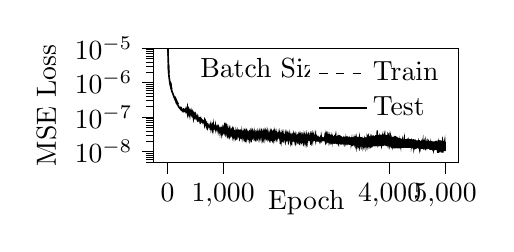
\begin{tikzpicture}

\begin{axis}[
legend cell align={left},
legend style={draw=none},
log basis y={10},
tick align=outside,
tick pos=left,
title={Batch Size 2},
title style={at={(0.4,0.85)},anchor=north},
x grid style={white!69.0196078431373!black},
xlabel={Epoch},
x label style={yshift=13pt},
xmin=-249.95, xmax=5248.95,
xtick style={color=black},
xtick = {0,1000,4000,5000},
y grid style={white!69.0196078431373!black},
ylabel={MSE Loss},
ymin=4.90143384155618e-09, ymax=1e-5,
ymode=log,
ytick style={color=black},
width=.45\textwidth,
height=.25\textwidth
]
\addplot [semithick, black, dashed]
table {%
0 0.00261398348659895
1 0.000146684363119675
2 7.82634508095725e-05
3 3.37719028447054e-05
4 2.5150746102085e-05
5 2.14879413085001e-05
6 1.73131360368757e-05
7 1.25710438198219e-05
8 8.384994563432e-06
9 6.01536302192685e-06
10 5.04094846438363e-06
11 4.50247262365266e-06
12 4.07342948584244e-06
13 3.68863333453007e-06
14 3.33568109506999e-06
15 3.02494765912797e-06
16 2.7562514826851e-06
17 2.52888349787028e-06
18 2.34137056487427e-06
19 2.18880018897138e-06
20 2.06381847633885e-06
21 1.96098151437774e-06
22 1.87465510770934e-06
23 1.80052594150659e-06
24 1.73351173886616e-06
25 1.67263015383323e-06
26 1.61614738892268e-06
27 1.56198234465066e-06
28 1.50867286552803e-06
29 1.46046563780544e-06
30 1.41356673157844e-06
31 1.37106688897681e-06
32 1.33059727563989e-06
33 1.28919083652868e-06
34 1.25175892679241e-06
35 1.21776896658865e-06
36 1.18564458267567e-06
37 1.15591732029952e-06
38 1.12700339668681e-06
39 1.10075354224648e-06
40 1.07587387876951e-06
41 1.05260377831939e-06
42 1.0313208120829e-06
43 1.01144230139827e-06
44 9.92442267119031e-07
45 9.7406527741839e-07
46 9.57213383753874e-07
47 9.40670659906218e-07
48 9.25038841827153e-07
49 9.10250043492766e-07
50 8.96198767826206e-07
51 8.83881172112133e-07
52 8.71137165300517e-07
53 8.58803400506147e-07
54 8.4801414614688e-07
55 8.36522416101104e-07
56 8.25851773152308e-07
57 8.15359453404163e-07
58 8.05294669189216e-07
59 7.95505481549164e-07
60 7.86104835461821e-07
61 7.76836224471111e-07
62 7.67232828448705e-07
63 7.40208569903089e-07
64 7.24697941538288e-07
65 7.12473284208315e-07
66 6.98334301669767e-07
67 6.8646508113801e-07
68 6.76835167410239e-07
69 6.67913647898644e-07
70 6.59476819643956e-07
71 6.51745536447201e-07
72 6.44344590145174e-07
73 6.37315424147467e-07
74 6.29807009134176e-07
75 6.23752871640626e-07
76 6.17110982172875e-07
77 6.10710473006648e-07
78 6.04971023602019e-07
79 5.99273899850594e-07
80 5.93674280890077e-07
81 5.88465108357639e-07
82 5.83262429605824e-07
83 5.78088403622168e-07
84 5.73076810137074e-07
85 5.68146300770955e-07
86 5.63457285606361e-07
87 5.59085755743816e-07
88 5.54764195544344e-07
89 5.50326957575287e-07
90 5.46110211153916e-07
91 5.41905436579171e-07
92 5.38032570275071e-07
93 5.33861362991495e-07
94 5.29962581785171e-07
95 5.25934999759059e-07
96 5.21953731732694e-07
97 5.17996030810153e-07
98 5.13999557568923e-07
99 5.10104440494707e-07
100 5.06136233847876e-07
101 5.02081006532151e-07
102 4.98216791648076e-07
103 4.94461015678738e-07
104 4.90604048617449e-07
105 4.86462815026734e-07
106 4.82587882216556e-07
107 4.78588768475063e-07
108 4.74869900535246e-07
109 4.7077929747541e-07
110 4.66663813166512e-07
111 4.62867599476446e-07
112 4.58659658813865e-07
113 4.54709814113663e-07
114 4.50870674558068e-07
115 4.46929221819659e-07
116 4.42388200826649e-07
117 4.38506839680386e-07
118 4.34678859113191e-07
119 4.3089226689208e-07
120 4.27085763439194e-07
121 4.23271578807061e-07
122 4.19777154811563e-07
123 4.15960641148239e-07
124 4.12074457444511e-07
125 4.08489014579239e-07
126 4.04658556217186e-07
127 4.00951681431394e-07
128 3.9733187562252e-07
129 3.93702260550022e-07
130 3.90062106880862e-07
131 3.86685338110482e-07
132 3.83489258807046e-07
133 3.79915736270497e-07
134 3.76464143924338e-07
135 3.73031685953151e-07
136 3.69614877314461e-07
137 3.66566005281399e-07
138 3.63254276162017e-07
139 3.59711858066269e-07
140 3.56280412384891e-07
141 3.52569088435395e-07
142 3.49126307100711e-07
143 3.45766744868303e-07
144 3.42371599904911e-07
145 3.39262808538354e-07
146 3.36348832967737e-07
147 3.33401700036262e-07
148 3.30368856395147e-07
149 3.2688863233421e-07
150 3.24198848596247e-07
151 3.21372436439926e-07
152 3.17807970312778e-07
153 3.15233077704757e-07
154 3.12444794476452e-07
155 3.10027523902079e-07
156 3.07321188873999e-07
157 3.04717508505359e-07
158 3.02148876103026e-07
159 2.99573802886144e-07
160 2.96987011524585e-07
161 2.94648659848296e-07
162 2.92419047800419e-07
163 2.90140671955541e-07
164 2.88099955823906e-07
165 2.8558504167453e-07
166 2.83444139733025e-07
167 2.8141647362645e-07
168 2.79245677041295e-07
169 2.77200937237154e-07
170 2.75588299680773e-07
171 2.73590638562027e-07
172 2.71654279449418e-07
173 2.69519297966259e-07
174 2.67458664513498e-07
175 2.65497534967629e-07
176 2.63673217523852e-07
177 2.61948017285185e-07
178 2.60005301479183e-07
179 2.58152771367648e-07
180 2.56357327418133e-07
181 2.54637377330891e-07
182 2.5292912211583e-07
183 2.51359738450141e-07
184 2.49551562201411e-07
185 2.48045789688955e-07
186 2.46444842606497e-07
187 2.4465752219438e-07
188 2.43001887576533e-07
189 2.41387644265956e-07
190 2.39743852080032e-07
191 2.38591042211134e-07
192 2.36896491812466e-07
193 2.35331076664291e-07
194 2.33869138022147e-07
195 2.32390313131603e-07
196 2.30942950676827e-07
197 2.29478455254561e-07
198 2.28119508614011e-07
199 2.26882294488195e-07
200 2.25635528665613e-07
201 2.24384542468314e-07
202 2.23268744437011e-07
203 2.21910245763457e-07
204 2.20867471478314e-07
205 2.19511795347405e-07
206 2.18217545115529e-07
207 2.17078903803181e-07
208 2.15910442586509e-07
209 2.14819290250023e-07
210 2.1386440760951e-07
211 2.12621667512458e-07
212 2.11595954674237e-07
213 2.10598725390199e-07
214 2.09534008213996e-07
215 2.08534801116933e-07
216 2.07571893242164e-07
217 2.06601709264564e-07
218 2.05631415472141e-07
219 2.04732785008765e-07
220 2.03928731128844e-07
221 2.02986788394366e-07
222 2.02125836123557e-07
223 2.01693005556169e-07
224 2.00247696379385e-07
225 1.99351367456746e-07
226 1.9847183270949e-07
227 1.97567987980651e-07
228 1.96726100124334e-07
229 1.95874223668291e-07
230 1.95032362352077e-07
231 1.9429453191222e-07
232 1.93577463155847e-07
233 1.92833159978534e-07
234 1.91930465522017e-07
235 1.91151176648585e-07
236 1.90727425620985e-07
237 1.89940357579133e-07
238 1.89282947241409e-07
239 1.88559956265433e-07
240 1.87832262899867e-07
241 1.87312221969105e-07
242 1.8638003640481e-07
243 1.85629820950606e-07
244 1.84861143206927e-07
245 1.84173773354779e-07
246 1.8346385132828e-07
247 1.82691622820474e-07
248 1.81981703223588e-07
249 1.81241538350196e-07
250 1.80819522359599e-07
251 1.80233316547929e-07
252 1.79373761339141e-07
253 1.78795408649846e-07
254 1.78261502097099e-07
255 1.77732386884122e-07
256 1.77024827346939e-07
257 1.76212229890949e-07
258 1.75559959624039e-07
259 1.75028014774092e-07
260 1.74455442444987e-07
261 1.73865569054188e-07
262 1.73293729991419e-07
263 1.72699000502652e-07
264 1.72175157529209e-07
265 1.71600795157545e-07
266 1.71060159445346e-07
267 1.70516953865052e-07
268 1.69965971575703e-07
269 1.69306111652556e-07
270 1.68603019955915e-07
271 1.68096036264442e-07
272 1.67533045300372e-07
273 1.67098511944852e-07
274 1.66452356481939e-07
275 1.6594090199118e-07
276 1.65430003029599e-07
277 1.6504094741765e-07
278 1.64535466716353e-07
279 1.64067817844948e-07
280 1.63518295869691e-07
281 1.63008348729843e-07
282 1.62516949801628e-07
283 1.62122773014195e-07
284 1.61727112577337e-07
285 1.61419068025026e-07
286 1.60981843060126e-07
287 1.60612840249152e-07
288 1.60113057938505e-07
289 1.59996616506453e-07
290 1.59500434703475e-07
291 1.59041253554371e-07
292 1.58633176553291e-07
293 1.58230017347494e-07
294 1.57726207859366e-07
295 1.57391601654178e-07
296 1.56932869004311e-07
297 1.56524124702795e-07
298 1.56090241693274e-07
299 1.55728700207858e-07
300 1.55397476291563e-07
301 1.54913462214301e-07
302 1.54460410595414e-07
303 1.54037259622264e-07
304 1.53807496733549e-07
305 1.53307295429617e-07
306 1.52889717186522e-07
307 1.52815606427659e-07
308 1.5255875534792e-07
309 1.51992299653791e-07
310 1.51631543023223e-07
311 1.51434879765988e-07
312 1.50798544854336e-07
313 1.50500502398065e-07
314 1.50309462715548e-07
315 1.5012875835807e-07
316 1.49606689905601e-07
317 1.49262755533508e-07
318 1.489406507591e-07
319 1.48563328749907e-07
320 1.48307872039899e-07
321 1.47996224146629e-07
322 1.47477975280585e-07
323 1.46864158302451e-07
324 1.46399182789247e-07
325 1.4600326030334e-07
326 1.45447961132694e-07
327 1.45286996641181e-07
328 1.45124027577159e-07
329 1.4457256800382e-07
330 1.44243595714633e-07
331 1.43893380800231e-07
332 1.43401146519118e-07
333 1.43232647254354e-07
334 1.42721284159375e-07
335 1.42463075213817e-07
336 1.42195513040511e-07
337 1.41774924736993e-07
338 1.41613115455463e-07
339 1.41290982773601e-07
340 1.40814341321294e-07
341 1.40588078612947e-07
342 1.40190531043416e-07
343 1.39982248199333e-07
344 1.39655671995254e-07
345 1.39315308924859e-07
346 1.39008234261606e-07
347 1.38621841989428e-07
348 1.38385781822015e-07
349 1.38106749037359e-07
350 1.37768745258837e-07
351 1.37302368972358e-07
352 1.37273293095319e-07
353 1.36685038603535e-07
354 1.36805641671289e-07
355 1.36218938038724e-07
356 1.36174170560555e-07
357 1.35144350333238e-07
358 1.35377791940172e-07
359 1.3519789696903e-07
360 1.34321391878522e-07
361 1.34628653254643e-07
362 1.34382502061214e-07
363 1.33540979393221e-07
364 1.33748807011447e-07
365 1.33484170640186e-07
366 1.32627974005484e-07
367 1.3297263567158e-07
368 1.32693508702708e-07
369 1.32514474537659e-07
370 1.32011076459548e-07
371 1.31861206790651e-07
372 1.31521757749109e-07
373 1.31331652518663e-07
374 1.31312317972254e-07
375 1.30603197236123e-07
376 1.30561156867826e-07
377 1.29773564399915e-07
378 1.30057639510683e-07
379 1.29861310177226e-07
380 1.29112238212326e-07
381 1.29198381696227e-07
382 1.28842748736258e-07
383 1.2872677043152e-07
384 1.2815145879741e-07
385 1.28243387647053e-07
386 1.28023895214824e-07
387 1.27487541142557e-07
388 1.27568656234978e-07
389 1.27031404781208e-07
390 1.27159839126145e-07
391 1.26598800443301e-07
392 1.26791784661684e-07
393 1.26477510927092e-07
394 1.26444590979657e-07
395 1.26158001562349e-07
396 1.25962107867528e-07
397 1.25775401044637e-07
398 1.25593913733013e-07
399 1.24813759142306e-07
400 1.25107088592591e-07
401 1.24789898830358e-07
402 1.24521163066271e-07
403 1.24255962218545e-07
404 1.24277898207348e-07
405 1.23580057124872e-07
406 1.23692217324445e-07
407 1.23466668605632e-07
408 1.23292362624872e-07
409 1.23125864866624e-07
410 1.22844255137977e-07
411 1.22260624106474e-07
412 1.22632293348746e-07
413 1.22149892797907e-07
414 1.21888570189244e-07
415 1.2183269884436e-07
416 1.21501794058565e-07
417 1.21598056354921e-07
418 1.21115364892788e-07
419 1.20845609222542e-07
420 1.20702182457633e-07
421 1.20670180585147e-07
422 1.20313101976244e-07
423 1.20242447746888e-07
424 1.19796707906294e-07
425 1.19679437805553e-07
426 1.19502443590935e-07
427 1.19306255657259e-07
428 1.19001857039169e-07
429 1.18975247541897e-07
430 1.18751168056708e-07
431 1.18668970422453e-07
432 1.18519750465174e-07
433 1.18310549850564e-07
434 1.18205436012264e-07
435 1.18052298470728e-07
436 1.17879357376394e-07
437 1.17379495784053e-07
438 1.17300958525135e-07
439 1.17437472770154e-07
440 1.17254779579357e-07
441 1.16698817170358e-07
442 1.1665886642831e-07
443 1.16422076178457e-07
444 1.16437312810413e-07
445 1.16211605543537e-07
446 1.15907504869339e-07
447 1.15631951317585e-07
448 1.15533178603799e-07
449 1.1553922251073e-07
450 1.15184505566468e-07
451 1.15018143974188e-07
452 1.15032055581388e-07
453 1.14700197587414e-07
454 1.14470164584324e-07
455 1.14392085056592e-07
456 1.14392627027948e-07
457 1.13851511679419e-07
458 1.13809522381825e-07
459 1.13363633469143e-07
460 1.13507051060058e-07
461 1.12955144015325e-07
462 1.12687809270984e-07
463 1.12958656940165e-07
464 1.12561146591084e-07
465 1.1211510408593e-07
466 1.11795333277431e-07
467 1.11874699544767e-07
468 1.11499599053211e-07
469 1.11183911756685e-07
470 1.1097315462405e-07
471 1.10746568335651e-07
472 1.10528108287378e-07
473 1.10256356484095e-07
474 1.10099632397498e-07
475 1.09766951710499e-07
476 1.09138375835371e-07
477 1.08834864133156e-07
478 1.0881889858938e-07
479 1.08393336007095e-07
480 1.08144232992657e-07
481 1.0793406884968e-07
482 1.07731355728502e-07
483 1.07404242227993e-07
484 1.07224436205255e-07
485 1.06623043470755e-07
486 1.06600979004057e-07
487 1.06223428439911e-07
488 1.06042661533579e-07
489 1.05791827745172e-07
490 1.05572618482874e-07
491 1.05332027782401e-07
492 1.05210153051427e-07
493 1.04844322206032e-07
494 1.04628191569089e-07
495 1.04377984629922e-07
496 1.04216347538877e-07
497 1.03955194479699e-07
498 1.03688604859542e-07
499 1.03510769820403e-07
500 1.03342628648528e-07
501 1.03084363703987e-07
502 1.0284133121341e-07
503 1.02668651758897e-07
504 1.02572349458985e-07
505 1.02124076692522e-07
506 1.01995372278507e-07
507 1.01731550677941e-07
508 1.01490412855565e-07
509 1.01381675744916e-07
510 1.01240593376462e-07
511 1.00909068223354e-07
512 1.00669337769643e-07
513 1.00404250107822e-07
514 1.00423404139294e-07
515 1.00214220461581e-07
516 9.99527497607122e-08
517 9.97062718719466e-08
518 9.94624701242675e-08
519 9.93852768302883e-08
520 9.90874772937023e-08
521 9.88455424544288e-08
522 9.86786483039293e-08
523 9.85174300247582e-08
524 9.83541504726571e-08
525 9.82658134411896e-08
526 9.78364765480411e-08
527 9.77660970995498e-08
528 9.7614606940466e-08
529 9.7288654843819e-08
530 9.69792118370449e-08
531 9.69268959594149e-08
532 9.67892044398955e-08
533 9.64910404850361e-08
534 9.62170009874974e-08
535 9.62202412035929e-08
536 9.58558749346583e-08
537 9.56776447187391e-08
538 9.5498134587757e-08
539 9.53894120798715e-08
540 9.50934551380289e-08
541 9.48801197169224e-08
542 9.46125329708281e-08
543 9.44436887060363e-08
544 9.4335708752169e-08
545 9.40767704953327e-08
546 9.38061104351906e-08
547 9.36843962597855e-08
548 9.34865146009489e-08
549 9.32645453668446e-08
550 9.30323500869523e-08
551 9.2910364995813e-08
552 9.24915208440069e-08
553 9.26237489684567e-08
554 9.20383658806756e-08
555 9.20737594465315e-08
556 9.1773045729715e-08
557 9.15990957992552e-08
558 9.16372675546784e-08
559 9.13390870608266e-08
560 9.12179028298432e-08
561 9.10503901381254e-08
562 9.07964728142918e-08
563 9.05843692435848e-08
564 9.03890795960205e-08
565 9.00719094163449e-08
566 8.99008989017069e-08
567 8.98419131223349e-08
568 8.94903660499935e-08
569 8.92771059846087e-08
570 8.92133772965043e-08
571 8.92505096738994e-08
572 8.88596866948088e-08
573 8.88809712964456e-08
574 8.85358828333072e-08
575 8.83346679561026e-08
576 8.84105503005106e-08
577 8.8131889763865e-08
578 8.80912545679902e-08
579 8.76220811723005e-08
580 8.76374261120638e-08
581 8.73306817090747e-08
582 8.69455808030217e-08
583 8.70990354120416e-08
584 8.65921273616177e-08
585 8.64360111918483e-08
586 8.64471381185616e-08
587 8.61044444553372e-08
588 8.59900289835735e-08
589 8.59733905260729e-08
590 8.56495371353017e-08
591 8.5448452592729e-08
592 8.52556495878343e-08
593 8.50720472700406e-08
594 8.48990268551564e-08
595 8.46750809213592e-08
596 8.45080046549818e-08
597 8.42445121276292e-08
598 8.40143372828894e-08
599 8.37218631160042e-08
600 8.35349402392716e-08
601 8.31654908488577e-08
602 8.30242949245719e-08
603 8.2982439593593e-08
604 8.2921621885168e-08
605 8.26500533532837e-08
606 8.25823081787025e-08
607 8.2389301115926e-08
608 8.22421491531999e-08
609 8.19840703343289e-08
610 8.1801761944611e-08
611 8.18592255097395e-08
612 8.16676565214003e-08
613 8.16171640491969e-08
614 8.13247282057672e-08
615 8.10373738009407e-08
616 8.08642084723088e-08
617 8.06555648807938e-08
618 8.039214622102e-08
619 8.02460349925704e-08
620 8.00810798282647e-08
621 7.99409526959227e-08
622 7.97110490066144e-08
623 7.94116076875406e-08
624 7.92543457824868e-08
625 7.90482818721072e-08
626 7.87830216444352e-08
627 7.86491988641336e-08
628 7.84446622161816e-08
629 7.827243654146e-08
630 7.81483883874889e-08
631 7.79432979882699e-08
632 7.77564276402964e-08
633 7.75270853509147e-08
634 7.74125279346949e-08
635 7.70996542881486e-08
636 7.70233436728773e-08
637 7.66381009270622e-08
638 7.64740521639329e-08
639 7.66816242462332e-08
640 7.64246416755654e-08
641 7.61894967465926e-08
642 7.59976832137577e-08
643 7.56666841013054e-08
644 7.54723867576468e-08
645 7.54306852314146e-08
646 7.53268538478125e-08
647 7.51730338366396e-08
648 7.47495809915177e-08
649 7.48541830168925e-08
650 7.43791588843079e-08
651 7.42978026984087e-08
652 7.42460074155682e-08
653 7.40438198457705e-08
654 7.3634554738522e-08
655 7.37113431152903e-08
656 7.34467651670734e-08
657 7.33724932918678e-08
658 7.31816905603644e-08
659 7.31439444945359e-08
660 7.28667297711372e-08
661 7.26887656533615e-08
662 7.25385389976907e-08
663 7.24498825926956e-08
664 7.22832119443018e-08
665 7.21822083353807e-08
666 7.19495448092688e-08
667 7.18707898982318e-08
668 7.16480042597389e-08
669 7.14073806823423e-08
670 7.13205865152666e-08
671 7.10196900129967e-08
672 7.09722795270151e-08
673 7.07187652627672e-08
674 7.06024032132158e-08
675 7.05165593821722e-08
676 7.03380461603009e-08
677 7.03425385415457e-08
678 7.00737257445239e-08
679 6.99320477606236e-08
680 6.97025158427067e-08
681 6.95539946653501e-08
682 6.93178849876519e-08
683 6.94211070342288e-08
684 6.90671745279259e-08
685 6.8847339870004e-08
686 6.89086112218851e-08
687 6.87327516597502e-08
688 6.84967959185823e-08
689 6.84914813144921e-08
690 6.84173265950161e-08
691 6.81482263986677e-08
692 6.79657498626751e-08
693 6.76911481836129e-08
694 6.78754415739391e-08
695 6.76873341790563e-08
696 6.7420077696112e-08
697 6.73318192355721e-08
698 6.71849346519648e-08
699 6.70631731659599e-08
700 6.6936109860527e-08
701 6.67347293343834e-08
702 6.66230708357141e-08
703 6.67056503975694e-08
704 6.66208884274599e-08
705 6.6402336841076e-08
706 6.637572022683e-08
707 6.60298795550629e-08
708 6.58703416722695e-08
709 6.59932807797192e-08
710 6.57574264092409e-08
711 6.5755870203299e-08
712 6.55362282209193e-08
713 6.54728074114264e-08
714 6.5351697348004e-08
715 6.53087951680842e-08
716 6.51708659051842e-08
717 6.50125667877033e-08
718 6.49798564733572e-08
719 6.47724273014072e-08
720 6.47707329970437e-08
721 6.45535312721046e-08
722 6.44558372296933e-08
723 6.43093136186712e-08
724 6.406546154758e-08
725 6.40719362525743e-08
726 6.45583160179264e-08
727 6.38616268305858e-08
728 6.39997100977396e-08
729 6.38944717001877e-08
730 6.37970664736365e-08
731 6.36738414186988e-08
732 6.35405101436781e-08
733 6.3468621691154e-08
734 6.31237134999241e-08
735 6.32146194542438e-08
736 6.31069264531714e-08
737 6.30518270504643e-08
738 6.29606186937082e-08
739 6.26848402600633e-08
740 6.28600875853813e-08
741 6.26476349310234e-08
742 6.24892591627457e-08
743 6.24455489549591e-08
744 6.23294498194316e-08
745 6.2253770162779e-08
746 6.21718271596183e-08
747 6.20670583866279e-08
748 6.18798210956228e-08
749 6.188538615437e-08
750 6.18037680910621e-08
751 6.16810066836893e-08
752 6.15384937397989e-08
753 6.14532277937174e-08
754 6.1445070853372e-08
755 6.13365998902715e-08
756 6.12798440569051e-08
757 6.13104954930721e-08
758 6.12681508648238e-08
759 6.10669092498961e-08
760 6.10586326349472e-08
761 6.09786342657959e-08
762 6.08765920058207e-08
763 6.07757833117617e-08
764 6.07843563827926e-08
765 6.05380540213973e-08
766 6.04225618350274e-08
767 6.03992417815835e-08
768 6.03464287243227e-08
769 6.01462231776262e-08
770 6.00604040950081e-08
771 6.00231084527669e-08
772 5.99093010943408e-08
773 5.98377934263317e-08
774 5.96081898500689e-08
775 5.95742457141224e-08
776 5.96780586127332e-08
777 5.93245081615956e-08
778 5.91501711765252e-08
779 5.92791223117395e-08
780 5.91412333191821e-08
781 5.90747720404794e-08
782 5.89476858179339e-08
783 5.88208731741036e-08
784 5.88255402458326e-08
785 5.8786889870488e-08
786 5.86065183543205e-08
787 5.86318991023793e-08
788 5.8584062483602e-08
789 5.84684124078638e-08
790 5.85145645294327e-08
791 5.82407579362565e-08
792 5.82223076095456e-08
793 5.79912457159271e-08
794 5.8108856008543e-08
795 5.79709602686052e-08
796 5.78531142740868e-08
797 5.78370420644125e-08
798 5.76913316553407e-08
799 5.76839951780261e-08
800 5.75831435745133e-08
801 5.75909274685982e-08
802 5.74083612785437e-08
803 5.74391697699683e-08
804 5.72027329296398e-08
805 5.73407223503075e-08
806 5.72023227312091e-08
807 5.70735137997991e-08
808 5.70729130350278e-08
809 5.69626252675537e-08
810 5.6882644279832e-08
811 5.68058462963039e-08
812 5.66683241300936e-08
813 5.66744659303842e-08
814 5.65901798542656e-08
815 5.6436309426422e-08
816 5.65831056307253e-08
817 5.63878848396371e-08
818 5.62771926944095e-08
819 5.62657206842898e-08
820 5.62157826032861e-08
821 5.61009023639647e-08
822 5.60516779550824e-08
823 5.59690822986569e-08
824 5.61079724488156e-08
825 5.58611277436949e-08
826 5.57958161638838e-08
827 5.57157521758889e-08
828 5.56878466763111e-08
829 5.57414290146552e-08
830 5.54114399603511e-08
831 5.54050776053749e-08
832 5.54322031087739e-08
833 5.54243826426104e-08
834 5.53643694637396e-08
835 5.51954801198962e-08
836 5.53016565781883e-08
837 5.52197657462949e-08
838 5.50475004045259e-08
839 5.50929451459403e-08
840 5.49398851192873e-08
841 5.50032194527317e-08
842 5.49059920349482e-08
843 5.48543149434533e-08
844 5.47220845609209e-08
845 5.45919308593268e-08
846 5.46621458888952e-08
847 5.45036415513511e-08
848 5.44871118437484e-08
849 5.44909918462899e-08
850 5.44362895656958e-08
851 5.42284673225035e-08
852 5.43319143780918e-08
853 5.42738582536284e-08
854 5.39490024304978e-08
855 5.41623808413272e-08
856 5.38711755492249e-08
857 5.38292376828231e-08
858 5.38144721166089e-08
859 5.40801493253973e-08
860 5.35556771573686e-08
861 5.34009007191472e-08
862 5.36913170899878e-08
863 5.35750088621612e-08
864 5.34702983183699e-08
865 5.31324628701979e-08
866 5.32663798854527e-08
867 5.34713005498899e-08
868 5.3268240315818e-08
869 5.3106281430626e-08
870 5.30999553991496e-08
871 5.30073745623749e-08
872 5.3024831385029e-08
873 5.29475644116539e-08
874 5.29035295295799e-08
875 5.27633898719237e-08
876 5.27644872644339e-08
877 5.26363374481198e-08
878 5.21344579949012e-08
879 5.26222953115552e-08
880 5.25046283263997e-08
881 5.25887310142137e-08
882 5.23786171260365e-08
883 5.22556745392588e-08
884 5.22890715103364e-08
885 5.22051752521735e-08
886 5.22562960395545e-08
887 5.21403642420593e-08
888 5.21259177299616e-08
889 5.23303570957312e-08
890 5.21940686630806e-08
891 5.20369648042696e-08
892 5.18643744533698e-08
893 5.1959078596342e-08
894 5.1800517703815e-08
895 5.17839124822839e-08
896 5.1749980221838e-08
897 5.20235737372365e-08
898 5.14930678036096e-08
899 5.13947631269884e-08
900 5.14576784906851e-08
901 5.15045462358144e-08
902 5.14380473438658e-08
903 5.14084751558341e-08
904 5.13051172055246e-08
905 5.13162940889433e-08
906 5.12426185311776e-08
907 5.11894807858626e-08
908 5.12040236309019e-08
909 5.11771593126875e-08
910 5.1391161834613e-08
911 5.09132827229974e-08
912 5.07956156252654e-08
913 5.07086769411247e-08
914 5.07240060290126e-08
915 5.05156226283665e-08
916 5.09034994145008e-08
917 5.10812179872477e-08
918 5.09299017443787e-08
919 5.06071179470213e-08
920 5.06153786566932e-08
921 5.08228125277732e-08
922 5.07701664046456e-08
923 5.04631669587807e-08
924 5.04625080791632e-08
925 5.03999359618978e-08
926 5.03120141140956e-08
927 5.02950299255955e-08
928 5.02036412520779e-08
929 5.05533185670704e-08
930 5.03805240215094e-08
931 5.03134604930011e-08
932 5.03399029133655e-08
933 5.02495765224431e-08
934 5.02485439819456e-08
935 5.01097002670869e-08
936 4.98450323295208e-08
937 5.00081839931443e-08
938 5.02201354417586e-08
939 5.00173292057315e-08
940 4.99454150872936e-08
941 4.98917330522541e-08
942 4.97869760859304e-08
943 4.96477238839388e-08
944 4.96061485512067e-08
945 4.96272340385628e-08
946 4.96270244700892e-08
947 4.96611786039436e-08
948 4.93043708666985e-08
949 4.93675331766363e-08
950 4.94701070694603e-08
951 4.95901512781449e-08
952 4.95660200040549e-08
953 4.93224323655506e-08
954 4.91889253581013e-08
955 4.92657079411152e-08
956 4.93090457755474e-08
957 4.90304114769136e-08
958 4.86113878614414e-08
959 4.87386970814407e-08
960 4.86080396257527e-08
961 4.91473815086851e-08
962 4.82496446461145e-08
963 4.8349681513904e-08
964 4.83994517888053e-08
965 4.84674849848266e-08
966 4.89019669674406e-08
967 4.87339815461452e-08
968 4.8887384868801e-08
969 4.86750621041532e-08
970 4.87458362598003e-08
971 4.87206623641101e-08
972 4.85998083747385e-08
973 4.86616961933861e-08
974 4.85624361134529e-08
975 4.85805682470253e-08
976 4.85125720613433e-08
977 4.82887160206391e-08
978 4.84719224294605e-08
979 4.83484899962972e-08
980 4.82735046126725e-08
981 4.84206677583976e-08
982 4.82095535099814e-08
983 4.81738937898046e-08
984 4.81529513432499e-08
985 4.80463511752238e-08
986 4.8008118166909e-08
987 4.78388747605085e-08
988 4.79545476203547e-08
989 4.77904276480756e-08
990 4.76947455610444e-08
991 4.7953770904885e-08
992 4.75322841403392e-08
993 4.7785734386907e-08
994 4.75348239130091e-08
995 4.7667171884147e-08
996 4.74739370615596e-08
997 4.75618149212709e-08
998 4.75811124144854e-08
999 4.74248252290144e-08
1000 4.76309443844802e-08
1001 4.72376396284391e-08
1002 4.71671802128038e-08
1003 4.74440110288521e-08
1004 4.69942068811458e-08
1005 4.71157604259309e-08
1006 4.69819341240574e-08
1007 4.69522687752133e-08
1008 4.68813971180038e-08
1009 4.66572676727783e-08
1010 4.68712826183215e-08
1011 4.65230975445485e-08
1012 4.6986280031025e-08
1013 4.65285257113535e-08
1014 4.65172853401641e-08
1015 4.69000739997116e-08
1016 4.59802069521786e-08
1017 4.61438803179282e-08
1018 4.61487103370906e-08
1019 4.60385496252047e-08
1020 4.60279651077755e-08
1021 4.5991702721071e-08
1022 4.6049907213741e-08
1023 4.58232247232404e-08
1024 4.575472711843e-08
1025 4.57867423995784e-08
1026 4.57194202890809e-08
1027 4.5735625373744e-08
1028 4.56614160241897e-08
1029 4.57159697072051e-08
1030 4.55817242379086e-08
1031 4.55687318516862e-08
1032 4.55431716767651e-08
1033 4.54868766998073e-08
1034 4.54809728112071e-08
1035 4.53985480052266e-08
1036 4.5422408025686e-08
1037 4.52892244754421e-08
1038 4.52831030046119e-08
1039 4.53999871000699e-08
1040 4.54181504337958e-08
1041 4.52862972734613e-08
1042 4.51580050345179e-08
1043 4.51480138310423e-08
1044 4.51643003261393e-08
1045 4.51240597721392e-08
1046 4.49955824772252e-08
1047 4.50499606158838e-08
1048 4.50189186058103e-08
1049 4.50657565729817e-08
1050 4.4959013388024e-08
1051 4.48627814274016e-08
1052 4.48606086906889e-08
1053 4.4802549736378e-08
1054 4.48229560718882e-08
1055 4.48897614062638e-08
1056 4.47645272669828e-08
1057 4.46646057877254e-08
1058 4.47493429872603e-08
1059 4.46290876262023e-08
1060 4.47393384138683e-08
1061 4.44872028639853e-08
1062 4.46542057774835e-08
1063 4.44682002784802e-08
1064 4.45064564659758e-08
1065 4.45753047110253e-08
1066 4.4414909836088e-08
1067 4.44585654978957e-08
1068 4.43124520668192e-08
1069 4.43833488869561e-08
1070 4.4300507340167e-08
1071 4.42940364882016e-08
1072 4.42912890031288e-08
1073 4.43040135522099e-08
1074 4.42048048830967e-08
1075 4.416254044598e-08
1076 4.41335653407759e-08
1077 4.40365813249022e-08
1078 4.41081502742802e-08
1079 4.40969820470483e-08
1080 4.3948786994652e-08
1081 4.41720446373584e-08
1082 4.39464986777271e-08
1083 4.40942140758627e-08
1084 4.37837767735538e-08
1085 4.39278263835718e-08
1086 4.37930967392974e-08
1087 4.37182112345003e-08
1088 4.37573598288665e-08
1089 4.37867421974048e-08
1090 4.36447713969557e-08
1091 4.38515382742977e-08
1092 4.37362916652084e-08
1093 4.36174015362445e-08
1094 4.3778218633217e-08
1095 4.35680120209891e-08
1096 4.35805192225414e-08
1097 4.36738350335086e-08
1098 4.36676859579821e-08
1099 4.35005779383379e-08
1100 4.35071349083049e-08
1101 4.35172271734396e-08
1102 4.34009853089168e-08
1103 4.33678863978049e-08
1104 4.33504221901138e-08
1105 4.32441569210851e-08
1106 4.3280685350644e-08
1107 4.34523939446541e-08
1108 4.32948200780325e-08
1109 4.31160244203088e-08
1110 4.31606878995017e-08
1111 4.31132841002824e-08
1112 4.31126667642112e-08
1113 4.30161841746823e-08
1114 4.31351706885463e-08
1115 4.30137107217399e-08
1116 4.30419452301378e-08
1117 4.28521687167449e-08
1118 4.29494802055563e-08
1119 4.2983084970083e-08
1120 4.28279311986968e-08
1121 4.29285861436868e-08
1122 4.28456561525348e-08
1123 4.29562623107116e-08
1124 4.28213921451759e-08
1125 4.27720357785155e-08
1126 4.27197061031448e-08
1127 4.27676665794574e-08
1128 4.27508851308933e-08
1129 4.2682300908925e-08
1130 4.26003897978089e-08
1131 4.24758110147416e-08
1132 4.25463953803162e-08
1133 4.25152052525024e-08
1134 4.25598208884104e-08
1135 4.239308792503e-08
1136 4.2449155177704e-08
1137 4.24381763784454e-08
1138 4.24335556179489e-08
1139 4.23089017043132e-08
1140 4.23211221574071e-08
1141 4.22933782630586e-08
1142 4.23067300873714e-08
1143 4.23677056163863e-08
1144 4.23486314717891e-08
1145 4.19986635529779e-08
1146 4.20469467001805e-08
1147 4.22094996923028e-08
1148 4.20193057089624e-08
1149 4.21166019328179e-08
1150 4.21501204259656e-08
1151 4.19883999723814e-08
1152 4.20073089106854e-08
1153 4.18943582077835e-08
1154 4.19936113004726e-08
1155 4.20366788216886e-08
1156 4.20818990342631e-08
1157 4.18583599697264e-08
1158 4.17444217319929e-08
1159 4.17618667362674e-08
1160 4.17829855202667e-08
1161 4.17799846383904e-08
1162 4.16705735562517e-08
1163 4.18948547789011e-08
1164 4.16620335019213e-08
1165 4.17125577941713e-08
1166 4.15728996195353e-08
1167 4.16248975123046e-08
1168 4.17766256601282e-08
1169 4.14573240685168e-08
1170 4.15731547034337e-08
1171 4.14832258551212e-08
1172 4.14894388031661e-08
1173 4.17455580651316e-08
1174 4.15013680700738e-08
1175 4.15968621256257e-08
1176 4.13717257054524e-08
1177 4.15543938007135e-08
1178 4.12514978142542e-08
1179 4.14077720277683e-08
1180 4.15308862883323e-08
1181 4.13152643243264e-08
1182 4.13804941682416e-08
1183 4.13969383722401e-08
1184 4.13074685233217e-08
1185 4.14006716444315e-08
1186 4.12031826499959e-08
1187 4.13484403469777e-08
1188 4.11279918449137e-08
1189 4.1116992403778e-08
1190 4.10200866945987e-08
1191 4.10916682780371e-08
1192 4.10232857664949e-08
1193 4.11754650986307e-08
1194 4.08613160786109e-08
1195 4.10294067033634e-08
1196 4.11262635822141e-08
1197 4.09699648660222e-08
1198 4.09178326050697e-08
1199 4.08179365538608e-08
1200 4.08433911486261e-08
1201 4.07925646619955e-08
1202 4.0843865591389e-08
1203 4.08273227012201e-08
1204 4.08248592192462e-08
1205 4.09464814088434e-08
1206 4.07076831734909e-08
1207 4.06216350464228e-08
1208 4.05717194499888e-08
1209 4.07536141571185e-08
1210 4.06037834261297e-08
1211 4.05800763356723e-08
1212 4.05475472338157e-08
1213 4.05940800142779e-08
1214 4.07310513145798e-08
1215 4.0481364380951e-08
1216 4.05854570876274e-08
1217 4.0419865971697e-08
1218 4.04724098932996e-08
1219 4.03760262344677e-08
1220 4.05545208236879e-08
1221 4.04062817561668e-08
1222 4.04085032262302e-08
1223 4.0206302078627e-08
1224 4.02853182185359e-08
1225 4.02691618917039e-08
1226 4.02556384009323e-08
1227 3.99654077228306e-08
1228 4.0084840536081e-08
1229 3.99519415278937e-08
1230 3.99425685834176e-08
1231 3.99511088683413e-08
1232 3.99962168105006e-08
1233 3.98757909992886e-08
1234 3.99903259502565e-08
1235 3.97727424241157e-08
1236 3.97362323014128e-08
1237 3.98615986861861e-08
1238 3.97920895919279e-08
1239 3.96503417985916e-08
1240 3.98500998187723e-08
1241 3.94888271154081e-08
1242 3.97363479529567e-08
1243 3.9670114947099e-08
1244 3.95152142287913e-08
1245 3.94588912658311e-08
1246 3.96170589693212e-08
1247 3.95713690846677e-08
1248 3.9653338033907e-08
1249 3.96299430795444e-08
1250 3.93851973877202e-08
1251 3.95682592178592e-08
1252 3.94245985052555e-08
1253 3.94186836629173e-08
1254 3.93995191990681e-08
1255 3.94417245035417e-08
1256 3.93175576240967e-08
1257 3.93010308639696e-08
1258 3.94500662774244e-08
1259 3.92660184653781e-08
1260 3.91611785369173e-08
1261 3.93277218297405e-08
1262 3.90468253679832e-08
1263 3.92391634491673e-08
1264 3.90210088450083e-08
1265 3.90619693654837e-08
1266 3.91635332250839e-08
1267 3.91998140386596e-08
1268 3.88992044481062e-08
1269 3.92167338549299e-08
1270 3.88048741853941e-08
1271 3.90122393857384e-08
1272 3.90509703188657e-08
1273 3.89146043306421e-08
1274 3.89563392785841e-08
1275 3.89260859701701e-08
1276 3.90563198613969e-08
1277 3.903581282938e-08
1278 3.87682184300187e-08
1279 3.90418795276903e-08
1280 3.88307571365099e-08
1281 3.88432197571675e-08
1282 3.88089232857825e-08
1283 3.88497545305011e-08
1284 3.8808237176613e-08
1285 3.86636885413849e-08
1286 3.8951220149408e-08
1287 3.87320291024285e-08
1288 3.86920816649039e-08
1289 3.8919329096998e-08
1290 3.86722198195133e-08
1291 3.86278853801714e-08
1292 3.88914554788622e-08
1293 3.8599475284451e-08
1294 3.8693181822369e-08
1295 3.85323008162963e-08
1296 3.85450245753982e-08
1297 3.8618123346601e-08
1298 3.86272235451401e-08
1299 3.85501028578594e-08
1300 3.85360730471018e-08
1301 3.84817750264665e-08
1302 3.83798020365811e-08
1303 3.84028968161143e-08
1304 3.83411669929168e-08
1305 3.86072583850039e-08
1306 3.83613074982914e-08
1307 3.8552181814977e-08
1308 3.82130065704755e-08
1309 3.80664171260592e-08
1310 3.84765729979919e-08
1311 3.81774920919509e-08
1312 3.82775483957487e-08
1313 3.83419538739216e-08
1314 3.82416022891574e-08
1315 3.81589909581037e-08
1316 3.84554827882466e-08
1317 3.81900211631758e-08
1318 3.80497460764073e-08
1319 3.80913908638036e-08
1320 3.79748055899243e-08
1321 3.82118173543611e-08
1322 3.8044942906712e-08
1323 3.7897786287433e-08
1324 3.80364340222261e-08
1325 3.80164513292258e-08
1326 3.80070932131105e-08
1327 3.77907139890721e-08
1328 3.79741725815008e-08
1329 3.7962045192963e-08
1330 3.78899051253767e-08
1331 3.78060559529936e-08
1332 3.78670913306345e-08
1333 3.78315917831662e-08
1334 3.80222686703902e-08
1335 3.77478427376343e-08
1336 3.76959864369364e-08
1337 3.76758144395861e-08
1338 3.78092513653727e-08
1339 3.77412872711314e-08
1340 3.76240642890879e-08
1341 3.77037665962865e-08
1342 3.75619689473861e-08
1343 3.77010441950931e-08
1344 3.77110146798088e-08
1345 3.75804105830491e-08
1346 3.76246193385943e-08
1347 3.75692676248818e-08
1348 3.74983338812807e-08
1349 3.74260324288445e-08
1350 3.73596034612955e-08
1351 3.74343606266425e-08
1352 3.74937736646319e-08
1353 3.75229895516749e-08
1354 3.71330517868751e-08
1355 3.74137304480215e-08
1356 3.7181566376332e-08
1357 3.72471152274567e-08
1358 3.74778136069676e-08
1359 3.72647145150395e-08
1360 3.72154928966473e-08
1361 3.7239597339922e-08
1362 3.72700734292408e-08
1363 3.74581570247168e-08
1364 3.7001714643492e-08
1365 3.71595026116833e-08
1366 3.72408672513203e-08
1367 3.7080263740441e-08
1368 3.72318790692883e-08
1369 3.70415177685657e-08
1370 3.72782474327149e-08
1371 3.70204627198611e-08
1372 3.70034276288567e-08
1373 3.71566659543299e-08
1374 3.69266780143596e-08
1375 3.71390608163713e-08
1376 3.69570218351489e-08
1377 3.6941323282691e-08
1378 3.6822000582748e-08
1379 3.6959429911998e-08
1380 3.68920858652144e-08
1381 3.701040906956e-08
1382 3.681259792776e-08
1383 3.66875012499102e-08
1384 3.6890900990294e-08
1385 3.68982291191755e-08
1386 3.69947587329777e-08
1387 3.70211979827673e-08
1388 3.68647417595125e-08
1389 3.6786965299962e-08
1390 3.69163455046229e-08
1391 3.6661925532866e-08
1392 3.68543216258121e-08
1393 3.68127328680412e-08
1394 3.68141683004253e-08
1395 3.68085077421254e-08
1396 3.67071528235008e-08
1397 3.68935591985031e-08
1398 3.66122590514939e-08
1399 3.66694211784147e-08
1400 3.65310263724661e-08
1401 3.66279319389262e-08
1402 3.64981576203016e-08
1403 3.64699415433267e-08
1404 3.67245235168845e-08
1405 3.65029932370975e-08
1406 3.66564263549751e-08
1407 3.66455188268722e-08
1408 3.64214779541294e-08
1409 3.65147219616446e-08
1410 3.67536794762535e-08
1411 3.66980817745333e-08
1412 3.63030791232788e-08
1413 3.66292846185612e-08
1414 3.64065608632891e-08
1415 3.63810815168786e-08
1416 3.65551502848893e-08
1417 3.63827365366665e-08
1418 3.68315672601427e-08
1419 3.6253791672769e-08
1420 3.65551811753462e-08
1421 3.63489426132846e-08
1422 3.64301096009711e-08
1423 3.63845785113504e-08
1424 3.63241670645609e-08
1425 3.62743841785806e-08
1426 3.64269679675733e-08
1427 3.62643482531011e-08
1428 3.64093605202953e-08
1429 3.65368469820715e-08
1430 3.64458330048834e-08
1431 3.61357457412947e-08
1432 3.62946508546957e-08
1433 3.61692249251089e-08
1434 3.63927227604033e-08
1435 3.62667733102562e-08
1436 3.6191466375235e-08
1437 3.60597453187284e-08
1438 3.61780122727362e-08
1439 3.63371264393564e-08
1440 3.60288973001444e-08
1441 3.61311922566498e-08
1442 3.6101228826857e-08
1443 3.61737874227663e-08
1444 3.60708859069026e-08
1445 3.60423173657032e-08
1446 3.61806412192967e-08
1447 3.61474959655883e-08
1448 3.61653036710097e-08
1449 3.61737482946212e-08
1450 3.60483866692074e-08
1451 3.60628494541215e-08
1452 3.59418912091458e-08
1453 3.59477794594221e-08
1454 3.60916861414928e-08
1455 3.61096439289721e-08
1456 3.60066770979661e-08
1457 3.60769590888044e-08
1458 3.60448918488854e-08
1459 3.59734010469959e-08
1460 3.5930709048837e-08
1461 3.59758459184678e-08
1462 3.58558317283264e-08
1463 3.60298738923404e-08
1464 3.59392365429922e-08
1465 3.59062993798842e-08
1466 3.60486273298655e-08
1467 3.56902185318364e-08
1468 3.57968897950478e-08
1469 3.59835234380324e-08
1470 3.56674581156735e-08
1471 3.59051779348363e-08
1472 3.57930280444063e-08
1473 3.61311931985631e-08
1474 3.55918575497549e-08
1475 3.56933443580454e-08
1476 3.56426915007479e-08
1477 3.5738645992045e-08
1478 3.57809168338719e-08
1479 3.57045625825059e-08
1480 3.57558388912049e-08
1481 3.56408534146202e-08
1482 3.59447247259559e-08
1483 3.5626910365294e-08
1484 3.57225171889186e-08
1485 3.55112521048251e-08
1486 3.57546030416156e-08
1487 3.56030605532798e-08
1488 3.55800063335243e-08
1489 3.57159678091579e-08
1490 3.5622840438454e-08
1491 3.56112106800199e-08
1492 3.55408875938323e-08
1493 3.55446255211334e-08
1494 3.56145687260834e-08
1495 3.54259949193469e-08
1496 3.54903710649279e-08
1497 3.53642074025218e-08
1498 3.54873146918844e-08
1499 3.54727140838285e-08
1500 3.55334545208419e-08
1501 3.5409026780342e-08
1502 3.54803372437096e-08
1503 3.55096652833176e-08
1504 3.54438842816163e-08
1505 3.54438994277229e-08
1506 3.52586356386353e-08
1507 3.54853364768481e-08
1508 3.52613148048575e-08
1509 3.56022012296675e-08
1510 3.509981280575e-08
1511 3.56337536586149e-08
1512 3.52175760410245e-08
1513 3.53154326817595e-08
1514 3.534399718369e-08
1515 3.51297950942908e-08
1516 3.53575105652149e-08
1517 3.51708020545627e-08
1518 3.53134347643169e-08
1519 3.52938552420912e-08
1520 3.53772712797795e-08
1521 3.54995465590147e-08
1522 3.50098286754363e-08
1523 3.51518915935878e-08
1524 3.50881709478834e-08
1525 3.50589046707039e-08
1526 3.50215923819452e-08
1527 3.53548170237139e-08
1528 3.5026552623274e-08
1529 3.52368347221188e-08
1530 3.50323764222171e-08
1531 3.51654090468001e-08
1532 3.51068960543488e-08
1533 3.51634139128532e-08
1534 3.51571836484377e-08
1535 3.49424351043237e-08
1536 3.50187879449848e-08
1537 3.53500963033437e-08
1538 3.50289750721822e-08
1539 3.48855184874042e-08
1540 3.50088064540177e-08
1541 3.49903093593285e-08
1542 3.50582522964382e-08
1543 3.50921210990895e-08
1544 3.49305118901855e-08
1545 3.48348799145137e-08
1546 3.50040681207364e-08
1547 3.50324450644757e-08
1548 3.47821500198964e-08
1549 3.48002036693606e-08
1550 3.50278476385357e-08
1551 3.48182352611914e-08
1552 3.4843449333799e-08
1553 3.47927909744028e-08
1554 3.46968657146118e-08
1555 3.48270575143417e-08
1556 3.48542658725748e-08
1557 3.47570996516722e-08
1558 3.47461852138742e-08
1559 3.48612541893889e-08
1560 3.47328968683946e-08
1561 3.4757167578614e-08
1562 3.46516574474265e-08
1563 3.49862555948932e-08
1564 3.46321199928834e-08
1565 3.4780982513416e-08
1566 3.46651921784291e-08
1567 3.45752515271136e-08
1568 3.47753969680009e-08
1569 3.48198636946351e-08
1570 3.47757455861908e-08
1571 3.4507271549189e-08
1572 3.47078772566789e-08
1573 3.49576113828354e-08
1574 3.47395628798042e-08
1575 3.45694570675903e-08
1576 3.47136032560202e-08
1577 3.44184528642821e-08
1578 3.45566974758738e-08
1579 3.45180234527787e-08
1580 3.4580202604495e-08
1581 3.45497845699594e-08
1582 3.42231714617336e-08
1583 3.46553255673454e-08
1584 3.43230252612958e-08
1585 3.44667043732372e-08
1586 3.42018570680391e-08
1587 3.42796177371651e-08
1588 3.45346177799133e-08
1589 3.42886514995699e-08
1590 3.41987356230478e-08
1591 3.42419555141582e-08
1592 3.42777873509892e-08
1593 3.43240454155902e-08
1594 3.44707572889069e-08
1595 3.41868560851388e-08
1596 3.42473797330656e-08
1597 3.41525397445919e-08
1598 3.42604636796029e-08
1599 3.42073004447885e-08
1600 3.42863649285263e-08
1601 3.42130756987857e-08
1602 3.4182281366868e-08
1603 3.41949527709051e-08
1604 3.42302469623634e-08
1605 3.43229221849706e-08
1606 3.40175767419293e-08
1607 3.41228139911776e-08
1608 3.39518507423975e-08
1609 3.41163186207138e-08
1610 3.41803030444177e-08
1611 3.39146702968973e-08
1612 3.39262604691637e-08
1613 3.41989028934675e-08
1614 3.40345293181055e-08
1615 3.3939421488216e-08
1616 3.42013139937869e-08
1617 3.40021184344064e-08
1618 3.40370750067098e-08
1619 3.39722234156126e-08
1620 3.39850721161605e-08
1621 3.39282047469025e-08
1622 3.38887960671941e-08
1623 3.38494148963142e-08
1624 3.39835219518303e-08
1625 3.40568993758006e-08
1626 3.37798887363183e-08
1627 3.40222135623014e-08
1628 3.40237355868633e-08
1629 3.3838818874754e-08
1630 3.40310748536687e-08
1631 3.38542083794802e-08
1632 3.38119319162056e-08
1633 3.37274185027159e-08
1634 3.38834484395756e-08
1635 3.37319519347901e-08
1636 3.38475110375214e-08
1637 3.3742468025566e-08
1638 3.38427758715953e-08
1639 3.36246807055574e-08
1640 3.36959911075851e-08
1641 3.37534677092854e-08
1642 3.37967688742169e-08
1643 3.36699845108202e-08
1644 3.37426600273694e-08
1645 3.37344562306718e-08
1646 3.38293949403434e-08
1647 3.37148696983869e-08
1648 3.36567350142092e-08
1649 3.3601624474966e-08
1650 3.37595379983346e-08
1651 3.35222202904051e-08
1652 3.36508149685333e-08
1653 3.36155920830361e-08
1654 3.36637392334138e-08
1655 3.37210855487768e-08
1656 3.36275210927051e-08
1657 3.35611687754533e-08
1658 3.35721064157468e-08
1659 3.34675595425882e-08
1660 3.37159029577538e-08
1661 3.36373670382084e-08
1662 3.35888019271646e-08
1663 3.36828748648821e-08
1664 3.34646427895269e-08
1665 3.35515610040416e-08
1666 3.35947361035371e-08
1667 3.34564912090052e-08
1668 3.34181075747342e-08
1669 3.35241747271286e-08
1670 3.34368204799596e-08
1671 3.34092864074931e-08
1672 3.34194796703935e-08
1673 3.3333014183845e-08
1674 3.35243826823373e-08
1675 3.3302939108637e-08
1676 3.34453444166272e-08
1677 3.33856948302458e-08
1678 3.34887581139309e-08
1679 3.33952367745916e-08
1680 3.35330803781231e-08
1681 3.33581926370563e-08
1682 3.32969732232957e-08
1683 3.32953395532076e-08
1684 3.34571433814324e-08
1685 3.33550652995562e-08
1686 3.32937111034992e-08
1687 3.32506361424567e-08
1688 3.33360527959847e-08
1689 3.32355419143671e-08
1690 3.33320998507913e-08
1691 3.32850410757479e-08
1692 3.32285877008287e-08
1693 3.36223233193267e-08
1694 3.30572607050161e-08
1695 3.33324064248908e-08
1696 3.32067269875891e-08
1697 3.3382993633535e-08
1698 3.29964895396939e-08
1699 3.3353039733508e-08
1700 3.32527547346473e-08
1701 3.32842838860481e-08
1702 3.3211624715368e-08
1703 3.30948041158408e-08
1704 3.32192775527318e-08
1705 3.32964941330838e-08
1706 3.31867500892313e-08
1707 3.33129591025827e-08
1708 3.3169680643208e-08
1709 3.30380156989829e-08
1710 3.32138991709918e-08
1711 3.31168547595961e-08
1712 3.29955022294604e-08
1713 3.31696833573147e-08
1714 3.31071103822911e-08
1715 3.29911585382758e-08
1716 3.30640230706836e-08
1717 3.31011232377332e-08
1718 3.30119848857002e-08
1719 3.32400608088479e-08
1720 3.29399066828495e-08
1721 3.30989357427702e-08
1722 3.31842004653859e-08
1723 3.29844918106059e-08
1724 3.30439799620663e-08
1725 3.29636689391233e-08
1726 3.29760576840421e-08
1727 3.31259523160821e-08
1728 3.29099122855503e-08
1729 3.31252851235586e-08
1730 3.29565339626248e-08
1731 3.2933619026787e-08
1732 3.29731152904911e-08
1733 3.2967441671361e-08
1734 3.29583114501153e-08
1735 3.29571830928188e-08
1736 3.294992565267e-08
1737 3.28714499581162e-08
1738 3.29391727102446e-08
1739 3.30046044072496e-08
1740 3.28930657988447e-08
1741 3.27286026597373e-08
1742 3.29633379357874e-08
1743 3.30884039795865e-08
1744 3.29163909054686e-08
1745 3.28890617712352e-08
1746 3.28505852125738e-08
1747 3.29173914941916e-08
1748 3.27714658130418e-08
1749 3.28818424779609e-08
1750 3.29466758246522e-08
1751 3.28881627214006e-08
1752 3.29665107388077e-08
1753 3.27789897298092e-08
1754 3.28292318407808e-08
1755 3.29639002245585e-08
1756 3.27062794595045e-08
1757 3.28777669305058e-08
1758 3.28838672842835e-08
1759 3.27090928905482e-08
1760 3.27078591643715e-08
1761 3.27427905351119e-08
1762 3.2742562721122e-08
1763 3.26971729969205e-08
1764 3.28467459483894e-08
1765 3.27235642829105e-08
1766 3.27576554469133e-08
1767 3.28746474431152e-08
1768 3.27093816700486e-08
1769 3.26207805004808e-08
1770 3.27084321883886e-08
1771 3.26689043277373e-08
1772 3.25940506983313e-08
1773 3.25382356093362e-08
1774 3.27274942943379e-08
1775 3.2649802828022e-08
1776 3.25513969394176e-08
1777 3.26714601275313e-08
1778 3.26417605264195e-08
1779 3.24679085978996e-08
1780 3.26437137586066e-08
1781 3.26677886172688e-08
1782 3.26053935369996e-08
1783 3.25618422603036e-08
1784 3.25413010623943e-08
1785 3.26730452121504e-08
1786 3.23643237255533e-08
1787 3.24920763569714e-08
1788 3.25881814949858e-08
1789 3.26288977586797e-08
1790 3.26260023874037e-08
1791 3.24209111122187e-08
1792 3.24541659781352e-08
1793 3.26103605466366e-08
1794 3.25891861961969e-08
1795 3.24869675866757e-08
1796 3.24133952375738e-08
1797 3.26027567005838e-08
1798 3.24327672510116e-08
1799 3.24082111111124e-08
1800 3.24791570279204e-08
1801 3.24894469376225e-08
1802 3.24914168143842e-08
1803 3.2498659108815e-08
1804 3.23716170825272e-08
1805 3.25123986862352e-08
1806 3.25158265228609e-08
1807 3.24504894727573e-08
1808 3.22844443543802e-08
1809 3.25390335000342e-08
1810 3.24773551020896e-08
1811 3.24574931713228e-08
1812 3.26283847812414e-08
1813 3.25419206180233e-08
1814 3.22390805437278e-08
1815 3.23777570677142e-08
1816 3.23154311702711e-08
1817 3.23766837164174e-08
1818 3.23822722189115e-08
1819 3.24803485940439e-08
1820 3.23273785041156e-08
1821 3.24866097815013e-08
1822 3.23613387902544e-08
1823 3.23865933614664e-08
1824 3.23740548756613e-08
1825 3.22023771703872e-08
1826 3.22628976631711e-08
1827 3.24329326433226e-08
1828 3.22848744794268e-08
1829 3.2333048819666e-08
1830 3.21447192484503e-08
1831 3.22492441485189e-08
1832 3.23439771298673e-08
1833 3.22016925594082e-08
1834 3.22413180942616e-08
1835 3.22508212050043e-08
1836 3.23331717683728e-08
1837 3.22526863833494e-08
1838 3.22049099903965e-08
1839 3.22260313751488e-08
1840 3.22660938885666e-08
1841 3.22769188986771e-08
1842 3.21834319502168e-08
1843 3.21989121608302e-08
1844 3.21279421234277e-08
1845 3.22666971560026e-08
1846 3.20395286486641e-08
1847 3.22519133347798e-08
1848 3.21164050468559e-08
1849 3.20826890799486e-08
1850 3.22139288879697e-08
1851 3.20971465407882e-08
1852 3.22144581577644e-08
1853 3.19576047081993e-08
1854 3.22492194267943e-08
1855 3.2001513273372e-08
1856 3.20688977735184e-08
1857 3.21258851190276e-08
1858 3.19568626853672e-08
1859 3.21142625784865e-08
1860 3.21689443721906e-08
1861 3.22674206943985e-08
1862 3.20655194468999e-08
1863 3.19210747238285e-08
1864 3.225900338516e-08
1865 3.20700552524644e-08
1866 3.19831241844537e-08
1867 3.19343602522282e-08
1868 3.21790412932121e-08
1869 3.1888733194374e-08
1870 3.20019269745009e-08
1871 3.19844209887288e-08
1872 3.1916823753253e-08
1873 3.19012913799766e-08
1874 3.18707387482187e-08
1875 3.19547724227376e-08
1876 3.19718961688809e-08
1877 3.18135722976454e-08
1878 3.20486251085827e-08
1879 3.19182358901604e-08
1880 3.1802250702706e-08
1881 3.1912665152678e-08
1882 3.20600555783201e-08
1883 3.1876967291955e-08
1884 3.19136879050053e-08
1885 3.17703411333303e-08
1886 3.18145031775741e-08
1887 3.19690884297286e-08
1888 3.17968731653462e-08
1889 3.17749977128967e-08
1890 3.18037000409666e-08
1891 3.19548389934865e-08
1892 3.21812974408142e-08
1893 3.19703307075092e-08
1894 3.18700482752066e-08
1895 3.1767971117258e-08
1896 3.17770810412954e-08
1897 3.18876867773099e-08
1898 3.17295194213196e-08
1899 3.17485751455404e-08
1900 3.19865055798396e-08
1901 3.18115280090736e-08
1902 3.16908150180817e-08
1903 3.16812669847732e-08
1904 3.18243754039438e-08
1905 3.15680841989074e-08
1906 3.17794767200064e-08
1907 3.17023454823318e-08
1908 3.18693976453233e-08
1909 3.18415298098951e-08
1910 3.16212344529943e-08
1911 3.15152333014157e-08
1912 3.18137065316027e-08
1913 3.16121963152005e-08
1914 3.18365857246428e-08
1915 3.15445727220864e-08
1916 3.19133697208041e-08
1917 3.16703839357557e-08
1918 3.1650899292468e-08
1919 3.1760027935257e-08
1920 3.14671925175092e-08
1921 3.1500259185524e-08
1922 3.18302700934581e-08
1923 3.1607784766241e-08
1924 3.16657346015048e-08
1925 3.17786208388626e-08
1926 3.17326468079471e-08
1927 3.15705208227546e-08
1928 3.14717073418569e-08
1929 3.16227015642045e-08
1930 3.17144774631961e-08
1931 3.14909882969672e-08
1932 3.15732886108644e-08
1933 3.15512149867692e-08
1934 3.13949121090173e-08
1935 3.16296184100784e-08
1936 3.14198480395045e-08
1937 3.15226660778101e-08
1938 3.17126843175641e-08
1939 3.14657064188761e-08
1940 3.15932768773508e-08
1941 3.1443393735342e-08
1942 3.16141726211527e-08
1943 3.15122500015308e-08
1944 3.14652990107134e-08
1945 3.13788911216473e-08
1946 3.15152149659159e-08
1947 3.14730961917253e-08
1948 3.15698774646656e-08
1949 3.1550271654357e-08
1950 3.13441771770395e-08
1951 3.16197460578649e-08
1952 3.14996658703492e-08
1953 3.13541585869603e-08
1954 3.14610052112307e-08
1955 3.14312879078349e-08
1956 3.14704378882036e-08
1957 3.13241971531819e-08
1958 3.14248889605184e-08
1959 3.14207973276526e-08
1960 3.14065819677078e-08
1961 3.15407988204508e-08
1962 3.13036407677547e-08
1963 3.15315154483797e-08
1964 3.13164938139932e-08
1965 3.14168198956022e-08
1966 3.13689630251912e-08
1967 3.1467224094861e-08
1968 3.1286993568469e-08
1969 3.14485542282639e-08
1970 3.14030466217474e-08
1971 3.14314477946054e-08
1972 3.13443898842802e-08
1973 3.13606572237557e-08
1974 3.11702090874388e-08
1975 3.12693217240922e-08
1976 3.14604242830918e-08
1977 3.1121771425946e-08
1978 3.1322542874801e-08
1979 3.12161918926135e-08
1980 3.11495583838473e-08
1981 3.11583331053522e-08
1982 3.13254005013808e-08
1983 3.12729520904886e-08
1984 3.11461744881281e-08
1985 3.13323024260792e-08
1986 3.13907108118183e-08
1987 3.13655652386946e-08
1988 3.11655180309511e-08
1989 3.1232479092036e-08
1990 3.12728004174256e-08
1991 3.12459387827313e-08
1992 3.1174769391018e-08
1993 3.11907300250547e-08
1994 3.12891360435552e-08
1995 3.12464769737231e-08
1996 3.10742082554327e-08
1997 3.12473689971227e-08
1998 3.11899032888752e-08
1999 3.11680944086179e-08
2000 3.1141825201586e-08
2001 3.12114750503634e-08
2002 3.11833326198663e-08
2003 3.12268478230848e-08
2004 3.1243899399569e-08
2005 3.12468263996002e-08
2006 3.10603575045532e-08
2007 3.10653063969601e-08
2008 3.1099255507594e-08
2009 3.10287037288415e-08
2010 3.10913486818998e-08
2011 3.12361349462109e-08
2012 3.11044983772324e-08
2013 3.11007808574404e-08
2014 3.09466392803825e-08
2015 3.10259497358079e-08
2016 3.08938892823463e-08
2017 3.10815462466474e-08
2018 3.0910124273642e-08
2019 3.10034297373862e-08
2020 3.09633540489518e-08
2021 3.07705914774914e-08
2022 3.08049865301863e-08
2023 3.08481227213053e-08
2024 3.08194594452749e-08
2025 3.0798884199601e-08
2026 3.08229509665137e-08
2027 3.07917427186943e-08
2028 3.07887233217397e-08
2029 3.06908348912116e-08
2030 3.08258532973338e-08
2031 3.08507094164967e-08
2032 3.05987606622482e-08
2033 3.06995983832548e-08
2034 3.06284207655105e-08
2035 3.11544920770235e-08
2036 3.08567936838089e-08
2037 3.08853927087349e-08
2038 3.09116344232585e-08
2039 3.07694246246548e-08
2040 3.0770290553539e-08
2041 3.06329194651456e-08
2042 3.0735486348743e-08
2043 3.06941076504419e-08
2044 3.07786228317952e-08
2045 3.05916976109932e-08
2046 3.06041222019049e-08
2047 3.03975880185381e-08
2048 3.06741377441022e-08
2049 3.04118579695922e-08
2050 3.06461325317864e-08
2051 3.02404866541761e-08
2052 3.03093538310262e-08
2053 3.04301779117111e-08
2054 3.02446610165319e-08
2055 3.02679929634619e-08
2056 3.02352103317416e-08
2057 3.02331172425951e-08
2058 3.0128775501681e-08
2059 3.02011595891827e-08
2060 3.0007549780664e-08
2061 3.00848353176897e-08
2062 2.98747668335819e-08
2063 3.00316643550569e-08
2064 3.0117707158106e-08
2065 2.99687146976257e-08
2066 2.98156149807771e-08
2067 2.98984092579335e-08
2068 2.9785586031672e-08
2069 2.97338539848035e-08
2070 2.97417253360965e-08
2071 2.98349979198087e-08
2072 2.97037669018119e-08
2073 2.97324748397276e-08
2074 2.98842761720652e-08
2075 2.95087293873952e-08
2076 2.9793110981724e-08
2077 2.94817493307065e-08
2078 2.9623437378945e-08
2079 2.94992458614307e-08
2080 2.93395228469495e-08
2081 2.95644886328383e-08
2082 2.95037340061755e-08
2083 2.93686518565428e-08
2084 2.93700670015995e-08
2085 2.93561102789885e-08
2086 2.93984716253637e-08
2087 2.93142320599293e-08
2088 2.94468056700747e-08
2089 2.93131497905996e-08
2090 2.94773077634813e-08
2091 2.937108485912e-08
2092 2.92484716676866e-08
2093 2.89886704768483e-08
2094 2.92568424740125e-08
2095 2.92341266436846e-08
2096 2.91217434948421e-08
2097 2.92166745153866e-08
2098 2.89551600186622e-08
2099 2.90605456158555e-08
2100 2.91152608135059e-08
2101 2.88841942701068e-08
2102 2.91059553458872e-08
2103 2.91119298919673e-08
2104 2.90696666399581e-08
2105 2.90093629484733e-08
2106 2.90381459653322e-08
2107 2.90745290363326e-08
2108 2.89264128013889e-08
2109 2.88948745336137e-08
2110 2.90397824622701e-08
2111 2.90415643817155e-08
2112 2.88822297421221e-08
2113 2.89976527343416e-08
2114 2.86938413039395e-08
2115 2.89633103322529e-08
2116 2.87821006728084e-08
2117 2.88976436754185e-08
2118 2.88603208842275e-08
2119 2.88596850510636e-08
2120 2.88746302158915e-08
2121 2.88181110194019e-08
2122 2.88853125290922e-08
2123 2.85808219244732e-08
2124 2.90243188461603e-08
2125 2.88172930941188e-08
2126 2.87400682771333e-08
2127 2.8880185860114e-08
2128 2.87882850022458e-08
2129 2.87523249073995e-08
2130 2.87639309308751e-08
2131 2.87207743725482e-08
2132 2.85770675890751e-08
2133 2.87604952308174e-08
2134 2.87696307069707e-08
2135 2.86701969300918e-08
2136 2.87404659693458e-08
2137 2.8683869157331e-08
2138 2.8443150920654e-08
2139 2.87520656896412e-08
2140 2.87211186856262e-08
2141 2.86254891624371e-08
2142 2.84823430793946e-08
2143 2.86302661858251e-08
2144 2.85750332014723e-08
2145 2.84325688150733e-08
2146 2.86569700660988e-08
2147 2.87193292580201e-08
2148 2.84673748816022e-08
2149 2.84479925056758e-08
2150 2.8520896063311e-08
2151 2.87009661593118e-08
2152 2.83243046084736e-08
2153 2.87693030022185e-08
2154 2.83070180850387e-08
2155 2.84467006402833e-08
2156 2.85311689540157e-08
2157 2.85636943747614e-08
2158 2.83576655114026e-08
2159 2.84039773241207e-08
2160 2.85006532977361e-08
2161 2.82637110415873e-08
2162 2.84873636483551e-08
2163 2.84144913008655e-08
2164 2.85237408383932e-08
2165 2.83759064276801e-08
2166 2.85662780042384e-08
2167 2.83450627757142e-08
2168 2.84098236272845e-08
2169 2.84011668292283e-08
2170 2.82374178718348e-08
2171 2.83200894874991e-08
2172 2.85092011100829e-08
2173 2.83604326167253e-08
2174 2.83592399264454e-08
2175 2.82656590931407e-08
2176 2.82783226583372e-08
2177 2.82179511477132e-08
2178 2.82270159823739e-08
2179 2.81188971091306e-08
2180 2.82934509213684e-08
2181 2.83082078013641e-08
2182 2.82810304326198e-08
2183 2.83714839244831e-08
2184 2.81412104484735e-08
2185 2.82804683485738e-08
2186 2.85097599458939e-08
2187 2.83637902004363e-08
2188 2.82174344556352e-08
2189 2.81769104051866e-08
2190 2.82165920606481e-08
2191 2.82312550822228e-08
2192 2.83485769805303e-08
2193 2.81632272965404e-08
2194 2.81590176106072e-08
2195 2.81641059212134e-08
2196 2.82577300941833e-08
2197 2.81721537987445e-08
2198 2.83347862771177e-08
2199 2.81332217080821e-08
2200 2.80960597620061e-08
2201 2.81816518465927e-08
2202 2.81848878621038e-08
2203 2.80455250479816e-08
2204 2.81257446292926e-08
2205 2.79430988607277e-08
2206 2.80939963687721e-08
2207 2.81725907032571e-08
2208 2.80281667569549e-08
2209 2.81091520826227e-08
2210 2.81403308689532e-08
2211 2.81926626897189e-08
2212 2.80349455075712e-08
2213 2.80470274648947e-08
2214 2.79965266455906e-08
2215 2.82325374742487e-08
2216 2.81503143659823e-08
2217 2.80674220280441e-08
2218 2.79080505989904e-08
2219 2.8217803777375e-08
2220 2.79117819860786e-08
2221 2.80878702083598e-08
2222 2.79001914723076e-08
2223 2.7753500663863e-08
2224 2.80517956558479e-08
2225 2.80929400464647e-08
2226 2.78888162720814e-08
2227 2.79714189495572e-08
2228 2.79450240299739e-08
2229 2.80078720314436e-08
2230 2.78237194925035e-08
2231 2.81363657145262e-08
2232 2.79624077814677e-08
2233 2.75638344032214e-08
2234 2.78783446319708e-08
2235 2.77442884835666e-08
2236 2.7791697375712e-08
2237 2.77764855464713e-08
2238 2.76901487797909e-08
2239 2.77148007098993e-08
2240 2.78679769604717e-08
2241 2.78787188556229e-08
2242 2.76911629885634e-08
2243 2.77044135057469e-08
2244 2.76687854712798e-08
2245 2.76150799576325e-08
2246 2.8107940509503e-08
2247 2.784664981903e-08
2248 2.78624093764668e-08
2249 2.77034292535672e-08
2250 2.77434805624477e-08
2251 2.76187254488747e-08
2252 2.80042804580161e-08
2253 2.77298626837896e-08
2254 2.77404206531218e-08
2255 2.77065382016106e-08
2256 2.75256017164827e-08
2257 2.74629385354497e-08
2258 2.75618577095238e-08
2259 2.75727999160535e-08
2260 2.77150455156305e-08
2261 2.74181509739013e-08
2262 2.77797533775881e-08
2263 2.74279192256088e-08
2264 2.74156893949051e-08
2265 2.76811647131336e-08
2266 2.76534110356108e-08
2267 2.74904401915133e-08
2268 2.79117870366497e-08
2269 2.74123948122984e-08
2270 2.74753062155519e-08
2271 2.76965761695225e-08
2272 2.75416573278231e-08
2273 2.74593727190853e-08
2274 2.75487950876507e-08
2275 2.75405033715592e-08
2276 2.74526957492194e-08
2277 2.74007147967326e-08
2278 2.75566595775989e-08
2279 2.76396843518767e-08
2280 2.7284466198374e-08
2281 2.75787044954345e-08
2282 2.73148999526129e-08
2283 2.73982418769747e-08
2284 2.76707067479176e-08
2285 2.75655295928767e-08
2286 2.73729985399429e-08
2287 2.73162462773868e-08
2288 2.72726202391049e-08
2289 2.75478820131458e-08
2290 2.72448585816321e-08
2291 2.74667414407181e-08
2292 2.73681332507714e-08
2293 2.74075114678474e-08
2294 2.72055017765949e-08
2295 2.73214537540034e-08
2296 2.71916536462857e-08
2297 2.74837481770707e-08
2298 2.71613782623636e-08
2299 2.71493945752654e-08
2300 2.70657676154085e-08
2301 2.75041724322467e-08
2302 2.72390461553695e-08
2303 2.73672820426674e-08
2304 2.72036402202414e-08
2305 2.73739726358579e-08
2306 2.70225030896132e-08
2307 2.73021468470414e-08
2308 2.74597508000962e-08
2309 2.71504954206248e-08
2310 2.69813136619113e-08
2311 2.74732334399341e-08
2312 2.70260445958126e-08
2313 2.72452419976532e-08
2314 2.72712560276944e-08
2315 2.71563999844626e-08
2316 2.69382242565897e-08
2317 2.73337592224254e-08
2318 2.71649655779749e-08
2319 2.72537714895993e-08
2320 2.67999947234365e-08
2321 2.72218455678042e-08
2322 2.70087710201872e-08
2323 2.68581968150272e-08
2324 2.69072167775608e-08
2325 2.69125762906719e-08
2326 2.69429441958069e-08
2327 2.71218184903499e-08
2328 2.68156149664245e-08
2329 2.67376088771698e-08
2330 2.68203926537813e-08
2331 2.69718827458632e-08
2332 2.6891238692317e-08
2333 2.67623734263589e-08
2334 2.69493190674375e-08
2335 2.70750335312764e-08
2336 2.71823019047934e-08
2337 2.68549484279124e-08
2338 2.64484143829291e-08
2339 2.68895768810173e-08
2340 2.71908919151076e-08
2341 2.66353979994083e-08
2342 2.67876414504764e-08
2343 2.67778926467122e-08
2344 2.68572851197524e-08
2345 2.66753379839502e-08
2346 2.66638636640115e-08
2347 2.67707806984041e-08
2348 2.67593289431378e-08
2349 2.65844222191447e-08
2350 2.68055574759729e-08
2351 2.68939725039941e-08
2352 2.66254969395474e-08
2353 2.67511989283098e-08
2354 2.64753723443478e-08
2355 2.69067399348843e-08
2356 2.65509187585278e-08
2357 2.64628765242469e-08
2358 2.671681020322e-08
2359 2.65206275546492e-08
2360 2.63849329499299e-08
2361 2.67899979213837e-08
2362 2.64669895163605e-08
2363 2.64410616060973e-08
2364 2.63288421390451e-08
2365 2.6835559842231e-08
2366 2.64452923502967e-08
2367 2.63383568431808e-08
2368 2.62932330459265e-08
2369 2.65512091473519e-08
2370 2.60378024751762e-08
2371 2.65010926117082e-08
2372 2.62417164202944e-08
2373 2.63448761931295e-08
2374 2.67367775445004e-08
2375 2.62594408427241e-08
2376 2.64982488256682e-08
2377 2.63495153218218e-08
2378 2.63498554136654e-08
2379 2.62722632677903e-08
2380 2.61911816658023e-08
2381 2.60767960098551e-08
2382 2.63970491051202e-08
2383 2.58503263143584e-08
2384 2.65093357366686e-08
2385 2.59839602409495e-08
2386 2.63933272312e-08
2387 2.58901651171151e-08
2388 2.63699719618704e-08
2389 2.60247775151767e-08
2390 2.60361099292949e-08
2391 2.6124992739851e-08
2392 2.59119032025579e-08
2393 2.61000070272965e-08
2394 2.58950009518477e-08
2395 2.61446871605009e-08
2396 2.6388116967202e-08
2397 2.59870085877467e-08
2398 2.60919525510439e-08
2399 2.56847685944361e-08
2400 2.59955212293383e-08
2401 2.62403433153868e-08
2402 2.58295529177444e-08
2403 2.61232096630537e-08
2404 2.57108753542457e-08
2405 2.62916766876065e-08
2406 2.58992670283398e-08
2407 2.56961081577245e-08
2408 2.59262695966322e-08
2409 2.57733248840153e-08
2410 2.61730104297864e-08
2411 2.62498780017051e-08
2412 2.57292127138764e-08
2413 2.58732551315921e-08
2414 2.59459525693839e-08
2415 2.59116994496544e-08
2416 2.57704587377505e-08
2417 2.5810997233866e-08
2418 2.60466090178935e-08
2419 2.59323644831722e-08
2420 2.56050902190386e-08
2421 2.59200030226503e-08
2422 2.58222657447682e-08
2423 2.57422415032571e-08
2424 2.58569474143044e-08
2425 2.59948852117109e-08
2426 2.55991675110478e-08
2427 2.60799623752472e-08
2428 2.57543883603328e-08
2429 2.60146298837194e-08
2430 2.58217541256323e-08
2431 2.5824920944606e-08
2432 2.59697545961224e-08
2433 2.56513986417461e-08
2434 2.61871964443716e-08
2435 2.56115083968611e-08
2436 2.58546923010416e-08
2437 2.59762558231236e-08
2438 2.57588050454061e-08
2439 2.59961585876711e-08
2440 2.55404731401843e-08
2441 2.62563394666793e-08
2442 2.58312579287656e-08
2443 2.58760886555631e-08
2444 2.58239903698221e-08
2445 2.55024165568551e-08
2446 2.58646765881054e-08
2447 2.56382502770158e-08
2448 2.5959289819466e-08
2449 2.56434067728573e-08
2450 2.57972115480509e-08
2451 2.57494277798864e-08
2452 2.56344585527479e-08
2453 2.58640764358997e-08
2454 2.57094829358429e-08
2455 2.57415757824453e-08
2456 2.56383989131748e-08
2457 2.56081052064094e-08
2458 2.57148362056703e-08
2459 2.56645881738238e-08
2460 2.58453002466852e-08
2461 2.5681047932824e-08
2462 2.54455356013539e-08
2463 2.56472550492215e-08
2464 2.56583760824269e-08
2465 2.57860806567312e-08
2466 2.568821718818e-08
2467 2.57879121329241e-08
2468 2.54519757413307e-08
2469 2.58021475035286e-08
2470 2.56313535881292e-08
2471 2.57153351024275e-08
2472 2.5651701927587e-08
2473 2.55432614715279e-08
2474 2.55526575046461e-08
2475 2.5877087356907e-08
2476 2.56142908365287e-08
2477 2.56008580630795e-08
2478 2.5699534749013e-08
2479 2.56968930597012e-08
2480 2.54677525396985e-08
2481 2.56950539696543e-08
2482 2.57176781590096e-08
2483 2.55371142806049e-08
2484 2.58579683481419e-08
2485 2.54377771901071e-08
2486 2.57100947660405e-08
2487 2.5386835335206e-08
2488 2.57077416881968e-08
2489 2.56053195833994e-08
2490 2.5543725387378e-08
2491 2.58108828410375e-08
2492 2.55590901825364e-08
2493 2.56749662443378e-08
2494 2.54444623219996e-08
2495 2.5308176014649e-08
2496 2.57641427531263e-08
2497 2.52910653913418e-08
2498 2.55799756492259e-08
2499 2.54964276820147e-08
2500 2.55938530180355e-08
2501 2.53986463427114e-08
2502 2.57035843662656e-08
2503 2.5485912755141e-08
2504 2.52461609301924e-08
2505 2.55609956749114e-08
2506 2.5203930547002e-08
2507 2.60198541561507e-08
2508 2.51563590796255e-08
2509 2.56666948582618e-08
2510 2.53878843449185e-08
2511 2.5524186992143e-08
2512 2.54317125102932e-08
2513 2.53063409375864e-08
2514 2.56665926434696e-08
2515 2.52823295699978e-08
2516 2.56281197646147e-08
2517 2.5335225195211e-08
2518 2.54053805253118e-08
2519 2.55028791674716e-08
2520 2.52696215010673e-08
2521 2.54318929323039e-08
2522 2.53925204548311e-08
2523 2.54898152967087e-08
2524 2.51996063052595e-08
2525 2.54825902193945e-08
2526 2.53172368783472e-08
2527 2.53348651256813e-08
2528 2.54369468705162e-08
2529 2.53326566811984e-08
2530 2.5193202645879e-08
2531 2.53412297172573e-08
2532 2.54461310169041e-08
2533 2.52883710182283e-08
2534 2.54385213213637e-08
2535 2.51784613093109e-08
2536 2.54970660465981e-08
2537 2.54193201558173e-08
2538 2.51257069131539e-08
2539 2.56703921365231e-08
2540 2.52282948193794e-08
2541 2.5277340455182e-08
2542 2.52956146673533e-08
2543 2.54068277316666e-08
2544 2.54142813951863e-08
2545 2.53757503270169e-08
2546 2.53271774368069e-08
2547 2.51724801613173e-08
2548 2.52173648683796e-08
2549 2.53503789414133e-08
2550 2.56233863776822e-08
2551 2.52027122863985e-08
2552 2.67651193383844e-08
2553 2.53071639082503e-08
2554 2.52250666391562e-08
2555 2.52287176726318e-08
2556 2.51615501534186e-08
2557 2.51754363691237e-08
2558 2.52650080577732e-08
2559 2.52047834537472e-08
2560 2.50551118720077e-08
2561 2.53908913839807e-08
2562 2.51072887965664e-08
2563 2.5180725370777e-08
2564 2.50764410337778e-08
2565 2.55751141157168e-08
2566 2.51823331782752e-08
2567 2.50993306487035e-08
2568 2.52178780812407e-08
2569 2.52570891777215e-08
2570 2.52047310875803e-08
2571 2.52153075693262e-08
2572 2.4975612876621e-08
2573 2.52732610724338e-08
2574 2.50366580593075e-08
2575 2.52758612046544e-08
2576 2.49990857856819e-08
2577 2.51710591102072e-08
2578 2.50809658411399e-08
2579 2.52312801273247e-08
2580 2.50930512400993e-08
2581 2.51404365772534e-08
2582 2.49710873584941e-08
2583 2.51308541416306e-08
2584 2.5120587877181e-08
2585 2.51324970780287e-08
2586 2.49474458782761e-08
2587 2.5164461941285e-08
2588 2.49202684803884e-08
2589 2.53785438781851e-08
2590 2.50576682644388e-08
2591 2.5040686949751e-08
2592 2.49910094622385e-08
2593 2.50912760518251e-08
2594 2.49732595201113e-08
2595 2.49726893593871e-08
2596 2.48765664391803e-08
2597 2.66024552114108e-08
2598 2.4885685754289e-08
2599 2.47855819498488e-08
2600 2.49050387198246e-08
2601 2.50764980774809e-08
2602 2.48733177842519e-08
2603 2.51143863544412e-08
2604 2.47311451954113e-08
2605 2.64271752157819e-08
2606 2.48654185729391e-08
2607 2.49349789724351e-08
2608 2.49027868028384e-08
2609 2.47576566705932e-08
2610 2.47900945419544e-08
2611 2.53085713809165e-08
2612 2.48587338153028e-08
2613 2.50715089846754e-08
2614 2.48899176791273e-08
2615 2.51381627885405e-08
2616 2.46404866871552e-08
2617 2.50890648625379e-08
2618 2.48524800026684e-08
2619 2.49707291020695e-08
2620 2.47590877648363e-08
2621 2.5003308205318e-08
2622 2.46363700309726e-08
2623 2.50666462729976e-08
2624 2.49075541654542e-08
2625 2.47905617206667e-08
2626 2.46594732969951e-08
2627 2.48809981557852e-08
2628 2.46415427364588e-08
2629 2.66178159518959e-08
2630 2.4662049568358e-08
2631 2.48226545515595e-08
2632 2.45699177099934e-08
2633 2.48499178657213e-08
2634 2.48336574992236e-08
2635 2.47933798980804e-08
2636 2.46871136053706e-08
2637 2.47282066413446e-08
2638 2.47496504456879e-08
2639 2.48065303353195e-08
2640 2.47677027416793e-08
2641 2.49868708769307e-08
2642 2.6469345701885e-08
2643 2.46643451393691e-08
2644 2.47495532477715e-08
2645 2.4734172838714e-08
2646 2.47781883313536e-08
2647 2.46257175644526e-08
2648 2.48755915527865e-08
2649 2.46769337509667e-08
2650 2.6450117796839e-08
2651 2.46906257666546e-08
2652 2.45795968303875e-08
2653 2.46632111112755e-08
2654 2.46417420212697e-08
2655 2.4676113525246e-08
2656 2.46951156688824e-08
2657 2.47193443617122e-08
2658 2.48528569778417e-08
2659 2.45064780983739e-08
2660 2.47335475564991e-08
2661 2.4633206694713e-08
2662 2.46570264145762e-08
2663 2.49158657505411e-08
2664 2.45791144584118e-08
2665 2.47635576788863e-08
2666 2.45469968966905e-08
2667 2.47070416706796e-08
2668 2.49504090155672e-08
2669 2.45037627530364e-08
2670 2.48665354896649e-08
2671 2.63715149815269e-08
2672 2.4570424254855e-08
2673 2.47016415894086e-08
2674 2.47112375723058e-08
2675 2.64119623519798e-08
2676 2.45776119711105e-08
2677 2.45163648259772e-08
2678 2.46132134592569e-08
2679 2.46154079708294e-08
2680 2.45302852884821e-08
2681 2.64456265926527e-08
2682 2.44834474151245e-08
2683 2.42845494750066e-08
2684 2.45706002527379e-08
2685 2.46466175719551e-08
2686 2.63721000177686e-08
2687 2.44402859903015e-08
2688 2.43836821821608e-08
2689 2.45833905411774e-08
2690 2.47048173062092e-08
2691 2.65448324179296e-08
2692 2.43192588306185e-08
2693 2.44654997759164e-08
2694 2.61797277858467e-08
2695 2.4457144344181e-08
2696 2.4371425287939e-08
2697 2.62568189638435e-08
2698 2.43205571386351e-08
2699 2.42632422892131e-08
2700 2.44074811006079e-08
2701 2.74268386168952e-08
2702 2.38105807319755e-08
2703 2.45020811940333e-08
2704 2.72241303735932e-08
2705 2.37963307826439e-08
2706 2.42512086809921e-08
2707 2.45086419500273e-08
2708 2.72703695279874e-08
2709 2.49234850730473e-08
2710 2.41447734624645e-08
2711 2.44792128306637e-08
2712 2.61169972569086e-08
2713 2.42263703494339e-08
2714 2.4208431539996e-08
2715 2.44357604546885e-08
2716 2.63538456185541e-08
2717 2.42326673886573e-08
2718 2.43660343728913e-08
2719 2.426724232929e-08
2720 2.59506631047346e-08
2721 2.41312842764185e-08
2722 2.42115054375769e-08
2723 2.61002105904629e-08
2724 2.41580052820489e-08
2725 2.43706112557085e-08
2726 2.61765535122249e-08
2727 2.42228172858683e-08
2728 2.43515386793569e-08
2729 2.43316412300576e-08
2730 2.6323091096403e-08
2731 2.40153707683488e-08
2732 2.43325664938676e-08
2733 2.62181364356073e-08
2734 2.40712695672163e-08
2735 2.42797893698077e-08
2736 2.5997656709853e-08
2737 2.41303063030496e-08
2738 2.40899568952346e-08
2739 2.59472848927467e-08
2740 2.40154869309839e-08
2741 2.43858734345626e-08
2742 2.60914976769611e-08
2743 2.40940599745554e-08
2744 2.41831417785443e-08
2745 2.4381769519688e-08
2746 2.69759275102199e-08
2747 2.36414424222842e-08
2748 2.4235993123678e-08
2749 2.62410082416675e-08
2750 2.40293373679479e-08
2751 2.40339116221455e-08
2752 2.6093894667123e-08
2753 2.4064785852207e-08
2754 2.429957019634e-08
2755 2.62071100470829e-08
2756 2.39368909459303e-08
2757 2.41430302949097e-08
2758 2.61358483515384e-08
2759 2.38512074776098e-08
2760 2.4181793992939e-08
2761 2.59842877083916e-08
2762 2.39701214681531e-08
2763 2.41938700876188e-08
2764 2.62449710676238e-08
2765 2.38497354608791e-08
2766 2.5735916095726e-08
2767 2.41777149576627e-08
2768 2.42085684415971e-08
2769 2.604829607461e-08
2770 2.37686271294391e-08
2771 2.40964224129669e-08
2772 2.59209175210717e-08
2773 2.37172568175459e-08
2774 2.5657989424277e-08
2775 2.4135051021279e-08
2776 2.41200615044845e-08
2777 2.60902589227507e-08
2778 2.38883555125358e-08
2779 2.551460375394e-08
2780 2.39125368530213e-08
2781 2.56403937143324e-08
2782 2.39248128093283e-08
2783 2.56156840138244e-08
2784 2.3887733001382e-08
2785 2.55950873226385e-08
2786 2.41195813266981e-08
2787 2.5613936536828e-08
2788 2.38278519177904e-08
2789 2.3919953026752e-08
2790 2.58915047156583e-08
2791 2.37893740785977e-08
2792 2.54479991106393e-08
2793 2.38857482591226e-08
2794 2.57332568658342e-08
2795 2.38718583520092e-08
2796 2.5623416297027e-08
2797 2.40508752151203e-08
2798 2.5686652043666e-08
2799 2.38760822461881e-08
2800 2.56088148887779e-08
2801 2.38490847401796e-08
2802 2.56024735714733e-08
2803 2.37204599314311e-08
2804 2.53691261775657e-08
2805 2.37832656500014e-08
2806 2.58016057918531e-08
2807 2.38599232011971e-08
2808 2.5600989826402e-08
2809 2.38743840473288e-08
2810 2.5544194499183e-08
2811 2.36689930753764e-08
2812 2.54669413963238e-08
2813 2.36934302850766e-08
2814 2.58015422940905e-08
2815 2.37128471869963e-08
2816 2.56565276577359e-08
2817 2.37042255589737e-08
2818 2.56677915840831e-08
2819 2.3753516123437e-08
2820 2.55503305800486e-08
2821 2.46404599884009e-08
2822 2.46461380636887e-08
2823 2.4748964603527e-08
2824 2.46714502822321e-08
2825 2.46378420366011e-08
2826 2.46449872051691e-08
2827 2.46555496336009e-08
2828 2.46688712455256e-08
2829 2.46995193537436e-08
2830 2.45315985392958e-08
2831 2.47080241843611e-08
2832 2.44373875825099e-08
2833 2.47081171723673e-08
2834 2.44355231014959e-08
2835 2.44228082624809e-08
2836 2.44444995679549e-08
2837 2.46563790944898e-08
2838 2.4365031343121e-08
2839 2.43340649875301e-08
2840 2.43471628570968e-08
2841 2.46297233797987e-08
2842 2.40055375629322e-08
2843 2.42107641142408e-08
2844 2.4172061804828e-08
2845 2.43192182767804e-08
2846 2.43572115820601e-08
2847 2.42937494105422e-08
2848 2.43463991991821e-08
2849 2.38937973862097e-08
2850 2.39898205738331e-08
2851 2.51033243336973e-08
2852 2.38704615524443e-08
2853 2.50318310195952e-08
2854 2.37526580733616e-08
2855 2.3691395141745e-08
2856 2.41513570903296e-08
2857 2.41927939456654e-08
2858 2.37844167955137e-08
2859 2.43841456398219e-08
2860 2.35823895845533e-08
2861 2.36422921604529e-08
2862 2.45945214200627e-08
2863 2.41613890721304e-08
2864 2.38477758087718e-08
2865 2.35040572936773e-08
2866 2.37340254122254e-08
2867 2.48680740206897e-08
2868 2.34569567516552e-08
2869 2.5043967687044e-08
2870 2.41365749355793e-08
2871 2.36085657913665e-08
2872 2.34582171867448e-08
2873 2.61779525760897e-08
2874 2.31622592476444e-08
2875 2.34557731569884e-08
2876 2.32525235319692e-08
2877 2.69565022407159e-08
2878 2.39129899834989e-08
2879 2.42190921949659e-08
2880 2.40645742880519e-08
2881 2.40446461997057e-08
2882 2.41488511743548e-08
2883 2.37563051573297e-08
2884 2.36540528150697e-08
2885 2.46436061271949e-08
2886 2.39790100653448e-08
2887 2.38894659708722e-08
2888 2.34057229610007e-08
2889 2.49620469867096e-08
2890 2.47925620787681e-08
2891 2.39875860922889e-08
2892 2.3580203720841e-08
2893 2.41850108396169e-08
2894 2.42605554711672e-08
2895 2.34626299315255e-08
2896 2.31435182080908e-08
2897 2.56834570239173e-08
2898 2.43961729848308e-08
2899 2.38399561514613e-08
2900 2.37302679929052e-08
2901 2.37295441289365e-08
2902 2.58972209779551e-08
2903 2.3548561310871e-08
2904 2.67464092623126e-08
2905 2.36825439163812e-08
2906 2.34308066440203e-08
2907 2.33040404595819e-08
2908 2.84293201870955e-08
2909 2.31585015665892e-08
2910 2.38955031898191e-08
2911 2.45492368541322e-08
2912 2.42468271374197e-08
2913 2.40514538337733e-08
2914 2.42090927596861e-08
2915 2.38563597010355e-08
2916 2.40642262879232e-08
2917 2.37849415861136e-08
2918 2.39921967743473e-08
2919 2.38468294908034e-08
2920 2.50340597015564e-08
2921 2.32700212364767e-08
2922 2.69027215572537e-08
2923 2.32338750171257e-08
2924 2.30915544995325e-08
2925 2.81891133313006e-08
2926 2.32313699162212e-08
2927 2.68947228955208e-08
2928 2.37027486850727e-08
2929 2.34055874757666e-08
2930 2.33106829480301e-08
2931 2.72705714307597e-08
2932 2.37149025278383e-08
2933 2.45570163298625e-08
2934 2.44958927809735e-08
2935 2.43267534958402e-08
2936 2.43067754318593e-08
2937 2.37242557752371e-08
2938 2.41121418422252e-08
2939 2.45162638340402e-08
2940 2.44035339761473e-08
2941 2.36925143797806e-08
2942 2.43467477753501e-08
2943 2.41730038733623e-08
2944 2.33187836613524e-08
2945 2.79162451592985e-08
2946 2.39545829103238e-08
2947 2.35055517215366e-08
2948 2.31643885644228e-08
2949 2.53348260893516e-08
2950 2.38979312988663e-08
2951 2.36345107542113e-08
2952 2.29892626696371e-08
2953 2.9736692277571e-08
2954 2.27411050022774e-08
2955 2.33911882562277e-08
2956 2.39239903781496e-08
2957 2.45105987469185e-08
2958 2.36667767985477e-08
2959 2.371451986527e-08
2960 2.36686464538671e-08
2961 2.2938227633329e-08
2962 2.82781198859827e-08
2963 2.59264831597439e-08
2964 2.2375732104174e-08
2965 2.63544810605865e-08
2966 2.35694690126076e-08
2967 2.41318125325241e-08
2968 2.33676716591691e-08
2969 2.42966702185821e-08
2970 2.75007296280938e-08
2971 2.29055353707097e-08
2972 2.65256856931684e-08
2973 2.45281723658675e-08
2974 2.29588234351152e-08
2975 2.65382731570729e-08
2976 2.37756620095619e-08
2977 2.31513439558073e-08
2978 2.49262255322957e-08
2979 2.40664785237099e-08
2980 2.34798701630456e-08
2981 2.38366344145757e-08
2982 2.43632129626747e-08
2983 2.41197926618697e-08
2984 2.34169928653438e-08
2985 2.82337545353673e-08
2986 2.40694630933014e-08
2987 2.30936657037439e-08
2988 2.53315035873003e-08
2989 2.6399554424239e-08
2990 2.26491095291492e-08
2991 2.7884623823915e-08
2992 2.43570243846913e-08
2993 2.297094557141e-08
2994 2.46933960348361e-08
2995 2.75385349691737e-08
2996 2.22289005873955e-08
2997 2.30402065597435e-08
2998 2.95257646894531e-08
2999 2.5462631186024e-08
3000 2.44555080626818e-08
3001 2.25789339172167e-08
3002 2.65096335698156e-08
3003 2.23578820588988e-08
3004 2.53132240732867e-08
3005 2.69851803044174e-08
3006 2.23119400817873e-08
3007 2.47448824798324e-08
3008 2.47280706041075e-08
3009 2.25222803202363e-08
3010 2.83051665060929e-08
3011 2.58510716570903e-08
3012 2.67155577990952e-08
3013 2.29470702067247e-08
3014 2.25230910664842e-08
3015 2.29374203183363e-08
3016 3.04783926677876e-08
3017 2.18979640786432e-08
3018 2.60729072168453e-08
3019 2.24467696064989e-08
3020 2.83353435590605e-08
3021 2.55780278868301e-08
3022 2.60081213721008e-08
3023 2.22037235939054e-08
3024 2.79371019589192e-08
3025 2.41066564089509e-08
3026 2.27599498724973e-08
3027 2.64476878171771e-08
3028 2.26157516165504e-08
3029 2.3269291142991e-08
3030 2.45603451560772e-08
3031 2.19832821060084e-08
3032 2.66555481838737e-08
3033 2.34551834458196e-08
3034 2.35227511339309e-08
3035 2.23879979832087e-08
3036 2.68823712484267e-08
3037 2.40751494902103e-08
3038 2.32120748758224e-08
3039 2.30747272280674e-08
3040 2.37301255620603e-08
3041 2.21943889640031e-08
3042 2.53070579350756e-08
3043 2.19971109801653e-08
3044 2.565704112234e-08
3045 2.29017131210263e-08
3046 2.35610261595798e-08
3047 2.37477831039334e-08
3048 2.21784326019381e-08
3049 2.63586663752369e-08
3050 2.20312610759166e-08
3051 2.81692951281665e-08
3052 2.34058944625914e-08
3053 2.27125802853556e-08
3054 2.44331406523135e-08
3055 2.62138313626981e-08
3056 2.18565079869726e-08
3057 2.44779641664916e-08
3058 2.59078325473561e-08
3059 2.16023048559277e-08
3060 2.81522491746289e-08
3061 2.14092306563551e-08
3062 2.8039085690601e-08
3063 2.53361943066688e-08
3064 2.42696727882352e-08
3065 2.38834500874141e-08
3066 2.34804321173621e-08
3067 2.43865383612873e-08
3068 2.19570238185196e-08
3069 2.91627608517975e-08
3070 2.50335541451263e-08
3071 2.59026397816386e-08
3072 2.15677469860287e-08
3073 2.70351845508277e-08
3074 2.54633000946192e-08
3075 2.52282848258178e-08
3076 2.26641143512563e-08
3077 2.21238370166077e-08
3078 2.97954613449058e-08
3079 2.12124316945339e-08
3080 2.72240155398951e-08
3081 2.12981612630891e-08
3082 2.44766731626878e-08
3083 2.15426443996858e-08
3084 2.85669674394695e-08
3085 2.48574127263423e-08
3086 2.53835889953979e-08
3087 2.13202899824183e-08
3088 2.51661601313735e-08
3089 2.1129158089439e-08
3090 2.24484321891816e-08
3091 2.99440480769353e-08
3092 2.11504458047795e-08
3093 2.20893060127181e-08
3094 2.6079030282844e-08
3095 2.13618032490204e-08
3096 2.41508933485068e-08
3097 2.26887158122913e-08
3098 2.57324443028728e-08
3099 2.09812675576737e-08
3100 2.49736071492035e-08
3101 2.14281108166237e-08
3102 2.44891282706328e-08
3103 2.15416881779729e-08
3104 2.9738659833134e-08
3105 2.09033212648369e-08
3106 2.37453212932892e-08
3107 2.32872055805911e-08
3108 2.5603636168714e-08
3109 2.11556206426433e-08
3110 2.41908074029573e-08
3111 2.1307543685678e-08
3112 2.46003925098992e-08
3113 2.1170323545705e-08
3114 2.38748967142932e-08
3115 2.49246554863136e-08
3116 2.10264407878857e-08
3117 2.62916213036868e-08
3118 2.09109269543872e-08
3119 2.93479950398412e-08
3120 2.07545486716199e-08
3121 2.37779945156946e-08
3122 2.13741319012306e-08
3123 2.66118393634773e-08
3124 2.10378538479383e-08
3125 2.20234706806988e-08
3126 2.93609506391013e-08
3127 2.03117122249408e-08
3128 2.73027544674953e-08
3129 2.06100552005428e-08
3130 2.52196707153374e-08
3131 2.11472395049706e-08
3132 2.5785020980218e-08
3133 2.05909858876918e-08
3134 2.81397473869682e-08
3135 2.03427122479338e-08
3136 2.61164045383122e-08
3137 2.08741024062542e-08
3138 2.48360669436454e-08
3139 2.22842755941977e-08
3140 2.52663977375334e-08
3141 2.10940566215401e-08
3142 2.6157678838068e-08
3143 2.08332539179401e-08
3144 2.33363585746549e-08
3145 2.09129854679135e-08
3146 2.64374769398668e-08
3147 2.09669658379208e-08
3148 2.15011790096198e-08
3149 2.37418803453182e-08
3150 2.10959529367005e-08
3151 2.34264985850552e-08
3152 2.10447054767027e-08
3153 2.84023079594187e-08
3154 2.033577580135e-08
3155 2.6040544737288e-08
3156 2.04709686922322e-08
3157 2.6615514595707e-08
3158 2.03140260616741e-08
3159 2.34653639523685e-08
3160 2.11298832880069e-08
3161 2.55774337706016e-08
3162 2.05504061912554e-08
3163 2.75612600501574e-08
3164 2.02583753978192e-08
3165 2.64530397040552e-08
3166 2.05076246251601e-08
3167 2.58361997899637e-08
3168 2.07360312490246e-08
3169 2.11776772203187e-08
3170 2.66603001092269e-08
3171 2.04679715864464e-08
3172 2.21262384160203e-08
3173 2.2922889934246e-08
3174 2.29370746278879e-08
3175 2.25164922081356e-08
3176 2.51311695249612e-08
3177 2.0656106809791e-08
3178 2.24491321528797e-08
3179 2.47575007634448e-08
3180 2.05877720753367e-08
3181 2.4891344144351e-08
3182 2.10620340485856e-08
3183 2.2755233849231e-08
3184 2.13857519098803e-08
3185 2.54083346616085e-08
3186 2.14479932320877e-08
3187 2.10207274771446e-08
3188 2.64955326952643e-08
3189 2.05464955762014e-08
3190 2.16895067582101e-08
3191 2.35033014724939e-08
3192 2.23781934524936e-08
3193 2.09061605336569e-08
3194 2.60303238428794e-08
3195 2.0785325277467e-08
3196 2.27633204374356e-08
3197 2.10316505297736e-08
3198 2.12581376997367e-08
3199 2.19904063912257e-08
3200 2.54530163907585e-08
3201 2.09206785447835e-08
3202 2.1449018010461e-08
3203 2.80403926264383e-08
3204 2.07196543022814e-08
3205 2.17724605186265e-08
3206 2.61241221947706e-08
3207 2.12282302033684e-08
3208 2.19837548816604e-08
3209 2.47821587645303e-08
3210 2.05818947449921e-08
3211 2.26947248191112e-08
3212 2.11058697476008e-08
3213 2.19546977291152e-08
3214 2.58063941322717e-08
3215 2.1868488492699e-08
3216 2.27754883908859e-08
3217 2.23891525298336e-08
3218 2.06507509527276e-08
3219 2.58675942414188e-08
3220 2.04823722667058e-08
3221 2.27027695928195e-08
3222 2.41518571323929e-08
3223 2.03935487749773e-08
3224 2.71863811213413e-08
3225 1.98216914080729e-08
3226 2.42000629805672e-08
3227 2.05212732317106e-08
3228 2.10653156766383e-08
3229 2.56883462171342e-08
3230 2.02318759215669e-08
3231 2.4403450058913e-08
3232 2.01410305081806e-08
3233 2.34769927491274e-08
3234 2.03674524825725e-08
3235 2.434987267938e-08
3236 2.04283521111071e-08
3237 2.09426650029376e-08
3238 2.29519747851903e-08
3239 2.23020306710509e-08
3240 2.13080973885671e-08
3241 2.63697090728265e-08
3242 1.99866536023663e-08
3243 2.13840300471446e-08
3244 2.7745241106103e-08
3245 1.9790842224976e-08
3246 2.56215712388097e-08
3247 1.99721752322801e-08
3248 2.28471273172881e-08
3249 2.23734526056396e-08
3250 2.5021827903815e-08
3251 2.05790671198303e-08
3252 2.08180974639316e-08
3253 2.58823646108464e-08
3254 2.08570314524648e-08
3255 2.09829669368111e-08
3256 2.72024773891877e-08
3257 2.01634772789006e-08
3258 2.45044650996062e-08
3259 2.00427029627137e-08
3260 2.53642724540037e-08
3261 2.03419147455641e-08
3262 2.49507348927536e-08
3263 2.01174543677518e-08
3264 2.34879528727694e-08
3265 2.02251436416945e-08
3266 2.40752767237673e-08
3267 2.04901349617481e-08
3268 2.30927331955622e-08
3269 2.26712894051961e-08
3270 2.2843950917395e-08
3271 2.06580282405278e-08
3272 2.5790707024409e-08
3273 2.11124540655527e-08
3274 2.10117196303428e-08
3275 2.40857963296481e-08
3276 2.16210581741594e-08
3277 2.22317444184827e-08
3278 2.17475867503314e-08
3279 2.03555861549298e-08
3280 2.49716260958266e-08
3281 1.992516817656e-08
3282 2.40155373149586e-08
3283 2.02026336805772e-08
3284 2.11567026117965e-08
3285 2.63236588042837e-08
3286 1.96596775009772e-08
3287 2.60389747207268e-08
3288 1.98441885216616e-08
3289 2.61674097293829e-08
3290 1.97103012196109e-08
3291 2.49230256955113e-08
3292 2.02240325875569e-08
3293 2.08684297180461e-08
3294 2.39774224846667e-08
3295 2.04039478887696e-08
3296 2.28462034673471e-08
3297 2.12575176435359e-08
3298 2.0298001481095e-08
3299 2.48836159304489e-08
3300 2.00829175693029e-08
3301 2.55105254778065e-08
3302 2.00453380405918e-08
3303 2.38545116935107e-08
3304 1.99416888802539e-08
3305 2.56649865551517e-08
3306 1.95571315599607e-08
3307 2.57475369091209e-08
3308 1.98501850191546e-08
3309 2.24575032535812e-08
3310 2.53879832327608e-08
3311 2.03096311729434e-08
3312 2.28124548058428e-08
3313 2.23129761440788e-08
3314 2.42157013255195e-08
3315 1.99774442056211e-08
3316 2.65233576119961e-08
3317 1.96969883471954e-08
3318 2.44561049085879e-08
3319 1.96571493724651e-08
3320 2.27878792598002e-08
3321 2.19908116109169e-08
3322 2.54255286163962e-08
3323 2.08384969622166e-08
3324 2.09113039197628e-08
3325 2.62060430898936e-08
3326 1.97354217617851e-08
3327 2.38763813272813e-08
3328 1.98579529880893e-08
3329 2.28856242023845e-08
3330 2.19836681387142e-08
3331 2.21188747931422e-08
3332 2.45538442655291e-08
3333 2.07216030874702e-08
3334 2.23308487738438e-08
3335 2.35631468744058e-08
3336 2.02559752570663e-08
3337 2.46614071338358e-08
3338 2.00184480083632e-08
3339 2.05110721009927e-08
3340 2.32841747150325e-08
3341 2.15659061765239e-08
3342 2.03360294753208e-08
3343 2.47565350573187e-08
3344 1.98555443315929e-08
3345 2.26117555452987e-08
3346 2.25138872873565e-08
3347 2.11464443455878e-08
3348 2.18033425155584e-08
3349 2.44196093490689e-08
3350 2.06679944579902e-08
3351 2.24225640734765e-08
3352 2.34539509699205e-08
3353 2.12089698334306e-08
3354 2.13310988435578e-08
3355 2.1745458397282e-08
3356 2.10325682371004e-08
3357 2.71586738637142e-08
3358 1.90461439445733e-08
3359 2.10884706551839e-08
3360 2.69142138402123e-08
3361 1.92441120231424e-08
3362 2.5519365049409e-08
3363 1.94715381988675e-08
3364 2.26945307197912e-08
3365 2.16909905090823e-08
3366 2.47908064759939e-08
3367 2.00773120551667e-08
3368 2.21093120314486e-08
3369 2.04181843966866e-08
3370 2.69335401581472e-08
3371 1.93939568151891e-08
3372 2.03138348691678e-08
3373 2.23205245177271e-08
3374 2.26426922327883e-08
3375 2.1320299382066e-08
3376 2.20751051068779e-08
3377 1.99087214391436e-08
3378 2.07431014608295e-08
3379 2.66491462545537e-08
3380 1.91906784721696e-08
3381 2.0086216991233e-08
3382 2.35510668019634e-08
3383 1.9744779760078e-08
3384 2.33942522089581e-08
3385 2.15950162750222e-08
3386 2.02217463889376e-08
3387 2.32628942288815e-08
3388 1.96147510830302e-08
3389 2.27277452670704e-08
3390 2.14696232114786e-08
3391 2.03726541549987e-08
3392 2.32532399690455e-08
3393 1.99714752285307e-08
3394 2.37129356139842e-08
3395 1.98155044704995e-08
3396 2.57917527373697e-08
3397 2.19509171561216e-08
3398 2.23896483035335e-08
3399 2.14352946323326e-08
3400 2.06198573659e-08
3401 2.41778102968437e-08
3402 1.96979709626288e-08
3403 2.4257385976445e-08
3404 2.03514401462823e-08
3405 2.20808542218953e-08
3406 2.45763631464557e-08
3407 1.98222975871798e-08
3408 2.01798786827467e-08
3409 2.68902765071521e-08
3410 1.93851844156323e-08
3411 2.35667740337009e-08
3412 1.94738728019339e-08
3413 2.2978855689304e-08
3414 1.98535717773618e-08
3415 2.68140434117603e-08
3416 1.89516622225161e-08
3417 2.08512708166908e-08
3418 2.6263712986585e-08
3419 1.94743487607341e-08
3420 2.00303558616222e-08
3421 2.67450065279951e-08
3422 1.88452239020809e-08
3423 2.50085122405208e-08
3424 1.93879770755134e-08
3425 2.04392037988776e-08
3426 2.60207598006268e-08
3427 1.90628158739103e-08
3428 2.35289967045194e-08
3429 2.13584506268683e-08
3430 2.19680383795051e-08
3431 2.17665519120502e-08
3432 2.22280782863349e-08
3433 2.1639026820508e-08
3434 2.16521749915599e-08
3435 2.17780308683357e-08
3436 2.1992962182027e-08
3437 2.17096378870574e-08
3438 2.01857737310851e-08
3439 2.27603451707081e-08
3440 2.44445704541962e-08
3441 2.00491373101852e-08
3442 2.38468834498629e-08
3443 1.96333342942223e-08
3444 2.44103616559022e-08
3445 1.94347727695554e-08
3446 2.010400368746e-08
3447 2.31382120227663e-08
3448 2.14384329411677e-08
3449 2.19431780493773e-08
3450 2.18535129632991e-08
3451 2.1689051244278e-08
3452 2.14312246805681e-08
3453 2.1956750959895e-08
3454 2.05813771918528e-08
3455 2.70501330863482e-08
3456 1.9951837733595e-08
3457 2.08365614924877e-08
3458 2.22027887886722e-08
3459 2.35032386803891e-08
3460 1.92967955549017e-08
3461 2.30941711735211e-08
3462 1.93614898282846e-08
3463 2.34787942902659e-08
3464 2.00701774547563e-08
3465 2.20433175351364e-08
3466 2.13083108567269e-08
3467 2.25935513626374e-08
3468 2.02663028479044e-08
3469 2.66679417160187e-08
3470 1.94536166080728e-08
3471 2.20408283629903e-08
3472 2.12959434334192e-08
3473 1.95049864358809e-08
3474 2.55964789651064e-08
3475 1.90562972237629e-08
3476 2.40484171196154e-08
3477 1.93315095416424e-08
3478 2.17789953124992e-08
3479 2.01796127721754e-08
3480 2.46600214142134e-08
3481 1.92499393052714e-08
3482 2.23418491501204e-08
3483 2.01794213427475e-08
3484 2.58871746519618e-08
3485 2.01243157411102e-08
3486 2.00186113129552e-08
3487 2.65466370233947e-08
3488 1.89289117681346e-08
3489 2.04587679199508e-08
3490 2.49583987282087e-08
3491 1.95455067125705e-08
3492 2.3132504449408e-08
3493 1.9549597960189e-08
3494 2.48942070499858e-08
3495 1.88722087959559e-08
3496 2.53213819388365e-08
3497 1.87669049348804e-08
3498 2.15979169758129e-08
3499 2.23027126488029e-08
3500 2.24561513437749e-08
3501 2.09832219280615e-08
3502 2.20161556764853e-08
3503 2.17972591888271e-08
3504 2.15451568065239e-08
3505 2.13597674357247e-08
3506 2.02607331616922e-08
3507 2.64680014908092e-08
3508 1.94183142694371e-08
3509 2.22737421344821e-08
3510 2.05224232119883e-08
3511 2.02814060125678e-08
3512 2.65924225755221e-08
3513 1.86188925068997e-08
3514 2.42836424232951e-08
3515 1.92555224085011e-08
3516 2.1263856220699e-08
3517 2.18985854829601e-08
3518 1.99429776995275e-08
3519 2.64090669083727e-08
3520 1.86695164761663e-08
3521 2.0693674358252e-08
3522 2.26873136241479e-08
3523 2.17837121421205e-08
3524 2.08072940974802e-08
3525 2.22244673604433e-08
3526 2.12970941911861e-08
3527 2.1410548735723e-08
3528 2.15281088343233e-08
3529 2.1530327861341e-08
3530 1.98862761966456e-08
3531 2.67984395395104e-08
3532 1.93994854461588e-08
3533 2.27808222226233e-08
3534 2.15306845874896e-08
3535 2.00873893826947e-08
3536 2.15477087088245e-08
3537 1.93912089105908e-08
3538 2.63071367128664e-08
3539 1.83494197585898e-08
3540 2.47915036702406e-08
3541 1.86564323805816e-08
3542 2.31556667901756e-08
3543 2.09973938744001e-08
3544 2.12709128627475e-08
3545 2.16838835783162e-08
3546 2.15009068950112e-08
3547 2.09765749070723e-08
3548 2.15130656242568e-08
3549 2.11447518960184e-08
3550 1.9301384447834e-08
3551 2.48357131412691e-08
3552 2.02144886622957e-08
3553 2.39199204426499e-08
3554 2.03918015194149e-08
3555 2.24677080183922e-08
3556 2.0293878489841e-08
3557 1.92482063733346e-08
3558 2.31686911447149e-08
3559 1.90701201957522e-08
3560 2.1737947386552e-08
3561 1.9479344611939e-08
3562 2.66174212184556e-08
3563 1.86621553091015e-08
3564 2.45820789175899e-08
3565 1.87807057653866e-08
3566 2.30207109138125e-08
3567 2.09347828974138e-08
3568 2.00866709537117e-08
3569 2.59488270085706e-08
3570 1.85504658220537e-08
3571 2.27245832589151e-08
3572 2.05847795748393e-08
3573 1.96713568063611e-08
3574 2.60372131207776e-08
3575 1.86727379496987e-08
3576 2.31762690622306e-08
3577 1.96422924497175e-08
3578 2.55723047496437e-08
3579 1.86376072737193e-08
3580 2.45637379365227e-08
3581 1.8820411873427e-08
3582 2.41177313689556e-08
3583 1.85763511016401e-08
3584 2.19301147399431e-08
3585 2.06449309178569e-08
3586 2.1607570200477e-08
3587 2.07010781949069e-08
3588 2.11101606475417e-08
3589 2.09698829569116e-08
3590 2.09147493219208e-08
3591 2.12800151309644e-08
3592 2.08734680302025e-08
3593 1.98674733516424e-08
3594 2.62364430656525e-08
3595 1.98223506983064e-08
3596 2.10730631765021e-08
3597 2.14035446290395e-08
3598 1.99005169499444e-08
3599 2.18966822823075e-08
3600 2.15201325574621e-08
3601 1.87508037762796e-08
3602 2.09781107116114e-08
3603 2.09979753514888e-08
3604 2.15054666916625e-08
3605 2.07216178982339e-08
3606 2.06109302659518e-08
3607 2.15705113468245e-08
3608 2.25833306142231e-08
3609 1.94202868118443e-08
3610 2.03056331428697e-08
3611 2.11216449636509e-08
3612 2.18673377454515e-08
3613 1.9672700166562e-08
3614 2.18369078733294e-08
3615 2.03222276657367e-08
3616 2.16974915424606e-08
3617 2.04071904785774e-08
3618 2.09651867646987e-08
3619 2.15113993067839e-08
3620 1.9855092942056e-08
3621 2.64778680247324e-08
3622 1.925523707208e-08
3623 2.09496564539391e-08
3624 2.15983774993211e-08
3625 2.00115834616543e-08
3626 1.93329892308469e-08
3627 2.18415311880604e-08
3628 1.85224471712653e-08
3629 1.95400991905292e-08
3630 2.69213365006182e-08
3631 1.79270997282266e-08
3632 2.46556927224195e-08
3633 1.80566158539397e-08
3634 2.31526686693129e-08
3635 2.08386813792538e-08
3636 2.03331886977631e-08
3637 2.15346340225464e-08
3638 2.14960183441693e-08
3639 2.08001849794637e-08
3640 1.95945404304343e-08
3641 2.63718601403728e-08
3642 1.83453207531492e-08
3643 2.48385731786982e-08
3644 1.83058318834473e-08
3645 2.34161800595767e-08
3646 1.97083039001344e-08
3647 1.9697723456169e-08
3648 2.61577853543638e-08
3649 1.76219439833036e-08
3650 2.42701722528715e-08
3651 1.81607599877842e-08
3652 2.21638405984437e-08
3653 2.06940090625163e-08
3654 2.0768378239e-08
3655 2.08438876278527e-08
3656 2.13413642486948e-08
3657 2.05274347161999e-08
3658 2.03675628012712e-08
3659 2.10733069755387e-08
3660 1.95385731762143e-08
3661 2.62296945403584e-08
3662 1.85014781808879e-08
3663 2.33013920511449e-08
3664 1.84384211099342e-08
3665 2.49245210155458e-08
3666 1.80290120662396e-08
3667 2.13049376860397e-08
3668 2.1640038027293e-08
3669 1.94158759799778e-08
3670 2.54227906906213e-08
3671 1.77902655089657e-08
3672 2.44926649055621e-08
3673 1.81564238279086e-08
3674 2.36129973359978e-08
3675 1.84951379128551e-08
3676 2.41313815212418e-08
3677 1.84193420259549e-08
3678 2.341038019682e-08
3679 1.99725008595553e-08
3680 1.91198025880079e-08
3681 2.4996825935153e-08
3682 1.79415859788701e-08
3683 2.09201233051792e-08
3684 2.15041502187874e-08
3685 1.98583099355609e-08
3686 2.05108684677158e-08
3687 2.19176443929103e-08
3688 2.02868336366957e-08
3689 1.94321838575817e-08
3690 2.51401910260074e-08
3691 1.79351464386912e-08
3692 2.34942926982673e-08
3693 1.83696059163352e-08
3694 1.92925509810149e-08
3695 2.46258965634905e-08
3696 1.79303059822389e-08
3697 2.10712812955816e-08
3698 2.18747623795257e-08
3699 1.85923975759006e-08
3700 2.43666251077412e-08
3701 1.81590552753297e-08
3702 2.34035025335477e-08
3703 1.82428398726731e-08
3704 2.21342720101436e-08
3705 1.98105280043159e-08
3706 2.15293262401106e-08
3707 2.0853720949815e-08
3708 2.02220775513129e-08
3709 2.05369232024188e-08
3710 2.0615818564329e-08
3711 2.08603765251558e-08
3712 2.0637623045161e-08
3713 1.88833788382636e-08
3714 2.52110828008467e-08
3715 1.80906772440648e-08
3716 2.18384009922912e-08
3717 2.10340486638816e-08
3718 1.87237038065113e-08
3719 2.2607159223087e-08
3720 1.84373208922117e-08
3721 2.39744602779646e-08
3722 1.82689866700114e-08
3723 2.29166452189178e-08
3724 1.85580230222526e-08
3725 1.98599699026136e-08
3726 2.44375736990765e-08
3727 1.82516179518255e-08
3728 2.14959878345189e-08
3729 2.03924685300838e-08
3730 2.12734234707468e-08
3731 1.87630399836602e-08
3732 2.49779588331056e-08
3733 1.80873367371381e-08
3734 2.02241936723413e-08
3735 2.18247974329566e-08
3736 1.97244641731431e-08
3737 2.03405512640975e-08
3738 2.16967050197248e-08
3739 1.87837700797444e-08
3740 2.43577734968525e-08
3741 1.80328302865351e-08
3742 2.37547461318655e-08
3743 1.80811484882526e-08
3744 2.25138677407144e-08
3745 1.85580428547216e-08
3746 2.34642254815509e-08
3747 1.83920807706461e-08
3748 1.9308697897874e-08
3749 2.388804615433e-08
3750 1.80144637842161e-08
3751 2.28260967325977e-08
3752 1.8303984625434e-08
3753 2.19136218222449e-08
3754 2.05040722249805e-08
3755 1.89197872496882e-08
3756 2.41940635789528e-08
3757 1.79991684019221e-08
3758 2.35717275918756e-08
3759 1.8020501624777e-08
3760 2.35645826432429e-08
3761 1.87720266464075e-08
3762 2.31562156503551e-08
3763 1.82127415846167e-08
3764 2.21478903288941e-08
3765 1.80403051179001e-08
3766 2.40302988367691e-08
3767 1.80711364649033e-08
3768 2.06237971065448e-08
3769 2.14229394780441e-08
3770 1.92852544972921e-08
3771 2.35334826378941e-08
3772 1.80733708692871e-08
3773 1.92058209032842e-08
3774 2.39727514241006e-08
3775 1.78664506551018e-08
3776 1.9175431606816e-08
3777 2.3578123205803e-08
3778 1.7856258917287e-08
3779 1.93107498291933e-08
3780 2.34222750811197e-08
3781 1.8022067170359e-08
3782 2.24498239994042e-08
3783 1.83462641508703e-08
3784 1.9198134277143e-08
3785 2.32132194346035e-08
3786 1.81161954887488e-08
3787 2.28605612999089e-08
3788 1.81927896131806e-08
3789 2.06516184651229e-08
3790 2.08982991486417e-08
3791 1.87260519272647e-08
3792 1.90028220341254e-08
3793 1.92821348051486e-08
3794 2.30189179752927e-08
3795 1.84829515708362e-08
3796 1.871216179955e-08
3797 2.2452924363453e-08
3798 1.84047736375703e-08
3799 1.85858474893996e-08
3800 2.12778606513975e-08
3801 1.85191507522942e-08
3802 2.32772978778772e-08
3803 1.8078898141205e-08
3804 1.88284403214167e-08
3805 2.09363407673857e-08
3806 2.07917152267312e-08
3807 2.06941188723442e-08
3808 1.87642244849351e-08
3809 2.29158324954459e-08
3810 1.8162580322556e-08
3811 2.24840255937386e-08
3812 1.81949047289853e-08
3813 1.89291685019077e-08
3814 1.89318589871312e-08
3815 2.13130317407717e-08
3816 2.00723655959245e-08
3817 1.86725361417672e-08
3818 1.94174871242514e-08
3819 2.28705159193432e-08
3820 1.83540636871649e-08
3821 2.2743374575751e-08
3822 1.81251388738368e-08
3823 1.88443702971997e-08
3824 2.31391735388276e-08
3825 1.81079144774832e-08
3826 1.90563799737087e-08
3827 2.30150338761392e-08
3828 1.80071538739834e-08
3829 1.90968304918382e-08
3830 2.2930983447994e-08
3831 1.80733848095249e-08
3832 1.86259319302218e-08
3833 1.88852107255166e-08
3834 2.10676115574571e-08
3835 1.82739070370419e-08
3836 1.88138785836567e-08
3837 1.93738487272166e-08
3838 2.07938264629726e-08
3839 1.93843906595714e-08
3840 2.05302120995232e-08
3841 1.84363960583078e-08
3842 2.0889674018143e-08
3843 1.84595398317611e-08
3844 2.2284923333199e-08
3845 1.8886640181015e-08
3846 1.85322877641059e-08
3847 2.17816771510004e-08
3848 1.91901596048316e-08
3849 1.84585130172665e-08
3850 2.28988756520998e-08
3851 1.86515833678902e-08
3852 2.05594219886418e-08
3853 1.86246085803754e-08
3854 2.09293922331655e-08
3855 1.83904272107738e-08
3856 2.28899928929605e-08
3857 1.80662986589697e-08
3858 2.24751940209322e-08
3859 1.80580092371541e-08
3860 1.86522905069875e-08
3861 1.9966421370976e-08
3862 1.89082864166523e-08
3863 2.25350424655213e-08
3864 1.81246620286069e-08
3865 2.24785138420169e-08
3866 1.80992850036255e-08
3867 2.10553173010108e-08
3868 2.01489465359861e-08
3869 1.85088101688491e-08
3870 1.87663879576416e-08
3871 2.26197130171468e-08
3872 1.79942965582991e-08
3873 2.18086996653932e-08
3874 1.8359253227046e-08
3875 2.22221349062968e-08
3876 1.82818911378391e-08
3877 2.26715591055693e-08
3878 1.80669309118309e-08
3879 2.19283945884774e-08
3880 1.81519469273084e-08
3881 2.26202590586089e-08
3882 1.82695113709053e-08
3883 2.1886418513084e-08
3884 1.80804561311643e-08
3885 2.12750461253131e-08
3886 1.82030393265364e-08
3887 2.29176878970283e-08
3888 1.85609242013274e-08
3889 1.83557537759005e-08
3890 2.20581433422462e-08
3891 1.85779182502177e-08
3892 1.88830092756609e-08
3893 2.19946287677852e-08
3894 1.82893277640983e-08
3895 2.19604325569223e-08
3896 1.81335723369869e-08
3897 2.2313013978037e-08
3898 1.80044540977753e-08
3899 2.19596213901774e-08
3900 1.80502590708398e-08
3901 1.87680355224484e-08
3902 2.25673945115079e-08
3903 1.7928493970365e-08
3904 2.08584916918109e-08
3905 2.0089212547203e-08
3906 1.85721327373434e-08
3907 1.85685788387235e-08
3908 2.23382543259321e-08
3909 1.83164021325677e-08
3910 1.88632173620251e-08
3911 2.25128730544089e-08
3912 1.85309274317036e-08
3913 1.82532370627819e-08
3914 2.21389140507844e-08
3915 1.81584096135556e-08
3916 1.87760436612672e-08
3917 1.88716549068268e-08
3918 1.88992004616917e-08
3919 2.21487863883152e-08
3920 1.90417845895019e-08
3921 1.82925626103225e-08
3922 2.05411718397219e-08
3923 1.8184478036698e-08
3924 2.10459637094984e-08
3925 1.82732260827212e-08
3926 2.20197016863322e-08
3927 1.81486552295052e-08
3928 1.88661842821791e-08
3929 2.25303752172112e-08
3930 1.79689666086613e-08
3931 2.03342122228056e-08
3932 1.83869740902898e-08
3933 1.88269673005725e-08
3934 1.8523023558481e-08
3935 2.0409313203934e-08
3936 1.86877329284019e-08
3937 1.86536791641212e-08
3938 1.8615600708427e-08
3939 1.9836547992258e-08
3940 1.87717711173097e-08
3941 1.86373850731836e-08
3942 1.85786257693443e-08
3943 2.31972426184557e-08
3944 1.86817805182815e-08
3945 1.89952480562361e-08
3946 1.85956842773116e-08
3947 1.85751566518511e-08
3948 2.04918841249235e-08
3949 2.08251441383145e-08
3950 1.91935301798174e-08
3951 2.0099966341891e-08
3952 1.96798077009563e-08
3953 1.88126579959424e-08
3954 1.84943801666837e-08
3955 1.90772081350432e-08
3956 2.07132162047818e-08
3957 1.92898573135869e-08
3958 1.84524808803654e-08
3959 2.01226396630561e-08
3960 2.01164820455846e-08
3961 1.8872034534656e-08
3962 1.86385344229933e-08
3963 1.83293392412021e-08
3964 2.15319185081497e-08
3965 1.86129161892645e-08
3966 1.86664932673997e-08
3967 1.86027540768074e-08
3968 1.86606598600036e-08
3969 2.18689294249341e-08
3970 1.85839865640136e-08
3971 1.85291322038206e-08
3972 2.18946676830978e-08
3973 1.84522167748502e-08
3974 2.04821882431316e-08
3975 1.82267763339239e-08
3976 2.18811405411357e-08
3977 1.8340317379073e-08
3978 1.8827615373973e-08
3979 2.11609269249458e-08
3980 1.81056951250314e-08
3981 2.13979014193066e-08
3982 1.80302389720666e-08
3983 2.06660691233207e-08
3984 1.83036274201132e-08
3985 1.856157858382e-08
3986 1.85733618462136e-08
3987 2.06723862179459e-08
3988 1.79218726824026e-08
3989 2.16611363654806e-08
3990 1.86364595429755e-08
3991 1.83217571117777e-08
3992 2.32148580517344e-08
3993 1.8222091296205e-08
3994 2.08995524043909e-08
3995 1.79214896702251e-08
3996 2.20252729182246e-08
3997 1.76893298789171e-08
3998 2.12734340664378e-08
3999 1.78950164356484e-08
4000 2.11394428352163e-08
4001 1.80288437842124e-08
4002 2.14580352013161e-08
4003 1.78085848764054e-08
4004 2.22426354171412e-08
4005 1.82692045808952e-08
4006 1.81986510425225e-08
4007 1.92939101216483e-08
4008 1.84000105787618e-08
4009 1.88435372883711e-08
4010 2.25374404402012e-08
4011 1.79751690414787e-08
4012 2.16146494734504e-08
4013 1.76719789823365e-08
4014 2.18965563300866e-08
4015 1.75690084189828e-08
4016 1.99448902914456e-08
4017 1.80834291902687e-08
4018 1.85627427728985e-08
4019 2.02324745560978e-08
4020 1.82150994717523e-08
4021 1.83104193195727e-08
4022 2.17649740308079e-08
4023 1.85576212404781e-08
4024 1.79482441640122e-08
4025 2.18905507862188e-08
4026 1.79760354222513e-08
4027 2.11980532734135e-08
4028 1.7580208773682e-08
4029 2.07909913795268e-08
4030 1.76723773160081e-08
4031 2.15206737352591e-08
4032 1.79585269201865e-08
4033 1.87147732749748e-08
4034 2.2332770301392e-08
4035 1.82524126558781e-08
4036 1.77383431738676e-08
4037 2.27314958334279e-08
4038 1.8251398313518e-08
4039 1.76768294957441e-08
4040 2.200884280118e-08
4041 1.72807178454304e-08
4042 2.0207313874171e-08
4043 1.77921346934673e-08
4044 1.83274700215064e-08
4045 1.80403527121342e-08
4046 2.11418188825752e-08
4047 1.81764327954748e-08
4048 1.78239150734616e-08
4049 2.15217652435873e-08
4050 1.85695720878731e-08
4051 1.77596050665307e-08
4052 2.02837178496229e-08
4053 1.76522904608567e-08
4054 2.17210110070309e-08
4055 1.84726391791457e-08
4056 1.78065804258831e-08
4057 2.16229946590762e-08
4058 1.84145680587333e-08
4059 1.76934013810248e-08
4060 2.11422369840453e-08
4061 1.77213662215792e-08
4062 1.96006668532756e-08
4063 1.77956594442363e-08
4064 1.79503334011566e-08
4065 1.7754999448838e-08
4066 1.96329674684859e-08
4067 1.93805886928022e-08
4068 1.90238766145101e-08
4069 1.75113108981384e-08
4070 2.10830558911301e-08
4071 1.76767879423445e-08
4072 2.10901788629814e-08
4073 1.71397457968681e-08
4074 2.17210021754843e-08
4075 1.69851585167247e-08
4076 2.08653987224805e-08
4077 1.71398802410183e-08
4078 2.14473425815265e-08
4079 1.78198697556864e-08
4080 1.76268577719019e-08
4081 2.03899529265805e-08
4082 1.75902675842166e-08
4083 1.77046243763912e-08
4084 1.77844792721704e-08
4085 2.2401019066226e-08
4086 1.69958505936152e-08
4087 1.82695407962563e-08
4088 2.17320458656689e-08
4089 1.69588775181251e-08
4090 2.13891166492008e-08
4091 1.68535752092802e-08
4092 1.94092367128973e-08
4093 1.90935578939511e-08
4094 1.77832988079163e-08
4095 1.78367107578348e-08
4096 2.18655128941814e-08
4097 1.69570728288937e-08
4098 2.13442728228819e-08
4099 1.72296409614581e-08
4100 2.09940178488854e-08
4101 1.73276718409832e-08
4102 2.10599120486488e-08
4103 1.76192125796726e-08
4104 2.0072119795489e-08
4105 1.75307863884144e-08
4106 1.93876011235494e-08
4107 1.7704836329846e-08
4108 2.066949200491e-08
4109 1.88739333361609e-08
4110 1.78784695995804e-08
4111 1.97664461544234e-08
4112 1.78987767468497e-08
4113 2.13829316192404e-08
4114 1.74841101729661e-08
4115 2.10916573764597e-08
4116 1.70395958020708e-08
4117 2.01963836384267e-08
4118 1.74428724244724e-08
4119 2.05464366940522e-08
4120 1.73066686458001e-08
4121 2.18859612624023e-08
4122 1.7048762967764e-08
4123 2.13151338911144e-08
4124 1.72011310265174e-08
4125 2.1338882063654e-08
4126 1.72622648782206e-08
4127 1.96496880668917e-08
4128 1.90745488220512e-08
4129 1.79976479116883e-08
4130 1.77579938355488e-08
4131 2.21981063324439e-08
4132 1.72774658725727e-08
4133 2.04613863623027e-08
4134 1.74354333832838e-08
4135 2.12236886564243e-08
4136 1.75270033283548e-08
4137 1.9967890596051e-08
4138 1.76156873533673e-08
4139 1.94030698716929e-08
4140 1.75924824014351e-08
4141 2.13214969602415e-08
4142 1.78319341320454e-08
4143 1.77812479994766e-08
4144 2.03631573734431e-08
4145 1.74315776871326e-08
4146 2.25014366255216e-08
4147 1.81168701570977e-08
4148 1.78575819513582e-08
4149 1.90594396893007e-08
4150 1.75461024018997e-08
4151 1.75876989255697e-08
4152 2.01207921157465e-08
4153 1.74796392004017e-08
4154 2.07360272112822e-08
4155 1.71476520308134e-08
4156 2.10887988053576e-08
4157 1.70701810125462e-08
4158 2.01510992243747e-08
4159 1.76016469400353e-08
4160 1.94448574806216e-08
4161 1.74361617849561e-08
4162 2.09537702421658e-08
4163 1.70575969071496e-08
4164 2.13611602770392e-08
4165 1.69583870228418e-08
4166 1.99100022263698e-08
4167 1.77703266509011e-08
4168 1.78151617090949e-08
4169 1.76089610287034e-08
4170 2.15646584416085e-08
4171 1.76426624873272e-08
4172 1.8486108095267e-08
4173 1.75629282174461e-08
4174 1.7601697865216e-08
4175 2.17946521524071e-08
4176 1.72218361675081e-08
4177 1.98989624230483e-08
4178 1.71440912447307e-08
4179 1.75231052404745e-08
4180 2.18455267662898e-08
4181 1.67964306209412e-08
4182 2.06824723446852e-08
4183 1.71524074320806e-08
4184 2.08384951367879e-08
4185 1.72124055606016e-08
4186 1.95885137891372e-08
4187 1.7523465654895e-08
4188 1.78678852369163e-08
4189 1.75596179851079e-08
4190 1.79721917391573e-08
4191 1.75797889641061e-08
4192 2.15662226309699e-08
4193 1.73209242545214e-08
4194 1.85604773865478e-08
4195 1.74610829177524e-08
4196 2.09705370415314e-08
4197 1.72804747005095e-08
4198 1.8945242923285e-08
4199 1.77986172087141e-08
4200 1.74549385566769e-08
4201 2.05499268511877e-08
4202 1.77031875453759e-08
4203 1.75569899149297e-08
4204 2.04141266886282e-08
4205 1.81483525284187e-08
4206 1.74660312969033e-08
4207 2.15687328317948e-08
4208 1.70859839392357e-08
4209 2.01908501137604e-08
4210 1.71296987933611e-08
4211 2.07866668479051e-08
4212 1.69999048913738e-08
4213 2.06787901047001e-08
4214 1.69925975125051e-08
4215 1.79410434620886e-08
4216 1.99394203974634e-08
4217 1.7264949797674e-08
4218 1.95904046162154e-08
4219 1.72478321394109e-08
4220 2.04136305814451e-08
4221 1.70483050327963e-08
4222 2.06118119119025e-08
4223 1.69452247550383e-08
4224 2.02453779141465e-08
4225 1.7224633092644e-08
4226 2.13752635456754e-08
4227 1.73428112535678e-08
4228 1.74452426890404e-08
4229 1.76530822803556e-08
4230 1.77386114092182e-08
4231 1.80300840222358e-08
4232 2.11677874413507e-08
4233 1.67599638832006e-08
4234 2.04685585302178e-08
4235 1.6950992297815e-08
4236 1.77742966250283e-08
4237 2.07720870241401e-08
4238 1.69361659495271e-08
4239 1.90651724795432e-08
4240 1.87660568257975e-08
4241 1.76097857543522e-08
4242 1.74019412277626e-08
4243 2.10545196389911e-08
4244 1.68815471238148e-08
4245 2.06553492718697e-08
4246 1.69506218927751e-08
4247 1.90849669951254e-08
4248 1.90801686940079e-08
4249 1.74937423941812e-08
4250 1.73556438431977e-08
4251 1.78618833415745e-08
4252 1.90371867726524e-08
4253 1.75726168775703e-08
4254 2.12702102010964e-08
4255 1.66978598419021e-08
4256 2.05260913362648e-08
4257 1.69338107452455e-08
4258 1.96470507494162e-08
4259 1.72980177562121e-08
4260 1.74582249185262e-08
4261 1.77343889557202e-08
4262 2.11774916240581e-08
4263 1.68737408257069e-08
4264 1.74100511319553e-08
4265 1.80833018853244e-08
4266 1.90173500993207e-08
4267 1.78118472075051e-08
4268 1.75003274643093e-08
4269 1.94478442505364e-08
4270 1.87577600223587e-08
4271 1.72611248678289e-08
4272 2.09620264907395e-08
4273 1.68878287573337e-08
4274 1.7770800129796e-08
4275 1.7343647671586e-08
4276 2.07984847893916e-08
4277 1.70369816245575e-08
4278 2.01551302860814e-08
4279 1.69182649952249e-08
4280 2.05727704552239e-08
4281 1.6871736951668e-08
4282 2.01808328975095e-08
4283 1.71828486526249e-08
4284 2.07372787691673e-08
4285 1.71447097695177e-08
4286 1.85119616378515e-08
4287 1.92978286791268e-08
4288 1.71991954759088e-08
4289 2.00511927627989e-08
4290 1.7369468770817e-08
4291 1.74188324384428e-08
4292 1.80366830728196e-08
4293 1.91895225361283e-08
4294 1.72314859563094e-08
4295 2.10484626054774e-08
4296 1.68412052300726e-08
4297 1.78021436819109e-08
4298 1.81676585863932e-08
4299 1.78502965801353e-08
4300 1.73599070675545e-08
4301 2.10550750943672e-08
4302 1.68575011435801e-08
4303 1.96904939300246e-08
4304 1.70635833916799e-08
4305 1.9556755988609e-08
4306 1.70991431810708e-08
4307 1.9777231490048e-08
4308 1.75661619529754e-08
4309 2.06038321737823e-08
4310 1.68651155319222e-08
4311 2.02865191865909e-08
4312 1.69372131499923e-08
4313 1.73522701679696e-08
4314 2.09943676302005e-08
4315 1.68008099928896e-08
4316 1.86858030378489e-08
4317 1.90261718335527e-08
4318 1.73280825044864e-08
4319 1.7373541086968e-08
4320 2.0851510584563e-08
4321 1.67375968966044e-08
4322 2.01952019331098e-08
4323 1.71359433138729e-08
4324 2.04392730173975e-08
4325 1.69952613734425e-08
4326 1.93322432293086e-08
4327 1.74612587545142e-08
4328 1.74863085288524e-08
4329 1.76139610705284e-08
4330 1.77071432677645e-08
4331 2.00602078861412e-08
4332 1.81341364557386e-08
4333 1.73624029818631e-08
4334 1.72768543015289e-08
4335 2.11717926652533e-08
4336 1.67631566056758e-08
4337 1.77149005951005e-08
4338 1.73138875576018e-08
4339 2.10081832105746e-08
4340 1.67256429148277e-08
4341 1.90306911582172e-08
4342 1.72878812962629e-08
4343 1.9232368442812e-08
4344 1.74097271769258e-08
4345 1.7295757711866e-08
4346 1.99717081746098e-08
4347 1.79891910552232e-08
4348 1.74840384741803e-08
4349 1.76059526329209e-08
4350 1.72059363324484e-08
4351 2.11044606848176e-08
4352 1.70245901601473e-08
4353 1.86980193853104e-08
4354 1.70129430960009e-08
4355 2.10400505044339e-08
4356 1.65764041861194e-08
4357 1.90701596135268e-08
4358 1.87890719626216e-08
4359 1.72529725532e-08
4360 1.87961786508595e-08
4361 1.70712186887689e-08
4362 2.10294619805984e-08
4363 1.66794536106407e-08
4364 1.7292091368637e-08
4365 1.73158227432801e-08
4366 1.77218547665337e-08
4367 1.89305110272486e-08
4368 1.68995713481501e-08
4369 1.94803302784041e-08
4370 1.69728295569826e-08
4371 2.0697233095418e-08
4372 1.66281413091773e-08
4373 1.96217066861515e-08
4374 1.69739872328267e-08
4375 2.03760195638947e-08
4376 1.72757884729091e-08
4377 1.70812352938698e-08
4378 1.75260858435444e-08
4379 2.10670705023674e-08
4380 1.65664823076894e-08
4381 1.73172459389526e-08
4382 1.77929826907786e-08
4383 1.80745368967561e-08
4384 1.89365574632672e-08
4385 1.6831723763211e-08
4386 1.74573338279638e-08
4387 1.74660823017148e-08
4388 1.93341610190412e-08
4389 1.69253934930447e-08
4390 2.04995097422833e-08
4391 1.65493010287343e-08
4392 2.06995195229653e-08
4393 1.65516124687182e-08
4394 2.0422317387081e-08
4395 1.66291511875249e-08
4396 2.10418559040138e-08
4397 1.69221562459354e-08
4398 1.7259572123951e-08
4399 2.00555798290092e-08
4400 1.66527148057205e-08
4401 1.99160050160796e-08
4402 1.67419564029159e-08
4403 2.05799172086074e-08
4404 1.646044464923e-08
4405 2.03061257535164e-08
4406 1.67199978051147e-08
4407 1.90246978141739e-08
4408 1.71124093663322e-08
4409 1.70775983823479e-08
4410 1.86853401011877e-08
4411 1.73472432276056e-08
4412 1.70899775346622e-08
4413 1.9924744873584e-08
4414 1.76819434189179e-08
4415 1.71037567674726e-08
4416 2.10983493629524e-08
4417 1.65085790743424e-08
4418 1.98940442081574e-08
4419 1.66843999780952e-08
4420 1.73888307384573e-08
4421 1.82882352603719e-08
4422 1.89360445382591e-08
4423 1.68516457870194e-08
4424 2.02920414859309e-08
4425 1.731371835903e-08
4426 1.70933198924417e-08
4427 1.8755855431013e-08
4428 1.71227546258146e-08
4429 1.70863748796823e-08
4430 1.99435662093517e-08
4431 1.82965705663174e-08
4432 1.72409813414542e-08
4433 1.72650761267323e-08
4434 1.93093449488702e-08
4435 1.72161350967537e-08
4436 1.70578098424023e-08
4437 1.97004050240812e-08
4438 1.73379706154553e-08
4439 1.70844381065793e-08
4440 1.96276551140129e-08
4441 1.72631338692941e-08
4442 1.70050643262531e-08
4443 2.0236228980286e-08
4444 1.80596206840189e-08
4445 1.74504605255643e-08
4446 1.70189952526656e-08
4447 1.94619201044632e-08
4448 1.74400356943438e-08
4449 1.69628336791905e-08
4450 2.12769883604913e-08
4451 1.65457799027879e-08
4452 1.92319931824336e-08
4453 1.66281920083167e-08
4454 1.95937088983134e-08
4455 1.6639601470303e-08
4456 1.81139929723573e-08
4457 1.87217140061868e-08
4458 1.66935162829729e-08
4459 1.75418153249007e-08
4460 2.07678376447917e-08
4461 1.78149871034594e-08
4462 1.68637794328574e-08
4463 2.00759560012864e-08
4464 1.76993792560531e-08
4465 1.67728812495993e-08
4466 1.86647911655236e-08
4467 1.72230418861441e-08
4468 1.75083014017641e-08
4469 1.71070582671018e-08
4470 1.95042662776423e-08
4471 1.73980979496224e-08
4472 1.69146142978138e-08
4473 2.11701511320661e-08
4474 1.63860623122458e-08
4475 1.96136420808068e-08
4476 1.64289785102856e-08
4477 2.05561638303708e-08
4478 1.65000580369945e-08
4479 1.94952357297495e-08
4480 1.66514992304967e-08
4481 1.88079765202909e-08
4482 1.66600948601769e-08
4483 1.73662747267878e-08
4484 2.05900680733673e-08
4485 1.64362273854801e-08
4486 2.00418519616108e-08
4487 1.63181289183356e-08
4488 2.06083386327105e-08
4489 1.61915787194877e-08
4490 1.99796710596833e-08
4491 1.64881497393687e-08
4492 1.91470332935872e-08
4493 1.65199144980532e-08
4494 1.95407064672026e-08
4495 1.65825500906824e-08
4496 2.02881401923649e-08
4497 1.61856653707049e-08
4498 2.01440629614968e-08
4499 1.64053888723481e-08
4500 2.03162139576218e-08
4501 1.63910203209994e-08
4502 1.87503803855404e-08
4503 1.66764433758293e-08
4504 1.72727371443582e-08
4505 1.7383552048611e-08
4506 2.06200365665266e-08
4507 1.61572906929586e-08
4508 1.7138687067153e-08
4509 2.05431660378064e-08
4510 1.59659500680309e-08
4511 2.01374163938672e-08
4512 1.61748815543372e-08
4513 1.93912076240088e-08
4514 1.64111783918508e-08
4515 1.87081234981623e-08
4516 1.66243035696345e-08
4517 1.82222251238762e-08
4518 1.65570549808813e-08
4519 1.82783223601768e-08
4520 1.69722753177171e-08
4521 1.80943550765755e-08
4522 1.69083001703707e-08
4523 1.68722235259211e-08
4524 2.08663341810522e-08
4525 1.64487306657246e-08
4526 1.85276778510157e-08
4527 1.64573281295211e-08
4528 2.02538066862434e-08
4529 1.66024668490361e-08
4530 1.78194055238112e-08
4531 1.66308656227576e-08
4532 1.83275995227772e-08
4533 1.65615312989476e-08
4534 1.85316926668289e-08
4535 1.70657863604595e-08
4536 1.70371743820619e-08
4537 2.04976862573092e-08
4538 1.64681365129593e-08
4539 1.88982885895028e-08
4540 1.6452421492813e-08
4541 1.85677343251534e-08
4542 1.67197554745424e-08
4543 1.69428128258542e-08
4544 2.04197335610945e-08
4545 1.62839207553944e-08
4546 1.9835230218368e-08
4547 1.61415520621155e-08
4548 1.95643842945403e-08
4549 1.6315354999602e-08
4550 1.97274103722056e-08
4551 1.6387393581313e-08
4552 1.94753349124777e-08
4553 1.60899176692153e-08
4554 1.90498222034374e-08
4555 1.63765221054268e-08
4556 2.02510016074353e-08
4557 1.59509667476965e-08
4558 1.72071517818284e-08
4559 2.04577120516691e-08
4560 1.5903306957582e-08
4561 1.84760080141066e-08
4562 1.79429520432983e-08
4563 1.77910482787869e-08
4564 1.71600558779295e-08
4565 2.01412774855914e-08
4566 1.59562872660834e-08
4567 1.91688091405462e-08
4568 1.65227329655682e-08
4569 1.68553630897628e-08
4570 2.04100475419133e-08
4571 1.58356005942883e-08
4572 1.96092107189461e-08
4573 1.62196336530029e-08
4574 1.71433589744585e-08
4575 1.98213121714585e-08
4576 1.59477976610367e-08
4577 1.85880308001263e-08
4578 1.67877456512533e-08
4579 1.97727893873345e-08
4580 1.59867221063148e-08
4581 1.7448180684998e-08
4582 1.90327497555931e-08
4583 1.62063948271896e-08
4584 2.01805212426964e-08
4585 1.59449501176689e-08
4586 1.83615162460682e-08
4587 1.80189802196362e-08
4588 1.659004516949e-08
4589 1.72358128499861e-08
4590 1.65748891103601e-08
4591 1.82509787667595e-08
4592 1.66403728913966e-08
4593 1.65852639673336e-08
4594 1.96243950968678e-08
4595 1.64909211735897e-08
4596 1.7721641331625e-08
4597 1.80994749842955e-08
4598 1.6477854152902e-08
4599 1.73565044480073e-08
4600 1.79939668079887e-08
4601 1.64233595572327e-08
4602 1.68087787626447e-08
4603 1.86280807965566e-08
4604 1.63743340975686e-08
4605 1.96044370784632e-08
4606 1.69979080426041e-08
4607 1.63484662473456e-08
4608 2.04982288055933e-08
4609 1.58661026322671e-08
4610 1.92747247730052e-08
4611 1.61324106280891e-08
4612 1.96301539553134e-08
4613 1.65781608339743e-08
4614 1.66394927555158e-08
4615 1.8024085895324e-08
4616 1.82256015298365e-08
4617 1.6141513146023e-08
4618 2.08656326110279e-08
4619 1.57381919927424e-08
4620 1.92259919208349e-08
4621 1.60505202289329e-08
4622 1.78699990956432e-08
4623 1.79276173955245e-08
4624 1.64898403341163e-08
4625 2.03976769342362e-08
4626 1.56961959732194e-08
4627 1.98050044785958e-08
4628 1.58045516005512e-08
4629 1.93478473918818e-08
4630 1.61912065955727e-08
4631 1.6527434925806e-08
4632 1.99974699532646e-08
4633 1.56291058996672e-08
4634 1.69133595293025e-08
4635 2.02590315713513e-08
4636 1.55815584430841e-08
4637 1.82119770459066e-08
4638 1.76857844242928e-08
4639 1.81372987997919e-08
4640 1.76118715500828e-08
4641 1.74571598576534e-08
4642 1.67765414889609e-08
4643 2.03860954011148e-08
4644 1.56579326552608e-08
4645 1.96014280016144e-08
4646 1.60412538822707e-08
4647 1.77943397776659e-08
4648 1.70084607991061e-08
4649 2.01866067529588e-08
4650 1.57971703623472e-08
4651 1.95173252981185e-08
4652 1.58536808411436e-08
4653 1.66608480566266e-08
4654 1.67775996214592e-08
4655 1.69639652628784e-08
4656 1.82299889927018e-08
4657 1.69284195359609e-08
4658 1.65395964771831e-08
4659 1.69995838490977e-08
4660 1.83568431848247e-08
4661 1.76663120023401e-08
4662 1.66201915648145e-08
4663 1.81409240861408e-08
4664 1.63919953594382e-08
4665 1.86004055452438e-08
4666 1.61142676262938e-08
4667 1.99094553883228e-08
4668 1.71108500524597e-08
4669 1.68569111522743e-08
4670 1.66133618600961e-08
4671 2.04566319166044e-08
4672 1.57903309739582e-08
4673 1.68676974630078e-08
4674 1.98782965828148e-08
4675 1.56787048704587e-08
4676 1.95176507066797e-08
4677 1.56813083659058e-08
4678 1.91224009246926e-08
4679 1.59457974275301e-08
4680 1.88092786711502e-08
4681 1.59942835408489e-08
4682 1.81385056462202e-08
4683 1.66171066253162e-08
4684 1.97476174892963e-08
4685 1.57344866760778e-08
4686 1.95655145481255e-08
4687 1.56226083787847e-08
4688 1.70503182330139e-08
4689 1.95846761705809e-08
4690 1.56654953214486e-08
4691 1.66934399498664e-08
4692 2.00907855950061e-08
4693 1.58349635258626e-08
4694 1.86479979052689e-08
4695 1.64821329809162e-08
4696 1.68269860515158e-08
4697 1.78891349219557e-08
4698 1.6563021972088e-08
4699 1.93367198958461e-08
4700 1.62285847934152e-08
4701 1.86764576649012e-08
4702 1.63229432391387e-08
4703 1.96588481166382e-08
4704 1.67171268301014e-08
4705 1.66569260555971e-08
4706 1.71239879863394e-08
4707 1.82282449739946e-08
4708 1.6686095048235e-08
4709 1.68763921839232e-08
4710 1.80393906543119e-08
4711 1.73225157014123e-08
4712 1.73266105276404e-08
4713 1.65612437124096e-08
4714 1.93987675685681e-08
4715 1.75228059583199e-08
4716 1.66486873910965e-08
4717 1.80407058743837e-08
4718 1.67247105389845e-08
4719 1.8063274186686e-08
4720 1.63129651658545e-08
4721 1.94437756181054e-08
4722 1.62679078654637e-08
4723 1.93928178436054e-08
4724 1.59615957888437e-08
4725 1.97944535855477e-08
4726 1.56505277613406e-08
4727 1.81162103407573e-08
4728 1.66026308005274e-08
4729 1.91371176429533e-08
4730 1.65869472129321e-08
4731 1.85358239737088e-08
4732 1.67401312289039e-08
4733 1.66710888601929e-08
4734 2.04179432510831e-08
4735 1.57579322465906e-08
4736 1.68028829050093e-08
4737 1.8617135426946e-08
4738 1.77465784985675e-08
4739 1.63375445445257e-08
4740 1.92123077765172e-08
4741 1.64347515110852e-08
4742 1.67826869547638e-08
4743 1.94305977435361e-08
4744 1.57378447833978e-08
4745 1.95687131833988e-08
4746 1.58874307275847e-08
4747 2.04909889932048e-08
4748 1.58453677170933e-08
4749 1.74357046728024e-08
4750 1.77151687672239e-08
4751 1.66746190399802e-08
4752 2.00016173719508e-08
4753 1.56635749634093e-08
4754 1.83801737276001e-08
4755 1.62880519629094e-08
4756 1.84718071579992e-08
4757 1.65091475068935e-08
4758 1.99640424822789e-08
4759 1.57192663242656e-08
4760 1.86316913177997e-08
4761 1.62692829415445e-08
4762 1.89696693657371e-08
4763 1.60905419595014e-08
4764 1.82692539008877e-08
4765 1.64140281603831e-08
4766 1.91705729368497e-08
4767 1.67788770621957e-08
4768 1.66736289056724e-08
4769 1.90496850870636e-08
4770 1.77471734418844e-08
4771 1.6318733718379e-08
4772 1.93530727437552e-08
4773 1.60690578249467e-08
4774 1.83249326140278e-08
4775 1.66449085859388e-08
4776 1.88442908582997e-08
4777 1.71835940538934e-08
4778 1.63672961976669e-08
4779 1.99149920367125e-08
4780 1.57273246366163e-08
4781 1.90568879916697e-08
4782 1.63825056626599e-08
4783 2.02410184426405e-08
4784 1.63354275909966e-08
4785 1.65196898822551e-08
4786 1.73275419013408e-08
4787 1.96667774824688e-08
4788 1.55250464279888e-08
4789 1.89845196062743e-08
4790 1.63727368349409e-08
4791 1.79596361375989e-08
4792 1.59994811632924e-08
4793 1.97884261169123e-08
4794 1.61719360654011e-08
4795 1.92091381803761e-08
4796 1.56807381753443e-08
4797 1.85691765508256e-08
4798 1.6856434395307e-08
4799 1.91194492699109e-08
4800 1.57871598633341e-08
4801 1.81270843739589e-08
4802 1.59293034674157e-08
4803 1.97333598062621e-08
4804 1.57183040007669e-08
4805 1.69088052919819e-08
4806 1.96804980887311e-08
4807 1.55662045783489e-08
4808 1.90941793552779e-08
4809 1.58314524503211e-08
4810 1.70092234122177e-08
4811 1.898977091222e-08
4812 1.57907362737797e-08
4813 1.97567958619138e-08
4814 1.57139414190821e-08
4815 1.97685515486157e-08
4816 1.55160912839736e-08
4817 1.96424029858255e-08
4818 1.60016817870035e-08
4819 1.67696110482396e-08
4820 1.93632402500088e-08
4821 1.60547948494794e-08
4822 1.95281267956482e-08
4823 1.55625195895348e-08
4824 1.82804093167566e-08
4825 1.74771649644467e-08
4826 1.79034641018538e-08
4827 1.79969975262206e-08
4828 1.65650615325807e-08
4829 1.96506786519779e-08
4830 1.78880184023289e-08
4831 1.61064272932165e-08
4832 1.90087696037844e-08
4833 1.84009224735437e-08
4834 1.55224823406852e-08
4835 2.04588556161622e-08
4836 1.58732713437248e-08
4837 1.73396639829293e-08
4838 1.84841296460569e-08
4839 1.79670666586029e-08
4840 1.59753461954348e-08
4841 1.94646596520243e-08
4842 1.59096227589361e-08
4843 1.77503763579556e-08
4844 1.65864847505304e-08
4845 1.9499634765191e-08
4846 1.5880149300096e-08
4847 1.77407942667795e-08
4848 1.64551847436079e-08
4849 1.9755145281547e-08
4850 1.54790944395244e-08
4851 1.91434378244704e-08
4852 1.67707467416123e-08
4853 1.60462137859529e-08
4854 1.97262337183479e-08
4855 1.52489355091101e-08
4856 1.8097529167177e-08
4857 1.77916414754592e-08
4858 1.62447747153738e-08
4859 1.92029008847794e-08
4860 1.54838750841546e-08
4861 1.91866437931065e-08
4862 1.7295349423796e-08
4863 1.64001729832525e-08
4864 2.00075725376586e-08
4865 1.66528145743583e-08
4866 1.71021652245334e-08
4867 1.87569283292555e-08
4868 1.57074734137008e-08
4869 1.99584204850223e-08
4870 1.67817390455682e-08
4871 1.60737461975952e-08
4872 2.02012885420488e-08
4873 1.53193162244214e-08
4874 1.79104013448839e-08
4875 1.83653784066873e-08
4876 1.59684626470924e-08
4877 2.00176356508208e-08
4878 1.49440579596538e-08
4879 1.92589184456748e-08
4880 1.55660893209064e-08
4881 1.99286823999306e-08
4882 1.52809842093871e-08
4883 1.95122850329549e-08
4884 1.53300857554384e-08
4885 1.99233962383666e-08
4886 1.51722333556481e-08
4887 1.75984014934433e-08
4888 1.83774365042633e-08
4889 1.57387388818181e-08
4890 1.82941053853969e-08
4891 1.57690715948122e-08
4892 1.88682973672472e-08
4893 1.58399196108494e-08
4894 1.86916834732098e-08
4895 1.5792227191419e-08
4896 1.92374112550353e-08
4897 1.53342947562252e-08
4898 2.00419274149211e-08
4899 1.53256490983966e-08
4900 1.94175080652781e-08
4901 1.55866999240195e-08
4902 2.0002320103879e-08
4903 1.55952063710107e-08
4904 1.94355533617019e-08
4905 1.53654521510005e-08
4906 1.74100460514914e-08
4907 1.88187024163511e-08
4908 1.5469330915785e-08
4909 1.90128899230368e-08
4910 1.57738052226908e-08
4911 1.97672393723591e-08
4912 1.52232821827858e-08
4913 1.87379149201861e-08
4914 1.57070501291545e-08
4915 1.99632346983558e-08
4916 1.58437047504678e-08
4917 1.63938164055855e-08
4918 1.89684835728565e-08
4919 1.52985115136339e-08
4920 1.99540336829063e-08
4921 1.53924151184703e-08
4922 1.776857708502e-08
4923 1.76469854955008e-08
4924 1.60580458551662e-08
4925 2.04709999229447e-08
4926 1.51729117106869e-08
4927 1.93965757104286e-08
4928 1.5209395224175e-08
4929 2.00627282961607e-08
4930 1.52716112376827e-08
4931 1.97159725343621e-08
4932 1.52958341874954e-08
4933 1.84265845855625e-08
4934 1.60669420121162e-08
4935 1.92622171991674e-08
4936 1.57347450179535e-08
4937 1.78809806896385e-08
4938 1.87154895557318e-08
4939 1.53458601965806e-08
4940 1.78076799255689e-08
4941 1.65305109732228e-08
4942 1.98683262528643e-08
4943 1.50249345359232e-08
4944 1.8554340998761e-08
4945 1.59358624915451e-08
4946 1.84005105920149e-08
4947 1.7266246325004e-08
4948 1.74840155779121e-08
4949 1.73875440915849e-08
4950 1.75401157955501e-08
4951 1.71630156658997e-08
4952 1.76049238117537e-08
4953 1.68046519222198e-08
4954 1.74723180723368e-08
4955 1.71409285373569e-08
4956 1.71856549830152e-08
4957 1.62409659302809e-08
4958 2.04382906551503e-08
4959 1.49381045181363e-08
4960 1.96492022394856e-08
4961 1.57608125126996e-08
4962 1.76765980498539e-08
4963 1.59262474846433e-08
4964 1.61048695790644e-08
4965 2.00647359544504e-08
4966 1.62633671123569e-08
4967 1.70153131267559e-08
4968 1.73377989216572e-08
4969 1.78307296370139e-08
4970 1.61140302287754e-08
4971 2.02701087448354e-08
4972 1.48414166364352e-08
4973 1.8911982888753e-08
4974 1.54742600732005e-08
4975 1.88077765085337e-08
4976 1.58885798261788e-08
4977 1.92581477018172e-08
4978 1.56269844167889e-08
4979 1.83827741516429e-08
4980 1.66953241162171e-08
4981 1.80676422885107e-08
4982 1.58168564981243e-08
4983 1.93508372982321e-08
4984 1.52264352592801e-08
4985 1.74026341080158e-08
4986 1.80195431300767e-08
4987 1.60993272914356e-08
4988 1.92850391783628e-08
4989 1.48703462496957e-08
4990 1.76929826222472e-08
4991 1.80719763670512e-08
4992 1.6036856031687e-08
4993 1.94080066795721e-08
4994 1.51599391199908e-08
4995 1.90338312084093e-08
4996 1.5493081115564e-08
4997 1.92603721155538e-08
4998 1.53256365367505e-08
4999 1.8959963760723e-08
};
\addlegendentry{Train}
\addplot [semithick, black]
table {%
0 0.00019669190805871
1 0.000121803539514076
2 5.06477190356236e-05
3 3.08722737827338e-05
4 2.61585664702579e-05
5 2.17200340557611e-05
6 1.63250897458056e-05
7 1.07491596281761e-05
8 6.86548946760013e-06
9 5.32681042386685e-06
10 4.70896475235349e-06
11 4.25185999120004e-06
12 3.81059498977265e-06
13 3.42357270710636e-06
14 3.0652172426926e-06
15 2.76353875960922e-06
16 2.50644848165393e-06
17 2.2880246888235e-06
18 2.11424685403472e-06
19 1.97893518816272e-06
20 1.86458703410608e-06
21 1.7763461528375e-06
22 1.70534144672274e-06
23 1.63794641139248e-06
24 1.58007946993166e-06
25 1.51537722103967e-06
26 1.4685064115838e-06
27 1.42226144816959e-06
28 1.37800543598132e-06
29 1.33905484744901e-06
30 1.30291061850585e-06
31 1.27347300349356e-06
32 1.23451479794312e-06
33 1.20161973882205e-06
34 1.1709975069607e-06
35 1.14199951894989e-06
36 1.11520557766198e-06
37 1.08497602013813e-06
38 1.05993512988789e-06
39 1.03600996226305e-06
40 1.01176874522935e-06
41 9.88412352853629e-07
42 9.66812194747035e-07
43 9.4633730896021e-07
44 9.2763804104834e-07
45 9.10723372271605e-07
46 8.93399374035653e-07
47 8.79878882642515e-07
48 8.58876319398405e-07
49 8.44101862185198e-07
50 8.3004601947323e-07
51 8.17074919723382e-07
52 8.04196019998926e-07
53 7.90984643117554e-07
54 7.79875733769586e-07
55 7.68315089771932e-07
56 7.57242901272548e-07
57 7.46835098652809e-07
58 7.39182269171579e-07
59 7.29650878383836e-07
60 7.19781212410453e-07
61 7.10009942395118e-07
62 6.83565986037138e-07
63 6.70554300086224e-07
64 6.60068110391876e-07
65 6.50958838832594e-07
66 6.45066677407158e-07
67 6.45306784008426e-07
68 6.66406776872464e-07
69 6.46018747829658e-07
70 6.3238297798307e-07
71 6.22494951585395e-07
72 6.1007909835098e-07
73 6.00780367676634e-07
74 5.90571517022909e-07
75 5.78754963953543e-07
76 5.70562406210229e-07
77 5.63569301448297e-07
78 5.57112400656479e-07
79 5.50790502984455e-07
80 5.45036584753689e-07
81 5.3822941481485e-07
82 5.31745740772749e-07
83 5.26991868810001e-07
84 5.2073067990932e-07
85 5.15669739797886e-07
86 5.12023177634546e-07
87 5.08000994159374e-07
88 5.03669241425087e-07
89 5.00305759487674e-07
90 4.96625034429599e-07
91 4.93036907300848e-07
92 4.88532805320574e-07
93 4.85360544644209e-07
94 4.79266532238398e-07
95 4.75067821525954e-07
96 4.71261444090487e-07
97 4.67321740416082e-07
98 4.62274499568593e-07
99 4.57727622915627e-07
100 4.53780074849419e-07
101 4.42873442807468e-07
102 4.38599613516999e-07
103 4.34502823054572e-07
104 4.30399040851626e-07
105 4.25994869601709e-07
106 4.21961374286184e-07
107 4.17575989786201e-07
108 4.1323639266011e-07
109 4.08979644817009e-07
110 4.07620973419398e-07
111 4.03287288008869e-07
112 3.99004449036511e-07
113 3.94794540170551e-07
114 3.91021615087084e-07
115 3.87619849107068e-07
116 3.83799232395177e-07
117 3.80299979951815e-07
118 3.76193355577925e-07
119 3.72495748024448e-07
120 3.689648906402e-07
121 3.65434686955268e-07
122 3.61203404963817e-07
123 3.57727657274154e-07
124 3.54482011744039e-07
125 3.51345249782753e-07
126 3.48507626313221e-07
127 3.45741113960685e-07
128 3.42637406447466e-07
129 3.3960088785534e-07
130 3.36271085643602e-07
131 3.33206344294013e-07
132 3.30194694697639e-07
133 3.27111052911278e-07
134 3.2414149586657e-07
135 3.21167874517414e-07
136 3.18960985623562e-07
137 3.16335416528091e-07
138 3.13998469891885e-07
139 3.1232963237926e-07
140 3.09894375050135e-07
141 3.0810528528491e-07
142 3.04922650684603e-07
143 3.01909238942244e-07
144 2.98930132203168e-07
145 2.96136704491801e-07
146 2.93448636057292e-07
147 2.9079862429171e-07
148 2.88481174948174e-07
149 2.85843668734742e-07
150 2.83400538592105e-07
151 2.81155138281974e-07
152 2.76395326181955e-07
153 2.77354814670616e-07
154 2.75216365253073e-07
155 2.72825161573564e-07
156 2.7032947969019e-07
157 2.68040906803435e-07
158 2.66045844909968e-07
159 2.64306436292827e-07
160 2.62890040403363e-07
161 2.60755683711977e-07
162 2.58639033745567e-07
163 2.56108194207627e-07
164 2.54142804578805e-07
165 2.51803413675589e-07
166 2.49918599593002e-07
167 2.48296345262133e-07
168 2.46638137468835e-07
169 2.45305329826806e-07
170 2.42480496126518e-07
171 2.4088265604405e-07
172 2.39626189113551e-07
173 2.38264917129527e-07
174 2.36696678257431e-07
175 2.3481483424348e-07
176 2.33771942248495e-07
177 2.32439674618945e-07
178 2.30499310305277e-07
179 2.29630614967391e-07
180 2.2762228013562e-07
181 2.26402889325072e-07
182 2.25073307547063e-07
183 2.23918050323846e-07
184 2.2230665308598e-07
185 2.21458819282816e-07
186 2.2059690252263e-07
187 2.19742673834844e-07
188 2.18581135413842e-07
189 2.17038476080234e-07
190 2.15228041611226e-07
191 2.12976317470748e-07
192 2.11479147083082e-07
193 2.09751490842791e-07
194 2.08269483437107e-07
195 2.06940626412688e-07
196 2.05457169499823e-07
197 2.04376689794117e-07
198 2.03110360530445e-07
199 2.01918098241549e-07
200 2.00769235902953e-07
201 1.99489861074653e-07
202 1.98388860894738e-07
203 1.96571505739485e-07
204 1.95589393570117e-07
205 1.94606116110663e-07
206 1.93789986724369e-07
207 1.9295636377592e-07
208 1.92159873790843e-07
209 1.91284215134147e-07
210 1.90278939271593e-07
211 1.89454254950761e-07
212 1.88519038601953e-07
213 1.87697736464543e-07
214 1.86803561064153e-07
215 1.85648246997516e-07
216 1.85101015404143e-07
217 1.84363997846049e-07
218 1.827632019058e-07
219 1.81896126605352e-07
220 1.81109541586011e-07
221 1.80346233946693e-07
222 1.79656240106851e-07
223 1.7973691512907e-07
224 1.77911232412953e-07
225 1.77087045472035e-07
226 1.75970015448002e-07
227 1.75655358702898e-07
228 1.74756806359255e-07
229 1.74382705608878e-07
230 1.73979003648128e-07
231 1.72955921584617e-07
232 1.72172974544083e-07
233 1.73826521177034e-07
234 1.71299916473799e-07
235 1.70263803056514e-07
236 1.68922227317125e-07
237 1.68769247466116e-07
238 1.67985405141735e-07
239 1.67888416058304e-07
240 1.67816878615668e-07
241 1.67876564205471e-07
242 1.67335272749369e-07
243 1.6723244300465e-07
244 1.66905607557055e-07
245 1.66602120543757e-07
246 1.66129140666271e-07
247 1.65006056818129e-07
248 1.64809392799725e-07
249 1.64609147645933e-07
250 1.64477185649048e-07
251 1.66384054978153e-07
252 1.63881409775968e-07
253 1.64056743301444e-07
254 1.64028563176544e-07
255 1.64274609915083e-07
256 1.63178697221156e-07
257 1.63094568961242e-07
258 1.60793192094388e-07
259 1.61189518621541e-07
260 1.6100693756016e-07
261 1.59796215370989e-07
262 1.60338785804015e-07
263 1.59404905275551e-07
264 1.5919935947295e-07
265 1.5897431637768e-07
266 1.58632431634942e-07
267 1.58233476099667e-07
268 1.58127349436654e-07
269 1.57114158128024e-07
270 1.55895449438503e-07
271 1.56855207933404e-07
272 1.55480748276204e-07
273 1.5545029441455e-07
274 1.55485579966808e-07
275 1.55580138994083e-07
276 1.54475600311343e-07
277 1.55880869101566e-07
278 1.54039753397228e-07
279 1.55499364495881e-07
280 1.53484123188719e-07
281 1.53273276737309e-07
282 1.5356863514171e-07
283 1.53155056636933e-07
284 1.54313497091607e-07
285 1.56969505837878e-07
286 1.57508395659534e-07
287 1.57477003881468e-07
288 1.58701723762533e-07
289 1.57025979774517e-07
290 1.5810063302979e-07
291 1.5810883269296e-07
292 1.57604048922622e-07
293 1.59198904725599e-07
294 1.58174628950292e-07
295 1.58159082275233e-07
296 1.59308029878957e-07
297 1.59285661993636e-07
298 1.59835678914533e-07
299 1.59350378226009e-07
300 1.59618579687049e-07
301 1.58873092459544e-07
302 1.58682212259009e-07
303 1.5949176201957e-07
304 1.58176419517986e-07
305 1.57744040052421e-07
306 1.58311920017695e-07
307 1.58002535499691e-07
308 1.56944523155289e-07
309 1.57018206436987e-07
310 1.56316971811066e-07
311 1.54929466589238e-07
312 1.56356108504951e-07
313 1.56148047381066e-07
314 1.56440691512216e-07
315 1.56187397237773e-07
316 1.54396914808785e-07
317 1.552307367092e-07
318 1.55043707650293e-07
319 1.5552313925582e-07
320 1.55131289147903e-07
321 1.64170870675662e-07
322 1.65912368288446e-07
323 1.65344829383685e-07
324 1.64534867508337e-07
325 1.64666417390436e-07
326 1.64511149591817e-07
327 1.63691439070135e-07
328 1.63771360917053e-07
329 1.63716293855032e-07
330 1.60638961688164e-07
331 1.63758954840887e-07
332 1.61213591809428e-07
333 1.62655510393961e-07
334 1.60419261874267e-07
335 1.61471504611654e-07
336 1.627782921787e-07
337 1.62372700174274e-07
338 1.61033952394973e-07
339 1.60556382411414e-07
340 1.61893964900628e-07
341 1.61337084136903e-07
342 1.61027330136676e-07
343 1.62245555657137e-07
344 1.60726656872612e-07
345 1.59944136157719e-07
346 1.59120176590477e-07
347 1.60415510208622e-07
348 1.60562677820053e-07
349 1.60350950295651e-07
350 1.60027099127547e-07
351 1.59688312351136e-07
352 1.59594733872837e-07
353 1.60349671318727e-07
354 1.5576861756017e-07
355 1.60410991156823e-07
356 1.55689377834278e-07
357 1.58727502252987e-07
358 1.58217929424609e-07
359 1.5271737652256e-07
360 1.58485377710349e-07
361 1.53208759456902e-07
362 1.52522417806722e-07
363 1.56895254121991e-07
364 1.55536312718141e-07
365 1.52248233575847e-07
366 1.57855751581337e-07
367 1.55896657361154e-07
368 1.52427418242951e-07
369 1.51962211702994e-07
370 1.5145593579291e-07
371 1.51548789517619e-07
372 1.50277173815994e-07
373 1.53253296275579e-07
374 1.5023096011646e-07
375 1.49019442119425e-07
376 1.49045192188169e-07
377 1.55809843249699e-07
378 1.545381564938e-07
379 1.47621932455877e-07
380 1.54116463590981e-07
381 1.53003014702335e-07
382 1.53477188291617e-07
383 1.47219466839488e-07
384 1.53182938333885e-07
385 1.51732109543445e-07
386 1.46853054161511e-07
387 1.51185460595116e-07
388 1.49366911728066e-07
389 1.49118989156705e-07
390 1.46750096519099e-07
391 1.47071816058997e-07
392 1.44067257679126e-07
393 1.45287017971896e-07
394 1.43601084801048e-07
395 1.39848111757601e-07
396 1.39040395197298e-07
397 1.38584482556325e-07
398 1.39905935725437e-07
399 1.42649113854532e-07
400 1.4285450333773e-07
401 1.44156032888532e-07
402 1.44606701724115e-07
403 1.43812101782714e-07
404 1.38578869268713e-07
405 1.43415661568724e-07
406 1.44092481946245e-07
407 1.43929028695311e-07
408 1.44027154647119e-07
409 1.37784951448339e-07
410 1.36879336309903e-07
411 1.41683429433215e-07
412 1.40040214091641e-07
413 1.4022839422978e-07
414 1.40114465807528e-07
415 1.39737196036549e-07
416 1.4058240083159e-07
417 1.3548759625337e-07
418 1.35173564785873e-07
419 1.34930061790328e-07
420 1.33642998889627e-07
421 1.34433889797947e-07
422 1.34397055262525e-07
423 1.33582574335378e-07
424 1.3340958560093e-07
425 1.35054563088488e-07
426 1.33669786350765e-07
427 1.33790720724392e-07
428 1.32111324546713e-07
429 1.32133763486308e-07
430 1.37565649538374e-07
431 1.36660773364383e-07
432 1.36595289745856e-07
433 1.37402111022311e-07
434 1.3603370518922e-07
435 1.31133617742307e-07
436 1.32453592982529e-07
437 1.29878571897279e-07
438 1.33479730379804e-07
439 1.30704421508199e-07
440 1.29360500977782e-07
441 1.29353679767519e-07
442 1.30067078885077e-07
443 1.30277541643409e-07
444 1.27477036926393e-07
445 1.29690789663073e-07
446 1.29186574326923e-07
447 1.26784470921848e-07
448 1.27285233020302e-07
449 1.264889704089e-07
450 1.26768910035935e-07
451 1.26757072393957e-07
452 1.23596876733245e-07
453 1.24597633543999e-07
454 1.2295271289986e-07
455 1.23581628486136e-07
456 1.16260451932249e-07
457 1.16696512009185e-07
458 1.20045953622139e-07
459 1.17997565496353e-07
460 1.15753117313488e-07
461 1.18615886890439e-07
462 1.17812319899713e-07
463 1.15955302248949e-07
464 1.11581648809533e-07
465 1.15311721060607e-07
466 1.17699435975283e-07
467 1.16452888221374e-07
468 1.16872662658807e-07
469 1.1588815596042e-07
470 1.13118602484974e-07
471 1.1357975182591e-07
472 1.15960588686903e-07
473 1.16925065185569e-07
474 1.15630783170673e-07
475 1.12145428943222e-07
476 1.1432344848572e-07
477 1.1247863085373e-07
478 1.15618362883652e-07
479 1.14956193897342e-07
480 1.14458238442694e-07
481 1.13554648351055e-07
482 1.14467539447105e-07
483 1.12907493132752e-07
484 1.11160332494364e-07
485 1.12962645459902e-07
486 1.12826420206602e-07
487 1.11745549702391e-07
488 1.11823908355291e-07
489 1.11425208615401e-07
490 1.11639636202199e-07
491 1.1043054826132e-07
492 1.1195005100717e-07
493 1.0976042119637e-07
494 1.1087525564335e-07
495 1.10233145278471e-07
496 1.09433457851082e-07
497 1.07389105608036e-07
498 1.08089189154725e-07
499 1.05844655706733e-07
500 1.05469240452294e-07
501 1.05777665737605e-07
502 1.05796075899889e-07
503 1.07389418246839e-07
504 1.04531650890749e-07
505 1.05590046928228e-07
506 1.04316704607754e-07
507 1.04775793374756e-07
508 1.04784767529509e-07
509 1.0544273720825e-07
510 1.03060969536273e-07
511 1.03715258603643e-07
512 1.02903918275388e-07
513 1.03144721208537e-07
514 1.01888090853208e-07
515 1.01390448037364e-07
516 1.02121617828743e-07
517 1.01539200159095e-07
518 1.01296592447397e-07
519 1.00926897061981e-07
520 1.00227367738626e-07
521 1.00359130783545e-07
522 9.91911193182204e-08
523 9.91673516637093e-08
524 9.87359456416925e-08
525 9.67326485579179e-08
526 9.75968603711408e-08
527 9.70598179605986e-08
528 9.53447454321577e-08
529 9.44358475862828e-08
530 9.33933606006576e-08
531 9.313502147279e-08
532 9.45859710554942e-08
533 9.31871895204495e-08
534 9.48459515370814e-08
535 9.25781051819285e-08
536 9.1436739069195e-08
537 9.13280331360511e-08
538 9.10804800469123e-08
539 9.06196646610624e-08
540 9.18134048788488e-08
541 9.12348951942477e-08
542 8.94485197022732e-08
543 8.96600909072731e-08
544 8.98293492923585e-08
545 9.00244430113162e-08
546 9.10730904024604e-08
547 8.94139589036058e-08
548 9.07762398583145e-08
549 8.89151081651107e-08
550 8.78887576050147e-08
551 8.74887433610638e-08
552 8.75427943469731e-08
553 8.66258318410473e-08
554 8.58183923924116e-08
555 8.54549213613609e-08
556 8.57916120367008e-08
557 8.56516209069014e-08
558 8.53217301255427e-08
559 8.50712922328967e-08
560 8.48316261681248e-08
561 8.49834407290473e-08
562 8.47094980827023e-08
563 8.45124645820761e-08
564 8.3823302077235e-08
565 8.37856077851029e-08
566 8.36789411096106e-08
567 8.44105656483407e-08
568 8.29580741878999e-08
569 8.33072419936798e-08
570 8.26986621405013e-08
571 8.21973884512772e-08
572 8.22096168917597e-08
573 8.22872507910688e-08
574 8.17825878129952e-08
575 8.17090963778355e-08
576 8.16349299270769e-08
577 8.1596105871995e-08
578 8.11855542792728e-08
579 8.23009145278775e-08
580 8.07521729484506e-08
581 8.20417369595816e-08
582 8.17844991729544e-08
583 8.12101603742121e-08
584 7.99757202685214e-08
585 7.98741339735898e-08
586 8.05481761290139e-08
587 8.05181841201374e-08
588 8.14270535443029e-08
589 7.99253072614192e-08
590 7.94520786939756e-08
591 7.95845025436392e-08
592 7.88703573562088e-08
593 7.89920875376993e-08
594 7.77390098960495e-08
595 7.89399621226039e-08
596 7.84006388698799e-08
597 7.83401077342205e-08
598 7.96866146401953e-08
599 7.76551303260931e-08
600 7.74711423900953e-08
601 7.82157485446078e-08
602 7.73826300815017e-08
603 7.75201556280081e-08
604 7.70851826814578e-08
605 7.71291510659466e-08
606 7.89588128213836e-08
607 7.90207508316598e-08
608 7.89330769634944e-08
609 7.85971607797364e-08
610 7.83942653015401e-08
611 7.91923469023459e-08
612 7.90888066148909e-08
613 7.89564111869367e-08
614 7.87414222713778e-08
615 7.86059430879504e-08
616 7.84488136673644e-08
617 7.77104602889267e-08
618 7.87705687343987e-08
619 7.80077940021329e-08
620 7.76216992903755e-08
621 7.63005942872041e-08
622 7.61379652658434e-08
623 7.66182992606446e-08
624 7.56719273908857e-08
625 7.66797114692963e-08
626 7.60399743171547e-08
627 7.56274758373365e-08
628 7.57532419015661e-08
629 7.50807203075965e-08
630 7.55981588440591e-08
631 7.52766524669823e-08
632 7.53159952182614e-08
633 7.47568407177823e-08
634 7.43488755006183e-08
635 7.415144409606e-08
636 7.40541139521156e-08
637 7.34859071371829e-08
638 7.3776362796707e-08
639 7.33048040046924e-08
640 7.31293923195153e-08
641 7.29748919070516e-08
642 7.30577625063233e-08
643 7.27743199036013e-08
644 7.31134477405249e-08
645 7.31739433490475e-08
646 7.19472339483218e-08
647 7.15155508146381e-08
648 7.21647879231568e-08
649 7.11140160092327e-08
650 7.12125540758279e-08
651 7.05310583271057e-08
652 7.07382241671439e-08
653 7.09116747543703e-08
654 7.17959167673143e-08
655 7.16319377147556e-08
656 7.09188938685656e-08
657 7.04949982832659e-08
658 7.11299747990779e-08
659 7.00557194477369e-08
660 7.12181957851499e-08
661 6.96435193958678e-08
662 7.1098583021012e-08
663 6.95579700504823e-08
664 7.09130603127051e-08
665 6.93009241103937e-08
666 7.06525895566301e-08
667 6.85041143810849e-08
668 7.03132343460311e-08
669 6.9509582090177e-08
670 6.87413717059826e-08
671 6.92913246780336e-08
672 6.89806967102413e-08
673 6.88105785684456e-08
674 6.85379362153071e-08
675 6.85348879869707e-08
676 6.84376644244367e-08
677 6.81198173424491e-08
678 6.73791191729833e-08
679 6.80118219520409e-08
680 6.73822171393113e-08
681 6.68817108362418e-08
682 6.80069618397283e-08
683 6.74814728540696e-08
684 6.65911699115895e-08
685 6.82589060829741e-08
686 6.72195170636769e-08
687 6.60986501088701e-08
688 6.71926869699746e-08
689 6.68400232939348e-08
690 6.63665460365337e-08
691 6.64148487317107e-08
692 6.56216272432175e-08
693 6.41766106923569e-08
694 6.62997621247996e-08
695 6.57178276242121e-08
696 6.35334558296563e-08
697 6.35878265597967e-08
698 6.23241689368115e-08
699 6.33474996902805e-08
700 6.35890202715927e-08
701 6.40770565496496e-08
702 6.22903684188714e-08
703 6.1781079807588e-08
704 6.13746493627332e-08
705 6.12101800356868e-08
706 6.06558216986741e-08
707 6.17138695702124e-08
708 6.1795446981705e-08
709 5.97658811329893e-08
710 6.03946546107181e-08
711 6.03825327516461e-08
712 6.1194626255201e-08
713 6.12255348642066e-08
714 6.06221917109906e-08
715 6.03526757458894e-08
716 6.0434331317083e-08
717 6.02187881781902e-08
718 6.01987935056059e-08
719 5.98955764985476e-08
720 5.94624935956745e-08
721 5.98899276837983e-08
722 6.01751466433598e-08
723 5.89207083123711e-08
724 5.98222698044992e-08
725 6.18892244119706e-08
726 5.57958053093444e-08
727 5.65757893866703e-08
728 5.673497938119e-08
729 5.62492736833065e-08
730 5.61317108349613e-08
731 5.53824861526664e-08
732 5.60137571881114e-08
733 5.60696982176978e-08
734 5.63601290082261e-08
735 5.58617578860776e-08
736 5.55386492351317e-08
737 5.48256195997965e-08
738 5.51514318658519e-08
739 5.50776135810338e-08
740 5.46715881455384e-08
741 5.4368229029933e-08
742 5.42229052769017e-08
743 5.4367056634419e-08
744 5.38720357212696e-08
745 5.39496980422882e-08
746 5.41793063746354e-08
747 5.41012710186806e-08
748 5.41932330122563e-08
749 5.38091669000096e-08
750 5.36809103834912e-08
751 5.37141460199564e-08
752 5.34765796089687e-08
753 5.33217132669961e-08
754 5.35904653986563e-08
755 5.32401536190719e-08
756 5.45378640026684e-08
757 5.4428067386425e-08
758 5.37402726763503e-08
759 5.43587255208422e-08
760 5.40337055099371e-08
761 5.46911316234855e-08
762 5.36040651866188e-08
763 5.4210403277466e-08
764 5.31372776890748e-08
765 5.37766524644212e-08
766 5.5133590137757e-08
767 5.46628449171749e-08
768 5.41475735360564e-08
769 5.35163913184533e-08
770 5.42244897872024e-08
771 5.33177626493853e-08
772 5.37127000654891e-08
773 5.33642072753082e-08
774 5.37723785498656e-08
775 5.36319042510058e-08
776 5.35574571358666e-08
777 5.30812727106422e-08
778 5.4025367290933e-08
779 5.23967891297161e-08
780 5.40073337162994e-08
781 5.26210079954126e-08
782 5.35621609287773e-08
783 5.29881276634114e-08
784 5.25213614821496e-08
785 5.20271683512874e-08
786 5.19443084101567e-08
787 5.21171870104808e-08
788 5.22616048215241e-08
789 5.18582261577194e-08
790 5.15503479903145e-08
791 5.14641484983258e-08
792 5.15712237358912e-08
793 5.39588107528743e-08
794 5.20135863268933e-08
795 5.24810062074721e-08
796 5.33353663456637e-08
797 5.30822177324808e-08
798 5.21797609565056e-08
799 5.30362100903403e-08
800 5.32090922433781e-08
801 5.24365972864871e-08
802 5.24962011638763e-08
803 5.31670742986989e-08
804 5.16089997404379e-08
805 5.28368815366775e-08
806 5.2325127342101e-08
807 5.33813881986589e-08
808 5.26162686753651e-08
809 5.24161514192656e-08
810 5.27998125221529e-08
811 5.14007858498644e-08
812 5.16740570333241e-08
813 5.20630472067296e-08
814 5.21871470482438e-08
815 5.22828322857549e-08
816 5.05310495668709e-08
817 5.22845873263122e-08
818 5.15994251770735e-08
819 5.14812619201166e-08
820 5.08949611344178e-08
821 5.23282039921469e-08
822 5.10642479412127e-08
823 5.25827914543697e-08
824 5.02381887201864e-08
825 5.19711562674274e-08
826 5.07953963335694e-08
827 5.09289002081914e-08
828 5.0579096466663e-08
829 5.18918206182661e-08
830 5.19740090965115e-08
831 5.10580484558432e-08
832 5.11861841800965e-08
833 5.15232301268043e-08
834 5.00458092744793e-08
835 5.03742718649391e-08
836 5.04828356895359e-08
837 5.02336732211006e-08
838 4.98825656336521e-08
839 4.96811480843462e-08
840 4.98793291114907e-08
841 4.99604340120641e-08
842 4.97166254831427e-08
843 5.02231678467524e-08
844 4.98690368999632e-08
845 4.94663545680396e-08
846 4.94662053540651e-08
847 5.00097314670711e-08
848 4.93102980669846e-08
849 4.95146643686439e-08
850 4.97380376884848e-08
851 4.9809820268365e-08
852 4.95953216272937e-08
853 4.91125256019131e-08
854 4.97276566591154e-08
855 4.8948528785786e-08
856 4.95219651952539e-08
857 4.95482197493402e-08
858 4.86741242866628e-08
859 4.85094844293599e-08
860 4.92635265914032e-08
861 4.92055747258746e-08
862 4.62446294591246e-08
863 4.84602828976222e-08
864 4.75592365489774e-08
865 4.94128258310411e-08
866 4.81340869384894e-08
867 4.77432884338214e-08
868 4.73252868005147e-08
869 4.93496976616825e-08
870 4.86669122778949e-08
871 4.93431819847956e-08
872 4.84930922084459e-08
873 4.68187053570546e-08
874 4.8802405672177e-08
875 4.87754583389233e-08
876 4.90029030686401e-08
877 4.58862707830576e-08
878 5.14677971352739e-08
879 4.96233667490742e-08
880 4.91238694166896e-08
881 4.8450075951223e-08
882 4.54006396921613e-08
883 5.20500371692378e-08
884 4.60598563734038e-08
885 4.84005759915362e-08
886 4.54230324464788e-08
887 4.83245763405193e-08
888 4.79925610363807e-08
889 4.55113493558201e-08
890 4.73179646576227e-08
891 4.71074237395896e-08
892 4.70587977474679e-08
893 4.50896315840055e-08
894 4.68666456754363e-08
895 4.66891698636118e-08
896 4.72485375269116e-08
897 4.45107843916048e-08
898 4.2890999196743e-08
899 4.99896728456406e-08
900 4.75660080212492e-08
901 4.43309993158891e-08
902 4.44371721641801e-08
903 4.74015351414891e-08
904 4.45136301152615e-08
905 4.43308074693505e-08
906 4.62040823379084e-08
907 4.6804277786805e-08
908 4.60730618101479e-08
909 4.45057466436083e-08
910 4.50121717676666e-08
911 4.37543867803925e-08
912 4.76668375881673e-08
913 4.86098130636492e-08
914 5.0993886446804e-08
915 4.66399718845878e-08
916 4.37822933463394e-08
917 4.4593893022693e-08
918 4.50330688295253e-08
919 4.31471818274076e-08
920 4.34400391213785e-08
921 4.52258674954464e-08
922 4.45406733717846e-08
923 4.47024639527172e-08
924 4.47210375398299e-08
925 4.51137225354614e-08
926 4.45672796445251e-08
927 4.44361241136448e-08
928 4.27303561423287e-08
929 4.28103419380932e-08
930 4.28673132546464e-08
931 4.23770778468224e-08
932 4.35207851978703e-08
933 4.30094253545121e-08
934 4.2914624742707e-08
935 4.30220019609351e-08
936 4.34331575149827e-08
937 4.3466336308029e-08
938 4.21225259117364e-08
939 4.24474855265089e-08
940 4.26999733349476e-08
941 4.25858246444477e-08
942 4.13143368405144e-08
943 4.28824797893412e-08
944 4.08420426367684e-08
945 4.27256345858495e-08
946 4.32409095196817e-08
947 4.23633430557402e-08
948 4.08381168881533e-08
949 4.28772430893787e-08
950 4.29416395775206e-08
951 4.02950597333529e-08
952 4.14405612048085e-08
953 4.1746265111442e-08
954 4.18992165407417e-08
955 4.15038279300006e-08
956 4.10631315617138e-08
957 4.08657321315786e-08
958 4.84420219493131e-08
959 4.54400570504276e-08
960 4.29033732984863e-08
961 4.01356992085766e-08
962 5.07838926466775e-08
963 4.83982844912134e-08
964 4.77417749777942e-08
965 4.19658867656381e-08
966 4.07374720623466e-08
967 4.14611314170088e-08
968 4.08921927430583e-08
969 4.12002449934334e-08
970 4.01591613297114e-08
971 4.09652010091577e-08
972 4.08535782980834e-08
973 4.07164577609365e-08
974 3.91267107602289e-08
975 4.03641458035509e-08
976 4.01841759867239e-08
977 4.11004172917728e-08
978 4.04556601552031e-08
979 4.03790032521556e-08
980 4.05605398157149e-08
981 3.99209483248342e-08
982 4.02082456218977e-08
983 4.00647017784195e-08
984 4.01698052598931e-08
985 4.01653998949314e-08
986 3.96041883732323e-08
987 4.0160216485674e-08
988 4.00049948723336e-08
989 4.01389179671696e-08
990 4.06335125546775e-08
991 3.9781241412129e-08
992 4.10754239510425e-08
993 4.00517343734919e-08
994 3.99608062195966e-08
995 3.96073289721244e-08
996 3.95894197424695e-08
997 3.92864230036594e-08
998 3.84018470356295e-08
999 3.89779906129206e-08
1000 3.81257372339405e-08
1001 3.83909863899135e-08
1002 3.99168449405352e-08
1003 3.9311313315693e-08
1004 3.98103274790174e-08
1005 3.79446269960226e-08
1006 3.92622894196393e-08
1007 3.8194286844373e-08
1008 3.79494657920532e-08
1009 3.87037353277719e-08
1010 3.88611915980164e-08
1011 3.91020371637296e-08
1012 3.72590136521467e-08
1013 3.91837318147736e-08
1014 3.88863234945802e-08
1015 3.79777063130859e-08
1016 4.25951611759956e-08
1017 4.24660093756302e-08
1018 4.29910187449423e-08
1019 4.26240411854906e-08
1020 4.35557545586107e-08
1021 4.62950247026583e-08
1022 4.18826360260027e-08
1023 4.193591252033e-08
1024 4.11853484649782e-08
1025 4.30460538325406e-08
1026 4.29942943469541e-08
1027 4.31121520705346e-08
1028 4.10063982769771e-08
1029 4.41592149513781e-08
1030 4.31953175450417e-08
1031 4.13421439304784e-08
1032 4.28532942464699e-08
1033 4.20504164821978e-08
1034 4.33228493079696e-08
1035 4.16575041128908e-08
1036 4.17469436797546e-08
1037 4.15149905563794e-08
1038 4.04351787608448e-08
1039 4.15429539657453e-08
1040 4.40336620499693e-08
1041 4.23379908909283e-08
1042 4.11507699027425e-08
1043 4.24538306731392e-08
1044 4.17818810660719e-08
1045 4.10360350144856e-08
1046 4.18008845315399e-08
1047 4.29067732454769e-08
1048 4.12931306925657e-08
1049 4.12268690297424e-08
1050 4.08841849264263e-08
1051 4.13403107302202e-08
1052 4.22144843525984e-08
1053 4.03145286043127e-08
1054 4.27160244953484e-08
1055 4.11821119428168e-08
1056 3.97273289820532e-08
1057 4.0213596008698e-08
1058 3.99674071616118e-08
1059 4.09316669447435e-08
1060 4.00758679575119e-08
1061 4.10555358598685e-08
1062 3.84103664430313e-08
1063 4.00664319499811e-08
1064 3.96005255254295e-08
1065 3.96466113272709e-08
1066 3.95612893555608e-08
1067 3.85283023263128e-08
1068 4.04902955608577e-08
1069 3.95804562458579e-08
1070 3.83813869575533e-08
1071 4.02106223873488e-08
1072 3.71916932806471e-08
1073 4.0479164908902e-08
1074 3.80929172649758e-08
1075 4.06795166441043e-08
1076 3.86615752745456e-08
1077 3.82653837505131e-08
1078 4.0199847006761e-08
1079 3.78229003672459e-08
1080 3.87487197883729e-08
1081 3.79858704491198e-08
1082 3.81807012672652e-08
1083 3.85742033870429e-08
1084 3.74295296978744e-08
1085 3.76196069851176e-08
1086 3.72271671267299e-08
1087 3.62735157466432e-08
1088 3.64833141475174e-08
1089 3.80413354150733e-08
1090 3.69041295300576e-08
1091 3.81287676987085e-08
1092 3.59548728567916e-08
1093 3.76512900857051e-08
1094 3.83759299893427e-08
1095 3.78124234146071e-08
1096 3.56375977617063e-08
1097 3.66446073485349e-08
1098 3.64454137979919e-08
1099 3.77501088166809e-08
1100 3.62994398983574e-08
1101 3.69075792150397e-08
1102 3.62806495957102e-08
1103 3.80216711448611e-08
1104 3.60493466189382e-08
1105 3.60424259326919e-08
1106 3.56186014016657e-08
1107 3.66874743917833e-08
1108 3.74076734033224e-08
1109 3.61073766441677e-08
1110 3.67718833160779e-08
1111 3.64852859036091e-08
1112 3.72569992634908e-08
1113 3.51461650893725e-08
1114 3.76881885699731e-08
1115 3.73404596132332e-08
1116 3.63671048830838e-08
1117 3.51763453920739e-08
1118 3.63901477840045e-08
1119 3.58938976319223e-08
1120 3.61575018814619e-08
1121 3.58391254451362e-08
1122 3.60601077886713e-08
1123 3.69742991779276e-08
1124 3.56881422192146e-08
1125 3.55252325334732e-08
1126 3.6637395339767e-08
1127 3.55645610738975e-08
1128 3.62357681638059e-08
1129 3.52051792162911e-08
1130 3.48711566289239e-08
1131 3.63913841283647e-08
1132 3.58449661064242e-08
1133 3.53179707701656e-08
1134 3.48144162387598e-08
1135 3.56758995678774e-08
1136 3.5743518367326e-08
1137 3.36385852506282e-08
1138 3.55048044298201e-08
1139 3.55088225489908e-08
1140 3.50262681081404e-08
1141 3.47694033564494e-08
1142 3.50882594091217e-08
1143 3.40927606146124e-08
1144 3.46173365528557e-08
1145 3.51521833863444e-08
1146 3.49402569099766e-08
1147 3.46592550215519e-08
1148 3.53277798126328e-08
1149 3.48784254811108e-08
1150 3.44385533423974e-08
1151 3.55759617320928e-08
1152 3.49671118726746e-08
1153 3.43936541469247e-08
1154 3.46344037893687e-08
1155 3.42730324121021e-08
1156 3.38892505169497e-08
1157 3.45690764902429e-08
1158 3.40433814471908e-08
1159 3.39072556698738e-08
1160 3.41155264038662e-08
1161 3.42410082510014e-08
1162 3.4292124695412e-08
1163 3.39034578189512e-08
1164 3.49303839186632e-08
1165 3.42199584224545e-08
1166 3.45149011593548e-08
1167 3.35440688559174e-08
1168 3.27638112196382e-08
1169 3.43197044117005e-08
1170 3.44914070637969e-08
1171 3.417627425506e-08
1172 3.40024612910383e-08
1173 3.17911315050878e-08
1174 3.42746240278302e-08
1175 3.34987539929443e-08
1176 3.44126611651063e-08
1177 3.34098118059956e-08
1178 3.39086234646402e-08
1179 3.34356400344404e-08
1180 3.40063230908072e-08
1181 3.32075877906846e-08
1182 3.31490177529759e-08
1183 3.22969704313891e-08
1184 3.29162048728904e-08
1185 3.36809762302437e-08
1186 3.21835678107618e-08
1187 3.23277582481296e-08
1188 3.34395444667734e-08
1189 3.33632144133844e-08
1190 3.2758968870894e-08
1191 3.29517639841015e-08
1192 3.30665130832131e-08
1193 3.28684670591883e-08
1194 3.33701599686265e-08
1195 3.23566169413425e-08
1196 3.36274759149546e-08
1197 3.2154133577933e-08
1198 3.30946825499723e-08
1199 3.26251488047546e-08
1200 3.25100053544247e-08
1201 3.27662590393629e-08
1202 3.31269696118852e-08
1203 3.2161455720825e-08
1204 3.17547801387263e-08
1205 3.14721653182914e-08
1206 3.2480702572002e-08
1207 3.25885345375809e-08
1208 3.20435873391034e-08
1209 3.26366631497876e-08
1210 3.25651576815744e-08
1211 3.25707567583322e-08
1212 3.25811875256932e-08
1213 3.2220132339944e-08
1214 3.11911136918752e-08
1215 3.15310479948039e-08
1216 3.13441681498716e-08
1217 3.22714868161711e-08
1218 3.23063638063559e-08
1219 3.27831202184825e-08
1220 3.16236423714145e-08
1221 3.22724069690139e-08
1222 3.21371125266978e-08
1223 3.27113731657391e-08
1224 3.23801288004688e-08
1225 3.25055857786083e-08
1226 3.20567892231338e-08
1227 3.29899130235844e-08
1228 3.1636012920444e-08
1229 3.24245732485906e-08
1230 3.24408304663848e-08
1231 3.2400489402562e-08
1232 3.16846815451299e-08
1233 3.26539257855529e-08
1234 3.20415551868791e-08
1235 3.19503854484537e-08
1236 3.25145244062242e-08
1237 3.25575868487249e-08
1238 3.26891473889646e-08
1239 3.23334816698662e-08
1240 3.06322966991956e-08
1241 3.26239302239628e-08
1242 3.21180984030889e-08
1243 3.20332311787297e-08
1244 3.2822015327838e-08
1245 3.28670530791442e-08
1246 3.2426648033379e-08
1247 3.24745990099018e-08
1248 3.2921473547276e-08
1249 3.18707087387793e-08
1250 3.26102522762994e-08
1251 3.08150980288247e-08
1252 3.20216173577137e-08
1253 3.21642268374944e-08
1254 3.25055715677536e-08
1255 3.15327746136518e-08
1256 3.22099751315363e-08
1257 3.14351424890447e-08
1258 3.21371729228304e-08
1259 3.18406208066335e-08
1260 3.23692823656074e-08
1261 3.16900745644944e-08
1262 3.20673052556231e-08
1263 3.21024913318979e-08
1264 3.19579065433118e-08
1265 3.24113464955644e-08
1266 3.21555972959686e-08
1267 3.18674437949085e-08
1268 3.21731263852598e-08
1269 3.20495487926564e-08
1270 3.16434096703233e-08
1271 3.22647473183224e-08
1272 3.24343965019125e-08
1273 3.18650883457394e-08
1274 3.2066122201968e-08
1275 3.22562385690617e-08
1276 3.18936947962811e-08
1277 3.15446833099031e-08
1278 3.125087744138e-08
1279 3.16195851723933e-08
1280 3.19198676379528e-08
1281 3.25552065305601e-08
1282 3.22188888901564e-08
1283 3.19524637859558e-08
1284 3.23971498517039e-08
1285 3.19072093191153e-08
1286 3.16281543177865e-08
1287 3.16870654160084e-08
1288 3.12594536922006e-08
1289 3.08764569467712e-08
1290 3.16780983666831e-08
1291 3.18066426530095e-08
1292 3.20755368932168e-08
1293 3.0881459167631e-08
1294 3.1669671329837e-08
1295 3.16342756434551e-08
1296 3.17318118447929e-08
1297 3.1689879165242e-08
1298 3.15572741271808e-08
1299 3.13611181468332e-08
1300 3.1686848700474e-08
1301 3.20249995411359e-08
1302 3.17641486446973e-08
1303 3.07779650654538e-08
1304 3.08742400534356e-08
1305 2.95310833564599e-08
1306 3.00168885303265e-08
1307 3.00270244224521e-08
1308 3.14927781630558e-08
1309 3.17589083920211e-08
1310 2.96469622185214e-08
1311 3.20609032655739e-08
1312 3.20527213659716e-08
1313 3.12738102081767e-08
1314 3.00459674917875e-08
1315 2.97933606674405e-08
1316 2.93522610661512e-08
1317 2.98433207035487e-08
1318 3.2266687099991e-08
1319 3.19222337452629e-08
1320 3.20224486927145e-08
1321 3.03678469038005e-08
1322 3.04024574404593e-08
1323 3.3063084714513e-08
1324 3.07674987709561e-08
1325 3.0998194233689e-08
1326 3.06388585613604e-08
1327 3.18049195868753e-08
1328 3.07284295786303e-08
1329 2.96681186284786e-08
1330 2.99652498370051e-08
1331 3.15268415818082e-08
1332 3.17071879862851e-08
1333 3.11341707970314e-08
1334 2.95124404914304e-08
1335 2.98300584233857e-08
1336 3.27242695163932e-08
1337 3.26142917117522e-08
1338 3.17533448424001e-08
1339 2.961500022991e-08
1340 3.08838963292146e-08
1341 3.18161177403908e-08
1342 3.20317035118478e-08
1343 3.14368051590463e-08
1344 3.06049052767321e-08
1345 3.13458627942964e-08
1346 3.07915435371342e-08
1347 2.92627166942339e-08
1348 2.99247489010668e-08
1349 3.00875271364021e-08
1350 2.98272659904342e-08
1351 3.02918152783604e-08
1352 3.05175689163661e-08
1353 2.91135311414337e-08
1354 3.15634558489819e-08
1355 3.05051024440672e-08
1356 3.20141211318514e-08
1357 3.04700016329207e-08
1358 3.0368603631814e-08
1359 3.06154070983666e-08
1360 3.02124156803529e-08
1361 3.05260741129132e-08
1362 2.97010380734264e-08
1363 2.92252533284909e-08
1364 3.12172154792734e-08
1365 3.03296125991892e-08
1366 2.98169311463425e-08
1367 3.18653086139875e-08
1368 3.12791961221137e-08
1369 3.08398533377385e-08
1370 3.07586098813317e-08
1371 3.08812566629513e-08
1372 3.13316341760128e-08
1373 3.11187626778064e-08
1374 3.07193275261852e-08
1375 3.08855909736394e-08
1376 3.10187040497567e-08
1377 3.05751548523858e-08
1378 3.08105576607431e-08
1379 3.14896233533091e-08
1380 3.05090459562507e-08
1381 3.13395780437986e-08
1382 3.08246406177659e-08
1383 3.09999741432421e-08
1384 3.17412869321743e-08
1385 3.08952046168542e-08
1386 3.053159502997e-08
1387 2.96277189448801e-08
1388 3.06032177377347e-08
1389 3.05682164025711e-08
1390 2.97628002243755e-08
1391 3.01300886462741e-08
1392 3.18185193748377e-08
1393 3.00082412252323e-08
1394 3.05789171761717e-08
1395 3.06217060597191e-08
1396 2.97663262927017e-08
1397 2.89462125380169e-08
1398 3.05563752078797e-08
1399 2.99322309160743e-08
1400 3.14643529009118e-08
1401 3.17312327524633e-08
1402 3.08985903529901e-08
1403 3.07491561102324e-08
1404 2.87982491187222e-08
1405 2.94087243446484e-08
1406 2.94576381065781e-08
1407 2.97958191453063e-08
1408 3.15825445795781e-08
1409 3.02956699727019e-08
1410 2.99276656789971e-08
1411 2.89174408862891e-08
1412 2.95694508878341e-08
1413 3.07395282561629e-08
1414 2.9883135965747e-08
1415 3.03614946517428e-08
1416 3.01772047350823e-08
1417 3.00712770240352e-08
1418 2.94357889174535e-08
1419 3.0293922037572e-08
1420 3.060145559175e-08
1421 2.96859514747894e-08
1422 3.10516377055592e-08
1423 3.05017415769271e-08
1424 2.96188549242515e-08
1425 2.98589846181585e-08
1426 3.06856691167923e-08
1427 2.96296160939846e-08
1428 3.02480671621197e-08
1429 2.91005033403735e-08
1430 3.06599510224714e-08
1431 3.07010523670215e-08
1432 2.9748990826306e-08
1433 2.94162632030748e-08
1434 2.89514296980542e-08
1435 2.96826794254912e-08
1436 3.08550660577112e-08
1437 2.97322344522399e-08
1438 3.03089073838692e-08
1439 2.95111579617924e-08
1440 2.94407147549691e-08
1441 3.02948279795601e-08
1442 3.00356823856873e-08
1443 2.91587234357849e-08
1444 2.92818267411121e-08
1445 3.04414875529346e-08
1446 2.89762454031006e-08
1447 2.85784107489917e-08
1448 2.92496586951074e-08
1449 2.95255482285484e-08
1450 2.95010647022309e-08
1451 2.95714261966395e-08
1452 2.92513160360386e-08
1453 2.99914830748094e-08
1454 2.96466335925061e-08
1455 2.86518613279441e-08
1456 2.85651502451856e-08
1457 2.86378423197675e-08
1458 2.91141262209749e-08
1459 2.89783894658058e-08
1460 3.13337764623611e-08
1461 2.96097653063043e-08
1462 2.97342861443894e-08
1463 2.88335986198263e-08
1464 2.97224662659801e-08
1465 2.91884934000564e-08
1466 2.89597217317805e-08
1467 2.9168388593348e-08
1468 3.01702769434087e-08
1469 2.84581282983254e-08
1470 3.01152169868146e-08
1471 2.91993043077809e-08
1472 2.96890760864699e-08
1473 2.88596240238803e-08
1474 3.02734797230642e-08
1475 2.93633739545385e-08
1476 2.90414536863182e-08
1477 2.935303733409e-08
1478 2.90846120520882e-08
1479 3.04508098736278e-08
1480 2.8912863214714e-08
1481 2.9648260735371e-08
1482 2.8405516161456e-08
1483 3.05574729964064e-08
1484 2.90632300448124e-08
1485 2.98420665956201e-08
1486 2.94090103380995e-08
1487 2.9531292966567e-08
1488 2.87417343258767e-08
1489 2.8454305578407e-08
1490 2.94550464019494e-08
1491 2.92168422788563e-08
1492 2.88045942653525e-08
1493 2.87418071565071e-08
1494 2.81637504429e-08
1495 3.00660225605043e-08
1496 2.97373734525763e-08
1497 2.86073298383371e-08
1498 2.97069693289131e-08
1499 2.94714883608549e-08
1500 3.04234966108652e-08
1501 2.95759470247958e-08
1502 3.01342346631372e-08
1503 2.94477562334805e-08
1504 2.85197092608769e-08
1505 2.81076104613476e-08
1506 3.09220347105565e-08
1507 3.05356522289912e-08
1508 2.9964354553158e-08
1509 2.85845818126518e-08
1510 2.96949327349694e-08
1511 2.80237930638805e-08
1512 3.00827913690682e-08
1513 3.08146503869011e-08
1514 2.90329040808501e-08
1515 2.96764159912755e-08
1516 2.99082714150245e-08
1517 2.86998727005994e-08
1518 2.90123232105088e-08
1519 2.96912130437477e-08
1520 2.83885235319303e-08
1521 2.77198051179539e-08
1522 3.04654221849887e-08
1523 2.94384427945715e-08
1524 2.94880067031045e-08
1525 2.91037380861781e-08
1526 3.02184126610427e-08
1527 2.94102182607503e-08
1528 2.93142292662196e-08
1529 3.00615177195596e-08
1530 2.89474453296634e-08
1531 3.03233136378367e-08
1532 2.89770909489562e-08
1533 2.92194801687629e-08
1534 2.90308062034228e-08
1535 2.9617279295735e-08
1536 2.88090546973763e-08
1537 2.85570536107116e-08
1538 2.93068751489045e-08
1539 2.98649602825662e-08
1540 2.97890174749682e-08
1541 2.94436812708909e-08
1542 2.86954033867914e-08
1543 2.93592918865215e-08
1544 2.92786115352328e-08
1545 3.03102716259218e-08
1546 2.86451964370826e-08
1547 2.95616207068861e-08
1548 2.94073725370936e-08
1549 2.97943891780506e-08
1550 3.0178192389485e-08
1551 3.08247152247532e-08
1552 2.90025621296763e-08
1553 2.98609279525408e-08
1554 2.95570377062404e-08
1555 2.92178334859727e-08
1556 2.93608177770466e-08
1557 2.95129272132044e-08
1558 3.02814520125594e-08
1559 2.87846901869671e-08
1560 2.97680919914001e-08
1561 2.99634734801657e-08
1562 2.94095858777155e-08
1563 2.88190040720337e-08
1564 2.94581976589825e-08
1565 2.91951280928515e-08
1566 2.90894970333966e-08
1567 3.05104812525769e-08
1568 2.9347384966627e-08
1569 2.87730017589638e-08
1570 2.96525559662086e-08
1571 3.01284295289861e-08
1572 2.90876034370058e-08
1573 2.83883370144622e-08
1574 2.92375830213132e-08
1575 2.90781230205539e-08
1576 2.88510086932092e-08
1577 3.10062375774578e-08
1578 2.90582526929484e-08
1579 3.01973130945044e-08
1580 2.90641111178047e-08
1581 2.90409332137642e-08
1582 2.97156290685052e-08
1583 2.89803949726775e-08
1584 2.9565349279892e-08
1585 2.96743092320639e-08
1586 2.97257436443488e-08
1587 2.96710584990478e-08
1588 2.87136270316068e-08
1589 2.93478912283263e-08
1590 2.96680333633503e-08
1591 2.95973432429264e-08
1592 2.91176451838737e-08
1593 3.13760217807157e-08
1594 2.94852888771402e-08
1595 3.05110248177698e-08
1596 3.10110728207746e-08
1597 2.96285556089515e-08
1598 2.89620860627338e-08
1599 2.99465057196358e-08
1600 3.00457152491163e-08
1601 2.89121668828329e-08
1602 2.88008994431266e-08
1603 2.92730195639024e-08
1604 3.01250508982776e-08
1605 3.00297955391216e-08
1606 2.9913110211055e-08
1607 2.9596993300629e-08
1608 2.93589064170874e-08
1609 2.95432247554572e-08
1610 3.01574480943145e-08
1611 3.07386720521663e-08
1612 3.10323713392791e-08
1613 2.93296693598677e-08
1614 2.87453261194059e-08
1615 2.94693442981497e-08
1616 2.89895236704751e-08
1617 2.96267721466847e-08
1618 2.88431198924854e-08
1619 3.07950287492531e-08
1620 3.0707063558566e-08
1621 2.99430347183716e-08
1622 3.05157072943985e-08
1623 3.03515328425874e-08
1624 3.01017770709677e-08
1625 2.97227682466428e-08
1626 2.91512360917068e-08
1627 3.00358173888071e-08
1628 2.93549220486966e-08
1629 3.06759488921671e-08
1630 2.99427220795678e-08
1631 2.93190538513954e-08
1632 3.00287332777316e-08
1633 3.03607770035796e-08
1634 2.92892963216218e-08
1635 3.0454479826858e-08
1636 2.98474560622708e-08
1637 2.96038429326018e-08
1638 2.99584428375965e-08
1639 3.05173344372633e-08
1640 3.08181888897252e-08
1641 3.00330746938471e-08
1642 2.94997093419624e-08
1643 2.94010362722474e-08
1644 3.00901099592465e-08
1645 2.99625355637545e-08
1646 2.92485982100743e-08
1647 2.9270855961272e-08
1648 3.12420205261787e-08
1649 3.00794233965007e-08
1650 2.95702839991918e-08
1651 3.08008303306906e-08
1652 3.04513463333933e-08
1653 3.05726715055243e-08
1654 3.12553858350384e-08
1655 2.97638607094086e-08
1656 2.93516055904774e-08
1657 2.84350019086332e-08
1658 2.97614608513186e-08
1659 3.01097102806125e-08
1660 2.92493087528101e-08
1661 3.01735063601427e-08
1662 3.05431022695757e-08
1663 2.88494526046179e-08
1664 3.13021857323292e-08
1665 3.04677243434526e-08
1666 2.99696019112616e-08
1667 2.93365030046289e-08
1668 2.98593612058085e-08
1669 3.12095664867229e-08
1670 3.06742862221654e-08
1671 2.97376505642433e-08
1672 3.04545224594222e-08
1673 3.10202139530702e-08
1674 3.08133820681178e-08
1675 2.92648252298022e-08
1676 3.1746200335192e-08
1677 2.99628020172804e-08
1678 3.11039300981975e-08
1679 2.87547941013599e-08
1680 2.89795547558924e-08
1681 3.27591074267275e-08
1682 2.96973734492667e-08
1683 3.10549950199857e-08
1684 2.93205388857132e-08
1685 2.92632691412109e-08
1686 2.944425503415e-08
1687 3.07817273892397e-08
1688 3.00303533151691e-08
1689 2.97557587458641e-08
1690 3.18720374536952e-08
1691 3.02580822619802e-08
1692 3.02867491086545e-08
1693 3.07640810603971e-08
1694 2.8327471923717e-08
1695 2.90679640357894e-08
1696 3.0356194002934e-08
1697 2.92555899505942e-08
1698 3.02119147477242e-08
1699 2.92580608629578e-08
1700 2.85761974083698e-08
1701 2.84587837739991e-08
1702 2.97629352274953e-08
1703 2.90952684167678e-08
1704 3.20113535678956e-08
1705 2.85198016314325e-08
1706 2.86085644063405e-08
1707 2.86976522545501e-08
1708 2.88719661512005e-08
1709 2.79827325755377e-08
1710 3.10044576679047e-08
1711 2.91200219493248e-08
1712 2.96080369110996e-08
1713 3.02567642052054e-08
1714 2.99644824508505e-08
1715 2.98381372942913e-08
1716 2.93638038328936e-08
1717 3.00389295659897e-08
1718 2.93110122839835e-08
1719 2.97319715514277e-08
1720 2.98108915330886e-08
1721 2.86654060488445e-08
1722 2.80879817182722e-08
1723 2.96478130934474e-08
1724 2.91408621677647e-08
1725 2.93621909008834e-08
1726 3.00998017621623e-08
1727 2.88322929975493e-08
1728 2.94702129366442e-08
1729 2.93399704531794e-08
1730 2.91649335792954e-08
1731 2.88554140581709e-08
1732 2.92603186125007e-08
1733 2.89580892598451e-08
1734 2.90615993492338e-08
1735 2.98137159404632e-08
1736 2.99362099553946e-08
1737 3.00567997157941e-08
1738 3.05917282616974e-08
1739 2.9342009710831e-08
1740 2.89449246793083e-08
1741 2.89427255495411e-08
1742 2.85212031769788e-08
1743 3.00842053491124e-08
1744 2.92962312187228e-08
1745 2.82673884299811e-08
1746 2.97214555189385e-08
1747 3.05607059658541e-08
1748 3.14895274300397e-08
1749 2.96971940372259e-08
1750 2.97497990686679e-08
1751 3.03694740466653e-08
1752 2.79815495218827e-08
1753 2.99054576657909e-08
1754 3.00902947003578e-08
1755 2.85955366052804e-08
1756 3.04068201728569e-08
1757 2.86534937998795e-08
1758 2.93544850649141e-08
1759 3.09299039713551e-08
1760 3.0844759635329e-08
1761 2.84397323468966e-08
1762 2.98299838163985e-08
1763 3.0241238846429e-08
1764 2.88549770743884e-08
1765 3.1094135266585e-08
1766 2.98977589352489e-08
1767 2.74282996315378e-08
1768 3.01292431004185e-08
1769 2.88103567669395e-08
1770 2.87648429520004e-08
1771 2.83783911925184e-08
1772 3.03101437282294e-08
1773 2.97439743945915e-08
1774 2.87265535803272e-08
1775 3.07412939548612e-08
1776 2.97506410618098e-08
1777 2.86444823416332e-08
1778 2.88915966706327e-08
1779 2.99345508381066e-08
1780 2.87207608806739e-08
1781 2.97360092105237e-08
1782 2.90693638049788e-08
1783 2.88509163226536e-08
1784 3.0068370904246e-08
1785 2.9633572040666e-08
1786 3.06258485238686e-08
1787 2.91730444246241e-08
1788 2.92956485736795e-08
1789 2.84826313645681e-08
1790 2.80463616775251e-08
1791 3.07819654210562e-08
1792 2.95016526763447e-08
1793 2.91745010372324e-08
1794 2.9956058966718e-08
1795 2.86083245981672e-08
1796 3.06172260877702e-08
1797 2.98539859500124e-08
1798 2.91654238537831e-08
1799 2.9107864563116e-08
1800 2.96080582273817e-08
1801 2.87098007589748e-08
1802 3.10610737130901e-08
1803 2.95043793840932e-08
1804 2.96454327752826e-08
1805 2.89467365632845e-08
1806 2.8585088074351e-08
1807 3.1128379873735e-08
1808 3.11263121943739e-08
1809 2.82247718530471e-08
1810 2.82620220559693e-08
1811 2.82407146556807e-08
1812 2.80193503954251e-08
1813 2.77021641181818e-08
1814 3.09995975555921e-08
1815 2.99253493096785e-08
1816 3.1982779091777e-08
1817 2.80331100555031e-08
1818 2.93553359398402e-08
1819 2.93854505173385e-08
1820 2.87050934133504e-08
1821 2.8487542991229e-08
1822 2.80846670364099e-08
1823 2.88566308626059e-08
1824 2.85444166081561e-08
1825 3.04620684232759e-08
1826 2.74682658840675e-08
1827 2.90863653162887e-08
1828 2.85160410840035e-08
1829 3.03605922624683e-08
1830 2.95223259172417e-08
1831 2.96845428238157e-08
1832 3.16846069381427e-08
1833 2.9758348674136e-08
1834 2.74741847050564e-08
1835 3.04818073004753e-08
1836 2.91903052840325e-08
1837 2.83687420221668e-08
1838 3.08954568595254e-08
1839 2.84480883294691e-08
1840 3.02039744326521e-08
1841 2.87347674543525e-08
1842 2.92886319641639e-08
1843 2.98672127030386e-08
1844 2.8986704592171e-08
1845 2.97991871178738e-08
1846 2.97841289409462e-08
1847 2.92339432661493e-08
1848 3.04160714392765e-08
1849 2.96549913514355e-08
1850 2.94197768369031e-08
1851 2.83095378250664e-08
1852 2.79605298914021e-08
1853 2.8223423598206e-08
1854 2.88518862134879e-08
1855 2.79869372121766e-08
1856 2.82067951218323e-08
1857 2.88628942968217e-08
1858 3.02447240585479e-08
1859 2.84431500574556e-08
1860 2.90676993586203e-08
1861 2.90025301552532e-08
1862 2.99690050553636e-08
1863 2.92182740224689e-08
1864 2.9313948601839e-08
1865 2.92379116473285e-08
1866 3.014519833755e-08
1867 2.94100157560706e-08
1868 2.85287509171894e-08
1869 3.03103036003449e-08
1870 2.88286585714559e-08
1871 2.75674221228428e-08
1872 2.79215068843541e-08
1873 2.98387128339073e-08
1874 2.95020896601272e-08
1875 2.79975580497194e-08
1876 2.91739681301806e-08
1877 2.85989205650594e-08
1878 2.98669391440853e-08
1879 2.91484703041078e-08
1880 2.92678432600724e-08
1881 3.09981729174069e-08
1882 2.78101293105237e-08
1883 2.81292447112946e-08
1884 2.87972170553985e-08
1885 2.93441679843909e-08
1886 2.97319520115025e-08
1887 2.78969878308999e-08
1888 2.98773770168737e-08
1889 2.94157462832345e-08
1890 2.90722503848428e-08
1891 2.89204464820614e-08
1892 2.70994711115691e-08
1893 2.877131777268e-08
1894 2.87722325964523e-08
1895 2.81102625621088e-08
1896 2.95998567878542e-08
1897 3.01538491953579e-08
1898 2.78429741484842e-08
1899 2.83336838435844e-08
1900 2.79706746653119e-08
1901 2.83268164480432e-08
1902 3.06017149398485e-08
1903 3.04273015672152e-08
1904 2.83761618646849e-08
1905 2.76798921561294e-08
1906 2.75329288257353e-08
1907 3.00072997561074e-08
1908 2.87193540060571e-08
1909 2.7184993811602e-08
1910 2.78688787602732e-08
1911 2.9866544792867e-08
1912 2.75599560950468e-08
1913 2.85613275252672e-08
1914 2.83682695112475e-08
1915 2.89865909053333e-08
1916 2.67253170704862e-08
1917 2.76316889369355e-08
1918 3.06494634116916e-08
1919 2.92361939102648e-08
1920 2.95018978135886e-08
1921 2.8255112027864e-08
1922 2.76712111002553e-08
1923 2.88970039008518e-08
1924 2.81886212150084e-08
1925 2.80981549138914e-08
1926 2.81587109185466e-08
1927 2.88639032675064e-08
1928 2.84616259449422e-08
1929 3.1551476098457e-08
1930 2.8023277920397e-08
1931 2.98193718606399e-08
1932 2.90825923343618e-08
1933 2.77737655096644e-08
1934 2.93533855000305e-08
1935 2.76140728061591e-08
1936 2.96954443257391e-08
1937 2.85688201984158e-08
1938 2.81429493043106e-08
1939 2.72842211046509e-08
1940 2.72550444435637e-08
1941 2.77940817028366e-08
1942 2.73461342459314e-08
1943 2.77094045486592e-08
1944 2.74917990594759e-08
1945 2.82342753621379e-08
1946 2.70285731573949e-08
1947 2.72024731629017e-08
1948 2.58114685180999e-08
1949 2.6879085623932e-08
1950 2.69391584595269e-08
1951 2.84516374904342e-08
1952 2.85640702202272e-08
1953 2.95104332082019e-08
1954 2.69053064272384e-08
1955 2.78098255535042e-08
1956 2.67707989110022e-08
1957 2.85627326235272e-08
1958 2.85404215816243e-08
1959 2.8142524755026e-08
1960 2.72797802125524e-08
1961 2.7881446484912e-08
1962 3.29086162764725e-08
1963 2.7276112035679e-08
1964 2.79438889805306e-08
1965 2.82348402436128e-08
1966 2.69549094156218e-08
1967 2.82768937154287e-08
1968 2.9357538622321e-08
1969 2.80964833621056e-08
1970 2.93056690026106e-08
1971 2.78103797768381e-08
1972 2.72637343812221e-08
1973 2.80229297544565e-08
1974 2.8641752081171e-08
1975 3.04753058344431e-08
1976 3.01694456084078e-08
1977 2.86353554201924e-08
1978 2.73995990340836e-08
1979 2.89510424522632e-08
1980 2.98396578557458e-08
1981 2.7829726079176e-08
1982 2.6575301959042e-08
1983 2.97171602881008e-08
1984 2.74305520520102e-08
1985 2.84362844382713e-08
1986 2.73780411674807e-08
1987 2.7559533322119e-08
1988 2.81305325700032e-08
1989 2.73015459129056e-08
1990 2.63657273791296e-08
1991 2.84826757734891e-08
1992 2.93122237593479e-08
1993 2.84628871582981e-08
1994 2.87522485820091e-08
1995 2.7560362880763e-08
1996 2.94200592776406e-08
1997 2.92500406118279e-08
1998 2.84702927899616e-08
1999 2.86594588061462e-08
2000 2.8709035149177e-08
2001 2.83350285457118e-08
2002 2.7979886851881e-08
2003 2.80106018379911e-08
2004 2.71412829988549e-08
2005 2.69363269467249e-08
2006 3.15686996543718e-08
2007 2.87663972642349e-08
2008 2.88182633312317e-08
2009 3.0488923385974e-08
2010 2.79607874631438e-08
2011 2.70085926956654e-08
2012 2.81570091686945e-08
2013 2.79399721136997e-08
2014 2.74130123045779e-08
2015 2.71553268760272e-08
2016 2.81295342574595e-08
2017 2.71600555379337e-08
2018 2.87674382093428e-08
2019 2.73484008772584e-08
2020 2.7344700725962e-08
2021 2.84009686879472e-08
2022 2.66006221494308e-08
2023 2.7366777288762e-08
2024 2.70883706576797e-08
2025 2.71906692717039e-08
2026 2.59541117486606e-08
2027 2.65100066343393e-08
2028 2.59492924925553e-08
2029 2.52154919166969e-08
2030 2.62461874456221e-08
2031 2.57470436082485e-08
2032 2.7323276086122e-08
2033 2.69452709034113e-08
2034 2.69987925349824e-08
2035 2.56230645589994e-08
2036 2.55319143604993e-08
2037 2.45414106814223e-08
2038 2.50464555762164e-08
2039 2.6257659158091e-08
2040 2.51482461521846e-08
2041 2.6002387798485e-08
2042 2.55625387524105e-08
2043 2.50317473415862e-08
2044 2.5953056592698e-08
2045 2.52443772552624e-08
2046 2.60967514265076e-08
2047 2.517510822031e-08
2048 2.63229491537231e-08
2049 2.56423238198522e-08
2050 2.62345078994031e-08
2051 2.64281077022588e-08
2052 2.50366234411104e-08
2053 2.5730248154332e-08
2054 2.60369592552934e-08
2055 2.57294008321196e-08
2056 2.60965684617531e-08
2057 2.60205723634499e-08
2058 2.61386023936439e-08
2059 2.5249480728462e-08
2060 2.63164547931183e-08
2061 2.53582026488175e-08
2062 2.51142147078554e-08
2063 2.58019561272249e-08
2064 2.50305287607944e-08
2065 2.53738559052863e-08
2066 2.45757529881985e-08
2067 2.48793927681845e-08
2068 2.52640184328357e-08
2069 2.5100337808226e-08
2070 2.59598760266044e-08
2071 2.49738718594017e-08
2072 2.48987319650951e-08
2073 2.66747033350612e-08
2074 2.55569947427148e-08
2075 2.58641925654501e-08
2076 2.60919605921117e-08
2077 2.54612899652784e-08
2078 2.61186077210596e-08
2079 2.47186093815799e-08
2080 2.59136712088548e-08
2081 2.56637875395427e-08
2082 2.55652832237274e-08
2083 2.43372397790154e-08
2084 2.4328693726261e-08
2085 2.47799221142486e-08
2086 2.55685108641046e-08
2087 2.67052850944083e-08
2088 2.60073669267058e-08
2089 2.58349288628779e-08
2090 2.50734313311796e-08
2091 2.55528949111294e-08
2092 2.58395278507351e-08
2093 2.5672754588868e-08
2094 2.51038283494154e-08
2095 2.5236207790158e-08
2096 2.57993839625215e-08
2097 2.60690633524518e-08
2098 2.65564903401128e-08
2099 2.65758242079528e-08
2100 2.56232919326749e-08
2101 2.74506160025112e-08
2102 2.59536943048033e-08
2103 2.68355559995825e-08
2104 2.69831144095178e-08
2105 2.55806469340314e-08
2106 2.72599116613037e-08
2107 2.51450398280895e-08
2108 2.5210745491222e-08
2109 2.61401869039446e-08
2110 2.5923093005531e-08
2111 2.63393857835581e-08
2112 2.56910137608202e-08
2113 2.72275393342625e-08
2114 2.47950122655993e-08
2115 2.57837040607001e-08
2116 2.65952611044895e-08
2117 2.55409364768866e-08
2118 2.6478431891519e-08
2119 2.57972505579573e-08
2120 2.60288715026036e-08
2121 2.55337830878943e-08
2122 2.55086156641937e-08
2123 2.51128220440933e-08
2124 2.59763570653604e-08
2125 2.48842582095676e-08
2126 2.52276173284827e-08
2127 2.58215298032383e-08
2128 2.46900704325981e-08
2129 2.52755079088729e-08
2130 2.72753410968107e-08
2131 2.65790358611184e-08
2132 2.67418762689431e-08
2133 2.53664786953323e-08
2134 2.55690437711564e-08
2135 2.58951953213682e-08
2136 2.66888733335691e-08
2137 2.53495766600054e-08
2138 2.63115342846731e-08
2139 2.63644803766283e-08
2140 2.6546421949547e-08
2141 2.62470223333366e-08
2142 2.70801479018701e-08
2143 2.73210556400727e-08
2144 2.64536623717504e-08
2145 2.48913032407927e-08
2146 2.51680436491597e-08
2147 2.603637661025e-08
2148 2.50896174947002e-08
2149 2.61746357921311e-08
2150 2.53235334923829e-08
2151 2.78637912742852e-08
2152 2.60903902926657e-08
2153 2.87775421270453e-08
2154 2.56749483895646e-08
2155 2.58702907984798e-08
2156 2.63190766958132e-08
2157 2.47968419131439e-08
2158 2.74561369195681e-08
2159 2.63754529328253e-08
2160 2.47420928189968e-08
2161 2.8847670918708e-08
2162 2.59132981739185e-08
2163 2.61741153195771e-08
2164 2.45697275857992e-08
2165 2.74746252415525e-08
2166 2.58057752944296e-08
2167 2.6578575784697e-08
2168 2.58586165813313e-08
2169 2.66967870032886e-08
2170 2.50564440307244e-08
2171 2.62544581630664e-08
2172 2.56605829918044e-08
2173 2.75763039070398e-08
2174 2.53876528688579e-08
2175 2.55382417435612e-08
2176 2.48063773966578e-08
2177 2.51583767152397e-08
2178 2.6295785104935e-08
2179 2.65732538196062e-08
2180 2.64340105360361e-08
2181 2.56644714369259e-08
2182 2.51139145035495e-08
2183 2.37050272744455e-08
2184 2.52128113942263e-08
2185 2.58591352775284e-08
2186 2.43321398585294e-08
2187 2.48690366078108e-08
2188 2.47777638406887e-08
2189 2.57172398931971e-08
2190 2.55128842496788e-08
2191 2.53587408849398e-08
2192 2.51897009917457e-08
2193 2.46321363306379e-08
2194 2.49185223566428e-08
2195 2.46828282257638e-08
2196 2.46831355354971e-08
2197 2.5424849781075e-08
2198 2.51331453426928e-08
2199 2.5124460734105e-08
2200 2.45374369711726e-08
2201 2.45012472532835e-08
2202 2.46339446619004e-08
2203 2.43737563465629e-08
2204 2.29317151934083e-08
2205 2.48259848234511e-08
2206 2.67729536318484e-08
2207 2.47644962314553e-08
2208 2.48714435713282e-08
2209 2.42871927014221e-08
2210 2.56944456822339e-08
2211 2.51812402041196e-08
2212 2.45698679179895e-08
2213 2.6117364271272e-08
2214 2.47590392632446e-08
2215 2.36351347382424e-08
2216 2.58964245603011e-08
2217 2.61989825389719e-08
2218 2.44079494393645e-08
2219 2.57420023075383e-08
2220 2.31572414577386e-08
2221 2.42399718075603e-08
2222 2.51422278552127e-08
2223 2.49335432300768e-08
2224 2.55132981408224e-08
2225 2.5084000654374e-08
2226 2.51027554298844e-08
2227 2.39729267548228e-08
2228 2.68212509979548e-08
2229 2.36737900394246e-08
2230 2.41637589937227e-08
2231 2.41463595784808e-08
2232 2.26072529585508e-08
2233 2.48518041701118e-08
2234 2.42571651654089e-08
2235 2.5870409814388e-08
2236 2.45932376685687e-08
2237 2.4128139486379e-08
2238 2.57381103097032e-08
2239 2.38354509463079e-08
2240 2.42494255786596e-08
2241 2.46975861983856e-08
2242 2.41393252053967e-08
2243 2.48918237133466e-08
2244 2.49939233754048e-08
2245 2.52840539616273e-08
2246 2.41360744723806e-08
2247 2.56281360577759e-08
2248 2.39897275378098e-08
2249 2.53058125565531e-08
2250 2.30140191348482e-08
2251 2.57875782949668e-08
2252 2.43224214102611e-08
2253 2.40430786391244e-08
2254 2.48244944600629e-08
2255 2.44810642868742e-08
2256 2.36125732300252e-08
2257 2.49019826981112e-08
2258 2.40168311904654e-08
2259 2.54863934401328e-08
2260 2.45652405084229e-08
2261 2.46773659284827e-08
2262 2.54697383184066e-08
2263 2.46095464007112e-08
2264 2.49042955147161e-08
2265 2.61193537909321e-08
2266 2.33582149178346e-08
2267 2.41445938797824e-08
2268 2.41552857715988e-08
2269 2.39653292766207e-08
2270 2.57716070706238e-08
2271 2.55953249705954e-08
2272 2.49233700344575e-08
2273 2.5133342518302e-08
2274 2.62572488196611e-08
2275 2.40078374957875e-08
2276 2.64787178849701e-08
2277 2.54980427882856e-08
2278 2.48879139519431e-08
2279 2.37199344610417e-08
2280 2.39001156643326e-08
2281 2.41413680157621e-08
2282 2.57115413404563e-08
2283 2.52512464271604e-08
2284 2.45764919526437e-08
2285 2.45552609356992e-08
2286 2.4821849464729e-08
2287 2.42675373129941e-08
2288 2.55736143373042e-08
2289 2.60310919486528e-08
2290 2.53411833739392e-08
2291 2.45015279176641e-08
2292 2.44391333836802e-08
2293 2.39383393108028e-08
2294 2.53841108133201e-08
2295 2.39263187040706e-08
2296 2.50555363123794e-08
2297 2.42222100155232e-08
2298 2.42468090050352e-08
2299 2.31771632996924e-08
2300 2.34532251397468e-08
2301 2.48316016637773e-08
2302 2.35079529176119e-08
2303 2.40805295703694e-08
2304 2.29093153336635e-08
2305 2.34603092508223e-08
2306 2.36304291689748e-08
2307 2.37833930327724e-08
2308 2.38169572952529e-08
2309 2.31016805685158e-08
2310 2.3214310473918e-08
2311 2.37339712327866e-08
2312 2.35366801604187e-08
2313 2.33333441457262e-08
2314 2.39131221491107e-08
2315 2.30250414290367e-08
2316 2.35667325654276e-08
2317 2.45973836854319e-08
2318 2.34140919985748e-08
2319 2.37496244892554e-08
2320 2.30507115617229e-08
2321 2.35356605315928e-08
2322 2.41572912784704e-08
2323 2.41858746363732e-08
2324 2.43206574879196e-08
2325 2.30250289945388e-08
2326 2.43181439429918e-08
2327 2.45916176311312e-08
2328 2.31661267946492e-08
2329 2.34198207493819e-08
2330 2.51019933728003e-08
2331 2.40404229856495e-08
2332 2.41336746142906e-08
2333 2.39274484670204e-08
2334 2.38620412318369e-08
2335 2.2934251830975e-08
2336 2.40605650958514e-08
2337 2.4044497948239e-08
2338 2.39141204616544e-08
2339 2.28941736679644e-08
2340 2.41503634867968e-08
2341 2.2607261840335e-08
2342 2.5036571926762e-08
2343 2.38820501152759e-08
2344 2.4290445210795e-08
2345 2.34421477784963e-08
2346 2.46561242533971e-08
2347 2.35689618932611e-08
2348 2.3869871412785e-08
2349 2.34490720174563e-08
2350 2.35291643946312e-08
2351 2.3724222586452e-08
2352 2.4325077063736e-08
2353 2.32712960013259e-08
2354 2.49907685656581e-08
2355 2.40652635596916e-08
2356 2.46264466596813e-08
2357 2.3929223047503e-08
2358 2.31169519082641e-08
2359 2.42655424642635e-08
2360 2.45650486618842e-08
2361 2.31663754846068e-08
2362 2.30885355279042e-08
2363 2.36816433130116e-08
2364 2.32601689020839e-08
2365 2.43155575674336e-08
2366 2.48330955798792e-08
2367 2.46539588744099e-08
2368 2.40444233412518e-08
2369 2.38423005782806e-08
2370 2.38251587347804e-08
2371 2.34078747496369e-08
2372 2.43472584315896e-08
2373 2.49404905616757e-08
2374 2.40152449038078e-08
2375 2.40954154406836e-08
2376 2.27835190713677e-08
2377 2.3681483440896e-08
2378 2.38097435101281e-08
2379 2.47875817649401e-08
2380 2.43286226719874e-08
2381 2.40076314383941e-08
2382 2.3973090179652e-08
2383 2.28772947252764e-08
2384 2.33569661389765e-08
2385 2.39684574410148e-08
2386 2.37619719456461e-08
2387 2.32836914193513e-08
2388 2.26808989367555e-08
2389 2.51337475276614e-08
2390 2.36828583410897e-08
2391 2.50531826395672e-08
2392 2.27252314743964e-08
2393 2.55167034168835e-08
2394 2.28968968229992e-08
2395 2.4354752881095e-08
2396 2.38391670848159e-08
2397 2.42513671366851e-08
2398 2.30701378001186e-08
2399 2.2927814313789e-08
2400 2.46211815380093e-08
2401 2.44392523995884e-08
2402 2.2522536724523e-08
2403 2.47426381605464e-08
2404 2.32891128604251e-08
2405 2.4188210545617e-08
2406 2.42865514366031e-08
2407 2.3125592107931e-08
2408 2.36332002856443e-08
2409 2.48110936240664e-08
2410 2.49585134781682e-08
2411 2.44567814888796e-08
2412 2.35155379613161e-08
2413 2.31283525664594e-08
2414 2.42369964098543e-08
2415 2.43785596154567e-08
2416 2.31741097422855e-08
2417 2.32638903696625e-08
2418 2.42231799063575e-08
2419 2.39833450876858e-08
2420 2.30778720577973e-08
2421 2.4049619185007e-08
2422 2.4116305397115e-08
2423 2.30973480341845e-08
2424 2.45128504161585e-08
2425 2.40815172247721e-08
2426 2.35073009946518e-08
2427 2.3924135561515e-08
2428 2.2997806325975e-08
2429 2.47442102363493e-08
2430 2.30585897043056e-08
2431 2.46623770294718e-08
2432 2.48060079144352e-08
2433 2.29451213584753e-08
2434 2.46052866970103e-08
2435 2.24560761097337e-08
2436 2.41450148763533e-08
2437 2.48247626899456e-08
2438 2.25510188300859e-08
2439 2.40195596745707e-08
2440 2.30777708054575e-08
2441 2.33427464024771e-08
2442 2.45880347193861e-08
2443 2.41256383759492e-08
2444 2.38804656049751e-08
2445 2.22780460745753e-08
2446 2.43077256101287e-08
2447 2.28109708899638e-08
2448 2.32429808733059e-08
2449 2.26642260514609e-08
2450 2.42874342859523e-08
2451 2.45713067670295e-08
2452 2.2259024845539e-08
2453 2.46443043749878e-08
2454 2.33096955071233e-08
2455 2.37719355311583e-08
2456 2.36389698926587e-08
2457 2.23090168560702e-08
2458 2.28087717601966e-08
2459 2.29734755663458e-08
2460 2.42935502825503e-08
2461 2.36429436029084e-08
2462 2.33023929041565e-08
2463 2.25091039141034e-08
2464 2.22595204490972e-08
2465 2.31001884287707e-08
2466 2.35295001260738e-08
2467 2.35429453709912e-08
2468 2.33090879930842e-08
2469 2.37909905109746e-08
2470 2.3402940030337e-08
2471 2.51559697517223e-08
2472 2.34010784083694e-08
2473 2.26829488525482e-08
2474 2.36881554371848e-08
2475 2.32327277416289e-08
2476 2.40137278950669e-08
2477 2.31959429441986e-08
2478 2.37782948886434e-08
2479 2.32337793448778e-08
2480 2.73102429559913e-08
2481 2.28455068196354e-08
2482 2.3165222629018e-08
2483 2.23524843079304e-08
2484 2.44838815888215e-08
2485 2.45041906765664e-08
2486 2.42697915098233e-08
2487 2.2028009638575e-08
2488 2.45253257702416e-08
2489 2.38113884165614e-08
2490 2.21680878098596e-08
2491 2.2555132872526e-08
2492 2.252449426976e-08
2493 2.34020607337015e-08
2494 2.3503151425075e-08
2495 2.32580106285241e-08
2496 2.2955720879736e-08
2497 2.32179573345093e-08
2498 2.34077948135791e-08
2499 2.25893916905306e-08
2500 2.31627463875839e-08
2501 2.36556179089575e-08
2502 2.25007550369583e-08
2503 2.40445121590938e-08
2504 2.340478744145e-08
2505 2.36749233550881e-08
2506 2.24270468862642e-08
2507 2.30545182944297e-08
2508 2.27534115992967e-08
2509 2.54609684446905e-08
2510 2.4019589872637e-08
2511 2.41321949090434e-08
2512 2.29546444074913e-08
2513 2.24568328377472e-08
2514 2.41402524636669e-08
2515 2.23657359299523e-08
2516 2.37686474946486e-08
2517 2.40226736281102e-08
2518 2.49105163163676e-08
2519 2.31789289983908e-08
2520 2.29863346135062e-08
2521 2.3046927921655e-08
2522 2.28082317477174e-08
2523 2.36241319839792e-08
2524 2.34657306918962e-08
2525 2.2598579008104e-08
2526 2.35681696381107e-08
2527 2.31465726585611e-08
2528 2.2163570534417e-08
2529 2.36501893624563e-08
2530 2.24105995982882e-08
2531 2.37865709351581e-08
2532 2.45845743762629e-08
2533 2.23218226125255e-08
2534 2.31436310116351e-08
2535 2.3705297280685e-08
2536 2.40123760875122e-08
2537 2.43854447745662e-08
2538 2.25257466013318e-08
2539 2.40806254936388e-08
2540 2.21384617304921e-08
2541 2.34297541368278e-08
2542 2.21137455014286e-08
2543 2.39620163711152e-08
2544 2.35193962083713e-08
2545 2.36693704636082e-08
2546 2.39383179945207e-08
2547 2.34922179487285e-08
2548 2.33410517580523e-08
2549 2.38451143275142e-08
2550 2.37262707258878e-08
2551 2.36299353417735e-08
2552 2.13952038308207e-08
2553 2.44967779394756e-08
2554 2.19389395539338e-08
2555 2.3834642703946e-08
2556 2.37528183788527e-08
2557 2.38888997472486e-08
2558 2.3483694988613e-08
2559 2.35736816733834e-08
2560 2.37466721841884e-08
2561 2.42413200624014e-08
2562 2.31004939621471e-08
2563 2.44411957339707e-08
2564 2.26923244639465e-08
2565 2.37675958913997e-08
2566 2.26162129024488e-08
2567 2.43558559986923e-08
2568 2.43333033722593e-08
2569 2.43535005495232e-08
2570 2.37304114136805e-08
2571 2.45649616203991e-08
2572 2.39177548877478e-08
2573 2.47130387265315e-08
2574 2.47279015042068e-08
2575 2.43023183799096e-08
2576 2.42059474686585e-08
2577 2.47364724259569e-08
2578 2.55572647489544e-08
2579 2.38471571378795e-08
2580 2.45298128476179e-08
2581 2.44088997902736e-08
2582 2.41621780361356e-08
2583 2.48744118636068e-08
2584 2.40262032491501e-08
2585 2.46007658688541e-08
2586 2.40122837169565e-08
2587 2.47005438325232e-08
2588 2.38810500263753e-08
2589 2.46725466723774e-08
2590 2.41036239856385e-08
2591 2.5193502395382e-08
2592 2.50710758820105e-08
2593 2.33489796386266e-08
2594 2.40819186814178e-08
2595 2.49574281241394e-08
2596 2.45358577899424e-08
2597 2.1008128570088e-08
2598 2.44540547811312e-08
2599 2.3324840725536e-08
2600 2.35798296444045e-08
2601 2.55435850249341e-08
2602 2.3304886909159e-08
2603 2.40400375162153e-08
2604 2.39123583156697e-08
2605 2.11836024277545e-08
2606 2.57686885163366e-08
2607 2.45535680676312e-08
2608 2.37448372075733e-08
2609 2.49333123036877e-08
2610 2.42292745866735e-08
2611 2.35932464676125e-08
2612 2.35426398376148e-08
2613 2.42547280038252e-08
2614 2.36134223285944e-08
2615 2.46216398380739e-08
2616 2.4224467765066e-08
2617 2.38815633935019e-08
2618 2.38911805894304e-08
2619 2.44053062203875e-08
2620 2.41206610240852e-08
2621 2.4624990047073e-08
2622 2.4296738843077e-08
2623 2.41883686413757e-08
2624 2.51248319926844e-08
2625 2.56406149645727e-08
2626 2.44284965589259e-08
2627 2.46490223787532e-08
2628 2.48085516574292e-08
2629 2.07800177065565e-08
2630 2.73568190323203e-08
2631 2.32130297206368e-08
2632 2.39174724470104e-08
2633 2.46705802453562e-08
2634 2.43585187575945e-08
2635 2.464148174397e-08
2636 2.41008226709027e-08
2637 2.41630129238501e-08
2638 2.5257532954015e-08
2639 2.24253149383458e-08
2640 2.40487043612347e-08
2641 2.36350743421099e-08
2642 2.06582981832071e-08
2643 2.35133335024784e-08
2644 2.35230395162489e-08
2645 2.47296707556188e-08
2646 2.45554527822378e-08
2647 2.41323121485948e-08
2648 2.4323750125177e-08
2649 2.32822667811661e-08
2650 2.06544736869319e-08
2651 2.36330350844582e-08
2652 2.3442881413871e-08
2653 2.61470560758426e-08
2654 2.39864128559475e-08
2655 2.40724542521775e-08
2656 2.47377194284581e-08
2657 2.61457397954246e-08
2658 2.37719852691498e-08
2659 2.442785351775e-08
2660 2.45148328303912e-08
2661 2.46123832425837e-08
2662 2.60035122323643e-08
2663 2.53411283068772e-08
2664 2.50501042131646e-08
2665 2.46784050972337e-08
2666 2.61996149220067e-08
2667 2.5181932983287e-08
2668 2.42487487867038e-08
2669 2.48584228756954e-08
2670 2.37063240149382e-08
2671 2.02284624606364e-08
2672 2.14655653252294e-08
2673 2.28382415201622e-08
2674 2.41758435493011e-08
2675 2.02157259820979e-08
2676 2.13292263850917e-08
2677 2.42073721068436e-08
2678 2.52964209579432e-08
2679 2.32953709655703e-08
2680 2.42863240629276e-08
2681 2.07415098429919e-08
2682 2.24619842725815e-08
2683 2.54977781111165e-08
2684 2.54084824291567e-08
2685 2.52030876168874e-08
2686 1.96926368545292e-08
2687 2.29569909748761e-08
2688 2.36259651842374e-08
2689 2.50541454249742e-08
2690 2.35756818511845e-08
2691 2.02160865825363e-08
2692 2.4328748793323e-08
2693 2.36031638678469e-08
2694 2.05089207838682e-08
2695 2.3151109473929e-08
2696 2.46268214709744e-08
2697 2.05496224481294e-08
2698 2.29467023160623e-08
2699 2.4501495943241e-08
2700 2.42689175422584e-08
2701 1.98683309804437e-08
2702 2.44220750289514e-08
2703 2.42330866484508e-08
2704 1.94241085438307e-08
2705 2.46664964009824e-08
2706 2.46365026157491e-08
2707 2.53168241926005e-08
2708 2.01444283476349e-08
2709 2.16713349487918e-08
2710 2.36661126251647e-08
2711 2.49551561637418e-08
2712 2.02950865002549e-08
2713 2.33756001222218e-08
2714 2.49487595027631e-08
2715 2.38071660163541e-08
2716 1.97896845577361e-08
2717 2.2804940158494e-08
2718 2.48108467104657e-08
2719 2.54440486457952e-08
2720 2.03467873660657e-08
2721 2.36255779384464e-08
2722 2.55229384293898e-08
2723 1.97566283333117e-08
2724 2.25922676122536e-08
2725 2.48159590654495e-08
2726 2.02711554209145e-08
2727 2.22313882858316e-08
2728 2.43956623791064e-08
2729 2.42411228867923e-08
2730 2.01182217551832e-08
2731 2.3114221647802e-08
2732 2.47217339932604e-08
2733 2.04458743269242e-08
2734 2.29983072586037e-08
2735 2.48157636661972e-08
2736 2.03081729210908e-08
2737 2.33477095434864e-08
2738 2.44205544674969e-08
2739 1.95528819801893e-08
2740 2.41626523234117e-08
2741 2.2857699732981e-08
2742 1.99073557638485e-08
2743 2.41296973513272e-08
2744 2.41449455984366e-08
2745 2.4320055302951e-08
2746 1.9251491067962e-08
2747 2.37153496840392e-08
2748 2.44433078222528e-08
2749 1.99098550979215e-08
2750 2.19826521430377e-08
2751 2.50953853253577e-08
2752 1.93275049298336e-08
2753 2.24707346063724e-08
2754 2.3759639589116e-08
2755 1.96702902854895e-08
2756 2.38360531312765e-08
2757 2.45196893899902e-08
2758 2.06951504821973e-08
2759 2.33391830306573e-08
2760 2.43898092833206e-08
2761 2.03455350344939e-08
2762 2.02606376120684e-08
2763 2.11437303221373e-08
2764 2.00330187993814e-08
2765 2.42103901371138e-08
2766 2.03736814086142e-08
2767 2.32077699280353e-08
2768 2.42571953634751e-08
2769 2.00225347413152e-08
2770 2.38721984402446e-08
2771 2.46280809079735e-08
2772 2.03431849143954e-08
2773 2.35233468259821e-08
2774 2.10383372944989e-08
2775 2.36639827733143e-08
2776 2.31867272049158e-08
2777 2.02132532933774e-08
2778 2.33484378497906e-08
2779 2.05976622424942e-08
2780 2.40115873850755e-08
2781 2.08464268069974e-08
2782 2.39684094793802e-08
2783 2.00076168965779e-08
2784 2.39220732112244e-08
2785 2.04529762015682e-08
2786 2.37376820422242e-08
2787 2.08352108899135e-08
2788 2.43823770063045e-08
2789 2.57667025493902e-08
2790 2.02944754335022e-08
2791 2.34815011879164e-08
2792 2.09620214519646e-08
2793 2.41069333384303e-08
2794 2.04429770889192e-08
2795 2.40850663857373e-08
2796 2.05177919099242e-08
2797 2.42363231706122e-08
2798 2.0669592259992e-08
2799 2.32423733592668e-08
2800 2.07153441067476e-08
2801 2.39599753371067e-08
2802 2.03731129744256e-08
2803 2.40497719516952e-08
2804 2.13374136137645e-08
2805 2.3932342330113e-08
2806 2.03582342095388e-08
2807 2.44325484288765e-08
2808 2.05887076276667e-08
2809 2.33818564510102e-08
2810 2.05084909055131e-08
2811 2.49170675203914e-08
2812 2.11569908259435e-08
2813 2.42230342450966e-08
2814 2.0061614591782e-08
2815 2.41795969913028e-08
2816 2.06415116110747e-08
2817 2.37662458602017e-08
2818 2.03914218843693e-08
2819 2.5462842501156e-08
2820 2.08816341995544e-08
2821 2.22687450701642e-08
2822 2.25073328863346e-08
2823 2.19328359918336e-08
2824 2.19844640270139e-08
2825 2.23459384329772e-08
2826 2.25904965844848e-08
2827 2.21540403799736e-08
2828 2.21720934945324e-08
2829 2.21811777834091e-08
2830 2.28520882217254e-08
2831 2.26054801544251e-08
2832 2.28203926866399e-08
2833 2.26626255539486e-08
2834 2.31030288233569e-08
2835 2.13754898226171e-08
2836 2.36985666646206e-08
2837 2.13967474849142e-08
2838 2.34384760489093e-08
2839 2.3040069407898e-08
2840 2.35588828445543e-08
2841 2.29961578668281e-08
2842 2.35688126792866e-08
2843 2.48618938769596e-08
2844 2.30174812543282e-08
2845 2.37767956434709e-08
2846 2.43928290899476e-08
2847 2.42988935639232e-08
2848 2.34965789047692e-08
2849 2.41513991028341e-08
2850 2.60107171357049e-08
2851 2.13473274612852e-08
2852 2.60898236348339e-08
2853 2.21610569894892e-08
2854 2.48296050386898e-08
2855 2.48793838864003e-08
2856 2.38891644244177e-08
2857 2.33013466299781e-08
2858 2.51510385851361e-08
2859 2.46120119840043e-08
2860 2.47038940415223e-08
2861 2.56602916692827e-08
2862 2.34291679390708e-08
2863 2.30847145843427e-08
2864 2.28873897611948e-08
2865 2.52337404305081e-08
2866 2.30532251066506e-08
2867 2.19264428835686e-08
2868 2.3937463566881e-08
2869 2.1450183851357e-08
2870 2.23905320950735e-08
2871 2.39292763382082e-08
2872 2.50526408507312e-08
2873 1.9605003842571e-08
2874 2.55439314145178e-08
2875 2.51478073920453e-08
2876 2.35921113755921e-08
2877 1.90104749719922e-08
2878 2.13803446058591e-08
2879 2.3791848491328e-08
2880 2.27297221044864e-08
2881 2.26986056617307e-08
2882 2.25219114469155e-08
2883 2.40328787981525e-08
2884 2.441475821513e-08
2885 2.14057660485878e-08
2886 2.34942092447454e-08
2887 2.3724499698119e-08
2888 2.51422278552127e-08
2889 2.26909744327486e-08
2890 2.15261763969465e-08
2891 2.28088534726112e-08
2892 2.51047573840424e-08
2893 2.27535892349806e-08
2894 2.26417764537246e-08
2895 2.49010909669778e-08
2896 2.62092907377109e-08
2897 1.9223351799269e-08
2898 2.08864587847302e-08
2899 2.38407018571252e-08
2900 2.43721860471169e-08
2901 2.45453932734563e-08
2902 1.90969569047184e-08
2903 3.20718491764183e-08
2904 1.82908621582101e-08
2905 2.21693206015061e-08
2906 2.23756657646845e-08
2907 2.56133976250794e-08
2908 1.76748020663808e-08
2909 2.301770507529e-08
2910 2.37735928720895e-08
2911 2.08002681745256e-08
2912 2.23680860500508e-08
2913 2.33504451330191e-08
2914 2.19621014707627e-08
2915 2.1643492331691e-08
2916 2.31749677226389e-08
2917 2.37061019703333e-08
2918 2.25958185495756e-08
2919 2.56735805947983e-08
2920 1.99802041578323e-08
2921 3.09220702376933e-08
2922 1.81413621902493e-08
2923 2.22161240515106e-08
2924 2.47198901348611e-08
2925 1.76682029007225e-08
2926 2.13121111869441e-08
2927 1.80191257470597e-08
2928 2.13711057739374e-08
2929 2.51510474669203e-08
2930 2.53335592503845e-08
2931 1.73088956501033e-08
2932 2.10104555975477e-08
2933 1.98800549355838e-08
2934 2.07817620889728e-08
2935 2.05756229831877e-08
2936 2.10988009285984e-08
2937 2.32755930085204e-08
2938 2.20646505511013e-08
2939 2.07221813042224e-08
2940 1.98404475071357e-08
2941 2.53251926096709e-08
2942 1.92404598919893e-08
2943 2.10266239974999e-08
2944 3.01988833939504e-08
2945 1.77943437762451e-08
2946 1.96526190876511e-08
2947 2.30355077235345e-08
2948 2.54249545861285e-08
2949 1.90517042142346e-08
2950 2.16014477416593e-08
2951 2.16076294634604e-08
2952 2.66387036873539e-08
2953 1.70469878213453e-08
2954 2.16288942311849e-08
2955 2.58975152434004e-08
2956 2.14862154734874e-08
2957 1.95273877068303e-08
2958 2.23082494699156e-08
2959 2.25842153867006e-08
2960 2.21288924961982e-08
2961 2.38998030255289e-08
2962 2.02244390123951e-08
2963 2.12040180969097e-08
2964 2.6921824769488e-08
2965 1.95077483056139e-08
2966 2.1177879006018e-08
2967 2.05985148937771e-08
2968 3.12864010254543e-08
2969 2.05858974311468e-08
2970 1.71962639683443e-08
2971 2.12820001621594e-08
2972 1.75531909007987e-08
2973 1.805556770762e-08
2974 2.28304415372804e-08
2975 1.77910290943828e-08
2976 2.04134931180988e-08
2977 2.43104043562425e-08
2978 1.8405032164992e-08
2979 1.96865794777068e-08
2980 2.13266933002387e-08
2981 2.11225898993916e-08
2982 1.93742142329256e-08
2983 1.98864835709855e-08
2984 2.58168579847506e-08
2985 1.70132405941104e-08
2986 1.8590068151525e-08
2987 2.20784652782413e-08
2988 1.89857374266467e-08
2989 1.73735994479784e-08
2990 2.61494133013684e-08
2991 1.74531482599605e-08
2992 1.81797208398393e-08
2993 2.27527134910588e-08
2994 1.93696632067031e-08
2995 1.72244423168877e-08
2996 2.27311467426716e-08
2997 2.63231711983281e-08
2998 1.91827638218456e-08
2999 1.85159354515463e-08
3000 1.94147453669302e-08
3001 2.76541634036676e-08
3002 1.73747096710031e-08
3003 2.30126619982229e-08
3004 1.94727363123093e-08
3005 1.69130949245755e-08
3006 2.3655513103904e-08
3007 1.89766939939773e-08
3008 1.81062862480985e-08
3009 2.62923940397286e-08
3010 1.96315816936021e-08
3011 2.27676686392897e-08
3012 1.74424226173642e-08
3013 2.07005772523416e-08
3014 2.60157388964899e-08
3015 2.38322996892748e-08
3016 2.06220409637581e-08
3017 1.89086826196672e-08
3018 1.69760490109638e-08
3019 2.5022503180594e-08
3020 1.94316580603981e-08
3021 1.99759924157661e-08
3022 1.70417742140216e-08
3023 2.28809113878015e-08
3024 1.92622575667656e-08
3025 1.86424369275073e-08
3026 2.58157086818755e-08
3027 1.72400476117218e-08
3028 2.20609130963112e-08
3029 2.24541185644966e-08
3030 1.8641124199803e-08
3031 2.55271448423855e-08
3032 1.72103309381555e-08
3033 1.97695282366794e-08
3034 1.93285760730078e-08
3035 2.55458747489001e-08
3036 1.70463234638873e-08
3037 1.82660517822342e-08
3038 2.18010498542753e-08
3039 2.52455478744196e-08
3040 1.93548768123719e-08
3041 2.53149288198529e-08
3042 1.8685909708438e-08
3043 2.2169432511987e-08
3044 1.77776549037389e-08
3045 2.21515481513279e-08
3046 2.18880433777713e-08
3047 1.85143491648887e-08
3048 2.55867096399243e-08
3049 1.71529705994544e-08
3050 2.28199237284343e-08
3051 1.66539972923374e-08
3052 1.99112815124636e-08
3053 2.56480170435225e-08
3054 2.02834371521021e-08
3055 1.70760543483084e-08
3056 2.35406396598137e-08
3057 1.98030303266705e-08
3058 1.69221010537512e-08
3059 2.59430752436174e-08
3060 1.67164646569518e-08
3061 2.60332129187191e-08
3062 1.93313578478183e-08
3063 1.78507484349666e-08
3064 1.85905744132242e-08
3065 1.97808081026096e-08
3066 2.02665244586342e-08
3067 1.9169574372313e-08
3068 2.43081927919775e-08
3069 1.92354239203496e-08
3070 2.17134878965908e-08
3071 1.98020497776952e-08
3072 2.45625138006744e-08
3073 2.01721199744043e-08
3074 1.73513807766312e-08
3075 1.72133365339278e-08
3076 2.12334541060955e-08
3077 2.38403341512594e-08
3078 1.97552747494001e-08
3079 2.31983516840728e-08
3080 1.65526561346496e-08
3081 2.46404976422809e-08
3082 1.90768041363754e-08
3083 2.35618458077624e-08
3084 1.92861531189692e-08
3085 1.88053164151825e-08
3086 1.69210778722118e-08
3087 2.04111803014939e-08
3088 1.7441683652919e-08
3089 2.44652973435677e-08
3090 2.28965841841955e-08
3091 1.77707839554841e-08
3092 2.19809539458993e-08
3093 2.25175025292401e-08
3094 1.64587952156126e-08
3095 2.25458940406043e-08
3096 1.91919777847716e-08
3097 2.09452757360395e-08
3098 1.6843550554313e-08
3099 2.44167068785828e-08
3100 1.71559157990941e-08
3101 2.42636470915158e-08
3102 1.70975535951357e-08
3103 2.39262494261538e-08
3104 1.9369299053551e-08
3105 2.16635225314121e-08
3106 1.92620195349491e-08
3107 2.49584601874631e-08
3108 1.65902438453713e-08
3109 2.04116634705542e-08
3110 1.86835542592689e-08
3111 2.39836808191285e-08
3112 1.74760295124088e-08
3113 2.17473807850865e-08
3114 1.91152640383052e-08
3115 1.66776796817203e-08
3116 2.42598492405932e-08
3117 1.65739493240835e-08
3118 2.47037625911162e-08
3119 1.64595004292778e-08
3120 2.21139639933199e-08
3121 1.9343383783621e-08
3122 2.38506530081395e-08
3123 1.61451740865459e-08
3124 2.2162508273027e-08
3125 2.19748361729444e-08
3126 2.22078071487886e-08
3127 2.31292016650286e-08
3128 1.83023889377409e-08
3129 2.41758737473674e-08
3130 1.60212945132798e-08
3131 2.21153104718042e-08
3132 1.81740738014469e-08
3133 2.19910845089544e-08
3134 2.18659490514028e-08
3135 2.42354332158357e-08
3136 1.65278670749558e-08
3137 2.32149055534592e-08
3138 1.83252524266209e-08
3139 2.2223497708751e-08
3140 1.69197065247317e-08
3141 2.34254962094838e-08
3142 1.62275615167573e-08
3143 2.28411618508062e-08
3144 1.89072206779883e-08
3145 2.4463878034453e-08
3146 2.04366017442226e-08
3147 2.22681109107725e-08
3148 2.3811359994852e-08
3149 1.71994205544479e-08
3150 2.45656028852181e-08
3151 1.76938872442634e-08
3152 2.26137526482262e-08
3153 2.21298801506009e-08
3154 1.98210976520841e-08
3155 1.73381824453145e-08
3156 2.48865248408947e-08
3157 1.78723045252127e-08
3158 2.43001654354202e-08
3159 1.92741005378139e-08
3160 2.30205152718099e-08
3161 1.6226879395731e-08
3162 2.26982930229269e-08
3163 2.4978923818253e-08
3164 2.42074076339804e-08
3165 1.89828970320605e-08
3166 2.40105233473287e-08
3167 1.80445116626515e-08
3168 2.3461430131988e-08
3169 2.2826275980492e-08
3170 1.66273874668832e-08
3171 2.20490665725492e-08
3172 1.87024902231769e-08
3173 1.84871993269553e-08
3174 1.95266682823103e-08
3175 1.91690148199086e-08
3176 1.70070855176618e-08
3177 2.43154634205212e-08
3178 2.00483434298349e-08
3179 1.63491620241984e-08
3180 2.31249810411782e-08
3181 1.67736828871057e-08
3182 2.46631977063316e-08
3183 1.78854726584632e-08
3184 2.54157725976256e-08
3185 1.62009374804484e-08
3186 1.91332922838683e-08
3187 2.40392985517701e-08
3188 1.78196319922108e-08
3189 2.0463076566557e-08
3190 2.70697952942101e-08
3191 1.80137451621931e-08
3192 1.93897093936357e-08
3193 2.37283099835395e-08
3194 1.61209037230492e-08
3195 2.01281356027039e-08
3196 1.79457995130861e-08
3197 2.35032651119127e-08
3198 2.10316688509238e-08
3199 1.93293310246645e-08
3200 1.63880180537035e-08
3201 2.00759462387623e-08
3202 2.42654287774258e-08
3203 1.62020423744025e-08
3204 1.69520877335572e-08
3205 2.23430767221089e-08
3206 1.73388148283493e-08
3207 1.85408186581526e-08
3208 1.97190388462332e-08
3209 1.61338586934789e-08
3210 2.07643768845855e-08
3211 1.76777810168005e-08
3212 2.41893669539195e-08
3213 1.90881923600728e-08
3214 1.71381451252728e-08
3215 1.82221597810894e-08
3216 1.76633871973308e-08
3217 1.78226464697673e-08
3218 2.41349304985761e-08
3219 1.72572747203503e-08
3220 2.09328199218817e-08
3221 1.92405984478228e-08
3222 1.6637576649714e-08
3223 2.14243485174848e-08
3224 2.70648552458397e-08
3225 2.42054607468845e-08
3226 1.68112208598359e-08
3227 2.49820484299335e-08
3228 2.35875976528632e-08
3229 1.60404347582244e-08
3230 2.34091537265613e-08
3231 1.6866977148311e-08
3232 2.4201771253729e-08
3233 1.75707377536582e-08
3234 2.39598971774058e-08
3235 1.64518976220052e-08
3236 2.05303187783556e-08
3237 2.20338218781535e-08
3238 1.82099615386733e-08
3239 1.8202564788794e-08
3240 2.196042814262e-08
3241 1.58568678187976e-08
3242 2.2672985267036e-08
3243 2.18513083183325e-08
3244 1.617394218556e-08
3245 2.08102441945357e-08
3246 1.78144858864471e-08
3247 2.46914044765845e-08
3248 1.85638526772891e-08
3249 2.05647499029737e-08
3250 1.73093273048153e-08
3251 2.19060627415502e-08
3252 2.57790464530672e-08
3253 1.62091726707558e-08
3254 2.0933347499863e-08
3255 2.4258314468284e-08
3256 1.65555924525052e-08
3257 2.10901678343589e-08
3258 1.61722475411352e-08
3259 2.37593713592332e-08
3260 1.5891350457764e-08
3261 2.4356113570434e-08
3262 1.80895725065966e-08
3263 2.58314880596799e-08
3264 1.71538960813677e-08
3265 2.40351134550565e-08
3266 1.83521269292442e-08
3267 2.52148133483843e-08
3268 1.88144806401169e-08
3269 1.82159993755704e-08
3270 1.70628826623442e-08
3271 1.91779179203877e-08
3272 1.75470695751301e-08
3273 2.08682333635579e-08
3274 2.48782754397325e-08
3275 1.62471991416169e-08
3276 1.81921429032172e-08
3277 1.81927397591153e-08
3278 1.96999696555622e-08
3279 2.47177602830106e-08
3280 1.89336031297671e-08
3281 2.56188634750742e-08
3282 1.67392855132675e-08
3283 2.28138681279688e-08
3284 2.39821105196825e-08
3285 1.57836286263091e-08
3286 2.37557067350735e-08
3287 1.70364700124992e-08
3288 2.42633166891437e-08
3289 1.66142459789853e-08
3290 2.5294752958871e-08
3291 1.67701639242068e-08
3292 2.48734686181251e-08
3293 2.29633503323612e-08
3294 1.62836908401687e-08
3295 2.50110794297598e-08
3296 1.87330932988061e-08
3297 2.05393639873819e-08
3298 2.5191942754077e-08
3299 1.74684675613435e-08
3300 2.34368240370486e-08
3301 1.62977027429179e-08
3302 2.29375558546963e-08
3303 1.63767115424207e-08
3304 2.52516194620966e-08
3305 1.67870197742559e-08
3306 2.54940495381106e-08
3307 1.87929245498708e-08
3308 2.52579521742291e-08
3309 1.93706064521848e-08
3310 1.85812556452447e-08
3311 2.20619416069212e-08
3312 1.92376994334609e-08
3313 1.96132816654426e-08
3314 1.69340843569898e-08
3315 2.40009878638148e-08
3316 1.68703664371606e-08
3317 2.40165753950805e-08
3318 1.66689613223525e-08
3319 2.43055175985774e-08
3320 1.580139397106e-08
3321 1.86752018294101e-08
3322 1.45755345570819e-08
3323 1.75599659257841e-08
3324 2.45008866528451e-08
3325 1.64929971901984e-08
3326 2.0117006727105e-08
3327 1.60511532953933e-08
3328 2.14978363999307e-08
3329 1.67778768656035e-08
3330 1.763629775553e-08
3331 1.72452292446224e-08
3332 1.55495243348014e-08
3333 1.78185466381819e-08
3334 1.72426961597694e-08
3335 1.5923315999089e-08
3336 1.89978699438598e-08
3337 1.55342281260573e-08
3338 1.94865474867356e-08
3339 2.15180424589789e-08
3340 1.59087516493628e-08
3341 1.65129119267249e-08
3342 1.96255847129123e-08
3343 1.54132990815015e-08
3344 2.01288727907922e-08
3345 1.63588254054048e-08
3346 1.59319561987559e-08
3347 1.69770544289349e-08
3348 1.7031682730817e-08
3349 1.53220263143794e-08
3350 1.75049237327585e-08
3351 1.62880944287735e-08
3352 1.54794275175618e-08
3353 1.66407669865976e-08
3354 1.69982197206764e-08
3355 1.686658990252e-08
3356 2.16968238930804e-08
3357 1.54243497973994e-08
3358 2.08814565638704e-08
3359 2.27403749164523e-08
3360 1.61361768391544e-08
3361 2.15329603037162e-08
3362 1.82162818163079e-08
3363 2.41987230253926e-08
3364 1.6716573014719e-08
3365 1.70616125672041e-08
3366 1.52557131372077e-08
3367 1.84867001706834e-08
3368 1.68615432727393e-08
3369 2.37280151083041e-08
3370 1.62403654968557e-08
3371 1.68717093629311e-08
3372 2.52214817919594e-08
3373 1.68003122524851e-08
3374 1.5669803232754e-08
3375 1.63181450574257e-08
3376 1.76091496939534e-08
3377 2.05309209633242e-08
3378 2.37364581323618e-08
3379 1.66589444461351e-08
3380 2.07248316286268e-08
3381 2.5996193642186e-08
3382 1.66791949141043e-08
3383 2.53194709642912e-08
3384 1.56987862709457e-08
3385 1.63177027445727e-08
3386 1.87777420279645e-08
3387 1.53815520320677e-08
3388 2.44838673779668e-08
3389 1.61781752439083e-08
3390 1.68277534129402e-08
3391 1.85470998559367e-08
3392 1.53909116562545e-08
3393 2.00332621602684e-08
3394 1.52500110317533e-08
3395 2.11896402646516e-08
3396 1.542603556004e-08
3397 1.50750913974207e-08
3398 1.55944608337677e-08
3399 1.60106754520939e-08
3400 1.80094978929901e-08
3401 1.60227688894565e-08
3402 2.08926813627386e-08
3403 1.54582746603182e-08
3404 1.74584044998483e-08
3405 1.63730078384106e-08
3406 1.67662790317991e-08
3407 1.81545640742797e-08
3408 2.56592596059591e-08
3409 1.66231348686097e-08
3410 1.86287056891388e-08
3411 1.59122190979133e-08
3412 2.21283595891464e-08
3413 1.58954041040715e-08
3414 2.5292871796978e-08
3415 1.57801434141902e-08
3416 2.18168221266524e-08
3417 1.8343202512483e-08
3418 1.55048116567968e-08
3419 1.87042275001659e-08
3420 2.17739994923249e-08
3421 1.55748836050407e-08
3422 2.23489298178947e-08
3423 1.75862577833641e-08
3424 2.50327616413415e-08
3425 2.05504573358439e-08
3426 1.65135141116934e-08
3427 2.50503227050558e-08
3428 1.71421703498709e-08
3429 1.87102084936441e-08
3430 1.76455614564475e-08
3431 1.79313293102723e-08
3432 1.75481353892337e-08
3433 1.79881656237058e-08
3434 1.75404757385422e-08
3435 1.75432735005643e-08
3436 1.67118869853766e-08
3437 1.72717395940936e-08
3438 2.62208796897312e-08
3439 1.59263127130771e-08
3440 1.581760855629e-08
3441 1.66843978632869e-08
3442 1.63347060322394e-08
3443 1.88864479611084e-08
3444 1.66814277946514e-08
3445 2.13204476295914e-08
3446 2.11448671905146e-08
3447 1.5657072083286e-08
3448 1.7695406029361e-08
3449 1.77625683051019e-08
3450 1.71872489573843e-08
3451 1.77255383704278e-08
3452 1.76993779632539e-08
3453 1.77066414863702e-08
3454 2.47653257900993e-08
3455 1.44706708837816e-08
3456 1.62240780809952e-08
3457 1.74392287277669e-08
3458 1.57786264054494e-08
3459 1.65708993193903e-08
3460 2.16233253524933e-08
3461 1.63680162756918e-08
3462 2.55872958376813e-08
3463 1.59227226959047e-08
3464 1.98031813170019e-08
3465 1.71641421076174e-08
3466 1.79509456188498e-08
3467 1.71862506448406e-08
3468 2.49124649798205e-08
3469 1.47632395197661e-08
3470 1.73431331518259e-08
3471 1.59857957982013e-08
3472 1.62583351226431e-08
3473 2.47412472731412e-08
3474 1.76524554973412e-08
3475 2.56937973119875e-08
3476 1.62490128019499e-08
3477 2.52193803618184e-08
3478 1.65617759506631e-08
3479 1.93232967404811e-08
3480 1.68270108957813e-08
3481 2.00010603634837e-08
3482 1.6356798582251e-08
3483 1.79983334902545e-08
3484 1.48765471053025e-08
3485 1.66503451026756e-08
3486 2.56270560328176e-08
3487 1.53857904194865e-08
3488 1.94100788775131e-08
3489 1.86768129850634e-08
3490 1.59376085662188e-08
3491 1.90769586794204e-08
3492 1.64215965270387e-08
3493 1.95398914826228e-08
3494 1.74575465194948e-08
3495 2.29363319448339e-08
3496 1.6028858240702e-08
3497 2.37909691946925e-08
3498 1.66950400171118e-08
3499 1.67877534096306e-08
3500 1.64494338150689e-08
3501 1.78796781824531e-08
3502 1.66577631688369e-08
3503 1.69088032464515e-08
3504 1.71813159255407e-08
3505 1.71360419187749e-08
3506 2.33311308051043e-08
3507 1.48920555886889e-08
3508 1.71915743862883e-08
3509 1.50893111339201e-08
3510 1.72810299403636e-08
3511 2.30671659551263e-08
3512 1.48182968118249e-08
3513 2.01591365822651e-08
3514 1.77383974175882e-08
3515 2.49754155134951e-08
3516 1.73454175467214e-08
3517 1.64849360828612e-08
3518 2.49814320341102e-08
3519 1.45040264243335e-08
3520 1.99823464441806e-08
3521 1.79572960945507e-08
3522 1.75555179282583e-08
3523 1.73177703288729e-08
3524 1.83486044136316e-08
3525 1.73503167388844e-08
3526 1.74635097494047e-08
3527 1.7074532010497e-08
3528 1.66461013861863e-08
3529 1.71526846060033e-08
3530 2.41461641792284e-08
3531 1.43259253349015e-08
3532 1.61998183756396e-08
3533 1.495558699105e-08
3534 1.49763685897142e-08
3535 1.77478209906212e-08
3536 1.58444510844902e-08
3537 2.50803751100648e-08
3538 1.55525068379347e-08
3539 2.19625988506778e-08
3540 1.71024421291577e-08
3541 2.51989060728874e-08
3542 1.80076717981592e-08
3543 1.7594874890392e-08
3544 1.79071726336133e-08
3545 1.72920717744773e-08
3546 1.71654068736871e-08
3547 1.72885350480101e-08
3548 1.716554010045e-08
3549 1.68445772885661e-08
3550 2.44516868974642e-08
3551 1.65308318145208e-08
3552 1.61459219327753e-08
3553 1.53588164408802e-08
3554 1.59124269316635e-08
3555 1.52102934691811e-08
3556 1.6855041806707e-08
3557 2.50978331450824e-08
3558 1.69202447608541e-08
3559 2.54806824528941e-08
3560 1.62025912686659e-08
3561 2.24367031620432e-08
3562 1.33862441131782e-08
3563 1.8168851312339e-08
3564 1.49453711628666e-08
3565 2.43178703840385e-08
3566 1.90781346276481e-08
3567 1.83354167404559e-08
3568 2.3403117666021e-08
3569 1.41438851741782e-08
3570 1.90415470058269e-08
3571 1.77333134843138e-08
3572 1.79046786286108e-08
3573 2.43864732851762e-08
3574 1.35754500973917e-08
3575 1.84266806257938e-08
3576 2.08360297904164e-08
3577 2.40612862967282e-08
3578 1.53575641093084e-08
3579 1.89457747268307e-08
3580 1.43638674288127e-08
3581 2.00400531724654e-08
3582 1.70381451169987e-08
3583 2.52094469743724e-08
3584 1.72717484758778e-08
3585 1.77974097681499e-08
3586 1.73621224064391e-08
3587 1.80972214991471e-08
3588 1.81606711890936e-08
3589 1.76380829941536e-08
3590 1.7605350066674e-08
3591 1.71267906523553e-08
3592 1.7738056357075e-08
3593 2.36659758456881e-08
3594 1.33193838181001e-08
3595 1.58027795293947e-08
3596 1.5815993847923e-08
3597 1.52886006077324e-08
3598 1.75654264467084e-08
3599 1.60038577945443e-08
3600 1.49129224524813e-08
3601 2.50428406900483e-08
3602 1.66548819180434e-08
3603 1.76967756004842e-08
3604 1.78528551941781e-08
3605 1.80983583675243e-08
3606 1.75824013126658e-08
3607 1.7784888228789e-08
3608 1.49949617167522e-08
3609 1.71630176737381e-08
3610 1.71343668142754e-08
3611 1.72170633305768e-08
3612 1.69434546393177e-08
3613 1.74722316614861e-08
3614 1.68731446592574e-08
3615 1.72207474946617e-08
3616 1.82616570754135e-08
3617 1.84427264571241e-08
3618 1.78830799058005e-08
3619 1.64291229509672e-08
3620 2.22550049500114e-08
3621 1.37389788434916e-08
3622 1.65952744879405e-08
3623 1.57781165910365e-08
3624 1.51479966348234e-08
3625 1.69206462174998e-08
3626 1.96940526109302e-08
3627 1.61742530480069e-08
3628 2.53774157243924e-08
3629 2.51199914202971e-08
3630 1.39215758920841e-08
3631 2.20703704201242e-08
3632 1.56593298328289e-08
3633 2.69847983958016e-08
3634 1.8665335943524e-08
3635 1.80998469545557e-08
3636 1.94607068237929e-08
3637 1.82984578600554e-08
3638 1.82668493664551e-08
3639 1.8034020499158e-08
3640 2.44439117835782e-08
3641 1.36025306574084e-08
3642 1.84812716241822e-08
3643 1.37804683220111e-08
3644 2.0610738005189e-08
3645 1.69187668319637e-08
3646 1.95507858791188e-08
3647 2.36015598176209e-08
3648 1.38407330041446e-08
3649 2.78192064939731e-08
3650 1.59114250664061e-08
3651 2.6870624836306e-08
3652 1.82802644133062e-08
3653 1.8755315522867e-08
3654 1.83274782017406e-08
3655 1.90086826279412e-08
3656 1.77095440534458e-08
3657 1.8783520516763e-08
3658 1.98042826582423e-08
3659 1.70920362307925e-08
3660 2.42223148205767e-08
3661 1.30493624794781e-08
3662 1.85329120938604e-08
3663 1.6025628823968e-08
3664 2.3327816123242e-08
3665 1.54596975221466e-08
3666 2.6833726352038e-08
3667 1.79745001105402e-08
3668 1.72543916932e-08
3669 2.37070576503129e-08
3670 1.44448151218057e-08
3671 2.45313973579186e-08
3672 1.56109152271711e-08
3673 2.62079904445045e-08
3674 1.69470535382743e-08
3675 2.68560391702977e-08
3676 1.60446180785812e-08
3677 2.58775010308909e-08
3678 1.69852540921056e-08
3679 1.94850553469905e-08
3680 2.64265658245222e-08
3681 1.52725476709747e-08
3682 2.87457044834127e-08
3683 1.97186764694379e-08
3684 1.7771338178818e-08
3685 1.85324271484433e-08
3686 1.93765146150326e-08
3687 1.82017743100005e-08
3688 2.12022133183609e-08
3689 2.47984992540751e-08
3690 1.40887941313395e-08
3691 2.35357440203643e-08
3692 1.58222235313588e-08
3693 2.83438534864899e-08
3694 2.74075055983758e-08
3695 1.54333381630067e-08
3696 2.7483014974905e-08
3697 1.80672241612001e-08
3698 1.82719688268662e-08
3699 2.60336943114226e-08
3700 1.55293005121848e-08
3701 2.63928274790715e-08
3702 1.60192623610556e-08
3703 2.93679374152589e-08
3704 1.68904374930889e-08
3705 1.87419377795095e-08
3706 2.01108001363082e-08
3707 2.17205027297496e-08
3708 1.96334610791382e-08
3709 1.9660618022499e-08
3710 1.88835116432529e-08
3711 2.13220214817511e-08
3712 1.91418507711205e-08
3713 2.65913229213766e-08
3714 1.44846294958256e-08
3715 2.29733654322217e-08
3716 1.76404544305342e-08
3717 1.6651988232752e-08
3718 2.74762772534132e-08
3719 1.70089897721937e-08
3720 2.59665426938227e-08
3721 1.60763438117328e-08
3722 2.76067684268355e-08
3723 1.71882224009323e-08
3724 2.82880545654507e-08
3725 2.18911164751034e-08
3726 1.47033540898178e-08
3727 2.25438157031022e-08
3728 1.93359355193934e-08
3729 2.06398649282846e-08
3730 1.89981452791699e-08
3731 2.59217802778267e-08
3732 1.42972247374473e-08
3733 2.44316264996769e-08
3734 1.94928286845197e-08
3735 1.64308389116741e-08
3736 1.98244549665105e-08
3737 2.0019484736622e-08
3738 1.67139315720988e-08
3739 2.67584177038316e-08
3740 1.47380792014928e-08
3741 2.40963089481738e-08
3742 1.50539758436707e-08
3743 2.65775277341618e-08
3744 1.76002359353333e-08
3745 2.61384069943915e-08
3746 1.56478687785011e-08
3747 2.76230540663391e-08
3748 2.66411159799418e-08
3749 1.52239270079235e-08
3750 2.94234254738512e-08
3751 1.6742244923762e-08
3752 3.01427895976758e-08
3753 2.10014601265129e-08
3754 2.07219308379081e-08
3755 2.70509943334218e-08
3756 1.44374485699927e-08
3757 2.52064396022433e-08
3758 1.63425148969054e-08
3759 2.93729787159691e-08
3760 1.67332103728768e-08
3761 2.3264979276405e-08
3762 1.51185073349325e-08
3763 2.82755561187287e-08
3764 1.80518497927551e-08
3765 2.76366236562353e-08
3766 1.51927270763963e-08
3767 2.95374391612313e-08
3768 2.02061958276545e-08
3769 2.14302726675442e-08
3770 2.65475357252853e-08
3771 1.53409267511506e-08
3772 2.75374496538916e-08
3773 2.80181442491312e-08
3774 1.47472078992905e-08
3775 2.83222050256882e-08
3776 2.79451768392391e-08
3777 1.51977310736129e-08
3778 2.91189614642917e-08
3779 2.71003042229268e-08
3780 1.52364894034918e-08
3781 2.99241662560235e-08
3782 1.67015148377914e-08
3783 2.82754175628952e-08
3784 2.72956750535513e-08
3785 1.54761501391931e-08
3786 2.63534580824398e-08
3787 1.49139118832409e-08
3788 2.82835337372944e-08
3789 2.12785877806709e-08
3790 2.03320933422901e-08
3791 3.012480220832e-08
3792 2.85755969997581e-08
3793 2.37024213589621e-08
3794 1.50006300714267e-08
3795 2.35510846380294e-08
3796 2.40346604840624e-08
3797 1.68975784475833e-08
3798 2.95726518828587e-08
3799 3.03131173495785e-08
3800 1.66933489254006e-08
3801 2.71710103305622e-08
3802 1.41663640818024e-08
3803 2.79202634345666e-08
3804 2.34515784569567e-08
3805 2.05926564689207e-08
3806 2.06686348036556e-08
3807 2.18164295517909e-08
3808 2.67999133996e-08
3809 1.52390366991995e-08
3810 2.73337867895407e-08
3811 1.56257069505727e-08
3812 2.74424856172573e-08
3813 2.44579290153979e-08
3814 2.44170266228139e-08
3815 1.89088371627122e-08
3816 1.97624601128155e-08
3817 2.69364370808489e-08
3818 2.34923369646367e-08
3819 1.50350363270491e-08
3820 2.51692320318853e-08
3821 1.44653986566823e-08
3822 2.84669603445309e-08
3823 2.71441606969347e-08
3824 1.51081867016956e-08
3825 2.87609900340158e-08
3826 2.59617145559332e-08
3827 1.51832999506496e-08
3828 2.85091221741141e-08
3829 2.62106887305436e-08
3830 1.45528531447781e-08
3831 2.8514421046566e-08
3832 2.83574550508092e-08
3833 2.98013986821388e-08
3834 1.88672117928945e-08
3835 2.86589383335922e-08
3836 2.80145542319588e-08
3837 2.31331718225647e-08
3838 1.8109842514491e-08
3839 1.98333012235707e-08
3840 2.04263113090519e-08
3841 2.92059123552235e-08
3842 2.0120845434235e-08
3843 3.05582936732662e-08
3844 1.56747486101949e-08
3845 2.22466685073641e-08
3846 2.94375315235129e-08
3847 1.72780563190145e-08
3848 2.07734363044665e-08
3849 2.84796151106548e-08
3850 1.60184931985441e-08
3851 2.06260555302151e-08
3852 1.68011755619091e-08
3853 2.24391225600584e-08
3854 1.71277445559781e-08
3855 2.77698415374061e-08
3856 1.51910874990335e-08
3857 2.61491273079173e-08
3858 1.50393972830898e-08
3859 2.78493068606167e-08
3860 2.54688981016216e-08
3861 2.01539620547919e-08
3862 2.46862192909703e-08
3863 1.53117873935571e-08
3864 2.56175418655857e-08
3865 1.47978145292882e-08
3866 2.77876299747959e-08
3867 1.77052683625334e-08
3868 2.0782511711559e-08
3869 2.67343995830061e-08
3870 2.71038036459004e-08
3871 1.5146463638871e-08
3872 2.61439332405189e-08
3873 1.61973421342054e-08
3874 3.19527373449091e-08
3875 1.80947825612066e-08
3876 2.69655853202266e-08
3877 1.46693208691318e-08
3878 2.74319127413492e-08
3879 1.6344156250625e-08
3880 2.85444752279318e-08
3881 1.66370579535169e-08
3882 2.36934898367736e-08
3883 1.58487747370373e-08
3884 2.88296426731449e-08
3885 2.0435015457565e-08
3886 3.04881453416783e-08
3887 1.48547556477752e-08
3888 2.22138023531215e-08
3889 2.92990645078817e-08
3890 1.6918519918363e-08
3891 2.20873097589447e-08
3892 2.37456063700847e-08
3893 1.62521462954146e-08
3894 2.43270310562593e-08
3895 1.59819730782829e-08
3896 2.71393361117589e-08
3897 1.55241188792843e-08
3898 2.75017644213449e-08
3899 1.60832254181287e-08
3900 2.82494365677621e-08
3901 2.41916406906739e-08
3902 1.52537484865434e-08
3903 2.75462284093919e-08
3904 1.82083503830199e-08
3905 2.16616449222329e-08
3906 2.9779307908484e-08
3907 3.01606277730571e-08
3908 1.59877924232887e-08
3909 2.23310916425135e-08
3910 2.47836631217524e-08
3911 1.58205519795729e-08
3912 2.29461871725789e-08
3913 2.73387961158278e-08
3914 1.58882187406562e-08
3915 2.56986947277937e-08
3916 2.55737973020587e-08
3917 2.64072870237442e-08
3918 2.34762165263191e-08
3919 1.54417385545003e-08
3920 2.16029452104749e-08
3921 2.83379648635673e-08
3922 1.92284410616139e-08
3923 2.69317066425856e-08
3924 1.80401791283202e-08
3925 3.07326004644892e-08
3926 1.6126834978536e-08
3927 2.64653454706831e-08
3928 2.62068482470568e-08
3929 1.5011654141972e-08
3930 2.55845389318665e-08
3931 2.13198063647724e-08
3932 2.86908932167762e-08
3933 2.73042051190941e-08
3934 3.03131812984248e-08
3935 2.10081392282291e-08
3936 2.33407657646012e-08
3937 2.64990109855034e-08
3938 2.93286674946103e-08
3939 2.15432844896668e-08
3940 2.32377797004801e-08
3941 2.7039279260066e-08
3942 2.78812866127964e-08
3943 1.43879086422771e-08
3944 2.13806305993103e-08
3945 2.33815811157001e-08
3946 2.93033917131424e-08
3947 2.80750960257592e-08
3948 2.17596856089131e-08
3949 1.64201932051355e-08
3950 1.98124610051309e-08
3951 1.81184667269463e-08
3952 2.00743226486111e-08
3953 2.38575896815973e-08
3954 2.78717298130005e-08
3955 2.40720083866108e-08
3956 1.83924839802785e-08
3957 2.0517052945479e-08
3958 2.9687027947034e-08
3959 2.17266205027045e-08
3960 1.87262756412565e-08
3961 2.28909673438693e-08
3962 2.62650559079702e-08
3963 2.64612669553799e-08
3964 1.62184381480301e-08
3965 2.24959766370603e-08
3966 2.38677859698555e-08
3967 2.48049012441243e-08
3968 2.42496209779119e-08
3969 1.6227078347697e-08
3970 2.10660022759157e-08
3971 2.44998545895214e-08
3972 1.44970009330336e-08
3973 2.37256614354919e-08
3974 1.74164842547953e-08
3975 2.49865976797992e-08
3976 1.59546900135865e-08
3977 2.26382184109752e-08
3978 2.29901448989267e-08
3979 1.63200173375344e-08
3980 2.60232173587838e-08
3981 1.68161786717747e-08
3982 2.96624023121694e-08
3983 2.13466861964662e-08
3984 2.68844750905828e-08
3985 2.66156217065827e-08
3986 2.38964688037413e-08
3987 1.81501711438159e-08
3988 2.52756109375696e-08
3989 1.59427617774099e-08
3990 2.16097539862403e-08
3991 2.72897491271351e-08
3992 1.42466625163706e-08
3993 2.13038582330682e-08
3994 1.63842130973535e-08
3995 2.82463883394257e-08
3996 1.52279611143058e-08
3997 2.74152434087682e-08
3998 1.68427032321006e-08
3999 2.94880280193865e-08
4000 1.77806924739343e-08
4001 2.63113832943418e-08
4002 1.58086290724668e-08
4003 2.61437289594824e-08
4004 1.4518377611239e-08
4005 2.25299991996053e-08
4006 2.71873759061236e-08
4007 2.163655743459e-08
4008 2.67076760707141e-08
4009 2.39937048007732e-08
4010 1.40432918627198e-08
4011 2.26295533423126e-08
4012 1.46361998076827e-08
4013 2.53120475690594e-08
4014 1.50779566610026e-08
4015 2.86451413700206e-08
4016 1.80948678263348e-08
4017 2.70743694130715e-08
4018 2.66536730464395e-08
4019 1.91741396093903e-08
4020 2.83721384164437e-08
4021 2.80825336318458e-08
4022 1.50479593230557e-08
4023 2.14644337859227e-08
4024 2.66959325756488e-08
4025 1.42082674514654e-08
4026 2.07700079357664e-08
4027 1.47159280317055e-08
4028 2.24542873183964e-08
4029 1.53580970163603e-08
4030 2.68324846786072e-08
4031 1.49838523810786e-08
4032 2.04894146094148e-08
4033 1.89146032170129e-08
4034 1.33245157130091e-08
4035 1.87156015130086e-08
4036 2.64130743943269e-08
4037 1.26550414591975e-08
4038 1.81647834551768e-08
4039 2.45114115671186e-08
4040 1.3821067845754e-08
4041 2.32793642140905e-08
4042 1.60357238598863e-08
4043 2.64746322642395e-08
4044 2.20789377891606e-08
4045 2.62408406115355e-08
4046 1.48629375473774e-08
4047 1.9782230964438e-08
4048 2.28107701616409e-08
4049 1.43955718456823e-08
4050 1.76303931453958e-08
4051 2.27021796916915e-08
4052 1.68800919908563e-08
4053 2.31759198499049e-08
4054 1.32090152149544e-08
4055 1.66281566293947e-08
4056 2.1973800556907e-08
4057 1.29507808921403e-08
4058 1.7115015182867e-08
4059 2.24671339310589e-08
4060 1.42970861816138e-08
4061 2.03763583783712e-08
4062 1.67653784188815e-08
4063 2.34806680765587e-08
4064 2.15723527929867e-08
4065 2.14326885128457e-08
4066 1.92846822955062e-08
4067 1.66522156064275e-08
4068 1.69134715122254e-08
4069 2.4936637643691e-08
4070 1.41497418226777e-08
4071 1.99649097254451e-08
4072 1.45620155933557e-08
4073 2.36671073849948e-08
4074 1.30306645473866e-08
4075 2.47907703254668e-08
4076 1.45382355043466e-08
4077 2.7420687942481e-08
4078 1.416239747698e-08
4079 1.94400016084728e-08
4080 2.49807534657975e-08
4081 1.77908638931967e-08
4082 2.26329941455106e-08
4083 2.45251889907649e-08
4084 2.46269422632395e-08
4085 1.37948941159038e-08
4086 2.34847217228662e-08
4087 2.20040607956662e-08
4088 1.24841372795004e-08
4089 2.41668498546233e-08
4090 1.36663782512869e-08
4091 2.63450754545147e-08
4092 1.85291089138673e-08
4093 2.02433483309505e-08
4094 2.36641941597782e-08
4095 2.23895035844635e-08
4096 1.2527123338657e-08
4097 2.42450450826937e-08
4098 1.3320175185072e-08
4099 2.5344602860855e-08
4100 1.46314089732869e-08
4101 2.79267275971051e-08
4102 1.42355141008466e-08
4103 2.10657304933193e-08
4104 1.58001025596377e-08
4105 2.72116480459772e-08
4106 1.84138979619775e-08
4107 2.72883138308089e-08
4108 1.63001470099289e-08
4109 1.74152283705098e-08
4110 2.73928577598781e-08
4111 1.82180670549315e-08
4112 2.28481695785376e-08
4113 1.27955734896545e-08
4114 2.12545128164265e-08
4115 1.40557228078819e-08
4116 2.47793856544831e-08
4117 1.55995714123947e-08
4118 2.62516834936832e-08
4119 1.69400120597629e-08
4120 2.39736746010522e-08
4121 1.27006591910117e-08
4122 2.41807285306095e-08
4123 1.36856934673801e-08
4124 2.67994355596102e-08
4125 1.43876768277096e-08
4126 2.1945639971932e-08
4127 1.83201684933465e-08
4128 1.9568492604094e-08
4129 2.53563232632814e-08
4130 2.37411299508494e-08
4131 1.31109567647059e-08
4132 1.98889136271418e-08
4133 1.43694149912221e-08
4134 2.5733422504004e-08
4135 1.36912898796027e-08
4136 1.94180795887178e-08
4137 1.58436606056966e-08
4138 2.59760390974861e-08
4139 1.90703453029073e-08
4140 2.53829739449429e-08
4141 1.38023530382725e-08
4142 1.78304553344333e-08
4143 2.43037021618875e-08
4144 1.51236374534847e-08
4145 2.12422701650894e-08
4146 1.26513679532536e-08
4147 1.57419961510641e-08
4148 1.86439130800409e-08
4149 1.60323061493273e-08
4150 2.38767530191808e-08
4151 2.3857593234311e-08
4152 1.48682515188625e-08
4153 2.16071391889727e-08
4154 1.34521371819574e-08
4155 2.22392451121323e-08
4156 1.28978223656873e-08
4157 2.24449241414959e-08
4158 1.57642823239712e-08
4159 2.41173534476502e-08
4160 1.66397793321948e-08
4161 2.25670593323457e-08
4162 1.409428485033e-08
4163 2.27539231900664e-08
4164 1.34078970148721e-08
4165 2.30339214368769e-08
4166 1.46091378994129e-08
4167 2.42521220883418e-08
4168 2.27091554449999e-08
4169 2.35224870692718e-08
4170 1.29305757212705e-08
4171 1.73819412196963e-08
4172 1.74609002812076e-08
4173 2.40117756789004e-08
4174 2.22741203259602e-08
4175 1.25373347259483e-08
4176 1.85094304328004e-08
4177 1.39759972483944e-08
4178 2.38837198907049e-08
4179 2.32828991642009e-08
4180 1.23555459197178e-08
4181 2.07815773478615e-08
4182 1.33391040435527e-08
4183 2.34202701676622e-08
4184 1.40058364905826e-08
4185 2.00994776378138e-08
4186 1.66067213314136e-08
4187 2.36843327172664e-08
4188 2.42651569948293e-08
4189 2.20322782240601e-08
4190 2.26496226218842e-08
4191 2.08086916586581e-08
4192 1.26644783549068e-08
4193 1.72968892542258e-08
4194 1.69725478116334e-08
4195 2.22655458514964e-08
4196 1.30771171669153e-08
4197 1.94775147122073e-08
4198 1.83015718135948e-08
4199 2.35495996037116e-08
4200 2.25994121194617e-08
4201 1.44959599879257e-08
4202 1.80217014644768e-08
4203 2.04018899552239e-08
4204 1.43183225276289e-08
4205 1.72013532306892e-08
4206 2.11980815123525e-08
4207 1.27485311196551e-08
4208 1.81517680886145e-08
4209 1.41613298865195e-08
4210 2.0947107159941e-08
4211 1.36065851918943e-08
4212 2.02452650199803e-08
4213 1.36548736762165e-08
4214 2.13751771838133e-08
4215 1.86048954020634e-08
4216 1.59094177831776e-08
4217 2.33550512263037e-08
4218 1.59758446471869e-08
4219 2.20867057976193e-08
4220 1.40287923500182e-08
4221 2.01649061892795e-08
4222 1.30139543585983e-08
4223 2.00941414618683e-08
4224 1.41223877037078e-08
4225 2.1511903369742e-08
4226 1.33142101788053e-08
4227 1.6239223299408e-08
4228 2.21532676647485e-08
4229 1.78436803111026e-08
4230 1.8517409827723e-08
4231 2.13555573225221e-08
4232 1.29549162508624e-08
4233 1.88996782668482e-08
4234 1.35825946045998e-08
4235 1.99807459466683e-08
4236 1.70859735248996e-08
4237 1.40155202998926e-08
4238 1.80883770184437e-08
4239 1.61450532942808e-08
4240 1.60920059499858e-08
4241 2.14133688558604e-08
4242 1.87534823226088e-08
4243 1.31546746828803e-08
4244 1.81973316415451e-08
4245 1.36731808098034e-08
4246 2.03347294558398e-08
4247 1.64388129775261e-08
4248 1.58667141647584e-08
4249 2.1217653412009e-08
4250 1.99991774252339e-08
4251 1.69829608154259e-08
4252 1.64038453931425e-08
4253 1.89345712442446e-08
4254 1.28620269990165e-08
4255 1.84621740118018e-08
4256 1.3530025988473e-08
4257 2.11498250024533e-08
4258 1.54445380928792e-08
4259 2.15189768226764e-08
4260 2.19142837210029e-08
4261 1.86300326276978e-08
4262 1.31660264912625e-08
4263 1.74151981724435e-08
4264 2.22451053133454e-08
4265 1.71581984176328e-08
4266 1.64118656442724e-08
4267 2.20680469453782e-08
4268 2.15630837629988e-08
4269 1.51486041488624e-08
4270 1.45546827923226e-08
4271 1.88565696390697e-08
4272 1.31014115112293e-08
4273 1.73550880333551e-08
4274 2.15280717696942e-08
4275 1.8805277335332e-08
4276 1.33549775682695e-08
4277 1.72292455857814e-08
4278 1.37657840681982e-08
4279 1.9320996358374e-08
4280 1.35221949193465e-08
4281 1.99773477760345e-08
4282 1.41695712940759e-08
4283 2.17770601551592e-08
4284 1.43903369220766e-08
4285 1.71688459005281e-08
4286 1.69905423064165e-08
4287 1.61572089041329e-08
4288 2.17946620750809e-08
4289 1.53613797237995e-08
4290 1.75690431092335e-08
4291 2.26108358702959e-08
4292 1.69055205390123e-08
4293 1.63117004348123e-08
4294 2.04645012047422e-08
4295 1.2900208901101e-08
4296 1.77047798644026e-08
4297 2.3034019136503e-08
4298 1.69687055517898e-08
4299 2.23195915083352e-08
4300 1.91989553144367e-08
4301 1.28025270385024e-08
4302 1.74291105992097e-08
4303 1.39503955054465e-08
4304 2.03673362619838e-08
4305 1.52408219378231e-08
4306 2.14316564495221e-08
4307 1.67356617453152e-08
4308 1.90337772210114e-08
4309 1.30909958429015e-08
4310 1.90660518484265e-08
4311 1.34264244167071e-08
4312 2.03058423409175e-08
4313 2.13220250344648e-08
4314 1.34495108383703e-08
4315 1.960636453191e-08
4316 1.67439999643193e-08
4317 1.62056679187117e-08
4318 2.21207958617242e-08
4319 1.96710665534283e-08
4320 1.29109398727678e-08
4321 2.0014130797108e-08
4322 1.44343079711007e-08
4323 2.13434958595826e-08
4324 1.46053000804613e-08
4325 1.86177402383692e-08
4326 1.49709471486403e-08
4327 2.23280185451813e-08
4328 2.2424128331977e-08
4329 2.20198295153295e-08
4330 2.21216236440114e-08
4331 1.46745966489448e-08
4332 1.54889505665778e-08
4333 1.7582221900625e-08
4334 2.10414281553994e-08
4335 1.28522614772919e-08
4336 1.86770847676598e-08
4337 2.27882512859878e-08
4338 1.93040285978441e-08
4339 1.32349509129881e-08
4340 1.83166424250203e-08
4341 1.6245472522769e-08
4342 2.20433342690285e-08
4343 1.63982640799532e-08
4344 1.7730203083488e-08
4345 2.31094272606924e-08
4346 1.52805341713247e-08
4347 1.5990201163163e-08
4348 1.83810318077349e-08
4349 2.2699254031977e-08
4350 1.95568716776506e-08
4351 1.31239801248739e-08
4352 1.73327432406722e-08
4353 1.55648205435455e-08
4354 1.96946867703218e-08
4355 1.29331274578703e-08
4356 1.86536990298691e-08
4357 1.63939937181112e-08
4358 1.55132013901493e-08
4359 2.23946763355798e-08
4360 1.61211310967246e-08
4361 1.98014049601625e-08
4362 1.30454251845435e-08
4363 1.86516562195038e-08
4364 2.25033769396532e-08
4365 2.31213093115912e-08
4366 1.59478101835475e-08
4367 1.52618540028016e-08
4368 1.87665438744489e-08
4369 1.58265667238311e-08
4370 1.8977349469651e-08
4371 1.29099380075104e-08
4372 1.76906898019524e-08
4373 1.45821115182798e-08
4374 2.2559103030062e-08
4375 1.37010385259373e-08
4376 1.69927076854037e-08
4377 2.17136655322747e-08
4378 2.2888825057521e-08
4379 1.31283623971967e-08
4380 1.81655650521861e-08
4381 2.30057572991882e-08
4382 1.62761821798085e-08
4383 1.62312083773486e-08
4384 1.5012805221204e-08
4385 2.12864463833284e-08
4386 1.81117911779438e-08
4387 1.83010211429746e-08
4388 1.47631045166463e-08
4389 1.80708124020157e-08
4390 1.31865798280728e-08
4391 1.92767188877951e-08
4392 1.29860566744355e-08
4393 1.94099385453228e-08
4394 1.37856481785548e-08
4395 2.18835261023287e-08
4396 1.38001867711068e-08
4397 1.66693308045751e-08
4398 1.83398114472766e-08
4399 1.40936391446189e-08
4400 2.16415969589434e-08
4401 1.48907766117645e-08
4402 2.07510186811533e-08
4403 1.34299176224317e-08
4404 1.94793443597518e-08
4405 1.40194780229308e-08
4406 2.12540172128683e-08
4407 1.50781911401054e-08
4408 2.16632116689652e-08
4409 2.02086187783834e-08
4410 1.58862665244897e-08
4411 2.20457998523216e-08
4412 2.13024051731736e-08
4413 1.39531746157218e-08
4414 1.58410742301385e-08
4415 2.02960634965166e-08
4416 1.2570023244507e-08
4417 1.75769834243056e-08
4418 1.37160878210807e-08
4419 2.07349764025366e-08
4420 2.21403340106008e-08
4421 1.51384398350274e-08
4422 1.49444439045965e-08
4423 2.16713829104265e-08
4424 1.3415807131878e-08
4425 1.64293396665016e-08
4426 1.8872128748626e-08
4427 1.51309329510241e-08
4428 2.17887130560257e-08
4429 2.1795036886374e-08
4430 1.49594843179557e-08
4431 1.45044456445476e-08
4432 1.6859655005419e-08
4433 1.75862790996462e-08
4434 1.46477061591099e-08
4435 1.5981285628186e-08
4436 2.20028208985923e-08
4437 1.56846624577156e-08
4438 1.62285420657327e-08
4439 2.20162323927298e-08
4440 1.49383936332015e-08
4441 1.61963544798027e-08
4442 2.21476774697749e-08
4443 1.37736675398514e-08
4444 1.39890374839524e-08
4445 1.57604098660613e-08
4446 2.17830180559986e-08
4447 1.53339634323402e-08
4448 1.61348285843133e-08
4449 2.0276093692928e-08
4450 1.21571757105698e-08
4451 1.62491353705718e-08
4452 1.35102169451784e-08
4453 2.09147525964681e-08
4454 1.38035245456081e-08
4455 2.09495567560225e-08
4456 1.54130077589798e-08
4457 1.43922562756416e-08
4458 2.02511873936828e-08
4459 1.73632237476795e-08
4460 1.26886687823458e-08
4461 1.42616114473526e-08
4462 1.7098777504998e-08
4463 1.3500399020927e-08
4464 1.48055399051827e-08
4465 2.05866044211689e-08
4466 1.47943275408124e-08
4467 2.11777919645328e-08
4468 1.61666999787258e-08
4469 1.73221277322e-08
4470 1.41407081599709e-08
4471 1.58785571358067e-08
4472 1.91252791381658e-08
4473 1.21216281456782e-08
4474 1.59242681263549e-08
4475 1.35948532431485e-08
4476 2.09569979148228e-08
4477 1.34259963147088e-08
4478 1.64212359266003e-08
4479 1.38517544101546e-08
4480 2.07954879982708e-08
4481 1.48440273406436e-08
4482 2.084854422435e-08
4483 1.99219645224957e-08
4484 1.27299291108329e-08
4485 1.64330469232254e-08
4486 1.31395010427582e-08
4487 1.81245081165571e-08
4488 1.2798245130341e-08
4489 1.8749320318534e-08
4490 1.43415412878767e-08
4491 2.07291606102444e-08
4492 1.41561180555527e-08
4493 2.07268300300711e-08
4494 1.43011078534983e-08
4495 1.64126419122113e-08
4496 1.29612542920654e-08
4497 1.87212521041147e-08
4498 1.36335360778617e-08
4499 2.05966959043735e-08
4500 1.32487469883813e-08
4501 1.67580491705621e-08
4502 1.47868846056554e-08
4503 2.12057589266124e-08
4504 1.56703183762374e-08
4505 1.97685583458451e-08
4506 1.26329213756549e-08
4507 1.63198983216262e-08
4508 1.97822771497158e-08
4509 1.30565771527813e-08
4510 1.76362693338206e-08
4511 1.2717983111088e-08
4512 2.00686525175797e-08
4513 1.40595854958292e-08
4514 2.06227070975729e-08
4515 1.42537306402346e-08
4516 2.0996294480824e-08
4517 1.46557539437708e-08
4518 2.131309706499e-08
4519 1.50924019948206e-08
4520 1.6369419597595e-08
4521 1.52886876492175e-08
4522 1.97044389693701e-08
4523 1.81045027858318e-08
4524 1.23677832419844e-08
4525 1.5226852667638e-08
4526 1.3598043580032e-08
4527 2.14711040058546e-08
4528 1.232295243625e-08
4529 1.52070604997334e-08
4530 1.49271155436281e-08
4531 2.15640412193352e-08
4532 1.44069645102718e-08
4533 2.13664073100972e-08
4534 1.41689975308168e-08
4535 1.54822661357912e-08
4536 1.98942888829379e-08
4537 1.26326717975189e-08
4538 1.55186228312232e-08
4539 1.31089796795436e-08
4540 1.62073465759249e-08
4541 1.40875711096555e-08
4542 1.97302387761056e-08
4543 1.56145247842687e-08
4544 1.20888694610244e-08
4545 1.56067070378185e-08
4546 1.26986421378206e-08
4547 1.68638116804232e-08
4548 1.33933495405358e-08
4549 1.91443820796167e-08
4550 1.39845992563892e-08
4551 1.5899580319001e-08
4552 1.26903332287043e-08
4553 2.00705443376137e-08
4554 1.43301788213535e-08
4555 1.72570278067496e-08
4556 1.29271375826079e-08
4557 1.9279010388118e-08
4558 1.97953387015559e-08
4559 1.2350604983169e-08
4560 1.94215008519905e-08
4561 1.39197107174027e-08
4562 1.39640308205458e-08
4563 1.42035299077747e-08
4564 1.90060074345411e-08
4565 1.28406387744917e-08
4566 1.80263963756033e-08
4567 1.3113560015654e-08
4568 1.93522797786727e-08
4569 1.67672649098449e-08
4570 1.20891279209445e-08
4571 1.75083290088196e-08
4572 1.24507453236333e-08
4573 1.894758483445e-08
4574 1.90806748179284e-08
4575 1.3091930206599e-08
4576 1.91289899476033e-08
4577 1.38176279307345e-08
4578 1.91404154747943e-08
4579 1.3020755140758e-08
4580 1.87260287276558e-08
4581 1.5098514438705e-08
4582 1.35690010338863e-08
4583 1.81060588744231e-08
4584 1.20657253077638e-08
4585 1.88589162064545e-08
4586 1.38331817112203e-08
4587 1.37797426802422e-08
4588 1.89369977476872e-08
4589 1.49571217633593e-08
4590 1.94465101799324e-08
4591 1.41895233340961e-08
4592 1.54431401000465e-08
4593 1.89179552023688e-08
4594 1.32282469422762e-08
4595 1.5295960054118e-08
4596 1.39609674931762e-08
4597 1.36037492382002e-08
4598 1.93311642249228e-08
4599 1.47178038645279e-08
4600 1.41745939430393e-08
4601 1.93116918012493e-08
4602 1.70406906363496e-08
4603 1.37333193706013e-08
4604 1.63005395847904e-08
4605 1.35229036857254e-08
4606 1.42306744166376e-08
4607 1.96351592762767e-08
4608 1.22796413037918e-08
4609 1.68142495482471e-08
4610 1.24433965353887e-08
4611 1.95961131765898e-08
4612 1.29527935044393e-08
4613 1.47456669097323e-08
4614 1.6228394628115e-08
4615 1.38812596972571e-08
4616 1.39148301769865e-08
4617 1.90521127763077e-08
4618 1.15121165933374e-08
4619 1.60663340409428e-08
4620 1.32208839431769e-08
4621 1.95164986394047e-08
4622 1.43940175334478e-08
4623 1.38717757280915e-08
4624 1.9003929097039e-08
4625 1.25431416364563e-08
4626 1.71215415178949e-08
4627 1.25609131984561e-08
4628 1.91433677798614e-08
4629 1.28053869730138e-08
4630 1.93952516269746e-08
4631 1.78618169144329e-08
4632 1.28071482308201e-08
4633 1.92710416513364e-08
4634 1.91826092788006e-08
4635 1.22138859026677e-08
4636 1.85848758604834e-08
4637 1.41007925336112e-08
4638 1.39711788804675e-08
4639 1.36981475051812e-08
4640 1.36300313258175e-08
4641 1.43341232217153e-08
4642 1.92563582857019e-08
4643 1.24555770142365e-08
4644 1.76433996301739e-08
4645 1.24006236390528e-08
4646 1.9081983992919e-08
4647 1.4282135474275e-08
4648 1.89854425514113e-08
4649 1.23484449332523e-08
4650 1.58803512562145e-08
4651 1.23470611512744e-08
4652 1.90657356569091e-08
4653 1.85721571455133e-08
4654 1.87173121446449e-08
4655 1.865175391913e-08
4656 1.40813289917219e-08
4657 1.42220750731781e-08
4658 1.8891462616466e-08
4659 1.86328090734378e-08
4660 1.44280969394117e-08
4661 1.4031316553087e-08
4662 1.53584753803671e-08
4663 1.40519613722745e-08
4664 1.63435842637227e-08
4665 1.339582578197e-08
4666 1.8505353693854e-08
4667 1.19002701026716e-08
4668 1.37437989877753e-08
4669 1.49032963747686e-08
4670 1.93849523100198e-08
4671 1.16617222545301e-08
4672 1.4838299478015e-08
4673 1.86150117542638e-08
4674 1.90959088541831e-08
4675 1.61530859799086e-08
4676 1.26830181912396e-08
4677 1.82153687688924e-08
4678 1.28352697359446e-08
4679 1.8459529016468e-08
4680 1.31585347062924e-08
4681 1.79528534260953e-08
4682 1.35126523304052e-08
4683 1.92963405254432e-08
4684 1.23974102095303e-08
4685 1.66840283810643e-08
4686 1.21473426872853e-08
4687 1.77999321948619e-08
4688 1.78631331948509e-08
4689 1.28997292847544e-08
4690 1.86255917355993e-08
4691 1.87314590505139e-08
4692 1.25738424117117e-08
4693 1.81985644331917e-08
4694 1.35848408078232e-08
4695 1.87614368485356e-08
4696 1.85957826914773e-08
4697 1.39669396048703e-08
4698 1.62901159228568e-08
4699 1.27480008771386e-08
4700 1.57467106021159e-08
4701 1.29330022247132e-08
4702 1.84129067548611e-08
4703 1.22079475417536e-08
4704 1.67299951669975e-08
4705 1.87763102843519e-08
4706 1.80066805910428e-08
4707 1.36239153292195e-08
4708 1.52230761329974e-08
4709 1.87984170452182e-08
4710 1.34901467774284e-08
4711 1.42984806217328e-08
4712 1.45500420600797e-08
4713 1.83501498440819e-08
4714 1.21083241211295e-08
4715 1.28797283949211e-08
4716 1.53397152757861e-08
4717 1.36352058532907e-08
4718 1.9169187126522e-08
4719 1.32276571918055e-08
4720 1.80642327762826e-08
4721 1.30520643182308e-08
4722 1.48814729428182e-08
4723 1.21771890349009e-08
4724 1.69185891962798e-08
4725 1.18464509313299e-08
4726 1.73495120492362e-08
4727 1.39732883042143e-08
4728 1.4271213544248e-08
4729 1.27194956789367e-08
4730 1.73437797457154e-08
4731 1.24788863686831e-08
4732 1.45712126808917e-08
4733 1.80628756396572e-08
4734 1.13340092866565e-08
4735 1.56744519586027e-08
4736 1.76104837379398e-08
4737 1.39154208156356e-08
4738 1.22191501361613e-08
4739 1.75246359646053e-08
4740 1.32133548547131e-08
4741 1.47483731893772e-08
4742 1.53361430221821e-08
4743 1.2111376790358e-08
4744 1.63828630661556e-08
4745 1.16459624166509e-08
4746 1.75010921310559e-08
4747 1.14875122747549e-08
4748 1.29464137188506e-08
4749 1.36391484772957e-08
4750 1.27959225437735e-08
4751 1.69907323765983e-08
4752 1.13060609763238e-08
4753 2.02769800949909e-08
4754 1.39692124534463e-08
4755 1.57020494384597e-08
4756 1.36718929510948e-08
4757 1.88999553785152e-08
4758 1.20278560444831e-08
4759 1.86073698671407e-08
4760 1.33999851215094e-08
4761 1.85189108492523e-08
4762 1.25158123864821e-08
4763 1.51673340553771e-08
4764 1.29810322491153e-08
4765 1.90467606131506e-08
4766 1.27584129927527e-08
4767 1.40887186361738e-08
4768 1.76386301120601e-08
4769 1.32554633935911e-08
4770 1.15599014804957e-08
4771 1.7027877774467e-08
4772 1.20781464829633e-08
4773 1.71280944982755e-08
4774 1.30743700310632e-08
4775 1.81498744922237e-08
4776 1.27419248485694e-08
4777 1.22855512429965e-08
4778 1.59321729142903e-08
4779 1.18542118343612e-08
4780 1.54728656553971e-08
4781 1.24478045648857e-08
4782 1.78862613608999e-08
4783 1.24089263309202e-08
4784 1.22501768728966e-08
4785 1.48599363924973e-08
4786 1.61712616630894e-08
4787 1.03621395908249e-08
4788 1.50412855504101e-08
4789 1.16320757470589e-08
4790 1.68019784752005e-08
4791 1.21635874705817e-08
4792 1.65624651771168e-08
4793 1.33709958660688e-08
4794 1.74252825502208e-08
4795 1.21058771895832e-08
4796 1.56817261398601e-08
4797 1.23198731216689e-08
4798 1.67703237963224e-08
4799 1.17712755098864e-08
4800 1.67207687695736e-08
4801 1.43499390148349e-08
4802 1.74765446558922e-08
4803 1.21669243569045e-08
4804 1.60272310978371e-08
4805 1.75633640964179e-08
4806 1.17274430166958e-08
4807 1.7649659511676e-08
4808 1.27971624408474e-08
4809 1.82058776942995e-08
4810 1.29283064254082e-08
4811 1.19014291755093e-08
4812 1.63232201089158e-08
4813 1.1268612709614e-08
4814 1.7824861586746e-08
4815 1.45207357249433e-08
4816 1.71125602577149e-08
4817 1.21539569519769e-08
4818 1.27113208847618e-08
4819 1.42780622880423e-08
4820 1.13055049766331e-08
4821 1.24714718552354e-08
4822 1.15944311929184e-08
4823 1.66885349983659e-08
4824 1.2638654567354e-08
4825 1.27071722033634e-08
4826 1.24891119668291e-08
4827 1.22149463877008e-08
4828 1.69033746999503e-08
4829 1.37624542873027e-08
4830 1.23880701252688e-08
4831 1.72309615464883e-08
4832 1.43910448002771e-08
4833 1.24059580386415e-08
4834 1.7995507306523e-08
4835 1.14671729889437e-08
4836 1.30420279020882e-08
4837 1.24862511441393e-08
4838 1.30852804147708e-08
4839 1.19599175008034e-08
4840 1.79443269132662e-08
4841 1.20542189563366e-08
4842 1.43933149843178e-08
4843 1.34568773901833e-08
4844 1.72969549794288e-08
4845 1.19662368902596e-08
4846 1.75693948278877e-08
4847 1.28024399970172e-08
4848 1.7433233523434e-08
4849 1.16636780234103e-08
4850 1.85944291075657e-08
4851 1.20530563307852e-08
4852 1.20383747415076e-08
4853 1.53187773577201e-08
4854 1.13380771438187e-08
4855 1.9223252323286e-08
4856 1.26002248634904e-08
4857 1.22922898526667e-08
4858 1.34173232524404e-08
4859 1.36079840729053e-08
4860 1.72831668976414e-08
4861 1.28526709275434e-08
4862 1.38259874660207e-08
4863 1.82646680002563e-08
4864 1.02605923757437e-08
4865 1.4165688178025e-08
4866 1.44469858298635e-08
4867 1.23969297050053e-08
4868 1.81631030216067e-08
4869 1.31081732135385e-08
4870 1.45388705519167e-08
4871 1.90892119888986e-08
4872 9.18409703842826e-09
4873 1.78459469424297e-08
4874 1.52831667321607e-08
4875 1.33126603074629e-08
4876 1.88365376629918e-08
4877 1.02524513323488e-08
4878 1.79569727976059e-08
4879 1.19627321382154e-08
4880 2.18553353192874e-08
4881 1.17611813621465e-08
4882 1.78339920609005e-08
4883 9.60107815473066e-09
4884 1.80978982911029e-08
4885 1.29146879856989e-08
4886 1.63285402976499e-08
4887 1.75315015837896e-08
4888 1.36181386167777e-08
4889 1.86455331174784e-08
4890 1.31908555189852e-08
4891 1.87567295029112e-08
4892 1.3011585586753e-08
4893 1.62153721561253e-08
4894 1.39469928939207e-08
4895 1.9020331976094e-08
4896 1.27085462153786e-08
4897 1.77911072540837e-08
4898 1.13264757573006e-08
4899 2.12443254099526e-08
4900 1.27451196263451e-08
4901 1.93557987415716e-08
4902 1.0764645175243e-08
4903 1.60278386118762e-08
4904 9.49990308640736e-09
4905 1.69852540921056e-08
4906 1.68595963856433e-08
4907 1.28380390762572e-08
4908 2.03872385640125e-08
4909 1.27510304537282e-08
4910 1.46746144125132e-08
4911 1.1541332334275e-08
4912 2.13400834780941e-08
4913 1.41222766814053e-08
4914 2.07737631541249e-08
4915 1.12822018394354e-08
4916 1.33538451407844e-08
4917 1.51647103763253e-08
4918 1.32701609700803e-08
4919 2.08932817713503e-08
4920 1.15682059487199e-08
4921 1.60031685680906e-08
4922 1.48518024545297e-08
4923 1.47047041210158e-08
4924 1.78606907041967e-08
4925 1.07329256593403e-08
4926 1.63834670274809e-08
4927 1.09048539087553e-08
4928 1.85575323996545e-08
4929 1.23226318038405e-08
4930 1.7408789076967e-08
4931 1.06596536042503e-08
4932 1.84551733894978e-08
4933 1.09356710353836e-08
4934 1.85747204284326e-08
4935 1.0242399817173e-08
4936 1.72895688876906e-08
4937 1.55579940042117e-08
4938 1.20266276937286e-08
4939 1.844333574752e-08
4940 1.35231701392513e-08
4941 1.83138553211393e-08
4942 9.45346201319808e-09
4943 1.55503201426654e-08
4944 1.08867483916697e-08
4945 1.79142496392615e-08
4946 1.1081879414121e-08
4947 1.47246490556086e-08
4948 1.3445089486197e-08
4949 1.55803387968945e-08
4950 1.43849465672474e-08
4951 1.58468509425802e-08
4952 1.52010830589688e-08
4953 1.59599675697564e-08
4954 1.46420804369995e-08
4955 1.49238843505373e-08
4956 1.38553968298538e-08
4957 1.67022449204524e-08
4958 9.33801747038387e-09
4959 1.75890182418925e-08
4960 1.22706653726823e-08
4961 1.5151451648876e-08
4962 1.20012240145684e-08
4963 1.68057940896915e-08
4964 1.96219591686031e-08
4965 1.20799450442632e-08
4966 1.28826433964946e-08
4967 1.25612711343592e-08
4968 1.67081051216655e-08
4969 1.50861065861818e-08
4970 1.82007724447431e-08
4971 1.07740367738529e-08
4972 1.839873853271e-08
4973 1.27373978031642e-08
4974 1.79481105533341e-08
4975 1.26637527131379e-08
4976 1.69856537723945e-08
4977 1.13936282630789e-08
4978 1.67488778402003e-08
4979 1.20448770957182e-08
4980 1.68136811140585e-08
4981 1.42476945796943e-08
4982 1.76051742073469e-08
4983 1.06170077174284e-08
4984 1.87457143141501e-08
4985 1.71885599087318e-08
4986 1.51002232939845e-08
4987 1.6943317859841e-08
4988 1.15455263127728e-08
4989 1.7839649757434e-08
4990 1.33234978605401e-08
4991 1.37698004110121e-08
4992 1.70763172491206e-08
4993 1.04231281383704e-08
4994 1.76328054379837e-08
4995 1.33012454384129e-08
4996 1.70304357283158e-08
4997 1.07887521139105e-08
4998 1.71349121558251e-08
4999 1.12995621748269e-08
};
\addlegendentry{Test}
\end{axis}

\end{tikzpicture}

		% This file was created by tikzplotlib v0.9.6.
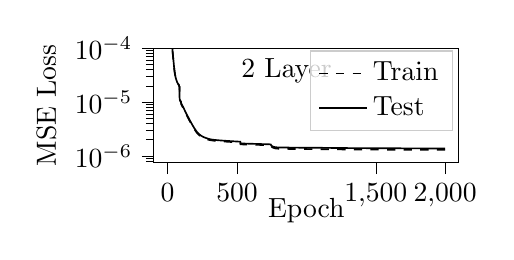
\begin{tikzpicture}

\begin{axis}[
legend cell align={left},
legend style={fill opacity=0.8, draw opacity=1, text opacity=1, draw=white!80!black},
log basis y={10},
tick align=outside,
tick pos=left,
title={2 Layer $\hy$},
title style={at={(0.45,0.85)},anchor=north},
x grid style={white!69.0196078431373!black},
xlabel={Epoch},
x label style={yshift=10pt},
xmin=-99.95, xmax=2098.95,
xtick style={color=black},
xtick = {0,500,1500,2000},
y grid style={white!69.0196078431373!black},
ylabel={MSE Loss},
ymin=7.6063321892292e-07, ymax=1e-4,
ymode=log,
ytick style={color=black},
width=.45\textwidth,
height=.25\textwidth
]
\addplot [semithick, black, dashed]
table {%
0 0.0518386695683002
1 0.042526340380311
2 0.0347423156872392
3 0.0278063397407532
4 0.021599099136889
5 0.0169535573758185
6 0.0133449736572802
7 0.0096524867080152
8 0.00607697855122387
9 0.00346671832166612
10 0.00228777943272144
11 0.00164228947134689
12 0.00122930787573569
13 0.000946592513937503
14 0.000754222130053677
15 0.000623254176578484
16 0.000526171202189289
17 0.000440977271879092
18 0.00037380238971673
19 0.000321372847538441
20 0.00028025879181223
21 0.000247563553391956
22 0.000221549878042424
23 0.000200674695734051
24 0.000183563173413859
25 0.000169053649296984
26 0.000156700562307378
27 0.000145990131146391
28 0.000136467741052911
29 0.000127828117649187
30 0.000119895841526159
31 0.000112545413488988
32 0.000105680738532101
33 9.92588357621571e-05
34 9.3258946260903e-05
35 8.76442736916943e-05
36 8.23576925613452e-05
37 7.73938517377246e-05
38 7.27130913655856e-05
39 6.8314350421133e-05
40 6.41955712490017e-05
41 6.03399962346884e-05
42 5.67417087368085e-05
43 5.33954841157538e-05
44 5.0292471962166e-05
45 4.74299892848649e-05
46 4.48063469739282e-05
47 4.24147469020681e-05
48 4.02486506536661e-05
49 3.82998454442713e-05
50 3.65582336962689e-05
51 3.50118609967467e-05
52 3.36569491373666e-05
53 3.24788894431549e-05
54 3.14478582076845e-05
55 3.05533147147798e-05
56 2.97498192085186e-05
57 2.89429238437151e-05
58 2.82225572700554e-05
59 2.75767276507395e-05
60 2.69969247092376e-05
61 2.646950968483e-05
62 2.59851477894699e-05
63 2.55374307816965e-05
64 2.51249913926586e-05
65 2.47355156570848e-05
66 2.43629243705072e-05
67 2.39832626575662e-05
68 2.35637702317035e-05
69 2.32211665752402e-05
70 2.29383413134201e-05
71 2.26900584239047e-05
72 2.24617844360182e-05
73 2.22450978726556e-05
74 2.20345916350197e-05
75 2.18275812112552e-05
76 2.16219654867018e-05
77 2.1417711785034e-05
78 2.1214236781816e-05
79 2.10117783281021e-05
80 2.08105283381883e-05
81 2.06107105623232e-05
82 2.04136253305478e-05
83 1.99121589284914e-05
84 1.94468321642489e-05
85 1.92526021455706e-05
86 1.68429254481453e-05
87 1.11265583582281e-05
88 1.08224221194178e-05
89 1.06731547539312e-05
90 1.05443111642671e-05
91 1.04219903960256e-05
92 1.03025638554755e-05
93 1.01851757890472e-05
94 1.00690036970263e-05
95 9.95377955223375e-06
96 9.83960515168292e-06
97 9.6077903663172e-06
98 9.08970189311731e-06
99 8.98518852409325e-06
100 8.88667989238456e-06
101 8.78861929595587e-06
102 8.69103235254443e-06
103 8.59354773410814e-06
104 8.49647685981836e-06
105 8.39990374788613e-06
106 8.30380843763123e-06
107 8.20817358044224e-06
108 8.11326919119892e-06
109 8.0190826447506e-06
110 7.92535356458757e-06
111 7.83217436401173e-06
112 7.73989984918444e-06
113 7.64807627137998e-06
114 7.5570470621642e-06
115 7.46617350023371e-06
116 7.37646823699834e-06
117 7.28749768268244e-06
118 7.19915332319943e-06
119 7.11171480043049e-06
120 7.0252807649922e-06
121 6.93957605744799e-06
122 6.8550750625036e-06
123 6.77161231669743e-06
124 6.68928749064435e-06
125 6.60800705782094e-06
126 6.52786106229541e-06
127 6.44881835250999e-06
128 6.3709648547956e-06
129 6.29415914409037e-06
130 6.21850223342335e-06
131 6.14401825305322e-06
132 6.07067480086698e-06
133 5.99841532675782e-06
134 5.92726610238969e-06
135 5.85724698703416e-06
136 5.78829684695847e-06
137 5.72039379244416e-06
138 5.65365198121981e-06
139 5.58796158020414e-06
140 5.52333012819872e-06
141 5.45967585458129e-06
142 5.39706647441562e-06
143 5.33535780868988e-06
144 5.27458272108561e-06
145 5.21480528050233e-06
146 5.15576177031107e-06
147 5.09760672775883e-06
148 5.04035929361635e-06
149 4.98399535490535e-06
150 4.92840583774523e-06
151 4.87364144305502e-06
152 4.81966467486927e-06
153 4.76406977395527e-06
154 4.69791715545398e-06
155 4.64507658807634e-06
156 4.59343973466275e-06
157 4.54271117132521e-06
158 4.49279561598814e-06
159 4.4436497382776e-06
160 4.39516718938648e-06
161 4.34741592334831e-06
162 4.30033761358573e-06
163 4.25400164704115e-06
164 4.20822800037968e-06
165 4.16278015359239e-06
166 4.1181904248333e-06
167 4.07423587330413e-06
168 4.0309002961294e-06
169 3.98809872649508e-06
170 3.94593327928305e-06
171 3.90432318772582e-06
172 3.86316539697873e-06
173 3.82265143798577e-06
174 3.78271101931205e-06
175 3.74335995593356e-06
176 3.70451060553023e-06
177 3.66598950404295e-06
178 3.62826339983258e-06
179 3.59102522270405e-06
180 3.55434255129694e-06
181 3.51821511981143e-06
182 3.4826161552246e-06
183 3.44756884828712e-06
184 3.41307895928367e-06
185 3.3791370713061e-06
186 3.34570067798268e-06
187 3.31284759954542e-06
188 3.28047421021438e-06
189 3.24868683401291e-06
190 3.21743388849427e-06
191 3.1866992187588e-06
192 3.15648334390062e-06
193 3.12686154870789e-06
194 3.09775542154966e-06
195 3.0692054060637e-06
196 3.04119435577377e-06
197 3.01375761148392e-06
198 2.98678445994938e-06
199 2.96039846932672e-06
200 2.93452443952447e-06
201 2.90920865177213e-06
202 2.88442320947979e-06
203 2.86015471203882e-06
204 2.83649073071501e-06
205 2.81332962913439e-06
206 2.79064786889194e-06
207 2.76854250500946e-06
208 2.74696784845219e-06
209 2.72586062430946e-06
210 2.70531269256935e-06
211 2.68526590684814e-06
212 2.66566363393395e-06
213 2.64662573533769e-06
214 2.6280339858431e-06
215 2.60993901497386e-06
216 2.59233656379365e-06
217 2.57519019442043e-06
218 2.55849347206549e-06
219 2.54225137109643e-06
220 2.52648555715496e-06
221 2.51116403057949e-06
222 2.49626635525146e-06
223 2.48174041792026e-06
224 2.46764998712479e-06
225 2.45395659851511e-06
226 2.44061466628409e-06
227 2.42766318024223e-06
228 2.41510581383864e-06
229 2.40287865153732e-06
230 2.39102976365757e-06
231 2.37946973879843e-06
232 2.36823859097512e-06
233 2.35734377997687e-06
234 2.34669803728593e-06
235 2.33637789938257e-06
236 2.32633338055166e-06
237 2.31655079858228e-06
238 2.30704811121996e-06
239 2.29775435502688e-06
240 2.28908307065012e-06
241 2.28025623937356e-06
242 2.27162592034347e-06
243 2.26319784212592e-06
244 2.2550409375981e-06
245 2.24706835138022e-06
246 2.23929092283015e-06
247 2.23166111379669e-06
248 2.22424669038901e-06
249 2.21699714541046e-06
250 2.20993513937628e-06
251 2.20302234424707e-06
252 2.19623759960541e-06
253 2.18960344636798e-06
254 2.18315790721135e-06
255 2.17678003446053e-06
256 2.17060044519712e-06
257 2.16451002290796e-06
258 2.15849525591238e-06
259 2.15263430231971e-06
260 2.14691730741379e-06
261 2.14129940786734e-06
262 2.13577006115884e-06
263 2.13036238608311e-06
264 2.12501493570016e-06
265 2.1199581875635e-06
266 2.11479780750778e-06
267 2.10963459062441e-06
268 2.10465096063217e-06
269 2.09979531643967e-06
270 2.09493869374455e-06
271 2.09029867505706e-06
272 2.08560229043542e-06
273 2.08097659026407e-06
274 2.07650576862761e-06
275 2.07193567734976e-06
276 2.06749240817317e-06
277 2.06326575550975e-06
278 2.05894802388684e-06
279 2.05470462492485e-06
280 2.05050052682054e-06
281 2.04643580877928e-06
282 2.0424704373454e-06
283 2.03852960294171e-06
284 2.03469342307017e-06
285 2.03091579976444e-06
286 2.02713633768781e-06
287 2.02345604839138e-06
288 2.01982171290638e-06
289 2.01625873410194e-06
290 2.01274700611975e-06
291 2.00929016750706e-06
292 2.00590146562263e-06
293 2.00254602100358e-06
294 1.99926750190116e-06
295 1.99598840447379e-06
296 1.99279543198827e-06
297 1.98967802123207e-06
298 1.98662693992446e-06
299 1.98363486015296e-06
300 1.98073774367913e-06
301 1.97792627022864e-06
302 1.97517233220879e-06
303 1.97249674567956e-06
304 1.96989209428011e-06
305 1.96735570136752e-06
306 1.96489110953735e-06
307 1.96252498756166e-06
308 1.96016407414845e-06
309 1.95790429916087e-06
310 1.95567747516634e-06
311 1.95353562503442e-06
312 1.95143923531305e-06
313 1.94938852894211e-06
314 1.94739756454965e-06
315 1.94547211549434e-06
316 1.94368945972201e-06
317 1.94186115868433e-06
318 1.94003258525299e-06
319 1.93824945745291e-06
320 1.9365728117009e-06
321 1.93486980356283e-06
322 1.93323022483582e-06
323 1.93159868342718e-06
324 1.93004855782419e-06
325 1.92850577320769e-06
326 1.92703124560012e-06
327 1.92557061188836e-06
328 1.92414228069993e-06
329 1.92272855258579e-06
330 1.92145235405405e-06
331 1.92011111062129e-06
332 1.91873049038804e-06
333 1.91744816731898e-06
334 1.91613417905501e-06
335 1.91486396772689e-06
336 1.91374089342844e-06
337 1.91252254262508e-06
338 1.91134569661244e-06
339 1.91014032100156e-06
340 1.90892861962766e-06
341 1.90778080786913e-06
342 1.90679503680258e-06
343 1.90562279988171e-06
344 1.90453983475436e-06
345 1.9034283604924e-06
346 1.90236943444688e-06
347 1.90128401038692e-06
348 1.90023423112962e-06
349 1.89921649234748e-06
350 1.89817762452549e-06
351 1.89717194177774e-06
352 1.89619797345131e-06
353 1.89519621744694e-06
354 1.89419035530136e-06
355 1.89321117386498e-06
356 1.89228158308197e-06
357 1.89132848026929e-06
358 1.89040515931538e-06
359 1.8894536552807e-06
360 1.88852625899472e-06
361 1.8876163518371e-06
362 1.88671577905097e-06
363 1.88581250529296e-06
364 1.88489490290067e-06
365 1.88400545243894e-06
366 1.88320691779609e-06
367 1.88227364219529e-06
368 1.88137783914044e-06
369 1.88048757183878e-06
370 1.87960764208128e-06
371 1.87875062977128e-06
372 1.87785555567643e-06
373 1.87700367860089e-06
374 1.8761265273497e-06
375 1.87530233984035e-06
376 1.87443296317724e-06
377 1.87359234882933e-06
378 1.87277639042804e-06
379 1.87191020336286e-06
380 1.87106933947234e-06
381 1.87022027148487e-06
382 1.86942492166509e-06
383 1.86859680513862e-06
384 1.86778859585957e-06
385 1.86696180901436e-06
386 1.86615413451818e-06
387 1.865346644081e-06
388 1.86454020524707e-06
389 1.86374061308925e-06
390 1.86296425601995e-06
391 1.86214191205636e-06
392 1.86135847434343e-06
393 1.86057959820118e-06
394 1.85977571720741e-06
395 1.85900325470811e-06
396 1.85821711534118e-06
397 1.85742586654669e-06
398 1.85668396852634e-06
399 1.85587053044856e-06
400 1.85511533595673e-06
401 1.85435227967901e-06
402 1.85357387726981e-06
403 1.85281492088052e-06
404 1.85205200068594e-06
405 1.85128828331926e-06
406 1.85053131349377e-06
407 1.8499851529441e-06
408 1.84917399599271e-06
409 1.84840255906238e-06
410 1.84766332199615e-06
411 1.84689625007195e-06
412 1.84613141198042e-06
413 1.84538050450556e-06
414 1.844629050197e-06
415 1.84387742933723e-06
416 1.84314657485629e-06
417 1.84239931502361e-06
418 1.84165844211748e-06
419 1.84091300036471e-06
420 1.84018742834269e-06
421 1.83944933723978e-06
422 1.83872336367585e-06
423 1.83799873639146e-06
424 1.83724605551561e-06
425 1.83653046701693e-06
426 1.83579679980994e-06
427 1.83508214388439e-06
428 1.83435587473468e-06
429 1.83363736755382e-06
430 1.8329269255446e-06
431 1.83219673760959e-06
432 1.83147712380105e-06
433 1.83076220457679e-06
434 1.83004805330711e-06
435 1.82932657037327e-06
436 1.82861742405294e-06
437 1.82790977305558e-06
438 1.82720573548067e-06
439 1.82647991425711e-06
440 1.82577657187721e-06
441 1.82505562622737e-06
442 1.82437355033471e-06
443 1.82366404123968e-06
444 1.82293964576274e-06
445 1.82224642969686e-06
446 1.82155447021159e-06
447 1.82083569222868e-06
448 1.82014943925424e-06
449 1.81945615088352e-06
450 1.81874204338328e-06
451 1.81806114380834e-06
452 1.8173547899778e-06
453 1.81667541403385e-06
454 1.81598416770612e-06
455 1.81524100480601e-06
456 1.81453961306488e-06
457 1.81385451594451e-06
458 1.81315790109693e-06
459 1.81245884846248e-06
460 1.81177978004143e-06
461 1.81107571381744e-06
462 1.81042428357614e-06
463 1.80971381985273e-06
464 1.80901504791109e-06
465 1.80835478647623e-06
466 1.80766282676359e-06
467 1.80698605220186e-06
468 1.80630960915096e-06
469 1.80562094067227e-06
470 1.80495204324416e-06
471 1.80429276622363e-06
472 1.80363471463352e-06
473 1.80292723803177e-06
474 1.80225790609256e-06
475 1.80158976775147e-06
476 1.80091279730732e-06
477 1.80023987002187e-06
478 1.79959257354767e-06
479 1.79890977392461e-06
480 1.79824207714319e-06
481 1.79757481157594e-06
482 1.7969080555531e-06
483 1.79623438566523e-06
484 1.79557559511068e-06
485 1.79491270898779e-06
486 1.79438170130197e-06
487 1.79366591225971e-06
488 1.79298442958498e-06
489 1.79231373408584e-06
490 1.79167655073798e-06
491 1.79100179059333e-06
492 1.79032596940942e-06
493 1.78968522516243e-06
494 1.78901104857232e-06
495 1.78837366763673e-06
496 1.78771149103341e-06
497 1.78705672965407e-06
498 1.78641258935386e-06
499 1.78577213569042e-06
500 1.78510025034484e-06
501 1.78445535595984e-06
502 1.78384143919175e-06
503 1.78316099584208e-06
504 1.7825342940796e-06
505 1.78187944834463e-06
506 1.78124007402403e-06
507 1.78060222037857e-06
508 1.77995303192802e-06
509 1.77932496455924e-06
510 1.77868458877128e-06
511 1.77803215694894e-06
512 1.77739755554285e-06
513 1.77675821737466e-06
514 1.77612358766055e-06
515 1.77547155703905e-06
516 1.77483872244011e-06
517 1.77422070601096e-06
518 1.7735807008421e-06
519 1.77294365573744e-06
520 1.77230281133234e-06
521 1.77169832647905e-06
522 1.77105510329056e-06
523 1.77042892869395e-06
524 1.76978312288156e-06
525 1.66620164694109e-06
526 1.63933637233526e-06
527 1.63880179010789e-06
528 1.63844974755989e-06
529 1.63812484262849e-06
530 1.63779529955832e-06
531 1.63742095688235e-06
532 1.63711894725793e-06
533 1.63679492797542e-06
534 1.63647552042789e-06
535 1.6361367341915e-06
536 1.63582143278518e-06
537 1.63551573919563e-06
538 1.63520860402855e-06
539 1.63490383059184e-06
540 1.63459672538124e-06
541 1.63429267476545e-06
542 1.63399191654889e-06
543 1.63368553430132e-06
544 1.63338495767107e-06
545 1.63310262541927e-06
546 1.6327682387498e-06
547 1.63247037161796e-06
548 1.63218582176228e-06
549 1.63187798207787e-06
550 1.6315871942254e-06
551 1.63128337254648e-06
552 1.63099369069641e-06
553 1.63070029680057e-06
554 1.63040730399189e-06
555 1.63011679620695e-06
556 1.62983160720387e-06
557 1.62952682003947e-06
558 1.62922214192918e-06
559 1.62894504913425e-06
560 1.62864188482104e-06
561 1.6283534936008e-06
562 1.6280654233185e-06
563 1.62778253840656e-06
564 1.62747459560819e-06
565 1.62719646951359e-06
566 1.62692239271678e-06
567 1.62661389299501e-06
568 1.62633292706005e-06
569 1.62606319807423e-06
570 1.62576276485993e-06
571 1.62547591571638e-06
572 1.62518481394613e-06
573 1.62490155244654e-06
574 1.62461253736979e-06
575 1.62433828410258e-06
576 1.62405268940802e-06
577 1.62376205736336e-06
578 1.62348133056867e-06
579 1.62319527444765e-06
580 1.62290394715114e-06
581 1.62262100627686e-06
582 1.62234837728192e-06
583 1.62206169241585e-06
584 1.6217815277173e-06
585 1.62149699008296e-06
586 1.62121524058989e-06
587 1.62092517706469e-06
588 1.62070420867622e-06
589 1.62038921615704e-06
590 1.62008199799857e-06
591 1.61979725899641e-06
592 1.61950673955857e-06
593 1.61922272562265e-06
594 1.6189295055824e-06
595 1.61864341677642e-06
596 1.61835239086372e-06
597 1.61807546018622e-06
598 1.61779094619874e-06
599 1.61749259794419e-06
600 1.61723098355537e-06
601 1.61693797414841e-06
602 1.61665728629146e-06
603 1.61636831695944e-06
604 1.61610073524798e-06
605 1.61582153997131e-06
606 1.61554774945216e-06
607 1.61525743881441e-06
608 1.61498842523145e-06
609 1.61470044996292e-06
610 1.61442914523491e-06
611 1.61414135411064e-06
612 1.61386748200698e-06
613 1.61359336857458e-06
614 1.61332622727173e-06
615 1.61304242104166e-06
616 1.61276320352499e-06
617 1.61248982448114e-06
618 1.61219475916141e-06
619 1.61193266151827e-06
620 1.61164703547456e-06
621 1.61138146705753e-06
622 1.61109890345301e-06
623 1.61082260021317e-06
624 1.61053988405513e-06
625 1.61026904530104e-06
626 1.6099991666465e-06
627 1.60971038680202e-06
628 1.60944881005776e-06
629 1.60917611752609e-06
630 1.60890855008233e-06
631 1.60862766114178e-06
632 1.60834999020665e-06
633 1.60807368021665e-06
634 1.60779430278524e-06
635 1.60753966724769e-06
636 1.60726439040104e-06
637 1.60700710711126e-06
638 1.60672452217625e-06
639 1.60644054170689e-06
640 1.60616960967275e-06
641 1.60589141702872e-06
642 1.60563484433851e-06
643 1.6053435355019e-06
644 1.60508566412432e-06
645 1.60482664446704e-06
646 1.60453707941599e-06
647 1.6042754193677e-06
648 1.60399306275849e-06
649 1.60374430119248e-06
650 1.6034647498202e-06
651 1.60318650912927e-06
652 1.60291618941244e-06
653 1.60264964672763e-06
654 1.60237670334595e-06
655 1.60212423365635e-06
656 1.60184172608524e-06
657 1.60158811885935e-06
658 1.60129746804216e-06
659 1.60103951819224e-06
660 1.60076912700902e-06
661 1.60050588327465e-06
662 1.60023428719569e-06
663 1.59996088962089e-06
664 1.59969389768833e-06
665 1.59941708385247e-06
666 1.59916993624165e-06
667 1.59889477750141e-06
668 1.59866888432703e-06
669 1.59837924398687e-06
670 1.59808459493149e-06
671 1.59782723729052e-06
672 1.5975413056708e-06
673 1.59727512193797e-06
674 1.59698751379267e-06
675 1.59672256081933e-06
676 1.59644536088877e-06
677 1.59617859861783e-06
678 1.59590370850538e-06
679 1.59562858524964e-06
680 1.59536997378495e-06
681 1.59507531752467e-06
682 1.59482622048301e-06
683 1.59457645222005e-06
684 1.59428069426326e-06
685 1.5940048189691e-06
686 1.59374665537371e-06
687 1.59347681504585e-06
688 1.59320771297189e-06
689 1.59294189681702e-06
690 1.59265840376577e-06
691 1.59240391452897e-06
692 1.59212388167873e-06
693 1.59185475271784e-06
694 1.59160081452114e-06
695 1.5913355798034e-06
696 1.59105049479535e-06
697 1.59078170094062e-06
698 1.5905177025104e-06
699 1.59024808239394e-06
700 1.5899925537326e-06
701 1.58970312894269e-06
702 1.58944773028225e-06
703 1.58917952906279e-06
704 1.58889819385877e-06
705 1.5886472953639e-06
706 1.58836964335762e-06
707 1.58811646971913e-06
708 1.58783535489704e-06
709 1.58757957046873e-06
710 1.58731703973558e-06
711 1.58704471705562e-06
712 1.58677873791646e-06
713 1.5865028876334e-06
714 1.58624447136901e-06
715 1.58597577814135e-06
716 1.58570803385771e-06
717 1.58545115763786e-06
718 1.58517122966373e-06
719 1.58490910264675e-06
720 1.58464107597922e-06
721 1.58438146414142e-06
722 1.58410357899186e-06
723 1.58384261210642e-06
724 1.58350118182682e-06
725 1.58321730540933e-06
726 1.58293486397554e-06
727 1.58265849421468e-06
728 1.58239726721376e-06
729 1.58211539564945e-06
730 1.58183252307253e-06
731 1.58156696035405e-06
732 1.58106459616647e-06
733 1.5807887297683e-06
734 1.580489066626e-06
735 1.58021400281427e-06
736 1.57994096404934e-06
737 1.57964867177895e-06
738 1.57935908634954e-06
739 1.57908623067726e-06
740 1.57895105029127e-06
741 1.57861684205329e-06
742 1.57829686450839e-06
743 1.57820503723372e-06
744 1.56886491616604e-06
745 1.54443650944813e-06
746 1.52464937485774e-06
747 1.5084941576049e-06
748 1.49567416087848e-06
749 1.48492991016269e-06
750 1.47589340608079e-06
751 1.46807804819105e-06
752 1.46103214052573e-06
753 1.45476694632407e-06
754 1.44896854914123e-06
755 1.44370241736169e-06
756 1.43866883598776e-06
757 1.43380883416455e-06
758 1.42928160187239e-06
759 1.42504067417804e-06
760 1.42097017825904e-06
761 1.41716485458687e-06
762 1.41355964707657e-06
763 1.41026495602148e-06
764 1.40694243066264e-06
765 1.40386480411792e-06
766 1.40090109704261e-06
767 1.39811546335977e-06
768 1.39556718215772e-06
769 1.39314711935867e-06
770 1.39085914671e-06
771 1.38873771130932e-06
772 1.38676904158785e-06
773 1.38486147091044e-06
774 1.38307318255215e-06
775 1.38140495923267e-06
776 1.37981144834498e-06
777 1.37832817009098e-06
778 1.37694258201293e-06
779 1.37560938435399e-06
780 1.3743737128209e-06
781 1.3732237981543e-06
782 1.3721374578779e-06
783 1.37116235606527e-06
784 1.37018989329363e-06
785 1.36925985286496e-06
786 1.36841710016711e-06
787 1.36757084865735e-06
788 1.36681302183206e-06
789 1.36608643293812e-06
790 1.36541132677337e-06
791 1.36474158155409e-06
792 1.36417904980135e-06
793 1.36355554245426e-06
794 1.36299955610752e-06
795 1.36246179810939e-06
796 1.36196002624445e-06
797 1.36147286586663e-06
798 1.36102072210065e-06
799 1.36058262586403e-06
800 1.36019539741028e-06
801 1.35977008343957e-06
802 1.35934900353618e-06
803 1.35907496527921e-06
804 1.35871082459005e-06
805 1.35838341267913e-06
806 1.35806158336038e-06
807 1.35770684502745e-06
808 1.35738369530713e-06
809 1.35709290060504e-06
810 1.35672559207478e-06
811 1.35645564012066e-06
812 1.35619012348798e-06
813 1.35594104767733e-06
814 1.35568918759077e-06
815 1.35547467380093e-06
816 1.35525254742674e-06
817 1.35503257631342e-06
818 1.35482675494814e-06
819 1.35461341591281e-06
820 1.35443167101812e-06
821 1.35425345231965e-06
822 1.3540686281317e-06
823 1.35388498344469e-06
824 1.35370961773162e-06
825 1.35353743995381e-06
826 1.3533792219107e-06
827 1.35313768534218e-06
828 1.35298258597061e-06
829 1.352827967807e-06
830 1.3526768412504e-06
831 1.35252841401723e-06
832 1.35240225704081e-06
833 1.35225109995929e-06
834 1.35212322014411e-06
835 1.35198998505359e-06
836 1.35184609810324e-06
837 1.35173012962753e-06
838 1.35159571098598e-06
839 1.35147283796755e-06
840 1.35134105134682e-06
841 1.35123280175264e-06
842 1.35110112422865e-06
843 1.35098620997098e-06
844 1.3508639218287e-06
845 1.35077587185606e-06
846 1.35064492155834e-06
847 1.35053679737496e-06
848 1.35042975225019e-06
849 1.35031924180851e-06
850 1.35021662519819e-06
851 1.35011604727708e-06
852 1.35000363111715e-06
853 1.34990536004409e-06
854 1.3498181129421e-06
855 1.34971324047228e-06
856 1.34960946446938e-06
857 1.34950742594242e-06
858 1.34941408889233e-06
859 1.34932775988261e-06
860 1.34922658703829e-06
861 1.34912472361748e-06
862 1.34902612357735e-06
863 1.34892750345728e-06
864 1.34883547387687e-06
865 1.34874449845768e-06
866 1.34864384494904e-06
867 1.34856915693149e-06
868 1.348471884981e-06
869 1.34839657053476e-06
870 1.34830537385255e-06
871 1.34821930835471e-06
872 1.34813692710622e-06
873 1.34803793085325e-06
874 1.34795173156022e-06
875 1.3478776119058e-06
876 1.34777355222582e-06
877 1.34769706210136e-06
878 1.34761042174603e-06
879 1.34751966670876e-06
880 1.34744346894422e-06
881 1.34735287390697e-06
882 1.34725689983384e-06
883 1.34717631696901e-06
884 1.34709783374376e-06
885 1.34702141804155e-06
886 1.34693583878231e-06
887 1.34685476582774e-06
888 1.34676708303516e-06
889 1.34668838386176e-06
890 1.3466111598035e-06
891 1.34654315939997e-06
892 1.34647579018576e-06
893 1.34638291420686e-06
894 1.34629611308412e-06
895 1.34621114347055e-06
896 1.34613849976972e-06
897 1.34607026022593e-06
898 1.34600097389637e-06
899 1.34590469681939e-06
900 1.34583183752568e-06
901 1.3457547924105e-06
902 1.34568102149046e-06
903 1.34570885896323e-06
904 1.34563602135529e-06
905 1.34554965568157e-06
906 1.34547586169731e-06
907 1.34539394407795e-06
908 1.34532783863506e-06
909 1.34524034038463e-06
910 1.34516967027309e-06
911 1.34509670238003e-06
912 1.34502306164563e-06
913 1.34495103804966e-06
914 1.34488076425043e-06
915 1.34479510651886e-06
916 1.34472651404849e-06
917 1.34466214339568e-06
918 1.34458127747905e-06
919 1.34450533219876e-06
920 1.3444267981555e-06
921 1.34435084679296e-06
922 1.34428695463384e-06
923 1.34422671932555e-06
924 1.34414231379765e-06
925 1.34407956909399e-06
926 1.3439992275579e-06
927 1.3439298076463e-06
928 1.34387832962091e-06
929 1.3438092536262e-06
930 1.34373289975542e-06
931 1.3436577213497e-06
932 1.34358143714053e-06
933 1.34352394559301e-06
934 1.34345717660267e-06
935 1.34337900578885e-06
936 1.34335605609692e-06
937 1.34328150070928e-06
938 1.34321433966988e-06
939 1.34313157009558e-06
940 1.3430716178533e-06
941 1.34299877356625e-06
942 1.3429399402014e-06
943 1.34285865880202e-06
944 1.34280206063409e-06
945 1.34274019325176e-06
946 1.34266461981269e-06
947 1.34259506944545e-06
948 1.34254850138404e-06
949 1.34247986547109e-06
950 1.34240087921e-06
951 1.34232612865048e-06
952 1.3423135030024e-06
953 1.34225830529999e-06
954 1.3421897558743e-06
955 1.34212832678315e-06
956 1.34206213189714e-06
957 1.34198343585012e-06
958 1.34193174501718e-06
959 1.34187326334256e-06
960 1.34180413468243e-06
961 1.34174007241938e-06
962 1.34166821864312e-06
963 1.34160912554648e-06
964 1.34154919388152e-06
965 1.34148838895953e-06
966 1.34141044561886e-06
967 1.34135855292072e-06
968 1.34130112543573e-06
969 1.34123174636613e-06
970 1.34118099316538e-06
971 1.34110277215882e-06
972 1.34103400789343e-06
973 1.34098474899247e-06
974 1.34092078039316e-06
975 1.34086393288158e-06
976 1.34079251927233e-06
977 1.34072488621939e-06
978 1.34067154296247e-06
979 1.34060519832246e-06
980 1.34055623038876e-06
981 1.34048152499133e-06
982 1.3404323760966e-06
983 1.34035964379109e-06
984 1.34030211174263e-06
985 1.34024774162356e-06
986 1.34017881156012e-06
987 1.3401354625131e-06
988 1.34007251983803e-06
989 1.34001645538717e-06
990 1.33994008200489e-06
991 1.33989448013949e-06
992 1.33979940444817e-06
993 1.3397541583231e-06
994 1.33968041419052e-06
995 1.33962406884791e-06
996 1.33956490974185e-06
997 1.33950567945362e-06
998 1.33946297422938e-06
999 1.33938883983831e-06
1000 1.33933092904215e-06
1001 1.33928694378937e-06
1002 1.33921256117731e-06
1003 1.33916161001935e-06
1004 1.3390988379598e-06
1005 1.33903752758613e-06
1006 1.33898176045477e-06
1007 1.33892504666733e-06
1008 1.33887592123472e-06
1009 1.33881134048863e-06
1010 1.33875219198387e-06
1011 1.33870028915339e-06
1012 1.33863348575858e-06
1013 1.33858250521257e-06
1014 1.33852591613959e-06
1015 1.33846663027271e-06
1016 1.33840421788989e-06
1017 1.33835072642796e-06
1018 1.33830789980038e-06
1019 1.33824401744675e-06
1020 1.33817713299322e-06
1021 1.33813398639404e-06
1022 1.33806409412784e-06
1023 1.33800658908001e-06
1024 1.33795149331206e-06
1025 1.3379155276283e-06
1026 1.33784969801809e-06
1027 1.33778447249711e-06
1028 1.33765031387156e-06
1029 1.33759461118643e-06
1030 1.33753808258064e-06
1031 1.33748855502347e-06
1032 1.33742270143955e-06
1033 1.33736784084704e-06
1034 1.33731045195873e-06
1035 1.33725952910879e-06
1036 1.33719250703734e-06
1037 1.33714265534479e-06
1038 1.33709573304941e-06
1039 1.33703461840184e-06
1040 1.33698563801943e-06
1041 1.33692117942985e-06
1042 1.33686207065864e-06
1043 1.33682150280379e-06
1044 1.33675993406257e-06
1045 1.33670628150639e-06
1046 1.33664372732767e-06
1047 1.33658942088744e-06
1048 1.33653863915129e-06
1049 1.33648365992656e-06
1050 1.33643210853052e-06
1051 1.33637117450292e-06
1052 1.33631502657749e-06
1053 1.33626177149893e-06
1054 1.33622257948218e-06
1055 1.33616662400016e-06
1056 1.33610955839458e-06
1057 1.33605329271802e-06
1058 1.33598385832556e-06
1059 1.33594217295752e-06
1060 1.33588493156367e-06
1061 1.33583359792055e-06
1062 1.33576979409611e-06
1063 1.33572435426288e-06
1064 1.33567137682178e-06
1065 1.33562173462565e-06
1066 1.33556964851778e-06
1067 1.33551589878778e-06
1068 1.33546273754348e-06
1069 1.33540153122169e-06
1070 1.33536268666035e-06
1071 1.33529603027682e-06
1072 1.33524601922375e-06
1073 1.33519661385151e-06
1074 1.33514066943974e-06
1075 1.33509146333211e-06
1076 1.33504329576795e-06
1077 1.33499757205868e-06
1078 1.33493545313001e-06
1079 1.33489117727947e-06
1080 1.33483645198851e-06
1081 1.33478451633096e-06
1082 1.33473267716511e-06
1083 1.33466724497566e-06
1084 1.33462421723607e-06
1085 1.33456596925896e-06
1086 1.33453018727892e-06
1087 1.33446277706639e-06
1088 1.33441716130278e-06
1089 1.33436078276361e-06
1090 1.33430692164893e-06
1091 1.33425975168677e-06
1092 1.33421545604051e-06
1093 1.33415072625098e-06
1094 1.33410108566068e-06
1095 1.33404680869376e-06
1096 1.33399491723196e-06
1097 1.33394408973686e-06
1098 1.33389038987275e-06
1099 1.33383919941821e-06
1100 1.33379414305068e-06
1101 1.33373261306247e-06
1102 1.33368463527006e-06
1103 1.33363207953607e-06
1104 1.33359130424537e-06
1105 1.33354491660498e-06
1106 1.33348266453481e-06
1107 1.33343180641532e-06
1108 1.33338205131395e-06
1109 1.33333231407562e-06
1110 1.33328824017553e-06
1111 1.33323012887843e-06
1112 1.33317537382993e-06
1113 1.33314741407276e-06
1114 1.33307755031353e-06
1115 1.33303352079395e-06
1116 1.33297956337231e-06
1117 1.3329289483579e-06
1118 1.33287542442417e-06
1119 1.33282477237628e-06
1120 1.33277926930475e-06
1121 1.33273204622242e-06
1122 1.33267181597319e-06
1123 1.332627589818e-06
1124 1.33257524055352e-06
1125 1.33252936851136e-06
1126 1.33248547196274e-06
1127 1.33243876933875e-06
1128 1.33238333026497e-06
1129 1.33232479907974e-06
1130 1.33227799227598e-06
1131 1.33223086616852e-06
1132 1.33218174798344e-06
1133 1.33213632797435e-06
1134 1.33208051036604e-06
1135 1.33205012393489e-06
1136 1.33198282409808e-06
1137 1.33193860241931e-06
1138 1.33188387665939e-06
1139 1.33183967609796e-06
1140 1.33179460509325e-06
1141 1.33174281238269e-06
1142 1.33169365426511e-06
1143 1.33164133212915e-06
1144 1.33158321374083e-06
1145 1.3315432472325e-06
1146 1.33148943393735e-06
1147 1.33144728846446e-06
1148 1.33139592961129e-06
1149 1.33134038986782e-06
1150 1.33129153603306e-06
1151 1.33124128893769e-06
1152 1.3311990425251e-06
1153 1.33114998108397e-06
1154 1.33109154313615e-06
1155 1.33104795212091e-06
1156 1.33099706505391e-06
1157 1.33095313810827e-06
1158 1.33090183919649e-06
1159 1.3308592359067e-06
1160 1.33080201646862e-06
1161 1.33075989552367e-06
1162 1.33070932677981e-06
1163 1.33065972174506e-06
1164 1.3306096723511e-06
1165 1.33056723711888e-06
1166 1.33051543905083e-06
1167 1.33045599883985e-06
1168 1.33043390209764e-06
1169 1.33039126671974e-06
1170 1.33034304828072e-06
1171 1.33029533026274e-06
1172 1.33023865356563e-06
1173 1.33019446022331e-06
1174 1.33014583248325e-06
1175 1.33009934955908e-06
1176 1.33004679793203e-06
1177 1.32999394267586e-06
1178 1.32859383582229e-06
1179 1.32577590167671e-06
1180 1.32481529779227e-06
1181 1.32425906130607e-06
1182 1.32385161771253e-06
1183 1.32355970555409e-06
1184 1.32332581735284e-06
1185 1.32313855300481e-06
1186 1.32299621942877e-06
1187 1.32287166445622e-06
1188 1.32275965106032e-06
1189 1.32266207796761e-06
1190 1.32258898742066e-06
1191 1.32251438074604e-06
1192 1.3224399087477e-06
1193 1.32236959144905e-06
1194 1.32232037235269e-06
1195 1.32225536714259e-06
1196 1.32219561778868e-06
1197 1.32214652194307e-06
1198 1.32208095470787e-06
1199 1.32204806527625e-06
1200 1.32199041914305e-06
1201 1.32194223348847e-06
1202 1.32188372917597e-06
1203 1.32185073353241e-06
1204 1.32179744296934e-06
1205 1.3217571945745e-06
1206 1.32170356749839e-06
1207 1.32168178934933e-06
1208 1.32160852400887e-06
1209 1.32156865880972e-06
1210 1.3215270177227e-06
1211 1.32148737561977e-06
1212 1.32144626445552e-06
1213 1.32139509810258e-06
1214 1.32141864840207e-06
1215 1.32135991154314e-06
1216 1.32131602497054e-06
1217 1.32127464453902e-06
1218 1.32121060731549e-06
1219 1.32116699967355e-06
1220 1.3211242721809e-06
1221 1.32107436284912e-06
1222 1.32103417314511e-06
1223 1.32099427466414e-06
1224 1.32095226790341e-06
1225 1.32089809829949e-06
1226 1.32086301134393e-06
1227 1.32081426257002e-06
1228 1.3207805423292e-06
1229 1.3207305637053e-06
1230 1.32068811232955e-06
1231 1.32064384796138e-06
1232 1.32060167554471e-06
1233 1.3205631688038e-06
1234 1.3205066439923e-06
1235 1.32047018907144e-06
1236 1.32054637529677e-06
1237 1.3205274783985e-06
1238 1.32047940205382e-06
1239 1.32043280677863e-06
1240 1.32039506168269e-06
1241 1.32036514655454e-06
1242 1.32031703172686e-06
1243 1.32027795616807e-06
1244 1.3202443684861e-06
1245 1.32019133667427e-06
1246 1.32015820261699e-06
1247 1.32011709712287e-06
1248 1.32007585411031e-06
1249 1.32003833635963e-06
1250 1.31999951743467e-06
1251 1.31995052718992e-06
1252 1.31991537205067e-06
1253 1.31987489763219e-06
1254 1.31983271600689e-06
1255 1.31978467074134e-06
1256 1.319753576837e-06
1257 1.31970657953673e-06
1258 1.31966508058667e-06
1259 1.319630016269e-06
1260 1.31958882650451e-06
1261 1.31953997157552e-06
1262 1.31951191637825e-06
1263 1.31946960593154e-06
1264 1.31942758504522e-06
1265 1.31938184219393e-06
1266 1.31933255261174e-06
1267 1.31929545118226e-06
1268 1.31925781937525e-06
1269 1.31922233245518e-06
1270 1.31924204031009e-06
1271 1.31918251739194e-06
1272 1.31914621874785e-06
1273 1.31909760800397e-06
1274 1.31904689864371e-06
1275 1.31899939506752e-06
1276 1.31895242788005e-06
1277 1.31888589362461e-06
1278 1.3188213102211e-06
1279 1.31876878970161e-06
1280 1.31870717576987e-06
1281 1.31865774105222e-06
1282 1.31860239366688e-06
1283 1.31855959794791e-06
1284 1.31852673801802e-06
1285 1.31848573423099e-06
1286 1.31843639238127e-06
1287 1.31837194871309e-06
1288 1.31832015325983e-06
1289 1.31827320812761e-06
1290 1.31821452710312e-06
1291 1.31826412868463e-06
1292 1.31820652498504e-06
1293 1.31813436787809e-06
1294 1.31808043758497e-06
1295 1.31803203781544e-06
1296 1.31797565646252e-06
1297 1.31792156848576e-06
1298 1.31787510680681e-06
1299 1.31782350318588e-06
1300 1.31777007236167e-06
1301 1.317731111385e-06
1302 1.31768447428726e-06
1303 1.31765222302249e-06
1304 1.31759061208925e-06
1305 1.3175407495396e-06
1306 1.31750282601217e-06
1307 1.31745717092713e-06
1308 1.31740909702671e-06
1309 1.31737010387667e-06
1310 1.31731581387839e-06
1311 1.31729359902977e-06
1312 1.31723423439212e-06
1313 1.31719637688832e-06
1314 1.31714781051073e-06
1315 1.31711109040111e-06
1316 1.31705777398849e-06
1317 1.31702496820196e-06
1318 1.31698145554537e-06
1319 1.31693504215491e-06
1320 1.316892996158e-06
1321 1.31685051350416e-06
1322 1.3168058811317e-06
1323 1.31676369285572e-06
1324 1.3167272482093e-06
1325 1.31667373887012e-06
1326 1.31663302317975e-06
1327 1.31659156795649e-06
1328 1.31655225268901e-06
1329 1.31651966761126e-06
1330 1.31647060948126e-06
1331 1.31643030140083e-06
1332 1.31639117168447e-06
1333 1.31633731963632e-06
1334 1.31630387018333e-06
1335 1.31626258671247e-06
1336 1.31621279176386e-06
1337 1.31617875889845e-06
1338 1.31613359954486e-06
1339 1.31608632344182e-06
1340 1.31604712120748e-06
1341 1.31601232321543e-06
1342 1.3159628022521e-06
1343 1.31592109164558e-06
1344 1.31588097301005e-06
1345 1.31584353617598e-06
1346 1.3158043823438e-06
1347 1.31577746958556e-06
1348 1.31573951045993e-06
1349 1.31568544951222e-06
1350 1.31564648904714e-06
1351 1.31560409097631e-06
1352 1.31556468213034e-06
1353 1.31551994411439e-06
1354 1.31547720894787e-06
1355 1.31544238529102e-06
1356 1.31539883138032e-06
1357 1.3153504088308e-06
1358 1.31530955987103e-06
1359 1.31526198380527e-06
1360 1.31523578205872e-06
1361 1.3151850012747e-06
1362 1.31514612101569e-06
1363 1.31510655799616e-06
1364 1.31506297603323e-06
1365 1.31502549686502e-06
1366 1.31497581915596e-06
1367 1.31494573567181e-06
1368 1.31489326294343e-06
1369 1.31486664048452e-06
1370 1.31481228511632e-06
1371 1.31477881735975e-06
1372 1.31473155177275e-06
1373 1.31468939930812e-06
1374 1.31464601584241e-06
1375 1.31461001865318e-06
1376 1.31457059183049e-06
1377 1.31452871148952e-06
1378 1.31448866785888e-06
1379 1.31444212428278e-06
1380 1.31440802965699e-06
1381 1.31436307299282e-06
1382 1.31431838971707e-06
1383 1.31427322443756e-06
1384 1.31423886649884e-06
1385 1.31420234399116e-06
1386 1.31415619608788e-06
1387 1.31413195184393e-06
1388 1.31408533862043e-06
1389 1.3140527643003e-06
1390 1.3140024599636e-06
1391 1.31395506453202e-06
1392 1.31391883945753e-06
1393 1.31387949465989e-06
1394 1.31384093273823e-06
1395 1.31380773196099e-06
1396 1.31375993719018e-06
1397 1.31372225746418e-06
1398 1.31367593549214e-06
1399 1.31363591665945e-06
1400 1.31359878579929e-06
1401 1.31356280685679e-06
1402 1.31351572737515e-06
1403 1.31348148261168e-06
1404 1.31343552995133e-06
1405 1.31340653955192e-06
1406 1.31335477141192e-06
1407 1.31331217909292e-06
1408 1.31328199159952e-06
1409 1.31324050759929e-06
1410 1.313199410518e-06
1411 1.31315960558709e-06
1412 1.31310952575348e-06
1413 1.31307809232339e-06
1414 1.31303962449181e-06
1415 1.3129952787807e-06
1416 1.31295043550494e-06
1417 1.31291564053981e-06
1418 1.31287857932705e-06
1419 1.31284263386533e-06
1420 1.31279429353981e-06
1421 1.31275722567636e-06
1422 1.31273118608988e-06
1423 1.31268142855845e-06
1424 1.3126316385268e-06
1425 1.31259607421441e-06
1426 1.31256069056462e-06
1427 1.31251248853914e-06
1428 1.31246915155714e-06
1429 1.31243717203233e-06
1430 1.31239350761803e-06
1431 1.31234716056383e-06
1432 1.3123242802493e-06
1433 1.31227735960238e-06
1434 1.31223271989711e-06
1435 1.31219915439829e-06
1436 1.31215062850742e-06
1437 1.31212218929022e-06
1438 1.3120791121537e-06
1439 1.31203161237181e-06
1440 1.31200182872249e-06
1441 1.31196549817503e-06
1442 1.31192107697586e-06
1443 1.31187962790591e-06
1444 1.31183938752599e-06
1445 1.31180776863005e-06
1446 1.31176054296134e-06
1447 1.31172362119969e-06
1448 1.31168643122237e-06
1449 1.31165350231299e-06
1450 1.31160334724711e-06
1451 1.3115657474998e-06
1452 1.311524503123e-06
1453 1.31148720245733e-06
1454 1.31145775291941e-06
1455 1.31141236701637e-06
1456 1.31137372878243e-06
1457 1.31133921740911e-06
1458 1.31128970619443e-06
1459 1.31125061385262e-06
1460 1.31120704479315e-06
1461 1.31118090965288e-06
1462 1.31113069129185e-06
1463 1.31109799757212e-06
1464 1.31105958655553e-06
1465 1.31102414700024e-06
1466 1.31113465407395e-06
1467 1.3115353781501e-06
1468 1.31073669899706e-06
1469 1.31061095918028e-06
1470 1.31053976475926e-06
1471 1.31051849380981e-06
1472 1.31045500958749e-06
1473 1.31041446591951e-06
1474 1.31038325683619e-06
1475 1.31034178316725e-06
1476 1.31030691308354e-06
1477 1.31025875219848e-06
1478 1.31020995374342e-06
1479 1.31017023034019e-06
1480 1.31014068551849e-06
1481 1.31009896698231e-06
1482 1.31005129526329e-06
1483 1.31001381359397e-06
1484 1.30997352819406e-06
1485 1.30993995983886e-06
1486 1.30989869869325e-06
1487 1.30986009870071e-06
1488 1.30982312171568e-06
1489 1.30978367678836e-06
1490 1.30974461123401e-06
1491 1.30970787867568e-06
1492 1.30966502571539e-06
1493 1.3096298849149e-06
1494 1.30959659510665e-06
1495 1.30956331126697e-06
1496 1.30951565556359e-06
1497 1.3094790621011e-06
1498 1.30944215527506e-06
1499 1.30939618007631e-06
1500 1.30936962753481e-06
1501 1.30933061875282e-06
1502 1.30928901221239e-06
1503 1.30924293445389e-06
1504 1.30921448861443e-06
1505 1.30917329974523e-06
1506 1.3091434063881e-06
1507 1.3091095128317e-06
1508 1.30906401409447e-06
1509 1.30902855379134e-06
1510 1.30899295051279e-06
1511 1.30895525619223e-06
1512 1.30891014282497e-06
1513 1.30888283999298e-06
1514 1.30883949670135e-06
1515 1.30880467609984e-06
1516 1.30876093874122e-06
1517 1.30873182040148e-06
1518 1.30869287713153e-06
1519 1.30865213854747e-06
1520 1.30861667719273e-06
1521 1.3085740121852e-06
1522 1.30854242374312e-06
1523 1.30850691304829e-06
1524 1.30846172521615e-06
1525 1.3084308924789e-06
1526 1.30839026867591e-06
1527 1.30835211136571e-06
1528 1.30831085695604e-06
1529 1.30828064069988e-06
1530 1.308229396912e-06
1531 1.3081966038726e-06
1532 1.30816021432167e-06
1533 1.30811588522306e-06
1534 1.30807387886023e-06
1535 1.30804364836479e-06
1536 1.30800523677976e-06
1537 1.3079673543217e-06
1538 1.30793483285174e-06
1539 1.30789522229691e-06
1540 1.30785042148318e-06
1541 1.30781459185414e-06
1542 1.30778182165159e-06
1543 1.30775194134003e-06
1544 1.30771855249634e-06
1545 1.30767076348093e-06
1546 1.30763190119865e-06
1547 1.30759709659856e-06
1548 1.30755398699023e-06
1549 1.30752424855984e-06
1550 1.30748375099188e-06
1551 1.30745104392815e-06
1552 1.30741234369225e-06
1553 1.30737575641149e-06
1554 1.30733214440681e-06
1555 1.30730984595573e-06
1556 1.3072714322675e-06
1557 1.30723216413742e-06
1558 1.30718758191506e-06
1559 1.307162111857e-06
1560 1.3071203532462e-06
1561 1.30709440516341e-06
1562 1.30705507541506e-06
1563 1.30701736974004e-06
1564 1.30697946784153e-06
1565 1.30694769262618e-06
1566 1.30688747393037e-06
1567 1.30680106401826e-06
1568 1.30671250040848e-06
1569 1.30658519580606e-06
1570 1.30647350641766e-06
1571 1.30637264372524e-06
1572 1.30628260801302e-06
1573 1.30619263643439e-06
1574 1.30612632679572e-06
1575 1.3060445271833e-06
1576 1.30598045691954e-06
1577 1.30592523802875e-06
1578 1.30587186585274e-06
1579 1.30581472285485e-06
1580 1.30576124846016e-06
1581 1.30571444087479e-06
1582 1.30566849995262e-06
1583 1.30562871432005e-06
1584 1.30558825976834e-06
1585 1.30554417266637e-06
1586 1.30550023445153e-06
1587 1.30546279150678e-06
1588 1.30542278432699e-06
1589 1.30538380547307e-06
1590 1.30534058511955e-06
1591 1.30530249140293e-06
1592 1.30526528718633e-06
1593 1.30523094507851e-06
1594 1.30519310198451e-06
1595 1.30515999937586e-06
1596 1.30511330560523e-06
1597 1.30507664401591e-06
1598 1.30503874788701e-06
1599 1.30500457611049e-06
1600 1.30496916459322e-06
1601 1.30494285006932e-06
1602 1.30490435564923e-06
1603 1.30485838994332e-06
1604 1.30482659885445e-06
1605 1.30478732155837e-06
1606 1.3047524880534e-06
1607 1.30471406019694e-06
1608 1.30468427630603e-06
1609 1.30464755363846e-06
1610 1.30461211692534e-06
1611 1.30457956852581e-06
1612 1.3045466137811e-06
1613 1.30451384271169e-06
1614 1.30447131995481e-06
1615 1.30443236731992e-06
1616 1.30440879334515e-06
1617 1.30436869623907e-06
1618 1.30434016888614e-06
1619 1.30430917424462e-06
1620 1.30427162395108e-06
1621 1.30423100985411e-06
1622 1.30420232578388e-06
1623 1.30416617172102e-06
1624 1.3041299450407e-06
1625 1.30410262495673e-06
1626 1.30406100817027e-06
1627 1.30401921336443e-06
1628 1.30399914212376e-06
1629 1.30395539915185e-06
1630 1.30392317404926e-06
1631 1.30389736538916e-06
1632 1.30385062966809e-06
1633 1.30381534091839e-06
1634 1.30380177922973e-06
1635 1.30375087475443e-06
1636 1.30372180177574e-06
1637 1.3036884428459e-06
1638 1.30364403828764e-06
1639 1.30360659640871e-06
1640 1.30358346132198e-06
1641 1.30354482784867e-06
1642 1.30351669014317e-06
1643 1.30347193973535e-06
1644 1.30343639024488e-06
1645 1.30340346458979e-06
1646 1.30337845570239e-06
1647 1.30333353850176e-06
1648 1.30331501819114e-06
1649 1.30327775123362e-06
1650 1.30324178195451e-06
1651 1.30319812065238e-06
1652 1.30316767285876e-06
1653 1.30314653416974e-06
1654 1.30310440718517e-06
1655 1.30306319319118e-06
1656 1.30303104739937e-06
1657 1.3029972061247e-06
1658 1.30295640188649e-06
1659 1.30292751202887e-06
1660 1.30288585020821e-06
1661 1.3028596930269e-06
1662 1.30282386928116e-06
1663 1.30279087981933e-06
1664 1.30276015883624e-06
1665 1.30272269737475e-06
1666 1.30268822775292e-06
1667 1.30265419538489e-06
1668 1.30262256087121e-06
1669 1.30258766282054e-06
1670 1.30255358023135e-06
1671 1.30251958941585e-06
1672 1.3024827413517e-06
1673 1.30244834473103e-06
1674 1.30242112800261e-06
1675 1.30238559525253e-06
1676 1.30235082198737e-06
1677 1.30231930461377e-06
1678 1.30228147989442e-06
1679 1.30225140925688e-06
1680 1.30221264949171e-06
1681 1.3021771924997e-06
1682 1.30215629911845e-06
1683 1.30212054297374e-06
1684 1.3020825262231e-06
1685 1.30205074025014e-06
1686 1.30201645512784e-06
1687 1.3019760089179e-06
1688 1.30194387260474e-06
1689 1.30191285383319e-06
1690 1.30188629354677e-06
1691 1.30184348482487e-06
1692 1.30181177200939e-06
1693 1.30178400208081e-06
1694 1.3017502183601e-06
1695 1.30171701061954e-06
1696 1.30168398564479e-06
1697 1.30165680079131e-06
1698 1.30161776992566e-06
1699 1.30158671188951e-06
1700 1.301542995094e-06
1701 1.30151153366853e-06
1702 1.30147992234697e-06
1703 1.30145104238011e-06
1704 1.30140742756169e-06
1705 1.30138871969621e-06
1706 1.30135159645306e-06
1707 1.30132069060096e-06
1708 1.30128667251483e-06
1709 1.30124737745518e-06
1710 1.30121323856258e-06
1711 1.30118363685483e-06
1712 1.30115531682407e-06
1713 1.30111670598865e-06
1714 1.30109344169682e-06
1715 1.30105685009596e-06
1716 1.3010196516916e-06
1717 1.30099644994175e-06
1718 1.30095129730989e-06
1719 1.30092531632897e-06
1720 1.30088796163363e-06
1721 1.3008512727879e-06
1722 1.30082383361696e-06
1723 1.30078734325423e-06
1724 1.30075498084636e-06
1725 1.30072494835076e-06
1726 1.30069480792372e-06
1727 1.30066290452646e-06
1728 1.30062102641659e-06
1729 1.30059479585043e-06
1730 1.30056997774375e-06
1731 1.30052966622429e-06
1732 1.30049582769232e-06
1733 1.30045942457002e-06
1734 1.30042508709494e-06
1735 1.30040336006232e-06
1736 1.30036208952333e-06
1737 1.30033579117139e-06
1738 1.30031166487754e-06
1739 1.30027404554767e-06
1740 1.30023207418617e-06
1741 1.30020137497411e-06
1742 1.30016529365662e-06
1743 1.30013674007046e-06
1744 1.3001077397945e-06
1745 1.30007461308423e-06
1746 1.30003726891914e-06
1747 1.30001273335267e-06
1748 1.29998552732502e-06
1749 1.29994284267809e-06
1750 1.29990960890325e-06
1751 1.29988650238033e-06
1752 1.29984577939979e-06
1753 1.29981313244798e-06
1754 1.29978438639e-06
1755 1.29974981085468e-06
1756 1.29972055978556e-06
1757 1.29969358975757e-06
1758 1.29965266478393e-06
1759 1.29962256363569e-06
1760 1.29958961294108e-06
1761 1.29955889558175e-06
1762 1.29952550526014e-06
1763 1.29949171279975e-06
1764 1.29945958289568e-06
1765 1.29943046847814e-06
1766 1.29939997185602e-06
1767 1.29936943054076e-06
1768 1.29933621389e-06
1769 1.29929934533379e-06
1770 1.29926757435328e-06
1771 1.2992392044282e-06
1772 1.29920533100858e-06
1773 1.2991700671563e-06
1774 1.29912627332374e-06
1775 1.29909210278356e-06
1776 1.29906255446599e-06
1777 1.29903083757199e-06
1778 1.29900498477298e-06
1779 1.29897524021771e-06
1780 1.29893359738276e-06
1781 1.29891209623167e-06
1782 1.29887807187856e-06
1783 1.29884300372396e-06
1784 1.2988116064605e-06
1785 1.29877996954519e-06
1786 1.29874484923675e-06
1787 1.2987117428338e-06
1788 1.29867583009968e-06
1789 1.29864896672416e-06
1790 1.29861854901492e-06
1791 1.29858806143091e-06
1792 1.29855296736991e-06
1793 1.29853388322942e-06
1794 1.29849827672501e-06
1795 1.29846098039366e-06
1796 1.29843629670745e-06
1797 1.29840156135685e-06
1798 1.29837512514541e-06
1799 1.29836212408918e-06
1800 1.29831896404653e-06
1801 1.29829055092046e-06
1802 1.2982576319871e-06
1803 1.29823140947849e-06
1804 1.29820048537965e-06
1805 1.29817173797164e-06
1806 1.29814512463611e-06
1807 1.2981023378984e-06
1808 1.29807500867685e-06
1809 1.29803826821728e-06
1810 1.29800773646593e-06
1811 1.2979781847946e-06
1812 1.29794077389533e-06
1813 1.29791346279262e-06
1814 1.29788016687371e-06
1815 1.29784268041533e-06
1816 1.29782022439429e-06
1817 1.29778623839627e-06
1818 1.2977592077732e-06
1819 1.29772728793398e-06
1820 1.29769857242934e-06
1821 1.29766320105773e-06
1822 1.29762787879883e-06
1823 1.29760096830012e-06
1824 1.2975656488976e-06
1825 1.29753746644212e-06
1826 1.2975013315355e-06
1827 1.29748086591519e-06
1828 1.2974416726621e-06
1829 1.29741440080977e-06
1830 1.29738914618827e-06
1831 1.29735291490363e-06
1832 1.29731755794182e-06
1833 1.297284848917e-06
1834 1.29725806272063e-06
1835 1.29722429477397e-06
1836 1.29719462270828e-06
1837 1.29716277369596e-06
1838 1.297132099495e-06
1839 1.29710682350037e-06
1840 1.29707580282457e-06
1841 1.29704243165918e-06
1842 1.29701305678509e-06
1843 1.29698461583416e-06
1844 1.29694613946185e-06
1845 1.2969152633957e-06
1846 1.29688457019483e-06
1847 1.29685601237384e-06
1848 1.29682263252562e-06
1849 1.29679150796846e-06
1850 1.29676873049789e-06
1851 1.2967360405014e-06
1852 1.29670956320638e-06
1853 1.29668201290656e-06
1854 1.29664866686596e-06
1855 1.29661068872622e-06
1856 1.29658337199601e-06
1857 1.29654636393184e-06
1858 1.29651771007389e-06
1859 1.29649333848647e-06
1860 1.29646568724695e-06
1861 1.29642290272614e-06
1862 1.29639706153739e-06
1863 1.2963646600781e-06
1864 1.29633471287605e-06
1865 1.29630338759057e-06
1866 1.2962749853358e-06
1867 1.29623791896449e-06
1868 1.2962157103118e-06
1869 1.29618162705469e-06
1870 1.29615798564942e-06
1871 1.29613095455738e-06
1872 1.29609084298465e-06
1873 1.29606213252487e-06
1874 1.29602892181424e-06
1875 1.29599581627815e-06
1876 1.29597255276792e-06
1877 1.29594302700298e-06
1878 1.29589945512976e-06
1879 1.29588080446297e-06
1880 1.29584873782562e-06
1881 1.29581950989177e-06
1882 1.29579072644503e-06
1883 1.29575479243726e-06
1884 1.29572682105561e-06
1885 1.2956990530455e-06
1886 1.29567194731806e-06
1887 1.29563374412101e-06
1888 1.29560203026813e-06
1889 1.29557642833333e-06
1890 1.29554112201902e-06
1891 1.29551987771492e-06
1892 1.29548469141127e-06
1893 1.29545346204907e-06
1894 1.29542539946215e-06
1895 1.29539005234847e-06
1896 1.29536077616876e-06
1897 1.29534280944199e-06
1898 1.29530432798219e-06
1899 1.29527160012799e-06
1900 1.29524660897573e-06
1901 1.29521397803956e-06
1902 1.29518296886033e-06
1903 1.29515333100017e-06
1904 1.29512402115495e-06
1905 1.29509240069581e-06
1906 1.29506431177617e-06
1907 1.29503260087915e-06
1908 1.29501052880698e-06
1909 1.29497696535452e-06
1910 1.29494201468106e-06
1911 1.29491107074386e-06
1912 1.29488443907633e-06
1913 1.2948505791428e-06
1914 1.29481940658138e-06
1915 1.29480016065031e-06
1916 1.29476492631397e-06
1917 1.29473640311062e-06
1918 1.29470511370755e-06
1919 1.29467511445114e-06
1920 1.29464872480867e-06
1921 1.29462289207538e-06
1922 1.29458773517399e-06
1923 1.29455712445292e-06
1924 1.29452539033537e-06
1925 1.29449879550236e-06
1926 1.29446464374894e-06
1927 1.2944351666988e-06
1928 1.29440817724458e-06
1929 1.29438209746979e-06
1930 1.29435313922954e-06
1931 1.29433152231684e-06
1932 1.2942912425018e-06
1933 1.29426927999532e-06
1934 1.29423369530457e-06
1935 1.29420180451234e-06
1936 1.29417424042799e-06
1937 1.29413976632975e-06
1938 1.2941117217764e-06
1939 1.29408380541918e-06
1940 1.29404398151678e-06
1941 1.29402087938502e-06
1942 1.29399364944049e-06
1943 1.29396807983539e-06
1944 1.2939327145034e-06
1945 1.29390792969275e-06
1946 1.29387755833932e-06
1947 1.29384964577639e-06
1948 1.29381176310517e-06
1949 1.29378730865426e-06
1950 1.29375462110204e-06
1951 1.29372353643475e-06
1952 1.29369512035282e-06
1953 1.29367324544205e-06
1954 1.29364491158412e-06
1955 1.29361388236759e-06
1956 1.29358137532165e-06
1957 1.29356112196888e-06
1958 1.29352790402493e-06
1959 1.29349322354244e-06
1960 1.29347562032933e-06
1961 1.29343464580245e-06
1962 1.29341100023339e-06
1963 1.29337962520992e-06
1964 1.29334828922367e-06
1965 1.29331728018656e-06
1966 1.29328694673347e-06
1967 1.29326018944198e-06
1968 1.29323436475204e-06
1969 1.29320748276029e-06
1970 1.29317501347259e-06
1971 1.29314339103814e-06
1972 1.29311811366506e-06
1973 1.29308671535e-06
1974 1.29305738650487e-06
1975 1.29302824606725e-06
1976 1.29300026733858e-06
1977 1.29297728362587e-06
1978 1.29294138612579e-06
1979 1.29291615802174e-06
1980 1.29288673092276e-06
1981 1.29287205595574e-06
1982 1.29286416517971e-06
1983 1.29269020844447e-06
1984 1.29260432319711e-06
1985 1.29256846786063e-06
1986 1.29254003090296e-06
1987 1.29252492530441e-06
1988 1.29249429504341e-06
1989 1.29247078901074e-06
1990 1.2924532950791e-06
1991 1.29243247440058e-06
1992 1.29241390827417e-06
1993 1.29237765963808e-06
1994 1.29235108063597e-06
1995 1.2923343797695e-06
1996 1.29230386770018e-06
1997 1.29228608733456e-06
1998 1.29225766541197e-06
1999 1.29223331674666e-06
};
\addlegendentry{Train}
\addplot [semithick, black]
table {%
0 0.046846017241478
1 0.0383708029985428
2 0.0309884883463383
3 0.0245152190327644
4 0.0189679358154535
5 0.0149657595902681
6 0.0117847537621856
7 0.00785275362432003
8 0.00443816976621747
9 0.00276716682128608
10 0.00193949567619711
11 0.00143606925848871
12 0.00109465920832008
13 0.000860574538819492
14 0.000701205339282751
15 0.000592119118664414
16 0.000498535810038447
17 0.000422000564867631
18 0.00036225956864655
19 0.000315643643261865
20 0.000278686813544482
21 0.000249177595833316
22 0.000225506300921552
23 0.000206198645173572
24 0.00018996320432052
25 0.000176013796590269
26 0.000163945907843299
27 0.000153226894326508
28 0.000143488970934413
29 0.00013452026178129
30 0.000126200568047352
31 0.000118409756396431
32 0.000111086439574137
33 0.000104212405858561
34 9.7776428447105e-05
35 9.17216530069709e-05
36 8.60177024151199e-05
37 8.06632524472661e-05
38 7.55998480599374e-05
39 7.08621955709532e-05
40 6.64242106722668e-05
41 6.22747902525589e-05
42 5.84089866606519e-05
43 5.48197385796811e-05
44 5.14986750204116e-05
45 4.84408956253901e-05
46 4.5642376790056e-05
47 4.30981672252528e-05
48 4.08026098739356e-05
49 3.87447726097889e-05
50 3.69136432709638e-05
51 3.52969509549439e-05
52 3.38936224579811e-05
53 3.2669759093551e-05
54 3.16056830342859e-05
55 3.0682967917528e-05
56 2.98149170703255e-05
57 2.90021780529059e-05
58 2.82771343336208e-05
59 2.76301270787371e-05
60 2.70484961220063e-05
61 2.65189119090792e-05
62 2.60316555795725e-05
63 2.55819704761961e-05
64 2.51599667535629e-05
65 2.47605166805442e-05
66 2.43684044107795e-05
67 2.39299824897898e-05
68 2.35225343203638e-05
69 2.31977446674136e-05
70 2.29244742513401e-05
71 2.26770971494261e-05
72 2.24468767555663e-05
73 2.22265607590089e-05
74 2.20125257328618e-05
75 2.18019231397193e-05
76 2.15937525354093e-05
77 2.13865077967057e-05
78 2.11813367059221e-05
79 2.09772460948443e-05
80 2.07742505153874e-05
81 2.05734759219922e-05
82 2.03746549232164e-05
83 1.96250730368774e-05
84 1.94256845134078e-05
85 1.92311126738787e-05
86 1.18716716315248e-05
87 1.12445295599173e-05
88 1.10792543637217e-05
89 1.09475913632195e-05
90 1.08244212242425e-05
91 1.07040941657033e-05
92 1.05850458567147e-05
93 1.04674263639026e-05
94 1.0350699085393e-05
95 1.023471395456e-05
96 1.01197601907188e-05
97 9.5123250503093e-06
98 9.38474931899691e-06
99 9.28386452869745e-06
100 9.18379009817727e-06
101 9.08395122678485e-06
102 8.98411417438183e-06
103 8.88483100425219e-06
104 8.78585615282645e-06
105 8.68727147462778e-06
106 8.58920793689322e-06
107 8.4915282059228e-06
108 8.39437052491121e-06
109 8.29942746349843e-06
110 8.20353943709051e-06
111 8.10821529739769e-06
112 8.01262467575725e-06
113 7.918774826976e-06
114 7.82522147346754e-06
115 7.73259944253368e-06
116 7.64051856094738e-06
117 7.54929942559102e-06
118 7.45903116694535e-06
119 7.36920082999859e-06
120 7.28032864572015e-06
121 7.19231229595607e-06
122 7.105323675205e-06
123 7.0190130827541e-06
124 6.93419269737205e-06
125 6.85027998770238e-06
126 6.76738454785664e-06
127 6.68554821459111e-06
128 6.60503519611666e-06
129 6.52583412374952e-06
130 6.44760439172387e-06
131 6.37048697171849e-06
132 6.29445594313438e-06
133 6.21960452917847e-06
134 6.14581631452893e-06
135 6.07303400101955e-06
136 6.0014181144652e-06
137 5.93111781199696e-06
138 5.86179930905928e-06
139 5.79359630137333e-06
140 5.72644830754143e-06
141 5.66039534533047e-06
142 5.59533191335504e-06
143 5.53142581338761e-06
144 5.46819137525745e-06
145 5.40599512532935e-06
146 5.34493847226258e-06
147 5.28485315953731e-06
148 5.22568461747142e-06
149 5.16738600708777e-06
150 5.10996414959664e-06
151 5.05336129208445e-06
152 4.9976015361608e-06
153 4.92653862238512e-06
154 4.87146508021397e-06
155 4.8173369577853e-06
156 4.76419609185541e-06
157 4.71183557237964e-06
158 4.66031542600831e-06
159 4.60958244730136e-06
160 4.55952158517903e-06
161 4.51021924163797e-06
162 4.46155445388285e-06
163 4.413742772158e-06
164 4.36648360846448e-06
165 4.3197637751291e-06
166 4.27378381573362e-06
167 4.22837729274761e-06
168 4.18360696130549e-06
169 4.13935913456953e-06
170 4.09567564929603e-06
171 4.05279251936008e-06
172 4.01027409679955e-06
173 3.96848236050573e-06
174 3.92731408282998e-06
175 3.8865923670528e-06
176 3.84640179618145e-06
177 3.80677988687239e-06
178 3.76767479792761e-06
179 3.72941531168181e-06
180 3.69149825019122e-06
181 3.6542601264955e-06
182 3.61761522071902e-06
183 3.5814271086565e-06
184 3.54579378836206e-06
185 3.5104699236399e-06
186 3.47592003890895e-06
187 3.44202749147371e-06
188 3.40868450621201e-06
189 3.37587903231906e-06
190 3.34381229549763e-06
191 3.31203796122281e-06
192 3.28103828906023e-06
193 3.25049609273265e-06
194 3.22048617817927e-06
195 3.1911947644403e-06
196 3.16229534291779e-06
197 3.1337522159447e-06
198 3.10582436213735e-06
199 3.07852951664245e-06
200 3.05181060866744e-06
201 3.02568946608517e-06
202 3.00021838484099e-06
203 2.97491237688519e-06
204 2.95049449050566e-06
205 2.92651202471461e-06
206 2.90325283458515e-06
207 2.88060937236878e-06
208 2.85826399704092e-06
209 2.83668964584649e-06
210 2.81563188764267e-06
211 2.79479513665137e-06
212 2.77475601251354e-06
213 2.75520233117277e-06
214 2.73612954515556e-06
215 2.71763678938441e-06
216 2.69952420239861e-06
217 2.68186363427958e-06
218 2.66457323050417e-06
219 2.64800155491685e-06
220 2.63167612502002e-06
221 2.61605600826442e-06
222 2.60081878877827e-06
223 2.58565387412091e-06
224 2.57128158409614e-06
225 2.55729264608817e-06
226 2.5434583221795e-06
227 2.53028042607184e-06
228 2.51731967182423e-06
229 2.50474613494589e-06
230 2.49260665441398e-06
231 2.48064247898583e-06
232 2.46914464696601e-06
233 2.45786941377446e-06
234 2.44702073359804e-06
235 2.43636623054044e-06
236 2.42592273025366e-06
237 2.41593488681247e-06
238 2.40604981627257e-06
239 2.39454175243736e-06
240 2.38496431848034e-06
241 2.37560857385688e-06
242 2.36638106798637e-06
243 2.35762900047121e-06
244 2.34906042351213e-06
245 2.34054073189327e-06
246 2.33240825764369e-06
247 2.32432307711861e-06
248 2.31647300097393e-06
249 2.30882278628997e-06
250 2.30132854994736e-06
251 2.29410079555237e-06
252 2.28696308113285e-06
253 2.27994132728782e-06
254 2.2731221633876e-06
255 2.26643737732957e-06
256 2.26000611291965e-06
257 2.25339977077965e-06
258 2.24699829232122e-06
259 2.24085442823707e-06
260 2.23485972128401e-06
261 2.22880544242798e-06
262 2.22294852392224e-06
263 2.21718892134959e-06
264 2.2116278159956e-06
265 2.20599986278103e-06
266 2.20042466025916e-06
267 2.19495632336475e-06
268 2.18968580156798e-06
269 2.1844550701644e-06
270 2.17936781155004e-06
271 2.17437786886876e-06
272 2.16965236177202e-06
273 2.16483385884203e-06
274 2.15997692976089e-06
275 2.15530872083036e-06
276 2.15021736948984e-06
277 2.14562965084042e-06
278 2.14111582863552e-06
279 2.13668317883275e-06
280 2.13234125112649e-06
281 2.12806639865448e-06
282 2.12381792152883e-06
283 2.11966334973113e-06
284 2.11553378903773e-06
285 2.11155611395952e-06
286 2.10754387808265e-06
287 2.10364714803291e-06
288 2.0998343188694e-06
289 2.09598420042312e-06
290 2.09230734071753e-06
291 2.08856886274589e-06
292 2.08493315767555e-06
293 2.08135452339775e-06
294 2.07782954930735e-06
295 2.07432572096877e-06
296 2.07094581128331e-06
297 2.06754771170381e-06
298 2.06429240279249e-06
299 2.06109029932122e-06
300 2.05800984076632e-06
301 2.05492415261688e-06
302 2.05180754164758e-06
303 2.04896286959411e-06
304 2.04610319087806e-06
305 2.04338948606164e-06
306 2.04076900445216e-06
307 2.03825675271219e-06
308 2.0357510948088e-06
309 2.03333684112295e-06
310 2.03093964046275e-06
311 2.02861724574177e-06
312 2.02637943402806e-06
313 2.02403339244484e-06
314 2.0218606096023e-06
315 2.01979310077149e-06
316 2.01772627406172e-06
317 2.0156662685622e-06
318 2.01365946850274e-06
319 2.01170269065187e-06
320 2.00985368792317e-06
321 2.008035835388e-06
322 2.0062404928467e-06
323 2.00445401787874e-06
324 2.00277054318576e-06
325 2.00112754100701e-06
326 1.99953205992642e-06
327 1.9979424905614e-06
328 1.99632700059738e-06
329 1.994814738282e-06
330 1.99338865058962e-06
331 1.99191208594129e-06
332 1.99047826754395e-06
333 1.98907810045057e-06
334 1.98766042558418e-06
335 1.98630050363136e-06
336 1.98500219994457e-06
337 1.98356542568945e-06
338 1.98221573555202e-06
339 1.98089469449769e-06
340 1.9795622847596e-06
341 1.97831514014979e-06
342 1.97709687199676e-06
343 1.97587201000715e-06
344 1.974676251848e-06
345 1.97352483155555e-06
346 1.97232657228597e-06
347 1.97118743017199e-06
348 1.97002691493253e-06
349 1.96894961845828e-06
350 1.96781206796004e-06
351 1.96668429452984e-06
352 1.96564246834896e-06
353 1.9644819531095e-06
354 1.9634078398667e-06
355 1.96237647287489e-06
356 1.96133396457299e-06
357 1.96031123778084e-06
358 1.95917527889833e-06
359 1.95824577531312e-06
360 1.95721463569498e-06
361 1.95623829313263e-06
362 1.95530833480007e-06
363 1.95432494365377e-06
364 1.95336792785383e-06
365 1.95239226741251e-06
366 1.95136567526788e-06
367 1.9502210761857e-06
368 1.94919675777783e-06
369 1.94815197573917e-06
370 1.94720951185445e-06
371 1.94616791304725e-06
372 1.94522522178886e-06
373 1.94425388144737e-06
374 1.943346205735e-06
375 1.94240101336618e-06
376 1.94146218746027e-06
377 1.94056860891578e-06
378 1.93966616279795e-06
379 1.93865480468958e-06
380 1.93776008927671e-06
381 1.93688833860506e-06
382 1.93602136278059e-06
383 1.93517280422384e-06
384 1.93428809325269e-06
385 1.93343589671713e-06
386 1.93253868019383e-06
387 1.93165874406986e-06
388 1.93084747479588e-06
389 1.93001665138581e-06
390 1.92919856090157e-06
391 1.92841844182112e-06
392 1.92753850569716e-06
393 1.92671450349735e-06
394 1.92591483028082e-06
395 1.9251492631156e-06
396 1.92425181921863e-06
397 1.92344646166021e-06
398 1.92265611076436e-06
399 1.92185461855843e-06
400 1.92107518159901e-06
401 1.92025459000433e-06
402 1.91948743122339e-06
403 1.91869480659079e-06
404 1.91788421943784e-06
405 1.91712092600937e-06
406 1.91636127055972e-06
407 1.9155809241056e-06
408 1.91478261513112e-06
409 1.91399544746673e-06
410 1.91320646081294e-06
411 1.91246635949938e-06
412 1.91165986507258e-06
413 1.91091567103285e-06
414 1.9101560155832e-06
415 1.90942250810622e-06
416 1.90862192539498e-06
417 1.90785863196652e-06
418 1.90713512893126e-06
419 1.9064046909989e-06
420 1.90569164715271e-06
421 1.9049134607485e-06
422 1.90417733847426e-06
423 1.90344394468411e-06
424 1.90265177479887e-06
425 1.90194396054721e-06
426 1.90123353149829e-06
427 1.90047921933001e-06
428 1.89976435649442e-06
429 1.89902630154393e-06
430 1.89827824215172e-06
431 1.89755519386381e-06
432 1.89686772955611e-06
433 1.89620402579749e-06
434 1.89539719031018e-06
435 1.89463946753676e-06
436 1.89393279015349e-06
437 1.89328488886531e-06
438 1.89252534710249e-06
439 1.89177694664977e-06
440 1.89112779480638e-06
441 1.89039110409794e-06
442 1.88969613645895e-06
443 1.88894239272486e-06
444 1.88826322755631e-06
445 1.88751369023521e-06
446 1.88680985502288e-06
447 1.88610511031584e-06
448 1.88543276635755e-06
449 1.88472415629803e-06
450 1.88403168976947e-06
451 1.88330079708976e-06
452 1.88261310540838e-06
453 1.88196042927302e-06
454 1.88125557087915e-06
455 1.88054139016458e-06
456 1.87985153843329e-06
457 1.8791384945871e-06
458 1.87846717381035e-06
459 1.8778130197461e-06
460 1.8770884935293e-06
461 1.87637954240927e-06
462 1.87569332865678e-06
463 1.87502166681952e-06
464 1.87433249720925e-06
465 1.87366788395593e-06
466 1.87299440312927e-06
467 1.87227874448581e-06
468 1.87161708709027e-06
469 1.87094917691866e-06
470 1.87024420483795e-06
471 1.86957811365573e-06
472 1.86895840670331e-06
473 1.8682715108298e-06
474 1.86761280929204e-06
475 1.86691488579527e-06
476 1.86627391940419e-06
477 1.86556110293168e-06
478 1.86493662113207e-06
479 1.86430963822204e-06
480 1.86358090559224e-06
481 1.86294278137211e-06
482 1.86224724529893e-06
483 1.86159047643741e-06
484 1.86098668564227e-06
485 1.86029444648739e-06
486 1.85947044428758e-06
487 1.85871328994835e-06
488 1.85796579899034e-06
489 1.85722444712155e-06
490 1.85654516826617e-06
491 1.85581666301005e-06
492 1.85518524631334e-06
493 1.85444093858678e-06
494 1.85381509254512e-06
495 1.85311682798783e-06
496 1.85241174222028e-06
497 1.8517333728596e-06
498 1.85108501682407e-06
499 1.85040721589758e-06
500 1.84974112471537e-06
501 1.8490995898901e-06
502 1.84843338502105e-06
503 1.84781072221085e-06
504 1.84713974249462e-06
505 1.84652901680238e-06
506 1.84586826890154e-06
507 1.84526390967221e-06
508 1.84460429863975e-06
509 1.84391683433205e-06
510 1.84327257102268e-06
511 1.84263194569212e-06
512 1.84201837782894e-06
513 1.84135399194929e-06
514 1.84069460829051e-06
515 1.84006910330936e-06
516 1.83945223852788e-06
517 1.8388465150565e-06
518 1.83819349786063e-06
519 1.83760062100191e-06
520 1.83704253231554e-06
521 1.83631811978557e-06
522 1.83572490186634e-06
523 1.83504801043455e-06
524 1.83444251433684e-06
525 1.70164969404141e-06
526 1.70162138601881e-06
527 1.70160546986153e-06
528 1.70148314282415e-06
529 1.70135103871871e-06
530 1.70113742115063e-06
531 1.70058535786666e-06
532 1.70048156178382e-06
533 1.70034593338642e-06
534 1.70017960954283e-06
535 1.69999873378401e-06
536 1.69984775766352e-06
537 1.69961970186705e-06
538 1.69938323324459e-06
539 1.69918598658114e-06
540 1.6989465621009e-06
541 1.69872339483845e-06
542 1.69847351116914e-06
543 1.69822783391282e-06
544 1.69799216109823e-06
545 1.69770237334887e-06
546 1.69748886946763e-06
547 1.69717293374561e-06
548 1.6968965610431e-06
549 1.69665361227089e-06
550 1.69635359270615e-06
551 1.69613804246183e-06
552 1.69580687270354e-06
553 1.69553754858498e-06
554 1.69522274973133e-06
555 1.69493739576865e-06
556 1.69467409705248e-06
557 1.69438305874792e-06
558 1.69408690453565e-06
559 1.69381496561982e-06
560 1.69352142620482e-06
561 1.69323493537377e-06
562 1.69294719398749e-06
563 1.69265047134104e-06
564 1.69236659530725e-06
565 1.69206862210558e-06
566 1.69179304521094e-06
567 1.69154179729958e-06
568 1.69127270055469e-06
569 1.69092299984186e-06
570 1.69062388977181e-06
571 1.69034876762453e-06
572 1.69001748417941e-06
573 1.68972178471449e-06
574 1.68944632150669e-06
575 1.6891907534955e-06
576 1.68886560913961e-06
577 1.68857764037966e-06
578 1.68831036262418e-06
579 1.68799567745737e-06
580 1.68768463026936e-06
581 1.68745668815973e-06
582 1.68711585502024e-06
583 1.68683607171261e-06
584 1.68660767485562e-06
585 1.68626570484776e-06
586 1.68594795013632e-06
587 1.68564315572439e-06
588 1.68580072568147e-06
589 1.68537701483729e-06
590 1.68500764630153e-06
591 1.68465521710459e-06
592 1.68431211022835e-06
593 1.68393830790592e-06
594 1.68357189522794e-06
595 1.68325345839548e-06
596 1.68285089330311e-06
597 1.68253336596536e-06
598 1.68217400187132e-06
599 1.68184919857595e-06
600 1.68157271218661e-06
601 1.68122721788677e-06
602 1.68090389252029e-06
603 1.68059170846391e-06
604 1.68026758728956e-06
605 1.67997404787457e-06
606 1.67970745224011e-06
607 1.67933364991768e-06
608 1.67905000125756e-06
609 1.67880864410108e-06
610 1.67844143561524e-06
611 1.67815608165256e-06
612 1.67783480264916e-06
613 1.67757480085129e-06
614 1.67724635957711e-06
615 1.67694054198364e-06
616 1.67661664818297e-06
617 1.67632686043362e-06
618 1.67603047884768e-06
619 1.67571863585181e-06
620 1.67542418694211e-06
621 1.675132125456e-06
622 1.67484745361435e-06
623 1.67453924859728e-06
624 1.67427810993104e-06
625 1.67392590810778e-06
626 1.67363941727672e-06
627 1.67334894740634e-06
628 1.67304017395509e-06
629 1.67277232776541e-06
630 1.67249686455762e-06
631 1.67222731306538e-06
632 1.67188602517854e-06
633 1.67160476394201e-06
634 1.6713132708901e-06
635 1.67100279213628e-06
636 1.67071675605257e-06
637 1.67046073329402e-06
638 1.67011842222564e-06
639 1.66984875704657e-06
640 1.6695456679372e-06
641 1.66927168265829e-06
642 1.66897143571987e-06
643 1.66867187090247e-06
644 1.66842937687761e-06
645 1.66808888479864e-06
646 1.66780796462263e-06
647 1.66752113273105e-06
648 1.6672322544764e-06
649 1.66697554959683e-06
650 1.66666586665087e-06
651 1.66638608334324e-06
652 1.66606423590565e-06
653 1.66579036431358e-06
654 1.66550466929039e-06
655 1.66521965638822e-06
656 1.6649360077281e-06
657 1.66463996720267e-06
658 1.66435984283453e-06
659 1.66408199220314e-06
660 1.66376378274435e-06
661 1.66354345765285e-06
662 1.66322217864945e-06
663 1.66290885772469e-06
664 1.66263987466664e-06
665 1.66233871823351e-06
666 1.66204688412108e-06
667 1.6617633491478e-06
668 1.66133861512208e-06
669 1.6609203612461e-06
670 1.66055099271034e-06
671 1.66018162417458e-06
672 1.65985716193973e-06
673 1.65949222719064e-06
674 1.65915173511166e-06
675 1.65884694069973e-06
676 1.65853907674318e-06
677 1.65820586062182e-06
678 1.65788685535517e-06
679 1.6575750123593e-06
680 1.6572829508732e-06
681 1.65696087606193e-06
682 1.65665335316589e-06
683 1.65638891758135e-06
684 1.65607514190924e-06
685 1.65577137067885e-06
686 1.65549295161327e-06
687 1.65515393746318e-06
688 1.65486096648237e-06
689 1.65455526257574e-06
690 1.65427434239973e-06
691 1.65399615070783e-06
692 1.65369624482992e-06
693 1.65341646152228e-06
694 1.65312474109669e-06
695 1.65282801845024e-06
696 1.65252754413814e-06
697 1.65226867920865e-06
698 1.65198218837759e-06
699 1.65169126375986e-06
700 1.65138465035852e-06
701 1.6511274907316e-06
702 1.65082849434839e-06
703 1.65053643286228e-06
704 1.65025028309174e-06
705 1.64997072715778e-06
706 1.64969560501049e-06
707 1.64942480296304e-06
708 1.64912194122735e-06
709 1.6488442042828e-06
710 1.64856987794337e-06
711 1.64829589266446e-06
712 1.64801372193324e-06
713 1.6477354165545e-06
714 1.64744551511831e-06
715 1.64714640504826e-06
716 1.64691005011264e-06
717 1.64661571488978e-06
718 1.64632831456402e-06
719 1.64603409302799e-06
720 1.64576624683832e-06
721 1.64546543146571e-06
722 1.64519246936834e-06
723 1.64490268161899e-06
724 1.64448510986404e-06
725 1.64410505476553e-06
726 1.64370578659145e-06
727 1.64337154728855e-06
728 1.64302321081777e-06
729 1.6426794218205e-06
730 1.64236087130121e-06
731 1.64206255703903e-06
732 1.64163225235825e-06
733 1.64120740464568e-06
734 1.64084485732019e-06
735 1.64046582540323e-06
736 1.64013499670546e-06
737 1.63975767009106e-06
738 1.63945423992118e-06
739 1.63910203809792e-06
740 1.63868980962434e-06
741 1.63826257448818e-06
742 1.63785296081187e-06
743 1.63730908298021e-06
744 1.61420928179723e-06
745 1.59323667503486e-06
746 1.57668887368345e-06
747 1.56361613790068e-06
748 1.55234761223255e-06
749 1.54355461745581e-06
750 1.53599876284716e-06
751 1.52936434005824e-06
752 1.52327788782713e-06
753 1.5176681245066e-06
754 1.51262872805091e-06
755 1.50785137975618e-06
756 1.50330458836834e-06
757 1.49912091274018e-06
758 1.4951411912989e-06
759 1.49132119986461e-06
760 1.48779076880601e-06
761 1.48452068060578e-06
762 1.48143158185121e-06
763 1.478490048612e-06
764 1.47566743180505e-06
765 1.47303444464342e-06
766 1.47057153299102e-06
767 1.46827005664818e-06
768 1.46612978824123e-06
769 1.46415572999103e-06
770 1.4622792150476e-06
771 1.46065633543913e-06
772 1.45901617543132e-06
773 1.45745832469402e-06
774 1.45603917189874e-06
775 1.45471119594731e-06
776 1.45324827371951e-06
777 1.45201454415655e-06
778 1.45091848935408e-06
779 1.44983698646683e-06
780 1.44889247621904e-06
781 1.44797809298325e-06
782 1.44712691962923e-06
783 1.44631110288174e-06
784 1.44554485359549e-06
785 1.44482180530758e-06
786 1.44412149438722e-06
787 1.44344255659234e-06
788 1.4428369468078e-06
789 1.44223565712309e-06
790 1.44168450333382e-06
791 1.44116972933261e-06
792 1.44086743603111e-06
793 1.44042553529289e-06
794 1.43998261137313e-06
795 1.43960153309308e-06
796 1.43920931350294e-06
797 1.43883448799897e-06
798 1.43849081268854e-06
799 1.43818635933712e-06
800 1.43782597206155e-06
801 1.43750924053165e-06
802 1.4372935766005e-06
803 1.43703255162109e-06
804 1.4367203675647e-06
805 1.43646741435077e-06
806 1.43622196446813e-06
807 1.43601982927066e-06
808 1.43582929013064e-06
809 1.43561192089692e-06
810 1.43546276376583e-06
811 1.4352565358422e-06
812 1.43505872074456e-06
813 1.43488159665139e-06
814 1.43472027502867e-06
815 1.43453883083566e-06
816 1.43438262512063e-06
817 1.43422039400321e-06
818 1.43412057695969e-06
819 1.43395027407678e-06
820 1.43383647355222e-06
821 1.43369993566012e-06
822 1.43353611292696e-06
823 1.4333991202875e-06
824 1.43325860335608e-06
825 1.43311228839593e-06
826 1.43297449994861e-06
827 1.43287729770236e-06
828 1.43275644859386e-06
829 1.43263923746417e-06
830 1.43252009365824e-06
831 1.43241754813062e-06
832 1.43226520776807e-06
833 1.43216391279566e-06
834 1.4320570471682e-06
835 1.43195131840912e-06
836 1.43184615808423e-06
837 1.43173565447796e-06
838 1.43161162213801e-06
839 1.43149327413994e-06
840 1.43139834563044e-06
841 1.4312848861664e-06
842 1.43118074902304e-06
843 1.43108468364517e-06
844 1.43098770877259e-06
845 1.43087208925863e-06
846 1.43078659675666e-06
847 1.43067268254526e-06
848 1.43055751777865e-06
849 1.43045429013e-06
850 1.43036015742837e-06
851 1.43024078624876e-06
852 1.43016109177552e-06
853 1.43005024710874e-06
854 1.42996418617258e-06
855 1.42984924877965e-06
856 1.42975352446228e-06
857 1.42966564453673e-06
858 1.42955070714379e-06
859 1.42947556014406e-06
860 1.42937540204002e-06
861 1.42927956403582e-06
862 1.42916417189554e-06
863 1.42908322686708e-06
864 1.42897965815791e-06
865 1.42890507959237e-06
866 1.42880833209347e-06
867 1.42870885611046e-06
868 1.42850797146821e-06
869 1.42842350214778e-06
870 1.42832232086221e-06
871 1.42822773341322e-06
872 1.42814224091126e-06
873 1.42803651215218e-06
874 1.42795749979996e-06
875 1.42785836487747e-06
876 1.42778367262508e-06
877 1.4276719184636e-06
878 1.4275769899541e-06
879 1.42750104714651e-06
880 1.42740816500009e-06
881 1.42733210850565e-06
882 1.42720921303408e-06
883 1.42713270179229e-06
884 1.42703163419355e-06
885 1.42698809213471e-06
886 1.42687554216536e-06
887 1.42678902648186e-06
888 1.4267367305365e-06
889 1.42626765864406e-06
890 1.42618659992877e-06
891 1.42610429065826e-06
892 1.42605767905479e-06
893 1.42591852636542e-06
894 1.4258409919421e-06
895 1.42576470807398e-06
896 1.42567228067492e-06
897 1.42558883453603e-06
898 1.42549970405526e-06
899 1.42542330650031e-06
900 1.42533781399834e-06
901 1.42525448154629e-06
902 1.42517183121527e-06
903 1.42509736633656e-06
904 1.42500323363492e-06
905 1.42492979193776e-06
906 1.42484418574895e-06
907 1.42483622767031e-06
908 1.42468809372076e-06
909 1.42459214202972e-06
910 1.42453575335821e-06
911 1.42446174322686e-06
912 1.42437943395635e-06
913 1.42428575600206e-06
914 1.42421026794182e-06
915 1.42415922255168e-06
916 1.42407395742339e-06
917 1.42400847380486e-06
918 1.4239076335798e-06
919 1.42383180445904e-06
920 1.42374460665451e-06
921 1.42367684929923e-06
922 1.42359692745231e-06
923 1.42352837428916e-06
924 1.4234655054679e-06
925 1.42340684305964e-06
926 1.42333863095701e-06
927 1.42324734042631e-06
928 1.42316571327683e-06
929 1.4230965916795e-06
930 1.42305123063124e-06
931 1.42293708904617e-06
932 1.42289991345024e-06
933 1.42281908210862e-06
934 1.42274745940085e-06
935 1.422652076144e-06
936 1.42282704018726e-06
937 1.42277463055507e-06
938 1.42265355407289e-06
939 1.42257897550735e-06
940 1.42252406476473e-06
941 1.42243902701011e-06
942 1.42236569899978e-06
943 1.42231920108316e-06
944 1.42222245358425e-06
945 1.42216163112607e-06
946 1.42207454700838e-06
947 1.42200758546096e-06
948 1.42194551244756e-06
949 1.4218886690287e-06
950 1.42179760587169e-06
951 1.42172279993247e-06
952 1.42198348385136e-06
953 1.42190435781231e-06
954 1.42183262141771e-06
955 1.4217849866327e-06
956 1.42171109018818e-06
957 1.42163992222777e-06
958 1.42155477078632e-06
959 1.42150031479105e-06
960 1.4214715520211e-06
961 1.42135263558885e-06
962 1.42128953939391e-06
963 1.42122837587522e-06
964 1.42117175983003e-06
965 1.42110036449594e-06
966 1.42104033784562e-06
967 1.42096837407735e-06
968 1.42089277233026e-06
969 1.420834109922e-06
970 1.42077453801903e-06
971 1.42071394293453e-06
972 1.42067108299671e-06
973 1.42058559049474e-06
974 1.4205137404133e-06
975 1.42044871154212e-06
976 1.42040198625182e-06
977 1.42032536132319e-06
978 1.4202590818968e-06
979 1.42019644044922e-06
980 1.4201415297066e-06
981 1.42008207149047e-06
982 1.4200206805981e-06
983 1.41994360092212e-06
984 1.41991324653645e-06
985 1.41982457080303e-06
986 1.41975283440843e-06
987 1.41971486300463e-06
988 1.41964198974165e-06
989 1.41956456900516e-06
990 1.41950738452579e-06
991 1.41947600695858e-06
992 1.4193688002706e-06
993 1.41932162023295e-06
994 1.4192521575751e-06
995 1.41919008456171e-06
996 1.41912789786147e-06
997 1.41905695727473e-06
998 1.41902216910239e-06
999 1.41895327487873e-06
1000 1.41893428917683e-06
1001 1.41881901072338e-06
1002 1.41876955694897e-06
1003 1.41870009429113e-06
1004 1.41863620228833e-06
1005 1.41860061830812e-06
1006 1.4185249028742e-06
1007 1.41848329349159e-06
1008 1.41840519063408e-06
1009 1.41836903821968e-06
1010 1.41830298616696e-06
1011 1.41825114496896e-06
1012 1.41818145493744e-06
1013 1.41811437970318e-06
1014 1.41806071951578e-06
1015 1.41799500852358e-06
1016 1.41796158459329e-06
1017 1.41787177199149e-06
1018 1.41782197715656e-06
1019 1.41775342399342e-06
1020 1.41771374728705e-06
1021 1.41765474381828e-06
1022 1.41758857807872e-06
1023 1.41752832405473e-06
1024 1.41747932502767e-06
1025 1.41742771120335e-06
1026 1.41736757086619e-06
1027 1.4172874216456e-06
1028 1.41727139180148e-06
1029 1.41724194691051e-06
1030 1.41720238389098e-06
1031 1.41717544011044e-06
1032 1.4171044995237e-06
1033 1.41707596412743e-06
1034 1.4169706901157e-06
1035 1.41692009947292e-06
1036 1.41688497024006e-06
1037 1.41682005505572e-06
1038 1.41678299314663e-06
1039 1.41671466735716e-06
1040 1.41665748287778e-06
1041 1.41660348162986e-06
1042 1.41657483254676e-06
1043 1.4164851336318e-06
1044 1.41645091389364e-06
1045 1.4163998685035e-06
1046 1.41631585393043e-06
1047 1.4162883417157e-06
1048 1.41623536364932e-06
1049 1.4161693115966e-06
1050 1.41609052661806e-06
1051 1.41607051773462e-06
1052 1.41601594805252e-06
1053 1.4159601278152e-06
1054 1.41589487157034e-06
1055 1.41587099733442e-06
1056 1.415812448613e-06
1057 1.41573286782659e-06
1058 1.41568762046518e-06
1059 1.41564714795095e-06
1060 1.41557427468797e-06
1061 1.41552379773202e-06
1062 1.41547320708924e-06
1063 1.41542068377021e-06
1064 1.41537168474315e-06
1065 1.41529869779333e-06
1066 1.41525777053175e-06
1067 1.41520854413102e-06
1068 1.4151485174807e-06
1069 1.41509622153535e-06
1070 1.41503664963238e-06
1071 1.41500663630723e-06
1072 1.4149291018839e-06
1073 1.41488465033035e-06
1074 1.41483019433508e-06
1075 1.41476186854561e-06
1076 1.41472924042318e-06
1077 1.4146665989756e-06
1078 1.41461771363538e-06
1079 1.41455609536933e-06
1080 1.41449288548756e-06
1081 1.41443194934254e-06
1082 1.41441353207483e-06
1083 1.41434338729596e-06
1084 1.41430939493148e-06
1085 1.41424811772595e-06
1086 1.41418775001512e-06
1087 1.41413988785644e-06
1088 1.41409191201092e-06
1089 1.41403177167376e-06
1090 1.41398106734414e-06
1091 1.41392615660152e-06
1092 1.41387113217206e-06
1093 1.41382327001338e-06
1094 1.4137823427518e-06
1095 1.41371128847823e-06
1096 1.41365171657526e-06
1097 1.41360123961931e-06
1098 1.41355940286303e-06
1099 1.41351517868316e-06
1100 1.41345094561984e-06
1101 1.41340876780305e-06
1102 1.41335056014213e-06
1103 1.4133142940409e-06
1104 1.41327211622411e-06
1105 1.41320811053447e-06
1106 1.41314785651048e-06
1107 1.41307657486323e-06
1108 1.41303041800711e-06
1109 1.41298380640364e-06
1110 1.41293980959745e-06
1111 1.41289615385176e-06
1112 1.41286136567942e-06
1113 1.41277882903523e-06
1114 1.41275074838632e-06
1115 1.41267594244709e-06
1116 1.41262239594653e-06
1117 1.41258124131127e-06
1118 1.41253951824183e-06
1119 1.41249074658845e-06
1120 1.41242298923316e-06
1121 1.41239263484749e-06
1122 1.41233022077358e-06
1123 1.41228599659371e-06
1124 1.41222119509621e-06
1125 1.41218959015532e-06
1126 1.41212990456552e-06
1127 1.41211148729781e-06
1128 1.41204111514526e-06
1129 1.41198529490794e-06
1130 1.41192435876292e-06
1131 1.41188581892493e-06
1132 1.41186490054679e-06
1133 1.41179305046535e-06
1134 1.41174871259864e-06
1135 1.41170960432646e-06
1136 1.41163764055818e-06
1137 1.41160865041456e-06
1138 1.41154635002749e-06
1139 1.41150849231053e-06
1140 1.41145210363902e-06
1141 1.41139651077538e-06
1142 1.41137684295245e-06
1143 1.41128919040057e-06
1144 1.41125156005728e-06
1145 1.4112027884039e-06
1146 1.41115037877171e-06
1147 1.4110939901002e-06
1148 1.41104726480989e-06
1149 1.41099280881463e-06
1150 1.41094244554552e-06
1151 1.41091049954412e-06
1152 1.41084808547021e-06
1153 1.41080442972452e-06
1154 1.41076543513918e-06
1155 1.41070029258117e-06
1156 1.41066914238763e-06
1157 1.41059717861935e-06
1158 1.41054931646067e-06
1159 1.41050577440183e-06
1160 1.41046325552452e-06
1161 1.41042050927354e-06
1162 1.41035900469433e-06
1163 1.41031739531172e-06
1164 1.41028499456297e-06
1165 1.41023406285967e-06
1166 1.41017585519876e-06
1167 1.41012969834264e-06
1168 1.41007524234738e-06
1169 1.41003965836717e-06
1170 1.40997985909053e-06
1171 1.40993631703168e-06
1172 1.40988197472325e-06
1173 1.40982922403055e-06
1174 1.40978488616383e-06
1175 1.4097407756708e-06
1176 1.40968847972545e-06
1177 1.40964891670592e-06
1178 1.4061871524973e-06
1179 1.40510405799432e-06
1180 1.40451231800398e-06
1181 1.40412737437146e-06
1182 1.40384236146929e-06
1183 1.40361385092547e-06
1184 1.40340762300184e-06
1185 1.40323322739278e-06
1186 1.40308725349314e-06
1187 1.40299243867048e-06
1188 1.40287727390387e-06
1189 1.40277666105248e-06
1190 1.40270128667908e-06
1191 1.40267923143256e-06
1192 1.4025464452061e-06
1193 1.40249323976605e-06
1194 1.40243116675265e-06
1195 1.40232941703289e-06
1196 1.40225256473059e-06
1197 1.40222937261569e-06
1198 1.40215820465528e-06
1199 1.40212591759337e-06
1200 1.40204770104901e-06
1201 1.40202268994472e-06
1202 1.40195118092379e-06
1203 1.40190309139143e-06
1204 1.40187012220849e-06
1205 1.4018339697941e-06
1206 1.40177360208327e-06
1207 1.40165559514571e-06
1208 1.40161478157097e-06
1209 1.40156657835178e-06
1210 1.40152508265601e-06
1211 1.40147778893152e-06
1212 1.40145607474551e-06
1213 1.40138376991672e-06
1214 1.40134397952352e-06
1215 1.40129009196244e-06
1216 1.4012191513757e-06
1217 1.40118015679036e-06
1218 1.40114275382075e-06
1219 1.40105692025827e-06
1220 1.40103088597243e-06
1221 1.40097699841135e-06
1222 1.40092731726327e-06
1223 1.40088047828613e-06
1224 1.40084853228473e-06
1225 1.40077656851645e-06
1226 1.40073871079949e-06
1227 1.40071063015057e-06
1228 1.4006510582476e-06
1229 1.40059978548379e-06
1230 1.40058011766087e-06
1231 1.40045494845253e-06
1232 1.40043925966893e-06
1233 1.40037252549519e-06
1234 1.40031977480248e-06
1235 1.40030124384793e-06
1236 1.40026656936243e-06
1237 1.40026531880721e-06
1238 1.40022837058495e-06
1239 1.40020904382254e-06
1240 1.40016391014797e-06
1241 1.40014947191958e-06
1242 1.4001061572344e-06
1243 1.40006306992291e-06
1244 1.40002418902441e-06
1245 1.39998428494437e-06
1246 1.39993971970398e-06
1247 1.39988696901128e-06
1248 1.39986252634117e-06
1249 1.39981284519308e-06
1250 1.39978271818109e-06
1251 1.39975099955336e-06
1252 1.3997020005263e-06
1253 1.3996371990288e-06
1254 1.39961014156142e-06
1255 1.39955693612137e-06
1256 1.39950418542867e-06
1257 1.39950088851037e-06
1258 1.39944938837289e-06
1259 1.3994108485349e-06
1260 1.39936219056835e-06
1261 1.39932535603293e-06
1262 1.39929113629478e-06
1263 1.39923088227079e-06
1264 1.39919779940101e-06
1265 1.39915380259481e-06
1266 1.39910321195202e-06
1267 1.39907911034243e-06
1268 1.39904295792803e-06
1269 1.39898975248798e-06
1270 1.39895087158948e-06
1271 1.39887276873196e-06
1272 1.39884355121467e-06
1273 1.39878352456435e-06
1274 1.39875817239954e-06
1275 1.39868950554956e-06
1276 1.39862606829411e-06
1277 1.39854569169984e-06
1278 1.39850169489364e-06
1279 1.39841938562313e-06
1280 1.39838186896668e-06
1281 1.39830035550403e-06
1282 1.39826113354502e-06
1283 1.39817746003246e-06
1284 1.39826056511083e-06
1285 1.39819201194769e-06
1286 1.39812402721873e-06
1287 1.39806138577114e-06
1288 1.39800863507844e-06
1289 1.39796861731156e-06
1290 1.39788619435421e-06
1291 1.39785515784752e-06
1292 1.39778614993702e-06
1293 1.3977191883896e-06
1294 1.39768985718547e-06
1295 1.39761721129616e-06
1296 1.39756821226911e-06
1297 1.39753558414668e-06
1298 1.39748101446457e-06
1299 1.39742826377187e-06
1300 1.39737664994755e-06
1301 1.39732810566784e-06
1302 1.39729343118233e-06
1303 1.39727887926711e-06
1304 1.39719941216754e-06
1305 1.39715643854288e-06
1306 1.39710743951582e-06
1307 1.39706776280946e-06
1308 1.3970284271636e-06
1309 1.39698988732562e-06
1310 1.39699034207297e-06
1311 1.39690951073135e-06
1312 1.39685073463625e-06
1313 1.39681776545331e-06
1314 1.39677547394967e-06
1315 1.39672386012535e-06
1316 1.3966905498819e-06
1317 1.39664905418613e-06
1318 1.39662199671875e-06
1319 1.39656356168416e-06
1320 1.39654162012448e-06
1321 1.3964928484711e-06
1322 1.39646022034867e-06
1323 1.39640258112195e-06
1324 1.39635324103438e-06
1325 1.3963099263492e-06
1326 1.39628048145823e-06
1327 1.39622488859459e-06
1328 1.39618384764617e-06
1329 1.39613166538766e-06
1330 1.39610222049669e-06
1331 1.39604424020945e-06
1332 1.39600876991608e-06
1333 1.39597352699639e-06
1334 1.39593862513721e-06
1335 1.39588382808142e-06
1336 1.39583846703317e-06
1337 1.39580015456886e-06
1338 1.3957520650365e-06
1339 1.39571000090655e-06
1340 1.39567021051334e-06
1341 1.39565975132427e-06
1342 1.39559642775566e-06
1343 1.3955489066575e-06
1344 1.3955404938315e-06
1345 1.39547842081811e-06
1346 1.39550570565916e-06
1347 1.39548728839145e-06
1348 1.39544647481671e-06
1349 1.3953988400317e-06
1350 1.39536371079885e-06
1351 1.395315962327e-06
1352 1.39527060127875e-06
1353 1.39523706366163e-06
1354 1.39519386266329e-06
1355 1.39517544539558e-06
1356 1.39512997066049e-06
1357 1.39507278618112e-06
1358 1.39503924856399e-06
1359 1.39500502882584e-06
1360 1.39497558393487e-06
1361 1.39492647122097e-06
1362 1.39488258810161e-06
1363 1.39484632200038e-06
1364 1.39482062877505e-06
1365 1.39477378979791e-06
1366 1.3947433217254e-06
1367 1.39469545956672e-06
1368 1.39467022108875e-06
1369 1.39462474635366e-06
1370 1.39458950343396e-06
1371 1.3945419823358e-06
1372 1.39451469749474e-06
1373 1.3944687680123e-06
1374 1.39443113766902e-06
1375 1.39438952828641e-06
1376 1.39435564960877e-06
1377 1.39431006118684e-06
1378 1.39425560519157e-06
1379 1.3942252508059e-06
1380 1.39419535116758e-06
1381 1.3941725001132e-06
1382 1.39413441502256e-06
1383 1.39408371069294e-06
1384 1.39406677135412e-06
1385 1.39402652621357e-06
1386 1.39398309784156e-06
1387 1.39394524012459e-06
1388 1.39389715059224e-06
1389 1.39384417252586e-06
1390 1.39380176733539e-06
1391 1.3937595895186e-06
1392 1.39371024943102e-06
1393 1.39363839934958e-06
1394 1.39362953177624e-06
1395 1.39355756800796e-06
1396 1.39352493988554e-06
1397 1.39347935146361e-06
1398 1.39344319904922e-06
1399 1.39339249471959e-06
1400 1.39337032578624e-06
1401 1.3933262152932e-06
1402 1.39329029025248e-06
1403 1.39324447445688e-06
1404 1.39319956815598e-06
1405 1.39317546654638e-06
1406 1.39312874125608e-06
1407 1.39309713631519e-06
1408 1.39307928748167e-06
1409 1.39301903345768e-06
1410 1.3929919759903e-06
1411 1.39293911161076e-06
1412 1.39291978484835e-06
1413 1.39288090394984e-06
1414 1.39285339173512e-06
1415 1.39280496114225e-06
1416 1.39274766297603e-06
1417 1.39272822252678e-06
1418 1.39272606247687e-06
1419 1.39267319809733e-06
1420 1.3926318160884e-06
1421 1.39257406317483e-06
1422 1.39255541853345e-06
1423 1.39250471420382e-06
1424 1.39247015340516e-06
1425 1.39242490604374e-06
1426 1.39241399210732e-06
1427 1.39235680762795e-06
1428 1.39231428875064e-06
1429 1.39227495310479e-06
1430 1.39224175654817e-06
1431 1.39220378514437e-06
1432 1.39217036121408e-06
1433 1.3921224990554e-06
1434 1.39208077598596e-06
1435 1.39204303195584e-06
1436 1.39206065341568e-06
1437 1.39198562010279e-06
1438 1.39194480652804e-06
1439 1.39191911330272e-06
1440 1.39188773573551e-06
1441 1.39184373892931e-06
1442 1.39181258873577e-06
1443 1.39177120672684e-06
1444 1.39172595936543e-06
1445 1.3916984471507e-06
1446 1.39165331347613e-06
1447 1.39161352308292e-06
1448 1.39162636969559e-06
1449 1.39155815759295e-06
1450 1.39150995437376e-06
1451 1.39147448408039e-06
1452 1.39144549393677e-06
1453 1.39140240662528e-06
1454 1.39137557653157e-06
1455 1.39132646381768e-06
1456 1.39129713261354e-06
1457 1.39125199893897e-06
1458 1.39120913900115e-06
1459 1.39117707931291e-06
1460 1.39115934416623e-06
1461 1.39111386943114e-06
1462 1.39108499297436e-06
1463 1.3910317875343e-06
1464 1.39100814067206e-06
1465 1.39097437568125e-06
1466 1.39158373713144e-06
1467 1.39086171202507e-06
1468 1.39064093218622e-06
1469 1.39060523451917e-06
1470 1.39058158765692e-06
1471 1.39056203352084e-06
1472 1.39049166136829e-06
1473 1.39047313041374e-06
1474 1.39043208946532e-06
1475 1.39034500534763e-06
1476 1.39031828894076e-06
1477 1.39024837153556e-06
1478 1.39020664846612e-06
1479 1.39017208766745e-06
1480 1.39015787681274e-06
1481 1.39011035571457e-06
1482 1.39006112931384e-06
1483 1.39000997023686e-06
1484 1.38998348120367e-06
1485 1.38994028020534e-06
1486 1.38991117637488e-06
1487 1.3898503539167e-06
1488 1.3898355746278e-06
1489 1.38978543873236e-06
1490 1.38974564833916e-06
1491 1.38969630825159e-06
1492 1.38967413931823e-06
1493 1.38964117013529e-06
1494 1.38959489959234e-06
1495 1.38956340833829e-06
1496 1.38952066208731e-06
1497 1.38949565098301e-06
1498 1.38945074468211e-06
1499 1.38940981742053e-06
1500 1.38937002702733e-06
1501 1.38933899052063e-06
1502 1.38931500259787e-06
1503 1.38927828174928e-06
1504 1.38924087877967e-06
1505 1.38921711823059e-06
1506 1.38916493597208e-06
1507 1.38913253522333e-06
1508 1.3891008165956e-06
1509 1.38905454605265e-06
1510 1.38905102176068e-06
1511 1.38899554258387e-06
1512 1.3889670071876e-06
1513 1.38893051371269e-06
1514 1.38889356549043e-06
1515 1.38886650802306e-06
1516 1.38883444833482e-06
1517 1.3887985232941e-06
1518 1.3887517980038e-06
1519 1.38871791932615e-06
1520 1.38869029342459e-06
1521 1.388653572576e-06
1522 1.38869097554561e-06
1523 1.38859195430996e-06
1524 1.38855727982445e-06
1525 1.38851407882612e-06
1526 1.38847758535121e-06
1527 1.38844757202605e-06
1528 1.38841289754055e-06
1529 1.38837208396581e-06
1530 1.38831194362865e-06
1531 1.38830898777087e-06
1532 1.38825146223098e-06
1533 1.38819223138853e-06
1534 1.38816517392115e-06
1535 1.38813629746437e-06
1536 1.38808400151902e-06
1537 1.38804762173095e-06
1538 1.38803341087623e-06
1539 1.38799498472508e-06
1540 1.38796679038933e-06
1541 1.38794848680845e-06
1542 1.38789073389489e-06
1543 1.38785242143058e-06
1544 1.38780819725071e-06
1545 1.3877795481676e-06
1546 1.3877518085792e-06
1547 1.38771349611488e-06
1548 1.3876698403692e-06
1549 1.38764926305157e-06
1550 1.38760560730589e-06
1551 1.3875688864573e-06
1552 1.38756240630755e-06
1553 1.38749078359979e-06
1554 1.38747282107943e-06
1555 1.38744815103564e-06
1556 1.38740244892688e-06
1557 1.38737755150942e-06
1558 1.38733969379246e-06
1559 1.38728023557633e-06
1560 1.3872554518457e-06
1561 1.38720440645557e-06
1562 1.3872008821636e-06
1563 1.3871828059564e-06
1564 1.38708753638639e-06
1565 1.38697089369089e-06
1566 1.38684652029042e-06
1567 1.38673487981578e-06
1568 1.38658549531101e-06
1569 1.3864781749362e-06
1570 1.38635800794873e-06
1571 1.38627922297019e-06
1572 1.38620214329421e-06
1573 1.38612199407362e-06
1574 1.38605719257612e-06
1575 1.38600535137812e-06
1576 1.38595521548268e-06
1577 1.385885639138e-06
1578 1.38585426157078e-06
1579 1.38581128794613e-06
1580 1.38576081099018e-06
1581 1.38573159347288e-06
1582 1.3856800933354e-06
1583 1.3856629266229e-06
1584 1.38563495966082e-06
1585 1.38560176310421e-06
1586 1.38557390982896e-06
1587 1.38553252782003e-06
1588 1.38549239636632e-06
1589 1.38546965899877e-06
1590 1.38542952754506e-06
1591 1.38541668093239e-06
1592 1.38538177907321e-06
1593 1.3853624523108e-06
1594 1.38533528115659e-06
1595 1.38530811000237e-06
1596 1.38526502269087e-06
1597 1.38524865178624e-06
1598 1.38521022563509e-06
1599 1.38519089887268e-06
1600 1.38520454129321e-06
1601 1.38513655656425e-06
1602 1.38511222758098e-06
1603 1.38506948132999e-06
1604 1.38505333779904e-06
1605 1.3850074083166e-06
1606 1.38500627144822e-06
1607 1.38498023716238e-06
1608 1.38494101520337e-06
1609 1.38492066525941e-06
1610 1.38489383516571e-06
1611 1.38488246648194e-06
1612 1.38482914735505e-06
1613 1.38482528200257e-06
1614 1.38478060307534e-06
1615 1.38476411848387e-06
1616 1.38474160849e-06
1617 1.38471011723595e-06
1618 1.38469692956278e-06
1619 1.38466305088514e-06
1620 1.38462894483382e-06
1621 1.3845869943907e-06
1622 1.38457301090966e-06
1623 1.3845472039975e-06
1624 1.38449411224428e-06
1625 1.38446273467707e-06
1626 1.38443397190713e-06
1627 1.38439759211906e-06
1628 1.38437167152006e-06
1629 1.3843398392055e-06
1630 1.38431119012239e-06
1631 1.38427651563688e-06
1632 1.38424786655378e-06
1633 1.3842129646946e-06
1634 1.38419852646621e-06
1635 1.38414134198683e-06
1636 1.38412019623502e-06
1637 1.38409802730166e-06
1638 1.38404220706434e-06
1639 1.38402708671492e-06
1640 1.38399457227933e-06
1641 1.38396262627793e-06
1642 1.38390419124335e-06
1643 1.3838892982676e-06
1644 1.38386883463681e-06
1645 1.38383620651439e-06
1646 1.38379687086854e-06
1647 1.38379243708187e-06
1648 1.38374514335737e-06
1649 1.38371660796111e-06
1650 1.38368852731219e-06
1651 1.38365044222155e-06
1652 1.38366749524721e-06
1653 1.38358450385567e-06
1654 1.38354596401769e-06
1655 1.38351845180296e-06
1656 1.38347206757317e-06
1657 1.38347559186514e-06
1658 1.38348377731745e-06
1659 1.38344489641895e-06
1660 1.38341806632525e-06
1661 1.38339191835257e-06
1662 1.38335781230126e-06
1663 1.38331427024241e-06
1664 1.38329289711692e-06
1665 1.38324742238183e-06
1666 1.38322002385394e-06
1667 1.38318932840775e-06
1668 1.38317034270585e-06
1669 1.38314555897523e-06
1670 1.3831319165547e-06
1671 1.38308143959875e-06
1672 1.38304619667906e-06
1673 1.38302448249306e-06
1674 1.38298219098942e-06
1675 1.38295888518769e-06
1676 1.38292750762048e-06
1677 1.38289556161908e-06
1678 1.38286816309119e-06
1679 1.38281563977216e-06
1680 1.3827958582624e-06
1681 1.38276777761348e-06
1682 1.38276107009006e-06
1683 1.38271582272864e-06
1684 1.38268808314024e-06
1685 1.38264897486806e-06
1686 1.38260293169878e-06
1687 1.38256905302114e-06
1688 1.38254506509838e-06
1689 1.38253119530418e-06
1690 1.38248219627712e-06
1691 1.38246878123027e-06
1692 1.38243433411844e-06
1693 1.38239397529105e-06
1694 1.3823745348418e-06
1695 1.38232724111731e-06
1696 1.3823088238496e-06
1697 1.38227755996922e-06
1698 1.38225243517809e-06
1699 1.38222480927652e-06
1700 1.38218388201494e-06
1701 1.38216000777902e-06
1702 1.38212669753557e-06
1703 1.38208065436629e-06
1704 1.38204893573857e-06
1705 1.38203654387326e-06
1706 1.38200300625613e-06
1707 1.38198743115936e-06
1708 1.38194695864513e-06
1709 1.38191194309911e-06
1710 1.3818745401295e-06
1711 1.3818486195305e-06
1712 1.38182031150791e-06
1713 1.38180109843233e-06
1714 1.38176005748392e-06
1715 1.38173118102713e-06
1716 1.38167854402127e-06
1717 1.38165955831937e-06
1718 1.3816310229231e-06
1719 1.38159782636649e-06
1720 1.38157304263586e-06
1721 1.38153075113223e-06
1722 1.38151767714589e-06
1723 1.38149232498108e-06
1724 1.38145333039574e-06
1725 1.38142024752597e-06
1726 1.38140080707672e-06
1727 1.3813657915307e-06
1728 1.38133032123733e-06
1729 1.38130860705132e-06
1730 1.38127245463693e-06
1731 1.38124380555382e-06
1732 1.38120958581567e-06
1733 1.38117820824846e-06
1734 1.38116092784912e-06
1735 1.38113273351337e-06
1736 1.38108987357555e-06
1737 1.38106940994476e-06
1738 1.38104371671943e-06
1739 1.38102029723086e-06
1740 1.38096959290124e-06
1741 1.38095390411763e-06
1742 1.38092559609504e-06
1743 1.38089990286971e-06
1744 1.38086988954456e-06
1745 1.38082475586998e-06
1746 1.38080338274449e-06
1747 1.38079326461593e-06
1748 1.38073244215775e-06
1749 1.38072005029244e-06
1750 1.38068435262539e-06
1751 1.38065058763459e-06
1752 1.3806240986014e-06
1753 1.38057987442153e-06
1754 1.38058601351077e-06
1755 1.38053542286798e-06
1756 1.38049847464572e-06
1757 1.38048744702246e-06
1758 1.38045106723439e-06
1759 1.38041048103332e-06
1760 1.38038410568697e-06
1761 1.38036136831943e-06
1762 1.38032896757068e-06
1763 1.38028212859354e-06
1764 1.3802829244014e-06
1765 1.38023187901126e-06
1766 1.38021243856201e-06
1767 1.38019765927311e-06
1768 1.38016514483752e-06
1769 1.38012239858654e-06
1770 1.38008033445658e-06
1771 1.38006748784392e-06
1772 1.38002246785618e-06
1773 1.38002542371396e-06
1774 1.37982613068743e-06
1775 1.3798139661958e-06
1776 1.37977576741832e-06
1777 1.37974279823538e-06
1778 1.3797259725834e-06
1779 1.37969891511602e-06
1780 1.37964582336281e-06
1781 1.3796370694763e-06
1782 1.37961183099833e-06
1783 1.37956385515281e-06
1784 1.37955953505298e-06
1785 1.37950405587617e-06
1786 1.37948552492162e-06
1787 1.37944914513355e-06
1788 1.37943868594448e-06
1789 1.37941890443471e-06
1790 1.37936717692355e-06
1791 1.37935182920046e-06
1792 1.37931988319906e-06
1793 1.37928759613715e-06
1794 1.37924257614941e-06
1795 1.37921654186357e-06
1796 1.37920244469569e-06
1797 1.37916185849463e-06
1798 1.37913048092742e-06
1799 1.37910967623611e-06
1800 1.37908091346617e-06
1801 1.37906340569316e-06
1802 1.37903452923638e-06
1803 1.37900894969789e-06
1804 1.37898052798846e-06
1805 1.37896870455734e-06
1806 1.3789357353744e-06
1807 1.37890106088889e-06
1808 1.37888105200545e-06
1809 1.37883671413874e-06
1810 1.37880169859272e-06
1811 1.37877816541732e-06
1812 1.37874849315267e-06
1813 1.37872063987743e-06
1814 1.37868505589722e-06
1815 1.37867084504251e-06
1816 1.3786283261652e-06
1817 1.378610249958e-06
1818 1.37858387461165e-06
1819 1.37854988224717e-06
1820 1.37852248371928e-06
1821 1.37848815029429e-06
1822 1.37846006964537e-06
1823 1.37842732783611e-06
1824 1.37841141167883e-06
1825 1.37837491820392e-06
1826 1.37837071179092e-06
1827 1.37830818403017e-06
1828 1.37830136281991e-06
1829 1.37830147650675e-06
1830 1.37824463308789e-06
1831 1.37821803036786e-06
1832 1.37817767154047e-06
1833 1.37815175094147e-06
1834 1.37813663059205e-06
1835 1.37808513045456e-06
1836 1.37807182909455e-06
1837 1.37802726385416e-06
1838 1.37801282562577e-06
1839 1.37798792820831e-06
1840 1.37794756938092e-06
1841 1.37792346777132e-06
1842 1.37788742904377e-06
1843 1.37787515086529e-06
1844 1.37783081299858e-06
1845 1.37781182729668e-06
1846 1.37777476538758e-06
1847 1.37775055009115e-06
1848 1.37773770347849e-06
1849 1.37772144626069e-06
1850 1.37767790420185e-06
1851 1.37764425289788e-06
1852 1.37761685436999e-06
1853 1.37758047458192e-06
1854 1.37756740059558e-06
1855 1.37754136630974e-06
1856 1.37749304940371e-06
1857 1.37746724249155e-06
1858 1.37743052164296e-06
1859 1.37742017614073e-06
1860 1.37740164518618e-06
1861 1.37735219141177e-06
1862 1.37734127747535e-06
1863 1.37731319682644e-06
1864 1.37727579385682e-06
1865 1.37725248805509e-06
1866 1.37722679482977e-06
1867 1.37719780468615e-06
1868 1.37715460368781e-06
1869 1.37713789172267e-06
1870 1.37711072056845e-06
1871 1.37708650527202e-06
1872 1.37705637826002e-06
1873 1.37702818392427e-06
1874 1.37700340019364e-06
1875 1.37697099944489e-06
1876 1.37695246849034e-06
1877 1.37692506996245e-06
1878 1.37688755330601e-06
1879 1.37687572987488e-06
1880 1.3768348026133e-06
1881 1.37682025069807e-06
1882 1.37677113798418e-06
1883 1.37676443046075e-06
1884 1.37671759148361e-06
1885 1.37670599542616e-06
1886 1.37666825139604e-06
1887 1.37664881094679e-06
1888 1.37664801513893e-06
1889 1.37657968934946e-06
1890 1.37654853915592e-06
1891 1.37653000820137e-06
1892 1.37650329179451e-06
1893 1.37647600695345e-06
1894 1.37645099584915e-06
1895 1.37641313813219e-06
1896 1.37637778152566e-06
1897 1.37637584884942e-06
1898 1.37633549002203e-06
1899 1.37630502194952e-06
1900 1.37628967422643e-06
1901 1.37623919727048e-06
1902 1.37622782858671e-06
1903 1.37620054374565e-06
1904 1.37617178097571e-06
1905 1.37614404138731e-06
1906 1.37612391881703e-06
1907 1.37607844408194e-06
1908 1.37606912176125e-06
1909 1.37603228722583e-06
1910 1.37598817673279e-06
1911 1.37598919991433e-06
1912 1.37593531235325e-06
1913 1.37593144700077e-06
1914 1.37590245685715e-06
1915 1.37587733206601e-06
1916 1.37584902404342e-06
1917 1.37581196213432e-06
1918 1.37577148962009e-06
1919 1.37575329972606e-06
1920 1.37574033942656e-06
1921 1.37571839786688e-06
1922 1.37568224545248e-06
1923 1.37564688884595e-06
1924 1.37563108637551e-06
1925 1.3756256294073e-06
1926 1.37556787649373e-06
1927 1.37553399781609e-06
1928 1.37552274281916e-06
1929 1.37548863676784e-06
1930 1.3754686278844e-06
1931 1.37542622269393e-06
1932 1.37539836941869e-06
1933 1.37537961109047e-06
1934 1.37536642341729e-06
1935 1.37533015731606e-06
1936 1.37530878419057e-06
1937 1.3752691074842e-06
1938 1.37523511511972e-06
1939 1.37521510623628e-06
1940 1.37520203224994e-06
1941 1.37517224629846e-06
1942 1.37513757181296e-06
1943 1.37511710818217e-06
1944 1.37508038733358e-06
1945 1.37505446673458e-06
1946 1.3750168363913e-06
1947 1.3749927347817e-06
1948 1.37500614982855e-06
1949 1.37493987040216e-06
1950 1.37492179419496e-06
1951 1.37489189455664e-06
1952 1.37488029849919e-06
1953 1.37485130835557e-06
1954 1.37481811179896e-06
1955 1.3747899174632e-06
1956 1.37474955863581e-06
1957 1.37474467010179e-06
1958 1.37470476602175e-06
1959 1.37469544370106e-06
1960 1.37466884098103e-06
1961 1.3746187050856e-06
1962 1.37459858251532e-06
1963 1.37457607252145e-06
1964 1.37456152060622e-06
1965 1.37452207127353e-06
1966 1.37448375880922e-06
1967 1.37446818371245e-06
1968 1.37443316816643e-06
1969 1.3744279385719e-06
1970 1.37438883029972e-06
1971 1.37437029934517e-06
1972 1.3743191402682e-06
1973 1.37430879476597e-06
1974 1.37428366997483e-06
1975 1.3742561577601e-06
1976 1.37422080115357e-06
1977 1.37419237944414e-06
1978 1.37417907808413e-06
1979 1.37415747758496e-06
1980 1.37414406253811e-06
1981 1.37409995204507e-06
1982 1.37409153921908e-06
1983 1.37380743581161e-06
1984 1.37378708586766e-06
1985 1.37373854158795e-06
1986 1.37372785502521e-06
1987 1.37371148412058e-06
1988 1.37366794206173e-06
1989 1.37364565944154e-06
1990 1.37364781949145e-06
1991 1.37361814722681e-06
1992 1.37361280394543e-06
1993 1.37357926632831e-06
1994 1.37356039431324e-06
1995 1.3735394759351e-06
1996 1.37351275952824e-06
1997 1.37351150897302e-06
1998 1.37348592943454e-06
1999 1.37346853534837e-06
};
\addlegendentry{Test}
\end{axis}

\end{tikzpicture}

		% This file was created by tikzplotlib v0.9.6.
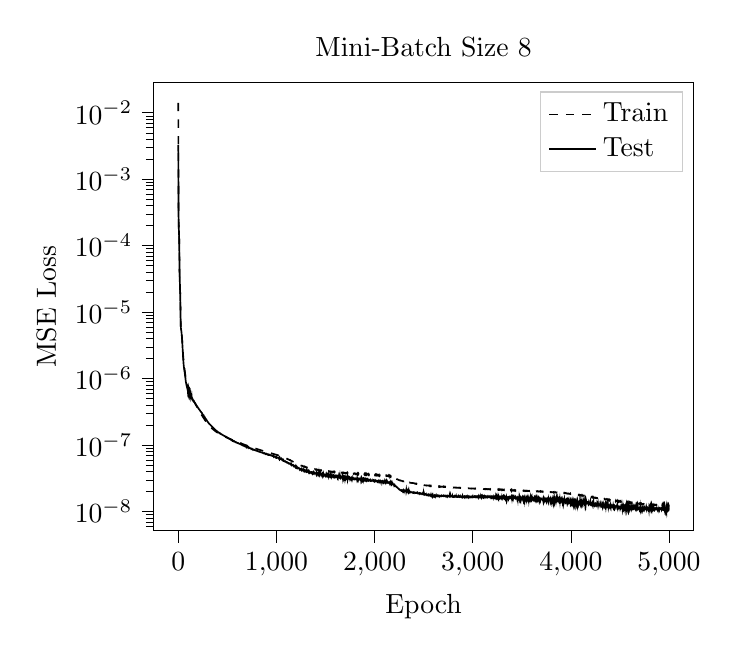
\begin{tikzpicture}

\begin{axis}[
legend cell align={left},
legend style={fill opacity=0.8, draw opacity=1, text opacity=1, draw=white!80!black},
log basis y={10},
tick align=outside,
tick pos=left,
title={Mini-Batch Size 8},
x grid style={white!69.0196078431373!black},
xlabel={Epoch},
xmin=-249.95, xmax=5248.95,
xtick style={color=black},
y grid style={white!69.0196078431373!black},
ylabel={MSE Loss},
ymin=5.12526233709927e-09, ymax=0.0285503119126669,
ymode=log,
ytick style={color=black}
]
\addplot [semithick, black, dashed]
table {%
0 0.0140922155501321
1 0.00164667243149597
2 0.00065037911516265
3 0.000295232196316647
4 0.000193644413906441
5 0.00017554680505782
6 0.000166322737537485
7 0.000155888844841684
8 0.000142262006907913
9 0.00012419570547172
10 0.000100196558816606
11 7.53355795714015e-05
12 5.41193190329068e-05
13 3.99818541809509e-05
14 3.23710513916922e-05
15 2.83831747833574e-05
16 2.58379168235479e-05
17 2.3768776641873e-05
18 2.16936214364978e-05
19 1.93698575890267e-05
20 1.67099984373635e-05
21 1.38117074528736e-05
22 1.10197760235451e-05
23 8.81342460627366e-06
24 7.32618501214688e-06
25 6.44809396973756e-06
26 5.96682320880859e-06
27 5.69452180099006e-06
28 5.51694411510084e-06
29 5.37627059711099e-06
30 5.25268244874155e-06
31 5.13194294012465e-06
32 5.00552247908104e-06
33 4.87103920659138e-06
34 4.72795897735523e-06
35 4.57529531857404e-06
36 4.41450717971747e-06
37 4.24678919441135e-06
38 4.07240037165479e-06
39 3.89275960455393e-06
40 3.70977897651414e-06
41 3.52646615996832e-06
42 3.3453291746639e-06
43 3.1669885086103e-06
44 2.99429524324069e-06
45 2.82882308749777e-06
46 2.67223944220518e-06
47 2.52574185277865e-06
48 2.39030650546113e-06
49 2.26648519112871e-06
50 2.15448263186602e-06
51 2.05455952405487e-06
52 1.96556939043546e-06
53 1.88664972873198e-06
54 1.81654708246981e-06
55 1.75456746703162e-06
56 1.69953624238417e-06
57 1.65011574182472e-06
58 1.60480939666741e-06
59 1.56276212375417e-06
60 1.52249059640042e-06
61 1.4837170463835e-06
62 1.44544674019187e-06
63 1.40767455231128e-06
64 1.37012475846632e-06
65 1.3339168483526e-06
66 1.29931519345661e-06
67 1.2659092755527e-06
68 1.23280311538565e-06
69 1.20021240133639e-06
70 1.16748595181093e-06
71 1.13551588817273e-06
72 1.10446207130366e-06
73 1.07352417389706e-06
74 1.04239164762987e-06
75 1.01698211097556e-06
76 9.92916835798496e-07
77 9.70485951363287e-07
78 9.49992109070763e-07
79 9.31409722205956e-07
80 9.14265601551279e-07
81 8.97762910810229e-07
82 8.82654424465557e-07
83 8.68559461117968e-07
84 8.55493358947967e-07
85 8.43273811710787e-07
86 8.31858977321076e-07
87 8.20936465963484e-07
88 8.10674030482517e-07
89 8.00620192784152e-07
90 7.91515300498702e-07
91 7.82651789464239e-07
92 7.7411152496154e-07
93 7.66956414445019e-07
94 7.5921274802937e-07
95 7.51383507328285e-07
96 7.44354396381652e-07
97 7.36274504674839e-07
98 7.30296529290797e-07
99 7.22306401783612e-07
100 7.16731141153559e-07
101 7.0944152068364e-07
102 7.04137545035621e-07
103 6.97249927974042e-07
104 6.922896165662e-07
105 6.85678604298801e-07
106 6.79918118848377e-07
107 6.74806719885623e-07
108 6.68366211726834e-07
109 6.63462581393048e-07
110 6.57123162881135e-07
111 6.52642981187057e-07
112 6.46561416587588e-07
113 6.42274032088608e-07
114 6.36438868973244e-07
115 6.32267128040098e-07
116 6.26555323151479e-07
117 6.21985995039154e-07
118 6.16880253367924e-07
119 6.11863263415557e-07
120 6.07826088987906e-07
121 6.02515582706076e-07
122 5.97315892207462e-07
123 5.93690181311501e-07
124 5.87228766487868e-07
125 5.84643050316913e-07
126 5.79739358123277e-07
127 5.74914281592953e-07
128 5.70551833760646e-07
129 5.66140960202688e-07
130 5.61847894573475e-07
131 5.57626214323648e-07
132 5.53413915262979e-07
133 5.49454119457948e-07
134 5.45167176518646e-07
135 5.41143863905802e-07
136 5.37298371497741e-07
137 5.32898270137139e-07
138 5.29843257034201e-07
139 5.25404720370659e-07
140 5.21684867152317e-07
141 5.18092104179857e-07
142 5.13483512598611e-07
143 5.08875732489145e-07
144 5.05149497538326e-07
145 5.01876758473685e-07
146 4.97770456185265e-07
147 4.94343421156174e-07
148 4.90650616956856e-07
149 4.8737844441149e-07
150 4.83746504770011e-07
151 4.80410617424099e-07
152 4.77105002900657e-07
153 4.73949040991073e-07
154 4.70770607652327e-07
155 4.67602424610192e-07
156 4.64573913710353e-07
157 4.61537018406233e-07
158 4.58560601526159e-07
159 4.55594075592813e-07
160 4.52629424799511e-07
161 4.49810896430591e-07
162 4.46874828853083e-07
163 4.44053090966179e-07
164 4.41227867604255e-07
165 4.38426361519362e-07
166 4.35670840431612e-07
167 4.33036380659502e-07
168 4.30322021191643e-07
169 4.27488975983437e-07
170 4.24709639364806e-07
171 4.21982422551537e-07
172 4.19321082635093e-07
173 4.16750839320912e-07
174 4.14194871584783e-07
175 4.1157767810418e-07
176 4.09005205327162e-07
177 4.06454590493155e-07
178 4.03974517769967e-07
179 4.01356386795726e-07
180 3.98910379288964e-07
181 3.96400903827754e-07
182 3.93962698311157e-07
183 3.91538277543901e-07
184 3.89058316706326e-07
185 3.86672758100559e-07
186 3.84376024534561e-07
187 3.82156077666451e-07
188 3.79795015795992e-07
189 3.77472126810829e-07
190 3.75254422486648e-07
191 3.72999132707719e-07
192 3.70814309334833e-07
193 3.68606052909115e-07
194 3.66414772166479e-07
195 3.64246124291867e-07
196 3.62064812147622e-07
197 3.60114379777343e-07
198 3.57652658479424e-07
199 3.55473573875997e-07
200 3.53420759978462e-07
201 3.51302201732295e-07
202 3.49260392450645e-07
203 3.47137964237021e-07
204 3.45095554795449e-07
205 3.43017129246448e-07
206 3.40932977728414e-07
207 3.38848146498094e-07
208 3.36741637614324e-07
209 3.34673315357747e-07
210 3.32618128226159e-07
211 3.30624918607469e-07
212 3.28681106719131e-07
213 3.2678425436572e-07
214 3.24867698765274e-07
215 3.23009222441328e-07
216 3.21105375114428e-07
217 3.19259059818222e-07
218 3.17433803207479e-07
219 3.15584080713194e-07
220 3.13753979209963e-07
221 3.11972391951798e-07
222 3.10204712469897e-07
223 3.08459960738361e-07
224 3.06718977086007e-07
225 3.04951894634087e-07
226 3.03379400019566e-07
227 3.01692094268446e-07
228 3.00041570543641e-07
229 2.98378097685514e-07
230 2.96704027594075e-07
231 2.95068247101682e-07
232 2.93436909618805e-07
233 2.91839041182129e-07
234 2.90256448501225e-07
235 2.88692379278643e-07
236 2.87134213266427e-07
237 2.85589026884026e-07
238 2.84047657121533e-07
239 2.82538714426295e-07
240 2.81039958053952e-07
241 2.79510103869285e-07
242 2.78032811682039e-07
243 2.76594212650139e-07
244 2.7475024603163e-07
245 2.72926708213106e-07
246 2.71423920384706e-07
247 2.7000172076086e-07
248 2.68524305077733e-07
249 2.67011570478815e-07
250 2.65667921034662e-07
251 2.64317999302932e-07
252 2.62892964080663e-07
253 2.6150448949025e-07
254 2.60125897110441e-07
255 2.58924373436997e-07
256 2.57517830519305e-07
257 2.56230467748253e-07
258 2.54854917034919e-07
259 2.53686509193329e-07
260 2.52175349391592e-07
261 2.51046833938062e-07
262 2.49770576434827e-07
263 2.48423187827029e-07
264 2.47144563388702e-07
265 2.45901549853045e-07
266 2.4462504500633e-07
267 2.43350985510205e-07
268 2.42261470663863e-07
269 2.41032267901176e-07
270 2.39729021991764e-07
271 2.38334006315455e-07
272 2.37114604335176e-07
273 2.35892772845858e-07
274 2.34670065896836e-07
275 2.3353716209229e-07
276 2.3238534521397e-07
277 2.31254778810808e-07
278 2.30117605983793e-07
279 2.29054269301088e-07
280 2.27954691752075e-07
281 2.26809562416719e-07
282 2.25817690040486e-07
283 2.24762463858497e-07
284 2.2381367495683e-07
285 2.22726548656738e-07
286 2.21723776196114e-07
287 2.20762035670674e-07
288 2.19673128100339e-07
289 2.18611050652129e-07
290 2.1762178107565e-07
291 2.16632967322994e-07
292 2.15608462355021e-07
293 2.14716398861725e-07
294 2.13740754045233e-07
295 2.12850587857361e-07
296 2.11970101840819e-07
297 2.11049697046661e-07
298 2.1004613132547e-07
299 2.09148392926295e-07
300 2.08267972048759e-07
301 2.0738952559185e-07
302 2.0650375899578e-07
303 2.0562344525743e-07
304 2.04789969075136e-07
305 2.03896006780724e-07
306 2.03049032204916e-07
307 2.02233469991597e-07
308 2.0148574800416e-07
309 2.00686525744231e-07
310 1.99914377798649e-07
311 1.99131872182789e-07
312 1.98344035812426e-07
313 1.97613068664282e-07
314 1.9680639949371e-07
315 1.96114129776603e-07
316 1.95406764222028e-07
317 1.94725376895022e-07
318 1.93973928373836e-07
319 1.93272308163017e-07
320 1.9257287543617e-07
321 1.91904341296123e-07
322 1.91237644701303e-07
323 1.90597502623291e-07
324 1.89894711086325e-07
325 1.8928915396188e-07
326 1.88604807627613e-07
327 1.8794622811491e-07
328 1.87344297193803e-07
329 1.86699944878299e-07
330 1.86075537186525e-07
331 1.85402446655658e-07
332 1.84775635814205e-07
333 1.84167428516346e-07
334 1.83570768633956e-07
335 1.82982711312007e-07
336 1.82418746863533e-07
337 1.81827815703528e-07
338 1.81145456025433e-07
339 1.80619840630669e-07
340 1.80006042857173e-07
341 1.79483078060372e-07
342 1.78932678077004e-07
343 1.7839446073431e-07
344 1.7783793585302e-07
345 1.77330097105965e-07
346 1.76734144670121e-07
347 1.76271198734312e-07
348 1.75766690267309e-07
349 1.75184670666795e-07
350 1.74708623170261e-07
351 1.74188886322924e-07
352 1.73653229948556e-07
353 1.73181383031462e-07
354 1.7267201918969e-07
355 1.72169975215297e-07
356 1.716809444261e-07
357 1.71193413185833e-07
358 1.7070678104858e-07
359 1.70231708297663e-07
360 1.69763145491331e-07
361 1.69323822717615e-07
362 1.68841542647513e-07
363 1.68392174817455e-07
364 1.67920915593811e-07
365 1.67448701848372e-07
366 1.67067471872784e-07
367 1.66522447294426e-07
368 1.66187803337436e-07
369 1.65655882883087e-07
370 1.65297342158866e-07
371 1.64844675270004e-07
372 1.64449132043387e-07
373 1.63934461077986e-07
374 1.63596360001961e-07
375 1.63166515610769e-07
376 1.62640494570709e-07
377 1.62330137088773e-07
378 1.61810680310737e-07
379 1.61525042159383e-07
380 1.61029843134486e-07
381 1.60723079604352e-07
382 1.60256959116367e-07
383 1.59806124516493e-07
384 1.59371342730807e-07
385 1.59003193211049e-07
386 1.58613461659129e-07
387 1.58135951810578e-07
388 1.5777919826121e-07
389 1.57490906419255e-07
390 1.57049220966599e-07
391 1.56678830967039e-07
392 1.56399091556736e-07
393 1.5595287873893e-07
394 1.55577467211288e-07
395 1.55218681813452e-07
396 1.54868281256881e-07
397 1.54552626023374e-07
398 1.54198211124168e-07
399 1.53841266364196e-07
400 1.53452866729964e-07
401 1.53133977093489e-07
402 1.52802964166199e-07
403 1.52480551506073e-07
404 1.52156185608376e-07
405 1.51788253479168e-07
406 1.51498513695003e-07
407 1.51127850402943e-07
408 1.50798184616718e-07
409 1.50510982436458e-07
410 1.50194480964316e-07
411 1.4992832301175e-07
412 1.49619644533416e-07
413 1.49345439441007e-07
414 1.49000281972178e-07
415 1.48698896465405e-07
416 1.48378767759638e-07
417 1.48073516024638e-07
418 1.47793847567357e-07
419 1.47497233387028e-07
420 1.47152927594263e-07
421 1.46810806187503e-07
422 1.46530012960611e-07
423 1.46194294019963e-07
424 1.45904546680953e-07
425 1.45637120098741e-07
426 1.45390437303661e-07
427 1.45085242406751e-07
428 1.44843584227061e-07
429 1.44539950433398e-07
430 1.44255259536763e-07
431 1.43986164975018e-07
432 1.43712213986902e-07
433 1.43442524212389e-07
434 1.43141190728002e-07
435 1.42893512014908e-07
436 1.42647763382797e-07
437 1.42393991835021e-07
438 1.42116199961961e-07
439 1.41860749801381e-07
440 1.41584198152245e-07
441 1.41324433158729e-07
442 1.41084530103086e-07
443 1.40788790234936e-07
444 1.40560038717652e-07
445 1.40289742095234e-07
446 1.40070903469791e-07
447 1.39810986377498e-07
448 1.3955653855291e-07
449 1.39309414347366e-07
450 1.39040228608778e-07
451 1.38806914293355e-07
452 1.38617263488072e-07
453 1.38398338824786e-07
454 1.38211991345116e-07
455 1.37910985833045e-07
456 1.37707504212159e-07
457 1.37452863837595e-07
458 1.37235590139895e-07
459 1.37014003817271e-07
460 1.36758330285147e-07
461 1.36494116027563e-07
462 1.36306082161752e-07
463 1.36068334931849e-07
464 1.35855103517102e-07
465 1.35629422052475e-07
466 1.35411948866349e-07
467 1.35155687953414e-07
468 1.34934801762299e-07
469 1.34734451673779e-07
470 1.34524718356843e-07
471 1.34328436132591e-07
472 1.34129347609147e-07
473 1.33910911843671e-07
474 1.3371256061312e-07
475 1.33461909047838e-07
476 1.33277299719126e-07
477 1.33085340515038e-07
478 1.32889105676881e-07
479 1.32672969037628e-07
480 1.32476193449804e-07
481 1.32274759009121e-07
482 1.32073942387123e-07
483 1.31855791474678e-07
484 1.31636651781619e-07
485 1.31416223496217e-07
486 1.31259498012071e-07
487 1.31016023310337e-07
488 1.30887004155866e-07
489 1.30695356258315e-07
490 1.30501306800923e-07
491 1.30296649251349e-07
492 1.30041917019597e-07
493 1.29918106384963e-07
494 1.29697845192567e-07
495 1.29461063567149e-07
496 1.29204722520981e-07
497 1.29046236825303e-07
498 1.28783909607577e-07
499 1.28579553615893e-07
500 1.28412652287579e-07
501 1.28222582777227e-07
502 1.28080913981421e-07
503 1.27826674720666e-07
504 1.2768455570189e-07
505 1.27511456184948e-07
506 1.27337297175956e-07
507 1.2712039346674e-07
508 1.26940336869552e-07
509 1.26781960378963e-07
510 1.26628617971747e-07
511 1.26438190140021e-07
512 1.26261214711931e-07
513 1.26080714901278e-07
514 1.25882205830763e-07
515 1.25689170451082e-07
516 1.25458669902656e-07
517 1.25292414027811e-07
518 1.25118541685509e-07
519 1.24933668057992e-07
520 1.24744541571076e-07
521 1.24592485745367e-07
522 1.2438628746736e-07
523 1.24239199989162e-07
524 1.24081532147713e-07
525 1.23898961273738e-07
526 1.23711435064067e-07
527 1.23683571343847e-07
528 1.23402232516057e-07
529 1.23180608545326e-07
530 1.22983389335474e-07
531 1.2279557410011e-07
532 1.22695858955524e-07
533 1.2242326393519e-07
534 1.22268119062241e-07
535 1.22114195065137e-07
536 1.2186837597028e-07
537 1.21758532072747e-07
538 1.21501212188235e-07
539 1.21415872920139e-07
540 1.21146897740232e-07
541 1.21149452825264e-07
542 1.20954131578088e-07
543 1.20601052417513e-07
544 1.2042635933085e-07
545 1.20382659668294e-07
546 1.20114501360291e-07
547 1.19902081415546e-07
548 1.19723047657061e-07
549 1.19519860986017e-07
550 1.19464099865851e-07
551 1.19455365275911e-07
552 1.18856987027627e-07
553 1.18855618111979e-07
554 1.18722306197583e-07
555 1.18556314758322e-07
556 1.18349971197418e-07
557 1.18197913097973e-07
558 1.18190822574249e-07
559 1.17993449931575e-07
560 1.17722103356144e-07
561 1.17562712910413e-07
562 1.1739236306596e-07
563 1.17146097792897e-07
564 1.17130330764326e-07
565 1.16876142195466e-07
566 1.16746778818566e-07
567 1.16807582864809e-07
568 1.16375001658398e-07
569 1.16238238121014e-07
570 1.16071960784225e-07
571 1.15917950825661e-07
572 1.15715357653201e-07
573 1.15682018952512e-07
574 1.15512718215527e-07
575 1.15298490829474e-07
576 1.15141919192041e-07
577 1.15017629779501e-07
578 1.14785245981963e-07
579 1.14825111019456e-07
580 1.14467956363384e-07
581 1.14309470399476e-07
582 1.14250206504352e-07
583 1.14062090345257e-07
584 1.14072716723257e-07
585 1.13818667545118e-07
586 1.13543024539808e-07
587 1.13510344416312e-07
588 1.13261899898021e-07
589 1.13188994674829e-07
590 1.12949545007623e-07
591 1.12861762920247e-07
592 1.12966328723374e-07
593 1.12624403906025e-07
594 1.12488853648784e-07
595 1.12194247433806e-07
596 1.12081747023041e-07
597 1.11879273879012e-07
598 1.11686604855166e-07
599 1.1151889847838e-07
600 1.11518363773655e-07
601 1.11229455521666e-07
602 1.11068491328581e-07
603 1.10914127503747e-07
604 1.10845691843053e-07
605 1.10635652848856e-07
606 1.10445679641913e-07
607 1.10333368983362e-07
608 1.10191389911307e-07
609 1.10141222277704e-07
610 1.09968580785491e-07
611 1.10079902308158e-07
612 1.09896487208161e-07
613 1.09495213120425e-07
614 1.09437622697328e-07
615 1.09409666039895e-07
616 1.09359268291698e-07
617 1.0894876301748e-07
618 1.08862762553841e-07
619 1.0888215664373e-07
620 1.08902593192184e-07
621 1.08681523236953e-07
622 1.08473326777769e-07
623 1.08357849692098e-07
624 1.08215046504156e-07
625 1.08083012595017e-07
626 1.07983994128702e-07
627 1.0788382092386e-07
628 1.07778989340446e-07
629 1.07629510504026e-07
630 1.07486674595592e-07
631 1.07359776917448e-07
632 1.07198026283228e-07
633 1.07110649613773e-07
634 1.06957342852709e-07
635 1.06551703673574e-07
636 1.06703632233973e-07
637 1.06261747919945e-07
638 1.06245268353788e-07
639 1.05981521867804e-07
640 1.0613362208467e-07
641 1.05918131012572e-07
642 1.05605284026922e-07
643 1.05518851803765e-07
644 1.05296745056549e-07
645 1.0529636806389e-07
646 1.05115613724394e-07
647 1.04897444288099e-07
648 1.04692954625563e-07
649 1.04653310055269e-07
650 1.04388389308596e-07
651 1.04356357626401e-07
652 1.04121267867185e-07
653 1.03941493522441e-07
654 1.03825485911813e-07
655 1.03654870686753e-07
656 1.03468656945438e-07
657 1.03318351046156e-07
658 1.03309234573246e-07
659 1.03166787249975e-07
660 1.02888646404509e-07
661 1.02764241914244e-07
662 1.02620244419427e-07
663 1.02643449945816e-07
664 1.02388692905464e-07
665 1.02254439710237e-07
666 1.02264427352949e-07
667 1.01974317667342e-07
668 1.01824479767032e-07
669 1.01781015130697e-07
670 1.01579884494996e-07
671 1.01662138689562e-07
672 1.01463956596604e-07
673 1.01146636220406e-07
674 1.01043345342333e-07
675 1.01026062447218e-07
676 1.00765059274366e-07
677 1.00705422818592e-07
678 1.00596716810841e-07
679 1.00494772908633e-07
680 1.00339713535291e-07
681 1.00227720652768e-07
682 1.00199328135986e-07
683 9.99779721606586e-08
684 9.99164768895611e-08
685 9.97651532674837e-08
686 9.96916367359546e-08
687 9.95852735758973e-08
688 9.94225873363064e-08
689 9.93057265326058e-08
690 9.91738692572852e-08
691 9.90683583950158e-08
692 9.89918791169941e-08
693 9.89294559996523e-08
694 9.87324563563874e-08
695 9.8580230650569e-08
696 9.84844026170606e-08
697 9.83782085786089e-08
698 9.82969909344433e-08
699 9.80663861103182e-08
700 9.79155029394718e-08
701 9.78743212769473e-08
702 9.7774189509181e-08
703 9.74998872109722e-08
704 9.7537862576047e-08
705 9.7373689259328e-08
706 9.72140168737923e-08
707 9.71121613257964e-08
708 9.69666632180122e-08
709 9.69298370527838e-08
710 9.67698093869984e-08
711 9.6669013320394e-08
712 9.6617836987889e-08
713 9.65235347489823e-08
714 9.643995225872e-08
715 9.6384693021534e-08
716 9.61863593840206e-08
717 9.60114623218544e-08
718 9.60902926934182e-08
719 9.57746484626654e-08
720 9.57750240715427e-08
721 9.55805155538059e-08
722 9.55347426128128e-08
723 9.54729408171318e-08
724 9.52798347118033e-08
725 9.52589754721345e-08
726 9.51665310111594e-08
727 9.49889552952499e-08
728 9.48892586905004e-08
729 9.48318259261782e-08
730 9.46984865208833e-08
731 9.46578152714039e-08
732 9.44619410319092e-08
733 9.44395689952415e-08
734 9.43228704386456e-08
735 9.42138219972577e-08
736 9.41150636339927e-08
737 9.40356634000494e-08
738 9.39251921092676e-08
739 9.37723432130611e-08
740 9.36953663508433e-08
741 9.36475301536177e-08
742 9.34891315171882e-08
743 9.34929558358277e-08
744 9.32899375643004e-08
745 9.31277580900058e-08
746 9.29872254360475e-08
747 9.29021212048298e-08
748 9.27547188318556e-08
749 9.26676536128212e-08
750 9.25360728327718e-08
751 9.24768817487376e-08
752 9.23224709517001e-08
753 9.2233401355557e-08
754 9.21099720416763e-08
755 9.20273056550513e-08
756 9.18983567661513e-08
757 9.17982077250912e-08
758 9.16838067226422e-08
759 9.1583944425544e-08
760 9.14591718057523e-08
761 9.13134026792051e-08
762 9.12507480110847e-08
763 9.11265217853341e-08
764 9.10621974288262e-08
765 9.08905435199614e-08
766 9.0788907545658e-08
767 9.0717570659038e-08
768 9.05781980975462e-08
769 9.05061573064359e-08
770 9.03604748181408e-08
771 9.02703232927848e-08
772 9.02022289084314e-08
773 9.01490784093184e-08
774 8.99447075433102e-08
775 8.98894601180089e-08
776 8.97487045516954e-08
777 8.9711841648743e-08
778 8.95438815806671e-08
779 8.95039619379645e-08
780 8.93075877943517e-08
781 8.92706220980699e-08
782 8.91444243862338e-08
783 8.90533289634732e-08
784 8.89315970269422e-08
785 8.88538352157298e-08
786 8.87460719418698e-08
787 8.86892839258024e-08
788 8.85925947713417e-08
789 8.84801011071801e-08
790 8.83455844515879e-08
791 8.83479853879265e-08
792 8.81836671791092e-08
793 8.8178019002072e-08
794 8.80678381420808e-08
795 8.79570468814705e-08
796 8.78213846133846e-08
797 8.77077261600689e-08
798 8.7557868305943e-08
799 8.75062553475914e-08
800 8.73836898467317e-08
801 8.73753748438233e-08
802 8.71596677542996e-08
803 8.71341073862553e-08
804 8.69886648713347e-08
805 8.69691683735851e-08
806 8.68006289946877e-08
807 8.67195310281232e-08
808 8.66247496071892e-08
809 8.66069136327141e-08
810 8.63993041644307e-08
811 8.63324029767298e-08
812 8.62302148672001e-08
813 8.61057656562636e-08
814 8.61300473475879e-08
815 8.58610517182612e-08
816 8.5876022253295e-08
817 8.58245899744148e-08
818 8.56204245254233e-08
819 8.56291569748535e-08
820 8.54643526437826e-08
821 8.53652859822418e-08
822 8.5391497251841e-08
823 8.51209773058414e-08
824 8.51588658763447e-08
825 8.50582824751811e-08
826 8.49786741063952e-08
827 8.48149538770215e-08
828 8.48154887371777e-08
829 8.46310325455235e-08
830 8.46116082833248e-08
831 8.44586885744292e-08
832 8.43162639991846e-08
833 8.43594839841089e-08
834 8.41931290338494e-08
835 8.40042691381271e-08
836 8.39640144789655e-08
837 8.39935478929021e-08
838 8.38417056181484e-08
839 8.3761031231866e-08
840 8.36453677903748e-08
841 8.35098131304335e-08
842 8.3516487031865e-08
843 8.3398541787183e-08
844 8.32627191780233e-08
845 8.32743370144939e-08
846 8.31479871719054e-08
847 8.30611524476055e-08
848 8.29425600832323e-08
849 8.28054075387996e-08
850 8.28294606325386e-08
851 8.27534693756959e-08
852 8.26178241633002e-08
853 8.25921608678115e-08
854 8.24915612467336e-08
855 8.23746438047834e-08
856 8.23552042801268e-08
857 8.22746717608069e-08
858 8.21175156664466e-08
859 8.20935714083149e-08
860 8.20074700209616e-08
861 8.18721728084171e-08
862 8.18467062071448e-08
863 8.17524560883243e-08
864 8.16378868124801e-08
865 8.16203907341162e-08
866 8.15071311217608e-08
867 8.14008423501988e-08
868 8.13587263230886e-08
869 8.12950596609241e-08
870 8.11408385228418e-08
871 8.11435524941118e-08
872 8.10090526517371e-08
873 8.09792461664571e-08
874 8.08584962870285e-08
875 8.07094791053231e-08
876 8.07686938379959e-08
877 8.06270915392204e-08
878 8.05262200671564e-08
879 8.04814699018053e-08
880 8.03900555492731e-08
881 8.03408116238913e-08
882 8.02471276806216e-08
883 8.01388805129477e-08
884 8.00124187625428e-08
885 8.00657544806072e-08
886 7.98942147488546e-08
887 7.99531881936488e-08
888 7.97822659910352e-08
889 7.97795756035668e-08
890 7.9595778335495e-08
891 7.94955623648619e-08
892 7.94511712500778e-08
893 7.94300374051815e-08
894 7.93113748613905e-08
895 7.92388654584642e-08
896 7.91362802941009e-08
897 7.90537630148691e-08
898 7.89241159324661e-08
899 7.89327640422499e-08
900 7.87739521186381e-08
901 7.87634696282069e-08
902 7.86302511679438e-08
903 7.85142067414313e-08
904 7.84941220688395e-08
905 7.836267482908e-08
906 7.83394425170059e-08
907 7.82585197347529e-08
908 7.82273210271356e-08
909 7.80942995328715e-08
910 7.80388083398975e-08
911 7.79501971406305e-08
912 7.78230592546336e-08
913 7.77868578483165e-08
914 7.76701064806318e-08
915 7.76812620495448e-08
916 7.75076760506366e-08
917 7.75319989765322e-08
918 7.74967118450931e-08
919 7.73487059220201e-08
920 7.73361544830209e-08
921 7.71912398640495e-08
922 7.71142926412338e-08
923 7.70105475949023e-08
924 7.69942951457381e-08
925 7.68621367575051e-08
926 7.66920159733786e-08
927 7.6753732895618e-08
928 7.66649599208691e-08
929 7.65232764639023e-08
930 7.64789896630091e-08
931 7.63227431415103e-08
932 7.62898755857222e-08
933 7.62348100540322e-08
934 7.61062690850522e-08
935 7.59985500060623e-08
936 7.60535598010037e-08
937 7.59387081998852e-08
938 7.58480387572646e-08
939 7.57766501973123e-08
940 7.56443777145677e-08
941 7.55885656298361e-08
942 7.55352047487889e-08
943 7.55366707450023e-08
944 7.54625999297431e-08
945 7.53840733613842e-08
946 7.52436891762187e-08
947 7.520958560292e-08
948 7.51185533998111e-08
949 7.50705502872151e-08
950 7.49230383103594e-08
951 7.48538313226632e-08
952 7.47696083367444e-08
953 7.4698309575183e-08
954 7.46352352933855e-08
955 7.45532024719608e-08
956 7.45396909715979e-08
957 7.43793192778952e-08
958 7.43306780917052e-08
959 7.42391270653897e-08
960 7.4170969384113e-08
961 7.41744250110088e-08
962 7.39807714547069e-08
963 7.3907636275905e-08
964 7.3864839967186e-08
965 7.38722046689233e-08
966 7.37782955395616e-08
967 7.35998169503205e-08
968 7.36751591370322e-08
969 7.35319244977717e-08
970 7.34493053959895e-08
971 7.33622083135543e-08
972 7.33287411573968e-08
973 7.32267693424049e-08
974 7.3227407262344e-08
975 7.30911046540328e-08
976 7.3059925388641e-08
977 7.29211026548882e-08
978 7.29121208236094e-08
979 7.2779587866556e-08
980 7.27771263386856e-08
981 7.26923735738794e-08
982 7.26410809015476e-08
983 7.25908489931371e-08
984 7.24250146495464e-08
985 7.2414066065285e-08
986 7.23511959135337e-08
987 7.23106430315923e-08
988 7.22220240687577e-08
989 7.21276343647048e-08
990 7.20563575073996e-08
991 7.19845479606462e-08
992 7.19308399528273e-08
993 7.18280783758019e-08
994 7.17602781392657e-08
995 7.16623081844503e-08
996 7.1633209976163e-08
997 7.1613316125152e-08
998 7.14358405220494e-08
999 7.13820533686516e-08
1000 7.13005416006496e-08
1001 7.13117426327514e-08
1002 7.11042069294621e-08
1003 7.11583764241297e-08
1004 7.11103543000746e-08
1005 7.09215685787967e-08
1006 7.08726079992061e-08
1007 7.08819332659871e-08
1008 7.06523474676146e-08
1009 7.06114099751076e-08
1010 7.05629681077013e-08
1011 7.04900955836862e-08
1012 7.03779293322881e-08
1013 7.03613790653535e-08
1014 7.02909734737744e-08
1015 7.02346028056411e-08
1016 7.00847629646617e-08
1017 7.00646524416371e-08
1018 7.00006208278481e-08
1019 6.99058087274551e-08
1020 6.97008041994351e-08
1021 6.96666002131252e-08
1022 6.95315661491946e-08
1023 6.93929467434629e-08
1024 6.93491352254938e-08
1025 6.92687724743735e-08
1026 6.9181248853134e-08
1027 6.90323947898364e-08
1028 6.89361719263815e-08
1029 6.88460079372177e-08
1030 6.88259702794625e-08
1031 6.87216120782708e-08
1032 6.85840478462652e-08
1033 6.85226009862205e-08
1034 6.83794042464214e-08
1035 6.83534466769942e-08
1036 6.82413636488022e-08
1037 6.81742337604874e-08
1038 6.8081035704104e-08
1039 6.80005548439055e-08
1040 6.79186499672468e-08
1041 6.78197289332161e-08
1042 6.77157139037376e-08
1043 6.77006809528535e-08
1044 6.75445062991997e-08
1045 6.74544157597268e-08
1046 6.73693972919054e-08
1047 6.72946742232838e-08
1048 6.71474435236519e-08
1049 6.70465003258514e-08
1050 6.70302539118595e-08
1051 6.69601158707067e-08
1052 6.68708544226959e-08
1053 6.67221369274884e-08
1054 6.66394672963477e-08
1055 6.65038577301047e-08
1056 6.64386373996351e-08
1057 6.6429855464456e-08
1058 6.63477771514209e-08
1059 6.62112182396868e-08
1060 6.61053233539377e-08
1061 6.60354965731358e-08
1062 6.58835158864335e-08
1063 6.58057612259455e-08
1064 6.57003935407019e-08
1065 6.56495188930961e-08
1066 6.55546697672094e-08
1067 6.54752256359359e-08
1068 6.53355711985881e-08
1069 6.52995786598609e-08
1070 6.52046299594034e-08
1071 6.50510368949142e-08
1072 6.50725278443787e-08
1073 6.49379873642886e-08
1074 6.47580108266155e-08
1075 6.46967440784962e-08
1076 6.47110855958033e-08
1077 6.46408487385841e-08
1078 6.45357608251018e-08
1079 6.44439404986485e-08
1080 6.4284627761424e-08
1081 6.42473115846087e-08
1082 6.42346976027497e-08
1083 6.4099857985056e-08
1084 6.39759074045898e-08
1085 6.39553085513e-08
1086 6.39084181939253e-08
1087 6.37432019150452e-08
1088 6.36723728701938e-08
1089 6.35793202752311e-08
1090 6.34713747382776e-08
1091 6.35341950525614e-08
1092 6.33713871458497e-08
1093 6.3277285804908e-08
1094 6.31845582761414e-08
1095 6.31149904926076e-08
1096 6.29787609565113e-08
1097 6.30093429236922e-08
1098 6.28861612330667e-08
1099 6.28055558475893e-08
1100 6.26232452294317e-08
1101 6.25952487345316e-08
1102 6.25822700701661e-08
1103 6.24765654775317e-08
1104 6.23883908117406e-08
1105 6.22942513581748e-08
1106 6.21327299015206e-08
1107 6.20863260349935e-08
1108 6.20415422387666e-08
1109 6.21000680087747e-08
1110 6.18504896578997e-08
1111 6.18067457205385e-08
1112 6.1644829599139e-08
1113 6.15710698008698e-08
1114 6.15897150124667e-08
1115 6.14760737152054e-08
1116 6.14502748659262e-08
1117 6.13122701871305e-08
1118 6.12455619730667e-08
1119 6.11872074065545e-08
1120 6.09162053128998e-08
1121 6.08576885987588e-08
1122 6.08179615930737e-08
1123 6.07086520618694e-08
1124 6.06223983101728e-08
1125 6.05575171297445e-08
1126 6.04104159798169e-08
1127 6.0348267340693e-08
1128 6.02285505344469e-08
1129 6.01458489990492e-08
1130 6.01179870587387e-08
1131 6.0027065746926e-08
1132 5.97797516208587e-08
1133 5.9795340693114e-08
1134 5.96402379002825e-08
1135 5.94761561911739e-08
1136 5.95539313339444e-08
1137 5.94249178975659e-08
1138 5.92505395076159e-08
1139 5.91597576615754e-08
1140 5.90666865125655e-08
1141 5.88915692842917e-08
1142 5.90203142101231e-08
1143 5.87497151824934e-08
1144 5.87532072353625e-08
1145 5.85907652910222e-08
1146 5.8551039190391e-08
1147 5.84408526567159e-08
1148 5.82552799874847e-08
1149 5.81301490427677e-08
1150 5.8109338837653e-08
1151 5.80481490803919e-08
1152 5.79101373157087e-08
1153 5.78085702569453e-08
1154 5.76846728073122e-08
1155 5.76280860729028e-08
1156 5.75032301490808e-08
1157 5.73179610068308e-08
1158 5.72661070288305e-08
1159 5.71943030065469e-08
1160 5.69885338492782e-08
1161 5.69631700626516e-08
1162 5.69194471786716e-08
1163 5.67838021701128e-08
1164 5.66640349766168e-08
1165 5.65589359924346e-08
1166 5.6512820266974e-08
1167 5.63850263919363e-08
1168 5.62500756329243e-08
1169 5.61824805593858e-08
1170 5.60970445784292e-08
1171 5.59599677218969e-08
1172 5.58494863724945e-08
1173 5.57552466800004e-08
1174 5.56996282252697e-08
1175 5.56156806448271e-08
1176 5.5491953369291e-08
1177 5.53300107037913e-08
1178 5.52866972709509e-08
1179 5.5107895852835e-08
1180 5.50283653844019e-08
1181 5.51412584899325e-08
1182 5.48718789001867e-08
1183 5.4910465046909e-08
1184 5.4751843118872e-08
1185 5.4634272609988e-08
1186 5.45681121217889e-08
1187 5.44585529360653e-08
1188 5.43135494264213e-08
1189 5.42500546694136e-08
1190 5.41413124164336e-08
1191 5.40952266248063e-08
1192 5.39357546243124e-08
1193 5.39131514880609e-08
1194 5.39165687554188e-08
1195 5.3634612921627e-08
1196 5.35923273101702e-08
1197 5.35096682368064e-08
1198 5.34264127121098e-08
1199 5.33043504136188e-08
1200 5.31984917513384e-08
1201 5.31392249949469e-08
1202 5.30054221310472e-08
1203 5.30110809604523e-08
1204 5.28841194253893e-08
1205 5.28213592305704e-08
1206 5.27674378001386e-08
1207 5.25633076429166e-08
1208 5.25129558854864e-08
1209 5.2446357926339e-08
1210 5.22644627349855e-08
1211 5.21429107900317e-08
1212 5.21280838032823e-08
1213 5.20980213041255e-08
1214 5.18598821455107e-08
1215 5.19323746939193e-08
1216 5.1801599847856e-08
1217 5.16898352844741e-08
1218 5.14871654297977e-08
1219 5.15548961050882e-08
1220 5.14475486421695e-08
1221 5.13119661880168e-08
1222 5.12700813648515e-08
1223 5.12630925495472e-08
1224 5.11038289716659e-08
1225 5.10397683979313e-08
1226 5.09275734623671e-08
1227 5.09132049710814e-08
1228 5.0759712610926e-08
1229 5.06871001304532e-08
1230 5.06944659219855e-08
1231 5.05630977118976e-08
1232 5.05891275865977e-08
1233 5.04078954683962e-08
1234 5.0369708529896e-08
1235 5.03202734072339e-08
1236 5.03486166767431e-08
1237 5.01460485304861e-08
1238 5.00217914414236e-08
1239 5.00083646550742e-08
1240 4.99302473584429e-08
1241 4.987592799921e-08
1242 4.97896254327834e-08
1243 4.97413813849157e-08
1244 4.96402420528952e-08
1245 4.9622389326931e-08
1246 4.95539652263233e-08
1247 4.94904343217861e-08
1248 4.94052279922386e-08
1249 4.92951875696868e-08
1250 4.93147989524267e-08
1251 4.91164378098041e-08
1252 4.91569000953262e-08
1253 4.91227655383675e-08
1254 4.90244803059703e-08
1255 4.89576740712039e-08
1256 4.8822162876494e-08
1257 4.87467866965297e-08
1258 4.87341117052509e-08
1259 4.87276126515113e-08
1260 4.87346524646881e-08
1261 4.85851170131113e-08
1262 4.84871747534754e-08
1263 4.85831895207234e-08
1264 4.82988585561728e-08
1265 4.83467545695504e-08
1266 4.83161799191834e-08
1267 4.81926020485801e-08
1268 4.81261100500063e-08
1269 4.80794487556224e-08
1270 4.79064465315204e-08
1271 4.78844559088643e-08
1272 4.80212023230564e-08
1273 4.79060066149728e-08
1274 4.7783847305638e-08
1275 4.76988225441843e-08
1276 4.77218500298804e-08
1277 4.76159679054788e-08
1278 4.76466013443755e-08
1279 4.74691612195599e-08
1280 4.75158579309465e-08
1281 4.73825057967225e-08
1282 4.7485986818252e-08
1283 4.72961260644666e-08
1284 4.73102585516472e-08
1285 4.72351163418594e-08
1286 4.72344711912598e-08
1287 4.71515645523724e-08
1288 4.71153546151015e-08
1289 4.68685075079023e-08
1290 4.70706135908827e-08
1291 4.68408979266144e-08
1292 4.68855339947893e-08
1293 4.69027191636329e-08
1294 4.68532288326884e-08
1295 4.66869751258869e-08
1296 4.67236158723239e-08
1297 4.66455751588768e-08
1298 4.6581428891912e-08
1299 4.66710647764046e-08
1300 4.65150191413244e-08
1301 4.6453202255492e-08
1302 4.64446993628798e-08
1303 4.63894488405003e-08
1304 4.62309609279288e-08
1305 4.62655005257773e-08
1306 4.63196391784493e-08
1307 4.61808473293246e-08
1308 4.61542245702162e-08
1309 4.62172598085786e-08
1310 4.61607299291344e-08
1311 4.60153494588056e-08
1312 4.59913277452983e-08
1313 4.59276329918268e-08
1314 4.58297194576573e-08
1315 4.59273223443191e-08
1316 4.58042492530453e-08
1317 4.57084866845037e-08
1318 4.56549604122003e-08
1319 4.56686972283293e-08
1320 4.56331827685119e-08
1321 4.56046227030882e-08
1322 4.5550667001848e-08
1323 4.55369211307399e-08
1324 4.5590441208887e-08
1325 4.54679211445708e-08
1326 4.54479248590545e-08
1327 4.52664653485257e-08
1328 4.5337347214236e-08
1329 4.53551621877324e-08
1330 4.51916858850154e-08
1331 4.51722750653971e-08
1332 4.51394618616874e-08
1333 4.51769472675778e-08
1334 4.51334482649557e-08
1335 4.51266249861249e-08
1336 4.50874914861288e-08
1337 4.49287061963233e-08
1338 4.48967479993456e-08
1339 4.48264219876648e-08
1340 4.4867042350738e-08
1341 4.48034820754728e-08
1342 4.48350610398052e-08
1343 4.48033875457554e-08
1344 4.45712150360933e-08
1345 4.46036571952746e-08
1346 4.46692990454523e-08
1347 4.45814032055125e-08
1348 4.45665362684977e-08
1349 4.45728043025895e-08
1350 4.45147311864957e-08
1351 4.44823261869232e-08
1352 4.43828213363417e-08
1353 4.42768181132536e-08
1354 4.43993598802095e-08
1355 4.44070804617169e-08
1356 4.42842968162438e-08
1357 4.41155342043587e-08
1358 4.41278631075903e-08
1359 4.40644807078172e-08
1360 4.42094289478945e-08
1361 4.40818237334994e-08
1362 4.39918047412391e-08
1363 4.41803186754797e-08
1364 4.40159865835454e-08
1365 4.39419652753514e-08
1366 4.39800256470946e-08
1367 4.38194544480908e-08
1368 4.38346918683052e-08
1369 4.38826430064765e-08
1370 4.38439412224767e-08
1371 4.38131168918332e-08
1372 4.37225367591054e-08
1373 4.36888630588328e-08
1374 4.37150416381371e-08
1375 4.36178424365608e-08
1376 4.36608899700985e-08
1377 4.35089207826422e-08
1378 4.35441604231812e-08
1379 4.35481492102596e-08
1380 4.34936193034474e-08
1381 4.33650798727925e-08
1382 4.34177889596654e-08
1383 4.34463673570917e-08
1384 4.33263139223428e-08
1385 4.33727313220444e-08
1386 4.33343354258042e-08
1387 4.3228653130889e-08
1388 4.31082869178923e-08
1389 4.324872136241e-08
1390 4.30600019534211e-08
1391 4.32475265323973e-08
1392 4.30882091100315e-08
1393 4.30473245973673e-08
1394 4.29888738828765e-08
1395 4.30272572833346e-08
1396 4.29292623698174e-08
1397 4.2927458932418e-08
1398 4.30014096650666e-08
1399 4.30005459408633e-08
1400 4.28852556577652e-08
1401 4.28427411769405e-08
1402 4.29186751995658e-08
1403 4.26496567271784e-08
1404 4.28333187523222e-08
1405 4.27500164761341e-08
1406 4.27967534255558e-08
1407 4.26256254471014e-08
1408 4.26668547057751e-08
1409 4.25627499347492e-08
1410 4.27053181430992e-08
1411 4.24960702827271e-08
1412 4.25527307035267e-08
1413 4.25026517083538e-08
1414 4.24830301199997e-08
1415 4.24793107010046e-08
1416 4.24730674390972e-08
1417 4.23903328332642e-08
1418 4.25100638867804e-08
1419 4.24156434370992e-08
1420 4.23989374351841e-08
1421 4.23957842898837e-08
1422 4.23277789733945e-08
1423 4.23183708635477e-08
1424 4.22206468280173e-08
1425 4.22159647799347e-08
1426 4.22320841448887e-08
1427 4.21671459114314e-08
1428 4.22204840990759e-08
1429 4.21945885649144e-08
1430 4.21728435395785e-08
1431 4.21243299655316e-08
1432 4.20114667738503e-08
1433 4.20510037324462e-08
1434 4.2026753572344e-08
1435 4.19436382799176e-08
1436 4.19389113277546e-08
1437 4.19057039202642e-08
1438 4.18952429424024e-08
1439 4.19827620414814e-08
1440 4.19652518064417e-08
1441 4.18845844243343e-08
1442 4.19072387116692e-08
1443 4.17922589410757e-08
1444 4.16854369809094e-08
1445 4.1889259613459e-08
1446 4.17623865209826e-08
1447 4.17697262604655e-08
1448 4.17888626045304e-08
1449 4.16201110771119e-08
1450 4.17640830239208e-08
1451 4.1783336582224e-08
1452 4.153928639683e-08
1453 4.16737873538686e-08
1454 4.1592476381247e-08
1455 4.15322517932637e-08
1456 4.1644548808506e-08
1457 4.15027544096169e-08
1458 4.148360849765e-08
1459 4.13861753427724e-08
1460 4.14018035996833e-08
1461 4.13481794314663e-08
1462 4.14854741146442e-08
1463 4.13563179764154e-08
1464 4.13556541101201e-08
1465 4.13902445641767e-08
1466 4.1323798298798e-08
1467 4.13480203884653e-08
1468 4.1203276207824e-08
1469 4.1235213055657e-08
1470 4.11417126029434e-08
1471 4.12246168219887e-08
1472 4.11880018207356e-08
1473 4.10834203830035e-08
1474 4.12011794010958e-08
1475 4.10904470413698e-08
1476 4.10302819586761e-08
1477 4.10799662917682e-08
1478 4.10220235567138e-08
1479 4.10007051749872e-08
1480 4.09940534513709e-08
1481 4.09689597491436e-08
1482 4.10433389328446e-08
1483 4.10684464080546e-08
1484 4.0948897821913e-08
1485 4.09499040134875e-08
1486 4.08794801574075e-08
1487 4.09105480914107e-08
1488 4.08452793374536e-08
1489 4.08942971645843e-08
1490 4.07402955646674e-08
1491 4.08870578434417e-08
1492 4.07994149629332e-08
1493 4.08190274594489e-08
1494 4.08339842810079e-08
1495 4.06289100567392e-08
1496 4.07976245524466e-08
1497 4.0624878185902e-08
1498 4.07296249225197e-08
1499 4.06837669739701e-08
1500 4.06156222441112e-08
1501 4.07313091956851e-08
1502 4.05451847482752e-08
1503 4.06221682425212e-08
1504 4.05266821212891e-08
1505 4.04707060539522e-08
1506 4.06462516782113e-08
1507 4.04694767723868e-08
1508 4.04878702155997e-08
1509 4.05097304012614e-08
1510 4.04145102264053e-08
1511 4.0458490955686e-08
1512 4.04152247091005e-08
1513 4.04283759909418e-08
1514 4.04303081200652e-08
1515 4.03291169508435e-08
1516 4.03538379005752e-08
1517 4.04357018073398e-08
1518 4.01908035403409e-08
1519 4.0378684301956e-08
1520 4.01831596095192e-08
1521 4.03242693085559e-08
1522 4.01736299417976e-08
1523 4.02171476885371e-08
1524 4.03139829083798e-08
1525 4.0050756290988e-08
1526 4.01579128519458e-08
1527 4.01703933876618e-08
1528 4.01928873969837e-08
1529 4.01609750353415e-08
1530 4.00341430619733e-08
1531 4.01794336895023e-08
1532 4.00297975486907e-08
1533 4.00986562185679e-08
1534 4.01208160880628e-08
1535 3.99242789086429e-08
1536 4.00895154815117e-08
1537 3.99392733978488e-08
1538 4.00255155073026e-08
1539 3.99330273790355e-08
1540 4.00368776256599e-08
1541 3.98720245327056e-08
1542 3.99692181636269e-08
1543 3.98561598462521e-08
1544 3.98875270821719e-08
1545 3.9898592707921e-08
1546 3.99073250436643e-08
1547 3.99202588603487e-08
1548 3.9863083950209e-08
1549 3.98795083480508e-08
1550 3.98830174299647e-08
1551 3.97511638707826e-08
1552 3.98775771195403e-08
1553 3.97159798799507e-08
1554 3.98367431264646e-08
1555 3.97162449825572e-08
1556 3.97871075605849e-08
1557 3.96644445856964e-08
1558 3.9699416047867e-08
1559 3.97870561856806e-08
1560 3.96381743366092e-08
1561 3.97042046440532e-08
1562 3.96156072683951e-08
1563 3.96154665756043e-08
1564 3.96605191550492e-08
1565 3.958909697932e-08
1566 3.96173939121169e-08
1567 3.949263310421e-08
1568 3.96089839078684e-08
1569 3.95455036246162e-08
1570 3.9636709490587e-08
1571 3.94831752732472e-08
1572 3.94724301058247e-08
1573 3.95125908312366e-08
1574 3.94526429312592e-08
1575 3.95341919947612e-08
1576 3.93538525056414e-08
1577 3.94563540533355e-08
1578 3.93826284383891e-08
1579 3.94670636287842e-08
1580 3.93370668776427e-08
1581 3.93753766632088e-08
1582 3.93889478891296e-08
1583 3.93959847713177e-08
1584 3.93097157589395e-08
1585 3.93532651656869e-08
1586 3.91723971162605e-08
1587 3.9439265921537e-08
1588 3.92176067336436e-08
1589 3.92966383158111e-08
1590 3.93851996420835e-08
1591 3.91521733389411e-08
1592 3.91947608742171e-08
1593 3.92991181339397e-08
1594 3.91132583290599e-08
1595 3.93028898422187e-08
1596 3.90764033886271e-08
1597 3.92399381112796e-08
1598 3.92021937143383e-08
1599 3.90802838641235e-08
1600 3.91499000782503e-08
1601 3.91313884398059e-08
1602 3.90865781119132e-08
1603 3.91318111354622e-08
1604 3.90454653018679e-08
1605 3.90933970058072e-08
1606 3.91323979753722e-08
1607 3.91136423418814e-08
1608 3.90225514497189e-08
1609 3.89170263863647e-08
1610 3.90865480301983e-08
1611 3.8980921593712e-08
1612 3.89813223291569e-08
1613 3.90147075677305e-08
1614 3.89207366335853e-08
1615 3.89198063510676e-08
1616 3.90334313173923e-08
1617 3.88514370586179e-08
1618 3.89586336879688e-08
1619 3.88994614555216e-08
1620 3.89837869310128e-08
1621 3.88157792121646e-08
1622 3.8903180284322e-08
1623 3.88374568531802e-08
1624 3.89662983231176e-08
1625 3.87433496351619e-08
1626 3.88509129178871e-08
1627 3.87580687961631e-08
1628 3.89098066246873e-08
1629 3.86810810075744e-08
1630 3.8847601955716e-08
1631 3.8731702770356e-08
1632 3.88384859340007e-08
1633 3.86796453755167e-08
1634 3.86607207518708e-08
1635 3.86814175348249e-08
1636 3.86742364932857e-08
1637 3.87164597510647e-08
1638 3.86513170154146e-08
1639 3.88603046239666e-08
1640 3.85722263551713e-08
1641 3.86626669151013e-08
1642 3.85764308683534e-08
1643 3.85580688213594e-08
1644 3.86169037662754e-08
1645 3.85148538581959e-08
1646 3.86165236889724e-08
1647 3.84727122453299e-08
1648 3.88424589639058e-08
1649 3.84465692357949e-08
1650 3.85114503771433e-08
1651 3.84911400512777e-08
1652 3.84304911449362e-08
1653 3.85630037955664e-08
1654 3.84011487293279e-08
1655 3.84661550612009e-08
1656 3.85328484400205e-08
1657 3.84369141146479e-08
1658 3.84122835210832e-08
1659 3.8412436121682e-08
1660 3.83894825235487e-08
1661 3.84446199950261e-08
1662 3.8335402538614e-08
1663 3.83735077038594e-08
1664 3.83685282532298e-08
1665 3.83480501557898e-08
1666 3.82956904871889e-08
1667 3.84011462086775e-08
1668 3.83502299774463e-08
1669 3.83458634498624e-08
1670 3.8245394529568e-08
1671 3.83146489473241e-08
1672 3.82573301918043e-08
1673 3.82244613819083e-08
1674 3.8246418380794e-08
1675 3.82150598499109e-08
1676 3.82407916803551e-08
1677 3.82599868506972e-08
1678 3.8215464568836e-08
1679 3.81728400284942e-08
1680 3.83210382013388e-08
1681 3.80955480121514e-08
1682 3.81806894989012e-08
1683 3.82224091151073e-08
1684 3.81114148124695e-08
1685 3.82258913358413e-08
1686 3.82052000684752e-08
1687 3.81070638280079e-08
1688 3.8081548687785e-08
1689 3.81398353761497e-08
1690 3.81179427018097e-08
1691 3.80720296826453e-08
1692 3.80211410555553e-08
1693 3.81585196489453e-08
1694 3.80863659596997e-08
1695 3.7976557523578e-08
1696 3.80630843066498e-08
1697 3.81245449689871e-08
1698 3.80392725380929e-08
1699 3.801984486973e-08
1700 3.79566180743751e-08
1701 3.79708953985869e-08
1702 3.80453341737308e-08
1703 3.79378156063481e-08
1704 3.79759017397063e-08
1705 3.79490948132499e-08
1706 3.80014099050641e-08
1707 3.78876995812405e-08
1708 3.79235057170746e-08
1709 3.79901633928981e-08
1710 3.79401265870882e-08
1711 3.78765139581461e-08
1712 3.78788724297863e-08
1713 3.79089320423631e-08
1714 3.79844686686504e-08
1715 3.79382417801111e-08
1716 3.79571741651041e-08
1717 3.79882111483099e-08
1718 3.78223503592068e-08
1719 3.7959839022772e-08
1720 3.76949858327258e-08
1721 3.80500853780497e-08
1722 3.77684928363209e-08
1723 3.79319000765044e-08
1724 3.78127555658025e-08
1725 3.76808580231369e-08
1726 3.78913456544616e-08
1727 3.76658090703863e-08
1728 3.7851494917529e-08
1729 3.77664108097697e-08
1730 3.79108147838814e-08
1731 3.76634401306752e-08
1732 3.78151026674267e-08
1733 3.78816969464069e-08
1734 3.77709782481972e-08
1735 3.77660620167752e-08
1736 3.76888900031069e-08
1737 3.77818670016516e-08
1738 3.78022734786043e-08
1739 3.77456426572387e-08
1740 3.76173546103864e-08
1741 3.76604630600852e-08
1742 3.77668573965373e-08
1743 3.77400727162858e-08
1744 3.77201424601736e-08
1745 3.77242986160375e-08
1746 3.75634211788878e-08
1747 3.74809592673664e-08
1748 3.7722135395768e-08
1749 3.76457967710131e-08
1750 3.76064268419185e-08
1751 3.76065779379431e-08
1752 3.74286121975764e-08
1753 3.77629903707266e-08
1754 3.76661396659372e-08
1755 3.74908666405105e-08
1756 3.76121619192205e-08
1757 3.75940156729371e-08
1758 3.76416019105541e-08
1759 3.74089387640275e-08
1760 3.75451150600448e-08
1761 3.74251382719848e-08
1762 3.73434886444812e-08
1763 3.76087765929789e-08
1764 3.75553967626452e-08
1765 3.73977909142731e-08
1766 3.74640324758424e-08
1767 3.73550987626814e-08
1768 3.74835799159534e-08
1769 3.73618815268095e-08
1770 3.75936487801987e-08
1771 3.72713335470287e-08
1772 3.75196970185954e-08
1773 3.72949849896109e-08
1774 3.7603680296705e-08
1775 3.72440201465984e-08
1776 3.75571327109192e-08
1777 3.72496371237041e-08
1778 3.74038666710597e-08
1779 3.74239376252916e-08
1780 3.74428224656498e-08
1781 3.7323855651028e-08
1782 3.74017605850874e-08
1783 3.72666274963684e-08
1784 3.73440678775872e-08
1785 3.73906923156753e-08
1786 3.73588830671068e-08
1787 3.71107454029129e-08
1788 3.72834189805715e-08
1789 3.73839526646158e-08
1790 3.74207804099136e-08
1791 3.72704231348386e-08
1792 3.72604873839499e-08
1793 3.72039002338731e-08
1794 3.72388135945201e-08
1795 3.73753077895778e-08
1796 3.72486858588594e-08
1797 3.72918126916311e-08
1798 3.72434037134717e-08
1799 3.72466739793076e-08
1800 3.72663990639843e-08
1801 3.71341596454577e-08
1802 3.7279309918592e-08
1803 3.72007997335722e-08
1804 3.72522711966639e-08
1805 3.71977966189263e-08
1806 3.71243192054393e-08
1807 3.71166673645007e-08
1808 3.69281813226152e-08
1809 3.7265723722868e-08
1810 3.72295604456063e-08
1811 3.7045100355293e-08
1812 3.71322109171679e-08
1813 3.71508310981206e-08
1814 3.71456299328443e-08
1815 3.71071213347562e-08
1816 3.71199989213089e-08
1817 3.70692861344502e-08
1818 3.71239575356341e-08
1819 3.70205668143164e-08
1820 3.70877458459873e-08
1821 3.69541319535926e-08
1822 3.70777116702747e-08
1823 3.67921550732397e-08
1824 3.7050849953868e-08
1825 3.70229679376166e-08
1826 3.69968310884872e-08
1827 3.71215581407291e-08
1828 3.67214813636885e-08
1829 3.70434229832739e-08
1830 3.67917332182444e-08
1831 3.71148817803757e-08
1832 3.69631161016848e-08
1833 3.67094972708593e-08
1834 3.69223256053708e-08
1835 3.67426318259589e-08
1836 3.70516558798606e-08
1837 3.67933732445813e-08
1838 3.69378140621102e-08
1839 3.68091435007933e-08
1840 3.68699657187221e-08
1841 3.67680227189027e-08
1842 3.67932825673378e-08
1843 3.66279344761189e-08
1844 3.70051625235845e-08
1845 3.66218960352604e-08
1846 3.71567434198639e-08
1847 3.67378085286418e-08
1848 3.67072405182967e-08
1849 3.68038352065447e-08
1850 3.67439507895639e-08
1851 3.66124083939212e-08
1852 3.67425429224077e-08
1853 3.67981550968288e-08
1854 3.66166572089988e-08
1855 3.68664959489173e-08
1856 3.65924359608805e-08
1857 3.66692661883938e-08
1858 3.66733336858438e-08
1859 3.67367757094783e-08
1860 3.65539251201419e-08
1861 3.67730002568401e-08
1862 3.65517606497612e-08
1863 3.67414380395559e-08
1864 3.65365003003326e-08
1865 3.66813095511453e-08
1866 3.65326868894122e-08
1867 3.68337799656615e-08
1868 3.66286341191291e-08
1869 3.65044348935584e-08
1870 3.66127535955663e-08
1871 3.65746113235588e-08
1872 3.65417026371162e-08
1873 3.67053717078569e-08
1874 3.6658561624936e-08
1875 3.65626657981011e-08
1876 3.65201574044072e-08
1877 3.67783549450884e-08
1878 3.66494288788211e-08
1879 3.66888207783411e-08
1880 3.65948743836775e-08
1881 3.65293158486324e-08
1882 3.6500014441998e-08
1883 3.64699401549373e-08
1884 3.64751547068387e-08
1885 3.65656375094225e-08
1886 3.65746387260835e-08
1887 3.66372703726192e-08
1888 3.64976410645035e-08
1889 3.65722141060232e-08
1890 3.64866452176038e-08
1891 3.65375467361595e-08
1892 3.65167638012309e-08
1893 3.63294874006215e-08
1894 3.63945058015069e-08
1895 3.6536670052989e-08
1896 3.6430282676303e-08
1897 3.62453244746597e-08
1898 3.66222929399918e-08
1899 3.64198722717646e-08
1900 3.63831767380418e-08
1901 3.63298386836242e-08
1902 3.61740805980837e-08
1903 3.64556771561553e-08
1904 3.63519154173986e-08
1905 3.62696372944171e-08
1906 3.61171992451226e-08
1907 3.64603584808165e-08
1908 3.61317012207429e-08
1909 3.62745675124287e-08
1910 3.64189258177383e-08
1911 3.6266710974342e-08
1912 3.62556905648681e-08
1913 3.6238342407291e-08
1914 3.62670215623417e-08
1915 3.60366312679439e-08
1916 3.63011385027256e-08
1917 3.61772445773845e-08
1918 3.61867287574924e-08
1919 3.61102679971026e-08
1920 3.63929243683003e-08
1921 3.60180869836135e-08
1922 3.61357699847353e-08
1923 3.61040660279421e-08
1924 3.6139368550181e-08
1925 3.60739116982423e-08
1926 3.6196284967982e-08
1927 3.59936592344567e-08
1928 3.60563996575358e-08
1929 3.60782758486167e-08
1930 3.60398286818331e-08
1931 3.60291056034079e-08
1932 3.60345146028784e-08
1933 3.59823884230615e-08
1934 3.60840954800601e-08
1935 3.59893449890514e-08
1936 3.59963851610523e-08
1937 3.62121882626632e-08
1938 3.59255595241414e-08
1939 3.60697188535042e-08
1940 3.59639030174108e-08
1941 3.61143853102597e-08
1942 3.58569910274831e-08
1943 3.6043464469504e-08
1944 3.58307471461927e-08
1945 3.60832720742721e-08
1946 3.58909315378853e-08
1947 3.59922691823833e-08
1948 3.588628298834e-08
1949 3.57991387196499e-08
1950 3.59611625162515e-08
1951 3.59351795946594e-08
1952 3.58898386458861e-08
1953 3.57527423555659e-08
1954 3.5908256137418e-08
1955 3.57621854756296e-08
1956 3.58349212685738e-08
1957 3.58016397492555e-08
1958 3.59061841495034e-08
1959 3.58764264776212e-08
1960 3.59239804565981e-08
1961 3.56813113904231e-08
1962 3.58514508875807e-08
1963 3.57986901380336e-08
1964 3.57795846923636e-08
1965 3.58297134064323e-08
1966 3.58044209156638e-08
1967 3.57522844649516e-08
1968 3.57979316274459e-08
1969 3.57875962246901e-08
1970 3.58005632263847e-08
1971 3.57308950551527e-08
1972 3.57868481506429e-08
1973 3.57633905760935e-08
1974 3.59752080516529e-08
1975 3.54793153327648e-08
1976 3.56424363725516e-08
1977 3.56962309773223e-08
1978 3.57075252499506e-08
1979 3.5845165480719e-08
1980 3.56351077415162e-08
1981 3.56275620205793e-08
1982 3.56691139065113e-08
1983 3.5589426081728e-08
1984 3.56025159495843e-08
1985 3.58654780168166e-08
1986 3.56388935309759e-08
1987 3.5567677426851e-08
1988 3.56262408662822e-08
1989 3.56126999379036e-08
1990 3.57467316645099e-08
1991 3.55701531344899e-08
1992 3.57601672029695e-08
1993 3.55033272736449e-08
1994 3.57265346040414e-08
1995 3.5396074536731e-08
1996 3.54844572565405e-08
1997 3.57656564653475e-08
1998 3.53924049982801e-08
1999 3.55584950182397e-08
2000 3.56697449870325e-08
2001 3.56787138220405e-08
2002 3.55943911167778e-08
2003 3.54479785218409e-08
2004 3.56183040364222e-08
2005 3.53309536897939e-08
2006 3.5582972430781e-08
2007 3.55872772117571e-08
2008 3.56063758508718e-08
2009 3.55415195936182e-08
2010 3.55386896822019e-08
2011 3.55435800902804e-08
2012 3.54341543582493e-08
2013 3.5326350536824e-08
2014 3.54429674618295e-08
2015 3.56998978769951e-08
2016 3.54859376350269e-08
2017 3.53400733024145e-08
2018 3.55125124622546e-08
2019 3.53422700452022e-08
2020 3.55198382075983e-08
2021 3.53294625350387e-08
2022 3.53245762756416e-08
2023 3.54871031174042e-08
2024 3.55245614671595e-08
2025 3.52888825934095e-08
2026 3.55585673830205e-08
2027 3.54134896176639e-08
2028 3.53721047030575e-08
2029 3.54860238958032e-08
2030 3.54437497889215e-08
2031 3.55012276966882e-08
2032 3.53924766249847e-08
2033 3.53858738901813e-08
2034 3.53863012767519e-08
2035 3.54097912538265e-08
2036 3.52552421158947e-08
2037 3.54500118371348e-08
2038 3.53148007081749e-08
2039 3.51771727915562e-08
2040 3.52485998993402e-08
2041 3.52664494878141e-08
2042 3.53212110244527e-08
2043 3.52696402448061e-08
2044 3.53278196350004e-08
2045 3.50798110102524e-08
2046 3.53038244638171e-08
2047 3.50380686655605e-08
2048 3.53732404003715e-08
2049 3.52515104800055e-08
2050 3.52898717146388e-08
2051 3.51912950766753e-08
2052 3.52262799583336e-08
2053 3.52031993360313e-08
2054 3.51986800883886e-08
2055 3.49191987663033e-08
2056 3.50503156130166e-08
2057 3.50460932994068e-08
2058 3.51862639345057e-08
2059 3.54123910732973e-08
2060 3.5012984096916e-08
2061 3.5237672851629e-08
2062 3.50989451058936e-08
2063 3.51451456923613e-08
2064 3.50956153982729e-08
2065 3.51490209666849e-08
2066 3.51532928246634e-08
2067 3.50932326336206e-08
2068 3.50858328599379e-08
2069 3.50466975369557e-08
2070 3.5128578741439e-08
2071 3.50624365870189e-08
2072 3.51087634351543e-08
2073 3.50725950184483e-08
2074 3.48720382215006e-08
2075 3.50937104562909e-08
2076 3.50986688211208e-08
2077 3.49998700812648e-08
2078 3.50636079833322e-08
2079 3.50096038435055e-08
2080 3.4841453009804e-08
2081 3.50405389926145e-08
2082 3.50292538255914e-08
2083 3.49853204753003e-08
2084 3.50112577467421e-08
2085 3.49354300377414e-08
2086 3.49946228852538e-08
2087 3.47063039427553e-08
2088 3.50340738730637e-08
2089 3.49463078346268e-08
2090 3.48853253449022e-08
2091 3.50643476894064e-08
2092 3.48874224593843e-08
2093 3.4948104152388e-08
2094 3.49539611530503e-08
2095 3.47071131532317e-08
2096 3.48301070332013e-08
2097 3.48174625681708e-08
2098 3.48316413565364e-08
2099 3.46571736122847e-08
2100 3.48714099800418e-08
2101 3.47187161162665e-08
2102 3.47542465775064e-08
2103 3.48218386880816e-08
2104 3.46967600517445e-08
2105 3.48042466460363e-08
2106 3.46572571419124e-08
2107 3.46827273878247e-08
2108 3.47622488425792e-08
2109 3.47469773482878e-08
2110 3.47767646564634e-08
2111 3.47355067442656e-08
2112 3.4546701973337e-08
2113 3.47556978592678e-08
2114 3.46318142816493e-08
2115 3.46471681780258e-08
2116 3.47924431811641e-08
2117 3.46481810264976e-08
2118 3.44733216182114e-08
2119 3.46518337575041e-08
2120 3.46098472623346e-08
2121 3.45996842279206e-08
2122 3.47283432957646e-08
2123 3.46137393982815e-08
2124 3.45159064116807e-08
2125 3.46012808627449e-08
2126 3.44771602875937e-08
2127 3.45803697943126e-08
2128 3.44515754568953e-08
2129 3.45153512402163e-08
2130 3.45798061651692e-08
2131 3.45268843418012e-08
2132 3.44025088856448e-08
2133 3.45208335361669e-08
2134 3.4445654149895e-08
2135 3.45518178868076e-08
2136 3.45473493346127e-08
2137 3.4456031099861e-08
2138 3.4364484506888e-08
2139 3.44972221721918e-08
2140 3.43248367657978e-08
2141 3.4492944448683e-08
2142 3.43385404715235e-08
2143 3.45781598660722e-08
2144 3.4290496093714e-08
2145 3.43060144554208e-08
2146 3.44058043646456e-08
2147 3.43255302404088e-08
2148 3.41100668381777e-08
2149 3.41952895204223e-08
2150 3.43601639203328e-08
2151 3.4153532772585e-08
2152 3.41090135576039e-08
2153 3.4155436126504e-08
2154 3.42936208577171e-08
2155 3.3856299904933e-08
2156 3.42150716563516e-08
2157 3.3988354551262e-08
2158 3.405076265528e-08
2159 3.38644607005278e-08
2160 3.41631483760096e-08
2161 3.39845888581713e-08
2162 3.38284178185155e-08
2163 3.38537514537052e-08
2164 3.40268143110833e-08
2165 3.39710133356874e-08
2166 3.3770219998619e-08
2167 3.40399171161465e-08
2168 3.39991786018068e-08
2169 3.38950475993194e-08
2170 3.36694171254592e-08
2171 3.35623848246591e-08
2172 3.358883385296e-08
2173 3.35593926847899e-08
2174 3.36249531995847e-08
2175 3.35927736521136e-08
2176 3.36960097553352e-08
2177 3.3357819268609e-08
2178 3.34103945465181e-08
2179 3.33792154614265e-08
2180 3.33711916660206e-08
2181 3.33325034604925e-08
2182 3.34902264049752e-08
2183 3.34050771559902e-08
2184 3.35643477549219e-08
2185 3.31968241833458e-08
2186 3.31900424805909e-08
2187 3.30820723366543e-08
2188 3.33634762741397e-08
2189 3.29869779860381e-08
2190 3.29270568819595e-08
2191 3.29535492369359e-08
2192 3.30423635066524e-08
2193 3.2968385207166e-08
2194 3.29141850103909e-08
2195 3.27679847420548e-08
2196 3.26790389784115e-08
2197 3.27125180756838e-08
2198 3.28457829645856e-08
2199 3.26832230150842e-08
2200 3.25508643124195e-08
2201 3.25069563849034e-08
2202 3.25951758823884e-08
2203 3.23611900134857e-08
2204 3.24298381007004e-08
2205 3.23351022797347e-08
2206 3.21446096176459e-08
2207 3.22599062272388e-08
2208 3.19862765207901e-08
2209 3.20416892187758e-08
2210 3.19288464889489e-08
2211 3.17090809489606e-08
2212 3.17792905293324e-08
2213 3.15104079864348e-08
2214 3.1462118692982e-08
2215 3.13828922715587e-08
2216 3.13321562357416e-08
2217 3.12738587888717e-08
2218 3.12520617335998e-08
2219 3.12137117948197e-08
2220 3.10057306038836e-08
2221 3.12358310861072e-08
2222 3.10054063796805e-08
2223 3.09421507194152e-08
2224 3.08758929641328e-08
2225 3.08620648987734e-08
2226 3.08012100713739e-08
2227 3.07649796962295e-08
2228 3.07027676993421e-08
2229 3.06398884948322e-08
2230 3.0567268998638e-08
2231 3.05280521204487e-08
2232 3.04718943495708e-08
2233 3.04078486101922e-08
2234 3.03745679617329e-08
2235 3.03228287630297e-08
2236 3.02672447705099e-08
2237 3.02545674801813e-08
2238 3.01988235289485e-08
2239 3.01402142439677e-08
2240 3.01196001135651e-08
2241 3.00748270705142e-08
2242 3.00020169574644e-08
2243 2.99772841376722e-08
2244 2.99949804882793e-08
2245 2.99182164966716e-08
2246 2.98174154473863e-08
2247 2.98337497213197e-08
2248 2.97877957007309e-08
2249 2.97282025942813e-08
2250 2.96885503319189e-08
2251 2.96915600075387e-08
2252 2.96268828261503e-08
2253 2.96020686509912e-08
2254 2.95862130044178e-08
2255 2.95726172665489e-08
2256 2.95009567898852e-08
2257 2.94234437800966e-08
2258 2.94252965509223e-08
2259 2.94418085973192e-08
2260 2.93423016528571e-08
2261 2.93364664556428e-08
2262 2.9278265921473e-08
2263 2.92813284907822e-08
2264 2.92852222609774e-08
2265 2.92450523597942e-08
2266 2.92166284019402e-08
2267 2.91476965621484e-08
2268 2.91206469871241e-08
2269 2.9084005692237e-08
2270 2.90973084280388e-08
2271 2.9066154888735e-08
2272 2.90592396314793e-08
2273 2.903219871353e-08
2274 2.8993103499797e-08
2275 2.90072672499697e-08
2276 2.89885272022339e-08
2277 2.89520249459052e-08
2278 2.89304525491474e-08
2279 2.8873197399637e-08
2280 2.88416605038755e-08
2281 2.87946236485759e-08
2282 2.87163995920103e-08
2283 2.8751229569135e-08
2284 2.86675678098369e-08
2285 2.87072197124871e-08
2286 2.86591628351207e-08
2287 2.86360354149195e-08
2288 2.86377652902736e-08
2289 2.86282400225879e-08
2290 2.86060725163129e-08
2291 2.85601986473871e-08
2292 2.8566027550081e-08
2293 2.85328380456029e-08
2294 2.84778560919463e-08
2295 2.8503181678019e-08
2296 2.84794163121216e-08
2297 2.84508193038047e-08
2298 2.84375073329457e-08
2299 2.84022412997409e-08
2300 2.84504239880246e-08
2301 2.83795681350618e-08
2302 2.80858092560621e-08
2303 2.81308356857579e-08
2304 2.84017445939533e-08
2305 2.83484147467483e-08
2306 2.82965770237453e-08
2307 2.81869080178687e-08
2308 2.82838599325874e-08
2309 2.82717122983556e-08
2310 2.82287362001199e-08
2311 2.81732639646481e-08
2312 2.82028487006425e-08
2313 2.81964688206848e-08
2314 2.82919290341965e-08
2315 2.81617670132572e-08
2316 2.80558309988521e-08
2317 2.80766361031581e-08
2318 2.80740395859347e-08
2319 2.80186498251567e-08
2320 2.78623242437881e-08
2321 2.78319890574252e-08
2322 2.7838097744759e-08
2323 2.81434602773523e-08
2324 2.79450416238447e-08
2325 2.78161572744295e-08
2326 2.79697963896375e-08
2327 2.79070327633413e-08
2328 2.78919659102428e-08
2329 2.78619289257875e-08
2330 2.78659629824318e-08
2331 2.78614516817655e-08
2332 2.77982614309558e-08
2333 2.75627960046876e-08
2334 2.7683113924315e-08
2335 2.76638133267504e-08
2336 2.7976017778375e-08
2337 2.77359681546407e-08
2338 2.75629913719655e-08
2339 2.77539640132218e-08
2340 2.77165115951661e-08
2341 2.76678804733699e-08
2342 2.76632074442951e-08
2343 2.76779803503047e-08
2344 2.7455451997227e-08
2345 2.74844656082962e-08
2346 2.74150879100432e-08
2347 2.73005283002448e-08
2348 2.73293975054933e-08
2349 2.73166359772148e-08
2350 2.73018226644162e-08
2351 2.72489444093083e-08
2352 2.73889708166664e-08
2353 2.72320520533498e-08
2354 2.72790375470677e-08
2355 2.72348291288083e-08
2356 2.73146983129635e-08
2357 2.73088766502561e-08
2358 2.72420718752109e-08
2359 2.71807621974318e-08
2360 2.71759283165807e-08
2361 2.71592088800787e-08
2362 2.716162148797e-08
2363 2.71283624564411e-08
2364 2.71220685803542e-08
2365 2.71014957067273e-08
2366 2.70860176589949e-08
2367 2.70522221228475e-08
2368 2.70808371154452e-08
2369 2.70027544879703e-08
2370 2.70345289230534e-08
2371 2.6964751616898e-08
2372 2.696691184223e-08
2373 2.69479568371089e-08
2374 2.69498847638161e-08
2375 2.69362674423235e-08
2376 2.69187825274741e-08
2377 2.68844778372745e-08
2378 2.68902544915406e-08
2379 2.68711434427971e-08
2380 2.68514626293737e-08
2381 2.68734419184291e-08
2382 2.68483514633822e-08
2383 2.68327053034589e-08
2384 2.68972461920924e-08
2385 2.68946966976991e-08
2386 2.68688440390186e-08
2387 2.68711721576054e-08
2388 2.68394169249397e-08
2389 2.68374860716847e-08
2390 2.68135587213614e-08
2391 2.6805691601961e-08
2392 2.67745706401534e-08
2393 2.6809520248694e-08
2394 2.67572526135851e-08
2395 2.6740364799771e-08
2396 2.67548818264629e-08
2397 2.67323597937796e-08
2398 2.67107425182544e-08
2399 2.66933362711441e-08
2400 2.66796495886901e-08
2401 2.66811331712802e-08
2402 2.66719013644057e-08
2403 2.66482157882386e-08
2404 2.66498887371291e-08
2405 2.65529375331752e-08
2406 2.64868419983522e-08
2407 2.64362802493423e-08
2408 2.63785517100601e-08
2409 2.64098169204807e-08
2410 2.62780924766837e-08
2411 2.62741602781169e-08
2412 2.6275515581986e-08
2413 2.63046898743013e-08
2414 2.62378383566464e-08
2415 2.62339208467743e-08
2416 2.6197952087248e-08
2417 2.61643609240636e-08
2418 2.61683168703009e-08
2419 2.61335110480765e-08
2420 2.61862989838768e-08
2421 2.6123462132599e-08
2422 2.61582386786863e-08
2423 2.60744872910834e-08
2424 2.61248545112558e-08
2425 2.60602128983045e-08
2426 2.5996013666596e-08
2427 2.59825018495974e-08
2428 2.61028798762553e-08
2429 2.59763141152725e-08
2430 2.59699663778257e-08
2431 2.5952968202958e-08
2432 2.58987610708417e-08
2433 2.58901513450205e-08
2434 2.59073284434308e-08
2435 2.58808899733509e-08
2436 2.58690743470957e-08
2437 2.59155831829894e-08
2438 2.58984107750493e-08
2439 2.58327015063564e-08
2440 2.58910232133758e-08
2441 2.5851744575256e-08
2442 2.58734603728605e-08
2443 2.58497839209504e-08
2444 2.57852705596306e-08
2445 2.5749621920923e-08
2446 2.56977506314371e-08
2447 2.57797519069847e-08
2448 2.56253563124531e-08
2449 2.568607414144e-08
2450 2.56544600301112e-08
2451 2.57075833505205e-08
2452 2.55754417626264e-08
2453 2.554663458465e-08
2454 2.55213013602429e-08
2455 2.55292079387459e-08
2456 2.55761564451618e-08
2457 2.56380117495958e-08
2458 2.5466044155209e-08
2459 2.55924793446383e-08
2460 2.5411626344507e-08
2461 2.5483353592648e-08
2462 2.54037278160091e-08
2463 2.53894689294931e-08
2464 2.5385459480276e-08
2465 2.54166745379258e-08
2466 2.53300338006746e-08
2467 2.52633231934141e-08
2468 2.52905496420652e-08
2469 2.52612174573841e-08
2470 2.52215043445858e-08
2471 2.52222532011182e-08
2472 2.51468582752601e-08
2473 2.51776597233189e-08
2474 2.51615491562163e-08
2475 2.51395283474842e-08
2476 2.52183839921649e-08
2477 2.51443643182192e-08
2478 2.51232011265756e-08
2479 2.51217024658246e-08
2480 2.50529616079298e-08
2481 2.51389312446726e-08
2482 2.50886437704878e-08
2483 2.50070869021179e-08
2484 2.50177555844999e-08
2485 2.49742417359755e-08
2486 2.49877498199602e-08
2487 2.49677537893511e-08
2488 2.50068211697929e-08
2489 2.49653871566835e-08
2490 2.4933863711496e-08
2491 2.49424296749901e-08
2492 2.4951844725507e-08
2493 2.4892882751093e-08
2494 2.4931655667082e-08
2495 2.48718469033626e-08
2496 2.49019510607518e-08
2497 2.48731343424069e-08
2498 2.48883164082336e-08
2499 2.49033845207691e-08
2500 2.49035872372794e-08
2501 2.48862970964048e-08
2502 2.48035862342455e-08
2503 2.48739398363007e-08
2504 2.47867319709272e-08
2505 2.48239095244074e-08
2506 2.48499960635584e-08
2507 2.48351267178037e-08
2508 2.48323786125049e-08
2509 2.47996488513813e-08
2510 2.48657050256895e-08
2511 2.48231005408606e-08
2512 2.47950744980407e-08
2513 2.47893814209199e-08
2514 2.47993815580827e-08
2515 2.47897829086519e-08
2516 2.47634090388971e-08
2517 2.47896581013762e-08
2518 2.47696634980699e-08
2519 2.47453253470198e-08
2520 2.47223928200313e-08
2521 2.47334208407501e-08
2522 2.47096111714029e-08
2523 2.4687650667321e-08
2524 2.46956074168025e-08
2525 2.46711931128907e-08
2526 2.46819320248726e-08
2527 2.46199760338683e-08
2528 2.45927725193162e-08
2529 2.46706242497119e-08
2530 2.46061201409908e-08
2531 2.46551861158295e-08
2532 2.4620513753959e-08
2533 2.46363766653879e-08
2534 2.4628943702254e-08
2535 2.46116972482113e-08
2536 2.46342331093885e-08
2537 2.46114901591987e-08
2538 2.46096278395669e-08
2539 2.45866363863811e-08
2540 2.45964233274165e-08
2541 2.45708998334315e-08
2542 2.45835269470085e-08
2543 2.45638348301824e-08
2544 2.45521365713763e-08
2545 2.45779312835204e-08
2546 2.45374288643241e-08
2547 2.45665522609073e-08
2548 2.45263032567777e-08
2549 2.45214198875132e-08
2550 2.45059835601857e-08
2551 2.45173493294004e-08
2552 2.44947074992119e-08
2553 2.45010167594373e-08
2554 2.45626643931018e-08
2555 2.44792750354605e-08
2556 2.44580011252715e-08
2557 2.45601274948548e-08
2558 2.44549451076104e-08
2559 2.44704517249339e-08
2560 2.44637011022064e-08
2561 2.44879491315686e-08
2562 2.4345519065605e-08
2563 2.44300616065729e-08
2564 2.43928618703926e-08
2565 2.43841448002158e-08
2566 2.43780653921277e-08
2567 2.43811462623533e-08
2568 2.43616524753243e-08
2569 2.43661697965081e-08
2570 2.43490519786782e-08
2571 2.43574382601253e-08
2572 2.43382521336599e-08
2573 2.43445802485809e-08
2574 2.44352526195257e-08
2575 2.42636506588845e-08
2576 2.4382859165506e-08
2577 2.43264350885397e-08
2578 2.43318004828907e-08
2579 2.4318235475107e-08
2580 2.43151912489026e-08
2581 2.43053389064052e-08
2582 2.42865047273e-08
2583 2.42982581002416e-08
2584 2.43043741323667e-08
2585 2.43125716861137e-08
2586 2.42699668686619e-08
2587 2.42551985039086e-08
2588 2.42744805540873e-08
2589 2.42553433427162e-08
2590 2.42339634275446e-08
2591 2.42310187354988e-08
2592 2.42103561043372e-08
2593 2.41927280453247e-08
2594 2.42068397344752e-08
2595 2.41830105895957e-08
2596 2.42476137515268e-08
2597 2.42324421826368e-08
2598 2.41915985257357e-08
2599 2.41748273044351e-08
2600 2.4186519977043e-08
2601 2.4179407354552e-08
2602 2.41663565696548e-08
2603 2.41800421174609e-08
2604 2.41570701149385e-08
2605 2.41318774478749e-08
2606 2.41287477287244e-08
2607 2.41291152303091e-08
2608 2.41133490512802e-08
2609 2.41305678247983e-08
2610 2.40912506952462e-08
2611 2.40801481559139e-08
2612 2.41406477159423e-08
2613 2.41297449727895e-08
2614 2.4095290498849e-08
2615 2.41204857425181e-08
2616 2.40823391250977e-08
2617 2.41169306987032e-08
2618 2.40800200885793e-08
2619 2.40420970376576e-08
2620 2.40115907583771e-08
2621 2.40670964557488e-08
2622 2.40035303660235e-08
2623 2.40694404207709e-08
2624 2.39871997282926e-08
2625 2.40326550962067e-08
2626 2.3954168761442e-08
2627 2.40268140512256e-08
2628 2.39998666065055e-08
2629 2.3985291254025e-08
2630 2.39567574289445e-08
2631 2.39846544216604e-08
2632 2.39369897876429e-08
2633 2.38818613977898e-08
2634 2.39493084817077e-08
2635 2.38887064112347e-08
2636 2.38993242347441e-08
2637 2.38915883681301e-08
2638 2.39090372167183e-08
2639 2.39165006532538e-08
2640 2.3909196885441e-08
2641 2.38644657239995e-08
2642 2.38849699494281e-08
2643 2.38983762548273e-08
2644 2.38486406014538e-08
2645 2.38773196845621e-08
2646 2.37812354573208e-08
2647 2.38795882485654e-08
2648 2.38290460594648e-08
2649 2.38504818601548e-08
2650 2.37533120950317e-08
2651 2.38623648134428e-08
2652 2.38244231485218e-08
2653 2.38374669074837e-08
2654 2.3715871300567e-08
2655 2.38580457896376e-08
2656 2.37788429551244e-08
2657 2.38263465703881e-08
2658 2.37195858003858e-08
2659 2.37419101249969e-08
2660 2.37934447815391e-08
2661 2.37060152064039e-08
2662 2.36939189370844e-08
2663 2.37918087830913e-08
2664 2.36732907157311e-08
2665 2.37708965618033e-08
2666 2.36870809127154e-08
2667 2.37533571190163e-08
2668 2.37491758019459e-08
2669 2.3639161234712e-08
2670 2.37320687501708e-08
2671 2.37475380013841e-08
2672 2.37412641430623e-08
2673 2.36923716476767e-08
2674 2.36276849037154e-08
2675 2.36815473018126e-08
2676 2.37157332745319e-08
2677 2.36273267089082e-08
2678 2.36026643971599e-08
2679 2.36067487993097e-08
2680 2.36209799626685e-08
2681 2.36060413589811e-08
2682 2.36104203490406e-08
2683 2.35962008585666e-08
2684 2.35850015508632e-08
2685 2.35924942075805e-08
2686 2.35782205866286e-08
2687 2.35772843812931e-08
2688 2.35597968245571e-08
2689 2.35777446437879e-08
2690 2.35565437538554e-08
2691 2.36214133733093e-08
2692 2.35524341407611e-08
2693 2.35394026484315e-08
2694 2.35335459319863e-08
2695 2.35269057853316e-08
2696 2.35304583857676e-08
2697 2.35221716367029e-08
2698 2.3512224325728e-08
2699 2.35274898261473e-08
2700 2.35030608459752e-08
2701 2.35141017910223e-08
2702 2.34844594322325e-08
2703 2.36064162817406e-08
2704 2.34715549627396e-08
2705 2.34835558088342e-08
2706 2.34769890599118e-08
2707 2.3475392880723e-08
2708 2.35423416667935e-08
2709 2.34751648244824e-08
2710 2.34421265172813e-08
2711 2.35501992356113e-08
2712 2.34397110476792e-08
2713 2.34394784577319e-08
2714 2.34332887245614e-08
2715 2.34243712990967e-08
2716 2.34388668758356e-08
2717 2.34305880923991e-08
2718 2.34182796852167e-08
2719 2.34181999414496e-08
2720 2.34149909239534e-08
2721 2.35061410664983e-08
2722 2.33975469403624e-08
2723 2.33830739988505e-08
2724 2.34114976724875e-08
2725 2.34548312159077e-08
2726 2.34424559604207e-08
2727 2.33738831645347e-08
2728 2.3432231981424e-08
2729 2.33567075063057e-08
2730 2.34046533869048e-08
2731 2.33488871375087e-08
2732 2.3352429380008e-08
2733 2.33481457661e-08
2734 2.33407855181333e-08
2735 2.33648137433207e-08
2736 2.33318322822029e-08
2737 2.33070653319345e-08
2738 2.3346116288625e-08
2739 2.33266172862123e-08
2740 2.33008381118616e-08
2741 2.33355860723705e-08
2742 2.32842534395594e-08
2743 2.33014976913637e-08
2744 2.32890997100554e-08
2745 2.32929399976989e-08
2746 2.3302574435391e-08
2747 2.33146102432968e-08
2748 2.32785370557487e-08
2749 2.32942535798308e-08
2750 2.32616284869813e-08
2751 2.32929211234634e-08
2752 2.32491365919074e-08
2753 2.32627183809342e-08
2754 2.32306790786119e-08
2755 2.3276313755094e-08
2756 2.32429791906519e-08
2757 2.32749975759283e-08
2758 2.32213192310482e-08
2759 2.32215358355603e-08
2760 2.32546402201272e-08
2761 2.32203828449684e-08
2762 2.33159703797448e-08
2763 2.31969889625816e-08
2764 2.314681362936e-08
2765 2.31738245357604e-08
2766 2.3170235046166e-08
2767 2.31266902575022e-08
2768 2.3123720971796e-08
2769 2.31477672127944e-08
2770 2.30991476701803e-08
2771 2.31053931303293e-08
2772 2.31188731598664e-08
2773 2.3145674900249e-08
2774 2.30820694473444e-08
2775 2.31041685183619e-08
2776 2.30864719110713e-08
2777 2.30861167858087e-08
2778 2.30348852974238e-08
2779 2.30820793194475e-08
2780 2.30819818543004e-08
2781 2.30532784768478e-08
2782 2.30654754611592e-08
2783 2.30319875065277e-08
2784 2.30562718042115e-08
2785 2.3061908677402e-08
2786 2.3006683151916e-08
2787 2.30508197067714e-08
2788 2.30231742781584e-08
2789 2.30193855776939e-08
2790 2.30073178633106e-08
2791 2.29989750257786e-08
2792 2.30151464095663e-08
2793 2.30415139754747e-08
2794 2.2970916178533e-08
2795 2.3006379019197e-08
2796 2.30143007993178e-08
2797 2.29839285088573e-08
2798 2.29939372036192e-08
2799 2.29693911610873e-08
2800 2.30020177247603e-08
2801 2.29397145639076e-08
2802 2.29599945593684e-08
2803 2.29954475106098e-08
2804 2.29464646674948e-08
2805 2.29727204277275e-08
2806 2.2946284010672e-08
2807 2.29688330946054e-08
2808 2.28977551794962e-08
2809 2.29595473451027e-08
2810 2.29503427240374e-08
2811 2.29251608412362e-08
2812 2.29668454219123e-08
2813 2.29262388535822e-08
2814 2.29372032620745e-08
2815 2.29429834188721e-08
2816 2.29121144466049e-08
2817 2.29283576671513e-08
2818 2.29099798922938e-08
2819 2.29299884892953e-08
2820 2.28775421917682e-08
2821 2.28866969096408e-08
2822 2.29147223489434e-08
2823 2.29009073966502e-08
2824 2.28908831978458e-08
2825 2.29076539066675e-08
2826 2.28706648472965e-08
2827 2.29095146546676e-08
2828 2.28287743642142e-08
2829 2.28744850696572e-08
2830 2.28264675494749e-08
2831 2.28482780260109e-08
2832 2.28631989376282e-08
2833 2.28285269741058e-08
2834 2.28815637091095e-08
2835 2.28192816194017e-08
2836 2.28238579511597e-08
2837 2.28280531362479e-08
2838 2.28150668024618e-08
2839 2.28126944015195e-08
2840 2.28211046033877e-08
2841 2.27821876359613e-08
2842 2.28276182587805e-08
2843 2.27965611223624e-08
2844 2.27861874484425e-08
2845 2.27895648836629e-08
2846 2.28024336195176e-08
2847 2.27751800885301e-08
2848 2.27899082791971e-08
2849 2.27718561216506e-08
2850 2.27767926768152e-08
2851 2.27349871697591e-08
2852 2.27359381210768e-08
2853 2.27825065404197e-08
2854 2.27540307560226e-08
2855 2.27609142315899e-08
2856 2.27369288285928e-08
2857 2.27386377598116e-08
2858 2.27283334819361e-08
2859 2.27572066249238e-08
2860 2.27120586546725e-08
2861 2.27790808859929e-08
2862 2.26962135125852e-08
2863 2.27254233706731e-08
2864 2.27075532377441e-08
2865 2.27113100152998e-08
2866 2.27105394650096e-08
2867 2.26963902347777e-08
2868 2.27075190419868e-08
2869 2.26801028460066e-08
2870 2.26805808400954e-08
2871 2.27163207671133e-08
2872 2.26599603716515e-08
2873 2.27128980405666e-08
2874 2.26495166697482e-08
2875 2.26838920949213e-08
2876 2.2633144937334e-08
2877 2.27002717037017e-08
2878 2.26501465849793e-08
2879 2.26438821955277e-08
2880 2.26743442386379e-08
2881 2.26622551937616e-08
2882 2.26392203792614e-08
2883 2.26614374052581e-08
2884 2.26081309948611e-08
2885 2.26377313041759e-08
2886 2.26622117187603e-08
2887 2.26091042265786e-08
2888 2.26329164516592e-08
2889 2.26028324581407e-08
2890 2.26154009084212e-08
2891 2.26111500527537e-08
2892 2.25871219257101e-08
2893 2.25940610474318e-08
2894 2.26068414987957e-08
2895 2.25933509092613e-08
2896 2.26463827064372e-08
2897 2.25531392392675e-08
2898 2.2575582794282e-08
2899 2.25953645252019e-08
2900 2.25612005455567e-08
2901 2.25841375893765e-08
2902 2.26227083439667e-08
2903 2.25383530056966e-08
2904 2.25521555567987e-08
2905 2.25481722559984e-08
2906 2.25636249209238e-08
2907 2.25257892529918e-08
2908 2.25722115554383e-08
2909 2.24744241084096e-08
2910 2.25321640257015e-08
2911 2.26051607103983e-08
2912 2.24659051037968e-08
2913 2.25132282407614e-08
2914 2.25238143851669e-08
2915 2.24942209117174e-08
2916 2.2489711597462e-08
2917 2.25633682031656e-08
2918 2.24660171594948e-08
2919 2.24490727580573e-08
2920 2.24820107517232e-08
2921 2.25042746353488e-08
2922 2.24400970441074e-08
2923 2.25074355393318e-08
2924 2.24257760801372e-08
2925 2.24687806360535e-08
2926 2.24606469632072e-08
2927 2.24621305324746e-08
2928 2.24441385925367e-08
2929 2.24451444834628e-08
2930 2.25064913146333e-08
2931 2.24001227961956e-08
2932 2.24331048723769e-08
2933 2.24461386779673e-08
2934 2.24210934156588e-08
2935 2.2414025148354e-08
2936 2.24331432985281e-08
2937 2.23916673203206e-08
2938 2.24072612478032e-08
2939 2.24330685445473e-08
2940 2.23980179203664e-08
2941 2.23874248690414e-08
2942 2.24090919109798e-08
2943 2.24122577434649e-08
2944 2.23516667210433e-08
2945 2.23846981870501e-08
2946 2.23750139611845e-08
2947 2.23675531274559e-08
2948 2.23690972482871e-08
2949 2.23966252086427e-08
2950 2.23590922039385e-08
2951 2.23575589957115e-08
2952 2.23446854898945e-08
2953 2.23787074973281e-08
2954 2.23484926151762e-08
2955 2.23410897159937e-08
2956 2.23185536469828e-08
2957 2.23394644485175e-08
2958 2.23433849302346e-08
2959 2.23287105440839e-08
2960 2.23443335674034e-08
2961 2.23401842065485e-08
2962 2.22854145679463e-08
2963 2.23340432303765e-08
2964 2.23200163498305e-08
2965 2.23124990528234e-08
2966 2.23158065382201e-08
2967 2.2295199315181e-08
2968 2.23108840757824e-08
2969 2.22952372217478e-08
2970 2.2297369233204e-08
2971 2.23066160116581e-08
2972 2.22738460897709e-08
2973 2.22975133237213e-08
2974 2.22771114106735e-08
2975 2.22468722848035e-08
2976 2.22956516267025e-08
2977 2.22850922777518e-08
2978 2.22585025828614e-08
2979 2.22740814486144e-08
2980 2.22606010553683e-08
2981 2.22279482837706e-08
2982 2.2239388069778e-08
2983 2.22621345362661e-08
2984 2.22273305126031e-08
2985 2.22571749564082e-08
2986 2.22320354779093e-08
2987 2.21837540239633e-08
2988 2.22493222183928e-08
2989 2.22160562559637e-08
2990 2.22250939407864e-08
2991 2.22165201968494e-08
2992 2.2228362487553e-08
2993 2.21891013674203e-08
2994 2.21847167445333e-08
2995 2.21994414095761e-08
2996 2.22162727019359e-08
2997 2.21921287617555e-08
2998 2.21996001563696e-08
2999 2.22098814934846e-08
3000 2.21687695001194e-08
3001 2.21704665168687e-08
3002 2.21909749278382e-08
3003 2.21792000441035e-08
3004 2.21533350694969e-08
3005 2.21854726114579e-08
3006 2.21406713594163e-08
3007 2.21303854832655e-08
3008 2.21595867402335e-08
3009 2.21411071437139e-08
3010 2.21570214553601e-08
3011 2.21308956120936e-08
3012 2.2145175264221e-08
3013 2.20978097704716e-08
3014 2.21337124810539e-08
3015 2.213698945841e-08
3016 2.21160757813976e-08
3017 2.21377153253322e-08
3018 2.21067992236534e-08
3019 2.20749179997703e-08
3020 2.21201113475011e-08
3021 2.21214007685155e-08
3022 2.20958036827312e-08
3023 2.2100835159744e-08
3024 2.2089924967883e-08
3025 2.20724450814558e-08
3026 2.21520109171536e-08
3027 2.20784932372098e-08
3028 2.20787505909037e-08
3029 2.210819119286e-08
3030 2.205058977367e-08
3031 2.20721831047932e-08
3032 2.21007145100316e-08
3033 2.20594649165129e-08
3034 2.20779247355196e-08
3035 2.2065045580888e-08
3036 2.20671636110836e-08
3037 2.20351267556929e-08
3038 2.20663921060016e-08
3039 2.20749036450307e-08
3040 2.2036442459239e-08
3041 2.20661018555113e-08
3042 2.20112964162134e-08
3043 2.20287236962768e-08
3044 2.2036696433414e-08
3045 2.2033487441675e-08
3046 2.20482124375643e-08
3047 2.19986733447364e-08
3048 2.20261848933312e-08
3049 2.20180432979333e-08
3050 2.19916903834161e-08
3051 2.20354305335846e-08
3052 2.19936760732509e-08
3053 2.2012358825485e-08
3054 2.19823301530475e-08
3055 2.19895461279762e-08
3056 2.20009061440152e-08
3057 2.1990407818695e-08
3058 2.19933704497244e-08
3059 2.19855577583417e-08
3060 2.19631290372391e-08
3061 2.19632550515492e-08
3062 2.19995851642452e-08
3063 2.19225890072394e-08
3064 2.19883454324332e-08
3065 2.19422637068867e-08
3066 2.19546776714097e-08
3067 2.19750038099598e-08
3068 2.1963026813232e-08
3069 2.19410699955347e-08
3070 2.19848328590899e-08
3071 2.19490459274496e-08
3072 2.19564844661235e-08
3073 2.18946246381968e-08
3074 2.19621685024762e-08
3075 2.19197135522542e-08
3076 2.19659115079374e-08
3077 2.19565917758402e-08
3078 2.19178880258575e-08
3079 2.18915289300625e-08
3080 2.1928348689304e-08
3081 2.1930553886218e-08
3082 2.19125431870637e-08
3083 2.18721921578791e-08
3084 2.18938633156363e-08
3085 2.19392245131012e-08
3086 2.18755562690909e-08
3087 2.18965646321401e-08
3088 2.18930631565861e-08
3089 2.19043130695873e-08
3090 2.1827368372751e-08
3091 2.19189626342597e-08
3092 2.18870753552203e-08
3093 2.18487186969263e-08
3094 2.1907880333405e-08
3095 2.18638142679417e-08
3096 2.18362129582594e-08
3097 2.18813988852595e-08
3098 2.18046438562602e-08
3099 2.18679803349886e-08
3100 2.18485226421983e-08
3101 2.18373796214699e-08
3102 2.18420358018001e-08
3103 2.18338422790509e-08
3104 2.182555513075e-08
3105 2.18232174042932e-08
3106 2.18269937160009e-08
3107 2.18810129353209e-08
3108 2.18176193689246e-08
3109 2.18121707757923e-08
3110 2.18176314947804e-08
3111 2.18521586723419e-08
3112 2.1822844110897e-08
3113 2.18226264543375e-08
3114 2.18146837682731e-08
3115 2.18266402898237e-08
3116 2.1797249545763e-08
3117 2.18337363104837e-08
3118 2.17943581559688e-08
3119 2.17801985038513e-08
3120 2.18150160078423e-08
3121 2.17451462840579e-08
3122 2.17997612432796e-08
3123 2.18112886614108e-08
3124 2.1781716691649e-08
3125 2.17831019662107e-08
3126 2.18203982123022e-08
3127 2.17311511483409e-08
3128 2.17963758100126e-08
3129 2.17604646408631e-08
3130 2.17680344984927e-08
3131 2.1771633042178e-08
3132 2.17222026774877e-08
3133 2.17787614333886e-08
3134 2.17612338828665e-08
3135 2.17384585425862e-08
3136 2.17687563277558e-08
3137 2.17257975196894e-08
3138 2.17392041044206e-08
3139 2.17420430881354e-08
3140 2.1727512941716e-08
3141 2.17326930904704e-08
3142 2.16855810033501e-08
3143 2.17356646525779e-08
3144 2.17583970401058e-08
3145 2.17018689556703e-08
3146 2.17293022601872e-08
3147 2.16785215441107e-08
3148 2.16881248085166e-08
3149 2.17184150912431e-08
3150 2.16626902629358e-08
3151 2.17215274846971e-08
3152 2.16902152536669e-08
3153 2.17020599158069e-08
3154 2.16771852601383e-08
3155 2.16862417885544e-08
3156 2.16977439424504e-08
3157 2.16527767911145e-08
3158 2.17032874689771e-08
3159 2.16466983880004e-08
3160 2.1656359545652e-08
3161 2.16904747447622e-08
3162 2.1650364535386e-08
3163 2.16550410483407e-08
3164 2.16512570880845e-08
3165 2.16322670891778e-08
3166 2.16247854747387e-08
3167 2.1653922899656e-08
3168 2.16527886065521e-08
3169 2.16168469227007e-08
3170 2.16333068907559e-08
3171 2.16363271952069e-08
3172 2.16265557799744e-08
3173 2.16125990699645e-08
3174 2.16807606303604e-08
3175 2.15695254204284e-08
3176 2.16161103168133e-08
3177 2.15907795411141e-08
3178 2.16195452593659e-08
3179 2.15418148714619e-08
3180 2.16571494613405e-08
3181 2.15841697666086e-08
3182 2.16082622572777e-08
3183 2.15719454699226e-08
3184 2.15863817372153e-08
3185 2.15548015503053e-08
3186 2.16029170014842e-08
3187 2.16010583233839e-08
3188 2.15397611591506e-08
3189 2.15976560427045e-08
3190 2.15834718968466e-08
3191 2.15778589369719e-08
3192 2.15669044276723e-08
3193 2.15485774703872e-08
3194 2.15636065985514e-08
3195 2.15482165630831e-08
3196 2.15464711939006e-08
3197 2.1536500831143e-08
3198 2.15400105458841e-08
3199 2.15707673403287e-08
3200 2.15383237551769e-08
3201 2.15658678439645e-08
3202 2.15369579068536e-08
3203 2.15072301466002e-08
3204 2.15104451006809e-08
3205 2.15575860580408e-08
3206 2.15099622189463e-08
3207 2.15302659127836e-08
3208 2.15311675084706e-08
3209 2.1508721563368e-08
3210 2.15256488766968e-08
3211 2.15072695053387e-08
3212 2.15262534362104e-08
3213 2.15188523973175e-08
3214 2.14726626999173e-08
3215 2.15109641308331e-08
3216 2.15401788108416e-08
3217 2.14823432211908e-08
3218 2.15061169450692e-08
3219 2.14719783424577e-08
3220 2.14971135048536e-08
3221 2.14702153606972e-08
3222 2.14634970046035e-08
3223 2.14831036755569e-08
3224 2.15222001087589e-08
3225 2.14445914306083e-08
3226 2.14907608842019e-08
3227 2.14861768452756e-08
3228 2.14297729819179e-08
3229 2.15039103803605e-08
3230 2.14107461538049e-08
3231 2.14637411510843e-08
3232 2.14337900539263e-08
3233 2.15165886991997e-08
3234 2.14175441932696e-08
3235 2.1489381258899e-08
3236 2.13838108975573e-08
3237 2.14659023125563e-08
3238 2.13735652545566e-08
3239 2.14298049536765e-08
3240 2.14161557074988e-08
3241 2.14231783526309e-08
3242 2.14548777219825e-08
3243 2.13800572197442e-08
3244 2.14337972539447e-08
3245 2.13684538743486e-08
3246 2.14378032428186e-08
3247 2.14492479688744e-08
3248 2.13907811441594e-08
3249 2.13822059342839e-08
3250 2.13836046771831e-08
3251 2.13773905599623e-08
3252 2.14169026491184e-08
3253 2.13631505259215e-08
3254 2.14166999583654e-08
3255 2.13933367798624e-08
3256 2.13934772950175e-08
3257 2.13402327302603e-08
3258 2.14618821909873e-08
3259 2.13323398168264e-08
3260 2.13386501113355e-08
3261 2.13784530149752e-08
3262 2.13981007917141e-08
3263 2.13628058585158e-08
3264 2.12900106246749e-08
3265 2.13758048279722e-08
3266 2.13815525347272e-08
3267 2.13491450202774e-08
3268 2.1313029055392e-08
3269 2.14342074245089e-08
3270 2.12998099060613e-08
3271 2.12737043416844e-08
3272 2.13637889245888e-08
3273 2.13264798589741e-08
3274 2.13802371118454e-08
3275 2.13604836059034e-08
3276 2.12547488183112e-08
3277 2.13074798707247e-08
3278 2.12655721729682e-08
3279 2.13014111469789e-08
3280 2.12857192583016e-08
3281 2.12891251791802e-08
3282 2.12593904400649e-08
3283 2.13600534046954e-08
3284 2.12829583055019e-08
3285 2.12671847181767e-08
3286 2.12568764652588e-08
3287 2.13579354264581e-08
3288 2.1305539830152e-08
3289 2.12667168804082e-08
3290 2.12316987631134e-08
3291 2.12311735507953e-08
3292 2.12432494723913e-08
3293 2.1269267307833e-08
3294 2.12497827223324e-08
3295 2.13222853320261e-08
3296 2.11838706336565e-08
3297 2.12922240421243e-08
3298 2.12232332388318e-08
3299 2.12145826270493e-08
3300 2.1237372449967e-08
3301 2.12513145658733e-08
3302 2.11992673571082e-08
3303 2.1269172591154e-08
3304 2.1190366187529e-08
3305 2.11898637676455e-08
3306 2.12319360928248e-08
3307 2.11493863595535e-08
3308 2.12441200870828e-08
3309 2.12210222803044e-08
3310 2.12274181570216e-08
3311 2.11681438182509e-08
3312 2.11717982203652e-08
3313 2.11169987101023e-08
3314 2.11492795774149e-08
3315 2.11264695146873e-08
3316 2.11101241167633e-08
3317 2.10845823880312e-08
3318 2.11219206680546e-08
3319 2.10501196602486e-08
3320 2.11789324460199e-08
3321 2.10530289299626e-08
3322 2.10851792261657e-08
3323 2.11030166608062e-08
3324 2.11210016884955e-08
3325 2.10998387597527e-08
3326 2.10869489314369e-08
3327 2.10636434010425e-08
3328 2.1115969884633e-08
3329 2.11141026436046e-08
3330 2.10760582222136e-08
3331 2.10384522101315e-08
3332 2.11177203475188e-08
3333 2.10778646478893e-08
3334 2.10776436428972e-08
3335 2.1030505461539e-08
3336 2.11174304012296e-08
3337 2.10499662376407e-08
3338 2.10524282491242e-08
3339 2.10865452099362e-08
3340 2.10406638676552e-08
3341 2.1019053820126e-08
3342 2.11006779227141e-08
3343 2.10438363188459e-08
3344 2.09946124432037e-08
3345 2.10195176584271e-08
3346 2.10518691559081e-08
3347 2.10005129446245e-08
3348 2.10220320941978e-08
3349 2.10140251306612e-08
3350 2.10159006583943e-08
3351 2.10147737162991e-08
3352 2.10216470470925e-08
3353 2.10009598968774e-08
3354 2.10259721442618e-08
3355 2.10197305565707e-08
3356 2.09858724962153e-08
3357 2.10033416467859e-08
3358 2.10114468899292e-08
3359 2.09497396190805e-08
3360 2.0960480739074e-08
3361 2.09384684071168e-08
3362 2.10092809158624e-08
3363 2.09653530802711e-08
3364 2.09935286696883e-08
3365 2.09592592783636e-08
3366 2.09118432370481e-08
3367 2.1029495349989e-08
3368 2.09495598939569e-08
3369 2.09747856785292e-08
3370 2.09958426009571e-08
3371 2.09972287081861e-08
3372 2.09262047530245e-08
3373 2.0972526100671e-08
3374 2.08793751808045e-08
3375 2.0994788243911e-08
3376 2.0891433716308e-08
3377 2.10213736080433e-08
3378 2.09212698427663e-08
3379 2.08983914280481e-08
3380 2.0993441756989e-08
3381 2.08942705048898e-08
3382 2.09779551960665e-08
3383 2.08364713714104e-08
3384 2.10196041647848e-08
3385 2.08414303068949e-08
3386 2.0976809575135e-08
3387 2.09010961049749e-08
3388 2.08596438038278e-08
3389 2.09597354041691e-08
3390 2.08907457861507e-08
3391 2.09876697390143e-08
3392 2.08082000030529e-08
3393 2.09027252480176e-08
3394 2.09651828222412e-08
3395 2.07656573074644e-08
3396 2.09557648918057e-08
3397 2.09330058034141e-08
3398 2.07636040050474e-08
3399 2.09524205727618e-08
3400 2.07978295669875e-08
3401 2.09210333790288e-08
3402 2.08938805981163e-08
3403 2.08135556420963e-08
3404 2.08289395402517e-08
3405 2.08893075477334e-08
3406 2.08531551746383e-08
3407 2.08582454224171e-08
3408 2.08028621133671e-08
3409 2.08702040969122e-08
3410 2.08287841352295e-08
3411 2.08013496436621e-08
3412 2.08745286252032e-08
3413 2.08389676772391e-08
3414 2.08218070922861e-08
3415 2.0757803374849e-08
3416 2.08667715710931e-08
3417 2.08270570669633e-08
3418 2.0813982486878e-08
3419 2.07634117850297e-08
3420 2.08405904724707e-08
3421 2.07979208808329e-08
3422 2.08398381968955e-08
3423 2.0823387108404e-08
3424 2.07629737154491e-08
3425 2.07646393319827e-08
3426 2.08282434361884e-08
3427 2.07434608130441e-08
3428 2.08526106173501e-08
3429 2.07556768558881e-08
3430 2.08387247373487e-08
3431 2.07434618135771e-08
3432 2.0719680957626e-08
3433 2.08375195640542e-08
3434 2.079629743168e-08
3435 2.06686173922499e-08
3436 2.07852894558158e-08
3437 2.07277968251596e-08
3438 2.07762395354472e-08
3439 2.07250036128315e-08
3440 2.07017250577479e-08
3441 2.07384890176243e-08
3442 2.07537893470722e-08
3443 2.07450182556634e-08
3444 2.07303692409955e-08
3445 2.0771849525314e-08
3446 2.07385902188939e-08
3447 2.066503382947e-08
3448 2.07226407380468e-08
3449 2.0671032428865e-08
3450 2.07290574554264e-08
3451 2.0745542629097e-08
3452 2.07119559036961e-08
3453 2.06725957467846e-08
3454 2.06849666817277e-08
3455 2.07184878999733e-08
3456 2.06509278464218e-08
3457 2.069651387826e-08
3458 2.07245401142586e-08
3459 2.06460405132169e-08
3460 2.07335424891042e-08
3461 2.07140642802806e-08
3462 2.06869744676652e-08
3463 2.07177524189639e-08
3464 2.06755050897733e-08
3465 2.05660129060092e-08
3466 2.07089341031086e-08
3467 2.06825005060196e-08
3468 2.06822374324567e-08
3469 2.063414087905e-08
3470 2.06455534024208e-08
3471 2.06210929190043e-08
3472 2.05986965502447e-08
3473 2.0682724793275e-08
3474 2.06190250875427e-08
3475 2.06720903062063e-08
3476 2.05748666783911e-08
3477 2.06011158625508e-08
3478 2.06822828854314e-08
3479 2.06599068159896e-08
3480 2.05715683931906e-08
3481 2.06481677382797e-08
3482 2.0610334013238e-08
3483 2.0614188172452e-08
3484 2.06714848274281e-08
3485 2.05375389765727e-08
3486 2.06349045281939e-08
3487 2.06157280060459e-08
3488 2.05796189507446e-08
3489 2.06475533746087e-08
3490 2.05879050891866e-08
3491 2.0590204846016e-08
3492 2.0612727927638e-08
3493 2.05807906978883e-08
3494 2.05794081677979e-08
3495 2.04815985531681e-08
3496 2.06398099216187e-08
3497 2.06040445385192e-08
3498 2.0592928041907e-08
3499 2.05276768197038e-08
3500 2.05728933555527e-08
3501 2.05378468725037e-08
3502 2.06336309407362e-08
3503 2.05606469245723e-08
3504 2.05507069823696e-08
3505 2.05094354552848e-08
3506 2.05593701898543e-08
3507 2.05953686078786e-08
3508 2.05419367405035e-08
3509 2.05356032063619e-08
3510 2.05503351069503e-08
3511 2.05335763561187e-08
3512 2.05722680060028e-08
3513 2.05409844995508e-08
3514 2.0495632158557e-08
3515 2.05539169626512e-08
3516 2.05119017966382e-08
3517 2.05933653245616e-08
3518 2.0506182802027e-08
3519 2.05209241999071e-08
3520 2.05332984593021e-08
3521 2.05240996811185e-08
3522 2.05099056742597e-08
3523 2.04953897657845e-08
3524 2.04637710710109e-08
3525 2.04863717487846e-08
3526 2.04985522049839e-08
3527 2.051269569181e-08
3528 2.05433490161333e-08
3529 2.05028087485459e-08
3530 2.04672480190737e-08
3531 2.05467523080038e-08
3532 2.04346922996201e-08
3533 2.04819874127793e-08
3534 2.04723056222988e-08
3535 2.04981540803395e-08
3536 2.04167132946687e-08
3537 2.04799826502011e-08
3538 2.04344570455817e-08
3539 2.04882182601729e-08
3540 2.04466549948989e-08
3541 2.04885600449956e-08
3542 2.04413395836767e-08
3543 2.04973981614565e-08
3544 2.04646140447018e-08
3545 2.04508008825321e-08
3546 2.04356187194499e-08
3547 2.04280594320316e-08
3548 2.0439408563e-08
3549 2.05040978058513e-08
3550 2.04376580676957e-08
3551 2.04884789396509e-08
3552 2.04144338162848e-08
3553 2.0479609188051e-08
3554 2.04398712879694e-08
3555 2.03761112094192e-08
3556 2.04481570547088e-08
3557 2.04281734181855e-08
3558 2.03980532011983e-08
3559 2.045244934612e-08
3560 2.04005255515227e-08
3561 2.04332068141078e-08
3562 2.04148300406715e-08
3563 2.04111516515226e-08
3564 2.03773893212578e-08
3565 2.0427105165588e-08
3566 2.04125530087751e-08
3567 2.04345912480086e-08
3568 2.03935337692585e-08
3569 2.03446882447444e-08
3570 2.03791932915642e-08
3571 2.03746600568877e-08
3572 2.04116476170135e-08
3573 2.03983174071887e-08
3574 2.03639442659664e-08
3575 2.04289542073965e-08
3576 2.03709256201279e-08
3577 2.0358893047856e-08
3578 2.03158887788213e-08
3579 2.03659595712224e-08
3580 2.03235311135863e-08
3581 2.03824262885455e-08
3582 2.03141220036507e-08
3583 2.03624374535138e-08
3584 2.03305308232871e-08
3585 2.03819636328539e-08
3586 2.03543432775177e-08
3587 2.02794939547779e-08
3588 2.03603227868498e-08
3589 2.03787868535699e-08
3590 2.03391895883254e-08
3591 2.03281282433743e-08
3592 2.03062476238358e-08
3593 2.03480689342506e-08
3594 2.02830903068829e-08
3595 2.03571382302314e-08
3596 2.03458910643661e-08
3597 2.03012091786192e-08
3598 2.03286807471947e-08
3599 2.02973783038907e-08
3600 2.03271296119745e-08
3601 2.02569222627069e-08
3602 2.03319638005794e-08
3603 2.02548718490903e-08
3604 2.02893453762343e-08
3605 2.02706250020945e-08
3606 2.0288892164988e-08
3607 2.0282166280694e-08
3608 2.02456816289498e-08
3609 2.02348110351913e-08
3610 2.0281172138148e-08
3611 2.03464379850971e-08
3612 2.02534298776591e-08
3613 2.02549198626834e-08
3614 2.02666557376219e-08
3615 2.02566666289705e-08
3616 2.02241171414208e-08
3617 2.02632904091615e-08
3618 2.01777417609961e-08
3619 2.02483087821115e-08
3620 2.02601047214479e-08
3621 2.02526061494623e-08
3622 2.02299007949769e-08
3623 2.01914864406127e-08
3624 2.02772057402711e-08
3625 2.02383889198465e-08
3626 2.01687548133656e-08
3627 2.02595614129386e-08
3628 2.01360055669397e-08
3629 2.02465502749938e-08
3630 2.02044093713383e-08
3631 2.01629140073045e-08
3632 2.02202669887797e-08
3633 2.01891147808553e-08
3634 2.01579994403289e-08
3635 2.02324167077883e-08
3636 2.01422724623868e-08
3637 2.02228304626573e-08
3638 2.02145098011641e-08
3639 2.01890524409443e-08
3640 2.02090383432108e-08
3641 2.01754183177805e-08
3642 2.01762795373206e-08
3643 2.01835414359586e-08
3644 2.01047331542803e-08
3645 2.02174081764817e-08
3646 2.01716729297807e-08
3647 2.0119675114838e-08
3648 2.01824303913689e-08
3649 2.01630396259311e-08
3650 2.01133522521602e-08
3651 2.01520632323593e-08
3652 2.0082043795e-08
3653 2.0138014491522e-08
3654 2.00867012640771e-08
3655 2.00911172743012e-08
3656 2.01259748759952e-08
3657 2.01010629843346e-08
3658 2.01575386418185e-08
3659 2.01030101565358e-08
3660 2.00618446219991e-08
3661 2.01138792665922e-08
3662 2.00816097226664e-08
3663 2.00510294581235e-08
3664 2.01364412624194e-08
3665 2.00781157748686e-08
3666 2.00458224766109e-08
3667 2.00731819788302e-08
3668 2.00927574360854e-08
3669 2.0013734914448e-08
3670 2.00582387930304e-08
3671 2.00671751180437e-08
3672 2.00303676716196e-08
3673 2.0030308967911e-08
3674 2.00368375700144e-08
3675 2.00192400856558e-08
3676 2.00585460286007e-08
3677 2.00732257109593e-08
3678 2.00309258309161e-08
3679 2.00281595774676e-08
3680 2.00614621777007e-08
3681 2.00030092716297e-08
3682 1.99708637800278e-08
3683 1.99940316907288e-08
3684 1.99619670961937e-08
3685 1.99965589682272e-08
3686 1.9965106347275e-08
3687 1.99819993338401e-08
3688 1.99273325343086e-08
3689 2.00345855430051e-08
3690 1.99571074945837e-08
3691 2.00519632893581e-08
3692 1.99555886366554e-08
3693 2.0022110188922e-08
3694 2.00030216177538e-08
3695 1.99618207368246e-08
3696 1.99229992290384e-08
3697 2.0033356158855e-08
3698 1.99808605212404e-08
3699 1.99382002250559e-08
3700 1.99547271879652e-08
3701 1.99487726142422e-08
3702 1.99549711843439e-08
3703 1.99969478305029e-08
3704 1.99339184203673e-08
3705 1.99584217548399e-08
3706 1.99434761936068e-08
3707 1.99232801199045e-08
3708 1.99455399982895e-08
3709 1.99708385268949e-08
3710 1.99151931754571e-08
3711 1.99497308095431e-08
3712 1.99127188116321e-08
3713 1.99639109901284e-08
3714 1.98992685556121e-08
3715 1.99640790303768e-08
3716 1.98799956891982e-08
3717 1.99667244795698e-08
3718 1.98897157712707e-08
3719 1.99098325519564e-08
3720 1.99124090782821e-08
3721 1.98937341133743e-08
3722 1.99287334354814e-08
3723 1.99030217156171e-08
3724 1.98556124555438e-08
3725 1.9931343443913e-08
3726 1.98550719052726e-08
3727 1.98683320165038e-08
3728 1.99138918639541e-08
3729 1.98941694848909e-08
3730 1.98507598834219e-08
3731 1.98637503170396e-08
3732 1.98178590924414e-08
3733 1.98281836056857e-08
3734 1.98850259882644e-08
3735 1.98636367301219e-08
3736 1.98630307970404e-08
3737 1.99044310273955e-08
3738 1.98300163041232e-08
3739 1.98250609280137e-08
3740 1.97838486770685e-08
3741 1.98666139086257e-08
3742 1.98292250046528e-08
3743 1.98700883191627e-08
3744 1.98955787880095e-08
3745 1.98241038127378e-08
3746 1.98105431636897e-08
3747 1.97475362959665e-08
3748 1.98834222966404e-08
3749 1.97409792010994e-08
3750 1.9855159600457e-08
3751 1.97969295439027e-08
3752 1.97930043133177e-08
3753 1.97980504101913e-08
3754 1.97907346430881e-08
3755 1.97976423690349e-08
3756 1.97205545777734e-08
3757 1.97932780032772e-08
3758 1.97805810469021e-08
3759 1.97612010173209e-08
3760 1.97238893253626e-08
3761 1.97445834952958e-08
3762 1.97024362997844e-08
3763 1.97681738436373e-08
3764 1.97181804182378e-08
3765 1.96899783357907e-08
3766 1.97194439914838e-08
3767 1.96802305598709e-08
3768 1.97551555436437e-08
3769 1.97092741753835e-08
3770 1.97042424248117e-08
3771 1.96622460930662e-08
3772 1.96847367943676e-08
3773 1.96673907830736e-08
3774 1.96899599123057e-08
3775 1.96429288239486e-08
3776 1.96586160154943e-08
3777 1.97008144979804e-08
3778 1.96887177792426e-08
3779 1.96613369336518e-08
3780 1.96038454061132e-08
3781 1.96639633736062e-08
3782 1.96580057783002e-08
3783 1.96646669259337e-08
3784 1.96148778011107e-08
3785 1.96489125774413e-08
3786 1.96304341102405e-08
3787 1.96096511122512e-08
3788 1.96285346123481e-08
3789 1.96238515886016e-08
3790 1.96014222986207e-08
3791 1.95979864399121e-08
3792 1.95810869740853e-08
3793 1.96238801075665e-08
3794 1.96235495533159e-08
3795 1.95909694089558e-08
3796 1.95778199114649e-08
3797 1.96187040604201e-08
3798 1.955298718892e-08
3799 1.95812147332219e-08
3800 1.96017223599299e-08
3801 1.95464425072345e-08
3802 1.95396896747191e-08
3803 1.95669884504035e-08
3804 1.95146975281446e-08
3805 1.95167134457996e-08
3806 1.9551960784181e-08
3807 1.95421899622517e-08
3808 1.95437600036819e-08
3809 1.95127280533391e-08
3810 1.95346844740207e-08
3811 1.95389539849877e-08
3812 1.95601625909703e-08
3813 1.94872443000094e-08
3814 1.9513686233541e-08
3815 1.9507801685581e-08
3816 1.94918104217123e-08
3817 1.95218319758439e-08
3818 1.95151250537151e-08
3819 1.94707554079798e-08
3820 1.94418362924331e-08
3821 1.95205785653574e-08
3822 1.95169000027917e-08
3823 1.94202297292279e-08
3824 1.95476831501562e-08
3825 1.9516631299954e-08
3826 1.95164150422755e-08
3827 1.94616475535092e-08
3828 1.9544131131255e-08
3829 1.94203897359024e-08
3830 1.94633209291695e-08
3831 1.94247603579889e-08
3832 1.94717146388967e-08
3833 1.94924050238576e-08
3834 1.94089443925627e-08
3835 1.94516369536046e-08
3836 1.94412978906655e-08
3837 1.94358488525559e-08
3838 1.93863460933308e-08
3839 1.94253615073414e-08
3840 1.93920022519833e-08
3841 1.94213735134063e-08
3842 1.93850294563092e-08
3843 1.94103063684281e-08
3844 1.93566751631735e-08
3845 1.934558078176e-08
3846 1.94315614567842e-08
3847 1.93678126296781e-08
3848 1.93779284569651e-08
3849 1.93964812726932e-08
3850 1.93594626312077e-08
3851 1.93605784333251e-08
3852 1.93419655900584e-08
3853 1.93773909353823e-08
3854 1.93665810805932e-08
3855 1.93246324005081e-08
3856 1.9311073464312e-08
3857 1.93518309763441e-08
3858 1.93487793955782e-08
3859 1.93654567506307e-08
3860 1.92740208544429e-08
3861 1.92795362385922e-08
3862 1.92782846779593e-08
3863 1.93328627489109e-08
3864 1.93163050061784e-08
3865 1.92607598705763e-08
3866 1.93087871958042e-08
3867 1.93058723709782e-08
3868 1.92340318667661e-08
3869 1.92605801307977e-08
3870 1.92022509488687e-08
3871 1.92527710458634e-08
3872 1.92541538219793e-08
3873 1.93061368305436e-08
3874 1.9247504000397e-08
3875 1.92667731351293e-08
3876 1.92697490755123e-08
3877 1.93072429381935e-08
3878 1.91905443540641e-08
3879 1.92227623689867e-08
3880 1.92576757407359e-08
3881 1.92601662458713e-08
3882 1.92448000988499e-08
3883 1.92112803567568e-08
3884 1.91152082016366e-08
3885 1.91325349669924e-08
3886 1.92018148279516e-08
3887 1.92237880476398e-08
3888 1.92207105551567e-08
3889 1.92262932046106e-08
3890 1.91597656487019e-08
3891 1.91606666071209e-08
3892 1.91849875452732e-08
3893 1.91800834610234e-08
3894 1.91818122958765e-08
3895 1.90816836092012e-08
3896 1.91362051977784e-08
3897 1.9114062689507e-08
3898 1.9142968704422e-08
3899 1.9214118526012e-08
3900 1.91132159512719e-08
3901 1.91088693912711e-08
3902 1.91186917049002e-08
3903 1.91122530530663e-08
3904 1.91526600223924e-08
3905 1.90808684354948e-08
3906 1.90699092952329e-08
3907 1.90858942104022e-08
3908 1.90981958287928e-08
3909 1.91197522945163e-08
3910 1.90473123624635e-08
3911 1.90376816608939e-08
3912 1.90176392651509e-08
3913 1.91055428320208e-08
3914 1.90636218717621e-08
3915 1.91318005393626e-08
3916 1.90725665261127e-08
3917 1.89831931609596e-08
3918 1.90201759990849e-08
3919 1.90479613673133e-08
3920 1.903398902936e-08
3921 1.9023744464608e-08
3922 1.90023900721314e-08
3923 1.90084773894483e-08
3924 1.90250939331449e-08
3925 1.89853768550741e-08
3926 1.90428136424003e-08
3927 1.89514077710839e-08
3928 1.89865061113181e-08
3929 1.89543856454755e-08
3930 1.90331772982333e-08
3931 1.89178973262205e-08
3932 1.89721728314218e-08
3933 1.89306206768158e-08
3934 1.89345701802068e-08
3935 1.8944118140185e-08
3936 1.89173068818604e-08
3937 1.89361234741447e-08
3938 1.89566417430065e-08
3939 1.89054652564025e-08
3940 1.8962945841583e-08
3941 1.89297574548775e-08
3942 1.88987443934252e-08
3943 1.89177232083892e-08
3944 1.88936027045727e-08
3945 1.88592796628306e-08
3946 1.88900279813886e-08
3947 1.88843535653405e-08
3948 1.89304122311107e-08
3949 1.87863476177608e-08
3950 1.87839806087275e-08
3951 1.87350766731598e-08
3952 1.87192794145474e-08
3953 1.87791979993079e-08
3954 1.8736686409504e-08
3955 1.87377223763718e-08
3956 1.8728333859297e-08
3957 1.87476113140406e-08
3958 1.87238404298906e-08
3959 1.87262575228608e-08
3960 1.86999515323638e-08
3961 1.87108388423063e-08
3962 1.87132657925027e-08
3963 1.86611942150083e-08
3964 1.87019604347416e-08
3965 1.8665302699894e-08
3966 1.86725034938551e-08
3967 1.86681885643303e-08
3968 1.86853636909845e-08
3969 1.8652986235157e-08
3970 1.86788455676101e-08
3971 1.85860550763195e-08
3972 1.86162446023097e-08
3973 1.8629903498546e-08
3974 1.86356632196905e-08
3975 1.85995468418021e-08
3976 1.85956609599636e-08
3977 1.85780489312393e-08
3978 1.86183647548077e-08
3979 1.85619644210711e-08
3980 1.85718788192624e-08
3981 1.85913064751908e-08
3982 1.86028210693578e-08
3983 1.85901188012316e-08
3984 1.85736612881016e-08
3985 1.85689402500966e-08
3986 1.85051923606849e-08
3987 1.85325862491759e-08
3988 1.85521941311606e-08
3989 1.85237128282889e-08
3990 1.85357825583932e-08
3991 1.8532812043226e-08
3992 1.85117146487279e-08
3993 1.84937022202902e-08
3994 1.84711347974709e-08
3995 1.85589386489937e-08
3996 1.84165980967599e-08
3997 1.84447537550092e-08
3998 1.84170808237294e-08
3999 1.84625862402754e-08
4000 1.84433423258135e-08
4001 1.84296774374815e-08
4002 1.84341587849968e-08
4003 1.84660294428873e-08
4004 1.84172263253402e-08
4005 1.83735700569621e-08
4006 1.83748987865329e-08
4007 1.83634037327352e-08
4008 1.83864797143052e-08
4009 1.83884945172963e-08
4010 1.83475968511537e-08
4011 1.83749462290272e-08
4012 1.83080331552787e-08
4013 1.83442993022531e-08
4014 1.82934336563356e-08
4015 1.82726166411129e-08
4016 1.83389002654799e-08
4017 1.83216380067464e-08
4018 1.82790459537507e-08
4019 1.83196961001109e-08
4020 1.82884773543002e-08
4021 1.8242726808726e-08
4022 1.82640243764354e-08
4023 1.8270071036941e-08
4024 1.82935635142378e-08
4025 1.82623265021498e-08
4026 1.82013389280478e-08
4027 1.8211938556334e-08
4028 1.81878416469772e-08
4029 1.82107918949015e-08
4030 1.81794613407504e-08
4031 1.82141702302907e-08
4032 1.81906947225308e-08
4033 1.81875226465955e-08
4034 1.81064341155945e-08
4035 1.80853141249493e-08
4036 1.81820153497547e-08
4037 1.81114032198337e-08
4038 1.81497107987205e-08
4039 1.81584348908359e-08
4040 1.8098474205086e-08
4041 1.81119556192932e-08
4042 1.80993403433582e-08
4043 1.80733677819234e-08
4044 1.8074482599939e-08
4045 1.80476170843491e-08
4046 1.79811623812753e-08
4047 1.80529679676411e-08
4048 1.80652147552252e-08
4049 1.80684037625056e-08
4050 1.80245578054183e-08
4051 1.79677972216297e-08
4052 1.80358708994355e-08
4053 1.80053402001334e-08
4054 1.80099193345384e-08
4055 1.79910364530578e-08
4056 1.8000663349671e-08
4057 1.79934312036778e-08
4058 1.79614351698554e-08
4059 1.79427050386316e-08
4060 1.79516946170466e-08
4061 1.79644900235587e-08
4062 1.79252868912627e-08
4063 1.78980179494914e-08
4064 1.7951932947291e-08
4065 1.79234123720562e-08
4066 1.78691763292882e-08
4067 1.7854855649535e-08
4068 1.78943298090317e-08
4069 1.7893384477663e-08
4070 1.78894076197089e-08
4071 1.78348647588145e-08
4072 1.78164592772312e-08
4073 1.78193622799583e-08
4074 1.78302525832841e-08
4075 1.78320855641623e-08
4076 1.78651025675158e-08
4077 1.77947688926317e-08
4078 1.77988848957256e-08
4079 1.77270112673433e-08
4080 1.7808047955814e-08
4081 1.77722954965986e-08
4082 1.77817439372951e-08
4083 1.77493969446552e-08
4084 1.77520991258007e-08
4085 1.76928279169708e-08
4086 1.77105882035455e-08
4087 1.77610819398488e-08
4088 1.76536075744416e-08
4089 1.77300107710998e-08
4090 1.76288822379966e-08
4091 1.7721419375949e-08
4092 1.7640029853716e-08
4093 1.76809816236911e-08
4094 1.76372497948663e-08
4095 1.76550840444989e-08
4096 1.76017929662819e-08
4097 1.75763462260115e-08
4098 1.76239444340531e-08
4099 1.75590607911502e-08
4100 1.76254081760696e-08
4101 1.75940621804926e-08
4102 1.75639892741053e-08
4103 1.76139188408086e-08
4104 1.7589630143533e-08
4105 1.75747281581096e-08
4106 1.75380906748401e-08
4107 1.75724410831357e-08
4108 1.75097798718049e-08
4109 1.7569789751537e-08
4110 1.75269935001054e-08
4111 1.75206621961799e-08
4112 1.74217314872216e-08
4113 1.75492463383442e-08
4114 1.74264468815188e-08
4115 1.74470649314529e-08
4116 1.75070981991432e-08
4117 1.74486216324432e-08
4118 1.73790015898234e-08
4119 1.73792681543716e-08
4120 1.74379757247323e-08
4121 1.73989009448761e-08
4122 1.73464465893503e-08
4123 1.74187846120333e-08
4124 1.73915794099422e-08
4125 1.74130553070029e-08
4126 1.73628533692849e-08
4127 1.73537704890592e-08
4128 1.73195852948282e-08
4129 1.73279869937204e-08
4130 1.73592121597288e-08
4131 1.72894878329721e-08
4132 1.73036143751304e-08
4133 1.72864322820487e-08
4134 1.72635585560243e-08
4135 1.73220881785063e-08
4136 1.72762161891882e-08
4137 1.72306307422154e-08
4138 1.72288428892386e-08
4139 1.72131283284749e-08
4140 1.73073210194552e-08
4141 1.72403595075643e-08
4142 1.71949024148077e-08
4143 1.72538348790496e-08
4144 1.72030505374288e-08
4145 1.72214184610553e-08
4146 1.72209199327256e-08
4147 1.71527492152102e-08
4148 1.71356254106136e-08
4149 1.71685173042668e-08
4150 1.71748380868308e-08
4151 1.71128654482544e-08
4152 1.71530815382681e-08
4153 1.70755736861317e-08
4154 1.711336991983e-08
4155 1.70917868338449e-08
4156 1.70989764729512e-08
4157 1.70076894492333e-08
4158 1.70277751108117e-08
4159 1.70367533871563e-08
4160 1.70701696049491e-08
4161 1.70797660077326e-08
4162 1.71038898266751e-08
4163 1.70437834712267e-08
4164 1.70586450605192e-08
4165 1.70150566844995e-08
4166 1.69039057658082e-08
4167 1.69369159879196e-08
4168 1.69068380180271e-08
4169 1.69276041264155e-08
4170 1.69561718688094e-08
4171 1.68152893529339e-08
4172 1.68547888570458e-08
4173 1.68419920414387e-08
4174 1.68406085321315e-08
4175 1.68674026927995e-08
4176 1.68372294697683e-08
4177 1.67743738712645e-08
4178 1.67718440513553e-08
4179 1.67964175359359e-08
4180 1.67936710888661e-08
4181 1.67525321321804e-08
4182 1.67054348740869e-08
4183 1.66864038235737e-08
4184 1.6708261608045e-08
4185 1.66986793934676e-08
4186 1.6675510559061e-08
4187 1.67214662187831e-08
4188 1.67054717925552e-08
4189 1.66639542809044e-08
4190 1.66616377286211e-08
4191 1.66860512034184e-08
4192 1.67356022706677e-08
4193 1.66833023262924e-08
4194 1.66431083723495e-08
4195 1.66468080280424e-08
4196 1.66366081053582e-08
4197 1.66440733435635e-08
4198 1.65469473487612e-08
4199 1.65940537506515e-08
4200 1.66196949584752e-08
4201 1.6517697873919e-08
4202 1.65682152468705e-08
4203 1.66172059041791e-08
4204 1.66038298150539e-08
4205 1.65350962877397e-08
4206 1.65549801516285e-08
4207 1.65270338747803e-08
4208 1.65280045418825e-08
4209 1.64591143629877e-08
4210 1.65311280921898e-08
4211 1.64701670160028e-08
4212 1.64602046406337e-08
4213 1.6431448391252e-08
4214 1.64960786839252e-08
4215 1.6450433030446e-08
4216 1.6460286938802e-08
4217 1.64439105105885e-08
4218 1.65084258316739e-08
4219 1.63567687461175e-08
4220 1.63822907222055e-08
4221 1.6307327986631e-08
4222 1.63906271297698e-08
4223 1.63551449960941e-08
4224 1.63699985944454e-08
4225 1.63658603336003e-08
4226 1.63193460811506e-08
4227 1.62861572094997e-08
4228 1.6270843395727e-08
4229 1.63546586193775e-08
4230 1.6312426284415e-08
4231 1.62714706504197e-08
4232 1.62197781161666e-08
4233 1.62582434857228e-08
4234 1.62284459346296e-08
4235 1.62331398501081e-08
4236 1.62164343082694e-08
4237 1.62137703920706e-08
4238 1.61736326389494e-08
4239 1.62282102844635e-08
4240 1.62132150212102e-08
4241 1.61729203469463e-08
4242 1.62147819602332e-08
4243 1.61924985611073e-08
4244 1.6176748036667e-08
4245 1.60978907097764e-08
4246 1.61591436667052e-08
4247 1.61509549072569e-08
4248 1.61213469964672e-08
4249 1.61001017482398e-08
4250 1.60822882753209e-08
4251 1.60708766596684e-08
4252 1.61268482590238e-08
4253 1.60725594704481e-08
4254 1.61105158698049e-08
4255 1.60678224316868e-08
4256 1.60943858875662e-08
4257 1.60939242066505e-08
4258 1.60104791322446e-08
4259 1.60374234292604e-08
4260 1.60265376800695e-08
4261 1.60551357355487e-08
4262 1.60318449831109e-08
4263 1.60359723149206e-08
4264 1.60011481904476e-08
4265 1.59222284961125e-08
4266 1.5950274290244e-08
4267 1.59653227855827e-08
4268 1.59558127243997e-08
4269 1.59086928031016e-08
4270 1.59503458192489e-08
4271 1.59242568784634e-08
4272 1.58907414427034e-08
4273 1.59502850562987e-08
4274 1.59062705034074e-08
4275 1.58746383811525e-08
4276 1.58882244583047e-08
4277 1.58982163274146e-08
4278 1.58214878589469e-08
4279 1.58724510579411e-08
4280 1.58082924857084e-08
4281 1.58119876618734e-08
4282 1.58233133453756e-08
4283 1.58007579393882e-08
4284 1.58591029291166e-08
4285 1.58103922855979e-08
4286 1.5783045872908e-08
4287 1.57775722646747e-08
4288 1.57691552429284e-08
4289 1.5746860735355e-08
4290 1.57228032882095e-08
4291 1.57424015019281e-08
4292 1.57325915277617e-08
4293 1.57418649826546e-08
4294 1.57107647580368e-08
4295 1.56869900336254e-08
4296 1.57189753462461e-08
4297 1.56657150109929e-08
4298 1.57102736011439e-08
4299 1.57622093635013e-08
4300 1.5582832413763e-08
4301 1.56297787872184e-08
4302 1.56594536981913e-08
4303 1.56782057190163e-08
4304 1.55904941845364e-08
4305 1.56407341020959e-08
4306 1.55963595007691e-08
4307 1.56230002192892e-08
4308 1.55998134845348e-08
4309 1.55920006505994e-08
4310 1.55478651415741e-08
4311 1.55887191644055e-08
4312 1.55735182008065e-08
4313 1.55835472797072e-08
4314 1.55020087375668e-08
4315 1.54976343442748e-08
4316 1.55153302379141e-08
4317 1.54858783734113e-08
4318 1.54991650713754e-08
4319 1.55310156455535e-08
4320 1.55474266998468e-08
4321 1.55023181833691e-08
4322 1.5432950933647e-08
4323 1.54693057727862e-08
4324 1.54829713752136e-08
4325 1.54524219091456e-08
4326 1.54632812643385e-08
4327 1.54366633906555e-08
4328 1.54430562879782e-08
4329 1.54454741823074e-08
4330 1.54364852646971e-08
4331 1.540744912365e-08
4332 1.54678239230321e-08
4333 1.54072595317523e-08
4334 1.54478421259263e-08
4335 1.540560033364e-08
4336 1.53809769702917e-08
4337 1.54060947288315e-08
4338 1.53413554668802e-08
4339 1.53861392009347e-08
4340 1.53123072315076e-08
4341 1.54044646394347e-08
4342 1.53578823947065e-08
4343 1.54024611149772e-08
4344 1.5282936181471e-08
4345 1.53142729248934e-08
4346 1.53167793599529e-08
4347 1.53330203049862e-08
4348 1.53072364614815e-08
4349 1.52692829722412e-08
4350 1.52847418197766e-08
4351 1.52857745416846e-08
4352 1.52555085426442e-08
4353 1.52526374312956e-08
4354 1.52756527795894e-08
4355 1.52279553398138e-08
4356 1.52077148118934e-08
4357 1.52385996048388e-08
4358 1.52268404050027e-08
4359 1.51924830693595e-08
4360 1.51948904494326e-08
4361 1.51699156769602e-08
4362 1.51575653131175e-08
4363 1.52382010458751e-08
4364 1.51612607273144e-08
4365 1.51735580145029e-08
4366 1.51676864925676e-08
4367 1.5177365291219e-08
4368 1.51453437648996e-08
4369 1.51121525933107e-08
4370 1.51522423643691e-08
4371 1.50796475466564e-08
4372 1.51576175424495e-08
4373 1.50662450280059e-08
4374 1.51042981082483e-08
4375 1.50696959630991e-08
4376 1.50893355033155e-08
4377 1.49915346936425e-08
4378 1.5041567391183e-08
4379 1.50447932072417e-08
4380 1.50879961982042e-08
4381 1.50258683775384e-08
4382 1.50710774731166e-08
4383 1.49463769911762e-08
4384 1.50368909257459e-08
4385 1.49921904535333e-08
4386 1.49818691070891e-08
4387 1.50274410057882e-08
4388 1.49590715041725e-08
4389 1.50069932538521e-08
4390 1.49317910107527e-08
4391 1.49527161132923e-08
4392 1.49833451352777e-08
4393 1.48495214373767e-08
4394 1.495527979678e-08
4395 1.48767521954696e-08
4396 1.48733805898082e-08
4397 1.4910085432529e-08
4398 1.48944457611933e-08
4399 1.48406889257657e-08
4400 1.48924719063359e-08
4401 1.48282961141e-08
4402 1.48763867016122e-08
4403 1.48035289759818e-08
4404 1.48365906533776e-08
4405 1.48350061364155e-08
4406 1.48907971917467e-08
4407 1.47500201062023e-08
4408 1.48321435444743e-08
4409 1.47762668833984e-08
4410 1.47717705956119e-08
4411 1.48028139452805e-08
4412 1.47846030169596e-08
4413 1.47661330802684e-08
4414 1.47433217292381e-08
4415 1.47323930281829e-08
4416 1.47165007082783e-08
4417 1.48170399323355e-08
4418 1.47706704245465e-08
4419 1.46695420912835e-08
4420 1.47822084644034e-08
4421 1.46790826813792e-08
4422 1.4710769506987e-08
4423 1.46511678065231e-08
4424 1.46839875680982e-08
4425 1.45905277859626e-08
4426 1.46631569926114e-08
4427 1.46912259766374e-08
4428 1.46307875490415e-08
4429 1.45763874863647e-08
4430 1.46281942949855e-08
4431 1.46372861702382e-08
4432 1.46151425162167e-08
4433 1.46293408045395e-08
4434 1.45863835649962e-08
4435 1.45849204571391e-08
4436 1.46284056765644e-08
4437 1.45517419714025e-08
4438 1.45612305639808e-08
4439 1.45888071250155e-08
4440 1.45940993729887e-08
4441 1.45228740833225e-08
4442 1.45760011940332e-08
4443 1.45157468649515e-08
4444 1.4603206011099e-08
4445 1.44922088889388e-08
4446 1.45256418635498e-08
4447 1.45128816217976e-08
4448 1.45193821938783e-08
4449 1.44610234080744e-08
4450 1.45046944624028e-08
4451 1.44334591349882e-08
4452 1.4497151684445e-08
4453 1.45022336934808e-08
4454 1.4416962613506e-08
4455 1.44045891916633e-08
4456 1.4537929716063e-08
4457 1.43799349836549e-08
4458 1.4501441152337e-08
4459 1.43867464545977e-08
4460 1.43988850513921e-08
4461 1.43847746216785e-08
4462 1.44416498311095e-08
4463 1.4366935912502e-08
4464 1.43587365042386e-08
4465 1.43745554717079e-08
4466 1.44060701594562e-08
4467 1.43352769796934e-08
4468 1.43643563181861e-08
4469 1.43596516402056e-08
4470 1.43585492331511e-08
4471 1.43281410913687e-08
4472 1.43196151745073e-08
4473 1.43660444953397e-08
4474 1.42622667755887e-08
4475 1.42659440127701e-08
4476 1.42052862197595e-08
4477 1.43191373962459e-08
4478 1.42116120187552e-08
4479 1.42440490455975e-08
4480 1.42488731698087e-08
4481 1.4248530981309e-08
4482 1.42125052091657e-08
4483 1.42228110342479e-08
4484 1.42387515023046e-08
4485 1.41416586534326e-08
4486 1.42563104015281e-08
4487 1.41765676890948e-08
4488 1.42022496976146e-08
4489 1.41493062542075e-08
4490 1.41751881068686e-08
4491 1.41951099257298e-08
4492 1.41459325018189e-08
4493 1.41691254893495e-08
4494 1.41387407546212e-08
4495 1.41042805408276e-08
4496 1.41888513613964e-08
4497 1.41004546940771e-08
4498 1.4119386814393e-08
4499 1.41178388655128e-08
4500 1.41353796010435e-08
4501 1.40769214636016e-08
4502 1.40778122625917e-08
4503 1.4149834111965e-08
4504 1.40822416629938e-08
4505 1.40519698179631e-08
4506 1.40402969339704e-08
4507 1.4096649065376e-08
4508 1.40355950555282e-08
4509 1.40170553546426e-08
4510 1.41240190973946e-08
4511 1.39861387564721e-08
4512 1.39966801184777e-08
4513 1.41090176675185e-08
4514 1.3981208017988e-08
4515 1.40194567199714e-08
4516 1.39780333339168e-08
4517 1.40236984185194e-08
4518 1.3935516692154e-08
4519 1.39812675783446e-08
4520 1.40271823032556e-08
4521 1.39815774331531e-08
4522 1.39221402619683e-08
4523 1.39681247035561e-08
4524 1.39183527201325e-08
4525 1.39406827721622e-08
4526 1.39336536197909e-08
4527 1.39033685440104e-08
4528 1.3971698409776e-08
4529 1.39138153052443e-08
4530 1.38614626963296e-08
4531 1.38962051181579e-08
4532 1.39149639681868e-08
4533 1.38983961761596e-08
4534 1.37945832321407e-08
4535 1.39266980756503e-08
4536 1.38913142042618e-08
4537 1.38925685124747e-08
4538 1.38935045712607e-08
4539 1.38295424512158e-08
4540 1.39207267122465e-08
4541 1.39158993239796e-08
4542 1.38346192706251e-08
4543 1.37995498019627e-08
4544 1.38915207816837e-08
4545 1.38000396434634e-08
4546 1.37643516135988e-08
4547 1.37544390494959e-08
4548 1.38335443886639e-08
4549 1.37678486757942e-08
4550 1.38078348150827e-08
4551 1.37715614076939e-08
4552 1.37929655301683e-08
4553 1.37115757841144e-08
4554 1.38045839683798e-08
4555 1.37513429754321e-08
4556 1.37900984467088e-08
4557 1.37872682537399e-08
4558 1.37590351787509e-08
4559 1.37710094820775e-08
4560 1.37154572898979e-08
4561 1.37124729442384e-08
4562 1.37876242245483e-08
4563 1.37644778179791e-08
4564 1.36822918817003e-08
4565 1.36664313927781e-08
4566 1.37266312916218e-08
4567 1.36917301638562e-08
4568 1.36958899563666e-08
4569 1.36390584546398e-08
4570 1.36936171530877e-08
4571 1.36147212290716e-08
4572 1.37296443254442e-08
4573 1.36519967903759e-08
4574 1.36761240940864e-08
4575 1.36327548467818e-08
4576 1.36503979368818e-08
4577 1.36275914961459e-08
4578 1.36338372542788e-08
4579 1.37243567910339e-08
4580 1.36029408239757e-08
4581 1.35935331448955e-08
4582 1.36243445516548e-08
4583 1.36126607115372e-08
4584 1.35220003039116e-08
4585 1.36723072756695e-08
4586 1.3557148236476e-08
4587 1.36112903112995e-08
4588 1.35378039609613e-08
4589 1.35751134022755e-08
4590 1.35818014852518e-08
4591 1.35350943053503e-08
4592 1.35814354247366e-08
4593 1.35087775694487e-08
4594 1.35785522106247e-08
4595 1.35317337153218e-08
4596 1.35657332513972e-08
4597 1.35002122143568e-08
4598 1.36091403173388e-08
4599 1.34938741482848e-08
4600 1.35378515100371e-08
4601 1.35244136725277e-08
4602 1.35007577264368e-08
4603 1.35109208976303e-08
4604 1.35066804038964e-08
4605 1.35117400765772e-08
4606 1.35894733475084e-08
4607 1.35048950804517e-08
4608 1.33866543494676e-08
4609 1.34597702263761e-08
4610 1.34751184956983e-08
4611 1.34902459807407e-08
4612 1.34512133422859e-08
4613 1.34667661351173e-08
4614 1.35142385708775e-08
4615 1.34254932944167e-08
4616 1.34688738322453e-08
4617 1.34154798199226e-08
4618 1.34175918771184e-08
4619 1.34035260623833e-08
4620 1.34579290951287e-08
4621 1.35160863918848e-08
4622 1.3355622180633e-08
4623 1.33795438848061e-08
4624 1.34039695178778e-08
4625 1.34118037524722e-08
4626 1.3407230337048e-08
4627 1.34123350643556e-08
4628 1.34068503880869e-08
4629 1.33815846492524e-08
4630 1.33921556173533e-08
4631 1.33977782841299e-08
4632 1.34307625323515e-08
4633 1.33674641986659e-08
4634 1.34216696592304e-08
4635 1.33432817470691e-08
4636 1.33956341832331e-08
4637 1.33340151826644e-08
4638 1.33868387091063e-08
4639 1.33552164220951e-08
4640 1.33231611156859e-08
4641 1.33836408364729e-08
4642 1.33281464265167e-08
4643 1.33721645383389e-08
4644 1.33461716793626e-08
4645 1.33229227521348e-08
4646 1.33246282838506e-08
4647 1.33370233315055e-08
4648 1.32963008132592e-08
4649 1.33193576221657e-08
4650 1.32654683975275e-08
4651 1.33608244623495e-08
4652 1.32804582997359e-08
4653 1.32979344340534e-08
4654 1.32623174429192e-08
4655 1.32721030587923e-08
4656 1.32451530316935e-08
4657 1.32752904797862e-08
4658 1.33166751536962e-08
4659 1.32367192566818e-08
4660 1.32444676457233e-08
4661 1.3254211304492e-08
4662 1.32409760431607e-08
4663 1.3233709367011e-08
4664 1.32116556086359e-08
4665 1.32078894856669e-08
4666 1.32039032365583e-08
4667 1.32191600608067e-08
4668 1.32357782178794e-08
4669 1.32024606576131e-08
4670 1.3183118301896e-08
4671 1.3213982399396e-08
4672 1.32347773331709e-08
4673 1.31554376410214e-08
4674 1.3195374318542e-08
4675 1.32164485688868e-08
4676 1.3141307185105e-08
4677 1.31886955303528e-08
4678 1.31932414140223e-08
4679 1.31529342493053e-08
4680 1.32079995114331e-08
4681 1.31649088026542e-08
4682 1.31159350469368e-08
4683 1.31268333229961e-08
4684 1.31244813368347e-08
4685 1.31218054364446e-08
4686 1.31543436299175e-08
4687 1.31396392899497e-08
4688 1.31069689972563e-08
4689 1.31215828527154e-08
4690 1.30861055063214e-08
4691 1.31056517678196e-08
4692 1.31388402198063e-08
4693 1.30840606407112e-08
4694 1.30962281978952e-08
4695 1.310902506102e-08
4696 1.30734314547354e-08
4697 1.3087421073088e-08
4698 1.30925590076103e-08
4699 1.31138889205573e-08
4700 1.30520919841004e-08
4701 1.31141086572306e-08
4702 1.3036550515988e-08
4703 1.30408307734697e-08
4704 1.30979523538244e-08
4705 1.30449120208098e-08
4706 1.30275470704433e-08
4707 1.31118711230727e-08
4708 1.30201823513865e-08
4709 1.30500420083557e-08
4710 1.30550556609599e-08
4711 1.30312785961983e-08
4712 1.30217303353497e-08
4713 1.30871490564566e-08
4714 1.30067358306007e-08
4715 1.30171802998902e-08
4716 1.30601568200106e-08
4717 1.30149657389111e-08
4718 1.29864215026032e-08
4719 1.30533825521972e-08
4720 1.29660037546664e-08
4721 1.30182411002266e-08
4722 1.30274308696166e-08
4723 1.29737988436851e-08
4724 1.29939155453229e-08
4725 1.30071766477613e-08
4726 1.29990788688694e-08
4727 1.29756121975966e-08
4728 1.29904866548181e-08
4729 1.29476558754504e-08
4730 1.2997163162165e-08
4731 1.29968980773221e-08
4732 1.2954328323378e-08
4733 1.29352602962207e-08
4734 1.29989563366628e-08
4735 1.30164572000879e-08
4736 1.28993207946237e-08
4737 1.29560809005724e-08
4738 1.29684587428791e-08
4739 1.29172222917973e-08
4740 1.29605482963591e-08
4741 1.29344935846376e-08
4742 1.29353451288061e-08
4743 1.29500121213155e-08
4744 1.29204601670985e-08
4745 1.29283013428072e-08
4746 1.29468468830218e-08
4747 1.29135161257565e-08
4748 1.28784008404104e-08
4749 1.28944584476542e-08
4750 1.29321187247733e-08
4751 1.29353873581373e-08
4752 1.29083490971738e-08
4753 1.29285391432532e-08
4754 1.28841305153671e-08
4755 1.29308937437678e-08
4756 1.2877291649005e-08
4757 1.289704641394e-08
4758 1.29147838587862e-08
4759 1.28645258765658e-08
4760 1.28861609911546e-08
4761 1.28822058953482e-08
4762 1.28914934087732e-08
4763 1.28547141931001e-08
4764 1.28941869208532e-08
4765 1.28291282335269e-08
4766 1.28974710755791e-08
4767 1.28004008228544e-08
4768 1.28321281893662e-08
4769 1.28371710421682e-08
4770 1.28780097403691e-08
4771 1.28829309340439e-08
4772 1.28224293964863e-08
4773 1.28372876226912e-08
4774 1.28161237529234e-08
4775 1.28229979927674e-08
4776 1.28442454365718e-08
4777 1.28389936340234e-08
4778 1.27931216220567e-08
4779 1.2860870918896e-08
4780 1.27821152493546e-08
4781 1.28233084089047e-08
4782 1.27965600582591e-08
4783 1.28118758708773e-08
4784 1.28231267009227e-08
4785 1.28009283733022e-08
4786 1.28005216737392e-08
4787 1.28156988137285e-08
4788 1.27840016435066e-08
4789 1.27693137854656e-08
4790 1.2774123016257e-08
4791 1.27696231753127e-08
4792 1.28133781749362e-08
4793 1.27535789302691e-08
4794 1.27936344576085e-08
4795 1.27372253007074e-08
4796 1.27736340336249e-08
4797 1.2732245298519e-08
4798 1.28052089252151e-08
4799 1.27541174110846e-08
4800 1.27587679488173e-08
4801 1.27400950105105e-08
4802 1.27526809610146e-08
4803 1.27571696015849e-08
4804 1.27313641136162e-08
4805 1.27930670998921e-08
4806 1.26937298725593e-08
4807 1.27560710168062e-08
4808 1.2751249695242e-08
4809 1.26937667550564e-08
4810 1.27037884065651e-08
4811 1.27578812452178e-08
4812 1.27417984683298e-08
4813 1.26558338320315e-08
4814 1.27447073170472e-08
4815 1.27170528649856e-08
4816 1.26925496961583e-08
4817 1.27651127583839e-08
4818 1.2718575193027e-08
4819 1.26803516766749e-08
4820 1.27247187506896e-08
4821 1.27095746518258e-08
4822 1.27086079557692e-08
4823 1.27106502794128e-08
4824 1.26944092917469e-08
4825 1.27097256301667e-08
4826 1.26814855496704e-08
4827 1.26408325673566e-08
4828 1.26544231138226e-08
4829 1.27092215245206e-08
4830 1.26563473368257e-08
4831 1.26405643272598e-08
4832 1.27208022653313e-08
4833 1.26854819253452e-08
4834 1.2682508213846e-08
4835 1.26748470856697e-08
4836 1.26674696252493e-08
4837 1.26995244134065e-08
4838 1.26843467240789e-08
4839 1.26381161731359e-08
4840 1.26628761756287e-08
4841 1.27010090698043e-08
4842 1.26281496943825e-08
4843 1.26550584478302e-08
4844 1.26565171125748e-08
4845 1.26324591298577e-08
4846 1.26058759915004e-08
4847 1.26568881606559e-08
4848 1.26236713060557e-08
4849 1.2623362067643e-08
4850 1.26308835448619e-08
4851 1.26261141959461e-08
4852 1.26227248458122e-08
4853 1.26518438774426e-08
4854 1.26755996201489e-08
4855 1.26005724445655e-08
4856 1.26184479904978e-08
4857 1.26288369748373e-08
4858 1.26087886336279e-08
4859 1.26114042080516e-08
4860 1.25755991806642e-08
4861 1.26273747849126e-08
4862 1.26233819890409e-08
4863 1.26255582215684e-08
4864 1.26024531454938e-08
4865 1.25996096755898e-08
4866 1.26020511030944e-08
4867 1.26117982319762e-08
4868 1.25791548337695e-08
4869 1.25528973908828e-08
4870 1.2606577542762e-08
4871 1.25667832455711e-08
4872 1.25919419917686e-08
4873 1.2545075549486e-08
4874 1.26128899009537e-08
4875 1.26030805427391e-08
4876 1.25629923024562e-08
4877 1.25769474377257e-08
4878 1.25713969461039e-08
4879 1.25627332625555e-08
4880 1.25627240215032e-08
4881 1.25677987723449e-08
4882 1.25716699330702e-08
4883 1.25571185494167e-08
4884 1.25623670883535e-08
4885 1.25426960830843e-08
4886 1.25143658942228e-08
4887 1.26353292353443e-08
4888 1.25811011453258e-08
4889 1.24977333624265e-08
4890 1.24957274327819e-08
4891 1.26635733779246e-08
4892 1.24523953961564e-08
4893 1.25376226192131e-08
4894 1.25251265687965e-08
4895 1.24906993796969e-08
4896 1.2498473553002e-08
4897 1.25061393005943e-08
4898 1.25102364889607e-08
4899 1.25457491497727e-08
4900 1.24737584283885e-08
4901 1.25354769506814e-08
4902 1.24650873893906e-08
4903 1.25138356033005e-08
4904 1.24738586588791e-08
4905 1.25288393904022e-08
4906 1.2456492127999e-08
4907 1.25169431166583e-08
4908 1.24552243758735e-08
4909 1.24727059880314e-08
4910 1.24735921507302e-08
4911 1.24820302498385e-08
4912 1.24734973017127e-08
4913 1.2468504888119e-08
4914 1.24611617517978e-08
4915 1.24577201106035e-08
4916 1.24552010518642e-08
4917 1.24559578038586e-08
4918 1.24612584397887e-08
4919 1.24606279197081e-08
4920 1.2455757301133e-08
4921 1.24812089787874e-08
4922 1.24596049144721e-08
4923 1.24609104728002e-08
4924 1.23527107720456e-08
4925 1.25790504710288e-08
4926 1.23432885019703e-08
4927 1.24272037389517e-08
4928 1.24208065646059e-08
4929 1.24460164925289e-08
4930 1.23491598755798e-08
4931 1.25030751294553e-08
4932 1.24218818209343e-08
4933 1.24090279975952e-08
4934 1.23913747662741e-08
4935 1.23834825189739e-08
4936 1.25274381779228e-08
4937 1.23338185908928e-08
4938 1.24848967444358e-08
4939 1.23215589979964e-08
4940 1.24754465637977e-08
4941 1.24553645504122e-08
4942 1.23636374782521e-08
4943 1.2381325161126e-08
4944 1.23716382045558e-08
4945 1.2399631608595e-08
4946 1.23002176577458e-08
4947 1.250120953733e-08
4948 1.22770575390341e-08
4949 1.24957210272392e-08
4950 1.2338916660859e-08
4951 1.25069504570696e-08
4952 1.2290783447888e-08
4953 1.24222442106081e-08
4954 1.23643923144456e-08
4955 1.22991122135652e-08
4956 1.24614365719644e-08
4957 1.22744726054336e-08
4958 1.24876588984968e-08
4959 1.22495333818584e-08
4960 1.24064542661451e-08
4961 1.23895572161636e-08
4962 1.23226516657304e-08
4963 1.23872960084981e-08
4964 1.25616524759842e-08
4965 1.23268742080462e-08
4966 1.23596656740332e-08
4967 1.23922596872994e-08
4968 1.23263861180334e-08
4969 1.25889751849684e-08
4970 1.22876214838641e-08
4971 1.23104543692243e-08
4972 1.23515386736273e-08
4973 1.2525284604159e-08
4974 1.22498012866679e-08
4975 1.24422861746964e-08
4976 1.23115978643007e-08
4977 1.23211408662449e-08
4978 1.23445018895829e-08
4979 1.23643393474815e-08
4980 1.23511689698041e-08
4981 1.22488134741694e-08
4982 1.23301429852951e-08
4983 1.23378549843345e-08
4984 1.22839793799123e-08
4985 1.24443025466547e-08
4986 1.22205992121316e-08
4987 1.24033281023728e-08
4988 1.22371920450171e-08
4989 1.24159665015888e-08
4990 1.22234792931941e-08
4991 1.23748956846192e-08
4992 1.22458326892172e-08
4993 1.23812230183873e-08
4994 1.22081892635073e-08
4995 1.23786632770795e-08
4996 1.22532220849791e-08
4997 1.23634774413794e-08
4998 1.22278668301945e-08
4999 1.24522625069012e-08
};
\addlegendentry{Train}
\addplot [semithick, black]
table {%
0 0.00325515912845731
1 0.000995962880551815
2 0.000406711827963591
3 0.000229110664804466
4 0.00019099612836726
5 0.000180200979229994
6 0.000170479150256142
7 0.000158077789819799
8 0.000141750555485487
9 0.000119582837214693
10 9.31990216486156e-05
11 6.83226244291291e-05
12 4.95343447255436e-05
13 3.85890489269514e-05
14 3.29497415805236e-05
15 2.96805537800537e-05
16 2.72613324341364e-05
17 2.50375014729798e-05
18 2.2613923647441e-05
19 1.98212419491028e-05
20 1.6647667507641e-05
21 1.33240828290582e-05
22 1.04137798189186e-05
23 8.30350836622529e-06
24 6.98973508406198e-06
25 6.26542350801174e-06
26 5.88433340453776e-06
27 5.66067501495127e-06
28 5.51697758055525e-06
29 5.39687334821792e-06
30 5.27402062289184e-06
31 5.15247529619955e-06
32 5.01721706314129e-06
33 4.87310626340332e-06
34 4.70917575512431e-06
35 4.53457232651999e-06
36 4.35217270933208e-06
37 4.15744125348283e-06
38 3.9596661736141e-06
39 3.76154116565885e-06
40 3.56626696884632e-06
41 3.37277333528618e-06
42 3.18269712806796e-06
43 2.99632893074886e-06
44 2.81752363662235e-06
45 2.647349219842e-06
46 2.48700393967738e-06
47 2.33781292990898e-06
48 2.20122001337586e-06
49 2.07764992410375e-06
50 1.96794553630752e-06
51 1.87079683655611e-06
52 1.78505229087023e-06
53 1.71029603279749e-06
54 1.64511391176347e-06
55 1.58889224621817e-06
56 1.5399557469209e-06
57 1.49715890529478e-06
58 1.45889327995974e-06
59 1.42421117743652e-06
60 1.39182179736963e-06
61 1.35834773118404e-06
62 1.32547324938059e-06
63 1.29291527173336e-06
64 1.26101417663449e-06
65 1.26090117191779e-06
66 1.20157824312628e-06
67 1.17061972559895e-06
68 1.14009912977053e-06
69 1.1094434739789e-06
70 1.12134296159638e-06
71 1.0930331200143e-06
72 1.06329821392137e-06
73 9.93865114651271e-07
74 9.64382138590736e-07
75 9.39907522479189e-07
76 9.15891405384173e-07
77 8.96064307198685e-07
78 8.77666764154128e-07
79 8.59116255469417e-07
80 8.43339705625112e-07
81 8.28355496196309e-07
82 8.14282543615263e-07
83 8.01091232460749e-07
84 7.88376951277314e-07
85 7.7647200669162e-07
86 7.65237018640619e-07
87 7.54798179514182e-07
88 7.44265435059788e-07
89 7.34764853405068e-07
90 7.25669224266312e-07
91 7.17075465672679e-07
92 7.30558895156719e-07
93 7.2124089456338e-07
94 7.0975085009195e-07
95 7.0684029651602e-07
96 6.79147262871993e-07
97 6.93132562901155e-07
98 6.66063613152801e-07
99 6.80307721268036e-07
100 6.53859956400993e-07
101 6.68063478315162e-07
102 6.42690167751425e-07
103 6.56318036362791e-07
104 6.31469731615653e-07
105 6.31490593150374e-07
106 6.40550922526018e-07
107 6.20105538473581e-07
108 6.29641647265089e-07
109 6.07102322192077e-07
110 6.19580703187239e-07
111 5.97919267875113e-07
112 6.09498670200992e-07
113 5.88735474593705e-07
114 6.00782186666038e-07
115 5.79865798044921e-07
116 5.77701086967863e-07
117 5.71275052152487e-07
118 5.66986102512601e-07
119 5.79477671180939e-07
120 5.58563726826833e-07
121 5.54663188268023e-07
122 5.67245820093376e-07
123 5.47385980098625e-07
124 5.58833562536165e-07
125 5.42344480436441e-07
126 5.36032359832461e-07
127 5.32334581748728e-07
128 5.28945861333341e-07
129 5.25704592746479e-07
130 5.22396078395104e-07
131 5.19135880949761e-07
132 5.15668830303184e-07
133 5.12456949763873e-07
134 5.09458288888709e-07
135 5.07158006257669e-07
136 5.0391457762089e-07
137 5.17422847678972e-07
138 4.97831138090987e-07
139 4.94980213261442e-07
140 4.9240259158978e-07
141 4.89592252961302e-07
142 5.03185844991094e-07
143 4.98332610732177e-07
144 4.94812127271871e-07
145 4.77688502087403e-07
146 4.74924348736749e-07
147 4.72534765094679e-07
148 4.83530016026634e-07
149 4.79727873425873e-07
150 4.77133596632484e-07
151 4.74554155971418e-07
152 4.71783209832211e-07
153 4.69199846975243e-07
154 4.66512716457146e-07
155 4.64051566950729e-07
156 4.61589394262774e-07
157 4.59211747738664e-07
158 4.56908907153775e-07
159 4.54393813242859e-07
160 4.52160463737528e-07
161 4.49718413619848e-07
162 4.47402925374263e-07
163 4.45136635107701e-07
164 4.42860255134292e-07
165 4.405540892094e-07
166 4.38296353877377e-07
167 4.35965603173827e-07
168 4.3364266844037e-07
169 4.31464258099368e-07
170 4.29192681394852e-07
171 4.27019642756932e-07
172 4.24821166689071e-07
173 4.22576420078258e-07
174 4.20254337996084e-07
175 4.18182480643736e-07
176 4.16100164102318e-07
177 4.13916893649002e-07
178 4.11302266911662e-07
179 4.08876701385452e-07
180 4.06410237019372e-07
181 4.04191013103627e-07
182 4.02019594503145e-07
183 3.99790110350295e-07
184 3.97648904026937e-07
185 3.95618172888135e-07
186 3.93339803395065e-07
187 3.91363244034437e-07
188 3.89242160281356e-07
189 3.87133979984355e-07
190 3.85096626587256e-07
191 3.83163268224962e-07
192 3.81098516299971e-07
193 3.79056132260303e-07
194 3.77116180061421e-07
195 3.7503500038838e-07
196 3.7302760347302e-07
197 3.71664214071643e-07
198 3.69897009022679e-07
199 3.68101296999157e-07
200 3.66393408057775e-07
201 3.64674264119458e-07
202 3.62664195563411e-07
203 3.60748117600451e-07
204 3.59031247398889e-07
205 3.58061214456029e-07
206 3.56198256667994e-07
207 3.54236874500202e-07
208 3.52459807118066e-07
209 3.50565841245043e-07
210 3.4876418908425e-07
211 3.46701455100629e-07
212 3.44962870713061e-07
213 3.43279964454268e-07
214 3.42136814879268e-07
215 3.40594311865061e-07
216 3.38810053790439e-07
217 3.37079114842709e-07
218 3.35430883069421e-07
219 3.33934110585687e-07
220 3.32268541569647e-07
221 3.30765573153258e-07
222 3.29128198472972e-07
223 3.27673831179709e-07
224 3.26104327541543e-07
225 3.24336554058391e-07
226 3.22795955298716e-07
227 3.21325018148855e-07
228 3.19841660711973e-07
229 3.18513855290803e-07
230 3.1735686434331e-07
231 3.15926570237934e-07
232 3.14630256070814e-07
233 3.13249671535232e-07
234 3.11865420599133e-07
235 3.10580617224332e-07
236 3.09279442944899e-07
237 3.07975227542556e-07
238 3.06591800836031e-07
239 3.05287585433689e-07
240 3.0397421824091e-07
241 3.02622538583819e-07
242 3.01242749856101e-07
243 3.00529393371107e-07
244 2.9580291993625e-07
245 2.94141756285171e-07
246 2.92826086933928e-07
247 2.9154114145058e-07
248 2.90628150878547e-07
249 2.88748594812205e-07
250 2.87390946596133e-07
251 2.85662537180542e-07
252 2.84210386780614e-07
253 2.83201103457031e-07
254 2.81831347592743e-07
255 2.80602421298681e-07
256 2.78733153891153e-07
257 2.7715802275452e-07
258 2.77723898989279e-07
259 2.74382102816162e-07
260 2.74733366723012e-07
261 2.73389531457724e-07
262 2.71948380259346e-07
263 2.70437425342607e-07
264 2.69090662641247e-07
265 2.6773179229167e-07
266 2.66411575466918e-07
267 2.64959197693315e-07
268 2.64163332985845e-07
269 2.62518881299911e-07
270 2.59881034025966e-07
271 2.58482799608828e-07
272 2.57256516533744e-07
273 2.55979585972455e-07
274 2.54688245604484e-07
275 2.53403356964554e-07
276 2.51760639002896e-07
277 2.50482742103486e-07
278 2.49339478841648e-07
279 2.48687683779281e-07
280 2.47592282676123e-07
281 2.46283832439076e-07
282 2.4518038799215e-07
283 2.44108349534145e-07
284 2.42454319732133e-07
285 2.41822704083461e-07
286 2.399910101758e-07
287 2.39254148937107e-07
288 2.38050148482216e-07
289 2.36141644904819e-07
290 2.3479211108679e-07
291 2.341878655443e-07
292 2.32349933071418e-07
293 2.31181999765795e-07
294 2.29937910489753e-07
295 2.2888296768997e-07
296 2.27647220185645e-07
297 2.26523340529639e-07
298 2.25297668521307e-07
299 2.24231385459461e-07
300 2.23026773937818e-07
301 2.21973792235985e-07
302 2.2098159035977e-07
303 2.20005560436221e-07
304 2.18952351360713e-07
305 2.18890491510138e-07
306 2.17885357756131e-07
307 2.16135433106501e-07
308 2.15391793290109e-07
309 2.14249638474939e-07
310 2.13329741427515e-07
311 2.1244154879696e-07
312 2.11474926459232e-07
313 2.10653183785325e-07
314 2.09703912901205e-07
315 2.08832588555197e-07
316 2.08044227179016e-07
317 2.08246433430759e-07
318 2.07498999316158e-07
319 2.0691233260095e-07
320 2.06205683639382e-07
321 2.05530398034171e-07
322 2.04806056558482e-07
323 2.04196112463251e-07
324 2.03144153942958e-07
325 2.02600460852409e-07
326 2.01788822096205e-07
327 2.01127264176648e-07
328 2.00359465907241e-07
329 1.99738721562426e-07
330 1.99057097916011e-07
331 1.98419300545538e-07
332 1.97557611159027e-07
333 1.96948363395677e-07
334 1.96172749156176e-07
335 1.95519916701414e-07
336 1.94738362324642e-07
337 1.9404092199693e-07
338 1.93127306147289e-07
339 1.92423414091536e-07
340 1.91707968610899e-07
341 1.91035240959536e-07
342 1.90347236639354e-07
343 1.89711315101704e-07
344 1.88996423844401e-07
345 1.88488840535683e-07
346 1.87894869441152e-07
347 1.87084310709906e-07
348 1.86629648624148e-07
349 1.86065591378792e-07
350 1.8532996648446e-07
351 1.84660891022759e-07
352 1.83950376708708e-07
353 1.83382866225656e-07
354 1.82761141331866e-07
355 1.82118654379337e-07
356 1.81452605829691e-07
357 1.80879567324155e-07
358 1.802782918503e-07
359 1.79683709689016e-07
360 1.79092509711154e-07
361 1.78543302808976e-07
362 1.77915225663128e-07
363 1.77378055354893e-07
364 1.76805812657221e-07
365 1.76270319229843e-07
366 1.7581542977041e-07
367 1.75117520484491e-07
368 1.74709327893652e-07
369 1.74012484421837e-07
370 1.73562142435912e-07
371 1.73014939264249e-07
372 1.72355896665977e-07
373 1.71798575365756e-07
374 1.71292029449432e-07
375 1.70834368873329e-07
376 1.7016569131556e-07
377 1.69876997802021e-07
378 1.69078973044634e-07
379 1.68786883136818e-07
380 1.6802580660169e-07
381 1.67611617030161e-07
382 1.67097851999642e-07
383 1.66505728316224e-07
384 1.66013208513505e-07
385 1.65483768910235e-07
386 1.65071284641272e-07
387 1.64365005161926e-07
388 1.64044593020662e-07
389 1.63798659968961e-07
390 1.63231135275055e-07
391 1.62779144829983e-07
392 1.62417421734062e-07
393 1.61883662030959e-07
394 1.61546608978824e-07
395 1.61130387255071e-07
396 1.60726159492697e-07
397 1.60387330083722e-07
398 1.59909092189991e-07
399 1.59435472824043e-07
400 1.58964951424423e-07
401 1.58633739033576e-07
402 1.58083082624216e-07
403 1.57654127974638e-07
404 1.57314801185748e-07
405 1.56700338038718e-07
406 1.56477995005844e-07
407 1.56022608166495e-07
408 1.55659677147924e-07
409 1.55098206278126e-07
410 1.54723721834671e-07
411 1.54224863990748e-07
412 1.54039028643638e-07
413 1.53605384412003e-07
414 1.53102860167564e-07
415 1.52831191257974e-07
416 1.52381460338802e-07
417 1.52022408883568e-07
418 1.51685085825193e-07
419 1.5123188745747e-07
420 1.50820085309533e-07
421 1.50204542137544e-07
422 1.49971583596198e-07
423 1.4962894567816e-07
424 1.49240591440503e-07
425 1.50567501577825e-07
426 1.50161781675706e-07
427 1.49902291468607e-07
428 1.49565821061515e-07
429 1.49085295220175e-07
430 1.48842360658819e-07
431 1.48493640494962e-07
432 1.48153773693593e-07
433 1.47751208601221e-07
434 1.47423776297728e-07
435 1.46983836657455e-07
436 1.46731778727371e-07
437 1.46496034858501e-07
438 1.46093100283906e-07
439 1.45869961443168e-07
440 1.45431727105461e-07
441 1.45066735512955e-07
442 1.447097304208e-07
443 1.44496794973747e-07
444 1.44032071602851e-07
445 1.43755201520435e-07
446 1.43609241831655e-07
447 1.43137569352803e-07
448 1.43017302889348e-07
449 1.42648062251283e-07
450 1.42329142249764e-07
451 1.41959517918622e-07
452 1.41709421086489e-07
453 1.41498631478498e-07
454 1.41238828632595e-07
455 1.40940329629302e-07
456 1.40605919796144e-07
457 1.40367419021459e-07
458 1.39999457360318e-07
459 1.39920175001862e-07
460 1.39584528824344e-07
461 1.39248982122808e-07
462 1.39030035484211e-07
463 1.38736595545197e-07
464 1.3867882842078e-07
465 1.38207539635005e-07
466 1.38007692385145e-07
467 1.37566971147862e-07
468 1.37413522338647e-07
469 1.37236412456332e-07
470 1.37142023959314e-07
471 1.36724096932994e-07
472 1.36621878255028e-07
473 1.3645259855366e-07
474 1.36290012164864e-07
475 1.36099984615612e-07
476 1.35765276354505e-07
477 1.35529901967857e-07
478 1.35273225509991e-07
479 1.3514076613319e-07
480 1.34809894802856e-07
481 1.34606011670257e-07
482 1.34568409748681e-07
483 1.34086334924177e-07
484 1.33836081772643e-07
485 1.33647972688777e-07
486 1.33292786586026e-07
487 1.33051031525611e-07
488 1.32906137650934e-07
489 1.32754706783089e-07
490 1.32266237073964e-07
491 1.32031246380393e-07
492 1.32055674839648e-07
493 1.31570999428732e-07
494 1.31285275983828e-07
495 1.31008519588249e-07
496 1.3065870518858e-07
497 1.29938584336742e-07
498 1.29713356500361e-07
499 1.29536601889413e-07
500 1.29180406815976e-07
501 1.28960579104387e-07
502 1.28806590282693e-07
503 1.28583252489989e-07
504 1.28396678178433e-07
505 1.28178555769409e-07
506 1.2781077884938e-07
507 1.27595967569505e-07
508 1.27433466445837e-07
509 1.27244220493594e-07
510 1.26916816611811e-07
511 1.26679793766016e-07
512 1.26509391407126e-07
513 1.2635150881124e-07
514 1.26009368273117e-07
515 1.25780104553996e-07
516 1.25531428807335e-07
517 1.25229988157116e-07
518 1.24907927556706e-07
519 1.24690060943067e-07
520 1.24460086681211e-07
521 1.24193050510257e-07
522 1.23864012380182e-07
523 1.23718251643368e-07
524 1.23439235721889e-07
525 1.23746858093909e-07
526 1.23660598205788e-07
527 1.23297667187217e-07
528 1.22784442169177e-07
529 1.22458587270557e-07
530 1.22152414405718e-07
531 1.21876496450568e-07
532 1.21588556112329e-07
533 1.21215222748106e-07
534 1.21032826427836e-07
535 1.20650980761638e-07
536 1.2046503172769e-07
537 1.20308783380096e-07
538 1.20049179486159e-07
539 1.19791607744446e-07
540 1.19640532147969e-07
541 1.19720894531383e-07
542 1.18710147489764e-07
543 1.18878219268481e-07
544 1.18478119759402e-07
545 1.1829096990823e-07
546 1.18101283419492e-07
547 1.18075760724423e-07
548 1.17678517597142e-07
549 1.17661208776099e-07
550 1.17280592348834e-07
551 1.16703013475217e-07
552 1.17188278636604e-07
553 1.17082770145771e-07
554 1.1661816756714e-07
555 1.16619325751799e-07
556 1.16508687142414e-07
557 1.16044077458355e-07
558 1.16095748126099e-07
559 1.15560865765474e-07
560 1.15122539057211e-07
561 1.15290077928876e-07
562 1.14801402162357e-07
563 1.14846685050907e-07
564 1.14406105922171e-07
565 1.14318119415202e-07
566 1.14443786003449e-07
567 1.1353220941146e-07
568 1.13742522955818e-07
569 1.1369589003607e-07
570 1.13551216429641e-07
571 1.13351340758072e-07
572 1.13540806978563e-07
573 1.12962119658278e-07
574 1.12701066257159e-07
575 1.12637501104018e-07
576 1.12531779450364e-07
577 1.12194257440024e-07
578 1.11704217431452e-07
579 1.11659076651449e-07
580 1.11235202382431e-07
581 1.11222128396093e-07
582 1.11240630928933e-07
583 1.10995053148599e-07
584 1.10607281555986e-07
585 1.10649267526242e-07
586 1.1022360268953e-07
587 1.10400762309837e-07
588 1.0988180321192e-07
589 1.10062472913341e-07
590 1.09856934216168e-07
591 1.09496802735976e-07
592 1.09253996072312e-07
593 1.09058085229208e-07
594 1.08897850736867e-07
595 1.08917241448125e-07
596 1.08862842296276e-07
597 1.08454493386034e-07
598 1.08448645619319e-07
599 1.08176614332933e-07
600 1.08104920570895e-07
601 1.07912910607411e-07
602 1.07750643962845e-07
603 1.07561398010603e-07
604 1.07673081117809e-07
605 1.07145318395396e-07
606 1.07148636629972e-07
607 1.07030849960665e-07
608 1.0679834616667e-07
609 1.06911599573323e-07
610 1.06392093357499e-07
611 1.06420991130562e-07
612 1.06336798921802e-07
613 1.06006396549674e-07
614 1.05868956268296e-07
615 1.05971899699853e-07
616 1.056622949136e-07
617 1.05374311942796e-07
618 1.05326989796595e-07
619 1.05197706545823e-07
620 1.05010002471317e-07
621 1.04758527186277e-07
622 1.04706408876609e-07
623 1.04450016635838e-07
624 1.04416201907043e-07
625 1.04180337245907e-07
626 1.0402950323396e-07
627 1.03923035510434e-07
628 1.03722776145787e-07
629 1.03809952634037e-07
630 1.0341764777877e-07
631 1.03298773979077e-07
632 1.03149801589097e-07
633 1.03096020609428e-07
634 1.02938635393457e-07
635 1.02706877669334e-07
636 1.02609988061886e-07
637 1.0233421932071e-07
638 1.0210379741693e-07
639 1.02081649799857e-07
640 1.01841500566024e-07
641 1.02356182196672e-07
642 1.01960218046315e-07
643 1.01815558650742e-07
644 1.01576389965885e-07
645 1.0138201389509e-07
646 1.01221196757706e-07
647 1.00789179668936e-07
648 1.00728470897593e-07
649 1.00280509229833e-07
650 1.00169266659123e-07
651 1.00089579291307e-07
652 9.98675631080914e-08
653 9.97505438249391e-08
654 1.00072519160221e-07
655 9.94860300806977e-08
656 9.91798074778671e-08
657 9.9414585008617e-08
658 9.94244757634988e-08
659 9.96484246229556e-08
660 9.86716202078242e-08
661 9.85887353976977e-08
662 9.84767822842514e-08
663 9.85173329581812e-08
664 9.89549349128538e-08
665 9.80941337047625e-08
666 9.78090071157567e-08
667 9.76723342205332e-08
668 9.77138157054469e-08
669 9.78103358306726e-08
670 9.71266729266063e-08
671 9.72675167076886e-08
672 9.73546221416655e-08
673 9.67241433613708e-08
674 9.66344728681179e-08
675 9.68128688327852e-08
676 9.6673559824012e-08
677 9.63781729979019e-08
678 9.66187769790849e-08
679 9.60811874506362e-08
680 9.63350927918327e-08
681 9.58204040557575e-08
682 9.59869481675923e-08
683 9.61155208756281e-08
684 9.57554533442817e-08
685 9.55404146907313e-08
686 9.54742205294679e-08
687 9.57573718096683e-08
688 9.52489571659498e-08
689 9.4999457189715e-08
690 9.55509023015111e-08
691 9.46490601450023e-08
692 9.49867455801723e-08
693 9.49114067338996e-08
694 9.42921190016932e-08
695 9.40685822570231e-08
696 9.45489802006705e-08
697 9.4773120906666e-08
698 9.36919448690787e-08
699 9.42156290761886e-08
700 9.35543269520167e-08
701 9.38238500225452e-08
702 9.36575048626764e-08
703 9.38900868163728e-08
704 9.3297934711245e-08
705 9.29984338426948e-08
706 9.3361279596138e-08
707 9.32405725961871e-08
708 9.25241181448655e-08
709 9.24629546261713e-08
710 9.26400005596406e-08
711 9.22589435958798e-08
712 9.25024323805701e-08
713 9.19040203939403e-08
714 9.25223488934535e-08
715 9.20170464269177e-08
716 9.1523091327872e-08
717 9.19099178986471e-08
718 9.140305934352e-08
719 9.13095092869298e-08
720 9.13198547891625e-08
721 9.15440878657137e-08
722 9.10716266844247e-08
723 9.10710156176719e-08
724 9.09608246502103e-08
725 9.05052246480409e-08
726 9.02238284083978e-08
727 9.0296872201634e-08
728 9.00695766858917e-08
729 8.97503511509967e-08
730 8.96251250992464e-08
731 8.97621532658377e-08
732 8.95215066520905e-08
733 8.95581990789651e-08
734 8.94605278745075e-08
735 8.91691769311365e-08
736 8.89729605546563e-08
737 8.89455762376201e-08
738 8.87982949393518e-08
739 8.8949747123479e-08
740 8.86299460489681e-08
741 8.85276492113007e-08
742 8.78378259017154e-08
743 8.80267307934446e-08
744 8.74380461368673e-08
745 8.75272831990515e-08
746 8.74467716016625e-08
747 8.72199308332711e-08
748 8.71552359171801e-08
749 8.70826326604401e-08
750 8.68211103011163e-08
751 8.69276135517794e-08
752 8.66144915789846e-08
753 8.69143477189027e-08
754 8.64350440110684e-08
755 8.64879154960363e-08
756 8.62631921449974e-08
757 8.61608100422018e-08
758 8.62945910284907e-08
759 8.59794511143264e-08
760 8.58662545510924e-08
761 8.53574277925873e-08
762 8.57251549746252e-08
763 8.58176321116844e-08
764 8.5467540600348e-08
765 8.53540385037377e-08
766 8.53080948104434e-08
767 8.51700292514579e-08
768 8.51305159699223e-08
769 8.52152837182985e-08
770 8.49135446401306e-08
771 8.47753938160167e-08
772 8.46905621187943e-08
773 8.46557313138874e-08
774 8.47086241151374e-08
775 8.43750171952706e-08
776 8.45196126419978e-08
777 8.42190246430619e-08
778 8.43343030965116e-08
779 8.40549247982381e-08
780 8.4113160880861e-08
781 8.39146352404896e-08
782 8.3737425882191e-08
783 8.35636413398788e-08
784 8.35921554198649e-08
785 8.33923508025691e-08
786 8.33985538406523e-08
787 8.34407956062932e-08
788 8.34346494116289e-08
789 8.29608879371335e-08
790 8.2932224643173e-08
791 8.29718089789822e-08
792 8.30005149055069e-08
793 8.28089454785186e-08
794 8.24493255890957e-08
795 8.25481336619305e-08
796 8.2537354728629e-08
797 8.23332939603461e-08
798 8.23294001861541e-08
799 8.21751200419385e-08
800 8.21103824932834e-08
801 8.19145142827438e-08
802 8.19121837025705e-08
803 8.17393726038063e-08
804 8.17176371015194e-08
805 8.14952016980897e-08
806 8.15019589595067e-08
807 8.1298360044002e-08
808 8.12099898439556e-08
809 8.11066627193213e-08
810 8.09591895745143e-08
811 8.08467248702982e-08
812 8.07021720561352e-08
813 8.0611343378223e-08
814 8.03869255605605e-08
815 8.04480393412632e-08
816 8.01949013862213e-08
817 8.02028381485798e-08
818 8.01238613235e-08
819 8.00201647166432e-08
820 7.98418682279589e-08
821 7.99264014972323e-08
822 7.97571502175742e-08
823 7.963997461502e-08
824 7.95731551761492e-08
825 7.93959458178506e-08
826 7.93807615195874e-08
827 7.93917394048549e-08
828 7.92196175325444e-08
829 7.90879752798901e-08
830 7.90543595030613e-08
831 7.89107659215915e-08
832 7.88487639624691e-08
833 7.86752778481059e-08
834 7.87221452469566e-08
835 7.86007561259794e-08
836 7.84543843224128e-08
837 7.83270124316005e-08
838 7.83110394309006e-08
839 7.81446019004761e-08
840 7.81114266601435e-08
841 7.79710873644035e-08
842 7.7982839741253e-08
843 7.77976083554677e-08
844 7.77218289726989e-08
845 7.76150415049415e-08
846 7.75443638190154e-08
847 7.75127872998382e-08
848 7.73999744296816e-08
849 7.72791963754571e-08
850 7.72464403553386e-08
851 7.71877850525016e-08
852 7.70500605540292e-08
853 7.70412640349605e-08
854 7.67911245702635e-08
855 7.6767371126607e-08
856 7.67418555369659e-08
857 7.66036762911426e-08
858 7.65088046250639e-08
859 7.65049392725814e-08
860 7.63026548611379e-08
861 7.62622107686184e-08
862 7.62279768196095e-08
863 7.60525935561418e-08
864 7.60430509672005e-08
865 7.59298117714025e-08
866 7.58126859068398e-08
867 7.57397344841593e-08
868 7.55951461428594e-08
869 7.55391909024183e-08
870 7.55384732542552e-08
871 7.5416032530029e-08
872 7.52531050807193e-08
873 7.53949009890675e-08
874 7.50351105693881e-08
875 7.52568993789282e-08
876 7.49295168134267e-08
877 7.47766790709647e-08
878 7.47702841863429e-08
879 7.47054045291407e-08
880 7.48964907870686e-08
881 7.44853636547305e-08
882 7.44738315461291e-08
883 7.43404697800543e-08
884 7.45446087080381e-08
885 7.4426857565868e-08
886 7.43827825999688e-08
887 7.43406900483023e-08
888 7.41981480700815e-08
889 7.38533074695624e-08
890 7.4032485031239e-08
891 7.39254275572421e-08
892 7.38673051614569e-08
893 7.34991445483502e-08
894 7.3804677924727e-08
895 7.34079819153521e-08
896 7.35694740683357e-08
897 7.32791534119315e-08
898 7.34463299068011e-08
899 7.31357303607183e-08
900 7.32437541728359e-08
901 7.31690121824613e-08
902 7.29662446019574e-08
903 7.28129521121446e-08
904 7.30627647271831e-08
905 7.29189011394737e-08
906 7.2729349653855e-08
907 7.2521849858731e-08
908 7.25434219361887e-08
909 7.23455002571427e-08
910 7.23498843058223e-08
911 7.24999651424696e-08
912 7.21425266192455e-08
913 7.24430790910446e-08
914 7.22647470752236e-08
915 7.22693016541598e-08
916 7.2072516843491e-08
917 7.20859176794875e-08
918 7.17207058187341e-08
919 7.19162116524785e-08
920 7.15814536533799e-08
921 7.16920212084915e-08
922 7.13973662413991e-08
923 7.16231198794048e-08
924 7.12597625351918e-08
925 7.14249068778372e-08
926 7.11057808189253e-08
927 7.10602279241357e-08
928 7.09582934632635e-08
929 7.0873120705528e-08
930 7.10935736947249e-08
931 7.10731526964992e-08
932 7.0714420985496e-08
933 7.0551251951656e-08
934 7.04061946521506e-08
935 7.03609259744553e-08
936 7.06000307104659e-08
937 7.04504969917252e-08
938 7.01859761420565e-08
939 7.00636846318048e-08
940 7.00064077818752e-08
941 6.99727635833369e-08
942 7.00547033716248e-08
943 6.9931417101543e-08
944 6.98034909873968e-08
945 7.0104341887145e-08
946 6.96129944799395e-08
947 6.94950443858033e-08
948 6.94046136118232e-08
949 6.93834749654343e-08
950 6.93329127443576e-08
951 6.92485642161955e-08
952 6.91911807848555e-08
953 6.91064414581888e-08
954 6.90000163672266e-08
955 6.89287631416846e-08
956 6.88137973270386e-08
957 6.87472621052621e-08
958 6.86805918803657e-08
959 6.8616756720985e-08
960 6.85244359033277e-08
961 6.88911470092535e-08
962 6.88129659920378e-08
963 6.87607268901047e-08
964 6.82461447354399e-08
965 6.81441889582857e-08
966 6.80525360508e-08
967 6.79863845221007e-08
968 6.83756269381774e-08
969 6.82837040244522e-08
970 6.82138434626722e-08
971 6.76982807590321e-08
972 6.80641178973929e-08
973 6.75125306770497e-08
974 6.78770604167767e-08
975 6.73166979936468e-08
976 6.76694469348149e-08
977 6.76162841273253e-08
978 6.71165167887011e-08
979 6.69894575366925e-08
980 6.6937090537067e-08
981 6.67930137865369e-08
982 6.68178472551517e-08
983 6.71299176246976e-08
984 6.70166855343268e-08
985 6.69725039870173e-08
986 6.68290809358041e-08
987 6.67748025762194e-08
988 6.65591741721983e-08
989 6.65157173784792e-08
990 6.64176909026537e-08
991 6.59115926282539e-08
992 6.62324168843043e-08
993 6.61424550685297e-08
994 6.60855761225321e-08
995 6.56153886779975e-08
996 6.55497061075039e-08
997 6.58482832704976e-08
998 6.56706120594208e-08
999 6.57166268069886e-08
1000 6.52948628498962e-08
1001 6.55794565318502e-08
1002 6.55087859513515e-08
1003 6.50929337098205e-08
1004 6.53591243349183e-08
1005 6.51976250765074e-08
1006 6.48884110887593e-08
1007 6.50298304094576e-08
1008 6.50516227551634e-08
1009 6.49347100534214e-08
1010 6.49216005399467e-08
1011 6.47730971081728e-08
1012 6.477149128159e-08
1013 6.45821884859288e-08
1014 6.4250031073243e-08
1015 6.4242122732594e-08
1016 6.43735660332823e-08
1017 6.43217390461359e-08
1018 6.42476081225141e-08
1019 6.38431600918921e-08
1020 6.40329034240494e-08
1021 6.39231174659471e-08
1022 6.343771730144e-08
1023 6.33109848990898e-08
1024 6.32279792966983e-08
1025 6.3585964937829e-08
1026 6.30923793210059e-08
1027 6.35481995914233e-08
1028 6.29233198878865e-08
1029 6.34452987924305e-08
1030 6.28542622393979e-08
1031 6.28028971050298e-08
1032 6.33427532648057e-08
1033 6.25963991751632e-08
1034 6.32249737009261e-08
1035 6.25113898422569e-08
1036 6.27003799991144e-08
1037 6.26982128437703e-08
1038 6.2893803942643e-08
1039 6.25594438474764e-08
1040 6.27802521080412e-08
1041 6.27198915026383e-08
1042 6.25557987632419e-08
1043 6.23992093551351e-08
1044 6.23657854248449e-08
1045 6.22760651936005e-08
1046 6.20254212435611e-08
1047 6.15790298752472e-08
1048 6.14456823200271e-08
1049 6.18361823967462e-08
1050 6.12977260061598e-08
1051 6.06647105882985e-08
1052 6.04313754593022e-08
1053 6.02781682346176e-08
1054 6.02238259261867e-08
1055 6.06156120852575e-08
1056 6.05715939627771e-08
1057 5.98377525307114e-08
1058 5.97212803654656e-08
1059 5.95074354237113e-08
1060 5.93538445059494e-08
1061 5.91968998264747e-08
1062 5.95865401464835e-08
1063 5.89911408610533e-08
1064 5.90381361575965e-08
1065 5.88567026227338e-08
1066 5.87384647587896e-08
1067 5.8578034867196e-08
1068 5.89264637085307e-08
1069 5.84319970187153e-08
1070 5.83082382377142e-08
1071 5.86176902572788e-08
1072 5.80402641503497e-08
1073 5.78617544988447e-08
1074 5.79442698267485e-08
1075 5.80927270732445e-08
1076 5.79573580239412e-08
1077 5.74208556258782e-08
1078 5.7274789355688e-08
1079 5.71655220937828e-08
1080 5.73095277900393e-08
1081 5.70234242047718e-08
1082 5.68715883275672e-08
1083 5.67902667114595e-08
1084 5.67097728776389e-08
1085 5.67741196277893e-08
1086 5.64518281009896e-08
1087 5.64300037808607e-08
1088 5.63336080006138e-08
1089 5.63983704182647e-08
1090 5.66004239033191e-08
1091 5.62567308293183e-08
1092 5.59793669197006e-08
1093 5.59125012955519e-08
1094 5.58014079388158e-08
1095 5.57473924800433e-08
1096 5.58025128327699e-08
1097 5.5565955392467e-08
1098 5.54812054076592e-08
1099 5.54003669606118e-08
1100 5.54742776159856e-08
1101 5.52717764890076e-08
1102 5.49984022768513e-08
1103 5.49059748777836e-08
1104 5.47882663681776e-08
1105 5.47266445494188e-08
1106 5.49530838611645e-08
1107 5.46023386505112e-08
1108 5.46977680926375e-08
1109 5.43834346444783e-08
1110 5.42821823046324e-08
1111 5.42360005795217e-08
1112 5.44188374362875e-08
1113 5.41187503699803e-08
1114 5.40442002261443e-08
1115 5.39444258151889e-08
1116 5.38302700192617e-08
1117 5.37732631755716e-08
1118 5.39154854095614e-08
1119 5.38101261327029e-08
1120 5.37833493297057e-08
1121 5.30634309825473e-08
1122 5.28608303795863e-08
1123 5.29011039418492e-08
1124 5.28263726096156e-08
1125 5.30287174171917e-08
1126 5.26620773655395e-08
1127 5.24801535561892e-08
1128 5.25775298854114e-08
1129 5.27378318793126e-08
1130 5.24850740646343e-08
1131 5.23471115343455e-08
1132 5.23697991638983e-08
1133 5.24037382376719e-08
1134 5.22165599647906e-08
1135 5.22367500366272e-08
1136 5.20656122660057e-08
1137 5.20560128336456e-08
1138 5.22056531337967e-08
1139 5.19875733573372e-08
1140 5.19178300351086e-08
1141 5.19154603750849e-08
1142 5.17898079976931e-08
1143 5.20028713424381e-08
1144 5.14840188259313e-08
1145 5.14215905411675e-08
1146 5.15809794876532e-08
1147 5.11323818841447e-08
1148 5.12141831165991e-08
1149 5.13394944334777e-08
1150 5.12295486032599e-08
1151 5.09733339981722e-08
1152 5.06374497888373e-08
1153 5.10902324890594e-08
1154 5.05281896323595e-08
1155 5.04367854148313e-08
1156 5.05960215946288e-08
1157 5.03655108730072e-08
1158 5.02118275846897e-08
1159 5.05225372648965e-08
1160 5.03420771735819e-08
1161 4.99101133755175e-08
1162 4.97891790018912e-08
1163 4.9768342336165e-08
1164 4.96981336084446e-08
1165 4.98014500749377e-08
1166 4.95814944656559e-08
1167 4.95046492687834e-08
1168 4.94668448425273e-08
1169 4.92030913790131e-08
1170 4.91606506614062e-08
1171 4.90939306985183e-08
1172 4.91156235682411e-08
1173 4.90032512345806e-08
1174 4.92659744111279e-08
1175 4.89362221856027e-08
1176 4.84053543914342e-08
1177 4.85740621058994e-08
1178 4.87864326714771e-08
1179 4.88608407067659e-08
1180 4.87312767916137e-08
1181 4.86784621500647e-08
1182 4.85885323087132e-08
1183 4.84924598254111e-08
1184 4.8398465679611e-08
1185 4.84726889737885e-08
1186 4.81045780986733e-08
1187 4.83827840014328e-08
1188 4.82935753609581e-08
1189 4.81475588287594e-08
1190 4.8234102933975e-08
1191 4.80771866762097e-08
1192 4.793876939857e-08
1193 4.7849862738758e-08
1194 4.78730832753627e-08
1195 4.73926178301554e-08
1196 4.77776218588133e-08
1197 4.69367478217464e-08
1198 4.71016115000111e-08
1199 4.75050008219569e-08
1200 4.7408327930043e-08
1201 4.71592223050266e-08
1202 4.67485676836077e-08
1203 4.70187266898847e-08
1204 4.66456633319012e-08
1205 4.68194762959229e-08
1206 4.6326153579912e-08
1207 4.65027234497484e-08
1208 4.61296103537734e-08
1209 4.64072655859127e-08
1210 4.60691111925371e-08
1211 4.63708325071366e-08
1212 4.61097506843089e-08
1213 4.57225262096017e-08
1214 4.60606379704132e-08
1215 4.58967512884101e-08
1216 4.57707933776419e-08
1217 4.57120847840997e-08
1218 4.56549997807087e-08
1219 4.55256063958132e-08
1220 4.53301467473466e-08
1221 4.51482407015646e-08
1222 4.51111397126169e-08
1223 4.51487949248985e-08
1224 4.52257431504677e-08
1225 4.50449526567809e-08
1226 4.48524808405182e-08
1227 4.48033361521993e-08
1228 4.49507808752969e-08
1229 4.46340031601267e-08
1230 4.44225669582465e-08
1231 4.42646843623606e-08
1232 4.44799397314455e-08
1233 4.42768559594242e-08
1234 4.38005400837937e-08
1235 4.4183991576574e-08
1236 4.4172765001349e-08
1237 4.38139018399397e-08
1238 4.37268212749586e-08
1239 4.3724892151431e-08
1240 4.35672582455027e-08
1241 4.35550866484391e-08
1242 4.33725730886181e-08
1243 4.31244728815727e-08
1244 4.31879385587308e-08
1245 4.33165681101855e-08
1246 4.30392788075551e-08
1247 4.31664446409741e-08
1248 4.29334363616363e-08
1249 4.30893614122851e-08
1250 4.28496420568081e-08
1251 4.29322355444128e-08
1252 4.28386783823953e-08
1253 4.26195434499732e-08
1254 4.26717932100473e-08
1255 4.26471444825438e-08
1256 4.2202245253975e-08
1257 4.24153761002799e-08
1258 4.28580619882268e-08
1259 4.24918127350793e-08
1260 4.2388752063971e-08
1261 4.24105870422409e-08
1262 4.20530206213243e-08
1263 4.22037658154295e-08
1264 4.21356851632027e-08
1265 4.2275146938664e-08
1266 4.2036035097226e-08
1267 4.21609414047452e-08
1268 4.19729531131452e-08
1269 4.1898537972429e-08
1270 4.17636485394723e-08
1271 4.17922656481551e-08
1272 4.18798116186281e-08
1273 4.23832062779184e-08
1274 4.1948290174787e-08
1275 4.22935713118022e-08
1276 4.19202024204424e-08
1277 4.19246575233956e-08
1278 4.18098586862925e-08
1279 4.17699972388164e-08
1280 4.13655989461859e-08
1281 4.14294554218486e-08
1282 4.14234762047272e-08
1283 4.15719512147916e-08
1284 4.16455492313617e-08
1285 4.150354726562e-08
1286 4.1175020726314e-08
1287 4.16421173099479e-08
1288 4.14607761456409e-08
1289 4.11966674107589e-08
1290 4.12913259140169e-08
1291 4.15214529425612e-08
1292 4.1449084164924e-08
1293 4.09297093995065e-08
1294 4.09474125717679e-08
1295 4.06012361509056e-08
1296 4.07110896105678e-08
1297 4.068166603588e-08
1298 4.06912050721076e-08
1299 4.04615043692047e-08
1300 4.07632079202358e-08
1301 4.05254070301453e-08
1302 4.09602840534262e-08
1303 4.05340188081027e-08
1304 4.06740632286073e-08
1305 4.04702902301324e-08
1306 4.0942754964135e-08
1307 4.0388290045712e-08
1308 4.04107005635979e-08
1309 4.03314572849922e-08
1310 4.05556050964151e-08
1311 4.02518196551682e-08
1312 4.03434157192351e-08
1313 4.01258972715368e-08
1314 4.02322832826485e-08
1315 4.00739992301169e-08
1316 4.03699758066978e-08
1317 4.00307733627869e-08
1318 4.00748980666776e-08
1319 4.02040676306115e-08
1320 3.98376158727842e-08
1321 3.9881285829324e-08
1322 3.96931305601811e-08
1323 3.97631261250808e-08
1324 3.958671612736e-08
1325 3.98529103051715e-08
1326 3.95863324342827e-08
1327 4.00001916034398e-08
1328 3.95690769039447e-08
1329 3.94990244956261e-08
1330 3.9452437761156e-08
1331 3.95061867664026e-08
1332 3.92504446722342e-08
1333 3.95191470659029e-08
1334 3.90043410902763e-08
1335 3.92543917371313e-08
1336 3.92146830563433e-08
1337 3.9048476452308e-08
1338 3.90654868454021e-08
1339 3.92114820613187e-08
1340 3.89044316762011e-08
1341 3.91764771734415e-08
1342 3.90772321168242e-08
1343 3.89328498329178e-08
1344 3.90961645280186e-08
1345 3.90719314680155e-08
1346 3.87141803059876e-08
1347 3.88669398887487e-08
1348 3.8858530615471e-08
1349 3.89128977928976e-08
1350 3.87291123615796e-08
1351 3.86946688024636e-08
1352 3.87663696699292e-08
1353 3.89190013549978e-08
1354 3.88329972622614e-08
1355 3.86215468495266e-08
1356 3.86746883407341e-08
1357 3.87796212919511e-08
1358 3.84750791226907e-08
1359 3.86991843015494e-08
1360 3.85319687268293e-08
1361 3.85711658168475e-08
1362 3.84015734766763e-08
1363 3.81288245421274e-08
1364 3.83609339849045e-08
1365 3.84543206166654e-08
1366 3.80084088646981e-08
1367 3.83377383172956e-08
1368 3.83105280832297e-08
1369 3.81067160049042e-08
1370 3.81055258458218e-08
1371 3.82876308435698e-08
1372 3.80491300688846e-08
1373 3.83868865583281e-08
1374 3.79084603707724e-08
1375 3.81274922744979e-08
1376 3.81903397794758e-08
1377 3.81111817659985e-08
1378 3.78618345564519e-08
1379 3.78529527722549e-08
1380 3.81679896577225e-08
1381 3.78243214527174e-08
1382 3.790764679934e-08
1383 3.7658193008383e-08
1384 3.78456093130808e-08
1385 3.79578679599035e-08
1386 3.75964646082139e-08
1387 3.78252416055602e-08
1388 3.76901496679238e-08
1389 3.77089754977078e-08
1390 3.79234705860654e-08
1391 3.77307181054221e-08
1392 3.78393565370061e-08
1393 3.76629962772768e-08
1394 3.75055257961776e-08
1395 3.75192286128367e-08
1396 3.76749689223743e-08
1397 3.76306701355134e-08
1398 3.74995003937784e-08
1399 3.75671653785048e-08
1400 3.74120112667242e-08
1401 3.72558517369725e-08
1402 3.73410351528491e-08
1403 3.74213477982721e-08
1404 3.73190296443227e-08
1405 3.73504249751022e-08
1406 3.68795731731097e-08
1407 3.74186797102993e-08
1408 3.71649626629278e-08
1409 3.71946313748595e-08
1410 3.69160062518858e-08
1411 3.7414103815081e-08
1412 3.69661847798852e-08
1413 3.70952299988403e-08
1414 3.73134234621375e-08
1415 3.69613033512906e-08
1416 3.69579566950051e-08
1417 3.67928016942187e-08
1418 3.72748907295772e-08
1419 3.72670534432018e-08
1420 3.6964252103644e-08
1421 3.67560062386474e-08
1422 3.69938817357252e-08
1423 3.65746011254942e-08
1424 3.71101229745818e-08
1425 3.70013175654549e-08
1426 3.68869912392711e-08
1427 3.69594239657545e-08
1428 3.66851011790459e-08
1429 3.71938142507133e-08
1430 3.69399160149442e-08
1431 3.71644190977349e-08
1432 3.79072417899806e-08
1433 3.68960364482973e-08
1434 3.71082045091953e-08
1435 3.68736543521209e-08
1436 3.68407810924509e-08
1437 3.69355674934013e-08
1438 3.70467709842615e-08
1439 3.64312739975503e-08
1440 3.69142689748969e-08
1441 3.63073269227243e-08
1442 3.62535317321999e-08
1443 3.63665577651773e-08
1444 3.6196169617142e-08
1445 3.63374113021564e-08
1446 3.68407775397372e-08
1447 3.64106718109269e-08
1448 3.62164875866711e-08
1449 3.6207893572282e-08
1450 3.67032484405172e-08
1451 3.60769227825131e-08
1452 3.5988282576227e-08
1453 3.63134411429655e-08
1454 3.59596192822664e-08
1455 3.63708316797329e-08
1456 3.63522758561885e-08
1457 3.63052450325085e-08
1458 3.60091014783848e-08
1459 3.61752974242791e-08
1460 3.60750078698402e-08
1461 3.59987453180111e-08
1462 3.60358320961041e-08
1463 3.62526115793571e-08
1464 3.60359742046512e-08
1465 3.59154626039526e-08
1466 3.61843710550147e-08
1467 3.55876927926602e-08
1468 3.61992462671878e-08
1469 3.60296965595808e-08
1470 3.59613707701101e-08
1471 3.59331195909363e-08
1472 3.61843959240105e-08
1473 3.6078759535485e-08
1474 3.56908209653284e-08
1475 3.56079752350524e-08
1476 3.60723824144316e-08
1477 3.56475737817163e-08
1478 3.61434189244392e-08
1479 3.5379088103582e-08
1480 3.56661651323975e-08
1481 3.59236196345591e-08
1482 3.57188483235404e-08
1483 3.53768285776823e-08
1484 3.55865701351377e-08
1485 3.56243461396843e-08
1486 3.56132865420022e-08
1487 3.57028611119858e-08
1488 3.55456464262716e-08
1489 3.52667797187678e-08
1490 3.53726044011182e-08
1491 3.51994593472682e-08
1492 3.54556384252191e-08
1493 3.53005162878617e-08
1494 3.53040832123952e-08
1495 3.54013636183481e-08
1496 3.52450904017587e-08
1497 3.50900997148074e-08
1498 3.52230067335313e-08
1499 3.50164661711005e-08
1500 3.51833726597306e-08
1501 3.50219622191617e-08
1502 3.50814453042858e-08
1503 3.46155673014437e-08
1504 3.48473712108444e-08
1505 3.53341640391136e-08
1506 3.49796529519608e-08
1507 3.50425750639261e-08
1508 3.49404558619426e-08
1509 3.47499096164938e-08
1510 3.46768196379799e-08
1511 3.49269448918221e-08
1512 3.5398002751208e-08
1513 3.48107782599527e-08
1514 3.49913698016735e-08
1515 3.4856920905213e-08
1516 3.48204807210095e-08
1517 3.43215447173861e-08
1518 3.44268826779626e-08
1519 3.46642110571338e-08
1520 3.46852786492491e-08
1521 3.46746844570589e-08
1522 3.50683286853837e-08
1523 3.46772885961855e-08
1524 3.42402692865562e-08
1525 3.4411005600532e-08
1526 3.47984929760514e-08
1527 3.45530111189873e-08
1528 3.50800100079596e-08
1529 3.42733699199016e-08
1530 3.41970185502305e-08
1531 3.41712436124908e-08
1532 3.47679964818326e-08
1533 3.50081776900879e-08
1534 3.40295400746982e-08
1535 3.4390410519336e-08
1536 3.44664350393487e-08
1537 3.44782087324802e-08
1538 3.41405197445965e-08
1539 3.42290320531902e-08
1540 3.41816814852791e-08
1541 3.43681350045699e-08
1542 3.42050192614352e-08
1543 3.46058932620963e-08
1544 3.43757271537015e-08
1545 3.48226123492168e-08
1546 3.46764252867615e-08
1547 3.4404767035312e-08
1548 3.43438024685838e-08
1549 3.41886163823801e-08
1550 3.39881225386307e-08
1551 3.4608351739962e-08
1552 3.40520251995713e-08
1553 3.41696591021901e-08
1554 3.40402017684482e-08
1555 3.42363648542232e-08
1556 3.42505117600922e-08
1557 3.42780559492439e-08
1558 3.4144175486972e-08
1559 3.406736936995e-08
1560 3.43142190217804e-08
1561 3.39191181808474e-08
1562 3.43468933294844e-08
1563 3.39144357042187e-08
1564 3.43839516858679e-08
1565 3.38612657913018e-08
1566 3.38767307539456e-08
1567 3.439021156737e-08
1568 3.38786882991826e-08
1569 3.38087602358428e-08
1570 3.39761143663964e-08
1571 3.38303429714415e-08
1572 3.40810935028912e-08
1573 3.39399619520009e-08
1574 3.40505721396767e-08
1575 3.41899522027234e-08
1576 3.39039978314304e-08
1577 3.39065380217107e-08
1578 3.40734160886313e-08
1579 3.38656995779729e-08
1580 3.41494619249261e-08
1581 3.37756453916427e-08
1582 3.36657137722796e-08
1583 3.37285364082618e-08
1584 3.34876517626981e-08
1585 3.38725065773815e-08
1586 3.36193579641986e-08
1587 3.35889218661123e-08
1588 3.37977290598701e-08
1589 3.37669909811211e-08
1590 3.35403704809778e-08
1591 3.3906800922523e-08
1592 3.38541354949484e-08
1593 3.35714354093852e-08
1594 3.3657734377357e-08
1595 3.35945777862889e-08
1596 3.38991625881135e-08
1597 3.35969794207358e-08
1598 3.36591092775507e-08
1599 3.38024079837851e-08
1600 3.34826708581204e-08
1601 3.33083711723248e-08
1602 3.35855823152542e-08
1603 3.36247261145672e-08
1604 3.3785685360499e-08
1605 3.349846977585e-08
1606 3.35875931511964e-08
1607 3.33417524700508e-08
1608 3.34005747504307e-08
1609 3.33876819524903e-08
1610 3.32681224790576e-08
1611 3.33526237739079e-08
1612 3.31019727184412e-08
1613 3.30929985636885e-08
1614 3.33821930098566e-08
1615 3.34982992455934e-08
1616 3.32658771640126e-08
1617 3.36836585290712e-08
1618 3.34653158517995e-08
1619 3.33414575948154e-08
1620 3.29728173653621e-08
1621 3.35736451972934e-08
1622 3.34142029601026e-08
1623 3.33687282250139e-08
1624 3.30684706284501e-08
1625 3.33568088706215e-08
1626 3.31008145337819e-08
1627 3.32757714716081e-08
1628 3.28508882319056e-08
1629 3.34787095823685e-08
1630 3.34315508609961e-08
1631 3.30758034294831e-08
1632 3.29031628609755e-08
1633 3.31345582083031e-08
1634 3.3648664299335e-08
1635 3.29807434695795e-08
1636 3.28709788277592e-08
1637 3.28499680790628e-08
1638 3.34434986370979e-08
1639 3.28935847448975e-08
1640 3.28655644921128e-08
1641 3.29682414701438e-08
1642 3.30589315922225e-08
1643 3.32039391537364e-08
1644 3.28414913042252e-08
1645 3.29809708432549e-08
1646 3.27642943886985e-08
1647 3.35847083476892e-08
1648 3.26786775417531e-08
1649 3.26694795660387e-08
1650 3.31684546495126e-08
1651 3.29258362796736e-08
1652 3.30600933295955e-08
1653 3.2760240742391e-08
1654 3.30735616671518e-08
1655 3.29216298666779e-08
1656 3.31612746151677e-08
1657 3.29724691994215e-08
1658 3.29011058397555e-08
1659 3.29610116978074e-08
1660 3.27084883622319e-08
1661 3.27434754865408e-08
1662 3.2988314302429e-08
1663 3.29444240776411e-08
1664 3.28856621933937e-08
1665 3.29530216447438e-08
1666 3.27906057862037e-08
1667 3.25587947713757e-08
1668 3.29727889436526e-08
1669 3.25730020733772e-08
1670 3.27079092699023e-08
1671 3.34967857895663e-08
1672 3.28986438091761e-08
1673 3.3150829636952e-08
1674 3.30646550139591e-08
1675 3.31597469482858e-08
1676 3.23462892026782e-08
1677 3.31638112527344e-08
1678 3.2488333800984e-08
1679 3.25584998961403e-08
1680 3.20875166437418e-08
1681 3.28668292581824e-08
1682 3.25279252422206e-08
1683 3.27543716593937e-08
1684 3.2606916278155e-08
1685 3.25320996807932e-08
1686 3.22489874804432e-08
1687 3.28021450002325e-08
1688 3.29850244895624e-08
1689 3.27307745351391e-08
1690 3.30350609090146e-08
1691 3.28624913947806e-08
1692 3.29756346673094e-08
1693 3.24000382079248e-08
1694 3.27730838023399e-08
1695 3.24460742717747e-08
1696 3.24452074096371e-08
1697 3.26430118491317e-08
1698 3.29104850038675e-08
1699 3.19098987233701e-08
1700 3.26107816306376e-08
1701 3.26433138297944e-08
1702 3.23387538969655e-08
1703 3.26004858663964e-08
1704 3.23639710586576e-08
1705 3.24020064113029e-08
1706 3.20278168430832e-08
1707 3.24998801204401e-08
1708 3.23305755500769e-08
1709 3.23580628958098e-08
1710 3.24068594181881e-08
1711 3.25548192847691e-08
1712 3.21411981474284e-08
1713 3.19543467242056e-08
1714 3.22238236094563e-08
1715 3.15469286249481e-08
1716 3.16227932728452e-08
1717 3.18198303261852e-08
1718 3.19367607914955e-08
1719 3.14291064285044e-08
1720 3.13491170800262e-08
1721 3.2028040664045e-08
1722 3.17638750857441e-08
1723 3.18783364150477e-08
1724 3.10592795926823e-08
1725 3.172091567194e-08
1726 3.10731245178886e-08
1727 3.16370218911288e-08
1728 3.14663459732856e-08
1729 3.14371177978501e-08
1730 3.14202388551621e-08
1731 3.17230366420063e-08
1732 3.14329362538501e-08
1733 3.14983665816726e-08
1734 3.14366630504992e-08
1735 3.15184998100904e-08
1736 3.18458930337329e-08
1737 3.13317087830001e-08
1738 3.12860350959454e-08
1739 3.14474704055101e-08
1740 3.14423758140947e-08
1741 3.13861576728414e-08
1742 3.16553006030063e-08
1743 3.13089323356053e-08
1744 3.13865946566239e-08
1745 3.15042747445204e-08
1746 3.13943822050078e-08
1747 3.13065342538721e-08
1748 3.0979467879888e-08
1749 3.14103232312846e-08
1750 3.11848324940911e-08
1751 3.11238288475124e-08
1752 3.11841290567827e-08
1753 3.12127994561706e-08
1754 3.14781054555624e-08
1755 3.13837453802535e-08
1756 3.14041272986287e-08
1757 3.1177577852759e-08
1758 3.13248946781641e-08
1759 3.12217629527822e-08
1760 3.09518206620396e-08
1761 3.07637399998839e-08
1762 3.1430161584467e-08
1763 3.12964409943106e-08
1764 3.1351099494259e-08
1765 3.13699715093207e-08
1766 3.16729327209941e-08
1767 3.14017292168955e-08
1768 3.15644399506709e-08
1769 3.14960182379309e-08
1770 3.12401517987837e-08
1771 3.15586916599386e-08
1772 3.08051362196693e-08
1773 3.11757979432059e-08
1774 3.11400008001783e-08
1775 3.13403347718122e-08
1776 3.12816759162615e-08
1777 3.12333874319393e-08
1778 3.10982706253071e-08
1779 3.11152241749824e-08
1780 3.10527745739364e-08
1781 3.11676657815951e-08
1782 3.10460812613655e-08
1783 3.12434060845135e-08
1784 3.13303196719517e-08
1785 3.10428234229221e-08
1786 3.10651095958292e-08
1787 3.13420223108096e-08
1788 3.11336698644027e-08
1789 3.10109200540865e-08
1790 3.1095606090048e-08
1791 3.09892591587868e-08
1792 3.10046459617297e-08
1793 3.11478878245453e-08
1794 3.11949150955115e-08
1795 3.0912993054244e-08
1796 3.07598533311193e-08
1797 3.09388497043983e-08
1798 3.08450012198591e-08
1799 3.09571817069809e-08
1800 3.08582990271589e-08
1801 3.1043764892047e-08
1802 3.07383416497942e-08
1803 3.08060705833668e-08
1804 3.08970697915356e-08
1805 3.09403880294212e-08
1806 3.07319716341681e-08
1807 3.07417842293489e-08
1808 3.09037524459654e-08
1809 3.0931452954519e-08
1810 3.07944247879277e-08
1811 3.08500816004198e-08
1812 3.08041059327024e-08
1813 3.07593488457769e-08
1814 3.07310941138894e-08
1815 3.07886054429218e-08
1816 3.0739869316676e-08
1817 3.07249585773661e-08
1818 3.06658911597424e-08
1819 3.08541459048683e-08
1820 3.04369009995753e-08
1821 3.10157091121255e-08
1822 3.03560980796647e-08
1823 3.07330623172675e-08
1824 3.08788088432266e-08
1825 3.05312148896064e-08
1826 3.08142453775417e-08
1827 3.04873246648185e-08
1828 3.09021253031005e-08
1829 3.06955314499646e-08
1830 3.09595726832868e-08
1831 3.07497671769852e-08
1832 3.08901171308662e-08
1833 3.09168797230086e-08
1834 3.03774250198785e-08
1835 3.07790415376985e-08
1836 3.09088790118039e-08
1837 3.09904635287239e-08
1838 3.07997147785954e-08
1839 3.04707548082206e-08
1840 3.02922416040019e-08
1841 3.03432123871517e-08
1842 3.05748422135821e-08
1843 3.07539345101304e-08
1844 3.08298702123011e-08
1845 3.09370271622811e-08
1846 3.06150624851398e-08
1847 3.06525080873143e-08
1848 3.05878415929328e-08
1849 3.06688114903864e-08
1850 3.05039726811174e-08
1851 3.0373460191413e-08
1852 3.05300709158018e-08
1853 3.08010861260755e-08
1854 3.06440739450409e-08
1855 3.05859693128241e-08
1856 3.07248768649515e-08
1857 3.05004981271395e-08
1858 3.0581635002136e-08
1859 3.0778881665583e-08
1860 3.08711456398214e-08
1861 3.01564746507665e-08
1862 3.06612726319599e-08
1863 3.02653084816029e-08
1864 3.06037541975002e-08
1865 3.01403595415195e-08
1866 3.07669303367675e-08
1867 3.03334850570991e-08
1868 3.06872500743793e-08
1869 3.01310585371084e-08
1870 3.04328615641225e-08
1871 3.01443492389808e-08
1872 3.03097529297247e-08
1873 3.00162987798558e-08
1874 3.04459994993067e-08
1875 3.04187999233818e-08
1876 3.04102982795484e-08
1877 3.02601783630507e-08
1878 3.03728135975234e-08
1879 3.00111651085899e-08
1880 3.03395317757804e-08
1881 3.01031413130204e-08
1882 3.0107315751593e-08
1883 3.04056868571934e-08
1884 3.04909448800572e-08
1885 2.99191817987321e-08
1886 3.03986418259683e-08
1887 3.01666140956058e-08
1888 3.02632159332461e-08
1889 3.00774907202594e-08
1890 3.03704048576492e-08
1891 3.0059489120049e-08
1892 3.02631590898272e-08
1893 3.00270208697384e-08
1894 2.99657614277749e-08
1895 3.02579614697152e-08
1896 3.00221749682805e-08
1897 3.0267862882738e-08
1898 3.01892129073167e-08
1899 3.01476710262705e-08
1900 2.99866336206378e-08
1901 3.01708311667426e-08
1902 3.03634628551208e-08
1903 3.00090476912374e-08
1904 3.0010301799166e-08
1905 2.98344957627705e-08
1906 3.02858893519442e-08
1907 3.0005931961341e-08
1908 3.02591267598018e-08
1909 3.01538882752084e-08
1910 2.9940331103262e-08
1911 2.99463280839518e-08
1912 2.98536129150762e-08
1913 3.00082305670912e-08
1914 2.98783859875584e-08
1915 3.01210079101111e-08
1916 2.99733109443423e-08
1917 3.00492892790771e-08
1918 2.97265962956317e-08
1919 3.00159435084879e-08
1920 2.99480440446587e-08
1921 3.00156806076757e-08
1922 2.99607094689236e-08
1923 3.02330711576815e-08
1924 2.9965416814548e-08
1925 3.01073761477255e-08
1926 3.00345526227375e-08
1927 3.01714706552048e-08
1928 3.00213791604165e-08
1929 3.01342630848467e-08
1930 2.98860420855362e-08
1931 3.00810505393656e-08
1932 2.97251983027991e-08
1933 2.98880529214784e-08
1934 2.97520497127834e-08
1935 2.97511419944385e-08
1936 2.96964799417765e-08
1937 2.95487172508047e-08
1938 2.98517264241127e-08
1939 2.9761300979203e-08
1940 2.9538039569843e-08
1941 2.96992439530186e-08
1942 2.97274915794787e-08
1943 2.98114350982814e-08
1944 2.96225834972574e-08
1945 2.96629796281422e-08
1946 2.95788353810167e-08
1947 2.95538598038547e-08
1948 2.97431803630843e-08
1949 2.97761033607458e-08
1950 2.97380555736027e-08
1951 2.96271398525505e-08
1952 2.94663031752407e-08
1953 2.9668656864601e-08
1954 2.9785491406642e-08
1955 2.97487492417758e-08
1956 2.96708986269323e-08
1957 2.97082340949828e-08
1958 2.95481896728234e-08
1959 2.97417557248991e-08
1960 2.95153181895103e-08
1961 2.94880475593118e-08
1962 2.93167392584337e-08
1963 2.94677686696332e-08
1964 2.93137034645952e-08
1965 2.92559985126672e-08
1966 2.93909803161796e-08
1967 2.94474791218136e-08
1968 2.94180466653415e-08
1969 2.92183344186014e-08
1970 2.93383006777503e-08
1971 2.92661415102202e-08
1972 2.92240063259896e-08
1973 2.92570465632025e-08
1974 2.91628126092291e-08
1975 2.92971567006362e-08
1976 2.93262552020224e-08
1977 2.93786595051415e-08
1978 2.91907742422381e-08
1979 2.90964798921323e-08
1980 2.90852852913304e-08
1981 2.90969150995579e-08
1982 2.90682269366016e-08
1983 2.93589970112862e-08
1984 2.91467774360399e-08
1985 2.90678983105863e-08
1986 2.90410717695977e-08
1987 2.89813257836613e-08
1988 2.90445267836503e-08
1989 2.91457062928657e-08
1990 2.90069408492855e-08
1991 2.88578760887503e-08
1992 2.89867134739552e-08
1993 2.88750925392378e-08
1994 2.88209065502087e-08
1995 2.91131669882816e-08
1996 2.90205122155385e-08
1997 2.88047505847544e-08
1998 2.89707138279027e-08
1999 2.8894126202772e-08
2000 2.87861769976416e-08
2001 2.87738188831099e-08
2002 2.89751707072128e-08
2003 2.87645445240514e-08
2004 2.89178156975822e-08
2005 2.87831412038031e-08
2006 2.87312715840926e-08
2007 2.88527459701982e-08
2008 2.87053314451668e-08
2009 2.86139716365597e-08
2010 2.87487402772513e-08
2011 2.87679906563199e-08
2012 2.9005873258825e-08
2013 2.88149095695189e-08
2014 2.86544050709381e-08
2015 2.86268164728654e-08
2016 2.86220736001042e-08
2017 2.86168493346395e-08
2018 2.85523498178009e-08
2019 2.87146839639263e-08
2020 2.87106516339009e-08
2021 2.85136074751335e-08
2022 2.85781052156153e-08
2023 2.86922521297583e-08
2024 2.85950463307927e-08
2025 2.85074470696145e-08
2026 2.85965437996083e-08
2027 2.86862213982886e-08
2028 2.85636652108678e-08
2029 2.86061876408894e-08
2030 2.83877064077842e-08
2031 2.8598394763435e-08
2032 2.85713213088457e-08
2033 2.85466654759148e-08
2034 2.85507493202886e-08
2035 2.86774408664314e-08
2036 2.85552808065859e-08
2037 2.85793522181166e-08
2038 2.8465864332361e-08
2039 2.83967800385199e-08
2040 2.84547532203305e-08
2041 2.86264807414227e-08
2042 2.83652568100479e-08
2043 2.84438019804156e-08
2044 2.85996843985004e-08
2045 2.83123746669389e-08
2046 2.85517050002682e-08
2047 2.85792154386399e-08
2048 2.83500725117847e-08
2049 2.83972596548665e-08
2050 2.82679728513813e-08
2051 2.83742593865099e-08
2052 2.82865748602035e-08
2053 2.83840009274172e-08
2054 2.83969132652828e-08
2055 2.84361902913588e-08
2056 2.81728667061998e-08
2057 2.85864061311258e-08
2058 2.85216259499066e-08
2059 2.82889232039452e-08
2060 2.85232069074937e-08
2061 2.83326642147586e-08
2062 2.8401014873225e-08
2063 2.83949841417552e-08
2064 2.84252941185059e-08
2065 2.82419225783315e-08
2066 2.83908825338131e-08
2067 2.84072783074407e-08
2068 2.83037433490563e-08
2069 2.83300032322131e-08
2070 2.83187606697766e-08
2071 2.83389276489743e-08
2072 2.82705983067899e-08
2073 2.83499339559512e-08
2074 2.78583094370788e-08
2075 2.83310548354621e-08
2076 2.82580998600679e-08
2077 2.82291594544404e-08
2078 2.81928631551409e-08
2079 2.81933196788486e-08
2080 2.83497172404168e-08
2081 2.81480048158755e-08
2082 2.82268786122586e-08
2083 2.82859087263887e-08
2084 2.81756840081471e-08
2085 2.8317472811068e-08
2086 2.80492429283186e-08
2087 2.78227698657929e-08
2088 2.82368333159866e-08
2089 2.81997678541757e-08
2090 2.81852354788725e-08
2091 2.79176379791579e-08
2092 2.80119323292638e-08
2093 2.78343907922363e-08
2094 2.80962897392101e-08
2095 2.81729803930375e-08
2096 2.82125416362078e-08
2097 2.7886335018934e-08
2098 2.78845515566672e-08
2099 2.79500831368296e-08
2100 2.80635745752988e-08
2101 2.79567995420393e-08
2102 2.82786860594797e-08
2103 2.78154068666936e-08
2104 2.78989258362117e-08
2105 2.79318257412342e-08
2106 2.76855391945219e-08
2107 2.82307208721022e-08
2108 2.80134333507931e-08
2109 2.82192580414176e-08
2110 2.8215248804031e-08
2111 2.78881149284871e-08
2112 2.79890510768155e-08
2113 2.7688358272826e-08
2114 2.78845817547335e-08
2115 2.81833969495437e-08
2116 2.78142895382416e-08
2117 2.78468910153151e-08
2118 2.79073333331326e-08
2119 2.79522502921736e-08
2120 2.80476033509558e-08
2121 2.79870420172301e-08
2122 2.78031428990744e-08
2123 2.81916978650543e-08
2124 2.78015370724916e-08
2125 2.79174958706108e-08
2126 2.76756093597896e-08
2127 2.76355471839906e-08
2128 2.77412759430717e-08
2129 2.79748206821751e-08
2130 2.76481024741315e-08
2131 2.75442229025202e-08
2132 2.74143161504981e-08
2133 2.75629119528276e-08
2134 2.76483067551681e-08
2135 2.75661626858437e-08
2136 2.74499463159827e-08
2137 2.74764744290223e-08
2138 2.75053508858036e-08
2139 2.75153499984526e-08
2140 2.75571210295311e-08
2141 2.74122857746306e-08
2142 2.74529234900456e-08
2143 2.73510281090239e-08
2144 2.71890954195442e-08
2145 2.73220930324669e-08
2146 2.71529323470077e-08
2147 2.72416222912852e-08
2148 2.71624500669532e-08
2149 2.70681006497853e-08
2150 2.72873545981156e-08
2151 2.73664806371698e-08
2152 2.70299711502275e-08
2153 2.71486619851657e-08
2154 2.69651820872241e-08
2155 2.69162772070786e-08
2156 2.71134261708994e-08
2157 2.67167425960224e-08
2158 2.69269158081897e-08
2159 2.68451305629469e-08
2160 2.7226482401943e-08
2161 2.68874007502973e-08
2162 2.66792739012089e-08
2163 2.66654893721352e-08
2164 2.66208513011179e-08
2165 2.63951527301742e-08
2166 2.63537369704636e-08
2167 2.66152344607917e-08
2168 2.6238545558499e-08
2169 2.64888235790295e-08
2170 2.60746890745622e-08
2171 2.62985704324592e-08
2172 2.61163943804377e-08
2173 2.60846189092945e-08
2174 2.60639545501817e-08
2175 2.59596202312196e-08
2176 2.57905039546813e-08
2177 2.5990431140599e-08
2178 2.57456793661959e-08
2179 2.57610270892883e-08
2180 2.58141419351432e-08
2181 2.63938932931751e-08
2182 2.61322909977935e-08
2183 2.60837325072316e-08
2184 2.6055689161808e-08
2185 2.59108201561276e-08
2186 2.58806736042061e-08
2187 2.59914649802795e-08
2188 2.57451269192188e-08
2189 2.57637182699e-08
2190 2.57221017818665e-08
2191 2.56596610626048e-08
2192 2.55693439754623e-08
2193 2.55185419462123e-08
2194 2.55119019243466e-08
2195 2.53452991927361e-08
2196 2.50779788046884e-08
2197 2.49308715893903e-08
2198 2.50503742194041e-08
2199 2.47305305123291e-08
2200 2.48820146708795e-08
2201 2.49517952966016e-08
2202 2.49063472068656e-08
2203 2.48198457342141e-08
2204 2.48133318336841e-08
2205 2.46357245714535e-08
2206 2.47359750460419e-08
2207 2.44688660444581e-08
2208 2.43737030558577e-08
2209 2.42661073457384e-08
2210 2.42184050591732e-08
2211 2.42198243682878e-08
2212 2.40997461986581e-08
2213 2.40594371092584e-08
2214 2.4074848781197e-08
2215 2.40074324864281e-08
2216 2.40276367691195e-08
2217 2.39776838384387e-08
2218 2.37429009786183e-08
2219 2.36668373787552e-08
2220 2.37208066522498e-08
2221 2.35903030443296e-08
2222 2.35896600031538e-08
2223 2.34928343445517e-08
2224 2.33782948555472e-08
2225 2.33436647789631e-08
2226 2.33162591456448e-08
2227 2.32513670539447e-08
2228 2.31821815077637e-08
2229 2.30854109162237e-08
2230 2.31059562594282e-08
2231 2.30209487028787e-08
2232 2.29721077715794e-08
2233 2.2870718652257e-08
2234 2.28331842322405e-08
2235 2.26899867783459e-08
2236 2.26336442921138e-08
2237 2.24784049152049e-08
2238 2.24090719314063e-08
2239 2.23827125722664e-08
2240 2.23210587790845e-08
2241 2.22549143558126e-08
2242 2.2178159753139e-08
2243 2.21448956949644e-08
2244 2.19791225219979e-08
2245 2.1925686155555e-08
2246 2.19637055209887e-08
2247 2.18642899341148e-08
2248 2.17808047153767e-08
2249 2.16972875222154e-08
2250 2.16686792953169e-08
2251 2.15753370724769e-08
2252 2.14403268472552e-08
2253 2.14503472761862e-08
2254 2.13877200394563e-08
2255 2.13952127126049e-08
2256 2.13958042394324e-08
2257 2.1373820047188e-08
2258 2.12393338472339e-08
2259 2.11377937375801e-08
2260 2.10741539774517e-08
2261 2.10330899363953e-08
2262 2.10054729166131e-08
2263 2.09555448549281e-08
2264 2.09019752617223e-08
2265 2.08535464452098e-08
2266 2.08544079782769e-08
2267 2.08113366539919e-08
2268 2.07730526113892e-08
2269 2.07521644313147e-08
2270 2.06718286932528e-08
2271 2.06926813461905e-08
2272 2.07720560752023e-08
2273 2.06448866890696e-08
2274 2.0589999039089e-08
2275 2.05071497560994e-08
2276 2.0484744567284e-08
2277 2.05551415888294e-08
2278 2.03525711839347e-08
2279 2.03623482519788e-08
2280 2.03283043731517e-08
2281 2.03612753324478e-08
2282 2.03146903743345e-08
2283 2.03051211400407e-08
2284 2.04900150180265e-08
2285 2.03707770651818e-08
2286 2.04133954184726e-08
2287 2.02307539609592e-08
2288 2.03737240411783e-08
2289 2.03446841595678e-08
2290 2.0195892957986e-08
2291 2.03049488334273e-08
2292 2.02647161273717e-08
2293 2.01650127706898e-08
2294 2.03668957254877e-08
2295 2.02474623733906e-08
2296 2.02372074653567e-08
2297 2.02040570940198e-08
2298 2.01697964996583e-08
2299 2.01849807979215e-08
2300 2.01445438108294e-08
2301 2.07594705869951e-08
2302 2.06542480896132e-08
2303 2.0216200269374e-08
2304 2.03956354027923e-08
2305 2.03458228043019e-08
2306 2.03518197849917e-08
2307 2.04886188015507e-08
2308 2.04244976487189e-08
2309 2.02780494618082e-08
2310 2.02692866935195e-08
2311 2.04028189898509e-08
2312 2.04182182272916e-08
2313 2.02654799608126e-08
2314 2.02165129081777e-08
2315 2.04111980650623e-08
2316 2.03669561216202e-08
2317 2.04019929839205e-08
2318 2.03543759624836e-08
2319 2.05059471625191e-08
2320 2.04978665152566e-08
2321 2.04458689978537e-08
2322 2.08303916338082e-08
2323 2.01405505606544e-08
2324 2.04121821667513e-08
2325 2.07061869872405e-08
2326 2.03390264630343e-08
2327 2.02920507064164e-08
2328 2.04708285878041e-08
2329 2.05339816261585e-08
2330 2.03929140241144e-08
2331 2.01624210660611e-08
2332 2.02285672656899e-08
2333 2.04021013416877e-08
2334 2.03169623347321e-08
2335 2.02488354972274e-08
2336 2.01014103140551e-08
2337 2.00893026658377e-08
2338 1.99321110727624e-08
2339 2.00293985841427e-08
2340 2.05033838795998e-08
2341 2.03881800331374e-08
2342 2.04602237374729e-08
2343 2.01701073621052e-08
2344 2.03895265116216e-08
2345 1.96668938912126e-08
2346 1.96650908890206e-08
2347 1.97385663369687e-08
2348 2.00907006586704e-08
2349 1.95906650901634e-08
2350 1.97024458969963e-08
2351 1.96868708002285e-08
2352 1.99758840579989e-08
2353 1.98174952004138e-08
2354 1.99614582641061e-08
2355 1.97517380229328e-08
2356 1.98422842601076e-08
2357 1.9732258493832e-08
2358 1.95400495783815e-08
2359 1.96007299280154e-08
2360 1.95794029878016e-08
2361 1.95745961661942e-08
2362 1.95579481498953e-08
2363 1.95679668024695e-08
2364 1.95148359694031e-08
2365 1.96085423453951e-08
2366 1.95003480030209e-08
2367 1.95598168772904e-08
2368 1.95464622265717e-08
2369 1.95369302957715e-08
2370 1.95162517258041e-08
2371 1.95044140838263e-08
2372 1.9558870079095e-08
2373 1.94702032274563e-08
2374 1.94665261687987e-08
2375 1.94459204294617e-08
2376 1.94203835235385e-08
2377 1.94218010562963e-08
2378 1.94232701034025e-08
2379 1.94065901126805e-08
2380 1.94348945825595e-08
2381 1.94145002296864e-08
2382 1.9349986501993e-08
2383 1.93751183985569e-08
2384 1.93475138132726e-08
2385 1.93430764738878e-08
2386 1.93924218905295e-08
2387 1.93285210059457e-08
2388 1.93749816190802e-08
2389 1.92928943931747e-08
2390 1.93496259015546e-08
2391 1.92522193742661e-08
2392 1.93388185465437e-08
2393 1.92244726804347e-08
2394 1.92816465016676e-08
2395 1.928424175901e-08
2396 1.92860802883388e-08
2397 1.9216958691004e-08
2398 1.92629752149287e-08
2399 1.91909457214479e-08
2400 1.92483415872857e-08
2401 1.92441831359247e-08
2402 1.91465847620975e-08
2403 1.92264479892401e-08
2404 1.91201827703935e-08
2405 1.92102351803669e-08
2406 1.92334361770463e-08
2407 1.92989784153497e-08
2408 1.93152196459323e-08
2409 1.93025293526716e-08
2410 1.92841280721723e-08
2411 1.91377402813941e-08
2412 1.91253963777172e-08
2413 1.91835738405643e-08
2414 1.91073343813741e-08
2415 1.90724449566915e-08
2416 1.90308018233054e-08
2417 1.9088853164817e-08
2418 1.90354842999341e-08
2419 1.90732869498333e-08
2420 1.90998541427234e-08
2421 1.90567899238658e-08
2422 1.90763618235223e-08
2423 1.90780955477976e-08
2424 1.90826323631654e-08
2425 1.90359852325628e-08
2426 1.90480822226391e-08
2427 1.90633677732421e-08
2428 1.90645117470467e-08
2429 1.90219662243862e-08
2430 1.90563316238013e-08
2431 1.91479117006566e-08
2432 1.90624973583908e-08
2433 1.90852293968646e-08
2434 1.90010958078801e-08
2435 1.90129352262147e-08
2436 1.89815203555099e-08
2437 1.89853075482915e-08
2438 1.89554096863276e-08
2439 1.9074120061191e-08
2440 1.89312903131622e-08
2441 1.89172748576993e-08
2442 1.88028668191009e-08
2443 1.88511748433484e-08
2444 1.88835382886055e-08
2445 1.8847794436283e-08
2446 1.87772890569704e-08
2447 1.88006694656906e-08
2448 1.87649789040734e-08
2449 1.87404314289097e-08
2450 1.87522388728212e-08
2451 1.87063484702321e-08
2452 1.87258564210424e-08
2453 1.86755908515579e-08
2454 1.86479898189873e-08
2455 1.86280377789672e-08
2456 1.87061353074114e-08
2457 1.8539653368066e-08
2458 1.86214723640887e-08
2459 1.86022965920074e-08
2460 1.85537736285823e-08
2461 1.85640391947572e-08
2462 1.85159407806168e-08
2463 1.85371771266318e-08
2464 1.85357897919403e-08
2465 1.86279862646188e-08
2466 1.85832860211121e-08
2467 1.86636412990993e-08
2468 1.85794171159159e-08
2469 1.86488424702702e-08
2470 1.87033055709662e-08
2471 1.87383140115571e-08
2472 1.86942443747284e-08
2473 1.86781878852571e-08
2474 1.85918480610781e-08
2475 1.85779267525277e-08
2476 1.85321891166268e-08
2477 1.85614013048507e-08
2478 1.85459807511279e-08
2479 1.85824635678955e-08
2480 1.84781043799376e-08
2481 1.85435737876105e-08
2482 1.8501470577803e-08
2483 1.8461154382976e-08
2484 1.8556608694098e-08
2485 1.8500873721905e-08
2486 1.83982376000813e-08
2487 1.8428691461736e-08
2488 1.83638029227495e-08
2489 1.83355624017167e-08
2490 1.85151520781801e-08
2491 1.84047177498314e-08
2492 1.83291426480992e-08
2493 1.84167472383479e-08
2494 1.83750614723976e-08
2495 1.82597457154543e-08
2496 1.8331588691467e-08
2497 1.83431154709979e-08
2498 1.8799768852773e-08
2499 1.83580866064403e-08
2500 1.82964097206195e-08
2501 1.83757791205608e-08
2502 1.8284293190618e-08
2503 1.83662844932542e-08
2504 1.85949406983354e-08
2505 1.83411383858356e-08
2506 1.82269719317674e-08
2507 1.82901267464786e-08
2508 1.82250694535924e-08
2509 1.83049806423696e-08
2510 1.82697394990328e-08
2511 1.81389552267319e-08
2512 1.82184951569297e-08
2513 1.81532708865006e-08
2514 1.80949033534716e-08
2515 1.81493504669561e-08
2516 1.80063945975917e-08
2517 1.80215700140707e-08
2518 1.79653039111827e-08
2519 1.79242167774873e-08
2520 1.79760970553389e-08
2521 1.79889667606403e-08
2522 1.79010868350815e-08
2523 1.79275261302791e-08
2524 1.79170385194993e-08
2525 1.7924154604998e-08
2526 1.78779586690325e-08
2527 1.80303185715047e-08
2528 1.79027441760127e-08
2529 1.78856431887198e-08
2530 1.78795627192585e-08
2531 1.79008807776881e-08
2532 1.78021277719154e-08
2533 1.78758234881116e-08
2534 1.78571433195884e-08
2535 1.77970207460021e-08
2536 1.78574897091721e-08
2537 1.7775176885948e-08
2538 1.77482011309849e-08
2539 1.77476184859415e-08
2540 1.77852612637253e-08
2541 1.77020105240899e-08
2542 1.77580741222982e-08
2543 1.77730239414586e-08
2544 1.76906560511725e-08
2545 1.77920682631338e-08
2546 1.76850249999916e-08
2547 1.77978307647209e-08
2548 1.76422432218715e-08
2549 1.77133347989411e-08
2550 1.76511090188569e-08
2551 1.77262453604499e-08
2552 1.77346102248066e-08
2553 1.76485226432987e-08
2554 1.76927947848071e-08
2555 1.76071850432891e-08
2556 1.76453731626225e-08
2557 1.75886682995952e-08
2558 1.75774257371586e-08
2559 1.75673608993065e-08
2560 1.76611099078627e-08
2561 1.75790422218824e-08
2562 1.7625170656288e-08
2563 1.75391683399084e-08
2564 1.76627032999477e-08
2565 1.75771805999148e-08
2566 1.75877890029597e-08
2567 1.75374985644794e-08
2568 1.75755552334067e-08
2569 1.75247265588041e-08
2570 1.75883894115714e-08
2571 1.75214029951576e-08
2572 1.76031473841931e-08
2573 1.74905867567077e-08
2574 1.76959105147034e-08
2575 1.74309455758248e-08
2576 1.73504446365769e-08
2577 1.73881851139868e-08
2578 1.72969745193541e-08
2579 1.73223089205976e-08
2580 1.73126952773828e-08
2581 1.72683360943893e-08
2582 1.7371380778286e-08
2583 1.72737770753884e-08
2584 1.73349956611446e-08
2585 1.71877267973741e-08
2586 1.73292153959892e-08
2587 1.71709082508187e-08
2588 1.73124146130021e-08
2589 1.71657763559097e-08
2590 1.73808913928042e-08
2591 1.72540612908278e-08
2592 1.74398344654492e-08
2593 1.72205147919158e-08
2594 1.74292349441885e-08
2595 1.72055969471785e-08
2596 1.72795910913237e-08
2597 1.7194475177007e-08
2598 1.72365997030965e-08
2599 1.72470375758849e-08
2600 1.71420104777553e-08
2601 1.72463465730743e-08
2602 1.72122849306788e-08
2603 1.72462453207345e-08
2604 1.72273555421043e-08
2605 1.72631118289246e-08
2606 1.71601346465877e-08
2607 1.72610601367751e-08
2608 1.71507164026252e-08
2609 1.72386425134619e-08
2610 1.715861586149e-08
2611 1.70314429226437e-08
2612 1.71631864276378e-08
2613 1.71767169376835e-08
2614 1.70717804337528e-08
2615 1.71917928781795e-08
2616 1.70714962166585e-08
2617 1.71679062077601e-08
2618 1.71719012342919e-08
2619 1.70233924734475e-08
2620 1.72260836706073e-08
2621 1.72020460098565e-08
2622 1.72210867788181e-08
2623 1.72146421562047e-08
2624 1.72629501804522e-08
2625 1.72579426305219e-08
2626 1.7312327571517e-08
2627 1.72456466884796e-08
2628 1.74297234423193e-08
2629 1.72697642852881e-08
2630 1.73479755005701e-08
2631 1.73478262865956e-08
2632 1.73311445195168e-08
2633 1.72911160944977e-08
2634 1.73571930162097e-08
2635 1.73119527602239e-08
2636 1.72705458822975e-08
2637 1.73323417840265e-08
2638 1.73882970244676e-08
2639 1.73476131237749e-08
2640 1.73489862476117e-08
2641 1.74113132800358e-08
2642 1.73023142480133e-08
2643 1.739229738007e-08
2644 1.74087979587512e-08
2645 1.73461103258887e-08
2646 1.73674408188162e-08
2647 1.735424781657e-08
2648 1.73908158984659e-08
2649 1.72426553035621e-08
2650 1.73477907594588e-08
2651 1.73176903928152e-08
2652 1.73270588987862e-08
2653 1.73259504521184e-08
2654 1.73170011663615e-08
2655 1.72905441075955e-08
2656 1.72471228410132e-08
2657 1.72931109432284e-08
2658 1.73161609495764e-08
2659 1.73373813083799e-08
2660 1.73185039642476e-08
2661 1.73412253445804e-08
2662 1.71807386095679e-08
2663 1.73223764221575e-08
2664 1.73478476028777e-08
2665 1.73008274373387e-08
2666 1.72366068085239e-08
2667 1.72892757888121e-08
2668 1.73032876915613e-08
2669 1.72180687485479e-08
2670 1.72953580346302e-08
2671 1.72855507685199e-08
2672 1.72816072563364e-08
2673 1.72861653879863e-08
2674 1.71850800256834e-08
2675 1.72592180547326e-08
2676 1.72505885132068e-08
2677 1.72963314781782e-08
2678 1.72732228520545e-08
2679 1.72606213766358e-08
2680 1.7324284229403e-08
2681 1.72119349883815e-08
2682 1.72792038455327e-08
2683 1.72819483168496e-08
2684 1.72374612361637e-08
2685 1.72761556171963e-08
2686 1.72101852768947e-08
2687 1.71832965634167e-08
2688 1.72770793227528e-08
2689 1.72461174230421e-08
2690 1.72335905546106e-08
2691 1.72493077599256e-08
2692 1.72488299199358e-08
2693 1.71672684956548e-08
2694 1.71794631853572e-08
2695 1.71636305168477e-08
2696 1.72356866556811e-08
2697 1.72382517149572e-08
2698 1.72206959803134e-08
2699 1.72575145285236e-08
2700 1.71872134302475e-08
2701 1.72497287564966e-08
2702 1.71543597105028e-08
2703 1.71627814182784e-08
2704 1.72580616464302e-08
2705 1.71675598181764e-08
2706 1.72079381854928e-08
2707 1.7166280841252e-08
2708 1.7176468247726e-08
2709 1.71913772106791e-08
2710 1.71068244014805e-08
2711 1.71469878296193e-08
2712 1.72052772029474e-08
2713 1.7139083041684e-08
2714 1.71732441600625e-08
2715 1.71191665288006e-08
2716 1.71497216427952e-08
2717 1.71272951376977e-08
2718 1.71609855215138e-08
2719 1.71009624239105e-08
2720 1.71093965661839e-08
2721 1.71196923304251e-08
2722 1.71720060393454e-08
2723 1.70575606972534e-08
2724 1.70944733923761e-08
2725 1.71327165787716e-08
2726 1.70566192281285e-08
2727 1.7145630692994e-08
2728 1.71299667783842e-08
2729 1.7142102848311e-08
2730 1.71526579606507e-08
2731 1.71505618595802e-08
2732 1.7036560606698e-08
2733 1.71122973569027e-08
2734 1.70494924844888e-08
2735 1.71101746104796e-08
2736 1.70711178526517e-08
2737 1.70092562257196e-08
2738 1.71035789975349e-08
2739 1.71567524631655e-08
2740 1.69830762786205e-08
2741 1.70846909952616e-08
2742 1.70807687993602e-08
2743 1.69648934900124e-08
2744 1.70710059421708e-08
2745 1.70581895275745e-08
2746 1.70175713520848e-08
2747 1.70610405803018e-08
2748 1.70601168747453e-08
2749 1.70264655707797e-08
2750 1.7061601909063e-08
2751 1.70793157394655e-08
2752 1.70594702808557e-08
2753 1.69922973469738e-08
2754 1.69687268680718e-08
2755 1.7059633705685e-08
2756 1.70322849157856e-08
2757 1.70449609981915e-08
2758 1.69692579987668e-08
2759 1.70268137367202e-08
2760 1.70236571506166e-08
2761 1.69737717214957e-08
2762 1.72104961393416e-08
2763 1.70102278929107e-08
2764 1.69329954502473e-08
2765 1.68738036876448e-08
2766 1.72253962205104e-08
2767 1.68571396841344e-08
2768 1.68420282165016e-08
2769 1.67862417299602e-08
2770 1.68628417895889e-08
2771 1.6869520891305e-08
2772 1.68626836938301e-08
2773 1.72197083259107e-08
2774 1.68942726475052e-08
2775 1.68317413340446e-08
2776 1.68520859489263e-08
2777 1.68352176643793e-08
2778 1.69000546890175e-08
2779 1.67868350331446e-08
2780 1.67769709236154e-08
2781 1.68378786469248e-08
2782 1.67918372540043e-08
2783 1.67889915303476e-08
2784 1.67967293407401e-08
2785 1.68208860173991e-08
2786 1.68618843332524e-08
2787 1.67798877015457e-08
2788 1.67872080680809e-08
2789 1.67555551655596e-08
2790 1.68611578033051e-08
2791 1.6866401608695e-08
2792 1.6827257809382e-08
2793 1.70997154214092e-08
2794 1.68799108024587e-08
2795 1.68737113170891e-08
2796 1.68216711671221e-08
2797 1.67952176610697e-08
2798 1.68031473180008e-08
2799 1.67745657364549e-08
2800 1.67787579385958e-08
2801 1.6693887161523e-08
2802 1.67521694294237e-08
2803 1.67028986197693e-08
2804 1.67434439646286e-08
2805 1.67080393964625e-08
2806 1.67818061669323e-08
2807 1.67306577480986e-08
2808 1.66977240922961e-08
2809 1.6996155594029e-08
2810 1.70447691516529e-08
2811 1.67984577359448e-08
2812 1.68102580744289e-08
2813 1.67971077047468e-08
2814 1.67494835778825e-08
2815 1.67302562914529e-08
2816 1.67267675266203e-08
2817 1.67098797021481e-08
2818 1.67116684934854e-08
2819 1.6944126102203e-08
2820 1.70543845712245e-08
2821 1.70079523797995e-08
2822 1.67583529275817e-08
2823 1.67698139819095e-08
2824 1.67583653620795e-08
2825 1.67183955568362e-08
2826 1.66900555598204e-08
2827 1.69371219271852e-08
2828 1.69906382296858e-08
2829 1.71239502577691e-08
2830 1.68062346261877e-08
2831 1.67946101470307e-08
2832 1.67287677044214e-08
2833 1.67806124551362e-08
2834 1.69159743990122e-08
2835 1.69876095412747e-08
2836 1.70401825982935e-08
2837 1.70646963226773e-08
2838 1.67638436465722e-08
2839 1.67032876419171e-08
2840 1.67471387868545e-08
2841 1.66473714813264e-08
2842 1.6659333468283e-08
2843 1.66171947313387e-08
2844 1.66492242215099e-08
2845 1.66039413329599e-08
2846 1.66344396035356e-08
2847 1.66086433495138e-08
2848 1.66581131111343e-08
2849 1.65810938312916e-08
2850 1.65820654984827e-08
2851 1.65975002630603e-08
2852 1.66573919102575e-08
2853 1.66924429834125e-08
2854 1.68582197090927e-08
2855 1.69626392931832e-08
2856 1.66960028025187e-08
2857 1.6708476380245e-08
2858 1.67148375140869e-08
2859 1.66882561103421e-08
2860 1.66774469789743e-08
2861 1.68294054248008e-08
2862 1.68803335753864e-08
2863 1.66892295538901e-08
2864 1.67120433047785e-08
2865 1.66531197720587e-08
2866 1.66807190282725e-08
2867 1.66426215031379e-08
2868 1.66618612240654e-08
2869 1.65833515808345e-08
2870 1.66316009853062e-08
2871 1.6649666534363e-08
2872 1.66762177400415e-08
2873 1.66159814796174e-08
2874 1.66067408713388e-08
2875 1.66390758948864e-08
2876 1.66303131265977e-08
2877 1.67797011840776e-08
2878 1.66162603676412e-08
2879 1.66047193772556e-08
2880 1.66033800041987e-08
2881 1.65702811472102e-08
2882 1.65706683930011e-08
2883 1.64966973414948e-08
2884 1.65193192458446e-08
2885 1.65645577254736e-08
2886 1.64892792753335e-08
2887 1.65063713808422e-08
2888 1.65262203921657e-08
2889 1.64918496636801e-08
2890 1.65964380016703e-08
2891 1.64909703670446e-08
2892 1.65471831792274e-08
2893 1.66186424621628e-08
2894 1.66029465731299e-08
2895 1.65624101100548e-08
2896 1.67995306554758e-08
2897 1.65133080543001e-08
2898 1.65797420237368e-08
2899 1.65902616089397e-08
2900 1.65549582931135e-08
2901 1.65489009162911e-08
2902 1.66694249514876e-08
2903 1.65851510303128e-08
2904 1.66258011802256e-08
2905 1.65626872217217e-08
2906 1.65754308056876e-08
2907 1.66303042448135e-08
2908 1.65458242662453e-08
2909 1.65780100758184e-08
2910 1.66413656188524e-08
2911 1.67196443356943e-08
2912 1.66034439530449e-08
2913 1.66745568463966e-08
2914 1.65869362689364e-08
2915 1.66033196080662e-08
2916 1.66878688645511e-08
2917 1.67341731582837e-08
2918 1.65535336549283e-08
2919 1.66653180144749e-08
2920 1.65847442445965e-08
2921 1.6618010079128e-08
2922 1.66573688176186e-08
2923 1.6597967444909e-08
2924 1.66737414986073e-08
2925 1.66262381640081e-08
2926 1.6674652769666e-08
2927 1.66069344942343e-08
2928 1.66482294616799e-08
2929 1.66866946926802e-08
2930 1.67299472053628e-08
2931 1.6588201035006e-08
2932 1.67134359685406e-08
2933 1.65975766464044e-08
2934 1.66009677116108e-08
2935 1.66773777010576e-08
2936 1.65866698154105e-08
2937 1.66354894304277e-08
2938 1.67068865408737e-08
2939 1.65900857496126e-08
2940 1.66069682450143e-08
2941 1.66684657187943e-08
2942 1.6578225014996e-08
2943 1.66636233700501e-08
2944 1.66374309884532e-08
2945 1.66078510943635e-08
2946 1.66079239249939e-08
2947 1.66189959571739e-08
2948 1.66431437520487e-08
2949 1.67792055805194e-08
2950 1.662156101645e-08
2951 1.6616240827716e-08
2952 1.67015343777166e-08
2953 1.65535709584219e-08
2954 1.66245595067949e-08
2955 1.66206692853166e-08
2956 1.66746261243134e-08
2957 1.65701852239408e-08
2958 1.66162763548527e-08
2959 1.667058135979e-08
2960 1.64947504543989e-08
2961 1.66080269536906e-08
2962 1.66236500120931e-08
2963 1.65551092834448e-08
2964 1.66298281811805e-08
2965 1.65289879561215e-08
2966 1.65723417211439e-08
2967 1.65593316836521e-08
2968 1.66221187924975e-08
2969 1.65440869892564e-08
2970 1.66211329144517e-08
2971 1.65424012266158e-08
2972 1.65588289746665e-08
2973 1.66200813112027e-08
2974 1.65314499867009e-08
2975 1.65996283385539e-08
2976 1.65870890356246e-08
2977 1.65447708866395e-08
2978 1.65691957931813e-08
2979 1.65050249023579e-08
2980 1.64954094827863e-08
2981 1.65677125352204e-08
2982 1.64785500800235e-08
2983 1.65327005419158e-08
2984 1.66053162331536e-08
2985 1.64765108223719e-08
2986 1.65074123259501e-08
2987 1.65737201740512e-08
2988 1.65258615680841e-08
2989 1.6549400072563e-08
2990 1.65950471142651e-08
2991 1.65097837623307e-08
2992 1.65702083165797e-08
2993 1.64947184799757e-08
2994 1.65669664653478e-08
2995 1.6511329192781e-08
2996 1.66073501617348e-08
2997 1.6505278921386e-08
2998 1.65534839169368e-08
2999 1.65742477520325e-08
3000 1.67170313147835e-08
3001 1.64747380182462e-08
3002 1.65136704310953e-08
3003 1.65748410552169e-08
3004 1.65943827568071e-08
3005 1.65071210034284e-08
3006 1.64974611749358e-08
3007 1.66000990731163e-08
3008 1.65404756558019e-08
3009 1.6583367568046e-08
3010 1.65512901162401e-08
3011 1.66194666917363e-08
3012 1.65734856949484e-08
3013 1.65506452987074e-08
3014 1.6591021889667e-08
3015 1.65345479530288e-08
3016 1.65239857352617e-08
3017 1.66298459447489e-08
3018 1.65297979748402e-08
3019 1.65248952299635e-08
3020 1.65923204065166e-08
3021 1.66899738474058e-08
3022 1.65842344301836e-08
3023 1.66388218758584e-08
3024 1.65867213297588e-08
3025 1.66422644554132e-08
3026 1.65288014386533e-08
3027 1.6568092675584e-08
3028 1.66481424201947e-08
3029 1.65280802377765e-08
3030 1.65763172077504e-08
3031 1.66517537536492e-08
3032 1.65436073729097e-08
3033 1.65732849666256e-08
3034 1.66419589220368e-08
3035 1.65173652533213e-08
3036 1.65405840135691e-08
3037 1.66375286880793e-08
3038 1.65336917490322e-08
3039 1.65859859180273e-08
3040 1.65906097748802e-08
3041 1.6547829773117e-08
3042 1.65838294208243e-08
3043 1.6553338255676e-08
3044 1.66476255003545e-08
3045 1.65451989886378e-08
3046 1.65688707198797e-08
3047 1.65730842383027e-08
3048 1.64962052906503e-08
3049 1.65356244252735e-08
3050 1.66055915684638e-08
3051 1.65078404279484e-08
3052 1.65336420110407e-08
3053 1.66343117058432e-08
3054 1.65007598695865e-08
3055 1.65767115589688e-08
3056 1.66103308885113e-08
3057 1.65125690898549e-08
3058 1.65004880869901e-08
3059 1.66195093243005e-08
3060 1.64628062293559e-08
3061 1.6668469271508e-08
3062 1.64759441645401e-08
3063 1.64428168858421e-08
3064 1.64854618844856e-08
3065 1.66327041029035e-08
3066 1.6484539955286e-08
3067 1.65728977208346e-08
3068 1.64821862824738e-08
3069 1.64723044093762e-08
3070 1.67092100156196e-08
3071 1.66125886380541e-08
3072 1.65582321187685e-08
3073 1.64975766381303e-08
3074 1.64514339928701e-08
3075 1.65458544643116e-08
3076 1.6624015941602e-08
3077 1.67307838694342e-08
3078 1.65583031730421e-08
3079 1.64996531992756e-08
3080 1.64848845685128e-08
3081 1.67427671726728e-08
3082 1.64718372275274e-08
3083 1.64960685111737e-08
3084 1.66058935491264e-08
3085 1.64641154043466e-08
3086 1.65231064386262e-08
3087 1.65603104562706e-08
3088 1.64624118781376e-08
3089 1.66317644101355e-08
3090 1.64057354368197e-08
3091 1.65617510816674e-08
3092 1.64406586122823e-08
3093 1.64620885811928e-08
3094 1.66452558403307e-08
3095 1.66022680048172e-08
3096 1.65510076755027e-08
3097 1.6714681194685e-08
3098 1.64345284048295e-08
3099 1.6414071879467e-08
3100 1.65437192833906e-08
3101 1.64472826469364e-08
3102 1.65071512014947e-08
3103 1.65438311938715e-08
3104 1.66327502881813e-08
3105 1.65523790229827e-08
3106 1.66879505769657e-08
3107 1.65908300431283e-08
3108 1.66783511446056e-08
3109 1.65269895546771e-08
3110 1.66139599855342e-08
3111 1.65913967009601e-08
3112 1.66371183496494e-08
3113 1.65695315246239e-08
3114 1.66458455908014e-08
3115 1.64871103436326e-08
3116 1.6624259302489e-08
3117 1.65276308194962e-08
3118 1.65495706028196e-08
3119 1.66858313832563e-08
3120 1.6488554521743e-08
3121 1.65506683913463e-08
3122 1.66762088582573e-08
3123 1.65670623886172e-08
3124 1.65750826397471e-08
3125 1.6656512613622e-08
3126 1.65656288686478e-08
3127 1.6607867081575e-08
3128 1.65372231464289e-08
3129 1.66547771129899e-08
3130 1.65291016429592e-08
3131 1.65543756480702e-08
3132 1.65888387471114e-08
3133 1.65569851162672e-08
3134 1.65752460645763e-08
3135 1.66374451993079e-08
3136 1.65328657431019e-08
3137 1.66314855221117e-08
3138 1.65398255091986e-08
3139 1.65826730125218e-08
3140 1.65350666492259e-08
3141 1.65807776397742e-08
3142 1.64444546868481e-08
3143 1.64428257676263e-08
3144 1.65242504124308e-08
3145 1.65663198714583e-08
3146 1.64250693046597e-08
3147 1.64358180398949e-08
3148 1.65625859693819e-08
3149 1.63933719932174e-08
3150 1.64106008782028e-08
3151 1.65370153126787e-08
3152 1.64330984375738e-08
3153 1.65305760191359e-08
3154 1.64766298382801e-08
3155 1.64951075021236e-08
3156 1.64684248460389e-08
3157 1.65372675553499e-08
3158 1.64156386261993e-08
3159 1.64181841455502e-08
3160 1.65108833272143e-08
3161 1.64077320619072e-08
3162 1.63948197240416e-08
3163 1.65413158725869e-08
3164 1.64120059764628e-08
3165 1.6405433456157e-08
3166 1.64857336670821e-08
3167 1.63912172723713e-08
3168 1.63866360480824e-08
3169 1.64529811996772e-08
3170 1.6420917958726e-08
3171 1.64480553621615e-08
3172 1.64140594449691e-08
3173 1.65469611346225e-08
3174 1.6422511350811e-08
3175 1.64229572163777e-08
3176 1.63821916032703e-08
3177 1.64573137340085e-08
3178 1.63977720291086e-08
3179 1.63791806784275e-08
3180 1.65262772355845e-08
3181 1.64822093751127e-08
3182 1.640237989875e-08
3183 1.63972568856252e-08
3184 1.65336970781027e-08
3185 1.63852416079635e-08
3186 1.65051954326145e-08
3187 1.64998734675237e-08
3188 1.63704001465703e-08
3189 1.63999374080959e-08
3190 1.65094196091786e-08
3191 1.63854014800791e-08
3192 1.64936047042374e-08
3193 1.64064566376965e-08
3194 1.64749902609174e-08
3195 1.63795803587163e-08
3196 1.64676396963159e-08
3197 1.63112758855277e-08
3198 1.64559637028105e-08
3199 1.64793920731654e-08
3200 1.63816178400111e-08
3201 1.6502015753872e-08
3202 1.63871103353586e-08
3203 1.63996887181383e-08
3204 1.63758926419177e-08
3205 1.64090696586072e-08
3206 1.63212323656126e-08
3207 1.63064850511319e-08
3208 1.64156404025562e-08
3209 1.64822253623242e-08
3210 1.63665383468015e-08
3211 1.64078972630932e-08
3212 1.63348179427203e-08
3213 1.64848437123055e-08
3214 1.627002710336e-08
3215 1.65110023431225e-08
3216 1.63551501231041e-08
3217 1.63542495101865e-08
3218 1.62984807872135e-08
3219 1.62763864608451e-08
3220 1.64195448348892e-08
3221 1.63696274313452e-08
3222 1.63714091172551e-08
3223 1.64675011404825e-08
3224 1.63570934574864e-08
3225 1.62733932995707e-08
3226 1.64321836138015e-08
3227 1.63397242403107e-08
3228 1.64787223866369e-08
3229 1.65668492257964e-08
3230 1.6587083706554e-08
3231 1.6419491544184e-08
3232 1.64535087776585e-08
3233 1.63141429254665e-08
3234 1.61914250895734e-08
3235 1.65752869207836e-08
3236 1.62820068538849e-08
3237 1.63122333418642e-08
3238 1.62540896297969e-08
3239 1.62232360878534e-08
3240 1.64856928108748e-08
3241 1.6278908887557e-08
3242 1.62918212254226e-08
3243 1.63047229051472e-08
3244 1.6551789272512e-08
3245 1.62375624057631e-08
3246 1.63416586929088e-08
3247 1.62154574212536e-08
3248 1.64410867142806e-08
3249 1.64454814211012e-08
3250 1.64107927247414e-08
3251 1.63740470071616e-08
3252 1.63411826292759e-08
3253 1.62256004188066e-08
3254 1.63521374219044e-08
3255 1.63089826088481e-08
3256 1.63939599673313e-08
3257 1.62171094331143e-08
3258 1.65713043287496e-08
3259 1.62563740246924e-08
3260 1.61841278156771e-08
3261 1.61661635189603e-08
3262 1.63004134634548e-08
3263 1.63219961990535e-08
3264 1.6316924700277e-08
3265 1.60927928760657e-08
3266 1.64622395715242e-08
3267 1.62935602787684e-08
3268 1.62477391540961e-08
3269 1.61466093828722e-08
3270 1.61475330884286e-08
3271 1.62058046981883e-08
3272 1.61516062746614e-08
3273 1.60485651434783e-08
3274 1.62038045203872e-08
3275 1.61147859500943e-08
3276 1.62649484991562e-08
3277 1.62387117086382e-08
3278 1.62683768678562e-08
3279 1.61933311204621e-08
3280 1.61380295793379e-08
3281 1.64027138538358e-08
3282 1.63047566559271e-08
3283 1.61803512810366e-08
3284 1.62751305765596e-08
3285 1.62993192276417e-08
3286 1.62868438735586e-08
3287 1.62123825475646e-08
3288 1.63002980002602e-08
3289 1.61668261000614e-08
3290 1.62837991979359e-08
3291 1.63156155252864e-08
3292 1.63301336897348e-08
3293 1.62416977644853e-08
3294 1.63429749733268e-08
3295 1.61885438387799e-08
3296 1.64408522351778e-08
3297 1.61202926562964e-08
3298 1.59894000262284e-08
3299 1.62974167494667e-08
3300 1.6262605484485e-08
3301 1.6245428113848e-08
3302 1.6182193363079e-08
3303 1.62943454284914e-08
3304 1.61187436731325e-08
3305 1.62135496140081e-08
3306 1.62549138593704e-08
3307 1.62539102177561e-08
3308 1.61443516333293e-08
3309 1.62583884133483e-08
3310 1.62574789186465e-08
3311 1.62469575570867e-08
3312 1.61147859500943e-08
3313 1.6182381656904e-08
3314 1.6499427601957e-08
3315 1.63571503009052e-08
3316 1.6392547763644e-08
3317 1.62588591479107e-08
3318 1.64536277935667e-08
3319 1.61732547354632e-08
3320 1.61475863791338e-08
3321 1.63900981675624e-08
3322 1.64129456692308e-08
3323 1.6325994778299e-08
3324 1.61743773929857e-08
3325 1.63455204926777e-08
3326 1.61785713714835e-08
3327 1.62711710771646e-08
3328 1.62960454019867e-08
3329 1.63105902117877e-08
3330 1.62252362656545e-08
3331 1.6295777172104e-08
3332 1.60538018434409e-08
3333 1.62901514499936e-08
3334 1.62095190603395e-08
3335 1.60177116015348e-08
3336 1.62150310956122e-08
3337 1.62219802035679e-08
3338 1.633882540375e-08
3339 1.62170774586912e-08
3340 1.62790740887431e-08
3341 1.6012654313613e-08
3342 1.62284159443971e-08
3343 1.57996282723616e-08
3344 1.62464743880264e-08
3345 1.62889470800565e-08
3346 1.58650568238272e-08
3347 1.62492632682643e-08
3348 1.62847957341228e-08
3349 1.63373865547101e-08
3350 1.63446287615443e-08
3351 1.63261013597094e-08
3352 1.60086219835875e-08
3353 1.62969975292526e-08
3354 1.63560258670259e-08
3355 1.63109952211471e-08
3356 1.63270748032573e-08
3357 1.63637849937004e-08
3358 1.59012465417163e-08
3359 1.59336792648901e-08
3360 1.63083981874479e-08
3361 1.6358800536409e-08
3362 1.63159477040153e-08
3363 1.63599906954914e-08
3364 1.6292911908522e-08
3365 1.60083839517711e-08
3366 1.62626729860449e-08
3367 1.632326274148e-08
3368 1.61567417222841e-08
3369 1.62248898760708e-08
3370 1.62602109554655e-08
3371 1.63396833841034e-08
3372 1.61848117130603e-08
3373 1.62774149714551e-08
3374 1.62036819517652e-08
3375 1.62693876148978e-08
3376 1.63220228444061e-08
3377 1.64007687430967e-08
3378 1.6151156856381e-08
3379 1.62304161221982e-08
3380 1.61487943017846e-08
3381 1.62286504234999e-08
3382 1.62880251508568e-08
3383 1.6401395797061e-08
3384 1.63723719026621e-08
3385 1.63546687304006e-08
3386 1.64031561666889e-08
3387 1.63291975496804e-08
3388 1.63185216450756e-08
3389 1.63488742543905e-08
3390 1.6327277307937e-08
3391 1.64203886043879e-08
3392 1.62286877269935e-08
3393 1.64065490082521e-08
3394 1.60971502793927e-08
3395 1.61937752096719e-08
3396 1.61187188041367e-08
3397 1.63272453335139e-08
3398 1.623996404021e-08
3399 1.63896132221453e-08
3400 1.60176938379664e-08
3401 1.63987774470797e-08
3402 1.63427191779419e-08
3403 1.64033515659412e-08
3404 1.60500981394307e-08
3405 1.62952602522637e-08
3406 1.63858313584342e-08
3407 1.63939049002693e-08
3408 1.59321000836599e-08
3409 1.59415503020455e-08
3410 1.6350295339862e-08
3411 1.62661599745206e-08
3412 1.6372858624436e-08
3413 1.60868012244464e-08
3414 1.63745568215745e-08
3415 1.62362283617767e-08
3416 1.63497695382375e-08
3417 1.60527697801172e-08
3418 1.61382232022333e-08
3419 1.62228435129919e-08
3420 1.61482436311644e-08
3421 1.56469539547288e-08
3422 1.64657532053525e-08
3423 1.64455133955244e-08
3424 1.64431632754258e-08
3425 1.55095136733507e-08
3426 1.6231435751024e-08
3427 1.61126170183934e-08
3428 1.61452966551678e-08
3429 1.53816088754866e-08
3430 1.61558553202212e-08
3431 1.61753206384674e-08
3432 1.61128337339278e-08
3433 1.57619428620137e-08
3434 1.57375659171066e-08
3435 1.59109241337774e-08
3436 1.61742903515005e-08
3437 1.60244937319476e-08
3438 1.61413886701212e-08
3439 1.60107447300106e-08
3440 1.60885296196511e-08
3441 1.61147362121028e-08
3442 1.61586708458117e-08
3443 1.61723434644045e-08
3444 1.53115635725953e-08
3445 1.60971005414012e-08
3446 1.61075011106959e-08
3447 1.61047886138022e-08
3448 1.60467568122158e-08
3449 1.5965712307775e-08
3450 1.60745052824041e-08
3451 1.58284407802967e-08
3452 1.60802589022069e-08
3453 1.606993826897e-08
3454 1.60419375561105e-08
3455 1.604882271522e-08
3456 1.61162230227774e-08
3457 1.61340647508723e-08
3458 1.57255364285902e-08
3459 1.53930397317481e-08
3460 1.60282596084471e-08
3461 1.60027955331543e-08
3462 1.57066928352378e-08
3463 1.60346438349279e-08
3464 1.59815112255046e-08
3465 1.53061172625257e-08
3466 1.60683644168103e-08
3467 1.61407367471611e-08
3468 1.61489595029707e-08
3469 1.62940434478287e-08
3470 1.60009268057593e-08
3471 1.60392907844198e-08
3472 1.58820014917183e-08
3473 1.60746580490922e-08
3474 1.52844474854419e-08
3475 1.61305599988282e-08
3476 1.58554076534756e-08
3477 1.60321302900002e-08
3478 1.56977151277715e-08
3479 1.60032591622894e-08
3480 1.62114037749461e-08
3481 1.60066822019189e-08
3482 1.59614863548541e-08
3483 1.56156971797827e-08
3484 1.59392747889342e-08
3485 1.60431188334087e-08
3486 1.57855932769735e-08
3487 1.59930593213176e-08
3488 1.59965640733617e-08
3489 1.60996034281879e-08
3490 1.60283448735754e-08
3491 1.56714161647642e-08
3492 1.60711621788323e-08
3493 1.61817901300765e-08
3494 1.6084936049765e-08
3495 1.58670996341925e-08
3496 1.59936366372904e-08
3497 1.60435291718386e-08
3498 1.59550310740997e-08
3499 1.59517696829425e-08
3500 1.581418018759e-08
3501 1.56789319305517e-08
3502 1.59706079472244e-08
3503 1.59470836536002e-08
3504 1.59452575587693e-08
3505 1.58961714902262e-08
3506 1.59659414578073e-08
3507 1.59637369989696e-08
3508 1.60445612351623e-08
3509 1.54113664052602e-08
3510 1.59824953271936e-08
3511 1.58512012404799e-08
3512 1.60904782831039e-08
3513 1.59945852118426e-08
3514 1.58542672323847e-08
3515 1.58960240526085e-08
3516 1.55235007071042e-08
3517 1.58677515571526e-08
3518 1.59771023078292e-08
3519 1.55858419503829e-08
3520 1.59426765122817e-08
3521 1.58808557415568e-08
3522 1.58543720374382e-08
3523 1.59098565433169e-08
3524 1.59465631810463e-08
3525 1.59205821859132e-08
3526 1.59463180438024e-08
3527 1.54518495776301e-08
3528 1.60131126136775e-08
3529 1.58489292800823e-08
3530 1.59389763609852e-08
3531 1.59357167461849e-08
3532 1.58736241928636e-08
3533 1.58921906745491e-08
3534 1.58827440088771e-08
3535 1.58254866988727e-08
3536 1.57847388493337e-08
3537 1.58858579624166e-08
3538 1.57701158798318e-08
3539 1.55605679452719e-08
3540 1.59172017788478e-08
3541 1.58954627238472e-08
3542 1.57868278449769e-08
3543 1.54241615035744e-08
3544 1.58728710175637e-08
3545 1.57283999158153e-08
3546 1.59497925977803e-08
3547 1.57469610684302e-08
3548 1.55662309708759e-08
3549 1.59295705515206e-08
3550 1.58324127141896e-08
3551 1.55741304297408e-08
3552 1.59062540916466e-08
3553 1.58248791848337e-08
3554 1.58235291536357e-08
3555 1.59408983790854e-08
3556 1.56980899390646e-08
3557 1.59162318880135e-08
3558 1.57701922631759e-08
3559 1.5957748900064e-08
3560 1.57282826762639e-08
3561 1.5850293522135e-08
3562 1.56531871908783e-08
3563 1.59732973514792e-08
3564 1.56974380161046e-08
3565 1.5878320880347e-08
3566 1.55885206964967e-08
3567 1.58045398990225e-08
3568 1.58728816757048e-08
3569 1.56946722285056e-08
3570 1.58860657961668e-08
3571 1.59024438062261e-08
3572 1.53743613395818e-08
3573 1.58390260907026e-08
3574 1.58082009704685e-08
3575 1.57799622257926e-08
3576 1.58084638712808e-08
3577 1.57921959953455e-08
3578 1.583313746778e-08
3579 1.55775907728639e-08
3580 1.57941002498774e-08
3581 1.57625787977622e-08
3582 1.56568908948884e-08
3583 1.58851491960377e-08
3584 1.57799160405148e-08
3585 1.55538497637053e-08
3586 1.58498991709166e-08
3587 1.56715209698177e-08
3588 1.57424580038423e-08
3589 1.57286166313497e-08
3590 1.50032608559059e-08
3591 1.58319473086976e-08
3592 1.55790633726838e-08
3593 1.57480410933886e-08
3594 1.56046748855942e-08
3595 1.55766155529591e-08
3596 1.5839708211729e-08
3597 1.55906008103557e-08
3598 1.57970525549445e-08
3599 1.56006816354193e-08
3600 1.58161732599638e-08
3601 1.56401220863245e-08
3602 1.54656500939154e-08
3603 1.57246109466769e-08
3604 1.52208805559439e-08
3605 1.58277675410545e-08
3606 1.58437618580365e-08
3607 1.5773929717966e-08
3608 1.5843756528966e-08
3609 1.55855968131391e-08
3610 1.54954005182617e-08
3611 1.54153134701573e-08
3612 1.5831721711379e-08
3613 1.57475756878966e-08
3614 1.57283199797575e-08
3615 1.57355408703097e-08
3616 1.57596531380477e-08
3617 1.57566475422755e-08
3618 1.5763255589718e-08
3619 1.57710271508904e-08
3620 1.55558215197971e-08
3621 1.56956865282609e-08
3622 1.57990793780982e-08
3623 1.56208255219781e-08
3624 1.55549546576594e-08
3625 1.57609427731131e-08
3626 1.55285455605281e-08
3627 1.57087445273874e-08
3628 1.56237920378999e-08
3629 1.55402641865976e-08
3630 1.57339030693038e-08
3631 1.55767114762284e-08
3632 1.57202695305614e-08
3633 1.57811133050245e-08
3634 1.55462061002254e-08
3635 1.57715813742243e-08
3636 1.5582887868959e-08
3637 1.54657477935416e-08
3638 1.57412163304116e-08
3639 1.56677391061066e-08
3640 1.53989514473096e-08
3641 1.56551571706132e-08
3642 1.568971264021e-08
3643 1.5721656865253e-08
3644 1.55720911720891e-08
3645 1.54141019947929e-08
3646 1.57794506350228e-08
3647 1.55245114541458e-08
3648 1.57947077639164e-08
3649 1.56773705128899e-08
3650 1.57595483329942e-08
3651 1.53143027148417e-08
3652 1.55140131852249e-08
3653 1.54375570105003e-08
3654 1.54181467593162e-08
3655 1.54116328587861e-08
3656 1.57353952090489e-08
3657 1.54957220388496e-08
3658 1.57544448597946e-08
3659 1.55599000351003e-08
3660 1.56464032841086e-08
3661 1.56382871097094e-08
3662 1.56557309338723e-08
3663 1.54649395511797e-08
3664 1.56899719883086e-08
3665 1.56109312143826e-08
3666 1.553384443298e-08
3667 1.57265240829929e-08
3668 1.56518318306098e-08
3669 1.54544039787652e-08
3670 1.56579602617057e-08
3671 1.59072950367545e-08
3672 1.5748035764318e-08
3673 1.56618575886114e-08
3674 1.56627315561764e-08
3675 1.58304480635252e-08
3676 1.57341251139087e-08
3677 1.53467230035176e-08
3678 1.56067958556605e-08
3679 1.56534323281221e-08
3680 1.53145460757287e-08
3681 1.57022768121351e-08
3682 1.56104995596706e-08
3683 1.5564880939678e-08
3684 1.55955675040786e-08
3685 1.54964396870128e-08
3686 1.54836037324912e-08
3687 1.54899062465574e-08
3688 1.53261812130268e-08
3689 1.52594061830769e-08
3690 1.50572976309604e-08
3691 1.53870267638467e-08
3692 1.5337084491307e-08
3693 1.53543897596364e-08
3694 1.53258543633683e-08
3695 1.54345496383712e-08
3696 1.52568784272944e-08
3697 1.52992001289931e-08
3698 1.53783563661136e-08
3699 1.53628487709057e-08
3700 1.53735175700831e-08
3701 1.53080534914807e-08
3702 1.5295949395977e-08
3703 1.51817989291203e-08
3704 1.51889096855484e-08
3705 1.53564858607069e-08
3706 1.53523664891964e-08
3707 1.53098245192496e-08
3708 1.53146366699275e-08
3709 1.52752495097275e-08
3710 1.52340717818333e-08
3711 1.51946579762807e-08
3712 1.52273482711962e-08
3713 1.50831542811147e-08
3714 1.52334642677943e-08
3715 1.51676697868197e-08
3716 1.53409622782874e-08
3717 1.50437955426241e-08
3718 1.52786636675728e-08
3719 1.51884957944048e-08
3720 1.48427004020846e-08
3721 1.52520698293301e-08
3722 1.52234278516516e-08
3723 1.48129206678504e-08
3724 1.51117305335902e-08
3725 1.48233034735767e-08
3726 1.50740824267359e-08
3727 1.5148774679119e-08
3728 1.50767984763434e-08
3729 1.48375844943871e-08
3730 1.49406016447529e-08
3731 1.51411523319211e-08
3732 1.49801895332757e-08
3733 1.49315937392203e-08
3734 1.47655310200889e-08
3735 1.49938514937276e-08
3736 1.49964733964225e-08
3737 1.4925822355849e-08
3738 1.49532652926609e-08
3739 1.49961323359094e-08
3740 1.48432217628169e-08
3741 1.48284318157721e-08
3742 1.50261794118478e-08
3743 1.49615839717399e-08
3744 1.49153525086376e-08
3745 1.51136099191262e-08
3746 1.49795216231041e-08
3747 1.49431294005353e-08
3748 1.47692702512359e-08
3749 1.49139136595977e-08
3750 1.50035930346348e-08
3751 1.46893190944297e-08
3752 1.49378180935855e-08
3753 1.50839394308377e-08
3754 1.49916878910972e-08
3755 1.49316399244981e-08
3756 1.50943204602072e-08
3757 1.51161181349835e-08
3758 1.48621692730444e-08
3759 1.50737626825048e-08
3760 1.49731000931297e-08
3761 1.50841970025795e-08
3762 1.52079984161446e-08
3763 1.49685934758281e-08
3764 1.48430645552367e-08
3765 1.47867629252119e-08
3766 1.46798440070484e-08
3767 1.48301220193048e-08
3768 1.43359963900025e-08
3769 1.48526719812025e-08
3770 1.4799962144707e-08
3771 1.47700944808093e-08
3772 1.50774646101581e-08
3773 1.47000100980677e-08
3774 1.49729189047321e-08
3775 1.47321053134419e-08
3776 1.51261581038398e-08
3777 1.50766350515141e-08
3778 1.47293528485193e-08
3779 1.48247307762972e-08
3780 1.47392986704631e-08
3781 1.473340471847e-08
3782 1.50871581894307e-08
3783 1.49787506842358e-08
3784 1.49997170240113e-08
3785 1.50083643291055e-08
3786 1.50386743058561e-08
3787 1.50206709292888e-08
3788 1.49896592915866e-08
3789 1.51417278715371e-08
3790 1.50221559636066e-08
3791 1.50181964642115e-08
3792 1.50136987286942e-08
3793 1.46793048827476e-08
3794 1.49659715731332e-08
3795 1.47027012786793e-08
3796 1.47452476895182e-08
3797 1.44690366354894e-08
3798 1.46862806360559e-08
3799 1.47301211228523e-08
3800 1.46770560149889e-08
3801 1.47571652675538e-08
3802 1.48220564710755e-08
3803 1.47757175383845e-08
3804 1.47301157937818e-08
3805 1.49149030903573e-08
3806 1.48438044078603e-08
3807 1.5044548717924e-08
3808 1.44204062024755e-08
3809 1.46857841443193e-08
3810 1.46637475495481e-08
3811 1.4670026082797e-08
3812 1.50709329460597e-08
3813 1.51022891969887e-08
3814 1.47306646880452e-08
3815 1.48806993394146e-08
3816 1.4673283033062e-08
3817 1.47101406611228e-08
3818 1.49055434661705e-08
3819 1.47209009426774e-08
3820 1.47340575296084e-08
3821 1.4257519609373e-08
3822 1.4482014698558e-08
3823 1.46177727700092e-08
3824 1.42178704365392e-08
3825 1.47097214409087e-08
3826 1.46871999007203e-08
3827 1.53316008777438e-08
3828 1.51410119997308e-08
3829 1.49575960506354e-08
3830 1.50954555522276e-08
3831 1.5178439838337e-08
3832 1.49248347014463e-08
3833 1.51125938430141e-08
3834 1.46834553405029e-08
3835 1.51313894747318e-08
3836 1.4750764165683e-08
3837 1.4939228520916e-08
3838 1.49393954984589e-08
3839 1.47343985901216e-08
3840 1.47223691016052e-08
3841 1.51018149097126e-08
3842 1.51098529244109e-08
3843 1.50956100952726e-08
3844 1.46259884203914e-08
3845 1.46710137371997e-08
3846 1.50485277572443e-08
3847 1.50664796194633e-08
3848 1.4706177609014e-08
3849 1.51045949081663e-08
3850 1.49558925244264e-08
3851 1.45701379850038e-08
3852 1.46095224806686e-08
3853 1.49365462220885e-08
3854 1.45180161226222e-08
3855 1.5260898322822e-08
3856 1.49405856575413e-08
3857 1.49662433557296e-08
3858 1.48421026580081e-08
3859 1.50446357594092e-08
3860 1.48667025356986e-08
3861 1.49507357605216e-08
3862 1.52981360912463e-08
3863 1.48791654552838e-08
3864 1.50070729176832e-08
3865 1.48828860346839e-08
3866 1.48211531936226e-08
3867 1.49752583666896e-08
3868 1.45738869861134e-08
3869 1.46222216557135e-08
3870 1.45522065508885e-08
3871 1.4613554810694e-08
3872 1.46173402271188e-08
3873 1.49317855857589e-08
3874 1.47392142935132e-08
3875 1.45946223994997e-08
3876 1.48009267064708e-08
3877 1.49637671142955e-08
3878 1.48947085776285e-08
3879 1.46999266092962e-08
3880 1.48350878248493e-08
3881 1.50359831252445e-08
3882 1.47717527099189e-08
3883 1.49453160958046e-08
3884 1.3960478106867e-08
3885 1.44930130119292e-08
3886 1.46886716123618e-08
3887 1.45402418993967e-08
3888 1.49687782169394e-08
3889 1.45200145240665e-08
3890 1.49934020754472e-08
3891 1.48572532054914e-08
3892 1.45633975989767e-08
3893 1.47671990191611e-08
3894 1.48269014843549e-08
3895 1.45231320303196e-08
3896 1.45738505707982e-08
3897 1.48645993292007e-08
3898 1.50021541855949e-08
3899 1.44984122485425e-08
3900 1.50182231095641e-08
3901 1.50168801837935e-08
3902 1.51470427312006e-08
3903 1.51234882395102e-08
3904 1.46419987245849e-08
3905 1.47567771335844e-08
3906 1.50095669226857e-08
3907 1.48522820708763e-08
3908 1.47283207851956e-08
3909 1.45901140058413e-08
3910 1.45764538217463e-08
3911 1.43486751369437e-08
3912 1.43963339027664e-08
3913 1.40261500192196e-08
3914 1.50444261493021e-08
3915 1.51059662556463e-08
3916 1.43957068488021e-08
3917 1.46015066704308e-08
3918 1.49445060770859e-08
3919 1.52340629000491e-08
3920 1.50698582501718e-08
3921 1.44850549332887e-08
3922 1.48793537491088e-08
3923 1.48041312542091e-08
3924 1.48888945616932e-08
3925 1.49106380575859e-08
3926 1.41548879284414e-08
3927 1.45002898577218e-08
3928 1.44480267749714e-08
3929 1.49888563782952e-08
3930 1.44971652460413e-08
3931 1.41234348660646e-08
3932 1.42806992897704e-08
3933 1.45586041000456e-08
3934 1.48175232084213e-08
3935 1.42902258915001e-08
3936 1.4444999862917e-08
3937 1.47403849126704e-08
3938 1.46539242962263e-08
3939 1.47640673020533e-08
3940 1.47310883491514e-08
3941 1.45394576378521e-08
3942 1.46013512392074e-08
3943 1.44246161681849e-08
3944 1.46174787829523e-08
3945 1.45908831683528e-08
3946 1.46028771297324e-08
3947 1.46898040398469e-08
3948 1.45524658989871e-08
3949 1.43124827545194e-08
3950 1.44758880438189e-08
3951 1.43953853282142e-08
3952 1.45506451332267e-08
3953 1.43863294610469e-08
3954 1.45093066450386e-08
3955 1.43445717526447e-08
3956 1.45235308224301e-08
3957 1.43429650378835e-08
3958 1.44223522013931e-08
3959 1.43077780734302e-08
3960 1.44441054672484e-08
3961 1.41335307901613e-08
3962 1.44105563038011e-08
3963 1.42589833274087e-08
3964 1.42915013157108e-08
3965 1.44304923566096e-08
3966 1.42014933146584e-08
3967 1.43953897691063e-08
3968 1.41130156450231e-08
3969 1.42863028074203e-08
3970 1.39229578977051e-08
3971 1.41236826678437e-08
3972 1.43240050931581e-08
3973 1.44137697333235e-08
3974 1.42479539277929e-08
3975 1.42542173620086e-08
3976 1.43237279814912e-08
3977 1.39891858097485e-08
3978 1.40439526674641e-08
3979 1.39913414187731e-08
3980 1.4219260435766e-08
3981 1.44826763914807e-08
3982 1.41870568626246e-08
3983 1.43258258589185e-08
3984 1.40905127565816e-08
3985 1.39681910482636e-08
3986 1.40797631331679e-08
3987 1.41904390460468e-08
3988 1.42116203249998e-08
3989 1.41355380733899e-08
3990 1.42160008209657e-08
3991 1.39780933494649e-08
3992 1.40409301963018e-08
3993 1.3948405097608e-08
3994 1.41333442726932e-08
3995 1.37263951316413e-08
3996 1.39230689200076e-08
3997 1.38658267090364e-08
3998 1.40729783382199e-08
3999 1.37993456661434e-08
4000 1.40878944066003e-08
4001 1.39126301590409e-08
4002 1.40176847907014e-08
4003 1.35566748937777e-08
4004 1.35109026189184e-08
4005 1.38973730301473e-08
4006 1.38861047105365e-08
4007 1.3894284833782e-08
4008 1.39820830469262e-08
4009 1.3713225222034e-08
4010 1.39848772562345e-08
4011 1.37199389627085e-08
4012 1.39336728821604e-08
4013 1.40059652764535e-08
4014 1.38059395027312e-08
4015 1.36081297341661e-08
4016 1.40875533460871e-08
4017 1.38653026837687e-08
4018 1.40418725536051e-08
4019 1.38351952116977e-08
4020 1.40084690514186e-08
4021 1.38809834737685e-08
4022 1.3862827330513e-08
4023 1.40032136997092e-08
4024 1.37442093262052e-08
4025 1.38577149755292e-08
4026 1.3448739899502e-08
4027 1.38844269415017e-08
4028 1.36692159813379e-08
4029 1.39893199246899e-08
4030 1.38701459206914e-08
4031 1.39401521437321e-08
4032 1.40973970275127e-08
4033 1.37925670884442e-08
4034 1.34696520603939e-08
4035 1.39324249914807e-08
4036 1.39498812501415e-08
4037 1.38618343470398e-08
4038 1.39994176251435e-08
4039 1.35309052851085e-08
4040 1.38179681030692e-08
4041 1.3772350371255e-08
4042 1.35322908434432e-08
4043 1.35416682311984e-08
4044 1.35318103389181e-08
4045 1.34897186754301e-08
4046 1.33964626058969e-08
4047 1.34862201406349e-08
4048 1.37644411424276e-08
4049 1.38188349652069e-08
4050 1.33108555289141e-08
4051 1.36817721596572e-08
4052 1.35118058963712e-08
4053 1.39091955730919e-08
4054 1.39029410206604e-08
4055 1.37501290353725e-08
4056 1.36903031133784e-08
4057 1.38722171527661e-08
4058 1.34050015532239e-08
4059 1.36851801002535e-08
4060 1.37787203868811e-08
4061 1.37974431879684e-08
4062 1.35608813067734e-08
4063 1.374420666167e-08
4064 1.40020484096226e-08
4065 1.3511731289384e-08
4066 1.31577779782788e-08
4067 1.36975826237062e-08
4068 1.36491999924715e-08
4069 1.38546702999065e-08
4070 1.35746969220918e-08
4071 1.31958213245298e-08
4072 1.34926505523936e-08
4073 1.33590472017886e-08
4074 1.36374342929457e-08
4075 1.36197915168168e-08
4076 1.35284876634501e-08
4077 1.35795907851843e-08
4078 1.32108697314948e-08
4079 1.34405215845845e-08
4080 1.35728059902362e-08
4081 1.36765994085408e-08
4082 1.35267175238596e-08
4083 1.34737847545807e-08
4084 1.34413262742328e-08
4085 1.3474688920212e-08
4086 1.35426416747464e-08
4087 1.34528592710126e-08
4088 1.33846240757407e-08
4089 1.34794841954999e-08
4090 1.31710171658028e-08
4091 1.32519382134433e-08
4092 1.37556774859604e-08
4093 1.33468684992977e-08
4094 1.33189255180355e-08
4095 1.35886013552522e-08
4096 1.29684076810577e-08
4097 1.33838948812581e-08
4098 1.3159611178537e-08
4099 1.34410038654664e-08
4100 1.35146533963848e-08
4101 1.31511850298693e-08
4102 1.33458559758992e-08
4103 1.34070994306512e-08
4104 1.33774733512837e-08
4105 1.31964315031041e-08
4106 1.34050113231865e-08
4107 1.32384307960365e-08
4108 1.3278481425516e-08
4109 1.35888562624586e-08
4110 1.32963045018641e-08
4111 1.30024178091048e-08
4112 1.32475701519752e-08
4113 1.32849340417351e-08
4114 1.31719097851146e-08
4115 1.31218476084882e-08
4116 1.30934765252277e-08
4117 1.28506201235723e-08
4118 1.30280080057332e-08
4119 1.30567912037804e-08
4120 1.36084707946793e-08
4121 1.30455717339828e-08
4122 1.30930066788437e-08
4123 1.40305660423223e-08
4124 1.43258462870222e-08
4125 1.39261917553313e-08
4126 1.39891271899728e-08
4127 1.40356473110614e-08
4128 1.39613405281125e-08
4129 1.41387399565929e-08
4130 1.39115785557919e-08
4131 1.39692470924047e-08
4132 1.38012623551731e-08
4133 1.39805829135753e-08
4134 1.4099439837878e-08
4135 1.36397737549032e-08
4136 1.38161828644456e-08
4137 1.37057627469517e-08
4138 1.3866748638236e-08
4139 1.37340032679845e-08
4140 1.40328273445789e-08
4141 1.34265425444369e-08
4142 1.39059821435694e-08
4143 1.31204114239836e-08
4144 1.38615598999081e-08
4145 1.33567983340299e-08
4146 1.3708076451735e-08
4147 1.33053648099235e-08
4148 1.38607489930109e-08
4149 1.34113902205968e-08
4150 1.38764306711892e-08
4151 1.3143849564301e-08
4152 1.37205509176397e-08
4153 1.33832989135385e-08
4154 1.383612691086e-08
4155 1.36837021713632e-08
4156 1.3714281266175e-08
4157 1.36684752405358e-08
4158 1.31178392592801e-08
4159 1.40338203280521e-08
4160 1.3839777324165e-08
4161 1.36187132682153e-08
4162 1.36857076782348e-08
4163 1.36779085835315e-08
4164 1.36780249349044e-08
4165 1.36261633087997e-08
4166 1.28739934268651e-08
4167 1.38209310662774e-08
4168 1.30529613784347e-08
4169 1.43193163992805e-08
4170 1.32266162466976e-08
4171 1.36730111677252e-08
4172 1.30761064198737e-08
4173 1.38280427108839e-08
4174 1.30186448288327e-08
4175 1.36386901772312e-08
4176 1.36319133758889e-08
4177 1.34422784014987e-08
4178 1.35705597870128e-08
4179 1.36115572146878e-08
4180 1.35847812998691e-08
4181 1.34348958624741e-08
4182 1.36257520821914e-08
4183 1.34240369931149e-08
4184 1.35943558632334e-08
4185 1.34196902479289e-08
4186 1.28006210076137e-08
4187 1.28524453302248e-08
4188 1.38366385016297e-08
4189 1.31519861668039e-08
4190 1.28825758949347e-08
4191 1.41129747888158e-08
4192 1.34634303705639e-08
4193 1.34486004554901e-08
4194 1.34249971139866e-08
4195 1.34197533085967e-08
4196 1.34494611003788e-08
4197 1.33828939041791e-08
4198 1.32449198275708e-08
4199 1.31303137251848e-08
4200 1.3326181047546e-08
4201 1.28230475127111e-08
4202 1.36405633455183e-08
4203 1.34602888834934e-08
4204 1.33507471744565e-08
4205 1.39698475010164e-08
4206 1.3366818762961e-08
4207 1.3371491469627e-08
4208 1.33163249316226e-08
4209 1.28334516347195e-08
4210 1.38821718564941e-08
4211 1.28281731903712e-08
4212 1.27668364768851e-08
4213 1.33302480165298e-08
4214 1.33776616451087e-08
4215 1.34377513560935e-08
4216 1.34454012368224e-08
4217 1.32440289846159e-08
4218 1.32286555043493e-08
4219 1.26970762792666e-08
4220 1.27112160797083e-08
4221 1.29769013312853e-08
4222 1.28065709148473e-08
4223 1.26602435202017e-08
4224 1.32193820334692e-08
4225 1.32532145258324e-08
4226 1.283693595866e-08
4227 1.29912187674108e-08
4228 1.31559581006968e-08
4229 1.30825217325992e-08
4230 1.3167409385062e-08
4231 1.35225937114569e-08
4232 1.30096946548974e-08
4233 1.2975023722106e-08
4234 1.27985479991821e-08
4235 1.27432109309211e-08
4236 1.28708439461889e-08
4237 1.26997612426294e-08
4238 1.27676607064586e-08
4239 1.27669474991876e-08
4240 1.26676305001183e-08
4241 1.31055104546363e-08
4242 1.31242368084372e-08
4243 1.30119204300172e-08
4244 1.26380061971076e-08
4245 1.26890746798836e-08
4246 1.270007565779e-08
4247 1.27511663450264e-08
4248 1.26622170526502e-08
4249 1.26494787977549e-08
4250 1.26337500461204e-08
4251 1.2566040652473e-08
4252 1.27417925099849e-08
4253 1.28008785793554e-08
4254 1.30641133466725e-08
4255 1.30152200128464e-08
4256 1.29819541783149e-08
4257 1.30087522975941e-08
4258 1.2944069816001e-08
4259 1.29874413445918e-08
4260 1.29889503597269e-08
4261 1.3004335386313e-08
4262 1.29757662392649e-08
4263 1.29356214628729e-08
4264 1.25861623345713e-08
4265 1.26685621992806e-08
4266 1.2635994472987e-08
4267 1.29626380740433e-08
4268 1.27796226934151e-08
4269 1.2589202569302e-08
4270 1.25198997835696e-08
4271 1.25717800614211e-08
4272 1.25344543633332e-08
4273 1.26296173519336e-08
4274 1.24745058727171e-08
4275 1.25412515927792e-08
4276 1.27685870765504e-08
4277 1.2512091807082e-08
4278 1.27859518528339e-08
4279 1.24599699447003e-08
4280 1.24028511905294e-08
4281 1.2424789197496e-08
4282 1.25569412645632e-08
4283 1.24794459210875e-08
4284 1.25161054853606e-08
4285 1.2518889036528e-08
4286 1.2476039756848e-08
4287 1.2473091892673e-08
4288 1.24406067669725e-08
4289 1.241869451718e-08
4290 1.25442261023068e-08
4291 1.26272778899761e-08
4292 1.22963186299785e-08
4293 1.22908172528469e-08
4294 1.23690755415851e-08
4295 1.23808918672808e-08
4296 1.26057093652321e-08
4297 1.24218093588979e-08
4298 1.23913705962764e-08
4299 1.22163239524298e-08
4300 1.23241497007598e-08
4301 1.25701902220499e-08
4302 1.23043299993242e-08
4303 1.22717027650765e-08
4304 1.22887264808469e-08
4305 1.23088170767005e-08
4306 1.25432029207673e-08
4307 1.25073524870345e-08
4308 1.24566312820207e-08
4309 1.24683019464555e-08
4310 1.24653833921684e-08
4311 1.23823706843496e-08
4312 1.24051826588811e-08
4313 1.22494041576715e-08
4314 1.23239924931795e-08
4315 1.20340919451678e-08
4316 1.19745280358075e-08
4317 1.23776491278704e-08
4318 1.2204304233876e-08
4319 1.224834278446e-08
4320 1.24220056463287e-08
4321 1.2198353438464e-08
4322 1.2006824867683e-08
4323 1.23186261191677e-08
4324 1.21771037697727e-08
4325 1.22676553360179e-08
4326 1.22411210057294e-08
4327 1.23291199471964e-08
4328 1.22241372579879e-08
4329 1.22253700496344e-08
4330 1.20982068807507e-08
4331 1.20440226680785e-08
4332 1.21919150330996e-08
4333 1.279581773872e-08
4334 1.26567121228049e-08
4335 1.24190355776932e-08
4336 1.235788271714e-08
4337 1.22930723378545e-08
4338 1.24136354529014e-08
4339 1.21239756012415e-08
4340 1.2238508872997e-08
4341 1.22511760736188e-08
4342 1.22027881133135e-08
4343 1.21024097410327e-08
4344 1.28094947982049e-08
4345 1.24320145289403e-08
4346 1.2104414359726e-08
4347 1.2085146217089e-08
4348 1.21070256042799e-08
4349 1.20437917416893e-08
4350 1.20572511974615e-08
4351 1.22003065428089e-08
4352 1.21080194759315e-08
4353 1.20503713674225e-08
4354 1.22080061615293e-08
4355 1.26087025265065e-08
4356 1.23741390467558e-08
4357 1.20270255976607e-08
4358 1.23643912885996e-08
4359 1.21816503551031e-08
4360 1.23338512736382e-08
4361 1.23072609881092e-08
4362 1.19431859957331e-08
4363 1.20501075784318e-08
4364 1.2408071015102e-08
4365 1.22370495958535e-08
4366 1.19601102355205e-08
4367 1.20062990660585e-08
4368 1.19294467637587e-08
4369 1.198735777308e-08
4370 1.19857457292483e-08
4371 1.22702301652566e-08
4372 1.19593126512996e-08
4373 1.20085505983525e-08
4374 1.19618430716173e-08
4375 1.19161081002517e-08
4376 1.21805232566885e-08
4377 1.20982743823106e-08
4378 1.20288117244627e-08
4379 1.200532029344e-08
4380 1.22602337171429e-08
4381 1.19757626038108e-08
4382 1.1683701117704e-08
4383 1.19281446941955e-08
4384 1.20761747268716e-08
4385 1.20171987916251e-08
4386 1.19413767762921e-08
4387 1.19271899023943e-08
4388 1.19524097286217e-08
4389 1.2002046467785e-08
4390 1.19829843825414e-08
4391 1.2059861553837e-08
4392 1.18909291302316e-08
4393 1.17801137733409e-08
4394 1.19213767746373e-08
4395 1.19600453984958e-08
4396 1.20731389330331e-08
4397 1.17893748097231e-08
4398 1.17487060080634e-08
4399 1.18090062173337e-08
4400 1.18377210256426e-08
4401 1.17686811407225e-08
4402 1.16745031419896e-08
4403 1.17650911235501e-08
4404 1.19044365476384e-08
4405 1.21411947162642e-08
4406 1.18283676187048e-08
4407 1.16969829377922e-08
4408 1.21858221291404e-08
4409 1.18218146383242e-08
4410 1.19732321834931e-08
4411 1.19297665079898e-08
4412 1.19001963838627e-08
4413 1.1690149293031e-08
4414 1.17002656452314e-08
4415 1.17673284449893e-08
4416 1.19231771122941e-08
4417 1.20327481312188e-08
4418 1.19194440983961e-08
4419 1.18671419357952e-08
4420 1.19961658384682e-08
4421 1.19074670124064e-08
4422 1.18761960266056e-08
4423 1.1895105345161e-08
4424 1.19086598360241e-08
4425 1.19229754957928e-08
4426 1.1960403334399e-08
4427 1.205475097521e-08
4428 1.17128537979738e-08
4429 1.17189724591071e-08
4430 1.18900951306955e-08
4431 1.174889341371e-08
4432 1.20657608349006e-08
4433 1.18537153426246e-08
4434 1.17246292674622e-08
4435 1.17705543090096e-08
4436 1.18504095425465e-08
4437 1.17696368207021e-08
4438 1.18881073873922e-08
4439 1.18965450823794e-08
4440 1.18807861326786e-08
4441 1.18824434736098e-08
4442 1.16952030282391e-08
4443 1.18874829979632e-08
4444 1.18008962601834e-08
4445 1.17463825333175e-08
4446 1.1728651827525e-08
4447 1.18699885476303e-08
4448 1.17683232048194e-08
4449 1.17944249922175e-08
4450 1.1679354372518e-08
4451 1.18596350517919e-08
4452 1.22016077241938e-08
4453 1.16122444993039e-08
4454 1.17171792268778e-08
4455 1.18113394620423e-08
4456 1.18589964515081e-08
4457 1.19044516466715e-08
4458 1.17732517068703e-08
4459 1.17557821255332e-08
4460 1.17596909987583e-08
4461 1.1783457765091e-08
4462 1.17590444048687e-08
4463 1.17557652501432e-08
4464 1.17808056643298e-08
4465 1.17643343955365e-08
4466 1.17688614409417e-08
4467 1.17795666554343e-08
4468 1.17096421448082e-08
4469 1.18870486787159e-08
4470 1.17108891473094e-08
4471 1.18127427839454e-08
4472 1.1831201796042e-08
4473 1.16899414592808e-08
4474 1.15100284858727e-08
4475 1.13775238119729e-08
4476 1.18495933065788e-08
4477 1.15185097016024e-08
4478 1.15720499849203e-08
4479 1.14064535594594e-08
4480 1.15561045177515e-08
4481 1.14785008165086e-08
4482 1.15480265350243e-08
4483 1.14714682197814e-08
4484 1.14728928579666e-08
4485 1.14769065362452e-08
4486 1.13255413936031e-08
4487 1.12819122932706e-08
4488 1.13709877069823e-08
4489 1.11631539567725e-08
4490 1.1183367121248e-08
4491 1.12169775690063e-08
4492 1.12836096022306e-08
4493 1.126572612975e-08
4494 1.1457309767593e-08
4495 1.15098881536824e-08
4496 1.13474065699393e-08
4497 1.13141238600178e-08
4498 1.12267857232951e-08
4499 1.12112976680123e-08
4500 1.13184732697391e-08
4501 1.15276197476533e-08
4502 1.15202958284044e-08
4503 1.12349631820052e-08
4504 1.13683453761837e-08
4505 1.13476996688178e-08
4506 1.1215432138556e-08
4507 1.13085336650443e-08
4508 1.13954241598435e-08
4509 1.15770122377512e-08
4510 1.1428241464273e-08
4511 1.1432937263578e-08
4512 1.14175700005603e-08
4513 1.14415499297138e-08
4514 1.16016325435453e-08
4515 1.13190639083882e-08
4516 1.13356684039445e-08
4517 1.13956923897263e-08
4518 1.14632490166855e-08
4519 1.14656133476387e-08
4520 1.13959846004263e-08
4521 1.12913047800589e-08
4522 1.13459099893021e-08
4523 1.12817737374371e-08
4524 1.11221858389854e-08
4525 1.15403429035155e-08
4526 1.11306066585826e-08
4527 1.13985700878061e-08
4528 1.12557110298894e-08
4529 1.15756773055864e-08
4530 1.1137531785721e-08
4531 1.12198366153393e-08
4532 1.1218441287042e-08
4533 1.11238067646013e-08
4534 1.15803855393892e-08
4535 1.14778861970422e-08
4536 1.13046292327112e-08
4537 1.12527205331503e-08
4538 1.1442343961221e-08
4539 1.13006466406773e-08
4540 1.16805569660983e-08
4541 1.1547050426941e-08
4542 1.15017471102874e-08
4543 1.16016476425784e-08
4544 1.13404459156641e-08
4545 1.12558451448308e-08
4546 1.1241048980537e-08
4547 1.12853566491822e-08
4548 1.12993321366162e-08
4549 1.12895639503563e-08
4550 1.11659952395371e-08
4551 1.12206937075143e-08
4552 1.12286846487564e-08
4553 1.12548681485691e-08
4554 1.1733248150847e-08
4555 1.12844267263768e-08
4556 1.15891625185327e-08
4557 1.14582636712157e-08
4558 1.12722302603174e-08
4559 1.11684208548013e-08
4560 1.10884226245389e-08
4561 1.1506209318668e-08
4562 1.11189031315462e-08
4563 1.15070202255652e-08
4564 1.1327854210208e-08
4565 1.12185727374481e-08
4566 1.15609131157157e-08
4567 1.13204778884324e-08
4568 1.16710126008002e-08
4569 1.1279109202178e-08
4570 1.16316511977743e-08
4571 1.14361276004615e-08
4572 1.15513740794881e-08
4573 1.13041274119041e-08
4574 1.12486917558385e-08
4575 1.12261568929739e-08
4576 1.13602123263945e-08
4577 1.12518696582242e-08
4578 1.15038467640716e-08
4579 1.13642792953783e-08
4580 1.1165349533826e-08
4581 1.1943623867694e-08
4582 1.14081828428425e-08
4583 1.11470814800896e-08
4584 1.14342251222865e-08
4585 1.12322364742568e-08
4586 1.18897789391781e-08
4587 1.11846514272429e-08
4588 1.13123554967842e-08
4589 1.13151354952379e-08
4590 1.11299023330957e-08
4591 1.13837081983093e-08
4592 1.12273221830606e-08
4593 1.12712168487406e-08
4594 1.12838609567234e-08
4595 1.14831015807226e-08
4596 1.12172866550964e-08
4597 1.12692788434288e-08
4598 1.13939195856005e-08
4599 1.15423093305367e-08
4600 1.14896447911406e-08
4601 1.12355547088328e-08
4602 1.14407008311446e-08
4603 1.13601839046851e-08
4604 1.13826672532014e-08
4605 1.15086500329653e-08
4606 1.13739959672898e-08
4607 1.10767173211457e-08
4608 1.11598437158023e-08
4609 1.12553850684094e-08
4610 1.12551887809786e-08
4611 1.14418456931276e-08
4612 1.14318901012211e-08
4613 1.20623599997316e-08
4614 1.13740696860987e-08
4615 1.12619060743668e-08
4616 1.14558700303746e-08
4617 1.1286321210946e-08
4618 1.12962297293961e-08
4619 1.13771108090077e-08
4620 1.17727401161005e-08
4621 1.11326929896904e-08
4622 1.17226770512957e-08
4623 1.120073278571e-08
4624 1.13152349712209e-08
4625 1.1293023405301e-08
4626 1.15513660858824e-08
4627 1.12948690400572e-08
4628 1.12254658901634e-08
4629 1.12407860797248e-08
4630 1.13534301959817e-08
4631 1.13500728815552e-08
4632 1.14861702371627e-08
4633 1.15735563355202e-08
4634 1.11913704969879e-08
4635 1.12378861771845e-08
4636 1.12437446020408e-08
4637 1.12917124539536e-08
4638 1.14721396826667e-08
4639 1.12771099125553e-08
4640 1.13335500984135e-08
4641 1.12489280112982e-08
4642 1.13882938634902e-08
4643 1.12209370684013e-08
4644 1.12624478632029e-08
4645 1.14160023656495e-08
4646 1.12562448251197e-08
4647 1.12550830877467e-08
4648 1.12656426409785e-08
4649 1.12879616764872e-08
4650 1.147791550693e-08
4651 1.13928573242106e-08
4652 1.15298304237399e-08
4653 1.14155058739129e-08
4654 1.1314265968565e-08
4655 1.13642792953783e-08
4656 1.12552633879659e-08
4657 1.16043565867585e-08
4658 1.14162448383581e-08
4659 1.1431106727855e-08
4660 1.14447447074895e-08
4661 1.14401865758396e-08
4662 1.13536220425203e-08
4663 1.14632756620381e-08
4664 1.12856115563886e-08
4665 1.12134506125017e-08
4666 1.12456151057927e-08
4667 1.12780185190786e-08
4668 1.13437863547006e-08
4669 1.16528333649057e-08
4670 1.14209051105263e-08
4671 1.16048433085325e-08
4672 1.11740083852396e-08
4673 1.11587565854165e-08
4674 1.13200542273262e-08
4675 1.14234666170887e-08
4676 1.13727720574275e-08
4677 1.13804778933968e-08
4678 1.1316638293124e-08
4679 1.1272047295563e-08
4680 1.12252109829569e-08
4681 1.15655414134608e-08
4682 1.12593196988087e-08
4683 1.13495879361381e-08
4684 1.14668381456795e-08
4685 1.12089990622621e-08
4686 1.12851354927557e-08
4687 1.11578994932415e-08
4688 1.11329301333285e-08
4689 1.10606572789607e-08
4690 1.11393800850124e-08
4691 1.11473159591924e-08
4692 1.10840421285729e-08
4693 1.1120498299988e-08
4694 1.10417293086584e-08
4695 1.11037881111997e-08
4696 1.1099897001543e-08
4697 1.11499005583937e-08
4698 1.11879554509642e-08
4699 1.11118376722175e-08
4700 1.1105881547735e-08
4701 1.12140341457234e-08
4702 1.08950217736492e-08
4703 1.10089466431873e-08
4704 1.10472315739685e-08
4705 1.10377635920145e-08
4706 1.09758424571282e-08
4707 1.13532268031236e-08
4708 1.09921689528392e-08
4709 1.07586526354453e-08
4710 1.09985967000625e-08
4711 1.10118802965076e-08
4712 1.1037121439017e-08
4713 1.0943984385392e-08
4714 1.09595061914547e-08
4715 1.10707416567379e-08
4716 1.1055714566055e-08
4717 1.10172244660589e-08
4718 1.09906901357704e-08
4719 1.1026514812329e-08
4720 1.11082050224809e-08
4721 1.11940163805002e-08
4722 1.09113811319617e-08
4723 1.10919122775499e-08
4724 1.0975253594836e-08
4725 1.11121147838844e-08
4726 1.10393090224647e-08
4727 1.10931699381922e-08
4728 1.08528857012402e-08
4729 1.10498428185224e-08
4730 1.10462181623916e-08
4731 1.09864046748953e-08
4732 1.11495390697769e-08
4733 1.10476676695725e-08
4734 1.13740359353187e-08
4735 1.09052562535794e-08
4736 1.10049338530871e-08
4737 1.10523270535623e-08
4738 1.10321494162235e-08
4739 1.09712638973747e-08
4740 1.09705560191742e-08
4741 1.10975211242703e-08
4742 1.08516342578469e-08
4743 1.09247215718256e-08
4744 1.14082281399419e-08
4745 1.10709539313802e-08
4746 1.11524727230972e-08
4747 1.09589448626934e-08
4748 1.09971542983089e-08
4749 1.10636149130983e-08
4750 1.1079921868884e-08
4751 1.11798854618428e-08
4752 1.10171578526774e-08
4753 1.11844054018206e-08
4754 1.10770281835926e-08
4755 1.10013038678858e-08
4756 1.10464259961418e-08
4757 1.09696003391946e-08
4758 1.1017533552149e-08
4759 1.09996376451704e-08
4760 1.09947411175426e-08
4761 1.10092095439995e-08
4762 1.11029230254189e-08
4763 1.10168807410105e-08
4764 1.09528297542738e-08
4765 1.09190887442878e-08
4766 1.11121130075276e-08
4767 1.07282547290311e-08
4768 1.11148619197365e-08
4769 1.10019398036343e-08
4770 1.12783373751313e-08
4771 1.10897584448821e-08
4772 1.11622977527759e-08
4773 1.09773585776907e-08
4774 1.11624114396136e-08
4775 1.10525171237441e-08
4776 1.10795488339477e-08
4777 1.10514823958852e-08
4778 1.11081632780952e-08
4779 1.11061853047545e-08
4780 1.10506537254196e-08
4781 1.10325117930188e-08
4782 1.10428768351767e-08
4783 1.09633999656467e-08
4784 1.08833200229697e-08
4785 1.11270583857959e-08
4786 1.10675122400039e-08
4787 1.10656701579614e-08
4788 1.10062883251771e-08
4789 1.10154010357633e-08
4790 1.09756612687306e-08
4791 1.0953363549504e-08
4792 1.10145892406877e-08
4793 1.10606892533838e-08
4794 1.11502629351889e-08
4795 1.10277786902202e-08
4796 1.07422835071702e-08
4797 1.11571303307301e-08
4798 1.09832081207628e-08
4799 1.09524105340597e-08
4800 1.11824123294468e-08
4801 1.09441478102212e-08
4802 1.09516564705814e-08
4803 1.10013891330141e-08
4804 1.11800586566346e-08
4805 1.10241886730478e-08
4806 1.0977879938423e-08
4807 1.11589475437768e-08
4808 1.08973683410341e-08
4809 1.0969446684328e-08
4810 1.09205862131034e-08
4811 1.10070246250871e-08
4812 1.08583657620898e-08
4813 1.07348929745399e-08
4814 1.12515969874494e-08
4815 1.10571480860244e-08
4816 1.09986846297261e-08
4817 1.10402895714401e-08
4818 1.14149738550395e-08
4819 1.10906634986918e-08
4820 1.1097867513854e-08
4821 1.09458779817828e-08
4822 1.1107297304136e-08
4823 1.09529461056468e-08
4824 1.12782299055425e-08
4825 1.09647517732014e-08
4826 1.07820241623813e-08
4827 1.10276010545363e-08
4828 1.07492628131922e-08
4829 1.08232436346611e-08
4830 1.10070166314813e-08
4831 1.08049436065016e-08
4832 1.08898561279602e-08
4833 1.08974855805855e-08
4834 1.09912283718927e-08
4835 1.08451683189514e-08
4836 1.09388453850556e-08
4837 1.10764490912629e-08
4838 1.09101083722862e-08
4839 1.09399040937319e-08
4840 1.10080184967387e-08
4841 1.09668700787324e-08
4842 1.09497761968669e-08
4843 1.09220810173838e-08
4844 1.09742215315123e-08
4845 1.11900355648231e-08
4846 1.08779767415967e-08
4847 1.0929213090094e-08
4848 1.09698730099694e-08
4849 1.08282991462261e-08
4850 1.09249640445341e-08
4851 1.0896926028181e-08
4852 1.09713971241376e-08
4853 1.08821662792025e-08
4854 1.10415951937171e-08
4855 1.10847748757692e-08
4856 1.11326610152673e-08
4857 1.11058611196313e-08
4858 1.1134340560659e-08
4859 1.11590958695729e-08
4860 1.11205302744111e-08
4861 1.11571409888711e-08
4862 1.10430855571053e-08
4863 1.0996794586049e-08
4864 1.11165521232692e-08
4865 1.11459357299282e-08
4866 1.11082387732608e-08
4867 1.11478373199247e-08
4868 1.10556950261298e-08
4869 1.10500968375504e-08
4870 1.11606777153384e-08
4871 1.10263211894335e-08
4872 1.10838875855279e-08
4873 1.10158042687658e-08
4874 1.10968736422024e-08
4875 1.11078799491793e-08
4876 1.10702282896114e-08
4877 1.10623155080702e-08
4878 1.10049080959129e-08
4879 1.10718945123267e-08
4880 1.10328421953909e-08
4881 1.10459721369693e-08
4882 1.10672324638017e-08
4883 1.10643743056471e-08
4884 1.0981215048389e-08
4885 1.09617976917775e-08
4886 1.1045372616536e-08
4887 1.06937942945251e-08
4888 1.07527959869458e-08
4889 1.09805595727153e-08
4890 1.0997203148122e-08
4891 1.07648761016321e-08
4892 1.09174029816472e-08
4893 1.08520943342683e-08
4894 1.09843600881732e-08
4895 1.0938194350274e-08
4896 1.09676596693475e-08
4897 1.09342686016589e-08
4898 1.0969806396588e-08
4899 1.09968096850821e-08
4900 1.09461568698066e-08
4901 1.10015410115238e-08
4902 1.08364703876873e-08
4903 1.10151150423121e-08
4904 1.09745865728428e-08
4905 1.09852038576719e-08
4906 1.09373896606257e-08
4907 1.09915267998417e-08
4908 1.09368301082213e-08
4909 1.0938647321268e-08
4910 1.0912605041824e-08
4911 1.09238973422521e-08
4912 1.09288729177592e-08
4913 1.09247508817134e-08
4914 1.09175299911612e-08
4915 1.09245537061042e-08
4916 1.09801305825385e-08
4917 1.10175264467216e-08
4918 1.09989226615426e-08
4919 1.10180975454455e-08
4920 1.09353539556878e-08
4921 1.17048557513044e-08
4922 1.12425695419915e-08
4923 1.11865512408826e-08
4924 1.09570885697963e-08
4925 1.07892867973192e-08
4926 1.08663078535187e-08
4927 1.08470397108817e-08
4928 1.08693356537515e-08
4929 1.07661000114945e-08
4930 1.0778781422971e-08
4931 1.08136664067615e-08
4932 1.06405355637662e-08
4933 1.06275379607723e-08
4934 1.07634274826296e-08
4935 1.0790532911642e-08
4936 1.08499751405589e-08
4937 1.08563869005707e-08
4938 1.07631894508131e-08
4939 1.07877484722962e-08
4940 1.07985647090914e-08
4941 1.1151191969816e-08
4942 1.0697783103808e-08
4943 1.07158664164331e-08
4944 1.06733581972662e-08
4945 1.07704662966057e-08
4946 1.07003979010756e-08
4947 1.06414015377254e-08
4948 1.07394209081235e-08
4949 1.08602957737958e-08
4950 1.0791804783139e-08
4951 1.08337028237315e-08
4952 1.08174722512899e-08
4953 1.0678254724894e-08
4954 1.05391784188669e-08
4955 1.06533875054993e-08
4956 1.0715845100151e-08
4957 1.07628483903e-08
4958 1.0685826445922e-08
4959 1.07662669890374e-08
4960 1.03835935405527e-08
4961 1.05080424361859e-08
4962 1.06465467553107e-08
4963 1.07154010109412e-08
4964 1.04707007508864e-08
4965 1.06936699495463e-08
4966 1.07670414806194e-08
4967 1.08183595415312e-08
4968 1.07529585235966e-08
4969 1.04642428055968e-08
4970 1.06995399207221e-08
4971 1.08123030528873e-08
4972 1.06533839527856e-08
4973 1.0510474268699e-08
4974 1.07048414577093e-08
4975 1.04585069493623e-08
4976 1.11092770538335e-08
4977 1.08660112019265e-08
4978 1.07058513165725e-08
4979 1.06613127215383e-08
4980 1.06496029772529e-08
4981 1.07264437332333e-08
4982 1.07308437691245e-08
4983 1.06085709106196e-08
4984 1.07550963690528e-08
4985 1.07848627806106e-08
4986 1.07169979557398e-08
4987 1.09492637179187e-08
4988 1.08215223448838e-08
4989 1.08738635873351e-08
4990 1.07408322236324e-08
4991 1.07288897766011e-08
4992 1.081778133738e-08
4993 1.1047308845491e-08
4994 1.07598214782456e-08
4995 1.0765656810463e-08
4996 1.07223998568884e-08
4997 1.09964970462784e-08
4998 1.0715673681716e-08
4999 1.07647810665412e-08
};
\addlegendentry{Test}
\end{axis}

\end{tikzpicture}

		% This file was created by tikzplotlib v0.9.6.
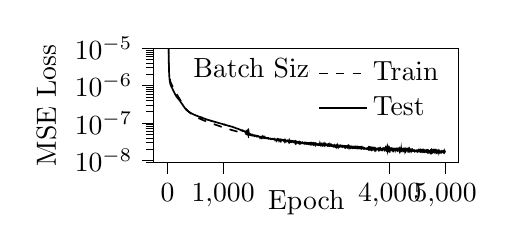
\begin{tikzpicture}

\begin{axis}[
legend cell align={left},
legend style={draw=none},
log basis y={10},
tick align=outside,
tick pos=left,
title={Batch Size 10},
title style={at={(0.4,0.85)},anchor=north},
x grid style={white!69.0196078431373!black},
xlabel={Epoch},
x label style={yshift=13pt},
xmin=-249.95, xmax=5248.95,
xtick style={color=black},
xtick = {0,1000,4000,5000},
y grid style={white!69.0196078431373!black},
ylabel={MSE Loss},
ymin=8.87880740039152e-09, ymax=1e-5,
ymode=log,
ytick style={color=black},
width=.45\textwidth,
height=.25\textwidth
]
\addplot [semithick, black, dashed]
table {%
0 0.00528136799344793
1 0.00196117930812761
2 0.00100831297786499
3 0.000271266568352075
4 0.000175409968296663
5 0.00014971278719031
6 0.000120760855550088
7 8.43190852401676e-05
8 5.46341028825736e-05
9 3.68707081361208e-05
10 2.85679608685996e-05
11 2.42326660020353e-05
12 2.11219582564581e-05
13 1.81891610776574e-05
14 1.55777172395233e-05
15 1.33981817964468e-05
16 1.15641491053964e-05
17 1.00000746923001e-05
18 7.94393679449001e-06
19 6.00564802901715e-06
20 4.86061071530486e-06
21 4.12355882229321e-06
22 3.60576834694371e-06
23 3.22225895214245e-06
24 2.92377228394258e-06
25 2.68271659390251e-06
26 2.48770738849657e-06
27 2.32538501446555e-06
28 2.19179745549525e-06
29 2.08097682532937e-06
30 1.98731877759428e-06
31 1.90663698408144e-06
32 1.8373563384344e-06
33 1.77455051147746e-06
34 1.72185935884528e-06
35 1.67465214957474e-06
36 1.63151804748907e-06
37 1.59294660916132e-06
38 1.55762653216485e-06
39 1.52324679449478e-06
40 1.49266945621562e-06
41 1.46543748737571e-06
42 1.4406353606411e-06
43 1.41676968130611e-06
44 1.39477084188044e-06
45 1.37423507132084e-06
46 1.35511966337987e-06
47 1.33708427732415e-06
48 1.32014086020149e-06
49 1.30410750958987e-06
50 1.28945765865751e-06
51 1.27443131206384e-06
52 1.26037416048774e-06
53 1.24694222655819e-06
54 1.23406486594924e-06
55 1.22177031155246e-06
56 1.20998068816824e-06
57 1.19855566538263e-06
58 1.18768979488593e-06
59 1.17686123902949e-06
60 1.16681973979738e-06
61 1.15674759846307e-06
62 1.1469994821578e-06
63 1.13754304193137e-06
64 1.12835477860784e-06
65 1.1194146830551e-06
66 1.11076625926465e-06
67 1.10223702500356e-06
68 1.09403939837271e-06
69 1.08589154372396e-06
70 1.07803150965147e-06
71 1.07009383924606e-06
72 1.06247301927098e-06
73 1.05503250242833e-06
74 1.04769723291653e-06
75 1.04052962702994e-06
76 1.03352776483767e-06
77 1.02660954140354e-06
78 1.01991228824261e-06
79 1.01320784088976e-06
80 1.00659571903527e-06
81 1.00009874282492e-06
82 9.93677533349668e-07
83 9.87113965438269e-07
84 9.8062059834092e-07
85 9.74151814121527e-07
86 9.67832220357678e-07
87 9.61684138536256e-07
88 9.55247765936917e-07
89 9.47558848833907e-07
90 9.38266775394325e-07
91 9.32239593209871e-07
92 9.24267010997681e-07
93 9.17881108195573e-07
94 9.11650485644344e-07
95 9.05510341233651e-07
96 8.99423817841694e-07
97 8.93403781594415e-07
98 8.87423857589553e-07
99 8.81676584700841e-07
100 8.75797529316102e-07
101 8.70152860761308e-07
102 8.64392884949439e-07
103 8.58854557606037e-07
104 8.53098335458213e-07
105 8.46301717638553e-07
106 8.40260048056152e-07
107 8.34313861926006e-07
108 8.28649471031895e-07
109 8.23015421440587e-07
110 8.17364995748804e-07
111 8.11884977585109e-07
112 8.06511968143297e-07
113 8.01217028589818e-07
114 7.96036286949686e-07
115 7.90829720260788e-07
116 7.85724390182097e-07
117 7.8061357269732e-07
118 7.75622568420786e-07
119 7.70701369514626e-07
120 7.65859431632876e-07
121 7.60867010685118e-07
122 7.56293496833038e-07
123 7.51443952839992e-07
124 7.46633905377436e-07
125 7.41863842019796e-07
126 7.37510203085989e-07
127 7.3260120961649e-07
128 7.27850430646271e-07
129 7.23098523858212e-07
130 7.18564877866257e-07
131 7.14265563797056e-07
132 7.09575198163392e-07
133 7.05213690039841e-07
134 7.00810380456218e-07
135 6.96431313489398e-07
136 6.92166918714321e-07
137 6.87997769821536e-07
138 6.83765189526397e-07
139 6.79594235624137e-07
140 6.75474781814955e-07
141 6.71440492920894e-07
142 6.67533135683129e-07
143 6.6334973273463e-07
144 6.59287583699708e-07
145 6.55205213693222e-07
146 6.51308420911434e-07
147 6.47384833252218e-07
148 6.43609669417344e-07
149 6.39809587452689e-07
150 6.36069694479602e-07
151 6.32515987284421e-07
152 6.28736712959821e-07
153 6.24937947204529e-07
154 6.21260133568668e-07
155 6.17671506626394e-07
156 6.14028405241385e-07
157 6.10509567016138e-07
158 6.06915501686345e-07
159 6.03322018584151e-07
160 5.99968398082851e-07
161 5.96322954811157e-07
162 5.92967038830494e-07
163 5.89499768537394e-07
164 5.86096018651006e-07
165 5.82915874680623e-07
166 5.79369164599441e-07
167 5.76226525925705e-07
168 5.72933694416022e-07
169 5.69691405916117e-07
170 5.66455787112119e-07
171 5.63347007282999e-07
172 5.59933701893556e-07
173 5.56663053732365e-07
174 5.53505768943197e-07
175 5.50422513185822e-07
176 5.47412930105295e-07
177 5.44322518996054e-07
178 5.41142272298956e-07
179 5.38103252072375e-07
180 5.35073113576701e-07
181 5.32053218753603e-07
182 5.2916558987981e-07
183 5.26249207855045e-07
184 5.23352361447849e-07
185 5.20399350589784e-07
186 5.17523279084386e-07
187 5.14665778332812e-07
188 5.11827413136601e-07
189 5.09032601829773e-07
190 5.06142247340691e-07
191 5.03410807146665e-07
192 5.00633232789482e-07
193 4.97932972685078e-07
194 4.95130490003604e-07
195 4.92452483671357e-07
196 4.89739140157042e-07
197 4.870303317972e-07
198 4.84287599142874e-07
199 4.81629953617002e-07
200 4.7891349964857e-07
201 4.76268158013937e-07
202 4.73530783402509e-07
203 4.70959613290134e-07
204 4.68312260348824e-07
205 4.65747004891881e-07
206 4.63164959141338e-07
207 4.60514930296085e-07
208 4.57982168553528e-07
209 4.55433743336009e-07
210 4.52851707479773e-07
211 4.50364350497168e-07
212 4.47857538041774e-07
213 4.45355709501882e-07
214 4.42778161664492e-07
215 4.40293827219662e-07
216 4.37892487021863e-07
217 4.35247193566468e-07
218 4.32821898028735e-07
219 4.3035448477724e-07
220 4.27975495336241e-07
221 4.25454756096677e-07
222 4.23122028854195e-07
223 4.20731893679971e-07
224 4.18271005955262e-07
225 4.15870392234119e-07
226 4.13457123742411e-07
227 4.10999238673604e-07
228 4.08633261530511e-07
229 4.06335352423071e-07
230 4.03913571878078e-07
231 4.01562177887449e-07
232 3.99183417418847e-07
233 3.96861866605036e-07
234 3.94463216704111e-07
235 3.9231701188136e-07
236 3.89952001049743e-07
237 3.87668205026337e-07
238 3.85320536859801e-07
239 3.83008806870144e-07
240 3.80778862836273e-07
241 3.78499330051518e-07
242 3.76246543565273e-07
243 3.7398688223611e-07
244 3.71832217145318e-07
245 3.69569940148473e-07
246 3.67439741997266e-07
247 3.65260341483875e-07
248 3.63166023862327e-07
249 3.61033952382961e-07
250 3.58909800963758e-07
251 3.56821789164741e-07
252 3.54731006746434e-07
253 3.52717319067608e-07
254 3.50711979018037e-07
255 3.48674827135298e-07
256 3.46662165182643e-07
257 3.44682640887051e-07
258 3.42718062111835e-07
259 3.40774582703318e-07
260 3.38882178803068e-07
261 3.36939323482e-07
262 3.35075527875262e-07
263 3.33137614143553e-07
264 3.3120930719388e-07
265 3.29301063395349e-07
266 3.27454248716386e-07
267 3.25471118496345e-07
268 3.23515837390431e-07
269 3.21549918185227e-07
270 3.19058210811463e-07
271 3.16761530374521e-07
272 3.14913813652673e-07
273 3.13171949990476e-07
274 3.11409781494909e-07
275 3.09652313128517e-07
276 3.07940026100795e-07
277 3.06198263344548e-07
278 3.04574217313558e-07
279 3.02837976109416e-07
280 3.0114346012855e-07
281 2.99294401275851e-07
282 2.97600264582698e-07
283 2.95904359046695e-07
284 2.94242386100763e-07
285 2.92338202423359e-07
286 2.90607358821582e-07
287 2.88928763936269e-07
288 2.87282469568773e-07
289 2.85632490428789e-07
290 2.84055769137481e-07
291 2.82524579833243e-07
292 2.80988924288295e-07
293 2.79470538226967e-07
294 2.78032275473628e-07
295 2.76563692107601e-07
296 2.75308126047591e-07
297 2.73785573132734e-07
298 2.72342808580461e-07
299 2.70912388793398e-07
300 2.69563412658158e-07
301 2.68253967101728e-07
302 2.66938382678106e-07
303 2.65578434972547e-07
304 2.64324795336002e-07
305 2.63108027653836e-07
306 2.61854648559989e-07
307 2.60630991584243e-07
308 2.59393573514011e-07
309 2.58222029780875e-07
310 2.57056368830888e-07
311 2.55888819569172e-07
312 2.54658455163259e-07
313 2.53491728283706e-07
314 2.52409010270682e-07
315 2.51337997045908e-07
316 2.5030137600357e-07
317 2.49188929104527e-07
318 2.48023163704758e-07
319 2.46955601448384e-07
320 2.45822844564536e-07
321 2.44817109593676e-07
322 2.43781857687253e-07
323 2.42748652734548e-07
324 2.41714933428838e-07
325 2.40798836785849e-07
326 2.39876830110397e-07
327 2.38903279075053e-07
328 2.37944548606706e-07
329 2.3699354220863e-07
330 2.36068708319159e-07
331 2.35151283134449e-07
332 2.34205967064582e-07
333 2.33274957253116e-07
334 2.32392124277503e-07
335 2.31484588075759e-07
336 2.30657326452111e-07
337 2.29810509786432e-07
338 2.29022869473461e-07
339 2.28213446811232e-07
340 2.27242750026058e-07
341 2.26404253220736e-07
342 2.25602067907005e-07
343 2.24776172110808e-07
344 2.24006119635689e-07
345 2.23185505445755e-07
346 2.22317487597046e-07
347 2.21572234484491e-07
348 2.20820311618297e-07
349 2.2001649651493e-07
350 2.19287002916069e-07
351 2.1834789354358e-07
352 2.17625585441361e-07
353 2.16871131519802e-07
354 2.16220429529734e-07
355 2.15429030556713e-07
356 2.1473307522335e-07
357 2.14042594111064e-07
358 2.13372244108889e-07
359 2.12795627789752e-07
360 2.12051067953745e-07
361 2.11376431433763e-07
362 2.10728520846359e-07
363 2.1009826162377e-07
364 2.09431103987967e-07
365 2.08771483025671e-07
366 2.08140193018735e-07
367 2.07497775548404e-07
368 2.06848745523125e-07
369 2.06193569836088e-07
370 2.05640739063817e-07
371 2.0498919569345e-07
372 2.04406067476626e-07
373 2.03852335447507e-07
374 2.0315202889698e-07
375 2.02647559515157e-07
376 2.01964303441216e-07
377 2.01442579235156e-07
378 2.00809108363842e-07
379 2.00291153515941e-07
380 1.99646441489953e-07
381 1.9908953290404e-07
382 1.9843899079941e-07
383 1.9783244177507e-07
384 1.9732972965425e-07
385 1.96696532901441e-07
386 1.96089850654779e-07
387 1.95515737386742e-07
388 1.95012229147196e-07
389 1.94473671935036e-07
390 1.93915756470098e-07
391 1.93370991827813e-07
392 1.9295067025471e-07
393 1.92333264354971e-07
394 1.91909908457966e-07
395 1.91307810153418e-07
396 1.90847586147846e-07
397 1.90272842144346e-07
398 1.89821726244155e-07
399 1.89262572947158e-07
400 1.88858243790335e-07
401 1.88210220435359e-07
402 1.87736445091957e-07
403 1.87311259125522e-07
404 1.86755425390928e-07
405 1.86331044127463e-07
406 1.8575961707068e-07
407 1.85354366402102e-07
408 1.84749235963011e-07
409 1.84390802604462e-07
410 1.83792814558714e-07
411 1.8335780107126e-07
412 1.8287737747702e-07
413 1.8251926256152e-07
414 1.81981051277091e-07
415 1.81501176990118e-07
416 1.81177496325624e-07
417 1.80648080001511e-07
418 1.80278556265456e-07
419 1.7971269204331e-07
420 1.79261774100326e-07
421 1.78966274626546e-07
422 1.78390314147237e-07
423 1.78061858910894e-07
424 1.77493106940929e-07
425 1.77194511650214e-07
426 1.7669522240471e-07
427 1.76226328005846e-07
428 1.75761677221331e-07
429 1.7534401855368e-07
430 1.74911862940164e-07
431 1.74502996217463e-07
432 1.74251102693646e-07
433 1.7382497731866e-07
434 1.73263161178383e-07
435 1.73004354868667e-07
436 1.72492188439399e-07
437 1.7220730899048e-07
438 1.7165128710861e-07
439 1.7125423465103e-07
440 1.7100701692474e-07
441 1.70545178845849e-07
442 1.7008701600485e-07
443 1.69664761564547e-07
444 1.69258927638083e-07
445 1.6888123750558e-07
446 1.68490066032589e-07
447 1.68132941289478e-07
448 1.67800580737065e-07
449 1.67420219066017e-07
450 1.66960605261224e-07
451 1.66590058223726e-07
452 1.66209313094967e-07
453 1.65879797640045e-07
454 1.65527574829127e-07
455 1.65107552816401e-07
456 1.64804789619666e-07
457 1.64351305911303e-07
458 1.63989841528434e-07
459 1.63619196937859e-07
460 1.63235743539936e-07
461 1.62907762013553e-07
462 1.62464832413889e-07
463 1.62098891167695e-07
464 1.61743859634633e-07
465 1.61409872379004e-07
466 1.6105873006822e-07
467 1.60653658838328e-07
468 1.60286182233627e-07
469 1.59894756044388e-07
470 1.59531792913725e-07
471 1.59174766829473e-07
472 1.58797522091803e-07
473 1.58495172808415e-07
474 1.58078474448153e-07
475 1.57730813090673e-07
476 1.57359346744101e-07
477 1.57076716797988e-07
478 1.5668199366381e-07
479 1.56443077594659e-07
480 1.56038656218271e-07
481 1.55657942588761e-07
482 1.55325011998997e-07
483 1.54921709318856e-07
484 1.54598146702156e-07
485 1.54341690801196e-07
486 1.53867364836024e-07
487 1.5353118324013e-07
488 1.53226939170192e-07
489 1.52933094093033e-07
490 1.52640565342921e-07
491 1.523347708976e-07
492 1.51942499793112e-07
493 1.51550411844337e-07
494 1.51309379272657e-07
495 1.50920436685631e-07
496 1.50610290570175e-07
497 1.50305012087681e-07
498 1.50029505234794e-07
499 1.49729306713198e-07
500 1.49430219844593e-07
501 1.49247199219271e-07
502 1.4900762355774e-07
503 1.48481581319082e-07
504 1.48199029017526e-07
505 1.47922896862607e-07
506 1.4763762496095e-07
507 1.47376839620961e-07
508 1.47225218374292e-07
509 1.4680912803211e-07
510 1.46543789512066e-07
511 1.46414373785042e-07
512 1.45965114726199e-07
513 1.45717731925288e-07
514 1.45586504762818e-07
515 1.45202670251976e-07
516 1.44917263122935e-07
517 1.44685540794942e-07
518 1.4441396511522e-07
519 1.44274714346526e-07
520 1.43907111471719e-07
521 1.43611794123366e-07
522 1.43441559614654e-07
523 1.43342289060655e-07
524 1.43023464527214e-07
525 1.4269947945289e-07
526 1.42346950551264e-07
527 1.42243148950616e-07
528 1.41845405314811e-07
529 1.41633421835152e-07
530 1.41421946477927e-07
531 1.41117858427631e-07
532 1.40866536890716e-07
533 1.40753480974976e-07
534 1.40448171630503e-07
535 1.40135051471812e-07
536 1.40028638033751e-07
537 1.39913777295053e-07
538 1.39432189358857e-07
539 1.39200212907475e-07
540 1.38922127936869e-07
541 1.3885529407176e-07
542 1.38543313705775e-07
543 1.38373281870496e-07
544 1.37950778162921e-07
545 1.37704649900705e-07
546 1.37484048030601e-07
547 1.37280646952398e-07
548 1.37019148076512e-07
549 1.3677530932954e-07
550 1.36761920195294e-07
551 1.36316340897391e-07
552 1.36309115785771e-07
553 1.35979577848833e-07
554 1.35640636269585e-07
555 1.35609762330624e-07
556 1.35323011500876e-07
557 1.34884704106053e-07
558 1.34914494200888e-07
559 1.34521318539971e-07
560 1.34409869887442e-07
561 1.34146739227958e-07
562 1.33836909697038e-07
563 1.33704287221814e-07
564 1.33502265708962e-07
565 1.33171152050249e-07
566 1.32942179140727e-07
567 1.32634342442373e-07
568 1.32577345650642e-07
569 1.32393106517803e-07
570 1.32022034993184e-07
571 1.31851378921688e-07
572 1.31748397536047e-07
573 1.31391232387479e-07
574 1.31212455152241e-07
575 1.31131689407038e-07
576 1.30905025059747e-07
577 1.30671633065127e-07
578 1.30473399770903e-07
579 1.30230422275002e-07
580 1.30008186347563e-07
581 1.2983359869656e-07
582 1.29610148076331e-07
583 1.29394243846281e-07
584 1.29101745229843e-07
585 1.28992069343692e-07
586 1.28795406288962e-07
587 1.28587078604969e-07
588 1.28416344100657e-07
589 1.28186303307576e-07
590 1.27897572701485e-07
591 1.27800394298383e-07
592 1.2761726235988e-07
593 1.27405126921776e-07
594 1.27332942780889e-07
595 1.27010178951892e-07
596 1.26795597863438e-07
597 1.26621371643321e-07
598 1.26441015388945e-07
599 1.26264200759341e-07
600 1.26045677661946e-07
601 1.25880933130595e-07
602 1.25679640288201e-07
603 1.2548865805373e-07
604 1.25312461181082e-07
605 1.25103905102009e-07
606 1.24897948852176e-07
607 1.2472952348519e-07
608 1.24515717392359e-07
609 1.24279311313202e-07
610 1.24162860886123e-07
611 1.23963258817916e-07
612 1.23856674962841e-07
613 1.23616911071878e-07
614 1.23448208606547e-07
615 1.23266022529211e-07
616 1.23099053030984e-07
617 1.22965574678169e-07
618 1.22703210674313e-07
619 1.22610334458706e-07
620 1.22416365280209e-07
621 1.22263429667147e-07
622 1.22010187015853e-07
623 1.21881407568747e-07
624 1.21748274617417e-07
625 1.21502343006785e-07
626 1.2137257298761e-07
627 1.21214431700878e-07
628 1.20995997192619e-07
629 1.20755586696664e-07
630 1.20677670794045e-07
631 1.20486802772657e-07
632 1.20335067714805e-07
633 1.20041876465748e-07
634 1.19993952512054e-07
635 1.19800402285097e-07
636 1.19638045039672e-07
637 1.19469144954643e-07
638 1.19288750000113e-07
639 1.19123967685653e-07
640 1.18970169935562e-07
641 1.18776178510416e-07
642 1.18630074621429e-07
643 1.18430187046048e-07
644 1.18283657739582e-07
645 1.18106677862162e-07
646 1.17970297603964e-07
647 1.17771976335668e-07
648 1.17546498046295e-07
649 1.17381637583236e-07
650 1.17316464169903e-07
651 1.17152637191253e-07
652 1.16984930773611e-07
653 1.16820248532434e-07
654 1.16677477870475e-07
655 1.16489247212748e-07
656 1.16356786041827e-07
657 1.16109150187782e-07
658 1.16021651885845e-07
659 1.1589247186361e-07
660 1.15680851813238e-07
661 1.15511939573487e-07
662 1.15437697290055e-07
663 1.15192883769488e-07
664 1.15133998694894e-07
665 1.14999466962473e-07
666 1.1487223649187e-07
667 1.14615010180508e-07
668 1.14523665111221e-07
669 1.1430231152243e-07
670 1.14183070931695e-07
671 1.1411805894479e-07
672 1.13863993682628e-07
673 1.13744293219753e-07
674 1.13635250174049e-07
675 1.13444134877128e-07
676 1.13304540763082e-07
677 1.13211565104798e-07
678 1.12999955512727e-07
679 1.12873975091077e-07
680 1.12800427194415e-07
681 1.12586640521606e-07
682 1.12449143476745e-07
683 1.12380084229535e-07
684 1.12158920160255e-07
685 1.12033838148839e-07
686 1.11931735531368e-07
687 1.1172928866543e-07
688 1.11605941497395e-07
689 1.1149843984759e-07
690 1.1128916759251e-07
691 1.1117579283848e-07
692 1.11079075031384e-07
693 1.10869837885996e-07
694 1.1073690432406e-07
695 1.10605835175193e-07
696 1.10463978759689e-07
697 1.10324903690451e-07
698 1.10176767589287e-07
699 1.100433870449e-07
700 1.0991178901909e-07
701 1.09746107153086e-07
702 1.09625463144969e-07
703 1.09457206673991e-07
704 1.09297419130794e-07
705 1.09188764514379e-07
706 1.09040658213821e-07
707 1.0890217267967e-07
708 1.08757311609864e-07
709 1.08620748524579e-07
710 1.08461666568083e-07
711 1.08355406422955e-07
712 1.0820399432232e-07
713 1.08059409826833e-07
714 1.07951705372589e-07
715 1.07794844741438e-07
716 1.07663849195916e-07
717 1.0751906558859e-07
718 1.07392642625381e-07
719 1.07279909615787e-07
720 1.07122551153971e-07
721 1.06990335362323e-07
722 1.06877231731417e-07
723 1.06721919757025e-07
724 1.06634702299324e-07
725 1.06495320386646e-07
726 1.0637759998211e-07
727 1.06249467228814e-07
728 1.06104308867927e-07
729 1.05983714275837e-07
730 1.05844237328068e-07
731 1.05722839016664e-07
732 1.05567359489633e-07
733 1.05441034778941e-07
734 1.05317241290148e-07
735 1.05184704000116e-07
736 1.05069148752523e-07
737 1.04929581894453e-07
738 1.04795213640152e-07
739 1.04670552025787e-07
740 1.0455280652355e-07
741 1.044142625517e-07
742 1.04289056577223e-07
743 1.04165171206372e-07
744 1.04030028755808e-07
745 1.0391795601139e-07
746 1.03792417993631e-07
747 1.03663553188138e-07
748 1.03539296125721e-07
749 1.03406859475186e-07
750 1.03288533213064e-07
751 1.03147823957706e-07
752 1.03020528992026e-07
753 1.02919831468373e-07
754 1.02779396466968e-07
755 1.02649501698693e-07
756 1.02499358838326e-07
757 1.02409941540316e-07
758 1.02271492001815e-07
759 1.02169458857659e-07
760 1.02015001670619e-07
761 1.01912081720279e-07
762 1.0179567390356e-07
763 1.01665921425909e-07
764 1.01540616401774e-07
765 1.01433277479579e-07
766 1.01308921702792e-07
767 1.01178255593748e-07
768 1.01059277914928e-07
769 1.0093410972134e-07
770 1.00816341617183e-07
771 1.00699157992157e-07
772 1.00549053838606e-07
773 1.00454659421878e-07
774 1.00326335377154e-07
775 1.00216911897988e-07
776 1.00077129114862e-07
777 9.99685849523146e-08
778 9.98191905199342e-08
779 9.97170746863674e-08
780 9.959241176416e-08
781 9.94933218900762e-08
782 9.93614848043833e-08
783 9.92425511014972e-08
784 9.91293627983225e-08
785 9.89690742470017e-08
786 9.88637059462505e-08
787 9.86897062427161e-08
788 9.85202997316748e-08
789 9.83834785062143e-08
790 9.82288636919293e-08
791 9.80936902461593e-08
792 9.79595043815173e-08
793 9.78026380105135e-08
794 9.76777373984383e-08
795 9.75584071083446e-08
796 9.74415919641203e-08
797 9.72948478028535e-08
798 9.71522259529678e-08
799 9.70548201317811e-08
800 9.69570135667119e-08
801 9.67987629474365e-08
802 9.66975896488087e-08
803 9.65856752399574e-08
804 9.64346787757364e-08
805 9.63039692147838e-08
806 9.61681625466504e-08
807 9.60707070940536e-08
808 9.59578685444384e-08
809 9.58247181959138e-08
810 9.56963635290187e-08
811 9.56085677850105e-08
812 9.54724297685949e-08
813 9.53632209910182e-08
814 9.52536143494775e-08
815 9.51394857096055e-08
816 9.50062137183849e-08
817 9.49072192701905e-08
818 9.48035359127353e-08
819 9.46693008962995e-08
820 9.45688968445602e-08
821 9.44452840512255e-08
822 9.43172510536883e-08
823 9.41965488587826e-08
824 9.40813234739934e-08
825 9.39868876637107e-08
826 9.38570903197267e-08
827 9.37556547064844e-08
828 9.36585416666524e-08
829 9.35416478275997e-08
830 9.34184370238178e-08
831 9.33253633950137e-08
832 9.31960705075063e-08
833 9.30750392247326e-08
834 9.29790978276834e-08
835 9.28531029176227e-08
836 9.2741702393262e-08
837 9.26282059432459e-08
838 9.25152430020226e-08
839 9.24248369438274e-08
840 9.22977743145204e-08
841 9.21841337708784e-08
842 9.20765091949605e-08
843 9.19876060434532e-08
844 9.18693412588212e-08
845 9.17491777063795e-08
846 9.16572254738846e-08
847 9.15576272420005e-08
848 9.14203159663174e-08
849 9.13198639840296e-08
850 9.12320605528372e-08
851 9.11133052672319e-08
852 9.10208488935638e-08
853 9.08886395145636e-08
854 9.08109727859596e-08
855 9.06900371511199e-08
856 9.06042483128644e-08
857 9.04830585968242e-08
858 9.03685871711524e-08
859 9.02765184473964e-08
860 9.01473026471145e-08
861 9.00494284872266e-08
862 8.99514579755234e-08
863 8.98092013335017e-08
864 8.96942274453139e-08
865 8.96169885922227e-08
866 8.95027962699579e-08
867 8.93974512350404e-08
868 8.93055719486391e-08
869 8.92152715792349e-08
870 8.90796454533493e-08
871 8.90001987152722e-08
872 8.88985555147492e-08
873 8.87827027629129e-08
874 8.8681826293513e-08
875 8.85993879884417e-08
876 8.84749253682315e-08
877 8.8365314028227e-08
878 8.82766570842186e-08
879 8.81907103478241e-08
880 8.80913904999225e-08
881 8.79811675558173e-08
882 8.78724534403297e-08
883 8.77856994518922e-08
884 8.76815198824765e-08
885 8.76151390438729e-08
886 8.75026416458091e-08
887 8.73753373653585e-08
888 8.72858262668252e-08
889 8.71681758307652e-08
890 8.70833700972184e-08
891 8.69674835723977e-08
892 8.68769882167442e-08
893 8.67649135960491e-08
894 8.66658114584418e-08
895 8.65728811727529e-08
896 8.64807740574847e-08
897 8.6379502552969e-08
898 8.62890960395823e-08
899 8.61805522656134e-08
900 8.60798535828877e-08
901 8.59804689978816e-08
902 8.58941737535979e-08
903 8.57911752905061e-08
904 8.57290044931069e-08
905 8.5604700195141e-08
906 8.55353445339269e-08
907 8.54296420338407e-08
908 8.53275566381484e-08
909 8.5235891411628e-08
910 8.50940039809345e-08
911 8.50244317684989e-08
912 8.4918217946317e-08
913 8.48225562921634e-08
914 8.47121673808182e-08
915 8.45646080938067e-08
916 8.44489866413944e-08
917 8.43275235373753e-08
918 8.42122600341888e-08
919 8.40845770033738e-08
920 8.39633717686361e-08
921 8.38728335961214e-08
922 8.37333134784402e-08
923 8.36061557252243e-08
924 8.34589165044086e-08
925 8.34041407116182e-08
926 8.32506879300254e-08
927 8.31442018411899e-08
928 8.30001081730813e-08
929 8.29361105103565e-08
930 8.28301392408193e-08
931 8.27331621211513e-08
932 8.25695926853776e-08
933 8.25084764133344e-08
934 8.24218239925401e-08
935 8.22939920519516e-08
936 8.21872503586896e-08
937 8.20537366830187e-08
938 8.19762285186876e-08
939 8.18900844801185e-08
940 8.17806862829506e-08
941 8.16891713362189e-08
942 8.15947277921225e-08
943 8.14801866821924e-08
944 8.13893779216812e-08
945 8.12549022888298e-08
946 8.1186256242205e-08
947 8.11224664332144e-08
948 8.10068910750417e-08
949 8.08747287273093e-08
950 8.08084906545048e-08
951 8.07560128546214e-08
952 8.05988600105501e-08
953 8.05289388638997e-08
954 8.04419091360309e-08
955 8.03479138999919e-08
956 8.02426033241765e-08
957 8.01662782334844e-08
958 8.01079387491299e-08
959 7.9962328587424e-08
960 7.98649313971111e-08
961 7.9823963941017e-08
962 7.9702674595783e-08
963 7.96342297637587e-08
964 7.95564499433965e-08
965 7.94755216992904e-08
966 7.93516297070696e-08
967 7.92942259231211e-08
968 7.92169674035392e-08
969 7.91121163468134e-08
970 7.90581564369397e-08
971 7.89395004829885e-08
972 7.89092709929662e-08
973 7.87544788338756e-08
974 7.86666472096798e-08
975 7.86523701190589e-08
976 7.8514790184947e-08
977 7.84664036479477e-08
978 7.83199948162228e-08
979 7.82645249342018e-08
980 7.81695066787158e-08
981 7.80512361253649e-08
982 7.79887493473908e-08
983 7.79145837692674e-08
984 7.77953452724134e-08
985 7.77322541933856e-08
986 7.76423590509445e-08
987 7.75262421370826e-08
988 7.74901881572809e-08
989 7.73475327164874e-08
990 7.72705407747765e-08
991 7.72285956518459e-08
992 7.71681437772287e-08
993 7.70099962310589e-08
994 7.6918287235106e-08
995 7.67477495755564e-08
996 7.66623190040505e-08
997 7.66021730802535e-08
998 7.65218229270559e-08
999 7.63669241243825e-08
1000 7.6295445008423e-08
1001 7.62423054423422e-08
1002 7.61833150897395e-08
1003 7.60298844904028e-08
1004 7.59456310106543e-08
1005 7.5915621380318e-08
1006 7.58299975345267e-08
1007 7.56544244606694e-08
1008 7.55973048804925e-08
1009 7.55229512816591e-08
1010 7.54216580389766e-08
1011 7.53594459368401e-08
1012 7.52067414966362e-08
1013 7.52052056296471e-08
1014 7.51557110101331e-08
1015 7.49614555517475e-08
1016 7.4885067218311e-08
1017 7.48791445759345e-08
1018 7.47417294144626e-08
1019 7.47140375767508e-08
1020 7.46119577232918e-08
1021 7.44862677981573e-08
1022 7.44557077481112e-08
1023 7.43193127195063e-08
1024 7.42957686372669e-08
1025 7.4221959174281e-08
1026 7.41500351564284e-08
1027 7.40415722955134e-08
1028 7.39807223770761e-08
1029 7.38309129766357e-08
1030 7.38701393321328e-08
1031 7.37174148590647e-08
1032 7.35824979369859e-08
1033 7.35116533312485e-08
1034 7.34302032601164e-08
1035 7.33476446113102e-08
1036 7.33671868502483e-08
1037 7.32307386996922e-08
1038 7.31039209833639e-08
1039 7.30351898292625e-08
1040 7.29436440005671e-08
1041 7.28809123939911e-08
1042 7.28058229415574e-08
1043 7.27249777798811e-08
1044 7.27286119772685e-08
1045 7.25525780431724e-08
1046 7.24841360955075e-08
1047 7.24180311362233e-08
1048 7.22959945087531e-08
1049 7.22426187649283e-08
1050 7.2176573153726e-08
1051 7.20893046013415e-08
1052 7.20017102628923e-08
1053 7.19189237630147e-08
1054 7.18641382912999e-08
1055 7.17460976717987e-08
1056 7.16872122041856e-08
1057 7.16345884987923e-08
1058 7.15641047777105e-08
1059 7.14595474726742e-08
1060 7.14032528059683e-08
1061 7.13230476234727e-08
1062 7.12698537030931e-08
1063 7.11620048843287e-08
1064 7.1099792313678e-08
1065 7.10210318133342e-08
1066 7.09501470685936e-08
1067 7.08730074228114e-08
1068 7.08146171457535e-08
1069 7.07208029737672e-08
1070 7.0667067246788e-08
1071 7.0587900489194e-08
1072 7.05154876490255e-08
1073 7.04174514121192e-08
1074 7.03676609625781e-08
1075 7.02960759779714e-08
1076 7.02190040557937e-08
1077 7.01422597004786e-08
1078 7.00668985409436e-08
1079 6.99825292271861e-08
1080 6.99192134079318e-08
1081 6.98422142320077e-08
1082 6.97528138959846e-08
1083 6.96937493693817e-08
1084 6.96327662552676e-08
1085 6.95564798580683e-08
1086 6.94771127252025e-08
1087 6.9404260594208e-08
1088 6.93380222527296e-08
1089 6.92929876389137e-08
1090 6.9229443624419e-08
1091 6.91383239725951e-08
1092 6.90825351501445e-08
1093 6.89790639207821e-08
1094 6.89349090099434e-08
1095 6.88793907022145e-08
1096 6.87815529998303e-08
1097 6.87399090693042e-08
1098 6.86655123049995e-08
1099 6.85979349568377e-08
1100 6.85465203731361e-08
1101 6.84304802800462e-08
1102 6.82930998152642e-08
1103 6.82401087148676e-08
1104 6.82187844369686e-08
1105 6.81062173057967e-08
1106 6.80573373812443e-08
1107 6.79730649566501e-08
1108 6.78895991312878e-08
1109 6.78060206271702e-08
1110 6.77501244261691e-08
1111 6.76755676876084e-08
1112 6.75976947195345e-08
1113 6.75403262584418e-08
1114 6.74787379195685e-08
1115 6.73983082100094e-08
1116 6.7336414757424e-08
1117 6.72648212929339e-08
1118 6.71991075895661e-08
1119 6.7131866943182e-08
1120 6.70594125984358e-08
1121 6.6966685994263e-08
1122 6.69011549336851e-08
1123 6.68549786153605e-08
1124 6.67717031599402e-08
1125 6.67253009023483e-08
1126 6.66633335044686e-08
1127 6.65907989549908e-08
1128 6.65221406714878e-08
1129 6.64455554866272e-08
1130 6.63857757809971e-08
1131 6.63229847264191e-08
1132 6.62627450243036e-08
1133 6.62109349547357e-08
1134 6.61462561502013e-08
1135 6.6093881321283e-08
1136 6.60213592840186e-08
1137 6.59478948805692e-08
1138 6.58879199444406e-08
1139 6.58199054259789e-08
1140 6.57540199133777e-08
1141 6.56966605405707e-08
1142 6.56330822668139e-08
1143 6.55571200414151e-08
1144 6.54897740370863e-08
1145 6.54308262637571e-08
1146 6.53687929430546e-08
1147 6.53162745778424e-08
1148 6.52443244075762e-08
1149 6.51847202348677e-08
1150 6.51423108033455e-08
1151 6.50423383241616e-08
1152 6.49857643897356e-08
1153 6.49076445990993e-08
1154 6.48716389761717e-08
1155 6.48259660329664e-08
1156 6.47253473706755e-08
1157 6.47138701626027e-08
1158 6.46138167748056e-08
1159 6.45704578206008e-08
1160 6.44884940026458e-08
1161 6.44547484851543e-08
1162 6.43687627910339e-08
1163 6.43245046338947e-08
1164 6.42580903220669e-08
1165 6.4176974865493e-08
1166 6.40986761357709e-08
1167 6.40700892873269e-08
1168 6.39818289394079e-08
1169 6.3932452434301e-08
1170 6.38905052596783e-08
1171 6.38128848362562e-08
1172 6.38097658423042e-08
1173 6.37628164223969e-08
1174 6.36612967608308e-08
1175 6.36083887473049e-08
1176 6.35628966905166e-08
1177 6.34501949159372e-08
1178 6.34135071986286e-08
1179 6.33402065530753e-08
1180 6.33164425600796e-08
1181 6.31991182298286e-08
1182 6.31688070518166e-08
1183 6.31000857720387e-08
1184 6.30440499538309e-08
1185 6.30117877586933e-08
1186 6.29068946400579e-08
1187 6.28657047108128e-08
1188 6.28001924485311e-08
1189 6.27520108475999e-08
1190 6.2692445517154e-08
1191 6.26265859304809e-08
1192 6.25640404905425e-08
1193 6.25295383405167e-08
1194 6.24554189698756e-08
1195 6.23996014326167e-08
1196 6.2342960829298e-08
1197 6.22834769337111e-08
1198 6.22272015959879e-08
1199 6.21739494643947e-08
1200 6.21147194035387e-08
1201 6.20532554540532e-08
1202 6.19924318390197e-08
1203 6.19435239723742e-08
1204 6.19088889552977e-08
1205 6.18525699835892e-08
1206 6.17901324551084e-08
1207 6.17349053899652e-08
1208 6.17010492032222e-08
1209 6.159896958291e-08
1210 6.15472192388999e-08
1211 6.14498887285819e-08
1212 6.14097986573192e-08
1213 6.13400754390092e-08
1214 6.12895230212018e-08
1215 6.12441199021596e-08
1216 6.11803813477252e-08
1217 6.11272152251097e-08
1218 6.10790524446791e-08
1219 6.10046911986295e-08
1220 6.09684344610173e-08
1221 6.09062715284381e-08
1222 6.08388207945509e-08
1223 6.07907254623896e-08
1224 6.07351286108226e-08
1225 6.06969509631128e-08
1226 6.06245701995078e-08
1227 6.05695280775365e-08
1228 6.05025316713359e-08
1229 6.04408892823649e-08
1230 6.03798410758749e-08
1231 6.03307107605033e-08
1232 6.02744852340464e-08
1233 6.02306611474646e-08
1234 6.01644510878074e-08
1235 6.01242652820133e-08
1236 6.00600351652325e-08
1237 6.00166884390241e-08
1238 5.99491715314038e-08
1239 5.98879763424875e-08
1240 5.98460734613226e-08
1241 5.97969363869133e-08
1242 5.97358579979002e-08
1243 5.97007916547376e-08
1244 5.96323696044898e-08
1245 5.95724811414122e-08
1246 5.94469046699686e-08
1247 5.94092666106327e-08
1248 5.93700340023595e-08
1249 5.93094560930041e-08
1250 5.92366686702483e-08
1251 5.91891610035589e-08
1252 5.91489903745135e-08
1253 5.90824333013273e-08
1254 5.90224539132045e-08
1255 5.89600150346925e-08
1256 5.89108437698549e-08
1257 5.88625464525983e-08
1258 5.87990369704805e-08
1259 5.87412606534166e-08
1260 5.86807554059376e-08
1261 5.86248854506088e-08
1262 5.85775673900279e-08
1263 5.85244985118472e-08
1264 5.84624300037362e-08
1265 5.84052390073531e-08
1266 5.83791618291585e-08
1267 5.8309725308181e-08
1268 5.82483366917685e-08
1269 5.82043644081764e-08
1270 5.81368083429901e-08
1271 5.80901139346501e-08
1272 5.80302669161981e-08
1273 5.79871371053642e-08
1274 5.79240294640293e-08
1275 5.79050140814275e-08
1276 5.78219837676919e-08
1277 5.77706587012727e-08
1278 5.77242251087462e-08
1279 5.76675971353247e-08
1280 5.76212695335698e-08
1281 5.75639227551328e-08
1282 5.75201069885622e-08
1283 5.74694542976317e-08
1284 5.74379567663819e-08
1285 5.73645213575169e-08
1286 5.73071207932152e-08
1287 5.72642096763332e-08
1288 5.7207055084163e-08
1289 5.71587593189982e-08
1290 5.71073273780698e-08
1291 5.70634097907252e-08
1292 5.69681883466622e-08
1293 5.69580245124435e-08
1294 5.68764241704045e-08
1295 5.68312549065197e-08
1296 5.67821779462463e-08
1297 5.67339278534362e-08
1298 5.66869046281226e-08
1299 5.66534648283046e-08
1300 5.65876212577088e-08
1301 5.65191520762731e-08
1302 5.64998829610808e-08
1303 5.6441721469902e-08
1304 5.63740171366511e-08
1305 5.63765589478571e-08
1306 5.62980969354143e-08
1307 5.62538580894945e-08
1308 5.6180983691867e-08
1309 5.61557886857855e-08
1310 5.60883655587041e-08
1311 5.60943333516306e-08
1312 5.60237184821233e-08
1313 5.59638541464125e-08
1314 5.59239631958697e-08
1315 5.58683522866588e-08
1316 5.58239115955317e-08
1317 5.57622321850637e-08
1318 5.57357208941234e-08
1319 5.5704475492302e-08
1320 5.5643806173844e-08
1321 5.56156613029657e-08
1322 5.55653318357052e-08
1323 5.55213465980309e-08
1324 5.54517741124805e-08
1325 5.53959914895152e-08
1326 5.53644016720867e-08
1327 5.53113212564682e-08
1328 5.52527291675098e-08
1329 5.52284499799605e-08
1330 5.5144183925826e-08
1331 5.51262334003155e-08
1332 5.50886002970152e-08
1333 5.50361545381683e-08
1334 5.50040574620603e-08
1335 5.49285218842677e-08
1336 5.48684188261817e-08
1337 5.48282277335055e-08
1338 5.483084286384e-08
1339 5.47275310203155e-08
1340 5.46687656632905e-08
1341 5.46399589307356e-08
1342 5.45916135452629e-08
1343 5.45022519360394e-08
1344 5.4444705193113e-08
1345 5.44269120350549e-08
1346 5.43626481408488e-08
1347 5.43836221233995e-08
1348 5.42871327913197e-08
1349 5.42768571709651e-08
1350 5.41878018789355e-08
1351 5.4157789683984e-08
1352 5.41022280931003e-08
1353 5.40704692619798e-08
1354 5.40222803624424e-08
1355 5.39687752887374e-08
1356 5.39427189405472e-08
1357 5.38898634916407e-08
1358 5.38458344823134e-08
1359 5.38044222686551e-08
1360 5.37938232803015e-08
1361 5.36979668996906e-08
1362 5.36841744303018e-08
1363 5.36145921326003e-08
1364 5.36018136698679e-08
1365 5.35213680175062e-08
1366 5.34951072461709e-08
1367 5.34692328546527e-08
1368 5.34024711873471e-08
1369 5.33796378965334e-08
1370 5.33059734308949e-08
1371 5.32888267046339e-08
1372 5.32207567194298e-08
1373 5.31850323559624e-08
1374 5.31649204016382e-08
1375 5.3121046612592e-08
1376 5.30598405856786e-08
1377 5.30234202256175e-08
1378 5.29790359360405e-08
1379 5.29613990218891e-08
1380 5.28995273607613e-08
1381 5.28548773348625e-08
1382 5.28733015370264e-08
1383 5.27771678515698e-08
1384 5.27533447414186e-08
1385 5.27198489574943e-08
1386 5.26578893444984e-08
1387 5.26402133305126e-08
1388 5.25906488801908e-08
1389 5.25463211609178e-08
1390 5.2528830414289e-08
1391 5.24788511602203e-08
1392 5.24220055742042e-08
1393 5.24470437368585e-08
1394 5.24256742129303e-08
1395 5.22615294795692e-08
1396 5.21192910207802e-08
1397 5.20188361896601e-08
1398 5.19811063925957e-08
1399 5.19453104441681e-08
1400 5.19083679995092e-08
1401 5.18817203376543e-08
1402 5.18950529349027e-08
1403 5.17597886817711e-08
1404 5.16768196634487e-08
1405 5.16066808220472e-08
1406 5.15841544612705e-08
1407 5.14775189852656e-08
1408 5.14207214030726e-08
1409 5.13891409337219e-08
1410 5.13757358477918e-08
1411 5.13573249505406e-08
1412 5.13168068416725e-08
1413 5.13165649840275e-08
1414 5.11925157420379e-08
1415 5.12202316538257e-08
1416 5.10930796626674e-08
1417 5.10085317095843e-08
1418 5.09708848772661e-08
1419 5.09748755117556e-08
1420 5.08561629830595e-08
1421 5.0904093493731e-08
1422 5.08557489409256e-08
1423 5.07618054701453e-08
1424 5.07564505913827e-08
1425 5.06145357181964e-08
1426 5.05311489651383e-08
1427 5.05936839989563e-08
1428 5.04931337241832e-08
1429 5.0452951397828e-08
1430 5.04558816272205e-08
1431 5.03367097903773e-08
1432 5.03469566204284e-08
1433 5.02490047527004e-08
1434 5.02376803923621e-08
1435 5.02076208719338e-08
1436 5.01271630748423e-08
1437 5.00489786781078e-08
1438 5.00712141493498e-08
1439 4.99865114533815e-08
1440 5.00083484289426e-08
1441 4.9890328540636e-08
1442 4.98523947067842e-08
1443 4.97875407046155e-08
1444 4.9846085875549e-08
1445 4.97773833685322e-08
1446 4.96772931957157e-08
1447 4.96355853885078e-08
1448 4.95743393835735e-08
1449 4.95377457021551e-08
1450 4.95033593184147e-08
1451 4.94555240937444e-08
1452 4.93939212853345e-08
1453 4.93500329101781e-08
1454 4.92925502748598e-08
1455 4.93035321968982e-08
1456 4.92040075816824e-08
1457 4.9215669707392e-08
1458 4.91149503445421e-08
1459 4.91340210373448e-08
1460 4.9030811973827e-08
1461 4.90517194839946e-08
1462 4.89486476096257e-08
1463 4.89652671398222e-08
1464 4.8865260748876e-08
1465 4.88976658719054e-08
1466 4.88876855497811e-08
1467 4.87972207063869e-08
1468 4.86859618586966e-08
1469 4.8610668457183e-08
1470 4.8551800269081e-08
1471 4.85247550019441e-08
1472 4.84442078052538e-08
1473 4.84753261209558e-08
1474 4.83030271447582e-08
1475 4.83270761275634e-08
1476 4.82545285973579e-08
1477 4.82582966843115e-08
1478 4.81258617335278e-08
1479 4.80988303075414e-08
1480 4.7968173395585e-08
1481 4.7949168894279e-08
1482 4.79717044732375e-08
1483 4.78497419642565e-08
1484 4.78747514909283e-08
1485 4.7764104318393e-08
1486 4.77926675945817e-08
1487 4.76858295994642e-08
1488 4.77103779927823e-08
1489 4.75992131232506e-08
1490 4.76637515867129e-08
1491 4.75154290680013e-08
1492 4.75629326746052e-08
1493 4.74504075875792e-08
1494 4.74098703306947e-08
1495 4.74234217984204e-08
1496 4.73184990101849e-08
1497 4.73501704434387e-08
1498 4.72470642864931e-08
1499 4.72344994850715e-08
1500 4.72161478004551e-08
1501 4.71361933518377e-08
1502 4.71543518709705e-08
1503 4.70452649581343e-08
1504 4.70325748036515e-08
1505 4.70003735042468e-08
1506 4.69512611322997e-08
1507 4.69334394370691e-08
1508 4.68904590977814e-08
1509 4.68322535895904e-08
1510 4.68298389533217e-08
1511 4.6806505723529e-08
1512 4.67498120548804e-08
1513 4.66393129994191e-08
1514 4.66903101226102e-08
1515 4.65901405555247e-08
1516 4.66266539145277e-08
1517 4.65099667334989e-08
1518 4.65668699989319e-08
1519 4.64228415586465e-08
1520 4.65242897951246e-08
1521 4.63855943888536e-08
1522 4.64104505715213e-08
1523 4.63904794956171e-08
1524 4.63763178104593e-08
1525 4.63305817821613e-08
1526 4.62841757697952e-08
1527 4.62211793283984e-08
1528 4.61396794348978e-08
1529 4.60853043593445e-08
1530 4.61364341375337e-08
1531 4.60750291408907e-08
1532 4.60296148219186e-08
1533 4.59789147932987e-08
1534 4.59728524693226e-08
1535 4.58919555090809e-08
1536 4.58562408023333e-08
1537 4.58575368966763e-08
1538 4.57822724087009e-08
1539 4.57561261302253e-08
1540 4.5709424143503e-08
1541 4.56817750693617e-08
1542 4.56306955554098e-08
1543 4.56160029282948e-08
1544 4.55690427569877e-08
1545 4.55393745024679e-08
1546 4.5502682188836e-08
1547 4.55034830570966e-08
1548 4.54666070148768e-08
1549 4.54305391262011e-08
1550 4.538938500942e-08
1551 4.53654008836235e-08
1552 4.53651464771276e-08
1553 4.53031914460222e-08
1554 4.52807684936385e-08
1555 4.52639115033904e-08
1556 4.51365294895645e-08
1557 4.51383902677627e-08
1558 4.50932061224485e-08
1559 4.50763167691992e-08
1560 4.50504557802933e-08
1561 4.50348735092643e-08
1562 4.49972492544415e-08
1563 4.49612696762358e-08
1564 4.49407815927838e-08
1565 4.48954179510519e-08
1566 4.4887355257206e-08
1567 4.48362547511572e-08
1568 4.48280088294339e-08
1569 4.48048097434484e-08
1570 4.47620492027845e-08
1571 4.4713658513551e-08
1572 4.46895817762805e-08
1573 4.46546048282759e-08
1574 4.46519895502817e-08
1575 4.46288366962033e-08
1576 4.45706019647218e-08
1577 4.45539489890567e-08
1578 4.45347923849759e-08
1579 4.4520032240758e-08
1580 4.44418580491934e-08
1581 4.44205728145075e-08
1582 4.43606886635362e-08
1583 4.43136019245838e-08
1584 4.43043902831342e-08
1585 4.42764173158583e-08
1586 4.42499710517907e-08
1587 4.42571249470447e-08
1588 4.42079375284621e-08
1589 4.41351378943633e-08
1590 4.41535444895003e-08
1591 4.41327122857604e-08
1592 4.4088672961351e-08
1593 4.40095084219827e-08
1594 4.39971668897421e-08
1595 4.39841634536364e-08
1596 4.39428023513155e-08
1597 4.39117037343006e-08
1598 4.38983893991107e-08
1599 4.38610298292286e-08
1600 4.38270048042089e-08
1601 4.3843909259822e-08
1602 4.37738105707464e-08
1603 4.37612000414589e-08
1604 4.37586574952853e-08
1605 4.36725917674075e-08
1606 4.36858829933051e-08
1607 4.36984414442509e-08
1608 4.35990156189003e-08
1609 4.36029375827651e-08
1610 4.35871575854563e-08
1611 4.35946942045629e-08
1612 4.35109143803736e-08
1613 4.34868172560776e-08
1614 4.35047992941584e-08
1615 4.34865427911824e-08
1616 4.34054164133446e-08
1617 4.34491634204726e-08
1618 4.34042298647075e-08
1619 4.33687512801928e-08
1620 4.33441503533416e-08
1621 4.33424849344277e-08
1622 4.32949832374074e-08
1623 4.32409372252973e-08
1624 4.32599879918172e-08
1625 4.32501230474003e-08
1626 4.32148611162475e-08
1627 4.3143247767663e-08
1628 4.31370813225307e-08
1629 4.31572533698965e-08
1630 4.31061245720343e-08
1631 4.3059920596944e-08
1632 4.30167226350697e-08
1633 4.30132329398703e-08
1634 4.29667460732919e-08
1635 4.2988491671947e-08
1636 4.29407206914423e-08
1637 4.2909141861891e-08
1638 4.28656142092976e-08
1639 4.28760578430332e-08
1640 4.28190537404838e-08
1641 4.28295858012628e-08
1642 4.27676170844382e-08
1643 4.27891232512856e-08
1644 4.2720460360357e-08
1645 4.27460644358835e-08
1646 4.26726090352325e-08
1647 4.26968247357884e-08
1648 4.26301699296694e-08
1649 4.26384228535692e-08
1650 4.25737665166182e-08
1651 4.2605102560378e-08
1652 4.25357900890599e-08
1653 4.25186357566609e-08
1654 4.25029816364386e-08
1655 4.24730943171525e-08
1656 4.24775717355885e-08
1657 4.24236018070623e-08
1658 4.23879775512948e-08
1659 4.23981434816145e-08
1660 4.23237054392178e-08
1661 4.23366803914416e-08
1662 4.22625071894167e-08
1663 4.22613303840969e-08
1664 4.22264545807405e-08
1665 4.22398365063081e-08
1666 4.2207697987795e-08
1667 4.21547526607835e-08
1668 4.2134045541431e-08
1669 4.21573369735473e-08
1670 4.20880875817709e-08
1671 4.2076693143045e-08
1672 4.20540076428999e-08
1673 4.20848705184884e-08
1674 4.19878155555331e-08
1675 4.19762428571779e-08
1676 4.19632821868632e-08
1677 4.1991933330543e-08
1678 4.19225284975511e-08
1679 4.19231392401187e-08
1680 4.19132712337067e-08
1681 4.18601316054534e-08
1682 4.18262090473576e-08
1683 4.18464744045277e-08
1684 4.17904731708774e-08
1685 4.17838044497465e-08
1686 4.18100125887388e-08
1687 4.1750799378848e-08
1688 4.17225964888246e-08
1689 4.17133620267407e-08
1690 4.16970638206227e-08
1691 4.16351062337839e-08
1692 4.16549812221056e-08
1693 4.16310596373926e-08
1694 4.15987111579419e-08
1695 4.15833268319066e-08
1696 4.15759275174121e-08
1697 4.15396776565213e-08
1698 4.15294382649645e-08
1699 4.14944176629906e-08
1700 4.14969614659366e-08
1701 4.14607777243781e-08
1702 4.14488455713347e-08
1703 4.14292768247115e-08
1704 4.13786048170106e-08
1705 4.1371826874359e-08
1706 4.13560395839951e-08
1707 4.13486892358872e-08
1708 4.13345887284589e-08
1709 4.12832303076094e-08
1710 4.13015438105457e-08
1711 4.12565580698576e-08
1712 4.12056901666347e-08
1713 4.12466385424359e-08
1714 4.12057683907285e-08
1715 4.12118187731458e-08
1716 4.11809661848839e-08
1717 4.11771211150658e-08
1718 4.11483924978029e-08
1719 4.11413671663752e-08
1720 4.11037435110728e-08
1721 4.11027567603917e-08
1722 4.10296910380303e-08
1723 4.10699566910644e-08
1724 4.10422533581034e-08
1725 4.10169240028235e-08
1726 4.09866583184204e-08
1727 4.09842960258366e-08
1728 4.09504057607979e-08
1729 4.09329285111504e-08
1730 4.09388762090401e-08
1731 4.09055216366028e-08
1732 4.08998784406922e-08
1733 4.0846572123554e-08
1734 4.08657938022472e-08
1735 4.08071813851052e-08
1736 4.08103538740434e-08
1737 4.07729829521308e-08
1738 4.08216357172808e-08
1739 4.07435745308771e-08
1740 4.07183754713714e-08
1741 4.07263478208186e-08
1742 4.07301626337286e-08
1743 4.0692824979649e-08
1744 4.06962298127311e-08
1745 4.06031006938701e-08
1746 4.06656386386928e-08
1747 4.06177418410536e-08
1748 4.06607494674027e-08
1749 4.06089568683043e-08
1750 4.05667387370912e-08
1751 4.05422773952502e-08
1752 4.05507157275054e-08
1753 4.05070659736939e-08
1754 4.04750031668399e-08
1755 4.04965585754091e-08
1756 4.04509040308199e-08
1757 4.04188499136815e-08
1758 4.04355219385533e-08
1759 4.03944661209188e-08
1760 4.03384239178184e-08
1761 4.03934524106919e-08
1762 4.03416022898284e-08
1763 4.029059641808e-08
1764 4.03195476594842e-08
1765 4.02986472403111e-08
1766 4.02314284286831e-08
1767 4.02361706575149e-08
1768 4.02035606994478e-08
1769 4.01886969592091e-08
1770 4.01624569390524e-08
1771 4.01721503473507e-08
1772 4.01744072831001e-08
1773 4.01371861491473e-08
1774 4.01196488186706e-08
1775 4.00919086795959e-08
1776 4.00497808483724e-08
1777 4.00435408942634e-08
1778 4.00288743473975e-08
1779 4.00420200907803e-08
1780 4.00204522899017e-08
1781 3.99906512404957e-08
1782 3.99872404388546e-08
1783 3.99645670168258e-08
1784 3.99419457963734e-08
1785 3.99213785828856e-08
1786 3.99070576251326e-08
1787 3.98936512824299e-08
1788 3.9814633218116e-08
1789 3.98754415831259e-08
1790 3.98531172429717e-08
1791 3.9826005221455e-08
1792 3.98153316416572e-08
1793 3.97152426168113e-08
1794 3.97811584462726e-08
1795 3.9681877989084e-08
1796 3.96616535203176e-08
1797 3.97067407875706e-08
1798 3.96246735645533e-08
1799 3.96479254838322e-08
1800 3.96364041976849e-08
1801 3.96294184079604e-08
1802 3.95942414299633e-08
1803 3.95787951101845e-08
1804 3.95466395530786e-08
1805 3.95545834186439e-08
1806 3.95525570484612e-08
1807 3.94946733228707e-08
1808 3.9510888392158e-08
1809 3.9507790828841e-08
1810 3.95327104574239e-08
1811 3.94062628850111e-08
1812 3.9424180378056e-08
1813 3.94316969509756e-08
1814 3.93329179881885e-08
1815 3.93970119783038e-08
1816 3.93233444828667e-08
1817 3.93506319251724e-08
1818 3.92949865302139e-08
1819 3.92532124049438e-08
1820 3.93045401669845e-08
1821 3.92657423586851e-08
1822 3.92168864205011e-08
1823 3.91894852513897e-08
1824 3.92142082084046e-08
1825 3.91485746875642e-08
1826 3.91383240794241e-08
1827 3.90905603175895e-08
1828 3.91393697196651e-08
1829 3.90590699705928e-08
1830 3.90415904016894e-08
1831 3.90840965547312e-08
1832 3.89940273659573e-08
1833 3.90259635962842e-08
1834 3.8958259326316e-08
1835 3.89776838249922e-08
1836 3.89647892373723e-08
1837 3.8898335641413e-08
1838 3.89795735378229e-08
1839 3.88614082524885e-08
1840 3.89227731578679e-08
1841 3.88468580125867e-08
1842 3.8840313085764e-08
1843 3.88850820265407e-08
1844 3.88038127141499e-08
1845 3.87994112782675e-08
1846 3.8814441244428e-08
1847 3.87712553040487e-08
1848 3.87578813187961e-08
1849 3.87690312131372e-08
1850 3.87556123759847e-08
1851 3.86840522825782e-08
1852 3.86665645879525e-08
1853 3.8577736045653e-08
1854 3.8593598997716e-08
1855 3.85337791031226e-08
1856 3.85020517346124e-08
1857 3.85069394337467e-08
1858 3.85410292624844e-08
1859 3.84830543920245e-08
1860 3.8427316918499e-08
1861 3.84538677511426e-08
1862 3.84259561958533e-08
1863 3.83644385781867e-08
1864 3.84067020453571e-08
1865 3.83214339216842e-08
1866 3.83200193487809e-08
1867 3.83612243615161e-08
1868 3.83077950938393e-08
1869 3.82947326393879e-08
1870 3.82153527245244e-08
1871 3.82204791626872e-08
1872 3.82564306911082e-08
1873 3.81884173983327e-08
1874 3.8210770979541e-08
1875 3.81394038240224e-08
1876 3.81587436693032e-08
1877 3.81423460793506e-08
1878 3.81153382189581e-08
1879 3.80925521659137e-08
1880 3.805333737672e-08
1881 3.80788164711099e-08
1882 3.79864915589501e-08
1883 3.80465173133171e-08
1884 3.79877779166371e-08
1885 3.79964895669271e-08
1886 3.79247346227185e-08
1887 3.79538684402991e-08
1888 3.79217464119286e-08
1889 3.7889291258919e-08
1890 3.791097087813e-08
1891 3.7871532773126e-08
1892 3.78477411833167e-08
1893 3.78347526608369e-08
1894 3.77918823313284e-08
1895 3.78225106800745e-08
1896 3.77825902342366e-08
1897 3.77613057533921e-08
1898 3.77527643047326e-08
1899 3.77417498398369e-08
1900 3.77264299655788e-08
1901 3.7696553131239e-08
1902 3.76615268826708e-08
1903 3.77023580888647e-08
1904 3.76646368804856e-08
1905 3.7664821049832e-08
1906 3.76257045908712e-08
1907 3.75647802319801e-08
1908 3.76037240612526e-08
1909 3.75705079658228e-08
1910 3.75523485718343e-08
1911 3.75301369115455e-08
1912 3.75266612973046e-08
1913 3.74975618211426e-08
1914 3.74720992712962e-08
1915 3.74536010261384e-08
1916 3.74487651466637e-08
1917 3.74337896735799e-08
1918 3.74178973527872e-08
1919 3.73933926023362e-08
1920 3.7390716323138e-08
1921 3.73737988790257e-08
1922 3.73605110992603e-08
1923 3.73236367134933e-08
1924 3.73448117119146e-08
1925 3.73106118878308e-08
1926 3.72997477982029e-08
1927 3.72691449401774e-08
1928 3.72609514986966e-08
1929 3.72228662293139e-08
1930 3.72127573444736e-08
1931 3.72186128183571e-08
1932 3.7178370287938e-08
1933 3.72021199390726e-08
1934 3.71670483045872e-08
1935 3.7173698741455e-08
1936 3.7159215450222e-08
1937 3.71357815820428e-08
1938 3.71090653639161e-08
1939 3.7111247671584e-08
1940 3.70820698025742e-08
1941 3.70731315946227e-08
1942 3.70546653682968e-08
1943 3.70360748147558e-08
1944 3.7018325160787e-08
1945 3.70146605188637e-08
1946 3.69827578783344e-08
1947 3.69859525906069e-08
1948 3.695288186778e-08
1949 3.6953616838753e-08
1950 3.69287064183599e-08
1951 3.69673159117401e-08
1952 3.68703100883661e-08
1953 3.68783228954506e-08
1954 3.68601749434205e-08
1955 3.69199513960972e-08
1956 3.67960020386526e-08
1957 3.67900945630328e-08
1958 3.67828258818204e-08
1959 3.677590014739e-08
1960 3.67976806991965e-08
1961 3.68149046747757e-08
1962 3.67223120112392e-08
1963 3.6698522657419e-08
1964 3.66695678588602e-08
1965 3.67638845688578e-08
1966 3.66458362432986e-08
1967 3.66975012267012e-08
1968 3.66291344366942e-08
1969 3.66727080103324e-08
1970 3.65876402241838e-08
1971 3.65891428111276e-08
1972 3.65795064571905e-08
1973 3.66403892304579e-08
1974 3.65426263893021e-08
1975 3.65203690899651e-08
1976 3.65299620141979e-08
1977 3.65005877678293e-08
1978 3.65692874515489e-08
1979 3.65430065096817e-08
1980 3.64094981419871e-08
1981 3.65229013554735e-08
1982 3.64015193798917e-08
1983 3.64125514562552e-08
1984 3.63942270587003e-08
1985 3.63911152179153e-08
1986 3.6447780328297e-08
1987 3.63350248067107e-08
1988 3.6316892502164e-08
1989 3.63316752571841e-08
1990 3.63065994646305e-08
1991 3.63703869565857e-08
1992 3.62742241299951e-08
1993 3.62651123075874e-08
1994 3.62316317004119e-08
1995 3.62468153436435e-08
1996 3.63329802333112e-08
1997 3.61876940591088e-08
1998 3.61719534769378e-08
1999 3.61891653644086e-08
2000 3.62472582771112e-08
2001 3.61472462817591e-08
2002 3.61436177642727e-08
2003 3.61300257789576e-08
2004 3.61014207639343e-08
2005 3.61024590467274e-08
2006 3.61202527499049e-08
2007 3.60444056091147e-08
2008 3.60748132099964e-08
2009 3.61330494758061e-08
2010 3.59928680937482e-08
2011 3.59916503778201e-08
2012 3.59848816200437e-08
2013 3.60487358763706e-08
2014 3.59367492708262e-08
2015 3.5930034943954e-08
2016 3.59139570005329e-08
2017 3.59093254764797e-08
2018 3.59597038057657e-08
2019 3.58730847038746e-08
2020 3.58522082377632e-08
2021 3.58424068702678e-08
2022 3.58497630981169e-08
2023 3.59331741384139e-08
2024 3.57970903341887e-08
2025 3.57927331229302e-08
2026 3.57805975004233e-08
2027 3.58844251724388e-08
2028 3.57133260986409e-08
2029 3.57045027865599e-08
2030 3.57036929432564e-08
2031 3.56886606678319e-08
2032 3.56955755953514e-08
2033 3.56603836837444e-08
2034 3.57263911121564e-08
2035 3.56304542625807e-08
2036 3.55991669964695e-08
2037 3.56132391488018e-08
2038 3.56528472478246e-08
2039 3.55939296969865e-08
2040 3.5540116072319e-08
2041 3.55494997150707e-08
2042 3.55699741483306e-08
2043 3.55382832395446e-08
2044 3.5498773154341e-08
2045 3.54793549894872e-08
2046 3.5535698320599e-08
2047 3.54893754950236e-08
2048 3.5439585202024e-08
2049 3.54281613434981e-08
2050 3.54129836932504e-08
2051 3.54747427211421e-08
2052 3.53625839477623e-08
2053 3.53617769643932e-08
2054 3.53307635592159e-08
2055 3.53283299225904e-08
2056 3.53458324475753e-08
2057 3.53248997919664e-08
2058 3.53029625832502e-08
2059 3.52620346810717e-08
2060 3.52755486643375e-08
2061 3.5267168603248e-08
2062 3.52884515797403e-08
2063 3.52085680754843e-08
2064 3.51982847635046e-08
2065 3.51873604431674e-08
2066 3.5256690534835e-08
2067 3.51717039415167e-08
2068 3.51200725179357e-08
2069 3.51171348556001e-08
2070 3.5190406850738e-08
2071 3.50823599637451e-08
2072 3.5091474739346e-08
2073 3.5150166302067e-08
2074 3.50725510067651e-08
2075 3.50590383568772e-08
2076 3.50949180860649e-08
2077 3.50953052141723e-08
2078 3.49916022190921e-08
2079 3.49849381153788e-08
2080 3.50486043154685e-08
2081 3.49719732195553e-08
2082 3.50023425088608e-08
2083 3.49101369390148e-08
2084 3.49047289927018e-08
2085 3.48981807041238e-08
2086 3.48922443116351e-08
2087 3.49936366050851e-08
2088 3.4915390537682e-08
2089 3.48391691717964e-08
2090 3.49309689806621e-08
2091 3.48244477221815e-08
2092 3.4815940855859e-08
2093 3.48207858558158e-08
2094 3.47851641446795e-08
2095 3.4795764466411e-08
2096 3.48426922514022e-08
2097 3.47472329309539e-08
2098 3.47712338655271e-08
2099 3.47541282808006e-08
2100 3.47134100064928e-08
2101 3.46812407037156e-08
2102 3.46863289335531e-08
2103 3.46624572078458e-08
2104 3.47559689317656e-08
2105 3.46062718903362e-08
2106 3.46340082058028e-08
2107 3.46035824538848e-08
2108 3.46414369134518e-08
2109 3.45723884387361e-08
2110 3.45652744071501e-08
2111 3.45517676636486e-08
2112 3.45539178236987e-08
2113 3.45747243846173e-08
2114 3.44963915932528e-08
2115 3.45114572020133e-08
2116 3.4483161860388e-08
2117 3.44978576694022e-08
2118 3.44721819178773e-08
2119 3.45194344752997e-08
2120 3.44653589945398e-08
2121 3.44177658362366e-08
2122 3.44176171118704e-08
2123 3.44188126677469e-08
2124 3.44088445580759e-08
2125 3.44245401306953e-08
2126 3.44003113572633e-08
2127 3.43522580703581e-08
2128 3.43081140541379e-08
2129 3.4321223071343e-08
2130 3.43389503143499e-08
2131 3.43439609729046e-08
2132 3.42917491535921e-08
2133 3.42219629001495e-08
2134 3.42335621206225e-08
2135 3.42184897772491e-08
2136 3.42226294280934e-08
2137 3.42205288861308e-08
2138 3.42791453455948e-08
2139 3.41726442820711e-08
2140 3.41486347488207e-08
2141 3.41539644577171e-08
2142 3.41295504224792e-08
2143 3.42014084220299e-08
2144 3.40867841130965e-08
2145 3.40947308641315e-08
2146 3.40782804786333e-08
2147 3.40680199972798e-08
2148 3.40846096025249e-08
2149 3.40721136393718e-08
2150 3.41091846400854e-08
2151 3.40272544341325e-08
2152 3.40058772452245e-08
2153 3.40596237224933e-08
2154 3.39797822612731e-08
2155 3.39691426398669e-08
2156 3.39612977839909e-08
2157 3.39553935146952e-08
2158 3.4014886514111e-08
2159 3.39055001186139e-08
2160 3.3916965505032e-08
2161 3.3885191662586e-08
2162 3.39812507821335e-08
2163 3.38700940583081e-08
2164 3.38761147145039e-08
2165 3.38560975876589e-08
2166 3.38499269147974e-08
2167 3.3896997745364e-08
2168 3.37997908106402e-08
2169 3.37893592161631e-08
2170 3.37730273192172e-08
2171 3.37921471549318e-08
2172 3.37494863456023e-08
2173 3.38017527157231e-08
2174 3.3778513862659e-08
2175 3.3704252847544e-08
2176 3.37553407081526e-08
2177 3.37175217246521e-08
2178 3.37696183139169e-08
2179 3.36639717102294e-08
2180 3.37559173946289e-08
2181 3.36722010574331e-08
2182 3.36990072213883e-08
2183 3.36640567499824e-08
2184 3.36596077366025e-08
2185 3.36211804630171e-08
2186 3.36421036217782e-08
2187 3.36723375649051e-08
2188 3.35994347255841e-08
2189 3.36481478124817e-08
2190 3.35384165184305e-08
2191 3.35907038040428e-08
2192 3.35234314174926e-08
2193 3.35723045885583e-08
2194 3.351494779813e-08
2195 3.35454826660975e-08
2196 3.34780216793007e-08
2197 3.3502547234221e-08
2198 3.34654793454625e-08
2199 3.35028730347187e-08
2200 3.34505017196562e-08
2201 3.34432316972944e-08
2202 3.34878081842405e-08
2203 3.33751522019199e-08
2204 3.33636111737867e-08
2205 3.3364463583041e-08
2206 3.34219894915222e-08
2207 3.33233413463141e-08
2208 3.3394379584939e-08
2209 3.32951569781414e-08
2210 3.3363082801996e-08
2211 3.3283497944403e-08
2212 3.32531799684954e-08
2213 3.33139304364849e-08
2214 3.32533612790176e-08
2215 3.32666246860569e-08
2216 3.32374410971781e-08
2217 3.32506602285232e-08
2218 3.31772462103252e-08
2219 3.32046648998663e-08
2220 3.32702747163349e-08
2221 3.31342734505302e-08
2222 3.32046721351897e-08
2223 3.31184738944224e-08
2224 3.31827270938501e-08
2225 3.31066610059771e-08
2226 3.31051928570414e-08
2227 3.31049038715392e-08
2228 3.30677804749602e-08
2229 3.30620777888591e-08
2230 3.31106225159861e-08
2231 3.30691527583582e-08
2232 3.30248220892226e-08
2233 3.30712077201145e-08
2234 3.30223570432775e-08
2235 3.30271755244471e-08
2236 3.29848731317472e-08
2237 3.3004909044676e-08
2238 3.29660199926973e-08
2239 3.29487927064331e-08
2240 3.29616112559883e-08
2241 3.29252389574819e-08
2242 3.28903985469253e-08
2243 3.29703128532088e-08
2244 3.2871093963438e-08
2245 3.29352935024563e-08
2246 3.28632808888063e-08
2247 3.284134691528e-08
2248 3.28726561305004e-08
2249 3.28518144365741e-08
2250 3.28560840345826e-08
2251 3.27688120937975e-08
2252 3.28089782075658e-08
2253 3.28234382895864e-08
2254 3.27574428615751e-08
2255 3.27604921412927e-08
2256 3.27246018372307e-08
2257 3.27946452671757e-08
2258 3.2695326608323e-08
2259 3.27125418941865e-08
2260 3.26458620836245e-08
2261 3.26501109970678e-08
2262 3.26431122821269e-08
2263 3.26477496659372e-08
2264 3.25372998000173e-08
2265 3.25658409427998e-08
2266 3.25233253162249e-08
2267 3.25038260451382e-08
2268 3.24958439379408e-08
2269 3.24665796758161e-08
2270 3.24407494933787e-08
2271 3.24392568284981e-08
2272 3.23763769127794e-08
2273 3.2358637684915e-08
2274 3.23601900886761e-08
2275 3.2347484421047e-08
2276 3.23093961063225e-08
2277 3.23237705757151e-08
2278 3.22958369625148e-08
2279 3.22946149644565e-08
2280 3.22795250096153e-08
2281 3.2219198417005e-08
2282 3.22606197855624e-08
2283 3.22155949183944e-08
2284 3.22496716065324e-08
2285 3.22017070464309e-08
2286 3.22008852682298e-08
2287 3.21804111880208e-08
2288 3.21366297539871e-08
2289 3.21716805407046e-08
2290 3.21017087334674e-08
2291 3.20889729199525e-08
2292 3.20798725128579e-08
2293 3.20808371168102e-08
2294 3.20555586197369e-08
2295 3.20478079007813e-08
2296 3.20286170440998e-08
2297 3.19852886487837e-08
2298 3.20132180142707e-08
2299 3.19650565427931e-08
2300 3.1950161871741e-08
2301 3.19475618426601e-08
2302 3.19129521464401e-08
2303 3.19263502146505e-08
2304 3.1886406861581e-08
2305 3.19114866909054e-08
2306 3.18514494046518e-08
2307 3.18777207619636e-08
2308 3.1853591038189e-08
2309 3.18176103675238e-08
2310 3.18210715144485e-08
2311 3.17852825437726e-08
2312 3.17891764878286e-08
2313 3.17467391808268e-08
2314 3.17704005980968e-08
2315 3.17285353279573e-08
2316 3.17507408909012e-08
2317 3.17250128700763e-08
2318 3.16774595277014e-08
2319 3.17183663922638e-08
2320 3.16478507478291e-08
2321 3.1669156262959e-08
2322 3.16516329434968e-08
2323 3.16602815664257e-08
2324 3.16022842561381e-08
2325 3.16037088199383e-08
2326 3.15923832083787e-08
2327 3.15788925542293e-08
2328 3.15655083260591e-08
2329 3.15403515349644e-08
2330 3.15455539490195e-08
2331 3.15230662528698e-08
2332 3.15219912705444e-08
2333 3.14906957255001e-08
2334 3.14931081768499e-08
2335 3.1468391442635e-08
2336 3.14836081527492e-08
2337 3.14367880138722e-08
2338 3.14146353086464e-08
2339 3.14112349153461e-08
2340 3.14224539477159e-08
2341 3.14045879978853e-08
2342 3.13606107782416e-08
2343 3.13643112970219e-08
2344 3.1326959165634e-08
2345 3.13370764626342e-08
2346 3.13022755260572e-08
2347 3.13257715334192e-08
2348 3.12709070293682e-08
2349 3.12825467840838e-08
2350 3.12418116432678e-08
2351 3.12835707427794e-08
2352 3.1193453314815e-08
2353 3.11939126818039e-08
2354 3.12017335524217e-08
2355 3.12007856562158e-08
2356 3.11741606673355e-08
2357 3.11644827177826e-08
2358 3.11910262285053e-08
2359 3.11097438310259e-08
2360 3.11390163876268e-08
2361 3.11191126134425e-08
2362 3.11221862681066e-08
2363 3.10705533224098e-08
2364 3.10754173149519e-08
2365 3.10581462725779e-08
2366 3.1070067303407e-08
2367 3.10520635260492e-08
2368 3.10284566751307e-08
2369 3.10842953421542e-08
2370 3.09524906338954e-08
2371 3.09587971403236e-08
2372 3.09245142604553e-08
2373 3.10103261513817e-08
2374 3.09164811473916e-08
2375 3.09754993665923e-08
2376 3.09258982700289e-08
2377 3.08686502903388e-08
2378 3.08444280128217e-08
2379 3.08728300801864e-08
2380 3.08376725011161e-08
2381 3.09314110280567e-08
2382 3.09040318713372e-08
2383 3.07965562151846e-08
2384 3.09027881517654e-08
2385 3.07173542268835e-08
2386 3.07369498819821e-08
2387 3.07376617503241e-08
2388 3.07352184014675e-08
2389 3.07162844004338e-08
2390 3.0747992105784e-08
2391 3.06634740776524e-08
2392 3.07055671688872e-08
2393 3.06794303639446e-08
2394 3.06936952132464e-08
2395 3.06106000891315e-08
2396 3.06383991477421e-08
2397 3.06219944978814e-08
2398 3.06139342121092e-08
2399 3.05839699432653e-08
2400 3.05777853670808e-08
2401 3.05690480417731e-08
2402 3.05837391689767e-08
2403 3.05343341366893e-08
2404 3.05606611805676e-08
2405 3.04930402583725e-08
2406 3.05281506585153e-08
2407 3.04894801095301e-08
2408 3.0481466711807e-08
2409 3.04599009015583e-08
2410 3.0491803041377e-08
2411 3.04450222132768e-08
2412 3.04478677881637e-08
2413 3.04137256734727e-08
2414 3.04281211682689e-08
2415 3.04154590258232e-08
2416 3.03848539684459e-08
2417 3.03824205871717e-08
2418 3.0395971545305e-08
2419 3.03863554906858e-08
2420 3.03259985645621e-08
2421 3.03246406485602e-08
2422 3.03265559276067e-08
2423 3.03056052208817e-08
2424 3.03061793749393e-08
2425 3.02683435648987e-08
2426 3.02902579241149e-08
2427 3.02609364155604e-08
2428 3.02638556737289e-08
2429 3.02611102309669e-08
2430 3.0252088375482e-08
2431 3.0201312490874e-08
2432 3.02033185217709e-08
2433 3.01935369506623e-08
2434 3.01798437585266e-08
2435 3.01832220905851e-08
2436 3.01630320764801e-08
2437 3.01460303964163e-08
2438 3.01392957435809e-08
2439 3.01111371014962e-08
2440 3.01301793959041e-08
2441 3.00966277932968e-08
2442 3.01032304750315e-08
2443 3.0074933783375e-08
2444 3.00775879313875e-08
2445 3.0065406732005e-08
2446 3.00631425786957e-08
2447 3.00555369614486e-08
2448 3.0020233116046e-08
2449 3.00173041256624e-08
2450 3.0004550871654e-08
2451 2.99836860651048e-08
2452 2.99831866845679e-08
2453 2.99946684123587e-08
2454 2.99628154276643e-08
2455 2.99508871859366e-08
2456 2.9947632532723e-08
2457 2.9933750751443e-08
2458 2.99272398951445e-08
2459 2.99077250265345e-08
2460 2.98971227141731e-08
2461 2.99018472782464e-08
2462 2.99119028634998e-08
2463 2.98676632870531e-08
2464 2.98918273100579e-08
2465 2.98545591614907e-08
2466 2.98309925161888e-08
2467 2.98307660651087e-08
2468 2.98108581819889e-08
2469 2.98188357328311e-08
2470 2.9790749673797e-08
2471 2.98070530413419e-08
2472 2.97556072470506e-08
2473 2.97969839402334e-08
2474 2.97453129782799e-08
2475 2.97458975695442e-08
2476 2.97371169410976e-08
2477 2.97413178607098e-08
2478 2.97081200828497e-08
2479 2.97091296297403e-08
2480 2.96914159692019e-08
2481 2.9659222404721e-08
2482 2.96402173349808e-08
2483 2.96752542172651e-08
2484 2.96597255500242e-08
2485 2.9614541364742e-08
2486 2.96209050787422e-08
2487 2.96171872526951e-08
2488 2.96170970059961e-08
2489 2.96127698717896e-08
2490 2.95774054703823e-08
2491 2.95629795221686e-08
2492 2.95376320746943e-08
2493 2.95789009707725e-08
2494 2.95294164365245e-08
2495 2.95428878427373e-08
2496 2.95195231858614e-08
2497 2.95067606004285e-08
2498 2.9479580331282e-08
2499 2.95007391282187e-08
2500 2.94757466590134e-08
2501 2.94819394852652e-08
2502 2.94824126023663e-08
2503 2.9473194650409e-08
2504 2.94287262903037e-08
2505 2.94119352650668e-08
2506 2.94082924634509e-08
2507 2.94063560823954e-08
2508 2.93972297848999e-08
2509 2.93833679609889e-08
2510 2.93808102092008e-08
2511 2.93678486706916e-08
2512 2.93631556613771e-08
2513 2.93251830829622e-08
2514 2.93395617323444e-08
2515 2.93424183195334e-08
2516 2.93591842037699e-08
2517 2.92966696735508e-08
2518 2.93014116126145e-08
2519 2.92841452442794e-08
2520 2.92878893204396e-08
2521 2.92460329620603e-08
2522 2.9259969012152e-08
2523 2.92467761131565e-08
2524 2.92433475657106e-08
2525 2.92074196373004e-08
2526 2.93084702995827e-08
2527 2.92726095840745e-08
2528 2.92800246037839e-08
2529 2.92545607094574e-08
2530 2.92451501637814e-08
2531 2.92315690741951e-08
2532 2.92319949646291e-08
2533 2.92162530146634e-08
2534 2.91968719778879e-08
2535 2.92121674339008e-08
2536 2.91627551363138e-08
2537 2.91936769902801e-08
2538 2.91778680161503e-08
2539 2.9160124114247e-08
2540 2.9142393191961e-08
2541 2.91550530606699e-08
2542 2.91249115480507e-08
2543 2.91043815514591e-08
2544 2.91306228428212e-08
2545 2.91052994072505e-08
2546 2.90996799756638e-08
2547 2.90850707374002e-08
2548 2.90876158859366e-08
2549 2.90614052111948e-08
2550 2.90733273011767e-08
2551 2.90745921083246e-08
2552 2.90372982503229e-08
2553 2.90461464447223e-08
2554 2.90202447106314e-08
2555 2.90195448215957e-08
2556 2.899207378948e-08
2557 2.8984775257701e-08
2558 2.90120949197892e-08
2559 2.89570752476376e-08
2560 2.8996284788807e-08
2561 2.89465153924251e-08
2562 2.89614324744392e-08
2563 2.89280178289442e-08
2564 2.89339009829082e-08
2565 2.89461809654945e-08
2566 2.89162726097025e-08
2567 2.89309112322389e-08
2568 2.88987560148612e-08
2569 2.88808841575339e-08
2570 2.8886604983569e-08
2571 2.88562260997161e-08
2572 2.8860070865333e-08
2573 2.88326341335576e-08
2574 2.88342534648933e-08
2575 2.88435887396687e-08
2576 2.87978228230568e-08
2577 2.88099838607891e-08
2578 2.87895618511502e-08
2579 2.8781024838942e-08
2580 2.87817510813415e-08
2581 2.87669741083629e-08
2582 2.87536889465034e-08
2583 2.87381051777835e-08
2584 2.87564228740322e-08
2585 2.87151649724926e-08
2586 2.87388097186536e-08
2587 2.8699873056981e-08
2588 2.87093669204541e-08
2589 2.87295841761015e-08
2590 2.86950859473833e-08
2591 2.87011456967523e-08
2592 2.869644065151e-08
2593 2.86735926779969e-08
2594 2.86678236405269e-08
2595 2.86185539177808e-08
2596 2.86441154284667e-08
2597 2.85810146516408e-08
2598 2.86151833117643e-08
2599 2.86103670399385e-08
2600 2.85850047254677e-08
2601 2.86003267724322e-08
2602 2.86145158068241e-08
2603 2.85692112000913e-08
2604 2.85792876797419e-08
2605 2.85364546381839e-08
2606 2.85423752732772e-08
2607 2.85296131685708e-08
2608 2.85247609843609e-08
2609 2.8538248620924e-08
2610 2.85145859035829e-08
2611 2.84971694852754e-08
2612 2.84701156816336e-08
2613 2.85080405970639e-08
2614 2.84856327947836e-08
2615 2.84672564598853e-08
2616 2.84591039845239e-08
2617 2.84380755333213e-08
2618 2.84557569696364e-08
2619 2.84208956979892e-08
2620 2.84088759960888e-08
2621 2.84417817164595e-08
2622 2.84034340491957e-08
2623 2.83880833717998e-08
2624 2.84118719473536e-08
2625 2.83590565419711e-08
2626 2.8376426890464e-08
2627 2.83372288312211e-08
2628 2.83729368732999e-08
2629 2.83461066774571e-08
2630 2.83068888973226e-08
2631 2.83491666241975e-08
2632 2.82783961169653e-08
2633 2.83230842257343e-08
2634 2.82919057381648e-08
2635 2.82998254352851e-08
2636 2.8266688981704e-08
2637 2.82965398756829e-08
2638 2.82275930485465e-08
2639 2.82725920086602e-08
2640 2.82540661167285e-08
2641 2.82310200327984e-08
2642 2.82560669118137e-08
2643 2.82150866837139e-08
2644 2.82017731023654e-08
2645 2.82293130182687e-08
2646 2.81825564496518e-08
2647 2.82025327646984e-08
2648 2.8208369934335e-08
2649 2.81722472683654e-08
2650 2.81673879454214e-08
2651 2.81244520805579e-08
2652 2.814904927817e-08
2653 2.8129956914924e-08
2654 2.81368680976613e-08
2655 2.81368427812456e-08
2656 2.80970382771084e-08
2657 2.81030583682007e-08
2658 2.80949566955346e-08
2659 2.80944360486757e-08
2660 2.80844453537377e-08
2661 2.80588353973599e-08
2662 2.80686720088852e-08
2663 2.80282641051954e-08
2664 2.80260325902226e-08
2665 2.80464781543532e-08
2666 2.80236304150971e-08
2667 2.80289927523381e-08
2668 2.80496298066257e-08
2669 2.80191652024531e-08
2670 2.80062904278733e-08
2671 2.79703544536769e-08
2672 2.79803299241266e-08
2673 2.79719384022048e-08
2674 2.79929904090093e-08
2675 2.79575074402239e-08
2676 2.79505802813773e-08
2677 2.79371867106803e-08
2678 2.79597221364281e-08
2679 2.79242873557628e-08
2680 2.79624219745589e-08
2681 2.78699722788822e-08
2682 2.79103654265977e-08
2683 2.79010648929212e-08
2684 2.78861340430314e-08
2685 2.78833776334864e-08
2686 2.78842435286197e-08
2687 2.78424912625308e-08
2688 2.7860046083461e-08
2689 2.78166693767901e-08
2690 2.78027077260656e-08
2691 2.78279970955531e-08
2692 2.779169127054e-08
2693 2.77940807746901e-08
2694 2.77790992697646e-08
2695 2.7775518007811e-08
2696 2.77619675581597e-08
2697 2.77752094668404e-08
2698 2.77455565678153e-08
2699 2.77398978898447e-08
2700 2.77303588080979e-08
2701 2.77550322003162e-08
2702 2.76878091420851e-08
2703 2.76998236459214e-08
2704 2.77092847655869e-08
2705 2.76683557298707e-08
2706 2.76870799365003e-08
2707 2.76703216983698e-08
2708 2.76549393041225e-08
2709 2.7643671244304e-08
2710 2.7651977891896e-08
2711 2.7646944174009e-08
2712 2.76329110016071e-08
2713 2.76257965325932e-08
2714 2.76102839225079e-08
2715 2.75872341315431e-08
2716 2.76155464751238e-08
2717 2.75981025810168e-08
2718 2.75806607730189e-08
2719 2.7569597134125e-08
2720 2.76139936505881e-08
2721 2.75445987818479e-08
2722 2.75392419246678e-08
2723 2.75251650772024e-08
2724 2.75651646064468e-08
2725 2.75012713057965e-08
2726 2.75233205637715e-08
2727 2.75224417478626e-08
2728 2.749352361886e-08
2729 2.74927249033219e-08
2730 2.74869857930238e-08
2731 2.74884667461617e-08
2732 2.74449705861546e-08
2733 2.74866382798944e-08
2734 2.74294933555463e-08
2735 2.7459125757634e-08
2736 2.74558722190843e-08
2737 2.740222502573e-08
2738 2.74267682387475e-08
2739 2.74130565836028e-08
2740 2.7387639396359e-08
2741 2.74191785987199e-08
2742 2.73717615728586e-08
2743 2.73781482451607e-08
2744 2.74769210317771e-08
2745 2.73096536429485e-08
2746 2.73170431297487e-08
2747 2.73508777004494e-08
2748 2.733197846716e-08
2749 2.73125850691613e-08
2750 2.73580553533659e-08
2751 2.73162543051875e-08
2752 2.73018488694543e-08
2753 2.73074441980992e-08
2754 2.73395870764581e-08
2755 2.72903941977987e-08
2756 2.72654100863523e-08
2757 2.72601082318413e-08
2758 2.7267142383991e-08
2759 2.72441210635854e-08
2760 2.72526944100626e-08
2761 2.72721614735794e-08
2762 2.72130359124656e-08
2763 2.7228597168083e-08
2764 2.71967532716744e-08
2765 2.72133080847503e-08
2766 2.72105734211436e-08
2767 2.71832817699824e-08
2768 2.71728706624508e-08
2769 2.71842502552744e-08
2770 2.71499136361708e-08
2771 2.71634805071308e-08
2772 2.71675042196051e-08
2773 2.71373068450043e-08
2774 2.71228634429743e-08
2775 2.71555013298119e-08
2776 2.7100483388498e-08
2777 2.71100871140906e-08
2778 2.71265065354687e-08
2779 2.71034618637422e-08
2780 2.70996531603895e-08
2781 2.70942973656929e-08
2782 2.7048913134875e-08
2783 2.70456627848858e-08
2784 2.70754504905213e-08
2785 2.70424058979035e-08
2786 2.7024495669048e-08
2787 2.70966893933799e-08
2788 2.69841262612314e-08
2789 2.69998711466268e-08
2790 2.70278063541074e-08
2791 2.69510538053463e-08
2792 2.70030013305167e-08
2793 2.69581914136285e-08
2794 2.69621373405471e-08
2795 2.69973968991533e-08
2796 2.6924477650736e-08
2797 2.69565676880301e-08
2798 2.69181477896563e-08
2799 2.69568486355176e-08
2800 2.69254652429662e-08
2801 2.69309681810714e-08
2802 2.69202390901224e-08
2803 2.6867123390506e-08
2804 2.69090815363526e-08
2805 2.68709049844329e-08
2806 2.68777387790742e-08
2807 2.6883009072165e-08
2808 2.68448156004464e-08
2809 2.683341185028e-08
2810 2.68675655978878e-08
2811 2.68084796650747e-08
2812 2.68341559173102e-08
2813 2.68143292525558e-08
2814 2.68336625841581e-08
2815 2.67799104869404e-08
2816 2.67945690413107e-08
2817 2.68027172978247e-08
2818 2.6766477259077e-08
2819 2.67746028126403e-08
2820 2.6798859760202e-08
2821 2.67577968915411e-08
2822 2.67715122925782e-08
2823 2.6718259533709e-08
2824 2.67212261562122e-08
2825 2.67120772767804e-08
2826 2.67532016695604e-08
2827 2.66877006827038e-08
2828 2.67458370450946e-08
2829 2.669353371898e-08
2830 2.66959899952735e-08
2831 2.6738404730331e-08
2832 2.66935877946128e-08
2833 2.66410035232312e-08
2834 2.66631552636731e-08
2835 2.66312057406459e-08
2836 2.66531493409161e-08
2837 2.66560387507386e-08
2838 2.661383771696e-08
2839 2.66246272473403e-08
2840 2.66326702857977e-08
2841 2.66054827735562e-08
2842 2.65845914160234e-08
2843 2.66041427143815e-08
2844 2.66108966961998e-08
2845 2.65708567026568e-08
2846 2.65781081631999e-08
2847 2.65747966288199e-08
2848 2.65501818930147e-08
2849 2.65596864135187e-08
2850 2.65615666816821e-08
2851 2.65606429961096e-08
2852 2.65107469377135e-08
2853 2.65489030670807e-08
2854 2.65190698889306e-08
2855 2.64826856355427e-08
2856 2.65186338144208e-08
2857 2.64871514599196e-08
2858 2.64813881878378e-08
2859 2.64958816487137e-08
2860 2.64583196674106e-08
2861 2.64577665909371e-08
2862 2.64427462715044e-08
2863 2.64778603853433e-08
2864 2.64400176519519e-08
2865 2.64184374598742e-08
2866 2.6450946496448e-08
2867 2.64094792956637e-08
2868 2.63986537440974e-08
2869 2.64223440593625e-08
2870 2.64152357520864e-08
2871 2.63778913933699e-08
2872 2.63849712134334e-08
2873 2.63847240589143e-08
2874 2.63637330577549e-08
2875 2.63459245231079e-08
2876 2.63934263744492e-08
2877 2.6318442538642e-08
2878 2.63379010145837e-08
2879 2.63443110259942e-08
2880 2.63255572685583e-08
2881 2.63155278534821e-08
2882 2.63199623729005e-08
2883 2.62944309148416e-08
2884 2.63056651217397e-08
2885 2.63284097368199e-08
2886 2.62691525043657e-08
2887 2.62438809905952e-08
2888 2.62723474708793e-08
2889 2.62368873549246e-08
2890 2.62219784996631e-08
2891 2.62712095211448e-08
2892 2.62221251057237e-08
2893 2.62125801986368e-08
2894 2.62082487989534e-08
2895 2.62315698262849e-08
2896 2.61963489178729e-08
2897 2.62400337069924e-08
2898 2.61898905995483e-08
2899 2.61755822017484e-08
2900 2.61813589297333e-08
2901 2.62105011739067e-08
2902 2.61655247180137e-08
2903 2.61503505938343e-08
2904 2.61774262866332e-08
2905 2.61036890658595e-08
2906 2.61108674481925e-08
2907 2.61313836780186e-08
2908 2.60920614103544e-08
2909 2.61093086617592e-08
2910 2.60784339145559e-08
2911 2.60947117547428e-08
2912 2.60589861489358e-08
2913 2.60517696193396e-08
2914 2.60873965329811e-08
2915 2.60426782805467e-08
2916 2.60480752722891e-08
2917 2.60089351755699e-08
2918 2.60591573142399e-08
2919 2.60100085403003e-08
2920 2.6053603761067e-08
2921 2.59977822925084e-08
2922 2.59880967756754e-08
2923 2.60191504242169e-08
2924 2.60173127464292e-08
2925 2.59777850764031e-08
2926 2.59812086600419e-08
2927 2.60215542535747e-08
2928 2.59416200576457e-08
2929 2.59395584167876e-08
2930 2.5959771978723e-08
2931 2.59565133620132e-08
2932 2.59253255385783e-08
2933 2.59193735474561e-08
2934 2.5962378952249e-08
2935 2.58939196617902e-08
2936 2.5902657136978e-08
2937 2.59136915858882e-08
2938 2.59204065433671e-08
2939 2.58920124929229e-08
2940 2.59202168784167e-08
2941 2.58661062857435e-08
2942 2.58924874296795e-08
2943 2.58648482731605e-08
2944 2.58476509140682e-08
2945 2.5846417427422e-08
2946 2.588151988836e-08
2947 2.58219467808019e-08
2948 2.58192634861043e-08
2949 2.58457765267561e-08
2950 2.58357775784202e-08
2951 2.58116321150137e-08
2952 2.5806901784442e-08
2953 2.58218471649307e-08
2954 2.5779484638111e-08
2955 2.57907711964656e-08
2956 2.58016889642665e-08
2957 2.57771714662347e-08
2958 2.57611556941928e-08
2959 2.57648454238257e-08
2960 2.57739723763528e-08
2961 2.57488179034038e-08
2962 2.57496223998732e-08
2963 2.57054064844997e-08
2964 2.57663157143817e-08
2965 2.57052128449509e-08
2966 2.57366913736234e-08
2967 2.57701877826033e-08
2968 2.56901727824221e-08
2969 2.56916378849059e-08
2970 2.56925987174306e-08
2971 2.56788476393766e-08
2972 2.56919297747515e-08
2973 2.56613303817321e-08
2974 2.56568111234312e-08
2975 2.56982234458913e-08
2976 2.56154635913663e-08
2977 2.5639482230666e-08
2978 2.56431131573365e-08
2979 2.56442309576332e-08
2980 2.56212479921025e-08
2981 2.56085924321692e-08
2982 2.56399052211975e-08
2983 2.55924480330183e-08
2984 2.5592273332764e-08
2985 2.5582752608555e-08
2986 2.56071432191973e-08
2987 2.55842731067268e-08
2988 2.55868735710152e-08
2989 2.55766162582383e-08
2990 2.55454920561338e-08
2991 2.55536872073581e-08
2992 2.55396034398725e-08
2993 2.55469560861421e-08
2994 2.55406220539545e-08
2995 2.55169985863279e-08
2996 2.55504066726253e-08
2997 2.54833376966968e-08
2998 2.55161140727544e-08
2999 2.55062544984863e-08
3000 2.55083819800106e-08
3001 2.54869617521969e-08
3002 2.54849784653288e-08
3003 2.54771151586564e-08
3004 2.55027146978115e-08
3005 2.54351449857637e-08
3006 2.54452020509444e-08
3007 2.54626350992826e-08
3008 2.54136822164242e-08
3009 2.5443974950301e-08
3010 2.54301422430991e-08
3011 2.54111279307523e-08
3012 2.54013657829955e-08
3013 2.54020029266666e-08
3014 2.54253533349402e-08
3015 2.5373475841528e-08
3016 2.5424871580304e-08
3017 2.53788652748721e-08
3018 2.53589305065915e-08
3019 2.53482082346324e-08
3020 2.53589242060759e-08
3021 2.53387107451708e-08
3022 2.53202675848385e-08
3023 2.53464299793116e-08
3024 2.53128976335226e-08
3025 2.52826736490963e-08
3026 2.53669130745315e-08
3027 2.52812473511277e-08
3028 2.52532486366697e-08
3029 2.53063301347556e-08
3030 2.52629908015223e-08
3031 2.52490435026509e-08
3032 2.52467686578939e-08
3033 2.52582574433724e-08
3034 2.52249534815618e-08
3035 2.52312778614705e-08
3036 2.5283819828914e-08
3037 2.51974985643333e-08
3038 2.51849182331121e-08
3039 2.52445038306792e-08
3040 2.519980257909e-08
3041 2.51812126095263e-08
3042 2.51831004838277e-08
3043 2.51891020353057e-08
3044 2.51971899145609e-08
3045 2.51467935241667e-08
3046 2.51960112307437e-08
3047 2.51334546175208e-08
3048 2.51459717592883e-08
3049 2.51174274823462e-08
3050 2.51971114972882e-08
3051 2.51429683539861e-08
3052 2.51073316959172e-08
3053 2.51339355894498e-08
3054 2.5128585090517e-08
3055 2.50842600812984e-08
3056 2.5119426722009e-08
3057 2.51110825066903e-08
3058 2.50751434760499e-08
3059 2.50683071256752e-08
3060 2.51192678946133e-08
3061 2.50858506012364e-08
3062 2.50504656695849e-08
3063 2.5062621882288e-08
3064 2.50567661252976e-08
3065 2.50246892030681e-08
3066 2.50536903223519e-08
3067 2.5064984195966e-08
3068 2.5031796757613e-08
3069 2.50241514943017e-08
3070 2.50096593390481e-08
3071 2.50148281433216e-08
3072 2.49812316466258e-08
3073 2.49949598352117e-08
3074 2.50043476535122e-08
3075 2.49757679104956e-08
3076 2.49758027515146e-08
3077 2.49724086609504e-08
3078 2.49584876332865e-08
3079 2.49616964109745e-08
3080 2.49511045036233e-08
3081 2.49385416561942e-08
3082 2.49481607195179e-08
3083 2.4908168734239e-08
3084 2.49288071862974e-08
3085 2.49408750274682e-08
3086 2.48989832840607e-08
3087 2.48748161890688e-08
3088 2.4917447167816e-08
3089 2.48825029569577e-08
3090 2.48589813744982e-08
3091 2.4915451282137e-08
3092 2.48668236535465e-08
3093 2.48771004540682e-08
3094 2.48700089766629e-08
3095 2.48740601682673e-08
3096 2.48543309511184e-08
3097 2.4849788686776e-08
3098 2.48186668172501e-08
3099 2.48612499675893e-08
3100 2.4806387194376e-08
3101 2.48475317987662e-08
3102 2.4816785331172e-08
3103 2.48119936840929e-08
3104 2.47899392535889e-08
3105 2.48077433551153e-08
3106 2.47606925474209e-08
3107 2.48178872952476e-08
3108 2.48095917965152e-08
3109 2.47612854764601e-08
3110 2.47778022977041e-08
3111 2.47460006119749e-08
3112 2.47646071449559e-08
3113 2.47051226753836e-08
3114 2.47803999486873e-08
3115 2.47308602585594e-08
3116 2.47035584943767e-08
3117 2.47083829196804e-08
3118 2.47257322816274e-08
3119 2.46891772615054e-08
3120 2.47039123457693e-08
3121 2.47073413084387e-08
3122 2.46945101989304e-08
3123 2.46939774817267e-08
3124 2.46868850939386e-08
3125 2.46618861821091e-08
3126 2.46561630012909e-08
3127 2.4656396396816e-08
3128 2.4670331089105e-08
3129 2.46348463373014e-08
3130 2.4671842916435e-08
3131 2.46376177504004e-08
3132 2.46312128859838e-08
3133 2.4622145671227e-08
3134 2.46060802555625e-08
3135 2.46155698679917e-08
3136 2.46217885968569e-08
3137 2.45906085449832e-08
3138 2.45787584252088e-08
3139 2.46094694522636e-08
3140 2.4582044119148e-08
3141 2.45529955011925e-08
3142 2.45807041909796e-08
3143 2.45835691148333e-08
3144 2.4559317212125e-08
3145 2.45907941143209e-08
3146 2.45284143240987e-08
3147 2.4548983267314e-08
3148 2.4500418384088e-08
3149 2.45417836308714e-08
3150 2.45446120672455e-08
3151 2.45086707517661e-08
3152 2.45070715487739e-08
3153 2.44948154293212e-08
3154 2.45115127561757e-08
3155 2.449840990848e-08
3156 2.44805194349329e-08
3157 2.44740788335474e-08
3158 2.44736781729316e-08
3159 2.44514989311551e-08
3160 2.44565331930513e-08
3161 2.44636702573242e-08
3162 2.44458727050034e-08
3163 2.44840289553849e-08
3164 2.44417619676973e-08
3165 2.44251547409924e-08
3166 2.44378967617642e-08
3167 2.43888911288792e-08
3168 2.44307333208127e-08
3169 2.44141946981191e-08
3170 2.44118810432958e-08
3171 2.43953873424463e-08
3172 2.4394833331165e-08
3173 2.440114987734e-08
3174 2.43715008996226e-08
3175 2.43502680385976e-08
3176 2.43708733105308e-08
3177 2.43587592663186e-08
3178 2.43549005507493e-08
3179 2.43639049635203e-08
3180 2.43434294788791e-08
3181 2.43778021091767e-08
3182 2.43186659731887e-08
3183 2.43238829300552e-08
3184 2.43364346219632e-08
3185 2.42957273655087e-08
3186 2.43203347038978e-08
3187 2.42832641073054e-08
3188 2.43052014747835e-08
3189 2.43042348424538e-08
3190 2.425174379872e-08
3191 2.42996307853183e-08
3192 2.42846197184843e-08
3193 2.42558273444438e-08
3194 2.42724022048169e-08
3195 2.42589045451602e-08
3196 2.42489066726304e-08
3197 2.42505339831389e-08
3198 2.42699856145556e-08
3199 2.42420259610743e-08
3200 2.42165793551408e-08
3201 2.42232547309484e-08
3202 2.41963031100134e-08
3203 2.42276961792687e-08
3204 2.41933112132831e-08
3205 2.41474360063165e-08
3206 2.41921016197466e-08
3207 2.41828712466141e-08
3208 2.41763358821423e-08
3209 2.42031749553284e-08
3210 2.41586522564674e-08
3211 2.41723013849615e-08
3212 2.41571559744802e-08
3213 2.41449236126901e-08
3214 2.41524145705441e-08
3215 2.41580289628285e-08
3216 2.41394998146127e-08
3217 2.41664865563429e-08
3218 2.41072806450582e-08
3219 2.41630598540876e-08
3220 2.4103616113047e-08
3221 2.4036758691226e-08
3222 2.41043158932808e-08
3223 2.41174381365727e-08
3224 2.40919264382633e-08
3225 2.40579886157111e-08
3226 2.40828596365095e-08
3227 2.40550869867739e-08
3228 2.40419423680471e-08
3229 2.40263036332955e-08
3230 2.40026625608625e-08
3231 2.40655705430193e-08
3232 2.40655337002682e-08
3233 2.40704651788271e-08
3234 2.40148552255182e-08
3235 2.40268253670628e-08
3236 2.39972318460957e-08
3237 2.40068220269674e-08
3238 2.40105752691289e-08
3239 2.40078745306072e-08
3240 2.39825877046407e-08
3241 2.40112044391783e-08
3242 2.39825435688346e-08
3243 2.3973857826709e-08
3244 2.3970140174967e-08
3245 2.39337710150611e-08
3246 2.39986268324444e-08
3247 2.39184161188177e-08
3248 2.3989677564451e-08
3249 2.39997012452253e-08
3250 2.38865454349479e-08
3251 2.39456996120602e-08
3252 2.38910029248807e-08
3253 2.3922251716213e-08
3254 2.38982097888751e-08
3255 2.39391766088115e-08
3256 2.38914227923548e-08
3257 2.38910078831367e-08
3258 2.39099036847268e-08
3259 2.38755863668505e-08
3260 2.38432716803683e-08
3261 2.39003280011474e-08
3262 2.38445770373019e-08
3263 2.38622507386932e-08
3264 2.3851032351363e-08
3265 2.38757188475436e-08
3266 2.38598492496855e-08
3267 2.38625404302972e-08
3268 2.38247966999339e-08
3269 2.37779510470215e-08
3270 2.38049078316038e-08
3271 2.3848515161573e-08
3272 2.37886427179035e-08
3273 2.37757396970295e-08
3274 2.38068013169723e-08
3275 2.37844129025166e-08
3276 2.37846411976772e-08
3277 2.37494846322406e-08
3278 2.37518415036053e-08
3279 2.37282743409395e-08
3280 2.37403528369207e-08
3281 2.37019479665257e-08
3282 2.37210732978443e-08
3283 2.37055657459351e-08
3284 2.37134945701989e-08
3285 2.37015042070521e-08
3286 2.36887569615707e-08
3287 2.36906488093602e-08
3288 2.36746730608584e-08
3289 2.36595574659715e-08
3290 2.3664006462143e-08
3291 2.36536470632487e-08
3292 2.37015851578537e-08
3293 2.36627994965044e-08
3294 2.36597712544029e-08
3295 2.36414579213307e-08
3296 2.36200152020638e-08
3297 2.36801919661911e-08
3298 2.36158401478725e-08
3299 2.35995893665963e-08
3300 2.36096436545541e-08
3301 2.36073905313106e-08
3302 2.35844030871402e-08
3303 2.36722256763411e-08
3304 2.35629595346509e-08
3305 2.36267105258037e-08
3306 2.35602395515233e-08
3307 2.35908378465322e-08
3308 2.3551838349567e-08
3309 2.35768333434194e-08
3310 2.35718199204094e-08
3311 2.35485412558578e-08
3312 2.35905813050774e-08
3313 2.35144457028102e-08
3314 2.35929425917991e-08
3315 2.35296331463353e-08
3316 2.35427855099779e-08
3317 2.35005805826471e-08
3318 2.34981176194804e-08
3319 2.35405648429943e-08
3320 2.34934908610596e-08
3321 2.35094982004025e-08
3322 2.34932083487127e-08
3323 2.34735177673251e-08
3324 2.34846959401569e-08
3325 2.35667070225265e-08
3326 2.344390115816e-08
3327 2.3469436599699e-08
3328 2.34581207292361e-08
3329 2.34680928312692e-08
3330 2.34245968211422e-08
3331 2.34620850175782e-08
3332 2.34417326794301e-08
3333 2.34226616491195e-08
3334 2.34019340694669e-08
3335 2.34510945856803e-08
3336 2.33962920681563e-08
3337 2.34607222793226e-08
3338 2.34201092363939e-08
3339 2.34076847693832e-08
3340 2.34666947340756e-08
3341 2.33946232464088e-08
3342 2.33875440414089e-08
3343 2.33914339231589e-08
3344 2.3409402377661e-08
3345 2.33525145110214e-08
3346 2.33965741386344e-08
3347 2.33748977263026e-08
3348 2.33646414049549e-08
3349 2.33567065577311e-08
3350 2.33411167172015e-08
3351 2.33469786659057e-08
3352 2.33493598938983e-08
3353 2.33561298429441e-08
3354 2.33455822379325e-08
3355 2.3347963301612e-08
3356 2.33215745915061e-08
3357 2.33073849925658e-08
3358 2.33295385698717e-08
3359 2.32945828215758e-08
3360 2.33109660230379e-08
3361 2.33342321365182e-08
3362 2.32855114656871e-08
3363 2.32879941464148e-08
3364 2.32643358616391e-08
3365 2.32904336333606e-08
3366 2.32741439498696e-08
3367 2.32797097288184e-08
3368 2.32670534527912e-08
3369 2.32468050576085e-08
3370 2.32582351600286e-08
3371 2.32376607750551e-08
3372 2.32521388893181e-08
3373 2.32539100619711e-08
3374 2.32125348614831e-08
3375 2.32375900166559e-08
3376 2.3218899987687e-08
3377 2.32273372802183e-08
3378 2.32516678239092e-08
3379 2.32567896080171e-08
3380 2.32449765497078e-08
3381 2.32428515734018e-08
3382 2.32157540580591e-08
3383 2.32218158713327e-08
3384 2.3259583904478e-08
3385 2.32077498035777e-08
3386 2.31850423915159e-08
3387 2.31919183535378e-08
3388 2.3189809173485e-08
3389 2.32045003245585e-08
3390 2.31528880112464e-08
3391 2.32077661022068e-08
3392 2.31645110948531e-08
3393 2.32366673480477e-08
3394 2.31471267875261e-08
3395 2.3134973058947e-08
3396 2.31421729468551e-08
3397 2.31493062136101e-08
3398 2.31371829967353e-08
3399 2.31207187229021e-08
3400 2.31254472782272e-08
3401 2.31248791082717e-08
3402 2.31092961894275e-08
3403 2.30941218914982e-08
3404 2.31106527720515e-08
3405 2.31297087072146e-08
3406 2.30729289568687e-08
3407 2.30783572219284e-08
3408 2.3105334109319e-08
3409 2.30739945594749e-08
3410 2.30518121741019e-08
3411 2.30707140114195e-08
3412 2.30658184408039e-08
3413 2.30834512598976e-08
3414 2.30288439462267e-08
3415 2.30634286457754e-08
3416 2.30307778165129e-08
3417 2.30364975045694e-08
3418 2.31054054961044e-08
3419 2.29942394380789e-08
3420 2.30379778215495e-08
3421 2.30421981817219e-08
3422 2.2989019542452e-08
3423 2.30087586933214e-08
3424 2.29901561910051e-08
3425 2.30276946194818e-08
3426 2.29557717401629e-08
3427 2.29763316300646e-08
3428 2.29671590601388e-08
3429 2.30415534435702e-08
3430 2.29576504012785e-08
3431 2.29611331781232e-08
3432 2.29974109117181e-08
3433 2.29293353631865e-08
3434 2.29726432932065e-08
3435 2.29344319663261e-08
3436 2.2927936405015e-08
3437 2.29223384301536e-08
3438 2.29314500116429e-08
3439 2.2906795781874e-08
3440 2.29453371608512e-08
3441 2.28817163161477e-08
3442 2.28870297952488e-08
3443 2.29281617575294e-08
3444 2.29036721210996e-08
3445 2.28888973463626e-08
3446 2.28534444685069e-08
3447 2.289748117279e-08
3448 2.29016432423679e-08
3449 2.28389738837764e-08
3450 2.28713827432614e-08
3451 2.28700971616203e-08
3452 2.28704651100697e-08
3453 2.28726218187703e-08
3454 2.2831438266091e-08
3455 2.28343647518114e-08
3456 2.28552418346517e-08
3457 2.28184996875491e-08
3458 2.2812888477719e-08
3459 2.2823543878725e-08
3460 2.27995196211417e-08
3461 2.28095840865139e-08
3462 2.28132461360664e-08
3463 2.28007332292446e-08
3464 2.27682717895972e-08
3465 2.27998662288842e-08
3466 2.27622785348158e-08
3467 2.27941218472472e-08
3468 2.27220302501108e-08
3469 2.27976405925423e-08
3470 2.27170379873964e-08
3471 2.27974664912534e-08
3472 2.27766936894414e-08
3473 2.27324672535945e-08
3474 2.27070711728006e-08
3475 2.27531307717133e-08
3476 2.27089664311952e-08
3477 2.27281209635999e-08
3478 2.27248907219701e-08
3479 2.27215126152869e-08
3480 2.26812399695131e-08
3481 2.27364916582928e-08
3482 2.26928794994086e-08
3483 2.2728499996516e-08
3484 2.26708619677218e-08
3485 2.26909728401337e-08
3486 2.26967493743846e-08
3487 2.26868826846971e-08
3488 2.26709495565469e-08
3489 2.26226591848455e-08
3490 2.2712145703041e-08
3491 2.26245732531938e-08
3492 2.26477811726689e-08
3493 2.26226485661174e-08
3494 2.27028510157989e-08
3495 2.2610337186979e-08
3496 2.26287612237197e-08
3497 2.26664374719521e-08
3498 2.26549886178651e-08
3499 2.25831037392599e-08
3500 2.2603617081951e-08
3501 2.25808677906114e-08
3502 2.26864963109863e-08
3503 2.25473458126402e-08
3504 2.25748501803125e-08
3505 2.26173366163485e-08
3506 2.25722546798313e-08
3507 2.25450709934183e-08
3508 2.2584804578174e-08
3509 2.25536254239156e-08
3510 2.25752783328259e-08
3511 2.25800091552264e-08
3512 2.25598022324247e-08
3513 2.25563391964556e-08
3514 2.24958515160356e-08
3515 2.25858374947041e-08
3516 2.25441917844904e-08
3517 2.25336259496167e-08
3518 2.24748044025391e-08
3519 2.25544205340045e-08
3520 2.24712231466917e-08
3521 2.2537899090902e-08
3522 2.24608948046212e-08
3523 2.24665733772333e-08
3524 2.24994982422899e-08
3525 2.24881918131636e-08
3526 2.2435693631806e-08
3527 2.25704395823145e-08
3528 2.24602656423434e-08
3529 2.24224319883559e-08
3530 2.25049489011031e-08
3531 2.24146637639588e-08
3532 2.24718629882048e-08
3533 2.24139092935838e-08
3534 2.24548255861601e-08
3535 2.24012695304587e-08
3536 2.24530751846697e-08
3537 2.23703493423821e-08
3538 2.24781539520658e-08
3539 2.2400082511087e-08
3540 2.23885612010699e-08
3541 2.24536437487544e-08
3542 2.23599837162469e-08
3543 2.24030752921101e-08
3544 2.23499725893195e-08
3545 2.24019056743741e-08
3546 2.23641732793878e-08
3547 2.23907018015446e-08
3548 2.23147549027747e-08
3549 2.24479588961657e-08
3550 2.23387100828365e-08
3551 2.23908985430565e-08
3552 2.23218705891481e-08
3553 2.23430657231294e-08
3554 2.23363582729785e-08
3555 2.23101133478565e-08
3556 2.23175003360998e-08
3557 2.24004929405552e-08
3558 2.23540481419926e-08
3559 2.2323795746404e-08
3560 2.22703508656608e-08
3561 2.22818611256281e-08
3562 2.23022054268718e-08
3563 2.22905672175866e-08
3564 2.22839779218109e-08
3565 2.22823142020934e-08
3566 2.22469400551484e-08
3567 2.22615308198559e-08
3568 2.22811439914983e-08
3569 2.22799513921457e-08
3570 2.22616302758549e-08
3571 2.22129888355349e-08
3572 2.23102402718833e-08
3573 2.22334330740592e-08
3574 2.22290472357001e-08
3575 2.22137972322178e-08
3576 2.22688667733673e-08
3577 2.21880648487716e-08
3578 2.21946139516982e-08
3579 2.22334260130408e-08
3580 2.21789092791358e-08
3581 2.22416539746861e-08
3582 2.21972370029189e-08
3583 2.22129767518675e-08
3584 2.21275605249982e-08
3585 2.22312317876838e-08
3586 2.21356755270019e-08
3587 2.21680815204461e-08
3588 2.21723061755164e-08
3589 2.21938027628044e-08
3590 2.21922325965851e-08
3591 2.21728046356784e-08
3592 2.21006568940085e-08
3593 2.21135883055057e-08
3594 2.21623670976223e-08
3595 2.21128437016826e-08
3596 2.21188976923248e-08
3597 2.21186232529647e-08
3598 2.20821414292915e-08
3599 2.21958935275879e-08
3600 2.21012655632347e-08
3601 2.2081283995723e-08
3602 2.21680006201597e-08
3603 2.20556970781383e-08
3604 2.20613218943067e-08
3605 2.20611611628785e-08
3606 2.21384901538668e-08
3607 2.20812483170407e-08
3608 2.2113813553104e-08
3609 2.20548296314682e-08
3610 2.20265907679984e-08
3611 2.20245527854379e-08
3612 2.21172222986121e-08
3613 2.20045343518604e-08
3614 2.19976526505405e-08
3615 2.20952840368493e-08
3616 2.19803915707528e-08
3617 2.20104630049844e-08
3618 2.21165288299963e-08
3619 2.19710321824884e-08
3620 2.19553193731015e-08
3621 2.20993304661521e-08
3622 2.1993636906692e-08
3623 2.19640062765203e-08
3624 2.19958518099528e-08
3625 2.19888452573924e-08
3626 2.21101595537787e-08
3627 2.19292511277613e-08
3628 2.19600587264557e-08
3629 2.19802379608502e-08
3630 2.19725847810936e-08
3631 2.19659549627327e-08
3632 2.19668057199751e-08
3633 2.19074901181004e-08
3634 2.20052584842811e-08
3635 2.18920242139875e-08
3636 2.19445206056657e-08
3637 2.19252679134474e-08
3638 2.19036470172629e-08
3639 2.18989267741776e-08
3640 2.19104028770234e-08
3641 2.20020051600045e-08
3642 2.18577098859418e-08
3643 2.18623899844728e-08
3644 2.18420104713957e-08
3645 2.19243538274183e-08
3646 2.18348370134569e-08
3647 2.19128278444725e-08
3648 2.18116573230676e-08
3649 2.18876123780909e-08
3650 2.18133873808313e-08
3651 2.18204239282871e-08
3652 2.18447892968987e-08
3653 2.18793896034075e-08
3654 2.18176794841707e-08
3655 2.17977050120943e-08
3656 2.19013787189359e-08
3657 2.17924627027299e-08
3658 2.18300281018546e-08
3659 2.18016379066599e-08
3660 2.18810916208234e-08
3661 2.17626433085538e-08
3662 2.17735384600015e-08
3663 2.17532205459836e-08
3664 2.18146331054658e-08
3665 2.17942443708763e-08
3666 2.17528443369197e-08
3667 2.1757634242614e-08
3668 2.17769205917984e-08
3669 2.17537539376478e-08
3670 2.17340129277099e-08
3671 2.17858094714307e-08
3672 2.17335361613058e-08
3673 2.17391099066599e-08
3674 2.16963578159035e-08
3675 2.17601919577648e-08
3676 2.17107784894477e-08
3677 2.17093826182513e-08
3678 2.17374959871064e-08
3679 2.17100794436265e-08
3680 2.16747983616816e-08
3681 2.16729483193401e-08
3682 2.17375284744525e-08
3683 2.17201744517892e-08
3684 2.16964866472935e-08
3685 2.16668962438327e-08
3686 2.17446445793801e-08
3687 2.1655785080732e-08
3688 2.1649131910495e-08
3689 2.16725256430017e-08
3690 2.1648130376084e-08
3691 2.16447489265192e-08
3692 2.16319734502868e-08
3693 2.16453315571297e-08
3694 2.16594675406245e-08
3695 2.16102774980298e-08
3696 2.16376741812851e-08
3697 2.1657037617695e-08
3698 2.15892407479101e-08
3699 2.15971112088598e-08
3700 2.16129423552536e-08
3701 2.16126693708407e-08
3702 2.15694563904245e-08
3703 2.15851019158553e-08
3704 2.16085490539752e-08
3705 2.16087255422437e-08
3706 2.15536704378794e-08
3707 2.16201340580424e-08
3708 2.16409638742476e-08
3709 2.15364164446452e-08
3710 2.15756069288364e-08
3711 2.15344766379966e-08
3712 2.15744160125819e-08
3713 2.15451743362793e-08
3714 2.15667380049078e-08
3715 2.15532961900244e-08
3716 2.15351548932263e-08
3717 2.15533864689199e-08
3718 2.14991205105264e-08
3719 2.14863124653464e-08
3720 2.15332401198864e-08
3721 2.1551924173635e-08
3722 2.14913578222564e-08
3723 2.1533353133929e-08
3724 2.14895564931705e-08
3725 2.15301931533185e-08
3726 2.14575749923895e-08
3727 2.15065388453617e-08
3728 2.151498675107e-08
3729 2.14996387887245e-08
3730 2.14716114926849e-08
3731 2.1436116867668e-08
3732 2.1505738678762e-08
3733 2.14630820583039e-08
3734 2.15402600878267e-08
3735 2.14187223468443e-08
3736 2.14268952319907e-08
3737 2.14425669853302e-08
3738 2.15296453265346e-08
3739 2.14467637182914e-08
3740 2.14186858199517e-08
3741 2.14011835825145e-08
3742 2.14786528485167e-08
3743 2.14127075059967e-08
3744 2.1406933865542e-08
3745 2.14275842169709e-08
3746 2.13960721462403e-08
3747 2.13668351761731e-08
3748 2.14061952863442e-08
3749 2.14166417800143e-08
3750 2.14175400631289e-08
3751 2.13648305802394e-08
3752 2.14065958931142e-08
3753 2.14227532085998e-08
3754 2.14374680601592e-08
3755 2.13297182638517e-08
3756 2.13833376033756e-08
3757 2.13718139768782e-08
3758 2.13427556222667e-08
3759 2.14396866854427e-08
3760 2.13202311161176e-08
3761 2.13546108462914e-08
3762 2.13331339687928e-08
3763 2.13327108755657e-08
3764 2.13477246185922e-08
3765 2.13288475808815e-08
3766 2.13141273669448e-08
3767 2.1348587369574e-08
3768 2.13111880420502e-08
3769 2.13298678647389e-08
3770 2.12709228358809e-08
3771 2.13729017944919e-08
3772 2.1314779151127e-08
3773 2.12958705059219e-08
3774 2.12670104782209e-08
3775 2.13377742092069e-08
3776 2.12585039338631e-08
3777 2.12544071459542e-08
3778 2.12819728012681e-08
3779 2.12590344217389e-08
3780 2.12880988831321e-08
3781 2.12562988205489e-08
3782 2.12915193670282e-08
3783 2.12613301470155e-08
3784 2.12611149191799e-08
3785 2.12176639935446e-08
3786 2.12639984914498e-08
3787 2.12468926863441e-08
3788 2.1232642495872e-08
3789 2.12110607589189e-08
3790 2.12445932906702e-08
3791 2.13023768308451e-08
3792 2.12631036428101e-08
3793 2.11947954814606e-08
3794 2.12144040251383e-08
3795 2.11784253584257e-08
3796 2.11959220025593e-08
3797 2.11964831758893e-08
3798 2.12429444335083e-08
3799 2.11579277009655e-08
3800 2.11551632423035e-08
3801 2.11738407118744e-08
3802 2.11671061522978e-08
3803 2.11659971754985e-08
3804 2.11853624637603e-08
3805 2.11332619509674e-08
3806 2.11422297408115e-08
3807 2.11402413913264e-08
3808 2.11847058689818e-08
3809 2.1164156053799e-08
3810 2.10925811888751e-08
3811 2.11493776358651e-08
3812 2.10969358721558e-08
3813 2.11000859162702e-08
3814 2.11114703380089e-08
3815 2.10918004200922e-08
3816 2.11477524775239e-08
3817 2.10902613162478e-08
3818 2.10689543644893e-08
3819 2.10981975506952e-08
3820 2.11330512828178e-08
3821 2.10993293620065e-08
3822 2.10350568374817e-08
3823 2.11128192889598e-08
3824 2.10785448861994e-08
3825 2.10892743734981e-08
3826 2.10568308761649e-08
3827 2.10712188325468e-08
3828 2.10270368294907e-08
3829 2.10362511932072e-08
3830 2.10512151432862e-08
3831 2.10709764697503e-08
3832 2.1066123397917e-08
3833 2.10052545135397e-08
3834 2.10521239252248e-08
3835 2.11082005879826e-08
3836 2.10050432258857e-08
3837 2.09796747130397e-08
3838 2.10374909387356e-08
3839 2.10032466613219e-08
3840 2.09714682786188e-08
3841 2.10826098318018e-08
3842 2.09887832464117e-08
3843 2.10238314568567e-08
3844 2.09730390349216e-08
3845 2.09917613952504e-08
3846 2.09920476113012e-08
3847 2.09640655540744e-08
3848 2.09897141995041e-08
3849 2.0965453919608e-08
3850 2.09544385304516e-08
3851 2.09760322200658e-08
3852 2.09613799762032e-08
3853 2.09831916292424e-08
3854 2.09231849146452e-08
3855 2.09744658180577e-08
3856 2.09642181575598e-08
3857 2.09123116545751e-08
3858 2.09302328585403e-08
3859 2.09643190834941e-08
3860 2.09163242970156e-08
3861 2.09246643256833e-08
3862 2.08780737942504e-08
3863 2.09424003982939e-08
3864 2.0926073524552e-08
3865 2.08831360132278e-08
3866 2.09917012494731e-08
3867 2.08579681670873e-08
3868 2.09112484483853e-08
3869 2.08953107616594e-08
3870 2.08915756572114e-08
3871 2.08567196730014e-08
3872 2.08901672155148e-08
3873 2.08724436484564e-08
3874 2.08573124027556e-08
3875 2.0873170866742e-08
3876 2.08755496355906e-08
3877 2.08365641363173e-08
3878 2.08609581991981e-08
3879 2.08611885005316e-08
3880 2.08989223460243e-08
3881 2.08024085457392e-08
3882 2.08616009733653e-08
3883 2.08305475168924e-08
3884 2.08045835725645e-08
3885 2.08349971297928e-08
3886 2.08372101312415e-08
3887 2.0811510730856e-08
3888 2.07924106582213e-08
3889 2.08139208263125e-08
3890 2.08166875453886e-08
3891 2.07790125250629e-08
3892 2.08042989324753e-08
3893 2.08212335295332e-08
3894 2.07790772244198e-08
3895 2.07630912435475e-08
3896 2.07984692379704e-08
3897 2.08140278951108e-08
3898 2.07612572450389e-08
3899 2.07340612312645e-08
3900 2.07986713796071e-08
3901 2.07598602980363e-08
3902 2.07554038000879e-08
3903 2.07483342556936e-08
3904 2.08089252246024e-08
3905 2.07375956262634e-08
3906 2.07365088600309e-08
3907 2.0777381215531e-08
3908 2.07870828011769e-08
3909 2.06989435619365e-08
3910 2.07862417866966e-08
3911 2.07417211012251e-08
3912 2.0737527445247e-08
3913 2.07027478027477e-08
3914 2.07248810063509e-08
3915 2.07047814348993e-08
3916 2.07104320709695e-08
3917 2.06843311501004e-08
3918 2.07288200421152e-08
3919 2.06422973980658e-08
3920 2.07579060085283e-08
3921 2.06581684630835e-08
3922 2.07199977059203e-08
3923 2.0645025090027e-08
3924 2.06312650941065e-08
3925 2.07083727665758e-08
3926 2.06706143074387e-08
3927 2.068239718378e-08
3928 2.06269581404239e-08
3929 2.06896847299021e-08
3930 2.06318099821301e-08
3931 2.06380685430219e-08
3932 2.06534027707983e-08
3933 2.06013958564677e-08
3934 2.06231546495683e-08
3935 2.06648857864478e-08
3936 2.06534863650409e-08
3937 2.06165939364844e-08
3938 2.06759411319757e-08
3939 2.06133009228449e-08
3940 2.05767630190312e-08
3941 2.06379462797113e-08
3942 2.05640908473859e-08
3943 2.06827519627639e-08
3944 2.06042884248747e-08
3945 2.05605386704999e-08
3946 2.05505251971161e-08
3947 2.0600493321199e-08
3948 2.05349243481701e-08
3949 2.06441091471499e-08
3950 2.05707951866918e-08
3951 2.05364456090651e-08
3952 2.0671188206145e-08
3953 2.05357452204291e-08
3954 2.0507284106408e-08
3955 2.05466423558454e-08
3956 2.05509465539544e-08
3957 2.05473120662436e-08
3958 2.05431356486985e-08
3959 2.05819245907568e-08
3960 2.05257895191657e-08
3961 2.0516174811247e-08
3962 2.05799271496554e-08
3963 2.04893516175808e-08
3964 2.0531446000005e-08
3965 2.05299780897672e-08
3966 2.04761514693841e-08
3967 2.04888920823931e-08
3968 2.05381454898568e-08
3969 2.04603539472048e-08
3970 2.04806559195303e-08
3971 2.05607055259183e-08
3972 2.04403870718295e-08
3973 2.05210811293766e-08
3974 2.04367668998895e-08
3975 2.04936851666559e-08
3976 2.05279159271043e-08
3977 2.04688550636822e-08
3978 2.04886133542415e-08
3979 2.04451009355733e-08
3980 2.04603803011238e-08
3981 2.04400983966346e-08
3982 2.04328253450292e-08
3983 2.04666169728585e-08
3984 2.04421138666477e-08
3985 2.04492007954693e-08
3986 2.04474020021328e-08
3987 2.04169191364567e-08
3988 2.03973526691215e-08
3989 2.05224520821723e-08
3990 2.04107441154067e-08
3991 2.04009748572265e-08
3992 2.03881007537765e-08
3993 2.04215897026128e-08
3994 2.03775464652223e-08
3995 2.03800923803676e-08
3996 2.04269675690982e-08
3997 2.04394137803821e-08
3998 2.02910786600841e-08
3999 2.04233544226495e-08
4000 2.03998649156434e-08
4001 2.04115329671684e-08
4002 2.03467078968567e-08
4003 2.04293122968435e-08
4004 2.03559140121712e-08
4005 2.03954574690135e-08
4006 2.03871315307413e-08
4007 2.0392361236854e-08
4008 2.02976463253846e-08
4009 2.04192987540708e-08
4010 2.03504956342027e-08
4011 2.03233732404273e-08
4012 2.03441485480127e-08
4013 2.03525020442408e-08
4014 2.02654893083354e-08
4015 2.03930205483482e-08
4016 2.02956099909501e-08
4017 2.03135878301675e-08
4018 2.03491416062018e-08
4019 2.03360125133889e-08
4020 2.0284024414563e-08
4021 2.03679264348944e-08
4022 2.02601758242382e-08
4023 2.0384043358801e-08
4024 2.0312096913333e-08
4025 2.02747318100993e-08
4026 2.0288070153307e-08
4027 2.03363564843517e-08
4028 2.02319516728888e-08
4029 2.03027477974072e-08
4030 2.03176517271642e-08
4031 2.02918305508559e-08
4032 2.02721922071269e-08
4033 2.02266768423165e-08
4034 2.02697127815732e-08
4035 2.03122117031773e-08
4036 2.0252810993826e-08
4037 2.02311698282998e-08
4038 2.0246052866435e-08
4039 2.0221021311273e-08
4040 2.02498725249134e-08
4041 2.02662010440058e-08
4042 2.02806610205553e-08
4043 2.02426123380173e-08
4044 2.02338080318443e-08
4045 2.02360915224631e-08
4046 2.01917026632081e-08
4047 2.0227971754827e-08
4048 2.02554906414409e-08
4049 2.02110505970188e-08
4050 2.01769761604131e-08
4051 2.01933412657951e-08
4052 2.01882352007798e-08
4053 2.02130805893042e-08
4054 2.02309172897541e-08
4055 2.02237787139126e-08
4056 2.01586860953951e-08
4057 2.01593020809909e-08
4058 2.01798543530973e-08
4059 2.02035632934638e-08
4060 2.01683193490343e-08
4061 2.01613968053849e-08
4062 2.01624398260547e-08
4063 2.01964759233286e-08
4064 2.01365877322557e-08
4065 2.01577178848833e-08
4066 2.0149014616222e-08
4067 2.00828459490099e-08
4068 2.01758520962381e-08
4069 2.01654664189199e-08
4070 2.00553057855268e-08
4071 2.01902510915675e-08
4072 2.01208735967073e-08
4073 2.02069463856036e-08
4074 2.01029003782383e-08
4075 2.01846127534377e-08
4076 2.00803061339849e-08
4077 2.00596739924341e-08
4078 2.01009509631644e-08
4079 2.01180211178986e-08
4080 2.00824401347388e-08
4081 2.01395033122553e-08
4082 2.00960707880116e-08
4083 2.00889987556074e-08
4084 2.00782843495784e-08
4085 2.00962368734903e-08
4086 2.00451267701185e-08
4087 2.00856444010356e-08
4088 2.0065297168248e-08
4089 2.00853320986294e-08
4090 2.00734804967073e-08
4091 2.0017222521207e-08
4092 2.00726777049853e-08
4093 2.00093376689914e-08
4094 2.00171597353194e-08
4095 2.00221133794809e-08
4096 2.00978846415234e-08
4097 2.00563579655366e-08
4098 2.00456111043579e-08
4099 2.0027373787701e-08
4100 2.00109753062394e-08
4101 2.00731029648127e-08
4102 2.00655956561491e-08
4103 1.9985602938144e-08
4104 2.00841031205989e-08
4105 1.99815785095758e-08
4106 1.99842935405536e-08
4107 2.00391749588524e-08
4108 1.99677371548468e-08
4109 1.99650711352195e-08
4110 2.01230697816079e-08
4111 1.99683170093445e-08
4112 2.00046579451607e-08
4113 1.99694275865303e-08
4114 2.00233172098496e-08
4115 1.99626253000185e-08
4116 2.00157602309181e-08
4117 1.99475935996896e-08
4118 2.00019952384389e-08
4119 2.00057846094781e-08
4120 1.99100400655183e-08
4121 1.99636990860785e-08
4122 1.99491811808672e-08
4123 2.00077794859643e-08
4124 2.00954378515306e-08
4125 1.99138115514197e-08
4126 1.99468479306075e-08
4127 1.98988002036993e-08
4128 1.98880237117782e-08
4129 1.9925639349605e-08
4130 1.99250346755164e-08
4131 1.99016891377912e-08
4132 1.99125370337061e-08
4133 1.99147528667787e-08
4134 1.98709356552529e-08
4135 1.99108314452578e-08
4136 1.98801783857228e-08
4137 1.99103949988233e-08
4138 1.99027255626261e-08
4139 1.98809894019769e-08
4140 1.99220569130354e-08
4141 1.98629217279533e-08
4142 1.99049587268352e-08
4143 1.98348455565656e-08
4144 1.99195432676325e-08
4145 1.99042213933076e-08
4146 1.99097234798717e-08
4147 1.98460540173917e-08
4148 1.98526725936343e-08
4149 1.99653268445621e-08
4150 1.98681406304857e-08
4151 1.99401037220825e-08
4152 1.97564936943451e-08
4153 1.98603275392006e-08
4154 1.98578709453834e-08
4155 1.9797462851856e-08
4156 1.98789437044766e-08
4157 1.98250621474827e-08
4158 1.9808708875968e-08
4159 1.99017173130311e-08
4160 1.98208734453198e-08
4161 1.9822515061052e-08
4162 1.98477020030285e-08
4163 1.98298520553974e-08
4164 1.98051202965344e-08
4165 1.9780984739648e-08
4166 1.98556131453254e-08
4167 1.9847299048692e-08
4168 1.9792770487026e-08
4169 1.98180246518964e-08
4170 1.97659694722851e-08
4171 1.98456917921419e-08
4172 1.97899787229838e-08
4173 1.98392148637039e-08
4174 1.97365067222677e-08
4175 1.98321821909264e-08
4176 1.98362250120043e-08
4177 1.97107515731432e-08
4178 1.98312169258363e-08
4179 1.97777277688438e-08
4180 1.97483013891775e-08
4181 1.96908483707237e-08
4182 1.98471383078269e-08
4183 1.97425712689103e-08
4184 1.96678349434487e-08
4185 1.97843576055234e-08
4186 1.97482925939907e-08
4187 1.98225325304113e-08
4188 1.97499793325173e-08
4189 1.96971765392684e-08
4190 1.97153002101658e-08
4191 1.9763808678519e-08
4192 1.97305424931571e-08
4193 1.97069754520607e-08
4194 1.97993949258013e-08
4195 1.96834276067204e-08
4196 1.96797374052426e-08
4197 1.97284714159585e-08
4198 1.97350841835142e-08
4199 1.97136152435551e-08
4200 1.96727975304567e-08
4201 1.96857082368496e-08
4202 1.97543057789407e-08
4203 1.97508644805833e-08
4204 1.96409026143041e-08
4205 1.98961177633183e-08
4206 1.96808318997377e-08
4207 1.96625682585827e-08
4208 1.96698983706556e-08
4209 1.97393204665053e-08
4210 1.97275481605974e-08
4211 1.96678408498352e-08
4212 1.96877070118839e-08
4213 1.95908767752773e-08
4214 1.96269802799076e-08
4215 1.96501988947162e-08
4216 1.97184008154938e-08
4217 1.95948178721705e-08
4218 1.96588907325213e-08
4219 1.96484637587924e-08
4220 1.9671876705929e-08
4221 1.95884190140605e-08
4222 1.96505461419472e-08
4223 1.95911110739688e-08
4224 1.95976880718041e-08
4225 1.96428513243863e-08
4226 1.9634385398648e-08
4227 1.9566828677875e-08
4228 1.96486320680478e-08
4229 1.96821455250573e-08
4230 1.95522341417398e-08
4231 1.96266686069979e-08
4232 1.96661894252825e-08
4233 1.95304558953113e-08
4234 1.95726715074285e-08
4235 1.96132036384133e-08
4236 1.95931434443519e-08
4237 1.95144968390126e-08
4238 1.9671466879867e-08
4239 1.95429295457572e-08
4240 1.95614421910628e-08
4241 1.96232346394432e-08
4242 1.95903401095654e-08
4243 1.95986368473067e-08
4244 1.95745063474861e-08
4245 1.95085144688578e-08
4246 1.96400433299937e-08
4247 1.95076740200362e-08
4248 1.96559439541444e-08
4249 1.95366193828095e-08
4250 1.95468141583888e-08
4251 1.96303468197323e-08
4252 1.95123277835219e-08
4253 1.95975201489063e-08
4254 1.95096881200341e-08
4255 1.9559227780741e-08
4256 1.9552728376393e-08
4257 1.94897637423308e-08
4258 1.95687343651496e-08
4259 1.95221356319442e-08
4260 1.95518032480857e-08
4261 1.95741445008224e-08
4262 1.94432768030328e-08
4263 1.96115297668165e-08
4264 1.95176528233754e-08
4265 1.94653678614598e-08
4266 1.95423564136599e-08
4267 1.95133290037397e-08
4268 1.95814510595138e-08
4269 1.94213175680469e-08
4270 1.9473328686237e-08
4271 1.95998282981336e-08
4272 1.94373527051539e-08
4273 1.95257120061409e-08
4274 1.94517427948293e-08
4275 1.94934963582138e-08
4276 1.95937964997395e-08
4277 1.94424411192884e-08
4278 1.94716528134631e-08
4279 1.94850565904403e-08
4280 1.94821658161537e-08
4281 1.9481599651261e-08
4282 1.95143901970951e-08
4283 1.94172575851415e-08
4284 1.94098385797314e-08
4285 1.94500136946329e-08
4286 1.9452563954081e-08
4287 1.94440000061968e-08
4288 1.95178532713669e-08
4289 1.94104710254939e-08
4290 1.93795045266842e-08
4291 1.94943853626395e-08
4292 1.9466966172943e-08
4293 1.93944977039395e-08
4294 1.9428744399419e-08
4295 1.94596864411256e-08
4296 1.93453101560159e-08
4297 1.94141318926588e-08
4298 1.94394179936497e-08
4299 1.93370158835249e-08
4300 1.95048089374206e-08
4301 1.93364586542621e-08
4302 1.94424908056545e-08
4303 1.9372402879636e-08
4304 1.93105522250381e-08
4305 1.94245276413652e-08
4306 1.93549714266883e-08
4307 1.9430772776885e-08
4308 1.93498107015078e-08
4309 1.93178623292267e-08
4310 1.94126489405644e-08
4311 1.93568130979482e-08
4312 1.93514117735605e-08
4313 1.93435118245322e-08
4314 1.93400183917669e-08
4315 1.93827582972705e-08
4316 1.93556289485031e-08
4317 1.94403010833621e-08
4318 1.9313676958288e-08
4319 1.93814726434649e-08
4320 1.93005063403584e-08
4321 1.94381296775292e-08
4322 1.92934906917408e-08
4323 1.92912758695263e-08
4324 1.93818206101204e-08
4325 1.930896033564e-08
4326 1.93518146213156e-08
4327 1.93132561010501e-08
4328 1.92616715144478e-08
4329 1.93515947999323e-08
4330 1.93197542580625e-08
4331 1.93856840718931e-08
4332 1.92522961661723e-08
4333 1.93460590391936e-08
4334 1.92608909826975e-08
4335 1.93457884695158e-08
4336 1.93479875221225e-08
4337 1.9232070044839e-08
4338 1.92780576169227e-08
4339 1.92877084920218e-08
4340 1.92939643167689e-08
4341 1.9258259046917e-08
4342 1.93114524305038e-08
4343 1.91800939047804e-08
4344 1.93105894658041e-08
4345 1.9302423193146e-08
4346 1.92726623571282e-08
4347 1.91802438764821e-08
4348 1.92808092080998e-08
4349 1.92007838517583e-08
4350 1.92825069800229e-08
4351 1.9255298483456e-08
4352 1.92509047131084e-08
4353 1.92539052751295e-08
4354 1.91834964263782e-08
4355 1.92572747481634e-08
4356 1.92529853587642e-08
4357 1.9161390328315e-08
4358 1.92777793178722e-08
4359 1.92085870037717e-08
4360 1.9242050743884e-08
4361 1.92635974211042e-08
4362 1.91942522853594e-08
4363 1.93995176511752e-08
4364 1.91999708937241e-08
4365 1.91479222427793e-08
4366 1.923937819448e-08
4367 1.91258188098065e-08
4368 1.9249151045897e-08
4369 1.91933319243498e-08
4370 1.91694192158698e-08
4371 1.91564719187465e-08
4372 1.92140881566383e-08
4373 1.92300182344507e-08
4374 1.91930873433277e-08
4375 1.91492723733422e-08
4376 1.91772370483623e-08
4377 1.91733190169074e-08
4378 1.9126131163838e-08
4379 1.9184185897636e-08
4380 1.92237830504149e-08
4381 1.91051952391774e-08
4382 1.91891210432615e-08
4383 1.91835116702954e-08
4384 1.913503460238e-08
4385 1.91621180889445e-08
4386 1.91168971935829e-08
4387 1.91732580517856e-08
4388 1.91269529747906e-08
4389 1.9225929014377e-08
4390 1.91843868363462e-08
4391 1.90624582108168e-08
4392 1.91354176487524e-08
4393 1.91768368351664e-08
4394 1.91357554524263e-08
4395 1.91050214931598e-08
4396 1.90174352604489e-08
4397 1.90976704778079e-08
4398 1.90730556792751e-08
4399 1.90166966274052e-08
4400 1.90581534509349e-08
4401 1.90596184190817e-08
4402 1.89877295575513e-08
4403 1.89927664634437e-08
4404 1.89902817693266e-08
4405 1.89251021315284e-08
4406 1.90128004701196e-08
4407 1.89922775661877e-08
4408 1.90026127083742e-08
4409 1.89591792548738e-08
4410 1.90159813101554e-08
4411 1.9005172260389e-08
4412 1.89615807233423e-08
4413 1.90847252629078e-08
4414 1.89592139943073e-08
4415 1.89347065432388e-08
4416 1.89927393301481e-08
4417 1.89408208245423e-08
4418 1.899431742447e-08
4419 1.89396313737822e-08
4420 1.89839642883438e-08
4421 1.89287353224987e-08
4422 1.89856307603042e-08
4423 1.89546916740113e-08
4424 1.89605920036806e-08
4425 1.89382361925894e-08
4426 1.89027814428977e-08
4427 1.89163240676971e-08
4428 1.90515684733716e-08
4429 1.88537033346536e-08
4430 1.88957257479805e-08
4431 1.89372982728475e-08
4432 1.88930945843602e-08
4433 1.89113525034257e-08
4434 1.89768525149514e-08
4435 1.88510477233672e-08
4436 1.88801724237964e-08
4437 1.88932296929512e-08
4438 1.88867149525374e-08
4439 1.88245221965921e-08
4440 1.88776721415929e-08
4441 1.88925685268293e-08
4442 1.87920500560601e-08
4443 1.89236086006739e-08
4444 1.88406899614968e-08
4445 1.88321544086767e-08
4446 1.88660717909128e-08
4447 1.88729530292697e-08
4448 1.88159272801469e-08
4449 1.88648620091936e-08
4450 1.89171566844504e-08
4451 1.87782391114499e-08
4452 1.88842691867253e-08
4453 1.8800126065921e-08
4454 1.88510004328624e-08
4455 1.89515786341854e-08
4456 1.87881755719932e-08
4457 1.88472333745304e-08
4458 1.87991791766873e-08
4459 1.88600203443468e-08
4460 1.88162384950896e-08
4461 1.89058870592174e-08
4462 1.87741511969985e-08
4463 1.87809497254054e-08
4464 1.87725788736159e-08
4465 1.88918181442954e-08
4466 1.87278206731367e-08
4467 1.88667247758012e-08
4468 1.87654541911053e-08
4469 1.88373983672774e-08
4470 1.87784676719538e-08
4471 1.87523381084409e-08
4472 1.87596083328634e-08
4473 1.88928796429622e-08
4474 1.87370119331121e-08
4475 1.87935110329551e-08
4476 1.87633863751868e-08
4477 1.87848307642291e-08
4478 1.87316270672255e-08
4479 1.88826003538756e-08
4480 1.86862297563151e-08
4481 1.88046960664101e-08
4482 1.87759533409881e-08
4483 1.87445071386794e-08
4484 1.87898006065446e-08
4485 1.86887405612124e-08
4486 1.89127365635144e-08
4487 1.86718452915846e-08
4488 1.87513723004518e-08
4489 1.87168356652334e-08
4490 1.87052673894517e-08
4491 1.87708131577091e-08
4492 1.87309978871841e-08
4493 1.86787530387367e-08
4494 1.88201042072844e-08
4495 1.87200641282859e-08
4496 1.86992091827376e-08
4497 1.87084426572781e-08
4498 1.87057126377344e-08
4499 1.87225005920943e-08
4500 1.8707362175463e-08
4501 1.87679245483574e-08
4502 1.87251793454246e-08
4503 1.86985892952629e-08
4504 1.86821830278072e-08
4505 1.86584744354956e-08
4506 1.86487006903491e-08
4507 1.87688690000964e-08
4508 1.86263672474762e-08
4509 1.8705693639598e-08
4510 1.86261628071227e-08
4511 1.86749833536171e-08
4512 1.86423833309357e-08
4513 1.8725623676108e-08
4514 1.86560310577732e-08
4515 1.86741066143803e-08
4516 1.86368828608563e-08
4517 1.86729373580219e-08
4518 1.86070920260573e-08
4519 1.86801167645356e-08
4520 1.86529599904839e-08
4521 1.86135722396452e-08
4522 1.86989615869049e-08
4523 1.86053386819207e-08
4524 1.8647894970969e-08
4525 1.86341979913074e-08
4526 1.85958727511037e-08
4527 1.86252483402871e-08
4528 1.86217501024766e-08
4529 1.85821144899068e-08
4530 1.86272340080285e-08
4531 1.8551270375422e-08
4532 1.86116909234313e-08
4533 1.85548558917503e-08
4534 1.86488282188924e-08
4535 1.8549093572795e-08
4536 1.861617146659e-08
4537 1.85945151937039e-08
4538 1.86100061821959e-08
4539 1.85601817775938e-08
4540 1.86296039361711e-08
4541 1.85422010567926e-08
4542 1.86037097338332e-08
4543 1.85711148076306e-08
4544 1.86055397022322e-08
4545 1.85363974797292e-08
4546 1.8613932309397e-08
4547 1.85196627910944e-08
4548 1.86030210058696e-08
4549 1.85738331659469e-08
4550 1.85273020697485e-08
4551 1.85099231675423e-08
4552 1.85345211234367e-08
4553 1.85090962168122e-08
4554 1.85803294039388e-08
4555 1.85390289314524e-08
4556 1.85474751185355e-08
4557 1.85203760483255e-08
4558 1.8497097643011e-08
4559 1.86339423141613e-08
4560 1.84798413155329e-08
4561 1.85863887147697e-08
4562 1.8499736277322e-08
4563 1.84781146911339e-08
4564 1.85998133467313e-08
4565 1.84612569070763e-08
4566 1.85565666560583e-08
4567 1.84330693503432e-08
4568 1.8570319768596e-08
4569 1.84658056906484e-08
4570 1.8465938826373e-08
4571 1.85160823934494e-08
4572 1.84773070899258e-08
4573 1.84956936816194e-08
4574 1.84888579490838e-08
4575 1.8474304129823e-08
4576 1.84307377387727e-08
4577 1.85011356479414e-08
4578 1.84865080077312e-08
4579 1.84161567051699e-08
4580 1.84900968125401e-08
4581 1.84239920614226e-08
4582 1.84948231701787e-08
4583 1.84464900465642e-08
4584 1.84783207729522e-08
4585 1.84087874183225e-08
4586 1.85226507842806e-08
4587 1.84215061505011e-08
4588 1.84509109169007e-08
4589 1.8460272500076e-08
4590 1.84629241745116e-08
4591 1.83510811352372e-08
4592 1.84470415642846e-08
4593 1.8387730308933e-08
4594 1.84826440774444e-08
4595 1.83931835628925e-08
4596 1.84124360547155e-08
4597 1.84421046767191e-08
4598 1.84235464345539e-08
4599 1.84139880710088e-08
4600 1.84318239976333e-08
4601 1.83768245309857e-08
4602 1.83896577621301e-08
4603 1.8468802751026e-08
4604 1.83546392529266e-08
4605 1.84900056160453e-08
4606 1.83306394030414e-08
4607 1.83926718677618e-08
4608 1.84405242403818e-08
4609 1.83430764616466e-08
4610 1.8416062909643e-08
4611 1.83294619626739e-08
4612 1.83871162706684e-08
4613 1.83562308908591e-08
4614 1.832837630944e-08
4615 1.83669515541052e-08
4616 1.83372036083318e-08
4617 1.83442786072519e-08
4618 1.83750359789014e-08
4619 1.83774697892769e-08
4620 1.83532003733555e-08
4621 1.8329313876686e-08
4622 1.83546120235967e-08
4623 1.83584685486959e-08
4624 1.83904669937007e-08
4625 1.82887680172383e-08
4626 1.8304320049678e-08
4627 1.82903246098709e-08
4628 1.83462863434514e-08
4629 1.83684632493186e-08
4630 1.83039005974273e-08
4631 1.82622979072455e-08
4632 1.83542612464116e-08
4633 1.8269462224163e-08
4634 1.82493538752881e-08
4635 1.83730257430348e-08
4636 1.8378581428391e-08
4637 1.82287306899065e-08
4638 1.8294139702002e-08
4639 1.82969987461146e-08
4640 1.82636901019384e-08
4641 1.83774778861334e-08
4642 1.82381657060082e-08
4643 1.83220805249906e-08
4644 1.82526408715189e-08
4645 1.8296306697474e-08
4646 1.82685431626695e-08
4647 1.82945063881279e-08
4648 1.82438805257368e-08
4649 1.8298608951417e-08
4650 1.82995319103485e-08
4651 1.82505183121684e-08
4652 1.82467069564929e-08
4653 1.82877617882493e-08
4654 1.82624415623334e-08
4655 1.83017276483843e-08
4656 1.82310449287071e-08
4657 1.82082627298019e-08
4658 1.82855146230176e-08
4659 1.82580756546979e-08
4660 1.82856721092639e-08
4661 1.83349914384401e-08
4662 1.81925380654535e-08
4663 1.81864481496596e-08
4664 1.82686863609005e-08
4665 1.82278559329729e-08
4666 1.82623388178538e-08
4667 1.82350951882793e-08
4668 1.8241936526886e-08
4669 1.8177859593127e-08
4670 1.81812867749986e-08
4671 1.82152630723298e-08
4672 1.83311112778028e-08
4673 1.81955450107019e-08
4674 1.81924385589394e-08
4675 1.81717802327785e-08
4676 1.81873840116031e-08
4677 1.82299539069897e-08
4678 1.81685454336833e-08
4679 1.8188819121967e-08
4680 1.82064927262138e-08
4681 1.82040311075271e-08
4682 1.81915106373109e-08
4683 1.82303320539479e-08
4684 1.81687817507603e-08
4685 1.81937472770732e-08
4686 1.82344554083835e-08
4687 1.81575640989529e-08
4688 1.81640913993197e-08
4689 1.81303424900969e-08
4690 1.82238347928854e-08
4691 1.81963437762001e-08
4692 1.81811084676298e-08
4693 1.81671417537332e-08
4694 1.81106116969865e-08
4695 1.82046513608203e-08
4696 1.81445961622284e-08
4697 1.82134218135177e-08
4698 1.81842985097491e-08
4699 1.80910321978534e-08
4700 1.81116171588114e-08
4701 1.81633949558613e-08
4702 1.8144952387833e-08
4703 1.81936807214234e-08
4704 1.8091836222478e-08
4705 1.80831212265309e-08
4706 1.81315502989499e-08
4707 1.81392797460322e-08
4708 1.81040309832348e-08
4709 1.8175853765956e-08
4710 1.80442093977717e-08
4711 1.82231986500803e-08
4712 1.80884436135065e-08
4713 1.80661549903371e-08
4714 1.81396539522538e-08
4715 1.81089541217982e-08
4716 1.80501010621503e-08
4717 1.81344803590333e-08
4718 1.80242174663281e-08
4719 1.80910876207419e-08
4720 1.81058254322686e-08
4721 1.81220866596332e-08
4722 1.80156312007407e-08
4723 1.81315617109323e-08
4724 1.80843674540965e-08
4725 1.80850100689467e-08
4726 1.80852921727315e-08
4727 1.80449889097822e-08
4728 1.80806171345971e-08
4729 1.80842340535836e-08
4730 1.8044892061142e-08
4731 1.80782246150812e-08
4732 1.80620579559587e-08
4733 1.80397016380507e-08
4734 1.80104806912773e-08
4735 1.79835604074974e-08
4736 1.80439642394337e-08
4737 1.8046443837072e-08
4738 1.80373591013305e-08
4739 1.8028378555579e-08
4740 1.79957520335394e-08
4741 1.80492995593973e-08
4742 1.80743817329576e-08
4743 1.80159934404234e-08
4744 1.80204804839379e-08
4745 1.80117349457554e-08
4746 1.80278741546136e-08
4747 1.80100674768147e-08
4748 1.81158541651127e-08
4749 1.79566030028555e-08
4750 1.80049557230166e-08
4751 1.79840965686129e-08
4752 1.80220576839751e-08
4753 1.80000188110263e-08
4754 1.79660582744212e-08
4755 1.80051560377814e-08
4756 1.79760126450823e-08
4757 1.8035259127247e-08
4758 1.79520603488248e-08
4759 1.79708617747965e-08
4760 1.79383075965545e-08
4761 1.79696542956798e-08
4762 1.79652426057775e-08
4763 1.79857452919929e-08
4764 1.79604473027339e-08
4765 1.80050963460854e-08
4766 1.78829497005095e-08
4767 1.79947171680128e-08
4768 1.79067620176276e-08
4769 1.80203615646191e-08
4770 1.78633789416072e-08
4771 1.79987405618531e-08
4772 1.79202969208259e-08
4773 1.79113424225719e-08
4774 1.79518359094688e-08
4775 1.7932874379345e-08
4776 1.79072604311603e-08
4777 1.79340017075758e-08
4778 1.79566960356592e-08
4779 1.78547902973669e-08
4780 1.79428815583194e-08
4781 1.79092095103917e-08
4782 1.78468165035195e-08
4783 1.79098613439788e-08
4784 1.79185312432217e-08
4785 1.78717768478664e-08
4786 1.78879003459587e-08
4787 1.78972307146585e-08
4788 1.78515242943433e-08
4789 1.79442222336679e-08
4790 1.7854689676744e-08
4791 1.7868524246345e-08
4792 1.78548682777668e-08
4793 1.78988798760216e-08
4794 1.78558416091823e-08
4795 1.79112507442403e-08
4796 1.78380255200228e-08
4797 1.80043450187517e-08
4798 1.78086003593814e-08
4799 1.78598577338374e-08
4800 1.78382878318617e-08
4801 1.7860361140043e-08
4802 1.783140298528e-08
4803 1.78886070861806e-08
4804 1.78573816245198e-08
4805 1.79509071168704e-08
4806 1.77933045708567e-08
4807 1.78661140892711e-08
4808 1.78210352252961e-08
4809 1.78384481780425e-08
4810 1.77966888587067e-08
4811 1.78504328129936e-08
4812 1.78867453276554e-08
4813 1.77958792102473e-08
4814 1.78812590329036e-08
4815 1.77744937585045e-08
4816 1.78472315820466e-08
4817 1.78277115014946e-08
4818 1.77992416827699e-08
4819 1.78589526905748e-08
4820 1.77974185838758e-08
4821 1.77542009632825e-08
4822 1.78491084862342e-08
4823 1.77557999297973e-08
4824 1.77962435171652e-08
4825 1.77939816770056e-08
4826 1.78418582341688e-08
4827 1.78045857063269e-08
4828 1.78311211884719e-08
4829 1.77695652364696e-08
4830 1.77888830360518e-08
4831 1.77882636270832e-08
4832 1.77747314822341e-08
4833 1.77904572495891e-08
4834 1.77766759840159e-08
4835 1.77721650296281e-08
4836 1.78387036553485e-08
4837 1.77083509883547e-08
4838 1.77690381408802e-08
4839 1.77226649494822e-08
4840 1.77991234617814e-08
4841 1.77090655351098e-08
4842 1.78168814601865e-08
4843 1.77281513275007e-08
4844 1.77633948544864e-08
4845 1.77069105039562e-08
4846 1.77892110758693e-08
4847 1.77130088580002e-08
4848 1.77509642046436e-08
4849 1.77427883740755e-08
4850 1.78001034217834e-08
4851 1.76941135621167e-08
4852 1.7735481058212e-08
4853 1.76717287730943e-08
4854 1.77115808153161e-08
4855 1.77192830563833e-08
4856 1.77624963892953e-08
4857 1.77039266291423e-08
4858 1.76997389034206e-08
4859 1.77065611417504e-08
4860 1.77006254103995e-08
4861 1.7679706943996e-08
4862 1.77257983657864e-08
4863 1.76733477985636e-08
4864 1.77441734944273e-08
4865 1.76624014863735e-08
4866 1.76958718511866e-08
4867 1.76569218723888e-08
4868 1.76803449297713e-08
4869 1.76493014952817e-08
4870 1.76836292747895e-08
4871 1.76564512277544e-08
4872 1.77200708173508e-08
4873 1.76547561231422e-08
4874 1.76769648402297e-08
4875 1.76095790982433e-08
4876 1.77150280511462e-08
4877 1.76441421773088e-08
4878 1.77117203753463e-08
4879 1.76081304714693e-08
4880 1.76809826191171e-08
4881 1.76643355009887e-08
4882 1.76608704050008e-08
4883 1.77413860019682e-08
4884 1.76539712642976e-08
4885 1.77071456453071e-08
4886 1.76536484269851e-08
4887 1.76342250862715e-08
4888 1.76236983867595e-08
4889 1.76592631895289e-08
4890 1.76110866934032e-08
4891 1.76251680483741e-08
4892 1.76222145403804e-08
4893 1.76365394993772e-08
4894 1.75996820800384e-08
4895 1.76463787932013e-08
4896 1.75769271054671e-08
4897 1.76681910502019e-08
4898 1.75937023189077e-08
4899 1.75803539859132e-08
4900 1.76047573996474e-08
4901 1.76312637650833e-08
4902 1.76039706628606e-08
4903 1.76063353324318e-08
4904 1.75730126789064e-08
4905 1.76149884023591e-08
4906 1.76089608705521e-08
4907 1.75183507661325e-08
4908 1.76270712781701e-08
4909 1.75885577902157e-08
4910 1.7594218960082e-08
4911 1.76089114312106e-08
4912 1.75360766502264e-08
4913 1.75478671604612e-08
4914 1.7606009795057e-08
4915 1.75987372369457e-08
4916 1.75726929751985e-08
4917 1.75983359673726e-08
4918 1.75152672921008e-08
4919 1.7567078945957e-08
4920 1.75633698767941e-08
4921 1.75317332762326e-08
4922 1.75565010912537e-08
4923 1.75195315410548e-08
4924 1.75668713403576e-08
4925 1.75382119832479e-08
4926 1.75571816513065e-08
4927 1.75265919355461e-08
4928 1.74840250533048e-08
4929 1.75585362771624e-08
4930 1.75191442280953e-08
4931 1.75123560508528e-08
4932 1.74694051985336e-08
4933 1.75190937934389e-08
4934 1.7495655989519e-08
4935 1.75131989532673e-08
4936 1.74781467426888e-08
4937 1.75006856861781e-08
4938 1.75081342973504e-08
4939 1.75623677689529e-08
4940 1.74720880385948e-08
4941 1.75154277226586e-08
4942 1.7452800158968e-08
4943 1.74784246059767e-08
4944 1.74752874115836e-08
4945 1.74406620240264e-08
4946 1.75176801808785e-08
4947 1.74685078757619e-08
4948 1.74674400960084e-08
4949 1.75232208865506e-08
4950 1.74547388698265e-08
4951 1.75062553298133e-08
4952 1.74558265891855e-08
4953 1.74419226012246e-08
4954 1.7485230294767e-08
4955 1.74477364422998e-08
4956 1.74163503308122e-08
4957 1.74374000816435e-08
4958 1.74450021994677e-08
4959 1.74696432769794e-08
4960 1.73928058272432e-08
4961 1.74854774653843e-08
4962 1.74051820889254e-08
4963 1.74564044563841e-08
4964 1.73940412162565e-08
4965 1.74733286356643e-08
4966 1.74416845349912e-08
4967 1.73823595606137e-08
4968 1.74008120268354e-08
4969 1.74427353033524e-08
4970 1.73837655725873e-08
4971 1.74410029485372e-08
4972 1.73853252849465e-08
4973 1.74294161431332e-08
4974 1.73756293042615e-08
4975 1.74397081886823e-08
4976 1.73748504467275e-08
4977 1.7367864657003e-08
4978 1.74160548277458e-08
4979 1.73551315274523e-08
4980 1.74057779517289e-08
4981 1.73540128856065e-08
4982 1.74003898095743e-08
4983 1.73257101832025e-08
4984 1.74046792178473e-08
4985 1.73662318192491e-08
4986 1.7402115486953e-08
4987 1.73698885030937e-08
4988 1.73929457047972e-08
4989 1.73567429379018e-08
4990 1.73221669669266e-08
4991 1.7398865929108e-08
4992 1.73609607656555e-08
4993 1.73406741249549e-08
4994 1.74007721803759e-08
4995 1.73682515319795e-08
4996 1.73458880436961e-08
4997 1.73019177690525e-08
4998 1.73530486985429e-08
4999 1.73256986640835e-08
};
\addlegendentry{Train}
\addplot [semithick, black]
table {%
0 0.00228853523731232
1 0.00160787662025541
2 0.000444282341049984
3 0.000204649433726445
4 0.000170521598192863
5 0.000145830650581047
6 0.000108846412331332
7 7.25147110642865e-05
8 4.71985149488319e-05
9 3.46385422744788e-05
10 2.86111790046562e-05
11 2.48606702371035e-05
12 2.16246044146828e-05
13 1.85314820555504e-05
14 1.58835282491054e-05
15 1.3645869330503e-05
16 1.17555764518329e-05
17 9.93058711173944e-06
18 7.18750879968866e-06
19 5.50338700122666e-06
20 4.4905896174896e-06
21 3.80499727725692e-06
22 3.31300202560669e-06
23 2.93941502604866e-06
24 2.64585855802579e-06
25 2.41015391111432e-06
26 2.22068797484098e-06
27 2.06493336918356e-06
28 1.93687901628437e-06
29 1.82936230430641e-06
30 1.73894841282163e-06
31 1.66307472682092e-06
32 1.59695071033639e-06
33 1.53799919644371e-06
34 1.48580386394315e-06
35 1.43884665249061e-06
36 1.39691019285237e-06
37 1.35989637328748e-06
38 1.32541799757746e-06
39 1.29276691041014e-06
40 1.26417171486537e-06
41 1.23867073398287e-06
42 1.21508298889239e-06
43 1.19379069474235e-06
44 1.17417323508562e-06
45 1.1559482118173e-06
46 1.13951296043524e-06
47 1.12390682716068e-06
48 1.1093814009655e-06
49 1.09565303318959e-06
50 1.08267261111905e-06
51 1.07092489542993e-06
52 1.06006768874067e-06
53 1.04968216874113e-06
54 1.03952993413259e-06
55 1.02953583791532e-06
56 1.02028775472718e-06
57 1.01140847164061e-06
58 1.00282466064527e-06
59 9.94452875602292e-07
60 9.86577674666478e-07
61 9.78824118647026e-07
62 9.71541908256768e-07
63 9.64231503530755e-07
64 9.57018869485182e-07
65 9.50744606598164e-07
66 9.43729219216038e-07
67 9.37108495691064e-07
68 9.30494081785582e-07
69 9.23987954593031e-07
70 9.17133263556025e-07
71 9.11016570626089e-07
72 9.04806825019477e-07
73 8.98635846624529e-07
74 8.92718276190863e-07
75 8.86752218320908e-07
76 8.80947368386842e-07
77 8.75204307249078e-07
78 8.69587154284091e-07
79 8.64210221607209e-07
80 8.58620751387207e-07
81 8.53234212172538e-07
82 8.47982164486893e-07
83 8.42647807530739e-07
84 8.35616162930819e-07
85 8.31054194350145e-07
86 8.26211191906623e-07
87 8.21377966531145e-07
88 8.16563897387823e-07
89 8.10190329048055e-07
90 8.03464558885025e-07
91 7.89371313203446e-07
92 7.84834014666558e-07
93 7.79542801865318e-07
94 7.75319790591311e-07
95 7.6924226277697e-07
96 7.63610387366498e-07
97 7.57951681862323e-07
98 7.52207995446952e-07
99 7.47061562833551e-07
100 7.42051270208322e-07
101 7.36666549983056e-07
102 7.31284217181383e-07
103 7.26672396922368e-07
104 7.21217247701134e-07
105 7.16427962288435e-07
106 7.11381119344878e-07
107 7.06286812146573e-07
108 7.01249291523709e-07
109 6.9596103458025e-07
110 6.9112593337195e-07
111 6.86518717429863e-07
112 6.81673384406167e-07
113 6.77143134453217e-07
114 6.72484929964412e-07
115 6.678459953946e-07
116 6.63225591779337e-07
117 6.58828469113359e-07
118 6.54539462630055e-07
119 6.50238689559046e-07
120 6.45669672394433e-07
121 6.41529652511963e-07
122 6.37338644082774e-07
123 6.33177705822163e-07
124 6.28813324965449e-07
125 6.24587642050756e-07
126 6.20215587332495e-07
127 6.15491615008068e-07
128 6.11457664945192e-07
129 6.06842945671815e-07
130 6.02736918153823e-07
131 5.98455187628133e-07
132 5.94808341247699e-07
133 5.91146999795455e-07
134 5.87241117955273e-07
135 5.84162251016096e-07
136 5.80444066144992e-07
137 5.76687170905643e-07
138 5.72615306282387e-07
139 5.69214478218782e-07
140 5.65602647384367e-07
141 5.61911861041153e-07
142 5.58697877295344e-07
143 5.55606277430343e-07
144 5.52365975181601e-07
145 5.49371804936527e-07
146 5.46505361853633e-07
147 5.43285295862006e-07
148 5.40314829322597e-07
149 5.3738216365673e-07
150 5.34387822881399e-07
151 5.31395926373079e-07
152 5.2841397746306e-07
153 5.25466703038546e-07
154 5.22604238994973e-07
155 5.19783554864262e-07
156 5.17178762038384e-07
157 5.14499561177217e-07
158 5.11835764882562e-07
159 5.09248764046788e-07
160 5.07185802689492e-07
161 5.04266893130989e-07
162 5.019351192459e-07
163 4.99448788104928e-07
164 4.97083192385617e-07
165 4.94789787808259e-07
166 4.92496440074319e-07
167 4.90476566028519e-07
168 4.8789382844916e-07
169 4.85924147142214e-07
170 4.83738176626503e-07
171 4.81576364563807e-07
172 4.79340428682917e-07
173 4.77170942758676e-07
174 4.75246537234852e-07
175 4.73107292009445e-07
176 4.71233562393536e-07
177 4.69241598466397e-07
178 4.67201658693739e-07
179 4.65517615566569e-07
180 4.6338891479536e-07
181 4.61554236608208e-07
182 4.59677522712809e-07
183 4.57878115867061e-07
184 4.55816490330108e-07
185 4.53941254363599e-07
186 4.52101090786527e-07
187 4.50244357352858e-07
188 4.48265495833766e-07
189 4.46415953092583e-07
190 4.44615920969227e-07
191 4.42797357891322e-07
192 4.41087877334212e-07
193 4.39138716501475e-07
194 4.37422414734101e-07
195 4.35699888612362e-07
196 4.33845201541772e-07
197 4.32085045076747e-07
198 4.30434511144995e-07
199 4.2861796600846e-07
200 4.26912123430156e-07
201 4.25380619617499e-07
202 4.23617535716403e-07
203 4.21866928945747e-07
204 4.20318684746235e-07
205 4.18489094045071e-07
206 4.167517033693e-07
207 4.14553909422466e-07
208 4.12863215615289e-07
209 4.11239426512111e-07
210 4.09224213626658e-07
211 4.07757454468083e-07
212 4.0596873418508e-07
213 4.04763284223009e-07
214 4.03084470690374e-07
215 4.01221655010886e-07
216 3.99360544633964e-07
217 3.97526321194164e-07
218 3.9556300635013e-07
219 3.93767294326608e-07
220 3.92112127656219e-07
221 3.90231946312269e-07
222 3.88327663358723e-07
223 3.86604398272539e-07
224 3.84750023840752e-07
225 3.82669526288737e-07
226 3.81106616487159e-07
227 3.79197928168651e-07
228 3.7731481938863e-07
229 3.75513366179803e-07
230 3.73586630075806e-07
231 3.71673394283789e-07
232 3.697213628584e-07
233 3.67718087090907e-07
234 3.65833244586611e-07
235 3.63971309980116e-07
236 3.62049974000911e-07
237 3.60174482239017e-07
238 3.58403639211247e-07
239 3.56766094000704e-07
240 3.5492209349286e-07
241 3.53134709030201e-07
242 3.51427445366426e-07
243 3.49712877323327e-07
244 3.47939931089059e-07
245 3.46342034163172e-07
246 3.44700850973823e-07
247 3.43101049793404e-07
248 3.4151148042838e-07
249 3.39873110988265e-07
250 3.38329869009613e-07
251 3.36766845521197e-07
252 3.35275160523452e-07
253 3.33750222125673e-07
254 3.32113643253251e-07
255 3.30592285990861e-07
256 3.29098043039266e-07
257 3.2756003065515e-07
258 3.26072125744759e-07
259 3.24529992212774e-07
260 3.22960119092386e-07
261 3.21439358685893e-07
262 3.20076651405543e-07
263 3.18502145546518e-07
264 3.16814208645155e-07
265 3.15381157633965e-07
266 3.13767571924473e-07
267 3.12334094587641e-07
268 3.10764022515286e-07
269 3.09114966512425e-07
270 3.07008434674572e-07
271 3.05382457099768e-07
272 3.03750766761368e-07
273 3.02259167028751e-07
274 3.00656438412261e-07
275 2.99190134001037e-07
276 2.97634102253141e-07
277 2.96075938877038e-07
278 2.94687339419397e-07
279 2.93158251452041e-07
280 2.91663042162327e-07
281 2.90162631699786e-07
282 2.88602564069151e-07
283 2.87363889128756e-07
284 2.86058423171198e-07
285 2.84031415276331e-07
286 2.82597056866507e-07
287 2.81399678669914e-07
288 2.79941758662972e-07
289 2.78592153790669e-07
290 2.77133011650221e-07
291 2.75758651469005e-07
292 2.74324719384822e-07
293 2.72992821237494e-07
294 2.71643358473739e-07
295 2.70305605454269e-07
296 2.70203400987157e-07
297 2.68643532308488e-07
298 2.67155542132969e-07
299 2.65788116848853e-07
300 2.64432884478083e-07
301 2.63141799905497e-07
302 2.61825618963485e-07
303 2.60530867990383e-07
304 2.59302254335125e-07
305 2.58041552569921e-07
306 2.56851109270428e-07
307 2.55665725035215e-07
308 2.5446192353229e-07
309 2.53176978048941e-07
310 2.52109344955898e-07
311 2.50884028218934e-07
312 2.49597093215925e-07
313 2.48428335680728e-07
314 2.47294309474455e-07
315 2.46310264628846e-07
316 2.45138096488517e-07
317 2.4419043143098e-07
318 2.42900938474122e-07
319 2.41954325019833e-07
320 2.40851278476839e-07
321 2.39864561990544e-07
322 2.38966748611347e-07
323 2.38018827758424e-07
324 2.36996513081067e-07
325 2.36091722172205e-07
326 2.35212041843624e-07
327 2.34299577073216e-07
328 2.33474480637597e-07
329 2.32586259585332e-07
330 2.31820493468149e-07
331 2.30972801773532e-07
332 2.30200143391812e-07
333 2.29348572133858e-07
334 2.28602701213276e-07
335 2.27835556643186e-07
336 2.27105672934158e-07
337 2.26433485295274e-07
338 2.25610378379315e-07
339 2.24832078288273e-07
340 2.24061253106811e-07
341 2.23354604145243e-07
342 2.22701643792789e-07
343 2.22015088979788e-07
344 2.20993996435936e-07
345 2.20246533899626e-07
346 2.19575198912025e-07
347 2.18877914903715e-07
348 2.18256445805309e-07
349 2.17604636532087e-07
350 2.16794504126483e-07
351 2.16082455040123e-07
352 2.15409926340726e-07
353 2.14791086250443e-07
354 2.14131986808752e-07
355 2.13511711422143e-07
356 2.12910265418031e-07
357 2.12325701909322e-07
358 2.11719381582043e-07
359 2.11163623475841e-07
360 2.10552059343172e-07
361 2.10037313763678e-07
362 2.09468666412249e-07
363 2.08993981232197e-07
364 2.0848290205322e-07
365 2.07774505156522e-07
366 2.07192144330293e-07
367 2.06578860684203e-07
368 2.06087463539006e-07
369 2.0549697410388e-07
370 2.05009087039798e-07
371 2.04383184154722e-07
372 2.03834275680492e-07
373 2.03310563051673e-07
374 2.02857023623437e-07
375 2.02309919927757e-07
376 2.01835547386509e-07
377 2.01165377688994e-07
378 2.00650191573004e-07
379 2.00153991158913e-07
380 1.99623443108976e-07
381 1.99166905190395e-07
382 1.98715156329854e-07
383 1.98226047132266e-07
384 1.97800190449016e-07
385 1.97493150722039e-07
386 1.97103744881133e-07
387 1.96654056594525e-07
388 1.96195074408934e-07
389 1.95811708181282e-07
390 1.95356008703129e-07
391 1.94951027765455e-07
392 1.94572962186612e-07
393 1.94139914810876e-07
394 1.93737349718504e-07
395 1.93321938013469e-07
396 1.9292519937153e-07
397 1.92511237173676e-07
398 1.92165899193242e-07
399 1.91720474163048e-07
400 1.91320751241619e-07
401 1.91051711340151e-07
402 1.90613974382359e-07
403 1.90169600955414e-07
404 1.89692912044848e-07
405 1.89249561799443e-07
406 1.88865115546832e-07
407 1.88464852612924e-07
408 1.87994203315611e-07
409 1.87676320706487e-07
410 1.87201294465922e-07
411 1.87053899480816e-07
412 1.86521617706603e-07
413 1.86128360724069e-07
414 1.85712835332197e-07
415 1.85353457027304e-07
416 1.84978816264447e-07
417 1.84588898832772e-07
418 1.84206939479736e-07
419 1.8383775568509e-07
420 1.83531653874525e-07
421 1.8317410876989e-07
422 1.82870564913173e-07
423 1.82516401991961e-07
424 1.82210598609345e-07
425 1.81827488177078e-07
426 1.81550177558165e-07
427 1.81062645765451e-07
428 1.8081345842802e-07
429 1.80517986336781e-07
430 1.80250978587537e-07
431 1.79981299197607e-07
432 1.79674458422596e-07
433 1.79277265033306e-07
434 1.79085333229523e-07
435 1.78734723021989e-07
436 1.78379366388981e-07
437 1.7812816111018e-07
438 1.77804167833528e-07
439 1.77615589791458e-07
440 1.77233729914406e-07
441 1.77080295316046e-07
442 1.76547814589867e-07
443 1.76277922037116e-07
444 1.759935202017e-07
445 1.75708748884063e-07
446 1.75437335769857e-07
447 1.75042430328176e-07
448 1.74974076116996e-07
449 1.74855458112688e-07
450 1.74396078023165e-07
451 1.73993953467289e-07
452 1.73790922985972e-07
453 1.73218381860352e-07
454 1.73282586501955e-07
455 1.73095429545356e-07
456 1.72927087760399e-07
457 1.72300786971391e-07
458 1.720313775877e-07
459 1.71841321616739e-07
460 1.71286586692077e-07
461 1.7116688866281e-07
462 1.70875281924054e-07
463 1.70574921298794e-07
464 1.7030119181527e-07
465 1.69758706647372e-07
466 1.69646099834608e-07
467 1.6934315283379e-07
468 1.69084955814469e-07
469 1.6872390062872e-07
470 1.68412185530542e-07
471 1.68387458643338e-07
472 1.67680369145273e-07
473 1.67586648558427e-07
474 1.67290167496503e-07
475 1.66997949690995e-07
476 1.66702818660269e-07
477 1.66468112183793e-07
478 1.6593311613633e-07
479 1.65672616958545e-07
480 1.6554589876705e-07
481 1.65308492228178e-07
482 1.65006497354625e-07
483 1.64584534445567e-07
484 1.64167232696855e-07
485 1.64113885148254e-07
486 1.63877913905708e-07
487 1.63710495826308e-07
488 1.6344293385373e-07
489 1.63239434414209e-07
490 1.62837096695512e-07
491 1.62785241286656e-07
492 1.62979006290698e-07
493 1.62274872650414e-07
494 1.62297951078472e-07
495 1.62101073897247e-07
496 1.61875419735225e-07
497 1.61665568043645e-07
498 1.61493545647318e-07
499 1.61299851697549e-07
500 1.60946456162492e-07
501 1.61150197186544e-07
502 1.60602681376076e-07
503 1.60364464818485e-07
504 1.60161846451956e-07
505 1.59984466563401e-07
506 1.5996029389953e-07
507 1.59643562369638e-07
508 1.59428097390446e-07
509 1.59383631626042e-07
510 1.59004116540018e-07
511 1.58768528990549e-07
512 1.58729733357177e-07
513 1.58393476112906e-07
514 1.58200492705873e-07
515 1.58052174015211e-07
516 1.57944995748949e-07
517 1.57689711954845e-07
518 1.57347855633816e-07
519 1.57173062120819e-07
520 1.57052127747193e-07
521 1.57003242406972e-07
522 1.56540622242574e-07
523 1.56219087443787e-07
524 1.55853925321026e-07
525 1.55722688077731e-07
526 1.55438186766332e-07
527 1.55257211531534e-07
528 1.55212831032259e-07
529 1.54873021074309e-07
530 1.55006432578375e-07
531 1.54546313524406e-07
532 1.54195859636275e-07
533 1.53942281144737e-07
534 1.53784029066628e-07
535 1.53619822640394e-07
536 1.53549578385537e-07
537 1.53446890749365e-07
538 1.53059986018889e-07
539 1.52737158032323e-07
540 1.52442964918009e-07
541 1.52131264030686e-07
542 1.52075884329861e-07
543 1.52110985141007e-07
544 1.51905382494988e-07
545 1.5169520395375e-07
546 1.51501808431931e-07
547 1.51381314594801e-07
548 1.51138195292333e-07
549 1.50645860230725e-07
550 1.50589102076992e-07
551 1.50281735500357e-07
552 1.50254209074774e-07
553 1.49893011780478e-07
554 1.49527011217288e-07
555 1.49226707435446e-07
556 1.48974095282028e-07
557 1.48760605611642e-07
558 1.48798889654245e-07
559 1.48389560195028e-07
560 1.48329377225309e-07
561 1.4819912053099e-07
562 1.4779918444674e-07
563 1.47738987266166e-07
564 1.47534251482284e-07
565 1.47325010857458e-07
566 1.47151709484206e-07
567 1.46894862496083e-07
568 1.46714157267525e-07
569 1.46516896393223e-07
570 1.46273933410157e-07
571 1.46497271202861e-07
572 1.4585315000204e-07
573 1.45684268204604e-07
574 1.45913716664836e-07
575 1.45423712183401e-07
576 1.45149343211415e-07
577 1.44979907190645e-07
578 1.44759056297517e-07
579 1.44725106565602e-07
580 1.44543960800547e-07
581 1.44374965316274e-07
582 1.44131206525344e-07
583 1.44003294622053e-07
584 1.43854819611988e-07
585 1.4364539424605e-07
586 1.4346854015912e-07
587 1.43329046409235e-07
588 1.43192821155935e-07
589 1.42958626270229e-07
590 1.42880338671603e-07
591 1.42629929200666e-07
592 1.42874128528092e-07
593 1.42207895237334e-07
594 1.42046829409992e-07
595 1.42049628948371e-07
596 1.41842832590555e-07
597 1.41643695883431e-07
598 1.41523784691344e-07
599 1.41342482606888e-07
600 1.41116714758027e-07
601 1.40971380346855e-07
602 1.4105319223745e-07
603 1.40969262929502e-07
604 1.40760761269121e-07
605 1.40420112870743e-07
606 1.40040853580103e-07
607 1.40327358622017e-07
608 1.39850058644697e-07
609 1.39727688974745e-07
610 1.39786862973779e-07
611 1.39276167487878e-07
612 1.39423534051275e-07
613 1.38976801622448e-07
614 1.38828198714691e-07
615 1.3897195572099e-07
616 1.38416879735814e-07
617 1.38400011451267e-07
618 1.37901665198115e-07
619 1.38160544338461e-07
620 1.37542585321171e-07
621 1.37362533791929e-07
622 1.37255625531907e-07
623 1.37448736836632e-07
624 1.36750344381653e-07
625 1.36648353077362e-07
626 1.36901249447874e-07
627 1.36166988795594e-07
628 1.36003876605173e-07
629 1.35944901558105e-07
630 1.35633030140525e-07
631 1.36005226636371e-07
632 1.35625498387526e-07
633 1.35165336700993e-07
634 1.35045794991129e-07
635 1.3483389693647e-07
636 1.34667075712969e-07
637 1.34544080765409e-07
638 1.3438534551824e-07
639 1.34298929310717e-07
640 1.34015010644362e-07
641 1.33867231966178e-07
642 1.33667043655805e-07
643 1.33539074909095e-07
644 1.33328171614266e-07
645 1.33179284489415e-07
646 1.33026816229176e-07
647 1.33000710889064e-07
648 1.32871107894061e-07
649 1.32630773919118e-07
650 1.32376428041425e-07
651 1.32229899918457e-07
652 1.31990404383941e-07
653 1.31811532355641e-07
654 1.31695657046293e-07
655 1.31439080064411e-07
656 1.31465597519309e-07
657 1.31183938378854e-07
658 1.31083297105761e-07
659 1.31245144530112e-07
660 1.30854175495188e-07
661 1.30547562093852e-07
662 1.30541337739487e-07
663 1.30359893546483e-07
664 1.30062602465841e-07
665 1.3030295065164e-07
666 1.29897728129436e-07
667 1.29881129851128e-07
668 1.29631146705833e-07
669 1.29504442725192e-07
670 1.2922140513183e-07
671 1.29112976310353e-07
672 1.29014793515125e-07
673 1.28888146377903e-07
674 1.28690757605909e-07
675 1.28565915247236e-07
676 1.28444696656516e-07
677 1.28248885289395e-07
678 1.28086327322308e-07
679 1.27973507346724e-07
680 1.277835650626e-07
681 1.27723751575104e-07
682 1.27440657138322e-07
683 1.27453191112181e-07
684 1.27362042690038e-07
685 1.27383131598435e-07
686 1.27031469787653e-07
687 1.26835274727455e-07
688 1.26776470210643e-07
689 1.26555917745463e-07
690 1.26473722161791e-07
691 1.26302239777942e-07
692 1.26119132914937e-07
693 1.25996564293018e-07
694 1.25946399975874e-07
695 1.25744861634303e-07
696 1.25630265301879e-07
697 1.25433658126894e-07
698 1.25359903790923e-07
699 1.2523602777037e-07
700 1.25165115605341e-07
701 1.2497707757575e-07
702 1.24829725223208e-07
703 1.24682401292375e-07
704 1.24404664347821e-07
705 1.24273128676577e-07
706 1.24073196161589e-07
707 1.23933972417944e-07
708 1.23781120464628e-07
709 1.2367422641546e-07
710 1.23460068834902e-07
711 1.23295336607043e-07
712 1.2311214447891e-07
713 1.22993824902551e-07
714 1.22806028457489e-07
715 1.22670584801199e-07
716 1.2252634462584e-07
717 1.22379958611418e-07
718 1.22308691175022e-07
719 1.22137251423737e-07
720 1.22047097761424e-07
721 1.21815176612472e-07
722 1.21737997460514e-07
723 1.21643836337171e-07
724 1.21443392231413e-07
725 1.21270289810127e-07
726 1.21297048849556e-07
727 1.21066150882143e-07
728 1.2099347657113e-07
729 1.2085872924672e-07
730 1.20722617680258e-07
731 1.20595629482523e-07
732 1.2035225438467e-07
733 1.20224598276764e-07
734 1.20207204190592e-07
735 1.20010540172188e-07
736 1.19942754395197e-07
737 1.1982781700226e-07
738 1.19717839197619e-07
739 1.19602148629383e-07
740 1.19463976488987e-07
741 1.19338224635612e-07
742 1.19214234928222e-07
743 1.18997320441849e-07
744 1.18965459705578e-07
745 1.18870126186721e-07
746 1.18734483578464e-07
747 1.18610849142442e-07
748 1.18427102790974e-07
749 1.18234289914199e-07
750 1.18164059870196e-07
751 1.18015208272482e-07
752 1.17867749338529e-07
753 1.17828363954686e-07
754 1.1769306951237e-07
755 1.17586417047733e-07
756 1.176795976221e-07
757 1.17376501407307e-07
758 1.17194524307251e-07
759 1.17157952672642e-07
760 1.16986839771016e-07
761 1.16893076551605e-07
762 1.16947198591788e-07
763 1.16579180087228e-07
764 1.16524823567943e-07
765 1.165920551216e-07
766 1.162784641906e-07
767 1.16219759149772e-07
768 1.16221507084902e-07
769 1.15960872903997e-07
770 1.15886990670333e-07
771 1.15885221418921e-07
772 1.15689957169707e-07
773 1.15753422846865e-07
774 1.1548472400591e-07
775 1.15601366701412e-07
776 1.15301347136665e-07
777 1.15373993025969e-07
778 1.15117785526309e-07
779 1.15255609500764e-07
780 1.14946551832418e-07
781 1.15066860928437e-07
782 1.14635867021207e-07
783 1.14827237496229e-07
784 1.14707148668458e-07
785 1.14345439783392e-07
786 1.14493964531448e-07
787 1.14356517144643e-07
788 1.14204993906242e-07
789 1.1413271749916e-07
790 1.13769033305289e-07
791 1.13808738433363e-07
792 1.13720233230197e-07
793 1.13434204251917e-07
794 1.13514701638451e-07
795 1.13224274400636e-07
796 1.13281416247446e-07
797 1.13095751430592e-07
798 1.12808102414874e-07
799 1.12882005964821e-07
800 1.12778096195143e-07
801 1.12477174241121e-07
802 1.1254061149657e-07
803 1.1243633224467e-07
804 1.12192928725108e-07
805 1.12317493972114e-07
806 1.1220319606764e-07
807 1.11964716609236e-07
808 1.12028949672549e-07
809 1.11840627425863e-07
810 1.11642968647629e-07
811 1.11748548192736e-07
812 1.11612088460333e-07
813 1.11377943312618e-07
814 1.11418998471891e-07
815 1.11288500193041e-07
816 1.1096044261194e-07
817 1.11039007322233e-07
818 1.10923394913698e-07
819 1.10660032248688e-07
820 1.10685832055424e-07
821 1.10606450220985e-07
822 1.10337197156696e-07
823 1.10331882297032e-07
824 1.10194179114842e-07
825 1.10054720892094e-07
826 1.09792757996274e-07
827 1.0987454146516e-07
828 1.09755966093417e-07
829 1.0957431584302e-07
830 1.09395756453523e-07
831 1.09364421518876e-07
832 1.09300238193555e-07
833 1.09174543183599e-07
834 1.08906753837346e-07
835 1.08861229364265e-07
836 1.08744238502823e-07
837 1.08774727891614e-07
838 1.08422703704036e-07
839 1.08540568533044e-07
840 1.08349986760459e-07
841 1.08247604657663e-07
842 1.0824973628587e-07
843 1.08007981225455e-07
844 1.07957880857157e-07
845 1.07763973744568e-07
846 1.07735210974624e-07
847 1.07674594573837e-07
848 1.07530574666725e-07
849 1.07377275071485e-07
850 1.07336582289008e-07
851 1.07263097959276e-07
852 1.07140408545092e-07
853 1.06930222898427e-07
854 1.06905602592633e-07
855 1.06772311880832e-07
856 1.06610528405326e-07
857 1.06549130407529e-07
858 1.06416727874148e-07
859 1.06293974511118e-07
860 1.06127700405523e-07
861 1.06089082407834e-07
862 1.06004911515356e-07
863 1.059134220327e-07
864 1.05835532338006e-07
865 1.05770745051359e-07
866 1.05624671675741e-07
867 1.05505165493014e-07
868 1.05417626627968e-07
869 1.0537239347741e-07
870 1.05174528641783e-07
871 1.05149979390262e-07
872 1.05078193257668e-07
873 1.04896855646075e-07
874 1.04837369008237e-07
875 1.04786025190151e-07
876 1.046950046657e-07
877 1.04519074284326e-07
878 1.04443351744976e-07
879 1.0437415198794e-07
880 1.0423706697793e-07
881 1.04165714276405e-07
882 1.04036935510976e-07
883 1.03935484219164e-07
884 1.03787790806109e-07
885 1.03697736619779e-07
886 1.03583815302954e-07
887 1.03485433555761e-07
888 1.03399599993281e-07
889 1.03274523155505e-07
890 1.03162619780051e-07
891 1.03032277820603e-07
892 1.02955382885739e-07
893 1.02853995542773e-07
894 1.02729131867818e-07
895 1.02639020838069e-07
896 1.02537391910573e-07
897 1.02435883775343e-07
898 1.02338134411184e-07
899 1.02241479282839e-07
900 1.02162964310537e-07
901 1.0207774181481e-07
902 1.01965696330808e-07
903 1.01874590541229e-07
904 1.01760697646114e-07
905 1.01668540253286e-07
906 1.01550043041243e-07
907 1.01391862017408e-07
908 1.01177128897234e-07
909 1.01212030756415e-07
910 1.01022934018147e-07
911 1.0086346691196e-07
912 1.0084423962553e-07
913 1.00653259949013e-07
914 1.00461292618093e-07
915 1.00388042767463e-07
916 1.00263584101867e-07
917 1.00159994076421e-07
918 1.00048772821992e-07
919 9.99394913492324e-08
920 9.98922971007232e-08
921 9.99252591782351e-08
922 9.97772318100942e-08
923 9.97007632008717e-08
924 9.96854510049161e-08
925 9.95732989395037e-08
926 9.94638540419146e-08
927 9.93701618767773e-08
928 9.93207152077957e-08
929 9.92834401358778e-08
930 9.91588677834443e-08
931 9.91102737657457e-08
932 9.90277086998503e-08
933 9.89220509950428e-08
934 9.87730786050633e-08
935 9.8676167681333e-08
936 9.86500197086571e-08
937 9.85062627023581e-08
938 9.84038663887077e-08
939 9.83165264756281e-08
940 9.82260246473743e-08
941 9.82008216965369e-08
942 9.79977414772293e-08
943 9.79333805162241e-08
944 9.77986687189514e-08
945 9.75703002836781e-08
946 9.75645377820911e-08
947 9.75242855361103e-08
948 9.73551124161531e-08
949 9.7348255678753e-08
950 9.71846034758528e-08
951 9.71267226645978e-08
952 9.69604130318658e-08
953 9.69885505242019e-08
954 9.67502771231921e-08
955 9.67077866675936e-08
956 9.65987325685091e-08
957 9.65246016448873e-08
958 9.6488612655321e-08
959 9.64411768222817e-08
960 9.63194537462186e-08
961 9.61948671829305e-08
962 9.61348334271861e-08
963 9.60867154731204e-08
964 9.59630099828246e-08
965 9.58207877488348e-08
966 9.57138794888124e-08
967 9.56271790641949e-08
968 9.5584063330989e-08
969 9.55657810663979e-08
970 9.54201553327039e-08
971 9.53655643343154e-08
972 9.51806100601971e-08
973 9.51101952750832e-08
974 9.50984144765243e-08
975 9.49173042386064e-08
976 9.49177447751026e-08
977 9.47461629152713e-08
978 9.47826848118893e-08
979 9.4614819090566e-08
980 9.45405318475423e-08
981 9.45426705811769e-08
982 9.44432159144526e-08
983 9.43396187835788e-08
984 9.44131315350205e-08
985 9.42293212347067e-08
986 9.41629210160499e-08
987 9.41337603421744e-08
988 9.3974279025133e-08
989 9.39823507906112e-08
990 9.39668609589717e-08
991 9.3705004644562e-08
992 9.35937265467146e-08
993 9.35097546062025e-08
994 9.32727317604076e-08
995 9.3297835235262e-08
996 9.31778387780469e-08
997 9.29227184087722e-08
998 9.2851401234384e-08
999 9.29159753582098e-08
1000 9.27910903669726e-08
1001 9.25180998478936e-08
1002 9.24081646758168e-08
1003 9.23213789860711e-08
1004 9.24010805647413e-08
1005 9.21457541380732e-08
1006 9.20172595897384e-08
1007 9.17450080351045e-08
1008 9.16294382591332e-08
1009 9.16599702804888e-08
1010 9.13321471784911e-08
1011 9.1281833647372e-08
1012 9.13485180831231e-08
1013 9.11172790551973e-08
1014 9.1016275405309e-08
1015 9.09513033775511e-08
1016 9.0917524175893e-08
1017 9.07027768448643e-08
1018 9.08486086359517e-08
1019 9.05735078049474e-08
1020 9.0500556382267e-08
1021 9.06698289782071e-08
1022 9.03594141732356e-08
1023 9.04851731320377e-08
1024 9.017195168326e-08
1025 9.03227928006345e-08
1026 9.03077435054911e-08
1027 8.9860336061065e-08
1028 8.98658498726945e-08
1029 9.01907455386208e-08
1030 8.98734455745398e-08
1031 8.97990304338236e-08
1032 8.98285534844945e-08
1033 8.97948950751015e-08
1034 8.96808742822941e-08
1035 8.96108929282491e-08
1036 8.93550478053839e-08
1037 8.91650202561323e-08
1038 8.93060772000354e-08
1039 8.92496245796792e-08
1040 8.91146143544574e-08
1041 8.89810394255619e-08
1042 8.88926621200881e-08
1043 8.88699389633985e-08
1044 8.86148612266879e-08
1045 8.86701059243933e-08
1046 8.85564475083811e-08
1047 8.84746640394951e-08
1048 8.84039152992955e-08
1049 8.81969128840865e-08
1050 8.81567530086613e-08
1051 8.80956889659501e-08
1052 8.79942163578562e-08
1053 8.78733601439308e-08
1054 8.77827659451214e-08
1055 8.76529355764433e-08
1056 8.75933565680498e-08
1057 8.75338201922204e-08
1058 8.73388756872373e-08
1059 8.73175025617456e-08
1060 8.72977281574094e-08
1061 8.71668390800551e-08
1062 8.70803660291131e-08
1063 8.68930740693941e-08
1064 8.67803819915025e-08
1065 8.6725492565165e-08
1066 8.65958895701624e-08
1067 8.66362483975536e-08
1068 8.6440977042912e-08
1069 8.64189502181034e-08
1070 8.63531894879088e-08
1071 8.62631708287154e-08
1072 8.62543743096467e-08
1073 8.60503632793552e-08
1074 8.60225100041134e-08
1075 8.58937099224022e-08
1076 8.58103064160787e-08
1077 8.58321413943486e-08
1078 8.57168558354715e-08
1079 8.55469650673513e-08
1080 8.55537862776146e-08
1081 8.55239150610032e-08
1082 8.5408011329946e-08
1083 8.53276560519589e-08
1084 8.52062953526911e-08
1085 8.5185490661388e-08
1086 8.50596890700217e-08
1087 8.49898071919597e-08
1088 8.49067873787135e-08
1089 8.47693115701986e-08
1090 8.45914129854464e-08
1091 8.44864374016652e-08
1092 8.45513383751495e-08
1093 8.45403960170188e-08
1094 8.44019609758107e-08
1095 8.42163672132301e-08
1096 8.4194567762097e-08
1097 8.41147453911617e-08
1098 8.40010230263033e-08
1099 8.40312210925731e-08
1100 8.40938056967389e-08
1101 8.40536600321684e-08
1102 8.39204403746407e-08
1103 8.38888141174721e-08
1104 8.37921021457078e-08
1105 8.41005629581559e-08
1106 8.39667393393029e-08
1107 8.38342941733572e-08
1108 8.37878388892932e-08
1109 8.37076115089985e-08
1110 8.36153688510421e-08
1111 8.3539582362846e-08
1112 8.33921802723125e-08
1113 8.3277541307325e-08
1114 8.31778166343611e-08
1115 8.30720665589979e-08
1116 8.3017724250567e-08
1117 8.2995768480032e-08
1118 8.29007689162609e-08
1119 8.2759676445221e-08
1120 8.2674674217742e-08
1121 8.26293131694911e-08
1122 8.24915034058904e-08
1123 8.2407844104182e-08
1124 8.23645507352921e-08
1125 8.21256023186834e-08
1126 8.20643677457156e-08
1127 8.20659522560163e-08
1128 8.19025061105094e-08
1129 8.18919332346013e-08
1130 8.17642273887031e-08
1131 8.17114624851456e-08
1132 8.16231278122359e-08
1133 8.15283840438497e-08
1134 8.14000173932072e-08
1135 8.13348890460475e-08
1136 8.12408345041149e-08
1137 8.12209890455051e-08
1138 8.1049371658537e-08
1139 8.09444031801831e-08
1140 8.09418949643259e-08
1141 8.08158802101389e-08
1142 8.07190403406821e-08
1143 8.06884159487709e-08
1144 8.05654565283476e-08
1145 8.05055435648683e-08
1146 8.05266182624109e-08
1147 8.04348800897969e-08
1148 8.02663748800114e-08
1149 8.02924304821317e-08
1150 8.01626498514452e-08
1151 8.00459076799598e-08
1152 7.99724872990737e-08
1153 7.98987045413924e-08
1154 7.97984824885134e-08
1155 7.97229375848474e-08
1156 7.96304107097967e-08
1157 7.94789514202421e-08
1158 7.94425005778976e-08
1159 7.92839642826948e-08
1160 7.91898884244802e-08
1161 7.9185056733877e-08
1162 7.89726186667394e-08
1163 7.89220493402354e-08
1164 7.88348017977114e-08
1165 7.88403085039135e-08
1166 7.86692666565614e-08
1167 7.85835112537825e-08
1168 7.84720342039691e-08
1169 7.84255149710589e-08
1170 7.83542972726536e-08
1171 7.88680836194544e-08
1172 7.87696095017054e-08
1173 7.87042750971523e-08
1174 7.84763116712384e-08
1175 7.83167379836414e-08
1176 7.82435947144222e-08
1177 7.81432163421414e-08
1178 7.79678615003832e-08
1179 7.79952102902826e-08
1180 7.78012250179927e-08
1181 7.77499735704623e-08
1182 7.75362991589645e-08
1183 7.74786528268123e-08
1184 7.73888686467217e-08
1185 7.7346015814328e-08
1186 7.71609407479446e-08
1187 7.70539543282212e-08
1188 7.69964501046161e-08
1189 7.68461845268575e-08
1190 7.66972547694422e-08
1191 7.6684990801823e-08
1192 7.66223635650931e-08
1193 7.64258345498092e-08
1194 7.63610401577353e-08
1195 7.6300850082589e-08
1196 7.6158741535437e-08
1197 7.60467386839991e-08
1198 7.6028157991459e-08
1199 7.58810543288746e-08
1200 7.57771658754791e-08
1201 7.56185656314301e-08
1202 7.5565630197616e-08
1203 7.55220668224865e-08
1204 7.53959312760344e-08
1205 7.52921849311861e-08
1206 7.52027062844718e-08
1207 7.51380113683808e-08
1208 7.50323181364365e-08
1209 7.49296233948371e-08
1210 7.48218198509676e-08
1211 7.47695736436071e-08
1212 7.45771657761907e-08
1213 7.4503297753381e-08
1214 7.44195816082538e-08
1215 7.42986259183454e-08
1216 7.42163521749717e-08
1217 7.41071772836221e-08
1218 7.39974694852208e-08
1219 7.38313303827454e-08
1220 7.37738119482856e-08
1221 7.37227452418665e-08
1222 7.36280512114718e-08
1223 7.35708596266704e-08
1224 7.33872838054594e-08
1225 7.32991267682337e-08
1226 7.32093994315619e-08
1227 7.31288665178909e-08
1228 7.30875555632338e-08
1229 7.30310745211682e-08
1230 7.29009386191137e-08
1231 7.27575510950373e-08
1232 7.26849194165879e-08
1233 7.25799367273794e-08
1234 7.25675448620677e-08
1235 7.24203417235003e-08
1236 7.23685431580634e-08
1237 7.22544086784183e-08
1238 7.21374178169754e-08
1239 7.20945081411628e-08
1240 7.19940445037537e-08
1241 7.18785386766285e-08
1242 7.18408514899238e-08
1243 7.16756431984322e-08
1244 7.16275607715033e-08
1245 7.14916765787166e-08
1246 7.15020718189407e-08
1247 7.13829066967264e-08
1248 7.12760410692681e-08
1249 7.11847079060135e-08
1250 7.11347212245528e-08
1251 7.10664522785009e-08
1252 7.09303620283208e-08
1253 7.08316605368964e-08
1254 7.0742736113516e-08
1255 7.06637948155731e-08
1256 7.05540230683255e-08
1257 7.04470011214653e-08
1258 7.03834359683242e-08
1259 7.02924012330186e-08
1260 7.02204658864503e-08
1261 7.02112572525948e-08
1262 7.0055641288036e-08
1263 6.99392757042006e-08
1264 6.99341597965031e-08
1265 6.98471396276545e-08
1266 6.97386539627587e-08
1267 6.97301416607843e-08
1268 6.95719890586588e-08
1269 6.94532218403765e-08
1270 6.94229171926963e-08
1271 6.94616986152141e-08
1272 6.93239812221691e-08
1273 6.92040131866634e-08
1274 6.91548507347761e-08
1275 6.9043736061758e-08
1276 6.89824730670807e-08
1277 6.87743764160587e-08
1278 6.87517669462068e-08
1279 6.85454679683062e-08
1280 6.85123637822471e-08
1281 6.83351402130938e-08
1282 6.82973606558335e-08
1283 6.80817393572397e-08
1284 6.80907987771207e-08
1285 6.80824641108302e-08
1286 6.79159839478416e-08
1287 6.78249563179634e-08
1288 6.77600695553338e-08
1289 6.76955806966362e-08
1290 6.75841391739596e-08
1291 6.74863613880916e-08
1292 6.73735129907982e-08
1293 6.72795152922845e-08
1294 6.71521505068995e-08
1295 6.70907880362392e-08
1296 6.70572788408208e-08
1297 6.69176216661072e-08
1298 6.68359376732042e-08
1299 6.66879031996359e-08
1300 6.66342288013766e-08
1301 6.65940618205241e-08
1302 6.64619008716727e-08
1303 6.64249384385585e-08
1304 6.63359074337677e-08
1305 6.61303332094576e-08
1306 6.61011654301547e-08
1307 6.5984039565592e-08
1308 6.59330794405832e-08
1309 6.58441337009208e-08
1310 6.58069723158405e-08
1311 6.57664784853296e-08
1312 6.55753140677007e-08
1313 6.56670948728788e-08
1314 6.5472733012939e-08
1315 6.55189467124728e-08
1316 6.52471143780531e-08
1317 6.53147083085059e-08
1318 6.49473648195453e-08
1319 6.51045652944049e-08
1320 6.4842446079183e-08
1321 6.49003197850107e-08
1322 6.48282636461772e-08
1323 6.47218882932066e-08
1324 6.45326494463916e-08
1325 6.4436349589414e-08
1326 6.44307149855194e-08
1327 6.43300950287085e-08
1328 6.42605897382964e-08
1329 6.41691855207682e-08
1330 6.4111141284684e-08
1331 6.39967012716625e-08
1332 6.39477519825959e-08
1333 6.38629131799462e-08
1334 6.37620019006135e-08
1335 6.37225525679241e-08
1336 6.36379908769413e-08
1337 6.35694519246499e-08
1338 6.3283309259532e-08
1339 6.34635597407396e-08
1340 6.32805168265804e-08
1341 6.32220960028462e-08
1342 6.31351753099807e-08
1343 6.31680805440737e-08
1344 6.30174099569558e-08
1345 6.3028878116711e-08
1346 6.28678975544972e-08
1347 6.2546263279728e-08
1348 6.26856788699115e-08
1349 6.241468497592e-08
1350 6.26110931989388e-08
1351 6.22406446382229e-08
1352 6.24774330049149e-08
1353 6.21006535084234e-08
1354 6.231825722125e-08
1355 6.21505620301832e-08
1356 6.21159870206611e-08
1357 6.2040498960414e-08
1358 6.19932336576312e-08
1359 6.1938308704157e-08
1360 6.17995183915809e-08
1361 6.15970918715902e-08
1362 6.14657906794491e-08
1363 6.16309279166671e-08
1364 6.13684250083679e-08
1365 6.12721891002366e-08
1366 6.13069630617247e-08
1367 6.11390333915551e-08
1368 6.11203105904679e-08
1369 6.10133028544624e-08
1370 6.09990777888925e-08
1371 6.09067001278163e-08
1372 6.08537362722927e-08
1373 6.07573511501869e-08
1374 6.07277144126783e-08
1375 6.06823533644274e-08
1376 6.05698247113651e-08
1377 6.05378076556917e-08
1378 6.04382890401212e-08
1379 6.03227618967139e-08
1380 6.0285806569027e-08
1381 6.02622307610545e-08
1382 6.02162231189141e-08
1383 6.01125336174846e-08
1384 6.00525780214411e-08
1385 5.99436447146218e-08
1386 5.99220655317367e-08
1387 5.98893876713191e-08
1388 5.98572142962439e-08
1389 5.9740123958818e-08
1390 5.96861013946182e-08
1391 5.96076077385987e-08
1392 5.95445150963769e-08
1393 5.9370428573402e-08
1394 5.88785162847216e-08
1395 5.92813442779061e-08
1396 5.93426570105748e-08
1397 5.92837849922034e-08
1398 5.92699898049887e-08
1399 5.91941073935232e-08
1400 5.91076769751453e-08
1401 5.90244688680741e-08
1402 5.91065685284775e-08
1403 5.85791291030091e-08
1404 5.84192534347494e-08
1405 5.78561092368091e-08
1406 5.76426550935594e-08
1407 5.74979814871313e-08
1408 5.71922136316516e-08
1409 5.70577931569005e-08
1410 5.67776332616177e-08
1411 5.66125386569638e-08
1412 5.65772282357102e-08
1413 5.58711406029033e-08
1414 5.6239468193553e-08
1415 5.56002959228863e-08
1416 5.54655841256135e-08
1417 5.54403918329172e-08
1418 5.54174270916974e-08
1419 5.5307321389364e-08
1420 5.5779295848879e-08
1421 5.51851577768048e-08
1422 5.50695631318376e-08
1423 5.56520589611864e-08
1424 5.49165406482643e-08
1425 5.49210312783543e-08
1426 5.54297798771586e-08
1427 5.54145316300492e-08
1428 5.52577894552542e-08
1429 5.57713413229521e-08
1430 5.49276570893653e-08
1431 5.54246888384569e-08
1432 5.47144658469279e-08
1433 5.55932793133707e-08
1434 5.5179768310154e-08
1435 5.43623386306535e-08
1436 5.42276303860945e-08
1437 5.48460619143043e-08
1438 5.50880550065358e-08
1439 5.57813386592443e-08
1440 5.46391767386467e-08
1441 5.4380031144774e-08
1442 5.41174642876285e-08
1443 5.52672467790671e-08
1444 5.49747305456094e-08
1445 5.35689750336132e-08
1446 5.34462110124423e-08
1447 5.33319166606816e-08
1448 5.33133679425646e-08
1449 5.31923056712458e-08
1450 5.30909467499896e-08
1451 5.30298009948638e-08
1452 5.29600612253489e-08
1453 5.28843351332853e-08
1454 5.39695967916032e-08
1455 5.27953041284945e-08
1456 5.3892438955927e-08
1457 5.28066266269889e-08
1458 5.37460600469331e-08
1459 5.2713936327109e-08
1460 5.36189332933645e-08
1461 5.26270156342434e-08
1462 5.35396864620452e-08
1463 5.25499110892724e-08
1464 5.34260777840245e-08
1465 5.2417828300122e-08
1466 5.22080405573888e-08
1467 5.19975564827746e-08
1468 5.19336573745477e-08
1469 5.19106073681996e-08
1470 5.18668201721084e-08
1471 5.17325382531908e-08
1472 5.16774889547378e-08
1473 5.14334246304315e-08
1474 5.14831910436442e-08
1475 5.14681097740777e-08
1476 5.13534210710986e-08
1477 5.10888362725836e-08
1478 5.10753643823136e-08
1479 5.07674755567677e-08
1480 5.08300921353566e-08
1481 5.07756148238059e-08
1482 5.04769026576923e-08
1483 5.05277384377223e-08
1484 5.0299668430398e-08
1485 5.03864256984343e-08
1486 5.01472214864407e-08
1487 5.02594659224087e-08
1488 5.00557817417757e-08
1489 5.01549841658289e-08
1490 4.98969185969145e-08
1491 5.00206454034924e-08
1492 4.98198780007897e-08
1493 4.9857071360293e-08
1494 4.98324688180674e-08
1495 4.959295196727e-08
1496 4.96656191728562e-08
1497 4.94861609467989e-08
1498 4.95838961001027e-08
1499 4.95189702576226e-08
1500 4.94101541903547e-08
1501 4.93678697921496e-08
1502 4.9181579697688e-08
1503 4.92062284251915e-08
1504 4.91845639771782e-08
1505 4.91526641610562e-08
1506 4.91120992762717e-08
1507 4.90551919085647e-08
1508 4.89186575691747e-08
1509 4.89177374163319e-08
1510 4.87952966921057e-08
1511 4.86375739683353e-08
1512 4.87474274279975e-08
1513 4.85566467034459e-08
1514 4.86677933508872e-08
1515 4.84832902714061e-08
1516 4.85011071305053e-08
1517 4.83791140482026e-08
1518 4.83307758258888e-08
1519 4.827127852991e-08
1520 4.81671662555527e-08
1521 4.81037254473904e-08
1522 4.81826027964871e-08
1523 4.76777657354432e-08
1524 4.75996806414969e-08
1525 4.74989967358397e-08
1526 4.74117811677388e-08
1527 4.76054289322292e-08
1528 4.75472639038799e-08
1529 4.73553107838143e-08
1530 4.73644199416867e-08
1531 4.74198209587939e-08
1532 4.75124792842507e-08
1533 4.71576520055805e-08
1534 4.70349696968242e-08
1535 4.71056367246092e-08
1536 4.70468002333746e-08
1537 4.69446987949595e-08
1538 4.70164707166987e-08
1539 4.68817233922891e-08
1540 4.69285197368663e-08
1541 4.68173126932925e-08
1542 4.68558916111306e-08
1543 4.67167637907551e-08
1544 4.66845584412567e-08
1545 4.66255478670519e-08
1546 4.67218228550337e-08
1547 4.67575773654971e-08
1548 4.66354954653525e-08
1549 4.66313458957757e-08
1550 4.65002045757501e-08
1551 4.65787834968978e-08
1552 4.73097472308837e-08
1553 4.72933443518286e-08
1554 4.72638319592988e-08
1555 4.70672496533098e-08
1556 4.66732004156256e-08
1557 4.70376271266559e-08
1558 4.70564351928715e-08
1559 4.68802809905355e-08
1560 4.66872265292295e-08
1561 4.66547298572095e-08
1562 4.6786613694394e-08
1563 4.66463028203634e-08
1564 4.62750975316339e-08
1565 4.65357707923886e-08
1566 4.65032599095139e-08
1567 4.6613081394753e-08
1568 4.65622385092956e-08
1569 4.63370888326153e-08
1570 4.6280671739396e-08
1571 4.64478020489878e-08
1572 4.64225209384495e-08
1573 4.63748719425894e-08
1574 4.60718645456382e-08
1575 4.62190818950603e-08
1576 4.62305038695376e-08
1577 4.61531151074723e-08
1578 4.60986839811994e-08
1579 4.61370284199347e-08
1580 4.58846685091885e-08
1581 4.57452138391545e-08
1582 4.57938007514258e-08
1583 4.56323689945748e-08
1584 4.56003483861878e-08
1585 4.5434003226319e-08
1586 4.55168418511676e-08
1587 4.5508077306522e-08
1588 4.54293953566776e-08
1589 4.52381421212067e-08
1590 4.52708128761969e-08
1591 4.51740795881506e-08
1592 4.53046666848422e-08
1593 4.51667929723953e-08
1594 4.50856134648348e-08
1595 4.49112853573297e-08
1596 4.51594246442255e-08
1597 4.50537136487128e-08
1598 4.50942216900785e-08
1599 4.48451906720493e-08
1600 4.48359145366339e-08
1601 4.47958576899055e-08
1602 4.47958043992003e-08
1603 4.47243415635512e-08
1604 4.47482548793232e-08
1605 4.45838814755461e-08
1606 4.4519996578174e-08
1607 4.45613501653952e-08
1608 4.43635101987638e-08
1609 4.45265726511934e-08
1610 4.42849170667614e-08
1611 4.44594085990957e-08
1612 4.42411796086617e-08
1613 4.42526264521348e-08
1614 4.43500063340707e-08
1615 4.42738823380751e-08
1616 4.41413803287105e-08
1617 4.42484484608485e-08
1618 4.4051926550992e-08
1619 4.40313918659285e-08
1620 4.40561258585603e-08
1621 4.39211973457532e-08
1622 4.38804903524215e-08
1623 4.38328555674161e-08
1624 4.37374225725762e-08
1625 4.36647127344258e-08
1626 4.37259402019663e-08
1627 4.37093312655179e-08
1628 4.36534222103546e-08
1629 4.37524860785743e-08
1630 4.39989022993359e-08
1631 4.39138538865791e-08
1632 4.38220695286873e-08
1633 4.38110312472872e-08
1634 4.37143192755229e-08
1635 4.38713136929891e-08
1636 4.35991687197657e-08
1637 4.36414460125434e-08
1638 4.35256382047555e-08
1639 4.35840945556265e-08
1640 4.34235225554858e-08
1641 4.35130687037599e-08
1642 4.33141273958881e-08
1643 4.33156586154837e-08
1644 4.32364899438653e-08
1645 4.32697042640484e-08
1646 4.31512567899972e-08
1647 4.32050377696669e-08
1648 4.31102513687165e-08
1649 4.31698587988194e-08
1650 4.30082245372887e-08
1651 4.30886402114083e-08
1652 4.29793551859348e-08
1653 4.29245012867341e-08
1654 4.28634052695998e-08
1655 4.27843218631097e-08
1656 4.28799253882062e-08
1657 4.27339976738494e-08
1658 4.27074979825193e-08
1659 4.27178932227434e-08
1660 4.27030855121302e-08
1661 4.26576569623194e-08
1662 4.22206092309807e-08
1663 4.25591579755746e-08
1664 4.25188773078844e-08
1665 4.24568575851936e-08
1666 4.24256363373843e-08
1667 4.22931734078702e-08
1668 4.23094945745106e-08
1669 4.23707682273289e-08
1670 4.22288302104334e-08
1671 4.22537844713133e-08
1672 4.21688994833858e-08
1673 4.22363939378556e-08
1674 4.21229309210958e-08
1675 4.2097809682673e-08
1676 4.20730188466223e-08
1677 4.20980477144894e-08
1678 4.19959000907966e-08
1679 4.20623287311628e-08
1680 4.19984083066538e-08
1681 4.18756904707607e-08
1682 4.15169942868943e-08
1683 4.18579730876445e-08
1684 4.17767935800839e-08
1685 4.17709209443728e-08
1686 4.17803533991901e-08
1687 4.14230783007952e-08
1688 4.18033216931235e-08
1689 4.17162659971382e-08
1690 4.16201473285582e-08
1691 4.15709990875257e-08
1692 4.14064160736416e-08
1693 4.15649168417076e-08
1694 4.12093363877375e-08
1695 4.13145322397668e-08
1696 4.1304641484885e-08
1697 4.15939744868865e-08
1698 4.13768077578425e-08
1699 4.10882954327008e-08
1700 4.10136173911724e-08
1701 4.11326404048395e-08
1702 4.12546619088516e-08
1703 4.10342124723684e-08
1704 4.11114129406087e-08
1705 4.14173264573492e-08
1706 4.08810230112522e-08
1707 4.09591187633396e-08
1708 4.08799323281528e-08
1709 4.07749887187947e-08
1710 4.11038350023318e-08
1711 4.08722513611792e-08
1712 4.07785201161914e-08
1713 4.07752658304616e-08
1714 4.06721163415114e-08
1715 4.06285920462324e-08
1716 4.09657658906326e-08
1717 4.06207085745791e-08
1718 4.06625595417154e-08
1719 4.05752267340631e-08
1720 4.05523401525443e-08
1721 4.05166780126365e-08
1722 4.0455450545096e-08
1723 4.04574009849057e-08
1724 4.07876505903459e-08
1725 4.04073645654535e-08
1726 4.03954274474927e-08
1727 4.04949815902e-08
1728 4.0339003248846e-08
1729 4.03477358190685e-08
1730 4.03367970136514e-08
1731 4.03359123879454e-08
1732 4.02739601668145e-08
1733 4.01707502817317e-08
1734 4.02423694367826e-08
1735 4.00549815537943e-08
1736 4.01218649415114e-08
1737 4.00469275518844e-08
1738 4.01074196076934e-08
1739 4.05008542259111e-08
1740 4.00951165602237e-08
1741 4.0186861838265e-08
1742 4.01136546201997e-08
1743 4.01054833787384e-08
1744 4.01081088341471e-08
1745 3.99807440487621e-08
1746 3.99806623363475e-08
1747 3.98643180687941e-08
1748 3.98838899684506e-08
1749 3.97462081025424e-08
1750 3.98211703611651e-08
1751 3.97957151676565e-08
1752 3.96589641127321e-08
1753 3.9770878146328e-08
1754 3.96656005818841e-08
1755 3.96526829149479e-08
1756 3.96214545617113e-08
1757 3.98802839640666e-08
1758 3.95346440029698e-08
1759 3.95380510553878e-08
1760 3.9457614064986e-08
1761 3.94871086939474e-08
1762 3.94792749602857e-08
1763 3.9515562377801e-08
1764 3.94482988497202e-08
1765 3.94071619780334e-08
1766 3.92764576417903e-08
1767 3.92607830690395e-08
1768 3.91924181997183e-08
1769 3.91891248341381e-08
1770 3.93565926515294e-08
1771 3.93323560388126e-08
1772 3.92816055239109e-08
1773 3.92347629940559e-08
1774 3.92252736958199e-08
1775 3.91993744131014e-08
1776 3.90815557693713e-08
1777 3.90561361029995e-08
1778 3.90896772728411e-08
1779 3.9087996839271e-08
1780 3.90773600145167e-08
1781 3.90514323100888e-08
1782 3.9037637122874e-08
1783 3.90096417390851e-08
1784 3.90470091815587e-08
1785 3.89988770166383e-08
1786 3.89509686726797e-08
1787 3.89449859028446e-08
1788 3.89182588378389e-08
1789 3.90085546086993e-08
1790 3.89095369257575e-08
1791 3.88751004720689e-08
1792 3.88520398075798e-08
1793 3.89848864301712e-08
1794 3.88093504000153e-08
1795 3.87666183598867e-08
1796 3.87597474116319e-08
1797 3.8698789950331e-08
1798 3.85848082373741e-08
1799 3.85972711569593e-08
1800 3.86302261290439e-08
1801 3.8571702276613e-08
1802 3.85215912501735e-08
1803 3.85455862783601e-08
1804 3.85463714280831e-08
1805 3.8444923688985e-08
1806 3.84856839730219e-08
1807 3.84990492818815e-08
1808 3.85476290887254e-08
1809 3.85255631840664e-08
1810 3.84803549025037e-08
1811 3.84345675286113e-08
1812 3.84335336889308e-08
1813 3.8369289967477e-08
1814 3.83314819885072e-08
1815 3.82267550946835e-08
1816 3.82618416949754e-08
1817 3.83059592934387e-08
1818 3.82172942181569e-08
1819 3.82319740310777e-08
1820 3.81991789311087e-08
1821 3.82564415701836e-08
1822 3.81907376834079e-08
1823 3.82507607810112e-08
1824 3.81595981480132e-08
1825 3.82190563641416e-08
1826 3.81356102252539e-08
1827 3.7986698231407e-08
1828 3.80681690614892e-08
1829 3.80465472460401e-08
1830 3.79706754927156e-08
1831 3.79553561913326e-08
1832 3.79224438518122e-08
1833 3.79474407452562e-08
1834 3.79376743353532e-08
1835 3.79187774512957e-08
1836 3.79157292229593e-08
1837 3.78710751647304e-08
1838 3.78863589389766e-08
1839 3.78674194223549e-08
1840 3.78411080248497e-08
1841 3.78711284554356e-08
1842 3.77888333957799e-08
1843 3.77889932678954e-08
1844 3.77716169452924e-08
1845 3.77142761465166e-08
1846 3.77754965086297e-08
1847 3.77324838041204e-08
1848 3.77429714149002e-08
1849 3.77179176780373e-08
1850 3.77637476844939e-08
1851 3.78021525193617e-08
1852 3.78873785678024e-08
1853 3.78118585331322e-08
1854 3.76799000889605e-08
1855 3.78676716650261e-08
1856 3.77204969481681e-08
1857 3.76986619698982e-08
1858 3.7702093891312e-08
1859 3.77284301578129e-08
1860 3.76949031988261e-08
1861 3.76436339877273e-08
1862 3.76582285355198e-08
1863 3.74826853999366e-08
1864 3.76975819449399e-08
1865 3.76952229430572e-08
1866 3.77001931894938e-08
1867 3.76228967979841e-08
1868 3.76153117542799e-08
1869 3.75516897577199e-08
1870 3.756615640782e-08
1871 3.75487552162213e-08
1872 3.75059556745327e-08
1873 3.75083928361164e-08
1874 3.75224651349981e-08
1875 3.74463589025709e-08
1876 3.73881015036659e-08
1877 3.74627546761985e-08
1878 3.74177773210249e-08
1879 3.73595980818209e-08
1880 3.7402777763873e-08
1881 3.73777098161554e-08
1882 3.73671902309525e-08
1883 3.73333755021577e-08
1884 3.72984629848361e-08
1885 3.724194286292e-08
1886 3.72942778881225e-08
1887 3.72848276697368e-08
1888 3.72714730190182e-08
1889 3.72787667402008e-08
1890 3.71900199525044e-08
1891 3.72130379844293e-08
1892 3.71216941630337e-08
1893 3.72975641482753e-08
1894 3.7177414924372e-08
1895 3.71534802923179e-08
1896 3.71628487982889e-08
1897 3.71495580964165e-08
1898 3.72055772857038e-08
1899 3.70313344433271e-08
1900 3.70738817423444e-08
1901 3.70498689505894e-08
1902 3.70367345681188e-08
1903 3.70178554476297e-08
1904 3.69930823751474e-08
1905 3.70116595149739e-08
1906 3.69719685977543e-08
1907 3.69072452599539e-08
1908 3.69516826026484e-08
1909 3.68973829267816e-08
1910 3.69376031983393e-08
1911 3.68901211800221e-08
1912 3.69452592963171e-08
1913 3.68508850101534e-08
1914 3.69076715855954e-08
1915 3.68568677799885e-08
1916 3.68231027891852e-08
1917 3.68313486376337e-08
1918 3.67995305339264e-08
1919 3.67734322992419e-08
1920 3.67794719124959e-08
1921 3.67548693702702e-08
1922 3.67332866346715e-08
1923 3.67507375642617e-08
1924 3.68043480136748e-08
1925 3.67667318812437e-08
1926 3.67245434063079e-08
1927 3.67680144108817e-08
1928 3.66940327012344e-08
1929 3.67172567905527e-08
1930 3.66202677071215e-08
1931 3.66960364317492e-08
1932 3.63643550826964e-08
1933 3.66786032657274e-08
1934 3.64471155478441e-08
1935 3.64618308879017e-08
1936 3.64369192595859e-08
1937 3.64572052546919e-08
1938 3.64241010686328e-08
1939 3.63837848738058e-08
1940 3.63976688788625e-08
1941 3.63557290938843e-08
1942 3.63411452042328e-08
1943 3.63471066577858e-08
1944 3.6282333581994e-08
1945 3.62607579518226e-08
1946 3.63000935976743e-08
1947 3.62515208962577e-08
1948 3.62235645923192e-08
1949 3.62110981200203e-08
1950 3.60409906363657e-08
1951 3.64097658689388e-08
1952 3.63951428994369e-08
1953 3.64007597397631e-08
1954 3.60262255583166e-08
1955 3.62971732670303e-08
1956 3.63684442561407e-08
1957 3.63948444714879e-08
1958 3.63149155191422e-08
1959 3.61609870935808e-08
1960 3.59209195721633e-08
1961 3.62556349386978e-08
1962 3.63228025435092e-08
1963 3.63471741593457e-08
1964 3.58573757353042e-08
1965 3.62144518817331e-08
1966 3.62685241839245e-08
1967 3.62412677645807e-08
1968 3.62371750384227e-08
1969 3.62151517663278e-08
1970 3.61623619937745e-08
1971 3.60054457360093e-08
1972 3.58097267394442e-08
1973 3.59814897876731e-08
1974 3.61939562765201e-08
1975 3.59606247002375e-08
1976 3.61455256836507e-08
1977 3.60692524736805e-08
1978 3.59705509822561e-08
1979 3.61506629076302e-08
1980 3.58823015744747e-08
1981 3.60141356736676e-08
1982 3.58265772604227e-08
1983 3.57815608253986e-08
1984 3.57945175721852e-08
1985 3.55662628237496e-08
1986 3.57513734172699e-08
1987 3.60186902526038e-08
1988 3.59083927037318e-08
1989 3.59663054894099e-08
1990 3.5812703913507e-08
1991 3.56796903133727e-08
1992 3.59544287675817e-08
1993 3.59279432871062e-08
1994 3.58550344969899e-08
1995 3.55368428017755e-08
1996 3.56321017136452e-08
1997 3.58344749429307e-08
1998 3.56527039002685e-08
1999 3.5712172774538e-08
2000 3.55284335284978e-08
2001 3.58115812559845e-08
2002 3.58015732615513e-08
2003 3.57534304384899e-08
2004 3.56579690219405e-08
2005 3.52551019489056e-08
2006 3.56996494588202e-08
2007 3.56901921350072e-08
2008 3.5369211559555e-08
2009 3.56387346300835e-08
2010 3.56835876402783e-08
2011 3.56853675498314e-08
2012 3.52883162690887e-08
2013 3.55774325555558e-08
2014 3.56463587536382e-08
2015 3.56129419287754e-08
2016 3.5573304302261e-08
2017 3.52067033304593e-08
2018 3.53365727789878e-08
2019 3.56004683510491e-08
2020 3.55894336223628e-08
2021 3.52514106793933e-08
2022 3.53794362695226e-08
2023 3.53584610479629e-08
2024 3.54175888617192e-08
2025 3.54577238681486e-08
2026 3.51805269360739e-08
2027 3.53416069742707e-08
2028 3.54168960825518e-08
2029 3.54006814973218e-08
2030 3.5349589921907e-08
2031 3.53176936584987e-08
2032 3.53339189018698e-08
2033 3.48985906839516e-08
2034 3.52222606636587e-08
2035 3.52412214965625e-08
2036 3.52493145783228e-08
2037 3.51656233021913e-08
2038 3.53125209073823e-08
2039 3.51690623290324e-08
2040 3.51748852267519e-08
2041 3.50944198146408e-08
2042 3.5122400987575e-08
2043 3.51058808689686e-08
2044 3.51452555946707e-08
2045 3.50937270354734e-08
2046 3.46699131625883e-08
2047 3.49925279863328e-08
2048 3.50365461088131e-08
2049 3.51446622914864e-08
2050 3.49734072813135e-08
2051 3.49841222657687e-08
2052 3.49772584229413e-08
2053 3.49775852725998e-08
2054 3.50078650512842e-08
2055 3.49168232105512e-08
2056 3.49355495643522e-08
2057 3.49810846955734e-08
2058 3.49990472159334e-08
2059 3.49553666012525e-08
2060 3.48786599602136e-08
2061 3.47442927761676e-08
2062 3.48716504561253e-08
2063 3.49149296141604e-08
2064 3.49380897546325e-08
2065 3.47937714195723e-08
2066 3.47725901406193e-08
2067 3.49011450850867e-08
2068 3.48770932134812e-08
2069 3.4813496085917e-08
2070 3.48059181476401e-08
2071 3.48362583224571e-08
2072 3.47064244010653e-08
2073 3.46848949561718e-08
2074 3.47958888369249e-08
2075 3.47496076358311e-08
2076 3.46524338112886e-08
2077 3.466328024615e-08
2078 3.47174946568884e-08
2079 3.46774164938779e-08
2080 3.4657716696529e-08
2081 3.46824613473018e-08
2082 3.46641471082876e-08
2083 3.46792319305678e-08
2084 3.46712774046409e-08
2085 3.46542456952648e-08
2086 3.44925368267468e-08
2087 3.4501283607824e-08
2088 3.45324693284965e-08
2089 3.44904975690952e-08
2090 3.44814381492142e-08
2091 3.45331550022365e-08
2092 3.44978268174145e-08
2093 3.44931372353585e-08
2094 3.4151884875655e-08
2095 3.43280177617089e-08
2096 3.43234241029222e-08
2097 3.44503092719606e-08
2098 3.43376278522101e-08
2099 3.43383064205227e-08
2100 3.44337713897858e-08
2101 3.44155779430366e-08
2102 3.4384470382065e-08
2103 3.42675079423316e-08
2104 3.42342900694348e-08
2105 3.43615838005462e-08
2106 3.42981394396702e-08
2107 3.39154588857582e-08
2108 3.42561286004184e-08
2109 3.42842767508955e-08
2110 3.43001644864671e-08
2111 3.42672237252373e-08
2112 3.42981287815292e-08
2113 3.42092434379992e-08
2114 3.38112116082812e-08
2115 3.42069164105396e-08
2116 3.39043602082256e-08
2117 3.4103173618405e-08
2118 3.38766987795225e-08
2119 3.4058576403595e-08
2120 3.38701831026356e-08
2121 3.39901617962823e-08
2122 3.39851062847174e-08
2123 3.40077654925608e-08
2124 3.39219283773673e-08
2125 3.39627526102504e-08
2126 3.40359527228884e-08
2127 3.40425110323395e-08
2128 3.3951508271457e-08
2129 3.37986882925634e-08
2130 3.4008206029057e-08
2131 3.39006760441407e-08
2132 3.40706272083935e-08
2133 3.40422232625315e-08
2134 3.40539294541031e-08
2135 3.40240546847781e-08
2136 3.36078969098708e-08
2137 3.39250050274131e-08
2138 3.39125065806911e-08
2139 3.40110162255769e-08
2140 3.4025305239993e-08
2141 3.40175070334681e-08
2142 3.39209513811056e-08
2143 3.39312897779109e-08
2144 3.40167041201767e-08
2145 3.39655130687788e-08
2146 3.3967413770597e-08
2147 3.38796191101665e-08
2148 3.38017756007503e-08
2149 3.37209407064165e-08
2150 3.36772352227399e-08
2151 3.37825163398975e-08
2152 3.36770042963508e-08
2153 3.36669501166398e-08
2154 3.36083161300849e-08
2155 3.35441718846141e-08
2156 3.37086873969383e-08
2157 3.35853762578608e-08
2158 3.37167627151302e-08
2159 3.37265859684521e-08
2160 3.36104371001511e-08
2161 3.35718546295993e-08
2162 3.3570298541008e-08
2163 3.36250174370889e-08
2164 3.35971463982787e-08
2165 3.34356755615772e-08
2166 3.33797274265635e-08
2167 3.34334728790964e-08
2168 3.35159491271497e-08
2169 3.34525083189874e-08
2170 3.35719363420139e-08
2171 3.35298722120569e-08
2172 3.34616423458556e-08
2173 3.31090781457988e-08
2174 3.33369314375886e-08
2175 3.3251737363571e-08
2176 3.3140953092925e-08
2177 3.30584661867306e-08
2178 3.27405942357473e-08
2179 3.27939559952029e-08
2180 3.30158655970081e-08
2181 3.29852980485157e-08
2182 3.29522791275849e-08
2183 3.28698881446599e-08
2184 3.30122489344831e-08
2185 3.29332934256854e-08
2186 3.25378621823802e-08
2187 3.28664810922419e-08
2188 3.25333679995765e-08
2189 3.28104050595357e-08
2190 3.24800808471082e-08
2191 3.2939215799388e-08
2192 3.25014397617451e-08
2193 3.28237419466859e-08
2194 3.26807452211142e-08
2195 3.27929932097959e-08
2196 3.27383169462792e-08
2197 3.27149791701231e-08
2198 3.26614966184025e-08
2199 3.23719255845845e-08
2200 3.26509947967679e-08
2201 3.24939648521649e-08
2202 3.27059161975285e-08
2203 3.25344409191075e-08
2204 3.26003082307125e-08
2205 3.24478541813278e-08
2206 3.24674722662621e-08
2207 3.24678524066258e-08
2208 3.24244346927571e-08
2209 3.2354510182131e-08
2210 3.24783080429825e-08
2211 3.25718048088675e-08
2212 3.23354640840989e-08
2213 3.25328777250888e-08
2214 3.24296891562881e-08
2215 3.23830846582496e-08
2216 3.23644790967137e-08
2217 3.24663247397439e-08
2218 3.23307212113377e-08
2219 3.21509645573315e-08
2220 3.22730429047624e-08
2221 3.21464952435235e-08
2222 3.23088364950763e-08
2223 3.21495576827147e-08
2224 3.22827986565244e-08
2225 3.22255608864452e-08
2226 3.22581250600251e-08
2227 3.21817168469352e-08
2228 3.22290603094189e-08
2229 3.20698134714803e-08
2230 3.22816546827198e-08
2231 3.22127320373511e-08
2232 3.2016735929119e-08
2233 3.22077369219187e-08
2234 3.20719308888329e-08
2235 3.20524051744542e-08
2236 3.21388853308235e-08
2237 3.19857527131262e-08
2238 3.20985868995649e-08
2239 3.20253334962217e-08
2240 3.19946487081779e-08
2241 3.20214077476066e-08
2242 3.19091846279207e-08
2243 3.17171533481542e-08
2244 3.18734834081624e-08
2245 3.1976142622625e-08
2246 3.20032391698533e-08
2247 3.18557624723326e-08
2248 3.18788835329542e-08
2249 3.18029940160613e-08
2250 3.19185176067549e-08
2251 3.18384500985758e-08
2252 3.18632480400538e-08
2253 3.19304902518525e-08
2254 3.17837418606359e-08
2255 3.18093142936959e-08
2256 3.17475326028216e-08
2257 3.18285131584162e-08
2258 3.17341353195388e-08
2259 3.17552917294961e-08
2260 3.16679376055617e-08
2261 3.16628714358558e-08
2262 3.15577679543821e-08
2263 3.15666746075749e-08
2264 3.16857189375241e-08
2265 3.16162385161078e-08
2266 3.15676516038366e-08
2267 3.14145047752845e-08
2268 3.13754782155229e-08
2269 3.14219583685826e-08
2270 3.12125898460636e-08
2271 3.12951655700999e-08
2272 3.12651202705183e-08
2273 3.11904315708489e-08
2274 3.11439016797976e-08
2275 3.12095274068724e-08
2276 3.10784962209709e-08
2277 3.12052463868895e-08
2278 3.1052060478487e-08
2279 3.10685948079481e-08
2280 3.11448786760593e-08
2281 3.10077830079081e-08
2282 3.11378336448342e-08
2283 3.10149417259709e-08
2284 3.10876338005528e-08
2285 3.10892254162809e-08
2286 3.08459107145609e-08
2287 3.08385814662415e-08
2288 3.08436618468022e-08
2289 3.08680121463567e-08
2290 3.08169418872239e-08
2291 3.06153431495204e-08
2292 3.04877865175968e-08
2293 3.07812157984699e-08
2294 3.05348564211272e-08
2295 3.05380787324339e-08
2296 3.05401606226496e-08
2297 3.02660190243387e-08
2298 3.06127390103939e-08
2299 3.03984890592801e-08
2300 3.04892466829187e-08
2301 3.02258591489135e-08
2302 3.02685911890421e-08
2303 3.05359613150813e-08
2304 3.0209008627935e-08
2305 3.05109217890731e-08
2306 3.03892058184374e-08
2307 3.05474614492596e-08
2308 3.04766096803633e-08
2309 3.02069054214371e-08
2310 3.04463618761019e-08
2311 3.03038767413e-08
2312 3.04153751073954e-08
2313 3.01389242451933e-08
2314 3.00773201900029e-08
2315 3.03577358806706e-08
2316 3.01827647319897e-08
2317 3.0380018500864e-08
2318 3.01288167747771e-08
2319 3.0433387365747e-08
2320 3.02594536094603e-08
2321 3.01975191518977e-08
2322 3.02475022806448e-08
2323 3.018568150992e-08
2324 3.01448217499001e-08
2325 3.00707547751244e-08
2326 3.02351139680468e-08
2327 3.02736928858849e-08
2328 3.00749860571159e-08
2329 3.01472091734922e-08
2330 3.01380111977778e-08
2331 3.02478007085938e-08
2332 3.02695468690217e-08
2333 3.02018747788679e-08
2334 3.01600415753001e-08
2335 3.01300637772783e-08
2336 3.01668627855634e-08
2337 3.00073885739494e-08
2338 3.00939184683102e-08
2339 3.00572295941492e-08
2340 3.02197911139501e-08
2341 3.02402760610221e-08
2342 2.9988346028631e-08
2343 2.99580307228098e-08
2344 2.99144247151162e-08
2345 2.99184215180048e-08
2346 2.99057809627357e-08
2347 2.99230187295052e-08
2348 2.98482731864169e-08
2349 2.99955082994074e-08
2350 2.99427824757004e-08
2351 2.98801587916842e-08
2352 2.97767872581289e-08
2353 2.98505185014619e-08
2354 2.98778459750793e-08
2355 2.98335187665089e-08
2356 2.97747693167594e-08
2357 2.99711473417119e-08
2358 2.99853013530083e-08
2359 2.98109412710801e-08
2360 2.98782723007207e-08
2361 2.97736910681579e-08
2362 2.98751245964013e-08
2363 2.96872268990001e-08
2364 2.98490832051357e-08
2365 2.96495379359385e-08
2366 2.98214892779924e-08
2367 2.96161335455736e-08
2368 2.98928277686628e-08
2369 2.98146503041608e-08
2370 2.95771478420193e-08
2371 2.97417717121107e-08
2372 2.94348740936812e-08
2373 2.97020168460449e-08
2374 2.94484205909384e-08
2375 2.96387696607781e-08
2376 2.95503568281674e-08
2377 2.95425603979993e-08
2378 2.94403488254602e-08
2379 2.95415887308081e-08
2380 2.94440418713293e-08
2381 2.96595832338653e-08
2382 2.96637079344464e-08
2383 2.95131918903735e-08
2384 2.96736164528966e-08
2385 2.94568494041414e-08
2386 2.95938473726665e-08
2387 2.94975102121953e-08
2388 2.96078752626272e-08
2389 2.95310282893979e-08
2390 2.96159239354665e-08
2391 2.9413097735187e-08
2392 2.95532824878819e-08
2393 2.94715931659084e-08
2394 2.96072588668039e-08
2395 2.93709803145248e-08
2396 2.95515807380298e-08
2397 2.94326625294161e-08
2398 2.95171727060506e-08
2399 2.93945721097089e-08
2400 2.94423152524814e-08
2401 2.94132842526551e-08
2402 2.94194766325973e-08
2403 2.92795903078513e-08
2404 2.94608550888142e-08
2405 2.93636208681392e-08
2406 2.94090423125226e-08
2407 2.93095734349436e-08
2408 2.92800557133432e-08
2409 2.93110993254686e-08
2410 2.93414998964181e-08
2411 2.92805424351172e-08
2412 2.93218622715585e-08
2413 2.92641733068422e-08
2414 2.92813258084834e-08
2415 2.9289459746451e-08
2416 2.93289783570572e-08
2417 2.92311419514135e-08
2418 2.93215300928296e-08
2419 2.94757587226968e-08
2420 2.91856618872544e-08
2421 2.91288966280945e-08
2422 2.91712183297932e-08
2423 2.90810948655462e-08
2424 2.90705077787834e-08
2425 2.91536128571579e-08
2426 2.91090334059163e-08
2427 2.92410877733573e-08
2428 2.91762667359308e-08
2429 2.93270172591065e-08
2430 2.91203168245602e-08
2431 2.91470954039141e-08
2432 2.90662249824436e-08
2433 2.91822761511185e-08
2434 2.90592687690605e-08
2435 2.90875021846659e-08
2436 2.90403150415841e-08
2437 2.90922361756429e-08
2438 2.90342310194092e-08
2439 2.89674648712435e-08
2440 2.892098116547e-08
2441 2.9064981532656e-08
2442 2.89778050444056e-08
2443 2.90966895022393e-08
2444 2.90215300680075e-08
2445 2.90395334445748e-08
2446 2.9060247541679e-08
2447 2.90444290840242e-08
2448 2.89237558348532e-08
2449 2.88620363164682e-08
2450 2.88580963569984e-08
2451 2.89240329465201e-08
2452 2.89172739087462e-08
2453 2.89410646558963e-08
2454 2.89093851080224e-08
2455 2.88104793355615e-08
2456 2.8797808582226e-08
2457 2.89436048461766e-08
2458 2.88200396880711e-08
2459 2.8906093518799e-08
2460 2.88521633251548e-08
2461 2.88951227389589e-08
2462 2.88187180785826e-08
2463 2.89105326345407e-08
2464 2.88842141316081e-08
2465 2.89146466769807e-08
2466 2.87971761991912e-08
2467 2.88456192265585e-08
2468 2.87582171409895e-08
2469 2.88535932924106e-08
2470 2.86722219300373e-08
2471 2.88869763664934e-08
2472 2.87423844724799e-08
2473 2.87565313783489e-08
2474 2.87531971565613e-08
2475 2.87633135087617e-08
2476 2.86879480171365e-08
2477 2.87527956999156e-08
2478 2.8684524977507e-08
2479 2.87466512816081e-08
2480 2.8668575069446e-08
2481 2.87724635228415e-08
2482 2.86293921902825e-08
2483 2.86532273463536e-08
2484 2.86393575521515e-08
2485 2.85297332425216e-08
2486 2.86098131851986e-08
2487 2.86312769048891e-08
2488 2.85814056866229e-08
2489 2.86339680855008e-08
2490 2.84931331862026e-08
2491 2.8580265265532e-08
2492 2.84874150935366e-08
2493 2.87716090952017e-08
2494 2.85934973476287e-08
2495 2.84280599061049e-08
2496 2.83646865995024e-08
2497 2.83862338079643e-08
2498 2.83305396919786e-08
2499 2.83770358322499e-08
2500 2.83574035364609e-08
2501 2.8386171635475e-08
2502 2.83780270393663e-08
2503 2.8393836615237e-08
2504 2.82618231040033e-08
2505 2.82686869468307e-08
2506 2.82907350879213e-08
2507 2.83391052846582e-08
2508 2.8280629393862e-08
2509 2.81611338692755e-08
2510 2.83470953377218e-08
2511 2.82605938650704e-08
2512 2.82314722710453e-08
2513 2.8173904098594e-08
2514 2.82524261763228e-08
2515 2.82766841053217e-08
2516 2.83981655968546e-08
2517 2.81665872847725e-08
2518 2.82162080367243e-08
2519 2.81662533296867e-08
2520 2.81746839192465e-08
2521 2.81610201824378e-08
2522 2.81969239068758e-08
2523 2.81552789971329e-08
2524 2.81273369040491e-08
2525 2.8081922565093e-08
2526 2.79994409879691e-08
2527 2.79900547184297e-08
2528 2.80983964984216e-08
2529 2.80055285628578e-08
2530 2.81620700093299e-08
2531 2.80095555638127e-08
2532 2.80580003675368e-08
2533 2.80413683384495e-08
2534 2.79663101565575e-08
2535 2.80520282558427e-08
2536 2.79621090726323e-08
2537 2.80160321608491e-08
2538 2.7953772629985e-08
2539 2.80805387831151e-08
2540 2.792180708866e-08
2541 2.80041163591704e-08
2542 2.79500369515517e-08
2543 2.78282321630741e-08
2544 2.80217271608763e-08
2545 2.79267649005988e-08
2546 2.80123870766147e-08
2547 2.79280261139547e-08
2548 2.79475109721261e-08
2549 2.78820717625194e-08
2550 2.7787949719027e-08
2551 2.80154637266605e-08
2552 2.78935541331293e-08
2553 2.79422955884456e-08
2554 2.78260294805932e-08
2555 2.79301630712325e-08
2556 2.78061076386393e-08
2557 2.7728708218433e-08
2558 2.7933664270563e-08
2559 2.77949467886174e-08
2560 2.78736802528101e-08
2561 2.77796061709523e-08
2562 2.78611835824449e-08
2563 2.7798700230619e-08
2564 2.77113159086184e-08
2565 2.78177214596553e-08
2566 2.77562683947963e-08
2567 2.78307599188565e-08
2568 2.77331704268136e-08
2569 2.76534102283676e-08
2570 2.79029208627435e-08
2571 2.76797962328601e-08
2572 2.78954068733128e-08
2573 2.76840612656315e-08
2574 2.7705203464734e-08
2575 2.77503620083053e-08
2576 2.77126463998911e-08
2577 2.77565934680979e-08
2578 2.77028870954155e-08
2579 2.77286584804415e-08
2580 2.76514757757695e-08
2581 2.77300138407099e-08
2582 2.76697686985017e-08
2583 2.75943605743123e-08
2584 2.76792722075925e-08
2585 2.75747780165148e-08
2586 2.76848979297029e-08
2587 2.76234217722049e-08
2588 2.7532843560607e-08
2589 2.77661147407571e-08
2590 2.75344298472646e-08
2591 2.74933551480672e-08
2592 2.76665055309877e-08
2593 2.75318416953496e-08
2594 2.7466478869087e-08
2595 2.75293476903471e-08
2596 2.75946430150498e-08
2597 2.75598033283586e-08
2598 2.74631339891585e-08
2599 2.7671037017285e-08
2600 2.74680989065246e-08
2601 2.76584337655095e-08
2602 2.74203646455362e-08
2603 2.7472751185087e-08
2604 2.75943552452418e-08
2605 2.75044627073839e-08
2606 2.75811196104314e-08
2607 2.74578670911296e-08
2608 2.74091043195313e-08
2609 2.75370926061669e-08
2610 2.7378291633795e-08
2611 2.74881628570256e-08
2612 2.74154636770163e-08
2613 2.75058749110713e-08
2614 2.73923266291831e-08
2615 2.73701576958274e-08
2616 2.75464877574905e-08
2617 2.73467541944683e-08
2618 2.73884985801942e-08
2619 2.74864682126008e-08
2620 2.73636171499447e-08
2621 2.7460815843483e-08
2622 2.73510636361607e-08
2623 2.72738382989246e-08
2624 2.74877898220893e-08
2625 2.7290015580661e-08
2626 2.7132234237115e-08
2627 2.73906781700362e-08
2628 2.73290563512774e-08
2629 2.71737317092402e-08
2630 2.72946270030161e-08
2631 2.71748881175427e-08
2632 2.71274700480717e-08
2633 2.71747975233438e-08
2634 2.74149947188107e-08
2635 2.72256102107349e-08
2636 2.72571565318458e-08
2637 2.71579576605063e-08
2638 2.72414215629624e-08
2639 2.73366165259858e-08
2640 2.70247628719744e-08
2641 2.71460276479729e-08
2642 2.73711044940228e-08
2643 2.71772151450023e-08
2644 2.7230708354864e-08
2645 2.70787481326806e-08
2646 2.7114669620687e-08
2647 2.7045683026472e-08
2648 2.72293974035165e-08
2649 2.72045994620385e-08
2650 2.73003948336736e-08
2651 2.70870774699006e-08
2652 2.69433595434521e-08
2653 2.72056670524989e-08
2654 2.70834306093093e-08
2655 2.71549396302362e-08
2656 2.71379700933494e-08
2657 2.71920939098891e-08
2658 2.71228710602145e-08
2659 2.70242868083415e-08
2660 2.72118025890222e-08
2661 2.70712501304615e-08
2662 2.71365774295873e-08
2663 2.70383733180779e-08
2664 2.69756590398629e-08
2665 2.71677027541273e-08
2666 2.70027928905847e-08
2667 2.70098929888718e-08
2668 2.71604569945794e-08
2669 2.68140958326057e-08
2670 2.70751296937988e-08
2671 2.68787889723399e-08
2672 2.68069086928335e-08
2673 2.70027094018133e-08
2674 2.68232085431919e-08
2675 2.68296904692988e-08
2676 2.69807713948467e-08
2677 2.68015458715354e-08
2678 2.68531632485747e-08
2679 2.67686921517907e-08
2680 2.67008761767329e-08
2681 2.67334669956654e-08
2682 2.6661908236747e-08
2683 2.66776609691988e-08
2684 2.673252019747e-08
2685 2.66518895841727e-08
2686 2.67749467042222e-08
2687 2.66356821043701e-08
2688 2.67074380388976e-08
2689 2.66475659316256e-08
2690 2.65985988789907e-08
2691 2.66974886642402e-08
2692 2.6624146443055e-08
2693 2.65620485606632e-08
2694 2.66814268456983e-08
2695 2.66041464414002e-08
2696 2.65341171257205e-08
2697 2.66630291179126e-08
2698 2.66273687543617e-08
2699 2.66536002158091e-08
2700 2.65767088336588e-08
2701 2.66644697433094e-08
2702 2.65091788520522e-08
2703 2.65232706908591e-08
2704 2.66237680790482e-08
2705 2.65658623987974e-08
2706 2.64636934588225e-08
2707 2.66137512028308e-08
2708 2.65498574236744e-08
2709 2.64683759354511e-08
2710 2.65886210826238e-08
2711 2.65210449157394e-08
2712 2.642006435849e-08
2713 2.64785953163482e-08
2714 2.64694826057621e-08
2715 2.63492498930873e-08
2716 2.65243773611701e-08
2717 2.64493049684233e-08
2718 2.64469033339765e-08
2719 2.65543764754739e-08
2720 2.64544262051913e-08
2721 2.64353143819562e-08
2722 2.65706354696249e-08
2723 2.63257575738862e-08
2724 2.63634323260931e-08
2725 2.64200981092699e-08
2726 2.63831552160809e-08
2727 2.6592966051453e-08
2728 2.64048942710815e-08
2729 2.63935877597987e-08
2730 2.651714403612e-08
2731 2.64273793959546e-08
2732 2.63694079905008e-08
2733 2.6493175653286e-08
2734 2.62485500002185e-08
2735 2.63345825146644e-08
2736 2.64787765047458e-08
2737 2.64009436534707e-08
2738 2.64562292073833e-08
2739 2.63903565667079e-08
2740 2.62931489913854e-08
2741 2.64453543508125e-08
2742 2.63567585534474e-08
2743 2.62652957161436e-08
2744 2.67757336303021e-08
2745 2.63101593844794e-08
2746 2.63547157430821e-08
2747 2.63245372167376e-08
2748 2.6282556575552e-08
2749 2.62433310638244e-08
2750 2.64319499621024e-08
2751 2.62225157143803e-08
2752 2.62744670465054e-08
2753 2.63322252891385e-08
2754 2.62898947056556e-08
2755 2.62835442299547e-08
2756 2.61436277071425e-08
2757 2.63929447186229e-08
2758 2.62309853837905e-08
2759 2.61450612271119e-08
2760 2.63484523088664e-08
2761 2.61967123549312e-08
2762 2.61124171174743e-08
2763 2.62967549957693e-08
2764 2.62147725749173e-08
2765 2.61258268352549e-08
2766 2.63183572712933e-08
2767 2.60798138640439e-08
2768 2.60754493552895e-08
2769 2.62140567031111e-08
2770 2.61470329832036e-08
2771 2.60475108149194e-08
2772 2.62705679432429e-08
2773 2.61170587378956e-08
2774 2.59953782943967e-08
2775 2.62660240224477e-08
2776 2.60676280561256e-08
2777 2.60792223372164e-08
2778 2.6172159550697e-08
2779 2.61349573094094e-08
2780 2.62021870867102e-08
2781 2.64158543927806e-08
2782 2.6288606846947e-08
2783 2.61612882468398e-08
2784 2.61714934168822e-08
2785 2.60688377551332e-08
2786 2.5979424833622e-08
2787 2.6221590232467e-08
2788 2.59904773258768e-08
2789 2.61162824699568e-08
2790 2.6273365705265e-08
2791 2.62197890066318e-08
2792 2.61690331626596e-08
2793 2.59694328264004e-08
2794 2.61791281985779e-08
2795 2.61587818073394e-08
2796 2.59383874379182e-08
2797 2.59435566363209e-08
2798 2.60813468599963e-08
2799 2.60723123091111e-08
2800 2.60929802209375e-08
2801 2.604230608938e-08
2802 2.60185561984372e-08
2803 2.5923888813395e-08
2804 2.60526764606084e-08
2805 2.5878019727088e-08
2806 2.59581227624039e-08
2807 2.62072301637772e-08
2808 2.5909820067227e-08
2809 2.60067114510321e-08
2810 2.60124988216148e-08
2811 2.57905323763907e-08
2812 2.58838834810149e-08
2813 2.58627874671902e-08
2814 2.58654857532292e-08
2815 2.5832472161369e-08
2816 2.58209365000539e-08
2817 2.58418939580451e-08
2818 2.57805172765302e-08
2819 2.59073793529296e-08
2820 2.59466013119436e-08
2821 2.58684451637237e-08
2822 2.59382719747236e-08
2823 2.57838213002515e-08
2824 2.57087044985838e-08
2825 2.58191441560029e-08
2826 2.57838941308819e-08
2827 2.56066226000939e-08
2828 2.58920689333308e-08
2829 2.58840664457693e-08
2830 2.57936729752828e-08
2831 2.6241421480222e-08
2832 2.59882693143254e-08
2833 2.57290118099718e-08
2834 2.58576466904969e-08
2835 2.57306300710525e-08
2836 2.57388794722146e-08
2837 2.57706123107937e-08
2838 2.56774033147167e-08
2839 2.57003023307334e-08
2840 2.59231160981699e-08
2841 2.57637076117589e-08
2842 2.56407375331946e-08
2843 2.57530814451457e-08
2844 2.58348702431022e-08
2845 2.55646881441862e-08
2846 2.56130192610726e-08
2847 2.58671644104425e-08
2848 2.5570464856628e-08
2849 2.56003911403013e-08
2850 2.58213734838364e-08
2851 2.57149963545089e-08
2852 2.5596500918823e-08
2853 2.57090650990222e-08
2854 2.55713654695455e-08
2855 2.55977692376064e-08
2856 2.56667007647593e-08
2857 2.56338843485082e-08
2858 2.55843968233194e-08
2859 2.56408920762397e-08
2860 2.55216292543992e-08
2861 2.55574139629289e-08
2862 2.55753267452974e-08
2863 2.56816772292723e-08
2864 2.54806167276911e-08
2865 2.54600855953413e-08
2866 2.55834589069082e-08
2867 2.54763161677829e-08
2868 2.54725573967107e-08
2869 2.56103476203862e-08
2870 2.54467291682658e-08
2871 2.54762753115756e-08
2872 2.54268019972415e-08
2873 2.56194550019018e-08
2874 2.55372629709427e-08
2875 2.5382995261225e-08
2876 2.55122394321461e-08
2877 2.53506708958184e-08
2878 2.54194780779926e-08
2879 2.54976768587767e-08
2880 2.5414463422635e-08
2881 2.54714276337609e-08
2882 2.53435974428839e-08
2883 2.52898129105006e-08
2884 2.53539234051914e-08
2885 2.54465071236609e-08
2886 2.53262850691272e-08
2887 2.52057343885781e-08
2888 2.54304399760485e-08
2889 2.5279732085437e-08
2890 2.53061589461367e-08
2891 2.54668997001772e-08
2892 2.52327581051759e-08
2893 2.52556802138315e-08
2894 2.54307934710596e-08
2895 2.52749021711907e-08
2896 2.52406398004723e-08
2897 2.54567833479769e-08
2898 2.52732323957616e-08
2899 2.52338132611385e-08
2900 2.5204540676782e-08
2901 2.54072212158007e-08
2902 2.52089797925237e-08
2903 2.52099567887853e-08
2904 2.54125183118958e-08
2905 2.53047662823747e-08
2906 2.51836294040686e-08
2907 2.54413823341793e-08
2908 2.52101841624608e-08
2909 2.51343905688373e-08
2910 2.5341307718918e-08
2911 2.51370160242459e-08
2912 2.5061989816777e-08
2913 2.53888821077908e-08
2914 2.50848994909347e-08
2915 2.50754865760427e-08
2916 2.50665603829248e-08
2917 2.5273305226392e-08
2918 2.50940743740102e-08
2919 2.50580889371577e-08
2920 2.52088518948312e-08
2921 2.50335592255624e-08
2922 2.50269867052566e-08
2923 2.503548834909e-08
2924 2.51610856594198e-08
2925 2.50056668704701e-08
2926 2.50420306713295e-08
2927 2.50515466149182e-08
2928 2.49993217238398e-08
2929 2.49425653464641e-08
2930 2.49465017532202e-08
2931 2.51683687224613e-08
2932 2.48949092451767e-08
2933 2.49598119950178e-08
2934 2.50654661471117e-08
2935 2.50064946527573e-08
2936 2.49270808438951e-08
2937 2.4865682846098e-08
2938 2.5058715991122e-08
2939 2.49339411340088e-08
2940 2.49346534531014e-08
2941 2.48641427447183e-08
2942 2.49729197321358e-08
2943 2.48830840376968e-08
2944 2.48795544166569e-08
2945 2.4831770417677e-08
2946 2.50272087498615e-08
2947 2.49268072849418e-08
2948 2.48509444134015e-08
2949 2.50900367149143e-08
2950 2.49731790802343e-08
2951 2.48313796191724e-08
2952 2.48676439440487e-08
2953 2.49637626126287e-08
2954 2.48650451339927e-08
2955 2.48738967201234e-08
2956 2.5007283355194e-08
2957 2.48909408639975e-08
2958 2.48508378319912e-08
2959 2.47695908228707e-08
2960 2.50084415398533e-08
2961 2.48520528600693e-08
2962 2.48105695987988e-08
2963 2.4808930021436e-08
2964 2.48892142451496e-08
2965 2.48042013595295e-08
2966 2.48640290578805e-08
2967 2.47787621532325e-08
2968 2.46823095295667e-08
2969 2.47510367756831e-08
2970 2.47225830918296e-08
2971 2.49084148862266e-08
2972 2.48147014048072e-08
2973 2.46539393344847e-08
2974 2.46877771559184e-08
2975 2.46897293720849e-08
2976 2.46258053948623e-08
2977 2.45820679367625e-08
2978 2.47057254654237e-08
2979 2.46274662885071e-08
2980 2.46591476127378e-08
2981 2.45022562239683e-08
2982 2.47073916881391e-08
2983 2.4659023267759e-08
2984 2.44861162457255e-08
2985 2.45859954617345e-08
2986 2.47067664105316e-08
2987 2.4616019445034e-08
2988 2.46187763508487e-08
2989 2.45301237100648e-08
2990 2.45133779941398e-08
2991 2.43464519655845e-08
2992 2.44247999603431e-08
2993 2.45957050282186e-08
2994 2.45330120662857e-08
2995 2.45157174560973e-08
2996 2.45131719367464e-08
2997 2.43544722167144e-08
2998 2.44814550853789e-08
2999 2.4416328514576e-08
3000 2.46163089911988e-08
3001 2.44808742166924e-08
3002 2.43787958709163e-08
3003 2.43052848958314e-08
3004 2.44166429297366e-08
3005 2.4349223082254e-08
3006 2.42861712962394e-08
3007 2.45081608341025e-08
3008 2.4310830681884e-08
3009 2.44129019222328e-08
3010 2.43425759549609e-08
3011 2.43700561952664e-08
3012 2.42668214411879e-08
3013 2.43363906804461e-08
3014 2.43255531273689e-08
3015 2.42266313676964e-08
3016 2.43885178718983e-08
3017 2.44691342743408e-08
3018 2.41924222876833e-08
3019 2.42693243279746e-08
3020 2.42617055334904e-08
3021 2.4185014879663e-08
3022 2.40786235394808e-08
3023 2.43295694701828e-08
3024 2.43368472041539e-08
3025 2.40913511362351e-08
3026 2.42300863817491e-08
3027 2.43281110812177e-08
3028 2.40908129001127e-08
3029 2.42927029603379e-08
3030 2.42094433389184e-08
3031 2.42278233031357e-08
3032 2.41121718147497e-08
3033 2.42820270557331e-08
3034 2.43627376050881e-08
3035 2.4224357630942e-08
3036 2.43815261313785e-08
3037 2.43783517817064e-08
3038 2.42057236476967e-08
3039 2.43388509346687e-08
3040 2.43624977969148e-08
3041 2.40737705325955e-08
3042 2.4122709163521e-08
3043 2.43565771995691e-08
3044 2.43457218829235e-08
3045 2.40262227890753e-08
3046 2.4298630663111e-08
3047 2.41523583355274e-08
3048 2.42141968698206e-08
3049 2.42017144103102e-08
3050 2.43785613918135e-08
3051 2.41440485382327e-08
3052 2.40524027361744e-08
3053 2.43917170905661e-08
3054 2.43041959890888e-08
3055 2.41070985396163e-08
3056 2.4227785999642e-08
3057 2.41891644492398e-08
3058 2.42338398237507e-08
3059 2.41374404907901e-08
3060 2.44151046047136e-08
3061 2.40766180326091e-08
3062 2.41198510053664e-08
3063 2.40486617286706e-08
3064 2.42640254555226e-08
3065 2.41699904535153e-08
3066 2.39634427856572e-08
3067 2.43839952673852e-08
3068 2.41964706049203e-08
3069 2.40614816959805e-08
3070 2.41045849946886e-08
3071 2.4061266756803e-08
3072 2.40916850913209e-08
3073 2.38663933060934e-08
3074 2.42718929399643e-08
3075 2.41181332683027e-08
3076 2.40551436547776e-08
3077 2.40759785441469e-08
3078 2.40274378171534e-08
3079 2.41231603581582e-08
3080 2.40850663857373e-08
3081 2.40123707584416e-08
3082 2.40903901271849e-08
3083 2.39033930427013e-08
3084 2.39765505227751e-08
3085 2.39505553167874e-08
3086 2.3847716690284e-08
3087 2.39809150315295e-08
3088 2.39759199160972e-08
3089 2.38793695928052e-08
3090 2.39734561091609e-08
3091 2.40406237139723e-08
3092 2.39715873817659e-08
3093 2.38720421208427e-08
3094 2.39610695729198e-08
3095 2.40425350739315e-08
3096 2.39151809466875e-08
3097 2.3940007309875e-08
3098 2.37865638297308e-08
3099 2.39583730632376e-08
3100 2.39191759732194e-08
3101 2.38988775436155e-08
3102 2.38578312661275e-08
3103 2.39251960465481e-08
3104 2.38651178818827e-08
3105 2.37483330778332e-08
3106 2.37963817539821e-08
3107 2.38979342981338e-08
3108 2.38420678755347e-08
3109 2.3805331039739e-08
3110 2.38593660384367e-08
3111 2.37878374775846e-08
3112 2.37714843365211e-08
3113 2.3697831252889e-08
3114 2.37911379485922e-08
3115 2.3796582482305e-08
3116 2.36730244296268e-08
3117 2.36338362213928e-08
3118 2.38165203114704e-08
3119 2.36031141298554e-08
3120 2.35848069962685e-08
3121 2.38445814204624e-08
3122 2.37438655403821e-08
3123 2.37412027814798e-08
3124 2.3648633273865e-08
3125 2.36211619153437e-08
3126 2.36778081585953e-08
3127 2.35931238989906e-08
3128 2.36787247587245e-08
3129 2.3605540633298e-08
3130 2.35541381954363e-08
3131 2.36734525316251e-08
3132 2.35783339519458e-08
3133 2.35533743619953e-08
3134 2.35702390938286e-08
3135 2.36299619871261e-08
3136 2.3567757523324e-08
3137 2.35462831454925e-08
3138 2.35866206566016e-08
3139 2.35260042558139e-08
3140 2.35792132485813e-08
3141 2.35393216030388e-08
3142 2.35401156345461e-08
3143 2.35802488646186e-08
3144 2.34556996048241e-08
3145 2.34632864248852e-08
3146 2.33836008334265e-08
3147 2.36197212899469e-08
3148 2.35000374715355e-08
3149 2.34737775883787e-08
3150 2.35200925402523e-08
3151 2.34035955060108e-08
3152 2.33917791803151e-08
3153 2.33985542053006e-08
3154 2.3485775102472e-08
3155 2.33922143877408e-08
3156 2.33907986313397e-08
3157 2.33015864381514e-08
3158 2.33927508475062e-08
3159 2.33447305930667e-08
3160 2.34083366024151e-08
3161 2.33641959113129e-08
3162 2.3347691779918e-08
3163 2.34111574570761e-08
3164 2.33680168548744e-08
3165 2.33832349039176e-08
3166 2.32900561059068e-08
3167 2.33051640208259e-08
3168 2.33262547055801e-08
3169 2.34760726414152e-08
3170 2.33918875380823e-08
3171 2.33395471838094e-08
3172 2.33647057257258e-08
3173 2.33535892846248e-08
3174 2.3320957609485e-08
3175 2.33338344202139e-08
3176 2.34231976037336e-08
3177 2.33017054540596e-08
3178 2.32451711212889e-08
3179 2.32881589568024e-08
3180 2.32236594399637e-08
3181 2.32837642499817e-08
3182 2.31853150012284e-08
3183 2.32597727745087e-08
3184 2.33671997307283e-08
3185 2.32815278167209e-08
3186 2.32041408310124e-08
3187 2.30996555217189e-08
3188 2.31697043773238e-08
3189 2.3275033456116e-08
3190 2.31003660644546e-08
3191 2.32994601390146e-08
3192 2.32446257797392e-08
3193 2.31881021051095e-08
3194 2.31157208929744e-08
3195 2.31814745177417e-08
3196 2.31001973105549e-08
3197 2.29750831692854e-08
3198 2.31283046048247e-08
3199 2.32073240624686e-08
3200 2.30998153938344e-08
3201 2.31325429922435e-08
3202 2.30466934425522e-08
3203 2.317634972826e-08
3204 2.30045831273173e-08
3205 2.28515872890966e-08
3206 2.31003340900315e-08
3207 2.31283827645257e-08
3208 2.29743957191886e-08
3209 2.30915535581744e-08
3210 2.31147989637748e-08
3211 2.30912178267317e-08
3212 2.30299246339882e-08
3213 2.30759820141202e-08
3214 2.31827232965998e-08
3215 2.30832473135933e-08
3216 2.30672991818892e-08
3217 2.29864181022776e-08
3218 2.29892229697271e-08
3219 2.30283667690401e-08
3220 2.29998331491288e-08
3221 2.29939178808536e-08
3222 2.30628014463719e-08
3223 2.29949836949572e-08
3224 2.2952114875352e-08
3225 2.29848264865495e-08
3226 2.30673258272418e-08
3227 2.30075212215297e-08
3228 2.30344472385013e-08
3229 2.29841887744442e-08
3230 2.28656880096878e-08
3231 2.30865797590241e-08
3232 2.30551311375393e-08
3233 2.30457910532778e-08
3234 2.30876082696341e-08
3235 2.29471464052722e-08
3236 2.30142571666647e-08
3237 2.30736745265858e-08
3238 2.30482868346371e-08
3239 2.29727135092617e-08
3240 2.30258301314734e-08
3241 2.32167494118585e-08
3242 2.30611796325775e-08
3243 2.29474004243002e-08
3244 2.2911631702982e-08
3245 2.30177832349909e-08
3246 2.2974379731977e-08
3247 2.28213128394827e-08
3248 2.30048975424779e-08
3249 2.30071179885272e-08
3250 2.28540919522402e-08
3251 2.27888641290974e-08
3252 2.29100205473287e-08
3253 2.29135181939455e-08
3254 2.2727691728619e-08
3255 2.30652421606692e-08
3256 2.28342056374231e-08
3257 2.28309779970459e-08
3258 2.29950920527244e-08
3259 2.285906042232e-08
3260 2.26763159361099e-08
3261 2.26709744310938e-08
3262 2.28207941432856e-08
3263 2.27093366333975e-08
3264 2.27067449287688e-08
3265 2.27651497652914e-08
3266 2.26619523147065e-08
3267 2.26990373164426e-08
3268 2.2805094701539e-08
3269 2.2627613560644e-08
3270 2.25415437427046e-08
3271 2.28646381827957e-08
3272 2.26729444108287e-08
3273 2.25492744476696e-08
3274 2.2643508401643e-08
3275 2.25679972487569e-08
3276 2.25167209322308e-08
3277 2.26667591363139e-08
3278 2.24438494456081e-08
3279 2.24794973746612e-08
3280 2.25605791825956e-08
3281 2.25313119273096e-08
3282 2.23573408675293e-08
3283 2.26300862493645e-08
3284 2.25155485367168e-08
3285 2.23378542330011e-08
3286 2.23511236185914e-08
3287 2.22374847425044e-08
3288 2.2344126549001e-08
3289 2.22158078599932e-08
3290 2.21457696625293e-08
3291 2.23381153574564e-08
3292 2.22754632517308e-08
3293 2.22532943183751e-08
3294 2.23525962184112e-08
3295 2.22300684526999e-08
3296 2.21456151194843e-08
3297 2.2366966945242e-08
3298 2.22544311867523e-08
3299 2.21521929688606e-08
3300 2.22177742870144e-08
3301 2.2208565653159e-08
3302 2.2193400894821e-08
3303 2.22054730159016e-08
3304 2.21303686487317e-08
3305 2.21591882620942e-08
3306 2.21483826834401e-08
3307 2.23364491347411e-08
3308 2.20820570717706e-08
3309 2.20716351861938e-08
3310 2.23119371867142e-08
3311 2.21401634803442e-08
3312 2.20286047181162e-08
3313 2.21018865431688e-08
3314 2.21702016744985e-08
3315 2.21262119737275e-08
3316 2.20854854404706e-08
3317 2.2153427536864e-08
3318 2.20469171807736e-08
3319 2.19687823488357e-08
3320 2.19685265534508e-08
3321 2.21444338421861e-08
3322 2.20621050317504e-08
3323 2.20421814134397e-08
3324 2.19606111073745e-08
3325 2.21585576554162e-08
3326 2.21204583539247e-08
3327 2.20579927656672e-08
3328 2.19699050063582e-08
3329 2.21408225087316e-08
3330 2.20182805321656e-08
3331 2.19656826061509e-08
3332 2.21029061719946e-08
3333 2.20250839788605e-08
3334 2.19570335246999e-08
3335 2.19049614003097e-08
3336 2.19475939644553e-08
3337 2.20756000146594e-08
3338 2.19613429663923e-08
3339 2.19269971069025e-08
3340 2.20446914056538e-08
3341 2.19731397521628e-08
3342 2.18653877226416e-08
3343 2.19248832422636e-08
3344 2.2008011413277e-08
3345 2.19340456908412e-08
3346 2.18756444070323e-08
3347 2.2021129808536e-08
3348 2.18719300448811e-08
3349 2.18161204657008e-08
3350 2.18464162315968e-08
3351 2.19895284203631e-08
3352 2.18421689623938e-08
3353 2.17855404827105e-08
3354 2.18331717150022e-08
3355 2.19205276152934e-08
3356 2.18368647608713e-08
3357 2.1767329272393e-08
3358 2.19505782439455e-08
3359 2.18529798701184e-08
3360 2.17606199726106e-08
3361 2.18025419940204e-08
3362 2.19292957126527e-08
3363 2.18619664593689e-08
3364 2.17476987529608e-08
3365 2.17533067115028e-08
3366 2.1847940345765e-08
3367 2.17870521623809e-08
3368 2.17316848960536e-08
3369 2.17644409161721e-08
3370 2.18766444959329e-08
3371 2.17587370343608e-08
3372 2.16946638431637e-08
3373 2.1910057768082e-08
3374 2.17253166567843e-08
3375 2.17088906850904e-08
3376 2.16877431569173e-08
3377 2.18303366494865e-08
3378 2.16705426936414e-08
3379 2.16562092703043e-08
3380 2.16188293933328e-08
3381 2.18283240371875e-08
3382 2.16654392204418e-08
3383 2.16007141062846e-08
3384 2.15995203944885e-08
3385 2.17002380509257e-08
3386 2.16545696929415e-08
3387 2.16018296583798e-08
3388 2.15540651993251e-08
3389 2.17278159908574e-08
3390 2.16270503727856e-08
3391 2.15843325435117e-08
3392 2.16268869479563e-08
3393 2.17094751064906e-08
3394 2.15825615157428e-08
3395 2.15910720413603e-08
3396 2.15491979815852e-08
3397 2.16739817204825e-08
3398 2.15329691855004e-08
3399 2.14780708773787e-08
3400 2.15401030345674e-08
3401 2.16186872847857e-08
3402 2.15307487394512e-08
3403 2.15162483385711e-08
3404 2.14740580872785e-08
3405 2.15583995100133e-08
3406 2.15217639265575e-08
3407 2.14328235159655e-08
3408 2.14654960473126e-08
3409 2.15439541761953e-08
3410 2.1434521713104e-08
3411 2.14153725863753e-08
3412 2.14395683428847e-08
3413 2.15719477836274e-08
3414 2.1465403676757e-08
3415 2.15440092432573e-08
3416 2.15117168522738e-08
3417 2.15328466168785e-08
3418 2.14510738061335e-08
3419 2.14355484473572e-08
3420 2.14379927143682e-08
3421 2.15934523595251e-08
3422 2.14357722683189e-08
3423 2.13952660033101e-08
3424 2.14135749132538e-08
3425 2.15430180361409e-08
3426 2.14048210267492e-08
3427 2.13506083923676e-08
3428 2.13979749474902e-08
3429 2.15382680579523e-08
3430 2.13678781335602e-08
3431 2.14228279560302e-08
3432 2.14747153393091e-08
3433 2.1431446839415e-08
3434 2.13776019108991e-08
3435 2.13851514274666e-08
3436 2.14935109710268e-08
3437 2.14186250957482e-08
3438 2.12946460464991e-08
3439 2.13239541579924e-08
3440 2.13708872820462e-08
3441 2.13088071632228e-08
3442 2.13243875890612e-08
3443 2.14313597979299e-08
3444 2.13538307036742e-08
3445 2.13572075580259e-08
3446 2.1249464410289e-08
3447 2.13039843544038e-08
3448 2.14681445953602e-08
3449 2.13211261979041e-08
3450 2.12776711805418e-08
3451 2.14364401784906e-08
3452 2.13600621634669e-08
3453 2.13005275639944e-08
3454 2.12651709574629e-08
3455 2.1428416374647e-08
3456 2.13192663522932e-08
3457 2.12383017839102e-08
3458 2.12409592137419e-08
3459 2.13671906834634e-08
3460 2.12681943168036e-08
3461 2.12961257517463e-08
3462 2.12897486306929e-08
3463 2.13873683208021e-08
3464 2.12564170709584e-08
3465 2.12432613722058e-08
3466 2.12878106253811e-08
3467 2.13707078700054e-08
3468 2.12095585538918e-08
3469 2.1223858226449e-08
3470 2.12170458979699e-08
3471 2.1343325329326e-08
3472 2.12301873858678e-08
3473 2.11884216838598e-08
3474 2.12127542198459e-08
3475 2.13143849236985e-08
3476 2.11885495815523e-08
3477 2.12444764002839e-08
3478 2.1333249833333e-08
3479 2.13458513087517e-08
3480 2.12301713986562e-08
3481 2.12214494865748e-08
3482 2.12087254425342e-08
3483 2.12983835012892e-08
3484 2.12611031003007e-08
3485 2.11957615903202e-08
3486 2.12067980953634e-08
3487 2.12778292763005e-08
3488 2.11907789093857e-08
3489 2.11181099274427e-08
3490 2.12534327914682e-08
3491 2.10780068954364e-08
3492 2.11957384976813e-08
3493 2.11215009926491e-08
3494 2.12932640408781e-08
3495 2.11868975696916e-08
3496 2.1055313936813e-08
3497 2.11046664588821e-08
3498 2.11734239030648e-08
3499 2.11963904206414e-08
3500 2.1123559790226e-08
3501 2.10835615632732e-08
3502 2.1073653044823e-08
3503 2.10971542458083e-08
3504 2.10559658597731e-08
3505 2.10516226673008e-08
3506 2.10738484440753e-08
3507 2.10626485142029e-08
3508 2.10142729883955e-08
3509 2.10171204884091e-08
3510 2.11301856012369e-08
3511 2.10109849518858e-08
3512 2.10129655897617e-08
3513 2.11439523667423e-08
3514 2.09850927745947e-08
3515 2.0995221561293e-08
3516 2.1044995079933e-08
3517 2.10666062372411e-08
3518 2.1064682442784e-08
3519 2.09484056767906e-08
3520 2.0972104053385e-08
3521 2.10371560172007e-08
3522 2.09363815173447e-08
3523 2.08982662286417e-08
3524 2.09367083670031e-08
3525 2.10098978215001e-08
3526 2.09146513441283e-08
3527 2.08599519879726e-08
3528 2.10677928436098e-08
3529 2.09531325623402e-08
3530 2.08881143493045e-08
3531 2.0906037789814e-08
3532 2.1034708197476e-08
3533 2.09995931754747e-08
3534 2.0863321736897e-08
3535 2.08727168882206e-08
3536 2.09090291747316e-08
3537 2.09022061881114e-08
3538 2.08087485020769e-08
3539 2.09356780800363e-08
3540 2.08416075508921e-08
3541 2.08469721485471e-08
3542 2.08140509272425e-08
3543 2.08501731435717e-08
3544 2.08410817492677e-08
3545 2.08178239091694e-08
3546 2.08252846078949e-08
3547 2.07830730403202e-08
3548 2.08207424634566e-08
3549 2.08883150776273e-08
3550 2.08278247981752e-08
3551 2.08334274276467e-08
3552 2.08507859866813e-08
3553 2.07701091881063e-08
3554 2.09346158186463e-08
3555 2.08641210974747e-08
3556 2.07164276844196e-08
3557 2.06838102201345e-08
3558 2.08396020440205e-08
3559 2.08386374822567e-08
3560 2.07506474225738e-08
3561 2.08140811253088e-08
3562 2.08424708603161e-08
3563 2.07865937795759e-08
3564 2.0782279008813e-08
3565 2.08113846156266e-08
3566 2.0785387633282e-08
3567 2.07699777377002e-08
3568 2.07616750458328e-08
3569 2.07763335424715e-08
3570 2.08169570470318e-08
3571 2.0777335407729e-08
3572 2.07833537047009e-08
3573 2.0768409214611e-08
3574 2.0667203060043e-08
3575 2.07025543375039e-08
3576 2.08062100881534e-08
3577 2.07854338185598e-08
3578 2.07031973786798e-08
3579 2.07061692236721e-08
3580 2.07324202250447e-08
3581 2.06549426451375e-08
3582 2.06959143156382e-08
3583 2.0694866265103e-08
3584 2.07864250256762e-08
3585 2.07499386561949e-08
3586 2.06762305055008e-08
3587 2.05879615577942e-08
3588 2.06291641546841e-08
3589 2.06466470586975e-08
3590 2.06216803633197e-08
3591 2.06839612104659e-08
3592 2.04863415120826e-08
3593 2.05436503364353e-08
3594 2.05975467792996e-08
3595 2.05936832031739e-08
3596 2.05006767117766e-08
3597 2.06348840237069e-08
3598 2.05408259290607e-08
3599 2.05559338439798e-08
3600 2.06353298892736e-08
3601 2.0568862169057e-08
3602 2.05163761535232e-08
3603 2.05252277396539e-08
3604 2.05865227087543e-08
3605 2.04809982307097e-08
3606 2.04388808100475e-08
3607 2.04334149600527e-08
3608 2.06111874234693e-08
3609 2.06637835731271e-08
3610 2.05293702038034e-08
3611 2.05149728316201e-08
3612 2.06040411399044e-08
3613 2.05540864328668e-08
3614 2.041895541538e-08
3615 2.06353885090493e-08
3616 2.04819627924735e-08
3617 2.03969836576334e-08
3618 2.05705710243365e-08
3619 2.05413108744779e-08
3620 2.03800336606719e-08
3621 2.05466434977097e-08
3622 2.05247356888094e-08
3623 2.03866949988196e-08
3624 2.05014174525786e-08
3625 2.04099936951252e-08
3626 2.04373442613814e-08
3627 2.05034833555828e-08
3628 2.04198862263638e-08
3629 2.03387013897327e-08
3630 2.04135179870946e-08
3631 2.02962890938352e-08
3632 2.02928536197078e-08
3633 2.0488295504606e-08
3634 2.04751859911312e-08
3635 2.04600478781458e-08
3636 2.03279277855017e-08
3637 2.0395395594619e-08
3638 2.04154346761243e-08
3639 2.02308623187264e-08
3640 2.03670182941096e-08
3641 2.04621422028595e-08
3642 2.05276400322418e-08
3643 2.05214831794365e-08
3644 2.03828349754076e-08
3645 2.05313970269572e-08
3646 2.02818295491625e-08
3647 2.02882457500664e-08
3648 2.03752907879107e-08
3649 2.05356478488739e-08
3650 2.04524646107984e-08
3651 2.03812984267415e-08
3652 2.03937648990404e-08
3653 2.03502548146162e-08
3654 2.02716954333937e-08
3655 2.03124201902938e-08
3656 2.04461549913049e-08
3657 2.04248316038047e-08
3658 2.03918126828739e-08
3659 2.02047321096188e-08
3660 2.03261869557991e-08
3661 2.04393408864689e-08
3662 2.03640855289677e-08
3663 2.03375041252229e-08
3664 2.03314520774711e-08
3665 2.03640642126857e-08
3666 2.03160617218145e-08
3667 2.03267020992826e-08
3668 2.03718197866465e-08
3669 2.03504182394454e-08
3670 2.02822985073681e-08
3671 2.04530206104891e-08
3672 2.02836325513545e-08
3673 2.00669632022255e-08
3674 2.02137897531429e-08
3675 2.00717078513435e-08
3676 2.02574135244049e-08
3677 2.01018561796218e-08
3678 2.02957917139202e-08
3679 2.03648280461266e-08
3680 2.02969303586542e-08
3681 2.01826271251093e-08
3682 2.03522176889237e-08
3683 2.02266381421623e-08
3684 2.0102108422293e-08
3685 2.01858583182002e-08
3686 2.0176193160637e-08
3687 2.01757774931366e-08
3688 2.00879988199176e-08
3689 2.00647409798194e-08
3690 2.03112460184229e-08
3691 2.02826271333834e-08
3692 2.01962926382748e-08
3693 2.01419805279102e-08
3694 2.0356605290317e-08
3695 2.0186236682207e-08
3696 2.00592786825382e-08
3697 2.02752410416451e-08
3698 2.02234833324155e-08
3699 2.01904715169121e-08
3700 2.02150758354946e-08
3701 2.03211243388068e-08
3702 2.01833341151314e-08
3703 2.0154326207944e-08
3704 2.01402059474276e-08
3705 2.02957028960782e-08
3706 2.01206074024185e-08
3707 2.00012877371591e-08
3708 2.01070715633023e-08
3709 2.0045211712727e-08
3710 2.00130223504402e-08
3711 2.00820267082236e-08
3712 2.01552836642804e-08
3713 2.01069152439004e-08
3714 1.9981822418913e-08
3715 2.00294021368563e-08
3716 2.02133758619993e-08
3717 2.0106311282575e-08
3718 2.01069241256846e-08
3719 2.00882919187961e-08
3720 2.00661407490088e-08
3721 2.02034442509103e-08
3722 2.01523508991386e-08
3723 2.00260288352183e-08
3724 2.011476141206e-08
3725 1.99579073267842e-08
3726 1.99972127745696e-08
3727 2.00233660763161e-08
3728 1.98271639106906e-08
3729 2.00699492580725e-08
3730 2.01728411752811e-08
3731 2.00640446479383e-08
3732 1.98830267805761e-08
3733 2.0059667704686e-08
3734 2.00069951716841e-08
3735 1.99963476887888e-08
3736 2.00290557472727e-08
3737 1.99204048811907e-08
3738 1.98956531249905e-08
3739 1.99166070302681e-08
3740 1.98444780608042e-08
3741 1.98906136006372e-08
3742 2.01045438075198e-08
3743 2.00811616224428e-08
3744 2.01033039104459e-08
3745 2.01165502033973e-08
3746 2.00588523568968e-08
3747 1.99898781971797e-08
3748 1.99870218153819e-08
3749 2.00323100330024e-08
3750 1.97251868172543e-08
3751 1.99182501603445e-08
3752 1.98687661878694e-08
3753 1.98938749917943e-08
3754 1.99425063129866e-08
3755 1.97699847603872e-08
3756 1.99796517108553e-08
3757 2.0109972354021e-08
3758 2.00164880226339e-08
3759 1.99054692728851e-08
3760 2.00530045901814e-08
3761 2.00773389025244e-08
3762 1.99910825671168e-08
3763 1.99486827057171e-08
3764 2.00378327264161e-08
3765 2.00204457456721e-08
3766 2.00098213554156e-08
3767 2.00068139832865e-08
3768 1.99593479521809e-08
3769 2.00132266314768e-08
3770 1.9944060625221e-08
3771 2.00270999783925e-08
3772 1.9928576122652e-08
3773 1.99180121285281e-08
3774 1.98911411786185e-08
3775 2.00221705881631e-08
3776 1.99187191185501e-08
3777 1.99169551962086e-08
3778 2.00072580724964e-08
3779 1.99538021661283e-08
3780 1.99119458699215e-08
3781 1.99382466092857e-08
3782 2.00484109313948e-08
3783 1.99797671740498e-08
3784 1.99453591420706e-08
3785 1.9938253714713e-08
3786 1.99725054272903e-08
3787 1.99252045973708e-08
3788 1.98502139170387e-08
3789 1.98807939000289e-08
3790 1.98455474276216e-08
3791 1.99678353851596e-08
3792 1.98492937641959e-08
3793 1.98168859100178e-08
3794 1.99452632188013e-08
3795 1.9873482415278e-08
3796 1.98770404580273e-08
3797 1.99512300014248e-08
3798 1.97387368672253e-08
3799 1.98708391963009e-08
3800 1.98680432106357e-08
3801 1.99508445319907e-08
3802 1.97092138165544e-08
3803 1.98385006200397e-08
3804 1.99544558654452e-08
3805 1.96694696086297e-08
3806 1.97902867427047e-08
3807 1.97171665661244e-08
3808 1.97516154543109e-08
3809 1.98251601801758e-08
3810 1.98322567257492e-08
3811 1.98833856046576e-08
3812 1.97755927189291e-08
3813 1.98686542773885e-08
3814 1.98460714528892e-08
3815 1.98097662718055e-08
3816 1.99150829160999e-08
3817 1.98242933180381e-08
3818 1.99247587318041e-08
3819 1.97715372962648e-08
3820 1.99255332233861e-08
3821 1.96425951060064e-08
3822 1.97612894936583e-08
3823 1.96542000452382e-08
3824 1.98545802021499e-08
3825 1.98991187971842e-08
3826 1.98352587688078e-08
3827 1.99422967028795e-08
3828 1.99846201809351e-08
3829 1.97425737979984e-08
3830 1.97981684380011e-08
3831 1.99295087099927e-08
3832 1.97946565805296e-08
3833 1.98054941336068e-08
3834 1.99737844042147e-08
3835 1.96621527948082e-08
3836 1.97350100705762e-08
3837 1.97071265972681e-08
3838 1.98515852645187e-08
3839 1.98068530465889e-08
3840 1.97627123554867e-08
3841 1.97595575457399e-08
3842 1.9848407362133e-08
3843 1.97865528406282e-08
3844 1.97904626020318e-08
3845 1.9844170751071e-08
3846 1.98110274851615e-08
3847 1.97252827405237e-08
3848 1.98647356342008e-08
3849 1.97605665164247e-08
3850 1.96737612867537e-08
3851 1.97101979182435e-08
3852 1.98296401521247e-08
3853 1.97752374475613e-08
3854 1.97551592862055e-08
3855 1.97930933865109e-08
3856 1.97354061981514e-08
3857 1.97288585468414e-08
3858 1.97392289180698e-08
3859 1.98140597262864e-08
3860 1.97420870762244e-08
3861 1.97452951766763e-08
3862 1.96364595694831e-08
3863 1.97818241787218e-08
3864 1.97278531288703e-08
3865 1.97856167005739e-08
3866 1.95684428661025e-08
3867 1.97093257270353e-08
3868 1.96210336866898e-08
3869 1.98136582696407e-08
3870 1.97733953655188e-08
3871 1.95826981297387e-08
3872 1.96840126420739e-08
3873 1.97768166287915e-08
3874 1.97020799674874e-08
3875 1.9839282217049e-08
3876 1.9753727542593e-08
3877 1.97550171776584e-08
3878 1.97325906725609e-08
3879 1.96990459500057e-08
3880 1.96224902992981e-08
3881 1.96586302791957e-08
3882 1.98298852893686e-08
3883 1.97047622663149e-08
3884 1.96590388412687e-08
3885 1.96565199672705e-08
3886 1.97437444171555e-08
3887 1.96711091859925e-08
3888 1.9645298721116e-08
3889 1.98290628361519e-08
3890 1.96985325828791e-08
3891 1.97113632083301e-08
3892 1.97159604198305e-08
3893 1.97860305917175e-08
3894 1.96770741922592e-08
3895 1.96806890784273e-08
3896 1.97560474646252e-08
3897 1.96505496319332e-08
3898 1.9691654529197e-08
3899 1.96060394586084e-08
3900 1.97649239197517e-08
3901 1.96661513740537e-08
3902 1.96397937912707e-08
3903 1.97483878139337e-08
3904 1.96141431985097e-08
3905 1.94061726688233e-08
3906 1.95421545612362e-08
3907 1.98116030247775e-08
3908 1.97434495419202e-08
3909 1.95854585882671e-08
3910 1.97351113229161e-08
3911 1.96917575578937e-08
3912 1.95757721144219e-08
3913 1.95740703645697e-08
3914 1.97463787543484e-08
3915 1.97264338197556e-08
3916 1.96560510090649e-08
3917 1.96342071490108e-08
3918 1.97708764915205e-08
3919 1.96968521493091e-08
3920 1.96346494618638e-08
3921 1.99587191218598e-08
3922 2.01382537312611e-08
3923 1.95125764435033e-08
3924 1.94857392443737e-08
3925 1.96429610355153e-08
3926 1.95813534276112e-08
3927 1.96243732375478e-08
3928 1.95653484524883e-08
3929 2.00704572961286e-08
3930 1.99117309307439e-08
3931 1.98422824837508e-08
3932 1.97950882352416e-08
3933 1.99897467467736e-08
3934 1.97924965306129e-08
3935 2.00904768377086e-08
3936 1.987802811243e-08
3937 1.95823357529434e-08
3938 1.9474420298593e-08
3939 1.95775875511117e-08
3940 1.98252276817357e-08
3941 1.97763725395816e-08
3942 1.95745606390574e-08
3943 1.980059138873e-08
3944 1.96784775141623e-08
3945 1.98379517257763e-08
3946 1.96007192698744e-08
3947 1.95729619179019e-08
3948 1.97850340555306e-08
3949 2.01220036188943e-08
3950 1.9704595288772e-08
3951 1.95315035256272e-08
3952 1.95765963439953e-08
3953 1.94679152798471e-08
3954 1.95859808371779e-08
3955 1.96310558919777e-08
3956 2.00406002903719e-08
3957 1.98465670564474e-08
3958 1.97008436231272e-08
3959 1.95817939641074e-08
3960 1.98690823793868e-08
3961 1.97828811110412e-08
3962 2.0268384304245e-08
3963 1.97262668422127e-08
3964 2.0191125216229e-08
3965 2.02477714594806e-08
3966 1.98124538997035e-08
3967 1.95313401007979e-08
3968 1.9471732670695e-08
3969 1.94560936250809e-08
3970 1.94641174289245e-08
3971 1.97287342018626e-08
3972 1.95683860226836e-08
3973 2.00631991020828e-08
3974 1.97450145122957e-08
3975 1.95497911192888e-08
3976 1.94487519422637e-08
3977 1.94639167006017e-08
3978 1.94849985035717e-08
3979 1.93285529803688e-08
3980 1.95222789045602e-08
3981 1.9981092336252e-08
3982 1.9779399451636e-08
3983 1.98638385739969e-08
3984 1.97891072417633e-08
3985 1.99295833169799e-08
3986 1.97162748349911e-08
3987 1.99757188568128e-08
3988 1.96206766389651e-08
3989 1.97743741381373e-08
3990 1.98906029424961e-08
3991 1.9665252537493e-08
3992 1.9911542636919e-08
3993 1.97327612028175e-08
3994 1.96229787974289e-08
3995 1.98120577721284e-08
3996 1.97594669515411e-08
3997 1.99039007497959e-08
3998 1.95461282714859e-08
3999 1.98322496203218e-08
4000 1.95884588549688e-08
4001 1.98696668007869e-08
4002 1.98002680917853e-08
4003 1.98252045890968e-08
4004 1.99044425386319e-08
4005 1.96277198938333e-08
4006 1.9714295973472e-08
4007 1.94400708863895e-08
4008 1.93772891066146e-08
4009 1.91634743629265e-08
4010 1.94563618549637e-08
4011 1.9616264168576e-08
4012 1.96255456330618e-08
4013 1.96434282173641e-08
4014 1.95913667511149e-08
4015 1.9528396677515e-08
4016 1.93902653933264e-08
4017 1.92931910447669e-08
4018 1.93968663353417e-08
4019 1.95090201771109e-08
4020 1.93297644557333e-08
4021 1.93993905384104e-08
4022 1.9643241699896e-08
4023 1.9510633109121e-08
4024 1.94376887918679e-08
4025 1.94627052252372e-08
4026 1.94852880497365e-08
4027 1.94501339478848e-08
4028 1.93638651779793e-08
4029 1.93267943870978e-08
4030 1.92565412504564e-08
4031 1.94580138668243e-08
4032 1.93807210280283e-08
4033 1.93229077183332e-08
4034 1.96450606892995e-08
4035 1.98810283791317e-08
4036 1.97303080540223e-08
4037 1.97063112494789e-08
4038 1.97305247695567e-08
4039 1.96608791469544e-08
4040 1.96121909823432e-08
4041 1.97241956101379e-08
4042 1.96496863225093e-08
4043 1.97187794981346e-08
4044 1.97323295481056e-08
4045 1.97784686406521e-08
4046 1.95700682326105e-08
4047 1.97555696246354e-08
4048 1.96834459842421e-08
4049 1.96938749752462e-08
4050 1.95863218976911e-08
4051 1.96257836648783e-08
4052 1.94057641067502e-08
4053 1.91353599632293e-08
4054 1.92907361196148e-08
4055 1.92670821519414e-08
4056 1.92659577180621e-08
4057 1.92621794070647e-08
4058 1.92862312786701e-08
4059 1.9508288318093e-08
4060 1.93072207110845e-08
4061 1.92725302383678e-08
4062 1.9392526695583e-08
4063 1.96192271317841e-08
4064 1.97742906493659e-08
4065 1.97129992329792e-08
4066 1.92310878333046e-08
4067 1.90879614336836e-08
4068 1.92408258214982e-08
4069 1.91692564044388e-08
4070 1.92221918382529e-08
4071 1.92094340434323e-08
4072 1.92391951259197e-08
4073 1.92940685650456e-08
4074 1.92204421267661e-08
4075 1.93119582547752e-08
4076 1.89804207906263e-08
4077 1.91285582928913e-08
4078 1.91638243052239e-08
4079 1.91830782370062e-08
4080 1.9565870701399e-08
4081 1.95074445485943e-08
4082 1.9498024528275e-08
4083 1.95562286364748e-08
4084 1.96170883981495e-08
4085 1.95454568086006e-08
4086 1.95232221500419e-08
4087 1.94692688637588e-08
4088 1.94873006620355e-08
4089 1.94695690680646e-08
4090 1.94935161346166e-08
4091 1.93851406038448e-08
4092 1.93847569107675e-08
4093 1.93473717047254e-08
4094 1.93299509732014e-08
4095 1.94571629918983e-08
4096 1.93515852231485e-08
4097 1.95252596313367e-08
4098 1.94114164742132e-08
4099 1.93081977073462e-08
4100 1.95419307402744e-08
4101 1.95982376993697e-08
4102 1.96754399439669e-08
4103 1.93063733888721e-08
4104 1.9535221440492e-08
4105 1.94849807400033e-08
4106 1.95531555391426e-08
4107 1.9486256164214e-08
4108 1.93254994229619e-08
4109 1.93328730802023e-08
4110 1.93498106426659e-08
4111 1.89672739736579e-08
4112 1.89366922143108e-08
4113 1.91467659504951e-08
4114 1.90656397336397e-08
4115 1.89742834777462e-08
4116 1.8987194039255e-08
4117 1.89619608903513e-08
4118 1.92014670830076e-08
4119 1.91706703844829e-08
4120 1.90020852386397e-08
4121 1.89564790531449e-08
4122 1.90359799034923e-08
4123 1.91202342847419e-08
4124 1.88350384178193e-08
4125 1.88569835302133e-08
4126 1.90808275846166e-08
4127 1.91395042037357e-08
4128 1.91940721094852e-08
4129 1.93421882954681e-08
4130 1.93671390036343e-08
4131 1.9175624643708e-08
4132 1.92691818057256e-08
4133 1.92106845986473e-08
4134 1.90934041910396e-08
4135 1.91477056432632e-08
4136 1.91386391179549e-08
4137 1.92605131843493e-08
4138 1.93078477650488e-08
4139 1.92168556623074e-08
4140 1.91698585894073e-08
4141 1.93261477932083e-08
4142 1.91175750785533e-08
4143 1.92247355812469e-08
4144 1.91062934362662e-08
4145 1.90529938493e-08
4146 1.87251281147383e-08
4147 1.88099544828901e-08
4148 1.88546653845378e-08
4149 1.90957258894286e-08
4150 1.89956104179601e-08
4151 1.88029467551587e-08
4152 1.88658813016218e-08
4153 1.88356530372857e-08
4154 1.89831261820927e-08
4155 1.90761895169089e-08
4156 1.90241333797303e-08
4157 1.89305495723602e-08
4158 1.90566229463229e-08
4159 1.91092119905534e-08
4160 1.90076061556965e-08
4161 1.8961920034144e-08
4162 1.89394917526897e-08
4163 1.92330027459775e-08
4164 1.94030835842796e-08
4165 1.89154327756569e-08
4166 1.889232592589e-08
4167 1.8808849588936e-08
4168 1.89025541885712e-08
4169 1.88772233400414e-08
4170 1.89716882204038e-08
4171 1.8841102900069e-08
4172 1.89459825605809e-08
4173 1.88075510720864e-08
4174 1.8735450524332e-08
4175 1.88970901149332e-08
4176 1.9125508288198e-08
4177 1.90644939834783e-08
4178 1.92379516761321e-08
4179 1.9367629278122e-08
4180 1.93018880878526e-08
4181 1.87880306867783e-08
4182 1.9015155672264e-08
4183 1.87404296525528e-08
4184 1.88077944329734e-08
4185 1.87859718892014e-08
4186 1.88813000789878e-08
4187 1.89515869664092e-08
4188 1.87822219999134e-08
4189 1.87464497258816e-08
4190 1.88967348435654e-08
4191 1.89387971971655e-08
4192 1.89296542885131e-08
4193 1.89832842778515e-08
4194 1.88908675369248e-08
4195 1.91644193847651e-08
4196 1.91411864136626e-08
4197 1.92299616230684e-08
4198 1.8899349640833e-08
4199 1.86877269214847e-08
4200 1.89602875622086e-08
4201 1.91963795970196e-08
4202 1.88849753612885e-08
4203 1.88155802050005e-08
4204 1.91265527860196e-08
4205 1.87209234780994e-08
4206 1.87267197304664e-08
4207 1.8818495206574e-08
4208 1.89378770443227e-08
4209 1.94756317739575e-08
4210 1.88870803441432e-08
4211 1.88946529533496e-08
4212 1.88391400257615e-08
4213 1.87850393018607e-08
4214 1.87351023583915e-08
4215 1.87153883501878e-08
4216 1.8884174224354e-08
4217 1.88535249634469e-08
4218 1.87470146073565e-08
4219 1.89263751337876e-08
4220 1.87721926891982e-08
4221 1.87425879261127e-08
4222 1.87565412090862e-08
4223 1.86825559467252e-08
4224 1.89233393399491e-08
4225 1.89635187552994e-08
4226 1.86546245117825e-08
4227 1.87368627280193e-08
4228 1.87004580709527e-08
4229 1.88754860630524e-08
4230 1.86355695319662e-08
4231 1.87721287403519e-08
4232 1.85966104737645e-08
4233 1.86327149265253e-08
4234 1.86656361478299e-08
4235 1.89612929801797e-08
4236 1.88655953081707e-08
4237 1.85554309695135e-08
4238 1.86148074732273e-08
4239 1.86166602134108e-08
4240 1.8687391190042e-08
4241 1.87282971353397e-08
4242 1.87744468860274e-08
4243 1.88953048763096e-08
4244 1.87321234079718e-08
4245 1.86397279833272e-08
4246 1.89380315873677e-08
4247 1.90395077481753e-08
4248 1.8641356902549e-08
4249 1.8628005804544e-08
4250 1.8728183448502e-08
4251 1.8641157950583e-08
4252 1.88708977333363e-08
4253 1.87997102329973e-08
4254 1.85725532730885e-08
4255 1.86802235901951e-08
4256 1.86807280755374e-08
4257 1.88614759366601e-08
4258 1.856811238099e-08
4259 1.86173121363709e-08
4260 1.86019946113447e-08
4261 1.85078476988565e-08
4262 1.8883598684738e-08
4263 1.86877393559826e-08
4264 1.85411188624585e-08
4265 1.8578475646791e-08
4266 1.85323170143192e-08
4267 1.8821680214387e-08
4268 1.87203408330561e-08
4269 1.85721447110154e-08
4270 1.87122832784326e-08
4271 1.90513187448005e-08
4272 1.90074409545105e-08
4273 1.86017459213872e-08
4274 1.85695814280962e-08
4275 1.87338624613176e-08
4276 1.83703434686322e-08
4277 1.86515372035956e-08
4278 1.86837976201559e-08
4279 1.87377935390032e-08
4280 1.85792821127961e-08
4281 1.87914839244741e-08
4282 1.85250002004977e-08
4283 1.85021935550367e-08
4284 1.85555215637123e-08
4285 1.87087962899568e-08
4286 1.88681674728741e-08
4287 1.87971131992981e-08
4288 1.84743473852222e-08
4289 1.84366211186671e-08
4290 1.84839450412255e-08
4291 1.86234743182467e-08
4292 1.83939246056752e-08
4293 1.85794224449864e-08
4294 1.84534627578614e-08
4295 1.85556459086911e-08
4296 1.85692830001472e-08
4297 1.84888442333886e-08
4298 1.86523365641733e-08
4299 1.88109794407865e-08
4300 1.85098905092218e-08
4301 1.85295618848613e-08
4302 1.84168431616172e-08
4303 1.84724484597609e-08
4304 1.8436322690718e-08
4305 1.84463200270102e-08
4306 1.85212503112098e-08
4307 1.83861867952828e-08
4308 1.84206214726146e-08
4309 1.86383779521293e-08
4310 1.84826767224422e-08
4311 1.84573423211987e-08
4312 1.83885031646014e-08
4313 1.84031652139538e-08
4314 1.83907875594969e-08
4315 1.84760438060039e-08
4316 1.84842310346767e-08
4317 1.84932726909892e-08
4318 1.84490005494808e-08
4319 1.83838970713168e-08
4320 1.83917787666132e-08
4321 1.84055650720438e-08
4322 1.84560082772123e-08
4323 1.86408382063519e-08
4324 1.84427406679788e-08
4325 1.83990724877958e-08
4326 1.83722583813051e-08
4327 1.83477073534277e-08
4328 1.83512582907497e-08
4329 1.85339406044704e-08
4330 1.83102386586143e-08
4331 1.84483504028776e-08
4332 1.83366317685341e-08
4333 1.83194650560381e-08
4334 1.85358128845792e-08
4335 1.87936723961002e-08
4336 1.86237016919222e-08
4337 1.87354256553363e-08
4338 1.83365251871237e-08
4339 1.84310309236935e-08
4340 1.82896080502815e-08
4341 1.83209252213601e-08
4342 1.82540595972114e-08
4343 1.83209802884221e-08
4344 1.8281506086737e-08
4345 1.84068085218314e-08
4346 1.83114821084018e-08
4347 1.82798043368848e-08
4348 1.82032238171814e-08
4349 1.85557524901014e-08
4350 1.83300432610167e-08
4351 1.83178663348826e-08
4352 1.84082900034355e-08
4353 1.86284498937539e-08
4354 1.82122175118593e-08
4355 1.83350525873038e-08
4356 1.82942603288438e-08
4357 1.83590866953409e-08
4358 1.8252725553225e-08
4359 1.84413941894945e-08
4360 1.8449728855785e-08
4361 1.85932051977034e-08
4362 1.85118054218947e-08
4363 1.83490946881193e-08
4364 1.84496347088725e-08
4365 1.83004473797155e-08
4366 1.83557364863418e-08
4367 1.84470003716797e-08
4368 1.84845383444099e-08
4369 1.83984223411926e-08
4370 1.82768786771703e-08
4371 1.82374471080493e-08
4372 1.8408693236438e-08
4373 1.85275599307033e-08
4374 1.84564026284306e-08
4375 1.82118871094872e-08
4376 1.82697856843106e-08
4377 1.843678809621e-08
4378 1.83359780692172e-08
4379 1.84423267768352e-08
4380 1.8307277471763e-08
4381 1.82927237801778e-08
4382 1.84913044876112e-08
4383 1.84353314836017e-08
4384 1.82703985274202e-08
4385 1.8451919103768e-08
4386 1.82285440075702e-08
4387 1.84518658130628e-08
4388 1.83238455520041e-08
4389 1.83845667578453e-08
4390 1.83357276029028e-08
4391 1.84225594779264e-08
4392 1.83732726810604e-08
4393 1.84177100237548e-08
4394 1.83148358701146e-08
4395 1.82717805330412e-08
4396 1.8150844383058e-08
4397 1.82434902740169e-08
4398 1.81810193566889e-08
4399 1.81952106714789e-08
4400 1.82921073843545e-08
4401 1.82408950166746e-08
4402 1.81055153092302e-08
4403 1.82056929531882e-08
4404 1.82659114500439e-08
4405 1.84248456491787e-08
4406 1.82734858356071e-08
4407 1.82723098873794e-08
4408 1.83532868902603e-08
4409 1.82892883060504e-08
4410 1.82367596579525e-08
4411 1.81832664480908e-08
4412 1.81658599274215e-08
4413 1.81014669919932e-08
4414 1.8146209868064e-08
4415 1.81970047918867e-08
4416 1.81847408242675e-08
4417 1.81750703376338e-08
4418 1.81497838980249e-08
4419 1.81958963452189e-08
4420 1.8242571897531e-08
4421 1.81709278734843e-08
4422 1.81448083225177e-08
4423 1.81522885611685e-08
4424 1.8220239539346e-08
4425 1.81637656027078e-08
4426 1.82234050072339e-08
4427 1.80500787649862e-08
4428 1.80195467436306e-08
4429 1.81266894827559e-08
4430 1.81430319656783e-08
4431 1.81735906323865e-08
4432 1.81732566773007e-08
4433 1.81570811719212e-08
4434 1.81199144577704e-08
4435 1.81412644906231e-08
4436 1.81403265742119e-08
4437 1.8180598360118e-08
4438 1.81268386967304e-08
4439 1.81543793331684e-08
4440 1.80686399176011e-08
4441 1.81208452687542e-08
4442 1.81614172589661e-08
4443 1.81470927174132e-08
4444 1.81657071607333e-08
4445 1.80964772056313e-08
4446 1.81805877019769e-08
4447 1.80880590505694e-08
4448 1.81483645889102e-08
4449 1.79810157874272e-08
4450 1.80942585359389e-08
4451 1.81233055229768e-08
4452 1.80526615878307e-08
4453 1.81065402671265e-08
4454 1.79622325902073e-08
4455 1.80003496552672e-08
4456 1.8089556519385e-08
4457 1.79889401152877e-08
4458 1.80259434046093e-08
4459 1.80743064959188e-08
4460 1.80999251142566e-08
4461 1.79770491826048e-08
4462 1.80481940503796e-08
4463 1.80823693796128e-08
4464 1.8021456327233e-08
4465 1.79501782326952e-08
4466 1.80251671366705e-08
4467 1.80415042905224e-08
4468 1.8036940829802e-08
4469 1.80278885153484e-08
4470 1.80364025936797e-08
4471 1.80559620588383e-08
4472 1.79674266576058e-08
4473 1.79274142197983e-08
4474 1.79658385945913e-08
4475 1.80106773939315e-08
4476 1.79422254831252e-08
4477 1.79904695585265e-08
4478 1.79596799654291e-08
4479 1.80252079928778e-08
4480 1.807764427042e-08
4481 1.79727930316176e-08
4482 1.79304642244915e-08
4483 1.79879489081713e-08
4484 1.8002387136562e-08
4485 1.78626944347116e-08
4486 1.7803138518957e-08
4487 1.79488832685593e-08
4488 1.78683734475271e-08
4489 1.79690573531843e-08
4490 1.79097909835946e-08
4491 1.80022379225875e-08
4492 1.79630639252082e-08
4493 1.79785715204162e-08
4494 1.78349210955275e-08
4495 1.7931000684257e-08
4496 1.78511676551807e-08
4497 1.78471530887236e-08
4498 1.78305388232047e-08
4499 1.79456716153936e-08
4500 1.78188237498489e-08
4501 1.79249415310778e-08
4502 1.7892045178769e-08
4503 1.79258119459291e-08
4504 1.7990728906625e-08
4505 1.7969359333847e-08
4506 1.79741199701766e-08
4507 1.79009678191733e-08
4508 1.79198664795877e-08
4509 1.78079542223486e-08
4510 1.79554699997198e-08
4511 1.79311854253683e-08
4512 1.7892288539656e-08
4513 1.78671886175152e-08
4514 1.7917031414072e-08
4515 1.7881459868363e-08
4516 1.79592483107172e-08
4517 1.78851937704394e-08
4518 1.79049770565598e-08
4519 1.78902563874317e-08
4520 1.79020780421979e-08
4521 1.80407706551478e-08
4522 1.78346564183585e-08
4523 1.78943704298717e-08
4524 1.799849336237e-08
4525 1.79913062225978e-08
4526 1.79031616198699e-08
4527 1.78358767755071e-08
4528 1.78544841133998e-08
4529 1.78239289994053e-08
4530 1.79676593603517e-08
4531 1.79294801228025e-08
4532 1.79133312627755e-08
4533 1.78038845888295e-08
4534 1.77332264428287e-08
4535 1.78298797948173e-08
4536 1.77873751283641e-08
4537 1.78325869626406e-08
4538 1.78267374195684e-08
4539 1.78538694939334e-08
4540 1.77650374411087e-08
4541 1.7826476295113e-08
4542 1.77872401252444e-08
4543 1.78448029686251e-08
4544 1.7758198467277e-08
4545 1.78252967941717e-08
4546 1.77872347961738e-08
4547 1.78598504874117e-08
4548 1.77618399987978e-08
4549 1.79149690637814e-08
4550 1.78451404764246e-08
4551 1.78109704762619e-08
4552 1.77335675033419e-08
4553 1.78091781322109e-08
4554 1.77111427746013e-08
4555 1.78988415200365e-08
4556 1.78264283334784e-08
4557 1.78059682554021e-08
4558 1.7781514927151e-08
4559 1.77069949813813e-08
4560 1.78360721747595e-08
4561 1.78202839151709e-08
4562 1.78062311562144e-08
4563 1.7850533495789e-08
4564 1.78105139525542e-08
4565 1.7784500982998e-08
4566 1.78484054202954e-08
4567 1.78106525083876e-08
4568 1.77146208812928e-08
4569 1.77693451064442e-08
4570 1.77633410203271e-08
4571 1.77559069669542e-08
4572 1.78636554437617e-08
4573 1.77532282208404e-08
4574 1.78027388386681e-08
4575 1.77968146886087e-08
4576 1.77503469700468e-08
4577 1.7655388262483e-08
4578 1.77235843779044e-08
4579 1.77592323069575e-08
4580 1.76858918621292e-08
4581 1.78055685751133e-08
4582 1.76579177946223e-08
4583 1.78302279607578e-08
4584 1.77292207581559e-08
4585 1.78072898648907e-08
4586 1.76691994369094e-08
4587 1.76960934794579e-08
4588 1.76647336758151e-08
4589 1.77102403853269e-08
4590 1.76735159840291e-08
4591 1.77550028013229e-08
4592 1.76762409154207e-08
4593 1.77328960404566e-08
4594 1.77112600141527e-08
4595 1.77479915208778e-08
4596 1.77172321258467e-08
4597 1.75920309430921e-08
4598 1.77306738180505e-08
4599 1.77103967047287e-08
4600 1.75971166527233e-08
4601 1.7714231859145e-08
4602 1.76645400529196e-08
4603 1.7600836343945e-08
4604 1.76410388519344e-08
4605 1.77139209966981e-08
4606 1.7664756768454e-08
4607 1.75902865606758e-08
4608 1.76740542201514e-08
4609 1.76718089051064e-08
4610 1.77686771962726e-08
4611 1.77586905181215e-08
4612 1.76851226996178e-08
4613 1.76025078957309e-08
4614 1.77746102281162e-08
4615 1.76199801416033e-08
4616 1.76762036119271e-08
4617 1.77450392158107e-08
4618 1.76155374731479e-08
4619 1.76969816578776e-08
4620 1.76317502820211e-08
4621 1.76565428944286e-08
4622 1.7571215593648e-08
4623 1.76630887693818e-08
4624 1.75034973182164e-08
4625 1.76291390374672e-08
4626 1.76098229331956e-08
4627 1.76216872205259e-08
4628 1.75474035302159e-08
4629 1.77420176328269e-08
4630 1.76289773889948e-08
4631 1.76055383604989e-08
4632 1.75856769146776e-08
4633 1.77069416906761e-08
4634 1.76175127819533e-08
4635 1.76447212396624e-08
4636 1.76151058184359e-08
4637 1.75785146439011e-08
4638 1.76239733917782e-08
4639 1.76815238006611e-08
4640 1.76893077963314e-08
4641 1.75150631775978e-08
4642 1.76099419491038e-08
4643 1.75475491914767e-08
4644 1.76195502632481e-08
4645 1.77026304726269e-08
4646 1.76144130392686e-08
4647 1.77041616922224e-08
4648 1.76883325764265e-08
4649 1.76495866810455e-08
4650 1.76103291948948e-08
4651 1.7556903486593e-08
4652 1.75930754409137e-08
4653 1.75696399651315e-08
4654 1.77551662261521e-08
4655 1.75957985959485e-08
4656 1.75540080249448e-08
4657 1.77120149658094e-08
4658 1.75733916307763e-08
4659 1.7548110520238e-08
4660 1.76795982298472e-08
4661 1.74966423571732e-08
4662 1.76008558838703e-08
4663 1.76312084931851e-08
4664 1.75353367382058e-08
4665 1.75685013203974e-08
4666 1.74932921481741e-08
4667 1.76161840670375e-08
4668 1.74980812062131e-08
4669 1.74396586061221e-08
4670 1.75054051254619e-08
4671 1.7405957564165e-08
4672 1.73678156301094e-08
4673 1.74390812901493e-08
4674 1.74391292517839e-08
4675 1.73764380662078e-08
4676 1.73812626513836e-08
4677 1.7402760121854e-08
4678 1.73767471522979e-08
4679 1.74893184379243e-08
4680 1.73671637071493e-08
4681 1.76333134760398e-08
4682 1.75211294362043e-08
4683 1.745934774533e-08
4684 1.74353260717908e-08
4685 1.74447780665332e-08
4686 1.73335017450427e-08
4687 1.73663181612937e-08
4688 1.75064851504203e-08
4689 1.73179621754116e-08
4690 1.74146137510434e-08
4691 1.73593921459769e-08
4692 1.73699703509556e-08
4693 1.75205432384473e-08
4694 1.75550649572642e-08
4695 1.74799943408743e-08
4696 1.75982162176069e-08
4697 1.73145586757073e-08
4698 1.74606817893164e-08
4699 1.7310458844122e-08
4700 1.74740790725991e-08
4701 1.74724394952364e-08
4702 1.73652558999038e-08
4703 1.75065046903455e-08
4704 1.73856662399885e-08
4705 1.73131997627252e-08
4706 1.73738179398697e-08
4707 1.74458065771432e-08
4708 1.74908052485989e-08
4709 1.73110610290905e-08
4710 1.73863607955127e-08
4711 1.73641243605971e-08
4712 1.73258793978448e-08
4713 1.73516774282234e-08
4714 1.74196550517536e-08
4715 1.74246679307544e-08
4716 1.73564789207603e-08
4717 1.73929848301668e-08
4718 1.74300911481851e-08
4719 1.74219412230059e-08
4720 1.74763492566399e-08
4721 1.72449805546648e-08
4722 1.73663412539327e-08
4723 1.74198575564333e-08
4724 1.73302510120266e-08
4725 1.74076841830129e-08
4726 1.74997456525716e-08
4727 1.72794081265693e-08
4728 1.73825096538849e-08
4729 1.74345089476446e-08
4730 1.73552017201928e-08
4731 1.71891905154098e-08
4732 1.71932938997088e-08
4733 1.7295670673434e-08
4734 1.72766405626135e-08
4735 1.74095422522669e-08
4736 1.71839502627336e-08
4737 1.74011720588396e-08
4738 1.72785323826474e-08
4739 1.7268792618097e-08
4740 1.71908745016935e-08
4741 1.74334573443957e-08
4742 1.73082934651347e-08
4743 1.73456715657494e-08
4744 1.71860783382272e-08
4745 1.72784027085982e-08
4746 1.73603371678155e-08
4747 1.71739262810888e-08
4748 1.73387046942253e-08
4749 1.72129759334894e-08
4750 1.73134946379605e-08
4751 1.7329073287442e-08
4752 1.71322867004164e-08
4753 1.73757328525426e-08
4754 1.71782215119265e-08
4755 1.7144392572277e-08
4756 1.71321303810146e-08
4757 1.71604241927525e-08
4758 1.73166014860726e-08
4759 1.72276202192734e-08
4760 1.71722795982987e-08
4761 1.71675935689564e-08
4762 1.71874230403546e-08
4763 1.7489499626322e-08
4764 1.73324004038022e-08
4765 1.73046164064772e-08
4766 1.73464211883356e-08
4767 1.71607688059794e-08
4768 1.7319118583714e-08
4769 1.71003584625851e-08
4770 1.72241279017271e-08
4771 1.72505512097132e-08
4772 1.73389143043323e-08
4773 1.71677960736361e-08
4774 1.73016108107049e-08
4775 1.72626357652916e-08
4776 1.71941891835559e-08
4777 1.71225380540818e-08
4778 1.72095298012209e-08
4779 1.72054228642082e-08
4780 1.71555338823737e-08
4781 1.72807244069872e-08
4782 1.71912528657003e-08
4783 1.71291780759475e-08
4784 1.71759833023089e-08
4785 1.71282277250384e-08
4786 1.73274283810088e-08
4787 1.71524092706932e-08
4788 1.72515335350454e-08
4789 1.71877321264446e-08
4790 1.71407261717604e-08
4791 1.71983334240622e-08
4792 1.73757115362605e-08
4793 1.73023035898723e-08
4794 1.72028968847826e-08
4795 1.71406515647732e-08
4796 1.72887411054035e-08
4797 1.71102900736742e-08
4798 1.7172011368416e-08
4799 1.70975305024967e-08
4800 1.72037424306382e-08
4801 1.71790706104957e-08
4802 1.71776211033148e-08
4803 1.73661529601077e-08
4804 1.72031491274538e-08
4805 1.71682934535511e-08
4806 1.71527663184179e-08
4807 1.70627867390749e-08
4808 1.72983956048256e-08
4809 1.70975926749861e-08
4810 1.71519758396244e-08
4811 1.7059434753719e-08
4812 1.70961165224526e-08
4813 1.72125087516406e-08
4814 1.70269309762716e-08
4815 1.70863838633295e-08
4816 1.71765428547133e-08
4817 1.73061138752928e-08
4818 1.70790102060892e-08
4819 1.71350418298744e-08
4820 1.71781024960183e-08
4821 1.70560507939399e-08
4822 1.70718408298853e-08
4823 1.71188645481379e-08
4824 1.70887979322742e-08
4825 1.70328267046216e-08
4826 1.71193210718457e-08
4827 1.71703096185638e-08
4828 1.71054193032205e-08
4829 1.72896026384706e-08
4830 1.71065899223777e-08
4831 1.71107075175314e-08
4832 1.7066877688876e-08
4833 1.71245879698745e-08
4834 1.72632326211897e-08
4835 1.70506293528661e-08
4836 1.72734537784436e-08
4837 1.70314091718637e-08
4838 1.71243978996927e-08
4839 1.70766654150611e-08
4840 1.70423817280607e-08
4841 1.71217973132798e-08
4842 1.6971666738641e-08
4843 1.70997012105545e-08
4844 1.7115944217494e-08
4845 1.70442788771652e-08
4846 1.71641989510363e-08
4847 1.70246199360236e-08
4848 1.71653429248408e-08
4849 1.72227334616082e-08
4850 1.70128373611078e-08
4851 1.70531784249306e-08
4852 1.69895173485202e-08
4853 1.71309206820069e-08
4854 1.69899347923774e-08
4855 1.70223124484892e-08
4856 1.71468546028564e-08
4857 1.71320362341021e-08
4858 1.69895031376655e-08
4859 1.70888103667721e-08
4860 1.69951999140494e-08
4861 1.71568981244263e-08
4862 1.7028542131925e-08
4863 1.70533525079009e-08
4864 1.70315672676224e-08
4865 1.70126313037144e-08
4866 1.69467302413295e-08
4867 1.70859504322607e-08
4868 1.69619660539411e-08
4869 1.70564451451582e-08
4870 1.72046341617715e-08
4871 1.70484355521694e-08
4872 1.69414118289524e-08
4873 1.70192802073643e-08
4874 1.69715530518033e-08
4875 1.70699188117851e-08
4876 1.70100786789362e-08
4877 1.71606320265028e-08
4878 1.68533489386391e-08
4879 1.70868954540992e-08
4880 1.70006551059032e-08
4881 1.70300822333047e-08
4882 1.69401257466006e-08
4883 1.69783316295025e-08
4884 1.70485989769986e-08
4885 1.70581575531514e-08
4886 1.71119971525968e-08
4887 1.71101746104796e-08
4888 1.70884444372632e-08
4889 1.69802785165984e-08
4890 1.68718283788394e-08
4891 1.69609730704678e-08
4892 1.69768732405373e-08
4893 1.70962071166514e-08
4894 1.69392997406703e-08
4895 1.68123825972089e-08
4896 1.70252540954152e-08
4897 1.69388467696763e-08
4898 1.70755463102523e-08
4899 1.70691780709831e-08
4900 1.69057177146215e-08
4901 1.69475864453261e-08
4902 1.68863625304994e-08
4903 1.69643694647448e-08
4904 1.71337273258132e-08
4905 1.70052167902668e-08
4906 1.69185767617819e-08
4907 1.7029913479405e-08
4908 1.71122742642638e-08
4909 1.69868457078337e-08
4910 1.692260198638e-08
4911 1.69465330657204e-08
4912 1.70218683592793e-08
4913 1.69907288238846e-08
4914 1.69020211160387e-08
4915 1.70955001266293e-08
4916 1.70146119415904e-08
4917 1.6832633065178e-08
4918 1.68487552798524e-08
4919 1.69089009460777e-08
4920 1.6955894466264e-08
4921 1.70315033187762e-08
4922 1.70375749064533e-08
4923 1.70205076699403e-08
4924 1.68715832415955e-08
4925 1.69071068256699e-08
4926 1.68892011487287e-08
4927 1.69532015092955e-08
4928 1.69860054910487e-08
4929 1.69943437100528e-08
4930 1.69014100492859e-08
4931 1.69173759445584e-08
4932 1.69477250011596e-08
4933 1.68549778578608e-08
4934 1.69438916231002e-08
4935 1.70127769649753e-08
4936 1.68946723277941e-08
4937 1.70393263942969e-08
4938 1.69214136036544e-08
4939 1.69694907015128e-08
4940 1.69072293942918e-08
4941 1.68523239807428e-08
4942 1.68618647933272e-08
4943 1.68850764481476e-08
4944 1.69261085147809e-08
4945 1.69771290359222e-08
4946 1.6975937100483e-08
4947 1.69187099885448e-08
4948 1.68648277565353e-08
4949 1.6884563081021e-08
4950 1.6887915066377e-08
4951 1.68817777534969e-08
4952 1.67493556801901e-08
4953 1.67720539678839e-08
4954 1.69306506592193e-08
4955 1.68834173308596e-08
4956 1.69449698717017e-08
4957 1.68747149587034e-08
4958 1.68073359674281e-08
4959 1.68684071155667e-08
4960 1.68796656652148e-08
4961 1.68394294064456e-08
4962 1.6838374250483e-08
4963 1.68102829434247e-08
4964 1.69437299746278e-08
4965 1.68333649241958e-08
4966 1.6920521872521e-08
4967 1.68157523461332e-08
4968 1.69229430468931e-08
4969 1.67745426438159e-08
4970 1.68707909864452e-08
4971 1.68407705558593e-08
4972 1.68805804889871e-08
4973 1.67455098676328e-08
4974 1.68046785375964e-08
4975 1.69041474151754e-08
4976 1.68129687949659e-08
4977 1.68405840383912e-08
4978 1.67902562964173e-08
4979 1.67623053215493e-08
4980 1.68238436515367e-08
4981 1.67234421866169e-08
4982 1.6807636171734e-08
4983 1.67403797490806e-08
4984 1.68735780903262e-08
4985 1.67718798849137e-08
4986 1.70902261231731e-08
4987 1.69154841245245e-08
4988 1.68284550738917e-08
4989 1.70350080708204e-08
4990 1.68261724553531e-08
4991 1.67564362385519e-08
4992 1.68169993486345e-08
4993 1.68401577127497e-08
4994 1.67726810218483e-08
4995 1.68203477812767e-08
4996 1.68847869019828e-08
4997 1.69348393086466e-08
4998 1.67267657502634e-08
4999 1.67453002575257e-08
};
\addlegendentry{Test}
\end{axis}

\end{tikzpicture}

		% This file was created by tikzplotlib v0.9.6.
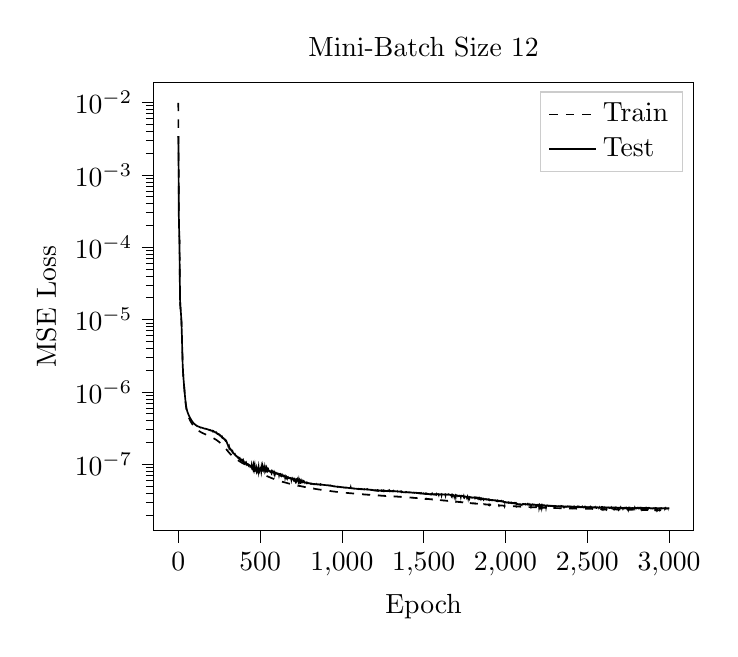
\begin{tikzpicture}

\begin{axis}[
legend cell align={left},
legend style={fill opacity=0.8, draw opacity=1, text opacity=1, draw=white!80!black},
log basis y={10},
tick align=outside,
tick pos=left,
title={Mini-Batch Size 12},
x grid style={white!69.0196078431373!black},
xlabel={Epoch},
xmin=-149.95, xmax=3148.95,
xtick style={color=black},
y grid style={white!69.0196078431373!black},
ylabel={MSE Loss},
ymin=1.20182983684796e-08, ymax=0.0188674057447821,
ymode=log,
ytick style={color=black}
]
\addplot [semithick, black, dashed]
table {%
0 0.00986465203441947
1 0.00260751335400653
2 0.00168988164350485
3 0.000488507373779203
4 0.000209907971291254
5 0.000167378415469924
6 0.000144635666222162
7 0.000122048938873469
8 8.62523788347024e-05
9 4.82955873002413e-05
10 2.73796132283068e-05
11 1.90950526797145e-05
12 1.60943547821725e-05
13 1.4741469611298e-05
14 1.38728226151662e-05
15 1.31170852149056e-05
16 1.23484586361327e-05
17 1.15099031735347e-05
18 1.05987408478731e-05
19 9.60587541868733e-06
20 8.52972127505861e-06
21 7.39411303849163e-06
22 6.24609348050627e-06
23 5.15921849678429e-06
24 4.20662657506024e-06
25 3.43513256635849e-06
26 2.85083812256804e-06
27 2.41368249620843e-06
28 2.11103944583009e-06
29 1.89133949933387e-06
30 1.72881501848774e-06
31 1.60041405033308e-06
32 1.49132691603201e-06
33 1.39468694930702e-06
34 1.30722597387098e-06
35 1.22787994946677e-06
36 1.15318429976398e-06
37 1.08247199141989e-06
38 1.01458761692296e-06
39 9.50791769616831e-07
40 8.94639568261079e-07
41 8.44264715250895e-07
42 7.98514396704664e-07
43 7.57062303104059e-07
44 7.1960601601547e-07
45 6.86264076177002e-07
46 6.56710590567502e-07
47 6.30560452140253e-07
48 6.07495739716849e-07
49 5.8729833474945e-07
50 5.69166945249871e-07
51 5.53365959734515e-07
52 5.39226312846706e-07
53 5.26853619190663e-07
54 5.15626668984171e-07
55 5.05354143809034e-07
56 4.96219717452013e-07
57 4.87743031464148e-07
58 4.79965486192328e-07
59 4.72839623540552e-07
60 4.66067782073731e-07
61 4.59671513606091e-07
62 4.5346518455062e-07
63 4.47667074912168e-07
64 4.42254874914619e-07
65 4.36917606041582e-07
66 4.31543515322906e-07
67 4.26586544664612e-07
68 4.21815189840398e-07
69 4.17151321900514e-07
70 4.12637008346803e-07
71 4.08143212267705e-07
72 4.03891417800969e-07
73 3.99800072712568e-07
74 3.95728463927244e-07
75 3.91803002401218e-07
76 3.88060614168244e-07
77 3.84411412498194e-07
78 3.80947624093723e-07
79 3.77644791850493e-07
80 3.74367981969172e-07
81 3.71259390676611e-07
82 3.68247853160908e-07
83 3.652546020369e-07
84 3.6221987798002e-07
85 3.59415486626151e-07
86 3.5667539174196e-07
87 3.54011815321989e-07
88 3.51362291480147e-07
89 3.48911777192318e-07
90 3.46474773395951e-07
91 3.44100075985848e-07
92 3.41823218076717e-07
93 3.39414419274245e-07
94 3.37256983388948e-07
95 3.35122220975533e-07
96 3.32999039398208e-07
97 3.308729406813e-07
98 3.28791070590475e-07
99 3.26763725187809e-07
100 3.24788877969253e-07
101 3.22926390043557e-07
102 3.21002658578015e-07
103 3.19170082884691e-07
104 3.17383342175878e-07
105 3.15699859866899e-07
106 3.14064653028036e-07
107 3.12445270114177e-07
108 3.10892673106465e-07
109 3.09378054256962e-07
110 3.07913456573644e-07
111 3.06473376284429e-07
112 3.05058618222563e-07
113 3.03616083433671e-07
114 3.02240261970261e-07
115 3.00803783467912e-07
116 2.99412046698171e-07
117 2.98129154018524e-07
118 2.9680637989941e-07
119 2.956091626333e-07
120 2.94398002705129e-07
121 2.93305538983514e-07
122 2.92147232228944e-07
123 2.91225466177566e-07
124 2.90211831752999e-07
125 2.89178200560386e-07
126 2.88173387507929e-07
127 2.87183440727358e-07
128 2.86342366467219e-07
129 2.85356920538768e-07
130 2.84390754857709e-07
131 2.83464474413479e-07
132 2.82583242006406e-07
133 2.8172577098873e-07
134 2.80857720069494e-07
135 2.80030456526397e-07
136 2.7921289006742e-07
137 2.78486256341509e-07
138 2.77583483358061e-07
139 2.76679555630981e-07
140 2.75953290339561e-07
141 2.75134501507749e-07
142 2.74358878237548e-07
143 2.73620859931067e-07
144 2.72921118955325e-07
145 2.72204606596898e-07
146 2.71600296350344e-07
147 2.70895373438551e-07
148 2.70107028012353e-07
149 2.69427775770409e-07
150 2.68747027665815e-07
151 2.68087882655785e-07
152 2.67431323973446e-07
153 2.66787339732929e-07
154 2.66194304368932e-07
155 2.65507266530469e-07
156 2.64838975181396e-07
157 2.64226872690281e-07
158 2.63632238610448e-07
159 2.63005287392959e-07
160 2.62324573544397e-07
161 2.61686803941466e-07
162 2.61059241625314e-07
163 2.60443335927614e-07
164 2.59830360638989e-07
165 2.59203043220752e-07
166 2.58814742848191e-07
167 2.58187941711581e-07
168 2.57645324354015e-07
169 2.56950830959751e-07
170 2.56333903415438e-07
171 2.55688715166637e-07
172 2.55113041116623e-07
173 2.54555375368047e-07
174 2.53929813437115e-07
175 2.5342732418797e-07
176 2.52792287164338e-07
177 2.52248266421047e-07
178 2.51688670086374e-07
179 2.51038047940727e-07
180 2.50433593155102e-07
181 2.49846895816353e-07
182 2.4925068778331e-07
183 2.48642706562386e-07
184 2.48091862619738e-07
185 2.47487900533806e-07
186 2.46981339406762e-07
187 2.46445586376001e-07
188 2.4578293544387e-07
189 2.45207809527585e-07
190 2.44607930094697e-07
191 2.44043891703189e-07
192 2.43480022177267e-07
193 2.4291157212909e-07
194 2.42355524981974e-07
195 2.42037180440295e-07
196 2.41199472886937e-07
197 2.40585803228933e-07
198 2.40010634855592e-07
199 2.39500687503116e-07
200 2.38559428057481e-07
201 2.37998244734117e-07
202 2.37386749538985e-07
203 2.36729708964011e-07
204 2.36116574058555e-07
205 2.35617242166686e-07
206 2.34869198719142e-07
207 2.34130488149382e-07
208 2.33504791539755e-07
209 2.32825766650212e-07
210 2.32257079968966e-07
211 2.31693280401721e-07
212 2.30864698402966e-07
213 2.3010987560655e-07
214 2.29548378043534e-07
215 2.28922232611291e-07
216 2.28285520089595e-07
217 2.27541015293791e-07
218 2.26777660070448e-07
219 2.26108019493261e-07
220 2.25370043478964e-07
221 2.24709999313267e-07
222 2.24031537757535e-07
223 2.23316574908796e-07
224 2.22542352083225e-07
225 2.21864306306681e-07
226 2.21186275538756e-07
227 2.20559174905192e-07
228 2.19845879747057e-07
229 2.1916440608579e-07
230 2.18400654548726e-07
231 2.17631000741639e-07
232 2.1685724080594e-07
233 2.16357953003886e-07
234 2.15595866636488e-07
235 2.14708611661741e-07
236 2.14008152170932e-07
237 2.13241750570067e-07
238 2.12561176229338e-07
239 2.11559029993748e-07
240 2.1079359481078e-07
241 2.10079037370284e-07
242 2.0927557328593e-07
243 2.08570132284242e-07
244 2.0762496040735e-07
245 2.0686947846554e-07
246 2.0597260186461e-07
247 2.05157218803473e-07
248 2.04277932267675e-07
249 2.03463535222864e-07
250 2.02576345053231e-07
251 2.01684478581671e-07
252 2.01022849161092e-07
253 2.00100818847383e-07
254 1.99121530601412e-07
255 1.98208881063301e-07
256 1.97281198653368e-07
257 1.96462143219114e-07
258 1.95424846647124e-07
259 1.94515042795439e-07
260 1.9355988537854e-07
261 1.9246042925692e-07
262 1.91416686865668e-07
263 1.90515489558603e-07
264 1.89527632683127e-07
265 1.88538966905804e-07
266 1.87545062705345e-07
267 1.86605689819813e-07
268 1.85676759168185e-07
269 1.84595414312876e-07
270 1.83739938441763e-07
271 1.83056588915763e-07
272 1.81931767822542e-07
273 1.80974241958222e-07
274 1.79814111278742e-07
275 1.78846650378262e-07
276 1.77672937472287e-07
277 1.76583499838369e-07
278 1.75630873900156e-07
279 1.74767970208874e-07
280 1.73521450174642e-07
281 1.72708379595049e-07
282 1.71592240089546e-07
283 1.70582798808483e-07
284 1.69653858535808e-07
285 1.68714139601072e-07
286 1.67747395848822e-07
287 1.66634858901358e-07
288 1.65680374175902e-07
289 1.64878483949027e-07
290 1.63911613735062e-07
291 1.62866931401076e-07
292 1.61993550645468e-07
293 1.61075406995205e-07
294 1.59946316561281e-07
295 1.5917892792827e-07
296 1.58259756501341e-07
297 1.5732373517569e-07
298 1.56405021671217e-07
299 1.55259597870166e-07
300 1.54188427018879e-07
301 1.53147169016902e-07
302 1.52231455013276e-07
303 1.51187420140084e-07
304 1.50537693209144e-07
305 1.4952619660876e-07
306 1.48397269275242e-07
307 1.4768550330506e-07
308 1.46697564398064e-07
309 1.45781057330886e-07
310 1.44909075371194e-07
311 1.44113219779519e-07
312 1.43190130092329e-07
313 1.42234409799005e-07
314 1.41564903948379e-07
315 1.40727371078974e-07
316 1.39984446113249e-07
317 1.38979553332153e-07
318 1.38417120565127e-07
319 1.37457988230694e-07
320 1.37116515570832e-07
321 1.36397150319499e-07
322 1.35356013396982e-07
323 1.34902170020264e-07
324 1.34304258593972e-07
325 1.33666783440802e-07
326 1.32998570336525e-07
327 1.32611940287192e-07
328 1.31949723211605e-07
329 1.3138686095447e-07
330 1.30456072823933e-07
331 1.3004578166427e-07
332 1.29304112519009e-07
333 1.28808979344363e-07
334 1.28247493274482e-07
335 1.27553031711043e-07
336 1.27240534622292e-07
337 1.26568065127699e-07
338 1.26049489637764e-07
339 1.25538146707025e-07
340 1.24983221605812e-07
341 1.2432876307719e-07
342 1.23912163473407e-07
343 1.23308572364178e-07
344 1.22667956080272e-07
345 1.22200386193272e-07
346 1.22031874223757e-07
347 1.21259684172668e-07
348 1.21119337266249e-07
349 1.20427919750858e-07
350 1.19903499227883e-07
351 1.19436163383875e-07
352 1.18939739515794e-07
353 1.18374059605695e-07
354 1.18016359027289e-07
355 1.17585388244609e-07
356 1.17048287139833e-07
357 1.16576402460796e-07
358 1.16139044797737e-07
359 1.15758196896284e-07
360 1.15444143415791e-07
361 1.14990975863073e-07
362 1.14507993282995e-07
363 1.14136096893064e-07
364 1.13680510141772e-07
365 1.13252466047923e-07
366 1.12852237641286e-07
367 1.12467889792994e-07
368 1.12107805644202e-07
369 1.11731543833405e-07
370 1.11416253144306e-07
371 1.10987849686554e-07
372 1.10706991071414e-07
373 1.10312365493689e-07
374 1.09949491416928e-07
375 1.09622494733039e-07
376 1.09173863953141e-07
377 1.08780210922809e-07
378 1.08400519988094e-07
379 1.08056382925934e-07
380 1.07780304008389e-07
381 1.07455280593686e-07
382 1.07053753662222e-07
383 1.06790157172277e-07
384 1.06350253662783e-07
385 1.05875654277044e-07
386 1.0557874308414e-07
387 1.0523801744349e-07
388 1.05013178961659e-07
389 1.04592827046042e-07
390 1.04298884262422e-07
391 1.04052798263206e-07
392 1.03665887857961e-07
393 1.03456886799319e-07
394 1.0317013849225e-07
395 1.02902540117653e-07
396 1.02691777192244e-07
397 1.02266042450041e-07
398 1.02096551165427e-07
399 1.01926844287469e-07
400 1.01609048182668e-07
401 1.01361464448714e-07
402 1.01000889919066e-07
403 1.00627217459491e-07
404 1.00386729590351e-07
405 1.00219144339286e-07
406 9.99003052790087e-08
407 9.96493648183157e-08
408 9.93807552472695e-08
409 9.9116329964535e-08
410 9.8786126562987e-08
411 9.86490139742392e-08
412 9.83083036985447e-08
413 9.80155675744477e-08
414 9.78291330180321e-08
415 9.74236173118547e-08
416 9.72413826400574e-08
417 9.6813098602415e-08
418 9.65025782238763e-08
419 9.63088241970816e-08
420 9.59802467842984e-08
421 9.56620157273566e-08
422 9.52465724334851e-08
423 9.49690089576224e-08
424 9.46741575621608e-08
425 9.44036359105076e-08
426 9.41854147993331e-08
427 9.39079606146226e-08
428 9.36693822200575e-08
429 9.32644040559468e-08
430 9.29040113715223e-08
431 9.26247987530938e-08
432 9.23331803084654e-08
433 9.20339168282012e-08
434 9.18264109806997e-08
435 9.15852875507611e-08
436 9.13102214145588e-08
437 9.10468111256352e-08
438 9.07511739901045e-08
439 9.04364017472361e-08
440 9.02689807666307e-08
441 8.99290094314485e-08
442 8.96550553903595e-08
443 8.94493951589996e-08
444 8.91716758477125e-08
445 8.89388250578319e-08
446 8.86707305451742e-08
447 8.84126433328941e-08
448 8.81528533974884e-08
449 8.79975966133462e-08
450 8.77086544683521e-08
451 8.74807724304284e-08
452 8.71330707998005e-08
453 8.69168866300998e-08
454 8.67209687241161e-08
455 8.62987805767333e-08
456 8.61133189373407e-08
457 8.59795703536088e-08
458 8.55838761908769e-08
459 8.53847518836808e-08
460 8.52117661647845e-08
461 8.49874530458069e-08
462 8.46269108894638e-08
463 8.44341880590881e-08
464 8.42327955622639e-08
465 8.39158430993192e-08
466 8.37331758234696e-08
467 8.35279735837051e-08
468 8.32065515117794e-08
469 8.30688071675718e-08
470 8.27502307209118e-08
471 8.24198592249499e-08
472 8.21675475337824e-08
473 8.19286826458333e-08
474 8.17703776386731e-08
475 8.16130515264554e-08
476 8.14199416949367e-08
477 8.11354428087441e-08
478 8.09148203609549e-08
479 8.06256585327405e-08
480 8.05577514422774e-08
481 8.01761198536712e-08
482 8.00313872019927e-08
483 8.00935765614433e-08
484 7.95331810629746e-08
485 7.93217525196389e-08
486 7.90704434755385e-08
487 7.89373905588835e-08
488 7.86523900353697e-08
489 7.85615026871566e-08
490 7.80801989025714e-08
491 7.79388681949553e-08
492 7.76494746904526e-08
493 7.76557454827213e-08
494 7.72290723933132e-08
495 7.7262094478712e-08
496 7.6727138500328e-08
497 7.66496535145018e-08
498 7.65337105068121e-08
499 7.61089675487748e-08
500 7.61158348751763e-08
501 7.57488532790335e-08
502 7.55854786265709e-08
503 7.55284122589715e-08
504 7.51368786909293e-08
505 7.51029964499377e-08
506 7.4959265091785e-08
507 7.46902734630799e-08
508 7.45905285933641e-08
509 7.42376964532792e-08
510 7.41611178136421e-08
511 7.38317243590141e-08
512 7.36253986373699e-08
513 7.34649972472623e-08
514 7.32372358553467e-08
515 7.31767389251933e-08
516 7.28040041746106e-08
517 7.2763275585779e-08
518 7.24674790860432e-08
519 7.22951334113854e-08
520 7.21275867934219e-08
521 7.19492725651022e-08
522 7.17366622551724e-08
523 7.15983126173718e-08
524 7.14092059868174e-08
525 7.12567897062893e-08
526 7.11410891713082e-08
527 7.08884052669024e-08
528 7.07195806399694e-08
529 7.06897194246726e-08
530 7.03580877072426e-08
531 7.02836704045831e-08
532 7.00082131481109e-08
533 6.99525766786275e-08
534 6.96759692497163e-08
535 6.97064487701542e-08
536 6.93422256221718e-08
537 6.92601750349557e-08
538 6.90926233724579e-08
539 6.89645065392809e-08
540 6.88077918288773e-08
541 6.86312138244967e-08
542 6.85018139590897e-08
543 6.83466730822312e-08
544 6.81660816256054e-08
545 6.79906761576772e-08
546 6.79201561845827e-08
547 6.77617493214404e-08
548 6.75013737094843e-08
549 6.73794689982752e-08
550 6.72881390872427e-08
551 6.70705480455844e-08
552 6.69393279675341e-08
553 6.68744195269689e-08
554 6.67045240068282e-08
555 6.66043024804742e-08
556 6.63488655340957e-08
557 6.62258281215021e-08
558 6.61138364440933e-08
559 6.60180411761676e-08
560 6.57616039893132e-08
561 6.56229188514218e-08
562 6.54586033600688e-08
563 6.53714452363698e-08
564 6.52368431982715e-08
565 6.50957717988657e-08
566 6.48673499000381e-08
567 6.47582385825852e-08
568 6.46143641293159e-08
569 6.446432118119e-08
570 6.43203441300172e-08
571 6.4192627724369e-08
572 6.40600470181417e-08
573 6.40068021166399e-08
574 6.39365269523759e-08
575 6.37360501608544e-08
576 6.36061154205751e-08
577 6.3509022582481e-08
578 6.32211303228818e-08
579 6.31782073031192e-08
580 6.30676574583916e-08
581 6.29049511482234e-08
582 6.28223088280905e-08
583 6.27075932816472e-08
584 6.26088367603898e-08
585 6.25348943021124e-08
586 6.23425757657667e-08
587 6.22136231394119e-08
588 6.20773557441733e-08
589 6.19553724318333e-08
590 6.18225580495867e-08
591 6.17681063130538e-08
592 6.15644303892891e-08
593 6.15694477503998e-08
594 6.14890816879589e-08
595 6.13349707962462e-08
596 6.12565199788802e-08
597 6.11039763497879e-08
598 6.09475477950477e-08
599 6.08200170133708e-08
600 6.07890193126239e-08
601 6.05905780212806e-08
602 6.06219013803568e-08
603 6.05198525598651e-08
604 6.03579276499242e-08
605 6.02553045994808e-08
606 6.00713622344818e-08
607 5.99952318191367e-08
608 5.9981121403041e-08
609 5.97894142658502e-08
610 5.97183774207813e-08
611 5.96686039141078e-08
612 5.95676945387744e-08
613 5.94907872319041e-08
614 5.92593871166007e-08
615 5.92393065606202e-08
616 5.9148006766548e-08
617 5.90109215836887e-08
618 5.89135106248153e-08
619 5.88587184792774e-08
620 5.87428698697961e-08
621 5.86733444531015e-08
622 5.86089437886596e-08
623 5.84117424489041e-08
624 5.83948601462957e-08
625 5.82078968511506e-08
626 5.8190589716051e-08
627 5.80720970393026e-08
628 5.80102084891297e-08
629 5.79308706607402e-08
630 5.77988304310255e-08
631 5.76867206724232e-08
632 5.76577249830075e-08
633 5.7560701507925e-08
634 5.74618290886911e-08
635 5.73348193220484e-08
636 5.72021462918017e-08
637 5.7134671357313e-08
638 5.70187124820765e-08
639 5.70405687048296e-08
640 5.68837959995662e-08
641 5.68191775931322e-08
642 5.67855930567826e-08
643 5.66864053834052e-08
644 5.6518523400971e-08
645 5.6458533947779e-08
646 5.64203987840894e-08
647 5.62999695340174e-08
648 5.63434277185069e-08
649 5.61434640175534e-08
650 5.60735962306814e-08
651 5.60068968341764e-08
652 5.59211564081067e-08
653 5.58447379596912e-08
654 5.57167653478091e-08
655 5.56635842196453e-08
656 5.5632814649121e-08
657 5.55321487875796e-08
658 5.54532317151019e-08
659 5.53764749026191e-08
660 5.53393014194319e-08
661 5.52139071908318e-08
662 5.51612944822309e-08
663 5.51343926893949e-08
664 5.50219801536945e-08
665 5.49547743651887e-08
666 5.483404369156e-08
667 5.47484004957646e-08
668 5.47437455207564e-08
669 5.46461673543179e-08
670 5.45263590433411e-08
671 5.44574668260609e-08
672 5.44269155200649e-08
673 5.44110587032074e-08
674 5.43177522867219e-08
675 5.41858194361826e-08
676 5.41225189309592e-08
677 5.40491708049831e-08
678 5.40079091468875e-08
679 5.39885951886038e-08
680 5.38424242090919e-08
681 5.37980833959682e-08
682 5.37519621228336e-08
683 5.36881446233118e-08
684 5.35810987940253e-08
685 5.34883564585906e-08
686 5.33910138974332e-08
687 5.34043271561123e-08
688 5.32770727933764e-08
689 5.32541824557138e-08
690 5.3226214092227e-08
691 5.313242644658e-08
692 5.29011008598169e-08
693 5.30353102140258e-08
694 5.29186655453845e-08
695 5.28322069712189e-08
696 5.27698278766479e-08
697 5.27196956376358e-08
698 5.2631735613807e-08
699 5.25709220493766e-08
700 5.25244517846146e-08
701 5.24470878144278e-08
702 5.23868302815987e-08
703 5.23032808932994e-08
704 5.23088088612696e-08
705 5.22860117437825e-08
706 5.20894042377251e-08
707 5.20470728804101e-08
708 5.20317889107115e-08
709 5.19126496892691e-08
710 5.18803367717909e-08
711 5.18576781968411e-08
712 5.17070597582948e-08
713 5.17908779415604e-08
714 5.16186378098889e-08
715 5.16389611124773e-08
716 5.14800853642579e-08
717 5.15446715888499e-08
718 5.14004373993877e-08
719 5.13445678522088e-08
720 5.13225442995665e-08
721 5.12989243765165e-08
722 5.11132407510217e-08
723 5.12047896591966e-08
724 5.10618273199577e-08
725 5.10391850978618e-08
726 5.09758288115766e-08
727 5.09068935681682e-08
728 5.08076371207956e-08
729 5.08547186038857e-08
730 5.06261828028238e-08
731 5.07035413468788e-08
732 5.06510107455861e-08
733 5.058392002937e-08
734 5.05539704655829e-08
735 5.04213919053436e-08
736 5.04114446301378e-08
737 5.03482807820671e-08
738 5.03112679501459e-08
739 5.01340524942632e-08
740 5.02210255803482e-08
741 5.0122920940833e-08
742 5.01321394816007e-08
743 5.00974128461945e-08
744 4.99888168357668e-08
745 4.99658209750622e-08
746 4.98925407109698e-08
747 4.9897336277442e-08
748 4.97913948036182e-08
749 4.97167080119369e-08
750 4.96659497135076e-08
751 4.95494336339551e-08
752 4.95479175094039e-08
753 4.94693685177415e-08
754 4.94487289677922e-08
755 4.94525359624318e-08
756 4.93095180016842e-08
757 4.93115764243115e-08
758 4.92605054458606e-08
759 4.92203085461595e-08
760 4.91040709610668e-08
761 4.91201381525562e-08
762 4.91542410433935e-08
763 4.89817610450458e-08
764 4.90018651271176e-08
765 4.88528724233808e-08
766 4.88570789267899e-08
767 4.880257696164e-08
768 4.87457676086763e-08
769 4.86502932244561e-08
770 4.86756310414636e-08
771 4.85431318375728e-08
772 4.85933666080081e-08
773 4.84812188757895e-08
774 4.84693957930239e-08
775 4.84090173269912e-08
776 4.83806026458709e-08
777 4.83119367518755e-08
778 4.82378492891638e-08
779 4.82760957557032e-08
780 4.79961109884628e-08
781 4.81195751747759e-08
782 4.80567150464956e-08
783 4.7969296641313e-08
784 4.78785606942803e-08
785 4.78766278544972e-08
786 4.77091153370007e-08
787 4.7843352267288e-08
788 4.77333643416679e-08
789 4.75283319607077e-08
790 4.76626156732671e-08
791 4.76504013545556e-08
792 4.75728110890057e-08
793 4.74972522962502e-08
794 4.74657006154878e-08
795 4.74430570385209e-08
796 4.73490130124613e-08
797 4.73458218512205e-08
798 4.72957860992317e-08
799 4.72716764308781e-08
800 4.72083759921351e-08
801 4.71436242871393e-08
802 4.71020220764409e-08
803 4.70619568638163e-08
804 4.69447375131565e-08
805 4.70273669746465e-08
806 4.69348211912346e-08
807 4.68514108148244e-08
808 4.68760159870155e-08
809 4.67407997243445e-08
810 4.668936239091e-08
811 4.66776428726732e-08
812 4.66418046992596e-08
813 4.65478704430113e-08
814 4.65727279522758e-08
815 4.64733582422106e-08
816 4.64236427423633e-08
817 4.63933700558102e-08
818 4.63374233660808e-08
819 4.64078003490978e-08
820 4.62588261654766e-08
821 4.62255887074479e-08
822 4.63597804509934e-08
823 4.61424195286519e-08
824 4.6050068632593e-08
825 4.60841536601413e-08
826 4.61601346261712e-08
827 4.60038556417405e-08
828 4.59089444397556e-08
829 4.59156726306144e-08
830 4.58586313008709e-08
831 4.58739114399677e-08
832 4.57872433554157e-08
833 4.57379587005489e-08
834 4.57546889385024e-08
835 4.56660898051498e-08
836 4.56715770046669e-08
837 4.56353020987668e-08
838 4.55700081794602e-08
839 4.55263045439393e-08
840 4.55119456705675e-08
841 4.5449994938598e-08
842 4.54511536351566e-08
843 4.53804433578691e-08
844 4.53476187658559e-08
845 4.52941170318747e-08
846 4.5239587702054e-08
847 4.52244539767764e-08
848 4.52237193987094e-08
849 4.51578661729759e-08
850 4.51483631917397e-08
851 4.50770215485678e-08
852 4.50623080965542e-08
853 4.50298040890846e-08
854 4.49765035368227e-08
855 4.48925950851122e-08
856 4.48928823456802e-08
857 4.48779615119832e-08
858 4.48068184591239e-08
859 4.4831918515555e-08
860 4.47324035697037e-08
861 4.47270897830342e-08
862 4.47002858094892e-08
863 4.4657078998107e-08
864 4.4625353985603e-08
865 4.46067588442083e-08
866 4.45288706892008e-08
867 4.4545250390522e-08
868 4.44633700623223e-08
869 4.44693163995573e-08
870 4.43822104270891e-08
871 4.44003185861066e-08
872 4.4350900136734e-08
873 4.43133551423418e-08
874 4.42564236794711e-08
875 4.42705738973946e-08
876 4.4196955870218e-08
877 4.41425731297248e-08
878 4.41519010946057e-08
879 4.41395356127138e-08
880 4.40635883549164e-08
881 4.40397766704226e-08
882 4.40307261748734e-08
883 4.39618665622506e-08
884 4.39708115972494e-08
885 4.39327809022225e-08
886 4.38664159514288e-08
887 4.38603793111793e-08
888 4.38408824306886e-08
889 4.37644267731817e-08
890 4.37735866157268e-08
891 4.37353327246541e-08
892 4.36864780345669e-08
893 4.36639237634083e-08
894 4.36366870142914e-08
895 4.35965192210481e-08
896 4.3572467127398e-08
897 4.35362647489776e-08
898 4.35168434035409e-08
899 4.34617703649297e-08
900 4.34522315095288e-08
901 4.34173429052146e-08
902 4.33801663173917e-08
903 4.33698186665118e-08
904 4.33100990041628e-08
905 4.33015152583396e-08
906 4.3278288565648e-08
907 4.32211963278576e-08
908 4.3219251775554e-08
909 4.3181242400798e-08
910 4.31332777200013e-08
911 4.31439885427822e-08
912 4.31027219279065e-08
913 4.30666660284561e-08
914 4.30346289502096e-08
915 4.30089304742609e-08
916 4.30059758689713e-08
917 4.28878593916272e-08
918 4.29622862594895e-08
919 4.28881998790791e-08
920 4.28569609647628e-08
921 4.2828996679185e-08
922 4.2799269658606e-08
923 4.27722287156017e-08
924 4.27546580335001e-08
925 4.27072546043474e-08
926 4.27345478737883e-08
927 4.264485852004e-08
928 4.2670247766301e-08
929 4.2589363842657e-08
930 4.25970238097953e-08
931 4.25758866459198e-08
932 4.25097977258215e-08
933 4.25072540094196e-08
934 4.25228131814675e-08
935 4.24551681581522e-08
936 4.24027583650799e-08
937 4.23363741961263e-08
938 4.23204615516707e-08
939 4.22993436976982e-08
940 4.22378282662269e-08
941 4.22040973798794e-08
942 4.21847035307446e-08
943 4.21343101539811e-08
944 4.2126883438717e-08
945 4.20900990401692e-08
946 4.20884369844466e-08
947 4.20589325310087e-08
948 4.19787110182759e-08
949 4.20168152539442e-08
950 4.19544620016423e-08
951 4.19586019767648e-08
952 4.19337164313773e-08
953 4.18319668459069e-08
954 4.18840358483765e-08
955 4.18133375947379e-08
956 4.17775922692094e-08
957 4.18056963697598e-08
958 4.17372047515279e-08
959 4.17033064222745e-08
960 4.17059196080567e-08
961 4.16943957151057e-08
962 4.16372243563075e-08
963 4.16370861993566e-08
964 4.15988224891257e-08
965 4.15754833527802e-08
966 4.15447488427002e-08
967 4.1529855465417e-08
968 4.14870760779328e-08
969 4.14769175917714e-08
970 4.14634785348515e-08
971 4.14006713183381e-08
972 4.14197953846074e-08
973 4.13596368530912e-08
974 4.13537683724064e-08
975 4.1307926029843e-08
976 4.13104246086985e-08
977 4.12698089049508e-08
978 4.12661955504915e-08
979 4.1246893030829e-08
980 4.1204264257397e-08
981 4.11998552572859e-08
982 4.11423886974983e-08
983 4.11852311390023e-08
984 4.10878856221254e-08
985 4.11417882942051e-08
986 4.10401329168091e-08
987 4.10561749015823e-08
988 4.09912072508953e-08
989 4.10312746414185e-08
990 4.09426719247712e-08
991 4.09751525736802e-08
992 4.09428749307133e-08
993 4.09263540396044e-08
994 4.08885892263717e-08
995 4.08824053652306e-08
996 4.08362075372324e-08
997 4.08398484823959e-08
998 4.07884294270882e-08
999 4.07961053255945e-08
1000 4.07628713750728e-08
1001 4.07447405156509e-08
1002 4.06991164881408e-08
1003 4.07139741774047e-08
1004 4.06584073195698e-08
1005 4.06450657428907e-08
1006 4.0686107333509e-08
1007 4.06013955563286e-08
1008 4.06371103327742e-08
1009 4.05344883180958e-08
1010 4.05928265811252e-08
1011 4.04953102959918e-08
1012 4.05400375052867e-08
1013 4.04554987035127e-08
1014 4.04771682066972e-08
1015 4.04402577559535e-08
1016 4.0428882825681e-08
1017 4.04340641128834e-08
1018 4.03814156404753e-08
1019 4.0374532372069e-08
1020 4.03447679416277e-08
1021 4.03274609408185e-08
1022 4.02845212158558e-08
1023 4.02629104747151e-08
1024 4.02638920727515e-08
1025 4.02323331403048e-08
1026 4.02173497019956e-08
1027 4.02156664204044e-08
1028 4.01830514584423e-08
1029 4.02121344459576e-08
1030 4.0156237038164e-08
1031 4.01559546652366e-08
1032 4.00968941469509e-08
1033 4.01204974751583e-08
1034 4.00551980885019e-08
1035 4.0069630312381e-08
1036 4.00200974222827e-08
1037 4.00298179700027e-08
1038 3.99923551174886e-08
1039 4.00141667970303e-08
1040 3.99311973240882e-08
1041 3.99573413797378e-08
1042 3.98990666719905e-08
1043 3.99129206584782e-08
1044 3.98603177810018e-08
1045 3.98817791260116e-08
1046 3.98457326747586e-08
1047 3.98146454022818e-08
1048 3.98002268281627e-08
1049 3.97645544595774e-08
1050 3.97684314993179e-08
1051 3.97593357159765e-08
1052 3.97377002879964e-08
1053 3.97104352740638e-08
1054 3.96814806788553e-08
1055 3.96363156295101e-08
1056 3.9673983054245e-08
1057 3.96182399169267e-08
1058 3.96241302869548e-08
1059 3.95833749344355e-08
1060 3.95803736492537e-08
1061 3.95635018824623e-08
1062 3.95425178775095e-08
1063 3.95127514991919e-08
1064 3.95236096665179e-08
1065 3.94801247914692e-08
1066 3.94699455541093e-08
1067 3.94495846368989e-08
1068 3.94233477041128e-08
1069 3.93970162880234e-08
1070 3.93831324943744e-08
1071 3.93919230541382e-08
1072 3.93413428261748e-08
1073 3.93289245282479e-08
1074 3.93032945045291e-08
1075 3.92852066153918e-08
1076 3.9295780957858e-08
1077 3.92376532050805e-08
1078 3.92484061152862e-08
1079 3.92187464393733e-08
1080 3.92049001938658e-08
1081 3.91915893577332e-08
1082 3.91644203880644e-08
1083 3.91436231930936e-08
1084 3.91440971120682e-08
1085 3.9097501546339e-08
1086 3.91036622988858e-08
1087 3.90890850639244e-08
1088 3.90710894695552e-08
1089 3.90309840070247e-08
1090 3.89647954115021e-08
1091 3.90428916768183e-08
1092 3.89672375298659e-08
1093 3.89829090737688e-08
1094 3.89328668917937e-08
1095 3.8967888471575e-08
1096 3.88995695694758e-08
1097 3.88681002007814e-08
1098 3.88848865229474e-08
1099 3.88840480998041e-08
1100 3.88418534913847e-08
1101 3.88604784173375e-08
1102 3.87413352363212e-08
1103 3.88109814386329e-08
1104 3.87788765968937e-08
1105 3.87235220815111e-08
1106 3.87488532770687e-08
1107 3.87439485563939e-08
1108 3.86415243754808e-08
1109 3.8728494055109e-08
1110 3.86680716335519e-08
1111 3.86532019791419e-08
1112 3.86497158176826e-08
1113 3.8636003288234e-08
1114 3.85474400888784e-08
1115 3.86122508165213e-08
1116 3.85778451326306e-08
1117 3.85534992221135e-08
1118 3.85593853028248e-08
1119 3.84759967280037e-08
1120 3.84829618364671e-08
1121 3.84756804247992e-08
1122 3.85140681662213e-08
1123 3.8438346928558e-08
1124 3.84712159002408e-08
1125 3.84237612519128e-08
1126 3.84100821980152e-08
1127 3.84184149536584e-08
1128 3.83808637380284e-08
1129 3.83917643411365e-08
1130 3.82901163909332e-08
1131 3.83811045048494e-08
1132 3.82541426174056e-08
1133 3.83160322020138e-08
1134 3.82843096612519e-08
1135 3.82701170487642e-08
1136 3.82797174264759e-08
1137 3.82333374953094e-08
1138 3.82074162288455e-08
1139 3.82696028971686e-08
1140 3.81980627793602e-08
1141 3.81799757996751e-08
1142 3.8144010237809e-08
1143 3.81818793920619e-08
1144 3.80666717362713e-08
1145 3.81680169479352e-08
1146 3.80704226533466e-08
1147 3.81038261542035e-08
1148 3.80511195393492e-08
1149 3.80643813568084e-08
1150 3.80114991392414e-08
1151 3.80306619968362e-08
1152 3.79887475302614e-08
1153 3.79720264546394e-08
1154 3.791481330226e-08
1155 3.80194876340039e-08
1156 3.78821038038103e-08
1157 3.79264725825877e-08
1158 3.79251857716105e-08
1159 3.7940524523835e-08
1160 3.78564981624505e-08
1161 3.79056175709246e-08
1162 3.7820451098248e-08
1163 3.78839639073651e-08
1164 3.77697167580327e-08
1165 3.78676807808214e-08
1166 3.77630708619571e-08
1167 3.78053544584083e-08
1168 3.77177560308946e-08
1169 3.77913717206196e-08
1170 3.7716236824311e-08
1171 3.77603198582741e-08
1172 3.76800632066502e-08
1173 3.77358696452954e-08
1174 3.76665307061807e-08
1175 3.76578641071388e-08
1176 3.76528494876806e-08
1177 3.76931637665419e-08
1178 3.76032949834679e-08
1179 3.76545072341423e-08
1180 3.76161433950907e-08
1181 3.76058548825338e-08
1182 3.75470607340087e-08
1183 3.75844980633597e-08
1184 3.75151704272461e-08
1185 3.75498367968215e-08
1186 3.74865175308233e-08
1187 3.75448962884066e-08
1188 3.74674532623627e-08
1189 3.74706493604395e-08
1190 3.74834768307298e-08
1191 3.74781881616928e-08
1192 3.7397500849904e-08
1193 3.74274238308301e-08
1194 3.73691718474202e-08
1195 3.74507780263204e-08
1196 3.73472883956164e-08
1197 3.73127437064845e-08
1198 3.73506364719236e-08
1199 3.73981558442595e-08
1200 3.7338107933504e-08
1201 3.73268508597212e-08
1202 3.72619590259651e-08
1203 3.73075510989962e-08
1204 3.72555192630705e-08
1205 3.72698282601715e-08
1206 3.72196118409916e-08
1207 3.72460998251197e-08
1208 3.72056135308292e-08
1209 3.72248057475073e-08
1210 3.71466972524529e-08
1211 3.72026701846636e-08
1212 3.71419100359216e-08
1213 3.71812740316838e-08
1214 3.70939736465327e-08
1215 3.71489042096248e-08
1216 3.7113513110392e-08
1217 3.71238522969847e-08
1218 3.7051462068775e-08
1219 3.70408303098287e-08
1220 3.70527457099657e-08
1221 3.71117573292427e-08
1222 3.70065734290635e-08
1223 3.70773726837459e-08
1224 3.69714598523466e-08
1225 3.70183491644736e-08
1226 3.69632151061434e-08
1227 3.69688803734672e-08
1228 3.69345358874629e-08
1229 3.70043623261726e-08
1230 3.68789692530022e-08
1231 3.6923755753525e-08
1232 3.69178673366917e-08
1233 3.69336560470176e-08
1234 3.68495994862372e-08
1235 3.69068889448434e-08
1236 3.67925287282708e-08
1237 3.68701018538386e-08
1238 3.68366740570472e-08
1239 3.68471438683592e-08
1240 3.67930696049955e-08
1241 3.67843892484953e-08
1242 3.67117054826364e-08
1243 3.677451412449e-08
1244 3.66981722030163e-08
1245 3.68144545413987e-08
1246 3.67429922402522e-08
1247 3.67495650623791e-08
1248 3.66697556537962e-08
1249 3.673240019405e-08
1250 3.66448512439245e-08
1251 3.67027619487655e-08
1252 3.65920757367399e-08
1253 3.66965758033572e-08
1254 3.65875247504056e-08
1255 3.66223540874248e-08
1256 3.65944935285882e-08
1257 3.66244116737284e-08
1258 3.65502016769647e-08
1259 3.66107018327481e-08
1260 3.65182431067766e-08
1261 3.65733416539252e-08
1262 3.64762915840153e-08
1263 3.65497682246221e-08
1264 3.64812092018917e-08
1265 3.64956923550914e-08
1266 3.64760043207881e-08
1267 3.64698643686353e-08
1268 3.63941480558415e-08
1269 3.65296096525384e-08
1270 3.63690572814067e-08
1271 3.64550898344111e-08
1272 3.64057715510883e-08
1273 3.63955797888172e-08
1274 3.6346708210044e-08
1275 3.64354798374848e-08
1276 3.63374602357348e-08
1277 3.63845091607037e-08
1278 3.63057983131501e-08
1279 3.63851439742627e-08
1280 3.62835410672036e-08
1281 3.63581149485385e-08
1282 3.62605742491355e-08
1283 3.63340823855064e-08
1284 3.62254651571877e-08
1285 3.62666374576203e-08
1286 3.62279050178765e-08
1287 3.63015168371114e-08
1288 3.61480790476912e-08
1289 3.62981329371647e-08
1290 3.61940607199201e-08
1291 3.62094753528967e-08
1292 3.61854679194636e-08
1293 3.6202119020454e-08
1294 3.61038167971398e-08
1295 3.61697062374176e-08
1296 3.60709334031945e-08
1297 3.61486028136852e-08
1298 3.60927589545408e-08
1299 3.61772631107084e-08
1300 3.60974500324063e-08
1301 3.60986392248634e-08
1302 3.60575252317485e-08
1303 3.60727192401419e-08
1304 3.60606473504132e-08
1305 3.60352742761794e-08
1306 3.59939338800032e-08
1307 3.61285097992739e-08
1308 3.60267587273013e-08
1309 3.60040997162399e-08
1310 3.59984943491047e-08
1311 3.60030120952287e-08
1312 3.59366314590446e-08
1313 3.59511454565003e-08
1314 3.59778346781912e-08
1315 3.58697534761857e-08
1316 3.58744597754083e-08
1317 3.58755469523303e-08
1318 3.59430045367589e-08
1319 3.59257480570805e-08
1320 3.59301595967437e-08
1321 3.58530930346962e-08
1322 3.59200509084062e-08
1323 3.58173616142125e-08
1324 3.58290745907759e-08
1325 3.57938193708747e-08
1326 3.57899713485083e-08
1327 3.5793046433605e-08
1328 3.58327594781678e-08
1329 3.58056646886819e-08
1330 3.57559324131652e-08
1331 3.57163421579394e-08
1332 3.58186596271405e-08
1333 3.57266713591729e-08
1334 3.57721263163364e-08
1335 3.57289059004009e-08
1336 3.57348836004392e-08
1337 3.56643451484469e-08
1338 3.56755122423099e-08
1339 3.56512342867492e-08
1340 3.57254644177731e-08
1341 3.56135864604423e-08
1342 3.56567139553642e-08
1343 3.56228755342771e-08
1344 3.56157831650037e-08
1345 3.56261555824995e-08
1346 3.56166937180738e-08
1347 3.55419518806042e-08
1348 3.56122585725429e-08
1349 3.55784823625037e-08
1350 3.55698442782439e-08
1351 3.55499891440737e-08
1352 3.55444168177076e-08
1353 3.55365635667239e-08
1354 3.55434164588965e-08
1355 3.54976912242533e-08
1356 3.55253114045146e-08
1357 3.54397096885129e-08
1358 3.54691964448629e-08
1359 3.54563573139069e-08
1360 3.5478567215157e-08
1361 3.53421905713136e-08
1362 3.54846726254129e-08
1363 3.53568850312007e-08
1364 3.54110339427696e-08
1365 3.5353937678925e-08
1366 3.53053109807812e-08
1367 3.53521615029123e-08
1368 3.53128138467078e-08
1369 3.5240403772763e-08
1370 3.53219768723355e-08
1371 3.52237151741562e-08
1372 3.52585948248874e-08
1373 3.52181428797006e-08
1374 3.52345983979527e-08
1375 3.5197039005231e-08
1376 3.51824608541694e-08
1377 3.51714712936104e-08
1378 3.51521568220979e-08
1379 3.51316235145088e-08
1380 3.51479788441077e-08
1381 3.51172734790441e-08
1382 3.51213447386743e-08
1383 3.50674293927673e-08
1384 3.50996681633026e-08
1385 3.50304776869337e-08
1386 3.50873294597242e-08
1387 3.50203696766965e-08
1388 3.50223418050786e-08
1389 3.49921543942906e-08
1390 3.50372544616838e-08
1391 3.49638235875281e-08
1392 3.49716586388318e-08
1393 3.49454311402823e-08
1394 3.49519097789325e-08
1395 3.49338727393393e-08
1396 3.49295108592208e-08
1397 3.49012144387911e-08
1398 3.48955583251564e-08
1399 3.48614611469817e-08
1400 3.48881095217726e-08
1401 3.48031039051218e-08
1402 3.48588512812317e-08
1403 3.48059978563348e-08
1404 3.48193340726976e-08
1405 3.4768435475983e-08
1406 3.48078932151216e-08
1407 3.47292625223463e-08
1408 3.47900327933972e-08
1409 3.47024034165885e-08
1410 3.47382387486289e-08
1411 3.47190780403461e-08
1412 3.47138895666102e-08
1413 3.46824423006613e-08
1414 3.46658242657025e-08
1415 3.46603557352171e-08
1416 3.46695957810713e-08
1417 3.45932358307723e-08
1418 3.46256732487934e-08
1419 3.46554751522534e-08
1420 3.45934053445433e-08
1421 3.45557979635947e-08
1422 3.45795851121596e-08
1423 3.45272724064289e-08
1424 3.45287600155333e-08
1425 3.45276842572883e-08
1426 3.45363924690847e-08
1427 3.44405134976558e-08
1428 3.45763506442433e-08
1429 3.44420369643047e-08
1430 3.45333653808572e-08
1431 3.44339288592989e-08
1432 3.44635827135214e-08
1433 3.43957725076345e-08
1434 3.44407339001943e-08
1435 3.43659994061519e-08
1436 3.44152207178092e-08
1437 3.43061979396453e-08
1438 3.44003783270197e-08
1439 3.42836897334349e-08
1440 3.43494948060701e-08
1441 3.43212779686872e-08
1442 3.43116386327842e-08
1443 3.42824064917916e-08
1444 3.42671480133454e-08
1445 3.42346018127473e-08
1446 3.42795362062786e-08
1447 3.42557926110317e-08
1448 3.42419740433178e-08
1449 3.42089497687187e-08
1450 3.41833200461562e-08
1451 3.41681059620054e-08
1452 3.41808267963713e-08
1453 3.41554313056045e-08
1454 3.41370324263779e-08
1455 3.41116424554804e-08
1456 3.41007699523165e-08
1457 3.41288889531236e-08
1458 3.40665554707691e-08
1459 3.40471791352364e-08
1460 3.40181517825259e-08
1461 3.39896740693244e-08
1462 3.4003362514911e-08
1463 3.3951606806742e-08
1464 3.40019788399666e-08
1465 3.39163919444451e-08
1466 3.3960860374049e-08
1467 3.39045290239522e-08
1468 3.39221304253265e-08
1469 3.38546833547765e-08
1470 3.3913754636907e-08
1471 3.37925229269402e-08
1472 3.38952887533941e-08
1473 3.38032704994328e-08
1474 3.38511760439009e-08
1475 3.3811773288059e-08
1476 3.37878763364426e-08
1477 3.38017573073329e-08
1478 3.37943926542007e-08
1479 3.37021603558883e-08
1480 3.37654926035182e-08
1481 3.36839126212277e-08
1482 3.37255088666379e-08
1483 3.36747503295438e-08
1484 3.36824065245831e-08
1485 3.37152722094739e-08
1486 3.36734605289422e-08
1487 3.36174965709235e-08
1488 3.36090857965179e-08
1489 3.36510894193201e-08
1490 3.35835563590051e-08
1491 3.35574441867005e-08
1492 3.35900129647143e-08
1493 3.35236699052584e-08
1494 3.35843949795953e-08
1495 3.34654319857815e-08
1496 3.3615035504975e-08
1497 3.34341725250264e-08
1498 3.35445144635401e-08
1499 3.34301701989444e-08
1500 3.34911778749014e-08
1501 3.34029783772958e-08
1502 3.34588412392036e-08
1503 3.33824783670901e-08
1504 3.3441097434109e-08
1505 3.33284388829584e-08
1506 3.34193987712824e-08
1507 3.330997155815e-08
1508 3.34128786056375e-08
1509 3.32505733858079e-08
1510 3.33544258460388e-08
1511 3.32452473035846e-08
1512 3.33215667938996e-08
1513 3.3226321021885e-08
1514 3.32943562792863e-08
1515 3.31696099409439e-08
1516 3.32865278195163e-08
1517 3.31319460729116e-08
1518 3.32689442641461e-08
1519 3.31173469838415e-08
1520 3.31896888262715e-08
1521 3.31080865185261e-08
1522 3.31027807972613e-08
1523 3.30834745766338e-08
1524 3.3106531223711e-08
1525 3.30680801424034e-08
1526 3.30161077944877e-08
1527 3.30663077497915e-08
1528 3.29804379022981e-08
1529 3.30202413117022e-08
1530 3.29612503957577e-08
1531 3.29849577851028e-08
1532 3.29275150685181e-08
1533 3.29364134375856e-08
1534 3.2912600418165e-08
1535 3.29529245587319e-08
1536 3.28541051682703e-08
1537 3.28967000931961e-08
1538 3.28296439607597e-08
1539 3.28569809570324e-08
1540 3.28338108604525e-08
1541 3.27887606487212e-08
1542 3.28507524449817e-08
1543 3.27411588187251e-08
1544 3.28087805851949e-08
1545 3.2720625545041e-08
1546 3.27552121946199e-08
1547 3.2706420132413e-08
1548 3.27427026489917e-08
1549 3.26539215534094e-08
1550 3.2697197572239e-08
1551 3.26840580229102e-08
1552 3.2744903295842e-08
1553 3.26255792681375e-08
1554 3.25777659240351e-08
1555 3.26614643321862e-08
1556 3.25397005561448e-08
1557 3.26258879865908e-08
1558 3.25042484325394e-08
1559 3.26235470062205e-08
1560 3.24570041116422e-08
1561 3.25984443969412e-08
1562 3.24148640430951e-08
1563 3.25879925286947e-08
1564 3.23974528721204e-08
1565 3.2500387690474e-08
1566 3.23734346701888e-08
1567 3.24545143241576e-08
1568 3.23600109363411e-08
1569 3.24552543197141e-08
1570 3.2341003525925e-08
1571 3.24169066413879e-08
1572 3.22827901024887e-08
1573 3.23834577955657e-08
1574 3.2280304355684e-08
1575 3.23482343991771e-08
1576 3.22339503804682e-08
1577 3.23862771557468e-08
1578 3.23030985666472e-08
1579 3.22396945088614e-08
1580 3.22255222314047e-08
1581 3.22489329658335e-08
1582 3.2186567196598e-08
1583 3.22336847366738e-08
1584 3.21442391367118e-08
1585 3.21709677872755e-08
1586 3.21657589971231e-08
1587 3.21399773554978e-08
1588 3.21231846026808e-08
1589 3.20757112308071e-08
1590 3.21524018666848e-08
1591 3.20497273384573e-08
1592 3.20899478553278e-08
1593 3.20809037784631e-08
1594 3.20436411849201e-08
1595 3.19977367848785e-08
1596 3.20120139990199e-08
1597 3.19665226019435e-08
1598 3.19596081615327e-08
1599 3.19552856152198e-08
1600 3.19444697360893e-08
1601 3.19155033392766e-08
1602 3.18800312223495e-08
1603 3.19016590217013e-08
1604 3.18854391692276e-08
1605 3.18555691379621e-08
1606 3.18043710994721e-08
1607 3.18342678372521e-08
1608 3.17648894971865e-08
1609 3.1802299600146e-08
1610 3.18329152252842e-08
1611 3.17599011561089e-08
1612 3.17520975972453e-08
1613 3.17206178815382e-08
1614 3.17064957303187e-08
1615 3.17155445558798e-08
1616 3.16725269218474e-08
1617 3.16295295869466e-08
1618 3.166706768466e-08
1619 3.16106908679387e-08
1620 3.16199840389618e-08
1621 3.15836390992626e-08
1622 3.16281992651989e-08
1623 3.15208556548179e-08
1624 3.16301350766568e-08
1625 3.14818606134237e-08
1626 3.15571258957869e-08
1627 3.14611861526111e-08
1628 3.14825045979567e-08
1629 3.14717674389572e-08
1630 3.1447715681698e-08
1631 3.14198742113845e-08
1632 3.14222158538998e-08
1633 3.14468900194715e-08
1634 3.13934194927293e-08
1635 3.14114934435816e-08
1636 3.13292404088589e-08
1637 3.13801241438755e-08
1638 3.13019985148223e-08
1639 3.13387174727032e-08
1640 3.12558162119967e-08
1641 3.13254941946086e-08
1642 3.12662306577496e-08
1643 3.12863236841274e-08
1644 3.11929275762473e-08
1645 3.12055552835103e-08
1646 3.12200650368559e-08
1647 3.11292692082492e-08
1648 3.12278644745983e-08
1649 3.10987919607769e-08
1650 3.11705396809837e-08
1651 3.1048759893133e-08
1652 3.11794093112302e-08
1653 3.11104271645554e-08
1654 3.10441208308783e-08
1655 3.10391932276426e-08
1656 3.10350042797182e-08
1657 3.10328928662125e-08
1658 3.09816508436113e-08
1659 3.10186335565779e-08
1660 3.09440585224724e-08
1661 3.09770959814685e-08
1662 3.09174681491893e-08
1663 3.09227088758709e-08
1664 3.09201200917271e-08
1665 3.08726144462685e-08
1666 3.08941040208593e-08
1667 3.08706158493717e-08
1668 3.08758524988091e-08
1669 3.08508147119288e-08
1670 3.08400235116601e-08
1671 3.08710802589869e-08
1672 3.07704798434308e-08
1673 3.07452125255853e-08
1674 3.08511190034509e-08
1675 3.0733077985373e-08
1676 3.07897781176536e-08
1677 3.05753717567246e-08
1678 3.06724215494112e-08
1679 3.06772367615125e-08
1680 3.06631284834271e-08
1681 3.06657902245141e-08
1682 3.06017420565473e-08
1683 3.06662579202566e-08
1684 3.05694674018753e-08
1685 3.0624149981032e-08
1686 3.05414123492496e-08
1687 3.06478778124416e-08
1688 3.055566841331e-08
1689 3.05788150954858e-08
1690 3.04838257889788e-08
1691 3.05217102909015e-08
1692 3.04435286288258e-08
1693 3.04752635017057e-08
1694 3.04452610441015e-08
1695 3.04283856262055e-08
1696 3.04619029734531e-08
1697 3.02627414172773e-08
1698 3.04490353749162e-08
1699 3.03322250756253e-08
1700 3.03716188133982e-08
1701 3.03458231384209e-08
1702 3.02891456467123e-08
1703 3.03214280343869e-08
1704 3.02251516024503e-08
1705 3.02828321992761e-08
1706 3.02298189873587e-08
1707 3.02277962062145e-08
1708 3.02167827938102e-08
1709 3.01988026574683e-08
1710 3.01679046733636e-08
1711 3.02482863706699e-08
1712 3.01079673035923e-08
1713 3.0151278729894e-08
1714 3.00863733347969e-08
1715 3.01182673332172e-08
1716 3.00931389461548e-08
1717 3.0039008091333e-08
1718 3.0066930079408e-08
1719 3.00552693564552e-08
1720 3.00290825040348e-08
1721 2.9974724637191e-08
1722 2.99965064145043e-08
1723 2.99967089849996e-08
1724 2.99421118198874e-08
1725 2.99642891224632e-08
1726 2.98920896817591e-08
1727 2.99733352509137e-08
1728 2.98474095538981e-08
1729 2.98902321244043e-08
1730 2.98671506302699e-08
1731 2.98371584392371e-08
1732 2.98303898116625e-08
1733 2.98069134923042e-08
1734 2.97946890386526e-08
1735 2.98175895298699e-08
1736 2.97190544183294e-08
1737 2.97866411496175e-08
1738 2.97194442003484e-08
1739 2.97253480466225e-08
1740 2.97289369582256e-08
1741 2.96312841276266e-08
1742 2.97418722391491e-08
1743 2.96681163734628e-08
1744 2.96276698690336e-08
1745 2.9630047879663e-08
1746 2.96151113519331e-08
1747 2.959817192004e-08
1748 2.95582809127096e-08
1749 2.97104025280806e-08
1750 2.95110009357036e-08
1751 2.96104035289793e-08
1752 2.94570783706877e-08
1753 2.95293395211775e-08
1754 2.94669414969715e-08
1755 2.95311977845543e-08
1756 2.94087718076799e-08
1757 2.94633709339645e-08
1758 2.94114355637884e-08
1759 2.94248556850901e-08
1760 2.93705161874514e-08
1761 2.93908360284043e-08
1762 2.93358372211659e-08
1763 2.94485631635189e-08
1764 2.92954707106325e-08
1765 2.93397856203251e-08
1766 2.93230816128864e-08
1767 2.94365322483327e-08
1768 2.92389469801593e-08
1769 2.92831285514018e-08
1770 2.93481599740971e-08
1771 2.92963380102113e-08
1772 2.91804362974997e-08
1773 2.92402200921809e-08
1774 2.91229514715518e-08
1775 2.92040211547871e-08
1776 2.92967664698743e-08
1777 2.91826029555702e-08
1778 2.91372300525307e-08
1779 2.91664316338035e-08
1780 2.91726068651212e-08
1781 2.8992680038523e-08
1782 2.92152201964811e-08
1783 2.90543954098593e-08
1784 2.91191774611728e-08
1785 2.90208055411152e-08
1786 2.9075928555053e-08
1787 2.9009570457726e-08
1788 2.90130241115892e-08
1789 2.90129739454638e-08
1790 2.89627386604701e-08
1791 2.89961615516713e-08
1792 2.89259218846279e-08
1793 2.89625561118831e-08
1794 2.88869613705049e-08
1795 2.89527060343763e-08
1796 2.88767374895482e-08
1797 2.89728846489772e-08
1798 2.89351803940893e-08
1799 2.87722697590075e-08
1800 2.88858500751511e-08
1801 2.87960422606061e-08
1802 2.88372577367479e-08
1803 2.87742398018988e-08
1804 2.88118887503951e-08
1805 2.87442674692324e-08
1806 2.8782424944416e-08
1807 2.87089535989746e-08
1808 2.87729164552769e-08
1809 2.87004401834532e-08
1810 2.8716187805555e-08
1811 2.86782768078606e-08
1812 2.86774657154831e-08
1813 2.86495936329303e-08
1814 2.87344322414572e-08
1815 2.85634909218083e-08
1816 2.86819676538926e-08
1817 2.85990754092607e-08
1818 2.86094931664034e-08
1819 2.85786938066675e-08
1820 2.85734878073632e-08
1821 2.85604670917862e-08
1822 2.85368053944343e-08
1823 2.85261450482423e-08
1824 2.85112469043129e-08
1825 2.85306298440106e-08
1826 2.84587441210874e-08
1827 2.84965298105018e-08
1828 2.84530459512739e-08
1829 2.84415457293414e-08
1830 2.84361482777274e-08
1831 2.84127744366079e-08
1832 2.85209484293254e-08
1833 2.82839928417721e-08
1834 2.84395888076908e-08
1835 2.84053304803116e-08
1836 2.83748131418217e-08
1837 2.83444196324225e-08
1838 2.8442148416902e-08
1839 2.81799818516653e-08
1840 2.83729916241677e-08
1841 2.83341026044188e-08
1842 2.82686538149835e-08
1843 2.83925822041576e-08
1844 2.81069868504043e-08
1845 2.831953089531e-08
1846 2.82421627820633e-08
1847 2.82381475454836e-08
1848 2.82012767011153e-08
1849 2.82199652933725e-08
1850 2.82954346008226e-08
1851 2.80089875783669e-08
1852 2.82188058595461e-08
1853 2.8130597301324e-08
1854 2.81743983366443e-08
1855 2.80758852580448e-08
1856 2.81582893123502e-08
1857 2.80515500595179e-08
1858 2.82964176866908e-08
1859 2.80091564000767e-08
1860 2.79362961958462e-08
1861 2.81025761643497e-08
1862 2.80497859629977e-08
1863 2.80219686676243e-08
1864 2.80126505584658e-08
1865 2.79901546604405e-08
1866 2.81931651557477e-08
1867 2.78130329166883e-08
1868 2.80105142214503e-08
1869 2.79167418709536e-08
1870 2.79713891224148e-08
1871 2.7904711089393e-08
1872 2.79422331068223e-08
1873 2.78826209778833e-08
1874 2.79154683613791e-08
1875 2.78495320796617e-08
1876 2.78970334338092e-08
1877 2.78246494048988e-08
1878 2.78753738880621e-08
1879 2.78060232709967e-08
1880 2.78497116871549e-08
1881 2.77810108856203e-08
1882 2.78085298481116e-08
1883 2.77601402670137e-08
1884 2.77886334355834e-08
1885 2.77486193045196e-08
1886 2.77598439119242e-08
1887 2.77150526321239e-08
1888 2.77431282311884e-08
1889 2.77103198697051e-08
1890 2.77040828189091e-08
1891 2.76805214132549e-08
1892 2.7685307452418e-08
1893 2.76597352832853e-08
1894 2.76660199706267e-08
1895 2.7671040263524e-08
1896 2.75040167806553e-08
1897 2.77149432385917e-08
1898 2.76346024799285e-08
1899 2.75961361792581e-08
1900 2.75937736559075e-08
1901 2.75768647099409e-08
1902 2.75702297525537e-08
1903 2.77048451206411e-08
1904 2.73691008692118e-08
1905 2.75935432653506e-08
1906 2.75122636023771e-08
1907 2.75314376991518e-08
1908 2.74913573582427e-08
1909 2.7512948851972e-08
1910 2.7448153818362e-08
1911 2.74964157643652e-08
1912 2.74341806524243e-08
1913 2.7471558056989e-08
1914 2.74145977030571e-08
1915 2.74414503774991e-08
1916 2.74002218239938e-08
1917 2.74293073690108e-08
1918 2.73582966720209e-08
1919 2.74143167036152e-08
1920 2.73500597279599e-08
1921 2.73877026958777e-08
1922 2.73312060209412e-08
1923 2.73613247308625e-08
1924 2.73104513574843e-08
1925 2.73471348095021e-08
1926 2.72826413344041e-08
1927 2.73296566841014e-08
1928 2.72646798537979e-08
1929 2.72878687630072e-08
1930 2.72605978070547e-08
1931 2.72661693276781e-08
1932 2.72411725140106e-08
1933 2.72514533706822e-08
1934 2.72022633254316e-08
1935 2.72385751838087e-08
1936 2.71858550202447e-08
1937 2.7227012324024e-08
1938 2.71566229011906e-08
1939 2.72035587376456e-08
1940 2.71466623790962e-08
1941 2.71893861477309e-08
1942 2.71304425950973e-08
1943 2.71624569011404e-08
1944 2.71093701166711e-08
1945 2.72671093448706e-08
1946 2.68798584282409e-08
1947 2.72220192880991e-08
1948 2.70999884435879e-08
1949 2.70895411146246e-08
1950 2.70760782789879e-08
1951 2.7064495739669e-08
1952 2.70735807079756e-08
1953 2.70442476729726e-08
1954 2.70344050113568e-08
1955 2.7034506612054e-08
1956 2.70169092580077e-08
1957 2.70218105988179e-08
1958 2.71145191116739e-08
1959 2.70023199887606e-08
1960 2.67730478625262e-08
1961 2.70950316501292e-08
1962 2.69717524296313e-08
1963 2.69779115175084e-08
1964 2.69382858933692e-08
1965 2.69676495785053e-08
1966 2.69015578489443e-08
1967 2.69425532808771e-08
1968 2.68974477793742e-08
1969 2.6921959890943e-08
1970 2.68799406764877e-08
1971 2.69126515377862e-08
1972 2.68472768899752e-08
1973 2.68950591870563e-08
1974 2.68438050098398e-08
1975 2.68695823980478e-08
1976 2.68305961719574e-08
1977 2.6846456778199e-08
1978 2.68098095021668e-08
1979 2.68347924918957e-08
1980 2.67983763137721e-08
1981 2.68122606392645e-08
1982 2.67742376320333e-08
1983 2.68078628145121e-08
1984 2.67655745670906e-08
1985 2.67891445021828e-08
1986 2.67415124814333e-08
1987 2.66813262940621e-08
1988 2.66905408433454e-08
1989 2.67066553569278e-08
1990 2.66927012043904e-08
1991 2.66932382186026e-08
1992 2.66756225332451e-08
1993 2.67633101601984e-08
1994 2.6887036876363e-08
1995 2.63910275629006e-08
1996 2.67754666568993e-08
1997 2.66820070628767e-08
1998 2.66424490267219e-08
1999 2.66569889821226e-08
2000 2.66158456392316e-08
2001 2.66297904791917e-08
2002 2.66110005275611e-08
2003 2.66115113817278e-08
2004 2.65858402850755e-08
2005 2.66051822435827e-08
2006 2.65637974996476e-08
2007 2.65737114189671e-08
2008 2.65583440070333e-08
2009 2.656036440286e-08
2010 2.65392111945998e-08
2011 2.65487491392189e-08
2012 2.65173482466873e-08
2013 2.6557185129648e-08
2014 2.649639892457e-08
2015 2.65347554946524e-08
2016 2.64834210463169e-08
2017 2.65142244819674e-08
2018 2.64666852718739e-08
2019 2.65007609283421e-08
2020 2.64498599988295e-08
2021 2.64971716318175e-08
2022 2.64571582779098e-08
2023 2.64609723008595e-08
2024 2.6412003437298e-08
2025 2.6463088686436e-08
2026 2.64265421840846e-08
2027 2.64335406484342e-08
2028 2.64018518571227e-08
2029 2.64322253067198e-08
2030 2.63925693927713e-08
2031 2.63937539116548e-08
2032 2.63892420158078e-08
2033 2.63830896530901e-08
2034 2.63611842202e-08
2035 2.63735461068308e-08
2036 2.63489003855719e-08
2037 2.63701632253641e-08
2038 2.63316994157152e-08
2039 2.63489302485768e-08
2040 2.63231578105009e-08
2041 2.63372359902407e-08
2042 2.63084216341499e-08
2043 2.63124946581704e-08
2044 2.63044476938779e-08
2045 2.62954772380959e-08
2046 2.62809056951881e-08
2047 2.63099982771577e-08
2048 2.62570226639069e-08
2049 2.62758151378046e-08
2050 2.62527338736924e-08
2051 2.62650862057571e-08
2052 2.62486002634054e-08
2053 2.62470045405169e-08
2054 2.62237698701748e-08
2055 2.62657812492476e-08
2056 2.6205614729444e-08
2057 2.62196566800137e-08
2058 2.62030070349446e-08
2059 2.62314335269764e-08
2060 2.61646614008913e-08
2061 2.61511684256911e-08
2062 2.61741754205366e-08
2063 2.62229841207984e-08
2064 2.61368465327181e-08
2065 2.61759974760172e-08
2066 2.59610992357631e-08
2067 2.61101888533275e-08
2068 2.6106261928009e-08
2069 2.60839460263874e-08
2070 2.60930435953929e-08
2071 2.60526308962577e-08
2072 2.60327765625118e-08
2073 2.60888814929272e-08
2074 2.59994571274764e-08
2075 2.60107443182193e-08
2076 2.60028716004389e-08
2077 2.60346117625011e-08
2078 2.59729749311337e-08
2079 2.59922610434284e-08
2080 2.59831611622338e-08
2081 2.59788777688998e-08
2082 2.59466325391268e-08
2083 2.59959462765184e-08
2084 2.59265449056407e-08
2085 2.59609355529899e-08
2086 2.59314951414707e-08
2087 2.59290059815613e-08
2088 2.59282456995044e-08
2089 2.59188350808461e-08
2090 2.59186345306908e-08
2091 2.5905181769497e-08
2092 2.58869768203055e-08
2093 2.59138352665776e-08
2094 2.58647861651372e-08
2095 2.58876778895813e-08
2096 2.58692351957688e-08
2097 2.58652043442679e-08
2098 2.58396589514542e-08
2099 2.58778602339109e-08
2100 2.59982793536963e-08
2101 2.56521665732111e-08
2102 2.58265331555948e-08
2103 2.58010569064073e-08
2104 2.57609215556094e-08
2105 2.57684663241452e-08
2106 2.57685449957453e-08
2107 2.57750576796837e-08
2108 2.57489079412878e-08
2109 2.57489930774441e-08
2110 2.57537675270754e-08
2111 2.57239167292605e-08
2112 2.5755268018091e-08
2113 2.57187871066522e-08
2114 2.57341859518585e-08
2115 2.57415281359381e-08
2116 2.56899102549772e-08
2117 2.57062197795664e-08
2118 2.57155261994726e-08
2119 2.56835787355035e-08
2120 2.56740214437524e-08
2121 2.56810284415289e-08
2122 2.5685280623635e-08
2123 2.56619748511534e-08
2124 2.56670607881476e-08
2125 2.56423784601099e-08
2126 2.56975469513091e-08
2127 2.56337190981266e-08
2128 2.56346683959859e-08
2129 2.56205162846999e-08
2130 2.5642251677959e-08
2131 2.56397071744289e-08
2132 2.56102611453142e-08
2133 2.56025184020746e-08
2134 2.56063108428206e-08
2135 2.56070653517177e-08
2136 2.55903379777408e-08
2137 2.55969623075679e-08
2138 2.55774104291549e-08
2139 2.55806489842876e-08
2140 2.5594474582306e-08
2141 2.5542008861915e-08
2142 2.55720216725151e-08
2143 2.55571928902677e-08
2144 2.55442367205312e-08
2145 2.55579600889475e-08
2146 2.55300807520512e-08
2147 2.55391481256497e-08
2148 2.55327699063397e-08
2149 2.55123511139343e-08
2150 2.55349430715138e-08
2151 2.55147462465961e-08
2152 2.55167022601242e-08
2153 2.54909585030314e-08
2154 2.551308882057e-08
2155 2.5488198241285e-08
2156 2.58580067112261e-08
2157 2.53715790878292e-08
2158 2.55208535595216e-08
2159 2.54569986301934e-08
2160 2.54659132158299e-08
2161 2.54644075127494e-08
2162 2.54530535636977e-08
2163 2.54997950552798e-08
2164 2.54341470931635e-08
2165 2.54399566362961e-08
2166 2.54335890884233e-08
2167 2.54279725326333e-08
2168 2.54576371227789e-08
2169 2.54026380024177e-08
2170 2.54387204488297e-08
2171 2.54227558339701e-08
2172 2.54077357822341e-08
2173 2.54192014635992e-08
2174 2.53891766266911e-08
2175 2.54049908216214e-08
2176 2.53794176639248e-08
2177 2.54020615626569e-08
2178 2.53760044540902e-08
2179 2.53815793718632e-08
2180 2.53947122026807e-08
2181 2.53550137160004e-08
2182 2.53963252729701e-08
2183 2.53667589023276e-08
2184 2.53557515103902e-08
2185 2.53435796341089e-08
2186 2.56700308022692e-08
2187 2.51456238213557e-08
2188 2.52869934745318e-08
2189 2.51976815301315e-08
2190 2.53918566412513e-08
2191 2.54257317555418e-08
2192 2.53679986850552e-08
2193 2.53463994184351e-08
2194 2.5272233950257e-08
2195 2.52747844144216e-08
2196 2.52685661988584e-08
2197 2.52443662288198e-08
2198 2.5758838309193e-08
2199 2.50893897380975e-08
2200 2.52491571310257e-08
2201 2.51689108742804e-08
2202 2.52394968451478e-08
2203 2.52307212567747e-08
2204 2.52163614925653e-08
2205 2.55960641078896e-08
2206 2.49644326475145e-08
2207 2.52661899665802e-08
2208 2.52144607880879e-08
2209 2.51941872075357e-08
2210 2.52038054817767e-08
2211 2.51874303104314e-08
2212 2.55430592272985e-08
2213 2.49567655988818e-08
2214 2.52138399553614e-08
2215 2.52040896842453e-08
2216 2.51689393265708e-08
2217 2.51582790315688e-08
2218 2.5165427249714e-08
2219 2.51636502081262e-08
2220 2.51359726353177e-08
2221 2.51701981905088e-08
2222 2.551557845382e-08
2223 2.48946884384372e-08
2224 2.51552823109327e-08
2225 2.51485462102335e-08
2226 2.51224970979319e-08
2227 2.50749649919362e-08
2228 2.50801273814141e-08
2229 2.51026992539289e-08
2230 2.50421198348696e-08
2231 2.50776446222396e-08
2232 2.50525134556308e-08
2233 2.50702121471119e-08
2234 2.50334817200288e-08
2235 2.50771768566927e-08
2236 2.50050393072658e-08
2237 2.50524056483214e-08
2238 2.50395982777216e-08
2239 2.50258155874963e-08
2240 2.50163331061625e-08
2241 2.50444752281951e-08
2242 2.50031550021786e-08
2243 2.50071396138877e-08
2244 2.50094008337085e-08
2245 2.50070630962531e-08
2246 2.5007553397333e-08
2247 2.49954481065114e-08
2248 2.53026248456461e-08
2249 2.47335614251751e-08
2250 2.5078538383685e-08
2251 2.49449732832549e-08
2252 2.50038727234702e-08
2253 2.49523585572839e-08
2254 2.49984542301382e-08
2255 2.4935565484696e-08
2256 2.49635004723524e-08
2257 2.49543778309211e-08
2258 2.49641283294002e-08
2259 2.4935139660317e-08
2260 2.49342702599569e-08
2261 2.49455981048066e-08
2262 2.49261780411124e-08
2263 2.49430782256244e-08
2264 2.49143147961951e-08
2265 2.49290768068376e-08
2266 2.49082738892321e-08
2267 2.49213809349537e-08
2268 2.49006319263213e-08
2269 2.49240581506882e-08
2270 2.48803651640011e-08
2271 2.4915296854276e-08
2272 2.48933970695624e-08
2273 2.48939115628673e-08
2274 2.48774602435186e-08
2275 2.48931250649214e-08
2276 2.48730802754072e-08
2277 2.4886286242665e-08
2278 2.4856745461666e-08
2279 2.48823500459871e-08
2280 2.48514986433835e-08
2281 2.48843770153977e-08
2282 2.48323377868493e-08
2283 2.48626290719649e-08
2284 2.48474528656985e-08
2285 2.48663758286955e-08
2286 2.48244742819256e-08
2287 2.48517020123086e-08
2288 2.48278519034613e-08
2289 2.48561641355943e-08
2290 2.48109425911876e-08
2291 2.48309462891538e-08
2292 2.48240346867922e-08
2293 2.48320867501329e-08
2294 2.47993616168178e-08
2295 2.48363426644498e-08
2296 2.47986278910298e-08
2297 2.48138129671139e-08
2298 2.47887820317057e-08
2299 2.48106469181872e-08
2300 2.47907545456742e-08
2301 2.48060482813466e-08
2302 2.4769693859545e-08
2303 2.48054954939898e-08
2304 2.47812762313332e-08
2305 2.47729823148814e-08
2306 2.47809161015762e-08
2307 2.47598228573258e-08
2308 2.47853702099823e-08
2309 2.4755253547658e-08
2310 2.47700233444873e-08
2311 2.47498885511205e-08
2312 2.47667582091529e-08
2313 2.47469502308747e-08
2314 2.47583327691665e-08
2315 2.47350552083162e-08
2316 2.47602039044824e-08
2317 2.47288132233434e-08
2318 2.475250473384e-08
2319 2.47202630993281e-08
2320 2.47437165540753e-08
2321 2.47232446517915e-08
2322 2.47243174157583e-08
2323 2.47195198894433e-08
2324 2.47245037364444e-08
2325 2.47128762590204e-08
2326 2.47156905121756e-08
2327 2.46999474167255e-08
2328 2.47221664550447e-08
2329 2.46916208224877e-08
2330 2.4715154640097e-08
2331 2.46787318724341e-08
2332 2.47238960734891e-08
2333 2.46697128939227e-08
2334 2.4714643009439e-08
2335 2.46604256642547e-08
2336 2.46807984096615e-08
2337 2.47027955762249e-08
2338 2.46555853724147e-08
2339 2.469555320186e-08
2340 2.46644891829047e-08
2341 2.46716646846145e-08
2342 2.46548801201908e-08
2343 2.46632443077769e-08
2344 2.46599222505767e-08
2345 2.46606224502886e-08
2346 2.46332736244898e-08
2347 2.46738341840582e-08
2348 2.46276856286885e-08
2349 2.46510901019914e-08
2350 2.46407179690318e-08
2351 2.46539811918871e-08
2352 2.46054235801964e-08
2353 2.46519621057247e-08
2354 2.46171850422602e-08
2355 2.4640431777469e-08
2356 2.4606464920198e-08
2357 2.45798935563264e-08
2358 2.47885603540727e-08
2359 2.43931996917004e-08
2360 2.46730419967178e-08
2361 2.45826138939209e-08
2362 2.45886462767643e-08
2363 2.45658066450482e-08
2364 2.45647910928018e-08
2365 2.45539758651794e-08
2366 2.45838143960272e-08
2367 2.45316017639384e-08
2368 2.45525895130685e-08
2369 2.45266001959164e-08
2370 2.45548064595884e-08
2371 2.4529335588667e-08
2372 2.45480263754429e-08
2373 2.451586620072e-08
2374 2.45526364150052e-08
2375 2.45025894397918e-08
2376 2.45487850898915e-08
2377 2.45100387982871e-08
2378 2.45195828697418e-08
2379 2.45215201118583e-08
2380 2.45093357292803e-08
2381 2.45070405738639e-08
2382 2.45114278508328e-08
2383 2.45020267907294e-08
2384 2.45061015352632e-08
2385 2.44913231531523e-08
2386 2.45076711845307e-08
2387 2.44944161813146e-08
2388 2.44888454039423e-08
2389 2.44821340525741e-08
2390 2.44901260920727e-08
2391 2.4481910589277e-08
2392 2.44887566047148e-08
2393 2.44684374691192e-08
2394 2.44751184362759e-08
2395 2.44804688855678e-08
2396 2.44677451167561e-08
2397 2.44583978167097e-08
2398 2.44742112338191e-08
2399 2.44604978587395e-08
2400 2.44254504513149e-08
2401 2.43816987491202e-08
2402 2.44627029438228e-08
2403 2.44144544474735e-08
2404 2.44471872951767e-08
2405 2.44141275313347e-08
2406 2.44323672604231e-08
2407 2.44356009810995e-08
2408 2.45956014610305e-08
2409 2.45005202912135e-08
2410 2.44721174941331e-08
2411 2.445927098518e-08
2412 2.43822771952602e-08
2413 2.44326058825857e-08
2414 2.43892417266735e-08
2415 2.44421729629139e-08
2416 2.44284331565487e-08
2417 2.44205629158288e-08
2418 2.43954412958084e-08
2419 2.44209891151574e-08
2420 2.44128562169436e-08
2421 2.43868280645889e-08
2422 2.44248083448537e-08
2423 2.43766000625109e-08
2424 2.44145082793294e-08
2425 2.4385196463547e-08
2426 2.44088176909429e-08
2427 2.43756289723698e-08
2428 2.4400795857579e-08
2429 2.43823423952679e-08
2430 2.43857715098783e-08
2431 2.436322083664e-08
2432 2.43789330798564e-08
2433 2.43814745106614e-08
2434 2.43754509776916e-08
2435 2.43192600575113e-08
2436 2.43891967114511e-08
2437 2.43597105161959e-08
2438 2.43747233747503e-08
2439 2.43507955383248e-08
2440 2.43786567699434e-08
2441 2.43432527974419e-08
2442 2.43581615410095e-08
2443 2.43370842680154e-08
2444 2.43495609769695e-08
2445 2.43413882716094e-08
2446 2.43509632418339e-08
2447 2.43193243573742e-08
2448 2.43423969258474e-08
2449 2.43319239008718e-08
2450 2.43444072259574e-08
2451 2.43303382311526e-08
2452 2.43268434072944e-08
2453 2.43123374260479e-08
2454 2.43289070419867e-08
2455 2.43059122941643e-08
2456 2.43182491110284e-08
2457 2.43110960052428e-08
2458 2.43305531557044e-08
2459 2.43097298445652e-08
2460 2.42963138616697e-08
2461 2.43059086935847e-08
2462 2.43015153708864e-08
2463 2.43120628978101e-08
2464 2.428448444332e-08
2465 2.43047078085512e-08
2466 2.42725727833715e-08
2467 2.43225421706156e-08
2468 2.42698396802065e-08
2469 2.43070412114832e-08
2470 2.42444207451193e-08
2471 2.42833677052141e-08
2472 2.42745569580058e-08
2473 2.42927786868555e-08
2474 2.41963274167311e-08
2475 2.42679683361421e-08
2476 2.42095152747223e-08
2477 2.42845584705979e-08
2478 2.42444156686744e-08
2479 2.43034835224097e-08
2480 2.42900969145529e-08
2481 2.42756219969477e-08
2482 2.42373501973792e-08
2483 2.42563385957246e-08
2484 2.42498630796598e-08
2485 2.42603351911943e-08
2486 2.4226880702514e-08
2487 2.4237143056355e-08
2488 2.4255783131866e-08
2489 2.42254166268137e-08
2490 2.42541078731319e-08
2491 2.42023234892983e-08
2492 2.42464879790616e-08
2493 2.42434696283558e-08
2494 2.42211329968094e-08
2495 2.42131601515379e-08
2496 2.42179351915154e-08
2497 2.42132986661535e-08
2498 2.42235531261093e-08
2499 2.42211278073478e-08
2500 2.42007037417154e-08
2501 2.42254864565179e-08
2502 2.41784542939223e-08
2503 2.41984960000746e-08
2504 2.41943689194944e-08
2505 2.42121351843343e-08
2506 2.42068445727394e-08
2507 2.42025084577727e-08
2508 2.41775627409564e-08
2509 2.42099694131126e-08
2510 2.41727176944368e-08
2511 2.41946937415e-08
2512 2.4201203673149e-08
2513 2.41624004689862e-08
2514 2.41974969801792e-08
2515 2.41554328648478e-08
2516 2.41908694154147e-08
2517 2.41620188301539e-08
2518 2.41829652949428e-08
2519 2.4151637201131e-08
2520 2.41801531917644e-08
2521 2.4145363792193e-08
2522 2.41734495933428e-08
2523 2.41540254849798e-08
2524 2.41659194518292e-08
2525 2.41386688508518e-08
2526 2.416198091637e-08
2527 2.41434246633621e-08
2528 2.414830034273e-08
2529 2.41364347364281e-08
2530 2.41327147819439e-08
2531 2.41616936079361e-08
2532 2.41140381874082e-08
2533 2.40989551866916e-08
2534 2.41365875469934e-08
2535 2.41456073950687e-08
2536 2.41196648774735e-08
2537 2.41325469973287e-08
2538 2.41229547023066e-08
2539 2.41297829076397e-08
2540 2.40904913183628e-08
2541 2.41300847074757e-08
2542 2.40999567301837e-08
2543 2.41213124590789e-08
2544 2.4097783397479e-08
2545 2.41107935346914e-08
2546 2.4082234771885e-08
2547 2.41164900664274e-08
2548 2.40840906060673e-08
2549 2.4100274721991e-08
2550 2.39008106167449e-08
2551 2.39599753277994e-08
2552 2.41285698114826e-08
2553 2.40718363033716e-08
2554 2.41245012722313e-08
2555 2.40492052486568e-08
2556 2.40705918005342e-08
2557 2.42100603902386e-08
2558 2.40990653513966e-08
2559 2.40129153115336e-08
2560 2.38962301802491e-08
2561 2.3936053952606e-08
2562 2.41186486378196e-08
2563 2.4089057456684e-08
2564 2.40828327805536e-08
2565 2.40712444321755e-08
2566 2.40541574110894e-08
2567 2.40478784058295e-08
2568 2.40350458391503e-08
2569 2.40558142361325e-08
2570 2.39647236067484e-08
2571 2.40037008274011e-08
2572 2.39985472000426e-08
2573 2.39955495353845e-08
2574 2.40320134344836e-08
2575 2.38841342611723e-08
2576 2.40944953091145e-08
2577 2.40344849651151e-08
2578 2.40344364516929e-08
2579 2.4015636861731e-08
2580 2.40200672525823e-08
2581 2.39900975651719e-08
2582 2.40106191216819e-08
2583 2.39470550149426e-08
2584 2.40142971974899e-08
2585 2.39918650854337e-08
2586 2.39884198971873e-08
2587 2.39885021613894e-08
2588 2.39842161114978e-08
2589 2.39862245927035e-08
2590 2.378852406676e-08
2591 2.40629735259269e-08
2592 2.40042126149529e-08
2593 2.39936390715813e-08
2594 2.39659303141371e-08
2595 2.39941001585051e-08
2596 2.39626166175147e-08
2597 2.37716976801686e-08
2598 2.40405087640066e-08
2599 2.40048319545292e-08
2600 2.3971447122704e-08
2601 2.39660555792049e-08
2602 2.39506606244329e-08
2603 2.39626299654535e-08
2604 2.39333483105084e-08
2605 2.39543806161461e-08
2606 2.37632873451985e-08
2607 2.38137350012311e-08
2608 2.40315911521813e-08
2609 2.38308311241517e-08
2610 2.401268317786e-08
2611 2.39901178084599e-08
2612 2.39485676798527e-08
2613 2.39568529206097e-08
2614 2.39153736960303e-08
2615 2.39434577181641e-08
2616 2.39111520643367e-08
2617 2.39256488234193e-08
2618 2.37191274731653e-08
2619 2.39979662223282e-08
2620 2.394625078135e-08
2621 2.3928738379974e-08
2622 2.39024591310706e-08
2623 2.39398402711701e-08
2624 2.38887872424328e-08
2625 2.39247490840545e-08
2626 2.38829811177233e-08
2627 2.39076368469448e-08
2628 2.38882625058246e-08
2629 2.37146302189662e-08
2630 2.39737641701229e-08
2631 2.3897323954688e-08
2632 2.3909530570978e-08
2633 2.39064185227674e-08
2634 2.38689423369401e-08
2635 2.38859970166312e-08
2636 2.38245031234866e-08
2637 2.38602005578497e-08
2638 2.38441554963627e-08
2639 2.3861272763381e-08
2640 2.38710508273018e-08
2641 2.36720393606477e-08
2642 2.39432917005985e-08
2643 2.39115920264421e-08
2644 2.3731621384593e-08
2645 2.37056769164623e-08
2646 2.39480020139089e-08
2647 2.36892650273159e-08
2648 2.39393937567545e-08
2649 2.38806906691208e-08
2650 2.39009844916315e-08
2651 2.38506625214877e-08
2652 2.38616434116702e-08
2653 2.36540264880171e-08
2654 2.37001425969526e-08
2655 2.39455521652017e-08
2656 2.38540376859071e-08
2657 2.38737888540067e-08
2658 2.38301628822428e-08
2659 2.38624853888568e-08
2660 2.38096241418736e-08
2661 2.3841799027384e-08
2662 2.38129002743992e-08
2663 2.38188809687156e-08
2664 2.38220677980922e-08
2665 2.36304309320356e-08
2666 2.36926913929608e-08
2667 2.38779885936977e-08
2668 2.3850698987328e-08
2669 2.3837845096389e-08
2670 2.38182528085171e-08
2671 2.38121085657179e-08
2672 2.38156205747648e-08
2673 2.37802773680269e-08
2674 2.38004688093602e-08
2675 2.37946380483365e-08
2676 2.37914862754154e-08
2677 2.3784591404846e-08
2678 2.36442978682444e-08
2679 2.36328503174196e-08
2680 2.36964798615017e-08
2681 2.36470403737352e-08
2682 2.36407194399389e-08
2683 2.36814733358721e-08
2684 2.3759327579217e-08
2685 2.38897936642582e-08
2686 2.37992495438201e-08
2687 2.3821466280587e-08
2688 2.37672882346386e-08
2689 2.37891367044451e-08
2690 2.37802531904276e-08
2691 2.35588357059473e-08
2692 2.38381243181445e-08
2693 2.37790616485524e-08
2694 2.37425934415221e-08
2695 2.37856328937637e-08
2696 2.37248875994069e-08
2697 2.37731003412563e-08
2698 2.37038173494044e-08
2699 2.37636949492887e-08
2700 2.37203010021705e-08
2701 2.37447648250209e-08
2702 2.37070826216885e-08
2703 2.37046348298856e-08
2704 2.35100067803471e-08
2705 2.36081997936151e-08
2706 2.36290789476429e-08
2707 2.37546660891275e-08
2708 2.35938160346275e-08
2709 2.37658963819377e-08
2710 2.37021689234976e-08
2711 2.36907104951464e-08
2712 2.36829448799829e-08
2713 2.36794167241715e-08
2714 2.3694300556196e-08
2715 2.36784474529347e-08
2716 2.36849531205295e-08
2717 2.34955560523078e-08
2718 2.35830904591764e-08
2719 2.37546527784177e-08
2720 2.36777759501611e-08
2721 2.36968093876619e-08
2722 2.36553361064321e-08
2723 2.36591845356588e-08
2724 2.36409223667692e-08
2725 2.36451540622689e-08
2726 2.36524427203026e-08
2727 2.3633224547009e-08
2728 2.36471683073271e-08
2729 2.34510939915281e-08
2730 2.35264742471252e-08
2731 2.37316907190181e-08
2732 2.36813933413116e-08
2733 2.36625589249165e-08
2734 2.36712251503384e-08
2735 2.36236979625642e-08
2736 2.36424707250172e-08
2737 2.36180928493842e-08
2738 2.36357453103808e-08
2739 2.36087401923455e-08
2740 2.36312877316968e-08
2741 2.34387788572532e-08
2742 2.3569572222746e-08
2743 2.36824256825234e-08
2744 2.36537283559059e-08
2745 2.36193815723383e-08
2746 2.36340281091493e-08
2747 2.3590663675349e-08
2748 2.34552853254348e-08
2749 2.35149387380503e-08
2750 2.38872717654008e-08
2751 2.34249551978039e-08
2752 2.37815967384549e-08
2753 2.36649043209163e-08
2754 2.35907967984025e-08
2755 2.35755404659444e-08
2756 2.35741347706902e-08
2757 2.3594450455952e-08
2758 2.3577453389523e-08
2759 2.35729766245896e-08
2760 2.33793964680278e-08
2761 2.33776470271163e-08
2762 2.34636625983621e-08
2763 2.34585405079855e-08
2764 2.3550148460746e-08
2765 2.3498756708947e-08
2766 2.34953339757923e-08
2767 2.35093894797253e-08
2768 2.35892739181109e-08
2769 2.34690683706656e-08
2770 2.3462677155763e-08
2771 2.35090533626962e-08
2772 2.35799106999926e-08
2773 2.35961078766597e-08
2774 2.36205623204523e-08
2775 2.35676452857594e-08
2776 2.35690655960692e-08
2777 2.35417444686728e-08
2778 2.35020315105346e-08
2779 2.35119923809864e-08
2780 2.35217483255417e-08
2781 2.35046384218947e-08
2782 2.35395782626692e-08
2783 2.33431862874652e-08
2784 2.34322098983035e-08
2785 2.36245944244443e-08
2786 2.35515540988269e-08
2787 2.35624880764358e-08
2788 2.35022598907236e-08
2789 2.35119847570118e-08
2790 2.35459908603343e-08
2791 2.33022460336168e-08
2792 2.33878021274298e-08
2793 2.33364289535844e-08
2794 2.35383497576802e-08
2795 2.35539607099981e-08
2796 2.35598159265093e-08
2797 2.3515681452656e-08
2798 2.35251613851304e-08
2799 2.34692409817593e-08
2800 2.35285342852267e-08
2801 2.34691213914603e-08
2802 2.34936883786274e-08
2803 2.34705122442957e-08
2804 2.34982223858623e-08
2805 2.34621766991341e-08
2806 2.34902889807651e-08
2807 2.34463633804157e-08
2808 2.32841272862627e-08
2809 2.33503637795988e-08
2810 2.33200509096202e-08
2811 2.35004880718378e-08
2812 2.35331176488555e-08
2813 2.34950660869541e-08
2814 2.3501144448986e-08
2815 2.34718669065197e-08
2816 2.34709088558484e-08
2817 2.34455052139171e-08
2818 2.34493484324084e-08
2819 2.34339989023782e-08
2820 2.34711974446951e-08
2821 2.34339972097867e-08
2822 2.34271134401179e-08
2823 2.34376844492558e-08
2824 2.34299100028332e-08
2825 2.34207359826736e-08
2826 2.34284836055761e-08
2827 2.34310880146131e-08
2828 2.34300026313329e-08
2829 2.342289586373e-08
2830 2.34058908914494e-08
2831 2.34150436471817e-08
2832 2.3439953178705e-08
2833 2.34101666448534e-08
2834 2.3200549020863e-08
2835 2.32908974448814e-08
2836 2.34028913507138e-08
2837 2.34104455009666e-08
2838 2.34955395246104e-08
2839 2.3403375946444e-08
2840 2.34367708926004e-08
2841 2.33755729117857e-08
2842 2.34074134938528e-08
2843 2.33326269163897e-08
2844 2.34138807676751e-08
2845 2.3358118819057e-08
2846 2.33848174690012e-08
2847 2.33730086635707e-08
2848 2.34466269726243e-08
2849 2.33501233731016e-08
2850 2.34016728284248e-08
2851 2.33600426999386e-08
2852 2.33740280849776e-08
2853 2.33544183380176e-08
2854 2.33945505083923e-08
2855 2.33394391105784e-08
2856 2.33965517259472e-08
2857 2.33394486691332e-08
2858 2.33860869937394e-08
2859 2.33446748771558e-08
2860 2.33630308658742e-08
2861 2.33599410819564e-08
2862 2.33645050745202e-08
2863 2.33231798744386e-08
2864 2.33876221303613e-08
2865 2.33222355506445e-08
2866 2.3362546956222e-08
2867 2.33287164210424e-08
2868 2.33638214098185e-08
2869 2.33057506294319e-08
2870 2.338408463671e-08
2871 2.33161929923079e-08
2872 2.31942287246139e-08
2873 2.33872898931296e-08
2874 2.33726802502928e-08
2875 2.3318080577539e-08
2876 2.32242291778334e-08
2877 2.3376084619561e-08
2878 2.33526217046499e-08
2879 2.33201109374512e-08
2880 2.33503001192776e-08
2881 2.31600869287697e-08
2882 2.33769753508288e-08
2883 2.33282359790089e-08
2884 2.33200861176509e-08
2885 2.33110381882459e-08
2886 2.31508637217412e-08
2887 2.33797313977165e-08
2888 2.33124835536966e-08
2889 2.33003968069235e-08
2890 2.31702293752e-08
2891 2.33555444046561e-08
2892 2.33110304964612e-08
2893 2.32936474486989e-08
2894 2.33164195256708e-08
2895 2.31146161140314e-08
2896 2.33576432526976e-08
2897 2.33025734862527e-08
2898 2.33049577998907e-08
2899 2.32108604232935e-08
2900 2.33173776055936e-08
2901 2.32295265338669e-08
2902 2.31100403717181e-08
2903 2.31687259922861e-08
2904 2.32121809232238e-08
2905 2.3239422859808e-08
2906 2.3337390161411e-08
2907 2.32836197920165e-08
2908 2.33367071508767e-08
2909 2.32444188939998e-08
2910 2.32842378006547e-08
2911 2.32492425178687e-08
2912 2.32765755944559e-08
2913 2.32147517789278e-08
2914 2.31278897510447e-08
2915 2.32888777351326e-08
2916 2.32948995116897e-08
2917 2.32266137766725e-08
2918 2.32864465567868e-08
2919 2.32189913244355e-08
2920 2.32823853197449e-08
2921 2.32107314060708e-08
2922 2.32610134932806e-08
2923 2.31824673589468e-08
2924 2.32986176951355e-08
2925 2.302395066882e-08
2926 2.33099441252819e-08
2927 2.32556659491832e-08
2928 2.30796986618682e-08
2929 2.32681449025162e-08
2930 2.32856120546588e-08
2931 2.32050227323508e-08
2932 2.3225326342109e-08
2933 2.31882917498166e-08
2934 2.31877486978526e-08
2935 2.31848712271358e-08
2936 2.32246982138211e-08
2937 2.31549966825146e-08
2938 2.32046828126416e-08
2939 2.31853542459504e-08
2940 2.31036832040981e-08
2941 2.30275621970622e-08
2942 2.33141527919639e-08
2943 2.32124123674954e-08
2944 2.32187723485668e-08
2945 2.31760907165524e-08
2946 2.3236189752081e-08
2947 2.31751830367661e-08
2948 2.31797163725487e-08
2949 2.31755022358577e-08
2950 2.31984565489587e-08
2951 2.31475845623621e-08
2952 2.32135794552127e-08
2953 2.31510087880023e-08
2954 2.31753093309508e-08
2955 2.31583350433731e-08
2956 2.3181555399151e-08
2957 2.31596121575161e-08
2958 2.31613958338498e-08
2959 2.31515177501362e-08
2960 2.31724666919856e-08
2961 2.31321468713164e-08
2962 2.31823641361273e-08
2963 2.3129297975214e-08
2964 2.31568275320252e-08
2965 2.31222510719003e-08
2966 2.31849033292013e-08
2967 2.30828979948823e-08
2968 2.31299976723339e-08
2969 2.31154056029315e-08
2970 2.31295099998899e-08
2971 2.3119479920661e-08
2972 2.31311650884644e-08
2973 2.31183671261737e-08
2974 2.30127467168822e-08
2975 2.30255919992715e-08
2976 2.30382951159405e-08
2977 2.29865291638036e-08
2978 2.30142535029287e-08
2979 2.30417559948959e-08
2980 2.32596821164887e-08
2981 2.31188487927765e-08
2982 2.31251031138562e-08
2983 2.30990424086988e-08
2984 2.31305456651228e-08
2985 2.30738336594391e-08
2986 2.30968282703118e-08
2987 2.30742181356558e-08
2988 2.3092996788274e-08
2989 2.30561243882638e-08
2990 2.30788872510495e-08
2991 2.30520787329029e-08
2992 2.30925475069433e-08
2993 2.30661980560453e-08
2994 2.30291893645248e-08
2995 2.30991732355186e-08
2996 2.29990835371794e-08
2997 2.30690615698626e-08
2998 2.30661057453221e-08
2999 2.30480147542084e-08
};
\addlegendentry{Train}
\addplot [semithick, black]
table {%
0 0.00343273882754147
1 0.00222333241254091
2 0.000982953468337655
3 0.000278736086329445
4 0.000202148454263806
5 0.000173089269082993
6 0.000148484803503379
7 0.000118081872642506
8 7.12248147465289e-05
9 3.73704606317915e-05
10 2.27442560571944e-05
11 1.7645334082772e-05
12 1.56873393279966e-05
13 1.46456695802044e-05
14 1.38494524435373e-05
15 1.3079094060231e-05
16 1.2263459211681e-05
17 1.13489350042073e-05
18 1.03567554106121e-05
19 9.27473320189165e-06
20 8.11448990134522e-06
21 6.91809918862418e-06
22 5.75279545955709e-06
23 4.69884025733336e-06
24 3.82291227651876e-06
25 3.15127635985846e-06
26 2.64769528257602e-06
27 2.30063869821606e-06
28 2.05095102501218e-06
29 1.86550312264444e-06
30 1.72133138676145e-06
31 1.60276647420687e-06
32 1.49972299823276e-06
33 1.40242343604768e-06
34 1.31822412186011e-06
35 1.24362668429967e-06
36 1.16916169190517e-06
37 1.10536586817034e-06
38 1.03342688362318e-06
39 9.70561018220906e-07
40 9.15939722290204e-07
41 8.67075868882239e-07
42 8.19311878785811e-07
43 7.79671495365619e-07
44 7.42573604384233e-07
45 7.11622476501361e-07
46 6.80444543377234e-07
47 6.55495512091875e-07
48 6.32320222848648e-07
49 6.14210193816689e-07
50 5.96344193581899e-07
51 5.81622316531138e-07
52 5.68196810490917e-07
53 5.5644221674811e-07
54 5.46839146409184e-07
55 5.38404037797591e-07
56 5.29722740338912e-07
57 5.21886761362111e-07
58 5.1421750413283e-07
59 5.06286369272857e-07
60 4.99478289839317e-07
61 4.93258994538337e-07
62 4.87238310142857e-07
63 4.80703135963267e-07
64 4.74779852766005e-07
65 4.69693702598306e-07
66 4.64655471432707e-07
67 4.5956372218825e-07
68 4.54840233032883e-07
69 4.50670825102861e-07
70 4.46261054776187e-07
71 4.41748284174537e-07
72 4.37611220149847e-07
73 4.33470887628573e-07
74 4.29276695967928e-07
75 4.25307007390074e-07
76 4.21157437813235e-07
77 4.17339634850578e-07
78 4.13744629668145e-07
79 4.10402861916737e-07
80 4.06895537707896e-07
81 4.03586966513103e-07
82 4.00099537500864e-07
83 3.96764761489976e-07
84 3.93654204344784e-07
85 3.9070295088095e-07
86 3.87853191341492e-07
87 3.85068915420561e-07
88 3.82477310267859e-07
89 3.79786428084117e-07
90 3.77421798702926e-07
91 3.74999444829882e-07
92 3.72383539115617e-07
93 3.70650468539679e-07
94 3.68220042901157e-07
95 3.66481174296496e-07
96 3.64846698630572e-07
97 3.62611842774641e-07
98 3.61144685712134e-07
99 3.5995429925606e-07
100 3.58225946683888e-07
101 3.56633449882793e-07
102 3.55103082938513e-07
103 3.53320274371072e-07
104 3.51813383758781e-07
105 3.50096371448672e-07
106 3.4833854556382e-07
107 3.46556419117405e-07
108 3.44978815292052e-07
109 3.43678408398773e-07
110 3.42291372135151e-07
111 3.40901863182808e-07
112 3.42306179845764e-07
113 3.41188865604636e-07
114 3.39902527457525e-07
115 3.38818125555918e-07
116 3.37642745762423e-07
117 3.36511902787606e-07
118 3.35677498242148e-07
119 3.34720795081012e-07
120 3.33731577484286e-07
121 3.33586768874738e-07
122 3.32521977952638e-07
123 3.32024001181708e-07
124 3.31259030872388e-07
125 3.30566194861603e-07
126 3.29591387071559e-07
127 3.28843498209608e-07
128 3.28231209323349e-07
129 3.27437362557248e-07
130 3.27105311725973e-07
131 3.2643879421812e-07
132 3.25586114513499e-07
133 3.24432221532334e-07
134 3.23708263749722e-07
135 3.226355715924e-07
136 3.21890951227033e-07
137 3.20927682651018e-07
138 3.22504462246798e-07
139 3.21924289892195e-07
140 3.21391155466699e-07
141 3.21193340369064e-07
142 3.20733136049967e-07
143 3.20137559128852e-07
144 3.19550935046209e-07
145 3.19187961395073e-07
146 3.18184760317308e-07
147 3.1795065069673e-07
148 3.17548085604358e-07
149 3.16727096105751e-07
150 3.16232132036021e-07
151 3.15694450137016e-07
152 3.15113339866002e-07
153 3.14541921397904e-07
154 3.140461330986e-07
155 3.13644505922639e-07
156 3.12993876150358e-07
157 3.1245437526195e-07
158 3.1177080472844e-07
159 3.12101803956466e-07
160 3.10946546733248e-07
161 3.1028130820232e-07
162 3.09756359229141e-07
163 3.0923149552109e-07
164 3.08683780758656e-07
165 3.1037163239489e-07
166 3.10050154439523e-07
167 3.08729880771352e-07
168 3.08679233285147e-07
169 3.08609571675333e-07
170 3.07931543375162e-07
171 3.07478472905132e-07
172 3.07111037045615e-07
173 3.06624514223586e-07
174 3.0605548317908e-07
175 3.05964817925997e-07
176 3.0527957051163e-07
177 3.04871065281986e-07
178 3.04172971254957e-07
179 3.04057607536379e-07
180 3.03403822954351e-07
181 3.01998113627633e-07
182 3.02392749063074e-07
183 3.01907164157456e-07
184 3.01299223792739e-07
185 3.00771006322975e-07
186 3.00459106483686e-07
187 2.9865012152186e-07
188 2.99735773978682e-07
189 2.9895250008849e-07
190 2.98425675282488e-07
191 2.97877051025353e-07
192 2.97335759569251e-07
193 2.96816239142572e-07
194 2.95011176376647e-07
195 2.94817198209785e-07
196 2.95031242103505e-07
197 2.93479729407409e-07
198 2.94600710049053e-07
199 2.92476897811866e-07
200 2.91887573666827e-07
201 2.92099713306015e-07
202 2.91553845954695e-07
203 2.91183397393979e-07
204 2.90768298327748e-07
205 2.89988747681491e-07
206 2.8930119810866e-07
207 2.88977417994829e-07
208 2.87027404510809e-07
209 2.87726862779891e-07
210 2.85778156694505e-07
211 2.8808420893256e-07
212 2.8602789825527e-07
213 2.85613168671262e-07
214 2.84219225932247e-07
215 2.85445764802716e-07
216 2.83201359252416e-07
217 2.8410380537025e-07
218 2.81964162240911e-07
219 2.80708377431438e-07
220 2.7994082074656e-07
221 2.79574891237644e-07
222 2.79215498721896e-07
223 2.7863498530678e-07
224 2.77064657439041e-07
225 2.75554953077517e-07
226 2.76363834927906e-07
227 2.76584501079924e-07
228 2.74626387408716e-07
229 2.73549147777885e-07
230 2.73603916411957e-07
231 2.72061896566811e-07
232 2.71124491746377e-07
233 2.72804840051322e-07
234 2.69831218702166e-07
235 2.70707971594675e-07
236 2.69457302692899e-07
237 2.66627438350042e-07
238 2.64935948735001e-07
239 2.63594131411082e-07
240 2.64868674548779e-07
241 2.64153300122416e-07
242 2.63224933405581e-07
243 2.61995722894426e-07
244 2.61974207660387e-07
245 2.59786816059204e-07
246 2.5992375185524e-07
247 2.57965155014972e-07
248 2.56624900885072e-07
249 2.55873601417989e-07
250 2.5559111804796e-07
251 2.53879306910676e-07
252 2.56616203841986e-07
253 2.55621188216537e-07
254 2.51854800126239e-07
255 2.52526433541789e-07
256 2.50405662427511e-07
257 2.48211080133842e-07
258 2.4728157654863e-07
259 2.47580771883804e-07
260 2.45443970925407e-07
261 2.43057769466759e-07
262 2.43545656530841e-07
263 2.41300682546353e-07
264 2.39613370922598e-07
265 2.37897964439071e-07
266 2.36434829048449e-07
267 2.34133494814159e-07
268 2.33327398291294e-07
269 2.35636917977899e-07
270 2.32265236377316e-07
271 2.3272832549992e-07
272 2.32123525734096e-07
273 2.28637262011944e-07
274 2.27453071488526e-07
275 2.28079784392321e-07
276 2.26283489723755e-07
277 2.26827324922851e-07
278 2.26850460194328e-07
279 2.24454993258405e-07
280 2.24496375267336e-07
281 2.23170275148732e-07
282 2.22692136730984e-07
283 2.21077655737645e-07
284 2.19185437799752e-07
285 2.18617671521315e-07
286 2.14618935956423e-07
287 2.13717001429359e-07
288 2.15275079540334e-07
289 2.13440699781131e-07
290 2.0900679942315e-07
291 2.08716457450464e-07
292 2.07274652552769e-07
293 2.06114222578435e-07
294 2.07396055884601e-07
295 2.04078972387833e-07
296 2.02069031729479e-07
297 1.9861454347847e-07
298 1.97584228089909e-07
299 1.94183101598355e-07
300 1.90917077702579e-07
301 1.88695992164867e-07
302 1.8725776840256e-07
303 1.84497409350115e-07
304 1.82670532922202e-07
305 1.78614740775629e-07
306 1.79509484610207e-07
307 1.77825924652097e-07
308 1.76086800252051e-07
309 1.75549132563901e-07
310 1.7116492756486e-07
311 1.73969851857692e-07
312 1.69956095419366e-07
313 1.66993800121418e-07
314 1.66876006346683e-07
315 1.66355391684192e-07
316 1.65857755973775e-07
317 1.62536721859396e-07
318 1.63178299317224e-07
319 1.6205605390951e-07
320 1.60337705779057e-07
321 1.60204223220717e-07
322 1.57666306677129e-07
323 1.56831362119192e-07
324 1.55423464320847e-07
325 1.55687047254105e-07
326 1.54582139089143e-07
327 1.52896149074877e-07
328 1.51679728332965e-07
329 1.50621261241213e-07
330 1.48690560308751e-07
331 1.49854841424713e-07
332 1.45991705835513e-07
333 1.456153881918e-07
334 1.46312103765922e-07
335 1.44158917692039e-07
336 1.43744657066236e-07
337 1.41793350394437e-07
338 1.41529099551008e-07
339 1.41180024115783e-07
340 1.40168339157754e-07
341 1.39829850809292e-07
342 1.38149886197425e-07
343 1.37566715352477e-07
344 1.36894882984961e-07
345 1.36622645641182e-07
346 1.35550266122664e-07
347 1.36614431767157e-07
348 1.35020400193753e-07
349 1.33599385776506e-07
350 1.33006096803001e-07
351 1.3265612608393e-07
352 1.31155601934552e-07
353 1.30725240410356e-07
354 1.29646863911148e-07
355 1.29749835764414e-07
356 1.29043058905154e-07
357 1.27932764826255e-07
358 1.27332469901376e-07
359 1.27440159758407e-07
360 1.26213365092553e-07
361 1.26191054050651e-07
362 1.25318933896779e-07
363 1.24700264336752e-07
364 1.25143003515404e-07
365 1.24699084835811e-07
366 1.23124920037299e-07
367 1.23613119740185e-07
368 1.22214601105952e-07
369 1.22838542893078e-07
370 1.21815929787772e-07
371 1.22144072634001e-07
372 1.20471952413936e-07
373 1.19920045449362e-07
374 1.18612533128726e-07
375 1.18810305593797e-07
376 1.19571240020377e-07
377 1.16977858510836e-07
378 1.16221038126696e-07
379 1.15813108436669e-07
380 1.15502921005373e-07
381 1.15654202659243e-07
382 1.16110214776199e-07
383 1.13379734045793e-07
384 1.13363945786205e-07
385 1.14325494848799e-07
386 1.14046613930441e-07
387 1.14257780126081e-07
388 1.1306039482406e-07
389 1.1355490414644e-07
390 1.10486510607188e-07
391 1.11149972781277e-07
392 1.11482385989348e-07
393 1.10306210387989e-07
394 1.1065806404531e-07
395 1.08712079338602e-07
396 1.08656493580384e-07
397 1.10449313694971e-07
398 1.07659886339206e-07
399 1.07240246904894e-07
400 1.06607160432759e-07
401 1.05473084488494e-07
402 1.06713464731456e-07
403 1.05276789952313e-07
404 1.05246826365146e-07
405 1.04003433420985e-07
406 1.03709169252397e-07
407 1.03271226237212e-07
408 1.02846129834688e-07
409 1.02580628436044e-07
410 1.02591378947636e-07
411 1.03899182590794e-07
412 1.02846250626953e-07
413 1.00921141665822e-07
414 1.00616610154702e-07
415 1.02214386288324e-07
416 1.00196501762184e-07
417 1.01219569614841e-07
418 9.9388714147608e-08
419 9.90543114198772e-08
420 9.85668222597269e-08
421 9.83510304308766e-08
422 1.0079686063591e-07
423 1.00763998034381e-07
424 1.00436835737128e-07
425 9.83858043923647e-08
426 9.81641719022264e-08
427 9.76806617813963e-08
428 9.68744302554114e-08
429 9.91780382264551e-08
430 9.87733201895935e-08
431 9.86018164894631e-08
432 9.8408541759909e-08
433 9.63464188430407e-08
434 9.64254596169667e-08
435 9.58677119911044e-08
436 9.54802388264397e-08
437 9.50819369904821e-08
438 9.4806502204392e-08
439 9.34451946932313e-08
440 9.43857898505485e-08
441 9.39637203600796e-08
442 9.38579560738617e-08
443 9.34340675939893e-08
444 9.33258021973415e-08
445 9.29504153646121e-08
446 9.32426402755482e-08
447 9.19666618415249e-08
448 9.52098488937736e-08
449 9.18094471558106e-08
450 9.13032423000004e-08
451 9.01885712778494e-08
452 9.44196330010527e-08
453 9.41083726502256e-08
454 8.98587515507643e-08
455 8.95528273758828e-08
456 9.01905323758001e-08
457 8.82824693348994e-08
458 9.17790430321475e-08
459 8.75163337354934e-08
460 8.97051108950109e-08
461 8.80786643620013e-08
462 9.1081190589648e-08
463 8.76833183838244e-08
464 8.85602702282995e-08
465 9.06475179363042e-08
466 9.0519215234508e-08
467 8.7701351958458e-08
468 9.15080278218738e-08
469 8.71258762913385e-08
470 8.70560370458406e-08
471 8.52527435313277e-08
472 8.63694111785662e-08
473 8.80891661836358e-08
474 8.73596519568309e-08
475 8.81380870509929e-08
476 8.64656826138344e-08
477 8.78752430821805e-08
478 8.46297822931774e-08
479 8.75472139227895e-08
480 8.51032027071597e-08
481 8.75277166301203e-08
482 8.7189448549907e-08
483 8.4541930789328e-08
484 8.66028742052549e-08
485 8.76760637424923e-08
486 8.77387549280684e-08
487 8.60635580579583e-08
488 8.71258549750564e-08
489 8.42302370074322e-08
490 8.73539747203722e-08
491 8.32427033969907e-08
492 8.75311556569613e-08
493 8.38942426639733e-08
494 8.5048071696292e-08
495 8.37653715279885e-08
496 8.90686422394538e-08
497 8.35397599985299e-08
498 8.41935232642754e-08
499 8.94301095399896e-08
500 8.43528056293508e-08
501 8.98024055118185e-08
502 8.51209591701263e-08
503 8.37701250588907e-08
504 8.84564741454597e-08
505 8.96741738642959e-08
506 8.56097557289104e-08
507 8.85716033849349e-08
508 8.40473504126749e-08
509 8.80806751979435e-08
510 8.63770850401124e-08
511 8.58763087308034e-08
512 8.87532820570414e-08
513 8.89836826445389e-08
514 8.93384495270766e-08
515 8.3445222287537e-08
516 8.95076652795979e-08
517 8.68019682798149e-08
518 8.81063684232686e-08
519 8.94221656722038e-08
520 8.70760885618438e-08
521 8.54282333762058e-08
522 8.81516726281006e-08
523 8.87687008344074e-08
524 8.72087326797555e-08
525 8.67655600700346e-08
526 8.69411564963229e-08
527 8.52032755460641e-08
528 8.8277772647416e-08
529 8.44887537709837e-08
530 8.67733334075638e-08
531 8.79674004750086e-08
532 8.54512549608444e-08
533 8.76971029128981e-08
534 8.68811369514333e-08
535 8.71230199095407e-08
536 8.50927719397987e-08
537 8.50460395440678e-08
538 8.6714941005539e-08
539 8.3246206372678e-08
540 8.38953368997863e-08
541 8.57996411696149e-08
542 8.36186657693361e-08
543 8.48919370355361e-08
544 8.54029451602401e-08
545 8.32667197414594e-08
546 8.40298994830846e-08
547 8.22717538540019e-08
548 8.33769462360578e-08
549 8.31324626915375e-08
550 8.38413569681506e-08
551 8.14801808246557e-08
552 8.17986602896781e-08
553 8.1132228046954e-08
554 8.0805293123376e-08
555 8.06440993983415e-08
556 8.08319242651123e-08
557 8.03861084364144e-08
558 7.92750967093525e-08
559 7.92810794791876e-08
560 7.99086805614024e-08
561 7.9885701609328e-08
562 7.9305984002076e-08
563 7.93101122553708e-08
564 7.79300250997039e-08
565 7.76134214675039e-08
566 7.82904550078456e-08
567 7.90838043940312e-08
568 7.76763684484649e-08
569 7.92695331597315e-08
570 7.88379779237403e-08
571 7.7609328741346e-08
572 8.02162531954309e-08
573 7.97475721014962e-08
574 7.81424986939783e-08
575 7.90253693594423e-08
576 7.80196174332559e-08
577 7.80329543204061e-08
578 7.87094691645507e-08
579 7.85392444413446e-08
580 7.82422944212158e-08
581 7.8118034707586e-08
582 7.81280178330235e-08
583 7.69645396303531e-08
584 7.78137234647147e-08
585 7.59477103429163e-08
586 7.70080390566363e-08
587 7.70290071727686e-08
588 7.62855520974881e-08
589 7.41771728485219e-08
590 7.61793685910561e-08
591 7.56522808842419e-08
592 7.41632817380378e-08
593 7.55553628550842e-08
594 7.49494475371648e-08
595 7.47942721091022e-08
596 7.481570918344e-08
597 7.49666497767976e-08
598 7.46503019399825e-08
599 7.43912025313875e-08
600 7.43163113270384e-08
601 7.48040136500094e-08
602 7.36606935447526e-08
603 7.35854044364714e-08
604 7.45055643847081e-08
605 7.39254630843789e-08
606 7.40206260729792e-08
607 7.36128598077812e-08
608 7.34365812604665e-08
609 7.38115559784092e-08
610 7.37450349674873e-08
611 7.26996205457908e-08
612 7.27064772831909e-08
613 7.27047009263515e-08
614 7.33062677227281e-08
615 7.3321565707829e-08
616 7.1000187062964e-08
617 7.26391888861144e-08
618 7.22250206308672e-08
619 7.23974906691183e-08
620 7.22064541491818e-08
621 7.2492561287163e-08
622 7.19727992759545e-08
623 7.18151582645987e-08
624 7.16830967917303e-08
625 7.21891879607028e-08
626 7.08770286905747e-08
627 7.1330163109451e-08
628 7.1096515341651e-08
629 7.10573004880644e-08
630 7.00583129287224e-08
631 7.07984781911364e-08
632 7.04914100424503e-08
633 6.99698574635477e-08
634 7.07151954770779e-08
635 6.96503690278405e-08
636 6.9741659558531e-08
637 6.94254751465451e-08
638 6.91626667048695e-08
639 6.96371529329554e-08
640 6.98837112622641e-08
641 6.91462034296819e-08
642 6.89787142960085e-08
643 6.88421266659134e-08
644 6.83704612924885e-08
645 6.88650061420049e-08
646 6.84929730709882e-08
647 6.89852370783228e-08
648 6.85191423599463e-08
649 6.81255301060446e-08
650 6.82551046793378e-08
651 6.79643008538733e-08
652 6.83270542367609e-08
653 6.5730780818285e-08
654 6.72171722726489e-08
655 6.71182363021217e-08
656 6.71400925966736e-08
657 6.71385578243644e-08
658 6.70324808993428e-08
659 6.73288766961377e-08
660 6.63097949882285e-08
661 6.71723512368771e-08
662 6.6742011028964e-08
663 6.66518076286593e-08
664 6.63738717321394e-08
665 6.59427783489264e-08
666 6.46478497401404e-08
667 6.58618120041865e-08
668 6.56312550972871e-08
669 6.51428067044435e-08
670 6.53125908911534e-08
671 6.4956637402247e-08
672 6.57983107998916e-08
673 6.53595932931239e-08
674 6.45356408313091e-08
675 6.45402167265274e-08
676 6.46050182240288e-08
677 6.50970264359785e-08
678 6.5054514664098e-08
679 6.46530153858293e-08
680 6.4108419906006e-08
681 6.42143191953437e-08
682 6.43241975240016e-08
683 6.44938538130191e-08
684 6.37701589312201e-08
685 6.35031653928309e-08
686 6.38756532111984e-08
687 6.34376604580211e-08
688 6.39543600300385e-08
689 6.41972803805402e-08
690 6.362882487565e-08
691 6.16632362948621e-08
692 6.34268744192923e-08
693 6.35280414940098e-08
694 6.29302334687054e-08
695 6.30943119972471e-08
696 6.22963440832791e-08
697 6.25802130116426e-08
698 6.19526829837014e-08
699 6.20312192722849e-08
700 6.28534380098245e-08
701 6.21534965716819e-08
702 6.24430143147947e-08
703 6.24655385195183e-08
704 6.26244585077984e-08
705 6.12324626558802e-08
706 6.18577615796312e-08
707 6.22406375327955e-08
708 6.10931749633892e-08
709 6.09945445262383e-08
710 6.13711819141827e-08
711 6.04243908242097e-08
712 6.12148909340249e-08
713 6.09939689866223e-08
714 6.14563830936277e-08
715 6.06854371199006e-08
716 6.07628223292522e-08
717 5.92526241405267e-08
718 6.02054370801852e-08
719 6.11092048075079e-08
720 6.10842931791922e-08
721 5.90996656057996e-08
722 6.00075580337034e-08
723 5.91401487781695e-08
724 5.99810263679501e-08
725 6.03074568061857e-08
726 5.97312492800484e-08
727 5.96173208577966e-08
728 6.06427548177635e-08
729 5.91495634694184e-08
730 5.88474797780236e-08
731 5.88379940325012e-08
732 5.98602838408624e-08
733 5.96935976204804e-08
734 5.81495598339643e-08
735 5.90384630072549e-08
736 5.80684051953995e-08
737 6.00885172730159e-08
738 5.84559032290599e-08
739 5.77670995483004e-08
740 5.92456324000068e-08
741 5.84595198915849e-08
742 5.94102580464551e-08
743 5.85735193681103e-08
744 5.79382621879176e-08
745 5.91236144487084e-08
746 5.8681376202685e-08
747 5.90962621060953e-08
748 5.89784612259336e-08
749 5.80364591939997e-08
750 5.89479398627191e-08
751 5.77045469185578e-08
752 5.77481884533881e-08
753 5.76203156299471e-08
754 5.84283483817671e-08
755 5.81908921049035e-08
756 5.73170595430383e-08
757 5.80094869917502e-08
758 5.7135522979479e-08
759 5.73890659438803e-08
760 5.70500091612303e-08
761 5.74210758941263e-08
762 5.79011292245468e-08
763 5.81242112218661e-08
764 5.78697125774852e-08
765 5.66800686385704e-08
766 5.66680782299045e-08
767 5.75319027973364e-08
768 5.70245362041533e-08
769 5.72448577429441e-08
770 5.64011202186521e-08
771 5.69873144229405e-08
772 5.65906645988434e-08
773 5.62258257730264e-08
774 5.61103838947474e-08
775 5.60541231209299e-08
776 5.6003962356499e-08
777 5.59499859775769e-08
778 5.58889929891393e-08
779 5.53958052762482e-08
780 5.54601022884071e-08
781 5.57862556149757e-08
782 5.5842441781806e-08
783 5.51865255715711e-08
784 5.49918119929771e-08
785 5.53964802918472e-08
786 5.46750023033837e-08
787 5.48692113966354e-08
788 5.46530145584256e-08
789 5.46831202541398e-08
790 5.53890977528226e-08
791 5.52801076025844e-08
792 5.46213243524107e-08
793 5.46305862769714e-08
794 5.46109504284686e-08
795 5.47895950830934e-08
796 5.45254472683609e-08
797 5.45072857960349e-08
798 5.44618039555189e-08
799 5.4576492658498e-08
800 5.45402230045511e-08
801 5.45599512236095e-08
802 5.45107283755897e-08
803 5.43649889550579e-08
804 5.42735101305425e-08
805 5.42490319332956e-08
806 5.40436921880882e-08
807 5.38110143111226e-08
808 5.40492521849956e-08
809 5.37821378543413e-08
810 5.40102540469434e-08
811 5.39658309151037e-08
812 5.40029603257608e-08
813 5.3813000278069e-08
814 5.39053282011537e-08
815 5.36015285490521e-08
816 5.37589421867324e-08
817 5.35628998932225e-08
818 5.37224096319733e-08
819 5.35865893880327e-08
820 5.36084634461531e-08
821 5.35862305639512e-08
822 5.34477209157558e-08
823 5.33977839722866e-08
824 5.33226298671252e-08
825 5.32574162548372e-08
826 5.33892610121711e-08
827 5.3446413517122e-08
828 5.31629140709811e-08
829 5.3398974131369e-08
830 5.33198658558831e-08
831 5.33166399918628e-08
832 5.30889998628936e-08
833 5.32342205872283e-08
834 5.30459516312476e-08
835 5.29681507543955e-08
836 5.30658148534258e-08
837 5.29129309256859e-08
838 5.28019583612149e-08
839 5.2914213455324e-08
840 5.28149683987067e-08
841 5.27534211869352e-08
842 5.27203205535898e-08
843 5.26958743307659e-08
844 5.30834753931231e-08
845 5.27250811899194e-08
846 5.26635410835752e-08
847 5.30431449874413e-08
848 5.29812353988746e-08
849 5.29700976414915e-08
850 5.29028731932613e-08
851 5.28855856885002e-08
852 5.26421999325066e-08
853 5.27737000766137e-08
854 5.25278984753186e-08
855 5.26211536566734e-08
856 5.25992902566941e-08
857 5.26592884853017e-08
858 5.25511225646369e-08
859 5.26762384822632e-08
860 5.24349985653316e-08
861 5.24919592237438e-08
862 5.26411270129756e-08
863 5.26285539592664e-08
864 5.26263796984949e-08
865 5.26039336534723e-08
866 5.22507157540986e-08
867 5.25915346827333e-08
868 5.22380254608379e-08
869 5.25032106679646e-08
870 5.22324334895075e-08
871 5.24678256397237e-08
872 5.19776826024554e-08
873 5.1912383725039e-08
874 5.21181497958878e-08
875 5.2206324596682e-08
876 5.2186237553542e-08
877 5.21459639912791e-08
878 5.20917708968227e-08
879 5.20343874654827e-08
880 5.20464595865633e-08
881 5.21331422476123e-08
882 5.1995616701106e-08
883 5.1979323956175e-08
884 5.19566363266222e-08
885 5.18891525302934e-08
886 5.18267491145252e-08
887 5.18701703811075e-08
888 5.1826376079589e-08
889 5.17380165376835e-08
890 5.17791818310798e-08
891 5.17470724048508e-08
892 5.17101810260101e-08
893 5.16745934930896e-08
894 5.16358404922812e-08
895 5.15905398401628e-08
896 5.15857543348375e-08
897 5.15466318518065e-08
898 5.15011464585768e-08
899 5.14745899238278e-08
900 5.14655518202289e-08
901 5.1466258810251e-08
902 5.14134406159883e-08
903 5.13691631454094e-08
904 5.13488807030171e-08
905 5.12988478362786e-08
906 5.13232727428203e-08
907 5.12836884070111e-08
908 5.13361158027692e-08
909 5.12342559488843e-08
910 5.10867543823679e-08
911 5.11603488462242e-08
912 5.12162614541012e-08
913 5.12217042114571e-08
914 5.10993807267823e-08
915 5.11303674954888e-08
916 5.10508684214983e-08
917 5.0908873561184e-08
918 5.10713888957071e-08
919 5.0937554618713e-08
920 5.0933849138346e-08
921 5.0825320840886e-08
922 5.09009971949581e-08
923 5.08015034483833e-08
924 5.08548225752747e-08
925 5.06813115919158e-08
926 5.08310087354857e-08
927 5.05860455746188e-08
928 5.07489481549328e-08
929 5.04838055803702e-08
930 5.04340320617302e-08
931 5.05305486342422e-08
932 5.03227610693102e-08
933 5.03544761443209e-08
934 5.04129431533329e-08
935 5.03123125383809e-08
936 5.03967925169491e-08
937 5.02970607385578e-08
938 5.01862267299202e-08
939 5.0303363252624e-08
940 5.01343286885003e-08
941 5.00279639936707e-08
942 5.0068830859118e-08
943 5.00221020161007e-08
944 4.9923912115446e-08
945 4.98845125207481e-08
946 4.98348704525142e-08
947 4.97540249000394e-08
948 4.98433614382066e-08
949 4.97648180441956e-08
950 4.97930123799506e-08
951 4.94676086759682e-08
952 4.9510980204559e-08
953 4.96131278282519e-08
954 4.94008531859436e-08
955 4.93114669097849e-08
956 4.94461858124851e-08
957 4.92970286813943e-08
958 4.92574194765893e-08
959 4.92946803376526e-08
960 4.93201248730202e-08
961 4.92001568375144e-08
962 4.91471112695763e-08
963 4.91238054678433e-08
964 4.91046989736788e-08
965 4.90810769804284e-08
966 4.90772613659374e-08
967 4.90259530749881e-08
968 4.89977303175237e-08
969 4.89109659440601e-08
970 4.89260258973445e-08
971 4.8967851995485e-08
972 4.88024554101685e-08
973 4.89327582897658e-08
974 4.87087419287491e-08
975 4.88905662621164e-08
976 4.87264095738738e-08
977 4.86836704283178e-08
978 4.86412154998561e-08
979 4.87930087444965e-08
980 4.87467062271207e-08
981 4.8604007929498e-08
982 4.87148170691398e-08
983 4.86612670158593e-08
984 4.87039066854322e-08
985 4.86116888964716e-08
986 4.8629559046276e-08
987 4.84601692107844e-08
988 4.84565738645415e-08
989 4.84140869616567e-08
990 4.83889124325287e-08
991 4.83091540104397e-08
992 4.84161937208683e-08
993 4.82496247400377e-08
994 4.82949502611518e-08
995 4.81586717171467e-08
996 4.82422279901584e-08
997 4.81209312397368e-08
998 4.81764388382544e-08
999 4.81500883608987e-08
1000 4.81805457752671e-08
1001 4.80929926993667e-08
1002 4.8104791261494e-08
1003 4.79700617006529e-08
1004 4.78879442766811e-08
1005 4.79384567597663e-08
1006 4.80274024994287e-08
1007 4.7979550998889e-08
1008 4.7949608728004e-08
1009 4.79468340586209e-08
1010 4.77737600590444e-08
1011 4.78444697193936e-08
1012 4.77218584649108e-08
1013 4.77796611164649e-08
1014 4.74261128147191e-08
1015 4.74930459404277e-08
1016 4.74903885105959e-08
1017 4.76362451706791e-08
1018 4.76220520795323e-08
1019 4.7616314446941e-08
1020 4.75641073194311e-08
1021 4.75701575908261e-08
1022 4.75707508940104e-08
1023 4.72904382320394e-08
1024 4.72945735907615e-08
1025 4.75035513147759e-08
1026 4.75853916270808e-08
1027 4.73407268941628e-08
1028 4.73767336472974e-08
1029 4.74120582794058e-08
1030 4.72727386124916e-08
1031 4.73480881169053e-08
1032 4.74027395114263e-08
1033 4.72537067253143e-08
1034 4.71946144386948e-08
1035 4.72114543015323e-08
1036 4.71348968744678e-08
1037 4.71226684339854e-08
1038 4.71622776387903e-08
1039 4.71762859888258e-08
1040 4.71688039738183e-08
1041 4.70183287859527e-08
1042 4.71019596659517e-08
1043 4.70514400774391e-08
1044 4.70795846752026e-08
1045 4.68890775096042e-08
1046 4.70668126695273e-08
1047 4.69759662280467e-08
1048 4.68809098208567e-08
1049 4.68709089318509e-08
1050 4.68948400111913e-08
1051 4.6804299103087e-08
1052 4.6910294315694e-08
1053 4.6831530653435e-08
1054 4.77529091824636e-08
1055 4.67193110864628e-08
1056 4.65859741893837e-08
1057 4.66735770032756e-08
1058 4.66300349444282e-08
1059 4.66652956276903e-08
1060 4.66350797978521e-08
1061 4.66299603374409e-08
1062 4.64367637675878e-08
1063 4.65773446478579e-08
1064 4.65870826360515e-08
1065 4.65640432878445e-08
1066 4.64549856360463e-08
1067 4.63697489294645e-08
1068 4.64376554987211e-08
1069 4.62249225563482e-08
1070 4.63193075006529e-08
1071 4.63212970203131e-08
1072 4.61371207904904e-08
1073 4.62475178153454e-08
1074 4.62129889911012e-08
1075 4.61722962086242e-08
1076 4.59996591928302e-08
1077 4.61705340626395e-08
1078 4.60889353348648e-08
1079 4.60830520410127e-08
1080 4.60488429609995e-08
1081 4.60270719315758e-08
1082 4.60208049446464e-08
1083 4.60110705091665e-08
1084 4.59594566848409e-08
1085 4.59664164509377e-08
1086 4.58892408516931e-08
1087 4.59080951031865e-08
1088 4.59417961451436e-08
1089 4.57480382465292e-08
1090 4.57667432840481e-08
1091 4.58294024952011e-08
1092 4.55932465115438e-08
1093 4.55080630956672e-08
1094 4.56170177187687e-08
1095 4.55244375530128e-08
1096 4.56581403796008e-08
1097 4.56419151362297e-08
1098 4.56013005134537e-08
1099 4.56300490725425e-08
1100 4.55987212433229e-08
1101 4.55459954196158e-08
1102 4.53929835941835e-08
1103 4.56288411498917e-08
1104 4.54188402443378e-08
1105 4.56141506788299e-08
1106 4.54805402227976e-08
1107 4.54350654877089e-08
1108 4.54119373216599e-08
1109 4.54013040496193e-08
1110 4.54000286254086e-08
1111 4.54943922534312e-08
1112 4.53269599631767e-08
1113 4.53801192179526e-08
1114 4.52603323708445e-08
1115 4.5446789442849e-08
1116 4.52672992423686e-08
1117 4.54241195768645e-08
1118 4.52153550156709e-08
1119 4.52381527793477e-08
1120 4.51153034930485e-08
1121 4.51024000369671e-08
1122 4.5142783733354e-08
1123 4.53389716881247e-08
1124 4.51398456391416e-08
1125 4.50382948713468e-08
1126 4.51470612006233e-08
1127 4.51823076730307e-08
1128 4.50794104267516e-08
1129 4.50795312190166e-08
1130 4.51831390080315e-08
1131 4.50933903550776e-08
1132 4.51097577069959e-08
1133 4.49754757880783e-08
1134 4.50453789824223e-08
1135 4.50965806919612e-08
1136 4.48039187972427e-08
1137 4.48951276155185e-08
1138 4.48648975748256e-08
1139 4.51007906576706e-08
1140 4.48575327993694e-08
1141 4.48683756815171e-08
1142 4.48963675125924e-08
1143 4.4934520104789e-08
1144 4.49658479340087e-08
1145 4.49420696213565e-08
1146 4.48899477589748e-08
1147 4.49741577313034e-08
1148 4.48267165609195e-08
1149 4.49146284609014e-08
1150 4.47932357872105e-08
1151 4.49605828123367e-08
1152 4.48323724810962e-08
1153 4.50205135393844e-08
1154 4.48191990187752e-08
1155 4.50413466523969e-08
1156 4.46440502344103e-08
1157 4.47791030921962e-08
1158 4.47206183196158e-08
1159 4.47957724247772e-08
1160 4.46997532321802e-08
1161 4.46018688649019e-08
1162 4.47490258181915e-08
1163 4.47062582509261e-08
1164 4.47671979486586e-08
1165 4.46313386248676e-08
1166 4.46138166410037e-08
1167 4.45950227856429e-08
1168 4.46106334095475e-08
1169 4.45111183466906e-08
1170 4.45481802557879e-08
1171 4.45083792044443e-08
1172 4.44452012970942e-08
1173 4.43839169861349e-08
1174 4.43677272699006e-08
1175 4.44231851304266e-08
1176 4.43809220485036e-08
1177 4.43949659256759e-08
1178 4.41881127244415e-08
1179 4.42983321136126e-08
1180 4.41025065356371e-08
1181 4.42091376839926e-08
1182 4.40695266945568e-08
1183 4.39996981071999e-08
1184 4.39382930039756e-08
1185 4.40398970624756e-08
1186 4.39159215659402e-08
1187 4.39272795915713e-08
1188 4.38557243853666e-08
1189 4.40259277922905e-08
1190 4.38327383278647e-08
1191 4.38213767495199e-08
1192 4.38570211258593e-08
1193 4.38877236774715e-08
1194 4.38449312412104e-08
1195 4.38029132965312e-08
1196 4.35830429523776e-08
1197 4.37886811255339e-08
1198 4.36766391942456e-08
1199 4.37301856948125e-08
1200 4.35355538286331e-08
1201 4.3616751099762e-08
1202 4.34934825932487e-08
1203 4.36190781272217e-08
1204 4.34730473841682e-08
1205 4.35390923314571e-08
1206 4.33863611704055e-08
1207 4.36126299518946e-08
1208 4.33941664823578e-08
1209 4.35348255223289e-08
1210 4.33403997135429e-08
1211 4.35311093838209e-08
1212 4.33303490865455e-08
1213 4.34933582482699e-08
1214 4.33140385780462e-08
1215 4.35257732078753e-08
1216 4.33246043485269e-08
1217 4.34035811736067e-08
1218 4.32176392450856e-08
1219 4.35391029895982e-08
1220 4.33132925081736e-08
1221 4.34341558275264e-08
1222 4.33004530009384e-08
1223 4.34100542179294e-08
1224 4.31549658230779e-08
1225 4.33465991989124e-08
1226 4.31158362346196e-08
1227 4.32765361324527e-08
1228 4.3186332732148e-08
1229 4.32222186930176e-08
1230 4.31845670334496e-08
1231 4.33031637214754e-08
1232 4.3134225080621e-08
1233 4.32213980161578e-08
1234 4.30531414963298e-08
1235 4.3202227573147e-08
1236 4.31943263379253e-08
1237 4.32353388646334e-08
1238 4.3070482291796e-08
1239 4.31596625105612e-08
1240 4.29689528402832e-08
1241 4.32326139332417e-08
1242 4.2888554929732e-08
1243 4.30312354637863e-08
1244 4.28981969946562e-08
1245 4.31679048062961e-08
1246 4.2853038451085e-08
1247 4.30358007008635e-08
1248 4.2969951152827e-08
1249 4.30973763343445e-08
1250 4.2894029661511e-08
1251 4.30144453389403e-08
1252 4.28979518574124e-08
1253 4.30464410783316e-08
1254 4.27757385068617e-08
1255 4.31635598374669e-08
1256 4.28365574123291e-08
1257 4.30149249552869e-08
1258 4.27242810019379e-08
1259 4.29295816672948e-08
1260 4.27482547138425e-08
1261 4.28222932669087e-08
1262 4.26509600970348e-08
1263 4.28835349453038e-08
1264 4.26404227482635e-08
1265 4.27173993955421e-08
1266 4.25999395758936e-08
1267 4.27094981603204e-08
1268 4.26910382600454e-08
1269 4.27417816695197e-08
1270 4.26376196571709e-08
1271 4.27244621903355e-08
1272 4.26536708175718e-08
1273 4.27244195577714e-08
1274 4.26728519187236e-08
1275 4.27244799539039e-08
1276 4.25421617933353e-08
1277 4.27482653719835e-08
1278 4.27395789870388e-08
1279 4.2716195025605e-08
1280 4.29980744343084e-08
1281 4.29308357752234e-08
1282 4.26865121028186e-08
1283 4.27459418972376e-08
1284 4.27637800726188e-08
1285 4.30200941536896e-08
1286 4.27610054032357e-08
1287 4.285254107117e-08
1288 4.2664950683502e-08
1289 4.27315498541248e-08
1290 4.25654818059229e-08
1291 4.3023838713907e-08
1292 4.25774828727299e-08
1293 4.27362003563303e-08
1294 4.25154169647612e-08
1295 4.25450039642783e-08
1296 4.23714574537826e-08
1297 4.23861230558487e-08
1298 4.27781081668854e-08
1299 4.27337880637424e-08
1300 4.26628616878588e-08
1301 4.24668833431951e-08
1302 4.2425075008623e-08
1303 4.24646913188553e-08
1304 4.24947259602959e-08
1305 4.2467704020055e-08
1306 4.23297805696166e-08
1307 4.25400479286964e-08
1308 4.23550972072917e-08
1309 4.25108410695429e-08
1310 4.23496118173716e-08
1311 4.24797654829945e-08
1312 4.22301589253493e-08
1313 4.22420107781818e-08
1314 4.22165378211048e-08
1315 4.21196126865198e-08
1316 4.22142996114871e-08
1317 4.22056771753887e-08
1318 4.27027870841812e-08
1319 4.24385078190426e-08
1320 4.23661958848243e-08
1321 4.22617674189496e-08
1322 4.22784083298211e-08
1323 4.21620853785498e-08
1324 4.2173077474672e-08
1325 4.21248458337686e-08
1326 4.22349621942431e-08
1327 4.22482919759659e-08
1328 4.22871551108983e-08
1329 4.22572661307186e-08
1330 4.22609396366624e-08
1331 4.21670804939822e-08
1332 4.22009804879053e-08
1333 4.2183330606349e-08
1334 4.21710524278751e-08
1335 4.21879136069947e-08
1336 4.21052135379796e-08
1337 4.2076052864104e-08
1338 4.2317807924519e-08
1339 4.20335055650867e-08
1340 4.2234464814328e-08
1341 4.2099102870452e-08
1342 4.20586516725052e-08
1343 4.18899936960315e-08
1344 4.20329300254707e-08
1345 4.20401704559481e-08
1346 4.19824850439454e-08
1347 4.20733030637166e-08
1348 4.20410408707994e-08
1349 4.2055070537117e-08
1350 4.2062680449817e-08
1351 4.20044941051856e-08
1352 4.19574561760783e-08
1353 4.18405541324773e-08
1354 4.1988705845597e-08
1355 4.18797476697819e-08
1356 4.19110932625699e-08
1357 4.18559444881339e-08
1358 4.18900683030188e-08
1359 4.18602255081169e-08
1360 4.16806109626577e-08
1361 4.19540207019509e-08
1362 4.16720062901277e-08
1363 4.15794332297992e-08
1364 4.16675192127514e-08
1365 4.13300611512568e-08
1366 4.16170600203714e-08
1367 4.12583140985134e-08
1368 4.14215612920543e-08
1369 4.12713880848514e-08
1370 4.13785485875451e-08
1371 4.13325906833961e-08
1372 4.11508338515887e-08
1373 4.11718623638535e-08
1374 4.11460128191266e-08
1375 4.10753635549099e-08
1376 4.10632452485515e-08
1377 4.10487892565925e-08
1378 4.11005629530337e-08
1379 4.10360456726266e-08
1380 4.11026483959631e-08
1381 4.10430267550055e-08
1382 4.11161451552289e-08
1383 4.10807139417102e-08
1384 4.10984490883948e-08
1385 4.11027549773735e-08
1386 4.1082618196242e-08
1387 4.10374809689529e-08
1388 4.10988683086089e-08
1389 4.09894838071523e-08
1390 4.11841369896138e-08
1391 4.10245029058842e-08
1392 4.12302298968825e-08
1393 4.10564879871345e-08
1394 4.12128073890017e-08
1395 4.10586160626281e-08
1396 4.11894198748541e-08
1397 4.09808968981906e-08
1398 4.09577829429963e-08
1399 4.09374649734673e-08
1400 4.10163139008546e-08
1401 4.10032185982345e-08
1402 4.0865153039249e-08
1403 4.08153830733227e-08
1404 4.0911210419381e-08
1405 4.09087803632247e-08
1406 4.09769640441482e-08
1407 4.08432825338423e-08
1408 4.090595595585e-08
1409 4.08344398294958e-08
1410 4.08769800230857e-08
1411 4.06466647007164e-08
1412 4.06936280228365e-08
1413 4.06374844885704e-08
1414 4.07405096325419e-08
1415 4.05372482248367e-08
1416 4.05480164999972e-08
1417 4.06368236838262e-08
1418 4.07681106651125e-08
1419 4.05889721832864e-08
1420 4.05679223547395e-08
1421 4.05174169770817e-08
1422 4.06022664378725e-08
1423 4.05829680971692e-08
1424 4.0645652177318e-08
1425 4.0654732913481e-08
1426 4.06673805741775e-08
1427 4.05810709480647e-08
1428 4.05884108545251e-08
1429 4.0436326287363e-08
1430 4.03754292221947e-08
1431 4.03418596306437e-08
1432 4.04164381961891e-08
1433 4.0356368913308e-08
1434 4.04513542662244e-08
1435 4.03443287666505e-08
1436 4.04480857696399e-08
1437 4.03898532397307e-08
1438 4.05534876790625e-08
1439 4.06067002245436e-08
1440 4.05314999341044e-08
1441 4.04063307257729e-08
1442 4.04694802114136e-08
1443 4.02569710900025e-08
1444 4.04111126783846e-08
1445 4.04284996591286e-08
1446 4.03350952637993e-08
1447 4.02391435727623e-08
1448 4.02541040500637e-08
1449 4.0207844165252e-08
1450 4.02764896989538e-08
1451 4.03001791937641e-08
1452 4.03536191129206e-08
1453 4.03142763616415e-08
1454 4.03635738166486e-08
1455 4.01846129705064e-08
1456 4.02943527433308e-08
1457 4.00936954747522e-08
1458 4.01371949010354e-08
1459 4.00767419250769e-08
1460 4.00793354060625e-08
1461 4.00579835968529e-08
1462 4.00314483783859e-08
1463 3.99311694820881e-08
1464 3.9884703539883e-08
1465 3.98913115873256e-08
1466 3.99303345943736e-08
1467 3.97935480123124e-08
1468 3.98830088954583e-08
1469 3.97718160627392e-08
1470 3.98936883527767e-08
1471 3.97956831932333e-08
1472 3.99558892638652e-08
1473 3.979235785323e-08
1474 3.9894150205555e-08
1475 3.97727895062872e-08
1476 3.97906809723736e-08
1477 3.96086043963351e-08
1478 3.98347701491275e-08
1479 3.9647538585541e-08
1480 3.97802075724485e-08
1481 3.96655046586147e-08
1482 3.97951431807542e-08
1483 3.97172073007823e-08
1484 3.98718569272205e-08
1485 3.95171042555376e-08
1486 3.96342478836686e-08
1487 3.95713826151223e-08
1488 3.96110770850555e-08
1489 3.94859753782839e-08
1490 3.95489934135185e-08
1491 3.95365269412196e-08
1492 3.95412982356902e-08
1493 3.94302261952362e-08
1494 3.94729973152153e-08
1495 3.92716046349051e-08
1496 3.93410850563214e-08
1497 3.92543562099945e-08
1498 3.94754060550895e-08
1499 3.9227064263514e-08
1500 3.9241331961648e-08
1501 3.90815131368072e-08
1502 3.91211720796036e-08
1503 3.91417032119534e-08
1504 3.92293486584094e-08
1505 3.90555925378067e-08
1506 3.90610424005899e-08
1507 3.89299863456927e-08
1508 3.90762302515668e-08
1509 3.89578325155071e-08
1510 3.91158216928034e-08
1511 3.89433836289754e-08
1512 3.91088157414288e-08
1513 3.90047745213451e-08
1514 3.93293717593224e-08
1515 3.90159726748607e-08
1516 3.89217476026715e-08
1517 3.88398184725247e-08
1518 3.89693575186811e-08
1519 3.89106098452885e-08
1520 3.90527965521414e-08
1521 3.88843659493432e-08
1522 3.89672898393201e-08
1523 3.87509899724137e-08
1524 3.88286167662955e-08
1525 3.8849382377748e-08
1526 3.88753704783085e-08
1527 3.86934075891077e-08
1528 3.86281726605375e-08
1529 3.86215184278171e-08
1530 3.87350382879958e-08
1531 3.85928657919976e-08
1532 3.86155036835589e-08
1533 3.85693503801576e-08
1534 3.85978218275795e-08
1535 3.86647620587155e-08
1536 3.85686611537039e-08
1537 3.85221206045117e-08
1538 3.84347416115816e-08
1539 3.85299046001819e-08
1540 3.85507270550534e-08
1541 3.83875047305082e-08
1542 3.85990084339483e-08
1543 3.84563847433128e-08
1544 3.85357452614699e-08
1545 3.8388812129142e-08
1546 3.85676379721644e-08
1547 3.83444991314263e-08
1548 3.8531297263944e-08
1549 3.84171983114356e-08
1550 3.84868066305444e-08
1551 3.83382179336422e-08
1552 3.8447655725804e-08
1553 3.90516241566274e-08
1554 3.87604401907993e-08
1555 3.85819589610037e-08
1556 3.84188574287236e-08
1557 3.84738996217493e-08
1558 3.83008256221729e-08
1559 3.84210530057771e-08
1560 3.82489346861803e-08
1561 3.83911995527342e-08
1562 3.82117164576812e-08
1563 3.83671050485646e-08
1564 3.81582800912383e-08
1565 3.82970064549681e-08
1566 3.81936189342014e-08
1567 3.82877338722665e-08
1568 3.82464548920325e-08
1569 3.84175962153677e-08
1570 3.81461227050295e-08
1571 3.83514020541043e-08
1572 3.82778360119573e-08
1573 3.82433320567088e-08
1574 3.81622236034218e-08
1575 3.83752052357522e-08
1576 3.82381841745882e-08
1577 3.80156031098977e-08
1578 3.84429341693249e-08
1579 3.88354344238451e-08
1580 3.85437743943839e-08
1581 3.85917608980435e-08
1582 3.8420413517315e-08
1583 3.85565321892045e-08
1584 3.84360561156427e-08
1585 3.84609570858174e-08
1586 3.84124341223924e-08
1587 3.83782143842382e-08
1588 3.83979319451555e-08
1589 3.83992748709261e-08
1590 3.83676699300395e-08
1591 3.8406167135463e-08
1592 3.78700057979131e-08
1593 3.86278209418833e-08
1594 3.85614349340813e-08
1595 3.83020584138194e-08
1596 3.83447726903796e-08
1597 3.82828986289496e-08
1598 3.83250764457443e-08
1599 3.82608327242906e-08
1600 3.8295890902873e-08
1601 3.82285705313734e-08
1602 3.83098068823529e-08
1603 3.81666644955203e-08
1604 3.82078830796218e-08
1605 3.81354290368563e-08
1606 3.82918550201339e-08
1607 3.83023888161915e-08
1608 3.84523133334369e-08
1609 3.7582537970593e-08
1610 3.86096559168436e-08
1611 3.86017866560451e-08
1612 3.82826002010006e-08
1613 3.83998326469737e-08
1614 3.82291034384252e-08
1615 3.82275366916929e-08
1616 3.81731446452704e-08
1617 3.82143312549488e-08
1618 3.81542371030719e-08
1619 3.81957185879855e-08
1620 3.81722529141371e-08
1621 3.8140708369383e-08
1622 3.81582800912383e-08
1623 3.8092494492048e-08
1624 3.81184399600443e-08
1625 3.80894391582842e-08
1626 3.81494871248833e-08
1627 3.80423372803307e-08
1628 3.80038223113388e-08
1629 3.80038400749072e-08
1630 3.81424989370771e-08
1631 3.823909366929e-08
1632 3.78552549307187e-08
1633 3.72074566712399e-08
1634 3.84391967145348e-08
1635 3.83461582487143e-08
1636 3.82499543150061e-08
1637 3.82271458931882e-08
1638 3.81676201754999e-08
1639 3.82874318916038e-08
1640 3.82808380550159e-08
1641 3.82053606529098e-08
1642 3.80445435155252e-08
1643 3.79838098751861e-08
1644 3.80611346884052e-08
1645 3.80578981662438e-08
1646 3.80484586059993e-08
1647 3.81807545579704e-08
1648 3.80717075643133e-08
1649 3.78605307105317e-08
1650 3.78252131838508e-08
1651 3.79792055582584e-08
1652 3.80594151749847e-08
1653 3.83251830271547e-08
1654 3.81028755214174e-08
1655 3.81252611703076e-08
1656 3.80073430505945e-08
1657 3.79188698218513e-08
1658 3.79152744756084e-08
1659 3.78602607042922e-08
1660 3.7908133521114e-08
1661 3.78289506386409e-08
1662 3.77902793502471e-08
1663 3.76796371881483e-08
1664 3.77320112932011e-08
1665 3.76808024782349e-08
1666 3.7581962430977e-08
1667 3.76063695739504e-08
1668 3.71965036549682e-08
1669 3.74306274864011e-08
1670 3.68260373306839e-08
1671 3.72266555359602e-08
1672 3.7274151765132e-08
1673 3.73205040204994e-08
1674 3.65362851084683e-08
1675 3.71828114964501e-08
1676 3.72144697280419e-08
1677 3.70131694182874e-08
1678 3.74919331136425e-08
1679 3.71769068863159e-08
1680 3.72069095533334e-08
1681 3.7055027490851e-08
1682 3.72157131778295e-08
1683 3.69727928273278e-08
1684 3.70737467392246e-08
1685 3.68764716540682e-08
1686 3.68630530545033e-08
1687 3.59288172546712e-08
1688 3.67288244262909e-08
1689 3.68076520373961e-08
1690 3.6984371121207e-08
1691 3.69444244086026e-08
1692 3.69903965236063e-08
1693 3.70582640130124e-08
1694 3.6942207515267e-08
1695 3.69224366636445e-08
1696 3.58965479563267e-08
1697 3.72709259011117e-08
1698 3.70903379121046e-08
1699 3.70161110652134e-08
1700 3.71676875943194e-08
1701 3.69711123937577e-08
1702 3.68831187813612e-08
1703 3.68807384631964e-08
1704 3.68807704376195e-08
1705 3.67655097477382e-08
1706 3.68571448916555e-08
1707 3.68884087720289e-08
1708 3.65753578535077e-08
1709 3.62789833729948e-08
1710 3.64618912840342e-08
1711 3.64590988510827e-08
1712 3.65137537983173e-08
1713 3.65061794127541e-08
1714 3.65787791167804e-08
1715 3.64761483240272e-08
1716 3.64303645028485e-08
1717 3.66356758263464e-08
1718 3.63732901575986e-08
1719 3.63663872349207e-08
1720 3.64477088510284e-08
1721 3.64855168299982e-08
1722 3.6403459802159e-08
1723 3.63409355941258e-08
1724 3.63583794182887e-08
1725 3.62097871686728e-08
1726 3.63716878837295e-08
1727 3.54833602500548e-08
1728 3.64033461153213e-08
1729 3.64670711405779e-08
1730 3.64221932613873e-08
1731 3.64471510749809e-08
1732 3.63256340563112e-08
1733 3.64377505945868e-08
1734 3.631845757468e-08
1735 3.63480694431928e-08
1736 3.64333700986208e-08
1737 3.63647814083379e-08
1738 3.62488457028576e-08
1739 3.61745300381244e-08
1740 3.60208751715163e-08
1741 3.61691903094652e-08
1742 3.61656447012138e-08
1743 3.60894070183804e-08
1744 3.56672558154969e-08
1745 3.62291068256582e-08
1746 3.55930787065972e-08
1747 3.56042875182538e-08
1748 3.54028877325163e-08
1749 3.50470301668793e-08
1750 3.57516576343642e-08
1751 3.57567344622112e-08
1752 3.57208804757647e-08
1753 3.57503253667346e-08
1754 3.56750753383039e-08
1755 3.56134819412546e-08
1756 3.57237297521351e-08
1757 3.5632645278838e-08
1758 3.56039713267364e-08
1759 3.55341107649565e-08
1760 3.54852183193088e-08
1761 3.55428291243243e-08
1762 3.54046214567916e-08
1763 3.53517499718237e-08
1764 3.47365478603479e-08
1765 3.5150705457454e-08
1766 3.50953079930605e-08
1767 3.42305419565037e-08
1768 3.40597878789595e-08
1769 3.50215145772381e-08
1770 3.44813919639364e-08
1771 3.46409727569608e-08
1772 3.37343912804045e-08
1773 3.46609638768314e-08
1774 3.46950592700068e-08
1775 3.45434969517555e-08
1776 3.43962334170556e-08
1777 3.46434738673906e-08
1778 3.46902915282499e-08
1779 3.48486750567645e-08
1780 3.42344819159734e-08
1781 3.50658275749538e-08
1782 3.50149491623597e-08
1783 3.51291298272827e-08
1784 3.49559456935822e-08
1785 3.49489361894939e-08
1786 3.49456712456231e-08
1787 3.49400401944422e-08
1788 3.48904976021913e-08
1789 3.48175390740835e-08
1790 3.48874493738549e-08
1791 3.47446942328133e-08
1792 3.48886821655015e-08
1793 3.48629036750481e-08
1794 3.48242288339407e-08
1795 3.47260531441407e-08
1796 3.46683250995738e-08
1797 3.43086732357278e-08
1798 3.43200170505042e-08
1799 3.45488082587053e-08
1800 3.46468667089539e-08
1801 3.47399584654795e-08
1802 3.46827597752508e-08
1803 3.46725030908601e-08
1804 3.4666122417093e-08
1805 3.46636426229452e-08
1806 3.46031434617089e-08
1807 3.45184929528841e-08
1808 3.44140715924368e-08
1809 3.44523378714712e-08
1810 3.44060708812322e-08
1811 3.46324640077e-08
1812 3.43635377930696e-08
1813 3.453535057929e-08
1814 3.40672130505482e-08
1815 3.43923431955773e-08
1816 3.44880568547978e-08
1817 3.42502417538526e-08
1818 3.43632002852701e-08
1819 3.4302676255038e-08
1820 3.4275046800758e-08
1821 3.42665806840614e-08
1822 3.41779475832027e-08
1823 3.43856640938611e-08
1824 3.40752350780349e-08
1825 3.39250298964089e-08
1826 3.40973898005359e-08
1827 3.40942243326481e-08
1828 3.42000809894216e-08
1829 3.39191288389884e-08
1830 3.40490444727948e-08
1831 3.38393881804677e-08
1832 3.35901795267546e-08
1833 3.40900321305071e-08
1834 3.39283232619891e-08
1835 3.38167929214706e-08
1836 3.39262840043375e-08
1837 3.37539596273473e-08
1838 3.35932774930825e-08
1839 3.4035149809597e-08
1840 3.37468435418486e-08
1841 3.38036336700043e-08
1842 3.35880550039747e-08
1843 3.3324550230418e-08
1844 3.36880034979004e-08
1845 3.34901884002647e-08
1846 3.35230083692295e-08
1847 3.35767076364846e-08
1848 3.35050707178652e-08
1849 3.35451524335895e-08
1850 3.31405622944203e-08
1851 3.35359224834519e-08
1852 3.33316556577756e-08
1853 3.34758603059981e-08
1854 3.33351124481851e-08
1855 3.3493968487619e-08
1856 3.32626477472786e-08
1857 3.33601697377617e-08
1858 3.2980892683554e-08
1859 3.308893425924e-08
1860 3.33306857669413e-08
1861 3.31748140069976e-08
1862 3.32322755980385e-08
1863 3.3234272223126e-08
1864 3.32089413745962e-08
1865 3.31697478372917e-08
1866 3.27285611945172e-08
1867 3.30853993091296e-08
1868 3.28687050910048e-08
1869 3.30048983698816e-08
1870 3.29728599979262e-08
1871 3.28955565009892e-08
1872 3.29351301786573e-08
1873 3.29003846388787e-08
1874 3.28197877763614e-08
1875 3.29751692618174e-08
1876 3.27971427793727e-08
1877 3.29022000755685e-08
1878 3.28231415380742e-08
1879 3.27616795914309e-08
1880 3.27093410135149e-08
1881 3.28731566412443e-08
1882 3.27081721707145e-08
1883 3.27202798189319e-08
1884 3.26693374574916e-08
1885 3.26647935366964e-08
1886 3.25164002390466e-08
1887 3.27204077166243e-08
1888 3.25545386203885e-08
1889 3.25589617489186e-08
1890 3.25327924599605e-08
1891 3.2601043642444e-08
1892 3.24851647803825e-08
1893 3.24886890723519e-08
1894 3.23675450886185e-08
1895 3.22619406745162e-08
1896 3.25725864058768e-08
1897 3.24577911214874e-08
1898 3.22685522746724e-08
1899 3.24809583673868e-08
1900 3.22001625363555e-08
1901 3.23730802165301e-08
1902 3.2185170084631e-08
1903 3.1960304625045e-08
1904 3.21692255056405e-08
1905 3.22779172279297e-08
1906 3.22232089899899e-08
1907 3.22057722712543e-08
1908 3.21408144543511e-08
1909 3.21699538119447e-08
1910 3.21117283874628e-08
1911 3.20215001181623e-08
1912 3.20865574110485e-08
1913 3.21067936681629e-08
1914 3.19398019144046e-08
1915 3.20652731033988e-08
1916 3.19822142103021e-08
1917 3.19516111346729e-08
1918 3.19908934898194e-08
1919 3.18750643657495e-08
1920 3.19975477225398e-08
1921 3.19464490416976e-08
1922 3.18030544121939e-08
1923 3.19149506822214e-08
1924 3.18374979713099e-08
1925 3.18808019983408e-08
1926 3.18254684827934e-08
1927 3.17596366983253e-08
1928 3.18511972352553e-08
1929 3.17603436883473e-08
1930 3.17212318634574e-08
1931 3.17478203726296e-08
1932 3.16921600074238e-08
1933 3.17218393774965e-08
1934 3.15991286470307e-08
1935 3.16767199137757e-08
1936 3.15844950193878e-08
1937 3.15794146388271e-08
1938 3.15999173494674e-08
1939 3.14755510544273e-08
1940 3.16140997824732e-08
1941 3.15171142517556e-08
1942 3.14149239954986e-08
1943 3.14969881287652e-08
1944 3.14284420710464e-08
1945 3.12144798897407e-08
1946 3.14308969961985e-08
1947 3.14061452399983e-08
1948 3.13554728847976e-08
1949 3.1436034220178e-08
1950 3.12840953142768e-08
1951 3.14652766064683e-08
1952 3.11739967173708e-08
1953 3.14019956704215e-08
1954 3.1246088383341e-08
1955 3.12657171264163e-08
1956 3.12129628809998e-08
1957 3.12335437513411e-08
1958 3.08762579948052e-08
1959 3.08892857958654e-08
1960 3.10398746705687e-08
1961 3.11136894026731e-08
1962 3.11221199922329e-08
1963 3.11176471257113e-08
1964 3.10908880862826e-08
1965 3.09558174649283e-08
1966 3.11383736573134e-08
1967 3.1021134105913e-08
1968 3.09462677705596e-08
1969 3.10066390341035e-08
1970 3.09745509241566e-08
1971 3.0938554829163e-08
1972 3.09730729952662e-08
1973 3.08217025235535e-08
1974 3.10094421251961e-08
1975 3.07925418496779e-08
1976 3.08890939493267e-08
1977 3.07518170927779e-08
1978 3.08460208486849e-08
1979 3.07873513349932e-08
1980 3.08487386746492e-08
1981 3.06874241573496e-08
1982 3.07513161601491e-08
1983 3.06551477535777e-08
1984 3.07405549904161e-08
1985 3.06183096654422e-08
1986 3.06845642228382e-08
1987 3.02017895137396e-08
1988 3.01951885717244e-08
1989 3.01231999344509e-08
1990 3.00641644912503e-08
1991 3.00318845347647e-08
1992 3.00010256637506e-08
1993 2.9954875913063e-08
1994 2.96023827672798e-08
1995 2.9750351515645e-08
1996 2.97498825574394e-08
1997 2.99297937544907e-08
1998 2.98422868638681e-08
1999 2.97413755845355e-08
2000 2.99146520887916e-08
2001 2.97852853492486e-08
2002 2.97517264158387e-08
2003 2.97541831173476e-08
2004 2.98160394152092e-08
2005 2.96233064744911e-08
2006 2.97049069786226e-08
2007 2.96730835458447e-08
2008 2.96403346311536e-08
2009 2.9626161079932e-08
2010 2.95842035313854e-08
2011 2.95247755133232e-08
2012 2.96514954811755e-08
2013 2.94819884061326e-08
2014 2.95450259812924e-08
2015 2.94571549375178e-08
2016 2.94725133187512e-08
2017 2.94346360618647e-08
2018 2.95979898368159e-08
2019 2.94167996628403e-08
2020 2.95608675315862e-08
2021 2.94024147251548e-08
2022 2.95287438945024e-08
2023 2.93714990107219e-08
2024 2.94598816452663e-08
2025 2.94295396940925e-08
2026 2.94437807468739e-08
2027 2.93168067599936e-08
2028 2.94670137179764e-08
2029 2.92696320514096e-08
2030 2.93505753035106e-08
2031 2.93484596625149e-08
2032 2.93004287499343e-08
2033 2.92844948290849e-08
2034 2.93600024292573e-08
2035 2.91873192281855e-08
2036 2.93479871515956e-08
2037 2.9130417189549e-08
2038 2.92088131459423e-08
2039 2.9194282546996e-08
2040 2.92355455400184e-08
2041 2.90685857606832e-08
2042 2.91564852261672e-08
2043 2.9049109784296e-08
2044 2.91200574764616e-08
2045 2.90437753847073e-08
2046 2.90913142464433e-08
2047 2.89836457056936e-08
2048 2.90637025557317e-08
2049 2.89624839666658e-08
2050 2.90700192806526e-08
2051 2.90411588110828e-08
2052 2.8932971574136e-08
2053 2.89827628563444e-08
2054 2.90817947501409e-08
2055 2.88626154087979e-08
2056 2.89682891008169e-08
2057 2.9099082254902e-08
2058 2.91789650219698e-08
2059 2.89498682803924e-08
2060 2.90065269581419e-08
2061 2.91299766530528e-08
2062 2.90489143850436e-08
2063 2.88403381176749e-08
2064 2.89359292082736e-08
2065 2.85108932018829e-08
2066 2.88105930223992e-08
2067 2.86511916414156e-08
2068 2.85453634063515e-08
2069 2.85404055944127e-08
2070 2.85149361900494e-08
2071 2.84905876668518e-08
2072 2.81682197567079e-08
2073 2.79736980246525e-08
2074 2.8019373488064e-08
2075 2.81241057109582e-08
2076 2.8009164765308e-08
2077 2.79117511325921e-08
2078 2.79040008877018e-08
2079 2.79790359769549e-08
2080 2.785753316914e-08
2081 2.79223950627738e-08
2082 2.79263812075214e-08
2083 2.77787055580347e-08
2084 2.78192526792509e-08
2085 2.78996576952295e-08
2086 2.77595475495218e-08
2087 2.78733267577991e-08
2088 2.77109428736821e-08
2089 2.78409775233968e-08
2090 2.76965064216483e-08
2091 2.7768836119435e-08
2092 2.77815175309115e-08
2093 2.7655772782964e-08
2094 2.78111453866359e-08
2095 2.77141758431299e-08
2096 2.76213061312092e-08
2097 2.77224856404246e-08
2098 2.76790270703486e-08
2099 2.75459157705882e-08
2100 2.73842051257134e-08
2101 2.76865605997045e-08
2102 2.76775331542467e-08
2103 2.78103069462077e-08
2104 2.79799383662294e-08
2105 2.81435141857855e-08
2106 2.80976824029722e-08
2107 2.80809953068228e-08
2108 2.80635532590168e-08
2109 2.81429528570243e-08
2110 2.8070607172026e-08
2111 2.80774088423641e-08
2112 2.79900067567951e-08
2113 2.81076992791895e-08
2114 2.80262604235304e-08
2115 2.79795493440815e-08
2116 2.79766521060765e-08
2117 2.80549681264119e-08
2118 2.79407732506343e-08
2119 2.79882179654578e-08
2120 2.798467590992e-08
2121 2.80043792599827e-08
2122 2.78558207611468e-08
2123 2.80728471580005e-08
2124 2.79358136623387e-08
2125 2.79608158848532e-08
2126 2.78559308952708e-08
2127 2.79292997618086e-08
2128 2.79131189273585e-08
2129 2.79408105541279e-08
2130 2.78863634406434e-08
2131 2.79082250642659e-08
2132 2.792245901162e-08
2133 2.79370553357694e-08
2134 2.78278058374326e-08
2135 2.80694063548026e-08
2136 2.78447220836142e-08
2137 2.78942451359399e-08
2138 2.78075766857455e-08
2139 2.78854752622237e-08
2140 2.77712715046619e-08
2141 2.7877264940912e-08
2142 2.78006293541466e-08
2143 2.80044165634763e-08
2144 2.77435887596766e-08
2145 2.78406186993152e-08
2146 2.77074754251316e-08
2147 2.79141456616117e-08
2148 2.78489249438962e-08
2149 2.78338774251097e-08
2150 2.77398566339571e-08
2151 2.78338490034002e-08
2152 2.77227876210873e-08
2153 2.77930567449403e-08
2154 2.77823950511902e-08
2155 2.77579452756527e-08
2156 2.72036331239178e-08
2157 2.73924474214482e-08
2158 2.72698468251065e-08
2159 2.72748188479e-08
2160 2.74725877602577e-08
2161 2.75841500751994e-08
2162 2.7558151316498e-08
2163 2.75491185419696e-08
2164 2.756269701365e-08
2165 2.77913851931544e-08
2166 2.7657520718094e-08
2167 2.76320104575234e-08
2168 2.76491167738868e-08
2169 2.77039386986644e-08
2170 2.75914135983157e-08
2171 2.75609188804538e-08
2172 2.76301221902031e-08
2173 2.75198566157542e-08
2174 2.76273901533841e-08
2175 2.75144316219667e-08
2176 2.75570659624691e-08
2177 2.75060560994689e-08
2178 2.76093672368916e-08
2179 2.75040203945309e-08
2180 2.74496105845401e-08
2181 2.75002243199651e-08
2182 2.73828621999428e-08
2183 2.73887348356538e-08
2184 2.74282268009074e-08
2185 2.73772879921808e-08
2186 2.65124153742136e-08
2187 2.62591246524835e-08
2188 2.61146944069424e-08
2189 2.68677844417198e-08
2190 2.73348597090717e-08
2191 2.72830611436348e-08
2192 2.74067417649348e-08
2193 2.74175615544436e-08
2194 2.74377622844213e-08
2195 2.74784905940351e-08
2196 2.74008247203028e-08
2197 2.7452564665964e-08
2198 2.68241500123167e-08
2199 2.68891895416346e-08
2200 2.69429456523085e-08
2201 2.69103370698076e-08
2202 2.72788245325728e-08
2203 2.72276974300212e-08
2204 2.73694862329421e-08
2205 2.60645638405776e-08
2206 2.6947530429311e-08
2207 2.70186237827374e-08
2208 2.70056634832372e-08
2209 2.71514970506814e-08
2210 2.73922520221959e-08
2211 2.72308433579838e-08
2212 2.63544599476973e-08
2213 2.68650417467597e-08
2214 2.69394515584054e-08
2215 2.69316657863783e-08
2216 2.70385793754713e-08
2217 2.70684825665057e-08
2218 2.71160658371628e-08
2219 2.73230025271687e-08
2220 2.70771902677325e-08
2221 2.7036193728236e-08
2222 2.58824393029045e-08
2223 2.67228408290521e-08
2224 2.67440984913492e-08
2225 2.69198636715373e-08
2226 2.70828497406228e-08
2227 2.7240242062021e-08
2228 2.69760178639444e-08
2229 2.68719251295124e-08
2230 2.68388191670965e-08
2231 2.68992579322003e-08
2232 2.68461590735569e-08
2233 2.69117386153539e-08
2234 2.67842210632807e-08
2235 2.6960261578779e-08
2236 2.67373128082227e-08
2237 2.68840381068003e-08
2238 2.68284185978018e-08
2239 2.68745470322074e-08
2240 2.666200771273e-08
2241 2.66743942489711e-08
2242 2.68269211289862e-08
2243 2.66962878470167e-08
2244 2.67592916713966e-08
2245 2.669035659153e-08
2246 2.66790625147451e-08
2247 2.66153357131316e-08
2248 2.56599825831927e-08
2249 2.64145345596489e-08
2250 2.66308326501985e-08
2251 2.65748685279732e-08
2252 2.67687063626454e-08
2253 2.66883226629488e-08
2254 2.68358526511747e-08
2255 2.659492359669e-08
2256 2.66220343547729e-08
2257 2.65939910093493e-08
2258 2.66193094233813e-08
2259 2.66122306413763e-08
2260 2.65695305756708e-08
2261 2.66620094890868e-08
2262 2.6562283039766e-08
2263 2.66451625208219e-08
2264 2.65533817156438e-08
2265 2.66761688294537e-08
2266 2.65657291720345e-08
2267 2.66709534457732e-08
2268 2.6576762124364e-08
2269 2.66031001672218e-08
2270 2.6559872523535e-08
2271 2.65881823224845e-08
2272 2.65140176480827e-08
2273 2.65482871242284e-08
2274 2.65277133593145e-08
2275 2.66001460857979e-08
2276 2.65318504943934e-08
2277 2.66430095763326e-08
2278 2.65445514457952e-08
2279 2.66368047618926e-08
2280 2.65412598565717e-08
2281 2.65639492624814e-08
2282 2.64239190528315e-08
2283 2.64471982092118e-08
2284 2.64662052273934e-08
2285 2.65015689393522e-08
2286 2.64071253752718e-08
2287 2.65173820679365e-08
2288 2.64463189125763e-08
2289 2.64779504988155e-08
2290 2.63914241571683e-08
2291 2.65054911352536e-08
2292 2.64312163267277e-08
2293 2.64446811115704e-08
2294 2.64071324806991e-08
2295 2.64252122406106e-08
2296 2.63170853997963e-08
2297 2.63980712844614e-08
2298 2.6343933257067e-08
2299 2.64688004847358e-08
2300 2.63684700740896e-08
2301 2.64373891667447e-08
2302 2.63452655246965e-08
2303 2.63034536374107e-08
2304 2.64037467445633e-08
2305 2.62886281632291e-08
2306 2.63318522542022e-08
2307 2.62970552000752e-08
2308 2.63448551862666e-08
2309 2.62943764539614e-08
2310 2.63850026271939e-08
2311 2.62935895278815e-08
2312 2.63263029154359e-08
2313 2.63039829917489e-08
2314 2.6313736967154e-08
2315 2.62807446915758e-08
2316 2.63099853015092e-08
2317 2.62966128872222e-08
2318 2.62956056928942e-08
2319 2.62663668593177e-08
2320 2.62752326563032e-08
2321 2.62656012495199e-08
2322 2.63015049739579e-08
2323 2.6251917972786e-08
2324 2.63438906245028e-08
2325 2.62560071462303e-08
2326 2.62820236685002e-08
2327 2.62119090876922e-08
2328 2.62697721353788e-08
2329 2.62398849315559e-08
2330 2.6279780129812e-08
2331 2.62120920524467e-08
2332 2.62010217966235e-08
2333 2.61110439936374e-08
2334 2.62431196773605e-08
2335 2.60428407727886e-08
2336 2.61031001258516e-08
2337 2.61954689051436e-08
2338 2.61159005532363e-08
2339 2.61600376916249e-08
2340 2.61002472967675e-08
2341 2.6230626559709e-08
2342 2.60730619316973e-08
2343 2.62290136276988e-08
2344 2.60868677770532e-08
2345 2.62745007972853e-08
2346 2.6071560910168e-08
2347 2.61871786477741e-08
2348 2.60210448743692e-08
2349 2.60363748338932e-08
2350 2.60775614435715e-08
2351 2.59746677500061e-08
2352 2.61182027117002e-08
2353 2.60933532558738e-08
2354 2.60129855433888e-08
2355 2.61382222532802e-08
2356 2.60138275365307e-08
2357 2.5999234765095e-08
2358 2.45265638909586e-08
2359 2.57275409865088e-08
2360 2.59353765130754e-08
2361 2.59004870883928e-08
2362 2.58945025422008e-08
2363 2.57993431063142e-08
2364 2.59678358816018e-08
2365 2.58084664750413e-08
2366 2.59082764131335e-08
2367 2.59126675672405e-08
2368 2.60022297027263e-08
2369 2.60479815494818e-08
2370 2.59440842143022e-08
2371 2.58367105487878e-08
2372 2.59510404276853e-08
2373 2.58713761525087e-08
2374 2.59043613226595e-08
2375 2.59697650051294e-08
2376 2.58997179258813e-08
2377 2.58833612321041e-08
2378 2.5995419150604e-08
2379 2.61118575650698e-08
2380 2.5936033765106e-08
2381 2.59049031114955e-08
2382 2.59454502327117e-08
2383 2.6062171087915e-08
2384 2.58919445883521e-08
2385 2.58544066156219e-08
2386 2.59046952777453e-08
2387 2.59979735517391e-08
2388 2.5917385571006e-08
2389 2.58413344056407e-08
2390 2.59064503183026e-08
2391 2.60078909519734e-08
2392 2.58354670990002e-08
2393 2.57618317789365e-08
2394 2.59300438898435e-08
2395 2.6013038834094e-08
2396 2.58565329147586e-08
2397 2.57486512111882e-08
2398 2.58598511493346e-08
2399 2.58144563503038e-08
2400 2.58677737008384e-08
2401 2.57354386690167e-08
2402 2.56255816566409e-08
2403 2.5429395478227e-08
2404 2.54601424387602e-08
2405 2.55710794760944e-08
2406 2.55315573127746e-08
2407 2.58079602133421e-08
2408 2.56821959254694e-08
2409 2.57039385331836e-08
2410 2.57332981590253e-08
2411 2.57397392289249e-08
2412 2.58587213863848e-08
2413 2.57974654971349e-08
2414 2.58588546131477e-08
2415 2.57149270765922e-08
2416 2.56545629184757e-08
2417 2.58176964251788e-08
2418 2.56643062357398e-08
2419 2.58580286072174e-08
2420 2.56916958818465e-08
2421 2.56758365679843e-08
2422 2.56482124427748e-08
2423 2.57155274852039e-08
2424 2.5859481667112e-08
2425 2.56676315757431e-08
2426 2.56442742596619e-08
2427 2.56833434519876e-08
2428 2.56667114229003e-08
2429 2.56782222152196e-08
2430 2.56948045063154e-08
2431 2.56726906400218e-08
2432 2.56498431383534e-08
2433 2.55856704711732e-08
2434 2.57102215073246e-08
2435 2.55754208922099e-08
2436 2.5613811516223e-08
2437 2.56887009442153e-08
2438 2.58056243040983e-08
2439 2.56119943031763e-08
2440 2.55826577699736e-08
2441 2.56640344531434e-08
2442 2.58520618245939e-08
2443 2.56848409208033e-08
2444 2.58636827510372e-08
2445 2.57197605435522e-08
2446 2.58540229225446e-08
2447 2.57108947465667e-08
2448 2.58112820006318e-08
2449 2.56372008067274e-08
2450 2.55935503901128e-08
2451 2.55888163991358e-08
2452 2.55222420975088e-08
2453 2.57049865837189e-08
2454 2.55932448567364e-08
2455 2.56594052672199e-08
2456 2.56206647009094e-08
2457 2.55415102401457e-08
2458 2.54795935461516e-08
2459 2.55248426839216e-08
2460 2.55984886621263e-08
2461 2.55655674408217e-08
2462 2.54733674154295e-08
2463 2.55080543354325e-08
2464 2.55713210606245e-08
2465 2.56474201876244e-08
2466 2.55193484122174e-08
2467 2.54500971408333e-08
2468 2.55468588505892e-08
2469 2.57803396408463e-08
2470 2.55227128320712e-08
2471 2.54929677367954e-08
2472 2.55879939459192e-08
2473 2.56773127205179e-08
2474 2.55245229396905e-08
2475 2.54248444520044e-08
2476 2.53403236172289e-08
2477 2.52697116565059e-08
2478 2.5376989398751e-08
2479 2.54105980701524e-08
2480 2.54090046780675e-08
2481 2.54933887333664e-08
2482 2.54914311881294e-08
2483 2.56916532492824e-08
2484 2.55186343167679e-08
2485 2.54907899233103e-08
2486 2.56009844434857e-08
2487 2.56895322792161e-08
2488 2.55390659731347e-08
2489 2.54786414188857e-08
2490 2.56689673960864e-08
2491 2.55500580692569e-08
2492 2.54748453443199e-08
2493 2.54072940464312e-08
2494 2.54420466916372e-08
2495 2.55161474171928e-08
2496 2.55435406160132e-08
2497 2.5428919414594e-08
2498 2.54746641559223e-08
2499 2.54083083461865e-08
2500 2.54120759990428e-08
2501 2.55018477446356e-08
2502 2.54583056857882e-08
2503 2.53610252798353e-08
2504 2.55107224234052e-08
2505 2.53509693237675e-08
2506 2.53185792331578e-08
2507 2.54646170816386e-08
2508 2.5428045447029e-08
2509 2.54116141462646e-08
2510 2.54627199325341e-08
2511 2.53896335067338e-08
2512 2.53855034770822e-08
2513 2.55300314222495e-08
2514 2.55186751729752e-08
2515 2.56407517440493e-08
2516 2.54712233527243e-08
2517 2.53905394487219e-08
2518 2.53923264637024e-08
2519 2.54576164593345e-08
2520 2.56524650410483e-08
2521 2.53697418628462e-08
2522 2.53758507540169e-08
2523 2.54310723590834e-08
2524 2.55645868918464e-08
2525 2.54140299915662e-08
2526 2.5422338012504e-08
2527 2.54017091805281e-08
2528 2.54062051396886e-08
2529 2.53105554293143e-08
2530 2.536762089278e-08
2531 2.54246224073995e-08
2532 2.53167353747585e-08
2533 2.54254679532551e-08
2534 2.53463898758355e-08
2535 2.52754119856036e-08
2536 2.54023468926334e-08
2537 2.53649528048072e-08
2538 2.5284068172482e-08
2539 2.53652032711216e-08
2540 2.54495784446362e-08
2541 2.53723406729023e-08
2542 2.52882284001998e-08
2543 2.53244483161552e-08
2544 2.53458125598627e-08
2545 2.54310350555897e-08
2546 2.52765435249103e-08
2547 2.53521683646341e-08
2548 2.53400695982009e-08
2549 2.53913938763617e-08
2550 2.52655283361491e-08
2551 2.54579219927109e-08
2552 2.52195668792865e-08
2553 2.50436222870576e-08
2554 2.50520066913396e-08
2555 2.49640219607272e-08
2556 2.50869192086611e-08
2557 2.50142040414403e-08
2558 2.52392080568598e-08
2559 2.53537191241548e-08
2560 2.5273294568251e-08
2561 2.51605491996543e-08
2562 2.51808867091086e-08
2563 2.51900882375367e-08
2564 2.53729997012897e-08
2565 2.53700065400153e-08
2566 2.53549679030129e-08
2567 2.52747796025687e-08
2568 2.53352894219461e-08
2569 2.53225120872003e-08
2570 2.53316390086411e-08
2571 2.49737901469871e-08
2572 2.51735077227977e-08
2573 2.51069565138096e-08
2574 2.51495979597394e-08
2575 2.53595828780817e-08
2576 2.51217073810039e-08
2577 2.52015137647277e-08
2578 2.52444412041086e-08
2579 2.53008778372532e-08
2580 2.52408280942973e-08
2581 2.52782470511193e-08
2582 2.51711451682013e-08
2583 2.52856473537122e-08
2584 2.53669867333883e-08
2585 2.5185062924038e-08
2586 2.53577514541803e-08
2587 2.51763516700976e-08
2588 2.53215901580006e-08
2589 2.5133088499274e-08
2590 2.52944598599925e-08
2591 2.51551490748625e-08
2592 2.50969289794511e-08
2593 2.52854377436051e-08
2594 2.51564102882185e-08
2595 2.53338683364746e-08
2596 2.51600553724529e-08
2597 2.52180605286867e-08
2598 2.51776572923745e-08
2599 2.5261105207619e-08
2600 2.51046117227816e-08
2601 2.50991902817077e-08
2602 2.50895269005014e-08
2603 2.51391725214489e-08
2604 2.52915874909831e-08
2605 2.52593306271365e-08
2606 2.51693332842251e-08
2607 2.53311167597303e-08
2608 2.50908520627036e-08
2609 2.51283136520897e-08
2610 2.51390996908185e-08
2611 2.51805811757322e-08
2612 2.51585809962762e-08
2613 2.5147057769459e-08
2614 2.52459102512148e-08
2615 2.52502729836124e-08
2616 2.52191121319356e-08
2617 2.51295411146657e-08
2618 2.52386556098827e-08
2619 2.51916496551985e-08
2620 2.50918752442431e-08
2621 2.52673402201253e-08
2622 2.51879690438273e-08
2623 2.52345646600816e-08
2624 2.51797303008061e-08
2625 2.51952538832256e-08
2626 2.51990979194261e-08
2627 2.51665461803441e-08
2628 2.52299621195107e-08
2629 2.52832688119042e-08
2630 2.5091621225215e-08
2631 2.51467877632194e-08
2632 2.5168482409299e-08
2633 2.50770959553392e-08
2634 2.52546090706574e-08
2635 2.52219862773018e-08
2636 2.5047500074038e-08
2637 2.50278606728216e-08
2638 2.48656899515254e-08
2639 2.48793607937614e-08
2640 2.4985824964574e-08
2641 2.51651997018598e-08
2642 2.50316336547485e-08
2643 2.50421123837441e-08
2644 2.50590570516351e-08
2645 2.49872904589665e-08
2646 2.50707685722773e-08
2647 2.51762095615504e-08
2648 2.50462299788978e-08
2649 2.48806060199058e-08
2650 2.51757281688469e-08
2651 2.49833842502767e-08
2652 2.50756535535857e-08
2653 2.5050276519778e-08
2654 2.50685658897964e-08
2655 2.4805014930962e-08
2656 2.50752396624421e-08
2657 2.51436418352569e-08
2658 2.51137475260066e-08
2659 2.51477114687759e-08
2660 2.51937404271985e-08
2661 2.51049758759336e-08
2662 2.51336782497447e-08
2663 2.52362664099337e-08
2664 2.52515786058893e-08
2665 2.50246472432991e-08
2666 2.48790144041777e-08
2667 2.50284895031427e-08
2668 2.51379077553793e-08
2669 2.50553746639071e-08
2670 2.51687826136049e-08
2671 2.49389007223044e-08
2672 2.50404834645224e-08
2673 2.51743728085785e-08
2674 2.51610750012787e-08
2675 2.50047023087063e-08
2676 2.51625600355965e-08
2677 2.50394727174807e-08
2678 2.50702267834413e-08
2679 2.52112037912866e-08
2680 2.51775400528231e-08
2681 2.49690099707323e-08
2682 2.48897382704172e-08
2683 2.49487879244725e-08
2684 2.48347760134493e-08
2685 2.45549660604638e-08
2686 2.48497702415307e-08
2687 2.48190534790638e-08
2688 2.50187657258039e-08
2689 2.49858036482919e-08
2690 2.50259581946466e-08
2691 2.50052067940487e-08
2692 2.48830005489253e-08
2693 2.50141045654573e-08
2694 2.49649563244247e-08
2695 2.50452529826362e-08
2696 2.49512464023383e-08
2697 2.50089762232619e-08
2698 2.49813609798366e-08
2699 2.49528433471369e-08
2700 2.49904399396428e-08
2701 2.49566713961258e-08
2702 2.49987390787965e-08
2703 2.48778810885142e-08
2704 2.51369005610513e-08
2705 2.46684948024267e-08
2706 2.46797924319253e-08
2707 2.46526479230624e-08
2708 2.47981848389145e-08
2709 2.47564297950476e-08
2710 2.4627821559875e-08
2711 2.45366962303706e-08
2712 2.45606006643584e-08
2713 2.45171687396351e-08
2714 2.47998350744183e-08
2715 2.48109834899424e-08
2716 2.47976021938712e-08
2717 2.4835996370598e-08
2718 2.44791475978445e-08
2719 2.48186395879202e-08
2720 2.47626772420517e-08
2721 2.47850984180786e-08
2722 2.47973499512e-08
2723 2.4684883470627e-08
2724 2.48323175355836e-08
2725 2.48378579925657e-08
2726 2.4716097613009e-08
2727 2.48528788659996e-08
2728 2.47316247481422e-08
2729 2.48560922955221e-08
2730 2.47528717522982e-08
2731 2.4655783192884e-08
2732 2.47644926787416e-08
2733 2.4796221964607e-08
2734 2.49095979398817e-08
2735 2.48135147984385e-08
2736 2.49755469639013e-08
2737 2.48793288193383e-08
2738 2.50049208005976e-08
2739 2.47637537142964e-08
2740 2.50034482007777e-08
2741 2.48585916295951e-08
2742 2.47383784568456e-08
2743 2.4828297640056e-08
2744 2.48311078365759e-08
2745 2.48477611819453e-08
2746 2.48730600560521e-08
2747 2.49129801233039e-08
2748 2.48853098128166e-08
2749 2.46796432179508e-08
2750 2.47206273229494e-08
2751 2.46555238447854e-08
2752 2.46488642829945e-08
2753 2.47924205609706e-08
2754 2.48477558528748e-08
2755 2.49560070386678e-08
2756 2.48624942855713e-08
2757 2.49220697412511e-08
2758 2.49110136962827e-08
2759 2.49379947803163e-08
2760 2.50728042772153e-08
2761 2.49174796351781e-08
2762 2.47920581841754e-08
2763 2.45608013926812e-08
2764 2.46322819918987e-08
2765 2.45718574376497e-08
2766 2.46479032739444e-08
2767 2.46489051392018e-08
2768 2.45344029536909e-08
2769 2.47025742083906e-08
2770 2.47843789935587e-08
2771 2.46905855760815e-08
2772 2.46592843922144e-08
2773 2.46656561841974e-08
2774 2.46479991972137e-08
2775 2.47561633415216e-08
2776 2.47995100011167e-08
2777 2.48117242307444e-08
2778 2.47749110116047e-08
2779 2.46680684767853e-08
2780 2.46159377326194e-08
2781 2.45856028868729e-08
2782 2.46611051579748e-08
2783 2.46379681101416e-08
2784 2.46185489771733e-08
2785 2.4780460350371e-08
2786 2.47399345454369e-08
2787 2.48228513299864e-08
2788 2.48222526977315e-08
2789 2.48979503680857e-08
2790 2.45950158017649e-08
2791 2.51063276834884e-08
2792 2.48775879896357e-08
2793 2.48231462052217e-08
2794 2.48130049840256e-08
2795 2.47289122512484e-08
2796 2.47213520765399e-08
2797 2.47627092164748e-08
2798 2.47096423322546e-08
2799 2.48254448109719e-08
2800 2.47939233588568e-08
2801 2.46668570014208e-08
2802 2.48754083997937e-08
2803 2.48560230176054e-08
2804 2.47665727926005e-08
2805 2.49309621835891e-08
2806 2.48192044693951e-08
2807 2.48214657716517e-08
2808 2.50106513277615e-08
2809 2.49589842127307e-08
2810 2.48204745645353e-08
2811 2.46930031977399e-08
2812 2.461481329874e-08
2813 2.47377904827317e-08
2814 2.46277576110288e-08
2815 2.48361722299251e-08
2816 2.47050735424637e-08
2817 2.48499869570651e-08
2818 2.4720554492319e-08
2819 2.48687719306417e-08
2820 2.47717117929369e-08
2821 2.49030982502063e-08
2822 2.48681679693163e-08
2823 2.49344438429944e-08
2824 2.49000464691562e-08
2825 2.49137404040312e-08
2826 2.4682373478413e-08
2827 2.48592630924804e-08
2828 2.47213645110378e-08
2829 2.48768152744105e-08
2830 2.4840442591767e-08
2831 2.48816984793621e-08
2832 2.47725395752241e-08
2833 2.48323761553593e-08
2834 2.50643381605187e-08
2835 2.50278375801827e-08
2836 2.47558258337222e-08
2837 2.47096743066777e-08
2838 2.47926070784388e-08
2839 2.4783103569348e-08
2840 2.47933513719545e-08
2841 2.48379290468392e-08
2842 2.48463454255443e-08
2843 2.47220572902052e-08
2844 2.45417837163586e-08
2845 2.45863311931771e-08
2846 2.47800535646547e-08
2847 2.47984015544489e-08
2848 2.47732074853957e-08
2849 2.49160052590014e-08
2850 2.48827110027605e-08
2851 2.48514080425366e-08
2852 2.47942377740173e-08
2853 2.48097400401548e-08
2854 2.47830396205018e-08
2855 2.47983109602501e-08
2856 2.47991867041719e-08
2857 2.47419755794454e-08
2858 2.4903533457632e-08
2859 2.47449012391598e-08
2860 2.47822065091441e-08
2861 2.46921469937433e-08
2862 2.4865340009228e-08
2863 2.47047005075274e-08
2864 2.47611424697425e-08
2865 2.47745521875231e-08
2866 2.47928362284711e-08
2867 2.46555238447854e-08
2868 2.47918396922842e-08
2869 2.47242830653249e-08
2870 2.48102782762771e-08
2871 2.47389557728184e-08
2872 2.4739822634956e-08
2873 2.45721114566777e-08
2874 2.47945344256095e-08
2875 2.47234979156019e-08
2876 2.4778314511309e-08
2877 2.48150975323824e-08
2878 2.49056189005614e-08
2879 2.47932625541125e-08
2880 2.47650575602165e-08
2881 2.47366713779229e-08
2882 2.48107046019186e-08
2883 2.47863098934431e-08
2884 2.47123619345757e-08
2885 2.46985791818588e-08
2886 2.46565203809723e-08
2887 2.46932767566932e-08
2888 2.47207943004923e-08
2889 2.47210873993708e-08
2890 2.45436968526747e-08
2891 2.46959146465997e-08
2892 2.4696497291643e-08
2893 2.46262921166363e-08
2894 2.4678524113142e-08
2895 2.46420768235112e-08
2896 2.46523690350386e-08
2897 2.4583965085867e-08
2898 2.46404976422809e-08
2899 2.45709372848069e-08
2900 2.44402222904228e-08
2901 2.45343017013511e-08
2902 2.4713575186297e-08
2903 2.47238762796087e-08
2904 2.46101148348998e-08
2905 2.46323192953923e-08
2906 2.45323565906119e-08
2907 2.44742004440468e-08
2908 2.46457059205341e-08
2909 2.45902374018669e-08
2910 2.46583446994464e-08
2911 2.46587497088058e-08
2912 2.4724050362579e-08
2913 2.4614935867362e-08
2914 2.47511202644546e-08
2915 2.46335645215368e-08
2916 2.46202844778054e-08
2917 2.45828193357056e-08
2918 2.46609861420666e-08
2919 2.45518521069243e-08
2920 2.46069600251531e-08
2921 2.46540565740361e-08
2922 2.47366163108609e-08
2923 2.45824409716988e-08
2924 2.46852920327001e-08
2925 2.46113991408947e-08
2926 2.46230520417612e-08
2927 2.45444518043314e-08
2928 2.45869049564362e-08
2929 2.46593749864132e-08
2930 2.46576625784201e-08
2931 2.46500242440106e-08
2932 2.46302427342471e-08
2933 2.46205420495471e-08
2934 2.46366429479394e-08
2935 2.45728415393387e-08
2936 2.45575098034578e-08
2937 2.46441498319427e-08
2938 2.46717739571523e-08
2939 2.4602050174849e-08
2940 2.45970710466281e-08
2941 2.44803715077069e-08
2942 2.44592293086043e-08
2943 2.44431657137056e-08
2944 2.46167370931971e-08
2945 2.45518574359949e-08
2946 2.45456899250485e-08
2947 2.45755398253777e-08
2948 2.46345770449352e-08
2949 2.45613218652352e-08
2950 2.4681112265057e-08
2951 2.4587958336042e-08
2952 2.46649012325406e-08
2953 2.45020057576539e-08
2954 2.45870506176971e-08
2955 2.4629281725197e-08
2956 2.46463294217847e-08
2957 2.45836790924159e-08
2958 2.46196680819821e-08
2959 2.45351081673562e-08
2960 2.45588704927968e-08
2961 2.45633131612522e-08
2962 2.4529944298024e-08
2963 2.45848355007183e-08
2964 2.46174156615098e-08
2965 2.45906655038652e-08
2966 2.4645386176303e-08
2967 2.46318681007551e-08
2968 2.45490081596245e-08
2969 2.45785614083616e-08
2970 2.45206877025339e-08
2971 2.455503000931e-08
2972 2.4566112699631e-08
2973 2.4660085529149e-08
2974 2.42821762697076e-08
2975 2.4594584147053e-08
2976 2.46384139757083e-08
2977 2.47798368491203e-08
2978 2.46469387121806e-08
2979 2.47508999962065e-08
2980 2.42438140674039e-08
2981 2.42233575420414e-08
2982 2.42749198520187e-08
2983 2.44376359148646e-08
2984 2.44768436630238e-08
2985 2.44735769427962e-08
2986 2.44564439810802e-08
2987 2.45540388021936e-08
2988 2.45818227995187e-08
2989 2.45024569522911e-08
2990 2.44689193351633e-08
2991 2.44567672780249e-08
2992 2.4361389350247e-08
2993 2.44937190529981e-08
2994 2.44152200679082e-08
2995 2.45722322489428e-08
2996 2.45089850636759e-08
2997 2.44563036488898e-08
2998 2.45580622504349e-08
2999 2.43876137062671e-08
};
\addlegendentry{Test}
\end{axis}

\end{tikzpicture}

		% This file was created by tikzplotlib v0.9.6.
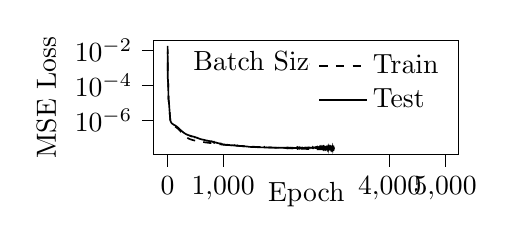
\begin{tikzpicture}

\begin{axis}[
legend cell align={left},
legend style={draw=none},
log basis y={10},
tick align=outside,
tick pos=left,
title={Batch Size 14},
title style={at={(0.4,0.85)},anchor=north},
x grid style={white!69.0196078431373!black},
xlabel={Epoch},
x label style={yshift=13pt},
xmin=-249.95, xmax=5248.95,
xtick style={color=black},
xtick = {0,1000,4000,5000},
y grid style={white!69.0196078431373!black},
ylabel={MSE Loss},
ymin=1.02410381627684e-08, ymax=0.0333579160603595,
ymode=log,
ytick style={color=black},
width=.45\textwidth,
height=.25\textwidth
]
\addplot [semithick, black, dashed]
table {%
0 0.0168717468785891
1 0.00404924569428423
2 0.000742528553642219
3 0.000250874969093605
4 0.000193904513310315
5 0.000180744685345239
6 0.000170359443708313
7 0.000158998338844543
8 0.000145799660083333
9 0.000130326230538339
10 0.000107780700345502
11 7.84643059957419e-05
12 5.50735508097675e-05
13 3.72722670156443e-05
14 2.50677081357235e-05
15 1.89589152663776e-05
16 1.60277194934113e-05
17 1.4416906762906e-05
18 1.33528480003381e-05
19 1.2542978089692e-05
20 1.18380728830763e-05
21 1.11827139172241e-05
22 1.0534444722144e-05
23 9.89714169503446e-06
24 9.25670571944154e-06
25 8.60293387987993e-06
26 7.9448147701257e-06
27 7.29224065638006e-06
28 6.64945727913568e-06
29 6.02451158893591e-06
30 5.42182829300762e-06
31 4.85903337819961e-06
32 4.34010972712299e-06
33 3.87669027459212e-06
34 3.46394584015753e-06
35 3.10421687035043e-06
36 2.79681037542443e-06
37 2.53049873421574e-06
38 2.30008372906074e-06
39 2.1010635612556e-06
40 1.92649899789797e-06
41 1.77744949564701e-06
42 1.64371439995944e-06
43 1.50819396261957e-06
44 1.3615455577843e-06
45 1.2052062145352e-06
46 1.06651785035762e-06
47 9.63305718270336e-07
48 8.9319401103632e-07
49 8.45734626958622e-07
50 8.10981904325797e-07
51 7.84018040258081e-07
52 7.60719030593224e-07
53 7.41696813231731e-07
54 7.24994794032818e-07
55 7.10724200076867e-07
56 6.97577894674391e-07
57 6.84932353929317e-07
58 6.73401785491421e-07
59 6.62690848707448e-07
60 6.52700019607912e-07
61 6.43329369971717e-07
62 6.34316612835927e-07
63 6.2604337554876e-07
64 6.18271930920299e-07
65 6.10996017864101e-07
66 6.04143914072199e-07
67 5.97869438481976e-07
68 5.92757493290041e-07
69 5.86355164105751e-07
70 5.80428500054229e-07
71 5.74776439491062e-07
72 5.69521631607753e-07
73 5.64517735531703e-07
74 5.59714457284142e-07
75 5.55021176083017e-07
76 5.5051803155908e-07
77 5.46257267957002e-07
78 5.42058521692577e-07
79 5.38110362596883e-07
80 5.34237757858054e-07
81 5.30615408320403e-07
82 5.27244994131791e-07
83 5.23701696075895e-07
84 5.20561245851239e-07
85 5.17291762109223e-07
86 5.14224020194801e-07
87 5.11133701033393e-07
88 5.08311374915436e-07
89 5.05394312954378e-07
90 5.02283039900114e-07
91 4.99394850458038e-07
92 4.96705817213324e-07
93 4.94275065892819e-07
94 4.91639597483656e-07
95 4.89363124307412e-07
96 4.86871576254844e-07
97 4.84649009869053e-07
98 4.82461337864353e-07
99 4.80209782651684e-07
100 4.78040790343468e-07
101 4.75903241389777e-07
102 4.73861520838021e-07
103 4.71826147594337e-07
104 4.69824322265681e-07
105 4.67877732603881e-07
106 4.6594380875143e-07
107 4.63995947690173e-07
108 4.62117699457237e-07
109 4.60236358239226e-07
110 4.58272285064731e-07
111 4.56413495007348e-07
112 4.54576606100633e-07
113 4.52672100717397e-07
114 4.510115220964e-07
115 4.49145014339965e-07
116 4.47450479117646e-07
117 4.45589374802697e-07
118 4.44656229685964e-07
119 4.42686300558606e-07
120 4.4074616180499e-07
121 4.39058895857208e-07
122 4.37272414976343e-07
123 4.35532599809505e-07
124 4.3374501813397e-07
125 4.31982281616224e-07
126 4.3026218542642e-07
127 4.28452994481733e-07
128 4.26800982310539e-07
129 4.25057509301995e-07
130 4.23367211995056e-07
131 4.21870452852632e-07
132 4.20114704547535e-07
133 4.18315614725584e-07
134 4.16541495102035e-07
135 4.14825346710031e-07
136 4.1311126666818e-07
137 4.11297535678386e-07
138 4.09575850071561e-07
139 4.07770829279831e-07
140 4.05975322121182e-07
141 4.04318192265934e-07
142 4.02478568477744e-07
143 4.00657031617004e-07
144 3.9892118695552e-07
145 3.97024002920164e-07
146 3.95170175134245e-07
147 3.93384946709172e-07
148 3.91556648450463e-07
149 3.89675664155956e-07
150 3.87865093690062e-07
151 3.86081611870957e-07
152 3.84172520661054e-07
153 3.82345043296591e-07
154 3.80477474123467e-07
155 3.78514520426444e-07
156 3.76650018543332e-07
157 3.74726024699523e-07
158 3.72773714932681e-07
159 3.70900610693756e-07
160 3.69028070665514e-07
161 3.67131661196272e-07
162 3.65214567324898e-07
163 3.63237482156434e-07
164 3.61247299238201e-07
165 3.59297832611224e-07
166 3.5724942480887e-07
167 3.55273886865847e-07
168 3.53454912579967e-07
169 3.51423541033469e-07
170 3.49389995424953e-07
171 3.4746663253564e-07
172 3.45506651081115e-07
173 3.43358178023534e-07
174 3.41206884291412e-07
175 3.3912126108037e-07
176 3.37041809616202e-07
177 3.34961543860121e-07
178 3.3292847875613e-07
179 3.31438666510532e-07
180 3.29233548489173e-07
181 3.27049368261659e-07
182 3.24852719860022e-07
183 3.22639121244037e-07
184 3.20737972901942e-07
185 3.18416558972171e-07
186 3.16145848316147e-07
187 3.1383262790683e-07
188 3.11466739405403e-07
189 3.09103975733043e-07
190 3.07007997044841e-07
191 3.04727012543329e-07
192 3.02573993794807e-07
193 3.00350237498375e-07
194 2.98322560252376e-07
195 2.96096515517663e-07
196 2.94044046975996e-07
197 2.92025675585228e-07
198 2.90007758544305e-07
199 2.87793992124709e-07
200 2.85697252286235e-07
201 2.83635948984139e-07
202 2.81574670464084e-07
203 2.79605895291669e-07
204 2.77516726180457e-07
205 2.75747811021584e-07
206 2.73756601008858e-07
207 2.71378694441013e-07
208 2.69452508156725e-07
209 2.67259567757136e-07
210 2.65712484344708e-07
211 2.63574615758585e-07
212 2.6163377164845e-07
213 2.59478295080432e-07
214 2.57659627911743e-07
215 2.55775162050997e-07
216 2.53839245846653e-07
217 2.51729701102636e-07
218 2.50041751946896e-07
219 2.48247567565411e-07
220 2.46120781228625e-07
221 2.44445761919666e-07
222 2.42801522098446e-07
223 2.408478232454e-07
224 2.39123421141774e-07
225 2.37280703759827e-07
226 2.35601617854547e-07
227 2.33770974419725e-07
228 2.32019653441821e-07
229 2.30372575343979e-07
230 2.28672147231754e-07
231 2.27142257046743e-07
232 2.25370165370546e-07
233 2.23635966186911e-07
234 2.21816939728313e-07
235 2.20254319957361e-07
236 2.18443269067686e-07
237 2.16756783356696e-07
238 2.15069947156838e-07
239 2.13315027267554e-07
240 2.11777548684879e-07
241 2.10077120460855e-07
242 2.08432938309122e-07
243 2.06756668662335e-07
244 2.05220080829449e-07
245 2.0357832285823e-07
246 2.01936073053553e-07
247 2.00388801353512e-07
248 1.98824612947672e-07
249 1.97364988886582e-07
250 1.95787396651026e-07
251 1.94352864611637e-07
252 1.92821957220105e-07
253 1.91392338912919e-07
254 1.89941008612225e-07
255 1.88415887392545e-07
256 1.87056072952785e-07
257 1.85633018265488e-07
258 1.84192423936346e-07
259 1.82766015915897e-07
260 1.8137057841608e-07
261 1.80051544346854e-07
262 1.7877456091721e-07
263 1.77280849406863e-07
264 1.75951777946361e-07
265 1.74730018804952e-07
266 1.73322004003075e-07
267 1.72086216325757e-07
268 1.70706297172455e-07
269 1.69472227381266e-07
270 1.68117555923117e-07
271 1.66913236755028e-07
272 1.65595105975676e-07
273 1.64391932799979e-07
274 1.63200103942151e-07
275 1.61880104454038e-07
276 1.60614089580683e-07
277 1.59405587694707e-07
278 1.58114992284833e-07
279 1.56920012996041e-07
280 1.5565607024915e-07
281 1.5451748461312e-07
282 1.53329850789667e-07
283 1.52133821282687e-07
284 1.5098498065788e-07
285 1.49878619383336e-07
286 1.48702756445625e-07
287 1.47621281284452e-07
288 1.46433010133979e-07
289 1.45394350563816e-07
290 1.44279582456932e-07
291 1.43222026909524e-07
292 1.42141128946314e-07
293 1.41284857156245e-07
294 1.4006164159477e-07
295 1.39088296243288e-07
296 1.38077997166566e-07
297 1.37143346860698e-07
298 1.36092622442581e-07
299 1.35064106745728e-07
300 1.33978017789584e-07
301 1.33016546377385e-07
302 1.32010343890087e-07
303 1.31076665717238e-07
304 1.30068105656596e-07
305 1.29136308099068e-07
306 1.28373597818743e-07
307 1.27295426668869e-07
308 1.26527147025391e-07
309 1.25536314571234e-07
310 1.24710570535537e-07
311 1.23902418873396e-07
312 1.230041784605e-07
313 1.22136616823362e-07
314 1.21357157156388e-07
315 1.2050814131818e-07
316 1.19690201476448e-07
317 1.18949556380301e-07
318 1.18140021215679e-07
319 1.17495492483817e-07
320 1.16682366134348e-07
321 1.16014100287648e-07
322 1.15184127268044e-07
323 1.1451095462687e-07
324 1.13805770665917e-07
325 1.13133179213299e-07
326 1.12407498442191e-07
327 1.11719257608792e-07
328 1.10990530795633e-07
329 1.10427378697253e-07
330 1.0975995364807e-07
331 1.09153529031254e-07
332 1.08479203581074e-07
333 1.07903550449075e-07
334 1.07255429551021e-07
335 1.06737675698797e-07
336 1.06053441587314e-07
337 1.05549809042167e-07
338 1.0495286171765e-07
339 1.04407988154133e-07
340 1.03836023394196e-07
341 1.03372545581734e-07
342 1.02778733685421e-07
343 1.02291559747866e-07
344 1.01656439604908e-07
345 1.01203206185193e-07
346 1.00704782023887e-07
347 1.00095450100973e-07
348 9.94954907522601e-08
349 9.89794553172088e-08
350 9.8446918601629e-08
351 9.79646238784339e-08
352 9.74671054075683e-08
353 9.7058331802083e-08
354 9.65850811761383e-08
355 9.61487394317391e-08
356 9.56963832434896e-08
357 9.52368109099209e-08
358 9.48334101876151e-08
359 9.43692213665899e-08
360 9.40904725011082e-08
361 9.37299133164237e-08
362 9.32570502902992e-08
363 9.28410588283537e-08
364 9.24655251449497e-08
365 9.20919898474624e-08
366 9.16523801872107e-08
367 9.13169852213313e-08
368 9.09411558024632e-08
369 9.05742745016769e-08
370 9.02093824565815e-08
371 8.98302032200097e-08
372 8.94312724481433e-08
373 8.90845515055882e-08
374 8.8730126869872e-08
375 8.84155744764157e-08
376 8.80929296657802e-08
377 8.77236484199494e-08
378 8.74427043097047e-08
379 8.71048882657242e-08
380 8.6800945436777e-08
381 8.64944687559135e-08
382 8.62069845562975e-08
383 8.58676361157298e-08
384 8.56486987750564e-08
385 8.52763585682156e-08
386 8.49678784114899e-08
387 8.4710068498212e-08
388 8.44035664483643e-08
389 8.41008638425704e-08
390 8.38202113405552e-08
391 8.3614718962197e-08
392 8.33361995976712e-08
393 8.30676941653309e-08
394 8.2811127447188e-08
395 8.2569210626502e-08
396 8.22840427899934e-08
397 8.20271316045832e-08
398 8.17767314967862e-08
399 8.15412572428599e-08
400 8.12867863990847e-08
401 8.10129745354593e-08
402 8.07465330807014e-08
403 8.05296590250798e-08
404 8.02743383156721e-08
405 8.01191860144091e-08
406 7.99187868889876e-08
407 7.9705389458725e-08
408 7.94798928862615e-08
409 7.92332198390827e-08
410 7.89926847911037e-08
411 7.88176421844318e-08
412 7.85338729276989e-08
413 7.83200425694616e-08
414 7.81497996168593e-08
415 7.79700115039461e-08
416 7.77468812561789e-08
417 7.74851994998839e-08
418 7.73434303331593e-08
419 7.71065549995145e-08
420 7.68972368547239e-08
421 7.67188871281282e-08
422 7.65334328685645e-08
423 7.63906215021023e-08
424 7.61640874192348e-08
425 7.60074309070745e-08
426 7.58023243552852e-08
427 7.56739091933312e-08
428 7.55396770030885e-08
429 7.53314131540317e-08
430 7.51233308039244e-08
431 7.4976357824683e-08
432 7.47925042862288e-08
433 7.46551042306377e-08
434 7.44248166436582e-08
435 7.41994018146644e-08
436 7.40701841835083e-08
437 7.38746187300111e-08
438 7.37345135903999e-08
439 7.35612291732815e-08
440 7.34086222671486e-08
441 7.32466613298685e-08
442 7.30943179208074e-08
443 7.28889641852373e-08
444 7.28093297447812e-08
445 7.26287334329833e-08
446 7.24453452192776e-08
447 7.23763214644229e-08
448 7.21526710484427e-08
449 7.20116104772935e-08
450 7.18872416450444e-08
451 7.1706141403792e-08
452 7.15801451647089e-08
453 7.14436621160699e-08
454 7.12931920988934e-08
455 7.11810690079728e-08
456 7.10450307069137e-08
457 7.08901922959785e-08
458 7.06902454676535e-08
459 7.06406313118239e-08
460 7.05161004988119e-08
461 7.04107193932607e-08
462 7.02400203299847e-08
463 7.01371361889956e-08
464 6.99660955559014e-08
465 6.98222400394358e-08
466 6.97149599897901e-08
467 6.95775652477419e-08
468 6.94668085913704e-08
469 6.93706085457719e-08
470 6.92371730981545e-08
471 6.91003927581864e-08
472 6.89770572407851e-08
473 6.88941676015768e-08
474 6.87860796822315e-08
475 6.86492433124905e-08
476 6.85393384036958e-08
477 6.83897939709147e-08
478 6.82540884758994e-08
479 6.81771017853725e-08
480 6.80123448624272e-08
481 6.79257702051162e-08
482 6.77970824282868e-08
483 6.77197451246705e-08
484 6.76021582551362e-08
485 6.75284123102765e-08
486 6.73482929937673e-08
487 6.7242005222642e-08
488 6.70916367528297e-08
489 6.69750886855952e-08
490 6.68902025517311e-08
491 6.6837432725926e-08
492 6.66688729645947e-08
493 6.65246281620121e-08
494 6.64715050368437e-08
495 6.62907542161615e-08
496 6.6213651720833e-08
497 6.60714632873115e-08
498 6.59422278863759e-08
499 6.59029945518461e-08
500 6.58041394956151e-08
501 6.56786379998614e-08
502 6.55394332278319e-08
503 6.5472135517304e-08
504 6.5387238085562e-08
505 6.52793011410205e-08
506 6.51687286729779e-08
507 6.50231969122873e-08
508 6.49163487098958e-08
509 6.48535146238652e-08
510 6.48110122399684e-08
511 6.46330990313275e-08
512 6.45725706192082e-08
513 6.44744962811247e-08
514 6.44023314801832e-08
515 6.43335647318657e-08
516 6.42745506235803e-08
517 6.40981353309496e-08
518 6.39342468756952e-08
519 6.39258524561147e-08
520 6.38000816404411e-08
521 6.37399570389509e-08
522 6.3622955028695e-08
523 6.35489876634397e-08
524 6.34508990896573e-08
525 6.33907027103076e-08
526 6.32790198360147e-08
527 6.32235091040285e-08
528 6.31163413778978e-08
529 6.30528216025996e-08
530 6.29731722711802e-08
531 6.2897842589294e-08
532 6.27525488542088e-08
533 6.2762294804953e-08
534 6.26729449813758e-08
535 6.25263626857348e-08
536 6.24391009882554e-08
537 6.24059847465718e-08
538 6.23710402610382e-08
539 6.23126057233323e-08
540 6.21888706498629e-08
541 6.209999743649e-08
542 6.19898142731975e-08
543 6.19576167589235e-08
544 6.183345803677e-08
545 6.17705889235912e-08
546 6.16550718731205e-08
547 6.1611187694778e-08
548 6.1509548975581e-08
549 6.14267851098901e-08
550 6.13002819352102e-08
551 6.12581241490127e-08
552 6.11206459803034e-08
553 6.10564553756458e-08
554 6.09790957744034e-08
555 6.09317550975702e-08
556 6.07662062517651e-08
557 6.07272917577603e-08
558 6.06185949020482e-08
559 6.06178351585757e-08
560 6.04106910789088e-08
561 6.03457596216505e-08
562 6.02502689449015e-08
563 6.0192792497058e-08
564 6.01402309180371e-08
565 6.00282097564595e-08
566 6.0028748747223e-08
567 5.98279414789735e-08
568 5.98469862478435e-08
569 5.98186514960492e-08
570 5.9719885891186e-08
571 5.96293679049171e-08
572 5.95124656159802e-08
573 5.93760042438635e-08
574 5.92481370755724e-08
575 5.91643757047727e-08
576 5.91136171683156e-08
577 5.90644485116015e-08
578 5.88892819916179e-08
579 5.90718776396213e-08
580 5.87887895318874e-08
581 5.87362375675532e-08
582 5.86365344251522e-08
583 5.85927905914221e-08
584 5.85589217272209e-08
585 5.84501622207696e-08
586 5.83773812693408e-08
587 5.83404900861478e-08
588 5.82427808732438e-08
589 5.81578470603473e-08
590 5.81593474514562e-08
591 5.80410152325298e-08
592 5.7954407752989e-08
593 5.79094768656955e-08
594 5.78794245196913e-08
595 5.77546811432238e-08
596 5.7692368079424e-08
597 5.76140884930368e-08
598 5.75674945289186e-08
599 5.74575967752396e-08
600 5.74363094055483e-08
601 5.7316067689974e-08
602 5.7288995595602e-08
603 5.72332033172678e-08
604 5.7193971389538e-08
605 5.70793557407868e-08
606 5.7040236645877e-08
607 5.69747971940398e-08
608 5.69322501589916e-08
609 5.68334504306863e-08
610 5.67582706770439e-08
611 5.67237742557844e-08
612 5.66903664741928e-08
613 5.65625375224179e-08
614 5.65239634491894e-08
615 5.64380027001809e-08
616 5.64088449082269e-08
617 5.62825481511806e-08
618 5.62933517298805e-08
619 5.62270135501757e-08
620 5.61916319349002e-08
621 5.6062084326828e-08
622 5.60409352210514e-08
623 5.59749420582909e-08
624 5.59118757788195e-08
625 5.58308468702949e-08
626 5.57832159702937e-08
627 5.57459242155279e-08
628 5.56150277097722e-08
629 5.56663689068003e-08
630 5.55864992263893e-08
631 5.54865706419456e-08
632 5.54731848211333e-08
633 5.52987693771188e-08
634 5.53758474289076e-08
635 5.52650310782508e-08
636 5.52350348086024e-08
637 5.53295109216269e-08
638 5.52961122298893e-08
639 5.52240422155972e-08
640 5.51567902245193e-08
641 5.50875210187634e-08
642 5.50466419610487e-08
643 5.49170109697928e-08
644 5.49087797017557e-08
645 5.48350281265902e-08
646 5.47906681579004e-08
647 5.47273988737607e-08
648 5.46671938517517e-08
649 5.45624497378255e-08
650 5.45906156487655e-08
651 5.45045704700134e-08
652 5.44492831770101e-08
653 5.43582017937044e-08
654 5.43065444859024e-08
655 5.42885634038557e-08
656 5.42075819134999e-08
657 5.41144150220488e-08
658 5.41461328547603e-08
659 5.40498210601679e-08
660 5.38640248953898e-08
661 5.3776833600025e-08
662 5.37419211075476e-08
663 5.37049779348619e-08
664 5.36478721928154e-08
665 5.36039557450254e-08
666 5.35267763849974e-08
667 5.34525919936558e-08
668 5.33919789996224e-08
669 5.33413107778674e-08
670 5.32884063992428e-08
671 5.32119685253413e-08
672 5.31590113156283e-08
673 5.31129582583787e-08
674 5.30646918387686e-08
675 5.30434079037812e-08
676 5.29477978136176e-08
677 5.28803438892755e-08
678 5.28818524354773e-08
679 5.28557313255402e-08
680 5.27239919819415e-08
681 5.26664442438049e-08
682 5.26736529296676e-08
683 5.25097643129262e-08
684 5.25590159428956e-08
685 5.24545316211571e-08
686 5.24171439897048e-08
687 5.2376454433862e-08
688 5.23700815984247e-08
689 5.22500804736146e-08
690 5.22346579789424e-08
691 5.21775918974784e-08
692 5.20781466808482e-08
693 5.20817839298583e-08
694 5.20260673143878e-08
695 5.19957259874233e-08
696 5.1943092869668e-08
697 5.18444994037202e-08
698 5.1798444942776e-08
699 5.18103616450552e-08
700 5.17011788532655e-08
701 5.16843667848226e-08
702 5.16263780319399e-08
703 5.15640372948607e-08
704 5.15638133496782e-08
705 5.1424252691388e-08
706 5.14129086436977e-08
707 5.14294605938733e-08
708 5.13088867430474e-08
709 5.12933047955047e-08
710 5.12298297458904e-08
711 5.1180559187783e-08
712 5.11869417714443e-08
713 5.10757565224025e-08
714 5.11007727973903e-08
715 5.10120738502133e-08
716 5.09177062657595e-08
717 5.09603958285999e-08
718 5.09464235553781e-08
719 5.08114981511954e-08
720 5.07607413445123e-08
721 5.0691012403942e-08
722 5.06913526663368e-08
723 5.05598571867192e-08
724 5.04174782792984e-08
725 5.03125416356193e-08
726 5.02832641352264e-08
727 5.02121579529011e-08
728 5.01924947323543e-08
729 5.01265972257886e-08
730 5.00192000483903e-08
731 5.00938682330015e-08
732 5.00349414084317e-08
733 4.99948372739661e-08
734 4.99278254109301e-08
735 4.99054635627372e-08
736 4.98390326770808e-08
737 4.97961321221774e-08
738 4.9756630672669e-08
739 4.97300663213287e-08
740 4.97044771433106e-08
741 4.95901008648544e-08
742 4.95946306834881e-08
743 4.95687119415879e-08
744 4.94279973097221e-08
745 4.94901616315863e-08
746 4.94296096454726e-08
747 4.94130782165662e-08
748 4.93223045560277e-08
749 4.9323466026326e-08
750 4.92846222698319e-08
751 4.92413340374704e-08
752 4.91577881990023e-08
753 4.9138534099522e-08
754 4.90908059439839e-08
755 4.90837860736734e-08
756 4.89858097799286e-08
757 4.89823468157475e-08
758 4.89162566521027e-08
759 4.89014381994994e-08
760 4.87827716807746e-08
761 4.8844006766153e-08
762 4.87849279233251e-08
763 4.87458870843873e-08
764 4.8721910537144e-08
765 4.87244322154258e-08
766 4.85794905499185e-08
767 4.8491523986592e-08
768 4.84209012248741e-08
769 4.84906219482413e-08
770 4.84417779704279e-08
771 4.84073345727989e-08
772 4.83453910346989e-08
773 4.83397812407952e-08
774 4.83110755751341e-08
775 4.82812641149184e-08
776 4.82600711250534e-08
777 4.82232100498667e-08
778 4.81807216687549e-08
779 4.81018866913587e-08
780 4.80578230171264e-08
781 4.80196907226016e-08
782 4.79839151815639e-08
783 4.80093528599456e-08
784 4.79243031770315e-08
785 4.78412622027792e-08
786 4.78123267349268e-08
787 4.78079540617631e-08
788 4.77638325876121e-08
789 4.77111581757712e-08
790 4.76360206323425e-08
791 4.76354699213505e-08
792 4.75962001156061e-08
793 4.75310006955396e-08
794 4.75134220080053e-08
795 4.74766290399546e-08
796 4.74222900854841e-08
797 4.73951060837368e-08
798 4.73601126490135e-08
799 4.73138395067414e-08
800 4.73142538637128e-08
801 4.71670435265525e-08
802 4.71056197653702e-08
803 4.71132027345878e-08
804 4.70568869558187e-08
805 4.68369343495736e-08
806 4.67855380264787e-08
807 4.67184639754257e-08
808 4.67136931405718e-08
809 4.67359797420406e-08
810 4.66716687333077e-08
811 4.66299804146209e-08
812 4.65660366800867e-08
813 4.65328999823498e-08
814 4.64775510106346e-08
815 4.64405125171503e-08
816 4.63828966594555e-08
817 4.6339368590971e-08
818 4.62920698852264e-08
819 4.62395017815103e-08
820 4.61874357687814e-08
821 4.61519081195827e-08
822 4.60901867658361e-08
823 4.61090417129657e-08
824 4.60675804356639e-08
825 4.60122591931274e-08
826 4.59467447926959e-08
827 4.59229077112031e-08
828 4.58692607222541e-08
829 4.58164231650807e-08
830 4.57757968251816e-08
831 4.57669879181978e-08
832 4.57041679498564e-08
833 4.57631669404756e-08
834 4.56616606871894e-08
835 4.56561198730726e-08
836 4.55464239905474e-08
837 4.55550223992458e-08
838 4.54658595962308e-08
839 4.53744777042784e-08
840 4.53619341809488e-08
841 4.52684384864678e-08
842 4.52159864577334e-08
843 4.51354425101536e-08
844 4.50895198505392e-08
845 4.50396801874511e-08
846 4.49697053612069e-08
847 4.49087468222909e-08
848 4.4892072079896e-08
849 4.48372962441252e-08
850 4.47815579397103e-08
851 4.47025680062351e-08
852 4.46872171962568e-08
853 4.46398341384065e-08
854 4.45728209089421e-08
855 4.45275162382822e-08
856 4.44537137046562e-08
857 4.43765681450964e-08
858 4.43844624053225e-08
859 4.43390909007893e-08
860 4.42874444747258e-08
861 4.44012648652898e-08
862 4.4309650453817e-08
863 4.42510368705216e-08
864 4.41774291460993e-08
865 4.41271512818653e-08
866 4.41095145335487e-08
867 4.39514728574545e-08
868 4.39497047240293e-08
869 4.38643772710783e-08
870 4.37997074103142e-08
871 4.37536831909136e-08
872 4.36886953840139e-08
873 4.36250345839947e-08
874 4.35795166573485e-08
875 4.35192501771195e-08
876 4.34841556888096e-08
877 4.34218836830758e-08
878 4.33956670349538e-08
879 4.33334930114484e-08
880 4.32966454359525e-08
881 4.32321496084704e-08
882 4.32049767741692e-08
883 4.31474278994127e-08
884 4.3125620659638e-08
885 4.3065977317314e-08
886 4.30308656213235e-08
887 4.29719829386e-08
888 4.29481880704263e-08
889 4.2888110002032e-08
890 4.28682416557476e-08
891 4.28382809908739e-08
892 4.27732519551046e-08
893 4.27091928008531e-08
894 4.26860217196378e-08
895 4.26254461408967e-08
896 4.25999646219039e-08
897 4.254676767855e-08
898 4.25268207626362e-08
899 4.2469851924287e-08
900 4.24522858420541e-08
901 4.24043246017912e-08
902 4.23849442536491e-08
903 4.23395208031004e-08
904 4.23052865745947e-08
905 4.22711020965027e-08
906 4.22281627816173e-08
907 4.21953284247832e-08
908 4.21604255842587e-08
909 4.21249744861022e-08
910 4.20793457141681e-08
911 4.2040345386725e-08
912 4.20306178610248e-08
913 4.19789145822258e-08
914 4.19642219062455e-08
915 4.19095035474194e-08
916 4.18868280790788e-08
917 4.18480205702018e-08
918 4.18030643077129e-08
919 4.17862838130812e-08
920 4.17359989459019e-08
921 4.17130601140268e-08
922 4.16834783907864e-08
923 4.16326157604396e-08
924 4.16013008004905e-08
925 4.15735620102048e-08
926 4.1532308793356e-08
927 4.14896725398539e-08
928 4.14670035558368e-08
929 4.14270538060349e-08
930 4.14108362301901e-08
931 4.13676473526963e-08
932 4.13333101886596e-08
933 4.13020485691039e-08
934 4.12771253944687e-08
935 4.12457358151102e-08
936 4.12020594736235e-08
937 4.11807341979678e-08
938 4.11412158792804e-08
939 4.11145564090003e-08
940 4.10773959897364e-08
941 4.10600351046681e-08
942 4.10202089731535e-08
943 4.09862652224683e-08
944 4.09659755411114e-08
945 4.09204208389098e-08
946 4.09055700423266e-08
947 4.08700923578224e-08
948 4.08426762309556e-08
949 4.09553721472686e-08
950 4.08986329558348e-08
951 4.08355916447357e-08
952 4.0818388603879e-08
953 4.0771384242326e-08
954 4.07799743748164e-08
955 4.07448392197358e-08
956 4.07100946675121e-08
957 4.06678699946475e-08
958 4.06522680382462e-08
959 4.05450651918017e-08
960 4.05254549855689e-08
961 4.04750694157267e-08
962 4.04811250410363e-08
963 4.03837709877015e-08
964 4.03753398764145e-08
965 4.03146390179335e-08
966 4.03348217390067e-08
967 4.02284534293531e-08
968 4.02057060806709e-08
969 4.01889247786042e-08
970 4.01328983472467e-08
971 4.01259656892248e-08
972 4.0069106047133e-08
973 4.00491573610733e-08
974 3.99839089203902e-08
975 3.99776371727003e-08
976 3.99095224808802e-08
977 3.99161185006479e-08
978 3.98175107772626e-08
979 3.98455028940456e-08
980 3.97652086612445e-08
981 3.9741472338314e-08
982 3.97104277976385e-08
983 3.96697166708611e-08
984 3.96251010651679e-08
985 3.96111222144569e-08
986 3.95725330794615e-08
987 3.95165489266389e-08
988 3.9489754130265e-08
989 3.94358216602754e-08
990 3.94712513117181e-08
991 3.93248951040677e-08
992 3.93066224013694e-08
993 3.93560557228305e-08
994 3.92722548374077e-08
995 3.92383110152956e-08
996 3.92574351829685e-08
997 3.91598153965882e-08
998 3.91318919055629e-08
999 3.91649590986803e-08
1000 3.90575392075163e-08
1001 3.90277463089874e-08
1002 3.90616966030009e-08
1003 3.89439458164127e-08
1004 3.89170464416881e-08
1005 3.89461554816529e-08
1006 3.88481046554533e-08
1007 3.88336403158594e-08
1008 3.88861525854503e-08
1009 3.87809746429488e-08
1010 3.87439671891264e-08
1011 3.87631093532816e-08
1012 3.86921641921139e-08
1013 3.87238802018858e-08
1014 3.86211948327425e-08
1015 3.85956201730255e-08
1016 3.8633659997618e-08
1017 3.85314123575818e-08
1018 3.85125479013531e-08
1019 3.85449951024563e-08
1020 3.844778576941e-08
1021 3.84249619628512e-08
1022 3.84599930799415e-08
1023 3.83616895607705e-08
1024 3.83384420651559e-08
1025 3.8373162437809e-08
1026 3.82665595093042e-08
1027 3.82572479523397e-08
1028 3.82952372532444e-08
1029 3.81940318874782e-08
1030 3.8175101547665e-08
1031 3.8213750420423e-08
1032 3.81134730986233e-08
1033 3.80849726580765e-08
1034 3.811870350991e-08
1035 3.80255409475523e-08
1036 3.80065758197158e-08
1037 3.80440338315441e-08
1038 3.79461729233559e-08
1039 3.7930605928887e-08
1040 3.79667921903335e-08
1041 3.78703526688522e-08
1042 3.78512943940804e-08
1043 3.78867346757144e-08
1044 3.77904580449131e-08
1045 3.77715875018672e-08
1046 3.78107278571598e-08
1047 3.77113676758495e-08
1048 3.7692440739685e-08
1049 3.7716399858756e-08
1050 3.76165598934011e-08
1051 3.76011686681992e-08
1052 3.76597063122398e-08
1053 3.75533042455951e-08
1054 3.75298046594797e-08
1055 3.75643232044562e-08
1056 3.74862394862548e-08
1057 3.74531346294036e-08
1058 3.74862473463232e-08
1059 3.73920436866873e-08
1060 3.73744566111462e-08
1061 3.74169854509589e-08
1062 3.73207171522649e-08
1063 3.73030366782414e-08
1064 3.73432922812882e-08
1065 3.72431398945159e-08
1066 3.72491179160125e-08
1067 3.72672157624663e-08
1068 3.7191246856087e-08
1069 3.71664246511894e-08
1070 3.71923104621667e-08
1071 3.7098905520266e-08
1072 3.70631268923424e-08
1073 3.71242571819838e-08
1074 3.70327002039785e-08
1075 3.70371482574037e-08
1076 3.70579679142026e-08
1077 3.69741710535323e-08
1078 3.69544098631792e-08
1079 3.69763814066449e-08
1080 3.68991437715538e-08
1081 3.68964575721945e-08
1082 3.6912058655945e-08
1083 3.68200449026849e-08
1084 3.67851670584824e-08
1085 3.68476757606595e-08
1086 3.67575813982306e-08
1087 3.67431322384132e-08
1088 3.67646214699419e-08
1089 3.66668399512401e-08
1090 3.66606986632958e-08
1091 3.6728467192235e-08
1092 3.66210468383487e-08
1093 3.66124844070874e-08
1094 3.66615631497114e-08
1095 3.65515599201868e-08
1096 3.65421039876463e-08
1097 3.65653940723478e-08
1098 3.64782597446227e-08
1099 3.64786742071818e-08
1100 3.65290753077243e-08
1101 3.64180145930979e-08
1102 3.64148292188336e-08
1103 3.64622518347843e-08
1104 3.63607038029517e-08
1105 3.6357523034172e-08
1106 3.63985828983054e-08
1107 3.62898453292399e-08
1108 3.62857237869716e-08
1109 3.6335202051503e-08
1110 3.62457848381646e-08
1111 3.62214976116999e-08
1112 3.62608196522731e-08
1113 3.61711269141879e-08
1114 3.61565899986161e-08
1115 3.61992901978589e-08
1116 3.61067066005046e-08
1117 3.61008440577301e-08
1118 3.61330484103569e-08
1119 3.6025361329659e-08
1120 3.60409150759841e-08
1121 3.60857097738496e-08
1122 3.59911816216441e-08
1123 3.59749468381188e-08
1124 3.60170343277893e-08
1125 3.59211251016184e-08
1126 3.59145777608603e-08
1127 3.5954847121356e-08
1128 3.58630160067709e-08
1129 3.58528083305747e-08
1130 3.58955695346318e-08
1131 3.57975908341099e-08
1132 3.57913430610262e-08
1133 3.58013522355566e-08
1134 3.57465518786081e-08
1135 3.57323081488693e-08
1136 3.57742792964834e-08
1137 3.56799409815458e-08
1138 3.56710443684958e-08
1139 3.57138243857867e-08
1140 3.56207368651889e-08
1141 3.56129275595392e-08
1142 3.56548856546572e-08
1143 3.55336684955808e-08
1144 3.55535332953625e-08
1145 3.55925584079523e-08
1146 3.54602735520004e-08
1147 3.54949972258201e-08
1148 3.55319100327415e-08
1149 3.54394432991708e-08
1150 3.54251450955241e-08
1151 3.54660719316478e-08
1152 3.53811757824851e-08
1153 3.53597861294216e-08
1154 3.54104389074309e-08
1155 3.53229467369682e-08
1156 3.53109862592939e-08
1157 3.5353314917355e-08
1158 3.52744644061531e-08
1159 3.52554024886075e-08
1160 3.5292037699401e-08
1161 3.52145552345124e-08
1162 3.51984017534732e-08
1163 3.52131939551248e-08
1164 3.5158654837536e-08
1165 3.51525404837574e-08
1166 3.51884590246263e-08
1167 3.51051412213092e-08
1168 3.50862976993838e-08
1169 3.51309046034129e-08
1170 3.50456899988095e-08
1171 3.503182602435e-08
1172 3.50746848752394e-08
1173 3.49508570181804e-08
1174 3.49872529642664e-08
1175 3.50278372243837e-08
1176 3.49402164077985e-08
1177 3.49265519629315e-08
1178 3.49647479050671e-08
1179 3.4872061834904e-08
1180 3.48535176974275e-08
1181 3.49003848354146e-08
1182 3.48129881907148e-08
1183 3.48058266248911e-08
1184 3.48498958455803e-08
1185 3.47641715414682e-08
1186 3.4752651109618e-08
1187 3.47600894268684e-08
1188 3.47214849009211e-08
1189 3.47068627543817e-08
1190 3.47449365688791e-08
1191 3.4658139357658e-08
1192 3.46484887401346e-08
1193 3.46902101729699e-08
1194 3.46163519232285e-08
1195 3.46040691330589e-08
1196 3.46379541583807e-08
1197 3.45517265987116e-08
1198 3.45440961119486e-08
1199 3.45866658514459e-08
1200 3.45001086564679e-08
1201 3.44545266288051e-08
1202 3.45425622402399e-08
1203 3.4454022328241e-08
1204 3.44552526044172e-08
1205 3.44910764222999e-08
1206 3.44019420673912e-08
1207 3.43912137416265e-08
1208 3.44324160217535e-08
1209 3.43511786506111e-08
1210 3.43657572174031e-08
1211 3.44155751480696e-08
1212 3.43163315743376e-08
1213 3.4318969451822e-08
1214 3.43536783930598e-08
1215 3.42256572143203e-08
1216 3.42754545336575e-08
1217 3.43140265758766e-08
1218 3.42247424759497e-08
1219 3.42169347618785e-08
1220 3.4256024685096e-08
1221 3.41724990293956e-08
1222 3.41657030204186e-08
1223 3.42065822815448e-08
1224 3.41219999621523e-08
1225 3.41125121561181e-08
1226 3.41579326719514e-08
1227 3.40702899894073e-08
1228 3.40686902884606e-08
1229 3.41106444131726e-08
1230 3.40237770234343e-08
1231 3.40192811884945e-08
1232 3.40643001110393e-08
1233 3.39768986170716e-08
1234 3.39709148814201e-08
1235 3.401329125578e-08
1236 3.39292102789448e-08
1237 3.39189939399035e-08
1238 3.39307030537685e-08
1239 3.38891111723144e-08
1240 3.38797334212135e-08
1241 3.39243755604606e-08
1242 3.38340933638235e-08
1243 3.38290928882654e-08
1244 3.38693460301885e-08
1245 3.37868109915559e-08
1246 3.37790131017938e-08
1247 3.38213474165578e-08
1248 3.37387538963451e-08
1249 3.37233400660708e-08
1250 3.37641497247534e-08
1251 3.36718287021319e-08
1252 3.36681045513849e-08
1253 3.37146367513895e-08
1254 3.36324618970558e-08
1255 3.36223697896418e-08
1256 3.36680971881995e-08
1257 3.35813560533341e-08
1258 3.35395552248013e-08
1259 3.36295164908991e-08
1260 3.35379773090701e-08
1261 3.35366467820839e-08
1262 3.35609217836732e-08
1263 3.34786533212345e-08
1264 3.34714057822242e-08
1265 3.35194922913578e-08
1266 3.34498701325038e-08
1267 3.34359162858786e-08
1268 3.34845091265856e-08
1269 3.33978070110131e-08
1270 3.33565213461496e-08
1271 3.34488443330118e-08
1272 3.33645156211662e-08
1273 3.33680671889085e-08
1274 3.33936686973897e-08
1275 3.33149400141434e-08
1276 3.33067689326163e-08
1277 3.33508974035015e-08
1278 3.32679176266056e-08
1279 3.32612792537705e-08
1280 3.33044897192792e-08
1281 3.32229621963958e-08
1282 3.32148874278807e-08
1283 3.32592580826612e-08
1284 3.31757122146908e-08
1285 3.31680038741204e-08
1286 3.32124708853901e-08
1287 3.312994836821e-08
1288 3.31228128266351e-08
1289 3.31669294608348e-08
1290 3.30843284563214e-08
1291 3.30903233221528e-08
1292 3.31162144870448e-08
1293 3.30389638491458e-08
1294 3.30321250802784e-08
1295 3.30361888102059e-08
1296 3.29974463091571e-08
1297 3.29920350091554e-08
1298 3.30341129369331e-08
1299 3.295077660609e-08
1300 3.29436512149038e-08
1301 3.29875561536405e-08
1302 3.29047638305267e-08
1303 3.28987502539436e-08
1304 3.29430523233381e-08
1305 3.28612517523592e-08
1306 3.28549372432261e-08
1307 3.2899864416319e-08
1308 3.28176395786578e-08
1309 3.28258571187483e-08
1310 3.28507964513986e-08
1311 3.27759953490235e-08
1312 3.27698705591486e-08
1313 3.28137369366564e-08
1314 3.27307402207074e-08
1315 3.27274025657687e-08
1316 3.27701214586828e-08
1317 3.26923109127975e-08
1318 3.26836094707442e-08
1319 3.27303440418912e-08
1320 3.26509388368692e-08
1321 3.26403197663667e-08
1322 3.26881987150357e-08
1323 3.26085815769785e-08
1324 3.26027761043258e-08
1325 3.26472468592986e-08
1326 3.25657386791399e-08
1327 3.25723040443301e-08
1328 3.25969937662365e-08
1329 3.25205790206874e-08
1330 3.25137492127949e-08
1331 3.25570549913385e-08
1332 3.24761802780408e-08
1333 3.24705232305607e-08
1334 3.2513651595465e-08
1335 3.24325387944514e-08
1336 3.24259954287576e-08
1337 3.2470023569642e-08
1338 3.23895563345912e-08
1339 3.23841452178151e-08
1340 3.24310907064926e-08
1341 3.23482215264431e-08
1342 3.23432370939959e-08
1343 3.23890840721135e-08
1344 3.22962194641132e-08
1345 3.2274737105098e-08
1346 3.2304543812317e-08
1347 3.22190286633534e-08
1348 3.22225336855776e-08
1349 3.22445252301382e-08
1350 3.21991315941241e-08
1351 3.22648092734255e-08
1352 3.21705227352525e-08
1353 3.21565914300366e-08
1354 3.21625570931206e-08
1355 3.21200830952198e-08
1356 3.21527808558028e-08
1357 3.21119843536512e-08
1358 3.21317101084803e-08
1359 3.20580836484622e-08
1360 3.20951248934364e-08
1361 3.20360193151958e-08
1362 3.20690843639523e-08
1363 3.20114854220192e-08
1364 3.20541066168599e-08
1365 3.19809794808118e-08
1366 3.19765511334571e-08
1367 3.20051143008284e-08
1368 3.19416367605879e-08
1369 3.19779825044073e-08
1370 3.19086673214433e-08
1371 3.19431780467231e-08
1372 3.18856254437911e-08
1373 3.19152142087957e-08
1374 3.18574419556138e-08
1375 3.18861166390652e-08
1376 3.18294947586097e-08
1377 3.18654929870948e-08
1378 3.18041647532282e-08
1379 3.18458991857659e-08
1380 3.17934544984783e-08
1381 3.17989800381001e-08
1382 3.17454851792079e-08
1383 3.17732739093438e-08
1384 3.17221569059398e-08
1385 3.17488242440522e-08
1386 3.16979873895127e-08
1387 3.171357464594e-08
1388 3.16621103616684e-08
1389 3.1692919449661e-08
1390 3.16118126609321e-08
1391 3.16506945081689e-08
1392 3.15843465522906e-08
1393 3.16046966344383e-08
1394 3.15615749091336e-08
1395 3.15921439343002e-08
1396 3.15339996352899e-08
1397 3.15663940953647e-08
1398 3.15129109318568e-08
1399 3.15397347601746e-08
1400 3.14868249701832e-08
1401 3.15264220774391e-08
1402 3.1460750955441e-08
1403 3.14710900214857e-08
1404 3.14351172908639e-08
1405 3.14564838668161e-08
1406 3.14022587715397e-08
1407 3.1425683536387e-08
1408 3.13709228943676e-08
1409 3.13956117886533e-08
1410 3.13409232428091e-08
1411 3.13626077602386e-08
1412 3.13055972566945e-08
1413 3.13312679545851e-08
1414 3.12750542635404e-08
1415 3.13010793259874e-08
1416 3.12522306386545e-08
1417 3.12792792661726e-08
1418 3.12246208423094e-08
1419 3.12511048926934e-08
1420 3.11979853202387e-08
1421 3.12244072509271e-08
1422 3.1174763634592e-08
1423 3.11863349395008e-08
1424 3.11426702902929e-08
1425 3.1167096886237e-08
1426 3.11142273530877e-08
1427 3.11392810620009e-08
1428 3.10870358561704e-08
1429 3.11122677178364e-08
1430 3.10599048532094e-08
1431 3.10843514859617e-08
1432 3.10322613169537e-08
1433 3.10574976474615e-08
1434 3.10071633621592e-08
1435 3.10358758366706e-08
1436 3.09764777759971e-08
1437 3.10102489312555e-08
1438 3.09595621711051e-08
1439 3.09787720728397e-08
1440 3.0928190678289e-08
1441 3.09586921211523e-08
1442 3.09025738673632e-08
1443 3.09276602370192e-08
1444 3.08721556927795e-08
1445 3.0903755360495e-08
1446 3.08453621929598e-08
1447 3.08760294907209e-08
1448 3.08212871821326e-08
1449 3.08453828741632e-08
1450 3.07954194872002e-08
1451 3.08123077045205e-08
1452 3.07672584690052e-08
1453 3.07941604492602e-08
1454 3.07489436306259e-08
1455 3.0754400673369e-08
1456 3.07124316064525e-08
1457 3.07375932927069e-08
1458 3.06866480276064e-08
1459 3.07092877917956e-08
1460 3.06586472681641e-08
1461 3.06814867001415e-08
1462 3.06311652219993e-08
1463 3.06545302087124e-08
1464 3.06040255251381e-08
1465 3.06258211844325e-08
1466 3.05691737160537e-08
1467 3.06024408191896e-08
1468 3.05526301895982e-08
1469 3.05764075271174e-08
1470 3.05261904114924e-08
1471 3.0550108171262e-08
1472 3.05002542414198e-08
1473 3.05239487640652e-08
1474 3.04762937838701e-08
1475 3.04930783777869e-08
1476 3.04493082511806e-08
1477 3.04736965327846e-08
1478 3.04241320512834e-08
1479 3.04475973617862e-08
1480 3.03985675714574e-08
1481 3.04224642354368e-08
1482 3.03729035908043e-08
1483 3.0396823906416e-08
1484 3.03480713643971e-08
1485 3.03727016404598e-08
1486 3.03140857808189e-08
1487 3.03478646936637e-08
1488 3.02993655682021e-08
1489 3.03223513135993e-08
1490 3.0273653046735e-08
1491 3.02989795397746e-08
1492 3.02439406090966e-08
1493 3.02744949529224e-08
1494 3.02246890996191e-08
1495 3.0249723617978e-08
1496 3.01964296193931e-08
1497 3.02270981764421e-08
1498 3.01779764782801e-08
1499 3.020213416268e-08
1500 3.01527914493925e-08
1501 3.01779908009334e-08
1502 3.01287962861158e-08
1503 3.01562649940767e-08
1504 3.01068725676419e-08
1505 3.01216921956841e-08
1506 3.0083428988008e-08
1507 3.01075701805495e-08
1508 3.0059100079268e-08
1509 3.00776564493837e-08
1510 3.00289553704721e-08
1511 3.0063681864103e-08
1512 3.00144395118715e-08
1513 3.00416584476015e-08
1514 2.99943015599594e-08
1515 3.0022931070532e-08
1516 2.99621163280128e-08
1517 3.00026209377801e-08
1518 2.99503298634346e-08
1519 2.99769544028376e-08
1520 2.99272773322996e-08
1521 2.99554553392359e-08
1522 2.99036144129678e-08
1523 2.9933310739174e-08
1524 2.9875514658898e-08
1525 2.99108020760199e-08
1526 2.98599262285845e-08
1527 2.98884426842925e-08
1528 2.98372513782422e-08
1529 2.98669044476749e-08
1530 2.98199811463775e-08
1531 2.98445254352787e-08
1532 2.97876892041415e-08
1533 2.98235469405021e-08
1534 2.97720191592373e-08
1535 2.980176993606e-08
1536 2.97507643027766e-08
1537 2.97817180722387e-08
1538 2.97316738952001e-08
1539 2.97567806774322e-08
1540 2.97017533086013e-08
1541 2.97356531255098e-08
1542 2.96873244231644e-08
1543 2.97150113000426e-08
1544 2.96654838301162e-08
1545 2.96944128478057e-08
1546 2.96471742664608e-08
1547 2.96704043106117e-08
1548 2.96168554902222e-08
1549 2.96503924660604e-08
1550 2.96022908905016e-08
1551 2.96303016869811e-08
1552 2.95803736485875e-08
1553 2.96075269289887e-08
1554 2.95594119158494e-08
1555 2.95817169314928e-08
1556 2.95386872025287e-08
1557 2.95666768116051e-08
1558 2.94995407837104e-08
1559 2.9551406451648e-08
1560 2.94818523564529e-08
1561 2.94893891155485e-08
1562 2.94240719233342e-08
1563 2.94739277226987e-08
1564 2.94203051555507e-08
1565 2.94277251486865e-08
1566 2.9400903410383e-08
1567 2.94163089768713e-08
1568 2.9383356785779e-08
1569 2.93908523920902e-08
1570 2.93634791307015e-08
1571 2.93700174297412e-08
1572 2.93417937732291e-08
1573 2.93531891520422e-08
1574 2.93236113339919e-08
1575 2.93285078228007e-08
1576 2.92987066713551e-08
1577 2.93158329965772e-08
1578 2.9281288491015e-08
1579 2.92895885540605e-08
1580 2.92622761422101e-08
1581 2.92778515184747e-08
1582 2.92371551196209e-08
1583 2.92517657462377e-08
1584 2.92102231478166e-08
1585 2.92256656466891e-08
1586 2.91994852461843e-08
1587 2.92307110202875e-08
1588 2.91654911674591e-08
1589 2.92155002350531e-08
1590 2.91488670993696e-08
1591 2.91958600139797e-08
1592 2.9129643589251e-08
1593 2.91766621585532e-08
1594 2.91111050867385e-08
1595 2.91473344978181e-08
1596 2.90893117457139e-08
1597 2.91405672086803e-08
1598 2.90639721489372e-08
1599 2.91189780586322e-08
1600 2.90461665768467e-08
1601 2.90948322016012e-08
1602 2.90298909091644e-08
1603 2.90752367139755e-08
1604 2.90095509789581e-08
1605 2.90562205174327e-08
1606 2.89903093201867e-08
1607 2.90347859259572e-08
1608 2.89699766693168e-08
1609 2.90189695086283e-08
1610 2.89548836422556e-08
1611 2.89981372170256e-08
1612 2.89342671717978e-08
1613 2.89826107154183e-08
1614 2.89182553024227e-08
1615 2.89471717831322e-08
1616 2.89221700062596e-08
1617 2.89300519608669e-08
1618 2.88845635459673e-08
1619 2.89232807696446e-08
1620 2.88649804555732e-08
1621 2.8896304940149e-08
1622 2.88721108388811e-08
1623 2.8872573868651e-08
1624 2.8835462456029e-08
1625 2.88574224205673e-08
1626 2.88174955553345e-08
1627 2.88384873246518e-08
1628 2.87996565041969e-08
1629 2.8818112479096e-08
1630 2.87705293124738e-08
1631 2.88057138934413e-08
1632 2.87534350098105e-08
1633 2.8792977820173e-08
1634 2.87291767159131e-08
1635 2.87775283804657e-08
1636 2.87080537850029e-08
1637 2.87562028796599e-08
1638 2.86910217091755e-08
1639 2.87405144997717e-08
1640 2.86715917332878e-08
1641 2.87178933547214e-08
1642 2.86532095765741e-08
1643 2.87030496713294e-08
1644 2.86349714895428e-08
1645 2.86816128159306e-08
1646 2.86155387652708e-08
1647 2.8666283576887e-08
1648 2.85971638972102e-08
1649 2.8644971046281e-08
1650 2.85780404748618e-08
1651 2.86296526951869e-08
1652 2.85596587637901e-08
1653 2.86094430911888e-08
1654 2.85430245981057e-08
1655 2.85956152944723e-08
1656 2.85245225838882e-08
1657 2.85563428909613e-08
1658 2.85261901590571e-08
1659 2.8536809220243e-08
1660 2.85050021426807e-08
1661 2.85174450844625e-08
1662 2.84872185281619e-08
1663 2.84991790399969e-08
1664 2.84697527215831e-08
1665 2.84811308896101e-08
1666 2.84509456677667e-08
1667 2.84624639863112e-08
1668 2.84332650043066e-08
1669 2.84445234607891e-08
1670 2.84161080850646e-08
1671 2.84270163756525e-08
1672 2.83974944010439e-08
1673 2.84100362411822e-08
1674 2.83807444740352e-08
1675 2.83924850980482e-08
1676 2.83630198550599e-08
1677 2.83736689435085e-08
1678 2.83450191756358e-08
1679 2.83556710761318e-08
1680 2.83283701888622e-08
1681 2.83439058983333e-08
1682 2.82977449631191e-08
1683 2.83254652212205e-08
1684 2.82817905660305e-08
1685 2.83241780674647e-08
1686 2.82519194643234e-08
1687 2.83067983955595e-08
1688 2.82333515603103e-08
1689 2.82887936230615e-08
1690 2.82170346668639e-08
1691 2.82693530107713e-08
1692 2.81982632349027e-08
1693 2.82547613355838e-08
1694 2.81797615778198e-08
1695 2.82351738462222e-08
1696 2.8161519795221e-08
1697 2.82186969176206e-08
1698 2.81452567902922e-08
1699 2.81973400836813e-08
1700 2.81277419149613e-08
1701 2.81844691206447e-08
1702 2.81088986927184e-08
1703 2.81625387004609e-08
1704 2.80928024727904e-08
1705 2.81473682962895e-08
1706 2.80742891498256e-08
1707 2.81105029882804e-08
1708 2.80795254491762e-08
1709 2.80901751742563e-08
1710 2.80570427077889e-08
1711 2.8071793208532e-08
1712 2.80424231962823e-08
1713 2.80530798451168e-08
1714 2.80217607346416e-08
1715 2.80356746505041e-08
1716 2.8004037008503e-08
1717 2.8017685772052e-08
1718 2.79838852913782e-08
1719 2.7997757094851e-08
1720 2.79650810992975e-08
1721 2.79792353823267e-08
1722 2.79471223816454e-08
1723 2.79605306895204e-08
1724 2.79307484926098e-08
1725 2.79426196571119e-08
1726 2.79132217371161e-08
1727 2.79218453020707e-08
1728 2.78981354055537e-08
1729 2.79033755060595e-08
1730 2.78772472906951e-08
1731 2.78875366047734e-08
1732 2.78925598422326e-08
1733 2.78648091609149e-08
1734 2.78471219774177e-08
1735 2.78518389222012e-08
1736 2.7831583819245e-08
1737 2.78346645219931e-08
1738 2.78267636050871e-08
1739 2.78313451601137e-08
1740 2.77988384774534e-08
1741 2.78000906304578e-08
1742 2.77843101983297e-08
1743 2.77972333076878e-08
1744 2.77676292837159e-08
1745 2.77799989647529e-08
1746 2.77471093188122e-08
1747 2.77450474234802e-08
1748 2.77327553742059e-08
1749 2.773611283925e-08
1750 2.77193001931806e-08
1751 2.77171472859575e-08
1752 2.77157355465452e-08
1753 2.77008917715404e-08
1754 2.76988873904194e-08
1755 2.76782732848143e-08
1756 2.76647380015859e-08
1757 2.76618389623799e-08
1758 2.76517194254698e-08
1759 2.76439611931848e-08
1760 2.76561092178067e-08
1761 2.76334577380473e-08
1762 2.76270071279934e-08
1763 2.76171397468e-08
1764 2.76143926652944e-08
1765 2.75893269737363e-08
1766 2.76095079339803e-08
1767 2.75645064396079e-08
1768 2.75964017667022e-08
1769 2.75497531004205e-08
1770 2.75700995180559e-08
1771 2.75357621179997e-08
1772 2.75772135709924e-08
1773 2.7515336904032e-08
1774 2.75349208608658e-08
1775 2.75088909475982e-08
1776 2.7527586011743e-08
1777 2.75024230879393e-08
1778 2.74969485409387e-08
1779 2.74685121361926e-08
1780 2.75028434587482e-08
1781 2.74504569191975e-08
1782 2.74747340449617e-08
1783 2.744797643873e-08
1784 2.7447196091692e-08
1785 2.74171594844579e-08
1786 2.74586997879005e-08
1787 2.74003894771637e-08
1788 2.74273841431845e-08
1789 2.73844616291566e-08
1790 2.74162466746147e-08
1791 2.73739114033509e-08
1792 2.73864325840244e-08
1793 2.737380694301e-08
1794 2.73657078287791e-08
1795 2.73514891466034e-08
1796 2.73503743429383e-08
1797 2.73343196003214e-08
1798 2.73479035237403e-08
1799 2.72991717079548e-08
1800 2.73309034797881e-08
1801 2.73043956209431e-08
1802 2.73016326329695e-08
1803 2.72824179937657e-08
1804 2.7288939498159e-08
1805 2.72548790280969e-08
1806 2.72805762191697e-08
1807 2.72517324666084e-08
1808 2.72494408436176e-08
1809 2.72327988799752e-08
1810 2.72488897289082e-08
1811 2.72035448417779e-08
1812 2.72290818626053e-08
1813 2.72053309142333e-08
1814 2.71988323767055e-08
1815 2.71889306779749e-08
1816 2.7196785106815e-08
1817 2.71773277060894e-08
1818 2.71753368075788e-08
1819 2.71523942692668e-08
1820 2.71666279091745e-08
1821 2.71354089889517e-08
1822 2.71577138058418e-08
1823 2.71100445464706e-08
1824 2.71486980821653e-08
1825 2.70932801089246e-08
1826 2.71176545057534e-08
1827 2.70856999331213e-08
1828 2.70999307345847e-08
1829 2.70708563972414e-08
1830 2.70842362911708e-08
1831 2.70422199085677e-08
1832 2.70805365637777e-08
1833 2.70287359005627e-08
1834 2.70493430932827e-08
1835 2.70102876009537e-08
1836 2.70340835063708e-08
1837 2.6994734685355e-08
1838 2.70101026020844e-08
1839 2.69722469533987e-08
1840 2.70037586153654e-08
1841 2.69460968363619e-08
1842 2.69652329959962e-08
1843 2.69186372446519e-08
1844 2.69568427688662e-08
1845 2.68996603996924e-08
1846 2.69293571016664e-08
1847 2.68927517877038e-08
1848 2.69294638383527e-08
1849 2.68789071994463e-08
1850 2.69068000389995e-08
1851 2.68645387116947e-08
1852 2.68876278475815e-08
1853 2.6856250418566e-08
1854 2.68700968452907e-08
1855 2.68313627539872e-08
1856 2.68661600751888e-08
1857 2.68167607032609e-08
1858 2.68443323327781e-08
1859 2.68023757764447e-08
1860 2.68315664356586e-08
1861 2.67835270294837e-08
1862 2.6817215565516e-08
1863 2.6769479197433e-08
1864 2.67924253443581e-08
1865 2.67654493766669e-08
1866 2.6782854839907e-08
1867 2.67440203704672e-08
1868 2.67629991222153e-08
1869 2.67235458594917e-08
1870 2.67498237437891e-08
1871 2.67108744897107e-08
1872 2.67373042478597e-08
1873 2.66913195244491e-08
1874 2.67322907151472e-08
1875 2.66837687082219e-08
1876 2.67044401681038e-08
1877 2.66631126299755e-08
1878 2.66867530591391e-08
1879 2.66485678217272e-08
1880 2.66691144086921e-08
1881 2.6632582641182e-08
1882 2.66564096747683e-08
1883 2.66323607347727e-08
1884 2.66395378033469e-08
1885 2.66039771052156e-08
1886 2.66231567623012e-08
1887 2.65983149243128e-08
1888 2.66092038706231e-08
1889 2.65724068840309e-08
1890 2.65971468221787e-08
1891 2.65671280297541e-08
1892 2.65769031739292e-08
1893 2.65538368884508e-08
1894 2.65646585707734e-08
1895 2.65279809075358e-08
1896 2.65605749018614e-08
1897 2.65178033797176e-08
1898 2.65416285235956e-08
1899 2.65037453180875e-08
1900 2.65234181424516e-08
1901 2.64862891525923e-08
1902 2.65066225379174e-08
1903 2.64754493433556e-08
1904 2.64888300400617e-08
1905 2.64636780306043e-08
1906 2.64818541175026e-08
1907 2.64483184444295e-08
1908 2.64613690958981e-08
1909 2.6427794037081e-08
1910 2.6445671613734e-08
1911 2.64124891623863e-08
1912 2.64310652634167e-08
1913 2.63971904459357e-08
1914 2.64198619749255e-08
1915 2.63966450484867e-08
1916 2.63872470105832e-08
1917 2.63762473991051e-08
1918 2.63708357233356e-08
1919 2.63725326006285e-08
1920 2.63594398507451e-08
1921 2.63473511166909e-08
1922 2.6345395074525e-08
1923 2.63457778996098e-08
1924 2.63290706206928e-08
1925 2.63174695555959e-08
1926 2.6321931812112e-08
1927 2.63040037179823e-08
1928 2.62980784421723e-08
1929 2.62926552635606e-08
1930 2.6309094214771e-08
1931 2.62643597670786e-08
1932 2.62836866847672e-08
1933 2.62452624124563e-08
1934 2.62677791080351e-08
1935 2.62308794918054e-08
1936 2.62554184593999e-08
1937 2.62306161034267e-08
1938 2.62163037820908e-08
1939 2.62103484339881e-08
1940 2.62043521271958e-08
1941 2.6200350167593e-08
1942 2.61892735578781e-08
1943 2.61913385385432e-08
1944 2.61881548878419e-08
1945 2.61616105577823e-08
1946 2.62000535750057e-08
1947 2.61880503514158e-08
1948 2.61812982218687e-08
1949 2.61736083047896e-08
1950 2.61631973956695e-08
1951 2.61529197785284e-08
1952 2.61462931600825e-08
1953 2.61297862911726e-08
1954 2.61353479541909e-08
1955 2.61194627915417e-08
1956 2.61108775688769e-08
1957 2.6100810186052e-08
1958 2.60951761132012e-08
1959 2.60928992491892e-08
1960 2.60827645759798e-08
1961 2.60723729459214e-08
1962 2.60691130873378e-08
1963 2.60547784528483e-08
1964 2.6051368310439e-08
1965 2.60463966028557e-08
1966 2.60372049623999e-08
1967 2.60225610834389e-08
1968 2.59559669856813e-08
1969 2.59166128371477e-08
1970 2.59324919083215e-08
1971 2.59225250542506e-08
1972 2.59062303124709e-08
1973 2.59104708628837e-08
1974 2.58962585361525e-08
1975 2.58894968400543e-08
1976 2.58865154424857e-08
1977 2.58745400769536e-08
1978 2.58742070830259e-08
1979 2.58625192171216e-08
1980 2.58393177189008e-08
1981 2.58500229458156e-08
1982 2.58375787525096e-08
1983 2.58294710422023e-08
1984 2.5816420569301e-08
1985 2.58218272948733e-08
1986 2.58092136644534e-08
1987 2.58039257653527e-08
1988 2.58256581869648e-08
1989 2.57530168410349e-08
1990 2.57490300301535e-08
1991 2.57517176596043e-08
1992 2.57142581431521e-08
1993 2.5729115455114e-08
1994 2.5720735550729e-08
1995 2.57307009545225e-08
1996 2.57101469049956e-08
1997 2.57277690666898e-08
1998 2.57006162660913e-08
1999 2.56849946470968e-08
2000 2.57088186683297e-08
2001 2.56862410502329e-08
2002 2.56787735317878e-08
2003 2.56770768361678e-08
2004 2.56657824907555e-08
2005 2.56715049000928e-08
2006 2.56465163480727e-08
2007 2.56609609909127e-08
2008 2.56142495356961e-08
2009 2.56488898232265e-08
2010 2.55981177358374e-08
2011 2.56415442926713e-08
2012 2.55872174590412e-08
2013 2.56221698527789e-08
2014 2.55776810811379e-08
2015 2.56058680443909e-08
2016 2.55678200755749e-08
2017 2.55827084240932e-08
2018 2.55474130863451e-08
2019 2.55722130526215e-08
2020 2.55433185434586e-08
2021 2.55540004355039e-08
2022 2.55268193327585e-08
2023 2.55471249097142e-08
2024 2.55059025073772e-08
2025 2.5529406913258e-08
2026 2.54869011024211e-08
2027 2.5504933951916e-08
2028 2.54924374244047e-08
2029 2.54939627947553e-08
2030 2.54913293100274e-08
2031 2.54738075031782e-08
2032 2.54717752205221e-08
2033 2.54556355481729e-08
2034 2.54226525612019e-08
2035 2.54599532583095e-08
2036 2.54271001922766e-08
2037 2.54342494959586e-08
2038 2.54255240032138e-08
2039 2.54282087196878e-08
2040 2.53969027005278e-08
2041 2.53995638631933e-08
2042 2.53912986984169e-08
2043 2.53857749848402e-08
2044 2.53784316824949e-08
2045 2.53736799543464e-08
2046 2.53655856148509e-08
2047 2.53597678490014e-08
2048 2.5352447154834e-08
2049 2.53499951876887e-08
2050 2.53385432682449e-08
2051 2.53431588364678e-08
2052 2.53155395248127e-08
2053 2.53300572125639e-08
2054 2.53114942680646e-08
2055 2.52999148065103e-08
2056 2.52949738482228e-08
2057 2.5288479939471e-08
2058 2.52874641086949e-08
2059 2.52752075120249e-08
2060 2.52672410376139e-08
2061 2.52602966748911e-08
2062 2.52598304930194e-08
2063 2.5248074100734e-08
2064 2.52350649079433e-08
2065 2.52344628798035e-08
2066 2.52322342957418e-08
2067 2.52168164453732e-08
2068 2.52073112437746e-08
2069 2.5221387999076e-08
2070 2.51807335433612e-08
2071 2.5203422393383e-08
2072 2.51743329554538e-08
2073 2.51796120799107e-08
2074 2.51684728520645e-08
2075 2.51717780962547e-08
2076 2.51466785607511e-08
2077 2.51512124646949e-08
2078 2.51431484707778e-08
2079 2.5138051022285e-08
2080 2.5118699097405e-08
2081 2.5129209766663e-08
2082 2.51176143349775e-08
2083 2.51051250992247e-08
2084 2.51007654443964e-08
2085 2.51012291573805e-08
2086 2.50752152887766e-08
2087 2.50825786124026e-08
2088 2.50708611291641e-08
2089 2.50713351105466e-08
2090 2.50701172393658e-08
2091 2.50502314167735e-08
2092 2.5051903190604e-08
2093 2.50272094020205e-08
2094 2.50205378373989e-08
2095 2.50247602888472e-08
2096 2.50170703143159e-08
2097 2.49990722683718e-08
2098 2.50067880264742e-08
2099 2.49894993059025e-08
2100 2.49912481121305e-08
2101 2.49882170216005e-08
2102 2.49674333251583e-08
2103 2.49646874159861e-08
2104 2.49502332811274e-08
2105 2.49775604441928e-08
2106 2.4927913140054e-08
2107 2.49523171324784e-08
2108 2.4930776608646e-08
2109 2.49201296676637e-08
2110 2.4925951417894e-08
2111 2.49066184025189e-08
2112 2.49077781663346e-08
2113 2.49105565142049e-08
2114 2.48776859392561e-08
2115 2.48871564677357e-08
2116 2.48822002178729e-08
2117 2.48813264366391e-08
2118 2.48631441682054e-08
2119 2.48545265254755e-08
2120 2.48411455570365e-08
2121 2.48716770473484e-08
2122 2.48302624366798e-08
2123 2.4836767963178e-08
2124 2.48170806298294e-08
2125 2.48505524549855e-08
2126 2.47940699828285e-08
2127 2.48088130738034e-08
2128 2.47846074495075e-08
2129 2.48240527419167e-08
2130 2.47579314671831e-08
2131 2.47888634467715e-08
2132 2.4782288839557e-08
2133 2.47566855252165e-08
2134 2.47663692972603e-08
2135 2.47449841456465e-08
2136 2.47594933413562e-08
2137 2.47351127397005e-08
2138 2.47425832518659e-08
2139 2.472671086998e-08
2140 2.47200200930653e-08
2141 2.47110834576399e-08
2142 2.47289827573979e-08
2143 2.47287859575565e-08
2144 2.46884895340159e-08
2145 2.47130143590771e-08
2146 2.46642211953175e-08
2147 2.47142410980672e-08
2148 2.46617985038994e-08
2149 2.46785532988091e-08
2150 2.46500076030873e-08
2151 2.46746541148031e-08
2152 2.46601113561973e-08
2153 2.4652281293259e-08
2154 2.46334767145412e-08
2155 2.46306273325832e-08
2156 2.46248762282507e-08
2157 2.46060218447727e-08
2158 2.4618951873227e-08
2159 2.45896657193055e-08
2160 2.46110282037365e-08
2161 2.45814730637384e-08
2162 2.45652219141282e-08
2163 2.45835114984275e-08
2164 2.45802235271336e-08
2165 2.45819031672436e-08
2166 2.45451247904737e-08
2167 2.45229442486882e-08
2168 2.45647782395051e-08
2169 2.45182097406423e-08
2170 2.45145643862277e-08
2171 2.45098335007696e-08
2172 2.45267973483457e-08
2173 2.45067928048694e-08
2174 2.44764999721361e-08
2175 2.45029197584637e-08
2176 2.44688676841721e-08
2177 2.44974317769881e-08
2178 2.44481495809484e-08
2179 2.44915067775692e-08
2180 2.4456920439114e-08
2181 2.44367675776055e-08
2182 2.44521858161639e-08
2183 2.44272497210171e-08
2184 2.44382911312275e-08
2185 2.44174762988523e-08
2186 2.44413428268758e-08
2187 2.44120893259333e-08
2188 2.43872608447819e-08
2189 2.44127983640451e-08
2190 2.43845953747616e-08
2191 2.44027151648123e-08
2192 2.43674346108872e-08
2193 2.44061174269673e-08
2194 2.4353707249759e-08
2195 2.43475426688698e-08
2196 2.43505851504434e-08
2197 2.4352687389572e-08
2198 2.43234869138128e-08
2199 2.43374464730401e-08
2200 2.43290709878086e-08
2201 2.43166552721114e-08
2202 2.4330154427285e-08
2203 2.43031916953156e-08
2204 2.42842046984147e-08
2205 2.43145552953532e-08
2206 2.42726163115989e-08
2207 2.43196882135308e-08
2208 2.42657204539766e-08
2209 2.42599693853576e-08
2210 2.42724209915373e-08
2211 2.42787263378368e-08
2212 2.42361043697218e-08
2213 2.42428994967314e-08
2214 2.42491637414876e-08
2215 2.42302144844057e-08
2216 2.42379931634276e-08
2217 2.42095091402067e-08
2218 2.42213681838683e-08
2219 2.42095888247174e-08
2220 2.41924470635134e-08
2221 2.42118688175398e-08
2222 2.41708090838381e-08
2223 2.41795286760969e-08
2224 2.41883069844025e-08
2225 2.41579725501373e-08
2226 2.41767082142841e-08
2227 2.41482344516978e-08
2228 2.41561711426293e-08
2229 2.41403176531679e-08
2230 2.41422992304634e-08
2231 2.41163764544941e-08
2232 2.41241639795866e-08
2233 2.41221364918518e-08
2234 2.410875858856e-08
2235 2.40891609317293e-08
2236 2.40792817883829e-08
2237 2.40452332947547e-08
2238 2.40421114205891e-08
2239 2.40135653195972e-08
2240 2.4018504467367e-08
2241 2.40186176324776e-08
2242 2.39884985038412e-08
2243 2.3992869962747e-08
2244 2.39890084052086e-08
2245 2.39935329724097e-08
2246 2.39872935749107e-08
2247 2.39473460999013e-08
2248 2.39854631882526e-08
2249 2.39439064240068e-08
2250 2.397070052785e-08
2251 2.39225370546403e-08
2252 2.39557264701142e-08
2253 2.39264532367043e-08
2254 2.3949811498416e-08
2255 2.38983842707493e-08
2256 2.39335360838336e-08
2257 2.39007357588289e-08
2258 2.39281910261038e-08
2259 2.38669332875174e-08
2260 2.3910045981973e-08
2261 2.38744078120133e-08
2262 2.39069084513337e-08
2263 2.38581807643357e-08
2264 2.38877706162719e-08
2265 2.38555366137029e-08
2266 2.3875102409462e-08
2267 2.38424382707798e-08
2268 2.38416061516355e-08
2269 2.38604517123341e-08
2270 2.3801722943788e-08
2271 2.38581453660779e-08
2272 2.38221386284709e-08
2273 2.38042994515597e-08
2274 2.38051412956367e-08
2275 2.38272760449926e-08
2276 2.38082860419493e-08
2277 2.37870815414784e-08
2278 2.37799492575929e-08
2279 2.3808489315245e-08
2280 2.37342810471209e-08
2281 2.37974972144645e-08
2282 2.37568495707054e-08
2283 2.37490924362213e-08
2284 2.37469969624657e-08
2285 2.37646951752134e-08
2286 2.37027927355512e-08
2287 2.37674644254659e-08
2288 2.372144113151e-08
2289 2.37121029804339e-08
2290 2.37463973007313e-08
2291 2.36911016274851e-08
2292 2.36964950614363e-08
2293 2.37073979111549e-08
2294 2.36853214011487e-08
2295 2.36913644941366e-08
2296 2.36776191660286e-08
2297 2.36769623487707e-08
2298 2.36663066533304e-08
2299 2.3664172876104e-08
2300 2.36599388597032e-08
2301 2.36618428145524e-08
2302 2.36090223532608e-08
2303 2.36683548797208e-08
2304 2.3624633387094e-08
2305 2.36219857287776e-08
2306 2.36180709643831e-08
2307 2.36162322316428e-08
2308 2.36049564292842e-08
2309 2.35982908800527e-08
2310 2.36093031993143e-08
2311 2.35690617232732e-08
2312 2.36033432053552e-08
2313 2.35631600369852e-08
2314 2.35909133719689e-08
2315 2.35425938883565e-08
2316 2.35738588339229e-08
2317 2.3561861181634e-08
2318 2.3521357228684e-08
2319 2.35670344296334e-08
2320 2.3496959560649e-08
2321 2.35569053261722e-08
2322 2.34809204092899e-08
2323 2.35441204155129e-08
2324 2.34596253208312e-08
2325 2.3529820624946e-08
2326 2.34524912636944e-08
2327 2.35173228334885e-08
2328 2.34453111827668e-08
2329 2.34934778236058e-08
2330 2.3438832767449e-08
2331 2.34570265853076e-08
2332 2.34105116845963e-08
2333 2.34282626197392e-08
2334 2.33838240938421e-08
2335 2.34153142454318e-08
2336 2.3382401933861e-08
2337 2.34120505903513e-08
2338 2.33563485459757e-08
2339 2.3438235232995e-08
2340 2.33392169677684e-08
2341 2.33955572863483e-08
2342 2.34028956012302e-08
2343 2.34037251754018e-08
2344 2.33415992579377e-08
2345 2.33437153337061e-08
2346 2.34004070215693e-08
2347 2.33007641324469e-08
2348 2.33543239339514e-08
2349 2.33609945187819e-08
2350 2.33065779341014e-08
2351 2.33135835252358e-08
2352 2.33577866326107e-08
2353 2.33377151030907e-08
2354 2.33321200107137e-08
2355 2.32900266826676e-08
2356 2.33333555973273e-08
2357 2.33201493050127e-08
2358 2.32460806159906e-08
2359 2.33255051808178e-08
2360 2.32604613658838e-08
2361 2.32971452494758e-08
2362 2.32151555244433e-08
2363 2.32742318906199e-08
2364 2.32126692568412e-08
2365 2.32575441516281e-08
2366 2.3262316264403e-08
2367 2.32283494055513e-08
2368 2.32123972801498e-08
2369 2.32806692820323e-08
2370 2.31686410274494e-08
2371 2.32285172510868e-08
2372 2.3239213579137e-08
2373 2.31910516773199e-08
2374 2.31786459846851e-08
2375 2.3241664689159e-08
2376 2.32036090031284e-08
2377 2.32091355753353e-08
2378 2.32068761767618e-08
2379 2.31274147043948e-08
2380 2.31731761472039e-08
2381 2.31299617314751e-08
2382 2.31994083741618e-08
2383 2.31055050927407e-08
2384 2.31544377020649e-08
2385 2.31117796245284e-08
2386 2.3143536603859e-08
2387 2.31006826612423e-08
2388 2.3174253333718e-08
2389 2.30723798730018e-08
2390 2.31211810132868e-08
2391 2.30686614472791e-08
2392 2.31020522121796e-08
2393 2.3071125327195e-08
2394 2.31434158768098e-08
2395 2.30380117904184e-08
2396 2.31342512807658e-08
2397 2.30349388157542e-08
2398 2.30570136068557e-08
2399 2.30465986698776e-08
2400 2.30408792992905e-08
2401 2.30536729162722e-08
2402 2.3031928513568e-08
2403 2.30312096526997e-08
2404 2.30161967604494e-08
2405 2.30212739904612e-08
2406 2.3011520634607e-08
2407 2.3026060402598e-08
2408 2.29808956433306e-08
2409 2.30098521603904e-08
2410 2.29732223423306e-08
2411 2.3000100310713e-08
2412 2.29615802937001e-08
2413 2.29849591061835e-08
2414 2.29623032585117e-08
2415 2.2983806294072e-08
2416 2.29295116010104e-08
2417 2.29739059804029e-08
2418 2.29301057147352e-08
2419 2.29773595721279e-08
2420 2.29179913353055e-08
2421 2.29634647552069e-08
2422 2.29047580498202e-08
2423 2.29511110396428e-08
2424 2.28976155068529e-08
2425 2.29384853893118e-08
2426 2.2890538706169e-08
2427 2.29287363004407e-08
2428 2.28761238980495e-08
2429 2.29212966835306e-08
2430 2.2866355941598e-08
2431 2.29087156393211e-08
2432 2.28605698784388e-08
2433 2.28822616208581e-08
2434 2.28430162229399e-08
2435 2.28776983728658e-08
2436 2.28329343093919e-08
2437 2.28851181734594e-08
2438 2.28215980441321e-08
2439 2.2872321036372e-08
2440 2.28256008034061e-08
2441 2.28532834101957e-08
2442 2.27966422941558e-08
2443 2.28417754454514e-08
2444 2.27974876226251e-08
2445 2.28337720044956e-08
2446 2.27700705004394e-08
2447 2.28159590102147e-08
2448 2.27798830040075e-08
2449 2.28152306293781e-08
2450 2.27506326023729e-08
2451 2.27972317154415e-08
2452 2.27584121602565e-08
2453 2.27945532270858e-08
2454 2.27289665270676e-08
2455 2.27784912004741e-08
2456 2.27428719012003e-08
2457 2.27705996824213e-08
2458 2.27056865120113e-08
2459 2.27546501082036e-08
2460 2.27163818043709e-08
2461 2.27558691470595e-08
2462 2.26906917187255e-08
2463 2.27225065181606e-08
2464 2.26929673824544e-08
2465 2.27270407373146e-08
2466 2.26627998853604e-08
2467 2.27096041629857e-08
2468 2.26597236654289e-08
2469 2.26974356279638e-08
2470 2.26653229952865e-08
2471 2.26983461148789e-08
2472 2.26305192285803e-08
2473 2.26664451994032e-08
2474 2.2619961027802e-08
2475 2.26641976685705e-08
2476 2.26154064348909e-08
2477 2.26426722919068e-08
2478 2.25797146605685e-08
2479 2.26362389702769e-08
2480 2.25888817223946e-08
2481 2.26227811449022e-08
2482 2.26434317046415e-08
2483 2.25848009338514e-08
2484 2.25806286194538e-08
2485 2.26083051006073e-08
2486 2.26021505257001e-08
2487 2.25696865221867e-08
2488 2.2578349371956e-08
2489 2.2596137646306e-08
2490 2.2526306852478e-08
2491 2.25825556964444e-08
2492 2.25360793321178e-08
2493 2.25500600756426e-08
2494 2.25376313121075e-08
2495 2.25569953609335e-08
2496 2.25145589988168e-08
2497 2.25283176915257e-08
2498 2.24889096389469e-08
2499 2.25272281279659e-08
2500 2.2482084469147e-08
2501 2.25244003976859e-08
2502 2.24547943735557e-08
2503 2.25440048571559e-08
2504 2.24415442872129e-08
2505 2.24970290213472e-08
2506 2.2486125052089e-08
2507 2.24986560989962e-08
2508 2.24492490781751e-08
2509 2.24904046093725e-08
2510 2.24266117487127e-08
2511 2.24603044259545e-08
2512 2.24233887122674e-08
2513 2.24657411197847e-08
2514 2.24146449994429e-08
2515 2.24443658499322e-08
2516 2.24001710172126e-08
2517 2.24456254189159e-08
2518 2.24120132739915e-08
2519 2.24434332160087e-08
2520 2.23664229002465e-08
2521 2.24135544390115e-08
2522 2.23931194659505e-08
2523 2.24180160526852e-08
2524 2.23363926469041e-08
2525 2.23846026935815e-08
2526 2.23411381143264e-08
2527 2.23780435471931e-08
2528 2.23477618042679e-08
2529 2.23705537590716e-08
2530 2.23540596212367e-08
2531 2.23388535470747e-08
2532 2.23664611602399e-08
2533 2.23478587306199e-08
2534 2.23286105129925e-08
2535 2.22960058543148e-08
2536 2.232934810014e-08
2537 2.23249291966685e-08
2538 2.23161962662058e-08
2539 2.2311521756786e-08
2540 2.22968187502969e-08
2541 2.23023268275857e-08
2542 2.22787368895019e-08
2543 2.22966650690334e-08
2544 2.229344813338e-08
2545 2.22918242466517e-08
2546 2.22701414683128e-08
2547 2.22718054954263e-08
2548 2.22694875717955e-08
2549 2.22910538714351e-08
2550 2.22521503150681e-08
2551 2.22678406436693e-08
2552 2.22220771294791e-08
2553 2.22537084191412e-08
2554 2.22276217431983e-08
2555 2.22360606151771e-08
2556 2.22293705416625e-08
2557 2.2231982415084e-08
2558 2.22268336214936e-08
2559 2.22290782797213e-08
2560 2.21786848606799e-08
2561 2.2221127404332e-08
2562 2.21835305431987e-08
2563 2.2227259560498e-08
2564 2.21736607272785e-08
2565 2.21883515865302e-08
2566 2.21658869487656e-08
2567 2.22047182645508e-08
2568 2.2160697201144e-08
2569 2.21920632825934e-08
2570 2.21503040742255e-08
2571 2.21796987598233e-08
2572 2.21348969487666e-08
2573 2.21667184794141e-08
2574 2.21431481247329e-08
2575 2.21777425825674e-08
2576 2.2123578002986e-08
2577 2.21419396477469e-08
2578 2.21201629305653e-08
2579 2.21637757145012e-08
2580 2.21022632022457e-08
2581 2.21491338370472e-08
2582 2.21078391459928e-08
2583 2.20735266258017e-08
2584 2.20941580539915e-08
2585 2.20850811283002e-08
2586 2.208161987526e-08
2587 2.21060745932309e-08
2588 2.20583654869461e-08
2589 2.20626820558045e-08
2590 2.20572955984016e-08
2591 2.20771402387071e-08
2592 2.20411604104218e-08
2593 2.2070939382251e-08
2594 2.20350948909287e-08
2595 2.20600665986141e-08
2596 2.20216513773381e-08
2597 2.20369012905585e-08
2598 2.20423183155844e-08
2599 2.20800390729489e-08
2600 2.20082346441902e-08
2601 2.20064981171841e-08
2602 2.2019016706302e-08
2603 2.20519405067401e-08
2604 2.19576002648279e-08
2605 2.2032200581428e-08
2606 2.19777344280069e-08
2607 2.19944650619791e-08
2608 2.19922563283946e-08
2609 2.19834652641699e-08
2610 2.19878589880939e-08
2611 2.20083738552882e-08
2612 2.19120528248824e-08
2613 2.19650888992491e-08
2614 2.19423005515057e-08
2615 2.19707154660607e-08
2616 2.1946626940015e-08
2617 2.19253782899339e-08
2618 2.19064730365028e-08
2619 2.19551936242845e-08
2620 2.19243018440861e-08
2621 2.19348690306835e-08
2622 2.18952029638266e-08
2623 2.19255813660291e-08
2624 2.18960606274171e-08
2625 2.19729743708566e-08
2626 2.18887993666714e-08
2627 2.18625983517317e-08
2628 2.18804877542008e-08
2629 2.19009043860669e-08
2630 2.1851897269132e-08
2631 2.19134632025246e-08
2632 2.18737102510112e-08
2633 2.18997319626032e-08
2634 2.18488901221531e-08
2635 2.18791543359765e-08
2636 2.18249548193069e-08
2637 2.18774930261921e-08
2638 2.18319101476171e-08
2639 2.18850213227486e-08
2640 2.17687818835401e-08
2641 2.18478192957418e-08
2642 2.18175024744274e-08
2643 2.18113081566414e-08
2644 2.18241332449521e-08
2645 2.18413475821339e-08
2646 2.17393000011813e-08
2647 2.18116945080429e-08
2648 2.17497619495052e-08
2649 2.18142348272023e-08
2650 2.17642170501803e-08
2651 2.18259566861171e-08
2652 2.17822121256955e-08
2653 2.1768435090239e-08
2654 2.18454579569561e-08
2655 2.17482503878446e-08
2656 2.17836582230167e-08
2657 2.17368922131486e-08
2658 2.17424038136486e-08
2659 2.18408470035344e-08
2660 2.17281640279189e-08
2661 2.1786306488462e-08
2662 2.1743033429666e-08
2663 2.17143150701962e-08
2664 2.17318051588277e-08
2665 2.17600019852089e-08
2666 2.17301588005643e-08
2667 2.16955073906178e-08
2668 2.16786676085237e-08
2669 2.17173875340025e-08
2670 2.16862344290428e-08
2671 2.17038103976953e-08
2672 2.16659410940428e-08
2673 2.17240942049631e-08
2674 2.16783548874238e-08
2675 2.17000150047909e-08
2676 2.15972572925837e-08
2677 2.17130375404437e-08
2678 2.16837635803423e-08
2679 2.16161380030986e-08
2680 2.16946434663011e-08
2681 2.16296126852301e-08
2682 2.16342011298505e-08
2683 2.17208502171342e-08
2684 2.15651960857475e-08
2685 2.17061069646723e-08
2686 2.15934239657654e-08
2687 2.16208424077966e-08
2688 2.16098201524271e-08
2689 2.16948272710984e-08
2690 2.15619033474821e-08
2691 2.15887598008292e-08
2692 2.15724633882804e-08
2693 2.16842797983353e-08
2694 2.15966747655501e-08
2695 2.16038308439218e-08
2696 2.15886020497831e-08
2697 2.15480645323843e-08
2698 2.16110174215951e-08
2699 2.15358888779602e-08
2700 2.15394806481981e-08
2701 2.16245569795703e-08
2702 2.15674382036607e-08
2703 2.1492896495967e-08
2704 2.15985671492358e-08
2705 2.15007253322254e-08
2706 2.15849069014777e-08
2707 2.15724961033697e-08
2708 2.15075503886739e-08
2709 2.14573759537485e-08
2710 2.15736546078975e-08
2711 2.14681143025756e-08
2712 2.1478742049898e-08
2713 2.14571351238594e-08
2714 2.14943773735476e-08
2715 2.14708699025196e-08
2716 2.15053277361534e-08
2717 2.15379401399954e-08
2718 2.14489130372892e-08
2719 2.14521928597013e-08
2720 2.15037347105197e-08
2721 2.14667713053781e-08
2722 2.14098454054867e-08
2723 2.14518356194344e-08
2724 2.15098007672675e-08
2725 2.14075488059017e-08
2726 2.14697494499156e-08
2727 2.14058018412465e-08
2728 2.14481469554525e-08
2729 2.14017087160293e-08
2730 2.14005724842835e-08
2731 2.14608901978113e-08
2732 2.13765744701404e-08
2733 2.14192016632909e-08
2734 2.13922339966519e-08
2735 2.14075528756843e-08
2736 2.14039136158507e-08
2737 2.1419696622454e-08
2738 2.13134257670905e-08
2739 2.13581489790153e-08
2740 2.13769072808424e-08
2741 2.13193772705608e-08
2742 2.13382169726979e-08
2743 2.14327963302526e-08
2744 2.13757611331746e-08
2745 2.12879085159967e-08
2746 2.13451180072203e-08
2747 2.13057857789922e-08
2748 2.13044875478503e-08
2749 2.13661062905926e-08
2750 2.13257070371085e-08
2751 2.12912770599797e-08
2752 2.13099778972842e-08
2753 2.13066881884525e-08
2754 2.12649093112804e-08
2755 2.134267325109e-08
2756 2.13290320137662e-08
2757 2.12505529893993e-08
2758 2.13018346334432e-08
2759 2.12939630217668e-08
2760 2.12729582030588e-08
2761 2.13411676271817e-08
2762 2.12346018795025e-08
2763 2.12463897369059e-08
2764 2.13598510999769e-08
2765 2.11907314430813e-08
2766 2.12222198136558e-08
2767 2.1263082444728e-08
2768 2.12464877657171e-08
2769 2.11950344734298e-08
2770 2.1252009915665e-08
2771 2.12107943408114e-08
2772 2.12104518191516e-08
2773 2.12756920643702e-08
2774 2.1197841388969e-08
2775 2.12209634899395e-08
2776 2.12086064933946e-08
2777 2.11919890090053e-08
2778 2.11900212994047e-08
2779 2.12691739465453e-08
2780 2.11767235852705e-08
2781 2.11527905494532e-08
2782 2.12106374624161e-08
2783 2.11901489890274e-08
2784 2.11984310571434e-08
2785 2.11973986941371e-08
2786 2.11588622660093e-08
2787 2.11445441963579e-08
2788 2.11914595211298e-08
2789 2.1116594292894e-08
2790 2.11892490639823e-08
2791 2.11576781549251e-08
2792 2.11324588721635e-08
2793 2.11200627926626e-08
2794 2.11637474771261e-08
2795 2.11126145952037e-08
2796 2.11649152593917e-08
2797 2.10753514640061e-08
2798 2.11865335454186e-08
2799 2.1058660757691e-08
2800 2.1140591358301e-08
2801 2.10584860318783e-08
2802 2.11059050826932e-08
2803 2.1068554628961e-08
2804 2.11449094302306e-08
2805 2.10453354013326e-08
2806 2.10766130903961e-08
2807 2.10621210899448e-08
2808 2.11303889568288e-08
2809 2.10100593271186e-08
2810 2.10622589579058e-08
2811 2.10620877164854e-08
2812 2.11123354556329e-08
2813 2.10402592240918e-08
2814 2.1060484417795e-08
2815 2.10432363189639e-08
2816 2.09907581945538e-08
2817 2.10538042446748e-08
2818 2.09867083152408e-08
2819 2.10569950598083e-08
2820 2.09822291320936e-08
2821 2.10147991114412e-08
2822 2.09684976250977e-08
2823 2.1050662953252e-08
2824 2.10449265923708e-08
2825 2.08893193993503e-08
2826 2.10109102765771e-08
2827 2.09269599256327e-08
2828 2.0996634825515e-08
2829 2.09717514418941e-08
2830 2.0998130258663e-08
2831 2.09034805502347e-08
2832 2.10286614135788e-08
2833 2.09069517704379e-08
2834 2.09703151906208e-08
2835 2.09414348131218e-08
2836 2.09324384632252e-08
2837 2.09168355674045e-08
2838 2.09975769887234e-08
2839 2.09232646795035e-08
2840 2.08663726623766e-08
2841 2.09738605970135e-08
2842 2.08280193635957e-08
2843 2.0985300252763e-08
2844 2.08970157976475e-08
2845 2.08787741470332e-08
2846 2.08800034791316e-08
2847 2.09514287675038e-08
2848 2.0794402327479e-08
2849 2.09321301737008e-08
2850 2.08881883988511e-08
2851 2.0859607283133e-08
2852 2.08396822223087e-08
2853 2.09521166057906e-08
2854 2.07921246249769e-08
2855 2.08981492965366e-08
2856 2.08580236874076e-08
2857 2.08681004100806e-08
2858 2.0907446942329e-08
2859 2.07978677372563e-08
2860 2.08798166495588e-08
2861 2.07522975090127e-08
2862 2.08597433840537e-08
2863 2.07839144449663e-08
2864 2.08406964490843e-08
2865 2.08353268313579e-08
2866 2.07643353808775e-08
2867 2.08042717971339e-08
2868 2.0840993471786e-08
2869 2.07253173317906e-08
2870 2.0810851461686e-08
2871 2.07601366043529e-08
2872 2.07362109565652e-08
2873 2.07762085562031e-08
2874 2.08309981090512e-08
2875 2.0744086277784e-08
2876 2.0780756281259e-08
2877 2.07858769947471e-08
2878 2.07045748176352e-08
2879 2.07470952290694e-08
2880 2.0754211586301e-08
2881 2.06685119710645e-08
2882 2.07677929895913e-08
2883 2.07515059044686e-08
2884 2.07287399614916e-08
2885 2.06876931653819e-08
2886 2.07732113888093e-08
2887 2.06416052937122e-08
2888 2.07459042097583e-08
2889 2.07400971765823e-08
2890 2.07321229725346e-08
2891 2.06410966066026e-08
2892 2.07459925928276e-08
2893 2.06579962273885e-08
2894 2.06716856002561e-08
2895 2.07874484447879e-08
2896 2.06650712625849e-08
2897 2.06665313999572e-08
2898 2.06864879864571e-08
2899 2.06082116624176e-08
2900 2.06857218083494e-08
2901 2.06713212390343e-08
2902 2.06079606029492e-08
2903 2.06344707645365e-08
2904 2.06899920987644e-08
2905 2.05801957822036e-08
2906 2.065239702641e-08
2907 2.0653841058561e-08
2908 2.0615955902787e-08
2909 2.06464710611748e-08
2910 2.06364815896094e-08
2911 2.05362818949141e-08
2912 2.06468843467421e-08
2913 2.05935515415925e-08
2914 2.05568493447552e-08
2915 2.06092979263636e-08
2916 2.06080287349294e-08
2917 2.05431195535585e-08
2918 2.06515064909014e-08
2919 2.05547080366454e-08
2920 2.06027948221701e-08
2921 2.0565802527162e-08
2922 2.05271103782211e-08
2923 2.05358933836241e-08
2924 2.06046052853714e-08
2925 2.05080228556718e-08
2926 2.05964113938077e-08
2927 2.0543413020441e-08
2928 2.05078312816424e-08
2929 2.05359328330313e-08
2930 2.05543310266448e-08
2931 2.04636849004531e-08
2932 2.05447622147016e-08
2933 2.05392417557088e-08
2934 2.04895254112254e-08
2935 2.04787462170603e-08
2936 2.06030734555413e-08
2937 2.04286093651253e-08
2938 2.05250155240165e-08
2939 2.04796228740047e-08
2940 2.05550967133042e-08
2941 2.05826073776025e-08
2942 2.04765420454831e-08
2943 2.04345807113089e-08
2944 2.04632739611053e-08
2945 2.04808017390911e-08
2946 2.04467209791209e-08
2947 2.04501520682556e-08
2948 2.04671915880119e-08
2949 2.04795500899571e-08
2950 2.04934456949035e-08
2951 2.0452176989279e-08
2952 2.04387410803279e-08
2953 2.04871961578851e-08
2954 2.03800952330197e-08
2955 2.04663379600433e-08
2956 2.03771442873935e-08
2957 2.04075631219e-08
2958 2.04571704036634e-08
2959 2.03838067016036e-08
2960 2.03991823829068e-08
2961 2.04246605044618e-08
2962 2.04132166461688e-08
2963 2.0454644067103e-08
2964 2.03801480415931e-08
2965 2.03732086135399e-08
2966 2.04047989794497e-08
2967 2.03867032843442e-08
2968 2.03490003542111e-08
2969 2.03668465441604e-08
2970 2.03603205398702e-08
2971 2.03551170992393e-08
2972 2.03581441401726e-08
2973 2.03911805894287e-08
2974 2.03397275704271e-08
2975 2.03872340175327e-08
2976 2.04560822678659e-08
2977 2.03109404074086e-08
2978 2.03524169141754e-08
2979 2.03341094017152e-08
2980 2.03225247485096e-08
2981 2.03415829704876e-08
2982 2.03102849658956e-08
2983 2.03114195191084e-08
2984 2.02854185717925e-08
2985 2.03294615679268e-08
2986 2.02691830926309e-08
2987 2.03274467584731e-08
2988 2.03348112761712e-08
2989 2.02660169166848e-08
2990 2.03156054977894e-08
2991 2.02842023690518e-08
2992 2.02722764534742e-08
2993 2.02809324454813e-08
2994 2.02926597561346e-08
2995 2.02916451761062e-08
2996 2.02756585476128e-08
2997 2.02983733256123e-08
2998 2.02642906425495e-08
2999 2.02480332275548e-08
};
\addlegendentry{Train}
\addplot [semithick, black]
table {%
0 0.00792933162301779
1 0.00154326460324228
2 0.000367932254448533
3 0.000229100522119552
4 0.000208630284760147
5 0.000196879162103869
6 0.000184862219612114
7 0.000171088046045043
8 0.000154939087224193
9 0.000136082715471275
10 0.000102267396869138
11 7.28188606444746e-05
12 4.97173859912436e-05
13 3.23449166899081e-05
14 2.25543262786232e-05
15 1.79749767994508e-05
16 1.56627556862077e-05
17 1.42563003464602e-05
18 1.32648783619516e-05
19 1.24668194985134e-05
20 1.17562476589228e-05
21 1.10748887891532e-05
22 1.04109285530285e-05
23 9.75225793808931e-06
24 9.08306174096651e-06
25 8.40499887999613e-06
26 7.73529245634563e-06
27 7.07332037563901e-06
28 6.43240309727844e-06
29 5.82396842219168e-06
30 5.24487404618412e-06
31 4.70189252155251e-06
32 4.21772210756899e-06
33 3.78949130208639e-06
34 3.41588247465552e-06
35 3.09294296130247e-06
36 2.81032475868415e-06
37 2.56320845437585e-06
38 2.35447964769264e-06
39 2.16994249058189e-06
40 2.00909016712103e-06
41 1.87022385489399e-06
42 1.74083209003584e-06
43 1.60832394158206e-06
44 1.4578292848455e-06
45 1.31518709167722e-06
46 1.18472996746277e-06
47 1.09058862562961e-06
48 1.02653302747058e-06
49 9.78055595624028e-07
50 9.40434631502285e-07
51 9.10088260752673e-07
52 8.86322084170388e-07
53 8.65539618644107e-07
54 8.4687258095073e-07
55 8.30046872124512e-07
56 8.12136420336174e-07
57 7.97972006694181e-07
58 7.84276267040696e-07
59 7.71490817896847e-07
60 7.58994929128676e-07
61 7.47372780551814e-07
62 7.36818321911414e-07
63 7.26968835351727e-07
64 7.1760632636142e-07
65 7.09271489540697e-07
66 7.01239855516178e-07
67 6.9364477894851e-07
68 6.86297767060751e-07
69 6.79602578657068e-07
70 6.72906821819197e-07
71 6.67296546907892e-07
72 6.61633748677559e-07
73 6.56710312796349e-07
74 6.50418428449484e-07
75 6.45322472792031e-07
76 6.40685129837948e-07
77 6.36193533409823e-07
78 6.31973648523854e-07
79 6.27645988515724e-07
80 6.23768301011296e-07
81 6.19869354068214e-07
82 6.16435897882184e-07
83 6.12788085163629e-07
84 6.09427274866903e-07
85 6.05926857133454e-07
86 6.02563034135528e-07
87 5.99152372160461e-07
88 5.95830556449073e-07
89 5.92636695273541e-07
90 5.89290095831529e-07
91 5.86148530601349e-07
92 5.83348310101428e-07
93 5.80245114178979e-07
94 5.7738589021028e-07
95 5.74567252442648e-07
96 5.71863267850858e-07
97 5.69248584270099e-07
98 5.66632934351219e-07
99 5.6409356830045e-07
100 5.61622073291801e-07
101 5.59372779207479e-07
102 5.57076816676272e-07
103 5.54876237401913e-07
104 5.52622907434852e-07
105 5.50286927136767e-07
106 5.47990566701628e-07
107 5.45771172255627e-07
108 5.43552971521422e-07
109 5.41432825684751e-07
110 5.39146981282101e-07
111 5.36705897502543e-07
112 5.34156640696892e-07
113 5.32198214386881e-07
114 5.29963358530949e-07
115 5.27848612819071e-07
116 5.25696464137582e-07
117 5.23678863828536e-07
118 5.21360334460041e-07
119 5.18869569532399e-07
120 5.16981288001261e-07
121 5.14758312419872e-07
122 5.12541134867206e-07
123 5.10287179622537e-07
124 5.08125708620355e-07
125 5.06081221374188e-07
126 5.03904459492333e-07
127 5.01900899507746e-07
128 4.99805764775374e-07
129 4.97717508096684e-07
130 4.95493509333755e-07
131 4.93514505706116e-07
132 4.91431023874611e-07
133 4.89228682454268e-07
134 4.87111663005635e-07
135 4.84980660075962e-07
136 4.8288353582393e-07
137 4.81022993881197e-07
138 4.79017728594044e-07
139 4.7698762273285e-07
140 4.74890697432784e-07
141 4.72692590847146e-07
142 4.70479733394313e-07
143 4.68304506284767e-07
144 4.66221933947963e-07
145 4.64039828784735e-07
146 4.62021404246116e-07
147 4.59803828789518e-07
148 4.57479302440333e-07
149 4.55312232361393e-07
150 4.53082833473673e-07
151 4.50853576694499e-07
152 4.48726325430471e-07
153 4.46511364771141e-07
154 4.44201901927954e-07
155 4.41936606421223e-07
156 4.39635329030352e-07
157 4.37369493511142e-07
158 4.35085951266956e-07
159 4.32795104643446e-07
160 4.30478820589997e-07
161 4.28189082413155e-07
162 4.25887236588096e-07
163 4.23393032633612e-07
164 4.21074815903921e-07
165 4.18724084738642e-07
166 4.16371051414899e-07
167 4.1397339600735e-07
168 4.11522819376842e-07
169 4.09092052677806e-07
170 4.06589521162459e-07
171 4.04239074214274e-07
172 4.01865889898545e-07
173 3.994106805294e-07
174 3.97060205159505e-07
175 3.94641233469883e-07
176 3.92166043639008e-07
177 3.89691393820613e-07
178 3.87252072187039e-07
179 3.84633693784053e-07
180 3.82094299311575e-07
181 3.79865838340265e-07
182 3.77453488908941e-07
183 3.74937798142128e-07
184 3.71254401443366e-07
185 3.70146153727546e-07
186 3.67857040828312e-07
187 3.64668494512443e-07
188 3.62166701961542e-07
189 3.5969085843135e-07
190 3.57099992243093e-07
191 3.54474252617365e-07
192 3.51915048213414e-07
193 3.49189065218525e-07
194 3.46315317756307e-07
195 3.43549714898472e-07
196 3.40989600999819e-07
197 3.38921523734825e-07
198 3.36557235414148e-07
199 3.3418444900235e-07
200 3.31971108380458e-07
201 3.29655335917778e-07
202 3.27688354673228e-07
203 3.24985535371525e-07
204 3.22854333489886e-07
205 3.20564026878856e-07
206 3.18269201216026e-07
207 3.16077688466976e-07
208 3.14044399374325e-07
209 3.11967795596502e-07
210 3.09795751718411e-07
211 3.0766315717301e-07
212 3.05848232073913e-07
213 3.03862293549173e-07
214 3.0209358214961e-07
215 3.00185490686999e-07
216 2.98300989243216e-07
217 2.9652792932211e-07
218 2.94577262138773e-07
219 2.92713849603388e-07
220 2.90845690642527e-07
221 2.88923274638364e-07
222 2.8697695597657e-07
223 2.85133637589752e-07
224 2.83265165990088e-07
225 2.81484034303503e-07
226 2.79752327969618e-07
227 2.77876949894562e-07
228 2.76030931445348e-07
229 2.74275805622892e-07
230 2.72409067747503e-07
231 2.70949925607056e-07
232 2.69015600906641e-07
233 2.67385786401064e-07
234 2.65619178207999e-07
235 2.63919901044574e-07
236 2.62319758803642e-07
237 2.60791011896799e-07
238 2.59250469980543e-07
239 2.57740452980215e-07
240 2.5625672606111e-07
241 2.54811624245121e-07
242 2.53523069204675e-07
243 2.52255716759464e-07
244 2.50884028218934e-07
245 2.49474197744348e-07
246 2.48016277737406e-07
247 2.46546761673017e-07
248 2.45019748490449e-07
249 2.43527097154583e-07
250 2.41979648762936e-07
251 2.40482819435783e-07
252 2.39005061075659e-07
253 2.374529088911e-07
254 2.35860056818638e-07
255 2.34384998520909e-07
256 2.32863783367065e-07
257 2.31406573902859e-07
258 2.29756622616151e-07
259 2.28196071816456e-07
260 2.26633972033596e-07
261 2.25069300086034e-07
262 2.23520871145411e-07
263 2.21891525598039e-07
264 2.20433662434516e-07
265 2.18867640455755e-07
266 2.17354553910809e-07
267 2.15841907902359e-07
268 2.14408302667835e-07
269 2.12924391007618e-07
270 2.11562735330517e-07
271 2.10133634936938e-07
272 2.0880050044525e-07
273 2.07259688522754e-07
274 2.05854817636464e-07
275 2.04454437380264e-07
276 2.03124059794391e-07
277 2.01964041934843e-07
278 2.00619567181093e-07
279 1.99346359863739e-07
280 1.98168336851268e-07
281 1.96925270756765e-07
282 1.95735779584538e-07
283 1.94678094089795e-07
284 1.93589798413996e-07
285 1.92566886880741e-07
286 1.91614404343454e-07
287 1.90652954756843e-07
288 1.89708899256402e-07
289 1.88702017567266e-07
290 1.87675766483153e-07
291 1.86790884981747e-07
292 1.85777082606364e-07
293 1.84783232271002e-07
294 1.83865410008366e-07
295 1.82932240022637e-07
296 1.81994479930836e-07
297 1.81102549845491e-07
298 1.80251305437196e-07
299 1.79580894155151e-07
300 1.78733714051305e-07
301 1.7794630480239e-07
302 1.77158781866638e-07
303 1.76294776110808e-07
304 1.75598074747541e-07
305 1.74827846421977e-07
306 1.73946432369121e-07
307 1.73272908909894e-07
308 1.72295727907112e-07
309 1.71455837971735e-07
310 1.70577436620079e-07
311 1.70308766200833e-07
312 1.69091194379689e-07
313 1.68283222024002e-07
314 1.67487087310292e-07
315 1.66763001629988e-07
316 1.66122703149085e-07
317 1.65477743507836e-07
318 1.64913089406582e-07
319 1.64197601293381e-07
320 1.6358090704216e-07
321 1.62842596296287e-07
322 1.62192591801613e-07
323 1.61521242603158e-07
324 1.60905187840399e-07
325 1.60265088311462e-07
326 1.59664764964873e-07
327 1.59024423851406e-07
328 1.58387649662473e-07
329 1.57748289097981e-07
330 1.57053662519502e-07
331 1.56455399746847e-07
332 1.55860064410263e-07
333 1.55257836809142e-07
334 1.54680122932405e-07
335 1.54062107071695e-07
336 1.53571590999491e-07
337 1.53352232246107e-07
338 1.52740881276259e-07
339 1.52262700225947e-07
340 1.51682655769037e-07
341 1.51103506595973e-07
342 1.50631009887547e-07
343 1.5002662223651e-07
344 1.50037749335752e-07
345 1.49465066101584e-07
346 1.48869602867308e-07
347 1.4868085429498e-07
348 1.47548618656401e-07
349 1.47068377032156e-07
350 1.4648186663635e-07
351 1.45906298598675e-07
352 1.45449348565307e-07
353 1.44956374015237e-07
354 1.44553098380129e-07
355 1.43818141395968e-07
356 1.43547197239968e-07
357 1.43168676913774e-07
358 1.42693608040645e-07
359 1.42229765742741e-07
360 1.42248396173272e-07
361 1.41926051355767e-07
362 1.41566815159422e-07
363 1.41205987347348e-07
364 1.40867882691964e-07
365 1.40409866844493e-07
366 1.40041066742924e-07
367 1.39635176310549e-07
368 1.3923244068792e-07
369 1.38853948783435e-07
370 1.38506024427443e-07
371 1.38209045985604e-07
372 1.37909708541883e-07
373 1.37665281840782e-07
374 1.37330289362581e-07
375 1.36871804556904e-07
376 1.36568900188649e-07
377 1.36116241833406e-07
378 1.35857746386137e-07
379 1.35428351200062e-07
380 1.3516149977022e-07
381 1.34822528252698e-07
382 1.34492324832536e-07
383 1.34005830432216e-07
384 1.33767315446676e-07
385 1.33381689693124e-07
386 1.33039591787565e-07
387 1.32816083464604e-07
388 1.32469793356904e-07
389 1.3199247916873e-07
390 1.31568185679498e-07
391 1.31344094711494e-07
392 1.31161513650113e-07
393 1.30763169181591e-07
394 1.30636180983856e-07
395 1.30412161070126e-07
396 1.30116902141708e-07
397 1.29722280917122e-07
398 1.28957765355153e-07
399 1.29016612504529e-07
400 1.28729936932359e-07
401 1.28427942058806e-07
402 1.2814082595014e-07
403 1.26658676435909e-07
404 1.27676955230527e-07
405 1.27358646295761e-07
406 1.27042795838861e-07
407 1.26777678133294e-07
408 1.26504772879343e-07
409 1.26239882547452e-07
410 1.26230631281032e-07
411 1.2551049621834e-07
412 1.24307874216356e-07
413 1.25186133459465e-07
414 1.24945898960505e-07
415 1.2467418741835e-07
416 1.24103749499227e-07
417 1.23993416423218e-07
418 1.23770234949916e-07
419 1.22720308581847e-07
420 1.2299234697366e-07
421 1.2300584728564e-07
422 1.22758336829065e-07
423 1.22064690799562e-07
424 1.22180992434551e-07
425 1.21974153444171e-07
426 1.21977265621354e-07
427 1.21622065307747e-07
428 1.21318933565817e-07
429 1.20016622418007e-07
430 1.2062895393683e-07
431 1.20337645626023e-07
432 1.19967793921205e-07
433 1.19928458275353e-07
434 1.19509834917153e-07
435 1.19394400144301e-07
436 1.19012277366437e-07
437 1.18704171825357e-07
438 1.1833138557904e-07
439 1.18035302421049e-07
440 1.1796414867149e-07
441 1.17629653573204e-07
442 1.16487150592093e-07
443 1.167952632386e-07
444 1.16741411204657e-07
445 1.16504715208521e-07
446 1.1615622241834e-07
447 1.16112254033851e-07
448 1.16037803365998e-07
449 1.15661244137755e-07
450 1.15513856258076e-07
451 1.15265265776543e-07
452 1.14949209262249e-07
453 1.14772667814123e-07
454 1.14527765049388e-07
455 1.14200730649827e-07
456 1.14045683119457e-07
457 1.13790221689669e-07
458 1.13732710360637e-07
459 1.13388409772597e-07
460 1.13206958474166e-07
461 1.12783396843952e-07
462 1.12731122214882e-07
463 1.12460625700805e-07
464 1.12106867788953e-07
465 1.11919455036968e-07
466 1.11709461236842e-07
467 1.11341478259419e-07
468 1.11331040386631e-07
469 1.10915948425827e-07
470 1.10866118063768e-07
471 1.10440581124749e-07
472 1.10516616302903e-07
473 1.10139687592437e-07
474 1.10042208234518e-07
475 1.09678708781757e-07
476 1.09664320291358e-07
477 1.09217637600523e-07
478 1.09258870395479e-07
479 1.09131413239538e-07
480 1.08851935465282e-07
481 1.08731839532084e-07
482 1.08425339817586e-07
483 1.08242595331376e-07
484 1.0803805849946e-07
485 1.07788224568139e-07
486 1.07482662770053e-07
487 1.07471734622777e-07
488 1.06204709027224e-07
489 1.06795724263975e-07
490 1.06405842359436e-07
491 1.06241486719227e-07
492 1.06080996431501e-07
493 1.05440769004872e-07
494 1.05360413726885e-07
495 1.04932645683675e-07
496 1.04761738839443e-07
497 1.04367579467635e-07
498 1.04176599791117e-07
499 1.0378262516042e-07
500 1.03540273244107e-07
501 1.03392942207847e-07
502 1.03062298251189e-07
503 1.02758207276565e-07
504 1.02510789190546e-07
505 1.02470139040634e-07
506 1.02056219475344e-07
507 1.019003477154e-07
508 1.01652531725449e-07
509 1.01469950664068e-07
510 1.01308600619632e-07
511 1.0116985293962e-07
512 1.00860297891359e-07
513 1.00769952382507e-07
514 1.00058819896276e-07
515 9.99180684857492e-08
516 9.96676519093853e-08
517 9.8867054987295e-08
518 9.92916184827664e-08
519 9.90953523682947e-08
520 9.8961834282818e-08
521 9.87556632026099e-08
522 9.8601120157582e-08
523 9.83643744234541e-08
524 9.82709167374196e-08
525 9.79374021881085e-08
526 9.79074741280783e-08
527 9.75980469775095e-08
528 9.74828466837607e-08
529 9.72495968198928e-08
530 9.71547180483867e-08
531 9.69273301620888e-08
532 9.70523714727278e-08
533 9.68157607417197e-08
534 9.62065342946516e-08
535 9.65893747206792e-08
536 9.64065378639134e-08
537 9.37194855055168e-08
538 9.34608621605548e-08
539 9.32874044679011e-08
540 9.29619545786409e-08
541 9.28276691070096e-08
542 9.27102590253526e-08
543 9.24321739148581e-08
544 9.23088308013575e-08
545 9.19578155844647e-08
546 9.18556608553445e-08
547 9.1553552294954e-08
548 9.14274309593566e-08
549 9.11331738961962e-08
550 9.0881400183207e-08
551 9.06383590404403e-08
552 9.03660932749517e-08
553 9.0114269823971e-08
554 8.99336569659681e-08
555 8.96691503271541e-08
556 8.94586946742493e-08
557 8.92292177923082e-08
558 8.80283437254548e-08
559 8.77380088581958e-08
560 8.73926921940438e-08
561 8.71870113883233e-08
562 8.69921876756052e-08
563 8.67172431640029e-08
564 8.65657412418841e-08
565 8.63662350525374e-08
566 8.62426148273698e-08
567 8.61026663301345e-08
568 8.59114450690868e-08
569 8.57156479128207e-08
570 8.56075246247201e-08
571 8.54610320288884e-08
572 8.52966124398336e-08
573 8.5045229525349e-08
574 8.47699865857976e-08
575 8.45473877575387e-08
576 8.43099812186665e-08
577 8.40647516042736e-08
578 8.38519866874776e-08
579 8.37494766869895e-08
580 8.35648847896664e-08
581 8.33502795671848e-08
582 8.31941449064288e-08
583 8.29709847494087e-08
584 8.28255011242618e-08
585 8.26789445795839e-08
586 8.25416179850436e-08
587 8.23934058757914e-08
588 8.22336758687925e-08
589 8.19547096853057e-08
590 8.19450818312362e-08
591 8.17646395034899e-08
592 8.16174434703498e-08
593 8.14689968819948e-08
594 8.12503699876288e-08
595 8.09791558253892e-08
596 8.10560720765352e-08
597 8.0884234421319e-08
598 8.0722315942694e-08
599 8.05805697723372e-08
600 8.04151696343069e-08
601 8.02563846491466e-08
602 8.00186654714707e-08
603 7.99377204430129e-08
604 7.97602979218937e-08
605 7.96258916579973e-08
606 7.93994061609737e-08
607 7.93446659486108e-08
608 7.91668810506962e-08
609 7.90274867767948e-08
610 7.87716771810665e-08
611 7.86711780165206e-08
612 7.84934499620249e-08
613 7.83602729370614e-08
614 7.81483464606936e-08
615 7.80867566163579e-08
616 7.77739401769395e-08
617 7.78142350554845e-08
618 7.75893553850437e-08
619 7.7460029501708e-08
620 7.7020132493999e-08
621 7.72649784153145e-08
622 7.71296200241522e-08
623 7.69797239286163e-08
624 7.68841061926651e-08
625 7.67125953871073e-08
626 7.66575638522227e-08
627 7.65027508009553e-08
628 7.63580274565356e-08
629 7.62368372875244e-08
630 7.61449427955085e-08
631 7.60287832690665e-08
632 7.58436939918283e-08
633 7.57116751515241e-08
634 7.55502256311047e-08
635 7.54659268409341e-08
636 7.5314318337405e-08
637 7.54426281446285e-08
638 7.53288205146418e-08
639 7.52305382434315e-08
640 7.51127728904066e-08
641 7.50040243246985e-08
642 7.50329505194713e-08
643 7.49506270381062e-08
644 7.48005959394504e-08
645 7.43769490441082e-08
646 7.44664703233866e-08
647 7.44186223755605e-08
648 7.43092414268176e-08
649 7.4196428556661e-08
650 7.40735046633745e-08
651 7.36530836320526e-08
652 7.38145473633267e-08
653 7.36716927463021e-08
654 7.35819156716389e-08
655 7.3344516238194e-08
656 7.33060545599074e-08
657 7.31771550022131e-08
658 7.31375138229851e-08
659 7.29407858557352e-08
660 7.28319449194714e-08
661 7.26574711507055e-08
662 7.25214590602263e-08
663 7.22180786283388e-08
664 7.21872623898889e-08
665 7.19847221830605e-08
666 7.19353323574978e-08
667 7.17680777029273e-08
668 7.16851644710914e-08
669 7.15061148071072e-08
670 7.12552932213839e-08
671 7.10910796897224e-08
672 7.09263616727185e-08
673 7.08331313603594e-08
674 7.07056813098461e-08
675 7.05037521697705e-08
676 7.05426401736986e-08
677 7.02720654999212e-08
678 7.02605831293113e-08
679 7.00368474326751e-08
680 7.00659796848413e-08
681 6.99899089795508e-08
682 6.9758449683377e-08
683 6.96643169817435e-08
684 6.95425015351248e-08
685 6.9498454990935e-08
686 6.93863881906509e-08
687 6.93115751460027e-08
688 6.90780552758952e-08
689 6.90502517386449e-08
690 6.89097490180757e-08
691 6.88111185809248e-08
692 6.8728006397123e-08
693 6.84748329149443e-08
694 6.83364405063003e-08
695 6.82530085782673e-08
696 6.82278553654214e-08
697 6.82169059018634e-08
698 6.81007392699939e-08
699 6.78671270293307e-08
700 6.78428548894772e-08
701 6.77939411275474e-08
702 6.7698159966767e-08
703 6.76182381198487e-08
704 6.74140139267365e-08
705 6.74004780876203e-08
706 6.73051303579086e-08
707 6.70758453225062e-08
708 6.70442403816196e-08
709 6.69908502004546e-08
710 6.6874640936021e-08
711 6.67845441171266e-08
712 6.61460433093453e-08
713 6.64280364048864e-08
714 6.62123724737285e-08
715 6.58821051047198e-08
716 6.6273820209517e-08
717 6.61139623048257e-08
718 6.60282637454657e-08
719 6.5860014331065e-08
720 6.56803678111828e-08
721 6.57953052041194e-08
722 6.57438192774862e-08
723 6.56174989899228e-08
724 6.52107345899822e-08
725 6.50809539592956e-08
726 6.48446771833733e-08
727 6.47262581310315e-08
728 6.47076916493461e-08
729 6.45599058657353e-08
730 6.44423749918133e-08
731 6.44622772938419e-08
732 6.43625384100233e-08
733 6.42753121837814e-08
734 6.42175876919282e-08
735 6.39831370108368e-08
736 6.39937880464458e-08
737 6.39420747461372e-08
738 6.38571364675045e-08
739 6.37521893054327e-08
740 6.34773869023775e-08
741 6.35603569776322e-08
742 6.33454888543383e-08
743 6.33055563525886e-08
744 6.32099457220647e-08
745 6.32189198768174e-08
746 6.31595682420993e-08
747 6.29905230198347e-08
748 6.30091605557936e-08
749 6.27864906732611e-08
750 6.25945233423408e-08
751 6.26512530743639e-08
752 6.26763068112268e-08
753 6.26170262307824e-08
754 6.25435916390416e-08
755 6.23752143269485e-08
756 6.23366886998156e-08
757 6.22558644636229e-08
758 6.21691285118686e-08
759 6.20848510379801e-08
760 6.19891622477553e-08
761 6.19832221104843e-08
762 6.19049700389951e-08
763 6.17068636188378e-08
764 6.16228632566163e-08
765 6.15683575233561e-08
766 6.13883770483881e-08
767 6.14728961068067e-08
768 6.14281674415906e-08
769 6.1487824609685e-08
770 6.14622805983345e-08
771 6.09719918998053e-08
772 6.15277926385716e-08
773 6.16733402125647e-08
774 6.17558129079043e-08
775 6.18561060150569e-08
776 6.17132158708955e-08
777 6.16723667690167e-08
778 6.16222166627267e-08
779 6.16488264881809e-08
780 6.18031137378239e-08
781 6.17542994518772e-08
782 6.17527788904226e-08
783 6.14494766182361e-08
784 6.13666557569559e-08
785 6.13530488635661e-08
786 6.13699597806772e-08
787 6.12011206158058e-08
788 6.11037833664341e-08
789 6.06335035513439e-08
790 6.10367862918793e-08
791 6.09600760981266e-08
792 6.08160064530239e-08
793 6.0799735024375e-08
794 6.0611093033458e-08
795 6.04076006993637e-08
796 6.052130174794e-08
797 6.03592340553405e-08
798 6.01508034492326e-08
799 6.00478742285304e-08
800 5.98959957187617e-08
801 5.83707979728842e-08
802 5.82988697317433e-08
803 5.80899630620024e-08
804 5.80414756257142e-08
805 5.74743026504621e-08
806 5.69965870056421e-08
807 5.69585516529969e-08
808 5.67811007101682e-08
809 5.66624720477193e-08
810 5.6509616541689e-08
811 5.63971980227507e-08
812 5.6387527536117e-08
813 5.62297408635004e-08
814 5.61381945374251e-08
815 5.60730057941328e-08
816 5.59250921128296e-08
817 5.58237580605692e-08
818 5.57140467094541e-08
819 5.55698456139453e-08
820 5.55534853674544e-08
821 5.49708829566953e-08
822 5.5294435696851e-08
823 5.52392798169876e-08
824 5.52117320751222e-08
825 5.51236283286016e-08
826 5.50786296571459e-08
827 5.49363861068741e-08
828 5.50003775856567e-08
829 5.49256817805599e-08
830 5.47065646117062e-08
831 5.41020988009677e-08
832 5.43809477449031e-08
833 5.41159188571783e-08
834 5.46596901074281e-08
835 5.39837650137542e-08
836 5.46625535946532e-08
837 5.46674634449573e-08
838 5.48199849959019e-08
839 5.54103500860492e-08
840 5.49610383870913e-08
841 5.48965779501032e-08
842 5.4306930508119e-08
843 5.45280798291969e-08
844 5.42620384180736e-08
845 5.36814006579789e-08
846 5.39525224496629e-08
847 5.39266373777991e-08
848 5.38453015508367e-08
849 5.37498507924283e-08
850 5.30052375324885e-08
851 5.34363984172614e-08
852 5.33429229676585e-08
853 5.32448680701236e-08
854 5.30310941826428e-08
855 5.25793950600928e-08
856 5.25321155464553e-08
857 5.25653867100573e-08
858 5.24715098038087e-08
859 5.23623633341685e-08
860 5.22483674103569e-08
861 5.22120728874143e-08
862 5.21736822634011e-08
863 5.21104119854954e-08
864 5.20837382111949e-08
865 5.18659959425349e-08
866 5.18981551067554e-08
867 5.2338290146281e-08
868 5.23063583557359e-08
869 5.22286676130079e-08
870 5.2031829511634e-08
871 5.16636298186768e-08
872 5.15426314962042e-08
873 5.13613400698887e-08
874 5.14036173626664e-08
875 5.12629796389774e-08
876 5.11762863197873e-08
877 5.10470457015799e-08
878 5.09217166211329e-08
879 5.07929378557037e-08
880 5.06773680797323e-08
881 5.05154673646757e-08
882 5.04392154709876e-08
883 5.01302253042013e-08
884 5.0232628723279e-08
885 5.01383645712394e-08
886 5.00281664983504e-08
887 4.98828640616011e-08
888 4.9728125617321e-08
889 4.96011374195859e-08
890 4.95480101392332e-08
891 4.93284169067465e-08
892 4.92332397072914e-08
893 4.90065339420198e-08
894 4.90021001553487e-08
895 4.88570535139843e-08
896 4.87539182358887e-08
897 4.8625366844135e-08
898 4.83898681125083e-08
899 4.8242409178556e-08
900 4.81599968793489e-08
901 4.80619384291003e-08
902 4.81568456223158e-08
903 4.79322004309779e-08
904 4.78595936215243e-08
905 4.77691450839757e-08
906 4.76842991758986e-08
907 4.76340709099077e-08
908 4.75546997336096e-08
909 4.74453294430077e-08
910 4.73836827552532e-08
911 4.74659778149089e-08
912 4.73671128986553e-08
913 4.72628549630372e-08
914 4.72500900627892e-08
915 4.71240717558885e-08
916 4.70639456295885e-08
917 4.69609915398905e-08
918 4.69172221073677e-08
919 4.68706247147566e-08
920 4.67843577212079e-08
921 4.6737525849494e-08
922 4.66941045829117e-08
923 4.66486937966692e-08
924 4.65450895603681e-08
925 4.64970355551486e-08
926 4.63984441978482e-08
927 4.63256704108517e-08
928 4.62944882428928e-08
929 4.61984051014497e-08
930 4.61913955973614e-08
931 4.6075051329808e-08
932 4.60218743114638e-08
933 4.59394016161241e-08
934 4.59172042610589e-08
935 4.58902569278052e-08
936 4.58154758575802e-08
937 4.57423539046431e-08
938 4.57038211720828e-08
939 4.56267450488212e-08
940 4.55786945963155e-08
941 4.55641071539503e-08
942 4.55238691188242e-08
943 4.5469839449197e-08
944 4.54490702850308e-08
945 4.53455548665715e-08
946 4.53775257369671e-08
947 4.5335916354361e-08
948 4.52388277949467e-08
949 4.54440822750257e-08
950 4.54075070877025e-08
951 4.53714719128584e-08
952 4.54595472376695e-08
953 4.54415776118822e-08
954 4.53170656555812e-08
955 4.54060362642394e-08
956 4.524564900521e-08
957 4.53174422432312e-08
958 4.26998774116782e-08
959 4.25916830693041e-08
960 4.25296455830448e-08
961 4.24829238454549e-08
962 4.24112194252757e-08
963 4.23660893034139e-08
964 4.2287545909403e-08
965 4.22596428961697e-08
966 4.21889190249658e-08
967 4.21450216947505e-08
968 4.20813783819085e-08
969 4.20362091801962e-08
970 4.19779375704366e-08
971 4.19986854183207e-08
972 4.19083185931868e-08
973 4.18583532280081e-08
974 4.18021741666053e-08
975 4.17681000897119e-08
976 4.16952907755785e-08
977 4.1650146442862e-08
978 4.15792982266794e-08
979 4.15432488409806e-08
980 4.14896241807128e-08
981 4.14594012454472e-08
982 4.14220338029736e-08
983 4.13406695543017e-08
984 4.13212823957565e-08
985 4.12811473893271e-08
986 4.12117273640433e-08
987 4.116935770071e-08
988 4.11333367367206e-08
989 4.10730898181555e-08
990 4.08536848794938e-08
991 4.08947684604755e-08
992 4.08663183293356e-08
993 4.08516456218422e-08
994 4.08076523683576e-08
995 4.0779664089996e-08
996 4.07528730761442e-08
997 4.07001294888687e-08
998 4.06535072272618e-08
999 4.06091160698452e-08
1000 4.0562309067127e-08
1001 4.05203230968709e-08
1002 4.05019342508695e-08
1003 4.03947950644579e-08
1004 4.0329943828965e-08
1005 4.02658386633448e-08
1006 4.02144273436988e-08
1007 4.01818098794138e-08
1008 4.01956867790432e-08
1009 4.01805735350536e-08
1010 4.01464035348909e-08
1011 4.01125994642371e-08
1012 4.00513577858419e-08
1013 3.99981843202113e-08
1014 3.99460944322527e-08
1015 3.99061050870841e-08
1016 3.98642292509521e-08
1017 3.98204917928524e-08
1018 3.97869186485877e-08
1019 3.97414581243538e-08
1020 3.97001116425599e-08
1021 3.96633481614117e-08
1022 3.96294304039202e-08
1023 3.95814652165427e-08
1024 3.95415789000708e-08
1025 3.95009323028717e-08
1026 3.94425256899922e-08
1027 3.9512730864999e-08
1028 3.94824724025966e-08
1029 3.94143953030834e-08
1030 3.93739441051366e-08
1031 3.93324413039409e-08
1032 3.92839680785073e-08
1033 3.92129066995039e-08
1034 3.92037051710759e-08
1035 3.91698478097169e-08
1036 3.9142150853877e-08
1037 3.91097572105537e-08
1038 3.90692456164743e-08
1039 3.90332175470576e-08
1040 3.90033285668778e-08
1041 3.89798131550378e-08
1042 3.89525851574035e-08
1043 3.89332583949908e-08
1044 3.88988823374348e-08
1045 3.88702297016152e-08
1046 3.8845954009048e-08
1047 3.88079151036891e-08
1048 3.87546208457934e-08
1049 3.86689436027154e-08
1050 3.86193050871952e-08
1051 3.85776210976019e-08
1052 3.86153828912938e-08
1053 3.85765019927931e-08
1054 3.85136758040971e-08
1055 3.84737504077748e-08
1056 3.84701230871087e-08
1057 3.84042131429396e-08
1058 3.83615770260803e-08
1059 3.83189835417852e-08
1060 3.82954787880863e-08
1061 3.82649751884401e-08
1062 3.82352070005254e-08
1063 3.82120077802028e-08
1064 3.81802323090596e-08
1065 3.81418487904739e-08
1066 3.81586886533114e-08
1067 3.80888813822367e-08
1068 3.81001648008805e-08
1069 3.80801630228689e-08
1070 3.80149494105808e-08
1071 3.78565800929209e-08
1072 3.79344733403286e-08
1073 3.77926028249931e-08
1074 3.79077178536136e-08
1075 3.77443996057991e-08
1076 3.78694338110108e-08
1077 3.78453037797044e-08
1078 3.77304267829004e-08
1079 3.77996904887823e-08
1080 3.79610654022144e-08
1081 3.77476254698195e-08
1082 3.77227173942174e-08
1083 3.76934856660682e-08
1084 3.7643239636509e-08
1085 3.76366706689168e-08
1086 3.76119899669902e-08
1087 3.74812820780335e-08
1088 3.75504072280819e-08
1089 3.7362649862871e-08
1090 3.7452462464671e-08
1091 3.7312776868248e-08
1092 3.74254511825711e-08
1093 3.74086006615926e-08
1094 3.72502881873515e-08
1095 3.73609587711599e-08
1096 3.73393156394286e-08
1097 3.71804169674306e-08
1098 3.7268378605404e-08
1099 3.72517092728231e-08
1100 3.7151366427679e-08
1101 3.72204986831548e-08
1102 3.72033603923683e-08
1103 3.70326453946745e-08
1104 3.71597472792473e-08
1105 3.71402890664285e-08
1106 3.712131402267e-08
1107 3.69765054131221e-08
1108 3.70935175908471e-08
1109 3.71092241380211e-08
1110 3.69416000012279e-08
1111 3.70834563057088e-08
1112 3.70841704011582e-08
1113 3.70722226250564e-08
1114 3.70610457878229e-08
1115 3.70436197272284e-08
1116 3.7021258947334e-08
1117 3.69077461925826e-08
1118 3.69931605348484e-08
1119 3.69270516387132e-08
1120 3.69608237349439e-08
1121 3.69350097173538e-08
1122 3.6912631173891e-08
1123 3.68889452317944e-08
1124 3.68579549103742e-08
1125 3.68432715447398e-08
1126 3.68151553686857e-08
1127 3.67841757054066e-08
1128 3.67567771775157e-08
1129 3.67485597507766e-08
1130 3.66284425012964e-08
1131 3.66701868870223e-08
1132 3.66548214003615e-08
1133 3.66156633901937e-08
1134 3.66069308199712e-08
1135 3.6574945738721e-08
1136 3.65585002271018e-08
1137 3.6524298252516e-08
1138 3.65151962000709e-08
1139 3.64964662935563e-08
1140 3.64717145373561e-08
1141 3.64590277968091e-08
1142 3.64339420855231e-08
1143 3.63675596304347e-08
1144 3.63776848644193e-08
1145 3.63604719666455e-08
1146 3.62083092397825e-08
1147 3.62486467508916e-08
1148 3.62222891681085e-08
1149 3.62013530263994e-08
1150 3.61832981354837e-08
1151 3.6155476834665e-08
1152 3.61510252844255e-08
1153 3.61021292860642e-08
1154 3.6098480649116e-08
1155 3.6087840271648e-08
1156 3.60808556365555e-08
1157 3.61371448320824e-08
1158 3.61330201315013e-08
1159 3.58455025661897e-08
1160 3.60688652278895e-08
1161 3.60631666751488e-08
1162 3.60341836369571e-08
1163 3.59800793603426e-08
1164 3.59906842106739e-08
1165 3.60101779506294e-08
1166 3.59748284495254e-08
1167 3.59971572549966e-08
1168 3.59620209167133e-08
1169 3.59375817993168e-08
1170 3.5942701259728e-08
1171 3.59189407106442e-08
1172 3.58882203954636e-08
1173 3.57986351673389e-08
1174 3.58567007197053e-08
1175 3.58421345936222e-08
1176 3.58304994563241e-08
1177 3.58153968704755e-08
1178 3.58258596122596e-08
1179 3.57478207035911e-08
1180 3.5699109446341e-08
1181 3.57170364395643e-08
1182 3.5670208120564e-08
1183 3.56861917794049e-08
1184 3.56198164297439e-08
1185 3.55894513859312e-08
1186 3.55692151288167e-08
1187 3.54697391458103e-08
1188 3.55257903095207e-08
1189 3.54716043204917e-08
1190 3.54521318968182e-08
1191 3.54425679915948e-08
1192 3.54247546852093e-08
1193 3.53998323987526e-08
1194 3.55972140653193e-08
1195 3.53446552026071e-08
1196 3.53182443291189e-08
1197 3.53006086584173e-08
1198 3.52834810257718e-08
1199 3.52580755702547e-08
1200 3.52419355920119e-08
1201 3.51518210095492e-08
1202 3.51821114463746e-08
1203 3.51713396185005e-08
1204 3.54153470993879e-08
1205 3.51447191349052e-08
1206 3.51196121073372e-08
1207 3.50984450392389e-08
1208 3.5072428516969e-08
1209 3.51049642688395e-08
1210 3.51077424909363e-08
1211 3.5320134372796e-08
1212 3.50986937291964e-08
1213 3.50904834078847e-08
1214 3.50648292624101e-08
1215 3.49763915608037e-08
1216 3.50399851356542e-08
1217 3.49891138284875e-08
1218 3.49859767823091e-08
1219 3.49990472159334e-08
1220 3.49339934757609e-08
1221 3.49576545488617e-08
1222 3.4922411629168e-08
1223 3.48900499602678e-08
1224 3.48926327831123e-08
1225 3.48559758833744e-08
1226 3.48469235689208e-08
1227 3.4812721594335e-08
1228 3.48243176517826e-08
1229 3.47926523147635e-08
1230 3.47772015629744e-08
1231 3.47531994293604e-08
1232 3.47419941704175e-08
1233 3.47066837491639e-08
1234 3.47015287616159e-08
1235 3.4661045589246e-08
1236 3.46590596222995e-08
1237 3.46252235772226e-08
1238 3.45325616990522e-08
1239 3.45944677349053e-08
1240 3.45574626692269e-08
1241 3.45576651739066e-08
1242 3.45230617426751e-08
1243 3.45252040290234e-08
1244 3.44805535235082e-08
1245 3.44872965740706e-08
1246 3.44715012090546e-08
1247 3.44476269731331e-08
1248 3.44382904415852e-08
1249 3.4442141583213e-08
1250 3.44262183205046e-08
1251 3.44201254165455e-08
1252 3.44502169014049e-08
1253 3.44311992250823e-08
1254 3.44202817359474e-08
1255 3.44106112493137e-08
1256 3.4376551383275e-08
1257 3.43727428742113e-08
1258 3.42885861925879e-08
1259 3.42398500663421e-08
1260 3.43014008308273e-08
1261 3.45747039887101e-08
1262 3.42730075431064e-08
1263 3.42688828425253e-08
1264 3.42321513358002e-08
1265 3.42148567256118e-08
1266 3.39825589890097e-08
1267 3.39395356263594e-08
1268 3.39208519051226e-08
1269 3.39202088639468e-08
1270 3.38117942533245e-08
1271 3.3866196957888e-08
1272 3.38543628686239e-08
1273 3.38854277970313e-08
1274 3.38339809502486e-08
1275 3.38130305976847e-08
1276 3.37875718514624e-08
1277 3.37625820634457e-08
1278 3.37424985730195e-08
1279 3.3721565984024e-08
1280 3.36957803881432e-08
1281 3.36828733793482e-08
1282 3.3660189302509e-08
1283 3.36384573529358e-08
1284 3.36201146922122e-08
1285 3.3596844417616e-08
1286 3.35776562110368e-08
1287 3.3560155543455e-08
1288 3.35415499819192e-08
1289 3.35148939711871e-08
1290 3.35053726985279e-08
1291 3.35313679045157e-08
1292 3.34802265911094e-08
1293 3.34588357020493e-08
1294 3.34335936713615e-08
1295 3.33144072328651e-08
1296 3.33651861694761e-08
1297 3.33498775262342e-08
1298 3.33286394038623e-08
1299 3.33144356545745e-08
1300 3.32963026039579e-08
1301 3.32729008789556e-08
1302 3.32570095906704e-08
1303 3.32375975631294e-08
1304 3.3215336259218e-08
1305 3.32006209191604e-08
1306 3.31805445341615e-08
1307 3.31596510250165e-08
1308 3.31466125658153e-08
1309 3.31742597836637e-08
1310 3.31250120666482e-08
1311 3.31089218263969e-08
1312 3.3074677219247e-08
1313 3.3047168557232e-08
1314 3.30277885041141e-08
1315 3.30097087442027e-08
1316 3.29858913517e-08
1317 3.29758762518395e-08
1318 3.29533200726928e-08
1319 3.29408500476802e-08
1320 3.29113625241462e-08
1321 3.28881668565373e-08
1322 3.28737748134245e-08
1323 3.28653229075826e-08
1324 3.28504299318411e-08
1325 3.28300053809016e-08
1326 3.28172298225127e-08
1327 3.28475344701928e-08
1328 3.2796442894778e-08
1329 3.2774089220311e-08
1330 3.27499982688551e-08
1331 3.27257438925699e-08
1332 3.27091527196899e-08
1333 3.26853033527641e-08
1334 3.26605800182733e-08
1335 3.26423794660968e-08
1336 3.26214930623792e-08
1337 3.26010329843029e-08
1338 3.25843672044357e-08
1339 3.25648379373433e-08
1340 3.25394751143904e-08
1341 3.25270654855103e-08
1342 3.25044879900815e-08
1343 3.24864117828838e-08
1344 3.22131654684199e-08
1345 3.23363984477965e-08
1346 3.2077128508945e-08
1347 3.20555777477693e-08
1348 3.20420276977984e-08
1349 3.20282751431478e-08
1350 3.22780806527589e-08
1351 3.21974233941091e-08
1352 3.19745154797602e-08
1353 3.19693747030669e-08
1354 3.19526556324945e-08
1355 3.19392974290622e-08
1356 3.19277049243283e-08
1357 3.20991659918946e-08
1358 3.18876089977493e-08
1359 3.18717141567504e-08
1360 3.18620472228304e-08
1361 3.1873753414402e-08
1362 3.18646016239654e-08
1363 3.18369863805401e-08
1364 3.18290211964722e-08
1365 3.18100816798506e-08
1366 3.17969721663758e-08
1367 3.17876711619647e-08
1368 3.17724726528468e-08
1369 3.17205888222816e-08
1370 3.17360395740707e-08
1371 3.17246708902985e-08
1372 3.17056212395528e-08
1373 3.16953858714442e-08
1374 3.16763717478352e-08
1375 3.16654542587003e-08
1376 3.16484332074651e-08
1377 3.16445394332732e-08
1378 3.15369348413697e-08
1379 3.1772824371501e-08
1380 3.15859338684277e-08
1381 3.15833439401558e-08
1382 3.15652819438128e-08
1383 3.15539985251689e-08
1384 3.15443351439626e-08
1385 3.15328598787801e-08
1386 3.15053902966156e-08
1387 3.15315169530095e-08
1388 3.1467546790509e-08
1389 3.14500603337819e-08
1390 3.14819850188996e-08
1391 3.14789723177e-08
1392 3.13771231219562e-08
1393 3.13721173483827e-08
1394 3.13607522173243e-08
1395 3.13547587893481e-08
1396 3.13317336519958e-08
1397 3.1329165040006e-08
1398 3.13103214466537e-08
1399 3.13029246967744e-08
1400 3.13245571703646e-08
1401 3.13226422576918e-08
1402 3.12785637390789e-08
1403 3.12698382742838e-08
1404 3.12543235736484e-08
1405 3.12496766241566e-08
1406 3.12405923352799e-08
1407 3.12329682117252e-08
1408 3.12054666551376e-08
1409 3.11681240816597e-08
1410 3.1104875120036e-08
1411 3.10097902911366e-08
1412 3.09480974181042e-08
1413 3.09352437000143e-08
1414 3.09235055340196e-08
1415 3.09103995732585e-08
1416 3.08892573741559e-08
1417 3.08755616629242e-08
1418 3.08441414631488e-08
1419 3.08338812260445e-08
1420 3.08069658672139e-08
1421 3.08329290987785e-08
1422 3.06836511754227e-08
1423 3.07363769991298e-08
1424 3.07125596066271e-08
1425 3.06963165996876e-08
1426 3.06744460942809e-08
1427 3.06600540511681e-08
1428 3.06348084677666e-08
1429 3.06173859598857e-08
1430 3.05916927345606e-08
1431 3.05742595685388e-08
1432 3.05471807848789e-08
1433 3.05289091784289e-08
1434 3.05492200425306e-08
1435 3.04855589661202e-08
1436 3.04572722598095e-08
1437 3.04631804226574e-08
1438 3.04315932453392e-08
1439 3.04116980487379e-08
1440 3.03833758152905e-08
1441 3.03660030454012e-08
1442 3.02501526050492e-08
1443 3.03027682946322e-08
1444 3.02733234036623e-08
1445 3.02552649600329e-08
1446 3.02225586779059e-08
1447 3.02007663322001e-08
1448 3.01613169995107e-08
1449 3.01422851123334e-08
1450 3.01114759793109e-08
1451 3.00816829224004e-08
1452 3.00512184026047e-08
1453 3.00329325852999e-08
1454 2.98941209564418e-08
1455 2.99372615586435e-08
1456 2.99098417144705e-08
1457 2.98599367454244e-08
1458 2.98289890565684e-08
1459 2.97992812647863e-08
1460 2.97645712521444e-08
1461 2.97361903989213e-08
1462 2.97023152739939e-08
1463 2.96737123761659e-08
1464 2.96267899102531e-08
1465 2.95481132894793e-08
1466 2.95593505228453e-08
1467 2.95388904447691e-08
1468 2.9512467136783e-08
1469 2.94886177698572e-08
1470 2.94612014783979e-08
1471 2.94383291077338e-08
1472 2.94110495957511e-08
1473 2.93906321502391e-08
1474 2.9326978179256e-08
1475 2.93293602737776e-08
1476 2.93135187234839e-08
1477 2.92976061189165e-08
1478 2.92797697198921e-08
1479 2.92607786889221e-08
1480 2.92440827109886e-08
1481 2.9228990783281e-08
1482 2.92105095667239e-08
1483 2.91977606536875e-08
1484 2.917852093276e-08
1485 2.91660082751832e-08
1486 2.91352364456543e-08
1487 2.91457986634214e-08
1488 2.91340302993603e-08
1489 2.91205157765262e-08
1490 2.91095485493997e-08
1491 2.90875501463006e-08
1492 2.90706605454716e-08
1493 2.90566006810877e-08
1494 2.90496924293393e-08
1495 2.90175758976829e-08
1496 2.90074257947026e-08
1497 2.90056760832158e-08
1498 2.89964763311445e-08
1499 2.89897990057852e-08
1500 2.89805246467267e-08
1501 2.89728951941015e-08
1502 2.89613701909275e-08
1503 2.89533055308766e-08
1504 2.90008870251768e-08
1505 2.89531367769769e-08
1506 2.89281292253918e-08
1507 2.88994392860786e-08
1508 2.89070776204881e-08
1509 2.88641892609576e-08
1510 2.88353358968152e-08
1511 2.88409527371414e-08
1512 2.883319183411e-08
1513 2.8833756715585e-08
1514 2.88269337289648e-08
1515 2.88240720180966e-08
1516 2.8873785140604e-08
1517 2.88343890986198e-08
1518 2.8813669672445e-08
1519 2.88054042840713e-08
1520 2.87965509215837e-08
1521 2.87925097097741e-08
1522 2.87849957203434e-08
1523 2.87909944773901e-08
1524 2.87612671456827e-08
1525 2.87588139968875e-08
1526 2.87528045816998e-08
1527 2.87500228068893e-08
1528 2.87423898015504e-08
1529 2.87427450729183e-08
1530 2.87336501259006e-08
1531 2.87291683775948e-08
1532 2.8696636178438e-08
1533 2.86973520502443e-08
1534 2.86924084491602e-08
1535 2.86914296765417e-08
1536 2.86848518271654e-08
1537 2.86852248621017e-08
1538 2.86796399961986e-08
1539 2.86788850445419e-08
1540 2.86467756183129e-08
1541 2.86443686547955e-08
1542 2.86418693207224e-08
1543 2.86395085424829e-08
1544 2.86311223618441e-08
1545 2.86301862217897e-08
1546 2.86218924117065e-08
1547 2.86251324865816e-08
1548 2.85877810313195e-08
1549 2.85867969296305e-08
1550 2.85788512854879e-08
1551 2.85781229791837e-08
1552 2.85670331834353e-08
1553 2.85651502451856e-08
1554 2.85748225081761e-08
1555 2.85349983641936e-08
1556 2.85282624190586e-08
1557 2.85293246804486e-08
1558 2.851730762643e-08
1559 2.85178085590587e-08
1560 2.8383118078068e-08
1561 2.83540995127396e-08
1562 2.83482606278085e-08
1563 2.83409899992648e-08
1564 2.830645584595e-08
1565 2.83041359239178e-08
1566 2.82791052796938e-08
1567 2.83003718237751e-08
1568 2.82524776906712e-08
1569 2.82670011841901e-08
1570 2.82307279775296e-08
1571 2.82324457145933e-08
1572 2.82106729088127e-08
1573 2.82332131007479e-08
1574 2.81926819667433e-08
1575 2.81926322287518e-08
1576 2.81746572738939e-08
1577 2.82043419730371e-08
1578 2.81629137788286e-08
1579 2.81629581877496e-08
1580 2.81653900202627e-08
1581 2.81410681424177e-08
1582 2.82267240692136e-08
1583 2.83425283242877e-08
1584 2.82463723522142e-08
1585 2.82657914851825e-08
1586 2.83056564853723e-08
1587 2.83065020312279e-08
1588 2.83168493098174e-08
1589 2.83063510408965e-08
1590 2.83079675256204e-08
1591 2.82888823477379e-08
1592 2.83397572076183e-08
1593 2.83233578812769e-08
1594 2.83139431900281e-08
1595 2.82876300161661e-08
1596 2.82778351845536e-08
1597 2.82660774786336e-08
1598 2.82549432739643e-08
1599 2.823803413321e-08
1600 2.82353251890299e-08
1601 2.82156005226852e-08
1602 2.82149859032188e-08
1603 2.81946661573329e-08
1604 2.81946714864034e-08
1605 2.81745027308489e-08
1606 2.81784622302439e-08
1607 2.81538685698024e-08
1608 2.81560481596443e-08
1609 2.81397856127796e-08
1610 2.81396665968714e-08
1611 2.81081291575447e-08
1612 2.81028675885864e-08
1613 2.80793468476759e-08
1614 2.80788974293955e-08
1615 2.80534937502352e-08
1616 2.80426153409508e-08
1617 2.80300298527436e-08
1618 2.80237664185279e-08
1619 2.80067915525706e-08
1620 2.80050578282953e-08
1621 2.79894507571044e-08
1622 2.79722680573968e-08
1623 2.7954214942838e-08
1624 2.79462994967616e-08
1625 2.79286993531969e-08
1626 2.79087490895336e-08
1627 2.79066600938904e-08
1628 2.7905713295695e-08
1629 2.78951155507912e-08
1630 2.78762435357294e-08
1631 2.78817200438652e-08
1632 2.78445764223534e-08
1633 2.78573306644603e-08
1634 2.78258980301871e-08
1635 2.78358474048446e-08
1636 2.78084684168789e-08
1637 2.78201444103843e-08
1638 2.77916409885393e-08
1639 2.78016081267651e-08
1640 2.7776524191836e-08
1641 2.77889515842844e-08
1642 2.7760032494939e-08
1643 2.77706249107723e-08
1644 2.77456404518261e-08
1645 2.77571334805771e-08
1646 2.77316729579979e-08
1647 2.77402474324617e-08
1648 2.77159717398945e-08
1649 2.77271610116259e-08
1650 2.77007004001462e-08
1651 2.77080172139677e-08
1652 2.76864629000784e-08
1653 2.7696122728571e-08
1654 2.76824501099782e-08
1655 2.76986256153577e-08
1656 2.77080207666813e-08
1657 2.76618763450642e-08
1658 2.76738045812408e-08
1659 2.76462586157322e-08
1660 2.76599418924661e-08
1661 2.76328719905905e-08
1662 2.7644402322835e-08
1663 2.7620290055097e-08
1664 2.76316463043713e-08
1665 2.76069318516647e-08
1666 2.761764683612e-08
1667 2.75960925222307e-08
1668 2.76073173210989e-08
1669 2.75832725549208e-08
1670 2.75945453154236e-08
1671 2.75700813290314e-08
1672 2.75802989335716e-08
1673 2.7554754922221e-08
1674 2.75654929993152e-08
1675 2.75403806426766e-08
1676 2.75516676140342e-08
1677 2.75263332127906e-08
1678 2.7538550995132e-08
1679 2.75134119931408e-08
1680 2.75470224408991e-08
1681 2.75102109981162e-08
1682 2.75003984029354e-08
1683 2.75063118948538e-08
1684 2.74816027712177e-08
1685 2.74899800700723e-08
1686 2.74690634682884e-08
1687 2.74757638862866e-08
1688 2.74562417246216e-08
1689 2.74491416263345e-08
1690 2.7460428597692e-08
1691 2.74392171206728e-08
1692 2.74358367136074e-08
1693 2.74437415015427e-08
1694 2.74249263298998e-08
1695 2.74336144912013e-08
1696 2.74145701695261e-08
1697 2.7406054314838e-08
1698 2.74198868055464e-08
1699 2.74010290013393e-08
1700 2.73946572093564e-08
1701 2.74027271984778e-08
1702 2.73861910926598e-08
1703 2.73950853113547e-08
1704 2.73848339560345e-08
1705 2.74087721408023e-08
1706 2.74049352100292e-08
1707 2.73686975305054e-08
1708 2.73628213420807e-08
1709 2.73706746156677e-08
1710 2.73593432353891e-08
1711 2.73447646748082e-08
1712 2.73636189263016e-08
1713 2.73397127159569e-08
1714 2.73458251598413e-08
1715 2.73480047496832e-08
1716 2.73387659177615e-08
1717 2.73468394595966e-08
1718 2.73389577643002e-08
1719 2.73463616196068e-08
1720 2.73354299196171e-08
1721 2.73377995796409e-08
1722 2.73165401409869e-08
1723 2.73080686952198e-08
1724 2.72804161483009e-08
1725 2.7281421566272e-08
1726 2.72612048490828e-08
1727 2.72530655820447e-08
1728 2.72702251891133e-08
1729 2.72716285110164e-08
1730 2.72652425081787e-08
1731 2.72558224878594e-08
1732 2.72307811854944e-08
1733 2.72326836636694e-08
1734 2.72055320493791e-08
1735 2.72231570619397e-08
1736 2.71940603369103e-08
1737 2.72112110621947e-08
1738 2.7453328499405e-08
1739 2.7169122063242e-08
1740 2.71585935962548e-08
1741 2.7180591999354e-08
1742 2.71513620475616e-08
1743 2.71499143167375e-08
1744 2.71345612645746e-08
1745 2.71333124857165e-08
1746 2.71454716482822e-08
1747 2.71532787365913e-08
1748 2.71395279582975e-08
1749 2.74082339046799e-08
1750 2.71054201306242e-08
1751 2.71094524606497e-08
1752 2.70899676024783e-08
1753 2.70911861832701e-08
1754 2.7072184494159e-08
1755 2.71043010258154e-08
1756 2.70938897983797e-08
1757 2.70996807216761e-08
1758 2.70680011738023e-08
1759 2.70697153581523e-08
1760 2.70521436362969e-08
1761 2.70943640856558e-08
1762 2.70626809850683e-08
1763 2.70701256965822e-08
1764 2.70482729547439e-08
1765 2.70553464076784e-08
1766 2.70433027083072e-08
1767 2.7045196304698e-08
1768 2.70221924836278e-08
1769 2.7037907912586e-08
1770 2.70269620017416e-08
1771 2.70329891804977e-08
1772 2.69990874102177e-08
1773 2.70160978033118e-08
1774 2.70034306026901e-08
1775 2.70175259942107e-08
1776 2.69757265414228e-08
1777 2.69938933428193e-08
1778 2.69857789447769e-08
1779 2.69909339323249e-08
1780 2.69850328749044e-08
1781 2.69645799022555e-08
1782 2.69619668813448e-08
1783 2.69630611171578e-08
1784 2.69555311405156e-08
1785 2.70981068695164e-08
1786 2.69421533971581e-08
1787 2.69449991208148e-08
1788 2.69284932130631e-08
1789 2.69359876625686e-08
1790 2.69190625346027e-08
1791 2.69234501359961e-08
1792 2.6908839600992e-08
1793 2.69107474082375e-08
1794 2.68784070556194e-08
1795 2.69020272725129e-08
1796 2.68926854118945e-08
1797 2.69062194746539e-08
1798 2.68773323597316e-08
1799 2.68856314988852e-08
1800 2.6844487521771e-08
1801 2.6867837732425e-08
1802 2.68594160246494e-08
1803 2.68542823533835e-08
1804 2.68481556986444e-08
1805 2.68572950545831e-08
1806 2.68305910822164e-08
1807 2.68373288037083e-08
1808 2.68306905581994e-08
1809 2.68250186508112e-08
1810 2.6812566389367e-08
1811 2.68250737178732e-08
1812 2.67991691060843e-08
1813 2.68081823406874e-08
1814 2.67970268197359e-08
1815 2.67907598328065e-08
1816 2.67895483574421e-08
1817 2.67642459306217e-08
1818 2.67616950822003e-08
1819 2.67721791402664e-08
1820 2.6748104176022e-08
1821 2.68708930661887e-08
1822 2.67430699807392e-08
1823 2.67444164592234e-08
1824 2.67217625804506e-08
1825 2.67416275789856e-08
1826 2.67157727051881e-08
1827 2.67257291852729e-08
1828 2.67031659006989e-08
1829 2.67118860364235e-08
1830 2.66970516804577e-08
1831 2.67012634225239e-08
1832 2.66783182212293e-08
1833 2.66823416694706e-08
1834 2.66691948525022e-08
1835 2.66825495032208e-08
1836 2.66646971169848e-08
1837 2.66756217115471e-08
1838 2.66790998182387e-08
1839 2.66670330262286e-08
1840 2.6656842067041e-08
1841 2.67084363514414e-08
1842 2.6746766579322e-08
1843 2.67677346954542e-08
1844 2.67268660536502e-08
1845 2.67345576787648e-08
1846 2.67140993770454e-08
1847 2.67198192460683e-08
1848 2.670417131867e-08
1849 2.67246758056672e-08
1850 2.67016719845969e-08
1851 2.67102198137081e-08
1852 2.66938702253583e-08
1853 2.67044111268433e-08
1854 2.66883457555878e-08
1855 2.66942841165019e-08
1856 2.66761812639515e-08
1857 2.66946855731476e-08
1858 2.66702784301742e-08
1859 2.66769255574673e-08
1860 2.66659441194861e-08
1861 2.66688182648522e-08
1862 2.66560373773927e-08
1863 2.66652850910987e-08
1864 2.66448942909392e-08
1865 2.66533106696443e-08
1866 2.66373252344465e-08
1867 2.66526498649e-08
1868 2.66379256430582e-08
1869 2.66393094250361e-08
1870 2.66274469140626e-08
1871 2.663293940941e-08
1872 2.66172968110823e-08
1873 2.66229900347525e-08
1874 2.65934367860154e-08
1875 2.66196167331145e-08
1876 2.66044413166355e-08
1877 2.66184514430279e-08
1878 2.66028070683433e-08
1879 2.66120672165471e-08
1880 2.66009880789397e-08
1881 2.66004409610332e-08
1882 2.65825210732373e-08
1883 2.65899142704029e-08
1884 2.65844413149807e-08
1885 2.65867807769382e-08
1886 2.65696638024338e-08
1887 2.65759254602926e-08
1888 2.65688555600718e-08
1889 2.65618069761331e-08
1890 2.65488022677118e-08
1891 2.65597357440583e-08
1892 2.65471005178597e-08
1893 2.65612154493056e-08
1894 2.65450648129217e-08
1895 2.65483102168673e-08
1896 2.65299995305668e-08
1897 2.65473083516099e-08
1898 2.65225246209866e-08
1899 2.65410999844562e-08
1900 2.65199027182916e-08
1901 2.65211355099382e-08
1902 2.64963162521781e-08
1903 2.65220698736357e-08
1904 2.64912234371195e-08
1905 2.65141313349204e-08
1906 2.64933674998247e-08
1907 2.6507709804946e-08
1908 2.64874042699148e-08
1909 2.65060702275832e-08
1910 2.6486151938343e-08
1911 2.65036952384889e-08
1912 2.64842121566744e-08
1913 2.65016861789036e-08
1914 2.64821959916617e-08
1915 2.64740993571877e-08
1916 2.64888377898842e-08
1917 2.64673900574053e-08
1918 2.64783857062412e-08
1919 2.64728026166949e-08
1920 2.64750354972421e-08
1921 2.64523869475397e-08
1922 2.64587871612321e-08
1923 2.64544262051913e-08
1924 2.64492818757844e-08
1925 2.64293635865442e-08
1926 2.64441624153733e-08
1927 2.6432076083438e-08
1928 2.64404853567157e-08
1929 2.64171067243524e-08
1930 2.63995829641317e-08
1931 2.64271573513497e-08
1932 2.64042512299056e-08
1933 2.64314632403284e-08
1934 2.64089088375385e-08
1935 2.64337121080871e-08
1936 2.64145789685699e-08
1937 2.64037876007706e-08
1938 2.64190997967262e-08
1939 2.63897650398803e-08
1940 2.64169965902283e-08
1941 2.63940425071496e-08
1942 2.64221231560668e-08
1943 2.63999293537154e-08
1944 2.63835158165193e-08
1945 2.63950017398429e-08
1946 2.63499764230346e-08
1947 2.63333355121631e-08
1948 2.63298254310484e-08
1949 2.62920014648671e-08
1950 2.63001904698967e-08
1951 2.62808583784135e-08
1952 2.62871271416998e-08
1953 2.62852974941552e-08
1954 2.62782329230049e-08
1955 2.62675090567654e-08
1956 2.62727031241639e-08
1957 2.62575721166058e-08
1958 2.62664752170849e-08
1959 2.62404125095372e-08
1960 2.62408317297513e-08
1961 2.62199986167388e-08
1962 2.62194426170481e-08
1963 2.62083919011502e-08
1964 2.62098165393354e-08
1965 2.6202620517779e-08
1966 2.61896726527766e-08
1967 2.61950852120663e-08
1968 2.62632582348488e-08
1969 2.62791246541383e-08
1970 2.63295820701615e-08
1971 2.63600057337499e-08
1972 2.64150248341366e-08
1973 2.64011159600841e-08
1974 2.63678927581168e-08
1975 2.6393728091989e-08
1976 2.62322590316444e-08
1977 2.62110670945503e-08
1978 2.6165080768692e-08
1979 2.6168276434646e-08
1980 2.61644395038729e-08
1981 2.61478891872002e-08
1982 2.61296282388912e-08
1983 2.6116500961848e-08
1984 2.6110086537301e-08
1985 2.61031765091957e-08
1986 2.60663277629192e-08
1987 2.6053012192051e-08
1988 2.61344066387892e-08
1989 2.59412402670023e-08
1990 2.6100773098392e-08
1991 2.60461572310078e-08
1992 2.61035513204888e-08
1993 2.61539572221636e-08
1994 2.62040931175989e-08
1995 2.62540300610681e-08
1996 2.62488004665329e-08
1997 2.63015866863725e-08
1998 2.62799897399191e-08
1999 2.61555221925391e-08
2000 2.62373998083376e-08
2001 2.61344066387892e-08
2002 2.62065622536056e-08
2003 2.61151029690154e-08
2004 2.61769699250181e-08
2005 2.61771422316315e-08
2006 2.61739465656774e-08
2007 2.61897188380544e-08
2008 2.6119554519255e-08
2009 2.60753836300864e-08
2010 2.60447592381752e-08
2011 2.60572736721087e-08
2012 2.60481698433068e-08
2013 2.61001638079961e-08
2014 2.60435371046697e-08
2015 2.60450061517759e-08
2016 2.60891575010191e-08
2017 2.60296157961193e-08
2018 2.60240451410709e-08
2019 2.59880312825089e-08
2020 2.60312642552663e-08
2021 2.60377426286595e-08
2022 2.6045778867001e-08
2023 2.60337369439867e-08
2024 2.60647965433236e-08
2025 2.59714898476204e-08
2026 2.59645354105942e-08
2027 2.59203076780068e-08
2028 2.59968384597187e-08
2029 2.59704631133673e-08
2030 2.59917509737306e-08
2031 2.60141188590524e-08
2032 2.60524970485676e-08
2033 2.59614214570547e-08
2034 2.58815671116963e-08
2035 2.58914347739392e-08
2036 2.59343817532454e-08
2037 2.58572239175692e-08
2038 2.59024464099866e-08
2039 2.59466599317193e-08
2040 2.59477896946692e-08
2041 2.59685055681302e-08
2042 2.59399985935715e-08
2043 2.59560373194745e-08
2044 2.5934484781942e-08
2045 2.59632741972382e-08
2046 2.59268464475326e-08
2047 2.59543586622613e-08
2048 2.59160959359406e-08
2049 2.59387729073524e-08
2050 2.58925147988975e-08
2051 2.59074237618506e-08
2052 2.58942396413886e-08
2053 2.58924739426902e-08
2054 2.59013432923894e-08
2055 2.58984123036043e-08
2056 2.58811301279138e-08
2057 2.58941330599782e-08
2058 2.58584851309251e-08
2059 2.58824215393361e-08
2060 2.58469459168964e-08
2061 2.58662549157407e-08
2062 2.58292320864939e-08
2063 2.5858984287197e-08
2064 2.58154297938518e-08
2065 2.58415351339636e-08
2066 2.58176964251788e-08
2067 2.58321524171379e-08
2068 2.57956447313745e-08
2069 2.5813104542749e-08
2070 2.58033736599828e-08
2071 2.58125929519792e-08
2072 2.58169823297294e-08
2073 2.5793880809033e-08
2074 2.57819472437859e-08
2075 2.57965773187152e-08
2076 2.57955967697399e-08
2077 2.57866528130535e-08
2078 2.57539536363538e-08
2079 2.57739642961496e-08
2080 2.57480081700123e-08
2081 2.57583732121702e-08
2082 2.57704719786034e-08
2083 2.57554653160241e-08
2084 2.57299035411052e-08
2085 2.57495571531763e-08
2086 2.57724082075583e-08
2087 2.57269068271171e-08
2088 2.56485552796448e-08
2089 2.55876688726175e-08
2090 2.56694150380099e-08
2091 2.5631198496967e-08
2092 2.5767633360374e-08
2093 2.57669956482687e-08
2094 2.57894026134409e-08
2095 2.57905963252369e-08
2096 2.58388226370698e-08
2097 2.57025796202015e-08
2098 2.58057291091518e-08
2099 2.57436223449758e-08
2100 2.58329393432177e-08
2101 2.58086618742936e-08
2102 2.58244430284549e-08
2103 2.57766359368361e-08
2104 2.57549004345492e-08
2105 2.58526622332056e-08
2106 2.5786370372316e-08
2107 2.57718930640749e-08
2108 2.58440646661029e-08
2109 2.57313548246429e-08
2110 2.58412189424462e-08
2111 2.57491148403233e-08
2112 2.57680277115924e-08
2113 2.58256225293962e-08
2114 2.57913654877484e-08
2115 2.57300669659344e-08
2116 2.5819099747082e-08
2117 2.57803076664231e-08
2118 2.57911825229939e-08
2119 2.57403662828892e-08
2120 2.57078536236577e-08
2121 2.5818966520319e-08
2122 2.57570160755449e-08
2123 2.5727084462801e-08
2124 2.57104861844937e-08
2125 2.57748098420052e-08
2126 2.5739870679331e-08
2127 2.57109125101351e-08
2128 2.56965293488065e-08
2129 2.57446952645068e-08
2130 2.57042636064853e-08
2131 2.56835477330242e-08
2132 2.57719570129211e-08
2133 2.56708929669003e-08
2134 2.57528292024745e-08
2135 2.56680223742478e-08
2136 2.5690816585211e-08
2137 2.56480259253067e-08
2138 2.57979611006931e-08
2139 2.56973837764463e-08
2140 2.57758614452541e-08
2141 2.56562682210415e-08
2142 2.58541206221707e-08
2143 2.58437289346602e-08
2144 2.57407304360413e-08
2145 2.58302357281082e-08
2146 2.56178331881074e-08
2147 2.58380925544088e-08
2148 2.56145753496639e-08
2149 2.57878696174885e-08
2150 2.5581801565977e-08
2151 2.57859813501682e-08
2152 2.57327759101145e-08
2153 2.56002046228332e-08
2154 2.57282088966804e-08
2155 2.55085250699949e-08
2156 2.57139074477664e-08
2157 2.55374139612741e-08
2158 2.57118415447621e-08
2159 2.54862388970878e-08
2160 2.5679346649099e-08
2161 2.5504906631113e-08
2162 2.5454227170485e-08
2163 2.55844803120908e-08
2164 2.58089265514627e-08
2165 2.57341898901586e-08
2166 2.54612597672121e-08
2167 2.54999257265354e-08
2168 2.56843613044566e-08
2169 2.54479282091324e-08
2170 2.55769556645191e-08
2171 2.55208263411077e-08
2172 2.56913175178397e-08
2173 2.55745931099227e-08
2174 2.54577052771765e-08
2175 2.55313548080949e-08
2176 2.54579042291425e-08
2177 2.56319854230469e-08
2178 2.54832581703113e-08
2179 2.56566874412556e-08
2180 2.55490562039995e-08
2181 2.54467114046975e-08
2182 2.55348275857159e-08
2183 2.5450189511389e-08
2184 2.55713192842677e-08
2185 2.54657113174517e-08
2186 2.56722607616666e-08
2187 2.55111505254035e-08
2188 2.5446274420915e-08
2189 2.5505029199735e-08
2190 2.54465764015777e-08
2191 2.555636235968e-08
2192 2.54588066184169e-08
2193 2.5628112965137e-08
2194 2.5505626055633e-08
2195 2.54160834600725e-08
2196 2.54990570880409e-08
2197 2.5454813368242e-08
2198 2.54572523061825e-08
2199 2.54094452145637e-08
2200 2.55320156128391e-08
2201 2.54048302394949e-08
2202 2.54155771983733e-08
2203 2.54880827554871e-08
2204 2.53834961938537e-08
2205 2.54816701072968e-08
2206 2.5403524617218e-08
2207 2.55823593420246e-08
2208 2.53557672635907e-08
2209 2.5340488818415e-08
2210 2.55632510715031e-08
2211 2.55090011336279e-08
2212 2.55815670868742e-08
2213 2.54402650057273e-08
2214 2.55844962993024e-08
2215 2.54113938780165e-08
2216 2.53068925815114e-08
2217 2.54087648698942e-08
2218 2.53858125631723e-08
2219 2.54428620394265e-08
2220 2.53472567379731e-08
2221 2.53508343206477e-08
2222 2.53600695998557e-08
2223 2.53201228872513e-08
2224 2.55000216498047e-08
2225 2.5332768771591e-08
2226 2.54600767135571e-08
2227 2.53473100286783e-08
2228 2.54638479191271e-08
2229 2.53448835252357e-08
2230 2.5267542724805e-08
2231 2.53229863744764e-08
2232 2.5327425490218e-08
2233 2.53574388153766e-08
2234 2.53855034770822e-08
2235 2.53553267270945e-08
2236 2.54796752585662e-08
2237 2.53346073009197e-08
2238 2.54654608511373e-08
2239 2.54046543801678e-08
2240 2.55653969105651e-08
2241 2.54848000480479e-08
2242 2.54961385337538e-08
2243 2.54142076272501e-08
2244 2.55233718604586e-08
2245 2.54058818427438e-08
2246 2.54046845782341e-08
2247 2.533481513467e-08
2248 2.54391387954911e-08
2249 2.53207659284271e-08
2250 2.53571830199917e-08
2251 2.52341134654444e-08
2252 2.54046135239605e-08
2253 2.52530085731451e-08
2254 2.53352538948093e-08
2255 2.52502481146166e-08
2256 2.543364274743e-08
2257 2.526084053045e-08
2258 2.53437590913563e-08
2259 2.52335023986916e-08
2260 2.54200749338906e-08
2261 2.52450025328699e-08
2262 2.53359715429724e-08
2263 2.5259103253461e-08
2264 2.53061980259872e-08
2265 2.52430254477076e-08
2266 2.53419081275297e-08
2267 2.53807481698232e-08
2268 2.52792791144429e-08
2269 2.53174743392037e-08
2270 2.52768135311499e-08
2271 2.54038621250174e-08
2272 2.53668410721275e-08
2273 2.53348080292426e-08
2274 2.52762273333929e-08
2275 2.53847307618571e-08
2276 2.53285250551016e-08
2277 2.53769840696805e-08
2278 2.52772451858618e-08
2279 2.54036844893335e-08
2280 2.52712322179605e-08
2281 2.53824783413847e-08
2282 2.53449154996588e-08
2283 2.5353186217103e-08
2284 2.5275252113488e-08
2285 2.52766412245364e-08
2286 2.52716336746062e-08
2287 2.53938434724432e-08
2288 2.53371919001211e-08
2289 2.52902090380758e-08
2290 2.53357779200769e-08
2291 2.53344438760905e-08
2292 2.52735414818517e-08
2293 2.53617269407869e-08
2294 2.52879068796119e-08
2295 2.52993306304461e-08
2296 2.53045371323424e-08
2297 2.53063454636049e-08
2298 2.53065639554961e-08
2299 2.53390410875909e-08
2300 2.5319318197603e-08
2301 2.53293990226666e-08
2302 2.53130600924578e-08
2303 2.53356038371066e-08
2304 2.52733851624498e-08
2305 2.52762486496749e-08
2306 2.53016896323288e-08
2307 2.53406273742485e-08
2308 2.5336341025195e-08
2309 2.54053649229036e-08
2310 2.53368508396079e-08
2311 2.53677558958998e-08
2312 2.53886760503974e-08
2313 2.53488625645559e-08
2314 2.5328930064461e-08
2315 2.5347612009341e-08
2316 2.52612508688799e-08
2317 2.53200287403388e-08
2318 2.52158471880648e-08
2319 2.53593004373442e-08
2320 2.52459937399863e-08
2321 2.5397961067597e-08
2322 2.52677612166963e-08
2323 2.53521079685015e-08
2324 2.53026808394452e-08
2325 2.54486227646566e-08
2326 2.53769965041784e-08
2327 2.54917686959288e-08
2328 2.52874592376884e-08
2329 2.56178651625305e-08
2330 2.531301390718e-08
2331 2.53698821950366e-08
2332 2.52359928509804e-08
2333 2.53559395702041e-08
2334 2.52490970353847e-08
2335 2.53801424321409e-08
2336 2.53561491803111e-08
2337 2.53654128812286e-08
2338 2.52653933330294e-08
2339 2.56067860249232e-08
2340 2.51761775871273e-08
2341 2.54954510836569e-08
2342 2.54825849310691e-08
2343 2.53835974461936e-08
2344 2.52784744247947e-08
2345 2.53046703591053e-08
2346 2.55758685341334e-08
2347 2.51509657545057e-08
2348 2.54594532123065e-08
2349 2.54867575932849e-08
2350 2.52850327342458e-08
2351 2.53343710454601e-08
2352 2.54767886787022e-08
2353 2.54629970442011e-08
2354 2.54416363532073e-08
2355 2.53051197773857e-08
2356 2.55266048299063e-08
2357 2.54759804363403e-08
2358 2.5142313120341e-08
2359 2.53810341632743e-08
2360 2.52092959840411e-08
2361 2.52712641923836e-08
2362 2.51924827665562e-08
2363 2.53227536717304e-08
2364 2.52205953898965e-08
2365 2.5388935398496e-08
2366 2.55357974765502e-08
2367 2.53257841364984e-08
2368 2.5352157706493e-08
2369 2.55797729664664e-08
2370 2.51655833949371e-08
2371 2.55174050778351e-08
2372 2.55058019149601e-08
2373 2.53703298369601e-08
2374 2.5338476206116e-08
2375 2.55798511261673e-08
2376 2.54272354283103e-08
2377 2.53521434956383e-08
2378 2.54444412206567e-08
2379 2.51481999669068e-08
2380 2.53718113185641e-08
2381 2.52532714739573e-08
2382 2.55394478898552e-08
2383 2.5211951637516e-08
2384 2.54691343570812e-08
2385 2.52961580571309e-08
2386 2.53637750802227e-08
2387 2.53770231495309e-08
2388 2.54613947703319e-08
2389 2.51855727384509e-08
2390 2.54240113406468e-08
2391 2.52793839194965e-08
2392 2.53659919735583e-08
2393 2.53835281682768e-08
2394 2.55721293029865e-08
2395 2.52800873568049e-08
2396 2.54550549527721e-08
2397 2.52834446712313e-08
2398 2.52234908515447e-08
2399 2.54205705374488e-08
2400 2.52637093467456e-08
2401 2.54441570035624e-08
2402 2.52782328402645e-08
2403 2.54305891900231e-08
2404 2.52862815131039e-08
2405 2.5386224677959e-08
2406 2.53891183632504e-08
2407 2.53454999210589e-08
2408 2.52745468998228e-08
2409 2.54285907885787e-08
2410 2.53207517175724e-08
2411 2.54560870160958e-08
2412 2.53087524271223e-08
2413 2.5415801019335e-08
2414 2.54047982650718e-08
2415 2.54034553393012e-08
2416 2.5330887609698e-08
2417 2.54520280407178e-08
2418 2.53490846091609e-08
2419 2.55534189363971e-08
2420 2.52836098724174e-08
2421 2.55045140562515e-08
2422 2.52821799051617e-08
2423 2.54714453973293e-08
2424 2.53104097680534e-08
2425 2.54991849857333e-08
2426 2.53255301174704e-08
2427 2.54926213472118e-08
2428 2.53227163682368e-08
2429 2.54963747892134e-08
2430 2.53232421698613e-08
2431 2.55090384371215e-08
2432 2.53156802187959e-08
2433 2.54099372654082e-08
2434 2.53753356105335e-08
2435 2.54487702022743e-08
2436 2.53337919531305e-08
2437 2.54628371720855e-08
2438 2.53228620294976e-08
2439 2.55188670195139e-08
2440 2.5347711485324e-08
2441 2.53562468799373e-08
2442 2.5319749852315e-08
2443 2.53998013732826e-08
2444 2.54059724369426e-08
2445 2.53878074119029e-08
2446 2.5346992060804e-08
2447 2.54553871315011e-08
2448 2.54345593475591e-08
2449 2.54026186752299e-08
2450 2.53356731150234e-08
2451 2.54530334586889e-08
2452 2.5437348227797e-08
2453 2.54092782370208e-08
2454 2.53404923711287e-08
2455 2.54351899542371e-08
2456 2.54015635192673e-08
2457 2.53991654375341e-08
2458 2.53403200645153e-08
2459 2.54673295785324e-08
2460 2.54557654955079e-08
2461 2.53783394299489e-08
2462 2.53485215040428e-08
2463 2.55008512084487e-08
2464 2.54853596004523e-08
2465 2.54569538782334e-08
2466 2.54031551349954e-08
2467 2.55176964003567e-08
2468 2.55245549141137e-08
2469 2.5690717109228e-08
2470 2.5620746413324e-08
2471 2.58043098000371e-08
2472 2.5604443010252e-08
2473 2.57406753689793e-08
2474 2.57031480543901e-08
2475 2.57332803954569e-08
2476 2.56660364073014e-08
2477 2.57851198171011e-08
2478 2.57717420737436e-08
2479 2.58536410058241e-08
2480 2.59120689349857e-08
2481 2.57740762066305e-08
2482 2.59475303465706e-08
2483 2.58218921800335e-08
2484 2.58558721100144e-08
2485 2.58238603834116e-08
2486 2.60092054560346e-08
2487 2.57588883556537e-08
2488 2.59608619046503e-08
2489 2.57468535380667e-08
2490 2.5740103382077e-08
2491 2.59550727577107e-08
2492 2.59702428451192e-08
2493 2.57924295254952e-08
2494 2.58297863098278e-08
2495 2.57916283885606e-08
2496 2.57800909508887e-08
2497 2.58189203350412e-08
2498 2.57615955234769e-08
2499 2.59715786654624e-08
2500 2.60413273167615e-08
2501 2.58041055190006e-08
2502 2.59873491614826e-08
2503 2.60166803656148e-08
2504 2.56650078966913e-08
2505 2.58541152931002e-08
2506 2.59808352609525e-08
2507 2.57409045190116e-08
2508 2.56383074770383e-08
2509 2.58795509466836e-08
2510 2.57684824589433e-08
2511 2.58013201914764e-08
2512 2.59580819061966e-08
2513 2.58827785870608e-08
2514 2.59091823551216e-08
2515 2.57384957791373e-08
2516 2.59081680553663e-08
2517 2.58320245194454e-08
2518 2.58180197221236e-08
2519 2.57653915980427e-08
2520 2.5630392030962e-08
2521 2.57327741337576e-08
2522 2.57882977194868e-08
2523 2.58365275840333e-08
2524 2.60512464933527e-08
2525 2.59620147602391e-08
2526 2.59313726047594e-08
2527 2.60673971297365e-08
2528 2.61176662519347e-08
2529 2.60854697842205e-08
2530 2.60089052517287e-08
2531 2.6080178017196e-08
2532 2.59745274178158e-08
2533 2.6067214164982e-08
2534 2.63158348445813e-08
2535 2.60672514684757e-08
2536 2.61027732761931e-08
2537 2.60167265508926e-08
2538 2.60263703921737e-08
2539 2.60334402923945e-08
2540 2.60802011098349e-08
2541 2.6003338149394e-08
2542 2.59893653264953e-08
2543 2.60169024102197e-08
2544 2.60469530388718e-08
2545 2.60448693722992e-08
2546 2.60381423089484e-08
2547 2.59390287027372e-08
2548 2.59719499240418e-08
2549 2.58777443917779e-08
2550 2.59508201594372e-08
2551 2.60409471763978e-08
2552 2.59283847725555e-08
2553 2.60183732336827e-08
2554 2.60091699288978e-08
2555 2.59781458566977e-08
2556 2.58907668637676e-08
2557 2.59541863556478e-08
2558 2.58616985604476e-08
2559 2.59354226983532e-08
2560 2.59728558660299e-08
2561 2.6006192754835e-08
2562 2.58974885980479e-08
2563 2.56516710095411e-08
2564 2.60504045002108e-08
2565 2.59066617047665e-08
2566 2.58942289832476e-08
2567 2.60198032009384e-08
2568 2.59563250892825e-08
2569 2.606921611914e-08
2570 2.59587817907914e-08
2571 2.59878039088335e-08
2572 2.5929164593208e-08
2573 2.59741455010953e-08
2574 2.58866386104728e-08
2575 2.59855372775064e-08
2576 2.59458108331501e-08
2577 2.59605155150666e-08
2578 2.58895269666937e-08
2579 2.60198582680005e-08
2580 2.58518113582795e-08
2581 2.57321417507228e-08
2582 2.5770940936809e-08
2583 2.5956529370319e-08
2584 2.59519268297481e-08
2585 2.59455550377652e-08
2586 2.58910031192272e-08
2587 2.59257220136533e-08
2588 2.58806061026462e-08
2589 2.59790784440384e-08
2590 2.59066919028328e-08
2591 2.59924295420433e-08
2592 2.58943106956622e-08
2593 2.60416790354157e-08
2594 2.59760746246229e-08
2595 2.59085908282941e-08
2596 2.58661092544799e-08
2597 2.59421142345673e-08
2598 2.59737493735201e-08
2599 2.59892640741555e-08
2600 2.5768507327939e-08
2601 2.59856012263526e-08
2602 2.5870409814388e-08
2603 2.58859369495212e-08
2604 2.58784265128043e-08
2605 2.58674059949726e-08
2606 2.61321986272378e-08
2607 2.60160515352936e-08
2608 2.59338470698367e-08
2609 2.62999861888602e-08
2610 2.58321861679178e-08
2611 2.59364778543159e-08
2612 2.59618584408372e-08
2613 2.617743533051e-08
2614 2.60667185614238e-08
2615 2.60369770188618e-08
2616 2.60182329014924e-08
2617 2.63650310472485e-08
2618 2.63049866333631e-08
2619 2.59172665550977e-08
2620 2.60756678471807e-08
2621 2.60018140352258e-08
2622 2.59583590178636e-08
2623 2.59690189352568e-08
2624 2.61291273062625e-08
2625 2.61691912584183e-08
2626 2.61025405734472e-08
2627 2.64704311803143e-08
2628 2.63500368191671e-08
2629 2.60776751304093e-08
2630 2.60371493254752e-08
2631 2.62568171649491e-08
2632 2.59808459190936e-08
2633 2.64168686925359e-08
2634 2.64606629940545e-08
2635 2.59801797852788e-08
2636 2.60142911656658e-08
2637 2.61430646020244e-08
2638 2.61489709885154e-08
2639 2.61302233184324e-08
2640 2.62318309296461e-08
2641 2.64944937100609e-08
2642 2.638897278473e-08
2643 2.63099391162314e-08
2644 2.62381689708491e-08
2645 2.62918877780294e-08
2646 2.62382187088406e-08
2647 2.63977693037987e-08
2648 2.6425340138303e-08
2649 2.64984016951075e-08
2650 2.6456996593538e-08
2651 2.65839013025015e-08
2652 2.66681077221165e-08
2653 2.66610626908914e-08
2654 2.68480562226614e-08
2655 2.66914863544798e-08
2656 2.68007127601777e-08
2657 2.69228817018075e-08
2658 2.69828728249877e-08
2659 2.71270597096418e-08
2660 2.69642246308877e-08
2661 2.71911648752621e-08
2662 2.70287294767968e-08
2663 2.66657913527979e-08
2664 2.68284345850134e-08
2665 2.66710582508267e-08
2666 2.70420201786692e-08
2667 2.68463171693156e-08
2668 2.66388067160506e-08
2669 2.68506497036469e-08
2670 2.69193591861949e-08
2671 2.66379878155476e-08
2672 2.69362914195881e-08
2673 2.6794515051165e-08
2674 2.68755382393238e-08
2675 2.68820929960611e-08
2676 2.69295608035236e-08
2677 2.68966697802853e-08
2678 2.70489479703429e-08
2679 2.68371138645307e-08
2680 2.71176094912562e-08
2681 2.6918019813138e-08
2682 2.69582525191936e-08
2683 2.70733391261047e-08
2684 2.66078465926967e-08
2685 2.67780695395459e-08
2686 2.66523443315236e-08
2687 2.67310955592848e-08
2688 2.69853810408449e-08
2689 2.69879549819052e-08
2690 2.66026027873068e-08
2691 2.68656901170061e-08
2692 2.65642778884967e-08
2693 2.7103299160558e-08
2694 2.68969859718027e-08
2695 2.69523319218479e-08
2696 2.69116977591466e-08
2697 2.67712128021458e-08
2698 2.70200573027068e-08
2699 2.68137032577442e-08
2700 2.68030770911309e-08
2701 2.70176414574053e-08
2702 2.68111008949745e-08
2703 2.64405244365662e-08
2704 2.68971831474119e-08
2705 2.64071555733381e-08
2706 2.69789328655179e-08
2707 2.69928506213546e-08
2708 2.65542947630593e-08
2709 2.68768367561734e-08
2710 2.68834963179643e-08
2711 2.6732928759543e-08
2712 2.67116533336775e-08
2713 2.67398156950094e-08
2714 2.65972879276433e-08
2715 2.70620876818839e-08
2716 2.70742148700265e-08
2717 2.72059992312279e-08
2718 2.66529625037037e-08
2719 2.66826365447059e-08
2720 2.68239670475623e-08
2721 2.68839279726762e-08
2722 2.64120316728622e-08
2723 2.68693707283774e-08
2724 2.67840309930989e-08
2725 2.66920956448757e-08
2726 2.66388262559758e-08
2727 2.68866902075615e-08
2728 2.65790287556911e-08
2729 2.64289319318323e-08
2730 2.66558171091447e-08
2731 2.66708486407197e-08
2732 2.64015724837918e-08
2733 2.67903406125924e-08
2734 2.64512429737351e-08
2735 2.69094950766657e-08
2736 2.65748827388279e-08
2737 2.66313708863208e-08
2738 2.64315680453819e-08
2739 2.65441375546516e-08
2740 2.6712820400121e-08
2741 2.65629260809419e-08
2742 2.64746038425301e-08
2743 2.70293121218401e-08
2744 2.64196238219938e-08
2745 2.673149168686e-08
2746 2.6419886722806e-08
2747 2.65583466330099e-08
2748 2.6395277075153e-08
2749 2.68683422177673e-08
2750 2.65863935311472e-08
2751 2.65308095492856e-08
2752 2.64227288937491e-08
2753 2.66515343128049e-08
2754 2.64497916901973e-08
2755 2.64446224917947e-08
2756 2.6951644471751e-08
2757 2.65993431725065e-08
2758 2.64821178319607e-08
2759 2.69142610420658e-08
2760 2.66683901628539e-08
2761 2.690292255636e-08
2762 2.64067185895556e-08
2763 2.62879193968502e-08
2764 2.69615867409811e-08
2765 2.63365720343245e-08
2766 2.64084842882539e-08
2767 2.65499302543049e-08
2768 2.63398582944774e-08
2769 2.63474877471026e-08
2770 2.65246971054012e-08
2771 2.62965613728738e-08
2772 2.6351321125162e-08
2773 2.67924242791651e-08
2774 2.62420680741116e-08
2775 2.65887063477521e-08
2776 2.6420019949569e-08
2777 2.62406860684905e-08
2778 2.63155346402755e-08
2779 2.6212431336603e-08
2780 2.67397517461632e-08
2781 2.63728630045534e-08
2782 2.66967958850728e-08
2783 2.64055266541163e-08
2784 2.66712802954316e-08
2785 2.65941775268175e-08
2786 2.62539341377988e-08
2787 2.65459423332004e-08
2788 2.61443471316625e-08
2789 2.66523549896647e-08
2790 2.63361759067493e-08
2791 2.66041233487613e-08
2792 2.61453134697831e-08
2793 2.65302251278854e-08
2794 2.6187212398554e-08
2795 2.67106035067854e-08
2796 2.6095717586827e-08
2797 2.65721986636436e-08
2798 2.67170303658304e-08
2799 2.63125112809348e-08
2800 2.60735095736209e-08
2801 2.65643240737745e-08
2802 2.58986911916281e-08
2803 2.65073030192298e-08
2804 2.64161332808044e-08
2805 2.61930885869788e-08
2806 2.61215618024835e-08
2807 2.64255035631322e-08
2808 2.64345842992952e-08
2809 2.61500101572665e-08
2810 2.59969574756269e-08
2811 2.65743906879834e-08
2812 2.68157425153959e-08
2813 2.59306158767458e-08
2814 2.65131934185092e-08
2815 2.57106496093229e-08
2816 2.64403343663844e-08
2817 2.64332609134499e-08
2818 2.57197942943321e-08
2819 2.66688129357817e-08
2820 2.62470933876102e-08
2821 2.58892640658814e-08
2822 2.65280686306824e-08
2823 2.64050452614129e-08
2824 2.66837485440874e-08
2825 2.5834971495442e-08
2826 2.63265320654682e-08
2827 2.61066261941778e-08
2828 2.59789914025532e-08
2829 2.63973394254435e-08
2830 2.65812705180224e-08
2831 2.59995349694009e-08
2832 2.59760977172618e-08
2833 2.64753268197637e-08
2834 2.59730352780707e-08
2835 2.63522164090091e-08
2836 2.579861480001e-08
2837 2.63238231212881e-08
2838 2.65032422674949e-08
2839 2.59097241439576e-08
2840 2.6381218987126e-08
2841 2.63943107370324e-08
2842 2.57234518130645e-08
2843 2.64844892683413e-08
2844 2.6283053955467e-08
2845 2.58553747300994e-08
2846 2.6363665028839e-08
2847 2.63025388136384e-08
2848 2.56929659769867e-08
2849 2.64933390781152e-08
2850 2.63037893688534e-08
2851 2.58210874903853e-08
2852 2.62683421681231e-08
2853 2.63603556760472e-08
2854 2.56472567627952e-08
2855 2.64167105967772e-08
2856 2.61938559731334e-08
2857 2.64468145161345e-08
2858 2.58269494679553e-08
2859 2.61430130876761e-08
2860 2.64219846002334e-08
2861 2.57975365514085e-08
2862 2.57815013782192e-08
2863 2.5795584335242e-08
2864 2.56366057271862e-08
2865 2.62182950905299e-08
2866 2.56561474287764e-08
2867 2.62437360731838e-08
2868 2.61212615981776e-08
2869 2.56715715352129e-08
2870 2.61305466153772e-08
2871 2.55949981209369e-08
2872 2.54939944710486e-08
2873 2.61322217198767e-08
2874 2.59960106774315e-08
2875 2.56233878559442e-08
2876 2.62856350019547e-08
2877 2.60687329500797e-08
2878 2.55934509141298e-08
2879 2.60538008944877e-08
2880 2.55647805147419e-08
2881 2.47976963407837e-08
2882 2.54727670068178e-08
2883 2.60093759862912e-08
2884 2.60495252035753e-08
2885 2.49313369948823e-08
2886 2.57611283416281e-08
2887 2.56694452360762e-08
2888 2.51011993412931e-08
2889 2.54791530096554e-08
2890 2.62718788945904e-08
2891 2.49899088089478e-08
2892 2.56264964804132e-08
2893 2.60609596125505e-08
2894 2.491931638815e-08
2895 2.63445834036702e-08
2896 2.6146299347829e-08
2897 2.54378598185667e-08
2898 2.59050896289637e-08
2899 2.48414746550907e-08
2900 2.54451553161061e-08
2901 2.58982435497046e-08
2902 2.48237501665471e-08
2903 2.53271466021943e-08
2904 2.59211940800697e-08
2905 2.48493829957397e-08
2906 2.54316177006331e-08
2907 2.5870930286942e-08
2908 2.49407676733426e-08
2909 2.51166927256463e-08
2910 2.58324046598091e-08
2911 2.5269290659935e-08
2912 2.58110599560268e-08
2913 2.53338452438356e-08
2914 2.52548648660422e-08
2915 2.58105181671908e-08
2916 2.53324685672851e-08
2917 2.4685514077305e-08
2918 2.47045193191298e-08
2919 2.55327901044211e-08
2920 2.59157832971368e-08
2921 2.52751153340114e-08
2922 2.53328540367193e-08
2923 2.52903813446892e-08
2924 2.56897827455305e-08
2925 2.51216718538672e-08
2926 2.59125911838964e-08
2927 2.53059528887434e-08
2928 2.51298661879673e-08
2929 2.57101078204869e-08
2930 2.52034162429027e-08
2931 2.52441267889481e-08
2932 2.50603466867005e-08
2933 2.5672367343077e-08
2934 2.5176047913078e-08
2935 2.50206859675473e-08
2936 2.57712642337538e-08
2937 2.5192484542913e-08
2938 2.525840692158e-08
2939 2.46196556474843e-08
2940 2.55669831972227e-08
2941 2.56644945295648e-08
2942 2.5686192728358e-08
2943 2.51897436243098e-08
2944 2.55967993467721e-08
2945 2.50069529528218e-08
2946 2.55957388617389e-08
2947 2.5084730737035e-08
2948 2.42867361777144e-08
2949 2.51437572984514e-08
2950 2.57019365790256e-08
2951 2.57564725103521e-08
2952 2.51128682293711e-08
2953 2.55684984296067e-08
2954 2.49448728339985e-08
2955 2.54617855688366e-08
2956 2.50686493785679e-08
2957 2.48903102573195e-08
2958 2.54409631139652e-08
2959 2.49657663431435e-08
2960 2.49567122523331e-08
2961 2.54610892369556e-08
2962 2.44672779814437e-08
2963 2.51579628240961e-08
2964 2.49608582691963e-08
2965 2.51377976212552e-08
2966 2.49562575049822e-08
2967 2.50233309628811e-08
2968 2.54433381030594e-08
2969 2.48842528804971e-08
2970 2.4749876814667e-08
2971 2.53753817958113e-08
2972 2.48091893695346e-08
2973 2.53306975395162e-08
2974 2.53945486861085e-08
2975 2.42755611168377e-08
2976 2.57934225089684e-08
2977 2.48815847925243e-08
2978 2.54984779957113e-08
2979 2.4742410786871e-08
2980 2.53909213654424e-08
2981 2.47697542476999e-08
2982 2.42254518667551e-08
2983 2.48819329584649e-08
2984 2.46938682835207e-08
2985 2.41894149155542e-08
2986 2.43643025754636e-08
2987 2.52044767279358e-08
2988 2.51821195007551e-08
2989 2.46703812933902e-08
2990 2.44108679936517e-08
2991 2.46358560218596e-08
2992 2.47848781498305e-08
2993 2.44927544912343e-08
2994 2.5084110788498e-08
2995 2.52749021711907e-08
2996 2.45794726794202e-08
2997 2.52352521101784e-08
2998 2.46814924054206e-08
2999 2.52993679339397e-08
};
\addlegendentry{Test}
\end{axis}

\end{tikzpicture}

		% This file was created by tikzplotlib v0.9.6.
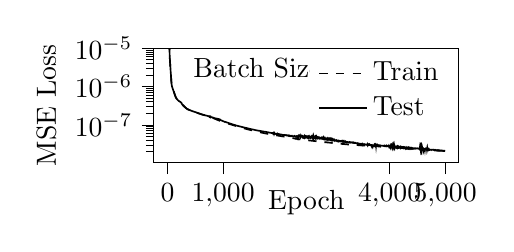
\begin{tikzpicture}

\begin{axis}[
legend cell align={left},
legend style={draw=none},
log basis y={10},
tick align=outside,
tick pos=left,
title={Batch Size 16},
title style={at={(0.4,0.85)},anchor=north},
x grid style={white!69.0196078431373!black},
xlabel={Epoch},
x label style={yshift=13pt},
xmin=-249.95, xmax=5248.95,
xtick style={color=black},
xtick = {0,1000,4000,5000},
y grid style={white!69.0196078431373!black},
ylabel={MSE Loss},
ymin=1.04995733040024e-08, ymax=1e-5,
ymode=log,
ytick style={color=black},
width=.45\textwidth,
height=.25\textwidth
]
\addplot [semithick, black, dashed]
table {%
0 0.0157170567642897
1 0.00494477174337953
2 0.00178249403554946
3 0.00104628965561278
4 0.000540450631990097
5 0.000267249523603823
6 0.000195556676466367
7 0.000179966989569948
8 0.000174315613148792
9 0.000170275954966201
10 0.000166128802236926
11 0.000161243435519282
12 0.000155176517626387
13 0.000147447619914601
14 0.000137505138925917
15 0.000124870715357247
16 0.000109628831036389
17 9.26289391609316e-05
18 7.54085500957444e-05
19 5.99092843294784e-05
20 4.77161089384026e-05
21 3.93279772288224e-05
22 3.40980909077189e-05
23 3.09422128148071e-05
24 2.89322912085481e-05
25 2.72737210743799e-05
26 2.54317353028455e-05
27 2.28156418916114e-05
28 2.01819365893243e-05
29 1.77557636425263e-05
30 1.5502294282669e-05
31 1.34128514700933e-05
32 1.15395934462867e-05
33 9.93898418664685e-06
34 8.62693892850075e-06
35 7.58853412253302e-06
36 6.78498193133237e-06
37 6.16869731970837e-06
38 5.69058382416188e-06
39 5.31324215398854e-06
40 5.00480225616684e-06
41 4.7444518992279e-06
42 4.51447482453204e-06
43 4.30798976503866e-06
44 4.11608894853543e-06
45 3.93454810227922e-06
46 3.75880521266936e-06
47 3.58901737558881e-06
48 3.42562672744862e-06
49 3.26669840717386e-06
50 3.11160224288187e-06
51 2.96258664974403e-06
52 2.82159659042236e-06
53 2.68886794032142e-06
54 2.56387212152731e-06
55 2.44723567112715e-06
56 2.34057172980329e-06
57 2.24493696725858e-06
58 2.15844092952011e-06
59 2.0788237059719e-06
60 1.99667843895668e-06
61 1.90497609787599e-06
62 1.79736609072734e-06
63 1.68848505768437e-06
64 1.59369150190969e-06
65 1.51194072418548e-06
66 1.44278207682191e-06
67 1.38194286273574e-06
68 1.32816223009513e-06
69 1.2809325050398e-06
70 1.23942618449746e-06
71 1.20316316116487e-06
72 1.17089864494346e-06
73 1.14246875506296e-06
74 1.11685223265567e-06
75 1.09369868118847e-06
76 1.07318007189861e-06
77 1.05437576991108e-06
78 1.03672772496566e-06
79 1.02062385838053e-06
80 1.00592634129271e-06
81 9.92105790942332e-07
82 9.7894169545043e-07
83 9.66602892503943e-07
84 9.54589052753363e-07
85 9.42918769112566e-07
86 9.31959767683566e-07
87 9.2148744329279e-07
88 9.11429445267231e-07
89 9.01841054997021e-07
90 8.92400122751269e-07
91 8.83255546455075e-07
92 8.74700299107189e-07
93 8.65906616240863e-07
94 8.57358865317792e-07
95 8.48961237267076e-07
96 8.40659787854747e-07
97 8.3273339777179e-07
98 8.24562840250565e-07
99 8.16930169150964e-07
100 8.08981725157309e-07
101 8.01335254408286e-07
102 7.938409220003e-07
103 7.86272286035228e-07
104 7.79077216805035e-07
105 7.71825237762869e-07
106 7.64540684656367e-07
107 7.57455605054247e-07
108 7.50291343621257e-07
109 7.43385836699417e-07
110 7.36310198249157e-07
111 7.2935094047466e-07
112 7.22335523079209e-07
113 7.15656543093246e-07
114 7.08781524224378e-07
115 7.02204949249108e-07
116 6.95669085445161e-07
117 6.89374548812793e-07
118 6.83004592076486e-07
119 6.76743621340847e-07
120 6.70653783501507e-07
121 6.64517023594158e-07
122 6.58444838109062e-07
123 6.52467115031641e-07
124 6.46645066922247e-07
125 6.40550082820823e-07
126 6.34422589044448e-07
127 6.28629438992334e-07
128 6.22746939754393e-07
129 6.16957024178077e-07
130 6.11050226723364e-07
131 6.0553354312276e-07
132 6.0002472520182e-07
133 5.94472997008211e-07
134 5.89109220683781e-07
135 5.83457079159189e-07
136 5.78418984446216e-07
137 5.7332289055978e-07
138 5.68441488383087e-07
139 5.63714549315364e-07
140 5.59090271252671e-07
141 5.54642511374936e-07
142 5.50334273199837e-07
143 5.46195153745543e-07
144 5.42178440980479e-07
145 5.38200247120812e-07
146 5.34317242667726e-07
147 5.30567891871669e-07
148 5.26957831226582e-07
149 5.23221014177011e-07
150 5.19686565098709e-07
151 5.16319246941066e-07
152 5.1299718701614e-07
153 5.09589032390068e-07
154 5.06361061226812e-07
155 5.03223137172881e-07
156 5.00183228808737e-07
157 4.9724213354807e-07
158 4.9438490189857e-07
159 4.9162455306373e-07
160 4.89330421473255e-07
161 4.86669611902357e-07
162 4.83983281668543e-07
163 4.81407683992074e-07
164 4.78924291158478e-07
165 4.7652420248312e-07
166 4.74232413509412e-07
167 4.71954440158129e-07
168 4.69751064102297e-07
169 4.67584087743944e-07
170 4.65374450342892e-07
171 4.63257154720509e-07
172 4.6126252958345e-07
173 4.59285346551042e-07
174 4.57338758977244e-07
175 4.55391532227623e-07
176 4.53448316278582e-07
177 4.5134003435976e-07
178 4.49530939363285e-07
179 4.47626082561214e-07
180 4.45694395651231e-07
181 4.43928685967876e-07
182 4.42185508745752e-07
183 4.40439555106309e-07
184 4.3882785571725e-07
185 4.37217972901749e-07
186 4.35614033278853e-07
187 4.33923493403654e-07
188 4.32394612360554e-07
189 4.30824806841201e-07
190 4.29448743943794e-07
191 4.27996334764202e-07
192 4.2654474542303e-07
193 4.25223923485873e-07
194 4.23847797321741e-07
195 4.22281450582318e-07
196 4.20877642255846e-07
197 4.19539155572579e-07
198 4.18226270070932e-07
199 4.16828583993834e-07
200 4.15641147853307e-07
201 4.14374378181037e-07
202 4.12955820522143e-07
203 4.11872127500601e-07
204 4.10614599175574e-07
205 4.09486309507656e-07
206 4.08297302655569e-07
207 4.07291623872652e-07
208 4.06151649784192e-07
209 4.04880044627021e-07
210 4.03888402871644e-07
211 4.02805585792976e-07
212 4.01743319073944e-07
213 4.00739752507206e-07
214 3.99736535186435e-07
215 3.98833434005041e-07
216 3.97754167352105e-07
217 3.96727826768029e-07
218 3.95718042653925e-07
219 3.94693230930443e-07
220 3.9383311586505e-07
221 3.9275161007879e-07
222 3.9172802642895e-07
223 3.90782656552346e-07
224 3.89721222845196e-07
225 3.88612679515177e-07
226 3.87859798280488e-07
227 3.8695441405423e-07
228 3.8589167816383e-07
229 3.84909645688936e-07
230 3.83900921491431e-07
231 3.82917928007487e-07
232 3.82064893713618e-07
233 3.81161208053982e-07
234 3.80179631534361e-07
235 3.79220531740998e-07
236 3.78215918999558e-07
237 3.7710426870774e-07
238 3.76155795223099e-07
239 3.74884881878756e-07
240 3.73761657613159e-07
241 3.72517982626164e-07
242 3.71497203701665e-07
243 3.70091190802668e-07
244 3.6877978438099e-07
245 3.67199387056871e-07
246 3.65626293969967e-07
247 3.64062025596468e-07
248 3.62244684353641e-07
249 3.60450857769479e-07
250 3.58647998822903e-07
251 3.56561039907888e-07
252 3.54525802322314e-07
253 3.52287566386167e-07
254 3.50287391583493e-07
255 3.4827622160094e-07
256 3.46361628018599e-07
257 3.442452336202e-07
258 3.42522692250213e-07
259 3.4098111838432e-07
260 3.39507249535131e-07
261 3.3804830252393e-07
262 3.36976891986751e-07
263 3.35771423678466e-07
264 3.34539207671014e-07
265 3.33171887447747e-07
266 3.32210861387239e-07
267 3.30899532073659e-07
268 3.29677021355224e-07
269 3.28394180627356e-07
270 3.27252484524365e-07
271 3.26162355179349e-07
272 3.25076022861026e-07
273 3.24031567018324e-07
274 3.23017687350102e-07
275 3.22020703876547e-07
276 3.21058469410218e-07
277 3.20131131445578e-07
278 3.19224168208621e-07
279 3.18332019588752e-07
280 3.17414626763934e-07
281 3.16470977736572e-07
282 3.15361310200046e-07
283 3.14367141285743e-07
284 3.13330990451277e-07
285 3.12373081598594e-07
286 3.11041730753914e-07
287 3.09975267860807e-07
288 3.08969859794672e-07
289 3.07846929878508e-07
290 3.06794977639413e-07
291 3.05737578266019e-07
292 3.0466266837692e-07
293 3.03954595523237e-07
294 3.03101196678313e-07
295 3.02118985189281e-07
296 3.01218168196726e-07
297 3.00310456772479e-07
298 2.99479211918197e-07
299 2.98664209118726e-07
300 2.97876342834513e-07
301 2.97069236964376e-07
302 2.96287139768481e-07
303 2.95540525151239e-07
304 2.94592372938496e-07
305 2.93832868003108e-07
306 2.93041105045688e-07
307 2.92138023390009e-07
308 2.91344262571158e-07
309 2.90479741146044e-07
310 2.89638650002644e-07
311 2.88783956314376e-07
312 2.87966960804908e-07
313 2.87156888049367e-07
314 2.86230183249359e-07
315 2.85199473267994e-07
316 2.84329060711741e-07
317 2.83470531364571e-07
318 2.82711612797471e-07
319 2.8189036959958e-07
320 2.8108939352478e-07
321 2.80323620067691e-07
322 2.79618150941019e-07
323 2.78579928540523e-07
324 2.77787970787813e-07
325 2.76974661190366e-07
326 2.76175905796094e-07
327 2.75381109268835e-07
328 2.74673050796537e-07
329 2.73941170341629e-07
330 2.73343178925245e-07
331 2.72956742115582e-07
332 2.72267732029263e-07
333 2.71421207877154e-07
334 2.70669167790061e-07
335 2.69858946552404e-07
336 2.69127144292725e-07
337 2.68486125065692e-07
338 2.67699487956463e-07
339 2.67018376263195e-07
340 2.66254324294835e-07
341 2.65609372050335e-07
342 2.64946595834203e-07
343 2.64183357693071e-07
344 2.63509790364935e-07
345 2.62888811377593e-07
346 2.62296822654662e-07
347 2.61795223821082e-07
348 2.60765411624675e-07
349 2.60187987706217e-07
350 2.59608676287826e-07
351 2.58937510935198e-07
352 2.58401657028173e-07
353 2.57939879027447e-07
354 2.57488526514749e-07
355 2.56912723124003e-07
356 2.5638282590279e-07
357 2.55946380399052e-07
358 2.55382050632136e-07
359 2.54851634466036e-07
360 2.5443849939677e-07
361 2.53912852173244e-07
362 2.53413875391573e-07
363 2.52993562064319e-07
364 2.52566530065224e-07
365 2.52173733429117e-07
366 2.51742222630469e-07
367 2.51256598509997e-07
368 2.50831636513738e-07
369 2.50515218077396e-07
370 2.5000812983933e-07
371 2.49434692122463e-07
372 2.48966004456008e-07
373 2.48557739986666e-07
374 2.48152726946671e-07
375 2.47777446951147e-07
376 2.4732192088095e-07
377 2.46895147625992e-07
378 2.46492991010427e-07
379 2.46027582377906e-07
380 2.45625955962225e-07
381 2.45214678422201e-07
382 2.44813897467111e-07
383 2.44392247530811e-07
384 2.439667089007e-07
385 2.43561708266782e-07
386 2.43146217513868e-07
387 2.42745924310839e-07
388 2.42299840301996e-07
389 2.41924007092109e-07
390 2.41548250386359e-07
391 2.4110301239233e-07
392 2.40753827760898e-07
393 2.40407377113172e-07
394 2.40073736314628e-07
395 2.39752746800548e-07
396 2.39428752649928e-07
397 2.39145928070172e-07
398 2.38728963807944e-07
399 2.38479965169347e-07
400 2.38172701713779e-07
401 2.37863011172124e-07
402 2.37620931294202e-07
403 2.3731942192029e-07
404 2.36979224602862e-07
405 2.36684770619888e-07
406 2.36476611952696e-07
407 2.36186071909117e-07
408 2.35960636956634e-07
409 2.35469004792321e-07
410 2.34993137034678e-07
411 2.34665876455153e-07
412 2.34368971142374e-07
413 2.34073551396818e-07
414 2.33405668247144e-07
415 2.3353564838402e-07
416 2.33036555627564e-07
417 2.32731610225301e-07
418 2.32511658502688e-07
419 2.32205579486333e-07
420 2.31897210944965e-07
421 2.31614303118022e-07
422 2.31387427064078e-07
423 2.31009555875517e-07
424 2.30927051632079e-07
425 2.30570250145945e-07
426 2.30109878870621e-07
427 2.29755619159278e-07
428 2.29419798976949e-07
429 2.2913787184109e-07
430 2.28831625989301e-07
431 2.28494739516805e-07
432 2.28182287109746e-07
433 2.27858054557828e-07
434 2.27546540337187e-07
435 2.27196947875541e-07
436 2.26895820269135e-07
437 2.26625020268045e-07
438 2.26283218495382e-07
439 2.25993931898927e-07
440 2.25655906049838e-07
441 2.2537209050455e-07
442 2.2510194525438e-07
443 2.24828690761569e-07
444 2.24556286852362e-07
445 2.24300207833039e-07
446 2.24011245563815e-07
447 2.23872584399487e-07
448 2.23551614816131e-07
449 2.23257345162153e-07
450 2.22980819252427e-07
451 2.2271834546217e-07
452 2.22460312336636e-07
453 2.22206780733813e-07
454 2.21958781267517e-07
455 2.21711269247749e-07
456 2.21467916212248e-07
457 2.21235154199917e-07
458 2.20999668862021e-07
459 2.20767076868356e-07
460 2.20535877438977e-07
461 2.20308807939773e-07
462 2.20059808896167e-07
463 2.19824142021707e-07
464 2.19612100529787e-07
465 2.1938929498333e-07
466 2.19157623597255e-07
467 2.1896537287347e-07
468 2.18743536777311e-07
469 2.18522104340479e-07
470 2.18272721745905e-07
471 2.18055716807442e-07
472 2.1783752742266e-07
473 2.1761818953081e-07
474 2.17430983695976e-07
475 2.17206068221287e-07
476 2.16991443927839e-07
477 2.16773518530999e-07
478 2.16515748135748e-07
479 2.16300841934469e-07
480 2.16058449872492e-07
481 2.15869073706187e-07
482 2.1564869785351e-07
483 2.15435289980803e-07
484 2.15200336675991e-07
485 2.14946434098806e-07
486 2.1470916516364e-07
487 2.14493426646811e-07
488 2.14261333354671e-07
489 2.14043833416611e-07
490 2.13684532845093e-07
491 2.13446484544022e-07
492 2.13225306985976e-07
493 2.13031618301329e-07
494 2.12794633135616e-07
495 2.1251043921211e-07
496 2.12278367698104e-07
497 2.12043049543809e-07
498 2.11812802142219e-07
499 2.11570569483399e-07
500 2.11340852310116e-07
501 2.11117200315414e-07
502 2.10896458291643e-07
503 2.1067865063884e-07
504 2.10462695349634e-07
505 2.10248212908937e-07
506 2.10038392978618e-07
507 2.09967990151938e-07
508 2.09629130488054e-07
509 2.09356091531276e-07
510 2.09101517214094e-07
511 2.0885782751634e-07
512 2.08675676212522e-07
513 2.08429224507256e-07
514 2.08143801842198e-07
515 2.07879654823273e-07
516 2.07599692124916e-07
517 2.07531877720157e-07
518 2.07242607004332e-07
519 2.06976028913175e-07
520 2.06722016230287e-07
521 2.06477896398383e-07
522 2.06244004296252e-07
523 2.05996478037207e-07
524 2.05893390926803e-07
525 2.05615459904607e-07
526 2.05380138218914e-07
527 2.05141496991246e-07
528 2.04895898015423e-07
529 2.04667326379138e-07
530 2.04441963525426e-07
531 2.04216897543574e-07
532 2.0399652140668e-07
533 2.03779658797032e-07
534 2.03562826108339e-07
535 2.0334601751415e-07
536 2.03135240347763e-07
537 2.02906057346297e-07
538 2.02689399074529e-07
539 2.02473491917488e-07
540 2.02258676225142e-07
541 2.02040906152945e-07
542 2.01827895203621e-07
543 2.01646046050996e-07
544 2.0143258397809e-07
545 2.01214925588999e-07
546 2.00992143142287e-07
547 2.00781135099248e-07
548 2.00562146595473e-07
549 2.00357410903962e-07
550 2.00143986297974e-07
551 1.99943427894311e-07
552 1.99730849530511e-07
553 1.99533505224281e-07
554 1.99330869968151e-07
555 1.9912389529253e-07
556 1.98918559668471e-07
557 1.98708590382068e-07
558 1.98505848487684e-07
559 1.98292419888446e-07
560 1.98096410962023e-07
561 1.97904820154804e-07
562 1.9770706975919e-07
563 1.9748347308024e-07
564 1.97292339883859e-07
565 1.97073662711489e-07
566 1.96870710993835e-07
567 1.96664619174669e-07
568 1.96475939667096e-07
569 1.96348054068096e-07
570 1.96120539378342e-07
571 1.95933779174595e-07
572 1.95736368809207e-07
573 1.95534025024813e-07
574 1.95333484313664e-07
575 1.95124152348569e-07
576 1.95009315866912e-07
577 1.94775902379263e-07
578 1.94541645868185e-07
579 1.94320748363452e-07
580 1.9411251212631e-07
581 1.93909075257181e-07
582 1.93718050923053e-07
583 1.93516266911331e-07
584 1.93320917162509e-07
585 1.93129007548976e-07
586 1.92928064961961e-07
587 1.92837274340718e-07
588 1.92624708525102e-07
589 1.92408956387169e-07
590 1.92225819553471e-07
591 1.92020735894971e-07
592 1.91878943944346e-07
593 1.91675015734916e-07
594 1.91448435110431e-07
595 1.91271641604374e-07
596 1.91048381573466e-07
597 1.90840330120068e-07
598 1.90653138474772e-07
599 1.90466430986191e-07
600 1.90273618727588e-07
601 1.90071319252638e-07
602 1.89884589708811e-07
603 1.89694812256391e-07
604 1.89509724471293e-07
605 1.89317692722568e-07
606 1.89151745139782e-07
607 1.88957836265047e-07
608 1.88763875129894e-07
609 1.8860838834911e-07
610 1.88492758660175e-07
611 1.88309009992338e-07
612 1.88081675830176e-07
613 1.87860870838108e-07
614 1.87664490702844e-07
615 1.87469595530843e-07
616 1.87259174673216e-07
617 1.87060099065661e-07
618 1.86873242554952e-07
619 1.86672734876936e-07
620 1.86483752926847e-07
621 1.86293344697219e-07
622 1.86105415899362e-07
623 1.85915503529088e-07
624 1.8575178152247e-07
625 1.85554022223755e-07
626 1.85353178373759e-07
627 1.8521270283145e-07
628 1.85098913320303e-07
629 1.84897171813248e-07
630 1.84691331647002e-07
631 1.84487640524367e-07
632 1.84295574889859e-07
633 1.84111957629796e-07
634 1.83914716345157e-07
635 1.83755724989965e-07
636 1.83571663399107e-07
637 1.8338817892527e-07
638 1.8321129060439e-07
639 1.83026746398696e-07
640 1.82798685713692e-07
641 1.82628072302293e-07
642 1.8240755436949e-07
643 1.82209592708205e-07
644 1.81998398467442e-07
645 1.81880033061077e-07
646 1.81668815613989e-07
647 1.81459775753012e-07
648 1.81254756874694e-07
649 1.81092687050466e-07
650 1.80890330682359e-07
651 1.80684028741496e-07
652 1.80452216731908e-07
653 1.80272235375867e-07
654 1.80111763242508e-07
655 1.79915874568337e-07
656 1.79712098308471e-07
657 1.79537765347959e-07
658 1.79391292441267e-07
659 1.7920577938213e-07
660 1.79012431054559e-07
661 1.78831277722225e-07
662 1.78644232065039e-07
663 1.78457527518106e-07
664 1.78267877934957e-07
665 1.78093018554648e-07
666 1.77905254446387e-07
667 1.77723857326839e-07
668 1.7753547782462e-07
669 1.77379771038488e-07
670 1.77215719631363e-07
671 1.77056875465098e-07
672 1.76856059582065e-07
673 1.76671049281651e-07
674 1.76487213458643e-07
675 1.76302384872429e-07
676 1.76117043793056e-07
677 1.75936534887455e-07
678 1.75756247521974e-07
679 1.75606320475197e-07
680 1.75418388813853e-07
681 1.75196992749704e-07
682 1.75045590090406e-07
683 1.74854614705566e-07
684 1.74652316815127e-07
685 1.74424186383249e-07
686 1.74264706537031e-07
687 1.74055298188591e-07
688 1.73926764027499e-07
689 1.73701496798628e-07
690 1.73572706358982e-07
691 1.73321090102263e-07
692 1.73147434431087e-07
693 1.72996947163995e-07
694 1.72786218151089e-07
695 1.72599083192893e-07
696 1.72568876031676e-07
697 1.72387436194299e-07
698 1.72159440069208e-07
699 1.71958998173238e-07
700 1.71749518663944e-07
701 1.7157847770477e-07
702 1.71360882688987e-07
703 1.71189904619951e-07
704 1.70959397792103e-07
705 1.7079805885345e-07
706 1.70577748185963e-07
707 1.70391250101432e-07
708 1.70294054527176e-07
709 1.70153339674073e-07
710 1.69961250442441e-07
711 1.69790923798985e-07
712 1.69513855112768e-07
713 1.69349986016698e-07
714 1.69170517544615e-07
715 1.68975520637105e-07
716 1.68794829697561e-07
717 1.68674960491444e-07
718 1.68560368251747e-07
719 1.68348613023284e-07
720 1.68180192382295e-07
721 1.68044255872246e-07
722 1.67784312189667e-07
723 1.67622006166823e-07
724 1.67433583676768e-07
725 1.67142194790415e-07
726 1.66952169308843e-07
727 1.66777577675248e-07
728 1.66608952660852e-07
729 1.66446427947164e-07
730 1.66270591492435e-07
731 1.66101942618013e-07
732 1.65938628249762e-07
733 1.65765831525277e-07
734 1.65649616683083e-07
735 1.65385300405774e-07
736 1.65217369541892e-07
737 1.65014219057014e-07
738 1.6483034158199e-07
739 1.64667229618942e-07
740 1.64397729420784e-07
741 1.64213927241974e-07
742 1.64072907040236e-07
743 1.6379700686997e-07
744 1.63645981643867e-07
745 1.63382232301501e-07
746 1.6327906817537e-07
747 1.63015408730871e-07
748 1.62801310864324e-07
749 1.62617077627658e-07
750 1.62424714076792e-07
751 1.62247915383773e-07
752 1.62051023785637e-07
753 1.61872072872882e-07
754 1.6165106788435e-07
755 1.61600835717479e-07
756 1.61240600313306e-07
757 1.61194861057368e-07
758 1.60852658879662e-07
759 1.60787009278351e-07
760 1.60590858342857e-07
761 1.60234822551786e-07
762 1.60201742232857e-07
763 1.59901149771713e-07
764 1.59803023151994e-07
765 1.59525831236351e-07
766 1.59374475643403e-07
767 1.59135792628717e-07
768 1.58920532690843e-07
769 1.58900042478649e-07
770 1.58551003600849e-07
771 1.58445956166986e-07
772 1.58137577130901e-07
773 1.58083954872268e-07
774 1.57764831811846e-07
775 1.57709431590547e-07
776 1.57401405722624e-07
777 1.57347303854749e-07
778 1.57050745258402e-07
779 1.56966653740653e-07
780 1.56687031115155e-07
781 1.56785914370516e-07
782 1.56612737448825e-07
783 1.56451782203249e-07
784 1.56252137685442e-07
785 1.56076418790008e-07
786 1.55898435949098e-07
787 1.55699541132037e-07
788 1.55520961151012e-07
789 1.55345307412347e-07
790 1.55173079157578e-07
791 1.54974727074375e-07
792 1.54768641245084e-07
793 1.5459558374431e-07
794 1.5444234325912e-07
795 1.54301182689665e-07
796 1.54076760843225e-07
797 1.53900922057915e-07
798 1.53745949539541e-07
799 1.53580229117267e-07
800 1.53406590548855e-07
801 1.53240547525968e-07
802 1.53047686090702e-07
803 1.52824890882641e-07
804 1.52664273521452e-07
805 1.52475196550483e-07
806 1.52327802844354e-07
807 1.52147398885916e-07
808 1.51979647590395e-07
809 1.51795929646426e-07
810 1.51624505434711e-07
811 1.51454105321136e-07
812 1.51283279407721e-07
813 1.51115457406092e-07
814 1.50930618310952e-07
815 1.50760781984616e-07
816 1.50782627734714e-07
817 1.50500275672982e-07
818 1.50235237292407e-07
819 1.50018968902543e-07
820 1.49857105313345e-07
821 1.49713744534097e-07
822 1.49508386748209e-07
823 1.49243716315084e-07
824 1.49054966783524e-07
825 1.48848405203239e-07
826 1.48593713156231e-07
827 1.48452548614841e-07
828 1.48339782398921e-07
829 1.48084122237435e-07
830 1.47866147088394e-07
831 1.47622342979048e-07
832 1.4737123991182e-07
833 1.47169714985296e-07
834 1.47018789085962e-07
835 1.46823949506825e-07
836 1.46512769518381e-07
837 1.46378438842021e-07
838 1.46098743840639e-07
839 1.45954007734872e-07
840 1.45737554120728e-07
841 1.45556221561094e-07
842 1.45273102816645e-07
843 1.45146473812474e-07
844 1.44893944799662e-07
845 1.44685848667336e-07
846 1.44500907168776e-07
847 1.4436663649775e-07
848 1.44028160448784e-07
849 1.43881057880435e-07
850 1.43606745851343e-07
851 1.43507942325982e-07
852 1.43128769224177e-07
853 1.4301058635624e-07
854 1.42788225716117e-07
855 1.42625498355642e-07
856 1.42412673760361e-07
857 1.42159079061344e-07
858 1.4199432023787e-07
859 1.41772513316596e-07
860 1.41599934678993e-07
861 1.41388858359903e-07
862 1.41182926185479e-07
863 1.40962782744225e-07
864 1.40806364584023e-07
865 1.40581685961649e-07
866 1.40403925101396e-07
867 1.4016057497912e-07
868 1.40044896177471e-07
869 1.3980589160667e-07
870 1.3957648116758e-07
871 1.39445378636083e-07
872 1.39138843742614e-07
873 1.38897649193837e-07
874 1.38654308422304e-07
875 1.38455802293436e-07
876 1.38271871641393e-07
877 1.38072660327282e-07
878 1.3789356398064e-07
879 1.37655154013316e-07
880 1.37478279633285e-07
881 1.37314475196604e-07
882 1.37122865879746e-07
883 1.36933145142848e-07
884 1.36802316887952e-07
885 1.36559793908475e-07
886 1.3642202107178e-07
887 1.36200022627264e-07
888 1.36101916211828e-07
889 1.35843518506817e-07
890 1.35694482299442e-07
891 1.35512572025931e-07
892 1.35300152894757e-07
893 1.35296917736838e-07
894 1.35076997914041e-07
895 1.34893043981066e-07
896 1.34717172727505e-07
897 1.34527160362552e-07
898 1.34308240479442e-07
899 1.34143823828481e-07
900 1.33862042787314e-07
901 1.336907333922e-07
902 1.33526360556857e-07
903 1.33354756073345e-07
904 1.33178832584235e-07
905 1.32975719669304e-07
906 1.328086220731e-07
907 1.32602404118387e-07
908 1.3244473960583e-07
909 1.322507284236e-07
910 1.3208645066598e-07
911 1.31908025320371e-07
912 1.31727454142805e-07
913 1.31562949462705e-07
914 1.31399596458692e-07
915 1.3120474050865e-07
916 1.31009608221433e-07
917 1.30844098823246e-07
918 1.30663171997725e-07
919 1.30506657299634e-07
920 1.30347919839124e-07
921 1.30182991870953e-07
922 1.30027269566568e-07
923 1.29857494112429e-07
924 1.29701414859795e-07
925 1.29552905523411e-07
926 1.2940177445131e-07
927 1.29231482656422e-07
928 1.29098281369977e-07
929 1.28939781010473e-07
930 1.28751404755434e-07
931 1.28589202464724e-07
932 1.2841671961894e-07
933 1.28243070928846e-07
934 1.2803982670917e-07
935 1.27876534680382e-07
936 1.27715794622674e-07
937 1.27549439078223e-07
938 1.27395809307984e-07
939 1.27251330805933e-07
940 1.27115895857344e-07
941 1.26910032076211e-07
942 1.26811345971589e-07
943 1.26729663211478e-07
944 1.26444568536499e-07
945 1.26253609963101e-07
946 1.26082584579024e-07
947 1.25873118491882e-07
948 1.25708876002051e-07
949 1.25526543680365e-07
950 1.25347965983735e-07
951 1.25173203823437e-07
952 1.24986479754341e-07
953 1.24805979790921e-07
954 1.2464467223694e-07
955 1.24486626290832e-07
956 1.24325891309951e-07
957 1.24059086388684e-07
958 1.23900421499457e-07
959 1.23752723684589e-07
960 1.23606460093129e-07
961 1.23458894080386e-07
962 1.23334903548766e-07
963 1.23164554814537e-07
964 1.23017373574896e-07
965 1.22884383220168e-07
966 1.2272103016997e-07
967 1.22591781686054e-07
968 1.22412395523241e-07
969 1.22283938569723e-07
970 1.2213839731956e-07
971 1.21992413387062e-07
972 1.21762341468212e-07
973 1.21653056602611e-07
974 1.21516884128425e-07
975 1.21363378561057e-07
976 1.21249401036749e-07
977 1.21074073003768e-07
978 1.20967150103013e-07
979 1.20810225507029e-07
980 1.20688818554981e-07
981 1.20541718686695e-07
982 1.20421648816205e-07
983 1.2028323980573e-07
984 1.20130155050191e-07
985 1.20018588045667e-07
986 1.19883109864105e-07
987 1.19717597538482e-07
988 1.19591703700905e-07
989 1.19459623334706e-07
990 1.19327731148644e-07
991 1.19182412216645e-07
992 1.190378214595e-07
993 1.18928106189742e-07
994 1.18777606907372e-07
995 1.18669771886459e-07
996 1.18526345442405e-07
997 1.18412091222098e-07
998 1.182686517609e-07
999 1.18146764471305e-07
1000 1.18045295611324e-07
1001 1.17885191471601e-07
1002 1.1773723693409e-07
1003 1.17636993980597e-07
1004 1.17508308122183e-07
1005 1.17379135396334e-07
1006 1.17220094796977e-07
1007 1.17123960905019e-07
1008 1.16971413607558e-07
1009 1.16875604081912e-07
1010 1.16721507264828e-07
1011 1.16625413646432e-07
1012 1.16471765217341e-07
1013 1.16374956864007e-07
1014 1.16226475117998e-07
1015 1.1612951336204e-07
1016 1.15985186340595e-07
1017 1.15878762532162e-07
1018 1.15722544556718e-07
1019 1.1563705219686e-07
1020 1.15482216056506e-07
1021 1.15382735749847e-07
1022 1.15234289868482e-07
1023 1.15194369406879e-07
1024 1.1509215372385e-07
1025 1.14971480446258e-07
1026 1.14853542346083e-07
1027 1.14729510986677e-07
1028 1.14465596745106e-07
1029 1.14398147832873e-07
1030 1.14321383524185e-07
1031 1.14196341097994e-07
1032 1.14066242570487e-07
1033 1.13935783559782e-07
1034 1.13807661961118e-07
1035 1.13695412860437e-07
1036 1.13558107294409e-07
1037 1.13417669808769e-07
1038 1.13302818903094e-07
1039 1.13176249655567e-07
1040 1.13044207392221e-07
1041 1.12916077910086e-07
1042 1.12789789074696e-07
1043 1.12666461593136e-07
1044 1.12543457490233e-07
1045 1.12422214286312e-07
1046 1.12315864466694e-07
1047 1.12182835920294e-07
1048 1.12061487143933e-07
1049 1.11943023419769e-07
1050 1.11824035883501e-07
1051 1.11708382185327e-07
1052 1.11589450629168e-07
1053 1.11475569585906e-07
1054 1.11358585638044e-07
1055 1.11240735918727e-07
1056 1.11126858243438e-07
1057 1.11011553304508e-07
1058 1.10896632492086e-07
1059 1.10790323411436e-07
1060 1.10676093481032e-07
1061 1.10561356954975e-07
1062 1.10458826345194e-07
1063 1.10332153219872e-07
1064 1.10221367368268e-07
1065 1.10119643316864e-07
1066 1.10016076984465e-07
1067 1.09895937949744e-07
1068 1.09784279111125e-07
1069 1.09660139557377e-07
1070 1.09532256768574e-07
1071 1.09413658780255e-07
1072 1.09296013629745e-07
1073 1.09178800776988e-07
1074 1.09062563716122e-07
1075 1.08961397675245e-07
1076 1.0882023883596e-07
1077 1.08682747345767e-07
1078 1.08570803114105e-07
1079 1.08453086824056e-07
1080 1.08348394981306e-07
1081 1.08229575708663e-07
1082 1.08175652648868e-07
1083 1.08044552664666e-07
1084 1.07924311190999e-07
1085 1.07804279075197e-07
1086 1.07687016416946e-07
1087 1.07583657079857e-07
1088 1.07472328480185e-07
1089 1.07360298155612e-07
1090 1.07231535281471e-07
1091 1.07122651012759e-07
1092 1.07014493000435e-07
1093 1.0690706458405e-07
1094 1.06793603364963e-07
1095 1.06669464503995e-07
1096 1.06556396463731e-07
1097 1.06448062449971e-07
1098 1.0633262673565e-07
1099 1.06225804859861e-07
1100 1.06111840107559e-07
1101 1.06007312659528e-07
1102 1.05889961115935e-07
1103 1.05787279665037e-07
1104 1.05671067569091e-07
1105 1.05566635443921e-07
1106 1.0545252139238e-07
1107 1.05352690265903e-07
1108 1.05238320241341e-07
1109 1.05129935327852e-07
1110 1.05013805679732e-07
1111 1.04924952804453e-07
1112 1.04802457894237e-07
1113 1.0472310326648e-07
1114 1.04609571572212e-07
1115 1.0450942516016e-07
1116 1.04393734819297e-07
1117 1.04297197307091e-07
1118 1.04180416496291e-07
1119 1.0408402435047e-07
1120 1.03966197073646e-07
1121 1.0387017652036e-07
1122 1.03754794164246e-07
1123 1.0365835006354e-07
1124 1.03542971995552e-07
1125 1.03447081940544e-07
1126 1.03333663226124e-07
1127 1.03239306419312e-07
1128 1.03124784988751e-07
1129 1.03028840477748e-07
1130 1.02916153586818e-07
1131 1.02787292341588e-07
1132 1.02657459869704e-07
1133 1.02566233646684e-07
1134 1.02459099572627e-07
1135 1.0236741592351e-07
1136 1.02258474193206e-07
1137 1.02178690926991e-07
1138 1.02057533133859e-07
1139 1.0195955497494e-07
1140 1.01866740447321e-07
1141 1.0174640036098e-07
1142 1.01654885199309e-07
1143 1.01564086460115e-07
1144 1.01452568284088e-07
1145 1.01358281408892e-07
1146 1.01252124068196e-07
1147 1.01132042544805e-07
1148 1.01040741810721e-07
1149 1.0093680472778e-07
1150 1.00835201639171e-07
1151 1.00737907963833e-07
1152 1.00636074826355e-07
1153 1.00535662330259e-07
1154 1.00435070386595e-07
1155 1.00334794463919e-07
1156 1.00233066344657e-07
1157 1.00139313264691e-07
1158 1.00035746370963e-07
1159 9.99342205645348e-08
1160 9.98369444076275e-08
1161 9.97294167923712e-08
1162 9.96306041329831e-08
1163 9.95292283505478e-08
1164 9.94305740533719e-08
1165 9.93309828345446e-08
1166 9.92319580497281e-08
1167 9.91331406723361e-08
1168 9.90346987315149e-08
1169 9.89363423364864e-08
1170 9.88384333915349e-08
1171 9.87406676955516e-08
1172 9.86426246996075e-08
1173 9.85450470523119e-08
1174 9.84475341887503e-08
1175 9.83505173692833e-08
1176 9.82529710178426e-08
1177 9.81562854889262e-08
1178 9.80592281862869e-08
1179 9.79621718073531e-08
1180 9.78654439443005e-08
1181 9.77698567261598e-08
1182 9.76725255235067e-08
1183 9.75756527665794e-08
1184 9.74796394181965e-08
1185 9.73854815420339e-08
1186 9.72912396584036e-08
1187 9.71942784673274e-08
1188 9.70993046678359e-08
1189 9.7005777128345e-08
1190 9.69105955412886e-08
1191 9.68398183474051e-08
1192 9.67422502249349e-08
1193 9.6656792269556e-08
1194 9.65493723619204e-08
1195 9.64579490911888e-08
1196 9.63569642422613e-08
1197 9.62606689931533e-08
1198 9.61624434623332e-08
1199 9.60775235725464e-08
1200 9.5981298237291e-08
1201 9.58870457914429e-08
1202 9.57886685490905e-08
1203 9.56941159380165e-08
1204 9.55973716543213e-08
1205 9.550779267542e-08
1206 9.54129343995192e-08
1207 9.53207871106088e-08
1208 9.52259731121785e-08
1209 9.51386579863822e-08
1210 9.50452932002577e-08
1211 9.49372938769955e-08
1212 9.48370358955231e-08
1213 9.47485660738323e-08
1214 9.46488406015078e-08
1215 9.45476629787834e-08
1216 9.44520911225766e-08
1217 9.43511249644757e-08
1218 9.42532653489536e-08
1219 9.41596363510655e-08
1220 9.40521965198116e-08
1221 9.3958234778313e-08
1222 9.38527993739058e-08
1223 9.37583681590581e-08
1224 9.3655063739817e-08
1225 9.35592185555834e-08
1226 9.34639041965113e-08
1227 9.33635799533761e-08
1228 9.32726998605915e-08
1229 9.31820874114919e-08
1230 9.3086685076571e-08
1231 9.2996467174089e-08
1232 9.28943459186371e-08
1233 9.28112276987747e-08
1234 9.27086237609842e-08
1235 9.26266937000264e-08
1236 9.25256117518813e-08
1237 9.24348963096122e-08
1238 9.23422541383445e-08
1239 9.22336319888473e-08
1240 9.21328738066052e-08
1241 9.20548228862117e-08
1242 9.19620167856294e-08
1243 9.1858883305207e-08
1244 9.17831347067022e-08
1245 9.16764033469519e-08
1246 9.16021301513581e-08
1247 9.15102322807115e-08
1248 9.14096642823381e-08
1249 9.13258232415615e-08
1250 9.12370573509236e-08
1251 9.11314231082372e-08
1252 9.10548857149251e-08
1253 9.09575262930673e-08
1254 9.0878455086596e-08
1255 9.07892068404692e-08
1256 9.06909464717387e-08
1257 9.06085933252143e-08
1258 9.0521073303762e-08
1259 9.04282962750358e-08
1260 9.03382387598128e-08
1261 9.02488962388759e-08
1262 9.01657012271073e-08
1263 9.00837959534329e-08
1264 8.99963811491489e-08
1265 8.9906916667104e-08
1266 8.98200719099407e-08
1267 8.97321847581622e-08
1268 8.96452091616595e-08
1269 8.95563996046178e-08
1270 8.94744537696113e-08
1271 8.93858809583037e-08
1272 8.93017317054046e-08
1273 8.92115444202091e-08
1274 8.91289444773236e-08
1275 8.90431513695944e-08
1276 8.89543760465017e-08
1277 8.88647354990724e-08
1278 8.87773948683446e-08
1279 8.86847180474604e-08
1280 8.8604710200002e-08
1281 8.85189234693939e-08
1282 8.84320530047944e-08
1283 8.83455266311728e-08
1284 8.82566362889747e-08
1285 8.81749002772381e-08
1286 8.8091375637589e-08
1287 8.8006731434831e-08
1288 8.79208263704356e-08
1289 8.78380143163327e-08
1290 8.7753197313134e-08
1291 8.76683468540307e-08
1292 8.7583503496802e-08
1293 8.74997554873858e-08
1294 8.74166315618652e-08
1295 8.7332899298076e-08
1296 8.72496221155927e-08
1297 8.71674850380089e-08
1298 8.70835239226153e-08
1299 8.69979467985615e-08
1300 8.69180498774824e-08
1301 8.68290546023331e-08
1302 8.67538605575646e-08
1303 8.66866929456478e-08
1304 8.66013013194333e-08
1305 8.65141546739778e-08
1306 8.6432395224989e-08
1307 8.63492025722223e-08
1308 8.62639010534849e-08
1309 8.61873499360399e-08
1310 8.60964398192721e-08
1311 8.60305623895386e-08
1312 8.5945265599463e-08
1313 8.58654531619152e-08
1314 8.57828558054052e-08
1315 8.57025365945674e-08
1316 8.56227119179209e-08
1317 8.55251783349331e-08
1318 8.5447654544879e-08
1319 8.53730991074997e-08
1320 8.53113611576362e-08
1321 8.52530063752965e-08
1322 8.5145811016929e-08
1323 8.50639250415952e-08
1324 8.49800504987286e-08
1325 8.49213991926945e-08
1326 8.48373153417015e-08
1327 8.47663028693546e-08
1328 8.4683932776386e-08
1329 8.46030600811787e-08
1330 8.45243451159661e-08
1331 8.44448748686943e-08
1332 8.43658713378659e-08
1333 8.42873192290483e-08
1334 8.42077087881421e-08
1335 8.413040495725e-08
1336 8.40533396413434e-08
1337 8.39737880227176e-08
1338 8.39027628565248e-08
1339 8.38281100463689e-08
1340 8.37473770438635e-08
1341 8.36699169042276e-08
1342 8.35880798319977e-08
1343 8.35109091923414e-08
1344 8.34303905108413e-08
1345 8.33509666051668e-08
1346 8.32730190971631e-08
1347 8.31975916035788e-08
1348 8.31306992026271e-08
1349 8.30542468079898e-08
1350 8.29774157509178e-08
1351 8.2896661286469e-08
1352 8.28168008588648e-08
1353 8.27384261050668e-08
1354 8.26573808154762e-08
1355 8.25796255305988e-08
1356 8.25036329494821e-08
1357 8.24257792118033e-08
1358 8.23485480161423e-08
1359 8.22789238732469e-08
1360 8.22006595520008e-08
1361 8.21227055496365e-08
1362 8.2044704448947e-08
1363 8.19672813463512e-08
1364 8.18913912894459e-08
1365 8.18145910308488e-08
1366 8.17310067056098e-08
1367 8.16556159399795e-08
1368 8.15891315895101e-08
1369 8.15134725122846e-08
1370 8.14405360145543e-08
1371 8.13719105217103e-08
1372 8.12908016314395e-08
1373 8.12063895203607e-08
1374 8.11270667853137e-08
1375 8.10392181485042e-08
1376 8.09575813001118e-08
1377 8.08839921795368e-08
1378 8.08079852667731e-08
1379 8.07220590779423e-08
1380 8.06590918109862e-08
1381 8.05818785387658e-08
1382 8.05058287483007e-08
1383 8.04375114924483e-08
1384 8.03611219843958e-08
1385 8.02734742073596e-08
1386 8.02103674963917e-08
1387 8.01333753592814e-08
1388 8.00467322505938e-08
1389 7.99712219219373e-08
1390 7.99084653912985e-08
1391 7.98324605639777e-08
1392 7.97513225130331e-08
1393 7.96915628207273e-08
1394 7.96128401034935e-08
1395 7.95309664347599e-08
1396 7.94698840849151e-08
1397 7.9392765581332e-08
1398 7.9295083487807e-08
1399 7.92480824038933e-08
1400 7.91767527488219e-08
1401 7.90798937977399e-08
1402 7.90350093922143e-08
1403 7.89427710436996e-08
1404 7.88719372764035e-08
1405 7.88001505966918e-08
1406 7.87278963976235e-08
1407 7.86439569182562e-08
1408 7.85879019211677e-08
1409 7.85154309888014e-08
1410 7.84318538968876e-08
1411 7.83922933358383e-08
1412 7.83064902059039e-08
1413 7.82436948192355e-08
1414 7.81700940777341e-08
1415 7.81046548645747e-08
1416 7.80235332982215e-08
1417 7.79860344124472e-08
1418 7.78859922760944e-08
1419 7.78468724114134e-08
1420 7.77458072285242e-08
1421 7.77082536167484e-08
1422 7.76031458613602e-08
1423 7.75538769453021e-08
1424 7.74638346889844e-08
1425 7.7412013162359e-08
1426 7.73240489770899e-08
1427 7.72703984992518e-08
1428 7.71842282603075e-08
1429 7.71299326345343e-08
1430 7.70427543983487e-08
1431 7.69885805844694e-08
1432 7.68999306934859e-08
1433 7.68471794536651e-08
1434 7.67474068190665e-08
1435 7.669313940184e-08
1436 7.6607799300632e-08
1437 7.65571879561833e-08
1438 7.64666975019423e-08
1439 7.64233642662759e-08
1440 7.63317421643706e-08
1441 7.62877545348317e-08
1442 7.6203435483535e-08
1443 7.61529052084597e-08
1444 7.60647247997071e-08
1445 7.60194817654991e-08
1446 7.59333198274703e-08
1447 7.58907218383342e-08
1448 7.58090455246219e-08
1449 7.57582843178284e-08
1450 7.57179583370515e-08
1451 7.56195299302931e-08
1452 7.55561748508882e-08
1453 7.54916978635833e-08
1454 7.5432396256403e-08
1455 7.53674571498664e-08
1456 7.52965677950357e-08
1457 7.5238625441898e-08
1458 7.5167802796372e-08
1459 7.51119294637448e-08
1460 7.50374735734027e-08
1461 7.49760933977939e-08
1462 7.48975998057233e-08
1463 7.48535242411918e-08
1464 7.47783008758773e-08
1465 7.47050625609091e-08
1466 7.46483551417043e-08
1467 7.45740001022455e-08
1468 7.45270812885224e-08
1469 7.4443754344955e-08
1470 7.4380113401773e-08
1471 7.43380596901488e-08
1472 7.42537142617294e-08
1473 7.42098589494589e-08
1474 7.41303028082285e-08
1475 7.40660056592901e-08
1476 7.40370165512871e-08
1477 7.39397521467566e-08
1478 7.38789098857495e-08
1479 7.38492542762259e-08
1480 7.37513224109421e-08
1481 7.37224941023129e-08
1482 7.36224275552644e-08
1483 7.35667011948493e-08
1484 7.35384280314832e-08
1485 7.34439351628424e-08
1486 7.34135366222688e-08
1487 7.33215193999826e-08
1488 7.3262118958084e-08
1489 7.32310826201399e-08
1490 7.31369283712979e-08
1491 7.30799931130122e-08
1492 7.30507533877045e-08
1493 7.29692056040676e-08
1494 7.29461080162253e-08
1495 7.28552913358271e-08
1496 7.28172455186637e-08
1497 7.2759770612052e-08
1498 7.26808831839065e-08
1499 7.26333379219568e-08
1500 7.25761171178618e-08
1501 7.25002446042566e-08
1502 7.24530508353638e-08
1503 7.23712498071904e-08
1504 7.23255573245041e-08
1505 7.22771065948535e-08
1506 7.22012546212625e-08
1507 7.21588228156378e-08
1508 7.20717930615677e-08
1509 7.20151864914698e-08
1510 7.19812252931717e-08
1511 7.18593284645408e-08
1512 7.18661725915837e-08
1513 7.18080895314443e-08
1514 7.17542879211663e-08
1515 7.16964362812433e-08
1516 7.16366252806466e-08
1517 7.15322650410855e-08
1518 7.15308601897391e-08
1519 7.14554064966677e-08
1520 7.13549446889061e-08
1521 7.13500851201587e-08
1522 7.1280213971292e-08
1523 7.12213592048983e-08
1524 7.1125808473127e-08
1525 7.11177791856699e-08
1526 7.10524085931752e-08
1527 7.09491985855237e-08
1528 7.09230811022366e-08
1529 7.08539147549203e-08
1530 7.07737182583656e-08
1531 7.07214989734695e-08
1532 7.06564270451793e-08
1533 7.05835089735984e-08
1534 7.05460777865596e-08
1535 7.04877491930489e-08
1536 7.04216205349439e-08
1537 7.03814124722868e-08
1538 7.03216431912068e-08
1539 7.02704037696122e-08
1540 7.01973612020623e-08
1541 7.0164162307762e-08
1542 7.01039659212199e-08
1543 7.0039195259497e-08
1544 6.99994840633877e-08
1545 6.99282411940061e-08
1546 6.98895919128972e-08
1547 6.98095471864946e-08
1548 6.97712376460657e-08
1549 6.97109298943843e-08
1550 6.9632473101322e-08
1551 6.95940093482506e-08
1552 6.95389268248192e-08
1553 6.94699652452613e-08
1554 6.94294041974075e-08
1555 6.9355845011998e-08
1556 6.93180881405908e-08
1557 6.92588990727216e-08
1558 6.91887736632424e-08
1559 6.91512637267522e-08
1560 6.9092847537533e-08
1561 6.90220523242857e-08
1562 6.89855159823338e-08
1563 6.89106090323577e-08
1564 6.88816554959004e-08
1565 6.88365903069865e-08
1566 6.87812293040935e-08
1567 6.87185002323787e-08
1568 6.8642084881887e-08
1569 6.86118347612563e-08
1570 6.85325593572372e-08
1571 6.85040618790822e-08
1572 6.84324654880442e-08
1573 6.839076007914e-08
1574 6.83189021835062e-08
1575 6.82729641408031e-08
1576 6.81955693746517e-08
1577 6.81605108194816e-08
1578 6.81111089928521e-08
1579 6.80341699759168e-08
1580 6.80005206437073e-08
1581 6.79343854468328e-08
1582 6.78743013686756e-08
1583 6.78180592128541e-08
1584 6.77644835676006e-08
1585 6.77205531331992e-08
1586 6.76518835902584e-08
1587 6.75858284839848e-08
1588 6.7559896509195e-08
1589 6.74892750094358e-08
1590 6.74610934225939e-08
1591 6.74030582157315e-08
1592 6.73369531245527e-08
1593 6.72861732180508e-08
1594 6.72273089517006e-08
1595 6.7194645049895e-08
1596 6.7137755896951e-08
1597 6.70708017658228e-08
1598 6.70592294174099e-08
1599 6.69806256290428e-08
1600 6.69565935051963e-08
1601 6.6876471620958e-08
1602 6.68527393017371e-08
1603 6.67749209544155e-08
1604 6.67497319373211e-08
1605 6.66836660396797e-08
1606 6.66453354263297e-08
1607 6.65926854352961e-08
1608 6.65282488423458e-08
1609 6.6488449387947e-08
1610 6.64343398302236e-08
1611 6.63779134839615e-08
1612 6.63125629074557e-08
1613 6.62765239027863e-08
1614 6.62034557681324e-08
1615 6.61748533499207e-08
1616 6.61297554014339e-08
1617 6.60409584458677e-08
1618 6.6028880171487e-08
1619 6.59719671087799e-08
1620 6.59495228756413e-08
1621 6.58748443882473e-08
1622 6.58512198743466e-08
1623 6.57803125960754e-08
1624 6.57593430002379e-08
1625 6.57009276565645e-08
1626 6.56188756789078e-08
1627 6.56008984094569e-08
1628 6.5510794748036e-08
1629 6.5506174689034e-08
1630 6.54147165271013e-08
1631 6.54004263029861e-08
1632 6.5330469803726e-08
1633 6.53194631468068e-08
1634 6.52330189456762e-08
1635 6.52263919054263e-08
1636 6.51325602660791e-08
1637 6.51270379510294e-08
1638 6.50832606332585e-08
1639 6.50223449909504e-08
1640 6.49905436045373e-08
1641 6.49078730869945e-08
1642 6.48822075746125e-08
1643 6.48035599741803e-08
1644 6.47770159538652e-08
1645 6.4707539873865e-08
1646 6.46819224456863e-08
1647 6.46097836529691e-08
1648 6.45885289962678e-08
1649 6.45144189377334e-08
1650 6.44925645705285e-08
1651 6.44240081335568e-08
1652 6.43979384005178e-08
1653 6.43428221973608e-08
1654 6.428219044885e-08
1655 6.42558258956427e-08
1656 6.41921231387954e-08
1657 6.41689319547112e-08
1658 6.41028819785561e-08
1659 6.40726781870882e-08
1660 6.40072181106177e-08
1661 6.39795522463515e-08
1662 6.39297982321096e-08
1663 6.3871073178845e-08
1664 6.38408367290566e-08
1665 6.37792557007799e-08
1666 6.37521571729138e-08
1667 6.36896845236379e-08
1668 6.36601125965086e-08
1669 6.36008435410673e-08
1670 6.35746379664681e-08
1671 6.35181804433671e-08
1672 6.34676094435349e-08
1673 6.34354211879184e-08
1674 6.33740493203305e-08
1675 6.33314038243071e-08
1676 6.32749130726751e-08
1677 6.32347840738845e-08
1678 6.31732688756159e-08
1679 6.31338394310177e-08
1680 6.30652151922817e-08
1681 6.30463459234676e-08
1682 6.29724075018601e-08
1683 6.2956256465796e-08
1684 6.28833726636913e-08
1685 6.28631577619387e-08
1686 6.2810514361189e-08
1687 6.27526249825649e-08
1688 6.27297131359228e-08
1689 6.26645676735649e-08
1690 6.26481085017616e-08
1691 6.25765496540254e-08
1692 6.25491643475584e-08
1693 6.24812895697602e-08
1694 6.2463616799846e-08
1695 6.23948352806991e-08
1696 6.23737416489689e-08
1697 6.23239637480566e-08
1698 6.22703101509359e-08
1699 6.22446263580656e-08
1700 6.21824421340733e-08
1701 6.21636741069409e-08
1702 6.20918038123364e-08
1703 6.20736190857229e-08
1704 6.20149772938561e-08
1705 6.19964937431661e-08
1706 6.19347309811502e-08
1707 6.1910406349952e-08
1708 6.18521268460626e-08
1709 6.18265581540101e-08
1710 6.17684524790718e-08
1711 6.17448781028429e-08
1712 6.16845532288579e-08
1713 6.16598977511984e-08
1714 6.16143801561719e-08
1715 6.15619190327266e-08
1716 6.15333821283315e-08
1717 6.14823349280869e-08
1718 6.14551080015957e-08
1719 6.14102441911513e-08
1720 6.13515261029818e-08
1721 6.13220992118357e-08
1722 6.12588356148081e-08
1723 6.12405779989444e-08
1724 6.11997082504701e-08
1725 6.11438640394368e-08
1726 6.11246135520105e-08
1727 6.1070817375608e-08
1728 6.10205517528328e-08
1729 6.09990552220552e-08
1730 6.09413689733884e-08
1731 6.08886698465483e-08
1732 6.08616994828282e-08
1733 6.08214279971264e-08
1734 6.07714548870319e-08
1735 6.07395625191742e-08
1736 6.06988344191706e-08
1737 6.064735849165e-08
1738 6.06205199655818e-08
1739 6.05749239124265e-08
1740 6.05129370594426e-08
1741 6.05012419647721e-08
1742 6.04553985272815e-08
1743 6.03960760319211e-08
1744 6.03828635998838e-08
1745 6.03404926344808e-08
1746 6.02797830424606e-08
1747 6.02628985220122e-08
1748 6.02163528338195e-08
1749 6.01650723552893e-08
1750 6.01461151159555e-08
1751 6.0099468852215e-08
1752 6.00380151585256e-08
1753 6.00097526533006e-08
1754 5.99578201949669e-08
1755 5.99032240202746e-08
1756 5.98908391200581e-08
1757 5.98447522186518e-08
1758 5.97969285838218e-08
1759 5.9783278864245e-08
1760 5.97381680282894e-08
1761 5.96831014316734e-08
1762 5.96634693312836e-08
1763 5.9620811219574e-08
1764 5.95710671564831e-08
1765 5.95497044262316e-08
1766 5.94933353976756e-08
1767 5.94397501458843e-08
1768 5.94266319691172e-08
1769 5.93856979289598e-08
1770 5.93300072733172e-08
1771 5.93130644528372e-08
1772 5.92704806923194e-08
1773 5.92268136809793e-08
1774 5.91797808926486e-08
1775 5.91507497311738e-08
1776 5.91200140238612e-08
1777 5.90610537880565e-08
1778 5.90448508877017e-08
1779 5.90022764068721e-08
1780 5.89430245447886e-08
1781 5.89263584167554e-08
1782 5.88846336242455e-08
1783 5.88285095606267e-08
1784 5.88103355436687e-08
1785 5.87698267064951e-08
1786 5.87322994558548e-08
1787 5.86814049867712e-08
1788 5.86593097935406e-08
1789 5.86253984682372e-08
1790 5.85660904164342e-08
1791 5.85476309495903e-08
1792 5.85049212116218e-08
1793 5.84561298868635e-08
1794 5.84374685121958e-08
1795 5.83932191009495e-08
1796 5.83553954029981e-08
1797 5.83059133898445e-08
1798 5.82895867626831e-08
1799 5.82480555006981e-08
1800 5.8200157324606e-08
1801 5.81786484090685e-08
1802 5.81429857593463e-08
1803 5.80878021807507e-08
1804 5.80690354983204e-08
1805 5.80282149797995e-08
1806 5.79956561210793e-08
1807 5.79425478619555e-08
1808 5.79221452419176e-08
1809 5.78838757476774e-08
1810 5.78314735779628e-08
1811 5.78163176037094e-08
1812 5.77766614888731e-08
1813 5.77403952473077e-08
1814 5.76883562946051e-08
1815 5.76788046178223e-08
1816 5.76407622698838e-08
1817 5.75972874177211e-08
1818 5.75486887459675e-08
1819 5.75290882096624e-08
1820 5.74849039995939e-08
1821 5.74410002496251e-08
1822 5.74063457214891e-08
1823 5.73605157381252e-08
1824 5.73157828593907e-08
1825 5.7272223271454e-08
1826 5.72637396345499e-08
1827 5.72324278689251e-08
1828 5.71935515232269e-08
1829 5.71610200132966e-08
1830 5.71233054333931e-08
1831 5.7078984424308e-08
1832 5.70541767270782e-08
1833 5.70163162052495e-08
1834 5.6980763867287e-08
1835 5.6939591541294e-08
1836 5.69168955646404e-08
1837 5.68663307110029e-08
1838 5.68295884537662e-08
1839 5.68088100383335e-08
1840 5.67678091236701e-08
1841 5.67343938175924e-08
1842 5.67020331203594e-08
1843 5.66667278611987e-08
1844 5.66293540043006e-08
1845 5.6587106973538e-08
1846 5.65633186884185e-08
1847 5.65253377242669e-08
1848 5.6488802282928e-08
1849 5.64697279958892e-08
1850 5.64184602804829e-08
1851 5.6386358695093e-08
1852 5.63529641777194e-08
1853 5.63152014105839e-08
1854 5.63030739169079e-08
1855 5.62536226720312e-08
1856 5.621887777707e-08
1857 5.61840797956847e-08
1858 5.61519734709748e-08
1859 5.6119060975135e-08
1860 5.60813896104406e-08
1861 5.60604641695051e-08
1862 5.60212938207627e-08
1863 5.59822433103818e-08
1864 5.59557859460824e-08
1865 5.59342552808317e-08
1866 5.58837556017267e-08
1867 5.58555222394119e-08
1868 5.58171534166263e-08
1869 5.57975660431254e-08
1870 5.57658234239256e-08
1871 5.57404777250525e-08
1872 5.56964996949461e-08
1873 5.56634625237251e-08
1874 5.56313199027159e-08
1875 5.55997774540629e-08
1876 5.55613583443915e-08
1877 5.55269757676058e-08
1878 5.5502511211003e-08
1879 5.54778267520817e-08
1880 5.5444562415019e-08
1881 5.54123262350714e-08
1882 5.53820424755713e-08
1883 5.53495265638304e-08
1884 5.53182410154562e-08
1885 5.5270342071978e-08
1886 5.52461083671574e-08
1887 5.52285828891996e-08
1888 5.51930989818317e-08
1889 5.51618536857035e-08
1890 5.51298880360207e-08
1891 5.50989660688117e-08
1892 5.50679799324882e-08
1893 5.50219489507953e-08
1894 5.49859079370663e-08
1895 5.49978789443628e-08
1896 5.49897674844146e-08
1897 5.49477678379873e-08
1898 5.489871420572e-08
1899 5.48642930553456e-08
1900 5.48544498872872e-08
1901 5.48280247141264e-08
1902 5.4770532685211e-08
1903 5.4748959600559e-08
1904 5.47057154562935e-08
1905 5.4679610769881e-08
1906 5.4649364141568e-08
1907 5.46201876634456e-08
1908 5.45880473250548e-08
1909 5.45829187341695e-08
1910 5.45216613279109e-08
1911 5.44992172866188e-08
1912 5.44700705287227e-08
1913 5.44351320002079e-08
1914 5.44117753751294e-08
1915 5.43976634208576e-08
1916 5.43506271544203e-08
1917 5.43152112477685e-08
1918 5.42734870077055e-08
1919 5.42208746470152e-08
1920 5.42188376080333e-08
1921 5.42318459899604e-08
1922 5.41535841005469e-08
1923 5.40810903277844e-08
1924 5.40626227607532e-08
1925 5.40615722570692e-08
1926 5.40531078154771e-08
1927 5.40417447325581e-08
1928 5.40066272378681e-08
1929 5.39541558524093e-08
1930 5.39220726949452e-08
1931 5.38704136285872e-08
1932 5.38764866675479e-08
1933 5.3832834163714e-08
1934 5.38132092149368e-08
1935 5.37755291372122e-08
1936 5.37120134787017e-08
1937 5.37266989422136e-08
1938 5.36942823483599e-08
1939 5.36637576598054e-08
1940 5.36314578081232e-08
1941 5.35836024884162e-08
1942 5.35198249060898e-08
1943 5.34807587548869e-08
1944 5.35186063448379e-08
1945 5.34852590980961e-08
1946 5.34530285616341e-08
1947 5.34172343797934e-08
1948 5.33864700216213e-08
1949 5.33384438252682e-08
1950 5.3282433940538e-08
1951 5.32578811167639e-08
1952 5.32278484239868e-08
1953 5.32070314616107e-08
1954 5.32098277403747e-08
1955 5.31718705811812e-08
1956 5.3149979528655e-08
1957 5.31092216693452e-08
1958 5.30581348936465e-08
1959 5.30666372675626e-08
1960 5.30339547051284e-08
1961 5.30024818807817e-08
1962 5.29706637326655e-08
1963 5.29289977535541e-08
1964 5.28774677004407e-08
1965 5.28940590527327e-08
1966 5.28638908967594e-08
1967 5.28358995826039e-08
1968 5.28036098508267e-08
1969 5.27743610430065e-08
1970 5.272617962504e-08
1971 5.26712675981145e-08
1972 5.26441776536046e-08
1973 5.26639329834211e-08
1974 5.26350127412201e-08
1975 5.26090606758345e-08
1976 5.2560195625162e-08
1977 5.25175980872206e-08
1978 5.25127587494012e-08
1979 5.24721666028682e-08
1980 5.25028947304662e-08
1981 5.24535227519607e-08
1982 5.24334885607658e-08
1983 5.23928427504927e-08
1984 5.23647968595498e-08
1985 5.23303921706741e-08
1986 5.22664249142935e-08
1987 5.22732280447968e-08
1988 5.22278388448427e-08
1989 5.22206757729293e-08
1990 5.21576788745648e-08
1991 5.21696426716289e-08
1992 5.21383016103272e-08
1993 5.21176466321549e-08
1994 5.20795234777438e-08
1995 5.20577898903696e-08
1996 5.20088351390058e-08
1997 5.19967646770425e-08
1998 5.19834512235917e-08
1999 5.19351928325307e-08
2000 5.18789852410606e-08
2001 5.18892107059798e-08
2002 5.18384501262403e-08
2003 5.18320842655129e-08
2004 5.17724597930425e-08
2005 5.17933313215479e-08
2006 5.17651106353156e-08
2007 5.17365716401486e-08
2008 5.16944155677379e-08
2009 5.16442815303719e-08
2010 5.16417980787054e-08
2011 5.15751542451426e-08
2012 5.16057571360307e-08
2013 5.15795475681813e-08
2014 5.15523841428944e-08
2015 5.14852089530393e-08
2016 5.14251952807854e-08
2017 5.14224534473584e-08
2018 5.13930180208177e-08
2019 5.13651756417488e-08
2020 5.13398442567592e-08
2021 5.1278221276263e-08
2022 5.12808904371553e-08
2023 5.12275395170292e-08
2024 5.12120996791765e-08
2025 5.11728608216799e-08
2026 5.11418466579983e-08
2027 5.1111997334985e-08
2028 5.10851505044485e-08
2029 5.10588654680788e-08
2030 5.10363068499942e-08
2031 5.10086910185947e-08
2032 5.09770729344439e-08
2033 5.09473898517854e-08
2034 5.09033281179683e-08
2035 5.08676520567519e-08
2036 5.08378530117426e-08
2037 5.07910789444566e-08
2038 5.07609317761393e-08
2039 5.07433153380532e-08
2040 5.07163217573492e-08
2041 5.0683928199291e-08
2042 5.06598294993665e-08
2043 5.06497230698955e-08
2044 5.06451459418855e-08
2045 5.05945661295471e-08
2046 5.0563461080344e-08
2047 5.05418403413671e-08
2048 5.05143432345534e-08
2049 5.04725191596833e-08
2050 5.04620838448488e-08
2051 5.04257198841174e-08
2052 5.03963417504139e-08
2053 5.03694018423317e-08
2054 5.03383870249507e-08
2055 5.03116513481672e-08
2056 5.02853407446935e-08
2057 5.02635672177121e-08
2058 5.02253421217347e-08
2059 5.01998919251179e-08
2060 5.01762324986998e-08
2061 5.01381022903757e-08
2062 5.01165475785825e-08
2063 5.00791420972035e-08
2064 5.00571208412737e-08
2065 5.00191744006173e-08
2066 4.99969106808607e-08
2067 4.99652818515273e-08
2068 4.99406647023193e-08
2069 4.99400747422385e-08
2070 4.98836416173987e-08
2071 4.98563354618398e-08
2072 4.98195677050006e-08
2073 4.9797368346205e-08
2074 4.97628820195217e-08
2075 4.97410512299012e-08
2076 4.97102558565388e-08
2077 4.96750526295386e-08
2078 4.96484829373145e-08
2079 4.96207821676364e-08
2080 4.95880412643146e-08
2081 4.95595028215945e-08
2082 4.95292679438819e-08
2083 4.95411185248429e-08
2084 4.94985872645515e-08
2085 4.94496979275283e-08
2086 4.94542133306908e-08
2087 4.94274170268483e-08
2088 4.93998827000297e-08
2089 4.9341949491577e-08
2090 4.93363587459328e-08
2091 4.92780220415767e-08
2092 4.92824592868146e-08
2093 4.92250463803856e-08
2094 4.92274303507401e-08
2095 4.9199288582713e-08
2096 4.92094329818116e-08
2097 4.91981392123364e-08
2098 4.9152802006347e-08
2099 4.9114675860551e-08
2100 4.9033944433674e-08
2101 4.90316926367029e-08
2102 4.89976539537196e-08
2103 4.89319942857946e-08
2104 4.89405658434805e-08
2105 4.8911156577347e-08
2106 4.88543132597385e-08
2107 4.88466899071227e-08
2108 4.8827074209612e-08
2109 4.87882665449746e-08
2110 4.87584398154439e-08
2111 4.87325002040961e-08
2112 4.86804870529767e-08
2113 4.86855391237384e-08
2114 4.86544531472788e-08
2115 4.8617656753791e-08
2116 4.85787829731521e-08
2117 4.85733001180932e-08
2118 4.85324971588597e-08
2119 4.84764087342882e-08
2120 4.84760197316803e-08
2121 4.84426904971969e-08
2122 4.83886872384431e-08
2123 4.83911269064663e-08
2124 4.83602271259542e-08
2125 4.83256255741082e-08
2126 4.82837732302954e-08
2127 4.8239692453933e-08
2128 4.82207547154445e-08
2129 4.81778962928558e-08
2130 4.81067450763817e-08
2131 4.81156722784704e-08
2132 4.80754237326408e-08
2133 4.80259648902859e-08
2134 4.80284511787943e-08
2135 4.79973507125919e-08
2136 4.79372854584881e-08
2137 4.79401473363339e-08
2138 4.79183141877115e-08
2139 4.78493483910825e-08
2140 4.78522535107828e-08
2141 4.78160090278124e-08
2142 4.77685009858675e-08
2143 4.77758861539002e-08
2144 4.77813948318584e-08
2145 4.76947985745824e-08
2146 4.77116186328175e-08
2147 4.76938963718254e-08
2148 4.76333050194455e-08
2149 4.76372162339089e-08
2150 4.76071146007229e-08
2151 4.75721667516638e-08
2152 4.75435503730637e-08
2153 4.75133242439085e-08
2154 4.74922096334041e-08
2155 4.74584957572688e-08
2156 4.74221293362831e-08
2157 4.73951286199537e-08
2158 4.73822662385714e-08
2159 4.73562189053922e-08
2160 4.73235726463628e-08
2161 4.72915564326826e-08
2162 4.72337256347544e-08
2163 4.72509053803805e-08
2164 4.7218481450173e-08
2165 4.71451687893421e-08
2166 4.71442502174568e-08
2167 4.71200138481009e-08
2168 4.70387778790382e-08
2169 4.70340720397644e-08
2170 4.70194344508457e-08
2171 4.69458315883742e-08
2172 4.69377323550901e-08
2173 4.69049265703347e-08
2174 4.68407022253814e-08
2175 4.68512344546923e-08
2176 4.68242696403109e-08
2177 4.67862859920842e-08
2178 4.675672202481e-08
2179 4.67329635984726e-08
2180 4.67290277104127e-08
2181 4.67369049772515e-08
2182 4.66904141855906e-08
2183 4.66776925449608e-08
2184 4.66068987403645e-08
2185 4.66382937318599e-08
2186 4.66308690576511e-08
2187 4.6599705859407e-08
2188 4.65626946262177e-08
2189 4.65253339285709e-08
2190 4.65358002479377e-08
2191 4.64807787796673e-08
2192 4.64176081464984e-08
2193 4.63983410501356e-08
2194 4.64273724798403e-08
2195 4.640886666607e-08
2196 4.63435281936597e-08
2197 4.63560296068977e-08
2198 4.63218608501847e-08
2199 4.62366903271061e-08
2200 4.61693773647909e-08
2201 4.62482984460166e-08
2202 4.62294063954261e-08
2203 4.61995459630771e-08
2204 4.61792493666735e-08
2205 4.61512429854594e-08
2206 4.61249547125675e-08
2207 4.60375801054624e-08
2208 4.60698271300686e-08
2209 4.59933516996358e-08
2210 4.60264295139012e-08
2211 4.60035768874434e-08
2212 4.59734902644726e-08
2213 4.59353135298102e-08
2214 4.58914672414323e-08
2215 4.58740757185439e-08
2216 4.58688842339683e-08
2217 4.58386290240753e-08
2218 4.57829815037059e-08
2219 4.56978217844295e-08
2220 4.57745255282305e-08
2221 4.57488838971898e-08
2222 4.5727252913963e-08
2223 4.57010261865065e-08
2224 4.56773095969254e-08
2225 4.56523360714556e-08
2226 4.56079954567201e-08
2227 4.56050133692543e-08
2228 4.55653490529784e-08
2229 4.55445668929855e-08
2230 4.55087976121149e-08
2231 4.54029153669211e-08
2232 4.54461209677959e-08
2233 4.54225250106077e-08
2234 4.54019309152898e-08
2235 4.53404661069357e-08
2236 4.53332942402795e-08
2237 4.53523821555279e-08
2238 4.53081998852412e-08
2239 4.5266097503216e-08
2240 4.52505924535274e-08
2241 4.52123030143525e-08
2242 4.51701882777655e-08
2243 4.50957478328462e-08
2244 4.51356051591745e-08
2245 4.51142677349026e-08
2246 4.50897702144459e-08
2247 4.50595261867193e-08
2248 4.50494245658462e-08
2249 4.50183158289263e-08
2250 4.50067496764461e-08
2251 4.49808961811016e-08
2252 4.49704534073447e-08
2253 4.4942033234463e-08
2254 4.49186483884034e-08
2255 4.48899370297795e-08
2256 4.48860294177678e-08
2257 4.48582368086647e-08
2258 4.48423634527018e-08
2259 4.48272912656478e-08
2260 4.47910778156313e-08
2261 4.47529692735316e-08
2262 4.47352508654575e-08
2263 4.47558882399335e-08
2264 4.47259823328494e-08
2265 4.47116440920325e-08
2266 4.46645435889792e-08
2267 4.45904586143797e-08
2268 4.46212184943562e-08
2269 4.45933494130912e-08
2270 4.4556232083437e-08
2271 4.44549301743535e-08
2272 4.45132543731575e-08
2273 4.4487074548627e-08
2274 4.44562111763247e-08
2275 4.44253362701375e-08
2276 4.43661219300395e-08
2277 4.43817699178339e-08
2278 4.43931922635699e-08
2279 4.43681545636565e-08
2280 4.43440845323551e-08
2281 4.43181080367339e-08
2282 4.42871757613261e-08
2283 4.42132345153112e-08
2284 4.42363947890101e-08
2285 4.42302015866147e-08
2286 4.42060766481234e-08
2287 4.41694749007127e-08
2288 4.40859274100092e-08
2289 4.4124187398964e-08
2290 4.40992242758398e-08
2291 4.40730994952787e-08
2292 4.40390695288784e-08
2293 4.39597891244148e-08
2294 4.40097331111389e-08
2295 4.39897901678421e-08
2296 4.3957182674248e-08
2297 4.39196966919297e-08
2298 4.38521444845463e-08
2299 4.38917233474001e-08
2300 4.38693765580922e-08
2301 4.38479594233598e-08
2302 4.38210303030928e-08
2303 4.37870435021637e-08
2304 4.37428878932167e-08
2305 4.37000997894899e-08
2306 4.37085213143007e-08
2307 4.3717084924566e-08
2308 4.36649006712031e-08
2309 4.36409786672698e-08
2310 4.34777031923517e-08
2311 4.36167849890978e-08
2312 4.35950487265302e-08
2313 4.35607050199849e-08
2314 4.35596397885263e-08
2315 4.35196548487227e-08
2316 4.34872846142298e-08
2317 4.3431660145643e-08
2318 4.34496065366829e-08
2319 4.3421044448877e-08
2320 4.33884562980325e-08
2321 4.33578444276605e-08
2322 4.33293603858687e-08
2323 4.33035741327359e-08
2324 4.33122432195177e-08
2325 4.32818126085976e-08
2326 4.32411842474778e-08
2327 4.31457829890292e-08
2328 4.32293729311084e-08
2329 4.31999107632919e-08
2330 4.31917391914283e-08
2331 4.31691175624138e-08
2332 4.31291352445129e-08
2333 4.31195264631867e-08
2334 4.30985505737169e-08
2335 4.29237812014094e-08
2336 4.30645557596421e-08
2337 4.30232016519483e-08
2338 4.30212624458193e-08
2339 4.29797165875101e-08
2340 4.29744402090648e-08
2341 4.29535872150666e-08
2342 4.29391151524072e-08
2343 4.27658471480186e-08
2344 4.28850892895127e-08
2345 4.28908921232818e-08
2346 4.28589313798966e-08
2347 4.28305705089116e-08
2348 4.27907999327459e-08
2349 4.27842802377398e-08
2350 4.27525152275621e-08
2351 4.27468373160878e-08
2352 4.27208658919653e-08
2353 4.27022871232197e-08
2354 4.25323109904951e-08
2355 4.26755401274903e-08
2356 4.2645332879232e-08
2357 4.26318120414493e-08
2358 4.26082215181367e-08
2359 4.25841586757514e-08
2360 4.25584666157164e-08
2361 4.25372690084913e-08
2362 4.23709302985742e-08
2363 4.25131132040235e-08
2364 4.23913715348334e-08
2365 4.23720828202079e-08
2366 4.2352994340078e-08
2367 4.23302519880764e-08
2368 4.23044159525432e-08
2369 4.2250244712605e-08
2370 4.22742721681857e-08
2371 4.22946492975029e-08
2372 4.22739869438971e-08
2373 4.22563522484154e-08
2374 4.2234660261542e-08
2375 4.22083518429872e-08
2376 4.21490197464181e-08
2377 4.21866258086823e-08
2378 4.21650758184455e-08
2379 4.21400457426557e-08
2380 4.21161352512911e-08
2381 4.21020009646611e-08
2382 4.20884409741973e-08
2383 4.19733471215267e-08
2384 4.20905425766449e-08
2385 4.20430005583228e-08
2386 4.20222229386979e-08
2387 4.19904432593654e-08
2388 4.19794556147934e-08
2389 4.19649085223739e-08
2390 4.18466850504728e-08
2391 4.19342578208415e-08
2392 4.1882618136313e-08
2393 4.18892802205306e-08
2394 4.1895994508323e-08
2395 4.18643812913899e-08
2396 4.18539959916586e-08
2397 4.18279299267965e-08
2398 4.17947687090248e-08
2399 4.18051694737187e-08
2400 4.17965911676532e-08
2401 4.17732240958202e-08
2402 4.17605825830947e-08
2403 4.17218980555134e-08
2404 4.17179504790255e-08
2405 4.16725791012595e-08
2406 4.16248882331161e-08
2407 4.16615631451123e-08
2408 4.16556923710232e-08
2409 4.16239897962356e-08
2410 4.15970008198485e-08
2411 4.15729522504904e-08
2412 4.15627426324505e-08
2413 4.15561389246477e-08
2414 4.14949939298026e-08
2415 4.15068270882557e-08
2416 4.14900548388886e-08
2417 4.14713520573429e-08
2418 4.14528661298874e-08
2419 4.1435806293677e-08
2420 4.14104725727782e-08
2421 4.13649932333726e-08
2422 4.13387416529076e-08
2423 4.1359001530239e-08
2424 4.13445906701782e-08
2425 4.1311115928977e-08
2426 4.12899158401814e-08
2427 4.12732021999318e-08
2428 4.12611721092304e-08
2429 4.12355817314136e-08
2430 4.12125230599969e-08
2431 4.1200550587206e-08
2432 4.11687094317159e-08
2433 4.11638790023261e-08
2434 4.11351490576806e-08
2435 4.11333790975021e-08
2436 4.11096864532112e-08
2437 4.10678282172228e-08
2438 4.10770999508259e-08
2439 4.10713886722647e-08
2440 4.10290819772285e-08
2441 4.09995307908417e-08
2442 4.09955186526645e-08
2443 4.09814307928968e-08
2444 4.09585854601602e-08
2445 4.09618614636287e-08
2446 4.09241405527894e-08
2447 4.09119637332367e-08
2448 4.08728439058592e-08
2449 4.08834688148119e-08
2450 4.08647507761373e-08
2451 4.08233834221505e-08
2452 4.08249627934509e-08
2453 4.07964790305471e-08
2454 4.08009151140476e-08
2455 4.0729824826613e-08
2456 4.07461509510654e-08
2457 4.07305479601661e-08
2458 4.0708263957967e-08
2459 4.07079554900491e-08
2460 4.06662952840975e-08
2461 4.06503679801773e-08
2462 4.06051581549605e-08
2463 4.06041341616259e-08
2464 4.05801480312107e-08
2465 4.0528524275274e-08
2466 4.057029738469e-08
2467 4.05316035507752e-08
2468 4.05247992691926e-08
2469 4.04905550723811e-08
2470 4.04988158564379e-08
2471 4.0452744801911e-08
2472 4.04322017182324e-08
2473 4.04285536017568e-08
2474 4.04032839274038e-08
2475 4.04101021374004e-08
2476 4.03787823071156e-08
2477 4.03408877769351e-08
2478 4.03375875492884e-08
2479 4.03150791168372e-08
2480 4.03052542381488e-08
2481 4.0297185352145e-08
2482 4.02454644667927e-08
2483 4.02437306039616e-08
2484 4.02249133522048e-08
2485 4.02310821723262e-08
2486 4.0186476757853e-08
2487 4.01852896878552e-08
2488 4.01486818244479e-08
2489 4.01480245599828e-08
2490 4.01276958648111e-08
2491 4.01227758022316e-08
2492 4.00835044800374e-08
2493 4.00761183385612e-08
2494 4.00452910511717e-08
2495 4.0046273008798e-08
2496 4.00169855208077e-08
2497 4.00113447369677e-08
2498 3.99825379275853e-08
2499 3.99732115248241e-08
2500 3.99439878435715e-08
2501 3.99430942366052e-08
2502 3.99196359399667e-08
2503 3.98822080160954e-08
2504 3.9889929384529e-08
2505 3.98999155901691e-08
2506 3.98632284870359e-08
2507 3.98313786131865e-08
2508 3.98015456877232e-08
2509 3.98418905174225e-08
2510 3.98002116561713e-08
2511 3.97732814434448e-08
2512 3.97323871776933e-08
2513 3.97520846817656e-08
2514 3.97345723150977e-08
2515 3.96853234896355e-08
2516 3.96939292990339e-08
2517 3.96833799349849e-08
2518 3.96488600298284e-08
2519 3.96014515047227e-08
2520 3.96305648298068e-08
2521 3.96192375475835e-08
2522 3.96118811334389e-08
2523 3.95793836709402e-08
2524 3.95282199612268e-08
2525 3.95468313829639e-08
2526 3.95483649935358e-08
2527 3.95259738752429e-08
2528 3.94511645094298e-08
2529 3.94848817428795e-08
2530 3.94658198583642e-08
2531 3.94601141060491e-08
2532 3.94597062314261e-08
2533 3.94148429734287e-08
2534 3.93701627956489e-08
2535 3.93957675086654e-08
2536 3.9372652512526e-08
2537 3.93802923763786e-08
2538 3.93214715241896e-08
2539 3.93113239844922e-08
2540 3.92591092399641e-08
2541 3.93089573247352e-08
2542 3.93019358764235e-08
2543 3.92702769502762e-08
2544 3.92534881772377e-08
2545 3.92334921741622e-08
2546 3.91851903209783e-08
2547 3.91910531725159e-08
2548 3.91866449103162e-08
2549 3.91798933190302e-08
2550 3.91505315207041e-08
2551 3.91154232310953e-08
2552 3.91411963445165e-08
2553 3.91113729723003e-08
2554 3.90869754678391e-08
2555 3.90730157313612e-08
2556 3.90500811509042e-08
2557 3.90366445284229e-08
2558 3.90071481142229e-08
2559 3.9006419271459e-08
2560 3.8968755111668e-08
2561 3.89910452405218e-08
2562 3.89834474265882e-08
2563 3.89505073048468e-08
2564 3.8943785124701e-08
2565 3.8922639314265e-08
2566 3.89024450750952e-08
2567 3.89105179294802e-08
2568 3.88764581860102e-08
2569 3.88603908767493e-08
2570 3.88348846644959e-08
2571 3.88413576875024e-08
2572 3.88328551252926e-08
2573 3.87999664894778e-08
2574 3.87720016323811e-08
2575 3.87866802356029e-08
2576 3.87507390975372e-08
2577 3.87514867696836e-08
2578 3.87138331419123e-08
2579 3.87078911732175e-08
2580 3.86815368909055e-08
2581 3.86847731963513e-08
2582 3.86536464684895e-08
2583 3.86725805885391e-08
2584 3.86340200240198e-08
2585 3.86118314903428e-08
2586 3.86030046310992e-08
2587 3.86050445673192e-08
2588 3.85744072790573e-08
2589 3.8550422253536e-08
2590 3.85523964165913e-08
2591 3.85327702634442e-08
2592 3.85300959138135e-08
2593 3.85020067774633e-08
2594 3.84280085246047e-08
2595 3.84675528213307e-08
2596 3.8465537885557e-08
2597 3.84522505534335e-08
2598 3.84184443831259e-08
2599 3.84043870127471e-08
2600 3.83860050341411e-08
2601 3.8379754769835e-08
2602 3.83639172341077e-08
2603 3.83380048400994e-08
2604 3.83257116975955e-08
2605 3.83306565474584e-08
2606 3.82549308195479e-08
2607 3.83024122463382e-08
2608 3.82637356199922e-08
2609 3.82580971631796e-08
2610 3.82399417855339e-08
2611 3.82485485097561e-08
2612 3.82105855418757e-08
2613 3.81983997819191e-08
2614 3.81853628113049e-08
2615 3.8165821440117e-08
2616 3.81544839322956e-08
2617 3.81454330096176e-08
2618 3.8146543017703e-08
2619 3.8112728198314e-08
2620 3.80845848617639e-08
2621 3.80943796791655e-08
2622 3.80820519580993e-08
2623 3.80511252373594e-08
2624 3.80414085014991e-08
2625 3.8024895159694e-08
2626 3.80398642683133e-08
2627 3.79925073641374e-08
2628 3.79806511334735e-08
2629 3.79813928716999e-08
2630 3.79603886511148e-08
2631 3.79710934588218e-08
2632 3.79297719508287e-08
2633 3.7916140959382e-08
2634 3.7905934382465e-08
2635 3.78893997687868e-08
2636 3.78788426900201e-08
2637 3.78771935558575e-08
2638 3.78313198590163e-08
2639 3.78423559395102e-08
2640 3.78250560828519e-08
2641 3.77896914525167e-08
2642 3.77779407338963e-08
2643 3.77647311005092e-08
2644 3.77487602944981e-08
2645 3.77482479674285e-08
2646 3.7721190391693e-08
2647 3.76954762915105e-08
2648 3.77130418227622e-08
2649 3.76971419138172e-08
2650 3.7659381816546e-08
2651 3.76341910648392e-08
2652 3.76425724111229e-08
2653 3.76045361578647e-08
2654 3.76260388739169e-08
2655 3.75920251469708e-08
2656 3.75935030696439e-08
2657 3.7587102260872e-08
2658 3.75575901641056e-08
2659 3.75534213556961e-08
2660 3.75173137525664e-08
2661 3.74976227908164e-08
2662 3.75115347654997e-08
2663 3.74805105334275e-08
2664 3.74661058897274e-08
2665 3.74398156148814e-08
2666 3.7445197374808e-08
2667 3.74174023445306e-08
2668 3.74378029581734e-08
2669 3.74151325663874e-08
2670 3.73740181291993e-08
2671 3.7371464413738e-08
2672 3.73682982068857e-08
2673 3.73575995311626e-08
2674 3.73395527155651e-08
2675 3.73212800797162e-08
2676 3.73028246674068e-08
2677 3.72894001152702e-08
2678 3.72873531127027e-08
2679 3.7269188326583e-08
2680 3.72623258844129e-08
2681 3.72557005547947e-08
2682 3.72475442285136e-08
2683 3.7211453760122e-08
2684 3.72067180594016e-08
2685 3.71848209734793e-08
2686 3.71837137773667e-08
2687 3.71622289234708e-08
2688 3.71379570447417e-08
2689 3.71243856358561e-08
2690 3.71490210744341e-08
2691 3.71421973026642e-08
2692 3.71273158563668e-08
2693 3.71171329414111e-08
2694 3.71096861861986e-08
2695 3.70848700299575e-08
2696 3.70601374450885e-08
2697 3.70216858360806e-08
2698 3.70182125335461e-08
2699 3.70256939774549e-08
2700 3.70052595819459e-08
2701 3.6996633171249e-08
2702 3.6982613762504e-08
2703 3.69419850461128e-08
2704 3.6945403619093e-08
2705 3.69222981060346e-08
2706 3.69169170015837e-08
2707 3.69114695146777e-08
2708 3.68895974274253e-08
2709 3.68587028640732e-08
2710 3.68505588745904e-08
2711 3.68381309616694e-08
2712 3.68324303581247e-08
2713 3.68148309251026e-08
2714 3.67982019673363e-08
2715 3.67824967888453e-08
2716 3.67947296524562e-08
2717 3.67626030799428e-08
2718 3.67050601113306e-08
2719 3.67340034523878e-08
2720 3.67466272113148e-08
2721 3.67088876513932e-08
2722 3.66999255563272e-08
2723 3.66875307040715e-08
2724 3.66663744291174e-08
2725 3.66674989447091e-08
2726 3.66432242602244e-08
2727 3.66120439982964e-08
2728 3.6591898177285e-08
2729 3.66049471498542e-08
2730 3.65913431883413e-08
2731 3.65817399679003e-08
2732 3.65641131310213e-08
2733 3.65229880792128e-08
2734 3.65337926657716e-08
2735 3.65244138942344e-08
2736 3.65164683957531e-08
2737 3.64805107224697e-08
2738 3.64782965904809e-08
2739 3.64732983051397e-08
2740 3.64379345763055e-08
2741 3.643934704467e-08
2742 3.64287587109047e-08
2743 3.6413844652472e-08
2744 3.63983738154161e-08
2745 3.63832682888088e-08
2746 3.63731179238158e-08
2747 3.63630475748167e-08
2748 3.63427284204576e-08
2749 3.63085527181894e-08
2750 3.63072569768974e-08
2751 3.62954209691679e-08
2752 3.62854342093044e-08
2753 3.6261050288644e-08
2754 3.62600296828219e-08
2755 3.62485685982961e-08
2756 3.622081621657e-08
2757 3.62108120892657e-08
2758 3.62113313308043e-08
2759 3.61933094072953e-08
2760 3.61696258295296e-08
2761 3.61588501451848e-08
2762 3.6141711703408e-08
2763 3.61311573975343e-08
2764 3.61212795798593e-08
2765 3.612757666005e-08
2766 3.6089704030573e-08
2767 3.60850355285436e-08
2768 3.60815522064684e-08
2769 3.6053272669534e-08
2770 3.60299104080752e-08
2771 3.60151649569929e-08
2772 3.60264565717472e-08
2773 3.59930005551234e-08
2774 3.59797762943259e-08
2775 3.59715989723952e-08
2776 3.596097021763e-08
2777 3.59424708769041e-08
2778 3.59223157193611e-08
2779 3.59249871699774e-08
2780 3.59222075783094e-08
2781 3.58991567601663e-08
2782 3.58934539317346e-08
2783 3.58483505671359e-08
2784 3.57931873686823e-08
2785 3.58323707434494e-08
2786 3.58400749895793e-08
2787 3.58267225664122e-08
2788 3.58107481499559e-08
2789 3.57935264201359e-08
2790 3.57612293893084e-08
2791 3.57207612520227e-08
2792 3.57600267211211e-08
2793 3.56976520183849e-08
2794 3.57281426612843e-08
2795 3.572241723937e-08
2796 3.57028620765476e-08
2797 3.56410245316852e-08
2798 3.56804971506364e-08
2799 3.56675034414167e-08
2800 3.56559541554446e-08
2801 3.5640810729376e-08
2802 3.55740307167451e-08
2803 3.56331063393611e-08
2804 3.56113960631177e-08
2805 3.55708678636546e-08
2806 3.5515884167836e-08
2807 3.55491469594682e-08
2808 3.55034729295767e-08
2809 3.55670982443712e-08
2810 3.5483534123415e-08
2811 3.55162239618068e-08
2812 3.54999613936258e-08
2813 3.54870322922807e-08
2814 3.54180654760228e-08
2815 3.54583764909933e-08
2816 3.5453208534264e-08
2817 3.53818354010826e-08
2818 3.54304230629765e-08
2819 3.5413887268021e-08
2820 3.5332078157424e-08
2821 3.53933670371731e-08
2822 3.53679826989861e-08
2823 3.53254223561805e-08
2824 3.53583047267847e-08
2825 3.53362263272317e-08
2826 3.52855342491409e-08
2827 3.53195658853167e-08
2828 3.5293208727083e-08
2829 3.52370237379773e-08
2830 3.52878328957473e-08
2831 3.5256458643218e-08
2832 3.51931423931973e-08
2833 3.52453957663812e-08
2834 3.52301080042139e-08
2835 3.51596725316483e-08
2836 3.52107794174827e-08
2837 3.51865573779975e-08
2838 3.5115083230508e-08
2839 3.51889354881507e-08
2840 3.51183755018525e-08
2841 3.51337076569536e-08
2842 3.50906864321487e-08
2843 3.50812442455606e-08
2844 3.51010255794648e-08
2845 3.50519028824436e-08
2846 3.50436249174635e-08
2847 3.5071131227582e-08
2848 3.50157383524063e-08
2849 3.50093028407272e-08
2850 3.50466128029581e-08
2851 3.4992784928356e-08
2852 3.5013205932799e-08
2853 3.49604573424145e-08
2854 3.49471525575851e-08
2855 3.49763429294825e-08
2856 3.49319283463601e-08
2857 3.48963831111604e-08
2858 3.49528450040992e-08
2859 3.48960244105356e-08
2860 3.49257197589381e-08
2861 3.49169837612351e-08
2862 3.48477945530945e-08
2863 3.48671259464695e-08
2864 3.48349230376854e-08
2865 3.48274674752957e-08
2866 3.48478227021332e-08
2867 3.47965070792711e-08
2868 3.47771791426865e-08
2869 3.48148009798876e-08
2870 3.47976449299736e-08
2871 3.47306411656589e-08
2872 3.47751444671474e-08
2873 3.47281974075742e-08
2874 3.47188109159902e-08
2875 3.47554732993416e-08
2876 3.46848429400026e-08
2877 3.47051756754979e-08
2878 3.46873941543535e-08
2879 3.46612394777068e-08
2880 3.46489446068077e-08
2881 3.46731915747966e-08
2882 3.46189911759609e-08
2883 3.46298074465068e-08
2884 3.46266480164559e-08
2885 3.4583620668549e-08
2886 3.45736194820034e-08
2887 3.45726523001133e-08
2888 3.46041050676149e-08
2889 3.45347349055558e-08
2890 3.45253473224005e-08
2891 3.45592167452224e-08
2892 3.45033674218342e-08
2893 3.44828832066213e-08
2894 3.45126397895967e-08
2895 3.45049588279522e-08
2896 3.44627479709203e-08
2897 3.4456447741249e-08
2898 3.44434392793858e-08
2899 3.44550878459415e-08
2900 3.44327372179265e-08
2901 3.43962602240566e-08
2902 3.43959430750829e-08
2903 3.44090698760624e-08
2904 3.43922568681876e-08
2905 3.43469687891229e-08
2906 3.43461781682208e-08
2907 3.43688260802111e-08
2908 3.43201310446517e-08
2909 3.43133899143311e-08
2910 3.4302094537253e-08
2911 3.43219062681754e-08
2912 3.42809786637588e-08
2913 3.42736876213223e-08
2914 3.42652996501158e-08
2915 3.426597947076e-08
2916 3.42391126491037e-08
2917 3.42273181797026e-08
2918 3.42128124977137e-08
2919 3.42335618324086e-08
2920 3.41815797106904e-08
2921 3.41784687432067e-08
2922 3.41722865524474e-08
2923 3.41539279329339e-08
2924 3.41716430121153e-08
2925 3.41354028039476e-08
2926 3.41006305406566e-08
2927 3.41110815202938e-08
2928 3.41301376121095e-08
2929 3.40873233426464e-08
2930 3.40744038824781e-08
2931 3.40664148348324e-08
2932 3.40624125092504e-08
2933 3.40576035808837e-08
2934 3.40345196025993e-08
2935 3.40238345044597e-08
2936 3.40087893331287e-08
2937 3.39991784308324e-08
2938 3.40093287123366e-08
2939 3.39697551590135e-08
2940 3.39723045241769e-08
2941 3.39586630309086e-08
2942 3.39468321524095e-08
2943 3.3956623310516e-08
2944 3.39173221437505e-08
2945 3.39032341960532e-08
2946 3.39015448096447e-08
2947 3.39311414201404e-08
2948 3.38749385058179e-08
2949 3.38971272402233e-08
2950 3.38519091851452e-08
2951 3.383097439702e-08
2952 3.3875461234345e-08
2953 3.38097902492507e-08
2954 3.38039199014872e-08
2955 3.37882950010027e-08
2956 3.38409256688266e-08
2957 3.3753443384299e-08
2958 3.3757267889456e-08
2959 3.37340020966082e-08
2960 3.37965984602562e-08
2961 3.37113758686058e-08
2962 3.37166249710918e-08
2963 3.36868613963759e-08
2964 3.37058772199583e-08
2965 3.37071112817e-08
2966 3.36725606935317e-08
2967 3.36538970309164e-08
2968 3.36446257485079e-08
2969 3.36759991093061e-08
2970 3.36194108143673e-08
2971 3.3605576875928e-08
2972 3.36171867427737e-08
2973 3.35867481719987e-08
2974 3.36139828664983e-08
2975 3.35659101899921e-08
2976 3.35577716334967e-08
2977 3.35596111504799e-08
2978 3.35536629645361e-08
2979 3.35498784398425e-08
2980 3.35312849486513e-08
2981 3.35104112849649e-08
2982 3.35183736837052e-08
2983 3.34913795736469e-08
2984 3.3498254023101e-08
2985 3.35009802441277e-08
2986 3.34581236405285e-08
2987 3.34612830918957e-08
2988 3.34433859716654e-08
2989 3.34397935262132e-08
2990 3.34546299463057e-08
2991 3.33986035787603e-08
2992 3.33964256480357e-08
2993 3.33910725220932e-08
2994 3.33921079498367e-08
2995 3.33957425251441e-08
2996 3.33518347055417e-08
2997 3.33447586697844e-08
2998 3.33790950506341e-08
2999 3.33246440256119e-08
3000 3.33226458888447e-08
3001 3.33261658518325e-08
3002 3.33058218675575e-08
3003 3.32757160492747e-08
3004 3.32736772357123e-08
3005 3.32764549355602e-08
3006 3.32648458858387e-08
3007 3.3275189977644e-08
3008 3.32380122589626e-08
3009 3.323918306819e-08
3010 3.321297577763e-08
3011 3.3193527693598e-08
3012 3.3195481286441e-08
3013 3.32087202288278e-08
3014 3.31601590968234e-08
3015 3.31417172869664e-08
3016 3.3175327432744e-08
3017 3.31273028866264e-08
3018 3.31238603479278e-08
3019 3.31124241217395e-08
3020 3.31338131029924e-08
3021 3.30732189475214e-08
3022 3.30805242487742e-08
3023 3.30620634052536e-08
3024 3.30503184731157e-08
3025 3.30454387604817e-08
3026 3.30581174932121e-08
3027 3.30102115331243e-08
3028 3.30171609039809e-08
3029 3.29913578909213e-08
3030 3.29877789955191e-08
3031 3.29902162672369e-08
3032 3.29759938342278e-08
3033 3.29942981789344e-08
3034 3.29358447750394e-08
3035 3.29296326597728e-08
3036 3.2932736118596e-08
3037 3.29147308804067e-08
3038 3.29148777407084e-08
3039 3.28885892066921e-08
3040 3.29327022470238e-08
3041 3.28661929902552e-08
3042 3.28549725150396e-08
3043 3.28448576318863e-08
3044 3.2831045029269e-08
3045 3.28191639358266e-08
3046 3.28593494351992e-08
3047 3.27826811172827e-08
3048 3.27934241521888e-08
3049 3.27997882223485e-08
3050 3.27407038138716e-08
3051 3.27394402361847e-08
3052 3.27573368252843e-08
3053 3.27206876313824e-08
3054 3.27034582969787e-08
3055 3.2755227065806e-08
3056 3.26787495499303e-08
3057 3.26819023204195e-08
3058 3.26726872454941e-08
3059 3.26454832215717e-08
3060 3.26526280556294e-08
3061 3.26519700024619e-08
3062 3.26212117407465e-08
3063 3.26532961807402e-08
3064 3.26191587447511e-08
3065 3.2596290889586e-08
3066 3.26020497745105e-08
3067 3.25715931381865e-08
3068 3.25626066413065e-08
3069 3.25576006421358e-08
3070 3.25377844436758e-08
3071 3.25359949293613e-08
3072 3.25645296630483e-08
3073 3.25298557921627e-08
3074 3.2492625349434e-08
3075 3.24766670711796e-08
3076 3.24891637362157e-08
3077 3.24687187021056e-08
3078 3.24445253685468e-08
3079 3.24570922707323e-08
3080 3.24381635010695e-08
3081 3.24478097173397e-08
3082 3.24148258492585e-08
3083 3.24444184975903e-08
3084 3.24116177221612e-08
3085 3.23846534975303e-08
3086 3.2383421757487e-08
3087 3.23849222478856e-08
3088 3.23682744607368e-08
3089 3.23356247236006e-08
3090 3.23556642491951e-08
3091 3.23403282251888e-08
3092 3.23284786318823e-08
3093 3.22946433861659e-08
3094 3.2301182599781e-08
3095 3.23345774173589e-08
3096 3.22846054885417e-08
3097 3.22702678090536e-08
3098 3.22615816301663e-08
3099 3.22461515747108e-08
3100 3.22470324309876e-08
3101 3.22431559727221e-08
3102 3.22226959124094e-08
3103 3.22232005842693e-08
3104 3.21962778997431e-08
3105 3.2190317018177e-08
3106 3.21803027159007e-08
3107 3.21738950930239e-08
3108 3.21987416853631e-08
3109 3.21542074654957e-08
3110 3.21394319691137e-08
3111 3.21179362483548e-08
3112 3.21252830968177e-08
3113 3.21156675191503e-08
3114 3.21263296214624e-08
3115 3.20942541609526e-08
3116 3.2088067742464e-08
3117 3.20694870090676e-08
3118 3.20709211081294e-08
3119 3.20529243982293e-08
3120 3.20344427855446e-08
3121 3.20563697524534e-08
3122 3.2031343586425e-08
3123 3.20204357038278e-08
3124 3.20161546021325e-08
3125 3.19903786962783e-08
3126 3.19792866427804e-08
3127 3.19709238780774e-08
3128 3.19444532443924e-08
3129 3.19430888460204e-08
3130 3.19561198818263e-08
3131 3.19294523141167e-08
3132 3.19149268062091e-08
3133 3.18999331252456e-08
3134 3.18925400737413e-08
3135 3.18963544874151e-08
3136 3.18629420377192e-08
3137 3.18690245766362e-08
3138 3.18562362906505e-08
3139 3.18477000185169e-08
3140 3.18054936698786e-08
3141 3.18323724073366e-08
3142 3.18140324555571e-08
3143 3.18000488501724e-08
3144 3.18064157465159e-08
3145 3.17529248192727e-08
3146 3.17728682546203e-08
3147 3.17576308237477e-08
3148 3.17629466639602e-08
3149 3.17268123666281e-08
3150 3.17009766526155e-08
3151 3.17173004837912e-08
3152 3.17090565324918e-08
3153 3.1687891393517e-08
3154 3.16879303436934e-08
3155 3.16490807570347e-08
3156 3.1663408810445e-08
3157 3.16577604184687e-08
3158 3.16368841932757e-08
3159 3.16188921267724e-08
3160 3.16290986113188e-08
3161 3.16094933499045e-08
3162 3.15948663978105e-08
3163 3.15854255710235e-08
3164 3.15780778716857e-08
3165 3.15741093146471e-08
3166 3.15577985361415e-08
3167 3.15488278150866e-08
3168 3.15676848803292e-08
3169 3.15240520425419e-08
3170 3.15230348455486e-08
3171 3.15138087483291e-08
3172 3.14894466075799e-08
3173 3.14958266578458e-08
3174 3.149612039266e-08
3175 3.14787527706528e-08
3176 3.14922364275105e-08
3177 3.14502925728988e-08
3178 3.14545552697609e-08
3179 3.14412834097055e-08
3180 3.1434627249638e-08
3181 3.14297572945321e-08
3182 3.14107391332641e-08
3183 3.14010909345797e-08
3184 3.13908607463276e-08
3185 3.13742971158604e-08
3186 3.13790958781368e-08
3187 3.13564836567082e-08
3188 3.13293032370154e-08
3189 3.13329292556119e-08
3190 3.13217340188743e-08
3191 3.13037690347073e-08
3192 3.13081407874449e-08
3193 3.12980313665889e-08
3194 3.12455954798452e-08
3195 3.13018276809629e-08
3196 3.12615314879139e-08
3197 3.12500283765615e-08
3198 3.12458849069941e-08
3199 3.12334217955623e-08
3200 3.12527116754779e-08
3201 3.1209481099026e-08
3202 3.11993381814091e-08
3203 3.11977669085195e-08
3204 3.11698805788296e-08
3205 3.11717048386839e-08
3206 3.11628351159499e-08
3207 3.11474883680773e-08
3208 3.11317612737838e-08
3209 3.1131566519349e-08
3210 3.11250501958682e-08
3211 3.11101239525158e-08
3212 3.1070482366502e-08
3213 3.11025106487506e-08
3214 3.1087290551568e-08
3215 3.10874076046019e-08
3216 3.10661931752776e-08
3217 3.10607972195953e-08
3218 3.10088888486604e-08
3219 3.10497015885147e-08
3220 3.10386649609029e-08
3221 3.10324884402746e-08
3222 3.10231695141994e-08
3223 3.10046817340037e-08
3224 3.0998177711794e-08
3225 3.09833966749551e-08
3226 3.09775187012917e-08
3227 3.09292222517854e-08
3228 3.09629137404954e-08
3229 3.09683497814461e-08
3230 3.09487840510769e-08
3231 3.09367305106889e-08
3232 3.0933183257531e-08
3233 3.09186857485599e-08
3234 3.08963153727859e-08
3235 3.09035411554248e-08
3236 3.08961565398391e-08
3237 3.08825570414228e-08
3238 3.08738404299902e-08
3239 3.08674600777437e-08
3240 3.08177137728904e-08
3241 3.08554063224165e-08
3242 3.08403053725925e-08
3243 3.08473986443403e-08
3244 3.08223508174166e-08
3245 3.08128239403516e-08
3246 3.07953079321521e-08
3247 3.07585378571673e-08
3248 3.07846144647073e-08
3249 3.07845835259002e-08
3250 3.07666694698838e-08
3251 3.0756750778238e-08
3252 3.07497899783016e-08
3253 3.07199204261366e-08
3254 3.07341069074596e-08
3255 3.07197006996773e-08
3256 3.07119001305978e-08
3257 3.07032242261585e-08
3258 3.06978727735441e-08
3259 3.06907280247515e-08
3260 3.06436479693417e-08
3261 3.06827634091178e-08
3262 3.06653848021199e-08
3263 3.06575156763245e-08
3264 3.06561952942985e-08
3265 3.06304495794052e-08
3266 3.06200165240966e-08
3267 3.05806554177224e-08
3268 3.06183212614997e-08
3269 3.06241753129655e-08
3270 3.05945953051889e-08
3271 3.059702481778e-08
3272 3.05847435360107e-08
3273 3.05905642896676e-08
3274 3.0529358625131e-08
3275 3.05585155508936e-08
3276 3.05533962663418e-08
3277 3.0546981006907e-08
3278 3.05219828984349e-08
3279 3.05325772931297e-08
3280 3.05147988619581e-08
3281 3.04981958230144e-08
3282 3.05035789125441e-08
3283 3.04969247526543e-08
3284 3.04844692475825e-08
3285 3.04412345553118e-08
3286 3.04673283597623e-08
3287 3.04786368250376e-08
3288 3.04484539590533e-08
3289 3.04429651549754e-08
3290 3.04306414200539e-08
3291 3.04334017187102e-08
3292 3.03852491772005e-08
3293 3.04165218505403e-08
3294 3.04094226351026e-08
3295 3.04038744705082e-08
3296 3.03848307741106e-08
3297 3.03781186392627e-08
3298 3.03767770475361e-08
3299 3.03246655661837e-08
3300 3.03618594035271e-08
3301 3.0352035656378e-08
3302 3.03458556949465e-08
3303 3.03315679470728e-08
3304 3.03321631989206e-08
3305 3.0319675566659e-08
3306 3.02742999149785e-08
3307 3.03101878209588e-08
3308 3.03070294052077e-08
3309 3.02875477675713e-08
3310 3.02780334777708e-08
3311 3.02835558372294e-08
3312 3.02667381681943e-08
3313 3.02528447644335e-08
3314 3.02482807512661e-08
3315 3.02522361046442e-08
3316 3.01976981074148e-08
3317 3.02393796847156e-08
3318 3.02264512370698e-08
3319 3.0214168837972e-08
3320 3.02136211711712e-08
3321 3.02056938465967e-08
3322 3.0191739442742e-08
3323 3.01883279529847e-08
3324 3.01362650727555e-08
3325 3.01884495961247e-08
3326 3.01583961661578e-08
3327 3.01543728440379e-08
3328 3.01471925787666e-08
3329 3.01593281903934e-08
3330 3.01307843688647e-08
3331 3.01141655381088e-08
3332 3.01010578560579e-08
3333 3.01103685149684e-08
3334 3.01219981366785e-08
3335 3.0061185901431e-08
3336 3.00841548828146e-08
3337 3.00865231004366e-08
3338 3.00759385662985e-08
3339 3.00575560530092e-08
3340 3.00526854921657e-08
3341 3.00584563603934e-08
3342 3.00423610237743e-08
3343 3.0031049735868e-08
3344 3.00368119372507e-08
3345 3.00368259633643e-08
3346 2.99969403751987e-08
3347 3.00251379954375e-08
3348 3.0002362903403e-08
3349 3.00074251438076e-08
3350 3.00016303658168e-08
3351 2.99903835294657e-08
3352 2.99805532684161e-08
3353 2.99745802916362e-08
3354 2.99705945145945e-08
3355 2.99332354991577e-08
3356 2.99590261132465e-08
3357 2.99595489554605e-08
3358 2.99436511603801e-08
3359 2.99393638005796e-08
3360 2.99566965598075e-08
3361 2.99268269738917e-08
3362 2.99191758923456e-08
3363 2.99071994618316e-08
3364 2.98836899972343e-08
3365 2.99201858986464e-08
3366 2.98984826940796e-08
3367 2.98911041216599e-08
3368 2.98804803655628e-08
3369 2.98893392205457e-08
3370 2.98673842689112e-08
3371 2.98590652771935e-08
3372 2.9845521003935e-08
3373 2.98437528609696e-08
3374 2.982681233199e-08
3375 2.98380682419719e-08
3376 2.98183987386125e-08
3377 2.98062721491021e-08
3378 2.98226640005339e-08
3379 2.98027508556231e-08
3380 2.97858168529785e-08
3381 2.98056735523744e-08
3382 2.97739556636145e-08
3383 2.97647932523404e-08
3384 2.97711074743745e-08
3385 2.97593303493215e-08
3386 2.97475350343745e-08
3387 2.9746108905826e-08
3388 2.97374208741985e-08
3389 2.97381274343422e-08
3390 2.96983938525841e-08
3391 2.97292966422447e-08
3392 2.97140044143163e-08
3393 2.97208665838156e-08
3394 2.96965916142256e-08
3395 2.96947497133715e-08
3396 2.96874901302147e-08
3397 2.96789193630076e-08
3398 2.96891326492243e-08
3399 2.96488377333759e-08
3400 2.96578379632706e-08
3401 2.96581761656256e-08
3402 2.96430169548501e-08
3403 2.96273827409266e-08
3404 2.9636173549008e-08
3405 2.9634537952461e-08
3406 2.96047538377309e-08
3407 2.96262109991119e-08
3408 2.96041990903717e-08
3409 2.95906878964303e-08
3410 2.95959361551468e-08
3411 2.96037632718793e-08
3412 2.95627976765189e-08
3413 2.95910818941536e-08
3414 2.95582902989366e-08
3415 2.95498301472463e-08
3416 2.95568795021239e-08
3417 2.96028556689976e-08
3418 2.95472083760018e-08
3419 2.95579444493654e-08
3420 2.95430449348544e-08
3421 2.95486031127723e-08
3422 2.9515453336515e-08
3423 2.95147808024865e-08
3424 2.95111736150488e-08
3425 2.94837864345254e-08
3426 2.94932959103988e-08
3427 2.94880167892586e-08
3428 2.94793182593622e-08
3429 2.94689392923431e-08
3430 2.94586316567091e-08
3431 2.94575297452582e-08
3432 2.94573583712321e-08
3433 2.9444882414964e-08
3434 2.94358231212044e-08
3435 2.94407327174895e-08
3436 2.94241843974419e-08
3437 2.93771793398179e-08
3438 2.94239479945446e-08
3439 2.94059500802746e-08
3440 2.94033828893703e-08
3441 2.93922603411545e-08
3442 2.94080431668675e-08
3443 2.93812358496126e-08
3444 2.9363902982027e-08
3445 2.93716641301955e-08
3446 2.9352542398442e-08
3447 2.9323485101429e-08
3448 2.93485045652631e-08
3449 2.93573673140202e-08
3450 2.9331110177111e-08
3451 2.93276159073486e-08
3452 2.93234412733767e-08
3453 2.93033425933231e-08
3454 2.93031124325438e-08
3455 2.92906887811029e-08
3456 2.92897768652267e-08
3457 2.92763853426692e-08
3458 2.92591270358855e-08
3459 2.92743911654014e-08
3460 2.92694937620297e-08
3461 2.92593001756103e-08
3462 2.92394049417055e-08
3463 2.92526000098547e-08
3464 2.92306848219681e-08
3465 2.92303294671115e-08
3466 2.92070744514206e-08
3467 2.92165801827338e-08
3468 2.92098096501547e-08
3469 2.92016568241849e-08
3470 2.91938745569098e-08
3471 2.91876248184053e-08
3472 2.91383946660062e-08
3473 2.91860052925585e-08
3474 2.91616663439243e-08
3475 2.91653742703346e-08
3476 2.91580272708813e-08
3477 2.91521434476749e-08
3478 2.91409051929037e-08
3479 2.91282261155601e-08
3480 2.91352057590899e-08
3481 2.9130669993549e-08
3482 2.91087607209306e-08
3483 2.91030048149565e-08
3484 2.91072219127386e-08
3485 2.90902239381552e-08
3486 2.90817061667781e-08
3487 2.90858963012397e-08
3488 2.90717359536785e-08
3489 2.90743037787422e-08
3490 2.90542463527998e-08
3491 2.90430776495043e-08
3492 2.90503239988027e-08
3493 2.90481068585535e-08
3494 2.90419312545254e-08
3495 2.90233203088519e-08
3496 2.90238575839652e-08
3497 2.90164932419401e-08
3498 2.89796522565666e-08
3499 2.90175056765207e-08
3500 2.89943303197759e-08
3501 2.89981651953042e-08
3502 2.89771236410274e-08
3503 2.89858673951926e-08
3504 2.89770372585707e-08
3505 2.8962363952445e-08
3506 2.8966058097879e-08
3507 2.89557560755327e-08
3508 2.89441889620434e-08
3509 2.89268171407286e-08
3510 2.89434127562771e-08
3511 2.89283843990518e-08
3512 2.89252245977423e-08
3513 2.89236518558056e-08
3514 2.89033845586317e-08
3515 2.89061767269061e-08
3516 2.88905125636063e-08
3517 2.88831436296988e-08
3518 2.88560542767158e-08
3519 2.88774539747294e-08
3520 2.88672562831493e-08
3521 2.88574887541415e-08
3522 2.88353518129725e-08
3523 2.88327692512524e-08
3524 2.88102519263589e-08
3525 2.8814491972895e-08
3526 2.88033451880665e-08
3527 2.87933878304614e-08
3528 2.87748030434187e-08
3529 2.87854977685242e-08
3530 2.87795501421328e-08
3531 2.87698944223536e-08
3532 2.87683161186436e-08
3533 2.8754158512001e-08
3534 2.87447741822433e-08
3535 2.87496519018049e-08
3536 2.87298404533232e-08
3537 2.87171174413459e-08
3538 2.87282357316343e-08
3539 2.87262300791014e-08
3540 2.87199414881201e-08
3541 2.86984017776604e-08
3542 2.87044352482724e-08
3543 2.87062420909479e-08
3544 2.86905590627384e-08
3545 2.86801403177606e-08
3546 2.86761320520412e-08
3547 2.86546235788165e-08
3548 2.86686802084546e-08
3549 2.86599204759597e-08
3550 2.86663994444325e-08
3551 2.86563869380529e-08
3552 2.86394563850934e-08
3553 2.86303629586371e-08
3554 2.86215290632441e-08
3555 2.86130422804121e-08
3556 2.86346822928607e-08
3557 2.86087313075001e-08
3558 2.86085644312095e-08
3559 2.86028457097132e-08
3560 2.85928994561146e-08
3561 2.85865783311579e-08
3562 2.85818177214736e-08
3563 2.85807938595894e-08
3564 2.85975265299498e-08
3565 2.85408836262491e-08
3566 2.85564303901253e-08
3567 2.8546471149582e-08
3568 2.85453319701645e-08
3569 2.85458333326716e-08
3570 2.85346541666343e-08
3571 2.85198625462613e-08
3572 2.85127151329334e-08
3573 2.85259895722589e-08
3574 2.85064312670613e-08
3575 2.85065644440863e-08
3576 2.8511733468406e-08
3577 2.8492953456194e-08
3578 2.84888863344435e-08
3579 2.84793328635402e-08
3580 2.84748212404651e-08
3581 2.84731083119993e-08
3582 2.8455909479419e-08
3583 2.84400008396801e-08
3584 2.84572819939655e-08
3585 2.84424645755621e-08
3586 2.84425115832931e-08
3587 2.84393040654862e-08
3588 2.84243705941378e-08
3589 2.84614100980463e-08
3590 2.84327507173998e-08
3591 2.84211793459832e-08
3592 2.84119993949616e-08
3593 2.83958976901033e-08
3594 2.83959893536689e-08
3595 2.83867914117053e-08
3596 2.83818313242534e-08
3597 2.83824364775143e-08
3598 2.83714037347949e-08
3599 2.83709514530273e-08
3600 2.83577618809261e-08
3601 2.83770171787268e-08
3602 2.83892165029442e-08
3603 2.83807764169808e-08
3604 2.8364803347003e-08
3605 2.83289252092089e-08
3606 2.83295445306919e-08
3607 2.83270674401592e-08
3608 2.83158148466356e-08
3609 2.83098015287919e-08
3610 2.83096540218963e-08
3611 2.82998656313538e-08
3612 2.82903563508796e-08
3613 2.82835175919871e-08
3614 2.82809397944561e-08
3615 2.82719383442043e-08
3616 2.82697573741331e-08
3617 2.82566463880585e-08
3618 2.82617692928255e-08
3619 2.82600117014198e-08
3620 2.82571929197672e-08
3621 2.82443945476274e-08
3622 2.82570042582364e-08
3623 2.82229269661372e-08
3624 2.82244652485275e-08
3625 2.82130810820291e-08
3626 2.82085318179526e-08
3627 2.82072075012962e-08
3628 2.82174675323432e-08
3629 2.82115261835969e-08
3630 2.81890591722345e-08
3631 2.8182806238064e-08
3632 2.82027010474195e-08
3633 2.81970808959642e-08
3634 2.81634714163204e-08
3635 2.81713540388751e-08
3636 2.81777203703371e-08
3637 2.81497894185634e-08
3638 2.81411058598024e-08
3639 2.81332882003937e-08
3640 2.81353381552663e-08
3641 2.8126256795602e-08
3642 2.81371170807176e-08
3643 2.81403343915798e-08
3644 2.81040223857332e-08
3645 2.81168049802716e-08
3646 2.81023712140893e-08
3647 2.80882286851636e-08
3648 2.80854555629873e-08
3649 2.81138815161341e-08
3650 2.81193557860604e-08
3651 2.8069522509e-08
3652 2.80638600713701e-08
3653 2.80598782307351e-08
3654 2.8103934811341e-08
3655 2.80409075834598e-08
3656 2.803171907928e-08
3657 2.80474489748883e-08
3658 2.80392403517737e-08
3659 2.8028339878361e-08
3660 2.80333434918845e-08
3661 2.80625149979841e-08
3662 2.80079953949297e-08
3663 2.80066135491808e-08
3664 2.80435344137686e-08
3665 2.79748910720912e-08
3666 2.79971063381623e-08
3667 2.80357045951973e-08
3668 2.79860644010199e-08
3669 2.79852697300242e-08
3670 2.79703339707282e-08
3671 2.80141919226651e-08
3672 2.79431114229567e-08
3673 2.79558549109993e-08
3674 2.79619327212544e-08
3675 2.79889395180533e-08
3676 2.79551812276679e-08
3677 2.79747244995576e-08
3678 2.79432234382426e-08
3679 2.79265982729981e-08
3680 2.79234288420582e-08
3681 2.79701146421729e-08
3682 2.79233585853689e-08
3683 2.79134397036529e-08
3684 2.79544529941944e-08
3685 2.79013928459193e-08
3686 2.78811392515621e-08
3687 2.78913587372642e-08
3688 2.79284348483344e-08
3689 2.78777187663337e-08
3690 2.7891109008138e-08
3691 2.79307694466269e-08
3692 2.78571407719141e-08
3693 2.78487151970097e-08
3694 2.78852399873131e-08
3695 2.78406989959734e-08
3696 2.78307847398906e-08
3697 2.78376000650837e-08
3698 2.78509133178062e-08
3699 2.78630931678236e-08
3700 2.78177801256163e-08
3701 2.78127150821206e-08
3702 2.78257029204809e-08
3703 2.78084223328534e-08
3704 2.7808694230913e-08
3705 2.78301350604693e-08
3706 2.77778621793345e-08
3707 2.77909962864697e-08
3708 2.78382621221596e-08
3709 2.77894463067696e-08
3710 2.77836892284e-08
3711 2.77523865026552e-08
3712 2.77670563217924e-08
3713 2.7783848853602e-08
3714 2.77600114824139e-08
3715 2.77686537071276e-08
3716 2.77371583425889e-08
3717 2.7758188160476e-08
3718 2.77242780644116e-08
3719 2.77626187408231e-08
3720 2.77250068787538e-08
3721 2.77207272496582e-08
3722 2.77076880603744e-08
3723 2.77331410085679e-08
3724 2.76998177159982e-08
3725 2.77209881094365e-08
3726 2.76864221984141e-08
3727 2.77036353093507e-08
3728 2.7681281581593e-08
3729 2.76946618686935e-08
3730 2.76816145774461e-08
3731 2.76852219620594e-08
3732 2.76546092887742e-08
3733 2.76862914727616e-08
3734 2.76727591383974e-08
3735 2.76164823596048e-08
3736 2.76308009432569e-08
3737 2.76441028628227e-08
3738 2.7653687601159e-08
3739 2.76090838564613e-08
3740 2.76355687738317e-08
3741 2.76170963413591e-08
3742 2.76363444005057e-08
3743 2.7576114344896e-08
3744 2.76296647712115e-08
3745 2.75635197244384e-08
3746 2.76011163364842e-08
3747 2.76054259664704e-08
3748 2.75629440693592e-08
3749 2.75815966457316e-08
3750 2.75651092209728e-08
3751 2.75815371431065e-08
3752 2.75482953888684e-08
3753 2.75333639887521e-08
3754 2.75644690450605e-08
3755 2.75459935092925e-08
3756 2.7558958837659e-08
3757 2.74959824935195e-08
3758 2.75107486853443e-08
3759 2.74947570471085e-08
3760 2.74971848206462e-08
3761 2.751030957171e-08
3762 2.74964879452e-08
3763 2.748798446639e-08
3764 2.74774031847613e-08
3765 2.74718010384589e-08
3766 2.74621194584768e-08
3767 2.74559114235018e-08
3768 2.74539536384566e-08
3769 2.74447386185983e-08
3770 2.74444520762529e-08
3771 2.74264385708989e-08
3772 2.74442770482608e-08
3773 2.74174087380175e-08
3774 2.74182120492128e-08
3775 2.74196304861363e-08
3776 2.74114250160551e-08
3777 2.74058766329688e-08
3778 2.74174400978211e-08
3779 2.74013560943587e-08
3780 2.7384415410836e-08
3781 2.73811285786962e-08
3782 2.73857213173301e-08
3783 2.73692665828662e-08
3784 2.7376701865478e-08
3785 2.73595425603901e-08
3786 2.73600836706578e-08
3787 2.73484104198474e-08
3788 2.73393730836347e-08
3789 2.73512563495615e-08
3790 2.73416266303172e-08
3791 2.73289954222378e-08
3792 2.73324786430607e-08
3793 2.73179644558752e-08
3794 2.73047499099732e-08
3795 2.72910815368732e-08
3796 2.73011270479628e-08
3797 2.72804265666338e-08
3798 2.72831040515342e-08
3799 2.72715220770436e-08
3800 2.72751158654216e-08
3801 2.72588055985068e-08
3802 2.72673922765421e-08
3803 2.72470041409179e-08
3804 2.72617983192447e-08
3805 2.72181665543769e-08
3806 2.7243751612005e-08
3807 2.72321206651327e-08
3808 2.72044324152176e-08
3809 2.7259422870074e-08
3810 2.72438397939112e-08
3811 2.72204671141196e-08
3812 2.72047638709694e-08
3813 2.7183858039237e-08
3814 2.71881989526435e-08
3815 2.71698902807316e-08
3816 2.71723847440342e-08
3817 2.71585407247699e-08
3818 2.71599456400651e-08
3819 2.71371580158331e-08
3820 2.71476270050641e-08
3821 2.71063391110715e-08
3822 2.71270522773648e-08
3823 2.71152997530777e-08
3824 2.71076138336213e-08
3825 2.71018345419094e-08
3826 2.70930511483414e-08
3827 2.70480223623082e-08
3828 2.71018834894221e-08
3829 2.70801244379726e-08
3830 2.70749477966348e-08
3831 2.70551747867387e-08
3832 2.70571711347145e-08
3833 2.70459468083573e-08
3834 2.70426679804814e-08
3835 2.70286666825825e-08
3836 2.70244467888148e-08
3837 2.69671459758314e-08
3838 2.70191259943431e-08
3839 2.69841398967685e-08
3840 2.69981746168213e-08
3841 2.6973683246112e-08
3842 2.69957210488059e-08
3843 2.69588080215044e-08
3844 2.69641523011899e-08
3845 2.69526936804709e-08
3846 2.69614385466355e-08
3847 2.69412010318604e-08
3848 2.69519243261129e-08
3849 2.69208332497328e-08
3850 2.69370041916517e-08
3851 2.69398374577179e-08
3852 2.6920632372196e-08
3853 2.69115162918609e-08
3854 2.69215331005768e-08
3855 2.69107542241187e-08
3856 2.69038697862101e-08
3857 2.69102666621279e-08
3858 2.68846006559187e-08
3859 2.68881270386601e-08
3860 2.68732587276332e-08
3861 2.68712477904387e-08
3862 2.68632593982687e-08
3863 2.68558909315431e-08
3864 2.68512111158969e-08
3865 2.68364261817311e-08
3866 2.68401865053391e-08
3867 2.6839332504025e-08
3868 2.68264424025944e-08
3869 2.68333113346841e-08
3870 2.68121013338174e-08
3871 2.680938669819e-08
3872 2.67999532965746e-08
3873 2.6799958087409e-08
3874 2.67927686632419e-08
3875 2.67905651334388e-08
3876 2.67813979739628e-08
3877 2.67771469513178e-08
3878 2.67650260283858e-08
3879 2.67674259983863e-08
3880 2.67634797683769e-08
3881 2.67539005065487e-08
3882 2.67436045220393e-08
3883 2.67462789835804e-08
3884 2.67299504859153e-08
3885 2.673323272262e-08
3886 2.67228823673804e-08
3887 2.67255658119581e-08
3888 2.67168635836867e-08
3889 2.6706554878686e-08
3890 2.66974550822141e-08
3891 2.67016835255873e-08
3892 2.66875617640494e-08
3893 2.6688668183894e-08
3894 2.66622142444106e-08
3895 2.67180297157665e-08
3896 2.66522845056016e-08
3897 2.66544689200288e-08
3898 2.66521788958585e-08
3899 2.66531839265838e-08
3900 2.66480117350198e-08
3901 2.66324280069341e-08
3902 2.66370121764226e-08
3903 2.66305288540991e-08
3904 2.66256784957619e-08
3905 2.65909270993347e-08
3906 2.66232726691129e-08
3907 2.66033547937639e-08
3908 2.66065536003168e-08
3909 2.66008101892368e-08
3910 2.65944667692253e-08
3911 2.65897219300371e-08
3912 2.65735650248899e-08
3913 2.65856419261468e-08
3914 2.65799110330533e-08
3915 2.65491782958094e-08
3916 2.65624003326081e-08
3917 2.65481537162771e-08
3918 2.65593259616281e-08
3919 2.65296036197071e-08
3920 2.65359278550648e-08
3921 2.65205129537094e-08
3922 2.65259265308515e-08
3923 2.6510725813722e-08
3924 2.6516258349929e-08
3925 2.64927528288439e-08
3926 2.65016266727258e-08
3927 2.64993007341729e-08
3928 2.6497980551099e-08
3929 2.64913372536313e-08
3930 2.64785234342924e-08
3931 2.6461081215956e-08
3932 2.64721096190357e-08
3933 2.64545128736415e-08
3934 2.64509312124517e-08
3935 2.64535586058656e-08
3936 2.64449047815418e-08
3937 2.64347427343381e-08
3938 2.64363115682897e-08
3939 2.6432000462151e-08
3940 2.64210551410571e-08
3941 2.64371955882581e-08
3942 2.64103496849799e-08
3943 2.64016930859867e-08
3944 2.6413660473068e-08
3945 2.63750526343642e-08
3946 2.63749705737837e-08
3947 2.63802159476967e-08
3948 2.63592483555897e-08
3949 2.63530002708734e-08
3950 2.6376160498387e-08
3951 2.63448647395137e-08
3952 2.6358290828199e-08
3953 2.63309282111379e-08
3954 2.63296884774888e-08
3955 2.63436769145642e-08
3956 2.63142629481905e-08
3957 2.63086489695752e-08
3958 2.63387747274635e-08
3959 2.62902817169675e-08
3960 2.62915436533007e-08
3961 2.63005313563269e-08
3962 2.62848410486072e-08
3963 2.6268476140956e-08
3964 2.63097721919792e-08
3965 2.62657921865639e-08
3966 2.6259941733997e-08
3967 2.62927592622475e-08
3968 2.62442016882858e-08
3969 2.62467871046113e-08
3970 2.62477776402648e-08
3971 2.62468843033048e-08
3972 2.62264079555763e-08
3973 2.62186958668309e-08
3974 2.62253418821246e-08
3975 2.62023047046256e-08
3976 2.62303393956387e-08
3977 2.62063540414914e-08
3978 2.61946488979703e-08
3979 2.6200828676437e-08
3980 2.61805904067103e-08
3981 2.61687687537204e-08
3982 2.62062486537928e-08
3983 2.61647406887278e-08
3984 2.61806744816795e-08
3985 2.61523151969811e-08
3986 2.61517284840807e-08
3987 2.62108637656411e-08
3988 2.6140648468953e-08
3989 2.61761519890769e-08
3990 2.61611716894095e-08
3991 2.61531011460647e-08
3992 2.61443141873485e-08
3993 2.6143780569754e-08
3994 2.61397210383763e-08
3995 2.61191269554928e-08
3996 2.61280858175894e-08
3997 2.60710432051781e-08
3998 2.61200252946736e-08
3999 2.61209382266259e-08
4000 2.60963915810208e-08
4001 2.60938795424437e-08
4002 2.60912948082392e-08
4003 2.60477789062463e-08
4004 2.60362395305691e-08
4005 2.60331254029467e-08
4006 2.60533123643825e-08
4007 2.60840048706967e-08
4008 2.60871243629168e-08
4009 2.60443169342039e-08
4010 2.60581244546643e-08
4011 2.60319748939253e-08
4012 2.60120861454993e-08
4013 2.60125964253177e-08
4014 2.60051192668698e-08
4015 2.60492563644021e-08
4016 2.60479829599092e-08
4017 2.60322216316666e-08
4018 2.5984807541235e-08
4019 2.59998945804085e-08
4020 2.6005131529061e-08
4021 2.59771586392787e-08
4022 2.59558629203127e-08
4023 2.5970592744784e-08
4024 2.59566327382998e-08
4025 2.59925421648433e-08
4026 2.59439160945618e-08
4027 2.5927900173528e-08
4028 2.59423821411531e-08
4029 2.59275221630162e-08
4030 2.59237465822792e-08
4031 2.59250477867567e-08
4032 2.59352458087392e-08
4033 2.59154629880243e-08
4034 2.59030975549024e-08
4035 2.58899492902032e-08
4036 2.59458464846318e-08
4037 2.58865152336085e-08
4038 2.58977520601888e-08
4039 2.59045796422441e-08
4040 2.58944448585652e-08
4041 2.58619083943756e-08
4042 2.58835575319694e-08
4043 2.58695772927808e-08
4044 2.58594870921058e-08
4045 2.58706071853965e-08
4046 2.58595276498852e-08
4047 2.58403480444258e-08
4048 2.58680399909395e-08
4049 2.5834097801436e-08
4050 2.58308066580781e-08
4051 2.58710581331201e-08
4052 2.58419553276212e-08
4053 2.57996955621564e-08
4054 2.58411076519138e-08
4055 2.58046328376338e-08
4056 2.58177608039034e-08
4057 2.5822129076758e-08
4058 2.58144150890871e-08
4059 2.57679942166078e-08
4060 2.5803904508237e-08
4061 2.57596279045202e-08
4062 2.57507435321713e-08
4063 2.57996992676368e-08
4064 2.57633430980064e-08
4065 2.57508773859882e-08
4066 2.57485749823871e-08
4067 2.57338102738203e-08
4068 2.57570893769099e-08
4069 2.57312843405799e-08
4070 2.57575366617857e-08
4071 2.57340061668998e-08
4072 2.57210405347763e-08
4073 2.57219370158879e-08
4074 2.57486886390268e-08
4075 2.56897825750002e-08
4076 2.5675190139296e-08
4077 2.57204419735757e-08
4078 2.57021945060387e-08
4079 2.56806490828154e-08
4080 2.5624152057091e-08
4081 2.56598714010181e-08
4082 2.56471842199346e-08
4083 2.56106366194331e-08
4084 2.56822088822162e-08
4085 2.56418346911147e-08
4086 2.56068226196504e-08
4087 2.5630410698696e-08
4088 2.56064539385648e-08
4089 2.55960173021208e-08
4090 2.56196927956864e-08
4091 2.56006300212164e-08
4092 2.5548005817555e-08
4093 2.5606735427175e-08
4094 2.55789563503583e-08
4095 2.55812647935727e-08
4096 2.55691778061617e-08
4097 2.55889999785097e-08
4098 2.55648142140075e-08
4099 2.55497552146267e-08
4100 2.55654589675913e-08
4101 2.55407575018296e-08
4102 2.55412392267118e-08
4103 2.55481346229658e-08
4104 2.55337595582716e-08
4105 2.55202382390962e-08
4106 2.55208846695609e-08
4107 2.55115830896102e-08
4108 2.54848694929422e-08
4109 2.54864908342256e-08
4110 2.5492029301688e-08
4111 2.54790770881641e-08
4112 2.54420145964218e-08
4113 2.54365995733252e-08
4114 2.54142320059714e-08
4115 2.53921112278732e-08
4116 2.54004922233264e-08
4117 2.53696250549496e-08
4118 2.53719028400212e-08
4119 2.53617266405826e-08
4120 2.53826659566414e-08
4121 2.5396280694423e-08
4122 2.5382326363399e-08
4123 2.53384274806479e-08
4124 2.53360880471121e-08
4125 2.5356686169431e-08
4126 2.53464360326916e-08
4127 2.53247703358994e-08
4128 2.53386084274609e-08
4129 2.53401314829205e-08
4130 2.53180693459143e-08
4131 2.53183755702935e-08
4132 2.53032174573065e-08
4133 2.5281421130785e-08
4134 2.53005586188237e-08
4135 2.52883560509787e-08
4136 2.52787017966938e-08
4137 2.52745435762591e-08
4138 2.52731637022663e-08
4139 2.52608470834303e-08
4140 2.5250335953686e-08
4141 2.52393119524186e-08
4142 2.52404360150393e-08
4143 2.52245481320301e-08
4144 2.52366231805468e-08
4145 2.52218185803343e-08
4146 2.52196899772628e-08
4147 2.52151285486946e-08
4148 2.52187482683297e-08
4149 2.52046216271395e-08
4150 2.51892440221724e-08
4151 2.51970920146505e-08
4152 2.51769648684785e-08
4153 2.51787404117465e-08
4154 2.51763838363672e-08
4155 2.51881412545174e-08
4156 2.51680231340146e-08
4157 2.51569313576283e-08
4158 2.51320979245406e-08
4159 2.51559708992488e-08
4160 2.5133737699079e-08
4161 2.5137312018586e-08
4162 2.51290175139474e-08
4163 2.51202007284235e-08
4164 2.51124972887595e-08
4165 2.51076404200745e-08
4166 2.51091170060391e-08
4167 2.50964866879144e-08
4168 2.5081242851499e-08
4169 2.50742771239487e-08
4170 2.50574200020282e-08
4171 2.50689528940029e-08
4172 2.50580115128685e-08
4173 2.50485766901676e-08
4174 2.50264540770928e-08
4175 2.50455182548848e-08
4176 2.50145814728597e-08
4177 2.50188757746628e-08
4178 2.49935735379125e-08
4179 2.49944142822756e-08
4180 2.49633307820574e-08
4181 2.49777545402452e-08
4182 2.49628666164625e-08
4183 2.4973963322239e-08
4184 2.49503546534413e-08
4185 2.49677036983087e-08
4186 2.49258438405064e-08
4187 2.49455196961179e-08
4188 2.49293815173246e-08
4189 2.49252634176855e-08
4190 2.49267687966181e-08
4191 2.49234909475149e-08
4192 2.48907189952519e-08
4193 2.48943058167583e-08
4194 2.48961270781223e-08
4195 2.48575121215566e-08
4196 2.48064869783349e-08
4197 2.48053547053928e-08
4198 2.480419910178e-08
4199 2.4822380296996e-08
4200 2.48154456325977e-08
4201 2.48024292623938e-08
4202 2.48089678258623e-08
4203 2.47990931345754e-08
4204 2.47840760767559e-08
4205 2.47682039677954e-08
4206 2.47403939095392e-08
4207 2.47522125125244e-08
4208 2.47711686416352e-08
4209 2.47463273286286e-08
4210 2.47497526260076e-08
4211 2.47362902516812e-08
4212 2.47569570070993e-08
4213 2.47391397536489e-08
4214 2.47241885737992e-08
4215 2.47077437460774e-08
4216 2.47146066811865e-08
4217 2.47099166124087e-08
4218 2.46941977071202e-08
4219 2.46983278682222e-08
4220 2.46720793803945e-08
4221 2.46671298569368e-08
4222 2.46744232814677e-08
4223 2.46391512987998e-08
4224 2.46422688157111e-08
4225 2.46454973140686e-08
4226 2.46131532186666e-08
4227 2.46194648738651e-08
4228 2.46204436908926e-08
4229 2.46012394740092e-08
4230 2.45887556982183e-08
4231 2.46019490024452e-08
4232 2.45597762127403e-08
4233 2.4571362857273e-08
4234 2.45777367577915e-08
4235 2.4554000995991e-08
4236 2.45508573417652e-08
4237 2.45530410651895e-08
4238 2.45322395198144e-08
4239 2.45309693251983e-08
4240 2.45294846106248e-08
4241 2.45035579879982e-08
4242 2.44999501664012e-08
4243 2.45135249876682e-08
4244 2.44855499342833e-08
4245 2.44844249515097e-08
4246 2.44921074390447e-08
4247 2.44671804914276e-08
4248 2.44727459044469e-08
4249 2.44759163248176e-08
4250 2.4446664388833e-08
4251 2.44524884660535e-08
4252 2.44637629283062e-08
4253 2.4441498563732e-08
4254 2.44245680320887e-08
4255 2.44348066633648e-08
4256 2.44139196396986e-08
4257 2.44154065054403e-08
4258 2.44176019119635e-08
4259 2.43846254619484e-08
4260 2.43967393913636e-08
4261 2.43967100050924e-08
4262 2.43677791544883e-08
4263 2.43717944208299e-08
4264 2.43863550579704e-08
4265 2.43543107192323e-08
4266 2.43610458543486e-08
4267 2.43573545386511e-08
4268 2.43548784339964e-08
4269 2.43287421213267e-08
4270 2.43318828001549e-08
4271 2.43323210682433e-08
4272 2.43085825495371e-08
4273 2.43187897321917e-08
4274 2.43171880836002e-08
4275 2.4309752570062e-08
4276 2.42827206093921e-08
4277 2.42946243673714e-08
4278 2.4295215167669e-08
4279 2.42618475283507e-08
4280 2.42689596454682e-08
4281 2.42706229371947e-08
4282 2.42487093249366e-08
4283 2.42447853580074e-08
4284 2.42517316344504e-08
4285 2.42478594003614e-08
4286 2.42076772352107e-08
4287 2.42254405122821e-08
4288 2.42253078788224e-08
4289 2.41963947278379e-08
4290 2.42006584230126e-08
4291 2.42052014751692e-08
4292 2.42027442070025e-08
4293 2.41705207919551e-08
4294 2.41768975950407e-08
4295 2.41882926452774e-08
4296 2.41498684765418e-08
4297 2.41650608483468e-08
4298 2.41599436812123e-08
4299 2.41308265405138e-08
4300 2.41338466775431e-08
4301 2.41286170208355e-08
4302 2.41451931586312e-08
4303 2.41437534054256e-08
4304 2.41534369980201e-08
4305 2.41502322708698e-08
4306 2.41624646797334e-08
4307 2.41355657273346e-08
4308 2.41332003838579e-08
4309 2.41314762376987e-08
4310 2.41130983464899e-08
4311 2.40959417379116e-08
4312 2.40986857544812e-08
4313 2.41148403379299e-08
4314 2.40779522400203e-08
4315 2.40740979933207e-08
4316 2.40778277138531e-08
4317 2.40657372145847e-08
4318 2.40482468605308e-08
4319 2.40640065616304e-08
4320 2.40891328520121e-08
4321 2.4024561007252e-08
4322 2.40361443886172e-08
4323 2.40319103941289e-08
4324 2.40185932831594e-08
4325 2.40158133735235e-08
4326 2.40117241059323e-08
4327 2.4007778712587e-08
4328 2.39886345454465e-08
4329 2.39980802803075e-08
4330 2.3995488238171e-08
4331 2.39920826707873e-08
4332 2.3967051168583e-08
4333 2.3974960594586e-08
4334 2.39800211261354e-08
4335 2.39482541477543e-08
4336 2.39550138587674e-08
4337 2.3954802479409e-08
4338 2.39442060934181e-08
4339 2.39285290115632e-08
4340 2.39408976661082e-08
4341 2.39318114090281e-08
4342 2.39266408836869e-08
4343 2.39086380595666e-08
4344 2.39043672136674e-08
4345 2.39074661232408e-08
4346 2.38574179931561e-08
4347 2.38640388143807e-08
4348 2.39089505047474e-08
4349 2.38974481892029e-08
4350 2.38939486774115e-08
4351 2.38878225067296e-08
4352 2.38873813218632e-08
4353 2.38758039214915e-08
4354 2.3873969117183e-08
4355 2.38574777950973e-08
4356 2.38484168182396e-08
4357 2.38097344569255e-08
4358 2.38541165860084e-08
4359 2.38132778944689e-08
4360 2.38573847459733e-08
4361 2.3805500705798e-08
4362 2.384285813406e-08
4363 2.38302804120849e-08
4364 2.37918590899611e-08
4365 2.3824617934487e-08
4366 2.37955472499607e-08
4367 2.38003716521717e-08
4368 2.37713933737282e-08
4369 2.38123540992063e-08
4370 2.37953373911637e-08
4371 2.37896991501785e-08
4372 2.37832671095006e-08
4373 2.37747756921536e-08
4374 2.37744017974606e-08
4375 2.37753974845489e-08
4376 2.3745857259172e-08
4377 2.36974863785377e-08
4378 2.37503568998321e-08
4379 2.37242189715658e-08
4380 2.36947711806934e-08
4381 2.37527982704933e-08
4382 2.37347800178256e-08
4383 2.37100647195732e-08
4384 2.37261999860294e-08
4385 2.37200520576408e-08
4386 2.37164755745312e-08
4387 2.37197554522339e-08
4388 2.36934161454982e-08
4389 2.36980509784601e-08
4390 2.36671128632793e-08
4391 2.36701415259333e-08
4392 2.37107016491933e-08
4393 2.3655244225651e-08
4394 2.36955259929061e-08
4395 2.3664805157253e-08
4396 2.36656618630704e-08
4397 2.3663374098426e-08
4398 2.36629776404484e-08
4399 2.36523784309384e-08
4400 2.3655010840784e-08
4401 2.36445987535916e-08
4402 2.36245869329466e-08
4403 2.3632513465266e-08
4404 2.36307854102336e-08
4405 2.35934711936281e-08
4406 2.35961988410693e-08
4407 2.35899917369053e-08
4408 2.3625703566843e-08
4409 2.36114157594614e-08
4410 2.35865442537175e-08
4411 2.35979709275469e-08
4412 2.35906647612083e-08
4413 2.35936357855238e-08
4414 2.35854934649282e-08
4415 2.3585304308682e-08
4416 2.35744661019055e-08
4417 2.35768911949208e-08
4418 2.35602333553686e-08
4419 2.35461501363332e-08
4420 2.35500427665514e-08
4421 2.35467163287595e-08
4422 2.3547840016569e-08
4423 2.3543639366963e-08
4424 2.35378396427066e-08
4425 2.35338134801921e-08
4426 2.3530439695385e-08
4427 2.35259604544069e-08
4428 2.35232315448641e-08
4429 2.35122051579495e-08
4430 2.35141921223203e-08
4431 2.35074547383363e-08
4432 2.34849720532893e-08
4433 2.34958976736976e-08
4434 2.34849202493947e-08
4435 2.34920714943243e-08
4436 2.34832516543548e-08
4437 2.34765360387357e-08
4438 2.34914277177367e-08
4439 2.34670770016265e-08
4440 2.34666982610321e-08
4441 2.3465105988052e-08
4442 2.34652486019726e-08
4443 2.3437085151734e-08
4444 2.34508431162794e-08
4445 2.34489239874236e-08
4446 2.34492767452465e-08
4447 2.34498074886957e-08
4448 2.34344440768197e-08
4449 2.34335825739507e-08
4450 2.34395679710175e-08
4451 2.3426080282718e-08
4452 2.34222603907597e-08
4453 2.33947821266511e-08
4454 2.34044958604684e-08
4455 2.34100311891083e-08
4456 2.34040674227387e-08
4457 2.34002135766076e-08
4458 2.33996613667742e-08
4459 2.33906207194323e-08
4460 2.33779740668183e-08
4461 2.33589766098774e-08
4462 2.3370521557986e-08
4463 2.33692673372587e-08
4464 2.33682190824425e-08
4465 2.33643559779395e-08
4466 2.33637610458359e-08
4467 2.33527765098884e-08
4468 2.33691378310752e-08
4469 2.33387672157193e-08
4470 2.33417816088988e-08
4471 2.33359514991704e-08
4472 2.3332100011153e-08
4473 2.33041152766233e-08
4474 2.33391380444203e-08
4475 2.33186232465599e-08
4476 2.33397838718119e-08
4477 2.33047861364355e-08
4478 2.33027969676058e-08
4479 2.33041198081096e-08
4480 2.33036753956029e-08
4481 2.32960639525714e-08
4482 2.32853903776586e-08
4483 2.3289393809911e-08
4484 2.32774230104482e-08
4485 2.32808068831858e-08
4486 2.32882278972113e-08
4487 2.32698092270667e-08
4488 2.32691759221026e-08
4489 2.32546186182958e-08
4490 2.32639009150049e-08
4491 2.32435837963507e-08
4492 2.32483299198449e-08
4493 2.32358267808763e-08
4494 2.32402723341352e-08
4495 2.32314026638036e-08
4496 2.32299203739572e-08
4497 2.3222362913522e-08
4498 2.32215507915967e-08
4499 2.32269631039728e-08
4500 2.32044861085967e-08
4501 2.32091386331845e-08
4502 2.320150971169e-08
4503 2.32027531872347e-08
4504 2.31977178453135e-08
4505 2.31840494526736e-08
4506 2.31799164795987e-08
4507 2.31876794360986e-08
4508 2.3174407649762e-08
4509 2.31714579177478e-08
4510 2.31702437689663e-08
4511 2.31674074493426e-08
4512 2.31574104274657e-08
4513 2.31416326927913e-08
4514 2.31477013814541e-08
4515 2.31492304179071e-08
4516 2.3137155805486e-08
4517 2.31484072275023e-08
4518 2.31294407129212e-08
4519 2.31331964322123e-08
4520 2.31288382321893e-08
4521 2.31368169965052e-08
4522 2.31743762357794e-08
4523 2.31673651436282e-08
4524 2.3165136290082e-08
4525 2.31589823496137e-08
4526 2.31437590034744e-08
4527 2.31134153221291e-08
4528 2.31213869037461e-08
4529 2.31151375640337e-08
4530 2.31051961785411e-08
4531 2.31019758087925e-08
4532 2.30939060488211e-08
4533 2.30832461127761e-08
4534 2.30810818599991e-08
4535 2.30914099557111e-08
4536 2.30937537812892e-08
4537 2.30696411200881e-08
4538 2.30661363298523e-08
4539 2.30816114177301e-08
4540 2.30666409963831e-08
4541 2.30615431986436e-08
4542 2.3065953450363e-08
4543 2.30883442888796e-08
4544 2.3015575190577e-08
4545 2.30450567295648e-08
4546 2.30357424912953e-08
4547 2.30380841204081e-08
4548 2.30313977365171e-08
4549 2.30275576775796e-08
4550 2.3016911816498e-08
4551 2.30773636671344e-08
4552 2.29626961756324e-08
4553 2.30033470431934e-08
4554 2.30007704900004e-08
4555 2.30302587338471e-08
4556 2.29581993798078e-08
4557 2.29750609976875e-08
4558 2.29702880121252e-08
4559 2.29812332559476e-08
4560 2.29650359839795e-08
4561 2.29728793179618e-08
4562 2.29805209750467e-08
4563 2.29398945581494e-08
4564 2.29576057346748e-08
4565 2.29485030898147e-08
4566 2.2942474156018e-08
4567 2.2949896581359e-08
4568 2.29260150019783e-08
4569 2.29549307748655e-08
4570 2.29333683234856e-08
4571 2.29173673913508e-08
4572 2.2917316567117e-08
4573 2.29411791776712e-08
4574 2.29102610882492e-08
4575 2.29162105114256e-08
4576 2.28971144453638e-08
4577 2.28740601473376e-08
4578 2.28998866154129e-08
4579 2.28993046533787e-08
4580 2.28783258906518e-08
4581 2.28966213189352e-08
4582 2.28815778529068e-08
4583 2.28622224796027e-08
4584 2.28733879055198e-08
4585 2.28498726260185e-08
4586 2.28471713414891e-08
4587 2.28572258276216e-08
4588 2.2852818193364e-08
4589 2.28345791297713e-08
4590 2.28437036975393e-08
4591 2.28459093687405e-08
4592 2.28262248027633e-08
4593 2.28425660289133e-08
4594 2.28758871978485e-08
4595 2.28590419455443e-08
4596 2.27824149572342e-08
4597 2.28488726774501e-08
4598 2.28497586709508e-08
4599 2.28741956931344e-08
4600 2.28434169251557e-08
4601 2.28528183994214e-08
4602 2.28453234578652e-08
4603 2.28397785679846e-08
4604 2.28446444250352e-08
4605 2.28408507911837e-08
4606 2.28367473225077e-08
4607 2.28351771953683e-08
4608 2.28329125206983e-08
4609 2.28289041679375e-08
4610 2.28278602465437e-08
4611 2.28284053793715e-08
4612 2.2801772016301e-08
4613 2.28284988912364e-08
4614 2.28167227076526e-08
4615 2.2827853806362e-08
4616 2.28009209513047e-08
4617 2.2791081739193e-08
4618 2.27925237252791e-08
4619 2.27833062087512e-08
4620 2.27730172879248e-08
4621 2.27652674853474e-08
4622 2.27758698674307e-08
4623 2.27611597409805e-08
4624 2.27376988402028e-08
4625 2.27397947094588e-08
4626 2.27507052974474e-08
4627 2.27443968441321e-08
4628 2.27397736178858e-08
4629 2.27366662342021e-08
4630 2.2732190960717e-08
4631 2.27133270502833e-08
4632 2.27172235556239e-08
4633 2.27003045942809e-08
4634 2.2704261874118e-08
4635 2.26903084525887e-08
4636 2.26938537757349e-08
4637 2.26798408018425e-08
4638 2.26599164916408e-08
4639 2.26822670947868e-08
4640 2.26729771313217e-08
4641 2.26638975986404e-08
4642 2.26635577185164e-08
4643 2.26539179326579e-08
4644 2.26579659132753e-08
4645 2.26502136806417e-08
4646 2.26529059590419e-08
4647 2.26265500034017e-08
4648 2.26299991794576e-08
4649 2.26250057133726e-08
4650 2.26120803352714e-08
4651 2.26133606320289e-08
4652 2.26177804556471e-08
4653 2.26105178500191e-08
4654 2.26072802407273e-08
4655 2.25950432097832e-08
4656 2.25928337718173e-08
4657 2.25854100293077e-08
4658 2.25866818235332e-08
4659 2.25838714289495e-08
4660 2.25752235065713e-08
4661 2.2576378925443e-08
4662 2.25377966787121e-08
4663 2.25640704458741e-08
4664 2.25337496537747e-08
4665 2.252574659245e-08
4666 2.25038724321891e-08
4667 2.25217491420793e-08
4668 2.24803589299327e-08
4669 2.25041201700193e-08
4670 2.25075274267184e-08
4671 2.24716865444563e-08
4672 2.25378248428498e-08
4673 2.24469832676988e-08
4674 2.24733317280013e-08
4675 2.24406940612099e-08
4676 2.2437253133667e-08
4677 2.24878017860419e-08
4678 2.24978732124015e-08
4679 2.24261745236376e-08
4680 2.24085394480156e-08
4681 2.24594741800033e-08
4682 2.24496237875016e-08
4683 2.24370517951655e-08
4684 2.24031158611027e-08
4685 2.23986531766585e-08
4686 2.23951051880888e-08
4687 2.24401820139164e-08
4688 2.24305286566917e-08
4689 2.23831309424938e-08
4690 2.24160492043879e-08
4691 2.23824636247372e-08
4692 2.23885403034529e-08
4693 2.24233665813145e-08
4694 2.23537327537215e-08
4695 2.23533161500811e-08
4696 2.23559205094759e-08
4697 2.23163444319496e-08
4698 2.232898277299e-08
4699 2.23753944581517e-08
4700 2.23952731390753e-08
4701 2.23620581136785e-08
4702 2.23147635445287e-08
4703 2.22950471266969e-08
4704 2.23666343917017e-08
4705 2.23439948570103e-08
4706 2.23304228113008e-08
4707 2.22947603862877e-08
4708 2.23408532580294e-08
4709 2.23233536607026e-08
4710 2.23034489881258e-08
4711 2.22614402058952e-08
4712 2.22397950055964e-08
4713 2.2237650951773e-08
4714 2.22473138817847e-08
4715 2.22454824951868e-08
4716 2.22460114978062e-08
4717 2.22460742982378e-08
4718 2.22440506876254e-08
4719 2.22350406913208e-08
4720 2.22381744139355e-08
4721 2.22278521118113e-08
4722 2.22368266404871e-08
4723 2.22347887728347e-08
4724 2.22190669729727e-08
4725 2.22130461375869e-08
4726 2.22088099288698e-08
4727 2.22054643490566e-08
4728 2.22007848851291e-08
4729 2.21933065143176e-08
4730 2.21879446771212e-08
4731 2.21847764541039e-08
4732 2.21748334423566e-08
4733 2.21695406521505e-08
4734 2.21683331069755e-08
4735 2.21668652748974e-08
4736 2.21847107537698e-08
4737 2.21505204569539e-08
4738 2.21464295471208e-08
4739 2.21427672766339e-08
4740 2.21423396302711e-08
4741 2.21348383906417e-08
4742 2.2131145670734e-08
4743 2.21206885679948e-08
4744 2.21233171062707e-08
4745 2.21202395893627e-08
4746 2.2116922939297e-08
4747 2.21039111805155e-08
4748 2.21056082816418e-08
4749 2.20964606141294e-08
4750 2.20942888464748e-08
4751 2.20922840306059e-08
4752 2.20853592702852e-08
4753 2.20749346970806e-08
4754 2.20659161795922e-08
4755 2.20687985859058e-08
4756 2.20639679957557e-08
4757 2.20727213848804e-08
4758 2.20521973020027e-08
4759 2.20409980284941e-08
4760 2.20472624521406e-08
4761 2.20403494530785e-08
4762 2.20324749147238e-08
4763 2.20285903864692e-08
4764 2.20205568934873e-08
4765 2.20195148434854e-08
4766 2.20160136032987e-08
4767 2.20064181659652e-08
4768 2.20033353164339e-08
4769 2.20027399278067e-08
4770 2.19901671698608e-08
4771 2.19894386841446e-08
4772 2.19796662968008e-08
4773 2.19815847746219e-08
4774 2.19801950729348e-08
4775 2.1967856874916e-08
4776 2.19553542839535e-08
4777 2.19650781261294e-08
4778 2.19634437472749e-08
4779 2.19442785054369e-08
4780 2.19439196778026e-08
4781 2.19426985879068e-08
4782 2.19129962601983e-08
4783 2.19566495482937e-08
4784 2.19300841655112e-08
4785 2.19279814785978e-08
4786 2.19200662323615e-08
4787 2.19173990059218e-08
4788 2.19126714053885e-08
4789 2.18957401001418e-08
4790 2.19039383893005e-08
4791 2.18937145683995e-08
4792 2.18674894716386e-08
4793 2.18912076830335e-08
4794 2.18842889010418e-08
4795 2.18783981038584e-08
4796 2.18715049422613e-08
4797 2.18719289284408e-08
4798 2.1864034144059e-08
4799 2.18478170506131e-08
4800 2.18534800122683e-08
4801 2.18672363798689e-08
4802 2.18441503649913e-08
4803 2.18373330236332e-08
4804 2.18303847727697e-08
4805 2.18254133423912e-08
4806 2.18217139025256e-08
4807 2.18206677358168e-08
4808 2.18126239346361e-08
4809 2.18170610510882e-08
4810 2.18037554438055e-08
4811 2.17983194481519e-08
4812 2.17963092321583e-08
4813 2.17918741967082e-08
4814 2.180400183871e-08
4815 2.17837595535286e-08
4816 2.17809754241571e-08
4817 2.17778197679763e-08
4818 2.17730163427632e-08
4819 2.17621517064615e-08
4820 2.17618406423981e-08
4821 2.17534122999297e-08
4822 2.17548265188938e-08
4823 2.17460319582585e-08
4824 2.17543730682834e-08
4825 2.17340083938922e-08
4826 2.17341403327964e-08
4827 2.17251437870658e-08
4828 2.17255138412753e-08
4829 2.17193374041358e-08
4830 2.17171161747132e-08
4831 2.17082931026624e-08
4832 2.17049647988077e-08
4833 2.17529655079929e-08
4834 2.17333511383089e-08
4835 2.1706491935447e-08
4836 2.17101759307781e-08
4837 2.16934300327765e-08
4838 2.17059411822262e-08
4839 2.16760215758782e-08
4840 2.16978998182071e-08
4841 2.16628350591108e-08
4842 2.1669399496993e-08
4843 2.16634110046243e-08
4844 2.16231421399371e-08
4845 2.1639193898082e-08
4846 2.1644919208974e-08
4847 2.16851750902691e-08
4848 2.16440213050006e-08
4849 2.16588235746329e-08
4850 2.16467229421369e-08
4851 2.16441820608537e-08
4852 2.16165101827315e-08
4853 2.16152491239185e-08
4854 2.1633073396643e-08
4855 2.16249544546798e-08
4856 2.15665665814768e-08
4857 2.15896318236375e-08
4858 2.15626397714885e-08
4859 2.15588113574583e-08
4860 2.15622962489448e-08
4861 2.16077079864263e-08
4862 2.15733996533629e-08
4863 2.15439775024251e-08
4864 2.15557434639635e-08
4865 2.15936805361139e-08
4866 2.15907255061154e-08
4867 2.16205478764664e-08
4868 2.16229249208055e-08
4869 2.15865107229263e-08
4870 2.16573033666734e-08
4871 2.1645691560046e-08
4872 2.16394985859125e-08
4873 2.15402574568202e-08
4874 2.15885958638751e-08
4875 2.15434973451778e-08
4876 2.15766408366846e-08
4877 2.15541770787198e-08
4878 2.15677728290231e-08
4879 2.15403929670899e-08
4880 2.15596638764026e-08
4881 2.15246100223609e-08
4882 2.15430004262274e-08
4883 2.15182544129888e-08
4884 2.15445953610782e-08
4885 2.15043809141946e-08
4886 2.15434477119913e-08
4887 2.14943892098418e-08
4888 2.15227428510545e-08
4889 2.1484310335218e-08
4890 2.15091929325339e-08
4891 2.14339722770518e-08
4892 2.14973007013342e-08
4893 2.14802841780326e-08
4894 2.14885291667244e-08
4895 2.14572247623224e-08
4896 2.14742138915369e-08
4897 2.14348154008448e-08
4898 2.14051595568421e-08
4899 2.14802857101404e-08
4900 2.14309553765446e-08
4901 2.13865736622409e-08
4902 2.13892166796015e-08
4903 2.13926850793911e-08
4904 2.13945008109562e-08
4905 2.13903122681103e-08
4906 2.13863933264946e-08
4907 2.13925554906069e-08
4908 2.14035682137848e-08
4909 2.14291242919273e-08
4910 2.13779254281121e-08
4911 2.13393475512191e-08
4912 2.13410824816407e-08
4913 2.13458619091611e-08
4914 2.13343062327453e-08
4915 2.13291332640253e-08
4916 2.13357616933862e-08
4917 2.13306686092096e-08
4918 2.13276843235022e-08
4919 2.13217121673992e-08
4920 2.13142615530515e-08
4921 2.13096324390705e-08
4922 2.13042754442228e-08
4923 2.13033292544296e-08
4924 2.12891414896887e-08
4925 2.12944102226942e-08
4926 2.12811972231108e-08
4927 2.1277742775716e-08
4928 2.12844291924696e-08
4929 2.12952974187885e-08
4930 2.12587544989873e-08
4931 2.12546832445426e-08
4932 2.12566543087433e-08
4933 2.12502684160398e-08
4934 2.12428399191111e-08
4935 2.1231166515534e-08
4936 2.12354011175364e-08
4937 2.12320125427823e-08
4938 2.12503024563659e-08
4939 2.12157342005526e-08
4940 2.12162028967455e-08
4941 2.12080345391996e-08
4942 2.12008552908927e-08
4943 2.11997791002005e-08
4944 2.11926738620249e-08
4945 2.11908802798533e-08
4946 2.12000602077822e-08
4947 2.11727087400249e-08
4948 2.11792500568464e-08
4949 2.11968552878972e-08
4950 2.11619455487977e-08
4951 2.11787798614083e-08
4952 2.11510870098408e-08
4953 2.11448550127002e-08
4954 2.11453269125528e-08
4955 2.114527110475e-08
4956 2.11619277941111e-08
4957 2.11306034403336e-08
4958 2.11339507130148e-08
4959 2.11221945676243e-08
4960 2.11111836101452e-08
4961 2.11149804671962e-08
4962 2.1103642602327e-08
4963 2.11021738181216e-08
4964 2.10969550700213e-08
4965 2.10953447616902e-08
4966 2.10899621597704e-08
4967 2.11006666352986e-08
4968 2.10770435478125e-08
4969 2.10763439971728e-08
4970 2.10690782846967e-08
4971 2.10649875365121e-08
4972 2.1059825543901e-08
4973 2.10583682900278e-08
4974 2.10485568716834e-08
4975 2.10521048744639e-08
4976 2.10423759234857e-08
4977 2.10349421854161e-08
4978 2.10493278265389e-08
4979 2.10203984778445e-08
4980 2.10173188301965e-08
4981 2.10190275522493e-08
4982 2.10126252335741e-08
4983 2.10091935937129e-08
4984 2.10104440263592e-08
4985 2.10007125627243e-08
4986 2.09899150567239e-08
4987 2.1006961993919e-08
4988 2.09835371007827e-08
4989 2.0985018951869e-08
4990 2.0979330408899e-08
4991 2.09681232465897e-08
4992 2.09713806231804e-08
4993 2.09628946929996e-08
4994 2.09560033264111e-08
4995 2.0983173427247e-08
4996 2.0980758495881e-08
4997 2.09824553554228e-08
4998 2.09686583110269e-08
4999 2.09778803776928e-08
};
\addlegendentry{Train}
\addplot [semithick, black]
table {%
0 0.00879009626805782
1 0.00259806332178414
2 0.00132246734574437
3 0.000764447031542659
4 0.000361335638444871
5 0.000223734779865481
6 0.0001946582342498
7 0.000186475284863263
8 0.00018190588161815
9 0.000177760535734706
10 0.000173088075825945
11 0.000167389312991872
12 0.00016019721806515
13 0.000150978463352658
14 0.000139155017677695
15 0.000124497004435398
16 0.000107436324469745
17 8.93068790901452e-05
18 7.19462550478056e-05
19 5.73328252357896e-05
20 4.66494093416259e-05
21 3.97209623770323e-05
22 3.55129195668269e-05
23 3.29227150359657e-05
24 3.10922514472622e-05
25 2.92677486868342e-05
26 2.67961841018405e-05
27 2.34794588322984e-05
28 2.0802894141525e-05
29 1.82010626303963e-05
30 1.57492049766006e-05
31 1.3507353287423e-05
32 1.15488801384345e-05
33 9.91529395832913e-06
34 8.59739247971447e-06
35 7.56222607378731e-06
36 6.77195566822775e-06
37 6.16964643995743e-06
38 5.70556494494667e-06
39 5.33995171281276e-06
40 5.0391258810123e-06
41 4.78195715913898e-06
42 4.55251074527041e-06
43 4.34287949246936e-06
44 4.14018040828523e-06
45 3.93901746065239e-06
46 3.75004356101272e-06
47 3.56886175723048e-06
48 3.39298776452779e-06
49 3.22296705235203e-06
50 3.06307128994376e-06
51 2.91069977720326e-06
52 2.76485275207961e-06
53 2.62891330748971e-06
54 2.49938784691039e-06
55 2.3833008526708e-06
56 2.27962414101057e-06
57 2.18545915231516e-06
58 2.10013399737363e-06
59 2.01840612135129e-06
60 1.92549282473919e-06
61 1.81850714398024e-06
62 1.70594387327583e-06
63 1.59490082296543e-06
64 1.50384903463419e-06
65 1.42871556363389e-06
66 1.36508560899529e-06
67 1.3088628065816e-06
68 1.25837732412037e-06
69 1.21599475733092e-06
70 1.18001958071545e-06
71 1.14895135538973e-06
72 1.12208601876773e-06
73 1.09918153157196e-06
74 1.07761036360898e-06
75 1.05867843558372e-06
76 1.0417608109492e-06
77 1.02640399290976e-06
78 1.01286536846601e-06
79 1.00001409464312e-06
80 9.87824250842095e-07
81 9.76483420345176e-07
82 9.65413505582546e-07
83 9.55938958213665e-07
84 9.43363602345926e-07
85 9.32325519897859e-07
86 9.22968808936275e-07
87 9.12366317606939e-07
88 9.03169620869448e-07
89 8.92521200057672e-07
90 8.83719565081265e-07
91 8.75202317729418e-07
92 8.68671236275986e-07
93 8.60114312217775e-07
94 8.51822562708549e-07
95 8.44168482672103e-07
96 8.36109734336787e-07
97 8.28085603643558e-07
98 8.20074660623504e-07
99 8.13941596788936e-07
100 8.06331229341595e-07
101 7.99028782694222e-07
102 7.91461332028121e-07
103 7.84079645654856e-07
104 7.77742513946578e-07
105 7.70678752815002e-07
106 7.63725950037042e-07
107 7.56707720483973e-07
108 7.49879745853832e-07
109 7.42823601740383e-07
110 7.35903483928269e-07
111 7.2827850772228e-07
112 7.20960088074207e-07
113 7.13537474439363e-07
114 7.06506455117051e-07
115 6.99633631029428e-07
116 6.9237836441971e-07
117 6.85465749938885e-07
118 6.78620665439666e-07
119 6.72096291509661e-07
120 6.66016205741471e-07
121 6.59910938338726e-07
122 6.53199549560668e-07
123 6.46446551400004e-07
124 6.39643417343905e-07
125 6.32503088127123e-07
126 6.2512134491044e-07
127 6.18554906850477e-07
128 6.12034057212441e-07
129 6.05344553150644e-07
130 5.98897543113708e-07
131 5.92767776197434e-07
132 5.86994985951605e-07
133 5.811731398353e-07
134 5.75714409478678e-07
135 5.70401141430921e-07
136 5.65225661830482e-07
137 5.60172168206918e-07
138 5.55251574496651e-07
139 5.50631796158996e-07
140 5.46020942238101e-07
141 5.41608187631937e-07
142 5.37377388809546e-07
143 5.33303079919278e-07
144 5.2955766705054e-07
145 5.25821064911725e-07
146 5.22127095337055e-07
147 5.18448473485478e-07
148 5.15096360231837e-07
149 5.11862538132846e-07
150 5.08678169808263e-07
151 5.05662455907441e-07
152 5.0285723318666e-07
153 5.00124144764413e-07
154 4.97448013447865e-07
155 4.94909670578636e-07
156 4.92438232413406e-07
157 4.89856120111654e-07
158 4.87594661535695e-07
159 4.8536446684011e-07
160 4.8455615342391e-07
161 4.8178930001086e-07
162 4.7901295374686e-07
163 4.76548194683346e-07
164 4.74265533512153e-07
165 4.7208609998961e-07
166 4.69997814889211e-07
167 4.6801244479866e-07
168 4.66129591814024e-07
169 4.64328735461095e-07
170 4.62470836737339e-07
171 4.60718041495056e-07
172 4.59034765754041e-07
173 4.57426409639083e-07
174 4.55459854720175e-07
175 4.53826743296304e-07
176 4.52174163001473e-07
177 4.50747904778837e-07
178 4.4924581743544e-07
179 4.4779775976167e-07
180 4.4644900754065e-07
181 4.4507680740935e-07
182 4.43740958644412e-07
183 4.4244120545045e-07
184 4.41182464783196e-07
185 4.39794291651197e-07
186 4.38452786966081e-07
187 4.37126686847478e-07
188 4.35825029398984e-07
189 4.34578424801657e-07
190 4.33207731020957e-07
191 4.31901554520664e-07
192 4.30647475013757e-07
193 4.29393821832491e-07
194 4.27673768399472e-07
195 4.26629185312777e-07
196 4.25440305207303e-07
197 4.24143422605994e-07
198 4.22832840740739e-07
199 4.21010440732061e-07
200 4.20581443449919e-07
201 4.19173943555506e-07
202 4.18214455066845e-07
203 4.17754762338518e-07
204 4.16233234545871e-07
205 4.15462807268341e-07
206 4.14477284493842e-07
207 4.14119796232626e-07
208 4.12501123037146e-07
209 4.11678144018879e-07
210 4.10887253110559e-07
211 4.1013072404894e-07
212 4.09275259016795e-07
213 4.08535186124936e-07
214 4.07263456736473e-07
215 4.0585899796497e-07
216 4.05018482751984e-07
217 4.04266103259943e-07
218 4.03571846163686e-07
219 4.02827595280542e-07
220 4.01913979430901e-07
221 4.01246296632962e-07
222 4.0045401306088e-07
223 3.9966212739273e-07
224 3.98867456397056e-07
225 3.98258748646185e-07
226 3.97463537638032e-07
227 3.96584596273897e-07
228 3.95832330468693e-07
229 3.94987523577583e-07
230 3.9425816567018e-07
231 3.93509793639168e-07
232 3.92842480323452e-07
233 3.91923322240473e-07
234 3.91236483210378e-07
235 3.90444029108039e-07
236 3.89474337225693e-07
237 3.88786162375254e-07
238 3.85923101475782e-07
239 3.84994933710914e-07
240 3.83083744281976e-07
241 3.81821166683949e-07
242 3.80439303171443e-07
243 3.7917800455034e-07
244 3.76943006585861e-07
245 3.75412128050812e-07
246 3.74009516690421e-07
247 3.72236343082477e-07
248 3.70694436924168e-07
249 3.68981744713892e-07
250 3.67365117881491e-07
251 3.65552466519148e-07
252 3.6155006455374e-07
253 3.61999525466672e-07
254 3.57748916712808e-07
255 3.55843582156012e-07
256 3.50868475607058e-07
257 3.49305707914027e-07
258 3.47636927244821e-07
259 3.45204909990571e-07
260 3.43455724305386e-07
261 3.41964351946444e-07
262 3.40570494472558e-07
263 3.39326135190277e-07
264 3.38158741897132e-07
265 3.36830652258868e-07
266 3.35541272988849e-07
267 3.33178803657574e-07
268 3.32106310452218e-07
269 3.31135566966623e-07
270 3.29852127833874e-07
271 3.28768720692096e-07
272 3.28030921536993e-07
273 3.27019904489134e-07
274 3.25894234265434e-07
275 3.24874321222524e-07
276 3.23904146171117e-07
277 3.22899921911812e-07
278 3.21991251439613e-07
279 3.2109022640725e-07
280 3.20501669648365e-07
281 3.19411611826581e-07
282 3.18673613719511e-07
283 3.1748109563523e-07
284 3.16403742317561e-07
285 3.15358590796677e-07
286 3.14244971377775e-07
287 3.13197773493812e-07
288 3.12159613713447e-07
289 3.11754746462611e-07
290 3.10908859546544e-07
291 3.09760821437521e-07
292 3.11762676119542e-07
293 3.1038709380482e-07
294 3.08874092525002e-07
295 3.07867452420396e-07
296 3.06692783169638e-07
297 3.05824812585342e-07
298 3.04805240602946e-07
299 3.03775806287376e-07
300 3.02794461504163e-07
301 3.0181163879206e-07
302 3.00850899748184e-07
303 2.98723193736805e-07
304 2.98752723892903e-07
305 2.97751000744029e-07
306 2.96769997021329e-07
307 2.95718564302661e-07
308 2.94715249538058e-07
309 2.93442951715406e-07
310 2.92452085659534e-07
311 2.91460565904345e-07
312 2.90712932837778e-07
313 2.90040730988039e-07
314 2.88954367988481e-07
315 2.87689914557632e-07
316 2.86605995825084e-07
317 2.85751752926444e-07
318 2.85076708905763e-07
319 2.84223659718918e-07
320 2.83383030819095e-07
321 2.82578326959992e-07
322 2.8151663400422e-07
323 2.80690471754497e-07
324 2.80041092537431e-07
325 2.79274871672897e-07
326 2.7826575887957e-07
327 2.77471656318085e-07
328 2.76703985946369e-07
329 2.76018568001746e-07
330 2.75526730320053e-07
331 2.74849639936292e-07
332 2.74066991323707e-07
333 2.7265824087408e-07
334 2.7183142492504e-07
335 2.70850279093793e-07
336 2.70094119514397e-07
337 2.69346912773472e-07
338 2.68641770162503e-07
339 2.67735742909281e-07
340 2.6703122557592e-07
341 2.66505566060005e-07
342 2.65956117573296e-07
343 2.65591552306432e-07
344 2.6504878292144e-07
345 2.64589942844395e-07
346 2.64151168494209e-07
347 2.6377037443126e-07
348 2.63325375726708e-07
349 2.628368065416e-07
350 2.62330530631516e-07
351 2.61600064277445e-07
352 2.61177859783857e-07
353 2.60772736737636e-07
354 2.60400923934867e-07
355 2.59820609471717e-07
356 2.59275907410483e-07
357 2.58738992897634e-07
358 2.58381334106161e-07
359 2.57959470673086e-07
360 2.57583678830997e-07
361 2.57138339065932e-07
362 2.56828968758782e-07
363 2.56390279673724e-07
364 2.56036884138666e-07
365 2.5564500560904e-07
366 2.5533910275044e-07
367 2.54932302823363e-07
368 2.54496768548051e-07
369 2.53773379199629e-07
370 2.53254768267652e-07
371 2.52856125371181e-07
372 2.52463166816597e-07
373 2.52156070246201e-07
374 2.51847950494266e-07
375 2.51548840424221e-07
376 2.5142063009298e-07
377 2.51013375418552e-07
378 2.50503859433593e-07
379 2.5003646442201e-07
380 2.4954746891126e-07
381 2.49176650868321e-07
382 2.48806543368119e-07
383 2.48453147833061e-07
384 2.47779126993919e-07
385 2.471763025369e-07
386 2.4665635578458e-07
387 2.46169747697422e-07
388 2.45669440346319e-07
389 2.45211253968591e-07
390 2.44780068214823e-07
391 2.44338536958821e-07
392 2.43919259901304e-07
393 2.43522464415946e-07
394 2.43072662442501e-07
395 2.42782078885284e-07
396 2.42419446294662e-07
397 2.42013783235961e-07
398 2.42625873170255e-07
399 2.42235017822168e-07
400 2.41869457795474e-07
401 2.4150591571015e-07
402 2.41111536070093e-07
403 2.40748477153829e-07
404 2.40424782305126e-07
405 2.40097193682232e-07
406 2.39724641915018e-07
407 2.40461616840548e-07
408 2.4007280785554e-07
409 2.40142867369286e-07
410 2.39705599369699e-07
411 2.39272281987724e-07
412 2.38892454262896e-07
413 2.38529622720307e-07
414 2.37530599633828e-07
415 2.3588363262661e-07
416 2.35445824614544e-07
417 2.35063978948347e-07
418 2.3474171939597e-07
419 2.34356747341735e-07
420 2.34571629675884e-07
421 2.34214766692276e-07
422 2.34056656722714e-07
423 2.33716747288781e-07
424 2.33313102171451e-07
425 2.32963913049389e-07
426 2.32645405162657e-07
427 2.32144643064203e-07
428 2.31839052844407e-07
429 2.31512530035616e-07
430 2.3120045966607e-07
431 2.30902458042692e-07
432 2.30625204267199e-07
433 2.30376116405751e-07
434 2.30094173048201e-07
435 2.29823143627073e-07
436 2.29547566732435e-07
437 2.29273993568313e-07
438 2.29099626380957e-07
439 2.28803997970317e-07
440 2.28569277282986e-07
441 2.28296045179377e-07
442 2.28025058390813e-07
443 2.27761063342768e-07
444 2.27491526061385e-07
445 2.27057654456075e-07
446 2.27393201157611e-07
447 2.27168797550803e-07
448 2.26928776214663e-07
449 2.2670167254546e-07
450 2.26468728214968e-07
451 2.2623787288012e-07
452 2.26001063197145e-07
453 2.25738816084231e-07
454 2.25478927973199e-07
455 2.25234217055004e-07
456 2.25000931663999e-07
457 2.24764008294187e-07
458 2.24531177650533e-07
459 2.2430130286466e-07
460 2.24068571696989e-07
461 2.2384500653061e-07
462 2.23610456373535e-07
463 2.23356437345501e-07
464 2.23090964368566e-07
465 2.22832170493348e-07
466 2.22995538479154e-07
467 2.22743182121121e-07
468 2.22485951439921e-07
469 2.22231577140519e-07
470 2.21983881942833e-07
471 2.21737607830619e-07
472 2.21494744323536e-07
473 2.21251895027308e-07
474 2.20967720565568e-07
475 2.20705828724022e-07
476 2.20454452914964e-07
477 2.20201897604966e-07
478 2.19953122382321e-07
479 2.19716852711827e-07
480 2.19485698949029e-07
481 2.19250949839989e-07
482 2.19028422066003e-07
483 2.18796174067393e-07
484 2.18573688925972e-07
485 2.18335287627269e-07
486 2.18089127201893e-07
487 2.1782453529795e-07
488 2.17581586525739e-07
489 2.17329898077878e-07
490 2.17059692886323e-07
491 2.16801666397259e-07
492 2.16371958572381e-07
493 2.16094008465006e-07
494 2.15808299230957e-07
495 2.15511860801598e-07
496 2.15218818766516e-07
497 2.14945387710941e-07
498 2.14671672438271e-07
499 2.14420850852548e-07
500 2.14168480283661e-07
501 2.13911960145197e-07
502 2.13665117598794e-07
503 2.13418715588887e-07
504 2.13174843111119e-07
505 2.12928355836084e-07
506 2.12679140076943e-07
507 2.12713189284841e-07
508 2.12616214412265e-07
509 2.1245924131108e-07
510 2.1226692581422e-07
511 2.12056818327255e-07
512 2.11788020010317e-07
513 2.11557704687948e-07
514 2.11118916126907e-07
515 2.10869004035885e-07
516 2.10623213092731e-07
517 2.10350435736473e-07
518 2.10072442996534e-07
519 2.09803900474981e-07
520 2.09540118589757e-07
521 2.09279178875477e-07
522 2.09021507657781e-07
523 2.08792926059687e-07
524 2.08509746357777e-07
525 2.08237338483741e-07
526 2.0797220656732e-07
527 2.07706861488077e-07
528 2.07453169309701e-07
529 2.07190183232342e-07
530 2.0694201907645e-07
531 2.06669568569851e-07
532 2.06416601145065e-07
533 2.06179478823287e-07
534 2.05920827056616e-07
535 2.0568934644416e-07
536 2.05439548039976e-07
537 2.05304047540267e-07
538 2.04966383421379e-07
539 2.0466421801757e-07
540 2.04386552127289e-07
541 2.04117526436676e-07
542 2.03911767471254e-07
543 2.03635224238496e-07
544 2.0339527395663e-07
545 2.03113160068824e-07
546 2.02879391508759e-07
547 2.026240935038e-07
548 2.02400116222634e-07
549 2.02155518991276e-07
550 2.01932877530453e-07
551 2.01697019974745e-07
552 2.0148667090325e-07
553 2.01238762542744e-07
554 2.01014088929696e-07
555 2.00781187231769e-07
556 2.00534259420238e-07
557 2.0030159930684e-07
558 2.00074651957038e-07
559 1.9986202914879e-07
560 1.99628686914366e-07
561 1.9940893025705e-07
562 1.99190083094436e-07
563 1.98969956954897e-07
564 1.98755799374339e-07
565 1.98519700234101e-07
566 1.9831119857372e-07
567 1.98099996850942e-07
568 1.97885256625341e-07
569 1.9766277148392e-07
570 1.97394143697238e-07
571 1.97132806079026e-07
572 1.9689282737545e-07
573 1.96665823182229e-07
574 1.96441945377046e-07
575 1.96179840372679e-07
576 1.95856557638763e-07
577 1.95594523688669e-07
578 1.95298298422131e-07
579 1.95004545844313e-07
580 1.94709528500425e-07
581 1.94423066091076e-07
582 1.94085757243556e-07
583 1.93821222183033e-07
584 1.9359406167041e-07
585 1.93323103303555e-07
586 1.93060344599871e-07
587 1.92718061953201e-07
588 1.92528773368394e-07
589 1.92008840826929e-07
590 1.91871166066448e-07
591 1.91524691217637e-07
592 1.91385083780915e-07
593 1.91044833286469e-07
594 1.90811462630336e-07
595 1.9068353651619e-07
596 1.90399020993937e-07
597 1.90169188840628e-07
598 1.89980113418642e-07
599 1.89877681577855e-07
600 1.89611981227245e-07
601 1.89398306815747e-07
602 1.89215796808639e-07
603 1.89024078167677e-07
604 1.88854599514343e-07
605 1.88655377542091e-07
606 1.88593972438866e-07
607 1.88266653822211e-07
608 1.8808485435784e-07
609 1.87890478287045e-07
610 1.87222539693721e-07
611 1.87052904720986e-07
612 1.86934897783431e-07
613 1.86798686740985e-07
614 1.86624859566109e-07
615 1.86467786988942e-07
616 1.86323333650762e-07
617 1.86153314984949e-07
618 1.86005166824543e-07
619 1.85836071864287e-07
620 1.85672746511045e-07
621 1.85516000783537e-07
622 1.85354338100296e-07
623 1.85193286483809e-07
624 1.84995769814122e-07
625 1.84802260605466e-07
626 1.84618471621434e-07
627 1.84413792680971e-07
628 1.84202548325629e-07
629 1.84013799753302e-07
630 1.83825292765505e-07
631 1.83629865091461e-07
632 1.83485411753281e-07
633 1.83299150080529e-07
634 1.83157183641924e-07
635 1.82986568120214e-07
636 1.82835279360916e-07
637 1.82672579285281e-07
638 1.82496009415445e-07
639 1.82321500119542e-07
640 1.82173323537427e-07
641 1.82024521677704e-07
642 1.81955513767207e-07
643 1.81783164521221e-07
644 1.81627456186106e-07
645 1.81437329160872e-07
646 1.81271218480106e-07
647 1.81106457830538e-07
648 1.80955737505428e-07
649 1.80798949145355e-07
650 1.80645344016739e-07
651 1.80500222768387e-07
652 1.80390230752892e-07
653 1.80243915792744e-07
654 1.80093735480114e-07
655 1.79944009914834e-07
656 1.79798931299047e-07
657 1.79649191522913e-07
658 1.79444910486382e-07
659 1.79314540105224e-07
660 1.79160565494385e-07
661 1.79000963385079e-07
662 1.78850356746807e-07
663 1.78697916908277e-07
664 1.78553747787191e-07
665 1.78401180050969e-07
666 1.78255774585523e-07
667 1.78113396032131e-07
668 1.77922700572708e-07
669 1.77996597017227e-07
670 1.77661462430478e-07
671 1.77541750190358e-07
672 1.77422535330152e-07
673 1.77293912884124e-07
674 1.77161112446811e-07
675 1.76964363163279e-07
676 1.76879851210288e-07
677 1.76739447965701e-07
678 1.76597680479063e-07
679 1.76395559492448e-07
680 1.7626099690915e-07
681 1.76238941662632e-07
682 1.76125340090039e-07
683 1.75919367961797e-07
684 1.75760305864969e-07
685 1.75553580561427e-07
686 1.75429761384294e-07
687 1.75246611888724e-07
688 1.75264162294297e-07
689 1.75105142830034e-07
690 1.7497285398349e-07
691 1.74797776253399e-07
692 1.7458117440583e-07
693 1.74536083363819e-07
694 1.74308468103845e-07
695 1.74153285570355e-07
696 1.74200351921172e-07
697 1.74050967416406e-07
698 1.73852640728001e-07
699 1.73696207639296e-07
700 1.73523716284762e-07
701 1.73364441025115e-07
702 1.73204654174697e-07
703 1.73049016893856e-07
704 1.72891759575577e-07
705 1.72739291315338e-07
706 1.72628460859414e-07
707 1.72467537140619e-07
708 1.72434184264603e-07
709 1.72290611999415e-07
710 1.72093024275455e-07
711 1.71980573782093e-07
712 1.71832724049636e-07
713 1.71661540093737e-07
714 1.7151820941308e-07
715 1.71342165344868e-07
716 1.71181540054022e-07
717 1.71029995499339e-07
718 1.70865064319514e-07
719 1.70708830182775e-07
720 1.70495908946577e-07
721 1.70355988871052e-07
722 1.70202838489786e-07
723 1.70048622294416e-07
724 1.69910066460943e-07
725 1.68744435313783e-07
726 1.6858619744653e-07
727 1.68426453228676e-07
728 1.68288877944178e-07
729 1.68140829259755e-07
730 1.67953757568284e-07
731 1.67808124729163e-07
732 1.67651265314817e-07
733 1.6748566622482e-07
734 1.67388307659166e-07
735 1.6723569729038e-07
736 1.6707777206193e-07
737 1.66928245448617e-07
738 1.66727559758328e-07
739 1.66400582202186e-07
740 1.66096413067862e-07
741 1.65823706765877e-07
742 1.65448213351738e-07
743 1.65359296033785e-07
744 1.65169154797695e-07
745 1.65031082133282e-07
746 1.64903582344778e-07
747 1.64683470416094e-07
748 1.6441796901745e-07
749 1.64292131898947e-07
750 1.641063391844e-07
751 1.63939176900385e-07
752 1.63758443250117e-07
753 1.63613151471509e-07
754 1.63490923910103e-07
755 1.63775709438596e-07
756 1.62799707936756e-07
757 1.63553323773158e-07
758 1.62538015047176e-07
759 1.63102754413558e-07
760 1.6301132177432e-07
761 1.62433380523908e-07
762 1.62714954399235e-07
763 1.62080070253978e-07
764 1.62381141421974e-07
765 1.61808912935157e-07
766 1.62074854870298e-07
767 1.61647463414738e-07
768 1.60981770136459e-07
769 1.61582875080057e-07
770 1.60687335437615e-07
771 1.61288895128564e-07
772 1.60364407975067e-07
773 1.60970969886876e-07
774 1.60047662234319e-07
775 1.60688756523086e-07
776 1.59715767722446e-07
777 1.60390499104324e-07
778 1.5946484666074e-07
779 1.60066875309894e-07
780 1.5917392204301e-07
781 1.59789252052178e-07
782 1.59644216068955e-07
783 1.59507806074544e-07
784 1.59380050490654e-07
785 1.59232953933497e-07
786 1.59097837126865e-07
787 1.5899752270343e-07
788 1.58815197437434e-07
789 1.58733456601112e-07
790 1.58583574716431e-07
791 1.58506082925669e-07
792 1.58377048364855e-07
793 1.58237043024201e-07
794 1.58039270559129e-07
795 1.57862515948182e-07
796 1.57784825205454e-07
797 1.57641167675138e-07
798 1.57472328510266e-07
799 1.57323611915672e-07
800 1.57186974547585e-07
801 1.57035998427091e-07
802 1.56863947609054e-07
803 1.56706136067442e-07
804 1.5654082119454e-07
805 1.5635266947811e-07
806 1.56228480818754e-07
807 1.56075032009539e-07
808 1.55921483724342e-07
809 1.55750711883229e-07
810 1.55586505456995e-07
811 1.55426278070081e-07
812 1.55270200252744e-07
813 1.55113653477201e-07
814 1.54952033426525e-07
815 1.54794065565511e-07
816 1.54831084842044e-07
817 1.54509237404454e-07
818 1.5423550792093e-07
819 1.53985041606575e-07
820 1.53773086708497e-07
821 1.53541492409204e-07
822 1.53345951048323e-07
823 1.53100430111408e-07
824 1.53131153979302e-07
825 1.53050976336999e-07
826 1.52843441014738e-07
827 1.52297928934786e-07
828 1.51770322531775e-07
829 1.51634026224201e-07
830 1.51486815980206e-07
831 1.51187379060502e-07
832 1.51076307020048e-07
833 1.5096172489848e-07
834 1.50784174479668e-07
835 1.50702135215397e-07
836 1.50499928963654e-07
837 1.50383669961229e-07
838 1.5032125588732e-07
839 1.50146078681246e-07
840 1.49928837345215e-07
841 1.49811853589199e-07
842 1.49678740513082e-07
843 1.4970251527302e-07
844 1.49411178540504e-07
845 1.4928934888303e-07
846 1.49185652276174e-07
847 1.49226565326899e-07
848 1.48952736367391e-07
849 1.48834942592657e-07
850 1.4871105236125e-07
851 1.48669897725995e-07
852 1.48619534456884e-07
853 1.48482101280933e-07
854 1.47908991721124e-07
855 1.47663030247713e-07
856 1.47573402387025e-07
857 1.47134173289487e-07
858 1.47028941910321e-07
859 1.46825357205671e-07
860 1.46547776580519e-07
861 1.46204968132224e-07
862 1.46116448718203e-07
863 1.45984500932173e-07
864 1.46011657875533e-07
865 1.45878999546767e-07
866 1.4571641315797e-07
867 1.457470943933e-07
868 1.45600253631528e-07
869 1.45359479120089e-07
870 1.45541136475913e-07
871 1.4604549392061e-07
872 1.45811526408579e-07
873 1.45873315204881e-07
874 1.4590480645893e-07
875 1.45816898111661e-07
876 1.45817040220209e-07
877 1.4565929973287e-07
878 1.45529540418465e-07
879 1.45183079780509e-07
880 1.45066948675776e-07
881 1.45054471545336e-07
882 1.45092897696486e-07
883 1.44988888450825e-07
884 1.44814919167402e-07
885 1.4471120834969e-07
886 1.44699470183696e-07
887 1.44893419928849e-07
888 1.44795407663878e-07
889 1.44715855299182e-07
890 1.44653398592709e-07
891 1.44510039490342e-07
892 1.44429549209235e-07
893 1.4429083705636e-07
894 1.44146042657667e-07
895 1.44157368708875e-07
896 1.44095068321803e-07
897 1.43961116805258e-07
898 1.43894951065704e-07
899 1.43769582905406e-07
900 1.43338439784202e-07
901 1.43298876764675e-07
902 1.43345829428654e-07
903 1.43257111062667e-07
904 1.43154750276153e-07
905 1.4303192585885e-07
906 1.42956196214072e-07
907 1.42808062264521e-07
908 1.42685536275167e-07
909 1.42592156748833e-07
910 1.42508937983621e-07
911 1.42312657658294e-07
912 1.42170534900288e-07
913 1.42054730645214e-07
914 1.41957002597337e-07
915 1.41868028435965e-07
916 1.41809564979667e-07
917 1.41699743494428e-07
918 1.41595194236288e-07
919 1.41449078228106e-07
920 1.41122129093674e-07
921 1.41005997988941e-07
922 1.40858489316997e-07
923 1.4081395249832e-07
924 1.4066398534851e-07
925 1.40580397101076e-07
926 1.40473261467378e-07
927 1.40291049888219e-07
928 1.40371028578556e-07
929 1.40218702426864e-07
930 1.40046367391733e-07
931 1.3988460523251e-07
932 1.39765759854527e-07
933 1.39603514526243e-07
934 1.39679613653243e-07
935 1.39577679192371e-07
936 1.39503484319903e-07
937 1.39382152042344e-07
938 1.3929277997704e-07
939 1.39175384106238e-07
940 1.39102482421549e-07
941 1.38927063630945e-07
942 1.38659714821188e-07
943 1.34510827365375e-07
944 1.34744993829372e-07
945 1.34905704385346e-07
946 1.34919233119035e-07
947 1.34869026169326e-07
948 1.34759773118276e-07
949 1.34608697521799e-07
950 1.3442301849409e-07
951 1.34220101699611e-07
952 1.33996067575026e-07
953 1.33768239152232e-07
954 1.33525460910278e-07
955 1.33265913859759e-07
956 1.32998692947695e-07
957 1.32664723651033e-07
958 1.32385622464426e-07
959 1.32121741103219e-07
960 1.31878238107674e-07
961 1.31652001300608e-07
962 1.31438255834837e-07
963 1.31211280063326e-07
964 1.30989619151478e-07
965 1.30783988083749e-07
966 1.30555648070185e-07
967 1.30348766447241e-07
968 1.30128000819241e-07
969 1.29967460793523e-07
970 1.2976977359358e-07
971 1.29577244933898e-07
972 1.294464482271e-07
973 1.29269196236237e-07
974 1.2909389113247e-07
975 1.28912816421689e-07
976 1.28754223283067e-07
977 1.28562788859199e-07
978 1.28396905552108e-07
979 1.28206778526874e-07
980 1.28037470403797e-07
981 1.2786439640422e-07
982 1.27674084637874e-07
983 1.27496306845387e-07
984 1.2730430398733e-07
985 1.27136388528015e-07
986 1.26963044522199e-07
987 1.26757313978487e-07
988 1.26565922187183e-07
989 1.26377557307933e-07
990 1.26193029359456e-07
991 1.26001879152682e-07
992 1.25809464179838e-07
993 1.25635978065475e-07
994 1.25443563092631e-07
995 1.25276415019471e-07
996 1.25096974556982e-07
997 1.24931005984763e-07
998 1.24749405472357e-07
999 1.24581646332445e-07
1000 1.24411840829453e-07
1001 1.24230595588415e-07
1002 1.23985628874834e-07
1003 1.23809741126024e-07
1004 1.23616530345316e-07
1005 1.23448643307711e-07
1006 1.23256214124012e-07
1007 1.23093172987865e-07
1008 1.22900431165363e-07
1009 1.22741013797167e-07
1010 1.2255175363407e-07
1011 1.22393629453654e-07
1012 1.22203971386625e-07
1013 1.22047907780143e-07
1014 1.21863010349443e-07
1015 1.21707131484072e-07
1016 1.21516734452598e-07
1017 1.213357592178e-07
1018 1.21140445230594e-07
1019 1.20996404007201e-07
1020 1.20792066127251e-07
1021 1.2063395615769e-07
1022 1.20454842544859e-07
1023 1.20311767659587e-07
1024 1.20193348607245e-07
1025 1.20073735843107e-07
1026 1.19958301070255e-07
1027 1.19836997214406e-07
1028 1.19614469440421e-07
1029 1.20054195917874e-07
1030 1.19933261544247e-07
1031 1.19820313670971e-07
1032 1.19709909540688e-07
1033 1.19592613145869e-07
1034 1.19467216563862e-07
1035 1.19364884199058e-07
1036 1.1920958797873e-07
1037 1.19183305002935e-07
1038 1.19124592856679e-07
1039 1.1904916163985e-07
1040 1.18956833716766e-07
1041 1.18854650565936e-07
1042 1.18745326460612e-07
1043 1.18629614576093e-07
1044 1.18506207513747e-07
1045 1.18381002778278e-07
1046 1.18279317007364e-07
1047 1.18124155790156e-07
1048 1.1799184562733e-07
1049 1.17854582981636e-07
1050 1.17716282943547e-07
1051 1.17582949599182e-07
1052 1.17445111413872e-07
1053 1.17308935898564e-07
1054 1.17175595448771e-07
1055 1.17037238567264e-07
1056 1.16901844648964e-07
1057 1.16766628366349e-07
1058 1.16633856350745e-07
1059 1.1649654396706e-07
1060 1.16363487734361e-07
1061 1.16231667846023e-07
1062 1.16128603622201e-07
1063 1.15977023540381e-07
1064 1.15881022111353e-07
1065 1.15793568511435e-07
1066 1.15599306127478e-07
1067 1.15521473276203e-07
1068 1.15403793188307e-07
1069 1.15227713592958e-07
1070 1.15095879493765e-07
1071 1.14963185637862e-07
1072 1.14832864994696e-07
1073 1.14701698805675e-07
1074 1.14570887888021e-07
1075 1.14477188617457e-07
1076 1.14311056620409e-07
1077 1.14188267730242e-07
1078 1.14059645284215e-07
1079 1.13912705046459e-07
1080 1.1378680397911e-07
1081 1.13672392387798e-07
1082 1.1357450802052e-07
1083 1.13517572231103e-07
1084 1.13361302567228e-07
1085 1.13213502572762e-07
1086 1.13070370844071e-07
1087 1.1294302026954e-07
1088 1.12814369401804e-07
1089 1.12700007548483e-07
1090 1.12534202401093e-07
1091 1.12410823760456e-07
1092 1.12275763797243e-07
1093 1.1217547069009e-07
1094 1.12041554700681e-07
1095 1.11879934650005e-07
1096 1.11728375884468e-07
1097 1.11622156850899e-07
1098 1.11465325858262e-07
1099 1.11338906094716e-07
1100 1.11212848707964e-07
1101 1.11099375033064e-07
1102 1.10971406286353e-07
1103 1.10848233703109e-07
1104 1.10723021862213e-07
1105 1.10598229241532e-07
1106 1.10473621361962e-07
1107 1.10355038884791e-07
1108 1.10230210736972e-07
1109 1.10107940543003e-07
1110 1.09964119587858e-07
1111 1.09874832787682e-07
1112 1.09722918750776e-07
1113 1.09619321619903e-07
1114 1.09489228350412e-07
1115 1.09385389635008e-07
1116 1.092538113312e-07
1117 1.09151379490413e-07
1118 1.09022188610197e-07
1119 1.08909354423758e-07
1120 1.08775353169221e-07
1121 1.08665304310307e-07
1122 1.08533150466883e-07
1123 1.08418952038392e-07
1124 1.08289462730227e-07
1125 1.08180600477681e-07
1126 1.08052823577509e-07
1127 1.07964154949514e-07
1128 1.07841174212808e-07
1129 1.07728801879148e-07
1130 1.07606631161161e-07
1131 1.07188483866594e-07
1132 1.07022763984332e-07
1133 1.06884215256287e-07
1134 1.06746405492686e-07
1135 1.06626671936283e-07
1136 1.06500230856454e-07
1137 1.06406751854138e-07
1138 1.06269723687547e-07
1139 1.061585237494e-07
1140 1.0605945988118e-07
1141 1.05944096162602e-07
1142 1.05836711838947e-07
1143 1.05728162225205e-07
1144 1.05610745038121e-07
1145 1.0550361650985e-07
1146 1.05389055704563e-07
1147 1.05269748473802e-07
1148 1.05160886221256e-07
1149 1.05038168385363e-07
1150 1.04919713805884e-07
1151 1.04801614497774e-07
1152 1.04684829693724e-07
1153 1.04570794690062e-07
1154 1.04459360272813e-07
1155 1.04347932960991e-07
1156 1.04235553521903e-07
1157 1.04136454126547e-07
1158 1.04027321867761e-07
1159 1.03919795435559e-07
1160 1.03809547624678e-07
1161 1.03700109832516e-07
1162 1.03589989919328e-07
1163 1.03481639257552e-07
1164 1.03371071702441e-07
1165 1.03261342587757e-07
1166 1.03150966879184e-07
1167 1.03041784882407e-07
1168 1.02935381107727e-07
1169 1.02827790726678e-07
1170 1.02720058237082e-07
1171 1.02614023944625e-07
1172 1.0250787596533e-07
1173 1.02402701429583e-07
1174 1.02296901616228e-07
1175 1.02192423412362e-07
1176 1.02086637809862e-07
1177 1.0198131406014e-07
1178 1.01874718438921e-07
1179 1.01769273896934e-07
1180 1.01662330109775e-07
1181 1.01555201581505e-07
1182 1.01449089129346e-07
1183 1.0134547068219e-07
1184 1.01245390737859e-07
1185 1.0114938930883e-07
1186 1.01055746881684e-07
1187 1.00960527049665e-07
1188 1.00866195396065e-07
1189 1.00771266886568e-07
1190 1.0067596178942e-07
1191 1.00566673211233e-07
1192 1.00441411632346e-07
1193 1.00328854557574e-07
1194 1.00232824706836e-07
1195 1.00126079871643e-07
1196 1.0002705153056e-07
1197 9.99302613990949e-08
1198 9.98347360336993e-08
1199 9.97326097262885e-08
1200 9.96346329884545e-08
1201 9.95379778601091e-08
1202 9.94416211597127e-08
1203 9.93442341723494e-08
1204 9.92488367046462e-08
1205 9.91605659805828e-08
1206 9.9052300583935e-08
1207 9.8944845206006e-08
1208 9.88227384368656e-08
1209 9.87127606322247e-08
1210 9.85913999329568e-08
1211 9.84842500884042e-08
1212 9.83796368814183e-08
1213 9.82668169058343e-08
1214 9.81627152896181e-08
1215 9.80577539166916e-08
1216 9.79488916641458e-08
1217 9.78471277335302e-08
1218 9.77414913450048e-08
1219 9.7640537433108e-08
1220 9.75143592540917e-08
1221 9.7417718336601e-08
1222 9.73065894527281e-08
1223 9.72051026337795e-08
1224 9.70929789900765e-08
1225 9.69919469184788e-08
1226 9.6882708078283e-08
1227 9.67830686704474e-08
1228 9.66857740536398e-08
1229 9.65989741530393e-08
1230 9.64963788874229e-08
1231 9.64079944765217e-08
1232 9.63066213444108e-08
1233 9.62332649123709e-08
1234 9.61296677814971e-08
1235 9.60598214305719e-08
1236 9.59576382797422e-08
1237 9.58727923716651e-08
1238 9.57889838559822e-08
1239 9.56930463757999e-08
1240 9.55922203615955e-08
1241 9.55063299556969e-08
1242 9.54228696059545e-08
1243 9.5326988969191e-08
1244 9.52336733917036e-08
1245 9.51518330793988e-08
1246 9.50633349816599e-08
1247 9.49702467778479e-08
1248 9.48903817743485e-08
1249 9.48184180060707e-08
1250 9.47368477000055e-08
1251 9.46515683608595e-08
1252 9.45757605563813e-08
1253 9.44892732945846e-08
1254 9.44112983347623e-08
1255 9.43264382158304e-08
1256 9.42426297001475e-08
1257 9.41627860129302e-08
1258 9.40823596806695e-08
1259 9.39960003165652e-08
1260 9.39177979830674e-08
1261 9.38370163794389e-08
1262 9.37522628419174e-08
1263 9.3668802492175e-08
1264 9.35843402771752e-08
1265 9.34991177814481e-08
1266 9.34166024535443e-08
1267 9.33351813614536e-08
1268 9.32536181608157e-08
1269 9.3173390780521e-08
1270 9.30736163695656e-08
1271 9.29951298189735e-08
1272 9.29104331248709e-08
1273 9.284224233852e-08
1274 9.27547674223206e-08
1275 9.26763732422842e-08
1276 9.26005014889597e-08
1277 9.25271024243557e-08
1278 9.24516143641085e-08
1279 9.23705414379583e-08
1280 9.22909322298437e-08
1281 9.22128435831837e-08
1282 9.21348757287888e-08
1283 9.20564957596071e-08
1284 9.19833951229521e-08
1285 9.19071254656956e-08
1286 9.18343161515622e-08
1287 9.17589844107169e-08
1288 9.1686281677994e-08
1289 9.16147655516397e-08
1290 9.15413806978904e-08
1291 9.14601159252015e-08
1292 9.1390560896798e-08
1293 9.13196416263418e-08
1294 9.12508539840928e-08
1295 9.11810289494497e-08
1296 9.11114668156188e-08
1297 9.10430557610198e-08
1298 9.09739412691124e-08
1299 9.09054449493851e-08
1300 9.08388884113265e-08
1301 9.07685233642042e-08
1302 9.06970569758414e-08
1303 9.06176538251202e-08
1304 9.05394372807677e-08
1305 9.04631747289386e-08
1306 9.03863366374935e-08
1307 9.03121843975896e-08
1308 9.02371724009754e-08
1309 9.01582097867504e-08
1310 9.00862104913358e-08
1311 9.00106513768151e-08
1312 8.9938225755759e-08
1313 8.98636685064957e-08
1314 8.97915910513802e-08
1315 8.97165008950651e-08
1316 8.96429099839224e-08
1317 8.95740512873999e-08
1318 8.95029756975418e-08
1319 8.94285392405436e-08
1320 8.9375056688823e-08
1321 8.93066953722155e-08
1322 8.92343123837236e-08
1323 8.91604798880508e-08
1324 8.90804727760042e-08
1325 8.90050984025947e-08
1326 8.89286226879449e-08
1327 8.88430093937131e-08
1328 8.8764679162523e-08
1329 8.86874360617185e-08
1330 8.86110171904875e-08
1331 8.85355504465224e-08
1332 8.84599913320017e-08
1333 8.83855904021402e-08
1334 8.83115660599287e-08
1335 8.82368951238277e-08
1336 8.81665869201242e-08
1337 8.80933725966315e-08
1338 8.80195969443776e-08
1339 8.79468373682357e-08
1340 8.78787247415858e-08
1341 8.78061499065552e-08
1342 8.77396644227701e-08
1343 8.76707062502646e-08
1344 8.76065371357981e-08
1345 8.7538658988251e-08
1346 8.74708945275415e-08
1347 8.74012684448644e-08
1348 8.73330350259494e-08
1349 8.72643397542561e-08
1350 8.71945502467497e-08
1351 8.70833076760391e-08
1352 8.7005872728696e-08
1353 8.69267040570776e-08
1354 8.68498304384957e-08
1355 8.6776438479319e-08
1356 8.67033733698008e-08
1357 8.66307345859241e-08
1358 8.65578968500813e-08
1359 8.64903810793294e-08
1360 8.64203570927202e-08
1361 8.63503615278205e-08
1362 8.62823839042903e-08
1363 8.62134825752037e-08
1364 8.61451141531688e-08
1365 8.6075971239552e-08
1366 8.6005393029609e-08
1367 8.59386162233022e-08
1368 8.5872763122552e-08
1369 8.58026467653872e-08
1370 8.57369926166029e-08
1371 8.56298427720503e-08
1372 8.55540989164183e-08
1373 8.54821138318584e-08
1374 8.54160049357233e-08
1375 8.533832840385e-08
1376 8.52693062824983e-08
1377 8.52016128760624e-08
1378 8.51347721209095e-08
1379 8.50625383463921e-08
1380 8.49971186767107e-08
1381 8.49616696996236e-08
1382 8.48898764616024e-08
1383 8.48227657002099e-08
1384 8.47554488814239e-08
1385 8.4687059143107e-08
1386 8.46209644578266e-08
1387 8.45563619122913e-08
1388 8.45396144200095e-08
1389 8.4473100514515e-08
1390 8.44090450868862e-08
1391 8.43347933709993e-08
1392 8.42595468952823e-08
1393 8.42041885107392e-08
1394 8.41295317854929e-08
1395 8.40542639934938e-08
1396 8.39971363575387e-08
1397 8.39229983284895e-08
1398 8.3858054722441e-08
1399 8.37807831999271e-08
1400 8.37194207292669e-08
1401 8.36489775224436e-08
1402 8.35875795246466e-08
1403 8.35257125686439e-08
1404 8.34510558433976e-08
1405 8.3389089411412e-08
1406 8.3324273703056e-08
1407 8.32566016129022e-08
1408 8.31955020430541e-08
1409 8.31322637395715e-08
1410 8.30597670642419e-08
1411 8.30007351737549e-08
1412 8.29412556413445e-08
1413 8.28734485480709e-08
1414 8.28162782795516e-08
1415 8.28798434326927e-08
1416 8.280800045668e-08
1417 8.27456716478991e-08
1418 8.26811330512101e-08
1419 8.26154860078532e-08
1420 8.25520629632592e-08
1421 8.24866290827231e-08
1422 8.24028916213138e-08
1423 8.23348145218006e-08
1424 8.22633978714293e-08
1425 8.22009198486739e-08
1426 8.21275065732152e-08
1427 8.20657177769135e-08
1428 8.19930718876094e-08
1429 8.19365908455438e-08
1430 8.1872812529582e-08
1431 8.18226268961553e-08
1432 8.17415823917145e-08
1433 8.16599978747945e-08
1434 8.15478600202368e-08
1435 8.14719030017841e-08
1436 8.13905671748216e-08
1437 8.13276841427069e-08
1438 8.12620157830679e-08
1439 8.1194023948683e-08
1440 8.11202767181385e-08
1441 8.10534430684129e-08
1442 8.09682347835405e-08
1443 8.09098494869431e-08
1444 8.08490767667536e-08
1445 8.07897180266082e-08
1446 8.07177542583304e-08
1447 8.06580615630992e-08
1448 8.05827937711001e-08
1449 8.05284727789513e-08
1450 8.04408131216405e-08
1451 8.03743418487102e-08
1452 8.02998840754299e-08
1453 8.02488884232844e-08
1454 8.01638364578139e-08
1455 8.0054356033088e-08
1456 8.00165409486908e-08
1457 7.99373935933545e-08
1458 7.98998129880601e-08
1459 7.98081813968565e-08
1460 7.97529224882965e-08
1461 7.97012731368341e-08
1462 7.96241153011579e-08
1463 7.95726293745247e-08
1464 7.95056607216793e-08
1465 7.9426911270275e-08
1466 7.93787648944999e-08
1467 7.9299447008907e-08
1468 7.92406567029502e-08
1469 7.9165147326421e-08
1470 7.91031240510165e-08
1471 7.90544376627622e-08
1472 7.89857779182057e-08
1473 7.89336951356745e-08
1474 7.8859471841497e-08
1475 7.87981377925462e-08
1476 7.87357663512012e-08
1477 7.86735299129759e-08
1478 7.86097515970141e-08
1479 7.85462006547277e-08
1480 7.84837084211176e-08
1481 7.84262397246493e-08
1482 7.83542972726536e-08
1483 7.828998604964e-08
1484 7.82222073780758e-08
1485 7.81589477583111e-08
1486 7.80989353188488e-08
1487 7.80301050440357e-08
1488 7.79623121616169e-08
1489 7.7898313577407e-08
1490 7.78329152240076e-08
1491 7.77693713871486e-08
1492 7.77099344873022e-08
1493 7.76358533016719e-08
1494 7.75712436507092e-08
1495 7.75090782667576e-08
1496 7.74368942302317e-08
1497 7.73880373117208e-08
1498 7.73159953837421e-08
1499 7.72331532061798e-08
1500 7.7207026549786e-08
1501 7.71387647091615e-08
1502 7.71028254575867e-08
1503 7.70385781834193e-08
1504 7.69779973097684e-08
1505 7.6931613079978e-08
1506 7.6868765575e-08
1507 7.68238024306811e-08
1508 7.67606067597626e-08
1509 7.6702654894234e-08
1510 7.66567609389313e-08
1511 7.65682415249103e-08
1512 7.65389174262054e-08
1513 7.6520329628238e-08
1514 7.64725172075487e-08
1515 7.64324141755424e-08
1516 7.63930287916992e-08
1517 7.6343290800196e-08
1518 7.62990168823308e-08
1519 7.62513465701886e-08
1520 7.61924496828215e-08
1521 7.61514584723955e-08
1522 7.60996954340953e-08
1523 7.60459286652804e-08
1524 7.59926450655257e-08
1525 7.5945578714709e-08
1526 7.58870797312738e-08
1527 7.58334621764334e-08
1528 7.57805267426193e-08
1529 7.57232143655528e-08
1530 7.56636495680141e-08
1531 7.56129665546723e-08
1532 7.5568074464627e-08
1533 7.55139382135894e-08
1534 7.54690603343988e-08
1535 7.54206936903756e-08
1536 7.53722773083609e-08
1537 7.53288915689154e-08
1538 7.52827702399372e-08
1539 7.52342756982216e-08
1540 7.5182761349879e-08
1541 7.51435749180018e-08
1542 7.5069841898312e-08
1543 7.50141779803926e-08
1544 7.49726538629147e-08
1545 7.49183115544838e-08
1546 7.48717283727274e-08
1547 7.48014272744513e-08
1548 7.47573665194068e-08
1549 7.46930766126752e-08
1550 7.46268327134203e-08
1551 7.45685611036606e-08
1552 7.45196757634403e-08
1553 7.44569348398727e-08
1554 7.44133004104697e-08
1555 7.43539345648969e-08
1556 7.43122470225899e-08
1557 7.42596526492889e-08
1558 7.42048626989344e-08
1559 7.41612424803861e-08
1560 7.41093657552483e-08
1561 7.40522025921564e-08
1562 7.40071968152733e-08
1563 7.39478025479912e-08
1564 7.39170431529601e-08
1565 7.38166008318331e-08
1566 7.3718503301734e-08
1567 7.36544549795326e-08
1568 7.35979028831935e-08
1569 7.35568903564854e-08
1570 7.34977376737334e-08
1571 7.34357428200383e-08
1572 7.33764977667306e-08
1573 7.33080227632854e-08
1574 7.32133500491727e-08
1575 7.31509572915456e-08
1576 7.30612654820106e-08
1577 7.3017936585984e-08
1578 7.29798728116293e-08
1579 7.29273352817472e-08
1580 7.28900886315387e-08
1581 7.281006020321e-08
1582 7.27625391050424e-08
1583 7.2715877763585e-08
1584 7.26124227412583e-08
1585 7.2554932728508e-08
1586 7.24988495903744e-08
1587 7.24044681987834e-08
1588 7.23679178804559e-08
1589 7.23028961147065e-08
1590 7.22562134569671e-08
1591 7.21897137623273e-08
1592 7.21411907989022e-08
1593 7.21099127076741e-08
1594 7.20591586400587e-08
1595 7.20146431376634e-08
1596 7.19863848530622e-08
1597 7.19271469051819e-08
1598 7.18948669486963e-08
1599 7.18389827625288e-08
1600 7.18068946525818e-08
1601 7.17511454695341e-08
1602 7.17178139097996e-08
1603 7.16588246518768e-08
1604 7.16086745455868e-08
1605 7.15588868160921e-08
1606 7.15143997354062e-08
1607 7.14697279136089e-08
1608 7.14342434093851e-08
1609 7.13906089799821e-08
1610 7.1378686072876e-08
1611 7.13124279627664e-08
1612 7.12724173013157e-08
1613 7.12257133272942e-08
1614 7.11925380869616e-08
1615 7.1150303426748e-08
1616 7.11138810061129e-08
1617 7.11019083610154e-08
1618 7.10375758217197e-08
1619 7.10144050231065e-08
1620 7.09712537627638e-08
1621 7.09444236690615e-08
1622 7.08988281417078e-08
1623 7.08616383349181e-08
1624 7.08294365381335e-08
1625 7.0791436712625e-08
1626 7.07982081848968e-08
1627 7.07315592762825e-08
1628 7.07352114659443e-08
1629 7.06666867245076e-08
1630 7.06632619085212e-08
1631 7.06228391322838e-08
1632 7.05526872479822e-08
1633 7.05170251080744e-08
1634 7.04602385326325e-08
1635 7.04346234670084e-08
1636 7.03797127243888e-08
1637 7.03662763612556e-08
1638 7.0304530197518e-08
1639 7.02873066416032e-08
1640 7.02644413763664e-08
1641 7.02164371091385e-08
1642 7.01853224427396e-08
1643 7.01125557611704e-08
1644 7.0099950733038e-08
1645 7.00387801089164e-08
1646 7.00040772017019e-08
1647 6.9949258829638e-08
1648 6.99281628158133e-08
1649 6.98738986670833e-08
1650 6.98529589726604e-08
1651 6.98033986168412e-08
1652 6.97787143622008e-08
1653 6.9748494979649e-08
1654 6.96821089718469e-08
1655 6.96667825650366e-08
1656 6.96114810239123e-08
1657 6.95843880293978e-08
1658 6.9531459701011e-08
1659 6.94990944793972e-08
1660 6.94509552090494e-08
1661 6.94222634933794e-08
1662 6.93946375918131e-08
1663 6.93338577661962e-08
1664 6.93070845159127e-08
1665 6.92578012717604e-08
1666 6.92276600489095e-08
1667 6.91920263307111e-08
1668 6.91633559313232e-08
1669 6.9110697609176e-08
1670 6.9079462150512e-08
1671 6.9051765194672e-08
1672 6.89484451754652e-08
1673 6.89520760488449e-08
1674 6.88674219873064e-08
1675 6.88904506773724e-08
1676 6.88338062104776e-08
1677 6.88034447193786e-08
1678 6.87358223672163e-08
1679 6.87091770146253e-08
1680 6.86352805701063e-08
1681 6.85908503328392e-08
1682 6.85730512373084e-08
1683 6.85537813183146e-08
1684 6.84924614802185e-08
1685 6.8459151236766e-08
1686 6.83832368508774e-08
1687 6.83856455907517e-08
1688 6.83340957152723e-08
1689 6.8314022882987e-08
1690 6.82694789588822e-08
1691 6.82179148725481e-08
1692 6.81997462947947e-08
1693 6.81821035186658e-08
1694 6.81380072364846e-08
1695 6.81234837429656e-08
1696 6.80709604239382e-08
1697 6.80450966683566e-08
1698 6.79749092569182e-08
1699 6.79206166864788e-08
1700 6.78750495808345e-08
1701 6.78276776966413e-08
1702 6.77502995927171e-08
1703 6.7741218856554e-08
1704 6.76403644206403e-08
1705 6.76113458553118e-08
1706 6.75592133347891e-08
1707 6.75327953558735e-08
1708 6.7488237220914e-08
1709 6.74542945944268e-08
1710 6.74224196473006e-08
1711 6.73832474262781e-08
1712 6.73399256356788e-08
1713 6.73060966960293e-08
1714 6.72678837077001e-08
1715 6.72348932084788e-08
1716 6.71956001951912e-08
1717 6.70948239189784e-08
1718 6.70681572501053e-08
1719 6.70066455654705e-08
1720 6.69944455466975e-08
1721 6.69418156462598e-08
1722 6.69140831632831e-08
1723 6.68663489022947e-08
1724 6.68396324954301e-08
1725 6.6818529376178e-08
1726 6.67688482280937e-08
1727 6.67662973796723e-08
1728 6.67131629938922e-08
1729 6.66839099494609e-08
1730 6.66779911284721e-08
1731 6.66279831307293e-08
1732 6.66299939666715e-08
1733 6.66224124756809e-08
1734 6.65566091129222e-08
1735 6.65409203293166e-08
1736 6.65288268919539e-08
1737 6.64589236976099e-08
1738 6.64651409465478e-08
1739 6.64288108964683e-08
1740 6.63774315512455e-08
1741 6.63561436908822e-08
1742 6.63305357306854e-08
1743 6.62979573462508e-08
1744 6.62571366660814e-08
1745 6.62506138837671e-08
1746 6.61922925360159e-08
1747 6.61557422176884e-08
1748 6.61251462474866e-08
1749 6.60967884869024e-08
1750 6.60539924979275e-08
1751 6.60249455108897e-08
1752 6.59650325474104e-08
1753 6.59201262465103e-08
1754 6.58724985669323e-08
1755 6.58460876934441e-08
1756 6.58210268511539e-08
1757 6.57818191029946e-08
1758 6.58436789535699e-08
1759 6.58145538068311e-08
1760 6.57702727835385e-08
1761 6.5742106869493e-08
1762 6.56977192647901e-08
1763 6.56712941804471e-08
1764 6.55665317594867e-08
1765 6.55283756145764e-08
1766 6.551771747354e-08
1767 6.54904255270594e-08
1768 6.54206502304078e-08
1769 6.53959588703401e-08
1770 6.53642615588979e-08
1771 6.53357972169033e-08
1772 6.52947704793405e-08
1773 6.52571898740462e-08
1774 6.51914717764157e-08
1775 6.51549072472335e-08
1776 6.51354028491369e-08
1777 6.50764064857867e-08
1778 6.50365237220285e-08
1779 6.50157403470075e-08
1780 6.49614975145596e-08
1781 6.49180478262679e-08
1782 6.48888303089734e-08
1783 6.48034088612803e-08
1784 6.4769842822443e-08
1785 6.47290434585557e-08
1786 6.47047926349842e-08
1787 6.4677983857564e-08
1788 6.46378595092756e-08
1789 6.45980193780815e-08
1790 6.45360316298138e-08
1791 6.44965325591329e-08
1792 6.44593001197791e-08
1793 6.44567137442209e-08
1794 6.44063575805376e-08
1795 6.43593693894218e-08
1796 6.43255830823364e-08
1797 6.42824531382757e-08
1798 6.42467412603764e-08
1799 6.42174313725263e-08
1800 6.41754169805608e-08
1801 6.41381276977881e-08
1802 6.41039719084802e-08
1803 6.40510080529566e-08
1804 6.40166106791185e-08
1805 6.39702335547554e-08
1806 6.39377049083123e-08
1807 6.38900061744607e-08
1808 6.38557722254518e-08
1809 6.38252970475151e-08
1810 6.37793036162293e-08
1811 6.37447570284166e-08
1812 6.37078017007298e-08
1813 6.36757917504838e-08
1814 6.36299333223178e-08
1815 6.35944630289487e-08
1816 6.35586303587843e-08
1817 6.35330152931601e-08
1818 6.3473841294126e-08
1819 6.34322034898105e-08
1820 6.33965413499027e-08
1821 6.33389021231778e-08
1822 6.32086170071489e-08
1823 6.3120815241291e-08
1824 6.30653289590555e-08
1825 6.29816128139282e-08
1826 6.29323579914853e-08
1827 6.28835934435301e-08
1828 6.28391134682715e-08
1829 6.28091925136687e-08
1830 6.27735445846156e-08
1831 6.27344647341488e-08
1832 6.26779481649464e-08
1833 6.26048972662829e-08
1834 6.25537595055903e-08
1835 6.24794864734213e-08
1836 6.24444567165483e-08
1837 6.23790370468669e-08
1838 6.23636324803556e-08
1839 6.23133260546638e-08
1840 6.22847409204041e-08
1841 6.22367792857403e-08
1842 6.21999447503185e-08
1843 6.21586835336529e-08
1844 6.21269293787918e-08
1845 6.20631084302659e-08
1846 6.20300824039077e-08
1847 6.19973263837892e-08
1848 6.19825684111674e-08
1849 6.19381168576183e-08
1850 6.19293700765411e-08
1851 6.18971327526197e-08
1852 6.18584437006575e-08
1853 6.18260003193427e-08
1854 6.17847675243866e-08
1855 6.17510664824295e-08
1856 6.17125408552965e-08
1857 6.16760971183794e-08
1858 6.16403710296254e-08
1859 6.1604239931512e-08
1860 6.15919120150465e-08
1861 6.15315016716522e-08
1862 6.15064550402167e-08
1863 6.14907520457564e-08
1864 6.14451352021206e-08
1865 6.1415398988629e-08
1866 6.13915105418528e-08
1867 6.13422130868457e-08
1868 6.13142745464756e-08
1869 6.12678903166852e-08
1870 6.12291017887401e-08
1871 6.12202768479619e-08
1872 6.11831723063005e-08
1873 6.11496560054547e-08
1874 6.11119403970406e-08
1875 6.10772090681166e-08
1876 6.10464638839403e-08
1877 6.09820816066531e-08
1878 6.09871335655043e-08
1879 6.09309083188236e-08
1880 6.08997652307153e-08
1881 6.0867769491324e-08
1882 6.08424102210847e-08
1883 6.08065917617751e-08
1884 6.07726491352878e-08
1885 6.07789019113625e-08
1886 6.07021064524815e-08
1887 6.06725478746739e-08
1888 6.0631101916897e-08
1889 6.06034049610571e-08
1890 6.0562967973965e-08
1891 6.05443659651428e-08
1892 6.04883041432913e-08
1893 6.0457381323431e-08
1894 6.03694658707354e-08
1895 6.07111232397983e-08
1896 6.06768182365158e-08
1897 6.06512955414473e-08
1898 6.02079097689057e-08
1899 6.05719421287176e-08
1900 6.05429946176628e-08
1901 6.05499721473279e-08
1902 6.04996017727899e-08
1903 6.00796994376651e-08
1904 6.04119421154792e-08
1905 6.0016510872174e-08
1906 6.03290573053528e-08
1907 5.99449876403924e-08
1908 6.02518639425398e-08
1909 6.0254073730448e-08
1910 6.02130967308767e-08
1911 5.98302705157039e-08
1912 6.01487286644442e-08
1913 5.97591309769996e-08
1914 6.00768075287306e-08
1915 6.00650764681632e-08
1916 5.96634421867748e-08
1917 5.99641651888305e-08
1918 5.9184607437146e-08
1919 5.9889167403071e-08
1920 5.98384204408831e-08
1921 5.94984044255398e-08
1922 5.90189550564446e-08
1923 5.89204631751272e-08
1924 5.95533364844414e-08
1925 5.92995661463647e-08
1926 5.92745337257838e-08
1927 5.96279292608415e-08
1928 5.92491744555446e-08
1929 5.92226641060734e-08
1930 5.91906434976863e-08
1931 5.91336970501288e-08
1932 5.90379869436219e-08
1933 5.90585358395401e-08
1934 5.90219286777938e-08
1935 5.87599231494096e-08
1936 5.89553188490299e-08
1937 5.89011541762829e-08
1938 5.88640745036173e-08
1939 5.8828252491594e-08
1940 5.88037316617829e-08
1941 5.85204666947448e-08
1942 5.84275916537536e-08
1943 5.86750701359051e-08
1944 5.8659232138325e-08
1945 5.86329385043882e-08
1946 5.85990207468967e-08
1947 5.85645878459218e-08
1948 5.85270036879137e-08
1949 5.81989780812364e-08
1950 5.81269752331082e-08
1951 5.80587560250478e-08
1952 5.79652521537355e-08
1953 5.8274991943108e-08
1954 5.82189407793976e-08
1955 5.82492383216504e-08
1956 5.82467691856436e-08
1957 5.79366385977664e-08
1958 5.81785002395918e-08
1959 5.81214152362008e-08
1960 5.80778163339346e-08
1961 5.8032153305021e-08
1962 5.79979335668668e-08
1963 5.76819516595606e-08
1964 5.79381058685158e-08
1965 5.79032430891857e-08
1966 5.78792871408496e-08
1967 5.78552210583894e-08
1968 5.78294567787907e-08
1969 5.78036569720553e-08
1970 5.75100997934896e-08
1971 5.73729153074964e-08
1972 5.76930787588026e-08
1973 5.76807153152004e-08
1974 5.76594842982558e-08
1975 5.7629861771602e-08
1976 5.73157485916909e-08
1977 5.7554814247851e-08
1978 5.72647493868317e-08
1979 5.77607615070974e-08
1980 5.75064085239774e-08
1981 5.74538816522363e-08
1982 5.74210829995536e-08
1983 5.73908245371513e-08
1984 5.73619765020794e-08
1985 5.70873339711397e-08
1986 5.72779477181484e-08
1987 5.70115901155077e-08
1988 5.72057707870499e-08
1989 5.69341587208783e-08
1990 5.71861527021156e-08
1991 5.71656499914752e-08
1992 5.71422340556182e-08
1993 5.70956792955712e-08
1994 5.70369920183111e-08
1995 5.6934947423315e-08
1996 5.69591982468864e-08
1997 5.69246871862106e-08
1998 5.68935298872475e-08
1999 5.66868258999875e-08
2000 5.68104958631466e-08
2001 5.65986582046207e-08
2002 5.67396050143998e-08
2003 5.64618787279869e-08
2004 5.66743700858297e-08
2005 5.66524853695682e-08
2006 5.66311371130723e-08
2007 5.66084423780921e-08
2008 5.64200561825601e-08
2009 5.65402515917413e-08
2010 5.62776136803222e-08
2011 5.64876678765813e-08
2012 5.64515616474637e-08
2013 5.64184610141183e-08
2014 5.6398754111342e-08
2015 5.62058524167242e-08
2016 5.63198696568179e-08
2017 5.62833832873366e-08
2018 5.62477069365741e-08
2019 5.62227491229805e-08
2020 5.61563382461827e-08
2021 5.61302719859214e-08
2022 5.59389725651727e-08
2023 5.5892336092711e-08
2024 5.58333113076515e-08
2025 5.57732349193429e-08
2026 5.57341905960129e-08
2027 5.56988233313405e-08
2028 5.56813546381818e-08
2029 5.56454864408806e-08
2030 5.56285471020601e-08
2031 5.55672947655239e-08
2032 5.55426922232982e-08
2033 5.5482889393943e-08
2034 5.54493944093792e-08
2035 5.54038521727307e-08
2036 5.53481278586787e-08
2037 5.52980452539487e-08
2038 5.53012178272638e-08
2039 5.52828005595529e-08
2040 5.52811911802564e-08
2041 5.52450529767157e-08
2042 5.51845928953298e-08
2043 5.53745316267396e-08
2044 5.51820527050495e-08
2045 5.51619265820591e-08
2046 5.51232552936654e-08
2047 5.51023013883878e-08
2048 5.50842926827499e-08
2049 5.50530856457954e-08
2050 5.50459056114505e-08
2051 5.50073764316039e-08
2052 5.50020686773678e-08
2053 5.49698810914379e-08
2054 5.49567467089673e-08
2055 5.49313625697323e-08
2056 5.487446941288e-08
2057 5.48779546249989e-08
2058 5.48348779716434e-08
2059 5.48040155479157e-08
2060 5.47785425908387e-08
2061 5.47498508751687e-08
2062 5.47143734763722e-08
2063 5.46860263739291e-08
2064 5.46529612677205e-08
2065 5.46192957529001e-08
2066 5.45885363578691e-08
2067 5.45183560518581e-08
2068 5.46484990593399e-08
2069 5.44502078980713e-08
2070 5.44078417874516e-08
2071 5.43680762632448e-08
2072 5.43341549530396e-08
2073 5.43017470988616e-08
2074 5.42689200244695e-08
2075 5.42373115308692e-08
2076 5.42057883023972e-08
2077 5.4176158670316e-08
2078 5.41491829153529e-08
2079 5.41194786762844e-08
2080 5.40925952918769e-08
2081 5.40173274998779e-08
2082 5.416492143695e-08
2083 5.41505116302687e-08
2084 5.39482982730988e-08
2085 5.40963824846585e-08
2086 5.4070959265573e-08
2087 5.40416991157144e-08
2088 5.39651097142269e-08
2089 5.38940696515056e-08
2090 5.38483320156047e-08
2091 5.38192352905753e-08
2092 5.37947748568968e-08
2093 5.37530802091624e-08
2094 5.37333022521125e-08
2095 5.40187485853494e-08
2096 5.44266214319578e-08
2097 5.44374074706866e-08
2098 5.44719398476445e-08
2099 5.44253211387513e-08
2100 5.44893907772348e-08
2101 5.45306626520414e-08
2102 5.45718030764419e-08
2103 5.46031309056616e-08
2104 5.45977023591604e-08
2105 5.46083889219062e-08
2106 5.44677405400762e-08
2107 5.45434666321398e-08
2108 5.44645288869106e-08
2109 5.44144604930352e-08
2110 5.44647846822954e-08
2111 5.44199210139595e-08
2112 5.44243476952033e-08
2113 5.43999476576573e-08
2114 5.43546754272484e-08
2115 5.42833689110012e-08
2116 5.43088312099371e-08
2117 5.42684119864134e-08
2118 5.42711582340871e-08
2119 5.41492646277675e-08
2120 5.41139080212361e-08
2121 5.41211235827177e-08
2122 5.40198570320172e-08
2123 5.39932045739988e-08
2124 5.39447277958516e-08
2125 5.38862394705575e-08
2126 5.37585798099371e-08
2127 5.37001092482114e-08
2128 5.36359188174629e-08
2129 5.3664951593646e-08
2130 5.34439656973973e-08
2131 5.34346895619819e-08
2132 5.34634096993614e-08
2133 5.33098152288858e-08
2134 5.32050243862159e-08
2135 5.32970254596421e-08
2136 5.30917425578536e-08
2137 5.30840189583159e-08
2138 5.31281294513519e-08
2139 5.2974151287799e-08
2140 5.293443194887e-08
2141 5.30358796879682e-08
2142 5.2874394640412e-08
2143 5.28753858475284e-08
2144 5.27870298583366e-08
2145 5.27804573380308e-08
2146 5.27918793125082e-08
2147 5.29293906481598e-08
2148 5.27027772534439e-08
2149 5.2671285999395e-08
2150 5.26220453878068e-08
2151 5.25845678112091e-08
2152 5.25470049694832e-08
2153 5.25015444452492e-08
2154 5.25191303779593e-08
2155 5.24429815129679e-08
2156 5.24017309544433e-08
2157 5.24634273801894e-08
2158 5.24277865565637e-08
2159 5.23707655020189e-08
2160 5.2337892242349e-08
2161 5.24386578604208e-08
2162 5.22775636113693e-08
2163 5.22513232681376e-08
2164 5.24053014316905e-08
2165 5.21384073692843e-08
2166 5.20705150108824e-08
2167 5.19989526992504e-08
2168 5.1986933868875e-08
2169 5.19796614639745e-08
2170 5.19140783694638e-08
2171 5.18796561266299e-08
2172 5.18252001313613e-08
2173 5.20350837973638e-08
2174 5.17408409450582e-08
2175 5.17134282063125e-08
2176 5.16802103334157e-08
2177 5.16597822297626e-08
2178 5.1600746786562e-08
2179 5.16432585584425e-08
2180 5.19299554468944e-08
2181 5.19345810801042e-08
2182 5.19589313796587e-08
2183 5.18880440836256e-08
2184 5.16302058883866e-08
2185 5.17627611884564e-08
2186 5.18374534408395e-08
2187 5.17479392669884e-08
2188 5.17468912164532e-08
2189 5.17122558107985e-08
2190 5.17275182687627e-08
2191 5.15912610410396e-08
2192 5.18411766847748e-08
2193 5.16471452272071e-08
2194 5.16276301709695e-08
2195 5.17090938956244e-08
2196 5.16348741541606e-08
2197 5.16309164311224e-08
2198 5.16276017492601e-08
2199 5.14226883296942e-08
2200 5.15758564745283e-08
2201 5.15871612094543e-08
2202 5.16519271798188e-08
2203 5.15608533646628e-08
2204 5.15410611967582e-08
2205 5.15120213151476e-08
2206 5.1406022549827e-08
2207 5.14754887603885e-08
2208 5.15854345906064e-08
2209 5.14699713960454e-08
2210 5.1457774929986e-08
2211 5.14552702668425e-08
2212 5.14232816328786e-08
2213 5.12711970657165e-08
2214 5.13962277182145e-08
2215 5.13201143803599e-08
2216 5.13648643618581e-08
2217 5.13524405221233e-08
2218 5.11252267187956e-08
2219 5.12690263576587e-08
2220 5.12742417413392e-08
2221 5.12363342863864e-08
2222 5.12171247635251e-08
2223 5.11980715600657e-08
2224 5.11957765070292e-08
2225 5.11185724860752e-08
2226 5.10109927631675e-08
2227 5.09700015527415e-08
2228 5.09203132992297e-08
2229 5.08952879840763e-08
2230 5.09558475414451e-08
2231 5.08739255167256e-08
2232 5.08741067051233e-08
2233 5.08544140132017e-08
2234 5.08437913993021e-08
2235 5.0727521738736e-08
2236 5.09729538578085e-08
2237 5.08682767019764e-08
2238 5.08392368203658e-08
2239 5.09478788046636e-08
2240 5.08323232395469e-08
2241 5.07960820073095e-08
2242 5.10033579814717e-08
2243 5.07937834015593e-08
2244 5.07754869261134e-08
2245 5.07492501355955e-08
2246 5.07237416513817e-08
2247 5.06507866759875e-08
2248 5.07068307342706e-08
2249 5.07202742028312e-08
2250 5.07038144803573e-08
2251 5.06545134726366e-08
2252 5.06465731575645e-08
2253 5.06431980795696e-08
2254 5.06334352223803e-08
2255 5.05794517380309e-08
2256 5.05872286282738e-08
2257 5.05833135377998e-08
2258 5.05352986124308e-08
2259 5.0403230034135e-08
2260 5.05562383068536e-08
2261 5.05737176581533e-08
2262 5.05585440180312e-08
2263 5.05566148945036e-08
2264 5.05562951502725e-08
2265 5.05612369749997e-08
2266 5.04657435840272e-08
2267 5.05320514321284e-08
2268 5.04997537120744e-08
2269 5.04777659671163e-08
2270 5.04280279756131e-08
2271 5.04580128790622e-08
2272 5.04560553338251e-08
2273 5.04441395321464e-08
2274 5.04331403305969e-08
2275 5.0270280382847e-08
2276 5.04720070182429e-08
2277 5.05174426734811e-08
2278 5.05302040210154e-08
2279 5.05268715755847e-08
2280 5.05282535812057e-08
2281 5.05203558986977e-08
2282 5.069064457075e-08
2283 5.05467525613312e-08
2284 5.05158581631804e-08
2285 5.05135417938618e-08
2286 5.049916040889e-08
2287 5.07053243836708e-08
2288 5.05193504807266e-08
2289 5.05148385343546e-08
2290 5.05108310733249e-08
2291 5.05083832536002e-08
2292 5.04457879912934e-08
2293 5.04852692984059e-08
2294 5.0483929925349e-08
2295 5.04773147724791e-08
2296 5.0457195754916e-08
2297 5.02637149679686e-08
2298 5.04416348690029e-08
2299 5.04569293013901e-08
2300 5.04313604210438e-08
2301 5.04255233124695e-08
2302 5.04069603834978e-08
2303 5.03891257608302e-08
2304 5.04597785777605e-08
2305 5.03725559042323e-08
2306 5.04213275576149e-08
2307 5.03826811382169e-08
2308 5.03691381936733e-08
2309 5.0070887880338e-08
2310 5.04306640891627e-08
2311 5.04162898096183e-08
2312 5.03765384962662e-08
2313 5.04165278414348e-08
2314 5.03677526353385e-08
2315 5.03720762878856e-08
2316 5.03977410915013e-08
2317 5.03487918024348e-08
2318 5.03376256233423e-08
2319 5.0336179668875e-08
2320 5.01858394841292e-08
2321 5.03069834678627e-08
2322 5.03639547844159e-08
2323 5.03964159292991e-08
2324 5.03607537893913e-08
2325 5.03706303334184e-08
2326 5.00808354786386e-08
2327 5.04565846881633e-08
2328 5.04128507827772e-08
2329 5.03646830907201e-08
2330 5.04295911696317e-08
2331 5.03654007388832e-08
2332 5.03570021237465e-08
2333 5.03390964468053e-08
2334 4.99843118006993e-08
2335 5.04036101744987e-08
2336 5.03538579721408e-08
2337 5.03095911597029e-08
2338 5.03452319833286e-08
2339 5.03030364029655e-08
2340 5.03636350401848e-08
2341 5.02890351583574e-08
2342 4.98473902155183e-08
2343 5.02895645126955e-08
2344 5.05220079105584e-08
2345 5.03066601709179e-08
2346 5.02636154919855e-08
2347 5.02150143688596e-08
2348 5.03928490047656e-08
2349 5.01277135356304e-08
2350 5.02070847119285e-08
2351 5.02204393626471e-08
2352 5.04252390953752e-08
2353 4.97493601869792e-08
2354 5.02305432803496e-08
2355 5.02101613619743e-08
2356 5.0413184737863e-08
2357 5.01506143280039e-08
2358 5.01415762244051e-08
2359 5.01578085732035e-08
2360 5.04828356895359e-08
2361 4.97474950122978e-08
2362 5.02426047432891e-08
2363 5.02314918549018e-08
2364 5.0512831251126e-08
2365 5.03195138890078e-08
2366 5.03508381655138e-08
2367 5.03748687208372e-08
2368 5.0749189739463e-08
2369 5.03631554238382e-08
2370 5.04081363317255e-08
2371 5.03847559230053e-08
2372 5.04816917157314e-08
2373 5.03658590389477e-08
2374 5.03416863750772e-08
2375 5.0340361212875e-08
2376 5.02976291727464e-08
2377 5.03216952552066e-08
2378 5.02863564122435e-08
2379 5.05649531135077e-08
2380 5.02751866804374e-08
2381 5.02850205919003e-08
2382 5.0238757154375e-08
2383 5.05809012452119e-08
2384 5.01949379838607e-08
2385 5.0133170503841e-08
2386 5.00806365266726e-08
2387 5.01452817047721e-08
2388 5.00616899046236e-08
2389 4.96590892851145e-08
2390 5.03568280407762e-08
2391 4.98189045572417e-08
2392 4.9739441010388e-08
2393 4.9668219759269e-08
2394 4.98610965848911e-08
2395 4.95880101425428e-08
2396 4.951692034183e-08
2397 4.92130816098779e-08
2398 4.98555330352701e-08
2399 4.95011533985235e-08
2400 4.94794001326682e-08
2401 4.94779932580514e-08
2402 4.96099161750863e-08
2403 4.94318399546501e-08
2404 4.944363141135e-08
2405 4.93820984104332e-08
2406 4.93780945021172e-08
2407 4.94021570318637e-08
2408 4.93962453163022e-08
2409 4.96585634834901e-08
2410 4.93232157339207e-08
2411 4.93746732388445e-08
2412 4.92974763233178e-08
2413 4.92816951691566e-08
2414 4.92588547729156e-08
2415 4.9313833017095e-08
2416 4.92508078764331e-08
2417 4.96710264030753e-08
2418 4.92289622400222e-08
2419 4.92243010796756e-08
2420 4.92572169719097e-08
2421 4.91381904055288e-08
2422 4.92332468127188e-08
2423 4.92461182943771e-08
2424 4.93573821813698e-08
2425 4.92349876424214e-08
2426 4.93258376366157e-08
2427 4.93654788158437e-08
2428 4.93264487033684e-08
2429 4.89510121326475e-08
2430 4.93021907743696e-08
2431 4.91830789428604e-08
2432 4.94110743431975e-08
2433 4.89736713404909e-08
2434 4.93766378895089e-08
2435 4.92431269094595e-08
2436 4.89511755574767e-08
2437 4.92969611798344e-08
2438 4.92906906401913e-08
2439 4.92128755524845e-08
2440 4.89121951829929e-08
2441 4.92320033629312e-08
2442 4.93166609771833e-08
2443 4.90930283092439e-08
2444 4.92763057025059e-08
2445 4.91238587585485e-08
2446 4.92384621963993e-08
2447 4.87882623190217e-08
2448 4.92338791957536e-08
2449 4.91694081006244e-08
2450 4.89197446995604e-08
2451 4.91042548844689e-08
2452 4.91794125423439e-08
2453 4.9071203989115e-08
2454 4.87896656409248e-08
2455 4.91395830692909e-08
2456 4.91349148035169e-08
2457 4.89695501926235e-08
2458 4.91672764724171e-08
2459 4.90055533930445e-08
2460 4.9137160118562e-08
2461 4.86599915916486e-08
2462 4.9151726244645e-08
2463 4.90430700494926e-08
2464 4.87089444334288e-08
2465 4.93130016820942e-08
2466 4.89160676409028e-08
2467 4.88980020918461e-08
2468 4.8863615376149e-08
2469 4.91632867749558e-08
2470 4.86100439900383e-08
2471 4.87677453975266e-08
2472 4.89913070111925e-08
2473 4.85544653372472e-08
2474 4.89129128311561e-08
2475 4.88053224501073e-08
2476 4.85008655459751e-08
2477 4.87867701792766e-08
2478 4.87689391093227e-08
2479 4.891415272823e-08
2480 4.87677880300907e-08
2481 4.87489018041742e-08
2482 4.88373537166353e-08
2483 4.85512998693594e-08
2484 4.8808864505645e-08
2485 4.84885269713686e-08
2486 4.88011266952526e-08
2487 4.84989080007381e-08
2488 4.87763109902062e-08
2489 4.84868678540806e-08
2490 4.8533717489363e-08
2491 4.82196966800075e-08
2492 4.85450151188616e-08
2493 4.81846385014251e-08
2494 4.84391513566607e-08
2495 4.82007926905226e-08
2496 4.84223647845283e-08
2497 4.81789363959706e-08
2498 4.82348099239971e-08
2499 4.83185971233979e-08
2500 4.82819046965233e-08
2501 4.82076529806363e-08
2502 4.80243080858145e-08
2503 4.82252353606327e-08
2504 4.82154760561571e-08
2505 4.84765259045616e-08
2506 4.81250985728821e-08
2507 4.79454449475725e-08
2508 4.82813966584672e-08
2509 4.80937210056709e-08
2510 4.80821213955096e-08
2511 4.81114987849196e-08
2512 4.81283670694665e-08
2513 4.80531809898821e-08
2514 4.7928239155226e-08
2515 4.8003961694576e-08
2516 4.80611639375184e-08
2517 4.80543995706739e-08
2518 4.7741025355208e-08
2519 4.81215032266391e-08
2520 4.81259583295923e-08
2521 4.84350337615069e-08
2522 4.81089514892119e-08
2523 4.79511932383048e-08
2524 4.82164814741282e-08
2525 4.80510777833842e-08
2526 4.80860933294025e-08
2527 4.78422208516349e-08
2528 4.79972825928598e-08
2529 4.80044235473542e-08
2530 4.81471147395496e-08
2531 4.7866144825548e-08
2532 4.81130690843656e-08
2533 4.75613290973342e-08
2534 4.79399737685071e-08
2535 4.79208566162015e-08
2536 4.79614072901313e-08
2537 4.75121026966008e-08
2538 4.78958384064754e-08
2539 4.74901682423479e-08
2540 4.77953534527842e-08
2541 4.80067292585318e-08
2542 4.76558987827502e-08
2543 4.76313317676613e-08
2544 4.78178456830847e-08
2545 4.74807713146674e-08
2546 4.77401798093524e-08
2547 4.80549005033026e-08
2548 4.76484096623153e-08
2549 4.75385704135078e-08
2550 4.75761297025201e-08
2551 4.76081254419114e-08
2552 4.75256562992854e-08
2553 4.79459671964833e-08
2554 4.74625565516362e-08
2555 4.72630432568621e-08
2556 4.76190606946147e-08
2557 4.7596106611536e-08
2558 4.74831338692638e-08
2559 4.74354138191302e-08
2560 4.74762558155817e-08
2561 4.75040522474046e-08
2562 4.75023789192619e-08
2563 4.73681716073315e-08
2564 4.74918699922e-08
2565 4.71424996817404e-08
2566 4.74950212492331e-08
2567 4.72867718315229e-08
2568 4.74300705377573e-08
2569 4.70609045066794e-08
2570 4.73857610927553e-08
2571 4.72282870589424e-08
2572 4.73309462734051e-08
2573 4.7038611228345e-08
2574 4.73246153376294e-08
2575 4.70320777878896e-08
2576 4.72762380354652e-08
2577 4.69829153360024e-08
2578 4.72290011543919e-08
2579 4.69666261437851e-08
2580 4.72198387058143e-08
2581 4.69330885266572e-08
2582 4.71909444854646e-08
2583 4.70162468957369e-08
2584 4.69845495842947e-08
2585 4.68338434700399e-08
2586 4.69966252580889e-08
2587 4.72463952405633e-08
2588 4.68215901605618e-08
2589 4.69204017861102e-08
2590 4.69882408538069e-08
2591 4.68271821318922e-08
2592 4.68768597272629e-08
2593 4.73555203939213e-08
2594 4.68507010964458e-08
2595 4.69036969263925e-08
2596 4.70942218555592e-08
2597 4.68904310935159e-08
2598 4.69388332646758e-08
2599 4.70514009975886e-08
2600 4.69333336639011e-08
2601 4.69569627625788e-08
2602 4.69279122228272e-08
2603 4.68196894587436e-08
2604 4.69071501640883e-08
2605 4.73100740805421e-08
2606 4.68084095928134e-08
2607 4.73474059958789e-08
2608 4.69663561375455e-08
2609 4.67854057717432e-08
2610 4.67684380112132e-08
2611 4.71393484247074e-08
2612 4.67870826525996e-08
2613 4.67680187909991e-08
2614 4.6766903238904e-08
2615 4.68147476340164e-08
2616 4.71029260040723e-08
2617 4.66910350382932e-08
2618 4.68024161648373e-08
2619 4.65416292172449e-08
2620 4.66663792053623e-08
2621 4.74897952074116e-08
2622 4.64744438488651e-08
2623 4.66117278108413e-08
2624 4.66005545263215e-08
2625 4.68741987447174e-08
2626 4.64359573015827e-08
2627 4.64727669680087e-08
2628 4.72731116474279e-08
2629 4.63523441851521e-08
2630 4.69464112029527e-08
2631 4.64529641419631e-08
2632 4.67467486942041e-08
2633 4.63345308787666e-08
2634 4.67107845736336e-08
2635 4.67197480702453e-08
2636 4.64131666433332e-08
2637 4.62616149832229e-08
2638 4.68191423408371e-08
2639 4.69496512778278e-08
2640 4.61694895648179e-08
2641 4.62885054730577e-08
2642 4.64475640171713e-08
2643 4.61111184790752e-08
2644 4.62701628123341e-08
2645 4.65858462916913e-08
2646 4.61144971097838e-08
2647 4.62100828713119e-08
2648 4.66110066099645e-08
2649 4.66265355214546e-08
2650 4.59975701971871e-08
2651 4.61377567262389e-08
2652 4.59302142985507e-08
2653 4.64384335430168e-08
2654 4.64560976354278e-08
2655 4.60553337688907e-08
2656 4.61809328555773e-08
2657 4.59906317473724e-08
2658 4.60252316258902e-08
2659 4.64309550807229e-08
2660 4.58093758481937e-08
2661 4.58753000032175e-08
2662 4.64741383154887e-08
2663 4.63451073073884e-08
2664 4.57062476755254e-08
2665 4.58142075387968e-08
2666 4.58159910010636e-08
2667 4.61180817978857e-08
2668 4.6171965806252e-08
2669 4.55934383580825e-08
2670 4.57579325541246e-08
2671 4.62913334331461e-08
2672 4.57318840574317e-08
2673 4.56720599117943e-08
2674 4.58766749034112e-08
2675 4.53521771248688e-08
2676 4.56105588853006e-08
2677 4.6094740469016e-08
2678 4.56261055603591e-08
2679 4.55273791999389e-08
2680 4.5951281890666e-08
2681 4.63773197623141e-08
2682 4.5511018953448e-08
2683 4.55334685511843e-08
2684 4.54922179926598e-08
2685 4.5597680298215e-08
2686 4.54805189065155e-08
2687 4.54591813081606e-08
2688 4.52422703745015e-08
2689 4.58316300466777e-08
2690 4.57863471581277e-08
2691 4.60196538654145e-08
2692 4.57116087204668e-08
2693 4.56852582431111e-08
2694 4.58445370554728e-08
2695 4.5613795407462e-08
2696 4.52626061075989e-08
2697 4.53640254249876e-08
2698 4.56109070512412e-08
2699 4.55551258937703e-08
2700 4.584461166246e-08
2701 4.55291022660731e-08
2702 4.55843469637784e-08
2703 4.54245494552197e-08
2704 4.5513939284092e-08
2705 4.53692017288176e-08
2706 4.53530724087159e-08
2707 4.56032900331138e-08
2708 4.5138968118863e-08
2709 4.5264783921084e-08
2710 4.56303297369232e-08
2711 4.53060344796086e-08
2712 4.52340884748992e-08
2713 4.5187103836497e-08
2714 4.54541648764462e-08
2715 4.52044481846769e-08
2716 4.5152749095223e-08
2717 4.5278930826953e-08
2718 4.51072494911386e-08
2719 4.51226327413679e-08
2720 4.54151809492487e-08
2721 4.51047696969908e-08
2722 4.50673027785342e-08
2723 4.50572983368147e-08
2724 4.51335431250754e-08
2725 4.50352608538651e-08
2726 4.50064341350753e-08
2727 4.47905463829557e-08
2728 4.49983268424603e-08
2729 4.49864998586236e-08
2730 4.52667592298894e-08
2731 4.49695214399526e-08
2732 4.46271570808676e-08
2733 4.48654695617279e-08
2734 4.51363071363176e-08
2735 4.48422809995463e-08
2736 4.48241692652118e-08
2737 4.48111805440021e-08
2738 4.49576909034022e-08
2739 4.46482282256966e-08
2740 4.47554775462322e-08
2741 4.49632615584505e-08
2742 4.47252439528256e-08
2743 4.46788241958984e-08
2744 4.47874697329098e-08
2745 4.48962680366094e-08
2746 4.46457697478309e-08
2747 4.47485746235543e-08
2748 4.46115038243988e-08
2749 4.46845547230623e-08
2750 4.45417214223198e-08
2751 4.45181385089199e-08
2752 4.48073791403658e-08
2753 4.46154047040181e-08
2754 4.45932215598077e-08
2755 4.45236914003999e-08
2756 4.45857644137959e-08
2757 4.44210499495057e-08
2758 4.45743850718827e-08
2759 4.46709549350999e-08
2760 4.43690240103933e-08
2761 4.43508447744989e-08
2762 4.43459242660538e-08
2763 4.44773355923189e-08
2764 4.42982468484843e-08
2765 4.44166943225355e-08
2766 4.45381260760769e-08
2767 4.43038778996652e-08
2768 4.42198029304564e-08
2769 4.43048229215037e-08
2770 4.43428938012858e-08
2771 4.41904788317515e-08
2772 4.41502621129075e-08
2773 4.44937775512244e-08
2774 4.41206715606768e-08
2775 4.41475727086527e-08
2776 4.41246754689928e-08
2777 4.39992788869858e-08
2778 4.40858691774793e-08
2779 4.40663932010921e-08
2780 4.43312124787099e-08
2781 4.40154792613612e-08
2782 4.42428671476591e-08
2783 4.39720864164883e-08
2784 4.3874212707351e-08
2785 4.39687362074892e-08
2786 4.39483294201182e-08
2787 4.41968310838092e-08
2788 4.39059704149258e-08
2789 4.36630820388473e-08
2790 4.38207372610577e-08
2791 4.40046648009229e-08
2792 4.38404903491119e-08
2793 4.376704509923e-08
2794 4.41402079331965e-08
2795 4.37923084462e-08
2796 4.37614531278996e-08
2797 4.37663096874985e-08
2798 4.39084004710821e-08
2799 4.37132960939834e-08
2800 4.37288996124607e-08
2801 4.36745857257392e-08
2802 4.38826219806288e-08
2803 4.36724114649678e-08
2804 4.40593090900165e-08
2805 4.38864802276839e-08
2806 4.38120117962626e-08
2807 4.35760867389945e-08
2808 4.34702442930757e-08
2809 4.40288907554987e-08
2810 4.34915357061527e-08
2811 4.35218971972517e-08
2812 4.34197140464221e-08
2813 4.36577778373248e-08
2814 4.36201972320305e-08
2815 4.34471267851677e-08
2816 4.35082156968747e-08
2817 4.3383977299527e-08
2818 4.33478959394051e-08
2819 4.31408437862046e-08
2820 4.3657632176064e-08
2821 4.32600373301284e-08
2822 4.32062954303092e-08
2823 4.32266062944109e-08
2824 4.3429238871795e-08
2825 4.31588524918425e-08
2826 4.3174431141324e-08
2827 4.33317168813119e-08
2828 4.31134559164548e-08
2829 4.31300293257664e-08
2830 4.30786961658214e-08
2831 4.31596056671424e-08
2832 4.30435704856791e-08
2833 4.30219131430931e-08
2834 4.30359534675517e-08
2835 4.31055191540963e-08
2836 4.29379802824315e-08
2837 4.27618722653733e-08
2838 4.32372111447421e-08
2839 4.28752962022827e-08
2840 4.27014796855474e-08
2841 4.27984367945555e-08
2842 4.28042241651383e-08
2843 4.26683719467746e-08
2844 4.27250306245242e-08
2845 4.26151167687294e-08
2846 4.27004103187301e-08
2847 4.26625632599098e-08
2848 4.24837516277421e-08
2849 4.26220552185441e-08
2850 4.26316510981906e-08
2851 4.26016555366004e-08
2852 4.25383781532673e-08
2853 4.24221404671243e-08
2854 4.25081623234291e-08
2855 4.24891410943928e-08
2856 4.23052703979465e-08
2857 4.26058157643183e-08
2858 4.23919388481409e-08
2859 4.23777599678488e-08
2860 4.23560138074208e-08
2861 4.23391277593055e-08
2862 4.216750326691e-08
2863 4.23760262435735e-08
2864 4.22850163772637e-08
2865 4.22991917048421e-08
2866 4.22841992531175e-08
2867 4.21151113982887e-08
2868 4.22183852322178e-08
2869 4.21723065358037e-08
2870 4.19987458144533e-08
2871 4.23048192033093e-08
2872 4.21012558149414e-08
2873 4.2103870612209e-08
2874 4.20970813763688e-08
2875 4.20173336124208e-08
2876 4.18703400839604e-08
2877 4.23649701986051e-08
2878 4.20144488089136e-08
2879 4.20269117284988e-08
2880 4.20252419530698e-08
2881 4.19549230912253e-08
2882 4.21753583168538e-08
2883 4.18237142696398e-08
2884 4.1875896528154e-08
2885 4.18642258637192e-08
2886 4.18689687364804e-08
2887 4.1844760545473e-08
2888 4.17810248620754e-08
2889 4.16655190349502e-08
2890 4.20864623151829e-08
2891 4.17370031868813e-08
2892 4.15605967418742e-08
2893 4.16974579309226e-08
2894 4.16629291066783e-08
2895 4.18388701461936e-08
2896 4.16322194496388e-08
2897 4.16122709623323e-08
2898 4.16166017203068e-08
2899 4.16928465085675e-08
2900 4.146069798594e-08
2901 4.15408614173884e-08
2902 4.15442897860885e-08
2903 4.18207939389958e-08
2904 4.13454301906313e-08
2905 4.14839895768182e-08
2906 4.14548750882204e-08
2907 4.14091871903111e-08
2908 4.14922958213992e-08
2909 4.14016874117351e-08
2910 4.13695175893736e-08
2911 4.13551433098291e-08
2912 4.15076719662011e-08
2913 4.13247427388796e-08
2914 4.11968130720197e-08
2915 4.12895531098911e-08
2916 4.15851921786725e-08
2917 4.11597795846319e-08
2918 4.122050256683e-08
2919 4.1186535071347e-08
2920 4.10691889385362e-08
2921 4.13211758143461e-08
2922 4.1148098262056e-08
2923 4.10521536764463e-08
2924 4.11199607697199e-08
2925 4.14305176832386e-08
2926 4.10828633334859e-08
2927 4.1084863511287e-08
2928 4.10745926160416e-08
2929 4.10569924724768e-08
2930 4.10076168577689e-08
2931 4.13641281227228e-08
2932 4.08751894553916e-08
2933 4.09755074315399e-08
2934 4.0922458310888e-08
2935 4.09432630021911e-08
2936 4.10426466146419e-08
2937 4.07698443893878e-08
2938 4.08738678459031e-08
2939 4.0834304826376e-08
2940 4.11280858259033e-08
2941 4.08340667945595e-08
2942 4.07999642959567e-08
2943 4.07839486626926e-08
2944 4.066644621048e-08
2945 4.07420124304281e-08
2946 4.10591241006841e-08
2947 4.06044762257807e-08
2948 4.06979232536742e-08
2949 4.06398150687437e-08
2950 4.0635995901539e-08
2951 4.06843128075707e-08
2952 4.05159816807554e-08
2953 4.06047497847339e-08
2954 4.04976390200318e-08
2955 4.07360118970246e-08
2956 4.03324307285402e-08
2957 4.04296542910743e-08
2958 4.03106419355481e-08
2959 4.0430663261759e-08
2960 4.03519031522137e-08
2961 4.06356619464532e-08
2962 4.02376549857308e-08
2963 4.03344202482003e-08
2964 4.0390446542915e-08
2965 4.02592270631885e-08
2966 4.05349958043644e-08
2967 4.01183974929609e-08
2968 4.02720452541416e-08
2969 4.01773405656058e-08
2970 4.00350295137741e-08
2971 4.04793247810176e-08
2972 4.01674213890146e-08
2973 4.00284250190452e-08
2974 4.00948962919756e-08
2975 4.01715816167325e-08
2976 4.03753901423443e-08
2977 4.00945019407573e-08
2978 4.01219288903576e-08
2979 3.99949975360414e-08
2980 4.01050286313875e-08
2981 4.02326740811532e-08
2982 4.00065900407753e-08
2983 3.99320860822172e-08
2984 3.9859209266524e-08
2985 3.98414350399889e-08
2986 4.01861335319609e-08
2987 3.99670270212482e-08
2988 3.99207849000049e-08
2989 3.98670430001857e-08
2990 3.97455295342297e-08
2991 3.98457835615318e-08
2992 3.98423267711223e-08
2993 3.98190884709493e-08
2994 3.97772801363772e-08
2995 3.96559514115324e-08
2996 3.97320718548144e-08
2997 3.9760148951018e-08
2998 3.97355144343692e-08
2999 3.9716425703773e-08
3000 3.94810264481293e-08
3001 3.98009483149053e-08
3002 3.96598736074338e-08
3003 3.94284356275421e-08
3004 3.96335337882192e-08
3005 3.96083308373818e-08
3006 3.98367099307961e-08
3007 3.94626162858458e-08
3008 3.95299473154864e-08
3009 3.95053696422565e-08
3010 3.94783405965882e-08
3011 3.9434464582655e-08
3012 3.94545978110727e-08
3013 3.93052914660075e-08
3014 3.92547150340761e-08
3015 3.95548838127979e-08
3016 3.93625398942277e-08
3017 3.91977650338049e-08
3018 3.93091177386395e-08
3019 3.93091958983405e-08
3020 3.93085421990236e-08
3021 3.92480963284925e-08
3022 3.92239769553271e-08
3023 3.90697749708124e-08
3024 3.92146120020698e-08
3025 3.91514802799975e-08
3026 3.91482082306993e-08
3027 3.91365624352602e-08
3028 3.90772960656705e-08
3029 3.89721748206284e-08
3030 3.90637246994174e-08
3031 3.90910912528852e-08
3032 3.90273804384833e-08
3033 3.89026020286565e-08
3034 3.89627992092301e-08
3035 3.89932779398805e-08
3036 3.89346688223213e-08
3037 3.89032450698323e-08
3038 3.88917946736456e-08
3039 3.87825629388772e-08
3040 3.89362710961905e-08
3041 3.86599943169585e-08
3042 3.86754379633203e-08
3043 3.86253766748723e-08
3044 3.86263465657066e-08
3045 3.87955729763689e-08
3046 3.85502403332794e-08
3047 3.8535787894034e-08
3048 3.85600102958961e-08
3049 3.83005662740743e-08
3050 3.84078155946099e-08
3051 3.84805183273329e-08
3052 3.84735798775182e-08
3053 3.82573972501632e-08
3054 3.83244902479873e-08
3055 3.81468723276157e-08
3056 3.82341411864218e-08
3057 3.81700608897972e-08
3058 3.82568821066798e-08
3059 3.81369069657467e-08
3060 3.8177418559826e-08
3061 3.80994933379952e-08
3062 3.81160489837384e-08
3063 3.81996372311733e-08
3064 3.81917288905242e-08
3065 3.80961289181414e-08
3066 3.81075437871914e-08
3067 3.79859770305302e-08
3068 3.78873963313708e-08
3069 3.79460800559173e-08
3070 3.80673945699073e-08
3071 3.780360913197e-08
3072 3.80492295448676e-08
3073 3.78607971640577e-08
3074 3.78066999928706e-08
3075 3.78784719146097e-08
3076 3.78938942446894e-08
3077 3.76832112181091e-08
3078 3.78977667025993e-08
3079 3.77377809002155e-08
3080 3.7789650519926e-08
3081 3.77158713149583e-08
3082 3.77840727594503e-08
3083 3.78306808102025e-08
3084 3.76309898797444e-08
3085 3.77037601140273e-08
3086 3.77697233489016e-08
3087 3.76712421257253e-08
3088 3.75922653006455e-08
3089 3.76185980144328e-08
3090 3.77121160965999e-08
3091 3.75664015450639e-08
3092 3.75128976770611e-08
3093 3.75204791680517e-08
3094 3.76296505066875e-08
3095 3.7478987024997e-08
3096 3.75026374399567e-08
3097 3.73689346133688e-08
3098 3.75080730918853e-08
3099 3.74710751316343e-08
3100 3.74369655276041e-08
3101 3.7556379339776e-08
3102 3.74484123710772e-08
3103 3.73489150717887e-08
3104 3.73303983280948e-08
3105 3.74852042739349e-08
3106 3.73971928979699e-08
3107 3.728965936034e-08
3108 3.72945940796399e-08
3109 3.72494604050644e-08
3110 3.72403228254825e-08
3111 3.72077906263257e-08
3112 3.71576334146084e-08
3113 3.71433301893376e-08
3114 3.72203672327487e-08
3115 3.70988146869422e-08
3116 3.70611630273743e-08
3117 3.70661190629562e-08
3118 3.70554325002104e-08
3119 3.71792907571944e-08
3120 3.705775952767e-08
3121 3.69994630489145e-08
3122 3.69771768760074e-08
3123 3.68653481075398e-08
3124 3.69809072253702e-08
3125 3.68780739279373e-08
3126 3.68712775866697e-08
3127 3.67828931757685e-08
3128 3.68154680074895e-08
3129 3.69941410838237e-08
3130 3.67681813884246e-08
3131 3.67340753371082e-08
3132 3.67331693951201e-08
3133 3.67065418060974e-08
3134 3.68464938560464e-08
3135 3.6664836500222e-08
3136 3.66833141640655e-08
3137 3.66468917434304e-08
3138 3.6636244260535e-08
3139 3.67686041613524e-08
3140 3.66097125947817e-08
3141 3.65916896782892e-08
3142 3.65749741604304e-08
3143 3.65594523543677e-08
3144 3.6787135115901e-08
3145 3.65301211502356e-08
3146 3.65199817053963e-08
3147 3.65118530964992e-08
3148 3.65042964745044e-08
3149 3.65822074854805e-08
3150 3.6528092550725e-08
3151 3.65684869052529e-08
3152 3.64837013933084e-08
3153 3.65740469021603e-08
3154 3.63545851200797e-08
3155 3.6477334930396e-08
3156 3.64896663995751e-08
3157 3.64606407288193e-08
3158 3.63942973535814e-08
3159 3.66610777291498e-08
3160 3.63968375438617e-08
3161 3.6397697300572e-08
3162 3.63586494245283e-08
3163 3.63676875281271e-08
3164 3.65355674603052e-08
3165 3.62904124528995e-08
3166 3.63333327868531e-08
3167 3.62931409370049e-08
3168 3.62790508745547e-08
3169 3.62730609992923e-08
3170 3.62528247421778e-08
3171 3.64818646403364e-08
3172 3.6237548073359e-08
3173 3.62207259740899e-08
3174 3.62119578767306e-08
3175 3.621030586487e-08
3176 3.6246927237471e-08
3177 3.61708636376079e-08
3178 3.61518850411358e-08
3179 3.61579601815265e-08
3180 3.61498315726294e-08
3181 3.60870764382071e-08
3182 3.60762442142004e-08
3183 3.60779672803346e-08
3184 3.60306948721245e-08
3185 3.61019303340981e-08
3186 3.62471794801422e-08
3187 3.59231400182125e-08
3188 3.59983083342286e-08
3189 3.59578073982902e-08
3190 3.59634491076122e-08
3191 3.59432483776345e-08
3192 3.61964289652406e-08
3193 3.59089931123435e-08
3194 3.59072913624914e-08
3195 3.58976919301313e-08
3196 3.59328673482651e-08
3197 3.58638168052039e-08
3198 3.58453569049288e-08
3199 3.58229712560387e-08
3200 3.60252165876318e-08
3201 3.57657832239511e-08
3202 3.57637013337353e-08
3203 3.5697826916703e-08
3204 3.57991609689634e-08
3205 3.57157361463578e-08
3206 3.56466003381684e-08
3207 3.56036728987874e-08
3208 3.57424383423677e-08
3209 3.56327802819578e-08
3210 3.55951073061078e-08
3211 3.55893590153755e-08
3212 3.5728486835751e-08
3213 3.55642093552433e-08
3214 3.55570151100437e-08
3215 3.55457991929597e-08
3216 3.56457121597487e-08
3217 3.55231755122531e-08
3218 3.55162477205795e-08
3219 3.55759972592296e-08
3220 3.56143310398238e-08
3221 3.54754554621195e-08
3222 3.55169049726101e-08
3223 3.54149456427422e-08
3224 3.5486742433477e-08
3225 3.54791147572087e-08
3226 3.53788038864877e-08
3227 3.5460871572468e-08
3228 3.55009852626154e-08
3229 3.54208076203122e-08
3230 3.53183011725378e-08
3231 3.53886164816686e-08
3232 3.54155815784907e-08
3233 3.52123592506359e-08
3234 3.53659430629705e-08
3235 3.53344908887721e-08
3236 3.53395499530507e-08
3237 3.52912756795831e-08
3238 3.5288689304025e-08
3239 3.51977682555571e-08
3240 3.53079379067367e-08
3241 3.52350859600392e-08
3242 3.51374360718637e-08
3243 3.52992941543562e-08
3244 3.52454136987035e-08
3245 3.51812126098139e-08
3246 3.5087559524527e-08
3247 3.5177738055836e-08
3248 3.52165017147854e-08
3249 3.50549846928061e-08
3250 3.51463427250565e-08
3251 3.5030254252888e-08
3252 3.51604114712245e-08
3253 3.50890374534174e-08
3254 3.50861313336281e-08
3255 3.50844011620666e-08
3256 3.50876874222195e-08
3257 3.49461828363928e-08
3258 3.50271562865601e-08
3259 3.50092150824821e-08
3260 3.50658666548043e-08
3261 3.49979316638382e-08
3262 3.48971518349117e-08
3263 3.49637936380987e-08
3264 3.50062023812825e-08
3265 3.48874280575728e-08
3266 3.48571376207474e-08
3267 3.48748194767268e-08
3268 3.49409567945713e-08
3269 3.48944659833705e-08
3270 3.48552902096344e-08
3271 3.48800739402577e-08
3272 3.49871669413915e-08
3273 3.48295543517452e-08
3274 3.48334232569414e-08
3275 3.48284032725132e-08
3276 3.49490285600496e-08
3277 3.4705355034248e-08
3278 3.47978925674397e-08
3279 3.47734214756201e-08
3280 3.47275168621763e-08
3281 3.47464670369391e-08
3282 3.47444384374285e-08
3283 3.47197790517839e-08
3284 3.47663693389677e-08
3285 3.47265114442052e-08
3286 3.47167983250074e-08
3287 3.46704069897896e-08
3288 3.47205038053744e-08
3289 3.46488704394687e-08
3290 3.46362298841996e-08
3291 3.46323290045802e-08
3292 3.47615092266551e-08
3293 3.46110553550716e-08
3294 3.45911708166113e-08
3295 3.45790702738213e-08
3296 3.46011432839077e-08
3297 3.45589086236942e-08
3298 3.44595818546622e-08
3299 3.45706467896889e-08
3300 3.45930040168696e-08
3301 3.45058168704782e-08
3302 3.44366029025878e-08
3303 3.45120625411255e-08
3304 3.45222090913921e-08
3305 3.44625874504345e-08
3306 3.44814949926331e-08
3307 3.44666730711651e-08
3308 3.44876056601606e-08
3309 3.44279555974936e-08
3310 3.44163950671827e-08
3311 3.44035342436655e-08
3312 3.45128654544169e-08
3313 3.43762600607533e-08
3314 3.43759687382317e-08
3315 3.43803883140481e-08
3316 3.44777184579925e-08
3317 3.43448895989695e-08
3318 3.43373116606926e-08
3319 3.43158212956496e-08
3320 3.44292416798453e-08
3321 3.42794628238607e-08
3322 3.42796830921088e-08
3323 3.42507391337676e-08
3324 3.43750379272478e-08
3325 3.42342900694348e-08
3326 3.42103945172312e-08
3327 3.41798234160251e-08
3328 3.42755832605235e-08
3329 3.4148754934904e-08
3330 3.41478312293475e-08
3331 3.41252075486409e-08
3332 3.41753434440761e-08
3333 3.41544037496533e-08
3334 3.41078205678969e-08
3335 3.41149046789724e-08
3336 3.4204866494747e-08
3337 3.40655219588371e-08
3338 3.40327197534407e-08
3339 3.40116912411759e-08
3340 3.40423262912282e-08
3341 3.39966987894513e-08
3342 3.40186403491316e-08
3343 3.39749810507328e-08
3344 3.41082859733888e-08
3345 3.39419976569388e-08
3346 3.39750663158611e-08
3347 3.39067831589546e-08
3348 3.40280337240983e-08
3349 3.39046231090379e-08
3350 3.39273356075864e-08
3351 3.38627366147648e-08
3352 3.39908048374582e-08
3353 3.38517054387921e-08
3354 3.38370682584355e-08
3355 3.38017720480366e-08
3356 3.38649677189551e-08
3357 3.3734153248588e-08
3358 3.37231718106068e-08
3359 3.36996883731899e-08
3360 3.37791945526078e-08
3361 3.3640667140844e-08
3362 3.36659020661045e-08
3363 3.36337109274609e-08
3364 3.37419372442582e-08
3365 3.36286944957465e-08
3366 3.36222392149921e-08
3367 3.36012888624282e-08
3368 3.35968266540476e-08
3369 3.36761516450679e-08
3370 3.35656444860888e-08
3371 3.35534870998799e-08
3372 3.35681207275229e-08
3373 3.35627419190132e-08
3374 3.36381091869953e-08
3375 3.35024807895934e-08
3376 3.3506744046008e-08
3377 3.35317231758836e-08
3378 3.34860104089785e-08
3379 3.3471128091378e-08
3380 3.35482717161995e-08
3381 3.3457766335232e-08
3382 3.34488134967614e-08
3383 3.34295791049044e-08
3384 3.34099468091154e-08
3385 3.34887069186607e-08
3386 3.339480869613e-08
3387 3.33815854958175e-08
3388 3.33815002306892e-08
3389 3.33711582811702e-08
3390 3.33794716311786e-08
3391 3.33535545848918e-08
3392 3.34269394386411e-08
3393 3.33719043510428e-08
3394 3.33125562690384e-08
3395 3.32983063344727e-08
3396 3.33006795472102e-08
3397 3.33312257794205e-08
3398 3.32974430250488e-08
3399 3.32523626411785e-08
3400 3.32674865433091e-08
3401 3.32373311096035e-08
3402 3.32406493441795e-08
3403 3.32294440852365e-08
3404 3.3220512563048e-08
3405 3.32036407257874e-08
3406 3.32002976222157e-08
3407 3.31862750613254e-08
3408 3.31770202421922e-08
3409 3.31843494905115e-08
3410 3.3167996349448e-08
3411 3.31417986387805e-08
3412 3.31428253730337e-08
3413 3.31364446992666e-08
3414 3.31038627621183e-08
3415 3.31211502668793e-08
3416 3.30913110246911e-08
3417 3.25085878216669e-08
3418 3.2506275005062e-08
3419 3.23218927178459e-08
3420 3.2394140703218e-08
3421 3.2377172942688e-08
3422 3.22651700912502e-08
3423 3.22394129170789e-08
3424 3.23483106967615e-08
3425 3.21172386463786e-08
3426 3.22827382603919e-08
3427 3.21273958547863e-08
3428 3.21928936841687e-08
3429 3.19496074041581e-08
3430 3.20306519085989e-08
3431 3.21451558704666e-08
3432 3.20128350494997e-08
3433 3.21327888741507e-08
3434 3.21330659858177e-08
3435 3.21050315221783e-08
3436 3.19687956107373e-08
3437 3.1947241296848e-08
3438 3.19709876350771e-08
3439 3.20316217994332e-08
3440 3.19436814777418e-08
3441 3.19167483553429e-08
3442 3.20005106857479e-08
3443 3.18794803888522e-08
3444 3.1966475688705e-08
3445 3.18563131429528e-08
3446 3.1937087641154e-08
3447 3.18308579494442e-08
3448 3.19422177597062e-08
3449 3.18260617859778e-08
3450 3.19301705076214e-08
3451 3.19024948680635e-08
3452 3.18201678339847e-08
3453 3.18889057382421e-08
3454 3.18492041628815e-08
3455 3.19066728593498e-08
3456 3.18163344559252e-08
3457 3.17253032733333e-08
3458 3.18851505198836e-08
3459 3.18614183925092e-08
3460 3.18267332488631e-08
3461 3.1785123866257e-08
3462 3.18690176470682e-08
3463 3.17956505568873e-08
3464 3.18488240225179e-08
3465 3.17552029116541e-08
3466 3.17918527059646e-08
3467 3.17652677495062e-08
3468 3.18207469263143e-08
3469 3.18099004914529e-08
3470 3.1762969143756e-08
3471 3.1733314642679e-08
3472 3.17765866952868e-08
3473 3.17727746335095e-08
3474 3.16999617666625e-08
3475 3.17617470102505e-08
3476 3.17462642840383e-08
3477 3.17333288535337e-08
3478 3.16178727644001e-08
3479 3.169503415279e-08
3480 3.17468540345089e-08
3481 3.16847774683993e-08
3482 3.15778905246589e-08
3483 3.16065218441963e-08
3484 3.16713979486849e-08
3485 3.15372581383144e-08
3486 3.16132258149082e-08
3487 3.15706714104635e-08
3488 3.15686605745213e-08
3489 3.16236992148333e-08
3490 3.14044505955735e-08
3491 3.15258859018286e-08
3492 3.16090478236219e-08
3493 3.15129575767514e-08
3494 3.15417594265455e-08
3495 3.13328776258004e-08
3496 3.1500519526162e-08
3497 3.14978798598986e-08
3498 3.1530593247453e-08
3499 3.1488539775637e-08
3500 3.15168122710929e-08
3501 3.14582919713757e-08
3502 3.14472643481167e-08
3503 3.14853672023219e-08
3504 3.1391127919278e-08
3505 3.14505506082696e-08
3506 3.14445323112977e-08
3507 3.15324832911301e-08
3508 3.11931138696764e-08
3509 3.14388017841338e-08
3510 3.14713375360043e-08
3511 3.14530268497037e-08
3512 3.14738599627162e-08
3513 3.14090726760696e-08
3514 3.14563770587029e-08
3515 3.12314512029843e-08
3516 3.13911456828464e-08
3517 3.11856247492415e-08
3518 3.12167642846362e-08
3519 3.13499519677407e-08
3520 3.12050794093466e-08
3521 3.12289358816997e-08
3522 3.10734300512649e-08
3523 3.10732986008588e-08
3524 3.0986878840622e-08
3525 3.1048543291945e-08
3526 3.10472216824564e-08
3527 3.08747871713422e-08
3528 3.1015094492659e-08
3529 3.10455021690359e-08
3530 3.10176382356531e-08
3531 3.09982901569583e-08
3532 3.09982119972574e-08
3533 3.0908790193962e-08
3534 3.09681063015432e-08
3535 3.09766541306544e-08
3536 3.07780894104326e-08
3537 3.09275449694724e-08
3538 3.0964326214189e-08
3539 3.09587058211491e-08
3540 3.09274099663526e-08
3541 3.08594181319677e-08
3542 3.09394785347195e-08
3543 3.09108507678957e-08
3544 3.09077989868456e-08
3545 3.09072269999433e-08
3546 3.08184162634006e-08
3547 3.0845356491227e-08
3548 3.0891911251274e-08
3549 3.08850189867371e-08
3550 3.0989323107633e-08
3551 3.08470724519339e-08
3552 3.08622425393423e-08
3553 3.08052108266565e-08
3554 3.07665644072586e-08
3555 3.0830999975251e-08
3556 3.08559364725625e-08
3557 3.08281400407395e-08
3558 3.08177661167974e-08
3559 3.07703231783307e-08
3560 3.08208498722706e-08
3561 3.08054630693277e-08
3562 3.07999385995572e-08
3563 3.07824734591122e-08
3564 3.07662197940317e-08
3565 3.07596224047302e-08
3566 3.07728100779059e-08
3567 3.07568797097701e-08
3568 3.07579668401559e-08
3569 3.07328100745963e-08
3570 3.07341885275036e-08
3571 3.06116376691534e-08
3572 3.07033012347802e-08
3573 3.07124849996399e-08
3574 3.07014396128125e-08
3575 3.06953999995585e-08
3576 3.06753733525511e-08
3577 3.06734371235962e-08
3578 3.06523695314809e-08
3579 3.06507921266075e-08
3580 3.06957623763537e-08
3581 3.06314120734896e-08
3582 3.05246672382964e-08
3583 3.05723517612932e-08
3584 3.06238945313453e-08
3585 3.06457259569015e-08
3586 3.06104404046437e-08
3587 3.05945953016362e-08
3588 3.05812868361954e-08
3589 3.05571674630301e-08
3590 3.04809191220556e-08
3591 3.03190610395632e-08
3592 3.02574534316591e-08
3593 3.03640348420231e-08
3594 3.02663529794245e-08
3595 3.0276765983217e-08
3596 3.02737390711627e-08
3597 3.02591338652292e-08
3598 3.02991018941157e-08
3599 3.02330001034079e-08
3600 3.01817948411554e-08
3601 3.03871487972174e-08
3602 3.00654470208883e-08
3603 3.03654807964904e-08
3604 2.99943430093208e-08
3605 2.9995778305647e-08
3606 3.0101087844514e-08
3607 2.99635978251445e-08
3608 2.99636973011275e-08
3609 3.00068769831796e-08
3610 3.00261611130281e-08
3611 2.99445410689714e-08
3612 2.99273317239113e-08
3613 2.99245677126692e-08
3614 2.9899329234695e-08
3615 2.99076319265623e-08
3616 2.99059479402786e-08
3617 2.9875913298838e-08
3618 2.98805851173256e-08
3619 2.99913551771169e-08
3620 2.9858259864568e-08
3621 3.0026793496063e-08
3622 2.98527211839428e-08
3623 2.98377997864918e-08
3624 2.98348510341384e-08
3625 2.98127069697784e-08
3626 2.98113569385805e-08
3627 2.98352951233483e-08
3628 2.99686959692735e-08
3629 2.98337816673211e-08
3630 2.9793245204246e-08
3631 2.98151512367895e-08
3632 2.99118170232759e-08
3633 2.97472784183128e-08
3634 2.97469409105133e-08
3635 2.99202014275579e-08
3636 2.9747132757052e-08
3637 2.97205495769504e-08
3638 2.97373681235058e-08
3639 2.97150872796692e-08
3640 2.97410842620138e-08
3641 2.97098772250592e-08
3642 2.99051450269872e-08
3643 2.96804589794419e-08
3644 2.96847950664869e-08
3645 2.98080387040045e-08
3646 2.96476034833404e-08
3647 2.96574231839486e-08
3648 2.96404021327135e-08
3649 3.10177803442002e-08
3650 2.96899251850391e-08
3651 2.96861522031122e-08
3652 2.96121420717554e-08
3653 3.09828678268786e-08
3654 2.96510940245298e-08
3655 2.95581585874061e-08
3656 2.95695681273855e-08
3657 3.09435002066039e-08
3658 2.96238127361903e-08
3659 2.9526624700793e-08
3660 3.09382031105088e-08
3661 2.9595423001183e-08
3662 2.95112929649122e-08
3663 3.09028429512637e-08
3664 2.94987572146965e-08
3665 2.94856583593628e-08
3666 3.08600540677162e-08
3667 2.97149096439853e-08
3668 2.96747604267011e-08
3669 2.94517601417965e-08
3670 3.08307015473019e-08
3671 2.96901845331377e-08
3672 2.97008551086719e-08
3673 2.94301027992105e-08
3674 3.08231058454567e-08
3675 2.96634041774269e-08
3676 3.07547765032723e-08
3677 2.96268343191741e-08
3678 2.96599669269426e-08
3679 2.93709589982427e-08
3680 3.07696836898685e-08
3681 2.96061877236298e-08
3682 2.96110354014445e-08
3683 3.07097707263893e-08
3684 2.95758102453192e-08
3685 2.95849442721874e-08
3686 2.9599947382053e-08
3687 3.0660032734886e-08
3688 2.95485094170544e-08
3689 2.95174871212112e-08
3690 3.06831999807855e-08
3691 2.96032460767037e-08
3692 2.93552240293593e-08
3693 3.06362508695202e-08
3694 2.9489317654452e-08
3695 2.93338384693698e-08
3696 2.93534530015904e-08
3697 2.95006366002326e-08
3698 3.06132506011636e-08
3699 2.94293442948401e-08
3700 2.93193060940666e-08
3701 3.05737763994784e-08
3702 2.94061255345923e-08
3703 2.92789756883849e-08
3704 3.05974587888613e-08
3705 2.9317654082206e-08
3706 2.92675750301896e-08
3707 3.0574721421317e-08
3708 2.94927211541562e-08
3709 3.05299607816778e-08
3710 2.93499340386916e-08
3711 2.92253528044739e-08
3712 3.05262339850287e-08
3713 2.93119644112494e-08
3714 3.05041005788098e-08
3715 2.92229085374629e-08
3716 3.04624663272079e-08
3717 2.91982331646068e-08
3718 3.04371390313918e-08
3719 2.9377526189478e-08
3720 3.04309715204454e-08
3721 2.91800255070029e-08
3722 3.04397538286594e-08
3723 2.92357977826896e-08
3724 3.04217167013121e-08
3725 2.92225763587339e-08
3726 3.03794571721028e-08
3727 2.92090387432609e-08
3728 3.03496427989103e-08
3729 2.93012902830014e-08
3730 3.03469036566639e-08
3731 2.91742470182044e-08
3732 3.03354035224856e-08
3733 3.02708365040871e-08
3734 2.91387145523458e-08
3735 2.90012653891836e-08
3736 3.03056530981394e-08
3737 3.02155811482407e-08
3738 2.92132913415344e-08
3739 3.02472713542556e-08
3740 3.01864488960746e-08
3741 3.01748990239048e-08
3742 2.9056431927188e-08
3743 3.01954834469598e-08
3744 2.90514634571082e-08
3745 3.01911526889853e-08
3746 3.01915257239216e-08
3747 2.91403523533518e-08
3748 3.01769489396975e-08
3749 3.01456104523368e-08
3750 3.0037256237847e-08
3751 2.90124351209897e-08
3752 2.90165544925003e-08
3753 3.01585565409823e-08
3754 3.01034930316746e-08
3755 3.00635534244975e-08
3756 2.90787056655972e-08
3757 3.00211127068906e-08
3758 2.98919076158199e-08
3759 2.99519768987011e-08
3760 2.98397040410237e-08
3761 3.00198408353936e-08
3762 3.00135312159e-08
3763 2.99742239917578e-08
3764 2.99772437983847e-08
3765 2.99464737452126e-08
3766 2.99433402517479e-08
3767 2.98845108659407e-08
3768 2.98913036544945e-08
3769 2.98819955446561e-08
3770 2.98536271259309e-08
3771 2.97815265781765e-08
3772 2.9893499231548e-08
3773 2.97560625028837e-08
3774 2.97813933514135e-08
3775 2.98586435576453e-08
3776 2.98265732112668e-08
3777 2.96940942945412e-08
3778 2.9947841539979e-08
3779 2.97971247675832e-08
3780 2.97538633731165e-08
3781 2.97370537083452e-08
3782 2.97022886286413e-08
3783 2.96955651180042e-08
3784 2.96765492180384e-08
3785 2.96760021001319e-08
3786 2.96443278813285e-08
3787 2.96489695017499e-08
3788 2.96646174291482e-08
3789 2.96397750787492e-08
3790 2.96225159956975e-08
3791 2.96098843222126e-08
3792 2.95934032834566e-08
3793 2.95957338636299e-08
3794 2.95357907020843e-08
3795 2.95180022646946e-08
3796 2.9508552046309e-08
3797 2.9498453457677e-08
3798 2.9496163733711e-08
3799 2.9474993112899e-08
3800 2.94778459419831e-08
3801 2.94615052354175e-08
3802 2.94465909433939e-08
3803 2.94541688816707e-08
3804 2.94238677867042e-08
3805 2.94493407437812e-08
3806 2.94390058996896e-08
3807 2.94136306422388e-08
3808 2.93393416228582e-08
3809 2.90951085446522e-08
3810 2.91254824702492e-08
3811 2.91750748004915e-08
3812 2.90292874183251e-08
3813 2.90074115838479e-08
3814 2.89959505295201e-08
3815 2.898563167264e-08
3816 2.89641608475222e-08
3817 2.89672090758586e-08
3818 2.89487154248036e-08
3819 2.89431678623941e-08
3820 2.8925351003295e-08
3821 2.89488131244298e-08
3822 2.89353785376534e-08
3823 2.8926136153018e-08
3824 2.89017609844677e-08
3825 2.88649335544733e-08
3826 2.88661787806177e-08
3827 2.88413950499944e-08
3828 2.890339523276e-08
3829 2.87637327289758e-08
3830 2.87398904674774e-08
3831 2.87297545753518e-08
3832 2.87035906154642e-08
3833 2.86874470845078e-08
3834 2.8690408271359e-08
3835 2.86670740479167e-08
3836 2.86793486736769e-08
3837 2.87477490701349e-08
3838 2.8696536702455e-08
3839 2.87359167572276e-08
3840 2.86944388250276e-08
3841 2.87077757121779e-08
3842 2.86599437515633e-08
3843 2.87000965215611e-08
3844 2.86869550336633e-08
3845 2.86899677348629e-08
3846 2.86527530590774e-08
3847 2.86688806028224e-08
3848 2.86616188560629e-08
3849 2.8652735295509e-08
3850 2.86539449945167e-08
3851 2.86691079764978e-08
3852 2.86613470734665e-08
3853 2.86823951256565e-08
3854 2.86594357135073e-08
3855 2.86466708132593e-08
3856 2.86395902548975e-08
3857 2.85901400332023e-08
3858 2.85534742516802e-08
3859 2.85480030726148e-08
3860 2.8524684836384e-08
3861 2.85283991985352e-08
3862 2.85127104149296e-08
3863 2.84878787226717e-08
3864 2.85110210995754e-08
3865 2.84837877728705e-08
3866 2.85202510497129e-08
3867 2.84683938645003e-08
3868 2.84480101697682e-08
3869 2.84598513644596e-08
3870 2.84591354926533e-08
3871 2.8433213117296e-08
3872 2.84386718618634e-08
3873 2.84173591325043e-08
3874 2.8429285592324e-08
3875 2.84172152476003e-08
3876 2.83768315512134e-08
3877 2.83820558166781e-08
3878 2.83942327428122e-08
3879 2.83855108307307e-08
3880 2.83792171984487e-08
3881 2.8345146674269e-08
3882 2.83704402193052e-08
3883 2.83113408272584e-08
3884 2.83266796685666e-08
3885 2.82990466615729e-08
3886 2.83434662406989e-08
3887 2.83101702081012e-08
3888 2.83242318488419e-08
3889 2.82675944873745e-08
3890 2.83216010643628e-08
3891 2.82853953592621e-08
3892 2.83161067926585e-08
3893 2.8251793793288e-08
3894 2.83154335534164e-08
3895 2.83338525974841e-08
3896 2.82852123945077e-08
3897 2.82325451905763e-08
3898 2.82461449785387e-08
3899 2.81739236385192e-08
3900 2.81789169775948e-08
3901 2.81690351044972e-08
3902 2.81670224921982e-08
3903 2.81598211415712e-08
3904 2.81818923753008e-08
3905 2.81235070787034e-08
3906 2.8186878608949e-08
3907 2.81611889363376e-08
3908 2.80838321486954e-08
3909 2.81514189737209e-08
3910 2.81087881859321e-08
3911 2.81111915967358e-08
3912 2.80226455373622e-08
3913 2.81791638911955e-08
3914 2.80512502115471e-08
3915 2.80314438327878e-08
3916 2.797363762852e-08
3917 2.79584853046799e-08
3918 2.80198975133317e-08
3919 2.79344440912155e-08
3920 2.80120548978857e-08
3921 2.80023595422563e-08
3922 2.79005991643544e-08
3923 2.79577783146578e-08
3924 2.79708203265727e-08
3925 2.78770588835187e-08
3926 2.78929661590155e-08
3927 2.79514527079527e-08
3928 2.80439564903645e-08
3929 2.79345169218459e-08
3930 2.78505911666116e-08
3931 2.790069153491e-08
3932 2.78314082891029e-08
3933 2.79152239102132e-08
3934 2.78218053040291e-08
3935 2.78906036044191e-08
3936 2.78260881003689e-08
3937 2.78609597614832e-08
3938 2.78583325297177e-08
3939 2.78106480067208e-08
3940 2.77863598796557e-08
3941 2.79572436312492e-08
3942 2.77688183558666e-08
3943 2.78468270664689e-08
3944 2.77358598310684e-08
3945 2.77424323513742e-08
3946 2.77426916994727e-08
3947 2.77306480001016e-08
3948 2.77422085304124e-08
3949 2.77270189030787e-08
3950 2.77115947966422e-08
3951 2.77998015718595e-08
3952 2.77211267274424e-08
3953 2.77092535583279e-08
3954 2.77012581761937e-08
3955 2.77116818381273e-08
3956 2.76715486080548e-08
3957 2.76659211095875e-08
3958 2.77748597454774e-08
3959 2.76814713373597e-08
3960 2.76509108942946e-08
3961 2.76585261360651e-08
3962 2.76358349537986e-08
3963 2.7634724730774e-08
3964 2.7729969431789e-08
3965 2.76420664135912e-08
3966 2.76052567471652e-08
3967 2.7597184981687e-08
3968 2.75883635936225e-08
3969 2.75794480586455e-08
3970 2.7680947312092e-08
3971 2.76032210422272e-08
3972 2.76031499879537e-08
3973 2.75829332707644e-08
3974 2.75532467952644e-08
3975 2.75536251592712e-08
3976 2.76547300614993e-08
3977 2.75489426826425e-08
3978 2.75719784781359e-08
3979 2.75468536869994e-08
3980 2.75398619464795e-08
3981 2.75510458891404e-08
3982 2.7613056730047e-08
3983 2.75314757658407e-08
3984 2.75260649829079e-08
3985 2.75116729397951e-08
3986 2.75046403430679e-08
3987 2.77607128396085e-08
3988 2.7487097042922e-08
3989 2.77081859678674e-08
3990 2.76381797448266e-08
3991 2.76816400912594e-08
3992 2.76058305104243e-08
3993 2.76973022295124e-08
3994 2.76122609221829e-08
3995 2.75887934719776e-08
3996 2.75920157832843e-08
3997 2.74037557090878e-08
3998 2.76910210317283e-08
3999 2.75809455274612e-08
4000 2.75891736123413e-08
4001 2.76145186717258e-08
4002 2.76541332056013e-08
4003 2.73808193895775e-08
4004 2.73863580702027e-08
4005 2.73978937315178e-08
4006 2.73896407776419e-08
4007 2.76483600458732e-08
4008 2.76514189323507e-08
4009 2.75123657189624e-08
4010 2.75393734483487e-08
4011 2.71977924626299e-08
4012 2.73823115293226e-08
4013 2.70883067088334e-08
4014 2.74016382917353e-08
4015 2.7544336589358e-08
4016 2.76079550332042e-08
4017 2.75297935559138e-08
4018 2.71377604832423e-08
4019 2.75401532690012e-08
4020 2.7236138677722e-08
4021 2.70724118678345e-08
4022 2.67518824870194e-08
4023 2.71416613628617e-08
4024 2.73912608150795e-08
4025 2.74207252459746e-08
4026 2.73727547295266e-08
4027 2.73510281090239e-08
4028 2.67749147297991e-08
4029 2.70982205563541e-08
4030 2.70870135210544e-08
4031 2.74013931544914e-08
4032 2.69732431945613e-08
4033 2.70896709508861e-08
4034 2.7068889352222e-08
4035 2.73918754345459e-08
4036 2.73780411674807e-08
4037 2.70855835537986e-08
4038 2.70593307760691e-08
4039 2.73891362922996e-08
4040 2.70644360256256e-08
4041 2.70701043803001e-08
4042 2.70967390747501e-08
4043 2.70596949292212e-08
4044 2.70923123935063e-08
4045 2.7064642083019e-08
4046 2.70542539482221e-08
4047 2.70261377721681e-08
4048 2.70555009507234e-08
4049 2.70268305513355e-08
4050 2.70249085332352e-08
4051 2.75051235121282e-08
4052 2.74291629409618e-08
4053 2.69218531911974e-08
4054 2.74179612347325e-08
4055 2.69819722120701e-08
4056 2.73811977535843e-08
4057 2.74028728597386e-08
4058 2.73529856542609e-08
4059 2.69518452000739e-08
4060 2.74153997281701e-08
4061 2.68682782689211e-08
4062 2.69523958706941e-08
4063 2.74285909540595e-08
4064 2.69400501906603e-08
4065 2.69469282443424e-08
4066 2.68842192951979e-08
4067 2.68677773362924e-08
4068 2.69559734533686e-08
4069 2.69528221963355e-08
4070 2.73204712186725e-08
4071 2.6914779738263e-08
4072 2.69164779354014e-08
4073 2.72541491597167e-08
4074 2.7366766630621e-08
4075 2.68027608996135e-08
4076 2.682267563614e-08
4077 2.74200964156535e-08
4078 2.68508095757625e-08
4079 2.68880189224774e-08
4080 2.64117812065479e-08
4081 2.68244857437594e-08
4082 2.67315165558557e-08
4083 2.65527067000448e-08
4084 2.72466831319207e-08
4085 2.66814978999719e-08
4086 2.66816986282947e-08
4087 2.67941100418057e-08
4088 2.66671147386432e-08
4089 2.66416400052094e-08
4090 2.67776734119707e-08
4091 2.66381103841695e-08
4092 2.6277136910835e-08
4093 2.68143516279906e-08
4094 2.64880259948086e-08
4095 2.66410786764482e-08
4096 2.66388848757515e-08
4097 2.67613913251807e-08
4098 2.66134190241019e-08
4099 2.66184265740321e-08
4100 2.67003379406106e-08
4101 2.66106905399965e-08
4102 2.65779380725917e-08
4103 2.67011888155366e-08
4104 2.65610182736964e-08
4105 2.65584745307024e-08
4106 2.65576467484152e-08
4107 2.63903423558531e-08
4108 2.61977035620475e-08
4109 2.61807446833018e-08
4110 2.63040540460224e-08
4111 2.61657415734362e-08
4112 2.61441659432649e-08
4113 2.61998156503296e-08
4114 2.61361776665581e-08
4115 2.62115076310465e-08
4116 2.60521737516228e-08
4117 2.60928274542493e-08
4118 2.60893617820557e-08
4119 2.60957673248186e-08
4120 2.61987000982344e-08
4121 2.61708521520632e-08
4122 2.61832102665949e-08
4123 2.6014896903348e-08
4124 2.61934243184214e-08
4125 2.62217092483752e-08
4126 2.61629100606342e-08
4127 2.62055017685725e-08
4128 2.61792738598388e-08
4129 2.6130205554864e-08
4130 2.60868553425553e-08
4131 2.63045745185764e-08
4132 2.61666688317064e-08
4133 2.61988724048479e-08
4134 2.62997819078237e-08
4135 2.60440007338048e-08
4136 2.6274991071773e-08
4137 2.60776324978451e-08
4138 2.62895660796403e-08
4139 2.60380996763843e-08
4140 2.62243595727796e-08
4141 2.61484398578204e-08
4142 2.61934598455582e-08
4143 2.61419170755062e-08
4144 2.62303210263326e-08
4145 2.61228123576984e-08
4146 2.62666883799056e-08
4147 2.61775756627003e-08
4148 2.62994106492442e-08
4149 2.6086139470749e-08
4150 2.6286361531902e-08
4151 2.60854022826607e-08
4152 2.62865356148723e-08
4153 2.60945185459605e-08
4154 2.6289248111766e-08
4155 2.62940957895808e-08
4156 2.61723194228125e-08
4157 2.62002011197637e-08
4158 2.61278110258445e-08
4159 2.62947548179682e-08
4160 2.61613806173955e-08
4161 2.62726214117492e-08
4162 2.61607073781533e-08
4163 2.63046775472731e-08
4164 2.61485357810898e-08
4165 2.62805954776013e-08
4166 2.61217749653042e-08
4167 2.62595580835523e-08
4168 2.61164316839313e-08
4169 2.6211900205908e-08
4170 2.60895482995238e-08
4171 2.61652992605832e-08
4172 2.61821320179934e-08
4173 2.62016595087289e-08
4174 2.61175792104495e-08
4175 2.61275658886007e-08
4176 2.61061856576816e-08
4177 2.61621462271933e-08
4178 2.61053898498176e-08
4179 2.61681893931609e-08
4180 2.60111274741348e-08
4181 2.6152394028145e-08
4182 2.60646384475649e-08
4183 2.61273704893483e-08
4184 2.60973429533351e-08
4185 2.61819401714547e-08
4186 2.60010040165071e-08
4187 2.61459867090252e-08
4188 2.61323300776439e-08
4189 2.60784016603566e-08
4190 2.60376964433817e-08
4191 2.6169681532906e-08
4192 2.58789025764372e-08
4193 2.61238550791631e-08
4194 2.60566768162107e-08
4195 2.58606842606923e-08
4196 2.57334722419955e-08
4197 2.58149466247914e-08
4198 2.57973908901477e-08
4199 2.58315573375967e-08
4200 2.59240167110875e-08
4201 2.5834419048465e-08
4202 2.59626045107098e-08
4203 2.58349430737326e-08
4204 2.59322874285317e-08
4205 2.57113850210544e-08
4206 2.58019419163702e-08
4207 2.57821977101003e-08
4208 2.59253134515802e-08
4209 2.57715431217775e-08
4210 2.58922536744421e-08
4211 2.57802366121496e-08
4212 2.59217642906151e-08
4213 2.5883705845331e-08
4214 2.57546233228823e-08
4215 2.59107704181361e-08
4216 2.58120742557821e-08
4217 2.57198564668215e-08
4218 2.58438603850664e-08
4219 2.58073189485231e-08
4220 2.56894754357972e-08
4221 2.575854196607e-08
4222 2.58252992324515e-08
4223 2.56745948945536e-08
4224 2.58054893009785e-08
4225 2.5718192020463e-08
4226 2.56730103842528e-08
4227 2.57753924870485e-08
4228 2.57910137690942e-08
4229 2.56818228905331e-08
4230 2.58007002429395e-08
4231 2.57248053969761e-08
4232 2.56441712309652e-08
4233 2.57251038249251e-08
4234 2.5770553691018e-08
4235 2.56130956444167e-08
4236 2.57100030154334e-08
4237 2.57420698090982e-08
4238 2.56058871883624e-08
4239 2.57257379843168e-08
4240 2.56408352328208e-08
4241 2.55359111633879e-08
4242 2.56994638903052e-08
4243 2.56670382725588e-08
4244 2.54785295084048e-08
4245 2.56741845561237e-08
4246 2.55773606738785e-08
4247 2.55258196801833e-08
4248 2.5685729099223e-08
4249 2.55452103914422e-08
4250 2.54675125432868e-08
4251 2.5599332431625e-08
4252 2.56785455121644e-08
4253 2.54653702569385e-08
4254 2.55427980988543e-08
4255 2.56273704479781e-08
4256 2.54734899840514e-08
4257 2.56131720277608e-08
4258 2.55252068370737e-08
4259 2.54370569052753e-08
4260 2.55675196569882e-08
4261 2.55285872441391e-08
4262 2.54265870580639e-08
4263 2.54821603817845e-08
4264 2.55587444542016e-08
4265 2.54014800304958e-08
4266 2.55573642249374e-08
4267 2.54882728256689e-08
4268 2.55232173174136e-08
4269 2.53614036438421e-08
4270 2.54693883761092e-08
4271 2.54558294443541e-08
4272 2.5368704470452e-08
4273 2.54924117371047e-08
4274 2.54422598544579e-08
4275 2.54366376850612e-08
4276 2.53340282085901e-08
4277 2.54650363018527e-08
4278 2.54515821751511e-08
4279 2.53242422587618e-08
4280 2.53836738295377e-08
4281 2.54236702801336e-08
4282 2.53036080977154e-08
4283 2.53459404575551e-08
4284 2.54238479158175e-08
4285 2.53837395547407e-08
4286 2.5228487743334e-08
4287 2.53986307541254e-08
4288 2.54138559085959e-08
4289 2.51386644833929e-08
4290 2.53648799741768e-08
4291 2.53539411687598e-08
4292 2.54007854749716e-08
4293 2.52178224968702e-08
4294 2.53310368236725e-08
4295 2.53320795451373e-08
4296 2.51927652072936e-08
4297 2.53627447932558e-08
4298 2.51951135510353e-08
4299 2.53750034318045e-08
4300 2.52178491422228e-08
4301 2.53650274117945e-08
4302 2.53142236061876e-08
4303 2.5338575682099e-08
4304 2.51330742884193e-08
4305 2.52886991347623e-08
4306 2.53069654121418e-08
4307 2.51279317353692e-08
4308 2.51919693994296e-08
4309 2.51042848731231e-08
4310 2.50605864948739e-08
4311 2.49658462792013e-08
4312 2.51534189033009e-08
4313 2.51419507435457e-08
4314 2.49176679290031e-08
4315 2.50650984412459e-08
4316 2.50048568517514e-08
4317 2.50310367988504e-08
4318 2.49416540754055e-08
4319 2.50762735021226e-08
4320 2.49538860686016e-08
4321 2.48673668323818e-08
4322 2.50023486358941e-08
4323 2.49527385420834e-08
4324 2.49788332240541e-08
4325 2.48436116123685e-08
4326 2.49925857787048e-08
4327 2.49264928697812e-08
4328 2.48940494884664e-08
4329 2.49815066410974e-08
4330 2.48889193699142e-08
4331 2.49863294499164e-08
4332 2.48024001336944e-08
4333 2.497049500505e-08
4334 2.49687150954969e-08
4335 2.47590747903814e-08
4336 2.49390659234905e-08
4337 2.49460789802924e-08
4338 2.48448657202971e-08
4339 2.48262637114749e-08
4340 2.49425617937504e-08
4341 2.49224196835485e-08
4342 2.49244394012749e-08
4343 2.48022313797946e-08
4344 2.49518290473816e-08
4345 2.48114062628702e-08
4346 2.48552769477328e-08
4347 2.48177212114342e-08
4348 2.49468428137334e-08
4349 2.47465621328047e-08
4350 2.48976110839294e-08
4351 2.47978881873223e-08
4352 2.4889452276966e-08
4353 2.48053542151183e-08
4354 2.48267202351826e-08
4355 2.47853790824593e-08
4356 2.46801885595005e-08
4357 2.47716744894433e-08
4358 2.4826251276977e-08
4359 2.48112055345473e-08
4360 2.48422686865979e-08
4361 2.48001406077947e-08
4362 2.47444837953026e-08
4363 2.47884468507209e-08
4364 2.47089282368051e-08
4365 2.47886262627617e-08
4366 2.4597515135838e-08
4367 2.47901965622077e-08
4368 2.47417979437614e-08
4369 2.4750983484978e-08
4370 2.46814924054206e-08
4371 2.46889015897978e-08
4372 2.46777780432694e-08
4373 2.46581688401193e-08
4374 2.47153373322817e-08
4375 2.4640176121693e-08
4376 2.45679743215987e-08
4377 2.45852724845008e-08
4378 2.46509905821313e-08
4379 2.45842350921066e-08
4380 2.46988101082479e-08
4381 2.46749500831811e-08
4382 2.46787408286764e-08
4383 2.45722908687185e-08
4384 2.46975915274561e-08
4385 2.46380942314772e-08
4386 2.46311575580194e-08
4387 2.47122802221611e-08
4388 2.4517788688172e-08
4389 2.46607214648975e-08
4390 2.46543763182672e-08
4391 2.46716087559662e-08
4392 2.4634235984422e-08
4393 2.46561473460361e-08
4394 2.46323139663218e-08
4395 2.44816522609881e-08
4396 2.45690756628392e-08
4397 2.45557814082531e-08
4398 2.45599913739625e-08
4399 2.45695215284059e-08
4400 2.4561710887383e-08
4401 2.45629863115937e-08
4402 2.4448105762076e-08
4403 2.45768791984347e-08
4404 2.45354616623672e-08
4405 2.45975169121948e-08
4406 2.45443647628463e-08
4407 2.46395277514466e-08
4408 2.45644891094798e-08
4409 2.45484201855106e-08
4410 2.44586431108473e-08
4411 2.45646578633796e-08
4412 2.4511683349715e-08
4413 2.45013875854738e-08
4414 2.44917419678359e-08
4415 2.44971012364203e-08
4416 2.44770230750646e-08
4417 2.44994069475979e-08
4418 2.4480790727921e-08
4419 2.43713742520413e-08
4420 2.44903279877917e-08
4421 2.44705056218208e-08
4422 2.44691555906229e-08
4423 2.45067557358425e-08
4424 2.44612010646961e-08
4425 2.44648248326484e-08
4426 2.44647839764411e-08
4427 2.44533389093249e-08
4428 2.44751614530969e-08
4429 2.44369111612741e-08
4430 2.44352378331314e-08
4431 2.44337083898927e-08
4432 2.43295712465397e-08
4433 2.44341862298825e-08
4434 2.44307720720371e-08
4435 2.44190889731044e-08
4436 2.4419104960316e-08
4437 2.44200517585114e-08
4438 2.44045779140833e-08
4439 2.43914382025423e-08
4440 2.44028601770196e-08
4441 2.43704967317626e-08
4442 2.440677171478e-08
4443 2.42951117002121e-08
4444 2.43843434333257e-08
4445 2.43808031541448e-08
4446 2.43805295951915e-08
4447 2.43503190944239e-08
4448 2.43792168674872e-08
4449 2.43624551643506e-08
4450 2.43644162623013e-08
4451 2.43447999537239e-08
4452 2.43519711062845e-08
4453 2.42909941050584e-08
4454 2.43347262340876e-08
4455 2.43252138432126e-08
4456 2.43377975550629e-08
4457 2.43265390054148e-08
4458 2.43446471870357e-08
4459 2.43160638291329e-08
4460 2.43335094296526e-08
4461 2.42102089487162e-08
4462 2.43320439352601e-08
4463 2.43286475409832e-08
4464 2.43269742128405e-08
4465 2.43344242534249e-08
4466 2.43277344935677e-08
4467 2.43064199878518e-08
4468 2.42998456911891e-08
4469 2.43567512825393e-08
4470 2.43693563106717e-08
4471 2.43515749787093e-08
4472 2.43788313980531e-08
4473 2.43643523134551e-08
4474 2.42827074004026e-08
4475 2.42639650593901e-08
4476 2.4252551966697e-08
4477 2.42485285184557e-08
4478 2.42430768793156e-08
4479 2.42543158890385e-08
4480 2.42403856987039e-08
4481 2.4323771441459e-08
4482 2.43088784657175e-08
4483 2.42921629478587e-08
4484 2.42203750389081e-08
4485 2.4235772499992e-08
4486 2.42421975826801e-08
4487 2.42106175107892e-08
4488 2.42427002916656e-08
4489 2.42151028118087e-08
4490 2.42022544227893e-08
4491 2.4246844532172e-08
4492 2.4238106632879e-08
4493 2.42596769339798e-08
4494 2.42597266719713e-08
4495 2.42364226465952e-08
4496 2.42531008609603e-08
4497 2.42056632515641e-08
4498 2.42510775905203e-08
4499 2.41473454565266e-08
4500 2.41496618258452e-08
4501 2.41652582388951e-08
4502 2.41458213423584e-08
4503 2.41435511583177e-08
4504 2.41577815529581e-08
4505 2.41327402505931e-08
4506 2.41329303207749e-08
4507 2.4133980147667e-08
4508 2.41219986207852e-08
4509 2.41265318834394e-08
4510 2.41181545845848e-08
4511 2.41198687689348e-08
4512 2.41335200712456e-08
4513 2.41675852663548e-08
4514 2.41081856700021e-08
4515 2.41293918179508e-08
4516 2.41701894054813e-08
4517 2.41350583962685e-08
4518 2.41132127598576e-08
4519 2.41230893038846e-08
4520 2.41151081326052e-08
4521 2.41164848091557e-08
4522 2.39857627093443e-08
4523 2.40192825629038e-08
4524 2.39929072165523e-08
4525 2.3890278200156e-08
4526 2.38604425106814e-08
4527 2.38727260182259e-08
4528 2.3865103671028e-08
4529 2.38727828616447e-08
4530 2.38624640047647e-08
4531 2.38123334383999e-08
4532 2.38590995849108e-08
4533 2.38002684227467e-08
4534 2.38046418132853e-08
4535 2.38355060133699e-08
4536 2.38292656717931e-08
4537 2.36985755464048e-08
4538 2.37919568490952e-08
4539 2.38408333075313e-08
4540 2.37573463124363e-08
4541 2.38230768445646e-08
4542 2.38164510335537e-08
4543 2.43539606259446e-08
4544 2.36825545840702e-08
4545 2.37594584007184e-08
4546 2.36894894811712e-08
4547 2.37732198371532e-08
4548 2.37528841040557e-08
4549 2.36365806927097e-08
4550 2.37773463140911e-08
4551 2.42853896992301e-08
4552 2.36159465316632e-08
4553 2.36567725409031e-08
4554 2.36759181149182e-08
4555 2.42493065627514e-08
4556 2.41003235146309e-08
4557 2.35471109277796e-08
4558 2.40993802691492e-08
4559 2.35867005926593e-08
4560 2.35637891421447e-08
4561 2.41939801526314e-08
4562 2.40753124103321e-08
4563 2.34826842415714e-08
4564 2.4106018514658e-08
4565 2.35470913878544e-08
4566 2.3559030282172e-08
4567 2.40984157073854e-08
4568 2.35700969852815e-08
4569 2.36226878058687e-08
4570 2.41146729251795e-08
4571 2.3552448880082e-08
4572 2.34766250883922e-08
4573 2.41287274604929e-08
4574 2.35508519352834e-08
4575 2.41012863000378e-08
4576 2.40230964010379e-08
4577 2.34090578032919e-08
4578 2.35113635227435e-08
4579 2.40865603018392e-08
4580 2.34854411473862e-08
4581 2.40767974446499e-08
4582 2.39701272164439e-08
4583 2.34223698214464e-08
4584 2.40360904513182e-08
4585 2.39601245510812e-08
4586 2.35688819572033e-08
4587 2.34423218614666e-08
4588 2.39875177499016e-08
4589 2.35791723923739e-08
4590 2.3446155239526e-08
4591 2.3995896825113e-08
4592 2.36036985512555e-08
4593 2.34524790698742e-08
4594 2.37040129746902e-08
4595 2.35719461727513e-08
4596 2.29987549005273e-08
4597 2.31292958119411e-08
4598 2.31482371049196e-08
4599 2.36447856849509e-08
4600 2.35363017964119e-08
4601 2.35070451992669e-08
4602 2.35450627883438e-08
4603 2.35128698733433e-08
4604 2.35042083573944e-08
4605 2.3501060653075e-08
4606 2.34939250276511e-08
4607 2.3488041733799e-08
4608 2.34912924668151e-08
4609 2.34747830063498e-08
4610 2.34719479408341e-08
4611 2.34967263423869e-08
4612 2.29845529275963e-08
4613 2.35198900355726e-08
4614 2.35019719241336e-08
4615 2.34817356670192e-08
4616 2.29743104540603e-08
4617 2.30123635702739e-08
4618 2.30221210983927e-08
4619 2.30321912653153e-08
4620 2.30131540490675e-08
4621 2.3036541563215e-08
4622 2.35323867059378e-08
4623 2.3456120601395e-08
4624 2.29016094976942e-08
4625 2.29091465797637e-08
4626 2.34706600821255e-08
4627 2.34132730980718e-08
4628 2.33892922807399e-08
4629 2.33828227891308e-08
4630 2.3382433766983e-08
4631 2.28909993182924e-08
4632 2.28906351651403e-08
4633 2.29232171022886e-08
4634 2.29261747364262e-08
4635 2.2932171717116e-08
4636 2.3423867290262e-08
4637 2.34220447481448e-08
4638 2.2821099676662e-08
4639 2.33707897479007e-08
4640 2.33596626486587e-08
4641 2.33444676922545e-08
4642 2.32851995463079e-08
4643 2.33265922133796e-08
4644 2.33194068499643e-08
4645 2.32697878743693e-08
4646 2.32724630677694e-08
4647 2.27781278283601e-08
4648 2.27978524947048e-08
4649 2.28379271050017e-08
4650 2.28009859881695e-08
4651 2.28399965607196e-08
4652 2.34113333164032e-08
4653 2.33354899847882e-08
4654 2.32567778368775e-08
4655 2.32249472986723e-08
4656 2.3198747811648e-08
4657 2.31931043259692e-08
4658 2.31737988798386e-08
4659 2.32215153772586e-08
4660 2.31746088985574e-08
4661 2.31669936567869e-08
4662 2.31589876165117e-08
4663 2.27359358007106e-08
4664 2.27293046606292e-08
4665 2.28125678347624e-08
4666 2.28527525791833e-08
4667 2.28047998263037e-08
4668 2.28700383075875e-08
4669 2.28657981438118e-08
4670 2.29615739755218e-08
4671 2.33983108444136e-08
4672 2.33558647977361e-08
4673 2.27720846623924e-08
4674 2.32120473953046e-08
4675 2.28715109074074e-08
4676 2.28518235445563e-08
4677 2.28579288830133e-08
4678 2.33851285003084e-08
4679 2.2887354234058e-08
4680 2.28075016650564e-08
4681 2.29490861869408e-08
4682 2.28596626072886e-08
4683 2.33064874066713e-08
4684 2.2865464188726e-08
4685 2.29882637370338e-08
4686 2.27930367913132e-08
4687 2.28961116732762e-08
4688 2.27593854873476e-08
4689 2.29924523864611e-08
4690 2.30111627530505e-08
4691 2.29951702124254e-08
4692 2.29757013414655e-08
4693 2.30013803559359e-08
4694 2.29991279354635e-08
4695 2.29322072442528e-08
4696 2.29539196539008e-08
4697 2.29452936650887e-08
4698 2.27643983663484e-08
4699 2.28435901306057e-08
4700 2.28157013282271e-08
4701 2.28543655111935e-08
4702 2.2956450962397e-08
4703 2.27112479933567e-08
4704 2.28030714310989e-08
4705 2.282032518508e-08
4706 2.29040075794273e-08
4707 2.26731362573673e-08
4708 2.27750494019574e-08
4709 2.28001439950276e-08
4710 2.28007142055731e-08
4711 2.24514202784576e-08
4712 2.25367973172297e-08
4713 2.25126175479318e-08
4714 2.25420766497564e-08
4715 2.25759428928995e-08
4716 2.25559553257426e-08
4717 2.25589307234486e-08
4718 2.24938059290025e-08
4719 2.25440839329849e-08
4720 2.25787779584152e-08
4721 2.2535621369002e-08
4722 2.24426308648162e-08
4723 2.25406822096375e-08
4724 2.25150298405197e-08
4725 2.25111200791162e-08
4726 2.24824230343756e-08
4727 2.24777370050333e-08
4728 2.24898109024707e-08
4729 2.24777654267427e-08
4730 2.2469654581414e-08
4731 2.24888587752048e-08
4732 2.24543530435994e-08
4733 2.24647287438984e-08
4734 2.24469403065086e-08
4735 2.24509335566836e-08
4736 2.24324061548486e-08
4737 2.24433005513447e-08
4738 2.2413809475097e-08
4739 2.24274092630594e-08
4740 2.23997265180742e-08
4741 2.2419870404633e-08
4742 2.23896794437906e-08
4743 2.23899085938228e-08
4744 2.23524168063705e-08
4745 2.23861835735306e-08
4746 2.24269101067875e-08
4747 2.23979874647284e-08
4748 2.24289475880823e-08
4749 2.23911875707472e-08
4750 2.23891518658093e-08
4751 2.22967297958121e-08
4752 2.23599077031622e-08
4753 2.23620286732285e-08
4754 2.2377696140552e-08
4755 2.22935749860653e-08
4756 2.2374765151767e-08
4757 2.23565059798148e-08
4758 2.23404992283349e-08
4759 2.23313385561141e-08
4760 2.23427463197368e-08
4761 2.23399378995737e-08
4762 2.23282992095619e-08
4763 2.23232667906359e-08
4764 2.2298555890643e-08
4765 2.2351537509735e-08
4766 2.23055813819428e-08
4767 2.23449632130723e-08
4768 2.23040856894841e-08
4769 2.22899334545446e-08
4770 2.23095604212631e-08
4771 2.2282351963554e-08
4772 2.22787210901743e-08
4773 2.22810765393433e-08
4774 2.22686669104633e-08
4775 2.22805986993535e-08
4776 2.22524612070174e-08
4777 2.22687379647368e-08
4778 2.22531610916121e-08
4779 2.22412772643565e-08
4780 2.22741647348812e-08
4781 2.2247366615602e-08
4782 2.22018812223723e-08
4783 2.21827782809214e-08
4784 2.21998455174344e-08
4785 2.22369322955274e-08
4786 2.22127400917316e-08
4787 2.22143690109533e-08
4788 2.22304343822088e-08
4789 2.21894183027871e-08
4790 2.2224238449553e-08
4791 2.21896812035993e-08
4792 2.22473595101746e-08
4793 2.21726388360821e-08
4794 2.22050005049823e-08
4795 2.21560618740568e-08
4796 2.21836469194159e-08
4797 2.2158980428344e-08
4798 2.21602718397662e-08
4799 2.21504237174486e-08
4800 2.21323066540435e-08
4801 2.21288534163477e-08
4802 2.21174261127999e-08
4803 2.20838085596142e-08
4804 2.20941647199879e-08
4805 2.20903846326337e-08
4806 2.20887397262004e-08
4807 2.20928981775614e-08
4808 2.20759872604503e-08
4809 2.20567901720869e-08
4810 2.20639169157266e-08
4811 2.20821956276041e-08
4812 2.20553637575449e-08
4813 2.20423519436963e-08
4814 2.1999992938504e-08
4815 2.20582432319816e-08
4816 2.19206572893427e-08
4817 2.20296847430745e-08
4818 2.19938964818311e-08
4819 2.20352642799071e-08
4820 2.20106901593908e-08
4821 2.19896882924786e-08
4822 2.20121911809201e-08
4823 2.19914131349697e-08
4824 2.19803073520097e-08
4825 2.19320881456042e-08
4826 2.19472831020084e-08
4827 2.19395506206865e-08
4828 2.19700915238263e-08
4829 2.19460698502871e-08
4830 2.19409148627392e-08
4831 2.19408988755276e-08
4832 2.19426450343008e-08
4833 2.17954738701565e-08
4834 2.17635225396862e-08
4835 2.17632667443013e-08
4836 2.17518838496744e-08
4837 2.17692548432069e-08
4838 2.17382307710068e-08
4839 2.17322586593127e-08
4840 2.15982201012821e-08
4841 2.16811280040474e-08
4842 2.17157261062084e-08
4843 2.16666915520136e-08
4844 2.16747242376414e-08
4845 2.16617337400749e-08
4846 2.16558024845881e-08
4847 2.16352127324626e-08
4848 2.17020321713335e-08
4849 2.16769606709022e-08
4850 2.1671432648418e-08
4851 2.16542055397895e-08
4852 2.16372235684048e-08
4853 2.16627036309092e-08
4854 2.16526547802687e-08
4855 2.16302495914533e-08
4856 2.16034763411699e-08
4857 2.15998454677901e-08
4858 2.16528022178863e-08
4859 2.16187903134824e-08
4860 2.16082476356405e-08
4861 2.15084394739051e-08
4862 2.15698801042663e-08
4863 2.15725481922391e-08
4864 2.15540083559063e-08
4865 2.15842330675287e-08
4866 2.15351008137077e-08
4867 2.15261692915192e-08
4868 2.15756301713554e-08
4869 2.1471564082276e-08
4870 2.13989768127476e-08
4871 2.13414956817815e-08
4872 2.13391153636167e-08
4873 2.12499298157809e-08
4874 2.12636539487221e-08
4875 2.12074695582487e-08
4876 2.12213873140854e-08
4877 2.12053894443898e-08
4878 2.12000319521621e-08
4879 2.12288924217319e-08
4880 2.12022577272819e-08
4881 2.11824211504563e-08
4882 2.11705977193333e-08
4883 2.11549640027897e-08
4884 2.11647570580453e-08
4885 2.11257003002174e-08
4886 2.11359907353881e-08
4887 2.11342161549055e-08
4888 2.11232578095633e-08
4889 2.11103916569755e-08
4890 2.10897557195722e-08
4891 2.1179726417131e-08
4892 2.1120650117723e-08
4893 2.11145216866271e-08
4894 2.10956354607106e-08
4895 2.11095390056926e-08
4896 2.10736619266072e-08
4897 2.10915143128432e-08
4898 2.11078710066204e-08
4899 2.10728448024611e-08
4900 2.10534931710527e-08
4901 2.11107078484929e-08
4902 2.11103685643366e-08
4903 2.11321022902666e-08
4904 2.11552322326725e-08
4905 2.11328519128529e-08
4906 2.11373833991502e-08
4907 2.11436859132164e-08
4908 2.11173976083501e-08
4909 2.10364525798923e-08
4910 2.10198898287217e-08
4911 2.10556745372514e-08
4912 2.1061984156745e-08
4913 2.10842650005816e-08
4914 2.10624424568095e-08
4915 2.10787440835247e-08
4916 2.10740171979751e-08
4917 2.10896171637387e-08
4918 2.1078188083834e-08
4919 2.10859472105085e-08
4920 2.10775219500192e-08
4921 2.10736228467567e-08
4922 2.1054805898757e-08
4923 2.10626023289251e-08
4924 2.10456150284699e-08
4925 2.10370387776493e-08
4926 2.10461479355217e-08
4927 2.10298765068728e-08
4928 2.10353210405856e-08
4929 2.10114183829546e-08
4930 2.10045687509819e-08
4931 2.1011292261619e-08
4932 2.10065511652147e-08
4933 2.10008863632538e-08
4934 2.0992112936824e-08
4935 2.10087627294797e-08
4936 2.09903081582752e-08
4937 2.09983905818945e-08
4938 2.09685087071421e-08
4939 2.09613215673699e-08
4940 2.09625827807258e-08
4941 2.09735429024249e-08
4942 2.09556265673427e-08
4943 2.09634745118592e-08
4944 2.09566035636044e-08
4945 2.09614494650623e-08
4946 2.09408295148705e-08
4947 2.09426485042741e-08
4948 2.09464960931882e-08
4949 2.09135855300246e-08
4950 2.09282848828707e-08
4951 2.08993853334505e-08
4952 2.09088231173382e-08
4953 2.09242259074927e-08
4954 2.09216839408555e-08
4955 2.09324557687296e-08
4956 2.08751202990243e-08
4957 2.08777173327235e-08
4958 2.08820409852706e-08
4959 2.08798844880675e-08
4960 2.08797530376614e-08
4961 2.08853787597718e-08
4962 2.08779500354694e-08
4963 2.08826023140318e-08
4964 2.08710275728663e-08
4965 2.08631174558604e-08
4966 2.0854152182892e-08
4967 2.08155075398508e-08
4968 2.08308836846527e-08
4969 2.08337045393137e-08
4970 2.0836985470396e-08
4971 2.08241228705219e-08
4972 2.08558024183958e-08
4973 2.08119388389605e-08
4974 2.08190318318202e-08
4975 2.08205914731252e-08
4976 2.08095478626547e-08
4977 2.08104502519291e-08
4978 2.07965680232292e-08
4979 2.07907255855844e-08
4980 2.07930472839735e-08
4981 2.07898160908826e-08
4982 2.07806891694418e-08
4983 2.07900523463422e-08
4984 2.0771937059294e-08
4985 2.07768771076644e-08
4986 2.07651531525244e-08
4987 2.07307149224789e-08
4988 2.07272243812895e-08
4989 2.07408472618908e-08
4990 2.07267554230839e-08
4991 2.07297574661425e-08
4992 2.07258334938842e-08
4993 2.07248689321204e-08
4994 2.07211119374051e-08
4995 2.07126689133474e-08
4996 2.07162820231588e-08
4997 2.07043253652728e-08
4998 2.06825934156996e-08
4999 2.06646841860447e-08
};
\addlegendentry{Test}
\end{axis}

\end{tikzpicture}

		% This file was created by tikzplotlib v0.9.6.
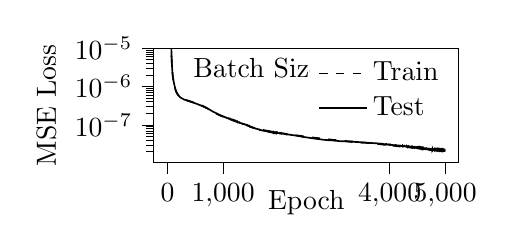
\begin{tikzpicture}

\begin{axis}[
legend cell align={left},
legend style={draw=none},
log basis y={10},
tick align=outside,
tick pos=left,
title={Batch Size 32},
title style={at={(0.4,0.85)},anchor=north},
x grid style={white!69.0196078431373!black},
xlabel={Epoch},
x label style={yshift=13pt},
xmin=-249.95, xmax=5248.95,
xtick style={color=black},
xtick = {0,1000,4000,5000},
y grid style={white!69.0196078431373!black},
ylabel={MSE Loss},
ymin=1.05374705124308e-08, ymax=1e-5,
ymode=log,
ytick style={color=black},
width=.45\textwidth,
height=.25\textwidth
]
\addplot [semithick, black, dashed]
table {%
0 0.0185213608369231
1 0.0100256001874805
2 0.00511598332412541
3 0.00266714832093567
4 0.00179120110906661
5 0.00144799546990544
6 0.00114979036618024
7 0.000814766860101372
8 0.000510174112394452
9 0.000329686338198371
10 0.000244710172759369
11 0.000205625825270545
12 0.00018631382289459
13 0.00017530717747286
14 0.000167745494400151
15 0.000161573188117472
16 0.00015586399770109
17 0.000150204380508512
18 0.000144401938305236
19 0.000138238270650618
20 0.000130775678553618
21 0.000122665890172357
22 0.000114659473838401
23 0.000106363622428034
24 9.76855874760076e-05
25 8.86985533143161e-05
26 7.95836760516977e-05
27 7.0616739205434e-05
28 6.21391900349408e-05
29 5.44985102314968e-05
30 4.79656076204265e-05
31 4.26814938036841e-05
32 3.8612608499534e-05
33 3.55862038995838e-05
34 3.33759931600071e-05
35 3.17640865978319e-05
36 3.05771953862859e-05
37 2.96883334303857e-05
38 2.90059693143121e-05
39 2.84673240530537e-05
40 2.80267686393927e-05
41 2.76490723626921e-05
42 2.73102718856535e-05
43 2.69937950652093e-05
44 2.66956577979727e-05
45 2.64040889669559e-05
46 2.61062633799156e-05
47 2.57937593196402e-05
48 2.54627911053831e-05
49 2.51038547576172e-05
50 2.47119145278702e-05
51 2.42804027948296e-05
52 2.38050044499687e-05
53 2.32816320567508e-05
54 2.27040185272926e-05
55 2.20680549537065e-05
56 2.13706233989797e-05
57 2.06065907259472e-05
58 1.97811869220459e-05
59 1.88985617751314e-05
60 1.79618474503513e-05
61 1.69827113422798e-05
62 1.59747925827105e-05
63 1.49555455536756e-05
64 1.38275694916956e-05
65 1.26876792637631e-05
66 1.12698398916109e-05
67 9.53350929376029e-06
68 8.1114827280544e-06
69 7.06149710822501e-06
70 6.28023362514796e-06
71 5.682561220965e-06
72 5.20727496405016e-06
73 4.81536020743079e-06
74 4.48226160369813e-06
75 4.1903823175744e-06
76 3.92923815888935e-06
77 3.69496772054845e-06
78 3.48329872758768e-06
79 3.2906890992308e-06
80 3.11474296267988e-06
81 2.9551299094237e-06
82 2.80990815917903e-06
83 2.67591957708646e-06
84 2.55399901561759e-06
85 2.44380857793658e-06
86 2.34454597421063e-06
87 2.25512032693587e-06
88 2.17415749739303e-06
89 2.10023164117956e-06
90 2.03179113850638e-06
91 1.96943895070945e-06
92 1.91336066791337e-06
93 1.86234339207658e-06
94 1.8137314445994e-06
95 1.76814178485074e-06
96 1.72594649347957e-06
97 1.68744496795625e-06
98 1.65267439206218e-06
99 1.61943572766177e-06
100 1.58699234452797e-06
101 1.55465797615761e-06
102 1.52490673599459e-06
103 1.49749505953878e-06
104 1.47220658982405e-06
105 1.44839148697429e-06
106 1.42518704569738e-06
107 1.40295422079362e-06
108 1.38139719206265e-06
109 1.3604042615043e-06
110 1.3386478888151e-06
111 1.31467914638961e-06
112 1.29182604973721e-06
113 1.27053595815596e-06
114 1.25014606237528e-06
115 1.23000724124722e-06
116 1.21053629754897e-06
117 1.19191057501666e-06
118 1.17316421210489e-06
119 1.15501116124506e-06
120 1.13750963123493e-06
121 1.11990525147121e-06
122 1.10245057840075e-06
123 1.0850101084543e-06
124 1.06801857259597e-06
125 1.0507991025861e-06
126 1.0334132978187e-06
127 1.01728472532159e-06
128 1.00184256598368e-06
129 9.86175931302569e-07
130 9.71090967141208e-07
131 9.56330864255506e-07
132 9.41725935490467e-07
133 9.27916013552021e-07
134 9.14784782253264e-07
135 9.01841580116525e-07
136 8.89269085291744e-07
137 8.76967326348677e-07
138 8.64968807945843e-07
139 8.53698949640602e-07
140 8.42906854245484e-07
141 8.32554830026311e-07
142 8.22901245783214e-07
143 8.13463982467511e-07
144 8.04595268732555e-07
145 7.962967694084e-07
146 7.88325216944941e-07
147 7.80183357505848e-07
148 7.72475732674138e-07
149 7.65302009767765e-07
150 7.58297480047077e-07
151 7.51497822307101e-07
152 7.45269478329646e-07
153 7.39257797022219e-07
154 7.33223259203442e-07
155 7.27614483025718e-07
156 7.22271873542013e-07
157 7.17282795108076e-07
158 7.12139038910209e-07
159 7.07288850321675e-07
160 7.02631720855607e-07
161 6.97950020594362e-07
162 6.9341542928214e-07
163 6.88575328808838e-07
164 6.84098517467646e-07
165 6.79956147109806e-07
166 6.7576959975213e-07
167 6.71695563141839e-07
168 6.67876880356744e-07
169 6.63949073555159e-07
170 6.60169360230611e-07
171 6.56619765891264e-07
172 6.53260171930015e-07
173 6.4957598908677e-07
174 6.4607227579927e-07
175 6.42691795746941e-07
176 6.39468844383373e-07
177 6.3644487761394e-07
178 6.32937741329442e-07
179 6.29768981639245e-07
180 6.26748726972437e-07
181 6.23714342737003e-07
182 6.20784524357987e-07
183 6.17936972389543e-07
184 6.15162336544017e-07
185 6.1250354792719e-07
186 6.09875560485307e-07
187 6.07228826424944e-07
188 6.04710761308525e-07
189 6.02254500108756e-07
190 5.99862777107774e-07
191 5.97323293845875e-07
192 5.94940298924485e-07
193 5.92553270735152e-07
194 5.90278918821241e-07
195 5.87862195970956e-07
196 5.85565089295415e-07
197 5.83287933409338e-07
198 5.81123970619046e-07
199 5.7901030334051e-07
200 5.76958834130892e-07
201 5.74851887904515e-07
202 5.72869793018072e-07
203 5.70961808080028e-07
204 5.69018330452309e-07
205 5.67025770010332e-07
206 5.6522778049839e-07
207 5.63374698117514e-07
208 5.6155098252475e-07
209 5.59765112939203e-07
210 5.58035291533088e-07
211 5.56295385763406e-07
212 5.54577313891968e-07
213 5.52870644128234e-07
214 5.51226922539172e-07
215 5.4956966505415e-07
216 5.47952494571291e-07
217 5.46373169186154e-07
218 5.44931209105925e-07
219 5.43313873890838e-07
220 5.4181577536383e-07
221 5.4034543313719e-07
222 5.38908848966457e-07
223 5.37434068860421e-07
224 5.36108092092036e-07
225 5.34586550315908e-07
226 5.3321597795275e-07
227 5.31795008100744e-07
228 5.30406377151849e-07
229 5.28978781972e-07
230 5.27560962609641e-07
231 5.26288467426639e-07
232 5.24752812452789e-07
233 5.23475015484109e-07
234 5.2215384982901e-07
235 5.21034239568508e-07
236 5.19823385729978e-07
237 5.18555743155957e-07
238 5.17368580744915e-07
239 5.16210805130868e-07
240 5.15153198762164e-07
241 5.13930031502241e-07
242 5.12899209525131e-07
243 5.11791230678682e-07
244 5.10723405113822e-07
245 5.09490656327216e-07
246 5.08409917983954e-07
247 5.0734909473249e-07
248 5.06350299133373e-07
249 5.05293355104186e-07
250 5.04277433037714e-07
251 5.03256441447775e-07
252 5.02261668316351e-07
253 5.01283572816646e-07
254 5.00328452176291e-07
255 4.99379939583378e-07
256 4.98446030633204e-07
257 4.97528622531718e-07
258 4.96615409474543e-07
259 4.95723476319654e-07
260 4.94844554964402e-07
261 4.94011196337851e-07
262 4.93106419639844e-07
263 4.92229671294808e-07
264 4.91303239073204e-07
265 4.90439448412872e-07
266 4.89604005906585e-07
267 4.88780170257996e-07
268 4.87970775907343e-07
269 4.87166112407067e-07
270 4.86385979115767e-07
271 4.85587184130054e-07
272 4.84800064214141e-07
273 4.84025108221431e-07
274 4.83258642702822e-07
275 4.82502226532233e-07
276 4.81754507745791e-07
277 4.81013788430573e-07
278 4.80280547435541e-07
279 4.79572060612554e-07
280 4.78862895079146e-07
281 4.78152566870449e-07
282 4.77446612990207e-07
283 4.76746079471013e-07
284 4.76050876159206e-07
285 4.75361166536459e-07
286 4.74711966489849e-07
287 4.74005847763692e-07
288 4.73316154398162e-07
289 4.72505169341275e-07
290 4.7175724284898e-07
291 4.70991727524961e-07
292 4.70303329052513e-07
293 4.69632239514795e-07
294 4.68987740418925e-07
295 4.68347638616251e-07
296 4.67706041945348e-07
297 4.67066472197075e-07
298 4.66436172700924e-07
299 4.65819643181931e-07
300 4.6519587988314e-07
301 4.6458026486107e-07
302 4.63975161324015e-07
303 4.63367187876429e-07
304 4.62763844893743e-07
305 4.62163034285368e-07
306 4.61567032516541e-07
307 4.60977072975766e-07
308 4.60386529880452e-07
309 4.59811661130516e-07
310 4.59230181604653e-07
311 4.58641048680875e-07
312 4.58067391150507e-07
313 4.57471872664428e-07
314 4.56890578675484e-07
315 4.56316948998392e-07
316 4.5574583839425e-07
317 4.55179300502095e-07
318 4.54645132208498e-07
319 4.54078644793299e-07
320 4.53513786624171e-07
321 4.52951653983291e-07
322 4.52389646170559e-07
323 4.5183226654899e-07
324 4.51286291763608e-07
325 4.50746562023596e-07
326 4.50201638614089e-07
327 4.49617204708375e-07
328 4.49071586444916e-07
329 4.48541439027395e-07
330 4.48002679945603e-07
331 4.4747507934062e-07
332 4.46942362600566e-07
333 4.46416720819798e-07
334 4.45883008865167e-07
335 4.45353649183744e-07
336 4.44804065296012e-07
337 4.44134348526859e-07
338 4.43515091546942e-07
339 4.42925153379292e-07
340 4.42338806010412e-07
341 4.41806229218855e-07
342 4.41315731677605e-07
343 4.40803275751023e-07
344 4.40289753782963e-07
345 4.39783605429511e-07
346 4.39238003536957e-07
347 4.3873517472548e-07
348 4.38237527305318e-07
349 4.37745029216785e-07
350 4.37252352298856e-07
351 4.36761686955833e-07
352 4.3626986473555e-07
353 4.35827755836726e-07
354 4.35319205962514e-07
355 4.34815810649525e-07
356 4.3431166341179e-07
357 4.33812067626604e-07
358 4.33318690511442e-07
359 4.32825826123917e-07
360 4.32334809602253e-07
361 4.31852442034142e-07
362 4.313736782251e-07
363 4.30905241842083e-07
364 4.30419585995878e-07
365 4.29928817993641e-07
366 4.29442891004328e-07
367 4.28962666433108e-07
368 4.28483186738049e-07
369 4.28003588581305e-07
370 4.27527776309944e-07
371 4.27073076934903e-07
372 4.2659085897867e-07
373 4.26108542342263e-07
374 4.25632207566196e-07
375 4.25156665414761e-07
376 4.24683829919559e-07
377 4.24200477709746e-07
378 4.23732120452769e-07
379 4.23265454855937e-07
380 4.22798863610296e-07
381 4.22334155814497e-07
382 4.21870258719537e-07
383 4.21407641169935e-07
384 4.20946088411256e-07
385 4.20485005747651e-07
386 4.20026333245005e-07
387 4.1956940469845e-07
388 4.19112675444921e-07
389 4.18659692286383e-07
390 4.18207336338128e-07
391 4.17756915339851e-07
392 4.17323406850301e-07
393 4.16873820995534e-07
394 4.16422651255743e-07
395 4.15972308474011e-07
396 4.15522133266677e-07
397 4.15084301380375e-07
398 4.14641929637583e-07
399 4.14197380450787e-07
400 4.13755675594984e-07
401 4.13315258242619e-07
402 4.1287598139661e-07
403 4.12409738942188e-07
404 4.11963612350519e-07
405 4.11529805319333e-07
406 4.11095109598136e-07
407 4.10662509921167e-07
408 4.10231388173088e-07
409 4.09801475484528e-07
410 4.09372446483758e-07
411 4.08946104698771e-07
412 4.0852090558019e-07
413 4.08187630569046e-07
414 4.07759484915005e-07
415 4.07332115287318e-07
416 4.06905044656014e-07
417 4.06474459509809e-07
418 4.06050205583597e-07
419 4.05616316811574e-07
420 4.05190133619726e-07
421 4.04756621492197e-07
422 4.04271327170136e-07
423 4.03848127348283e-07
424 4.03422405724996e-07
425 4.02979115165181e-07
426 4.02551475531254e-07
427 4.02127053689583e-07
428 4.01698157247665e-07
429 4.01263217440828e-07
430 4.00836544145022e-07
431 4.00410393922357e-07
432 3.99995897510053e-07
433 3.99568458533395e-07
434 3.99168272679162e-07
435 3.98736000533972e-07
436 3.98306118427172e-07
437 3.97879050751726e-07
438 3.97453581626905e-07
439 3.97028946395039e-07
440 3.96590492982796e-07
441 3.96160542777579e-07
442 3.95696088276054e-07
443 3.95270011722459e-07
444 3.94841801153234e-07
445 3.94415229038714e-07
446 3.93989487974977e-07
447 3.93564666410384e-07
448 3.93140786513868e-07
449 3.92719500382555e-07
450 3.92298088854659e-07
451 3.91881866335098e-07
452 3.91460772220853e-07
453 3.9104061602302e-07
454 3.90616273648448e-07
455 3.90210867408314e-07
456 3.89778205999392e-07
457 3.89298790651083e-07
458 3.88835131161613e-07
459 3.88384121947638e-07
460 3.87940273867571e-07
461 3.87511125836681e-07
462 3.87079769438969e-07
463 3.86645365551885e-07
464 3.86214937293516e-07
465 3.85783523825012e-07
466 3.8535608462098e-07
467 3.84926936703778e-07
468 3.84500410177679e-07
469 3.84072783049305e-07
470 3.83657095426315e-07
471 3.83230365400777e-07
472 3.82805546109921e-07
473 3.82380842779639e-07
474 3.81945783487936e-07
475 3.81532733172207e-07
476 3.81126588649749e-07
477 3.80694610271348e-07
478 3.80268383310067e-07
479 3.79843750238251e-07
480 3.79418695047207e-07
481 3.78994493303253e-07
482 3.78573906004931e-07
483 3.78133138042358e-07
484 3.77648691141985e-07
485 3.7722791125816e-07
486 3.76804605707548e-07
487 3.763683781699e-07
488 3.75936130012633e-07
489 3.75502033762132e-07
490 3.75070941117883e-07
491 3.7463960597961e-07
492 3.74207424556516e-07
493 3.73759208173396e-07
494 3.73334394566882e-07
495 3.7290415264124e-07
496 3.72472547269354e-07
497 3.72039375974964e-07
498 3.71606638623234e-07
499 3.71173888765952e-07
500 3.70742516679456e-07
501 3.7031062333881e-07
502 3.69883992448194e-07
503 3.6946489217371e-07
504 3.69041602198195e-07
505 3.68620761605598e-07
506 3.68207438896206e-07
507 3.67786844662987e-07
508 3.67350584951964e-07
509 3.66932141787402e-07
510 3.66519052818148e-07
511 3.66103566079801e-07
512 3.65683795621408e-07
513 3.65263786193282e-07
514 3.64843802799442e-07
515 3.6441569204726e-07
516 3.6400681676696e-07
517 3.6358559054861e-07
518 3.63164501322899e-07
519 3.62746938435521e-07
520 3.6232749539522e-07
521 3.61904533406232e-07
522 3.6149247114281e-07
523 3.61073087901786e-07
524 3.60654856308429e-07
525 3.60233938749843e-07
526 3.59805903144661e-07
527 3.59397946226636e-07
528 3.58979113229907e-07
529 3.58570702360339e-07
530 3.58152379476451e-07
531 3.57733576265673e-07
532 3.57283286234633e-07
533 3.56865689241204e-07
534 3.56481844619339e-07
535 3.560531470157e-07
536 3.5562543416745e-07
537 3.55202099513008e-07
538 3.54767151975466e-07
539 3.54350218003674e-07
540 3.53868238562427e-07
541 3.53445645487227e-07
542 3.53023489537918e-07
543 3.52600569215156e-07
544 3.52181922892214e-07
545 3.51785656221182e-07
546 3.51369444388183e-07
547 3.50940250882559e-07
548 3.50511328520042e-07
549 3.50086427886254e-07
550 3.4966140447068e-07
551 3.49248210113728e-07
552 3.48822502417079e-07
553 3.48412709456625e-07
554 3.47991883700161e-07
555 3.47554684822171e-07
556 3.47131746480045e-07
557 3.46698975590698e-07
558 3.46266814119645e-07
559 3.45854583656546e-07
560 3.45416659229159e-07
561 3.44981989314874e-07
562 3.44532436656664e-07
563 3.44083417530783e-07
564 3.43583697201666e-07
565 3.43132300884008e-07
566 3.42692654442089e-07
567 3.42256293151877e-07
568 3.41824444376471e-07
569 3.41390641779071e-07
570 3.40952211388412e-07
571 3.40516456901696e-07
572 3.40081166200434e-07
573 3.3964617955462e-07
574 3.39211207858625e-07
575 3.38775180978246e-07
576 3.38345385387129e-07
577 3.37907625691969e-07
578 3.37475298749723e-07
579 3.37009300665159e-07
580 3.36573081881397e-07
581 3.36206419092377e-07
582 3.35764889769052e-07
583 3.35318149552677e-07
584 3.34874418626896e-07
585 3.34421750153524e-07
586 3.33988169757049e-07
587 3.33541937493465e-07
588 3.33096089946139e-07
589 3.32616425396282e-07
590 3.32171234106227e-07
591 3.31726922240705e-07
592 3.31282373906561e-07
593 3.30856286836934e-07
594 3.30414409745572e-07
595 3.2996329883872e-07
596 3.29514442512391e-07
597 3.2906655366105e-07
598 3.28620184347983e-07
599 3.28172313288633e-07
600 3.27754828333582e-07
601 3.27299891694111e-07
602 3.26791949646577e-07
603 3.26343840242771e-07
604 3.25866860180213e-07
605 3.25405265243717e-07
606 3.24946678460947e-07
607 3.24471016085681e-07
608 3.24006525602272e-07
609 3.2355661079464e-07
610 3.23067498300134e-07
611 3.22547068776657e-07
612 3.22036515171931e-07
613 3.215269095449e-07
614 3.21033148054539e-07
615 3.20562532010626e-07
616 3.20066749623038e-07
617 3.1958168347046e-07
618 3.19108507255805e-07
619 3.18618406140558e-07
620 3.18146146923937e-07
621 3.17659693337191e-07
622 3.17181050263571e-07
623 3.16679004583875e-07
624 3.16186531563289e-07
625 3.15694480377715e-07
626 3.15204478454234e-07
627 3.1471761570856e-07
628 3.14214815205105e-07
629 3.1374244105109e-07
630 3.13252027069666e-07
631 3.12825649984916e-07
632 3.12330473661859e-07
633 3.11826514632685e-07
634 3.11322462607677e-07
635 3.10854835333885e-07
636 3.10345695481828e-07
637 3.09930875232567e-07
638 3.09420084818157e-07
639 3.08922876001816e-07
640 3.08413442326128e-07
641 3.0791088335036e-07
642 3.07412373729221e-07
643 3.06920373247976e-07
644 3.06423529252697e-07
645 3.05929234343694e-07
646 3.05435574148305e-07
647 3.04946460801148e-07
648 3.04456118783492e-07
649 3.03963243084127e-07
650 3.03473363203466e-07
651 3.02987180361924e-07
652 3.02522311471876e-07
653 3.02038389065729e-07
654 3.01502559693745e-07
655 3.00952283851075e-07
656 3.00445974289687e-07
657 2.99952013904203e-07
658 2.99459923269296e-07
659 2.9896857085987e-07
660 2.98477365674898e-07
661 2.97985838358272e-07
662 2.97495124812031e-07
663 2.9700242060926e-07
664 2.9651086396143e-07
665 2.9601517366018e-07
666 2.95518898781211e-07
667 2.95013197558092e-07
668 2.94539917092607e-07
669 2.94100331927893e-07
670 2.93593171647899e-07
671 2.93133579702953e-07
672 2.92588175113906e-07
673 2.92073646960489e-07
674 2.91576083611744e-07
675 2.91068527246807e-07
676 2.90541520257648e-07
677 2.90048884949101e-07
678 2.89539593723021e-07
679 2.89038977484779e-07
680 2.88519004925547e-07
681 2.87999056524768e-07
682 2.87411364070067e-07
683 2.86895903968798e-07
684 2.86383701848081e-07
685 2.85874086500826e-07
686 2.85370644462546e-07
687 2.84865456762873e-07
688 2.84372104204067e-07
689 2.83867105338231e-07
690 2.83315091905934e-07
691 2.82804742880671e-07
692 2.82301618312886e-07
693 2.81788576046438e-07
694 2.8127672823075e-07
695 2.80772214523495e-07
696 2.8024275570715e-07
697 2.79723454298164e-07
698 2.79204135210875e-07
699 2.78686133867723e-07
700 2.7816904946576e-07
701 2.77635648217256e-07
702 2.77106846112929e-07
703 2.76564707121452e-07
704 2.76043478322663e-07
705 2.7552292931432e-07
706 2.74989282956994e-07
707 2.74451538984977e-07
708 2.73919823143842e-07
709 2.73383016121898e-07
710 2.7285828133472e-07
711 2.72334689384479e-07
712 2.71813517997543e-07
713 2.71297532890458e-07
714 2.70724480685658e-07
715 2.702090679918e-07
716 2.69609163979112e-07
717 2.69066292332809e-07
718 2.68534173642365e-07
719 2.6803095380501e-07
720 2.6750520493124e-07
721 2.66954143228304e-07
722 2.66426574967227e-07
723 2.65932182173856e-07
724 2.65378602591682e-07
725 2.64837616555269e-07
726 2.64279638940934e-07
727 2.63742836125402e-07
728 2.63196838830027e-07
729 2.62663483056258e-07
730 2.62165100934908e-07
731 2.6164052741251e-07
732 2.6108835766081e-07
733 2.60547652430887e-07
734 2.5985914373905e-07
735 2.59363373231736e-07
736 2.58823922308693e-07
737 2.5826781603655e-07
738 2.57730944269952e-07
739 2.57195841413704e-07
740 2.5667771035387e-07
741 2.56121474137672e-07
742 2.55567423778302e-07
743 2.54995225645871e-07
744 2.54450984641608e-07
745 2.53922574643184e-07
746 2.53376336218025e-07
747 2.52830342560628e-07
748 2.52296219173331e-07
749 2.51764227641615e-07
750 2.51235566565811e-07
751 2.50710121235898e-07
752 2.50186598123037e-07
753 2.49664393493276e-07
754 2.4915178619267e-07
755 2.48576101739673e-07
756 2.48021704862822e-07
757 2.47490895560531e-07
758 2.4698219971242e-07
759 2.46460666971871e-07
760 2.45941125115223e-07
761 2.45425631248963e-07
762 2.44873848430416e-07
763 2.44391138096489e-07
764 2.43867456845237e-07
765 2.433545328131e-07
766 2.42844925708141e-07
767 2.42337454267272e-07
768 2.41832610015535e-07
769 2.41330177800592e-07
770 2.40827523271037e-07
771 2.40326087464382e-07
772 2.39832782597205e-07
773 2.39340287123468e-07
774 2.38822613766843e-07
775 2.38318634671941e-07
776 2.37761325024621e-07
777 2.37361407641856e-07
778 2.36908274132475e-07
779 2.36416801953965e-07
780 2.35894517459201e-07
781 2.35417795465764e-07
782 2.34940998097954e-07
783 2.34431632520682e-07
784 2.33937869950296e-07
785 2.33457018566696e-07
786 2.32956179672783e-07
787 2.32458378945921e-07
788 2.31979477348432e-07
789 2.31492987097681e-07
790 2.31008329649285e-07
791 2.30512317102693e-07
792 2.30025402402134e-07
793 2.29548284664816e-07
794 2.29058705428997e-07
795 2.28590926042216e-07
796 2.28118926315801e-07
797 2.27657759864996e-07
798 2.27187208565738e-07
799 2.26727645724623e-07
800 2.26269467816564e-07
801 2.25824073538661e-07
802 2.25381281381942e-07
803 2.24889024195818e-07
804 2.24432982975031e-07
805 2.23897555315489e-07
806 2.23425031151692e-07
807 2.2295173977227e-07
808 2.22504936573387e-07
809 2.22031358589447e-07
810 2.21586511543137e-07
811 2.21129962255873e-07
812 2.20660490867886e-07
813 2.20224475640407e-07
814 2.19789697155193e-07
815 2.19333101028951e-07
816 2.18906489408255e-07
817 2.18447235852182e-07
818 2.1802253485248e-07
819 2.17587594136148e-07
820 2.171213056954e-07
821 2.16699075224369e-07
822 2.16260562240222e-07
823 2.15830427805486e-07
824 2.15395490897663e-07
825 2.14986567698361e-07
826 2.14559953121807e-07
827 2.14100065988987e-07
828 2.13742608934808e-07
829 2.13357985956009e-07
830 2.12944119368785e-07
831 2.12532104740149e-07
832 2.12122578318485e-07
833 2.11714633735482e-07
834 2.11308834479951e-07
835 2.10849997927198e-07
836 2.10445568654904e-07
837 2.10049146232905e-07
838 2.09655660114549e-07
839 2.09260511041975e-07
840 2.08855573191613e-07
841 2.08466095273252e-07
842 2.08078252569521e-07
843 2.07700746102546e-07
844 2.07313690111732e-07
845 2.06920507594077e-07
846 2.06544750881221e-07
847 2.06162186827896e-07
848 2.05777530311479e-07
849 2.05416958294791e-07
850 2.05037628063565e-07
851 2.04666853164781e-07
852 2.04303049542887e-07
853 2.03929313386197e-07
854 2.03553203959927e-07
855 2.03187631257151e-07
856 2.02841443922352e-07
857 2.02474036314015e-07
858 2.02113415184613e-07
859 2.01754178931424e-07
860 2.01373242305181e-07
861 2.01010403770852e-07
862 2.00656504603103e-07
863 2.00288501162049e-07
864 1.9992708035943e-07
865 1.99573282657184e-07
866 1.99245734393116e-07
867 1.98867363678801e-07
868 1.98505497905899e-07
869 1.98158252942449e-07
870 1.97831863943065e-07
871 1.97476405389807e-07
872 1.97114097829854e-07
873 1.96777017492877e-07
874 1.96421795067181e-07
875 1.96073604513458e-07
876 1.95731925714426e-07
877 1.95410672688467e-07
878 1.9507339879965e-07
879 1.94744070427078e-07
880 1.94403248713115e-07
881 1.9405795410421e-07
882 1.93761960872507e-07
883 1.93391343259464e-07
884 1.93013741949244e-07
885 1.92732023151621e-07
886 1.92379488197503e-07
887 1.92062848697105e-07
888 1.91666795728906e-07
889 1.91327077430969e-07
890 1.90992436387205e-07
891 1.90675125026019e-07
892 1.90355343164583e-07
893 1.90039261468655e-07
894 1.89738615972601e-07
895 1.89489817643107e-07
896 1.89161859964315e-07
897 1.88857485596827e-07
898 1.88550196980941e-07
899 1.88281318457939e-07
900 1.87998503605513e-07
901 1.87705945393191e-07
902 1.87365529825456e-07
903 1.87090701018633e-07
904 1.8682072081333e-07
905 1.86533131596889e-07
906 1.8617735247517e-07
907 1.85849786277004e-07
908 1.85555433830586e-07
909 1.85290518203374e-07
910 1.85007594780018e-07
911 1.84740976209241e-07
912 1.84413795096816e-07
913 1.84188078776515e-07
914 1.83867984986819e-07
915 1.83598712567345e-07
916 1.83321817303295e-07
917 1.83044159058454e-07
918 1.82777629504471e-07
919 1.82503174556814e-07
920 1.82209366499819e-07
921 1.82021597879611e-07
922 1.81733254407845e-07
923 1.81411800667775e-07
924 1.8115524892437e-07
925 1.80859339337758e-07
926 1.80594035271042e-07
927 1.8029719359447e-07
928 1.80034858402678e-07
929 1.79789717037693e-07
930 1.79509198858341e-07
931 1.79225189015142e-07
932 1.78970508443399e-07
933 1.7871346764764e-07
934 1.78445978065156e-07
935 1.78181604468364e-07
936 1.77948226280478e-07
937 1.77688481159066e-07
938 1.77433303264252e-07
939 1.77141203664632e-07
940 1.76903954496765e-07
941 1.76639763878939e-07
942 1.76401640089807e-07
943 1.76149772926237e-07
944 1.75987998716209e-07
945 1.75748525435893e-07
946 1.75482385913028e-07
947 1.75235935529372e-07
948 1.74978851646301e-07
949 1.7472245940553e-07
950 1.74479472093481e-07
951 1.74206433655399e-07
952 1.73980947380414e-07
953 1.7370674370909e-07
954 1.73465508026993e-07
955 1.73237816028404e-07
956 1.72998334960539e-07
957 1.72744316898843e-07
958 1.72513198037905e-07
959 1.72277799947551e-07
960 1.72013212107913e-07
961 1.71797714727973e-07
962 1.71535733926476e-07
963 1.71309136078435e-07
964 1.71067951129089e-07
965 1.70814558458687e-07
966 1.7058751026866e-07
967 1.70329375663414e-07
968 1.70064358030686e-07
969 1.69841669986681e-07
970 1.69645710855093e-07
971 1.69402572822719e-07
972 1.69113098081652e-07
973 1.68882366153866e-07
974 1.68665797360745e-07
975 1.6844378566816e-07
976 1.68193679371598e-07
977 1.679658043372e-07
978 1.67721343188987e-07
979 1.67482980003797e-07
980 1.67276143656636e-07
981 1.67045190551107e-07
982 1.66820757868891e-07
983 1.66584006336734e-07
984 1.66362110149976e-07
985 1.6610529868899e-07
986 1.65910131357805e-07
987 1.65689847761996e-07
988 1.65440177568144e-07
989 1.65233987956981e-07
990 1.65027243696159e-07
991 1.64787183962289e-07
992 1.64550278469733e-07
993 1.64329672372787e-07
994 1.641152552736e-07
995 1.63866262198553e-07
996 1.63681186563736e-07
997 1.63456090092495e-07
998 1.63221955062909e-07
999 1.63006642424079e-07
1000 1.62814612366446e-07
1001 1.62547091662191e-07
1002 1.6236365999589e-07
1003 1.62137027615472e-07
1004 1.61914140363706e-07
1005 1.61691737190495e-07
1006 1.61510571047074e-07
1007 1.61248653995472e-07
1008 1.6104978601561e-07
1009 1.60817439819994e-07
1010 1.60609903360864e-07
1011 1.60398300806719e-07
1012 1.60187364826925e-07
1013 1.59997554277425e-07
1014 1.59782047916224e-07
1015 1.59536282126282e-07
1016 1.59365163369785e-07
1017 1.59153467194528e-07
1018 1.5890577961386e-07
1019 1.58727719423268e-07
1020 1.58539938752256e-07
1021 1.58312121328663e-07
1022 1.58082366368717e-07
1023 1.5789587882864e-07
1024 1.57671714788421e-07
1025 1.57459437872376e-07
1026 1.57293676068093e-07
1027 1.57060246635865e-07
1028 1.56861209717363e-07
1029 1.56664727143152e-07
1030 1.56458571524354e-07
1031 1.56244335585143e-07
1032 1.56054935729344e-07
1033 1.55841487725183e-07
1034 1.55671341644847e-07
1035 1.55414295591072e-07
1036 1.55219929496297e-07
1037 1.5502700952652e-07
1038 1.54778249651599e-07
1039 1.54609648319592e-07
1040 1.54416214684261e-07
1041 1.54183319125423e-07
1042 1.54000696682033e-07
1043 1.5378528854626e-07
1044 1.53589135948096e-07
1045 1.5335699526986e-07
1046 1.53167287663791e-07
1047 1.52971405356084e-07
1048 1.52732748915696e-07
1049 1.52534419157746e-07
1050 1.52338159836063e-07
1051 1.52186203195015e-07
1052 1.51968354543897e-07
1053 1.51778432524452e-07
1054 1.51582191392663e-07
1055 1.51362850829173e-07
1056 1.51173687186201e-07
1057 1.51031862088757e-07
1058 1.50862339921787e-07
1059 1.50641980155797e-07
1060 1.50485465383099e-07
1061 1.50308139154731e-07
1062 1.50094176035509e-07
1063 1.49907080469802e-07
1064 1.49740256318864e-07
1065 1.49536210102497e-07
1066 1.49349157055667e-07
1067 1.49136879514344e-07
1068 1.48908395800618e-07
1069 1.48712377381344e-07
1070 1.48493782148762e-07
1071 1.4830978798841e-07
1072 1.48146137405547e-07
1073 1.47950765637006e-07
1074 1.47774900824515e-07
1075 1.47583466315382e-07
1076 1.4737144300625e-07
1077 1.47156897128298e-07
1078 1.46975856750942e-07
1079 1.4680339833717e-07
1080 1.46632637409994e-07
1081 1.46427892815382e-07
1082 1.46234485896457e-07
1083 1.46021229681992e-07
1084 1.45853940580309e-07
1085 1.45659838665324e-07
1086 1.45499808667182e-07
1087 1.45302000902348e-07
1088 1.45118163345614e-07
1089 1.44915564533221e-07
1090 1.44756839233651e-07
1091 1.44625436035994e-07
1092 1.44455908525742e-07
1093 1.4425951536623e-07
1094 1.44062650861088e-07
1095 1.43971858193481e-07
1096 1.43767995723465e-07
1097 1.43548971578866e-07
1098 1.4336696054329e-07
1099 1.43227281000691e-07
1100 1.42972960190946e-07
1101 1.42832374251611e-07
1102 1.42647749527214e-07
1103 1.42420790638198e-07
1104 1.42293767822821e-07
1105 1.42080506805087e-07
1106 1.41926133068182e-07
1107 1.41727618796494e-07
1108 1.41548562424987e-07
1109 1.4137656182811e-07
1110 1.41162390974614e-07
1111 1.41009764803357e-07
1112 1.40850409763971e-07
1113 1.40619346012727e-07
1114 1.40469351919137e-07
1115 1.40236711899888e-07
1116 1.40055121704563e-07
1117 1.39835729783044e-07
1118 1.39705407320889e-07
1119 1.39515229420795e-07
1120 1.39346126985629e-07
1121 1.3915980667889e-07
1122 1.3894486130539e-07
1123 1.38818959328546e-07
1124 1.38635964475498e-07
1125 1.38440284246144e-07
1126 1.38380431536689e-07
1127 1.38207009939606e-07
1128 1.3803130016754e-07
1129 1.37817676886698e-07
1130 1.37681640268283e-07
1131 1.3742020453833e-07
1132 1.37303870701544e-07
1133 1.37097208693149e-07
1134 1.3695340081199e-07
1135 1.36768997549552e-07
1136 1.36616483757734e-07
1137 1.36413310798389e-07
1138 1.36295977767986e-07
1139 1.36083534300724e-07
1140 1.35963834509312e-07
1141 1.357222713807e-07
1142 1.35606256634446e-07
1143 1.35436983526915e-07
1144 1.35217161329138e-07
1145 1.35080818665756e-07
1146 1.34906291776815e-07
1147 1.34764612568006e-07
1148 1.34538124029859e-07
1149 1.34437458484626e-07
1150 1.34265883701801e-07
1151 1.3410143142778e-07
1152 1.33920875498461e-07
1153 1.33777525007872e-07
1154 1.33588935767648e-07
1155 1.33419826369163e-07
1156 1.33264174451142e-07
1157 1.3310219384266e-07
1158 1.32939824624145e-07
1159 1.32826000481145e-07
1160 1.32648920214251e-07
1161 1.32496974060814e-07
1162 1.32340923499896e-07
1163 1.32131768481258e-07
1164 1.31964101143467e-07
1165 1.31850519750287e-07
1166 1.31695612139993e-07
1167 1.31505942960075e-07
1168 1.31346545458655e-07
1169 1.31156192026083e-07
1170 1.31067693899922e-07
1171 1.30887381260436e-07
1172 1.30729647679573e-07
1173 1.30576428858831e-07
1174 1.30391574771238e-07
1175 1.30241802793307e-07
1176 1.30092601807519e-07
1177 1.29940641812709e-07
1178 1.2978442197209e-07
1179 1.29702830406586e-07
1180 1.29564918552205e-07
1181 1.29329984446258e-07
1182 1.29192453158566e-07
1183 1.29019271810193e-07
1184 1.2888260789623e-07
1185 1.28742152895711e-07
1186 1.2855812948942e-07
1187 1.28389245219296e-07
1188 1.28260248743572e-07
1189 1.28133878774861e-07
1190 1.27946985173821e-07
1191 1.27757678200169e-07
1192 1.27662547413365e-07
1193 1.27471893478059e-07
1194 1.273243918547e-07
1195 1.27171785749169e-07
1196 1.27086931712483e-07
1197 1.26907419939926e-07
1198 1.26737666363397e-07
1199 1.26660317988581e-07
1200 1.26535082586088e-07
1201 1.26340583960882e-07
1202 1.2621424323811e-07
1203 1.2601926437128e-07
1204 1.25920169324445e-07
1205 1.25740624866921e-07
1206 1.2557388711798e-07
1207 1.25481804900573e-07
1208 1.25368563232087e-07
1209 1.25208813869904e-07
1210 1.25018988057946e-07
1211 1.24933488478973e-07
1212 1.24746758558558e-07
1213 1.24599515942236e-07
1214 1.24469573506758e-07
1215 1.24318066127671e-07
1216 1.24179299945126e-07
1217 1.24018012570559e-07
1218 1.23949695364445e-07
1219 1.23787564859867e-07
1220 1.23621690903519e-07
1221 1.23461992103557e-07
1222 1.23359578964255e-07
1223 1.23199914270344e-07
1224 1.23059030244121e-07
1225 1.22928636955066e-07
1226 1.22774252503177e-07
1227 1.22605700397571e-07
1228 1.2247761691242e-07
1229 1.22310282620219e-07
1230 1.22203671708121e-07
1231 1.22031712521675e-07
1232 1.21910517151491e-07
1233 1.21736889269641e-07
1234 1.21613467399584e-07
1235 1.214787870083e-07
1236 1.21305380901049e-07
1237 1.21206207609248e-07
1238 1.21023092845007e-07
1239 1.20945347987345e-07
1240 1.20883079858913e-07
1241 1.20674643767416e-07
1242 1.20576853333887e-07
1243 1.20447198781903e-07
1244 1.20319473182917e-07
1245 1.20158708739382e-07
1246 1.20045059986751e-07
1247 1.19856119056294e-07
1248 1.19752005417695e-07
1249 1.19630266766535e-07
1250 1.19465553751752e-07
1251 1.19370260136975e-07
1252 1.19239946116068e-07
1253 1.19060969154816e-07
1254 1.18954238587321e-07
1255 1.18861689969663e-07
1256 1.18681055795378e-07
1257 1.1854536361966e-07
1258 1.18406778511826e-07
1259 1.18261358295513e-07
1260 1.1812020741786e-07
1261 1.17996310450508e-07
1262 1.17843934617667e-07
1263 1.17783204274247e-07
1264 1.17580303879095e-07
1265 1.17537257636968e-07
1266 1.1735062625462e-07
1267 1.17211613513746e-07
1268 1.17074364794689e-07
1269 1.16957124220107e-07
1270 1.16827153647137e-07
1271 1.1669826719185e-07
1272 1.16565958165893e-07
1273 1.16455746024258e-07
1274 1.16320386638336e-07
1275 1.16225041551843e-07
1276 1.16092117281141e-07
1277 1.15950706572221e-07
1278 1.15833334689341e-07
1279 1.15700019279075e-07
1280 1.15587255180571e-07
1281 1.15437792004514e-07
1282 1.15330216146958e-07
1283 1.15189609118715e-07
1284 1.15066688010756e-07
1285 1.14926542011062e-07
1286 1.14846013190117e-07
1287 1.14713855282389e-07
1288 1.14599199065424e-07
1289 1.14470935528743e-07
1290 1.14359950686094e-07
1291 1.14234656109602e-07
1292 1.14117928518453e-07
1293 1.1398997003198e-07
1294 1.13820058118108e-07
1295 1.13818541620958e-07
1296 1.13339524574485e-07
1297 1.12663470900998e-07
1298 1.12361569904351e-07
1299 1.12089587332775e-07
1300 1.11964709418544e-07
1301 1.11820746525382e-07
1302 1.11636760721012e-07
1303 1.11483826003678e-07
1304 1.11383499302065e-07
1305 1.11267894283174e-07
1306 1.11115151270269e-07
1307 1.11017267045099e-07
1308 1.10896492941492e-07
1309 1.10744365827031e-07
1310 1.10644878901667e-07
1311 1.10550607274718e-07
1312 1.10358803596e-07
1313 1.10191754401967e-07
1314 1.10072820973528e-07
1315 1.09909369911065e-07
1316 1.09817545961732e-07
1317 1.09704210359496e-07
1318 1.0948728268545e-07
1319 1.09406620794061e-07
1320 1.09284726192982e-07
1321 1.09091099972147e-07
1322 1.09042478015908e-07
1323 1.08925033288187e-07
1324 1.08841563360329e-07
1325 1.08699135381585e-07
1326 1.08578928035286e-07
1327 1.08461759822376e-07
1328 1.08338431630273e-07
1329 1.08334709835844e-07
1330 1.08194711401666e-07
1331 1.08026963999919e-07
1332 1.07970406304503e-07
1333 1.07841701264988e-07
1334 1.07688680998308e-07
1335 1.07582052095267e-07
1336 1.07469422914619e-07
1337 1.07296660473821e-07
1338 1.07229844473977e-07
1339 1.07034789039062e-07
1340 1.06912480532628e-07
1341 1.06783147487022e-07
1342 1.066593461303e-07
1343 1.06509381225806e-07
1344 1.06420976919708e-07
1345 1.06206791770092e-07
1346 1.0609659514671e-07
1347 1.05980542883799e-07
1348 1.05862056386741e-07
1349 1.05813596292137e-07
1350 1.05752091627664e-07
1351 1.05628402849334e-07
1352 1.05501596806334e-07
1353 1.05356113238031e-07
1354 1.05215304216699e-07
1355 1.05107244252167e-07
1356 1.04985850612138e-07
1357 1.04835606094866e-07
1358 1.04752508718775e-07
1359 1.046250343677e-07
1360 1.04495485800271e-07
1361 1.04372938295683e-07
1362 1.04263034870655e-07
1363 1.04146862298649e-07
1364 1.04034263813446e-07
1365 1.03983576508426e-07
1366 1.0383213731302e-07
1367 1.03719245117873e-07
1368 1.03590368638606e-07
1369 1.03480423746305e-07
1370 1.03351360991155e-07
1371 1.03220049027186e-07
1372 1.0311302881405e-07
1373 1.02996904814745e-07
1374 1.02872726614578e-07
1375 1.02754415451045e-07
1376 1.02634036494464e-07
1377 1.02518056451117e-07
1378 1.02415923862509e-07
1379 1.02323679698202e-07
1380 1.02211516264106e-07
1381 1.02091620306055e-07
1382 1.01971102623111e-07
1383 1.01870679060312e-07
1384 1.0179658139009e-07
1385 1.01681100517226e-07
1386 1.01586428115752e-07
1387 1.01476204747541e-07
1388 1.01367837061161e-07
1389 1.01290550361455e-07
1390 1.01194307617902e-07
1391 1.01084147658526e-07
1392 1.00980223763258e-07
1393 1.0086355020178e-07
1394 1.00736980030547e-07
1395 1.00650129539304e-07
1396 1.00546723885486e-07
1397 1.00419138519214e-07
1398 1.00316875574435e-07
1399 1.0026016775555e-07
1400 1.00106740532624e-07
1401 9.9985386981416e-08
1402 9.98807984728955e-08
1403 9.97536856601755e-08
1404 9.9668220926219e-08
1405 9.95527654055195e-08
1406 9.94410838615067e-08
1407 9.93242042284237e-08
1408 9.9216212021247e-08
1409 9.91328911368328e-08
1410 9.90092147503674e-08
1411 9.89142205725102e-08
1412 9.87894828625713e-08
1413 9.87242921013376e-08
1414 9.86143573555864e-08
1415 9.84818851037517e-08
1416 9.83712935749281e-08
1417 9.82762960575201e-08
1418 9.81511430211412e-08
1419 9.80457570420867e-08
1420 9.78985418953471e-08
1421 9.7802210106579e-08
1422 9.75800401334936e-08
1423 9.73497928384859e-08
1424 9.72207337639475e-08
1425 9.71265016147527e-08
1426 9.70150914696433e-08
1427 9.68607581484093e-08
1428 9.68013227975462e-08
1429 9.67239543996357e-08
1430 9.66186112520973e-08
1431 9.65188904160641e-08
1432 9.6407868468873e-08
1433 9.62835954538832e-08
1434 9.61846360496566e-08
1435 9.60902012820952e-08
1436 9.59982494208589e-08
1437 9.59091606773654e-08
1438 9.57719880290142e-08
1439 9.56798667033354e-08
1440 9.55663077206736e-08
1441 9.54916833819652e-08
1442 9.53860347010505e-08
1443 9.52897061807789e-08
1444 9.51862622713406e-08
1445 9.50990866783741e-08
1446 9.49752749761501e-08
1447 9.48816515773387e-08
1448 9.47771617632043e-08
1449 9.4695990242144e-08
1450 9.46143253059972e-08
1451 9.45202227882191e-08
1452 9.44320654383546e-08
1453 9.43229522505362e-08
1454 9.42529038212569e-08
1455 9.41463178492086e-08
1456 9.4068416373716e-08
1457 9.39887819413343e-08
1458 9.38982673375222e-08
1459 9.37753829362009e-08
1460 9.37255089894506e-08
1461 9.36219205698308e-08
1462 9.35364635097358e-08
1463 9.34252245201606e-08
1464 9.33777980662853e-08
1465 9.32803416020533e-08
1466 9.31650765920722e-08
1467 9.30805050671779e-08
1468 9.29610439328599e-08
1469 9.287470193442e-08
1470 9.27757243687211e-08
1471 9.26921939878866e-08
1472 9.2576508720299e-08
1473 9.24887030322452e-08
1474 9.23843173552541e-08
1475 9.22476585287768e-08
1476 9.21249195897644e-08
1477 9.19396049852139e-08
1478 9.16524064678015e-08
1479 9.12750976311827e-08
1480 9.06833057285894e-08
1481 9.02523407830813e-08
1482 8.98370776809543e-08
1483 8.959618487836e-08
1484 8.94454999809113e-08
1485 8.92552902627131e-08
1486 8.91261259141629e-08
1487 8.89889859507775e-08
1488 8.88643282337398e-08
1489 8.87856272271392e-08
1490 8.86530855837009e-08
1491 8.85686529272789e-08
1492 8.84279600654736e-08
1493 8.83821760027104e-08
1494 8.82774851334034e-08
1495 8.8184456544127e-08
1496 8.80874322035652e-08
1497 8.79965566582541e-08
1498 8.79217438125579e-08
1499 8.78179770751331e-08
1500 8.77400387508942e-08
1501 8.76169939800775e-08
1502 8.75252724483744e-08
1503 8.74732476034978e-08
1504 8.73397060559e-08
1505 8.73137317967121e-08
1506 8.7211646601304e-08
1507 8.71337833956431e-08
1508 8.705234297679e-08
1509 8.69138714136852e-08
1510 8.68927885022686e-08
1511 8.67575567440326e-08
1512 8.6724243189451e-08
1513 8.66463673645512e-08
1514 8.65392750739602e-08
1515 8.64611098165824e-08
1516 8.63612686288207e-08
1517 8.63293309549817e-08
1518 8.62158176317962e-08
1519 8.61772485336587e-08
1520 8.60930073400823e-08
1521 8.60225565162409e-08
1522 8.59654042244529e-08
1523 8.5892122129394e-08
1524 8.58183232708143e-08
1525 8.57418458650727e-08
1526 8.56366906134554e-08
1527 8.55414217824091e-08
1528 8.54949409614392e-08
1529 8.54261305249793e-08
1530 8.53500751389902e-08
1531 8.52584533674872e-08
1532 8.51586839871743e-08
1533 8.51175963134665e-08
1534 8.50235133498245e-08
1535 8.49865759988688e-08
1536 8.48735124066025e-08
1537 8.48198776992604e-08
1538 8.47225467737189e-08
1539 8.46476027902554e-08
1540 8.45698268108208e-08
1541 8.44968632662813e-08
1542 8.44229106746752e-08
1543 8.43584369363271e-08
1544 8.43106598580334e-08
1545 8.42087358563504e-08
1546 8.41415686068103e-08
1547 8.40622797397828e-08
1548 8.39969525969764e-08
1549 8.39222875583801e-08
1550 8.38631996913364e-08
1551 8.37817928101003e-08
1552 8.37054291906725e-08
1553 8.36330925011453e-08
1554 8.35762737807499e-08
1555 8.35003280030833e-08
1556 8.34323542164839e-08
1557 8.33614796817983e-08
1558 8.32791213554174e-08
1559 8.32229494420744e-08
1560 8.31509793499663e-08
1561 8.30974982761745e-08
1562 8.30279069106155e-08
1563 8.29462467066833e-08
1564 8.28767359735139e-08
1565 8.28320653170067e-08
1566 8.27367432520987e-08
1567 8.26758389678162e-08
1568 8.26105227105245e-08
1569 8.25380142117638e-08
1570 8.24846440394822e-08
1571 8.24061097119966e-08
1572 8.23438409867094e-08
1573 8.22637429394035e-08
1574 8.22266813429451e-08
1575 8.2150413405202e-08
1576 8.20791995579384e-08
1577 8.20127622063183e-08
1578 8.19548766486378e-08
1579 8.18789175127677e-08
1580 8.18459514420056e-08
1581 8.17594470277072e-08
1582 8.16947884061392e-08
1583 8.16395185267993e-08
1584 8.15806382092887e-08
1585 8.14948606802091e-08
1586 8.14358932217374e-08
1587 8.13648371007503e-08
1588 8.13039597034049e-08
1589 8.12378415417925e-08
1590 8.11729484695434e-08
1591 8.11095378452364e-08
1592 8.10414111072078e-08
1593 8.09895950482087e-08
1594 8.09623106761137e-08
1595 8.09027162063103e-08
1596 8.08412271027237e-08
1597 8.07740352968267e-08
1598 8.0709158424952e-08
1599 8.06479694119844e-08
1600 8.05820829583581e-08
1601 8.05096885159173e-08
1602 8.04581248843306e-08
1603 8.0393222276598e-08
1604 8.03214767728377e-08
1605 8.02655540468322e-08
1606 8.02068767313813e-08
1607 8.01321103836017e-08
1608 8.00844711363879e-08
1609 8.00213825726814e-08
1610 7.99599952472363e-08
1611 7.98976112292849e-08
1612 7.9834806555823e-08
1613 7.97754659345173e-08
1614 7.97135347028188e-08
1615 7.96568865126801e-08
1616 7.95917305822513e-08
1617 7.95318744053475e-08
1618 7.94548566460662e-08
1619 7.94151298464385e-08
1620 7.93352987784601e-08
1621 7.92899142680881e-08
1622 7.92236218103426e-08
1623 7.91863368334589e-08
1624 7.91302377791681e-08
1625 7.90388985478785e-08
1626 7.90103603804937e-08
1627 7.89311625197797e-08
1628 7.88984124397985e-08
1629 7.88078053091112e-08
1630 7.87757863065508e-08
1631 7.86895295732393e-08
1632 7.86431169075286e-08
1633 7.85704401096154e-08
1634 7.8529926369697e-08
1635 7.84526377231032e-08
1636 7.84164920872854e-08
1637 7.83758315776595e-08
1638 7.82719817067346e-08
1639 7.82363932074759e-08
1640 7.81609860780463e-08
1641 7.81229463626687e-08
1642 7.80462926712744e-08
1643 7.80029670579552e-08
1644 7.79492562514861e-08
1645 7.7874848827264e-08
1646 7.78748980962973e-08
1647 7.78464856381333e-08
1648 7.77667935381032e-08
1649 7.7674670393435e-08
1650 7.76239029249837e-08
1651 7.75937119357195e-08
1652 7.74994474710411e-08
1653 7.74321212873019e-08
1654 7.74145367472556e-08
1655 7.73238617028937e-08
1656 7.7310983030543e-08
1657 7.73176963946298e-08
1658 7.7305709197617e-08
1659 7.72266385524745e-08
1660 7.71846794407338e-08
1661 7.71044600185178e-08
1662 7.70360870632203e-08
1663 7.6990116184561e-08
1664 7.68984523915606e-08
1665 7.68559426518323e-08
1666 7.67996079531485e-08
1667 7.67342406646776e-08
1668 7.67052079027053e-08
1669 7.66515564833981e-08
1670 7.65959734536636e-08
1671 7.65839691467818e-08
1672 7.65009739609468e-08
1673 7.63829222734103e-08
1674 7.63229548823574e-08
1675 7.6267942404229e-08
1676 7.61775889372984e-08
1677 7.61232539332468e-08
1678 7.60569423050583e-08
1679 7.60101576702255e-08
1680 7.59661880636031e-08
1681 7.58766135788846e-08
1682 7.58261601134791e-08
1683 7.57681564920176e-08
1684 7.57341910855303e-08
1685 7.56938010937347e-08
1686 7.55829074847725e-08
1687 7.55643320360377e-08
1688 7.54766571446908e-08
1689 7.54520423669192e-08
1690 7.53472286874057e-08
1691 7.53446218482168e-08
1692 7.52449624599194e-08
1693 7.5231898293282e-08
1694 7.51617080965161e-08
1695 7.5136856168001e-08
1696 7.50744397777225e-08
1697 7.49899303684742e-08
1698 7.49304649900751e-08
1699 7.48902372862403e-08
1700 7.47820001407717e-08
1701 7.47753556851194e-08
1702 7.46935666313675e-08
1703 7.46611515154427e-08
1704 7.45570163900311e-08
1705 7.45577602998537e-08
1706 7.4471433549661e-08
1707 7.44485144821283e-08
1708 7.43752279674936e-08
1709 7.43456927949637e-08
1710 7.42526671899668e-08
1711 7.42398117239418e-08
1712 7.41700458632977e-08
1713 7.41169396292207e-08
1714 7.40263327116963e-08
1715 7.39864196930284e-08
1716 7.39412575399001e-08
1717 7.38989007089685e-08
1718 7.38174102252742e-08
1719 7.37935158383607e-08
1720 7.37559998640336e-08
1721 7.36524492737089e-08
1722 7.36184399414697e-08
1723 7.35392518009803e-08
1724 7.35269673270977e-08
1725 7.34544109519675e-08
1726 7.34032248317362e-08
1727 7.33428511523471e-08
1728 7.32681853321537e-08
1729 7.32143738702007e-08
1730 7.31719510724815e-08
1731 7.31501556998637e-08
1732 7.30892445091058e-08
1733 7.30219066298332e-08
1734 7.2979406468221e-08
1735 7.29247632023089e-08
1736 7.28633535658219e-08
1737 7.28210725498002e-08
1738 7.27666082553924e-08
1739 7.27055496980711e-08
1740 7.26660435219628e-08
1741 7.26065471923221e-08
1742 7.25587729561994e-08
1743 7.25217219610386e-08
1744 7.24717678650677e-08
1745 7.24192664733891e-08
1746 7.23900978130132e-08
1747 7.23444256749417e-08
1748 7.22931122396631e-08
1749 7.22318920054477e-08
1750 7.21730701371826e-08
1751 7.21197674948826e-08
1752 7.2068223502697e-08
1753 7.20293178915199e-08
1754 7.19787946508177e-08
1755 7.1902128382817e-08
1756 7.186078650534e-08
1757 7.17925612576664e-08
1758 7.17526729800966e-08
1759 7.16827797475617e-08
1760 7.16302113090705e-08
1761 7.15883441131382e-08
1762 7.15355734399736e-08
1763 7.14979385350034e-08
1764 7.14462546795858e-08
1765 7.14090052440497e-08
1766 7.13444932216589e-08
1767 7.1314508303999e-08
1768 7.12945840461998e-08
1769 7.12300264069654e-08
1770 7.11618054367591e-08
1771 7.1129282360971e-08
1772 7.10771613370298e-08
1773 7.10353654227447e-08
1774 7.09667575193862e-08
1775 7.09453047704756e-08
1776 7.08791320533919e-08
1777 7.08689498480908e-08
1778 7.07894625264771e-08
1779 7.07654877487585e-08
1780 7.07449104453417e-08
1781 7.06691416922922e-08
1782 7.06064589621747e-08
1783 7.06071714091649e-08
1784 7.05371180771408e-08
1785 7.04618763336384e-08
1786 7.04391132160254e-08
1787 7.0436156150322e-08
1788 7.03822607022175e-08
1789 7.03128608421366e-08
1790 7.02480001280037e-08
1791 7.01905164817163e-08
1792 7.01403554188573e-08
1793 7.00816554370931e-08
1794 7.00428220454796e-08
1795 6.99959764602909e-08
1796 6.99281957992071e-08
1797 6.98799748306556e-08
1798 6.98345102421172e-08
1799 6.9812578843198e-08
1800 6.97628552615015e-08
1801 6.97126851321173e-08
1802 6.96650610905181e-08
1803 6.9620020497041e-08
1804 6.95732604896193e-08
1805 6.95269130375209e-08
1806 6.9450036392027e-08
1807 6.94258809090798e-08
1808 6.93804265097242e-08
1809 6.93312598656348e-08
1810 6.92662360961549e-08
1811 6.92461122326904e-08
1812 6.91778652424091e-08
1813 6.91592371993011e-08
1814 6.91084712798329e-08
1815 6.90440532196135e-08
1816 6.90230407087711e-08
1817 6.89588040501121e-08
1818 6.89371421600526e-08
1819 6.8864143017322e-08
1820 6.8837407681599e-08
1821 6.87807199710733e-08
1822 6.87425491889826e-08
1823 6.87316239549318e-08
1824 6.87130460335084e-08
1825 6.86086011967291e-08
1826 6.85816692680419e-08
1827 6.85487725604617e-08
1828 6.84762398179828e-08
1829 6.84496302625348e-08
1830 6.84361277762946e-08
1831 6.83638677543286e-08
1832 6.83591063932454e-08
1833 6.8299204102118e-08
1834 6.82733310384265e-08
1835 6.81935777322451e-08
1836 6.81807968021531e-08
1837 6.81156993778131e-08
1838 6.80841945381872e-08
1839 6.80452653654129e-08
1840 6.80089791416094e-08
1841 6.79751051819721e-08
1842 6.7968244835015e-08
1843 6.78748466498291e-08
1844 6.78418427497718e-08
1845 6.78073349718034e-08
1846 6.77318409998406e-08
1847 6.77308798628928e-08
1848 6.76905800105487e-08
1849 6.76790822211615e-08
1850 6.76080521344602e-08
1851 6.75728001056086e-08
1852 6.75344841027936e-08
1853 6.74922161749691e-08
1854 6.74847693602487e-08
1855 6.74052995464081e-08
1856 6.73843340308622e-08
1857 6.73418571182083e-08
1858 6.73255632506198e-08
1859 6.7246962132117e-08
1860 6.72148490679092e-08
1861 6.71952462028003e-08
1862 6.71176834146081e-08
1863 6.71036098367495e-08
1864 6.70586717745891e-08
1865 6.70325235319069e-08
1866 6.69660769716529e-08
1867 6.69481376718295e-08
1868 6.69079221182756e-08
1869 6.68658473159667e-08
1870 6.6817939952557e-08
1871 6.67913105019124e-08
1872 6.67606790472064e-08
1873 6.670499389827e-08
1874 6.66827096864608e-08
1875 6.66532561552913e-08
1876 6.65725077482193e-08
1877 6.65576889815611e-08
1878 6.65029085098468e-08
1879 6.64830166670072e-08
1880 6.6452839078579e-08
1881 6.64153293854497e-08
1882 6.63944830705532e-08
1883 6.63362933721601e-08
1884 6.63005359768931e-08
1885 6.62983337349487e-08
1886 6.62430377360579e-08
1887 6.61870239753171e-08
1888 6.61763318134945e-08
1889 6.61309613718686e-08
1890 6.60921866142417e-08
1891 6.60340205058674e-08
1892 6.60028475039098e-08
1893 6.59876501316603e-08
1894 6.5944907305493e-08
1895 6.58683348007116e-08
1896 6.58535005158001e-08
1897 6.58302000999811e-08
1898 6.57803167030124e-08
1899 6.57766341163324e-08
1900 6.57306995037743e-08
1901 6.56779970285015e-08
1902 6.56210140590474e-08
1903 6.56104001848234e-08
1904 6.55520660046705e-08
1905 6.55097281168082e-08
1906 6.54655234058055e-08
1907 6.54436386042789e-08
1908 6.5365522857519e-08
1909 6.53579310778696e-08
1910 6.53442751712419e-08
1911 6.5264507441043e-08
1912 6.5268909935412e-08
1913 6.51961480429009e-08
1914 6.51695983862055e-08
1915 6.50831466373347e-08
1916 6.50933851318314e-08
1917 6.50553775898288e-08
1918 6.50183242356661e-08
1919 6.49697049084352e-08
1920 6.48905779314646e-08
1921 6.48916117000908e-08
1922 6.48621363268376e-08
1923 6.48038537605089e-08
1924 6.47869810279644e-08
1925 6.47372211943775e-08
1926 6.47247042309118e-08
1927 6.46281489622424e-08
1928 6.46134867281489e-08
1929 6.46225764455721e-08
1930 6.45606906743978e-08
1931 6.45003795938237e-08
1932 6.44912326350777e-08
1933 6.44101307756273e-08
1934 6.43985000010616e-08
1935 6.44029893379638e-08
1936 6.43383797722663e-08
1937 6.42712544873802e-08
1938 6.42418095111452e-08
1939 6.42460130677591e-08
1940 6.41611594431879e-08
1941 6.41290721290488e-08
1942 6.41379059089786e-08
1943 6.40654033361443e-08
1944 6.40728545704405e-08
1945 6.39778109956524e-08
1946 6.39457395692489e-08
1947 6.39477572690339e-08
1948 6.39519293486046e-08
1949 6.39255639782732e-08
1950 6.38890929280933e-08
1951 6.38307860896248e-08
1952 6.37995794789958e-08
1953 6.37578965694274e-08
1954 6.37294341032657e-08
1955 6.36969363227991e-08
1956 6.36185869211658e-08
1957 6.36073982178686e-08
1958 6.36167952308142e-08
1959 6.35515753657501e-08
1960 6.35560674453472e-08
1961 6.34721468344424e-08
1962 6.34954503340168e-08
1963 6.34581862470895e-08
1964 6.3440140834814e-08
1965 6.33436748245231e-08
1966 6.33241977823218e-08
1967 6.3330045563248e-08
1968 6.32534731295209e-08
1969 6.32515762788444e-08
1970 6.31989108228481e-08
1971 6.31844320082564e-08
1972 6.30921162780851e-08
1973 6.30801136480841e-08
1974 6.30812256190438e-08
1975 6.29971758741021e-08
1976 6.2974930784776e-08
1977 6.29929236311e-08
1978 6.28992476805479e-08
1979 6.28779257283441e-08
1980 6.29304949057996e-08
1981 6.28546442129618e-08
1982 6.27929165233354e-08
1983 6.27738021989899e-08
1984 6.278494024059e-08
1985 6.27150396041998e-08
1986 6.26567076835727e-08
1987 6.26154294280923e-08
1988 6.26368192939708e-08
1989 6.26394451330725e-08
1990 6.25982872151099e-08
1991 6.25437579628851e-08
1992 6.25170877270875e-08
1993 6.24817048731074e-08
1994 6.24461865896819e-08
1995 6.24120992824828e-08
1996 6.23773715915377e-08
1997 6.23425795254207e-08
1998 6.23105942736402e-08
1999 6.2277998139848e-08
2000 6.22461903390104e-08
2001 6.22127373617332e-08
2002 6.21821952364598e-08
2003 6.2149363145636e-08
2004 6.21173484773863e-08
2005 6.20852950845574e-08
2006 6.20531317707673e-08
2007 6.20216508195881e-08
2008 6.19906964658412e-08
2009 6.1958614253399e-08
2010 6.19268154906649e-08
2011 6.18964157013124e-08
2012 6.18609249443125e-08
2013 6.18275104500299e-08
2014 6.18173643402997e-08
2015 6.17683831478644e-08
2016 6.17357134586882e-08
2017 6.17279402916893e-08
2018 6.16703573541599e-08
2019 6.16638588013529e-08
2020 6.16074237740349e-08
2021 6.16050630100062e-08
2022 6.1546931718226e-08
2023 6.1543627765559e-08
2024 6.14859119707489e-08
2025 6.14836635293159e-08
2026 6.14235252953677e-08
2027 6.14251977424374e-08
2028 6.13633359023424e-08
2029 6.13598864021014e-08
2030 6.13047321564864e-08
2031 6.1298523164055e-08
2032 6.124742975544e-08
2033 6.12394919130565e-08
2034 6.11869464819392e-08
2035 6.1178607197121e-08
2036 6.11275622617313e-08
2037 6.11171328301907e-08
2038 6.10669761869076e-08
2039 6.10576244923777e-08
2040 6.1005148452864e-08
2041 6.09954447554628e-08
2042 6.09439424010816e-08
2043 6.09357319234505e-08
2044 6.08808908566516e-08
2045 6.08685983962687e-08
2046 6.08216330419964e-08
2047 6.08090171709819e-08
2048 6.07619251553615e-08
2049 6.075195592814e-08
2050 6.07010631910043e-08
2051 6.06881004188153e-08
2052 6.06408254526514e-08
2053 6.06266131626398e-08
2054 6.05796112580492e-08
2055 6.0590814669581e-08
2056 6.05654850858173e-08
2057 6.05426475175364e-08
2058 6.04808317206107e-08
2059 6.04651365989639e-08
2060 6.04225408125103e-08
2061 6.03897549922294e-08
2062 6.03572617023929e-08
2063 6.03172002087149e-08
2064 6.03263562766188e-08
2065 6.02959871969233e-08
2066 6.02613738607261e-08
2067 6.02281989756648e-08
2068 6.02043586326317e-08
2069 6.01709518264215e-08
2070 6.01381010056912e-08
2071 6.01057412978889e-08
2072 6.00736400144797e-08
2073 6.00422240637499e-08
2074 6.00106283172863e-08
2075 6.00027021420146e-08
2076 5.99716185405441e-08
2077 5.99382256751824e-08
2078 5.9930828058441e-08
2079 5.99099485043553e-08
2080 5.98730123613223e-08
2081 5.98383643648503e-08
2082 5.98075041153834e-08
2083 5.97959699604189e-08
2084 5.97496516832052e-08
2085 5.97421506540741e-08
2086 5.96924957108058e-08
2087 5.96646969768244e-08
2088 5.96312347624917e-08
2089 5.95999002541703e-08
2090 5.9569816770022e-08
2091 5.95344718732349e-08
2092 5.95126554117087e-08
2093 5.94837991201302e-08
2094 5.94516339731399e-08
2095 5.9421772689916e-08
2096 5.93990174735382e-08
2097 5.93778387383281e-08
2098 5.93458914437406e-08
2099 5.93124394754341e-08
2100 5.92817038835847e-08
2101 5.92539787191981e-08
2102 5.92198925915e-08
2103 5.91904924931441e-08
2104 5.91592163772248e-08
2105 5.9132834024922e-08
2106 5.90999805325509e-08
2107 5.90700926039744e-08
2108 5.90375228881612e-08
2109 5.90114405838449e-08
2110 5.8975464270361e-08
2111 5.89421195797968e-08
2112 5.89139560673857e-08
2113 5.88773572900436e-08
2114 5.88281711912941e-08
2115 5.88023901428869e-08
2116 5.87553580970734e-08
2117 5.87240764815533e-08
2118 5.8700576559545e-08
2119 5.86723750046758e-08
2120 5.86520583567562e-08
2121 5.86210052944125e-08
2122 5.85963523036526e-08
2123 5.85663352978827e-08
2124 5.85366293961442e-08
2125 5.85030698658784e-08
2126 5.8482686199568e-08
2127 5.845026454665e-08
2128 5.84260956344451e-08
2129 5.83999301113636e-08
2130 5.83638958318033e-08
2131 5.83349919338616e-08
2132 5.83079842897405e-08
2133 5.83255651775971e-08
2134 5.82979676835294e-08
2135 5.82581641310753e-08
2136 5.82281556091857e-08
2137 5.81862352930784e-08
2138 5.81692256247379e-08
2139 5.81248189774897e-08
2140 5.81089617810449e-08
2141 5.80547872743864e-08
2142 5.80393352578312e-08
2143 5.79973278433954e-08
2144 5.79827605804439e-08
2145 5.79418344699434e-08
2146 5.79210172730882e-08
2147 5.78791718055527e-08
2148 5.78561989073023e-08
2149 5.78237141155569e-08
2150 5.77968961437136e-08
2151 5.77617138333153e-08
2152 5.77346312695681e-08
2153 5.77033215165557e-08
2154 5.7675280714875e-08
2155 5.76474446489783e-08
2156 5.7611468477603e-08
2157 5.75883159967816e-08
2158 5.75629800891875e-08
2159 5.75305862469122e-08
2160 5.74885371378286e-08
2161 5.74628412408629e-08
2162 5.74148827325871e-08
2163 5.73684654341378e-08
2164 5.73362525813081e-08
2165 5.73060245017132e-08
2166 5.72897094031077e-08
2167 5.72569111767507e-08
2168 5.72249473407283e-08
2169 5.71929760582179e-08
2170 5.71620881828494e-08
2171 5.71314519390853e-08
2172 5.70993541657572e-08
2173 5.70694985242426e-08
2174 5.70399189570026e-08
2175 5.70097678860293e-08
2176 5.69844155222654e-08
2177 5.69534986993858e-08
2178 5.69238088132806e-08
2179 5.69004774888526e-08
2180 5.68702275103305e-08
2181 5.68380102237143e-08
2182 5.68067609094669e-08
2183 5.67785446321523e-08
2184 5.67521175867114e-08
2185 5.67200614653984e-08
2186 5.66879774481777e-08
2187 5.66613684185313e-08
2188 5.66398348951225e-08
2189 5.66087342832589e-08
2190 5.65760084896283e-08
2191 5.65476991454261e-08
2192 5.65186091847636e-08
2193 5.64934620399526e-08
2194 5.64675011247573e-08
2195 5.644228554047e-08
2196 5.64070904687242e-08
2197 5.6381275669537e-08
2198 5.63543352853912e-08
2199 5.63281861474252e-08
2200 5.62995095378938e-08
2201 5.6274239909726e-08
2202 5.62470820000272e-08
2203 5.62188356383331e-08
2204 5.6193502857127e-08
2205 5.61675762469349e-08
2206 5.61421054783295e-08
2207 5.61182778113789e-08
2208 5.60900593455926e-08
2209 5.60619199916346e-08
2210 5.60255562476186e-08
2211 5.59999451610338e-08
2212 5.59675503666313e-08
2213 5.59393063923608e-08
2214 5.59170821787802e-08
2215 5.58857626771214e-08
2216 5.58612730259256e-08
2217 5.58395199732331e-08
2218 5.58073723340158e-08
2219 5.57874459445884e-08
2220 5.57769465956426e-08
2221 5.57228337498827e-08
2222 5.56932525626053e-08
2223 5.56712606680776e-08
2224 5.56417176937884e-08
2225 5.56043607105039e-08
2226 5.55671280011438e-08
2227 5.55463118274702e-08
2228 5.55174466398967e-08
2229 5.54880128618152e-08
2230 5.54602056297426e-08
2231 5.54390986593489e-08
2232 5.54112100275006e-08
2233 5.53895747685829e-08
2234 5.53604678401598e-08
2235 5.53377834933144e-08
2236 5.53138184642421e-08
2237 5.52895072871706e-08
2238 5.5309207240839e-08
2239 5.52338280641607e-08
2240 5.52076225517339e-08
2241 5.51849741015076e-08
2242 5.5158525213983e-08
2243 5.51328407993879e-08
2244 5.51089436129359e-08
2245 5.50848163527462e-08
2246 5.50599461632828e-08
2247 5.50344777536793e-08
2248 5.50097749396627e-08
2249 5.49839805188412e-08
2250 5.49585503932803e-08
2251 5.49341108637691e-08
2252 5.49094793598215e-08
2253 5.48849489092618e-08
2254 5.48610987181064e-08
2255 5.48355443754644e-08
2256 5.48114287681756e-08
2257 5.47870539122641e-08
2258 5.47622884568e-08
2259 5.4737745898592e-08
2260 5.47136313144847e-08
2261 5.46879182365956e-08
2262 5.46594948218626e-08
2263 5.46381439221477e-08
2264 5.46611908873729e-08
2265 5.45826493976165e-08
2266 5.4557064487426e-08
2267 5.45368490492137e-08
2268 5.45103498978961e-08
2269 5.44887604974065e-08
2270 5.44630529191181e-08
2271 5.44407142655245e-08
2272 5.44164786902002e-08
2273 5.43926400951023e-08
2274 5.43692594874301e-08
2275 5.43442478573297e-08
2276 5.43211097436824e-08
2277 5.42975720634331e-08
2278 5.42668261829249e-08
2279 5.42432729417897e-08
2280 5.42201152171629e-08
2281 5.4192620339677e-08
2282 5.41733479479944e-08
2283 5.41478344260327e-08
2284 5.41192693717107e-08
2285 5.40948535672214e-08
2286 5.40710082219675e-08
2287 5.40479412975969e-08
2288 5.40284910712785e-08
2289 5.40066533289973e-08
2290 5.3981616609633e-08
2291 5.3958577993285e-08
2292 5.39472287002241e-08
2293 5.39702509954054e-08
2294 5.38833141874306e-08
2295 5.38469747581871e-08
2296 5.38259265070451e-08
2297 5.38046774849477e-08
2298 5.37837739500446e-08
2299 5.3758324973785e-08
2300 5.37310326720331e-08
2301 5.37103558926333e-08
2302 5.36839241789266e-08
2303 5.3659915316473e-08
2304 5.363479341014e-08
2305 5.36096340795211e-08
2306 5.35862739781123e-08
2307 5.35634372624827e-08
2308 5.35402283574626e-08
2309 5.35125736291775e-08
2310 5.34900339985711e-08
2311 5.34524641651046e-08
2312 5.34272319825391e-08
2313 5.34011343162888e-08
2314 5.33784600307285e-08
2315 5.33529870736515e-08
2316 5.33292425259901e-08
2317 5.33024389142156e-08
2318 5.32797142227537e-08
2319 5.32673468498501e-08
2320 5.3241777756341e-08
2321 5.32169946438898e-08
2322 5.32001309281327e-08
2323 5.31747396834703e-08
2324 5.31492992124072e-08
2325 5.31191143480214e-08
2326 5.30887879435227e-08
2327 5.30652246837349e-08
2328 5.30427696858737e-08
2329 5.30209634277412e-08
2330 5.2994308511245e-08
2331 5.29940913054361e-08
2332 5.30017497339941e-08
2333 5.29160146882646e-08
2334 5.2900385760779e-08
2335 5.29354027065665e-08
2336 5.28621932787132e-08
2337 5.28393319925158e-08
2338 5.28329576710007e-08
2339 5.2803487676556e-08
2340 5.27797820382148e-08
2341 5.27581060154603e-08
2342 5.27893031474491e-08
2343 5.2751232033188e-08
2344 5.26682941455192e-08
2345 5.2651605720655e-08
2346 5.26790588111226e-08
2347 5.26532650155787e-08
2348 5.26227773960386e-08
2349 5.25388971439611e-08
2350 5.25217370395126e-08
2351 5.24930901448783e-08
2352 5.24712954685924e-08
2353 5.24370233776494e-08
2354 5.24492368256801e-08
2355 5.24341462337929e-08
2356 5.24879223604557e-08
2357 5.24429051012021e-08
2358 5.23589332601659e-08
2359 5.23884398475616e-08
2360 5.24156020134114e-08
2361 5.23645213448276e-08
2362 5.22784227285911e-08
2363 5.22559460875982e-08
2364 5.22322851708168e-08
2365 5.22135751950259e-08
2366 5.22226000825299e-08
2367 5.21576795904366e-08
2368 5.2108217523994e-08
2369 5.20880798475787e-08
2370 5.20893634359254e-08
2371 5.20753084529701e-08
2372 5.20496626492672e-08
2373 5.20896342308674e-08
2374 5.20460975437231e-08
2375 5.20061106783487e-08
2376 5.19895802710835e-08
2377 5.19595369965486e-08
2378 5.18726792151369e-08
2379 5.18506605189373e-08
2380 5.18312427360001e-08
2381 5.18078889015783e-08
2382 5.1786883425109e-08
2383 5.17648865354659e-08
2384 5.17431741045016e-08
2385 5.17201288587898e-08
2386 5.17072507406624e-08
2387 5.16847418552402e-08
2388 5.16658670264292e-08
2389 5.16796673011299e-08
2390 5.16747518091165e-08
2391 5.16523813587355e-08
2392 5.16070973333171e-08
2393 5.15772757054833e-08
2394 5.15547084916079e-08
2395 5.14739723271873e-08
2396 5.14575380634597e-08
2397 5.14430300952995e-08
2398 5.14238462798744e-08
2399 5.14012053045576e-08
2400 5.13812144546932e-08
2401 5.13595555631241e-08
2402 5.13368483936461e-08
2403 5.13152900296632e-08
2404 5.12904956408988e-08
2405 5.12859767738405e-08
2406 5.12864031279037e-08
2407 5.12741133746886e-08
2408 5.12484853985029e-08
2409 5.11881224483091e-08
2410 5.11605333528564e-08
2411 5.11412373640496e-08
2412 5.11242890155472e-08
2413 5.10580763446455e-08
2414 5.10422022585999e-08
2415 5.1021262613915e-08
2416 5.10017917250138e-08
2417 5.09783831716959e-08
2418 5.09495943816773e-08
2419 5.0926697234388e-08
2420 5.09021244852192e-08
2421 5.08941419141706e-08
2422 5.08636651872507e-08
2423 5.08361664799395e-08
2424 5.0826551529326e-08
2425 5.08552678155638e-08
2426 5.07902592303822e-08
2427 5.07894599337533e-08
2428 5.07542686705165e-08
2429 5.06899608154754e-08
2430 5.07001850706956e-08
2431 5.06617058917413e-08
2432 5.06358982903521e-08
2433 5.05561707200286e-08
2434 5.05353068405157e-08
2435 5.05127491692292e-08
2436 5.0488929289827e-08
2437 5.04646149579457e-08
2438 5.04382225017253e-08
2439 5.04155458287414e-08
2440 5.03915942005051e-08
2441 5.03688402488933e-08
2442 5.03601074441917e-08
2443 5.03938501168477e-08
2444 5.03578180328645e-08
2445 5.03318347071513e-08
2446 5.03011151806731e-08
2447 5.02561212059049e-08
2448 5.02269110782549e-08
2449 5.01940734736195e-08
2450 5.01237616177264e-08
2451 5.01292328323188e-08
2452 5.00894308501643e-08
2453 4.99955365640403e-08
2454 4.99798094324433e-08
2455 4.99626190872959e-08
2456 4.99442521828541e-08
2457 4.99258378994227e-08
2458 4.99061377610133e-08
2459 4.98842099716512e-08
2460 4.98649811220275e-08
2461 4.98419346399714e-08
2462 4.98222857814312e-08
2463 4.98002944055997e-08
2464 4.97799984842118e-08
2465 4.97568928210512e-08
2466 4.97341661755968e-08
2467 4.97147862361658e-08
2468 4.96899604627288e-08
2469 4.96690425109136e-08
2470 4.96193078589613e-08
2471 4.95958824018317e-08
2472 4.95998455534163e-08
2473 4.96598748114252e-08
2474 4.96232796152185e-08
2475 4.95919710843395e-08
2476 4.95675161928943e-08
2477 4.95410535279461e-08
2478 4.95178578461264e-08
2479 4.94908368224856e-08
2480 4.94677099709406e-08
2481 4.94488908699964e-08
2482 4.94397475065966e-08
2483 4.9392762328182e-08
2484 4.93809350601282e-08
2485 4.9356890109209e-08
2486 4.93344661833817e-08
2487 4.93133994083905e-08
2488 4.9296750383121e-08
2489 4.92729934862268e-08
2490 4.92536026825974e-08
2491 4.92309012329883e-08
2492 4.92131448339705e-08
2493 4.91880869972761e-08
2494 4.91617636839692e-08
2495 4.91408934379933e-08
2496 4.91217928981769e-08
2497 4.90975854106068e-08
2498 4.90792836203013e-08
2499 4.9053655367004e-08
2500 4.90377634392303e-08
2501 4.90137660946743e-08
2502 4.89972134545269e-08
2503 4.89727917667437e-08
2504 4.89556048322015e-08
2505 4.89381764623431e-08
2506 4.89127083014296e-08
2507 4.88878782647362e-08
2508 4.887129821185e-08
2509 4.88470637520777e-08
2510 4.88311834772048e-08
2511 4.88072383433291e-08
2512 4.87895519114545e-08
2513 4.87660514281174e-08
2514 4.87490308600513e-08
2515 4.87253658150166e-08
2516 4.87085530878062e-08
2517 4.86853617331917e-08
2518 4.86620033726126e-08
2519 4.864128955262e-08
2520 4.8624142458209e-08
2521 4.86132947230544e-08
2522 4.85991770204919e-08
2523 4.85690377800552e-08
2524 4.85519708419702e-08
2525 4.8532649991273e-08
2526 4.85047468714583e-08
2527 4.84788994796759e-08
2528 4.84612886637592e-08
2529 4.84380039083021e-08
2530 4.84229414610127e-08
2531 4.83976012404241e-08
2532 4.83802874740036e-08
2533 4.83574045588853e-08
2534 4.83403152955475e-08
2535 4.83166452198702e-08
2536 4.83026442523737e-08
2537 4.82752392443331e-08
2538 4.82583331091746e-08
2539 4.82338360612289e-08
2540 4.82174579161665e-08
2541 4.81932135159013e-08
2542 4.81776931664513e-08
2543 4.81455163452438e-08
2544 4.81365974351888e-08
2545 4.81145725501619e-08
2546 4.80900606660839e-08
2547 4.80728455087842e-08
2548 4.80513025067353e-08
2549 4.80342722610771e-08
2550 4.80124693069683e-08
2551 4.79954934391458e-08
2552 4.79824469792334e-08
2553 4.7949488468646e-08
2554 4.794014432008e-08
2555 4.79116774911859e-08
2556 4.79018537333786e-08
2557 4.78733109261498e-08
2558 4.78632446174743e-08
2559 4.78343959784411e-08
2560 4.78257118672332e-08
2561 4.78055568109426e-08
2562 4.77898454604997e-08
2563 4.7758338581616e-08
2564 4.77403356740069e-08
2565 4.77261551026231e-08
2566 4.77064287451867e-08
2567 4.77001610761363e-08
2568 4.76858774831612e-08
2569 4.76603335997083e-08
2570 4.76431574227831e-08
2571 4.76180651816094e-08
2572 4.76021762949586e-08
2573 4.75776562822716e-08
2574 4.75620541138255e-08
2575 4.75384704330395e-08
2576 4.75233046799417e-08
2577 4.74996820045703e-08
2578 4.74747835497169e-08
2579 4.74592439871913e-08
2580 4.7446440575527e-08
2581 4.74139427169007e-08
2582 4.73858270026994e-08
2583 4.73869730868159e-08
2584 4.73541909542519e-08
2585 4.73293489022808e-08
2586 4.73185471321358e-08
2587 4.72976877787801e-08
2588 4.72850313357753e-08
2589 4.72638957660365e-08
2590 4.72601782846027e-08
2591 4.72380057061628e-08
2592 4.72235527269049e-08
2593 4.7200782844925e-08
2594 4.71868160403233e-08
2595 4.71642748465229e-08
2596 4.71423125674164e-08
2597 4.71042593588322e-08
2598 4.71006750686342e-08
2599 4.70799386036447e-08
2600 4.70663620575351e-08
2601 4.70355079045248e-08
2602 4.70304024347001e-08
2603 4.70071159952568e-08
2604 4.69616275111662e-08
2605 4.69415164587872e-08
2606 4.69373472711254e-08
2607 4.69074515265788e-08
2608 4.69016400188593e-08
2609 4.68710124721383e-08
2610 4.68710357850455e-08
2611 4.687585286689e-08
2612 4.68618322315706e-08
2613 4.68215372038117e-08
2614 4.67998634547939e-08
2615 4.67717358176856e-08
2616 4.67596120117264e-08
2617 4.67337389409295e-08
2618 4.67397930918878e-08
2619 4.67028056476693e-08
2620 4.66888253711772e-08
2621 4.66705996942096e-08
2622 4.66488213248795e-08
2623 4.66254449378312e-08
2624 4.66182270244531e-08
2625 4.65869506882655e-08
2626 4.65746689002344e-08
2627 4.65510848215445e-08
2628 4.65375115439315e-08
2629 4.65138104601692e-08
2630 4.64987848189935e-08
2631 4.64786855971511e-08
2632 4.64636254591255e-08
2633 4.64404174564947e-08
2634 4.64328485421106e-08
2635 4.64085118068169e-08
2636 4.63954805027811e-08
2637 4.63717111855999e-08
2638 4.63522522338167e-08
2639 4.63255237406202e-08
2640 4.63125699710076e-08
2641 4.62891272761112e-08
2642 4.62767599600511e-08
2643 4.62532915577185e-08
2644 4.62578429605287e-08
2645 4.62335701456595e-08
2646 4.62203011508677e-08
2647 4.61955336348296e-08
2648 4.61817033610146e-08
2649 4.61574102246232e-08
2650 4.61443693922092e-08
2651 4.61202641659497e-08
2652 4.61076916664638e-08
2653 4.60832899946695e-08
2654 4.60708873646354e-08
2655 4.60483360740227e-08
2656 4.60347446207265e-08
2657 4.60038463430124e-08
2658 4.59956762739466e-08
2659 4.59717139733584e-08
2660 4.59589704675523e-08
2661 4.59328179900353e-08
2662 4.5919823904228e-08
2663 4.58982463911184e-08
2664 4.58839099835018e-08
2665 4.58621428123251e-08
2666 4.58491076926748e-08
2667 4.58196193093841e-08
2668 4.5801640560228e-08
2669 4.57808543146143e-08
2670 4.57682126082659e-08
2671 4.57470084143097e-08
2672 4.57337647858935e-08
2673 4.57124123371955e-08
2674 4.56992296449243e-08
2675 4.56735129503727e-08
2676 4.56556823067444e-08
2677 4.56338792105271e-08
2678 4.56228265761638e-08
2679 4.56019131291896e-08
2680 4.55890048129959e-08
2681 4.55677483444106e-08
2682 4.55554961718008e-08
2683 4.55335153475289e-08
2684 4.55219631376735e-08
2685 4.55166307276045e-08
2686 4.55020441734177e-08
2687 4.54821450404097e-08
2688 4.54644332776866e-08
2689 4.54418680817525e-08
2690 4.54313781688143e-08
2691 4.5411819840524e-08
2692 4.53971976597245e-08
2693 4.53782479254983e-08
2694 4.5362922101333e-08
2695 4.5341641829566e-08
2696 4.53276667187197e-08
2697 4.53050192916749e-08
2698 4.52947493840838e-08
2699 4.52743609997697e-08
2700 4.52590555966026e-08
2701 4.5239104778716e-08
2702 4.52241358672723e-08
2703 4.52062379636686e-08
2704 4.51905150242737e-08
2705 4.52159435226918e-08
2706 4.5196377172374e-08
2707 4.51752978989362e-08
2708 4.51588237595502e-08
2709 4.51266193408628e-08
2710 4.51022526135603e-08
2711 4.5084997609024e-08
2712 4.50681127901476e-08
2713 4.50546086128156e-08
2714 4.50407367580397e-08
2715 4.50213217888518e-08
2716 4.49973773370971e-08
2717 4.49780991047533e-08
2718 4.49689434987022e-08
2719 4.49535173743243e-08
2720 4.49305922956e-08
2721 4.49089128764513e-08
2722 4.48956475267437e-08
2723 4.48706800639798e-08
2724 4.48739265408449e-08
2725 4.48165095647823e-08
2726 4.47993773065036e-08
2727 4.47823677092174e-08
2728 4.47671926906423e-08
2729 4.47444438549383e-08
2730 4.47293455465569e-08
2731 4.47125652556224e-08
2732 4.47062771300466e-08
2733 4.46878061097777e-08
2734 4.46701727909726e-08
2735 4.46424202991125e-08
2736 4.46270202658638e-08
2737 4.45942176625636e-08
2738 4.45856198609818e-08
2739 4.45373968389617e-08
2740 4.45249869187592e-08
2741 4.45066017462636e-08
2742 4.44969815163176e-08
2743 4.44737041362941e-08
2744 4.44615917629676e-08
2745 4.44384191737868e-08
2746 4.4426124787833e-08
2747 4.44028485233616e-08
2748 4.43907933984633e-08
2749 4.43729020744854e-08
2750 4.43586442884225e-08
2751 4.4331720268076e-08
2752 4.43174091699916e-08
2753 4.42953355559439e-08
2754 4.42815412853292e-08
2755 4.42543480332347e-08
2756 4.42403402303171e-08
2757 4.42216706062482e-08
2758 4.42064307364376e-08
2759 4.41817823499946e-08
2760 4.4170972273605e-08
2761 4.41410298606115e-08
2762 4.41284960928101e-08
2763 4.41099405250611e-08
2764 4.40921843818387e-08
2765 4.40695949421865e-08
2766 4.40557260148466e-08
2767 4.40344740866294e-08
2768 4.40200800753132e-08
2769 4.39979046547023e-08
2770 4.39841996282553e-08
2771 4.39614013032497e-08
2772 4.39471834070559e-08
2773 4.39258115534358e-08
2774 4.39114889729808e-08
2775 4.38922767429517e-08
2776 4.38652625120994e-08
2777 4.3847781370232e-08
2778 4.38374935924912e-08
2779 4.38180753334905e-08
2780 4.38039917938227e-08
2781 4.3782932408476e-08
2782 4.37671083020064e-08
2783 4.37494838863017e-08
2784 4.37311115391026e-08
2785 4.37203485859072e-08
2786 4.37029379725118e-08
2787 4.36785390434125e-08
2788 4.36603118671997e-08
2789 4.36426450960425e-08
2790 4.36267958576764e-08
2791 4.36074457965674e-08
2792 4.35910614129398e-08
2793 4.35729325189982e-08
2794 4.35575719563985e-08
2795 4.35407245973352e-08
2796 4.3522179851152e-08
2797 4.35045051006e-08
2798 4.34886420919156e-08
2799 4.34696198823303e-08
2800 4.34574589647241e-08
2801 4.34398077118203e-08
2802 4.34243197844353e-08
2803 4.34025379405512e-08
2804 4.33904131895702e-08
2805 4.33680900258082e-08
2806 4.33422248349302e-08
2807 4.33290512589224e-08
2808 4.33123796597101e-08
2809 4.32959559333312e-08
2810 4.32819207460966e-08
2811 4.32535382373089e-08
2812 4.32386168043308e-08
2813 4.32179117026976e-08
2814 4.32032744797084e-08
2815 4.31824882412002e-08
2816 4.31707620123234e-08
2817 4.31521513064581e-08
2818 4.31365217181678e-08
2819 4.31176904811537e-08
2820 4.31047752300628e-08
2821 4.3087796015584e-08
2822 4.30729518612338e-08
2823 4.30549221590581e-08
2824 4.30430366336054e-08
2825 4.30236979127585e-08
2826 4.30086014588937e-08
2827 4.29914814503718e-08
2828 4.29761729563438e-08
2829 4.29589451371726e-08
2830 4.29443767160365e-08
2831 4.29259492946699e-08
2832 4.2911345097707e-08
2833 4.28906516489747e-08
2834 4.28779408068181e-08
2835 4.28613560430335e-08
2836 4.2845481260656e-08
2837 4.28282266824453e-08
2838 4.2814149018966e-08
2839 4.27967468183965e-08
2840 4.27841328161094e-08
2841 4.27665098072794e-08
2842 4.27548866852589e-08
2843 4.27409075101082e-08
2844 4.27238805116303e-08
2845 4.27056477647625e-08
2846 4.26933390897943e-08
2847 4.26735692400371e-08
2848 4.26647361493337e-08
2849 4.26475516945857e-08
2850 4.26316335193633e-08
2851 4.26175247483229e-08
2852 4.26032420932643e-08
2853 4.25844038431933e-08
2854 4.25742655991712e-08
2855 4.25582884062692e-08
2856 4.25406372670523e-08
2857 4.25243402233377e-08
2858 4.25115039917046e-08
2859 4.24905639775375e-08
2860 4.24798570506368e-08
2861 4.24610634084388e-08
2862 4.24490893564666e-08
2863 4.24308456246081e-08
2864 4.24207427158763e-08
2865 4.24017342623984e-08
2866 4.23918691510039e-08
2867 4.23744082311828e-08
2868 4.23609847501893e-08
2869 4.23456238252129e-08
2870 4.23323595981628e-08
2871 4.2318178493872e-08
2872 4.23014924137988e-08
2873 4.22864041169646e-08
2874 4.22735440892552e-08
2875 4.22578179453126e-08
2876 4.22444613548123e-08
2877 4.22290945607529e-08
2878 4.22173619440969e-08
2879 4.21980116840359e-08
2880 4.21890508377487e-08
2881 4.2171351601894e-08
2882 4.21584626622007e-08
2883 4.21424769427858e-08
2884 4.21281442299914e-08
2885 4.21130238024148e-08
2886 4.20994069116887e-08
2887 4.20851290883206e-08
2888 4.20726973828778e-08
2889 4.20562085707843e-08
2890 4.204445245648e-08
2891 4.20430907652758e-08
2892 4.20335134947436e-08
2893 4.20098776743316e-08
2894 4.1988902104606e-08
2895 4.19831162119522e-08
2896 4.19707570600281e-08
2897 4.19548197712061e-08
2898 4.19410543912591e-08
2899 4.19227782941789e-08
2900 4.19155923196968e-08
2901 4.18967207664878e-08
2902 4.18871959837475e-08
2903 4.18697274966462e-08
2904 4.18580986618622e-08
2905 4.18279861236215e-08
2906 4.18218179518703e-08
2907 4.18103405337433e-08
2908 4.17935734020602e-08
2909 4.17779905959037e-08
2910 4.17732937663118e-08
2911 4.17558014760289e-08
2912 4.17394089851086e-08
2913 4.17176305020916e-08
2914 4.17057988357783e-08
2915 4.1688475164392e-08
2916 4.16751988296937e-08
2917 4.16470806285929e-08
2918 4.16311340174502e-08
2919 4.16142032833022e-08
2920 4.15998318530342e-08
2921 4.15851204991213e-08
2922 4.15688157673344e-08
2923 4.15543170504407e-08
2924 4.15397563671149e-08
2925 4.15239846489612e-08
2926 4.15137445841651e-08
2927 4.14951228719929e-08
2928 4.14820092302648e-08
2929 4.14673525241938e-08
2930 4.14531900290172e-08
2931 4.14383706583976e-08
2932 4.1424275167401e-08
2933 4.14098686007947e-08
2934 4.13963362504433e-08
2935 4.13826761018754e-08
2936 4.13704054338382e-08
2937 4.13559172116607e-08
2938 4.13415708706566e-08
2939 4.13266338696872e-08
2940 4.13125160179106e-08
2941 4.1296852423045e-08
2942 4.12831569533978e-08
2943 4.12677493883962e-08
2944 4.12606522246506e-08
2945 4.12442331665375e-08
2946 4.12302000114551e-08
2947 4.12140783652148e-08
2948 4.12017463773395e-08
2949 4.1187607990878e-08
2950 4.11787100063066e-08
2951 4.11644223987651e-08
2952 4.11313876682584e-08
2953 4.11228321439694e-08
2954 4.11097234191971e-08
2955 4.10767606169316e-08
2956 4.10641093964159e-08
2957 4.10475510221886e-08
2958 4.10360093212603e-08
2959 4.10201875524763e-08
2960 4.10063494058477e-08
2961 4.09879233842503e-08
2962 4.09741548352827e-08
2963 4.0958383166867e-08
2964 4.09454055798619e-08
2965 4.09293945295985e-08
2966 4.09143654209743e-08
2967 4.09019723548454e-08
2968 4.08860789846699e-08
2969 4.08711291086661e-08
2970 4.08603659209916e-08
2971 4.08442417096921e-08
2972 4.08289844457954e-08
2973 4.08159299070121e-08
2974 4.07975592509047e-08
2975 4.07803956434805e-08
2976 4.0768644929301e-08
2977 4.07503394512787e-08
2978 4.07323937636761e-08
2979 4.07188326363439e-08
2980 4.07077332909012e-08
2981 4.06953093659013e-08
2982 4.06884420556253e-08
2983 4.06678218922707e-08
2984 4.06570048880894e-08
2985 4.06467258997623e-08
2986 4.06307259837035e-08
2987 4.06189892956377e-08
2988 4.06083526769407e-08
2989 4.05932729137248e-08
2990 4.05821767230918e-08
2991 4.05657117923397e-08
2992 4.05558655884875e-08
2993 4.05389514597232e-08
2994 4.05286307909591e-08
2995 4.0515213449055e-08
2996 4.05014611430943e-08
2997 4.04881957720704e-08
2998 4.04919090257749e-08
2999 4.04771566593354e-08
3000 4.046176100303e-08
3001 4.04479992255347e-08
3002 4.04334260082351e-08
3003 4.04201921853087e-08
3004 4.04052076419248e-08
3005 4.03921915008709e-08
3006 4.03798288033386e-08
3007 4.03705484970374e-08
3008 4.0354571630985e-08
3009 4.03400449684455e-08
3010 4.03298340856395e-08
3011 4.03173966958548e-08
3012 4.03040917831277e-08
3013 4.02889352812963e-08
3014 4.02761895372805e-08
3015 4.02620533321851e-08
3016 4.02506762711141e-08
3017 4.02397802758969e-08
3018 4.02229375566776e-08
3019 4.02091450055764e-08
3020 4.01957830646893e-08
3021 4.01833250052164e-08
3022 4.01702993571007e-08
3023 4.01569427239679e-08
3024 4.01469599893289e-08
3025 4.01341909253006e-08
3026 4.01261119193919e-08
3027 4.01072963427396e-08
3028 4.00939477671614e-08
3029 4.00808263805175e-08
3030 4.00759715830645e-08
3031 4.00584877908727e-08
3032 4.00473919341948e-08
3033 4.00354138179182e-08
3034 4.00218731613222e-08
3035 4.00098893109657e-08
3036 3.9995878296395e-08
3037 3.99821971228675e-08
3038 3.99702219411324e-08
3039 3.99575938274666e-08
3040 3.99452826727043e-08
3041 3.99354739215596e-08
3042 3.99227829177562e-08
3043 3.99116366338603e-08
3044 3.98986479552832e-08
3045 3.98852733027866e-08
3046 3.98732751278885e-08
3047 3.98626612962971e-08
3048 3.98523909908022e-08
3049 3.98386416264884e-08
3050 3.98254571578605e-08
3051 3.98136581196695e-08
3052 3.98038344755491e-08
3053 3.97879686815372e-08
3054 3.97789093042888e-08
3055 3.97659436046638e-08
3056 3.9754807048098e-08
3057 3.97414143264996e-08
3058 3.97304668595666e-08
3059 3.97172155146563e-08
3060 3.97086329826379e-08
3061 3.96913380882324e-08
3062 3.96835653759808e-08
3063 3.96691759050327e-08
3064 3.96597965988121e-08
3065 3.96444469572543e-08
3066 3.96353289033868e-08
3067 3.9620772291471e-08
3068 3.96110539071515e-08
3069 3.95950820077928e-08
3070 3.95870274445542e-08
3071 3.95812294300413e-08
3072 3.9563223893424e-08
3073 3.95425863928267e-08
3074 3.95348274935259e-08
3075 3.95146205036667e-08
3076 3.95126518881739e-08
3077 3.94890157124905e-08
3078 3.94861648231881e-08
3079 3.94651645194699e-08
3080 3.94566089454429e-08
3081 3.94390235740616e-08
3082 3.94295230137232e-08
3083 3.94082742545265e-08
3084 3.93867384360647e-08
3085 3.9363637476697e-08
3086 3.93610967890368e-08
3087 3.93382747674309e-08
3088 3.93367597126826e-08
3089 3.93139847929547e-08
3090 3.93131090703491e-08
3091 3.92901309282934e-08
3092 3.92891952714081e-08
3093 3.92652831564533e-08
3094 3.92657417123132e-08
3095 3.9242823433483e-08
3096 3.92400080784228e-08
3097 3.92171715688505e-08
3098 3.92189900679796e-08
3099 3.91928416547671e-08
3100 3.9198681250241e-08
3101 3.91769238774486e-08
3102 3.91778507520257e-08
3103 3.91524141889477e-08
3104 3.91534893893208e-08
3105 3.91283961036493e-08
3106 3.91290557715251e-08
3107 3.91046331316147e-08
3108 3.91055654986872e-08
3109 3.90808604606718e-08
3110 3.90734568824769e-08
3111 3.904657974374e-08
3112 3.90475629430398e-08
3113 3.90247265968924e-08
3114 3.90154835940848e-08
3115 3.8994325329611e-08
3116 3.89934052975605e-08
3117 3.89704202703456e-08
3118 3.89892652350454e-08
3119 3.89628834653877e-08
3120 3.89596161198824e-08
3121 3.89375558000893e-08
3122 3.89352122809328e-08
3123 3.89129509414943e-08
3124 3.89106101792436e-08
3125 3.88902558299264e-08
3126 3.8886522759185e-08
3127 3.88662221340041e-08
3128 3.88622090525814e-08
3129 3.88425939519266e-08
3130 3.88242137105976e-08
3131 3.8805395384145e-08
3132 3.8801755096074e-08
3133 3.87814247773122e-08
3134 3.87778140336081e-08
3135 3.87611530285881e-08
3136 3.8756328855527e-08
3137 3.87363043543587e-08
3138 3.87313330065808e-08
3139 3.87168013276096e-08
3140 3.87097271499215e-08
3141 3.86900851623295e-08
3142 3.86860399501643e-08
3143 3.86724925647286e-08
3144 3.86630044246772e-08
3145 3.864517064045e-08
3146 3.86427964329528e-08
3147 3.8624116470487e-08
3148 3.86179430478251e-08
3149 3.86017193818589e-08
3150 3.85928856019291e-08
3151 3.85803526157247e-08
3152 3.85752468261558e-08
3153 3.85547069043923e-08
3154 3.85516356118387e-08
3155 3.85340500486109e-08
3156 3.85289099114061e-08
3157 3.85102986797392e-08
3158 3.84967854500928e-08
3159 3.84789900991223e-08
3160 3.84740432437525e-08
3161 3.8457080528076e-08
3162 3.84515223856852e-08
3163 3.84473909775807e-08
3164 3.84321618867034e-08
3165 3.84203100338709e-08
3166 3.84074992538785e-08
3167 3.8398100677739e-08
3168 3.8386929219314e-08
3169 3.83752461416975e-08
3170 3.83697237538172e-08
3171 3.83564175692186e-08
3172 3.83462775772614e-08
3173 3.83339616476519e-08
3174 3.83245094468521e-08
3175 3.83117415125867e-08
3176 3.83018532090773e-08
3177 3.82873992847976e-08
3178 3.82689804823144e-08
3179 3.8259270944252e-08
3180 3.82491751054204e-08
3181 3.82389944491024e-08
3182 3.82321212342163e-08
3183 3.82117534272197e-08
3184 3.82035198853714e-08
3185 3.82079280356606e-08
3186 3.82116207902072e-08
3187 3.81986275854729e-08
3188 3.81865571625895e-08
3189 3.81726239879754e-08
3190 3.81609378976577e-08
3191 3.81505390265602e-08
3192 3.81360402599284e-08
3193 3.81252356262962e-08
3194 3.81101850663867e-08
3195 3.80950387608436e-08
3196 3.80883108803687e-08
3197 3.80906600341291e-08
3198 3.80786708973346e-08
3199 3.80687033612048e-08
3200 3.80546417986238e-08
3201 3.8080723236078e-08
3202 3.8067338302028e-08
3203 3.80631663787767e-08
3204 3.80479003467826e-08
3205 3.80382149671732e-08
3206 3.80283326819608e-08
3207 3.80275854041656e-08
3208 3.80176091709927e-08
3209 3.80071860988096e-08
3210 3.79927562192961e-08
3211 3.7975492240605e-08
3212 3.79609438851958e-08
3213 3.795092587211e-08
3214 3.79396348719752e-08
3215 3.79256221165747e-08
3216 3.79158809664659e-08
3217 3.79039208127097e-08
3218 3.78890104357765e-08
3219 3.78798831306426e-08
3220 3.78645086129836e-08
3221 3.78567310761468e-08
3222 3.78411606050122e-08
3223 3.78337010076279e-08
3224 3.78182806741734e-08
3225 3.781084270571e-08
3226 3.77951070760218e-08
3227 3.77873039809629e-08
3228 3.77728340765771e-08
3229 3.77665485160605e-08
3230 3.77545880709818e-08
3231 3.77410317256022e-08
3232 3.77306293941615e-08
3233 3.77150158854533e-08
3234 3.77073309039133e-08
3235 3.7691418150132e-08
3236 3.7684202034427e-08
3237 3.76711888563364e-08
3238 3.76618295803155e-08
3239 3.7651661834559e-08
3240 3.7638533228801e-08
3241 3.76323413888713e-08
3242 3.76131536583557e-08
3243 3.76107091000222e-08
3244 3.75924668816197e-08
3245 3.75803058716429e-08
3246 3.75705547170924e-08
3247 3.75560000520636e-08
3248 3.75542074095847e-08
3249 3.75383384181305e-08
3250 3.75266151237952e-08
3251 3.75147246813867e-08
3252 3.75037313276039e-08
3253 3.748947926141e-08
3254 3.74790994612795e-08
3255 3.74702097403201e-08
3256 3.74567193333064e-08
3257 3.74512890743972e-08
3258 3.74335862431963e-08
3259 3.74297425835834e-08
3260 3.74129326559114e-08
3261 3.7399272365235e-08
3262 3.73952782126707e-08
3263 3.73769501109678e-08
3264 3.73745569319794e-08
3265 3.7360158195554e-08
3266 3.73485039801835e-08
3267 3.7337447402308e-08
3268 3.73256673427136e-08
3269 3.73150760353269e-08
3270 3.72984142984478e-08
3271 3.7292514647902e-08
3272 3.72774681807186e-08
3273 3.72643097534819e-08
3274 3.72552490048861e-08
3275 3.72178171730297e-08
3276 3.72163666426673e-08
3277 3.72049072367986e-08
3278 3.719403964908e-08
3279 3.71819295352793e-08
3280 3.71715450881993e-08
3281 3.71593040853213e-08
3282 3.71513867705175e-08
3283 3.71381066059939e-08
3284 3.71348101282365e-08
3285 3.71112768533521e-08
3286 3.71011989557246e-08
3287 3.71036003059544e-08
3288 3.71029040238113e-08
3289 3.70808633789466e-08
3290 3.70771267910186e-08
3291 3.70593195171409e-08
3292 3.70530485938048e-08
3293 3.70400719376107e-08
3294 3.70248974803644e-08
3295 3.7014163389415e-08
3296 3.70011813188853e-08
3297 3.69900357739539e-08
3298 3.69795556665053e-08
3299 3.69681904572872e-08
3300 3.69590690567634e-08
3301 3.69503588615316e-08
3302 3.69369965937949e-08
3303 3.69244115034917e-08
3304 3.69162392672706e-08
3305 3.68983712561999e-08
3306 3.68959891048348e-08
3307 3.68757898741023e-08
3308 3.68739116396455e-08
3309 3.68517671915924e-08
3310 3.68464923994338e-08
3311 3.6831081189348e-08
3312 3.68271626598471e-08
3313 3.68114171251932e-08
3314 3.68017709106994e-08
3315 3.67869782920138e-08
3316 3.67832153571612e-08
3317 3.67643679268781e-08
3318 3.67584074894012e-08
3319 3.67406888699406e-08
3320 3.67388760906806e-08
3321 3.67182506764152e-08
3322 3.67108351042589e-08
3323 3.66945575862587e-08
3324 3.66822997719396e-08
3325 3.66636205342274e-08
3326 3.66588140892077e-08
3327 3.66347983060678e-08
3328 3.66272575575977e-08
3329 3.66106290954349e-08
3330 3.66032302778763e-08
3331 3.65933701260701e-08
3332 3.65771773331858e-08
3333 3.65696961779349e-08
3334 3.65541307587591e-08
3335 3.65486321527442e-08
3336 3.65325340538902e-08
3337 3.65244410929222e-08
3338 3.65089543663544e-08
3339 3.65024305324368e-08
3340 3.64861289838814e-08
3341 3.64768484217848e-08
3342 3.64688676981473e-08
3343 3.64565065709144e-08
3344 3.64442536309184e-08
3345 3.64329204671776e-08
3346 3.64249823476825e-08
3347 3.64059989834686e-08
3348 3.64043202623066e-08
3349 3.63875363476041e-08
3350 3.63793168318693e-08
3351 3.63668588789778e-08
3352 3.63585467368921e-08
3353 3.6343113343662e-08
3354 3.63346291720745e-08
3355 3.63223594845863e-08
3356 3.63138196988189e-08
3357 3.63010715389578e-08
3358 3.62879774158387e-08
3359 3.6281143529493e-08
3360 3.62697089641983e-08
3361 3.62603576675724e-08
3362 3.62458867684268e-08
3363 3.62351615947887e-08
3364 3.62289287139106e-08
3365 3.6211692027166e-08
3366 3.62060187129032e-08
3367 3.61911529509484e-08
3368 3.61854417221252e-08
3369 3.61682155300969e-08
3370 3.61642567554554e-08
3371 3.61480296717787e-08
3372 3.61442279910307e-08
3373 3.61258299861333e-08
3374 3.61222605960165e-08
3375 3.61027600845887e-08
3376 3.61022549597578e-08
3377 3.60813769972879e-08
3378 3.60782625961065e-08
3379 3.60571125384013e-08
3380 3.60577015925401e-08
3381 3.60359040030289e-08
3382 3.60331194357855e-08
3383 3.60135832622177e-08
3384 3.60155224328196e-08
3385 3.59924039656789e-08
3386 3.59922819583858e-08
3387 3.5969543951353e-08
3388 3.59730649819312e-08
3389 3.59478515008505e-08
3390 3.59505691918116e-08
3391 3.59257402919866e-08
3392 3.59286133928549e-08
3393 3.5902589004877e-08
3394 3.59159080360882e-08
3395 3.58785872762724e-08
3396 3.58801675659493e-08
3397 3.58627305843129e-08
3398 3.58546506902258e-08
3399 3.58529851283151e-08
3400 3.58261291850681e-08
3401 3.58246107268201e-08
3402 3.58105788222929e-08
3403 3.5798880674065e-08
3404 3.57974921101345e-08
3405 3.57729636775161e-08
3406 3.5778935902897e-08
3407 3.57535355064442e-08
3408 3.57575081224582e-08
3409 3.5730992436811e-08
3410 3.57347490975712e-08
3411 3.57138966933235e-08
3412 3.57104252657336e-08
3413 3.56815236131069e-08
3414 3.56927309610455e-08
3415 3.56724801164887e-08
3416 3.566526734744e-08
3417 3.56540629411484e-08
3418 3.56417861482328e-08
3419 3.56334529953983e-08
3420 3.56202497755476e-08
3421 3.56115462594175e-08
3422 3.55980006503387e-08
3423 3.5589767051647e-08
3424 3.55638259463831e-08
3425 3.55695605378514e-08
3426 3.55556278535119e-08
3427 3.55390269746181e-08
3428 3.55313720774575e-08
3429 3.55209111546628e-08
3430 3.55114427748049e-08
3431 3.55000733591737e-08
3432 3.54916292906182e-08
3433 3.54764353502901e-08
3434 3.5470765972434e-08
3435 3.54551312113927e-08
3436 3.54496592436249e-08
3437 3.54337121066806e-08
3438 3.54285677204302e-08
3439 3.54118671523906e-08
3440 3.54071523176458e-08
3441 3.53907921919472e-08
3442 3.53855409969128e-08
3443 3.537057043701e-08
3444 3.53646606612301e-08
3445 3.53483285451262e-08
3446 3.534286874185e-08
3447 3.53269296837766e-08
3448 3.53209661128062e-08
3449 3.53051326271725e-08
3450 3.52992794105944e-08
3451 3.52831921404118e-08
3452 3.52773814285001e-08
3453 3.5261503576578e-08
3454 3.52547049189411e-08
3455 3.52392497831033e-08
3456 3.52322250805059e-08
3457 3.52161399064244e-08
3458 3.52092312425611e-08
3459 3.51922550549943e-08
3460 3.51850080164695e-08
3461 3.51693211015913e-08
3462 3.51610170596928e-08
3463 3.51439666843589e-08
3464 3.51379992480361e-08
3465 3.51219849505924e-08
3466 3.51160157450181e-08
3467 3.51095473121177e-08
3468 3.51001254230709e-08
3469 3.50876322201543e-08
3470 3.50818412115927e-08
3471 3.50720928281589e-08
3472 3.50784229112833e-08
3473 3.50662273689295e-08
3474 3.50579362091708e-08
3475 3.50462921758776e-08
3476 3.5043142538882e-08
3477 3.50264445145854e-08
3478 3.50191422242574e-08
3479 3.50074448292048e-08
3480 3.49994862247627e-08
3481 3.49885635415603e-08
3482 3.49821480369883e-08
3483 3.49683260623124e-08
3484 3.49619907353826e-08
3485 3.4945432389577e-08
3486 3.49414438645113e-08
3487 3.49311672422914e-08
3488 3.49188645145659e-08
3489 3.49052984489617e-08
3490 3.48996241470445e-08
3491 3.48857442347139e-08
3492 3.48804790135659e-08
3493 3.48677208350523e-08
3494 3.48608398752503e-08
3495 3.48504902589752e-08
3496 3.48454537828502e-08
3497 3.48305080990485e-08
3498 3.48282907509656e-08
3499 3.48091660242744e-08
3500 3.48004820907022e-08
3501 3.47840456100812e-08
3502 3.47763331802753e-08
3503 3.47620976555163e-08
3504 3.47539269753838e-08
3505 3.47411040095835e-08
3506 3.47296038185618e-08
3507 3.47237625248908e-08
3508 3.47093004151589e-08
3509 3.46918069027424e-08
3510 3.46858215110046e-08
3511 3.46708874090496e-08
3512 3.46581057399931e-08
3513 3.46444854599781e-08
3514 3.46382737888007e-08
3515 3.46228795464754e-08
3516 3.46190336131258e-08
3517 3.46069910648339e-08
3518 3.46028858047021e-08
3519 3.45863054462825e-08
3520 3.45811295971998e-08
3521 3.45677723245785e-08
3522 3.45594709756369e-08
3523 3.45392037246484e-08
3524 3.45377303005989e-08
3525 3.45167774398192e-08
3526 3.45083487545139e-08
3527 3.44985208684534e-08
3528 3.44911492078381e-08
3529 3.44823403963801e-08
3530 3.44693229408222e-08
3531 3.44547607227241e-08
3532 3.44506289522428e-08
3533 3.44367005808977e-08
3534 3.44325829431114e-08
3535 3.44146877822027e-08
3536 3.44063281545459e-08
3537 3.4392648885273e-08
3538 3.43841341390316e-08
3539 3.43757319853921e-08
3540 3.4363752646982e-08
3541 3.43503312052462e-08
3542 3.43413350023525e-08
3543 3.43289497308774e-08
3544 3.43203152652904e-08
3545 3.4308064428501e-08
3546 3.42992609532189e-08
3547 3.42901128078665e-08
3548 3.42780916824381e-08
3549 3.42644275903581e-08
3550 3.42575321070626e-08
3551 3.4242902991366e-08
3552 3.4236774176577e-08
3553 3.42220339177857e-08
3554 3.42156371999636e-08
3555 3.42030228921431e-08
3556 3.41976543651867e-08
3557 3.41827594496635e-08
3558 3.41744523666421e-08
3559 3.41596787052367e-08
3560 3.41524770846036e-08
3561 3.41392130280838e-08
3562 3.41311505422937e-08
3563 3.41133040535624e-08
3564 3.41032863602209e-08
3565 3.40906806073349e-08
3566 3.40844792745543e-08
3567 3.40691712281682e-08
3568 3.40619438503609e-08
3569 3.40492743475806e-08
3570 3.40418569066969e-08
3571 3.40298686509755e-08
3572 3.40146594766111e-08
3573 3.4001974697162e-08
3574 3.39990728832618e-08
3575 3.39858077182953e-08
3576 3.39735657988172e-08
3577 3.39603348464834e-08
3578 3.39525780006511e-08
3579 3.39374403779402e-08
3580 3.39301001019976e-08
3581 3.39224295373697e-08
3582 3.39097494901353e-08
3583 3.38972523437064e-08
3584 3.38932488617161e-08
3585 3.38749824848605e-08
3586 3.38685158496332e-08
3587 3.38549553404732e-08
3588 3.38474401289091e-08
3589 3.3835446210162e-08
3590 3.38262332206796e-08
3591 3.38119987759455e-08
3592 3.38049184804845e-08
3593 3.37906771576968e-08
3594 3.3783869540116e-08
3595 3.37694574099601e-08
3596 3.3761980141378e-08
3597 3.37479884464642e-08
3598 3.37392171019246e-08
3599 3.37262810106154e-08
3600 3.37184948193681e-08
3601 3.37049281853297e-08
3602 3.3696383823667e-08
3603 3.36820556796624e-08
3604 3.36747257279058e-08
3605 3.36574259733879e-08
3606 3.36531031663867e-08
3607 3.36392065989344e-08
3608 3.36302865235893e-08
3609 3.36159836606953e-08
3610 3.36077356664077e-08
3611 3.35885932258861e-08
3612 3.35842195369196e-08
3613 3.35665717301481e-08
3614 3.35639001747268e-08
3615 3.3545768701515e-08
3616 3.35447348618345e-08
3617 3.35111887821427e-08
3618 3.35263324942048e-08
3619 3.35082618150295e-08
3620 3.35033607328228e-08
3621 3.34912495887352e-08
3622 3.34748900314708e-08
3623 3.34737051446155e-08
3624 3.343919658505e-08
3625 3.34586860333275e-08
3626 3.34290940102733e-08
3627 3.34345064914032e-08
3628 3.34155637844447e-08
3629 3.34004349298311e-08
3630 3.33896532822564e-08
3631 3.33933335738834e-08
3632 3.33662698679404e-08
3633 3.33747231309189e-08
3634 3.33455896921464e-08
3635 3.33535102114979e-08
3636 3.33148166618003e-08
3637 3.33343818894605e-08
3638 3.3305808329942e-08
3639 3.33129916114672e-08
3640 3.3288036547674e-08
3641 3.32764985060408e-08
3642 3.32681293002679e-08
3643 3.32727537681876e-08
3644 3.32434693746109e-08
3645 3.32553603072938e-08
3646 3.32138806555804e-08
3647 3.3232087361057e-08
3648 3.31827644330929e-08
3649 3.321329107564e-08
3650 3.3183311977325e-08
3651 3.31661651031823e-08
3652 3.31565396081146e-08
3653 3.31672256095317e-08
3654 3.31320671094204e-08
3655 3.3148453837839e-08
3656 3.31102233062097e-08
3657 3.31194370772891e-08
3658 3.30888106105931e-08
3659 3.31071833414853e-08
3660 3.30669686547935e-08
3661 3.30763284850377e-08
3662 3.30438890046025e-08
3663 3.30535417205624e-08
3664 3.30221753799265e-08
3665 3.30354896007634e-08
3666 3.30014431781933e-08
3667 3.3013780708302e-08
3668 3.29791264519486e-08
3669 3.29901544589006e-08
3670 3.29574707080837e-08
3671 3.29666317497868e-08
3672 3.29374887684253e-08
3673 3.29481989069791e-08
3674 3.29198227504435e-08
3675 3.29281573456797e-08
3676 3.2901224145121e-08
3677 3.29136804140262e-08
3678 3.28827518529806e-08
3679 3.28943584690933e-08
3680 3.28612080977564e-08
3681 3.28719777300535e-08
3682 3.28323992988544e-08
3683 3.28547566965653e-08
3684 3.28252676240481e-08
3685 3.28284076758223e-08
3686 3.28064611920809e-08
3687 3.28062017302955e-08
3688 3.27859282620579e-08
3689 3.27699544442339e-08
3690 3.27656607339577e-08
3691 3.27677405493887e-08
3692 3.27286356522905e-08
3693 3.27437685712084e-08
3694 3.2723216911279e-08
3695 3.27161879667415e-08
3696 3.27020507810971e-08
3697 3.269537931061e-08
3698 3.26809388013771e-08
3699 3.26740854745822e-08
3700 3.26620078610063e-08
3701 3.2653511290448e-08
3702 3.26398585457355e-08
3703 3.26278020281734e-08
3704 3.26153986307531e-08
3705 3.26065990989832e-08
3706 3.25965519891724e-08
3707 3.25718671305708e-08
3708 3.25771448856926e-08
3709 3.25674590797576e-08
3710 3.25355279571227e-08
3711 3.25495691058109e-08
3712 3.25355876569233e-08
3713 3.25191141357095e-08
3714 3.25147477227006e-08
3715 3.24877089781239e-08
3716 3.2493933545652e-08
3717 3.24846668888767e-08
3718 3.24588131874748e-08
3719 3.24615737312683e-08
3720 3.2455382644514e-08
3721 3.24241282143589e-08
3722 3.24328633638515e-08
3723 3.24157408400083e-08
3724 3.2398979008974e-08
3725 3.23929918550903e-08
3726 3.23923256217995e-08
3727 3.2357578106712e-08
3728 3.23718217885016e-08
3729 3.23495816090258e-08
3730 3.23358037022103e-08
3731 3.2327814302846e-08
3732 3.23295104749377e-08
3733 3.22927330458356e-08
3734 3.23103367279032e-08
3735 3.22816646090018e-08
3736 3.22684475904111e-08
3737 3.22629676290376e-08
3738 3.22666013801154e-08
3739 3.22397947059017e-08
3740 3.22294000625334e-08
3741 3.22179437546311e-08
3742 3.22284999043632e-08
3743 3.21891249868145e-08
3744 3.22104894152631e-08
3745 3.21525418698343e-08
3746 3.21904711100274e-08
3747 3.21484092467017e-08
3748 3.21511697123356e-08
3749 3.21285390043613e-08
3750 3.21470031678928e-08
3751 3.20983691750598e-08
3752 3.21211779521491e-08
3753 3.20647226033088e-08
3754 3.21011035211427e-08
3755 3.20590492535189e-08
3756 3.20598713727804e-08
3757 3.20363486494557e-08
3758 3.20585757265235e-08
3759 3.1998179828463e-08
3760 3.20428550679708e-08
3761 3.19963541883794e-08
3762 3.20163749378821e-08
3763 3.19726626543115e-08
3764 3.1978184395598e-08
3765 3.19588953558991e-08
3766 3.19707042990558e-08
3767 3.19143940075151e-08
3768 3.19574582761106e-08
3769 3.19097125753842e-08
3770 3.19252073666121e-08
3771 3.18904940286302e-08
3772 3.18904840597156e-08
3773 3.18759204418484e-08
3774 3.18864447379497e-08
3775 3.18300039765518e-08
3776 3.18707082129777e-08
3777 3.18294844845468e-08
3778 3.18321164129998e-08
3779 3.18098368836672e-08
3780 3.18289397185367e-08
3781 3.17726708658483e-08
3782 3.18076564767011e-08
3783 3.17665239961684e-08
3784 3.17701939280823e-08
3785 3.17458852379104e-08
3786 3.17659805730841e-08
3787 3.17085997352251e-08
3788 3.17460722314422e-08
3789 3.17018875861663e-08
3790 3.17076838385333e-08
3791 3.1680313270499e-08
3792 3.1700428280601e-08
3793 3.16432924947208e-08
3794 3.16761357694872e-08
3795 3.16522947159115e-08
3796 3.1658028895265e-08
3797 3.16338625054868e-08
3798 3.16524417272035e-08
3799 3.15989477996936e-08
3800 3.16319964355216e-08
3801 3.15950993723391e-08
3802 3.15969225539447e-08
3803 3.15739777789759e-08
3804 3.15915449036197e-08
3805 3.15394955734405e-08
3806 3.15731230315919e-08
3807 3.15341055738827e-08
3808 3.15337239129576e-08
3809 3.15115175908431e-08
3810 3.15263181249748e-08
3811 3.14745695888519e-08
3812 3.15065361533584e-08
3813 3.14691477925066e-08
3814 3.14697901444561e-08
3815 3.14479817689062e-08
3816 3.14669035930137e-08
3817 3.14120356037506e-08
3818 3.14742907008281e-08
3819 3.14099808775836e-08
3820 3.1425754386305e-08
3821 3.13824884017322e-08
3822 3.14030713610691e-08
3823 3.13441183976693e-08
3824 3.1380986584395e-08
3825 3.13409841652401e-08
3826 3.13552790700555e-08
3827 3.13193064158668e-08
3828 3.13202646111677e-08
3829 3.12971757310265e-08
3830 3.13163689256157e-08
3831 3.12711675150013e-08
3832 3.12933262307524e-08
3833 3.12524907499778e-08
3834 3.12745856163588e-08
3835 3.12182766890601e-08
3836 3.12579568131355e-08
3837 3.1214683168912e-08
3838 3.12318223123498e-08
3839 3.11908217227597e-08
3840 3.11923704714445e-08
3841 3.11701293398414e-08
3842 3.11902918213036e-08
3843 3.1145616219419e-08
3844 3.11673932245071e-08
3845 3.11040846199262e-08
3846 3.11454231720631e-08
3847 3.1103573270741e-08
3848 3.11081342516673e-08
3849 3.10786887389725e-08
3850 3.10812042982889e-08
3851 3.10575770541277e-08
3852 3.107483357212e-08
3853 3.10300314403378e-08
3854 3.10520032194006e-08
3855 3.10115061665783e-08
3856 3.10147317321707e-08
3857 3.09891756131719e-08
3858 3.10110550749698e-08
3859 3.09501417810054e-08
3860 3.09877336270858e-08
3861 3.09438629209069e-08
3862 3.09488021699167e-08
3863 3.09222465872949e-08
3864 3.09430615104134e-08
3865 3.08839670815075e-08
3866 3.09211290634437e-08
3867 3.08771894417248e-08
3868 3.08848295169639e-08
3869 3.0857929573358e-08
3870 3.08289015187313e-08
3871 3.07415755820273e-08
3872 3.07495059423957e-08
3873 3.07177191380958e-08
3874 3.07300431146018e-08
3875 3.06760078956358e-08
3876 3.06983175377695e-08
3877 3.06592280878704e-08
3878 3.06665301579301e-08
3879 3.06410557193715e-08
3880 3.06516955177472e-08
3881 3.06046959934747e-08
3882 3.06366294857696e-08
3883 3.05940993072795e-08
3884 3.06074431044578e-08
3885 3.05688539796733e-08
3886 3.05853715580895e-08
3887 3.05410074226131e-08
3888 3.05622825926832e-08
3889 3.05190872573746e-08
3890 3.05432754785784e-08
3891 3.04958634664843e-08
3892 3.05202351000844e-08
3893 3.0472980252938e-08
3894 3.04981447882824e-08
3895 3.04499234076161e-08
3896 3.0476184047501e-08
3897 3.0427016021406e-08
3898 3.04540591464786e-08
3899 3.04049657238181e-08
3900 3.04321181019418e-08
3901 3.03821827465356e-08
3902 3.03977419449097e-08
3903 3.03591450290242e-08
3904 3.03884029513313e-08
3905 3.03362794618067e-08
3906 3.03531751413289e-08
3907 3.03153963550073e-08
3908 3.03451509999775e-08
3909 3.02921841317527e-08
3910 3.0323609692573e-08
3911 3.0270049656167e-08
3912 3.0301191433324e-08
3913 3.0244935405932e-08
3914 3.02681837105467e-08
3915 3.02197754997735e-08
3916 3.02490430144076e-08
3917 3.01979701688992e-08
3918 3.02252670216774e-08
3919 3.0179908485195e-08
3920 3.02021447105005e-08
3921 3.01528764552472e-08
3922 3.01792062806783e-08
3923 3.01295504137045e-08
3924 3.01551038575099e-08
3925 3.01073822868148e-08
3926 3.01321152349487e-08
3927 3.00720209658323e-08
3928 3.01103582849294e-08
3929 3.00620465303325e-08
3930 3.00755841138312e-08
3931 3.00417549929932e-08
3932 3.00663593009176e-08
3933 3.00172178349101e-08
3934 3.00382749891526e-08
3935 2.99935888214975e-08
3936 3.00167766447146e-08
3937 2.99604559224065e-08
3938 2.99951612525717e-08
3939 2.99510963266414e-08
3940 2.99735896653885e-08
3941 2.99281354010361e-08
3942 2.9952415601997e-08
3943 2.99051477981038e-08
3944 2.99285104325975e-08
3945 2.98847716351247e-08
3946 2.99086246222657e-08
3947 2.98646954171034e-08
3948 2.9889387484161e-08
3949 2.98404595326929e-08
3950 2.98703756342888e-08
3951 2.9820180497353e-08
3952 2.98488861290025e-08
3953 2.97967073521477e-08
3954 2.9824962098246e-08
3955 2.97649698950408e-08
3956 2.98007402967926e-08
3957 2.97441878664984e-08
3958 2.97796519674876e-08
3959 2.97219902130053e-08
3960 2.97585184156901e-08
3961 2.9713992077518e-08
3962 2.97375442350756e-08
3963 2.96953419685053e-08
3964 2.97167022900169e-08
3965 2.96590025889998e-08
3966 2.96975427787061e-08
3967 2.96484380442052e-08
3968 2.96750383697031e-08
3969 2.96297782682586e-08
3970 2.96542956732537e-08
3971 2.96066774012616e-08
3972 2.9634286203617e-08
3973 2.9585124703857e-08
3974 2.9613978320242e-08
3975 2.95667216256845e-08
3976 2.95939414272084e-08
3977 2.95287625675655e-08
3978 2.95689415779066e-08
3979 2.95094521760575e-08
3980 2.95367214633302e-08
3981 2.94874316502103e-08
3982 2.95068394216003e-08
3983 2.94675790328824e-08
3984 2.94908823939011e-08
3985 2.94502856483803e-08
3986 2.94829572133892e-08
3987 2.94307915105208e-08
3988 2.94600783199428e-08
3989 2.94078895457517e-08
3990 2.94274692507202e-08
3991 2.93863024651841e-08
3992 2.94166264147577e-08
3993 2.93661521908461e-08
3994 2.93955193271245e-08
3995 2.93351474063286e-08
3996 2.93731820342202e-08
3997 2.93170975105284e-08
3998 2.93502579964411e-08
3999 2.93015023622445e-08
4000 2.93151621768573e-08
4001 2.92810163031731e-08
4002 2.93093000358624e-08
4003 2.92604181133527e-08
4004 2.92924340676848e-08
4005 2.92246628994519e-08
4006 2.9268730298071e-08
4007 2.92158835009104e-08
4008 2.92483042301228e-08
4009 2.91921070818546e-08
4010 2.92184153103392e-08
4011 2.91723908603103e-08
4012 2.92077401944368e-08
4013 2.91524189179881e-08
4014 2.91802719374346e-08
4015 2.91429870387105e-08
4016 2.91728885777331e-08
4017 2.91131549055024e-08
4018 2.91364616451517e-08
4019 2.90926982806639e-08
4020 2.91280514268522e-08
4021 2.90794011483797e-08
4022 2.90977076744525e-08
4023 2.90508764777542e-08
4024 2.90860595910658e-08
4025 2.90325733089958e-08
4026 2.90547221091231e-08
4027 2.9010017751574e-08
4028 2.90456076150747e-08
4029 2.899013394142e-08
4030 2.90137706819849e-08
4031 2.89682564407201e-08
4032 2.90055709264436e-08
4033 2.89479929200809e-08
4034 2.89710188212666e-08
4035 2.89243279567586e-08
4036 2.89590222024572e-08
4037 2.89017855550355e-08
4038 2.89254875980305e-08
4039 2.88777186518985e-08
4040 2.89113215679038e-08
4041 2.88525922371718e-08
4042 2.88766471179258e-08
4043 2.88304726225874e-08
4044 2.88667062058323e-08
4045 2.88139288890932e-08
4046 2.88392755898315e-08
4047 2.87982209705717e-08
4048 2.88354083330944e-08
4049 2.87819560078617e-08
4050 2.88126819789625e-08
4051 2.87644502954265e-08
4052 2.87955221907055e-08
4053 2.87341328579771e-08
4054 2.87743456226508e-08
4055 2.87242684038347e-08
4056 2.87545503994124e-08
4057 2.87018756104374e-08
4058 2.87352801819907e-08
4059 2.86837225509373e-08
4060 2.87129527301033e-08
4061 2.86644924578638e-08
4062 2.86966121940679e-08
4063 2.86413249703799e-08
4064 2.86776526223775e-08
4065 2.86237368491982e-08
4066 2.86552720645261e-08
4067 2.86046134014839e-08
4068 2.86378976426249e-08
4069 2.85826525612265e-08
4070 2.86239337761174e-08
4071 2.85682396672371e-08
4072 2.85937200530384e-08
4073 2.85469523326753e-08
4074 2.85835176079274e-08
4075 2.85280046803393e-08
4076 2.85621585156548e-08
4077 2.85082385147462e-08
4078 2.85447293997265e-08
4079 2.84859772676782e-08
4080 2.85251638310058e-08
4081 2.84688927472132e-08
4082 2.85077248882715e-08
4083 2.84515571031818e-08
4084 2.84854465029127e-08
4085 2.84313302536532e-08
4086 2.84684185807294e-08
4087 2.84100143801425e-08
4088 2.84510591548326e-08
4089 2.83914185850165e-08
4090 2.84271625297094e-08
4091 2.8372355146189e-08
4092 2.84099650826874e-08
4093 2.83544772585742e-08
4094 2.83909188603104e-08
4095 2.83308205162314e-08
4096 2.83713102611216e-08
4097 2.83137924661503e-08
4098 2.83534547449449e-08
4099 2.83024086620287e-08
4100 2.83318379814546e-08
4101 2.82823212494065e-08
4102 2.83126193458827e-08
4103 2.82626743519643e-08
4104 2.82936153972457e-08
4105 2.82441843815207e-08
4106 2.82769411086292e-08
4107 2.82249039109672e-08
4108 2.82561829259009e-08
4109 2.82082778930715e-08
4110 2.82394411534881e-08
4111 2.81888202522396e-08
4112 2.82200713428438e-08
4113 2.81692900081509e-08
4114 2.82101681499114e-08
4115 2.81399804649141e-08
4116 2.8193283480249e-08
4117 2.81314926375842e-08
4118 2.81703096511876e-08
4119 2.8110237185075e-08
4120 2.81490497258119e-08
4121 2.80840509603308e-08
4122 2.81246080398034e-08
4123 2.8063639977205e-08
4124 2.81057820181729e-08
4125 2.80460404091798e-08
4126 2.80856506797988e-08
4127 2.80288817080532e-08
4128 2.80665782028677e-08
4129 2.80056005976803e-08
4130 2.80581663183455e-08
4131 2.79875815714092e-08
4132 2.80292396332982e-08
4133 2.79673645842138e-08
4134 2.80094358195981e-08
4135 2.79556402027481e-08
4136 2.79994018228535e-08
4137 2.79366991016161e-08
4138 2.7979078957685e-08
4139 2.79199357819948e-08
4140 2.79627934745008e-08
4141 2.79000850404998e-08
4142 2.79438950840927e-08
4143 2.78804878846017e-08
4144 2.7926775828746e-08
4145 2.78614467852378e-08
4146 2.7906398585742e-08
4147 2.78428152498122e-08
4148 2.78872093737448e-08
4149 2.78245771916374e-08
4150 2.78686630075242e-08
4151 2.78055072833183e-08
4152 2.78532726198932e-08
4153 2.77856069814675e-08
4154 2.78264222437485e-08
4155 2.77621673596684e-08
4156 2.78077338791149e-08
4157 2.77439579789984e-08
4158 2.77896116465115e-08
4159 2.77258898222499e-08
4160 2.77720386101521e-08
4161 2.77068424345828e-08
4162 2.77552731695607e-08
4163 2.76752662529134e-08
4164 2.77180569661084e-08
4165 2.76487061761088e-08
4166 2.76968376446973e-08
4167 2.76355484274404e-08
4168 2.76845334035158e-08
4169 2.76141824677723e-08
4170 2.76567369361658e-08
4171 2.75951611854452e-08
4172 2.76440988074e-08
4173 2.7574941416475e-08
4174 2.76254995306147e-08
4175 2.75553251398719e-08
4176 2.75992268718994e-08
4177 2.75369327198405e-08
4178 2.75865644425721e-08
4179 2.75167723913228e-08
4180 2.75642670182208e-08
4181 2.75001379961282e-08
4182 2.75488974104121e-08
4183 2.74871590413284e-08
4184 2.75271526994914e-08
4185 2.74633939376656e-08
4186 2.75095964639149e-08
4187 2.74462349594273e-08
4188 2.74895188105972e-08
4189 2.74260241894808e-08
4190 2.74711758301294e-08
4191 2.74031664950769e-08
4192 2.74547903558187e-08
4193 2.7390249123016e-08
4194 2.74339708035143e-08
4195 2.737205082326e-08
4196 2.7416038363981e-08
4197 2.73519168274561e-08
4198 2.7406621466497e-08
4199 2.73296758095398e-08
4200 2.73783335664746e-08
4201 2.73188979456052e-08
4202 2.73686548801777e-08
4203 2.72923209365672e-08
4204 2.73412369296011e-08
4205 2.72751461629639e-08
4206 2.73221051969585e-08
4207 2.72552169349183e-08
4208 2.73057196942261e-08
4209 2.72359540041123e-08
4210 2.72884191154787e-08
4211 2.72237226077721e-08
4212 2.72762546771332e-08
4213 2.72068437183748e-08
4214 2.72548390718441e-08
4215 2.71846344048754e-08
4216 2.72476544473932e-08
4217 2.71819866028977e-08
4218 2.72223254320636e-08
4219 2.71526674318068e-08
4220 2.72031130137407e-08
4221 2.71459044896005e-08
4222 2.71816599628494e-08
4223 2.71236022335586e-08
4224 2.71665149256251e-08
4225 2.71029605407591e-08
4226 2.71328178271801e-08
4227 2.70708211900228e-08
4228 2.71288861313224e-08
4229 2.70568232565438e-08
4230 2.71078253071266e-08
4231 2.70351370978972e-08
4232 2.71066636550188e-08
4233 2.70143728648975e-08
4234 2.70852806636412e-08
4235 2.69939432691046e-08
4236 2.7054122373471e-08
4237 2.69837813284823e-08
4238 2.70472272738687e-08
4239 2.69601959352883e-08
4240 2.70162143500841e-08
4241 2.69439151203699e-08
4242 2.69948308968537e-08
4243 2.69241841088785e-08
4244 2.69789294904399e-08
4245 2.6906694518658e-08
4246 2.69560943308989e-08
4247 2.68850557318956e-08
4248 2.69387966547185e-08
4249 2.68671128793585e-08
4250 2.69171781397404e-08
4251 2.68469487210155e-08
4252 2.69027746142569e-08
4253 2.68298867176497e-08
4254 2.68817863116055e-08
4255 2.68100733329391e-08
4256 2.68643187766315e-08
4257 2.678988579774e-08
4258 2.68376951346738e-08
4259 2.67619497513749e-08
4260 2.68262422586929e-08
4261 2.67632403492257e-08
4262 2.68137901713317e-08
4263 2.6740148449278e-08
4264 2.67961610482814e-08
4265 2.67218582159501e-08
4266 2.67610562509901e-08
4267 2.66933822494764e-08
4268 2.67409711263156e-08
4269 2.66764690941557e-08
4270 2.67249765748545e-08
4271 2.66572861065129e-08
4272 2.6712959073194e-08
4273 2.6640212229978e-08
4274 2.66891102391753e-08
4275 2.66214238671125e-08
4276 2.66757440883225e-08
4277 2.66048813202246e-08
4278 2.66524324636919e-08
4279 2.65847619367321e-08
4280 2.66378772728615e-08
4281 2.65662733589522e-08
4282 2.66130376900264e-08
4283 2.65485915562635e-08
4284 2.65829011993901e-08
4285 2.65061262609834e-08
4286 2.65535064620792e-08
4287 2.64877961200227e-08
4288 2.6543090587694e-08
4289 2.64616693534947e-08
4290 2.65168710882335e-08
4291 2.64416792212785e-08
4292 2.64999961636647e-08
4293 2.64282514628178e-08
4294 2.64800653759778e-08
4295 2.64067103294963e-08
4296 2.64631986368613e-08
4297 2.63934639797014e-08
4298 2.64397706040143e-08
4299 2.63673868765579e-08
4300 2.64144269408462e-08
4301 2.63528539470315e-08
4302 2.63912160995972e-08
4303 2.63391862844742e-08
4304 2.63644401812257e-08
4305 2.63184512689918e-08
4306 2.63358227066135e-08
4307 2.63028907916407e-08
4308 2.63212374989052e-08
4309 2.62867802263145e-08
4310 2.6298808894154e-08
4311 2.62683326361923e-08
4312 2.62757846307693e-08
4313 2.62466078559953e-08
4314 2.62502551890975e-08
4315 2.62208332912905e-08
4316 2.62314696115595e-08
4317 2.62053846533661e-08
4318 2.62123594261254e-08
4319 2.61857271901533e-08
4320 2.62001668218659e-08
4321 2.61571699731178e-08
4322 2.61759744155654e-08
4323 2.61406981785228e-08
4324 2.61569150801222e-08
4325 2.61208620990772e-08
4326 2.61224650159875e-08
4327 2.61036626838518e-08
4328 2.61069333724606e-08
4329 2.60752178142809e-08
4330 2.60819372641663e-08
4331 2.60574927324342e-08
4332 2.60555315669819e-08
4333 2.60396879205871e-08
4334 2.60496667898735e-08
4335 2.60307142703198e-08
4336 2.60161297980233e-08
4337 2.60034560071176e-08
4338 2.60027205492008e-08
4339 2.59839279976859e-08
4340 2.59869933394441e-08
4341 2.5966459642035e-08
4342 2.59567750937606e-08
4343 2.59393584620682e-08
4344 2.59292016799861e-08
4345 2.59276087639648e-08
4346 2.5915905229823e-08
4347 2.59009904439722e-08
4348 2.58905406944621e-08
4349 2.5889677448987e-08
4350 2.58751478661168e-08
4351 2.5865372432321e-08
4352 2.58462303932561e-08
4353 2.58373664330236e-08
4354 2.58350855482092e-08
4355 2.58097752627862e-08
4356 2.58096619525361e-08
4357 2.57891614268146e-08
4358 2.57875776412675e-08
4359 2.57775972194452e-08
4360 2.57775398040394e-08
4361 2.57497278290941e-08
4362 2.5765773902009e-08
4363 2.57501636475865e-08
4364 2.57521938671346e-08
4365 2.57252104383099e-08
4366 2.57310787574738e-08
4367 2.57048157727979e-08
4368 2.57112629817868e-08
4369 2.56814138630546e-08
4370 2.56910549794043e-08
4371 2.56618720193558e-08
4372 2.56705756562781e-08
4373 2.5639806086275e-08
4374 2.56513612448828e-08
4375 2.5620470580634e-08
4376 2.56310008381888e-08
4377 2.56006514263163e-08
4378 2.56081957381582e-08
4379 2.56000563254588e-08
4380 2.55949008547418e-08
4381 2.55841652219146e-08
4382 2.56138789609395e-08
4383 2.5588008874422e-08
4384 2.56107807814487e-08
4385 2.55589217204033e-08
4386 2.55895601881662e-08
4387 2.55387992851297e-08
4388 2.55587991055961e-08
4389 2.55351680813476e-08
4390 2.55340630239687e-08
4391 2.54933062748819e-08
4392 2.55178383348209e-08
4393 2.54882165435788e-08
4394 2.55111156128862e-08
4395 2.54772414010063e-08
4396 2.54926945508771e-08
4397 2.54517810027721e-08
4398 2.54713849194843e-08
4399 2.54416391989309e-08
4400 2.54521286144893e-08
4401 2.54354106985488e-08
4402 2.54197309850213e-08
4403 2.54091258753419e-08
4404 2.54163644299865e-08
4405 2.53769004778803e-08
4406 2.5394715283511e-08
4407 2.5370251591994e-08
4408 2.5382200842472e-08
4409 2.5352361063824e-08
4410 2.53566603376498e-08
4411 2.5330693969039e-08
4412 2.53423567286859e-08
4413 2.53148441515805e-08
4414 2.5306673272496e-08
4415 2.52967829261763e-08
4416 2.53022563008187e-08
4417 2.52796856585746e-08
4418 2.52632357593541e-08
4419 2.52516259386937e-08
4420 2.52484785683293e-08
4421 2.5235526148748e-08
4422 2.52361725934236e-08
4423 2.52194511993764e-08
4424 2.52139239229621e-08
4425 2.5197091549245e-08
4426 2.5199968401779e-08
4427 2.51751784468013e-08
4428 2.5178024170458e-08
4429 2.51599163618721e-08
4430 2.51584673378602e-08
4431 2.5134243411884e-08
4432 2.51304084137871e-08
4433 2.51166895459676e-08
4434 2.51142127041248e-08
4435 2.50976612257148e-08
4436 2.50813559787844e-08
4437 2.50767367511173e-08
4438 2.50758681197283e-08
4439 2.50611198886475e-08
4440 2.50539448067855e-08
4441 2.5034031683191e-08
4442 2.5028459646137e-08
4443 2.50164238551065e-08
4444 2.50095935605543e-08
4445 2.49973347798971e-08
4446 2.49992508649655e-08
4447 2.49828877443292e-08
4448 2.49705379502529e-08
4449 2.49737943747164e-08
4450 2.49644761076695e-08
4451 2.49568029104807e-08
4452 2.49471216129393e-08
4453 2.49467064676878e-08
4454 2.49277061143971e-08
4455 2.49219696684122e-08
4456 2.49075670204491e-08
4457 2.49125583273724e-08
4458 2.48921782137757e-08
4459 2.48998930558741e-08
4460 2.48716369846136e-08
4461 2.48695182740732e-08
4462 2.48555511568327e-08
4463 2.48541563756532e-08
4464 2.48359712919921e-08
4465 2.48462548775308e-08
4466 2.48153609518909e-08
4467 2.48324964964297e-08
4468 2.47966014264023e-08
4469 2.48113138461292e-08
4470 2.47826055641553e-08
4471 2.47949919049972e-08
4472 2.47671719542097e-08
4473 2.47652831610878e-08
4474 2.47681856819781e-08
4475 2.4772011336438e-08
4476 2.47450731727383e-08
4477 2.47682723752973e-08
4478 2.47186924795528e-08
4479 2.47321178576954e-08
4480 2.47104380761698e-08
4481 2.47146841232393e-08
4482 2.46805886092716e-08
4483 2.46971943056451e-08
4484 2.46630898352862e-08
4485 2.4675874875868e-08
4486 2.4644378349592e-08
4487 2.46599544944104e-08
4488 2.46261192451414e-08
4489 2.46446963814151e-08
4490 2.46152364979935e-08
4491 2.46284984761758e-08
4492 2.45936859855078e-08
4493 2.46099703105074e-08
4494 2.45766120166024e-08
4495 2.4596246539943e-08
4496 2.45668620912909e-08
4497 2.45658594693055e-08
4498 2.45473505380289e-08
4499 2.45752608698524e-08
4500 2.45342342175547e-08
4501 2.45538887249097e-08
4502 2.4518495617798e-08
4503 2.45341445257452e-08
4504 2.44901423762656e-08
4505 2.45097340894063e-08
4506 2.44675160203656e-08
4507 2.44887705349583e-08
4508 2.44607212387393e-08
4509 2.44836364053924e-08
4510 2.44351343816618e-08
4511 2.44505745534696e-08
4512 2.44103238991045e-08
4513 2.44449860602458e-08
4514 2.43987839034787e-08
4515 2.44286559478724e-08
4516 2.43935756927272e-08
4517 2.4433798220258e-08
4518 2.43937556163587e-08
4519 2.44182105078039e-08
4520 2.43943457363116e-08
4521 2.44006744694047e-08
4522 2.43673550635037e-08
4523 2.43930054395491e-08
4524 2.43492919906885e-08
4525 2.43731881717224e-08
4526 2.43320855446427e-08
4527 2.43533099890669e-08
4528 2.43124870493716e-08
4529 2.4343245993208e-08
4530 2.42905397946913e-08
4531 2.43153704566623e-08
4532 2.42832867414222e-08
4533 2.43004112014944e-08
4534 2.42537133416931e-08
4535 2.42793855029788e-08
4536 2.42534410226369e-08
4537 2.42551119455925e-08
4538 2.42086687016752e-08
4539 2.42389515534569e-08
4540 2.41875350575071e-08
4541 2.42215437715743e-08
4542 2.41802252780587e-08
4543 2.41987790587928e-08
4544 2.41597527086412e-08
4545 2.41933334876876e-08
4546 2.4149329153289e-08
4547 2.41768954403199e-08
4548 2.41323769714086e-08
4549 2.4145179970958e-08
4550 2.41022837244032e-08
4551 2.41356745753762e-08
4552 2.40892966978379e-08
4553 2.41114870682679e-08
4554 2.40715519090884e-08
4555 2.41016318724974e-08
4556 2.40546498879723e-08
4557 2.40758384073558e-08
4558 2.40364317498631e-08
4559 2.406515683262e-08
4560 2.40184398840881e-08
4561 2.4044896424158e-08
4562 2.39904797929569e-08
4563 2.401524693596e-08
4564 2.39674789135336e-08
4565 2.39867031055496e-08
4566 2.39427040433782e-08
4567 2.39676761637497e-08
4568 2.39233407377526e-08
4569 2.39527625787161e-08
4570 2.39069484280208e-08
4571 2.39325595821072e-08
4572 2.3888968868846e-08
4573 2.39140309084007e-08
4574 2.38937857979238e-08
4575 2.39331376477026e-08
4576 2.38593463386394e-08
4577 2.38818224289616e-08
4578 2.38326963888369e-08
4579 2.38463622181939e-08
4580 2.3827790482045e-08
4581 2.3862812657427e-08
4582 2.38127920759723e-08
4583 2.3831651894568e-08
4584 2.37947379631009e-08
4585 2.37998170931064e-08
4586 2.3761450805182e-08
4587 2.3775201022147e-08
4588 2.37622212821975e-08
4589 2.37582382318635e-08
4590 2.37338287156774e-08
4591 2.37475931967879e-08
4592 2.37193298531224e-08
4593 2.37299077703312e-08
4594 2.36940402125185e-08
4595 2.3718793602967e-08
4596 2.36703561036222e-08
4597 2.36837332998618e-08
4598 2.36586250181858e-08
4599 2.36814752447856e-08
4600 2.36314799941795e-08
4601 2.36616242261789e-08
4602 2.36077235520327e-08
4603 2.36398599717802e-08
4604 2.35877100784876e-08
4605 2.36190034890171e-08
4606 2.35715052596674e-08
4607 2.35917815452069e-08
4608 2.35680650924053e-08
4609 2.35680236819746e-08
4610 2.3539718686294e-08
4611 2.35475145764497e-08
4612 2.35167687669957e-08
4613 2.35258666130278e-08
4614 2.34958231253302e-08
4615 2.35020998005098e-08
4616 2.34636023357382e-08
4617 2.34923263597864e-08
4618 2.34508079728357e-08
4619 2.34548360644737e-08
4620 2.34394321338982e-08
4621 2.34520562258922e-08
4622 2.34208516189938e-08
4623 2.34183476912619e-08
4624 2.33962601114968e-08
4625 2.34016008597848e-08
4626 2.33837018761562e-08
4627 2.33836451606351e-08
4628 2.33602719958981e-08
4629 2.33643823754903e-08
4630 2.33411252850146e-08
4631 2.33435999170695e-08
4632 2.33132215221588e-08
4633 2.33154147366577e-08
4634 2.33015515576085e-08
4635 2.33003139733512e-08
4636 2.32868246108353e-08
4637 2.32883931410299e-08
4638 2.32543445513045e-08
4639 2.32481804580686e-08
4640 2.32389033385516e-08
4641 2.32312770371834e-08
4642 2.32156578725551e-08
4643 2.32152068271319e-08
4644 2.31939401196257e-08
4645 2.32004917144479e-08
4646 2.31789832021434e-08
4647 2.31799589229809e-08
4648 2.31733882110063e-08
4649 2.31758048876429e-08
4650 2.31585231169618e-08
4651 2.31602065987602e-08
4652 2.31388582783154e-08
4653 2.31396367489367e-08
4654 2.31278689994952e-08
4655 2.31192958217719e-08
4656 2.31084755668576e-08
4657 2.31026239809751e-08
4658 2.30863401888826e-08
4659 2.30868126429584e-08
4660 2.30772278726477e-08
4661 2.30681956168155e-08
4662 2.30535469043502e-08
4663 2.30549900450683e-08
4664 2.30436474168982e-08
4665 2.30390406983361e-08
4666 2.3027818876642e-08
4667 2.30232307067979e-08
4668 2.30071417313127e-08
4669 2.29997759539913e-08
4670 2.29949083845327e-08
4671 2.29842807222269e-08
4672 2.29788771264339e-08
4673 2.29701268636973e-08
4674 2.29582453208366e-08
4675 2.29535599238773e-08
4676 2.2945172954536e-08
4677 2.29388652073226e-08
4678 2.29254003691892e-08
4679 2.2920201608656e-08
4680 2.29091228085565e-08
4681 2.29006327892023e-08
4682 2.28904783341477e-08
4683 2.2885039197007e-08
4684 2.28700931259596e-08
4685 2.28693268411462e-08
4686 2.28559447776888e-08
4687 2.28555027277366e-08
4688 2.28360740557321e-08
4689 2.28364735228581e-08
4690 2.28263567656484e-08
4691 2.28207356158805e-08
4692 2.2809025985282e-08
4693 2.28062496496761e-08
4694 2.27921997542069e-08
4695 2.27925123965633e-08
4696 2.27778895691699e-08
4697 2.27770640712777e-08
4698 2.27587344667768e-08
4699 2.27616229864225e-08
4700 2.27485184893794e-08
4701 2.27337210247924e-08
4702 2.27309432929701e-08
4703 2.27252855431459e-08
4704 2.27092334093015e-08
4705 2.27239572048177e-08
4706 2.26955947120189e-08
4707 2.26983244822065e-08
4708 2.26870563437842e-08
4709 2.26834642695906e-08
4710 2.26723367084958e-08
4711 2.26693148448476e-08
4712 2.26430552530132e-08
4713 2.26940478320614e-08
4714 2.26683158075502e-08
4715 2.2671745991687e-08
4716 2.2651083099845e-08
4717 2.26607762492392e-08
4718 2.26452092775276e-08
4719 2.26545303725345e-08
4720 2.26278589785522e-08
4721 2.26360405939374e-08
4722 2.26200293305112e-08
4723 2.26247202732566e-08
4724 2.25980471739717e-08
4725 2.26070618403185e-08
4726 2.25907151047977e-08
4727 2.25913928169064e-08
4728 2.25690476156615e-08
4729 2.25759256444746e-08
4730 2.25629770334024e-08
4731 2.25622765874789e-08
4732 2.25381418310633e-08
4733 2.2545848072042e-08
4734 2.25350368374677e-08
4735 2.25335571641949e-08
4736 2.25101687512108e-08
4737 2.25169976246775e-08
4738 2.25028950886497e-08
4739 2.25022869919655e-08
4740 2.24789175327089e-08
4741 2.24833880224651e-08
4742 2.24673302042788e-08
4743 2.24673843725043e-08
4744 2.24427576434039e-08
4745 2.2450084127712e-08
4746 2.2432510416337e-08
4747 2.24339558450026e-08
4748 2.24101192820569e-08
4749 2.24178397942865e-08
4750 2.240238763207e-08
4751 2.24031767999122e-08
4752 2.2379224798641e-08
4753 2.23875362763692e-08
4754 2.23717392877631e-08
4755 2.23747494416671e-08
4756 2.23525970746152e-08
4757 2.23668714056657e-08
4758 2.23450614917908e-08
4759 2.23470761966382e-08
4760 2.23321931898113e-08
4761 2.23380126200823e-08
4762 2.23258055385145e-08
4763 2.23296198242906e-08
4764 2.23067086118078e-08
4765 2.23900824067869e-08
4766 2.23235813550104e-08
4767 2.22528540234634e-08
4768 2.22795100377482e-08
4769 2.22898287205453e-08
4770 2.2273114748117e-08
4771 2.22761082042666e-08
4772 2.22603765642759e-08
4773 2.22651275585406e-08
4774 2.22451829401393e-08
4775 2.22830543172847e-08
4776 2.22362534323395e-08
4777 2.22364324073965e-08
4778 2.22181442701697e-08
4779 2.22263430380565e-08
4780 2.22347156189073e-08
4781 2.22410927399608e-08
4782 2.21862944194129e-08
4783 2.22266164904283e-08
4784 2.21788414975777e-08
4785 2.22148633959307e-08
4786 2.21673703357794e-08
4787 2.21720039519369e-08
4788 2.21548712424635e-08
4789 2.21953057213398e-08
4790 2.21395889710152e-08
4791 2.21427929858464e-08
4792 2.21217378921779e-08
4793 2.21297385678554e-08
4794 2.21078003761477e-08
4795 2.21159737527898e-08
4796 2.20940446382656e-08
4797 2.21017684367553e-08
4798 2.20800908010688e-08
4799 2.20908837675893e-08
4800 2.20726802311333e-08
4801 2.20628428095893e-08
4802 2.20437112510297e-08
4803 2.2049278406655e-08
4804 2.20299774120747e-08
4805 2.20342227308379e-08
4806 2.20139340783021e-08
4807 2.20186306982839e-08
4808 2.20009649218866e-08
4809 2.20099036738475e-08
4810 2.19831670662529e-08
4811 2.19909911720606e-08
4812 2.19724123944331e-08
4813 2.19823759941562e-08
4814 2.1956229314668e-08
4815 2.19653011690468e-08
4816 2.19403683132668e-08
4817 2.19279959203789e-08
4818 2.19221679067516e-08
4819 2.19395168912229e-08
4820 2.1919435045703e-08
4821 2.1924777904303e-08
4822 2.19071210771915e-08
4823 2.19166101302903e-08
4824 2.18910029694541e-08
4825 2.19010057342928e-08
4826 2.18778423324295e-08
4827 2.18865585850381e-08
4828 2.18652802637109e-08
4829 2.18731313132992e-08
4830 2.185165797286e-08
4831 2.18603912678361e-08
4832 2.18381148862079e-08
4833 2.18486104088811e-08
4834 2.18262014897164e-08
4835 2.18355836523187e-08
4836 2.18130890452528e-08
4837 2.182329176037e-08
4838 2.17990999651363e-08
4839 2.18096540685053e-08
4840 2.17859602393844e-08
4841 2.17971104170545e-08
4842 2.17732359821809e-08
4843 2.178385160434e-08
4844 2.17604597487764e-08
4845 2.17706905942805e-08
4846 2.17479303934454e-08
4847 2.1758709312536e-08
4848 2.17334759256005e-08
4849 2.17460579641227e-08
4850 2.1723074137725e-08
4851 2.17332786753843e-08
4852 2.17070705446076e-08
4853 2.17221779834631e-08
4854 2.16954363381205e-08
4855 2.17033981080306e-08
4856 2.16699466442094e-08
4857 2.16886405155492e-08
4858 2.16705833331332e-08
4859 2.16791213389911e-08
4860 2.1655914903107e-08
4861 2.16669641019962e-08
4862 2.16411050715237e-08
4863 2.16421406697975e-08
4864 2.16193200515136e-08
4865 2.16316233085934e-08
4866 2.16204169518619e-08
4867 2.16287922931713e-08
4868 2.15938830585571e-08
4869 2.16073707157705e-08
4870 2.15856502165934e-08
4871 2.15955970013226e-08
4872 2.15842094064556e-08
4873 2.15923230122428e-08
4874 2.15577342359552e-08
4875 2.15706531214721e-08
4876 2.15496752780098e-08
4877 2.15618348029523e-08
4878 2.1546705919917e-08
4879 2.15556100577885e-08
4880 2.15220909254299e-08
4881 2.15347324505899e-08
4882 2.15120377333733e-08
4883 2.15253708901741e-08
4884 2.15103272473982e-08
4885 2.15187356928936e-08
4886 2.14861490661633e-08
4887 2.14992962384031e-08
4888 2.14766423169976e-08
4889 2.14919464802676e-08
4890 2.14752588476586e-08
4891 2.14852314570635e-08
4892 2.14533196967182e-08
4893 2.14749957940796e-08
4894 2.14495972841178e-08
4895 2.14627410244361e-08
4896 2.14379934249109e-08
4897 2.14508605083097e-08
4898 2.14237689846186e-08
4899 2.14366332151883e-08
4900 2.141131527722e-08
4901 2.14242625276029e-08
4902 2.13991245203715e-08
4903 2.14129911952909e-08
4904 2.13869943053169e-08
4905 2.14015668511536e-08
4906 2.13763538923217e-08
4907 2.13903950516681e-08
4908 2.13642800197533e-08
4909 2.13674394373697e-08
4910 2.13515608287196e-08
4911 2.13677065055151e-08
4912 2.13428085196199e-08
4913 2.1356463268063e-08
4914 2.13325593385605e-08
4915 2.13458681876944e-08
4916 2.13208834658474e-08
4917 2.13355092597567e-08
4918 2.13088437988063e-08
4919 2.13247567906194e-08
4920 2.12980774207949e-08
4921 2.13134384559055e-08
4922 2.1287726077901e-08
4923 2.13020435069211e-08
4924 2.12772627179447e-08
4925 2.12908456411753e-08
4926 2.12662815677334e-08
4927 2.1279048109335e-08
4928 2.12568812223424e-08
4929 2.12680385089925e-08
4930 2.12368172505251e-08
4931 2.12626249478376e-08
4932 2.12292723773544e-08
4933 2.12407254984726e-08
4934 2.12267303609792e-08
4935 2.12412140463414e-08
4936 2.12122703224793e-08
4937 2.12183724705994e-08
4938 2.12052848880262e-08
4939 2.12134739072667e-08
4940 2.11832625112152e-08
4941 2.12106415204971e-08
4942 2.11790733217754e-08
4943 2.11875427176267e-08
4944 2.11640137877112e-08
4945 2.11773393594683e-08
4946 2.11556152471815e-08
4947 2.11789987183408e-08
4948 2.11461970316407e-08
4949 2.11558049798555e-08
4950 2.11359734372252e-08
4951 2.11529213771655e-08
4952 2.11181562157492e-08
4953 2.11413677391192e-08
4954 2.1113497854941e-08
4955 2.11343203950776e-08
4956 2.10979749049045e-08
4957 2.11176140538782e-08
4958 2.10976556118681e-08
4959 2.11097182329922e-08
4960 2.1083833626534e-08
4961 2.10946750378582e-08
4962 2.10726945262252e-08
4963 2.10846661659048e-08
4964 2.10615025437733e-08
4965 2.10908257827214e-08
4966 2.1068025208848e-08
4967 2.10812935392823e-08
4968 2.10556641349058e-08
4969 2.1060426004027e-08
4970 2.10497417540978e-08
4971 2.10603736192638e-08
4972 2.10309360220151e-08
4973 2.10466159806799e-08
4974 2.10278455377022e-08
4975 2.10373763209759e-08
4976 2.10177296473546e-08
4977 2.10257287669435e-08
4978 2.10065904475698e-08
4979 2.10164650908951e-08
4980 2.09950496206091e-08
4981 2.10027198050966e-08
4982 2.09839334246453e-08
4983 2.09995022437681e-08
4984 2.09756990834364e-08
4985 2.09814381371132e-08
4986 2.09639576418397e-08
4987 2.09792033345479e-08
4988 2.09470085934527e-08
4989 2.09686972354461e-08
4990 2.09387493441682e-08
4991 2.09592232351952e-08
4992 2.09285868493225e-08
4993 2.09510220159359e-08
4994 2.09203127887747e-08
4995 2.09400728259368e-08
4996 2.09077166530847e-08
4997 2.093160034633e-08
4998 2.0898460846297e-08
4999 2.09240002284616e-08
};
\addlegendentry{Train}
\addplot [semithick, black]
table {%
0 0.0136999320238829
1 0.00725397793576121
2 0.00361626571975648
3 0.00206828350201249
4 0.00157912413123995
5 0.00128151394892484
6 0.000972299894783646
7 0.000636491109617054
8 0.000398999283788726
9 0.000281849381281063
10 0.000228688048082404
11 0.000203205068828538
12 0.00018946903583128
13 0.000180647373781539
14 0.000173849082784727
15 0.000167821664945222
16 0.000161973352078348
17 0.000156042820890434
18 0.000149883097037673
19 0.000142970005981624
20 0.000134596877614968
21 0.000126220344100147
22 0.000117783180030528
23 0.000108916196040809
24 9.96621893136762e-05
25 9.01717357919551e-05
26 8.06669631856494e-05
27 7.14705893187784e-05
28 6.29579881206155e-05
29 5.54864818695933e-05
30 4.92828039568849e-05
31 4.4397238525562e-05
32 4.07058359996881e-05
33 3.79873927158769e-05
34 3.60024278052151e-05
35 3.45432054018602e-05
36 3.34547003149055e-05
37 3.26255249092355e-05
38 3.19766695611179e-05
39 3.14542521664407e-05
40 3.10164323309436e-05
41 3.06306865240913e-05
42 3.02754906442715e-05
43 2.99387629638659e-05
44 2.96185771730961e-05
45 2.92943950626068e-05
46 2.89551899186336e-05
47 2.85950336547103e-05
48 2.82102282653796e-05
49 2.77904600807233e-05
50 2.73296791419853e-05
51 2.68197509285528e-05
52 2.62580924754729e-05
53 2.56422408710932e-05
54 2.49586955760606e-05
55 2.42093028646195e-05
56 2.33883456530748e-05
57 2.24988525587833e-05
58 2.15411182580283e-05
59 2.05223386728903e-05
60 1.94432177522685e-05
61 1.83263164217351e-05
62 1.71822593983961e-05
63 1.60300078277942e-05
64 1.46560860230238e-05
65 1.33445164465229e-05
66 1.1433436156949e-05
67 9.59420412982581e-06
68 8.20235982246231e-06
69 7.17446164344437e-06
70 6.39771906207898e-06
71 5.79806555833784e-06
72 5.31561909156153e-06
73 4.91008495373535e-06
74 4.56213274446782e-06
75 4.25944244852872e-06
76 3.99191958422307e-06
77 3.75083482140326e-06
78 3.52777169609908e-06
79 3.326395244585e-06
80 3.14299791170924e-06
81 2.98137297249923e-06
82 2.83103190668044e-06
83 2.69107135864033e-06
84 2.56436715062591e-06
85 2.44709576691093e-06
86 2.34214621741557e-06
87 2.24576319851622e-06
88 2.15836030292849e-06
89 2.07907874028024e-06
90 2.00650879378372e-06
91 1.94133122022322e-06
92 1.88152557711874e-06
93 1.82628082256997e-06
94 1.77829792846751e-06
95 1.73221019394987e-06
96 1.68884673712455e-06
97 1.65142682817532e-06
98 1.61827324518526e-06
99 1.58704131081322e-06
100 1.55518955580192e-06
101 1.52485245052958e-06
102 1.49564016282966e-06
103 1.46852676152776e-06
104 1.44331215778948e-06
105 1.41924272156757e-06
106 1.39638973450928e-06
107 1.3743779163633e-06
108 1.35404286538687e-06
109 1.333376758339e-06
110 1.31110220991104e-06
111 1.28931105791708e-06
112 1.26907173125801e-06
113 1.25000349271431e-06
114 1.23105371585552e-06
115 1.21204652714368e-06
116 1.19384867502959e-06
117 1.17566878543585e-06
118 1.15776265374734e-06
119 1.14107285753562e-06
120 1.12401858132216e-06
121 1.10735413727525e-06
122 1.09089683064667e-06
123 1.07533605842036e-06
124 1.06028278423764e-06
125 1.04501464193163e-06
126 1.02934347978589e-06
127 1.01361172255565e-06
128 9.97942606772995e-07
129 9.83234826890111e-07
130 9.6894359558064e-07
131 9.55674522629124e-07
132 9.40452594022645e-07
133 9.26970812997752e-07
134 9.1364813670225e-07
135 9.0098552618656e-07
136 8.88481451966072e-07
137 8.76631020219065e-07
138 8.65373635861033e-07
139 8.53925087085372e-07
140 8.4495252394845e-07
141 8.34589400255936e-07
142 8.24859796466626e-07
143 8.15363875972253e-07
144 8.06127843588911e-07
145 7.96959398030594e-07
146 7.88590284628299e-07
147 7.80813195433439e-07
148 7.73515694163507e-07
149 7.66706762078684e-07
150 7.60510374675505e-07
151 7.53956044263759e-07
152 7.48300976738392e-07
153 7.42004374387761e-07
154 7.36133245027304e-07
155 7.30246654256916e-07
156 7.248455062836e-07
157 7.20061507308856e-07
158 7.15414671503822e-07
159 7.1070792273531e-07
160 7.05474406004214e-07
161 7.01037549788452e-07
162 6.97043219588522e-07
163 6.9296515903261e-07
164 6.88878913024382e-07
165 6.85164366132085e-07
166 6.80529240071337e-07
167 6.76270985877636e-07
168 6.72101407417358e-07
169 6.68121913349751e-07
170 6.64602737288078e-07
171 6.61020408188051e-07
172 6.57418524951936e-07
173 6.53901224723086e-07
174 6.50329980089737e-07
175 6.46550859073614e-07
176 6.43137070710509e-07
177 6.39780921574129e-07
178 6.36254810615355e-07
179 6.32793842214596e-07
180 6.2934520883573e-07
181 6.26152370841737e-07
182 6.2297721115101e-07
183 6.19956608716166e-07
184 6.1699745401711e-07
185 6.1400902495734e-07
186 6.11127632055286e-07
187 6.08268521773425e-07
188 6.0543908375621e-07
189 6.02686725414969e-07
190 5.99919530941406e-07
191 5.96682809828053e-07
192 5.93255322201003e-07
193 5.90439128700382e-07
194 5.87768511195463e-07
195 5.85024338306539e-07
196 5.82502025281428e-07
197 5.79913603360183e-07
198 5.77436708226742e-07
199 5.75052467866044e-07
200 5.7275286735603e-07
201 5.70496581531188e-07
202 5.68337327422341e-07
203 5.66237133625691e-07
204 5.64223853416479e-07
205 5.62028560580075e-07
206 5.59938428068563e-07
207 5.57887972263416e-07
208 5.55913459265867e-07
209 5.54006533093343e-07
210 5.52149856503092e-07
211 5.50345532701613e-07
212 5.48618857010297e-07
213 5.4611729183307e-07
214 5.44310296390904e-07
215 5.42583848073264e-07
216 5.40924361303041e-07
217 5.39299492174905e-07
218 5.37683774837205e-07
219 5.36095910774748e-07
220 5.34532091478468e-07
221 5.33023921889253e-07
222 5.31552700522298e-07
223 5.30132354015223e-07
224 5.28429154655896e-07
225 5.27266081462585e-07
226 5.25736595591297e-07
227 5.24394465628575e-07
228 5.22948084835662e-07
229 5.21767958616692e-07
230 5.20385583513416e-07
231 5.19047205216339e-07
232 5.17512205533421e-07
233 5.16259206051473e-07
234 5.15048213856062e-07
235 5.1384478183536e-07
236 5.12602582602995e-07
237 5.11148925852467e-07
238 5.09869948928099e-07
239 5.08647531205497e-07
240 5.07175684560934e-07
241 5.06587014115212e-07
242 5.0532219120214e-07
243 5.04224374253681e-07
244 5.03153785302857e-07
245 5.0192414846606e-07
246 5.00800524605438e-07
247 4.99750342441985e-07
248 4.98737961152074e-07
249 4.97733253723709e-07
250 4.96737413868686e-07
251 4.95772269459849e-07
252 4.94820824314957e-07
253 4.93892173381028e-07
254 4.92990977818408e-07
255 4.92097797177848e-07
256 4.91213711484306e-07
257 4.90331558467005e-07
258 4.89474530240841e-07
259 4.88628359107679e-07
260 4.87804300064454e-07
261 4.8693425469537e-07
262 4.86044939407293e-07
263 4.85144596495957e-07
264 4.84215433971258e-07
265 4.83383473692811e-07
266 4.82561574699503e-07
267 4.81736321944481e-07
268 4.80921812595625e-07
269 4.80115943446435e-07
270 4.79328036817606e-07
271 4.78519609714567e-07
272 4.77723176572908e-07
273 4.76933507798094e-07
274 4.76130310289591e-07
275 4.75331944471691e-07
276 4.74529457505923e-07
277 4.73712134407833e-07
278 4.72893106007177e-07
279 4.72124412453923e-07
280 4.7131820224422e-07
281 4.70505284511091e-07
282 4.69689666715567e-07
283 4.68881012238853e-07
284 4.68081566395995e-07
285 4.67294825057252e-07
286 4.66657496644984e-07
287 4.65847449504508e-07
288 4.63988641286051e-07
289 4.62856405647472e-07
290 4.61560290432317e-07
291 4.60871632412818e-07
292 4.60214408803949e-07
293 4.59551841913708e-07
294 4.58901126876299e-07
295 4.58239185263665e-07
296 4.57593500868825e-07
297 4.56957849337414e-07
298 4.5633282752533e-07
299 4.55726024028991e-07
300 4.55122972198296e-07
301 4.54516452919052e-07
302 4.53929004606834e-07
303 4.53344057405047e-07
304 4.52765874570105e-07
305 4.52188061217385e-07
306 4.51616301688773e-07
307 4.51018877356546e-07
308 4.50467069867955e-07
309 4.49930524837328e-07
310 4.49382071110449e-07
311 4.48833333166476e-07
312 4.48296646027302e-07
313 4.47759560984196e-07
314 4.4721946323989e-07
315 4.46682292931655e-07
316 4.46144525767522e-07
317 4.45628614897942e-07
318 4.45098436330227e-07
319 4.44549357325741e-07
320 4.44002779431685e-07
321 4.43459924781564e-07
322 4.42922328147688e-07
323 4.42383083054665e-07
324 4.41856286670372e-07
325 4.41355297198243e-07
326 4.40625029796138e-07
327 4.40120032862978e-07
328 4.39604121993398e-07
329 4.39103899907423e-07
330 4.38599755625546e-07
331 4.38102262023676e-07
332 4.37597947211543e-07
333 4.37103722106258e-07
334 4.36608530662852e-07
335 4.3611262867671e-07
336 4.35665697295917e-07
337 4.35149701161208e-07
338 4.34606306498608e-07
339 4.34163752061067e-07
340 4.33633260854549e-07
341 4.33133692467891e-07
342 4.32630372415588e-07
343 4.32127421845507e-07
344 4.31620748031492e-07
345 4.31123936550648e-07
346 4.30589210509424e-07
347 4.30101351867052e-07
348 4.295909548091e-07
349 4.29088316877824e-07
350 4.28564675303278e-07
351 4.28053766654557e-07
352 4.27563747962267e-07
353 4.27134040137389e-07
354 4.26629185312777e-07
355 4.26141241405276e-07
356 4.25655258595725e-07
357 4.25145174176578e-07
358 4.24662175646517e-07
359 4.24180967684151e-07
360 4.23694388018703e-07
361 4.2322895410507e-07
362 4.22755562112798e-07
363 4.22318976234237e-07
364 4.21849051690515e-07
365 4.21384868332098e-07
366 4.20914346932477e-07
367 4.20448230897819e-07
368 4.19977993715293e-07
369 4.19505767013106e-07
370 4.19036439325282e-07
371 4.18576775018664e-07
372 4.18105656763146e-07
373 4.17643633454645e-07
374 4.17175215261523e-07
375 4.1670580230857e-07
376 4.16236503042455e-07
377 4.15777577700283e-07
378 4.1530765315656e-07
379 4.14831902162405e-07
380 4.14359448086543e-07
381 4.13888272987606e-07
382 4.13416501032771e-07
383 4.12948253369905e-07
384 4.12482108913537e-07
385 4.12019147688625e-07
386 4.11561387636539e-07
387 4.11107890840867e-07
388 4.10665251138198e-07
389 4.1022008190339e-07
390 4.09780341215082e-07
391 4.09342987950367e-07
392 4.08914104355063e-07
393 4.0848161120266e-07
394 4.08048464350941e-07
395 4.07616113307085e-07
396 4.07178561090404e-07
397 4.06732056035253e-07
398 4.06300245003877e-07
399 4.05858344265653e-07
400 4.05419342541791e-07
401 4.04981477686306e-07
402 4.04548814003647e-07
403 4.04096056172421e-07
404 4.03651881697442e-07
405 4.03218308520081e-07
406 4.02787406983407e-07
407 4.02359034978872e-07
408 4.01929469262541e-07
409 4.01501978330998e-07
410 4.01078693812451e-07
411 4.00648730192188e-07
412 4.00219136054147e-07
413 3.99836437736667e-07
414 3.99405934103925e-07
415 3.98971309323315e-07
416 3.98534240275694e-07
417 3.98103708221242e-07
418 3.97671186647131e-07
419 3.97248697936448e-07
420 3.96822059656188e-07
421 3.96017838966145e-07
422 3.95622294036002e-07
423 3.9519676420241e-07
424 3.94764327893427e-07
425 3.94337916986842e-07
426 3.93905622786406e-07
427 3.93472703308362e-07
428 3.93040124890831e-07
429 3.92615447708522e-07
430 3.92186080944157e-07
431 3.91759215290222e-07
432 3.91332321214577e-07
433 3.90901931268672e-07
434 3.90478760436963e-07
435 3.9005729490782e-07
436 3.89634777775427e-07
437 3.89215188079106e-07
438 3.88795172057144e-07
439 3.88374559179283e-07
440 3.8787572975707e-07
441 3.87462307571695e-07
442 3.87115619560063e-07
443 3.86708592259311e-07
444 3.86293436349661e-07
445 3.85878763609071e-07
446 3.85464090868481e-07
447 3.85050043405499e-07
448 3.84633295880121e-07
449 3.84221010563124e-07
450 3.83809975801341e-07
451 3.83395786229812e-07
452 3.8298125559777e-07
453 3.82571528234621e-07
454 3.8215790709728e-07
455 3.81776857238947e-07
456 3.81472062827015e-07
457 3.81118155701188e-07
458 3.80733013116696e-07
459 3.80324053139702e-07
460 3.799030139362e-07
461 3.79485271650992e-07
462 3.79048941567817e-07
463 3.78612696749769e-07
464 3.78177304583005e-07
465 3.77741173451795e-07
466 3.77303223331182e-07
467 3.76863823703388e-07
468 3.76431415816114e-07
469 3.75997956325591e-07
470 3.75564837895581e-07
471 3.75130582597194e-07
472 3.74696014660003e-07
473 3.7426156040965e-07
474 3.73803402453632e-07
475 3.73414451360077e-07
476 3.72946459492596e-07
477 3.72490887912136e-07
478 3.72047736618697e-07
479 3.71610155980306e-07
480 3.71177208080553e-07
481 3.70746505495845e-07
482 3.70140639915917e-07
483 3.69684272527593e-07
484 3.69251864640319e-07
485 3.688126923862e-07
486 3.68372070624901e-07
487 3.67927299294024e-07
488 3.67492248187773e-07
489 3.67075472240685e-07
490 3.66642836979736e-07
491 3.66207387969553e-07
492 3.65771313681762e-07
493 3.65339246855001e-07
494 3.64903002036954e-07
495 3.64462465540782e-07
496 3.64022781695894e-07
497 3.63587474794258e-07
498 3.63156516414165e-07
499 3.62731896075275e-07
500 3.62310345281003e-07
501 3.61890556632716e-07
502 3.61473155408021e-07
503 3.61064280696155e-07
504 3.60657281817112e-07
505 3.60251647180121e-07
506 3.59848627340398e-07
507 3.59447710707173e-07
508 3.59117450443591e-07
509 3.58761468532975e-07
510 3.58364786734455e-07
511 3.57963813257811e-07
512 3.57564573505442e-07
513 3.57159933628282e-07
514 3.5675483900377e-07
515 3.56353751840288e-07
516 3.55936407459012e-07
517 3.55529579110225e-07
518 3.55126360318536e-07
519 3.54720725681545e-07
520 3.54310543571046e-07
521 3.53899508809263e-07
522 3.53488786686285e-07
523 3.53075819248261e-07
524 3.52661317037928e-07
525 3.5225352235102e-07
526 3.5194565839447e-07
527 3.51538858467393e-07
528 3.51138595533484e-07
529 3.50717641595111e-07
530 3.50298250850756e-07
531 3.49874312632892e-07
532 3.49461686255381e-07
533 3.49040988112392e-07
534 3.48582886999793e-07
535 3.48132800809253e-07
536 3.47729695704402e-07
537 3.47321048366211e-07
538 3.46912997883919e-07
539 3.46499263059741e-07
540 3.46135720974416e-07
541 3.45728551565117e-07
542 3.45314873584357e-07
543 3.44899234505647e-07
544 3.44501756899263e-07
545 3.44096150683981e-07
546 3.43687730719466e-07
547 3.4329187315052e-07
548 3.4288319739062e-07
549 3.4250197700203e-07
550 3.42129283126269e-07
551 3.4170560070379e-07
552 3.41341092280345e-07
553 3.410489171074e-07
554 3.40647858365628e-07
555 3.40288863753813e-07
556 3.39869529852876e-07
557 3.39457443487845e-07
558 3.39048710884526e-07
559 3.38624204232474e-07
560 3.38207541972224e-07
561 3.37795171390098e-07
562 3.37307056952341e-07
563 3.35871760626105e-07
564 3.35305372800576e-07
565 3.34828229142659e-07
566 3.34377205035707e-07
567 3.33942665520226e-07
568 3.33524610596214e-07
569 3.33112865291696e-07
570 3.32690319737594e-07
571 3.3226987738999e-07
572 3.31851964574525e-07
573 3.31434364397865e-07
574 3.31017645294196e-07
575 3.30600130382663e-07
576 3.30182928109934e-07
577 3.29769420659431e-07
578 3.29345510863277e-07
579 3.28932088677902e-07
580 3.28496440715753e-07
581 3.28093506141158e-07
582 3.27643761011132e-07
583 3.27192537952214e-07
584 3.26747056078602e-07
585 3.26363135627616e-07
586 3.25930500366667e-07
587 3.2550073569837e-07
588 3.25069805739986e-07
589 3.24717092325955e-07
590 3.24315209354609e-07
591 3.23901645060687e-07
592 3.23483732245222e-07
593 3.23079518693703e-07
594 3.22662344842684e-07
595 3.22249690043463e-07
596 3.21830469829365e-07
597 3.21409515890991e-07
598 3.20987652457916e-07
599 3.2056729537544e-07
600 3.20120818741998e-07
601 3.19355535793875e-07
602 3.18915766683858e-07
603 3.18405483312745e-07
604 3.17974979680002e-07
605 3.17531345217503e-07
606 3.16757393648004e-07
607 3.16266124400499e-07
608 3.15930549277255e-07
609 3.1546176160191e-07
610 3.14991950745025e-07
611 3.14307015969462e-07
612 3.13698109266625e-07
613 3.13221136138964e-07
614 3.12771902599707e-07
615 3.12330314500286e-07
616 3.11872668135038e-07
617 3.11430625288267e-07
618 3.10979089590546e-07
619 3.10551598659004e-07
620 3.10125670921479e-07
621 3.096890281995e-07
622 3.09233314510493e-07
623 3.08817675431783e-07
624 3.0840766385154e-07
625 3.07983981429061e-07
626 3.07546883959731e-07
627 3.07107939079287e-07
628 3.06669903693546e-07
629 3.06229992474982e-07
630 3.05791473920181e-07
631 3.05400476463547e-07
632 3.04927510796915e-07
633 3.04449855548228e-07
634 3.04251329907856e-07
635 3.03574637428028e-07
636 3.03350418562331e-07
637 3.02914003214028e-07
638 3.02486313330519e-07
639 3.0201022127585e-07
640 3.01541234648539e-07
641 3.01088846299535e-07
642 3.00650782492085e-07
643 3.00183870649562e-07
644 2.99727844321751e-07
645 2.9927082323411e-07
646 2.98815507449035e-07
647 2.98360646411311e-07
648 2.9790859912282e-07
649 2.97444245234146e-07
650 2.96992283210784e-07
651 2.96539013788788e-07
652 2.96100893137918e-07
653 2.95643843628568e-07
654 2.94806824285843e-07
655 2.94305721126875e-07
656 2.93836592391017e-07
657 2.93384232463723e-07
658 2.92930650402923e-07
659 2.92481473707085e-07
660 2.92031785420477e-07
661 2.91584228762076e-07
662 2.9113596156094e-07
663 2.9068689855194e-07
664 2.90238432398837e-07
665 2.89798350650017e-07
666 2.893570751894e-07
667 2.88953373228651e-07
668 2.88519032665135e-07
669 2.88037995233026e-07
670 2.87567672785372e-07
671 2.87024334966191e-07
672 2.86532895188429e-07
673 2.86071156097023e-07
674 2.85620131990072e-07
675 2.85176810166377e-07
676 2.84837824438e-07
677 2.84366677760772e-07
678 2.83896582686793e-07
679 2.83453715610449e-07
680 2.82981233112878e-07
681 2.82549478924921e-07
682 2.82066366708023e-07
683 2.81602069662767e-07
684 2.81146441238889e-07
685 2.80704000488186e-07
686 2.8025667120346e-07
687 2.79805760783347e-07
688 2.79344391174163e-07
689 2.78891548077809e-07
690 2.78388199603796e-07
691 2.77927341585382e-07
692 2.77461026598758e-07
693 2.77000026471796e-07
694 2.76544540156465e-07
695 2.76120033504412e-07
696 2.75684129746878e-07
697 2.75239727898224e-07
698 2.74792682830594e-07
699 2.74346461992536e-07
700 2.73901889613626e-07
701 2.73459534128051e-07
702 2.73021129260087e-07
703 2.72547111990207e-07
704 2.72133718226542e-07
705 2.71726264600147e-07
706 2.71317674105376e-07
707 2.70908174115903e-07
708 2.70481137931711e-07
709 2.7006402092411e-07
710 2.69617004278189e-07
711 2.69197556690415e-07
712 2.68766257249808e-07
713 2.68332627229029e-07
714 2.67882683147036e-07
715 2.67461956582338e-07
716 2.6706317157732e-07
717 2.66739874632549e-07
718 2.6644841000234e-07
719 2.6607267500367e-07
720 2.65660446530092e-07
721 2.65185605030638e-07
722 2.6480125825401e-07
723 2.64315303866169e-07
724 2.63845947756636e-07
725 2.63403279632257e-07
726 2.62955353491634e-07
727 2.62522632965556e-07
728 2.62114582483264e-07
729 2.61710169979779e-07
730 2.61248146671278e-07
731 2.60766171322757e-07
732 2.60304659605026e-07
733 2.5983294449361e-07
734 2.59324309581643e-07
735 2.58819426335322e-07
736 2.58342083725438e-07
737 2.57875058196078e-07
738 2.57420538218867e-07
739 2.56970622558583e-07
740 2.56524657515911e-07
741 2.56103731999247e-07
742 2.55660069115038e-07
743 2.55151888950422e-07
744 2.54694384693721e-07
745 2.54229007623508e-07
746 2.5377133283655e-07
747 2.53339038636113e-07
748 2.52907767617216e-07
749 2.52476212381225e-07
750 2.520288830965e-07
751 2.51588545552295e-07
752 2.51149970154074e-07
753 2.50713640070899e-07
754 2.50017706093786e-07
755 2.49189838541497e-07
756 2.48698427185445e-07
757 2.48362198362884e-07
758 2.47920752372011e-07
759 2.47475895776006e-07
760 2.47037547751461e-07
761 2.46585926788612e-07
762 2.46127171976696e-07
763 2.45671714083073e-07
764 2.45213584548765e-07
765 2.44767420554126e-07
766 2.44319693365469e-07
767 2.43875518890491e-07
768 2.4343444238184e-07
769 2.4299683332174e-07
770 2.42562066432583e-07
771 2.4211263394136e-07
772 2.41682073465199e-07
773 2.41238637954666e-07
774 2.40684329355645e-07
775 2.40226910364072e-07
776 2.3977042928891e-07
777 2.39492862874613e-07
778 2.3906341084512e-07
779 2.38627023918525e-07
780 2.38216728121188e-07
781 2.37769725686121e-07
782 2.37340472608594e-07
783 2.36697545119569e-07
784 2.36251040064417e-07
785 2.3578134289437e-07
786 2.35315610552789e-07
787 2.34866917026011e-07
788 2.34403714216569e-07
789 2.3393114645387e-07
790 2.334488726774e-07
791 2.33007568795074e-07
792 2.32548643452901e-07
793 2.32100319408346e-07
794 2.31671108963383e-07
795 2.31230217195844e-07
796 2.3079476818566e-07
797 2.30351446361965e-07
798 2.29907769266902e-07
799 2.2946997546569e-07
800 2.28970591820143e-07
801 2.28467953888867e-07
802 2.28056336482041e-07
803 2.27596146373799e-07
804 2.27110973582967e-07
805 2.26637482114711e-07
806 2.26199489361534e-07
807 2.25748962634498e-07
808 2.25324868097232e-07
809 2.24904454171337e-07
810 2.24480373844926e-07
811 2.24063995801771e-07
812 2.23682008027026e-07
813 2.2328811155603e-07
814 2.22892410306486e-07
815 2.22512213099435e-07
816 2.22115119186128e-07
817 2.21735504624121e-07
818 2.21337430161839e-07
819 2.20927617533562e-07
820 2.20526274574695e-07
821 2.2013958300704e-07
822 2.19791289168825e-07
823 2.19430290826494e-07
824 2.19076369489812e-07
825 2.18688199993267e-07
826 2.18312166566648e-07
827 2.17950102410214e-07
828 2.18083371805733e-07
829 2.17702194049707e-07
830 2.17312987160767e-07
831 2.1693961116398e-07
832 2.16563009303172e-07
833 2.16186464285784e-07
834 2.15812548276517e-07
835 2.15385966839676e-07
836 2.14999772651936e-07
837 2.14615269555907e-07
838 2.14231477002613e-07
839 2.138414458841e-07
840 2.13486757161263e-07
841 2.13115754377213e-07
842 2.12743984207009e-07
843 2.1236994030005e-07
844 2.11988734122315e-07
845 2.11669672012249e-07
846 2.11361395940912e-07
847 2.11021387030996e-07
848 2.10717004733851e-07
849 2.10363793939905e-07
850 2.100307483488e-07
851 2.09734537293116e-07
852 2.09423163255451e-07
853 2.09118596217195e-07
854 2.08790311262419e-07
855 2.08480983587833e-07
856 2.08138942525693e-07
857 2.07811766017585e-07
858 2.07485427949905e-07
859 2.07161292564706e-07
860 2.06840681471476e-07
861 2.06546417302889e-07
862 2.06227966259576e-07
863 2.05909287842587e-07
864 2.0551243551381e-07
865 2.0524326771465e-07
866 2.04882667276252e-07
867 2.0452100102375e-07
868 2.04216320298656e-07
869 2.03813797838848e-07
870 2.03439796564453e-07
871 2.03034502987975e-07
872 2.0276631573779e-07
873 2.02360610046526e-07
874 2.02021581685585e-07
875 2.01737591964957e-07
876 2.01330777827025e-07
877 2.01004553446182e-07
878 2.00609846956468e-07
879 2.00209228751191e-07
880 1.9985853327853e-07
881 1.99771349684852e-07
882 1.99030537828548e-07
883 1.9862602584908e-07
884 1.98399575879193e-07
885 1.98317607669196e-07
886 1.97415303659909e-07
887 1.97188256834124e-07
888 1.96541478203471e-07
889 1.9623767855137e-07
890 1.9605953127666e-07
891 1.95635863065036e-07
892 1.95074974840281e-07
893 1.94765647165696e-07
894 1.94856554003309e-07
895 1.9441337428816e-07
896 1.94086780425096e-07
897 1.93510743429215e-07
898 1.93428377315286e-07
899 1.93146490801155e-07
900 1.92879824112424e-07
901 1.9220392744046e-07
902 1.91888105405269e-07
903 1.91710753938423e-07
904 1.91520314274385e-07
905 1.9116053806556e-07
906 1.90498042229592e-07
907 1.90156399071384e-07
908 1.89862419119891e-07
909 1.89680150697313e-07
910 1.89253654525601e-07
911 1.88958338753764e-07
912 1.88709307735735e-07
913 1.88433403991439e-07
914 1.88058209005249e-07
915 1.87838537613061e-07
916 1.87512810612134e-07
917 1.87152366493137e-07
918 1.87012332730774e-07
919 1.86654062872549e-07
920 1.86439322646947e-07
921 1.86166289495304e-07
922 1.85780862693719e-07
923 1.85579267508729e-07
924 1.85287703402537e-07
925 1.85035005983991e-07
926 1.84697398708522e-07
927 1.84371387490501e-07
928 1.8426638348501e-07
929 1.83932982622537e-07
930 1.83677457243903e-07
931 1.83278316967517e-07
932 1.83023615818456e-07
933 1.82883411525836e-07
934 1.82465385023534e-07
935 1.8239072119286e-07
936 1.82121951297631e-07
937 1.81875407179177e-07
938 1.81716742986282e-07
939 1.81256837095134e-07
940 1.81016147848823e-07
941 1.80780460823371e-07
942 1.80519450054817e-07
943 1.80259505100366e-07
944 1.79946624712102e-07
945 1.79421618895503e-07
946 1.79220350560172e-07
947 1.78946905293742e-07
948 1.78525070282376e-07
949 1.78455792365639e-07
950 1.78068020773026e-07
951 1.77781487309403e-07
952 1.77681215518533e-07
953 1.7716216405006e-07
954 1.77131383338747e-07
955 1.76778826244117e-07
956 1.76552049424572e-07
957 1.76270560814373e-07
958 1.76057696421594e-07
959 1.75854509620876e-07
960 1.75674315983088e-07
961 1.75529905277472e-07
962 1.75192525375678e-07
963 1.75061572349478e-07
964 1.74716092260496e-07
965 1.74368494754162e-07
966 1.74183909962267e-07
967 1.73922714452601e-07
968 1.73596774288853e-07
969 1.73473523545908e-07
970 1.73333020825339e-07
971 1.72834575096203e-07
972 1.72641449580624e-07
973 1.72359094108288e-07
974 1.72161037426122e-07
975 1.71862978959325e-07
976 1.71758983924519e-07
977 1.71397545045693e-07
978 1.71088217371107e-07
979 1.70994368886568e-07
980 1.70711430769188e-07
981 1.70473427374418e-07
982 1.70241122532389e-07
983 1.69979543329646e-07
984 1.69640571812124e-07
985 1.6937157454322e-07
986 1.69151604723083e-07
987 1.69082298384637e-07
988 1.68748485407377e-07
989 1.68652093179844e-07
990 1.68389547638981e-07
991 1.68078258866444e-07
992 1.68057198379756e-07
993 1.67608050105628e-07
994 1.67414626162099e-07
995 1.67150844276875e-07
996 1.67088131775017e-07
997 1.66716461080796e-07
998 1.66416370461775e-07
999 1.66427909675804e-07
1000 1.6599673813289e-07
1001 1.65842351407264e-07
1002 1.65848533129065e-07
1003 1.65273803531818e-07
1004 1.65423770681628e-07
1005 1.65170803256842e-07
1006 1.64670140634371e-07
1007 1.64676265512753e-07
1008 1.64533446422865e-07
1009 1.63983386869404e-07
1010 1.63757604809689e-07
1011 1.63542836162378e-07
1012 1.63323065294207e-07
1013 1.63395071695049e-07
1014 1.62888298405051e-07
1015 1.62661763170036e-07
1016 1.62421045502015e-07
1017 1.62243168233545e-07
1018 1.6199339825107e-07
1019 1.62040194595647e-07
1020 1.61607218274185e-07
1021 1.61376320306772e-07
1022 1.61149969812868e-07
1023 1.60925509362642e-07
1024 1.60947848826254e-07
1025 1.60476943733556e-07
1026 1.60401313564762e-07
1027 1.60038908347815e-07
1028 1.59849932401812e-07
1029 1.59692291390456e-07
1030 1.59467333560315e-07
1031 1.59285093559447e-07
1032 1.59147603540077e-07
1033 1.58805576688792e-07
1034 1.58634236413491e-07
1035 1.58719046794431e-07
1036 1.58309617859231e-07
1037 1.57896423047532e-07
1038 1.57652792154295e-07
1039 1.5748710779917e-07
1040 1.57352047835957e-07
1041 1.57114953935888e-07
1042 1.56859485400673e-07
1043 1.57068328121568e-07
1044 1.56560687969431e-07
1045 1.56143769913797e-07
1046 1.56012660568194e-07
1047 1.5582352830279e-07
1048 1.5558401855742e-07
1049 1.55402730683818e-07
1050 1.55484997321764e-07
1051 1.55004883595211e-07
1052 1.54806897967319e-07
1053 1.54957660924993e-07
1054 1.54344874658818e-07
1055 1.54176746036683e-07
1056 1.53926123402925e-07
1057 1.54101414295837e-07
1058 1.53541407144075e-07
1059 1.53732031549225e-07
1060 1.53101410660383e-07
1061 1.52932670971495e-07
1062 1.52869986891346e-07
1063 1.5268292941073e-07
1064 1.52322286339768e-07
1065 1.52506416384313e-07
1066 1.52320552615492e-07
1067 1.51690883853917e-07
1068 1.51517269841861e-07
1069 1.51293832573174e-07
1070 1.51137896864384e-07
1071 1.50915809626895e-07
1072 1.50834821965873e-07
1073 1.50667091247669e-07
1074 1.50455690572926e-07
1075 1.50276719068643e-07
1076 1.50092390072132e-07
1077 1.49834448848196e-07
1078 1.49693264006601e-07
1079 1.49829716633576e-07
1080 1.49734134424762e-07
1081 1.49551382833124e-07
1082 1.49364311141653e-07
1083 1.48963110291334e-07
1084 1.48596100757459e-07
1085 1.48837841607019e-07
1086 1.48319472259573e-07
1087 1.48128492583055e-07
1088 1.4789523561376e-07
1089 1.47755883972422e-07
1090 1.47550238693839e-07
1091 1.47898859381712e-07
1092 1.47215644119569e-07
1093 1.47491704183267e-07
1094 1.47164101349517e-07
1095 1.47121156146568e-07
1096 1.46421271551844e-07
1097 1.46258472000227e-07
1098 1.46295690228726e-07
1099 1.4593371133742e-07
1100 1.45920097338603e-07
1101 1.45872036227956e-07
1102 1.45372595738991e-07
1103 1.45602612633411e-07
1104 1.45103967952309e-07
1105 1.4549661386809e-07
1106 1.45027755138472e-07
1107 1.44947776448134e-07
1108 1.4441606310811e-07
1109 1.44299107773804e-07
1110 1.44510920563334e-07
1111 1.43914533623501e-07
1112 1.43793570828166e-07
1113 1.43936901508823e-07
1114 1.43383630302196e-07
1115 1.43122747431335e-07
1116 1.42935618896445e-07
1117 1.43056070101011e-07
1118 1.43096798410625e-07
1119 1.42714341677674e-07
1120 1.42831765970186e-07
1121 1.42096141075854e-07
1122 1.42263274938159e-07
1123 1.42396430646841e-07
1124 1.41628078154099e-07
1125 1.42179473527904e-07
1126 1.41667655384481e-07
1127 1.41746639314988e-07
1128 1.4101081546869e-07
1129 1.41462322744701e-07
1130 1.4066250741962e-07
1131 1.40843596341256e-07
1132 1.40239379220475e-07
1133 1.40734371711915e-07
1134 1.40440292284438e-07
1135 1.40225694167384e-07
1136 1.39597148063331e-07
1137 1.40191374953247e-07
1138 1.39467715598585e-07
1139 1.39499192641779e-07
1140 1.39119578079772e-07
1141 1.3958421618554e-07
1142 1.3900637441111e-07
1143 1.38642846536641e-07
1144 1.38985612352371e-07
1145 1.38849017616849e-07
1146 1.38722015208259e-07
1147 1.37933739097207e-07
1148 1.38154518936062e-07
1149 1.38267822080707e-07
1150 1.37570651759233e-07
1151 1.37449461590222e-07
1152 1.37373675102026e-07
1153 1.37060666816069e-07
1154 1.36922537308237e-07
1155 1.36819053864201e-07
1156 1.3666965514858e-07
1157 1.36513179427311e-07
1158 1.36703050657161e-07
1159 1.36880245804605e-07
1160 1.36455824417681e-07
1161 1.36606843170739e-07
1162 1.3583114366611e-07
1163 1.35637463927196e-07
1164 1.35910141807472e-07
1165 1.35958572400341e-07
1166 1.35197240069829e-07
1167 1.3497039219601e-07
1168 1.34833783249633e-07
1169 1.35255518785016e-07
1170 1.34495294901171e-07
1171 1.34310425892181e-07
1172 1.34174953814181e-07
1173 1.34106201699069e-07
1174 1.33927883894103e-07
1175 1.33775984068052e-07
1176 1.33631459675598e-07
1177 1.33486466324939e-07
1178 1.33397961121773e-07
1179 1.33627281684312e-07
1180 1.32101192207301e-07
1181 1.32018044496363e-07
1182 1.31810438119828e-07
1183 1.31888114651701e-07
1184 1.31933234115422e-07
1185 1.31261899127821e-07
1186 1.31070024167457e-07
1187 1.30948052401436e-07
1188 1.31101842271164e-07
1189 1.30724600921894e-07
1190 1.30495152461663e-07
1191 1.30889674210266e-07
1192 1.30180055180062e-07
1193 1.30034791823164e-07
1194 1.29880490362666e-07
1195 1.3017194078202e-07
1196 1.29569841078592e-07
1197 1.29400987702866e-07
1198 1.2990024345072e-07
1199 1.29262630821358e-07
1200 1.29043414176522e-07
1201 1.28912105878953e-07
1202 1.28653596220829e-07
1203 1.28771446838982e-07
1204 1.28359260997968e-07
1205 1.28171137703248e-07
1206 1.28515125652484e-07
1207 1.28418818690079e-07
1208 1.27674496752661e-07
1209 1.27444153008582e-07
1210 1.27805904526213e-07
1211 1.27095532320709e-07
1212 1.26971656300157e-07
1213 1.26784883036635e-07
1214 1.26633210584259e-07
1215 1.26478965967181e-07
1216 1.26310226278292e-07
1217 1.2675741345447e-07
1218 1.25980704979156e-07
1219 1.25779138215876e-07
1220 1.25619621371698e-07
1221 1.25926987948333e-07
1222 1.25359690628102e-07
1223 1.2521508097052e-07
1224 1.25122099348118e-07
1225 1.24866886608288e-07
1226 1.24702040693592e-07
1227 1.24519274891099e-07
1228 1.24253531907925e-07
1229 1.24582555827146e-07
1230 1.23899738468936e-07
1231 1.23687954101115e-07
1232 1.23549810382428e-07
1233 1.23410941910151e-07
1234 1.23204330293447e-07
1235 1.23030702070537e-07
1236 1.22987671602459e-07
1237 1.22732188856389e-07
1238 1.22945792213613e-07
1239 1.23098729432058e-07
1240 1.22205079833293e-07
1241 1.22078660069747e-07
1242 1.22175634942323e-07
1243 1.22356098586351e-07
1244 1.21523314078331e-07
1245 1.21469156511012e-07
1246 1.21186502610726e-07
1247 1.21080262260875e-07
1248 1.20897794886332e-07
1249 1.20755615284907e-07
1250 1.20590314622859e-07
1251 1.20439054285271e-07
1252 1.20257752200814e-07
1253 1.2010852401545e-07
1254 1.20586619800633e-07
1255 1.19775563689473e-07
1256 1.19610959359306e-07
1257 1.19518873020752e-07
1258 1.19183653168875e-07
1259 1.19028825906753e-07
1260 1.18823486161546e-07
1261 1.18714332586478e-07
1262 1.19127449238476e-07
1263 1.18366855872409e-07
1264 1.18828182849029e-07
1265 1.18047140063027e-07
1266 1.17897499762876e-07
1267 1.17747745775887e-07
1268 1.17650714059891e-07
1269 1.17511127939451e-07
1270 1.1736874938606e-07
1271 1.17225113172026e-07
1272 1.17135463995055e-07
1273 1.16969872010486e-07
1274 1.16836396557574e-07
1275 1.16693556151404e-07
1276 1.16530713967222e-07
1277 1.16428743979213e-07
1278 1.16229990965167e-07
1279 1.1610384120786e-07
1280 1.15955252510958e-07
1281 1.158355047437e-07
1282 1.1566983459943e-07
1283 1.15547194923238e-07
1284 1.15362972508137e-07
1285 1.15478755446929e-07
1286 1.15110587728395e-07
1287 1.15169058290121e-07
1288 1.14819385998999e-07
1289 1.14889893154668e-07
1290 1.14541627738163e-07
1291 1.14624299385468e-07
1292 1.14266740069979e-07
1293 1.14174994791938e-07
1294 1.14257105110482e-07
1295 1.14571228948535e-07
1296 1.13204450258308e-07
1297 1.1269493427335e-07
1298 1.12570170074378e-07
1299 1.12565167853518e-07
1300 1.12540348595758e-07
1301 1.12301698607098e-07
1302 1.12253957240682e-07
1303 1.12465571078246e-07
1304 1.124548845155e-07
1305 1.12125960072262e-07
1306 1.12121519180164e-07
1307 1.12106519623012e-07
1308 1.11932763502409e-07
1309 1.11869766783457e-07
1310 1.11672740388258e-07
1311 1.11656952128669e-07
1312 1.11297708826896e-07
1313 1.11368720467908e-07
1314 1.11203810604366e-07
1315 1.10965906685578e-07
1316 1.10825332910736e-07
1317 1.10522073271113e-07
1318 1.10417403220708e-07
1319 1.103200304442e-07
1320 1.10050514479099e-07
1321 1.09980767604156e-07
1322 1.09950342164211e-07
1323 1.09927384528419e-07
1324 1.09756072674827e-07
1325 1.0969666419669e-07
1326 1.0966999042239e-07
1327 1.09563899286513e-07
1328 1.09457317876149e-07
1329 1.09309304718863e-07
1330 1.08957166844448e-07
1331 1.08917333818681e-07
1332 1.08652322694525e-07
1333 1.086190977162e-07
1334 1.08462650416641e-07
1335 1.08630622719375e-07
1336 1.08423755307285e-07
1337 1.0843014308648e-07
1338 1.08201945181463e-07
1339 1.07892766720852e-07
1340 1.07850546271493e-07
1341 1.08030469903042e-07
1342 1.07728702403165e-07
1343 1.07643714386541e-07
1344 1.07205458732551e-07
1345 1.07307144503466e-07
1346 1.06898760066088e-07
1347 1.06776788300067e-07
1348 1.06655569709346e-07
1349 1.07237354995959e-07
1350 1.06985147851901e-07
1351 1.07227528189924e-07
1352 1.06756232298721e-07
1353 1.06972329660948e-07
1354 1.06643220476599e-07
1355 1.06499932428505e-07
1356 1.06227560081606e-07
1357 1.06231780705457e-07
1358 1.06232590724176e-07
1359 1.06035059843634e-07
1360 1.0575396203194e-07
1361 1.05822969942437e-07
1362 1.05749613510397e-07
1363 1.05630206803653e-07
1364 1.0549813111993e-07
1365 1.05376038561644e-07
1366 1.05047242016099e-07
1367 1.04876008322208e-07
1368 1.04917191379172e-07
1369 1.04631524777687e-07
1370 1.04495661901183e-07
1371 1.04397599898221e-07
1372 1.04279067159041e-07
1373 1.04170105430512e-07
1374 1.04037631842857e-07
1375 1.03935320794335e-07
1376 1.0380548332023e-07
1377 1.04068540451863e-07
1378 1.03842417331634e-07
1379 1.03823055042085e-07
1380 1.03729604461478e-07
1381 1.03677770368904e-07
1382 1.03477326263146e-07
1383 1.03367192139103e-07
1384 1.03284371277823e-07
1385 1.03314178545588e-07
1386 1.03049934807586e-07
1387 1.02812322211321e-07
1388 1.03066305712218e-07
1389 1.02685525860124e-07
1390 1.02853533689995e-07
1391 1.02671009472033e-07
1392 1.02332819551521e-07
1393 1.02471830132345e-07
1394 1.02138081103931e-07
1395 1.02034022120279e-07
1396 1.01941019181595e-07
1397 1.01837095201063e-07
1398 1.01777892780319e-07
1399 1.01549517239619e-07
1400 1.01664078044905e-07
1401 1.01337356284148e-07
1402 1.01516675954372e-07
1403 1.01389190376722e-07
1404 1.01247792372305e-07
1405 1.01067435309687e-07
1406 1.00609206299396e-07
1407 1.0052927734705e-07
1408 1.00701676331028e-07
1409 1.00447266504489e-07
1410 1.003051224302e-07
1411 1.00213853215791e-07
1412 1.00231424937647e-07
1413 1.00118576540353e-07
1414 1.00084129428524e-07
1415 1.00303090277976e-07
1416 1.00130975511092e-07
1417 1.00073620501462e-07
1418 9.98764946302799e-08
1419 9.99694975689636e-08
1420 9.99685667579797e-08
1421 1.00121802404374e-07
1422 1.00034021954798e-07
1423 9.98229339188583e-08
1424 9.97327873619724e-08
1425 9.97860851725818e-08
1426 9.84984538376921e-08
1427 9.86016601700612e-08
1428 9.84332118036946e-08
1429 9.8403951653836e-08
1430 9.83692700629035e-08
1431 9.82619781098037e-08
1432 9.81628005547464e-08
1433 9.83460353154442e-08
1434 9.82377983405058e-08
1435 9.81258310162048e-08
1436 9.80497247837775e-08
1437 9.78932490625084e-08
1438 9.78206813329052e-08
1439 9.77165868221164e-08
1440 9.75819389736898e-08
1441 9.74093481431737e-08
1442 9.70791802501481e-08
1443 9.71947002881279e-08
1444 9.71153184536888e-08
1445 9.69798747973982e-08
1446 9.68008748714055e-08
1447 9.66790594247868e-08
1448 9.65915276651685e-08
1449 9.64737623121437e-08
1450 9.64045057116891e-08
1451 9.63079926918908e-08
1452 9.60867083676931e-08
1453 9.61494208695512e-08
1454 9.5933650356983e-08
1455 9.58599244427205e-08
1456 9.57672483536953e-08
1457 9.54315382273307e-08
1458 9.5483521533879e-08
1459 9.51986152131212e-08
1460 9.50279002154275e-08
1461 9.4980421749824e-08
1462 9.49601854927096e-08
1463 9.47128029338273e-08
1464 9.49326306454168e-08
1465 9.46832940940112e-08
1466 9.44456033380447e-08
1467 9.45710283417611e-08
1468 9.41997697623265e-08
1469 9.40364159873752e-08
1470 9.39500210961342e-08
1471 9.4089742219694e-08
1472 9.3706752579692e-08
1473 9.30883246041958e-08
1474 9.30171353275e-08
1475 9.27784071791393e-08
1476 9.26262799794131e-08
1477 9.24496319498758e-08
1478 9.21000733455912e-08
1479 9.16431872610701e-08
1480 9.13207216513001e-08
1481 9.0671854025004e-08
1482 9.02743693131924e-08
1483 9.0183476686434e-08
1484 8.98801673088201e-08
1485 8.99463401538014e-08
1486 8.98468144328035e-08
1487 8.98518166536633e-08
1488 8.9882767895233e-08
1489 8.95892071639537e-08
1490 8.96687026852305e-08
1491 8.9417540038994e-08
1492 8.95433132086509e-08
1493 8.92772860083824e-08
1494 8.91700437932741e-08
1495 8.90668232500502e-08
1496 8.91539642111638e-08
1497 8.90316087520659e-08
1498 8.88539020138523e-08
1499 8.88874325255529e-08
1500 8.85380941895164e-08
1501 8.84143389612291e-08
1502 8.85630768721057e-08
1503 8.82108963651262e-08
1504 8.8328420133621e-08
1505 8.79698589528743e-08
1506 8.79032739931063e-08
1507 8.78433397133449e-08
1508 8.76944596939211e-08
1509 8.78204247101166e-08
1510 8.74923387073068e-08
1511 8.76305605856942e-08
1512 8.75227499363973e-08
1513 8.72021956865865e-08
1514 8.70947829412216e-08
1515 8.69828511440573e-08
1516 8.70983640766099e-08
1517 8.67746621224796e-08
1518 8.68741949489049e-08
1519 8.66633271812134e-08
1520 8.6471040106062e-08
1521 8.65492566504145e-08
1522 8.640739679322e-08
1523 8.6307373692307e-08
1524 8.62751150521035e-08
1525 8.59987849821664e-08
1526 8.58692530414373e-08
1527 8.59567066413547e-08
1528 8.58494004774002e-08
1529 8.57056576819559e-08
1530 8.55525144061176e-08
1531 8.53365662578653e-08
1532 8.54463877431044e-08
1533 8.51341042107379e-08
1534 8.52813073493053e-08
1535 8.49819130621654e-08
1536 8.49199892627439e-08
1537 8.47242631607514e-08
1538 8.46704395485176e-08
1539 8.45200887056308e-08
1540 8.44118588361198e-08
1541 8.43098248992646e-08
1542 8.42075493778793e-08
1543 8.41609377744135e-08
1544 8.4024463831156e-08
1545 8.39343599068343e-08
1546 8.38286808857447e-08
1547 8.37282385646176e-08
1548 8.36835880591025e-08
1549 8.3699653430358e-08
1550 8.35012059496876e-08
1551 8.34477162925396e-08
1552 8.33213036344205e-08
1553 8.32198807643181e-08
1554 8.31188557981477e-08
1555 8.30198061407827e-08
1556 8.29203585794858e-08
1557 8.28257000762278e-08
1558 8.27314465823292e-08
1559 8.27158501692793e-08
1560 8.26458261826701e-08
1561 8.25194348408331e-08
1562 8.2422687341932e-08
1563 8.23278227812807e-08
1564 8.22291497115657e-08
1565 8.21557790686711e-08
1566 8.20555854375016e-08
1567 8.1963101195015e-08
1568 8.1903053228416e-08
1569 8.17935870145448e-08
1570 8.16628116240281e-08
1571 8.15249023844444e-08
1572 8.14648615232727e-08
1573 8.14014526895335e-08
1574 8.12175926512282e-08
1575 8.11847371551266e-08
1576 8.0999399187931e-08
1577 8.09860623007808e-08
1578 8.0823930659335e-08
1579 8.08247477834811e-08
1580 8.06812394671397e-08
1581 8.06238276140903e-08
1582 8.05660675951003e-08
1583 8.03850852548749e-08
1584 8.03343098709774e-08
1585 8.0281964187634e-08
1586 8.00410902002113e-08
1587 8.0075061248408e-08
1588 7.99771839865571e-08
1589 7.98990527073329e-08
1590 7.97891388515382e-08
1591 7.95606993619913e-08
1592 7.96205199549149e-08
1593 7.9511337958138e-08
1594 7.94555674588082e-08
1595 7.93401255805293e-08
1596 7.92838363850024e-08
1597 7.919900468778e-08
1598 7.91249803455685e-08
1599 7.89789496025151e-08
1600 7.89130041312092e-08
1601 7.88963774311924e-08
1602 7.87550575864771e-08
1603 7.8688771054658e-08
1604 7.86753773240889e-08
1605 7.85314924200975e-08
1606 7.84644882401153e-08
1607 7.84553293442514e-08
1608 7.83707605478412e-08
1609 7.82923450515227e-08
1610 7.8215535381787e-08
1611 7.81381714887175e-08
1612 7.80632802843684e-08
1613 7.797962098266e-08
1614 7.79022428787357e-08
1615 7.78295117243033e-08
1616 7.77545707819627e-08
1617 7.75904993588483e-08
1618 7.76230208998641e-08
1619 7.74428983163489e-08
1620 7.74891901755836e-08
1621 7.73859483160777e-08
1622 7.73574342360916e-08
1623 7.72746986399397e-08
1624 7.70747874412336e-08
1625 7.71278010347487e-08
1626 7.69369279396415e-08
1627 7.70137660310866e-08
1628 7.68021450880951e-08
1629 7.68702008713262e-08
1630 7.66613368341496e-08
1631 7.66555316999984e-08
1632 7.65712542261099e-08
1633 7.6516158742379e-08
1634 7.64275895903666e-08
1635 7.63812124660035e-08
1636 7.64106147244092e-08
1637 7.61552314543223e-08
1638 7.6165001416939e-08
1639 7.60713732006479e-08
1640 7.60298988211616e-08
1641 7.59325260446531e-08
1642 7.58737357386963e-08
1643 7.57892877345512e-08
1644 7.56844329430351e-08
1645 7.57694778030782e-08
1646 7.56745848207174e-08
1647 7.55075291181129e-08
1648 7.53922861917999e-08
1649 7.53232853867303e-08
1650 7.53241877760047e-08
1651 7.50706092844666e-08
1652 7.49999458093953e-08
1653 7.51033724100125e-08
1654 7.48474278111644e-08
1655 7.4970792240947e-08
1656 7.47130428635501e-08
1657 7.49169188907217e-08
1658 7.4677593886463e-08
1659 7.46766701809065e-08
1660 7.45293817772108e-08
1661 7.44620436421428e-08
1662 7.43874934983069e-08
1663 7.43230756938829e-08
1664 7.42754195925954e-08
1665 7.42555954502677e-08
1666 7.41939771842226e-08
1667 7.41948298355055e-08
1668 7.41178283192312e-08
1669 7.40204129101585e-08
1670 7.39737231469917e-08
1671 7.38460812499397e-08
1672 7.35497991399825e-08
1673 7.35203045110211e-08
1674 7.35412015728798e-08
1675 7.33253031626191e-08
1676 7.32565581529343e-08
1677 7.32384393131724e-08
1678 7.31819937982436e-08
1679 7.31000469045284e-08
1680 7.29960873968594e-08
1681 7.29115825492954e-08
1682 7.29073406091629e-08
1683 7.28654683257446e-08
1684 7.28990059428725e-08
1685 7.26663884620393e-08
1686 7.26533002648466e-08
1687 7.25377589105847e-08
1688 7.25203577189859e-08
1689 7.24158724096924e-08
1690 7.23911455224879e-08
1691 7.22796400509651e-08
1692 7.22763076055344e-08
1693 7.21293389460698e-08
1694 7.20543980037291e-08
1695 7.20181461133507e-08
1696 7.19398514092973e-08
1697 7.19390698122879e-08
1698 7.18894668239045e-08
1699 7.17691932550224e-08
1700 7.17841359687554e-08
1701 7.16459069849407e-08
1702 7.16442798420758e-08
1703 7.15135328732686e-08
1704 7.15332575396133e-08
1705 7.13939556362675e-08
1706 7.14542238711147e-08
1707 7.1292909353815e-08
1708 7.13018408760036e-08
1709 7.11674488229619e-08
1710 7.1197455042693e-08
1711 7.11221517235572e-08
1712 7.10753127464159e-08
1713 7.09320389091772e-08
1714 7.08788192582688e-08
1715 7.08981318098267e-08
1716 7.08569842799989e-08
1717 7.07006009292854e-08
1718 7.09038232571402e-08
1719 7.0951685415821e-08
1720 7.07234590890948e-08
1721 7.07688130319184e-08
1722 7.05506906228948e-08
1723 7.05979132931134e-08
1724 7.05532130496067e-08
1725 7.04784639538047e-08
1726 7.04198512835319e-08
1727 7.03614588815071e-08
1728 7.03006506341808e-08
1729 7.02484541648118e-08
1730 7.0473561208928e-08
1731 7.03661200418537e-08
1732 7.03065339280329e-08
1733 7.02887348325021e-08
1734 7.0277586416978e-08
1735 7.02629563420487e-08
1736 7.02271520935938e-08
1737 7.0182032629873e-08
1738 7.01347246945261e-08
1739 7.00865214753321e-08
1740 7.00359237271186e-08
1741 6.99892197530971e-08
1742 6.99342663779134e-08
1743 6.98686335454113e-08
1744 6.98018141065404e-08
1745 6.97383768510917e-08
1746 6.97646527214602e-08
1747 6.9688468329332e-08
1748 6.96011070999702e-08
1749 6.95438586717501e-08
1750 6.95003166129027e-08
1751 6.9447011696866e-08
1752 6.94011035307085e-08
1753 6.93556430064746e-08
1754 6.93082782277088e-08
1755 6.92322430495551e-08
1756 6.91313744027866e-08
1757 6.91539696617838e-08
1758 6.89748205218166e-08
1759 6.88774690615901e-08
1760 6.88458356989941e-08
1761 6.87942218746684e-08
1762 6.87411159105977e-08
1763 6.87033150370553e-08
1764 6.87353534090107e-08
1765 6.86519356918325e-08
1766 6.8723913670965e-08
1767 6.88017536276675e-08
1768 6.86749785927532e-08
1769 6.85536818423316e-08
1770 6.84355896396482e-08
1771 6.84380410120866e-08
1772 6.83899017417389e-08
1773 6.83270044987694e-08
1774 6.82115057770716e-08
1775 6.82557086406632e-08
1776 6.82902694393306e-08
1777 6.81637715160832e-08
1778 6.80815759324105e-08
1779 6.82034340115933e-08
1780 6.80433700495087e-08
1781 6.79741987141824e-08
1782 6.80144367493085e-08
1783 6.78805704978913e-08
1784 6.79229898992162e-08
1785 6.77901326184838e-08
1786 6.81149430192818e-08
1787 6.80927811913534e-08
1788 6.79589149399362e-08
1789 6.78686546962126e-08
1790 6.78021905287096e-08
1791 6.77365505907801e-08
1792 6.76787550446534e-08
1793 6.76029827673119e-08
1794 6.75883953249468e-08
1795 6.74696849500833e-08
1796 6.73105731152646e-08
1797 6.73267450679305e-08
1798 6.7468604925125e-08
1799 6.74463294103589e-08
1800 6.74091538144239e-08
1801 6.73704079190429e-08
1802 6.73282443131029e-08
1803 6.72837927595538e-08
1804 6.72506672572126e-08
1805 6.71498483484356e-08
1806 6.69825652721556e-08
1807 6.71383020289795e-08
1808 6.71335556035046e-08
1809 6.69184743173901e-08
1810 6.70592754659083e-08
1811 6.68374724455134e-08
1812 6.70063400320942e-08
1813 6.69992203938818e-08
1814 6.68757422772615e-08
1815 6.69175577172609e-08
1816 6.68593145292107e-08
1817 6.68689636995623e-08
1818 6.67954367372658e-08
1819 6.6786796537599e-08
1820 6.68064501496701e-08
1821 6.655559303681e-08
1822 6.67592203740242e-08
1823 6.65502923880013e-08
1824 6.64068409150786e-08
1825 6.656046025455e-08
1826 6.65776909158922e-08
1827 6.62802506212756e-08
1828 6.62796750816597e-08
1829 6.65306600922122e-08
1830 6.6207455517997e-08
1831 6.64692620944152e-08
1832 6.6274417065415e-08
1833 6.63858230609549e-08
1834 6.61965344761484e-08
1835 6.62771810766571e-08
1836 6.599049839906e-08
1837 6.62389396666185e-08
1838 6.59837269267882e-08
1839 6.6143037713573e-08
1840 6.59848211626013e-08
1841 6.5998008835777e-08
1842 6.60215064840486e-08
1843 6.57846328522282e-08
1844 6.58951506693484e-08
1845 6.56922480857247e-08
1846 6.56810712484912e-08
1847 6.56242136187757e-08
1848 6.58497114613965e-08
1849 6.56183161140689e-08
1850 6.56772272122907e-08
1851 6.55983782849034e-08
1852 6.54205365435701e-08
1853 6.56453451597372e-08
1854 6.53798579719478e-08
1855 6.55481855460494e-08
1856 6.52626468422568e-08
1857 6.54719300996476e-08
1858 6.52981242410533e-08
1859 6.52195453199056e-08
1860 6.5348011446531e-08
1861 6.50361471343786e-08
1862 6.51189751010861e-08
1863 6.52600888884081e-08
1864 6.50993499107244e-08
1865 6.48990479135136e-08
1866 6.49866649382602e-08
1867 6.51264500106663e-08
1868 6.49754312576079e-08
1869 6.47176747747835e-08
1870 6.47996216684987e-08
1871 6.49760849569248e-08
1872 6.46650377689184e-08
1873 6.47397158104468e-08
1874 6.48835580818741e-08
1875 6.45053717107658e-08
1876 6.45392432829794e-08
1877 6.44404138938626e-08
1878 6.44515765202414e-08
1879 6.46687965399906e-08
1880 6.43495070562494e-08
1881 6.46476934207385e-08
1882 6.43371933506387e-08
1883 6.42329069933112e-08
1884 6.45527507003862e-08
1885 6.45255795461708e-08
1886 6.40812984897821e-08
1887 6.4293267598714e-08
1888 6.42583586341061e-08
1889 6.42406945416951e-08
1890 6.41486508357048e-08
1891 6.39999839791017e-08
1892 6.40074517832545e-08
1893 6.39942854263609e-08
1894 6.37673238657044e-08
1895 6.38196979707573e-08
1896 6.40647641603209e-08
1897 6.37114681012463e-08
1898 6.396476237569e-08
1899 6.39113153511062e-08
1900 6.38642134731526e-08
1901 6.35065759979625e-08
1902 6.38199395552874e-08
1903 6.34232506513399e-08
1904 6.37328767538747e-08
1905 6.34595096471458e-08
1906 6.35978096852341e-08
1907 6.32693257784922e-08
1908 6.33303400832119e-08
1909 6.36247960983383e-08
1910 6.31404191153706e-08
1911 6.34869863347376e-08
1912 6.34224193163391e-08
1913 6.33049523912632e-08
1914 6.30434655590761e-08
1915 6.32398098332487e-08
1916 6.32234744557536e-08
1917 6.31938021911083e-08
1918 6.31619911928283e-08
1919 6.28471426011856e-08
1920 6.31035774745214e-08
1921 6.32578149861729e-08
1922 6.28749106112991e-08
1923 6.31443555221267e-08
1924 6.27878407044591e-08
1925 6.30876968443772e-08
1926 6.27248795126434e-08
1927 6.26596659003553e-08
1928 6.29600833690347e-08
1929 6.2918680043822e-08
1930 6.25894571726349e-08
1931 6.28264942292844e-08
1932 6.2494343922026e-08
1933 6.24515692493333e-08
1934 6.27500398309166e-08
1935 6.2698603642275e-08
1936 6.23398719312718e-08
1937 6.23711784442094e-08
1938 6.26138714210356e-08
1939 6.2224295049873e-08
1940 6.22344060730029e-08
1941 6.24964968665154e-08
1942 6.22403319994191e-08
1943 6.25663858500047e-08
1944 6.2172176740205e-08
1945 6.21960225544171e-08
1946 6.21385751742309e-08
1947 6.24088656309141e-08
1948 6.23688762857455e-08
1949 6.23606553062928e-08
1950 6.23058440396562e-08
1951 6.22207068090574e-08
1952 6.21858191607316e-08
1953 6.21531839328782e-08
1954 6.21159017555328e-08
1955 6.18522975059932e-08
1956 6.18508408933849e-08
1957 6.20700504327942e-08
1958 6.16888584659137e-08
1959 6.19952515990008e-08
1960 6.15966726513761e-08
1961 6.18524751416771e-08
1962 6.18061619661603e-08
1963 6.21262898903296e-08
1964 6.1743328672037e-08
1965 6.17325710550176e-08
1966 6.1999607225971e-08
1967 6.16104074424584e-08
1968 6.19474676000209e-08
1969 6.16228135186248e-08
1970 6.18573352539897e-08
1971 6.14893167494301e-08
1972 6.14966353396085e-08
1973 6.17713311612533e-08
1974 6.13856698805648e-08
1975 6.13782233926941e-08
1976 6.17606588093622e-08
1977 6.13421491379995e-08
1978 6.13404651517158e-08
1979 6.16661068875146e-08
1980 6.13663644344342e-08
1981 6.12038206782017e-08
1982 6.11875066169887e-08
1983 6.15370723267006e-08
1984 6.12420834045224e-08
1985 6.10663235534048e-08
1986 6.10697270531091e-08
1987 6.12011206158058e-08
1988 6.14295245782159e-08
1989 6.13719208786279e-08
1990 6.13247976843923e-08
1991 6.12832877777691e-08
1992 6.124744089675e-08
1993 6.1207600765556e-08
1994 6.11730754940254e-08
1995 6.11352035662094e-08
1996 6.10989872029677e-08
1997 6.10656840649426e-08
1998 6.10305548320866e-08
1999 6.09959442954278e-08
2000 6.09621579883424e-08
2001 6.0929167489121e-08
2002 6.08971930660118e-08
2003 6.08657089173903e-08
2004 6.0834288717615e-08
2005 6.08019092851464e-08
2006 6.07715477940474e-08
2007 6.07427850241038e-08
2008 6.0714356209246e-08
2009 6.06817920356661e-08
2010 6.06521126655934e-08
2011 6.06275705195003e-08
2012 6.05540790843406e-08
2013 6.03579763946982e-08
2014 6.05300058964531e-08
2015 6.04548162641549e-08
2016 6.02775926950017e-08
2017 6.04481940058577e-08
2018 6.0264405021826e-08
2019 6.03826251222017e-08
2020 6.02092455892489e-08
2021 6.03374985530536e-08
2022 6.01569638547517e-08
2023 6.02872205490712e-08
2024 6.01057763560675e-08
2025 6.02430390017616e-08
2026 6.00541696371693e-08
2027 6.01867427008074e-08
2028 5.99991309968573e-08
2029 6.0132968826565e-08
2030 5.99491585262513e-08
2031 6.00788609972369e-08
2032 5.98963438847022e-08
2033 6.00328178279597e-08
2034 5.98496825432449e-08
2035 5.99795129119229e-08
2036 5.97938836222056e-08
2037 5.99276219759304e-08
2038 5.97640905652952e-08
2039 5.98933667106394e-08
2040 5.97097695731463e-08
2041 5.98385625494302e-08
2042 5.9661758200491e-08
2043 5.97863589746339e-08
2044 5.95649645163121e-08
2045 5.97362515009081e-08
2046 5.95161928629295e-08
2047 5.96866129853879e-08
2048 5.94657869612547e-08
2049 5.96542619746288e-08
2050 5.94356563965448e-08
2051 5.96081051185138e-08
2052 5.93867603981835e-08
2053 5.95624847221643e-08
2054 5.93849414087799e-08
2055 5.96645577388699e-08
2056 5.95288405236261e-08
2057 5.95629607857973e-08
2058 5.94221276628559e-08
2059 5.94851634616589e-08
2060 5.94606888171256e-08
2061 5.94339191195559e-08
2062 5.94127449460302e-08
2063 5.93307767360329e-08
2064 5.93638098678184e-08
2065 5.93167754914248e-08
2066 5.92754005879215e-08
2067 5.92359370443774e-08
2068 5.92139528521329e-08
2069 5.91718354314708e-08
2070 5.91295794549751e-08
2071 5.90876148010011e-08
2072 5.90465383254468e-08
2073 5.90030957425824e-08
2074 5.89592694666408e-08
2075 5.89150204177713e-08
2076 5.88513664467882e-08
2077 5.87914499305953e-08
2078 5.89758286650977e-08
2079 5.89406532469638e-08
2080 5.88445239202429e-08
2081 5.87625521575319e-08
2082 5.87065791535224e-08
2083 5.85978732203785e-08
2084 5.86914588041054e-08
2085 5.87736508350645e-08
2086 5.87259130213624e-08
2087 5.86397739255062e-08
2088 5.85715973500101e-08
2089 5.85094603877678e-08
2090 5.84547912296784e-08
2091 5.83828736466785e-08
2092 5.83279273769222e-08
2093 5.82830104178811e-08
2094 5.8238857292281e-08
2095 5.81928958354183e-08
2096 5.81529846499507e-08
2097 5.80924108817271e-08
2098 5.80664121230257e-08
2099 5.8016734527655e-08
2100 5.79997845306934e-08
2101 5.79568784075946e-08
2102 5.79112864329545e-08
2103 5.78930432482139e-08
2104 5.78613850166221e-08
2105 5.78138426021724e-08
2106 5.77941001722593e-08
2107 5.77419996261597e-08
2108 5.7725802804498e-08
2109 5.76916114880532e-08
2110 5.766058919221e-08
2111 5.76368286431261e-08
2112 5.7581548418284e-08
2113 5.75732848062671e-08
2114 5.74283660625952e-08
2115 5.74048613088962e-08
2116 5.74015359688929e-08
2117 5.73721159469187e-08
2118 5.7316466239854e-08
2119 5.72808254162283e-08
2120 5.72412339749917e-08
2121 5.72240850260641e-08
2122 5.71435379015384e-08
2123 5.7290694854828e-08
2124 5.72726044367755e-08
2125 5.71633940182892e-08
2126 5.71069520560741e-08
2127 5.70893519125093e-08
2128 5.70158427137812e-08
2129 5.71652130076927e-08
2130 5.71330431853312e-08
2131 5.71136595794997e-08
2132 5.7092883309906e-08
2133 5.7070828063388e-08
2134 5.69779885495336e-08
2135 5.68539917367161e-08
2136 5.69970701747025e-08
2137 5.68136826473165e-08
2138 5.69450335774491e-08
2139 5.67644029558778e-08
2140 5.68955833557538e-08
2141 5.67127855788385e-08
2142 5.68439340042914e-08
2143 5.6662464942292e-08
2144 5.67955176222767e-08
2145 5.66147626557267e-08
2146 5.67424471853428e-08
2147 5.65484690184803e-08
2148 5.6672906367794e-08
2149 5.66189655160088e-08
2150 5.65297781918161e-08
2151 5.64317623741317e-08
2152 5.65615678738141e-08
2153 5.6509616541689e-08
2154 5.63612267967528e-08
2155 5.64902506994258e-08
2156 5.63919790863565e-08
2157 5.62872735088149e-08
2158 5.64284761139788e-08
2159 5.62012978377879e-08
2160 5.62576047968832e-08
2161 5.61601538606737e-08
2162 5.60514443748161e-08
2163 5.60387647396965e-08
2164 5.6019601402113e-08
2165 5.60020509965398e-08
2166 5.60068649235745e-08
2167 5.59812143308136e-08
2168 5.59661543775292e-08
2169 5.59484796269771e-08
2170 5.59300126212747e-08
2171 5.59118902287992e-08
2172 5.58776775960723e-08
2173 5.5860692071974e-08
2174 5.5838359713789e-08
2175 5.58231789682395e-08
2176 5.59183455095535e-08
2177 5.57929347166919e-08
2178 5.58388819626998e-08
2179 5.59279129674906e-08
2180 5.57975781134701e-08
2181 5.57712418469691e-08
2182 5.57312063165227e-08
2183 5.5712842339517e-08
2184 5.58056463262346e-08
2185 5.56648416250027e-08
2186 5.56386225980532e-08
2187 5.56167982779243e-08
2188 5.57053247973727e-08
2189 5.55439250149448e-08
2190 5.55342971608752e-08
2191 5.55184307415857e-08
2192 5.54829711063576e-08
2193 5.5474693283486e-08
2194 5.54394006258008e-08
2195 5.54106520667119e-08
2196 5.53842696149331e-08
2197 5.53648185075417e-08
2198 5.53185266483069e-08
2199 5.53151870974489e-08
2200 5.52800543118792e-08
2201 5.52649943585948e-08
2202 5.5216467842456e-08
2203 5.52777308371333e-08
2204 5.52125172248452e-08
2205 5.51986154562201e-08
2206 5.51895489309118e-08
2207 5.51726131448049e-08
2208 5.51296466255735e-08
2209 5.50990293390896e-08
2210 5.50262839738025e-08
2211 5.5017938649371e-08
2212 5.49757608325763e-08
2213 5.49370007263406e-08
2214 5.49290959384052e-08
2215 5.48993384086316e-08
2216 5.48882503892401e-08
2217 5.48736274197381e-08
2218 5.481883391667e-08
2219 5.4740954880117e-08
2220 5.47343717016702e-08
2221 5.47496945557668e-08
2222 5.470026209764e-08
2223 5.46940697176979e-08
2224 5.46499308029524e-08
2225 5.45023688403035e-08
2226 5.44603011576328e-08
2227 5.44608589336804e-08
2228 5.44199210139595e-08
2229 5.44626637122292e-08
2230 5.44186171680394e-08
2231 5.44163896165628e-08
2232 5.43707976419228e-08
2233 5.43658984497597e-08
2234 5.43238982686489e-08
2235 5.43023865873238e-08
2236 5.42799440950148e-08
2237 5.42543290293906e-08
2238 5.42094475974864e-08
2239 5.4229460033639e-08
2240 5.42055040853029e-08
2241 5.41819922261766e-08
2242 5.41394520325866e-08
2243 5.41167572976065e-08
2244 5.41154072664085e-08
2245 5.4089309031724e-08
2246 5.40678328775357e-08
2247 5.4042633479412e-08
2248 5.40193667575295e-08
2249 5.39908739938255e-08
2250 5.39647082575812e-08
2251 5.39460387471991e-08
2252 5.39206759242461e-08
2253 5.39005284849736e-08
2254 5.38779083569807e-08
2255 5.38512914260991e-08
2256 5.38304085750951e-08
2257 5.38066728950071e-08
2258 5.37827133939572e-08
2259 5.37617275142566e-08
2260 5.37422835122925e-08
2261 5.37185407267771e-08
2262 5.36547020146827e-08
2263 5.36150714935957e-08
2264 5.35661044409608e-08
2265 5.35654862687807e-08
2266 5.35512754140655e-08
2267 5.35370716647776e-08
2268 5.35169277782188e-08
2269 5.34750910219373e-08
2270 5.34501616300531e-08
2271 5.34251398676133e-08
2272 5.34056283640894e-08
2273 5.33807131830599e-08
2274 5.3357396723186e-08
2275 5.33321014017929e-08
2276 5.33077049169606e-08
2277 5.32756416760094e-08
2278 5.32589794488558e-08
2279 5.32350661330838e-08
2280 5.32051522839083e-08
2281 5.31794697167243e-08
2282 5.31629602562589e-08
2283 5.31339452436441e-08
2284 5.31077155585535e-08
2285 5.30784056707034e-08
2286 5.30541974796961e-08
2287 5.3033371472111e-08
2288 5.29947605798498e-08
2289 5.29644132996054e-08
2290 5.29532755422224e-08
2291 5.2927486393628e-08
2292 5.29105115276707e-08
2293 5.28638146590765e-08
2294 5.28481969297445e-08
2295 5.28122434673151e-08
2296 5.27763219793087e-08
2297 5.27397538974128e-08
2298 5.2715805054504e-08
2299 5.2700563912822e-08
2300 5.26646317666746e-08
2301 5.26368140185696e-08
2302 5.26251326959937e-08
2303 5.258707957978e-08
2304 5.25609742396682e-08
2305 5.25490797542716e-08
2306 5.25107850535278e-08
2307 5.24861754058747e-08
2308 5.24471523988268e-08
2309 5.24320498129782e-08
2310 5.24017806924348e-08
2311 5.24066656737432e-08
2312 5.23655359074837e-08
2313 5.234894118189e-08
2314 5.23118011130919e-08
2315 5.22907548372586e-08
2316 5.22590255513933e-08
2317 5.22373504452389e-08
2318 5.22090140009368e-08
2319 5.22037666428332e-08
2320 5.21771852390884e-08
2321 5.2152060447952e-08
2322 5.21236955819404e-08
2323 5.20995975250571e-08
2324 5.20769312117864e-08
2325 5.20232497080997e-08
2326 5.19986684821561e-08
2327 5.19704492774054e-08
2328 5.19502378892867e-08
2329 5.19217984162879e-08
2330 5.18899554435848e-08
2331 5.18971816632074e-08
2332 5.18345224520544e-08
2333 5.18121900938695e-08
2334 5.17416580692043e-08
2335 5.17748937056695e-08
2336 5.17431715252314e-08
2337 5.17346023798382e-08
2338 5.17087954676754e-08
2339 5.16859977039985e-08
2340 5.16644327319682e-08
2341 5.15873068707151e-08
2342 5.16240667991497e-08
2343 5.15811287016277e-08
2344 5.1567255354712e-08
2345 5.15223348429572e-08
2346 5.1480991913877e-08
2347 5.14555473785094e-08
2348 5.14616651514643e-08
2349 5.1452786919981e-08
2350 5.14343767576975e-08
2351 5.1414239976566e-08
2352 5.13934494961177e-08
2353 5.13588140904631e-08
2354 5.1493490360599e-08
2355 5.14380005256498e-08
2356 5.14564995057754e-08
2357 5.1385846688845e-08
2358 5.1364654751751e-08
2359 5.14103817295108e-08
2360 5.14259248518556e-08
2361 5.12719360301617e-08
2362 5.12335134317254e-08
2363 5.12008853092993e-08
2364 5.11622921806065e-08
2365 5.11329361074786e-08
2366 5.09574675788826e-08
2367 5.10706392731208e-08
2368 5.10393149966148e-08
2369 5.10041147094853e-08
2370 5.09645410318171e-08
2371 5.08999598025639e-08
2372 5.08697652890078e-08
2373 5.0970648146631e-08
2374 5.08208977123559e-08
2375 5.07325914611556e-08
2376 5.08644362184896e-08
2377 5.06445090309171e-08
2378 5.05887385315873e-08
2379 5.05355757240977e-08
2380 5.04968866721356e-08
2381 5.0467626522277e-08
2382 5.04388673050471e-08
2383 5.04170181159225e-08
2384 5.03925221551071e-08
2385 5.03682251462578e-08
2386 5.04024200154163e-08
2387 5.03740267276953e-08
2388 5.03567250120796e-08
2389 5.03988033528913e-08
2390 5.0393651918057e-08
2391 5.03420523045861e-08
2392 5.03164265808209e-08
2393 5.02150108161459e-08
2394 5.01580004197422e-08
2395 5.01339378899957e-08
2396 5.01064825186859e-08
2397 5.00677934667237e-08
2398 5.00491772470468e-08
2399 5.00325860741668e-08
2400 5.0018680752828e-08
2401 5.00049139873227e-08
2402 4.99786985130868e-08
2403 4.99491363825655e-08
2404 4.9910827470967e-08
2405 4.99265979669872e-08
2406 4.98986132413393e-08
2407 4.98640169155351e-08
2408 4.97944618871315e-08
2409 4.97057541792856e-08
2410 4.96429315433033e-08
2411 4.9611124097737e-08
2412 4.96564318552828e-08
2413 4.95824963309133e-08
2414 4.95313123849428e-08
2415 4.94977427933918e-08
2416 4.94755454383267e-08
2417 4.94530141281757e-08
2418 4.94280811835779e-08
2419 4.93942735602104e-08
2420 4.93676139967647e-08
2421 4.93264948886463e-08
2422 4.9301345228514e-08
2423 4.92819509645415e-08
2424 4.93181815386379e-08
2425 4.90704437083878e-08
2426 4.9282498082448e-08
2427 4.92118630290861e-08
2428 4.91610485653382e-08
2429 4.91987002249061e-08
2430 4.90893121707359e-08
2431 4.90524243446089e-08
2432 4.90049778534285e-08
2433 4.90387144225224e-08
2434 4.90049139045823e-08
2435 4.89748117615818e-08
2436 4.89372666834242e-08
2437 4.89007518922335e-08
2438 4.88606275439452e-08
2439 4.88270579523942e-08
2440 4.87935203352663e-08
2441 4.87577267449524e-08
2442 4.87377711522186e-08
2443 4.86974904845283e-08
2444 4.86466973370625e-08
2445 4.86996754034408e-08
2446 4.86108504560434e-08
2447 4.85286086870929e-08
2448 4.84706852432737e-08
2449 4.83950159946289e-08
2450 4.84139448531096e-08
2451 4.82637361187699e-08
2452 4.82266138135401e-08
2453 4.81942521446399e-08
2454 4.81657949080727e-08
2455 4.81325805878896e-08
2456 4.81106354754957e-08
2457 4.80898236787652e-08
2458 4.80724153817391e-08
2459 4.80481787690223e-08
2460 4.8027189336608e-08
2461 4.80048640838504e-08
2462 4.79850150725269e-08
2463 4.79621213855808e-08
2464 4.79423611920993e-08
2465 4.79141242237802e-08
2466 4.78897135280931e-08
2467 4.78704187401036e-08
2468 4.78449777574497e-08
2469 4.78229935652053e-08
2470 4.78159485339802e-08
2471 4.77850115032652e-08
2472 4.78068429288214e-08
2473 4.77875445881182e-08
2474 4.77677595256409e-08
2475 4.77471786552996e-08
2476 4.77271449028649e-08
2477 4.77102020113307e-08
2478 4.76932235926597e-08
2479 4.76750621203337e-08
2480 4.76462922449628e-08
2481 4.7627619181867e-08
2482 4.76608796873279e-08
2483 4.76132484550362e-08
2484 4.76268304794303e-08
2485 4.7595122509847e-08
2486 4.75711701142245e-08
2487 4.75474450922775e-08
2488 4.75338950423065e-08
2489 4.75088910434351e-08
2490 4.74881218792689e-08
2491 4.74655728055495e-08
2492 4.74418619944572e-08
2493 4.73869228301282e-08
2494 4.73566927894353e-08
2495 4.73303281012249e-08
2496 4.73040202564334e-08
2497 4.72779930760225e-08
2498 4.72540975238189e-08
2499 4.72290970776612e-08
2500 4.72045869059912e-08
2501 4.71862691142633e-08
2502 4.71644732158438e-08
2503 4.71396610635111e-08
2504 4.71177195038308e-08
2505 4.69937830871459e-08
2506 4.69626257881828e-08
2507 4.69373482303581e-08
2508 4.69338488073845e-08
2509 4.69070080555412e-08
2510 4.68861074409688e-08
2511 4.68619987259444e-08
2512 4.68407463927178e-08
2513 4.68168686040826e-08
2514 4.67944651916241e-08
2515 4.677433551592e-08
2516 4.67593430641955e-08
2517 4.6735877390347e-08
2518 4.67081271438019e-08
2519 4.66825724743103e-08
2520 4.66602578796937e-08
2521 4.66807072996289e-08
2522 4.66923246733586e-08
2523 4.66682195110479e-08
2524 4.66370977392216e-08
2525 4.66583180980251e-08
2526 4.66283509581444e-08
2527 4.660088137598e-08
2528 4.65749252498426e-08
2529 4.655210261717e-08
2530 4.65292586682153e-08
2531 4.65032492513728e-08
2532 4.64778366904284e-08
2533 4.64556357826496e-08
2534 4.6432546696451e-08
2535 4.64137350775218e-08
2536 4.63822011909087e-08
2537 4.6360220551378e-08
2538 4.63308928999595e-08
2539 4.63082301394024e-08
2540 4.62847324911309e-08
2541 4.62611282614489e-08
2542 4.62359039943294e-08
2543 4.61887736946665e-08
2544 4.61859777090012e-08
2545 4.61622633451952e-08
2546 4.61200109214133e-08
2547 4.61161420162171e-08
2548 4.60727882511947e-08
2549 4.60700135818115e-08
2550 4.60261340151646e-08
2551 4.60238709365512e-08
2552 4.60044233818735e-08
2553 4.59601920965724e-08
2554 4.59588989087933e-08
2555 4.59179787526409e-08
2556 4.59135378605424e-08
2557 4.58708200312685e-08
2558 4.58694913163527e-08
2559 4.5828109307422e-08
2560 4.58257289892572e-08
2561 4.58068960540459e-08
2562 4.57855868774004e-08
2563 4.57450290980432e-08
2564 4.5719481533979e-08
2565 4.57333904080315e-08
2566 4.56268303139495e-08
2567 4.56434570139663e-08
2568 4.56223823164237e-08
2569 4.56002204884953e-08
2570 4.55762396711634e-08
2571 4.55566215862291e-08
2572 4.55307009872286e-08
2573 4.55076651917352e-08
2574 4.54802311367075e-08
2575 4.54561366325379e-08
2576 4.54312178987948e-08
2577 4.54055921750296e-08
2578 4.53571118441687e-08
2579 4.53491821872376e-08
2580 4.53233433006517e-08
2581 4.52848247789461e-08
2582 4.52633912573219e-08
2583 4.52634481007408e-08
2584 4.52219204305493e-08
2585 4.52027677511069e-08
2586 4.51828618963646e-08
2587 4.51619435182238e-08
2588 4.51414194913013e-08
2589 4.51239934307068e-08
2590 4.51216344288241e-08
2591 4.50935431217658e-08
2592 4.50666846063541e-08
2593 4.50454180622728e-08
2594 4.50267592100317e-08
2595 4.50058763590278e-08
2596 4.49687611592253e-08
2597 4.49464181428993e-08
2598 4.49339871977372e-08
2599 4.49032526717019e-08
2600 4.48802737196274e-08
2601 4.48440964362362e-08
2602 4.48355308435566e-08
2603 4.48092940530387e-08
2604 4.47567991557207e-08
2605 4.47265975367372e-08
2606 4.47134738124078e-08
2607 4.46716477142672e-08
2608 4.46628654060532e-08
2609 4.46218955119093e-08
2610 4.46775203499783e-08
2611 4.47048869034461e-08
2612 4.46829737654753e-08
2613 4.46542607335232e-08
2614 4.46216645855202e-08
2615 4.45919603464517e-08
2616 4.45746941579728e-08
2617 4.45471144416842e-08
2618 4.45458816500377e-08
2619 4.45022294570663e-08
2620 4.44874928007266e-08
2621 4.44695302803666e-08
2622 4.44376659913814e-08
2623 4.44138876787292e-08
2624 4.44044339076299e-08
2625 4.43672298899855e-08
2626 4.43526424476204e-08
2627 4.43217587076106e-08
2628 4.42980372383772e-08
2629 4.42614123130625e-08
2630 4.42360672536779e-08
2631 4.42066898642679e-08
2632 4.41833449826845e-08
2633 4.41720615640406e-08
2634 4.41475229706612e-08
2635 4.41234320192052e-08
2636 4.41006520190967e-08
2637 4.40788276989679e-08
2638 4.40507257337686e-08
2639 4.40191030293136e-08
2640 4.39939391583266e-08
2641 4.39688143671901e-08
2642 4.39461445012057e-08
2643 4.39203482471839e-08
2644 4.38976783811995e-08
2645 4.38735341390384e-08
2646 4.38585594508822e-08
2647 4.38370371114161e-08
2648 4.38148397563509e-08
2649 4.37920810725245e-08
2650 4.37706120237635e-08
2651 4.37447411627545e-08
2652 4.37207106074311e-08
2653 4.36953371263371e-08
2654 4.36765716926857e-08
2655 4.36541505166588e-08
2656 4.36391971447847e-08
2657 4.36631673039756e-08
2658 4.36381419888221e-08
2659 4.36099867329176e-08
2660 4.35894449424268e-08
2661 4.35735501014278e-08
2662 4.3557101037095e-08
2663 4.3535642646475e-08
2664 4.35173994617344e-08
2665 4.34973337348765e-08
2666 4.3480284261932e-08
2667 4.34187477083015e-08
2668 4.33950724243459e-08
2669 4.33712976644074e-08
2670 4.33492459706031e-08
2671 4.33240856523298e-08
2672 4.3304517305387e-08
2673 4.32828173302369e-08
2674 4.32638316283374e-08
2675 4.32225739643854e-08
2676 4.31994315874817e-08
2677 4.31775859510708e-08
2678 4.31540208012393e-08
2679 4.31335251960263e-08
2680 4.31114095533758e-08
2681 4.30935287454304e-08
2682 4.30717754795751e-08
2683 4.30543174445575e-08
2684 4.3096154200839e-08
2685 4.3078966172061e-08
2686 4.30574758070179e-08
2687 4.30458548805746e-08
2688 4.30228759285001e-08
2689 4.30043733956609e-08
2690 4.29817426095269e-08
2691 4.29655102607285e-08
2692 4.29428581583124e-08
2693 4.29252366984656e-08
2694 4.29018776060275e-08
2695 4.28816733233361e-08
2696 4.28585735789966e-08
2697 4.28389341777802e-08
2698 4.28178772438059e-08
2699 4.28006394770364e-08
2700 4.27618722653733e-08
2701 4.27441904093939e-08
2702 4.27236237499073e-08
2703 4.27070538933094e-08
2704 4.2687592127777e-08
2705 4.26412789522601e-08
2706 4.26171169465306e-08
2707 4.26012078946769e-08
2708 4.25800870118564e-08
2709 4.25640394041693e-08
2710 4.25485282562477e-08
2711 4.25380406454678e-08
2712 4.25174171425624e-08
2713 4.25063468867393e-08
2714 4.24895993944574e-08
2715 4.24800603582298e-08
2716 4.2462261262699e-08
2717 4.24478265870221e-08
2718 4.24596038328673e-08
2719 4.25518038582595e-08
2720 4.25281037053082e-08
2721 4.25181454488666e-08
2722 4.25055475261615e-08
2723 4.25324415687101e-08
2724 4.25185504582259e-08
2725 4.24982360414106e-08
2726 4.24816199995348e-08
2727 4.24648582963982e-08
2728 4.24468140636236e-08
2729 4.24327097903188e-08
2730 4.2414434631155e-08
2731 4.23259542969845e-08
2732 4.22980406256102e-08
2733 4.22745216610565e-08
2734 4.22413961587154e-08
2735 4.22229113894446e-08
2736 4.21963690655502e-08
2737 4.21788008964086e-08
2738 4.21586996424139e-08
2739 4.21411741058364e-08
2740 4.21148342866218e-08
2741 4.20911234755295e-08
2742 4.2068442951404e-08
2743 4.20539230105987e-08
2744 4.20312495919006e-08
2745 4.20112762355984e-08
2746 4.19898817938247e-08
2747 4.19713757082718e-08
2748 4.19485850500223e-08
2749 4.19278514129928e-08
2750 4.190722080466e-08
2751 4.18887324826756e-08
2752 4.18636787458126e-08
2753 4.18428456328002e-08
2754 4.18121715028974e-08
2755 4.17936512064898e-08
2756 4.17827088483591e-08
2757 4.17669099306295e-08
2758 4.17412131525907e-08
2759 4.1724607768856e-08
2760 4.16947827375225e-08
2761 4.16797547586611e-08
2762 4.16511518608331e-08
2763 4.16401171321468e-08
2764 4.1618513080266e-08
2765 4.15998684388796e-08
2766 4.15784597862512e-08
2767 4.15598719882837e-08
2768 4.15374969975346e-08
2769 4.15171257373004e-08
2770 4.14971026430067e-08
2771 4.14821315075642e-08
2772 4.1464403466307e-08
2773 4.14516918567642e-08
2774 4.14329832665317e-08
2775 4.14144842864062e-08
2776 4.13815435251763e-08
2777 4.13613321370576e-08
2778 4.13446450409083e-08
2779 4.13324912074131e-08
2780 4.13139282784414e-08
2781 4.13027372303532e-08
2782 4.12835206020645e-08
2783 4.12733740517979e-08
2784 4.1201886347153e-08
2785 4.1190151733872e-08
2786 4.11699829783174e-08
2787 4.11577296688392e-08
2788 4.11409288858522e-08
2789 4.1131208661227e-08
2790 4.11152853985186e-08
2791 4.11055864901755e-08
2792 4.10886435986413e-08
2793 4.10787066584817e-08
2794 4.1061614552973e-08
2795 4.10518232740742e-08
2796 4.10336618017482e-08
2797 4.10219804791723e-08
2798 4.10024192376568e-08
2799 4.09804492562671e-08
2800 4.09725906536096e-08
2801 4.09608347240464e-08
2802 4.09435934045632e-08
2803 4.09193212647097e-08
2804 4.0914240884149e-08
2805 4.08906437598944e-08
2806 4.08849096800168e-08
2807 4.08759071035547e-08
2808 4.0854423843939e-08
2809 4.08410478769383e-08
2810 4.08250642180974e-08
2811 4.08401099605271e-08
2812 4.08166336285376e-08
2813 4.08060785161979e-08
2814 4.07923792522524e-08
2815 4.07812841274335e-08
2816 4.07676772340437e-08
2817 4.07614102471143e-08
2818 4.07460980511587e-08
2819 4.07382820810653e-08
2820 4.07269737934257e-08
2821 4.0722479610622e-08
2822 4.07049505213308e-08
2823 4.06975608768789e-08
2824 4.06803017938273e-08
2825 4.06734059765768e-08
2826 4.06542639552754e-08
2827 4.06454176982152e-08
2828 4.06263218621916e-08
2829 4.06169782252164e-08
2830 4.0597360140282e-08
2831 4.0587384120272e-08
2832 4.0569929637968e-08
2833 4.05594349217608e-08
2834 4.05453342011697e-08
2835 4.05367188704986e-08
2836 4.05222984056763e-08
2837 4.05157898342168e-08
2838 4.05009465964667e-08
2839 4.04943776288746e-08
2840 4.04790334584959e-08
2841 4.04718001334459e-08
2842 4.04549815868904e-08
2843 4.0447144300515e-08
2844 4.04297537670573e-08
2845 4.04222717520497e-08
2846 4.04062490133583e-08
2847 4.0397381440016e-08
2848 4.03810709315167e-08
2849 4.0371709530973e-08
2850 4.0355406127901e-08
2851 4.03490361122749e-08
2852 4.03358306755308e-08
2853 4.03265474346881e-08
2854 4.03146636074325e-08
2855 4.03079702948617e-08
2856 4.02919546615976e-08
2857 4.02882172068075e-08
2858 4.0274020562947e-08
2859 4.02677322597356e-08
2860 4.0256821876028e-08
2861 4.02500219820467e-08
2862 4.02390334386382e-08
2863 4.02299953350393e-08
2864 4.02198168103496e-08
2865 4.02123383480557e-08
2866 4.02014741496259e-08
2867 4.01946138595122e-08
2868 4.01812307870841e-08
2869 4.01778521563756e-08
2870 4.01634956403996e-08
2871 4.01593851506732e-08
2872 4.01442648012562e-08
2873 4.01393798199479e-08
2874 4.01249380388435e-08
2875 4.0119402910932e-08
2876 4.01039876862797e-08
2877 4.00988859894369e-08
2878 4.00850161952349e-08
2879 4.0076365337427e-08
2880 4.00651138932062e-08
2881 4.00582038651009e-08
2882 4.00419999380119e-08
2883 4.00375981257639e-08
2884 4.00229787089756e-08
2885 4.00192625704676e-08
2886 4.00059256833174e-08
2887 4.00007600376284e-08
2888 3.9985302180412e-08
2889 3.99826944885717e-08
2890 3.99677304585566e-08
2891 3.99547026574965e-08
2892 3.9939820339896e-08
2893 3.99257054084501e-08
2894 3.99150046348495e-08
2895 3.99081336865947e-08
2896 3.98980404270333e-08
2897 3.98896240483282e-08
2898 3.98784010258169e-08
2899 3.98694233183505e-08
2900 3.98609891760771e-08
2901 3.98523454236965e-08
2902 3.98426500680671e-08
2903 3.98374702115234e-08
2904 3.98268653611922e-08
2905 3.98171060567165e-08
2906 3.99048403210145e-08
2907 3.99033091014189e-08
2908 3.98977810789347e-08
2909 3.98997812567359e-08
2910 3.98848989391354e-08
2911 3.98722548311525e-08
2912 3.98384045752209e-08
2913 3.98176887017598e-08
2914 3.97942372387661e-08
2915 3.97910007166047e-08
2916 3.97749424507765e-08
2917 3.97749744251996e-08
2918 3.97660606665795e-08
2919 3.97639361437996e-08
2920 3.97568875598608e-08
2921 3.9750016611606e-08
2922 3.97379622540939e-08
2923 3.973086037945e-08
2924 3.97184969358477e-08
2925 3.97103541160959e-08
2926 3.97034938259822e-08
2927 3.96967436699924e-08
2928 3.96873822694488e-08
2929 3.96832788851498e-08
2930 3.96716863804158e-08
2931 3.96636110622239e-08
2932 3.96510806410788e-08
2933 3.96424013615615e-08
2934 3.96308550421054e-08
2935 3.96239165922907e-08
2936 3.96140613645457e-08
2937 3.96043979833394e-08
2938 3.95921162521518e-08
2939 3.95829253818647e-08
2940 3.95701675870441e-08
2941 3.95610797454538e-08
2942 3.95496115856986e-08
2943 3.96129102853138e-08
2944 3.96009127712205e-08
2945 3.95967134636521e-08
2946 3.95954025123046e-08
2947 3.95944645958934e-08
2948 3.9591991907173e-08
2949 3.95912991280056e-08
2950 3.95852097767602e-08
2951 3.95824706345138e-08
2952 3.95968307032035e-08
2953 3.95959673937796e-08
2954 3.95876966763353e-08
2955 3.95885919601824e-08
2956 3.95797741248316e-08
2957 3.95653323437273e-08
2958 3.95573245270953e-08
2959 3.95472277148201e-08
2960 3.95351911208763e-08
2961 3.95215522530634e-08
2962 3.95049681856108e-08
2963 3.94903594269636e-08
2964 3.94738677300666e-08
2965 3.94559158678476e-08
2966 3.94398966818699e-08
2967 3.94230887934555e-08
2968 3.9402742402217e-08
2969 3.93835009049326e-08
2970 3.93635453121988e-08
2971 3.93405485965559e-08
2972 3.93178574142894e-08
2973 3.92887642419737e-08
2974 3.92553189954015e-08
2975 3.92195964593611e-08
2976 3.91889116713173e-08
2977 3.91572534397255e-08
2978 3.91327468207692e-08
2979 3.91196763871449e-08
2980 3.91089969298264e-08
2981 3.9096669013361e-08
2982 3.90850161124945e-08
2983 3.90691212714955e-08
2984 3.90594792065713e-08
2985 3.90471370792511e-08
2986 3.90304393249608e-08
2987 3.90210601608487e-08
2988 3.9007883145814e-08
2989 3.8991082362827e-08
2990 3.89785519416819e-08
2991 3.89638543651927e-08
2992 3.8954294012683e-08
2993 3.89353509433477e-08
2994 3.89277730050708e-08
2995 3.89125567323845e-08
2996 3.88988290467296e-08
2997 3.88836767228895e-08
2998 3.88672880546892e-08
2999 3.88454317601372e-08
3000 3.88273306839437e-08
3001 3.88094001380068e-08
3002 3.87930221279476e-08
3003 3.8776946098551e-08
3004 3.8763008802789e-08
3005 3.87492988807026e-08
3006 3.87328107365192e-08
3007 3.87248242361693e-08
3008 3.87051883876666e-08
3009 3.86887748504705e-08
3010 3.86750826919524e-08
3011 3.86603744573222e-08
3012 3.86432965626682e-08
3013 3.86269185526089e-08
3014 3.8610259878169e-08
3015 3.85931748780877e-08
3016 3.85806551150836e-08
3017 3.85590617213438e-08
3018 3.85415326320526e-08
3019 3.85249130374632e-08
3020 3.8514119893307e-08
3021 3.85072560504796e-08
3022 3.84915104234551e-08
3023 3.84741660752752e-08
3024 3.84559086796799e-08
3025 3.84433427313979e-08
3026 3.84282010656989e-08
3027 3.84181575441289e-08
3028 3.84056519919795e-08
3029 3.83959637417775e-08
3030 3.83837601702908e-08
3031 3.83778697710113e-08
3032 3.83698264272425e-08
3033 3.83600280429164e-08
3034 3.83486131738664e-08
3035 3.83023248673453e-08
3036 3.82893254879946e-08
3037 3.82816125465979e-08
3038 3.82736295989616e-08
3039 3.82629892214936e-08
3040 3.82521889719101e-08
3041 3.82461315950877e-08
3042 3.82346847516146e-08
3043 3.82241154284202e-08
3044 3.82148499511459e-08
3045 3.82033142898308e-08
3046 3.81929403658887e-08
3047 3.81841971375252e-08
3048 3.81724127862526e-08
3049 3.81629448042986e-08
3050 3.81513416414236e-08
3051 3.81440408148137e-08
3052 3.81319402720237e-08
3053 3.81211044953034e-08
3054 3.81109401814683e-08
3055 3.81021827422501e-08
3056 3.80916524989061e-08
3057 3.80811577826989e-08
3058 3.80704463509574e-08
3059 3.80625486684494e-08
3060 3.80488494045039e-08
3061 3.80393352372721e-08
3062 3.80308833314302e-08
3063 3.80213265316343e-08
3064 3.8013155290173e-08
3065 3.80040141578775e-08
3066 3.79976157205419e-08
3067 3.79889719681614e-08
3068 3.79845950249091e-08
3069 3.79771023517605e-08
3070 3.79717590703876e-08
3071 3.7962298193861e-08
3072 3.79248774606822e-08
3073 3.79022750962577e-08
3074 3.78933400213555e-08
3075 3.78727698091552e-08
3076 3.78650675258996e-08
3077 3.78452682525676e-08
3078 3.7842632139018e-08
3079 3.78223603547667e-08
3080 3.78263926847922e-08
3081 3.77993778499786e-08
3082 3.77957825037356e-08
3083 3.77768252235455e-08
3084 3.7779486206091e-08
3085 3.77630726688949e-08
3086 3.77613709190427e-08
3087 3.77438347243242e-08
3088 3.77494764336461e-08
3089 3.77276947460814e-08
3090 3.77336668577755e-08
3091 3.7714681155876e-08
3092 3.77178572819048e-08
3093 3.76984345962228e-08
3094 3.77070605850349e-08
3095 3.76834243809299e-08
3096 3.76871049923011e-08
3097 3.76727307127567e-08
3098 3.76751501107719e-08
3099 3.76877871133274e-08
3100 3.76985198613511e-08
3101 3.76743187757711e-08
3102 3.76833497739426e-08
3103 3.76616497987925e-08
3104 3.76687516734364e-08
3105 3.76443622940315e-08
3106 3.76572906191086e-08
3107 3.76313629146807e-08
3108 3.76405751012499e-08
3109 3.7617500225906e-08
3110 3.76265845147827e-08
3111 3.76057514017702e-08
3112 3.76254014611277e-08
3113 3.76002482482818e-08
3114 3.76476485541843e-08
3115 3.76194826401388e-08
3116 3.76106399357923e-08
3117 3.76066466856173e-08
3118 3.75899666948953e-08
3119 3.75678581576722e-08
3120 3.75832129861919e-08
3121 3.75622235537776e-08
3122 3.75731445956262e-08
3123 3.75513806716299e-08
3124 3.75642521532882e-08
3125 3.75414828113207e-08
3126 3.75513877770572e-08
3127 3.75297410926123e-08
3128 3.7542154274206e-08
3129 3.75205502223253e-08
3130 3.75279292086361e-08
3131 3.75094053595149e-08
3132 3.75280428954738e-08
3133 3.75030246857477e-08
3134 3.75148836440076e-08
3135 3.75004596264716e-08
3136 3.75109401318241e-08
3137 3.74882915821217e-08
3138 3.74960009708047e-08
3139 3.74781770062782e-08
3140 3.74904693956069e-08
3141 3.746386667558e-08
3142 3.74865685159875e-08
3143 3.74458224428054e-08
3144 3.74629145483141e-08
3145 3.74557842519607e-08
3146 3.74371857958522e-08
3147 3.74299702343706e-08
3148 3.74449840023772e-08
3149 3.74095350252901e-08
3150 3.74179620621362e-08
3151 3.74135353808924e-08
3152 3.74067994357574e-08
3153 3.73851278823167e-08
3154 3.73818878074417e-08
3155 3.73752726545717e-08
3156 3.73690305366381e-08
3157 3.73571573675235e-08
3158 3.73460018465721e-08
3159 3.73394257735526e-08
3160 3.73383386431669e-08
3161 3.7329190405444e-08
3162 3.73273181253353e-08
3163 3.73198965064603e-08
3164 3.7334832114766e-08
3165 3.73234811945622e-08
3166 3.73358624017328e-08
3167 3.73166102463074e-08
3168 3.73218256299879e-08
3169 3.73078066218113e-08
3170 3.73017634558437e-08
3171 3.72910378132474e-08
3172 3.72882951182874e-08
3173 3.72733346409859e-08
3174 3.72737396503453e-08
3175 3.72603778941993e-08
3176 3.72551340888094e-08
3177 3.72462061193346e-08
3178 3.72514392665835e-08
3179 3.72601398623829e-08
3180 3.72825894601192e-08
3181 3.72678208293564e-08
3182 3.7255016849258e-08
3183 3.72914357171794e-08
3184 3.73113380192081e-08
3185 3.72341659726771e-08
3186 3.72215609445448e-08
3187 3.72151731653503e-08
3188 3.72029340667268e-08
3189 3.719391727941e-08
3190 3.7185234447179e-08
3191 3.71769459661664e-08
3192 3.71714889979557e-08
3193 3.71695243472914e-08
3194 3.7181031586897e-08
3195 3.71999959725144e-08
3196 3.72527040326531e-08
3197 3.72066644160896e-08
3198 3.71848898339522e-08
3199 3.71552317801616e-08
3200 3.71397810283725e-08
3201 3.7145394315985e-08
3202 3.71389070608075e-08
3203 3.71026480650016e-08
3204 3.70591060061543e-08
3205 3.70324890752727e-08
3206 3.69912669384576e-08
3207 3.69551607093399e-08
3208 3.69251331733267e-08
3209 3.689253347261e-08
3210 3.68703219066902e-08
3211 3.6858168073195e-08
3212 3.68362620406515e-08
3213 3.68230175240569e-08
3214 3.68125832039823e-08
3215 3.6794745028601e-08
3216 3.67866164197039e-08
3217 3.67766155306981e-08
3218 3.67596406647408e-08
3219 3.67554982005913e-08
3220 3.67405341705762e-08
3221 3.67363099940121e-08
3222 3.67252859234668e-08
3223 3.67197792172647e-08
3224 3.67100412290711e-08
3225 3.67063961448366e-08
3226 3.66993546663252e-08
3227 3.66956811603814e-08
3228 3.668863968187e-08
3229 3.66856482969524e-08
3230 3.6680265935729e-08
3231 3.66700696474709e-08
3232 3.66664707485143e-08
3233 3.6676460979379e-08
3234 3.66745851465566e-08
3235 3.66672878726604e-08
3236 3.66631169868015e-08
3237 3.66631134340878e-08
3238 3.66446926136632e-08
3239 3.66305954457857e-08
3240 3.66089309977724e-08
3241 3.66294763409769e-08
3242 3.6595540819917e-08
3243 3.65962939952169e-08
3244 3.65775321142792e-08
3245 3.65585464123797e-08
3246 3.65842929284099e-08
3247 3.65369530186399e-08
3248 3.65292684989527e-08
3249 3.65288279624565e-08
3250 3.6505550582433e-08
3251 3.64920289541715e-08
3252 3.64921284301545e-08
3253 3.64281262932309e-08
3254 3.64976102673609e-08
3255 3.65004027003124e-08
3256 3.64875027969447e-08
3257 3.65048933304024e-08
3258 3.64793457663382e-08
3259 3.64828380838844e-08
3260 3.64903876004519e-08
3261 3.64670675878642e-08
3262 3.64740628810978e-08
3263 3.64495775784235e-08
3264 3.64242183081842e-08
3265 3.64385606133055e-08
3266 3.64160541721503e-08
3267 3.64154786325344e-08
3268 3.64126329088776e-08
3269 3.64180223755284e-08
3270 3.63280072690486e-08
3271 3.63520911150772e-08
3272 3.6352613363988e-08
3273 3.64242929151715e-08
3274 3.64149279619141e-08
3275 3.64910128780593e-08
3276 3.64669539010265e-08
3277 3.64624490600818e-08
3278 3.64614649583928e-08
3279 3.64548355946681e-08
3280 3.64631915772407e-08
3281 3.64268686325886e-08
3282 3.64705599054105e-08
3283 3.63670409342376e-08
3284 3.63787684420913e-08
3285 3.63755923160625e-08
3286 3.63578323003821e-08
3287 3.63467549391316e-08
3288 3.63349030862992e-08
3289 3.63530183733474e-08
3290 3.63272079084709e-08
3291 3.64252947804289e-08
3292 3.63674068637465e-08
3293 3.63567131955733e-08
3294 3.63604151232266e-08
3295 3.63431489347477e-08
3296 3.63503573908019e-08
3297 3.63456429397502e-08
3298 3.6359548261089e-08
3299 3.63396672753424e-08
3300 3.63533132485827e-08
3301 3.63262024904998e-08
3302 3.6351142540525e-08
3303 3.62698386879856e-08
3304 3.63006691372902e-08
3305 3.62775267603865e-08
3306 3.63127874436486e-08
3307 3.62439820378313e-08
3308 3.62898155970015e-08
3309 3.61544145732751e-08
3310 3.62885188565087e-08
3311 3.62310927926046e-08
3312 3.62601362269288e-08
3313 3.62365462081016e-08
3314 3.62698884259771e-08
3315 3.61963721218217e-08
3316 3.62378180795986e-08
3317 3.61810883475755e-08
3318 3.62266590059335e-08
3319 3.61620990929623e-08
3320 3.61936791648532e-08
3321 3.6183870122386e-08
3322 3.61929544112627e-08
3323 3.61767753531694e-08
3324 3.62666057185379e-08
3325 3.6111266865646e-08
3326 3.61106167190428e-08
3327 3.6155167748575e-08
3328 3.61234491208506e-08
3329 3.61235841239704e-08
3330 3.61230263479229e-08
3331 3.61082079791686e-08
3332 3.61307819218837e-08
3333 3.61056571307472e-08
3334 3.61318299724189e-08
3335 3.61023069217481e-08
3336 3.61266216941658e-08
3337 3.61043284158313e-08
3338 3.61083145605789e-08
3339 3.60911833752198e-08
3340 3.61033265505739e-08
3341 3.60926755149649e-08
3342 3.61009107052723e-08
3343 3.60748373395836e-08
3344 3.6101301503777e-08
3345 3.6049382146075e-08
3346 3.60362477636045e-08
3347 3.60653018560697e-08
3348 3.60579868186051e-08
3349 3.60541356769772e-08
3350 3.60483305428261e-08
3351 3.60499079476995e-08
3352 3.60262042420345e-08
3353 3.60495775453273e-08
3354 3.6032304251421e-08
3355 3.60360026263606e-08
3356 3.60180898439921e-08
3357 3.60457086401311e-08
3358 3.60151943823439e-08
3359 3.60620653339083e-08
3360 3.59728993259978e-08
3361 3.5972753664737e-08
3362 3.60152370149081e-08
3363 3.59420084805606e-08
3364 3.59220315715447e-08
3365 3.59480800682377e-08
3366 3.59433052210534e-08
3367 3.59370204705556e-08
3368 3.59224863188956e-08
3369 3.59265364124894e-08
3370 3.59093590418524e-08
3371 3.59088261348006e-08
3372 3.58981679937642e-08
3373 3.58879823636471e-08
3374 3.58752672013907e-08
3375 3.58768588171188e-08
3376 3.58751570672666e-08
3377 3.58724925320075e-08
3378 3.58618841289626e-08
3379 3.5855752145153e-08
3380 3.58463978500367e-08
3381 3.58499541164292e-08
3382 3.58356366803037e-08
3383 3.58391254451362e-08
3384 3.58277389977957e-08
3385 3.5824914590421e-08
3386 3.58132332678451e-08
3387 3.5812814047631e-08
3388 3.58112366427576e-08
3389 3.57927660843416e-08
3390 3.57876892564946e-08
3391 3.58202321137924e-08
3392 3.58370648712025e-08
3393 3.57814613494156e-08
3394 3.57435503417491e-08
3395 3.57798768391149e-08
3396 3.57860514554886e-08
3397 3.58888776474942e-08
3398 3.57710199239136e-08
3399 3.57693394903436e-08
3400 3.58119862653439e-08
3401 3.57893981117741e-08
3402 3.58786849119497e-08
3403 3.57920235671827e-08
3404 3.57985108223602e-08
3405 3.58082061779896e-08
3406 3.57986742471894e-08
3407 3.57430387509794e-08
3408 3.57411877871527e-08
3409 3.57838203512983e-08
3410 3.5758628058602e-08
3411 3.57456926280975e-08
3412 3.57618894497591e-08
3413 3.56990419447811e-08
3414 3.5741461346106e-08
3415 3.57517571103472e-08
3416 3.57484424284849e-08
3417 3.57445735232886e-08
3418 3.57342884171885e-08
3419 3.57264475780994e-08
3420 3.57042253540385e-08
3421 3.56924658717617e-08
3422 3.56880214269495e-08
3423 3.56801237444415e-08
3424 3.56593723438436e-08
3425 3.56613618635038e-08
3426 3.56751428398638e-08
3427 3.55720999323239e-08
3428 3.56746774343719e-08
3429 3.5645808083018e-08
3430 3.56398324186102e-08
3431 3.56350575714259e-08
3432 3.56307552351609e-08
3433 3.56170097859376e-08
3434 3.56127927148009e-08
3435 3.55990827927144e-08
3436 3.55974627552769e-08
3437 3.55796068163272e-08
3438 3.55784735006637e-08
3439 3.55629481418873e-08
3440 3.55590614731227e-08
3441 3.55435965104789e-08
3442 3.55449785160999e-08
3443 3.55265576956754e-08
3444 3.55206353219728e-08
3445 3.55061082757402e-08
3446 3.55005447261192e-08
3447 3.54896592114073e-08
3448 3.54859928108908e-08
3449 3.54690463666429e-08
3450 3.54650353528996e-08
3451 3.54468845387146e-08
3452 3.54437759142456e-08
3453 3.54265274893351e-08
3454 3.54229321430921e-08
3455 3.53998892421714e-08
3456 3.53920448503686e-08
3457 3.5371478190882e-08
3458 3.53581697254413e-08
3459 3.53416531595485e-08
3460 3.53341320646905e-08
3461 3.53114195661419e-08
3462 3.53097320271445e-08
3463 3.52984770302101e-08
3464 3.52936524450342e-08
3465 3.52826248217752e-08
3466 3.52814311099792e-08
3467 3.52559368366201e-08
3468 3.51666571418718e-08
3469 3.51768356665616e-08
3470 3.51806228593432e-08
3471 3.51703377532431e-08
3472 3.51662414743714e-08
3473 3.51452378311023e-08
3474 3.51403031118025e-08
3475 3.52092399680259e-08
3476 3.52055593566547e-08
3477 3.51701636702728e-08
3478 3.51663373976407e-08
3479 3.5151479949036e-08
3480 3.51188766956056e-08
3481 3.50844331364897e-08
3482 3.50792035419545e-08
3483 3.50660300796335e-08
3484 3.5056036296055e-08
3485 3.49227917695316e-08
3486 3.50227189471752e-08
3487 3.50089592870972e-08
3488 3.49013760114758e-08
3489 3.48871189714828e-08
3490 3.48852893239382e-08
3491 3.48713165010395e-08
3492 3.49621949169432e-08
3493 3.49504567509484e-08
3494 3.49292861301365e-08
3495 3.48540254435648e-08
3496 3.48673943051381e-08
3497 3.48473463418486e-08
3498 3.48069875144574e-08
3499 3.48006459205408e-08
3500 3.47773472242352e-08
3501 3.4788907754546e-08
3502 3.47399726763342e-08
3503 3.47327251404295e-08
3504 3.47542226108999e-08
3505 3.47247315346522e-08
3506 3.47172459669309e-08
3507 3.46980861820612e-08
3508 3.46879360790808e-08
3509 3.46532118555842e-08
3510 3.47064990080526e-08
3511 3.46789050809093e-08
3512 3.45790915901034e-08
3513 3.47014434964876e-08
3514 3.47267530287354e-08
3515 3.46154074293281e-08
3516 3.46329755984698e-08
3517 3.47114301746387e-08
3518 3.47190720617618e-08
3519 3.46875097534394e-08
3520 3.47203226169768e-08
3521 3.4693751871373e-08
3522 3.46806707796077e-08
3523 3.4671387538765e-08
3524 3.46828876729433e-08
3525 3.45570363435854e-08
3526 3.45767787734985e-08
3527 3.46504442916284e-08
3528 3.46762547565049e-08
3529 3.46337785117612e-08
3530 3.4649232816264e-08
3531 3.46000135209579e-08
3532 3.46310109478054e-08
3533 3.46029906950207e-08
3534 3.46139579221472e-08
3535 3.45822144254271e-08
3536 3.46043158572229e-08
3537 3.45678081714595e-08
3538 3.45851738359215e-08
3539 3.45565780435209e-08
3540 3.45719364247543e-08
3541 3.45498101239627e-08
3542 3.45634489917757e-08
3543 3.45373400989502e-08
3544 3.45529400647138e-08
3545 3.45296520265492e-08
3546 3.45400614776281e-08
3547 3.45086412778528e-08
3548 3.45248238886597e-08
3549 3.44915811467672e-08
3550 3.45159669734585e-08
3551 3.44856729839194e-08
3552 3.45059341100296e-08
3553 3.44821522446637e-08
3554 3.45031878623558e-08
3555 3.44729755852313e-08
3556 3.44773205540605e-08
3557 3.44652271166979e-08
3558 3.44846782240893e-08
3559 3.4452483532732e-08
3560 3.44545227903836e-08
3561 3.44383082051536e-08
3562 3.44533503948696e-08
3563 3.44088277870469e-08
3564 3.44443442656939e-08
3565 3.44162849330587e-08
3566 3.4431391071621e-08
3567 3.44002586416536e-08
3568 3.43997719198796e-08
3569 3.43761321630609e-08
3570 3.43906521038662e-08
3571 3.43661596957645e-08
3572 3.43591040063984e-08
3573 3.43541657343849e-08
3574 3.43496004973076e-08
3575 3.43204540342867e-08
3576 3.4304733276258e-08
3577 3.42883836879082e-08
3578 3.43108297329309e-08
3579 3.42929276087034e-08
3580 3.42870265512829e-08
3581 3.41618751065198e-08
3582 3.41785373336734e-08
3583 3.41660282288103e-08
3584 3.41758799038416e-08
3585 3.41618076049599e-08
3586 3.41719008645214e-08
3587 3.41560451033729e-08
3588 3.41684476268256e-08
3589 3.41437527140442e-08
3590 3.41541479542684e-08
3591 3.4125825720821e-08
3592 3.41513946011673e-08
3593 3.41171038087396e-08
3594 3.41389423397231e-08
3595 3.40993011604951e-08
3596 3.41110997226224e-08
3597 3.40809158672073e-08
3598 3.40985906177593e-08
3599 3.40694406020248e-08
3600 3.40814985122506e-08
3601 3.40505295071125e-08
3602 3.40701369339058e-08
3603 3.40396475451143e-08
3604 3.40529311415594e-08
3605 3.4041697460907e-08
3606 3.40530270648287e-08
3607 3.40313199842512e-08
3608 3.40564056955373e-08
3609 3.40147217059439e-08
3610 3.41154340333105e-08
3611 3.40862165160161e-08
3612 3.4125626768855e-08
3613 3.40814985122506e-08
3614 3.41022463601348e-08
3615 3.40775336837851e-08
3616 3.41215411481244e-08
3617 3.40437900092638e-08
3618 3.40432997347762e-08
3619 3.4074968624509e-08
3620 3.40048238456347e-08
3621 3.4028126094654e-08
3622 3.39982193509059e-08
3623 3.40174501900492e-08
3624 3.3964791867902e-08
3625 3.39675558791441e-08
3626 3.40163168743857e-08
3627 3.39879839827972e-08
3628 3.39898313939102e-08
3629 3.3924862918866e-08
3630 3.39798162940497e-08
3631 3.39614416589029e-08
3632 3.39623227318953e-08
3633 3.3942150423627e-08
3634 3.39403101179414e-08
3635 3.39121442038959e-08
3636 3.39091528189783e-08
3637 3.3901645934975e-08
3638 3.39054118114746e-08
3639 3.38748655792642e-08
3640 3.38824328594001e-08
3641 3.38628964868803e-08
3642 3.38638592722873e-08
3643 3.38434098523521e-08
3644 3.3844749225409e-08
3645 3.38289716239615e-08
3646 3.38250849551969e-08
3647 3.38049055415013e-08
3648 3.38060068827417e-08
3649 3.37933236949084e-08
3650 3.37965033736509e-08
3651 3.37770416081185e-08
3652 3.37837562369714e-08
3653 3.37673853323395e-08
3654 3.37625785107321e-08
3655 3.37455929866337e-08
3656 3.37463852417841e-08
3657 3.37316343745897e-08
3658 3.37346683920714e-08
3659 3.37198535760308e-08
3660 3.37196333077827e-08
3661 3.37097603164693e-08
3662 3.3716002434403e-08
3663 3.3712794333951e-08
3664 3.37237295866544e-08
3665 3.37126522254039e-08
3666 3.37098171598882e-08
3667 3.36978125403675e-08
3668 3.36981642590217e-08
3669 3.36787415733397e-08
3670 3.36802656875079e-08
3671 3.36592691496662e-08
3672 3.36685914703594e-08
3673 3.36389014421457e-08
3674 3.36492540498057e-08
3675 3.36122099042768e-08
3676 3.36506360554267e-08
3677 3.36247900634135e-08
3678 3.36240013609768e-08
3679 3.35966916509278e-08
3680 3.36036158898878e-08
3681 3.3570110247183e-08
3682 3.35762528891337e-08
3683 3.35529755091102e-08
3684 3.35634950943131e-08
3685 3.35277086094266e-08
3686 3.35364624959311e-08
3687 3.35066587808797e-08
3688 3.35196368439483e-08
3689 3.3488515072122e-08
3690 3.34980008176444e-08
3691 3.34856053996191e-08
3692 3.34717746852675e-08
3693 3.3454348624673e-08
3694 3.34662537682107e-08
3695 3.34420953151948e-08
3696 3.34457439521429e-08
3697 3.34309540050981e-08
3698 3.34364393950182e-08
3699 3.34148957392699e-08
3700 3.34208110075451e-08
3701 3.34033209981044e-08
3702 3.34075487273822e-08
3703 3.33755707515593e-08
3704 3.33852590017614e-08
3705 3.33720642231583e-08
3706 3.33752367964735e-08
3707 3.3364269569347e-08
3708 3.33716236866621e-08
3709 3.33648308981083e-08
3710 3.33606458013946e-08
3711 3.33453478162937e-08
3712 3.33516680939283e-08
3713 3.33336522828631e-08
3714 3.33391589890653e-08
3715 3.33217400338981e-08
3716 3.33293570520254e-08
3717 3.33021219489638e-08
3718 3.3308623414996e-08
3719 3.32933716151729e-08
3720 3.32879679376674e-08
3721 3.32754659382317e-08
3722 3.32737641883796e-08
3723 3.32554748183611e-08
3724 3.32566401084478e-08
3725 3.32446354889271e-08
3726 3.32444223261064e-08
3727 3.32278169423716e-08
3728 3.32305134520539e-08
3729 3.32141496528493e-08
3730 3.3217880002212e-08
3731 3.32018146309565e-08
3732 3.31989689072998e-08
3733 3.31806617737129e-08
3734 3.31422711496998e-08
3735 3.31351408533465e-08
3736 3.31168301670459e-08
3737 3.31199885295064e-08
3738 3.31181375656797e-08
3739 3.31089147209696e-08
3740 3.31004770259824e-08
3741 3.31018341626077e-08
3742 3.30943841220233e-08
3743 3.30921388069783e-08
3744 3.30738920695239e-08
3745 3.3088547013449e-08
3746 3.30614611243618e-08
3747 3.30800844494661e-08
3748 3.30341336507445e-08
3749 3.30627116795768e-08
3750 3.30289253724914e-08
3751 3.30370006906833e-08
3752 3.30115241808926e-08
3753 3.30285097049909e-08
3754 3.29943325994009e-08
3755 3.30176348484201e-08
3756 3.29848433011648e-08
3757 3.30150378147209e-08
3758 3.29711653535014e-08
3759 3.29893197204001e-08
3760 3.29583933478261e-08
3761 3.29750804439755e-08
3762 3.29310871904909e-08
3763 3.29589298075916e-08
3764 3.29187628267391e-08
3765 3.29391554032554e-08
3766 3.29002034504811e-08
3767 3.29272999977093e-08
3768 3.28926148540631e-08
3769 3.29139346888496e-08
3770 3.28753699818662e-08
3771 3.28967857399221e-08
3772 3.28615499256557e-08
3773 3.28823510642451e-08
3774 3.28504654589779e-08
3775 3.28712594921399e-08
3776 3.28389617720859e-08
3777 3.28523910297918e-08
3778 3.28194218468525e-08
3779 3.28400524551853e-08
3780 3.28015019590566e-08
3781 3.28148033190701e-08
3782 3.27838876046371e-08
3783 3.28021911855103e-08
3784 3.27618678852559e-08
3785 3.27918137088545e-08
3786 3.274812954146e-08
3787 3.27674349875906e-08
3788 3.27257829724203e-08
3789 3.27415889955773e-08
3790 3.26976490327979e-08
3791 3.27133520272582e-08
3792 3.26699733932401e-08
3793 3.26843938580623e-08
3794 3.26452322951809e-08
3795 3.26867812816545e-08
3796 3.26070512812748e-08
3797 3.26417151086389e-08
3798 3.25844844439871e-08
3799 3.26071152301211e-08
3800 3.25550217894488e-08
3801 3.25772333553687e-08
3802 3.25294884362393e-08
3803 3.25649232024716e-08
3804 3.25108118204298e-08
3805 3.2533218785602e-08
3806 3.24890621072882e-08
3807 3.25085380836754e-08
3808 3.24603739443319e-08
3809 3.24844471322194e-08
3810 3.24390505568317e-08
3811 3.24589635170014e-08
3812 3.24265165829729e-08
3813 3.24438822474349e-08
3814 3.24009548080539e-08
3815 3.24397397832854e-08
3816 3.23884421504772e-08
3817 3.23956399483905e-08
3818 3.23335100915756e-08
3819 3.23687601166966e-08
3820 3.23278577241126e-08
3821 3.23564215420902e-08
3822 3.23175370908757e-08
3823 3.23503783761225e-08
3824 3.23219424558374e-08
3825 3.23374855781822e-08
3826 3.23049142991749e-08
3827 3.23477671315686e-08
3828 3.23095221688163e-08
3829 3.23449249606256e-08
3830 3.23061613016762e-08
3831 3.23260884727006e-08
3832 3.22858824119976e-08
3833 3.23064988094757e-08
3834 3.22693871623869e-08
3835 3.22973434663254e-08
3836 3.22653512796478e-08
3837 3.22833919597088e-08
3838 3.22962776522218e-08
3839 3.22511937156378e-08
3840 3.22265805152711e-08
3841 3.22795408180809e-08
3842 3.2215929479662e-08
3843 3.22543165509614e-08
3844 3.21568194294741e-08
3845 3.22364464011571e-08
3846 3.2188498977348e-08
3847 3.21825552873634e-08
3848 3.21503357270103e-08
3849 3.2174838793253e-08
3850 3.21406190550988e-08
3851 3.21719397788911e-08
3852 3.2123793403116e-08
3853 3.21470174924343e-08
3854 3.21065307673507e-08
3855 3.21261452995714e-08
3856 3.20846460510893e-08
3857 3.21186952589869e-08
3858 3.20731672331931e-08
3859 3.20941566656074e-08
3860 3.20622994820496e-08
3861 3.20789439456348e-08
3862 3.20400559417067e-08
3863 3.20710178414174e-08
3864 3.2026978402655e-08
3865 3.20399955455741e-08
3866 3.20106430251599e-08
3867 3.20301118961197e-08
3868 3.19880513188764e-08
3869 3.20081134930206e-08
3870 3.15790593674592e-08
3871 3.16345953876862e-08
3872 3.1638247577348e-08
3873 3.17485024936559e-08
3874 3.16409867195944e-08
3875 3.16581143522399e-08
3876 3.16907069475292e-08
3877 3.16297565916557e-08
3878 3.15816066631669e-08
3879 3.16186508086957e-08
3880 3.15468184908241e-08
3881 3.1556762536411e-08
3882 3.15936077299739e-08
3883 3.15302983722177e-08
3884 3.1496636410111e-08
3885 3.14941779322453e-08
3886 3.14649746258056e-08
3887 3.14687937930103e-08
3888 3.14249142263634e-08
3889 3.14852641736252e-08
3890 3.14496659825636e-08
3891 3.14183949967628e-08
3892 3.138185888929e-08
3893 3.13786365779833e-08
3894 3.13401002927094e-08
3895 3.13375601024291e-08
3896 3.12990557915782e-08
3897 3.12991055295697e-08
3898 3.12551833303587e-08
3899 3.12741654795445e-08
3900 3.12354835330098e-08
3901 3.11908294747809e-08
3902 3.11656194185161e-08
3903 3.12177874661757e-08
3904 3.12050936202013e-08
3905 3.11547090348085e-08
3906 3.11300816235871e-08
3907 3.11823633580843e-08
3908 3.11608800984686e-08
3909 3.11506873629241e-08
3910 3.1141574652338e-08
3911 3.1087896701365e-08
3912 3.10806029801824e-08
3913 3.10584127305447e-08
3914 3.10273762238467e-08
3915 3.11022354537727e-08
3916 3.10803827119344e-08
3917 3.10824610494365e-08
3918 3.10970733607974e-08
3919 3.11010630582587e-08
3920 3.10542844772499e-08
3921 3.10768442091103e-08
3922 3.10371035538992e-08
3923 3.10775902789828e-08
3924 3.10312131546198e-08
3925 3.11061896240972e-08
3926 3.09898631201122e-08
3927 3.10324459462663e-08
3928 3.10466710118362e-08
3929 3.10162420191773e-08
3930 3.09860368474801e-08
3931 3.10353343024872e-08
3932 3.10438288408932e-08
3933 3.10334691278058e-08
3934 3.0969104614087e-08
3935 3.10226511146539e-08
3936 3.09139309706552e-08
3937 3.09517851349028e-08
3938 3.09510959084491e-08
3939 3.09905523465659e-08
3940 3.09261842801334e-08
3941 3.09634984319018e-08
3942 3.08991481290377e-08
3943 3.10324281826979e-08
3944 3.08398746540206e-08
3945 3.08669712012488e-08
3946 3.08285876826631e-08
3947 3.09096144235355e-08
3948 3.08354763944862e-08
3949 3.09104812856731e-08
3950 3.0812362439292e-08
3951 3.08883727484499e-08
3952 3.08093746070881e-08
3953 3.08314831443113e-08
3954 3.07490317652537e-08
3955 3.07801002463748e-08
3956 3.07484739892061e-08
3957 3.07715133374131e-08
3958 3.07461611726012e-08
3959 3.07649052899706e-08
3960 3.07300140889311e-08
3961 3.073798993114e-08
3962 3.07768850404955e-08
3963 3.07605567684277e-08
3964 3.06746379408196e-08
3965 3.06967642416112e-08
3966 3.0717206556119e-08
3967 3.06785459258663e-08
3968 3.06324956511617e-08
3969 3.07087724138455e-08
3970 3.06133856042834e-08
3971 3.06257952331634e-08
3972 3.06561638296898e-08
3973 3.06051290976939e-08
3974 3.05664471511591e-08
3975 3.06454630560893e-08
3976 3.05538314648857e-08
3977 3.05708454106934e-08
3978 3.05441645309656e-08
3979 3.05478344841958e-08
3980 3.05995691007865e-08
3981 3.0532547157236e-08
3982 3.05144034484783e-08
3983 3.05044309811819e-08
3984 3.04820453322918e-08
3985 3.05082963336645e-08
3986 3.04595637601324e-08
3987 3.05185210436321e-08
3988 3.05075893436424e-08
3989 3.04530018979676e-08
3990 3.04254932359527e-08
3991 3.0453804811259e-08
3992 3.04250207250334e-08
3993 3.04894420821711e-08
3994 3.03892306874332e-08
3995 3.04106784199121e-08
3996 3.03852090155488e-08
3997 3.03285538905129e-08
3998 3.04347231860902e-08
3999 3.03814289281945e-08
4000 3.02769613824694e-08
4001 3.03812974777884e-08
4002 3.02612122027313e-08
4003 3.04174179177608e-08
4004 3.03156753034273e-08
4005 3.02457685563695e-08
4006 3.03074401131198e-08
4007 3.0233309189498e-08
4008 3.0344281753969e-08
4009 3.02086995418449e-08
4010 3.02597875645461e-08
4011 3.01975013883293e-08
4012 3.02513250005632e-08
4013 3.01840081817772e-08
4014 3.01489393450538e-08
4015 3.02414093766856e-08
4016 3.01306037897575e-08
4017 3.01509963662738e-08
4018 3.0125367089795e-08
4019 3.01373574984609e-08
4020 3.00930125263221e-08
4021 3.01811589054068e-08
4022 3.00773663752807e-08
4023 3.00925506735439e-08
4024 3.00534246377993e-08
4025 3.00591658231042e-08
4026 3.00403577568886e-08
4027 3.00527602803413e-08
4028 3.00142772857726e-08
4029 3.00151690169059e-08
4030 2.99922184865409e-08
4031 3.00053031310199e-08
4032 2.99662481495488e-08
4033 2.99608977627486e-08
4034 2.99379294688151e-08
4035 2.9947266000363e-08
4036 2.99025622041427e-08
4037 2.99001108317043e-08
4038 2.98806099863214e-08
4039 2.98909483831267e-08
4040 2.98515203667193e-08
4041 2.98467774939581e-08
4042 2.98335010029405e-08
4043 2.98636173567957e-08
4044 2.98362756723236e-08
4045 2.98456903635724e-08
4046 2.98238234108794e-08
4047 2.98265092624206e-08
4048 2.97812796645758e-08
4049 2.97924351855272e-08
4050 2.97445392760665e-08
4051 2.97663138582038e-08
4052 2.97459727960359e-08
4053 2.97479800792644e-08
4054 2.97237043866971e-08
4055 2.97252888969979e-08
4056 2.97052213937832e-08
4057 2.97012316963219e-08
4058 2.96759381512857e-08
4059 2.96848181591258e-08
4060 2.96564834911806e-08
4061 2.96622708617633e-08
4062 2.96380822106812e-08
4063 2.96388869003295e-08
4064 2.96236084551538e-08
4065 2.96288682477552e-08
4066 2.95966557928296e-08
4067 2.95964621699341e-08
4068 2.95891560142536e-08
4069 2.95786986015401e-08
4070 2.95367517111345e-08
4071 2.9540096591063e-08
4072 2.95089979118757e-08
4073 2.95246849191244e-08
4074 2.94985760262989e-08
4075 2.94991302496328e-08
4076 2.94720479132593e-08
4077 2.94784161525286e-08
4078 2.94537993994481e-08
4079 2.94461983685324e-08
4080 2.94326945038392e-08
4081 2.94380431142827e-08
4082 2.94156468072515e-08
4083 2.94183024607264e-08
4084 2.93922823857429e-08
4085 2.93957391761523e-08
4086 2.93853510413555e-08
4087 2.93749149449241e-08
4088 2.93603985568325e-08
4089 2.93633810599658e-08
4090 2.93331599010571e-08
4091 2.93385600258489e-08
4092 2.93279320828788e-08
4093 2.93191426692374e-08
4094 2.93044575272461e-08
4095 2.92918116429064e-08
4096 2.92839530402489e-08
4097 2.92819031244562e-08
4098 2.92597270856731e-08
4099 2.93389774697062e-08
4100 2.9232154474812e-08
4101 2.93175386190114e-08
4102 2.92104402888071e-08
4103 2.92721811234742e-08
4104 2.91851343092731e-08
4105 2.92572917004463e-08
4106 2.91660207096811e-08
4107 2.92357533737686e-08
4108 2.91460011681011e-08
4109 2.92134760826457e-08
4110 2.91231927462832e-08
4111 2.91889037384863e-08
4112 2.9105441612387e-08
4113 2.91684010278459e-08
4114 2.92449033878484e-08
4115 2.90652284462567e-08
4116 2.91291915033298e-08
4117 2.91268253960197e-08
4118 2.91482926684239e-08
4119 2.91746875547005e-08
4120 2.89809065634472e-08
4121 2.89867916336561e-08
4122 2.89844326317734e-08
4123 2.89796684427301e-08
4124 2.89767960737208e-08
4125 2.89744743753317e-08
4126 2.8966054443913e-08
4127 2.89603150349649e-08
4128 2.8943036411988e-08
4129 2.89493229388427e-08
4130 2.89322485969024e-08
4131 2.89284152188429e-08
4132 2.89153234689365e-08
4133 2.89087278559919e-08
4134 2.88976913509487e-08
4135 2.88864114850185e-08
4136 2.89485626581154e-08
4137 2.89447559254086e-08
4138 2.89134636233257e-08
4139 2.88700903183781e-08
4140 2.88888006849675e-08
4141 2.8854207911877e-08
4142 2.88574319995405e-08
4143 2.88237433920813e-08
4144 2.88333446007982e-08
4145 2.88030150841223e-08
4146 2.88071895226949e-08
4147 2.87765189455058e-08
4148 2.87878680893527e-08
4149 2.87513159946684e-08
4150 2.87656138908687e-08
4151 2.87276709087791e-08
4152 2.87350712113721e-08
4153 2.86985031294762e-08
4154 2.87164851897614e-08
4155 2.86786878689327e-08
4156 2.86987020814422e-08
4157 2.86638464075395e-08
4158 2.86809385130482e-08
4159 2.86410788419289e-08
4160 2.86638179858301e-08
4161 2.86230061874448e-08
4162 2.86467987109518e-08
4163 2.85620913587081e-08
4164 2.8571273347211e-08
4165 2.85700156865687e-08
4166 2.85744210515304e-08
4167 2.85636758690089e-08
4168 2.86538917038115e-08
4169 2.855223790732e-08
4170 2.85519305975868e-08
4171 2.85347887540865e-08
4172 2.86144814509726e-08
4173 2.85583485748475e-08
4174 2.86051555775657e-08
4175 2.85019901014039e-08
4176 2.84973058484184e-08
4177 2.84825230068009e-08
4178 2.85615371353742e-08
4179 2.85859371729202e-08
4180 2.85300973956737e-08
4181 2.85566787994185e-08
4182 2.85281682721461e-08
4183 2.85053864956808e-08
4184 2.84967089925203e-08
4185 2.84808105988077e-08
4186 2.84384285009764e-08
4187 2.84613896894825e-08
4188 2.84555170537715e-08
4189 2.84410841544513e-08
4190 2.83362240338647e-08
4191 2.83049725879891e-08
4192 2.83005210377496e-08
4193 2.84158794272571e-08
4194 2.82910672666503e-08
4195 2.82699694764688e-08
4196 2.82780625582291e-08
4197 2.82668750628545e-08
4198 2.825980160992e-08
4199 2.82516676719524e-08
4200 2.82518506367069e-08
4201 2.82340213431098e-08
4202 2.82365242298965e-08
4203 2.82252532457505e-08
4204 2.82268590723334e-08
4205 2.82144014818186e-08
4206 2.82176486621211e-08
4207 2.82658199068919e-08
4208 2.8271061935925e-08
4209 2.82583023647476e-08
4210 2.82727565803498e-08
4211 2.8252280515062e-08
4212 2.8257069573101e-08
4213 2.82427947695396e-08
4214 2.82431091847002e-08
4215 2.82145009578016e-08
4216 2.82234875470522e-08
4217 2.81971193061281e-08
4218 2.82036385357287e-08
4219 2.81682250857784e-08
4220 2.81936234358682e-08
4221 2.81621304054624e-08
4222 2.81773928634266e-08
4223 2.81332397378264e-08
4224 2.81521082001746e-08
4225 2.81918897115929e-08
4226 2.81359930909275e-08
4227 2.80991159229416e-08
4228 2.80966290233664e-08
4229 2.80879639547038e-08
4230 2.81135079660544e-08
4231 2.80527601148606e-08
4232 2.8253696271463e-08
4233 2.80527743257153e-08
4234 2.82175740551338e-08
4235 2.79904508460049e-08
4236 2.80197234303614e-08
4237 2.79794143409617e-08
4238 2.80076264402851e-08
4239 2.79563625582568e-08
4240 2.79767693456279e-08
4241 2.79509198009009e-08
4242 2.79652390133833e-08
4243 2.79226171073788e-08
4244 2.79523728607955e-08
4245 2.79145346837595e-08
4246 2.7944990321771e-08
4247 2.78962541955252e-08
4248 2.79171086248198e-08
4249 2.78896319372279e-08
4250 2.78987037916067e-08
4251 2.78499499017926e-08
4252 2.78824661137378e-08
4253 2.78357781269278e-08
4254 2.78617786619861e-08
4255 2.78422511712506e-08
4256 2.78976877154946e-08
4257 2.77590963548846e-08
4258 2.78673262243956e-08
4259 2.79261946900533e-08
4260 2.77774248047535e-08
4261 2.77345222343683e-08
4262 2.77564158324139e-08
4263 2.77000093973356e-08
4264 2.77369522905246e-08
4265 2.76953091571386e-08
4266 2.77252070191025e-08
4267 2.76967906387426e-08
4268 2.78319252089432e-08
4269 2.76628213669028e-08
4270 2.76776006558066e-08
4271 2.76175313729254e-08
4272 2.76454112935198e-08
4273 2.75891789414118e-08
4274 2.7609583952426e-08
4275 2.75548135419967e-08
4276 2.7593003437687e-08
4277 2.75316551778815e-08
4278 2.75617288991725e-08
4279 2.74959681689779e-08
4280 2.75364069324269e-08
4281 2.74748845896511e-08
4282 2.75021321272106e-08
4283 2.74677347533725e-08
4284 2.75279585792987e-08
4285 2.74582898640574e-08
4286 2.74289568835684e-08
4287 2.74390625776277e-08
4288 2.74088929330674e-08
4289 2.74114100307088e-08
4290 2.74059619442824e-08
4291 2.74118878706986e-08
4292 2.74449405424093e-08
4293 2.73702536190967e-08
4294 2.74093316932067e-08
4295 2.73264628702918e-08
4296 2.73873457246054e-08
4297 2.73436082665057e-08
4298 2.72783040600189e-08
4299 2.72654698818542e-08
4300 2.73302180886503e-08
4301 2.72552309610319e-08
4302 2.74533658028986e-08
4303 2.72174531801284e-08
4304 2.72331561745887e-08
4305 2.72259903510985e-08
4306 2.72251732269524e-08
4307 2.71982081301303e-08
4308 2.7284894343893e-08
4309 2.71787570227389e-08
4310 2.72292197678325e-08
4311 2.71484221769924e-08
4312 2.71906337445671e-08
4313 2.72136713164173e-08
4314 2.71908788818109e-08
4315 2.70820894598955e-08
4316 2.71922591110751e-08
4317 2.71085429659479e-08
4318 2.72268394496678e-08
4319 2.70858393491835e-08
4320 2.71042193134008e-08
4321 2.70849334071954e-08
4322 2.70835585070017e-08
4323 2.70830451398751e-08
4324 2.71455160572032e-08
4325 2.69443258815727e-08
4326 2.70806399527146e-08
4327 2.71048374855809e-08
4328 2.70190589901631e-08
4329 2.69401727592822e-08
4330 2.7013529191322e-08
4331 2.68927085045334e-08
4332 2.68769309030858e-08
4333 2.69520032958326e-08
4334 2.69918078998899e-08
4335 2.69142663711364e-08
4336 2.69058446633608e-08
4337 2.70941633573329e-08
4338 2.69529678575964e-08
4339 2.69164459609783e-08
4340 2.68134670022846e-08
4341 2.68413060666717e-08
4342 2.69675624053889e-08
4343 2.68085056376322e-08
4344 2.67359094863195e-08
4345 2.68114686008403e-08
4346 2.69315307832585e-08
4347 2.69036828370872e-08
4348 2.68143320880654e-08
4349 2.68172186679294e-08
4350 2.67948596643919e-08
4351 2.6853513190872e-08
4352 2.68195083918954e-08
4353 2.6781441064827e-08
4354 2.6725208712719e-08
4355 2.6750935688824e-08
4356 2.67779878271313e-08
4357 2.66915982649607e-08
4358 2.67281858867818e-08
4359 2.66884683242097e-08
4360 2.68061857155999e-08
4361 2.66871396092938e-08
4362 2.66858002362369e-08
4363 2.66610076238294e-08
4364 2.66675215243595e-08
4365 2.66508433099943e-08
4366 2.66526960501778e-08
4367 2.66332680354253e-08
4368 2.66434234674762e-08
4369 2.66215387512148e-08
4370 2.66317066177635e-08
4371 2.65970960811046e-08
4372 2.66163358020322e-08
4373 2.65891308970367e-08
4374 2.66027821993475e-08
4375 2.65737138960276e-08
4376 2.65732769122451e-08
4377 2.65503992125105e-08
4378 2.64279567119274e-08
4379 2.65146677946859e-08
4380 2.66194799536379e-08
4381 2.64925912318859e-08
4382 2.65019366452179e-08
4383 2.64614588019185e-08
4384 2.64796611304519e-08
4385 2.64798600824179e-08
4386 2.64995350107711e-08
4387 2.65236135277291e-08
4388 2.65269175514504e-08
4389 2.63951900336679e-08
4390 2.65851376468618e-08
4391 2.64676636163585e-08
4392 2.66003645776891e-08
4393 2.64812207717569e-08
4394 2.64899249202699e-08
4395 2.65301256519024e-08
4396 2.66413167082646e-08
4397 2.66539874616001e-08
4398 2.65761794793207e-08
4399 2.65853703496077e-08
4400 2.64800537053134e-08
4401 2.65521151732173e-08
4402 2.65335344806772e-08
4403 2.64616808465234e-08
4404 2.64954564954678e-08
4405 2.65287116718582e-08
4406 2.64047379516796e-08
4407 2.65732769122451e-08
4408 2.64092285817696e-08
4409 2.63979380576984e-08
4410 2.65393840237493e-08
4411 2.65115218667233e-08
4412 2.63445834036702e-08
4413 2.65538453447789e-08
4414 2.64660506843484e-08
4415 2.63839243785924e-08
4416 2.64537671768039e-08
4417 2.64705839470025e-08
4418 2.64706425667782e-08
4419 2.6578387490872e-08
4420 2.6459838764481e-08
4421 2.64593698062754e-08
4422 2.64335096034074e-08
4423 2.65655692999189e-08
4424 2.6638581118732e-08
4425 2.66204587262564e-08
4426 2.64634749669312e-08
4427 2.63497348385044e-08
4428 2.64390784820989e-08
4429 2.64406612160428e-08
4430 2.6427839472376e-08
4431 2.62634536341011e-08
4432 2.62881769685919e-08
4433 2.62367390035934e-08
4434 2.63702428782153e-08
4435 2.63847290682406e-08
4436 2.62104666859386e-08
4437 2.62355452917973e-08
4438 2.64108326319956e-08
4439 2.63913708664631e-08
4440 2.63540833600473e-08
4441 2.63112553966494e-08
4442 2.63145008005949e-08
4443 2.6294358690393e-08
4444 2.62824482177848e-08
4445 2.6169205469273e-08
4446 2.61486761132801e-08
4447 2.62610644341521e-08
4448 2.61485340047329e-08
4449 2.61535237910948e-08
4450 2.6319444401679e-08
4451 2.62794657146515e-08
4452 2.61801460510469e-08
4453 2.62835815334483e-08
4454 2.61956731861801e-08
4455 2.61049706296035e-08
4456 2.6197930935723e-08
4457 2.62155879227066e-08
4458 2.5998836861163e-08
4459 2.60622652348275e-08
4460 2.61370693976914e-08
4461 2.61018762159893e-08
4462 2.59366572663566e-08
4463 2.60173269595043e-08
4464 2.60475729874088e-08
4465 2.59840398086908e-08
4466 2.59328061247288e-08
4467 2.5940911640987e-08
4468 2.58934687025203e-08
4469 2.59271200064859e-08
4470 2.58155985477515e-08
4471 2.58945309639103e-08
4472 2.58382062412466e-08
4473 2.58659778040737e-08
4474 2.58111700901509e-08
4475 2.588259917502e-08
4476 2.5787631585672e-08
4477 2.58264858388202e-08
4478 2.57224730404459e-08
4479 2.5834518524448e-08
4480 2.5686579974149e-08
4481 2.5774800960221e-08
4482 2.56542289633899e-08
4483 2.57153818239431e-08
4484 2.56299923506731e-08
4485 2.57056065322558e-08
4486 2.55976981833328e-08
4487 2.56759093986147e-08
4488 2.55831587026023e-08
4489 2.5654802726649e-08
4490 2.55487755396189e-08
4491 2.56330920933578e-08
4492 2.5529429237281e-08
4493 2.5612152398935e-08
4494 2.55029153350961e-08
4495 2.56343923865643e-08
4496 2.55158330020322e-08
4497 2.55498822099298e-08
4498 2.54948187006221e-08
4499 2.5600748188026e-08
4500 2.54658640841399e-08
4501 2.55518166625279e-08
4502 2.54354510786925e-08
4503 2.55400998128152e-08
4504 2.53847218800729e-08
4505 2.54630965201841e-08
4506 2.53520866522194e-08
4507 2.54480809758206e-08
4508 2.53793857041273e-08
4509 2.55959573536302e-08
4510 2.54586094428078e-08
4511 2.53697312047052e-08
4512 2.53240060033022e-08
4513 2.5374976786452e-08
4514 2.52782932363971e-08
4515 2.5438122719379e-08
4516 2.52529854805061e-08
4517 2.53547618456196e-08
4518 2.54181617975746e-08
4519 2.5413942950081e-08
4520 2.52804639444548e-08
4521 2.54208067929085e-08
4522 2.52409009249277e-08
4523 2.53701060159983e-08
4524 2.52949572399075e-08
4525 2.54200482885381e-08
4526 2.52515430787525e-08
4527 2.53775969127901e-08
4528 2.52812935030988e-08
4529 2.53275391770558e-08
4530 2.52297063241258e-08
4531 2.53989913545638e-08
4532 2.5192584018896e-08
4533 2.53086263057867e-08
4534 2.52718024285059e-08
4535 2.53383714010624e-08
4536 2.51915786009249e-08
4537 2.52997498506602e-08
4538 2.51564742370647e-08
4539 2.5217525845278e-08
4540 2.50868517071012e-08
4541 2.52680383283632e-08
4542 2.50545824087567e-08
4543 2.51687097829745e-08
4544 2.50770373355635e-08
4545 2.52137812850606e-08
4546 2.50529854639581e-08
4547 2.51766625325445e-08
4548 2.49800251594934e-08
4549 2.51080702895479e-08
4550 2.49338434343827e-08
4551 2.50624996311899e-08
4552 2.49238247818084e-08
4553 2.50438265680941e-08
4554 2.48825813287112e-08
4555 2.50275817847978e-08
4556 2.48676581549034e-08
4557 2.49913192362783e-08
4558 2.4829116540559e-08
4559 2.49844926969445e-08
4560 2.47993252600054e-08
4561 2.49299034749129e-08
4562 2.47869866853989e-08
4563 2.49625795589736e-08
4564 2.47837910194448e-08
4565 2.4911352980439e-08
4566 2.47458888935626e-08
4567 2.48800109403646e-08
4568 2.47088483007474e-08
4569 2.48447697970278e-08
4570 2.46627340771965e-08
4571 2.48044553785576e-08
4572 2.46193554431784e-08
4573 2.47624480920194e-08
4574 2.45914293373062e-08
4575 2.4611340521119e-08
4576 2.44775968383237e-08
4577 2.46158275984953e-08
4578 2.44115145875412e-08
4579 2.45065088222418e-08
4580 2.43561384394297e-08
4581 2.4479076543571e-08
4582 2.430962453559e-08
4583 2.44397018178688e-08
4584 2.43843860658899e-08
4585 2.44096423074325e-08
4586 2.42089193136508e-08
4587 2.438188495546e-08
4588 2.42506086323147e-08
4589 2.43812454669978e-08
4590 2.42810340722599e-08
4591 2.44055957665523e-08
4592 2.42650806114852e-08
4593 2.44376465730056e-08
4594 2.4271155751876e-08
4595 2.44321984865792e-08
4596 2.43445121839159e-08
4597 2.44035263108344e-08
4598 2.42682283158047e-08
4599 2.44849918118462e-08
4600 2.42710971321003e-08
4601 2.43806859145934e-08
4602 2.4255349728719e-08
4603 2.43791422605e-08
4604 2.42531008609603e-08
4605 2.43989592974003e-08
4606 2.42625866064827e-08
4607 2.43945219580155e-08
4608 2.42628939162159e-08
4609 2.43630200458256e-08
4610 2.42546462914106e-08
4611 2.4349819938152e-08
4612 2.42252991000669e-08
4613 2.43268072352976e-08
4614 2.4209381166429e-08
4615 2.43318059034436e-08
4616 2.41751276774949e-08
4617 2.43471305338971e-08
4618 2.41739765982629e-08
4619 2.42054571941708e-08
4620 2.41794673172535e-08
4621 2.43015936263191e-08
4622 2.42112871973177e-08
4623 2.42340991718493e-08
4624 2.40893243130813e-08
4625 2.41604194428646e-08
4626 2.40722179967179e-08
4627 2.41359465746882e-08
4628 2.40609985269202e-08
4629 2.41209594520342e-08
4630 2.40453150723852e-08
4631 2.41117028565441e-08
4632 2.4009635168909e-08
4633 2.41015953861279e-08
4634 2.40654607353008e-08
4635 2.40757600522556e-08
4636 2.4049608526866e-08
4637 2.40001174489635e-08
4638 2.40102924209395e-08
4639 2.3966519435703e-08
4640 2.39155681924785e-08
4641 2.40208901658434e-08
4642 2.38936319618688e-08
4643 2.39339090768453e-08
4644 2.38851765033132e-08
4645 2.39333477480841e-08
4646 2.3861840503514e-08
4647 2.39029471771346e-08
4648 2.39536461776879e-08
4649 2.39599504681109e-08
4650 2.38391475448907e-08
4651 2.38571633559559e-08
4652 2.38474093805507e-08
4653 2.3912045676866e-08
4654 2.38420376774684e-08
4655 2.3837097629098e-08
4656 2.38521806750214e-08
4657 2.38245565498119e-08
4658 2.38320048140395e-08
4659 2.39051800576817e-08
4660 2.38217161552257e-08
4661 2.37831603300265e-08
4662 2.38883366421305e-08
4663 2.37794068880248e-08
4664 2.37990764873075e-08
4665 2.38129977958579e-08
4666 2.37410695547169e-08
4667 2.38620536663348e-08
4668 2.37093153998558e-08
4669 2.37078907616706e-08
4670 2.36873276548977e-08
4671 2.37072264042126e-08
4672 2.36734560843388e-08
4673 2.36706920730967e-08
4674 2.366647500196e-08
4675 2.36781954043863e-08
4676 2.36644268625241e-08
4677 2.36204762416037e-08
4678 2.36443895573757e-08
4679 2.36633574957068e-08
4680 2.36310437884413e-08
4681 2.3585641883983e-08
4682 2.36032100531247e-08
4683 2.35586057328874e-08
4684 2.35965185169107e-08
4685 2.35591901542875e-08
4686 2.35859918262804e-08
4687 2.3502730428504e-08
4688 2.35493704536793e-08
4689 2.35182593399941e-08
4690 2.35216770505531e-08
4691 2.34850521252383e-08
4692 2.34933192899689e-08
4693 2.34613164451503e-08
4694 2.35000552351039e-08
4695 2.34612294036651e-08
4696 2.34972201695882e-08
4697 2.34160797418781e-08
4698 2.34778507746114e-08
4699 2.34389183617623e-08
4700 2.34137758070574e-08
4701 2.33598740351226e-08
4702 2.33944916772089e-08
4703 2.34162982337693e-08
4704 2.33909922542352e-08
4705 2.34266863685662e-08
4706 2.33697701190749e-08
4707 2.32381882625532e-08
4708 2.34535182386253e-08
4709 2.33702710517036e-08
4710 2.33931647386498e-08
4711 2.33508679059469e-08
4712 2.30436842940662e-08
4713 2.28928129786254e-08
4714 2.29552128416799e-08
4715 2.2903236640559e-08
4716 2.30213021978898e-08
4717 2.30117613853054e-08
4718 2.31390053784253e-08
4719 2.298901335962e-08
4720 2.30904220188677e-08
4721 2.31156249697051e-08
4722 2.31777175230263e-08
4723 2.30733547823547e-08
4724 2.31504735381804e-08
4725 2.31803660710739e-08
4726 2.3198847287631e-08
4727 2.30618102392555e-08
4728 2.31561898544896e-08
4729 2.32087042917328e-08
4730 2.32476278227978e-08
4731 2.30737651207846e-08
4732 2.31725429955532e-08
4733 2.32260131127759e-08
4734 2.32539321132208e-08
4735 2.30730492489784e-08
4736 2.31903403147271e-08
4737 2.32201013972144e-08
4738 2.32224675045245e-08
4739 2.30639347620354e-08
4740 2.31575452147581e-08
4741 2.31474714951219e-08
4742 2.31587797827615e-08
4743 2.30100933862332e-08
4744 2.31212204937492e-08
4745 2.31345236301195e-08
4746 2.3160920292753e-08
4747 2.30048424754159e-08
4748 2.31075194534469e-08
4749 2.31220642632479e-08
4750 2.31407053519206e-08
4751 2.29839738352666e-08
4752 2.30932375444581e-08
4753 2.30855015104225e-08
4754 2.31068835176984e-08
4755 2.29774190785292e-08
4756 2.30785328625416e-08
4757 2.30318111249517e-08
4758 2.30624390695766e-08
4759 2.29452243871719e-08
4760 2.30181971261345e-08
4761 2.30009078450166e-08
4762 2.30356924646458e-08
4763 2.28666383605969e-08
4764 2.29896510717253e-08
4765 2.32976180569722e-08
4766 2.34805437315799e-08
4767 2.26072778275466e-08
4768 2.28283010272889e-08
4769 2.28637464516623e-08
4770 2.28461036755334e-08
4771 2.2813225086793e-08
4772 2.28903225263366e-08
4773 2.27269243424644e-08
4774 2.28508181265852e-08
4775 2.28966854365353e-08
4776 2.27258283302945e-08
4777 2.26628795729766e-08
4778 2.2754635509159e-08
4779 2.27245511297269e-08
4780 2.27685870157757e-08
4781 2.25407070786332e-08
4782 2.27296030885782e-08
4783 2.26471996711552e-08
4784 2.27109531181213e-08
4785 2.2659369491862e-08
4786 2.26896368360485e-08
4787 2.26459828667203e-08
4788 2.27237340055808e-08
4789 2.28331948903815e-08
4790 2.27280363418458e-08
4791 2.26513794387984e-08
4792 2.27391367957352e-08
4793 2.26600569419588e-08
4794 2.27382628281703e-08
4795 2.26558434235358e-08
4796 2.27424052923197e-08
4797 2.26557812510464e-08
4798 2.27431193877692e-08
4799 2.26740830555627e-08
4800 2.27585452705625e-08
4801 2.26267822256432e-08
4802 2.27777938732743e-08
4803 2.26153407112406e-08
4804 2.27654481932404e-08
4805 2.25999858827208e-08
4806 2.27572307665014e-08
4807 2.26033751715704e-08
4808 2.27502745531183e-08
4809 2.25637570849813e-08
4810 2.27408296638032e-08
4811 2.25843823642435e-08
4812 2.27418848197658e-08
4813 2.25408598453214e-08
4814 2.26841745387674e-08
4815 2.25887646365663e-08
4816 2.26844321105091e-08
4817 2.25871783499088e-08
4818 2.26834639960316e-08
4819 2.25016023591706e-08
4820 2.26802949754301e-08
4821 2.25133476305928e-08
4822 2.26837642003375e-08
4823 2.24828529127308e-08
4824 2.26368808142752e-08
4825 2.24984439967102e-08
4826 2.26214886822618e-08
4827 2.24894520783891e-08
4828 2.26185736806883e-08
4829 2.24851035568463e-08
4830 2.26096652511387e-08
4831 2.24837144457979e-08
4832 2.26035368200428e-08
4833 2.24729816977742e-08
4834 2.25979004397914e-08
4835 2.24655707370403e-08
4836 2.25919194463131e-08
4837 2.24465814824271e-08
4838 2.25865388614466e-08
4839 2.243739061214e-08
4840 2.25698730815793e-08
4841 2.24339142818053e-08
4842 2.25665228725802e-08
4843 2.24310170438002e-08
4844 2.256011022439e-08
4845 2.24265903625565e-08
4846 2.25452119195779e-08
4847 2.24057288278345e-08
4848 2.25494112271463e-08
4849 2.23918892316988e-08
4850 2.25557528210629e-08
4851 2.2334580407346e-08
4852 2.25300595957378e-08
4853 2.23404992283349e-08
4854 2.25033822687237e-08
4855 2.23265761434277e-08
4856 2.24696634631982e-08
4857 2.23626237527697e-08
4858 2.24649241431507e-08
4859 2.23250768982552e-08
4860 2.24689671313172e-08
4861 2.23399734267105e-08
4862 2.24497416212444e-08
4863 2.22903437929745e-08
4864 2.2453162884517e-08
4865 2.22983143061128e-08
4866 2.24843557106169e-08
4867 2.22865796928318e-08
4868 2.24315197527858e-08
4869 2.23050218295384e-08
4870 2.24328484677017e-08
4871 2.22669029881217e-08
4872 2.2480318051521e-08
4873 2.22664642279824e-08
4874 2.24067324694488e-08
4875 2.22824230178276e-08
4876 2.24102709722729e-08
4877 2.22768168356424e-08
4878 2.24333813747535e-08
4879 2.22309459729786e-08
4880 2.23865068704754e-08
4881 2.22531397753301e-08
4882 2.23796661202869e-08
4883 2.2236692487354e-08
4884 2.23706351221153e-08
4885 2.22152767292982e-08
4886 2.2354910811373e-08
4887 2.22115765780018e-08
4888 2.23486349426594e-08
4889 2.22166516294919e-08
4890 2.2370981511699e-08
4891 2.21976392822398e-08
4892 2.23563940693339e-08
4893 2.21794085319971e-08
4894 2.23584013525624e-08
4895 2.21733298388926e-08
4896 2.23403926469246e-08
4897 2.21528289046091e-08
4898 2.23089244855146e-08
4899 2.21631761831986e-08
4900 2.22957652340483e-08
4901 2.21168896530344e-08
4902 2.22858318466024e-08
4903 2.2115798969935e-08
4904 2.22656701964752e-08
4905 2.21159890401168e-08
4906 2.22545981642952e-08
4907 2.20864038169566e-08
4908 2.22520473158738e-08
4909 2.20690257179967e-08
4910 2.2221495754593e-08
4911 2.21059632821152e-08
4912 2.22112852554801e-08
4913 2.20873115353015e-08
4914 2.22061231625048e-08
4915 2.2076466876797e-08
4916 2.21996216964726e-08
4917 2.20505675940785e-08
4918 2.21900560148924e-08
4919 2.20536673367633e-08
4920 2.21738307715214e-08
4921 2.20580353982314e-08
4922 2.21593001725751e-08
4923 2.20398916894737e-08
4924 2.21445741743764e-08
4925 2.20170939257969e-08
4926 2.21603890793176e-08
4927 2.2017225376203e-08
4928 2.21459917071343e-08
4929 2.19877396290258e-08
4930 2.21543547951342e-08
4931 2.19405862367239e-08
4932 2.21175646686333e-08
4933 2.20380158566513e-08
4934 2.20874554202055e-08
4935 2.20248637106124e-08
4936 2.21052918192299e-08
4937 2.19677129820184e-08
4938 2.20924238902853e-08
4939 2.19576303805979e-08
4940 2.2102979002625e-08
4941 2.19348308405642e-08
4942 2.20812648166202e-08
4943 2.1954775775157e-08
4944 2.20537152983979e-08
4945 2.19261213629807e-08
4946 2.20989573307406e-08
4947 2.18837286070084e-08
4948 2.2056800830228e-08
4949 2.19375753118811e-08
4950 2.20774118986355e-08
4951 2.18628883885685e-08
4952 2.20656541927156e-08
4953 2.188922998414e-08
4954 2.20515126159171e-08
4955 2.18863753786991e-08
4956 2.20213447477136e-08
4957 2.19276117263689e-08
4958 2.20122124972022e-08
4959 2.18759357295539e-08
4960 2.20008082862932e-08
4961 2.18805134011291e-08
4962 2.19680860169547e-08
4963 2.18270876928273e-08
4964 2.19827533953776e-08
4965 2.18935962692512e-08
4966 2.20082174706704e-08
4967 2.18745110913687e-08
4968 2.19961346914488e-08
4969 2.19163194259409e-08
4970 2.19744062945892e-08
4971 2.18839133481197e-08
4972 2.19938609546944e-08
4973 2.1850638631804e-08
4974 2.19945448520775e-08
4975 2.1853747256273e-08
4976 2.19764206832451e-08
4977 2.18445741495543e-08
4978 2.19723599315103e-08
4979 2.18213997982275e-08
4980 2.1965881558117e-08
4981 2.17986801942516e-08
4982 2.19694911152146e-08
4983 2.18407496532791e-08
4984 2.18994369305392e-08
4985 2.17910116617759e-08
4986 2.1929977833679e-08
4987 2.18265956419827e-08
4988 2.18678017915863e-08
4989 2.18155449260848e-08
4990 2.18905924498358e-08
4991 2.17545839120703e-08
4992 2.18855671363372e-08
4993 2.18220268521918e-08
4994 2.18592042244836e-08
4995 2.17687503578645e-08
4996 2.18688125386279e-08
4997 2.17845474992373e-08
4998 2.18518501071685e-08
4999 2.17676863201177e-08
};
\addlegendentry{Test}
\end{axis}

\end{tikzpicture}

		\caption{Training with different mini-batch sizes for $\hy$. Train -and test loss is shown over 5000 epochs.}
		\label{}
	\end{figure}
\end{center}
\begin{center}
	\begin{figure}[htbp!]
		% This file was created by tikzplotlib v0.9.6.
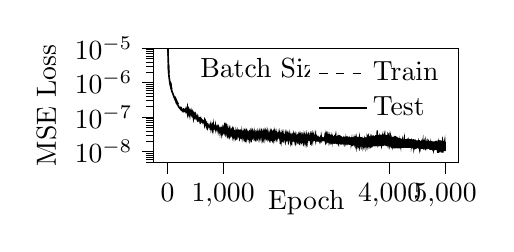
\begin{tikzpicture}

\begin{axis}[
legend cell align={left},
legend style={draw=none},
log basis y={10},
tick align=outside,
tick pos=left,
title={Batch Size 2},
title style={at={(0.4,0.85)},anchor=north},
x grid style={white!69.0196078431373!black},
xlabel={Epoch},
x label style={yshift=13pt},
xmin=-249.95, xmax=5248.95,
xtick style={color=black},
xtick = {0,1000,4000,5000},
y grid style={white!69.0196078431373!black},
ylabel={MSE Loss},
ymin=4.90143384155618e-09, ymax=1e-5,
ymode=log,
ytick style={color=black},
width=.45\textwidth,
height=.25\textwidth
]
\addplot [semithick, black, dashed]
table {%
0 0.00261398348659895
1 0.000146684363119675
2 7.82634508095725e-05
3 3.37719028447054e-05
4 2.5150746102085e-05
5 2.14879413085001e-05
6 1.73131360368757e-05
7 1.25710438198219e-05
8 8.384994563432e-06
9 6.01536302192685e-06
10 5.04094846438363e-06
11 4.50247262365266e-06
12 4.07342948584244e-06
13 3.68863333453007e-06
14 3.33568109506999e-06
15 3.02494765912797e-06
16 2.7562514826851e-06
17 2.52888349787028e-06
18 2.34137056487427e-06
19 2.18880018897138e-06
20 2.06381847633885e-06
21 1.96098151437774e-06
22 1.87465510770934e-06
23 1.80052594150659e-06
24 1.73351173886616e-06
25 1.67263015383323e-06
26 1.61614738892268e-06
27 1.56198234465066e-06
28 1.50867286552803e-06
29 1.46046563780544e-06
30 1.41356673157844e-06
31 1.37106688897681e-06
32 1.33059727563989e-06
33 1.28919083652868e-06
34 1.25175892679241e-06
35 1.21776896658865e-06
36 1.18564458267567e-06
37 1.15591732029952e-06
38 1.12700339668681e-06
39 1.10075354224648e-06
40 1.07587387876951e-06
41 1.05260377831939e-06
42 1.0313208120829e-06
43 1.01144230139827e-06
44 9.92442267119031e-07
45 9.7406527741839e-07
46 9.57213383753874e-07
47 9.40670659906218e-07
48 9.25038841827153e-07
49 9.10250043492766e-07
50 8.96198767826206e-07
51 8.83881172112133e-07
52 8.71137165300517e-07
53 8.58803400506147e-07
54 8.4801414614688e-07
55 8.36522416101104e-07
56 8.25851773152308e-07
57 8.15359453404163e-07
58 8.05294669189216e-07
59 7.95505481549164e-07
60 7.86104835461821e-07
61 7.76836224471111e-07
62 7.67232828448705e-07
63 7.40208569903089e-07
64 7.24697941538288e-07
65 7.12473284208315e-07
66 6.98334301669767e-07
67 6.8646508113801e-07
68 6.76835167410239e-07
69 6.67913647898644e-07
70 6.59476819643956e-07
71 6.51745536447201e-07
72 6.44344590145174e-07
73 6.37315424147467e-07
74 6.29807009134176e-07
75 6.23752871640626e-07
76 6.17110982172875e-07
77 6.10710473006648e-07
78 6.04971023602019e-07
79 5.99273899850594e-07
80 5.93674280890077e-07
81 5.88465108357639e-07
82 5.83262429605824e-07
83 5.78088403622168e-07
84 5.73076810137074e-07
85 5.68146300770955e-07
86 5.63457285606361e-07
87 5.59085755743816e-07
88 5.54764195544344e-07
89 5.50326957575287e-07
90 5.46110211153916e-07
91 5.41905436579171e-07
92 5.38032570275071e-07
93 5.33861362991495e-07
94 5.29962581785171e-07
95 5.25934999759059e-07
96 5.21953731732694e-07
97 5.17996030810153e-07
98 5.13999557568923e-07
99 5.10104440494707e-07
100 5.06136233847876e-07
101 5.02081006532151e-07
102 4.98216791648076e-07
103 4.94461015678738e-07
104 4.90604048617449e-07
105 4.86462815026734e-07
106 4.82587882216556e-07
107 4.78588768475063e-07
108 4.74869900535246e-07
109 4.7077929747541e-07
110 4.66663813166512e-07
111 4.62867599476446e-07
112 4.58659658813865e-07
113 4.54709814113663e-07
114 4.50870674558068e-07
115 4.46929221819659e-07
116 4.42388200826649e-07
117 4.38506839680386e-07
118 4.34678859113191e-07
119 4.3089226689208e-07
120 4.27085763439194e-07
121 4.23271578807061e-07
122 4.19777154811563e-07
123 4.15960641148239e-07
124 4.12074457444511e-07
125 4.08489014579239e-07
126 4.04658556217186e-07
127 4.00951681431394e-07
128 3.9733187562252e-07
129 3.93702260550022e-07
130 3.90062106880862e-07
131 3.86685338110482e-07
132 3.83489258807046e-07
133 3.79915736270497e-07
134 3.76464143924338e-07
135 3.73031685953151e-07
136 3.69614877314461e-07
137 3.66566005281399e-07
138 3.63254276162017e-07
139 3.59711858066269e-07
140 3.56280412384891e-07
141 3.52569088435395e-07
142 3.49126307100711e-07
143 3.45766744868303e-07
144 3.42371599904911e-07
145 3.39262808538354e-07
146 3.36348832967737e-07
147 3.33401700036262e-07
148 3.30368856395147e-07
149 3.2688863233421e-07
150 3.24198848596247e-07
151 3.21372436439926e-07
152 3.17807970312778e-07
153 3.15233077704757e-07
154 3.12444794476452e-07
155 3.10027523902079e-07
156 3.07321188873999e-07
157 3.04717508505359e-07
158 3.02148876103026e-07
159 2.99573802886144e-07
160 2.96987011524585e-07
161 2.94648659848296e-07
162 2.92419047800419e-07
163 2.90140671955541e-07
164 2.88099955823906e-07
165 2.8558504167453e-07
166 2.83444139733025e-07
167 2.8141647362645e-07
168 2.79245677041295e-07
169 2.77200937237154e-07
170 2.75588299680773e-07
171 2.73590638562027e-07
172 2.71654279449418e-07
173 2.69519297966259e-07
174 2.67458664513498e-07
175 2.65497534967629e-07
176 2.63673217523852e-07
177 2.61948017285185e-07
178 2.60005301479183e-07
179 2.58152771367648e-07
180 2.56357327418133e-07
181 2.54637377330891e-07
182 2.5292912211583e-07
183 2.51359738450141e-07
184 2.49551562201411e-07
185 2.48045789688955e-07
186 2.46444842606497e-07
187 2.4465752219438e-07
188 2.43001887576533e-07
189 2.41387644265956e-07
190 2.39743852080032e-07
191 2.38591042211134e-07
192 2.36896491812466e-07
193 2.35331076664291e-07
194 2.33869138022147e-07
195 2.32390313131603e-07
196 2.30942950676827e-07
197 2.29478455254561e-07
198 2.28119508614011e-07
199 2.26882294488195e-07
200 2.25635528665613e-07
201 2.24384542468314e-07
202 2.23268744437011e-07
203 2.21910245763457e-07
204 2.20867471478314e-07
205 2.19511795347405e-07
206 2.18217545115529e-07
207 2.17078903803181e-07
208 2.15910442586509e-07
209 2.14819290250023e-07
210 2.1386440760951e-07
211 2.12621667512458e-07
212 2.11595954674237e-07
213 2.10598725390199e-07
214 2.09534008213996e-07
215 2.08534801116933e-07
216 2.07571893242164e-07
217 2.06601709264564e-07
218 2.05631415472141e-07
219 2.04732785008765e-07
220 2.03928731128844e-07
221 2.02986788394366e-07
222 2.02125836123557e-07
223 2.01693005556169e-07
224 2.00247696379385e-07
225 1.99351367456746e-07
226 1.9847183270949e-07
227 1.97567987980651e-07
228 1.96726100124334e-07
229 1.95874223668291e-07
230 1.95032362352077e-07
231 1.9429453191222e-07
232 1.93577463155847e-07
233 1.92833159978534e-07
234 1.91930465522017e-07
235 1.91151176648585e-07
236 1.90727425620985e-07
237 1.89940357579133e-07
238 1.89282947241409e-07
239 1.88559956265433e-07
240 1.87832262899867e-07
241 1.87312221969105e-07
242 1.8638003640481e-07
243 1.85629820950606e-07
244 1.84861143206927e-07
245 1.84173773354779e-07
246 1.8346385132828e-07
247 1.82691622820474e-07
248 1.81981703223588e-07
249 1.81241538350196e-07
250 1.80819522359599e-07
251 1.80233316547929e-07
252 1.79373761339141e-07
253 1.78795408649846e-07
254 1.78261502097099e-07
255 1.77732386884122e-07
256 1.77024827346939e-07
257 1.76212229890949e-07
258 1.75559959624039e-07
259 1.75028014774092e-07
260 1.74455442444987e-07
261 1.73865569054188e-07
262 1.73293729991419e-07
263 1.72699000502652e-07
264 1.72175157529209e-07
265 1.71600795157545e-07
266 1.71060159445346e-07
267 1.70516953865052e-07
268 1.69965971575703e-07
269 1.69306111652556e-07
270 1.68603019955915e-07
271 1.68096036264442e-07
272 1.67533045300372e-07
273 1.67098511944852e-07
274 1.66452356481939e-07
275 1.6594090199118e-07
276 1.65430003029599e-07
277 1.6504094741765e-07
278 1.64535466716353e-07
279 1.64067817844948e-07
280 1.63518295869691e-07
281 1.63008348729843e-07
282 1.62516949801628e-07
283 1.62122773014195e-07
284 1.61727112577337e-07
285 1.61419068025026e-07
286 1.60981843060126e-07
287 1.60612840249152e-07
288 1.60113057938505e-07
289 1.59996616506453e-07
290 1.59500434703475e-07
291 1.59041253554371e-07
292 1.58633176553291e-07
293 1.58230017347494e-07
294 1.57726207859366e-07
295 1.57391601654178e-07
296 1.56932869004311e-07
297 1.56524124702795e-07
298 1.56090241693274e-07
299 1.55728700207858e-07
300 1.55397476291563e-07
301 1.54913462214301e-07
302 1.54460410595414e-07
303 1.54037259622264e-07
304 1.53807496733549e-07
305 1.53307295429617e-07
306 1.52889717186522e-07
307 1.52815606427659e-07
308 1.5255875534792e-07
309 1.51992299653791e-07
310 1.51631543023223e-07
311 1.51434879765988e-07
312 1.50798544854336e-07
313 1.50500502398065e-07
314 1.50309462715548e-07
315 1.5012875835807e-07
316 1.49606689905601e-07
317 1.49262755533508e-07
318 1.489406507591e-07
319 1.48563328749907e-07
320 1.48307872039899e-07
321 1.47996224146629e-07
322 1.47477975280585e-07
323 1.46864158302451e-07
324 1.46399182789247e-07
325 1.4600326030334e-07
326 1.45447961132694e-07
327 1.45286996641181e-07
328 1.45124027577159e-07
329 1.4457256800382e-07
330 1.44243595714633e-07
331 1.43893380800231e-07
332 1.43401146519118e-07
333 1.43232647254354e-07
334 1.42721284159375e-07
335 1.42463075213817e-07
336 1.42195513040511e-07
337 1.41774924736993e-07
338 1.41613115455463e-07
339 1.41290982773601e-07
340 1.40814341321294e-07
341 1.40588078612947e-07
342 1.40190531043416e-07
343 1.39982248199333e-07
344 1.39655671995254e-07
345 1.39315308924859e-07
346 1.39008234261606e-07
347 1.38621841989428e-07
348 1.38385781822015e-07
349 1.38106749037359e-07
350 1.37768745258837e-07
351 1.37302368972358e-07
352 1.37273293095319e-07
353 1.36685038603535e-07
354 1.36805641671289e-07
355 1.36218938038724e-07
356 1.36174170560555e-07
357 1.35144350333238e-07
358 1.35377791940172e-07
359 1.3519789696903e-07
360 1.34321391878522e-07
361 1.34628653254643e-07
362 1.34382502061214e-07
363 1.33540979393221e-07
364 1.33748807011447e-07
365 1.33484170640186e-07
366 1.32627974005484e-07
367 1.3297263567158e-07
368 1.32693508702708e-07
369 1.32514474537659e-07
370 1.32011076459548e-07
371 1.31861206790651e-07
372 1.31521757749109e-07
373 1.31331652518663e-07
374 1.31312317972254e-07
375 1.30603197236123e-07
376 1.30561156867826e-07
377 1.29773564399915e-07
378 1.30057639510683e-07
379 1.29861310177226e-07
380 1.29112238212326e-07
381 1.29198381696227e-07
382 1.28842748736258e-07
383 1.2872677043152e-07
384 1.2815145879741e-07
385 1.28243387647053e-07
386 1.28023895214824e-07
387 1.27487541142557e-07
388 1.27568656234978e-07
389 1.27031404781208e-07
390 1.27159839126145e-07
391 1.26598800443301e-07
392 1.26791784661684e-07
393 1.26477510927092e-07
394 1.26444590979657e-07
395 1.26158001562349e-07
396 1.25962107867528e-07
397 1.25775401044637e-07
398 1.25593913733013e-07
399 1.24813759142306e-07
400 1.25107088592591e-07
401 1.24789898830358e-07
402 1.24521163066271e-07
403 1.24255962218545e-07
404 1.24277898207348e-07
405 1.23580057124872e-07
406 1.23692217324445e-07
407 1.23466668605632e-07
408 1.23292362624872e-07
409 1.23125864866624e-07
410 1.22844255137977e-07
411 1.22260624106474e-07
412 1.22632293348746e-07
413 1.22149892797907e-07
414 1.21888570189244e-07
415 1.2183269884436e-07
416 1.21501794058565e-07
417 1.21598056354921e-07
418 1.21115364892788e-07
419 1.20845609222542e-07
420 1.20702182457633e-07
421 1.20670180585147e-07
422 1.20313101976244e-07
423 1.20242447746888e-07
424 1.19796707906294e-07
425 1.19679437805553e-07
426 1.19502443590935e-07
427 1.19306255657259e-07
428 1.19001857039169e-07
429 1.18975247541897e-07
430 1.18751168056708e-07
431 1.18668970422453e-07
432 1.18519750465174e-07
433 1.18310549850564e-07
434 1.18205436012264e-07
435 1.18052298470728e-07
436 1.17879357376394e-07
437 1.17379495784053e-07
438 1.17300958525135e-07
439 1.17437472770154e-07
440 1.17254779579357e-07
441 1.16698817170358e-07
442 1.1665886642831e-07
443 1.16422076178457e-07
444 1.16437312810413e-07
445 1.16211605543537e-07
446 1.15907504869339e-07
447 1.15631951317585e-07
448 1.15533178603799e-07
449 1.1553922251073e-07
450 1.15184505566468e-07
451 1.15018143974188e-07
452 1.15032055581388e-07
453 1.14700197587414e-07
454 1.14470164584324e-07
455 1.14392085056592e-07
456 1.14392627027948e-07
457 1.13851511679419e-07
458 1.13809522381825e-07
459 1.13363633469143e-07
460 1.13507051060058e-07
461 1.12955144015325e-07
462 1.12687809270984e-07
463 1.12958656940165e-07
464 1.12561146591084e-07
465 1.1211510408593e-07
466 1.11795333277431e-07
467 1.11874699544767e-07
468 1.11499599053211e-07
469 1.11183911756685e-07
470 1.1097315462405e-07
471 1.10746568335651e-07
472 1.10528108287378e-07
473 1.10256356484095e-07
474 1.10099632397498e-07
475 1.09766951710499e-07
476 1.09138375835371e-07
477 1.08834864133156e-07
478 1.0881889858938e-07
479 1.08393336007095e-07
480 1.08144232992657e-07
481 1.0793406884968e-07
482 1.07731355728502e-07
483 1.07404242227993e-07
484 1.07224436205255e-07
485 1.06623043470755e-07
486 1.06600979004057e-07
487 1.06223428439911e-07
488 1.06042661533579e-07
489 1.05791827745172e-07
490 1.05572618482874e-07
491 1.05332027782401e-07
492 1.05210153051427e-07
493 1.04844322206032e-07
494 1.04628191569089e-07
495 1.04377984629922e-07
496 1.04216347538877e-07
497 1.03955194479699e-07
498 1.03688604859542e-07
499 1.03510769820403e-07
500 1.03342628648528e-07
501 1.03084363703987e-07
502 1.0284133121341e-07
503 1.02668651758897e-07
504 1.02572349458985e-07
505 1.02124076692522e-07
506 1.01995372278507e-07
507 1.01731550677941e-07
508 1.01490412855565e-07
509 1.01381675744916e-07
510 1.01240593376462e-07
511 1.00909068223354e-07
512 1.00669337769643e-07
513 1.00404250107822e-07
514 1.00423404139294e-07
515 1.00214220461581e-07
516 9.99527497607122e-08
517 9.97062718719466e-08
518 9.94624701242675e-08
519 9.93852768302883e-08
520 9.90874772937023e-08
521 9.88455424544288e-08
522 9.86786483039293e-08
523 9.85174300247582e-08
524 9.83541504726571e-08
525 9.82658134411896e-08
526 9.78364765480411e-08
527 9.77660970995498e-08
528 9.7614606940466e-08
529 9.7288654843819e-08
530 9.69792118370449e-08
531 9.69268959594149e-08
532 9.67892044398955e-08
533 9.64910404850361e-08
534 9.62170009874974e-08
535 9.62202412035929e-08
536 9.58558749346583e-08
537 9.56776447187391e-08
538 9.5498134587757e-08
539 9.53894120798715e-08
540 9.50934551380289e-08
541 9.48801197169224e-08
542 9.46125329708281e-08
543 9.44436887060363e-08
544 9.4335708752169e-08
545 9.40767704953327e-08
546 9.38061104351906e-08
547 9.36843962597855e-08
548 9.34865146009489e-08
549 9.32645453668446e-08
550 9.30323500869523e-08
551 9.2910364995813e-08
552 9.24915208440069e-08
553 9.26237489684567e-08
554 9.20383658806756e-08
555 9.20737594465315e-08
556 9.1773045729715e-08
557 9.15990957992552e-08
558 9.16372675546784e-08
559 9.13390870608266e-08
560 9.12179028298432e-08
561 9.10503901381254e-08
562 9.07964728142918e-08
563 9.05843692435848e-08
564 9.03890795960205e-08
565 9.00719094163449e-08
566 8.99008989017069e-08
567 8.98419131223349e-08
568 8.94903660499935e-08
569 8.92771059846087e-08
570 8.92133772965043e-08
571 8.92505096738994e-08
572 8.88596866948088e-08
573 8.88809712964456e-08
574 8.85358828333072e-08
575 8.83346679561026e-08
576 8.84105503005106e-08
577 8.8131889763865e-08
578 8.80912545679902e-08
579 8.76220811723005e-08
580 8.76374261120638e-08
581 8.73306817090747e-08
582 8.69455808030217e-08
583 8.70990354120416e-08
584 8.65921273616177e-08
585 8.64360111918483e-08
586 8.64471381185616e-08
587 8.61044444553372e-08
588 8.59900289835735e-08
589 8.59733905260729e-08
590 8.56495371353017e-08
591 8.5448452592729e-08
592 8.52556495878343e-08
593 8.50720472700406e-08
594 8.48990268551564e-08
595 8.46750809213592e-08
596 8.45080046549818e-08
597 8.42445121276292e-08
598 8.40143372828894e-08
599 8.37218631160042e-08
600 8.35349402392716e-08
601 8.31654908488577e-08
602 8.30242949245719e-08
603 8.2982439593593e-08
604 8.2921621885168e-08
605 8.26500533532837e-08
606 8.25823081787025e-08
607 8.2389301115926e-08
608 8.22421491531999e-08
609 8.19840703343289e-08
610 8.1801761944611e-08
611 8.18592255097395e-08
612 8.16676565214003e-08
613 8.16171640491969e-08
614 8.13247282057672e-08
615 8.10373738009407e-08
616 8.08642084723088e-08
617 8.06555648807938e-08
618 8.039214622102e-08
619 8.02460349925704e-08
620 8.00810798282647e-08
621 7.99409526959227e-08
622 7.97110490066144e-08
623 7.94116076875406e-08
624 7.92543457824868e-08
625 7.90482818721072e-08
626 7.87830216444352e-08
627 7.86491988641336e-08
628 7.84446622161816e-08
629 7.827243654146e-08
630 7.81483883874889e-08
631 7.79432979882699e-08
632 7.77564276402964e-08
633 7.75270853509147e-08
634 7.74125279346949e-08
635 7.70996542881486e-08
636 7.70233436728773e-08
637 7.66381009270622e-08
638 7.64740521639329e-08
639 7.66816242462332e-08
640 7.64246416755654e-08
641 7.61894967465926e-08
642 7.59976832137577e-08
643 7.56666841013054e-08
644 7.54723867576468e-08
645 7.54306852314146e-08
646 7.53268538478125e-08
647 7.51730338366396e-08
648 7.47495809915177e-08
649 7.48541830168925e-08
650 7.43791588843079e-08
651 7.42978026984087e-08
652 7.42460074155682e-08
653 7.40438198457705e-08
654 7.3634554738522e-08
655 7.37113431152903e-08
656 7.34467651670734e-08
657 7.33724932918678e-08
658 7.31816905603644e-08
659 7.31439444945359e-08
660 7.28667297711372e-08
661 7.26887656533615e-08
662 7.25385389976907e-08
663 7.24498825926956e-08
664 7.22832119443018e-08
665 7.21822083353807e-08
666 7.19495448092688e-08
667 7.18707898982318e-08
668 7.16480042597389e-08
669 7.14073806823423e-08
670 7.13205865152666e-08
671 7.10196900129967e-08
672 7.09722795270151e-08
673 7.07187652627672e-08
674 7.06024032132158e-08
675 7.05165593821722e-08
676 7.03380461603009e-08
677 7.03425385415457e-08
678 7.00737257445239e-08
679 6.99320477606236e-08
680 6.97025158427067e-08
681 6.95539946653501e-08
682 6.93178849876519e-08
683 6.94211070342288e-08
684 6.90671745279259e-08
685 6.8847339870004e-08
686 6.89086112218851e-08
687 6.87327516597502e-08
688 6.84967959185823e-08
689 6.84914813144921e-08
690 6.84173265950161e-08
691 6.81482263986677e-08
692 6.79657498626751e-08
693 6.76911481836129e-08
694 6.78754415739391e-08
695 6.76873341790563e-08
696 6.7420077696112e-08
697 6.73318192355721e-08
698 6.71849346519648e-08
699 6.70631731659599e-08
700 6.6936109860527e-08
701 6.67347293343834e-08
702 6.66230708357141e-08
703 6.67056503975694e-08
704 6.66208884274599e-08
705 6.6402336841076e-08
706 6.637572022683e-08
707 6.60298795550629e-08
708 6.58703416722695e-08
709 6.59932807797192e-08
710 6.57574264092409e-08
711 6.5755870203299e-08
712 6.55362282209193e-08
713 6.54728074114264e-08
714 6.5351697348004e-08
715 6.53087951680842e-08
716 6.51708659051842e-08
717 6.50125667877033e-08
718 6.49798564733572e-08
719 6.47724273014072e-08
720 6.47707329970437e-08
721 6.45535312721046e-08
722 6.44558372296933e-08
723 6.43093136186712e-08
724 6.406546154758e-08
725 6.40719362525743e-08
726 6.45583160179264e-08
727 6.38616268305858e-08
728 6.39997100977396e-08
729 6.38944717001877e-08
730 6.37970664736365e-08
731 6.36738414186988e-08
732 6.35405101436781e-08
733 6.3468621691154e-08
734 6.31237134999241e-08
735 6.32146194542438e-08
736 6.31069264531714e-08
737 6.30518270504643e-08
738 6.29606186937082e-08
739 6.26848402600633e-08
740 6.28600875853813e-08
741 6.26476349310234e-08
742 6.24892591627457e-08
743 6.24455489549591e-08
744 6.23294498194316e-08
745 6.2253770162779e-08
746 6.21718271596183e-08
747 6.20670583866279e-08
748 6.18798210956228e-08
749 6.188538615437e-08
750 6.18037680910621e-08
751 6.16810066836893e-08
752 6.15384937397989e-08
753 6.14532277937174e-08
754 6.1445070853372e-08
755 6.13365998902715e-08
756 6.12798440569051e-08
757 6.13104954930721e-08
758 6.12681508648238e-08
759 6.10669092498961e-08
760 6.10586326349472e-08
761 6.09786342657959e-08
762 6.08765920058207e-08
763 6.07757833117617e-08
764 6.07843563827926e-08
765 6.05380540213973e-08
766 6.04225618350274e-08
767 6.03992417815835e-08
768 6.03464287243227e-08
769 6.01462231776262e-08
770 6.00604040950081e-08
771 6.00231084527669e-08
772 5.99093010943408e-08
773 5.98377934263317e-08
774 5.96081898500689e-08
775 5.95742457141224e-08
776 5.96780586127332e-08
777 5.93245081615956e-08
778 5.91501711765252e-08
779 5.92791223117395e-08
780 5.91412333191821e-08
781 5.90747720404794e-08
782 5.89476858179339e-08
783 5.88208731741036e-08
784 5.88255402458326e-08
785 5.8786889870488e-08
786 5.86065183543205e-08
787 5.86318991023793e-08
788 5.8584062483602e-08
789 5.84684124078638e-08
790 5.85145645294327e-08
791 5.82407579362565e-08
792 5.82223076095456e-08
793 5.79912457159271e-08
794 5.8108856008543e-08
795 5.79709602686052e-08
796 5.78531142740868e-08
797 5.78370420644125e-08
798 5.76913316553407e-08
799 5.76839951780261e-08
800 5.75831435745133e-08
801 5.75909274685982e-08
802 5.74083612785437e-08
803 5.74391697699683e-08
804 5.72027329296398e-08
805 5.73407223503075e-08
806 5.72023227312091e-08
807 5.70735137997991e-08
808 5.70729130350278e-08
809 5.69626252675537e-08
810 5.6882644279832e-08
811 5.68058462963039e-08
812 5.66683241300936e-08
813 5.66744659303842e-08
814 5.65901798542656e-08
815 5.6436309426422e-08
816 5.65831056307253e-08
817 5.63878848396371e-08
818 5.62771926944095e-08
819 5.62657206842898e-08
820 5.62157826032861e-08
821 5.61009023639647e-08
822 5.60516779550824e-08
823 5.59690822986569e-08
824 5.61079724488156e-08
825 5.58611277436949e-08
826 5.57958161638838e-08
827 5.57157521758889e-08
828 5.56878466763111e-08
829 5.57414290146552e-08
830 5.54114399603511e-08
831 5.54050776053749e-08
832 5.54322031087739e-08
833 5.54243826426104e-08
834 5.53643694637396e-08
835 5.51954801198962e-08
836 5.53016565781883e-08
837 5.52197657462949e-08
838 5.50475004045259e-08
839 5.50929451459403e-08
840 5.49398851192873e-08
841 5.50032194527317e-08
842 5.49059920349482e-08
843 5.48543149434533e-08
844 5.47220845609209e-08
845 5.45919308593268e-08
846 5.46621458888952e-08
847 5.45036415513511e-08
848 5.44871118437484e-08
849 5.44909918462899e-08
850 5.44362895656958e-08
851 5.42284673225035e-08
852 5.43319143780918e-08
853 5.42738582536284e-08
854 5.39490024304978e-08
855 5.41623808413272e-08
856 5.38711755492249e-08
857 5.38292376828231e-08
858 5.38144721166089e-08
859 5.40801493253973e-08
860 5.35556771573686e-08
861 5.34009007191472e-08
862 5.36913170899878e-08
863 5.35750088621612e-08
864 5.34702983183699e-08
865 5.31324628701979e-08
866 5.32663798854527e-08
867 5.34713005498899e-08
868 5.3268240315818e-08
869 5.3106281430626e-08
870 5.30999553991496e-08
871 5.30073745623749e-08
872 5.3024831385029e-08
873 5.29475644116539e-08
874 5.29035295295799e-08
875 5.27633898719237e-08
876 5.27644872644339e-08
877 5.26363374481198e-08
878 5.21344579949012e-08
879 5.26222953115552e-08
880 5.25046283263997e-08
881 5.25887310142137e-08
882 5.23786171260365e-08
883 5.22556745392588e-08
884 5.22890715103364e-08
885 5.22051752521735e-08
886 5.22562960395545e-08
887 5.21403642420593e-08
888 5.21259177299616e-08
889 5.23303570957312e-08
890 5.21940686630806e-08
891 5.20369648042696e-08
892 5.18643744533698e-08
893 5.1959078596342e-08
894 5.1800517703815e-08
895 5.17839124822839e-08
896 5.1749980221838e-08
897 5.20235737372365e-08
898 5.14930678036096e-08
899 5.13947631269884e-08
900 5.14576784906851e-08
901 5.15045462358144e-08
902 5.14380473438658e-08
903 5.14084751558341e-08
904 5.13051172055246e-08
905 5.13162940889433e-08
906 5.12426185311776e-08
907 5.11894807858626e-08
908 5.12040236309019e-08
909 5.11771593126875e-08
910 5.1391161834613e-08
911 5.09132827229974e-08
912 5.07956156252654e-08
913 5.07086769411247e-08
914 5.07240060290126e-08
915 5.05156226283665e-08
916 5.09034994145008e-08
917 5.10812179872477e-08
918 5.09299017443787e-08
919 5.06071179470213e-08
920 5.06153786566932e-08
921 5.08228125277732e-08
922 5.07701664046456e-08
923 5.04631669587807e-08
924 5.04625080791632e-08
925 5.03999359618978e-08
926 5.03120141140956e-08
927 5.02950299255955e-08
928 5.02036412520779e-08
929 5.05533185670704e-08
930 5.03805240215094e-08
931 5.03134604930011e-08
932 5.03399029133655e-08
933 5.02495765224431e-08
934 5.02485439819456e-08
935 5.01097002670869e-08
936 4.98450323295208e-08
937 5.00081839931443e-08
938 5.02201354417586e-08
939 5.00173292057315e-08
940 4.99454150872936e-08
941 4.98917330522541e-08
942 4.97869760859304e-08
943 4.96477238839388e-08
944 4.96061485512067e-08
945 4.96272340385628e-08
946 4.96270244700892e-08
947 4.96611786039436e-08
948 4.93043708666985e-08
949 4.93675331766363e-08
950 4.94701070694603e-08
951 4.95901512781449e-08
952 4.95660200040549e-08
953 4.93224323655506e-08
954 4.91889253581013e-08
955 4.92657079411152e-08
956 4.93090457755474e-08
957 4.90304114769136e-08
958 4.86113878614414e-08
959 4.87386970814407e-08
960 4.86080396257527e-08
961 4.91473815086851e-08
962 4.82496446461145e-08
963 4.8349681513904e-08
964 4.83994517888053e-08
965 4.84674849848266e-08
966 4.89019669674406e-08
967 4.87339815461452e-08
968 4.8887384868801e-08
969 4.86750621041532e-08
970 4.87458362598003e-08
971 4.87206623641101e-08
972 4.85998083747385e-08
973 4.86616961933861e-08
974 4.85624361134529e-08
975 4.85805682470253e-08
976 4.85125720613433e-08
977 4.82887160206391e-08
978 4.84719224294605e-08
979 4.83484899962972e-08
980 4.82735046126725e-08
981 4.84206677583976e-08
982 4.82095535099814e-08
983 4.81738937898046e-08
984 4.81529513432499e-08
985 4.80463511752238e-08
986 4.8008118166909e-08
987 4.78388747605085e-08
988 4.79545476203547e-08
989 4.77904276480756e-08
990 4.76947455610444e-08
991 4.7953770904885e-08
992 4.75322841403392e-08
993 4.7785734386907e-08
994 4.75348239130091e-08
995 4.7667171884147e-08
996 4.74739370615596e-08
997 4.75618149212709e-08
998 4.75811124144854e-08
999 4.74248252290144e-08
1000 4.76309443844802e-08
1001 4.72376396284391e-08
1002 4.71671802128038e-08
1003 4.74440110288521e-08
1004 4.69942068811458e-08
1005 4.71157604259309e-08
1006 4.69819341240574e-08
1007 4.69522687752133e-08
1008 4.68813971180038e-08
1009 4.66572676727783e-08
1010 4.68712826183215e-08
1011 4.65230975445485e-08
1012 4.6986280031025e-08
1013 4.65285257113535e-08
1014 4.65172853401641e-08
1015 4.69000739997116e-08
1016 4.59802069521786e-08
1017 4.61438803179282e-08
1018 4.61487103370906e-08
1019 4.60385496252047e-08
1020 4.60279651077755e-08
1021 4.5991702721071e-08
1022 4.6049907213741e-08
1023 4.58232247232404e-08
1024 4.575472711843e-08
1025 4.57867423995784e-08
1026 4.57194202890809e-08
1027 4.5735625373744e-08
1028 4.56614160241897e-08
1029 4.57159697072051e-08
1030 4.55817242379086e-08
1031 4.55687318516862e-08
1032 4.55431716767651e-08
1033 4.54868766998073e-08
1034 4.54809728112071e-08
1035 4.53985480052266e-08
1036 4.5422408025686e-08
1037 4.52892244754421e-08
1038 4.52831030046119e-08
1039 4.53999871000699e-08
1040 4.54181504337958e-08
1041 4.52862972734613e-08
1042 4.51580050345179e-08
1043 4.51480138310423e-08
1044 4.51643003261393e-08
1045 4.51240597721392e-08
1046 4.49955824772252e-08
1047 4.50499606158838e-08
1048 4.50189186058103e-08
1049 4.50657565729817e-08
1050 4.4959013388024e-08
1051 4.48627814274016e-08
1052 4.48606086906889e-08
1053 4.4802549736378e-08
1054 4.48229560718882e-08
1055 4.48897614062638e-08
1056 4.47645272669828e-08
1057 4.46646057877254e-08
1058 4.47493429872603e-08
1059 4.46290876262023e-08
1060 4.47393384138683e-08
1061 4.44872028639853e-08
1062 4.46542057774835e-08
1063 4.44682002784802e-08
1064 4.45064564659758e-08
1065 4.45753047110253e-08
1066 4.4414909836088e-08
1067 4.44585654978957e-08
1068 4.43124520668192e-08
1069 4.43833488869561e-08
1070 4.4300507340167e-08
1071 4.42940364882016e-08
1072 4.42912890031288e-08
1073 4.43040135522099e-08
1074 4.42048048830967e-08
1075 4.416254044598e-08
1076 4.41335653407759e-08
1077 4.40365813249022e-08
1078 4.41081502742802e-08
1079 4.40969820470483e-08
1080 4.3948786994652e-08
1081 4.41720446373584e-08
1082 4.39464986777271e-08
1083 4.40942140758627e-08
1084 4.37837767735538e-08
1085 4.39278263835718e-08
1086 4.37930967392974e-08
1087 4.37182112345003e-08
1088 4.37573598288665e-08
1089 4.37867421974048e-08
1090 4.36447713969557e-08
1091 4.38515382742977e-08
1092 4.37362916652084e-08
1093 4.36174015362445e-08
1094 4.3778218633217e-08
1095 4.35680120209891e-08
1096 4.35805192225414e-08
1097 4.36738350335086e-08
1098 4.36676859579821e-08
1099 4.35005779383379e-08
1100 4.35071349083049e-08
1101 4.35172271734396e-08
1102 4.34009853089168e-08
1103 4.33678863978049e-08
1104 4.33504221901138e-08
1105 4.32441569210851e-08
1106 4.3280685350644e-08
1107 4.34523939446541e-08
1108 4.32948200780325e-08
1109 4.31160244203088e-08
1110 4.31606878995017e-08
1111 4.31132841002824e-08
1112 4.31126667642112e-08
1113 4.30161841746823e-08
1114 4.31351706885463e-08
1115 4.30137107217399e-08
1116 4.30419452301378e-08
1117 4.28521687167449e-08
1118 4.29494802055563e-08
1119 4.2983084970083e-08
1120 4.28279311986968e-08
1121 4.29285861436868e-08
1122 4.28456561525348e-08
1123 4.29562623107116e-08
1124 4.28213921451759e-08
1125 4.27720357785155e-08
1126 4.27197061031448e-08
1127 4.27676665794574e-08
1128 4.27508851308933e-08
1129 4.2682300908925e-08
1130 4.26003897978089e-08
1131 4.24758110147416e-08
1132 4.25463953803162e-08
1133 4.25152052525024e-08
1134 4.25598208884104e-08
1135 4.239308792503e-08
1136 4.2449155177704e-08
1137 4.24381763784454e-08
1138 4.24335556179489e-08
1139 4.23089017043132e-08
1140 4.23211221574071e-08
1141 4.22933782630586e-08
1142 4.23067300873714e-08
1143 4.23677056163863e-08
1144 4.23486314717891e-08
1145 4.19986635529779e-08
1146 4.20469467001805e-08
1147 4.22094996923028e-08
1148 4.20193057089624e-08
1149 4.21166019328179e-08
1150 4.21501204259656e-08
1151 4.19883999723814e-08
1152 4.20073089106854e-08
1153 4.18943582077835e-08
1154 4.19936113004726e-08
1155 4.20366788216886e-08
1156 4.20818990342631e-08
1157 4.18583599697264e-08
1158 4.17444217319929e-08
1159 4.17618667362674e-08
1160 4.17829855202667e-08
1161 4.17799846383904e-08
1162 4.16705735562517e-08
1163 4.18948547789011e-08
1164 4.16620335019213e-08
1165 4.17125577941713e-08
1166 4.15728996195353e-08
1167 4.16248975123046e-08
1168 4.17766256601282e-08
1169 4.14573240685168e-08
1170 4.15731547034337e-08
1171 4.14832258551212e-08
1172 4.14894388031661e-08
1173 4.17455580651316e-08
1174 4.15013680700738e-08
1175 4.15968621256257e-08
1176 4.13717257054524e-08
1177 4.15543938007135e-08
1178 4.12514978142542e-08
1179 4.14077720277683e-08
1180 4.15308862883323e-08
1181 4.13152643243264e-08
1182 4.13804941682416e-08
1183 4.13969383722401e-08
1184 4.13074685233217e-08
1185 4.14006716444315e-08
1186 4.12031826499959e-08
1187 4.13484403469777e-08
1188 4.11279918449137e-08
1189 4.1116992403778e-08
1190 4.10200866945987e-08
1191 4.10916682780371e-08
1192 4.10232857664949e-08
1193 4.11754650986307e-08
1194 4.08613160786109e-08
1195 4.10294067033634e-08
1196 4.11262635822141e-08
1197 4.09699648660222e-08
1198 4.09178326050697e-08
1199 4.08179365538608e-08
1200 4.08433911486261e-08
1201 4.07925646619955e-08
1202 4.0843865591389e-08
1203 4.08273227012201e-08
1204 4.08248592192462e-08
1205 4.09464814088434e-08
1206 4.07076831734909e-08
1207 4.06216350464228e-08
1208 4.05717194499888e-08
1209 4.07536141571185e-08
1210 4.06037834261297e-08
1211 4.05800763356723e-08
1212 4.05475472338157e-08
1213 4.05940800142779e-08
1214 4.07310513145798e-08
1215 4.0481364380951e-08
1216 4.05854570876274e-08
1217 4.0419865971697e-08
1218 4.04724098932996e-08
1219 4.03760262344677e-08
1220 4.05545208236879e-08
1221 4.04062817561668e-08
1222 4.04085032262302e-08
1223 4.0206302078627e-08
1224 4.02853182185359e-08
1225 4.02691618917039e-08
1226 4.02556384009323e-08
1227 3.99654077228306e-08
1228 4.0084840536081e-08
1229 3.99519415278937e-08
1230 3.99425685834176e-08
1231 3.99511088683413e-08
1232 3.99962168105006e-08
1233 3.98757909992886e-08
1234 3.99903259502565e-08
1235 3.97727424241157e-08
1236 3.97362323014128e-08
1237 3.98615986861861e-08
1238 3.97920895919279e-08
1239 3.96503417985916e-08
1240 3.98500998187723e-08
1241 3.94888271154081e-08
1242 3.97363479529567e-08
1243 3.9670114947099e-08
1244 3.95152142287913e-08
1245 3.94588912658311e-08
1246 3.96170589693212e-08
1247 3.95713690846677e-08
1248 3.9653338033907e-08
1249 3.96299430795444e-08
1250 3.93851973877202e-08
1251 3.95682592178592e-08
1252 3.94245985052555e-08
1253 3.94186836629173e-08
1254 3.93995191990681e-08
1255 3.94417245035417e-08
1256 3.93175576240967e-08
1257 3.93010308639696e-08
1258 3.94500662774244e-08
1259 3.92660184653781e-08
1260 3.91611785369173e-08
1261 3.93277218297405e-08
1262 3.90468253679832e-08
1263 3.92391634491673e-08
1264 3.90210088450083e-08
1265 3.90619693654837e-08
1266 3.91635332250839e-08
1267 3.91998140386596e-08
1268 3.88992044481062e-08
1269 3.92167338549299e-08
1270 3.88048741853941e-08
1271 3.90122393857384e-08
1272 3.90509703188657e-08
1273 3.89146043306421e-08
1274 3.89563392785841e-08
1275 3.89260859701701e-08
1276 3.90563198613969e-08
1277 3.903581282938e-08
1278 3.87682184300187e-08
1279 3.90418795276903e-08
1280 3.88307571365099e-08
1281 3.88432197571675e-08
1282 3.88089232857825e-08
1283 3.88497545305011e-08
1284 3.8808237176613e-08
1285 3.86636885413849e-08
1286 3.8951220149408e-08
1287 3.87320291024285e-08
1288 3.86920816649039e-08
1289 3.8919329096998e-08
1290 3.86722198195133e-08
1291 3.86278853801714e-08
1292 3.88914554788622e-08
1293 3.8599475284451e-08
1294 3.8693181822369e-08
1295 3.85323008162963e-08
1296 3.85450245753982e-08
1297 3.8618123346601e-08
1298 3.86272235451401e-08
1299 3.85501028578594e-08
1300 3.85360730471018e-08
1301 3.84817750264665e-08
1302 3.83798020365811e-08
1303 3.84028968161143e-08
1304 3.83411669929168e-08
1305 3.86072583850039e-08
1306 3.83613074982914e-08
1307 3.8552181814977e-08
1308 3.82130065704755e-08
1309 3.80664171260592e-08
1310 3.84765729979919e-08
1311 3.81774920919509e-08
1312 3.82775483957487e-08
1313 3.83419538739216e-08
1314 3.82416022891574e-08
1315 3.81589909581037e-08
1316 3.84554827882466e-08
1317 3.81900211631758e-08
1318 3.80497460764073e-08
1319 3.80913908638036e-08
1320 3.79748055899243e-08
1321 3.82118173543611e-08
1322 3.8044942906712e-08
1323 3.7897786287433e-08
1324 3.80364340222261e-08
1325 3.80164513292258e-08
1326 3.80070932131105e-08
1327 3.77907139890721e-08
1328 3.79741725815008e-08
1329 3.7962045192963e-08
1330 3.78899051253767e-08
1331 3.78060559529936e-08
1332 3.78670913306345e-08
1333 3.78315917831662e-08
1334 3.80222686703902e-08
1335 3.77478427376343e-08
1336 3.76959864369364e-08
1337 3.76758144395861e-08
1338 3.78092513653727e-08
1339 3.77412872711314e-08
1340 3.76240642890879e-08
1341 3.77037665962865e-08
1342 3.75619689473861e-08
1343 3.77010441950931e-08
1344 3.77110146798088e-08
1345 3.75804105830491e-08
1346 3.76246193385943e-08
1347 3.75692676248818e-08
1348 3.74983338812807e-08
1349 3.74260324288445e-08
1350 3.73596034612955e-08
1351 3.74343606266425e-08
1352 3.74937736646319e-08
1353 3.75229895516749e-08
1354 3.71330517868751e-08
1355 3.74137304480215e-08
1356 3.7181566376332e-08
1357 3.72471152274567e-08
1358 3.74778136069676e-08
1359 3.72647145150395e-08
1360 3.72154928966473e-08
1361 3.7239597339922e-08
1362 3.72700734292408e-08
1363 3.74581570247168e-08
1364 3.7001714643492e-08
1365 3.71595026116833e-08
1366 3.72408672513203e-08
1367 3.7080263740441e-08
1368 3.72318790692883e-08
1369 3.70415177685657e-08
1370 3.72782474327149e-08
1371 3.70204627198611e-08
1372 3.70034276288567e-08
1373 3.71566659543299e-08
1374 3.69266780143596e-08
1375 3.71390608163713e-08
1376 3.69570218351489e-08
1377 3.6941323282691e-08
1378 3.6822000582748e-08
1379 3.6959429911998e-08
1380 3.68920858652144e-08
1381 3.701040906956e-08
1382 3.681259792776e-08
1383 3.66875012499102e-08
1384 3.6890900990294e-08
1385 3.68982291191755e-08
1386 3.69947587329777e-08
1387 3.70211979827673e-08
1388 3.68647417595125e-08
1389 3.6786965299962e-08
1390 3.69163455046229e-08
1391 3.6661925532866e-08
1392 3.68543216258121e-08
1393 3.68127328680412e-08
1394 3.68141683004253e-08
1395 3.68085077421254e-08
1396 3.67071528235008e-08
1397 3.68935591985031e-08
1398 3.66122590514939e-08
1399 3.66694211784147e-08
1400 3.65310263724661e-08
1401 3.66279319389262e-08
1402 3.64981576203016e-08
1403 3.64699415433267e-08
1404 3.67245235168845e-08
1405 3.65029932370975e-08
1406 3.66564263549751e-08
1407 3.66455188268722e-08
1408 3.64214779541294e-08
1409 3.65147219616446e-08
1410 3.67536794762535e-08
1411 3.66980817745333e-08
1412 3.63030791232788e-08
1413 3.66292846185612e-08
1414 3.64065608632891e-08
1415 3.63810815168786e-08
1416 3.65551502848893e-08
1417 3.63827365366665e-08
1418 3.68315672601427e-08
1419 3.6253791672769e-08
1420 3.65551811753462e-08
1421 3.63489426132846e-08
1422 3.64301096009711e-08
1423 3.63845785113504e-08
1424 3.63241670645609e-08
1425 3.62743841785806e-08
1426 3.64269679675733e-08
1427 3.62643482531011e-08
1428 3.64093605202953e-08
1429 3.65368469820715e-08
1430 3.64458330048834e-08
1431 3.61357457412947e-08
1432 3.62946508546957e-08
1433 3.61692249251089e-08
1434 3.63927227604033e-08
1435 3.62667733102562e-08
1436 3.6191466375235e-08
1437 3.60597453187284e-08
1438 3.61780122727362e-08
1439 3.63371264393564e-08
1440 3.60288973001444e-08
1441 3.61311922566498e-08
1442 3.6101228826857e-08
1443 3.61737874227663e-08
1444 3.60708859069026e-08
1445 3.60423173657032e-08
1446 3.61806412192967e-08
1447 3.61474959655883e-08
1448 3.61653036710097e-08
1449 3.61737482946212e-08
1450 3.60483866692074e-08
1451 3.60628494541215e-08
1452 3.59418912091458e-08
1453 3.59477794594221e-08
1454 3.60916861414928e-08
1455 3.61096439289721e-08
1456 3.60066770979661e-08
1457 3.60769590888044e-08
1458 3.60448918488854e-08
1459 3.59734010469959e-08
1460 3.5930709048837e-08
1461 3.59758459184678e-08
1462 3.58558317283264e-08
1463 3.60298738923404e-08
1464 3.59392365429922e-08
1465 3.59062993798842e-08
1466 3.60486273298655e-08
1467 3.56902185318364e-08
1468 3.57968897950478e-08
1469 3.59835234380324e-08
1470 3.56674581156735e-08
1471 3.59051779348363e-08
1472 3.57930280444063e-08
1473 3.61311931985631e-08
1474 3.55918575497549e-08
1475 3.56933443580454e-08
1476 3.56426915007479e-08
1477 3.5738645992045e-08
1478 3.57809168338719e-08
1479 3.57045625825059e-08
1480 3.57558388912049e-08
1481 3.56408534146202e-08
1482 3.59447247259559e-08
1483 3.5626910365294e-08
1484 3.57225171889186e-08
1485 3.55112521048251e-08
1486 3.57546030416156e-08
1487 3.56030605532798e-08
1488 3.55800063335243e-08
1489 3.57159678091579e-08
1490 3.5622840438454e-08
1491 3.56112106800199e-08
1492 3.55408875938323e-08
1493 3.55446255211334e-08
1494 3.56145687260834e-08
1495 3.54259949193469e-08
1496 3.54903710649279e-08
1497 3.53642074025218e-08
1498 3.54873146918844e-08
1499 3.54727140838285e-08
1500 3.55334545208419e-08
1501 3.5409026780342e-08
1502 3.54803372437096e-08
1503 3.55096652833176e-08
1504 3.54438842816163e-08
1505 3.54438994277229e-08
1506 3.52586356386353e-08
1507 3.54853364768481e-08
1508 3.52613148048575e-08
1509 3.56022012296675e-08
1510 3.509981280575e-08
1511 3.56337536586149e-08
1512 3.52175760410245e-08
1513 3.53154326817595e-08
1514 3.534399718369e-08
1515 3.51297950942908e-08
1516 3.53575105652149e-08
1517 3.51708020545627e-08
1518 3.53134347643169e-08
1519 3.52938552420912e-08
1520 3.53772712797795e-08
1521 3.54995465590147e-08
1522 3.50098286754363e-08
1523 3.51518915935878e-08
1524 3.50881709478834e-08
1525 3.50589046707039e-08
1526 3.50215923819452e-08
1527 3.53548170237139e-08
1528 3.5026552623274e-08
1529 3.52368347221188e-08
1530 3.50323764222171e-08
1531 3.51654090468001e-08
1532 3.51068960543488e-08
1533 3.51634139128532e-08
1534 3.51571836484377e-08
1535 3.49424351043237e-08
1536 3.50187879449848e-08
1537 3.53500963033437e-08
1538 3.50289750721822e-08
1539 3.48855184874042e-08
1540 3.50088064540177e-08
1541 3.49903093593285e-08
1542 3.50582522964382e-08
1543 3.50921210990895e-08
1544 3.49305118901855e-08
1545 3.48348799145137e-08
1546 3.50040681207364e-08
1547 3.50324450644757e-08
1548 3.47821500198964e-08
1549 3.48002036693606e-08
1550 3.50278476385357e-08
1551 3.48182352611914e-08
1552 3.4843449333799e-08
1553 3.47927909744028e-08
1554 3.46968657146118e-08
1555 3.48270575143417e-08
1556 3.48542658725748e-08
1557 3.47570996516722e-08
1558 3.47461852138742e-08
1559 3.48612541893889e-08
1560 3.47328968683946e-08
1561 3.4757167578614e-08
1562 3.46516574474265e-08
1563 3.49862555948932e-08
1564 3.46321199928834e-08
1565 3.4780982513416e-08
1566 3.46651921784291e-08
1567 3.45752515271136e-08
1568 3.47753969680009e-08
1569 3.48198636946351e-08
1570 3.47757455861908e-08
1571 3.4507271549189e-08
1572 3.47078772566789e-08
1573 3.49576113828354e-08
1574 3.47395628798042e-08
1575 3.45694570675903e-08
1576 3.47136032560202e-08
1577 3.44184528642821e-08
1578 3.45566974758738e-08
1579 3.45180234527787e-08
1580 3.4580202604495e-08
1581 3.45497845699594e-08
1582 3.42231714617336e-08
1583 3.46553255673454e-08
1584 3.43230252612958e-08
1585 3.44667043732372e-08
1586 3.42018570680391e-08
1587 3.42796177371651e-08
1588 3.45346177799133e-08
1589 3.42886514995699e-08
1590 3.41987356230478e-08
1591 3.42419555141582e-08
1592 3.42777873509892e-08
1593 3.43240454155902e-08
1594 3.44707572889069e-08
1595 3.41868560851388e-08
1596 3.42473797330656e-08
1597 3.41525397445919e-08
1598 3.42604636796029e-08
1599 3.42073004447885e-08
1600 3.42863649285263e-08
1601 3.42130756987857e-08
1602 3.4182281366868e-08
1603 3.41949527709051e-08
1604 3.42302469623634e-08
1605 3.43229221849706e-08
1606 3.40175767419293e-08
1607 3.41228139911776e-08
1608 3.39518507423975e-08
1609 3.41163186207138e-08
1610 3.41803030444177e-08
1611 3.39146702968973e-08
1612 3.39262604691637e-08
1613 3.41989028934675e-08
1614 3.40345293181055e-08
1615 3.3939421488216e-08
1616 3.42013139937869e-08
1617 3.40021184344064e-08
1618 3.40370750067098e-08
1619 3.39722234156126e-08
1620 3.39850721161605e-08
1621 3.39282047469025e-08
1622 3.38887960671941e-08
1623 3.38494148963142e-08
1624 3.39835219518303e-08
1625 3.40568993758006e-08
1626 3.37798887363183e-08
1627 3.40222135623014e-08
1628 3.40237355868633e-08
1629 3.3838818874754e-08
1630 3.40310748536687e-08
1631 3.38542083794802e-08
1632 3.38119319162056e-08
1633 3.37274185027159e-08
1634 3.38834484395756e-08
1635 3.37319519347901e-08
1636 3.38475110375214e-08
1637 3.3742468025566e-08
1638 3.38427758715953e-08
1639 3.36246807055574e-08
1640 3.36959911075851e-08
1641 3.37534677092854e-08
1642 3.37967688742169e-08
1643 3.36699845108202e-08
1644 3.37426600273694e-08
1645 3.37344562306718e-08
1646 3.38293949403434e-08
1647 3.37148696983869e-08
1648 3.36567350142092e-08
1649 3.3601624474966e-08
1650 3.37595379983346e-08
1651 3.35222202904051e-08
1652 3.36508149685333e-08
1653 3.36155920830361e-08
1654 3.36637392334138e-08
1655 3.37210855487768e-08
1656 3.36275210927051e-08
1657 3.35611687754533e-08
1658 3.35721064157468e-08
1659 3.34675595425882e-08
1660 3.37159029577538e-08
1661 3.36373670382084e-08
1662 3.35888019271646e-08
1663 3.36828748648821e-08
1664 3.34646427895269e-08
1665 3.35515610040416e-08
1666 3.35947361035371e-08
1667 3.34564912090052e-08
1668 3.34181075747342e-08
1669 3.35241747271286e-08
1670 3.34368204799596e-08
1671 3.34092864074931e-08
1672 3.34194796703935e-08
1673 3.3333014183845e-08
1674 3.35243826823373e-08
1675 3.3302939108637e-08
1676 3.34453444166272e-08
1677 3.33856948302458e-08
1678 3.34887581139309e-08
1679 3.33952367745916e-08
1680 3.35330803781231e-08
1681 3.33581926370563e-08
1682 3.32969732232957e-08
1683 3.32953395532076e-08
1684 3.34571433814324e-08
1685 3.33550652995562e-08
1686 3.32937111034992e-08
1687 3.32506361424567e-08
1688 3.33360527959847e-08
1689 3.32355419143671e-08
1690 3.33320998507913e-08
1691 3.32850410757479e-08
1692 3.32285877008287e-08
1693 3.36223233193267e-08
1694 3.30572607050161e-08
1695 3.33324064248908e-08
1696 3.32067269875891e-08
1697 3.3382993633535e-08
1698 3.29964895396939e-08
1699 3.3353039733508e-08
1700 3.32527547346473e-08
1701 3.32842838860481e-08
1702 3.3211624715368e-08
1703 3.30948041158408e-08
1704 3.32192775527318e-08
1705 3.32964941330838e-08
1706 3.31867500892313e-08
1707 3.33129591025827e-08
1708 3.3169680643208e-08
1709 3.30380156989829e-08
1710 3.32138991709918e-08
1711 3.31168547595961e-08
1712 3.29955022294604e-08
1713 3.31696833573147e-08
1714 3.31071103822911e-08
1715 3.29911585382758e-08
1716 3.30640230706836e-08
1717 3.31011232377332e-08
1718 3.30119848857002e-08
1719 3.32400608088479e-08
1720 3.29399066828495e-08
1721 3.30989357427702e-08
1722 3.31842004653859e-08
1723 3.29844918106059e-08
1724 3.30439799620663e-08
1725 3.29636689391233e-08
1726 3.29760576840421e-08
1727 3.31259523160821e-08
1728 3.29099122855503e-08
1729 3.31252851235586e-08
1730 3.29565339626248e-08
1731 3.2933619026787e-08
1732 3.29731152904911e-08
1733 3.2967441671361e-08
1734 3.29583114501153e-08
1735 3.29571830928188e-08
1736 3.294992565267e-08
1737 3.28714499581162e-08
1738 3.29391727102446e-08
1739 3.30046044072496e-08
1740 3.28930657988447e-08
1741 3.27286026597373e-08
1742 3.29633379357874e-08
1743 3.30884039795865e-08
1744 3.29163909054686e-08
1745 3.28890617712352e-08
1746 3.28505852125738e-08
1747 3.29173914941916e-08
1748 3.27714658130418e-08
1749 3.28818424779609e-08
1750 3.29466758246522e-08
1751 3.28881627214006e-08
1752 3.29665107388077e-08
1753 3.27789897298092e-08
1754 3.28292318407808e-08
1755 3.29639002245585e-08
1756 3.27062794595045e-08
1757 3.28777669305058e-08
1758 3.28838672842835e-08
1759 3.27090928905482e-08
1760 3.27078591643715e-08
1761 3.27427905351119e-08
1762 3.2742562721122e-08
1763 3.26971729969205e-08
1764 3.28467459483894e-08
1765 3.27235642829105e-08
1766 3.27576554469133e-08
1767 3.28746474431152e-08
1768 3.27093816700486e-08
1769 3.26207805004808e-08
1770 3.27084321883886e-08
1771 3.26689043277373e-08
1772 3.25940506983313e-08
1773 3.25382356093362e-08
1774 3.27274942943379e-08
1775 3.2649802828022e-08
1776 3.25513969394176e-08
1777 3.26714601275313e-08
1778 3.26417605264195e-08
1779 3.24679085978996e-08
1780 3.26437137586066e-08
1781 3.26677886172688e-08
1782 3.26053935369996e-08
1783 3.25618422603036e-08
1784 3.25413010623943e-08
1785 3.26730452121504e-08
1786 3.23643237255533e-08
1787 3.24920763569714e-08
1788 3.25881814949858e-08
1789 3.26288977586797e-08
1790 3.26260023874037e-08
1791 3.24209111122187e-08
1792 3.24541659781352e-08
1793 3.26103605466366e-08
1794 3.25891861961969e-08
1795 3.24869675866757e-08
1796 3.24133952375738e-08
1797 3.26027567005838e-08
1798 3.24327672510116e-08
1799 3.24082111111124e-08
1800 3.24791570279204e-08
1801 3.24894469376225e-08
1802 3.24914168143842e-08
1803 3.2498659108815e-08
1804 3.23716170825272e-08
1805 3.25123986862352e-08
1806 3.25158265228609e-08
1807 3.24504894727573e-08
1808 3.22844443543802e-08
1809 3.25390335000342e-08
1810 3.24773551020896e-08
1811 3.24574931713228e-08
1812 3.26283847812414e-08
1813 3.25419206180233e-08
1814 3.22390805437278e-08
1815 3.23777570677142e-08
1816 3.23154311702711e-08
1817 3.23766837164174e-08
1818 3.23822722189115e-08
1819 3.24803485940439e-08
1820 3.23273785041156e-08
1821 3.24866097815013e-08
1822 3.23613387902544e-08
1823 3.23865933614664e-08
1824 3.23740548756613e-08
1825 3.22023771703872e-08
1826 3.22628976631711e-08
1827 3.24329326433226e-08
1828 3.22848744794268e-08
1829 3.2333048819666e-08
1830 3.21447192484503e-08
1831 3.22492441485189e-08
1832 3.23439771298673e-08
1833 3.22016925594082e-08
1834 3.22413180942616e-08
1835 3.22508212050043e-08
1836 3.23331717683728e-08
1837 3.22526863833494e-08
1838 3.22049099903965e-08
1839 3.22260313751488e-08
1840 3.22660938885666e-08
1841 3.22769188986771e-08
1842 3.21834319502168e-08
1843 3.21989121608302e-08
1844 3.21279421234277e-08
1845 3.22666971560026e-08
1846 3.20395286486641e-08
1847 3.22519133347798e-08
1848 3.21164050468559e-08
1849 3.20826890799486e-08
1850 3.22139288879697e-08
1851 3.20971465407882e-08
1852 3.22144581577644e-08
1853 3.19576047081993e-08
1854 3.22492194267943e-08
1855 3.2001513273372e-08
1856 3.20688977735184e-08
1857 3.21258851190276e-08
1858 3.19568626853672e-08
1859 3.21142625784865e-08
1860 3.21689443721906e-08
1861 3.22674206943985e-08
1862 3.20655194468999e-08
1863 3.19210747238285e-08
1864 3.225900338516e-08
1865 3.20700552524644e-08
1866 3.19831241844537e-08
1867 3.19343602522282e-08
1868 3.21790412932121e-08
1869 3.1888733194374e-08
1870 3.20019269745009e-08
1871 3.19844209887288e-08
1872 3.1916823753253e-08
1873 3.19012913799766e-08
1874 3.18707387482187e-08
1875 3.19547724227376e-08
1876 3.19718961688809e-08
1877 3.18135722976454e-08
1878 3.20486251085827e-08
1879 3.19182358901604e-08
1880 3.1802250702706e-08
1881 3.1912665152678e-08
1882 3.20600555783201e-08
1883 3.1876967291955e-08
1884 3.19136879050053e-08
1885 3.17703411333303e-08
1886 3.18145031775741e-08
1887 3.19690884297286e-08
1888 3.17968731653462e-08
1889 3.17749977128967e-08
1890 3.18037000409666e-08
1891 3.19548389934865e-08
1892 3.21812974408142e-08
1893 3.19703307075092e-08
1894 3.18700482752066e-08
1895 3.1767971117258e-08
1896 3.17770810412954e-08
1897 3.18876867773099e-08
1898 3.17295194213196e-08
1899 3.17485751455404e-08
1900 3.19865055798396e-08
1901 3.18115280090736e-08
1902 3.16908150180817e-08
1903 3.16812669847732e-08
1904 3.18243754039438e-08
1905 3.15680841989074e-08
1906 3.17794767200064e-08
1907 3.17023454823318e-08
1908 3.18693976453233e-08
1909 3.18415298098951e-08
1910 3.16212344529943e-08
1911 3.15152333014157e-08
1912 3.18137065316027e-08
1913 3.16121963152005e-08
1914 3.18365857246428e-08
1915 3.15445727220864e-08
1916 3.19133697208041e-08
1917 3.16703839357557e-08
1918 3.1650899292468e-08
1919 3.1760027935257e-08
1920 3.14671925175092e-08
1921 3.1500259185524e-08
1922 3.18302700934581e-08
1923 3.1607784766241e-08
1924 3.16657346015048e-08
1925 3.17786208388626e-08
1926 3.17326468079471e-08
1927 3.15705208227546e-08
1928 3.14717073418569e-08
1929 3.16227015642045e-08
1930 3.17144774631961e-08
1931 3.14909882969672e-08
1932 3.15732886108644e-08
1933 3.15512149867692e-08
1934 3.13949121090173e-08
1935 3.16296184100784e-08
1936 3.14198480395045e-08
1937 3.15226660778101e-08
1938 3.17126843175641e-08
1939 3.14657064188761e-08
1940 3.15932768773508e-08
1941 3.1443393735342e-08
1942 3.16141726211527e-08
1943 3.15122500015308e-08
1944 3.14652990107134e-08
1945 3.13788911216473e-08
1946 3.15152149659159e-08
1947 3.14730961917253e-08
1948 3.15698774646656e-08
1949 3.1550271654357e-08
1950 3.13441771770395e-08
1951 3.16197460578649e-08
1952 3.14996658703492e-08
1953 3.13541585869603e-08
1954 3.14610052112307e-08
1955 3.14312879078349e-08
1956 3.14704378882036e-08
1957 3.13241971531819e-08
1958 3.14248889605184e-08
1959 3.14207973276526e-08
1960 3.14065819677078e-08
1961 3.15407988204508e-08
1962 3.13036407677547e-08
1963 3.15315154483797e-08
1964 3.13164938139932e-08
1965 3.14168198956022e-08
1966 3.13689630251912e-08
1967 3.1467224094861e-08
1968 3.1286993568469e-08
1969 3.14485542282639e-08
1970 3.14030466217474e-08
1971 3.14314477946054e-08
1972 3.13443898842802e-08
1973 3.13606572237557e-08
1974 3.11702090874388e-08
1975 3.12693217240922e-08
1976 3.14604242830918e-08
1977 3.1121771425946e-08
1978 3.1322542874801e-08
1979 3.12161918926135e-08
1980 3.11495583838473e-08
1981 3.11583331053522e-08
1982 3.13254005013808e-08
1983 3.12729520904886e-08
1984 3.11461744881281e-08
1985 3.13323024260792e-08
1986 3.13907108118183e-08
1987 3.13655652386946e-08
1988 3.11655180309511e-08
1989 3.1232479092036e-08
1990 3.12728004174256e-08
1991 3.12459387827313e-08
1992 3.1174769391018e-08
1993 3.11907300250547e-08
1994 3.12891360435552e-08
1995 3.12464769737231e-08
1996 3.10742082554327e-08
1997 3.12473689971227e-08
1998 3.11899032888752e-08
1999 3.11680944086179e-08
2000 3.1141825201586e-08
2001 3.12114750503634e-08
2002 3.11833326198663e-08
2003 3.12268478230848e-08
2004 3.1243899399569e-08
2005 3.12468263996002e-08
2006 3.10603575045532e-08
2007 3.10653063969601e-08
2008 3.1099255507594e-08
2009 3.10287037288415e-08
2010 3.10913486818998e-08
2011 3.12361349462109e-08
2012 3.11044983772324e-08
2013 3.11007808574404e-08
2014 3.09466392803825e-08
2015 3.10259497358079e-08
2016 3.08938892823463e-08
2017 3.10815462466474e-08
2018 3.0910124273642e-08
2019 3.10034297373862e-08
2020 3.09633540489518e-08
2021 3.07705914774914e-08
2022 3.08049865301863e-08
2023 3.08481227213053e-08
2024 3.08194594452749e-08
2025 3.0798884199601e-08
2026 3.08229509665137e-08
2027 3.07917427186943e-08
2028 3.07887233217397e-08
2029 3.06908348912116e-08
2030 3.08258532973338e-08
2031 3.08507094164967e-08
2032 3.05987606622482e-08
2033 3.06995983832548e-08
2034 3.06284207655105e-08
2035 3.11544920770235e-08
2036 3.08567936838089e-08
2037 3.08853927087349e-08
2038 3.09116344232585e-08
2039 3.07694246246548e-08
2040 3.0770290553539e-08
2041 3.06329194651456e-08
2042 3.0735486348743e-08
2043 3.06941076504419e-08
2044 3.07786228317952e-08
2045 3.05916976109932e-08
2046 3.06041222019049e-08
2047 3.03975880185381e-08
2048 3.06741377441022e-08
2049 3.04118579695922e-08
2050 3.06461325317864e-08
2051 3.02404866541761e-08
2052 3.03093538310262e-08
2053 3.04301779117111e-08
2054 3.02446610165319e-08
2055 3.02679929634619e-08
2056 3.02352103317416e-08
2057 3.02331172425951e-08
2058 3.0128775501681e-08
2059 3.02011595891827e-08
2060 3.0007549780664e-08
2061 3.00848353176897e-08
2062 2.98747668335819e-08
2063 3.00316643550569e-08
2064 3.0117707158106e-08
2065 2.99687146976257e-08
2066 2.98156149807771e-08
2067 2.98984092579335e-08
2068 2.9785586031672e-08
2069 2.97338539848035e-08
2070 2.97417253360965e-08
2071 2.98349979198087e-08
2072 2.97037669018119e-08
2073 2.97324748397276e-08
2074 2.98842761720652e-08
2075 2.95087293873952e-08
2076 2.9793110981724e-08
2077 2.94817493307065e-08
2078 2.9623437378945e-08
2079 2.94992458614307e-08
2080 2.93395228469495e-08
2081 2.95644886328383e-08
2082 2.95037340061755e-08
2083 2.93686518565428e-08
2084 2.93700670015995e-08
2085 2.93561102789885e-08
2086 2.93984716253637e-08
2087 2.93142320599293e-08
2088 2.94468056700747e-08
2089 2.93131497905996e-08
2090 2.94773077634813e-08
2091 2.937108485912e-08
2092 2.92484716676866e-08
2093 2.89886704768483e-08
2094 2.92568424740125e-08
2095 2.92341266436846e-08
2096 2.91217434948421e-08
2097 2.92166745153866e-08
2098 2.89551600186622e-08
2099 2.90605456158555e-08
2100 2.91152608135059e-08
2101 2.88841942701068e-08
2102 2.91059553458872e-08
2103 2.91119298919673e-08
2104 2.90696666399581e-08
2105 2.90093629484733e-08
2106 2.90381459653322e-08
2107 2.90745290363326e-08
2108 2.89264128013889e-08
2109 2.88948745336137e-08
2110 2.90397824622701e-08
2111 2.90415643817155e-08
2112 2.88822297421221e-08
2113 2.89976527343416e-08
2114 2.86938413039395e-08
2115 2.89633103322529e-08
2116 2.87821006728084e-08
2117 2.88976436754185e-08
2118 2.88603208842275e-08
2119 2.88596850510636e-08
2120 2.88746302158915e-08
2121 2.88181110194019e-08
2122 2.88853125290922e-08
2123 2.85808219244732e-08
2124 2.90243188461603e-08
2125 2.88172930941188e-08
2126 2.87400682771333e-08
2127 2.8880185860114e-08
2128 2.87882850022458e-08
2129 2.87523249073995e-08
2130 2.87639309308751e-08
2131 2.87207743725482e-08
2132 2.85770675890751e-08
2133 2.87604952308174e-08
2134 2.87696307069707e-08
2135 2.86701969300918e-08
2136 2.87404659693458e-08
2137 2.8683869157331e-08
2138 2.8443150920654e-08
2139 2.87520656896412e-08
2140 2.87211186856262e-08
2141 2.86254891624371e-08
2142 2.84823430793946e-08
2143 2.86302661858251e-08
2144 2.85750332014723e-08
2145 2.84325688150733e-08
2146 2.86569700660988e-08
2147 2.87193292580201e-08
2148 2.84673748816022e-08
2149 2.84479925056758e-08
2150 2.8520896063311e-08
2151 2.87009661593118e-08
2152 2.83243046084736e-08
2153 2.87693030022185e-08
2154 2.83070180850387e-08
2155 2.84467006402833e-08
2156 2.85311689540157e-08
2157 2.85636943747614e-08
2158 2.83576655114026e-08
2159 2.84039773241207e-08
2160 2.85006532977361e-08
2161 2.82637110415873e-08
2162 2.84873636483551e-08
2163 2.84144913008655e-08
2164 2.85237408383932e-08
2165 2.83759064276801e-08
2166 2.85662780042384e-08
2167 2.83450627757142e-08
2168 2.84098236272845e-08
2169 2.84011668292283e-08
2170 2.82374178718348e-08
2171 2.83200894874991e-08
2172 2.85092011100829e-08
2173 2.83604326167253e-08
2174 2.83592399264454e-08
2175 2.82656590931407e-08
2176 2.82783226583372e-08
2177 2.82179511477132e-08
2178 2.82270159823739e-08
2179 2.81188971091306e-08
2180 2.82934509213684e-08
2181 2.83082078013641e-08
2182 2.82810304326198e-08
2183 2.83714839244831e-08
2184 2.81412104484735e-08
2185 2.82804683485738e-08
2186 2.85097599458939e-08
2187 2.83637902004363e-08
2188 2.82174344556352e-08
2189 2.81769104051866e-08
2190 2.82165920606481e-08
2191 2.82312550822228e-08
2192 2.83485769805303e-08
2193 2.81632272965404e-08
2194 2.81590176106072e-08
2195 2.81641059212134e-08
2196 2.82577300941833e-08
2197 2.81721537987445e-08
2198 2.83347862771177e-08
2199 2.81332217080821e-08
2200 2.80960597620061e-08
2201 2.81816518465927e-08
2202 2.81848878621038e-08
2203 2.80455250479816e-08
2204 2.81257446292926e-08
2205 2.79430988607277e-08
2206 2.80939963687721e-08
2207 2.81725907032571e-08
2208 2.80281667569549e-08
2209 2.81091520826227e-08
2210 2.81403308689532e-08
2211 2.81926626897189e-08
2212 2.80349455075712e-08
2213 2.80470274648947e-08
2214 2.79965266455906e-08
2215 2.82325374742487e-08
2216 2.81503143659823e-08
2217 2.80674220280441e-08
2218 2.79080505989904e-08
2219 2.8217803777375e-08
2220 2.79117819860786e-08
2221 2.80878702083598e-08
2222 2.79001914723076e-08
2223 2.7753500663863e-08
2224 2.80517956558479e-08
2225 2.80929400464647e-08
2226 2.78888162720814e-08
2227 2.79714189495572e-08
2228 2.79450240299739e-08
2229 2.80078720314436e-08
2230 2.78237194925035e-08
2231 2.81363657145262e-08
2232 2.79624077814677e-08
2233 2.75638344032214e-08
2234 2.78783446319708e-08
2235 2.77442884835666e-08
2236 2.7791697375712e-08
2237 2.77764855464713e-08
2238 2.76901487797909e-08
2239 2.77148007098993e-08
2240 2.78679769604717e-08
2241 2.78787188556229e-08
2242 2.76911629885634e-08
2243 2.77044135057469e-08
2244 2.76687854712798e-08
2245 2.76150799576325e-08
2246 2.8107940509503e-08
2247 2.784664981903e-08
2248 2.78624093764668e-08
2249 2.77034292535672e-08
2250 2.77434805624477e-08
2251 2.76187254488747e-08
2252 2.80042804580161e-08
2253 2.77298626837896e-08
2254 2.77404206531218e-08
2255 2.77065382016106e-08
2256 2.75256017164827e-08
2257 2.74629385354497e-08
2258 2.75618577095238e-08
2259 2.75727999160535e-08
2260 2.77150455156305e-08
2261 2.74181509739013e-08
2262 2.77797533775881e-08
2263 2.74279192256088e-08
2264 2.74156893949051e-08
2265 2.76811647131336e-08
2266 2.76534110356108e-08
2267 2.74904401915133e-08
2268 2.79117870366497e-08
2269 2.74123948122984e-08
2270 2.74753062155519e-08
2271 2.76965761695225e-08
2272 2.75416573278231e-08
2273 2.74593727190853e-08
2274 2.75487950876507e-08
2275 2.75405033715592e-08
2276 2.74526957492194e-08
2277 2.74007147967326e-08
2278 2.75566595775989e-08
2279 2.76396843518767e-08
2280 2.7284466198374e-08
2281 2.75787044954345e-08
2282 2.73148999526129e-08
2283 2.73982418769747e-08
2284 2.76707067479176e-08
2285 2.75655295928767e-08
2286 2.73729985399429e-08
2287 2.73162462773868e-08
2288 2.72726202391049e-08
2289 2.75478820131458e-08
2290 2.72448585816321e-08
2291 2.74667414407181e-08
2292 2.73681332507714e-08
2293 2.74075114678474e-08
2294 2.72055017765949e-08
2295 2.73214537540034e-08
2296 2.71916536462857e-08
2297 2.74837481770707e-08
2298 2.71613782623636e-08
2299 2.71493945752654e-08
2300 2.70657676154085e-08
2301 2.75041724322467e-08
2302 2.72390461553695e-08
2303 2.73672820426674e-08
2304 2.72036402202414e-08
2305 2.73739726358579e-08
2306 2.70225030896132e-08
2307 2.73021468470414e-08
2308 2.74597508000962e-08
2309 2.71504954206248e-08
2310 2.69813136619113e-08
2311 2.74732334399341e-08
2312 2.70260445958126e-08
2313 2.72452419976532e-08
2314 2.72712560276944e-08
2315 2.71563999844626e-08
2316 2.69382242565897e-08
2317 2.73337592224254e-08
2318 2.71649655779749e-08
2319 2.72537714895993e-08
2320 2.67999947234365e-08
2321 2.72218455678042e-08
2322 2.70087710201872e-08
2323 2.68581968150272e-08
2324 2.69072167775608e-08
2325 2.69125762906719e-08
2326 2.69429441958069e-08
2327 2.71218184903499e-08
2328 2.68156149664245e-08
2329 2.67376088771698e-08
2330 2.68203926537813e-08
2331 2.69718827458632e-08
2332 2.6891238692317e-08
2333 2.67623734263589e-08
2334 2.69493190674375e-08
2335 2.70750335312764e-08
2336 2.71823019047934e-08
2337 2.68549484279124e-08
2338 2.64484143829291e-08
2339 2.68895768810173e-08
2340 2.71908919151076e-08
2341 2.66353979994083e-08
2342 2.67876414504764e-08
2343 2.67778926467122e-08
2344 2.68572851197524e-08
2345 2.66753379839502e-08
2346 2.66638636640115e-08
2347 2.67707806984041e-08
2348 2.67593289431378e-08
2349 2.65844222191447e-08
2350 2.68055574759729e-08
2351 2.68939725039941e-08
2352 2.66254969395474e-08
2353 2.67511989283098e-08
2354 2.64753723443478e-08
2355 2.69067399348843e-08
2356 2.65509187585278e-08
2357 2.64628765242469e-08
2358 2.671681020322e-08
2359 2.65206275546492e-08
2360 2.63849329499299e-08
2361 2.67899979213837e-08
2362 2.64669895163605e-08
2363 2.64410616060973e-08
2364 2.63288421390451e-08
2365 2.6835559842231e-08
2366 2.64452923502967e-08
2367 2.63383568431808e-08
2368 2.62932330459265e-08
2369 2.65512091473519e-08
2370 2.60378024751762e-08
2371 2.65010926117082e-08
2372 2.62417164202944e-08
2373 2.63448761931295e-08
2374 2.67367775445004e-08
2375 2.62594408427241e-08
2376 2.64982488256682e-08
2377 2.63495153218218e-08
2378 2.63498554136654e-08
2379 2.62722632677903e-08
2380 2.61911816658023e-08
2381 2.60767960098551e-08
2382 2.63970491051202e-08
2383 2.58503263143584e-08
2384 2.65093357366686e-08
2385 2.59839602409495e-08
2386 2.63933272312e-08
2387 2.58901651171151e-08
2388 2.63699719618704e-08
2389 2.60247775151767e-08
2390 2.60361099292949e-08
2391 2.6124992739851e-08
2392 2.59119032025579e-08
2393 2.61000070272965e-08
2394 2.58950009518477e-08
2395 2.61446871605009e-08
2396 2.6388116967202e-08
2397 2.59870085877467e-08
2398 2.60919525510439e-08
2399 2.56847685944361e-08
2400 2.59955212293383e-08
2401 2.62403433153868e-08
2402 2.58295529177444e-08
2403 2.61232096630537e-08
2404 2.57108753542457e-08
2405 2.62916766876065e-08
2406 2.58992670283398e-08
2407 2.56961081577245e-08
2408 2.59262695966322e-08
2409 2.57733248840153e-08
2410 2.61730104297864e-08
2411 2.62498780017051e-08
2412 2.57292127138764e-08
2413 2.58732551315921e-08
2414 2.59459525693839e-08
2415 2.59116994496544e-08
2416 2.57704587377505e-08
2417 2.5810997233866e-08
2418 2.60466090178935e-08
2419 2.59323644831722e-08
2420 2.56050902190386e-08
2421 2.59200030226503e-08
2422 2.58222657447682e-08
2423 2.57422415032571e-08
2424 2.58569474143044e-08
2425 2.59948852117109e-08
2426 2.55991675110478e-08
2427 2.60799623752472e-08
2428 2.57543883603328e-08
2429 2.60146298837194e-08
2430 2.58217541256323e-08
2431 2.5824920944606e-08
2432 2.59697545961224e-08
2433 2.56513986417461e-08
2434 2.61871964443716e-08
2435 2.56115083968611e-08
2436 2.58546923010416e-08
2437 2.59762558231236e-08
2438 2.57588050454061e-08
2439 2.59961585876711e-08
2440 2.55404731401843e-08
2441 2.62563394666793e-08
2442 2.58312579287656e-08
2443 2.58760886555631e-08
2444 2.58239903698221e-08
2445 2.55024165568551e-08
2446 2.58646765881054e-08
2447 2.56382502770158e-08
2448 2.5959289819466e-08
2449 2.56434067728573e-08
2450 2.57972115480509e-08
2451 2.57494277798864e-08
2452 2.56344585527479e-08
2453 2.58640764358997e-08
2454 2.57094829358429e-08
2455 2.57415757824453e-08
2456 2.56383989131748e-08
2457 2.56081052064094e-08
2458 2.57148362056703e-08
2459 2.56645881738238e-08
2460 2.58453002466852e-08
2461 2.5681047932824e-08
2462 2.54455356013539e-08
2463 2.56472550492215e-08
2464 2.56583760824269e-08
2465 2.57860806567312e-08
2466 2.568821718818e-08
2467 2.57879121329241e-08
2468 2.54519757413307e-08
2469 2.58021475035286e-08
2470 2.56313535881292e-08
2471 2.57153351024275e-08
2472 2.5651701927587e-08
2473 2.55432614715279e-08
2474 2.55526575046461e-08
2475 2.5877087356907e-08
2476 2.56142908365287e-08
2477 2.56008580630795e-08
2478 2.5699534749013e-08
2479 2.56968930597012e-08
2480 2.54677525396985e-08
2481 2.56950539696543e-08
2482 2.57176781590096e-08
2483 2.55371142806049e-08
2484 2.58579683481419e-08
2485 2.54377771901071e-08
2486 2.57100947660405e-08
2487 2.5386835335206e-08
2488 2.57077416881968e-08
2489 2.56053195833994e-08
2490 2.5543725387378e-08
2491 2.58108828410375e-08
2492 2.55590901825364e-08
2493 2.56749662443378e-08
2494 2.54444623219996e-08
2495 2.5308176014649e-08
2496 2.57641427531263e-08
2497 2.52910653913418e-08
2498 2.55799756492259e-08
2499 2.54964276820147e-08
2500 2.55938530180355e-08
2501 2.53986463427114e-08
2502 2.57035843662656e-08
2503 2.5485912755141e-08
2504 2.52461609301924e-08
2505 2.55609956749114e-08
2506 2.5203930547002e-08
2507 2.60198541561507e-08
2508 2.51563590796255e-08
2509 2.56666948582618e-08
2510 2.53878843449185e-08
2511 2.5524186992143e-08
2512 2.54317125102932e-08
2513 2.53063409375864e-08
2514 2.56665926434696e-08
2515 2.52823295699978e-08
2516 2.56281197646147e-08
2517 2.5335225195211e-08
2518 2.54053805253118e-08
2519 2.55028791674716e-08
2520 2.52696215010673e-08
2521 2.54318929323039e-08
2522 2.53925204548311e-08
2523 2.54898152967087e-08
2524 2.51996063052595e-08
2525 2.54825902193945e-08
2526 2.53172368783472e-08
2527 2.53348651256813e-08
2528 2.54369468705162e-08
2529 2.53326566811984e-08
2530 2.5193202645879e-08
2531 2.53412297172573e-08
2532 2.54461310169041e-08
2533 2.52883710182283e-08
2534 2.54385213213637e-08
2535 2.51784613093109e-08
2536 2.54970660465981e-08
2537 2.54193201558173e-08
2538 2.51257069131539e-08
2539 2.56703921365231e-08
2540 2.52282948193794e-08
2541 2.5277340455182e-08
2542 2.52956146673533e-08
2543 2.54068277316666e-08
2544 2.54142813951863e-08
2545 2.53757503270169e-08
2546 2.53271774368069e-08
2547 2.51724801613173e-08
2548 2.52173648683796e-08
2549 2.53503789414133e-08
2550 2.56233863776822e-08
2551 2.52027122863985e-08
2552 2.67651193383844e-08
2553 2.53071639082503e-08
2554 2.52250666391562e-08
2555 2.52287176726318e-08
2556 2.51615501534186e-08
2557 2.51754363691237e-08
2558 2.52650080577732e-08
2559 2.52047834537472e-08
2560 2.50551118720077e-08
2561 2.53908913839807e-08
2562 2.51072887965664e-08
2563 2.5180725370777e-08
2564 2.50764410337778e-08
2565 2.55751141157168e-08
2566 2.51823331782752e-08
2567 2.50993306487035e-08
2568 2.52178780812407e-08
2569 2.52570891777215e-08
2570 2.52047310875803e-08
2571 2.52153075693262e-08
2572 2.4975612876621e-08
2573 2.52732610724338e-08
2574 2.50366580593075e-08
2575 2.52758612046544e-08
2576 2.49990857856819e-08
2577 2.51710591102072e-08
2578 2.50809658411399e-08
2579 2.52312801273247e-08
2580 2.50930512400993e-08
2581 2.51404365772534e-08
2582 2.49710873584941e-08
2583 2.51308541416306e-08
2584 2.5120587877181e-08
2585 2.51324970780287e-08
2586 2.49474458782761e-08
2587 2.5164461941285e-08
2588 2.49202684803884e-08
2589 2.53785438781851e-08
2590 2.50576682644388e-08
2591 2.5040686949751e-08
2592 2.49910094622385e-08
2593 2.50912760518251e-08
2594 2.49732595201113e-08
2595 2.49726893593871e-08
2596 2.48765664391803e-08
2597 2.66024552114108e-08
2598 2.4885685754289e-08
2599 2.47855819498488e-08
2600 2.49050387198246e-08
2601 2.50764980774809e-08
2602 2.48733177842519e-08
2603 2.51143863544412e-08
2604 2.47311451954113e-08
2605 2.64271752157819e-08
2606 2.48654185729391e-08
2607 2.49349789724351e-08
2608 2.49027868028384e-08
2609 2.47576566705932e-08
2610 2.47900945419544e-08
2611 2.53085713809165e-08
2612 2.48587338153028e-08
2613 2.50715089846754e-08
2614 2.48899176791273e-08
2615 2.51381627885405e-08
2616 2.46404866871552e-08
2617 2.50890648625379e-08
2618 2.48524800026684e-08
2619 2.49707291020695e-08
2620 2.47590877648363e-08
2621 2.5003308205318e-08
2622 2.46363700309726e-08
2623 2.50666462729976e-08
2624 2.49075541654542e-08
2625 2.47905617206667e-08
2626 2.46594732969951e-08
2627 2.48809981557852e-08
2628 2.46415427364588e-08
2629 2.66178159518959e-08
2630 2.4662049568358e-08
2631 2.48226545515595e-08
2632 2.45699177099934e-08
2633 2.48499178657213e-08
2634 2.48336574992236e-08
2635 2.47933798980804e-08
2636 2.46871136053706e-08
2637 2.47282066413446e-08
2638 2.47496504456879e-08
2639 2.48065303353195e-08
2640 2.47677027416793e-08
2641 2.49868708769307e-08
2642 2.6469345701885e-08
2643 2.46643451393691e-08
2644 2.47495532477715e-08
2645 2.4734172838714e-08
2646 2.47781883313536e-08
2647 2.46257175644526e-08
2648 2.48755915527865e-08
2649 2.46769337509667e-08
2650 2.6450117796839e-08
2651 2.46906257666546e-08
2652 2.45795968303875e-08
2653 2.46632111112755e-08
2654 2.46417420212697e-08
2655 2.4676113525246e-08
2656 2.46951156688824e-08
2657 2.47193443617122e-08
2658 2.48528569778417e-08
2659 2.45064780983739e-08
2660 2.47335475564991e-08
2661 2.4633206694713e-08
2662 2.46570264145762e-08
2663 2.49158657505411e-08
2664 2.45791144584118e-08
2665 2.47635576788863e-08
2666 2.45469968966905e-08
2667 2.47070416706796e-08
2668 2.49504090155672e-08
2669 2.45037627530364e-08
2670 2.48665354896649e-08
2671 2.63715149815269e-08
2672 2.4570424254855e-08
2673 2.47016415894086e-08
2674 2.47112375723058e-08
2675 2.64119623519798e-08
2676 2.45776119711105e-08
2677 2.45163648259772e-08
2678 2.46132134592569e-08
2679 2.46154079708294e-08
2680 2.45302852884821e-08
2681 2.64456265926527e-08
2682 2.44834474151245e-08
2683 2.42845494750066e-08
2684 2.45706002527379e-08
2685 2.46466175719551e-08
2686 2.63721000177686e-08
2687 2.44402859903015e-08
2688 2.43836821821608e-08
2689 2.45833905411774e-08
2690 2.47048173062092e-08
2691 2.65448324179296e-08
2692 2.43192588306185e-08
2693 2.44654997759164e-08
2694 2.61797277858467e-08
2695 2.4457144344181e-08
2696 2.4371425287939e-08
2697 2.62568189638435e-08
2698 2.43205571386351e-08
2699 2.42632422892131e-08
2700 2.44074811006079e-08
2701 2.74268386168952e-08
2702 2.38105807319755e-08
2703 2.45020811940333e-08
2704 2.72241303735932e-08
2705 2.37963307826439e-08
2706 2.42512086809921e-08
2707 2.45086419500273e-08
2708 2.72703695279874e-08
2709 2.49234850730473e-08
2710 2.41447734624645e-08
2711 2.44792128306637e-08
2712 2.61169972569086e-08
2713 2.42263703494339e-08
2714 2.4208431539996e-08
2715 2.44357604546885e-08
2716 2.63538456185541e-08
2717 2.42326673886573e-08
2718 2.43660343728913e-08
2719 2.426724232929e-08
2720 2.59506631047346e-08
2721 2.41312842764185e-08
2722 2.42115054375769e-08
2723 2.61002105904629e-08
2724 2.41580052820489e-08
2725 2.43706112557085e-08
2726 2.61765535122249e-08
2727 2.42228172858683e-08
2728 2.43515386793569e-08
2729 2.43316412300576e-08
2730 2.6323091096403e-08
2731 2.40153707683488e-08
2732 2.43325664938676e-08
2733 2.62181364356073e-08
2734 2.40712695672163e-08
2735 2.42797893698077e-08
2736 2.5997656709853e-08
2737 2.41303063030496e-08
2738 2.40899568952346e-08
2739 2.59472848927467e-08
2740 2.40154869309839e-08
2741 2.43858734345626e-08
2742 2.60914976769611e-08
2743 2.40940599745554e-08
2744 2.41831417785443e-08
2745 2.4381769519688e-08
2746 2.69759275102199e-08
2747 2.36414424222842e-08
2748 2.4235993123678e-08
2749 2.62410082416675e-08
2750 2.40293373679479e-08
2751 2.40339116221455e-08
2752 2.6093894667123e-08
2753 2.4064785852207e-08
2754 2.429957019634e-08
2755 2.62071100470829e-08
2756 2.39368909459303e-08
2757 2.41430302949097e-08
2758 2.61358483515384e-08
2759 2.38512074776098e-08
2760 2.4181793992939e-08
2761 2.59842877083916e-08
2762 2.39701214681531e-08
2763 2.41938700876188e-08
2764 2.62449710676238e-08
2765 2.38497354608791e-08
2766 2.5735916095726e-08
2767 2.41777149576627e-08
2768 2.42085684415971e-08
2769 2.604829607461e-08
2770 2.37686271294391e-08
2771 2.40964224129669e-08
2772 2.59209175210717e-08
2773 2.37172568175459e-08
2774 2.5657989424277e-08
2775 2.4135051021279e-08
2776 2.41200615044845e-08
2777 2.60902589227507e-08
2778 2.38883555125358e-08
2779 2.551460375394e-08
2780 2.39125368530213e-08
2781 2.56403937143324e-08
2782 2.39248128093283e-08
2783 2.56156840138244e-08
2784 2.3887733001382e-08
2785 2.55950873226385e-08
2786 2.41195813266981e-08
2787 2.5613936536828e-08
2788 2.38278519177904e-08
2789 2.3919953026752e-08
2790 2.58915047156583e-08
2791 2.37893740785977e-08
2792 2.54479991106393e-08
2793 2.38857482591226e-08
2794 2.57332568658342e-08
2795 2.38718583520092e-08
2796 2.5623416297027e-08
2797 2.40508752151203e-08
2798 2.5686652043666e-08
2799 2.38760822461881e-08
2800 2.56088148887779e-08
2801 2.38490847401796e-08
2802 2.56024735714733e-08
2803 2.37204599314311e-08
2804 2.53691261775657e-08
2805 2.37832656500014e-08
2806 2.58016057918531e-08
2807 2.38599232011971e-08
2808 2.5600989826402e-08
2809 2.38743840473288e-08
2810 2.5544194499183e-08
2811 2.36689930753764e-08
2812 2.54669413963238e-08
2813 2.36934302850766e-08
2814 2.58015422940905e-08
2815 2.37128471869963e-08
2816 2.56565276577359e-08
2817 2.37042255589737e-08
2818 2.56677915840831e-08
2819 2.3753516123437e-08
2820 2.55503305800486e-08
2821 2.46404599884009e-08
2822 2.46461380636887e-08
2823 2.4748964603527e-08
2824 2.46714502822321e-08
2825 2.46378420366011e-08
2826 2.46449872051691e-08
2827 2.46555496336009e-08
2828 2.46688712455256e-08
2829 2.46995193537436e-08
2830 2.45315985392958e-08
2831 2.47080241843611e-08
2832 2.44373875825099e-08
2833 2.47081171723673e-08
2834 2.44355231014959e-08
2835 2.44228082624809e-08
2836 2.44444995679549e-08
2837 2.46563790944898e-08
2838 2.4365031343121e-08
2839 2.43340649875301e-08
2840 2.43471628570968e-08
2841 2.46297233797987e-08
2842 2.40055375629322e-08
2843 2.42107641142408e-08
2844 2.4172061804828e-08
2845 2.43192182767804e-08
2846 2.43572115820601e-08
2847 2.42937494105422e-08
2848 2.43463991991821e-08
2849 2.38937973862097e-08
2850 2.39898205738331e-08
2851 2.51033243336973e-08
2852 2.38704615524443e-08
2853 2.50318310195952e-08
2854 2.37526580733616e-08
2855 2.3691395141745e-08
2856 2.41513570903296e-08
2857 2.41927939456654e-08
2858 2.37844167955137e-08
2859 2.43841456398219e-08
2860 2.35823895845533e-08
2861 2.36422921604529e-08
2862 2.45945214200627e-08
2863 2.41613890721304e-08
2864 2.38477758087718e-08
2865 2.35040572936773e-08
2866 2.37340254122254e-08
2867 2.48680740206897e-08
2868 2.34569567516552e-08
2869 2.5043967687044e-08
2870 2.41365749355793e-08
2871 2.36085657913665e-08
2872 2.34582171867448e-08
2873 2.61779525760897e-08
2874 2.31622592476444e-08
2875 2.34557731569884e-08
2876 2.32525235319692e-08
2877 2.69565022407159e-08
2878 2.39129899834989e-08
2879 2.42190921949659e-08
2880 2.40645742880519e-08
2881 2.40446461997057e-08
2882 2.41488511743548e-08
2883 2.37563051573297e-08
2884 2.36540528150697e-08
2885 2.46436061271949e-08
2886 2.39790100653448e-08
2887 2.38894659708722e-08
2888 2.34057229610007e-08
2889 2.49620469867096e-08
2890 2.47925620787681e-08
2891 2.39875860922889e-08
2892 2.3580203720841e-08
2893 2.41850108396169e-08
2894 2.42605554711672e-08
2895 2.34626299315255e-08
2896 2.31435182080908e-08
2897 2.56834570239173e-08
2898 2.43961729848308e-08
2899 2.38399561514613e-08
2900 2.37302679929052e-08
2901 2.37295441289365e-08
2902 2.58972209779551e-08
2903 2.3548561310871e-08
2904 2.67464092623126e-08
2905 2.36825439163812e-08
2906 2.34308066440203e-08
2907 2.33040404595819e-08
2908 2.84293201870955e-08
2909 2.31585015665892e-08
2910 2.38955031898191e-08
2911 2.45492368541322e-08
2912 2.42468271374197e-08
2913 2.40514538337733e-08
2914 2.42090927596861e-08
2915 2.38563597010355e-08
2916 2.40642262879232e-08
2917 2.37849415861136e-08
2918 2.39921967743473e-08
2919 2.38468294908034e-08
2920 2.50340597015564e-08
2921 2.32700212364767e-08
2922 2.69027215572537e-08
2923 2.32338750171257e-08
2924 2.30915544995325e-08
2925 2.81891133313006e-08
2926 2.32313699162212e-08
2927 2.68947228955208e-08
2928 2.37027486850727e-08
2929 2.34055874757666e-08
2930 2.33106829480301e-08
2931 2.72705714307597e-08
2932 2.37149025278383e-08
2933 2.45570163298625e-08
2934 2.44958927809735e-08
2935 2.43267534958402e-08
2936 2.43067754318593e-08
2937 2.37242557752371e-08
2938 2.41121418422252e-08
2939 2.45162638340402e-08
2940 2.44035339761473e-08
2941 2.36925143797806e-08
2942 2.43467477753501e-08
2943 2.41730038733623e-08
2944 2.33187836613524e-08
2945 2.79162451592985e-08
2946 2.39545829103238e-08
2947 2.35055517215366e-08
2948 2.31643885644228e-08
2949 2.53348260893516e-08
2950 2.38979312988663e-08
2951 2.36345107542113e-08
2952 2.29892626696371e-08
2953 2.9736692277571e-08
2954 2.27411050022774e-08
2955 2.33911882562277e-08
2956 2.39239903781496e-08
2957 2.45105987469185e-08
2958 2.36667767985477e-08
2959 2.371451986527e-08
2960 2.36686464538671e-08
2961 2.2938227633329e-08
2962 2.82781198859827e-08
2963 2.59264831597439e-08
2964 2.2375732104174e-08
2965 2.63544810605865e-08
2966 2.35694690126076e-08
2967 2.41318125325241e-08
2968 2.33676716591691e-08
2969 2.42966702185821e-08
2970 2.75007296280938e-08
2971 2.29055353707097e-08
2972 2.65256856931684e-08
2973 2.45281723658675e-08
2974 2.29588234351152e-08
2975 2.65382731570729e-08
2976 2.37756620095619e-08
2977 2.31513439558073e-08
2978 2.49262255322957e-08
2979 2.40664785237099e-08
2980 2.34798701630456e-08
2981 2.38366344145757e-08
2982 2.43632129626747e-08
2983 2.41197926618697e-08
2984 2.34169928653438e-08
2985 2.82337545353673e-08
2986 2.40694630933014e-08
2987 2.30936657037439e-08
2988 2.53315035873003e-08
2989 2.6399554424239e-08
2990 2.26491095291492e-08
2991 2.7884623823915e-08
2992 2.43570243846913e-08
2993 2.297094557141e-08
2994 2.46933960348361e-08
2995 2.75385349691737e-08
2996 2.22289005873955e-08
2997 2.30402065597435e-08
2998 2.95257646894531e-08
2999 2.5462631186024e-08
3000 2.44555080626818e-08
3001 2.25789339172167e-08
3002 2.65096335698156e-08
3003 2.23578820588988e-08
3004 2.53132240732867e-08
3005 2.69851803044174e-08
3006 2.23119400817873e-08
3007 2.47448824798324e-08
3008 2.47280706041075e-08
3009 2.25222803202363e-08
3010 2.83051665060929e-08
3011 2.58510716570903e-08
3012 2.67155577990952e-08
3013 2.29470702067247e-08
3014 2.25230910664842e-08
3015 2.29374203183363e-08
3016 3.04783926677876e-08
3017 2.18979640786432e-08
3018 2.60729072168453e-08
3019 2.24467696064989e-08
3020 2.83353435590605e-08
3021 2.55780278868301e-08
3022 2.60081213721008e-08
3023 2.22037235939054e-08
3024 2.79371019589192e-08
3025 2.41066564089509e-08
3026 2.27599498724973e-08
3027 2.64476878171771e-08
3028 2.26157516165504e-08
3029 2.3269291142991e-08
3030 2.45603451560772e-08
3031 2.19832821060084e-08
3032 2.66555481838737e-08
3033 2.34551834458196e-08
3034 2.35227511339309e-08
3035 2.23879979832087e-08
3036 2.68823712484267e-08
3037 2.40751494902103e-08
3038 2.32120748758224e-08
3039 2.30747272280674e-08
3040 2.37301255620603e-08
3041 2.21943889640031e-08
3042 2.53070579350756e-08
3043 2.19971109801653e-08
3044 2.565704112234e-08
3045 2.29017131210263e-08
3046 2.35610261595798e-08
3047 2.37477831039334e-08
3048 2.21784326019381e-08
3049 2.63586663752369e-08
3050 2.20312610759166e-08
3051 2.81692951281665e-08
3052 2.34058944625914e-08
3053 2.27125802853556e-08
3054 2.44331406523135e-08
3055 2.62138313626981e-08
3056 2.18565079869726e-08
3057 2.44779641664916e-08
3058 2.59078325473561e-08
3059 2.16023048559277e-08
3060 2.81522491746289e-08
3061 2.14092306563551e-08
3062 2.8039085690601e-08
3063 2.53361943066688e-08
3064 2.42696727882352e-08
3065 2.38834500874141e-08
3066 2.34804321173621e-08
3067 2.43865383612873e-08
3068 2.19570238185196e-08
3069 2.91627608517975e-08
3070 2.50335541451263e-08
3071 2.59026397816386e-08
3072 2.15677469860287e-08
3073 2.70351845508277e-08
3074 2.54633000946192e-08
3075 2.52282848258178e-08
3076 2.26641143512563e-08
3077 2.21238370166077e-08
3078 2.97954613449058e-08
3079 2.12124316945339e-08
3080 2.72240155398951e-08
3081 2.12981612630891e-08
3082 2.44766731626878e-08
3083 2.15426443996858e-08
3084 2.85669674394695e-08
3085 2.48574127263423e-08
3086 2.53835889953979e-08
3087 2.13202899824183e-08
3088 2.51661601313735e-08
3089 2.1129158089439e-08
3090 2.24484321891816e-08
3091 2.99440480769353e-08
3092 2.11504458047795e-08
3093 2.20893060127181e-08
3094 2.6079030282844e-08
3095 2.13618032490204e-08
3096 2.41508933485068e-08
3097 2.26887158122913e-08
3098 2.57324443028728e-08
3099 2.09812675576737e-08
3100 2.49736071492035e-08
3101 2.14281108166237e-08
3102 2.44891282706328e-08
3103 2.15416881779729e-08
3104 2.9738659833134e-08
3105 2.09033212648369e-08
3106 2.37453212932892e-08
3107 2.32872055805911e-08
3108 2.5603636168714e-08
3109 2.11556206426433e-08
3110 2.41908074029573e-08
3111 2.1307543685678e-08
3112 2.46003925098992e-08
3113 2.1170323545705e-08
3114 2.38748967142932e-08
3115 2.49246554863136e-08
3116 2.10264407878857e-08
3117 2.62916213036868e-08
3118 2.09109269543872e-08
3119 2.93479950398412e-08
3120 2.07545486716199e-08
3121 2.37779945156946e-08
3122 2.13741319012306e-08
3123 2.66118393634773e-08
3124 2.10378538479383e-08
3125 2.20234706806988e-08
3126 2.93609506391013e-08
3127 2.03117122249408e-08
3128 2.73027544674953e-08
3129 2.06100552005428e-08
3130 2.52196707153374e-08
3131 2.11472395049706e-08
3132 2.5785020980218e-08
3133 2.05909858876918e-08
3134 2.81397473869682e-08
3135 2.03427122479338e-08
3136 2.61164045383122e-08
3137 2.08741024062542e-08
3138 2.48360669436454e-08
3139 2.22842755941977e-08
3140 2.52663977375334e-08
3141 2.10940566215401e-08
3142 2.6157678838068e-08
3143 2.08332539179401e-08
3144 2.33363585746549e-08
3145 2.09129854679135e-08
3146 2.64374769398668e-08
3147 2.09669658379208e-08
3148 2.15011790096198e-08
3149 2.37418803453182e-08
3150 2.10959529367005e-08
3151 2.34264985850552e-08
3152 2.10447054767027e-08
3153 2.84023079594187e-08
3154 2.033577580135e-08
3155 2.6040544737288e-08
3156 2.04709686922322e-08
3157 2.6615514595707e-08
3158 2.03140260616741e-08
3159 2.34653639523685e-08
3160 2.11298832880069e-08
3161 2.55774337706016e-08
3162 2.05504061912554e-08
3163 2.75612600501574e-08
3164 2.02583753978192e-08
3165 2.64530397040552e-08
3166 2.05076246251601e-08
3167 2.58361997899637e-08
3168 2.07360312490246e-08
3169 2.11776772203187e-08
3170 2.66603001092269e-08
3171 2.04679715864464e-08
3172 2.21262384160203e-08
3173 2.2922889934246e-08
3174 2.29370746278879e-08
3175 2.25164922081356e-08
3176 2.51311695249612e-08
3177 2.0656106809791e-08
3178 2.24491321528797e-08
3179 2.47575007634448e-08
3180 2.05877720753367e-08
3181 2.4891344144351e-08
3182 2.10620340485856e-08
3183 2.2755233849231e-08
3184 2.13857519098803e-08
3185 2.54083346616085e-08
3186 2.14479932320877e-08
3187 2.10207274771446e-08
3188 2.64955326952643e-08
3189 2.05464955762014e-08
3190 2.16895067582101e-08
3191 2.35033014724939e-08
3192 2.23781934524936e-08
3193 2.09061605336569e-08
3194 2.60303238428794e-08
3195 2.0785325277467e-08
3196 2.27633204374356e-08
3197 2.10316505297736e-08
3198 2.12581376997367e-08
3199 2.19904063912257e-08
3200 2.54530163907585e-08
3201 2.09206785447835e-08
3202 2.1449018010461e-08
3203 2.80403926264383e-08
3204 2.07196543022814e-08
3205 2.17724605186265e-08
3206 2.61241221947706e-08
3207 2.12282302033684e-08
3208 2.19837548816604e-08
3209 2.47821587645303e-08
3210 2.05818947449921e-08
3211 2.26947248191112e-08
3212 2.11058697476008e-08
3213 2.19546977291152e-08
3214 2.58063941322717e-08
3215 2.1868488492699e-08
3216 2.27754883908859e-08
3217 2.23891525298336e-08
3218 2.06507509527276e-08
3219 2.58675942414188e-08
3220 2.04823722667058e-08
3221 2.27027695928195e-08
3222 2.41518571323929e-08
3223 2.03935487749773e-08
3224 2.71863811213413e-08
3225 1.98216914080729e-08
3226 2.42000629805672e-08
3227 2.05212732317106e-08
3228 2.10653156766383e-08
3229 2.56883462171342e-08
3230 2.02318759215669e-08
3231 2.4403450058913e-08
3232 2.01410305081806e-08
3233 2.34769927491274e-08
3234 2.03674524825725e-08
3235 2.434987267938e-08
3236 2.04283521111071e-08
3237 2.09426650029376e-08
3238 2.29519747851903e-08
3239 2.23020306710509e-08
3240 2.13080973885671e-08
3241 2.63697090728265e-08
3242 1.99866536023663e-08
3243 2.13840300471446e-08
3244 2.7745241106103e-08
3245 1.9790842224976e-08
3246 2.56215712388097e-08
3247 1.99721752322801e-08
3248 2.28471273172881e-08
3249 2.23734526056396e-08
3250 2.5021827903815e-08
3251 2.05790671198303e-08
3252 2.08180974639316e-08
3253 2.58823646108464e-08
3254 2.08570314524648e-08
3255 2.09829669368111e-08
3256 2.72024773891877e-08
3257 2.01634772789006e-08
3258 2.45044650996062e-08
3259 2.00427029627137e-08
3260 2.53642724540037e-08
3261 2.03419147455641e-08
3262 2.49507348927536e-08
3263 2.01174543677518e-08
3264 2.34879528727694e-08
3265 2.02251436416945e-08
3266 2.40752767237673e-08
3267 2.04901349617481e-08
3268 2.30927331955622e-08
3269 2.26712894051961e-08
3270 2.2843950917395e-08
3271 2.06580282405278e-08
3272 2.5790707024409e-08
3273 2.11124540655527e-08
3274 2.10117196303428e-08
3275 2.40857963296481e-08
3276 2.16210581741594e-08
3277 2.22317444184827e-08
3278 2.17475867503314e-08
3279 2.03555861549298e-08
3280 2.49716260958266e-08
3281 1.992516817656e-08
3282 2.40155373149586e-08
3283 2.02026336805772e-08
3284 2.11567026117965e-08
3285 2.63236588042837e-08
3286 1.96596775009772e-08
3287 2.60389747207268e-08
3288 1.98441885216616e-08
3289 2.61674097293829e-08
3290 1.97103012196109e-08
3291 2.49230256955113e-08
3292 2.02240325875569e-08
3293 2.08684297180461e-08
3294 2.39774224846667e-08
3295 2.04039478887696e-08
3296 2.28462034673471e-08
3297 2.12575176435359e-08
3298 2.0298001481095e-08
3299 2.48836159304489e-08
3300 2.00829175693029e-08
3301 2.55105254778065e-08
3302 2.00453380405918e-08
3303 2.38545116935107e-08
3304 1.99416888802539e-08
3305 2.56649865551517e-08
3306 1.95571315599607e-08
3307 2.57475369091209e-08
3308 1.98501850191546e-08
3309 2.24575032535812e-08
3310 2.53879832327608e-08
3311 2.03096311729434e-08
3312 2.28124548058428e-08
3313 2.23129761440788e-08
3314 2.42157013255195e-08
3315 1.99774442056211e-08
3316 2.65233576119961e-08
3317 1.96969883471954e-08
3318 2.44561049085879e-08
3319 1.96571493724651e-08
3320 2.27878792598002e-08
3321 2.19908116109169e-08
3322 2.54255286163962e-08
3323 2.08384969622166e-08
3324 2.09113039197628e-08
3325 2.62060430898936e-08
3326 1.97354217617851e-08
3327 2.38763813272813e-08
3328 1.98579529880893e-08
3329 2.28856242023845e-08
3330 2.19836681387142e-08
3331 2.21188747931422e-08
3332 2.45538442655291e-08
3333 2.07216030874702e-08
3334 2.23308487738438e-08
3335 2.35631468744058e-08
3336 2.02559752570663e-08
3337 2.46614071338358e-08
3338 2.00184480083632e-08
3339 2.05110721009927e-08
3340 2.32841747150325e-08
3341 2.15659061765239e-08
3342 2.03360294753208e-08
3343 2.47565350573187e-08
3344 1.98555443315929e-08
3345 2.26117555452987e-08
3346 2.25138872873565e-08
3347 2.11464443455878e-08
3348 2.18033425155584e-08
3349 2.44196093490689e-08
3350 2.06679944579902e-08
3351 2.24225640734765e-08
3352 2.34539509699205e-08
3353 2.12089698334306e-08
3354 2.13310988435578e-08
3355 2.1745458397282e-08
3356 2.10325682371004e-08
3357 2.71586738637142e-08
3358 1.90461439445733e-08
3359 2.10884706551839e-08
3360 2.69142138402123e-08
3361 1.92441120231424e-08
3362 2.5519365049409e-08
3363 1.94715381988675e-08
3364 2.26945307197912e-08
3365 2.16909905090823e-08
3366 2.47908064759939e-08
3367 2.00773120551667e-08
3368 2.21093120314486e-08
3369 2.04181843966866e-08
3370 2.69335401581472e-08
3371 1.93939568151891e-08
3372 2.03138348691678e-08
3373 2.23205245177271e-08
3374 2.26426922327883e-08
3375 2.1320299382066e-08
3376 2.20751051068779e-08
3377 1.99087214391436e-08
3378 2.07431014608295e-08
3379 2.66491462545537e-08
3380 1.91906784721696e-08
3381 2.0086216991233e-08
3382 2.35510668019634e-08
3383 1.9744779760078e-08
3384 2.33942522089581e-08
3385 2.15950162750222e-08
3386 2.02217463889376e-08
3387 2.32628942288815e-08
3388 1.96147510830302e-08
3389 2.27277452670704e-08
3390 2.14696232114786e-08
3391 2.03726541549987e-08
3392 2.32532399690455e-08
3393 1.99714752285307e-08
3394 2.37129356139842e-08
3395 1.98155044704995e-08
3396 2.57917527373697e-08
3397 2.19509171561216e-08
3398 2.23896483035335e-08
3399 2.14352946323326e-08
3400 2.06198573659e-08
3401 2.41778102968437e-08
3402 1.96979709626288e-08
3403 2.4257385976445e-08
3404 2.03514401462823e-08
3405 2.20808542218953e-08
3406 2.45763631464557e-08
3407 1.98222975871798e-08
3408 2.01798786827467e-08
3409 2.68902765071521e-08
3410 1.93851844156323e-08
3411 2.35667740337009e-08
3412 1.94738728019339e-08
3413 2.2978855689304e-08
3414 1.98535717773618e-08
3415 2.68140434117603e-08
3416 1.89516622225161e-08
3417 2.08512708166908e-08
3418 2.6263712986585e-08
3419 1.94743487607341e-08
3420 2.00303558616222e-08
3421 2.67450065279951e-08
3422 1.88452239020809e-08
3423 2.50085122405208e-08
3424 1.93879770755134e-08
3425 2.04392037988776e-08
3426 2.60207598006268e-08
3427 1.90628158739103e-08
3428 2.35289967045194e-08
3429 2.13584506268683e-08
3430 2.19680383795051e-08
3431 2.17665519120502e-08
3432 2.22280782863349e-08
3433 2.1639026820508e-08
3434 2.16521749915599e-08
3435 2.17780308683357e-08
3436 2.1992962182027e-08
3437 2.17096378870574e-08
3438 2.01857737310851e-08
3439 2.27603451707081e-08
3440 2.44445704541962e-08
3441 2.00491373101852e-08
3442 2.38468834498629e-08
3443 1.96333342942223e-08
3444 2.44103616559022e-08
3445 1.94347727695554e-08
3446 2.010400368746e-08
3447 2.31382120227663e-08
3448 2.14384329411677e-08
3449 2.19431780493773e-08
3450 2.18535129632991e-08
3451 2.1689051244278e-08
3452 2.14312246805681e-08
3453 2.1956750959895e-08
3454 2.05813771918528e-08
3455 2.70501330863482e-08
3456 1.9951837733595e-08
3457 2.08365614924877e-08
3458 2.22027887886722e-08
3459 2.35032386803891e-08
3460 1.92967955549017e-08
3461 2.30941711735211e-08
3462 1.93614898282846e-08
3463 2.34787942902659e-08
3464 2.00701774547563e-08
3465 2.20433175351364e-08
3466 2.13083108567269e-08
3467 2.25935513626374e-08
3468 2.02663028479044e-08
3469 2.66679417160187e-08
3470 1.94536166080728e-08
3471 2.20408283629903e-08
3472 2.12959434334192e-08
3473 1.95049864358809e-08
3474 2.55964789651064e-08
3475 1.90562972237629e-08
3476 2.40484171196154e-08
3477 1.93315095416424e-08
3478 2.17789953124992e-08
3479 2.01796127721754e-08
3480 2.46600214142134e-08
3481 1.92499393052714e-08
3482 2.23418491501204e-08
3483 2.01794213427475e-08
3484 2.58871746519618e-08
3485 2.01243157411102e-08
3486 2.00186113129552e-08
3487 2.65466370233947e-08
3488 1.89289117681346e-08
3489 2.04587679199508e-08
3490 2.49583987282087e-08
3491 1.95455067125705e-08
3492 2.3132504449408e-08
3493 1.9549597960189e-08
3494 2.48942070499858e-08
3495 1.88722087959559e-08
3496 2.53213819388365e-08
3497 1.87669049348804e-08
3498 2.15979169758129e-08
3499 2.23027126488029e-08
3500 2.24561513437749e-08
3501 2.09832219280615e-08
3502 2.20161556764853e-08
3503 2.17972591888271e-08
3504 2.15451568065239e-08
3505 2.13597674357247e-08
3506 2.02607331616922e-08
3507 2.64680014908092e-08
3508 1.94183142694371e-08
3509 2.22737421344821e-08
3510 2.05224232119883e-08
3511 2.02814060125678e-08
3512 2.65924225755221e-08
3513 1.86188925068997e-08
3514 2.42836424232951e-08
3515 1.92555224085011e-08
3516 2.1263856220699e-08
3517 2.18985854829601e-08
3518 1.99429776995275e-08
3519 2.64090669083727e-08
3520 1.86695164761663e-08
3521 2.0693674358252e-08
3522 2.26873136241479e-08
3523 2.17837121421205e-08
3524 2.08072940974802e-08
3525 2.22244673604433e-08
3526 2.12970941911861e-08
3527 2.1410548735723e-08
3528 2.15281088343233e-08
3529 2.1530327861341e-08
3530 1.98862761966456e-08
3531 2.67984395395104e-08
3532 1.93994854461588e-08
3533 2.27808222226233e-08
3534 2.15306845874896e-08
3535 2.00873893826947e-08
3536 2.15477087088245e-08
3537 1.93912089105908e-08
3538 2.63071367128664e-08
3539 1.83494197585898e-08
3540 2.47915036702406e-08
3541 1.86564323805816e-08
3542 2.31556667901756e-08
3543 2.09973938744001e-08
3544 2.12709128627475e-08
3545 2.16838835783162e-08
3546 2.15009068950112e-08
3547 2.09765749070723e-08
3548 2.15130656242568e-08
3549 2.11447518960184e-08
3550 1.9301384447834e-08
3551 2.48357131412691e-08
3552 2.02144886622957e-08
3553 2.39199204426499e-08
3554 2.03918015194149e-08
3555 2.24677080183922e-08
3556 2.0293878489841e-08
3557 1.92482063733346e-08
3558 2.31686911447149e-08
3559 1.90701201957522e-08
3560 2.1737947386552e-08
3561 1.9479344611939e-08
3562 2.66174212184556e-08
3563 1.86621553091015e-08
3564 2.45820789175899e-08
3565 1.87807057653866e-08
3566 2.30207109138125e-08
3567 2.09347828974138e-08
3568 2.00866709537117e-08
3569 2.59488270085706e-08
3570 1.85504658220537e-08
3571 2.27245832589151e-08
3572 2.05847795748393e-08
3573 1.96713568063611e-08
3574 2.60372131207776e-08
3575 1.86727379496987e-08
3576 2.31762690622306e-08
3577 1.96422924497175e-08
3578 2.55723047496437e-08
3579 1.86376072737193e-08
3580 2.45637379365227e-08
3581 1.8820411873427e-08
3582 2.41177313689556e-08
3583 1.85763511016401e-08
3584 2.19301147399431e-08
3585 2.06449309178569e-08
3586 2.1607570200477e-08
3587 2.07010781949069e-08
3588 2.11101606475417e-08
3589 2.09698829569116e-08
3590 2.09147493219208e-08
3591 2.12800151309644e-08
3592 2.08734680302025e-08
3593 1.98674733516424e-08
3594 2.62364430656525e-08
3595 1.98223506983064e-08
3596 2.10730631765021e-08
3597 2.14035446290395e-08
3598 1.99005169499444e-08
3599 2.18966822823075e-08
3600 2.15201325574621e-08
3601 1.87508037762796e-08
3602 2.09781107116114e-08
3603 2.09979753514888e-08
3604 2.15054666916625e-08
3605 2.07216178982339e-08
3606 2.06109302659518e-08
3607 2.15705113468245e-08
3608 2.25833306142231e-08
3609 1.94202868118443e-08
3610 2.03056331428697e-08
3611 2.11216449636509e-08
3612 2.18673377454515e-08
3613 1.9672700166562e-08
3614 2.18369078733294e-08
3615 2.03222276657367e-08
3616 2.16974915424606e-08
3617 2.04071904785774e-08
3618 2.09651867646987e-08
3619 2.15113993067839e-08
3620 1.9855092942056e-08
3621 2.64778680247324e-08
3622 1.925523707208e-08
3623 2.09496564539391e-08
3624 2.15983774993211e-08
3625 2.00115834616543e-08
3626 1.93329892308469e-08
3627 2.18415311880604e-08
3628 1.85224471712653e-08
3629 1.95400991905292e-08
3630 2.69213365006182e-08
3631 1.79270997282266e-08
3632 2.46556927224195e-08
3633 1.80566158539397e-08
3634 2.31526686693129e-08
3635 2.08386813792538e-08
3636 2.03331886977631e-08
3637 2.15346340225464e-08
3638 2.14960183441693e-08
3639 2.08001849794637e-08
3640 1.95945404304343e-08
3641 2.63718601403728e-08
3642 1.83453207531492e-08
3643 2.48385731786982e-08
3644 1.83058318834473e-08
3645 2.34161800595767e-08
3646 1.97083039001344e-08
3647 1.9697723456169e-08
3648 2.61577853543638e-08
3649 1.76219439833036e-08
3650 2.42701722528715e-08
3651 1.81607599877842e-08
3652 2.21638405984437e-08
3653 2.06940090625163e-08
3654 2.0768378239e-08
3655 2.08438876278527e-08
3656 2.13413642486948e-08
3657 2.05274347161999e-08
3658 2.03675628012712e-08
3659 2.10733069755387e-08
3660 1.95385731762143e-08
3661 2.62296945403584e-08
3662 1.85014781808879e-08
3663 2.33013920511449e-08
3664 1.84384211099342e-08
3665 2.49245210155458e-08
3666 1.80290120662396e-08
3667 2.13049376860397e-08
3668 2.1640038027293e-08
3669 1.94158759799778e-08
3670 2.54227906906213e-08
3671 1.77902655089657e-08
3672 2.44926649055621e-08
3673 1.81564238279086e-08
3674 2.36129973359978e-08
3675 1.84951379128551e-08
3676 2.41313815212418e-08
3677 1.84193420259549e-08
3678 2.341038019682e-08
3679 1.99725008595553e-08
3680 1.91198025880079e-08
3681 2.4996825935153e-08
3682 1.79415859788701e-08
3683 2.09201233051792e-08
3684 2.15041502187874e-08
3685 1.98583099355609e-08
3686 2.05108684677158e-08
3687 2.19176443929103e-08
3688 2.02868336366957e-08
3689 1.94321838575817e-08
3690 2.51401910260074e-08
3691 1.79351464386912e-08
3692 2.34942926982673e-08
3693 1.83696059163352e-08
3694 1.92925509810149e-08
3695 2.46258965634905e-08
3696 1.79303059822389e-08
3697 2.10712812955816e-08
3698 2.18747623795257e-08
3699 1.85923975759006e-08
3700 2.43666251077412e-08
3701 1.81590552753297e-08
3702 2.34035025335477e-08
3703 1.82428398726731e-08
3704 2.21342720101436e-08
3705 1.98105280043159e-08
3706 2.15293262401106e-08
3707 2.0853720949815e-08
3708 2.02220775513129e-08
3709 2.05369232024188e-08
3710 2.0615818564329e-08
3711 2.08603765251558e-08
3712 2.0637623045161e-08
3713 1.88833788382636e-08
3714 2.52110828008467e-08
3715 1.80906772440648e-08
3716 2.18384009922912e-08
3717 2.10340486638816e-08
3718 1.87237038065113e-08
3719 2.2607159223087e-08
3720 1.84373208922117e-08
3721 2.39744602779646e-08
3722 1.82689866700114e-08
3723 2.29166452189178e-08
3724 1.85580230222526e-08
3725 1.98599699026136e-08
3726 2.44375736990765e-08
3727 1.82516179518255e-08
3728 2.14959878345189e-08
3729 2.03924685300838e-08
3730 2.12734234707468e-08
3731 1.87630399836602e-08
3732 2.49779588331056e-08
3733 1.80873367371381e-08
3734 2.02241936723413e-08
3735 2.18247974329566e-08
3736 1.97244641731431e-08
3737 2.03405512640975e-08
3738 2.16967050197248e-08
3739 1.87837700797444e-08
3740 2.43577734968525e-08
3741 1.80328302865351e-08
3742 2.37547461318655e-08
3743 1.80811484882526e-08
3744 2.25138677407144e-08
3745 1.85580428547216e-08
3746 2.34642254815509e-08
3747 1.83920807706461e-08
3748 1.9308697897874e-08
3749 2.388804615433e-08
3750 1.80144637842161e-08
3751 2.28260967325977e-08
3752 1.8303984625434e-08
3753 2.19136218222449e-08
3754 2.05040722249805e-08
3755 1.89197872496882e-08
3756 2.41940635789528e-08
3757 1.79991684019221e-08
3758 2.35717275918756e-08
3759 1.8020501624777e-08
3760 2.35645826432429e-08
3761 1.87720266464075e-08
3762 2.31562156503551e-08
3763 1.82127415846167e-08
3764 2.21478903288941e-08
3765 1.80403051179001e-08
3766 2.40302988367691e-08
3767 1.80711364649033e-08
3768 2.06237971065448e-08
3769 2.14229394780441e-08
3770 1.92852544972921e-08
3771 2.35334826378941e-08
3772 1.80733708692871e-08
3773 1.92058209032842e-08
3774 2.39727514241006e-08
3775 1.78664506551018e-08
3776 1.9175431606816e-08
3777 2.3578123205803e-08
3778 1.7856258917287e-08
3779 1.93107498291933e-08
3780 2.34222750811197e-08
3781 1.8022067170359e-08
3782 2.24498239994042e-08
3783 1.83462641508703e-08
3784 1.9198134277143e-08
3785 2.32132194346035e-08
3786 1.81161954887488e-08
3787 2.28605612999089e-08
3788 1.81927896131806e-08
3789 2.06516184651229e-08
3790 2.08982991486417e-08
3791 1.87260519272647e-08
3792 1.90028220341254e-08
3793 1.92821348051486e-08
3794 2.30189179752927e-08
3795 1.84829515708362e-08
3796 1.871216179955e-08
3797 2.2452924363453e-08
3798 1.84047736375703e-08
3799 1.85858474893996e-08
3800 2.12778606513975e-08
3801 1.85191507522942e-08
3802 2.32772978778772e-08
3803 1.8078898141205e-08
3804 1.88284403214167e-08
3805 2.09363407673857e-08
3806 2.07917152267312e-08
3807 2.06941188723442e-08
3808 1.87642244849351e-08
3809 2.29158324954459e-08
3810 1.8162580322556e-08
3811 2.24840255937386e-08
3812 1.81949047289853e-08
3813 1.89291685019077e-08
3814 1.89318589871312e-08
3815 2.13130317407717e-08
3816 2.00723655959245e-08
3817 1.86725361417672e-08
3818 1.94174871242514e-08
3819 2.28705159193432e-08
3820 1.83540636871649e-08
3821 2.2743374575751e-08
3822 1.81251388738368e-08
3823 1.88443702971997e-08
3824 2.31391735388276e-08
3825 1.81079144774832e-08
3826 1.90563799737087e-08
3827 2.30150338761392e-08
3828 1.80071538739834e-08
3829 1.90968304918382e-08
3830 2.2930983447994e-08
3831 1.80733848095249e-08
3832 1.86259319302218e-08
3833 1.88852107255166e-08
3834 2.10676115574571e-08
3835 1.82739070370419e-08
3836 1.88138785836567e-08
3837 1.93738487272166e-08
3838 2.07938264629726e-08
3839 1.93843906595714e-08
3840 2.05302120995232e-08
3841 1.84363960583078e-08
3842 2.0889674018143e-08
3843 1.84595398317611e-08
3844 2.2284923333199e-08
3845 1.8886640181015e-08
3846 1.85322877641059e-08
3847 2.17816771510004e-08
3848 1.91901596048316e-08
3849 1.84585130172665e-08
3850 2.28988756520998e-08
3851 1.86515833678902e-08
3852 2.05594219886418e-08
3853 1.86246085803754e-08
3854 2.09293922331655e-08
3855 1.83904272107738e-08
3856 2.28899928929605e-08
3857 1.80662986589697e-08
3858 2.24751940209322e-08
3859 1.80580092371541e-08
3860 1.86522905069875e-08
3861 1.9966421370976e-08
3862 1.89082864166523e-08
3863 2.25350424655213e-08
3864 1.81246620286069e-08
3865 2.24785138420169e-08
3866 1.80992850036255e-08
3867 2.10553173010108e-08
3868 2.01489465359861e-08
3869 1.85088101688491e-08
3870 1.87663879576416e-08
3871 2.26197130171468e-08
3872 1.79942965582991e-08
3873 2.18086996653932e-08
3874 1.8359253227046e-08
3875 2.22221349062968e-08
3876 1.82818911378391e-08
3877 2.26715591055693e-08
3878 1.80669309118309e-08
3879 2.19283945884774e-08
3880 1.81519469273084e-08
3881 2.26202590586089e-08
3882 1.82695113709053e-08
3883 2.1886418513084e-08
3884 1.80804561311643e-08
3885 2.12750461253131e-08
3886 1.82030393265364e-08
3887 2.29176878970283e-08
3888 1.85609242013274e-08
3889 1.83557537759005e-08
3890 2.20581433422462e-08
3891 1.85779182502177e-08
3892 1.88830092756609e-08
3893 2.19946287677852e-08
3894 1.82893277640983e-08
3895 2.19604325569223e-08
3896 1.81335723369869e-08
3897 2.2313013978037e-08
3898 1.80044540977753e-08
3899 2.19596213901774e-08
3900 1.80502590708398e-08
3901 1.87680355224484e-08
3902 2.25673945115079e-08
3903 1.7928493970365e-08
3904 2.08584916918109e-08
3905 2.0089212547203e-08
3906 1.85721327373434e-08
3907 1.85685788387235e-08
3908 2.23382543259321e-08
3909 1.83164021325677e-08
3910 1.88632173620251e-08
3911 2.25128730544089e-08
3912 1.85309274317036e-08
3913 1.82532370627819e-08
3914 2.21389140507844e-08
3915 1.81584096135556e-08
3916 1.87760436612672e-08
3917 1.88716549068268e-08
3918 1.88992004616917e-08
3919 2.21487863883152e-08
3920 1.90417845895019e-08
3921 1.82925626103225e-08
3922 2.05411718397219e-08
3923 1.8184478036698e-08
3924 2.10459637094984e-08
3925 1.82732260827212e-08
3926 2.20197016863322e-08
3927 1.81486552295052e-08
3928 1.88661842821791e-08
3929 2.25303752172112e-08
3930 1.79689666086613e-08
3931 2.03342122228056e-08
3932 1.83869740902898e-08
3933 1.88269673005725e-08
3934 1.8523023558481e-08
3935 2.0409313203934e-08
3936 1.86877329284019e-08
3937 1.86536791641212e-08
3938 1.8615600708427e-08
3939 1.9836547992258e-08
3940 1.87717711173097e-08
3941 1.86373850731836e-08
3942 1.85786257693443e-08
3943 2.31972426184557e-08
3944 1.86817805182815e-08
3945 1.89952480562361e-08
3946 1.85956842773116e-08
3947 1.85751566518511e-08
3948 2.04918841249235e-08
3949 2.08251441383145e-08
3950 1.91935301798174e-08
3951 2.0099966341891e-08
3952 1.96798077009563e-08
3953 1.88126579959424e-08
3954 1.84943801666837e-08
3955 1.90772081350432e-08
3956 2.07132162047818e-08
3957 1.92898573135869e-08
3958 1.84524808803654e-08
3959 2.01226396630561e-08
3960 2.01164820455846e-08
3961 1.8872034534656e-08
3962 1.86385344229933e-08
3963 1.83293392412021e-08
3964 2.15319185081497e-08
3965 1.86129161892645e-08
3966 1.86664932673997e-08
3967 1.86027540768074e-08
3968 1.86606598600036e-08
3969 2.18689294249341e-08
3970 1.85839865640136e-08
3971 1.85291322038206e-08
3972 2.18946676830978e-08
3973 1.84522167748502e-08
3974 2.04821882431316e-08
3975 1.82267763339239e-08
3976 2.18811405411357e-08
3977 1.8340317379073e-08
3978 1.8827615373973e-08
3979 2.11609269249458e-08
3980 1.81056951250314e-08
3981 2.13979014193066e-08
3982 1.80302389720666e-08
3983 2.06660691233207e-08
3984 1.83036274201132e-08
3985 1.856157858382e-08
3986 1.85733618462136e-08
3987 2.06723862179459e-08
3988 1.79218726824026e-08
3989 2.16611363654806e-08
3990 1.86364595429755e-08
3991 1.83217571117777e-08
3992 2.32148580517344e-08
3993 1.8222091296205e-08
3994 2.08995524043909e-08
3995 1.79214896702251e-08
3996 2.20252729182246e-08
3997 1.76893298789171e-08
3998 2.12734340664378e-08
3999 1.78950164356484e-08
4000 2.11394428352163e-08
4001 1.80288437842124e-08
4002 2.14580352013161e-08
4003 1.78085848764054e-08
4004 2.22426354171412e-08
4005 1.82692045808952e-08
4006 1.81986510425225e-08
4007 1.92939101216483e-08
4008 1.84000105787618e-08
4009 1.88435372883711e-08
4010 2.25374404402012e-08
4011 1.79751690414787e-08
4012 2.16146494734504e-08
4013 1.76719789823365e-08
4014 2.18965563300866e-08
4015 1.75690084189828e-08
4016 1.99448902914456e-08
4017 1.80834291902687e-08
4018 1.85627427728985e-08
4019 2.02324745560978e-08
4020 1.82150994717523e-08
4021 1.83104193195727e-08
4022 2.17649740308079e-08
4023 1.85576212404781e-08
4024 1.79482441640122e-08
4025 2.18905507862188e-08
4026 1.79760354222513e-08
4027 2.11980532734135e-08
4028 1.7580208773682e-08
4029 2.07909913795268e-08
4030 1.76723773160081e-08
4031 2.15206737352591e-08
4032 1.79585269201865e-08
4033 1.87147732749748e-08
4034 2.2332770301392e-08
4035 1.82524126558781e-08
4036 1.77383431738676e-08
4037 2.27314958334279e-08
4038 1.8251398313518e-08
4039 1.76768294957441e-08
4040 2.200884280118e-08
4041 1.72807178454304e-08
4042 2.0207313874171e-08
4043 1.77921346934673e-08
4044 1.83274700215064e-08
4045 1.80403527121342e-08
4046 2.11418188825752e-08
4047 1.81764327954748e-08
4048 1.78239150734616e-08
4049 2.15217652435873e-08
4050 1.85695720878731e-08
4051 1.77596050665307e-08
4052 2.02837178496229e-08
4053 1.76522904608567e-08
4054 2.17210110070309e-08
4055 1.84726391791457e-08
4056 1.78065804258831e-08
4057 2.16229946590762e-08
4058 1.84145680587333e-08
4059 1.76934013810248e-08
4060 2.11422369840453e-08
4061 1.77213662215792e-08
4062 1.96006668532756e-08
4063 1.77956594442363e-08
4064 1.79503334011566e-08
4065 1.7754999448838e-08
4066 1.96329674684859e-08
4067 1.93805886928022e-08
4068 1.90238766145101e-08
4069 1.75113108981384e-08
4070 2.10830558911301e-08
4071 1.76767879423445e-08
4072 2.10901788629814e-08
4073 1.71397457968681e-08
4074 2.17210021754843e-08
4075 1.69851585167247e-08
4076 2.08653987224805e-08
4077 1.71398802410183e-08
4078 2.14473425815265e-08
4079 1.78198697556864e-08
4080 1.76268577719019e-08
4081 2.03899529265805e-08
4082 1.75902675842166e-08
4083 1.77046243763912e-08
4084 1.77844792721704e-08
4085 2.2401019066226e-08
4086 1.69958505936152e-08
4087 1.82695407962563e-08
4088 2.17320458656689e-08
4089 1.69588775181251e-08
4090 2.13891166492008e-08
4091 1.68535752092802e-08
4092 1.94092367128973e-08
4093 1.90935578939511e-08
4094 1.77832988079163e-08
4095 1.78367107578348e-08
4096 2.18655128941814e-08
4097 1.69570728288937e-08
4098 2.13442728228819e-08
4099 1.72296409614581e-08
4100 2.09940178488854e-08
4101 1.73276718409832e-08
4102 2.10599120486488e-08
4103 1.76192125796726e-08
4104 2.0072119795489e-08
4105 1.75307863884144e-08
4106 1.93876011235494e-08
4107 1.7704836329846e-08
4108 2.066949200491e-08
4109 1.88739333361609e-08
4110 1.78784695995804e-08
4111 1.97664461544234e-08
4112 1.78987767468497e-08
4113 2.13829316192404e-08
4114 1.74841101729661e-08
4115 2.10916573764597e-08
4116 1.70395958020708e-08
4117 2.01963836384267e-08
4118 1.74428724244724e-08
4119 2.05464366940522e-08
4120 1.73066686458001e-08
4121 2.18859612624023e-08
4122 1.7048762967764e-08
4123 2.13151338911144e-08
4124 1.72011310265174e-08
4125 2.1338882063654e-08
4126 1.72622648782206e-08
4127 1.96496880668917e-08
4128 1.90745488220512e-08
4129 1.79976479116883e-08
4130 1.77579938355488e-08
4131 2.21981063324439e-08
4132 1.72774658725727e-08
4133 2.04613863623027e-08
4134 1.74354333832838e-08
4135 2.12236886564243e-08
4136 1.75270033283548e-08
4137 1.9967890596051e-08
4138 1.76156873533673e-08
4139 1.94030698716929e-08
4140 1.75924824014351e-08
4141 2.13214969602415e-08
4142 1.78319341320454e-08
4143 1.77812479994766e-08
4144 2.03631573734431e-08
4145 1.74315776871326e-08
4146 2.25014366255216e-08
4147 1.81168701570977e-08
4148 1.78575819513582e-08
4149 1.90594396893007e-08
4150 1.75461024018997e-08
4151 1.75876989255697e-08
4152 2.01207921157465e-08
4153 1.74796392004017e-08
4154 2.07360272112822e-08
4155 1.71476520308134e-08
4156 2.10887988053576e-08
4157 1.70701810125462e-08
4158 2.01510992243747e-08
4159 1.76016469400353e-08
4160 1.94448574806216e-08
4161 1.74361617849561e-08
4162 2.09537702421658e-08
4163 1.70575969071496e-08
4164 2.13611602770392e-08
4165 1.69583870228418e-08
4166 1.99100022263698e-08
4167 1.77703266509011e-08
4168 1.78151617090949e-08
4169 1.76089610287034e-08
4170 2.15646584416085e-08
4171 1.76426624873272e-08
4172 1.8486108095267e-08
4173 1.75629282174461e-08
4174 1.7601697865216e-08
4175 2.17946521524071e-08
4176 1.72218361675081e-08
4177 1.98989624230483e-08
4178 1.71440912447307e-08
4179 1.75231052404745e-08
4180 2.18455267662898e-08
4181 1.67964306209412e-08
4182 2.06824723446852e-08
4183 1.71524074320806e-08
4184 2.08384951367879e-08
4185 1.72124055606016e-08
4186 1.95885137891372e-08
4187 1.7523465654895e-08
4188 1.78678852369163e-08
4189 1.75596179851079e-08
4190 1.79721917391573e-08
4191 1.75797889641061e-08
4192 2.15662226309699e-08
4193 1.73209242545214e-08
4194 1.85604773865478e-08
4195 1.74610829177524e-08
4196 2.09705370415314e-08
4197 1.72804747005095e-08
4198 1.8945242923285e-08
4199 1.77986172087141e-08
4200 1.74549385566769e-08
4201 2.05499268511877e-08
4202 1.77031875453759e-08
4203 1.75569899149297e-08
4204 2.04141266886282e-08
4205 1.81483525284187e-08
4206 1.74660312969033e-08
4207 2.15687328317948e-08
4208 1.70859839392357e-08
4209 2.01908501137604e-08
4210 1.71296987933611e-08
4211 2.07866668479051e-08
4212 1.69999048913738e-08
4213 2.06787901047001e-08
4214 1.69925975125051e-08
4215 1.79410434620886e-08
4216 1.99394203974634e-08
4217 1.7264949797674e-08
4218 1.95904046162154e-08
4219 1.72478321394109e-08
4220 2.04136305814451e-08
4221 1.70483050327963e-08
4222 2.06118119119025e-08
4223 1.69452247550383e-08
4224 2.02453779141465e-08
4225 1.7224633092644e-08
4226 2.13752635456754e-08
4227 1.73428112535678e-08
4228 1.74452426890404e-08
4229 1.76530822803556e-08
4230 1.77386114092182e-08
4231 1.80300840222358e-08
4232 2.11677874413507e-08
4233 1.67599638832006e-08
4234 2.04685585302178e-08
4235 1.6950992297815e-08
4236 1.77742966250283e-08
4237 2.07720870241401e-08
4238 1.69361659495271e-08
4239 1.90651724795432e-08
4240 1.87660568257975e-08
4241 1.76097857543522e-08
4242 1.74019412277626e-08
4243 2.10545196389911e-08
4244 1.68815471238148e-08
4245 2.06553492718697e-08
4246 1.69506218927751e-08
4247 1.90849669951254e-08
4248 1.90801686940079e-08
4249 1.74937423941812e-08
4250 1.73556438431977e-08
4251 1.78618833415745e-08
4252 1.90371867726524e-08
4253 1.75726168775703e-08
4254 2.12702102010964e-08
4255 1.66978598419021e-08
4256 2.05260913362648e-08
4257 1.69338107452455e-08
4258 1.96470507494162e-08
4259 1.72980177562121e-08
4260 1.74582249185262e-08
4261 1.77343889557202e-08
4262 2.11774916240581e-08
4263 1.68737408257069e-08
4264 1.74100511319553e-08
4265 1.80833018853244e-08
4266 1.90173500993207e-08
4267 1.78118472075051e-08
4268 1.75003274643093e-08
4269 1.94478442505364e-08
4270 1.87577600223587e-08
4271 1.72611248678289e-08
4272 2.09620264907395e-08
4273 1.68878287573337e-08
4274 1.7770800129796e-08
4275 1.7343647671586e-08
4276 2.07984847893916e-08
4277 1.70369816245575e-08
4278 2.01551302860814e-08
4279 1.69182649952249e-08
4280 2.05727704552239e-08
4281 1.6871736951668e-08
4282 2.01808328975095e-08
4283 1.71828486526249e-08
4284 2.07372787691673e-08
4285 1.71447097695177e-08
4286 1.85119616378515e-08
4287 1.92978286791268e-08
4288 1.71991954759088e-08
4289 2.00511927627989e-08
4290 1.7369468770817e-08
4291 1.74188324384428e-08
4292 1.80366830728196e-08
4293 1.91895225361283e-08
4294 1.72314859563094e-08
4295 2.10484626054774e-08
4296 1.68412052300726e-08
4297 1.78021436819109e-08
4298 1.81676585863932e-08
4299 1.78502965801353e-08
4300 1.73599070675545e-08
4301 2.10550750943672e-08
4302 1.68575011435801e-08
4303 1.96904939300246e-08
4304 1.70635833916799e-08
4305 1.9556755988609e-08
4306 1.70991431810708e-08
4307 1.9777231490048e-08
4308 1.75661619529754e-08
4309 2.06038321737823e-08
4310 1.68651155319222e-08
4311 2.02865191865909e-08
4312 1.69372131499923e-08
4313 1.73522701679696e-08
4314 2.09943676302005e-08
4315 1.68008099928896e-08
4316 1.86858030378489e-08
4317 1.90261718335527e-08
4318 1.73280825044864e-08
4319 1.7373541086968e-08
4320 2.0851510584563e-08
4321 1.67375968966044e-08
4322 2.01952019331098e-08
4323 1.71359433138729e-08
4324 2.04392730173975e-08
4325 1.69952613734425e-08
4326 1.93322432293086e-08
4327 1.74612587545142e-08
4328 1.74863085288524e-08
4329 1.76139610705284e-08
4330 1.77071432677645e-08
4331 2.00602078861412e-08
4332 1.81341364557386e-08
4333 1.73624029818631e-08
4334 1.72768543015289e-08
4335 2.11717926652533e-08
4336 1.67631566056758e-08
4337 1.77149005951005e-08
4338 1.73138875576018e-08
4339 2.10081832105746e-08
4340 1.67256429148277e-08
4341 1.90306911582172e-08
4342 1.72878812962629e-08
4343 1.9232368442812e-08
4344 1.74097271769258e-08
4345 1.7295757711866e-08
4346 1.99717081746098e-08
4347 1.79891910552232e-08
4348 1.74840384741803e-08
4349 1.76059526329209e-08
4350 1.72059363324484e-08
4351 2.11044606848176e-08
4352 1.70245901601473e-08
4353 1.86980193853104e-08
4354 1.70129430960009e-08
4355 2.10400505044339e-08
4356 1.65764041861194e-08
4357 1.90701596135268e-08
4358 1.87890719626216e-08
4359 1.72529725532e-08
4360 1.87961786508595e-08
4361 1.70712186887689e-08
4362 2.10294619805984e-08
4363 1.66794536106407e-08
4364 1.7292091368637e-08
4365 1.73158227432801e-08
4366 1.77218547665337e-08
4367 1.89305110272486e-08
4368 1.68995713481501e-08
4369 1.94803302784041e-08
4370 1.69728295569826e-08
4371 2.0697233095418e-08
4372 1.66281413091773e-08
4373 1.96217066861515e-08
4374 1.69739872328267e-08
4375 2.03760195638947e-08
4376 1.72757884729091e-08
4377 1.70812352938698e-08
4378 1.75260858435444e-08
4379 2.10670705023674e-08
4380 1.65664823076894e-08
4381 1.73172459389526e-08
4382 1.77929826907786e-08
4383 1.80745368967561e-08
4384 1.89365574632672e-08
4385 1.6831723763211e-08
4386 1.74573338279638e-08
4387 1.74660823017148e-08
4388 1.93341610190412e-08
4389 1.69253934930447e-08
4390 2.04995097422833e-08
4391 1.65493010287343e-08
4392 2.06995195229653e-08
4393 1.65516124687182e-08
4394 2.0422317387081e-08
4395 1.66291511875249e-08
4396 2.10418559040138e-08
4397 1.69221562459354e-08
4398 1.7259572123951e-08
4399 2.00555798290092e-08
4400 1.66527148057205e-08
4401 1.99160050160796e-08
4402 1.67419564029159e-08
4403 2.05799172086074e-08
4404 1.646044464923e-08
4405 2.03061257535164e-08
4406 1.67199978051147e-08
4407 1.90246978141739e-08
4408 1.71124093663322e-08
4409 1.70775983823479e-08
4410 1.86853401011877e-08
4411 1.73472432276056e-08
4412 1.70899775346622e-08
4413 1.9924744873584e-08
4414 1.76819434189179e-08
4415 1.71037567674726e-08
4416 2.10983493629524e-08
4417 1.65085790743424e-08
4418 1.98940442081574e-08
4419 1.66843999780952e-08
4420 1.73888307384573e-08
4421 1.82882352603719e-08
4422 1.89360445382591e-08
4423 1.68516457870194e-08
4424 2.02920414859309e-08
4425 1.731371835903e-08
4426 1.70933198924417e-08
4427 1.8755855431013e-08
4428 1.71227546258146e-08
4429 1.70863748796823e-08
4430 1.99435662093517e-08
4431 1.82965705663174e-08
4432 1.72409813414542e-08
4433 1.72650761267323e-08
4434 1.93093449488702e-08
4435 1.72161350967537e-08
4436 1.70578098424023e-08
4437 1.97004050240812e-08
4438 1.73379706154553e-08
4439 1.70844381065793e-08
4440 1.96276551140129e-08
4441 1.72631338692941e-08
4442 1.70050643262531e-08
4443 2.0236228980286e-08
4444 1.80596206840189e-08
4445 1.74504605255643e-08
4446 1.70189952526656e-08
4447 1.94619201044632e-08
4448 1.74400356943438e-08
4449 1.69628336791905e-08
4450 2.12769883604913e-08
4451 1.65457799027879e-08
4452 1.92319931824336e-08
4453 1.66281920083167e-08
4454 1.95937088983134e-08
4455 1.6639601470303e-08
4456 1.81139929723573e-08
4457 1.87217140061868e-08
4458 1.66935162829729e-08
4459 1.75418153249007e-08
4460 2.07678376447917e-08
4461 1.78149871034594e-08
4462 1.68637794328574e-08
4463 2.00759560012864e-08
4464 1.76993792560531e-08
4465 1.67728812495993e-08
4466 1.86647911655236e-08
4467 1.72230418861441e-08
4468 1.75083014017641e-08
4469 1.71070582671018e-08
4470 1.95042662776423e-08
4471 1.73980979496224e-08
4472 1.69146142978138e-08
4473 2.11701511320661e-08
4474 1.63860623122458e-08
4475 1.96136420808068e-08
4476 1.64289785102856e-08
4477 2.05561638303708e-08
4478 1.65000580369945e-08
4479 1.94952357297495e-08
4480 1.66514992304967e-08
4481 1.88079765202909e-08
4482 1.66600948601769e-08
4483 1.73662747267878e-08
4484 2.05900680733673e-08
4485 1.64362273854801e-08
4486 2.00418519616108e-08
4487 1.63181289183356e-08
4488 2.06083386327105e-08
4489 1.61915787194877e-08
4490 1.99796710596833e-08
4491 1.64881497393687e-08
4492 1.91470332935872e-08
4493 1.65199144980532e-08
4494 1.95407064672026e-08
4495 1.65825500906824e-08
4496 2.02881401923649e-08
4497 1.61856653707049e-08
4498 2.01440629614968e-08
4499 1.64053888723481e-08
4500 2.03162139576218e-08
4501 1.63910203209994e-08
4502 1.87503803855404e-08
4503 1.66764433758293e-08
4504 1.72727371443582e-08
4505 1.7383552048611e-08
4506 2.06200365665266e-08
4507 1.61572906929586e-08
4508 1.7138687067153e-08
4509 2.05431660378064e-08
4510 1.59659500680309e-08
4511 2.01374163938672e-08
4512 1.61748815543372e-08
4513 1.93912076240088e-08
4514 1.64111783918508e-08
4515 1.87081234981623e-08
4516 1.66243035696345e-08
4517 1.82222251238762e-08
4518 1.65570549808813e-08
4519 1.82783223601768e-08
4520 1.69722753177171e-08
4521 1.80943550765755e-08
4522 1.69083001703707e-08
4523 1.68722235259211e-08
4524 2.08663341810522e-08
4525 1.64487306657246e-08
4526 1.85276778510157e-08
4527 1.64573281295211e-08
4528 2.02538066862434e-08
4529 1.66024668490361e-08
4530 1.78194055238112e-08
4531 1.66308656227576e-08
4532 1.83275995227772e-08
4533 1.65615312989476e-08
4534 1.85316926668289e-08
4535 1.70657863604595e-08
4536 1.70371743820619e-08
4537 2.04976862573092e-08
4538 1.64681365129593e-08
4539 1.88982885895028e-08
4540 1.6452421492813e-08
4541 1.85677343251534e-08
4542 1.67197554745424e-08
4543 1.69428128258542e-08
4544 2.04197335610945e-08
4545 1.62839207553944e-08
4546 1.9835230218368e-08
4547 1.61415520621155e-08
4548 1.95643842945403e-08
4549 1.6315354999602e-08
4550 1.97274103722056e-08
4551 1.6387393581313e-08
4552 1.94753349124777e-08
4553 1.60899176692153e-08
4554 1.90498222034374e-08
4555 1.63765221054268e-08
4556 2.02510016074353e-08
4557 1.59509667476965e-08
4558 1.72071517818284e-08
4559 2.04577120516691e-08
4560 1.5903306957582e-08
4561 1.84760080141066e-08
4562 1.79429520432983e-08
4563 1.77910482787869e-08
4564 1.71600558779295e-08
4565 2.01412774855914e-08
4566 1.59562872660834e-08
4567 1.91688091405462e-08
4568 1.65227329655682e-08
4569 1.68553630897628e-08
4570 2.04100475419133e-08
4571 1.58356005942883e-08
4572 1.96092107189461e-08
4573 1.62196336530029e-08
4574 1.71433589744585e-08
4575 1.98213121714585e-08
4576 1.59477976610367e-08
4577 1.85880308001263e-08
4578 1.67877456512533e-08
4579 1.97727893873345e-08
4580 1.59867221063148e-08
4581 1.7448180684998e-08
4582 1.90327497555931e-08
4583 1.62063948271896e-08
4584 2.01805212426964e-08
4585 1.59449501176689e-08
4586 1.83615162460682e-08
4587 1.80189802196362e-08
4588 1.659004516949e-08
4589 1.72358128499861e-08
4590 1.65748891103601e-08
4591 1.82509787667595e-08
4592 1.66403728913966e-08
4593 1.65852639673336e-08
4594 1.96243950968678e-08
4595 1.64909211735897e-08
4596 1.7721641331625e-08
4597 1.80994749842955e-08
4598 1.6477854152902e-08
4599 1.73565044480073e-08
4600 1.79939668079887e-08
4601 1.64233595572327e-08
4602 1.68087787626447e-08
4603 1.86280807965566e-08
4604 1.63743340975686e-08
4605 1.96044370784632e-08
4606 1.69979080426041e-08
4607 1.63484662473456e-08
4608 2.04982288055933e-08
4609 1.58661026322671e-08
4610 1.92747247730052e-08
4611 1.61324106280891e-08
4612 1.96301539553134e-08
4613 1.65781608339743e-08
4614 1.66394927555158e-08
4615 1.8024085895324e-08
4616 1.82256015298365e-08
4617 1.6141513146023e-08
4618 2.08656326110279e-08
4619 1.57381919927424e-08
4620 1.92259919208349e-08
4621 1.60505202289329e-08
4622 1.78699990956432e-08
4623 1.79276173955245e-08
4624 1.64898403341163e-08
4625 2.03976769342362e-08
4626 1.56961959732194e-08
4627 1.98050044785958e-08
4628 1.58045516005512e-08
4629 1.93478473918818e-08
4630 1.61912065955727e-08
4631 1.6527434925806e-08
4632 1.99974699532646e-08
4633 1.56291058996672e-08
4634 1.69133595293025e-08
4635 2.02590315713513e-08
4636 1.55815584430841e-08
4637 1.82119770459066e-08
4638 1.76857844242928e-08
4639 1.81372987997919e-08
4640 1.76118715500828e-08
4641 1.74571598576534e-08
4642 1.67765414889609e-08
4643 2.03860954011148e-08
4644 1.56579326552608e-08
4645 1.96014280016144e-08
4646 1.60412538822707e-08
4647 1.77943397776659e-08
4648 1.70084607991061e-08
4649 2.01866067529588e-08
4650 1.57971703623472e-08
4651 1.95173252981185e-08
4652 1.58536808411436e-08
4653 1.66608480566266e-08
4654 1.67775996214592e-08
4655 1.69639652628784e-08
4656 1.82299889927018e-08
4657 1.69284195359609e-08
4658 1.65395964771831e-08
4659 1.69995838490977e-08
4660 1.83568431848247e-08
4661 1.76663120023401e-08
4662 1.66201915648145e-08
4663 1.81409240861408e-08
4664 1.63919953594382e-08
4665 1.86004055452438e-08
4666 1.61142676262938e-08
4667 1.99094553883228e-08
4668 1.71108500524597e-08
4669 1.68569111522743e-08
4670 1.66133618600961e-08
4671 2.04566319166044e-08
4672 1.57903309739582e-08
4673 1.68676974630078e-08
4674 1.98782965828148e-08
4675 1.56787048704587e-08
4676 1.95176507066797e-08
4677 1.56813083659058e-08
4678 1.91224009246926e-08
4679 1.59457974275301e-08
4680 1.88092786711502e-08
4681 1.59942835408489e-08
4682 1.81385056462202e-08
4683 1.66171066253162e-08
4684 1.97476174892963e-08
4685 1.57344866760778e-08
4686 1.95655145481255e-08
4687 1.56226083787847e-08
4688 1.70503182330139e-08
4689 1.95846761705809e-08
4690 1.56654953214486e-08
4691 1.66934399498664e-08
4692 2.00907855950061e-08
4693 1.58349635258626e-08
4694 1.86479979052689e-08
4695 1.64821329809162e-08
4696 1.68269860515158e-08
4697 1.78891349219557e-08
4698 1.6563021972088e-08
4699 1.93367198958461e-08
4700 1.62285847934152e-08
4701 1.86764576649012e-08
4702 1.63229432391387e-08
4703 1.96588481166382e-08
4704 1.67171268301014e-08
4705 1.66569260555971e-08
4706 1.71239879863394e-08
4707 1.82282449739946e-08
4708 1.6686095048235e-08
4709 1.68763921839232e-08
4710 1.80393906543119e-08
4711 1.73225157014123e-08
4712 1.73266105276404e-08
4713 1.65612437124096e-08
4714 1.93987675685681e-08
4715 1.75228059583199e-08
4716 1.66486873910965e-08
4717 1.80407058743837e-08
4718 1.67247105389845e-08
4719 1.8063274186686e-08
4720 1.63129651658545e-08
4721 1.94437756181054e-08
4722 1.62679078654637e-08
4723 1.93928178436054e-08
4724 1.59615957888437e-08
4725 1.97944535855477e-08
4726 1.56505277613406e-08
4727 1.81162103407573e-08
4728 1.66026308005274e-08
4729 1.91371176429533e-08
4730 1.65869472129321e-08
4731 1.85358239737088e-08
4732 1.67401312289039e-08
4733 1.66710888601929e-08
4734 2.04179432510831e-08
4735 1.57579322465906e-08
4736 1.68028829050093e-08
4737 1.8617135426946e-08
4738 1.77465784985675e-08
4739 1.63375445445257e-08
4740 1.92123077765172e-08
4741 1.64347515110852e-08
4742 1.67826869547638e-08
4743 1.94305977435361e-08
4744 1.57378447833978e-08
4745 1.95687131833988e-08
4746 1.58874307275847e-08
4747 2.04909889932048e-08
4748 1.58453677170933e-08
4749 1.74357046728024e-08
4750 1.77151687672239e-08
4751 1.66746190399802e-08
4752 2.00016173719508e-08
4753 1.56635749634093e-08
4754 1.83801737276001e-08
4755 1.62880519629094e-08
4756 1.84718071579992e-08
4757 1.65091475068935e-08
4758 1.99640424822789e-08
4759 1.57192663242656e-08
4760 1.86316913177997e-08
4761 1.62692829415445e-08
4762 1.89696693657371e-08
4763 1.60905419595014e-08
4764 1.82692539008877e-08
4765 1.64140281603831e-08
4766 1.91705729368497e-08
4767 1.67788770621957e-08
4768 1.66736289056724e-08
4769 1.90496850870636e-08
4770 1.77471734418844e-08
4771 1.6318733718379e-08
4772 1.93530727437552e-08
4773 1.60690578249467e-08
4774 1.83249326140278e-08
4775 1.66449085859388e-08
4776 1.88442908582997e-08
4777 1.71835940538934e-08
4778 1.63672961976669e-08
4779 1.99149920367125e-08
4780 1.57273246366163e-08
4781 1.90568879916697e-08
4782 1.63825056626599e-08
4783 2.02410184426405e-08
4784 1.63354275909966e-08
4785 1.65196898822551e-08
4786 1.73275419013408e-08
4787 1.96667774824688e-08
4788 1.55250464279888e-08
4789 1.89845196062743e-08
4790 1.63727368349409e-08
4791 1.79596361375989e-08
4792 1.59994811632924e-08
4793 1.97884261169123e-08
4794 1.61719360654011e-08
4795 1.92091381803761e-08
4796 1.56807381753443e-08
4797 1.85691765508256e-08
4798 1.6856434395307e-08
4799 1.91194492699109e-08
4800 1.57871598633341e-08
4801 1.81270843739589e-08
4802 1.59293034674157e-08
4803 1.97333598062621e-08
4804 1.57183040007669e-08
4805 1.69088052919819e-08
4806 1.96804980887311e-08
4807 1.55662045783489e-08
4808 1.90941793552779e-08
4809 1.58314524503211e-08
4810 1.70092234122177e-08
4811 1.898977091222e-08
4812 1.57907362737797e-08
4813 1.97567958619138e-08
4814 1.57139414190821e-08
4815 1.97685515486157e-08
4816 1.55160912839736e-08
4817 1.96424029858255e-08
4818 1.60016817870035e-08
4819 1.67696110482396e-08
4820 1.93632402500088e-08
4821 1.60547948494794e-08
4822 1.95281267956482e-08
4823 1.55625195895348e-08
4824 1.82804093167566e-08
4825 1.74771649644467e-08
4826 1.79034641018538e-08
4827 1.79969975262206e-08
4828 1.65650615325807e-08
4829 1.96506786519779e-08
4830 1.78880184023289e-08
4831 1.61064272932165e-08
4832 1.90087696037844e-08
4833 1.84009224735437e-08
4834 1.55224823406852e-08
4835 2.04588556161622e-08
4836 1.58732713437248e-08
4837 1.73396639829293e-08
4838 1.84841296460569e-08
4839 1.79670666586029e-08
4840 1.59753461954348e-08
4841 1.94646596520243e-08
4842 1.59096227589361e-08
4843 1.77503763579556e-08
4844 1.65864847505304e-08
4845 1.9499634765191e-08
4846 1.5880149300096e-08
4847 1.77407942667795e-08
4848 1.64551847436079e-08
4849 1.9755145281547e-08
4850 1.54790944395244e-08
4851 1.91434378244704e-08
4852 1.67707467416123e-08
4853 1.60462137859529e-08
4854 1.97262337183479e-08
4855 1.52489355091101e-08
4856 1.8097529167177e-08
4857 1.77916414754592e-08
4858 1.62447747153738e-08
4859 1.92029008847794e-08
4860 1.54838750841546e-08
4861 1.91866437931065e-08
4862 1.7295349423796e-08
4863 1.64001729832525e-08
4864 2.00075725376586e-08
4865 1.66528145743583e-08
4866 1.71021652245334e-08
4867 1.87569283292555e-08
4868 1.57074734137008e-08
4869 1.99584204850223e-08
4870 1.67817390455682e-08
4871 1.60737461975952e-08
4872 2.02012885420488e-08
4873 1.53193162244214e-08
4874 1.79104013448839e-08
4875 1.83653784066873e-08
4876 1.59684626470924e-08
4877 2.00176356508208e-08
4878 1.49440579596538e-08
4879 1.92589184456748e-08
4880 1.55660893209064e-08
4881 1.99286823999306e-08
4882 1.52809842093871e-08
4883 1.95122850329549e-08
4884 1.53300857554384e-08
4885 1.99233962383666e-08
4886 1.51722333556481e-08
4887 1.75984014934433e-08
4888 1.83774365042633e-08
4889 1.57387388818181e-08
4890 1.82941053853969e-08
4891 1.57690715948122e-08
4892 1.88682973672472e-08
4893 1.58399196108494e-08
4894 1.86916834732098e-08
4895 1.5792227191419e-08
4896 1.92374112550353e-08
4897 1.53342947562252e-08
4898 2.00419274149211e-08
4899 1.53256490983966e-08
4900 1.94175080652781e-08
4901 1.55866999240195e-08
4902 2.0002320103879e-08
4903 1.55952063710107e-08
4904 1.94355533617019e-08
4905 1.53654521510005e-08
4906 1.74100460514914e-08
4907 1.88187024163511e-08
4908 1.5469330915785e-08
4909 1.90128899230368e-08
4910 1.57738052226908e-08
4911 1.97672393723591e-08
4912 1.52232821827858e-08
4913 1.87379149201861e-08
4914 1.57070501291545e-08
4915 1.99632346983558e-08
4916 1.58437047504678e-08
4917 1.63938164055855e-08
4918 1.89684835728565e-08
4919 1.52985115136339e-08
4920 1.99540336829063e-08
4921 1.53924151184703e-08
4922 1.776857708502e-08
4923 1.76469854955008e-08
4924 1.60580458551662e-08
4925 2.04709999229447e-08
4926 1.51729117106869e-08
4927 1.93965757104286e-08
4928 1.5209395224175e-08
4929 2.00627282961607e-08
4930 1.52716112376827e-08
4931 1.97159725343621e-08
4932 1.52958341874954e-08
4933 1.84265845855625e-08
4934 1.60669420121162e-08
4935 1.92622171991674e-08
4936 1.57347450179535e-08
4937 1.78809806896385e-08
4938 1.87154895557318e-08
4939 1.53458601965806e-08
4940 1.78076799255689e-08
4941 1.65305109732228e-08
4942 1.98683262528643e-08
4943 1.50249345359232e-08
4944 1.8554340998761e-08
4945 1.59358624915451e-08
4946 1.84005105920149e-08
4947 1.7266246325004e-08
4948 1.74840155779121e-08
4949 1.73875440915849e-08
4950 1.75401157955501e-08
4951 1.71630156658997e-08
4952 1.76049238117537e-08
4953 1.68046519222198e-08
4954 1.74723180723368e-08
4955 1.71409285373569e-08
4956 1.71856549830152e-08
4957 1.62409659302809e-08
4958 2.04382906551503e-08
4959 1.49381045181363e-08
4960 1.96492022394856e-08
4961 1.57608125126996e-08
4962 1.76765980498539e-08
4963 1.59262474846433e-08
4964 1.61048695790644e-08
4965 2.00647359544504e-08
4966 1.62633671123569e-08
4967 1.70153131267559e-08
4968 1.73377989216572e-08
4969 1.78307296370139e-08
4970 1.61140302287754e-08
4971 2.02701087448354e-08
4972 1.48414166364352e-08
4973 1.8911982888753e-08
4974 1.54742600732005e-08
4975 1.88077765085337e-08
4976 1.58885798261788e-08
4977 1.92581477018172e-08
4978 1.56269844167889e-08
4979 1.83827741516429e-08
4980 1.66953241162171e-08
4981 1.80676422885107e-08
4982 1.58168564981243e-08
4983 1.93508372982321e-08
4984 1.52264352592801e-08
4985 1.74026341080158e-08
4986 1.80195431300767e-08
4987 1.60993272914356e-08
4988 1.92850391783628e-08
4989 1.48703462496957e-08
4990 1.76929826222472e-08
4991 1.80719763670512e-08
4992 1.6036856031687e-08
4993 1.94080066795721e-08
4994 1.51599391199908e-08
4995 1.90338312084093e-08
4996 1.5493081115564e-08
4997 1.92603721155538e-08
4998 1.53256365367505e-08
4999 1.8959963760723e-08
};
\addlegendentry{Train}
\addplot [semithick, black]
table {%
0 0.00019669190805871
1 0.000121803539514076
2 5.06477190356236e-05
3 3.08722737827338e-05
4 2.61585664702579e-05
5 2.17200340557611e-05
6 1.63250897458056e-05
7 1.07491596281761e-05
8 6.86548946760013e-06
9 5.32681042386685e-06
10 4.70896475235349e-06
11 4.25185999120004e-06
12 3.81059498977265e-06
13 3.42357270710636e-06
14 3.0652172426926e-06
15 2.76353875960922e-06
16 2.50644848165393e-06
17 2.2880246888235e-06
18 2.11424685403472e-06
19 1.97893518816272e-06
20 1.86458703410608e-06
21 1.7763461528375e-06
22 1.70534144672274e-06
23 1.63794641139248e-06
24 1.58007946993166e-06
25 1.51537722103967e-06
26 1.4685064115838e-06
27 1.42226144816959e-06
28 1.37800543598132e-06
29 1.33905484744901e-06
30 1.30291061850585e-06
31 1.27347300349356e-06
32 1.23451479794312e-06
33 1.20161973882205e-06
34 1.1709975069607e-06
35 1.14199951894989e-06
36 1.11520557766198e-06
37 1.08497602013813e-06
38 1.05993512988789e-06
39 1.03600996226305e-06
40 1.01176874522935e-06
41 9.88412352853629e-07
42 9.66812194747035e-07
43 9.4633730896021e-07
44 9.2763804104834e-07
45 9.10723372271605e-07
46 8.93399374035653e-07
47 8.79878882642515e-07
48 8.58876319398405e-07
49 8.44101862185198e-07
50 8.3004601947323e-07
51 8.17074919723382e-07
52 8.04196019998926e-07
53 7.90984643117554e-07
54 7.79875733769586e-07
55 7.68315089771932e-07
56 7.57242901272548e-07
57 7.46835098652809e-07
58 7.39182269171579e-07
59 7.29650878383836e-07
60 7.19781212410453e-07
61 7.10009942395118e-07
62 6.83565986037138e-07
63 6.70554300086224e-07
64 6.60068110391876e-07
65 6.50958838832594e-07
66 6.45066677407158e-07
67 6.45306784008426e-07
68 6.66406776872464e-07
69 6.46018747829658e-07
70 6.3238297798307e-07
71 6.22494951585395e-07
72 6.1007909835098e-07
73 6.00780367676634e-07
74 5.90571517022909e-07
75 5.78754963953543e-07
76 5.70562406210229e-07
77 5.63569301448297e-07
78 5.57112400656479e-07
79 5.50790502984455e-07
80 5.45036584753689e-07
81 5.3822941481485e-07
82 5.31745740772749e-07
83 5.26991868810001e-07
84 5.2073067990932e-07
85 5.15669739797886e-07
86 5.12023177634546e-07
87 5.08000994159374e-07
88 5.03669241425087e-07
89 5.00305759487674e-07
90 4.96625034429599e-07
91 4.93036907300848e-07
92 4.88532805320574e-07
93 4.85360544644209e-07
94 4.79266532238398e-07
95 4.75067821525954e-07
96 4.71261444090487e-07
97 4.67321740416082e-07
98 4.62274499568593e-07
99 4.57727622915627e-07
100 4.53780074849419e-07
101 4.42873442807468e-07
102 4.38599613516999e-07
103 4.34502823054572e-07
104 4.30399040851626e-07
105 4.25994869601709e-07
106 4.21961374286184e-07
107 4.17575989786201e-07
108 4.1323639266011e-07
109 4.08979644817009e-07
110 4.07620973419398e-07
111 4.03287288008869e-07
112 3.99004449036511e-07
113 3.94794540170551e-07
114 3.91021615087084e-07
115 3.87619849107068e-07
116 3.83799232395177e-07
117 3.80299979951815e-07
118 3.76193355577925e-07
119 3.72495748024448e-07
120 3.689648906402e-07
121 3.65434686955268e-07
122 3.61203404963817e-07
123 3.57727657274154e-07
124 3.54482011744039e-07
125 3.51345249782753e-07
126 3.48507626313221e-07
127 3.45741113960685e-07
128 3.42637406447466e-07
129 3.3960088785534e-07
130 3.36271085643602e-07
131 3.33206344294013e-07
132 3.30194694697639e-07
133 3.27111052911278e-07
134 3.2414149586657e-07
135 3.21167874517414e-07
136 3.18960985623562e-07
137 3.16335416528091e-07
138 3.13998469891885e-07
139 3.1232963237926e-07
140 3.09894375050135e-07
141 3.0810528528491e-07
142 3.04922650684603e-07
143 3.01909238942244e-07
144 2.98930132203168e-07
145 2.96136704491801e-07
146 2.93448636057292e-07
147 2.9079862429171e-07
148 2.88481174948174e-07
149 2.85843668734742e-07
150 2.83400538592105e-07
151 2.81155138281974e-07
152 2.76395326181955e-07
153 2.77354814670616e-07
154 2.75216365253073e-07
155 2.72825161573564e-07
156 2.7032947969019e-07
157 2.68040906803435e-07
158 2.66045844909968e-07
159 2.64306436292827e-07
160 2.62890040403363e-07
161 2.60755683711977e-07
162 2.58639033745567e-07
163 2.56108194207627e-07
164 2.54142804578805e-07
165 2.51803413675589e-07
166 2.49918599593002e-07
167 2.48296345262133e-07
168 2.46638137468835e-07
169 2.45305329826806e-07
170 2.42480496126518e-07
171 2.4088265604405e-07
172 2.39626189113551e-07
173 2.38264917129527e-07
174 2.36696678257431e-07
175 2.3481483424348e-07
176 2.33771942248495e-07
177 2.32439674618945e-07
178 2.30499310305277e-07
179 2.29630614967391e-07
180 2.2762228013562e-07
181 2.26402889325072e-07
182 2.25073307547063e-07
183 2.23918050323846e-07
184 2.2230665308598e-07
185 2.21458819282816e-07
186 2.2059690252263e-07
187 2.19742673834844e-07
188 2.18581135413842e-07
189 2.17038476080234e-07
190 2.15228041611226e-07
191 2.12976317470748e-07
192 2.11479147083082e-07
193 2.09751490842791e-07
194 2.08269483437107e-07
195 2.06940626412688e-07
196 2.05457169499823e-07
197 2.04376689794117e-07
198 2.03110360530445e-07
199 2.01918098241549e-07
200 2.00769235902953e-07
201 1.99489861074653e-07
202 1.98388860894738e-07
203 1.96571505739485e-07
204 1.95589393570117e-07
205 1.94606116110663e-07
206 1.93789986724369e-07
207 1.9295636377592e-07
208 1.92159873790843e-07
209 1.91284215134147e-07
210 1.90278939271593e-07
211 1.89454254950761e-07
212 1.88519038601953e-07
213 1.87697736464543e-07
214 1.86803561064153e-07
215 1.85648246997516e-07
216 1.85101015404143e-07
217 1.84363997846049e-07
218 1.827632019058e-07
219 1.81896126605352e-07
220 1.81109541586011e-07
221 1.80346233946693e-07
222 1.79656240106851e-07
223 1.7973691512907e-07
224 1.77911232412953e-07
225 1.77087045472035e-07
226 1.75970015448002e-07
227 1.75655358702898e-07
228 1.74756806359255e-07
229 1.74382705608878e-07
230 1.73979003648128e-07
231 1.72955921584617e-07
232 1.72172974544083e-07
233 1.73826521177034e-07
234 1.71299916473799e-07
235 1.70263803056514e-07
236 1.68922227317125e-07
237 1.68769247466116e-07
238 1.67985405141735e-07
239 1.67888416058304e-07
240 1.67816878615668e-07
241 1.67876564205471e-07
242 1.67335272749369e-07
243 1.6723244300465e-07
244 1.66905607557055e-07
245 1.66602120543757e-07
246 1.66129140666271e-07
247 1.65006056818129e-07
248 1.64809392799725e-07
249 1.64609147645933e-07
250 1.64477185649048e-07
251 1.66384054978153e-07
252 1.63881409775968e-07
253 1.64056743301444e-07
254 1.64028563176544e-07
255 1.64274609915083e-07
256 1.63178697221156e-07
257 1.63094568961242e-07
258 1.60793192094388e-07
259 1.61189518621541e-07
260 1.6100693756016e-07
261 1.59796215370989e-07
262 1.60338785804015e-07
263 1.59404905275551e-07
264 1.5919935947295e-07
265 1.5897431637768e-07
266 1.58632431634942e-07
267 1.58233476099667e-07
268 1.58127349436654e-07
269 1.57114158128024e-07
270 1.55895449438503e-07
271 1.56855207933404e-07
272 1.55480748276204e-07
273 1.5545029441455e-07
274 1.55485579966808e-07
275 1.55580138994083e-07
276 1.54475600311343e-07
277 1.55880869101566e-07
278 1.54039753397228e-07
279 1.55499364495881e-07
280 1.53484123188719e-07
281 1.53273276737309e-07
282 1.5356863514171e-07
283 1.53155056636933e-07
284 1.54313497091607e-07
285 1.56969505837878e-07
286 1.57508395659534e-07
287 1.57477003881468e-07
288 1.58701723762533e-07
289 1.57025979774517e-07
290 1.5810063302979e-07
291 1.5810883269296e-07
292 1.57604048922622e-07
293 1.59198904725599e-07
294 1.58174628950292e-07
295 1.58159082275233e-07
296 1.59308029878957e-07
297 1.59285661993636e-07
298 1.59835678914533e-07
299 1.59350378226009e-07
300 1.59618579687049e-07
301 1.58873092459544e-07
302 1.58682212259009e-07
303 1.5949176201957e-07
304 1.58176419517986e-07
305 1.57744040052421e-07
306 1.58311920017695e-07
307 1.58002535499691e-07
308 1.56944523155289e-07
309 1.57018206436987e-07
310 1.56316971811066e-07
311 1.54929466589238e-07
312 1.56356108504951e-07
313 1.56148047381066e-07
314 1.56440691512216e-07
315 1.56187397237773e-07
316 1.54396914808785e-07
317 1.552307367092e-07
318 1.55043707650293e-07
319 1.5552313925582e-07
320 1.55131289147903e-07
321 1.64170870675662e-07
322 1.65912368288446e-07
323 1.65344829383685e-07
324 1.64534867508337e-07
325 1.64666417390436e-07
326 1.64511149591817e-07
327 1.63691439070135e-07
328 1.63771360917053e-07
329 1.63716293855032e-07
330 1.60638961688164e-07
331 1.63758954840887e-07
332 1.61213591809428e-07
333 1.62655510393961e-07
334 1.60419261874267e-07
335 1.61471504611654e-07
336 1.627782921787e-07
337 1.62372700174274e-07
338 1.61033952394973e-07
339 1.60556382411414e-07
340 1.61893964900628e-07
341 1.61337084136903e-07
342 1.61027330136676e-07
343 1.62245555657137e-07
344 1.60726656872612e-07
345 1.59944136157719e-07
346 1.59120176590477e-07
347 1.60415510208622e-07
348 1.60562677820053e-07
349 1.60350950295651e-07
350 1.60027099127547e-07
351 1.59688312351136e-07
352 1.59594733872837e-07
353 1.60349671318727e-07
354 1.5576861756017e-07
355 1.60410991156823e-07
356 1.55689377834278e-07
357 1.58727502252987e-07
358 1.58217929424609e-07
359 1.5271737652256e-07
360 1.58485377710349e-07
361 1.53208759456902e-07
362 1.52522417806722e-07
363 1.56895254121991e-07
364 1.55536312718141e-07
365 1.52248233575847e-07
366 1.57855751581337e-07
367 1.55896657361154e-07
368 1.52427418242951e-07
369 1.51962211702994e-07
370 1.5145593579291e-07
371 1.51548789517619e-07
372 1.50277173815994e-07
373 1.53253296275579e-07
374 1.5023096011646e-07
375 1.49019442119425e-07
376 1.49045192188169e-07
377 1.55809843249699e-07
378 1.545381564938e-07
379 1.47621932455877e-07
380 1.54116463590981e-07
381 1.53003014702335e-07
382 1.53477188291617e-07
383 1.47219466839488e-07
384 1.53182938333885e-07
385 1.51732109543445e-07
386 1.46853054161511e-07
387 1.51185460595116e-07
388 1.49366911728066e-07
389 1.49118989156705e-07
390 1.46750096519099e-07
391 1.47071816058997e-07
392 1.44067257679126e-07
393 1.45287017971896e-07
394 1.43601084801048e-07
395 1.39848111757601e-07
396 1.39040395197298e-07
397 1.38584482556325e-07
398 1.39905935725437e-07
399 1.42649113854532e-07
400 1.4285450333773e-07
401 1.44156032888532e-07
402 1.44606701724115e-07
403 1.43812101782714e-07
404 1.38578869268713e-07
405 1.43415661568724e-07
406 1.44092481946245e-07
407 1.43929028695311e-07
408 1.44027154647119e-07
409 1.37784951448339e-07
410 1.36879336309903e-07
411 1.41683429433215e-07
412 1.40040214091641e-07
413 1.4022839422978e-07
414 1.40114465807528e-07
415 1.39737196036549e-07
416 1.4058240083159e-07
417 1.3548759625337e-07
418 1.35173564785873e-07
419 1.34930061790328e-07
420 1.33642998889627e-07
421 1.34433889797947e-07
422 1.34397055262525e-07
423 1.33582574335378e-07
424 1.3340958560093e-07
425 1.35054563088488e-07
426 1.33669786350765e-07
427 1.33790720724392e-07
428 1.32111324546713e-07
429 1.32133763486308e-07
430 1.37565649538374e-07
431 1.36660773364383e-07
432 1.36595289745856e-07
433 1.37402111022311e-07
434 1.3603370518922e-07
435 1.31133617742307e-07
436 1.32453592982529e-07
437 1.29878571897279e-07
438 1.33479730379804e-07
439 1.30704421508199e-07
440 1.29360500977782e-07
441 1.29353679767519e-07
442 1.30067078885077e-07
443 1.30277541643409e-07
444 1.27477036926393e-07
445 1.29690789663073e-07
446 1.29186574326923e-07
447 1.26784470921848e-07
448 1.27285233020302e-07
449 1.264889704089e-07
450 1.26768910035935e-07
451 1.26757072393957e-07
452 1.23596876733245e-07
453 1.24597633543999e-07
454 1.2295271289986e-07
455 1.23581628486136e-07
456 1.16260451932249e-07
457 1.16696512009185e-07
458 1.20045953622139e-07
459 1.17997565496353e-07
460 1.15753117313488e-07
461 1.18615886890439e-07
462 1.17812319899713e-07
463 1.15955302248949e-07
464 1.11581648809533e-07
465 1.15311721060607e-07
466 1.17699435975283e-07
467 1.16452888221374e-07
468 1.16872662658807e-07
469 1.1588815596042e-07
470 1.13118602484974e-07
471 1.1357975182591e-07
472 1.15960588686903e-07
473 1.16925065185569e-07
474 1.15630783170673e-07
475 1.12145428943222e-07
476 1.1432344848572e-07
477 1.1247863085373e-07
478 1.15618362883652e-07
479 1.14956193897342e-07
480 1.14458238442694e-07
481 1.13554648351055e-07
482 1.14467539447105e-07
483 1.12907493132752e-07
484 1.11160332494364e-07
485 1.12962645459902e-07
486 1.12826420206602e-07
487 1.11745549702391e-07
488 1.11823908355291e-07
489 1.11425208615401e-07
490 1.11639636202199e-07
491 1.1043054826132e-07
492 1.1195005100717e-07
493 1.0976042119637e-07
494 1.1087525564335e-07
495 1.10233145278471e-07
496 1.09433457851082e-07
497 1.07389105608036e-07
498 1.08089189154725e-07
499 1.05844655706733e-07
500 1.05469240452294e-07
501 1.05777665737605e-07
502 1.05796075899889e-07
503 1.07389418246839e-07
504 1.04531650890749e-07
505 1.05590046928228e-07
506 1.04316704607754e-07
507 1.04775793374756e-07
508 1.04784767529509e-07
509 1.0544273720825e-07
510 1.03060969536273e-07
511 1.03715258603643e-07
512 1.02903918275388e-07
513 1.03144721208537e-07
514 1.01888090853208e-07
515 1.01390448037364e-07
516 1.02121617828743e-07
517 1.01539200159095e-07
518 1.01296592447397e-07
519 1.00926897061981e-07
520 1.00227367738626e-07
521 1.00359130783545e-07
522 9.91911193182204e-08
523 9.91673516637093e-08
524 9.87359456416925e-08
525 9.67326485579179e-08
526 9.75968603711408e-08
527 9.70598179605986e-08
528 9.53447454321577e-08
529 9.44358475862828e-08
530 9.33933606006576e-08
531 9.313502147279e-08
532 9.45859710554942e-08
533 9.31871895204495e-08
534 9.48459515370814e-08
535 9.25781051819285e-08
536 9.1436739069195e-08
537 9.13280331360511e-08
538 9.10804800469123e-08
539 9.06196646610624e-08
540 9.18134048788488e-08
541 9.12348951942477e-08
542 8.94485197022732e-08
543 8.96600909072731e-08
544 8.98293492923585e-08
545 9.00244430113162e-08
546 9.10730904024604e-08
547 8.94139589036058e-08
548 9.07762398583145e-08
549 8.89151081651107e-08
550 8.78887576050147e-08
551 8.74887433610638e-08
552 8.75427943469731e-08
553 8.66258318410473e-08
554 8.58183923924116e-08
555 8.54549213613609e-08
556 8.57916120367008e-08
557 8.56516209069014e-08
558 8.53217301255427e-08
559 8.50712922328967e-08
560 8.48316261681248e-08
561 8.49834407290473e-08
562 8.47094980827023e-08
563 8.45124645820761e-08
564 8.3823302077235e-08
565 8.37856077851029e-08
566 8.36789411096106e-08
567 8.44105656483407e-08
568 8.29580741878999e-08
569 8.33072419936798e-08
570 8.26986621405013e-08
571 8.21973884512772e-08
572 8.22096168917597e-08
573 8.22872507910688e-08
574 8.17825878129952e-08
575 8.17090963778355e-08
576 8.16349299270769e-08
577 8.1596105871995e-08
578 8.11855542792728e-08
579 8.23009145278775e-08
580 8.07521729484506e-08
581 8.20417369595816e-08
582 8.17844991729544e-08
583 8.12101603742121e-08
584 7.99757202685214e-08
585 7.98741339735898e-08
586 8.05481761290139e-08
587 8.05181841201374e-08
588 8.14270535443029e-08
589 7.99253072614192e-08
590 7.94520786939756e-08
591 7.95845025436392e-08
592 7.88703573562088e-08
593 7.89920875376993e-08
594 7.77390098960495e-08
595 7.89399621226039e-08
596 7.84006388698799e-08
597 7.83401077342205e-08
598 7.96866146401953e-08
599 7.76551303260931e-08
600 7.74711423900953e-08
601 7.82157485446078e-08
602 7.73826300815017e-08
603 7.75201556280081e-08
604 7.70851826814578e-08
605 7.71291510659466e-08
606 7.89588128213836e-08
607 7.90207508316598e-08
608 7.89330769634944e-08
609 7.85971607797364e-08
610 7.83942653015401e-08
611 7.91923469023459e-08
612 7.90888066148909e-08
613 7.89564111869367e-08
614 7.87414222713778e-08
615 7.86059430879504e-08
616 7.84488136673644e-08
617 7.77104602889267e-08
618 7.87705687343987e-08
619 7.80077940021329e-08
620 7.76216992903755e-08
621 7.63005942872041e-08
622 7.61379652658434e-08
623 7.66182992606446e-08
624 7.56719273908857e-08
625 7.66797114692963e-08
626 7.60399743171547e-08
627 7.56274758373365e-08
628 7.57532419015661e-08
629 7.50807203075965e-08
630 7.55981588440591e-08
631 7.52766524669823e-08
632 7.53159952182614e-08
633 7.47568407177823e-08
634 7.43488755006183e-08
635 7.415144409606e-08
636 7.40541139521156e-08
637 7.34859071371829e-08
638 7.3776362796707e-08
639 7.33048040046924e-08
640 7.31293923195153e-08
641 7.29748919070516e-08
642 7.30577625063233e-08
643 7.27743199036013e-08
644 7.31134477405249e-08
645 7.31739433490475e-08
646 7.19472339483218e-08
647 7.15155508146381e-08
648 7.21647879231568e-08
649 7.11140160092327e-08
650 7.12125540758279e-08
651 7.05310583271057e-08
652 7.07382241671439e-08
653 7.09116747543703e-08
654 7.17959167673143e-08
655 7.16319377147556e-08
656 7.09188938685656e-08
657 7.04949982832659e-08
658 7.11299747990779e-08
659 7.00557194477369e-08
660 7.12181957851499e-08
661 6.96435193958678e-08
662 7.1098583021012e-08
663 6.95579700504823e-08
664 7.09130603127051e-08
665 6.93009241103937e-08
666 7.06525895566301e-08
667 6.85041143810849e-08
668 7.03132343460311e-08
669 6.9509582090177e-08
670 6.87413717059826e-08
671 6.92913246780336e-08
672 6.89806967102413e-08
673 6.88105785684456e-08
674 6.85379362153071e-08
675 6.85348879869707e-08
676 6.84376644244367e-08
677 6.81198173424491e-08
678 6.73791191729833e-08
679 6.80118219520409e-08
680 6.73822171393113e-08
681 6.68817108362418e-08
682 6.80069618397283e-08
683 6.74814728540696e-08
684 6.65911699115895e-08
685 6.82589060829741e-08
686 6.72195170636769e-08
687 6.60986501088701e-08
688 6.71926869699746e-08
689 6.68400232939348e-08
690 6.63665460365337e-08
691 6.64148487317107e-08
692 6.56216272432175e-08
693 6.41766106923569e-08
694 6.62997621247996e-08
695 6.57178276242121e-08
696 6.35334558296563e-08
697 6.35878265597967e-08
698 6.23241689368115e-08
699 6.33474996902805e-08
700 6.35890202715927e-08
701 6.40770565496496e-08
702 6.22903684188714e-08
703 6.1781079807588e-08
704 6.13746493627332e-08
705 6.12101800356868e-08
706 6.06558216986741e-08
707 6.17138695702124e-08
708 6.1795446981705e-08
709 5.97658811329893e-08
710 6.03946546107181e-08
711 6.03825327516461e-08
712 6.1194626255201e-08
713 6.12255348642066e-08
714 6.06221917109906e-08
715 6.03526757458894e-08
716 6.0434331317083e-08
717 6.02187881781902e-08
718 6.01987935056059e-08
719 5.98955764985476e-08
720 5.94624935956745e-08
721 5.98899276837983e-08
722 6.01751466433598e-08
723 5.89207083123711e-08
724 5.98222698044992e-08
725 6.18892244119706e-08
726 5.57958053093444e-08
727 5.65757893866703e-08
728 5.673497938119e-08
729 5.62492736833065e-08
730 5.61317108349613e-08
731 5.53824861526664e-08
732 5.60137571881114e-08
733 5.60696982176978e-08
734 5.63601290082261e-08
735 5.58617578860776e-08
736 5.55386492351317e-08
737 5.48256195997965e-08
738 5.51514318658519e-08
739 5.50776135810338e-08
740 5.46715881455384e-08
741 5.4368229029933e-08
742 5.42229052769017e-08
743 5.4367056634419e-08
744 5.38720357212696e-08
745 5.39496980422882e-08
746 5.41793063746354e-08
747 5.41012710186806e-08
748 5.41932330122563e-08
749 5.38091669000096e-08
750 5.36809103834912e-08
751 5.37141460199564e-08
752 5.34765796089687e-08
753 5.33217132669961e-08
754 5.35904653986563e-08
755 5.32401536190719e-08
756 5.45378640026684e-08
757 5.4428067386425e-08
758 5.37402726763503e-08
759 5.43587255208422e-08
760 5.40337055099371e-08
761 5.46911316234855e-08
762 5.36040651866188e-08
763 5.4210403277466e-08
764 5.31372776890748e-08
765 5.37766524644212e-08
766 5.5133590137757e-08
767 5.46628449171749e-08
768 5.41475735360564e-08
769 5.35163913184533e-08
770 5.42244897872024e-08
771 5.33177626493853e-08
772 5.37127000654891e-08
773 5.33642072753082e-08
774 5.37723785498656e-08
775 5.36319042510058e-08
776 5.35574571358666e-08
777 5.30812727106422e-08
778 5.4025367290933e-08
779 5.23967891297161e-08
780 5.40073337162994e-08
781 5.26210079954126e-08
782 5.35621609287773e-08
783 5.29881276634114e-08
784 5.25213614821496e-08
785 5.20271683512874e-08
786 5.19443084101567e-08
787 5.21171870104808e-08
788 5.22616048215241e-08
789 5.18582261577194e-08
790 5.15503479903145e-08
791 5.14641484983258e-08
792 5.15712237358912e-08
793 5.39588107528743e-08
794 5.20135863268933e-08
795 5.24810062074721e-08
796 5.33353663456637e-08
797 5.30822177324808e-08
798 5.21797609565056e-08
799 5.30362100903403e-08
800 5.32090922433781e-08
801 5.24365972864871e-08
802 5.24962011638763e-08
803 5.31670742986989e-08
804 5.16089997404379e-08
805 5.28368815366775e-08
806 5.2325127342101e-08
807 5.33813881986589e-08
808 5.26162686753651e-08
809 5.24161514192656e-08
810 5.27998125221529e-08
811 5.14007858498644e-08
812 5.16740570333241e-08
813 5.20630472067296e-08
814 5.21871470482438e-08
815 5.22828322857549e-08
816 5.05310495668709e-08
817 5.22845873263122e-08
818 5.15994251770735e-08
819 5.14812619201166e-08
820 5.08949611344178e-08
821 5.23282039921469e-08
822 5.10642479412127e-08
823 5.25827914543697e-08
824 5.02381887201864e-08
825 5.19711562674274e-08
826 5.07953963335694e-08
827 5.09289002081914e-08
828 5.0579096466663e-08
829 5.18918206182661e-08
830 5.19740090965115e-08
831 5.10580484558432e-08
832 5.11861841800965e-08
833 5.15232301268043e-08
834 5.00458092744793e-08
835 5.03742718649391e-08
836 5.04828356895359e-08
837 5.02336732211006e-08
838 4.98825656336521e-08
839 4.96811480843462e-08
840 4.98793291114907e-08
841 4.99604340120641e-08
842 4.97166254831427e-08
843 5.02231678467524e-08
844 4.98690368999632e-08
845 4.94663545680396e-08
846 4.94662053540651e-08
847 5.00097314670711e-08
848 4.93102980669846e-08
849 4.95146643686439e-08
850 4.97380376884848e-08
851 4.9809820268365e-08
852 4.95953216272937e-08
853 4.91125256019131e-08
854 4.97276566591154e-08
855 4.8948528785786e-08
856 4.95219651952539e-08
857 4.95482197493402e-08
858 4.86741242866628e-08
859 4.85094844293599e-08
860 4.92635265914032e-08
861 4.92055747258746e-08
862 4.62446294591246e-08
863 4.84602828976222e-08
864 4.75592365489774e-08
865 4.94128258310411e-08
866 4.81340869384894e-08
867 4.77432884338214e-08
868 4.73252868005147e-08
869 4.93496976616825e-08
870 4.86669122778949e-08
871 4.93431819847956e-08
872 4.84930922084459e-08
873 4.68187053570546e-08
874 4.8802405672177e-08
875 4.87754583389233e-08
876 4.90029030686401e-08
877 4.58862707830576e-08
878 5.14677971352739e-08
879 4.96233667490742e-08
880 4.91238694166896e-08
881 4.8450075951223e-08
882 4.54006396921613e-08
883 5.20500371692378e-08
884 4.60598563734038e-08
885 4.84005759915362e-08
886 4.54230324464788e-08
887 4.83245763405193e-08
888 4.79925610363807e-08
889 4.55113493558201e-08
890 4.73179646576227e-08
891 4.71074237395896e-08
892 4.70587977474679e-08
893 4.50896315840055e-08
894 4.68666456754363e-08
895 4.66891698636118e-08
896 4.72485375269116e-08
897 4.45107843916048e-08
898 4.2890999196743e-08
899 4.99896728456406e-08
900 4.75660080212492e-08
901 4.43309993158891e-08
902 4.44371721641801e-08
903 4.74015351414891e-08
904 4.45136301152615e-08
905 4.43308074693505e-08
906 4.62040823379084e-08
907 4.6804277786805e-08
908 4.60730618101479e-08
909 4.45057466436083e-08
910 4.50121717676666e-08
911 4.37543867803925e-08
912 4.76668375881673e-08
913 4.86098130636492e-08
914 5.0993886446804e-08
915 4.66399718845878e-08
916 4.37822933463394e-08
917 4.4593893022693e-08
918 4.50330688295253e-08
919 4.31471818274076e-08
920 4.34400391213785e-08
921 4.52258674954464e-08
922 4.45406733717846e-08
923 4.47024639527172e-08
924 4.47210375398299e-08
925 4.51137225354614e-08
926 4.45672796445251e-08
927 4.44361241136448e-08
928 4.27303561423287e-08
929 4.28103419380932e-08
930 4.28673132546464e-08
931 4.23770778468224e-08
932 4.35207851978703e-08
933 4.30094253545121e-08
934 4.2914624742707e-08
935 4.30220019609351e-08
936 4.34331575149827e-08
937 4.3466336308029e-08
938 4.21225259117364e-08
939 4.24474855265089e-08
940 4.26999733349476e-08
941 4.25858246444477e-08
942 4.13143368405144e-08
943 4.28824797893412e-08
944 4.08420426367684e-08
945 4.27256345858495e-08
946 4.32409095196817e-08
947 4.23633430557402e-08
948 4.08381168881533e-08
949 4.28772430893787e-08
950 4.29416395775206e-08
951 4.02950597333529e-08
952 4.14405612048085e-08
953 4.1746265111442e-08
954 4.18992165407417e-08
955 4.15038279300006e-08
956 4.10631315617138e-08
957 4.08657321315786e-08
958 4.84420219493131e-08
959 4.54400570504276e-08
960 4.29033732984863e-08
961 4.01356992085766e-08
962 5.07838926466775e-08
963 4.83982844912134e-08
964 4.77417749777942e-08
965 4.19658867656381e-08
966 4.07374720623466e-08
967 4.14611314170088e-08
968 4.08921927430583e-08
969 4.12002449934334e-08
970 4.01591613297114e-08
971 4.09652010091577e-08
972 4.08535782980834e-08
973 4.07164577609365e-08
974 3.91267107602289e-08
975 4.03641458035509e-08
976 4.01841759867239e-08
977 4.11004172917728e-08
978 4.04556601552031e-08
979 4.03790032521556e-08
980 4.05605398157149e-08
981 3.99209483248342e-08
982 4.02082456218977e-08
983 4.00647017784195e-08
984 4.01698052598931e-08
985 4.01653998949314e-08
986 3.96041883732323e-08
987 4.0160216485674e-08
988 4.00049948723336e-08
989 4.01389179671696e-08
990 4.06335125546775e-08
991 3.9781241412129e-08
992 4.10754239510425e-08
993 4.00517343734919e-08
994 3.99608062195966e-08
995 3.96073289721244e-08
996 3.95894197424695e-08
997 3.92864230036594e-08
998 3.84018470356295e-08
999 3.89779906129206e-08
1000 3.81257372339405e-08
1001 3.83909863899135e-08
1002 3.99168449405352e-08
1003 3.9311313315693e-08
1004 3.98103274790174e-08
1005 3.79446269960226e-08
1006 3.92622894196393e-08
1007 3.8194286844373e-08
1008 3.79494657920532e-08
1009 3.87037353277719e-08
1010 3.88611915980164e-08
1011 3.91020371637296e-08
1012 3.72590136521467e-08
1013 3.91837318147736e-08
1014 3.88863234945802e-08
1015 3.79777063130859e-08
1016 4.25951611759956e-08
1017 4.24660093756302e-08
1018 4.29910187449423e-08
1019 4.26240411854906e-08
1020 4.35557545586107e-08
1021 4.62950247026583e-08
1022 4.18826360260027e-08
1023 4.193591252033e-08
1024 4.11853484649782e-08
1025 4.30460538325406e-08
1026 4.29942943469541e-08
1027 4.31121520705346e-08
1028 4.10063982769771e-08
1029 4.41592149513781e-08
1030 4.31953175450417e-08
1031 4.13421439304784e-08
1032 4.28532942464699e-08
1033 4.20504164821978e-08
1034 4.33228493079696e-08
1035 4.16575041128908e-08
1036 4.17469436797546e-08
1037 4.15149905563794e-08
1038 4.04351787608448e-08
1039 4.15429539657453e-08
1040 4.40336620499693e-08
1041 4.23379908909283e-08
1042 4.11507699027425e-08
1043 4.24538306731392e-08
1044 4.17818810660719e-08
1045 4.10360350144856e-08
1046 4.18008845315399e-08
1047 4.29067732454769e-08
1048 4.12931306925657e-08
1049 4.12268690297424e-08
1050 4.08841849264263e-08
1051 4.13403107302202e-08
1052 4.22144843525984e-08
1053 4.03145286043127e-08
1054 4.27160244953484e-08
1055 4.11821119428168e-08
1056 3.97273289820532e-08
1057 4.0213596008698e-08
1058 3.99674071616118e-08
1059 4.09316669447435e-08
1060 4.00758679575119e-08
1061 4.10555358598685e-08
1062 3.84103664430313e-08
1063 4.00664319499811e-08
1064 3.96005255254295e-08
1065 3.96466113272709e-08
1066 3.95612893555608e-08
1067 3.85283023263128e-08
1068 4.04902955608577e-08
1069 3.95804562458579e-08
1070 3.83813869575533e-08
1071 4.02106223873488e-08
1072 3.71916932806471e-08
1073 4.0479164908902e-08
1074 3.80929172649758e-08
1075 4.06795166441043e-08
1076 3.86615752745456e-08
1077 3.82653837505131e-08
1078 4.0199847006761e-08
1079 3.78229003672459e-08
1080 3.87487197883729e-08
1081 3.79858704491198e-08
1082 3.81807012672652e-08
1083 3.85742033870429e-08
1084 3.74295296978744e-08
1085 3.76196069851176e-08
1086 3.72271671267299e-08
1087 3.62735157466432e-08
1088 3.64833141475174e-08
1089 3.80413354150733e-08
1090 3.69041295300576e-08
1091 3.81287676987085e-08
1092 3.59548728567916e-08
1093 3.76512900857051e-08
1094 3.83759299893427e-08
1095 3.78124234146071e-08
1096 3.56375977617063e-08
1097 3.66446073485349e-08
1098 3.64454137979919e-08
1099 3.77501088166809e-08
1100 3.62994398983574e-08
1101 3.69075792150397e-08
1102 3.62806495957102e-08
1103 3.80216711448611e-08
1104 3.60493466189382e-08
1105 3.60424259326919e-08
1106 3.56186014016657e-08
1107 3.66874743917833e-08
1108 3.74076734033224e-08
1109 3.61073766441677e-08
1110 3.67718833160779e-08
1111 3.64852859036091e-08
1112 3.72569992634908e-08
1113 3.51461650893725e-08
1114 3.76881885699731e-08
1115 3.73404596132332e-08
1116 3.63671048830838e-08
1117 3.51763453920739e-08
1118 3.63901477840045e-08
1119 3.58938976319223e-08
1120 3.61575018814619e-08
1121 3.58391254451362e-08
1122 3.60601077886713e-08
1123 3.69742991779276e-08
1124 3.56881422192146e-08
1125 3.55252325334732e-08
1126 3.6637395339767e-08
1127 3.55645610738975e-08
1128 3.62357681638059e-08
1129 3.52051792162911e-08
1130 3.48711566289239e-08
1131 3.63913841283647e-08
1132 3.58449661064242e-08
1133 3.53179707701656e-08
1134 3.48144162387598e-08
1135 3.56758995678774e-08
1136 3.5743518367326e-08
1137 3.36385852506282e-08
1138 3.55048044298201e-08
1139 3.55088225489908e-08
1140 3.50262681081404e-08
1141 3.47694033564494e-08
1142 3.50882594091217e-08
1143 3.40927606146124e-08
1144 3.46173365528557e-08
1145 3.51521833863444e-08
1146 3.49402569099766e-08
1147 3.46592550215519e-08
1148 3.53277798126328e-08
1149 3.48784254811108e-08
1150 3.44385533423974e-08
1151 3.55759617320928e-08
1152 3.49671118726746e-08
1153 3.43936541469247e-08
1154 3.46344037893687e-08
1155 3.42730324121021e-08
1156 3.38892505169497e-08
1157 3.45690764902429e-08
1158 3.40433814471908e-08
1159 3.39072556698738e-08
1160 3.41155264038662e-08
1161 3.42410082510014e-08
1162 3.4292124695412e-08
1163 3.39034578189512e-08
1164 3.49303839186632e-08
1165 3.42199584224545e-08
1166 3.45149011593548e-08
1167 3.35440688559174e-08
1168 3.27638112196382e-08
1169 3.43197044117005e-08
1170 3.44914070637969e-08
1171 3.417627425506e-08
1172 3.40024612910383e-08
1173 3.17911315050878e-08
1174 3.42746240278302e-08
1175 3.34987539929443e-08
1176 3.44126611651063e-08
1177 3.34098118059956e-08
1178 3.39086234646402e-08
1179 3.34356400344404e-08
1180 3.40063230908072e-08
1181 3.32075877906846e-08
1182 3.31490177529759e-08
1183 3.22969704313891e-08
1184 3.29162048728904e-08
1185 3.36809762302437e-08
1186 3.21835678107618e-08
1187 3.23277582481296e-08
1188 3.34395444667734e-08
1189 3.33632144133844e-08
1190 3.2758968870894e-08
1191 3.29517639841015e-08
1192 3.30665130832131e-08
1193 3.28684670591883e-08
1194 3.33701599686265e-08
1195 3.23566169413425e-08
1196 3.36274759149546e-08
1197 3.2154133577933e-08
1198 3.30946825499723e-08
1199 3.26251488047546e-08
1200 3.25100053544247e-08
1201 3.27662590393629e-08
1202 3.31269696118852e-08
1203 3.2161455720825e-08
1204 3.17547801387263e-08
1205 3.14721653182914e-08
1206 3.2480702572002e-08
1207 3.25885345375809e-08
1208 3.20435873391034e-08
1209 3.26366631497876e-08
1210 3.25651576815744e-08
1211 3.25707567583322e-08
1212 3.25811875256932e-08
1213 3.2220132339944e-08
1214 3.11911136918752e-08
1215 3.15310479948039e-08
1216 3.13441681498716e-08
1217 3.22714868161711e-08
1218 3.23063638063559e-08
1219 3.27831202184825e-08
1220 3.16236423714145e-08
1221 3.22724069690139e-08
1222 3.21371125266978e-08
1223 3.27113731657391e-08
1224 3.23801288004688e-08
1225 3.25055857786083e-08
1226 3.20567892231338e-08
1227 3.29899130235844e-08
1228 3.1636012920444e-08
1229 3.24245732485906e-08
1230 3.24408304663848e-08
1231 3.2400489402562e-08
1232 3.16846815451299e-08
1233 3.26539257855529e-08
1234 3.20415551868791e-08
1235 3.19503854484537e-08
1236 3.25145244062242e-08
1237 3.25575868487249e-08
1238 3.26891473889646e-08
1239 3.23334816698662e-08
1240 3.06322966991956e-08
1241 3.26239302239628e-08
1242 3.21180984030889e-08
1243 3.20332311787297e-08
1244 3.2822015327838e-08
1245 3.28670530791442e-08
1246 3.2426648033379e-08
1247 3.24745990099018e-08
1248 3.2921473547276e-08
1249 3.18707087387793e-08
1250 3.26102522762994e-08
1251 3.08150980288247e-08
1252 3.20216173577137e-08
1253 3.21642268374944e-08
1254 3.25055715677536e-08
1255 3.15327746136518e-08
1256 3.22099751315363e-08
1257 3.14351424890447e-08
1258 3.21371729228304e-08
1259 3.18406208066335e-08
1260 3.23692823656074e-08
1261 3.16900745644944e-08
1262 3.20673052556231e-08
1263 3.21024913318979e-08
1264 3.19579065433118e-08
1265 3.24113464955644e-08
1266 3.21555972959686e-08
1267 3.18674437949085e-08
1268 3.21731263852598e-08
1269 3.20495487926564e-08
1270 3.16434096703233e-08
1271 3.22647473183224e-08
1272 3.24343965019125e-08
1273 3.18650883457394e-08
1274 3.2066122201968e-08
1275 3.22562385690617e-08
1276 3.18936947962811e-08
1277 3.15446833099031e-08
1278 3.125087744138e-08
1279 3.16195851723933e-08
1280 3.19198676379528e-08
1281 3.25552065305601e-08
1282 3.22188888901564e-08
1283 3.19524637859558e-08
1284 3.23971498517039e-08
1285 3.19072093191153e-08
1286 3.16281543177865e-08
1287 3.16870654160084e-08
1288 3.12594536922006e-08
1289 3.08764569467712e-08
1290 3.16780983666831e-08
1291 3.18066426530095e-08
1292 3.20755368932168e-08
1293 3.0881459167631e-08
1294 3.1669671329837e-08
1295 3.16342756434551e-08
1296 3.17318118447929e-08
1297 3.1689879165242e-08
1298 3.15572741271808e-08
1299 3.13611181468332e-08
1300 3.1686848700474e-08
1301 3.20249995411359e-08
1302 3.17641486446973e-08
1303 3.07779650654538e-08
1304 3.08742400534356e-08
1305 2.95310833564599e-08
1306 3.00168885303265e-08
1307 3.00270244224521e-08
1308 3.14927781630558e-08
1309 3.17589083920211e-08
1310 2.96469622185214e-08
1311 3.20609032655739e-08
1312 3.20527213659716e-08
1313 3.12738102081767e-08
1314 3.00459674917875e-08
1315 2.97933606674405e-08
1316 2.93522610661512e-08
1317 2.98433207035487e-08
1318 3.2266687099991e-08
1319 3.19222337452629e-08
1320 3.20224486927145e-08
1321 3.03678469038005e-08
1322 3.04024574404593e-08
1323 3.3063084714513e-08
1324 3.07674987709561e-08
1325 3.0998194233689e-08
1326 3.06388585613604e-08
1327 3.18049195868753e-08
1328 3.07284295786303e-08
1329 2.96681186284786e-08
1330 2.99652498370051e-08
1331 3.15268415818082e-08
1332 3.17071879862851e-08
1333 3.11341707970314e-08
1334 2.95124404914304e-08
1335 2.98300584233857e-08
1336 3.27242695163932e-08
1337 3.26142917117522e-08
1338 3.17533448424001e-08
1339 2.961500022991e-08
1340 3.08838963292146e-08
1341 3.18161177403908e-08
1342 3.20317035118478e-08
1343 3.14368051590463e-08
1344 3.06049052767321e-08
1345 3.13458627942964e-08
1346 3.07915435371342e-08
1347 2.92627166942339e-08
1348 2.99247489010668e-08
1349 3.00875271364021e-08
1350 2.98272659904342e-08
1351 3.02918152783604e-08
1352 3.05175689163661e-08
1353 2.91135311414337e-08
1354 3.15634558489819e-08
1355 3.05051024440672e-08
1356 3.20141211318514e-08
1357 3.04700016329207e-08
1358 3.0368603631814e-08
1359 3.06154070983666e-08
1360 3.02124156803529e-08
1361 3.05260741129132e-08
1362 2.97010380734264e-08
1363 2.92252533284909e-08
1364 3.12172154792734e-08
1365 3.03296125991892e-08
1366 2.98169311463425e-08
1367 3.18653086139875e-08
1368 3.12791961221137e-08
1369 3.08398533377385e-08
1370 3.07586098813317e-08
1371 3.08812566629513e-08
1372 3.13316341760128e-08
1373 3.11187626778064e-08
1374 3.07193275261852e-08
1375 3.08855909736394e-08
1376 3.10187040497567e-08
1377 3.05751548523858e-08
1378 3.08105576607431e-08
1379 3.14896233533091e-08
1380 3.05090459562507e-08
1381 3.13395780437986e-08
1382 3.08246406177659e-08
1383 3.09999741432421e-08
1384 3.17412869321743e-08
1385 3.08952046168542e-08
1386 3.053159502997e-08
1387 2.96277189448801e-08
1388 3.06032177377347e-08
1389 3.05682164025711e-08
1390 2.97628002243755e-08
1391 3.01300886462741e-08
1392 3.18185193748377e-08
1393 3.00082412252323e-08
1394 3.05789171761717e-08
1395 3.06217060597191e-08
1396 2.97663262927017e-08
1397 2.89462125380169e-08
1398 3.05563752078797e-08
1399 2.99322309160743e-08
1400 3.14643529009118e-08
1401 3.17312327524633e-08
1402 3.08985903529901e-08
1403 3.07491561102324e-08
1404 2.87982491187222e-08
1405 2.94087243446484e-08
1406 2.94576381065781e-08
1407 2.97958191453063e-08
1408 3.15825445795781e-08
1409 3.02956699727019e-08
1410 2.99276656789971e-08
1411 2.89174408862891e-08
1412 2.95694508878341e-08
1413 3.07395282561629e-08
1414 2.9883135965747e-08
1415 3.03614946517428e-08
1416 3.01772047350823e-08
1417 3.00712770240352e-08
1418 2.94357889174535e-08
1419 3.0293922037572e-08
1420 3.060145559175e-08
1421 2.96859514747894e-08
1422 3.10516377055592e-08
1423 3.05017415769271e-08
1424 2.96188549242515e-08
1425 2.98589846181585e-08
1426 3.06856691167923e-08
1427 2.96296160939846e-08
1428 3.02480671621197e-08
1429 2.91005033403735e-08
1430 3.06599510224714e-08
1431 3.07010523670215e-08
1432 2.9748990826306e-08
1433 2.94162632030748e-08
1434 2.89514296980542e-08
1435 2.96826794254912e-08
1436 3.08550660577112e-08
1437 2.97322344522399e-08
1438 3.03089073838692e-08
1439 2.95111579617924e-08
1440 2.94407147549691e-08
1441 3.02948279795601e-08
1442 3.00356823856873e-08
1443 2.91587234357849e-08
1444 2.92818267411121e-08
1445 3.04414875529346e-08
1446 2.89762454031006e-08
1447 2.85784107489917e-08
1448 2.92496586951074e-08
1449 2.95255482285484e-08
1450 2.95010647022309e-08
1451 2.95714261966395e-08
1452 2.92513160360386e-08
1453 2.99914830748094e-08
1454 2.96466335925061e-08
1455 2.86518613279441e-08
1456 2.85651502451856e-08
1457 2.86378423197675e-08
1458 2.91141262209749e-08
1459 2.89783894658058e-08
1460 3.13337764623611e-08
1461 2.96097653063043e-08
1462 2.97342861443894e-08
1463 2.88335986198263e-08
1464 2.97224662659801e-08
1465 2.91884934000564e-08
1466 2.89597217317805e-08
1467 2.9168388593348e-08
1468 3.01702769434087e-08
1469 2.84581282983254e-08
1470 3.01152169868146e-08
1471 2.91993043077809e-08
1472 2.96890760864699e-08
1473 2.88596240238803e-08
1474 3.02734797230642e-08
1475 2.93633739545385e-08
1476 2.90414536863182e-08
1477 2.935303733409e-08
1478 2.90846120520882e-08
1479 3.04508098736278e-08
1480 2.8912863214714e-08
1481 2.9648260735371e-08
1482 2.8405516161456e-08
1483 3.05574729964064e-08
1484 2.90632300448124e-08
1485 2.98420665956201e-08
1486 2.94090103380995e-08
1487 2.9531292966567e-08
1488 2.87417343258767e-08
1489 2.8454305578407e-08
1490 2.94550464019494e-08
1491 2.92168422788563e-08
1492 2.88045942653525e-08
1493 2.87418071565071e-08
1494 2.81637504429e-08
1495 3.00660225605043e-08
1496 2.97373734525763e-08
1497 2.86073298383371e-08
1498 2.97069693289131e-08
1499 2.94714883608549e-08
1500 3.04234966108652e-08
1501 2.95759470247958e-08
1502 3.01342346631372e-08
1503 2.94477562334805e-08
1504 2.85197092608769e-08
1505 2.81076104613476e-08
1506 3.09220347105565e-08
1507 3.05356522289912e-08
1508 2.9964354553158e-08
1509 2.85845818126518e-08
1510 2.96949327349694e-08
1511 2.80237930638805e-08
1512 3.00827913690682e-08
1513 3.08146503869011e-08
1514 2.90329040808501e-08
1515 2.96764159912755e-08
1516 2.99082714150245e-08
1517 2.86998727005994e-08
1518 2.90123232105088e-08
1519 2.96912130437477e-08
1520 2.83885235319303e-08
1521 2.77198051179539e-08
1522 3.04654221849887e-08
1523 2.94384427945715e-08
1524 2.94880067031045e-08
1525 2.91037380861781e-08
1526 3.02184126610427e-08
1527 2.94102182607503e-08
1528 2.93142292662196e-08
1529 3.00615177195596e-08
1530 2.89474453296634e-08
1531 3.03233136378367e-08
1532 2.89770909489562e-08
1533 2.92194801687629e-08
1534 2.90308062034228e-08
1535 2.9617279295735e-08
1536 2.88090546973763e-08
1537 2.85570536107116e-08
1538 2.93068751489045e-08
1539 2.98649602825662e-08
1540 2.97890174749682e-08
1541 2.94436812708909e-08
1542 2.86954033867914e-08
1543 2.93592918865215e-08
1544 2.92786115352328e-08
1545 3.03102716259218e-08
1546 2.86451964370826e-08
1547 2.95616207068861e-08
1548 2.94073725370936e-08
1549 2.97943891780506e-08
1550 3.0178192389485e-08
1551 3.08247152247532e-08
1552 2.90025621296763e-08
1553 2.98609279525408e-08
1554 2.95570377062404e-08
1555 2.92178334859727e-08
1556 2.93608177770466e-08
1557 2.95129272132044e-08
1558 3.02814520125594e-08
1559 2.87846901869671e-08
1560 2.97680919914001e-08
1561 2.99634734801657e-08
1562 2.94095858777155e-08
1563 2.88190040720337e-08
1564 2.94581976589825e-08
1565 2.91951280928515e-08
1566 2.90894970333966e-08
1567 3.05104812525769e-08
1568 2.9347384966627e-08
1569 2.87730017589638e-08
1570 2.96525559662086e-08
1571 3.01284295289861e-08
1572 2.90876034370058e-08
1573 2.83883370144622e-08
1574 2.92375830213132e-08
1575 2.90781230205539e-08
1576 2.88510086932092e-08
1577 3.10062375774578e-08
1578 2.90582526929484e-08
1579 3.01973130945044e-08
1580 2.90641111178047e-08
1581 2.90409332137642e-08
1582 2.97156290685052e-08
1583 2.89803949726775e-08
1584 2.9565349279892e-08
1585 2.96743092320639e-08
1586 2.97257436443488e-08
1587 2.96710584990478e-08
1588 2.87136270316068e-08
1589 2.93478912283263e-08
1590 2.96680333633503e-08
1591 2.95973432429264e-08
1592 2.91176451838737e-08
1593 3.13760217807157e-08
1594 2.94852888771402e-08
1595 3.05110248177698e-08
1596 3.10110728207746e-08
1597 2.96285556089515e-08
1598 2.89620860627338e-08
1599 2.99465057196358e-08
1600 3.00457152491163e-08
1601 2.89121668828329e-08
1602 2.88008994431266e-08
1603 2.92730195639024e-08
1604 3.01250508982776e-08
1605 3.00297955391216e-08
1606 2.9913110211055e-08
1607 2.9596993300629e-08
1608 2.93589064170874e-08
1609 2.95432247554572e-08
1610 3.01574480943145e-08
1611 3.07386720521663e-08
1612 3.10323713392791e-08
1613 2.93296693598677e-08
1614 2.87453261194059e-08
1615 2.94693442981497e-08
1616 2.89895236704751e-08
1617 2.96267721466847e-08
1618 2.88431198924854e-08
1619 3.07950287492531e-08
1620 3.0707063558566e-08
1621 2.99430347183716e-08
1622 3.05157072943985e-08
1623 3.03515328425874e-08
1624 3.01017770709677e-08
1625 2.97227682466428e-08
1626 2.91512360917068e-08
1627 3.00358173888071e-08
1628 2.93549220486966e-08
1629 3.06759488921671e-08
1630 2.99427220795678e-08
1631 2.93190538513954e-08
1632 3.00287332777316e-08
1633 3.03607770035796e-08
1634 2.92892963216218e-08
1635 3.0454479826858e-08
1636 2.98474560622708e-08
1637 2.96038429326018e-08
1638 2.99584428375965e-08
1639 3.05173344372633e-08
1640 3.08181888897252e-08
1641 3.00330746938471e-08
1642 2.94997093419624e-08
1643 2.94010362722474e-08
1644 3.00901099592465e-08
1645 2.99625355637545e-08
1646 2.92485982100743e-08
1647 2.9270855961272e-08
1648 3.12420205261787e-08
1649 3.00794233965007e-08
1650 2.95702839991918e-08
1651 3.08008303306906e-08
1652 3.04513463333933e-08
1653 3.05726715055243e-08
1654 3.12553858350384e-08
1655 2.97638607094086e-08
1656 2.93516055904774e-08
1657 2.84350019086332e-08
1658 2.97614608513186e-08
1659 3.01097102806125e-08
1660 2.92493087528101e-08
1661 3.01735063601427e-08
1662 3.05431022695757e-08
1663 2.88494526046179e-08
1664 3.13021857323292e-08
1665 3.04677243434526e-08
1666 2.99696019112616e-08
1667 2.93365030046289e-08
1668 2.98593612058085e-08
1669 3.12095664867229e-08
1670 3.06742862221654e-08
1671 2.97376505642433e-08
1672 3.04545224594222e-08
1673 3.10202139530702e-08
1674 3.08133820681178e-08
1675 2.92648252298022e-08
1676 3.1746200335192e-08
1677 2.99628020172804e-08
1678 3.11039300981975e-08
1679 2.87547941013599e-08
1680 2.89795547558924e-08
1681 3.27591074267275e-08
1682 2.96973734492667e-08
1683 3.10549950199857e-08
1684 2.93205388857132e-08
1685 2.92632691412109e-08
1686 2.944425503415e-08
1687 3.07817273892397e-08
1688 3.00303533151691e-08
1689 2.97557587458641e-08
1690 3.18720374536952e-08
1691 3.02580822619802e-08
1692 3.02867491086545e-08
1693 3.07640810603971e-08
1694 2.8327471923717e-08
1695 2.90679640357894e-08
1696 3.0356194002934e-08
1697 2.92555899505942e-08
1698 3.02119147477242e-08
1699 2.92580608629578e-08
1700 2.85761974083698e-08
1701 2.84587837739991e-08
1702 2.97629352274953e-08
1703 2.90952684167678e-08
1704 3.20113535678956e-08
1705 2.85198016314325e-08
1706 2.86085644063405e-08
1707 2.86976522545501e-08
1708 2.88719661512005e-08
1709 2.79827325755377e-08
1710 3.10044576679047e-08
1711 2.91200219493248e-08
1712 2.96080369110996e-08
1713 3.02567642052054e-08
1714 2.99644824508505e-08
1715 2.98381372942913e-08
1716 2.93638038328936e-08
1717 3.00389295659897e-08
1718 2.93110122839835e-08
1719 2.97319715514277e-08
1720 2.98108915330886e-08
1721 2.86654060488445e-08
1722 2.80879817182722e-08
1723 2.96478130934474e-08
1724 2.91408621677647e-08
1725 2.93621909008834e-08
1726 3.00998017621623e-08
1727 2.88322929975493e-08
1728 2.94702129366442e-08
1729 2.93399704531794e-08
1730 2.91649335792954e-08
1731 2.88554140581709e-08
1732 2.92603186125007e-08
1733 2.89580892598451e-08
1734 2.90615993492338e-08
1735 2.98137159404632e-08
1736 2.99362099553946e-08
1737 3.00567997157941e-08
1738 3.05917282616974e-08
1739 2.9342009710831e-08
1740 2.89449246793083e-08
1741 2.89427255495411e-08
1742 2.85212031769788e-08
1743 3.00842053491124e-08
1744 2.92962312187228e-08
1745 2.82673884299811e-08
1746 2.97214555189385e-08
1747 3.05607059658541e-08
1748 3.14895274300397e-08
1749 2.96971940372259e-08
1750 2.97497990686679e-08
1751 3.03694740466653e-08
1752 2.79815495218827e-08
1753 2.99054576657909e-08
1754 3.00902947003578e-08
1755 2.85955366052804e-08
1756 3.04068201728569e-08
1757 2.86534937998795e-08
1758 2.93544850649141e-08
1759 3.09299039713551e-08
1760 3.0844759635329e-08
1761 2.84397323468966e-08
1762 2.98299838163985e-08
1763 3.0241238846429e-08
1764 2.88549770743884e-08
1765 3.1094135266585e-08
1766 2.98977589352489e-08
1767 2.74282996315378e-08
1768 3.01292431004185e-08
1769 2.88103567669395e-08
1770 2.87648429520004e-08
1771 2.83783911925184e-08
1772 3.03101437282294e-08
1773 2.97439743945915e-08
1774 2.87265535803272e-08
1775 3.07412939548612e-08
1776 2.97506410618098e-08
1777 2.86444823416332e-08
1778 2.88915966706327e-08
1779 2.99345508381066e-08
1780 2.87207608806739e-08
1781 2.97360092105237e-08
1782 2.90693638049788e-08
1783 2.88509163226536e-08
1784 3.0068370904246e-08
1785 2.9633572040666e-08
1786 3.06258485238686e-08
1787 2.91730444246241e-08
1788 2.92956485736795e-08
1789 2.84826313645681e-08
1790 2.80463616775251e-08
1791 3.07819654210562e-08
1792 2.95016526763447e-08
1793 2.91745010372324e-08
1794 2.9956058966718e-08
1795 2.86083245981672e-08
1796 3.06172260877702e-08
1797 2.98539859500124e-08
1798 2.91654238537831e-08
1799 2.9107864563116e-08
1800 2.96080582273817e-08
1801 2.87098007589748e-08
1802 3.10610737130901e-08
1803 2.95043793840932e-08
1804 2.96454327752826e-08
1805 2.89467365632845e-08
1806 2.8585088074351e-08
1807 3.1128379873735e-08
1808 3.11263121943739e-08
1809 2.82247718530471e-08
1810 2.82620220559693e-08
1811 2.82407146556807e-08
1812 2.80193503954251e-08
1813 2.77021641181818e-08
1814 3.09995975555921e-08
1815 2.99253493096785e-08
1816 3.1982779091777e-08
1817 2.80331100555031e-08
1818 2.93553359398402e-08
1819 2.93854505173385e-08
1820 2.87050934133504e-08
1821 2.8487542991229e-08
1822 2.80846670364099e-08
1823 2.88566308626059e-08
1824 2.85444166081561e-08
1825 3.04620684232759e-08
1826 2.74682658840675e-08
1827 2.90863653162887e-08
1828 2.85160410840035e-08
1829 3.03605922624683e-08
1830 2.95223259172417e-08
1831 2.96845428238157e-08
1832 3.16846069381427e-08
1833 2.9758348674136e-08
1834 2.74741847050564e-08
1835 3.04818073004753e-08
1836 2.91903052840325e-08
1837 2.83687420221668e-08
1838 3.08954568595254e-08
1839 2.84480883294691e-08
1840 3.02039744326521e-08
1841 2.87347674543525e-08
1842 2.92886319641639e-08
1843 2.98672127030386e-08
1844 2.8986704592171e-08
1845 2.97991871178738e-08
1846 2.97841289409462e-08
1847 2.92339432661493e-08
1848 3.04160714392765e-08
1849 2.96549913514355e-08
1850 2.94197768369031e-08
1851 2.83095378250664e-08
1852 2.79605298914021e-08
1853 2.8223423598206e-08
1854 2.88518862134879e-08
1855 2.79869372121766e-08
1856 2.82067951218323e-08
1857 2.88628942968217e-08
1858 3.02447240585479e-08
1859 2.84431500574556e-08
1860 2.90676993586203e-08
1861 2.90025301552532e-08
1862 2.99690050553636e-08
1863 2.92182740224689e-08
1864 2.9313948601839e-08
1865 2.92379116473285e-08
1866 3.014519833755e-08
1867 2.94100157560706e-08
1868 2.85287509171894e-08
1869 3.03103036003449e-08
1870 2.88286585714559e-08
1871 2.75674221228428e-08
1872 2.79215068843541e-08
1873 2.98387128339073e-08
1874 2.95020896601272e-08
1875 2.79975580497194e-08
1876 2.91739681301806e-08
1877 2.85989205650594e-08
1878 2.98669391440853e-08
1879 2.91484703041078e-08
1880 2.92678432600724e-08
1881 3.09981729174069e-08
1882 2.78101293105237e-08
1883 2.81292447112946e-08
1884 2.87972170553985e-08
1885 2.93441679843909e-08
1886 2.97319520115025e-08
1887 2.78969878308999e-08
1888 2.98773770168737e-08
1889 2.94157462832345e-08
1890 2.90722503848428e-08
1891 2.89204464820614e-08
1892 2.70994711115691e-08
1893 2.877131777268e-08
1894 2.87722325964523e-08
1895 2.81102625621088e-08
1896 2.95998567878542e-08
1897 3.01538491953579e-08
1898 2.78429741484842e-08
1899 2.83336838435844e-08
1900 2.79706746653119e-08
1901 2.83268164480432e-08
1902 3.06017149398485e-08
1903 3.04273015672152e-08
1904 2.83761618646849e-08
1905 2.76798921561294e-08
1906 2.75329288257353e-08
1907 3.00072997561074e-08
1908 2.87193540060571e-08
1909 2.7184993811602e-08
1910 2.78688787602732e-08
1911 2.9866544792867e-08
1912 2.75599560950468e-08
1913 2.85613275252672e-08
1914 2.83682695112475e-08
1915 2.89865909053333e-08
1916 2.67253170704862e-08
1917 2.76316889369355e-08
1918 3.06494634116916e-08
1919 2.92361939102648e-08
1920 2.95018978135886e-08
1921 2.8255112027864e-08
1922 2.76712111002553e-08
1923 2.88970039008518e-08
1924 2.81886212150084e-08
1925 2.80981549138914e-08
1926 2.81587109185466e-08
1927 2.88639032675064e-08
1928 2.84616259449422e-08
1929 3.1551476098457e-08
1930 2.8023277920397e-08
1931 2.98193718606399e-08
1932 2.90825923343618e-08
1933 2.77737655096644e-08
1934 2.93533855000305e-08
1935 2.76140728061591e-08
1936 2.96954443257391e-08
1937 2.85688201984158e-08
1938 2.81429493043106e-08
1939 2.72842211046509e-08
1940 2.72550444435637e-08
1941 2.77940817028366e-08
1942 2.73461342459314e-08
1943 2.77094045486592e-08
1944 2.74917990594759e-08
1945 2.82342753621379e-08
1946 2.70285731573949e-08
1947 2.72024731629017e-08
1948 2.58114685180999e-08
1949 2.6879085623932e-08
1950 2.69391584595269e-08
1951 2.84516374904342e-08
1952 2.85640702202272e-08
1953 2.95104332082019e-08
1954 2.69053064272384e-08
1955 2.78098255535042e-08
1956 2.67707989110022e-08
1957 2.85627326235272e-08
1958 2.85404215816243e-08
1959 2.8142524755026e-08
1960 2.72797802125524e-08
1961 2.7881446484912e-08
1962 3.29086162764725e-08
1963 2.7276112035679e-08
1964 2.79438889805306e-08
1965 2.82348402436128e-08
1966 2.69549094156218e-08
1967 2.82768937154287e-08
1968 2.9357538622321e-08
1969 2.80964833621056e-08
1970 2.93056690026106e-08
1971 2.78103797768381e-08
1972 2.72637343812221e-08
1973 2.80229297544565e-08
1974 2.8641752081171e-08
1975 3.04753058344431e-08
1976 3.01694456084078e-08
1977 2.86353554201924e-08
1978 2.73995990340836e-08
1979 2.89510424522632e-08
1980 2.98396578557458e-08
1981 2.7829726079176e-08
1982 2.6575301959042e-08
1983 2.97171602881008e-08
1984 2.74305520520102e-08
1985 2.84362844382713e-08
1986 2.73780411674807e-08
1987 2.7559533322119e-08
1988 2.81305325700032e-08
1989 2.73015459129056e-08
1990 2.63657273791296e-08
1991 2.84826757734891e-08
1992 2.93122237593479e-08
1993 2.84628871582981e-08
1994 2.87522485820091e-08
1995 2.7560362880763e-08
1996 2.94200592776406e-08
1997 2.92500406118279e-08
1998 2.84702927899616e-08
1999 2.86594588061462e-08
2000 2.8709035149177e-08
2001 2.83350285457118e-08
2002 2.7979886851881e-08
2003 2.80106018379911e-08
2004 2.71412829988549e-08
2005 2.69363269467249e-08
2006 3.15686996543718e-08
2007 2.87663972642349e-08
2008 2.88182633312317e-08
2009 3.0488923385974e-08
2010 2.79607874631438e-08
2011 2.70085926956654e-08
2012 2.81570091686945e-08
2013 2.79399721136997e-08
2014 2.74130123045779e-08
2015 2.71553268760272e-08
2016 2.81295342574595e-08
2017 2.71600555379337e-08
2018 2.87674382093428e-08
2019 2.73484008772584e-08
2020 2.7344700725962e-08
2021 2.84009686879472e-08
2022 2.66006221494308e-08
2023 2.7366777288762e-08
2024 2.70883706576797e-08
2025 2.71906692717039e-08
2026 2.59541117486606e-08
2027 2.65100066343393e-08
2028 2.59492924925553e-08
2029 2.52154919166969e-08
2030 2.62461874456221e-08
2031 2.57470436082485e-08
2032 2.7323276086122e-08
2033 2.69452709034113e-08
2034 2.69987925349824e-08
2035 2.56230645589994e-08
2036 2.55319143604993e-08
2037 2.45414106814223e-08
2038 2.50464555762164e-08
2039 2.6257659158091e-08
2040 2.51482461521846e-08
2041 2.6002387798485e-08
2042 2.55625387524105e-08
2043 2.50317473415862e-08
2044 2.5953056592698e-08
2045 2.52443772552624e-08
2046 2.60967514265076e-08
2047 2.517510822031e-08
2048 2.63229491537231e-08
2049 2.56423238198522e-08
2050 2.62345078994031e-08
2051 2.64281077022588e-08
2052 2.50366234411104e-08
2053 2.5730248154332e-08
2054 2.60369592552934e-08
2055 2.57294008321196e-08
2056 2.60965684617531e-08
2057 2.60205723634499e-08
2058 2.61386023936439e-08
2059 2.5249480728462e-08
2060 2.63164547931183e-08
2061 2.53582026488175e-08
2062 2.51142147078554e-08
2063 2.58019561272249e-08
2064 2.50305287607944e-08
2065 2.53738559052863e-08
2066 2.45757529881985e-08
2067 2.48793927681845e-08
2068 2.52640184328357e-08
2069 2.5100337808226e-08
2070 2.59598760266044e-08
2071 2.49738718594017e-08
2072 2.48987319650951e-08
2073 2.66747033350612e-08
2074 2.55569947427148e-08
2075 2.58641925654501e-08
2076 2.60919605921117e-08
2077 2.54612899652784e-08
2078 2.61186077210596e-08
2079 2.47186093815799e-08
2080 2.59136712088548e-08
2081 2.56637875395427e-08
2082 2.55652832237274e-08
2083 2.43372397790154e-08
2084 2.4328693726261e-08
2085 2.47799221142486e-08
2086 2.55685108641046e-08
2087 2.67052850944083e-08
2088 2.60073669267058e-08
2089 2.58349288628779e-08
2090 2.50734313311796e-08
2091 2.55528949111294e-08
2092 2.58395278507351e-08
2093 2.5672754588868e-08
2094 2.51038283494154e-08
2095 2.5236207790158e-08
2096 2.57993839625215e-08
2097 2.60690633524518e-08
2098 2.65564903401128e-08
2099 2.65758242079528e-08
2100 2.56232919326749e-08
2101 2.74506160025112e-08
2102 2.59536943048033e-08
2103 2.68355559995825e-08
2104 2.69831144095178e-08
2105 2.55806469340314e-08
2106 2.72599116613037e-08
2107 2.51450398280895e-08
2108 2.5210745491222e-08
2109 2.61401869039446e-08
2110 2.5923093005531e-08
2111 2.63393857835581e-08
2112 2.56910137608202e-08
2113 2.72275393342625e-08
2114 2.47950122655993e-08
2115 2.57837040607001e-08
2116 2.65952611044895e-08
2117 2.55409364768866e-08
2118 2.6478431891519e-08
2119 2.57972505579573e-08
2120 2.60288715026036e-08
2121 2.55337830878943e-08
2122 2.55086156641937e-08
2123 2.51128220440933e-08
2124 2.59763570653604e-08
2125 2.48842582095676e-08
2126 2.52276173284827e-08
2127 2.58215298032383e-08
2128 2.46900704325981e-08
2129 2.52755079088729e-08
2130 2.72753410968107e-08
2131 2.65790358611184e-08
2132 2.67418762689431e-08
2133 2.53664786953323e-08
2134 2.55690437711564e-08
2135 2.58951953213682e-08
2136 2.66888733335691e-08
2137 2.53495766600054e-08
2138 2.63115342846731e-08
2139 2.63644803766283e-08
2140 2.6546421949547e-08
2141 2.62470223333366e-08
2142 2.70801479018701e-08
2143 2.73210556400727e-08
2144 2.64536623717504e-08
2145 2.48913032407927e-08
2146 2.51680436491597e-08
2147 2.603637661025e-08
2148 2.50896174947002e-08
2149 2.61746357921311e-08
2150 2.53235334923829e-08
2151 2.78637912742852e-08
2152 2.60903902926657e-08
2153 2.87775421270453e-08
2154 2.56749483895646e-08
2155 2.58702907984798e-08
2156 2.63190766958132e-08
2157 2.47968419131439e-08
2158 2.74561369195681e-08
2159 2.63754529328253e-08
2160 2.47420928189968e-08
2161 2.8847670918708e-08
2162 2.59132981739185e-08
2163 2.61741153195771e-08
2164 2.45697275857992e-08
2165 2.74746252415525e-08
2166 2.58057752944296e-08
2167 2.6578575784697e-08
2168 2.58586165813313e-08
2169 2.66967870032886e-08
2170 2.50564440307244e-08
2171 2.62544581630664e-08
2172 2.56605829918044e-08
2173 2.75763039070398e-08
2174 2.53876528688579e-08
2175 2.55382417435612e-08
2176 2.48063773966578e-08
2177 2.51583767152397e-08
2178 2.6295785104935e-08
2179 2.65732538196062e-08
2180 2.64340105360361e-08
2181 2.56644714369259e-08
2182 2.51139145035495e-08
2183 2.37050272744455e-08
2184 2.52128113942263e-08
2185 2.58591352775284e-08
2186 2.43321398585294e-08
2187 2.48690366078108e-08
2188 2.47777638406887e-08
2189 2.57172398931971e-08
2190 2.55128842496788e-08
2191 2.53587408849398e-08
2192 2.51897009917457e-08
2193 2.46321363306379e-08
2194 2.49185223566428e-08
2195 2.46828282257638e-08
2196 2.46831355354971e-08
2197 2.5424849781075e-08
2198 2.51331453426928e-08
2199 2.5124460734105e-08
2200 2.45374369711726e-08
2201 2.45012472532835e-08
2202 2.46339446619004e-08
2203 2.43737563465629e-08
2204 2.29317151934083e-08
2205 2.48259848234511e-08
2206 2.67729536318484e-08
2207 2.47644962314553e-08
2208 2.48714435713282e-08
2209 2.42871927014221e-08
2210 2.56944456822339e-08
2211 2.51812402041196e-08
2212 2.45698679179895e-08
2213 2.6117364271272e-08
2214 2.47590392632446e-08
2215 2.36351347382424e-08
2216 2.58964245603011e-08
2217 2.61989825389719e-08
2218 2.44079494393645e-08
2219 2.57420023075383e-08
2220 2.31572414577386e-08
2221 2.42399718075603e-08
2222 2.51422278552127e-08
2223 2.49335432300768e-08
2224 2.55132981408224e-08
2225 2.5084000654374e-08
2226 2.51027554298844e-08
2227 2.39729267548228e-08
2228 2.68212509979548e-08
2229 2.36737900394246e-08
2230 2.41637589937227e-08
2231 2.41463595784808e-08
2232 2.26072529585508e-08
2233 2.48518041701118e-08
2234 2.42571651654089e-08
2235 2.5870409814388e-08
2236 2.45932376685687e-08
2237 2.4128139486379e-08
2238 2.57381103097032e-08
2239 2.38354509463079e-08
2240 2.42494255786596e-08
2241 2.46975861983856e-08
2242 2.41393252053967e-08
2243 2.48918237133466e-08
2244 2.49939233754048e-08
2245 2.52840539616273e-08
2246 2.41360744723806e-08
2247 2.56281360577759e-08
2248 2.39897275378098e-08
2249 2.53058125565531e-08
2250 2.30140191348482e-08
2251 2.57875782949668e-08
2252 2.43224214102611e-08
2253 2.40430786391244e-08
2254 2.48244944600629e-08
2255 2.44810642868742e-08
2256 2.36125732300252e-08
2257 2.49019826981112e-08
2258 2.40168311904654e-08
2259 2.54863934401328e-08
2260 2.45652405084229e-08
2261 2.46773659284827e-08
2262 2.54697383184066e-08
2263 2.46095464007112e-08
2264 2.49042955147161e-08
2265 2.61193537909321e-08
2266 2.33582149178346e-08
2267 2.41445938797824e-08
2268 2.41552857715988e-08
2269 2.39653292766207e-08
2270 2.57716070706238e-08
2271 2.55953249705954e-08
2272 2.49233700344575e-08
2273 2.5133342518302e-08
2274 2.62572488196611e-08
2275 2.40078374957875e-08
2276 2.64787178849701e-08
2277 2.54980427882856e-08
2278 2.48879139519431e-08
2279 2.37199344610417e-08
2280 2.39001156643326e-08
2281 2.41413680157621e-08
2282 2.57115413404563e-08
2283 2.52512464271604e-08
2284 2.45764919526437e-08
2285 2.45552609356992e-08
2286 2.4821849464729e-08
2287 2.42675373129941e-08
2288 2.55736143373042e-08
2289 2.60310919486528e-08
2290 2.53411833739392e-08
2291 2.45015279176641e-08
2292 2.44391333836802e-08
2293 2.39383393108028e-08
2294 2.53841108133201e-08
2295 2.39263187040706e-08
2296 2.50555363123794e-08
2297 2.42222100155232e-08
2298 2.42468090050352e-08
2299 2.31771632996924e-08
2300 2.34532251397468e-08
2301 2.48316016637773e-08
2302 2.35079529176119e-08
2303 2.40805295703694e-08
2304 2.29093153336635e-08
2305 2.34603092508223e-08
2306 2.36304291689748e-08
2307 2.37833930327724e-08
2308 2.38169572952529e-08
2309 2.31016805685158e-08
2310 2.3214310473918e-08
2311 2.37339712327866e-08
2312 2.35366801604187e-08
2313 2.33333441457262e-08
2314 2.39131221491107e-08
2315 2.30250414290367e-08
2316 2.35667325654276e-08
2317 2.45973836854319e-08
2318 2.34140919985748e-08
2319 2.37496244892554e-08
2320 2.30507115617229e-08
2321 2.35356605315928e-08
2322 2.41572912784704e-08
2323 2.41858746363732e-08
2324 2.43206574879196e-08
2325 2.30250289945388e-08
2326 2.43181439429918e-08
2327 2.45916176311312e-08
2328 2.31661267946492e-08
2329 2.34198207493819e-08
2330 2.51019933728003e-08
2331 2.40404229856495e-08
2332 2.41336746142906e-08
2333 2.39274484670204e-08
2334 2.38620412318369e-08
2335 2.2934251830975e-08
2336 2.40605650958514e-08
2337 2.4044497948239e-08
2338 2.39141204616544e-08
2339 2.28941736679644e-08
2340 2.41503634867968e-08
2341 2.2607261840335e-08
2342 2.5036571926762e-08
2343 2.38820501152759e-08
2344 2.4290445210795e-08
2345 2.34421477784963e-08
2346 2.46561242533971e-08
2347 2.35689618932611e-08
2348 2.3869871412785e-08
2349 2.34490720174563e-08
2350 2.35291643946312e-08
2351 2.3724222586452e-08
2352 2.4325077063736e-08
2353 2.32712960013259e-08
2354 2.49907685656581e-08
2355 2.40652635596916e-08
2356 2.46264466596813e-08
2357 2.3929223047503e-08
2358 2.31169519082641e-08
2359 2.42655424642635e-08
2360 2.45650486618842e-08
2361 2.31663754846068e-08
2362 2.30885355279042e-08
2363 2.36816433130116e-08
2364 2.32601689020839e-08
2365 2.43155575674336e-08
2366 2.48330955798792e-08
2367 2.46539588744099e-08
2368 2.40444233412518e-08
2369 2.38423005782806e-08
2370 2.38251587347804e-08
2371 2.34078747496369e-08
2372 2.43472584315896e-08
2373 2.49404905616757e-08
2374 2.40152449038078e-08
2375 2.40954154406836e-08
2376 2.27835190713677e-08
2377 2.3681483440896e-08
2378 2.38097435101281e-08
2379 2.47875817649401e-08
2380 2.43286226719874e-08
2381 2.40076314383941e-08
2382 2.3973090179652e-08
2383 2.28772947252764e-08
2384 2.33569661389765e-08
2385 2.39684574410148e-08
2386 2.37619719456461e-08
2387 2.32836914193513e-08
2388 2.26808989367555e-08
2389 2.51337475276614e-08
2390 2.36828583410897e-08
2391 2.50531826395672e-08
2392 2.27252314743964e-08
2393 2.55167034168835e-08
2394 2.28968968229992e-08
2395 2.4354752881095e-08
2396 2.38391670848159e-08
2397 2.42513671366851e-08
2398 2.30701378001186e-08
2399 2.2927814313789e-08
2400 2.46211815380093e-08
2401 2.44392523995884e-08
2402 2.2522536724523e-08
2403 2.47426381605464e-08
2404 2.32891128604251e-08
2405 2.4188210545617e-08
2406 2.42865514366031e-08
2407 2.3125592107931e-08
2408 2.36332002856443e-08
2409 2.48110936240664e-08
2410 2.49585134781682e-08
2411 2.44567814888796e-08
2412 2.35155379613161e-08
2413 2.31283525664594e-08
2414 2.42369964098543e-08
2415 2.43785596154567e-08
2416 2.31741097422855e-08
2417 2.32638903696625e-08
2418 2.42231799063575e-08
2419 2.39833450876858e-08
2420 2.30778720577973e-08
2421 2.4049619185007e-08
2422 2.4116305397115e-08
2423 2.30973480341845e-08
2424 2.45128504161585e-08
2425 2.40815172247721e-08
2426 2.35073009946518e-08
2427 2.3924135561515e-08
2428 2.2997806325975e-08
2429 2.47442102363493e-08
2430 2.30585897043056e-08
2431 2.46623770294718e-08
2432 2.48060079144352e-08
2433 2.29451213584753e-08
2434 2.46052866970103e-08
2435 2.24560761097337e-08
2436 2.41450148763533e-08
2437 2.48247626899456e-08
2438 2.25510188300859e-08
2439 2.40195596745707e-08
2440 2.30777708054575e-08
2441 2.33427464024771e-08
2442 2.45880347193861e-08
2443 2.41256383759492e-08
2444 2.38804656049751e-08
2445 2.22780460745753e-08
2446 2.43077256101287e-08
2447 2.28109708899638e-08
2448 2.32429808733059e-08
2449 2.26642260514609e-08
2450 2.42874342859523e-08
2451 2.45713067670295e-08
2452 2.2259024845539e-08
2453 2.46443043749878e-08
2454 2.33096955071233e-08
2455 2.37719355311583e-08
2456 2.36389698926587e-08
2457 2.23090168560702e-08
2458 2.28087717601966e-08
2459 2.29734755663458e-08
2460 2.42935502825503e-08
2461 2.36429436029084e-08
2462 2.33023929041565e-08
2463 2.25091039141034e-08
2464 2.22595204490972e-08
2465 2.31001884287707e-08
2466 2.35295001260738e-08
2467 2.35429453709912e-08
2468 2.33090879930842e-08
2469 2.37909905109746e-08
2470 2.3402940030337e-08
2471 2.51559697517223e-08
2472 2.34010784083694e-08
2473 2.26829488525482e-08
2474 2.36881554371848e-08
2475 2.32327277416289e-08
2476 2.40137278950669e-08
2477 2.31959429441986e-08
2478 2.37782948886434e-08
2479 2.32337793448778e-08
2480 2.73102429559913e-08
2481 2.28455068196354e-08
2482 2.3165222629018e-08
2483 2.23524843079304e-08
2484 2.44838815888215e-08
2485 2.45041906765664e-08
2486 2.42697915098233e-08
2487 2.2028009638575e-08
2488 2.45253257702416e-08
2489 2.38113884165614e-08
2490 2.21680878098596e-08
2491 2.2555132872526e-08
2492 2.252449426976e-08
2493 2.34020607337015e-08
2494 2.3503151425075e-08
2495 2.32580106285241e-08
2496 2.2955720879736e-08
2497 2.32179573345093e-08
2498 2.34077948135791e-08
2499 2.25893916905306e-08
2500 2.31627463875839e-08
2501 2.36556179089575e-08
2502 2.25007550369583e-08
2503 2.40445121590938e-08
2504 2.340478744145e-08
2505 2.36749233550881e-08
2506 2.24270468862642e-08
2507 2.30545182944297e-08
2508 2.27534115992967e-08
2509 2.54609684446905e-08
2510 2.4019589872637e-08
2511 2.41321949090434e-08
2512 2.29546444074913e-08
2513 2.24568328377472e-08
2514 2.41402524636669e-08
2515 2.23657359299523e-08
2516 2.37686474946486e-08
2517 2.40226736281102e-08
2518 2.49105163163676e-08
2519 2.31789289983908e-08
2520 2.29863346135062e-08
2521 2.3046927921655e-08
2522 2.28082317477174e-08
2523 2.36241319839792e-08
2524 2.34657306918962e-08
2525 2.2598579008104e-08
2526 2.35681696381107e-08
2527 2.31465726585611e-08
2528 2.2163570534417e-08
2529 2.36501893624563e-08
2530 2.24105995982882e-08
2531 2.37865709351581e-08
2532 2.45845743762629e-08
2533 2.23218226125255e-08
2534 2.31436310116351e-08
2535 2.3705297280685e-08
2536 2.40123760875122e-08
2537 2.43854447745662e-08
2538 2.25257466013318e-08
2539 2.40806254936388e-08
2540 2.21384617304921e-08
2541 2.34297541368278e-08
2542 2.21137455014286e-08
2543 2.39620163711152e-08
2544 2.35193962083713e-08
2545 2.36693704636082e-08
2546 2.39383179945207e-08
2547 2.34922179487285e-08
2548 2.33410517580523e-08
2549 2.38451143275142e-08
2550 2.37262707258878e-08
2551 2.36299353417735e-08
2552 2.13952038308207e-08
2553 2.44967779394756e-08
2554 2.19389395539338e-08
2555 2.3834642703946e-08
2556 2.37528183788527e-08
2557 2.38888997472486e-08
2558 2.3483694988613e-08
2559 2.35736816733834e-08
2560 2.37466721841884e-08
2561 2.42413200624014e-08
2562 2.31004939621471e-08
2563 2.44411957339707e-08
2564 2.26923244639465e-08
2565 2.37675958913997e-08
2566 2.26162129024488e-08
2567 2.43558559986923e-08
2568 2.43333033722593e-08
2569 2.43535005495232e-08
2570 2.37304114136805e-08
2571 2.45649616203991e-08
2572 2.39177548877478e-08
2573 2.47130387265315e-08
2574 2.47279015042068e-08
2575 2.43023183799096e-08
2576 2.42059474686585e-08
2577 2.47364724259569e-08
2578 2.55572647489544e-08
2579 2.38471571378795e-08
2580 2.45298128476179e-08
2581 2.44088997902736e-08
2582 2.41621780361356e-08
2583 2.48744118636068e-08
2584 2.40262032491501e-08
2585 2.46007658688541e-08
2586 2.40122837169565e-08
2587 2.47005438325232e-08
2588 2.38810500263753e-08
2589 2.46725466723774e-08
2590 2.41036239856385e-08
2591 2.5193502395382e-08
2592 2.50710758820105e-08
2593 2.33489796386266e-08
2594 2.40819186814178e-08
2595 2.49574281241394e-08
2596 2.45358577899424e-08
2597 2.1008128570088e-08
2598 2.44540547811312e-08
2599 2.3324840725536e-08
2600 2.35798296444045e-08
2601 2.55435850249341e-08
2602 2.3304886909159e-08
2603 2.40400375162153e-08
2604 2.39123583156697e-08
2605 2.11836024277545e-08
2606 2.57686885163366e-08
2607 2.45535680676312e-08
2608 2.37448372075733e-08
2609 2.49333123036877e-08
2610 2.42292745866735e-08
2611 2.35932464676125e-08
2612 2.35426398376148e-08
2613 2.42547280038252e-08
2614 2.36134223285944e-08
2615 2.46216398380739e-08
2616 2.4224467765066e-08
2617 2.38815633935019e-08
2618 2.38911805894304e-08
2619 2.44053062203875e-08
2620 2.41206610240852e-08
2621 2.4624990047073e-08
2622 2.4296738843077e-08
2623 2.41883686413757e-08
2624 2.51248319926844e-08
2625 2.56406149645727e-08
2626 2.44284965589259e-08
2627 2.46490223787532e-08
2628 2.48085516574292e-08
2629 2.07800177065565e-08
2630 2.73568190323203e-08
2631 2.32130297206368e-08
2632 2.39174724470104e-08
2633 2.46705802453562e-08
2634 2.43585187575945e-08
2635 2.464148174397e-08
2636 2.41008226709027e-08
2637 2.41630129238501e-08
2638 2.5257532954015e-08
2639 2.24253149383458e-08
2640 2.40487043612347e-08
2641 2.36350743421099e-08
2642 2.06582981832071e-08
2643 2.35133335024784e-08
2644 2.35230395162489e-08
2645 2.47296707556188e-08
2646 2.45554527822378e-08
2647 2.41323121485948e-08
2648 2.4323750125177e-08
2649 2.32822667811661e-08
2650 2.06544736869319e-08
2651 2.36330350844582e-08
2652 2.3442881413871e-08
2653 2.61470560758426e-08
2654 2.39864128559475e-08
2655 2.40724542521775e-08
2656 2.47377194284581e-08
2657 2.61457397954246e-08
2658 2.37719852691498e-08
2659 2.442785351775e-08
2660 2.45148328303912e-08
2661 2.46123832425837e-08
2662 2.60035122323643e-08
2663 2.53411283068772e-08
2664 2.50501042131646e-08
2665 2.46784050972337e-08
2666 2.61996149220067e-08
2667 2.5181932983287e-08
2668 2.42487487867038e-08
2669 2.48584228756954e-08
2670 2.37063240149382e-08
2671 2.02284624606364e-08
2672 2.14655653252294e-08
2673 2.28382415201622e-08
2674 2.41758435493011e-08
2675 2.02157259820979e-08
2676 2.13292263850917e-08
2677 2.42073721068436e-08
2678 2.52964209579432e-08
2679 2.32953709655703e-08
2680 2.42863240629276e-08
2681 2.07415098429919e-08
2682 2.24619842725815e-08
2683 2.54977781111165e-08
2684 2.54084824291567e-08
2685 2.52030876168874e-08
2686 1.96926368545292e-08
2687 2.29569909748761e-08
2688 2.36259651842374e-08
2689 2.50541454249742e-08
2690 2.35756818511845e-08
2691 2.02160865825363e-08
2692 2.4328748793323e-08
2693 2.36031638678469e-08
2694 2.05089207838682e-08
2695 2.3151109473929e-08
2696 2.46268214709744e-08
2697 2.05496224481294e-08
2698 2.29467023160623e-08
2699 2.4501495943241e-08
2700 2.42689175422584e-08
2701 1.98683309804437e-08
2702 2.44220750289514e-08
2703 2.42330866484508e-08
2704 1.94241085438307e-08
2705 2.46664964009824e-08
2706 2.46365026157491e-08
2707 2.53168241926005e-08
2708 2.01444283476349e-08
2709 2.16713349487918e-08
2710 2.36661126251647e-08
2711 2.49551561637418e-08
2712 2.02950865002549e-08
2713 2.33756001222218e-08
2714 2.49487595027631e-08
2715 2.38071660163541e-08
2716 1.97896845577361e-08
2717 2.2804940158494e-08
2718 2.48108467104657e-08
2719 2.54440486457952e-08
2720 2.03467873660657e-08
2721 2.36255779384464e-08
2722 2.55229384293898e-08
2723 1.97566283333117e-08
2724 2.25922676122536e-08
2725 2.48159590654495e-08
2726 2.02711554209145e-08
2727 2.22313882858316e-08
2728 2.43956623791064e-08
2729 2.42411228867923e-08
2730 2.01182217551832e-08
2731 2.3114221647802e-08
2732 2.47217339932604e-08
2733 2.04458743269242e-08
2734 2.29983072586037e-08
2735 2.48157636661972e-08
2736 2.03081729210908e-08
2737 2.33477095434864e-08
2738 2.44205544674969e-08
2739 1.95528819801893e-08
2740 2.41626523234117e-08
2741 2.2857699732981e-08
2742 1.99073557638485e-08
2743 2.41296973513272e-08
2744 2.41449455984366e-08
2745 2.4320055302951e-08
2746 1.9251491067962e-08
2747 2.37153496840392e-08
2748 2.44433078222528e-08
2749 1.99098550979215e-08
2750 2.19826521430377e-08
2751 2.50953853253577e-08
2752 1.93275049298336e-08
2753 2.24707346063724e-08
2754 2.3759639589116e-08
2755 1.96702902854895e-08
2756 2.38360531312765e-08
2757 2.45196893899902e-08
2758 2.06951504821973e-08
2759 2.33391830306573e-08
2760 2.43898092833206e-08
2761 2.03455350344939e-08
2762 2.02606376120684e-08
2763 2.11437303221373e-08
2764 2.00330187993814e-08
2765 2.42103901371138e-08
2766 2.03736814086142e-08
2767 2.32077699280353e-08
2768 2.42571953634751e-08
2769 2.00225347413152e-08
2770 2.38721984402446e-08
2771 2.46280809079735e-08
2772 2.03431849143954e-08
2773 2.35233468259821e-08
2774 2.10383372944989e-08
2775 2.36639827733143e-08
2776 2.31867272049158e-08
2777 2.02132532933774e-08
2778 2.33484378497906e-08
2779 2.05976622424942e-08
2780 2.40115873850755e-08
2781 2.08464268069974e-08
2782 2.39684094793802e-08
2783 2.00076168965779e-08
2784 2.39220732112244e-08
2785 2.04529762015682e-08
2786 2.37376820422242e-08
2787 2.08352108899135e-08
2788 2.43823770063045e-08
2789 2.57667025493902e-08
2790 2.02944754335022e-08
2791 2.34815011879164e-08
2792 2.09620214519646e-08
2793 2.41069333384303e-08
2794 2.04429770889192e-08
2795 2.40850663857373e-08
2796 2.05177919099242e-08
2797 2.42363231706122e-08
2798 2.0669592259992e-08
2799 2.32423733592668e-08
2800 2.07153441067476e-08
2801 2.39599753371067e-08
2802 2.03731129744256e-08
2803 2.40497719516952e-08
2804 2.13374136137645e-08
2805 2.3932342330113e-08
2806 2.03582342095388e-08
2807 2.44325484288765e-08
2808 2.05887076276667e-08
2809 2.33818564510102e-08
2810 2.05084909055131e-08
2811 2.49170675203914e-08
2812 2.11569908259435e-08
2813 2.42230342450966e-08
2814 2.0061614591782e-08
2815 2.41795969913028e-08
2816 2.06415116110747e-08
2817 2.37662458602017e-08
2818 2.03914218843693e-08
2819 2.5462842501156e-08
2820 2.08816341995544e-08
2821 2.22687450701642e-08
2822 2.25073328863346e-08
2823 2.19328359918336e-08
2824 2.19844640270139e-08
2825 2.23459384329772e-08
2826 2.25904965844848e-08
2827 2.21540403799736e-08
2828 2.21720934945324e-08
2829 2.21811777834091e-08
2830 2.28520882217254e-08
2831 2.26054801544251e-08
2832 2.28203926866399e-08
2833 2.26626255539486e-08
2834 2.31030288233569e-08
2835 2.13754898226171e-08
2836 2.36985666646206e-08
2837 2.13967474849142e-08
2838 2.34384760489093e-08
2839 2.3040069407898e-08
2840 2.35588828445543e-08
2841 2.29961578668281e-08
2842 2.35688126792866e-08
2843 2.48618938769596e-08
2844 2.30174812543282e-08
2845 2.37767956434709e-08
2846 2.43928290899476e-08
2847 2.42988935639232e-08
2848 2.34965789047692e-08
2849 2.41513991028341e-08
2850 2.60107171357049e-08
2851 2.13473274612852e-08
2852 2.60898236348339e-08
2853 2.21610569894892e-08
2854 2.48296050386898e-08
2855 2.48793838864003e-08
2856 2.38891644244177e-08
2857 2.33013466299781e-08
2858 2.51510385851361e-08
2859 2.46120119840043e-08
2860 2.47038940415223e-08
2861 2.56602916692827e-08
2862 2.34291679390708e-08
2863 2.30847145843427e-08
2864 2.28873897611948e-08
2865 2.52337404305081e-08
2866 2.30532251066506e-08
2867 2.19264428835686e-08
2868 2.3937463566881e-08
2869 2.1450183851357e-08
2870 2.23905320950735e-08
2871 2.39292763382082e-08
2872 2.50526408507312e-08
2873 1.9605003842571e-08
2874 2.55439314145178e-08
2875 2.51478073920453e-08
2876 2.35921113755921e-08
2877 1.90104749719922e-08
2878 2.13803446058591e-08
2879 2.3791848491328e-08
2880 2.27297221044864e-08
2881 2.26986056617307e-08
2882 2.25219114469155e-08
2883 2.40328787981525e-08
2884 2.441475821513e-08
2885 2.14057660485878e-08
2886 2.34942092447454e-08
2887 2.3724499698119e-08
2888 2.51422278552127e-08
2889 2.26909744327486e-08
2890 2.15261763969465e-08
2891 2.28088534726112e-08
2892 2.51047573840424e-08
2893 2.27535892349806e-08
2894 2.26417764537246e-08
2895 2.49010909669778e-08
2896 2.62092907377109e-08
2897 1.9223351799269e-08
2898 2.08864587847302e-08
2899 2.38407018571252e-08
2900 2.43721860471169e-08
2901 2.45453932734563e-08
2902 1.90969569047184e-08
2903 3.20718491764183e-08
2904 1.82908621582101e-08
2905 2.21693206015061e-08
2906 2.23756657646845e-08
2907 2.56133976250794e-08
2908 1.76748020663808e-08
2909 2.301770507529e-08
2910 2.37735928720895e-08
2911 2.08002681745256e-08
2912 2.23680860500508e-08
2913 2.33504451330191e-08
2914 2.19621014707627e-08
2915 2.1643492331691e-08
2916 2.31749677226389e-08
2917 2.37061019703333e-08
2918 2.25958185495756e-08
2919 2.56735805947983e-08
2920 1.99802041578323e-08
2921 3.09220702376933e-08
2922 1.81413621902493e-08
2923 2.22161240515106e-08
2924 2.47198901348611e-08
2925 1.76682029007225e-08
2926 2.13121111869441e-08
2927 1.80191257470597e-08
2928 2.13711057739374e-08
2929 2.51510474669203e-08
2930 2.53335592503845e-08
2931 1.73088956501033e-08
2932 2.10104555975477e-08
2933 1.98800549355838e-08
2934 2.07817620889728e-08
2935 2.05756229831877e-08
2936 2.10988009285984e-08
2937 2.32755930085204e-08
2938 2.20646505511013e-08
2939 2.07221813042224e-08
2940 1.98404475071357e-08
2941 2.53251926096709e-08
2942 1.92404598919893e-08
2943 2.10266239974999e-08
2944 3.01988833939504e-08
2945 1.77943437762451e-08
2946 1.96526190876511e-08
2947 2.30355077235345e-08
2948 2.54249545861285e-08
2949 1.90517042142346e-08
2950 2.16014477416593e-08
2951 2.16076294634604e-08
2952 2.66387036873539e-08
2953 1.70469878213453e-08
2954 2.16288942311849e-08
2955 2.58975152434004e-08
2956 2.14862154734874e-08
2957 1.95273877068303e-08
2958 2.23082494699156e-08
2959 2.25842153867006e-08
2960 2.21288924961982e-08
2961 2.38998030255289e-08
2962 2.02244390123951e-08
2963 2.12040180969097e-08
2964 2.6921824769488e-08
2965 1.95077483056139e-08
2966 2.1177879006018e-08
2967 2.05985148937771e-08
2968 3.12864010254543e-08
2969 2.05858974311468e-08
2970 1.71962639683443e-08
2971 2.12820001621594e-08
2972 1.75531909007987e-08
2973 1.805556770762e-08
2974 2.28304415372804e-08
2975 1.77910290943828e-08
2976 2.04134931180988e-08
2977 2.43104043562425e-08
2978 1.8405032164992e-08
2979 1.96865794777068e-08
2980 2.13266933002387e-08
2981 2.11225898993916e-08
2982 1.93742142329256e-08
2983 1.98864835709855e-08
2984 2.58168579847506e-08
2985 1.70132405941104e-08
2986 1.8590068151525e-08
2987 2.20784652782413e-08
2988 1.89857374266467e-08
2989 1.73735994479784e-08
2990 2.61494133013684e-08
2991 1.74531482599605e-08
2992 1.81797208398393e-08
2993 2.27527134910588e-08
2994 1.93696632067031e-08
2995 1.72244423168877e-08
2996 2.27311467426716e-08
2997 2.63231711983281e-08
2998 1.91827638218456e-08
2999 1.85159354515463e-08
3000 1.94147453669302e-08
3001 2.76541634036676e-08
3002 1.73747096710031e-08
3003 2.30126619982229e-08
3004 1.94727363123093e-08
3005 1.69130949245755e-08
3006 2.3655513103904e-08
3007 1.89766939939773e-08
3008 1.81062862480985e-08
3009 2.62923940397286e-08
3010 1.96315816936021e-08
3011 2.27676686392897e-08
3012 1.74424226173642e-08
3013 2.07005772523416e-08
3014 2.60157388964899e-08
3015 2.38322996892748e-08
3016 2.06220409637581e-08
3017 1.89086826196672e-08
3018 1.69760490109638e-08
3019 2.5022503180594e-08
3020 1.94316580603981e-08
3021 1.99759924157661e-08
3022 1.70417742140216e-08
3023 2.28809113878015e-08
3024 1.92622575667656e-08
3025 1.86424369275073e-08
3026 2.58157086818755e-08
3027 1.72400476117218e-08
3028 2.20609130963112e-08
3029 2.24541185644966e-08
3030 1.8641124199803e-08
3031 2.55271448423855e-08
3032 1.72103309381555e-08
3033 1.97695282366794e-08
3034 1.93285760730078e-08
3035 2.55458747489001e-08
3036 1.70463234638873e-08
3037 1.82660517822342e-08
3038 2.18010498542753e-08
3039 2.52455478744196e-08
3040 1.93548768123719e-08
3041 2.53149288198529e-08
3042 1.8685909708438e-08
3043 2.2169432511987e-08
3044 1.77776549037389e-08
3045 2.21515481513279e-08
3046 2.18880433777713e-08
3047 1.85143491648887e-08
3048 2.55867096399243e-08
3049 1.71529705994544e-08
3050 2.28199237284343e-08
3051 1.66539972923374e-08
3052 1.99112815124636e-08
3053 2.56480170435225e-08
3054 2.02834371521021e-08
3055 1.70760543483084e-08
3056 2.35406396598137e-08
3057 1.98030303266705e-08
3058 1.69221010537512e-08
3059 2.59430752436174e-08
3060 1.67164646569518e-08
3061 2.60332129187191e-08
3062 1.93313578478183e-08
3063 1.78507484349666e-08
3064 1.85905744132242e-08
3065 1.97808081026096e-08
3066 2.02665244586342e-08
3067 1.9169574372313e-08
3068 2.43081927919775e-08
3069 1.92354239203496e-08
3070 2.17134878965908e-08
3071 1.98020497776952e-08
3072 2.45625138006744e-08
3073 2.01721199744043e-08
3074 1.73513807766312e-08
3075 1.72133365339278e-08
3076 2.12334541060955e-08
3077 2.38403341512594e-08
3078 1.97552747494001e-08
3079 2.31983516840728e-08
3080 1.65526561346496e-08
3081 2.46404976422809e-08
3082 1.90768041363754e-08
3083 2.35618458077624e-08
3084 1.92861531189692e-08
3085 1.88053164151825e-08
3086 1.69210778722118e-08
3087 2.04111803014939e-08
3088 1.7441683652919e-08
3089 2.44652973435677e-08
3090 2.28965841841955e-08
3091 1.77707839554841e-08
3092 2.19809539458993e-08
3093 2.25175025292401e-08
3094 1.64587952156126e-08
3095 2.25458940406043e-08
3096 1.91919777847716e-08
3097 2.09452757360395e-08
3098 1.6843550554313e-08
3099 2.44167068785828e-08
3100 1.71559157990941e-08
3101 2.42636470915158e-08
3102 1.70975535951357e-08
3103 2.39262494261538e-08
3104 1.9369299053551e-08
3105 2.16635225314121e-08
3106 1.92620195349491e-08
3107 2.49584601874631e-08
3108 1.65902438453713e-08
3109 2.04116634705542e-08
3110 1.86835542592689e-08
3111 2.39836808191285e-08
3112 1.74760295124088e-08
3113 2.17473807850865e-08
3114 1.91152640383052e-08
3115 1.66776796817203e-08
3116 2.42598492405932e-08
3117 1.65739493240835e-08
3118 2.47037625911162e-08
3119 1.64595004292778e-08
3120 2.21139639933199e-08
3121 1.9343383783621e-08
3122 2.38506530081395e-08
3123 1.61451740865459e-08
3124 2.2162508273027e-08
3125 2.19748361729444e-08
3126 2.22078071487886e-08
3127 2.31292016650286e-08
3128 1.83023889377409e-08
3129 2.41758737473674e-08
3130 1.60212945132798e-08
3131 2.21153104718042e-08
3132 1.81740738014469e-08
3133 2.19910845089544e-08
3134 2.18659490514028e-08
3135 2.42354332158357e-08
3136 1.65278670749558e-08
3137 2.32149055534592e-08
3138 1.83252524266209e-08
3139 2.2223497708751e-08
3140 1.69197065247317e-08
3141 2.34254962094838e-08
3142 1.62275615167573e-08
3143 2.28411618508062e-08
3144 1.89072206779883e-08
3145 2.4463878034453e-08
3146 2.04366017442226e-08
3147 2.22681109107725e-08
3148 2.3811359994852e-08
3149 1.71994205544479e-08
3150 2.45656028852181e-08
3151 1.76938872442634e-08
3152 2.26137526482262e-08
3153 2.21298801506009e-08
3154 1.98210976520841e-08
3155 1.73381824453145e-08
3156 2.48865248408947e-08
3157 1.78723045252127e-08
3158 2.43001654354202e-08
3159 1.92741005378139e-08
3160 2.30205152718099e-08
3161 1.6226879395731e-08
3162 2.26982930229269e-08
3163 2.4978923818253e-08
3164 2.42074076339804e-08
3165 1.89828970320605e-08
3166 2.40105233473287e-08
3167 1.80445116626515e-08
3168 2.3461430131988e-08
3169 2.2826275980492e-08
3170 1.66273874668832e-08
3171 2.20490665725492e-08
3172 1.87024902231769e-08
3173 1.84871993269553e-08
3174 1.95266682823103e-08
3175 1.91690148199086e-08
3176 1.70070855176618e-08
3177 2.43154634205212e-08
3178 2.00483434298349e-08
3179 1.63491620241984e-08
3180 2.31249810411782e-08
3181 1.67736828871057e-08
3182 2.46631977063316e-08
3183 1.78854726584632e-08
3184 2.54157725976256e-08
3185 1.62009374804484e-08
3186 1.91332922838683e-08
3187 2.40392985517701e-08
3188 1.78196319922108e-08
3189 2.0463076566557e-08
3190 2.70697952942101e-08
3191 1.80137451621931e-08
3192 1.93897093936357e-08
3193 2.37283099835395e-08
3194 1.61209037230492e-08
3195 2.01281356027039e-08
3196 1.79457995130861e-08
3197 2.35032651119127e-08
3198 2.10316688509238e-08
3199 1.93293310246645e-08
3200 1.63880180537035e-08
3201 2.00759462387623e-08
3202 2.42654287774258e-08
3203 1.62020423744025e-08
3204 1.69520877335572e-08
3205 2.23430767221089e-08
3206 1.73388148283493e-08
3207 1.85408186581526e-08
3208 1.97190388462332e-08
3209 1.61338586934789e-08
3210 2.07643768845855e-08
3211 1.76777810168005e-08
3212 2.41893669539195e-08
3213 1.90881923600728e-08
3214 1.71381451252728e-08
3215 1.82221597810894e-08
3216 1.76633871973308e-08
3217 1.78226464697673e-08
3218 2.41349304985761e-08
3219 1.72572747203503e-08
3220 2.09328199218817e-08
3221 1.92405984478228e-08
3222 1.6637576649714e-08
3223 2.14243485174848e-08
3224 2.70648552458397e-08
3225 2.42054607468845e-08
3226 1.68112208598359e-08
3227 2.49820484299335e-08
3228 2.35875976528632e-08
3229 1.60404347582244e-08
3230 2.34091537265613e-08
3231 1.6866977148311e-08
3232 2.4201771253729e-08
3233 1.75707377536582e-08
3234 2.39598971774058e-08
3235 1.64518976220052e-08
3236 2.05303187783556e-08
3237 2.20338218781535e-08
3238 1.82099615386733e-08
3239 1.8202564788794e-08
3240 2.196042814262e-08
3241 1.58568678187976e-08
3242 2.2672985267036e-08
3243 2.18513083183325e-08
3244 1.617394218556e-08
3245 2.08102441945357e-08
3246 1.78144858864471e-08
3247 2.46914044765845e-08
3248 1.85638526772891e-08
3249 2.05647499029737e-08
3250 1.73093273048153e-08
3251 2.19060627415502e-08
3252 2.57790464530672e-08
3253 1.62091726707558e-08
3254 2.0933347499863e-08
3255 2.4258314468284e-08
3256 1.65555924525052e-08
3257 2.10901678343589e-08
3258 1.61722475411352e-08
3259 2.37593713592332e-08
3260 1.5891350457764e-08
3261 2.4356113570434e-08
3262 1.80895725065966e-08
3263 2.58314880596799e-08
3264 1.71538960813677e-08
3265 2.40351134550565e-08
3266 1.83521269292442e-08
3267 2.52148133483843e-08
3268 1.88144806401169e-08
3269 1.82159993755704e-08
3270 1.70628826623442e-08
3271 1.91779179203877e-08
3272 1.75470695751301e-08
3273 2.08682333635579e-08
3274 2.48782754397325e-08
3275 1.62471991416169e-08
3276 1.81921429032172e-08
3277 1.81927397591153e-08
3278 1.96999696555622e-08
3279 2.47177602830106e-08
3280 1.89336031297671e-08
3281 2.56188634750742e-08
3282 1.67392855132675e-08
3283 2.28138681279688e-08
3284 2.39821105196825e-08
3285 1.57836286263091e-08
3286 2.37557067350735e-08
3287 1.70364700124992e-08
3288 2.42633166891437e-08
3289 1.66142459789853e-08
3290 2.5294752958871e-08
3291 1.67701639242068e-08
3292 2.48734686181251e-08
3293 2.29633503323612e-08
3294 1.62836908401687e-08
3295 2.50110794297598e-08
3296 1.87330932988061e-08
3297 2.05393639873819e-08
3298 2.5191942754077e-08
3299 1.74684675613435e-08
3300 2.34368240370486e-08
3301 1.62977027429179e-08
3302 2.29375558546963e-08
3303 1.63767115424207e-08
3304 2.52516194620966e-08
3305 1.67870197742559e-08
3306 2.54940495381106e-08
3307 1.87929245498708e-08
3308 2.52579521742291e-08
3309 1.93706064521848e-08
3310 1.85812556452447e-08
3311 2.20619416069212e-08
3312 1.92376994334609e-08
3313 1.96132816654426e-08
3314 1.69340843569898e-08
3315 2.40009878638148e-08
3316 1.68703664371606e-08
3317 2.40165753950805e-08
3318 1.66689613223525e-08
3319 2.43055175985774e-08
3320 1.580139397106e-08
3321 1.86752018294101e-08
3322 1.45755345570819e-08
3323 1.75599659257841e-08
3324 2.45008866528451e-08
3325 1.64929971901984e-08
3326 2.0117006727105e-08
3327 1.60511532953933e-08
3328 2.14978363999307e-08
3329 1.67778768656035e-08
3330 1.763629775553e-08
3331 1.72452292446224e-08
3332 1.55495243348014e-08
3333 1.78185466381819e-08
3334 1.72426961597694e-08
3335 1.5923315999089e-08
3336 1.89978699438598e-08
3337 1.55342281260573e-08
3338 1.94865474867356e-08
3339 2.15180424589789e-08
3340 1.59087516493628e-08
3341 1.65129119267249e-08
3342 1.96255847129123e-08
3343 1.54132990815015e-08
3344 2.01288727907922e-08
3345 1.63588254054048e-08
3346 1.59319561987559e-08
3347 1.69770544289349e-08
3348 1.7031682730817e-08
3349 1.53220263143794e-08
3350 1.75049237327585e-08
3351 1.62880944287735e-08
3352 1.54794275175618e-08
3353 1.66407669865976e-08
3354 1.69982197206764e-08
3355 1.686658990252e-08
3356 2.16968238930804e-08
3357 1.54243497973994e-08
3358 2.08814565638704e-08
3359 2.27403749164523e-08
3360 1.61361768391544e-08
3361 2.15329603037162e-08
3362 1.82162818163079e-08
3363 2.41987230253926e-08
3364 1.6716573014719e-08
3365 1.70616125672041e-08
3366 1.52557131372077e-08
3367 1.84867001706834e-08
3368 1.68615432727393e-08
3369 2.37280151083041e-08
3370 1.62403654968557e-08
3371 1.68717093629311e-08
3372 2.52214817919594e-08
3373 1.68003122524851e-08
3374 1.5669803232754e-08
3375 1.63181450574257e-08
3376 1.76091496939534e-08
3377 2.05309209633242e-08
3378 2.37364581323618e-08
3379 1.66589444461351e-08
3380 2.07248316286268e-08
3381 2.5996193642186e-08
3382 1.66791949141043e-08
3383 2.53194709642912e-08
3384 1.56987862709457e-08
3385 1.63177027445727e-08
3386 1.87777420279645e-08
3387 1.53815520320677e-08
3388 2.44838673779668e-08
3389 1.61781752439083e-08
3390 1.68277534129402e-08
3391 1.85470998559367e-08
3392 1.53909116562545e-08
3393 2.00332621602684e-08
3394 1.52500110317533e-08
3395 2.11896402646516e-08
3396 1.542603556004e-08
3397 1.50750913974207e-08
3398 1.55944608337677e-08
3399 1.60106754520939e-08
3400 1.80094978929901e-08
3401 1.60227688894565e-08
3402 2.08926813627386e-08
3403 1.54582746603182e-08
3404 1.74584044998483e-08
3405 1.63730078384106e-08
3406 1.67662790317991e-08
3407 1.81545640742797e-08
3408 2.56592596059591e-08
3409 1.66231348686097e-08
3410 1.86287056891388e-08
3411 1.59122190979133e-08
3412 2.21283595891464e-08
3413 1.58954041040715e-08
3414 2.5292871796978e-08
3415 1.57801434141902e-08
3416 2.18168221266524e-08
3417 1.8343202512483e-08
3418 1.55048116567968e-08
3419 1.87042275001659e-08
3420 2.17739994923249e-08
3421 1.55748836050407e-08
3422 2.23489298178947e-08
3423 1.75862577833641e-08
3424 2.50327616413415e-08
3425 2.05504573358439e-08
3426 1.65135141116934e-08
3427 2.50503227050558e-08
3428 1.71421703498709e-08
3429 1.87102084936441e-08
3430 1.76455614564475e-08
3431 1.79313293102723e-08
3432 1.75481353892337e-08
3433 1.79881656237058e-08
3434 1.75404757385422e-08
3435 1.75432735005643e-08
3436 1.67118869853766e-08
3437 1.72717395940936e-08
3438 2.62208796897312e-08
3439 1.59263127130771e-08
3440 1.581760855629e-08
3441 1.66843978632869e-08
3442 1.63347060322394e-08
3443 1.88864479611084e-08
3444 1.66814277946514e-08
3445 2.13204476295914e-08
3446 2.11448671905146e-08
3447 1.5657072083286e-08
3448 1.7695406029361e-08
3449 1.77625683051019e-08
3450 1.71872489573843e-08
3451 1.77255383704278e-08
3452 1.76993779632539e-08
3453 1.77066414863702e-08
3454 2.47653257900993e-08
3455 1.44706708837816e-08
3456 1.62240780809952e-08
3457 1.74392287277669e-08
3458 1.57786264054494e-08
3459 1.65708993193903e-08
3460 2.16233253524933e-08
3461 1.63680162756918e-08
3462 2.55872958376813e-08
3463 1.59227226959047e-08
3464 1.98031813170019e-08
3465 1.71641421076174e-08
3466 1.79509456188498e-08
3467 1.71862506448406e-08
3468 2.49124649798205e-08
3469 1.47632395197661e-08
3470 1.73431331518259e-08
3471 1.59857957982013e-08
3472 1.62583351226431e-08
3473 2.47412472731412e-08
3474 1.76524554973412e-08
3475 2.56937973119875e-08
3476 1.62490128019499e-08
3477 2.52193803618184e-08
3478 1.65617759506631e-08
3479 1.93232967404811e-08
3480 1.68270108957813e-08
3481 2.00010603634837e-08
3482 1.6356798582251e-08
3483 1.79983334902545e-08
3484 1.48765471053025e-08
3485 1.66503451026756e-08
3486 2.56270560328176e-08
3487 1.53857904194865e-08
3488 1.94100788775131e-08
3489 1.86768129850634e-08
3490 1.59376085662188e-08
3491 1.90769586794204e-08
3492 1.64215965270387e-08
3493 1.95398914826228e-08
3494 1.74575465194948e-08
3495 2.29363319448339e-08
3496 1.6028858240702e-08
3497 2.37909691946925e-08
3498 1.66950400171118e-08
3499 1.67877534096306e-08
3500 1.64494338150689e-08
3501 1.78796781824531e-08
3502 1.66577631688369e-08
3503 1.69088032464515e-08
3504 1.71813159255407e-08
3505 1.71360419187749e-08
3506 2.33311308051043e-08
3507 1.48920555886889e-08
3508 1.71915743862883e-08
3509 1.50893111339201e-08
3510 1.72810299403636e-08
3511 2.30671659551263e-08
3512 1.48182968118249e-08
3513 2.01591365822651e-08
3514 1.77383974175882e-08
3515 2.49754155134951e-08
3516 1.73454175467214e-08
3517 1.64849360828612e-08
3518 2.49814320341102e-08
3519 1.45040264243335e-08
3520 1.99823464441806e-08
3521 1.79572960945507e-08
3522 1.75555179282583e-08
3523 1.73177703288729e-08
3524 1.83486044136316e-08
3525 1.73503167388844e-08
3526 1.74635097494047e-08
3527 1.7074532010497e-08
3528 1.66461013861863e-08
3529 1.71526846060033e-08
3530 2.41461641792284e-08
3531 1.43259253349015e-08
3532 1.61998183756396e-08
3533 1.495558699105e-08
3534 1.49763685897142e-08
3535 1.77478209906212e-08
3536 1.58444510844902e-08
3537 2.50803751100648e-08
3538 1.55525068379347e-08
3539 2.19625988506778e-08
3540 1.71024421291577e-08
3541 2.51989060728874e-08
3542 1.80076717981592e-08
3543 1.7594874890392e-08
3544 1.79071726336133e-08
3545 1.72920717744773e-08
3546 1.71654068736871e-08
3547 1.72885350480101e-08
3548 1.716554010045e-08
3549 1.68445772885661e-08
3550 2.44516868974642e-08
3551 1.65308318145208e-08
3552 1.61459219327753e-08
3553 1.53588164408802e-08
3554 1.59124269316635e-08
3555 1.52102934691811e-08
3556 1.6855041806707e-08
3557 2.50978331450824e-08
3558 1.69202447608541e-08
3559 2.54806824528941e-08
3560 1.62025912686659e-08
3561 2.24367031620432e-08
3562 1.33862441131782e-08
3563 1.8168851312339e-08
3564 1.49453711628666e-08
3565 2.43178703840385e-08
3566 1.90781346276481e-08
3567 1.83354167404559e-08
3568 2.3403117666021e-08
3569 1.41438851741782e-08
3570 1.90415470058269e-08
3571 1.77333134843138e-08
3572 1.79046786286108e-08
3573 2.43864732851762e-08
3574 1.35754500973917e-08
3575 1.84266806257938e-08
3576 2.08360297904164e-08
3577 2.40612862967282e-08
3578 1.53575641093084e-08
3579 1.89457747268307e-08
3580 1.43638674288127e-08
3581 2.00400531724654e-08
3582 1.70381451169987e-08
3583 2.52094469743724e-08
3584 1.72717484758778e-08
3585 1.77974097681499e-08
3586 1.73621224064391e-08
3587 1.80972214991471e-08
3588 1.81606711890936e-08
3589 1.76380829941536e-08
3590 1.7605350066674e-08
3591 1.71267906523553e-08
3592 1.7738056357075e-08
3593 2.36659758456881e-08
3594 1.33193838181001e-08
3595 1.58027795293947e-08
3596 1.5815993847923e-08
3597 1.52886006077324e-08
3598 1.75654264467084e-08
3599 1.60038577945443e-08
3600 1.49129224524813e-08
3601 2.50428406900483e-08
3602 1.66548819180434e-08
3603 1.76967756004842e-08
3604 1.78528551941781e-08
3605 1.80983583675243e-08
3606 1.75824013126658e-08
3607 1.7784888228789e-08
3608 1.49949617167522e-08
3609 1.71630176737381e-08
3610 1.71343668142754e-08
3611 1.72170633305768e-08
3612 1.69434546393177e-08
3613 1.74722316614861e-08
3614 1.68731446592574e-08
3615 1.72207474946617e-08
3616 1.82616570754135e-08
3617 1.84427264571241e-08
3618 1.78830799058005e-08
3619 1.64291229509672e-08
3620 2.22550049500114e-08
3621 1.37389788434916e-08
3622 1.65952744879405e-08
3623 1.57781165910365e-08
3624 1.51479966348234e-08
3625 1.69206462174998e-08
3626 1.96940526109302e-08
3627 1.61742530480069e-08
3628 2.53774157243924e-08
3629 2.51199914202971e-08
3630 1.39215758920841e-08
3631 2.20703704201242e-08
3632 1.56593298328289e-08
3633 2.69847983958016e-08
3634 1.8665335943524e-08
3635 1.80998469545557e-08
3636 1.94607068237929e-08
3637 1.82984578600554e-08
3638 1.82668493664551e-08
3639 1.8034020499158e-08
3640 2.44439117835782e-08
3641 1.36025306574084e-08
3642 1.84812716241822e-08
3643 1.37804683220111e-08
3644 2.0610738005189e-08
3645 1.69187668319637e-08
3646 1.95507858791188e-08
3647 2.36015598176209e-08
3648 1.38407330041446e-08
3649 2.78192064939731e-08
3650 1.59114250664061e-08
3651 2.6870624836306e-08
3652 1.82802644133062e-08
3653 1.8755315522867e-08
3654 1.83274782017406e-08
3655 1.90086826279412e-08
3656 1.77095440534458e-08
3657 1.8783520516763e-08
3658 1.98042826582423e-08
3659 1.70920362307925e-08
3660 2.42223148205767e-08
3661 1.30493624794781e-08
3662 1.85329120938604e-08
3663 1.6025628823968e-08
3664 2.3327816123242e-08
3665 1.54596975221466e-08
3666 2.6833726352038e-08
3667 1.79745001105402e-08
3668 1.72543916932e-08
3669 2.37070576503129e-08
3670 1.44448151218057e-08
3671 2.45313973579186e-08
3672 1.56109152271711e-08
3673 2.62079904445045e-08
3674 1.69470535382743e-08
3675 2.68560391702977e-08
3676 1.60446180785812e-08
3677 2.58775010308909e-08
3678 1.69852540921056e-08
3679 1.94850553469905e-08
3680 2.64265658245222e-08
3681 1.52725476709747e-08
3682 2.87457044834127e-08
3683 1.97186764694379e-08
3684 1.7771338178818e-08
3685 1.85324271484433e-08
3686 1.93765146150326e-08
3687 1.82017743100005e-08
3688 2.12022133183609e-08
3689 2.47984992540751e-08
3690 1.40887941313395e-08
3691 2.35357440203643e-08
3692 1.58222235313588e-08
3693 2.83438534864899e-08
3694 2.74075055983758e-08
3695 1.54333381630067e-08
3696 2.7483014974905e-08
3697 1.80672241612001e-08
3698 1.82719688268662e-08
3699 2.60336943114226e-08
3700 1.55293005121848e-08
3701 2.63928274790715e-08
3702 1.60192623610556e-08
3703 2.93679374152589e-08
3704 1.68904374930889e-08
3705 1.87419377795095e-08
3706 2.01108001363082e-08
3707 2.17205027297496e-08
3708 1.96334610791382e-08
3709 1.9660618022499e-08
3710 1.88835116432529e-08
3711 2.13220214817511e-08
3712 1.91418507711205e-08
3713 2.65913229213766e-08
3714 1.44846294958256e-08
3715 2.29733654322217e-08
3716 1.76404544305342e-08
3717 1.6651988232752e-08
3718 2.74762772534132e-08
3719 1.70089897721937e-08
3720 2.59665426938227e-08
3721 1.60763438117328e-08
3722 2.76067684268355e-08
3723 1.71882224009323e-08
3724 2.82880545654507e-08
3725 2.18911164751034e-08
3726 1.47033540898178e-08
3727 2.25438157031022e-08
3728 1.93359355193934e-08
3729 2.06398649282846e-08
3730 1.89981452791699e-08
3731 2.59217802778267e-08
3732 1.42972247374473e-08
3733 2.44316264996769e-08
3734 1.94928286845197e-08
3735 1.64308389116741e-08
3736 1.98244549665105e-08
3737 2.0019484736622e-08
3738 1.67139315720988e-08
3739 2.67584177038316e-08
3740 1.47380792014928e-08
3741 2.40963089481738e-08
3742 1.50539758436707e-08
3743 2.65775277341618e-08
3744 1.76002359353333e-08
3745 2.61384069943915e-08
3746 1.56478687785011e-08
3747 2.76230540663391e-08
3748 2.66411159799418e-08
3749 1.52239270079235e-08
3750 2.94234254738512e-08
3751 1.6742244923762e-08
3752 3.01427895976758e-08
3753 2.10014601265129e-08
3754 2.07219308379081e-08
3755 2.70509943334218e-08
3756 1.44374485699927e-08
3757 2.52064396022433e-08
3758 1.63425148969054e-08
3759 2.93729787159691e-08
3760 1.67332103728768e-08
3761 2.3264979276405e-08
3762 1.51185073349325e-08
3763 2.82755561187287e-08
3764 1.80518497927551e-08
3765 2.76366236562353e-08
3766 1.51927270763963e-08
3767 2.95374391612313e-08
3768 2.02061958276545e-08
3769 2.14302726675442e-08
3770 2.65475357252853e-08
3771 1.53409267511506e-08
3772 2.75374496538916e-08
3773 2.80181442491312e-08
3774 1.47472078992905e-08
3775 2.83222050256882e-08
3776 2.79451768392391e-08
3777 1.51977310736129e-08
3778 2.91189614642917e-08
3779 2.71003042229268e-08
3780 1.52364894034918e-08
3781 2.99241662560235e-08
3782 1.67015148377914e-08
3783 2.82754175628952e-08
3784 2.72956750535513e-08
3785 1.54761501391931e-08
3786 2.63534580824398e-08
3787 1.49139118832409e-08
3788 2.82835337372944e-08
3789 2.12785877806709e-08
3790 2.03320933422901e-08
3791 3.012480220832e-08
3792 2.85755969997581e-08
3793 2.37024213589621e-08
3794 1.50006300714267e-08
3795 2.35510846380294e-08
3796 2.40346604840624e-08
3797 1.68975784475833e-08
3798 2.95726518828587e-08
3799 3.03131173495785e-08
3800 1.66933489254006e-08
3801 2.71710103305622e-08
3802 1.41663640818024e-08
3803 2.79202634345666e-08
3804 2.34515784569567e-08
3805 2.05926564689207e-08
3806 2.06686348036556e-08
3807 2.18164295517909e-08
3808 2.67999133996e-08
3809 1.52390366991995e-08
3810 2.73337867895407e-08
3811 1.56257069505727e-08
3812 2.74424856172573e-08
3813 2.44579290153979e-08
3814 2.44170266228139e-08
3815 1.89088371627122e-08
3816 1.97624601128155e-08
3817 2.69364370808489e-08
3818 2.34923369646367e-08
3819 1.50350363270491e-08
3820 2.51692320318853e-08
3821 1.44653986566823e-08
3822 2.84669603445309e-08
3823 2.71441606969347e-08
3824 1.51081867016956e-08
3825 2.87609900340158e-08
3826 2.59617145559332e-08
3827 1.51832999506496e-08
3828 2.85091221741141e-08
3829 2.62106887305436e-08
3830 1.45528531447781e-08
3831 2.8514421046566e-08
3832 2.83574550508092e-08
3833 2.98013986821388e-08
3834 1.88672117928945e-08
3835 2.86589383335922e-08
3836 2.80145542319588e-08
3837 2.31331718225647e-08
3838 1.8109842514491e-08
3839 1.98333012235707e-08
3840 2.04263113090519e-08
3841 2.92059123552235e-08
3842 2.0120845434235e-08
3843 3.05582936732662e-08
3844 1.56747486101949e-08
3845 2.22466685073641e-08
3846 2.94375315235129e-08
3847 1.72780563190145e-08
3848 2.07734363044665e-08
3849 2.84796151106548e-08
3850 1.60184931985441e-08
3851 2.06260555302151e-08
3852 1.68011755619091e-08
3853 2.24391225600584e-08
3854 1.71277445559781e-08
3855 2.77698415374061e-08
3856 1.51910874990335e-08
3857 2.61491273079173e-08
3858 1.50393972830898e-08
3859 2.78493068606167e-08
3860 2.54688981016216e-08
3861 2.01539620547919e-08
3862 2.46862192909703e-08
3863 1.53117873935571e-08
3864 2.56175418655857e-08
3865 1.47978145292882e-08
3866 2.77876299747959e-08
3867 1.77052683625334e-08
3868 2.0782511711559e-08
3869 2.67343995830061e-08
3870 2.71038036459004e-08
3871 1.5146463638871e-08
3872 2.61439332405189e-08
3873 1.61973421342054e-08
3874 3.19527373449091e-08
3875 1.80947825612066e-08
3876 2.69655853202266e-08
3877 1.46693208691318e-08
3878 2.74319127413492e-08
3879 1.6344156250625e-08
3880 2.85444752279318e-08
3881 1.66370579535169e-08
3882 2.36934898367736e-08
3883 1.58487747370373e-08
3884 2.88296426731449e-08
3885 2.0435015457565e-08
3886 3.04881453416783e-08
3887 1.48547556477752e-08
3888 2.22138023531215e-08
3889 2.92990645078817e-08
3890 1.6918519918363e-08
3891 2.20873097589447e-08
3892 2.37456063700847e-08
3893 1.62521462954146e-08
3894 2.43270310562593e-08
3895 1.59819730782829e-08
3896 2.71393361117589e-08
3897 1.55241188792843e-08
3898 2.75017644213449e-08
3899 1.60832254181287e-08
3900 2.82494365677621e-08
3901 2.41916406906739e-08
3902 1.52537484865434e-08
3903 2.75462284093919e-08
3904 1.82083503830199e-08
3905 2.16616449222329e-08
3906 2.9779307908484e-08
3907 3.01606277730571e-08
3908 1.59877924232887e-08
3909 2.23310916425135e-08
3910 2.47836631217524e-08
3911 1.58205519795729e-08
3912 2.29461871725789e-08
3913 2.73387961158278e-08
3914 1.58882187406562e-08
3915 2.56986947277937e-08
3916 2.55737973020587e-08
3917 2.64072870237442e-08
3918 2.34762165263191e-08
3919 1.54417385545003e-08
3920 2.16029452104749e-08
3921 2.83379648635673e-08
3922 1.92284410616139e-08
3923 2.69317066425856e-08
3924 1.80401791283202e-08
3925 3.07326004644892e-08
3926 1.6126834978536e-08
3927 2.64653454706831e-08
3928 2.62068482470568e-08
3929 1.5011654141972e-08
3930 2.55845389318665e-08
3931 2.13198063647724e-08
3932 2.86908932167762e-08
3933 2.73042051190941e-08
3934 3.03131812984248e-08
3935 2.10081392282291e-08
3936 2.33407657646012e-08
3937 2.64990109855034e-08
3938 2.93286674946103e-08
3939 2.15432844896668e-08
3940 2.32377797004801e-08
3941 2.7039279260066e-08
3942 2.78812866127964e-08
3943 1.43879086422771e-08
3944 2.13806305993103e-08
3945 2.33815811157001e-08
3946 2.93033917131424e-08
3947 2.80750960257592e-08
3948 2.17596856089131e-08
3949 1.64201932051355e-08
3950 1.98124610051309e-08
3951 1.81184667269463e-08
3952 2.00743226486111e-08
3953 2.38575896815973e-08
3954 2.78717298130005e-08
3955 2.40720083866108e-08
3956 1.83924839802785e-08
3957 2.0517052945479e-08
3958 2.9687027947034e-08
3959 2.17266205027045e-08
3960 1.87262756412565e-08
3961 2.28909673438693e-08
3962 2.62650559079702e-08
3963 2.64612669553799e-08
3964 1.62184381480301e-08
3965 2.24959766370603e-08
3966 2.38677859698555e-08
3967 2.48049012441243e-08
3968 2.42496209779119e-08
3969 1.6227078347697e-08
3970 2.10660022759157e-08
3971 2.44998545895214e-08
3972 1.44970009330336e-08
3973 2.37256614354919e-08
3974 1.74164842547953e-08
3975 2.49865976797992e-08
3976 1.59546900135865e-08
3977 2.26382184109752e-08
3978 2.29901448989267e-08
3979 1.63200173375344e-08
3980 2.60232173587838e-08
3981 1.68161786717747e-08
3982 2.96624023121694e-08
3983 2.13466861964662e-08
3984 2.68844750905828e-08
3985 2.66156217065827e-08
3986 2.38964688037413e-08
3987 1.81501711438159e-08
3988 2.52756109375696e-08
3989 1.59427617774099e-08
3990 2.16097539862403e-08
3991 2.72897491271351e-08
3992 1.42466625163706e-08
3993 2.13038582330682e-08
3994 1.63842130973535e-08
3995 2.82463883394257e-08
3996 1.52279611143058e-08
3997 2.74152434087682e-08
3998 1.68427032321006e-08
3999 2.94880280193865e-08
4000 1.77806924739343e-08
4001 2.63113832943418e-08
4002 1.58086290724668e-08
4003 2.61437289594824e-08
4004 1.4518377611239e-08
4005 2.25299991996053e-08
4006 2.71873759061236e-08
4007 2.163655743459e-08
4008 2.67076760707141e-08
4009 2.39937048007732e-08
4010 1.40432918627198e-08
4011 2.26295533423126e-08
4012 1.46361998076827e-08
4013 2.53120475690594e-08
4014 1.50779566610026e-08
4015 2.86451413700206e-08
4016 1.80948678263348e-08
4017 2.70743694130715e-08
4018 2.66536730464395e-08
4019 1.91741396093903e-08
4020 2.83721384164437e-08
4021 2.80825336318458e-08
4022 1.50479593230557e-08
4023 2.14644337859227e-08
4024 2.66959325756488e-08
4025 1.42082674514654e-08
4026 2.07700079357664e-08
4027 1.47159280317055e-08
4028 2.24542873183964e-08
4029 1.53580970163603e-08
4030 2.68324846786072e-08
4031 1.49838523810786e-08
4032 2.04894146094148e-08
4033 1.89146032170129e-08
4034 1.33245157130091e-08
4035 1.87156015130086e-08
4036 2.64130743943269e-08
4037 1.26550414591975e-08
4038 1.81647834551768e-08
4039 2.45114115671186e-08
4040 1.3821067845754e-08
4041 2.32793642140905e-08
4042 1.60357238598863e-08
4043 2.64746322642395e-08
4044 2.20789377891606e-08
4045 2.62408406115355e-08
4046 1.48629375473774e-08
4047 1.9782230964438e-08
4048 2.28107701616409e-08
4049 1.43955718456823e-08
4050 1.76303931453958e-08
4051 2.27021796916915e-08
4052 1.68800919908563e-08
4053 2.31759198499049e-08
4054 1.32090152149544e-08
4055 1.66281566293947e-08
4056 2.1973800556907e-08
4057 1.29507808921403e-08
4058 1.7115015182867e-08
4059 2.24671339310589e-08
4060 1.42970861816138e-08
4061 2.03763583783712e-08
4062 1.67653784188815e-08
4063 2.34806680765587e-08
4064 2.15723527929867e-08
4065 2.14326885128457e-08
4066 1.92846822955062e-08
4067 1.66522156064275e-08
4068 1.69134715122254e-08
4069 2.4936637643691e-08
4070 1.41497418226777e-08
4071 1.99649097254451e-08
4072 1.45620155933557e-08
4073 2.36671073849948e-08
4074 1.30306645473866e-08
4075 2.47907703254668e-08
4076 1.45382355043466e-08
4077 2.7420687942481e-08
4078 1.416239747698e-08
4079 1.94400016084728e-08
4080 2.49807534657975e-08
4081 1.77908638931967e-08
4082 2.26329941455106e-08
4083 2.45251889907649e-08
4084 2.46269422632395e-08
4085 1.37948941159038e-08
4086 2.34847217228662e-08
4087 2.20040607956662e-08
4088 1.24841372795004e-08
4089 2.41668498546233e-08
4090 1.36663782512869e-08
4091 2.63450754545147e-08
4092 1.85291089138673e-08
4093 2.02433483309505e-08
4094 2.36641941597782e-08
4095 2.23895035844635e-08
4096 1.2527123338657e-08
4097 2.42450450826937e-08
4098 1.3320175185072e-08
4099 2.5344602860855e-08
4100 1.46314089732869e-08
4101 2.79267275971051e-08
4102 1.42355141008466e-08
4103 2.10657304933193e-08
4104 1.58001025596377e-08
4105 2.72116480459772e-08
4106 1.84138979619775e-08
4107 2.72883138308089e-08
4108 1.63001470099289e-08
4109 1.74152283705098e-08
4110 2.73928577598781e-08
4111 1.82180670549315e-08
4112 2.28481695785376e-08
4113 1.27955734896545e-08
4114 2.12545128164265e-08
4115 1.40557228078819e-08
4116 2.47793856544831e-08
4117 1.55995714123947e-08
4118 2.62516834936832e-08
4119 1.69400120597629e-08
4120 2.39736746010522e-08
4121 1.27006591910117e-08
4122 2.41807285306095e-08
4123 1.36856934673801e-08
4124 2.67994355596102e-08
4125 1.43876768277096e-08
4126 2.1945639971932e-08
4127 1.83201684933465e-08
4128 1.9568492604094e-08
4129 2.53563232632814e-08
4130 2.37411299508494e-08
4131 1.31109567647059e-08
4132 1.98889136271418e-08
4133 1.43694149912221e-08
4134 2.5733422504004e-08
4135 1.36912898796027e-08
4136 1.94180795887178e-08
4137 1.58436606056966e-08
4138 2.59760390974861e-08
4139 1.90703453029073e-08
4140 2.53829739449429e-08
4141 1.38023530382725e-08
4142 1.78304553344333e-08
4143 2.43037021618875e-08
4144 1.51236374534847e-08
4145 2.12422701650894e-08
4146 1.26513679532536e-08
4147 1.57419961510641e-08
4148 1.86439130800409e-08
4149 1.60323061493273e-08
4150 2.38767530191808e-08
4151 2.3857593234311e-08
4152 1.48682515188625e-08
4153 2.16071391889727e-08
4154 1.34521371819574e-08
4155 2.22392451121323e-08
4156 1.28978223656873e-08
4157 2.24449241414959e-08
4158 1.57642823239712e-08
4159 2.41173534476502e-08
4160 1.66397793321948e-08
4161 2.25670593323457e-08
4162 1.409428485033e-08
4163 2.27539231900664e-08
4164 1.34078970148721e-08
4165 2.30339214368769e-08
4166 1.46091378994129e-08
4167 2.42521220883418e-08
4168 2.27091554449999e-08
4169 2.35224870692718e-08
4170 1.29305757212705e-08
4171 1.73819412196963e-08
4172 1.74609002812076e-08
4173 2.40117756789004e-08
4174 2.22741203259602e-08
4175 1.25373347259483e-08
4176 1.85094304328004e-08
4177 1.39759972483944e-08
4178 2.38837198907049e-08
4179 2.32828991642009e-08
4180 1.23555459197178e-08
4181 2.07815773478615e-08
4182 1.33391040435527e-08
4183 2.34202701676622e-08
4184 1.40058364905826e-08
4185 2.00994776378138e-08
4186 1.66067213314136e-08
4187 2.36843327172664e-08
4188 2.42651569948293e-08
4189 2.20322782240601e-08
4190 2.26496226218842e-08
4191 2.08086916586581e-08
4192 1.26644783549068e-08
4193 1.72968892542258e-08
4194 1.69725478116334e-08
4195 2.22655458514964e-08
4196 1.30771171669153e-08
4197 1.94775147122073e-08
4198 1.83015718135948e-08
4199 2.35495996037116e-08
4200 2.25994121194617e-08
4201 1.44959599879257e-08
4202 1.80217014644768e-08
4203 2.04018899552239e-08
4204 1.43183225276289e-08
4205 1.72013532306892e-08
4206 2.11980815123525e-08
4207 1.27485311196551e-08
4208 1.81517680886145e-08
4209 1.41613298865195e-08
4210 2.0947107159941e-08
4211 1.36065851918943e-08
4212 2.02452650199803e-08
4213 1.36548736762165e-08
4214 2.13751771838133e-08
4215 1.86048954020634e-08
4216 1.59094177831776e-08
4217 2.33550512263037e-08
4218 1.59758446471869e-08
4219 2.20867057976193e-08
4220 1.40287923500182e-08
4221 2.01649061892795e-08
4222 1.30139543585983e-08
4223 2.00941414618683e-08
4224 1.41223877037078e-08
4225 2.1511903369742e-08
4226 1.33142101788053e-08
4227 1.6239223299408e-08
4228 2.21532676647485e-08
4229 1.78436803111026e-08
4230 1.8517409827723e-08
4231 2.13555573225221e-08
4232 1.29549162508624e-08
4233 1.88996782668482e-08
4234 1.35825946045998e-08
4235 1.99807459466683e-08
4236 1.70859735248996e-08
4237 1.40155202998926e-08
4238 1.80883770184437e-08
4239 1.61450532942808e-08
4240 1.60920059499858e-08
4241 2.14133688558604e-08
4242 1.87534823226088e-08
4243 1.31546746828803e-08
4244 1.81973316415451e-08
4245 1.36731808098034e-08
4246 2.03347294558398e-08
4247 1.64388129775261e-08
4248 1.58667141647584e-08
4249 2.1217653412009e-08
4250 1.99991774252339e-08
4251 1.69829608154259e-08
4252 1.64038453931425e-08
4253 1.89345712442446e-08
4254 1.28620269990165e-08
4255 1.84621740118018e-08
4256 1.3530025988473e-08
4257 2.11498250024533e-08
4258 1.54445380928792e-08
4259 2.15189768226764e-08
4260 2.19142837210029e-08
4261 1.86300326276978e-08
4262 1.31660264912625e-08
4263 1.74151981724435e-08
4264 2.22451053133454e-08
4265 1.71581984176328e-08
4266 1.64118656442724e-08
4267 2.20680469453782e-08
4268 2.15630837629988e-08
4269 1.51486041488624e-08
4270 1.45546827923226e-08
4271 1.88565696390697e-08
4272 1.31014115112293e-08
4273 1.73550880333551e-08
4274 2.15280717696942e-08
4275 1.8805277335332e-08
4276 1.33549775682695e-08
4277 1.72292455857814e-08
4278 1.37657840681982e-08
4279 1.9320996358374e-08
4280 1.35221949193465e-08
4281 1.99773477760345e-08
4282 1.41695712940759e-08
4283 2.17770601551592e-08
4284 1.43903369220766e-08
4285 1.71688459005281e-08
4286 1.69905423064165e-08
4287 1.61572089041329e-08
4288 2.17946620750809e-08
4289 1.53613797237995e-08
4290 1.75690431092335e-08
4291 2.26108358702959e-08
4292 1.69055205390123e-08
4293 1.63117004348123e-08
4294 2.04645012047422e-08
4295 1.2900208901101e-08
4296 1.77047798644026e-08
4297 2.3034019136503e-08
4298 1.69687055517898e-08
4299 2.23195915083352e-08
4300 1.91989553144367e-08
4301 1.28025270385024e-08
4302 1.74291105992097e-08
4303 1.39503955054465e-08
4304 2.03673362619838e-08
4305 1.52408219378231e-08
4306 2.14316564495221e-08
4307 1.67356617453152e-08
4308 1.90337772210114e-08
4309 1.30909958429015e-08
4310 1.90660518484265e-08
4311 1.34264244167071e-08
4312 2.03058423409175e-08
4313 2.13220250344648e-08
4314 1.34495108383703e-08
4315 1.960636453191e-08
4316 1.67439999643193e-08
4317 1.62056679187117e-08
4318 2.21207958617242e-08
4319 1.96710665534283e-08
4320 1.29109398727678e-08
4321 2.0014130797108e-08
4322 1.44343079711007e-08
4323 2.13434958595826e-08
4324 1.46053000804613e-08
4325 1.86177402383692e-08
4326 1.49709471486403e-08
4327 2.23280185451813e-08
4328 2.2424128331977e-08
4329 2.20198295153295e-08
4330 2.21216236440114e-08
4331 1.46745966489448e-08
4332 1.54889505665778e-08
4333 1.7582221900625e-08
4334 2.10414281553994e-08
4335 1.28522614772919e-08
4336 1.86770847676598e-08
4337 2.27882512859878e-08
4338 1.93040285978441e-08
4339 1.32349509129881e-08
4340 1.83166424250203e-08
4341 1.6245472522769e-08
4342 2.20433342690285e-08
4343 1.63982640799532e-08
4344 1.7730203083488e-08
4345 2.31094272606924e-08
4346 1.52805341713247e-08
4347 1.5990201163163e-08
4348 1.83810318077349e-08
4349 2.2699254031977e-08
4350 1.95568716776506e-08
4351 1.31239801248739e-08
4352 1.73327432406722e-08
4353 1.55648205435455e-08
4354 1.96946867703218e-08
4355 1.29331274578703e-08
4356 1.86536990298691e-08
4357 1.63939937181112e-08
4358 1.55132013901493e-08
4359 2.23946763355798e-08
4360 1.61211310967246e-08
4361 1.98014049601625e-08
4362 1.30454251845435e-08
4363 1.86516562195038e-08
4364 2.25033769396532e-08
4365 2.31213093115912e-08
4366 1.59478101835475e-08
4367 1.52618540028016e-08
4368 1.87665438744489e-08
4369 1.58265667238311e-08
4370 1.8977349469651e-08
4371 1.29099380075104e-08
4372 1.76906898019524e-08
4373 1.45821115182798e-08
4374 2.2559103030062e-08
4375 1.37010385259373e-08
4376 1.69927076854037e-08
4377 2.17136655322747e-08
4378 2.2888825057521e-08
4379 1.31283623971967e-08
4380 1.81655650521861e-08
4381 2.30057572991882e-08
4382 1.62761821798085e-08
4383 1.62312083773486e-08
4384 1.5012805221204e-08
4385 2.12864463833284e-08
4386 1.81117911779438e-08
4387 1.83010211429746e-08
4388 1.47631045166463e-08
4389 1.80708124020157e-08
4390 1.31865798280728e-08
4391 1.92767188877951e-08
4392 1.29860566744355e-08
4393 1.94099385453228e-08
4394 1.37856481785548e-08
4395 2.18835261023287e-08
4396 1.38001867711068e-08
4397 1.66693308045751e-08
4398 1.83398114472766e-08
4399 1.40936391446189e-08
4400 2.16415969589434e-08
4401 1.48907766117645e-08
4402 2.07510186811533e-08
4403 1.34299176224317e-08
4404 1.94793443597518e-08
4405 1.40194780229308e-08
4406 2.12540172128683e-08
4407 1.50781911401054e-08
4408 2.16632116689652e-08
4409 2.02086187783834e-08
4410 1.58862665244897e-08
4411 2.20457998523216e-08
4412 2.13024051731736e-08
4413 1.39531746157218e-08
4414 1.58410742301385e-08
4415 2.02960634965166e-08
4416 1.2570023244507e-08
4417 1.75769834243056e-08
4418 1.37160878210807e-08
4419 2.07349764025366e-08
4420 2.21403340106008e-08
4421 1.51384398350274e-08
4422 1.49444439045965e-08
4423 2.16713829104265e-08
4424 1.3415807131878e-08
4425 1.64293396665016e-08
4426 1.8872128748626e-08
4427 1.51309329510241e-08
4428 2.17887130560257e-08
4429 2.1795036886374e-08
4430 1.49594843179557e-08
4431 1.45044456445476e-08
4432 1.6859655005419e-08
4433 1.75862790996462e-08
4434 1.46477061591099e-08
4435 1.5981285628186e-08
4436 2.20028208985923e-08
4437 1.56846624577156e-08
4438 1.62285420657327e-08
4439 2.20162323927298e-08
4440 1.49383936332015e-08
4441 1.61963544798027e-08
4442 2.21476774697749e-08
4443 1.37736675398514e-08
4444 1.39890374839524e-08
4445 1.57604098660613e-08
4446 2.17830180559986e-08
4447 1.53339634323402e-08
4448 1.61348285843133e-08
4449 2.0276093692928e-08
4450 1.21571757105698e-08
4451 1.62491353705718e-08
4452 1.35102169451784e-08
4453 2.09147525964681e-08
4454 1.38035245456081e-08
4455 2.09495567560225e-08
4456 1.54130077589798e-08
4457 1.43922562756416e-08
4458 2.02511873936828e-08
4459 1.73632237476795e-08
4460 1.26886687823458e-08
4461 1.42616114473526e-08
4462 1.7098777504998e-08
4463 1.3500399020927e-08
4464 1.48055399051827e-08
4465 2.05866044211689e-08
4466 1.47943275408124e-08
4467 2.11777919645328e-08
4468 1.61666999787258e-08
4469 1.73221277322e-08
4470 1.41407081599709e-08
4471 1.58785571358067e-08
4472 1.91252791381658e-08
4473 1.21216281456782e-08
4474 1.59242681263549e-08
4475 1.35948532431485e-08
4476 2.09569979148228e-08
4477 1.34259963147088e-08
4478 1.64212359266003e-08
4479 1.38517544101546e-08
4480 2.07954879982708e-08
4481 1.48440273406436e-08
4482 2.084854422435e-08
4483 1.99219645224957e-08
4484 1.27299291108329e-08
4485 1.64330469232254e-08
4486 1.31395010427582e-08
4487 1.81245081165571e-08
4488 1.2798245130341e-08
4489 1.8749320318534e-08
4490 1.43415412878767e-08
4491 2.07291606102444e-08
4492 1.41561180555527e-08
4493 2.07268300300711e-08
4494 1.43011078534983e-08
4495 1.64126419122113e-08
4496 1.29612542920654e-08
4497 1.87212521041147e-08
4498 1.36335360778617e-08
4499 2.05966959043735e-08
4500 1.32487469883813e-08
4501 1.67580491705621e-08
4502 1.47868846056554e-08
4503 2.12057589266124e-08
4504 1.56703183762374e-08
4505 1.97685583458451e-08
4506 1.26329213756549e-08
4507 1.63198983216262e-08
4508 1.97822771497158e-08
4509 1.30565771527813e-08
4510 1.76362693338206e-08
4511 1.2717983111088e-08
4512 2.00686525175797e-08
4513 1.40595854958292e-08
4514 2.06227070975729e-08
4515 1.42537306402346e-08
4516 2.0996294480824e-08
4517 1.46557539437708e-08
4518 2.131309706499e-08
4519 1.50924019948206e-08
4520 1.6369419597595e-08
4521 1.52886876492175e-08
4522 1.97044389693701e-08
4523 1.81045027858318e-08
4524 1.23677832419844e-08
4525 1.5226852667638e-08
4526 1.3598043580032e-08
4527 2.14711040058546e-08
4528 1.232295243625e-08
4529 1.52070604997334e-08
4530 1.49271155436281e-08
4531 2.15640412193352e-08
4532 1.44069645102718e-08
4533 2.13664073100972e-08
4534 1.41689975308168e-08
4535 1.54822661357912e-08
4536 1.98942888829379e-08
4537 1.26326717975189e-08
4538 1.55186228312232e-08
4539 1.31089796795436e-08
4540 1.62073465759249e-08
4541 1.40875711096555e-08
4542 1.97302387761056e-08
4543 1.56145247842687e-08
4544 1.20888694610244e-08
4545 1.56067070378185e-08
4546 1.26986421378206e-08
4547 1.68638116804232e-08
4548 1.33933495405358e-08
4549 1.91443820796167e-08
4550 1.39845992563892e-08
4551 1.5899580319001e-08
4552 1.26903332287043e-08
4553 2.00705443376137e-08
4554 1.43301788213535e-08
4555 1.72570278067496e-08
4556 1.29271375826079e-08
4557 1.9279010388118e-08
4558 1.97953387015559e-08
4559 1.2350604983169e-08
4560 1.94215008519905e-08
4561 1.39197107174027e-08
4562 1.39640308205458e-08
4563 1.42035299077747e-08
4564 1.90060074345411e-08
4565 1.28406387744917e-08
4566 1.80263963756033e-08
4567 1.3113560015654e-08
4568 1.93522797786727e-08
4569 1.67672649098449e-08
4570 1.20891279209445e-08
4571 1.75083290088196e-08
4572 1.24507453236333e-08
4573 1.894758483445e-08
4574 1.90806748179284e-08
4575 1.3091930206599e-08
4576 1.91289899476033e-08
4577 1.38176279307345e-08
4578 1.91404154747943e-08
4579 1.3020755140758e-08
4580 1.87260287276558e-08
4581 1.5098514438705e-08
4582 1.35690010338863e-08
4583 1.81060588744231e-08
4584 1.20657253077638e-08
4585 1.88589162064545e-08
4586 1.38331817112203e-08
4587 1.37797426802422e-08
4588 1.89369977476872e-08
4589 1.49571217633593e-08
4590 1.94465101799324e-08
4591 1.41895233340961e-08
4592 1.54431401000465e-08
4593 1.89179552023688e-08
4594 1.32282469422762e-08
4595 1.5295960054118e-08
4596 1.39609674931762e-08
4597 1.36037492382002e-08
4598 1.93311642249228e-08
4599 1.47178038645279e-08
4600 1.41745939430393e-08
4601 1.93116918012493e-08
4602 1.70406906363496e-08
4603 1.37333193706013e-08
4604 1.63005395847904e-08
4605 1.35229036857254e-08
4606 1.42306744166376e-08
4607 1.96351592762767e-08
4608 1.22796413037918e-08
4609 1.68142495482471e-08
4610 1.24433965353887e-08
4611 1.95961131765898e-08
4612 1.29527935044393e-08
4613 1.47456669097323e-08
4614 1.6228394628115e-08
4615 1.38812596972571e-08
4616 1.39148301769865e-08
4617 1.90521127763077e-08
4618 1.15121165933374e-08
4619 1.60663340409428e-08
4620 1.32208839431769e-08
4621 1.95164986394047e-08
4622 1.43940175334478e-08
4623 1.38717757280915e-08
4624 1.9003929097039e-08
4625 1.25431416364563e-08
4626 1.71215415178949e-08
4627 1.25609131984561e-08
4628 1.91433677798614e-08
4629 1.28053869730138e-08
4630 1.93952516269746e-08
4631 1.78618169144329e-08
4632 1.28071482308201e-08
4633 1.92710416513364e-08
4634 1.91826092788006e-08
4635 1.22138859026677e-08
4636 1.85848758604834e-08
4637 1.41007925336112e-08
4638 1.39711788804675e-08
4639 1.36981475051812e-08
4640 1.36300313258175e-08
4641 1.43341232217153e-08
4642 1.92563582857019e-08
4643 1.24555770142365e-08
4644 1.76433996301739e-08
4645 1.24006236390528e-08
4646 1.9081983992919e-08
4647 1.4282135474275e-08
4648 1.89854425514113e-08
4649 1.23484449332523e-08
4650 1.58803512562145e-08
4651 1.23470611512744e-08
4652 1.90657356569091e-08
4653 1.85721571455133e-08
4654 1.87173121446449e-08
4655 1.865175391913e-08
4656 1.40813289917219e-08
4657 1.42220750731781e-08
4658 1.8891462616466e-08
4659 1.86328090734378e-08
4660 1.44280969394117e-08
4661 1.4031316553087e-08
4662 1.53584753803671e-08
4663 1.40519613722745e-08
4664 1.63435842637227e-08
4665 1.339582578197e-08
4666 1.8505353693854e-08
4667 1.19002701026716e-08
4668 1.37437989877753e-08
4669 1.49032963747686e-08
4670 1.93849523100198e-08
4671 1.16617222545301e-08
4672 1.4838299478015e-08
4673 1.86150117542638e-08
4674 1.90959088541831e-08
4675 1.61530859799086e-08
4676 1.26830181912396e-08
4677 1.82153687688924e-08
4678 1.28352697359446e-08
4679 1.8459529016468e-08
4680 1.31585347062924e-08
4681 1.79528534260953e-08
4682 1.35126523304052e-08
4683 1.92963405254432e-08
4684 1.23974102095303e-08
4685 1.66840283810643e-08
4686 1.21473426872853e-08
4687 1.77999321948619e-08
4688 1.78631331948509e-08
4689 1.28997292847544e-08
4690 1.86255917355993e-08
4691 1.87314590505139e-08
4692 1.25738424117117e-08
4693 1.81985644331917e-08
4694 1.35848408078232e-08
4695 1.87614368485356e-08
4696 1.85957826914773e-08
4697 1.39669396048703e-08
4698 1.62901159228568e-08
4699 1.27480008771386e-08
4700 1.57467106021159e-08
4701 1.29330022247132e-08
4702 1.84129067548611e-08
4703 1.22079475417536e-08
4704 1.67299951669975e-08
4705 1.87763102843519e-08
4706 1.80066805910428e-08
4707 1.36239153292195e-08
4708 1.52230761329974e-08
4709 1.87984170452182e-08
4710 1.34901467774284e-08
4711 1.42984806217328e-08
4712 1.45500420600797e-08
4713 1.83501498440819e-08
4714 1.21083241211295e-08
4715 1.28797283949211e-08
4716 1.53397152757861e-08
4717 1.36352058532907e-08
4718 1.9169187126522e-08
4719 1.32276571918055e-08
4720 1.80642327762826e-08
4721 1.30520643182308e-08
4722 1.48814729428182e-08
4723 1.21771890349009e-08
4724 1.69185891962798e-08
4725 1.18464509313299e-08
4726 1.73495120492362e-08
4727 1.39732883042143e-08
4728 1.4271213544248e-08
4729 1.27194956789367e-08
4730 1.73437797457154e-08
4731 1.24788863686831e-08
4732 1.45712126808917e-08
4733 1.80628756396572e-08
4734 1.13340092866565e-08
4735 1.56744519586027e-08
4736 1.76104837379398e-08
4737 1.39154208156356e-08
4738 1.22191501361613e-08
4739 1.75246359646053e-08
4740 1.32133548547131e-08
4741 1.47483731893772e-08
4742 1.53361430221821e-08
4743 1.2111376790358e-08
4744 1.63828630661556e-08
4745 1.16459624166509e-08
4746 1.75010921310559e-08
4747 1.14875122747549e-08
4748 1.29464137188506e-08
4749 1.36391484772957e-08
4750 1.27959225437735e-08
4751 1.69907323765983e-08
4752 1.13060609763238e-08
4753 2.02769800949909e-08
4754 1.39692124534463e-08
4755 1.57020494384597e-08
4756 1.36718929510948e-08
4757 1.88999553785152e-08
4758 1.20278560444831e-08
4759 1.86073698671407e-08
4760 1.33999851215094e-08
4761 1.85189108492523e-08
4762 1.25158123864821e-08
4763 1.51673340553771e-08
4764 1.29810322491153e-08
4765 1.90467606131506e-08
4766 1.27584129927527e-08
4767 1.40887186361738e-08
4768 1.76386301120601e-08
4769 1.32554633935911e-08
4770 1.15599014804957e-08
4771 1.7027877774467e-08
4772 1.20781464829633e-08
4773 1.71280944982755e-08
4774 1.30743700310632e-08
4775 1.81498744922237e-08
4776 1.27419248485694e-08
4777 1.22855512429965e-08
4778 1.59321729142903e-08
4779 1.18542118343612e-08
4780 1.54728656553971e-08
4781 1.24478045648857e-08
4782 1.78862613608999e-08
4783 1.24089263309202e-08
4784 1.22501768728966e-08
4785 1.48599363924973e-08
4786 1.61712616630894e-08
4787 1.03621395908249e-08
4788 1.50412855504101e-08
4789 1.16320757470589e-08
4790 1.68019784752005e-08
4791 1.21635874705817e-08
4792 1.65624651771168e-08
4793 1.33709958660688e-08
4794 1.74252825502208e-08
4795 1.21058771895832e-08
4796 1.56817261398601e-08
4797 1.23198731216689e-08
4798 1.67703237963224e-08
4799 1.17712755098864e-08
4800 1.67207687695736e-08
4801 1.43499390148349e-08
4802 1.74765446558922e-08
4803 1.21669243569045e-08
4804 1.60272310978371e-08
4805 1.75633640964179e-08
4806 1.17274430166958e-08
4807 1.7649659511676e-08
4808 1.27971624408474e-08
4809 1.82058776942995e-08
4810 1.29283064254082e-08
4811 1.19014291755093e-08
4812 1.63232201089158e-08
4813 1.1268612709614e-08
4814 1.7824861586746e-08
4815 1.45207357249433e-08
4816 1.71125602577149e-08
4817 1.21539569519769e-08
4818 1.27113208847618e-08
4819 1.42780622880423e-08
4820 1.13055049766331e-08
4821 1.24714718552354e-08
4822 1.15944311929184e-08
4823 1.66885349983659e-08
4824 1.2638654567354e-08
4825 1.27071722033634e-08
4826 1.24891119668291e-08
4827 1.22149463877008e-08
4828 1.69033746999503e-08
4829 1.37624542873027e-08
4830 1.23880701252688e-08
4831 1.72309615464883e-08
4832 1.43910448002771e-08
4833 1.24059580386415e-08
4834 1.7995507306523e-08
4835 1.14671729889437e-08
4836 1.30420279020882e-08
4837 1.24862511441393e-08
4838 1.30852804147708e-08
4839 1.19599175008034e-08
4840 1.79443269132662e-08
4841 1.20542189563366e-08
4842 1.43933149843178e-08
4843 1.34568773901833e-08
4844 1.72969549794288e-08
4845 1.19662368902596e-08
4846 1.75693948278877e-08
4847 1.28024399970172e-08
4848 1.7433233523434e-08
4849 1.16636780234103e-08
4850 1.85944291075657e-08
4851 1.20530563307852e-08
4852 1.20383747415076e-08
4853 1.53187773577201e-08
4854 1.13380771438187e-08
4855 1.9223252323286e-08
4856 1.26002248634904e-08
4857 1.22922898526667e-08
4858 1.34173232524404e-08
4859 1.36079840729053e-08
4860 1.72831668976414e-08
4861 1.28526709275434e-08
4862 1.38259874660207e-08
4863 1.82646680002563e-08
4864 1.02605923757437e-08
4865 1.4165688178025e-08
4866 1.44469858298635e-08
4867 1.23969297050053e-08
4868 1.81631030216067e-08
4869 1.31081732135385e-08
4870 1.45388705519167e-08
4871 1.90892119888986e-08
4872 9.18409703842826e-09
4873 1.78459469424297e-08
4874 1.52831667321607e-08
4875 1.33126603074629e-08
4876 1.88365376629918e-08
4877 1.02524513323488e-08
4878 1.79569727976059e-08
4879 1.19627321382154e-08
4880 2.18553353192874e-08
4881 1.17611813621465e-08
4882 1.78339920609005e-08
4883 9.60107815473066e-09
4884 1.80978982911029e-08
4885 1.29146879856989e-08
4886 1.63285402976499e-08
4887 1.75315015837896e-08
4888 1.36181386167777e-08
4889 1.86455331174784e-08
4890 1.31908555189852e-08
4891 1.87567295029112e-08
4892 1.3011585586753e-08
4893 1.62153721561253e-08
4894 1.39469928939207e-08
4895 1.9020331976094e-08
4896 1.27085462153786e-08
4897 1.77911072540837e-08
4898 1.13264757573006e-08
4899 2.12443254099526e-08
4900 1.27451196263451e-08
4901 1.93557987415716e-08
4902 1.0764645175243e-08
4903 1.60278386118762e-08
4904 9.49990308640736e-09
4905 1.69852540921056e-08
4906 1.68595963856433e-08
4907 1.28380390762572e-08
4908 2.03872385640125e-08
4909 1.27510304537282e-08
4910 1.46746144125132e-08
4911 1.1541332334275e-08
4912 2.13400834780941e-08
4913 1.41222766814053e-08
4914 2.07737631541249e-08
4915 1.12822018394354e-08
4916 1.33538451407844e-08
4917 1.51647103763253e-08
4918 1.32701609700803e-08
4919 2.08932817713503e-08
4920 1.15682059487199e-08
4921 1.60031685680906e-08
4922 1.48518024545297e-08
4923 1.47047041210158e-08
4924 1.78606907041967e-08
4925 1.07329256593403e-08
4926 1.63834670274809e-08
4927 1.09048539087553e-08
4928 1.85575323996545e-08
4929 1.23226318038405e-08
4930 1.7408789076967e-08
4931 1.06596536042503e-08
4932 1.84551733894978e-08
4933 1.09356710353836e-08
4934 1.85747204284326e-08
4935 1.0242399817173e-08
4936 1.72895688876906e-08
4937 1.55579940042117e-08
4938 1.20266276937286e-08
4939 1.844333574752e-08
4940 1.35231701392513e-08
4941 1.83138553211393e-08
4942 9.45346201319808e-09
4943 1.55503201426654e-08
4944 1.08867483916697e-08
4945 1.79142496392615e-08
4946 1.1081879414121e-08
4947 1.47246490556086e-08
4948 1.3445089486197e-08
4949 1.55803387968945e-08
4950 1.43849465672474e-08
4951 1.58468509425802e-08
4952 1.52010830589688e-08
4953 1.59599675697564e-08
4954 1.46420804369995e-08
4955 1.49238843505373e-08
4956 1.38553968298538e-08
4957 1.67022449204524e-08
4958 9.33801747038387e-09
4959 1.75890182418925e-08
4960 1.22706653726823e-08
4961 1.5151451648876e-08
4962 1.20012240145684e-08
4963 1.68057940896915e-08
4964 1.96219591686031e-08
4965 1.20799450442632e-08
4966 1.28826433964946e-08
4967 1.25612711343592e-08
4968 1.67081051216655e-08
4969 1.50861065861818e-08
4970 1.82007724447431e-08
4971 1.07740367738529e-08
4972 1.839873853271e-08
4973 1.27373978031642e-08
4974 1.79481105533341e-08
4975 1.26637527131379e-08
4976 1.69856537723945e-08
4977 1.13936282630789e-08
4978 1.67488778402003e-08
4979 1.20448770957182e-08
4980 1.68136811140585e-08
4981 1.42476945796943e-08
4982 1.76051742073469e-08
4983 1.06170077174284e-08
4984 1.87457143141501e-08
4985 1.71885599087318e-08
4986 1.51002232939845e-08
4987 1.6943317859841e-08
4988 1.15455263127728e-08
4989 1.7839649757434e-08
4990 1.33234978605401e-08
4991 1.37698004110121e-08
4992 1.70763172491206e-08
4993 1.04231281383704e-08
4994 1.76328054379837e-08
4995 1.33012454384129e-08
4996 1.70304357283158e-08
4997 1.07887521139105e-08
4998 1.71349121558251e-08
4999 1.12995621748269e-08
};
\addlegendentry{Test}
\end{axis}

\end{tikzpicture}

		% This file was created by tikzplotlib v0.9.6.
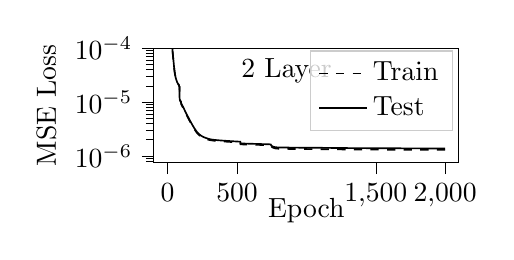
\begin{tikzpicture}

\begin{axis}[
legend cell align={left},
legend style={fill opacity=0.8, draw opacity=1, text opacity=1, draw=white!80!black},
log basis y={10},
tick align=outside,
tick pos=left,
title={2 Layer $\hy$},
title style={at={(0.45,0.85)},anchor=north},
x grid style={white!69.0196078431373!black},
xlabel={Epoch},
x label style={yshift=10pt},
xmin=-99.95, xmax=2098.95,
xtick style={color=black},
xtick = {0,500,1500,2000},
y grid style={white!69.0196078431373!black},
ylabel={MSE Loss},
ymin=7.6063321892292e-07, ymax=1e-4,
ymode=log,
ytick style={color=black},
width=.45\textwidth,
height=.25\textwidth
]
\addplot [semithick, black, dashed]
table {%
0 0.0518386695683002
1 0.042526340380311
2 0.0347423156872392
3 0.0278063397407532
4 0.021599099136889
5 0.0169535573758185
6 0.0133449736572802
7 0.0096524867080152
8 0.00607697855122387
9 0.00346671832166612
10 0.00228777943272144
11 0.00164228947134689
12 0.00122930787573569
13 0.000946592513937503
14 0.000754222130053677
15 0.000623254176578484
16 0.000526171202189289
17 0.000440977271879092
18 0.00037380238971673
19 0.000321372847538441
20 0.00028025879181223
21 0.000247563553391956
22 0.000221549878042424
23 0.000200674695734051
24 0.000183563173413859
25 0.000169053649296984
26 0.000156700562307378
27 0.000145990131146391
28 0.000136467741052911
29 0.000127828117649187
30 0.000119895841526159
31 0.000112545413488988
32 0.000105680738532101
33 9.92588357621571e-05
34 9.3258946260903e-05
35 8.76442736916943e-05
36 8.23576925613452e-05
37 7.73938517377246e-05
38 7.27130913655856e-05
39 6.8314350421133e-05
40 6.41955712490017e-05
41 6.03399962346884e-05
42 5.67417087368085e-05
43 5.33954841157538e-05
44 5.0292471962166e-05
45 4.74299892848649e-05
46 4.48063469739282e-05
47 4.24147469020681e-05
48 4.02486506536661e-05
49 3.82998454442713e-05
50 3.65582336962689e-05
51 3.50118609967467e-05
52 3.36569491373666e-05
53 3.24788894431549e-05
54 3.14478582076845e-05
55 3.05533147147798e-05
56 2.97498192085186e-05
57 2.89429238437151e-05
58 2.82225572700554e-05
59 2.75767276507395e-05
60 2.69969247092376e-05
61 2.646950968483e-05
62 2.59851477894699e-05
63 2.55374307816965e-05
64 2.51249913926586e-05
65 2.47355156570848e-05
66 2.43629243705072e-05
67 2.39832626575662e-05
68 2.35637702317035e-05
69 2.32211665752402e-05
70 2.29383413134201e-05
71 2.26900584239047e-05
72 2.24617844360182e-05
73 2.22450978726556e-05
74 2.20345916350197e-05
75 2.18275812112552e-05
76 2.16219654867018e-05
77 2.1417711785034e-05
78 2.1214236781816e-05
79 2.10117783281021e-05
80 2.08105283381883e-05
81 2.06107105623232e-05
82 2.04136253305478e-05
83 1.99121589284914e-05
84 1.94468321642489e-05
85 1.92526021455706e-05
86 1.68429254481453e-05
87 1.11265583582281e-05
88 1.08224221194178e-05
89 1.06731547539312e-05
90 1.05443111642671e-05
91 1.04219903960256e-05
92 1.03025638554755e-05
93 1.01851757890472e-05
94 1.00690036970263e-05
95 9.95377955223375e-06
96 9.83960515168292e-06
97 9.6077903663172e-06
98 9.08970189311731e-06
99 8.98518852409325e-06
100 8.88667989238456e-06
101 8.78861929595587e-06
102 8.69103235254443e-06
103 8.59354773410814e-06
104 8.49647685981836e-06
105 8.39990374788613e-06
106 8.30380843763123e-06
107 8.20817358044224e-06
108 8.11326919119892e-06
109 8.0190826447506e-06
110 7.92535356458757e-06
111 7.83217436401173e-06
112 7.73989984918444e-06
113 7.64807627137998e-06
114 7.5570470621642e-06
115 7.46617350023371e-06
116 7.37646823699834e-06
117 7.28749768268244e-06
118 7.19915332319943e-06
119 7.11171480043049e-06
120 7.0252807649922e-06
121 6.93957605744799e-06
122 6.8550750625036e-06
123 6.77161231669743e-06
124 6.68928749064435e-06
125 6.60800705782094e-06
126 6.52786106229541e-06
127 6.44881835250999e-06
128 6.3709648547956e-06
129 6.29415914409037e-06
130 6.21850223342335e-06
131 6.14401825305322e-06
132 6.07067480086698e-06
133 5.99841532675782e-06
134 5.92726610238969e-06
135 5.85724698703416e-06
136 5.78829684695847e-06
137 5.72039379244416e-06
138 5.65365198121981e-06
139 5.58796158020414e-06
140 5.52333012819872e-06
141 5.45967585458129e-06
142 5.39706647441562e-06
143 5.33535780868988e-06
144 5.27458272108561e-06
145 5.21480528050233e-06
146 5.15576177031107e-06
147 5.09760672775883e-06
148 5.04035929361635e-06
149 4.98399535490535e-06
150 4.92840583774523e-06
151 4.87364144305502e-06
152 4.81966467486927e-06
153 4.76406977395527e-06
154 4.69791715545398e-06
155 4.64507658807634e-06
156 4.59343973466275e-06
157 4.54271117132521e-06
158 4.49279561598814e-06
159 4.4436497382776e-06
160 4.39516718938648e-06
161 4.34741592334831e-06
162 4.30033761358573e-06
163 4.25400164704115e-06
164 4.20822800037968e-06
165 4.16278015359239e-06
166 4.1181904248333e-06
167 4.07423587330413e-06
168 4.0309002961294e-06
169 3.98809872649508e-06
170 3.94593327928305e-06
171 3.90432318772582e-06
172 3.86316539697873e-06
173 3.82265143798577e-06
174 3.78271101931205e-06
175 3.74335995593356e-06
176 3.70451060553023e-06
177 3.66598950404295e-06
178 3.62826339983258e-06
179 3.59102522270405e-06
180 3.55434255129694e-06
181 3.51821511981143e-06
182 3.4826161552246e-06
183 3.44756884828712e-06
184 3.41307895928367e-06
185 3.3791370713061e-06
186 3.34570067798268e-06
187 3.31284759954542e-06
188 3.28047421021438e-06
189 3.24868683401291e-06
190 3.21743388849427e-06
191 3.1866992187588e-06
192 3.15648334390062e-06
193 3.12686154870789e-06
194 3.09775542154966e-06
195 3.0692054060637e-06
196 3.04119435577377e-06
197 3.01375761148392e-06
198 2.98678445994938e-06
199 2.96039846932672e-06
200 2.93452443952447e-06
201 2.90920865177213e-06
202 2.88442320947979e-06
203 2.86015471203882e-06
204 2.83649073071501e-06
205 2.81332962913439e-06
206 2.79064786889194e-06
207 2.76854250500946e-06
208 2.74696784845219e-06
209 2.72586062430946e-06
210 2.70531269256935e-06
211 2.68526590684814e-06
212 2.66566363393395e-06
213 2.64662573533769e-06
214 2.6280339858431e-06
215 2.60993901497386e-06
216 2.59233656379365e-06
217 2.57519019442043e-06
218 2.55849347206549e-06
219 2.54225137109643e-06
220 2.52648555715496e-06
221 2.51116403057949e-06
222 2.49626635525146e-06
223 2.48174041792026e-06
224 2.46764998712479e-06
225 2.45395659851511e-06
226 2.44061466628409e-06
227 2.42766318024223e-06
228 2.41510581383864e-06
229 2.40287865153732e-06
230 2.39102976365757e-06
231 2.37946973879843e-06
232 2.36823859097512e-06
233 2.35734377997687e-06
234 2.34669803728593e-06
235 2.33637789938257e-06
236 2.32633338055166e-06
237 2.31655079858228e-06
238 2.30704811121996e-06
239 2.29775435502688e-06
240 2.28908307065012e-06
241 2.28025623937356e-06
242 2.27162592034347e-06
243 2.26319784212592e-06
244 2.2550409375981e-06
245 2.24706835138022e-06
246 2.23929092283015e-06
247 2.23166111379669e-06
248 2.22424669038901e-06
249 2.21699714541046e-06
250 2.20993513937628e-06
251 2.20302234424707e-06
252 2.19623759960541e-06
253 2.18960344636798e-06
254 2.18315790721135e-06
255 2.17678003446053e-06
256 2.17060044519712e-06
257 2.16451002290796e-06
258 2.15849525591238e-06
259 2.15263430231971e-06
260 2.14691730741379e-06
261 2.14129940786734e-06
262 2.13577006115884e-06
263 2.13036238608311e-06
264 2.12501493570016e-06
265 2.1199581875635e-06
266 2.11479780750778e-06
267 2.10963459062441e-06
268 2.10465096063217e-06
269 2.09979531643967e-06
270 2.09493869374455e-06
271 2.09029867505706e-06
272 2.08560229043542e-06
273 2.08097659026407e-06
274 2.07650576862761e-06
275 2.07193567734976e-06
276 2.06749240817317e-06
277 2.06326575550975e-06
278 2.05894802388684e-06
279 2.05470462492485e-06
280 2.05050052682054e-06
281 2.04643580877928e-06
282 2.0424704373454e-06
283 2.03852960294171e-06
284 2.03469342307017e-06
285 2.03091579976444e-06
286 2.02713633768781e-06
287 2.02345604839138e-06
288 2.01982171290638e-06
289 2.01625873410194e-06
290 2.01274700611975e-06
291 2.00929016750706e-06
292 2.00590146562263e-06
293 2.00254602100358e-06
294 1.99926750190116e-06
295 1.99598840447379e-06
296 1.99279543198827e-06
297 1.98967802123207e-06
298 1.98662693992446e-06
299 1.98363486015296e-06
300 1.98073774367913e-06
301 1.97792627022864e-06
302 1.97517233220879e-06
303 1.97249674567956e-06
304 1.96989209428011e-06
305 1.96735570136752e-06
306 1.96489110953735e-06
307 1.96252498756166e-06
308 1.96016407414845e-06
309 1.95790429916087e-06
310 1.95567747516634e-06
311 1.95353562503442e-06
312 1.95143923531305e-06
313 1.94938852894211e-06
314 1.94739756454965e-06
315 1.94547211549434e-06
316 1.94368945972201e-06
317 1.94186115868433e-06
318 1.94003258525299e-06
319 1.93824945745291e-06
320 1.9365728117009e-06
321 1.93486980356283e-06
322 1.93323022483582e-06
323 1.93159868342718e-06
324 1.93004855782419e-06
325 1.92850577320769e-06
326 1.92703124560012e-06
327 1.92557061188836e-06
328 1.92414228069993e-06
329 1.92272855258579e-06
330 1.92145235405405e-06
331 1.92011111062129e-06
332 1.91873049038804e-06
333 1.91744816731898e-06
334 1.91613417905501e-06
335 1.91486396772689e-06
336 1.91374089342844e-06
337 1.91252254262508e-06
338 1.91134569661244e-06
339 1.91014032100156e-06
340 1.90892861962766e-06
341 1.90778080786913e-06
342 1.90679503680258e-06
343 1.90562279988171e-06
344 1.90453983475436e-06
345 1.9034283604924e-06
346 1.90236943444688e-06
347 1.90128401038692e-06
348 1.90023423112962e-06
349 1.89921649234748e-06
350 1.89817762452549e-06
351 1.89717194177774e-06
352 1.89619797345131e-06
353 1.89519621744694e-06
354 1.89419035530136e-06
355 1.89321117386498e-06
356 1.89228158308197e-06
357 1.89132848026929e-06
358 1.89040515931538e-06
359 1.8894536552807e-06
360 1.88852625899472e-06
361 1.8876163518371e-06
362 1.88671577905097e-06
363 1.88581250529296e-06
364 1.88489490290067e-06
365 1.88400545243894e-06
366 1.88320691779609e-06
367 1.88227364219529e-06
368 1.88137783914044e-06
369 1.88048757183878e-06
370 1.87960764208128e-06
371 1.87875062977128e-06
372 1.87785555567643e-06
373 1.87700367860089e-06
374 1.8761265273497e-06
375 1.87530233984035e-06
376 1.87443296317724e-06
377 1.87359234882933e-06
378 1.87277639042804e-06
379 1.87191020336286e-06
380 1.87106933947234e-06
381 1.87022027148487e-06
382 1.86942492166509e-06
383 1.86859680513862e-06
384 1.86778859585957e-06
385 1.86696180901436e-06
386 1.86615413451818e-06
387 1.865346644081e-06
388 1.86454020524707e-06
389 1.86374061308925e-06
390 1.86296425601995e-06
391 1.86214191205636e-06
392 1.86135847434343e-06
393 1.86057959820118e-06
394 1.85977571720741e-06
395 1.85900325470811e-06
396 1.85821711534118e-06
397 1.85742586654669e-06
398 1.85668396852634e-06
399 1.85587053044856e-06
400 1.85511533595673e-06
401 1.85435227967901e-06
402 1.85357387726981e-06
403 1.85281492088052e-06
404 1.85205200068594e-06
405 1.85128828331926e-06
406 1.85053131349377e-06
407 1.8499851529441e-06
408 1.84917399599271e-06
409 1.84840255906238e-06
410 1.84766332199615e-06
411 1.84689625007195e-06
412 1.84613141198042e-06
413 1.84538050450556e-06
414 1.844629050197e-06
415 1.84387742933723e-06
416 1.84314657485629e-06
417 1.84239931502361e-06
418 1.84165844211748e-06
419 1.84091300036471e-06
420 1.84018742834269e-06
421 1.83944933723978e-06
422 1.83872336367585e-06
423 1.83799873639146e-06
424 1.83724605551561e-06
425 1.83653046701693e-06
426 1.83579679980994e-06
427 1.83508214388439e-06
428 1.83435587473468e-06
429 1.83363736755382e-06
430 1.8329269255446e-06
431 1.83219673760959e-06
432 1.83147712380105e-06
433 1.83076220457679e-06
434 1.83004805330711e-06
435 1.82932657037327e-06
436 1.82861742405294e-06
437 1.82790977305558e-06
438 1.82720573548067e-06
439 1.82647991425711e-06
440 1.82577657187721e-06
441 1.82505562622737e-06
442 1.82437355033471e-06
443 1.82366404123968e-06
444 1.82293964576274e-06
445 1.82224642969686e-06
446 1.82155447021159e-06
447 1.82083569222868e-06
448 1.82014943925424e-06
449 1.81945615088352e-06
450 1.81874204338328e-06
451 1.81806114380834e-06
452 1.8173547899778e-06
453 1.81667541403385e-06
454 1.81598416770612e-06
455 1.81524100480601e-06
456 1.81453961306488e-06
457 1.81385451594451e-06
458 1.81315790109693e-06
459 1.81245884846248e-06
460 1.81177978004143e-06
461 1.81107571381744e-06
462 1.81042428357614e-06
463 1.80971381985273e-06
464 1.80901504791109e-06
465 1.80835478647623e-06
466 1.80766282676359e-06
467 1.80698605220186e-06
468 1.80630960915096e-06
469 1.80562094067227e-06
470 1.80495204324416e-06
471 1.80429276622363e-06
472 1.80363471463352e-06
473 1.80292723803177e-06
474 1.80225790609256e-06
475 1.80158976775147e-06
476 1.80091279730732e-06
477 1.80023987002187e-06
478 1.79959257354767e-06
479 1.79890977392461e-06
480 1.79824207714319e-06
481 1.79757481157594e-06
482 1.7969080555531e-06
483 1.79623438566523e-06
484 1.79557559511068e-06
485 1.79491270898779e-06
486 1.79438170130197e-06
487 1.79366591225971e-06
488 1.79298442958498e-06
489 1.79231373408584e-06
490 1.79167655073798e-06
491 1.79100179059333e-06
492 1.79032596940942e-06
493 1.78968522516243e-06
494 1.78901104857232e-06
495 1.78837366763673e-06
496 1.78771149103341e-06
497 1.78705672965407e-06
498 1.78641258935386e-06
499 1.78577213569042e-06
500 1.78510025034484e-06
501 1.78445535595984e-06
502 1.78384143919175e-06
503 1.78316099584208e-06
504 1.7825342940796e-06
505 1.78187944834463e-06
506 1.78124007402403e-06
507 1.78060222037857e-06
508 1.77995303192802e-06
509 1.77932496455924e-06
510 1.77868458877128e-06
511 1.77803215694894e-06
512 1.77739755554285e-06
513 1.77675821737466e-06
514 1.77612358766055e-06
515 1.77547155703905e-06
516 1.77483872244011e-06
517 1.77422070601096e-06
518 1.7735807008421e-06
519 1.77294365573744e-06
520 1.77230281133234e-06
521 1.77169832647905e-06
522 1.77105510329056e-06
523 1.77042892869395e-06
524 1.76978312288156e-06
525 1.66620164694109e-06
526 1.63933637233526e-06
527 1.63880179010789e-06
528 1.63844974755989e-06
529 1.63812484262849e-06
530 1.63779529955832e-06
531 1.63742095688235e-06
532 1.63711894725793e-06
533 1.63679492797542e-06
534 1.63647552042789e-06
535 1.6361367341915e-06
536 1.63582143278518e-06
537 1.63551573919563e-06
538 1.63520860402855e-06
539 1.63490383059184e-06
540 1.63459672538124e-06
541 1.63429267476545e-06
542 1.63399191654889e-06
543 1.63368553430132e-06
544 1.63338495767107e-06
545 1.63310262541927e-06
546 1.6327682387498e-06
547 1.63247037161796e-06
548 1.63218582176228e-06
549 1.63187798207787e-06
550 1.6315871942254e-06
551 1.63128337254648e-06
552 1.63099369069641e-06
553 1.63070029680057e-06
554 1.63040730399189e-06
555 1.63011679620695e-06
556 1.62983160720387e-06
557 1.62952682003947e-06
558 1.62922214192918e-06
559 1.62894504913425e-06
560 1.62864188482104e-06
561 1.6283534936008e-06
562 1.6280654233185e-06
563 1.62778253840656e-06
564 1.62747459560819e-06
565 1.62719646951359e-06
566 1.62692239271678e-06
567 1.62661389299501e-06
568 1.62633292706005e-06
569 1.62606319807423e-06
570 1.62576276485993e-06
571 1.62547591571638e-06
572 1.62518481394613e-06
573 1.62490155244654e-06
574 1.62461253736979e-06
575 1.62433828410258e-06
576 1.62405268940802e-06
577 1.62376205736336e-06
578 1.62348133056867e-06
579 1.62319527444765e-06
580 1.62290394715114e-06
581 1.62262100627686e-06
582 1.62234837728192e-06
583 1.62206169241585e-06
584 1.6217815277173e-06
585 1.62149699008296e-06
586 1.62121524058989e-06
587 1.62092517706469e-06
588 1.62070420867622e-06
589 1.62038921615704e-06
590 1.62008199799857e-06
591 1.61979725899641e-06
592 1.61950673955857e-06
593 1.61922272562265e-06
594 1.6189295055824e-06
595 1.61864341677642e-06
596 1.61835239086372e-06
597 1.61807546018622e-06
598 1.61779094619874e-06
599 1.61749259794419e-06
600 1.61723098355537e-06
601 1.61693797414841e-06
602 1.61665728629146e-06
603 1.61636831695944e-06
604 1.61610073524798e-06
605 1.61582153997131e-06
606 1.61554774945216e-06
607 1.61525743881441e-06
608 1.61498842523145e-06
609 1.61470044996292e-06
610 1.61442914523491e-06
611 1.61414135411064e-06
612 1.61386748200698e-06
613 1.61359336857458e-06
614 1.61332622727173e-06
615 1.61304242104166e-06
616 1.61276320352499e-06
617 1.61248982448114e-06
618 1.61219475916141e-06
619 1.61193266151827e-06
620 1.61164703547456e-06
621 1.61138146705753e-06
622 1.61109890345301e-06
623 1.61082260021317e-06
624 1.61053988405513e-06
625 1.61026904530104e-06
626 1.6099991666465e-06
627 1.60971038680202e-06
628 1.60944881005776e-06
629 1.60917611752609e-06
630 1.60890855008233e-06
631 1.60862766114178e-06
632 1.60834999020665e-06
633 1.60807368021665e-06
634 1.60779430278524e-06
635 1.60753966724769e-06
636 1.60726439040104e-06
637 1.60700710711126e-06
638 1.60672452217625e-06
639 1.60644054170689e-06
640 1.60616960967275e-06
641 1.60589141702872e-06
642 1.60563484433851e-06
643 1.6053435355019e-06
644 1.60508566412432e-06
645 1.60482664446704e-06
646 1.60453707941599e-06
647 1.6042754193677e-06
648 1.60399306275849e-06
649 1.60374430119248e-06
650 1.6034647498202e-06
651 1.60318650912927e-06
652 1.60291618941244e-06
653 1.60264964672763e-06
654 1.60237670334595e-06
655 1.60212423365635e-06
656 1.60184172608524e-06
657 1.60158811885935e-06
658 1.60129746804216e-06
659 1.60103951819224e-06
660 1.60076912700902e-06
661 1.60050588327465e-06
662 1.60023428719569e-06
663 1.59996088962089e-06
664 1.59969389768833e-06
665 1.59941708385247e-06
666 1.59916993624165e-06
667 1.59889477750141e-06
668 1.59866888432703e-06
669 1.59837924398687e-06
670 1.59808459493149e-06
671 1.59782723729052e-06
672 1.5975413056708e-06
673 1.59727512193797e-06
674 1.59698751379267e-06
675 1.59672256081933e-06
676 1.59644536088877e-06
677 1.59617859861783e-06
678 1.59590370850538e-06
679 1.59562858524964e-06
680 1.59536997378495e-06
681 1.59507531752467e-06
682 1.59482622048301e-06
683 1.59457645222005e-06
684 1.59428069426326e-06
685 1.5940048189691e-06
686 1.59374665537371e-06
687 1.59347681504585e-06
688 1.59320771297189e-06
689 1.59294189681702e-06
690 1.59265840376577e-06
691 1.59240391452897e-06
692 1.59212388167873e-06
693 1.59185475271784e-06
694 1.59160081452114e-06
695 1.5913355798034e-06
696 1.59105049479535e-06
697 1.59078170094062e-06
698 1.5905177025104e-06
699 1.59024808239394e-06
700 1.5899925537326e-06
701 1.58970312894269e-06
702 1.58944773028225e-06
703 1.58917952906279e-06
704 1.58889819385877e-06
705 1.5886472953639e-06
706 1.58836964335762e-06
707 1.58811646971913e-06
708 1.58783535489704e-06
709 1.58757957046873e-06
710 1.58731703973558e-06
711 1.58704471705562e-06
712 1.58677873791646e-06
713 1.5865028876334e-06
714 1.58624447136901e-06
715 1.58597577814135e-06
716 1.58570803385771e-06
717 1.58545115763786e-06
718 1.58517122966373e-06
719 1.58490910264675e-06
720 1.58464107597922e-06
721 1.58438146414142e-06
722 1.58410357899186e-06
723 1.58384261210642e-06
724 1.58350118182682e-06
725 1.58321730540933e-06
726 1.58293486397554e-06
727 1.58265849421468e-06
728 1.58239726721376e-06
729 1.58211539564945e-06
730 1.58183252307253e-06
731 1.58156696035405e-06
732 1.58106459616647e-06
733 1.5807887297683e-06
734 1.580489066626e-06
735 1.58021400281427e-06
736 1.57994096404934e-06
737 1.57964867177895e-06
738 1.57935908634954e-06
739 1.57908623067726e-06
740 1.57895105029127e-06
741 1.57861684205329e-06
742 1.57829686450839e-06
743 1.57820503723372e-06
744 1.56886491616604e-06
745 1.54443650944813e-06
746 1.52464937485774e-06
747 1.5084941576049e-06
748 1.49567416087848e-06
749 1.48492991016269e-06
750 1.47589340608079e-06
751 1.46807804819105e-06
752 1.46103214052573e-06
753 1.45476694632407e-06
754 1.44896854914123e-06
755 1.44370241736169e-06
756 1.43866883598776e-06
757 1.43380883416455e-06
758 1.42928160187239e-06
759 1.42504067417804e-06
760 1.42097017825904e-06
761 1.41716485458687e-06
762 1.41355964707657e-06
763 1.41026495602148e-06
764 1.40694243066264e-06
765 1.40386480411792e-06
766 1.40090109704261e-06
767 1.39811546335977e-06
768 1.39556718215772e-06
769 1.39314711935867e-06
770 1.39085914671e-06
771 1.38873771130932e-06
772 1.38676904158785e-06
773 1.38486147091044e-06
774 1.38307318255215e-06
775 1.38140495923267e-06
776 1.37981144834498e-06
777 1.37832817009098e-06
778 1.37694258201293e-06
779 1.37560938435399e-06
780 1.3743737128209e-06
781 1.3732237981543e-06
782 1.3721374578779e-06
783 1.37116235606527e-06
784 1.37018989329363e-06
785 1.36925985286496e-06
786 1.36841710016711e-06
787 1.36757084865735e-06
788 1.36681302183206e-06
789 1.36608643293812e-06
790 1.36541132677337e-06
791 1.36474158155409e-06
792 1.36417904980135e-06
793 1.36355554245426e-06
794 1.36299955610752e-06
795 1.36246179810939e-06
796 1.36196002624445e-06
797 1.36147286586663e-06
798 1.36102072210065e-06
799 1.36058262586403e-06
800 1.36019539741028e-06
801 1.35977008343957e-06
802 1.35934900353618e-06
803 1.35907496527921e-06
804 1.35871082459005e-06
805 1.35838341267913e-06
806 1.35806158336038e-06
807 1.35770684502745e-06
808 1.35738369530713e-06
809 1.35709290060504e-06
810 1.35672559207478e-06
811 1.35645564012066e-06
812 1.35619012348798e-06
813 1.35594104767733e-06
814 1.35568918759077e-06
815 1.35547467380093e-06
816 1.35525254742674e-06
817 1.35503257631342e-06
818 1.35482675494814e-06
819 1.35461341591281e-06
820 1.35443167101812e-06
821 1.35425345231965e-06
822 1.3540686281317e-06
823 1.35388498344469e-06
824 1.35370961773162e-06
825 1.35353743995381e-06
826 1.3533792219107e-06
827 1.35313768534218e-06
828 1.35298258597061e-06
829 1.352827967807e-06
830 1.3526768412504e-06
831 1.35252841401723e-06
832 1.35240225704081e-06
833 1.35225109995929e-06
834 1.35212322014411e-06
835 1.35198998505359e-06
836 1.35184609810324e-06
837 1.35173012962753e-06
838 1.35159571098598e-06
839 1.35147283796755e-06
840 1.35134105134682e-06
841 1.35123280175264e-06
842 1.35110112422865e-06
843 1.35098620997098e-06
844 1.3508639218287e-06
845 1.35077587185606e-06
846 1.35064492155834e-06
847 1.35053679737496e-06
848 1.35042975225019e-06
849 1.35031924180851e-06
850 1.35021662519819e-06
851 1.35011604727708e-06
852 1.35000363111715e-06
853 1.34990536004409e-06
854 1.3498181129421e-06
855 1.34971324047228e-06
856 1.34960946446938e-06
857 1.34950742594242e-06
858 1.34941408889233e-06
859 1.34932775988261e-06
860 1.34922658703829e-06
861 1.34912472361748e-06
862 1.34902612357735e-06
863 1.34892750345728e-06
864 1.34883547387687e-06
865 1.34874449845768e-06
866 1.34864384494904e-06
867 1.34856915693149e-06
868 1.348471884981e-06
869 1.34839657053476e-06
870 1.34830537385255e-06
871 1.34821930835471e-06
872 1.34813692710622e-06
873 1.34803793085325e-06
874 1.34795173156022e-06
875 1.3478776119058e-06
876 1.34777355222582e-06
877 1.34769706210136e-06
878 1.34761042174603e-06
879 1.34751966670876e-06
880 1.34744346894422e-06
881 1.34735287390697e-06
882 1.34725689983384e-06
883 1.34717631696901e-06
884 1.34709783374376e-06
885 1.34702141804155e-06
886 1.34693583878231e-06
887 1.34685476582774e-06
888 1.34676708303516e-06
889 1.34668838386176e-06
890 1.3466111598035e-06
891 1.34654315939997e-06
892 1.34647579018576e-06
893 1.34638291420686e-06
894 1.34629611308412e-06
895 1.34621114347055e-06
896 1.34613849976972e-06
897 1.34607026022593e-06
898 1.34600097389637e-06
899 1.34590469681939e-06
900 1.34583183752568e-06
901 1.3457547924105e-06
902 1.34568102149046e-06
903 1.34570885896323e-06
904 1.34563602135529e-06
905 1.34554965568157e-06
906 1.34547586169731e-06
907 1.34539394407795e-06
908 1.34532783863506e-06
909 1.34524034038463e-06
910 1.34516967027309e-06
911 1.34509670238003e-06
912 1.34502306164563e-06
913 1.34495103804966e-06
914 1.34488076425043e-06
915 1.34479510651886e-06
916 1.34472651404849e-06
917 1.34466214339568e-06
918 1.34458127747905e-06
919 1.34450533219876e-06
920 1.3444267981555e-06
921 1.34435084679296e-06
922 1.34428695463384e-06
923 1.34422671932555e-06
924 1.34414231379765e-06
925 1.34407956909399e-06
926 1.3439992275579e-06
927 1.3439298076463e-06
928 1.34387832962091e-06
929 1.3438092536262e-06
930 1.34373289975542e-06
931 1.3436577213497e-06
932 1.34358143714053e-06
933 1.34352394559301e-06
934 1.34345717660267e-06
935 1.34337900578885e-06
936 1.34335605609692e-06
937 1.34328150070928e-06
938 1.34321433966988e-06
939 1.34313157009558e-06
940 1.3430716178533e-06
941 1.34299877356625e-06
942 1.3429399402014e-06
943 1.34285865880202e-06
944 1.34280206063409e-06
945 1.34274019325176e-06
946 1.34266461981269e-06
947 1.34259506944545e-06
948 1.34254850138404e-06
949 1.34247986547109e-06
950 1.34240087921e-06
951 1.34232612865048e-06
952 1.3423135030024e-06
953 1.34225830529999e-06
954 1.3421897558743e-06
955 1.34212832678315e-06
956 1.34206213189714e-06
957 1.34198343585012e-06
958 1.34193174501718e-06
959 1.34187326334256e-06
960 1.34180413468243e-06
961 1.34174007241938e-06
962 1.34166821864312e-06
963 1.34160912554648e-06
964 1.34154919388152e-06
965 1.34148838895953e-06
966 1.34141044561886e-06
967 1.34135855292072e-06
968 1.34130112543573e-06
969 1.34123174636613e-06
970 1.34118099316538e-06
971 1.34110277215882e-06
972 1.34103400789343e-06
973 1.34098474899247e-06
974 1.34092078039316e-06
975 1.34086393288158e-06
976 1.34079251927233e-06
977 1.34072488621939e-06
978 1.34067154296247e-06
979 1.34060519832246e-06
980 1.34055623038876e-06
981 1.34048152499133e-06
982 1.3404323760966e-06
983 1.34035964379109e-06
984 1.34030211174263e-06
985 1.34024774162356e-06
986 1.34017881156012e-06
987 1.3401354625131e-06
988 1.34007251983803e-06
989 1.34001645538717e-06
990 1.33994008200489e-06
991 1.33989448013949e-06
992 1.33979940444817e-06
993 1.3397541583231e-06
994 1.33968041419052e-06
995 1.33962406884791e-06
996 1.33956490974185e-06
997 1.33950567945362e-06
998 1.33946297422938e-06
999 1.33938883983831e-06
1000 1.33933092904215e-06
1001 1.33928694378937e-06
1002 1.33921256117731e-06
1003 1.33916161001935e-06
1004 1.3390988379598e-06
1005 1.33903752758613e-06
1006 1.33898176045477e-06
1007 1.33892504666733e-06
1008 1.33887592123472e-06
1009 1.33881134048863e-06
1010 1.33875219198387e-06
1011 1.33870028915339e-06
1012 1.33863348575858e-06
1013 1.33858250521257e-06
1014 1.33852591613959e-06
1015 1.33846663027271e-06
1016 1.33840421788989e-06
1017 1.33835072642796e-06
1018 1.33830789980038e-06
1019 1.33824401744675e-06
1020 1.33817713299322e-06
1021 1.33813398639404e-06
1022 1.33806409412784e-06
1023 1.33800658908001e-06
1024 1.33795149331206e-06
1025 1.3379155276283e-06
1026 1.33784969801809e-06
1027 1.33778447249711e-06
1028 1.33765031387156e-06
1029 1.33759461118643e-06
1030 1.33753808258064e-06
1031 1.33748855502347e-06
1032 1.33742270143955e-06
1033 1.33736784084704e-06
1034 1.33731045195873e-06
1035 1.33725952910879e-06
1036 1.33719250703734e-06
1037 1.33714265534479e-06
1038 1.33709573304941e-06
1039 1.33703461840184e-06
1040 1.33698563801943e-06
1041 1.33692117942985e-06
1042 1.33686207065864e-06
1043 1.33682150280379e-06
1044 1.33675993406257e-06
1045 1.33670628150639e-06
1046 1.33664372732767e-06
1047 1.33658942088744e-06
1048 1.33653863915129e-06
1049 1.33648365992656e-06
1050 1.33643210853052e-06
1051 1.33637117450292e-06
1052 1.33631502657749e-06
1053 1.33626177149893e-06
1054 1.33622257948218e-06
1055 1.33616662400016e-06
1056 1.33610955839458e-06
1057 1.33605329271802e-06
1058 1.33598385832556e-06
1059 1.33594217295752e-06
1060 1.33588493156367e-06
1061 1.33583359792055e-06
1062 1.33576979409611e-06
1063 1.33572435426288e-06
1064 1.33567137682178e-06
1065 1.33562173462565e-06
1066 1.33556964851778e-06
1067 1.33551589878778e-06
1068 1.33546273754348e-06
1069 1.33540153122169e-06
1070 1.33536268666035e-06
1071 1.33529603027682e-06
1072 1.33524601922375e-06
1073 1.33519661385151e-06
1074 1.33514066943974e-06
1075 1.33509146333211e-06
1076 1.33504329576795e-06
1077 1.33499757205868e-06
1078 1.33493545313001e-06
1079 1.33489117727947e-06
1080 1.33483645198851e-06
1081 1.33478451633096e-06
1082 1.33473267716511e-06
1083 1.33466724497566e-06
1084 1.33462421723607e-06
1085 1.33456596925896e-06
1086 1.33453018727892e-06
1087 1.33446277706639e-06
1088 1.33441716130278e-06
1089 1.33436078276361e-06
1090 1.33430692164893e-06
1091 1.33425975168677e-06
1092 1.33421545604051e-06
1093 1.33415072625098e-06
1094 1.33410108566068e-06
1095 1.33404680869376e-06
1096 1.33399491723196e-06
1097 1.33394408973686e-06
1098 1.33389038987275e-06
1099 1.33383919941821e-06
1100 1.33379414305068e-06
1101 1.33373261306247e-06
1102 1.33368463527006e-06
1103 1.33363207953607e-06
1104 1.33359130424537e-06
1105 1.33354491660498e-06
1106 1.33348266453481e-06
1107 1.33343180641532e-06
1108 1.33338205131395e-06
1109 1.33333231407562e-06
1110 1.33328824017553e-06
1111 1.33323012887843e-06
1112 1.33317537382993e-06
1113 1.33314741407276e-06
1114 1.33307755031353e-06
1115 1.33303352079395e-06
1116 1.33297956337231e-06
1117 1.3329289483579e-06
1118 1.33287542442417e-06
1119 1.33282477237628e-06
1120 1.33277926930475e-06
1121 1.33273204622242e-06
1122 1.33267181597319e-06
1123 1.332627589818e-06
1124 1.33257524055352e-06
1125 1.33252936851136e-06
1126 1.33248547196274e-06
1127 1.33243876933875e-06
1128 1.33238333026497e-06
1129 1.33232479907974e-06
1130 1.33227799227598e-06
1131 1.33223086616852e-06
1132 1.33218174798344e-06
1133 1.33213632797435e-06
1134 1.33208051036604e-06
1135 1.33205012393489e-06
1136 1.33198282409808e-06
1137 1.33193860241931e-06
1138 1.33188387665939e-06
1139 1.33183967609796e-06
1140 1.33179460509325e-06
1141 1.33174281238269e-06
1142 1.33169365426511e-06
1143 1.33164133212915e-06
1144 1.33158321374083e-06
1145 1.3315432472325e-06
1146 1.33148943393735e-06
1147 1.33144728846446e-06
1148 1.33139592961129e-06
1149 1.33134038986782e-06
1150 1.33129153603306e-06
1151 1.33124128893769e-06
1152 1.3311990425251e-06
1153 1.33114998108397e-06
1154 1.33109154313615e-06
1155 1.33104795212091e-06
1156 1.33099706505391e-06
1157 1.33095313810827e-06
1158 1.33090183919649e-06
1159 1.3308592359067e-06
1160 1.33080201646862e-06
1161 1.33075989552367e-06
1162 1.33070932677981e-06
1163 1.33065972174506e-06
1164 1.3306096723511e-06
1165 1.33056723711888e-06
1166 1.33051543905083e-06
1167 1.33045599883985e-06
1168 1.33043390209764e-06
1169 1.33039126671974e-06
1170 1.33034304828072e-06
1171 1.33029533026274e-06
1172 1.33023865356563e-06
1173 1.33019446022331e-06
1174 1.33014583248325e-06
1175 1.33009934955908e-06
1176 1.33004679793203e-06
1177 1.32999394267586e-06
1178 1.32859383582229e-06
1179 1.32577590167671e-06
1180 1.32481529779227e-06
1181 1.32425906130607e-06
1182 1.32385161771253e-06
1183 1.32355970555409e-06
1184 1.32332581735284e-06
1185 1.32313855300481e-06
1186 1.32299621942877e-06
1187 1.32287166445622e-06
1188 1.32275965106032e-06
1189 1.32266207796761e-06
1190 1.32258898742066e-06
1191 1.32251438074604e-06
1192 1.3224399087477e-06
1193 1.32236959144905e-06
1194 1.32232037235269e-06
1195 1.32225536714259e-06
1196 1.32219561778868e-06
1197 1.32214652194307e-06
1198 1.32208095470787e-06
1199 1.32204806527625e-06
1200 1.32199041914305e-06
1201 1.32194223348847e-06
1202 1.32188372917597e-06
1203 1.32185073353241e-06
1204 1.32179744296934e-06
1205 1.3217571945745e-06
1206 1.32170356749839e-06
1207 1.32168178934933e-06
1208 1.32160852400887e-06
1209 1.32156865880972e-06
1210 1.3215270177227e-06
1211 1.32148737561977e-06
1212 1.32144626445552e-06
1213 1.32139509810258e-06
1214 1.32141864840207e-06
1215 1.32135991154314e-06
1216 1.32131602497054e-06
1217 1.32127464453902e-06
1218 1.32121060731549e-06
1219 1.32116699967355e-06
1220 1.3211242721809e-06
1221 1.32107436284912e-06
1222 1.32103417314511e-06
1223 1.32099427466414e-06
1224 1.32095226790341e-06
1225 1.32089809829949e-06
1226 1.32086301134393e-06
1227 1.32081426257002e-06
1228 1.3207805423292e-06
1229 1.3207305637053e-06
1230 1.32068811232955e-06
1231 1.32064384796138e-06
1232 1.32060167554471e-06
1233 1.3205631688038e-06
1234 1.3205066439923e-06
1235 1.32047018907144e-06
1236 1.32054637529677e-06
1237 1.3205274783985e-06
1238 1.32047940205382e-06
1239 1.32043280677863e-06
1240 1.32039506168269e-06
1241 1.32036514655454e-06
1242 1.32031703172686e-06
1243 1.32027795616807e-06
1244 1.3202443684861e-06
1245 1.32019133667427e-06
1246 1.32015820261699e-06
1247 1.32011709712287e-06
1248 1.32007585411031e-06
1249 1.32003833635963e-06
1250 1.31999951743467e-06
1251 1.31995052718992e-06
1252 1.31991537205067e-06
1253 1.31987489763219e-06
1254 1.31983271600689e-06
1255 1.31978467074134e-06
1256 1.319753576837e-06
1257 1.31970657953673e-06
1258 1.31966508058667e-06
1259 1.319630016269e-06
1260 1.31958882650451e-06
1261 1.31953997157552e-06
1262 1.31951191637825e-06
1263 1.31946960593154e-06
1264 1.31942758504522e-06
1265 1.31938184219393e-06
1266 1.31933255261174e-06
1267 1.31929545118226e-06
1268 1.31925781937525e-06
1269 1.31922233245518e-06
1270 1.31924204031009e-06
1271 1.31918251739194e-06
1272 1.31914621874785e-06
1273 1.31909760800397e-06
1274 1.31904689864371e-06
1275 1.31899939506752e-06
1276 1.31895242788005e-06
1277 1.31888589362461e-06
1278 1.3188213102211e-06
1279 1.31876878970161e-06
1280 1.31870717576987e-06
1281 1.31865774105222e-06
1282 1.31860239366688e-06
1283 1.31855959794791e-06
1284 1.31852673801802e-06
1285 1.31848573423099e-06
1286 1.31843639238127e-06
1287 1.31837194871309e-06
1288 1.31832015325983e-06
1289 1.31827320812761e-06
1290 1.31821452710312e-06
1291 1.31826412868463e-06
1292 1.31820652498504e-06
1293 1.31813436787809e-06
1294 1.31808043758497e-06
1295 1.31803203781544e-06
1296 1.31797565646252e-06
1297 1.31792156848576e-06
1298 1.31787510680681e-06
1299 1.31782350318588e-06
1300 1.31777007236167e-06
1301 1.317731111385e-06
1302 1.31768447428726e-06
1303 1.31765222302249e-06
1304 1.31759061208925e-06
1305 1.3175407495396e-06
1306 1.31750282601217e-06
1307 1.31745717092713e-06
1308 1.31740909702671e-06
1309 1.31737010387667e-06
1310 1.31731581387839e-06
1311 1.31729359902977e-06
1312 1.31723423439212e-06
1313 1.31719637688832e-06
1314 1.31714781051073e-06
1315 1.31711109040111e-06
1316 1.31705777398849e-06
1317 1.31702496820196e-06
1318 1.31698145554537e-06
1319 1.31693504215491e-06
1320 1.316892996158e-06
1321 1.31685051350416e-06
1322 1.3168058811317e-06
1323 1.31676369285572e-06
1324 1.3167272482093e-06
1325 1.31667373887012e-06
1326 1.31663302317975e-06
1327 1.31659156795649e-06
1328 1.31655225268901e-06
1329 1.31651966761126e-06
1330 1.31647060948126e-06
1331 1.31643030140083e-06
1332 1.31639117168447e-06
1333 1.31633731963632e-06
1334 1.31630387018333e-06
1335 1.31626258671247e-06
1336 1.31621279176386e-06
1337 1.31617875889845e-06
1338 1.31613359954486e-06
1339 1.31608632344182e-06
1340 1.31604712120748e-06
1341 1.31601232321543e-06
1342 1.3159628022521e-06
1343 1.31592109164558e-06
1344 1.31588097301005e-06
1345 1.31584353617598e-06
1346 1.3158043823438e-06
1347 1.31577746958556e-06
1348 1.31573951045993e-06
1349 1.31568544951222e-06
1350 1.31564648904714e-06
1351 1.31560409097631e-06
1352 1.31556468213034e-06
1353 1.31551994411439e-06
1354 1.31547720894787e-06
1355 1.31544238529102e-06
1356 1.31539883138032e-06
1357 1.3153504088308e-06
1358 1.31530955987103e-06
1359 1.31526198380527e-06
1360 1.31523578205872e-06
1361 1.3151850012747e-06
1362 1.31514612101569e-06
1363 1.31510655799616e-06
1364 1.31506297603323e-06
1365 1.31502549686502e-06
1366 1.31497581915596e-06
1367 1.31494573567181e-06
1368 1.31489326294343e-06
1369 1.31486664048452e-06
1370 1.31481228511632e-06
1371 1.31477881735975e-06
1372 1.31473155177275e-06
1373 1.31468939930812e-06
1374 1.31464601584241e-06
1375 1.31461001865318e-06
1376 1.31457059183049e-06
1377 1.31452871148952e-06
1378 1.31448866785888e-06
1379 1.31444212428278e-06
1380 1.31440802965699e-06
1381 1.31436307299282e-06
1382 1.31431838971707e-06
1383 1.31427322443756e-06
1384 1.31423886649884e-06
1385 1.31420234399116e-06
1386 1.31415619608788e-06
1387 1.31413195184393e-06
1388 1.31408533862043e-06
1389 1.3140527643003e-06
1390 1.3140024599636e-06
1391 1.31395506453202e-06
1392 1.31391883945753e-06
1393 1.31387949465989e-06
1394 1.31384093273823e-06
1395 1.31380773196099e-06
1396 1.31375993719018e-06
1397 1.31372225746418e-06
1398 1.31367593549214e-06
1399 1.31363591665945e-06
1400 1.31359878579929e-06
1401 1.31356280685679e-06
1402 1.31351572737515e-06
1403 1.31348148261168e-06
1404 1.31343552995133e-06
1405 1.31340653955192e-06
1406 1.31335477141192e-06
1407 1.31331217909292e-06
1408 1.31328199159952e-06
1409 1.31324050759929e-06
1410 1.313199410518e-06
1411 1.31315960558709e-06
1412 1.31310952575348e-06
1413 1.31307809232339e-06
1414 1.31303962449181e-06
1415 1.3129952787807e-06
1416 1.31295043550494e-06
1417 1.31291564053981e-06
1418 1.31287857932705e-06
1419 1.31284263386533e-06
1420 1.31279429353981e-06
1421 1.31275722567636e-06
1422 1.31273118608988e-06
1423 1.31268142855845e-06
1424 1.3126316385268e-06
1425 1.31259607421441e-06
1426 1.31256069056462e-06
1427 1.31251248853914e-06
1428 1.31246915155714e-06
1429 1.31243717203233e-06
1430 1.31239350761803e-06
1431 1.31234716056383e-06
1432 1.3123242802493e-06
1433 1.31227735960238e-06
1434 1.31223271989711e-06
1435 1.31219915439829e-06
1436 1.31215062850742e-06
1437 1.31212218929022e-06
1438 1.3120791121537e-06
1439 1.31203161237181e-06
1440 1.31200182872249e-06
1441 1.31196549817503e-06
1442 1.31192107697586e-06
1443 1.31187962790591e-06
1444 1.31183938752599e-06
1445 1.31180776863005e-06
1446 1.31176054296134e-06
1447 1.31172362119969e-06
1448 1.31168643122237e-06
1449 1.31165350231299e-06
1450 1.31160334724711e-06
1451 1.3115657474998e-06
1452 1.311524503123e-06
1453 1.31148720245733e-06
1454 1.31145775291941e-06
1455 1.31141236701637e-06
1456 1.31137372878243e-06
1457 1.31133921740911e-06
1458 1.31128970619443e-06
1459 1.31125061385262e-06
1460 1.31120704479315e-06
1461 1.31118090965288e-06
1462 1.31113069129185e-06
1463 1.31109799757212e-06
1464 1.31105958655553e-06
1465 1.31102414700024e-06
1466 1.31113465407395e-06
1467 1.3115353781501e-06
1468 1.31073669899706e-06
1469 1.31061095918028e-06
1470 1.31053976475926e-06
1471 1.31051849380981e-06
1472 1.31045500958749e-06
1473 1.31041446591951e-06
1474 1.31038325683619e-06
1475 1.31034178316725e-06
1476 1.31030691308354e-06
1477 1.31025875219848e-06
1478 1.31020995374342e-06
1479 1.31017023034019e-06
1480 1.31014068551849e-06
1481 1.31009896698231e-06
1482 1.31005129526329e-06
1483 1.31001381359397e-06
1484 1.30997352819406e-06
1485 1.30993995983886e-06
1486 1.30989869869325e-06
1487 1.30986009870071e-06
1488 1.30982312171568e-06
1489 1.30978367678836e-06
1490 1.30974461123401e-06
1491 1.30970787867568e-06
1492 1.30966502571539e-06
1493 1.3096298849149e-06
1494 1.30959659510665e-06
1495 1.30956331126697e-06
1496 1.30951565556359e-06
1497 1.3094790621011e-06
1498 1.30944215527506e-06
1499 1.30939618007631e-06
1500 1.30936962753481e-06
1501 1.30933061875282e-06
1502 1.30928901221239e-06
1503 1.30924293445389e-06
1504 1.30921448861443e-06
1505 1.30917329974523e-06
1506 1.3091434063881e-06
1507 1.3091095128317e-06
1508 1.30906401409447e-06
1509 1.30902855379134e-06
1510 1.30899295051279e-06
1511 1.30895525619223e-06
1512 1.30891014282497e-06
1513 1.30888283999298e-06
1514 1.30883949670135e-06
1515 1.30880467609984e-06
1516 1.30876093874122e-06
1517 1.30873182040148e-06
1518 1.30869287713153e-06
1519 1.30865213854747e-06
1520 1.30861667719273e-06
1521 1.3085740121852e-06
1522 1.30854242374312e-06
1523 1.30850691304829e-06
1524 1.30846172521615e-06
1525 1.3084308924789e-06
1526 1.30839026867591e-06
1527 1.30835211136571e-06
1528 1.30831085695604e-06
1529 1.30828064069988e-06
1530 1.308229396912e-06
1531 1.3081966038726e-06
1532 1.30816021432167e-06
1533 1.30811588522306e-06
1534 1.30807387886023e-06
1535 1.30804364836479e-06
1536 1.30800523677976e-06
1537 1.3079673543217e-06
1538 1.30793483285174e-06
1539 1.30789522229691e-06
1540 1.30785042148318e-06
1541 1.30781459185414e-06
1542 1.30778182165159e-06
1543 1.30775194134003e-06
1544 1.30771855249634e-06
1545 1.30767076348093e-06
1546 1.30763190119865e-06
1547 1.30759709659856e-06
1548 1.30755398699023e-06
1549 1.30752424855984e-06
1550 1.30748375099188e-06
1551 1.30745104392815e-06
1552 1.30741234369225e-06
1553 1.30737575641149e-06
1554 1.30733214440681e-06
1555 1.30730984595573e-06
1556 1.3072714322675e-06
1557 1.30723216413742e-06
1558 1.30718758191506e-06
1559 1.307162111857e-06
1560 1.3071203532462e-06
1561 1.30709440516341e-06
1562 1.30705507541506e-06
1563 1.30701736974004e-06
1564 1.30697946784153e-06
1565 1.30694769262618e-06
1566 1.30688747393037e-06
1567 1.30680106401826e-06
1568 1.30671250040848e-06
1569 1.30658519580606e-06
1570 1.30647350641766e-06
1571 1.30637264372524e-06
1572 1.30628260801302e-06
1573 1.30619263643439e-06
1574 1.30612632679572e-06
1575 1.3060445271833e-06
1576 1.30598045691954e-06
1577 1.30592523802875e-06
1578 1.30587186585274e-06
1579 1.30581472285485e-06
1580 1.30576124846016e-06
1581 1.30571444087479e-06
1582 1.30566849995262e-06
1583 1.30562871432005e-06
1584 1.30558825976834e-06
1585 1.30554417266637e-06
1586 1.30550023445153e-06
1587 1.30546279150678e-06
1588 1.30542278432699e-06
1589 1.30538380547307e-06
1590 1.30534058511955e-06
1591 1.30530249140293e-06
1592 1.30526528718633e-06
1593 1.30523094507851e-06
1594 1.30519310198451e-06
1595 1.30515999937586e-06
1596 1.30511330560523e-06
1597 1.30507664401591e-06
1598 1.30503874788701e-06
1599 1.30500457611049e-06
1600 1.30496916459322e-06
1601 1.30494285006932e-06
1602 1.30490435564923e-06
1603 1.30485838994332e-06
1604 1.30482659885445e-06
1605 1.30478732155837e-06
1606 1.3047524880534e-06
1607 1.30471406019694e-06
1608 1.30468427630603e-06
1609 1.30464755363846e-06
1610 1.30461211692534e-06
1611 1.30457956852581e-06
1612 1.3045466137811e-06
1613 1.30451384271169e-06
1614 1.30447131995481e-06
1615 1.30443236731992e-06
1616 1.30440879334515e-06
1617 1.30436869623907e-06
1618 1.30434016888614e-06
1619 1.30430917424462e-06
1620 1.30427162395108e-06
1621 1.30423100985411e-06
1622 1.30420232578388e-06
1623 1.30416617172102e-06
1624 1.3041299450407e-06
1625 1.30410262495673e-06
1626 1.30406100817027e-06
1627 1.30401921336443e-06
1628 1.30399914212376e-06
1629 1.30395539915185e-06
1630 1.30392317404926e-06
1631 1.30389736538916e-06
1632 1.30385062966809e-06
1633 1.30381534091839e-06
1634 1.30380177922973e-06
1635 1.30375087475443e-06
1636 1.30372180177574e-06
1637 1.3036884428459e-06
1638 1.30364403828764e-06
1639 1.30360659640871e-06
1640 1.30358346132198e-06
1641 1.30354482784867e-06
1642 1.30351669014317e-06
1643 1.30347193973535e-06
1644 1.30343639024488e-06
1645 1.30340346458979e-06
1646 1.30337845570239e-06
1647 1.30333353850176e-06
1648 1.30331501819114e-06
1649 1.30327775123362e-06
1650 1.30324178195451e-06
1651 1.30319812065238e-06
1652 1.30316767285876e-06
1653 1.30314653416974e-06
1654 1.30310440718517e-06
1655 1.30306319319118e-06
1656 1.30303104739937e-06
1657 1.3029972061247e-06
1658 1.30295640188649e-06
1659 1.30292751202887e-06
1660 1.30288585020821e-06
1661 1.3028596930269e-06
1662 1.30282386928116e-06
1663 1.30279087981933e-06
1664 1.30276015883624e-06
1665 1.30272269737475e-06
1666 1.30268822775292e-06
1667 1.30265419538489e-06
1668 1.30262256087121e-06
1669 1.30258766282054e-06
1670 1.30255358023135e-06
1671 1.30251958941585e-06
1672 1.3024827413517e-06
1673 1.30244834473103e-06
1674 1.30242112800261e-06
1675 1.30238559525253e-06
1676 1.30235082198737e-06
1677 1.30231930461377e-06
1678 1.30228147989442e-06
1679 1.30225140925688e-06
1680 1.30221264949171e-06
1681 1.3021771924997e-06
1682 1.30215629911845e-06
1683 1.30212054297374e-06
1684 1.3020825262231e-06
1685 1.30205074025014e-06
1686 1.30201645512784e-06
1687 1.3019760089179e-06
1688 1.30194387260474e-06
1689 1.30191285383319e-06
1690 1.30188629354677e-06
1691 1.30184348482487e-06
1692 1.30181177200939e-06
1693 1.30178400208081e-06
1694 1.3017502183601e-06
1695 1.30171701061954e-06
1696 1.30168398564479e-06
1697 1.30165680079131e-06
1698 1.30161776992566e-06
1699 1.30158671188951e-06
1700 1.301542995094e-06
1701 1.30151153366853e-06
1702 1.30147992234697e-06
1703 1.30145104238011e-06
1704 1.30140742756169e-06
1705 1.30138871969621e-06
1706 1.30135159645306e-06
1707 1.30132069060096e-06
1708 1.30128667251483e-06
1709 1.30124737745518e-06
1710 1.30121323856258e-06
1711 1.30118363685483e-06
1712 1.30115531682407e-06
1713 1.30111670598865e-06
1714 1.30109344169682e-06
1715 1.30105685009596e-06
1716 1.3010196516916e-06
1717 1.30099644994175e-06
1718 1.30095129730989e-06
1719 1.30092531632897e-06
1720 1.30088796163363e-06
1721 1.3008512727879e-06
1722 1.30082383361696e-06
1723 1.30078734325423e-06
1724 1.30075498084636e-06
1725 1.30072494835076e-06
1726 1.30069480792372e-06
1727 1.30066290452646e-06
1728 1.30062102641659e-06
1729 1.30059479585043e-06
1730 1.30056997774375e-06
1731 1.30052966622429e-06
1732 1.30049582769232e-06
1733 1.30045942457002e-06
1734 1.30042508709494e-06
1735 1.30040336006232e-06
1736 1.30036208952333e-06
1737 1.30033579117139e-06
1738 1.30031166487754e-06
1739 1.30027404554767e-06
1740 1.30023207418617e-06
1741 1.30020137497411e-06
1742 1.30016529365662e-06
1743 1.30013674007046e-06
1744 1.3001077397945e-06
1745 1.30007461308423e-06
1746 1.30003726891914e-06
1747 1.30001273335267e-06
1748 1.29998552732502e-06
1749 1.29994284267809e-06
1750 1.29990960890325e-06
1751 1.29988650238033e-06
1752 1.29984577939979e-06
1753 1.29981313244798e-06
1754 1.29978438639e-06
1755 1.29974981085468e-06
1756 1.29972055978556e-06
1757 1.29969358975757e-06
1758 1.29965266478393e-06
1759 1.29962256363569e-06
1760 1.29958961294108e-06
1761 1.29955889558175e-06
1762 1.29952550526014e-06
1763 1.29949171279975e-06
1764 1.29945958289568e-06
1765 1.29943046847814e-06
1766 1.29939997185602e-06
1767 1.29936943054076e-06
1768 1.29933621389e-06
1769 1.29929934533379e-06
1770 1.29926757435328e-06
1771 1.2992392044282e-06
1772 1.29920533100858e-06
1773 1.2991700671563e-06
1774 1.29912627332374e-06
1775 1.29909210278356e-06
1776 1.29906255446599e-06
1777 1.29903083757199e-06
1778 1.29900498477298e-06
1779 1.29897524021771e-06
1780 1.29893359738276e-06
1781 1.29891209623167e-06
1782 1.29887807187856e-06
1783 1.29884300372396e-06
1784 1.2988116064605e-06
1785 1.29877996954519e-06
1786 1.29874484923675e-06
1787 1.2987117428338e-06
1788 1.29867583009968e-06
1789 1.29864896672416e-06
1790 1.29861854901492e-06
1791 1.29858806143091e-06
1792 1.29855296736991e-06
1793 1.29853388322942e-06
1794 1.29849827672501e-06
1795 1.29846098039366e-06
1796 1.29843629670745e-06
1797 1.29840156135685e-06
1798 1.29837512514541e-06
1799 1.29836212408918e-06
1800 1.29831896404653e-06
1801 1.29829055092046e-06
1802 1.2982576319871e-06
1803 1.29823140947849e-06
1804 1.29820048537965e-06
1805 1.29817173797164e-06
1806 1.29814512463611e-06
1807 1.2981023378984e-06
1808 1.29807500867685e-06
1809 1.29803826821728e-06
1810 1.29800773646593e-06
1811 1.2979781847946e-06
1812 1.29794077389533e-06
1813 1.29791346279262e-06
1814 1.29788016687371e-06
1815 1.29784268041533e-06
1816 1.29782022439429e-06
1817 1.29778623839627e-06
1818 1.2977592077732e-06
1819 1.29772728793398e-06
1820 1.29769857242934e-06
1821 1.29766320105773e-06
1822 1.29762787879883e-06
1823 1.29760096830012e-06
1824 1.2975656488976e-06
1825 1.29753746644212e-06
1826 1.2975013315355e-06
1827 1.29748086591519e-06
1828 1.2974416726621e-06
1829 1.29741440080977e-06
1830 1.29738914618827e-06
1831 1.29735291490363e-06
1832 1.29731755794182e-06
1833 1.297284848917e-06
1834 1.29725806272063e-06
1835 1.29722429477397e-06
1836 1.29719462270828e-06
1837 1.29716277369596e-06
1838 1.297132099495e-06
1839 1.29710682350037e-06
1840 1.29707580282457e-06
1841 1.29704243165918e-06
1842 1.29701305678509e-06
1843 1.29698461583416e-06
1844 1.29694613946185e-06
1845 1.2969152633957e-06
1846 1.29688457019483e-06
1847 1.29685601237384e-06
1848 1.29682263252562e-06
1849 1.29679150796846e-06
1850 1.29676873049789e-06
1851 1.2967360405014e-06
1852 1.29670956320638e-06
1853 1.29668201290656e-06
1854 1.29664866686596e-06
1855 1.29661068872622e-06
1856 1.29658337199601e-06
1857 1.29654636393184e-06
1858 1.29651771007389e-06
1859 1.29649333848647e-06
1860 1.29646568724695e-06
1861 1.29642290272614e-06
1862 1.29639706153739e-06
1863 1.2963646600781e-06
1864 1.29633471287605e-06
1865 1.29630338759057e-06
1866 1.2962749853358e-06
1867 1.29623791896449e-06
1868 1.2962157103118e-06
1869 1.29618162705469e-06
1870 1.29615798564942e-06
1871 1.29613095455738e-06
1872 1.29609084298465e-06
1873 1.29606213252487e-06
1874 1.29602892181424e-06
1875 1.29599581627815e-06
1876 1.29597255276792e-06
1877 1.29594302700298e-06
1878 1.29589945512976e-06
1879 1.29588080446297e-06
1880 1.29584873782562e-06
1881 1.29581950989177e-06
1882 1.29579072644503e-06
1883 1.29575479243726e-06
1884 1.29572682105561e-06
1885 1.2956990530455e-06
1886 1.29567194731806e-06
1887 1.29563374412101e-06
1888 1.29560203026813e-06
1889 1.29557642833333e-06
1890 1.29554112201902e-06
1891 1.29551987771492e-06
1892 1.29548469141127e-06
1893 1.29545346204907e-06
1894 1.29542539946215e-06
1895 1.29539005234847e-06
1896 1.29536077616876e-06
1897 1.29534280944199e-06
1898 1.29530432798219e-06
1899 1.29527160012799e-06
1900 1.29524660897573e-06
1901 1.29521397803956e-06
1902 1.29518296886033e-06
1903 1.29515333100017e-06
1904 1.29512402115495e-06
1905 1.29509240069581e-06
1906 1.29506431177617e-06
1907 1.29503260087915e-06
1908 1.29501052880698e-06
1909 1.29497696535452e-06
1910 1.29494201468106e-06
1911 1.29491107074386e-06
1912 1.29488443907633e-06
1913 1.2948505791428e-06
1914 1.29481940658138e-06
1915 1.29480016065031e-06
1916 1.29476492631397e-06
1917 1.29473640311062e-06
1918 1.29470511370755e-06
1919 1.29467511445114e-06
1920 1.29464872480867e-06
1921 1.29462289207538e-06
1922 1.29458773517399e-06
1923 1.29455712445292e-06
1924 1.29452539033537e-06
1925 1.29449879550236e-06
1926 1.29446464374894e-06
1927 1.2944351666988e-06
1928 1.29440817724458e-06
1929 1.29438209746979e-06
1930 1.29435313922954e-06
1931 1.29433152231684e-06
1932 1.2942912425018e-06
1933 1.29426927999532e-06
1934 1.29423369530457e-06
1935 1.29420180451234e-06
1936 1.29417424042799e-06
1937 1.29413976632975e-06
1938 1.2941117217764e-06
1939 1.29408380541918e-06
1940 1.29404398151678e-06
1941 1.29402087938502e-06
1942 1.29399364944049e-06
1943 1.29396807983539e-06
1944 1.2939327145034e-06
1945 1.29390792969275e-06
1946 1.29387755833932e-06
1947 1.29384964577639e-06
1948 1.29381176310517e-06
1949 1.29378730865426e-06
1950 1.29375462110204e-06
1951 1.29372353643475e-06
1952 1.29369512035282e-06
1953 1.29367324544205e-06
1954 1.29364491158412e-06
1955 1.29361388236759e-06
1956 1.29358137532165e-06
1957 1.29356112196888e-06
1958 1.29352790402493e-06
1959 1.29349322354244e-06
1960 1.29347562032933e-06
1961 1.29343464580245e-06
1962 1.29341100023339e-06
1963 1.29337962520992e-06
1964 1.29334828922367e-06
1965 1.29331728018656e-06
1966 1.29328694673347e-06
1967 1.29326018944198e-06
1968 1.29323436475204e-06
1969 1.29320748276029e-06
1970 1.29317501347259e-06
1971 1.29314339103814e-06
1972 1.29311811366506e-06
1973 1.29308671535e-06
1974 1.29305738650487e-06
1975 1.29302824606725e-06
1976 1.29300026733858e-06
1977 1.29297728362587e-06
1978 1.29294138612579e-06
1979 1.29291615802174e-06
1980 1.29288673092276e-06
1981 1.29287205595574e-06
1982 1.29286416517971e-06
1983 1.29269020844447e-06
1984 1.29260432319711e-06
1985 1.29256846786063e-06
1986 1.29254003090296e-06
1987 1.29252492530441e-06
1988 1.29249429504341e-06
1989 1.29247078901074e-06
1990 1.2924532950791e-06
1991 1.29243247440058e-06
1992 1.29241390827417e-06
1993 1.29237765963808e-06
1994 1.29235108063597e-06
1995 1.2923343797695e-06
1996 1.29230386770018e-06
1997 1.29228608733456e-06
1998 1.29225766541197e-06
1999 1.29223331674666e-06
};
\addlegendentry{Train}
\addplot [semithick, black]
table {%
0 0.046846017241478
1 0.0383708029985428
2 0.0309884883463383
3 0.0245152190327644
4 0.0189679358154535
5 0.0149657595902681
6 0.0117847537621856
7 0.00785275362432003
8 0.00443816976621747
9 0.00276716682128608
10 0.00193949567619711
11 0.00143606925848871
12 0.00109465920832008
13 0.000860574538819492
14 0.000701205339282751
15 0.000592119118664414
16 0.000498535810038447
17 0.000422000564867631
18 0.00036225956864655
19 0.000315643643261865
20 0.000278686813544482
21 0.000249177595833316
22 0.000225506300921552
23 0.000206198645173572
24 0.00018996320432052
25 0.000176013796590269
26 0.000163945907843299
27 0.000153226894326508
28 0.000143488970934413
29 0.00013452026178129
30 0.000126200568047352
31 0.000118409756396431
32 0.000111086439574137
33 0.000104212405858561
34 9.7776428447105e-05
35 9.17216530069709e-05
36 8.60177024151199e-05
37 8.06632524472661e-05
38 7.55998480599374e-05
39 7.08621955709532e-05
40 6.64242106722668e-05
41 6.22747902525589e-05
42 5.84089866606519e-05
43 5.48197385796811e-05
44 5.14986750204116e-05
45 4.84408956253901e-05
46 4.5642376790056e-05
47 4.30981672252528e-05
48 4.08026098739356e-05
49 3.87447726097889e-05
50 3.69136432709638e-05
51 3.52969509549439e-05
52 3.38936224579811e-05
53 3.2669759093551e-05
54 3.16056830342859e-05
55 3.0682967917528e-05
56 2.98149170703255e-05
57 2.90021780529059e-05
58 2.82771343336208e-05
59 2.76301270787371e-05
60 2.70484961220063e-05
61 2.65189119090792e-05
62 2.60316555795725e-05
63 2.55819704761961e-05
64 2.51599667535629e-05
65 2.47605166805442e-05
66 2.43684044107795e-05
67 2.39299824897898e-05
68 2.35225343203638e-05
69 2.31977446674136e-05
70 2.29244742513401e-05
71 2.26770971494261e-05
72 2.24468767555663e-05
73 2.22265607590089e-05
74 2.20125257328618e-05
75 2.18019231397193e-05
76 2.15937525354093e-05
77 2.13865077967057e-05
78 2.11813367059221e-05
79 2.09772460948443e-05
80 2.07742505153874e-05
81 2.05734759219922e-05
82 2.03746549232164e-05
83 1.96250730368774e-05
84 1.94256845134078e-05
85 1.92311126738787e-05
86 1.18716716315248e-05
87 1.12445295599173e-05
88 1.10792543637217e-05
89 1.09475913632195e-05
90 1.08244212242425e-05
91 1.07040941657033e-05
92 1.05850458567147e-05
93 1.04674263639026e-05
94 1.0350699085393e-05
95 1.023471395456e-05
96 1.01197601907188e-05
97 9.5123250503093e-06
98 9.38474931899691e-06
99 9.28386452869745e-06
100 9.18379009817727e-06
101 9.08395122678485e-06
102 8.98411417438183e-06
103 8.88483100425219e-06
104 8.78585615282645e-06
105 8.68727147462778e-06
106 8.58920793689322e-06
107 8.4915282059228e-06
108 8.39437052491121e-06
109 8.29942746349843e-06
110 8.20353943709051e-06
111 8.10821529739769e-06
112 8.01262467575725e-06
113 7.918774826976e-06
114 7.82522147346754e-06
115 7.73259944253368e-06
116 7.64051856094738e-06
117 7.54929942559102e-06
118 7.45903116694535e-06
119 7.36920082999859e-06
120 7.28032864572015e-06
121 7.19231229595607e-06
122 7.105323675205e-06
123 7.0190130827541e-06
124 6.93419269737205e-06
125 6.85027998770238e-06
126 6.76738454785664e-06
127 6.68554821459111e-06
128 6.60503519611666e-06
129 6.52583412374952e-06
130 6.44760439172387e-06
131 6.37048697171849e-06
132 6.29445594313438e-06
133 6.21960452917847e-06
134 6.14581631452893e-06
135 6.07303400101955e-06
136 6.0014181144652e-06
137 5.93111781199696e-06
138 5.86179930905928e-06
139 5.79359630137333e-06
140 5.72644830754143e-06
141 5.66039534533047e-06
142 5.59533191335504e-06
143 5.53142581338761e-06
144 5.46819137525745e-06
145 5.40599512532935e-06
146 5.34493847226258e-06
147 5.28485315953731e-06
148 5.22568461747142e-06
149 5.16738600708777e-06
150 5.10996414959664e-06
151 5.05336129208445e-06
152 4.9976015361608e-06
153 4.92653862238512e-06
154 4.87146508021397e-06
155 4.8173369577853e-06
156 4.76419609185541e-06
157 4.71183557237964e-06
158 4.66031542600831e-06
159 4.60958244730136e-06
160 4.55952158517903e-06
161 4.51021924163797e-06
162 4.46155445388285e-06
163 4.413742772158e-06
164 4.36648360846448e-06
165 4.3197637751291e-06
166 4.27378381573362e-06
167 4.22837729274761e-06
168 4.18360696130549e-06
169 4.13935913456953e-06
170 4.09567564929603e-06
171 4.05279251936008e-06
172 4.01027409679955e-06
173 3.96848236050573e-06
174 3.92731408282998e-06
175 3.8865923670528e-06
176 3.84640179618145e-06
177 3.80677988687239e-06
178 3.76767479792761e-06
179 3.72941531168181e-06
180 3.69149825019122e-06
181 3.6542601264955e-06
182 3.61761522071902e-06
183 3.5814271086565e-06
184 3.54579378836206e-06
185 3.5104699236399e-06
186 3.47592003890895e-06
187 3.44202749147371e-06
188 3.40868450621201e-06
189 3.37587903231906e-06
190 3.34381229549763e-06
191 3.31203796122281e-06
192 3.28103828906023e-06
193 3.25049609273265e-06
194 3.22048617817927e-06
195 3.1911947644403e-06
196 3.16229534291779e-06
197 3.1337522159447e-06
198 3.10582436213735e-06
199 3.07852951664245e-06
200 3.05181060866744e-06
201 3.02568946608517e-06
202 3.00021838484099e-06
203 2.97491237688519e-06
204 2.95049449050566e-06
205 2.92651202471461e-06
206 2.90325283458515e-06
207 2.88060937236878e-06
208 2.85826399704092e-06
209 2.83668964584649e-06
210 2.81563188764267e-06
211 2.79479513665137e-06
212 2.77475601251354e-06
213 2.75520233117277e-06
214 2.73612954515556e-06
215 2.71763678938441e-06
216 2.69952420239861e-06
217 2.68186363427958e-06
218 2.66457323050417e-06
219 2.64800155491685e-06
220 2.63167612502002e-06
221 2.61605600826442e-06
222 2.60081878877827e-06
223 2.58565387412091e-06
224 2.57128158409614e-06
225 2.55729264608817e-06
226 2.5434583221795e-06
227 2.53028042607184e-06
228 2.51731967182423e-06
229 2.50474613494589e-06
230 2.49260665441398e-06
231 2.48064247898583e-06
232 2.46914464696601e-06
233 2.45786941377446e-06
234 2.44702073359804e-06
235 2.43636623054044e-06
236 2.42592273025366e-06
237 2.41593488681247e-06
238 2.40604981627257e-06
239 2.39454175243736e-06
240 2.38496431848034e-06
241 2.37560857385688e-06
242 2.36638106798637e-06
243 2.35762900047121e-06
244 2.34906042351213e-06
245 2.34054073189327e-06
246 2.33240825764369e-06
247 2.32432307711861e-06
248 2.31647300097393e-06
249 2.30882278628997e-06
250 2.30132854994736e-06
251 2.29410079555237e-06
252 2.28696308113285e-06
253 2.27994132728782e-06
254 2.2731221633876e-06
255 2.26643737732957e-06
256 2.26000611291965e-06
257 2.25339977077965e-06
258 2.24699829232122e-06
259 2.24085442823707e-06
260 2.23485972128401e-06
261 2.22880544242798e-06
262 2.22294852392224e-06
263 2.21718892134959e-06
264 2.2116278159956e-06
265 2.20599986278103e-06
266 2.20042466025916e-06
267 2.19495632336475e-06
268 2.18968580156798e-06
269 2.1844550701644e-06
270 2.17936781155004e-06
271 2.17437786886876e-06
272 2.16965236177202e-06
273 2.16483385884203e-06
274 2.15997692976089e-06
275 2.15530872083036e-06
276 2.15021736948984e-06
277 2.14562965084042e-06
278 2.14111582863552e-06
279 2.13668317883275e-06
280 2.13234125112649e-06
281 2.12806639865448e-06
282 2.12381792152883e-06
283 2.11966334973113e-06
284 2.11553378903773e-06
285 2.11155611395952e-06
286 2.10754387808265e-06
287 2.10364714803291e-06
288 2.0998343188694e-06
289 2.09598420042312e-06
290 2.09230734071753e-06
291 2.08856886274589e-06
292 2.08493315767555e-06
293 2.08135452339775e-06
294 2.07782954930735e-06
295 2.07432572096877e-06
296 2.07094581128331e-06
297 2.06754771170381e-06
298 2.06429240279249e-06
299 2.06109029932122e-06
300 2.05800984076632e-06
301 2.05492415261688e-06
302 2.05180754164758e-06
303 2.04896286959411e-06
304 2.04610319087806e-06
305 2.04338948606164e-06
306 2.04076900445216e-06
307 2.03825675271219e-06
308 2.0357510948088e-06
309 2.03333684112295e-06
310 2.03093964046275e-06
311 2.02861724574177e-06
312 2.02637943402806e-06
313 2.02403339244484e-06
314 2.0218606096023e-06
315 2.01979310077149e-06
316 2.01772627406172e-06
317 2.0156662685622e-06
318 2.01365946850274e-06
319 2.01170269065187e-06
320 2.00985368792317e-06
321 2.008035835388e-06
322 2.0062404928467e-06
323 2.00445401787874e-06
324 2.00277054318576e-06
325 2.00112754100701e-06
326 1.99953205992642e-06
327 1.9979424905614e-06
328 1.99632700059738e-06
329 1.994814738282e-06
330 1.99338865058962e-06
331 1.99191208594129e-06
332 1.99047826754395e-06
333 1.98907810045057e-06
334 1.98766042558418e-06
335 1.98630050363136e-06
336 1.98500219994457e-06
337 1.98356542568945e-06
338 1.98221573555202e-06
339 1.98089469449769e-06
340 1.9795622847596e-06
341 1.97831514014979e-06
342 1.97709687199676e-06
343 1.97587201000715e-06
344 1.974676251848e-06
345 1.97352483155555e-06
346 1.97232657228597e-06
347 1.97118743017199e-06
348 1.97002691493253e-06
349 1.96894961845828e-06
350 1.96781206796004e-06
351 1.96668429452984e-06
352 1.96564246834896e-06
353 1.9644819531095e-06
354 1.9634078398667e-06
355 1.96237647287489e-06
356 1.96133396457299e-06
357 1.96031123778084e-06
358 1.95917527889833e-06
359 1.95824577531312e-06
360 1.95721463569498e-06
361 1.95623829313263e-06
362 1.95530833480007e-06
363 1.95432494365377e-06
364 1.95336792785383e-06
365 1.95239226741251e-06
366 1.95136567526788e-06
367 1.9502210761857e-06
368 1.94919675777783e-06
369 1.94815197573917e-06
370 1.94720951185445e-06
371 1.94616791304725e-06
372 1.94522522178886e-06
373 1.94425388144737e-06
374 1.943346205735e-06
375 1.94240101336618e-06
376 1.94146218746027e-06
377 1.94056860891578e-06
378 1.93966616279795e-06
379 1.93865480468958e-06
380 1.93776008927671e-06
381 1.93688833860506e-06
382 1.93602136278059e-06
383 1.93517280422384e-06
384 1.93428809325269e-06
385 1.93343589671713e-06
386 1.93253868019383e-06
387 1.93165874406986e-06
388 1.93084747479588e-06
389 1.93001665138581e-06
390 1.92919856090157e-06
391 1.92841844182112e-06
392 1.92753850569716e-06
393 1.92671450349735e-06
394 1.92591483028082e-06
395 1.9251492631156e-06
396 1.92425181921863e-06
397 1.92344646166021e-06
398 1.92265611076436e-06
399 1.92185461855843e-06
400 1.92107518159901e-06
401 1.92025459000433e-06
402 1.91948743122339e-06
403 1.91869480659079e-06
404 1.91788421943784e-06
405 1.91712092600937e-06
406 1.91636127055972e-06
407 1.9155809241056e-06
408 1.91478261513112e-06
409 1.91399544746673e-06
410 1.91320646081294e-06
411 1.91246635949938e-06
412 1.91165986507258e-06
413 1.91091567103285e-06
414 1.9101560155832e-06
415 1.90942250810622e-06
416 1.90862192539498e-06
417 1.90785863196652e-06
418 1.90713512893126e-06
419 1.9064046909989e-06
420 1.90569164715271e-06
421 1.9049134607485e-06
422 1.90417733847426e-06
423 1.90344394468411e-06
424 1.90265177479887e-06
425 1.90194396054721e-06
426 1.90123353149829e-06
427 1.90047921933001e-06
428 1.89976435649442e-06
429 1.89902630154393e-06
430 1.89827824215172e-06
431 1.89755519386381e-06
432 1.89686772955611e-06
433 1.89620402579749e-06
434 1.89539719031018e-06
435 1.89463946753676e-06
436 1.89393279015349e-06
437 1.89328488886531e-06
438 1.89252534710249e-06
439 1.89177694664977e-06
440 1.89112779480638e-06
441 1.89039110409794e-06
442 1.88969613645895e-06
443 1.88894239272486e-06
444 1.88826322755631e-06
445 1.88751369023521e-06
446 1.88680985502288e-06
447 1.88610511031584e-06
448 1.88543276635755e-06
449 1.88472415629803e-06
450 1.88403168976947e-06
451 1.88330079708976e-06
452 1.88261310540838e-06
453 1.88196042927302e-06
454 1.88125557087915e-06
455 1.88054139016458e-06
456 1.87985153843329e-06
457 1.8791384945871e-06
458 1.87846717381035e-06
459 1.8778130197461e-06
460 1.8770884935293e-06
461 1.87637954240927e-06
462 1.87569332865678e-06
463 1.87502166681952e-06
464 1.87433249720925e-06
465 1.87366788395593e-06
466 1.87299440312927e-06
467 1.87227874448581e-06
468 1.87161708709027e-06
469 1.87094917691866e-06
470 1.87024420483795e-06
471 1.86957811365573e-06
472 1.86895840670331e-06
473 1.8682715108298e-06
474 1.86761280929204e-06
475 1.86691488579527e-06
476 1.86627391940419e-06
477 1.86556110293168e-06
478 1.86493662113207e-06
479 1.86430963822204e-06
480 1.86358090559224e-06
481 1.86294278137211e-06
482 1.86224724529893e-06
483 1.86159047643741e-06
484 1.86098668564227e-06
485 1.86029444648739e-06
486 1.85947044428758e-06
487 1.85871328994835e-06
488 1.85796579899034e-06
489 1.85722444712155e-06
490 1.85654516826617e-06
491 1.85581666301005e-06
492 1.85518524631334e-06
493 1.85444093858678e-06
494 1.85381509254512e-06
495 1.85311682798783e-06
496 1.85241174222028e-06
497 1.8517333728596e-06
498 1.85108501682407e-06
499 1.85040721589758e-06
500 1.84974112471537e-06
501 1.8490995898901e-06
502 1.84843338502105e-06
503 1.84781072221085e-06
504 1.84713974249462e-06
505 1.84652901680238e-06
506 1.84586826890154e-06
507 1.84526390967221e-06
508 1.84460429863975e-06
509 1.84391683433205e-06
510 1.84327257102268e-06
511 1.84263194569212e-06
512 1.84201837782894e-06
513 1.84135399194929e-06
514 1.84069460829051e-06
515 1.84006910330936e-06
516 1.83945223852788e-06
517 1.8388465150565e-06
518 1.83819349786063e-06
519 1.83760062100191e-06
520 1.83704253231554e-06
521 1.83631811978557e-06
522 1.83572490186634e-06
523 1.83504801043455e-06
524 1.83444251433684e-06
525 1.70164969404141e-06
526 1.70162138601881e-06
527 1.70160546986153e-06
528 1.70148314282415e-06
529 1.70135103871871e-06
530 1.70113742115063e-06
531 1.70058535786666e-06
532 1.70048156178382e-06
533 1.70034593338642e-06
534 1.70017960954283e-06
535 1.69999873378401e-06
536 1.69984775766352e-06
537 1.69961970186705e-06
538 1.69938323324459e-06
539 1.69918598658114e-06
540 1.6989465621009e-06
541 1.69872339483845e-06
542 1.69847351116914e-06
543 1.69822783391282e-06
544 1.69799216109823e-06
545 1.69770237334887e-06
546 1.69748886946763e-06
547 1.69717293374561e-06
548 1.6968965610431e-06
549 1.69665361227089e-06
550 1.69635359270615e-06
551 1.69613804246183e-06
552 1.69580687270354e-06
553 1.69553754858498e-06
554 1.69522274973133e-06
555 1.69493739576865e-06
556 1.69467409705248e-06
557 1.69438305874792e-06
558 1.69408690453565e-06
559 1.69381496561982e-06
560 1.69352142620482e-06
561 1.69323493537377e-06
562 1.69294719398749e-06
563 1.69265047134104e-06
564 1.69236659530725e-06
565 1.69206862210558e-06
566 1.69179304521094e-06
567 1.69154179729958e-06
568 1.69127270055469e-06
569 1.69092299984186e-06
570 1.69062388977181e-06
571 1.69034876762453e-06
572 1.69001748417941e-06
573 1.68972178471449e-06
574 1.68944632150669e-06
575 1.6891907534955e-06
576 1.68886560913961e-06
577 1.68857764037966e-06
578 1.68831036262418e-06
579 1.68799567745737e-06
580 1.68768463026936e-06
581 1.68745668815973e-06
582 1.68711585502024e-06
583 1.68683607171261e-06
584 1.68660767485562e-06
585 1.68626570484776e-06
586 1.68594795013632e-06
587 1.68564315572439e-06
588 1.68580072568147e-06
589 1.68537701483729e-06
590 1.68500764630153e-06
591 1.68465521710459e-06
592 1.68431211022835e-06
593 1.68393830790592e-06
594 1.68357189522794e-06
595 1.68325345839548e-06
596 1.68285089330311e-06
597 1.68253336596536e-06
598 1.68217400187132e-06
599 1.68184919857595e-06
600 1.68157271218661e-06
601 1.68122721788677e-06
602 1.68090389252029e-06
603 1.68059170846391e-06
604 1.68026758728956e-06
605 1.67997404787457e-06
606 1.67970745224011e-06
607 1.67933364991768e-06
608 1.67905000125756e-06
609 1.67880864410108e-06
610 1.67844143561524e-06
611 1.67815608165256e-06
612 1.67783480264916e-06
613 1.67757480085129e-06
614 1.67724635957711e-06
615 1.67694054198364e-06
616 1.67661664818297e-06
617 1.67632686043362e-06
618 1.67603047884768e-06
619 1.67571863585181e-06
620 1.67542418694211e-06
621 1.675132125456e-06
622 1.67484745361435e-06
623 1.67453924859728e-06
624 1.67427810993104e-06
625 1.67392590810778e-06
626 1.67363941727672e-06
627 1.67334894740634e-06
628 1.67304017395509e-06
629 1.67277232776541e-06
630 1.67249686455762e-06
631 1.67222731306538e-06
632 1.67188602517854e-06
633 1.67160476394201e-06
634 1.6713132708901e-06
635 1.67100279213628e-06
636 1.67071675605257e-06
637 1.67046073329402e-06
638 1.67011842222564e-06
639 1.66984875704657e-06
640 1.6695456679372e-06
641 1.66927168265829e-06
642 1.66897143571987e-06
643 1.66867187090247e-06
644 1.66842937687761e-06
645 1.66808888479864e-06
646 1.66780796462263e-06
647 1.66752113273105e-06
648 1.6672322544764e-06
649 1.66697554959683e-06
650 1.66666586665087e-06
651 1.66638608334324e-06
652 1.66606423590565e-06
653 1.66579036431358e-06
654 1.66550466929039e-06
655 1.66521965638822e-06
656 1.6649360077281e-06
657 1.66463996720267e-06
658 1.66435984283453e-06
659 1.66408199220314e-06
660 1.66376378274435e-06
661 1.66354345765285e-06
662 1.66322217864945e-06
663 1.66290885772469e-06
664 1.66263987466664e-06
665 1.66233871823351e-06
666 1.66204688412108e-06
667 1.6617633491478e-06
668 1.66133861512208e-06
669 1.6609203612461e-06
670 1.66055099271034e-06
671 1.66018162417458e-06
672 1.65985716193973e-06
673 1.65949222719064e-06
674 1.65915173511166e-06
675 1.65884694069973e-06
676 1.65853907674318e-06
677 1.65820586062182e-06
678 1.65788685535517e-06
679 1.6575750123593e-06
680 1.6572829508732e-06
681 1.65696087606193e-06
682 1.65665335316589e-06
683 1.65638891758135e-06
684 1.65607514190924e-06
685 1.65577137067885e-06
686 1.65549295161327e-06
687 1.65515393746318e-06
688 1.65486096648237e-06
689 1.65455526257574e-06
690 1.65427434239973e-06
691 1.65399615070783e-06
692 1.65369624482992e-06
693 1.65341646152228e-06
694 1.65312474109669e-06
695 1.65282801845024e-06
696 1.65252754413814e-06
697 1.65226867920865e-06
698 1.65198218837759e-06
699 1.65169126375986e-06
700 1.65138465035852e-06
701 1.6511274907316e-06
702 1.65082849434839e-06
703 1.65053643286228e-06
704 1.65025028309174e-06
705 1.64997072715778e-06
706 1.64969560501049e-06
707 1.64942480296304e-06
708 1.64912194122735e-06
709 1.6488442042828e-06
710 1.64856987794337e-06
711 1.64829589266446e-06
712 1.64801372193324e-06
713 1.6477354165545e-06
714 1.64744551511831e-06
715 1.64714640504826e-06
716 1.64691005011264e-06
717 1.64661571488978e-06
718 1.64632831456402e-06
719 1.64603409302799e-06
720 1.64576624683832e-06
721 1.64546543146571e-06
722 1.64519246936834e-06
723 1.64490268161899e-06
724 1.64448510986404e-06
725 1.64410505476553e-06
726 1.64370578659145e-06
727 1.64337154728855e-06
728 1.64302321081777e-06
729 1.6426794218205e-06
730 1.64236087130121e-06
731 1.64206255703903e-06
732 1.64163225235825e-06
733 1.64120740464568e-06
734 1.64084485732019e-06
735 1.64046582540323e-06
736 1.64013499670546e-06
737 1.63975767009106e-06
738 1.63945423992118e-06
739 1.63910203809792e-06
740 1.63868980962434e-06
741 1.63826257448818e-06
742 1.63785296081187e-06
743 1.63730908298021e-06
744 1.61420928179723e-06
745 1.59323667503486e-06
746 1.57668887368345e-06
747 1.56361613790068e-06
748 1.55234761223255e-06
749 1.54355461745581e-06
750 1.53599876284716e-06
751 1.52936434005824e-06
752 1.52327788782713e-06
753 1.5176681245066e-06
754 1.51262872805091e-06
755 1.50785137975618e-06
756 1.50330458836834e-06
757 1.49912091274018e-06
758 1.4951411912989e-06
759 1.49132119986461e-06
760 1.48779076880601e-06
761 1.48452068060578e-06
762 1.48143158185121e-06
763 1.478490048612e-06
764 1.47566743180505e-06
765 1.47303444464342e-06
766 1.47057153299102e-06
767 1.46827005664818e-06
768 1.46612978824123e-06
769 1.46415572999103e-06
770 1.4622792150476e-06
771 1.46065633543913e-06
772 1.45901617543132e-06
773 1.45745832469402e-06
774 1.45603917189874e-06
775 1.45471119594731e-06
776 1.45324827371951e-06
777 1.45201454415655e-06
778 1.45091848935408e-06
779 1.44983698646683e-06
780 1.44889247621904e-06
781 1.44797809298325e-06
782 1.44712691962923e-06
783 1.44631110288174e-06
784 1.44554485359549e-06
785 1.44482180530758e-06
786 1.44412149438722e-06
787 1.44344255659234e-06
788 1.4428369468078e-06
789 1.44223565712309e-06
790 1.44168450333382e-06
791 1.44116972933261e-06
792 1.44086743603111e-06
793 1.44042553529289e-06
794 1.43998261137313e-06
795 1.43960153309308e-06
796 1.43920931350294e-06
797 1.43883448799897e-06
798 1.43849081268854e-06
799 1.43818635933712e-06
800 1.43782597206155e-06
801 1.43750924053165e-06
802 1.4372935766005e-06
803 1.43703255162109e-06
804 1.4367203675647e-06
805 1.43646741435077e-06
806 1.43622196446813e-06
807 1.43601982927066e-06
808 1.43582929013064e-06
809 1.43561192089692e-06
810 1.43546276376583e-06
811 1.4352565358422e-06
812 1.43505872074456e-06
813 1.43488159665139e-06
814 1.43472027502867e-06
815 1.43453883083566e-06
816 1.43438262512063e-06
817 1.43422039400321e-06
818 1.43412057695969e-06
819 1.43395027407678e-06
820 1.43383647355222e-06
821 1.43369993566012e-06
822 1.43353611292696e-06
823 1.4333991202875e-06
824 1.43325860335608e-06
825 1.43311228839593e-06
826 1.43297449994861e-06
827 1.43287729770236e-06
828 1.43275644859386e-06
829 1.43263923746417e-06
830 1.43252009365824e-06
831 1.43241754813062e-06
832 1.43226520776807e-06
833 1.43216391279566e-06
834 1.4320570471682e-06
835 1.43195131840912e-06
836 1.43184615808423e-06
837 1.43173565447796e-06
838 1.43161162213801e-06
839 1.43149327413994e-06
840 1.43139834563044e-06
841 1.4312848861664e-06
842 1.43118074902304e-06
843 1.43108468364517e-06
844 1.43098770877259e-06
845 1.43087208925863e-06
846 1.43078659675666e-06
847 1.43067268254526e-06
848 1.43055751777865e-06
849 1.43045429013e-06
850 1.43036015742837e-06
851 1.43024078624876e-06
852 1.43016109177552e-06
853 1.43005024710874e-06
854 1.42996418617258e-06
855 1.42984924877965e-06
856 1.42975352446228e-06
857 1.42966564453673e-06
858 1.42955070714379e-06
859 1.42947556014406e-06
860 1.42937540204002e-06
861 1.42927956403582e-06
862 1.42916417189554e-06
863 1.42908322686708e-06
864 1.42897965815791e-06
865 1.42890507959237e-06
866 1.42880833209347e-06
867 1.42870885611046e-06
868 1.42850797146821e-06
869 1.42842350214778e-06
870 1.42832232086221e-06
871 1.42822773341322e-06
872 1.42814224091126e-06
873 1.42803651215218e-06
874 1.42795749979996e-06
875 1.42785836487747e-06
876 1.42778367262508e-06
877 1.4276719184636e-06
878 1.4275769899541e-06
879 1.42750104714651e-06
880 1.42740816500009e-06
881 1.42733210850565e-06
882 1.42720921303408e-06
883 1.42713270179229e-06
884 1.42703163419355e-06
885 1.42698809213471e-06
886 1.42687554216536e-06
887 1.42678902648186e-06
888 1.4267367305365e-06
889 1.42626765864406e-06
890 1.42618659992877e-06
891 1.42610429065826e-06
892 1.42605767905479e-06
893 1.42591852636542e-06
894 1.4258409919421e-06
895 1.42576470807398e-06
896 1.42567228067492e-06
897 1.42558883453603e-06
898 1.42549970405526e-06
899 1.42542330650031e-06
900 1.42533781399834e-06
901 1.42525448154629e-06
902 1.42517183121527e-06
903 1.42509736633656e-06
904 1.42500323363492e-06
905 1.42492979193776e-06
906 1.42484418574895e-06
907 1.42483622767031e-06
908 1.42468809372076e-06
909 1.42459214202972e-06
910 1.42453575335821e-06
911 1.42446174322686e-06
912 1.42437943395635e-06
913 1.42428575600206e-06
914 1.42421026794182e-06
915 1.42415922255168e-06
916 1.42407395742339e-06
917 1.42400847380486e-06
918 1.4239076335798e-06
919 1.42383180445904e-06
920 1.42374460665451e-06
921 1.42367684929923e-06
922 1.42359692745231e-06
923 1.42352837428916e-06
924 1.4234655054679e-06
925 1.42340684305964e-06
926 1.42333863095701e-06
927 1.42324734042631e-06
928 1.42316571327683e-06
929 1.4230965916795e-06
930 1.42305123063124e-06
931 1.42293708904617e-06
932 1.42289991345024e-06
933 1.42281908210862e-06
934 1.42274745940085e-06
935 1.422652076144e-06
936 1.42282704018726e-06
937 1.42277463055507e-06
938 1.42265355407289e-06
939 1.42257897550735e-06
940 1.42252406476473e-06
941 1.42243902701011e-06
942 1.42236569899978e-06
943 1.42231920108316e-06
944 1.42222245358425e-06
945 1.42216163112607e-06
946 1.42207454700838e-06
947 1.42200758546096e-06
948 1.42194551244756e-06
949 1.4218886690287e-06
950 1.42179760587169e-06
951 1.42172279993247e-06
952 1.42198348385136e-06
953 1.42190435781231e-06
954 1.42183262141771e-06
955 1.4217849866327e-06
956 1.42171109018818e-06
957 1.42163992222777e-06
958 1.42155477078632e-06
959 1.42150031479105e-06
960 1.4214715520211e-06
961 1.42135263558885e-06
962 1.42128953939391e-06
963 1.42122837587522e-06
964 1.42117175983003e-06
965 1.42110036449594e-06
966 1.42104033784562e-06
967 1.42096837407735e-06
968 1.42089277233026e-06
969 1.420834109922e-06
970 1.42077453801903e-06
971 1.42071394293453e-06
972 1.42067108299671e-06
973 1.42058559049474e-06
974 1.4205137404133e-06
975 1.42044871154212e-06
976 1.42040198625182e-06
977 1.42032536132319e-06
978 1.4202590818968e-06
979 1.42019644044922e-06
980 1.4201415297066e-06
981 1.42008207149047e-06
982 1.4200206805981e-06
983 1.41994360092212e-06
984 1.41991324653645e-06
985 1.41982457080303e-06
986 1.41975283440843e-06
987 1.41971486300463e-06
988 1.41964198974165e-06
989 1.41956456900516e-06
990 1.41950738452579e-06
991 1.41947600695858e-06
992 1.4193688002706e-06
993 1.41932162023295e-06
994 1.4192521575751e-06
995 1.41919008456171e-06
996 1.41912789786147e-06
997 1.41905695727473e-06
998 1.41902216910239e-06
999 1.41895327487873e-06
1000 1.41893428917683e-06
1001 1.41881901072338e-06
1002 1.41876955694897e-06
1003 1.41870009429113e-06
1004 1.41863620228833e-06
1005 1.41860061830812e-06
1006 1.4185249028742e-06
1007 1.41848329349159e-06
1008 1.41840519063408e-06
1009 1.41836903821968e-06
1010 1.41830298616696e-06
1011 1.41825114496896e-06
1012 1.41818145493744e-06
1013 1.41811437970318e-06
1014 1.41806071951578e-06
1015 1.41799500852358e-06
1016 1.41796158459329e-06
1017 1.41787177199149e-06
1018 1.41782197715656e-06
1019 1.41775342399342e-06
1020 1.41771374728705e-06
1021 1.41765474381828e-06
1022 1.41758857807872e-06
1023 1.41752832405473e-06
1024 1.41747932502767e-06
1025 1.41742771120335e-06
1026 1.41736757086619e-06
1027 1.4172874216456e-06
1028 1.41727139180148e-06
1029 1.41724194691051e-06
1030 1.41720238389098e-06
1031 1.41717544011044e-06
1032 1.4171044995237e-06
1033 1.41707596412743e-06
1034 1.4169706901157e-06
1035 1.41692009947292e-06
1036 1.41688497024006e-06
1037 1.41682005505572e-06
1038 1.41678299314663e-06
1039 1.41671466735716e-06
1040 1.41665748287778e-06
1041 1.41660348162986e-06
1042 1.41657483254676e-06
1043 1.4164851336318e-06
1044 1.41645091389364e-06
1045 1.4163998685035e-06
1046 1.41631585393043e-06
1047 1.4162883417157e-06
1048 1.41623536364932e-06
1049 1.4161693115966e-06
1050 1.41609052661806e-06
1051 1.41607051773462e-06
1052 1.41601594805252e-06
1053 1.4159601278152e-06
1054 1.41589487157034e-06
1055 1.41587099733442e-06
1056 1.415812448613e-06
1057 1.41573286782659e-06
1058 1.41568762046518e-06
1059 1.41564714795095e-06
1060 1.41557427468797e-06
1061 1.41552379773202e-06
1062 1.41547320708924e-06
1063 1.41542068377021e-06
1064 1.41537168474315e-06
1065 1.41529869779333e-06
1066 1.41525777053175e-06
1067 1.41520854413102e-06
1068 1.4151485174807e-06
1069 1.41509622153535e-06
1070 1.41503664963238e-06
1071 1.41500663630723e-06
1072 1.4149291018839e-06
1073 1.41488465033035e-06
1074 1.41483019433508e-06
1075 1.41476186854561e-06
1076 1.41472924042318e-06
1077 1.4146665989756e-06
1078 1.41461771363538e-06
1079 1.41455609536933e-06
1080 1.41449288548756e-06
1081 1.41443194934254e-06
1082 1.41441353207483e-06
1083 1.41434338729596e-06
1084 1.41430939493148e-06
1085 1.41424811772595e-06
1086 1.41418775001512e-06
1087 1.41413988785644e-06
1088 1.41409191201092e-06
1089 1.41403177167376e-06
1090 1.41398106734414e-06
1091 1.41392615660152e-06
1092 1.41387113217206e-06
1093 1.41382327001338e-06
1094 1.4137823427518e-06
1095 1.41371128847823e-06
1096 1.41365171657526e-06
1097 1.41360123961931e-06
1098 1.41355940286303e-06
1099 1.41351517868316e-06
1100 1.41345094561984e-06
1101 1.41340876780305e-06
1102 1.41335056014213e-06
1103 1.4133142940409e-06
1104 1.41327211622411e-06
1105 1.41320811053447e-06
1106 1.41314785651048e-06
1107 1.41307657486323e-06
1108 1.41303041800711e-06
1109 1.41298380640364e-06
1110 1.41293980959745e-06
1111 1.41289615385176e-06
1112 1.41286136567942e-06
1113 1.41277882903523e-06
1114 1.41275074838632e-06
1115 1.41267594244709e-06
1116 1.41262239594653e-06
1117 1.41258124131127e-06
1118 1.41253951824183e-06
1119 1.41249074658845e-06
1120 1.41242298923316e-06
1121 1.41239263484749e-06
1122 1.41233022077358e-06
1123 1.41228599659371e-06
1124 1.41222119509621e-06
1125 1.41218959015532e-06
1126 1.41212990456552e-06
1127 1.41211148729781e-06
1128 1.41204111514526e-06
1129 1.41198529490794e-06
1130 1.41192435876292e-06
1131 1.41188581892493e-06
1132 1.41186490054679e-06
1133 1.41179305046535e-06
1134 1.41174871259864e-06
1135 1.41170960432646e-06
1136 1.41163764055818e-06
1137 1.41160865041456e-06
1138 1.41154635002749e-06
1139 1.41150849231053e-06
1140 1.41145210363902e-06
1141 1.41139651077538e-06
1142 1.41137684295245e-06
1143 1.41128919040057e-06
1144 1.41125156005728e-06
1145 1.4112027884039e-06
1146 1.41115037877171e-06
1147 1.4110939901002e-06
1148 1.41104726480989e-06
1149 1.41099280881463e-06
1150 1.41094244554552e-06
1151 1.41091049954412e-06
1152 1.41084808547021e-06
1153 1.41080442972452e-06
1154 1.41076543513918e-06
1155 1.41070029258117e-06
1156 1.41066914238763e-06
1157 1.41059717861935e-06
1158 1.41054931646067e-06
1159 1.41050577440183e-06
1160 1.41046325552452e-06
1161 1.41042050927354e-06
1162 1.41035900469433e-06
1163 1.41031739531172e-06
1164 1.41028499456297e-06
1165 1.41023406285967e-06
1166 1.41017585519876e-06
1167 1.41012969834264e-06
1168 1.41007524234738e-06
1169 1.41003965836717e-06
1170 1.40997985909053e-06
1171 1.40993631703168e-06
1172 1.40988197472325e-06
1173 1.40982922403055e-06
1174 1.40978488616383e-06
1175 1.4097407756708e-06
1176 1.40968847972545e-06
1177 1.40964891670592e-06
1178 1.4061871524973e-06
1179 1.40510405799432e-06
1180 1.40451231800398e-06
1181 1.40412737437146e-06
1182 1.40384236146929e-06
1183 1.40361385092547e-06
1184 1.40340762300184e-06
1185 1.40323322739278e-06
1186 1.40308725349314e-06
1187 1.40299243867048e-06
1188 1.40287727390387e-06
1189 1.40277666105248e-06
1190 1.40270128667908e-06
1191 1.40267923143256e-06
1192 1.4025464452061e-06
1193 1.40249323976605e-06
1194 1.40243116675265e-06
1195 1.40232941703289e-06
1196 1.40225256473059e-06
1197 1.40222937261569e-06
1198 1.40215820465528e-06
1199 1.40212591759337e-06
1200 1.40204770104901e-06
1201 1.40202268994472e-06
1202 1.40195118092379e-06
1203 1.40190309139143e-06
1204 1.40187012220849e-06
1205 1.4018339697941e-06
1206 1.40177360208327e-06
1207 1.40165559514571e-06
1208 1.40161478157097e-06
1209 1.40156657835178e-06
1210 1.40152508265601e-06
1211 1.40147778893152e-06
1212 1.40145607474551e-06
1213 1.40138376991672e-06
1214 1.40134397952352e-06
1215 1.40129009196244e-06
1216 1.4012191513757e-06
1217 1.40118015679036e-06
1218 1.40114275382075e-06
1219 1.40105692025827e-06
1220 1.40103088597243e-06
1221 1.40097699841135e-06
1222 1.40092731726327e-06
1223 1.40088047828613e-06
1224 1.40084853228473e-06
1225 1.40077656851645e-06
1226 1.40073871079949e-06
1227 1.40071063015057e-06
1228 1.4006510582476e-06
1229 1.40059978548379e-06
1230 1.40058011766087e-06
1231 1.40045494845253e-06
1232 1.40043925966893e-06
1233 1.40037252549519e-06
1234 1.40031977480248e-06
1235 1.40030124384793e-06
1236 1.40026656936243e-06
1237 1.40026531880721e-06
1238 1.40022837058495e-06
1239 1.40020904382254e-06
1240 1.40016391014797e-06
1241 1.40014947191958e-06
1242 1.4001061572344e-06
1243 1.40006306992291e-06
1244 1.40002418902441e-06
1245 1.39998428494437e-06
1246 1.39993971970398e-06
1247 1.39988696901128e-06
1248 1.39986252634117e-06
1249 1.39981284519308e-06
1250 1.39978271818109e-06
1251 1.39975099955336e-06
1252 1.3997020005263e-06
1253 1.3996371990288e-06
1254 1.39961014156142e-06
1255 1.39955693612137e-06
1256 1.39950418542867e-06
1257 1.39950088851037e-06
1258 1.39944938837289e-06
1259 1.3994108485349e-06
1260 1.39936219056835e-06
1261 1.39932535603293e-06
1262 1.39929113629478e-06
1263 1.39923088227079e-06
1264 1.39919779940101e-06
1265 1.39915380259481e-06
1266 1.39910321195202e-06
1267 1.39907911034243e-06
1268 1.39904295792803e-06
1269 1.39898975248798e-06
1270 1.39895087158948e-06
1271 1.39887276873196e-06
1272 1.39884355121467e-06
1273 1.39878352456435e-06
1274 1.39875817239954e-06
1275 1.39868950554956e-06
1276 1.39862606829411e-06
1277 1.39854569169984e-06
1278 1.39850169489364e-06
1279 1.39841938562313e-06
1280 1.39838186896668e-06
1281 1.39830035550403e-06
1282 1.39826113354502e-06
1283 1.39817746003246e-06
1284 1.39826056511083e-06
1285 1.39819201194769e-06
1286 1.39812402721873e-06
1287 1.39806138577114e-06
1288 1.39800863507844e-06
1289 1.39796861731156e-06
1290 1.39788619435421e-06
1291 1.39785515784752e-06
1292 1.39778614993702e-06
1293 1.3977191883896e-06
1294 1.39768985718547e-06
1295 1.39761721129616e-06
1296 1.39756821226911e-06
1297 1.39753558414668e-06
1298 1.39748101446457e-06
1299 1.39742826377187e-06
1300 1.39737664994755e-06
1301 1.39732810566784e-06
1302 1.39729343118233e-06
1303 1.39727887926711e-06
1304 1.39719941216754e-06
1305 1.39715643854288e-06
1306 1.39710743951582e-06
1307 1.39706776280946e-06
1308 1.3970284271636e-06
1309 1.39698988732562e-06
1310 1.39699034207297e-06
1311 1.39690951073135e-06
1312 1.39685073463625e-06
1313 1.39681776545331e-06
1314 1.39677547394967e-06
1315 1.39672386012535e-06
1316 1.3966905498819e-06
1317 1.39664905418613e-06
1318 1.39662199671875e-06
1319 1.39656356168416e-06
1320 1.39654162012448e-06
1321 1.3964928484711e-06
1322 1.39646022034867e-06
1323 1.39640258112195e-06
1324 1.39635324103438e-06
1325 1.3963099263492e-06
1326 1.39628048145823e-06
1327 1.39622488859459e-06
1328 1.39618384764617e-06
1329 1.39613166538766e-06
1330 1.39610222049669e-06
1331 1.39604424020945e-06
1332 1.39600876991608e-06
1333 1.39597352699639e-06
1334 1.39593862513721e-06
1335 1.39588382808142e-06
1336 1.39583846703317e-06
1337 1.39580015456886e-06
1338 1.3957520650365e-06
1339 1.39571000090655e-06
1340 1.39567021051334e-06
1341 1.39565975132427e-06
1342 1.39559642775566e-06
1343 1.3955489066575e-06
1344 1.3955404938315e-06
1345 1.39547842081811e-06
1346 1.39550570565916e-06
1347 1.39548728839145e-06
1348 1.39544647481671e-06
1349 1.3953988400317e-06
1350 1.39536371079885e-06
1351 1.395315962327e-06
1352 1.39527060127875e-06
1353 1.39523706366163e-06
1354 1.39519386266329e-06
1355 1.39517544539558e-06
1356 1.39512997066049e-06
1357 1.39507278618112e-06
1358 1.39503924856399e-06
1359 1.39500502882584e-06
1360 1.39497558393487e-06
1361 1.39492647122097e-06
1362 1.39488258810161e-06
1363 1.39484632200038e-06
1364 1.39482062877505e-06
1365 1.39477378979791e-06
1366 1.3947433217254e-06
1367 1.39469545956672e-06
1368 1.39467022108875e-06
1369 1.39462474635366e-06
1370 1.39458950343396e-06
1371 1.3945419823358e-06
1372 1.39451469749474e-06
1373 1.3944687680123e-06
1374 1.39443113766902e-06
1375 1.39438952828641e-06
1376 1.39435564960877e-06
1377 1.39431006118684e-06
1378 1.39425560519157e-06
1379 1.3942252508059e-06
1380 1.39419535116758e-06
1381 1.3941725001132e-06
1382 1.39413441502256e-06
1383 1.39408371069294e-06
1384 1.39406677135412e-06
1385 1.39402652621357e-06
1386 1.39398309784156e-06
1387 1.39394524012459e-06
1388 1.39389715059224e-06
1389 1.39384417252586e-06
1390 1.39380176733539e-06
1391 1.3937595895186e-06
1392 1.39371024943102e-06
1393 1.39363839934958e-06
1394 1.39362953177624e-06
1395 1.39355756800796e-06
1396 1.39352493988554e-06
1397 1.39347935146361e-06
1398 1.39344319904922e-06
1399 1.39339249471959e-06
1400 1.39337032578624e-06
1401 1.3933262152932e-06
1402 1.39329029025248e-06
1403 1.39324447445688e-06
1404 1.39319956815598e-06
1405 1.39317546654638e-06
1406 1.39312874125608e-06
1407 1.39309713631519e-06
1408 1.39307928748167e-06
1409 1.39301903345768e-06
1410 1.3929919759903e-06
1411 1.39293911161076e-06
1412 1.39291978484835e-06
1413 1.39288090394984e-06
1414 1.39285339173512e-06
1415 1.39280496114225e-06
1416 1.39274766297603e-06
1417 1.39272822252678e-06
1418 1.39272606247687e-06
1419 1.39267319809733e-06
1420 1.3926318160884e-06
1421 1.39257406317483e-06
1422 1.39255541853345e-06
1423 1.39250471420382e-06
1424 1.39247015340516e-06
1425 1.39242490604374e-06
1426 1.39241399210732e-06
1427 1.39235680762795e-06
1428 1.39231428875064e-06
1429 1.39227495310479e-06
1430 1.39224175654817e-06
1431 1.39220378514437e-06
1432 1.39217036121408e-06
1433 1.3921224990554e-06
1434 1.39208077598596e-06
1435 1.39204303195584e-06
1436 1.39206065341568e-06
1437 1.39198562010279e-06
1438 1.39194480652804e-06
1439 1.39191911330272e-06
1440 1.39188773573551e-06
1441 1.39184373892931e-06
1442 1.39181258873577e-06
1443 1.39177120672684e-06
1444 1.39172595936543e-06
1445 1.3916984471507e-06
1446 1.39165331347613e-06
1447 1.39161352308292e-06
1448 1.39162636969559e-06
1449 1.39155815759295e-06
1450 1.39150995437376e-06
1451 1.39147448408039e-06
1452 1.39144549393677e-06
1453 1.39140240662528e-06
1454 1.39137557653157e-06
1455 1.39132646381768e-06
1456 1.39129713261354e-06
1457 1.39125199893897e-06
1458 1.39120913900115e-06
1459 1.39117707931291e-06
1460 1.39115934416623e-06
1461 1.39111386943114e-06
1462 1.39108499297436e-06
1463 1.3910317875343e-06
1464 1.39100814067206e-06
1465 1.39097437568125e-06
1466 1.39158373713144e-06
1467 1.39086171202507e-06
1468 1.39064093218622e-06
1469 1.39060523451917e-06
1470 1.39058158765692e-06
1471 1.39056203352084e-06
1472 1.39049166136829e-06
1473 1.39047313041374e-06
1474 1.39043208946532e-06
1475 1.39034500534763e-06
1476 1.39031828894076e-06
1477 1.39024837153556e-06
1478 1.39020664846612e-06
1479 1.39017208766745e-06
1480 1.39015787681274e-06
1481 1.39011035571457e-06
1482 1.39006112931384e-06
1483 1.39000997023686e-06
1484 1.38998348120367e-06
1485 1.38994028020534e-06
1486 1.38991117637488e-06
1487 1.3898503539167e-06
1488 1.3898355746278e-06
1489 1.38978543873236e-06
1490 1.38974564833916e-06
1491 1.38969630825159e-06
1492 1.38967413931823e-06
1493 1.38964117013529e-06
1494 1.38959489959234e-06
1495 1.38956340833829e-06
1496 1.38952066208731e-06
1497 1.38949565098301e-06
1498 1.38945074468211e-06
1499 1.38940981742053e-06
1500 1.38937002702733e-06
1501 1.38933899052063e-06
1502 1.38931500259787e-06
1503 1.38927828174928e-06
1504 1.38924087877967e-06
1505 1.38921711823059e-06
1506 1.38916493597208e-06
1507 1.38913253522333e-06
1508 1.3891008165956e-06
1509 1.38905454605265e-06
1510 1.38905102176068e-06
1511 1.38899554258387e-06
1512 1.3889670071876e-06
1513 1.38893051371269e-06
1514 1.38889356549043e-06
1515 1.38886650802306e-06
1516 1.38883444833482e-06
1517 1.3887985232941e-06
1518 1.3887517980038e-06
1519 1.38871791932615e-06
1520 1.38869029342459e-06
1521 1.388653572576e-06
1522 1.38869097554561e-06
1523 1.38859195430996e-06
1524 1.38855727982445e-06
1525 1.38851407882612e-06
1526 1.38847758535121e-06
1527 1.38844757202605e-06
1528 1.38841289754055e-06
1529 1.38837208396581e-06
1530 1.38831194362865e-06
1531 1.38830898777087e-06
1532 1.38825146223098e-06
1533 1.38819223138853e-06
1534 1.38816517392115e-06
1535 1.38813629746437e-06
1536 1.38808400151902e-06
1537 1.38804762173095e-06
1538 1.38803341087623e-06
1539 1.38799498472508e-06
1540 1.38796679038933e-06
1541 1.38794848680845e-06
1542 1.38789073389489e-06
1543 1.38785242143058e-06
1544 1.38780819725071e-06
1545 1.3877795481676e-06
1546 1.3877518085792e-06
1547 1.38771349611488e-06
1548 1.3876698403692e-06
1549 1.38764926305157e-06
1550 1.38760560730589e-06
1551 1.3875688864573e-06
1552 1.38756240630755e-06
1553 1.38749078359979e-06
1554 1.38747282107943e-06
1555 1.38744815103564e-06
1556 1.38740244892688e-06
1557 1.38737755150942e-06
1558 1.38733969379246e-06
1559 1.38728023557633e-06
1560 1.3872554518457e-06
1561 1.38720440645557e-06
1562 1.3872008821636e-06
1563 1.3871828059564e-06
1564 1.38708753638639e-06
1565 1.38697089369089e-06
1566 1.38684652029042e-06
1567 1.38673487981578e-06
1568 1.38658549531101e-06
1569 1.3864781749362e-06
1570 1.38635800794873e-06
1571 1.38627922297019e-06
1572 1.38620214329421e-06
1573 1.38612199407362e-06
1574 1.38605719257612e-06
1575 1.38600535137812e-06
1576 1.38595521548268e-06
1577 1.385885639138e-06
1578 1.38585426157078e-06
1579 1.38581128794613e-06
1580 1.38576081099018e-06
1581 1.38573159347288e-06
1582 1.3856800933354e-06
1583 1.3856629266229e-06
1584 1.38563495966082e-06
1585 1.38560176310421e-06
1586 1.38557390982896e-06
1587 1.38553252782003e-06
1588 1.38549239636632e-06
1589 1.38546965899877e-06
1590 1.38542952754506e-06
1591 1.38541668093239e-06
1592 1.38538177907321e-06
1593 1.3853624523108e-06
1594 1.38533528115659e-06
1595 1.38530811000237e-06
1596 1.38526502269087e-06
1597 1.38524865178624e-06
1598 1.38521022563509e-06
1599 1.38519089887268e-06
1600 1.38520454129321e-06
1601 1.38513655656425e-06
1602 1.38511222758098e-06
1603 1.38506948132999e-06
1604 1.38505333779904e-06
1605 1.3850074083166e-06
1606 1.38500627144822e-06
1607 1.38498023716238e-06
1608 1.38494101520337e-06
1609 1.38492066525941e-06
1610 1.38489383516571e-06
1611 1.38488246648194e-06
1612 1.38482914735505e-06
1613 1.38482528200257e-06
1614 1.38478060307534e-06
1615 1.38476411848387e-06
1616 1.38474160849e-06
1617 1.38471011723595e-06
1618 1.38469692956278e-06
1619 1.38466305088514e-06
1620 1.38462894483382e-06
1621 1.3845869943907e-06
1622 1.38457301090966e-06
1623 1.3845472039975e-06
1624 1.38449411224428e-06
1625 1.38446273467707e-06
1626 1.38443397190713e-06
1627 1.38439759211906e-06
1628 1.38437167152006e-06
1629 1.3843398392055e-06
1630 1.38431119012239e-06
1631 1.38427651563688e-06
1632 1.38424786655378e-06
1633 1.3842129646946e-06
1634 1.38419852646621e-06
1635 1.38414134198683e-06
1636 1.38412019623502e-06
1637 1.38409802730166e-06
1638 1.38404220706434e-06
1639 1.38402708671492e-06
1640 1.38399457227933e-06
1641 1.38396262627793e-06
1642 1.38390419124335e-06
1643 1.3838892982676e-06
1644 1.38386883463681e-06
1645 1.38383620651439e-06
1646 1.38379687086854e-06
1647 1.38379243708187e-06
1648 1.38374514335737e-06
1649 1.38371660796111e-06
1650 1.38368852731219e-06
1651 1.38365044222155e-06
1652 1.38366749524721e-06
1653 1.38358450385567e-06
1654 1.38354596401769e-06
1655 1.38351845180296e-06
1656 1.38347206757317e-06
1657 1.38347559186514e-06
1658 1.38348377731745e-06
1659 1.38344489641895e-06
1660 1.38341806632525e-06
1661 1.38339191835257e-06
1662 1.38335781230126e-06
1663 1.38331427024241e-06
1664 1.38329289711692e-06
1665 1.38324742238183e-06
1666 1.38322002385394e-06
1667 1.38318932840775e-06
1668 1.38317034270585e-06
1669 1.38314555897523e-06
1670 1.3831319165547e-06
1671 1.38308143959875e-06
1672 1.38304619667906e-06
1673 1.38302448249306e-06
1674 1.38298219098942e-06
1675 1.38295888518769e-06
1676 1.38292750762048e-06
1677 1.38289556161908e-06
1678 1.38286816309119e-06
1679 1.38281563977216e-06
1680 1.3827958582624e-06
1681 1.38276777761348e-06
1682 1.38276107009006e-06
1683 1.38271582272864e-06
1684 1.38268808314024e-06
1685 1.38264897486806e-06
1686 1.38260293169878e-06
1687 1.38256905302114e-06
1688 1.38254506509838e-06
1689 1.38253119530418e-06
1690 1.38248219627712e-06
1691 1.38246878123027e-06
1692 1.38243433411844e-06
1693 1.38239397529105e-06
1694 1.3823745348418e-06
1695 1.38232724111731e-06
1696 1.3823088238496e-06
1697 1.38227755996922e-06
1698 1.38225243517809e-06
1699 1.38222480927652e-06
1700 1.38218388201494e-06
1701 1.38216000777902e-06
1702 1.38212669753557e-06
1703 1.38208065436629e-06
1704 1.38204893573857e-06
1705 1.38203654387326e-06
1706 1.38200300625613e-06
1707 1.38198743115936e-06
1708 1.38194695864513e-06
1709 1.38191194309911e-06
1710 1.3818745401295e-06
1711 1.3818486195305e-06
1712 1.38182031150791e-06
1713 1.38180109843233e-06
1714 1.38176005748392e-06
1715 1.38173118102713e-06
1716 1.38167854402127e-06
1717 1.38165955831937e-06
1718 1.3816310229231e-06
1719 1.38159782636649e-06
1720 1.38157304263586e-06
1721 1.38153075113223e-06
1722 1.38151767714589e-06
1723 1.38149232498108e-06
1724 1.38145333039574e-06
1725 1.38142024752597e-06
1726 1.38140080707672e-06
1727 1.3813657915307e-06
1728 1.38133032123733e-06
1729 1.38130860705132e-06
1730 1.38127245463693e-06
1731 1.38124380555382e-06
1732 1.38120958581567e-06
1733 1.38117820824846e-06
1734 1.38116092784912e-06
1735 1.38113273351337e-06
1736 1.38108987357555e-06
1737 1.38106940994476e-06
1738 1.38104371671943e-06
1739 1.38102029723086e-06
1740 1.38096959290124e-06
1741 1.38095390411763e-06
1742 1.38092559609504e-06
1743 1.38089990286971e-06
1744 1.38086988954456e-06
1745 1.38082475586998e-06
1746 1.38080338274449e-06
1747 1.38079326461593e-06
1748 1.38073244215775e-06
1749 1.38072005029244e-06
1750 1.38068435262539e-06
1751 1.38065058763459e-06
1752 1.3806240986014e-06
1753 1.38057987442153e-06
1754 1.38058601351077e-06
1755 1.38053542286798e-06
1756 1.38049847464572e-06
1757 1.38048744702246e-06
1758 1.38045106723439e-06
1759 1.38041048103332e-06
1760 1.38038410568697e-06
1761 1.38036136831943e-06
1762 1.38032896757068e-06
1763 1.38028212859354e-06
1764 1.3802829244014e-06
1765 1.38023187901126e-06
1766 1.38021243856201e-06
1767 1.38019765927311e-06
1768 1.38016514483752e-06
1769 1.38012239858654e-06
1770 1.38008033445658e-06
1771 1.38006748784392e-06
1772 1.38002246785618e-06
1773 1.38002542371396e-06
1774 1.37982613068743e-06
1775 1.3798139661958e-06
1776 1.37977576741832e-06
1777 1.37974279823538e-06
1778 1.3797259725834e-06
1779 1.37969891511602e-06
1780 1.37964582336281e-06
1781 1.3796370694763e-06
1782 1.37961183099833e-06
1783 1.37956385515281e-06
1784 1.37955953505298e-06
1785 1.37950405587617e-06
1786 1.37948552492162e-06
1787 1.37944914513355e-06
1788 1.37943868594448e-06
1789 1.37941890443471e-06
1790 1.37936717692355e-06
1791 1.37935182920046e-06
1792 1.37931988319906e-06
1793 1.37928759613715e-06
1794 1.37924257614941e-06
1795 1.37921654186357e-06
1796 1.37920244469569e-06
1797 1.37916185849463e-06
1798 1.37913048092742e-06
1799 1.37910967623611e-06
1800 1.37908091346617e-06
1801 1.37906340569316e-06
1802 1.37903452923638e-06
1803 1.37900894969789e-06
1804 1.37898052798846e-06
1805 1.37896870455734e-06
1806 1.3789357353744e-06
1807 1.37890106088889e-06
1808 1.37888105200545e-06
1809 1.37883671413874e-06
1810 1.37880169859272e-06
1811 1.37877816541732e-06
1812 1.37874849315267e-06
1813 1.37872063987743e-06
1814 1.37868505589722e-06
1815 1.37867084504251e-06
1816 1.3786283261652e-06
1817 1.378610249958e-06
1818 1.37858387461165e-06
1819 1.37854988224717e-06
1820 1.37852248371928e-06
1821 1.37848815029429e-06
1822 1.37846006964537e-06
1823 1.37842732783611e-06
1824 1.37841141167883e-06
1825 1.37837491820392e-06
1826 1.37837071179092e-06
1827 1.37830818403017e-06
1828 1.37830136281991e-06
1829 1.37830147650675e-06
1830 1.37824463308789e-06
1831 1.37821803036786e-06
1832 1.37817767154047e-06
1833 1.37815175094147e-06
1834 1.37813663059205e-06
1835 1.37808513045456e-06
1836 1.37807182909455e-06
1837 1.37802726385416e-06
1838 1.37801282562577e-06
1839 1.37798792820831e-06
1840 1.37794756938092e-06
1841 1.37792346777132e-06
1842 1.37788742904377e-06
1843 1.37787515086529e-06
1844 1.37783081299858e-06
1845 1.37781182729668e-06
1846 1.37777476538758e-06
1847 1.37775055009115e-06
1848 1.37773770347849e-06
1849 1.37772144626069e-06
1850 1.37767790420185e-06
1851 1.37764425289788e-06
1852 1.37761685436999e-06
1853 1.37758047458192e-06
1854 1.37756740059558e-06
1855 1.37754136630974e-06
1856 1.37749304940371e-06
1857 1.37746724249155e-06
1858 1.37743052164296e-06
1859 1.37742017614073e-06
1860 1.37740164518618e-06
1861 1.37735219141177e-06
1862 1.37734127747535e-06
1863 1.37731319682644e-06
1864 1.37727579385682e-06
1865 1.37725248805509e-06
1866 1.37722679482977e-06
1867 1.37719780468615e-06
1868 1.37715460368781e-06
1869 1.37713789172267e-06
1870 1.37711072056845e-06
1871 1.37708650527202e-06
1872 1.37705637826002e-06
1873 1.37702818392427e-06
1874 1.37700340019364e-06
1875 1.37697099944489e-06
1876 1.37695246849034e-06
1877 1.37692506996245e-06
1878 1.37688755330601e-06
1879 1.37687572987488e-06
1880 1.3768348026133e-06
1881 1.37682025069807e-06
1882 1.37677113798418e-06
1883 1.37676443046075e-06
1884 1.37671759148361e-06
1885 1.37670599542616e-06
1886 1.37666825139604e-06
1887 1.37664881094679e-06
1888 1.37664801513893e-06
1889 1.37657968934946e-06
1890 1.37654853915592e-06
1891 1.37653000820137e-06
1892 1.37650329179451e-06
1893 1.37647600695345e-06
1894 1.37645099584915e-06
1895 1.37641313813219e-06
1896 1.37637778152566e-06
1897 1.37637584884942e-06
1898 1.37633549002203e-06
1899 1.37630502194952e-06
1900 1.37628967422643e-06
1901 1.37623919727048e-06
1902 1.37622782858671e-06
1903 1.37620054374565e-06
1904 1.37617178097571e-06
1905 1.37614404138731e-06
1906 1.37612391881703e-06
1907 1.37607844408194e-06
1908 1.37606912176125e-06
1909 1.37603228722583e-06
1910 1.37598817673279e-06
1911 1.37598919991433e-06
1912 1.37593531235325e-06
1913 1.37593144700077e-06
1914 1.37590245685715e-06
1915 1.37587733206601e-06
1916 1.37584902404342e-06
1917 1.37581196213432e-06
1918 1.37577148962009e-06
1919 1.37575329972606e-06
1920 1.37574033942656e-06
1921 1.37571839786688e-06
1922 1.37568224545248e-06
1923 1.37564688884595e-06
1924 1.37563108637551e-06
1925 1.3756256294073e-06
1926 1.37556787649373e-06
1927 1.37553399781609e-06
1928 1.37552274281916e-06
1929 1.37548863676784e-06
1930 1.3754686278844e-06
1931 1.37542622269393e-06
1932 1.37539836941869e-06
1933 1.37537961109047e-06
1934 1.37536642341729e-06
1935 1.37533015731606e-06
1936 1.37530878419057e-06
1937 1.3752691074842e-06
1938 1.37523511511972e-06
1939 1.37521510623628e-06
1940 1.37520203224994e-06
1941 1.37517224629846e-06
1942 1.37513757181296e-06
1943 1.37511710818217e-06
1944 1.37508038733358e-06
1945 1.37505446673458e-06
1946 1.3750168363913e-06
1947 1.3749927347817e-06
1948 1.37500614982855e-06
1949 1.37493987040216e-06
1950 1.37492179419496e-06
1951 1.37489189455664e-06
1952 1.37488029849919e-06
1953 1.37485130835557e-06
1954 1.37481811179896e-06
1955 1.3747899174632e-06
1956 1.37474955863581e-06
1957 1.37474467010179e-06
1958 1.37470476602175e-06
1959 1.37469544370106e-06
1960 1.37466884098103e-06
1961 1.3746187050856e-06
1962 1.37459858251532e-06
1963 1.37457607252145e-06
1964 1.37456152060622e-06
1965 1.37452207127353e-06
1966 1.37448375880922e-06
1967 1.37446818371245e-06
1968 1.37443316816643e-06
1969 1.3744279385719e-06
1970 1.37438883029972e-06
1971 1.37437029934517e-06
1972 1.3743191402682e-06
1973 1.37430879476597e-06
1974 1.37428366997483e-06
1975 1.3742561577601e-06
1976 1.37422080115357e-06
1977 1.37419237944414e-06
1978 1.37417907808413e-06
1979 1.37415747758496e-06
1980 1.37414406253811e-06
1981 1.37409995204507e-06
1982 1.37409153921908e-06
1983 1.37380743581161e-06
1984 1.37378708586766e-06
1985 1.37373854158795e-06
1986 1.37372785502521e-06
1987 1.37371148412058e-06
1988 1.37366794206173e-06
1989 1.37364565944154e-06
1990 1.37364781949145e-06
1991 1.37361814722681e-06
1992 1.37361280394543e-06
1993 1.37357926632831e-06
1994 1.37356039431324e-06
1995 1.3735394759351e-06
1996 1.37351275952824e-06
1997 1.37351150897302e-06
1998 1.37348592943454e-06
1999 1.37346853534837e-06
};
\addlegendentry{Test}
\end{axis}

\end{tikzpicture}

		% This file was created by tikzplotlib v0.9.6.
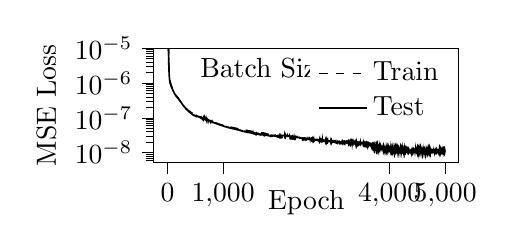
\begin{tikzpicture}

\begin{axis}[
legend cell align={left},
legend style={draw=none},
log basis y={10},
tick align=outside,
tick pos=left,
title={Batch Size 6},
title style={at={(0.4,0.85)},anchor=north},
x grid style={white!69.0196078431373!black},
xlabel={Epoch},
x label style={yshift=13pt},
xmin=-249.95, xmax=5248.95,
xtick style={color=black},
xtick = {0,1000,4000,5000},
y grid style={white!69.0196078431373!black},
ylabel={MSE Loss},
ymin=5.27698874578941e-09, ymax=1e-5,
ymode=log,
ytick style={color=black},
width=.45\textwidth,
height=.25\textwidth
]
\addplot [semithick, black, dashed]
table {%
0 0.00792494936405668
1 0.00074693354815037
2 0.000204862174982061
3 0.000182490643616067
4 0.000174127073374672
5 0.000144887499667855
6 8.86097720864456e-05
7 4.68465743448571e-05
8 3.17742668719849e-05
9 2.71491441448932e-05
10 2.39751503956937e-05
11 2.17058184807411e-05
12 1.95244866656639e-05
13 1.71598938875442e-05
14 1.45919596192705e-05
15 1.21801129276757e-05
16 1.00995043139322e-05
17 8.16256929222194e-06
18 6.30641060338328e-06
19 5.0335977352111e-06
20 4.18607083942384e-06
21 3.59522449484658e-06
22 3.16430228840947e-06
23 2.83704614422687e-06
24 2.57516105203744e-06
25 2.35928370969908e-06
26 2.17642036670179e-06
27 2.02323785481073e-06
28 1.89352970838895e-06
29 1.78371970852457e-06
30 1.69118709075458e-06
31 1.61080757225583e-06
32 1.5411232624977e-06
33 1.47731713683064e-06
34 1.42110068692468e-06
35 1.37282949941775e-06
36 1.32860109897345e-06
37 1.2878080142279e-06
38 1.25118790969526e-06
39 1.21718567364734e-06
40 1.18621371261417e-06
41 1.15859394885872e-06
42 1.13291366900974e-06
43 1.11027498610941e-06
44 1.08951247236749e-06
45 1.07059546082872e-06
46 1.05329323841063e-06
47 1.03720289890175e-06
48 1.02232245525918e-06
49 1.00850926861736e-06
50 9.95778685144071e-07
51 9.83511111717545e-07
52 9.71585458310552e-07
53 9.60307571971598e-07
54 9.49454394176838e-07
55 9.39045032597575e-07
56 9.2894042586569e-07
57 9.19292567370904e-07
58 9.09662005366529e-07
59 9.00520281040803e-07
60 8.91369453549412e-07
61 8.82196482813927e-07
62 8.73165208659948e-07
63 8.64312308946624e-07
64 8.55683471747636e-07
65 8.46961227554032e-07
66 8.38652941052141e-07
67 8.29745988248977e-07
68 8.21353428667483e-07
69 8.13295208099236e-07
70 8.04699132071003e-07
71 7.96007132709525e-07
72 7.88097942269513e-07
73 7.79884498932095e-07
74 7.72275892080753e-07
75 7.64772029071864e-07
76 7.56686016295635e-07
77 7.49086183848119e-07
78 7.4208203814691e-07
79 7.34527712558045e-07
80 7.26859385308828e-07
81 7.19653547588544e-07
82 7.12119579645616e-07
83 7.05339993577664e-07
84 6.98320306320074e-07
85 6.91032350877539e-07
86 6.8372461907055e-07
87 6.76880052207574e-07
88 6.70372859392669e-07
89 6.64194197234384e-07
90 6.58067695549607e-07
91 6.52140548214283e-07
92 6.46306514798665e-07
93 6.40675028040156e-07
94 6.35287225518852e-07
95 6.30230405772304e-07
96 6.24665087219474e-07
97 6.19228257339953e-07
98 6.14137978945591e-07
99 6.08860029745464e-07
100 6.03844388347335e-07
101 5.99027984836765e-07
102 5.94187206397332e-07
103 5.89501576444994e-07
104 5.84924708667334e-07
105 5.80679396908364e-07
106 5.76035185584006e-07
107 5.7162463720771e-07
108 5.67239825653383e-07
109 5.63138681524104e-07
110 5.58848633648273e-07
111 5.54497895904518e-07
112 5.5032399974129e-07
113 5.46303629167438e-07
114 5.4249618855444e-07
115 5.38887368242723e-07
116 5.35058079500554e-07
117 5.31249512400346e-07
118 5.27634925549626e-07
119 5.23930784742118e-07
120 5.20592796066047e-07
121 5.17186048734035e-07
122 5.13706907728759e-07
123 5.10282175111322e-07
124 5.06539088247373e-07
125 5.03181729004515e-07
126 4.99824641919766e-07
127 4.97068465716291e-07
128 4.93662760176286e-07
129 4.90739311181823e-07
130 4.87514542350712e-07
131 4.84693126930909e-07
132 4.81795060823976e-07
133 4.78897239934182e-07
134 4.76187394968071e-07
135 4.73645979614046e-07
136 4.71059729141229e-07
137 4.68526309241245e-07
138 4.66105621260679e-07
139 4.63971031256674e-07
140 4.61375845069785e-07
141 4.59029176206225e-07
142 4.5668160046323e-07
143 4.54302431758438e-07
144 4.51832581901237e-07
145 4.49889186510263e-07
146 4.47508866076417e-07
147 4.45342193171692e-07
148 4.43099275191079e-07
149 4.40864431969386e-07
150 4.3865167727893e-07
151 4.36595489178251e-07
152 4.34421391229771e-07
153 4.32206230574499e-07
154 4.30091064502555e-07
155 4.28157747739502e-07
156 4.26042544633048e-07
157 4.24004756910043e-07
158 4.22020520060586e-07
159 4.19945539984768e-07
160 4.17963437112464e-07
161 4.15992797622127e-07
162 4.14081616672829e-07
163 4.12071938617008e-07
164 4.10129467671962e-07
165 4.08223826148987e-07
166 4.06277433316971e-07
167 4.04441162310323e-07
168 4.02476571030062e-07
169 4.0058604144078e-07
170 3.98771483355115e-07
171 3.96856144415191e-07
172 3.94967850401618e-07
173 3.93066415661824e-07
174 3.91222675870965e-07
175 3.89322397960259e-07
176 3.87543632753833e-07
177 3.85704788485242e-07
178 3.83836589682855e-07
179 3.82057603776742e-07
180 3.8019314408832e-07
181 3.78379088152369e-07
182 3.76449783992992e-07
183 3.74547649126251e-07
184 3.72727639033925e-07
185 3.70833063670765e-07
186 3.68986093267393e-07
187 3.67232748427762e-07
188 3.65436964686828e-07
189 3.63612886207362e-07
190 3.61782968627245e-07
191 3.5995823093563e-07
192 3.58184446455347e-07
193 3.56371153332829e-07
194 3.54544190196331e-07
195 3.52744350774403e-07
196 3.50947292967492e-07
197 3.49238124623073e-07
198 3.47401059076246e-07
199 3.45640531147575e-07
200 3.43881100022046e-07
201 3.42033855609639e-07
202 3.40198495296135e-07
203 3.38492801068928e-07
204 3.36773551542576e-07
205 3.3499529977252e-07
206 3.33106171294682e-07
207 3.31376998580954e-07
208 3.29612051979292e-07
209 3.28067406468344e-07
210 3.26203844111773e-07
211 3.24453416974204e-07
212 3.22730980011197e-07
213 3.20854888375995e-07
214 3.1919837656405e-07
215 3.17532984182329e-07
216 3.15781171070965e-07
217 3.14084994699527e-07
218 3.12351770949431e-07
219 3.10619374169345e-07
220 3.08925018057659e-07
221 3.07278862414077e-07
222 3.05550675005806e-07
223 3.03974624571218e-07
224 3.02406111586223e-07
225 3.00711385877796e-07
226 2.99041627996609e-07
227 2.97478750869876e-07
228 2.95713607047331e-07
229 2.94081796465287e-07
230 2.92428883677469e-07
231 2.90797483175523e-07
232 2.8915811127093e-07
233 2.87616107239886e-07
234 2.86067552359025e-07
235 2.84466419771192e-07
236 2.82925695942147e-07
237 2.81369605712962e-07
238 2.79812704325207e-07
239 2.78198559747754e-07
240 2.76702073952568e-07
241 2.75215135617322e-07
242 2.73745041637739e-07
243 2.72245439116619e-07
244 2.7078373859621e-07
245 2.69341620199496e-07
246 2.67833146160829e-07
247 2.66405126777593e-07
248 2.65012859563865e-07
249 2.63667045197369e-07
250 2.62234284581905e-07
251 2.60904440430398e-07
252 2.59510283713623e-07
253 2.58156663265509e-07
254 2.56807231860977e-07
255 2.55492987941554e-07
256 2.54155811439095e-07
257 2.52885645455043e-07
258 2.51607791047048e-07
259 2.50322395346458e-07
260 2.48939361640907e-07
261 2.47696769913576e-07
262 2.46361084845114e-07
263 2.45173361800428e-07
264 2.43947212522032e-07
265 2.42728269244217e-07
266 2.41584720031539e-07
267 2.403303927375e-07
268 2.39022315681865e-07
269 2.37883198772454e-07
270 2.36761164511515e-07
271 2.355524272826e-07
272 2.3448867785689e-07
273 2.33515845237165e-07
274 2.32308974661009e-07
275 2.31225084880148e-07
276 2.30135166293314e-07
277 2.29069297050706e-07
278 2.28077566564201e-07
279 2.26976575897249e-07
280 2.25899497944186e-07
281 2.24806329063765e-07
282 2.23729208518085e-07
283 2.22726185747131e-07
284 2.21724548947309e-07
285 2.20741170477866e-07
286 2.19845323421825e-07
287 2.1896735587675e-07
288 2.18004240253847e-07
289 2.17031305175351e-07
290 2.16135360041509e-07
291 2.15184591089352e-07
292 2.14273000214602e-07
293 2.13387856864349e-07
294 2.12507463423041e-07
295 2.11605158649415e-07
296 2.1071168113888e-07
297 2.09847457386515e-07
298 2.09014734180116e-07
299 2.0817423863489e-07
300 2.07360612537527e-07
301 2.06565093934677e-07
302 2.05704701270017e-07
303 2.04869231661479e-07
304 2.04001796761957e-07
305 2.03225100806363e-07
306 2.02372046990871e-07
307 2.01605099985217e-07
308 2.00826745956311e-07
309 2.00061786523516e-07
310 1.99328455225447e-07
311 1.98573559908776e-07
312 1.97813823950473e-07
313 1.97087318936071e-07
314 1.96335054643567e-07
315 1.95518330763636e-07
316 1.94886897504467e-07
317 1.94244450476024e-07
318 1.93538887198722e-07
319 1.92870559207739e-07
320 1.920480320579e-07
321 1.91425300992452e-07
322 1.90777889022674e-07
323 1.90017708738136e-07
324 1.89466645937215e-07
325 1.88718898848247e-07
326 1.88148259931817e-07
327 1.87439876708007e-07
328 1.86853819323143e-07
329 1.86202076510168e-07
330 1.85547054233536e-07
331 1.84923454292569e-07
332 1.84389606649149e-07
333 1.83780473736457e-07
334 1.83204896626579e-07
335 1.82611882784649e-07
336 1.81974885874657e-07
337 1.81487325609632e-07
338 1.80865272643773e-07
339 1.80268731814711e-07
340 1.79716794006244e-07
341 1.79127217926133e-07
342 1.78605542807904e-07
343 1.78020651840994e-07
344 1.77516950081032e-07
345 1.76651081789756e-07
346 1.75948882187942e-07
347 1.75440971639407e-07
348 1.75018379547153e-07
349 1.74399636097872e-07
350 1.73992858762752e-07
351 1.73381931041213e-07
352 1.72961703671403e-07
353 1.72451043090782e-07
354 1.71903263217014e-07
355 1.71296573633885e-07
356 1.70823611926106e-07
357 1.7022137299838e-07
358 1.69639867024571e-07
359 1.69228476798339e-07
360 1.68696906522952e-07
361 1.68385364455779e-07
362 1.67627344202516e-07
363 1.67037906943227e-07
364 1.66660267270571e-07
365 1.66133442982562e-07
366 1.65828685711669e-07
367 1.65400948654834e-07
368 1.64599034798509e-07
369 1.64051662449496e-07
370 1.63612193077725e-07
371 1.63031040729425e-07
372 1.62574956671348e-07
373 1.62101862554409e-07
374 1.61218143537405e-07
375 1.61154750721504e-07
376 1.60227039340525e-07
377 1.60240092141078e-07
378 1.5980942699036e-07
379 1.58932503527646e-07
380 1.58903720312288e-07
381 1.58026279253281e-07
382 1.57959618992761e-07
383 1.57162557488173e-07
384 1.57105333092703e-07
385 1.56326358950141e-07
386 1.56239497088776e-07
387 1.55881404951457e-07
388 1.55094732560394e-07
389 1.54968537507319e-07
390 1.54296820256782e-07
391 1.53885362627527e-07
392 1.52978094574405e-07
393 1.5315802425409e-07
394 1.52503762786831e-07
395 1.5177051383502e-07
396 1.51525638096476e-07
397 1.50949997955225e-07
398 1.50103813769702e-07
399 1.49995203928941e-07
400 1.49503947592648e-07
401 1.49128464985788e-07
402 1.48449594303647e-07
403 1.48360061992047e-07
404 1.4776081381007e-07
405 1.47756748389739e-07
406 1.4699670358104e-07
407 1.46977261339454e-07
408 1.46112958270226e-07
409 1.46189474746539e-07
410 1.45417565404164e-07
411 1.45378170294301e-07
412 1.44648656883768e-07
413 1.445824052013e-07
414 1.44031487815293e-07
415 1.43900163933989e-07
416 1.43315402226999e-07
417 1.43215020893236e-07
418 1.42632309106034e-07
419 1.42574283634883e-07
420 1.42032504042846e-07
421 1.41834442127485e-07
422 1.41345680994636e-07
423 1.41238906693757e-07
424 1.4060466289851e-07
425 1.40545007124602e-07
426 1.40031331451224e-07
427 1.39810996041137e-07
428 1.39465829393916e-07
429 1.39250281124361e-07
430 1.38739989462694e-07
431 1.38410872469832e-07
432 1.38280581743764e-07
433 1.37804161246842e-07
434 1.3739803466154e-07
435 1.37337264645833e-07
436 1.36840152136423e-07
437 1.36466377980036e-07
438 1.36367599689807e-07
439 1.35951356260944e-07
440 1.35694117381072e-07
441 1.35180257143686e-07
442 1.35060516774808e-07
443 1.34537828314245e-07
444 1.34386974806315e-07
445 1.34078091845461e-07
446 1.33567195894895e-07
447 1.33422713547769e-07
448 1.32931844714266e-07
449 1.3279914286742e-07
450 1.32478407614304e-07
451 1.32061744539114e-07
452 1.31887610853466e-07
453 1.31612793401978e-07
454 1.31132230712552e-07
455 1.30987384846117e-07
456 1.30521262809929e-07
457 1.3031381291392e-07
458 1.29737968912419e-07
459 1.29641947192442e-07
460 1.29180116268447e-07
461 1.29056334044596e-07
462 1.28577802820288e-07
463 1.28533735564363e-07
464 1.28029660248809e-07
465 1.27910751799505e-07
466 1.27344065890912e-07
467 1.27244660958184e-07
468 1.26793830182507e-07
469 1.26614542037957e-07
470 1.26224640805218e-07
471 1.25955073733238e-07
472 1.2576121384724e-07
473 1.25469259082361e-07
474 1.25206119862802e-07
475 1.24820441521631e-07
476 1.24619067007033e-07
477 1.24123444319048e-07
478 1.23966767925384e-07
479 1.23584695277002e-07
480 1.23377284905598e-07
481 1.23001050521621e-07
482 1.22872700129837e-07
483 1.22457752967416e-07
484 1.22241437620638e-07
485 1.21987415930732e-07
486 1.21767705689061e-07
487 1.21556589152848e-07
488 1.21295199425061e-07
489 1.21022931374543e-07
490 1.20766346245921e-07
491 1.20396381607952e-07
492 1.20254470992759e-07
493 1.19947405571193e-07
494 1.19636952242981e-07
495 1.19374032788324e-07
496 1.19169286363612e-07
497 1.18910004296531e-07
498 1.18721699833387e-07
499 1.18419032173337e-07
500 1.18205985917038e-07
501 1.17922647974225e-07
502 1.17670392121504e-07
503 1.1745881593365e-07
504 1.17229652966187e-07
505 1.17012580124393e-07
506 1.16746087393462e-07
507 1.16516909057983e-07
508 1.16235237204725e-07
509 1.16043368823805e-07
510 1.15789795709275e-07
511 1.15621475727967e-07
512 1.1536366801043e-07
513 1.1514959939419e-07
514 1.14938462814706e-07
515 1.14728617083377e-07
516 1.14516673862116e-07
517 1.14303887274832e-07
518 1.14121070755621e-07
519 1.13954926995202e-07
520 1.13688961944786e-07
521 1.13482690585638e-07
522 1.13444305936523e-07
523 1.13101765691479e-07
524 1.12879228395209e-07
525 1.12654966542742e-07
526 1.12497033158231e-07
527 1.12403659961001e-07
528 1.12110352630886e-07
529 1.12004765672752e-07
530 1.11732648046635e-07
531 1.11525370969907e-07
532 1.11293275903103e-07
533 1.11184866194107e-07
534 1.10916620473286e-07
535 1.10772067790951e-07
536 1.10664058989981e-07
537 1.1040349546387e-07
538 1.10187687244333e-07
539 1.10028139541614e-07
540 1.09896095828319e-07
541 1.09669417741723e-07
542 1.09469936870122e-07
543 1.09287650594759e-07
544 1.09134116427204e-07
545 1.09001398249593e-07
546 1.08772434617598e-07
547 1.08564273714124e-07
548 1.08348638179375e-07
549 1.08174791310108e-07
550 1.0804613645955e-07
551 1.07795554193302e-07
552 1.07666778316117e-07
553 1.07434035184004e-07
554 1.07210255452627e-07
555 1.07046178583261e-07
556 1.06911155735786e-07
557 1.06740506994604e-07
558 1.06533606498867e-07
559 1.06359935407699e-07
560 1.06200919301736e-07
561 1.06013215091407e-07
562 1.05867026588159e-07
563 1.05705439081831e-07
564 1.05492735012581e-07
565 1.05356573108906e-07
566 1.0516000167012e-07
567 1.04988258887539e-07
568 1.04903252823715e-07
569 1.04625338941237e-07
570 1.04521623926316e-07
571 1.04373378797333e-07
572 1.0416789535631e-07
573 1.04016407019193e-07
574 1.03836468000984e-07
575 1.03709974175076e-07
576 1.03519282200455e-07
577 1.034126624333e-07
578 1.032837735697e-07
579 1.03076682813362e-07
580 1.02969324202938e-07
581 1.02783457781567e-07
582 1.02641104248974e-07
583 1.02497159350994e-07
584 1.023272493106e-07
585 1.02269956558682e-07
586 1.02080391342916e-07
587 1.01901056838648e-07
588 1.01680896134721e-07
589 1.0165975366264e-07
590 1.0151955765791e-07
591 1.01291374315291e-07
592 1.01158572304024e-07
593 1.0099713505831e-07
594 1.00829963744703e-07
595 1.00671792044744e-07
596 1.00479425459648e-07
597 1.00339705944663e-07
598 1.00263345520099e-07
599 9.99969221030382e-08
600 9.99370505150909e-08
601 9.9841746459256e-08
602 9.96970335079887e-08
603 9.94148601748137e-08
604 9.94305171744152e-08
605 9.9138141733882e-08
606 9.90484357760776e-08
607 9.89997646333327e-08
608 9.87586991788779e-08
609 9.86360037911284e-08
610 9.85921406790853e-08
611 9.83557888713947e-08
612 9.82831521182108e-08
613 9.79887653557007e-08
614 9.77669668068248e-08
615 9.75032125390232e-08
616 9.7241095451701e-08
617 9.70617752142148e-08
618 9.67884489756775e-08
619 9.66514243151938e-08
620 9.64655205197543e-08
621 9.63048815107464e-08
622 9.61571627639665e-08
623 9.60187558069067e-08
624 9.5793140238034e-08
625 9.57458236659176e-08
626 9.55691448657253e-08
627 9.54866896689652e-08
628 9.52745373582537e-08
629 9.50931480299085e-08
630 9.50461621145003e-08
631 9.48732205706893e-08
632 9.47432422850169e-08
633 9.45740982951814e-08
634 9.44506582210936e-08
635 9.43142960418409e-08
636 9.41397731209883e-08
637 9.39928493791165e-08
638 9.38941059355765e-08
639 9.3825027502115e-08
640 9.37076243687564e-08
641 9.35323852751555e-08
642 9.34204141824212e-08
643 9.32263267869239e-08
644 9.30651717542437e-08
645 9.30660305775011e-08
646 9.28396997873096e-08
647 9.26950396819924e-08
648 9.27071528390466e-08
649 9.24314736747257e-08
650 9.23561871071409e-08
651 9.23011272078057e-08
652 9.20847262723205e-08
653 9.20106265481295e-08
654 9.19975779328011e-08
655 9.19308606104797e-08
656 9.17938819821396e-08
657 9.17312023781704e-08
658 9.15164115703419e-08
659 9.13792164881272e-08
660 9.12088392485741e-08
661 9.11352694719498e-08
662 9.09804609934031e-08
663 9.09200491333143e-08
664 9.07959634500565e-08
665 9.06053841462608e-08
666 9.04922921503894e-08
667 9.03537848631241e-08
668 9.02727790676826e-08
669 9.01380736467852e-08
670 8.99475532190985e-08
671 8.98181916188727e-08
672 8.9708077212524e-08
673 8.95742572116331e-08
674 8.95692921224903e-08
675 8.94854445522574e-08
676 8.92567196025659e-08
677 8.92259713676898e-08
678 8.91810853670597e-08
679 8.89182820919992e-08
680 8.88726568699246e-08
681 8.88789637196864e-08
682 8.86814085034559e-08
683 8.86184558025992e-08
684 8.84406394316097e-08
685 8.82643648291654e-08
686 8.82450046075935e-08
687 8.80800776422887e-08
688 8.79617921522735e-08
689 8.78704687070491e-08
690 8.77763111650493e-08
691 8.77024110872546e-08
692 8.75630335649042e-08
693 8.75243787277853e-08
694 8.73521312721063e-08
695 8.72583466744938e-08
696 8.71552602242399e-08
697 8.71504448663989e-08
698 8.6967704048086e-08
699 8.68567375324163e-08
700 8.67588195222178e-08
701 8.66599322210716e-08
702 8.65302836073877e-08
703 8.63719422620217e-08
704 8.62916290879528e-08
705 8.62020234943098e-08
706 8.61112491777106e-08
707 8.59954845757415e-08
708 8.58770226371654e-08
709 8.57806709269468e-08
710 8.57162695464998e-08
711 8.55895117471737e-08
712 8.54726360899288e-08
713 8.53523020163886e-08
714 8.52339811317311e-08
715 8.52128194206669e-08
716 8.50622339182452e-08
717 8.49504515294693e-08
718 8.48105331683808e-08
719 8.47790642452946e-08
720 8.46481247268629e-08
721 8.45440721555395e-08
722 8.44129090798033e-08
723 8.44280426506948e-08
724 8.42494295696809e-08
725 8.41705290360648e-08
726 8.40065957233631e-08
727 8.39763029362604e-08
728 8.38522954939313e-08
729 8.37329867518017e-08
730 8.36780891667399e-08
731 8.35020314948837e-08
732 8.35077070275579e-08
733 8.33393987903122e-08
734 8.33242972644187e-08
735 8.31508684382294e-08
736 8.31354193116603e-08
737 8.29454018772561e-08
738 8.29427543325706e-08
739 8.28369571970672e-08
740 8.27457814364725e-08
741 8.26038725104164e-08
742 8.24549751368918e-08
743 8.23958459396012e-08
744 8.2313863215144e-08
745 8.22747276777545e-08
746 8.21465659366647e-08
747 8.20621932219528e-08
748 8.19604173761641e-08
749 8.18726592502271e-08
750 8.18050781197968e-08
751 8.17071699148484e-08
752 8.15337526715976e-08
753 8.1480377070141e-08
754 8.14369292833767e-08
755 8.13487763401607e-08
756 8.12141420560962e-08
757 8.11471520843056e-08
758 8.10588374986094e-08
759 8.09555228224549e-08
760 8.08750344382148e-08
761 8.07332387229488e-08
762 8.06549439696261e-08
763 8.05325278247723e-08
764 8.05011720645385e-08
765 8.04073679076925e-08
766 8.02946634645464e-08
767 8.02051012997655e-08
768 8.01234312294254e-08
769 8.00308685056561e-08
770 7.99606150041557e-08
771 7.98075698287557e-08
772 7.97668609112594e-08
773 7.96247826773572e-08
774 7.94999828021088e-08
775 7.94450283583147e-08
776 7.93847441848594e-08
777 7.92839646728541e-08
778 7.91749904605582e-08
779 7.90872404407474e-08
780 7.90205521120583e-08
781 7.888154033479e-08
782 7.88543524969352e-08
783 7.86995105439159e-08
784 7.86323640889364e-08
785 7.85425547895088e-08
786 7.84370873200017e-08
787 7.83665436145252e-08
788 7.82619622554602e-08
789 7.81682320870725e-08
790 7.80680596583331e-08
791 7.7984497306559e-08
792 7.78788282857992e-08
793 7.7797066535339e-08
794 7.76839365355515e-08
795 7.75992620692124e-08
796 7.75117234152256e-08
797 7.740640813316e-08
798 7.73703760443031e-08
799 7.72528050352361e-08
800 7.71347091493421e-08
801 7.70650933652736e-08
802 7.69856078789481e-08
803 7.68517433346444e-08
804 7.67692187860638e-08
805 7.66678639980996e-08
806 7.65424627581495e-08
807 7.64938434679798e-08
808 7.63841421271815e-08
809 7.63040824847743e-08
810 7.6208701324533e-08
811 7.61267628012669e-08
812 7.60441162246946e-08
813 7.58755990584563e-08
814 7.58323846855133e-08
815 7.57093433502719e-08
816 7.55957277139659e-08
817 7.54920250276809e-08
818 7.53970034931454e-08
819 7.53118776623899e-08
820 7.52102924234185e-08
821 7.50831357647362e-08
822 7.49458233264548e-08
823 7.47840501781876e-08
824 7.46699555014527e-08
825 7.45712405628472e-08
826 7.44991902144843e-08
827 7.43670001235269e-08
828 7.42764634033104e-08
829 7.42058294631677e-08
830 7.40858372477701e-08
831 7.4010756124376e-08
832 7.38730827920381e-08
833 7.37644526862945e-08
834 7.36669718329867e-08
835 7.3568323296038e-08
836 7.35058679404747e-08
837 7.33685872762104e-08
838 7.32850038751405e-08
839 7.3197792068149e-08
840 7.31037852727974e-08
841 7.30077916110023e-08
842 7.29198656146834e-08
843 7.28109357160989e-08
844 7.27455886420202e-08
845 7.26609725544369e-08
846 7.2553502705325e-08
847 7.25095461061781e-08
848 7.23269759459556e-08
849 7.22590886662831e-08
850 7.22283481360552e-08
851 7.20781080864353e-08
852 7.19637544737326e-08
853 7.1973301964966e-08
854 7.18185479096518e-08
855 7.17502237633778e-08
856 7.17103134680859e-08
857 7.15258081728193e-08
858 7.15128466302688e-08
859 7.14619334568747e-08
860 7.11725786758595e-08
861 7.11507273468507e-08
862 7.10437192579708e-08
863 7.10404811538664e-08
864 7.08561184724899e-08
865 7.08082522224625e-08
866 7.07646552656665e-08
867 7.06380770408367e-08
868 7.05022280868949e-08
869 7.04429462640659e-08
870 7.03595980398581e-08
871 7.02565800758836e-08
872 7.0207722283842e-08
873 7.00945105916139e-08
874 6.99803333795344e-08
875 6.99747162888671e-08
876 6.97937787497194e-08
877 6.97787862513888e-08
878 6.97129161374278e-08
879 6.96013615903853e-08
880 6.94600617629745e-08
881 6.94828596085449e-08
882 6.93428895313703e-08
883 6.92632089434055e-08
884 6.91849155270111e-08
885 6.91010709229212e-08
886 6.89944733449136e-08
887 6.89520586867545e-08
888 6.87878025145392e-08
889 6.87653220955469e-08
890 6.86641716026012e-08
891 6.85961561402734e-08
892 6.85030336277404e-08
893 6.84367955842045e-08
894 6.8341776631645e-08
895 6.82595868071501e-08
896 6.81619964755322e-08
897 6.81212941674416e-08
898 6.79910497578147e-08
899 6.7917461184299e-08
900 6.77907707280723e-08
901 6.77301007016815e-08
902 6.76374282852142e-08
903 6.75683262617605e-08
904 6.74273657637805e-08
905 6.74206006405862e-08
906 6.73083456363603e-08
907 6.72158289074497e-08
908 6.71557271161731e-08
909 6.70903081635593e-08
910 6.70025510742743e-08
911 6.69165004866627e-08
912 6.68149225501957e-08
913 6.67687180853206e-08
914 6.66625277943773e-08
915 6.66335806575025e-08
916 6.6523338110444e-08
917 6.65168887206961e-08
918 6.63460846448323e-08
919 6.62652415844503e-08
920 6.61301523579552e-08
921 6.60950810943875e-08
922 6.60525452318325e-08
923 6.5929236269924e-08
924 6.58494692629979e-08
925 6.57748615773179e-08
926 6.57409636686833e-08
927 6.56343428255943e-08
928 6.55793209008801e-08
929 6.55066323004473e-08
930 6.54712611847824e-08
931 6.53547976909277e-08
932 6.52940520908068e-08
933 6.52103714315367e-08
934 6.51293917508045e-08
935 6.50708836239254e-08
936 6.49648700798218e-08
937 6.49629940798834e-08
938 6.48854084937518e-08
939 6.47777786819754e-08
940 6.47394384630863e-08
941 6.46057746078233e-08
942 6.4582537619278e-08
943 6.4483849206181e-08
944 6.45361467760871e-08
945 6.43352020812538e-08
946 6.42254817371658e-08
947 6.42260176563009e-08
948 6.41414128460535e-08
949 6.4036320972153e-08
950 6.40051641199423e-08
951 6.39142114925371e-08
952 6.39232134731074e-08
953 6.38271091458791e-08
954 6.37706096025378e-08
955 6.37301945682334e-08
956 6.37245242361302e-08
957 6.36409729379829e-08
958 6.36012324885043e-08
959 6.35367983965925e-08
960 6.3445267839346e-08
961 6.33644460126868e-08
962 6.32313920903176e-08
963 6.32242685671569e-08
964 6.31174637226615e-08
965 6.3110971213649e-08
966 6.30090201470362e-08
967 6.29856166203767e-08
968 6.29289383827279e-08
969 6.2846778048553e-08
970 6.28095745582229e-08
971 6.27314586729817e-08
972 6.26567372764952e-08
973 6.26353590176784e-08
974 6.25294210266652e-08
975 6.24992209270394e-08
976 6.24411414521102e-08
977 6.23566219269651e-08
978 6.23410314655095e-08
979 6.22730750011324e-08
980 6.21986761325906e-08
981 6.2123454242904e-08
982 6.20565633016755e-08
983 6.19911177483177e-08
984 6.19309048808088e-08
985 6.18677860306656e-08
986 6.17949470837309e-08
987 6.17349928545768e-08
988 6.16690186226688e-08
989 6.15940373074923e-08
990 6.15296462902365e-08
991 6.14877760162053e-08
992 6.13140742808844e-08
993 6.13556047740718e-08
994 6.1184471468977e-08
995 6.11416997184845e-08
996 6.10264418376172e-08
997 6.10011510663076e-08
998 6.08959333653555e-08
999 6.08815033582746e-08
1000 6.07449019234632e-08
1001 6.07449449182231e-08
1002 6.06042416504289e-08
1003 6.06234880500054e-08
1004 6.04724791967407e-08
1005 6.04976172399786e-08
1006 6.03440853567864e-08
1007 6.03638936643709e-08
1008 6.02229008004769e-08
1009 6.02366862916329e-08
1010 6.00965989855598e-08
1011 6.01074190187517e-08
1012 5.99647778202154e-08
1013 5.99714976316627e-08
1014 5.98645894668497e-08
1015 5.98602131268131e-08
1016 5.98440629584873e-08
1017 5.97974968558559e-08
1018 5.97010112723817e-08
1019 5.96388073472125e-08
1020 5.95871144570309e-08
1021 5.95317830507409e-08
1022 5.94607110262467e-08
1023 5.94440843129139e-08
1024 5.93347962959968e-08
1025 5.93152592510182e-08
1026 5.9209410856834e-08
1027 5.91987453393893e-08
1028 5.91034983080711e-08
1029 5.90980985095218e-08
1030 5.90197927019065e-08
1031 5.89576969740465e-08
1032 5.88747872330049e-08
1033 5.8890620852944e-08
1034 5.87949151287387e-08
1035 5.87625136402832e-08
1036 5.87021455080011e-08
1037 5.86604852069384e-08
1038 5.85654308464204e-08
1039 5.8574962441657e-08
1040 5.84544965295487e-08
1041 5.84952061308226e-08
1042 5.83282032089197e-08
1043 5.83216899089421e-08
1044 5.82941326927297e-08
1045 5.82313509495738e-08
1046 5.81159853754086e-08
1047 5.81181682409911e-08
1048 5.80003146953113e-08
1049 5.80218817100188e-08
1050 5.79361831906068e-08
1051 5.78927504509432e-08
1052 5.78225662253622e-08
1053 5.78540821653116e-08
1054 5.76885860414267e-08
1055 5.77094049815351e-08
1056 5.75638148981511e-08
1057 5.76022974859155e-08
1058 5.74902993463507e-08
1059 5.74552865447638e-08
1060 5.73852374075251e-08
1061 5.73537481535421e-08
1062 5.72236097307654e-08
1063 5.72772072196979e-08
1064 5.71098081515774e-08
1065 5.71178287788849e-08
1066 5.70507493321067e-08
1067 5.69992500961133e-08
1068 5.69160797093271e-08
1069 5.69246548948662e-08
1070 5.67944772743923e-08
1071 5.6791876424988e-08
1072 5.67314601180149e-08
1073 5.66554648952399e-08
1074 5.66244221932644e-08
1075 5.65731772799042e-08
1076 5.6492765263029e-08
1077 5.64865721646876e-08
1078 5.63726430992722e-08
1079 5.64091336819416e-08
1080 5.62825863602612e-08
1081 5.62965368695081e-08
1082 5.61771592522714e-08
1083 5.62053769350012e-08
1084 5.60664128117675e-08
1085 5.61052525311475e-08
1086 5.59744314953176e-08
1087 5.59837565597763e-08
1088 5.58820367624402e-08
1089 5.59070890305463e-08
1090 5.57410385295275e-08
1091 5.57924492918981e-08
1092 5.56903973417992e-08
1093 5.56911808416675e-08
1094 5.5560815193689e-08
1095 5.56128175860862e-08
1096 5.54792224807597e-08
1097 5.55065994693253e-08
1098 5.53821891402101e-08
1099 5.53957429479614e-08
1100 5.52828465950255e-08
1101 5.53226706178323e-08
1102 5.51843671109212e-08
1103 5.52059207889706e-08
1104 5.51090012424526e-08
1105 5.51018989097377e-08
1106 5.50045666538728e-08
1107 5.50254645140268e-08
1108 5.48944216985807e-08
1109 5.492906696741e-08
1110 5.48375427732229e-08
1111 5.48879215967745e-08
1112 5.47291373486558e-08
1113 5.48093085959412e-08
1114 5.46615534145379e-08
1115 5.46915637369343e-08
1116 5.45832876528502e-08
1117 5.46144617439782e-08
1118 5.44759346657807e-08
1119 5.45108140268825e-08
1120 5.44098764424215e-08
1121 5.441311405117e-08
1122 5.42889065583034e-08
1123 5.43314965511385e-08
1124 5.42054906301322e-08
1125 5.42205739783292e-08
1126 5.41382550969825e-08
1127 5.4159388387003e-08
1128 5.40388574281429e-08
1129 5.40976299505572e-08
1130 5.39553001897198e-08
1131 5.39650045902547e-08
1132 5.38747589908222e-08
1133 5.38866475565829e-08
1134 5.37739957010562e-08
1135 5.38016958487457e-08
1136 5.36792816793232e-08
1137 5.36967115156747e-08
1138 5.3606179180423e-08
1139 5.35955056893465e-08
1140 5.3537224862239e-08
1141 5.35082173105893e-08
1142 5.34495854672475e-08
1143 5.34194772394925e-08
1144 5.33530507523264e-08
1145 5.33700697635475e-08
1146 5.32460506930055e-08
1147 5.32684994458405e-08
1148 5.31634974923483e-08
1149 5.31742437002032e-08
1150 5.30788059329023e-08
1151 5.3085817963705e-08
1152 5.29934681923634e-08
1153 5.30073814540439e-08
1154 5.28742340552237e-08
1155 5.28884154968519e-08
1156 5.27903061035121e-08
1157 5.27741826264792e-08
1158 5.27273597876863e-08
1159 5.2704631887831e-08
1160 5.26181914185225e-08
1161 5.26122942760114e-08
1162 5.25371809218608e-08
1163 5.25181295666647e-08
1164 5.24408524101435e-08
1165 5.24506279042342e-08
1166 5.23543758604177e-08
1167 5.23542157552718e-08
1168 5.22885668876204e-08
1169 5.22744369110713e-08
1170 5.21886834144804e-08
1171 5.21840990316321e-08
1172 5.21115209181978e-08
1173 5.21031355811288e-08
1174 5.20230322728345e-08
1175 5.2020849203517e-08
1176 5.19226777328974e-08
1177 5.19228199579597e-08
1178 5.18371560781719e-08
1179 5.1850824391696e-08
1180 5.17688889497566e-08
1181 5.17707267347199e-08
1182 5.16913233383182e-08
1183 5.16847373481941e-08
1184 5.15891402008046e-08
1185 5.15911923117428e-08
1186 5.14926039851682e-08
1187 5.14909518048599e-08
1188 5.14309401563691e-08
1189 5.14323695730075e-08
1190 5.13429139030828e-08
1191 5.13648093440653e-08
1192 5.12755754431039e-08
1193 5.12416107526402e-08
1194 5.11910958134154e-08
1195 5.1192302445744e-08
1196 5.11364802975741e-08
1197 5.10663882954067e-08
1198 5.10439006724486e-08
1199 5.10104281047358e-08
1200 5.09526454365304e-08
1201 5.0905785738333e-08
1202 5.08782093217538e-08
1203 5.08483768254604e-08
1204 5.07870784201616e-08
1205 5.07603319490567e-08
1206 5.06996676685279e-08
1207 5.0695195023718e-08
1208 5.06064930497495e-08
1209 5.05848387026018e-08
1210 5.05594465950614e-08
1211 5.05544964837761e-08
1212 5.04493761868345e-08
1213 5.04520674500055e-08
1214 5.03946414080728e-08
1215 5.03606896388074e-08
1216 5.03233920967744e-08
1217 5.02758720592276e-08
1218 5.02612713321368e-08
1219 5.01997893109302e-08
1220 5.01716560324481e-08
1221 5.01192420785447e-08
1222 5.00509035416497e-08
1223 5.00524398985651e-08
1224 5.00010323540104e-08
1225 4.9984477347436e-08
1226 4.99314238844306e-08
1227 4.99091161848483e-08
1228 4.98304385334146e-08
1229 4.98142071067505e-08
1230 4.9764617930407e-08
1231 4.97518405077755e-08
1232 4.96711732148401e-08
1233 4.96370361911309e-08
1234 4.95702683105512e-08
1235 4.95545506211989e-08
1236 4.95216614688612e-08
1237 4.95146090898572e-08
1238 4.94206984208442e-08
1239 4.93580551915764e-08
1240 4.9353509967143e-08
1241 4.93214819923347e-08
1242 4.92565279918023e-08
1243 4.92027684089766e-08
1244 4.92027511447589e-08
1245 4.91793300109942e-08
1246 4.90795574716051e-08
1247 4.90844459263968e-08
1248 4.90456865145915e-08
1249 4.89638036995537e-08
1250 4.89433631174598e-08
1251 4.89460196331469e-08
1252 4.88620601121521e-08
1253 4.8861710864618e-08
1254 4.8770790552526e-08
1255 4.88269239406519e-08
1256 4.87038761581274e-08
1257 4.87178794787028e-08
1258 4.86593981852651e-08
1259 4.86405956811503e-08
1260 4.85480061409176e-08
1261 4.85453265425786e-08
1262 4.85036155188049e-08
1263 4.85247382865078e-08
1264 4.84071330299734e-08
1265 4.84293189838637e-08
1266 4.83176452418125e-08
1267 4.83305274485249e-08
1268 4.82495090048635e-08
1269 4.82006479074531e-08
1270 4.81268008453879e-08
1271 4.81252961562943e-08
1272 4.80992200728062e-08
1273 4.80513806885115e-08
1274 4.79990797616371e-08
1275 4.7994034648218e-08
1276 4.79238257031135e-08
1277 4.79431728643346e-08
1278 4.78445009547777e-08
1279 4.78546731463692e-08
1280 4.77489454915189e-08
1281 4.77803205683017e-08
1282 4.77040951105718e-08
1283 4.76865964167569e-08
1284 4.76261716281459e-08
1285 4.76183202967002e-08
1286 4.75431732447008e-08
1287 4.75321782020767e-08
1288 4.75003647603073e-08
1289 4.74436953698211e-08
1290 4.73813829230977e-08
1291 4.73386435505036e-08
1292 4.72862987530083e-08
1293 4.73007368246028e-08
1294 4.72187338028718e-08
1295 4.72074248743988e-08
1296 4.71412294164881e-08
1297 4.70993734045783e-08
1298 4.70629365080998e-08
1299 4.70913203024984e-08
1300 4.69578550722931e-08
1301 4.69881231052507e-08
1302 4.6903624450634e-08
1303 4.6864333308247e-08
1304 4.68184147046615e-08
1305 4.68549811616703e-08
1306 4.67762419895663e-08
1307 4.68242182898269e-08
1308 4.6723639467528e-08
1309 4.67208557325996e-08
1310 4.66291719113116e-08
1311 4.66569113252759e-08
1312 4.65370421865063e-08
1313 4.6570101092111e-08
1314 4.65098814464159e-08
1315 4.65870777757048e-08
1316 4.63818430575956e-08
1317 4.64280677271982e-08
1318 4.63330616062868e-08
1319 4.63711004533881e-08
1320 4.62567461202889e-08
1321 4.62774960268295e-08
1322 4.61692244678614e-08
1323 4.62156001184741e-08
1324 4.61431161516195e-08
1325 4.61569815372207e-08
1326 4.60594379065435e-08
1327 4.60776189477571e-08
1328 4.59758032627719e-08
1329 4.60101964716924e-08
1330 4.59021289464158e-08
1331 4.59580126232456e-08
1332 4.58338460508361e-08
1333 4.58754452949588e-08
1334 4.57686558351251e-08
1335 4.57965480717048e-08
1336 4.57028488324328e-08
1337 4.57448367135374e-08
1338 4.56486392257807e-08
1339 4.5729476305606e-08
1340 4.55564835956606e-08
1341 4.56003788692168e-08
1342 4.55120246137706e-08
1343 4.5558175753319e-08
1344 4.541170940802e-08
1345 4.54622783796521e-08
1346 4.5404074499822e-08
1347 4.5400565470007e-08
1348 4.53175958618117e-08
1349 4.53517090734841e-08
1350 4.52528277941742e-08
1351 4.52867629147549e-08
1352 4.51439451880945e-08
1353 4.52149995512207e-08
1354 4.51215298831e-08
1355 4.51523751714425e-08
1356 4.50114118118502e-08
1357 4.50741025540029e-08
1358 4.49905352430107e-08
1359 4.50350787120406e-08
1360 4.489488560421e-08
1361 4.49673464155075e-08
1362 4.48454072158071e-08
1363 4.49810700684063e-08
1364 4.47684584812331e-08
1365 4.48353539109585e-08
1366 4.47206533124474e-08
1367 4.47776552774812e-08
1368 4.46536420989443e-08
1369 4.46925109094966e-08
1370 4.46206437019926e-08
1371 4.46521088816131e-08
1372 4.4543983635392e-08
1373 4.45766036563526e-08
1374 4.44786089092697e-08
1375 4.45401147541646e-08
1376 4.44029837982321e-08
1377 4.44561377382522e-08
1378 4.43653891585202e-08
1379 4.44125930807838e-08
1380 4.43110646566019e-08
1381 4.42045633667225e-08
1382 4.41957489955338e-08
1383 4.4188527635592e-08
1384 4.41071803258941e-08
1385 4.41671643333271e-08
1386 4.40842773020888e-08
1387 4.41158436248579e-08
1388 4.39828282670092e-08
1389 4.39700787201303e-08
1390 4.39971016983549e-08
1391 4.39006020554957e-08
1392 4.39875520579162e-08
1393 4.38472010237732e-08
1394 4.39210756200352e-08
1395 4.37903926966153e-08
1396 4.38280726161031e-08
1397 4.38186260902493e-08
1398 4.37432572303373e-08
1399 4.36988824046842e-08
1400 4.37084086495446e-08
1401 4.36406449611642e-08
1402 4.36991035371419e-08
1403 4.36039576046964e-08
1404 4.35739394608038e-08
1405 4.35330932661447e-08
1406 4.35020156815276e-08
1407 4.35002117225797e-08
1408 4.34969782797476e-08
1409 4.33784087507399e-08
1410 4.34661978254336e-08
1411 4.33199090169471e-08
1412 4.33475501726782e-08
1413 4.32835560516647e-08
1414 4.33739404060052e-08
1415 4.32678123800976e-08
1416 4.32226941534349e-08
1417 4.31999776867129e-08
1418 4.32440333913245e-08
1419 4.31628705064825e-08
1420 4.31066926405251e-08
1421 4.30886816255568e-08
1422 4.31310608035182e-08
1423 4.29984102606276e-08
1424 4.30233330860503e-08
1425 4.29533309620128e-08
1426 4.29971154399718e-08
1427 4.29012668721752e-08
1428 4.28831221144482e-08
1429 4.28903390614616e-08
1430 4.28597525439682e-08
1431 4.28156335935961e-08
1432 4.27473745456736e-08
1433 4.28321963021554e-08
1434 4.26828721718832e-08
1435 4.27151090054423e-08
1436 4.26521081348882e-08
1437 4.27226646743431e-08
1438 4.25903008439687e-08
1439 4.259228398226e-08
1440 4.25152720245628e-08
1441 4.25678216533791e-08
1442 4.2470582108627e-08
1443 4.24376189042471e-08
1444 4.2408031011891e-08
1445 4.24340917679762e-08
1446 4.23733229064358e-08
1447 4.23100931445131e-08
1448 4.22990060016485e-08
1449 4.22157358306134e-08
1450 4.21894425675278e-08
1451 4.22596628558824e-08
1452 4.21257746726502e-08
1453 4.20914441592056e-08
1454 4.20918978629136e-08
1455 4.21557673466617e-08
1456 4.20573782050834e-08
1457 4.20583513776504e-08
1458 4.20721673461763e-08
1459 4.20147140696572e-08
1460 4.19763242093177e-08
1461 4.19647578472567e-08
1462 4.19962074844207e-08
1463 4.18868301889274e-08
1464 4.18394733531665e-08
1465 4.19151688110643e-08
1466 4.18102310767335e-08
1467 4.17499309440303e-08
1468 4.18010540870639e-08
1469 4.16948528044133e-08
1470 4.1756585794614e-08
1471 4.16866104610737e-08
1472 4.16020320431745e-08
1473 4.16673901039671e-08
1474 4.15940195769218e-08
1475 4.15509370611893e-08
1476 4.16134791822632e-08
1477 4.1507880687131e-08
1478 4.14823844423354e-08
1479 4.15400652400049e-08
1480 4.14284055942907e-08
1481 4.13773140797967e-08
1482 4.1426858724046e-08
1483 4.13342930474496e-08
1484 4.13246423880342e-08
1485 4.13030121695117e-08
1486 4.1276265259977e-08
1487 4.12625958385601e-08
1488 4.12862656286594e-08
1489 4.12263506980713e-08
1490 4.11584907598462e-08
1491 4.12052668897089e-08
1492 4.11149547188404e-08
1493 4.10999246690053e-08
1494 4.11064493944596e-08
1495 4.10310373057587e-08
1496 4.1124795119199e-08
1497 4.10065354339628e-08
1498 4.09684150991547e-08
1499 4.10129605223102e-08
1500 4.09459801786666e-08
1501 4.0887854757482e-08
1502 4.09083219609596e-08
1503 4.08601233923851e-08
1504 4.08669872794883e-08
1505 4.08005803026193e-08
1506 4.08521073993849e-08
1507 4.07857543027878e-08
1508 4.07293886140597e-08
1509 4.07397088607992e-08
1510 4.06770804695705e-08
1511 4.06783795836435e-08
1512 4.06947085967477e-08
1513 4.06258423373926e-08
1514 4.05795497664167e-08
1515 4.06218494936891e-08
1516 4.05353524016748e-08
1517 4.05048660982047e-08
1518 4.05730636986951e-08
1519 4.04920720205633e-08
1520 4.04296329298506e-08
1521 4.04598333580492e-08
1522 4.04031947931466e-08
1523 4.0367725373974e-08
1524 4.04334979760647e-08
1525 4.0382177316199e-08
1526 4.03009621739748e-08
1527 4.03567769247637e-08
1528 4.02805901267639e-08
1529 4.02740477575854e-08
1530 4.02949512361004e-08
1531 4.01948105793806e-08
1532 4.02147070400049e-08
1533 4.02321791893361e-08
1534 4.01654415584223e-08
1535 4.01172649519567e-08
1536 4.01989674025255e-08
1537 4.00843011193936e-08
1538 4.00298953468195e-08
1539 4.01216264329814e-08
1540 3.99998586420619e-08
1541 4.00032237843097e-08
1542 4.00848119964247e-08
1543 3.99550285434081e-08
1544 3.9942524602164e-08
1545 3.99618955454609e-08
1546 3.98834949234677e-08
1547 3.98887692931144e-08
1548 3.98835142753042e-08
1549 3.9824726000706e-08
1550 3.98637887117927e-08
1551 3.97844112150466e-08
1552 3.97376645628536e-08
1553 3.98056328778212e-08
1554 3.97140343715966e-08
1555 3.96862870352672e-08
1556 3.97151699732875e-08
1557 3.9658697405536e-08
1558 3.96197524772942e-08
1559 3.96510640383343e-08
1560 3.95732941854746e-08
1561 3.95313740552722e-08
1562 3.9604432594667e-08
1563 3.94828437793557e-08
1564 3.94678437994202e-08
1565 3.95212307983898e-08
1566 3.94213923367206e-08
1567 3.93937816753372e-08
1568 3.94461398830616e-08
1569 3.93609474459155e-08
1570 3.93474526487651e-08
1571 3.9366526594919e-08
1572 3.92780132713119e-08
1573 3.92620954948031e-08
1574 3.93330879690711e-08
1575 3.92209071830047e-08
1576 3.92010145044625e-08
1577 3.91983590530581e-08
1578 3.91285364043126e-08
1579 3.92074843099967e-08
1580 3.91146284540588e-08
1581 3.90686857604647e-08
1582 3.91219692553557e-08
1583 3.90495257409001e-08
1584 3.90199068312097e-08
1585 3.91746502789837e-08
1586 3.89314990693388e-08
1587 3.89283665682504e-08
1588 3.90036469382274e-08
1589 3.89138861700272e-08
1590 3.88999074774277e-08
1591 3.89123992025565e-08
1592 3.88519138710039e-08
1593 3.87855371847476e-08
1594 3.88893222515784e-08
1595 3.8747519785424e-08
1596 3.87335685145009e-08
1597 3.88050257564236e-08
1598 3.8701882053949e-08
1599 3.86623061944513e-08
1600 3.87400288037426e-08
1601 3.86422484428896e-08
1602 3.86031669352444e-08
1603 3.86472355457409e-08
1604 3.8601421787157e-08
1605 3.85413936254719e-08
1606 3.86109631643406e-08
1607 3.84838199368601e-08
1608 3.84943432362334e-08
1609 3.8521275480441e-08
1610 3.84278127010295e-08
1611 3.84093993525556e-08
1612 3.8455312445307e-08
1613 3.83793108861046e-08
1614 3.83415274152665e-08
1615 3.83950422403549e-08
1616 3.83151600338914e-08
1617 3.83057438525802e-08
1618 3.83345943864029e-08
1619 3.82467944441737e-08
1620 3.82168946663676e-08
1621 3.82496542298786e-08
1622 3.82065685299532e-08
1623 3.81636203016045e-08
1624 3.82291348529098e-08
1625 3.81232793253346e-08
1626 3.80920603422471e-08
1627 3.81319744172907e-08
1628 3.81028837969899e-08
1629 3.80566833136042e-08
1630 3.81050727027182e-08
1631 3.79698675060212e-08
1632 3.79827596131931e-08
1633 3.80429609443696e-08
1634 3.79496500877436e-08
1635 3.78904216391779e-08
1636 3.79613583113397e-08
1637 3.78926789036848e-08
1638 3.79484268040671e-08
1639 3.79734341083071e-08
1640 3.78828516921765e-08
1641 3.78494948985873e-08
1642 3.78850046023771e-08
1643 3.7809986956775e-08
1644 3.79221534231283e-08
1645 3.77490242116781e-08
1646 3.7726583522358e-08
1647 3.76910266019648e-08
1648 3.77628772143811e-08
1649 3.76469242060666e-08
1650 3.76609625920459e-08
1651 3.76692317465225e-08
1652 3.76234623778842e-08
1653 3.75792747384963e-08
1654 3.75855947920889e-08
1655 3.75421963964338e-08
1656 3.75027049455114e-08
1657 3.75349751230461e-08
1658 3.74588497245408e-08
1659 3.74803913918746e-08
1660 3.74752725043852e-08
1661 3.742102503763e-08
1662 3.75113569165385e-08
1663 3.73402161394929e-08
1664 3.73614054133833e-08
1665 3.73652576093069e-08
1666 3.73199454624686e-08
1667 3.72575044392687e-08
1668 3.72849531712118e-08
1669 3.72409963513519e-08
1670 3.72155586833879e-08
1671 3.72203329456661e-08
1672 3.71638690872563e-08
1673 3.71501536616595e-08
1674 3.71557686903414e-08
1675 3.71237614715436e-08
1676 3.70686207463078e-08
1677 3.71169590654956e-08
1678 3.7026129502401e-08
1679 3.70353786402551e-08
1680 3.70253892755973e-08
1681 3.69759688974294e-08
1682 3.69399347142958e-08
1683 3.69735021409951e-08
1684 3.69019251447909e-08
1685 3.6918173450507e-08
1686 3.69250878419385e-08
1687 3.68297307810271e-08
1688 3.68377765912554e-08
1689 3.6827100748903e-08
1690 3.67690382791949e-08
1691 3.68326592204604e-08
1692 3.67093853316124e-08
1693 3.66995737264776e-08
1694 3.67713151462123e-08
1695 3.6660529488703e-08
1696 3.66433476522063e-08
1697 3.66810055353483e-08
1698 3.66095322116703e-08
1699 3.66059052818294e-08
1700 3.662388379273e-08
1701 3.65829956842388e-08
1702 3.65484921824007e-08
1703 3.65575203525828e-08
1704 3.64837686861397e-08
1705 3.64668860429302e-08
1706 3.65094107250234e-08
1707 3.64212579802161e-08
1708 3.64296290165473e-08
1709 3.64383451577994e-08
1710 3.63680129855959e-08
1711 3.63410569473281e-08
1712 3.64058550449171e-08
1713 3.63127373211571e-08
1714 3.62772658882697e-08
1715 3.63538370458135e-08
1716 3.62454505459716e-08
1717 3.62372898321545e-08
1718 3.6215894422972e-08
1719 3.62547340181802e-08
1720 3.61636518285802e-08
1721 3.61269764318943e-08
1722 3.61910969275806e-08
1723 3.61069140553466e-08
1724 3.6102937632291e-08
1725 3.61061884355491e-08
1726 3.60795689959297e-08
1727 3.60361719981236e-08
1728 3.60451573626334e-08
1729 3.59655210467675e-08
1730 3.59860571646345e-08
1731 3.59117831101282e-08
1732 3.59525192235945e-08
1733 3.59570352526578e-08
1734 3.58943889743546e-08
1735 3.58602437280041e-08
1736 3.58381291333242e-08
1737 3.58692529874429e-08
1738 3.57868488226584e-08
1739 3.58536581223801e-08
1740 3.57524322421284e-08
1741 3.57749565726884e-08
1742 3.57325962671868e-08
1743 3.57141692624705e-08
1744 3.56832465088574e-08
1745 3.56662187689863e-08
1746 3.56268080167966e-08
1747 3.56358748204097e-08
1748 3.56213991783354e-08
1749 3.55869645449465e-08
1750 3.55305491258835e-08
1751 3.55266649505434e-08
1752 3.56026779701768e-08
1753 3.54483369467901e-08
1754 3.5467107264757e-08
1755 3.54807303993615e-08
1756 3.54336239989552e-08
1757 3.54299695562231e-08
1758 3.54008235050001e-08
1759 3.53518009315598e-08
1760 3.54185065078216e-08
1761 3.53077455268915e-08
1762 3.53202957213251e-08
1763 3.53167386905932e-08
1764 3.52697713280602e-08
1765 3.52224073063101e-08
1766 3.51239007547354e-08
1767 3.50577534455494e-08
1768 3.49927016951229e-08
1769 3.50036912395631e-08
1770 3.49030447369368e-08
1771 3.49200598525568e-08
1772 3.48671947120058e-08
1773 3.47686995629375e-08
1774 3.47085655638746e-08
1775 3.47273569447863e-08
1776 3.4645285008333e-08
1777 3.46663468848803e-08
1778 3.46229342021363e-08
1779 3.46078237245495e-08
1780 3.4571618768142e-08
1781 3.45096611893111e-08
1782 3.44559866226042e-08
1783 3.44134627421353e-08
1784 3.44030801544588e-08
1785 3.4350910656352e-08
1786 3.42477812193278e-08
1787 3.4260099465035e-08
1788 3.42488587462012e-08
1789 3.41799116449662e-08
1790 3.41241828820325e-08
1791 3.41536708556479e-08
1792 3.40485772037261e-08
1793 3.40909944908002e-08
1794 3.39909314241886e-08
1795 3.40150443397509e-08
1796 3.39579371472129e-08
1797 3.39310990865369e-08
1798 3.38928080733314e-08
1799 3.38696336091514e-08
1800 3.38597044242408e-08
1801 3.38033500491347e-08
1802 3.37528852264093e-08
1803 3.37746627017845e-08
1804 3.36852797403157e-08
1805 3.37041391024969e-08
1806 3.36462672728963e-08
1807 3.36409812510678e-08
1808 3.35760805738648e-08
1809 3.35932430824938e-08
1810 3.35064771483928e-08
1811 3.35424015293042e-08
1812 3.34522099566198e-08
1813 3.35004730429674e-08
1814 3.34097120969822e-08
1815 3.33957475889382e-08
1816 3.33818261971627e-08
1817 3.33403397000998e-08
1818 3.33118758980698e-08
1819 3.32971239905615e-08
1820 3.32712768946503e-08
1821 3.32575099503774e-08
1822 3.32186893015329e-08
1823 3.31747609406673e-08
1824 3.31616760345286e-08
1825 3.31313555331299e-08
1826 3.31191986758999e-08
1827 3.31105441658411e-08
1828 3.30278863195897e-08
1829 3.31053770577204e-08
1830 3.30049623576772e-08
1831 3.30107101553839e-08
1832 3.29908016061453e-08
1833 3.29580692189631e-08
1834 3.29266223335543e-08
1835 3.29257400085233e-08
1836 3.29008599944324e-08
1837 3.28562857853743e-08
1838 3.28307070148883e-08
1839 3.2805859819456e-08
1840 3.27832241147178e-08
1841 3.27376063116629e-08
1842 3.27030207675058e-08
1843 3.27006869771734e-08
1844 3.26651380174288e-08
1845 3.26337467493665e-08
1846 3.26331210193473e-08
1847 3.26163508289135e-08
1848 3.25258731379403e-08
1849 3.25459319641046e-08
1850 3.24709905137579e-08
1851 3.25011577421267e-08
1852 3.24085413381587e-08
1853 3.2424918635811e-08
1854 3.23252431146009e-08
1855 3.22667654637599e-08
1856 3.21979617510743e-08
1857 3.21914595949395e-08
1858 3.2140007824559e-08
1859 3.21742765929584e-08
1860 3.20299951083142e-08
1861 3.20033248008392e-08
1862 3.19504737140139e-08
1863 3.19566442167367e-08
1864 3.18635680149849e-08
1865 3.18982539722398e-08
1866 3.18062498820696e-08
1867 3.17677996002972e-08
1868 3.17773455675123e-08
1869 3.16850883132024e-08
1870 3.17327490108465e-08
1871 3.16088924386717e-08
1872 3.16799771303611e-08
1873 3.15647734892983e-08
1874 3.15607621300042e-08
1875 3.151904081428e-08
1876 3.15108433099688e-08
1877 3.14040962656481e-08
1878 3.14548379536942e-08
1879 3.13371663527618e-08
1880 3.13060536884262e-08
1881 3.12188422842443e-08
1882 3.12803289547387e-08
1883 3.11690846209873e-08
1884 3.11941186381587e-08
1885 3.10780978136934e-08
1886 3.1064284957454e-08
1887 3.10858057582542e-08
1888 3.10413639630162e-08
1889 3.09615447463127e-08
1890 3.09766455258434e-08
1891 3.09874926714473e-08
1892 3.08930515029186e-08
1893 3.08548753247245e-08
1894 3.08462539359309e-08
1895 3.08033498448564e-08
1896 3.07619348418286e-08
1897 3.07198500943475e-08
1898 3.07248892911269e-08
1899 3.06339557359217e-08
1900 3.0625496539227e-08
1901 3.06005321991199e-08
1902 3.0572763120063e-08
1903 3.05555646744968e-08
1904 3.04871549032291e-08
1905 3.05394660265116e-08
1906 3.04152350841368e-08
1907 3.03954345531069e-08
1908 3.03629258007951e-08
1909 3.03690108825922e-08
1910 3.02951435998203e-08
1911 3.02445745269864e-08
1912 3.02314543074329e-08
1913 3.02001080824669e-08
1914 3.0158057921346e-08
1915 3.012405389603e-08
1916 3.0123375593039e-08
1917 3.01293690479801e-08
1918 3.00743992724554e-08
1919 3.00024879812741e-08
1920 3.00360838373395e-08
1921 2.99626124487796e-08
1922 2.99910182841846e-08
1923 2.99055408939013e-08
1924 2.997345464948e-08
1925 2.98712691829948e-08
1926 2.9919191427212e-08
1927 2.98331761992882e-08
1928 2.98810502428482e-08
1929 2.9783874621309e-08
1930 2.97908221852724e-08
1931 2.9768259547524e-08
1932 2.97597993980681e-08
1933 2.97196034555416e-08
1934 2.97166363600401e-08
1935 2.96912067872165e-08
1936 2.96532369973189e-08
1937 2.96684136714958e-08
1938 2.95993156491727e-08
1939 2.9678837053793e-08
1940 2.95401583457624e-08
1941 2.9593816686901e-08
1942 2.95548653050509e-08
1943 2.95346540980301e-08
1944 2.95191807812493e-08
1945 2.94978028939495e-08
1946 2.94421087892824e-08
1947 2.94790196967297e-08
1948 2.93657688627316e-08
1949 2.94764924549455e-08
1950 2.93433924238655e-08
1951 2.93891645259494e-08
1952 2.92916281168818e-08
1953 2.93545232039879e-08
1954 2.93044460954444e-08
1955 2.93067243400039e-08
1956 2.9226846064429e-08
1957 2.92811147362776e-08
1958 2.923510481044e-08
1959 2.92403130663887e-08
1960 2.91691697605829e-08
1961 2.9245762658524e-08
1962 2.91718193339638e-08
1963 2.9172973505841e-08
1964 2.91219562953948e-08
1965 2.91665201615686e-08
1966 2.90495702329001e-08
1967 2.90989829919753e-08
1968 2.90394608499708e-08
1969 2.90548775653513e-08
1970 2.90206284157746e-08
1971 2.90330810184418e-08
1972 2.89600714427121e-08
1973 2.89995475645671e-08
1974 2.89259385765967e-08
1975 2.89415682444049e-08
1976 2.88634524553718e-08
1977 2.88578691128213e-08
1978 2.88819212011449e-08
1979 2.88561556555258e-08
1980 2.87907847457744e-08
1981 2.88779397702678e-08
1982 2.87577552692359e-08
1983 2.88119299706092e-08
1984 2.87355689158651e-08
1985 2.87586168509065e-08
1986 2.87179619588266e-08
1987 2.87289144214849e-08
1988 2.86647117649671e-08
1989 2.87718712613026e-08
1990 2.86137562050223e-08
1991 2.87301624260165e-08
1992 2.86012432964386e-08
1993 2.86559037871317e-08
1994 2.85808193793417e-08
1995 2.86411116063248e-08
1996 2.8555137088465e-08
1997 2.8606013892817e-08
1998 2.85193169912851e-08
1999 2.86090446039314e-08
2000 2.84682059788113e-08
2001 2.84917650498804e-08
2002 2.8511050701084e-08
2003 2.84897310627088e-08
2004 2.83988465124484e-08
2005 2.84924245539826e-08
2006 2.83778187432174e-08
2007 2.84233711553013e-08
2008 2.83869878547976e-08
2009 2.83857762575916e-08
2010 2.83557828618519e-08
2011 2.83679535624145e-08
2012 2.83098884830997e-08
2013 2.83611623141911e-08
2014 2.82648156094638e-08
2015 2.83053997162536e-08
2016 2.8292881413018e-08
2017 2.83088302434802e-08
2018 2.81995841447229e-08
2019 2.83528002312176e-08
2020 2.81598280722258e-08
2021 2.82772452513206e-08
2022 2.81844244641156e-08
2023 2.82250925517038e-08
2024 2.81188921429169e-08
2025 2.82179287529142e-08
2026 2.81319787984475e-08
2027 2.81734485542794e-08
2028 2.80362044967481e-08
2029 2.81795982637068e-08
2030 2.80235697792213e-08
2031 2.81209090792599e-08
2032 2.80850232741878e-08
2033 2.80801366303746e-08
2034 2.79723157567059e-08
2035 2.80351115622429e-08
2036 2.79207336528004e-08
2037 2.79847863040393e-08
2038 2.77667035591065e-08
2039 2.78560277639775e-08
2040 2.7763078089367e-08
2041 2.78418872614488e-08
2042 2.77419351315843e-08
2043 2.77907690390168e-08
2044 2.77102138686199e-08
2045 2.77846441866008e-08
2046 2.76657134189845e-08
2047 2.77521942411548e-08
2048 2.76409832197534e-08
2049 2.7715149998419e-08
2050 2.7601511935275e-08
2051 2.77090651899332e-08
2052 2.75796670944961e-08
2053 2.76610938838453e-08
2054 2.75910413267202e-08
2055 2.76014000937045e-08
2056 2.75958911041381e-08
2057 2.75709190803556e-08
2058 2.7528737407242e-08
2059 2.75778061799419e-08
2060 2.74982025735433e-08
2061 2.75332470236438e-08
2062 2.7485157018236e-08
2063 2.75459133660482e-08
2064 2.74650857339379e-08
2065 2.74491766674366e-08
2066 2.74789094197621e-08
2067 2.74430495889152e-08
2068 2.74496765790596e-08
2069 2.73983708534413e-08
2070 2.74615055536411e-08
2071 2.73461993575989e-08
2072 2.7375542176628e-08
2073 2.74395963379034e-08
2074 2.73602097626289e-08
2075 2.73488040280346e-08
2076 2.73656919024418e-08
2077 2.73442913036741e-08
2078 2.73266239185447e-08
2079 2.72634232997267e-08
2080 2.73223963390721e-08
2081 2.72474422877773e-08
2082 2.72859483230525e-08
2083 2.72157242173283e-08
2084 2.72491748225992e-08
2085 2.72704945764909e-08
2086 2.72186794672329e-08
2087 2.72478200632161e-08
2088 2.71248074722647e-08
2089 2.7242917323e-08
2090 2.71782010962862e-08
2091 2.71638042217891e-08
2092 2.72315228421056e-08
2093 2.70781512341713e-08
2094 2.71547312738323e-08
2095 2.70966625053146e-08
2096 2.71814319112022e-08
2097 2.71008655526867e-08
2098 2.70351984141266e-08
2099 2.70665844792878e-08
2100 2.7028010720741e-08
2101 2.71108799451338e-08
2102 2.70318697787416e-08
2103 2.70231680850366e-08
2104 2.70180604029765e-08
2105 2.70031793766969e-08
2106 2.69827510962736e-08
2107 2.7015285935331e-08
2108 2.69387440530534e-08
2109 2.71541055894204e-08
2110 2.68948807968644e-08
2111 2.69454919676243e-08
2112 2.69106236521597e-08
2113 2.68999338556188e-08
2114 2.69354536502872e-08
2115 2.68835554284352e-08
2116 2.68327237637207e-08
2117 2.69001632709727e-08
2118 2.68782885344012e-08
2119 2.68990221484606e-08
2120 2.68510978895298e-08
2121 2.68246446311554e-08
2122 2.68508703510686e-08
2123 2.67398238670498e-08
2124 2.68188885608723e-08
2125 2.67291316366737e-08
2126 2.68186110766897e-08
2127 2.68090034546455e-08
2128 2.67186515614286e-08
2129 2.67659685486719e-08
2130 2.6770469786302e-08
2131 2.6786224227199e-08
2132 2.67255326541591e-08
2133 2.67497252328008e-08
2134 2.67028133474632e-08
2135 2.67297893131524e-08
2136 2.66801934964435e-08
2137 2.67116461699926e-08
2138 2.66197729576398e-08
2139 2.66560609923525e-08
2140 2.66266526255562e-08
2141 2.6635840985108e-08
2142 2.66316875908379e-08
2143 2.65956614752139e-08
2144 2.65439006350555e-08
2145 2.66088520616015e-08
2146 2.65648412279767e-08
2147 2.65815300222513e-08
2148 2.65564096913151e-08
2149 2.65790677396662e-08
2150 2.65517789667257e-08
2151 2.65411682560149e-08
2152 2.65223922184852e-08
2153 2.64408729989912e-08
2154 2.63751035155119e-08
2155 2.6505896117648e-08
2156 2.64657627204594e-08
2157 2.64151465472043e-08
2158 2.63884120218995e-08
2159 2.64527291698755e-08
2160 2.63896138022039e-08
2161 2.63729589484626e-08
2162 2.63790795147852e-08
2163 2.63690380332293e-08
2164 2.63865351787242e-08
2165 2.63360103643403e-08
2166 2.63002890593658e-08
2167 2.63877491195494e-08
2168 2.62941282024338e-08
2169 2.62511196611776e-08
2170 2.64043676385375e-08
2171 2.6206995010551e-08
2172 2.6277732027661e-08
2173 2.62528108940385e-08
2174 2.62951550848276e-08
2175 2.62040763780323e-08
2176 2.62432535133313e-08
2177 2.6171816987804e-08
2178 2.62321524246007e-08
2179 2.61982767257529e-08
2180 2.61839439981778e-08
2181 2.61367389570358e-08
2182 2.62183511799292e-08
2183 2.61457278243241e-08
2184 2.6131658034846e-08
2185 2.61450407201108e-08
2186 2.61539441987648e-08
2187 2.61024662720625e-08
2188 2.61446397212033e-08
2189 2.60648285646857e-08
2190 2.60872097793417e-08
2191 2.60940731903973e-08
2192 2.60885350643842e-08
2193 2.60261215896958e-08
2194 2.62189528875185e-08
2195 2.59454481128016e-08
2196 2.61200900665403e-08
2197 2.59831532072206e-08
2198 2.59939724717453e-08
2199 2.60621538559886e-08
2200 2.59243691091915e-08
2201 2.59773563659527e-08
2202 2.59468045220394e-08
2203 2.60003849108741e-08
2204 2.59408299175867e-08
2205 2.58659489006573e-08
2206 2.60239001302976e-08
2207 2.58908583005374e-08
2208 2.59539141416124e-08
2209 2.58675004141977e-08
2210 2.59562274998464e-08
2211 2.5820539585502e-08
2212 2.59741901074263e-08
2213 2.57980325747542e-08
2214 2.59081880014301e-08
2215 2.58324676249344e-08
2216 2.58695760255779e-08
2217 2.57965756349047e-08
2218 2.59015958070402e-08
2219 2.57676577087135e-08
2220 2.58261851854316e-08
2221 2.57699116418855e-08
2222 2.58614393608227e-08
2223 2.5735721016875e-08
2224 2.58018687331982e-08
2225 2.58278631079335e-08
2226 2.57468196168417e-08
2227 2.57353820719442e-08
2228 2.58023503942194e-08
2229 2.57653919838743e-08
2230 2.5734632536245e-08
2231 2.56701279063883e-08
2232 2.58169374367711e-08
2233 2.56426022178465e-08
2234 2.57124349444876e-08
2235 2.57803196571647e-08
2236 2.5672711243231e-08
2237 2.56363726136411e-08
2238 2.57190995410651e-08
2239 2.56336353845736e-08
2240 2.57291181616808e-08
2241 2.56002823154748e-08
2242 2.56787231325349e-08
2243 2.55869412617424e-08
2244 2.57072421680772e-08
2245 2.55562713107391e-08
2246 2.56562764653213e-08
2247 2.55827685302834e-08
2248 2.56421917748859e-08
2249 2.55511735454508e-08
2250 2.55866611909233e-08
2251 2.5550259525966e-08
2252 2.55496625582134e-08
2253 2.55222231631295e-08
2254 2.55775151763097e-08
2255 2.54840826342467e-08
2256 2.55864882125168e-08
2257 2.54727597832108e-08
2258 2.55441922190559e-08
2259 2.5482202204069e-08
2260 2.56144087606159e-08
2261 2.54028219921867e-08
2262 2.55210614197643e-08
2263 2.53981971219847e-08
2264 2.54909075456973e-08
2265 2.54227399701649e-08
2266 2.54500919159607e-08
2267 2.53699433901302e-08
2268 2.56024784830937e-08
2269 2.53484987010273e-08
2270 2.53821872595501e-08
2271 2.54731291063069e-08
2272 2.53789850514362e-08
2273 2.53926733299995e-08
2274 2.53714419541883e-08
2275 2.53723548424773e-08
2276 2.53526602050855e-08
2277 2.53694774286945e-08
2278 2.53592869661943e-08
2279 2.52706097447064e-08
2280 2.53460786928054e-08
2281 2.52645181217483e-08
2282 2.52829863824854e-08
2283 2.53166245348855e-08
2284 2.52343043359189e-08
2285 2.5201260778024e-08
2286 2.53716736159545e-08
2287 2.51503608797015e-08
2288 2.52726774120831e-08
2289 2.51824120050734e-08
2290 2.52360865950834e-08
2291 2.51399970426432e-08
2292 2.52448125605608e-08
2293 2.51535177687445e-08
2294 2.52438109060294e-08
2295 2.50757345492656e-08
2296 2.5217067125426e-08
2297 2.51356611426883e-08
2298 2.51114744866786e-08
2299 2.52162265098262e-08
2300 2.50966174318951e-08
2301 2.51335145093258e-08
2302 2.51048389396609e-08
2303 2.51460950639482e-08
2304 2.50106099375818e-08
2305 2.51289495418979e-08
2306 2.50899088215495e-08
2307 2.50803688009353e-08
2308 2.51101042537493e-08
2309 2.50780113543635e-08
2310 2.49925832802868e-08
2311 2.50927054666906e-08
2312 2.49761243627663e-08
2313 2.51118791275172e-08
2314 2.50174768943602e-08
2315 2.50409271442647e-08
2316 2.49260791850359e-08
2317 2.50263102981337e-08
2318 2.49365308598772e-08
2319 2.5005574324143e-08
2320 2.49279801032394e-08
2321 2.50162947448628e-08
2322 2.48971359364385e-08
2323 2.49750208590045e-08
2324 2.49731237408597e-08
2325 2.49345416478171e-08
2326 2.48662162544979e-08
2327 2.49894085015061e-08
2328 2.48760424286884e-08
2329 2.48931437465515e-08
2330 2.49232007858677e-08
2331 2.49293555776864e-08
2332 2.48482999636915e-08
2333 2.48920176581569e-08
2334 2.48543378741596e-08
2335 2.50133831834826e-08
2336 2.48009285149322e-08
2337 2.4882274972072e-08
2338 2.48620839338254e-08
2339 2.4767094687971e-08
2340 2.48256359630802e-08
2341 2.48267157017442e-08
2342 2.4798400707883e-08
2343 2.47700396369367e-08
2344 2.48652135343521e-08
2345 2.47812352247885e-08
2346 2.47645541012062e-08
2347 2.48261222683958e-08
2348 2.47222890744788e-08
2349 2.47803681828846e-08
2350 2.4754174642794e-08
2351 2.4802821566032e-08
2352 2.46998537788119e-08
2353 2.47478445196284e-08
2354 2.47399366413782e-08
2355 2.46971383623811e-08
2356 2.47536065271912e-08
2357 2.46637530575323e-08
2358 2.46857645249769e-08
2359 2.47540863852235e-08
2360 2.47162596919216e-08
2361 2.46276302073606e-08
2362 2.47076386323666e-08
2363 2.46712159547324e-08
2364 2.46173128898122e-08
2365 2.47135023470112e-08
2366 2.46303896575335e-08
2367 2.46092121516743e-08
2368 2.46932891352638e-08
2369 2.46510454874037e-08
2370 2.45737001914853e-08
2371 2.4716536544592e-08
2372 2.45380215809944e-08
2373 2.46732533957462e-08
2374 2.47315027780753e-08
2375 2.44744636234967e-08
2376 2.45847935449408e-08
2377 2.4624725797681e-08
2378 2.45319782395883e-08
2379 2.46166299215542e-08
2380 2.45717622327795e-08
2381 2.45909087795297e-08
2382 2.45603754458805e-08
2383 2.44804559655516e-08
2384 2.46294347135969e-08
2385 2.45460045429454e-08
2386 2.44873655702074e-08
2387 2.45416821138075e-08
2388 2.45602982163035e-08
2389 2.44646263367561e-08
2390 2.45441255638808e-08
2391 2.45109771243653e-08
2392 2.44327261005137e-08
2393 2.45518383657922e-08
2394 2.44620723620665e-08
2395 2.44301884312886e-08
2396 2.45130732983409e-08
2397 2.44639024390527e-08
2398 2.44428379285969e-08
2399 2.44456307567013e-08
2400 2.44548343590992e-08
2401 2.4416706352933e-08
2402 2.44728747348892e-08
2403 2.44154430586162e-08
2404 2.44095361031983e-08
2405 2.43995953869488e-08
2406 2.44145666555515e-08
2407 2.4352970830992e-08
2408 2.44165379395904e-08
2409 2.43649186916505e-08
2410 2.43419793677136e-08
2411 2.44422338767226e-08
2412 2.43473297901342e-08
2413 2.43586540856252e-08
2414 2.4342695024799e-08
2415 2.43290597403266e-08
2416 2.43278299264747e-08
2417 2.43234944885856e-08
2418 2.4322581398226e-08
2419 2.43254212178931e-08
2420 2.43570175969129e-08
2421 2.42452767900672e-08
2422 2.43209486912629e-08
2423 2.42929248454835e-08
2424 2.42469344016465e-08
2425 2.43058757278957e-08
2426 2.43735729846582e-08
2427 2.42439916678004e-08
2428 2.4241346557283e-08
2429 2.44065501528807e-08
2430 2.41474752211248e-08
2431 2.42859328443026e-08
2432 2.43260356246361e-08
2433 2.41476112559031e-08
2434 2.41857769550566e-08
2435 2.43491160960366e-08
2436 2.41068510277935e-08
2437 2.42385927567637e-08
2438 2.42857026895767e-08
2439 2.40951722985122e-08
2440 2.41772149700193e-08
2441 2.42704745020502e-08
2442 2.4163128339107e-08
2443 2.41022409919689e-08
2444 2.42674844114496e-08
2445 2.40656742353497e-08
2446 2.41850357438662e-08
2447 2.42036896435472e-08
2448 2.40655651591833e-08
2449 2.41481029651918e-08
2450 2.42248721928483e-08
2451 2.40467659128324e-08
2452 2.41003001726495e-08
2453 2.42171604628764e-08
2454 2.40442886127749e-08
2455 2.40766886348038e-08
2456 2.41442855100941e-08
2457 2.4072481804351e-08
2458 2.40193592738219e-08
2459 2.41724128592862e-08
2460 2.40183338112485e-08
2461 2.40297966379383e-08
2462 2.41246108620431e-08
2463 2.4019798619866e-08
2464 2.39873025580526e-08
2465 2.41863693381041e-08
2466 2.39436351521961e-08
2467 2.40036445309716e-08
2468 2.41082441616111e-08
2469 2.39592839897442e-08
2470 2.39570900888445e-08
2471 2.41672683567711e-08
2472 2.39332392921112e-08
2473 2.39726097590178e-08
2474 2.41104875361793e-08
2475 2.39245718182429e-08
2476 2.39105892127313e-08
2477 2.41002997222352e-08
2478 2.38997305277989e-08
2479 2.39244584380065e-08
2480 2.40201649701611e-08
2481 2.3883689460607e-08
2482 2.39149777905217e-08
2483 2.40352734113958e-08
2484 2.38894877816174e-08
2485 2.38807298829966e-08
2486 2.39993124194239e-08
2487 2.38233317301326e-08
2488 2.38935931579928e-08
2489 2.40022293421658e-08
2490 2.38476835723478e-08
2491 2.38199168865123e-08
2492 2.39816074664778e-08
2493 2.37856414131648e-08
2494 2.38902421859858e-08
2495 2.40187121399678e-08
2496 2.37340654579307e-08
2497 2.38468854611455e-08
2498 2.39766530767558e-08
2499 2.37486723942809e-08
2500 2.37961078338319e-08
2501 2.39417011929564e-08
2502 2.37307986498174e-08
2503 2.38014622094454e-08
2504 2.3873002975427e-08
2505 2.37446322737189e-08
2506 2.37608349091542e-08
2507 2.39230064011149e-08
2508 2.37110620486584e-08
2509 2.3764334444981e-08
2510 2.38564695837465e-08
2511 2.37454233054601e-08
2512 2.37333014986534e-08
2513 2.37870194496137e-08
2514 2.3698190888249e-08
2515 2.37302196377167e-08
2516 2.38300329277837e-08
2517 2.36913671023349e-08
2518 2.36869708928015e-08
2519 2.38470988972775e-08
2520 2.36453703060913e-08
2521 2.36916070712991e-08
2522 2.37878921551531e-08
2523 2.36620290258057e-08
2524 2.36592603183368e-08
2525 2.38659836051679e-08
2526 2.35804650428517e-08
2527 2.3678554254767e-08
2528 2.37981235850493e-08
2529 2.36432842130073e-08
2530 2.36458891181378e-08
2531 2.37940325427019e-08
2532 2.35775104640745e-08
2533 2.36999857743279e-08
2534 2.37156586076738e-08
2535 2.35814705160843e-08
2536 2.36135557231392e-08
2537 2.38161233543073e-08
2538 2.3534536962256e-08
2539 2.35997991497143e-08
2540 2.3727793622972e-08
2541 2.35467202111685e-08
2542 2.36250575184908e-08
2543 2.36391314705562e-08
2544 2.35610004296887e-08
2545 2.36249950340737e-08
2546 2.35961393606008e-08
2547 2.35652083773555e-08
2548 2.35188772947902e-08
2549 2.36637560834164e-08
2550 2.35057996149216e-08
2551 2.35213894062486e-08
2552 2.36654647599283e-08
2553 2.34970269777988e-08
2554 2.34335181990198e-08
2555 2.35499842498829e-08
2556 2.33817471914157e-08
2557 2.35180429333913e-08
2558 2.35693579114785e-08
2559 2.33673748250502e-08
2560 2.33881613602952e-08
2561 2.35639240663671e-08
2562 2.33110355251748e-08
2563 2.3550522042249e-08
2564 2.3494954170772e-08
2565 2.33026557678503e-08
2566 2.33996157053472e-08
2567 2.36651814899358e-08
2568 2.32614741788102e-08
2569 2.33682827965659e-08
2570 2.34778459212556e-08
2571 2.33140842503651e-08
2572 2.33597952066247e-08
2573 2.34287073073714e-08
2574 2.33198778198873e-08
2575 2.32897281064102e-08
2576 2.34742514588634e-08
2577 2.32175657700006e-08
2578 2.33411678284573e-08
2579 2.33850104867634e-08
2580 2.33027883809113e-08
2581 2.32676304676822e-08
2582 2.3440573072114e-08
2583 2.32350753752939e-08
2584 2.32791479752695e-08
2585 2.3420102913812e-08
2586 2.31945918488843e-08
2587 2.32727585580384e-08
2588 2.34870840980293e-08
2589 2.31348887568389e-08
2590 2.32024699162316e-08
2591 2.34698470088786e-08
2592 2.32041809526749e-08
2593 2.32739007335147e-08
2594 2.3175501995082e-08
2595 2.33116573349582e-08
2596 2.31986947752788e-08
2597 2.33863985180492e-08
2598 2.30862689123899e-08
2599 2.31988918032466e-08
2600 2.33091856469365e-08
2601 2.31920879124625e-08
2602 2.30802633816512e-08
2603 2.33329831962417e-08
2604 2.30563359896827e-08
2605 2.31156226915008e-08
2606 2.33025335823968e-08
2607 2.30494132780701e-08
2608 2.30042135533807e-08
2609 2.33333993178183e-08
2610 2.29355256968786e-08
2611 2.3065091123066e-08
2612 2.33140357930417e-08
2613 2.29555930559474e-08
2614 2.30057160974302e-08
2615 2.33037145477673e-08
2616 2.28592054831949e-08
2617 2.30296849528164e-08
2618 2.3233904260115e-08
2619 2.29191549075967e-08
2620 2.30684192376282e-08
2621 2.29673384633594e-08
2622 2.31717723086905e-08
2623 2.27694322267334e-08
2624 2.30438889003465e-08
2625 2.29354395377462e-08
2626 2.31550117277614e-08
2627 2.27830781898202e-08
2628 2.29007863099327e-08
2629 2.31472353145648e-08
2630 2.28757921540955e-08
2631 2.288336727953e-08
2632 2.3086887496035e-08
2633 2.274492412637e-08
2634 2.27450194162962e-08
2635 2.31597995935174e-08
2636 2.26561339374422e-08
2637 2.28321723197143e-08
2638 2.30568291707243e-08
2639 2.26986461034769e-08
2640 2.27150785251172e-08
2641 2.29742056321953e-08
2642 2.27818977472699e-08
2643 2.26922884552692e-08
2644 2.30425236148174e-08
2645 2.27068712989475e-08
2646 2.27608161956397e-08
2647 2.28251151897215e-08
2648 2.27092135216485e-08
2649 2.2691169458986e-08
2650 2.29710715385111e-08
2651 2.26460049589933e-08
2652 2.27316649396845e-08
2653 2.28358779810127e-08
2654 2.26973888022006e-08
2655 2.27317884938582e-08
2656 2.28533135532391e-08
2657 2.26968427484104e-08
2658 2.26094202751852e-08
2659 2.29533577706938e-08
2660 2.25445904956261e-08
2661 2.27846665912279e-08
2662 2.27066024440441e-08
2663 2.25850864996442e-08
2664 2.27318457537356e-08
2665 2.27767500124577e-08
2666 2.26110153206202e-08
2667 2.26238231304055e-08
2668 2.27257573094774e-08
2669 2.26968834473223e-08
2670 2.26017406531294e-08
2671 2.28063330707663e-08
2672 2.24923701446442e-08
2673 2.26356752886741e-08
2674 2.26934852438978e-08
2675 2.25264493523659e-08
2676 2.25471144821432e-08
2677 2.27761835039318e-08
2678 2.26410325856556e-08
2679 2.24661524514603e-08
2680 2.27740411440125e-08
2681 2.2545869720062e-08
2682 2.25782298453028e-08
2683 2.26500037932405e-08
2684 2.25401665157031e-08
2685 2.2519842663823e-08
2686 2.26577855742905e-08
2687 2.24958874455375e-08
2688 2.25188452521079e-08
2689 2.26870032289064e-08
2690 2.25162755879862e-08
2691 2.24949313963713e-08
2692 2.26562956591527e-08
2693 2.24942865438841e-08
2694 2.24911321975347e-08
2695 2.25661465319424e-08
2696 2.24217355956265e-08
2697 2.24757175348184e-08
2698 2.25790883126896e-08
2699 2.25720809694582e-08
2700 2.23461541747777e-08
2701 2.26622822308775e-08
2702 2.24296987947754e-08
2703 2.23980558805994e-08
2704 2.25719428888401e-08
2705 2.24636278397562e-08
2706 2.23307788955171e-08
2707 2.26845706099159e-08
2708 2.2390350693786e-08
2709 2.25104419202711e-08
2710 2.24901433160609e-08
2711 2.24064446001036e-08
2712 2.24382517222571e-08
2713 2.2357693315069e-08
2714 2.23804976568589e-08
2715 2.23795420286453e-08
2716 2.22488825861928e-08
2717 2.24949054799043e-08
2718 2.23376831914094e-08
2719 2.22337340654075e-08
2720 2.2386885980845e-08
2721 2.22795276295839e-08
2722 2.23717560274163e-08
2723 2.22454081184361e-08
2724 2.23409747175481e-08
2725 2.22759204547219e-08
2726 2.21998304510255e-08
2727 2.23198090156733e-08
2728 2.22069778501398e-08
2729 2.23211826253784e-08
2730 2.22671604323626e-08
2731 2.21768884993388e-08
2732 2.224507153094e-08
2733 2.21956195993015e-08
2734 2.24220137935476e-08
2735 2.20816034384711e-08
2736 2.22906445918405e-08
2737 2.20323474668558e-08
2738 2.24505552742374e-08
2739 2.20670825194378e-08
2740 2.21940228334369e-08
2741 2.21877294413426e-08
2742 2.26190135592067e-08
2743 2.19488056420568e-08
2744 2.20695452336283e-08
2745 2.23167893413743e-08
2746 2.20312636518257e-08
2747 2.2137947864847e-08
2748 2.21408966618091e-08
2749 2.19861050090502e-08
2750 2.21917106098942e-08
2751 2.21794669578583e-08
2752 2.20242848861012e-08
2753 2.20960591960682e-08
2754 2.21446496246005e-08
2755 2.19571457565962e-08
2756 2.20999317187272e-08
2757 2.20480789968775e-08
2758 2.20776013171647e-08
2759 2.19875270204843e-08
2760 2.22014164846787e-08
2761 2.19655533570491e-08
2762 2.20446094597095e-08
2763 2.20744730237716e-08
2764 2.19987501313807e-08
2765 2.19124270191375e-08
2766 2.21892260978811e-08
2767 2.19369045026459e-08
2768 2.19723717043685e-08
2769 2.20396153396495e-08
2770 2.19627223372727e-08
2771 2.1931319580982e-08
2772 2.2158358826124e-08
2773 2.18430170830679e-08
2774 2.19313191886588e-08
2775 2.20717876687515e-08
2776 2.19161242961714e-08
2777 2.18927761519971e-08
2778 2.20414475408735e-08
2779 2.19196479166806e-08
2780 2.19409171554246e-08
2781 2.19608932599866e-08
2782 2.18952247583656e-08
2783 2.18479439415893e-08
2784 2.20958390864472e-08
2785 2.17749258412775e-08
2786 2.1944547126977e-08
2787 2.18999622311485e-08
2788 2.22367763837621e-08
2789 2.17214505121652e-08
2790 2.17647037427476e-08
2791 2.19648425163674e-08
2792 2.17918587031867e-08
2793 2.18567031127221e-08
2794 2.19586061835779e-08
2795 2.16624962725408e-08
2796 2.20477342386725e-08
2797 2.17533967935342e-08
2798 2.17846171528322e-08
2799 2.18138911956256e-08
2800 2.18728195743773e-08
2801 2.166908055655e-08
2802 2.20333951901499e-08
2803 2.16573091968843e-08
2804 2.17720990308609e-08
2805 2.18737534200817e-08
2806 2.16939956916392e-08
2807 2.17720232503996e-08
2808 2.17377908490449e-08
2809 2.18375928561166e-08
2810 2.16720508700338e-08
2811 2.19828520296218e-08
2812 2.15583134344388e-08
2813 2.18719213273833e-08
2814 2.15662991285038e-08
2815 2.19295261914571e-08
2816 2.16757106068819e-08
2817 2.16853665815524e-08
2818 2.17298486555819e-08
2819 2.16137143540062e-08
2820 2.17232068155804e-08
2821 2.18664646571185e-08
2822 2.15872913579478e-08
2823 2.16673506844324e-08
2824 2.17868131842948e-08
2825 2.16084331024748e-08
2826 2.16339467999098e-08
2827 2.1750799360188e-08
2828 2.15262009335412e-08
2829 2.18223940635339e-08
2830 2.15361449190396e-08
2831 2.1709907214613e-08
2832 2.15305602748482e-08
2833 2.17941653486494e-08
2834 2.1470167475308e-08
2835 2.16174626623499e-08
2836 2.17621225279787e-08
2837 2.15711155008589e-08
2838 2.15155390377205e-08
2839 2.17378139470102e-08
2840 2.14423107523826e-08
2841 2.1639067465587e-08
2842 2.15190223210142e-08
2843 2.16626319354693e-08
2844 2.13819129049063e-08
2845 2.18020645393629e-08
2846 2.13689114495883e-08
2847 2.15585192796081e-08
2848 2.15916445008148e-08
2849 2.15510982121827e-08
2850 2.14228039837019e-08
2851 2.17325097942576e-08
2852 2.13275705380514e-08
2853 2.15838049457228e-08
2854 2.152421360137e-08
2855 2.14782488968969e-08
2856 2.1398915960375e-08
2857 2.16814065347026e-08
2858 2.12944183352626e-08
2859 2.16087733442193e-08
2860 2.12793499857293e-08
2861 2.17463029273102e-08
2862 2.12576232453824e-08
2863 2.15546453947204e-08
2864 2.13078871315558e-08
2865 2.15931808520709e-08
2866 2.13045128771566e-08
2867 2.15835255630089e-08
2868 2.12880544506642e-08
2869 2.15396969845612e-08
2870 2.13004688283693e-08
2871 2.14249753727075e-08
2872 2.14146472800036e-08
2873 2.14910992408742e-08
2874 2.12784335743547e-08
2875 2.15198191833404e-08
2876 2.12283627967457e-08
2877 2.13958808599681e-08
2878 2.14001124174347e-08
2879 2.14077123038387e-08
2880 2.12341435709059e-08
2881 2.14997855307758e-08
2882 2.12386557056996e-08
2883 2.13139285263265e-08
2884 2.14473684927161e-08
2885 2.13096405249216e-08
2886 2.11960552096886e-08
2887 2.15616029781554e-08
2888 2.11231070569228e-08
2889 2.13262901065184e-08
2890 2.13184831906517e-08
2891 2.1362989946254e-08
2892 2.11212736016628e-08
2893 2.15328313647111e-08
2894 2.11305258501388e-08
2895 2.13331520363334e-08
2896 2.12311364110008e-08
2897 2.13142574373046e-08
2898 2.11578114715106e-08
2899 2.13348253713006e-08
2900 2.11447699769231e-08
2901 2.1424636110689e-08
2902 2.10937716662345e-08
2903 2.1306667321529e-08
2904 2.11452562304726e-08
2905 2.13010330094217e-08
2906 2.1078630089087e-08
2907 2.1384004615852e-08
2908 2.10753696446987e-08
2909 2.13090253082318e-08
2910 2.10424185620567e-08
2911 2.12809535096396e-08
2912 2.10755114290008e-08
2913 2.1341192730381e-08
2914 2.10507316567304e-08
2915 2.12931366109108e-08
2916 2.09402370417735e-08
2917 2.14096232240364e-08
2918 2.09382797413847e-08
2919 2.13716496891751e-08
2920 2.09477190825808e-08
2921 2.13455782634638e-08
2922 2.09790942227812e-08
2923 2.12002999055711e-08
2924 2.1068784130123e-08
2925 2.11887814259144e-08
2926 2.10076722146615e-08
2927 2.12595334398571e-08
2928 2.09454263913066e-08
2929 2.12964386252449e-08
2930 2.08881057967588e-08
2931 2.12147681424412e-08
2932 2.10895092940036e-08
2933 2.11339642218317e-08
2934 2.0927307025562e-08
2935 2.11263802274297e-08
2936 2.09900168765338e-08
2937 2.11746162439768e-08
2938 2.08861471289815e-08
2939 2.126428704716e-08
2940 2.08445537933426e-08
2941 2.11303295195974e-08
2942 2.09767144773716e-08
2943 2.10086838160921e-08
2944 2.10816026654616e-08
2945 2.10837530361311e-08
2946 2.0877230965322e-08
2947 2.11042469433853e-08
2948 2.09353018810476e-08
2949 2.10154509754721e-08
2950 2.0986677659242e-08
2951 2.11360635254046e-08
2952 2.08068997335623e-08
2953 2.11626153594328e-08
2954 2.07796734946411e-08
2955 2.1122281179825e-08
2956 2.08868979363604e-08
2957 2.10080704754628e-08
2958 2.1001470866381e-08
2959 2.08624305475591e-08
2960 2.10012930599192e-08
2961 2.09766179885044e-08
2962 2.08747444577371e-08
2963 2.09270039727934e-08
2964 2.09487306099411e-08
2965 2.08905798628549e-08
2966 2.09108534677388e-08
2967 2.09275944614708e-08
2968 2.085969708809e-08
2969 2.09041522126623e-08
2970 2.08883259523201e-08
2971 2.08968161124193e-08
2972 2.08080955471254e-08
2973 2.09404277845807e-08
2974 2.08389355506732e-08
2975 2.08525690493011e-08
2976 2.08496017082855e-08
2977 2.08570296029999e-08
2978 2.07729436623908e-08
2979 2.08545519280964e-08
2980 2.08221357291027e-08
2981 2.08048713143173e-08
2982 2.08182843226525e-08
2983 2.07937971618943e-08
2984 2.07248450808014e-08
2985 2.08840395633186e-08
2986 2.07179090919533e-08
2987 2.07391010881372e-08
2988 2.0817641358876e-08
2989 2.07218549589082e-08
2990 2.07801604154896e-08
2991 2.07739965817616e-08
2992 2.07158236357078e-08
2993 2.07105205492355e-08
2994 2.07585295864276e-08
2995 2.070417032321e-08
2996 2.07181929192212e-08
2997 2.07669070402474e-08
2998 2.06506128479137e-08
2999 2.06825588771107e-08
3000 2.07494636719917e-08
3001 2.06710052679668e-08
3002 2.06435063740835e-08
3003 2.06790023805175e-08
3004 2.06589217510378e-08
3005 2.06093131303116e-08
3006 2.07667333229683e-08
3007 2.05990254181002e-08
3008 2.06604915707743e-08
3009 2.06520330220702e-08
3010 2.06062562300847e-08
3011 2.06047639565136e-08
3012 2.06566844106232e-08
3013 2.05329581613207e-08
3014 2.06761303553944e-08
3015 2.06104115285455e-08
3016 2.05476473738524e-08
3017 2.05306977051307e-08
3018 2.06663433714109e-08
3019 2.05676901959936e-08
3020 2.05404220089516e-08
3021 2.05395741238045e-08
3022 2.0599430670144e-08
3023 2.0481580768892e-08
3024 2.05533060725827e-08
3025 2.05478498965087e-08
3026 2.0599089430364e-08
3027 2.05528319966984e-08
3028 2.04903878535554e-08
3029 2.05246486306793e-08
3030 2.04845806088153e-08
3031 2.0489306223351e-08
3032 2.05356829682076e-08
3033 2.04585088182451e-08
3034 2.04800991359847e-08
3035 2.04990057307485e-08
3036 2.04626897953156e-08
3037 2.04321478368813e-08
3038 2.04152038835611e-08
3039 2.04770072186245e-08
3040 2.04055208720471e-08
3041 2.04253622564546e-08
3042 2.03549268218583e-08
3043 2.03931530739404e-08
3044 2.04782619109599e-08
3045 2.03784731669753e-08
3046 2.03685659966055e-08
3047 2.04425299237091e-08
3048 2.03186926123225e-08
3049 2.03787476191004e-08
3050 2.03764333502173e-08
3051 2.03159388088071e-08
3052 2.03342250968331e-08
3053 2.03868337836886e-08
3054 2.0262647650714e-08
3055 2.03395835303368e-08
3056 2.04401873028592e-08
3057 2.02077744614299e-08
3058 2.03414436227934e-08
3059 2.03380281576479e-08
3060 2.02790370755971e-08
3061 2.02367631169839e-08
3062 2.04104646858545e-08
3063 2.01946982896004e-08
3064 2.02544079644194e-08
3065 2.03190614137637e-08
3066 2.02080654116024e-08
3067 2.0245228522938e-08
3068 2.02272265445526e-08
3069 2.02364456299843e-08
3070 2.01292064372793e-08
3071 2.03569807272965e-08
3072 2.01408275686229e-08
3073 2.01882539169953e-08
3074 2.02410190049797e-08
3075 2.01375405006871e-08
3076 2.02069828108268e-08
3077 2.0142327256553e-08
3078 2.01789825343998e-08
3079 2.01773990396119e-08
3080 2.01694037178992e-08
3081 2.01074582211911e-08
3082 2.00788719152883e-08
3083 2.01870393275135e-08
3084 2.0048590164668e-08
3085 2.01468728443472e-08
3086 2.008606388245e-08
3087 2.00179273031128e-08
3088 2.01685328954113e-08
3089 2.00313571831761e-08
3090 2.01069708214653e-08
3091 2.00800583913265e-08
3092 2.00653522038676e-08
3093 2.00903324865775e-08
3094 2.00220224869084e-08
3095 2.00672936237394e-08
3096 2.00963842706722e-08
3097 2.0050485480989e-08
3098 2.00211093011728e-08
3099 1.99672869511311e-08
3100 1.99895909292191e-08
3101 1.98998706809968e-08
3102 2.02087112647884e-08
3103 2.00427097861916e-08
3104 1.98897873781551e-08
3105 2.00527140185168e-08
3106 1.9907331581127e-08
3107 1.99868502542991e-08
3108 2.00235569201585e-08
3109 1.99037713247561e-08
3110 1.99545127238446e-08
3111 1.99848703418132e-08
3112 1.99080562601478e-08
3113 1.98205623554728e-08
3114 2.00372966263496e-08
3115 1.98349238684511e-08
3116 1.9870068734479e-08
3117 1.99381175942128e-08
3118 1.99434923122082e-08
3119 1.98926585172637e-08
3120 1.98314283835234e-08
3121 1.99134606106115e-08
3122 1.98708356603987e-08
3123 1.98022352778195e-08
3124 1.98202107568292e-08
3125 1.99433024797173e-08
3126 1.98139051699253e-08
3127 1.98538935726527e-08
3128 1.98783252537188e-08
3129 1.9867024512766e-08
3130 1.97550872041018e-08
3131 1.97938807879726e-08
3132 1.97104374652564e-08
3133 1.97856275867517e-08
3134 1.98013598413313e-08
3135 1.99040568796109e-08
3136 1.96935306990811e-08
3137 1.98168926963601e-08
3138 1.97251900478868e-08
3139 1.97662753236647e-08
3140 1.97436915518971e-08
3141 1.9678217621605e-08
3142 1.96812851565035e-08
3143 1.98136257704e-08
3144 1.95521760203277e-08
3145 1.98770186934948e-08
3146 1.96049086834747e-08
3147 1.96859725287663e-08
3148 1.96188058790463e-08
3149 1.96857567614988e-08
3150 1.9730812887745e-08
3151 1.96877144041092e-08
3152 1.96181348945389e-08
3153 1.96754871417615e-08
3154 1.95724730579083e-08
3155 1.95714567492652e-08
3156 1.97857695336757e-08
3157 1.95426132975668e-08
3158 1.96181322363288e-08
3159 1.95789283856016e-08
3160 1.96352838889074e-08
3161 1.95768027572593e-08
3162 1.96738148302968e-08
3163 1.9505985295586e-08
3164 1.9693956610095e-08
3165 1.94966224246211e-08
3166 1.96289169138276e-08
3167 1.94665129127025e-08
3168 1.96036220316967e-08
3169 1.95318259358916e-08
3170 1.95589622239441e-08
3171 1.94632995842153e-08
3172 1.96162672197751e-08
3173 1.95274632592548e-08
3174 1.95138992759017e-08
3175 1.95281324118109e-08
3176 1.93929098941367e-08
3177 1.95777803956859e-08
3178 1.94367584327964e-08
3179 1.95038719326281e-08
3180 1.95611950061191e-08
3181 1.94046509398868e-08
3182 1.95299375146048e-08
3183 1.93403744833324e-08
3184 1.94262254473514e-08
3185 1.93651639892793e-08
3186 1.93078077136283e-08
3187 1.95017337562689e-08
3188 1.9237831731598e-08
3189 1.94338322803893e-08
3190 1.93573016794423e-08
3191 1.93950156581423e-08
3192 1.93342382740173e-08
3193 1.93258893158109e-08
3194 1.93773136864863e-08
3195 1.94663625583775e-08
3196 1.92715194047721e-08
3197 1.93909973552105e-08
3198 1.92814747583218e-08
3199 1.9205996269795e-08
3200 1.94261041389242e-08
3201 1.92161323869614e-08
3202 1.93339601829572e-08
3203 1.92360253331556e-08
3204 1.92278325367226e-08
3205 1.91872443285991e-08
3206 1.93114576239207e-08
3207 1.91825868920771e-08
3208 1.92608943332349e-08
3209 1.91907853045407e-08
3210 1.93343154891132e-08
3211 1.91194835133161e-08
3212 1.92006769710704e-08
3213 1.91154886202774e-08
3214 1.92924753851847e-08
3215 1.91111580272551e-08
3216 1.91960321241778e-08
3217 1.90564380603999e-08
3218 1.93167436472473e-08
3219 1.91189079176065e-08
3220 1.9057962911693e-08
3221 1.91608293844041e-08
3222 1.91361765767062e-08
3223 1.92460608511327e-08
3224 1.9110398017176e-08
3225 1.90112822992107e-08
3226 1.91744208044975e-08
3227 1.90362744765372e-08
3228 1.91085275400561e-08
3229 1.90133936913979e-08
3230 1.91378279743655e-08
3231 1.89114558443455e-08
3232 1.91375622949996e-08
3233 1.90029244978365e-08
3234 1.90092498740081e-08
3235 1.89335568895607e-08
3236 1.92482128866374e-08
3237 1.88746424125656e-08
3238 1.89697025179468e-08
3239 1.90086426477614e-08
3240 1.90419361220192e-08
3241 1.89416475574598e-08
3242 1.91152817582636e-08
3243 1.88364448989478e-08
3244 1.90112503882051e-08
3245 1.88628212661384e-08
3246 1.91099483740213e-08
3247 1.88152394825478e-08
3248 1.8989113775489e-08
3249 1.8836535988336e-08
3250 1.91065728362909e-08
3251 1.87917366648314e-08
3252 1.89509147644017e-08
3253 1.88148500446073e-08
3254 1.90914173412411e-08
3255 1.88041295706235e-08
3256 1.89014708028163e-08
3257 1.87729278519201e-08
3258 1.90022778927948e-08
3259 1.87115432565291e-08
3260 1.9030302524885e-08
3261 1.87333081228001e-08
3262 1.884079253148e-08
3263 1.90261299294158e-08
3264 1.88626455636075e-08
3265 1.88180529697887e-08
3266 1.88809689818524e-08
3267 1.87421850291732e-08
3268 1.88274556653025e-08
3269 1.87958219691402e-08
3270 1.88523242659012e-08
3271 1.87159859749195e-08
3272 1.87774679065759e-08
3273 1.89002032065934e-08
3274 1.86560199602569e-08
3275 1.87817506345046e-08
3276 1.88085725882914e-08
3277 1.87935921849002e-08
3278 1.86040339875089e-08
3279 1.88208258233663e-08
3280 1.88087085406768e-08
3281 1.86107762702364e-08
3282 1.87361164174598e-08
3283 1.86371850527768e-08
3284 1.87718778953633e-08
3285 1.85375151887106e-08
3286 1.8908053772701e-08
3287 1.86009188638243e-08
3288 1.86856690249029e-08
3289 1.8606470535557e-08
3290 1.86514987960376e-08
3291 1.86316967108619e-08
3292 1.87401239717016e-08
3293 1.84737566961387e-08
3294 1.87631802319176e-08
3295 1.84860179845751e-08
3296 1.87431470309325e-08
3297 1.85364765697446e-08
3298 1.85873535680111e-08
3299 1.86815126388563e-08
3300 1.8475557980065e-08
3301 1.86735433314834e-08
3302 1.84765634215056e-08
3303 1.86067271400565e-08
3304 1.85270161278195e-08
3305 1.85046586519622e-08
3306 1.87458576778984e-08
3307 1.83566732302776e-08
3308 1.85437940868183e-08
3309 1.86390912602692e-08
3310 1.86446456331562e-08
3311 1.85183413417926e-08
3312 1.85293317118259e-08
3313 1.83903707601349e-08
3314 1.8526945879498e-08
3315 1.84286009063201e-08
3316 1.85089818332887e-08
3317 1.85607689055038e-08
3318 1.83933291669344e-08
3319 1.84992689103357e-08
3320 1.84257103374763e-08
3321 1.84658248362389e-08
3322 1.84252426159959e-08
3323 1.85938140628189e-08
3324 1.83395297685483e-08
3325 1.85291271543156e-08
3326 1.84850172037409e-08
3327 1.83413969045127e-08
3328 1.84730864160488e-08
3329 1.83892708676772e-08
3330 1.85277518882643e-08
3331 1.8320058300632e-08
3332 1.84618811702554e-08
3333 1.84179851521673e-08
3334 1.83598506740929e-08
3335 1.84491112355538e-08
3336 1.84160260151667e-08
3337 1.84047836929178e-08
3338 1.83361706333228e-08
3339 1.83433484715233e-08
3340 1.8473647015758e-08
3341 1.8325988344694e-08
3342 1.82798151531536e-08
3343 1.83690638262398e-08
3344 1.82703988628174e-08
3345 1.84608067323654e-08
3346 1.82437302046976e-08
3347 1.83187405707654e-08
3348 1.83386496894302e-08
3349 1.82243080761245e-08
3350 1.8323114315843e-08
3351 1.8308168043737e-08
3352 1.82512810583598e-08
3353 1.82149522528287e-08
3354 1.83090367944189e-08
3355 1.81818886251975e-08
3356 1.8281011391997e-08
3357 1.82264775236547e-08
3358 1.82542338890767e-08
3359 1.81358724945947e-08
3360 1.82602907246029e-08
3361 1.81997397016366e-08
3362 1.81102485708223e-08
3363 1.81894781207796e-08
3364 1.8285374430663e-08
3365 1.80352759172164e-08
3366 1.81577104871118e-08
3367 1.82597975270828e-08
3368 1.80511959333131e-08
3369 1.81846233327104e-08
3370 1.80931947881484e-08
3371 1.81800187734312e-08
3372 1.80844366296988e-08
3373 1.81278139783882e-08
3374 1.80827905076794e-08
3375 1.80399645654866e-08
3376 1.82034643968516e-08
3377 1.79753113218749e-08
3378 1.81730998565508e-08
3379 1.8064950381668e-08
3380 1.79453637525463e-08
3381 1.81690067572114e-08
3382 1.8118239544855e-08
3383 1.78987458963776e-08
3384 1.81422833655959e-08
3385 1.79766768827127e-08
3386 1.79932988989865e-08
3387 1.79797788162154e-08
3388 1.79738483207404e-08
3389 1.79719780919643e-08
3390 1.78208215608943e-08
3391 1.81926101088684e-08
3392 1.76714142556093e-08
3393 1.81010400897682e-08
3394 1.78969401452601e-08
3395 1.77671531420265e-08
3396 1.79936721170181e-08
3397 1.78255256076416e-08
3398 1.78271373119149e-08
3399 1.7935198041528e-08
3400 1.78475334592879e-08
3401 1.79257872428843e-08
3402 1.76996646248363e-08
3403 1.81477294909057e-08
3404 1.76158423159223e-08
3405 1.79528145409916e-08
3406 1.77712945693575e-08
3407 1.77997624557432e-08
3408 1.78370910359168e-08
3409 1.79297130767218e-08
3410 1.76821785620969e-08
3411 1.78100201786169e-08
3412 1.77657497510465e-08
3413 1.78066453627811e-08
3414 1.76365363819067e-08
3415 1.7919985819408e-08
3416 1.76937461404098e-08
3417 1.77834894649589e-08
3418 1.75769854982754e-08
3419 1.77285604118155e-08
3420 1.75869429689056e-08
3421 1.77659674424786e-08
3422 1.75409205116961e-08
3423 1.77382184880866e-08
3424 1.75346176139621e-08
3425 1.76784876334747e-08
3426 1.75634103469442e-08
3427 1.76424767805045e-08
3428 1.76159894572586e-08
3429 1.76298015841131e-08
3430 1.74930020094464e-08
3431 1.76698100196249e-08
3432 1.74913179266216e-08
3433 1.76123730617197e-08
3434 1.75836898280205e-08
3435 1.75773546908746e-08
3436 1.74729277946256e-08
3437 1.76610991347046e-08
3438 1.74188266830623e-08
3439 1.75603454514471e-08
3440 1.75218770399157e-08
3441 1.74671781062108e-08
3442 1.74037058607602e-08
3443 1.76302189191119e-08
3444 1.73436213586688e-08
3445 1.74559005253093e-08
3446 1.7504898193967e-08
3447 1.73470857157392e-08
3448 1.73857068074047e-08
3449 1.74190694350743e-08
3450 1.7349135214907e-08
3451 1.7340740112203e-08
3452 1.74211128135343e-08
3453 1.73081139362459e-08
3454 1.73228427379657e-08
3455 1.73960553413618e-08
3456 1.72692271404135e-08
3457 1.74376193071908e-08
3458 1.72430702032276e-08
3459 1.72867675811109e-08
3460 1.72887357546944e-08
3461 1.73659892007135e-08
3462 1.72250328638227e-08
3463 1.73511183119186e-08
3464 1.71879135851574e-08
3465 1.74320752595444e-08
3466 1.71069806196806e-08
3467 1.72698800455964e-08
3468 1.73779288653628e-08
3469 1.71571680930482e-08
3470 1.72192227642948e-08
3471 1.73165989751709e-08
3472 1.71042687321611e-08
3473 1.71397942650347e-08
3474 1.7380711157667e-08
3475 1.70343882609365e-08
3476 1.72109299319403e-08
3477 1.7085485114488e-08
3478 1.71203572769504e-08
3479 1.7101787057958e-08
3480 1.7365071476546e-08
3481 1.69755998646631e-08
3482 1.70855711885644e-08
3483 1.71044963944613e-08
3484 1.71525833280301e-08
3485 1.70455208708462e-08
3486 1.70728999803205e-08
3487 1.71448969692343e-08
3488 1.70247440278315e-08
3489 1.70617456711268e-08
3490 1.70449443466771e-08
3491 1.70607920013666e-08
3492 1.70884198186086e-08
3493 1.69366372051443e-08
3494 1.70966937708466e-08
3495 1.69931080260007e-08
3496 1.69452661662581e-08
3497 1.70943435859989e-08
3498 1.69407271311101e-08
3499 1.69581651175305e-08
3500 1.69061955273134e-08
3501 1.70615779385656e-08
3502 1.6906560508056e-08
3503 1.6917533470558e-08
3504 1.69533179661979e-08
3505 1.68628118763189e-08
3506 1.68634420811861e-08
3507 1.69374103348305e-08
3508 1.6937049930304e-08
3509 1.68201670903988e-08
3510 1.68350003965631e-08
3511 1.68956983183476e-08
3512 1.67897511838904e-08
3513 1.69856031825107e-08
3514 1.67506783664451e-08
3515 1.68512476216842e-08
3516 1.67710635573984e-08
3517 1.68623374195965e-08
3518 1.6775978865439e-08
3519 1.6786848723343e-08
3520 1.67032158863887e-08
3521 1.67928284288294e-08
3522 1.66855999387076e-08
3523 1.67355800886614e-08
3524 1.66773682160578e-08
3525 1.67441672176702e-08
3526 1.66905572306559e-08
3527 1.68488130996683e-08
3528 1.66035728056623e-08
3529 1.66905373578302e-08
3530 1.66374625818717e-08
3531 1.65844991759302e-08
3532 1.68387154278442e-08
3533 1.65775184948629e-08
3534 1.66185377406673e-08
3535 1.66738236156625e-08
3536 1.65800855803376e-08
3537 1.67195150498069e-08
3538 1.65475856061115e-08
3539 1.67237110202146e-08
3540 1.65477690509084e-08
3541 1.67168723419986e-08
3542 1.65095424283081e-08
3543 1.65630553317286e-08
3544 1.65761128962535e-08
3545 1.655697726481e-08
3546 1.65644126419615e-08
3547 1.65581946519872e-08
3548 1.65251954267791e-08
3549 1.65776278533288e-08
3550 1.65209595011591e-08
3551 1.65941210472792e-08
3552 1.6464779290251e-08
3553 1.65535306551623e-08
3554 1.6532638673531e-08
3555 1.65170796941388e-08
3556 1.64756256949849e-08
3557 1.66065864284969e-08
3558 1.63827921951437e-08
3559 1.65264886641603e-08
3560 1.64149185928044e-08
3561 1.64663528894064e-08
3562 1.63895956866137e-08
3563 1.6566095416987e-08
3564 1.63317738401857e-08
3565 1.64341603700581e-08
3566 1.63916371965034e-08
3567 1.63954879711084e-08
3568 1.63320328365749e-08
3569 1.64510276492457e-08
3570 1.62947429131353e-08
3571 1.64555275839034e-08
3572 1.63584314172144e-08
3573 1.63006626183078e-08
3574 1.63813346319381e-08
3575 1.63694605307023e-08
3576 1.63232864905986e-08
3577 1.62445837536174e-08
3578 1.63917898375216e-08
3579 1.62625838128317e-08
3580 1.64008104265616e-08
3581 1.62659233620253e-08
3582 1.63332569425156e-08
3583 1.62485384720625e-08
3584 1.63268735083379e-08
3585 1.62005726418543e-08
3586 1.63328262602059e-08
3587 1.6153172072461e-08
3588 1.63888688184395e-08
3589 1.61618295661401e-08
3590 1.63217722955324e-08
3591 1.61382179285908e-08
3592 1.6323916627554e-08
3593 1.61383952198892e-08
3594 1.62549396746357e-08
3595 1.60475089260626e-08
3596 1.63288422896312e-08
3597 1.61020777293118e-08
3598 1.63512592328288e-08
3599 1.60640933239189e-08
3600 1.62426513067446e-08
3601 1.61283829386968e-08
3602 1.62278326303903e-08
3603 1.60856266484344e-08
3604 1.61057567950262e-08
3605 1.62353246232568e-08
3606 1.59986864079869e-08
3607 1.61958144856331e-08
3608 1.60320341796408e-08
3609 1.61737859904965e-08
3610 1.60199621056656e-08
3611 1.61680755833368e-08
3612 1.59806440496083e-08
3613 1.60855186586886e-08
3614 1.60253241869261e-08
3615 1.60343546153384e-08
3616 1.60198589040272e-08
3617 1.61043855560717e-08
3618 1.59313087910912e-08
3619 1.60746054906016e-08
3620 1.6029029003656e-08
3621 1.60040126511815e-08
3622 1.6052410274089e-08
3623 1.59254185474427e-08
3624 1.60574403550551e-08
3625 1.59612073120316e-08
3626 1.59779961130989e-08
3627 1.60034048130639e-08
3628 1.59437409035687e-08
3629 1.59916569746463e-08
3630 1.59320673765228e-08
3631 1.59785757081082e-08
3632 1.59765540638869e-08
3633 1.58433608409858e-08
3634 1.59780161781746e-08
3635 1.5909582137132e-08
3636 1.59851348050353e-08
3637 1.58061110039212e-08
3638 1.59560246098548e-08
3639 1.5905898442936e-08
3640 1.58928273336903e-08
3641 1.58503088452101e-08
3642 1.59765165065567e-08
3643 1.5806294295251e-08
3644 1.58197053800874e-08
3645 1.58423336331818e-08
3646 1.58642560863732e-08
3647 1.57460922749706e-08
3648 1.5846333969143e-08
3649 1.57431321532343e-08
3650 1.58764959148809e-08
3651 1.57363335865272e-08
3652 1.57815913111316e-08
3653 1.57312108949842e-08
3654 1.5805715597242e-08
3655 1.57264082199849e-08
3656 1.58086107692668e-08
3657 1.56646208583177e-08
3658 1.57164856634553e-08
3659 1.56874869746145e-08
3660 1.57266749246842e-08
3661 1.56830722385049e-08
3662 1.56986775984211e-08
3663 1.56771765203084e-08
3664 1.57251489787312e-08
3665 1.56494852430845e-08
3666 1.56584695136833e-08
3667 1.572882275266e-08
3668 1.55861881435553e-08
3669 1.5711080774858e-08
3670 1.56694920007876e-08
3671 1.56718134626509e-08
3672 1.56914896348867e-08
3673 1.55686952342187e-08
3674 1.57775992430862e-08
3675 1.55542146782008e-08
3676 1.57339477938144e-08
3677 1.56782264538951e-08
3678 1.56447246691737e-08
3679 1.56259349324573e-08
3680 1.55635105932297e-08
3681 1.55992673351249e-08
3682 1.559033282116e-08
3683 1.55832958204926e-08
3684 1.55478419274645e-08
3685 1.56657161209623e-08
3686 1.53464101020554e-08
3687 1.56728940869966e-08
3688 1.54303221218168e-08
3689 1.55540257801614e-08
3690 1.54853447995519e-08
3691 1.53964716844545e-08
3692 1.55990117348197e-08
3693 1.53712784216862e-08
3694 1.55782970248457e-08
3695 1.5349082538041e-08
3696 1.54959421383172e-08
3697 1.52990385384454e-08
3698 1.55876447165485e-08
3699 1.53249738842704e-08
3700 1.55068528888811e-08
3701 1.53627222980272e-08
3702 1.55635764196345e-08
3703 1.52998206174946e-08
3704 1.55839742163628e-08
3705 1.53200283187407e-08
3706 1.54513372548123e-08
3707 1.54192638823686e-08
3708 1.55577530931391e-08
3709 1.52661981904798e-08
3710 1.54788863279466e-08
3711 1.52603242393126e-08
3712 1.55053288506142e-08
3713 1.52764857134373e-08
3714 1.55145461988049e-08
3715 1.53402935570038e-08
3716 1.5325600963868e-08
3717 1.53961478392226e-08
3718 1.52594430111886e-08
3719 1.53533151298293e-08
3720 1.53109827683251e-08
3721 1.53025937425525e-08
3722 1.54198561760323e-08
3723 1.54998412407474e-08
3724 1.51648777099052e-08
3725 1.52920275452934e-08
3726 1.52580814133643e-08
3727 1.53354516526817e-08
3728 1.5243425766187e-08
3729 1.53542991852452e-08
3730 1.52211955588403e-08
3731 1.53370256170289e-08
3732 1.51994349911464e-08
3733 1.53458238182436e-08
3734 1.51616738015023e-08
3735 1.52981042482357e-08
3736 1.51524401934545e-08
3737 1.52512763761542e-08
3738 1.52950838126765e-08
3739 1.51695565305378e-08
3740 1.53416679300496e-08
3741 1.51854972164239e-08
3742 1.52105574742242e-08
3743 1.52203026988415e-08
3744 1.51596890441496e-08
3745 1.51842287108002e-08
3746 1.5192150283743e-08
3747 1.5160988192012e-08
3748 1.5168838377115e-08
3749 1.51747294232201e-08
3750 1.50967470087578e-08
3751 1.51699295544052e-08
3752 1.51219191757906e-08
3753 1.51270446031096e-08
3754 1.50952278692044e-08
3755 1.51022520720962e-08
3756 1.50994559445322e-08
3757 1.51079766611482e-08
3758 1.50203319012994e-08
3759 1.51152022009049e-08
3760 1.50695183320066e-08
3761 1.50343208677064e-08
3762 1.50807075388224e-08
3763 1.50634888375949e-08
3764 1.50875362488336e-08
3765 1.49915251608648e-08
3766 1.50794831935262e-08
3767 1.50490999745137e-08
3768 1.50193296433859e-08
3769 1.50149972740068e-08
3770 1.49656976599738e-08
3771 1.50676480299924e-08
3772 1.49679574162407e-08
3773 1.49742666350885e-08
3774 1.5005655966336e-08
3775 1.49082128286526e-08
3776 1.4938614687594e-08
3777 1.50541737052213e-08
3778 1.4868027648465e-08
3779 1.50389636046759e-08
3780 1.48987516002502e-08
3781 1.50145355873459e-08
3782 1.48875597478745e-08
3783 1.49290678847988e-08
3784 1.49206258963944e-08
3785 1.49166566465114e-08
3786 1.48531477420625e-08
3787 1.49257429520991e-08
3788 1.48746299979834e-08
3789 1.48416303666367e-08
3790 1.48618721324214e-08
3791 1.49114525336753e-08
3792 1.48327033954471e-08
3793 1.48239252710428e-08
3794 1.48261834774916e-08
3795 1.47377613540453e-08
3796 1.49397346310623e-08
3797 1.48053487648924e-08
3798 1.47160430379942e-08
3799 1.48242997599219e-08
3800 1.49390455476726e-08
3801 1.47856555940935e-08
3802 1.47728031395273e-08
3803 1.48180153620489e-08
3804 1.4778840368465e-08
3805 1.47615070910562e-08
3806 1.48487407831734e-08
3807 1.4702413723176e-08
3808 1.48742316807554e-08
3809 1.47626991136321e-08
3810 1.47928242206055e-08
3811 1.47921708277235e-08
3812 1.47860766484227e-08
3813 1.47164714316133e-08
3814 1.48213485694887e-08
3815 1.47378393350619e-08
3816 1.47196244185636e-08
3817 1.46965921960909e-08
3818 1.47116095366187e-08
3819 1.4704947798075e-08
3820 1.46902098433403e-08
3821 1.47144140145746e-08
3822 1.47589535953272e-08
3823 1.46546472437485e-08
3824 1.46951768168661e-08
3825 1.46556016011978e-08
3826 1.46930679697029e-08
3827 1.4650851944175e-08
3828 1.46329753581564e-08
3829 1.45866642532804e-08
3830 1.46095682744555e-08
3831 1.47071354320403e-08
3832 1.45453822869293e-08
3833 1.46201539595409e-08
3834 1.46238450737552e-08
3835 1.45701173140493e-08
3836 1.45676694450553e-08
3837 1.45271926508917e-08
3838 1.46221821091366e-08
3839 1.45637811607248e-08
3840 1.45083221409561e-08
3841 1.45140938799482e-08
3842 1.44838742003659e-08
3843 1.43921021557962e-08
3844 1.45129181407821e-08
3845 1.43560850710127e-08
3846 1.44076170336178e-08
3847 1.43866035612963e-08
3848 1.43912391969997e-08
3849 1.43859738213247e-08
3850 1.44432565457822e-08
3851 1.43483009576621e-08
3852 1.4421031071947e-08
3853 1.43149953004128e-08
3854 1.4371537025904e-08
3855 1.43534303145381e-08
3856 1.43313852164905e-08
3857 1.43243629250299e-08
3858 1.43104600298696e-08
3859 1.43457192658469e-08
3860 1.44897250564807e-08
3861 1.42519573695489e-08
3862 1.43009275903975e-08
3863 1.43487937685184e-08
3864 1.42645690009283e-08
3865 1.43792496210842e-08
3866 1.43469170400273e-08
3867 1.41842585265157e-08
3868 1.43005210858157e-08
3869 1.42332339417765e-08
3870 1.43063596410089e-08
3871 1.43617577352501e-08
3872 1.42094713628322e-08
3873 1.42918886212574e-08
3874 1.42162851820395e-08
3875 1.42739257268837e-08
3876 1.4202321030199e-08
3877 1.41545552541901e-08
3878 1.42558962567463e-08
3879 1.42568872652876e-08
3880 1.41827148938943e-08
3881 1.42335174626095e-08
3882 1.4260244870669e-08
3883 1.41683414424398e-08
3884 1.41861423594354e-08
3885 1.4160657235346e-08
3886 1.4285281757276e-08
3887 1.40743184265134e-08
3888 1.41805575051838e-08
3889 1.41355279655333e-08
3890 1.41356505289952e-08
3891 1.40721649472195e-08
3892 1.41834030152849e-08
3893 1.41422801909987e-08
3894 1.41189701028395e-08
3895 1.41373682529094e-08
3896 1.40852124771259e-08
3897 1.41270897175985e-08
3898 1.40749019252799e-08
3899 1.4157270964572e-08
3900 1.41336682812127e-08
3901 1.40487682035732e-08
3902 1.41511654180522e-08
3903 1.39957533393771e-08
3904 1.41207303131744e-08
3905 1.4106847631397e-08
3906 1.40491241478993e-08
3907 1.40214580574247e-08
3908 1.41413805496511e-08
3909 1.39472889952284e-08
3910 1.41410031385719e-08
3911 1.39396992191777e-08
3912 1.41550605188525e-08
3913 1.39928100687291e-08
3914 1.39841376755906e-08
3915 1.39999928961087e-08
3916 1.40304809000343e-08
3917 1.38828056918072e-08
3918 1.41022436510316e-08
3919 1.3946911989289e-08
3920 1.40726150114932e-08
3921 1.38623767091304e-08
3922 1.39703490841326e-08
3923 1.39745135526694e-08
3924 1.39502657967756e-08
3925 1.39858315853041e-08
3926 1.3840132387803e-08
3927 1.39950780321573e-08
3928 1.38840846093088e-08
3929 1.40098929790278e-08
3930 1.38420032840445e-08
3931 1.4027898146766e-08
3932 1.38195381396904e-08
3933 1.3924885000527e-08
3934 1.38115716911001e-08
3935 1.38922927001874e-08
3936 1.39347544055037e-08
3937 1.37923550654747e-08
3938 1.39328839571798e-08
3939 1.37799190359239e-08
3940 1.38409051649476e-08
3941 1.38950444443806e-08
3942 1.38262367265696e-08
3943 1.3874836076002e-08
3944 1.38030322093014e-08
3945 1.38291553942093e-08
3946 1.38022037610469e-08
3947 1.3793829961309e-08
3948 1.38145003462529e-08
3949 1.39175534966405e-08
3950 1.37530843059169e-08
3951 1.38306708817616e-08
3952 1.37819852688324e-08
3953 1.38811635086661e-08
3954 1.3750490098709e-08
3955 1.3885936037698e-08
3956 1.37157063045066e-08
3957 1.37680784619253e-08
3958 1.38158717752935e-08
3959 1.37172458103274e-08
3960 1.38008529913093e-08
3961 1.36464402252109e-08
3962 1.38331743717639e-08
3963 1.37321183195153e-08
3964 1.37411131770145e-08
3965 1.37896711877003e-08
3966 1.38114944571953e-08
3967 1.36721412573846e-08
3968 1.37291728284212e-08
3969 1.37453053503596e-08
3970 1.37060341194147e-08
3971 1.37048399678572e-08
3972 1.37299969043611e-08
3973 1.36838271029125e-08
3974 1.38668849504868e-08
3975 1.36348721730142e-08
3976 1.37699031802128e-08
3977 1.36356759188897e-08
3978 1.36678268030436e-08
3979 1.36204197444217e-08
3980 1.37269393057091e-08
3981 1.36681605883501e-08
3982 1.36687987388854e-08
3983 1.37285997737407e-08
3984 1.35637416748876e-08
3985 1.36012811092173e-08
3986 1.36675897865735e-08
3987 1.36468875770116e-08
3988 1.36119682370617e-08
3989 1.37160819049402e-08
3990 1.3644357094608e-08
3991 1.37718495106993e-08
3992 1.34955441950737e-08
3993 1.35987179764361e-08
3994 1.36819001675396e-08
3995 1.35271614464528e-08
3996 1.37170655250887e-08
3997 1.35547210117773e-08
3998 1.36549992645785e-08
3999 1.35005302259855e-08
4000 1.35638482854268e-08
4001 1.35812429243794e-08
4002 1.35467148140402e-08
4003 1.35009171931388e-08
4004 1.36135037216114e-08
4005 1.35470173273436e-08
4006 1.3464951819531e-08
4007 1.34752126811566e-08
4008 1.35553748422569e-08
4009 1.35083783429444e-08
4010 1.3441244089266e-08
4011 1.35384374430809e-08
4012 1.35597109268052e-08
4013 1.35495075927088e-08
4014 1.34743749323291e-08
4015 1.34498724571512e-08
4016 1.3625815376056e-08
4017 1.34268972105917e-08
4018 1.3419305215593e-08
4019 1.35327867106586e-08
4020 1.34340992702966e-08
4021 1.35503327509081e-08
4022 1.34085419449252e-08
4023 1.33985454785019e-08
4024 1.34445401365258e-08
4025 1.34394456604605e-08
4026 1.34915333594321e-08
4027 1.34688272239428e-08
4028 1.34054048038702e-08
4029 1.34137417352153e-08
4030 1.34072196984316e-08
4031 1.33960200982971e-08
4032 1.33926778932237e-08
4033 1.34217661564228e-08
4034 1.34730493240403e-08
4035 1.33068007291065e-08
4036 1.34928943795077e-08
4037 1.33642295129738e-08
4038 1.34360166707346e-08
4039 1.33374179097281e-08
4040 1.35594924811871e-08
4041 1.3317100602338e-08
4042 1.34229153271364e-08
4043 1.34186210941679e-08
4044 1.33886659635047e-08
4045 1.35146432718832e-08
4046 1.32971530919279e-08
4047 1.32901457879788e-08
4048 1.34071413113597e-08
4049 1.33543352553134e-08
4050 1.34189232131507e-08
4051 1.33946931169604e-08
4052 1.33042944390784e-08
4053 1.34273988884181e-08
4054 1.33186502205096e-08
4055 1.32764163935458e-08
4056 1.32728433879197e-08
4057 1.33669696865458e-08
4058 1.32839314266194e-08
4059 1.33878757966389e-08
4060 1.32226132074183e-08
4061 1.33230915818313e-08
4062 1.32764698224047e-08
4063 1.33779844085805e-08
4064 1.32485219163796e-08
4065 1.32875030803368e-08
4066 1.32083608604894e-08
4067 1.33974905600638e-08
4068 1.32063239807458e-08
4069 1.32615284207988e-08
4070 1.33372558970626e-08
4071 1.31337916755796e-08
4072 1.33458745422571e-08
4073 1.32293701998518e-08
4074 1.32134664727409e-08
4075 1.32231724369092e-08
4076 1.32457979046255e-08
4077 1.3232335087391e-08
4078 1.32788724305854e-08
4079 1.31534387411632e-08
4080 1.32575113502645e-08
4081 1.32375371803536e-08
4082 1.31264693569161e-08
4083 1.33187840483243e-08
4084 1.32133894765271e-08
4085 1.31409820305044e-08
4086 1.31804005212981e-08
4087 1.32216135882402e-08
4088 1.33605788772913e-08
4089 1.31143274360974e-08
4090 1.32042604248562e-08
4091 1.31689342545813e-08
4092 1.31034529631943e-08
4093 1.3182959743664e-08
4094 1.31270771550858e-08
4095 1.3187535957468e-08
4096 1.31558220168157e-08
4097 1.31916863875925e-08
4098 1.3122068238932e-08
4099 1.31591705421707e-08
4100 1.31492620603396e-08
4101 1.31319340302743e-08
4102 1.31695199721294e-08
4103 1.30551839364045e-08
4104 1.31825319707378e-08
4105 1.31090459986411e-08
4106 1.31329367614058e-08
4107 1.31484943444471e-08
4108 1.30744575412721e-08
4109 1.31157583155003e-08
4110 1.31302844993543e-08
4111 1.30644001901849e-08
4112 1.31641452945815e-08
4113 1.30734728566744e-08
4114 1.29575421240611e-08
4115 1.31006058088979e-08
4116 1.29200593377378e-08
4117 1.32956863941003e-08
4118 1.29263414490007e-08
4119 1.30028335809695e-08
4120 1.30477742759797e-08
4121 1.29246020657506e-08
4122 1.31250513324643e-08
4123 1.29619721248218e-08
4124 1.30637553871334e-08
4125 1.29211933529916e-08
4126 1.3070682429781e-08
4127 1.29582791576837e-08
4128 1.30536650749061e-08
4129 1.29817941007998e-08
4130 1.30036986559311e-08
4131 1.28491867161233e-08
4132 1.31299424706002e-08
4133 1.28858254586379e-08
4134 1.30955064381971e-08
4135 1.29471147987245e-08
4136 1.29200734375702e-08
4137 1.30047653851781e-08
4138 1.30149162032286e-08
4139 1.29917005645884e-08
4140 1.29365257300388e-08
4141 1.29459308287609e-08
4142 1.28677221455198e-08
4143 1.30683018755898e-08
4144 1.28457274277952e-08
4145 1.30032792732615e-08
4146 1.27333324928569e-08
4147 1.31068951577497e-08
4148 1.28376200413023e-08
4149 1.29815000092121e-08
4150 1.29297533377965e-08
4151 1.28564455513353e-08
4152 1.29869931077752e-08
4153 1.28547057050207e-08
4154 1.29590818352816e-08
4155 1.29102305401252e-08
4156 1.29812018653937e-08
4157 1.2845011938658e-08
4158 1.2852548122895e-08
4159 1.28558073588546e-08
4160 1.28703712035709e-08
4161 1.2973043300116e-08
4162 1.27211249280628e-08
4163 1.2850197077999e-08
4164 1.28813748871257e-08
4165 1.28797958305667e-08
4166 1.28426054168995e-08
4167 1.30826825995877e-08
4168 1.27094606454961e-08
4169 1.28628265819717e-08
4170 1.28583758085554e-08
4171 1.28446948389881e-08
4172 1.28248623481828e-08
4173 1.27411037169676e-08
4174 1.32078223933342e-08
4175 1.26316951260017e-08
4176 1.27838964778067e-08
4177 1.28994763343368e-08
4178 1.27953392400866e-08
4179 1.27958859736596e-08
4180 1.29742347292137e-08
4181 1.27038441603748e-08
4182 1.28428088019345e-08
4183 1.28154351318871e-08
4184 1.27721373452418e-08
4185 1.27526052266905e-08
4186 1.29612488281702e-08
4187 1.26709804717594e-08
4188 1.27507642026057e-08
4189 1.28875290872138e-08
4190 1.26277294954125e-08
4191 1.28583566406465e-08
4192 1.26874447043687e-08
4193 1.28265963081515e-08
4194 1.27438767997471e-08
4195 1.28956073126254e-08
4196 1.26618686833075e-08
4197 1.28604213678463e-08
4198 1.27386003403178e-08
4199 1.27160097364342e-08
4200 1.28383593086869e-08
4201 1.27360085333223e-08
4202 1.27896329905208e-08
4203 1.27518920953208e-08
4204 1.27245040662781e-08
4205 1.26767722702512e-08
4206 1.28470601456726e-08
4207 1.26707783625655e-08
4208 1.27710889985916e-08
4209 1.26246323476868e-08
4210 1.28524675792939e-08
4211 1.26634495545069e-08
4212 1.26939559352035e-08
4213 1.25956172238832e-08
4214 1.28071705870832e-08
4215 1.27481521371193e-08
4216 1.25740290225584e-08
4217 1.27513672198254e-08
4218 1.26466928427134e-08
4219 1.28945421009052e-08
4220 1.25765280425398e-08
4221 1.27430233608217e-08
4222 1.26270352881021e-08
4223 1.2859580181988e-08
4224 1.2611421682741e-08
4225 1.25976137787287e-08
4226 1.26482774046137e-08
4227 1.29813873327273e-08
4228 1.25058124052959e-08
4229 1.25757214427088e-08
4230 1.27940268266403e-08
4231 1.25767403586283e-08
4232 1.26207880355118e-08
4233 1.26758743636478e-08
4234 1.2794655060071e-08
4235 1.25071570956053e-08
4236 1.27044902783831e-08
4237 1.26127529135521e-08
4238 1.27687528641406e-08
4239 1.25102526265999e-08
4240 1.27447220248531e-08
4241 1.25380376951987e-08
4242 1.27700455770372e-08
4243 1.25327602776819e-08
4244 1.26341584533948e-08
4245 1.2640399659847e-08
4246 1.26363918111547e-08
4247 1.25780778677755e-08
4248 1.26979445181141e-08
4249 1.25169447240841e-08
4250 1.25798053889501e-08
4251 1.26893813474518e-08
4252 1.25251837127858e-08
4253 1.26438878053183e-08
4254 1.25249041276685e-08
4255 1.25668767581039e-08
4256 1.25676662669919e-08
4257 1.27540914060194e-08
4258 1.24974852094581e-08
4259 1.24966595583997e-08
4260 1.26243862466961e-08
4261 1.2416533446757e-08
4262 1.26349079954191e-08
4263 1.25021373511984e-08
4264 1.26049442068473e-08
4265 1.2601606922542e-08
4266 1.24706024101232e-08
4267 1.27713218023728e-08
4268 1.24000126641806e-08
4269 1.25334453998058e-08
4270 1.24521527070885e-08
4271 1.27796768634769e-08
4272 1.23488088355639e-08
4273 1.25142826239919e-08
4274 1.25468367002015e-08
4275 1.25576082324601e-08
4276 1.2454163229272e-08
4277 1.24761129356923e-08
4278 1.2627390873728e-08
4279 1.24218787772986e-08
4280 1.25126057825842e-08
4281 1.24679219991742e-08
4282 1.25986602797788e-08
4283 1.23774194977957e-08
4284 1.25770712646788e-08
4285 1.24033727323596e-08
4286 1.2491015890125e-08
4287 1.24303863775534e-08
4288 1.25620782709923e-08
4289 1.2464317329721e-08
4290 1.23919233588431e-08
4291 1.24347099746726e-08
4292 1.26303792755246e-08
4293 1.22798693259573e-08
4294 1.24511967453086e-08
4295 1.24699503530042e-08
4296 1.24056586502747e-08
4297 1.23726385586995e-08
4298 1.24153848750977e-08
4299 1.24517819040833e-08
4300 1.24100859726848e-08
4301 1.24543904887626e-08
4302 1.23785191667107e-08
4303 1.2363313133876e-08
4304 1.24444821031397e-08
4305 1.23845625568868e-08
4306 1.24113065365646e-08
4307 1.23647954697026e-08
4308 1.24858078562208e-08
4309 1.22887720076476e-08
4310 1.24655441681087e-08
4311 1.24565212399436e-08
4312 1.23306246176476e-08
4313 1.23677269198877e-08
4314 1.23718122529923e-08
4315 1.24949812272624e-08
4316 1.22905866377197e-08
4317 1.2397927623062e-08
4318 1.2354248511926e-08
4319 1.2357809438592e-08
4320 1.23355903090073e-08
4321 1.23847318084727e-08
4322 1.23394385227756e-08
4323 1.23462279385485e-08
4324 1.22818281209026e-08
4325 1.24374966567688e-08
4326 1.22907716130264e-08
4327 1.2398966758523e-08
4328 1.22469792584762e-08
4329 1.23434258260168e-08
4330 1.23348554104419e-08
4331 1.22032619063989e-08
4332 1.23487796142275e-08
4333 1.23052520090857e-08
4334 1.22753339663632e-08
4335 1.22166259583929e-08
4336 1.22962076865734e-08
4337 1.2231901572916e-08
4338 1.23104416462449e-08
4339 1.21807723967274e-08
4340 1.23310078782873e-08
4341 1.22238475373832e-08
4342 1.23630056177445e-08
4343 1.21706419914672e-08
4344 1.22819622198648e-08
4345 1.21666304985136e-08
4346 1.22129984679476e-08
4347 1.22803828242467e-08
4348 1.21590125191362e-08
4349 1.22022324348718e-08
4350 1.22374207622195e-08
4351 1.21547093546148e-08
4352 1.22447250073842e-08
4353 1.21648527370007e-08
4354 1.22213045124555e-08
4355 1.22605940855497e-08
4356 1.21713007728424e-08
4357 1.21436473920078e-08
4358 1.22469740229507e-08
4359 1.22263637941181e-08
4360 1.2254861788687e-08
4361 1.20834961563579e-08
4362 1.22508012107261e-08
4363 1.21911634550561e-08
4364 1.20864340596519e-08
4365 1.22743690633764e-08
4366 1.20652290575465e-08
4367 1.21273696315922e-08
4368 1.21788794305172e-08
4369 1.21554945875629e-08
4370 1.21166793090686e-08
4371 1.21064429236162e-08
4372 1.21693044410402e-08
4373 1.21560786437713e-08
4374 1.21284197367891e-08
4375 1.21104485706713e-08
4376 1.21079995608275e-08
4377 1.21694663917862e-08
4378 1.21534595024856e-08
4379 1.20730204800595e-08
4380 1.21245904773741e-08
4381 1.21469566023183e-08
4382 1.21930569668901e-08
4383 1.20861783017183e-08
4384 1.20953670833879e-08
4385 1.21079939081777e-08
4386 1.21131585601588e-08
4387 1.20721736581965e-08
4388 1.22213744418584e-08
4389 1.20469488824051e-08
4390 1.21074483802038e-08
4391 1.21510468287267e-08
4392 1.20641162140959e-08
4393 1.21068766529638e-08
4394 1.20891985101562e-08
4395 1.21990534219301e-08
4396 1.20519718143339e-08
4397 1.21670459767601e-08
4398 1.19645391102454e-08
4399 1.216064017034e-08
4400 1.20580884803948e-08
4401 1.21130504024648e-08
4402 1.20863011546372e-08
4403 1.21233468741194e-08
4404 1.20556414459823e-08
4405 1.20240211926733e-08
4406 1.21422523230399e-08
4407 1.20190571624869e-08
4408 1.20592778025654e-08
4409 1.20429624999666e-08
4410 1.19842505138358e-08
4411 1.21030682327846e-08
4412 1.20326677201121e-08
4413 1.20514605737754e-08
4414 1.20745152317416e-08
4415 1.20084731384083e-08
4416 1.20262119839499e-08
4417 1.20575015119732e-08
4418 1.204389398807e-08
4419 1.20521156369855e-08
4420 1.19997617746107e-08
4421 1.2000230921238e-08
4422 1.20592291341831e-08
4423 1.19751497254138e-08
4424 1.20183292829612e-08
4425 1.2077908370585e-08
4426 1.20292911270872e-08
4427 1.20537141114617e-08
4428 1.19293796180694e-08
4429 1.20817891493418e-08
4430 1.19643023873935e-08
4431 1.20207926171788e-08
4432 1.21013509155084e-08
4433 1.19689320000953e-08
4434 1.19582532282189e-08
4435 1.19909357981793e-08
4436 1.19544662551516e-08
4437 1.19697104415412e-08
4438 1.20219533498582e-08
4439 1.19608754907793e-08
4440 1.19737005025298e-08
4441 1.19191381455651e-08
4442 1.19736668403014e-08
4443 1.19657092090791e-08
4444 1.20022557456574e-08
4445 1.19340603619512e-08
4446 1.19387146595549e-08
4447 1.20025598728623e-08
4448 1.20021217122767e-08
4449 1.19728591029495e-08
4450 1.19693414749815e-08
4451 1.19802544756195e-08
4452 1.1861349048386e-08
4453 1.19265827159292e-08
4454 1.20030861065915e-08
4455 1.18770797684609e-08
4456 1.1901575021197e-08
4457 1.19411697435004e-08
4458 1.18983437834974e-08
4459 1.19640086773097e-08
4460 1.19384568790846e-08
4461 1.19393408992447e-08
4462 1.19513107812684e-08
4463 1.19008903857735e-08
4464 1.19730785855525e-08
4465 1.18650295159443e-08
4466 1.18598121401875e-08
4467 1.1849600626394e-08
4468 1.19968335169411e-08
4469 1.18394382034336e-08
4470 1.18907417062755e-08
4471 1.18873913324907e-08
4472 1.1978422647577e-08
4473 1.18562021796145e-08
4474 1.17882786380939e-08
4475 1.19838052548138e-08
4476 1.19165429498093e-08
4477 1.19771256088054e-08
4478 1.1776055419488e-08
4479 1.18555373216407e-08
4480 1.18389583943376e-08
4481 1.17595922455022e-08
4482 1.18571654259221e-08
4483 1.18027515587069e-08
4484 1.19653221457176e-08
4485 1.18245396153232e-08
4486 1.18464508397822e-08
4487 1.18055413753938e-08
4488 1.18803488441258e-08
4489 1.18045013927011e-08
4490 1.18379016800679e-08
4491 1.17928051774904e-08
4492 1.1893454809381e-08
4493 1.18586467602177e-08
4494 1.17134294862298e-08
4495 1.18271758617002e-08
4496 1.19755056719038e-08
4497 1.16903611558755e-08
4498 1.18365263845549e-08
4499 1.18117371332769e-08
4500 1.18168316164996e-08
4501 1.18898546550568e-08
4502 1.18488083685804e-08
4503 1.17211630554704e-08
4504 1.18245666944451e-08
4505 1.19382923590128e-08
4506 1.17993011656456e-08
4507 1.17992324536596e-08
4508 1.19076605167893e-08
4509 1.17802712722091e-08
4510 1.1705638093345e-08
4511 1.17838550902756e-08
4512 1.19043015684874e-08
4513 1.18163321497981e-08
4514 1.16458746394558e-08
4515 1.17239160811639e-08
4516 1.18362715677309e-08
4517 1.18808563876582e-08
4518 1.17744618802611e-08
4519 1.17606580933952e-08
4520 1.17443221924141e-08
4521 1.18294476579778e-08
4522 1.1725554291471e-08
4523 1.17913523805871e-08
4524 1.16758512451945e-08
4525 1.18214581538671e-08
4526 1.17342732340803e-08
4527 1.17334500684567e-08
4528 1.17975323130483e-08
4529 1.17393014929158e-08
4530 1.17972231487266e-08
4531 1.17669219189354e-08
4532 1.17360543522285e-08
4533 1.17388519819226e-08
4534 1.18570475866505e-08
4535 1.15693375146586e-08
4536 1.1916984514635e-08
4537 1.1688049292531e-08
4538 1.17606226742846e-08
4539 1.17327870737268e-08
4540 1.17255619556717e-08
4541 1.16950848971803e-08
4542 1.16927919415831e-08
4543 1.1722215092988e-08
4544 1.17367216813224e-08
4545 1.17376449765791e-08
4546 1.17269879332819e-08
4547 1.17569617433226e-08
4548 1.16741014280118e-08
4549 1.1820007178928e-08
4550 1.1650562251074e-08
4551 1.16689612055979e-08
4552 1.1611187545013e-08
4553 1.17184231733528e-08
4554 1.17640352723249e-08
4555 1.17397203699095e-08
4556 1.16580553839581e-08
4557 1.16367043152856e-08
4558 1.16514421888758e-08
4559 1.17311635534847e-08
4560 1.16634854854374e-08
4561 1.16745315673609e-08
4562 1.17440891660889e-08
4563 1.17082888255524e-08
4564 1.16104598445877e-08
4565 1.16964114600612e-08
4566 1.17228901069225e-08
4567 1.16889739104012e-08
4568 1.1723241801275e-08
4569 1.16419252194544e-08
4570 1.1715552321038e-08
4571 1.1649361566345e-08
4572 1.16215550336564e-08
4573 1.17052790641967e-08
4574 1.16355790351733e-08
4575 1.16615922419211e-08
4576 1.17434760022297e-08
4577 1.15997141176074e-08
4578 1.16732353069106e-08
4579 1.16689716651638e-08
4580 1.1727354766782e-08
4581 1.1539341473026e-08
4582 1.16655364844881e-08
4583 1.16951000538052e-08
4584 1.15671974234559e-08
4585 1.16339192289478e-08
4586 1.17320715284959e-08
4587 1.15397135332298e-08
4588 1.16396611003606e-08
4589 1.1579783156012e-08
4590 1.17210972282334e-08
4591 1.16800858290592e-08
4592 1.15940050375555e-08
4593 1.15720678819818e-08
4594 1.17037591315912e-08
4595 1.15535347585867e-08
4596 1.16191963954674e-08
4597 1.16734630830627e-08
4598 1.16695258363988e-08
4599 1.14934218517639e-08
4600 1.16390753816474e-08
4601 1.15244830402011e-08
4602 1.17114739582031e-08
4603 1.15472189101927e-08
4604 1.17260277509901e-08
4605 1.15018784168805e-08
4606 1.1617304732396e-08
4607 1.15918824990287e-08
4608 1.15635773635153e-08
4609 1.16164420022188e-08
4610 1.15795085873716e-08
4611 1.16178661031027e-08
4612 1.15898136486903e-08
4613 1.15396530562024e-08
4614 1.16091299460442e-08
4615 1.15019426794854e-08
4616 1.15485335980149e-08
4617 1.16588762941812e-08
4618 1.16197599964407e-08
4619 1.15345860998527e-08
4620 1.15539040317478e-08
4621 1.15776409385741e-08
4622 1.15404523899817e-08
4623 1.16073821109508e-08
4624 1.15067656530901e-08
4625 1.15858177023545e-08
4626 1.15484818284984e-08
4627 1.15347250192134e-08
4628 1.16711945603617e-08
4629 1.14988462125412e-08
4630 1.1408926668966e-08
4631 1.16815336730694e-08
4632 1.16052823804331e-08
4633 1.14372613037877e-08
4634 1.16501248991036e-08
4635 1.14736658781286e-08
4636 1.16073178839663e-08
4637 1.14896530923464e-08
4638 1.15493542702141e-08
4639 1.1610396805392e-08
4640 1.14517539152963e-08
4641 1.16125379072804e-08
4642 1.14955482010021e-08
4643 1.15897169342831e-08
4644 1.15790085512439e-08
4645 1.15564075254121e-08
4646 1.1397851981239e-08
4647 1.14594833395933e-08
4648 1.16774366298583e-08
4649 1.13509577595998e-08
4650 1.16073338200776e-08
4651 1.15244404247813e-08
4652 1.14781856539865e-08
4653 1.15248930412364e-08
4654 1.15446092454179e-08
4655 1.15257372163743e-08
4656 1.15054506448512e-08
4657 1.15095664023944e-08
4658 1.14574095088976e-08
4659 1.14759684989912e-08
4660 1.14781415924471e-08
4661 1.1496796604515e-08
4662 1.1529898059958e-08
4663 1.14535025868021e-08
4664 1.14803343543279e-08
4665 1.14075561793704e-08
4666 1.13313983566935e-08
4667 1.16397850441943e-08
4668 1.14162912793035e-08
4669 1.15721367852191e-08
4670 1.14434645199726e-08
4671 1.16107024860768e-08
4672 1.14100565424388e-08
4673 1.13421211749623e-08
4674 1.14140921032632e-08
4675 1.16034387112877e-08
4676 1.13908905270041e-08
4677 1.15233189500541e-08
4678 1.14144161940091e-08
4679 1.14494135729836e-08
4680 1.14080254140499e-08
4681 1.1539825088173e-08
4682 1.14076073821239e-08
4683 1.1456567484796e-08
4684 1.13238569106319e-08
4685 1.15806554554128e-08
4686 1.14201563151977e-08
4687 1.13906554183865e-08
4688 1.14316260285993e-08
4689 1.14619453773301e-08
4690 1.14571676229261e-08
4691 1.15492065656103e-08
4692 1.12949530614693e-08
4693 1.15230343091776e-08
4694 1.13709578393197e-08
4695 1.14381209255068e-08
4696 1.14235483662888e-08
4697 1.13408935246305e-08
4698 1.16416748120634e-08
4699 1.13024098852335e-08
4700 1.12772795772707e-08
4701 1.15532525437222e-08
4702 1.12583062802409e-08
4703 1.14708322254424e-08
4704 1.14103648428838e-08
4705 1.14350506341926e-08
4706 1.13780622448394e-08
4707 1.14024096661365e-08
4708 1.14481885880192e-08
4709 1.1405663543231e-08
4710 1.13386039521342e-08
4711 1.14919736262497e-08
4712 1.13585188659302e-08
4713 1.13576273267139e-08
4714 1.14599497010089e-08
4715 1.12139297061946e-08
4716 1.15248311866669e-08
4717 1.13150611926881e-08
4718 1.14089341159492e-08
4719 1.13780978685173e-08
4720 1.14962399370259e-08
4721 1.12928617296973e-08
4722 1.16392991583334e-08
4723 1.1298037136527e-08
4724 1.11839412670098e-08
4725 1.1576658551156e-08
4726 1.1156384476577e-08
4727 1.13537981501912e-08
4728 1.12647413313003e-08
4729 1.16107490102473e-08
4730 1.12758938807822e-08
4731 1.13227126190738e-08
4732 1.14108768664241e-08
4733 1.14864810696486e-08
4734 1.1177734694356e-08
4735 1.1297764011343e-08
4736 1.13866254702638e-08
4737 1.12822693370005e-08
4738 1.12847031226406e-08
4739 1.15457298035037e-08
4740 1.11628749216067e-08
4741 1.14064374514049e-08
4742 1.13273406493333e-08
4743 1.13579300564027e-08
4744 1.13518146017665e-08
4745 1.13875038227936e-08
4746 1.13560247835283e-08
4747 1.12467155555257e-08
4748 1.1387040817514e-08
4749 1.1264577279453e-08
4750 1.13966121712186e-08
4751 1.12677093780648e-08
4752 1.13892384250938e-08
4753 1.13344836801279e-08
4754 1.1192921877701e-08
4755 1.12848063580685e-08
4756 1.1361016635704e-08
4757 1.12387520985454e-08
4758 1.13490730108709e-08
4759 1.13140601994634e-08
4760 1.12586978177846e-08
4761 1.13145898788789e-08
4762 1.12772042322431e-08
4763 1.13861457946609e-08
4764 1.12519913273491e-08
4765 1.1298503886271e-08
4766 1.12567208303286e-08
4767 1.12899673305008e-08
4768 1.129323371633e-08
4769 1.12718191716963e-08
4770 1.13009882486453e-08
4771 1.12789191997414e-08
4772 1.12482760492223e-08
4773 1.12288255172493e-08
4774 1.12953372795307e-08
4775 1.12462884968374e-08
4776 1.12373226306404e-08
4777 1.128092077922e-08
4778 1.12582767617909e-08
4779 1.12982093903757e-08
4780 1.1246492878077e-08
4781 1.12258229938154e-08
4782 1.12507823051281e-08
4783 1.12614901961404e-08
4784 1.1239502106131e-08
4785 1.12877483661915e-08
4786 1.12302266992683e-08
4787 1.12048370839872e-08
4788 1.1209686965603e-08
4789 1.13466653659063e-08
4790 1.11812944898262e-08
4791 1.12049821545162e-08
4792 1.12519913934298e-08
4793 1.1237284980098e-08
4794 1.11965526200844e-08
4795 1.11903239456699e-08
4796 1.13999931841628e-08
4797 1.11751666810877e-08
4798 1.11723533271734e-08
4799 1.12781215399521e-08
4800 1.12140373151022e-08
4801 1.11689608809294e-08
4802 1.12464126638809e-08
4803 1.11974649920448e-08
4804 1.1260267749542e-08
4805 1.11386878481398e-08
4806 1.1210637164543e-08
4807 1.12653522377615e-08
4808 1.11580653256069e-08
4809 1.11880277244857e-08
4810 1.12355411306554e-08
4811 1.12439258375438e-08
4812 1.11665036283038e-08
4813 1.11575728488162e-08
4814 1.12452541028776e-08
4815 1.11834503972961e-08
4816 1.11900277925961e-08
4817 1.11711621487498e-08
4818 1.11806845630911e-08
4819 1.12011720977983e-08
4820 1.11821520209305e-08
4821 1.11794178741884e-08
4822 1.11706222611083e-08
4823 1.11772333234638e-08
4824 1.11421459055685e-08
4825 1.11616681719307e-08
4826 1.11425550420613e-08
4827 1.11177522667021e-08
4828 1.12763232667776e-08
4829 1.11082213257814e-08
4830 1.12751250731427e-08
4831 1.11293991996621e-08
4832 1.11434941524199e-08
4833 1.11933117485785e-08
4834 1.11281325570326e-08
4835 1.11377769554226e-08
4836 1.1225750497417e-08
4837 1.10733510059231e-08
4838 1.11153377431818e-08
4839 1.1248790852315e-08
4840 1.10966034034318e-08
4841 1.1119749748509e-08
4842 1.11766470479746e-08
4843 1.10690297341136e-08
4844 1.11956652491147e-08
4845 1.11185126885792e-08
4846 1.11588193230044e-08
4847 1.10772394415569e-08
4848 1.12711134613436e-08
4849 1.10472416027612e-08
4850 1.1118873267712e-08
4851 1.11434547616405e-08
4852 1.11030230240557e-08
4853 1.11229656479864e-08
4854 1.11876376363906e-08
4855 1.11163969352296e-08
4856 1.10687205193575e-08
4857 1.11878077716608e-08
4858 1.107130269005e-08
4859 1.10792818840672e-08
4860 1.10954440155038e-08
4861 1.1137694410091e-08
4862 1.11425051048288e-08
4863 1.10960160002422e-08
4864 1.11473394484822e-08
4865 1.10963603664569e-08
4866 1.11369329622148e-08
4867 1.10505070101959e-08
4868 1.11384789359586e-08
4869 1.10569451425819e-08
4870 1.10854612717367e-08
4871 1.11459069713235e-08
4872 1.11034280625438e-08
4873 1.10424370695115e-08
4874 1.11616631031883e-08
4875 1.10512680835592e-08
4876 1.11577012658334e-08
4877 1.10574866036774e-08
4878 1.11086823842592e-08
4879 1.10646376074379e-08
4880 1.10941265561188e-08
4881 1.10598776615439e-08
4882 1.10905972381848e-08
4883 1.10558761261423e-08
4884 1.11075261825215e-08
4885 1.10299186615787e-08
4886 1.1206457391407e-08
4887 1.10034048672536e-08
4888 1.11215538341255e-08
4889 1.11318424626453e-08
4890 1.10761337151852e-08
4891 1.10489204467316e-08
4892 1.10503484808343e-08
4893 1.11820341826576e-08
4894 1.10695787354045e-08
4895 1.10946897601084e-08
4896 1.10700086869977e-08
4897 1.11819405955172e-08
4898 1.10217492853588e-08
4899 1.11716660806451e-08
4900 1.10032318795258e-08
4901 1.12007257165688e-08
4902 1.10028097409399e-08
4903 1.11574028102536e-08
4904 1.097848925362e-08
4905 1.11349984052524e-08
4906 1.11101212675878e-08
4907 1.11099590002535e-08
4908 1.10567885065917e-08
4909 1.10765443054543e-08
4910 1.10706957525945e-08
4911 1.1080957673343e-08
4912 1.1098229359673e-08
4913 1.10838120539096e-08
4914 1.10325336118141e-08
4915 1.11468607967146e-08
4916 1.10198351977797e-08
4917 1.10630219066947e-08
4918 1.10987437942449e-08
4919 1.10996738723484e-08
4920 1.09683732994021e-08
4921 1.10827641325398e-08
4922 1.10945585259211e-08
4923 1.11367993817451e-08
4924 1.09501346422742e-08
4925 1.11662325263224e-08
4926 1.09980141112794e-08
4927 1.10602744224622e-08
4928 1.09625379708466e-08
4929 1.11007539693797e-08
4930 1.09671826279859e-08
4931 1.11120905603826e-08
4932 1.09679446943913e-08
4933 1.11291970067437e-08
4934 1.09905901417942e-08
4935 1.10583071154186e-08
4936 1.09481054347209e-08
4937 1.11033452552196e-08
4938 1.09513671649371e-08
4939 1.10596451042754e-08
4940 1.09805015554894e-08
4941 1.10930206043735e-08
4942 1.09707430905887e-08
4943 1.10284824804031e-08
4944 1.09933897918612e-08
4945 1.10158739383399e-08
4946 1.09766737763163e-08
4947 1.09983747829585e-08
4948 1.10377954469263e-08
4949 1.09983679312013e-08
4950 1.09835933268727e-08
4951 1.10625851369672e-08
4952 1.09277926462881e-08
4953 1.10727253498078e-08
4954 1.09203489785835e-08
4955 1.10974294268394e-08
4956 1.09375421218778e-08
4957 1.10400109697107e-08
4958 1.09069735260805e-08
4959 1.10585077686724e-08
4960 1.09126839943274e-08
4961 1.10267467425794e-08
4962 1.09463609805645e-08
4963 1.09949849208543e-08
4964 1.09830703575653e-08
4965 1.10106837102825e-08
4966 1.09639466609361e-08
4967 1.09973900848783e-08
4968 1.09148231445869e-08
4969 1.10161677439661e-08
4970 1.09451511267582e-08
4971 1.10262144753623e-08
4972 1.09282143765716e-08
4973 1.10319204422956e-08
4974 1.09428198155355e-08
4975 1.10505119133203e-08
4976 1.08957413453112e-08
4977 1.10108091921163e-08
4978 1.08837693575256e-08
4979 1.09828986829634e-08
4980 1.09637291660817e-08
4981 1.09685413801772e-08
4982 1.08931906731606e-08
4983 1.10564698777436e-08
4984 1.08632721735321e-08
4985 1.10141534756537e-08
4986 1.08817917818345e-08
4987 1.10258022731892e-08
4988 1.08640972531669e-08
4989 1.09986842836761e-08
4990 1.08704160960006e-08
4991 1.10420294145922e-08
4992 1.08377576486731e-08
4993 1.09660096542238e-08
4994 1.08818282166244e-08
4995 1.09456366850451e-08
4996 1.09116585151089e-08
4997 1.09750967359689e-08
4998 1.09266457173262e-08
4999 1.09947137228311e-08
};
\addlegendentry{Train}
\addplot [semithick, black]
table {%
0 0.00153101980686188
1 0.000264210830209777
2 0.000195841887034476
3 0.000188947349670343
4 0.000176383458892815
5 0.000123374760732986
6 6.75189221510664e-05
7 3.94052149204072e-05
8 3.23893727909308e-05
9 2.81805605482077e-05
10 2.51713991019642e-05
11 2.27196396735962e-05
12 2.01775237655966e-05
13 1.72683030541521e-05
14 1.43611605381011e-05
15 1.17982308438513e-05
16 9.65848721534712e-06
17 7.49090304452693e-06
18 5.79855122850859e-06
19 4.69949509351864e-06
20 3.93971913581481e-06
21 3.39108510161168e-06
22 2.98254144581733e-06
23 2.66864367404196e-06
24 2.4200169264077e-06
25 2.20016090679565e-06
26 2.0178356407996e-06
27 1.86434181159711e-06
28 1.73457419805345e-06
29 1.62607284437399e-06
30 1.53456653606554e-06
31 1.45846388477366e-06
32 1.39223266160116e-06
33 1.33679168357048e-06
34 1.28763110751606e-06
35 1.24435530324263e-06
36 1.20546837933944e-06
37 1.17069578209339e-06
38 1.13877479179791e-06
39 1.11067652142083e-06
40 1.09199072539923e-06
41 1.06964910173701e-06
42 1.0439681545904e-06
43 1.02466015050595e-06
44 1.0070498319692e-06
45 9.91668343885976e-07
46 9.77899048848485e-07
47 9.66558673098916e-07
48 9.54251959228714e-07
49 9.43349618864886e-07
50 9.3313479965218e-07
51 9.23721358958574e-07
52 9.14439738153305e-07
53 9.04481453289918e-07
54 8.9715132389756e-07
55 8.89973875928263e-07
56 8.82615267983056e-07
57 8.76140745731391e-07
58 8.68725976488349e-07
59 8.617496973784e-07
60 8.40103496102529e-07
61 8.3265916828168e-07
62 8.25641393475962e-07
63 8.1808644836201e-07
64 8.11075381079718e-07
65 8.02211786776752e-07
66 7.94560151007317e-07
67 7.85828831340041e-07
68 7.77687603203958e-07
69 7.69972643865913e-07
70 7.62907404805446e-07
71 7.56420263314794e-07
72 7.49616162920574e-07
73 7.43576322292938e-07
74 7.3650619469845e-07
75 7.30311285224161e-07
76 7.23719608686224e-07
77 7.18731882898282e-07
78 7.13222846115968e-07
79 7.07787137343985e-07
80 7.02688396359008e-07
81 6.97926338943944e-07
82 6.92835271820513e-07
83 6.82022800901905e-07
84 6.76495403695299e-07
85 6.70965278004587e-07
86 6.65161337565223e-07
87 6.60350224279682e-07
88 6.55029907647986e-07
89 6.49287130727316e-07
90 6.43616317574924e-07
91 6.38118535789545e-07
92 6.32437320291501e-07
93 6.27532756425353e-07
94 6.22738582478632e-07
95 6.18001706698124e-07
96 6.13290637829778e-07
97 6.0882615571245e-07
98 6.04042838858732e-07
99 5.99646512000618e-07
100 5.95169524331141e-07
101 5.90375805131771e-07
102 5.85962709465093e-07
103 5.80643359171518e-07
104 5.75565934468614e-07
105 5.71021530504368e-07
106 5.66333596907498e-07
107 5.62027423711697e-07
108 5.57521559585439e-07
109 5.52439757939283e-07
110 5.48211119166808e-07
111 5.44095712484705e-07
112 5.39276754807361e-07
113 5.35163792392268e-07
114 5.30798445197433e-07
115 5.26788653587573e-07
116 5.22696382176946e-07
117 5.18941419613839e-07
118 5.15652232024877e-07
119 5.11942346292926e-07
120 5.08414700561843e-07
121 5.04711294979643e-07
122 5.01257545693079e-07
123 4.97158168855094e-07
124 4.9364206233804e-07
125 4.90527895635751e-07
126 4.88927753394819e-07
127 4.85487532841944e-07
128 4.84208044326806e-07
129 4.79828372590418e-07
130 4.77492733352847e-07
131 4.74741483458274e-07
132 4.72398312467703e-07
133 4.70027515575566e-07
134 4.67328163722414e-07
135 4.64832794477843e-07
136 4.62430563175076e-07
137 4.60081423625525e-07
138 4.57677685972158e-07
139 4.55519113984337e-07
140 4.53882393003369e-07
141 4.51670672418913e-07
142 4.49842730176897e-07
143 4.51377758281524e-07
144 4.48931217533755e-07
145 4.47301374606468e-07
146 4.45923063807641e-07
147 4.43921351234167e-07
148 4.41317268951025e-07
149 4.39312316302676e-07
150 4.3826426576743e-07
151 4.35056477954276e-07
152 4.32850868037349e-07
153 4.3073063693555e-07
154 4.2892435203612e-07
155 4.26894587235438e-07
156 4.25022903982608e-07
157 4.23294125084794e-07
158 4.2088424834219e-07
159 4.19072563317968e-07
160 4.17071333913555e-07
161 4.15249758134451e-07
162 4.13209335192732e-07
163 4.11483711104665e-07
164 4.0971360704134e-07
165 4.08066199497625e-07
166 4.0618581920171e-07
167 4.04204058668256e-07
168 4.02364548790501e-07
169 4.00592966798285e-07
170 3.98757691755236e-07
171 3.96916618683463e-07
172 3.95039990053192e-07
173 3.93208779314591e-07
174 3.91530676324692e-07
175 3.89448558735239e-07
176 3.8768860122218e-07
177 3.8602900076512e-07
178 3.84544307507895e-07
179 3.82231519324705e-07
180 3.80461017357447e-07
181 3.78752730512133e-07
182 3.76443693994588e-07
183 3.74426036842124e-07
184 3.72632001699458e-07
185 3.70917803138582e-07
186 3.69153525525689e-07
187 3.67506459042488e-07
188 3.65702447879812e-07
189 3.63945559911372e-07
190 3.62167440925987e-07
191 3.60402992782838e-07
192 3.59052535259252e-07
193 3.56940319079513e-07
194 3.55197585122369e-07
195 3.53447546785901e-07
196 3.51961858768846e-07
197 3.49483570971643e-07
198 3.48261778526648e-07
199 3.4630321010809e-07
200 3.44134605256841e-07
201 3.42440785061626e-07
202 3.40438020884903e-07
203 3.38648447950618e-07
204 3.37545571937881e-07
205 3.35178981458739e-07
206 3.34200876750401e-07
207 3.32452941620431e-07
208 3.30659275959988e-07
209 3.28174678543292e-07
210 3.26418785334681e-07
211 3.25003099987953e-07
212 3.23338980479093e-07
213 3.22182557965789e-07
214 3.20532762998482e-07
215 3.18786078423727e-07
216 3.17834519591997e-07
217 3.15387808313972e-07
218 3.13751542080354e-07
219 3.12206736907683e-07
220 3.10567514816285e-07
221 3.08849081420703e-07
222 3.07472305394185e-07
223 3.06027374108453e-07
224 3.04146908547409e-07
225 3.02518742500979e-07
226 3.01083900922094e-07
227 2.99752059618186e-07
228 2.98011798349762e-07
229 2.96172800062777e-07
230 2.94678528689474e-07
231 2.93072901058622e-07
232 2.91409151031985e-07
233 2.90103940869813e-07
234 2.88708974949259e-07
235 2.87223798522973e-07
236 2.85738167349336e-07
237 2.84263848016053e-07
238 2.82859957678738e-07
239 2.81502451571214e-07
240 2.8007409014208e-07
241 2.78627908301132e-07
242 2.77224756928263e-07
243 2.75790029036216e-07
244 2.74390345111897e-07
245 2.73034913789161e-07
246 2.71682068841983e-07
247 2.70139196345554e-07
248 2.68799027480782e-07
249 2.6730717195278e-07
250 2.66255142378213e-07
251 2.64613134959291e-07
252 2.63260204746985e-07
253 2.61938026824282e-07
254 2.60659987816325e-07
255 2.59348297504403e-07
256 2.57740111919702e-07
257 2.5639644718467e-07
258 2.55159221751455e-07
259 2.53759424140299e-07
260 2.52513984833058e-07
261 2.50869959472766e-07
262 2.4963625833152e-07
263 2.48545916292642e-07
264 2.46933410608108e-07
265 2.45718467795086e-07
266 2.44497613266503e-07
267 2.4326030256816e-07
268 2.42061588551223e-07
269 2.40877909618575e-07
270 2.39914697885979e-07
271 2.38811793451532e-07
272 2.3764754075728e-07
273 2.35651270941162e-07
274 2.34139662325106e-07
275 2.32864863392024e-07
276 2.31665168826112e-07
277 2.30514970667173e-07
278 2.29399987006218e-07
279 2.28255714773695e-07
280 2.27066280444888e-07
281 2.25914661200477e-07
282 2.24910905899378e-07
283 2.23888008576978e-07
284 2.22852719389266e-07
285 2.21806118361201e-07
286 2.21038277459229e-07
287 2.20053323118918e-07
288 2.19091376152392e-07
289 2.17977543570669e-07
290 2.17032564364672e-07
291 2.16157332033617e-07
292 2.15281133364442e-07
293 2.14441570278723e-07
294 2.13370711321659e-07
295 2.12467284654849e-07
296 2.11601914656967e-07
297 2.10723172244798e-07
298 2.09797192951555e-07
299 2.08984914706889e-07
300 2.08143788427151e-07
301 2.07275434149778e-07
302 2.06177389827644e-07
303 2.05204301551021e-07
304 2.04342725851347e-07
305 2.03505607032639e-07
306 2.0258545418983e-07
307 2.0125590083353e-07
308 2.00522165982875e-07
309 1.99718840576679e-07
310 1.98856298538885e-07
311 1.98045583488238e-07
312 1.97347063135567e-07
313 1.96533122220899e-07
314 1.95764428667644e-07
315 1.94960890098628e-07
316 1.94243767737134e-07
317 1.93390150116102e-07
318 1.92617278571561e-07
319 1.91783570357984e-07
320 1.91383705328008e-07
321 1.9065258527462e-07
322 1.89658024396522e-07
323 1.8906010268438e-07
324 1.88039223303349e-07
325 1.87501385084943e-07
326 1.86588025030687e-07
327 1.85985811640421e-07
328 1.8498738540984e-07
329 1.84333160291317e-07
330 1.83472664616602e-07
331 1.82838448381517e-07
332 1.82121056013784e-07
333 1.81423246203849e-07
334 1.80678938477286e-07
335 1.79955804924248e-07
336 1.7926085149611e-07
337 1.78584642185342e-07
338 1.77886704477714e-07
339 1.77193143713339e-07
340 1.76564583398431e-07
341 1.75909676158881e-07
342 1.75192269580293e-07
343 1.7460462231611e-07
344 1.73912653167463e-07
345 1.72721826174893e-07
346 1.72038653545314e-07
347 1.71358294664969e-07
348 1.70530171317296e-07
349 1.70173251490269e-07
350 1.69314446907265e-07
351 1.68638180753078e-07
352 1.68013627899199e-07
353 1.67547952401037e-07
354 1.66870378848216e-07
355 1.66371407317456e-07
356 1.65702005006096e-07
357 1.65219518066806e-07
358 1.64775016742169e-07
359 1.64065227181709e-07
360 1.63603957048508e-07
361 1.62977556783517e-07
362 1.62090941557835e-07
363 1.61782637064789e-07
364 1.61135062626272e-07
365 1.60430801088296e-07
366 1.59852149295148e-07
367 1.59222480533572e-07
368 1.5886654125552e-07
369 1.5832564770335e-07
370 1.57632783270856e-07
371 1.56869802481197e-07
372 1.56227642378326e-07
373 1.55815556013295e-07
374 1.55458707240541e-07
375 1.54925999140687e-07
376 1.54575886313069e-07
377 1.53841313021985e-07
378 1.53702671923384e-07
379 1.53243973954886e-07
380 1.52465574387861e-07
381 1.52235799077971e-07
382 1.51495029854232e-07
383 1.51249523128172e-07
384 1.50589286818104e-07
385 1.50404801502191e-07
386 1.49734930232626e-07
387 1.49833155660417e-07
388 1.48931079024806e-07
389 1.48853317227804e-07
390 1.48330926208473e-07
391 1.47828814078821e-07
392 1.47540916373146e-07
393 1.46787371591017e-07
394 1.46337342243896e-07
395 1.45841966059379e-07
396 1.4544971804753e-07
397 1.44635976084828e-07
398 1.43973537092279e-07
399 1.43497672411286e-07
400 1.43232057325804e-07
401 1.42595780516785e-07
402 1.42415956361219e-07
403 1.42300848438026e-07
404 1.41410708920375e-07
405 1.40838253059883e-07
406 1.40522104175034e-07
407 1.40449600394277e-07
408 1.40126303449506e-07
409 1.394971462787e-07
410 1.39232696483305e-07
411 1.38638441171679e-07
412 1.38265107807456e-07
413 1.37907605335386e-07
414 1.37544859057925e-07
415 1.37036764158438e-07
416 1.36792621674431e-07
417 1.36318817567371e-07
418 1.35857632699299e-07
419 1.35495170638933e-07
420 1.35253600319629e-07
421 1.35115485022652e-07
422 1.3454351233122e-07
423 1.34058169010132e-07
424 1.33769844978815e-07
425 1.3348616789699e-07
426 1.32797737251167e-07
427 1.32747288716928e-07
428 1.32083002313266e-07
429 1.32050800516481e-07
430 1.31608260289795e-07
431 1.3124950726251e-07
432 1.31008448533976e-07
433 1.30719030266846e-07
434 1.30006341692024e-07
435 1.29746013044496e-07
436 1.29623558109415e-07
437 1.2869796250925e-07
438 1.28511629782224e-07
439 1.27717029840824e-07
440 1.2780628821929e-07
441 1.26941415601323e-07
442 1.27101344560288e-07
443 1.26340850670204e-07
444 1.26391626054101e-07
445 1.26020836432872e-07
446 1.25930725403123e-07
447 1.25524820759892e-07
448 1.25224588032324e-07
449 1.25268286410574e-07
450 1.24962213021718e-07
451 1.24484600405594e-07
452 1.2441894625681e-07
453 1.24120390410098e-07
454 1.23687286190943e-07
455 1.23350091030261e-07
456 1.22582420658546e-07
457 1.22236528454778e-07
458 1.21932600904984e-07
459 1.21774391459439e-07
460 1.21329193802922e-07
461 1.21306229061702e-07
462 1.20795291991271e-07
463 1.20689776395011e-07
464 1.19942910714599e-07
465 1.19812455068313e-07
466 1.19872382242647e-07
467 1.20079036491916e-07
468 1.19670843901076e-07
469 1.19809982379593e-07
470 1.19319821578756e-07
471 1.19086394079204e-07
472 1.18928952019814e-07
473 1.18695652417955e-07
474 1.18998130460568e-07
475 1.18304946283843e-07
476 1.18224711798121e-07
477 1.17739737959255e-07
478 1.17645200248262e-07
479 1.17112179509604e-07
480 1.1701385460583e-07
481 1.16418704010357e-07
482 1.16338760847157e-07
483 1.1578745073848e-07
484 1.15496256114511e-07
485 1.15218561802521e-07
486 1.1503052377293e-07
487 1.14889083135949e-07
488 1.14531047756827e-07
489 1.14309614218655e-07
490 1.14287473707009e-07
491 1.13906835963462e-07
492 1.13630370890405e-07
493 1.13475387308881e-07
494 1.13268242785125e-07
495 1.12948967512239e-07
496 1.12826796794252e-07
497 1.12438442556595e-07
498 1.12291679954524e-07
499 1.11896639509723e-07
500 1.11865439578196e-07
501 1.11803458935356e-07
502 1.11651381473621e-07
503 1.1149886347539e-07
504 1.11262352220365e-07
505 1.11166635008431e-07
506 1.10858081825427e-07
507 1.10687224719186e-07
508 1.10695125954408e-07
509 1.10289128940622e-07
510 1.10329260394337e-07
511 1.10064988234626e-07
512 1.09947151827328e-07
513 1.09812368975781e-07
514 1.09661208114176e-07
515 1.09509734613766e-07
516 1.09269961967584e-07
517 1.09142042958865e-07
518 1.09105151580025e-07
519 1.08661943443167e-07
520 1.08582099755949e-07
521 1.08638545270878e-07
522 1.13449154071077e-07
523 1.13085881991992e-07
524 1.12862110768219e-07
525 1.12707859045713e-07
526 1.12522727135911e-07
527 1.1253485610041e-07
528 1.12086048886795e-07
529 1.12216085312866e-07
530 1.11726940588142e-07
531 1.11831496951709e-07
532 1.11432235883058e-07
533 1.1156858903405e-07
534 1.11509478983862e-07
535 1.11241938327566e-07
536 1.11102146149733e-07
537 1.11152601789399e-07
538 1.10791631868778e-07
539 1.10346782378201e-07
540 1.1053904813707e-07
541 1.10420586452165e-07
542 1.10309379408591e-07
543 1.09960154759392e-07
544 1.09750267540676e-07
545 1.09960666350162e-07
546 1.09989663599208e-07
547 1.09641710821506e-07
548 1.09738280684724e-07
549 1.09505904788421e-07
550 1.09696351557886e-07
551 1.09525281288825e-07
552 1.0912447123701e-07
553 1.08812862720242e-07
554 1.09178969864843e-07
555 1.08845576107797e-07
556 1.08836204049112e-07
557 1.08512594465537e-07
558 1.08768617224086e-07
559 1.0846442677348e-07
560 1.08440197266191e-07
561 1.08429055956094e-07
562 1.08209775362411e-07
563 1.07928379122768e-07
564 1.08096052997553e-07
565 1.07939413851454e-07
566 1.07826934936384e-07
567 1.07846339858497e-07
568 1.06819108225409e-07
569 1.07038211183408e-07
570 1.0687019624811e-07
571 1.06648158748612e-07
572 1.06501431673678e-07
573 1.06137704847242e-07
574 1.06042364222958e-07
575 1.05856557297557e-07
576 1.05670174832539e-07
577 1.05719280441008e-07
578 1.05639585967765e-07
579 1.05387385929134e-07
580 1.05101385372564e-07
581 1.0504640357567e-07
582 1.04774372289285e-07
583 1.04698507641388e-07
584 1.04574610304553e-07
585 1.04528538713566e-07
586 1.04085181362734e-07
587 1.03894663538995e-07
588 1.03651707661356e-07
589 1.04001756540129e-07
590 1.0377041803622e-07
591 1.0326071731015e-07
592 1.02880264307714e-07
593 1.03045387334078e-07
594 1.02387552658456e-07
595 1.02190327311291e-07
596 1.02513723732045e-07
597 1.02033610005492e-07
598 1.01825186504811e-07
599 1.02139637192522e-07
600 1.0204706057948e-07
601 1.01866206136947e-07
602 1.01115517736616e-07
603 1.01811373554028e-07
604 1.0095427427359e-07
605 1.0096839275775e-07
606 1.01291377063717e-07
607 1.00636896149808e-07
608 1.00845944928096e-07
609 1.0076467304998e-07
610 1.00312952611148e-07
611 1.00109417644489e-07
612 9.94846871549271e-08
613 1.00022120363974e-07
614 9.98197862145389e-08
615 9.97428983851023e-08
616 9.97014382164707e-08
617 9.9662379682286e-08
618 9.89513537774656e-08
619 9.96427189647875e-08
620 9.93757751643898e-08
621 9.93348976408015e-08
622 9.99943736701425e-08
623 9.94983224700263e-08
624 9.88520696409978e-08
625 9.91962707530547e-08
626 9.90260389244213e-08
627 9.79496377340183e-08
628 9.91048523246718e-08
629 9.90764306152414e-08
630 9.80842003173166e-08
631 9.81944623390518e-08
632 9.79490764052571e-08
633 9.77376970467958e-08
634 9.80276695372595e-08
635 9.8057206798785e-08
636 9.75796226043713e-08
637 9.78084457869954e-08
638 9.84067014542234e-08
639 9.85840600264964e-08
640 9.84259713732172e-08
641 9.86051560403212e-08
642 9.82793508796931e-08
643 9.67373097182644e-08
644 9.78533378770408e-08
645 9.80277263806784e-08
646 9.63701793921246e-08
647 9.76284084686085e-08
648 9.61730322046606e-08
649 9.75423333215986e-08
650 9.62287387551441e-08
651 9.5531447641406e-08
652 9.63662500907958e-08
653 9.52813365984184e-08
654 9.60582084985617e-08
655 9.58695665076448e-08
656 9.68344622265249e-08
657 9.55461203488994e-08
658 9.5623683193935e-08
659 9.56596153400824e-08
660 9.55099395127945e-08
661 9.54613597059506e-08
662 9.54415213527682e-08
663 9.66190540907519e-08
664 9.4879503365064e-08
665 9.51419565353717e-08
666 9.5160302748809e-08
667 9.49284384432758e-08
668 9.66358442155979e-08
669 9.47407841067616e-08
670 9.43283851029264e-08
671 9.43435196631981e-08
672 9.42584179597361e-08
673 9.58937036443785e-08
674 9.51197947074434e-08
675 9.47650349303331e-08
676 9.52571284074111e-08
677 9.49642782188675e-08
678 9.4119783966562e-08
679 9.38512343395814e-08
680 9.38515825055219e-08
681 9.45274578612043e-08
682 9.34671788854757e-08
683 9.40475572974719e-08
684 9.32377446360988e-08
685 9.33208426090459e-08
686 9.3162640268929e-08
687 9.3334037387649e-08
688 9.33549273440804e-08
689 9.28710548464551e-08
690 9.17471183470298e-08
691 9.14814037855649e-08
692 9.27898042846209e-08
693 9.10851625235409e-08
694 9.09438213625435e-08
695 9.10061501713244e-08
696 9.2759364633821e-08
697 9.24343837027664e-08
698 9.23733267654825e-08
699 9.23967533594805e-08
700 9.2228049197729e-08
701 9.21282961030556e-08
702 9.03642032312746e-08
703 9.17869442673691e-08
704 9.10328168401975e-08
705 9.14025974907418e-08
706 8.96405936146039e-08
707 9.10192454739445e-08
708 9.08864166149215e-08
709 9.05248356275479e-08
710 9.03892498627101e-08
711 9.00614125498578e-08
712 9.01932111219139e-08
713 8.83570265841627e-08
714 8.98529606274678e-08
715 8.98303156304792e-08
716 8.95309781867581e-08
717 8.82136319546589e-08
718 8.80104877865051e-08
719 8.89343141352583e-08
720 8.87539144400762e-08
721 8.9079733811559e-08
722 8.9082774934468e-08
723 8.87007018945951e-08
724 8.81335893154755e-08
725 8.84449349314309e-08
726 8.83618866964753e-08
727 8.8084540550426e-08
728 8.74302372722013e-08
729 8.76060255450284e-08
730 8.75901804420209e-08
731 8.76023378282298e-08
732 8.75437393688117e-08
733 8.74103989190189e-08
734 8.72355556680304e-08
735 8.7119985892059e-08
736 8.69372556167036e-08
737 8.68498943873419e-08
738 8.66849489966626e-08
739 8.65018066065204e-08
740 8.62140154822555e-08
741 8.60796305346412e-08
742 8.442344778814e-08
743 8.58077768839394e-08
744 8.57349817806607e-08
745 8.57901909512293e-08
746 8.55035011682048e-08
747 8.53866382044544e-08
748 8.52291819342099e-08
749 8.50589287892944e-08
750 8.49218508847116e-08
751 8.47874161991058e-08
752 8.45726404463676e-08
753 8.4581550652274e-08
754 8.44897556362412e-08
755 8.42934113620686e-08
756 8.4231743358032e-08
757 8.40684535319269e-08
758 8.37761291450079e-08
759 8.37937719211368e-08
760 8.35366975593388e-08
761 8.35240285823602e-08
762 8.34662472470882e-08
763 8.33003142020061e-08
764 8.32262898597946e-08
765 8.30992235023587e-08
766 8.2896995934334e-08
767 8.28696542498619e-08
768 8.25942052529172e-08
769 8.22357861807177e-08
770 8.19839414134549e-08
771 8.19423107145667e-08
772 8.19309136090851e-08
773 8.06863766911192e-08
774 8.17131677877114e-08
775 8.15794791719782e-08
776 8.1591814193871e-08
777 8.0956361614426e-08
778 8.06798965413691e-08
779 8.12606586464426e-08
780 8.13145035749585e-08
781 8.09743525564954e-08
782 8.08633444648876e-08
783 8.06164806022025e-08
784 8.04841420176672e-08
785 8.03488617862058e-08
786 8.00833035441428e-08
787 8.00365569375572e-08
788 7.92457086618015e-08
789 7.90758605262454e-08
790 7.88756722158723e-08
791 7.86864760016215e-08
792 7.85458240670778e-08
793 7.84416442911606e-08
794 7.83444349394813e-08
795 7.81321460863182e-08
796 7.79256694727337e-08
797 7.78581252802724e-08
798 7.77447652922092e-08
799 7.83596050268898e-08
800 7.73557999877994e-08
801 7.79369742076597e-08
802 7.69573489378672e-08
803 7.73140342857914e-08
804 7.66665948503942e-08
805 7.65341141573117e-08
806 7.66201466717575e-08
807 7.64882557291457e-08
808 7.61845981855913e-08
809 7.60010863132266e-08
810 7.58008127377252e-08
811 7.57818270358257e-08
812 7.55050990619566e-08
813 7.53784874518715e-08
814 7.54140572212236e-08
815 7.52861168962227e-08
816 7.5076378891481e-08
817 7.48604591649382e-08
818 7.47035855397371e-08
819 7.45806758573053e-08
820 7.44407415709247e-08
821 7.44748760439506e-08
822 7.41663157555195e-08
823 7.39476959665808e-08
824 7.39615231282187e-08
825 7.37966843189497e-08
826 7.35081684410943e-08
827 7.33332754521143e-08
828 7.32085538857064e-08
829 7.30332487819396e-08
830 7.28139184502652e-08
831 7.26901561165505e-08
832 7.24935205198562e-08
833 7.24029618481836e-08
834 7.23541404568095e-08
835 7.22600645985949e-08
836 7.20655606301079e-08
837 7.19875643540036e-08
838 7.18533570420732e-08
839 7.17325576715666e-08
840 7.15434183007346e-08
841 7.14011960667449e-08
842 7.13774710447979e-08
843 7.13034751242958e-08
844 7.11166165956456e-08
845 7.10697705130769e-08
846 7.09872693960278e-08
847 7.0916357230999e-08
848 7.08221392642372e-08
849 7.07115788145529e-08
850 7.07068252836507e-08
851 7.04035372223188e-08
852 7.03536215951317e-08
853 7.03425868664453e-08
854 7.02355080761663e-08
855 7.01902678201805e-08
856 7.01157318871992e-08
857 6.99807429782595e-08
858 6.99191673447785e-08
859 6.99042530527549e-08
860 6.98375544061491e-08
861 6.97549680239717e-08
862 6.97769877433529e-08
863 6.96247255405069e-08
864 6.95137956086e-08
865 6.95231676672847e-08
866 6.94987321026019e-08
867 6.93268376039669e-08
868 6.92045674099973e-08
869 6.91798831553569e-08
870 6.91488466486589e-08
871 6.91143782205472e-08
872 6.89349946014772e-08
873 6.88509089741274e-08
874 6.89002490616986e-08
875 6.86653152115468e-08
876 6.87004586552575e-08
877 6.85142964584884e-08
878 6.86012455730634e-08
879 6.82660257211865e-08
880 6.83314951288594e-08
881 6.81930671930786e-08
882 6.83583678551258e-08
883 6.79793430435893e-08
884 6.81068925700856e-08
885 6.79072584830465e-08
886 6.79820999494041e-08
887 6.77958453820793e-08
888 6.78926497243992e-08
889 6.76784068787128e-08
890 6.74785241017162e-08
891 6.73781599402901e-08
892 6.73742519552434e-08
893 6.72175630711536e-08
894 6.70546214109891e-08
895 6.71424871256932e-08
896 6.69285000753916e-08
897 6.69199309299984e-08
898 6.68428583594505e-08
899 6.67628086148397e-08
900 6.6703741197216e-08
901 6.65580515146758e-08
902 6.65949428935164e-08
903 6.66822046468951e-08
904 6.66064536858357e-08
905 6.64265513705686e-08
906 6.6463357484281e-08
907 6.62786590055475e-08
908 6.62201031786935e-08
909 6.61492833842203e-08
910 6.61371046817294e-08
911 6.59259740132256e-08
912 6.59020642501673e-08
913 6.58035332889995e-08
914 6.55786536185587e-08
915 6.53496314839686e-08
916 6.51655795991246e-08
917 6.51014602226496e-08
918 6.48948983439368e-08
919 6.4589762871492e-08
920 6.45236184482201e-08
921 6.44030038188248e-08
922 6.43431761204738e-08
923 6.42663735561655e-08
924 6.41448991700599e-08
925 6.4010720279839e-08
926 6.3961721252781e-08
927 6.38631405536216e-08
928 6.3785854820253e-08
929 6.36671302345349e-08
930 6.35929779946309e-08
931 6.34956123235497e-08
932 6.33960794971244e-08
933 6.33394989790759e-08
934 6.32148626777962e-08
935 6.31205239187693e-08
936 6.30482404062604e-08
937 6.29734913104585e-08
938 6.2950014978469e-08
939 6.28225294008189e-08
940 6.27721163937167e-08
941 6.26446237106393e-08
942 6.26185112651001e-08
943 6.25436271661783e-08
944 6.25016838284864e-08
945 6.24255775960592e-08
946 6.23026608082e-08
947 6.21776976572619e-08
948 6.21200655359644e-08
949 6.21172731030128e-08
950 6.20443287857597e-08
951 6.19444264771118e-08
952 6.18245294958797e-08
953 6.17394988466913e-08
954 6.16657445107194e-08
955 6.15178095131341e-08
956 6.14609376725639e-08
957 6.1297392051074e-08
958 6.1227908076944e-08
959 6.10441830417585e-08
960 6.10327575145675e-08
961 6.10245791676789e-08
962 6.08618577757625e-08
963 6.08773902399662e-08
964 6.07320771450759e-08
965 6.07204171387821e-08
966 6.06784524848081e-08
967 6.06499739319588e-08
968 6.06212964271435e-08
969 6.06493131272146e-08
970 6.06277978931757e-08
971 6.05850587476198e-08
972 6.05219128146928e-08
973 6.08665473578185e-08
974 6.06467693842205e-08
975 6.06132175562379e-08
976 6.07429271326509e-08
977 6.06771166644648e-08
978 6.06825381055387e-08
979 6.07049557288519e-08
980 6.05723968760685e-08
981 6.05555428023763e-08
982 6.04784347046916e-08
983 6.04223160394213e-08
984 6.03506222773831e-08
985 6.02711054398242e-08
986 6.0197187679023e-08
987 6.01125833554761e-08
988 6.00370100301006e-08
989 5.99761804664922e-08
990 5.99308478399507e-08
991 5.98876042090524e-08
992 5.96381255490996e-08
993 5.9705669741561e-08
994 5.90331374894504e-08
995 5.89046074139787e-08
996 5.88673252366334e-08
997 5.87650568206755e-08
998 5.86414259373669e-08
999 5.85920290063768e-08
1000 5.85355337534565e-08
1001 5.83849875113174e-08
1002 5.8386550705336e-08
1003 5.82759369649466e-08
1004 5.81794488141441e-08
1005 5.82105386115472e-08
1006 5.81055772386208e-08
1007 5.79599941374909e-08
1008 5.79883021600835e-08
1009 5.78830388064944e-08
1010 5.77939509582848e-08
1011 5.77382230915191e-08
1012 5.7714974133205e-08
1013 5.75760594756503e-08
1014 5.76190828383005e-08
1015 5.74507907913357e-08
1016 5.73196530240239e-08
1017 5.7245024720487e-08
1018 5.70771732100184e-08
1019 5.69608111788966e-08
1020 5.69027029939662e-08
1021 5.69011540108022e-08
1022 5.68573845782794e-08
1023 5.68137181744532e-08
1024 5.66897533360589e-08
1025 5.66761393372417e-08
1026 5.65691991027961e-08
1027 5.64661810642519e-08
1028 5.64493340959871e-08
1029 5.63622748472881e-08
1030 5.63081670179599e-08
1031 5.62583615248968e-08
1032 5.61286377376291e-08
1033 5.61070230276073e-08
1034 5.59271917666138e-08
1035 5.60024524531855e-08
1036 5.58748105561335e-08
1037 5.58603581168882e-08
1038 5.57034773862597e-08
1039 5.5819423749881e-08
1040 5.58116717286339e-08
1041 5.55898900245211e-08
1042 5.56706325482992e-08
1043 5.55440458072098e-08
1044 5.56054189360111e-08
1045 5.54642198835609e-08
1046 5.54229977467458e-08
1047 5.54651649053994e-08
1048 5.54380008566113e-08
1049 5.53281829240859e-08
1050 5.53494139410304e-08
1051 5.52903891559708e-08
1052 5.52823955501935e-08
1053 5.52306396173208e-08
1054 5.51552261640609e-08
1055 5.51682646232621e-08
1056 5.5192831638351e-08
1057 5.49602603427957e-08
1058 5.49585017495247e-08
1059 5.48232712560548e-08
1060 5.47504512837804e-08
1061 5.47456409094593e-08
1062 5.47356755475903e-08
1063 5.46029461645503e-08
1064 5.46681384605563e-08
1065 5.45919682792828e-08
1066 5.44668701252249e-08
1067 5.44476428387952e-08
1068 5.43332205893421e-08
1069 5.4313566977271e-08
1070 5.43063478630756e-08
1071 5.41457758629349e-08
1072 5.41234363993226e-08
1073 5.41136699894196e-08
1074 5.39528954845991e-08
1075 5.39137232635767e-08
1076 5.38725117849026e-08
1077 5.37802300470958e-08
1078 5.37501883002278e-08
1079 5.3665626609245e-08
1080 5.36397166683855e-08
1081 5.35687725289336e-08
1082 5.35836299775383e-08
1083 5.34238751015437e-08
1084 5.33747659403616e-08
1085 5.32576898137904e-08
1086 5.32798836161419e-08
1087 5.32011448228786e-08
1088 5.30634274298336e-08
1089 5.30693178291131e-08
1090 5.29934069959381e-08
1091 5.29294688078608e-08
1092 5.28772794439192e-08
1093 5.28495505136561e-08
1094 5.29876054145006e-08
1095 5.26772758746574e-08
1096 5.26269055001194e-08
1097 5.26012549073585e-08
1098 5.25662144923444e-08
1099 5.25240402282634e-08
1100 5.25485290836514e-08
1101 5.2376350367922e-08
1102 5.24284899938721e-08
1103 5.2299157005109e-08
1104 5.21430507660625e-08
1105 5.2044338616497e-08
1106 5.21619050175559e-08
1107 5.19927532138809e-08
1108 5.20967304851183e-08
1109 5.18751335221168e-08
1110 5.19271310395197e-08
1111 5.18847471653316e-08
1112 5.18521225956192e-08
1113 5.17745952777204e-08
1114 5.17801836963372e-08
1115 5.1632071063068e-08
1116 5.16234237579738e-08
1117 5.15532825318132e-08
1118 5.15756184427119e-08
1119 5.14721314459621e-08
1120 5.14481364177755e-08
1121 5.13867242091237e-08
1122 5.13479072594691e-08
1123 5.12597821966665e-08
1124 5.12766256122177e-08
1125 5.13107565325299e-08
1126 5.12502325022979e-08
1127 5.10446298562783e-08
1128 5.10789170959924e-08
1129 5.0939114260018e-08
1130 5.09411641758106e-08
1131 5.09079960409053e-08
1132 5.08324404790983e-08
1133 5.08177464553228e-08
1134 5.07741120259197e-08
1135 5.0793222072798e-08
1136 5.08434361279342e-08
1137 5.06472481731635e-08
1138 5.06619777240758e-08
1139 5.06404020939044e-08
1140 5.05900565883621e-08
1141 5.04758652652981e-08
1142 5.0551843600033e-08
1143 5.05029369435306e-08
1144 5.03526038642121e-08
1145 5.03185830780239e-08
1146 5.0356753433789e-08
1147 5.03496160320083e-08
1148 5.03951191888063e-08
1149 5.03047488109587e-08
1150 5.02471024788065e-08
1151 5.01134351793553e-08
1152 5.01489587634296e-08
1153 5.01746306724726e-08
1154 5.0332264578401e-08
1155 5.01890582427222e-08
1156 5.02275945279962e-08
1157 5.00604748765454e-08
1158 4.9917176170311e-08
1159 4.98582544139481e-08
1160 4.98478058830187e-08
1161 4.98043029040218e-08
1162 4.96923462378618e-08
1163 4.96370766711607e-08
1164 4.97403576105171e-08
1165 4.96779009040438e-08
1166 4.95587535453978e-08
1167 4.95047665083348e-08
1168 4.95788441412515e-08
1169 4.94160374842068e-08
1170 4.9346716934906e-08
1171 4.93888343555682e-08
1172 4.92563003717805e-08
1173 4.92258038775617e-08
1174 4.91496514598566e-08
1175 4.91622422771343e-08
1176 4.92555614073353e-08
1177 4.90557496846122e-08
1178 4.91624234655319e-08
1179 4.90052620705228e-08
1180 4.91188743012572e-08
1181 4.88973199708198e-08
1182 4.89261893221737e-08
1183 4.88138489629364e-08
1184 4.89223346278322e-08
1185 4.89381335455619e-08
1186 4.89006346526821e-08
1187 4.8769233984558e-08
1188 4.87350746425363e-08
1189 4.86706390745439e-08
1190 4.86195297355607e-08
1191 4.86642441899221e-08
1192 4.85183164755654e-08
1193 4.85146678386172e-08
1194 4.84775526388148e-08
1195 4.84311577508834e-08
1196 4.84360569430464e-08
1197 4.84010520551692e-08
1198 4.84326285743464e-08
1199 4.839015943503e-08
1200 4.82689053171725e-08
1201 4.83216169300249e-08
1202 4.81922590722661e-08
1203 4.82103104104681e-08
1204 4.8182958067855e-08
1205 4.81653579242902e-08
1206 4.81867132862135e-08
1207 4.80507367228711e-08
1208 4.79508983630694e-08
1209 4.79230095606908e-08
1210 4.7911051126448e-08
1211 4.7920419632419e-08
1212 4.78579345042363e-08
1213 4.77836010759347e-08
1214 4.77688111288899e-08
1215 4.77496087114559e-08
1216 4.78827217875732e-08
1217 4.77550550215255e-08
1218 4.77407162691179e-08
1219 4.76264361282119e-08
1220 4.75569983393598e-08
1221 4.74844341624703e-08
1222 4.76510635394334e-08
1223 4.75808299427172e-08
1224 4.73946499823796e-08
1225 4.73867274308759e-08
1226 4.73356536190295e-08
1227 4.74308343711982e-08
1228 4.7492733301624e-08
1229 4.72674770435333e-08
1230 4.71902446008698e-08
1231 4.7333369224134e-08
1232 4.71506105270691e-08
1233 4.72543426610628e-08
1234 4.73299550662887e-08
1235 4.70372256700102e-08
1236 4.70346925851572e-08
1237 4.68710155132612e-08
1238 4.70606238422988e-08
1239 4.69455478935288e-08
1240 4.70944598873757e-08
1241 4.66697223089341e-08
1242 4.66882887906195e-08
1243 4.67997161024414e-08
1244 4.68621301763505e-08
1245 4.65185543419011e-08
1246 4.64661624732798e-08
1247 4.67833309869548e-08
1248 4.6459579294833e-08
1249 4.64799079225031e-08
1250 4.6388912267048e-08
1251 4.63374973946884e-08
1252 4.6173038725783e-08
1253 4.64894398533033e-08
1254 4.63250522386716e-08
1255 4.62975755510797e-08
1256 4.6335344450199e-08
1257 4.61716425093073e-08
1258 4.61882088131915e-08
1259 4.61416611585719e-08
1260 4.62520972632774e-08
1261 4.62274130086371e-08
1262 4.61534668261265e-08
1263 4.60649189903961e-08
1264 4.5922291747047e-08
1265 4.5797282410831e-08
1266 4.58207800591026e-08
1267 4.57710775947362e-08
1268 4.53319586313228e-08
1269 4.53620572216096e-08
1270 4.53800552691064e-08
1271 4.53845920844742e-08
1272 4.53150263979296e-08
1273 4.51683632718414e-08
1274 4.51189414718556e-08
1275 4.50538450991189e-08
1276 4.49508874567073e-08
1277 4.4886693473245e-08
1278 4.49765948928871e-08
1279 4.49447981054618e-08
1280 4.49365700205817e-08
1281 4.48923742624174e-08
1282 4.48164740873835e-08
1283 4.47593890839926e-08
1284 4.46713279700361e-08
1285 4.47848194085054e-08
1286 4.46857129077216e-08
1287 4.46008989740676e-08
1288 4.4519619990524e-08
1289 4.45069936461095e-08
1290 4.44563781343277e-08
1291 4.44640981811517e-08
1292 4.44077912220564e-08
1293 4.44146550648838e-08
1294 4.42214478368896e-08
1295 4.42376872911154e-08
1296 4.41389289562721e-08
1297 4.40380176769395e-08
1298 4.40591456651873e-08
1299 4.40349978703125e-08
1300 4.39307541455491e-08
1301 4.38956142545521e-08
1302 4.38571028382739e-08
1303 4.39683383035572e-08
1304 4.33856897075202e-08
1305 4.33301430291522e-08
1306 4.32830873364765e-08
1307 4.33191331694616e-08
1308 4.32757936152939e-08
1309 4.31051958571516e-08
1310 4.31179287829764e-08
1311 4.3011130657078e-08
1312 4.29966320325548e-08
1313 4.29989057693092e-08
1314 4.28914077588161e-08
1315 4.28252988626809e-08
1316 4.28125730422835e-08
1317 4.27717274931183e-08
1318 4.28080362269156e-08
1319 4.27211510611869e-08
1320 4.27090682819653e-08
1321 4.26726352031892e-08
1322 4.27292761173703e-08
1323 4.25830180006415e-08
1324 4.25416821769886e-08
1325 4.2497489971538e-08
1326 4.2493297769397e-08
1327 4.23828616646915e-08
1328 4.23849080277705e-08
1329 4.22754204976172e-08
1330 4.22494466079115e-08
1331 4.21788612925411e-08
1332 4.22484411899404e-08
1333 4.21007797513084e-08
1334 4.20852863669552e-08
1335 4.1976406350841e-08
1336 4.20228261077682e-08
1337 4.19721182254307e-08
1338 4.19691232877994e-08
1339 4.18214440855991e-08
1340 4.18857020179075e-08
1341 4.18252561473764e-08
1342 4.1878617906832e-08
1343 4.1724131705223e-08
1344 4.18227799059423e-08
1345 4.16771044342568e-08
1346 4.17050216583448e-08
1347 4.1613745338509e-08
1348 4.1603005485058e-08
1349 4.15451602009398e-08
1350 4.15764169758859e-08
1351 4.14765004563833e-08
1352 4.15619005877943e-08
1353 4.14443661611585e-08
1354 4.13878638028109e-08
1355 4.1407517414882e-08
1356 4.14171097418148e-08
1357 4.13574134938699e-08
1358 4.13144043420743e-08
1359 4.12684784123485e-08
1360 4.12624601153766e-08
1361 4.11800513688831e-08
1362 4.1128764394216e-08
1363 4.10834388731018e-08
1364 4.10524982896732e-08
1365 4.09029539127914e-08
1366 4.08687874653424e-08
1367 4.08165199416999e-08
1368 4.08561220410775e-08
1369 4.07927984724665e-08
1370 4.07862081885924e-08
1371 4.07862756901523e-08
1372 4.06969107302757e-08
1373 4.07014830727803e-08
1374 4.06652311824018e-08
1375 4.06227727012265e-08
1376 4.05877429443535e-08
1377 4.05774613909671e-08
1378 4.04901960848747e-08
1379 4.05230551336899e-08
1380 4.04286275568211e-08
1381 4.04859328284601e-08
1382 4.05146352022712e-08
1383 4.06583424705786e-08
1384 4.05227069677494e-08
1385 4.06494962135184e-08
1386 4.05642914813598e-08
1387 4.05964364347255e-08
1388 4.06670466190917e-08
1389 4.06285458609545e-08
1390 4.06889277826394e-08
1391 4.05727718089111e-08
1392 4.0532643907909e-08
1393 4.05419839921706e-08
1394 4.05172997375303e-08
1395 4.04162889822146e-08
1396 4.0445296889402e-08
1397 4.0293929970403e-08
1398 4.03866025067146e-08
1399 4.02031297142003e-08
1400 4.02755482298289e-08
1401 4.01420905404848e-08
1402 4.00907289588304e-08
1403 4.00701871683395e-08
1404 4.0125076594677e-08
1405 4.00020745416896e-08
1406 4.00370403497163e-08
1407 3.99457675825943e-08
1408 3.98842558979595e-08
1409 3.98827531000734e-08
1410 3.99469932688135e-08
1411 3.97953527908612e-08
1412 3.99007831219933e-08
1413 3.97247461592087e-08
1414 3.97506347837862e-08
1415 3.95928871910201e-08
1416 3.97094055415437e-08
1417 3.94578840712256e-08
1418 3.94503167910898e-08
1419 3.94330257336151e-08
1420 3.94034529449527e-08
1421 3.94857160301854e-08
1422 3.9294423714864e-08
1423 3.92971237772599e-08
1424 3.92616250621813e-08
1425 3.91290555512569e-08
1426 3.91253358600352e-08
1427 3.92093788548209e-08
1428 3.90947896278249e-08
1429 3.89213781204489e-08
1430 3.89738659123395e-08
1431 3.89210974560683e-08
1432 3.90364043312275e-08
1433 3.88705139187095e-08
1434 3.89285155222296e-08
1435 3.8863220197527e-08
1436 3.8888217090971e-08
1437 3.90634120606137e-08
1438 3.90466752264729e-08
1439 3.90637318048448e-08
1440 3.90001417827079e-08
1441 3.89230550013053e-08
1442 3.89358518759764e-08
1443 3.87785448197064e-08
1444 3.88557594988015e-08
1445 3.87816143643249e-08
1446 3.88699454845209e-08
1447 3.88552159336086e-08
1448 3.8879932162672e-08
1449 3.88966441278171e-08
1450 3.83707678963674e-08
1451 3.84220903981713e-08
1452 3.86906080507288e-08
1453 3.88516951943529e-08
1454 3.86207403835215e-08
1455 3.86140008856728e-08
1456 3.85925176260571e-08
1457 3.85635807731433e-08
1458 3.8486312803343e-08
1459 3.84286522603361e-08
1460 3.84628116023578e-08
1461 3.83941340942329e-08
1462 3.83255844838004e-08
1463 3.83384772817408e-08
1464 3.82789586694798e-08
1465 3.83803850922959e-08
1466 3.82132014919989e-08
1467 3.8064278840011e-08
1468 3.81952247607842e-08
1469 3.81654992054337e-08
1470 3.79481974732698e-08
1471 3.79785731752236e-08
1472 3.80426889989849e-08
1473 3.8081864772721e-08
1474 3.78958660007811e-08
1475 3.78944911005874e-08
1476 3.7898953308968e-08
1477 3.78360383024301e-08
1478 3.79095297375898e-08
1479 3.7702790223193e-08
1480 3.77091460279644e-08
1481 3.77146704977349e-08
1482 3.78822022639724e-08
1483 3.77548481367285e-08
1484 3.77133133611096e-08
1485 3.7774707806193e-08
1486 3.76346598329746e-08
1487 3.76205910868066e-08
1488 3.75483573122892e-08
1489 3.74615112264109e-08
1490 3.75161874899277e-08
1491 3.74912758616119e-08
1492 3.74139368375381e-08
1493 3.7461919788484e-08
1494 3.7416128861878e-08
1495 3.74012145698543e-08
1496 3.73424455801796e-08
1497 3.74159085936299e-08
1498 3.74812927361745e-08
1499 3.74053712448585e-08
1500 3.7277370523725e-08
1501 3.72764965561601e-08
1502 3.72390331904171e-08
1503 3.73254778196497e-08
1504 3.72961785899406e-08
1505 3.72469770582029e-08
1506 3.71597295156789e-08
1507 3.7091528071187e-08
1508 3.70963384455081e-08
1509 3.70719597242442e-08
1510 3.71316275504796e-08
1511 3.70947681460621e-08
1512 3.69740433825427e-08
1513 3.71011488198292e-08
1514 3.69723984761094e-08
1515 3.70605164334847e-08
1516 3.69432200386655e-08
1517 3.70500146118502e-08
1518 3.68447459209165e-08
1519 3.6880344111978e-08
1520 3.68217101254231e-08
1521 3.68910946235701e-08
1522 3.67507482224028e-08
1523 3.69087800322632e-08
1524 3.67248986776758e-08
1525 3.66331747159165e-08
1526 3.66815129382303e-08
1527 3.67625787589532e-08
1528 3.67484815910757e-08
1529 3.65974450744488e-08
1530 3.65625787424051e-08
1531 3.65759333931237e-08
1532 3.65535015589558e-08
1533 3.66609747004532e-08
1534 3.66668047036001e-08
1535 3.64792427376415e-08
1536 3.65510928190815e-08
1537 3.64801735486253e-08
1538 3.65862291573649e-08
1539 3.63806442749137e-08
1540 3.65349457354114e-08
1541 3.65573633587246e-08
1542 3.65906878130318e-08
1543 3.65122261314355e-08
1544 3.66079042635192e-08
1545 3.64596886015534e-08
1546 3.66072008262108e-08
1547 3.64476235859001e-08
1548 3.6494046895541e-08
1549 3.64570666988584e-08
1550 3.61694532102774e-08
1551 3.63191503538474e-08
1552 3.62965302258544e-08
1553 3.64039216549372e-08
1554 3.62463659087098e-08
1555 3.62629819505855e-08
1556 3.59987453180111e-08
1557 3.61630796419377e-08
1558 3.60049874359447e-08
1559 3.60667122834002e-08
1560 3.6038045436726e-08
1561 3.59620067058586e-08
1562 3.57995517674681e-08
1563 3.59188057075244e-08
1564 3.57418201701876e-08
1565 3.5759214256359e-08
1566 3.58520111376492e-08
1567 3.56605092122209e-08
1568 3.57995659783228e-08
1569 3.58539793410273e-08
1570 3.5807616427519e-08
1571 3.55664369067199e-08
1572 3.57345406598597e-08
1573 3.58896841134992e-08
1574 3.57411238383065e-08
1575 3.56722225092199e-08
1576 3.54106433064771e-08
1577 3.54214719777701e-08
1578 3.55597897794269e-08
1579 3.57625644653581e-08
1580 3.56843408155783e-08
1581 3.5567342848708e-08
1582 3.56001095269676e-08
1583 3.55316878142276e-08
1584 3.54958693549179e-08
1585 3.55728033696323e-08
1586 3.5480283600009e-08
1587 3.51430458067625e-08
1588 3.54476590302966e-08
1589 3.5433142642205e-08
1590 3.52728406483038e-08
1591 3.51644438012499e-08
1592 3.52826319272026e-08
1593 3.51151889788071e-08
1594 3.52330467023876e-08
1595 3.49109043895623e-08
1596 3.4885999866674e-08
1597 3.51583544500045e-08
1598 3.48708653064023e-08
1599 3.48100819280717e-08
1600 3.4826868500204e-08
1601 3.50172300045415e-08
1602 3.4756489242227e-08
1603 3.47478241735644e-08
1604 3.46035413656409e-08
1605 3.49010953470952e-08
1606 3.50260265236102e-08
1607 3.4673920623618e-08
1608 3.49531248389212e-08
1609 3.46117836613757e-08
1610 3.47032234060407e-08
1611 3.46733948219935e-08
1612 3.46742403678491e-08
1613 3.45314177252476e-08
1614 3.45576474103382e-08
1615 3.44488562120659e-08
1616 3.45337554108482e-08
1617 3.4358798473022e-08
1618 3.43703057126277e-08
1619 3.43268737879043e-08
1620 3.43317623219264e-08
1621 3.43951072068194e-08
1622 3.4503717216694e-08
1623 3.45305330995416e-08
1624 3.44938193563848e-08
1625 3.45523787359525e-08
1626 3.43442927430715e-08
1627 3.42662254126935e-08
1628 3.44374448957296e-08
1629 3.41245396384693e-08
1630 3.4050390951279e-08
1631 3.42412285192495e-08
1632 3.41129045011712e-08
1633 3.40529204834183e-08
1634 3.39468613219651e-08
1635 3.40247652275139e-08
1636 3.39319505826552e-08
1637 3.39281385208778e-08
1638 3.38403793875841e-08
1639 3.38614647432678e-08
1640 3.38561925161684e-08
1641 3.37892203106094e-08
1642 3.39198038545874e-08
1643 3.37555654539301e-08
1644 3.37761676405535e-08
1645 3.37859979993027e-08
1646 3.36976277992562e-08
1647 3.37491350421715e-08
1648 3.36302754533335e-08
1649 3.37100694025594e-08
1650 3.35921122029958e-08
1651 3.36449268445449e-08
1652 3.35112027016748e-08
1653 3.36117444987849e-08
1654 3.3496611706596e-08
1655 3.35444525489947e-08
1656 3.34437437743418e-08
1657 3.35766614512067e-08
1658 3.34356968778593e-08
1659 3.34890195574644e-08
1660 3.33889254022779e-08
1661 3.33793082063494e-08
1662 3.33801466467776e-08
1663 3.33797629537003e-08
1664 3.32959118054532e-08
1665 3.3323377834904e-08
1666 3.3309120794911e-08
1667 3.32969420924201e-08
1668 3.32845679906768e-08
1669 3.31963683208869e-08
1670 3.32239729061712e-08
1671 3.31487832738731e-08
1672 3.31977396683669e-08
1673 3.31252039131869e-08
1674 3.31584644186478e-08
1675 3.30692593308868e-08
1676 3.32174181494338e-08
1677 3.30469376308429e-08
1678 3.32416334458685e-08
1679 3.29888223404851e-08
1680 3.31333964709302e-08
1681 3.31152989474504e-08
1682 3.30059499731306e-08
1683 3.29738050197648e-08
1684 3.2998556775965e-08
1685 3.30897798050955e-08
1686 3.29202336502021e-08
1687 3.29514620034388e-08
1688 3.29335847482071e-08
1689 3.29955121003422e-08
1690 3.28884297573495e-08
1691 3.29056106807002e-08
1692 3.30650387070364e-08
1693 3.29920730735012e-08
1694 3.28627507428791e-08
1695 3.28857723275178e-08
1696 3.28680904715384e-08
1697 3.28387876891156e-08
1698 3.28807843175127e-08
1699 3.29066480730944e-08
1700 3.28252518499994e-08
1701 3.28486358114333e-08
1702 3.27938245447967e-08
1703 3.28020739459589e-08
1704 3.29160272372064e-08
1705 3.27921974019318e-08
1706 3.27051701276559e-08
1707 3.27880442796413e-08
1708 3.27262767996217e-08
1709 3.26512754611485e-08
1710 3.27045697190442e-08
1711 3.2720699039146e-08
1712 3.26750821955102e-08
1713 3.26680726914219e-08
1714 3.27373861352953e-08
1715 3.26436300213118e-08
1716 3.26158797747667e-08
1717 3.26242002302024e-08
1718 3.26739346689919e-08
1719 3.29809424215455e-08
1720 3.26134674821787e-08
1721 3.25850635363167e-08
1722 3.24161817388813e-08
1723 3.26338245315583e-08
1724 3.25159064118452e-08
1725 3.28273017657921e-08
1726 3.29451630420863e-08
1727 3.27320179849266e-08
1728 3.27282556611408e-08
1729 3.27467901684031e-08
1730 3.23971427462766e-08
1731 3.24977840193696e-08
1732 3.26178906107089e-08
1733 3.25665467926228e-08
1734 3.26631592884041e-08
1735 3.295689054994e-08
1736 3.26244204984505e-08
1737 3.26391358385081e-08
1738 3.26311671017265e-08
1739 3.27206812755776e-08
1740 3.26206439638099e-08
1741 3.25590363559058e-08
1742 3.28634399693328e-08
1743 3.28314868625057e-08
1744 3.28112328418229e-08
1745 3.28286269279943e-08
1746 3.29186278236193e-08
1747 3.27782601061699e-08
1748 3.28130518312264e-08
1749 3.28288543016697e-08
1750 3.29350733352385e-08
1751 3.24627258407872e-08
1752 3.26720517307422e-08
1753 3.23708668759082e-08
1754 3.23457776119085e-08
1755 3.23451700978694e-08
1756 3.23212212549606e-08
1757 3.23238253940872e-08
1758 3.22972013577782e-08
1759 3.22948849884597e-08
1760 3.2241700864688e-08
1761 3.23323412487753e-08
1762 3.21822284377049e-08
1763 3.21815107895418e-08
1764 3.21689519466872e-08
1765 3.22716786627097e-08
1766 3.22641611205654e-08
1767 3.25350804075697e-08
1768 3.23744551167238e-08
1769 3.24301616672074e-08
1770 3.24128386353095e-08
1771 3.2259553250924e-08
1772 3.18832711343475e-08
1773 3.17146380268696e-08
1774 3.15757127111738e-08
1775 3.15550536811315e-08
1776 3.15141228668381e-08
1777 3.16289892055011e-08
1778 3.15611856649411e-08
1779 3.14806136714196e-08
1780 3.14680619339924e-08
1781 3.14854560201638e-08
1782 3.15068291456555e-08
1783 3.14977199877831e-08
1784 3.16394803689946e-08
1785 3.15165280539986e-08
1786 3.15444914633645e-08
1787 3.14719841298938e-08
1788 3.14293231440388e-08
1789 3.14394021927455e-08
1790 3.14442374360624e-08
1791 3.14381338739622e-08
1792 3.14035446535854e-08
1793 3.13940198282125e-08
1794 3.14041059823467e-08
1795 3.13477741542556e-08
1796 3.13022390230344e-08
1797 3.12912078470617e-08
1798 3.1249804521849e-08
1799 3.1213801321428e-08
1800 3.12173789041026e-08
1801 3.12008907599193e-08
1802 3.11745651515594e-08
1803 3.11504528838213e-08
1804 3.113336788374e-08
1805 3.11174481737453e-08
1806 3.11692396337548e-08
1807 3.10948813364575e-08
1808 3.10839354256132e-08
1809 3.10626404598224e-08
1810 3.10422336724514e-08
1811 3.10300478645331e-08
1812 3.10199155251212e-08
1813 3.10124228519726e-08
1814 3.09990006996941e-08
1815 3.09800789466408e-08
1816 3.09572349976861e-08
1817 3.09400753906175e-08
1818 3.09262304654112e-08
1819 3.0905571435369e-08
1820 3.09037062606876e-08
1821 3.08715435437534e-08
1822 3.10416332638397e-08
1823 3.08958618688848e-08
1824 3.08842054153047e-08
1825 3.08927177172791e-08
1826 3.08617877919914e-08
1827 3.0819396812376e-08
1828 3.08243670588126e-08
1829 3.07767962226535e-08
1830 3.07671719212976e-08
1831 3.09359613481774e-08
1832 3.09218002314537e-08
1833 3.08673406834714e-08
1834 3.0498192415962e-08
1835 3.055130548546e-08
1836 3.0479366586178e-08
1837 3.04575742404722e-08
1838 3.03576506155423e-08
1839 3.03383629329801e-08
1840 3.03237221999098e-08
1841 3.0373559667396e-08
1842 3.04342258061752e-08
1843 3.04092253600174e-08
1844 3.04079073032426e-08
1845 3.04003648921025e-08
1846 3.04132683481839e-08
1847 3.04181106969281e-08
1848 3.04128846551066e-08
1849 3.04069551759767e-08
1850 3.03905416387806e-08
1851 3.04310816545694e-08
1852 3.04283709340325e-08
1853 3.0270904005647e-08
1854 3.04766025749359e-08
1855 3.05466727468229e-08
1856 3.05117566767876e-08
1857 3.0542988582738e-08
1858 3.05066834016543e-08
1859 3.06785317150116e-08
1860 3.05505487574464e-08
1861 3.05902219110976e-08
1862 3.06390148807623e-08
1863 3.05565635017047e-08
1864 3.06296747965007e-08
1865 3.05274419076795e-08
1866 3.05827398960901e-08
1867 3.05597325223061e-08
1868 3.0526994265756e-08
1869 3.04825142904974e-08
1870 3.05532239508466e-08
1871 3.05602689820716e-08
1872 3.06371106262304e-08
1873 3.04048093369147e-08
1874 3.04445890719762e-08
1875 3.06081560097482e-08
1876 3.0384100568881e-08
1877 3.04551690533117e-08
1878 3.0410159723715e-08
1879 3.05957748025776e-08
1880 3.06208605138636e-08
1881 3.0644105919464e-08
1882 3.07265963783721e-08
1883 3.05932168487288e-08
1884 3.06761194224237e-08
1885 3.06325773635763e-08
1886 3.07032870239254e-08
1887 3.0674854656354e-08
1888 3.05178176063237e-08
1889 3.04400735728905e-08
1890 3.05028358127402e-08
1891 3.03485272468151e-08
1892 3.04407485884894e-08
1893 3.050533692317e-08
1894 3.04546894369651e-08
1895 3.04211127399867e-08
1896 3.04490868074936e-08
1897 3.03326395112435e-08
1898 3.02890796888278e-08
1899 3.03976079862878e-08
1900 3.04006597673379e-08
1901 3.04208853663113e-08
1902 3.03995761896658e-08
1903 3.05231750985513e-08
1904 3.05598497618575e-08
1905 3.06066247901526e-08
1906 3.0559093033844e-08
1907 3.04766949454915e-08
1908 3.04639335979573e-08
1909 3.04257739003333e-08
1910 3.04948670759586e-08
1911 3.05033722725057e-08
1912 3.05161158564715e-08
1913 3.06632621516201e-08
1914 3.05317584547993e-08
1915 3.05010843248965e-08
1916 3.04929734795678e-08
1917 3.04588425592556e-08
1918 3.04515168636499e-08
1919 3.04633687164824e-08
1920 3.04556095898079e-08
1921 3.03462464046333e-08
1922 3.0319991850547e-08
1923 3.05474294748365e-08
1924 3.04142417917319e-08
1925 3.03211997731978e-08
1926 3.03016172154003e-08
1927 3.03491205499995e-08
1928 3.03131635348564e-08
1929 3.03275875523923e-08
1930 3.02589668876863e-08
1931 3.02995033507614e-08
1932 3.02610558833294e-08
1933 3.04050509214449e-08
1934 3.03264009460236e-08
1935 3.02608000879445e-08
1936 3.02889695547037e-08
1937 3.02349185687945e-08
1938 3.02617912950609e-08
1939 3.0206862788873e-08
1940 3.0216440904951e-08
1941 3.02141387464872e-08
1942 3.04293692465762e-08
1943 3.019185257358e-08
1944 3.02000700003191e-08
1945 3.01962366222597e-08
1946 3.0197295330936e-08
1947 3.01779046196771e-08
1948 3.01612352870961e-08
1949 3.01673139802006e-08
1950 3.01551104087139e-08
1951 3.0147521812296e-08
1952 3.0197295330936e-08
1953 3.016597105443e-08
1954 3.01366753774346e-08
1955 3.01302911509538e-08
1956 3.00866602742644e-08
1957 3.01109928102505e-08
1958 3.01254807766327e-08
1959 3.009892068917e-08
1960 3.00663494101627e-08
1961 3.00670599528985e-08
1962 3.00558156141051e-08
1963 3.00443439016362e-08
1964 3.00217415372117e-08
1965 3.00760127913691e-08
1966 3.00939078101692e-08
1967 3.00758351556851e-08
1968 3.00444291667645e-08
1969 3.00499607419624e-08
1970 3.00127211971812e-08
1971 2.99972100492596e-08
1972 3.00016615994991e-08
1973 3.00027060973207e-08
1974 3.00359275229312e-08
1975 3.00402263064825e-08
1976 3.00905576011701e-08
1977 3.00233011785167e-08
1978 3.00489020332861e-08
1979 3.00437754674476e-08
1980 3.00475377912335e-08
1981 3.00580751400048e-08
1982 3.00874631875558e-08
1983 3.00291667088004e-08
1984 2.99892377597644e-08
1985 3.00080884585441e-08
1986 2.9969708492672e-08
1987 3.00073601522399e-08
1988 2.99590041663578e-08
1989 3.02060385592995e-08
1990 2.99182723040303e-08
1991 2.99840046125155e-08
1992 2.99921119051305e-08
1993 2.99974090012256e-08
1994 3.00021554267005e-08
1995 3.0011761964488e-08
1996 2.9978014737253e-08
1997 2.99797093816778e-08
1998 2.99613596155268e-08
1999 3.00369649153254e-08
2000 2.99976825601789e-08
2001 2.99770732681282e-08
2002 3.00108631279272e-08
2003 2.99820861471289e-08
2004 2.99547302518022e-08
2005 3.0001928053025e-08
2006 2.99425941818754e-08
2007 3.0001917394884e-08
2008 2.993993319933e-08
2009 2.99818943005903e-08
2010 2.99541085269084e-08
2011 2.98295717016117e-08
2012 2.98250135699618e-08
2013 2.98303959311852e-08
2014 2.98220435013263e-08
2015 2.9842940563185e-08
2016 3.01036315875081e-08
2017 2.97970963458738e-08
2018 2.97553608419321e-08
2019 3.01570288741004e-08
2020 2.97576097096908e-08
2021 3.01085023579617e-08
2022 2.97810434091161e-08
2023 3.00755900184413e-08
2024 2.97479303412729e-08
2025 3.00942701869644e-08
2026 2.9725475414466e-08
2027 3.01295770555043e-08
2028 2.97458129239203e-08
2029 3.01040756767179e-08
2030 2.97427948936502e-08
2031 3.00658342666793e-08
2032 3.01400149282927e-08
2033 3.03725364858565e-08
2034 3.05603471417726e-08
2035 3.04506428960849e-08
2036 3.05784411125387e-08
2037 3.07975263069693e-08
2038 3.09125809394573e-08
2039 3.09814396359798e-08
2040 3.09421999133974e-08
2041 3.10393239999485e-08
2042 3.09713925616961e-08
2043 3.10616634635608e-08
2044 3.10226333510855e-08
2045 3.10875059028604e-08
2046 3.10371746081728e-08
2047 3.11275734077299e-08
2048 3.10485717136544e-08
2049 3.11019761056741e-08
2050 3.10692556126924e-08
2051 3.11079091375177e-08
2052 3.1052170612611e-08
2053 3.10848413676013e-08
2054 3.11036671973852e-08
2055 3.10760199795368e-08
2056 3.10399066449918e-08
2057 3.10901384636963e-08
2058 3.10226546673675e-08
2059 3.10159080640915e-08
2060 3.10426706562339e-08
2061 3.10609777898208e-08
2062 3.09826688749126e-08
2063 3.10076195830788e-08
2064 3.10143484227865e-08
2065 3.1017528101529e-08
2066 3.10022905125606e-08
2067 3.10151584415053e-08
2068 3.09832266509602e-08
2069 3.10830792216166e-08
2070 3.11813579401132e-08
2071 3.11430099486643e-08
2072 3.11822212495372e-08
2073 3.11688381771091e-08
2074 3.11761851889969e-08
2075 3.12117585110627e-08
2076 3.11328527402566e-08
2077 3.1176128345578e-08
2078 3.1159139268766e-08
2079 3.11443351108665e-08
2080 3.1128578825701e-08
2081 3.11455146118078e-08
2082 3.11106447270504e-08
2083 3.11250580864453e-08
2084 3.10960288629758e-08
2085 3.11082395398898e-08
2086 3.11350802917332e-08
2087 3.10905399203421e-08
2088 3.10746486320568e-08
2089 3.10473566855762e-08
2090 3.10966399297286e-08
2091 3.11009955566988e-08
2092 3.10562526806279e-08
2093 3.10414449700147e-08
2094 3.10325205532536e-08
2095 3.10051042617943e-08
2096 3.09495327144305e-08
2097 3.10383683199689e-08
2098 3.09546521748416e-08
2099 3.09207557336322e-08
2100 3.08645731195156e-08
2101 3.09160057554436e-08
2102 3.08551193484163e-08
2103 3.07698044821336e-08
2104 3.08562988493577e-08
2105 3.0799874650711e-08
2106 3.0811300177902e-08
2107 3.04039140530676e-08
2108 3.07676941702084e-08
2109 3.14804147194536e-08
2110 3.07925418496779e-08
2111 3.07590006798364e-08
2112 3.07774001839789e-08
2113 3.07217717931962e-08
2114 3.0726496902389e-08
2115 3.06842160568976e-08
2116 3.01518880974072e-08
2117 3.05141583112345e-08
2118 3.05572811498678e-08
2119 3.05426297586564e-08
2120 3.05478131679138e-08
2121 3.05559559876656e-08
2122 3.0526219774174e-08
2123 3.00575280220983e-08
2124 3.04181000387871e-08
2125 2.99861788732869e-08
2126 3.03732647921606e-08
2127 3.05101401920638e-08
2128 3.00158156107955e-08
2129 3.04229246239629e-08
2130 3.04238447768057e-08
2131 3.04314937693562e-08
2132 3.04184588628686e-08
2133 3.03925205002997e-08
2134 3.03863849637764e-08
2135 3.037229845404e-08
2136 3.03744407403883e-08
2137 3.03469995799333e-08
2138 3.02780200911457e-08
2139 3.02535525520398e-08
2140 3.02300833254776e-08
2141 3.02305949162474e-08
2142 3.00877758263596e-08
2143 3.00747053927353e-08
2144 3.06658165527551e-08
2145 3.06618375134349e-08
2146 3.06360554702678e-08
2147 3.06950482809043e-08
2148 3.07197964843908e-08
2149 3.0728156019677e-08
2150 3.07627843199043e-08
2151 3.07627594509086e-08
2152 3.08188283781874e-08
2153 3.03396667789002e-08
2154 3.02688292208586e-08
2155 3.02884934910708e-08
2156 3.04878327028746e-08
2157 3.02566434129403e-08
2158 3.02301081944734e-08
2159 3.0627415270601e-08
2160 3.02632585658102e-08
2161 3.01665323831912e-08
2162 3.0313046295305e-08
2163 3.01562188553817e-08
2164 3.00431182154171e-08
2165 3.01761140519829e-08
2166 3.00172828815448e-08
2167 3.00518365747848e-08
2168 2.99848572637984e-08
2169 2.99868929687364e-08
2170 3.00475164749514e-08
2171 2.99667846093143e-08
2172 2.99390023883461e-08
2173 2.98944655696687e-08
2174 2.99453297714081e-08
2175 2.99261415648289e-08
2176 2.9993223904512e-08
2177 2.99052835828206e-08
2178 2.99534761438736e-08
2179 2.99036635453831e-08
2180 2.99011411186711e-08
2181 2.99057738573083e-08
2182 2.99012938853593e-08
2183 2.9863127082308e-08
2184 2.992951309011e-08
2185 2.9846535909428e-08
2186 2.98739379900326e-08
2187 2.98221749517324e-08
2188 2.98330071757391e-08
2189 2.98119431363375e-08
2190 2.98057116765449e-08
2191 2.97641467028598e-08
2192 2.98490441252852e-08
2193 2.97702094087526e-08
2194 3.01290619120209e-08
2195 2.970491408405e-08
2196 2.97299855844813e-08
2197 2.96936573107587e-08
2198 2.96717388437173e-08
2199 2.96923783338343e-08
2200 2.97385511771608e-08
2201 2.9626901820734e-08
2202 2.96515416664533e-08
2203 2.97139450822215e-08
2204 2.96578956948679e-08
2205 2.96099109675652e-08
2206 2.96052551362891e-08
2207 2.95749398304679e-08
2208 2.9613142160656e-08
2209 2.95802067284967e-08
2210 2.95735347322079e-08
2211 2.95091346913523e-08
2212 2.95184801046844e-08
2213 2.94790165611403e-08
2214 2.95346609391345e-08
2215 2.94239494991189e-08
2216 2.94737088069041e-08
2217 2.94258750699328e-08
2218 2.94860438287969e-08
2219 2.93737585366216e-08
2220 2.94528526012527e-08
2221 2.94017556967674e-08
2222 2.94078859042202e-08
2223 2.93885413782391e-08
2224 2.94252551213958e-08
2225 2.94002031608898e-08
2226 2.93721225119725e-08
2227 2.92703656867843e-08
2228 2.93331687828413e-08
2229 2.9303496518196e-08
2230 2.93456547950655e-08
2231 2.93010025131935e-08
2232 2.93492341540968e-08
2233 2.92229351828155e-08
2234 2.92662818424105e-08
2235 2.93152737640412e-08
2236 2.92052302341972e-08
2237 2.91900050797267e-08
2238 2.92808604029915e-08
2239 2.91916339989484e-08
2240 2.92231003840016e-08
2241 2.91757196180242e-08
2242 2.91975048583026e-08
2243 2.91489694603797e-08
2244 2.91918063055618e-08
2245 2.91087065562579e-08
2246 2.91632211713022e-08
2247 2.91353643433467e-08
2248 2.93680670893082e-08
2249 2.91576505162539e-08
2250 2.91466175639243e-08
2251 2.91035568977804e-08
2252 2.90813986225658e-08
2253 2.90488184617743e-08
2254 2.90250490309063e-08
2255 2.89873387515627e-08
2256 2.90312431872053e-08
2257 2.8968210941116e-08
2258 2.89499961780848e-08
2259 2.89468591319064e-08
2260 2.89652106744143e-08
2261 2.89572970046947e-08
2262 2.9000110757238e-08
2263 2.89965562672023e-08
2264 2.89756947324804e-08
2265 2.89522752439098e-08
2266 2.89167854106154e-08
2267 2.89179915569093e-08
2268 2.89207182646578e-08
2269 2.88712005414027e-08
2270 2.8900663195941e-08
2271 2.89672641429206e-08
2272 2.88450401342288e-08
2273 2.87998282999524e-08
2274 2.88055321817637e-08
2275 2.8781593996996e-08
2276 2.88016170912897e-08
2277 2.90964248250702e-08
2278 2.85744725658788e-08
2279 2.85635390895322e-08
2280 2.82124528183658e-08
2281 2.82046883626208e-08
2282 2.81704739535371e-08
2283 2.81771868060332e-08
2284 2.81972774018868e-08
2285 2.80993255330486e-08
2286 2.81340994945367e-08
2287 2.80599898871969e-08
2288 2.79951546389157e-08
2289 2.80007057540388e-08
2290 2.79936482883159e-08
2291 2.79422529558815e-08
2292 2.79132592595488e-08
2293 2.78468412773236e-08
2294 2.78369434170145e-08
2295 2.78366076855718e-08
2296 2.77747815857765e-08
2297 2.78289711275193e-08
2298 2.77967746598051e-08
2299 2.77549165872415e-08
2300 2.7686610337696e-08
2301 2.76936908960579e-08
2302 2.75983005337821e-08
2303 2.77307332652299e-08
2304 2.76738276738797e-08
2305 2.76721205949571e-08
2306 2.79155845106516e-08
2307 2.76817715416655e-08
2308 2.7602748531308e-08
2309 2.76750569128126e-08
2310 2.76532219345427e-08
2311 2.76785989683503e-08
2312 2.76140692534455e-08
2313 2.76607643456828e-08
2314 2.75209703914925e-08
2315 2.75191016640974e-08
2316 2.74964957469592e-08
2317 2.7497803145593e-08
2318 2.74709339720403e-08
2319 2.75356466516996e-08
2320 2.74697740110241e-08
2321 2.73995990340836e-08
2322 2.74002776023963e-08
2323 2.73626259428283e-08
2324 2.73754654500635e-08
2325 2.73592295485514e-08
2326 2.73524385363544e-08
2327 2.73262941163921e-08
2328 2.73771547654178e-08
2329 2.7317822670625e-08
2330 2.73097295888647e-08
2331 2.72554867564168e-08
2332 2.72730122929943e-08
2333 2.72541615942146e-08
2334 2.72576770043997e-08
2335 2.72017572910954e-08
2336 2.72721223382177e-08
2337 2.76559983802827e-08
2338 2.74890084028812e-08
2339 2.74660774124413e-08
2340 2.74593858762273e-08
2341 2.74305786973628e-08
2342 2.74498539454271e-08
2343 2.74068057137811e-08
2344 2.74442442105283e-08
2345 2.71521667372099e-08
2346 2.71651749983448e-08
2347 2.71176432420361e-08
2348 2.71131170848093e-08
2349 2.71465321333153e-08
2350 2.71503193260969e-08
2351 2.71078661739921e-08
2352 2.71413203023485e-08
2353 2.70940230251426e-08
2354 2.70801532309406e-08
2355 2.71048374855809e-08
2356 2.71018301134518e-08
2357 2.71085571768026e-08
2358 2.70580962080658e-08
2359 2.70911009181418e-08
2360 2.70601532292858e-08
2361 2.70522342304957e-08
2362 2.70307900507305e-08
2363 2.70708770955252e-08
2364 2.70026969673154e-08
2365 2.69989595125253e-08
2366 2.69974389510708e-08
2367 2.70358704312912e-08
2368 2.70296887094901e-08
2369 2.69668785080057e-08
2370 2.69976805356009e-08
2371 2.70106585986696e-08
2372 2.68861484187255e-08
2373 2.69398636731921e-08
2374 2.68379274359631e-08
2375 2.68932058844484e-08
2376 2.68926232394051e-08
2377 2.68955897553269e-08
2378 2.68985171913982e-08
2379 2.68291664440312e-08
2380 2.70625939435831e-08
2381 2.70066209395736e-08
2382 2.68187072549608e-08
2383 2.67975082124394e-08
2384 2.67735540404601e-08
2385 2.67354973715328e-08
2386 2.67409294707477e-08
2387 2.67233826178881e-08
2388 2.67044839574737e-08
2389 2.67032049805493e-08
2390 2.66782045343916e-08
2391 2.66500048695661e-08
2392 2.66557265149459e-08
2393 2.66032991191878e-08
2394 2.66514081914693e-08
2395 2.6633570016088e-08
2396 2.65696122880854e-08
2397 2.65996185078166e-08
2398 2.65845070401838e-08
2399 2.6551299825428e-08
2400 2.65834447787938e-08
2401 2.65597481785562e-08
2402 2.65085642325857e-08
2403 2.64553996487393e-08
2404 2.62972257303318e-08
2405 2.62818247165342e-08
2406 2.63408974632284e-08
2407 2.62381423254965e-08
2408 2.62124881800219e-08
2409 2.61694239611643e-08
2410 2.61674486523589e-08
2411 2.61551615921007e-08
2412 2.61737937989892e-08
2413 2.61312429472582e-08
2414 2.61550567870472e-08
2415 2.61356234432242e-08
2416 2.61228461084784e-08
2417 2.6102730643629e-08
2418 2.61149804003935e-08
2419 2.60819899011722e-08
2420 2.60424339870724e-08
2421 2.60467398760511e-08
2422 2.60327439605135e-08
2423 2.60044306088503e-08
2424 2.61290526992752e-08
2425 2.62056865096838e-08
2426 2.6214809878411e-08
2427 2.59779628919432e-08
2428 2.59770533972414e-08
2429 2.59404426827814e-08
2430 2.59764671994844e-08
2431 2.60390660145049e-08
2432 2.59167514116143e-08
2433 2.59629295840114e-08
2434 2.59513761591279e-08
2435 2.59061554430673e-08
2436 2.59020271897725e-08
2437 2.58739376590711e-08
2438 2.59055443763145e-08
2439 2.59138737135345e-08
2440 2.58648924500449e-08
2441 2.59135024549551e-08
2442 2.58590766577527e-08
2443 2.58676831066396e-08
2444 2.57935717229429e-08
2445 2.58319676760266e-08
2446 2.58356838145346e-08
2447 2.58159840171857e-08
2448 2.58198866731618e-08
2449 2.57793164593068e-08
2450 2.5758552624211e-08
2451 2.57257521951715e-08
2452 2.57410128767788e-08
2453 2.57480046172986e-08
2454 2.57004764137037e-08
2455 2.5695506167267e-08
2456 2.57300527550797e-08
2457 2.56569610002089e-08
2458 2.57379966228655e-08
2459 2.56919534535882e-08
2460 2.56828798228526e-08
2461 2.56628496231315e-08
2462 2.56801371278925e-08
2463 2.55933922943541e-08
2464 2.56637378015512e-08
2465 2.5576735396271e-08
2466 2.5598890118772e-08
2467 2.56212935312305e-08
2468 2.55837182550067e-08
2469 2.55822616423984e-08
2470 2.55927314896098e-08
2471 2.5583659635231e-08
2472 2.55655017156187e-08
2473 2.55568100016035e-08
2474 2.55237910806727e-08
2475 2.55319694275613e-08
2476 2.55197036835852e-08
2477 2.55177052821409e-08
2478 2.54864662707632e-08
2479 2.54949092948209e-08
2480 2.56840895218602e-08
2481 2.56525325426082e-08
2482 2.5685396920494e-08
2483 2.54387870768369e-08
2484 2.54054715043139e-08
2485 2.54133745158924e-08
2486 2.53929908211603e-08
2487 2.54053507120489e-08
2488 2.53686138762532e-08
2489 2.53564174101939e-08
2490 2.53501060143435e-08
2491 2.53675569439338e-08
2492 2.53549359285898e-08
2493 2.53034215802472e-08
2494 2.53125449489744e-08
2495 2.52681147117073e-08
2496 2.53102783176473e-08
2497 2.52700029790276e-08
2498 2.52861021010631e-08
2499 2.52619614116156e-08
2500 2.52673508782664e-08
2501 2.52816096946162e-08
2502 2.5256603919388e-08
2503 2.52454377402955e-08
2504 2.52627021524177e-08
2505 2.5225965316622e-08
2506 2.52101202136146e-08
2507 2.52243737008939e-08
2508 2.52008529599834e-08
2509 2.52067291484082e-08
2510 2.51372611614897e-08
2511 2.51813769835962e-08
2512 2.51896015157627e-08
2513 2.51504062021013e-08
2514 2.51362770598007e-08
2515 2.51403342588219e-08
2516 2.52400855771384e-08
2517 2.51825955643881e-08
2518 2.5210093568262e-08
2519 2.52103120601532e-08
2520 2.51779006532615e-08
2521 2.51786946847687e-08
2522 2.51770480019786e-08
2523 2.52105127884761e-08
2524 2.52110030629638e-08
2525 2.50951455171844e-08
2526 2.5183348739688e-08
2527 2.53926106807967e-08
2528 2.52598528760473e-08
2529 2.55157708295428e-08
2530 2.5273914516788e-08
2531 2.51916141280617e-08
2532 2.497669981949e-08
2533 2.49556517673e-08
2534 2.49865390600235e-08
2535 2.49658658191265e-08
2536 2.50557583569844e-08
2537 2.49987284206554e-08
2538 2.49065248425495e-08
2539 2.48986857798172e-08
2540 2.48674947300742e-08
2541 2.48768827759704e-08
2542 2.48320439766303e-08
2543 2.48933211821623e-08
2544 2.49057876544612e-08
2545 2.49468588009449e-08
2546 2.48204106156891e-08
2547 2.48093456889364e-08
2548 2.48220537457655e-08
2549 2.47719444956829e-08
2550 2.50339926566312e-08
2551 2.50231639853382e-08
2552 2.50225973275064e-08
2553 2.51899479053463e-08
2554 2.4938231035776e-08
2555 2.49810963026675e-08
2556 2.49614373615259e-08
2557 2.49872993407507e-08
2558 2.4909738272072e-08
2559 2.49426292953103e-08
2560 2.49418228293052e-08
2561 2.48783678102882e-08
2562 2.48857681128811e-08
2563 2.48776892419755e-08
2564 2.47952627319137e-08
2565 2.44924116543643e-08
2566 2.5181368101812e-08
2567 2.50626985831559e-08
2568 2.51438674325755e-08
2569 2.5188381158614e-08
2570 2.50217482289372e-08
2571 2.50082194952483e-08
2572 2.49532217111437e-08
2573 2.49772806881765e-08
2574 2.48971296912259e-08
2575 2.44091520329448e-08
2576 2.43943034661243e-08
2577 2.43953994782942e-08
2578 2.43688909051798e-08
2579 2.43430555713076e-08
2580 2.43434641333806e-08
2581 2.43309745684428e-08
2582 2.43094397944787e-08
2583 2.42508324532764e-08
2584 2.42178828102624e-08
2585 2.41950388613077e-08
2586 2.4268954845752e-08
2587 2.41531576961052e-08
2588 2.42614941470265e-08
2589 2.41867574857224e-08
2590 2.42418920493037e-08
2591 2.41418156576856e-08
2592 2.42298519026463e-08
2593 2.44435209850735e-08
2594 2.41847963877717e-08
2595 2.42256490423642e-08
2596 2.42213431533855e-08
2597 2.41566340264399e-08
2598 2.42478606082841e-08
2599 2.42160886898546e-08
2600 2.41410962331656e-08
2601 2.37509514278145e-08
2602 2.37612027831346e-08
2603 2.36904043049435e-08
2604 2.38176731670592e-08
2605 2.38118094131323e-08
2606 2.37279422776737e-08
2607 2.37839596906042e-08
2608 2.38006787611766e-08
2609 2.37222064214393e-08
2610 2.37701289762526e-08
2611 2.37605597419588e-08
2612 2.37627642007965e-08
2613 2.37417125958927e-08
2614 2.3754219924399e-08
2615 2.37294468519167e-08
2616 2.37194708319066e-08
2617 2.3712200203363e-08
2618 2.36392789787487e-08
2619 2.37209825115769e-08
2620 2.36545716347791e-08
2621 2.36935093766988e-08
2622 2.36773729511697e-08
2623 2.37659563140369e-08
2624 2.3675555738123e-08
2625 2.36823307631084e-08
2626 2.37705535255373e-08
2627 2.36382220464293e-08
2628 2.37809274494793e-08
2629 2.4009159105276e-08
2630 2.40478765789476e-08
2631 2.40484201441404e-08
2632 2.34732517867542e-08
2633 2.35661232750317e-08
2634 2.35913457657944e-08
2635 2.3453134545548e-08
2636 2.35577495288908e-08
2637 2.3549905137088e-08
2638 2.34379733399237e-08
2639 2.3523856640395e-08
2640 2.35521682157014e-08
2641 2.34116832587006e-08
2642 2.34904877771669e-08
2643 2.34913652974456e-08
2644 2.34692816292181e-08
2645 2.34722428160694e-08
2646 2.35145840576934e-08
2647 2.34272210519748e-08
2648 2.34916299746146e-08
2649 2.34565042944723e-08
2650 2.33563373086554e-08
2651 2.34305215229824e-08
2652 2.3395209325372e-08
2653 2.33360104573421e-08
2654 2.33767067925328e-08
2655 2.33864607679379e-08
2656 2.32969803448668e-08
2657 2.33748593814198e-08
2658 2.33726193954453e-08
2659 2.33285408768324e-08
2660 2.33892105683253e-08
2661 2.33084005429873e-08
2662 2.33305748054136e-08
2663 2.33375363478672e-08
2664 2.32688126544645e-08
2665 2.3269990379049e-08
2666 2.33124950455021e-08
2667 2.32871482097607e-08
2668 2.32699139957049e-08
2669 2.33309140895699e-08
2670 2.3247647362723e-08
2671 2.32981349768124e-08
2672 2.32529533406023e-08
2673 2.33383001813081e-08
2674 2.32268551059178e-08
2675 2.32563373003813e-08
2676 2.32308732250885e-08
2677 2.32724506332715e-08
2678 2.3191857323468e-08
2679 2.31837873343466e-08
2680 2.31970656017211e-08
2681 2.32167600699995e-08
2682 2.3157845419064e-08
2683 2.31650485460477e-08
2684 2.32573054148588e-08
2685 2.3158795769973e-08
2686 2.30870362827318e-08
2687 2.32225421115118e-08
2688 2.31463630484541e-08
2689 2.31215597779055e-08
2690 2.31108217008114e-08
2691 2.30822312374812e-08
2692 2.30277379387189e-08
2693 2.31781296378131e-08
2694 2.30413714774613e-08
2695 2.30418635283058e-08
2696 2.31486456669927e-08
2697 2.30604300099913e-08
2698 2.29956729214109e-08
2699 2.3055864772914e-08
2700 2.30542962498248e-08
2701 2.29799130835318e-08
2702 2.30985950366858e-08
2703 2.29833112541655e-08
2704 2.29806644824748e-08
2705 2.30382397603535e-08
2706 2.29783978511477e-08
2707 2.3001247129173e-08
2708 2.30032544124015e-08
2709 2.29946888197219e-08
2710 2.28761098952646e-08
2711 2.2953862810482e-08
2712 2.28691074966036e-08
2713 2.28705268057183e-08
2714 2.28579732919343e-08
2715 2.28346959119108e-08
2716 2.28315801820145e-08
2717 2.28074306107828e-08
2718 2.27406182773393e-08
2719 2.27445990930164e-08
2720 2.26887877374793e-08
2721 2.26703456007726e-08
2722 2.26314842421971e-08
2723 2.27000196417748e-08
2724 2.26136958048073e-08
2725 2.26075780318524e-08
2726 2.2659037313133e-08
2727 2.25744027915198e-08
2728 2.26992842300433e-08
2729 2.25321237223852e-08
2730 2.26053913365831e-08
2731 2.26185825624725e-08
2732 2.26117613522092e-08
2733 2.25888108218442e-08
2734 2.25774137163626e-08
2735 2.25456275870783e-08
2736 2.25926566344015e-08
2737 2.25898730832341e-08
2738 2.25361240779876e-08
2739 2.25914433826802e-08
2740 2.25330012426639e-08
2741 2.25498197892193e-08
2742 2.28286936021505e-08
2743 2.24592646702604e-08
2744 2.25672813769506e-08
2745 2.25401759479382e-08
2746 2.25339213955067e-08
2747 2.25066791870177e-08
2748 2.25348042448559e-08
2749 2.25284466637277e-08
2750 2.25169465295494e-08
2751 2.24524523417813e-08
2752 2.24988596642106e-08
2753 2.24632152878712e-08
2754 2.24503864387771e-08
2755 2.2505370012027e-08
2756 2.25139622500592e-08
2757 2.24632046297302e-08
2758 2.24483862609759e-08
2759 2.248195407617e-08
2760 2.24783445190724e-08
2761 2.24798242243196e-08
2762 2.24545342319971e-08
2763 2.23875922245043e-08
2764 2.24157137296288e-08
2765 2.24355360955997e-08
2766 2.23855742831347e-08
2767 2.24268319470866e-08
2768 2.2402062427318e-08
2769 2.23177565317201e-08
2770 2.24619221000921e-08
2771 2.23563212387035e-08
2772 2.23574829760764e-08
2773 2.23964562451329e-08
2774 2.23860432413403e-08
2775 2.23336975579969e-08
2776 2.23539444732523e-08
2777 2.23481091410349e-08
2778 2.23827765211126e-08
2779 2.23442508939797e-08
2780 2.23462706117061e-08
2781 2.23256932940785e-08
2782 2.23762892659352e-08
2783 2.23352412120903e-08
2784 2.23200657956113e-08
2785 2.2323531467805e-08
2786 2.23084715145205e-08
2787 2.22915499392684e-08
2788 2.29165841858503e-08
2789 2.2159776236208e-08
2790 2.23139036137354e-08
2791 2.22888534295862e-08
2792 2.22894378509864e-08
2793 2.22952252215691e-08
2794 2.22940368388436e-08
2795 2.22520277759486e-08
2796 2.22724789722406e-08
2797 2.22315730269429e-08
2798 2.22692637663613e-08
2799 2.22068212707427e-08
2800 2.22794707127605e-08
2801 2.22230038815496e-08
2802 2.21773799324865e-08
2803 2.21857590076979e-08
2804 2.21921201415398e-08
2805 2.21630447327925e-08
2806 2.21441744940876e-08
2807 2.22095213331386e-08
2808 2.21675158229573e-08
2809 2.20456701782723e-08
2810 2.2229547980146e-08
2811 2.23165876889198e-08
2812 2.20817160112574e-08
2813 2.19834763726112e-08
2814 2.21206359896087e-08
2815 2.21013323198349e-08
2816 2.20576712450793e-08
2817 2.20559481789451e-08
2818 2.20185327748368e-08
2819 2.19912994481319e-08
2820 2.2080714146e-08
2821 2.19791633782052e-08
2822 2.20254641192241e-08
2823 2.20008402607164e-08
2824 2.18984936850575e-08
2825 2.20191811450832e-08
2826 2.19922124955474e-08
2827 2.19738840456785e-08
2828 2.19631886011484e-08
2829 2.1902691216269e-08
2830 2.19253948330334e-08
2831 2.19205702478575e-08
2832 2.19014868463319e-08
2833 2.19333919915243e-08
2834 2.1822611273592e-08
2835 2.19446931737366e-08
2836 2.18560778364463e-08
2837 2.18463664936053e-08
2838 2.18210605140712e-08
2839 2.1855505849544e-08
2840 2.17869118301905e-08
2841 2.18356923653573e-08
2842 2.18003837204606e-08
2843 2.1765769631088e-08
2844 2.18106581684196e-08
2845 2.18145554953253e-08
2846 2.17844924321753e-08
2847 2.17756177534056e-08
2848 2.17559872339734e-08
2849 2.17521574086277e-08
2850 2.17376232569677e-08
2851 2.17608313590745e-08
2852 2.17315978545685e-08
2853 2.17700701909962e-08
2854 2.1710178543799e-08
2855 2.17302886795778e-08
2856 2.16798241581273e-08
2857 2.17311360017902e-08
2858 2.16923687901271e-08
2859 2.16808970776583e-08
2860 2.17056683737837e-08
2861 2.16596625080001e-08
2862 2.16503028838133e-08
2863 2.16446522927072e-08
2864 2.16270397146445e-08
2865 2.16699795885233e-08
2866 2.16115090267976e-08
2867 2.15925854973875e-08
2868 2.15946407422507e-08
2869 2.15947952852957e-08
2870 2.15866311492618e-08
2871 2.1631425539681e-08
2872 2.15891340360486e-08
2873 2.15902549172142e-08
2874 2.15382787160934e-08
2875 2.15608864095884e-08
2876 2.15500879363617e-08
2877 2.15447002460678e-08
2878 2.14671747045259e-08
2879 2.15322142338437e-08
2880 2.15022879501703e-08
2881 2.15669615499792e-08
2882 2.14957189825782e-08
2883 2.15488160648647e-08
2884 2.14852917679309e-08
2885 2.1519037218809e-08
2886 2.14872333259564e-08
2887 2.1472228439734e-08
2888 2.14820339294874e-08
2889 2.15300008932218e-08
2890 2.14220641225893e-08
2891 2.14685247357238e-08
2892 2.14676809662251e-08
2893 2.14702779999243e-08
2894 2.14782165386396e-08
2895 2.1390102133978e-08
2896 2.1406327377349e-08
2897 2.14451301161489e-08
2898 2.14169180168255e-08
2899 2.14048938573796e-08
2900 2.14340367676868e-08
2901 2.14235136297702e-08
2902 2.1393784521706e-08
2903 2.13930757553271e-08
2904 2.13711341956468e-08
2905 2.13869792986543e-08
2906 2.1368101954522e-08
2907 2.14441389090325e-08
2908 2.13690931616384e-08
2909 2.13460982223523e-08
2910 2.13268851467774e-08
2911 2.13713615693223e-08
2912 2.13152659966909e-08
2913 2.12887254491534e-08
2914 2.13599360421313e-08
2915 2.12531432453034e-08
2916 2.13270823223866e-08
2917 2.12961506207421e-08
2918 2.12956141609766e-08
2919 2.12412576416909e-08
2920 2.12473718619322e-08
2921 2.12970068247387e-08
2922 2.12055280002232e-08
2923 2.12255049092391e-08
2924 2.11620445611516e-08
2925 2.12085797812733e-08
2926 2.11891890700144e-08
2927 2.12115267572699e-08
2928 2.1157205765121e-08
2929 2.12086916917542e-08
2930 2.11715054376782e-08
2931 2.11876738376304e-08
2932 2.11918305126346e-08
2933 2.11244746139982e-08
2934 2.10687502999463e-08
2935 2.10497539399057e-08
2936 2.1074383127484e-08
2937 2.10275263867743e-08
2938 2.10828847713174e-08
2939 2.10099919684126e-08
2940 2.10302797398754e-08
2941 2.10051283033863e-08
2942 2.09945412166235e-08
2943 2.10262651734183e-08
2944 2.0906801623255e-08
2945 2.10005897116616e-08
2946 2.09786463756245e-08
2947 2.09781081395022e-08
2948 2.09698196584895e-08
2949 2.09292672082029e-08
2950 2.09121164829185e-08
2951 2.09748733936976e-08
2952 2.09556976216163e-08
2953 2.08977848359382e-08
2954 2.09153050434452e-08
2955 2.07313846090074e-08
2956 2.05200976211017e-08
2957 2.0591603089315e-08
2958 2.07983799072053e-08
2959 2.05585735102431e-08
2960 2.07404173835357e-08
2961 2.07650874273213e-08
2962 2.07565609144922e-08
2963 2.07244070793422e-08
2964 2.06357402277035e-08
2965 2.06925783174938e-08
2966 2.06946477732117e-08
2967 2.07188222134391e-08
2968 2.07102353044775e-08
2969 2.07117185624384e-08
2970 2.05643573281122e-08
2971 2.06753192344422e-08
2972 2.06185379880708e-08
2973 2.06825028215007e-08
2974 2.06268815361454e-08
2975 2.0597520133947e-08
2976 2.06230463817292e-08
2977 2.06890629073087e-08
2978 2.05626449201191e-08
2979 2.06208206066094e-08
2980 2.05606660586e-08
2981 2.05660555252507e-08
2982 2.05696490951368e-08
2983 2.0515106058383e-08
2984 2.05070023184817e-08
2985 2.05653485352286e-08
2986 2.04749053267506e-08
2987 2.0532759492653e-08
2988 2.05328785085612e-08
2989 2.05079011550424e-08
2990 2.0517672894016e-08
2991 2.05101269301622e-08
2992 2.04485406385402e-08
2993 2.04433163730755e-08
2994 2.0470775297099e-08
2995 2.04748928922527e-08
2996 2.04632382150294e-08
2997 2.04545163029479e-08
2998 2.04230818923179e-08
2999 2.03951611155162e-08
3000 2.03383336838669e-08
3001 2.03811438836965e-08
3002 2.03768379947178e-08
3003 2.04415897542276e-08
3004 2.03604635373722e-08
3005 2.03849115365529e-08
3006 2.02090291168133e-08
3007 2.02037337970751e-08
3008 2.03040091406592e-08
3009 2.0307849624146e-08
3010 2.02830712225932e-08
3011 2.02794740999934e-08
3012 2.03190424485911e-08
3013 2.02275636240756e-08
3014 2.01979482028491e-08
3015 2.03144079335971e-08
3016 2.01692653689634e-08
3017 2.01469774196994e-08
3018 2.0155509261599e-08
3019 2.02402343774111e-08
3020 2.01077341444034e-08
3021 2.02272847360518e-08
3022 2.01996837034812e-08
3023 2.00785468251752e-08
3024 2.00709422415457e-08
3025 2.00599981070582e-08
3026 2.01286827206104e-08
3027 1.99952463475483e-08
3028 1.99480680862507e-08
3029 2.01329797278049e-08
3030 1.9939381701306e-08
3031 1.99547507406805e-08
3032 1.99865652916742e-08
3033 1.999138987685e-08
3034 1.98883007840323e-08
3035 2.01498764340613e-08
3036 1.99081444662852e-08
3037 1.98051441913094e-08
3038 2.00172092235107e-08
3039 1.99009075885215e-08
3040 1.98899634540339e-08
3041 1.99165111069988e-08
3042 1.98619183322535e-08
3043 1.98751486379933e-08
3044 1.98879046564571e-08
3045 1.98991401134663e-08
3046 1.97829450598874e-08
3047 1.99069276618502e-08
3048 1.9855331601093e-08
3049 1.98555412112e-08
3050 1.98888052693746e-08
3051 1.98847871502039e-08
3052 1.9834216047343e-08
3053 1.99144256640693e-08
3054 1.97691303327474e-08
3055 1.98213037094774e-08
3056 1.98133900397579e-08
3057 1.97970670967607e-08
3058 1.96025080612117e-08
3059 1.97950189573248e-08
3060 1.95712015482741e-08
3061 1.96499474469647e-08
3062 1.96105389704826e-08
3063 1.9541559481695e-08
3064 1.95571541183881e-08
3065 1.96853022771393e-08
3066 1.9591089639448e-08
3067 1.95139868708338e-08
3068 1.96090219617417e-08
3069 1.96258582718656e-08
3070 1.9609815993249e-08
3071 1.97409377733493e-08
3072 1.96631120275015e-08
3073 1.94998470703922e-08
3074 1.95122584756291e-08
3075 1.94937097575121e-08
3076 1.95296170346637e-08
3077 1.95366069988268e-08
3078 1.94964631106131e-08
3079 1.95148270876189e-08
3080 1.94604705683332e-08
3081 1.94401028608127e-08
3082 1.96586587009051e-08
3083 1.95225169363766e-08
3084 1.9526716243945e-08
3085 1.95622646970151e-08
3086 1.94188256585903e-08
3087 1.93868867626179e-08
3088 1.95453946361113e-08
3089 1.9371986681449e-08
3090 1.9463392675334e-08
3091 1.94127469654859e-08
3092 1.94013622945022e-08
3093 1.93657090363786e-08
3094 1.95067055841491e-08
3095 1.96653715534012e-08
3096 1.94252400831374e-08
3097 1.9374320814336e-08
3098 1.93164435557946e-08
3099 1.92646592012125e-08
3100 1.93326510355973e-08
3101 1.92833713441587e-08
3102 1.95538856218036e-08
3103 1.96230729443414e-08
3104 1.93432914130653e-08
3105 1.94861762281562e-08
3106 1.93653626467949e-08
3107 1.93718570073997e-08
3108 1.93552587290924e-08
3109 1.93231599610044e-08
3110 1.93504909873354e-08
3111 1.93040001761347e-08
3112 1.92839770818409e-08
3113 1.92621580907826e-08
3114 1.93877109921914e-08
3115 1.93546263460576e-08
3116 1.93308480334053e-08
3117 1.9181376487154e-08
3118 1.93336600062821e-08
3119 1.93479756660508e-08
3120 1.92945748267448e-08
3121 1.93856877217513e-08
3122 1.93870448583766e-08
3123 1.93777438539655e-08
3124 1.92899278772529e-08
3125 1.93907769840962e-08
3126 1.93638491907677e-08
3127 1.94702760580867e-08
3128 1.95354026288896e-08
3129 1.9507115922579e-08
3130 1.95717237971849e-08
3131 1.94071407833007e-08
3132 1.93554114957806e-08
3133 1.93266558312644e-08
3134 1.93183744556791e-08
3135 1.9397216277639e-08
3136 1.94410478826512e-08
3137 1.93952214289084e-08
3138 1.92921447705885e-08
3139 1.93771203527149e-08
3140 1.93739531084702e-08
3141 1.93436573425743e-08
3142 1.92807050325428e-08
3143 1.93664853043174e-08
3144 1.92852542824085e-08
3145 1.93864444497649e-08
3146 1.93740650189511e-08
3147 1.93099900513971e-08
3148 1.92385556374575e-08
3149 1.92814866295521e-08
3150 1.93253022473527e-08
3151 1.93717166752094e-08
3152 1.9280049556869e-08
3153 1.9270869344723e-08
3154 1.9228815872907e-08
3155 1.92298355017329e-08
3156 1.93766229727999e-08
3157 1.93122069447327e-08
3158 1.9291420016998e-08
3159 1.92800886367195e-08
3160 1.92512086272245e-08
3161 1.94314395685069e-08
3162 1.93216020960563e-08
3163 1.91527469439734e-08
3164 1.92006801569278e-08
3165 1.92492155548507e-08
3166 1.91242879310494e-08
3167 1.91237923274912e-08
3168 1.92241120799963e-08
3169 1.91146760641914e-08
3170 1.91813462890877e-08
3171 1.91188576081913e-08
3172 1.93012130722536e-08
3173 1.92612237270851e-08
3174 1.91917060021751e-08
3175 1.92782074748266e-08
3176 1.91635898261211e-08
3177 1.93030640360803e-08
3178 1.94079330384511e-08
3179 1.93206517451472e-08
3180 1.95020550819436e-08
3181 1.93863289865703e-08
3182 1.92613516247775e-08
3183 1.92038136503925e-08
3184 1.92335001258925e-08
3185 1.93895779432296e-08
3186 1.93760225641881e-08
3187 1.93278406612762e-08
3188 1.92870306392479e-08
3189 1.92996765235876e-08
3190 1.9581666066415e-08
3191 1.94071034798071e-08
3192 1.94953297949496e-08
3193 1.95459310958768e-08
3194 1.95644229705749e-08
3195 1.96003959729296e-08
3196 1.94129974318002e-08
3197 1.92085796157926e-08
3198 1.94749585347154e-08
3199 1.96585911993452e-08
3200 1.98329850320533e-08
3201 1.98536316275977e-08
3202 2.00797725113944e-08
3203 2.00790335469492e-08
3204 2.00650145387726e-08
3205 1.99419378787979e-08
3206 1.99544594181589e-08
3207 2.01755234741086e-08
3208 2.01122247744934e-08
3209 2.00557757068509e-08
3210 2.01170262670303e-08
3211 2.01689669410143e-08
3212 2.01366248120394e-08
3213 2.02709440344506e-08
3214 2.03338590409885e-08
3215 2.04737080622408e-08
3216 2.03404049159417e-08
3217 2.02606766919189e-08
3218 2.02698018370029e-08
3219 2.0379424370276e-08
3220 2.03344701077413e-08
3221 2.02870023002788e-08
3222 2.03731431724918e-08
3223 2.03144701060864e-08
3224 2.01293453017115e-08
3225 2.03010515065216e-08
3226 2.04525516522835e-08
3227 2.04630463684907e-08
3228 2.03265937415154e-08
3229 2.02817194150384e-08
3230 2.02143723981862e-08
3231 2.03831778122776e-08
3232 2.02432062224034e-08
3233 2.03999785952647e-08
3234 2.04742089948695e-08
3235 2.04148893345746e-08
3236 2.02987369135599e-08
3237 2.03534522569271e-08
3238 2.02770777946171e-08
3239 2.00783656367776e-08
3240 2.02628527290472e-08
3241 2.02308214625191e-08
3242 2.02594190312766e-08
3243 2.02666399218288e-08
3244 2.0212141293996e-08
3245 2.02456522657712e-08
3246 2.0428910119108e-08
3247 2.03350936089919e-08
3248 2.05623642557384e-08
3249 2.05296704081093e-08
3250 2.0538477585319e-08
3251 2.04170902406986e-08
3252 2.02569889751203e-08
3253 2.05332391089996e-08
3254 2.04556407368273e-08
3255 2.04696970484974e-08
3256 2.03483292438023e-08
3257 2.0459758331981e-08
3258 2.03638546025786e-08
3259 2.05831049981953e-08
3260 2.03291907752146e-08
3261 2.05731769398199e-08
3262 2.04921182245243e-08
3263 2.03779819685224e-08
3264 2.0494931973758e-08
3265 2.05636041528123e-08
3266 2.03776799878597e-08
3267 2.04250696356212e-08
3268 2.03686152389082e-08
3269 2.02567171925239e-08
3270 2.01768948215886e-08
3271 2.03446113289374e-08
3272 2.02853858155549e-08
3273 2.01006642441826e-08
3274 2.01581720205013e-08
3275 2.03630339257188e-08
3276 2.03674375143237e-08
3277 2.02110772562492e-08
3278 2.02846131003298e-08
3279 2.01806376054492e-08
3280 2.02207282029576e-08
3281 2.01478282946255e-08
3282 2.00612415568457e-08
3283 2.0129450106765e-08
3284 2.00559249208254e-08
3285 2.03356886885331e-08
3286 2.03479846305754e-08
3287 2.06117061196665e-08
3288 2.02721963660224e-08
3289 2.01019467738206e-08
3290 2.01338377081584e-08
3291 2.00814742612465e-08
3292 2.01345340400394e-08
3293 2.02732284293461e-08
3294 2.00505265723905e-08
3295 2.03049204117178e-08
3296 2.01726297888172e-08
3297 2.00743137668269e-08
3298 2.00323349019982e-08
3299 2.00393142080202e-08
3300 2.01430765400801e-08
3301 1.9965186837112e-08
3302 2.00957295248827e-08
3303 2.00990175613924e-08
3304 2.00148857487648e-08
3305 2.00849150644444e-08
3306 2.00777510173111e-08
3307 2.00464675970125e-08
3308 2.04738626052858e-08
3309 2.0128133826347e-08
3310 2.00141379025354e-08
3311 1.96932070650746e-08
3312 1.97274410140835e-08
3313 1.98640908166681e-08
3314 1.98928589156822e-08
3315 1.97605540819268e-08
3316 1.97655563027865e-08
3317 1.96434104537957e-08
3318 1.99329619476885e-08
3319 1.99597742778224e-08
3320 1.98973122422785e-08
3321 1.99418881408064e-08
3322 2.01836058977278e-08
3323 2.01943120003989e-08
3324 1.99234584385977e-08
3325 2.00949283879481e-08
3326 1.93952409688336e-08
3327 2.00038048348006e-08
3328 1.98506455717506e-08
3329 1.97433926985013e-08
3330 1.9490071778705e-08
3331 1.98367740011918e-08
3332 1.9834294207044e-08
3333 1.95231724120504e-08
3334 1.97532834533831e-08
3335 1.96792147022506e-08
3336 1.92145872546234e-08
3337 1.93183371521854e-08
3338 1.92923170772019e-08
3339 1.96729885715285e-08
3340 1.92242541885435e-08
3341 1.93915390411803e-08
3342 1.95053750928764e-08
3343 1.94901943473269e-08
3344 1.94144451626244e-08
3345 1.92365021689511e-08
3346 1.92487661365703e-08
3347 1.95204599151566e-08
3348 1.92023001943653e-08
3349 1.94467038028279e-08
3350 1.94386267082791e-08
3351 1.92124609554867e-08
3352 1.92074498528427e-08
3353 1.94468672276571e-08
3354 1.9327909939193e-08
3355 1.93212450483315e-08
3356 1.93886737775983e-08
3357 1.90665829791214e-08
3358 1.91194242660231e-08
3359 1.93167917217352e-08
3360 1.92639806328998e-08
3361 1.93225755396043e-08
3362 1.94082687698938e-08
3363 1.94116669405275e-08
3364 1.92983105051781e-08
3365 1.92265314780116e-08
3366 1.94512583817641e-08
3367 1.91887998823859e-08
3368 1.93153457672679e-08
3369 1.91918676506475e-08
3370 1.92078442040611e-08
3371 1.91874942601089e-08
3372 1.91287323758615e-08
3373 1.90799802624042e-08
3374 1.90912565756207e-08
3375 1.91291853468556e-08
3376 1.91431137608333e-08
3377 1.91298727969524e-08
3378 1.89626394586639e-08
3379 1.90535516253476e-08
3380 1.92064302240169e-08
3381 1.89322477694986e-08
3382 1.91090556711515e-08
3383 1.91277251815336e-08
3384 1.89002111739001e-08
3385 1.91869027332814e-08
3386 1.91037479169154e-08
3387 1.90309066283589e-08
3388 1.9220255609298e-08
3389 1.90259772381296e-08
3390 1.92191436099165e-08
3391 1.87594793032986e-08
3392 1.91940987548378e-08
3393 1.89170563658081e-08
3394 1.89155180407852e-08
3395 1.90321980397812e-08
3396 1.89691800045466e-08
3397 1.91387723447178e-08
3398 1.90452400516961e-08
3399 1.87388344841111e-08
3400 1.89185662691216e-08
3401 1.87867463807834e-08
3402 1.90215008188943e-08
3403 1.86159088144677e-08
3404 1.87707502874446e-08
3405 1.87930631057043e-08
3406 1.89540187989223e-08
3407 1.89060234134786e-08
3408 1.88597475414554e-08
3409 1.87583175659256e-08
3410 1.86085546971526e-08
3411 1.87953723695955e-08
3412 1.88631741337986e-08
3413 1.86307076432968e-08
3414 1.87539903606648e-08
3415 1.86236963628517e-08
3416 1.87519848537931e-08
3417 1.85655135709339e-08
3418 1.88018560720593e-08
3419 1.90103524033702e-08
3420 1.88416038326977e-08
3421 1.88522992772278e-08
3422 1.88264088762935e-08
3423 1.87290840614196e-08
3424 1.87456148381671e-08
3425 1.87245792204749e-08
3426 1.86183548578356e-08
3427 1.87396160811204e-08
3428 1.8643701693577e-08
3429 1.8675070379004e-08
3430 1.86366939658456e-08
3431 1.87835507148293e-08
3432 1.87061566236935e-08
3433 1.85737434321709e-08
3434 1.87035027465754e-08
3435 1.86323436679459e-08
3436 1.8583287797469e-08
3437 1.85470589997294e-08
3438 1.85541413344481e-08
3439 1.84921837842467e-08
3440 1.85011295172899e-08
3441 1.8625749831358e-08
3442 1.86042310446055e-08
3443 1.86598523299608e-08
3444 1.86821882408594e-08
3445 1.87329245449064e-08
3446 1.8841644688905e-08
3447 1.87415434282912e-08
3448 1.85588042711515e-08
3449 1.87472739554551e-08
3450 1.86627868714595e-08
3451 1.8580134764079e-08
3452 1.86202075980191e-08
3453 1.8637884124928e-08
3454 1.86451583061853e-08
3455 1.84829271887565e-08
3456 1.8423094161335e-08
3457 1.85300574884195e-08
3458 1.840672503306e-08
3459 1.86606108343312e-08
3460 1.85538286956444e-08
3461 1.85291764154272e-08
3462 1.8521557620943e-08
3463 1.86091178022707e-08
3464 1.86949744573894e-08
3465 1.85268493879676e-08
3466 1.86590014550347e-08
3467 1.86589232953338e-08
3468 1.87512654292732e-08
3469 1.86726882844823e-08
3470 1.85064124025303e-08
3471 1.88832700587227e-08
3472 1.87763617987002e-08
3473 1.85881745551342e-08
3474 1.90045543746464e-08
3475 1.85574595690241e-08
3476 1.84811064229962e-08
3477 1.8617697605805e-08
3478 1.88409110535304e-08
3479 1.87375999161077e-08
3480 1.87517610328314e-08
3481 1.87272952700823e-08
3482 1.88916811083573e-08
3483 1.86897164411448e-08
3484 1.87567117393428e-08
3485 1.87177580102116e-08
3486 1.87168041065888e-08
3487 1.87941733287289e-08
3488 1.87689632724641e-08
3489 1.85833926025225e-08
3490 1.87204758361759e-08
3491 1.86787225686658e-08
3492 1.86374489175023e-08
3493 1.87108604166042e-08
3494 1.88305424586588e-08
3495 1.87452435795876e-08
3496 1.8740903939829e-08
3497 1.8727298822796e-08
3498 1.8769020115883e-08
3499 1.86584330208461e-08
3500 1.86126438705969e-08
3501 1.87983957289362e-08
3502 1.87345516877713e-08
3503 1.87037549892466e-08
3504 1.87825204278624e-08
3505 1.86840871663208e-08
3506 1.87323081490831e-08
3507 1.86666238022326e-08
3508 1.87692705821974e-08
3509 1.87934361406406e-08
3510 1.87533224504932e-08
3511 1.88429840619619e-08
3512 1.88103044251875e-08
3513 1.88090982788935e-08
3514 1.87866628920119e-08
3515 1.86879614005875e-08
3516 1.86993123207913e-08
3517 1.8648590227599e-08
3518 1.86788273737193e-08
3519 1.86416357905728e-08
3520 1.88145339308221e-08
3521 1.86704536275784e-08
3522 1.87717343891336e-08
3523 1.86053448203438e-08
3524 1.86780777511331e-08
3525 1.87174027388437e-08
3526 1.87317912292428e-08
3527 1.85220851989243e-08
3528 1.8834013459923e-08
3529 1.86427104864606e-08
3530 1.90123525811714e-08
3531 1.86812236790956e-08
3532 1.87742728030571e-08
3533 1.89336724076838e-08
3534 1.88704607495538e-08
3535 1.87706756804573e-08
3536 1.88954842883504e-08
3537 1.86014954550728e-08
3538 1.87071638180214e-08
3539 1.85809287955863e-08
3540 1.85486701553828e-08
3541 1.85952266917866e-08
3542 1.85799393648267e-08
3543 1.87832078779593e-08
3544 1.88034814385674e-08
3545 1.88931696953887e-08
3546 1.89350544133049e-08
3547 1.88181648042018e-08
3548 1.88903612752256e-08
3549 1.88401880762967e-08
3550 1.89022735241906e-08
3551 1.88213302720897e-08
3552 1.87982482913185e-08
3553 1.86203923391304e-08
3554 1.89536759620523e-08
3555 1.88716260396404e-08
3556 1.90035951419532e-08
3557 1.88481905638582e-08
3558 1.91454656572887e-08
3559 1.90921944920319e-08
3560 1.90463680382891e-08
3561 1.89282438611826e-08
3562 1.89800442029764e-08
3563 1.8768444576267e-08
3564 1.88371913623087e-08
3565 1.82272650306459e-08
3566 1.82456112440832e-08
3567 1.81850303704323e-08
3568 1.82603248077839e-08
3569 1.83859381053253e-08
3570 1.84572890304935e-08
3571 1.82709971596751e-08
3572 1.80312831332685e-08
3573 1.82239414669993e-08
3574 1.80025665486028e-08
3575 1.81826145251307e-08
3576 1.805244842501e-08
3577 1.8162015891221e-08
3578 1.80157435636374e-08
3579 1.80581949393854e-08
3580 1.79790884402564e-08
3581 1.79298993430166e-08
3582 1.77259398270735e-08
3583 1.81032735468989e-08
3584 1.79106027786702e-08
3585 1.80954504713782e-08
3586 1.79033605718359e-08
3587 1.80876167377164e-08
3588 1.79275705392001e-08
3589 1.79017600743236e-08
3590 1.78805237283086e-08
3591 1.8001403034873e-08
3592 1.78556867069801e-08
3593 1.7935402496505e-08
3594 1.77214936059045e-08
3595 1.80358696866278e-08
3596 1.78692580732331e-08
3597 1.78528001271161e-08
3598 1.76472116919513e-08
3599 1.78516348370295e-08
3600 1.77737415896217e-08
3601 1.79506862707512e-08
3602 1.77389836153452e-08
3603 1.79219892260107e-08
3604 1.79923649312741e-08
3605 1.72485208338458e-08
3606 1.75653056544434e-08
3607 1.76480767777321e-08
3608 1.77003922630092e-08
3609 1.73021827976072e-08
3610 1.73556440330458e-08
3611 1.71963829842525e-08
3612 1.72816037036227e-08
3613 1.73937984015993e-08
3614 1.73087695287677e-08
3615 1.73817653603692e-08
3616 1.74941661157391e-08
3617 1.73584826512752e-08
3618 1.77158714365078e-08
3619 1.75761307730227e-08
3620 1.73588841079209e-08
3621 1.73137966186232e-08
3622 1.70114429209889e-08
3623 1.72622360850028e-08
3624 1.71701906026556e-08
3625 1.74066148161955e-08
3626 1.72187952784952e-08
3627 1.73252647783784e-08
3628 1.73714926887669e-08
3629 1.71844405372212e-08
3630 1.74142229525387e-08
3631 1.72440195456147e-08
3632 1.73614189691307e-08
3633 1.74690022447521e-08
3634 1.74689347431922e-08
3635 1.75059344798001e-08
3636 1.73286416327301e-08
3637 1.73773724299053e-08
3638 1.75030034910151e-08
3639 1.73652949797543e-08
3640 1.73729883812257e-08
3641 1.73818879289911e-08
3642 1.74634564586995e-08
3643 1.74221561621835e-08
3644 1.74490022430973e-08
3645 1.73085030752418e-08
3646 1.72569656342603e-08
3647 1.73652914270406e-08
3648 1.71686096450685e-08
3649 1.68205716022385e-08
3650 1.67376512649753e-08
3651 1.69903504598778e-08
3652 1.68743277129124e-08
3653 1.68698992553118e-08
3654 1.69078369083309e-08
3655 1.68376494968925e-08
3656 1.67596017064398e-08
3657 1.6914128764256e-08
3658 1.67616409640914e-08
3659 1.69175091713214e-08
3660 1.67629696790073e-08
3661 1.67051013022501e-08
3662 1.67537095308035e-08
3663 1.68105103171001e-08
3664 1.68009481882336e-08
3665 1.6843019423618e-08
3666 1.69093379298602e-08
3667 1.67411435825215e-08
3668 1.67908886794521e-08
3669 1.64307163430522e-08
3670 1.6491142673658e-08
3671 1.63243498718657e-08
3672 1.61641509066612e-08
3673 1.61528319608806e-08
3674 1.57138657641553e-08
3675 1.59402020472044e-08
3676 1.5827231081289e-08
3677 1.58141713058058e-08
3678 1.57318957860753e-08
3679 1.57095367825377e-08
3680 1.57376156550981e-08
3681 1.57384913990199e-08
3682 1.55256429934525e-08
3683 1.54917003669652e-08
3684 1.55382533506554e-08
3685 1.55496486797801e-08
3686 1.57824384672267e-08
3687 1.58182267284701e-08
3688 1.58661244142877e-08
3689 1.58940949290809e-08
3690 1.57937183331569e-08
3691 1.58677089245884e-08
3692 1.55629251707978e-08
3693 1.58161714836069e-08
3694 1.56636783543718e-08
3695 1.5833425237588e-08
3696 1.57312083359784e-08
3697 1.56729083045093e-08
3698 1.55145070124263e-08
3699 1.55962212033955e-08
3700 1.51823815741636e-08
3701 1.53920858281253e-08
3702 1.5012240339729e-08
3703 1.51374237589152e-08
3704 1.48936010191392e-08
3705 1.51116008595409e-08
3706 1.45525591577211e-08
3707 1.47369112468709e-08
3708 1.43047511613759e-08
3709 1.45941640994351e-08
3710 1.45505660853473e-08
3711 1.44876759478052e-08
3712 1.42345450981907e-08
3713 1.41591209867897e-08
3714 1.43186476009305e-08
3715 1.4279769366965e-08
3716 1.45521630301459e-08
3717 1.44213672115256e-08
3718 1.44131275803261e-08
3719 1.43266953855914e-08
3720 1.4505546985788e-08
3721 1.44514213928915e-08
3722 1.89378575043975e-08
3723 1.40868019471441e-08
3724 1.42108005363184e-08
3725 1.42869014396751e-08
3726 1.41301415013118e-08
3727 1.43984530964758e-08
3728 1.39226488116151e-08
3729 1.42989771134694e-08
3730 1.38435805041581e-08
3731 1.4440365347923e-08
3732 1.39826079603722e-08
3733 1.43202996127911e-08
3734 1.39975675494952e-08
3735 1.42828531224382e-08
3736 1.40885587640582e-08
3737 1.44111691469107e-08
3738 1.39404141563659e-08
3739 1.40304905471567e-08
3740 1.38336258004301e-08
3741 1.38664733029259e-08
3742 1.38468454480289e-08
3743 1.38364937285473e-08
3744 1.39743159266459e-08
3745 1.38669848936956e-08
3746 1.40242111257294e-08
3747 1.38617668454799e-08
3748 1.39235218910017e-08
3749 1.38760585244313e-08
3750 1.39492994932766e-08
3751 1.38580888986439e-08
3752 1.39727065473494e-08
3753 1.37994575766243e-08
3754 1.39484797045952e-08
3755 1.3556322286945e-08
3756 1.38011237993396e-08
3757 1.35020812308539e-08
3758 1.39283535816048e-08
3759 1.35577646886986e-08
3760 1.3920957719904e-08
3761 1.37118778553713e-08
3762 1.36353426327673e-08
3763 1.37037616809721e-08
3764 1.3685081512449e-08
3765 1.37723210613672e-08
3766 1.36641888914824e-08
3767 1.37220830254137e-08
3768 1.36474067602421e-08
3769 1.40727758335402e-08
3770 1.36697497765681e-08
3771 1.4073010312643e-08
3772 1.37015936374496e-08
3773 1.40445983731752e-08
3774 1.38101050595196e-08
3775 1.38101379221212e-08
3776 1.401725846506e-08
3777 1.35901112585657e-08
3778 1.40059066566778e-08
3779 1.35356099661976e-08
3780 1.37706592795439e-08
3781 1.3778787888441e-08
3782 1.38159830243012e-08
3783 1.39077114269526e-08
3784 1.40335636444888e-08
3785 1.353822209893e-08
3786 1.38267637339595e-08
3787 1.36834676922604e-08
3788 1.34693269870922e-08
3789 1.39152467326653e-08
3790 1.34422126762956e-08
3791 1.3601749060399e-08
3792 1.34799842399502e-08
3793 1.35641187171132e-08
3794 1.35272539836251e-08
3795 1.36818254503623e-08
3796 1.38263720472764e-08
3797 1.34830386855356e-08
3798 1.41467948466811e-08
3799 1.34233788529059e-08
3800 1.3451399993869e-08
3801 1.38655584791536e-08
3802 1.42913716416615e-08
3803 1.42138389946922e-08
3804 1.39311300273448e-08
3805 1.37703972669101e-08
3806 1.37749962547673e-08
3807 1.39742235560902e-08
3808 1.39689326772441e-08
3809 1.36083366797379e-08
3810 1.37538727074116e-08
3811 1.40342839571872e-08
3812 1.38901858903751e-08
3813 1.39282327893397e-08
3814 1.39317002378903e-08
3815 1.40194638120761e-08
3816 1.35584867777538e-08
3817 1.37810189926313e-08
3818 1.40566331907621e-08
3819 1.37721949400316e-08
3820 1.35607480800104e-08
3821 1.41287035404503e-08
3822 1.37852769199753e-08
3823 1.34811415364311e-08
3824 1.34956694708421e-08
3825 1.3533310472269e-08
3826 1.34291218145677e-08
3827 1.33628645926365e-08
3828 1.34545770080763e-08
3829 1.33680968517069e-08
3830 1.3835530054962e-08
3831 1.3981416024933e-08
3832 1.33304753902053e-08
3833 1.33527402468303e-08
3834 1.33480337893843e-08
3835 1.33550939196425e-08
3836 1.38824702844431e-08
3837 1.42986795736988e-08
3838 1.4015438587478e-08
3839 1.42202729591645e-08
3840 1.41131160091845e-08
3841 1.37580604686605e-08
3842 1.37349980278145e-08
3843 1.36717357435145e-08
3844 1.36501716596626e-08
3845 1.38564475449243e-08
3846 1.38921905090683e-08
3847 1.37939837330237e-08
3848 1.39743692173511e-08
3849 1.39084539441114e-08
3850 1.38801983240455e-08
3851 1.38110873848518e-08
3852 1.38317455267156e-08
3853 1.37345574913184e-08
3854 1.37835858282642e-08
3855 1.37884192952242e-08
3856 1.37853071180416e-08
3857 1.3656599406886e-08
3858 1.34686173325349e-08
3859 1.37645823627963e-08
3860 1.36969591224556e-08
3861 1.36604842992938e-08
3862 1.36820954566019e-08
3863 1.36999709354768e-08
3864 1.37369147168442e-08
3865 1.36235174252874e-08
3866 1.36770959002774e-08
3867 1.363499269047e-08
3868 1.35959954405962e-08
3869 1.37049207538098e-08
3870 1.3619009031629e-08
3871 1.32661348573038e-08
3872 1.32530457719326e-08
3873 1.32767103977471e-08
3874 1.32532189667245e-08
3875 1.32980151335005e-08
3876 1.3491578521041e-08
3877 1.35703341896942e-08
3878 1.34845619115254e-08
3879 1.35622819641412e-08
3880 1.35279494273277e-08
3881 1.37235920405487e-08
3882 1.33743931485242e-08
3883 1.36634197289709e-08
3884 1.33849331618308e-08
3885 1.36485649449014e-08
3886 1.37457654147966e-08
3887 1.36405517991989e-08
3888 1.36889033441889e-08
3889 1.37241178421732e-08
3890 1.35730084949159e-08
3891 1.38634081991995e-08
3892 1.33262387791433e-08
3893 1.36212410239978e-08
3894 1.36536195682879e-08
3895 1.32521309481604e-08
3896 1.36093296632112e-08
3897 1.35503341880394e-08
3898 1.3526580744383e-08
3899 1.3557744260595e-08
3900 1.32695028298713e-08
3901 1.35944855372827e-08
3902 1.34973658916238e-08
3903 1.32647439698985e-08
3904 1.35412268065238e-08
3905 1.35632767239713e-08
3906 1.31966118033233e-08
3907 1.36721407528739e-08
3908 1.3503590245989e-08
3909 1.34520172778707e-08
3910 1.35610331852831e-08
3911 1.34403705942532e-08
3912 1.35064324169321e-08
3913 1.31547741588633e-08
3914 1.34207072122194e-08
3915 1.33746480557306e-08
3916 1.34516895400338e-08
3917 1.34865798528949e-08
3918 1.34907240934012e-08
3919 1.34498980841613e-08
3920 1.33001041291436e-08
3921 1.3410707211392e-08
3922 1.35614177665389e-08
3923 1.35394717659665e-08
3924 1.32360007398802e-08
3925 1.29507853330324e-08
3926 1.3442645219186e-08
3927 1.34924436068218e-08
3928 1.33712783068063e-08
3929 1.34804105655917e-08
3930 1.33396982349154e-08
3931 1.28922215125726e-08
3932 1.34343451918539e-08
3933 1.34830546727471e-08
3934 1.34570514731536e-08
3935 1.33202044949599e-08
3936 1.28944854793644e-08
3937 1.32516468909216e-08
3938 1.28389885389879e-08
3939 1.28693011802739e-08
3940 1.33001361035667e-08
3941 1.33553577086332e-08
3942 1.28765922369212e-08
3943 1.33662032553161e-08
3944 1.32451329903915e-08
3945 1.3346416416482e-08
3946 1.3282313915397e-08
3947 1.27528396731691e-08
3948 1.27903412305841e-08
3949 1.35151942970424e-08
3950 1.27640431557552e-08
3951 1.33189503870312e-08
3952 1.31797230906727e-08
3953 1.27520483061971e-08
3954 1.32404762709371e-08
3955 1.33090942711078e-08
3956 1.32614008663268e-08
3957 1.31571029626798e-08
3958 1.34518840511078e-08
3959 1.3021633549215e-08
3960 1.26457715410311e-08
3961 1.28847670310961e-08
3962 1.2908830449021e-08
3963 1.25839516584847e-08
3964 1.28806734167597e-08
3965 1.29729205156082e-08
3966 1.3116751240716e-08
3967 1.2603453392046e-08
3968 1.31306858719427e-08
3969 1.3161757017599e-08
3970 1.30680710697106e-08
3971 1.28257635623186e-08
3972 1.25975798681566e-08
3973 1.29657955483253e-08
3974 1.32206334768625e-08
3975 1.2760318135463e-08
3976 1.27269155214549e-08
3977 1.29108785884569e-08
3978 1.25815375895399e-08
3979 1.26813484158106e-08
3980 1.25338077694437e-08
3981 1.27634889324213e-08
3982 1.25486456781232e-08
3983 1.25733734535061e-08
3984 1.25180354970666e-08
3985 1.25496475433806e-08
3986 1.24439285542621e-08
3987 1.29796209336064e-08
3988 1.2961137052514e-08
3989 1.29946418070404e-08
3990 1.26938513034247e-08
3991 1.25877850365441e-08
3992 1.30477788573558e-08
3993 1.29978241503181e-08
3994 1.24791350586406e-08
3995 1.29484600819296e-08
3996 1.29585808750221e-08
3997 1.29361019673979e-08
3998 1.29228086009903e-08
3999 1.24806209811368e-08
4000 1.25166526032672e-08
4001 1.30193642533527e-08
4002 1.23604610990924e-08
4003 1.23668586482495e-08
4004 1.22927117374161e-08
4005 1.23623138392759e-08
4006 1.24098793463645e-08
4007 1.25445662746415e-08
4008 1.2276520244825e-08
4009 1.23180692312985e-08
4010 1.24524452971286e-08
4011 1.22437349148186e-08
4012 1.24783152699592e-08
4013 1.23440182520085e-08
4014 1.21738334968313e-08
4015 1.24180594696099e-08
4016 1.23202656965304e-08
4017 1.20934888769852e-08
4018 1.26647297093996e-08
4019 1.22511529809799e-08
4020 1.2462301413052e-08
4021 1.22554260073571e-08
4022 1.27418768869347e-08
4023 1.23342225322176e-08
4024 1.2578517782913e-08
4025 1.22954313397372e-08
4026 1.22778152089609e-08
4027 1.24915100485623e-08
4028 1.19272076659627e-08
4029 1.20615908372201e-08
4030 1.28610526672901e-08
4031 1.21102017303087e-08
4032 1.21175958156527e-08
4033 1.20881535892181e-08
4034 1.20284147087091e-08
4035 1.25076358159504e-08
4036 1.24643708687699e-08
4037 1.22226735399522e-08
4038 1.19816592203392e-08
4039 1.24960237712912e-08
4040 1.19241434504147e-08
4041 1.21162848643053e-08
4042 1.19079794913546e-08
4043 1.20144765247687e-08
4044 1.20756160626456e-08
4045 1.19605445547677e-08
4046 1.18222338585383e-08
4047 1.20997647456988e-08
4048 1.23339196633765e-08
4049 1.21904806249518e-08
4050 1.20415197812918e-08
4051 1.17904290775073e-08
4052 1.22079457653967e-08
4053 1.18362937229222e-08
4054 1.17282787925888e-08
4055 1.24403198853429e-08
4056 1.23103873761465e-08
4057 1.2363905455004e-08
4058 1.20550440740885e-08
4059 1.18146683547593e-08
4060 1.19531788911331e-08
4061 1.20176864015775e-08
4062 1.22066508012608e-08
4063 1.24025607561862e-08
4064 1.22965371218697e-08
4065 1.19267422604707e-08
4066 1.17816103539781e-08
4067 1.19846266244394e-08
4068 1.20790186741715e-08
4069 1.19215233240766e-08
4070 1.20292655836352e-08
4071 1.21959420340545e-08
4072 1.21415295595284e-08
4073 1.23580221611519e-08
4074 1.18014353844842e-08
4075 1.18004859217535e-08
4076 1.21892140825253e-08
4077 1.18310801155985e-08
4078 1.16578648956533e-08
4079 1.18864678100294e-08
4080 1.18931735570982e-08
4081 1.1509936115317e-08
4082 1.19498029249598e-08
4083 1.16614282674732e-08
4084 1.15376677101153e-08
4085 1.17227605400672e-08
4086 1.17444978187109e-08
4087 1.1494125651268e-08
4088 1.21161667365755e-08
4089 1.17156089274317e-08
4090 1.17713403469111e-08
4091 1.15549241286317e-08
4092 1.171984198578e-08
4093 1.17561649304321e-08
4094 1.20616405752116e-08
4095 1.14360467762253e-08
4096 1.19350040961308e-08
4097 1.13711706717368e-08
4098 1.17220384510119e-08
4099 1.15341887152454e-08
4100 1.15485576657193e-08
4101 1.14411493612465e-08
4102 1.19159233591404e-08
4103 1.15720606430614e-08
4104 1.15939187139702e-08
4105 1.13785967315039e-08
4106 1.16766516455868e-08
4107 1.16021485752071e-08
4108 1.14176588184023e-08
4109 1.16002984995589e-08
4110 1.17475513761178e-08
4111 1.16664944371792e-08
4112 1.15965432812004e-08
4113 1.14709930443269e-08
4114 1.17442242597576e-08
4115 1.13510667532069e-08
4116 1.18440466323477e-08
4117 1.15851568338599e-08
4118 1.15902665243084e-08
4119 1.16824159235307e-08
4120 1.13452012229232e-08
4121 1.13698073178625e-08
4122 1.17257981102625e-08
4123 1.16279190720547e-08
4124 1.17851879366526e-08
4125 1.15828093782966e-08
4126 1.17161080837036e-08
4127 1.18106857627254e-08
4128 1.17781091546476e-08
4129 1.19283729560493e-08
4130 1.1414238443308e-08
4131 1.19080372229519e-08
4132 1.18696856787892e-08
4133 1.18812426563863e-08
4134 1.16468754640664e-08
4135 1.18157590378587e-08
4136 1.16634204516686e-08
4137 1.18105836222071e-08
4138 1.18883543009929e-08
4139 1.18023777417875e-08
4140 1.17433867075079e-08
4141 1.13106013444053e-08
4142 1.12730056400778e-08
4143 1.14285949592841e-08
4144 1.15616076712399e-08
4145 1.12741505020608e-08
4146 1.16818634765536e-08
4147 1.15178480086797e-08
4148 1.1533235699801e-08
4149 1.13265583578936e-08
4150 1.13545910451762e-08
4151 1.14791243177592e-08
4152 1.13626175135551e-08
4153 1.12019735709623e-08
4154 1.12539328966932e-08
4155 1.16005258732343e-08
4156 1.15382610132997e-08
4157 1.14876854695467e-08
4158 1.12232285687242e-08
4159 1.11655094059415e-08
4160 1.12448335087834e-08
4161 1.16639062852641e-08
4162 1.14252767247081e-08
4163 1.14055795918944e-08
4164 1.12849418698602e-08
4165 1.13758380493323e-08
4166 1.1109199782311e-08
4167 1.16094716062776e-08
4168 1.11745306341504e-08
4169 1.14516085503169e-08
4170 1.12203961677437e-08
4171 1.13539746493529e-08
4172 1.11911298006362e-08
4173 1.11356044385502e-08
4174 1.15218696805641e-08
4175 1.15959517543729e-08
4176 1.1400108412829e-08
4177 1.10588587176608e-08
4178 1.16085345780448e-08
4179 1.15436407099878e-08
4180 1.1597968807564e-08
4181 1.14934861628058e-08
4182 1.16138689776335e-08
4183 1.1510179476204e-08
4184 1.13295337555996e-08
4185 1.12805196295085e-08
4186 1.11823919013432e-08
4187 1.14403171380673e-08
4188 1.10291082933145e-08
4189 1.14557563435369e-08
4190 1.10162838851124e-08
4191 1.10881082093783e-08
4192 1.14532809902812e-08
4193 1.10894760041447e-08
4194 1.09949986892843e-08
4195 1.14591438560296e-08
4196 1.14370672932296e-08
4197 1.13787299582668e-08
4198 1.14141753826402e-08
4199 1.12961542342305e-08
4200 1.12222036108278e-08
4201 1.13765388221054e-08
4202 1.1224114970787e-08
4203 1.09556692606816e-08
4204 1.14547127338938e-08
4205 1.09764339839558e-08
4206 1.14748415214194e-08
4207 1.11495612742374e-08
4208 1.15749374529628e-08
4209 1.08986428770663e-08
4210 1.10740998593428e-08
4211 1.13391598333124e-08
4212 1.10345590442762e-08
4213 1.13276268365325e-08
4214 1.1357060181183e-08
4215 1.13805809220935e-08
4216 1.13705631576977e-08
4217 1.09583160323723e-08
4218 1.16049019283082e-08
4219 1.14966001163452e-08
4220 1.1407790267981e-08
4221 1.09245661406021e-08
4222 1.08935713782898e-08
4223 1.08828004385941e-08
4224 1.08927071806875e-08
4225 1.0827537089142e-08
4226 1.12412239516857e-08
4227 1.13073133078956e-08
4228 1.1201723104648e-08
4229 1.07045998731792e-08
4230 1.14092770786556e-08
4231 1.11102513855599e-08
4232 1.11872919816847e-08
4233 1.16444951459016e-08
4234 1.16919949277872e-08
4235 1.13113856059499e-08
4236 1.1179623449209e-08
4237 1.1524381449135e-08
4238 1.1626522855579e-08
4239 1.11134985658623e-08
4240 1.16670619831893e-08
4241 1.15208580453441e-08
4242 1.17018732481711e-08
4243 1.17712595226749e-08
4244 1.11055147300476e-08
4245 1.17010126032824e-08
4246 1.16169545094635e-08
4247 1.17808651722839e-08
4248 1.12190754464336e-08
4249 1.10962883326238e-08
4250 1.15538014711092e-08
4251 1.15936860112242e-08
4252 1.15332241534816e-08
4253 1.13508118460004e-08
4254 1.10474793757476e-08
4255 1.14484723923169e-08
4256 1.15309015669141e-08
4257 1.14352323166145e-08
4258 1.15125651234393e-08
4259 1.1454992510096e-08
4260 1.10399245301096e-08
4261 1.1340750560862e-08
4262 1.14560538833075e-08
4263 1.14317346699977e-08
4264 1.14398535089322e-08
4265 1.10929949670435e-08
4266 1.13969438331196e-08
4267 1.10094706684549e-08
4268 1.13561817727259e-08
4269 1.09339053366853e-08
4270 1.09145084081774e-08
4271 1.09689493044129e-08
4272 1.13192415440722e-08
4273 1.08905533480197e-08
4274 1.08444861979251e-08
4275 1.08604130133472e-08
4276 1.08565325618315e-08
4277 1.07968638474176e-08
4278 1.08841451407216e-08
4279 1.07690780737357e-08
4280 1.08531521547661e-08
4281 1.07628652656899e-08
4282 1.15766827235575e-08
4283 1.07435367269204e-08
4284 1.10141344933368e-08
4285 1.08280628907664e-08
4286 1.09875104570278e-08
4287 1.09601829834105e-08
4288 1.10092548410989e-08
4289 1.09079607568674e-08
4290 1.08773114959604e-08
4291 1.08842828083766e-08
4292 1.09898445899148e-08
4293 1.13380789201756e-08
4294 1.08405409093848e-08
4295 1.1380397957339e-08
4296 1.09094671074672e-08
4297 1.08880309213077e-08
4298 1.11421236681508e-08
4299 1.13346656505087e-08
4300 1.10436610967213e-08
4301 1.08500399775835e-08
4302 1.07668380877612e-08
4303 1.0849647402722e-08
4304 1.09370859036062e-08
4305 1.08808295706808e-08
4306 1.09817284155156e-08
4307 1.13707985249789e-08
4308 1.08810143117921e-08
4309 1.08643316565349e-08
4310 1.14200489065297e-08
4311 1.08684528044023e-08
4312 1.08520161745673e-08
4313 1.08419886402089e-08
4314 1.09252269453464e-08
4315 1.094216450781e-08
4316 1.08523412478689e-08
4317 1.14032987497126e-08
4318 1.13596678730232e-08
4319 1.13954623515156e-08
4320 1.08354232253305e-08
4321 1.08589395253489e-08
4322 1.08510587182309e-08
4323 1.08654658603768e-08
4324 1.09826165939353e-08
4325 1.14070024537227e-08
4326 1.09864615183142e-08
4327 1.13858309447323e-08
4328 1.08295994394325e-08
4329 1.08167563794836e-08
4330 1.13050990790953e-08
4331 1.13089679842915e-08
4332 1.14244782523087e-08
4333 1.08489821570856e-08
4334 1.08098658913036e-08
4335 1.08410134203041e-08
4336 1.08334194948156e-08
4337 1.08749533822561e-08
4338 1.14758025304695e-08
4339 1.08271018817163e-08
4340 1.14719327370949e-08
4341 1.08824309563715e-08
4342 1.14712994658817e-08
4343 1.08389643926898e-08
4344 1.14041496246386e-08
4345 1.13755422859185e-08
4346 1.14331646372534e-08
4347 1.08038964441448e-08
4348 1.09200719577984e-08
4349 1.08728874792519e-08
4350 1.13488249908755e-08
4351 1.08985895863611e-08
4352 1.08540065824059e-08
4353 1.07908260105205e-08
4354 1.10575060219276e-08
4355 1.09378017754125e-08
4356 1.091976198353e-08
4357 1.09188187380482e-08
4358 1.09329043596063e-08
4359 1.09194715491867e-08
4360 1.08468647397331e-08
4361 1.08945412691241e-08
4362 1.09557234395652e-08
4363 1.13166072068793e-08
4364 1.08343289895174e-08
4365 1.08459135006456e-08
4366 1.0880755851872e-08
4367 1.09415312365968e-08
4368 1.0900189195695e-08
4369 1.08152411470996e-08
4370 1.09377760182383e-08
4371 1.09171756079718e-08
4372 1.08298223722159e-08
4373 1.08371729368173e-08
4374 1.08733031467523e-08
4375 1.08499689233099e-08
4376 1.08714326430004e-08
4377 1.08219202488158e-08
4378 1.09337063847192e-08
4379 1.08137463428193e-08
4380 1.13860538775157e-08
4381 1.14388249983222e-08
4382 1.08998383652192e-08
4383 1.08413109600747e-08
4384 1.08141957610997e-08
4385 1.08453761527016e-08
4386 1.08554409905537e-08
4387 1.08758841932399e-08
4388 1.08392530506762e-08
4389 1.08559818912113e-08
4390 1.08673505749834e-08
4391 1.09546842708141e-08
4392 1.08910480633995e-08
4393 1.09628350841717e-08
4394 1.08683932964482e-08
4395 1.10052633672808e-08
4396 1.10437792244511e-08
4397 1.09328857078594e-08
4398 1.09976934226097e-08
4399 1.09859543684365e-08
4400 1.115853542899e-08
4401 1.10171560763206e-08
4402 1.15781348952737e-08
4403 1.09332489728331e-08
4404 1.11230091803804e-08
4405 1.09838813600049e-08
4406 1.12390345918811e-08
4407 1.10093276717294e-08
4408 1.09924362945435e-08
4409 1.10888835891387e-08
4410 1.11131015501087e-08
4411 1.09843956153099e-08
4412 1.14700382525257e-08
4413 1.10282174503595e-08
4414 1.10777689243946e-08
4415 1.11054596629856e-08
4416 1.11214388809344e-08
4417 1.10126903152263e-08
4418 1.11119824452999e-08
4419 1.10331930258667e-08
4420 1.11121467583075e-08
4421 1.09072750831274e-08
4422 1.11228297683397e-08
4423 1.10124753760488e-08
4424 1.11136166935921e-08
4425 1.11658291501726e-08
4426 1.15705409697853e-08
4427 1.14986198340716e-08
4428 1.15880851581096e-08
4429 1.10234745775983e-08
4430 1.09133040382403e-08
4431 1.09745794674154e-08
4432 1.11271356573184e-08
4433 1.10775788542128e-08
4434 1.12288178755193e-08
4435 1.10799929231575e-08
4436 1.11678639669321e-08
4437 1.10757145677098e-08
4438 1.11990008377916e-08
4439 1.11190523455207e-08
4440 1.11346185605044e-08
4441 1.10554392307449e-08
4442 1.10858620061549e-08
4443 1.10276845433077e-08
4444 1.15424931834696e-08
4445 1.10710054457286e-08
4446 1.10642472961331e-08
4447 1.10099644956563e-08
4448 1.11277458358927e-08
4449 1.10642899286972e-08
4450 1.11736699892617e-08
4451 1.11780336098377e-08
4452 1.11743299058276e-08
4453 1.11038538364028e-08
4454 1.11585940487657e-08
4455 1.1126785715021e-08
4456 1.10937250497045e-08
4457 1.11347713271925e-08
4458 1.12051949940906e-08
4459 1.10813793696707e-08
4460 1.11046505324452e-08
4461 1.11419762305331e-08
4462 1.15813758583272e-08
4463 1.09912665635647e-08
4464 1.11793783119651e-08
4465 1.11860662954655e-08
4466 1.15667528888252e-08
4467 1.11410232150888e-08
4468 1.15726415117479e-08
4469 1.13923110944825e-08
4470 1.10280922172024e-08
4471 1.10178719481269e-08
4472 1.11985798412206e-08
4473 1.11735145580383e-08
4474 1.17749152650504e-08
4475 1.1095262486549e-08
4476 1.11547686643121e-08
4477 1.11911351297067e-08
4478 1.09037472384443e-08
4479 1.08552251631977e-08
4480 1.08901856421539e-08
4481 1.0888448365165e-08
4482 1.12693836484823e-08
4483 1.0819594997713e-08
4484 1.08101616547174e-08
4485 1.1065487193207e-08
4486 1.09585380769772e-08
4487 1.1435011160188e-08
4488 1.13039106963697e-08
4489 1.09019051564019e-08
4490 1.09823927729735e-08
4491 1.0904271263712e-08
4492 1.10789137863776e-08
4493 1.09555102767445e-08
4494 1.10414717369167e-08
4495 1.15171792103297e-08
4496 1.10803064501397e-08
4497 1.09499547207292e-08
4498 1.10212372561591e-08
4499 1.08189190939356e-08
4500 1.10657785157287e-08
4501 1.15487228669053e-08
4502 1.12739417801322e-08
4503 1.09925277769207e-08
4504 1.12408899965999e-08
4505 1.08053397340768e-08
4506 1.10319380297597e-08
4507 1.1302436320193e-08
4508 1.08991278224835e-08
4509 1.11298978922036e-08
4510 1.11541433867046e-08
4511 1.11129843105573e-08
4512 1.08606901250141e-08
4513 1.11304014893676e-08
4514 1.10062794433929e-08
4515 1.10518136864357e-08
4516 1.12674145569258e-08
4517 1.08295310496942e-08
4518 1.09943467663243e-08
4519 1.11158309223924e-08
4520 1.09134008496881e-08
4521 1.09014663962625e-08
4522 1.11332649765927e-08
4523 1.08419460076448e-08
4524 1.14686509178341e-08
4525 1.10730784541602e-08
4526 1.11220908038945e-08
4527 1.11821529813483e-08
4528 1.1074694938884e-08
4529 1.08368976015072e-08
4530 1.11984856943081e-08
4531 1.08133981768788e-08
4532 1.10894307070453e-08
4533 1.17227632046024e-08
4534 1.09219975286123e-08
4535 1.13667955048413e-08
4536 1.10597673241841e-08
4537 1.11573097427708e-08
4538 1.11138813707612e-08
4539 1.08512807628358e-08
4540 1.10882814041702e-08
4541 1.09937801084925e-08
4542 1.11994600260346e-08
4543 1.09306359519223e-08
4544 1.11065920904707e-08
4545 1.14689324703932e-08
4546 1.0950775397589e-08
4547 1.10955005183655e-08
4548 1.13430136394754e-08
4549 1.14814637797167e-08
4550 1.10779980744269e-08
4551 1.11840741112701e-08
4552 1.10754179161177e-08
4553 1.14431113473756e-08
4554 1.10611004799921e-08
4555 1.11727693763441e-08
4556 1.098645263653e-08
4557 1.08945759080825e-08
4558 1.08029993839409e-08
4559 1.09943671944279e-08
4560 1.09001634385208e-08
4561 1.09383542223895e-08
4562 1.09146123250525e-08
4563 1.11217888232318e-08
4564 1.08310773683229e-08
4565 1.12776685767813e-08
4566 1.10177182932603e-08
4567 1.08378657159847e-08
4568 1.09292912497949e-08
4569 1.1445833614232e-08
4570 1.13850431304741e-08
4571 1.08305053814206e-08
4572 1.08400275422582e-08
4573 1.0884732226657e-08
4574 1.12328262247274e-08
4575 1.11912932254654e-08
4576 1.19877041626637e-08
4577 1.12367146698489e-08
4578 1.07284261474661e-08
4579 1.07674367200161e-08
4580 1.10042464029902e-08
4581 1.06482120898477e-08
4582 1.13855866956669e-08
4583 1.09273692316947e-08
4584 1.09847499984994e-08
4585 1.09300248851696e-08
4586 1.12676232788544e-08
4587 1.11024647253544e-08
4588 1.08169162515992e-08
4589 1.12258691231659e-08
4590 1.1005748312698e-08
4591 1.09018616356593e-08
4592 1.12077973568603e-08
4593 1.10633617822486e-08
4594 1.06756692375143e-08
4595 1.07487583278498e-08
4596 1.16355689527836e-08
4597 1.1147363920827e-08
4598 1.09989830576751e-08
4599 1.05988871013096e-08
4600 1.09128253100721e-08
4601 1.11381304179758e-08
4602 1.1597382609807e-08
4603 1.079527756076e-08
4604 1.08273709997775e-08
4605 1.11034497152218e-08
4606 1.15490816909869e-08
4607 1.08100790541243e-08
4608 1.16979697040165e-08
4609 1.10240403472517e-08
4610 1.12547109409888e-08
4611 1.0706343367417e-08
4612 1.12864873003105e-08
4613 1.12000710927873e-08
4614 1.06762882978728e-08
4615 1.07923687764355e-08
4616 1.15602629691125e-08
4617 1.08389048847357e-08
4618 1.07515614189424e-08
4619 1.08530251452521e-08
4620 1.07289670481236e-08
4621 1.09732054554001e-08
4622 1.14695630770711e-08
4623 1.13163691750628e-08
4624 1.05605169054002e-08
4625 1.10671916075944e-08
4626 1.11285771708935e-08
4627 1.11258451340746e-08
4628 1.13025153680724e-08
4629 1.11911884204119e-08
4630 1.09101945255929e-08
4631 1.06093374085958e-08
4632 1.06603827987328e-08
4633 1.10008384623939e-08
4634 1.08205124860206e-08
4635 1.10028528510497e-08
4636 1.06771800290062e-08
4637 1.0925131022077e-08
4638 1.05646016379524e-08
4639 1.11816236270101e-08
4640 1.16913048131551e-08
4641 1.10265689912126e-08
4642 1.09445910112527e-08
4643 1.06401616406515e-08
4644 1.11431139870888e-08
4645 1.06393942544969e-08
4646 1.12898410620232e-08
4647 1.13607692142637e-08
4648 1.13722720129772e-08
4649 1.12174767252782e-08
4650 1.08623989802936e-08
4651 1.09055457997442e-08
4652 1.11704068217477e-08
4653 1.128230042724e-08
4654 1.07422941653113e-08
4655 1.05553246143586e-08
4656 1.074689226499e-08
4657 1.08757216565891e-08
4658 1.09859650265776e-08
4659 1.09203384113243e-08
4660 1.14005471729683e-08
4661 1.08009503563267e-08
4662 1.10326157098939e-08
4663 1.08392042008632e-08
4664 1.04626050045908e-08
4665 1.13724327732712e-08
4666 1.08398543474664e-08
4667 1.06811715028243e-08
4668 1.08563140699403e-08
4669 1.14113252180914e-08
4670 1.16270779670913e-08
4671 1.11051994267086e-08
4672 1.12641842520134e-08
4673 1.11288400717058e-08
4674 1.08899884665448e-08
4675 1.07789972503269e-08
4676 1.06476294448044e-08
4677 1.07216431288748e-08
4678 1.08974953505481e-08
4679 1.07096367329973e-08
4680 1.09041868867621e-08
4681 1.10037055023327e-08
4682 1.17158647228166e-08
4683 1.13112008648386e-08
4684 1.07889963629759e-08
4685 1.03874864265663e-08
4686 1.05918198656241e-08
4687 1.03973887277675e-08
4688 1.04515063270583e-08
4689 1.05726734034306e-08
4690 1.08154392108872e-08
4691 1.09353779365051e-08
4692 1.07257536186012e-08
4693 1.08513678043209e-08
4694 1.08465458836804e-08
4695 1.04538919742936e-08
4696 1.12941052066162e-08
4697 1.15012817047955e-08
4698 1.07113722336294e-08
4699 1.14366924819365e-08
4700 1.06291775381351e-08
4701 1.14901190784167e-08
4702 1.09522169111642e-08
4703 1.07883879607584e-08
4704 1.18138068216922e-08
4705 1.06178976722049e-08
4706 1.14649605365003e-08
4707 1.0522756888065e-08
4708 1.05401261052407e-08
4709 1.13121494393909e-08
4710 1.06225428453399e-08
4711 1.05605124645081e-08
4712 1.13594795791983e-08
4713 1.06531974353175e-08
4714 1.14095861647456e-08
4715 1.06371285113482e-08
4716 1.17240190888879e-08
4717 1.17072112004735e-08
4718 1.14110845217397e-08
4719 1.0611536538363e-08
4720 1.09173807771867e-08
4721 1.04606279194286e-08
4722 1.05897290936241e-08
4723 1.14541034434978e-08
4724 1.06935544863518e-08
4725 1.14385070304479e-08
4726 1.08464988102241e-08
4727 1.08593436465299e-08
4728 1.06269268940196e-08
4729 1.0716763476637e-08
4730 1.06263504662252e-08
4731 1.05593684907035e-08
4732 1.08449595970228e-08
4733 1.06836983704284e-08
4734 1.13956701852658e-08
4735 1.08794928621592e-08
4736 1.11326281526658e-08
4737 1.0864363630958e-08
4738 1.07272004612469e-08
4739 1.07196154175426e-08
4740 1.05995408006265e-08
4741 1.0571275410598e-08
4742 1.05599013977553e-08
4743 1.10680771214788e-08
4744 1.09351754318254e-08
4745 1.10235349737309e-08
4746 1.15107878784215e-08
4747 1.14715321686276e-08
4748 1.10937001807088e-08
4749 1.10358504556984e-08
4750 1.11035722838437e-08
4751 1.1212583750364e-08
4752 1.11349525155902e-08
4753 1.1078190809144e-08
4754 1.1165504076871e-08
4755 1.10679128084712e-08
4756 1.11098392707731e-08
4757 1.12730944579198e-08
4758 1.11616760278821e-08
4759 1.10086331162051e-08
4760 1.11064997199151e-08
4761 1.11732347818361e-08
4762 1.07645643510068e-08
4763 1.06908890629143e-08
4764 1.08523341424416e-08
4765 1.13480425056878e-08
4766 1.06992139592421e-08
4767 1.07116067127322e-08
4768 1.05906234892927e-08
4769 1.07104751734255e-08
4770 1.07485673694896e-08
4771 1.06716493419867e-08
4772 1.07176658659114e-08
4773 1.06964046509006e-08
4774 1.0731325161828e-08
4775 1.08483666494408e-08
4776 1.08427240519404e-08
4777 1.07609752220128e-08
4778 1.07408002492093e-08
4779 1.08278452870536e-08
4780 1.07579598562779e-08
4781 1.07507664992568e-08
4782 1.08978879254096e-08
4783 1.08003721521754e-08
4784 1.07955218098255e-08
4785 1.09631068667682e-08
4786 1.09841744588834e-08
4787 1.09451345764455e-08
4788 1.10275664155779e-08
4789 1.08737223669664e-08
4790 1.08898126072177e-08
4791 1.09990265784177e-08
4792 1.08983604363289e-08
4793 1.09812559045963e-08
4794 1.09313926799359e-08
4795 1.09491891109315e-08
4796 1.08677138399571e-08
4797 1.10305453659976e-08
4798 1.10809104114651e-08
4799 1.09369215905986e-08
4800 1.11036371208684e-08
4801 1.10041700196462e-08
4802 1.09290869687584e-08
4803 1.08681268429223e-08
4804 1.08604236714882e-08
4805 1.09859197294782e-08
4806 1.10275886200384e-08
4807 1.10639186701178e-08
4808 1.1024191337583e-08
4809 1.07499262824717e-08
4810 1.09838378392624e-08
4811 1.09258646574517e-08
4812 1.09354658661687e-08
4813 1.10026361355153e-08
4814 1.08396855935666e-08
4815 1.09173710072241e-08
4816 1.07588729036934e-08
4817 1.09235172018884e-08
4818 1.08363096273933e-08
4819 1.10233608907606e-08
4820 1.0933648653122e-08
4821 1.10106306294711e-08
4822 1.09050963814639e-08
4823 1.09989111152231e-08
4824 1.08217594885218e-08
4825 1.09735074360628e-08
4826 1.10248032925142e-08
4827 1.10006794784567e-08
4828 1.09909423784416e-08
4829 1.09572093620613e-08
4830 1.09498516920326e-08
4831 1.09852695828749e-08
4832 1.08162732104233e-08
4833 1.0884239287634e-08
4834 1.09076578880263e-08
4835 1.09199964626328e-08
4836 1.09836983952505e-08
4837 1.08980939828029e-08
4838 1.0983305820389e-08
4839 1.0954055440493e-08
4840 1.08773585694166e-08
4841 1.10097664318687e-08
4842 1.10075042414337e-08
4843 1.09263158520889e-08
4844 1.10078426374116e-08
4845 1.08469189186167e-08
4846 1.10444364764817e-08
4847 1.08531326148409e-08
4848 1.08674527155017e-08
4849 1.08892175276765e-08
4850 1.10419726695454e-08
4851 1.0872775568771e-08
4852 1.07732711640551e-08
4853 1.08703348544736e-08
4854 1.08379110130841e-08
4855 1.08358619854698e-08
4856 1.08276898558302e-08
4857 1.09680495796738e-08
4858 1.09029283379414e-08
4859 1.09799653813525e-08
4860 1.09393463176843e-08
4861 1.0818284934544e-08
4862 1.07526858528217e-08
4863 1.08682307597974e-08
4864 1.0878432377126e-08
4865 1.08644675478331e-08
4866 1.09815436744043e-08
4867 1.09061986108827e-08
4868 1.09133715398002e-08
4869 1.08134230458745e-08
4870 1.07669420046363e-08
4871 1.09366977696368e-08
4872 1.08484501382122e-08
4873 1.09706270734478e-08
4874 1.10092344129953e-08
4875 1.10353015614351e-08
4876 1.08918873920061e-08
4877 1.06608188943369e-08
4878 1.08123163755636e-08
4879 1.07107096525283e-08
4880 1.07521413994505e-08
4881 1.07473265842373e-08
4882 1.09051310204222e-08
4883 1.0815961459798e-08
4884 1.16081269041501e-08
4885 1.08203543902619e-08
4886 1.13948308566592e-08
4887 1.14811200546683e-08
4888 1.14988578658881e-08
4889 1.14657616734348e-08
4890 1.15692353475083e-08
4891 1.16150200568654e-08
4892 1.1618299211591e-08
4893 1.16152110152257e-08
4894 1.16068132882674e-08
4895 1.12694822362869e-08
4896 1.16086500412393e-08
4897 1.12706795007966e-08
4898 1.14618989854876e-08
4899 1.12432880783331e-08
4900 1.13198153073313e-08
4901 1.16313678688584e-08
4902 1.14571303555522e-08
4903 1.12365574622686e-08
4904 1.13655724831574e-08
4905 1.13941478474544e-08
4906 1.16622160817315e-08
4907 1.13426468217881e-08
4908 1.15557039492842e-08
4909 1.13412390589929e-08
4910 1.15687361912364e-08
4911 1.16951675011023e-08
4912 1.14485700919431e-08
4913 1.13408651358782e-08
4914 1.13678355617708e-08
4915 1.13578240146239e-08
4916 1.15550085055816e-08
4917 1.1256666709869e-08
4918 1.15817559986908e-08
4919 1.14019016450584e-08
4920 1.15128617750315e-08
4921 1.1290977042222e-08
4922 1.16196936517099e-08
4923 1.15026654867734e-08
4924 1.14086704527949e-08
4925 1.154395423697e-08
4926 1.15601039851754e-08
4927 1.13471871898696e-08
4928 1.138803540357e-08
4929 1.13909539578572e-08
4930 1.14880105428483e-08
4931 1.1332211613535e-08
4932 1.14768017311917e-08
4933 1.15800258271292e-08
4934 1.15526157529189e-08
4935 1.13198650453228e-08
4936 1.14598996958648e-08
4937 1.14634799430746e-08
4938 1.14288702945942e-08
4939 1.13353255670745e-08
4940 1.14850955412749e-08
4941 1.14344098633978e-08
4942 1.15353326890499e-08
4943 1.10543894038528e-08
4944 1.15438796299827e-08
4945 1.14244729232382e-08
4946 1.15113367726849e-08
4947 1.13155316228131e-08
4948 1.1481620987297e-08
4949 1.13681357660766e-08
4950 1.15439213743684e-08
4951 1.14127365336003e-08
4952 1.15349889640015e-08
4953 1.14231220038619e-08
4954 1.15052873894683e-08
4955 1.16385665549501e-08
4956 1.14281277774353e-08
4957 1.14529834505106e-08
4958 1.1438666014385e-08
4959 1.14668088357917e-08
4960 1.15122729127393e-08
4961 1.12697442489207e-08
4962 1.1586560155763e-08
4963 1.14131619710633e-08
4964 1.15922862420348e-08
4965 1.13419797997949e-08
4966 1.15485425666861e-08
4967 1.149762596242e-08
4968 1.155773521333e-08
4969 1.11953042392088e-08
4970 1.14458966748998e-08
4971 1.12497824389379e-08
4972 1.14557670016779e-08
4973 1.13561453574107e-08
4974 1.1427418122878e-08
4975 1.12942339924871e-08
4976 1.1433805013894e-08
4977 1.12836398002969e-08
4978 1.12542739572064e-08
4979 1.11418296810939e-08
4980 1.12712719158026e-08
4981 1.10817701681754e-08
4982 1.1321112047824e-08
4983 1.11351097231704e-08
4984 1.13090887765566e-08
4985 1.11365485722104e-08
4986 1.12600817558928e-08
4987 1.11367155497533e-08
4988 1.12483702352506e-08
4989 1.10839390998763e-08
4990 1.12148370590148e-08
4991 1.09480398080564e-08
4992 1.12219806780445e-08
4993 1.10216138438091e-08
4994 1.10420517174248e-08
4995 1.1010825140545e-08
4996 1.12624949366591e-08
4997 1.10250217844055e-08
4998 1.12260698514888e-08
4999 1.10180211621014e-08
};
\addlegendentry{Test}
\end{axis}

\end{tikzpicture}

		% This file was created by tikzplotlib v0.9.6.
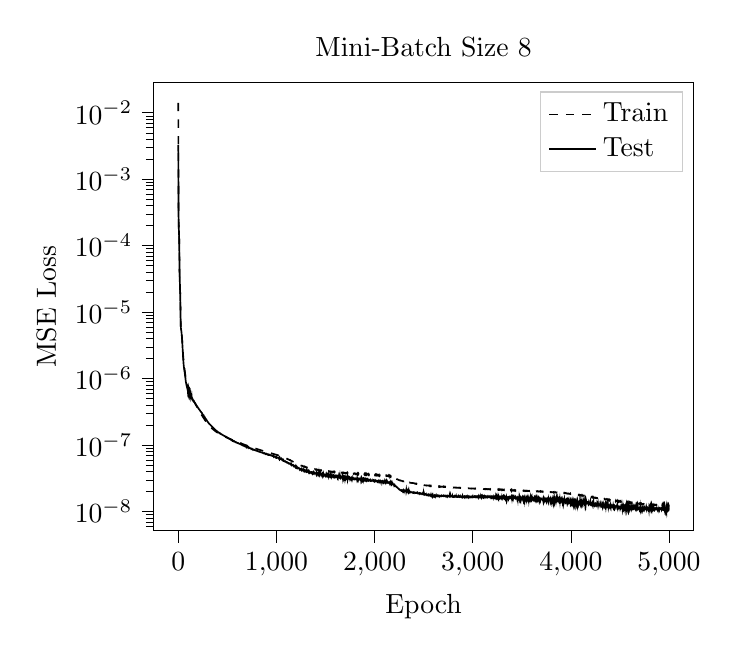
\begin{tikzpicture}

\begin{axis}[
legend cell align={left},
legend style={fill opacity=0.8, draw opacity=1, text opacity=1, draw=white!80!black},
log basis y={10},
tick align=outside,
tick pos=left,
title={Mini-Batch Size 8},
x grid style={white!69.0196078431373!black},
xlabel={Epoch},
xmin=-249.95, xmax=5248.95,
xtick style={color=black},
y grid style={white!69.0196078431373!black},
ylabel={MSE Loss},
ymin=5.12526233709927e-09, ymax=0.0285503119126669,
ymode=log,
ytick style={color=black}
]
\addplot [semithick, black, dashed]
table {%
0 0.0140922155501321
1 0.00164667243149597
2 0.00065037911516265
3 0.000295232196316647
4 0.000193644413906441
5 0.00017554680505782
6 0.000166322737537485
7 0.000155888844841684
8 0.000142262006907913
9 0.00012419570547172
10 0.000100196558816606
11 7.53355795714015e-05
12 5.41193190329068e-05
13 3.99818541809509e-05
14 3.23710513916922e-05
15 2.83831747833574e-05
16 2.58379168235479e-05
17 2.3768776641873e-05
18 2.16936214364978e-05
19 1.93698575890267e-05
20 1.67099984373635e-05
21 1.38117074528736e-05
22 1.10197760235451e-05
23 8.81342460627366e-06
24 7.32618501214688e-06
25 6.44809396973756e-06
26 5.96682320880859e-06
27 5.69452180099006e-06
28 5.51694411510084e-06
29 5.37627059711099e-06
30 5.25268244874155e-06
31 5.13194294012465e-06
32 5.00552247908104e-06
33 4.87103920659138e-06
34 4.72795897735523e-06
35 4.57529531857404e-06
36 4.41450717971747e-06
37 4.24678919441135e-06
38 4.07240037165479e-06
39 3.89275960455393e-06
40 3.70977897651414e-06
41 3.52646615996832e-06
42 3.3453291746639e-06
43 3.1669885086103e-06
44 2.99429524324069e-06
45 2.82882308749777e-06
46 2.67223944220518e-06
47 2.52574185277865e-06
48 2.39030650546113e-06
49 2.26648519112871e-06
50 2.15448263186602e-06
51 2.05455952405487e-06
52 1.96556939043546e-06
53 1.88664972873198e-06
54 1.81654708246981e-06
55 1.75456746703162e-06
56 1.69953624238417e-06
57 1.65011574182472e-06
58 1.60480939666741e-06
59 1.56276212375417e-06
60 1.52249059640042e-06
61 1.4837170463835e-06
62 1.44544674019187e-06
63 1.40767455231128e-06
64 1.37012475846632e-06
65 1.3339168483526e-06
66 1.29931519345661e-06
67 1.2659092755527e-06
68 1.23280311538565e-06
69 1.20021240133639e-06
70 1.16748595181093e-06
71 1.13551588817273e-06
72 1.10446207130366e-06
73 1.07352417389706e-06
74 1.04239164762987e-06
75 1.01698211097556e-06
76 9.92916835798496e-07
77 9.70485951363287e-07
78 9.49992109070763e-07
79 9.31409722205956e-07
80 9.14265601551279e-07
81 8.97762910810229e-07
82 8.82654424465557e-07
83 8.68559461117968e-07
84 8.55493358947967e-07
85 8.43273811710787e-07
86 8.31858977321076e-07
87 8.20936465963484e-07
88 8.10674030482517e-07
89 8.00620192784152e-07
90 7.91515300498702e-07
91 7.82651789464239e-07
92 7.7411152496154e-07
93 7.66956414445019e-07
94 7.5921274802937e-07
95 7.51383507328285e-07
96 7.44354396381652e-07
97 7.36274504674839e-07
98 7.30296529290797e-07
99 7.22306401783612e-07
100 7.16731141153559e-07
101 7.0944152068364e-07
102 7.04137545035621e-07
103 6.97249927974042e-07
104 6.922896165662e-07
105 6.85678604298801e-07
106 6.79918118848377e-07
107 6.74806719885623e-07
108 6.68366211726834e-07
109 6.63462581393048e-07
110 6.57123162881135e-07
111 6.52642981187057e-07
112 6.46561416587588e-07
113 6.42274032088608e-07
114 6.36438868973244e-07
115 6.32267128040098e-07
116 6.26555323151479e-07
117 6.21985995039154e-07
118 6.16880253367924e-07
119 6.11863263415557e-07
120 6.07826088987906e-07
121 6.02515582706076e-07
122 5.97315892207462e-07
123 5.93690181311501e-07
124 5.87228766487868e-07
125 5.84643050316913e-07
126 5.79739358123277e-07
127 5.74914281592953e-07
128 5.70551833760646e-07
129 5.66140960202688e-07
130 5.61847894573475e-07
131 5.57626214323648e-07
132 5.53413915262979e-07
133 5.49454119457948e-07
134 5.45167176518646e-07
135 5.41143863905802e-07
136 5.37298371497741e-07
137 5.32898270137139e-07
138 5.29843257034201e-07
139 5.25404720370659e-07
140 5.21684867152317e-07
141 5.18092104179857e-07
142 5.13483512598611e-07
143 5.08875732489145e-07
144 5.05149497538326e-07
145 5.01876758473685e-07
146 4.97770456185265e-07
147 4.94343421156174e-07
148 4.90650616956856e-07
149 4.8737844441149e-07
150 4.83746504770011e-07
151 4.80410617424099e-07
152 4.77105002900657e-07
153 4.73949040991073e-07
154 4.70770607652327e-07
155 4.67602424610192e-07
156 4.64573913710353e-07
157 4.61537018406233e-07
158 4.58560601526159e-07
159 4.55594075592813e-07
160 4.52629424799511e-07
161 4.49810896430591e-07
162 4.46874828853083e-07
163 4.44053090966179e-07
164 4.41227867604255e-07
165 4.38426361519362e-07
166 4.35670840431612e-07
167 4.33036380659502e-07
168 4.30322021191643e-07
169 4.27488975983437e-07
170 4.24709639364806e-07
171 4.21982422551537e-07
172 4.19321082635093e-07
173 4.16750839320912e-07
174 4.14194871584783e-07
175 4.1157767810418e-07
176 4.09005205327162e-07
177 4.06454590493155e-07
178 4.03974517769967e-07
179 4.01356386795726e-07
180 3.98910379288964e-07
181 3.96400903827754e-07
182 3.93962698311157e-07
183 3.91538277543901e-07
184 3.89058316706326e-07
185 3.86672758100559e-07
186 3.84376024534561e-07
187 3.82156077666451e-07
188 3.79795015795992e-07
189 3.77472126810829e-07
190 3.75254422486648e-07
191 3.72999132707719e-07
192 3.70814309334833e-07
193 3.68606052909115e-07
194 3.66414772166479e-07
195 3.64246124291867e-07
196 3.62064812147622e-07
197 3.60114379777343e-07
198 3.57652658479424e-07
199 3.55473573875997e-07
200 3.53420759978462e-07
201 3.51302201732295e-07
202 3.49260392450645e-07
203 3.47137964237021e-07
204 3.45095554795449e-07
205 3.43017129246448e-07
206 3.40932977728414e-07
207 3.38848146498094e-07
208 3.36741637614324e-07
209 3.34673315357747e-07
210 3.32618128226159e-07
211 3.30624918607469e-07
212 3.28681106719131e-07
213 3.2678425436572e-07
214 3.24867698765274e-07
215 3.23009222441328e-07
216 3.21105375114428e-07
217 3.19259059818222e-07
218 3.17433803207479e-07
219 3.15584080713194e-07
220 3.13753979209963e-07
221 3.11972391951798e-07
222 3.10204712469897e-07
223 3.08459960738361e-07
224 3.06718977086007e-07
225 3.04951894634087e-07
226 3.03379400019566e-07
227 3.01692094268446e-07
228 3.00041570543641e-07
229 2.98378097685514e-07
230 2.96704027594075e-07
231 2.95068247101682e-07
232 2.93436909618805e-07
233 2.91839041182129e-07
234 2.90256448501225e-07
235 2.88692379278643e-07
236 2.87134213266427e-07
237 2.85589026884026e-07
238 2.84047657121533e-07
239 2.82538714426295e-07
240 2.81039958053952e-07
241 2.79510103869285e-07
242 2.78032811682039e-07
243 2.76594212650139e-07
244 2.7475024603163e-07
245 2.72926708213106e-07
246 2.71423920384706e-07
247 2.7000172076086e-07
248 2.68524305077733e-07
249 2.67011570478815e-07
250 2.65667921034662e-07
251 2.64317999302932e-07
252 2.62892964080663e-07
253 2.6150448949025e-07
254 2.60125897110441e-07
255 2.58924373436997e-07
256 2.57517830519305e-07
257 2.56230467748253e-07
258 2.54854917034919e-07
259 2.53686509193329e-07
260 2.52175349391592e-07
261 2.51046833938062e-07
262 2.49770576434827e-07
263 2.48423187827029e-07
264 2.47144563388702e-07
265 2.45901549853045e-07
266 2.4462504500633e-07
267 2.43350985510205e-07
268 2.42261470663863e-07
269 2.41032267901176e-07
270 2.39729021991764e-07
271 2.38334006315455e-07
272 2.37114604335176e-07
273 2.35892772845858e-07
274 2.34670065896836e-07
275 2.3353716209229e-07
276 2.3238534521397e-07
277 2.31254778810808e-07
278 2.30117605983793e-07
279 2.29054269301088e-07
280 2.27954691752075e-07
281 2.26809562416719e-07
282 2.25817690040486e-07
283 2.24762463858497e-07
284 2.2381367495683e-07
285 2.22726548656738e-07
286 2.21723776196114e-07
287 2.20762035670674e-07
288 2.19673128100339e-07
289 2.18611050652129e-07
290 2.1762178107565e-07
291 2.16632967322994e-07
292 2.15608462355021e-07
293 2.14716398861725e-07
294 2.13740754045233e-07
295 2.12850587857361e-07
296 2.11970101840819e-07
297 2.11049697046661e-07
298 2.1004613132547e-07
299 2.09148392926295e-07
300 2.08267972048759e-07
301 2.0738952559185e-07
302 2.0650375899578e-07
303 2.0562344525743e-07
304 2.04789969075136e-07
305 2.03896006780724e-07
306 2.03049032204916e-07
307 2.02233469991597e-07
308 2.0148574800416e-07
309 2.00686525744231e-07
310 1.99914377798649e-07
311 1.99131872182789e-07
312 1.98344035812426e-07
313 1.97613068664282e-07
314 1.9680639949371e-07
315 1.96114129776603e-07
316 1.95406764222028e-07
317 1.94725376895022e-07
318 1.93973928373836e-07
319 1.93272308163017e-07
320 1.9257287543617e-07
321 1.91904341296123e-07
322 1.91237644701303e-07
323 1.90597502623291e-07
324 1.89894711086325e-07
325 1.8928915396188e-07
326 1.88604807627613e-07
327 1.8794622811491e-07
328 1.87344297193803e-07
329 1.86699944878299e-07
330 1.86075537186525e-07
331 1.85402446655658e-07
332 1.84775635814205e-07
333 1.84167428516346e-07
334 1.83570768633956e-07
335 1.82982711312007e-07
336 1.82418746863533e-07
337 1.81827815703528e-07
338 1.81145456025433e-07
339 1.80619840630669e-07
340 1.80006042857173e-07
341 1.79483078060372e-07
342 1.78932678077004e-07
343 1.7839446073431e-07
344 1.7783793585302e-07
345 1.77330097105965e-07
346 1.76734144670121e-07
347 1.76271198734312e-07
348 1.75766690267309e-07
349 1.75184670666795e-07
350 1.74708623170261e-07
351 1.74188886322924e-07
352 1.73653229948556e-07
353 1.73181383031462e-07
354 1.7267201918969e-07
355 1.72169975215297e-07
356 1.716809444261e-07
357 1.71193413185833e-07
358 1.7070678104858e-07
359 1.70231708297663e-07
360 1.69763145491331e-07
361 1.69323822717615e-07
362 1.68841542647513e-07
363 1.68392174817455e-07
364 1.67920915593811e-07
365 1.67448701848372e-07
366 1.67067471872784e-07
367 1.66522447294426e-07
368 1.66187803337436e-07
369 1.65655882883087e-07
370 1.65297342158866e-07
371 1.64844675270004e-07
372 1.64449132043387e-07
373 1.63934461077986e-07
374 1.63596360001961e-07
375 1.63166515610769e-07
376 1.62640494570709e-07
377 1.62330137088773e-07
378 1.61810680310737e-07
379 1.61525042159383e-07
380 1.61029843134486e-07
381 1.60723079604352e-07
382 1.60256959116367e-07
383 1.59806124516493e-07
384 1.59371342730807e-07
385 1.59003193211049e-07
386 1.58613461659129e-07
387 1.58135951810578e-07
388 1.5777919826121e-07
389 1.57490906419255e-07
390 1.57049220966599e-07
391 1.56678830967039e-07
392 1.56399091556736e-07
393 1.5595287873893e-07
394 1.55577467211288e-07
395 1.55218681813452e-07
396 1.54868281256881e-07
397 1.54552626023374e-07
398 1.54198211124168e-07
399 1.53841266364196e-07
400 1.53452866729964e-07
401 1.53133977093489e-07
402 1.52802964166199e-07
403 1.52480551506073e-07
404 1.52156185608376e-07
405 1.51788253479168e-07
406 1.51498513695003e-07
407 1.51127850402943e-07
408 1.50798184616718e-07
409 1.50510982436458e-07
410 1.50194480964316e-07
411 1.4992832301175e-07
412 1.49619644533416e-07
413 1.49345439441007e-07
414 1.49000281972178e-07
415 1.48698896465405e-07
416 1.48378767759638e-07
417 1.48073516024638e-07
418 1.47793847567357e-07
419 1.47497233387028e-07
420 1.47152927594263e-07
421 1.46810806187503e-07
422 1.46530012960611e-07
423 1.46194294019963e-07
424 1.45904546680953e-07
425 1.45637120098741e-07
426 1.45390437303661e-07
427 1.45085242406751e-07
428 1.44843584227061e-07
429 1.44539950433398e-07
430 1.44255259536763e-07
431 1.43986164975018e-07
432 1.43712213986902e-07
433 1.43442524212389e-07
434 1.43141190728002e-07
435 1.42893512014908e-07
436 1.42647763382797e-07
437 1.42393991835021e-07
438 1.42116199961961e-07
439 1.41860749801381e-07
440 1.41584198152245e-07
441 1.41324433158729e-07
442 1.41084530103086e-07
443 1.40788790234936e-07
444 1.40560038717652e-07
445 1.40289742095234e-07
446 1.40070903469791e-07
447 1.39810986377498e-07
448 1.3955653855291e-07
449 1.39309414347366e-07
450 1.39040228608778e-07
451 1.38806914293355e-07
452 1.38617263488072e-07
453 1.38398338824786e-07
454 1.38211991345116e-07
455 1.37910985833045e-07
456 1.37707504212159e-07
457 1.37452863837595e-07
458 1.37235590139895e-07
459 1.37014003817271e-07
460 1.36758330285147e-07
461 1.36494116027563e-07
462 1.36306082161752e-07
463 1.36068334931849e-07
464 1.35855103517102e-07
465 1.35629422052475e-07
466 1.35411948866349e-07
467 1.35155687953414e-07
468 1.34934801762299e-07
469 1.34734451673779e-07
470 1.34524718356843e-07
471 1.34328436132591e-07
472 1.34129347609147e-07
473 1.33910911843671e-07
474 1.3371256061312e-07
475 1.33461909047838e-07
476 1.33277299719126e-07
477 1.33085340515038e-07
478 1.32889105676881e-07
479 1.32672969037628e-07
480 1.32476193449804e-07
481 1.32274759009121e-07
482 1.32073942387123e-07
483 1.31855791474678e-07
484 1.31636651781619e-07
485 1.31416223496217e-07
486 1.31259498012071e-07
487 1.31016023310337e-07
488 1.30887004155866e-07
489 1.30695356258315e-07
490 1.30501306800923e-07
491 1.30296649251349e-07
492 1.30041917019597e-07
493 1.29918106384963e-07
494 1.29697845192567e-07
495 1.29461063567149e-07
496 1.29204722520981e-07
497 1.29046236825303e-07
498 1.28783909607577e-07
499 1.28579553615893e-07
500 1.28412652287579e-07
501 1.28222582777227e-07
502 1.28080913981421e-07
503 1.27826674720666e-07
504 1.2768455570189e-07
505 1.27511456184948e-07
506 1.27337297175956e-07
507 1.2712039346674e-07
508 1.26940336869552e-07
509 1.26781960378963e-07
510 1.26628617971747e-07
511 1.26438190140021e-07
512 1.26261214711931e-07
513 1.26080714901278e-07
514 1.25882205830763e-07
515 1.25689170451082e-07
516 1.25458669902656e-07
517 1.25292414027811e-07
518 1.25118541685509e-07
519 1.24933668057992e-07
520 1.24744541571076e-07
521 1.24592485745367e-07
522 1.2438628746736e-07
523 1.24239199989162e-07
524 1.24081532147713e-07
525 1.23898961273738e-07
526 1.23711435064067e-07
527 1.23683571343847e-07
528 1.23402232516057e-07
529 1.23180608545326e-07
530 1.22983389335474e-07
531 1.2279557410011e-07
532 1.22695858955524e-07
533 1.2242326393519e-07
534 1.22268119062241e-07
535 1.22114195065137e-07
536 1.2186837597028e-07
537 1.21758532072747e-07
538 1.21501212188235e-07
539 1.21415872920139e-07
540 1.21146897740232e-07
541 1.21149452825264e-07
542 1.20954131578088e-07
543 1.20601052417513e-07
544 1.2042635933085e-07
545 1.20382659668294e-07
546 1.20114501360291e-07
547 1.19902081415546e-07
548 1.19723047657061e-07
549 1.19519860986017e-07
550 1.19464099865851e-07
551 1.19455365275911e-07
552 1.18856987027627e-07
553 1.18855618111979e-07
554 1.18722306197583e-07
555 1.18556314758322e-07
556 1.18349971197418e-07
557 1.18197913097973e-07
558 1.18190822574249e-07
559 1.17993449931575e-07
560 1.17722103356144e-07
561 1.17562712910413e-07
562 1.1739236306596e-07
563 1.17146097792897e-07
564 1.17130330764326e-07
565 1.16876142195466e-07
566 1.16746778818566e-07
567 1.16807582864809e-07
568 1.16375001658398e-07
569 1.16238238121014e-07
570 1.16071960784225e-07
571 1.15917950825661e-07
572 1.15715357653201e-07
573 1.15682018952512e-07
574 1.15512718215527e-07
575 1.15298490829474e-07
576 1.15141919192041e-07
577 1.15017629779501e-07
578 1.14785245981963e-07
579 1.14825111019456e-07
580 1.14467956363384e-07
581 1.14309470399476e-07
582 1.14250206504352e-07
583 1.14062090345257e-07
584 1.14072716723257e-07
585 1.13818667545118e-07
586 1.13543024539808e-07
587 1.13510344416312e-07
588 1.13261899898021e-07
589 1.13188994674829e-07
590 1.12949545007623e-07
591 1.12861762920247e-07
592 1.12966328723374e-07
593 1.12624403906025e-07
594 1.12488853648784e-07
595 1.12194247433806e-07
596 1.12081747023041e-07
597 1.11879273879012e-07
598 1.11686604855166e-07
599 1.1151889847838e-07
600 1.11518363773655e-07
601 1.11229455521666e-07
602 1.11068491328581e-07
603 1.10914127503747e-07
604 1.10845691843053e-07
605 1.10635652848856e-07
606 1.10445679641913e-07
607 1.10333368983362e-07
608 1.10191389911307e-07
609 1.10141222277704e-07
610 1.09968580785491e-07
611 1.10079902308158e-07
612 1.09896487208161e-07
613 1.09495213120425e-07
614 1.09437622697328e-07
615 1.09409666039895e-07
616 1.09359268291698e-07
617 1.0894876301748e-07
618 1.08862762553841e-07
619 1.0888215664373e-07
620 1.08902593192184e-07
621 1.08681523236953e-07
622 1.08473326777769e-07
623 1.08357849692098e-07
624 1.08215046504156e-07
625 1.08083012595017e-07
626 1.07983994128702e-07
627 1.0788382092386e-07
628 1.07778989340446e-07
629 1.07629510504026e-07
630 1.07486674595592e-07
631 1.07359776917448e-07
632 1.07198026283228e-07
633 1.07110649613773e-07
634 1.06957342852709e-07
635 1.06551703673574e-07
636 1.06703632233973e-07
637 1.06261747919945e-07
638 1.06245268353788e-07
639 1.05981521867804e-07
640 1.0613362208467e-07
641 1.05918131012572e-07
642 1.05605284026922e-07
643 1.05518851803765e-07
644 1.05296745056549e-07
645 1.0529636806389e-07
646 1.05115613724394e-07
647 1.04897444288099e-07
648 1.04692954625563e-07
649 1.04653310055269e-07
650 1.04388389308596e-07
651 1.04356357626401e-07
652 1.04121267867185e-07
653 1.03941493522441e-07
654 1.03825485911813e-07
655 1.03654870686753e-07
656 1.03468656945438e-07
657 1.03318351046156e-07
658 1.03309234573246e-07
659 1.03166787249975e-07
660 1.02888646404509e-07
661 1.02764241914244e-07
662 1.02620244419427e-07
663 1.02643449945816e-07
664 1.02388692905464e-07
665 1.02254439710237e-07
666 1.02264427352949e-07
667 1.01974317667342e-07
668 1.01824479767032e-07
669 1.01781015130697e-07
670 1.01579884494996e-07
671 1.01662138689562e-07
672 1.01463956596604e-07
673 1.01146636220406e-07
674 1.01043345342333e-07
675 1.01026062447218e-07
676 1.00765059274366e-07
677 1.00705422818592e-07
678 1.00596716810841e-07
679 1.00494772908633e-07
680 1.00339713535291e-07
681 1.00227720652768e-07
682 1.00199328135986e-07
683 9.99779721606586e-08
684 9.99164768895611e-08
685 9.97651532674837e-08
686 9.96916367359546e-08
687 9.95852735758973e-08
688 9.94225873363064e-08
689 9.93057265326058e-08
690 9.91738692572852e-08
691 9.90683583950158e-08
692 9.89918791169941e-08
693 9.89294559996523e-08
694 9.87324563563874e-08
695 9.8580230650569e-08
696 9.84844026170606e-08
697 9.83782085786089e-08
698 9.82969909344433e-08
699 9.80663861103182e-08
700 9.79155029394718e-08
701 9.78743212769473e-08
702 9.7774189509181e-08
703 9.74998872109722e-08
704 9.7537862576047e-08
705 9.7373689259328e-08
706 9.72140168737923e-08
707 9.71121613257964e-08
708 9.69666632180122e-08
709 9.69298370527838e-08
710 9.67698093869984e-08
711 9.6669013320394e-08
712 9.6617836987889e-08
713 9.65235347489823e-08
714 9.643995225872e-08
715 9.6384693021534e-08
716 9.61863593840206e-08
717 9.60114623218544e-08
718 9.60902926934182e-08
719 9.57746484626654e-08
720 9.57750240715427e-08
721 9.55805155538059e-08
722 9.55347426128128e-08
723 9.54729408171318e-08
724 9.52798347118033e-08
725 9.52589754721345e-08
726 9.51665310111594e-08
727 9.49889552952499e-08
728 9.48892586905004e-08
729 9.48318259261782e-08
730 9.46984865208833e-08
731 9.46578152714039e-08
732 9.44619410319092e-08
733 9.44395689952415e-08
734 9.43228704386456e-08
735 9.42138219972577e-08
736 9.41150636339927e-08
737 9.40356634000494e-08
738 9.39251921092676e-08
739 9.37723432130611e-08
740 9.36953663508433e-08
741 9.36475301536177e-08
742 9.34891315171882e-08
743 9.34929558358277e-08
744 9.32899375643004e-08
745 9.31277580900058e-08
746 9.29872254360475e-08
747 9.29021212048298e-08
748 9.27547188318556e-08
749 9.26676536128212e-08
750 9.25360728327718e-08
751 9.24768817487376e-08
752 9.23224709517001e-08
753 9.2233401355557e-08
754 9.21099720416763e-08
755 9.20273056550513e-08
756 9.18983567661513e-08
757 9.17982077250912e-08
758 9.16838067226422e-08
759 9.1583944425544e-08
760 9.14591718057523e-08
761 9.13134026792051e-08
762 9.12507480110847e-08
763 9.11265217853341e-08
764 9.10621974288262e-08
765 9.08905435199614e-08
766 9.0788907545658e-08
767 9.0717570659038e-08
768 9.05781980975462e-08
769 9.05061573064359e-08
770 9.03604748181408e-08
771 9.02703232927848e-08
772 9.02022289084314e-08
773 9.01490784093184e-08
774 8.99447075433102e-08
775 8.98894601180089e-08
776 8.97487045516954e-08
777 8.9711841648743e-08
778 8.95438815806671e-08
779 8.95039619379645e-08
780 8.93075877943517e-08
781 8.92706220980699e-08
782 8.91444243862338e-08
783 8.90533289634732e-08
784 8.89315970269422e-08
785 8.88538352157298e-08
786 8.87460719418698e-08
787 8.86892839258024e-08
788 8.85925947713417e-08
789 8.84801011071801e-08
790 8.83455844515879e-08
791 8.83479853879265e-08
792 8.81836671791092e-08
793 8.8178019002072e-08
794 8.80678381420808e-08
795 8.79570468814705e-08
796 8.78213846133846e-08
797 8.77077261600689e-08
798 8.7557868305943e-08
799 8.75062553475914e-08
800 8.73836898467317e-08
801 8.73753748438233e-08
802 8.71596677542996e-08
803 8.71341073862553e-08
804 8.69886648713347e-08
805 8.69691683735851e-08
806 8.68006289946877e-08
807 8.67195310281232e-08
808 8.66247496071892e-08
809 8.66069136327141e-08
810 8.63993041644307e-08
811 8.63324029767298e-08
812 8.62302148672001e-08
813 8.61057656562636e-08
814 8.61300473475879e-08
815 8.58610517182612e-08
816 8.5876022253295e-08
817 8.58245899744148e-08
818 8.56204245254233e-08
819 8.56291569748535e-08
820 8.54643526437826e-08
821 8.53652859822418e-08
822 8.5391497251841e-08
823 8.51209773058414e-08
824 8.51588658763447e-08
825 8.50582824751811e-08
826 8.49786741063952e-08
827 8.48149538770215e-08
828 8.48154887371777e-08
829 8.46310325455235e-08
830 8.46116082833248e-08
831 8.44586885744292e-08
832 8.43162639991846e-08
833 8.43594839841089e-08
834 8.41931290338494e-08
835 8.40042691381271e-08
836 8.39640144789655e-08
837 8.39935478929021e-08
838 8.38417056181484e-08
839 8.3761031231866e-08
840 8.36453677903748e-08
841 8.35098131304335e-08
842 8.3516487031865e-08
843 8.3398541787183e-08
844 8.32627191780233e-08
845 8.32743370144939e-08
846 8.31479871719054e-08
847 8.30611524476055e-08
848 8.29425600832323e-08
849 8.28054075387996e-08
850 8.28294606325386e-08
851 8.27534693756959e-08
852 8.26178241633002e-08
853 8.25921608678115e-08
854 8.24915612467336e-08
855 8.23746438047834e-08
856 8.23552042801268e-08
857 8.22746717608069e-08
858 8.21175156664466e-08
859 8.20935714083149e-08
860 8.20074700209616e-08
861 8.18721728084171e-08
862 8.18467062071448e-08
863 8.17524560883243e-08
864 8.16378868124801e-08
865 8.16203907341162e-08
866 8.15071311217608e-08
867 8.14008423501988e-08
868 8.13587263230886e-08
869 8.12950596609241e-08
870 8.11408385228418e-08
871 8.11435524941118e-08
872 8.10090526517371e-08
873 8.09792461664571e-08
874 8.08584962870285e-08
875 8.07094791053231e-08
876 8.07686938379959e-08
877 8.06270915392204e-08
878 8.05262200671564e-08
879 8.04814699018053e-08
880 8.03900555492731e-08
881 8.03408116238913e-08
882 8.02471276806216e-08
883 8.01388805129477e-08
884 8.00124187625428e-08
885 8.00657544806072e-08
886 7.98942147488546e-08
887 7.99531881936488e-08
888 7.97822659910352e-08
889 7.97795756035668e-08
890 7.9595778335495e-08
891 7.94955623648619e-08
892 7.94511712500778e-08
893 7.94300374051815e-08
894 7.93113748613905e-08
895 7.92388654584642e-08
896 7.91362802941009e-08
897 7.90537630148691e-08
898 7.89241159324661e-08
899 7.89327640422499e-08
900 7.87739521186381e-08
901 7.87634696282069e-08
902 7.86302511679438e-08
903 7.85142067414313e-08
904 7.84941220688395e-08
905 7.836267482908e-08
906 7.83394425170059e-08
907 7.82585197347529e-08
908 7.82273210271356e-08
909 7.80942995328715e-08
910 7.80388083398975e-08
911 7.79501971406305e-08
912 7.78230592546336e-08
913 7.77868578483165e-08
914 7.76701064806318e-08
915 7.76812620495448e-08
916 7.75076760506366e-08
917 7.75319989765322e-08
918 7.74967118450931e-08
919 7.73487059220201e-08
920 7.73361544830209e-08
921 7.71912398640495e-08
922 7.71142926412338e-08
923 7.70105475949023e-08
924 7.69942951457381e-08
925 7.68621367575051e-08
926 7.66920159733786e-08
927 7.6753732895618e-08
928 7.66649599208691e-08
929 7.65232764639023e-08
930 7.64789896630091e-08
931 7.63227431415103e-08
932 7.62898755857222e-08
933 7.62348100540322e-08
934 7.61062690850522e-08
935 7.59985500060623e-08
936 7.60535598010037e-08
937 7.59387081998852e-08
938 7.58480387572646e-08
939 7.57766501973123e-08
940 7.56443777145677e-08
941 7.55885656298361e-08
942 7.55352047487889e-08
943 7.55366707450023e-08
944 7.54625999297431e-08
945 7.53840733613842e-08
946 7.52436891762187e-08
947 7.520958560292e-08
948 7.51185533998111e-08
949 7.50705502872151e-08
950 7.49230383103594e-08
951 7.48538313226632e-08
952 7.47696083367444e-08
953 7.4698309575183e-08
954 7.46352352933855e-08
955 7.45532024719608e-08
956 7.45396909715979e-08
957 7.43793192778952e-08
958 7.43306780917052e-08
959 7.42391270653897e-08
960 7.4170969384113e-08
961 7.41744250110088e-08
962 7.39807714547069e-08
963 7.3907636275905e-08
964 7.3864839967186e-08
965 7.38722046689233e-08
966 7.37782955395616e-08
967 7.35998169503205e-08
968 7.36751591370322e-08
969 7.35319244977717e-08
970 7.34493053959895e-08
971 7.33622083135543e-08
972 7.33287411573968e-08
973 7.32267693424049e-08
974 7.3227407262344e-08
975 7.30911046540328e-08
976 7.3059925388641e-08
977 7.29211026548882e-08
978 7.29121208236094e-08
979 7.2779587866556e-08
980 7.27771263386856e-08
981 7.26923735738794e-08
982 7.26410809015476e-08
983 7.25908489931371e-08
984 7.24250146495464e-08
985 7.2414066065285e-08
986 7.23511959135337e-08
987 7.23106430315923e-08
988 7.22220240687577e-08
989 7.21276343647048e-08
990 7.20563575073996e-08
991 7.19845479606462e-08
992 7.19308399528273e-08
993 7.18280783758019e-08
994 7.17602781392657e-08
995 7.16623081844503e-08
996 7.1633209976163e-08
997 7.1613316125152e-08
998 7.14358405220494e-08
999 7.13820533686516e-08
1000 7.13005416006496e-08
1001 7.13117426327514e-08
1002 7.11042069294621e-08
1003 7.11583764241297e-08
1004 7.11103543000746e-08
1005 7.09215685787967e-08
1006 7.08726079992061e-08
1007 7.08819332659871e-08
1008 7.06523474676146e-08
1009 7.06114099751076e-08
1010 7.05629681077013e-08
1011 7.04900955836862e-08
1012 7.03779293322881e-08
1013 7.03613790653535e-08
1014 7.02909734737744e-08
1015 7.02346028056411e-08
1016 7.00847629646617e-08
1017 7.00646524416371e-08
1018 7.00006208278481e-08
1019 6.99058087274551e-08
1020 6.97008041994351e-08
1021 6.96666002131252e-08
1022 6.95315661491946e-08
1023 6.93929467434629e-08
1024 6.93491352254938e-08
1025 6.92687724743735e-08
1026 6.9181248853134e-08
1027 6.90323947898364e-08
1028 6.89361719263815e-08
1029 6.88460079372177e-08
1030 6.88259702794625e-08
1031 6.87216120782708e-08
1032 6.85840478462652e-08
1033 6.85226009862205e-08
1034 6.83794042464214e-08
1035 6.83534466769942e-08
1036 6.82413636488022e-08
1037 6.81742337604874e-08
1038 6.8081035704104e-08
1039 6.80005548439055e-08
1040 6.79186499672468e-08
1041 6.78197289332161e-08
1042 6.77157139037376e-08
1043 6.77006809528535e-08
1044 6.75445062991997e-08
1045 6.74544157597268e-08
1046 6.73693972919054e-08
1047 6.72946742232838e-08
1048 6.71474435236519e-08
1049 6.70465003258514e-08
1050 6.70302539118595e-08
1051 6.69601158707067e-08
1052 6.68708544226959e-08
1053 6.67221369274884e-08
1054 6.66394672963477e-08
1055 6.65038577301047e-08
1056 6.64386373996351e-08
1057 6.6429855464456e-08
1058 6.63477771514209e-08
1059 6.62112182396868e-08
1060 6.61053233539377e-08
1061 6.60354965731358e-08
1062 6.58835158864335e-08
1063 6.58057612259455e-08
1064 6.57003935407019e-08
1065 6.56495188930961e-08
1066 6.55546697672094e-08
1067 6.54752256359359e-08
1068 6.53355711985881e-08
1069 6.52995786598609e-08
1070 6.52046299594034e-08
1071 6.50510368949142e-08
1072 6.50725278443787e-08
1073 6.49379873642886e-08
1074 6.47580108266155e-08
1075 6.46967440784962e-08
1076 6.47110855958033e-08
1077 6.46408487385841e-08
1078 6.45357608251018e-08
1079 6.44439404986485e-08
1080 6.4284627761424e-08
1081 6.42473115846087e-08
1082 6.42346976027497e-08
1083 6.4099857985056e-08
1084 6.39759074045898e-08
1085 6.39553085513e-08
1086 6.39084181939253e-08
1087 6.37432019150452e-08
1088 6.36723728701938e-08
1089 6.35793202752311e-08
1090 6.34713747382776e-08
1091 6.35341950525614e-08
1092 6.33713871458497e-08
1093 6.3277285804908e-08
1094 6.31845582761414e-08
1095 6.31149904926076e-08
1096 6.29787609565113e-08
1097 6.30093429236922e-08
1098 6.28861612330667e-08
1099 6.28055558475893e-08
1100 6.26232452294317e-08
1101 6.25952487345316e-08
1102 6.25822700701661e-08
1103 6.24765654775317e-08
1104 6.23883908117406e-08
1105 6.22942513581748e-08
1106 6.21327299015206e-08
1107 6.20863260349935e-08
1108 6.20415422387666e-08
1109 6.21000680087747e-08
1110 6.18504896578997e-08
1111 6.18067457205385e-08
1112 6.1644829599139e-08
1113 6.15710698008698e-08
1114 6.15897150124667e-08
1115 6.14760737152054e-08
1116 6.14502748659262e-08
1117 6.13122701871305e-08
1118 6.12455619730667e-08
1119 6.11872074065545e-08
1120 6.09162053128998e-08
1121 6.08576885987588e-08
1122 6.08179615930737e-08
1123 6.07086520618694e-08
1124 6.06223983101728e-08
1125 6.05575171297445e-08
1126 6.04104159798169e-08
1127 6.0348267340693e-08
1128 6.02285505344469e-08
1129 6.01458489990492e-08
1130 6.01179870587387e-08
1131 6.0027065746926e-08
1132 5.97797516208587e-08
1133 5.9795340693114e-08
1134 5.96402379002825e-08
1135 5.94761561911739e-08
1136 5.95539313339444e-08
1137 5.94249178975659e-08
1138 5.92505395076159e-08
1139 5.91597576615754e-08
1140 5.90666865125655e-08
1141 5.88915692842917e-08
1142 5.90203142101231e-08
1143 5.87497151824934e-08
1144 5.87532072353625e-08
1145 5.85907652910222e-08
1146 5.8551039190391e-08
1147 5.84408526567159e-08
1148 5.82552799874847e-08
1149 5.81301490427677e-08
1150 5.8109338837653e-08
1151 5.80481490803919e-08
1152 5.79101373157087e-08
1153 5.78085702569453e-08
1154 5.76846728073122e-08
1155 5.76280860729028e-08
1156 5.75032301490808e-08
1157 5.73179610068308e-08
1158 5.72661070288305e-08
1159 5.71943030065469e-08
1160 5.69885338492782e-08
1161 5.69631700626516e-08
1162 5.69194471786716e-08
1163 5.67838021701128e-08
1164 5.66640349766168e-08
1165 5.65589359924346e-08
1166 5.6512820266974e-08
1167 5.63850263919363e-08
1168 5.62500756329243e-08
1169 5.61824805593858e-08
1170 5.60970445784292e-08
1171 5.59599677218969e-08
1172 5.58494863724945e-08
1173 5.57552466800004e-08
1174 5.56996282252697e-08
1175 5.56156806448271e-08
1176 5.5491953369291e-08
1177 5.53300107037913e-08
1178 5.52866972709509e-08
1179 5.5107895852835e-08
1180 5.50283653844019e-08
1181 5.51412584899325e-08
1182 5.48718789001867e-08
1183 5.4910465046909e-08
1184 5.4751843118872e-08
1185 5.4634272609988e-08
1186 5.45681121217889e-08
1187 5.44585529360653e-08
1188 5.43135494264213e-08
1189 5.42500546694136e-08
1190 5.41413124164336e-08
1191 5.40952266248063e-08
1192 5.39357546243124e-08
1193 5.39131514880609e-08
1194 5.39165687554188e-08
1195 5.3634612921627e-08
1196 5.35923273101702e-08
1197 5.35096682368064e-08
1198 5.34264127121098e-08
1199 5.33043504136188e-08
1200 5.31984917513384e-08
1201 5.31392249949469e-08
1202 5.30054221310472e-08
1203 5.30110809604523e-08
1204 5.28841194253893e-08
1205 5.28213592305704e-08
1206 5.27674378001386e-08
1207 5.25633076429166e-08
1208 5.25129558854864e-08
1209 5.2446357926339e-08
1210 5.22644627349855e-08
1211 5.21429107900317e-08
1212 5.21280838032823e-08
1213 5.20980213041255e-08
1214 5.18598821455107e-08
1215 5.19323746939193e-08
1216 5.1801599847856e-08
1217 5.16898352844741e-08
1218 5.14871654297977e-08
1219 5.15548961050882e-08
1220 5.14475486421695e-08
1221 5.13119661880168e-08
1222 5.12700813648515e-08
1223 5.12630925495472e-08
1224 5.11038289716659e-08
1225 5.10397683979313e-08
1226 5.09275734623671e-08
1227 5.09132049710814e-08
1228 5.0759712610926e-08
1229 5.06871001304532e-08
1230 5.06944659219855e-08
1231 5.05630977118976e-08
1232 5.05891275865977e-08
1233 5.04078954683962e-08
1234 5.0369708529896e-08
1235 5.03202734072339e-08
1236 5.03486166767431e-08
1237 5.01460485304861e-08
1238 5.00217914414236e-08
1239 5.00083646550742e-08
1240 4.99302473584429e-08
1241 4.987592799921e-08
1242 4.97896254327834e-08
1243 4.97413813849157e-08
1244 4.96402420528952e-08
1245 4.9622389326931e-08
1246 4.95539652263233e-08
1247 4.94904343217861e-08
1248 4.94052279922386e-08
1249 4.92951875696868e-08
1250 4.93147989524267e-08
1251 4.91164378098041e-08
1252 4.91569000953262e-08
1253 4.91227655383675e-08
1254 4.90244803059703e-08
1255 4.89576740712039e-08
1256 4.8822162876494e-08
1257 4.87467866965297e-08
1258 4.87341117052509e-08
1259 4.87276126515113e-08
1260 4.87346524646881e-08
1261 4.85851170131113e-08
1262 4.84871747534754e-08
1263 4.85831895207234e-08
1264 4.82988585561728e-08
1265 4.83467545695504e-08
1266 4.83161799191834e-08
1267 4.81926020485801e-08
1268 4.81261100500063e-08
1269 4.80794487556224e-08
1270 4.79064465315204e-08
1271 4.78844559088643e-08
1272 4.80212023230564e-08
1273 4.79060066149728e-08
1274 4.7783847305638e-08
1275 4.76988225441843e-08
1276 4.77218500298804e-08
1277 4.76159679054788e-08
1278 4.76466013443755e-08
1279 4.74691612195599e-08
1280 4.75158579309465e-08
1281 4.73825057967225e-08
1282 4.7485986818252e-08
1283 4.72961260644666e-08
1284 4.73102585516472e-08
1285 4.72351163418594e-08
1286 4.72344711912598e-08
1287 4.71515645523724e-08
1288 4.71153546151015e-08
1289 4.68685075079023e-08
1290 4.70706135908827e-08
1291 4.68408979266144e-08
1292 4.68855339947893e-08
1293 4.69027191636329e-08
1294 4.68532288326884e-08
1295 4.66869751258869e-08
1296 4.67236158723239e-08
1297 4.66455751588768e-08
1298 4.6581428891912e-08
1299 4.66710647764046e-08
1300 4.65150191413244e-08
1301 4.6453202255492e-08
1302 4.64446993628798e-08
1303 4.63894488405003e-08
1304 4.62309609279288e-08
1305 4.62655005257773e-08
1306 4.63196391784493e-08
1307 4.61808473293246e-08
1308 4.61542245702162e-08
1309 4.62172598085786e-08
1310 4.61607299291344e-08
1311 4.60153494588056e-08
1312 4.59913277452983e-08
1313 4.59276329918268e-08
1314 4.58297194576573e-08
1315 4.59273223443191e-08
1316 4.58042492530453e-08
1317 4.57084866845037e-08
1318 4.56549604122003e-08
1319 4.56686972283293e-08
1320 4.56331827685119e-08
1321 4.56046227030882e-08
1322 4.5550667001848e-08
1323 4.55369211307399e-08
1324 4.5590441208887e-08
1325 4.54679211445708e-08
1326 4.54479248590545e-08
1327 4.52664653485257e-08
1328 4.5337347214236e-08
1329 4.53551621877324e-08
1330 4.51916858850154e-08
1331 4.51722750653971e-08
1332 4.51394618616874e-08
1333 4.51769472675778e-08
1334 4.51334482649557e-08
1335 4.51266249861249e-08
1336 4.50874914861288e-08
1337 4.49287061963233e-08
1338 4.48967479993456e-08
1339 4.48264219876648e-08
1340 4.4867042350738e-08
1341 4.48034820754728e-08
1342 4.48350610398052e-08
1343 4.48033875457554e-08
1344 4.45712150360933e-08
1345 4.46036571952746e-08
1346 4.46692990454523e-08
1347 4.45814032055125e-08
1348 4.45665362684977e-08
1349 4.45728043025895e-08
1350 4.45147311864957e-08
1351 4.44823261869232e-08
1352 4.43828213363417e-08
1353 4.42768181132536e-08
1354 4.43993598802095e-08
1355 4.44070804617169e-08
1356 4.42842968162438e-08
1357 4.41155342043587e-08
1358 4.41278631075903e-08
1359 4.40644807078172e-08
1360 4.42094289478945e-08
1361 4.40818237334994e-08
1362 4.39918047412391e-08
1363 4.41803186754797e-08
1364 4.40159865835454e-08
1365 4.39419652753514e-08
1366 4.39800256470946e-08
1367 4.38194544480908e-08
1368 4.38346918683052e-08
1369 4.38826430064765e-08
1370 4.38439412224767e-08
1371 4.38131168918332e-08
1372 4.37225367591054e-08
1373 4.36888630588328e-08
1374 4.37150416381371e-08
1375 4.36178424365608e-08
1376 4.36608899700985e-08
1377 4.35089207826422e-08
1378 4.35441604231812e-08
1379 4.35481492102596e-08
1380 4.34936193034474e-08
1381 4.33650798727925e-08
1382 4.34177889596654e-08
1383 4.34463673570917e-08
1384 4.33263139223428e-08
1385 4.33727313220444e-08
1386 4.33343354258042e-08
1387 4.3228653130889e-08
1388 4.31082869178923e-08
1389 4.324872136241e-08
1390 4.30600019534211e-08
1391 4.32475265323973e-08
1392 4.30882091100315e-08
1393 4.30473245973673e-08
1394 4.29888738828765e-08
1395 4.30272572833346e-08
1396 4.29292623698174e-08
1397 4.2927458932418e-08
1398 4.30014096650666e-08
1399 4.30005459408633e-08
1400 4.28852556577652e-08
1401 4.28427411769405e-08
1402 4.29186751995658e-08
1403 4.26496567271784e-08
1404 4.28333187523222e-08
1405 4.27500164761341e-08
1406 4.27967534255558e-08
1407 4.26256254471014e-08
1408 4.26668547057751e-08
1409 4.25627499347492e-08
1410 4.27053181430992e-08
1411 4.24960702827271e-08
1412 4.25527307035267e-08
1413 4.25026517083538e-08
1414 4.24830301199997e-08
1415 4.24793107010046e-08
1416 4.24730674390972e-08
1417 4.23903328332642e-08
1418 4.25100638867804e-08
1419 4.24156434370992e-08
1420 4.23989374351841e-08
1421 4.23957842898837e-08
1422 4.23277789733945e-08
1423 4.23183708635477e-08
1424 4.22206468280173e-08
1425 4.22159647799347e-08
1426 4.22320841448887e-08
1427 4.21671459114314e-08
1428 4.22204840990759e-08
1429 4.21945885649144e-08
1430 4.21728435395785e-08
1431 4.21243299655316e-08
1432 4.20114667738503e-08
1433 4.20510037324462e-08
1434 4.2026753572344e-08
1435 4.19436382799176e-08
1436 4.19389113277546e-08
1437 4.19057039202642e-08
1438 4.18952429424024e-08
1439 4.19827620414814e-08
1440 4.19652518064417e-08
1441 4.18845844243343e-08
1442 4.19072387116692e-08
1443 4.17922589410757e-08
1444 4.16854369809094e-08
1445 4.1889259613459e-08
1446 4.17623865209826e-08
1447 4.17697262604655e-08
1448 4.17888626045304e-08
1449 4.16201110771119e-08
1450 4.17640830239208e-08
1451 4.1783336582224e-08
1452 4.153928639683e-08
1453 4.16737873538686e-08
1454 4.1592476381247e-08
1455 4.15322517932637e-08
1456 4.1644548808506e-08
1457 4.15027544096169e-08
1458 4.148360849765e-08
1459 4.13861753427724e-08
1460 4.14018035996833e-08
1461 4.13481794314663e-08
1462 4.14854741146442e-08
1463 4.13563179764154e-08
1464 4.13556541101201e-08
1465 4.13902445641767e-08
1466 4.1323798298798e-08
1467 4.13480203884653e-08
1468 4.1203276207824e-08
1469 4.1235213055657e-08
1470 4.11417126029434e-08
1471 4.12246168219887e-08
1472 4.11880018207356e-08
1473 4.10834203830035e-08
1474 4.12011794010958e-08
1475 4.10904470413698e-08
1476 4.10302819586761e-08
1477 4.10799662917682e-08
1478 4.10220235567138e-08
1479 4.10007051749872e-08
1480 4.09940534513709e-08
1481 4.09689597491436e-08
1482 4.10433389328446e-08
1483 4.10684464080546e-08
1484 4.0948897821913e-08
1485 4.09499040134875e-08
1486 4.08794801574075e-08
1487 4.09105480914107e-08
1488 4.08452793374536e-08
1489 4.08942971645843e-08
1490 4.07402955646674e-08
1491 4.08870578434417e-08
1492 4.07994149629332e-08
1493 4.08190274594489e-08
1494 4.08339842810079e-08
1495 4.06289100567392e-08
1496 4.07976245524466e-08
1497 4.0624878185902e-08
1498 4.07296249225197e-08
1499 4.06837669739701e-08
1500 4.06156222441112e-08
1501 4.07313091956851e-08
1502 4.05451847482752e-08
1503 4.06221682425212e-08
1504 4.05266821212891e-08
1505 4.04707060539522e-08
1506 4.06462516782113e-08
1507 4.04694767723868e-08
1508 4.04878702155997e-08
1509 4.05097304012614e-08
1510 4.04145102264053e-08
1511 4.0458490955686e-08
1512 4.04152247091005e-08
1513 4.04283759909418e-08
1514 4.04303081200652e-08
1515 4.03291169508435e-08
1516 4.03538379005752e-08
1517 4.04357018073398e-08
1518 4.01908035403409e-08
1519 4.0378684301956e-08
1520 4.01831596095192e-08
1521 4.03242693085559e-08
1522 4.01736299417976e-08
1523 4.02171476885371e-08
1524 4.03139829083798e-08
1525 4.0050756290988e-08
1526 4.01579128519458e-08
1527 4.01703933876618e-08
1528 4.01928873969837e-08
1529 4.01609750353415e-08
1530 4.00341430619733e-08
1531 4.01794336895023e-08
1532 4.00297975486907e-08
1533 4.00986562185679e-08
1534 4.01208160880628e-08
1535 3.99242789086429e-08
1536 4.00895154815117e-08
1537 3.99392733978488e-08
1538 4.00255155073026e-08
1539 3.99330273790355e-08
1540 4.00368776256599e-08
1541 3.98720245327056e-08
1542 3.99692181636269e-08
1543 3.98561598462521e-08
1544 3.98875270821719e-08
1545 3.9898592707921e-08
1546 3.99073250436643e-08
1547 3.99202588603487e-08
1548 3.9863083950209e-08
1549 3.98795083480508e-08
1550 3.98830174299647e-08
1551 3.97511638707826e-08
1552 3.98775771195403e-08
1553 3.97159798799507e-08
1554 3.98367431264646e-08
1555 3.97162449825572e-08
1556 3.97871075605849e-08
1557 3.96644445856964e-08
1558 3.9699416047867e-08
1559 3.97870561856806e-08
1560 3.96381743366092e-08
1561 3.97042046440532e-08
1562 3.96156072683951e-08
1563 3.96154665756043e-08
1564 3.96605191550492e-08
1565 3.958909697932e-08
1566 3.96173939121169e-08
1567 3.949263310421e-08
1568 3.96089839078684e-08
1569 3.95455036246162e-08
1570 3.9636709490587e-08
1571 3.94831752732472e-08
1572 3.94724301058247e-08
1573 3.95125908312366e-08
1574 3.94526429312592e-08
1575 3.95341919947612e-08
1576 3.93538525056414e-08
1577 3.94563540533355e-08
1578 3.93826284383891e-08
1579 3.94670636287842e-08
1580 3.93370668776427e-08
1581 3.93753766632088e-08
1582 3.93889478891296e-08
1583 3.93959847713177e-08
1584 3.93097157589395e-08
1585 3.93532651656869e-08
1586 3.91723971162605e-08
1587 3.9439265921537e-08
1588 3.92176067336436e-08
1589 3.92966383158111e-08
1590 3.93851996420835e-08
1591 3.91521733389411e-08
1592 3.91947608742171e-08
1593 3.92991181339397e-08
1594 3.91132583290599e-08
1595 3.93028898422187e-08
1596 3.90764033886271e-08
1597 3.92399381112796e-08
1598 3.92021937143383e-08
1599 3.90802838641235e-08
1600 3.91499000782503e-08
1601 3.91313884398059e-08
1602 3.90865781119132e-08
1603 3.91318111354622e-08
1604 3.90454653018679e-08
1605 3.90933970058072e-08
1606 3.91323979753722e-08
1607 3.91136423418814e-08
1608 3.90225514497189e-08
1609 3.89170263863647e-08
1610 3.90865480301983e-08
1611 3.8980921593712e-08
1612 3.89813223291569e-08
1613 3.90147075677305e-08
1614 3.89207366335853e-08
1615 3.89198063510676e-08
1616 3.90334313173923e-08
1617 3.88514370586179e-08
1618 3.89586336879688e-08
1619 3.88994614555216e-08
1620 3.89837869310128e-08
1621 3.88157792121646e-08
1622 3.8903180284322e-08
1623 3.88374568531802e-08
1624 3.89662983231176e-08
1625 3.87433496351619e-08
1626 3.88509129178871e-08
1627 3.87580687961631e-08
1628 3.89098066246873e-08
1629 3.86810810075744e-08
1630 3.8847601955716e-08
1631 3.8731702770356e-08
1632 3.88384859340007e-08
1633 3.86796453755167e-08
1634 3.86607207518708e-08
1635 3.86814175348249e-08
1636 3.86742364932857e-08
1637 3.87164597510647e-08
1638 3.86513170154146e-08
1639 3.88603046239666e-08
1640 3.85722263551713e-08
1641 3.86626669151013e-08
1642 3.85764308683534e-08
1643 3.85580688213594e-08
1644 3.86169037662754e-08
1645 3.85148538581959e-08
1646 3.86165236889724e-08
1647 3.84727122453299e-08
1648 3.88424589639058e-08
1649 3.84465692357949e-08
1650 3.85114503771433e-08
1651 3.84911400512777e-08
1652 3.84304911449362e-08
1653 3.85630037955664e-08
1654 3.84011487293279e-08
1655 3.84661550612009e-08
1656 3.85328484400205e-08
1657 3.84369141146479e-08
1658 3.84122835210832e-08
1659 3.8412436121682e-08
1660 3.83894825235487e-08
1661 3.84446199950261e-08
1662 3.8335402538614e-08
1663 3.83735077038594e-08
1664 3.83685282532298e-08
1665 3.83480501557898e-08
1666 3.82956904871889e-08
1667 3.84011462086775e-08
1668 3.83502299774463e-08
1669 3.83458634498624e-08
1670 3.8245394529568e-08
1671 3.83146489473241e-08
1672 3.82573301918043e-08
1673 3.82244613819083e-08
1674 3.8246418380794e-08
1675 3.82150598499109e-08
1676 3.82407916803551e-08
1677 3.82599868506972e-08
1678 3.8215464568836e-08
1679 3.81728400284942e-08
1680 3.83210382013388e-08
1681 3.80955480121514e-08
1682 3.81806894989012e-08
1683 3.82224091151073e-08
1684 3.81114148124695e-08
1685 3.82258913358413e-08
1686 3.82052000684752e-08
1687 3.81070638280079e-08
1688 3.8081548687785e-08
1689 3.81398353761497e-08
1690 3.81179427018097e-08
1691 3.80720296826453e-08
1692 3.80211410555553e-08
1693 3.81585196489453e-08
1694 3.80863659596997e-08
1695 3.7976557523578e-08
1696 3.80630843066498e-08
1697 3.81245449689871e-08
1698 3.80392725380929e-08
1699 3.801984486973e-08
1700 3.79566180743751e-08
1701 3.79708953985869e-08
1702 3.80453341737308e-08
1703 3.79378156063481e-08
1704 3.79759017397063e-08
1705 3.79490948132499e-08
1706 3.80014099050641e-08
1707 3.78876995812405e-08
1708 3.79235057170746e-08
1709 3.79901633928981e-08
1710 3.79401265870882e-08
1711 3.78765139581461e-08
1712 3.78788724297863e-08
1713 3.79089320423631e-08
1714 3.79844686686504e-08
1715 3.79382417801111e-08
1716 3.79571741651041e-08
1717 3.79882111483099e-08
1718 3.78223503592068e-08
1719 3.7959839022772e-08
1720 3.76949858327258e-08
1721 3.80500853780497e-08
1722 3.77684928363209e-08
1723 3.79319000765044e-08
1724 3.78127555658025e-08
1725 3.76808580231369e-08
1726 3.78913456544616e-08
1727 3.76658090703863e-08
1728 3.7851494917529e-08
1729 3.77664108097697e-08
1730 3.79108147838814e-08
1731 3.76634401306752e-08
1732 3.78151026674267e-08
1733 3.78816969464069e-08
1734 3.77709782481972e-08
1735 3.77660620167752e-08
1736 3.76888900031069e-08
1737 3.77818670016516e-08
1738 3.78022734786043e-08
1739 3.77456426572387e-08
1740 3.76173546103864e-08
1741 3.76604630600852e-08
1742 3.77668573965373e-08
1743 3.77400727162858e-08
1744 3.77201424601736e-08
1745 3.77242986160375e-08
1746 3.75634211788878e-08
1747 3.74809592673664e-08
1748 3.7722135395768e-08
1749 3.76457967710131e-08
1750 3.76064268419185e-08
1751 3.76065779379431e-08
1752 3.74286121975764e-08
1753 3.77629903707266e-08
1754 3.76661396659372e-08
1755 3.74908666405105e-08
1756 3.76121619192205e-08
1757 3.75940156729371e-08
1758 3.76416019105541e-08
1759 3.74089387640275e-08
1760 3.75451150600448e-08
1761 3.74251382719848e-08
1762 3.73434886444812e-08
1763 3.76087765929789e-08
1764 3.75553967626452e-08
1765 3.73977909142731e-08
1766 3.74640324758424e-08
1767 3.73550987626814e-08
1768 3.74835799159534e-08
1769 3.73618815268095e-08
1770 3.75936487801987e-08
1771 3.72713335470287e-08
1772 3.75196970185954e-08
1773 3.72949849896109e-08
1774 3.7603680296705e-08
1775 3.72440201465984e-08
1776 3.75571327109192e-08
1777 3.72496371237041e-08
1778 3.74038666710597e-08
1779 3.74239376252916e-08
1780 3.74428224656498e-08
1781 3.7323855651028e-08
1782 3.74017605850874e-08
1783 3.72666274963684e-08
1784 3.73440678775872e-08
1785 3.73906923156753e-08
1786 3.73588830671068e-08
1787 3.71107454029129e-08
1788 3.72834189805715e-08
1789 3.73839526646158e-08
1790 3.74207804099136e-08
1791 3.72704231348386e-08
1792 3.72604873839499e-08
1793 3.72039002338731e-08
1794 3.72388135945201e-08
1795 3.73753077895778e-08
1796 3.72486858588594e-08
1797 3.72918126916311e-08
1798 3.72434037134717e-08
1799 3.72466739793076e-08
1800 3.72663990639843e-08
1801 3.71341596454577e-08
1802 3.7279309918592e-08
1803 3.72007997335722e-08
1804 3.72522711966639e-08
1805 3.71977966189263e-08
1806 3.71243192054393e-08
1807 3.71166673645007e-08
1808 3.69281813226152e-08
1809 3.7265723722868e-08
1810 3.72295604456063e-08
1811 3.7045100355293e-08
1812 3.71322109171679e-08
1813 3.71508310981206e-08
1814 3.71456299328443e-08
1815 3.71071213347562e-08
1816 3.71199989213089e-08
1817 3.70692861344502e-08
1818 3.71239575356341e-08
1819 3.70205668143164e-08
1820 3.70877458459873e-08
1821 3.69541319535926e-08
1822 3.70777116702747e-08
1823 3.67921550732397e-08
1824 3.7050849953868e-08
1825 3.70229679376166e-08
1826 3.69968310884872e-08
1827 3.71215581407291e-08
1828 3.67214813636885e-08
1829 3.70434229832739e-08
1830 3.67917332182444e-08
1831 3.71148817803757e-08
1832 3.69631161016848e-08
1833 3.67094972708593e-08
1834 3.69223256053708e-08
1835 3.67426318259589e-08
1836 3.70516558798606e-08
1837 3.67933732445813e-08
1838 3.69378140621102e-08
1839 3.68091435007933e-08
1840 3.68699657187221e-08
1841 3.67680227189027e-08
1842 3.67932825673378e-08
1843 3.66279344761189e-08
1844 3.70051625235845e-08
1845 3.66218960352604e-08
1846 3.71567434198639e-08
1847 3.67378085286418e-08
1848 3.67072405182967e-08
1849 3.68038352065447e-08
1850 3.67439507895639e-08
1851 3.66124083939212e-08
1852 3.67425429224077e-08
1853 3.67981550968288e-08
1854 3.66166572089988e-08
1855 3.68664959489173e-08
1856 3.65924359608805e-08
1857 3.66692661883938e-08
1858 3.66733336858438e-08
1859 3.67367757094783e-08
1860 3.65539251201419e-08
1861 3.67730002568401e-08
1862 3.65517606497612e-08
1863 3.67414380395559e-08
1864 3.65365003003326e-08
1865 3.66813095511453e-08
1866 3.65326868894122e-08
1867 3.68337799656615e-08
1868 3.66286341191291e-08
1869 3.65044348935584e-08
1870 3.66127535955663e-08
1871 3.65746113235588e-08
1872 3.65417026371162e-08
1873 3.67053717078569e-08
1874 3.6658561624936e-08
1875 3.65626657981011e-08
1876 3.65201574044072e-08
1877 3.67783549450884e-08
1878 3.66494288788211e-08
1879 3.66888207783411e-08
1880 3.65948743836775e-08
1881 3.65293158486324e-08
1882 3.6500014441998e-08
1883 3.64699401549373e-08
1884 3.64751547068387e-08
1885 3.65656375094225e-08
1886 3.65746387260835e-08
1887 3.66372703726192e-08
1888 3.64976410645035e-08
1889 3.65722141060232e-08
1890 3.64866452176038e-08
1891 3.65375467361595e-08
1892 3.65167638012309e-08
1893 3.63294874006215e-08
1894 3.63945058015069e-08
1895 3.6536670052989e-08
1896 3.6430282676303e-08
1897 3.62453244746597e-08
1898 3.66222929399918e-08
1899 3.64198722717646e-08
1900 3.63831767380418e-08
1901 3.63298386836242e-08
1902 3.61740805980837e-08
1903 3.64556771561553e-08
1904 3.63519154173986e-08
1905 3.62696372944171e-08
1906 3.61171992451226e-08
1907 3.64603584808165e-08
1908 3.61317012207429e-08
1909 3.62745675124287e-08
1910 3.64189258177383e-08
1911 3.6266710974342e-08
1912 3.62556905648681e-08
1913 3.6238342407291e-08
1914 3.62670215623417e-08
1915 3.60366312679439e-08
1916 3.63011385027256e-08
1917 3.61772445773845e-08
1918 3.61867287574924e-08
1919 3.61102679971026e-08
1920 3.63929243683003e-08
1921 3.60180869836135e-08
1922 3.61357699847353e-08
1923 3.61040660279421e-08
1924 3.6139368550181e-08
1925 3.60739116982423e-08
1926 3.6196284967982e-08
1927 3.59936592344567e-08
1928 3.60563996575358e-08
1929 3.60782758486167e-08
1930 3.60398286818331e-08
1931 3.60291056034079e-08
1932 3.60345146028784e-08
1933 3.59823884230615e-08
1934 3.60840954800601e-08
1935 3.59893449890514e-08
1936 3.59963851610523e-08
1937 3.62121882626632e-08
1938 3.59255595241414e-08
1939 3.60697188535042e-08
1940 3.59639030174108e-08
1941 3.61143853102597e-08
1942 3.58569910274831e-08
1943 3.6043464469504e-08
1944 3.58307471461927e-08
1945 3.60832720742721e-08
1946 3.58909315378853e-08
1947 3.59922691823833e-08
1948 3.588628298834e-08
1949 3.57991387196499e-08
1950 3.59611625162515e-08
1951 3.59351795946594e-08
1952 3.58898386458861e-08
1953 3.57527423555659e-08
1954 3.5908256137418e-08
1955 3.57621854756296e-08
1956 3.58349212685738e-08
1957 3.58016397492555e-08
1958 3.59061841495034e-08
1959 3.58764264776212e-08
1960 3.59239804565981e-08
1961 3.56813113904231e-08
1962 3.58514508875807e-08
1963 3.57986901380336e-08
1964 3.57795846923636e-08
1965 3.58297134064323e-08
1966 3.58044209156638e-08
1967 3.57522844649516e-08
1968 3.57979316274459e-08
1969 3.57875962246901e-08
1970 3.58005632263847e-08
1971 3.57308950551527e-08
1972 3.57868481506429e-08
1973 3.57633905760935e-08
1974 3.59752080516529e-08
1975 3.54793153327648e-08
1976 3.56424363725516e-08
1977 3.56962309773223e-08
1978 3.57075252499506e-08
1979 3.5845165480719e-08
1980 3.56351077415162e-08
1981 3.56275620205793e-08
1982 3.56691139065113e-08
1983 3.5589426081728e-08
1984 3.56025159495843e-08
1985 3.58654780168166e-08
1986 3.56388935309759e-08
1987 3.5567677426851e-08
1988 3.56262408662822e-08
1989 3.56126999379036e-08
1990 3.57467316645099e-08
1991 3.55701531344899e-08
1992 3.57601672029695e-08
1993 3.55033272736449e-08
1994 3.57265346040414e-08
1995 3.5396074536731e-08
1996 3.54844572565405e-08
1997 3.57656564653475e-08
1998 3.53924049982801e-08
1999 3.55584950182397e-08
2000 3.56697449870325e-08
2001 3.56787138220405e-08
2002 3.55943911167778e-08
2003 3.54479785218409e-08
2004 3.56183040364222e-08
2005 3.53309536897939e-08
2006 3.5582972430781e-08
2007 3.55872772117571e-08
2008 3.56063758508718e-08
2009 3.55415195936182e-08
2010 3.55386896822019e-08
2011 3.55435800902804e-08
2012 3.54341543582493e-08
2013 3.5326350536824e-08
2014 3.54429674618295e-08
2015 3.56998978769951e-08
2016 3.54859376350269e-08
2017 3.53400733024145e-08
2018 3.55125124622546e-08
2019 3.53422700452022e-08
2020 3.55198382075983e-08
2021 3.53294625350387e-08
2022 3.53245762756416e-08
2023 3.54871031174042e-08
2024 3.55245614671595e-08
2025 3.52888825934095e-08
2026 3.55585673830205e-08
2027 3.54134896176639e-08
2028 3.53721047030575e-08
2029 3.54860238958032e-08
2030 3.54437497889215e-08
2031 3.55012276966882e-08
2032 3.53924766249847e-08
2033 3.53858738901813e-08
2034 3.53863012767519e-08
2035 3.54097912538265e-08
2036 3.52552421158947e-08
2037 3.54500118371348e-08
2038 3.53148007081749e-08
2039 3.51771727915562e-08
2040 3.52485998993402e-08
2041 3.52664494878141e-08
2042 3.53212110244527e-08
2043 3.52696402448061e-08
2044 3.53278196350004e-08
2045 3.50798110102524e-08
2046 3.53038244638171e-08
2047 3.50380686655605e-08
2048 3.53732404003715e-08
2049 3.52515104800055e-08
2050 3.52898717146388e-08
2051 3.51912950766753e-08
2052 3.52262799583336e-08
2053 3.52031993360313e-08
2054 3.51986800883886e-08
2055 3.49191987663033e-08
2056 3.50503156130166e-08
2057 3.50460932994068e-08
2058 3.51862639345057e-08
2059 3.54123910732973e-08
2060 3.5012984096916e-08
2061 3.5237672851629e-08
2062 3.50989451058936e-08
2063 3.51451456923613e-08
2064 3.50956153982729e-08
2065 3.51490209666849e-08
2066 3.51532928246634e-08
2067 3.50932326336206e-08
2068 3.50858328599379e-08
2069 3.50466975369557e-08
2070 3.5128578741439e-08
2071 3.50624365870189e-08
2072 3.51087634351543e-08
2073 3.50725950184483e-08
2074 3.48720382215006e-08
2075 3.50937104562909e-08
2076 3.50986688211208e-08
2077 3.49998700812648e-08
2078 3.50636079833322e-08
2079 3.50096038435055e-08
2080 3.4841453009804e-08
2081 3.50405389926145e-08
2082 3.50292538255914e-08
2083 3.49853204753003e-08
2084 3.50112577467421e-08
2085 3.49354300377414e-08
2086 3.49946228852538e-08
2087 3.47063039427553e-08
2088 3.50340738730637e-08
2089 3.49463078346268e-08
2090 3.48853253449022e-08
2091 3.50643476894064e-08
2092 3.48874224593843e-08
2093 3.4948104152388e-08
2094 3.49539611530503e-08
2095 3.47071131532317e-08
2096 3.48301070332013e-08
2097 3.48174625681708e-08
2098 3.48316413565364e-08
2099 3.46571736122847e-08
2100 3.48714099800418e-08
2101 3.47187161162665e-08
2102 3.47542465775064e-08
2103 3.48218386880816e-08
2104 3.46967600517445e-08
2105 3.48042466460363e-08
2106 3.46572571419124e-08
2107 3.46827273878247e-08
2108 3.47622488425792e-08
2109 3.47469773482878e-08
2110 3.47767646564634e-08
2111 3.47355067442656e-08
2112 3.4546701973337e-08
2113 3.47556978592678e-08
2114 3.46318142816493e-08
2115 3.46471681780258e-08
2116 3.47924431811641e-08
2117 3.46481810264976e-08
2118 3.44733216182114e-08
2119 3.46518337575041e-08
2120 3.46098472623346e-08
2121 3.45996842279206e-08
2122 3.47283432957646e-08
2123 3.46137393982815e-08
2124 3.45159064116807e-08
2125 3.46012808627449e-08
2126 3.44771602875937e-08
2127 3.45803697943126e-08
2128 3.44515754568953e-08
2129 3.45153512402163e-08
2130 3.45798061651692e-08
2131 3.45268843418012e-08
2132 3.44025088856448e-08
2133 3.45208335361669e-08
2134 3.4445654149895e-08
2135 3.45518178868076e-08
2136 3.45473493346127e-08
2137 3.4456031099861e-08
2138 3.4364484506888e-08
2139 3.44972221721918e-08
2140 3.43248367657978e-08
2141 3.4492944448683e-08
2142 3.43385404715235e-08
2143 3.45781598660722e-08
2144 3.4290496093714e-08
2145 3.43060144554208e-08
2146 3.44058043646456e-08
2147 3.43255302404088e-08
2148 3.41100668381777e-08
2149 3.41952895204223e-08
2150 3.43601639203328e-08
2151 3.4153532772585e-08
2152 3.41090135576039e-08
2153 3.4155436126504e-08
2154 3.42936208577171e-08
2155 3.3856299904933e-08
2156 3.42150716563516e-08
2157 3.3988354551262e-08
2158 3.405076265528e-08
2159 3.38644607005278e-08
2160 3.41631483760096e-08
2161 3.39845888581713e-08
2162 3.38284178185155e-08
2163 3.38537514537052e-08
2164 3.40268143110833e-08
2165 3.39710133356874e-08
2166 3.3770219998619e-08
2167 3.40399171161465e-08
2168 3.39991786018068e-08
2169 3.38950475993194e-08
2170 3.36694171254592e-08
2171 3.35623848246591e-08
2172 3.358883385296e-08
2173 3.35593926847899e-08
2174 3.36249531995847e-08
2175 3.35927736521136e-08
2176 3.36960097553352e-08
2177 3.3357819268609e-08
2178 3.34103945465181e-08
2179 3.33792154614265e-08
2180 3.33711916660206e-08
2181 3.33325034604925e-08
2182 3.34902264049752e-08
2183 3.34050771559902e-08
2184 3.35643477549219e-08
2185 3.31968241833458e-08
2186 3.31900424805909e-08
2187 3.30820723366543e-08
2188 3.33634762741397e-08
2189 3.29869779860381e-08
2190 3.29270568819595e-08
2191 3.29535492369359e-08
2192 3.30423635066524e-08
2193 3.2968385207166e-08
2194 3.29141850103909e-08
2195 3.27679847420548e-08
2196 3.26790389784115e-08
2197 3.27125180756838e-08
2198 3.28457829645856e-08
2199 3.26832230150842e-08
2200 3.25508643124195e-08
2201 3.25069563849034e-08
2202 3.25951758823884e-08
2203 3.23611900134857e-08
2204 3.24298381007004e-08
2205 3.23351022797347e-08
2206 3.21446096176459e-08
2207 3.22599062272388e-08
2208 3.19862765207901e-08
2209 3.20416892187758e-08
2210 3.19288464889489e-08
2211 3.17090809489606e-08
2212 3.17792905293324e-08
2213 3.15104079864348e-08
2214 3.1462118692982e-08
2215 3.13828922715587e-08
2216 3.13321562357416e-08
2217 3.12738587888717e-08
2218 3.12520617335998e-08
2219 3.12137117948197e-08
2220 3.10057306038836e-08
2221 3.12358310861072e-08
2222 3.10054063796805e-08
2223 3.09421507194152e-08
2224 3.08758929641328e-08
2225 3.08620648987734e-08
2226 3.08012100713739e-08
2227 3.07649796962295e-08
2228 3.07027676993421e-08
2229 3.06398884948322e-08
2230 3.0567268998638e-08
2231 3.05280521204487e-08
2232 3.04718943495708e-08
2233 3.04078486101922e-08
2234 3.03745679617329e-08
2235 3.03228287630297e-08
2236 3.02672447705099e-08
2237 3.02545674801813e-08
2238 3.01988235289485e-08
2239 3.01402142439677e-08
2240 3.01196001135651e-08
2241 3.00748270705142e-08
2242 3.00020169574644e-08
2243 2.99772841376722e-08
2244 2.99949804882793e-08
2245 2.99182164966716e-08
2246 2.98174154473863e-08
2247 2.98337497213197e-08
2248 2.97877957007309e-08
2249 2.97282025942813e-08
2250 2.96885503319189e-08
2251 2.96915600075387e-08
2252 2.96268828261503e-08
2253 2.96020686509912e-08
2254 2.95862130044178e-08
2255 2.95726172665489e-08
2256 2.95009567898852e-08
2257 2.94234437800966e-08
2258 2.94252965509223e-08
2259 2.94418085973192e-08
2260 2.93423016528571e-08
2261 2.93364664556428e-08
2262 2.9278265921473e-08
2263 2.92813284907822e-08
2264 2.92852222609774e-08
2265 2.92450523597942e-08
2266 2.92166284019402e-08
2267 2.91476965621484e-08
2268 2.91206469871241e-08
2269 2.9084005692237e-08
2270 2.90973084280388e-08
2271 2.9066154888735e-08
2272 2.90592396314793e-08
2273 2.903219871353e-08
2274 2.8993103499797e-08
2275 2.90072672499697e-08
2276 2.89885272022339e-08
2277 2.89520249459052e-08
2278 2.89304525491474e-08
2279 2.8873197399637e-08
2280 2.88416605038755e-08
2281 2.87946236485759e-08
2282 2.87163995920103e-08
2283 2.8751229569135e-08
2284 2.86675678098369e-08
2285 2.87072197124871e-08
2286 2.86591628351207e-08
2287 2.86360354149195e-08
2288 2.86377652902736e-08
2289 2.86282400225879e-08
2290 2.86060725163129e-08
2291 2.85601986473871e-08
2292 2.8566027550081e-08
2293 2.85328380456029e-08
2294 2.84778560919463e-08
2295 2.8503181678019e-08
2296 2.84794163121216e-08
2297 2.84508193038047e-08
2298 2.84375073329457e-08
2299 2.84022412997409e-08
2300 2.84504239880246e-08
2301 2.83795681350618e-08
2302 2.80858092560621e-08
2303 2.81308356857579e-08
2304 2.84017445939533e-08
2305 2.83484147467483e-08
2306 2.82965770237453e-08
2307 2.81869080178687e-08
2308 2.82838599325874e-08
2309 2.82717122983556e-08
2310 2.82287362001199e-08
2311 2.81732639646481e-08
2312 2.82028487006425e-08
2313 2.81964688206848e-08
2314 2.82919290341965e-08
2315 2.81617670132572e-08
2316 2.80558309988521e-08
2317 2.80766361031581e-08
2318 2.80740395859347e-08
2319 2.80186498251567e-08
2320 2.78623242437881e-08
2321 2.78319890574252e-08
2322 2.7838097744759e-08
2323 2.81434602773523e-08
2324 2.79450416238447e-08
2325 2.78161572744295e-08
2326 2.79697963896375e-08
2327 2.79070327633413e-08
2328 2.78919659102428e-08
2329 2.78619289257875e-08
2330 2.78659629824318e-08
2331 2.78614516817655e-08
2332 2.77982614309558e-08
2333 2.75627960046876e-08
2334 2.7683113924315e-08
2335 2.76638133267504e-08
2336 2.7976017778375e-08
2337 2.77359681546407e-08
2338 2.75629913719655e-08
2339 2.77539640132218e-08
2340 2.77165115951661e-08
2341 2.76678804733699e-08
2342 2.76632074442951e-08
2343 2.76779803503047e-08
2344 2.7455451997227e-08
2345 2.74844656082962e-08
2346 2.74150879100432e-08
2347 2.73005283002448e-08
2348 2.73293975054933e-08
2349 2.73166359772148e-08
2350 2.73018226644162e-08
2351 2.72489444093083e-08
2352 2.73889708166664e-08
2353 2.72320520533498e-08
2354 2.72790375470677e-08
2355 2.72348291288083e-08
2356 2.73146983129635e-08
2357 2.73088766502561e-08
2358 2.72420718752109e-08
2359 2.71807621974318e-08
2360 2.71759283165807e-08
2361 2.71592088800787e-08
2362 2.716162148797e-08
2363 2.71283624564411e-08
2364 2.71220685803542e-08
2365 2.71014957067273e-08
2366 2.70860176589949e-08
2367 2.70522221228475e-08
2368 2.70808371154452e-08
2369 2.70027544879703e-08
2370 2.70345289230534e-08
2371 2.6964751616898e-08
2372 2.696691184223e-08
2373 2.69479568371089e-08
2374 2.69498847638161e-08
2375 2.69362674423235e-08
2376 2.69187825274741e-08
2377 2.68844778372745e-08
2378 2.68902544915406e-08
2379 2.68711434427971e-08
2380 2.68514626293737e-08
2381 2.68734419184291e-08
2382 2.68483514633822e-08
2383 2.68327053034589e-08
2384 2.68972461920924e-08
2385 2.68946966976991e-08
2386 2.68688440390186e-08
2387 2.68711721576054e-08
2388 2.68394169249397e-08
2389 2.68374860716847e-08
2390 2.68135587213614e-08
2391 2.6805691601961e-08
2392 2.67745706401534e-08
2393 2.6809520248694e-08
2394 2.67572526135851e-08
2395 2.6740364799771e-08
2396 2.67548818264629e-08
2397 2.67323597937796e-08
2398 2.67107425182544e-08
2399 2.66933362711441e-08
2400 2.66796495886901e-08
2401 2.66811331712802e-08
2402 2.66719013644057e-08
2403 2.66482157882386e-08
2404 2.66498887371291e-08
2405 2.65529375331752e-08
2406 2.64868419983522e-08
2407 2.64362802493423e-08
2408 2.63785517100601e-08
2409 2.64098169204807e-08
2410 2.62780924766837e-08
2411 2.62741602781169e-08
2412 2.6275515581986e-08
2413 2.63046898743013e-08
2414 2.62378383566464e-08
2415 2.62339208467743e-08
2416 2.6197952087248e-08
2417 2.61643609240636e-08
2418 2.61683168703009e-08
2419 2.61335110480765e-08
2420 2.61862989838768e-08
2421 2.6123462132599e-08
2422 2.61582386786863e-08
2423 2.60744872910834e-08
2424 2.61248545112558e-08
2425 2.60602128983045e-08
2426 2.5996013666596e-08
2427 2.59825018495974e-08
2428 2.61028798762553e-08
2429 2.59763141152725e-08
2430 2.59699663778257e-08
2431 2.5952968202958e-08
2432 2.58987610708417e-08
2433 2.58901513450205e-08
2434 2.59073284434308e-08
2435 2.58808899733509e-08
2436 2.58690743470957e-08
2437 2.59155831829894e-08
2438 2.58984107750493e-08
2439 2.58327015063564e-08
2440 2.58910232133758e-08
2441 2.5851744575256e-08
2442 2.58734603728605e-08
2443 2.58497839209504e-08
2444 2.57852705596306e-08
2445 2.5749621920923e-08
2446 2.56977506314371e-08
2447 2.57797519069847e-08
2448 2.56253563124531e-08
2449 2.568607414144e-08
2450 2.56544600301112e-08
2451 2.57075833505205e-08
2452 2.55754417626264e-08
2453 2.554663458465e-08
2454 2.55213013602429e-08
2455 2.55292079387459e-08
2456 2.55761564451618e-08
2457 2.56380117495958e-08
2458 2.5466044155209e-08
2459 2.55924793446383e-08
2460 2.5411626344507e-08
2461 2.5483353592648e-08
2462 2.54037278160091e-08
2463 2.53894689294931e-08
2464 2.5385459480276e-08
2465 2.54166745379258e-08
2466 2.53300338006746e-08
2467 2.52633231934141e-08
2468 2.52905496420652e-08
2469 2.52612174573841e-08
2470 2.52215043445858e-08
2471 2.52222532011182e-08
2472 2.51468582752601e-08
2473 2.51776597233189e-08
2474 2.51615491562163e-08
2475 2.51395283474842e-08
2476 2.52183839921649e-08
2477 2.51443643182192e-08
2478 2.51232011265756e-08
2479 2.51217024658246e-08
2480 2.50529616079298e-08
2481 2.51389312446726e-08
2482 2.50886437704878e-08
2483 2.50070869021179e-08
2484 2.50177555844999e-08
2485 2.49742417359755e-08
2486 2.49877498199602e-08
2487 2.49677537893511e-08
2488 2.50068211697929e-08
2489 2.49653871566835e-08
2490 2.4933863711496e-08
2491 2.49424296749901e-08
2492 2.4951844725507e-08
2493 2.4892882751093e-08
2494 2.4931655667082e-08
2495 2.48718469033626e-08
2496 2.49019510607518e-08
2497 2.48731343424069e-08
2498 2.48883164082336e-08
2499 2.49033845207691e-08
2500 2.49035872372794e-08
2501 2.48862970964048e-08
2502 2.48035862342455e-08
2503 2.48739398363007e-08
2504 2.47867319709272e-08
2505 2.48239095244074e-08
2506 2.48499960635584e-08
2507 2.48351267178037e-08
2508 2.48323786125049e-08
2509 2.47996488513813e-08
2510 2.48657050256895e-08
2511 2.48231005408606e-08
2512 2.47950744980407e-08
2513 2.47893814209199e-08
2514 2.47993815580827e-08
2515 2.47897829086519e-08
2516 2.47634090388971e-08
2517 2.47896581013762e-08
2518 2.47696634980699e-08
2519 2.47453253470198e-08
2520 2.47223928200313e-08
2521 2.47334208407501e-08
2522 2.47096111714029e-08
2523 2.4687650667321e-08
2524 2.46956074168025e-08
2525 2.46711931128907e-08
2526 2.46819320248726e-08
2527 2.46199760338683e-08
2528 2.45927725193162e-08
2529 2.46706242497119e-08
2530 2.46061201409908e-08
2531 2.46551861158295e-08
2532 2.4620513753959e-08
2533 2.46363766653879e-08
2534 2.4628943702254e-08
2535 2.46116972482113e-08
2536 2.46342331093885e-08
2537 2.46114901591987e-08
2538 2.46096278395669e-08
2539 2.45866363863811e-08
2540 2.45964233274165e-08
2541 2.45708998334315e-08
2542 2.45835269470085e-08
2543 2.45638348301824e-08
2544 2.45521365713763e-08
2545 2.45779312835204e-08
2546 2.45374288643241e-08
2547 2.45665522609073e-08
2548 2.45263032567777e-08
2549 2.45214198875132e-08
2550 2.45059835601857e-08
2551 2.45173493294004e-08
2552 2.44947074992119e-08
2553 2.45010167594373e-08
2554 2.45626643931018e-08
2555 2.44792750354605e-08
2556 2.44580011252715e-08
2557 2.45601274948548e-08
2558 2.44549451076104e-08
2559 2.44704517249339e-08
2560 2.44637011022064e-08
2561 2.44879491315686e-08
2562 2.4345519065605e-08
2563 2.44300616065729e-08
2564 2.43928618703926e-08
2565 2.43841448002158e-08
2566 2.43780653921277e-08
2567 2.43811462623533e-08
2568 2.43616524753243e-08
2569 2.43661697965081e-08
2570 2.43490519786782e-08
2571 2.43574382601253e-08
2572 2.43382521336599e-08
2573 2.43445802485809e-08
2574 2.44352526195257e-08
2575 2.42636506588845e-08
2576 2.4382859165506e-08
2577 2.43264350885397e-08
2578 2.43318004828907e-08
2579 2.4318235475107e-08
2580 2.43151912489026e-08
2581 2.43053389064052e-08
2582 2.42865047273e-08
2583 2.42982581002416e-08
2584 2.43043741323667e-08
2585 2.43125716861137e-08
2586 2.42699668686619e-08
2587 2.42551985039086e-08
2588 2.42744805540873e-08
2589 2.42553433427162e-08
2590 2.42339634275446e-08
2591 2.42310187354988e-08
2592 2.42103561043372e-08
2593 2.41927280453247e-08
2594 2.42068397344752e-08
2595 2.41830105895957e-08
2596 2.42476137515268e-08
2597 2.42324421826368e-08
2598 2.41915985257357e-08
2599 2.41748273044351e-08
2600 2.4186519977043e-08
2601 2.4179407354552e-08
2602 2.41663565696548e-08
2603 2.41800421174609e-08
2604 2.41570701149385e-08
2605 2.41318774478749e-08
2606 2.41287477287244e-08
2607 2.41291152303091e-08
2608 2.41133490512802e-08
2609 2.41305678247983e-08
2610 2.40912506952462e-08
2611 2.40801481559139e-08
2612 2.41406477159423e-08
2613 2.41297449727895e-08
2614 2.4095290498849e-08
2615 2.41204857425181e-08
2616 2.40823391250977e-08
2617 2.41169306987032e-08
2618 2.40800200885793e-08
2619 2.40420970376576e-08
2620 2.40115907583771e-08
2621 2.40670964557488e-08
2622 2.40035303660235e-08
2623 2.40694404207709e-08
2624 2.39871997282926e-08
2625 2.40326550962067e-08
2626 2.3954168761442e-08
2627 2.40268140512256e-08
2628 2.39998666065055e-08
2629 2.3985291254025e-08
2630 2.39567574289445e-08
2631 2.39846544216604e-08
2632 2.39369897876429e-08
2633 2.38818613977898e-08
2634 2.39493084817077e-08
2635 2.38887064112347e-08
2636 2.38993242347441e-08
2637 2.38915883681301e-08
2638 2.39090372167183e-08
2639 2.39165006532538e-08
2640 2.3909196885441e-08
2641 2.38644657239995e-08
2642 2.38849699494281e-08
2643 2.38983762548273e-08
2644 2.38486406014538e-08
2645 2.38773196845621e-08
2646 2.37812354573208e-08
2647 2.38795882485654e-08
2648 2.38290460594648e-08
2649 2.38504818601548e-08
2650 2.37533120950317e-08
2651 2.38623648134428e-08
2652 2.38244231485218e-08
2653 2.38374669074837e-08
2654 2.3715871300567e-08
2655 2.38580457896376e-08
2656 2.37788429551244e-08
2657 2.38263465703881e-08
2658 2.37195858003858e-08
2659 2.37419101249969e-08
2660 2.37934447815391e-08
2661 2.37060152064039e-08
2662 2.36939189370844e-08
2663 2.37918087830913e-08
2664 2.36732907157311e-08
2665 2.37708965618033e-08
2666 2.36870809127154e-08
2667 2.37533571190163e-08
2668 2.37491758019459e-08
2669 2.3639161234712e-08
2670 2.37320687501708e-08
2671 2.37475380013841e-08
2672 2.37412641430623e-08
2673 2.36923716476767e-08
2674 2.36276849037154e-08
2675 2.36815473018126e-08
2676 2.37157332745319e-08
2677 2.36273267089082e-08
2678 2.36026643971599e-08
2679 2.36067487993097e-08
2680 2.36209799626685e-08
2681 2.36060413589811e-08
2682 2.36104203490406e-08
2683 2.35962008585666e-08
2684 2.35850015508632e-08
2685 2.35924942075805e-08
2686 2.35782205866286e-08
2687 2.35772843812931e-08
2688 2.35597968245571e-08
2689 2.35777446437879e-08
2690 2.35565437538554e-08
2691 2.36214133733093e-08
2692 2.35524341407611e-08
2693 2.35394026484315e-08
2694 2.35335459319863e-08
2695 2.35269057853316e-08
2696 2.35304583857676e-08
2697 2.35221716367029e-08
2698 2.3512224325728e-08
2699 2.35274898261473e-08
2700 2.35030608459752e-08
2701 2.35141017910223e-08
2702 2.34844594322325e-08
2703 2.36064162817406e-08
2704 2.34715549627396e-08
2705 2.34835558088342e-08
2706 2.34769890599118e-08
2707 2.3475392880723e-08
2708 2.35423416667935e-08
2709 2.34751648244824e-08
2710 2.34421265172813e-08
2711 2.35501992356113e-08
2712 2.34397110476792e-08
2713 2.34394784577319e-08
2714 2.34332887245614e-08
2715 2.34243712990967e-08
2716 2.34388668758356e-08
2717 2.34305880923991e-08
2718 2.34182796852167e-08
2719 2.34181999414496e-08
2720 2.34149909239534e-08
2721 2.35061410664983e-08
2722 2.33975469403624e-08
2723 2.33830739988505e-08
2724 2.34114976724875e-08
2725 2.34548312159077e-08
2726 2.34424559604207e-08
2727 2.33738831645347e-08
2728 2.3432231981424e-08
2729 2.33567075063057e-08
2730 2.34046533869048e-08
2731 2.33488871375087e-08
2732 2.3352429380008e-08
2733 2.33481457661e-08
2734 2.33407855181333e-08
2735 2.33648137433207e-08
2736 2.33318322822029e-08
2737 2.33070653319345e-08
2738 2.3346116288625e-08
2739 2.33266172862123e-08
2740 2.33008381118616e-08
2741 2.33355860723705e-08
2742 2.32842534395594e-08
2743 2.33014976913637e-08
2744 2.32890997100554e-08
2745 2.32929399976989e-08
2746 2.3302574435391e-08
2747 2.33146102432968e-08
2748 2.32785370557487e-08
2749 2.32942535798308e-08
2750 2.32616284869813e-08
2751 2.32929211234634e-08
2752 2.32491365919074e-08
2753 2.32627183809342e-08
2754 2.32306790786119e-08
2755 2.3276313755094e-08
2756 2.32429791906519e-08
2757 2.32749975759283e-08
2758 2.32213192310482e-08
2759 2.32215358355603e-08
2760 2.32546402201272e-08
2761 2.32203828449684e-08
2762 2.33159703797448e-08
2763 2.31969889625816e-08
2764 2.314681362936e-08
2765 2.31738245357604e-08
2766 2.3170235046166e-08
2767 2.31266902575022e-08
2768 2.3123720971796e-08
2769 2.31477672127944e-08
2770 2.30991476701803e-08
2771 2.31053931303293e-08
2772 2.31188731598664e-08
2773 2.3145674900249e-08
2774 2.30820694473444e-08
2775 2.31041685183619e-08
2776 2.30864719110713e-08
2777 2.30861167858087e-08
2778 2.30348852974238e-08
2779 2.30820793194475e-08
2780 2.30819818543004e-08
2781 2.30532784768478e-08
2782 2.30654754611592e-08
2783 2.30319875065277e-08
2784 2.30562718042115e-08
2785 2.3061908677402e-08
2786 2.3006683151916e-08
2787 2.30508197067714e-08
2788 2.30231742781584e-08
2789 2.30193855776939e-08
2790 2.30073178633106e-08
2791 2.29989750257786e-08
2792 2.30151464095663e-08
2793 2.30415139754747e-08
2794 2.2970916178533e-08
2795 2.3006379019197e-08
2796 2.30143007993178e-08
2797 2.29839285088573e-08
2798 2.29939372036192e-08
2799 2.29693911610873e-08
2800 2.30020177247603e-08
2801 2.29397145639076e-08
2802 2.29599945593684e-08
2803 2.29954475106098e-08
2804 2.29464646674948e-08
2805 2.29727204277275e-08
2806 2.2946284010672e-08
2807 2.29688330946054e-08
2808 2.28977551794962e-08
2809 2.29595473451027e-08
2810 2.29503427240374e-08
2811 2.29251608412362e-08
2812 2.29668454219123e-08
2813 2.29262388535822e-08
2814 2.29372032620745e-08
2815 2.29429834188721e-08
2816 2.29121144466049e-08
2817 2.29283576671513e-08
2818 2.29099798922938e-08
2819 2.29299884892953e-08
2820 2.28775421917682e-08
2821 2.28866969096408e-08
2822 2.29147223489434e-08
2823 2.29009073966502e-08
2824 2.28908831978458e-08
2825 2.29076539066675e-08
2826 2.28706648472965e-08
2827 2.29095146546676e-08
2828 2.28287743642142e-08
2829 2.28744850696572e-08
2830 2.28264675494749e-08
2831 2.28482780260109e-08
2832 2.28631989376282e-08
2833 2.28285269741058e-08
2834 2.28815637091095e-08
2835 2.28192816194017e-08
2836 2.28238579511597e-08
2837 2.28280531362479e-08
2838 2.28150668024618e-08
2839 2.28126944015195e-08
2840 2.28211046033877e-08
2841 2.27821876359613e-08
2842 2.28276182587805e-08
2843 2.27965611223624e-08
2844 2.27861874484425e-08
2845 2.27895648836629e-08
2846 2.28024336195176e-08
2847 2.27751800885301e-08
2848 2.27899082791971e-08
2849 2.27718561216506e-08
2850 2.27767926768152e-08
2851 2.27349871697591e-08
2852 2.27359381210768e-08
2853 2.27825065404197e-08
2854 2.27540307560226e-08
2855 2.27609142315899e-08
2856 2.27369288285928e-08
2857 2.27386377598116e-08
2858 2.27283334819361e-08
2859 2.27572066249238e-08
2860 2.27120586546725e-08
2861 2.27790808859929e-08
2862 2.26962135125852e-08
2863 2.27254233706731e-08
2864 2.27075532377441e-08
2865 2.27113100152998e-08
2866 2.27105394650096e-08
2867 2.26963902347777e-08
2868 2.27075190419868e-08
2869 2.26801028460066e-08
2870 2.26805808400954e-08
2871 2.27163207671133e-08
2872 2.26599603716515e-08
2873 2.27128980405666e-08
2874 2.26495166697482e-08
2875 2.26838920949213e-08
2876 2.2633144937334e-08
2877 2.27002717037017e-08
2878 2.26501465849793e-08
2879 2.26438821955277e-08
2880 2.26743442386379e-08
2881 2.26622551937616e-08
2882 2.26392203792614e-08
2883 2.26614374052581e-08
2884 2.26081309948611e-08
2885 2.26377313041759e-08
2886 2.26622117187603e-08
2887 2.26091042265786e-08
2888 2.26329164516592e-08
2889 2.26028324581407e-08
2890 2.26154009084212e-08
2891 2.26111500527537e-08
2892 2.25871219257101e-08
2893 2.25940610474318e-08
2894 2.26068414987957e-08
2895 2.25933509092613e-08
2896 2.26463827064372e-08
2897 2.25531392392675e-08
2898 2.2575582794282e-08
2899 2.25953645252019e-08
2900 2.25612005455567e-08
2901 2.25841375893765e-08
2902 2.26227083439667e-08
2903 2.25383530056966e-08
2904 2.25521555567987e-08
2905 2.25481722559984e-08
2906 2.25636249209238e-08
2907 2.25257892529918e-08
2908 2.25722115554383e-08
2909 2.24744241084096e-08
2910 2.25321640257015e-08
2911 2.26051607103983e-08
2912 2.24659051037968e-08
2913 2.25132282407614e-08
2914 2.25238143851669e-08
2915 2.24942209117174e-08
2916 2.2489711597462e-08
2917 2.25633682031656e-08
2918 2.24660171594948e-08
2919 2.24490727580573e-08
2920 2.24820107517232e-08
2921 2.25042746353488e-08
2922 2.24400970441074e-08
2923 2.25074355393318e-08
2924 2.24257760801372e-08
2925 2.24687806360535e-08
2926 2.24606469632072e-08
2927 2.24621305324746e-08
2928 2.24441385925367e-08
2929 2.24451444834628e-08
2930 2.25064913146333e-08
2931 2.24001227961956e-08
2932 2.24331048723769e-08
2933 2.24461386779673e-08
2934 2.24210934156588e-08
2935 2.2414025148354e-08
2936 2.24331432985281e-08
2937 2.23916673203206e-08
2938 2.24072612478032e-08
2939 2.24330685445473e-08
2940 2.23980179203664e-08
2941 2.23874248690414e-08
2942 2.24090919109798e-08
2943 2.24122577434649e-08
2944 2.23516667210433e-08
2945 2.23846981870501e-08
2946 2.23750139611845e-08
2947 2.23675531274559e-08
2948 2.23690972482871e-08
2949 2.23966252086427e-08
2950 2.23590922039385e-08
2951 2.23575589957115e-08
2952 2.23446854898945e-08
2953 2.23787074973281e-08
2954 2.23484926151762e-08
2955 2.23410897159937e-08
2956 2.23185536469828e-08
2957 2.23394644485175e-08
2958 2.23433849302346e-08
2959 2.23287105440839e-08
2960 2.23443335674034e-08
2961 2.23401842065485e-08
2962 2.22854145679463e-08
2963 2.23340432303765e-08
2964 2.23200163498305e-08
2965 2.23124990528234e-08
2966 2.23158065382201e-08
2967 2.2295199315181e-08
2968 2.23108840757824e-08
2969 2.22952372217478e-08
2970 2.2297369233204e-08
2971 2.23066160116581e-08
2972 2.22738460897709e-08
2973 2.22975133237213e-08
2974 2.22771114106735e-08
2975 2.22468722848035e-08
2976 2.22956516267025e-08
2977 2.22850922777518e-08
2978 2.22585025828614e-08
2979 2.22740814486144e-08
2980 2.22606010553683e-08
2981 2.22279482837706e-08
2982 2.2239388069778e-08
2983 2.22621345362661e-08
2984 2.22273305126031e-08
2985 2.22571749564082e-08
2986 2.22320354779093e-08
2987 2.21837540239633e-08
2988 2.22493222183928e-08
2989 2.22160562559637e-08
2990 2.22250939407864e-08
2991 2.22165201968494e-08
2992 2.2228362487553e-08
2993 2.21891013674203e-08
2994 2.21847167445333e-08
2995 2.21994414095761e-08
2996 2.22162727019359e-08
2997 2.21921287617555e-08
2998 2.21996001563696e-08
2999 2.22098814934846e-08
3000 2.21687695001194e-08
3001 2.21704665168687e-08
3002 2.21909749278382e-08
3003 2.21792000441035e-08
3004 2.21533350694969e-08
3005 2.21854726114579e-08
3006 2.21406713594163e-08
3007 2.21303854832655e-08
3008 2.21595867402335e-08
3009 2.21411071437139e-08
3010 2.21570214553601e-08
3011 2.21308956120936e-08
3012 2.2145175264221e-08
3013 2.20978097704716e-08
3014 2.21337124810539e-08
3015 2.213698945841e-08
3016 2.21160757813976e-08
3017 2.21377153253322e-08
3018 2.21067992236534e-08
3019 2.20749179997703e-08
3020 2.21201113475011e-08
3021 2.21214007685155e-08
3022 2.20958036827312e-08
3023 2.2100835159744e-08
3024 2.2089924967883e-08
3025 2.20724450814558e-08
3026 2.21520109171536e-08
3027 2.20784932372098e-08
3028 2.20787505909037e-08
3029 2.210819119286e-08
3030 2.205058977367e-08
3031 2.20721831047932e-08
3032 2.21007145100316e-08
3033 2.20594649165129e-08
3034 2.20779247355196e-08
3035 2.2065045580888e-08
3036 2.20671636110836e-08
3037 2.20351267556929e-08
3038 2.20663921060016e-08
3039 2.20749036450307e-08
3040 2.2036442459239e-08
3041 2.20661018555113e-08
3042 2.20112964162134e-08
3043 2.20287236962768e-08
3044 2.2036696433414e-08
3045 2.2033487441675e-08
3046 2.20482124375643e-08
3047 2.19986733447364e-08
3048 2.20261848933312e-08
3049 2.20180432979333e-08
3050 2.19916903834161e-08
3051 2.20354305335846e-08
3052 2.19936760732509e-08
3053 2.2012358825485e-08
3054 2.19823301530475e-08
3055 2.19895461279762e-08
3056 2.20009061440152e-08
3057 2.1990407818695e-08
3058 2.19933704497244e-08
3059 2.19855577583417e-08
3060 2.19631290372391e-08
3061 2.19632550515492e-08
3062 2.19995851642452e-08
3063 2.19225890072394e-08
3064 2.19883454324332e-08
3065 2.19422637068867e-08
3066 2.19546776714097e-08
3067 2.19750038099598e-08
3068 2.1963026813232e-08
3069 2.19410699955347e-08
3070 2.19848328590899e-08
3071 2.19490459274496e-08
3072 2.19564844661235e-08
3073 2.18946246381968e-08
3074 2.19621685024762e-08
3075 2.19197135522542e-08
3076 2.19659115079374e-08
3077 2.19565917758402e-08
3078 2.19178880258575e-08
3079 2.18915289300625e-08
3080 2.1928348689304e-08
3081 2.1930553886218e-08
3082 2.19125431870637e-08
3083 2.18721921578791e-08
3084 2.18938633156363e-08
3085 2.19392245131012e-08
3086 2.18755562690909e-08
3087 2.18965646321401e-08
3088 2.18930631565861e-08
3089 2.19043130695873e-08
3090 2.1827368372751e-08
3091 2.19189626342597e-08
3092 2.18870753552203e-08
3093 2.18487186969263e-08
3094 2.1907880333405e-08
3095 2.18638142679417e-08
3096 2.18362129582594e-08
3097 2.18813988852595e-08
3098 2.18046438562602e-08
3099 2.18679803349886e-08
3100 2.18485226421983e-08
3101 2.18373796214699e-08
3102 2.18420358018001e-08
3103 2.18338422790509e-08
3104 2.182555513075e-08
3105 2.18232174042932e-08
3106 2.18269937160009e-08
3107 2.18810129353209e-08
3108 2.18176193689246e-08
3109 2.18121707757923e-08
3110 2.18176314947804e-08
3111 2.18521586723419e-08
3112 2.1822844110897e-08
3113 2.18226264543375e-08
3114 2.18146837682731e-08
3115 2.18266402898237e-08
3116 2.1797249545763e-08
3117 2.18337363104837e-08
3118 2.17943581559688e-08
3119 2.17801985038513e-08
3120 2.18150160078423e-08
3121 2.17451462840579e-08
3122 2.17997612432796e-08
3123 2.18112886614108e-08
3124 2.1781716691649e-08
3125 2.17831019662107e-08
3126 2.18203982123022e-08
3127 2.17311511483409e-08
3128 2.17963758100126e-08
3129 2.17604646408631e-08
3130 2.17680344984927e-08
3131 2.1771633042178e-08
3132 2.17222026774877e-08
3133 2.17787614333886e-08
3134 2.17612338828665e-08
3135 2.17384585425862e-08
3136 2.17687563277558e-08
3137 2.17257975196894e-08
3138 2.17392041044206e-08
3139 2.17420430881354e-08
3140 2.1727512941716e-08
3141 2.17326930904704e-08
3142 2.16855810033501e-08
3143 2.17356646525779e-08
3144 2.17583970401058e-08
3145 2.17018689556703e-08
3146 2.17293022601872e-08
3147 2.16785215441107e-08
3148 2.16881248085166e-08
3149 2.17184150912431e-08
3150 2.16626902629358e-08
3151 2.17215274846971e-08
3152 2.16902152536669e-08
3153 2.17020599158069e-08
3154 2.16771852601383e-08
3155 2.16862417885544e-08
3156 2.16977439424504e-08
3157 2.16527767911145e-08
3158 2.17032874689771e-08
3159 2.16466983880004e-08
3160 2.1656359545652e-08
3161 2.16904747447622e-08
3162 2.1650364535386e-08
3163 2.16550410483407e-08
3164 2.16512570880845e-08
3165 2.16322670891778e-08
3166 2.16247854747387e-08
3167 2.1653922899656e-08
3168 2.16527886065521e-08
3169 2.16168469227007e-08
3170 2.16333068907559e-08
3171 2.16363271952069e-08
3172 2.16265557799744e-08
3173 2.16125990699645e-08
3174 2.16807606303604e-08
3175 2.15695254204284e-08
3176 2.16161103168133e-08
3177 2.15907795411141e-08
3178 2.16195452593659e-08
3179 2.15418148714619e-08
3180 2.16571494613405e-08
3181 2.15841697666086e-08
3182 2.16082622572777e-08
3183 2.15719454699226e-08
3184 2.15863817372153e-08
3185 2.15548015503053e-08
3186 2.16029170014842e-08
3187 2.16010583233839e-08
3188 2.15397611591506e-08
3189 2.15976560427045e-08
3190 2.15834718968466e-08
3191 2.15778589369719e-08
3192 2.15669044276723e-08
3193 2.15485774703872e-08
3194 2.15636065985514e-08
3195 2.15482165630831e-08
3196 2.15464711939006e-08
3197 2.1536500831143e-08
3198 2.15400105458841e-08
3199 2.15707673403287e-08
3200 2.15383237551769e-08
3201 2.15658678439645e-08
3202 2.15369579068536e-08
3203 2.15072301466002e-08
3204 2.15104451006809e-08
3205 2.15575860580408e-08
3206 2.15099622189463e-08
3207 2.15302659127836e-08
3208 2.15311675084706e-08
3209 2.1508721563368e-08
3210 2.15256488766968e-08
3211 2.15072695053387e-08
3212 2.15262534362104e-08
3213 2.15188523973175e-08
3214 2.14726626999173e-08
3215 2.15109641308331e-08
3216 2.15401788108416e-08
3217 2.14823432211908e-08
3218 2.15061169450692e-08
3219 2.14719783424577e-08
3220 2.14971135048536e-08
3221 2.14702153606972e-08
3222 2.14634970046035e-08
3223 2.14831036755569e-08
3224 2.15222001087589e-08
3225 2.14445914306083e-08
3226 2.14907608842019e-08
3227 2.14861768452756e-08
3228 2.14297729819179e-08
3229 2.15039103803605e-08
3230 2.14107461538049e-08
3231 2.14637411510843e-08
3232 2.14337900539263e-08
3233 2.15165886991997e-08
3234 2.14175441932696e-08
3235 2.1489381258899e-08
3236 2.13838108975573e-08
3237 2.14659023125563e-08
3238 2.13735652545566e-08
3239 2.14298049536765e-08
3240 2.14161557074988e-08
3241 2.14231783526309e-08
3242 2.14548777219825e-08
3243 2.13800572197442e-08
3244 2.14337972539447e-08
3245 2.13684538743486e-08
3246 2.14378032428186e-08
3247 2.14492479688744e-08
3248 2.13907811441594e-08
3249 2.13822059342839e-08
3250 2.13836046771831e-08
3251 2.13773905599623e-08
3252 2.14169026491184e-08
3253 2.13631505259215e-08
3254 2.14166999583654e-08
3255 2.13933367798624e-08
3256 2.13934772950175e-08
3257 2.13402327302603e-08
3258 2.14618821909873e-08
3259 2.13323398168264e-08
3260 2.13386501113355e-08
3261 2.13784530149752e-08
3262 2.13981007917141e-08
3263 2.13628058585158e-08
3264 2.12900106246749e-08
3265 2.13758048279722e-08
3266 2.13815525347272e-08
3267 2.13491450202774e-08
3268 2.1313029055392e-08
3269 2.14342074245089e-08
3270 2.12998099060613e-08
3271 2.12737043416844e-08
3272 2.13637889245888e-08
3273 2.13264798589741e-08
3274 2.13802371118454e-08
3275 2.13604836059034e-08
3276 2.12547488183112e-08
3277 2.13074798707247e-08
3278 2.12655721729682e-08
3279 2.13014111469789e-08
3280 2.12857192583016e-08
3281 2.12891251791802e-08
3282 2.12593904400649e-08
3283 2.13600534046954e-08
3284 2.12829583055019e-08
3285 2.12671847181767e-08
3286 2.12568764652588e-08
3287 2.13579354264581e-08
3288 2.1305539830152e-08
3289 2.12667168804082e-08
3290 2.12316987631134e-08
3291 2.12311735507953e-08
3292 2.12432494723913e-08
3293 2.1269267307833e-08
3294 2.12497827223324e-08
3295 2.13222853320261e-08
3296 2.11838706336565e-08
3297 2.12922240421243e-08
3298 2.12232332388318e-08
3299 2.12145826270493e-08
3300 2.1237372449967e-08
3301 2.12513145658733e-08
3302 2.11992673571082e-08
3303 2.1269172591154e-08
3304 2.1190366187529e-08
3305 2.11898637676455e-08
3306 2.12319360928248e-08
3307 2.11493863595535e-08
3308 2.12441200870828e-08
3309 2.12210222803044e-08
3310 2.12274181570216e-08
3311 2.11681438182509e-08
3312 2.11717982203652e-08
3313 2.11169987101023e-08
3314 2.11492795774149e-08
3315 2.11264695146873e-08
3316 2.11101241167633e-08
3317 2.10845823880312e-08
3318 2.11219206680546e-08
3319 2.10501196602486e-08
3320 2.11789324460199e-08
3321 2.10530289299626e-08
3322 2.10851792261657e-08
3323 2.11030166608062e-08
3324 2.11210016884955e-08
3325 2.10998387597527e-08
3326 2.10869489314369e-08
3327 2.10636434010425e-08
3328 2.1115969884633e-08
3329 2.11141026436046e-08
3330 2.10760582222136e-08
3331 2.10384522101315e-08
3332 2.11177203475188e-08
3333 2.10778646478893e-08
3334 2.10776436428972e-08
3335 2.1030505461539e-08
3336 2.11174304012296e-08
3337 2.10499662376407e-08
3338 2.10524282491242e-08
3339 2.10865452099362e-08
3340 2.10406638676552e-08
3341 2.1019053820126e-08
3342 2.11006779227141e-08
3343 2.10438363188459e-08
3344 2.09946124432037e-08
3345 2.10195176584271e-08
3346 2.10518691559081e-08
3347 2.10005129446245e-08
3348 2.10220320941978e-08
3349 2.10140251306612e-08
3350 2.10159006583943e-08
3351 2.10147737162991e-08
3352 2.10216470470925e-08
3353 2.10009598968774e-08
3354 2.10259721442618e-08
3355 2.10197305565707e-08
3356 2.09858724962153e-08
3357 2.10033416467859e-08
3358 2.10114468899292e-08
3359 2.09497396190805e-08
3360 2.0960480739074e-08
3361 2.09384684071168e-08
3362 2.10092809158624e-08
3363 2.09653530802711e-08
3364 2.09935286696883e-08
3365 2.09592592783636e-08
3366 2.09118432370481e-08
3367 2.1029495349989e-08
3368 2.09495598939569e-08
3369 2.09747856785292e-08
3370 2.09958426009571e-08
3371 2.09972287081861e-08
3372 2.09262047530245e-08
3373 2.0972526100671e-08
3374 2.08793751808045e-08
3375 2.0994788243911e-08
3376 2.0891433716308e-08
3377 2.10213736080433e-08
3378 2.09212698427663e-08
3379 2.08983914280481e-08
3380 2.0993441756989e-08
3381 2.08942705048898e-08
3382 2.09779551960665e-08
3383 2.08364713714104e-08
3384 2.10196041647848e-08
3385 2.08414303068949e-08
3386 2.0976809575135e-08
3387 2.09010961049749e-08
3388 2.08596438038278e-08
3389 2.09597354041691e-08
3390 2.08907457861507e-08
3391 2.09876697390143e-08
3392 2.08082000030529e-08
3393 2.09027252480176e-08
3394 2.09651828222412e-08
3395 2.07656573074644e-08
3396 2.09557648918057e-08
3397 2.09330058034141e-08
3398 2.07636040050474e-08
3399 2.09524205727618e-08
3400 2.07978295669875e-08
3401 2.09210333790288e-08
3402 2.08938805981163e-08
3403 2.08135556420963e-08
3404 2.08289395402517e-08
3405 2.08893075477334e-08
3406 2.08531551746383e-08
3407 2.08582454224171e-08
3408 2.08028621133671e-08
3409 2.08702040969122e-08
3410 2.08287841352295e-08
3411 2.08013496436621e-08
3412 2.08745286252032e-08
3413 2.08389676772391e-08
3414 2.08218070922861e-08
3415 2.0757803374849e-08
3416 2.08667715710931e-08
3417 2.08270570669633e-08
3418 2.0813982486878e-08
3419 2.07634117850297e-08
3420 2.08405904724707e-08
3421 2.07979208808329e-08
3422 2.08398381968955e-08
3423 2.0823387108404e-08
3424 2.07629737154491e-08
3425 2.07646393319827e-08
3426 2.08282434361884e-08
3427 2.07434608130441e-08
3428 2.08526106173501e-08
3429 2.07556768558881e-08
3430 2.08387247373487e-08
3431 2.07434618135771e-08
3432 2.0719680957626e-08
3433 2.08375195640542e-08
3434 2.079629743168e-08
3435 2.06686173922499e-08
3436 2.07852894558158e-08
3437 2.07277968251596e-08
3438 2.07762395354472e-08
3439 2.07250036128315e-08
3440 2.07017250577479e-08
3441 2.07384890176243e-08
3442 2.07537893470722e-08
3443 2.07450182556634e-08
3444 2.07303692409955e-08
3445 2.0771849525314e-08
3446 2.07385902188939e-08
3447 2.066503382947e-08
3448 2.07226407380468e-08
3449 2.0671032428865e-08
3450 2.07290574554264e-08
3451 2.0745542629097e-08
3452 2.07119559036961e-08
3453 2.06725957467846e-08
3454 2.06849666817277e-08
3455 2.07184878999733e-08
3456 2.06509278464218e-08
3457 2.069651387826e-08
3458 2.07245401142586e-08
3459 2.06460405132169e-08
3460 2.07335424891042e-08
3461 2.07140642802806e-08
3462 2.06869744676652e-08
3463 2.07177524189639e-08
3464 2.06755050897733e-08
3465 2.05660129060092e-08
3466 2.07089341031086e-08
3467 2.06825005060196e-08
3468 2.06822374324567e-08
3469 2.063414087905e-08
3470 2.06455534024208e-08
3471 2.06210929190043e-08
3472 2.05986965502447e-08
3473 2.0682724793275e-08
3474 2.06190250875427e-08
3475 2.06720903062063e-08
3476 2.05748666783911e-08
3477 2.06011158625508e-08
3478 2.06822828854314e-08
3479 2.06599068159896e-08
3480 2.05715683931906e-08
3481 2.06481677382797e-08
3482 2.0610334013238e-08
3483 2.0614188172452e-08
3484 2.06714848274281e-08
3485 2.05375389765727e-08
3486 2.06349045281939e-08
3487 2.06157280060459e-08
3488 2.05796189507446e-08
3489 2.06475533746087e-08
3490 2.05879050891866e-08
3491 2.0590204846016e-08
3492 2.0612727927638e-08
3493 2.05807906978883e-08
3494 2.05794081677979e-08
3495 2.04815985531681e-08
3496 2.06398099216187e-08
3497 2.06040445385192e-08
3498 2.0592928041907e-08
3499 2.05276768197038e-08
3500 2.05728933555527e-08
3501 2.05378468725037e-08
3502 2.06336309407362e-08
3503 2.05606469245723e-08
3504 2.05507069823696e-08
3505 2.05094354552848e-08
3506 2.05593701898543e-08
3507 2.05953686078786e-08
3508 2.05419367405035e-08
3509 2.05356032063619e-08
3510 2.05503351069503e-08
3511 2.05335763561187e-08
3512 2.05722680060028e-08
3513 2.05409844995508e-08
3514 2.0495632158557e-08
3515 2.05539169626512e-08
3516 2.05119017966382e-08
3517 2.05933653245616e-08
3518 2.0506182802027e-08
3519 2.05209241999071e-08
3520 2.05332984593021e-08
3521 2.05240996811185e-08
3522 2.05099056742597e-08
3523 2.04953897657845e-08
3524 2.04637710710109e-08
3525 2.04863717487846e-08
3526 2.04985522049839e-08
3527 2.051269569181e-08
3528 2.05433490161333e-08
3529 2.05028087485459e-08
3530 2.04672480190737e-08
3531 2.05467523080038e-08
3532 2.04346922996201e-08
3533 2.04819874127793e-08
3534 2.04723056222988e-08
3535 2.04981540803395e-08
3536 2.04167132946687e-08
3537 2.04799826502011e-08
3538 2.04344570455817e-08
3539 2.04882182601729e-08
3540 2.04466549948989e-08
3541 2.04885600449956e-08
3542 2.04413395836767e-08
3543 2.04973981614565e-08
3544 2.04646140447018e-08
3545 2.04508008825321e-08
3546 2.04356187194499e-08
3547 2.04280594320316e-08
3548 2.0439408563e-08
3549 2.05040978058513e-08
3550 2.04376580676957e-08
3551 2.04884789396509e-08
3552 2.04144338162848e-08
3553 2.0479609188051e-08
3554 2.04398712879694e-08
3555 2.03761112094192e-08
3556 2.04481570547088e-08
3557 2.04281734181855e-08
3558 2.03980532011983e-08
3559 2.045244934612e-08
3560 2.04005255515227e-08
3561 2.04332068141078e-08
3562 2.04148300406715e-08
3563 2.04111516515226e-08
3564 2.03773893212578e-08
3565 2.0427105165588e-08
3566 2.04125530087751e-08
3567 2.04345912480086e-08
3568 2.03935337692585e-08
3569 2.03446882447444e-08
3570 2.03791932915642e-08
3571 2.03746600568877e-08
3572 2.04116476170135e-08
3573 2.03983174071887e-08
3574 2.03639442659664e-08
3575 2.04289542073965e-08
3576 2.03709256201279e-08
3577 2.0358893047856e-08
3578 2.03158887788213e-08
3579 2.03659595712224e-08
3580 2.03235311135863e-08
3581 2.03824262885455e-08
3582 2.03141220036507e-08
3583 2.03624374535138e-08
3584 2.03305308232871e-08
3585 2.03819636328539e-08
3586 2.03543432775177e-08
3587 2.02794939547779e-08
3588 2.03603227868498e-08
3589 2.03787868535699e-08
3590 2.03391895883254e-08
3591 2.03281282433743e-08
3592 2.03062476238358e-08
3593 2.03480689342506e-08
3594 2.02830903068829e-08
3595 2.03571382302314e-08
3596 2.03458910643661e-08
3597 2.03012091786192e-08
3598 2.03286807471947e-08
3599 2.02973783038907e-08
3600 2.03271296119745e-08
3601 2.02569222627069e-08
3602 2.03319638005794e-08
3603 2.02548718490903e-08
3604 2.02893453762343e-08
3605 2.02706250020945e-08
3606 2.0288892164988e-08
3607 2.0282166280694e-08
3608 2.02456816289498e-08
3609 2.02348110351913e-08
3610 2.0281172138148e-08
3611 2.03464379850971e-08
3612 2.02534298776591e-08
3613 2.02549198626834e-08
3614 2.02666557376219e-08
3615 2.02566666289705e-08
3616 2.02241171414208e-08
3617 2.02632904091615e-08
3618 2.01777417609961e-08
3619 2.02483087821115e-08
3620 2.02601047214479e-08
3621 2.02526061494623e-08
3622 2.02299007949769e-08
3623 2.01914864406127e-08
3624 2.02772057402711e-08
3625 2.02383889198465e-08
3626 2.01687548133656e-08
3627 2.02595614129386e-08
3628 2.01360055669397e-08
3629 2.02465502749938e-08
3630 2.02044093713383e-08
3631 2.01629140073045e-08
3632 2.02202669887797e-08
3633 2.01891147808553e-08
3634 2.01579994403289e-08
3635 2.02324167077883e-08
3636 2.01422724623868e-08
3637 2.02228304626573e-08
3638 2.02145098011641e-08
3639 2.01890524409443e-08
3640 2.02090383432108e-08
3641 2.01754183177805e-08
3642 2.01762795373206e-08
3643 2.01835414359586e-08
3644 2.01047331542803e-08
3645 2.02174081764817e-08
3646 2.01716729297807e-08
3647 2.0119675114838e-08
3648 2.01824303913689e-08
3649 2.01630396259311e-08
3650 2.01133522521602e-08
3651 2.01520632323593e-08
3652 2.0082043795e-08
3653 2.0138014491522e-08
3654 2.00867012640771e-08
3655 2.00911172743012e-08
3656 2.01259748759952e-08
3657 2.01010629843346e-08
3658 2.01575386418185e-08
3659 2.01030101565358e-08
3660 2.00618446219991e-08
3661 2.01138792665922e-08
3662 2.00816097226664e-08
3663 2.00510294581235e-08
3664 2.01364412624194e-08
3665 2.00781157748686e-08
3666 2.00458224766109e-08
3667 2.00731819788302e-08
3668 2.00927574360854e-08
3669 2.0013734914448e-08
3670 2.00582387930304e-08
3671 2.00671751180437e-08
3672 2.00303676716196e-08
3673 2.0030308967911e-08
3674 2.00368375700144e-08
3675 2.00192400856558e-08
3676 2.00585460286007e-08
3677 2.00732257109593e-08
3678 2.00309258309161e-08
3679 2.00281595774676e-08
3680 2.00614621777007e-08
3681 2.00030092716297e-08
3682 1.99708637800278e-08
3683 1.99940316907288e-08
3684 1.99619670961937e-08
3685 1.99965589682272e-08
3686 1.9965106347275e-08
3687 1.99819993338401e-08
3688 1.99273325343086e-08
3689 2.00345855430051e-08
3690 1.99571074945837e-08
3691 2.00519632893581e-08
3692 1.99555886366554e-08
3693 2.0022110188922e-08
3694 2.00030216177538e-08
3695 1.99618207368246e-08
3696 1.99229992290384e-08
3697 2.0033356158855e-08
3698 1.99808605212404e-08
3699 1.99382002250559e-08
3700 1.99547271879652e-08
3701 1.99487726142422e-08
3702 1.99549711843439e-08
3703 1.99969478305029e-08
3704 1.99339184203673e-08
3705 1.99584217548399e-08
3706 1.99434761936068e-08
3707 1.99232801199045e-08
3708 1.99455399982895e-08
3709 1.99708385268949e-08
3710 1.99151931754571e-08
3711 1.99497308095431e-08
3712 1.99127188116321e-08
3713 1.99639109901284e-08
3714 1.98992685556121e-08
3715 1.99640790303768e-08
3716 1.98799956891982e-08
3717 1.99667244795698e-08
3718 1.98897157712707e-08
3719 1.99098325519564e-08
3720 1.99124090782821e-08
3721 1.98937341133743e-08
3722 1.99287334354814e-08
3723 1.99030217156171e-08
3724 1.98556124555438e-08
3725 1.9931343443913e-08
3726 1.98550719052726e-08
3727 1.98683320165038e-08
3728 1.99138918639541e-08
3729 1.98941694848909e-08
3730 1.98507598834219e-08
3731 1.98637503170396e-08
3732 1.98178590924414e-08
3733 1.98281836056857e-08
3734 1.98850259882644e-08
3735 1.98636367301219e-08
3736 1.98630307970404e-08
3737 1.99044310273955e-08
3738 1.98300163041232e-08
3739 1.98250609280137e-08
3740 1.97838486770685e-08
3741 1.98666139086257e-08
3742 1.98292250046528e-08
3743 1.98700883191627e-08
3744 1.98955787880095e-08
3745 1.98241038127378e-08
3746 1.98105431636897e-08
3747 1.97475362959665e-08
3748 1.98834222966404e-08
3749 1.97409792010994e-08
3750 1.9855159600457e-08
3751 1.97969295439027e-08
3752 1.97930043133177e-08
3753 1.97980504101913e-08
3754 1.97907346430881e-08
3755 1.97976423690349e-08
3756 1.97205545777734e-08
3757 1.97932780032772e-08
3758 1.97805810469021e-08
3759 1.97612010173209e-08
3760 1.97238893253626e-08
3761 1.97445834952958e-08
3762 1.97024362997844e-08
3763 1.97681738436373e-08
3764 1.97181804182378e-08
3765 1.96899783357907e-08
3766 1.97194439914838e-08
3767 1.96802305598709e-08
3768 1.97551555436437e-08
3769 1.97092741753835e-08
3770 1.97042424248117e-08
3771 1.96622460930662e-08
3772 1.96847367943676e-08
3773 1.96673907830736e-08
3774 1.96899599123057e-08
3775 1.96429288239486e-08
3776 1.96586160154943e-08
3777 1.97008144979804e-08
3778 1.96887177792426e-08
3779 1.96613369336518e-08
3780 1.96038454061132e-08
3781 1.96639633736062e-08
3782 1.96580057783002e-08
3783 1.96646669259337e-08
3784 1.96148778011107e-08
3785 1.96489125774413e-08
3786 1.96304341102405e-08
3787 1.96096511122512e-08
3788 1.96285346123481e-08
3789 1.96238515886016e-08
3790 1.96014222986207e-08
3791 1.95979864399121e-08
3792 1.95810869740853e-08
3793 1.96238801075665e-08
3794 1.96235495533159e-08
3795 1.95909694089558e-08
3796 1.95778199114649e-08
3797 1.96187040604201e-08
3798 1.955298718892e-08
3799 1.95812147332219e-08
3800 1.96017223599299e-08
3801 1.95464425072345e-08
3802 1.95396896747191e-08
3803 1.95669884504035e-08
3804 1.95146975281446e-08
3805 1.95167134457996e-08
3806 1.9551960784181e-08
3807 1.95421899622517e-08
3808 1.95437600036819e-08
3809 1.95127280533391e-08
3810 1.95346844740207e-08
3811 1.95389539849877e-08
3812 1.95601625909703e-08
3813 1.94872443000094e-08
3814 1.9513686233541e-08
3815 1.9507801685581e-08
3816 1.94918104217123e-08
3817 1.95218319758439e-08
3818 1.95151250537151e-08
3819 1.94707554079798e-08
3820 1.94418362924331e-08
3821 1.95205785653574e-08
3822 1.95169000027917e-08
3823 1.94202297292279e-08
3824 1.95476831501562e-08
3825 1.9516631299954e-08
3826 1.95164150422755e-08
3827 1.94616475535092e-08
3828 1.9544131131255e-08
3829 1.94203897359024e-08
3830 1.94633209291695e-08
3831 1.94247603579889e-08
3832 1.94717146388967e-08
3833 1.94924050238576e-08
3834 1.94089443925627e-08
3835 1.94516369536046e-08
3836 1.94412978906655e-08
3837 1.94358488525559e-08
3838 1.93863460933308e-08
3839 1.94253615073414e-08
3840 1.93920022519833e-08
3841 1.94213735134063e-08
3842 1.93850294563092e-08
3843 1.94103063684281e-08
3844 1.93566751631735e-08
3845 1.934558078176e-08
3846 1.94315614567842e-08
3847 1.93678126296781e-08
3848 1.93779284569651e-08
3849 1.93964812726932e-08
3850 1.93594626312077e-08
3851 1.93605784333251e-08
3852 1.93419655900584e-08
3853 1.93773909353823e-08
3854 1.93665810805932e-08
3855 1.93246324005081e-08
3856 1.9311073464312e-08
3857 1.93518309763441e-08
3858 1.93487793955782e-08
3859 1.93654567506307e-08
3860 1.92740208544429e-08
3861 1.92795362385922e-08
3862 1.92782846779593e-08
3863 1.93328627489109e-08
3864 1.93163050061784e-08
3865 1.92607598705763e-08
3866 1.93087871958042e-08
3867 1.93058723709782e-08
3868 1.92340318667661e-08
3869 1.92605801307977e-08
3870 1.92022509488687e-08
3871 1.92527710458634e-08
3872 1.92541538219793e-08
3873 1.93061368305436e-08
3874 1.9247504000397e-08
3875 1.92667731351293e-08
3876 1.92697490755123e-08
3877 1.93072429381935e-08
3878 1.91905443540641e-08
3879 1.92227623689867e-08
3880 1.92576757407359e-08
3881 1.92601662458713e-08
3882 1.92448000988499e-08
3883 1.92112803567568e-08
3884 1.91152082016366e-08
3885 1.91325349669924e-08
3886 1.92018148279516e-08
3887 1.92237880476398e-08
3888 1.92207105551567e-08
3889 1.92262932046106e-08
3890 1.91597656487019e-08
3891 1.91606666071209e-08
3892 1.91849875452732e-08
3893 1.91800834610234e-08
3894 1.91818122958765e-08
3895 1.90816836092012e-08
3896 1.91362051977784e-08
3897 1.9114062689507e-08
3898 1.9142968704422e-08
3899 1.9214118526012e-08
3900 1.91132159512719e-08
3901 1.91088693912711e-08
3902 1.91186917049002e-08
3903 1.91122530530663e-08
3904 1.91526600223924e-08
3905 1.90808684354948e-08
3906 1.90699092952329e-08
3907 1.90858942104022e-08
3908 1.90981958287928e-08
3909 1.91197522945163e-08
3910 1.90473123624635e-08
3911 1.90376816608939e-08
3912 1.90176392651509e-08
3913 1.91055428320208e-08
3914 1.90636218717621e-08
3915 1.91318005393626e-08
3916 1.90725665261127e-08
3917 1.89831931609596e-08
3918 1.90201759990849e-08
3919 1.90479613673133e-08
3920 1.903398902936e-08
3921 1.9023744464608e-08
3922 1.90023900721314e-08
3923 1.90084773894483e-08
3924 1.90250939331449e-08
3925 1.89853768550741e-08
3926 1.90428136424003e-08
3927 1.89514077710839e-08
3928 1.89865061113181e-08
3929 1.89543856454755e-08
3930 1.90331772982333e-08
3931 1.89178973262205e-08
3932 1.89721728314218e-08
3933 1.89306206768158e-08
3934 1.89345701802068e-08
3935 1.8944118140185e-08
3936 1.89173068818604e-08
3937 1.89361234741447e-08
3938 1.89566417430065e-08
3939 1.89054652564025e-08
3940 1.8962945841583e-08
3941 1.89297574548775e-08
3942 1.88987443934252e-08
3943 1.89177232083892e-08
3944 1.88936027045727e-08
3945 1.88592796628306e-08
3946 1.88900279813886e-08
3947 1.88843535653405e-08
3948 1.89304122311107e-08
3949 1.87863476177608e-08
3950 1.87839806087275e-08
3951 1.87350766731598e-08
3952 1.87192794145474e-08
3953 1.87791979993079e-08
3954 1.8736686409504e-08
3955 1.87377223763718e-08
3956 1.8728333859297e-08
3957 1.87476113140406e-08
3958 1.87238404298906e-08
3959 1.87262575228608e-08
3960 1.86999515323638e-08
3961 1.87108388423063e-08
3962 1.87132657925027e-08
3963 1.86611942150083e-08
3964 1.87019604347416e-08
3965 1.8665302699894e-08
3966 1.86725034938551e-08
3967 1.86681885643303e-08
3968 1.86853636909845e-08
3969 1.8652986235157e-08
3970 1.86788455676101e-08
3971 1.85860550763195e-08
3972 1.86162446023097e-08
3973 1.8629903498546e-08
3974 1.86356632196905e-08
3975 1.85995468418021e-08
3976 1.85956609599636e-08
3977 1.85780489312393e-08
3978 1.86183647548077e-08
3979 1.85619644210711e-08
3980 1.85718788192624e-08
3981 1.85913064751908e-08
3982 1.86028210693578e-08
3983 1.85901188012316e-08
3984 1.85736612881016e-08
3985 1.85689402500966e-08
3986 1.85051923606849e-08
3987 1.85325862491759e-08
3988 1.85521941311606e-08
3989 1.85237128282889e-08
3990 1.85357825583932e-08
3991 1.8532812043226e-08
3992 1.85117146487279e-08
3993 1.84937022202902e-08
3994 1.84711347974709e-08
3995 1.85589386489937e-08
3996 1.84165980967599e-08
3997 1.84447537550092e-08
3998 1.84170808237294e-08
3999 1.84625862402754e-08
4000 1.84433423258135e-08
4001 1.84296774374815e-08
4002 1.84341587849968e-08
4003 1.84660294428873e-08
4004 1.84172263253402e-08
4005 1.83735700569621e-08
4006 1.83748987865329e-08
4007 1.83634037327352e-08
4008 1.83864797143052e-08
4009 1.83884945172963e-08
4010 1.83475968511537e-08
4011 1.83749462290272e-08
4012 1.83080331552787e-08
4013 1.83442993022531e-08
4014 1.82934336563356e-08
4015 1.82726166411129e-08
4016 1.83389002654799e-08
4017 1.83216380067464e-08
4018 1.82790459537507e-08
4019 1.83196961001109e-08
4020 1.82884773543002e-08
4021 1.8242726808726e-08
4022 1.82640243764354e-08
4023 1.8270071036941e-08
4024 1.82935635142378e-08
4025 1.82623265021498e-08
4026 1.82013389280478e-08
4027 1.8211938556334e-08
4028 1.81878416469772e-08
4029 1.82107918949015e-08
4030 1.81794613407504e-08
4031 1.82141702302907e-08
4032 1.81906947225308e-08
4033 1.81875226465955e-08
4034 1.81064341155945e-08
4035 1.80853141249493e-08
4036 1.81820153497547e-08
4037 1.81114032198337e-08
4038 1.81497107987205e-08
4039 1.81584348908359e-08
4040 1.8098474205086e-08
4041 1.81119556192932e-08
4042 1.80993403433582e-08
4043 1.80733677819234e-08
4044 1.8074482599939e-08
4045 1.80476170843491e-08
4046 1.79811623812753e-08
4047 1.80529679676411e-08
4048 1.80652147552252e-08
4049 1.80684037625056e-08
4050 1.80245578054183e-08
4051 1.79677972216297e-08
4052 1.80358708994355e-08
4053 1.80053402001334e-08
4054 1.80099193345384e-08
4055 1.79910364530578e-08
4056 1.8000663349671e-08
4057 1.79934312036778e-08
4058 1.79614351698554e-08
4059 1.79427050386316e-08
4060 1.79516946170466e-08
4061 1.79644900235587e-08
4062 1.79252868912627e-08
4063 1.78980179494914e-08
4064 1.7951932947291e-08
4065 1.79234123720562e-08
4066 1.78691763292882e-08
4067 1.7854855649535e-08
4068 1.78943298090317e-08
4069 1.7893384477663e-08
4070 1.78894076197089e-08
4071 1.78348647588145e-08
4072 1.78164592772312e-08
4073 1.78193622799583e-08
4074 1.78302525832841e-08
4075 1.78320855641623e-08
4076 1.78651025675158e-08
4077 1.77947688926317e-08
4078 1.77988848957256e-08
4079 1.77270112673433e-08
4080 1.7808047955814e-08
4081 1.77722954965986e-08
4082 1.77817439372951e-08
4083 1.77493969446552e-08
4084 1.77520991258007e-08
4085 1.76928279169708e-08
4086 1.77105882035455e-08
4087 1.77610819398488e-08
4088 1.76536075744416e-08
4089 1.77300107710998e-08
4090 1.76288822379966e-08
4091 1.7721419375949e-08
4092 1.7640029853716e-08
4093 1.76809816236911e-08
4094 1.76372497948663e-08
4095 1.76550840444989e-08
4096 1.76017929662819e-08
4097 1.75763462260115e-08
4098 1.76239444340531e-08
4099 1.75590607911502e-08
4100 1.76254081760696e-08
4101 1.75940621804926e-08
4102 1.75639892741053e-08
4103 1.76139188408086e-08
4104 1.7589630143533e-08
4105 1.75747281581096e-08
4106 1.75380906748401e-08
4107 1.75724410831357e-08
4108 1.75097798718049e-08
4109 1.7569789751537e-08
4110 1.75269935001054e-08
4111 1.75206621961799e-08
4112 1.74217314872216e-08
4113 1.75492463383442e-08
4114 1.74264468815188e-08
4115 1.74470649314529e-08
4116 1.75070981991432e-08
4117 1.74486216324432e-08
4118 1.73790015898234e-08
4119 1.73792681543716e-08
4120 1.74379757247323e-08
4121 1.73989009448761e-08
4122 1.73464465893503e-08
4123 1.74187846120333e-08
4124 1.73915794099422e-08
4125 1.74130553070029e-08
4126 1.73628533692849e-08
4127 1.73537704890592e-08
4128 1.73195852948282e-08
4129 1.73279869937204e-08
4130 1.73592121597288e-08
4131 1.72894878329721e-08
4132 1.73036143751304e-08
4133 1.72864322820487e-08
4134 1.72635585560243e-08
4135 1.73220881785063e-08
4136 1.72762161891882e-08
4137 1.72306307422154e-08
4138 1.72288428892386e-08
4139 1.72131283284749e-08
4140 1.73073210194552e-08
4141 1.72403595075643e-08
4142 1.71949024148077e-08
4143 1.72538348790496e-08
4144 1.72030505374288e-08
4145 1.72214184610553e-08
4146 1.72209199327256e-08
4147 1.71527492152102e-08
4148 1.71356254106136e-08
4149 1.71685173042668e-08
4150 1.71748380868308e-08
4151 1.71128654482544e-08
4152 1.71530815382681e-08
4153 1.70755736861317e-08
4154 1.711336991983e-08
4155 1.70917868338449e-08
4156 1.70989764729512e-08
4157 1.70076894492333e-08
4158 1.70277751108117e-08
4159 1.70367533871563e-08
4160 1.70701696049491e-08
4161 1.70797660077326e-08
4162 1.71038898266751e-08
4163 1.70437834712267e-08
4164 1.70586450605192e-08
4165 1.70150566844995e-08
4166 1.69039057658082e-08
4167 1.69369159879196e-08
4168 1.69068380180271e-08
4169 1.69276041264155e-08
4170 1.69561718688094e-08
4171 1.68152893529339e-08
4172 1.68547888570458e-08
4173 1.68419920414387e-08
4174 1.68406085321315e-08
4175 1.68674026927995e-08
4176 1.68372294697683e-08
4177 1.67743738712645e-08
4178 1.67718440513553e-08
4179 1.67964175359359e-08
4180 1.67936710888661e-08
4181 1.67525321321804e-08
4182 1.67054348740869e-08
4183 1.66864038235737e-08
4184 1.6708261608045e-08
4185 1.66986793934676e-08
4186 1.6675510559061e-08
4187 1.67214662187831e-08
4188 1.67054717925552e-08
4189 1.66639542809044e-08
4190 1.66616377286211e-08
4191 1.66860512034184e-08
4192 1.67356022706677e-08
4193 1.66833023262924e-08
4194 1.66431083723495e-08
4195 1.66468080280424e-08
4196 1.66366081053582e-08
4197 1.66440733435635e-08
4198 1.65469473487612e-08
4199 1.65940537506515e-08
4200 1.66196949584752e-08
4201 1.6517697873919e-08
4202 1.65682152468705e-08
4203 1.66172059041791e-08
4204 1.66038298150539e-08
4205 1.65350962877397e-08
4206 1.65549801516285e-08
4207 1.65270338747803e-08
4208 1.65280045418825e-08
4209 1.64591143629877e-08
4210 1.65311280921898e-08
4211 1.64701670160028e-08
4212 1.64602046406337e-08
4213 1.6431448391252e-08
4214 1.64960786839252e-08
4215 1.6450433030446e-08
4216 1.6460286938802e-08
4217 1.64439105105885e-08
4218 1.65084258316739e-08
4219 1.63567687461175e-08
4220 1.63822907222055e-08
4221 1.6307327986631e-08
4222 1.63906271297698e-08
4223 1.63551449960941e-08
4224 1.63699985944454e-08
4225 1.63658603336003e-08
4226 1.63193460811506e-08
4227 1.62861572094997e-08
4228 1.6270843395727e-08
4229 1.63546586193775e-08
4230 1.6312426284415e-08
4231 1.62714706504197e-08
4232 1.62197781161666e-08
4233 1.62582434857228e-08
4234 1.62284459346296e-08
4235 1.62331398501081e-08
4236 1.62164343082694e-08
4237 1.62137703920706e-08
4238 1.61736326389494e-08
4239 1.62282102844635e-08
4240 1.62132150212102e-08
4241 1.61729203469463e-08
4242 1.62147819602332e-08
4243 1.61924985611073e-08
4244 1.6176748036667e-08
4245 1.60978907097764e-08
4246 1.61591436667052e-08
4247 1.61509549072569e-08
4248 1.61213469964672e-08
4249 1.61001017482398e-08
4250 1.60822882753209e-08
4251 1.60708766596684e-08
4252 1.61268482590238e-08
4253 1.60725594704481e-08
4254 1.61105158698049e-08
4255 1.60678224316868e-08
4256 1.60943858875662e-08
4257 1.60939242066505e-08
4258 1.60104791322446e-08
4259 1.60374234292604e-08
4260 1.60265376800695e-08
4261 1.60551357355487e-08
4262 1.60318449831109e-08
4263 1.60359723149206e-08
4264 1.60011481904476e-08
4265 1.59222284961125e-08
4266 1.5950274290244e-08
4267 1.59653227855827e-08
4268 1.59558127243997e-08
4269 1.59086928031016e-08
4270 1.59503458192489e-08
4271 1.59242568784634e-08
4272 1.58907414427034e-08
4273 1.59502850562987e-08
4274 1.59062705034074e-08
4275 1.58746383811525e-08
4276 1.58882244583047e-08
4277 1.58982163274146e-08
4278 1.58214878589469e-08
4279 1.58724510579411e-08
4280 1.58082924857084e-08
4281 1.58119876618734e-08
4282 1.58233133453756e-08
4283 1.58007579393882e-08
4284 1.58591029291166e-08
4285 1.58103922855979e-08
4286 1.5783045872908e-08
4287 1.57775722646747e-08
4288 1.57691552429284e-08
4289 1.5746860735355e-08
4290 1.57228032882095e-08
4291 1.57424015019281e-08
4292 1.57325915277617e-08
4293 1.57418649826546e-08
4294 1.57107647580368e-08
4295 1.56869900336254e-08
4296 1.57189753462461e-08
4297 1.56657150109929e-08
4298 1.57102736011439e-08
4299 1.57622093635013e-08
4300 1.5582832413763e-08
4301 1.56297787872184e-08
4302 1.56594536981913e-08
4303 1.56782057190163e-08
4304 1.55904941845364e-08
4305 1.56407341020959e-08
4306 1.55963595007691e-08
4307 1.56230002192892e-08
4308 1.55998134845348e-08
4309 1.55920006505994e-08
4310 1.55478651415741e-08
4311 1.55887191644055e-08
4312 1.55735182008065e-08
4313 1.55835472797072e-08
4314 1.55020087375668e-08
4315 1.54976343442748e-08
4316 1.55153302379141e-08
4317 1.54858783734113e-08
4318 1.54991650713754e-08
4319 1.55310156455535e-08
4320 1.55474266998468e-08
4321 1.55023181833691e-08
4322 1.5432950933647e-08
4323 1.54693057727862e-08
4324 1.54829713752136e-08
4325 1.54524219091456e-08
4326 1.54632812643385e-08
4327 1.54366633906555e-08
4328 1.54430562879782e-08
4329 1.54454741823074e-08
4330 1.54364852646971e-08
4331 1.540744912365e-08
4332 1.54678239230321e-08
4333 1.54072595317523e-08
4334 1.54478421259263e-08
4335 1.540560033364e-08
4336 1.53809769702917e-08
4337 1.54060947288315e-08
4338 1.53413554668802e-08
4339 1.53861392009347e-08
4340 1.53123072315076e-08
4341 1.54044646394347e-08
4342 1.53578823947065e-08
4343 1.54024611149772e-08
4344 1.5282936181471e-08
4345 1.53142729248934e-08
4346 1.53167793599529e-08
4347 1.53330203049862e-08
4348 1.53072364614815e-08
4349 1.52692829722412e-08
4350 1.52847418197766e-08
4351 1.52857745416846e-08
4352 1.52555085426442e-08
4353 1.52526374312956e-08
4354 1.52756527795894e-08
4355 1.52279553398138e-08
4356 1.52077148118934e-08
4357 1.52385996048388e-08
4358 1.52268404050027e-08
4359 1.51924830693595e-08
4360 1.51948904494326e-08
4361 1.51699156769602e-08
4362 1.51575653131175e-08
4363 1.52382010458751e-08
4364 1.51612607273144e-08
4365 1.51735580145029e-08
4366 1.51676864925676e-08
4367 1.5177365291219e-08
4368 1.51453437648996e-08
4369 1.51121525933107e-08
4370 1.51522423643691e-08
4371 1.50796475466564e-08
4372 1.51576175424495e-08
4373 1.50662450280059e-08
4374 1.51042981082483e-08
4375 1.50696959630991e-08
4376 1.50893355033155e-08
4377 1.49915346936425e-08
4378 1.5041567391183e-08
4379 1.50447932072417e-08
4380 1.50879961982042e-08
4381 1.50258683775384e-08
4382 1.50710774731166e-08
4383 1.49463769911762e-08
4384 1.50368909257459e-08
4385 1.49921904535333e-08
4386 1.49818691070891e-08
4387 1.50274410057882e-08
4388 1.49590715041725e-08
4389 1.50069932538521e-08
4390 1.49317910107527e-08
4391 1.49527161132923e-08
4392 1.49833451352777e-08
4393 1.48495214373767e-08
4394 1.495527979678e-08
4395 1.48767521954696e-08
4396 1.48733805898082e-08
4397 1.4910085432529e-08
4398 1.48944457611933e-08
4399 1.48406889257657e-08
4400 1.48924719063359e-08
4401 1.48282961141e-08
4402 1.48763867016122e-08
4403 1.48035289759818e-08
4404 1.48365906533776e-08
4405 1.48350061364155e-08
4406 1.48907971917467e-08
4407 1.47500201062023e-08
4408 1.48321435444743e-08
4409 1.47762668833984e-08
4410 1.47717705956119e-08
4411 1.48028139452805e-08
4412 1.47846030169596e-08
4413 1.47661330802684e-08
4414 1.47433217292381e-08
4415 1.47323930281829e-08
4416 1.47165007082783e-08
4417 1.48170399323355e-08
4418 1.47706704245465e-08
4419 1.46695420912835e-08
4420 1.47822084644034e-08
4421 1.46790826813792e-08
4422 1.4710769506987e-08
4423 1.46511678065231e-08
4424 1.46839875680982e-08
4425 1.45905277859626e-08
4426 1.46631569926114e-08
4427 1.46912259766374e-08
4428 1.46307875490415e-08
4429 1.45763874863647e-08
4430 1.46281942949855e-08
4431 1.46372861702382e-08
4432 1.46151425162167e-08
4433 1.46293408045395e-08
4434 1.45863835649962e-08
4435 1.45849204571391e-08
4436 1.46284056765644e-08
4437 1.45517419714025e-08
4438 1.45612305639808e-08
4439 1.45888071250155e-08
4440 1.45940993729887e-08
4441 1.45228740833225e-08
4442 1.45760011940332e-08
4443 1.45157468649515e-08
4444 1.4603206011099e-08
4445 1.44922088889388e-08
4446 1.45256418635498e-08
4447 1.45128816217976e-08
4448 1.45193821938783e-08
4449 1.44610234080744e-08
4450 1.45046944624028e-08
4451 1.44334591349882e-08
4452 1.4497151684445e-08
4453 1.45022336934808e-08
4454 1.4416962613506e-08
4455 1.44045891916633e-08
4456 1.4537929716063e-08
4457 1.43799349836549e-08
4458 1.4501441152337e-08
4459 1.43867464545977e-08
4460 1.43988850513921e-08
4461 1.43847746216785e-08
4462 1.44416498311095e-08
4463 1.4366935912502e-08
4464 1.43587365042386e-08
4465 1.43745554717079e-08
4466 1.44060701594562e-08
4467 1.43352769796934e-08
4468 1.43643563181861e-08
4469 1.43596516402056e-08
4470 1.43585492331511e-08
4471 1.43281410913687e-08
4472 1.43196151745073e-08
4473 1.43660444953397e-08
4474 1.42622667755887e-08
4475 1.42659440127701e-08
4476 1.42052862197595e-08
4477 1.43191373962459e-08
4478 1.42116120187552e-08
4479 1.42440490455975e-08
4480 1.42488731698087e-08
4481 1.4248530981309e-08
4482 1.42125052091657e-08
4483 1.42228110342479e-08
4484 1.42387515023046e-08
4485 1.41416586534326e-08
4486 1.42563104015281e-08
4487 1.41765676890948e-08
4488 1.42022496976146e-08
4489 1.41493062542075e-08
4490 1.41751881068686e-08
4491 1.41951099257298e-08
4492 1.41459325018189e-08
4493 1.41691254893495e-08
4494 1.41387407546212e-08
4495 1.41042805408276e-08
4496 1.41888513613964e-08
4497 1.41004546940771e-08
4498 1.4119386814393e-08
4499 1.41178388655128e-08
4500 1.41353796010435e-08
4501 1.40769214636016e-08
4502 1.40778122625917e-08
4503 1.4149834111965e-08
4504 1.40822416629938e-08
4505 1.40519698179631e-08
4506 1.40402969339704e-08
4507 1.4096649065376e-08
4508 1.40355950555282e-08
4509 1.40170553546426e-08
4510 1.41240190973946e-08
4511 1.39861387564721e-08
4512 1.39966801184777e-08
4513 1.41090176675185e-08
4514 1.3981208017988e-08
4515 1.40194567199714e-08
4516 1.39780333339168e-08
4517 1.40236984185194e-08
4518 1.3935516692154e-08
4519 1.39812675783446e-08
4520 1.40271823032556e-08
4521 1.39815774331531e-08
4522 1.39221402619683e-08
4523 1.39681247035561e-08
4524 1.39183527201325e-08
4525 1.39406827721622e-08
4526 1.39336536197909e-08
4527 1.39033685440104e-08
4528 1.3971698409776e-08
4529 1.39138153052443e-08
4530 1.38614626963296e-08
4531 1.38962051181579e-08
4532 1.39149639681868e-08
4533 1.38983961761596e-08
4534 1.37945832321407e-08
4535 1.39266980756503e-08
4536 1.38913142042618e-08
4537 1.38925685124747e-08
4538 1.38935045712607e-08
4539 1.38295424512158e-08
4540 1.39207267122465e-08
4541 1.39158993239796e-08
4542 1.38346192706251e-08
4543 1.37995498019627e-08
4544 1.38915207816837e-08
4545 1.38000396434634e-08
4546 1.37643516135988e-08
4547 1.37544390494959e-08
4548 1.38335443886639e-08
4549 1.37678486757942e-08
4550 1.38078348150827e-08
4551 1.37715614076939e-08
4552 1.37929655301683e-08
4553 1.37115757841144e-08
4554 1.38045839683798e-08
4555 1.37513429754321e-08
4556 1.37900984467088e-08
4557 1.37872682537399e-08
4558 1.37590351787509e-08
4559 1.37710094820775e-08
4560 1.37154572898979e-08
4561 1.37124729442384e-08
4562 1.37876242245483e-08
4563 1.37644778179791e-08
4564 1.36822918817003e-08
4565 1.36664313927781e-08
4566 1.37266312916218e-08
4567 1.36917301638562e-08
4568 1.36958899563666e-08
4569 1.36390584546398e-08
4570 1.36936171530877e-08
4571 1.36147212290716e-08
4572 1.37296443254442e-08
4573 1.36519967903759e-08
4574 1.36761240940864e-08
4575 1.36327548467818e-08
4576 1.36503979368818e-08
4577 1.36275914961459e-08
4578 1.36338372542788e-08
4579 1.37243567910339e-08
4580 1.36029408239757e-08
4581 1.35935331448955e-08
4582 1.36243445516548e-08
4583 1.36126607115372e-08
4584 1.35220003039116e-08
4585 1.36723072756695e-08
4586 1.3557148236476e-08
4587 1.36112903112995e-08
4588 1.35378039609613e-08
4589 1.35751134022755e-08
4590 1.35818014852518e-08
4591 1.35350943053503e-08
4592 1.35814354247366e-08
4593 1.35087775694487e-08
4594 1.35785522106247e-08
4595 1.35317337153218e-08
4596 1.35657332513972e-08
4597 1.35002122143568e-08
4598 1.36091403173388e-08
4599 1.34938741482848e-08
4600 1.35378515100371e-08
4601 1.35244136725277e-08
4602 1.35007577264368e-08
4603 1.35109208976303e-08
4604 1.35066804038964e-08
4605 1.35117400765772e-08
4606 1.35894733475084e-08
4607 1.35048950804517e-08
4608 1.33866543494676e-08
4609 1.34597702263761e-08
4610 1.34751184956983e-08
4611 1.34902459807407e-08
4612 1.34512133422859e-08
4613 1.34667661351173e-08
4614 1.35142385708775e-08
4615 1.34254932944167e-08
4616 1.34688738322453e-08
4617 1.34154798199226e-08
4618 1.34175918771184e-08
4619 1.34035260623833e-08
4620 1.34579290951287e-08
4621 1.35160863918848e-08
4622 1.3355622180633e-08
4623 1.33795438848061e-08
4624 1.34039695178778e-08
4625 1.34118037524722e-08
4626 1.3407230337048e-08
4627 1.34123350643556e-08
4628 1.34068503880869e-08
4629 1.33815846492524e-08
4630 1.33921556173533e-08
4631 1.33977782841299e-08
4632 1.34307625323515e-08
4633 1.33674641986659e-08
4634 1.34216696592304e-08
4635 1.33432817470691e-08
4636 1.33956341832331e-08
4637 1.33340151826644e-08
4638 1.33868387091063e-08
4639 1.33552164220951e-08
4640 1.33231611156859e-08
4641 1.33836408364729e-08
4642 1.33281464265167e-08
4643 1.33721645383389e-08
4644 1.33461716793626e-08
4645 1.33229227521348e-08
4646 1.33246282838506e-08
4647 1.33370233315055e-08
4648 1.32963008132592e-08
4649 1.33193576221657e-08
4650 1.32654683975275e-08
4651 1.33608244623495e-08
4652 1.32804582997359e-08
4653 1.32979344340534e-08
4654 1.32623174429192e-08
4655 1.32721030587923e-08
4656 1.32451530316935e-08
4657 1.32752904797862e-08
4658 1.33166751536962e-08
4659 1.32367192566818e-08
4660 1.32444676457233e-08
4661 1.3254211304492e-08
4662 1.32409760431607e-08
4663 1.3233709367011e-08
4664 1.32116556086359e-08
4665 1.32078894856669e-08
4666 1.32039032365583e-08
4667 1.32191600608067e-08
4668 1.32357782178794e-08
4669 1.32024606576131e-08
4670 1.3183118301896e-08
4671 1.3213982399396e-08
4672 1.32347773331709e-08
4673 1.31554376410214e-08
4674 1.3195374318542e-08
4675 1.32164485688868e-08
4676 1.3141307185105e-08
4677 1.31886955303528e-08
4678 1.31932414140223e-08
4679 1.31529342493053e-08
4680 1.32079995114331e-08
4681 1.31649088026542e-08
4682 1.31159350469368e-08
4683 1.31268333229961e-08
4684 1.31244813368347e-08
4685 1.31218054364446e-08
4686 1.31543436299175e-08
4687 1.31396392899497e-08
4688 1.31069689972563e-08
4689 1.31215828527154e-08
4690 1.30861055063214e-08
4691 1.31056517678196e-08
4692 1.31388402198063e-08
4693 1.30840606407112e-08
4694 1.30962281978952e-08
4695 1.310902506102e-08
4696 1.30734314547354e-08
4697 1.3087421073088e-08
4698 1.30925590076103e-08
4699 1.31138889205573e-08
4700 1.30520919841004e-08
4701 1.31141086572306e-08
4702 1.3036550515988e-08
4703 1.30408307734697e-08
4704 1.30979523538244e-08
4705 1.30449120208098e-08
4706 1.30275470704433e-08
4707 1.31118711230727e-08
4708 1.30201823513865e-08
4709 1.30500420083557e-08
4710 1.30550556609599e-08
4711 1.30312785961983e-08
4712 1.30217303353497e-08
4713 1.30871490564566e-08
4714 1.30067358306007e-08
4715 1.30171802998902e-08
4716 1.30601568200106e-08
4717 1.30149657389111e-08
4718 1.29864215026032e-08
4719 1.30533825521972e-08
4720 1.29660037546664e-08
4721 1.30182411002266e-08
4722 1.30274308696166e-08
4723 1.29737988436851e-08
4724 1.29939155453229e-08
4725 1.30071766477613e-08
4726 1.29990788688694e-08
4727 1.29756121975966e-08
4728 1.29904866548181e-08
4729 1.29476558754504e-08
4730 1.2997163162165e-08
4731 1.29968980773221e-08
4732 1.2954328323378e-08
4733 1.29352602962207e-08
4734 1.29989563366628e-08
4735 1.30164572000879e-08
4736 1.28993207946237e-08
4737 1.29560809005724e-08
4738 1.29684587428791e-08
4739 1.29172222917973e-08
4740 1.29605482963591e-08
4741 1.29344935846376e-08
4742 1.29353451288061e-08
4743 1.29500121213155e-08
4744 1.29204601670985e-08
4745 1.29283013428072e-08
4746 1.29468468830218e-08
4747 1.29135161257565e-08
4748 1.28784008404104e-08
4749 1.28944584476542e-08
4750 1.29321187247733e-08
4751 1.29353873581373e-08
4752 1.29083490971738e-08
4753 1.29285391432532e-08
4754 1.28841305153671e-08
4755 1.29308937437678e-08
4756 1.2877291649005e-08
4757 1.289704641394e-08
4758 1.29147838587862e-08
4759 1.28645258765658e-08
4760 1.28861609911546e-08
4761 1.28822058953482e-08
4762 1.28914934087732e-08
4763 1.28547141931001e-08
4764 1.28941869208532e-08
4765 1.28291282335269e-08
4766 1.28974710755791e-08
4767 1.28004008228544e-08
4768 1.28321281893662e-08
4769 1.28371710421682e-08
4770 1.28780097403691e-08
4771 1.28829309340439e-08
4772 1.28224293964863e-08
4773 1.28372876226912e-08
4774 1.28161237529234e-08
4775 1.28229979927674e-08
4776 1.28442454365718e-08
4777 1.28389936340234e-08
4778 1.27931216220567e-08
4779 1.2860870918896e-08
4780 1.27821152493546e-08
4781 1.28233084089047e-08
4782 1.27965600582591e-08
4783 1.28118758708773e-08
4784 1.28231267009227e-08
4785 1.28009283733022e-08
4786 1.28005216737392e-08
4787 1.28156988137285e-08
4788 1.27840016435066e-08
4789 1.27693137854656e-08
4790 1.2774123016257e-08
4791 1.27696231753127e-08
4792 1.28133781749362e-08
4793 1.27535789302691e-08
4794 1.27936344576085e-08
4795 1.27372253007074e-08
4796 1.27736340336249e-08
4797 1.2732245298519e-08
4798 1.28052089252151e-08
4799 1.27541174110846e-08
4800 1.27587679488173e-08
4801 1.27400950105105e-08
4802 1.27526809610146e-08
4803 1.27571696015849e-08
4804 1.27313641136162e-08
4805 1.27930670998921e-08
4806 1.26937298725593e-08
4807 1.27560710168062e-08
4808 1.2751249695242e-08
4809 1.26937667550564e-08
4810 1.27037884065651e-08
4811 1.27578812452178e-08
4812 1.27417984683298e-08
4813 1.26558338320315e-08
4814 1.27447073170472e-08
4815 1.27170528649856e-08
4816 1.26925496961583e-08
4817 1.27651127583839e-08
4818 1.2718575193027e-08
4819 1.26803516766749e-08
4820 1.27247187506896e-08
4821 1.27095746518258e-08
4822 1.27086079557692e-08
4823 1.27106502794128e-08
4824 1.26944092917469e-08
4825 1.27097256301667e-08
4826 1.26814855496704e-08
4827 1.26408325673566e-08
4828 1.26544231138226e-08
4829 1.27092215245206e-08
4830 1.26563473368257e-08
4831 1.26405643272598e-08
4832 1.27208022653313e-08
4833 1.26854819253452e-08
4834 1.2682508213846e-08
4835 1.26748470856697e-08
4836 1.26674696252493e-08
4837 1.26995244134065e-08
4838 1.26843467240789e-08
4839 1.26381161731359e-08
4840 1.26628761756287e-08
4841 1.27010090698043e-08
4842 1.26281496943825e-08
4843 1.26550584478302e-08
4844 1.26565171125748e-08
4845 1.26324591298577e-08
4846 1.26058759915004e-08
4847 1.26568881606559e-08
4848 1.26236713060557e-08
4849 1.2623362067643e-08
4850 1.26308835448619e-08
4851 1.26261141959461e-08
4852 1.26227248458122e-08
4853 1.26518438774426e-08
4854 1.26755996201489e-08
4855 1.26005724445655e-08
4856 1.26184479904978e-08
4857 1.26288369748373e-08
4858 1.26087886336279e-08
4859 1.26114042080516e-08
4860 1.25755991806642e-08
4861 1.26273747849126e-08
4862 1.26233819890409e-08
4863 1.26255582215684e-08
4864 1.26024531454938e-08
4865 1.25996096755898e-08
4866 1.26020511030944e-08
4867 1.26117982319762e-08
4868 1.25791548337695e-08
4869 1.25528973908828e-08
4870 1.2606577542762e-08
4871 1.25667832455711e-08
4872 1.25919419917686e-08
4873 1.2545075549486e-08
4874 1.26128899009537e-08
4875 1.26030805427391e-08
4876 1.25629923024562e-08
4877 1.25769474377257e-08
4878 1.25713969461039e-08
4879 1.25627332625555e-08
4880 1.25627240215032e-08
4881 1.25677987723449e-08
4882 1.25716699330702e-08
4883 1.25571185494167e-08
4884 1.25623670883535e-08
4885 1.25426960830843e-08
4886 1.25143658942228e-08
4887 1.26353292353443e-08
4888 1.25811011453258e-08
4889 1.24977333624265e-08
4890 1.24957274327819e-08
4891 1.26635733779246e-08
4892 1.24523953961564e-08
4893 1.25376226192131e-08
4894 1.25251265687965e-08
4895 1.24906993796969e-08
4896 1.2498473553002e-08
4897 1.25061393005943e-08
4898 1.25102364889607e-08
4899 1.25457491497727e-08
4900 1.24737584283885e-08
4901 1.25354769506814e-08
4902 1.24650873893906e-08
4903 1.25138356033005e-08
4904 1.24738586588791e-08
4905 1.25288393904022e-08
4906 1.2456492127999e-08
4907 1.25169431166583e-08
4908 1.24552243758735e-08
4909 1.24727059880314e-08
4910 1.24735921507302e-08
4911 1.24820302498385e-08
4912 1.24734973017127e-08
4913 1.2468504888119e-08
4914 1.24611617517978e-08
4915 1.24577201106035e-08
4916 1.24552010518642e-08
4917 1.24559578038586e-08
4918 1.24612584397887e-08
4919 1.24606279197081e-08
4920 1.2455757301133e-08
4921 1.24812089787874e-08
4922 1.24596049144721e-08
4923 1.24609104728002e-08
4924 1.23527107720456e-08
4925 1.25790504710288e-08
4926 1.23432885019703e-08
4927 1.24272037389517e-08
4928 1.24208065646059e-08
4929 1.24460164925289e-08
4930 1.23491598755798e-08
4931 1.25030751294553e-08
4932 1.24218818209343e-08
4933 1.24090279975952e-08
4934 1.23913747662741e-08
4935 1.23834825189739e-08
4936 1.25274381779228e-08
4937 1.23338185908928e-08
4938 1.24848967444358e-08
4939 1.23215589979964e-08
4940 1.24754465637977e-08
4941 1.24553645504122e-08
4942 1.23636374782521e-08
4943 1.2381325161126e-08
4944 1.23716382045558e-08
4945 1.2399631608595e-08
4946 1.23002176577458e-08
4947 1.250120953733e-08
4948 1.22770575390341e-08
4949 1.24957210272392e-08
4950 1.2338916660859e-08
4951 1.25069504570696e-08
4952 1.2290783447888e-08
4953 1.24222442106081e-08
4954 1.23643923144456e-08
4955 1.22991122135652e-08
4956 1.24614365719644e-08
4957 1.22744726054336e-08
4958 1.24876588984968e-08
4959 1.22495333818584e-08
4960 1.24064542661451e-08
4961 1.23895572161636e-08
4962 1.23226516657304e-08
4963 1.23872960084981e-08
4964 1.25616524759842e-08
4965 1.23268742080462e-08
4966 1.23596656740332e-08
4967 1.23922596872994e-08
4968 1.23263861180334e-08
4969 1.25889751849684e-08
4970 1.22876214838641e-08
4971 1.23104543692243e-08
4972 1.23515386736273e-08
4973 1.2525284604159e-08
4974 1.22498012866679e-08
4975 1.24422861746964e-08
4976 1.23115978643007e-08
4977 1.23211408662449e-08
4978 1.23445018895829e-08
4979 1.23643393474815e-08
4980 1.23511689698041e-08
4981 1.22488134741694e-08
4982 1.23301429852951e-08
4983 1.23378549843345e-08
4984 1.22839793799123e-08
4985 1.24443025466547e-08
4986 1.22205992121316e-08
4987 1.24033281023728e-08
4988 1.22371920450171e-08
4989 1.24159665015888e-08
4990 1.22234792931941e-08
4991 1.23748956846192e-08
4992 1.22458326892172e-08
4993 1.23812230183873e-08
4994 1.22081892635073e-08
4995 1.23786632770795e-08
4996 1.22532220849791e-08
4997 1.23634774413794e-08
4998 1.22278668301945e-08
4999 1.24522625069012e-08
};
\addlegendentry{Train}
\addplot [semithick, black]
table {%
0 0.00325515912845731
1 0.000995962880551815
2 0.000406711827963591
3 0.000229110664804466
4 0.00019099612836726
5 0.000180200979229994
6 0.000170479150256142
7 0.000158077789819799
8 0.000141750555485487
9 0.000119582837214693
10 9.31990216486156e-05
11 6.83226244291291e-05
12 4.95343447255436e-05
13 3.85890489269514e-05
14 3.29497415805236e-05
15 2.96805537800537e-05
16 2.72613324341364e-05
17 2.50375014729798e-05
18 2.2613923647441e-05
19 1.98212419491028e-05
20 1.6647667507641e-05
21 1.33240828290582e-05
22 1.04137798189186e-05
23 8.30350836622529e-06
24 6.98973508406198e-06
25 6.26542350801174e-06
26 5.88433340453776e-06
27 5.66067501495127e-06
28 5.51697758055525e-06
29 5.39687334821792e-06
30 5.27402062289184e-06
31 5.15247529619955e-06
32 5.01721706314129e-06
33 4.87310626340332e-06
34 4.70917575512431e-06
35 4.53457232651999e-06
36 4.35217270933208e-06
37 4.15744125348283e-06
38 3.9596661736141e-06
39 3.76154116565885e-06
40 3.56626696884632e-06
41 3.37277333528618e-06
42 3.18269712806796e-06
43 2.99632893074886e-06
44 2.81752363662235e-06
45 2.647349219842e-06
46 2.48700393967738e-06
47 2.33781292990898e-06
48 2.20122001337586e-06
49 2.07764992410375e-06
50 1.96794553630752e-06
51 1.87079683655611e-06
52 1.78505229087023e-06
53 1.71029603279749e-06
54 1.64511391176347e-06
55 1.58889224621817e-06
56 1.5399557469209e-06
57 1.49715890529478e-06
58 1.45889327995974e-06
59 1.42421117743652e-06
60 1.39182179736963e-06
61 1.35834773118404e-06
62 1.32547324938059e-06
63 1.29291527173336e-06
64 1.26101417663449e-06
65 1.26090117191779e-06
66 1.20157824312628e-06
67 1.17061972559895e-06
68 1.14009912977053e-06
69 1.1094434739789e-06
70 1.12134296159638e-06
71 1.0930331200143e-06
72 1.06329821392137e-06
73 9.93865114651271e-07
74 9.64382138590736e-07
75 9.39907522479189e-07
76 9.15891405384173e-07
77 8.96064307198685e-07
78 8.77666764154128e-07
79 8.59116255469417e-07
80 8.43339705625112e-07
81 8.28355496196309e-07
82 8.14282543615263e-07
83 8.01091232460749e-07
84 7.88376951277314e-07
85 7.7647200669162e-07
86 7.65237018640619e-07
87 7.54798179514182e-07
88 7.44265435059788e-07
89 7.34764853405068e-07
90 7.25669224266312e-07
91 7.17075465672679e-07
92 7.30558895156719e-07
93 7.2124089456338e-07
94 7.0975085009195e-07
95 7.0684029651602e-07
96 6.79147262871993e-07
97 6.93132562901155e-07
98 6.66063613152801e-07
99 6.80307721268036e-07
100 6.53859956400993e-07
101 6.68063478315162e-07
102 6.42690167751425e-07
103 6.56318036362791e-07
104 6.31469731615653e-07
105 6.31490593150374e-07
106 6.40550922526018e-07
107 6.20105538473581e-07
108 6.29641647265089e-07
109 6.07102322192077e-07
110 6.19580703187239e-07
111 5.97919267875113e-07
112 6.09498670200992e-07
113 5.88735474593705e-07
114 6.00782186666038e-07
115 5.79865798044921e-07
116 5.77701086967863e-07
117 5.71275052152487e-07
118 5.66986102512601e-07
119 5.79477671180939e-07
120 5.58563726826833e-07
121 5.54663188268023e-07
122 5.67245820093376e-07
123 5.47385980098625e-07
124 5.58833562536165e-07
125 5.42344480436441e-07
126 5.36032359832461e-07
127 5.32334581748728e-07
128 5.28945861333341e-07
129 5.25704592746479e-07
130 5.22396078395104e-07
131 5.19135880949761e-07
132 5.15668830303184e-07
133 5.12456949763873e-07
134 5.09458288888709e-07
135 5.07158006257669e-07
136 5.0391457762089e-07
137 5.17422847678972e-07
138 4.97831138090987e-07
139 4.94980213261442e-07
140 4.9240259158978e-07
141 4.89592252961302e-07
142 5.03185844991094e-07
143 4.98332610732177e-07
144 4.94812127271871e-07
145 4.77688502087403e-07
146 4.74924348736749e-07
147 4.72534765094679e-07
148 4.83530016026634e-07
149 4.79727873425873e-07
150 4.77133596632484e-07
151 4.74554155971418e-07
152 4.71783209832211e-07
153 4.69199846975243e-07
154 4.66512716457146e-07
155 4.64051566950729e-07
156 4.61589394262774e-07
157 4.59211747738664e-07
158 4.56908907153775e-07
159 4.54393813242859e-07
160 4.52160463737528e-07
161 4.49718413619848e-07
162 4.47402925374263e-07
163 4.45136635107701e-07
164 4.42860255134292e-07
165 4.405540892094e-07
166 4.38296353877377e-07
167 4.35965603173827e-07
168 4.3364266844037e-07
169 4.31464258099368e-07
170 4.29192681394852e-07
171 4.27019642756932e-07
172 4.24821166689071e-07
173 4.22576420078258e-07
174 4.20254337996084e-07
175 4.18182480643736e-07
176 4.16100164102318e-07
177 4.13916893649002e-07
178 4.11302266911662e-07
179 4.08876701385452e-07
180 4.06410237019372e-07
181 4.04191013103627e-07
182 4.02019594503145e-07
183 3.99790110350295e-07
184 3.97648904026937e-07
185 3.95618172888135e-07
186 3.93339803395065e-07
187 3.91363244034437e-07
188 3.89242160281356e-07
189 3.87133979984355e-07
190 3.85096626587256e-07
191 3.83163268224962e-07
192 3.81098516299971e-07
193 3.79056132260303e-07
194 3.77116180061421e-07
195 3.7503500038838e-07
196 3.7302760347302e-07
197 3.71664214071643e-07
198 3.69897009022679e-07
199 3.68101296999157e-07
200 3.66393408057775e-07
201 3.64674264119458e-07
202 3.62664195563411e-07
203 3.60748117600451e-07
204 3.59031247398889e-07
205 3.58061214456029e-07
206 3.56198256667994e-07
207 3.54236874500202e-07
208 3.52459807118066e-07
209 3.50565841245043e-07
210 3.4876418908425e-07
211 3.46701455100629e-07
212 3.44962870713061e-07
213 3.43279964454268e-07
214 3.42136814879268e-07
215 3.40594311865061e-07
216 3.38810053790439e-07
217 3.37079114842709e-07
218 3.35430883069421e-07
219 3.33934110585687e-07
220 3.32268541569647e-07
221 3.30765573153258e-07
222 3.29128198472972e-07
223 3.27673831179709e-07
224 3.26104327541543e-07
225 3.24336554058391e-07
226 3.22795955298716e-07
227 3.21325018148855e-07
228 3.19841660711973e-07
229 3.18513855290803e-07
230 3.1735686434331e-07
231 3.15926570237934e-07
232 3.14630256070814e-07
233 3.13249671535232e-07
234 3.11865420599133e-07
235 3.10580617224332e-07
236 3.09279442944899e-07
237 3.07975227542556e-07
238 3.06591800836031e-07
239 3.05287585433689e-07
240 3.0397421824091e-07
241 3.02622538583819e-07
242 3.01242749856101e-07
243 3.00529393371107e-07
244 2.9580291993625e-07
245 2.94141756285171e-07
246 2.92826086933928e-07
247 2.9154114145058e-07
248 2.90628150878547e-07
249 2.88748594812205e-07
250 2.87390946596133e-07
251 2.85662537180542e-07
252 2.84210386780614e-07
253 2.83201103457031e-07
254 2.81831347592743e-07
255 2.80602421298681e-07
256 2.78733153891153e-07
257 2.7715802275452e-07
258 2.77723898989279e-07
259 2.74382102816162e-07
260 2.74733366723012e-07
261 2.73389531457724e-07
262 2.71948380259346e-07
263 2.70437425342607e-07
264 2.69090662641247e-07
265 2.6773179229167e-07
266 2.66411575466918e-07
267 2.64959197693315e-07
268 2.64163332985845e-07
269 2.62518881299911e-07
270 2.59881034025966e-07
271 2.58482799608828e-07
272 2.57256516533744e-07
273 2.55979585972455e-07
274 2.54688245604484e-07
275 2.53403356964554e-07
276 2.51760639002896e-07
277 2.50482742103486e-07
278 2.49339478841648e-07
279 2.48687683779281e-07
280 2.47592282676123e-07
281 2.46283832439076e-07
282 2.4518038799215e-07
283 2.44108349534145e-07
284 2.42454319732133e-07
285 2.41822704083461e-07
286 2.399910101758e-07
287 2.39254148937107e-07
288 2.38050148482216e-07
289 2.36141644904819e-07
290 2.3479211108679e-07
291 2.341878655443e-07
292 2.32349933071418e-07
293 2.31181999765795e-07
294 2.29937910489753e-07
295 2.2888296768997e-07
296 2.27647220185645e-07
297 2.26523340529639e-07
298 2.25297668521307e-07
299 2.24231385459461e-07
300 2.23026773937818e-07
301 2.21973792235985e-07
302 2.2098159035977e-07
303 2.20005560436221e-07
304 2.18952351360713e-07
305 2.18890491510138e-07
306 2.17885357756131e-07
307 2.16135433106501e-07
308 2.15391793290109e-07
309 2.14249638474939e-07
310 2.13329741427515e-07
311 2.1244154879696e-07
312 2.11474926459232e-07
313 2.10653183785325e-07
314 2.09703912901205e-07
315 2.08832588555197e-07
316 2.08044227179016e-07
317 2.08246433430759e-07
318 2.07498999316158e-07
319 2.0691233260095e-07
320 2.06205683639382e-07
321 2.05530398034171e-07
322 2.04806056558482e-07
323 2.04196112463251e-07
324 2.03144153942958e-07
325 2.02600460852409e-07
326 2.01788822096205e-07
327 2.01127264176648e-07
328 2.00359465907241e-07
329 1.99738721562426e-07
330 1.99057097916011e-07
331 1.98419300545538e-07
332 1.97557611159027e-07
333 1.96948363395677e-07
334 1.96172749156176e-07
335 1.95519916701414e-07
336 1.94738362324642e-07
337 1.9404092199693e-07
338 1.93127306147289e-07
339 1.92423414091536e-07
340 1.91707968610899e-07
341 1.91035240959536e-07
342 1.90347236639354e-07
343 1.89711315101704e-07
344 1.88996423844401e-07
345 1.88488840535683e-07
346 1.87894869441152e-07
347 1.87084310709906e-07
348 1.86629648624148e-07
349 1.86065591378792e-07
350 1.8532996648446e-07
351 1.84660891022759e-07
352 1.83950376708708e-07
353 1.83382866225656e-07
354 1.82761141331866e-07
355 1.82118654379337e-07
356 1.81452605829691e-07
357 1.80879567324155e-07
358 1.802782918503e-07
359 1.79683709689016e-07
360 1.79092509711154e-07
361 1.78543302808976e-07
362 1.77915225663128e-07
363 1.77378055354893e-07
364 1.76805812657221e-07
365 1.76270319229843e-07
366 1.7581542977041e-07
367 1.75117520484491e-07
368 1.74709327893652e-07
369 1.74012484421837e-07
370 1.73562142435912e-07
371 1.73014939264249e-07
372 1.72355896665977e-07
373 1.71798575365756e-07
374 1.71292029449432e-07
375 1.70834368873329e-07
376 1.7016569131556e-07
377 1.69876997802021e-07
378 1.69078973044634e-07
379 1.68786883136818e-07
380 1.6802580660169e-07
381 1.67611617030161e-07
382 1.67097851999642e-07
383 1.66505728316224e-07
384 1.66013208513505e-07
385 1.65483768910235e-07
386 1.65071284641272e-07
387 1.64365005161926e-07
388 1.64044593020662e-07
389 1.63798659968961e-07
390 1.63231135275055e-07
391 1.62779144829983e-07
392 1.62417421734062e-07
393 1.61883662030959e-07
394 1.61546608978824e-07
395 1.61130387255071e-07
396 1.60726159492697e-07
397 1.60387330083722e-07
398 1.59909092189991e-07
399 1.59435472824043e-07
400 1.58964951424423e-07
401 1.58633739033576e-07
402 1.58083082624216e-07
403 1.57654127974638e-07
404 1.57314801185748e-07
405 1.56700338038718e-07
406 1.56477995005844e-07
407 1.56022608166495e-07
408 1.55659677147924e-07
409 1.55098206278126e-07
410 1.54723721834671e-07
411 1.54224863990748e-07
412 1.54039028643638e-07
413 1.53605384412003e-07
414 1.53102860167564e-07
415 1.52831191257974e-07
416 1.52381460338802e-07
417 1.52022408883568e-07
418 1.51685085825193e-07
419 1.5123188745747e-07
420 1.50820085309533e-07
421 1.50204542137544e-07
422 1.49971583596198e-07
423 1.4962894567816e-07
424 1.49240591440503e-07
425 1.50567501577825e-07
426 1.50161781675706e-07
427 1.49902291468607e-07
428 1.49565821061515e-07
429 1.49085295220175e-07
430 1.48842360658819e-07
431 1.48493640494962e-07
432 1.48153773693593e-07
433 1.47751208601221e-07
434 1.47423776297728e-07
435 1.46983836657455e-07
436 1.46731778727371e-07
437 1.46496034858501e-07
438 1.46093100283906e-07
439 1.45869961443168e-07
440 1.45431727105461e-07
441 1.45066735512955e-07
442 1.447097304208e-07
443 1.44496794973747e-07
444 1.44032071602851e-07
445 1.43755201520435e-07
446 1.43609241831655e-07
447 1.43137569352803e-07
448 1.43017302889348e-07
449 1.42648062251283e-07
450 1.42329142249764e-07
451 1.41959517918622e-07
452 1.41709421086489e-07
453 1.41498631478498e-07
454 1.41238828632595e-07
455 1.40940329629302e-07
456 1.40605919796144e-07
457 1.40367419021459e-07
458 1.39999457360318e-07
459 1.39920175001862e-07
460 1.39584528824344e-07
461 1.39248982122808e-07
462 1.39030035484211e-07
463 1.38736595545197e-07
464 1.3867882842078e-07
465 1.38207539635005e-07
466 1.38007692385145e-07
467 1.37566971147862e-07
468 1.37413522338647e-07
469 1.37236412456332e-07
470 1.37142023959314e-07
471 1.36724096932994e-07
472 1.36621878255028e-07
473 1.3645259855366e-07
474 1.36290012164864e-07
475 1.36099984615612e-07
476 1.35765276354505e-07
477 1.35529901967857e-07
478 1.35273225509991e-07
479 1.3514076613319e-07
480 1.34809894802856e-07
481 1.34606011670257e-07
482 1.34568409748681e-07
483 1.34086334924177e-07
484 1.33836081772643e-07
485 1.33647972688777e-07
486 1.33292786586026e-07
487 1.33051031525611e-07
488 1.32906137650934e-07
489 1.32754706783089e-07
490 1.32266237073964e-07
491 1.32031246380393e-07
492 1.32055674839648e-07
493 1.31570999428732e-07
494 1.31285275983828e-07
495 1.31008519588249e-07
496 1.3065870518858e-07
497 1.29938584336742e-07
498 1.29713356500361e-07
499 1.29536601889413e-07
500 1.29180406815976e-07
501 1.28960579104387e-07
502 1.28806590282693e-07
503 1.28583252489989e-07
504 1.28396678178433e-07
505 1.28178555769409e-07
506 1.2781077884938e-07
507 1.27595967569505e-07
508 1.27433466445837e-07
509 1.27244220493594e-07
510 1.26916816611811e-07
511 1.26679793766016e-07
512 1.26509391407126e-07
513 1.2635150881124e-07
514 1.26009368273117e-07
515 1.25780104553996e-07
516 1.25531428807335e-07
517 1.25229988157116e-07
518 1.24907927556706e-07
519 1.24690060943067e-07
520 1.24460086681211e-07
521 1.24193050510257e-07
522 1.23864012380182e-07
523 1.23718251643368e-07
524 1.23439235721889e-07
525 1.23746858093909e-07
526 1.23660598205788e-07
527 1.23297667187217e-07
528 1.22784442169177e-07
529 1.22458587270557e-07
530 1.22152414405718e-07
531 1.21876496450568e-07
532 1.21588556112329e-07
533 1.21215222748106e-07
534 1.21032826427836e-07
535 1.20650980761638e-07
536 1.2046503172769e-07
537 1.20308783380096e-07
538 1.20049179486159e-07
539 1.19791607744446e-07
540 1.19640532147969e-07
541 1.19720894531383e-07
542 1.18710147489764e-07
543 1.18878219268481e-07
544 1.18478119759402e-07
545 1.1829096990823e-07
546 1.18101283419492e-07
547 1.18075760724423e-07
548 1.17678517597142e-07
549 1.17661208776099e-07
550 1.17280592348834e-07
551 1.16703013475217e-07
552 1.17188278636604e-07
553 1.17082770145771e-07
554 1.1661816756714e-07
555 1.16619325751799e-07
556 1.16508687142414e-07
557 1.16044077458355e-07
558 1.16095748126099e-07
559 1.15560865765474e-07
560 1.15122539057211e-07
561 1.15290077928876e-07
562 1.14801402162357e-07
563 1.14846685050907e-07
564 1.14406105922171e-07
565 1.14318119415202e-07
566 1.14443786003449e-07
567 1.1353220941146e-07
568 1.13742522955818e-07
569 1.1369589003607e-07
570 1.13551216429641e-07
571 1.13351340758072e-07
572 1.13540806978563e-07
573 1.12962119658278e-07
574 1.12701066257159e-07
575 1.12637501104018e-07
576 1.12531779450364e-07
577 1.12194257440024e-07
578 1.11704217431452e-07
579 1.11659076651449e-07
580 1.11235202382431e-07
581 1.11222128396093e-07
582 1.11240630928933e-07
583 1.10995053148599e-07
584 1.10607281555986e-07
585 1.10649267526242e-07
586 1.1022360268953e-07
587 1.10400762309837e-07
588 1.0988180321192e-07
589 1.10062472913341e-07
590 1.09856934216168e-07
591 1.09496802735976e-07
592 1.09253996072312e-07
593 1.09058085229208e-07
594 1.08897850736867e-07
595 1.08917241448125e-07
596 1.08862842296276e-07
597 1.08454493386034e-07
598 1.08448645619319e-07
599 1.08176614332933e-07
600 1.08104920570895e-07
601 1.07912910607411e-07
602 1.07750643962845e-07
603 1.07561398010603e-07
604 1.07673081117809e-07
605 1.07145318395396e-07
606 1.07148636629972e-07
607 1.07030849960665e-07
608 1.0679834616667e-07
609 1.06911599573323e-07
610 1.06392093357499e-07
611 1.06420991130562e-07
612 1.06336798921802e-07
613 1.06006396549674e-07
614 1.05868956268296e-07
615 1.05971899699853e-07
616 1.056622949136e-07
617 1.05374311942796e-07
618 1.05326989796595e-07
619 1.05197706545823e-07
620 1.05010002471317e-07
621 1.04758527186277e-07
622 1.04706408876609e-07
623 1.04450016635838e-07
624 1.04416201907043e-07
625 1.04180337245907e-07
626 1.0402950323396e-07
627 1.03923035510434e-07
628 1.03722776145787e-07
629 1.03809952634037e-07
630 1.0341764777877e-07
631 1.03298773979077e-07
632 1.03149801589097e-07
633 1.03096020609428e-07
634 1.02938635393457e-07
635 1.02706877669334e-07
636 1.02609988061886e-07
637 1.0233421932071e-07
638 1.0210379741693e-07
639 1.02081649799857e-07
640 1.01841500566024e-07
641 1.02356182196672e-07
642 1.01960218046315e-07
643 1.01815558650742e-07
644 1.01576389965885e-07
645 1.0138201389509e-07
646 1.01221196757706e-07
647 1.00789179668936e-07
648 1.00728470897593e-07
649 1.00280509229833e-07
650 1.00169266659123e-07
651 1.00089579291307e-07
652 9.98675631080914e-08
653 9.97505438249391e-08
654 1.00072519160221e-07
655 9.94860300806977e-08
656 9.91798074778671e-08
657 9.9414585008617e-08
658 9.94244757634988e-08
659 9.96484246229556e-08
660 9.86716202078242e-08
661 9.85887353976977e-08
662 9.84767822842514e-08
663 9.85173329581812e-08
664 9.89549349128538e-08
665 9.80941337047625e-08
666 9.78090071157567e-08
667 9.76723342205332e-08
668 9.77138157054469e-08
669 9.78103358306726e-08
670 9.71266729266063e-08
671 9.72675167076886e-08
672 9.73546221416655e-08
673 9.67241433613708e-08
674 9.66344728681179e-08
675 9.68128688327852e-08
676 9.6673559824012e-08
677 9.63781729979019e-08
678 9.66187769790849e-08
679 9.60811874506362e-08
680 9.63350927918327e-08
681 9.58204040557575e-08
682 9.59869481675923e-08
683 9.61155208756281e-08
684 9.57554533442817e-08
685 9.55404146907313e-08
686 9.54742205294679e-08
687 9.57573718096683e-08
688 9.52489571659498e-08
689 9.4999457189715e-08
690 9.55509023015111e-08
691 9.46490601450023e-08
692 9.49867455801723e-08
693 9.49114067338996e-08
694 9.42921190016932e-08
695 9.40685822570231e-08
696 9.45489802006705e-08
697 9.4773120906666e-08
698 9.36919448690787e-08
699 9.42156290761886e-08
700 9.35543269520167e-08
701 9.38238500225452e-08
702 9.36575048626764e-08
703 9.38900868163728e-08
704 9.3297934711245e-08
705 9.29984338426948e-08
706 9.3361279596138e-08
707 9.32405725961871e-08
708 9.25241181448655e-08
709 9.24629546261713e-08
710 9.26400005596406e-08
711 9.22589435958798e-08
712 9.25024323805701e-08
713 9.19040203939403e-08
714 9.25223488934535e-08
715 9.20170464269177e-08
716 9.1523091327872e-08
717 9.19099178986471e-08
718 9.140305934352e-08
719 9.13095092869298e-08
720 9.13198547891625e-08
721 9.15440878657137e-08
722 9.10716266844247e-08
723 9.10710156176719e-08
724 9.09608246502103e-08
725 9.05052246480409e-08
726 9.02238284083978e-08
727 9.0296872201634e-08
728 9.00695766858917e-08
729 8.97503511509967e-08
730 8.96251250992464e-08
731 8.97621532658377e-08
732 8.95215066520905e-08
733 8.95581990789651e-08
734 8.94605278745075e-08
735 8.91691769311365e-08
736 8.89729605546563e-08
737 8.89455762376201e-08
738 8.87982949393518e-08
739 8.8949747123479e-08
740 8.86299460489681e-08
741 8.85276492113007e-08
742 8.78378259017154e-08
743 8.80267307934446e-08
744 8.74380461368673e-08
745 8.75272831990515e-08
746 8.74467716016625e-08
747 8.72199308332711e-08
748 8.71552359171801e-08
749 8.70826326604401e-08
750 8.68211103011163e-08
751 8.69276135517794e-08
752 8.66144915789846e-08
753 8.69143477189027e-08
754 8.64350440110684e-08
755 8.64879154960363e-08
756 8.62631921449974e-08
757 8.61608100422018e-08
758 8.62945910284907e-08
759 8.59794511143264e-08
760 8.58662545510924e-08
761 8.53574277925873e-08
762 8.57251549746252e-08
763 8.58176321116844e-08
764 8.5467540600348e-08
765 8.53540385037377e-08
766 8.53080948104434e-08
767 8.51700292514579e-08
768 8.51305159699223e-08
769 8.52152837182985e-08
770 8.49135446401306e-08
771 8.47753938160167e-08
772 8.46905621187943e-08
773 8.46557313138874e-08
774 8.47086241151374e-08
775 8.43750171952706e-08
776 8.45196126419978e-08
777 8.42190246430619e-08
778 8.43343030965116e-08
779 8.40549247982381e-08
780 8.4113160880861e-08
781 8.39146352404896e-08
782 8.3737425882191e-08
783 8.35636413398788e-08
784 8.35921554198649e-08
785 8.33923508025691e-08
786 8.33985538406523e-08
787 8.34407956062932e-08
788 8.34346494116289e-08
789 8.29608879371335e-08
790 8.2932224643173e-08
791 8.29718089789822e-08
792 8.30005149055069e-08
793 8.28089454785186e-08
794 8.24493255890957e-08
795 8.25481336619305e-08
796 8.2537354728629e-08
797 8.23332939603461e-08
798 8.23294001861541e-08
799 8.21751200419385e-08
800 8.21103824932834e-08
801 8.19145142827438e-08
802 8.19121837025705e-08
803 8.17393726038063e-08
804 8.17176371015194e-08
805 8.14952016980897e-08
806 8.15019589595067e-08
807 8.1298360044002e-08
808 8.12099898439556e-08
809 8.11066627193213e-08
810 8.09591895745143e-08
811 8.08467248702982e-08
812 8.07021720561352e-08
813 8.0611343378223e-08
814 8.03869255605605e-08
815 8.04480393412632e-08
816 8.01949013862213e-08
817 8.02028381485798e-08
818 8.01238613235e-08
819 8.00201647166432e-08
820 7.98418682279589e-08
821 7.99264014972323e-08
822 7.97571502175742e-08
823 7.963997461502e-08
824 7.95731551761492e-08
825 7.93959458178506e-08
826 7.93807615195874e-08
827 7.93917394048549e-08
828 7.92196175325444e-08
829 7.90879752798901e-08
830 7.90543595030613e-08
831 7.89107659215915e-08
832 7.88487639624691e-08
833 7.86752778481059e-08
834 7.87221452469566e-08
835 7.86007561259794e-08
836 7.84543843224128e-08
837 7.83270124316005e-08
838 7.83110394309006e-08
839 7.81446019004761e-08
840 7.81114266601435e-08
841 7.79710873644035e-08
842 7.7982839741253e-08
843 7.77976083554677e-08
844 7.77218289726989e-08
845 7.76150415049415e-08
846 7.75443638190154e-08
847 7.75127872998382e-08
848 7.73999744296816e-08
849 7.72791963754571e-08
850 7.72464403553386e-08
851 7.71877850525016e-08
852 7.70500605540292e-08
853 7.70412640349605e-08
854 7.67911245702635e-08
855 7.6767371126607e-08
856 7.67418555369659e-08
857 7.66036762911426e-08
858 7.65088046250639e-08
859 7.65049392725814e-08
860 7.63026548611379e-08
861 7.62622107686184e-08
862 7.62279768196095e-08
863 7.60525935561418e-08
864 7.60430509672005e-08
865 7.59298117714025e-08
866 7.58126859068398e-08
867 7.57397344841593e-08
868 7.55951461428594e-08
869 7.55391909024183e-08
870 7.55384732542552e-08
871 7.5416032530029e-08
872 7.52531050807193e-08
873 7.53949009890675e-08
874 7.50351105693881e-08
875 7.52568993789282e-08
876 7.49295168134267e-08
877 7.47766790709647e-08
878 7.47702841863429e-08
879 7.47054045291407e-08
880 7.48964907870686e-08
881 7.44853636547305e-08
882 7.44738315461291e-08
883 7.43404697800543e-08
884 7.45446087080381e-08
885 7.4426857565868e-08
886 7.43827825999688e-08
887 7.43406900483023e-08
888 7.41981480700815e-08
889 7.38533074695624e-08
890 7.4032485031239e-08
891 7.39254275572421e-08
892 7.38673051614569e-08
893 7.34991445483502e-08
894 7.3804677924727e-08
895 7.34079819153521e-08
896 7.35694740683357e-08
897 7.32791534119315e-08
898 7.34463299068011e-08
899 7.31357303607183e-08
900 7.32437541728359e-08
901 7.31690121824613e-08
902 7.29662446019574e-08
903 7.28129521121446e-08
904 7.30627647271831e-08
905 7.29189011394737e-08
906 7.2729349653855e-08
907 7.2521849858731e-08
908 7.25434219361887e-08
909 7.23455002571427e-08
910 7.23498843058223e-08
911 7.24999651424696e-08
912 7.21425266192455e-08
913 7.24430790910446e-08
914 7.22647470752236e-08
915 7.22693016541598e-08
916 7.2072516843491e-08
917 7.20859176794875e-08
918 7.17207058187341e-08
919 7.19162116524785e-08
920 7.15814536533799e-08
921 7.16920212084915e-08
922 7.13973662413991e-08
923 7.16231198794048e-08
924 7.12597625351918e-08
925 7.14249068778372e-08
926 7.11057808189253e-08
927 7.10602279241357e-08
928 7.09582934632635e-08
929 7.0873120705528e-08
930 7.10935736947249e-08
931 7.10731526964992e-08
932 7.0714420985496e-08
933 7.0551251951656e-08
934 7.04061946521506e-08
935 7.03609259744553e-08
936 7.06000307104659e-08
937 7.04504969917252e-08
938 7.01859761420565e-08
939 7.00636846318048e-08
940 7.00064077818752e-08
941 6.99727635833369e-08
942 7.00547033716248e-08
943 6.9931417101543e-08
944 6.98034909873968e-08
945 7.0104341887145e-08
946 6.96129944799395e-08
947 6.94950443858033e-08
948 6.94046136118232e-08
949 6.93834749654343e-08
950 6.93329127443576e-08
951 6.92485642161955e-08
952 6.91911807848555e-08
953 6.91064414581888e-08
954 6.90000163672266e-08
955 6.89287631416846e-08
956 6.88137973270386e-08
957 6.87472621052621e-08
958 6.86805918803657e-08
959 6.8616756720985e-08
960 6.85244359033277e-08
961 6.88911470092535e-08
962 6.88129659920378e-08
963 6.87607268901047e-08
964 6.82461447354399e-08
965 6.81441889582857e-08
966 6.80525360508e-08
967 6.79863845221007e-08
968 6.83756269381774e-08
969 6.82837040244522e-08
970 6.82138434626722e-08
971 6.76982807590321e-08
972 6.80641178973929e-08
973 6.75125306770497e-08
974 6.78770604167767e-08
975 6.73166979936468e-08
976 6.76694469348149e-08
977 6.76162841273253e-08
978 6.71165167887011e-08
979 6.69894575366925e-08
980 6.6937090537067e-08
981 6.67930137865369e-08
982 6.68178472551517e-08
983 6.71299176246976e-08
984 6.70166855343268e-08
985 6.69725039870173e-08
986 6.68290809358041e-08
987 6.67748025762194e-08
988 6.65591741721983e-08
989 6.65157173784792e-08
990 6.64176909026537e-08
991 6.59115926282539e-08
992 6.62324168843043e-08
993 6.61424550685297e-08
994 6.60855761225321e-08
995 6.56153886779975e-08
996 6.55497061075039e-08
997 6.58482832704976e-08
998 6.56706120594208e-08
999 6.57166268069886e-08
1000 6.52948628498962e-08
1001 6.55794565318502e-08
1002 6.55087859513515e-08
1003 6.50929337098205e-08
1004 6.53591243349183e-08
1005 6.51976250765074e-08
1006 6.48884110887593e-08
1007 6.50298304094576e-08
1008 6.50516227551634e-08
1009 6.49347100534214e-08
1010 6.49216005399467e-08
1011 6.47730971081728e-08
1012 6.477149128159e-08
1013 6.45821884859288e-08
1014 6.4250031073243e-08
1015 6.4242122732594e-08
1016 6.43735660332823e-08
1017 6.43217390461359e-08
1018 6.42476081225141e-08
1019 6.38431600918921e-08
1020 6.40329034240494e-08
1021 6.39231174659471e-08
1022 6.343771730144e-08
1023 6.33109848990898e-08
1024 6.32279792966983e-08
1025 6.3585964937829e-08
1026 6.30923793210059e-08
1027 6.35481995914233e-08
1028 6.29233198878865e-08
1029 6.34452987924305e-08
1030 6.28542622393979e-08
1031 6.28028971050298e-08
1032 6.33427532648057e-08
1033 6.25963991751632e-08
1034 6.32249737009261e-08
1035 6.25113898422569e-08
1036 6.27003799991144e-08
1037 6.26982128437703e-08
1038 6.2893803942643e-08
1039 6.25594438474764e-08
1040 6.27802521080412e-08
1041 6.27198915026383e-08
1042 6.25557987632419e-08
1043 6.23992093551351e-08
1044 6.23657854248449e-08
1045 6.22760651936005e-08
1046 6.20254212435611e-08
1047 6.15790298752472e-08
1048 6.14456823200271e-08
1049 6.18361823967462e-08
1050 6.12977260061598e-08
1051 6.06647105882985e-08
1052 6.04313754593022e-08
1053 6.02781682346176e-08
1054 6.02238259261867e-08
1055 6.06156120852575e-08
1056 6.05715939627771e-08
1057 5.98377525307114e-08
1058 5.97212803654656e-08
1059 5.95074354237113e-08
1060 5.93538445059494e-08
1061 5.91968998264747e-08
1062 5.95865401464835e-08
1063 5.89911408610533e-08
1064 5.90381361575965e-08
1065 5.88567026227338e-08
1066 5.87384647587896e-08
1067 5.8578034867196e-08
1068 5.89264637085307e-08
1069 5.84319970187153e-08
1070 5.83082382377142e-08
1071 5.86176902572788e-08
1072 5.80402641503497e-08
1073 5.78617544988447e-08
1074 5.79442698267485e-08
1075 5.80927270732445e-08
1076 5.79573580239412e-08
1077 5.74208556258782e-08
1078 5.7274789355688e-08
1079 5.71655220937828e-08
1080 5.73095277900393e-08
1081 5.70234242047718e-08
1082 5.68715883275672e-08
1083 5.67902667114595e-08
1084 5.67097728776389e-08
1085 5.67741196277893e-08
1086 5.64518281009896e-08
1087 5.64300037808607e-08
1088 5.63336080006138e-08
1089 5.63983704182647e-08
1090 5.66004239033191e-08
1091 5.62567308293183e-08
1092 5.59793669197006e-08
1093 5.59125012955519e-08
1094 5.58014079388158e-08
1095 5.57473924800433e-08
1096 5.58025128327699e-08
1097 5.5565955392467e-08
1098 5.54812054076592e-08
1099 5.54003669606118e-08
1100 5.54742776159856e-08
1101 5.52717764890076e-08
1102 5.49984022768513e-08
1103 5.49059748777836e-08
1104 5.47882663681776e-08
1105 5.47266445494188e-08
1106 5.49530838611645e-08
1107 5.46023386505112e-08
1108 5.46977680926375e-08
1109 5.43834346444783e-08
1110 5.42821823046324e-08
1111 5.42360005795217e-08
1112 5.44188374362875e-08
1113 5.41187503699803e-08
1114 5.40442002261443e-08
1115 5.39444258151889e-08
1116 5.38302700192617e-08
1117 5.37732631755716e-08
1118 5.39154854095614e-08
1119 5.38101261327029e-08
1120 5.37833493297057e-08
1121 5.30634309825473e-08
1122 5.28608303795863e-08
1123 5.29011039418492e-08
1124 5.28263726096156e-08
1125 5.30287174171917e-08
1126 5.26620773655395e-08
1127 5.24801535561892e-08
1128 5.25775298854114e-08
1129 5.27378318793126e-08
1130 5.24850740646343e-08
1131 5.23471115343455e-08
1132 5.23697991638983e-08
1133 5.24037382376719e-08
1134 5.22165599647906e-08
1135 5.22367500366272e-08
1136 5.20656122660057e-08
1137 5.20560128336456e-08
1138 5.22056531337967e-08
1139 5.19875733573372e-08
1140 5.19178300351086e-08
1141 5.19154603750849e-08
1142 5.17898079976931e-08
1143 5.20028713424381e-08
1144 5.14840188259313e-08
1145 5.14215905411675e-08
1146 5.15809794876532e-08
1147 5.11323818841447e-08
1148 5.12141831165991e-08
1149 5.13394944334777e-08
1150 5.12295486032599e-08
1151 5.09733339981722e-08
1152 5.06374497888373e-08
1153 5.10902324890594e-08
1154 5.05281896323595e-08
1155 5.04367854148313e-08
1156 5.05960215946288e-08
1157 5.03655108730072e-08
1158 5.02118275846897e-08
1159 5.05225372648965e-08
1160 5.03420771735819e-08
1161 4.99101133755175e-08
1162 4.97891790018912e-08
1163 4.9768342336165e-08
1164 4.96981336084446e-08
1165 4.98014500749377e-08
1166 4.95814944656559e-08
1167 4.95046492687834e-08
1168 4.94668448425273e-08
1169 4.92030913790131e-08
1170 4.91606506614062e-08
1171 4.90939306985183e-08
1172 4.91156235682411e-08
1173 4.90032512345806e-08
1174 4.92659744111279e-08
1175 4.89362221856027e-08
1176 4.84053543914342e-08
1177 4.85740621058994e-08
1178 4.87864326714771e-08
1179 4.88608407067659e-08
1180 4.87312767916137e-08
1181 4.86784621500647e-08
1182 4.85885323087132e-08
1183 4.84924598254111e-08
1184 4.8398465679611e-08
1185 4.84726889737885e-08
1186 4.81045780986733e-08
1187 4.83827840014328e-08
1188 4.82935753609581e-08
1189 4.81475588287594e-08
1190 4.8234102933975e-08
1191 4.80771866762097e-08
1192 4.793876939857e-08
1193 4.7849862738758e-08
1194 4.78730832753627e-08
1195 4.73926178301554e-08
1196 4.77776218588133e-08
1197 4.69367478217464e-08
1198 4.71016115000111e-08
1199 4.75050008219569e-08
1200 4.7408327930043e-08
1201 4.71592223050266e-08
1202 4.67485676836077e-08
1203 4.70187266898847e-08
1204 4.66456633319012e-08
1205 4.68194762959229e-08
1206 4.6326153579912e-08
1207 4.65027234497484e-08
1208 4.61296103537734e-08
1209 4.64072655859127e-08
1210 4.60691111925371e-08
1211 4.63708325071366e-08
1212 4.61097506843089e-08
1213 4.57225262096017e-08
1214 4.60606379704132e-08
1215 4.58967512884101e-08
1216 4.57707933776419e-08
1217 4.57120847840997e-08
1218 4.56549997807087e-08
1219 4.55256063958132e-08
1220 4.53301467473466e-08
1221 4.51482407015646e-08
1222 4.51111397126169e-08
1223 4.51487949248985e-08
1224 4.52257431504677e-08
1225 4.50449526567809e-08
1226 4.48524808405182e-08
1227 4.48033361521993e-08
1228 4.49507808752969e-08
1229 4.46340031601267e-08
1230 4.44225669582465e-08
1231 4.42646843623606e-08
1232 4.44799397314455e-08
1233 4.42768559594242e-08
1234 4.38005400837937e-08
1235 4.4183991576574e-08
1236 4.4172765001349e-08
1237 4.38139018399397e-08
1238 4.37268212749586e-08
1239 4.3724892151431e-08
1240 4.35672582455027e-08
1241 4.35550866484391e-08
1242 4.33725730886181e-08
1243 4.31244728815727e-08
1244 4.31879385587308e-08
1245 4.33165681101855e-08
1246 4.30392788075551e-08
1247 4.31664446409741e-08
1248 4.29334363616363e-08
1249 4.30893614122851e-08
1250 4.28496420568081e-08
1251 4.29322355444128e-08
1252 4.28386783823953e-08
1253 4.26195434499732e-08
1254 4.26717932100473e-08
1255 4.26471444825438e-08
1256 4.2202245253975e-08
1257 4.24153761002799e-08
1258 4.28580619882268e-08
1259 4.24918127350793e-08
1260 4.2388752063971e-08
1261 4.24105870422409e-08
1262 4.20530206213243e-08
1263 4.22037658154295e-08
1264 4.21356851632027e-08
1265 4.2275146938664e-08
1266 4.2036035097226e-08
1267 4.21609414047452e-08
1268 4.19729531131452e-08
1269 4.1898537972429e-08
1270 4.17636485394723e-08
1271 4.17922656481551e-08
1272 4.18798116186281e-08
1273 4.23832062779184e-08
1274 4.1948290174787e-08
1275 4.22935713118022e-08
1276 4.19202024204424e-08
1277 4.19246575233956e-08
1278 4.18098586862925e-08
1279 4.17699972388164e-08
1280 4.13655989461859e-08
1281 4.14294554218486e-08
1282 4.14234762047272e-08
1283 4.15719512147916e-08
1284 4.16455492313617e-08
1285 4.150354726562e-08
1286 4.1175020726314e-08
1287 4.16421173099479e-08
1288 4.14607761456409e-08
1289 4.11966674107589e-08
1290 4.12913259140169e-08
1291 4.15214529425612e-08
1292 4.1449084164924e-08
1293 4.09297093995065e-08
1294 4.09474125717679e-08
1295 4.06012361509056e-08
1296 4.07110896105678e-08
1297 4.068166603588e-08
1298 4.06912050721076e-08
1299 4.04615043692047e-08
1300 4.07632079202358e-08
1301 4.05254070301453e-08
1302 4.09602840534262e-08
1303 4.05340188081027e-08
1304 4.06740632286073e-08
1305 4.04702902301324e-08
1306 4.0942754964135e-08
1307 4.0388290045712e-08
1308 4.04107005635979e-08
1309 4.03314572849922e-08
1310 4.05556050964151e-08
1311 4.02518196551682e-08
1312 4.03434157192351e-08
1313 4.01258972715368e-08
1314 4.02322832826485e-08
1315 4.00739992301169e-08
1316 4.03699758066978e-08
1317 4.00307733627869e-08
1318 4.00748980666776e-08
1319 4.02040676306115e-08
1320 3.98376158727842e-08
1321 3.9881285829324e-08
1322 3.96931305601811e-08
1323 3.97631261250808e-08
1324 3.958671612736e-08
1325 3.98529103051715e-08
1326 3.95863324342827e-08
1327 4.00001916034398e-08
1328 3.95690769039447e-08
1329 3.94990244956261e-08
1330 3.9452437761156e-08
1331 3.95061867664026e-08
1332 3.92504446722342e-08
1333 3.95191470659029e-08
1334 3.90043410902763e-08
1335 3.92543917371313e-08
1336 3.92146830563433e-08
1337 3.9048476452308e-08
1338 3.90654868454021e-08
1339 3.92114820613187e-08
1340 3.89044316762011e-08
1341 3.91764771734415e-08
1342 3.90772321168242e-08
1343 3.89328498329178e-08
1344 3.90961645280186e-08
1345 3.90719314680155e-08
1346 3.87141803059876e-08
1347 3.88669398887487e-08
1348 3.8858530615471e-08
1349 3.89128977928976e-08
1350 3.87291123615796e-08
1351 3.86946688024636e-08
1352 3.87663696699292e-08
1353 3.89190013549978e-08
1354 3.88329972622614e-08
1355 3.86215468495266e-08
1356 3.86746883407341e-08
1357 3.87796212919511e-08
1358 3.84750791226907e-08
1359 3.86991843015494e-08
1360 3.85319687268293e-08
1361 3.85711658168475e-08
1362 3.84015734766763e-08
1363 3.81288245421274e-08
1364 3.83609339849045e-08
1365 3.84543206166654e-08
1366 3.80084088646981e-08
1367 3.83377383172956e-08
1368 3.83105280832297e-08
1369 3.81067160049042e-08
1370 3.81055258458218e-08
1371 3.82876308435698e-08
1372 3.80491300688846e-08
1373 3.83868865583281e-08
1374 3.79084603707724e-08
1375 3.81274922744979e-08
1376 3.81903397794758e-08
1377 3.81111817659985e-08
1378 3.78618345564519e-08
1379 3.78529527722549e-08
1380 3.81679896577225e-08
1381 3.78243214527174e-08
1382 3.790764679934e-08
1383 3.7658193008383e-08
1384 3.78456093130808e-08
1385 3.79578679599035e-08
1386 3.75964646082139e-08
1387 3.78252416055602e-08
1388 3.76901496679238e-08
1389 3.77089754977078e-08
1390 3.79234705860654e-08
1391 3.77307181054221e-08
1392 3.78393565370061e-08
1393 3.76629962772768e-08
1394 3.75055257961776e-08
1395 3.75192286128367e-08
1396 3.76749689223743e-08
1397 3.76306701355134e-08
1398 3.74995003937784e-08
1399 3.75671653785048e-08
1400 3.74120112667242e-08
1401 3.72558517369725e-08
1402 3.73410351528491e-08
1403 3.74213477982721e-08
1404 3.73190296443227e-08
1405 3.73504249751022e-08
1406 3.68795731731097e-08
1407 3.74186797102993e-08
1408 3.71649626629278e-08
1409 3.71946313748595e-08
1410 3.69160062518858e-08
1411 3.7414103815081e-08
1412 3.69661847798852e-08
1413 3.70952299988403e-08
1414 3.73134234621375e-08
1415 3.69613033512906e-08
1416 3.69579566950051e-08
1417 3.67928016942187e-08
1418 3.72748907295772e-08
1419 3.72670534432018e-08
1420 3.6964252103644e-08
1421 3.67560062386474e-08
1422 3.69938817357252e-08
1423 3.65746011254942e-08
1424 3.71101229745818e-08
1425 3.70013175654549e-08
1426 3.68869912392711e-08
1427 3.69594239657545e-08
1428 3.66851011790459e-08
1429 3.71938142507133e-08
1430 3.69399160149442e-08
1431 3.71644190977349e-08
1432 3.79072417899806e-08
1433 3.68960364482973e-08
1434 3.71082045091953e-08
1435 3.68736543521209e-08
1436 3.68407810924509e-08
1437 3.69355674934013e-08
1438 3.70467709842615e-08
1439 3.64312739975503e-08
1440 3.69142689748969e-08
1441 3.63073269227243e-08
1442 3.62535317321999e-08
1443 3.63665577651773e-08
1444 3.6196169617142e-08
1445 3.63374113021564e-08
1446 3.68407775397372e-08
1447 3.64106718109269e-08
1448 3.62164875866711e-08
1449 3.6207893572282e-08
1450 3.67032484405172e-08
1451 3.60769227825131e-08
1452 3.5988282576227e-08
1453 3.63134411429655e-08
1454 3.59596192822664e-08
1455 3.63708316797329e-08
1456 3.63522758561885e-08
1457 3.63052450325085e-08
1458 3.60091014783848e-08
1459 3.61752974242791e-08
1460 3.60750078698402e-08
1461 3.59987453180111e-08
1462 3.60358320961041e-08
1463 3.62526115793571e-08
1464 3.60359742046512e-08
1465 3.59154626039526e-08
1466 3.61843710550147e-08
1467 3.55876927926602e-08
1468 3.61992462671878e-08
1469 3.60296965595808e-08
1470 3.59613707701101e-08
1471 3.59331195909363e-08
1472 3.61843959240105e-08
1473 3.6078759535485e-08
1474 3.56908209653284e-08
1475 3.56079752350524e-08
1476 3.60723824144316e-08
1477 3.56475737817163e-08
1478 3.61434189244392e-08
1479 3.5379088103582e-08
1480 3.56661651323975e-08
1481 3.59236196345591e-08
1482 3.57188483235404e-08
1483 3.53768285776823e-08
1484 3.55865701351377e-08
1485 3.56243461396843e-08
1486 3.56132865420022e-08
1487 3.57028611119858e-08
1488 3.55456464262716e-08
1489 3.52667797187678e-08
1490 3.53726044011182e-08
1491 3.51994593472682e-08
1492 3.54556384252191e-08
1493 3.53005162878617e-08
1494 3.53040832123952e-08
1495 3.54013636183481e-08
1496 3.52450904017587e-08
1497 3.50900997148074e-08
1498 3.52230067335313e-08
1499 3.50164661711005e-08
1500 3.51833726597306e-08
1501 3.50219622191617e-08
1502 3.50814453042858e-08
1503 3.46155673014437e-08
1504 3.48473712108444e-08
1505 3.53341640391136e-08
1506 3.49796529519608e-08
1507 3.50425750639261e-08
1508 3.49404558619426e-08
1509 3.47499096164938e-08
1510 3.46768196379799e-08
1511 3.49269448918221e-08
1512 3.5398002751208e-08
1513 3.48107782599527e-08
1514 3.49913698016735e-08
1515 3.4856920905213e-08
1516 3.48204807210095e-08
1517 3.43215447173861e-08
1518 3.44268826779626e-08
1519 3.46642110571338e-08
1520 3.46852786492491e-08
1521 3.46746844570589e-08
1522 3.50683286853837e-08
1523 3.46772885961855e-08
1524 3.42402692865562e-08
1525 3.4411005600532e-08
1526 3.47984929760514e-08
1527 3.45530111189873e-08
1528 3.50800100079596e-08
1529 3.42733699199016e-08
1530 3.41970185502305e-08
1531 3.41712436124908e-08
1532 3.47679964818326e-08
1533 3.50081776900879e-08
1534 3.40295400746982e-08
1535 3.4390410519336e-08
1536 3.44664350393487e-08
1537 3.44782087324802e-08
1538 3.41405197445965e-08
1539 3.42290320531902e-08
1540 3.41816814852791e-08
1541 3.43681350045699e-08
1542 3.42050192614352e-08
1543 3.46058932620963e-08
1544 3.43757271537015e-08
1545 3.48226123492168e-08
1546 3.46764252867615e-08
1547 3.4404767035312e-08
1548 3.43438024685838e-08
1549 3.41886163823801e-08
1550 3.39881225386307e-08
1551 3.4608351739962e-08
1552 3.40520251995713e-08
1553 3.41696591021901e-08
1554 3.40402017684482e-08
1555 3.42363648542232e-08
1556 3.42505117600922e-08
1557 3.42780559492439e-08
1558 3.4144175486972e-08
1559 3.406736936995e-08
1560 3.43142190217804e-08
1561 3.39191181808474e-08
1562 3.43468933294844e-08
1563 3.39144357042187e-08
1564 3.43839516858679e-08
1565 3.38612657913018e-08
1566 3.38767307539456e-08
1567 3.439021156737e-08
1568 3.38786882991826e-08
1569 3.38087602358428e-08
1570 3.39761143663964e-08
1571 3.38303429714415e-08
1572 3.40810935028912e-08
1573 3.39399619520009e-08
1574 3.40505721396767e-08
1575 3.41899522027234e-08
1576 3.39039978314304e-08
1577 3.39065380217107e-08
1578 3.40734160886313e-08
1579 3.38656995779729e-08
1580 3.41494619249261e-08
1581 3.37756453916427e-08
1582 3.36657137722796e-08
1583 3.37285364082618e-08
1584 3.34876517626981e-08
1585 3.38725065773815e-08
1586 3.36193579641986e-08
1587 3.35889218661123e-08
1588 3.37977290598701e-08
1589 3.37669909811211e-08
1590 3.35403704809778e-08
1591 3.3906800922523e-08
1592 3.38541354949484e-08
1593 3.35714354093852e-08
1594 3.3657734377357e-08
1595 3.35945777862889e-08
1596 3.38991625881135e-08
1597 3.35969794207358e-08
1598 3.36591092775507e-08
1599 3.38024079837851e-08
1600 3.34826708581204e-08
1601 3.33083711723248e-08
1602 3.35855823152542e-08
1603 3.36247261145672e-08
1604 3.3785685360499e-08
1605 3.349846977585e-08
1606 3.35875931511964e-08
1607 3.33417524700508e-08
1608 3.34005747504307e-08
1609 3.33876819524903e-08
1610 3.32681224790576e-08
1611 3.33526237739079e-08
1612 3.31019727184412e-08
1613 3.30929985636885e-08
1614 3.33821930098566e-08
1615 3.34982992455934e-08
1616 3.32658771640126e-08
1617 3.36836585290712e-08
1618 3.34653158517995e-08
1619 3.33414575948154e-08
1620 3.29728173653621e-08
1621 3.35736451972934e-08
1622 3.34142029601026e-08
1623 3.33687282250139e-08
1624 3.30684706284501e-08
1625 3.33568088706215e-08
1626 3.31008145337819e-08
1627 3.32757714716081e-08
1628 3.28508882319056e-08
1629 3.34787095823685e-08
1630 3.34315508609961e-08
1631 3.30758034294831e-08
1632 3.29031628609755e-08
1633 3.31345582083031e-08
1634 3.3648664299335e-08
1635 3.29807434695795e-08
1636 3.28709788277592e-08
1637 3.28499680790628e-08
1638 3.34434986370979e-08
1639 3.28935847448975e-08
1640 3.28655644921128e-08
1641 3.29682414701438e-08
1642 3.30589315922225e-08
1643 3.32039391537364e-08
1644 3.28414913042252e-08
1645 3.29809708432549e-08
1646 3.27642943886985e-08
1647 3.35847083476892e-08
1648 3.26786775417531e-08
1649 3.26694795660387e-08
1650 3.31684546495126e-08
1651 3.29258362796736e-08
1652 3.30600933295955e-08
1653 3.2760240742391e-08
1654 3.30735616671518e-08
1655 3.29216298666779e-08
1656 3.31612746151677e-08
1657 3.29724691994215e-08
1658 3.29011058397555e-08
1659 3.29610116978074e-08
1660 3.27084883622319e-08
1661 3.27434754865408e-08
1662 3.2988314302429e-08
1663 3.29444240776411e-08
1664 3.28856621933937e-08
1665 3.29530216447438e-08
1666 3.27906057862037e-08
1667 3.25587947713757e-08
1668 3.29727889436526e-08
1669 3.25730020733772e-08
1670 3.27079092699023e-08
1671 3.34967857895663e-08
1672 3.28986438091761e-08
1673 3.3150829636952e-08
1674 3.30646550139591e-08
1675 3.31597469482858e-08
1676 3.23462892026782e-08
1677 3.31638112527344e-08
1678 3.2488333800984e-08
1679 3.25584998961403e-08
1680 3.20875166437418e-08
1681 3.28668292581824e-08
1682 3.25279252422206e-08
1683 3.27543716593937e-08
1684 3.2606916278155e-08
1685 3.25320996807932e-08
1686 3.22489874804432e-08
1687 3.28021450002325e-08
1688 3.29850244895624e-08
1689 3.27307745351391e-08
1690 3.30350609090146e-08
1691 3.28624913947806e-08
1692 3.29756346673094e-08
1693 3.24000382079248e-08
1694 3.27730838023399e-08
1695 3.24460742717747e-08
1696 3.24452074096371e-08
1697 3.26430118491317e-08
1698 3.29104850038675e-08
1699 3.19098987233701e-08
1700 3.26107816306376e-08
1701 3.26433138297944e-08
1702 3.23387538969655e-08
1703 3.26004858663964e-08
1704 3.23639710586576e-08
1705 3.24020064113029e-08
1706 3.20278168430832e-08
1707 3.24998801204401e-08
1708 3.23305755500769e-08
1709 3.23580628958098e-08
1710 3.24068594181881e-08
1711 3.25548192847691e-08
1712 3.21411981474284e-08
1713 3.19543467242056e-08
1714 3.22238236094563e-08
1715 3.15469286249481e-08
1716 3.16227932728452e-08
1717 3.18198303261852e-08
1718 3.19367607914955e-08
1719 3.14291064285044e-08
1720 3.13491170800262e-08
1721 3.2028040664045e-08
1722 3.17638750857441e-08
1723 3.18783364150477e-08
1724 3.10592795926823e-08
1725 3.172091567194e-08
1726 3.10731245178886e-08
1727 3.16370218911288e-08
1728 3.14663459732856e-08
1729 3.14371177978501e-08
1730 3.14202388551621e-08
1731 3.17230366420063e-08
1732 3.14329362538501e-08
1733 3.14983665816726e-08
1734 3.14366630504992e-08
1735 3.15184998100904e-08
1736 3.18458930337329e-08
1737 3.13317087830001e-08
1738 3.12860350959454e-08
1739 3.14474704055101e-08
1740 3.14423758140947e-08
1741 3.13861576728414e-08
1742 3.16553006030063e-08
1743 3.13089323356053e-08
1744 3.13865946566239e-08
1745 3.15042747445204e-08
1746 3.13943822050078e-08
1747 3.13065342538721e-08
1748 3.0979467879888e-08
1749 3.14103232312846e-08
1750 3.11848324940911e-08
1751 3.11238288475124e-08
1752 3.11841290567827e-08
1753 3.12127994561706e-08
1754 3.14781054555624e-08
1755 3.13837453802535e-08
1756 3.14041272986287e-08
1757 3.1177577852759e-08
1758 3.13248946781641e-08
1759 3.12217629527822e-08
1760 3.09518206620396e-08
1761 3.07637399998839e-08
1762 3.1430161584467e-08
1763 3.12964409943106e-08
1764 3.1351099494259e-08
1765 3.13699715093207e-08
1766 3.16729327209941e-08
1767 3.14017292168955e-08
1768 3.15644399506709e-08
1769 3.14960182379309e-08
1770 3.12401517987837e-08
1771 3.15586916599386e-08
1772 3.08051362196693e-08
1773 3.11757979432059e-08
1774 3.11400008001783e-08
1775 3.13403347718122e-08
1776 3.12816759162615e-08
1777 3.12333874319393e-08
1778 3.10982706253071e-08
1779 3.11152241749824e-08
1780 3.10527745739364e-08
1781 3.11676657815951e-08
1782 3.10460812613655e-08
1783 3.12434060845135e-08
1784 3.13303196719517e-08
1785 3.10428234229221e-08
1786 3.10651095958292e-08
1787 3.13420223108096e-08
1788 3.11336698644027e-08
1789 3.10109200540865e-08
1790 3.1095606090048e-08
1791 3.09892591587868e-08
1792 3.10046459617297e-08
1793 3.11478878245453e-08
1794 3.11949150955115e-08
1795 3.0912993054244e-08
1796 3.07598533311193e-08
1797 3.09388497043983e-08
1798 3.08450012198591e-08
1799 3.09571817069809e-08
1800 3.08582990271589e-08
1801 3.1043764892047e-08
1802 3.07383416497942e-08
1803 3.08060705833668e-08
1804 3.08970697915356e-08
1805 3.09403880294212e-08
1806 3.07319716341681e-08
1807 3.07417842293489e-08
1808 3.09037524459654e-08
1809 3.0931452954519e-08
1810 3.07944247879277e-08
1811 3.08500816004198e-08
1812 3.08041059327024e-08
1813 3.07593488457769e-08
1814 3.07310941138894e-08
1815 3.07886054429218e-08
1816 3.0739869316676e-08
1817 3.07249585773661e-08
1818 3.06658911597424e-08
1819 3.08541459048683e-08
1820 3.04369009995753e-08
1821 3.10157091121255e-08
1822 3.03560980796647e-08
1823 3.07330623172675e-08
1824 3.08788088432266e-08
1825 3.05312148896064e-08
1826 3.08142453775417e-08
1827 3.04873246648185e-08
1828 3.09021253031005e-08
1829 3.06955314499646e-08
1830 3.09595726832868e-08
1831 3.07497671769852e-08
1832 3.08901171308662e-08
1833 3.09168797230086e-08
1834 3.03774250198785e-08
1835 3.07790415376985e-08
1836 3.09088790118039e-08
1837 3.09904635287239e-08
1838 3.07997147785954e-08
1839 3.04707548082206e-08
1840 3.02922416040019e-08
1841 3.03432123871517e-08
1842 3.05748422135821e-08
1843 3.07539345101304e-08
1844 3.08298702123011e-08
1845 3.09370271622811e-08
1846 3.06150624851398e-08
1847 3.06525080873143e-08
1848 3.05878415929328e-08
1849 3.06688114903864e-08
1850 3.05039726811174e-08
1851 3.0373460191413e-08
1852 3.05300709158018e-08
1853 3.08010861260755e-08
1854 3.06440739450409e-08
1855 3.05859693128241e-08
1856 3.07248768649515e-08
1857 3.05004981271395e-08
1858 3.0581635002136e-08
1859 3.0778881665583e-08
1860 3.08711456398214e-08
1861 3.01564746507665e-08
1862 3.06612726319599e-08
1863 3.02653084816029e-08
1864 3.06037541975002e-08
1865 3.01403595415195e-08
1866 3.07669303367675e-08
1867 3.03334850570991e-08
1868 3.06872500743793e-08
1869 3.01310585371084e-08
1870 3.04328615641225e-08
1871 3.01443492389808e-08
1872 3.03097529297247e-08
1873 3.00162987798558e-08
1874 3.04459994993067e-08
1875 3.04187999233818e-08
1876 3.04102982795484e-08
1877 3.02601783630507e-08
1878 3.03728135975234e-08
1879 3.00111651085899e-08
1880 3.03395317757804e-08
1881 3.01031413130204e-08
1882 3.0107315751593e-08
1883 3.04056868571934e-08
1884 3.04909448800572e-08
1885 2.99191817987321e-08
1886 3.03986418259683e-08
1887 3.01666140956058e-08
1888 3.02632159332461e-08
1889 3.00774907202594e-08
1890 3.03704048576492e-08
1891 3.0059489120049e-08
1892 3.02631590898272e-08
1893 3.00270208697384e-08
1894 2.99657614277749e-08
1895 3.02579614697152e-08
1896 3.00221749682805e-08
1897 3.0267862882738e-08
1898 3.01892129073167e-08
1899 3.01476710262705e-08
1900 2.99866336206378e-08
1901 3.01708311667426e-08
1902 3.03634628551208e-08
1903 3.00090476912374e-08
1904 3.0010301799166e-08
1905 2.98344957627705e-08
1906 3.02858893519442e-08
1907 3.0005931961341e-08
1908 3.02591267598018e-08
1909 3.01538882752084e-08
1910 2.9940331103262e-08
1911 2.99463280839518e-08
1912 2.98536129150762e-08
1913 3.00082305670912e-08
1914 2.98783859875584e-08
1915 3.01210079101111e-08
1916 2.99733109443423e-08
1917 3.00492892790771e-08
1918 2.97265962956317e-08
1919 3.00159435084879e-08
1920 2.99480440446587e-08
1921 3.00156806076757e-08
1922 2.99607094689236e-08
1923 3.02330711576815e-08
1924 2.9965416814548e-08
1925 3.01073761477255e-08
1926 3.00345526227375e-08
1927 3.01714706552048e-08
1928 3.00213791604165e-08
1929 3.01342630848467e-08
1930 2.98860420855362e-08
1931 3.00810505393656e-08
1932 2.97251983027991e-08
1933 2.98880529214784e-08
1934 2.97520497127834e-08
1935 2.97511419944385e-08
1936 2.96964799417765e-08
1937 2.95487172508047e-08
1938 2.98517264241127e-08
1939 2.9761300979203e-08
1940 2.9538039569843e-08
1941 2.96992439530186e-08
1942 2.97274915794787e-08
1943 2.98114350982814e-08
1944 2.96225834972574e-08
1945 2.96629796281422e-08
1946 2.95788353810167e-08
1947 2.95538598038547e-08
1948 2.97431803630843e-08
1949 2.97761033607458e-08
1950 2.97380555736027e-08
1951 2.96271398525505e-08
1952 2.94663031752407e-08
1953 2.9668656864601e-08
1954 2.9785491406642e-08
1955 2.97487492417758e-08
1956 2.96708986269323e-08
1957 2.97082340949828e-08
1958 2.95481896728234e-08
1959 2.97417557248991e-08
1960 2.95153181895103e-08
1961 2.94880475593118e-08
1962 2.93167392584337e-08
1963 2.94677686696332e-08
1964 2.93137034645952e-08
1965 2.92559985126672e-08
1966 2.93909803161796e-08
1967 2.94474791218136e-08
1968 2.94180466653415e-08
1969 2.92183344186014e-08
1970 2.93383006777503e-08
1971 2.92661415102202e-08
1972 2.92240063259896e-08
1973 2.92570465632025e-08
1974 2.91628126092291e-08
1975 2.92971567006362e-08
1976 2.93262552020224e-08
1977 2.93786595051415e-08
1978 2.91907742422381e-08
1979 2.90964798921323e-08
1980 2.90852852913304e-08
1981 2.90969150995579e-08
1982 2.90682269366016e-08
1983 2.93589970112862e-08
1984 2.91467774360399e-08
1985 2.90678983105863e-08
1986 2.90410717695977e-08
1987 2.89813257836613e-08
1988 2.90445267836503e-08
1989 2.91457062928657e-08
1990 2.90069408492855e-08
1991 2.88578760887503e-08
1992 2.89867134739552e-08
1993 2.88750925392378e-08
1994 2.88209065502087e-08
1995 2.91131669882816e-08
1996 2.90205122155385e-08
1997 2.88047505847544e-08
1998 2.89707138279027e-08
1999 2.8894126202772e-08
2000 2.87861769976416e-08
2001 2.87738188831099e-08
2002 2.89751707072128e-08
2003 2.87645445240514e-08
2004 2.89178156975822e-08
2005 2.87831412038031e-08
2006 2.87312715840926e-08
2007 2.88527459701982e-08
2008 2.87053314451668e-08
2009 2.86139716365597e-08
2010 2.87487402772513e-08
2011 2.87679906563199e-08
2012 2.9005873258825e-08
2013 2.88149095695189e-08
2014 2.86544050709381e-08
2015 2.86268164728654e-08
2016 2.86220736001042e-08
2017 2.86168493346395e-08
2018 2.85523498178009e-08
2019 2.87146839639263e-08
2020 2.87106516339009e-08
2021 2.85136074751335e-08
2022 2.85781052156153e-08
2023 2.86922521297583e-08
2024 2.85950463307927e-08
2025 2.85074470696145e-08
2026 2.85965437996083e-08
2027 2.86862213982886e-08
2028 2.85636652108678e-08
2029 2.86061876408894e-08
2030 2.83877064077842e-08
2031 2.8598394763435e-08
2032 2.85713213088457e-08
2033 2.85466654759148e-08
2034 2.85507493202886e-08
2035 2.86774408664314e-08
2036 2.85552808065859e-08
2037 2.85793522181166e-08
2038 2.8465864332361e-08
2039 2.83967800385199e-08
2040 2.84547532203305e-08
2041 2.86264807414227e-08
2042 2.83652568100479e-08
2043 2.84438019804156e-08
2044 2.85996843985004e-08
2045 2.83123746669389e-08
2046 2.85517050002682e-08
2047 2.85792154386399e-08
2048 2.83500725117847e-08
2049 2.83972596548665e-08
2050 2.82679728513813e-08
2051 2.83742593865099e-08
2052 2.82865748602035e-08
2053 2.83840009274172e-08
2054 2.83969132652828e-08
2055 2.84361902913588e-08
2056 2.81728667061998e-08
2057 2.85864061311258e-08
2058 2.85216259499066e-08
2059 2.82889232039452e-08
2060 2.85232069074937e-08
2061 2.83326642147586e-08
2062 2.8401014873225e-08
2063 2.83949841417552e-08
2064 2.84252941185059e-08
2065 2.82419225783315e-08
2066 2.83908825338131e-08
2067 2.84072783074407e-08
2068 2.83037433490563e-08
2069 2.83300032322131e-08
2070 2.83187606697766e-08
2071 2.83389276489743e-08
2072 2.82705983067899e-08
2073 2.83499339559512e-08
2074 2.78583094370788e-08
2075 2.83310548354621e-08
2076 2.82580998600679e-08
2077 2.82291594544404e-08
2078 2.81928631551409e-08
2079 2.81933196788486e-08
2080 2.83497172404168e-08
2081 2.81480048158755e-08
2082 2.82268786122586e-08
2083 2.82859087263887e-08
2084 2.81756840081471e-08
2085 2.8317472811068e-08
2086 2.80492429283186e-08
2087 2.78227698657929e-08
2088 2.82368333159866e-08
2089 2.81997678541757e-08
2090 2.81852354788725e-08
2091 2.79176379791579e-08
2092 2.80119323292638e-08
2093 2.78343907922363e-08
2094 2.80962897392101e-08
2095 2.81729803930375e-08
2096 2.82125416362078e-08
2097 2.7886335018934e-08
2098 2.78845515566672e-08
2099 2.79500831368296e-08
2100 2.80635745752988e-08
2101 2.79567995420393e-08
2102 2.82786860594797e-08
2103 2.78154068666936e-08
2104 2.78989258362117e-08
2105 2.79318257412342e-08
2106 2.76855391945219e-08
2107 2.82307208721022e-08
2108 2.80134333507931e-08
2109 2.82192580414176e-08
2110 2.8215248804031e-08
2111 2.78881149284871e-08
2112 2.79890510768155e-08
2113 2.7688358272826e-08
2114 2.78845817547335e-08
2115 2.81833969495437e-08
2116 2.78142895382416e-08
2117 2.78468910153151e-08
2118 2.79073333331326e-08
2119 2.79522502921736e-08
2120 2.80476033509558e-08
2121 2.79870420172301e-08
2122 2.78031428990744e-08
2123 2.81916978650543e-08
2124 2.78015370724916e-08
2125 2.79174958706108e-08
2126 2.76756093597896e-08
2127 2.76355471839906e-08
2128 2.77412759430717e-08
2129 2.79748206821751e-08
2130 2.76481024741315e-08
2131 2.75442229025202e-08
2132 2.74143161504981e-08
2133 2.75629119528276e-08
2134 2.76483067551681e-08
2135 2.75661626858437e-08
2136 2.74499463159827e-08
2137 2.74764744290223e-08
2138 2.75053508858036e-08
2139 2.75153499984526e-08
2140 2.75571210295311e-08
2141 2.74122857746306e-08
2142 2.74529234900456e-08
2143 2.73510281090239e-08
2144 2.71890954195442e-08
2145 2.73220930324669e-08
2146 2.71529323470077e-08
2147 2.72416222912852e-08
2148 2.71624500669532e-08
2149 2.70681006497853e-08
2150 2.72873545981156e-08
2151 2.73664806371698e-08
2152 2.70299711502275e-08
2153 2.71486619851657e-08
2154 2.69651820872241e-08
2155 2.69162772070786e-08
2156 2.71134261708994e-08
2157 2.67167425960224e-08
2158 2.69269158081897e-08
2159 2.68451305629469e-08
2160 2.7226482401943e-08
2161 2.68874007502973e-08
2162 2.66792739012089e-08
2163 2.66654893721352e-08
2164 2.66208513011179e-08
2165 2.63951527301742e-08
2166 2.63537369704636e-08
2167 2.66152344607917e-08
2168 2.6238545558499e-08
2169 2.64888235790295e-08
2170 2.60746890745622e-08
2171 2.62985704324592e-08
2172 2.61163943804377e-08
2173 2.60846189092945e-08
2174 2.60639545501817e-08
2175 2.59596202312196e-08
2176 2.57905039546813e-08
2177 2.5990431140599e-08
2178 2.57456793661959e-08
2179 2.57610270892883e-08
2180 2.58141419351432e-08
2181 2.63938932931751e-08
2182 2.61322909977935e-08
2183 2.60837325072316e-08
2184 2.6055689161808e-08
2185 2.59108201561276e-08
2186 2.58806736042061e-08
2187 2.59914649802795e-08
2188 2.57451269192188e-08
2189 2.57637182699e-08
2190 2.57221017818665e-08
2191 2.56596610626048e-08
2192 2.55693439754623e-08
2193 2.55185419462123e-08
2194 2.55119019243466e-08
2195 2.53452991927361e-08
2196 2.50779788046884e-08
2197 2.49308715893903e-08
2198 2.50503742194041e-08
2199 2.47305305123291e-08
2200 2.48820146708795e-08
2201 2.49517952966016e-08
2202 2.49063472068656e-08
2203 2.48198457342141e-08
2204 2.48133318336841e-08
2205 2.46357245714535e-08
2206 2.47359750460419e-08
2207 2.44688660444581e-08
2208 2.43737030558577e-08
2209 2.42661073457384e-08
2210 2.42184050591732e-08
2211 2.42198243682878e-08
2212 2.40997461986581e-08
2213 2.40594371092584e-08
2214 2.4074848781197e-08
2215 2.40074324864281e-08
2216 2.40276367691195e-08
2217 2.39776838384387e-08
2218 2.37429009786183e-08
2219 2.36668373787552e-08
2220 2.37208066522498e-08
2221 2.35903030443296e-08
2222 2.35896600031538e-08
2223 2.34928343445517e-08
2224 2.33782948555472e-08
2225 2.33436647789631e-08
2226 2.33162591456448e-08
2227 2.32513670539447e-08
2228 2.31821815077637e-08
2229 2.30854109162237e-08
2230 2.31059562594282e-08
2231 2.30209487028787e-08
2232 2.29721077715794e-08
2233 2.2870718652257e-08
2234 2.28331842322405e-08
2235 2.26899867783459e-08
2236 2.26336442921138e-08
2237 2.24784049152049e-08
2238 2.24090719314063e-08
2239 2.23827125722664e-08
2240 2.23210587790845e-08
2241 2.22549143558126e-08
2242 2.2178159753139e-08
2243 2.21448956949644e-08
2244 2.19791225219979e-08
2245 2.1925686155555e-08
2246 2.19637055209887e-08
2247 2.18642899341148e-08
2248 2.17808047153767e-08
2249 2.16972875222154e-08
2250 2.16686792953169e-08
2251 2.15753370724769e-08
2252 2.14403268472552e-08
2253 2.14503472761862e-08
2254 2.13877200394563e-08
2255 2.13952127126049e-08
2256 2.13958042394324e-08
2257 2.1373820047188e-08
2258 2.12393338472339e-08
2259 2.11377937375801e-08
2260 2.10741539774517e-08
2261 2.10330899363953e-08
2262 2.10054729166131e-08
2263 2.09555448549281e-08
2264 2.09019752617223e-08
2265 2.08535464452098e-08
2266 2.08544079782769e-08
2267 2.08113366539919e-08
2268 2.07730526113892e-08
2269 2.07521644313147e-08
2270 2.06718286932528e-08
2271 2.06926813461905e-08
2272 2.07720560752023e-08
2273 2.06448866890696e-08
2274 2.0589999039089e-08
2275 2.05071497560994e-08
2276 2.0484744567284e-08
2277 2.05551415888294e-08
2278 2.03525711839347e-08
2279 2.03623482519788e-08
2280 2.03283043731517e-08
2281 2.03612753324478e-08
2282 2.03146903743345e-08
2283 2.03051211400407e-08
2284 2.04900150180265e-08
2285 2.03707770651818e-08
2286 2.04133954184726e-08
2287 2.02307539609592e-08
2288 2.03737240411783e-08
2289 2.03446841595678e-08
2290 2.0195892957986e-08
2291 2.03049488334273e-08
2292 2.02647161273717e-08
2293 2.01650127706898e-08
2294 2.03668957254877e-08
2295 2.02474623733906e-08
2296 2.02372074653567e-08
2297 2.02040570940198e-08
2298 2.01697964996583e-08
2299 2.01849807979215e-08
2300 2.01445438108294e-08
2301 2.07594705869951e-08
2302 2.06542480896132e-08
2303 2.0216200269374e-08
2304 2.03956354027923e-08
2305 2.03458228043019e-08
2306 2.03518197849917e-08
2307 2.04886188015507e-08
2308 2.04244976487189e-08
2309 2.02780494618082e-08
2310 2.02692866935195e-08
2311 2.04028189898509e-08
2312 2.04182182272916e-08
2313 2.02654799608126e-08
2314 2.02165129081777e-08
2315 2.04111980650623e-08
2316 2.03669561216202e-08
2317 2.04019929839205e-08
2318 2.03543759624836e-08
2319 2.05059471625191e-08
2320 2.04978665152566e-08
2321 2.04458689978537e-08
2322 2.08303916338082e-08
2323 2.01405505606544e-08
2324 2.04121821667513e-08
2325 2.07061869872405e-08
2326 2.03390264630343e-08
2327 2.02920507064164e-08
2328 2.04708285878041e-08
2329 2.05339816261585e-08
2330 2.03929140241144e-08
2331 2.01624210660611e-08
2332 2.02285672656899e-08
2333 2.04021013416877e-08
2334 2.03169623347321e-08
2335 2.02488354972274e-08
2336 2.01014103140551e-08
2337 2.00893026658377e-08
2338 1.99321110727624e-08
2339 2.00293985841427e-08
2340 2.05033838795998e-08
2341 2.03881800331374e-08
2342 2.04602237374729e-08
2343 2.01701073621052e-08
2344 2.03895265116216e-08
2345 1.96668938912126e-08
2346 1.96650908890206e-08
2347 1.97385663369687e-08
2348 2.00907006586704e-08
2349 1.95906650901634e-08
2350 1.97024458969963e-08
2351 1.96868708002285e-08
2352 1.99758840579989e-08
2353 1.98174952004138e-08
2354 1.99614582641061e-08
2355 1.97517380229328e-08
2356 1.98422842601076e-08
2357 1.9732258493832e-08
2358 1.95400495783815e-08
2359 1.96007299280154e-08
2360 1.95794029878016e-08
2361 1.95745961661942e-08
2362 1.95579481498953e-08
2363 1.95679668024695e-08
2364 1.95148359694031e-08
2365 1.96085423453951e-08
2366 1.95003480030209e-08
2367 1.95598168772904e-08
2368 1.95464622265717e-08
2369 1.95369302957715e-08
2370 1.95162517258041e-08
2371 1.95044140838263e-08
2372 1.9558870079095e-08
2373 1.94702032274563e-08
2374 1.94665261687987e-08
2375 1.94459204294617e-08
2376 1.94203835235385e-08
2377 1.94218010562963e-08
2378 1.94232701034025e-08
2379 1.94065901126805e-08
2380 1.94348945825595e-08
2381 1.94145002296864e-08
2382 1.9349986501993e-08
2383 1.93751183985569e-08
2384 1.93475138132726e-08
2385 1.93430764738878e-08
2386 1.93924218905295e-08
2387 1.93285210059457e-08
2388 1.93749816190802e-08
2389 1.92928943931747e-08
2390 1.93496259015546e-08
2391 1.92522193742661e-08
2392 1.93388185465437e-08
2393 1.92244726804347e-08
2394 1.92816465016676e-08
2395 1.928424175901e-08
2396 1.92860802883388e-08
2397 1.9216958691004e-08
2398 1.92629752149287e-08
2399 1.91909457214479e-08
2400 1.92483415872857e-08
2401 1.92441831359247e-08
2402 1.91465847620975e-08
2403 1.92264479892401e-08
2404 1.91201827703935e-08
2405 1.92102351803669e-08
2406 1.92334361770463e-08
2407 1.92989784153497e-08
2408 1.93152196459323e-08
2409 1.93025293526716e-08
2410 1.92841280721723e-08
2411 1.91377402813941e-08
2412 1.91253963777172e-08
2413 1.91835738405643e-08
2414 1.91073343813741e-08
2415 1.90724449566915e-08
2416 1.90308018233054e-08
2417 1.9088853164817e-08
2418 1.90354842999341e-08
2419 1.90732869498333e-08
2420 1.90998541427234e-08
2421 1.90567899238658e-08
2422 1.90763618235223e-08
2423 1.90780955477976e-08
2424 1.90826323631654e-08
2425 1.90359852325628e-08
2426 1.90480822226391e-08
2427 1.90633677732421e-08
2428 1.90645117470467e-08
2429 1.90219662243862e-08
2430 1.90563316238013e-08
2431 1.91479117006566e-08
2432 1.90624973583908e-08
2433 1.90852293968646e-08
2434 1.90010958078801e-08
2435 1.90129352262147e-08
2436 1.89815203555099e-08
2437 1.89853075482915e-08
2438 1.89554096863276e-08
2439 1.9074120061191e-08
2440 1.89312903131622e-08
2441 1.89172748576993e-08
2442 1.88028668191009e-08
2443 1.88511748433484e-08
2444 1.88835382886055e-08
2445 1.8847794436283e-08
2446 1.87772890569704e-08
2447 1.88006694656906e-08
2448 1.87649789040734e-08
2449 1.87404314289097e-08
2450 1.87522388728212e-08
2451 1.87063484702321e-08
2452 1.87258564210424e-08
2453 1.86755908515579e-08
2454 1.86479898189873e-08
2455 1.86280377789672e-08
2456 1.87061353074114e-08
2457 1.8539653368066e-08
2458 1.86214723640887e-08
2459 1.86022965920074e-08
2460 1.85537736285823e-08
2461 1.85640391947572e-08
2462 1.85159407806168e-08
2463 1.85371771266318e-08
2464 1.85357897919403e-08
2465 1.86279862646188e-08
2466 1.85832860211121e-08
2467 1.86636412990993e-08
2468 1.85794171159159e-08
2469 1.86488424702702e-08
2470 1.87033055709662e-08
2471 1.87383140115571e-08
2472 1.86942443747284e-08
2473 1.86781878852571e-08
2474 1.85918480610781e-08
2475 1.85779267525277e-08
2476 1.85321891166268e-08
2477 1.85614013048507e-08
2478 1.85459807511279e-08
2479 1.85824635678955e-08
2480 1.84781043799376e-08
2481 1.85435737876105e-08
2482 1.8501470577803e-08
2483 1.8461154382976e-08
2484 1.8556608694098e-08
2485 1.8500873721905e-08
2486 1.83982376000813e-08
2487 1.8428691461736e-08
2488 1.83638029227495e-08
2489 1.83355624017167e-08
2490 1.85151520781801e-08
2491 1.84047177498314e-08
2492 1.83291426480992e-08
2493 1.84167472383479e-08
2494 1.83750614723976e-08
2495 1.82597457154543e-08
2496 1.8331588691467e-08
2497 1.83431154709979e-08
2498 1.8799768852773e-08
2499 1.83580866064403e-08
2500 1.82964097206195e-08
2501 1.83757791205608e-08
2502 1.8284293190618e-08
2503 1.83662844932542e-08
2504 1.85949406983354e-08
2505 1.83411383858356e-08
2506 1.82269719317674e-08
2507 1.82901267464786e-08
2508 1.82250694535924e-08
2509 1.83049806423696e-08
2510 1.82697394990328e-08
2511 1.81389552267319e-08
2512 1.82184951569297e-08
2513 1.81532708865006e-08
2514 1.80949033534716e-08
2515 1.81493504669561e-08
2516 1.80063945975917e-08
2517 1.80215700140707e-08
2518 1.79653039111827e-08
2519 1.79242167774873e-08
2520 1.79760970553389e-08
2521 1.79889667606403e-08
2522 1.79010868350815e-08
2523 1.79275261302791e-08
2524 1.79170385194993e-08
2525 1.7924154604998e-08
2526 1.78779586690325e-08
2527 1.80303185715047e-08
2528 1.79027441760127e-08
2529 1.78856431887198e-08
2530 1.78795627192585e-08
2531 1.79008807776881e-08
2532 1.78021277719154e-08
2533 1.78758234881116e-08
2534 1.78571433195884e-08
2535 1.77970207460021e-08
2536 1.78574897091721e-08
2537 1.7775176885948e-08
2538 1.77482011309849e-08
2539 1.77476184859415e-08
2540 1.77852612637253e-08
2541 1.77020105240899e-08
2542 1.77580741222982e-08
2543 1.77730239414586e-08
2544 1.76906560511725e-08
2545 1.77920682631338e-08
2546 1.76850249999916e-08
2547 1.77978307647209e-08
2548 1.76422432218715e-08
2549 1.77133347989411e-08
2550 1.76511090188569e-08
2551 1.77262453604499e-08
2552 1.77346102248066e-08
2553 1.76485226432987e-08
2554 1.76927947848071e-08
2555 1.76071850432891e-08
2556 1.76453731626225e-08
2557 1.75886682995952e-08
2558 1.75774257371586e-08
2559 1.75673608993065e-08
2560 1.76611099078627e-08
2561 1.75790422218824e-08
2562 1.7625170656288e-08
2563 1.75391683399084e-08
2564 1.76627032999477e-08
2565 1.75771805999148e-08
2566 1.75877890029597e-08
2567 1.75374985644794e-08
2568 1.75755552334067e-08
2569 1.75247265588041e-08
2570 1.75883894115714e-08
2571 1.75214029951576e-08
2572 1.76031473841931e-08
2573 1.74905867567077e-08
2574 1.76959105147034e-08
2575 1.74309455758248e-08
2576 1.73504446365769e-08
2577 1.73881851139868e-08
2578 1.72969745193541e-08
2579 1.73223089205976e-08
2580 1.73126952773828e-08
2581 1.72683360943893e-08
2582 1.7371380778286e-08
2583 1.72737770753884e-08
2584 1.73349956611446e-08
2585 1.71877267973741e-08
2586 1.73292153959892e-08
2587 1.71709082508187e-08
2588 1.73124146130021e-08
2589 1.71657763559097e-08
2590 1.73808913928042e-08
2591 1.72540612908278e-08
2592 1.74398344654492e-08
2593 1.72205147919158e-08
2594 1.74292349441885e-08
2595 1.72055969471785e-08
2596 1.72795910913237e-08
2597 1.7194475177007e-08
2598 1.72365997030965e-08
2599 1.72470375758849e-08
2600 1.71420104777553e-08
2601 1.72463465730743e-08
2602 1.72122849306788e-08
2603 1.72462453207345e-08
2604 1.72273555421043e-08
2605 1.72631118289246e-08
2606 1.71601346465877e-08
2607 1.72610601367751e-08
2608 1.71507164026252e-08
2609 1.72386425134619e-08
2610 1.715861586149e-08
2611 1.70314429226437e-08
2612 1.71631864276378e-08
2613 1.71767169376835e-08
2614 1.70717804337528e-08
2615 1.71917928781795e-08
2616 1.70714962166585e-08
2617 1.71679062077601e-08
2618 1.71719012342919e-08
2619 1.70233924734475e-08
2620 1.72260836706073e-08
2621 1.72020460098565e-08
2622 1.72210867788181e-08
2623 1.72146421562047e-08
2624 1.72629501804522e-08
2625 1.72579426305219e-08
2626 1.7312327571517e-08
2627 1.72456466884796e-08
2628 1.74297234423193e-08
2629 1.72697642852881e-08
2630 1.73479755005701e-08
2631 1.73478262865956e-08
2632 1.73311445195168e-08
2633 1.72911160944977e-08
2634 1.73571930162097e-08
2635 1.73119527602239e-08
2636 1.72705458822975e-08
2637 1.73323417840265e-08
2638 1.73882970244676e-08
2639 1.73476131237749e-08
2640 1.73489862476117e-08
2641 1.74113132800358e-08
2642 1.73023142480133e-08
2643 1.739229738007e-08
2644 1.74087979587512e-08
2645 1.73461103258887e-08
2646 1.73674408188162e-08
2647 1.735424781657e-08
2648 1.73908158984659e-08
2649 1.72426553035621e-08
2650 1.73477907594588e-08
2651 1.73176903928152e-08
2652 1.73270588987862e-08
2653 1.73259504521184e-08
2654 1.73170011663615e-08
2655 1.72905441075955e-08
2656 1.72471228410132e-08
2657 1.72931109432284e-08
2658 1.73161609495764e-08
2659 1.73373813083799e-08
2660 1.73185039642476e-08
2661 1.73412253445804e-08
2662 1.71807386095679e-08
2663 1.73223764221575e-08
2664 1.73478476028777e-08
2665 1.73008274373387e-08
2666 1.72366068085239e-08
2667 1.72892757888121e-08
2668 1.73032876915613e-08
2669 1.72180687485479e-08
2670 1.72953580346302e-08
2671 1.72855507685199e-08
2672 1.72816072563364e-08
2673 1.72861653879863e-08
2674 1.71850800256834e-08
2675 1.72592180547326e-08
2676 1.72505885132068e-08
2677 1.72963314781782e-08
2678 1.72732228520545e-08
2679 1.72606213766358e-08
2680 1.7324284229403e-08
2681 1.72119349883815e-08
2682 1.72792038455327e-08
2683 1.72819483168496e-08
2684 1.72374612361637e-08
2685 1.72761556171963e-08
2686 1.72101852768947e-08
2687 1.71832965634167e-08
2688 1.72770793227528e-08
2689 1.72461174230421e-08
2690 1.72335905546106e-08
2691 1.72493077599256e-08
2692 1.72488299199358e-08
2693 1.71672684956548e-08
2694 1.71794631853572e-08
2695 1.71636305168477e-08
2696 1.72356866556811e-08
2697 1.72382517149572e-08
2698 1.72206959803134e-08
2699 1.72575145285236e-08
2700 1.71872134302475e-08
2701 1.72497287564966e-08
2702 1.71543597105028e-08
2703 1.71627814182784e-08
2704 1.72580616464302e-08
2705 1.71675598181764e-08
2706 1.72079381854928e-08
2707 1.7166280841252e-08
2708 1.7176468247726e-08
2709 1.71913772106791e-08
2710 1.71068244014805e-08
2711 1.71469878296193e-08
2712 1.72052772029474e-08
2713 1.7139083041684e-08
2714 1.71732441600625e-08
2715 1.71191665288006e-08
2716 1.71497216427952e-08
2717 1.71272951376977e-08
2718 1.71609855215138e-08
2719 1.71009624239105e-08
2720 1.71093965661839e-08
2721 1.71196923304251e-08
2722 1.71720060393454e-08
2723 1.70575606972534e-08
2724 1.70944733923761e-08
2725 1.71327165787716e-08
2726 1.70566192281285e-08
2727 1.7145630692994e-08
2728 1.71299667783842e-08
2729 1.7142102848311e-08
2730 1.71526579606507e-08
2731 1.71505618595802e-08
2732 1.7036560606698e-08
2733 1.71122973569027e-08
2734 1.70494924844888e-08
2735 1.71101746104796e-08
2736 1.70711178526517e-08
2737 1.70092562257196e-08
2738 1.71035789975349e-08
2739 1.71567524631655e-08
2740 1.69830762786205e-08
2741 1.70846909952616e-08
2742 1.70807687993602e-08
2743 1.69648934900124e-08
2744 1.70710059421708e-08
2745 1.70581895275745e-08
2746 1.70175713520848e-08
2747 1.70610405803018e-08
2748 1.70601168747453e-08
2749 1.70264655707797e-08
2750 1.7061601909063e-08
2751 1.70793157394655e-08
2752 1.70594702808557e-08
2753 1.69922973469738e-08
2754 1.69687268680718e-08
2755 1.7059633705685e-08
2756 1.70322849157856e-08
2757 1.70449609981915e-08
2758 1.69692579987668e-08
2759 1.70268137367202e-08
2760 1.70236571506166e-08
2761 1.69737717214957e-08
2762 1.72104961393416e-08
2763 1.70102278929107e-08
2764 1.69329954502473e-08
2765 1.68738036876448e-08
2766 1.72253962205104e-08
2767 1.68571396841344e-08
2768 1.68420282165016e-08
2769 1.67862417299602e-08
2770 1.68628417895889e-08
2771 1.6869520891305e-08
2772 1.68626836938301e-08
2773 1.72197083259107e-08
2774 1.68942726475052e-08
2775 1.68317413340446e-08
2776 1.68520859489263e-08
2777 1.68352176643793e-08
2778 1.69000546890175e-08
2779 1.67868350331446e-08
2780 1.67769709236154e-08
2781 1.68378786469248e-08
2782 1.67918372540043e-08
2783 1.67889915303476e-08
2784 1.67967293407401e-08
2785 1.68208860173991e-08
2786 1.68618843332524e-08
2787 1.67798877015457e-08
2788 1.67872080680809e-08
2789 1.67555551655596e-08
2790 1.68611578033051e-08
2791 1.6866401608695e-08
2792 1.6827257809382e-08
2793 1.70997154214092e-08
2794 1.68799108024587e-08
2795 1.68737113170891e-08
2796 1.68216711671221e-08
2797 1.67952176610697e-08
2798 1.68031473180008e-08
2799 1.67745657364549e-08
2800 1.67787579385958e-08
2801 1.6693887161523e-08
2802 1.67521694294237e-08
2803 1.67028986197693e-08
2804 1.67434439646286e-08
2805 1.67080393964625e-08
2806 1.67818061669323e-08
2807 1.67306577480986e-08
2808 1.66977240922961e-08
2809 1.6996155594029e-08
2810 1.70447691516529e-08
2811 1.67984577359448e-08
2812 1.68102580744289e-08
2813 1.67971077047468e-08
2814 1.67494835778825e-08
2815 1.67302562914529e-08
2816 1.67267675266203e-08
2817 1.67098797021481e-08
2818 1.67116684934854e-08
2819 1.6944126102203e-08
2820 1.70543845712245e-08
2821 1.70079523797995e-08
2822 1.67583529275817e-08
2823 1.67698139819095e-08
2824 1.67583653620795e-08
2825 1.67183955568362e-08
2826 1.66900555598204e-08
2827 1.69371219271852e-08
2828 1.69906382296858e-08
2829 1.71239502577691e-08
2830 1.68062346261877e-08
2831 1.67946101470307e-08
2832 1.67287677044214e-08
2833 1.67806124551362e-08
2834 1.69159743990122e-08
2835 1.69876095412747e-08
2836 1.70401825982935e-08
2837 1.70646963226773e-08
2838 1.67638436465722e-08
2839 1.67032876419171e-08
2840 1.67471387868545e-08
2841 1.66473714813264e-08
2842 1.6659333468283e-08
2843 1.66171947313387e-08
2844 1.66492242215099e-08
2845 1.66039413329599e-08
2846 1.66344396035356e-08
2847 1.66086433495138e-08
2848 1.66581131111343e-08
2849 1.65810938312916e-08
2850 1.65820654984827e-08
2851 1.65975002630603e-08
2852 1.66573919102575e-08
2853 1.66924429834125e-08
2854 1.68582197090927e-08
2855 1.69626392931832e-08
2856 1.66960028025187e-08
2857 1.6708476380245e-08
2858 1.67148375140869e-08
2859 1.66882561103421e-08
2860 1.66774469789743e-08
2861 1.68294054248008e-08
2862 1.68803335753864e-08
2863 1.66892295538901e-08
2864 1.67120433047785e-08
2865 1.66531197720587e-08
2866 1.66807190282725e-08
2867 1.66426215031379e-08
2868 1.66618612240654e-08
2869 1.65833515808345e-08
2870 1.66316009853062e-08
2871 1.6649666534363e-08
2872 1.66762177400415e-08
2873 1.66159814796174e-08
2874 1.66067408713388e-08
2875 1.66390758948864e-08
2876 1.66303131265977e-08
2877 1.67797011840776e-08
2878 1.66162603676412e-08
2879 1.66047193772556e-08
2880 1.66033800041987e-08
2881 1.65702811472102e-08
2882 1.65706683930011e-08
2883 1.64966973414948e-08
2884 1.65193192458446e-08
2885 1.65645577254736e-08
2886 1.64892792753335e-08
2887 1.65063713808422e-08
2888 1.65262203921657e-08
2889 1.64918496636801e-08
2890 1.65964380016703e-08
2891 1.64909703670446e-08
2892 1.65471831792274e-08
2893 1.66186424621628e-08
2894 1.66029465731299e-08
2895 1.65624101100548e-08
2896 1.67995306554758e-08
2897 1.65133080543001e-08
2898 1.65797420237368e-08
2899 1.65902616089397e-08
2900 1.65549582931135e-08
2901 1.65489009162911e-08
2902 1.66694249514876e-08
2903 1.65851510303128e-08
2904 1.66258011802256e-08
2905 1.65626872217217e-08
2906 1.65754308056876e-08
2907 1.66303042448135e-08
2908 1.65458242662453e-08
2909 1.65780100758184e-08
2910 1.66413656188524e-08
2911 1.67196443356943e-08
2912 1.66034439530449e-08
2913 1.66745568463966e-08
2914 1.65869362689364e-08
2915 1.66033196080662e-08
2916 1.66878688645511e-08
2917 1.67341731582837e-08
2918 1.65535336549283e-08
2919 1.66653180144749e-08
2920 1.65847442445965e-08
2921 1.6618010079128e-08
2922 1.66573688176186e-08
2923 1.6597967444909e-08
2924 1.66737414986073e-08
2925 1.66262381640081e-08
2926 1.6674652769666e-08
2927 1.66069344942343e-08
2928 1.66482294616799e-08
2929 1.66866946926802e-08
2930 1.67299472053628e-08
2931 1.6588201035006e-08
2932 1.67134359685406e-08
2933 1.65975766464044e-08
2934 1.66009677116108e-08
2935 1.66773777010576e-08
2936 1.65866698154105e-08
2937 1.66354894304277e-08
2938 1.67068865408737e-08
2939 1.65900857496126e-08
2940 1.66069682450143e-08
2941 1.66684657187943e-08
2942 1.6578225014996e-08
2943 1.66636233700501e-08
2944 1.66374309884532e-08
2945 1.66078510943635e-08
2946 1.66079239249939e-08
2947 1.66189959571739e-08
2948 1.66431437520487e-08
2949 1.67792055805194e-08
2950 1.662156101645e-08
2951 1.6616240827716e-08
2952 1.67015343777166e-08
2953 1.65535709584219e-08
2954 1.66245595067949e-08
2955 1.66206692853166e-08
2956 1.66746261243134e-08
2957 1.65701852239408e-08
2958 1.66162763548527e-08
2959 1.667058135979e-08
2960 1.64947504543989e-08
2961 1.66080269536906e-08
2962 1.66236500120931e-08
2963 1.65551092834448e-08
2964 1.66298281811805e-08
2965 1.65289879561215e-08
2966 1.65723417211439e-08
2967 1.65593316836521e-08
2968 1.66221187924975e-08
2969 1.65440869892564e-08
2970 1.66211329144517e-08
2971 1.65424012266158e-08
2972 1.65588289746665e-08
2973 1.66200813112027e-08
2974 1.65314499867009e-08
2975 1.65996283385539e-08
2976 1.65870890356246e-08
2977 1.65447708866395e-08
2978 1.65691957931813e-08
2979 1.65050249023579e-08
2980 1.64954094827863e-08
2981 1.65677125352204e-08
2982 1.64785500800235e-08
2983 1.65327005419158e-08
2984 1.66053162331536e-08
2985 1.64765108223719e-08
2986 1.65074123259501e-08
2987 1.65737201740512e-08
2988 1.65258615680841e-08
2989 1.6549400072563e-08
2990 1.65950471142651e-08
2991 1.65097837623307e-08
2992 1.65702083165797e-08
2993 1.64947184799757e-08
2994 1.65669664653478e-08
2995 1.6511329192781e-08
2996 1.66073501617348e-08
2997 1.6505278921386e-08
2998 1.65534839169368e-08
2999 1.65742477520325e-08
3000 1.67170313147835e-08
3001 1.64747380182462e-08
3002 1.65136704310953e-08
3003 1.65748410552169e-08
3004 1.65943827568071e-08
3005 1.65071210034284e-08
3006 1.64974611749358e-08
3007 1.66000990731163e-08
3008 1.65404756558019e-08
3009 1.6583367568046e-08
3010 1.65512901162401e-08
3011 1.66194666917363e-08
3012 1.65734856949484e-08
3013 1.65506452987074e-08
3014 1.6591021889667e-08
3015 1.65345479530288e-08
3016 1.65239857352617e-08
3017 1.66298459447489e-08
3018 1.65297979748402e-08
3019 1.65248952299635e-08
3020 1.65923204065166e-08
3021 1.66899738474058e-08
3022 1.65842344301836e-08
3023 1.66388218758584e-08
3024 1.65867213297588e-08
3025 1.66422644554132e-08
3026 1.65288014386533e-08
3027 1.6568092675584e-08
3028 1.66481424201947e-08
3029 1.65280802377765e-08
3030 1.65763172077504e-08
3031 1.66517537536492e-08
3032 1.65436073729097e-08
3033 1.65732849666256e-08
3034 1.66419589220368e-08
3035 1.65173652533213e-08
3036 1.65405840135691e-08
3037 1.66375286880793e-08
3038 1.65336917490322e-08
3039 1.65859859180273e-08
3040 1.65906097748802e-08
3041 1.6547829773117e-08
3042 1.65838294208243e-08
3043 1.6553338255676e-08
3044 1.66476255003545e-08
3045 1.65451989886378e-08
3046 1.65688707198797e-08
3047 1.65730842383027e-08
3048 1.64962052906503e-08
3049 1.65356244252735e-08
3050 1.66055915684638e-08
3051 1.65078404279484e-08
3052 1.65336420110407e-08
3053 1.66343117058432e-08
3054 1.65007598695865e-08
3055 1.65767115589688e-08
3056 1.66103308885113e-08
3057 1.65125690898549e-08
3058 1.65004880869901e-08
3059 1.66195093243005e-08
3060 1.64628062293559e-08
3061 1.6668469271508e-08
3062 1.64759441645401e-08
3063 1.64428168858421e-08
3064 1.64854618844856e-08
3065 1.66327041029035e-08
3066 1.6484539955286e-08
3067 1.65728977208346e-08
3068 1.64821862824738e-08
3069 1.64723044093762e-08
3070 1.67092100156196e-08
3071 1.66125886380541e-08
3072 1.65582321187685e-08
3073 1.64975766381303e-08
3074 1.64514339928701e-08
3075 1.65458544643116e-08
3076 1.6624015941602e-08
3077 1.67307838694342e-08
3078 1.65583031730421e-08
3079 1.64996531992756e-08
3080 1.64848845685128e-08
3081 1.67427671726728e-08
3082 1.64718372275274e-08
3083 1.64960685111737e-08
3084 1.66058935491264e-08
3085 1.64641154043466e-08
3086 1.65231064386262e-08
3087 1.65603104562706e-08
3088 1.64624118781376e-08
3089 1.66317644101355e-08
3090 1.64057354368197e-08
3091 1.65617510816674e-08
3092 1.64406586122823e-08
3093 1.64620885811928e-08
3094 1.66452558403307e-08
3095 1.66022680048172e-08
3096 1.65510076755027e-08
3097 1.6714681194685e-08
3098 1.64345284048295e-08
3099 1.6414071879467e-08
3100 1.65437192833906e-08
3101 1.64472826469364e-08
3102 1.65071512014947e-08
3103 1.65438311938715e-08
3104 1.66327502881813e-08
3105 1.65523790229827e-08
3106 1.66879505769657e-08
3107 1.65908300431283e-08
3108 1.66783511446056e-08
3109 1.65269895546771e-08
3110 1.66139599855342e-08
3111 1.65913967009601e-08
3112 1.66371183496494e-08
3113 1.65695315246239e-08
3114 1.66458455908014e-08
3115 1.64871103436326e-08
3116 1.6624259302489e-08
3117 1.65276308194962e-08
3118 1.65495706028196e-08
3119 1.66858313832563e-08
3120 1.6488554521743e-08
3121 1.65506683913463e-08
3122 1.66762088582573e-08
3123 1.65670623886172e-08
3124 1.65750826397471e-08
3125 1.6656512613622e-08
3126 1.65656288686478e-08
3127 1.6607867081575e-08
3128 1.65372231464289e-08
3129 1.66547771129899e-08
3130 1.65291016429592e-08
3131 1.65543756480702e-08
3132 1.65888387471114e-08
3133 1.65569851162672e-08
3134 1.65752460645763e-08
3135 1.66374451993079e-08
3136 1.65328657431019e-08
3137 1.66314855221117e-08
3138 1.65398255091986e-08
3139 1.65826730125218e-08
3140 1.65350666492259e-08
3141 1.65807776397742e-08
3142 1.64444546868481e-08
3143 1.64428257676263e-08
3144 1.65242504124308e-08
3145 1.65663198714583e-08
3146 1.64250693046597e-08
3147 1.64358180398949e-08
3148 1.65625859693819e-08
3149 1.63933719932174e-08
3150 1.64106008782028e-08
3151 1.65370153126787e-08
3152 1.64330984375738e-08
3153 1.65305760191359e-08
3154 1.64766298382801e-08
3155 1.64951075021236e-08
3156 1.64684248460389e-08
3157 1.65372675553499e-08
3158 1.64156386261993e-08
3159 1.64181841455502e-08
3160 1.65108833272143e-08
3161 1.64077320619072e-08
3162 1.63948197240416e-08
3163 1.65413158725869e-08
3164 1.64120059764628e-08
3165 1.6405433456157e-08
3166 1.64857336670821e-08
3167 1.63912172723713e-08
3168 1.63866360480824e-08
3169 1.64529811996772e-08
3170 1.6420917958726e-08
3171 1.64480553621615e-08
3172 1.64140594449691e-08
3173 1.65469611346225e-08
3174 1.6422511350811e-08
3175 1.64229572163777e-08
3176 1.63821916032703e-08
3177 1.64573137340085e-08
3178 1.63977720291086e-08
3179 1.63791806784275e-08
3180 1.65262772355845e-08
3181 1.64822093751127e-08
3182 1.640237989875e-08
3183 1.63972568856252e-08
3184 1.65336970781027e-08
3185 1.63852416079635e-08
3186 1.65051954326145e-08
3187 1.64998734675237e-08
3188 1.63704001465703e-08
3189 1.63999374080959e-08
3190 1.65094196091786e-08
3191 1.63854014800791e-08
3192 1.64936047042374e-08
3193 1.64064566376965e-08
3194 1.64749902609174e-08
3195 1.63795803587163e-08
3196 1.64676396963159e-08
3197 1.63112758855277e-08
3198 1.64559637028105e-08
3199 1.64793920731654e-08
3200 1.63816178400111e-08
3201 1.6502015753872e-08
3202 1.63871103353586e-08
3203 1.63996887181383e-08
3204 1.63758926419177e-08
3205 1.64090696586072e-08
3206 1.63212323656126e-08
3207 1.63064850511319e-08
3208 1.64156404025562e-08
3209 1.64822253623242e-08
3210 1.63665383468015e-08
3211 1.64078972630932e-08
3212 1.63348179427203e-08
3213 1.64848437123055e-08
3214 1.627002710336e-08
3215 1.65110023431225e-08
3216 1.63551501231041e-08
3217 1.63542495101865e-08
3218 1.62984807872135e-08
3219 1.62763864608451e-08
3220 1.64195448348892e-08
3221 1.63696274313452e-08
3222 1.63714091172551e-08
3223 1.64675011404825e-08
3224 1.63570934574864e-08
3225 1.62733932995707e-08
3226 1.64321836138015e-08
3227 1.63397242403107e-08
3228 1.64787223866369e-08
3229 1.65668492257964e-08
3230 1.6587083706554e-08
3231 1.6419491544184e-08
3232 1.64535087776585e-08
3233 1.63141429254665e-08
3234 1.61914250895734e-08
3235 1.65752869207836e-08
3236 1.62820068538849e-08
3237 1.63122333418642e-08
3238 1.62540896297969e-08
3239 1.62232360878534e-08
3240 1.64856928108748e-08
3241 1.6278908887557e-08
3242 1.62918212254226e-08
3243 1.63047229051472e-08
3244 1.6551789272512e-08
3245 1.62375624057631e-08
3246 1.63416586929088e-08
3247 1.62154574212536e-08
3248 1.64410867142806e-08
3249 1.64454814211012e-08
3250 1.64107927247414e-08
3251 1.63740470071616e-08
3252 1.63411826292759e-08
3253 1.62256004188066e-08
3254 1.63521374219044e-08
3255 1.63089826088481e-08
3256 1.63939599673313e-08
3257 1.62171094331143e-08
3258 1.65713043287496e-08
3259 1.62563740246924e-08
3260 1.61841278156771e-08
3261 1.61661635189603e-08
3262 1.63004134634548e-08
3263 1.63219961990535e-08
3264 1.6316924700277e-08
3265 1.60927928760657e-08
3266 1.64622395715242e-08
3267 1.62935602787684e-08
3268 1.62477391540961e-08
3269 1.61466093828722e-08
3270 1.61475330884286e-08
3271 1.62058046981883e-08
3272 1.61516062746614e-08
3273 1.60485651434783e-08
3274 1.62038045203872e-08
3275 1.61147859500943e-08
3276 1.62649484991562e-08
3277 1.62387117086382e-08
3278 1.62683768678562e-08
3279 1.61933311204621e-08
3280 1.61380295793379e-08
3281 1.64027138538358e-08
3282 1.63047566559271e-08
3283 1.61803512810366e-08
3284 1.62751305765596e-08
3285 1.62993192276417e-08
3286 1.62868438735586e-08
3287 1.62123825475646e-08
3288 1.63002980002602e-08
3289 1.61668261000614e-08
3290 1.62837991979359e-08
3291 1.63156155252864e-08
3292 1.63301336897348e-08
3293 1.62416977644853e-08
3294 1.63429749733268e-08
3295 1.61885438387799e-08
3296 1.64408522351778e-08
3297 1.61202926562964e-08
3298 1.59894000262284e-08
3299 1.62974167494667e-08
3300 1.6262605484485e-08
3301 1.6245428113848e-08
3302 1.6182193363079e-08
3303 1.62943454284914e-08
3304 1.61187436731325e-08
3305 1.62135496140081e-08
3306 1.62549138593704e-08
3307 1.62539102177561e-08
3308 1.61443516333293e-08
3309 1.62583884133483e-08
3310 1.62574789186465e-08
3311 1.62469575570867e-08
3312 1.61147859500943e-08
3313 1.6182381656904e-08
3314 1.6499427601957e-08
3315 1.63571503009052e-08
3316 1.6392547763644e-08
3317 1.62588591479107e-08
3318 1.64536277935667e-08
3319 1.61732547354632e-08
3320 1.61475863791338e-08
3321 1.63900981675624e-08
3322 1.64129456692308e-08
3323 1.6325994778299e-08
3324 1.61743773929857e-08
3325 1.63455204926777e-08
3326 1.61785713714835e-08
3327 1.62711710771646e-08
3328 1.62960454019867e-08
3329 1.63105902117877e-08
3330 1.62252362656545e-08
3331 1.6295777172104e-08
3332 1.60538018434409e-08
3333 1.62901514499936e-08
3334 1.62095190603395e-08
3335 1.60177116015348e-08
3336 1.62150310956122e-08
3337 1.62219802035679e-08
3338 1.633882540375e-08
3339 1.62170774586912e-08
3340 1.62790740887431e-08
3341 1.6012654313613e-08
3342 1.62284159443971e-08
3343 1.57996282723616e-08
3344 1.62464743880264e-08
3345 1.62889470800565e-08
3346 1.58650568238272e-08
3347 1.62492632682643e-08
3348 1.62847957341228e-08
3349 1.63373865547101e-08
3350 1.63446287615443e-08
3351 1.63261013597094e-08
3352 1.60086219835875e-08
3353 1.62969975292526e-08
3354 1.63560258670259e-08
3355 1.63109952211471e-08
3356 1.63270748032573e-08
3357 1.63637849937004e-08
3358 1.59012465417163e-08
3359 1.59336792648901e-08
3360 1.63083981874479e-08
3361 1.6358800536409e-08
3362 1.63159477040153e-08
3363 1.63599906954914e-08
3364 1.6292911908522e-08
3365 1.60083839517711e-08
3366 1.62626729860449e-08
3367 1.632326274148e-08
3368 1.61567417222841e-08
3369 1.62248898760708e-08
3370 1.62602109554655e-08
3371 1.63396833841034e-08
3372 1.61848117130603e-08
3373 1.62774149714551e-08
3374 1.62036819517652e-08
3375 1.62693876148978e-08
3376 1.63220228444061e-08
3377 1.64007687430967e-08
3378 1.6151156856381e-08
3379 1.62304161221982e-08
3380 1.61487943017846e-08
3381 1.62286504234999e-08
3382 1.62880251508568e-08
3383 1.6401395797061e-08
3384 1.63723719026621e-08
3385 1.63546687304006e-08
3386 1.64031561666889e-08
3387 1.63291975496804e-08
3388 1.63185216450756e-08
3389 1.63488742543905e-08
3390 1.6327277307937e-08
3391 1.64203886043879e-08
3392 1.62286877269935e-08
3393 1.64065490082521e-08
3394 1.60971502793927e-08
3395 1.61937752096719e-08
3396 1.61187188041367e-08
3397 1.63272453335139e-08
3398 1.623996404021e-08
3399 1.63896132221453e-08
3400 1.60176938379664e-08
3401 1.63987774470797e-08
3402 1.63427191779419e-08
3403 1.64033515659412e-08
3404 1.60500981394307e-08
3405 1.62952602522637e-08
3406 1.63858313584342e-08
3407 1.63939049002693e-08
3408 1.59321000836599e-08
3409 1.59415503020455e-08
3410 1.6350295339862e-08
3411 1.62661599745206e-08
3412 1.6372858624436e-08
3413 1.60868012244464e-08
3414 1.63745568215745e-08
3415 1.62362283617767e-08
3416 1.63497695382375e-08
3417 1.60527697801172e-08
3418 1.61382232022333e-08
3419 1.62228435129919e-08
3420 1.61482436311644e-08
3421 1.56469539547288e-08
3422 1.64657532053525e-08
3423 1.64455133955244e-08
3424 1.64431632754258e-08
3425 1.55095136733507e-08
3426 1.6231435751024e-08
3427 1.61126170183934e-08
3428 1.61452966551678e-08
3429 1.53816088754866e-08
3430 1.61558553202212e-08
3431 1.61753206384674e-08
3432 1.61128337339278e-08
3433 1.57619428620137e-08
3434 1.57375659171066e-08
3435 1.59109241337774e-08
3436 1.61742903515005e-08
3437 1.60244937319476e-08
3438 1.61413886701212e-08
3439 1.60107447300106e-08
3440 1.60885296196511e-08
3441 1.61147362121028e-08
3442 1.61586708458117e-08
3443 1.61723434644045e-08
3444 1.53115635725953e-08
3445 1.60971005414012e-08
3446 1.61075011106959e-08
3447 1.61047886138022e-08
3448 1.60467568122158e-08
3449 1.5965712307775e-08
3450 1.60745052824041e-08
3451 1.58284407802967e-08
3452 1.60802589022069e-08
3453 1.606993826897e-08
3454 1.60419375561105e-08
3455 1.604882271522e-08
3456 1.61162230227774e-08
3457 1.61340647508723e-08
3458 1.57255364285902e-08
3459 1.53930397317481e-08
3460 1.60282596084471e-08
3461 1.60027955331543e-08
3462 1.57066928352378e-08
3463 1.60346438349279e-08
3464 1.59815112255046e-08
3465 1.53061172625257e-08
3466 1.60683644168103e-08
3467 1.61407367471611e-08
3468 1.61489595029707e-08
3469 1.62940434478287e-08
3470 1.60009268057593e-08
3471 1.60392907844198e-08
3472 1.58820014917183e-08
3473 1.60746580490922e-08
3474 1.52844474854419e-08
3475 1.61305599988282e-08
3476 1.58554076534756e-08
3477 1.60321302900002e-08
3478 1.56977151277715e-08
3479 1.60032591622894e-08
3480 1.62114037749461e-08
3481 1.60066822019189e-08
3482 1.59614863548541e-08
3483 1.56156971797827e-08
3484 1.59392747889342e-08
3485 1.60431188334087e-08
3486 1.57855932769735e-08
3487 1.59930593213176e-08
3488 1.59965640733617e-08
3489 1.60996034281879e-08
3490 1.60283448735754e-08
3491 1.56714161647642e-08
3492 1.60711621788323e-08
3493 1.61817901300765e-08
3494 1.6084936049765e-08
3495 1.58670996341925e-08
3496 1.59936366372904e-08
3497 1.60435291718386e-08
3498 1.59550310740997e-08
3499 1.59517696829425e-08
3500 1.581418018759e-08
3501 1.56789319305517e-08
3502 1.59706079472244e-08
3503 1.59470836536002e-08
3504 1.59452575587693e-08
3505 1.58961714902262e-08
3506 1.59659414578073e-08
3507 1.59637369989696e-08
3508 1.60445612351623e-08
3509 1.54113664052602e-08
3510 1.59824953271936e-08
3511 1.58512012404799e-08
3512 1.60904782831039e-08
3513 1.59945852118426e-08
3514 1.58542672323847e-08
3515 1.58960240526085e-08
3516 1.55235007071042e-08
3517 1.58677515571526e-08
3518 1.59771023078292e-08
3519 1.55858419503829e-08
3520 1.59426765122817e-08
3521 1.58808557415568e-08
3522 1.58543720374382e-08
3523 1.59098565433169e-08
3524 1.59465631810463e-08
3525 1.59205821859132e-08
3526 1.59463180438024e-08
3527 1.54518495776301e-08
3528 1.60131126136775e-08
3529 1.58489292800823e-08
3530 1.59389763609852e-08
3531 1.59357167461849e-08
3532 1.58736241928636e-08
3533 1.58921906745491e-08
3534 1.58827440088771e-08
3535 1.58254866988727e-08
3536 1.57847388493337e-08
3537 1.58858579624166e-08
3538 1.57701158798318e-08
3539 1.55605679452719e-08
3540 1.59172017788478e-08
3541 1.58954627238472e-08
3542 1.57868278449769e-08
3543 1.54241615035744e-08
3544 1.58728710175637e-08
3545 1.57283999158153e-08
3546 1.59497925977803e-08
3547 1.57469610684302e-08
3548 1.55662309708759e-08
3549 1.59295705515206e-08
3550 1.58324127141896e-08
3551 1.55741304297408e-08
3552 1.59062540916466e-08
3553 1.58248791848337e-08
3554 1.58235291536357e-08
3555 1.59408983790854e-08
3556 1.56980899390646e-08
3557 1.59162318880135e-08
3558 1.57701922631759e-08
3559 1.5957748900064e-08
3560 1.57282826762639e-08
3561 1.5850293522135e-08
3562 1.56531871908783e-08
3563 1.59732973514792e-08
3564 1.56974380161046e-08
3565 1.5878320880347e-08
3566 1.55885206964967e-08
3567 1.58045398990225e-08
3568 1.58728816757048e-08
3569 1.56946722285056e-08
3570 1.58860657961668e-08
3571 1.59024438062261e-08
3572 1.53743613395818e-08
3573 1.58390260907026e-08
3574 1.58082009704685e-08
3575 1.57799622257926e-08
3576 1.58084638712808e-08
3577 1.57921959953455e-08
3578 1.583313746778e-08
3579 1.55775907728639e-08
3580 1.57941002498774e-08
3581 1.57625787977622e-08
3582 1.56568908948884e-08
3583 1.58851491960377e-08
3584 1.57799160405148e-08
3585 1.55538497637053e-08
3586 1.58498991709166e-08
3587 1.56715209698177e-08
3588 1.57424580038423e-08
3589 1.57286166313497e-08
3590 1.50032608559059e-08
3591 1.58319473086976e-08
3592 1.55790633726838e-08
3593 1.57480410933886e-08
3594 1.56046748855942e-08
3595 1.55766155529591e-08
3596 1.5839708211729e-08
3597 1.55906008103557e-08
3598 1.57970525549445e-08
3599 1.56006816354193e-08
3600 1.58161732599638e-08
3601 1.56401220863245e-08
3602 1.54656500939154e-08
3603 1.57246109466769e-08
3604 1.52208805559439e-08
3605 1.58277675410545e-08
3606 1.58437618580365e-08
3607 1.5773929717966e-08
3608 1.5843756528966e-08
3609 1.55855968131391e-08
3610 1.54954005182617e-08
3611 1.54153134701573e-08
3612 1.5831721711379e-08
3613 1.57475756878966e-08
3614 1.57283199797575e-08
3615 1.57355408703097e-08
3616 1.57596531380477e-08
3617 1.57566475422755e-08
3618 1.5763255589718e-08
3619 1.57710271508904e-08
3620 1.55558215197971e-08
3621 1.56956865282609e-08
3622 1.57990793780982e-08
3623 1.56208255219781e-08
3624 1.55549546576594e-08
3625 1.57609427731131e-08
3626 1.55285455605281e-08
3627 1.57087445273874e-08
3628 1.56237920378999e-08
3629 1.55402641865976e-08
3630 1.57339030693038e-08
3631 1.55767114762284e-08
3632 1.57202695305614e-08
3633 1.57811133050245e-08
3634 1.55462061002254e-08
3635 1.57715813742243e-08
3636 1.5582887868959e-08
3637 1.54657477935416e-08
3638 1.57412163304116e-08
3639 1.56677391061066e-08
3640 1.53989514473096e-08
3641 1.56551571706132e-08
3642 1.568971264021e-08
3643 1.5721656865253e-08
3644 1.55720911720891e-08
3645 1.54141019947929e-08
3646 1.57794506350228e-08
3647 1.55245114541458e-08
3648 1.57947077639164e-08
3649 1.56773705128899e-08
3650 1.57595483329942e-08
3651 1.53143027148417e-08
3652 1.55140131852249e-08
3653 1.54375570105003e-08
3654 1.54181467593162e-08
3655 1.54116328587861e-08
3656 1.57353952090489e-08
3657 1.54957220388496e-08
3658 1.57544448597946e-08
3659 1.55599000351003e-08
3660 1.56464032841086e-08
3661 1.56382871097094e-08
3662 1.56557309338723e-08
3663 1.54649395511797e-08
3664 1.56899719883086e-08
3665 1.56109312143826e-08
3666 1.553384443298e-08
3667 1.57265240829929e-08
3668 1.56518318306098e-08
3669 1.54544039787652e-08
3670 1.56579602617057e-08
3671 1.59072950367545e-08
3672 1.5748035764318e-08
3673 1.56618575886114e-08
3674 1.56627315561764e-08
3675 1.58304480635252e-08
3676 1.57341251139087e-08
3677 1.53467230035176e-08
3678 1.56067958556605e-08
3679 1.56534323281221e-08
3680 1.53145460757287e-08
3681 1.57022768121351e-08
3682 1.56104995596706e-08
3683 1.5564880939678e-08
3684 1.55955675040786e-08
3685 1.54964396870128e-08
3686 1.54836037324912e-08
3687 1.54899062465574e-08
3688 1.53261812130268e-08
3689 1.52594061830769e-08
3690 1.50572976309604e-08
3691 1.53870267638467e-08
3692 1.5337084491307e-08
3693 1.53543897596364e-08
3694 1.53258543633683e-08
3695 1.54345496383712e-08
3696 1.52568784272944e-08
3697 1.52992001289931e-08
3698 1.53783563661136e-08
3699 1.53628487709057e-08
3700 1.53735175700831e-08
3701 1.53080534914807e-08
3702 1.5295949395977e-08
3703 1.51817989291203e-08
3704 1.51889096855484e-08
3705 1.53564858607069e-08
3706 1.53523664891964e-08
3707 1.53098245192496e-08
3708 1.53146366699275e-08
3709 1.52752495097275e-08
3710 1.52340717818333e-08
3711 1.51946579762807e-08
3712 1.52273482711962e-08
3713 1.50831542811147e-08
3714 1.52334642677943e-08
3715 1.51676697868197e-08
3716 1.53409622782874e-08
3717 1.50437955426241e-08
3718 1.52786636675728e-08
3719 1.51884957944048e-08
3720 1.48427004020846e-08
3721 1.52520698293301e-08
3722 1.52234278516516e-08
3723 1.48129206678504e-08
3724 1.51117305335902e-08
3725 1.48233034735767e-08
3726 1.50740824267359e-08
3727 1.5148774679119e-08
3728 1.50767984763434e-08
3729 1.48375844943871e-08
3730 1.49406016447529e-08
3731 1.51411523319211e-08
3732 1.49801895332757e-08
3733 1.49315937392203e-08
3734 1.47655310200889e-08
3735 1.49938514937276e-08
3736 1.49964733964225e-08
3737 1.4925822355849e-08
3738 1.49532652926609e-08
3739 1.49961323359094e-08
3740 1.48432217628169e-08
3741 1.48284318157721e-08
3742 1.50261794118478e-08
3743 1.49615839717399e-08
3744 1.49153525086376e-08
3745 1.51136099191262e-08
3746 1.49795216231041e-08
3747 1.49431294005353e-08
3748 1.47692702512359e-08
3749 1.49139136595977e-08
3750 1.50035930346348e-08
3751 1.46893190944297e-08
3752 1.49378180935855e-08
3753 1.50839394308377e-08
3754 1.49916878910972e-08
3755 1.49316399244981e-08
3756 1.50943204602072e-08
3757 1.51161181349835e-08
3758 1.48621692730444e-08
3759 1.50737626825048e-08
3760 1.49731000931297e-08
3761 1.50841970025795e-08
3762 1.52079984161446e-08
3763 1.49685934758281e-08
3764 1.48430645552367e-08
3765 1.47867629252119e-08
3766 1.46798440070484e-08
3767 1.48301220193048e-08
3768 1.43359963900025e-08
3769 1.48526719812025e-08
3770 1.4799962144707e-08
3771 1.47700944808093e-08
3772 1.50774646101581e-08
3773 1.47000100980677e-08
3774 1.49729189047321e-08
3775 1.47321053134419e-08
3776 1.51261581038398e-08
3777 1.50766350515141e-08
3778 1.47293528485193e-08
3779 1.48247307762972e-08
3780 1.47392986704631e-08
3781 1.473340471847e-08
3782 1.50871581894307e-08
3783 1.49787506842358e-08
3784 1.49997170240113e-08
3785 1.50083643291055e-08
3786 1.50386743058561e-08
3787 1.50206709292888e-08
3788 1.49896592915866e-08
3789 1.51417278715371e-08
3790 1.50221559636066e-08
3791 1.50181964642115e-08
3792 1.50136987286942e-08
3793 1.46793048827476e-08
3794 1.49659715731332e-08
3795 1.47027012786793e-08
3796 1.47452476895182e-08
3797 1.44690366354894e-08
3798 1.46862806360559e-08
3799 1.47301211228523e-08
3800 1.46770560149889e-08
3801 1.47571652675538e-08
3802 1.48220564710755e-08
3803 1.47757175383845e-08
3804 1.47301157937818e-08
3805 1.49149030903573e-08
3806 1.48438044078603e-08
3807 1.5044548717924e-08
3808 1.44204062024755e-08
3809 1.46857841443193e-08
3810 1.46637475495481e-08
3811 1.4670026082797e-08
3812 1.50709329460597e-08
3813 1.51022891969887e-08
3814 1.47306646880452e-08
3815 1.48806993394146e-08
3816 1.4673283033062e-08
3817 1.47101406611228e-08
3818 1.49055434661705e-08
3819 1.47209009426774e-08
3820 1.47340575296084e-08
3821 1.4257519609373e-08
3822 1.4482014698558e-08
3823 1.46177727700092e-08
3824 1.42178704365392e-08
3825 1.47097214409087e-08
3826 1.46871999007203e-08
3827 1.53316008777438e-08
3828 1.51410119997308e-08
3829 1.49575960506354e-08
3830 1.50954555522276e-08
3831 1.5178439838337e-08
3832 1.49248347014463e-08
3833 1.51125938430141e-08
3834 1.46834553405029e-08
3835 1.51313894747318e-08
3836 1.4750764165683e-08
3837 1.4939228520916e-08
3838 1.49393954984589e-08
3839 1.47343985901216e-08
3840 1.47223691016052e-08
3841 1.51018149097126e-08
3842 1.51098529244109e-08
3843 1.50956100952726e-08
3844 1.46259884203914e-08
3845 1.46710137371997e-08
3846 1.50485277572443e-08
3847 1.50664796194633e-08
3848 1.4706177609014e-08
3849 1.51045949081663e-08
3850 1.49558925244264e-08
3851 1.45701379850038e-08
3852 1.46095224806686e-08
3853 1.49365462220885e-08
3854 1.45180161226222e-08
3855 1.5260898322822e-08
3856 1.49405856575413e-08
3857 1.49662433557296e-08
3858 1.48421026580081e-08
3859 1.50446357594092e-08
3860 1.48667025356986e-08
3861 1.49507357605216e-08
3862 1.52981360912463e-08
3863 1.48791654552838e-08
3864 1.50070729176832e-08
3865 1.48828860346839e-08
3866 1.48211531936226e-08
3867 1.49752583666896e-08
3868 1.45738869861134e-08
3869 1.46222216557135e-08
3870 1.45522065508885e-08
3871 1.4613554810694e-08
3872 1.46173402271188e-08
3873 1.49317855857589e-08
3874 1.47392142935132e-08
3875 1.45946223994997e-08
3876 1.48009267064708e-08
3877 1.49637671142955e-08
3878 1.48947085776285e-08
3879 1.46999266092962e-08
3880 1.48350878248493e-08
3881 1.50359831252445e-08
3882 1.47717527099189e-08
3883 1.49453160958046e-08
3884 1.3960478106867e-08
3885 1.44930130119292e-08
3886 1.46886716123618e-08
3887 1.45402418993967e-08
3888 1.49687782169394e-08
3889 1.45200145240665e-08
3890 1.49934020754472e-08
3891 1.48572532054914e-08
3892 1.45633975989767e-08
3893 1.47671990191611e-08
3894 1.48269014843549e-08
3895 1.45231320303196e-08
3896 1.45738505707982e-08
3897 1.48645993292007e-08
3898 1.50021541855949e-08
3899 1.44984122485425e-08
3900 1.50182231095641e-08
3901 1.50168801837935e-08
3902 1.51470427312006e-08
3903 1.51234882395102e-08
3904 1.46419987245849e-08
3905 1.47567771335844e-08
3906 1.50095669226857e-08
3907 1.48522820708763e-08
3908 1.47283207851956e-08
3909 1.45901140058413e-08
3910 1.45764538217463e-08
3911 1.43486751369437e-08
3912 1.43963339027664e-08
3913 1.40261500192196e-08
3914 1.50444261493021e-08
3915 1.51059662556463e-08
3916 1.43957068488021e-08
3917 1.46015066704308e-08
3918 1.49445060770859e-08
3919 1.52340629000491e-08
3920 1.50698582501718e-08
3921 1.44850549332887e-08
3922 1.48793537491088e-08
3923 1.48041312542091e-08
3924 1.48888945616932e-08
3925 1.49106380575859e-08
3926 1.41548879284414e-08
3927 1.45002898577218e-08
3928 1.44480267749714e-08
3929 1.49888563782952e-08
3930 1.44971652460413e-08
3931 1.41234348660646e-08
3932 1.42806992897704e-08
3933 1.45586041000456e-08
3934 1.48175232084213e-08
3935 1.42902258915001e-08
3936 1.4444999862917e-08
3937 1.47403849126704e-08
3938 1.46539242962263e-08
3939 1.47640673020533e-08
3940 1.47310883491514e-08
3941 1.45394576378521e-08
3942 1.46013512392074e-08
3943 1.44246161681849e-08
3944 1.46174787829523e-08
3945 1.45908831683528e-08
3946 1.46028771297324e-08
3947 1.46898040398469e-08
3948 1.45524658989871e-08
3949 1.43124827545194e-08
3950 1.44758880438189e-08
3951 1.43953853282142e-08
3952 1.45506451332267e-08
3953 1.43863294610469e-08
3954 1.45093066450386e-08
3955 1.43445717526447e-08
3956 1.45235308224301e-08
3957 1.43429650378835e-08
3958 1.44223522013931e-08
3959 1.43077780734302e-08
3960 1.44441054672484e-08
3961 1.41335307901613e-08
3962 1.44105563038011e-08
3963 1.42589833274087e-08
3964 1.42915013157108e-08
3965 1.44304923566096e-08
3966 1.42014933146584e-08
3967 1.43953897691063e-08
3968 1.41130156450231e-08
3969 1.42863028074203e-08
3970 1.39229578977051e-08
3971 1.41236826678437e-08
3972 1.43240050931581e-08
3973 1.44137697333235e-08
3974 1.42479539277929e-08
3975 1.42542173620086e-08
3976 1.43237279814912e-08
3977 1.39891858097485e-08
3978 1.40439526674641e-08
3979 1.39913414187731e-08
3980 1.4219260435766e-08
3981 1.44826763914807e-08
3982 1.41870568626246e-08
3983 1.43258258589185e-08
3984 1.40905127565816e-08
3985 1.39681910482636e-08
3986 1.40797631331679e-08
3987 1.41904390460468e-08
3988 1.42116203249998e-08
3989 1.41355380733899e-08
3990 1.42160008209657e-08
3991 1.39780933494649e-08
3992 1.40409301963018e-08
3993 1.3948405097608e-08
3994 1.41333442726932e-08
3995 1.37263951316413e-08
3996 1.39230689200076e-08
3997 1.38658267090364e-08
3998 1.40729783382199e-08
3999 1.37993456661434e-08
4000 1.40878944066003e-08
4001 1.39126301590409e-08
4002 1.40176847907014e-08
4003 1.35566748937777e-08
4004 1.35109026189184e-08
4005 1.38973730301473e-08
4006 1.38861047105365e-08
4007 1.3894284833782e-08
4008 1.39820830469262e-08
4009 1.3713225222034e-08
4010 1.39848772562345e-08
4011 1.37199389627085e-08
4012 1.39336728821604e-08
4013 1.40059652764535e-08
4014 1.38059395027312e-08
4015 1.36081297341661e-08
4016 1.40875533460871e-08
4017 1.38653026837687e-08
4018 1.40418725536051e-08
4019 1.38351952116977e-08
4020 1.40084690514186e-08
4021 1.38809834737685e-08
4022 1.3862827330513e-08
4023 1.40032136997092e-08
4024 1.37442093262052e-08
4025 1.38577149755292e-08
4026 1.3448739899502e-08
4027 1.38844269415017e-08
4028 1.36692159813379e-08
4029 1.39893199246899e-08
4030 1.38701459206914e-08
4031 1.39401521437321e-08
4032 1.40973970275127e-08
4033 1.37925670884442e-08
4034 1.34696520603939e-08
4035 1.39324249914807e-08
4036 1.39498812501415e-08
4037 1.38618343470398e-08
4038 1.39994176251435e-08
4039 1.35309052851085e-08
4040 1.38179681030692e-08
4041 1.3772350371255e-08
4042 1.35322908434432e-08
4043 1.35416682311984e-08
4044 1.35318103389181e-08
4045 1.34897186754301e-08
4046 1.33964626058969e-08
4047 1.34862201406349e-08
4048 1.37644411424276e-08
4049 1.38188349652069e-08
4050 1.33108555289141e-08
4051 1.36817721596572e-08
4052 1.35118058963712e-08
4053 1.39091955730919e-08
4054 1.39029410206604e-08
4055 1.37501290353725e-08
4056 1.36903031133784e-08
4057 1.38722171527661e-08
4058 1.34050015532239e-08
4059 1.36851801002535e-08
4060 1.37787203868811e-08
4061 1.37974431879684e-08
4062 1.35608813067734e-08
4063 1.374420666167e-08
4064 1.40020484096226e-08
4065 1.3511731289384e-08
4066 1.31577779782788e-08
4067 1.36975826237062e-08
4068 1.36491999924715e-08
4069 1.38546702999065e-08
4070 1.35746969220918e-08
4071 1.31958213245298e-08
4072 1.34926505523936e-08
4073 1.33590472017886e-08
4074 1.36374342929457e-08
4075 1.36197915168168e-08
4076 1.35284876634501e-08
4077 1.35795907851843e-08
4078 1.32108697314948e-08
4079 1.34405215845845e-08
4080 1.35728059902362e-08
4081 1.36765994085408e-08
4082 1.35267175238596e-08
4083 1.34737847545807e-08
4084 1.34413262742328e-08
4085 1.3474688920212e-08
4086 1.35426416747464e-08
4087 1.34528592710126e-08
4088 1.33846240757407e-08
4089 1.34794841954999e-08
4090 1.31710171658028e-08
4091 1.32519382134433e-08
4092 1.37556774859604e-08
4093 1.33468684992977e-08
4094 1.33189255180355e-08
4095 1.35886013552522e-08
4096 1.29684076810577e-08
4097 1.33838948812581e-08
4098 1.3159611178537e-08
4099 1.34410038654664e-08
4100 1.35146533963848e-08
4101 1.31511850298693e-08
4102 1.33458559758992e-08
4103 1.34070994306512e-08
4104 1.33774733512837e-08
4105 1.31964315031041e-08
4106 1.34050113231865e-08
4107 1.32384307960365e-08
4108 1.3278481425516e-08
4109 1.35888562624586e-08
4110 1.32963045018641e-08
4111 1.30024178091048e-08
4112 1.32475701519752e-08
4113 1.32849340417351e-08
4114 1.31719097851146e-08
4115 1.31218476084882e-08
4116 1.30934765252277e-08
4117 1.28506201235723e-08
4118 1.30280080057332e-08
4119 1.30567912037804e-08
4120 1.36084707946793e-08
4121 1.30455717339828e-08
4122 1.30930066788437e-08
4123 1.40305660423223e-08
4124 1.43258462870222e-08
4125 1.39261917553313e-08
4126 1.39891271899728e-08
4127 1.40356473110614e-08
4128 1.39613405281125e-08
4129 1.41387399565929e-08
4130 1.39115785557919e-08
4131 1.39692470924047e-08
4132 1.38012623551731e-08
4133 1.39805829135753e-08
4134 1.4099439837878e-08
4135 1.36397737549032e-08
4136 1.38161828644456e-08
4137 1.37057627469517e-08
4138 1.3866748638236e-08
4139 1.37340032679845e-08
4140 1.40328273445789e-08
4141 1.34265425444369e-08
4142 1.39059821435694e-08
4143 1.31204114239836e-08
4144 1.38615598999081e-08
4145 1.33567983340299e-08
4146 1.3708076451735e-08
4147 1.33053648099235e-08
4148 1.38607489930109e-08
4149 1.34113902205968e-08
4150 1.38764306711892e-08
4151 1.3143849564301e-08
4152 1.37205509176397e-08
4153 1.33832989135385e-08
4154 1.383612691086e-08
4155 1.36837021713632e-08
4156 1.3714281266175e-08
4157 1.36684752405358e-08
4158 1.31178392592801e-08
4159 1.40338203280521e-08
4160 1.3839777324165e-08
4161 1.36187132682153e-08
4162 1.36857076782348e-08
4163 1.36779085835315e-08
4164 1.36780249349044e-08
4165 1.36261633087997e-08
4166 1.28739934268651e-08
4167 1.38209310662774e-08
4168 1.30529613784347e-08
4169 1.43193163992805e-08
4170 1.32266162466976e-08
4171 1.36730111677252e-08
4172 1.30761064198737e-08
4173 1.38280427108839e-08
4174 1.30186448288327e-08
4175 1.36386901772312e-08
4176 1.36319133758889e-08
4177 1.34422784014987e-08
4178 1.35705597870128e-08
4179 1.36115572146878e-08
4180 1.35847812998691e-08
4181 1.34348958624741e-08
4182 1.36257520821914e-08
4183 1.34240369931149e-08
4184 1.35943558632334e-08
4185 1.34196902479289e-08
4186 1.28006210076137e-08
4187 1.28524453302248e-08
4188 1.38366385016297e-08
4189 1.31519861668039e-08
4190 1.28825758949347e-08
4191 1.41129747888158e-08
4192 1.34634303705639e-08
4193 1.34486004554901e-08
4194 1.34249971139866e-08
4195 1.34197533085967e-08
4196 1.34494611003788e-08
4197 1.33828939041791e-08
4198 1.32449198275708e-08
4199 1.31303137251848e-08
4200 1.3326181047546e-08
4201 1.28230475127111e-08
4202 1.36405633455183e-08
4203 1.34602888834934e-08
4204 1.33507471744565e-08
4205 1.39698475010164e-08
4206 1.3366818762961e-08
4207 1.3371491469627e-08
4208 1.33163249316226e-08
4209 1.28334516347195e-08
4210 1.38821718564941e-08
4211 1.28281731903712e-08
4212 1.27668364768851e-08
4213 1.33302480165298e-08
4214 1.33776616451087e-08
4215 1.34377513560935e-08
4216 1.34454012368224e-08
4217 1.32440289846159e-08
4218 1.32286555043493e-08
4219 1.26970762792666e-08
4220 1.27112160797083e-08
4221 1.29769013312853e-08
4222 1.28065709148473e-08
4223 1.26602435202017e-08
4224 1.32193820334692e-08
4225 1.32532145258324e-08
4226 1.283693595866e-08
4227 1.29912187674108e-08
4228 1.31559581006968e-08
4229 1.30825217325992e-08
4230 1.3167409385062e-08
4231 1.35225937114569e-08
4232 1.30096946548974e-08
4233 1.2975023722106e-08
4234 1.27985479991821e-08
4235 1.27432109309211e-08
4236 1.28708439461889e-08
4237 1.26997612426294e-08
4238 1.27676607064586e-08
4239 1.27669474991876e-08
4240 1.26676305001183e-08
4241 1.31055104546363e-08
4242 1.31242368084372e-08
4243 1.30119204300172e-08
4244 1.26380061971076e-08
4245 1.26890746798836e-08
4246 1.270007565779e-08
4247 1.27511663450264e-08
4248 1.26622170526502e-08
4249 1.26494787977549e-08
4250 1.26337500461204e-08
4251 1.2566040652473e-08
4252 1.27417925099849e-08
4253 1.28008785793554e-08
4254 1.30641133466725e-08
4255 1.30152200128464e-08
4256 1.29819541783149e-08
4257 1.30087522975941e-08
4258 1.2944069816001e-08
4259 1.29874413445918e-08
4260 1.29889503597269e-08
4261 1.3004335386313e-08
4262 1.29757662392649e-08
4263 1.29356214628729e-08
4264 1.25861623345713e-08
4265 1.26685621992806e-08
4266 1.2635994472987e-08
4267 1.29626380740433e-08
4268 1.27796226934151e-08
4269 1.2589202569302e-08
4270 1.25198997835696e-08
4271 1.25717800614211e-08
4272 1.25344543633332e-08
4273 1.26296173519336e-08
4274 1.24745058727171e-08
4275 1.25412515927792e-08
4276 1.27685870765504e-08
4277 1.2512091807082e-08
4278 1.27859518528339e-08
4279 1.24599699447003e-08
4280 1.24028511905294e-08
4281 1.2424789197496e-08
4282 1.25569412645632e-08
4283 1.24794459210875e-08
4284 1.25161054853606e-08
4285 1.2518889036528e-08
4286 1.2476039756848e-08
4287 1.2473091892673e-08
4288 1.24406067669725e-08
4289 1.241869451718e-08
4290 1.25442261023068e-08
4291 1.26272778899761e-08
4292 1.22963186299785e-08
4293 1.22908172528469e-08
4294 1.23690755415851e-08
4295 1.23808918672808e-08
4296 1.26057093652321e-08
4297 1.24218093588979e-08
4298 1.23913705962764e-08
4299 1.22163239524298e-08
4300 1.23241497007598e-08
4301 1.25701902220499e-08
4302 1.23043299993242e-08
4303 1.22717027650765e-08
4304 1.22887264808469e-08
4305 1.23088170767005e-08
4306 1.25432029207673e-08
4307 1.25073524870345e-08
4308 1.24566312820207e-08
4309 1.24683019464555e-08
4310 1.24653833921684e-08
4311 1.23823706843496e-08
4312 1.24051826588811e-08
4313 1.22494041576715e-08
4314 1.23239924931795e-08
4315 1.20340919451678e-08
4316 1.19745280358075e-08
4317 1.23776491278704e-08
4318 1.2204304233876e-08
4319 1.224834278446e-08
4320 1.24220056463287e-08
4321 1.2198353438464e-08
4322 1.2006824867683e-08
4323 1.23186261191677e-08
4324 1.21771037697727e-08
4325 1.22676553360179e-08
4326 1.22411210057294e-08
4327 1.23291199471964e-08
4328 1.22241372579879e-08
4329 1.22253700496344e-08
4330 1.20982068807507e-08
4331 1.20440226680785e-08
4332 1.21919150330996e-08
4333 1.279581773872e-08
4334 1.26567121228049e-08
4335 1.24190355776932e-08
4336 1.235788271714e-08
4337 1.22930723378545e-08
4338 1.24136354529014e-08
4339 1.21239756012415e-08
4340 1.2238508872997e-08
4341 1.22511760736188e-08
4342 1.22027881133135e-08
4343 1.21024097410327e-08
4344 1.28094947982049e-08
4345 1.24320145289403e-08
4346 1.2104414359726e-08
4347 1.2085146217089e-08
4348 1.21070256042799e-08
4349 1.20437917416893e-08
4350 1.20572511974615e-08
4351 1.22003065428089e-08
4352 1.21080194759315e-08
4353 1.20503713674225e-08
4354 1.22080061615293e-08
4355 1.26087025265065e-08
4356 1.23741390467558e-08
4357 1.20270255976607e-08
4358 1.23643912885996e-08
4359 1.21816503551031e-08
4360 1.23338512736382e-08
4361 1.23072609881092e-08
4362 1.19431859957331e-08
4363 1.20501075784318e-08
4364 1.2408071015102e-08
4365 1.22370495958535e-08
4366 1.19601102355205e-08
4367 1.20062990660585e-08
4368 1.19294467637587e-08
4369 1.198735777308e-08
4370 1.19857457292483e-08
4371 1.22702301652566e-08
4372 1.19593126512996e-08
4373 1.20085505983525e-08
4374 1.19618430716173e-08
4375 1.19161081002517e-08
4376 1.21805232566885e-08
4377 1.20982743823106e-08
4378 1.20288117244627e-08
4379 1.200532029344e-08
4380 1.22602337171429e-08
4381 1.19757626038108e-08
4382 1.1683701117704e-08
4383 1.19281446941955e-08
4384 1.20761747268716e-08
4385 1.20171987916251e-08
4386 1.19413767762921e-08
4387 1.19271899023943e-08
4388 1.19524097286217e-08
4389 1.2002046467785e-08
4390 1.19829843825414e-08
4391 1.2059861553837e-08
4392 1.18909291302316e-08
4393 1.17801137733409e-08
4394 1.19213767746373e-08
4395 1.19600453984958e-08
4396 1.20731389330331e-08
4397 1.17893748097231e-08
4398 1.17487060080634e-08
4399 1.18090062173337e-08
4400 1.18377210256426e-08
4401 1.17686811407225e-08
4402 1.16745031419896e-08
4403 1.17650911235501e-08
4404 1.19044365476384e-08
4405 1.21411947162642e-08
4406 1.18283676187048e-08
4407 1.16969829377922e-08
4408 1.21858221291404e-08
4409 1.18218146383242e-08
4410 1.19732321834931e-08
4411 1.19297665079898e-08
4412 1.19001963838627e-08
4413 1.1690149293031e-08
4414 1.17002656452314e-08
4415 1.17673284449893e-08
4416 1.19231771122941e-08
4417 1.20327481312188e-08
4418 1.19194440983961e-08
4419 1.18671419357952e-08
4420 1.19961658384682e-08
4421 1.19074670124064e-08
4422 1.18761960266056e-08
4423 1.1895105345161e-08
4424 1.19086598360241e-08
4425 1.19229754957928e-08
4426 1.1960403334399e-08
4427 1.205475097521e-08
4428 1.17128537979738e-08
4429 1.17189724591071e-08
4430 1.18900951306955e-08
4431 1.174889341371e-08
4432 1.20657608349006e-08
4433 1.18537153426246e-08
4434 1.17246292674622e-08
4435 1.17705543090096e-08
4436 1.18504095425465e-08
4437 1.17696368207021e-08
4438 1.18881073873922e-08
4439 1.18965450823794e-08
4440 1.18807861326786e-08
4441 1.18824434736098e-08
4442 1.16952030282391e-08
4443 1.18874829979632e-08
4444 1.18008962601834e-08
4445 1.17463825333175e-08
4446 1.1728651827525e-08
4447 1.18699885476303e-08
4448 1.17683232048194e-08
4449 1.17944249922175e-08
4450 1.1679354372518e-08
4451 1.18596350517919e-08
4452 1.22016077241938e-08
4453 1.16122444993039e-08
4454 1.17171792268778e-08
4455 1.18113394620423e-08
4456 1.18589964515081e-08
4457 1.19044516466715e-08
4458 1.17732517068703e-08
4459 1.17557821255332e-08
4460 1.17596909987583e-08
4461 1.1783457765091e-08
4462 1.17590444048687e-08
4463 1.17557652501432e-08
4464 1.17808056643298e-08
4465 1.17643343955365e-08
4466 1.17688614409417e-08
4467 1.17795666554343e-08
4468 1.17096421448082e-08
4469 1.18870486787159e-08
4470 1.17108891473094e-08
4471 1.18127427839454e-08
4472 1.1831201796042e-08
4473 1.16899414592808e-08
4474 1.15100284858727e-08
4475 1.13775238119729e-08
4476 1.18495933065788e-08
4477 1.15185097016024e-08
4478 1.15720499849203e-08
4479 1.14064535594594e-08
4480 1.15561045177515e-08
4481 1.14785008165086e-08
4482 1.15480265350243e-08
4483 1.14714682197814e-08
4484 1.14728928579666e-08
4485 1.14769065362452e-08
4486 1.13255413936031e-08
4487 1.12819122932706e-08
4488 1.13709877069823e-08
4489 1.11631539567725e-08
4490 1.1183367121248e-08
4491 1.12169775690063e-08
4492 1.12836096022306e-08
4493 1.126572612975e-08
4494 1.1457309767593e-08
4495 1.15098881536824e-08
4496 1.13474065699393e-08
4497 1.13141238600178e-08
4498 1.12267857232951e-08
4499 1.12112976680123e-08
4500 1.13184732697391e-08
4501 1.15276197476533e-08
4502 1.15202958284044e-08
4503 1.12349631820052e-08
4504 1.13683453761837e-08
4505 1.13476996688178e-08
4506 1.1215432138556e-08
4507 1.13085336650443e-08
4508 1.13954241598435e-08
4509 1.15770122377512e-08
4510 1.1428241464273e-08
4511 1.1432937263578e-08
4512 1.14175700005603e-08
4513 1.14415499297138e-08
4514 1.16016325435453e-08
4515 1.13190639083882e-08
4516 1.13356684039445e-08
4517 1.13956923897263e-08
4518 1.14632490166855e-08
4519 1.14656133476387e-08
4520 1.13959846004263e-08
4521 1.12913047800589e-08
4522 1.13459099893021e-08
4523 1.12817737374371e-08
4524 1.11221858389854e-08
4525 1.15403429035155e-08
4526 1.11306066585826e-08
4527 1.13985700878061e-08
4528 1.12557110298894e-08
4529 1.15756773055864e-08
4530 1.1137531785721e-08
4531 1.12198366153393e-08
4532 1.1218441287042e-08
4533 1.11238067646013e-08
4534 1.15803855393892e-08
4535 1.14778861970422e-08
4536 1.13046292327112e-08
4537 1.12527205331503e-08
4538 1.1442343961221e-08
4539 1.13006466406773e-08
4540 1.16805569660983e-08
4541 1.1547050426941e-08
4542 1.15017471102874e-08
4543 1.16016476425784e-08
4544 1.13404459156641e-08
4545 1.12558451448308e-08
4546 1.1241048980537e-08
4547 1.12853566491822e-08
4548 1.12993321366162e-08
4549 1.12895639503563e-08
4550 1.11659952395371e-08
4551 1.12206937075143e-08
4552 1.12286846487564e-08
4553 1.12548681485691e-08
4554 1.1733248150847e-08
4555 1.12844267263768e-08
4556 1.15891625185327e-08
4557 1.14582636712157e-08
4558 1.12722302603174e-08
4559 1.11684208548013e-08
4560 1.10884226245389e-08
4561 1.1506209318668e-08
4562 1.11189031315462e-08
4563 1.15070202255652e-08
4564 1.1327854210208e-08
4565 1.12185727374481e-08
4566 1.15609131157157e-08
4567 1.13204778884324e-08
4568 1.16710126008002e-08
4569 1.1279109202178e-08
4570 1.16316511977743e-08
4571 1.14361276004615e-08
4572 1.15513740794881e-08
4573 1.13041274119041e-08
4574 1.12486917558385e-08
4575 1.12261568929739e-08
4576 1.13602123263945e-08
4577 1.12518696582242e-08
4578 1.15038467640716e-08
4579 1.13642792953783e-08
4580 1.1165349533826e-08
4581 1.1943623867694e-08
4582 1.14081828428425e-08
4583 1.11470814800896e-08
4584 1.14342251222865e-08
4585 1.12322364742568e-08
4586 1.18897789391781e-08
4587 1.11846514272429e-08
4588 1.13123554967842e-08
4589 1.13151354952379e-08
4590 1.11299023330957e-08
4591 1.13837081983093e-08
4592 1.12273221830606e-08
4593 1.12712168487406e-08
4594 1.12838609567234e-08
4595 1.14831015807226e-08
4596 1.12172866550964e-08
4597 1.12692788434288e-08
4598 1.13939195856005e-08
4599 1.15423093305367e-08
4600 1.14896447911406e-08
4601 1.12355547088328e-08
4602 1.14407008311446e-08
4603 1.13601839046851e-08
4604 1.13826672532014e-08
4605 1.15086500329653e-08
4606 1.13739959672898e-08
4607 1.10767173211457e-08
4608 1.11598437158023e-08
4609 1.12553850684094e-08
4610 1.12551887809786e-08
4611 1.14418456931276e-08
4612 1.14318901012211e-08
4613 1.20623599997316e-08
4614 1.13740696860987e-08
4615 1.12619060743668e-08
4616 1.14558700303746e-08
4617 1.1286321210946e-08
4618 1.12962297293961e-08
4619 1.13771108090077e-08
4620 1.17727401161005e-08
4621 1.11326929896904e-08
4622 1.17226770512957e-08
4623 1.120073278571e-08
4624 1.13152349712209e-08
4625 1.1293023405301e-08
4626 1.15513660858824e-08
4627 1.12948690400572e-08
4628 1.12254658901634e-08
4629 1.12407860797248e-08
4630 1.13534301959817e-08
4631 1.13500728815552e-08
4632 1.14861702371627e-08
4633 1.15735563355202e-08
4634 1.11913704969879e-08
4635 1.12378861771845e-08
4636 1.12437446020408e-08
4637 1.12917124539536e-08
4638 1.14721396826667e-08
4639 1.12771099125553e-08
4640 1.13335500984135e-08
4641 1.12489280112982e-08
4642 1.13882938634902e-08
4643 1.12209370684013e-08
4644 1.12624478632029e-08
4645 1.14160023656495e-08
4646 1.12562448251197e-08
4647 1.12550830877467e-08
4648 1.12656426409785e-08
4649 1.12879616764872e-08
4650 1.147791550693e-08
4651 1.13928573242106e-08
4652 1.15298304237399e-08
4653 1.14155058739129e-08
4654 1.1314265968565e-08
4655 1.13642792953783e-08
4656 1.12552633879659e-08
4657 1.16043565867585e-08
4658 1.14162448383581e-08
4659 1.1431106727855e-08
4660 1.14447447074895e-08
4661 1.14401865758396e-08
4662 1.13536220425203e-08
4663 1.14632756620381e-08
4664 1.12856115563886e-08
4665 1.12134506125017e-08
4666 1.12456151057927e-08
4667 1.12780185190786e-08
4668 1.13437863547006e-08
4669 1.16528333649057e-08
4670 1.14209051105263e-08
4671 1.16048433085325e-08
4672 1.11740083852396e-08
4673 1.11587565854165e-08
4674 1.13200542273262e-08
4675 1.14234666170887e-08
4676 1.13727720574275e-08
4677 1.13804778933968e-08
4678 1.1316638293124e-08
4679 1.1272047295563e-08
4680 1.12252109829569e-08
4681 1.15655414134608e-08
4682 1.12593196988087e-08
4683 1.13495879361381e-08
4684 1.14668381456795e-08
4685 1.12089990622621e-08
4686 1.12851354927557e-08
4687 1.11578994932415e-08
4688 1.11329301333285e-08
4689 1.10606572789607e-08
4690 1.11393800850124e-08
4691 1.11473159591924e-08
4692 1.10840421285729e-08
4693 1.1120498299988e-08
4694 1.10417293086584e-08
4695 1.11037881111997e-08
4696 1.1099897001543e-08
4697 1.11499005583937e-08
4698 1.11879554509642e-08
4699 1.11118376722175e-08
4700 1.1105881547735e-08
4701 1.12140341457234e-08
4702 1.08950217736492e-08
4703 1.10089466431873e-08
4704 1.10472315739685e-08
4705 1.10377635920145e-08
4706 1.09758424571282e-08
4707 1.13532268031236e-08
4708 1.09921689528392e-08
4709 1.07586526354453e-08
4710 1.09985967000625e-08
4711 1.10118802965076e-08
4712 1.1037121439017e-08
4713 1.0943984385392e-08
4714 1.09595061914547e-08
4715 1.10707416567379e-08
4716 1.1055714566055e-08
4717 1.10172244660589e-08
4718 1.09906901357704e-08
4719 1.1026514812329e-08
4720 1.11082050224809e-08
4721 1.11940163805002e-08
4722 1.09113811319617e-08
4723 1.10919122775499e-08
4724 1.0975253594836e-08
4725 1.11121147838844e-08
4726 1.10393090224647e-08
4727 1.10931699381922e-08
4728 1.08528857012402e-08
4729 1.10498428185224e-08
4730 1.10462181623916e-08
4731 1.09864046748953e-08
4732 1.11495390697769e-08
4733 1.10476676695725e-08
4734 1.13740359353187e-08
4735 1.09052562535794e-08
4736 1.10049338530871e-08
4737 1.10523270535623e-08
4738 1.10321494162235e-08
4739 1.09712638973747e-08
4740 1.09705560191742e-08
4741 1.10975211242703e-08
4742 1.08516342578469e-08
4743 1.09247215718256e-08
4744 1.14082281399419e-08
4745 1.10709539313802e-08
4746 1.11524727230972e-08
4747 1.09589448626934e-08
4748 1.09971542983089e-08
4749 1.10636149130983e-08
4750 1.1079921868884e-08
4751 1.11798854618428e-08
4752 1.10171578526774e-08
4753 1.11844054018206e-08
4754 1.10770281835926e-08
4755 1.10013038678858e-08
4756 1.10464259961418e-08
4757 1.09696003391946e-08
4758 1.1017533552149e-08
4759 1.09996376451704e-08
4760 1.09947411175426e-08
4761 1.10092095439995e-08
4762 1.11029230254189e-08
4763 1.10168807410105e-08
4764 1.09528297542738e-08
4765 1.09190887442878e-08
4766 1.11121130075276e-08
4767 1.07282547290311e-08
4768 1.11148619197365e-08
4769 1.10019398036343e-08
4770 1.12783373751313e-08
4771 1.10897584448821e-08
4772 1.11622977527759e-08
4773 1.09773585776907e-08
4774 1.11624114396136e-08
4775 1.10525171237441e-08
4776 1.10795488339477e-08
4777 1.10514823958852e-08
4778 1.11081632780952e-08
4779 1.11061853047545e-08
4780 1.10506537254196e-08
4781 1.10325117930188e-08
4782 1.10428768351767e-08
4783 1.09633999656467e-08
4784 1.08833200229697e-08
4785 1.11270583857959e-08
4786 1.10675122400039e-08
4787 1.10656701579614e-08
4788 1.10062883251771e-08
4789 1.10154010357633e-08
4790 1.09756612687306e-08
4791 1.0953363549504e-08
4792 1.10145892406877e-08
4793 1.10606892533838e-08
4794 1.11502629351889e-08
4795 1.10277786902202e-08
4796 1.07422835071702e-08
4797 1.11571303307301e-08
4798 1.09832081207628e-08
4799 1.09524105340597e-08
4800 1.11824123294468e-08
4801 1.09441478102212e-08
4802 1.09516564705814e-08
4803 1.10013891330141e-08
4804 1.11800586566346e-08
4805 1.10241886730478e-08
4806 1.0977879938423e-08
4807 1.11589475437768e-08
4808 1.08973683410341e-08
4809 1.0969446684328e-08
4810 1.09205862131034e-08
4811 1.10070246250871e-08
4812 1.08583657620898e-08
4813 1.07348929745399e-08
4814 1.12515969874494e-08
4815 1.10571480860244e-08
4816 1.09986846297261e-08
4817 1.10402895714401e-08
4818 1.14149738550395e-08
4819 1.10906634986918e-08
4820 1.1097867513854e-08
4821 1.09458779817828e-08
4822 1.1107297304136e-08
4823 1.09529461056468e-08
4824 1.12782299055425e-08
4825 1.09647517732014e-08
4826 1.07820241623813e-08
4827 1.10276010545363e-08
4828 1.07492628131922e-08
4829 1.08232436346611e-08
4830 1.10070166314813e-08
4831 1.08049436065016e-08
4832 1.08898561279602e-08
4833 1.08974855805855e-08
4834 1.09912283718927e-08
4835 1.08451683189514e-08
4836 1.09388453850556e-08
4837 1.10764490912629e-08
4838 1.09101083722862e-08
4839 1.09399040937319e-08
4840 1.10080184967387e-08
4841 1.09668700787324e-08
4842 1.09497761968669e-08
4843 1.09220810173838e-08
4844 1.09742215315123e-08
4845 1.11900355648231e-08
4846 1.08779767415967e-08
4847 1.0929213090094e-08
4848 1.09698730099694e-08
4849 1.08282991462261e-08
4850 1.09249640445341e-08
4851 1.0896926028181e-08
4852 1.09713971241376e-08
4853 1.08821662792025e-08
4854 1.10415951937171e-08
4855 1.10847748757692e-08
4856 1.11326610152673e-08
4857 1.11058611196313e-08
4858 1.1134340560659e-08
4859 1.11590958695729e-08
4860 1.11205302744111e-08
4861 1.11571409888711e-08
4862 1.10430855571053e-08
4863 1.0996794586049e-08
4864 1.11165521232692e-08
4865 1.11459357299282e-08
4866 1.11082387732608e-08
4867 1.11478373199247e-08
4868 1.10556950261298e-08
4869 1.10500968375504e-08
4870 1.11606777153384e-08
4871 1.10263211894335e-08
4872 1.10838875855279e-08
4873 1.10158042687658e-08
4874 1.10968736422024e-08
4875 1.11078799491793e-08
4876 1.10702282896114e-08
4877 1.10623155080702e-08
4878 1.10049080959129e-08
4879 1.10718945123267e-08
4880 1.10328421953909e-08
4881 1.10459721369693e-08
4882 1.10672324638017e-08
4883 1.10643743056471e-08
4884 1.0981215048389e-08
4885 1.09617976917775e-08
4886 1.1045372616536e-08
4887 1.06937942945251e-08
4888 1.07527959869458e-08
4889 1.09805595727153e-08
4890 1.0997203148122e-08
4891 1.07648761016321e-08
4892 1.09174029816472e-08
4893 1.08520943342683e-08
4894 1.09843600881732e-08
4895 1.0938194350274e-08
4896 1.09676596693475e-08
4897 1.09342686016589e-08
4898 1.0969806396588e-08
4899 1.09968096850821e-08
4900 1.09461568698066e-08
4901 1.10015410115238e-08
4902 1.08364703876873e-08
4903 1.10151150423121e-08
4904 1.09745865728428e-08
4905 1.09852038576719e-08
4906 1.09373896606257e-08
4907 1.09915267998417e-08
4908 1.09368301082213e-08
4909 1.0938647321268e-08
4910 1.0912605041824e-08
4911 1.09238973422521e-08
4912 1.09288729177592e-08
4913 1.09247508817134e-08
4914 1.09175299911612e-08
4915 1.09245537061042e-08
4916 1.09801305825385e-08
4917 1.10175264467216e-08
4918 1.09989226615426e-08
4919 1.10180975454455e-08
4920 1.09353539556878e-08
4921 1.17048557513044e-08
4922 1.12425695419915e-08
4923 1.11865512408826e-08
4924 1.09570885697963e-08
4925 1.07892867973192e-08
4926 1.08663078535187e-08
4927 1.08470397108817e-08
4928 1.08693356537515e-08
4929 1.07661000114945e-08
4930 1.0778781422971e-08
4931 1.08136664067615e-08
4932 1.06405355637662e-08
4933 1.06275379607723e-08
4934 1.07634274826296e-08
4935 1.0790532911642e-08
4936 1.08499751405589e-08
4937 1.08563869005707e-08
4938 1.07631894508131e-08
4939 1.07877484722962e-08
4940 1.07985647090914e-08
4941 1.1151191969816e-08
4942 1.0697783103808e-08
4943 1.07158664164331e-08
4944 1.06733581972662e-08
4945 1.07704662966057e-08
4946 1.07003979010756e-08
4947 1.06414015377254e-08
4948 1.07394209081235e-08
4949 1.08602957737958e-08
4950 1.0791804783139e-08
4951 1.08337028237315e-08
4952 1.08174722512899e-08
4953 1.0678254724894e-08
4954 1.05391784188669e-08
4955 1.06533875054993e-08
4956 1.0715845100151e-08
4957 1.07628483903e-08
4958 1.0685826445922e-08
4959 1.07662669890374e-08
4960 1.03835935405527e-08
4961 1.05080424361859e-08
4962 1.06465467553107e-08
4963 1.07154010109412e-08
4964 1.04707007508864e-08
4965 1.06936699495463e-08
4966 1.07670414806194e-08
4967 1.08183595415312e-08
4968 1.07529585235966e-08
4969 1.04642428055968e-08
4970 1.06995399207221e-08
4971 1.08123030528873e-08
4972 1.06533839527856e-08
4973 1.0510474268699e-08
4974 1.07048414577093e-08
4975 1.04585069493623e-08
4976 1.11092770538335e-08
4977 1.08660112019265e-08
4978 1.07058513165725e-08
4979 1.06613127215383e-08
4980 1.06496029772529e-08
4981 1.07264437332333e-08
4982 1.07308437691245e-08
4983 1.06085709106196e-08
4984 1.07550963690528e-08
4985 1.07848627806106e-08
4986 1.07169979557398e-08
4987 1.09492637179187e-08
4988 1.08215223448838e-08
4989 1.08738635873351e-08
4990 1.07408322236324e-08
4991 1.07288897766011e-08
4992 1.081778133738e-08
4993 1.1047308845491e-08
4994 1.07598214782456e-08
4995 1.0765656810463e-08
4996 1.07223998568884e-08
4997 1.09964970462784e-08
4998 1.0715673681716e-08
4999 1.07647810665412e-08
};
\addlegendentry{Test}
\end{axis}

\end{tikzpicture}

		% This file was created by tikzplotlib v0.9.6.
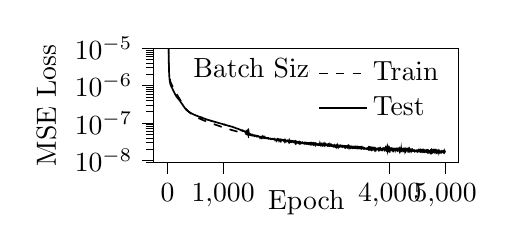
\begin{tikzpicture}

\begin{axis}[
legend cell align={left},
legend style={draw=none},
log basis y={10},
tick align=outside,
tick pos=left,
title={Batch Size 10},
title style={at={(0.4,0.85)},anchor=north},
x grid style={white!69.0196078431373!black},
xlabel={Epoch},
x label style={yshift=13pt},
xmin=-249.95, xmax=5248.95,
xtick style={color=black},
xtick = {0,1000,4000,5000},
y grid style={white!69.0196078431373!black},
ylabel={MSE Loss},
ymin=8.87880740039152e-09, ymax=1e-5,
ymode=log,
ytick style={color=black},
width=.45\textwidth,
height=.25\textwidth
]
\addplot [semithick, black, dashed]
table {%
0 0.00528136799344793
1 0.00196117930812761
2 0.00100831297786499
3 0.000271266568352075
4 0.000175409968296663
5 0.00014971278719031
6 0.000120760855550088
7 8.43190852401676e-05
8 5.46341028825736e-05
9 3.68707081361208e-05
10 2.85679608685996e-05
11 2.42326660020353e-05
12 2.11219582564581e-05
13 1.81891610776574e-05
14 1.55777172395233e-05
15 1.33981817964468e-05
16 1.15641491053964e-05
17 1.00000746923001e-05
18 7.94393679449001e-06
19 6.00564802901715e-06
20 4.86061071530486e-06
21 4.12355882229321e-06
22 3.60576834694371e-06
23 3.22225895214245e-06
24 2.92377228394258e-06
25 2.68271659390251e-06
26 2.48770738849657e-06
27 2.32538501446555e-06
28 2.19179745549525e-06
29 2.08097682532937e-06
30 1.98731877759428e-06
31 1.90663698408144e-06
32 1.8373563384344e-06
33 1.77455051147746e-06
34 1.72185935884528e-06
35 1.67465214957474e-06
36 1.63151804748907e-06
37 1.59294660916132e-06
38 1.55762653216485e-06
39 1.52324679449478e-06
40 1.49266945621562e-06
41 1.46543748737571e-06
42 1.4406353606411e-06
43 1.41676968130611e-06
44 1.39477084188044e-06
45 1.37423507132084e-06
46 1.35511966337987e-06
47 1.33708427732415e-06
48 1.32014086020149e-06
49 1.30410750958987e-06
50 1.28945765865751e-06
51 1.27443131206384e-06
52 1.26037416048774e-06
53 1.24694222655819e-06
54 1.23406486594924e-06
55 1.22177031155246e-06
56 1.20998068816824e-06
57 1.19855566538263e-06
58 1.18768979488593e-06
59 1.17686123902949e-06
60 1.16681973979738e-06
61 1.15674759846307e-06
62 1.1469994821578e-06
63 1.13754304193137e-06
64 1.12835477860784e-06
65 1.1194146830551e-06
66 1.11076625926465e-06
67 1.10223702500356e-06
68 1.09403939837271e-06
69 1.08589154372396e-06
70 1.07803150965147e-06
71 1.07009383924606e-06
72 1.06247301927098e-06
73 1.05503250242833e-06
74 1.04769723291653e-06
75 1.04052962702994e-06
76 1.03352776483767e-06
77 1.02660954140354e-06
78 1.01991228824261e-06
79 1.01320784088976e-06
80 1.00659571903527e-06
81 1.00009874282492e-06
82 9.93677533349668e-07
83 9.87113965438269e-07
84 9.8062059834092e-07
85 9.74151814121527e-07
86 9.67832220357678e-07
87 9.61684138536256e-07
88 9.55247765936917e-07
89 9.47558848833907e-07
90 9.38266775394325e-07
91 9.32239593209871e-07
92 9.24267010997681e-07
93 9.17881108195573e-07
94 9.11650485644344e-07
95 9.05510341233651e-07
96 8.99423817841694e-07
97 8.93403781594415e-07
98 8.87423857589553e-07
99 8.81676584700841e-07
100 8.75797529316102e-07
101 8.70152860761308e-07
102 8.64392884949439e-07
103 8.58854557606037e-07
104 8.53098335458213e-07
105 8.46301717638553e-07
106 8.40260048056152e-07
107 8.34313861926006e-07
108 8.28649471031895e-07
109 8.23015421440587e-07
110 8.17364995748804e-07
111 8.11884977585109e-07
112 8.06511968143297e-07
113 8.01217028589818e-07
114 7.96036286949686e-07
115 7.90829720260788e-07
116 7.85724390182097e-07
117 7.8061357269732e-07
118 7.75622568420786e-07
119 7.70701369514626e-07
120 7.65859431632876e-07
121 7.60867010685118e-07
122 7.56293496833038e-07
123 7.51443952839992e-07
124 7.46633905377436e-07
125 7.41863842019796e-07
126 7.37510203085989e-07
127 7.3260120961649e-07
128 7.27850430646271e-07
129 7.23098523858212e-07
130 7.18564877866257e-07
131 7.14265563797056e-07
132 7.09575198163392e-07
133 7.05213690039841e-07
134 7.00810380456218e-07
135 6.96431313489398e-07
136 6.92166918714321e-07
137 6.87997769821536e-07
138 6.83765189526397e-07
139 6.79594235624137e-07
140 6.75474781814955e-07
141 6.71440492920894e-07
142 6.67533135683129e-07
143 6.6334973273463e-07
144 6.59287583699708e-07
145 6.55205213693222e-07
146 6.51308420911434e-07
147 6.47384833252218e-07
148 6.43609669417344e-07
149 6.39809587452689e-07
150 6.36069694479602e-07
151 6.32515987284421e-07
152 6.28736712959821e-07
153 6.24937947204529e-07
154 6.21260133568668e-07
155 6.17671506626394e-07
156 6.14028405241385e-07
157 6.10509567016138e-07
158 6.06915501686345e-07
159 6.03322018584151e-07
160 5.99968398082851e-07
161 5.96322954811157e-07
162 5.92967038830494e-07
163 5.89499768537394e-07
164 5.86096018651006e-07
165 5.82915874680623e-07
166 5.79369164599441e-07
167 5.76226525925705e-07
168 5.72933694416022e-07
169 5.69691405916117e-07
170 5.66455787112119e-07
171 5.63347007282999e-07
172 5.59933701893556e-07
173 5.56663053732365e-07
174 5.53505768943197e-07
175 5.50422513185822e-07
176 5.47412930105295e-07
177 5.44322518996054e-07
178 5.41142272298956e-07
179 5.38103252072375e-07
180 5.35073113576701e-07
181 5.32053218753603e-07
182 5.2916558987981e-07
183 5.26249207855045e-07
184 5.23352361447849e-07
185 5.20399350589784e-07
186 5.17523279084386e-07
187 5.14665778332812e-07
188 5.11827413136601e-07
189 5.09032601829773e-07
190 5.06142247340691e-07
191 5.03410807146665e-07
192 5.00633232789482e-07
193 4.97932972685078e-07
194 4.95130490003604e-07
195 4.92452483671357e-07
196 4.89739140157042e-07
197 4.870303317972e-07
198 4.84287599142874e-07
199 4.81629953617002e-07
200 4.7891349964857e-07
201 4.76268158013937e-07
202 4.73530783402509e-07
203 4.70959613290134e-07
204 4.68312260348824e-07
205 4.65747004891881e-07
206 4.63164959141338e-07
207 4.60514930296085e-07
208 4.57982168553528e-07
209 4.55433743336009e-07
210 4.52851707479773e-07
211 4.50364350497168e-07
212 4.47857538041774e-07
213 4.45355709501882e-07
214 4.42778161664492e-07
215 4.40293827219662e-07
216 4.37892487021863e-07
217 4.35247193566468e-07
218 4.32821898028735e-07
219 4.3035448477724e-07
220 4.27975495336241e-07
221 4.25454756096677e-07
222 4.23122028854195e-07
223 4.20731893679971e-07
224 4.18271005955262e-07
225 4.15870392234119e-07
226 4.13457123742411e-07
227 4.10999238673604e-07
228 4.08633261530511e-07
229 4.06335352423071e-07
230 4.03913571878078e-07
231 4.01562177887449e-07
232 3.99183417418847e-07
233 3.96861866605036e-07
234 3.94463216704111e-07
235 3.9231701188136e-07
236 3.89952001049743e-07
237 3.87668205026337e-07
238 3.85320536859801e-07
239 3.83008806870144e-07
240 3.80778862836273e-07
241 3.78499330051518e-07
242 3.76246543565273e-07
243 3.7398688223611e-07
244 3.71832217145318e-07
245 3.69569940148473e-07
246 3.67439741997266e-07
247 3.65260341483875e-07
248 3.63166023862327e-07
249 3.61033952382961e-07
250 3.58909800963758e-07
251 3.56821789164741e-07
252 3.54731006746434e-07
253 3.52717319067608e-07
254 3.50711979018037e-07
255 3.48674827135298e-07
256 3.46662165182643e-07
257 3.44682640887051e-07
258 3.42718062111835e-07
259 3.40774582703318e-07
260 3.38882178803068e-07
261 3.36939323482e-07
262 3.35075527875262e-07
263 3.33137614143553e-07
264 3.3120930719388e-07
265 3.29301063395349e-07
266 3.27454248716386e-07
267 3.25471118496345e-07
268 3.23515837390431e-07
269 3.21549918185227e-07
270 3.19058210811463e-07
271 3.16761530374521e-07
272 3.14913813652673e-07
273 3.13171949990476e-07
274 3.11409781494909e-07
275 3.09652313128517e-07
276 3.07940026100795e-07
277 3.06198263344548e-07
278 3.04574217313558e-07
279 3.02837976109416e-07
280 3.0114346012855e-07
281 2.99294401275851e-07
282 2.97600264582698e-07
283 2.95904359046695e-07
284 2.94242386100763e-07
285 2.92338202423359e-07
286 2.90607358821582e-07
287 2.88928763936269e-07
288 2.87282469568773e-07
289 2.85632490428789e-07
290 2.84055769137481e-07
291 2.82524579833243e-07
292 2.80988924288295e-07
293 2.79470538226967e-07
294 2.78032275473628e-07
295 2.76563692107601e-07
296 2.75308126047591e-07
297 2.73785573132734e-07
298 2.72342808580461e-07
299 2.70912388793398e-07
300 2.69563412658158e-07
301 2.68253967101728e-07
302 2.66938382678106e-07
303 2.65578434972547e-07
304 2.64324795336002e-07
305 2.63108027653836e-07
306 2.61854648559989e-07
307 2.60630991584243e-07
308 2.59393573514011e-07
309 2.58222029780875e-07
310 2.57056368830888e-07
311 2.55888819569172e-07
312 2.54658455163259e-07
313 2.53491728283706e-07
314 2.52409010270682e-07
315 2.51337997045908e-07
316 2.5030137600357e-07
317 2.49188929104527e-07
318 2.48023163704758e-07
319 2.46955601448384e-07
320 2.45822844564536e-07
321 2.44817109593676e-07
322 2.43781857687253e-07
323 2.42748652734548e-07
324 2.41714933428838e-07
325 2.40798836785849e-07
326 2.39876830110397e-07
327 2.38903279075053e-07
328 2.37944548606706e-07
329 2.3699354220863e-07
330 2.36068708319159e-07
331 2.35151283134449e-07
332 2.34205967064582e-07
333 2.33274957253116e-07
334 2.32392124277503e-07
335 2.31484588075759e-07
336 2.30657326452111e-07
337 2.29810509786432e-07
338 2.29022869473461e-07
339 2.28213446811232e-07
340 2.27242750026058e-07
341 2.26404253220736e-07
342 2.25602067907005e-07
343 2.24776172110808e-07
344 2.24006119635689e-07
345 2.23185505445755e-07
346 2.22317487597046e-07
347 2.21572234484491e-07
348 2.20820311618297e-07
349 2.2001649651493e-07
350 2.19287002916069e-07
351 2.1834789354358e-07
352 2.17625585441361e-07
353 2.16871131519802e-07
354 2.16220429529734e-07
355 2.15429030556713e-07
356 2.1473307522335e-07
357 2.14042594111064e-07
358 2.13372244108889e-07
359 2.12795627789752e-07
360 2.12051067953745e-07
361 2.11376431433763e-07
362 2.10728520846359e-07
363 2.1009826162377e-07
364 2.09431103987967e-07
365 2.08771483025671e-07
366 2.08140193018735e-07
367 2.07497775548404e-07
368 2.06848745523125e-07
369 2.06193569836088e-07
370 2.05640739063817e-07
371 2.0498919569345e-07
372 2.04406067476626e-07
373 2.03852335447507e-07
374 2.0315202889698e-07
375 2.02647559515157e-07
376 2.01964303441216e-07
377 2.01442579235156e-07
378 2.00809108363842e-07
379 2.00291153515941e-07
380 1.99646441489953e-07
381 1.9908953290404e-07
382 1.9843899079941e-07
383 1.9783244177507e-07
384 1.9732972965425e-07
385 1.96696532901441e-07
386 1.96089850654779e-07
387 1.95515737386742e-07
388 1.95012229147196e-07
389 1.94473671935036e-07
390 1.93915756470098e-07
391 1.93370991827813e-07
392 1.9295067025471e-07
393 1.92333264354971e-07
394 1.91909908457966e-07
395 1.91307810153418e-07
396 1.90847586147846e-07
397 1.90272842144346e-07
398 1.89821726244155e-07
399 1.89262572947158e-07
400 1.88858243790335e-07
401 1.88210220435359e-07
402 1.87736445091957e-07
403 1.87311259125522e-07
404 1.86755425390928e-07
405 1.86331044127463e-07
406 1.8575961707068e-07
407 1.85354366402102e-07
408 1.84749235963011e-07
409 1.84390802604462e-07
410 1.83792814558714e-07
411 1.8335780107126e-07
412 1.8287737747702e-07
413 1.8251926256152e-07
414 1.81981051277091e-07
415 1.81501176990118e-07
416 1.81177496325624e-07
417 1.80648080001511e-07
418 1.80278556265456e-07
419 1.7971269204331e-07
420 1.79261774100326e-07
421 1.78966274626546e-07
422 1.78390314147237e-07
423 1.78061858910894e-07
424 1.77493106940929e-07
425 1.77194511650214e-07
426 1.7669522240471e-07
427 1.76226328005846e-07
428 1.75761677221331e-07
429 1.7534401855368e-07
430 1.74911862940164e-07
431 1.74502996217463e-07
432 1.74251102693646e-07
433 1.7382497731866e-07
434 1.73263161178383e-07
435 1.73004354868667e-07
436 1.72492188439399e-07
437 1.7220730899048e-07
438 1.7165128710861e-07
439 1.7125423465103e-07
440 1.7100701692474e-07
441 1.70545178845849e-07
442 1.7008701600485e-07
443 1.69664761564547e-07
444 1.69258927638083e-07
445 1.6888123750558e-07
446 1.68490066032589e-07
447 1.68132941289478e-07
448 1.67800580737065e-07
449 1.67420219066017e-07
450 1.66960605261224e-07
451 1.66590058223726e-07
452 1.66209313094967e-07
453 1.65879797640045e-07
454 1.65527574829127e-07
455 1.65107552816401e-07
456 1.64804789619666e-07
457 1.64351305911303e-07
458 1.63989841528434e-07
459 1.63619196937859e-07
460 1.63235743539936e-07
461 1.62907762013553e-07
462 1.62464832413889e-07
463 1.62098891167695e-07
464 1.61743859634633e-07
465 1.61409872379004e-07
466 1.6105873006822e-07
467 1.60653658838328e-07
468 1.60286182233627e-07
469 1.59894756044388e-07
470 1.59531792913725e-07
471 1.59174766829473e-07
472 1.58797522091803e-07
473 1.58495172808415e-07
474 1.58078474448153e-07
475 1.57730813090673e-07
476 1.57359346744101e-07
477 1.57076716797988e-07
478 1.5668199366381e-07
479 1.56443077594659e-07
480 1.56038656218271e-07
481 1.55657942588761e-07
482 1.55325011998997e-07
483 1.54921709318856e-07
484 1.54598146702156e-07
485 1.54341690801196e-07
486 1.53867364836024e-07
487 1.5353118324013e-07
488 1.53226939170192e-07
489 1.52933094093033e-07
490 1.52640565342921e-07
491 1.523347708976e-07
492 1.51942499793112e-07
493 1.51550411844337e-07
494 1.51309379272657e-07
495 1.50920436685631e-07
496 1.50610290570175e-07
497 1.50305012087681e-07
498 1.50029505234794e-07
499 1.49729306713198e-07
500 1.49430219844593e-07
501 1.49247199219271e-07
502 1.4900762355774e-07
503 1.48481581319082e-07
504 1.48199029017526e-07
505 1.47922896862607e-07
506 1.4763762496095e-07
507 1.47376839620961e-07
508 1.47225218374292e-07
509 1.4680912803211e-07
510 1.46543789512066e-07
511 1.46414373785042e-07
512 1.45965114726199e-07
513 1.45717731925288e-07
514 1.45586504762818e-07
515 1.45202670251976e-07
516 1.44917263122935e-07
517 1.44685540794942e-07
518 1.4441396511522e-07
519 1.44274714346526e-07
520 1.43907111471719e-07
521 1.43611794123366e-07
522 1.43441559614654e-07
523 1.43342289060655e-07
524 1.43023464527214e-07
525 1.4269947945289e-07
526 1.42346950551264e-07
527 1.42243148950616e-07
528 1.41845405314811e-07
529 1.41633421835152e-07
530 1.41421946477927e-07
531 1.41117858427631e-07
532 1.40866536890716e-07
533 1.40753480974976e-07
534 1.40448171630503e-07
535 1.40135051471812e-07
536 1.40028638033751e-07
537 1.39913777295053e-07
538 1.39432189358857e-07
539 1.39200212907475e-07
540 1.38922127936869e-07
541 1.3885529407176e-07
542 1.38543313705775e-07
543 1.38373281870496e-07
544 1.37950778162921e-07
545 1.37704649900705e-07
546 1.37484048030601e-07
547 1.37280646952398e-07
548 1.37019148076512e-07
549 1.3677530932954e-07
550 1.36761920195294e-07
551 1.36316340897391e-07
552 1.36309115785771e-07
553 1.35979577848833e-07
554 1.35640636269585e-07
555 1.35609762330624e-07
556 1.35323011500876e-07
557 1.34884704106053e-07
558 1.34914494200888e-07
559 1.34521318539971e-07
560 1.34409869887442e-07
561 1.34146739227958e-07
562 1.33836909697038e-07
563 1.33704287221814e-07
564 1.33502265708962e-07
565 1.33171152050249e-07
566 1.32942179140727e-07
567 1.32634342442373e-07
568 1.32577345650642e-07
569 1.32393106517803e-07
570 1.32022034993184e-07
571 1.31851378921688e-07
572 1.31748397536047e-07
573 1.31391232387479e-07
574 1.31212455152241e-07
575 1.31131689407038e-07
576 1.30905025059747e-07
577 1.30671633065127e-07
578 1.30473399770903e-07
579 1.30230422275002e-07
580 1.30008186347563e-07
581 1.2983359869656e-07
582 1.29610148076331e-07
583 1.29394243846281e-07
584 1.29101745229843e-07
585 1.28992069343692e-07
586 1.28795406288962e-07
587 1.28587078604969e-07
588 1.28416344100657e-07
589 1.28186303307576e-07
590 1.27897572701485e-07
591 1.27800394298383e-07
592 1.2761726235988e-07
593 1.27405126921776e-07
594 1.27332942780889e-07
595 1.27010178951892e-07
596 1.26795597863438e-07
597 1.26621371643321e-07
598 1.26441015388945e-07
599 1.26264200759341e-07
600 1.26045677661946e-07
601 1.25880933130595e-07
602 1.25679640288201e-07
603 1.2548865805373e-07
604 1.25312461181082e-07
605 1.25103905102009e-07
606 1.24897948852176e-07
607 1.2472952348519e-07
608 1.24515717392359e-07
609 1.24279311313202e-07
610 1.24162860886123e-07
611 1.23963258817916e-07
612 1.23856674962841e-07
613 1.23616911071878e-07
614 1.23448208606547e-07
615 1.23266022529211e-07
616 1.23099053030984e-07
617 1.22965574678169e-07
618 1.22703210674313e-07
619 1.22610334458706e-07
620 1.22416365280209e-07
621 1.22263429667147e-07
622 1.22010187015853e-07
623 1.21881407568747e-07
624 1.21748274617417e-07
625 1.21502343006785e-07
626 1.2137257298761e-07
627 1.21214431700878e-07
628 1.20995997192619e-07
629 1.20755586696664e-07
630 1.20677670794045e-07
631 1.20486802772657e-07
632 1.20335067714805e-07
633 1.20041876465748e-07
634 1.19993952512054e-07
635 1.19800402285097e-07
636 1.19638045039672e-07
637 1.19469144954643e-07
638 1.19288750000113e-07
639 1.19123967685653e-07
640 1.18970169935562e-07
641 1.18776178510416e-07
642 1.18630074621429e-07
643 1.18430187046048e-07
644 1.18283657739582e-07
645 1.18106677862162e-07
646 1.17970297603964e-07
647 1.17771976335668e-07
648 1.17546498046295e-07
649 1.17381637583236e-07
650 1.17316464169903e-07
651 1.17152637191253e-07
652 1.16984930773611e-07
653 1.16820248532434e-07
654 1.16677477870475e-07
655 1.16489247212748e-07
656 1.16356786041827e-07
657 1.16109150187782e-07
658 1.16021651885845e-07
659 1.1589247186361e-07
660 1.15680851813238e-07
661 1.15511939573487e-07
662 1.15437697290055e-07
663 1.15192883769488e-07
664 1.15133998694894e-07
665 1.14999466962473e-07
666 1.1487223649187e-07
667 1.14615010180508e-07
668 1.14523665111221e-07
669 1.1430231152243e-07
670 1.14183070931695e-07
671 1.1411805894479e-07
672 1.13863993682628e-07
673 1.13744293219753e-07
674 1.13635250174049e-07
675 1.13444134877128e-07
676 1.13304540763082e-07
677 1.13211565104798e-07
678 1.12999955512727e-07
679 1.12873975091077e-07
680 1.12800427194415e-07
681 1.12586640521606e-07
682 1.12449143476745e-07
683 1.12380084229535e-07
684 1.12158920160255e-07
685 1.12033838148839e-07
686 1.11931735531368e-07
687 1.1172928866543e-07
688 1.11605941497395e-07
689 1.1149843984759e-07
690 1.1128916759251e-07
691 1.1117579283848e-07
692 1.11079075031384e-07
693 1.10869837885996e-07
694 1.1073690432406e-07
695 1.10605835175193e-07
696 1.10463978759689e-07
697 1.10324903690451e-07
698 1.10176767589287e-07
699 1.100433870449e-07
700 1.0991178901909e-07
701 1.09746107153086e-07
702 1.09625463144969e-07
703 1.09457206673991e-07
704 1.09297419130794e-07
705 1.09188764514379e-07
706 1.09040658213821e-07
707 1.0890217267967e-07
708 1.08757311609864e-07
709 1.08620748524579e-07
710 1.08461666568083e-07
711 1.08355406422955e-07
712 1.0820399432232e-07
713 1.08059409826833e-07
714 1.07951705372589e-07
715 1.07794844741438e-07
716 1.07663849195916e-07
717 1.0751906558859e-07
718 1.07392642625381e-07
719 1.07279909615787e-07
720 1.07122551153971e-07
721 1.06990335362323e-07
722 1.06877231731417e-07
723 1.06721919757025e-07
724 1.06634702299324e-07
725 1.06495320386646e-07
726 1.0637759998211e-07
727 1.06249467228814e-07
728 1.06104308867927e-07
729 1.05983714275837e-07
730 1.05844237328068e-07
731 1.05722839016664e-07
732 1.05567359489633e-07
733 1.05441034778941e-07
734 1.05317241290148e-07
735 1.05184704000116e-07
736 1.05069148752523e-07
737 1.04929581894453e-07
738 1.04795213640152e-07
739 1.04670552025787e-07
740 1.0455280652355e-07
741 1.044142625517e-07
742 1.04289056577223e-07
743 1.04165171206372e-07
744 1.04030028755808e-07
745 1.0391795601139e-07
746 1.03792417993631e-07
747 1.03663553188138e-07
748 1.03539296125721e-07
749 1.03406859475186e-07
750 1.03288533213064e-07
751 1.03147823957706e-07
752 1.03020528992026e-07
753 1.02919831468373e-07
754 1.02779396466968e-07
755 1.02649501698693e-07
756 1.02499358838326e-07
757 1.02409941540316e-07
758 1.02271492001815e-07
759 1.02169458857659e-07
760 1.02015001670619e-07
761 1.01912081720279e-07
762 1.0179567390356e-07
763 1.01665921425909e-07
764 1.01540616401774e-07
765 1.01433277479579e-07
766 1.01308921702792e-07
767 1.01178255593748e-07
768 1.01059277914928e-07
769 1.0093410972134e-07
770 1.00816341617183e-07
771 1.00699157992157e-07
772 1.00549053838606e-07
773 1.00454659421878e-07
774 1.00326335377154e-07
775 1.00216911897988e-07
776 1.00077129114862e-07
777 9.99685849523146e-08
778 9.98191905199342e-08
779 9.97170746863674e-08
780 9.959241176416e-08
781 9.94933218900762e-08
782 9.93614848043833e-08
783 9.92425511014972e-08
784 9.91293627983225e-08
785 9.89690742470017e-08
786 9.88637059462505e-08
787 9.86897062427161e-08
788 9.85202997316748e-08
789 9.83834785062143e-08
790 9.82288636919293e-08
791 9.80936902461593e-08
792 9.79595043815173e-08
793 9.78026380105135e-08
794 9.76777373984383e-08
795 9.75584071083446e-08
796 9.74415919641203e-08
797 9.72948478028535e-08
798 9.71522259529678e-08
799 9.70548201317811e-08
800 9.69570135667119e-08
801 9.67987629474365e-08
802 9.66975896488087e-08
803 9.65856752399574e-08
804 9.64346787757364e-08
805 9.63039692147838e-08
806 9.61681625466504e-08
807 9.60707070940536e-08
808 9.59578685444384e-08
809 9.58247181959138e-08
810 9.56963635290187e-08
811 9.56085677850105e-08
812 9.54724297685949e-08
813 9.53632209910182e-08
814 9.52536143494775e-08
815 9.51394857096055e-08
816 9.50062137183849e-08
817 9.49072192701905e-08
818 9.48035359127353e-08
819 9.46693008962995e-08
820 9.45688968445602e-08
821 9.44452840512255e-08
822 9.43172510536883e-08
823 9.41965488587826e-08
824 9.40813234739934e-08
825 9.39868876637107e-08
826 9.38570903197267e-08
827 9.37556547064844e-08
828 9.36585416666524e-08
829 9.35416478275997e-08
830 9.34184370238178e-08
831 9.33253633950137e-08
832 9.31960705075063e-08
833 9.30750392247326e-08
834 9.29790978276834e-08
835 9.28531029176227e-08
836 9.2741702393262e-08
837 9.26282059432459e-08
838 9.25152430020226e-08
839 9.24248369438274e-08
840 9.22977743145204e-08
841 9.21841337708784e-08
842 9.20765091949605e-08
843 9.19876060434532e-08
844 9.18693412588212e-08
845 9.17491777063795e-08
846 9.16572254738846e-08
847 9.15576272420005e-08
848 9.14203159663174e-08
849 9.13198639840296e-08
850 9.12320605528372e-08
851 9.11133052672319e-08
852 9.10208488935638e-08
853 9.08886395145636e-08
854 9.08109727859596e-08
855 9.06900371511199e-08
856 9.06042483128644e-08
857 9.04830585968242e-08
858 9.03685871711524e-08
859 9.02765184473964e-08
860 9.01473026471145e-08
861 9.00494284872266e-08
862 8.99514579755234e-08
863 8.98092013335017e-08
864 8.96942274453139e-08
865 8.96169885922227e-08
866 8.95027962699579e-08
867 8.93974512350404e-08
868 8.93055719486391e-08
869 8.92152715792349e-08
870 8.90796454533493e-08
871 8.90001987152722e-08
872 8.88985555147492e-08
873 8.87827027629129e-08
874 8.8681826293513e-08
875 8.85993879884417e-08
876 8.84749253682315e-08
877 8.8365314028227e-08
878 8.82766570842186e-08
879 8.81907103478241e-08
880 8.80913904999225e-08
881 8.79811675558173e-08
882 8.78724534403297e-08
883 8.77856994518922e-08
884 8.76815198824765e-08
885 8.76151390438729e-08
886 8.75026416458091e-08
887 8.73753373653585e-08
888 8.72858262668252e-08
889 8.71681758307652e-08
890 8.70833700972184e-08
891 8.69674835723977e-08
892 8.68769882167442e-08
893 8.67649135960491e-08
894 8.66658114584418e-08
895 8.65728811727529e-08
896 8.64807740574847e-08
897 8.6379502552969e-08
898 8.62890960395823e-08
899 8.61805522656134e-08
900 8.60798535828877e-08
901 8.59804689978816e-08
902 8.58941737535979e-08
903 8.57911752905061e-08
904 8.57290044931069e-08
905 8.5604700195141e-08
906 8.55353445339269e-08
907 8.54296420338407e-08
908 8.53275566381484e-08
909 8.5235891411628e-08
910 8.50940039809345e-08
911 8.50244317684989e-08
912 8.4918217946317e-08
913 8.48225562921634e-08
914 8.47121673808182e-08
915 8.45646080938067e-08
916 8.44489866413944e-08
917 8.43275235373753e-08
918 8.42122600341888e-08
919 8.40845770033738e-08
920 8.39633717686361e-08
921 8.38728335961214e-08
922 8.37333134784402e-08
923 8.36061557252243e-08
924 8.34589165044086e-08
925 8.34041407116182e-08
926 8.32506879300254e-08
927 8.31442018411899e-08
928 8.30001081730813e-08
929 8.29361105103565e-08
930 8.28301392408193e-08
931 8.27331621211513e-08
932 8.25695926853776e-08
933 8.25084764133344e-08
934 8.24218239925401e-08
935 8.22939920519516e-08
936 8.21872503586896e-08
937 8.20537366830187e-08
938 8.19762285186876e-08
939 8.18900844801185e-08
940 8.17806862829506e-08
941 8.16891713362189e-08
942 8.15947277921225e-08
943 8.14801866821924e-08
944 8.13893779216812e-08
945 8.12549022888298e-08
946 8.1186256242205e-08
947 8.11224664332144e-08
948 8.10068910750417e-08
949 8.08747287273093e-08
950 8.08084906545048e-08
951 8.07560128546214e-08
952 8.05988600105501e-08
953 8.05289388638997e-08
954 8.04419091360309e-08
955 8.03479138999919e-08
956 8.02426033241765e-08
957 8.01662782334844e-08
958 8.01079387491299e-08
959 7.9962328587424e-08
960 7.98649313971111e-08
961 7.9823963941017e-08
962 7.9702674595783e-08
963 7.96342297637587e-08
964 7.95564499433965e-08
965 7.94755216992904e-08
966 7.93516297070696e-08
967 7.92942259231211e-08
968 7.92169674035392e-08
969 7.91121163468134e-08
970 7.90581564369397e-08
971 7.89395004829885e-08
972 7.89092709929662e-08
973 7.87544788338756e-08
974 7.86666472096798e-08
975 7.86523701190589e-08
976 7.8514790184947e-08
977 7.84664036479477e-08
978 7.83199948162228e-08
979 7.82645249342018e-08
980 7.81695066787158e-08
981 7.80512361253649e-08
982 7.79887493473908e-08
983 7.79145837692674e-08
984 7.77953452724134e-08
985 7.77322541933856e-08
986 7.76423590509445e-08
987 7.75262421370826e-08
988 7.74901881572809e-08
989 7.73475327164874e-08
990 7.72705407747765e-08
991 7.72285956518459e-08
992 7.71681437772287e-08
993 7.70099962310589e-08
994 7.6918287235106e-08
995 7.67477495755564e-08
996 7.66623190040505e-08
997 7.66021730802535e-08
998 7.65218229270559e-08
999 7.63669241243825e-08
1000 7.6295445008423e-08
1001 7.62423054423422e-08
1002 7.61833150897395e-08
1003 7.60298844904028e-08
1004 7.59456310106543e-08
1005 7.5915621380318e-08
1006 7.58299975345267e-08
1007 7.56544244606694e-08
1008 7.55973048804925e-08
1009 7.55229512816591e-08
1010 7.54216580389766e-08
1011 7.53594459368401e-08
1012 7.52067414966362e-08
1013 7.52052056296471e-08
1014 7.51557110101331e-08
1015 7.49614555517475e-08
1016 7.4885067218311e-08
1017 7.48791445759345e-08
1018 7.47417294144626e-08
1019 7.47140375767508e-08
1020 7.46119577232918e-08
1021 7.44862677981573e-08
1022 7.44557077481112e-08
1023 7.43193127195063e-08
1024 7.42957686372669e-08
1025 7.4221959174281e-08
1026 7.41500351564284e-08
1027 7.40415722955134e-08
1028 7.39807223770761e-08
1029 7.38309129766357e-08
1030 7.38701393321328e-08
1031 7.37174148590647e-08
1032 7.35824979369859e-08
1033 7.35116533312485e-08
1034 7.34302032601164e-08
1035 7.33476446113102e-08
1036 7.33671868502483e-08
1037 7.32307386996922e-08
1038 7.31039209833639e-08
1039 7.30351898292625e-08
1040 7.29436440005671e-08
1041 7.28809123939911e-08
1042 7.28058229415574e-08
1043 7.27249777798811e-08
1044 7.27286119772685e-08
1045 7.25525780431724e-08
1046 7.24841360955075e-08
1047 7.24180311362233e-08
1048 7.22959945087531e-08
1049 7.22426187649283e-08
1050 7.2176573153726e-08
1051 7.20893046013415e-08
1052 7.20017102628923e-08
1053 7.19189237630147e-08
1054 7.18641382912999e-08
1055 7.17460976717987e-08
1056 7.16872122041856e-08
1057 7.16345884987923e-08
1058 7.15641047777105e-08
1059 7.14595474726742e-08
1060 7.14032528059683e-08
1061 7.13230476234727e-08
1062 7.12698537030931e-08
1063 7.11620048843287e-08
1064 7.1099792313678e-08
1065 7.10210318133342e-08
1066 7.09501470685936e-08
1067 7.08730074228114e-08
1068 7.08146171457535e-08
1069 7.07208029737672e-08
1070 7.0667067246788e-08
1071 7.0587900489194e-08
1072 7.05154876490255e-08
1073 7.04174514121192e-08
1074 7.03676609625781e-08
1075 7.02960759779714e-08
1076 7.02190040557937e-08
1077 7.01422597004786e-08
1078 7.00668985409436e-08
1079 6.99825292271861e-08
1080 6.99192134079318e-08
1081 6.98422142320077e-08
1082 6.97528138959846e-08
1083 6.96937493693817e-08
1084 6.96327662552676e-08
1085 6.95564798580683e-08
1086 6.94771127252025e-08
1087 6.9404260594208e-08
1088 6.93380222527296e-08
1089 6.92929876389137e-08
1090 6.9229443624419e-08
1091 6.91383239725951e-08
1092 6.90825351501445e-08
1093 6.89790639207821e-08
1094 6.89349090099434e-08
1095 6.88793907022145e-08
1096 6.87815529998303e-08
1097 6.87399090693042e-08
1098 6.86655123049995e-08
1099 6.85979349568377e-08
1100 6.85465203731361e-08
1101 6.84304802800462e-08
1102 6.82930998152642e-08
1103 6.82401087148676e-08
1104 6.82187844369686e-08
1105 6.81062173057967e-08
1106 6.80573373812443e-08
1107 6.79730649566501e-08
1108 6.78895991312878e-08
1109 6.78060206271702e-08
1110 6.77501244261691e-08
1111 6.76755676876084e-08
1112 6.75976947195345e-08
1113 6.75403262584418e-08
1114 6.74787379195685e-08
1115 6.73983082100094e-08
1116 6.7336414757424e-08
1117 6.72648212929339e-08
1118 6.71991075895661e-08
1119 6.7131866943182e-08
1120 6.70594125984358e-08
1121 6.6966685994263e-08
1122 6.69011549336851e-08
1123 6.68549786153605e-08
1124 6.67717031599402e-08
1125 6.67253009023483e-08
1126 6.66633335044686e-08
1127 6.65907989549908e-08
1128 6.65221406714878e-08
1129 6.64455554866272e-08
1130 6.63857757809971e-08
1131 6.63229847264191e-08
1132 6.62627450243036e-08
1133 6.62109349547357e-08
1134 6.61462561502013e-08
1135 6.6093881321283e-08
1136 6.60213592840186e-08
1137 6.59478948805692e-08
1138 6.58879199444406e-08
1139 6.58199054259789e-08
1140 6.57540199133777e-08
1141 6.56966605405707e-08
1142 6.56330822668139e-08
1143 6.55571200414151e-08
1144 6.54897740370863e-08
1145 6.54308262637571e-08
1146 6.53687929430546e-08
1147 6.53162745778424e-08
1148 6.52443244075762e-08
1149 6.51847202348677e-08
1150 6.51423108033455e-08
1151 6.50423383241616e-08
1152 6.49857643897356e-08
1153 6.49076445990993e-08
1154 6.48716389761717e-08
1155 6.48259660329664e-08
1156 6.47253473706755e-08
1157 6.47138701626027e-08
1158 6.46138167748056e-08
1159 6.45704578206008e-08
1160 6.44884940026458e-08
1161 6.44547484851543e-08
1162 6.43687627910339e-08
1163 6.43245046338947e-08
1164 6.42580903220669e-08
1165 6.4176974865493e-08
1166 6.40986761357709e-08
1167 6.40700892873269e-08
1168 6.39818289394079e-08
1169 6.3932452434301e-08
1170 6.38905052596783e-08
1171 6.38128848362562e-08
1172 6.38097658423042e-08
1173 6.37628164223969e-08
1174 6.36612967608308e-08
1175 6.36083887473049e-08
1176 6.35628966905166e-08
1177 6.34501949159372e-08
1178 6.34135071986286e-08
1179 6.33402065530753e-08
1180 6.33164425600796e-08
1181 6.31991182298286e-08
1182 6.31688070518166e-08
1183 6.31000857720387e-08
1184 6.30440499538309e-08
1185 6.30117877586933e-08
1186 6.29068946400579e-08
1187 6.28657047108128e-08
1188 6.28001924485311e-08
1189 6.27520108475999e-08
1190 6.2692445517154e-08
1191 6.26265859304809e-08
1192 6.25640404905425e-08
1193 6.25295383405167e-08
1194 6.24554189698756e-08
1195 6.23996014326167e-08
1196 6.2342960829298e-08
1197 6.22834769337111e-08
1198 6.22272015959879e-08
1199 6.21739494643947e-08
1200 6.21147194035387e-08
1201 6.20532554540532e-08
1202 6.19924318390197e-08
1203 6.19435239723742e-08
1204 6.19088889552977e-08
1205 6.18525699835892e-08
1206 6.17901324551084e-08
1207 6.17349053899652e-08
1208 6.17010492032222e-08
1209 6.159896958291e-08
1210 6.15472192388999e-08
1211 6.14498887285819e-08
1212 6.14097986573192e-08
1213 6.13400754390092e-08
1214 6.12895230212018e-08
1215 6.12441199021596e-08
1216 6.11803813477252e-08
1217 6.11272152251097e-08
1218 6.10790524446791e-08
1219 6.10046911986295e-08
1220 6.09684344610173e-08
1221 6.09062715284381e-08
1222 6.08388207945509e-08
1223 6.07907254623896e-08
1224 6.07351286108226e-08
1225 6.06969509631128e-08
1226 6.06245701995078e-08
1227 6.05695280775365e-08
1228 6.05025316713359e-08
1229 6.04408892823649e-08
1230 6.03798410758749e-08
1231 6.03307107605033e-08
1232 6.02744852340464e-08
1233 6.02306611474646e-08
1234 6.01644510878074e-08
1235 6.01242652820133e-08
1236 6.00600351652325e-08
1237 6.00166884390241e-08
1238 5.99491715314038e-08
1239 5.98879763424875e-08
1240 5.98460734613226e-08
1241 5.97969363869133e-08
1242 5.97358579979002e-08
1243 5.97007916547376e-08
1244 5.96323696044898e-08
1245 5.95724811414122e-08
1246 5.94469046699686e-08
1247 5.94092666106327e-08
1248 5.93700340023595e-08
1249 5.93094560930041e-08
1250 5.92366686702483e-08
1251 5.91891610035589e-08
1252 5.91489903745135e-08
1253 5.90824333013273e-08
1254 5.90224539132045e-08
1255 5.89600150346925e-08
1256 5.89108437698549e-08
1257 5.88625464525983e-08
1258 5.87990369704805e-08
1259 5.87412606534166e-08
1260 5.86807554059376e-08
1261 5.86248854506088e-08
1262 5.85775673900279e-08
1263 5.85244985118472e-08
1264 5.84624300037362e-08
1265 5.84052390073531e-08
1266 5.83791618291585e-08
1267 5.8309725308181e-08
1268 5.82483366917685e-08
1269 5.82043644081764e-08
1270 5.81368083429901e-08
1271 5.80901139346501e-08
1272 5.80302669161981e-08
1273 5.79871371053642e-08
1274 5.79240294640293e-08
1275 5.79050140814275e-08
1276 5.78219837676919e-08
1277 5.77706587012727e-08
1278 5.77242251087462e-08
1279 5.76675971353247e-08
1280 5.76212695335698e-08
1281 5.75639227551328e-08
1282 5.75201069885622e-08
1283 5.74694542976317e-08
1284 5.74379567663819e-08
1285 5.73645213575169e-08
1286 5.73071207932152e-08
1287 5.72642096763332e-08
1288 5.7207055084163e-08
1289 5.71587593189982e-08
1290 5.71073273780698e-08
1291 5.70634097907252e-08
1292 5.69681883466622e-08
1293 5.69580245124435e-08
1294 5.68764241704045e-08
1295 5.68312549065197e-08
1296 5.67821779462463e-08
1297 5.67339278534362e-08
1298 5.66869046281226e-08
1299 5.66534648283046e-08
1300 5.65876212577088e-08
1301 5.65191520762731e-08
1302 5.64998829610808e-08
1303 5.6441721469902e-08
1304 5.63740171366511e-08
1305 5.63765589478571e-08
1306 5.62980969354143e-08
1307 5.62538580894945e-08
1308 5.6180983691867e-08
1309 5.61557886857855e-08
1310 5.60883655587041e-08
1311 5.60943333516306e-08
1312 5.60237184821233e-08
1313 5.59638541464125e-08
1314 5.59239631958697e-08
1315 5.58683522866588e-08
1316 5.58239115955317e-08
1317 5.57622321850637e-08
1318 5.57357208941234e-08
1319 5.5704475492302e-08
1320 5.5643806173844e-08
1321 5.56156613029657e-08
1322 5.55653318357052e-08
1323 5.55213465980309e-08
1324 5.54517741124805e-08
1325 5.53959914895152e-08
1326 5.53644016720867e-08
1327 5.53113212564682e-08
1328 5.52527291675098e-08
1329 5.52284499799605e-08
1330 5.5144183925826e-08
1331 5.51262334003155e-08
1332 5.50886002970152e-08
1333 5.50361545381683e-08
1334 5.50040574620603e-08
1335 5.49285218842677e-08
1336 5.48684188261817e-08
1337 5.48282277335055e-08
1338 5.483084286384e-08
1339 5.47275310203155e-08
1340 5.46687656632905e-08
1341 5.46399589307356e-08
1342 5.45916135452629e-08
1343 5.45022519360394e-08
1344 5.4444705193113e-08
1345 5.44269120350549e-08
1346 5.43626481408488e-08
1347 5.43836221233995e-08
1348 5.42871327913197e-08
1349 5.42768571709651e-08
1350 5.41878018789355e-08
1351 5.4157789683984e-08
1352 5.41022280931003e-08
1353 5.40704692619798e-08
1354 5.40222803624424e-08
1355 5.39687752887374e-08
1356 5.39427189405472e-08
1357 5.38898634916407e-08
1358 5.38458344823134e-08
1359 5.38044222686551e-08
1360 5.37938232803015e-08
1361 5.36979668996906e-08
1362 5.36841744303018e-08
1363 5.36145921326003e-08
1364 5.36018136698679e-08
1365 5.35213680175062e-08
1366 5.34951072461709e-08
1367 5.34692328546527e-08
1368 5.34024711873471e-08
1369 5.33796378965334e-08
1370 5.33059734308949e-08
1371 5.32888267046339e-08
1372 5.32207567194298e-08
1373 5.31850323559624e-08
1374 5.31649204016382e-08
1375 5.3121046612592e-08
1376 5.30598405856786e-08
1377 5.30234202256175e-08
1378 5.29790359360405e-08
1379 5.29613990218891e-08
1380 5.28995273607613e-08
1381 5.28548773348625e-08
1382 5.28733015370264e-08
1383 5.27771678515698e-08
1384 5.27533447414186e-08
1385 5.27198489574943e-08
1386 5.26578893444984e-08
1387 5.26402133305126e-08
1388 5.25906488801908e-08
1389 5.25463211609178e-08
1390 5.2528830414289e-08
1391 5.24788511602203e-08
1392 5.24220055742042e-08
1393 5.24470437368585e-08
1394 5.24256742129303e-08
1395 5.22615294795692e-08
1396 5.21192910207802e-08
1397 5.20188361896601e-08
1398 5.19811063925957e-08
1399 5.19453104441681e-08
1400 5.19083679995092e-08
1401 5.18817203376543e-08
1402 5.18950529349027e-08
1403 5.17597886817711e-08
1404 5.16768196634487e-08
1405 5.16066808220472e-08
1406 5.15841544612705e-08
1407 5.14775189852656e-08
1408 5.14207214030726e-08
1409 5.13891409337219e-08
1410 5.13757358477918e-08
1411 5.13573249505406e-08
1412 5.13168068416725e-08
1413 5.13165649840275e-08
1414 5.11925157420379e-08
1415 5.12202316538257e-08
1416 5.10930796626674e-08
1417 5.10085317095843e-08
1418 5.09708848772661e-08
1419 5.09748755117556e-08
1420 5.08561629830595e-08
1421 5.0904093493731e-08
1422 5.08557489409256e-08
1423 5.07618054701453e-08
1424 5.07564505913827e-08
1425 5.06145357181964e-08
1426 5.05311489651383e-08
1427 5.05936839989563e-08
1428 5.04931337241832e-08
1429 5.0452951397828e-08
1430 5.04558816272205e-08
1431 5.03367097903773e-08
1432 5.03469566204284e-08
1433 5.02490047527004e-08
1434 5.02376803923621e-08
1435 5.02076208719338e-08
1436 5.01271630748423e-08
1437 5.00489786781078e-08
1438 5.00712141493498e-08
1439 4.99865114533815e-08
1440 5.00083484289426e-08
1441 4.9890328540636e-08
1442 4.98523947067842e-08
1443 4.97875407046155e-08
1444 4.9846085875549e-08
1445 4.97773833685322e-08
1446 4.96772931957157e-08
1447 4.96355853885078e-08
1448 4.95743393835735e-08
1449 4.95377457021551e-08
1450 4.95033593184147e-08
1451 4.94555240937444e-08
1452 4.93939212853345e-08
1453 4.93500329101781e-08
1454 4.92925502748598e-08
1455 4.93035321968982e-08
1456 4.92040075816824e-08
1457 4.9215669707392e-08
1458 4.91149503445421e-08
1459 4.91340210373448e-08
1460 4.9030811973827e-08
1461 4.90517194839946e-08
1462 4.89486476096257e-08
1463 4.89652671398222e-08
1464 4.8865260748876e-08
1465 4.88976658719054e-08
1466 4.88876855497811e-08
1467 4.87972207063869e-08
1468 4.86859618586966e-08
1469 4.8610668457183e-08
1470 4.8551800269081e-08
1471 4.85247550019441e-08
1472 4.84442078052538e-08
1473 4.84753261209558e-08
1474 4.83030271447582e-08
1475 4.83270761275634e-08
1476 4.82545285973579e-08
1477 4.82582966843115e-08
1478 4.81258617335278e-08
1479 4.80988303075414e-08
1480 4.7968173395585e-08
1481 4.7949168894279e-08
1482 4.79717044732375e-08
1483 4.78497419642565e-08
1484 4.78747514909283e-08
1485 4.7764104318393e-08
1486 4.77926675945817e-08
1487 4.76858295994642e-08
1488 4.77103779927823e-08
1489 4.75992131232506e-08
1490 4.76637515867129e-08
1491 4.75154290680013e-08
1492 4.75629326746052e-08
1493 4.74504075875792e-08
1494 4.74098703306947e-08
1495 4.74234217984204e-08
1496 4.73184990101849e-08
1497 4.73501704434387e-08
1498 4.72470642864931e-08
1499 4.72344994850715e-08
1500 4.72161478004551e-08
1501 4.71361933518377e-08
1502 4.71543518709705e-08
1503 4.70452649581343e-08
1504 4.70325748036515e-08
1505 4.70003735042468e-08
1506 4.69512611322997e-08
1507 4.69334394370691e-08
1508 4.68904590977814e-08
1509 4.68322535895904e-08
1510 4.68298389533217e-08
1511 4.6806505723529e-08
1512 4.67498120548804e-08
1513 4.66393129994191e-08
1514 4.66903101226102e-08
1515 4.65901405555247e-08
1516 4.66266539145277e-08
1517 4.65099667334989e-08
1518 4.65668699989319e-08
1519 4.64228415586465e-08
1520 4.65242897951246e-08
1521 4.63855943888536e-08
1522 4.64104505715213e-08
1523 4.63904794956171e-08
1524 4.63763178104593e-08
1525 4.63305817821613e-08
1526 4.62841757697952e-08
1527 4.62211793283984e-08
1528 4.61396794348978e-08
1529 4.60853043593445e-08
1530 4.61364341375337e-08
1531 4.60750291408907e-08
1532 4.60296148219186e-08
1533 4.59789147932987e-08
1534 4.59728524693226e-08
1535 4.58919555090809e-08
1536 4.58562408023333e-08
1537 4.58575368966763e-08
1538 4.57822724087009e-08
1539 4.57561261302253e-08
1540 4.5709424143503e-08
1541 4.56817750693617e-08
1542 4.56306955554098e-08
1543 4.56160029282948e-08
1544 4.55690427569877e-08
1545 4.55393745024679e-08
1546 4.5502682188836e-08
1547 4.55034830570966e-08
1548 4.54666070148768e-08
1549 4.54305391262011e-08
1550 4.538938500942e-08
1551 4.53654008836235e-08
1552 4.53651464771276e-08
1553 4.53031914460222e-08
1554 4.52807684936385e-08
1555 4.52639115033904e-08
1556 4.51365294895645e-08
1557 4.51383902677627e-08
1558 4.50932061224485e-08
1559 4.50763167691992e-08
1560 4.50504557802933e-08
1561 4.50348735092643e-08
1562 4.49972492544415e-08
1563 4.49612696762358e-08
1564 4.49407815927838e-08
1565 4.48954179510519e-08
1566 4.4887355257206e-08
1567 4.48362547511572e-08
1568 4.48280088294339e-08
1569 4.48048097434484e-08
1570 4.47620492027845e-08
1571 4.4713658513551e-08
1572 4.46895817762805e-08
1573 4.46546048282759e-08
1574 4.46519895502817e-08
1575 4.46288366962033e-08
1576 4.45706019647218e-08
1577 4.45539489890567e-08
1578 4.45347923849759e-08
1579 4.4520032240758e-08
1580 4.44418580491934e-08
1581 4.44205728145075e-08
1582 4.43606886635362e-08
1583 4.43136019245838e-08
1584 4.43043902831342e-08
1585 4.42764173158583e-08
1586 4.42499710517907e-08
1587 4.42571249470447e-08
1588 4.42079375284621e-08
1589 4.41351378943633e-08
1590 4.41535444895003e-08
1591 4.41327122857604e-08
1592 4.4088672961351e-08
1593 4.40095084219827e-08
1594 4.39971668897421e-08
1595 4.39841634536364e-08
1596 4.39428023513155e-08
1597 4.39117037343006e-08
1598 4.38983893991107e-08
1599 4.38610298292286e-08
1600 4.38270048042089e-08
1601 4.3843909259822e-08
1602 4.37738105707464e-08
1603 4.37612000414589e-08
1604 4.37586574952853e-08
1605 4.36725917674075e-08
1606 4.36858829933051e-08
1607 4.36984414442509e-08
1608 4.35990156189003e-08
1609 4.36029375827651e-08
1610 4.35871575854563e-08
1611 4.35946942045629e-08
1612 4.35109143803736e-08
1613 4.34868172560776e-08
1614 4.35047992941584e-08
1615 4.34865427911824e-08
1616 4.34054164133446e-08
1617 4.34491634204726e-08
1618 4.34042298647075e-08
1619 4.33687512801928e-08
1620 4.33441503533416e-08
1621 4.33424849344277e-08
1622 4.32949832374074e-08
1623 4.32409372252973e-08
1624 4.32599879918172e-08
1625 4.32501230474003e-08
1626 4.32148611162475e-08
1627 4.3143247767663e-08
1628 4.31370813225307e-08
1629 4.31572533698965e-08
1630 4.31061245720343e-08
1631 4.3059920596944e-08
1632 4.30167226350697e-08
1633 4.30132329398703e-08
1634 4.29667460732919e-08
1635 4.2988491671947e-08
1636 4.29407206914423e-08
1637 4.2909141861891e-08
1638 4.28656142092976e-08
1639 4.28760578430332e-08
1640 4.28190537404838e-08
1641 4.28295858012628e-08
1642 4.27676170844382e-08
1643 4.27891232512856e-08
1644 4.2720460360357e-08
1645 4.27460644358835e-08
1646 4.26726090352325e-08
1647 4.26968247357884e-08
1648 4.26301699296694e-08
1649 4.26384228535692e-08
1650 4.25737665166182e-08
1651 4.2605102560378e-08
1652 4.25357900890599e-08
1653 4.25186357566609e-08
1654 4.25029816364386e-08
1655 4.24730943171525e-08
1656 4.24775717355885e-08
1657 4.24236018070623e-08
1658 4.23879775512948e-08
1659 4.23981434816145e-08
1660 4.23237054392178e-08
1661 4.23366803914416e-08
1662 4.22625071894167e-08
1663 4.22613303840969e-08
1664 4.22264545807405e-08
1665 4.22398365063081e-08
1666 4.2207697987795e-08
1667 4.21547526607835e-08
1668 4.2134045541431e-08
1669 4.21573369735473e-08
1670 4.20880875817709e-08
1671 4.2076693143045e-08
1672 4.20540076428999e-08
1673 4.20848705184884e-08
1674 4.19878155555331e-08
1675 4.19762428571779e-08
1676 4.19632821868632e-08
1677 4.1991933330543e-08
1678 4.19225284975511e-08
1679 4.19231392401187e-08
1680 4.19132712337067e-08
1681 4.18601316054534e-08
1682 4.18262090473576e-08
1683 4.18464744045277e-08
1684 4.17904731708774e-08
1685 4.17838044497465e-08
1686 4.18100125887388e-08
1687 4.1750799378848e-08
1688 4.17225964888246e-08
1689 4.17133620267407e-08
1690 4.16970638206227e-08
1691 4.16351062337839e-08
1692 4.16549812221056e-08
1693 4.16310596373926e-08
1694 4.15987111579419e-08
1695 4.15833268319066e-08
1696 4.15759275174121e-08
1697 4.15396776565213e-08
1698 4.15294382649645e-08
1699 4.14944176629906e-08
1700 4.14969614659366e-08
1701 4.14607777243781e-08
1702 4.14488455713347e-08
1703 4.14292768247115e-08
1704 4.13786048170106e-08
1705 4.1371826874359e-08
1706 4.13560395839951e-08
1707 4.13486892358872e-08
1708 4.13345887284589e-08
1709 4.12832303076094e-08
1710 4.13015438105457e-08
1711 4.12565580698576e-08
1712 4.12056901666347e-08
1713 4.12466385424359e-08
1714 4.12057683907285e-08
1715 4.12118187731458e-08
1716 4.11809661848839e-08
1717 4.11771211150658e-08
1718 4.11483924978029e-08
1719 4.11413671663752e-08
1720 4.11037435110728e-08
1721 4.11027567603917e-08
1722 4.10296910380303e-08
1723 4.10699566910644e-08
1724 4.10422533581034e-08
1725 4.10169240028235e-08
1726 4.09866583184204e-08
1727 4.09842960258366e-08
1728 4.09504057607979e-08
1729 4.09329285111504e-08
1730 4.09388762090401e-08
1731 4.09055216366028e-08
1732 4.08998784406922e-08
1733 4.0846572123554e-08
1734 4.08657938022472e-08
1735 4.08071813851052e-08
1736 4.08103538740434e-08
1737 4.07729829521308e-08
1738 4.08216357172808e-08
1739 4.07435745308771e-08
1740 4.07183754713714e-08
1741 4.07263478208186e-08
1742 4.07301626337286e-08
1743 4.0692824979649e-08
1744 4.06962298127311e-08
1745 4.06031006938701e-08
1746 4.06656386386928e-08
1747 4.06177418410536e-08
1748 4.06607494674027e-08
1749 4.06089568683043e-08
1750 4.05667387370912e-08
1751 4.05422773952502e-08
1752 4.05507157275054e-08
1753 4.05070659736939e-08
1754 4.04750031668399e-08
1755 4.04965585754091e-08
1756 4.04509040308199e-08
1757 4.04188499136815e-08
1758 4.04355219385533e-08
1759 4.03944661209188e-08
1760 4.03384239178184e-08
1761 4.03934524106919e-08
1762 4.03416022898284e-08
1763 4.029059641808e-08
1764 4.03195476594842e-08
1765 4.02986472403111e-08
1766 4.02314284286831e-08
1767 4.02361706575149e-08
1768 4.02035606994478e-08
1769 4.01886969592091e-08
1770 4.01624569390524e-08
1771 4.01721503473507e-08
1772 4.01744072831001e-08
1773 4.01371861491473e-08
1774 4.01196488186706e-08
1775 4.00919086795959e-08
1776 4.00497808483724e-08
1777 4.00435408942634e-08
1778 4.00288743473975e-08
1779 4.00420200907803e-08
1780 4.00204522899017e-08
1781 3.99906512404957e-08
1782 3.99872404388546e-08
1783 3.99645670168258e-08
1784 3.99419457963734e-08
1785 3.99213785828856e-08
1786 3.99070576251326e-08
1787 3.98936512824299e-08
1788 3.9814633218116e-08
1789 3.98754415831259e-08
1790 3.98531172429717e-08
1791 3.9826005221455e-08
1792 3.98153316416572e-08
1793 3.97152426168113e-08
1794 3.97811584462726e-08
1795 3.9681877989084e-08
1796 3.96616535203176e-08
1797 3.97067407875706e-08
1798 3.96246735645533e-08
1799 3.96479254838322e-08
1800 3.96364041976849e-08
1801 3.96294184079604e-08
1802 3.95942414299633e-08
1803 3.95787951101845e-08
1804 3.95466395530786e-08
1805 3.95545834186439e-08
1806 3.95525570484612e-08
1807 3.94946733228707e-08
1808 3.9510888392158e-08
1809 3.9507790828841e-08
1810 3.95327104574239e-08
1811 3.94062628850111e-08
1812 3.9424180378056e-08
1813 3.94316969509756e-08
1814 3.93329179881885e-08
1815 3.93970119783038e-08
1816 3.93233444828667e-08
1817 3.93506319251724e-08
1818 3.92949865302139e-08
1819 3.92532124049438e-08
1820 3.93045401669845e-08
1821 3.92657423586851e-08
1822 3.92168864205011e-08
1823 3.91894852513897e-08
1824 3.92142082084046e-08
1825 3.91485746875642e-08
1826 3.91383240794241e-08
1827 3.90905603175895e-08
1828 3.91393697196651e-08
1829 3.90590699705928e-08
1830 3.90415904016894e-08
1831 3.90840965547312e-08
1832 3.89940273659573e-08
1833 3.90259635962842e-08
1834 3.8958259326316e-08
1835 3.89776838249922e-08
1836 3.89647892373723e-08
1837 3.8898335641413e-08
1838 3.89795735378229e-08
1839 3.88614082524885e-08
1840 3.89227731578679e-08
1841 3.88468580125867e-08
1842 3.8840313085764e-08
1843 3.88850820265407e-08
1844 3.88038127141499e-08
1845 3.87994112782675e-08
1846 3.8814441244428e-08
1847 3.87712553040487e-08
1848 3.87578813187961e-08
1849 3.87690312131372e-08
1850 3.87556123759847e-08
1851 3.86840522825782e-08
1852 3.86665645879525e-08
1853 3.8577736045653e-08
1854 3.8593598997716e-08
1855 3.85337791031226e-08
1856 3.85020517346124e-08
1857 3.85069394337467e-08
1858 3.85410292624844e-08
1859 3.84830543920245e-08
1860 3.8427316918499e-08
1861 3.84538677511426e-08
1862 3.84259561958533e-08
1863 3.83644385781867e-08
1864 3.84067020453571e-08
1865 3.83214339216842e-08
1866 3.83200193487809e-08
1867 3.83612243615161e-08
1868 3.83077950938393e-08
1869 3.82947326393879e-08
1870 3.82153527245244e-08
1871 3.82204791626872e-08
1872 3.82564306911082e-08
1873 3.81884173983327e-08
1874 3.8210770979541e-08
1875 3.81394038240224e-08
1876 3.81587436693032e-08
1877 3.81423460793506e-08
1878 3.81153382189581e-08
1879 3.80925521659137e-08
1880 3.805333737672e-08
1881 3.80788164711099e-08
1882 3.79864915589501e-08
1883 3.80465173133171e-08
1884 3.79877779166371e-08
1885 3.79964895669271e-08
1886 3.79247346227185e-08
1887 3.79538684402991e-08
1888 3.79217464119286e-08
1889 3.7889291258919e-08
1890 3.791097087813e-08
1891 3.7871532773126e-08
1892 3.78477411833167e-08
1893 3.78347526608369e-08
1894 3.77918823313284e-08
1895 3.78225106800745e-08
1896 3.77825902342366e-08
1897 3.77613057533921e-08
1898 3.77527643047326e-08
1899 3.77417498398369e-08
1900 3.77264299655788e-08
1901 3.7696553131239e-08
1902 3.76615268826708e-08
1903 3.77023580888647e-08
1904 3.76646368804856e-08
1905 3.7664821049832e-08
1906 3.76257045908712e-08
1907 3.75647802319801e-08
1908 3.76037240612526e-08
1909 3.75705079658228e-08
1910 3.75523485718343e-08
1911 3.75301369115455e-08
1912 3.75266612973046e-08
1913 3.74975618211426e-08
1914 3.74720992712962e-08
1915 3.74536010261384e-08
1916 3.74487651466637e-08
1917 3.74337896735799e-08
1918 3.74178973527872e-08
1919 3.73933926023362e-08
1920 3.7390716323138e-08
1921 3.73737988790257e-08
1922 3.73605110992603e-08
1923 3.73236367134933e-08
1924 3.73448117119146e-08
1925 3.73106118878308e-08
1926 3.72997477982029e-08
1927 3.72691449401774e-08
1928 3.72609514986966e-08
1929 3.72228662293139e-08
1930 3.72127573444736e-08
1931 3.72186128183571e-08
1932 3.7178370287938e-08
1933 3.72021199390726e-08
1934 3.71670483045872e-08
1935 3.7173698741455e-08
1936 3.7159215450222e-08
1937 3.71357815820428e-08
1938 3.71090653639161e-08
1939 3.7111247671584e-08
1940 3.70820698025742e-08
1941 3.70731315946227e-08
1942 3.70546653682968e-08
1943 3.70360748147558e-08
1944 3.7018325160787e-08
1945 3.70146605188637e-08
1946 3.69827578783344e-08
1947 3.69859525906069e-08
1948 3.695288186778e-08
1949 3.6953616838753e-08
1950 3.69287064183599e-08
1951 3.69673159117401e-08
1952 3.68703100883661e-08
1953 3.68783228954506e-08
1954 3.68601749434205e-08
1955 3.69199513960972e-08
1956 3.67960020386526e-08
1957 3.67900945630328e-08
1958 3.67828258818204e-08
1959 3.677590014739e-08
1960 3.67976806991965e-08
1961 3.68149046747757e-08
1962 3.67223120112392e-08
1963 3.6698522657419e-08
1964 3.66695678588602e-08
1965 3.67638845688578e-08
1966 3.66458362432986e-08
1967 3.66975012267012e-08
1968 3.66291344366942e-08
1969 3.66727080103324e-08
1970 3.65876402241838e-08
1971 3.65891428111276e-08
1972 3.65795064571905e-08
1973 3.66403892304579e-08
1974 3.65426263893021e-08
1975 3.65203690899651e-08
1976 3.65299620141979e-08
1977 3.65005877678293e-08
1978 3.65692874515489e-08
1979 3.65430065096817e-08
1980 3.64094981419871e-08
1981 3.65229013554735e-08
1982 3.64015193798917e-08
1983 3.64125514562552e-08
1984 3.63942270587003e-08
1985 3.63911152179153e-08
1986 3.6447780328297e-08
1987 3.63350248067107e-08
1988 3.6316892502164e-08
1989 3.63316752571841e-08
1990 3.63065994646305e-08
1991 3.63703869565857e-08
1992 3.62742241299951e-08
1993 3.62651123075874e-08
1994 3.62316317004119e-08
1995 3.62468153436435e-08
1996 3.63329802333112e-08
1997 3.61876940591088e-08
1998 3.61719534769378e-08
1999 3.61891653644086e-08
2000 3.62472582771112e-08
2001 3.61472462817591e-08
2002 3.61436177642727e-08
2003 3.61300257789576e-08
2004 3.61014207639343e-08
2005 3.61024590467274e-08
2006 3.61202527499049e-08
2007 3.60444056091147e-08
2008 3.60748132099964e-08
2009 3.61330494758061e-08
2010 3.59928680937482e-08
2011 3.59916503778201e-08
2012 3.59848816200437e-08
2013 3.60487358763706e-08
2014 3.59367492708262e-08
2015 3.5930034943954e-08
2016 3.59139570005329e-08
2017 3.59093254764797e-08
2018 3.59597038057657e-08
2019 3.58730847038746e-08
2020 3.58522082377632e-08
2021 3.58424068702678e-08
2022 3.58497630981169e-08
2023 3.59331741384139e-08
2024 3.57970903341887e-08
2025 3.57927331229302e-08
2026 3.57805975004233e-08
2027 3.58844251724388e-08
2028 3.57133260986409e-08
2029 3.57045027865599e-08
2030 3.57036929432564e-08
2031 3.56886606678319e-08
2032 3.56955755953514e-08
2033 3.56603836837444e-08
2034 3.57263911121564e-08
2035 3.56304542625807e-08
2036 3.55991669964695e-08
2037 3.56132391488018e-08
2038 3.56528472478246e-08
2039 3.55939296969865e-08
2040 3.5540116072319e-08
2041 3.55494997150707e-08
2042 3.55699741483306e-08
2043 3.55382832395446e-08
2044 3.5498773154341e-08
2045 3.54793549894872e-08
2046 3.5535698320599e-08
2047 3.54893754950236e-08
2048 3.5439585202024e-08
2049 3.54281613434981e-08
2050 3.54129836932504e-08
2051 3.54747427211421e-08
2052 3.53625839477623e-08
2053 3.53617769643932e-08
2054 3.53307635592159e-08
2055 3.53283299225904e-08
2056 3.53458324475753e-08
2057 3.53248997919664e-08
2058 3.53029625832502e-08
2059 3.52620346810717e-08
2060 3.52755486643375e-08
2061 3.5267168603248e-08
2062 3.52884515797403e-08
2063 3.52085680754843e-08
2064 3.51982847635046e-08
2065 3.51873604431674e-08
2066 3.5256690534835e-08
2067 3.51717039415167e-08
2068 3.51200725179357e-08
2069 3.51171348556001e-08
2070 3.5190406850738e-08
2071 3.50823599637451e-08
2072 3.5091474739346e-08
2073 3.5150166302067e-08
2074 3.50725510067651e-08
2075 3.50590383568772e-08
2076 3.50949180860649e-08
2077 3.50953052141723e-08
2078 3.49916022190921e-08
2079 3.49849381153788e-08
2080 3.50486043154685e-08
2081 3.49719732195553e-08
2082 3.50023425088608e-08
2083 3.49101369390148e-08
2084 3.49047289927018e-08
2085 3.48981807041238e-08
2086 3.48922443116351e-08
2087 3.49936366050851e-08
2088 3.4915390537682e-08
2089 3.48391691717964e-08
2090 3.49309689806621e-08
2091 3.48244477221815e-08
2092 3.4815940855859e-08
2093 3.48207858558158e-08
2094 3.47851641446795e-08
2095 3.4795764466411e-08
2096 3.48426922514022e-08
2097 3.47472329309539e-08
2098 3.47712338655271e-08
2099 3.47541282808006e-08
2100 3.47134100064928e-08
2101 3.46812407037156e-08
2102 3.46863289335531e-08
2103 3.46624572078458e-08
2104 3.47559689317656e-08
2105 3.46062718903362e-08
2106 3.46340082058028e-08
2107 3.46035824538848e-08
2108 3.46414369134518e-08
2109 3.45723884387361e-08
2110 3.45652744071501e-08
2111 3.45517676636486e-08
2112 3.45539178236987e-08
2113 3.45747243846173e-08
2114 3.44963915932528e-08
2115 3.45114572020133e-08
2116 3.4483161860388e-08
2117 3.44978576694022e-08
2118 3.44721819178773e-08
2119 3.45194344752997e-08
2120 3.44653589945398e-08
2121 3.44177658362366e-08
2122 3.44176171118704e-08
2123 3.44188126677469e-08
2124 3.44088445580759e-08
2125 3.44245401306953e-08
2126 3.44003113572633e-08
2127 3.43522580703581e-08
2128 3.43081140541379e-08
2129 3.4321223071343e-08
2130 3.43389503143499e-08
2131 3.43439609729046e-08
2132 3.42917491535921e-08
2133 3.42219629001495e-08
2134 3.42335621206225e-08
2135 3.42184897772491e-08
2136 3.42226294280934e-08
2137 3.42205288861308e-08
2138 3.42791453455948e-08
2139 3.41726442820711e-08
2140 3.41486347488207e-08
2141 3.41539644577171e-08
2142 3.41295504224792e-08
2143 3.42014084220299e-08
2144 3.40867841130965e-08
2145 3.40947308641315e-08
2146 3.40782804786333e-08
2147 3.40680199972798e-08
2148 3.40846096025249e-08
2149 3.40721136393718e-08
2150 3.41091846400854e-08
2151 3.40272544341325e-08
2152 3.40058772452245e-08
2153 3.40596237224933e-08
2154 3.39797822612731e-08
2155 3.39691426398669e-08
2156 3.39612977839909e-08
2157 3.39553935146952e-08
2158 3.4014886514111e-08
2159 3.39055001186139e-08
2160 3.3916965505032e-08
2161 3.3885191662586e-08
2162 3.39812507821335e-08
2163 3.38700940583081e-08
2164 3.38761147145039e-08
2165 3.38560975876589e-08
2166 3.38499269147974e-08
2167 3.3896997745364e-08
2168 3.37997908106402e-08
2169 3.37893592161631e-08
2170 3.37730273192172e-08
2171 3.37921471549318e-08
2172 3.37494863456023e-08
2173 3.38017527157231e-08
2174 3.3778513862659e-08
2175 3.3704252847544e-08
2176 3.37553407081526e-08
2177 3.37175217246521e-08
2178 3.37696183139169e-08
2179 3.36639717102294e-08
2180 3.37559173946289e-08
2181 3.36722010574331e-08
2182 3.36990072213883e-08
2183 3.36640567499824e-08
2184 3.36596077366025e-08
2185 3.36211804630171e-08
2186 3.36421036217782e-08
2187 3.36723375649051e-08
2188 3.35994347255841e-08
2189 3.36481478124817e-08
2190 3.35384165184305e-08
2191 3.35907038040428e-08
2192 3.35234314174926e-08
2193 3.35723045885583e-08
2194 3.351494779813e-08
2195 3.35454826660975e-08
2196 3.34780216793007e-08
2197 3.3502547234221e-08
2198 3.34654793454625e-08
2199 3.35028730347187e-08
2200 3.34505017196562e-08
2201 3.34432316972944e-08
2202 3.34878081842405e-08
2203 3.33751522019199e-08
2204 3.33636111737867e-08
2205 3.3364463583041e-08
2206 3.34219894915222e-08
2207 3.33233413463141e-08
2208 3.3394379584939e-08
2209 3.32951569781414e-08
2210 3.3363082801996e-08
2211 3.3283497944403e-08
2212 3.32531799684954e-08
2213 3.33139304364849e-08
2214 3.32533612790176e-08
2215 3.32666246860569e-08
2216 3.32374410971781e-08
2217 3.32506602285232e-08
2218 3.31772462103252e-08
2219 3.32046648998663e-08
2220 3.32702747163349e-08
2221 3.31342734505302e-08
2222 3.32046721351897e-08
2223 3.31184738944224e-08
2224 3.31827270938501e-08
2225 3.31066610059771e-08
2226 3.31051928570414e-08
2227 3.31049038715392e-08
2228 3.30677804749602e-08
2229 3.30620777888591e-08
2230 3.31106225159861e-08
2231 3.30691527583582e-08
2232 3.30248220892226e-08
2233 3.30712077201145e-08
2234 3.30223570432775e-08
2235 3.30271755244471e-08
2236 3.29848731317472e-08
2237 3.3004909044676e-08
2238 3.29660199926973e-08
2239 3.29487927064331e-08
2240 3.29616112559883e-08
2241 3.29252389574819e-08
2242 3.28903985469253e-08
2243 3.29703128532088e-08
2244 3.2871093963438e-08
2245 3.29352935024563e-08
2246 3.28632808888063e-08
2247 3.284134691528e-08
2248 3.28726561305004e-08
2249 3.28518144365741e-08
2250 3.28560840345826e-08
2251 3.27688120937975e-08
2252 3.28089782075658e-08
2253 3.28234382895864e-08
2254 3.27574428615751e-08
2255 3.27604921412927e-08
2256 3.27246018372307e-08
2257 3.27946452671757e-08
2258 3.2695326608323e-08
2259 3.27125418941865e-08
2260 3.26458620836245e-08
2261 3.26501109970678e-08
2262 3.26431122821269e-08
2263 3.26477496659372e-08
2264 3.25372998000173e-08
2265 3.25658409427998e-08
2266 3.25233253162249e-08
2267 3.25038260451382e-08
2268 3.24958439379408e-08
2269 3.24665796758161e-08
2270 3.24407494933787e-08
2271 3.24392568284981e-08
2272 3.23763769127794e-08
2273 3.2358637684915e-08
2274 3.23601900886761e-08
2275 3.2347484421047e-08
2276 3.23093961063225e-08
2277 3.23237705757151e-08
2278 3.22958369625148e-08
2279 3.22946149644565e-08
2280 3.22795250096153e-08
2281 3.2219198417005e-08
2282 3.22606197855624e-08
2283 3.22155949183944e-08
2284 3.22496716065324e-08
2285 3.22017070464309e-08
2286 3.22008852682298e-08
2287 3.21804111880208e-08
2288 3.21366297539871e-08
2289 3.21716805407046e-08
2290 3.21017087334674e-08
2291 3.20889729199525e-08
2292 3.20798725128579e-08
2293 3.20808371168102e-08
2294 3.20555586197369e-08
2295 3.20478079007813e-08
2296 3.20286170440998e-08
2297 3.19852886487837e-08
2298 3.20132180142707e-08
2299 3.19650565427931e-08
2300 3.1950161871741e-08
2301 3.19475618426601e-08
2302 3.19129521464401e-08
2303 3.19263502146505e-08
2304 3.1886406861581e-08
2305 3.19114866909054e-08
2306 3.18514494046518e-08
2307 3.18777207619636e-08
2308 3.1853591038189e-08
2309 3.18176103675238e-08
2310 3.18210715144485e-08
2311 3.17852825437726e-08
2312 3.17891764878286e-08
2313 3.17467391808268e-08
2314 3.17704005980968e-08
2315 3.17285353279573e-08
2316 3.17507408909012e-08
2317 3.17250128700763e-08
2318 3.16774595277014e-08
2319 3.17183663922638e-08
2320 3.16478507478291e-08
2321 3.1669156262959e-08
2322 3.16516329434968e-08
2323 3.16602815664257e-08
2324 3.16022842561381e-08
2325 3.16037088199383e-08
2326 3.15923832083787e-08
2327 3.15788925542293e-08
2328 3.15655083260591e-08
2329 3.15403515349644e-08
2330 3.15455539490195e-08
2331 3.15230662528698e-08
2332 3.15219912705444e-08
2333 3.14906957255001e-08
2334 3.14931081768499e-08
2335 3.1468391442635e-08
2336 3.14836081527492e-08
2337 3.14367880138722e-08
2338 3.14146353086464e-08
2339 3.14112349153461e-08
2340 3.14224539477159e-08
2341 3.14045879978853e-08
2342 3.13606107782416e-08
2343 3.13643112970219e-08
2344 3.1326959165634e-08
2345 3.13370764626342e-08
2346 3.13022755260572e-08
2347 3.13257715334192e-08
2348 3.12709070293682e-08
2349 3.12825467840838e-08
2350 3.12418116432678e-08
2351 3.12835707427794e-08
2352 3.1193453314815e-08
2353 3.11939126818039e-08
2354 3.12017335524217e-08
2355 3.12007856562158e-08
2356 3.11741606673355e-08
2357 3.11644827177826e-08
2358 3.11910262285053e-08
2359 3.11097438310259e-08
2360 3.11390163876268e-08
2361 3.11191126134425e-08
2362 3.11221862681066e-08
2363 3.10705533224098e-08
2364 3.10754173149519e-08
2365 3.10581462725779e-08
2366 3.1070067303407e-08
2367 3.10520635260492e-08
2368 3.10284566751307e-08
2369 3.10842953421542e-08
2370 3.09524906338954e-08
2371 3.09587971403236e-08
2372 3.09245142604553e-08
2373 3.10103261513817e-08
2374 3.09164811473916e-08
2375 3.09754993665923e-08
2376 3.09258982700289e-08
2377 3.08686502903388e-08
2378 3.08444280128217e-08
2379 3.08728300801864e-08
2380 3.08376725011161e-08
2381 3.09314110280567e-08
2382 3.09040318713372e-08
2383 3.07965562151846e-08
2384 3.09027881517654e-08
2385 3.07173542268835e-08
2386 3.07369498819821e-08
2387 3.07376617503241e-08
2388 3.07352184014675e-08
2389 3.07162844004338e-08
2390 3.0747992105784e-08
2391 3.06634740776524e-08
2392 3.07055671688872e-08
2393 3.06794303639446e-08
2394 3.06936952132464e-08
2395 3.06106000891315e-08
2396 3.06383991477421e-08
2397 3.06219944978814e-08
2398 3.06139342121092e-08
2399 3.05839699432653e-08
2400 3.05777853670808e-08
2401 3.05690480417731e-08
2402 3.05837391689767e-08
2403 3.05343341366893e-08
2404 3.05606611805676e-08
2405 3.04930402583725e-08
2406 3.05281506585153e-08
2407 3.04894801095301e-08
2408 3.0481466711807e-08
2409 3.04599009015583e-08
2410 3.0491803041377e-08
2411 3.04450222132768e-08
2412 3.04478677881637e-08
2413 3.04137256734727e-08
2414 3.04281211682689e-08
2415 3.04154590258232e-08
2416 3.03848539684459e-08
2417 3.03824205871717e-08
2418 3.0395971545305e-08
2419 3.03863554906858e-08
2420 3.03259985645621e-08
2421 3.03246406485602e-08
2422 3.03265559276067e-08
2423 3.03056052208817e-08
2424 3.03061793749393e-08
2425 3.02683435648987e-08
2426 3.02902579241149e-08
2427 3.02609364155604e-08
2428 3.02638556737289e-08
2429 3.02611102309669e-08
2430 3.0252088375482e-08
2431 3.0201312490874e-08
2432 3.02033185217709e-08
2433 3.01935369506623e-08
2434 3.01798437585266e-08
2435 3.01832220905851e-08
2436 3.01630320764801e-08
2437 3.01460303964163e-08
2438 3.01392957435809e-08
2439 3.01111371014962e-08
2440 3.01301793959041e-08
2441 3.00966277932968e-08
2442 3.01032304750315e-08
2443 3.0074933783375e-08
2444 3.00775879313875e-08
2445 3.0065406732005e-08
2446 3.00631425786957e-08
2447 3.00555369614486e-08
2448 3.0020233116046e-08
2449 3.00173041256624e-08
2450 3.0004550871654e-08
2451 2.99836860651048e-08
2452 2.99831866845679e-08
2453 2.99946684123587e-08
2454 2.99628154276643e-08
2455 2.99508871859366e-08
2456 2.9947632532723e-08
2457 2.9933750751443e-08
2458 2.99272398951445e-08
2459 2.99077250265345e-08
2460 2.98971227141731e-08
2461 2.99018472782464e-08
2462 2.99119028634998e-08
2463 2.98676632870531e-08
2464 2.98918273100579e-08
2465 2.98545591614907e-08
2466 2.98309925161888e-08
2467 2.98307660651087e-08
2468 2.98108581819889e-08
2469 2.98188357328311e-08
2470 2.9790749673797e-08
2471 2.98070530413419e-08
2472 2.97556072470506e-08
2473 2.97969839402334e-08
2474 2.97453129782799e-08
2475 2.97458975695442e-08
2476 2.97371169410976e-08
2477 2.97413178607098e-08
2478 2.97081200828497e-08
2479 2.97091296297403e-08
2480 2.96914159692019e-08
2481 2.9659222404721e-08
2482 2.96402173349808e-08
2483 2.96752542172651e-08
2484 2.96597255500242e-08
2485 2.9614541364742e-08
2486 2.96209050787422e-08
2487 2.96171872526951e-08
2488 2.96170970059961e-08
2489 2.96127698717896e-08
2490 2.95774054703823e-08
2491 2.95629795221686e-08
2492 2.95376320746943e-08
2493 2.95789009707725e-08
2494 2.95294164365245e-08
2495 2.95428878427373e-08
2496 2.95195231858614e-08
2497 2.95067606004285e-08
2498 2.9479580331282e-08
2499 2.95007391282187e-08
2500 2.94757466590134e-08
2501 2.94819394852652e-08
2502 2.94824126023663e-08
2503 2.9473194650409e-08
2504 2.94287262903037e-08
2505 2.94119352650668e-08
2506 2.94082924634509e-08
2507 2.94063560823954e-08
2508 2.93972297848999e-08
2509 2.93833679609889e-08
2510 2.93808102092008e-08
2511 2.93678486706916e-08
2512 2.93631556613771e-08
2513 2.93251830829622e-08
2514 2.93395617323444e-08
2515 2.93424183195334e-08
2516 2.93591842037699e-08
2517 2.92966696735508e-08
2518 2.93014116126145e-08
2519 2.92841452442794e-08
2520 2.92878893204396e-08
2521 2.92460329620603e-08
2522 2.9259969012152e-08
2523 2.92467761131565e-08
2524 2.92433475657106e-08
2525 2.92074196373004e-08
2526 2.93084702995827e-08
2527 2.92726095840745e-08
2528 2.92800246037839e-08
2529 2.92545607094574e-08
2530 2.92451501637814e-08
2531 2.92315690741951e-08
2532 2.92319949646291e-08
2533 2.92162530146634e-08
2534 2.91968719778879e-08
2535 2.92121674339008e-08
2536 2.91627551363138e-08
2537 2.91936769902801e-08
2538 2.91778680161503e-08
2539 2.9160124114247e-08
2540 2.9142393191961e-08
2541 2.91550530606699e-08
2542 2.91249115480507e-08
2543 2.91043815514591e-08
2544 2.91306228428212e-08
2545 2.91052994072505e-08
2546 2.90996799756638e-08
2547 2.90850707374002e-08
2548 2.90876158859366e-08
2549 2.90614052111948e-08
2550 2.90733273011767e-08
2551 2.90745921083246e-08
2552 2.90372982503229e-08
2553 2.90461464447223e-08
2554 2.90202447106314e-08
2555 2.90195448215957e-08
2556 2.899207378948e-08
2557 2.8984775257701e-08
2558 2.90120949197892e-08
2559 2.89570752476376e-08
2560 2.8996284788807e-08
2561 2.89465153924251e-08
2562 2.89614324744392e-08
2563 2.89280178289442e-08
2564 2.89339009829082e-08
2565 2.89461809654945e-08
2566 2.89162726097025e-08
2567 2.89309112322389e-08
2568 2.88987560148612e-08
2569 2.88808841575339e-08
2570 2.8886604983569e-08
2571 2.88562260997161e-08
2572 2.8860070865333e-08
2573 2.88326341335576e-08
2574 2.88342534648933e-08
2575 2.88435887396687e-08
2576 2.87978228230568e-08
2577 2.88099838607891e-08
2578 2.87895618511502e-08
2579 2.8781024838942e-08
2580 2.87817510813415e-08
2581 2.87669741083629e-08
2582 2.87536889465034e-08
2583 2.87381051777835e-08
2584 2.87564228740322e-08
2585 2.87151649724926e-08
2586 2.87388097186536e-08
2587 2.8699873056981e-08
2588 2.87093669204541e-08
2589 2.87295841761015e-08
2590 2.86950859473833e-08
2591 2.87011456967523e-08
2592 2.869644065151e-08
2593 2.86735926779969e-08
2594 2.86678236405269e-08
2595 2.86185539177808e-08
2596 2.86441154284667e-08
2597 2.85810146516408e-08
2598 2.86151833117643e-08
2599 2.86103670399385e-08
2600 2.85850047254677e-08
2601 2.86003267724322e-08
2602 2.86145158068241e-08
2603 2.85692112000913e-08
2604 2.85792876797419e-08
2605 2.85364546381839e-08
2606 2.85423752732772e-08
2607 2.85296131685708e-08
2608 2.85247609843609e-08
2609 2.8538248620924e-08
2610 2.85145859035829e-08
2611 2.84971694852754e-08
2612 2.84701156816336e-08
2613 2.85080405970639e-08
2614 2.84856327947836e-08
2615 2.84672564598853e-08
2616 2.84591039845239e-08
2617 2.84380755333213e-08
2618 2.84557569696364e-08
2619 2.84208956979892e-08
2620 2.84088759960888e-08
2621 2.84417817164595e-08
2622 2.84034340491957e-08
2623 2.83880833717998e-08
2624 2.84118719473536e-08
2625 2.83590565419711e-08
2626 2.8376426890464e-08
2627 2.83372288312211e-08
2628 2.83729368732999e-08
2629 2.83461066774571e-08
2630 2.83068888973226e-08
2631 2.83491666241975e-08
2632 2.82783961169653e-08
2633 2.83230842257343e-08
2634 2.82919057381648e-08
2635 2.82998254352851e-08
2636 2.8266688981704e-08
2637 2.82965398756829e-08
2638 2.82275930485465e-08
2639 2.82725920086602e-08
2640 2.82540661167285e-08
2641 2.82310200327984e-08
2642 2.82560669118137e-08
2643 2.82150866837139e-08
2644 2.82017731023654e-08
2645 2.82293130182687e-08
2646 2.81825564496518e-08
2647 2.82025327646984e-08
2648 2.8208369934335e-08
2649 2.81722472683654e-08
2650 2.81673879454214e-08
2651 2.81244520805579e-08
2652 2.814904927817e-08
2653 2.8129956914924e-08
2654 2.81368680976613e-08
2655 2.81368427812456e-08
2656 2.80970382771084e-08
2657 2.81030583682007e-08
2658 2.80949566955346e-08
2659 2.80944360486757e-08
2660 2.80844453537377e-08
2661 2.80588353973599e-08
2662 2.80686720088852e-08
2663 2.80282641051954e-08
2664 2.80260325902226e-08
2665 2.80464781543532e-08
2666 2.80236304150971e-08
2667 2.80289927523381e-08
2668 2.80496298066257e-08
2669 2.80191652024531e-08
2670 2.80062904278733e-08
2671 2.79703544536769e-08
2672 2.79803299241266e-08
2673 2.79719384022048e-08
2674 2.79929904090093e-08
2675 2.79575074402239e-08
2676 2.79505802813773e-08
2677 2.79371867106803e-08
2678 2.79597221364281e-08
2679 2.79242873557628e-08
2680 2.79624219745589e-08
2681 2.78699722788822e-08
2682 2.79103654265977e-08
2683 2.79010648929212e-08
2684 2.78861340430314e-08
2685 2.78833776334864e-08
2686 2.78842435286197e-08
2687 2.78424912625308e-08
2688 2.7860046083461e-08
2689 2.78166693767901e-08
2690 2.78027077260656e-08
2691 2.78279970955531e-08
2692 2.779169127054e-08
2693 2.77940807746901e-08
2694 2.77790992697646e-08
2695 2.7775518007811e-08
2696 2.77619675581597e-08
2697 2.77752094668404e-08
2698 2.77455565678153e-08
2699 2.77398978898447e-08
2700 2.77303588080979e-08
2701 2.77550322003162e-08
2702 2.76878091420851e-08
2703 2.76998236459214e-08
2704 2.77092847655869e-08
2705 2.76683557298707e-08
2706 2.76870799365003e-08
2707 2.76703216983698e-08
2708 2.76549393041225e-08
2709 2.7643671244304e-08
2710 2.7651977891896e-08
2711 2.7646944174009e-08
2712 2.76329110016071e-08
2713 2.76257965325932e-08
2714 2.76102839225079e-08
2715 2.75872341315431e-08
2716 2.76155464751238e-08
2717 2.75981025810168e-08
2718 2.75806607730189e-08
2719 2.7569597134125e-08
2720 2.76139936505881e-08
2721 2.75445987818479e-08
2722 2.75392419246678e-08
2723 2.75251650772024e-08
2724 2.75651646064468e-08
2725 2.75012713057965e-08
2726 2.75233205637715e-08
2727 2.75224417478626e-08
2728 2.749352361886e-08
2729 2.74927249033219e-08
2730 2.74869857930238e-08
2731 2.74884667461617e-08
2732 2.74449705861546e-08
2733 2.74866382798944e-08
2734 2.74294933555463e-08
2735 2.7459125757634e-08
2736 2.74558722190843e-08
2737 2.740222502573e-08
2738 2.74267682387475e-08
2739 2.74130565836028e-08
2740 2.7387639396359e-08
2741 2.74191785987199e-08
2742 2.73717615728586e-08
2743 2.73781482451607e-08
2744 2.74769210317771e-08
2745 2.73096536429485e-08
2746 2.73170431297487e-08
2747 2.73508777004494e-08
2748 2.733197846716e-08
2749 2.73125850691613e-08
2750 2.73580553533659e-08
2751 2.73162543051875e-08
2752 2.73018488694543e-08
2753 2.73074441980992e-08
2754 2.73395870764581e-08
2755 2.72903941977987e-08
2756 2.72654100863523e-08
2757 2.72601082318413e-08
2758 2.7267142383991e-08
2759 2.72441210635854e-08
2760 2.72526944100626e-08
2761 2.72721614735794e-08
2762 2.72130359124656e-08
2763 2.7228597168083e-08
2764 2.71967532716744e-08
2765 2.72133080847503e-08
2766 2.72105734211436e-08
2767 2.71832817699824e-08
2768 2.71728706624508e-08
2769 2.71842502552744e-08
2770 2.71499136361708e-08
2771 2.71634805071308e-08
2772 2.71675042196051e-08
2773 2.71373068450043e-08
2774 2.71228634429743e-08
2775 2.71555013298119e-08
2776 2.7100483388498e-08
2777 2.71100871140906e-08
2778 2.71265065354687e-08
2779 2.71034618637422e-08
2780 2.70996531603895e-08
2781 2.70942973656929e-08
2782 2.7048913134875e-08
2783 2.70456627848858e-08
2784 2.70754504905213e-08
2785 2.70424058979035e-08
2786 2.7024495669048e-08
2787 2.70966893933799e-08
2788 2.69841262612314e-08
2789 2.69998711466268e-08
2790 2.70278063541074e-08
2791 2.69510538053463e-08
2792 2.70030013305167e-08
2793 2.69581914136285e-08
2794 2.69621373405471e-08
2795 2.69973968991533e-08
2796 2.6924477650736e-08
2797 2.69565676880301e-08
2798 2.69181477896563e-08
2799 2.69568486355176e-08
2800 2.69254652429662e-08
2801 2.69309681810714e-08
2802 2.69202390901224e-08
2803 2.6867123390506e-08
2804 2.69090815363526e-08
2805 2.68709049844329e-08
2806 2.68777387790742e-08
2807 2.6883009072165e-08
2808 2.68448156004464e-08
2809 2.683341185028e-08
2810 2.68675655978878e-08
2811 2.68084796650747e-08
2812 2.68341559173102e-08
2813 2.68143292525558e-08
2814 2.68336625841581e-08
2815 2.67799104869404e-08
2816 2.67945690413107e-08
2817 2.68027172978247e-08
2818 2.6766477259077e-08
2819 2.67746028126403e-08
2820 2.6798859760202e-08
2821 2.67577968915411e-08
2822 2.67715122925782e-08
2823 2.6718259533709e-08
2824 2.67212261562122e-08
2825 2.67120772767804e-08
2826 2.67532016695604e-08
2827 2.66877006827038e-08
2828 2.67458370450946e-08
2829 2.669353371898e-08
2830 2.66959899952735e-08
2831 2.6738404730331e-08
2832 2.66935877946128e-08
2833 2.66410035232312e-08
2834 2.66631552636731e-08
2835 2.66312057406459e-08
2836 2.66531493409161e-08
2837 2.66560387507386e-08
2838 2.661383771696e-08
2839 2.66246272473403e-08
2840 2.66326702857977e-08
2841 2.66054827735562e-08
2842 2.65845914160234e-08
2843 2.66041427143815e-08
2844 2.66108966961998e-08
2845 2.65708567026568e-08
2846 2.65781081631999e-08
2847 2.65747966288199e-08
2848 2.65501818930147e-08
2849 2.65596864135187e-08
2850 2.65615666816821e-08
2851 2.65606429961096e-08
2852 2.65107469377135e-08
2853 2.65489030670807e-08
2854 2.65190698889306e-08
2855 2.64826856355427e-08
2856 2.65186338144208e-08
2857 2.64871514599196e-08
2858 2.64813881878378e-08
2859 2.64958816487137e-08
2860 2.64583196674106e-08
2861 2.64577665909371e-08
2862 2.64427462715044e-08
2863 2.64778603853433e-08
2864 2.64400176519519e-08
2865 2.64184374598742e-08
2866 2.6450946496448e-08
2867 2.64094792956637e-08
2868 2.63986537440974e-08
2869 2.64223440593625e-08
2870 2.64152357520864e-08
2871 2.63778913933699e-08
2872 2.63849712134334e-08
2873 2.63847240589143e-08
2874 2.63637330577549e-08
2875 2.63459245231079e-08
2876 2.63934263744492e-08
2877 2.6318442538642e-08
2878 2.63379010145837e-08
2879 2.63443110259942e-08
2880 2.63255572685583e-08
2881 2.63155278534821e-08
2882 2.63199623729005e-08
2883 2.62944309148416e-08
2884 2.63056651217397e-08
2885 2.63284097368199e-08
2886 2.62691525043657e-08
2887 2.62438809905952e-08
2888 2.62723474708793e-08
2889 2.62368873549246e-08
2890 2.62219784996631e-08
2891 2.62712095211448e-08
2892 2.62221251057237e-08
2893 2.62125801986368e-08
2894 2.62082487989534e-08
2895 2.62315698262849e-08
2896 2.61963489178729e-08
2897 2.62400337069924e-08
2898 2.61898905995483e-08
2899 2.61755822017484e-08
2900 2.61813589297333e-08
2901 2.62105011739067e-08
2902 2.61655247180137e-08
2903 2.61503505938343e-08
2904 2.61774262866332e-08
2905 2.61036890658595e-08
2906 2.61108674481925e-08
2907 2.61313836780186e-08
2908 2.60920614103544e-08
2909 2.61093086617592e-08
2910 2.60784339145559e-08
2911 2.60947117547428e-08
2912 2.60589861489358e-08
2913 2.60517696193396e-08
2914 2.60873965329811e-08
2915 2.60426782805467e-08
2916 2.60480752722891e-08
2917 2.60089351755699e-08
2918 2.60591573142399e-08
2919 2.60100085403003e-08
2920 2.6053603761067e-08
2921 2.59977822925084e-08
2922 2.59880967756754e-08
2923 2.60191504242169e-08
2924 2.60173127464292e-08
2925 2.59777850764031e-08
2926 2.59812086600419e-08
2927 2.60215542535747e-08
2928 2.59416200576457e-08
2929 2.59395584167876e-08
2930 2.5959771978723e-08
2931 2.59565133620132e-08
2932 2.59253255385783e-08
2933 2.59193735474561e-08
2934 2.5962378952249e-08
2935 2.58939196617902e-08
2936 2.5902657136978e-08
2937 2.59136915858882e-08
2938 2.59204065433671e-08
2939 2.58920124929229e-08
2940 2.59202168784167e-08
2941 2.58661062857435e-08
2942 2.58924874296795e-08
2943 2.58648482731605e-08
2944 2.58476509140682e-08
2945 2.5846417427422e-08
2946 2.588151988836e-08
2947 2.58219467808019e-08
2948 2.58192634861043e-08
2949 2.58457765267561e-08
2950 2.58357775784202e-08
2951 2.58116321150137e-08
2952 2.5806901784442e-08
2953 2.58218471649307e-08
2954 2.5779484638111e-08
2955 2.57907711964656e-08
2956 2.58016889642665e-08
2957 2.57771714662347e-08
2958 2.57611556941928e-08
2959 2.57648454238257e-08
2960 2.57739723763528e-08
2961 2.57488179034038e-08
2962 2.57496223998732e-08
2963 2.57054064844997e-08
2964 2.57663157143817e-08
2965 2.57052128449509e-08
2966 2.57366913736234e-08
2967 2.57701877826033e-08
2968 2.56901727824221e-08
2969 2.56916378849059e-08
2970 2.56925987174306e-08
2971 2.56788476393766e-08
2972 2.56919297747515e-08
2973 2.56613303817321e-08
2974 2.56568111234312e-08
2975 2.56982234458913e-08
2976 2.56154635913663e-08
2977 2.5639482230666e-08
2978 2.56431131573365e-08
2979 2.56442309576332e-08
2980 2.56212479921025e-08
2981 2.56085924321692e-08
2982 2.56399052211975e-08
2983 2.55924480330183e-08
2984 2.5592273332764e-08
2985 2.5582752608555e-08
2986 2.56071432191973e-08
2987 2.55842731067268e-08
2988 2.55868735710152e-08
2989 2.55766162582383e-08
2990 2.55454920561338e-08
2991 2.55536872073581e-08
2992 2.55396034398725e-08
2993 2.55469560861421e-08
2994 2.55406220539545e-08
2995 2.55169985863279e-08
2996 2.55504066726253e-08
2997 2.54833376966968e-08
2998 2.55161140727544e-08
2999 2.55062544984863e-08
3000 2.55083819800106e-08
3001 2.54869617521969e-08
3002 2.54849784653288e-08
3003 2.54771151586564e-08
3004 2.55027146978115e-08
3005 2.54351449857637e-08
3006 2.54452020509444e-08
3007 2.54626350992826e-08
3008 2.54136822164242e-08
3009 2.5443974950301e-08
3010 2.54301422430991e-08
3011 2.54111279307523e-08
3012 2.54013657829955e-08
3013 2.54020029266666e-08
3014 2.54253533349402e-08
3015 2.5373475841528e-08
3016 2.5424871580304e-08
3017 2.53788652748721e-08
3018 2.53589305065915e-08
3019 2.53482082346324e-08
3020 2.53589242060759e-08
3021 2.53387107451708e-08
3022 2.53202675848385e-08
3023 2.53464299793116e-08
3024 2.53128976335226e-08
3025 2.52826736490963e-08
3026 2.53669130745315e-08
3027 2.52812473511277e-08
3028 2.52532486366697e-08
3029 2.53063301347556e-08
3030 2.52629908015223e-08
3031 2.52490435026509e-08
3032 2.52467686578939e-08
3033 2.52582574433724e-08
3034 2.52249534815618e-08
3035 2.52312778614705e-08
3036 2.5283819828914e-08
3037 2.51974985643333e-08
3038 2.51849182331121e-08
3039 2.52445038306792e-08
3040 2.519980257909e-08
3041 2.51812126095263e-08
3042 2.51831004838277e-08
3043 2.51891020353057e-08
3044 2.51971899145609e-08
3045 2.51467935241667e-08
3046 2.51960112307437e-08
3047 2.51334546175208e-08
3048 2.51459717592883e-08
3049 2.51174274823462e-08
3050 2.51971114972882e-08
3051 2.51429683539861e-08
3052 2.51073316959172e-08
3053 2.51339355894498e-08
3054 2.5128585090517e-08
3055 2.50842600812984e-08
3056 2.5119426722009e-08
3057 2.51110825066903e-08
3058 2.50751434760499e-08
3059 2.50683071256752e-08
3060 2.51192678946133e-08
3061 2.50858506012364e-08
3062 2.50504656695849e-08
3063 2.5062621882288e-08
3064 2.50567661252976e-08
3065 2.50246892030681e-08
3066 2.50536903223519e-08
3067 2.5064984195966e-08
3068 2.5031796757613e-08
3069 2.50241514943017e-08
3070 2.50096593390481e-08
3071 2.50148281433216e-08
3072 2.49812316466258e-08
3073 2.49949598352117e-08
3074 2.50043476535122e-08
3075 2.49757679104956e-08
3076 2.49758027515146e-08
3077 2.49724086609504e-08
3078 2.49584876332865e-08
3079 2.49616964109745e-08
3080 2.49511045036233e-08
3081 2.49385416561942e-08
3082 2.49481607195179e-08
3083 2.4908168734239e-08
3084 2.49288071862974e-08
3085 2.49408750274682e-08
3086 2.48989832840607e-08
3087 2.48748161890688e-08
3088 2.4917447167816e-08
3089 2.48825029569577e-08
3090 2.48589813744982e-08
3091 2.4915451282137e-08
3092 2.48668236535465e-08
3093 2.48771004540682e-08
3094 2.48700089766629e-08
3095 2.48740601682673e-08
3096 2.48543309511184e-08
3097 2.4849788686776e-08
3098 2.48186668172501e-08
3099 2.48612499675893e-08
3100 2.4806387194376e-08
3101 2.48475317987662e-08
3102 2.4816785331172e-08
3103 2.48119936840929e-08
3104 2.47899392535889e-08
3105 2.48077433551153e-08
3106 2.47606925474209e-08
3107 2.48178872952476e-08
3108 2.48095917965152e-08
3109 2.47612854764601e-08
3110 2.47778022977041e-08
3111 2.47460006119749e-08
3112 2.47646071449559e-08
3113 2.47051226753836e-08
3114 2.47803999486873e-08
3115 2.47308602585594e-08
3116 2.47035584943767e-08
3117 2.47083829196804e-08
3118 2.47257322816274e-08
3119 2.46891772615054e-08
3120 2.47039123457693e-08
3121 2.47073413084387e-08
3122 2.46945101989304e-08
3123 2.46939774817267e-08
3124 2.46868850939386e-08
3125 2.46618861821091e-08
3126 2.46561630012909e-08
3127 2.4656396396816e-08
3128 2.4670331089105e-08
3129 2.46348463373014e-08
3130 2.4671842916435e-08
3131 2.46376177504004e-08
3132 2.46312128859838e-08
3133 2.4622145671227e-08
3134 2.46060802555625e-08
3135 2.46155698679917e-08
3136 2.46217885968569e-08
3137 2.45906085449832e-08
3138 2.45787584252088e-08
3139 2.46094694522636e-08
3140 2.4582044119148e-08
3141 2.45529955011925e-08
3142 2.45807041909796e-08
3143 2.45835691148333e-08
3144 2.4559317212125e-08
3145 2.45907941143209e-08
3146 2.45284143240987e-08
3147 2.4548983267314e-08
3148 2.4500418384088e-08
3149 2.45417836308714e-08
3150 2.45446120672455e-08
3151 2.45086707517661e-08
3152 2.45070715487739e-08
3153 2.44948154293212e-08
3154 2.45115127561757e-08
3155 2.449840990848e-08
3156 2.44805194349329e-08
3157 2.44740788335474e-08
3158 2.44736781729316e-08
3159 2.44514989311551e-08
3160 2.44565331930513e-08
3161 2.44636702573242e-08
3162 2.44458727050034e-08
3163 2.44840289553849e-08
3164 2.44417619676973e-08
3165 2.44251547409924e-08
3166 2.44378967617642e-08
3167 2.43888911288792e-08
3168 2.44307333208127e-08
3169 2.44141946981191e-08
3170 2.44118810432958e-08
3171 2.43953873424463e-08
3172 2.4394833331165e-08
3173 2.440114987734e-08
3174 2.43715008996226e-08
3175 2.43502680385976e-08
3176 2.43708733105308e-08
3177 2.43587592663186e-08
3178 2.43549005507493e-08
3179 2.43639049635203e-08
3180 2.43434294788791e-08
3181 2.43778021091767e-08
3182 2.43186659731887e-08
3183 2.43238829300552e-08
3184 2.43364346219632e-08
3185 2.42957273655087e-08
3186 2.43203347038978e-08
3187 2.42832641073054e-08
3188 2.43052014747835e-08
3189 2.43042348424538e-08
3190 2.425174379872e-08
3191 2.42996307853183e-08
3192 2.42846197184843e-08
3193 2.42558273444438e-08
3194 2.42724022048169e-08
3195 2.42589045451602e-08
3196 2.42489066726304e-08
3197 2.42505339831389e-08
3198 2.42699856145556e-08
3199 2.42420259610743e-08
3200 2.42165793551408e-08
3201 2.42232547309484e-08
3202 2.41963031100134e-08
3203 2.42276961792687e-08
3204 2.41933112132831e-08
3205 2.41474360063165e-08
3206 2.41921016197466e-08
3207 2.41828712466141e-08
3208 2.41763358821423e-08
3209 2.42031749553284e-08
3210 2.41586522564674e-08
3211 2.41723013849615e-08
3212 2.41571559744802e-08
3213 2.41449236126901e-08
3214 2.41524145705441e-08
3215 2.41580289628285e-08
3216 2.41394998146127e-08
3217 2.41664865563429e-08
3218 2.41072806450582e-08
3219 2.41630598540876e-08
3220 2.4103616113047e-08
3221 2.4036758691226e-08
3222 2.41043158932808e-08
3223 2.41174381365727e-08
3224 2.40919264382633e-08
3225 2.40579886157111e-08
3226 2.40828596365095e-08
3227 2.40550869867739e-08
3228 2.40419423680471e-08
3229 2.40263036332955e-08
3230 2.40026625608625e-08
3231 2.40655705430193e-08
3232 2.40655337002682e-08
3233 2.40704651788271e-08
3234 2.40148552255182e-08
3235 2.40268253670628e-08
3236 2.39972318460957e-08
3237 2.40068220269674e-08
3238 2.40105752691289e-08
3239 2.40078745306072e-08
3240 2.39825877046407e-08
3241 2.40112044391783e-08
3242 2.39825435688346e-08
3243 2.3973857826709e-08
3244 2.3970140174967e-08
3245 2.39337710150611e-08
3246 2.39986268324444e-08
3247 2.39184161188177e-08
3248 2.3989677564451e-08
3249 2.39997012452253e-08
3250 2.38865454349479e-08
3251 2.39456996120602e-08
3252 2.38910029248807e-08
3253 2.3922251716213e-08
3254 2.38982097888751e-08
3255 2.39391766088115e-08
3256 2.38914227923548e-08
3257 2.38910078831367e-08
3258 2.39099036847268e-08
3259 2.38755863668505e-08
3260 2.38432716803683e-08
3261 2.39003280011474e-08
3262 2.38445770373019e-08
3263 2.38622507386932e-08
3264 2.3851032351363e-08
3265 2.38757188475436e-08
3266 2.38598492496855e-08
3267 2.38625404302972e-08
3268 2.38247966999339e-08
3269 2.37779510470215e-08
3270 2.38049078316038e-08
3271 2.3848515161573e-08
3272 2.37886427179035e-08
3273 2.37757396970295e-08
3274 2.38068013169723e-08
3275 2.37844129025166e-08
3276 2.37846411976772e-08
3277 2.37494846322406e-08
3278 2.37518415036053e-08
3279 2.37282743409395e-08
3280 2.37403528369207e-08
3281 2.37019479665257e-08
3282 2.37210732978443e-08
3283 2.37055657459351e-08
3284 2.37134945701989e-08
3285 2.37015042070521e-08
3286 2.36887569615707e-08
3287 2.36906488093602e-08
3288 2.36746730608584e-08
3289 2.36595574659715e-08
3290 2.3664006462143e-08
3291 2.36536470632487e-08
3292 2.37015851578537e-08
3293 2.36627994965044e-08
3294 2.36597712544029e-08
3295 2.36414579213307e-08
3296 2.36200152020638e-08
3297 2.36801919661911e-08
3298 2.36158401478725e-08
3299 2.35995893665963e-08
3300 2.36096436545541e-08
3301 2.36073905313106e-08
3302 2.35844030871402e-08
3303 2.36722256763411e-08
3304 2.35629595346509e-08
3305 2.36267105258037e-08
3306 2.35602395515233e-08
3307 2.35908378465322e-08
3308 2.3551838349567e-08
3309 2.35768333434194e-08
3310 2.35718199204094e-08
3311 2.35485412558578e-08
3312 2.35905813050774e-08
3313 2.35144457028102e-08
3314 2.35929425917991e-08
3315 2.35296331463353e-08
3316 2.35427855099779e-08
3317 2.35005805826471e-08
3318 2.34981176194804e-08
3319 2.35405648429943e-08
3320 2.34934908610596e-08
3321 2.35094982004025e-08
3322 2.34932083487127e-08
3323 2.34735177673251e-08
3324 2.34846959401569e-08
3325 2.35667070225265e-08
3326 2.344390115816e-08
3327 2.3469436599699e-08
3328 2.34581207292361e-08
3329 2.34680928312692e-08
3330 2.34245968211422e-08
3331 2.34620850175782e-08
3332 2.34417326794301e-08
3333 2.34226616491195e-08
3334 2.34019340694669e-08
3335 2.34510945856803e-08
3336 2.33962920681563e-08
3337 2.34607222793226e-08
3338 2.34201092363939e-08
3339 2.34076847693832e-08
3340 2.34666947340756e-08
3341 2.33946232464088e-08
3342 2.33875440414089e-08
3343 2.33914339231589e-08
3344 2.3409402377661e-08
3345 2.33525145110214e-08
3346 2.33965741386344e-08
3347 2.33748977263026e-08
3348 2.33646414049549e-08
3349 2.33567065577311e-08
3350 2.33411167172015e-08
3351 2.33469786659057e-08
3352 2.33493598938983e-08
3353 2.33561298429441e-08
3354 2.33455822379325e-08
3355 2.3347963301612e-08
3356 2.33215745915061e-08
3357 2.33073849925658e-08
3358 2.33295385698717e-08
3359 2.32945828215758e-08
3360 2.33109660230379e-08
3361 2.33342321365182e-08
3362 2.32855114656871e-08
3363 2.32879941464148e-08
3364 2.32643358616391e-08
3365 2.32904336333606e-08
3366 2.32741439498696e-08
3367 2.32797097288184e-08
3368 2.32670534527912e-08
3369 2.32468050576085e-08
3370 2.32582351600286e-08
3371 2.32376607750551e-08
3372 2.32521388893181e-08
3373 2.32539100619711e-08
3374 2.32125348614831e-08
3375 2.32375900166559e-08
3376 2.3218899987687e-08
3377 2.32273372802183e-08
3378 2.32516678239092e-08
3379 2.32567896080171e-08
3380 2.32449765497078e-08
3381 2.32428515734018e-08
3382 2.32157540580591e-08
3383 2.32218158713327e-08
3384 2.3259583904478e-08
3385 2.32077498035777e-08
3386 2.31850423915159e-08
3387 2.31919183535378e-08
3388 2.3189809173485e-08
3389 2.32045003245585e-08
3390 2.31528880112464e-08
3391 2.32077661022068e-08
3392 2.31645110948531e-08
3393 2.32366673480477e-08
3394 2.31471267875261e-08
3395 2.3134973058947e-08
3396 2.31421729468551e-08
3397 2.31493062136101e-08
3398 2.31371829967353e-08
3399 2.31207187229021e-08
3400 2.31254472782272e-08
3401 2.31248791082717e-08
3402 2.31092961894275e-08
3403 2.30941218914982e-08
3404 2.31106527720515e-08
3405 2.31297087072146e-08
3406 2.30729289568687e-08
3407 2.30783572219284e-08
3408 2.3105334109319e-08
3409 2.30739945594749e-08
3410 2.30518121741019e-08
3411 2.30707140114195e-08
3412 2.30658184408039e-08
3413 2.30834512598976e-08
3414 2.30288439462267e-08
3415 2.30634286457754e-08
3416 2.30307778165129e-08
3417 2.30364975045694e-08
3418 2.31054054961044e-08
3419 2.29942394380789e-08
3420 2.30379778215495e-08
3421 2.30421981817219e-08
3422 2.2989019542452e-08
3423 2.30087586933214e-08
3424 2.29901561910051e-08
3425 2.30276946194818e-08
3426 2.29557717401629e-08
3427 2.29763316300646e-08
3428 2.29671590601388e-08
3429 2.30415534435702e-08
3430 2.29576504012785e-08
3431 2.29611331781232e-08
3432 2.29974109117181e-08
3433 2.29293353631865e-08
3434 2.29726432932065e-08
3435 2.29344319663261e-08
3436 2.2927936405015e-08
3437 2.29223384301536e-08
3438 2.29314500116429e-08
3439 2.2906795781874e-08
3440 2.29453371608512e-08
3441 2.28817163161477e-08
3442 2.28870297952488e-08
3443 2.29281617575294e-08
3444 2.29036721210996e-08
3445 2.28888973463626e-08
3446 2.28534444685069e-08
3447 2.289748117279e-08
3448 2.29016432423679e-08
3449 2.28389738837764e-08
3450 2.28713827432614e-08
3451 2.28700971616203e-08
3452 2.28704651100697e-08
3453 2.28726218187703e-08
3454 2.2831438266091e-08
3455 2.28343647518114e-08
3456 2.28552418346517e-08
3457 2.28184996875491e-08
3458 2.2812888477719e-08
3459 2.2823543878725e-08
3460 2.27995196211417e-08
3461 2.28095840865139e-08
3462 2.28132461360664e-08
3463 2.28007332292446e-08
3464 2.27682717895972e-08
3465 2.27998662288842e-08
3466 2.27622785348158e-08
3467 2.27941218472472e-08
3468 2.27220302501108e-08
3469 2.27976405925423e-08
3470 2.27170379873964e-08
3471 2.27974664912534e-08
3472 2.27766936894414e-08
3473 2.27324672535945e-08
3474 2.27070711728006e-08
3475 2.27531307717133e-08
3476 2.27089664311952e-08
3477 2.27281209635999e-08
3478 2.27248907219701e-08
3479 2.27215126152869e-08
3480 2.26812399695131e-08
3481 2.27364916582928e-08
3482 2.26928794994086e-08
3483 2.2728499996516e-08
3484 2.26708619677218e-08
3485 2.26909728401337e-08
3486 2.26967493743846e-08
3487 2.26868826846971e-08
3488 2.26709495565469e-08
3489 2.26226591848455e-08
3490 2.2712145703041e-08
3491 2.26245732531938e-08
3492 2.26477811726689e-08
3493 2.26226485661174e-08
3494 2.27028510157989e-08
3495 2.2610337186979e-08
3496 2.26287612237197e-08
3497 2.26664374719521e-08
3498 2.26549886178651e-08
3499 2.25831037392599e-08
3500 2.2603617081951e-08
3501 2.25808677906114e-08
3502 2.26864963109863e-08
3503 2.25473458126402e-08
3504 2.25748501803125e-08
3505 2.26173366163485e-08
3506 2.25722546798313e-08
3507 2.25450709934183e-08
3508 2.2584804578174e-08
3509 2.25536254239156e-08
3510 2.25752783328259e-08
3511 2.25800091552264e-08
3512 2.25598022324247e-08
3513 2.25563391964556e-08
3514 2.24958515160356e-08
3515 2.25858374947041e-08
3516 2.25441917844904e-08
3517 2.25336259496167e-08
3518 2.24748044025391e-08
3519 2.25544205340045e-08
3520 2.24712231466917e-08
3521 2.2537899090902e-08
3522 2.24608948046212e-08
3523 2.24665733772333e-08
3524 2.24994982422899e-08
3525 2.24881918131636e-08
3526 2.2435693631806e-08
3527 2.25704395823145e-08
3528 2.24602656423434e-08
3529 2.24224319883559e-08
3530 2.25049489011031e-08
3531 2.24146637639588e-08
3532 2.24718629882048e-08
3533 2.24139092935838e-08
3534 2.24548255861601e-08
3535 2.24012695304587e-08
3536 2.24530751846697e-08
3537 2.23703493423821e-08
3538 2.24781539520658e-08
3539 2.2400082511087e-08
3540 2.23885612010699e-08
3541 2.24536437487544e-08
3542 2.23599837162469e-08
3543 2.24030752921101e-08
3544 2.23499725893195e-08
3545 2.24019056743741e-08
3546 2.23641732793878e-08
3547 2.23907018015446e-08
3548 2.23147549027747e-08
3549 2.24479588961657e-08
3550 2.23387100828365e-08
3551 2.23908985430565e-08
3552 2.23218705891481e-08
3553 2.23430657231294e-08
3554 2.23363582729785e-08
3555 2.23101133478565e-08
3556 2.23175003360998e-08
3557 2.24004929405552e-08
3558 2.23540481419926e-08
3559 2.2323795746404e-08
3560 2.22703508656608e-08
3561 2.22818611256281e-08
3562 2.23022054268718e-08
3563 2.22905672175866e-08
3564 2.22839779218109e-08
3565 2.22823142020934e-08
3566 2.22469400551484e-08
3567 2.22615308198559e-08
3568 2.22811439914983e-08
3569 2.22799513921457e-08
3570 2.22616302758549e-08
3571 2.22129888355349e-08
3572 2.23102402718833e-08
3573 2.22334330740592e-08
3574 2.22290472357001e-08
3575 2.22137972322178e-08
3576 2.22688667733673e-08
3577 2.21880648487716e-08
3578 2.21946139516982e-08
3579 2.22334260130408e-08
3580 2.21789092791358e-08
3581 2.22416539746861e-08
3582 2.21972370029189e-08
3583 2.22129767518675e-08
3584 2.21275605249982e-08
3585 2.22312317876838e-08
3586 2.21356755270019e-08
3587 2.21680815204461e-08
3588 2.21723061755164e-08
3589 2.21938027628044e-08
3590 2.21922325965851e-08
3591 2.21728046356784e-08
3592 2.21006568940085e-08
3593 2.21135883055057e-08
3594 2.21623670976223e-08
3595 2.21128437016826e-08
3596 2.21188976923248e-08
3597 2.21186232529647e-08
3598 2.20821414292915e-08
3599 2.21958935275879e-08
3600 2.21012655632347e-08
3601 2.2081283995723e-08
3602 2.21680006201597e-08
3603 2.20556970781383e-08
3604 2.20613218943067e-08
3605 2.20611611628785e-08
3606 2.21384901538668e-08
3607 2.20812483170407e-08
3608 2.2113813553104e-08
3609 2.20548296314682e-08
3610 2.20265907679984e-08
3611 2.20245527854379e-08
3612 2.21172222986121e-08
3613 2.20045343518604e-08
3614 2.19976526505405e-08
3615 2.20952840368493e-08
3616 2.19803915707528e-08
3617 2.20104630049844e-08
3618 2.21165288299963e-08
3619 2.19710321824884e-08
3620 2.19553193731015e-08
3621 2.20993304661521e-08
3622 2.1993636906692e-08
3623 2.19640062765203e-08
3624 2.19958518099528e-08
3625 2.19888452573924e-08
3626 2.21101595537787e-08
3627 2.19292511277613e-08
3628 2.19600587264557e-08
3629 2.19802379608502e-08
3630 2.19725847810936e-08
3631 2.19659549627327e-08
3632 2.19668057199751e-08
3633 2.19074901181004e-08
3634 2.20052584842811e-08
3635 2.18920242139875e-08
3636 2.19445206056657e-08
3637 2.19252679134474e-08
3638 2.19036470172629e-08
3639 2.18989267741776e-08
3640 2.19104028770234e-08
3641 2.20020051600045e-08
3642 2.18577098859418e-08
3643 2.18623899844728e-08
3644 2.18420104713957e-08
3645 2.19243538274183e-08
3646 2.18348370134569e-08
3647 2.19128278444725e-08
3648 2.18116573230676e-08
3649 2.18876123780909e-08
3650 2.18133873808313e-08
3651 2.18204239282871e-08
3652 2.18447892968987e-08
3653 2.18793896034075e-08
3654 2.18176794841707e-08
3655 2.17977050120943e-08
3656 2.19013787189359e-08
3657 2.17924627027299e-08
3658 2.18300281018546e-08
3659 2.18016379066599e-08
3660 2.18810916208234e-08
3661 2.17626433085538e-08
3662 2.17735384600015e-08
3663 2.17532205459836e-08
3664 2.18146331054658e-08
3665 2.17942443708763e-08
3666 2.17528443369197e-08
3667 2.1757634242614e-08
3668 2.17769205917984e-08
3669 2.17537539376478e-08
3670 2.17340129277099e-08
3671 2.17858094714307e-08
3672 2.17335361613058e-08
3673 2.17391099066599e-08
3674 2.16963578159035e-08
3675 2.17601919577648e-08
3676 2.17107784894477e-08
3677 2.17093826182513e-08
3678 2.17374959871064e-08
3679 2.17100794436265e-08
3680 2.16747983616816e-08
3681 2.16729483193401e-08
3682 2.17375284744525e-08
3683 2.17201744517892e-08
3684 2.16964866472935e-08
3685 2.16668962438327e-08
3686 2.17446445793801e-08
3687 2.1655785080732e-08
3688 2.1649131910495e-08
3689 2.16725256430017e-08
3690 2.1648130376084e-08
3691 2.16447489265192e-08
3692 2.16319734502868e-08
3693 2.16453315571297e-08
3694 2.16594675406245e-08
3695 2.16102774980298e-08
3696 2.16376741812851e-08
3697 2.1657037617695e-08
3698 2.15892407479101e-08
3699 2.15971112088598e-08
3700 2.16129423552536e-08
3701 2.16126693708407e-08
3702 2.15694563904245e-08
3703 2.15851019158553e-08
3704 2.16085490539752e-08
3705 2.16087255422437e-08
3706 2.15536704378794e-08
3707 2.16201340580424e-08
3708 2.16409638742476e-08
3709 2.15364164446452e-08
3710 2.15756069288364e-08
3711 2.15344766379966e-08
3712 2.15744160125819e-08
3713 2.15451743362793e-08
3714 2.15667380049078e-08
3715 2.15532961900244e-08
3716 2.15351548932263e-08
3717 2.15533864689199e-08
3718 2.14991205105264e-08
3719 2.14863124653464e-08
3720 2.15332401198864e-08
3721 2.1551924173635e-08
3722 2.14913578222564e-08
3723 2.1533353133929e-08
3724 2.14895564931705e-08
3725 2.15301931533185e-08
3726 2.14575749923895e-08
3727 2.15065388453617e-08
3728 2.151498675107e-08
3729 2.14996387887245e-08
3730 2.14716114926849e-08
3731 2.1436116867668e-08
3732 2.1505738678762e-08
3733 2.14630820583039e-08
3734 2.15402600878267e-08
3735 2.14187223468443e-08
3736 2.14268952319907e-08
3737 2.14425669853302e-08
3738 2.15296453265346e-08
3739 2.14467637182914e-08
3740 2.14186858199517e-08
3741 2.14011835825145e-08
3742 2.14786528485167e-08
3743 2.14127075059967e-08
3744 2.1406933865542e-08
3745 2.14275842169709e-08
3746 2.13960721462403e-08
3747 2.13668351761731e-08
3748 2.14061952863442e-08
3749 2.14166417800143e-08
3750 2.14175400631289e-08
3751 2.13648305802394e-08
3752 2.14065958931142e-08
3753 2.14227532085998e-08
3754 2.14374680601592e-08
3755 2.13297182638517e-08
3756 2.13833376033756e-08
3757 2.13718139768782e-08
3758 2.13427556222667e-08
3759 2.14396866854427e-08
3760 2.13202311161176e-08
3761 2.13546108462914e-08
3762 2.13331339687928e-08
3763 2.13327108755657e-08
3764 2.13477246185922e-08
3765 2.13288475808815e-08
3766 2.13141273669448e-08
3767 2.1348587369574e-08
3768 2.13111880420502e-08
3769 2.13298678647389e-08
3770 2.12709228358809e-08
3771 2.13729017944919e-08
3772 2.1314779151127e-08
3773 2.12958705059219e-08
3774 2.12670104782209e-08
3775 2.13377742092069e-08
3776 2.12585039338631e-08
3777 2.12544071459542e-08
3778 2.12819728012681e-08
3779 2.12590344217389e-08
3780 2.12880988831321e-08
3781 2.12562988205489e-08
3782 2.12915193670282e-08
3783 2.12613301470155e-08
3784 2.12611149191799e-08
3785 2.12176639935446e-08
3786 2.12639984914498e-08
3787 2.12468926863441e-08
3788 2.1232642495872e-08
3789 2.12110607589189e-08
3790 2.12445932906702e-08
3791 2.13023768308451e-08
3792 2.12631036428101e-08
3793 2.11947954814606e-08
3794 2.12144040251383e-08
3795 2.11784253584257e-08
3796 2.11959220025593e-08
3797 2.11964831758893e-08
3798 2.12429444335083e-08
3799 2.11579277009655e-08
3800 2.11551632423035e-08
3801 2.11738407118744e-08
3802 2.11671061522978e-08
3803 2.11659971754985e-08
3804 2.11853624637603e-08
3805 2.11332619509674e-08
3806 2.11422297408115e-08
3807 2.11402413913264e-08
3808 2.11847058689818e-08
3809 2.1164156053799e-08
3810 2.10925811888751e-08
3811 2.11493776358651e-08
3812 2.10969358721558e-08
3813 2.11000859162702e-08
3814 2.11114703380089e-08
3815 2.10918004200922e-08
3816 2.11477524775239e-08
3817 2.10902613162478e-08
3818 2.10689543644893e-08
3819 2.10981975506952e-08
3820 2.11330512828178e-08
3821 2.10993293620065e-08
3822 2.10350568374817e-08
3823 2.11128192889598e-08
3824 2.10785448861994e-08
3825 2.10892743734981e-08
3826 2.10568308761649e-08
3827 2.10712188325468e-08
3828 2.10270368294907e-08
3829 2.10362511932072e-08
3830 2.10512151432862e-08
3831 2.10709764697503e-08
3832 2.1066123397917e-08
3833 2.10052545135397e-08
3834 2.10521239252248e-08
3835 2.11082005879826e-08
3836 2.10050432258857e-08
3837 2.09796747130397e-08
3838 2.10374909387356e-08
3839 2.10032466613219e-08
3840 2.09714682786188e-08
3841 2.10826098318018e-08
3842 2.09887832464117e-08
3843 2.10238314568567e-08
3844 2.09730390349216e-08
3845 2.09917613952504e-08
3846 2.09920476113012e-08
3847 2.09640655540744e-08
3848 2.09897141995041e-08
3849 2.0965453919608e-08
3850 2.09544385304516e-08
3851 2.09760322200658e-08
3852 2.09613799762032e-08
3853 2.09831916292424e-08
3854 2.09231849146452e-08
3855 2.09744658180577e-08
3856 2.09642181575598e-08
3857 2.09123116545751e-08
3858 2.09302328585403e-08
3859 2.09643190834941e-08
3860 2.09163242970156e-08
3861 2.09246643256833e-08
3862 2.08780737942504e-08
3863 2.09424003982939e-08
3864 2.0926073524552e-08
3865 2.08831360132278e-08
3866 2.09917012494731e-08
3867 2.08579681670873e-08
3868 2.09112484483853e-08
3869 2.08953107616594e-08
3870 2.08915756572114e-08
3871 2.08567196730014e-08
3872 2.08901672155148e-08
3873 2.08724436484564e-08
3874 2.08573124027556e-08
3875 2.0873170866742e-08
3876 2.08755496355906e-08
3877 2.08365641363173e-08
3878 2.08609581991981e-08
3879 2.08611885005316e-08
3880 2.08989223460243e-08
3881 2.08024085457392e-08
3882 2.08616009733653e-08
3883 2.08305475168924e-08
3884 2.08045835725645e-08
3885 2.08349971297928e-08
3886 2.08372101312415e-08
3887 2.0811510730856e-08
3888 2.07924106582213e-08
3889 2.08139208263125e-08
3890 2.08166875453886e-08
3891 2.07790125250629e-08
3892 2.08042989324753e-08
3893 2.08212335295332e-08
3894 2.07790772244198e-08
3895 2.07630912435475e-08
3896 2.07984692379704e-08
3897 2.08140278951108e-08
3898 2.07612572450389e-08
3899 2.07340612312645e-08
3900 2.07986713796071e-08
3901 2.07598602980363e-08
3902 2.07554038000879e-08
3903 2.07483342556936e-08
3904 2.08089252246024e-08
3905 2.07375956262634e-08
3906 2.07365088600309e-08
3907 2.0777381215531e-08
3908 2.07870828011769e-08
3909 2.06989435619365e-08
3910 2.07862417866966e-08
3911 2.07417211012251e-08
3912 2.0737527445247e-08
3913 2.07027478027477e-08
3914 2.07248810063509e-08
3915 2.07047814348993e-08
3916 2.07104320709695e-08
3917 2.06843311501004e-08
3918 2.07288200421152e-08
3919 2.06422973980658e-08
3920 2.07579060085283e-08
3921 2.06581684630835e-08
3922 2.07199977059203e-08
3923 2.0645025090027e-08
3924 2.06312650941065e-08
3925 2.07083727665758e-08
3926 2.06706143074387e-08
3927 2.068239718378e-08
3928 2.06269581404239e-08
3929 2.06896847299021e-08
3930 2.06318099821301e-08
3931 2.06380685430219e-08
3932 2.06534027707983e-08
3933 2.06013958564677e-08
3934 2.06231546495683e-08
3935 2.06648857864478e-08
3936 2.06534863650409e-08
3937 2.06165939364844e-08
3938 2.06759411319757e-08
3939 2.06133009228449e-08
3940 2.05767630190312e-08
3941 2.06379462797113e-08
3942 2.05640908473859e-08
3943 2.06827519627639e-08
3944 2.06042884248747e-08
3945 2.05605386704999e-08
3946 2.05505251971161e-08
3947 2.0600493321199e-08
3948 2.05349243481701e-08
3949 2.06441091471499e-08
3950 2.05707951866918e-08
3951 2.05364456090651e-08
3952 2.0671188206145e-08
3953 2.05357452204291e-08
3954 2.0507284106408e-08
3955 2.05466423558454e-08
3956 2.05509465539544e-08
3957 2.05473120662436e-08
3958 2.05431356486985e-08
3959 2.05819245907568e-08
3960 2.05257895191657e-08
3961 2.0516174811247e-08
3962 2.05799271496554e-08
3963 2.04893516175808e-08
3964 2.0531446000005e-08
3965 2.05299780897672e-08
3966 2.04761514693841e-08
3967 2.04888920823931e-08
3968 2.05381454898568e-08
3969 2.04603539472048e-08
3970 2.04806559195303e-08
3971 2.05607055259183e-08
3972 2.04403870718295e-08
3973 2.05210811293766e-08
3974 2.04367668998895e-08
3975 2.04936851666559e-08
3976 2.05279159271043e-08
3977 2.04688550636822e-08
3978 2.04886133542415e-08
3979 2.04451009355733e-08
3980 2.04603803011238e-08
3981 2.04400983966346e-08
3982 2.04328253450292e-08
3983 2.04666169728585e-08
3984 2.04421138666477e-08
3985 2.04492007954693e-08
3986 2.04474020021328e-08
3987 2.04169191364567e-08
3988 2.03973526691215e-08
3989 2.05224520821723e-08
3990 2.04107441154067e-08
3991 2.04009748572265e-08
3992 2.03881007537765e-08
3993 2.04215897026128e-08
3994 2.03775464652223e-08
3995 2.03800923803676e-08
3996 2.04269675690982e-08
3997 2.04394137803821e-08
3998 2.02910786600841e-08
3999 2.04233544226495e-08
4000 2.03998649156434e-08
4001 2.04115329671684e-08
4002 2.03467078968567e-08
4003 2.04293122968435e-08
4004 2.03559140121712e-08
4005 2.03954574690135e-08
4006 2.03871315307413e-08
4007 2.0392361236854e-08
4008 2.02976463253846e-08
4009 2.04192987540708e-08
4010 2.03504956342027e-08
4011 2.03233732404273e-08
4012 2.03441485480127e-08
4013 2.03525020442408e-08
4014 2.02654893083354e-08
4015 2.03930205483482e-08
4016 2.02956099909501e-08
4017 2.03135878301675e-08
4018 2.03491416062018e-08
4019 2.03360125133889e-08
4020 2.0284024414563e-08
4021 2.03679264348944e-08
4022 2.02601758242382e-08
4023 2.0384043358801e-08
4024 2.0312096913333e-08
4025 2.02747318100993e-08
4026 2.0288070153307e-08
4027 2.03363564843517e-08
4028 2.02319516728888e-08
4029 2.03027477974072e-08
4030 2.03176517271642e-08
4031 2.02918305508559e-08
4032 2.02721922071269e-08
4033 2.02266768423165e-08
4034 2.02697127815732e-08
4035 2.03122117031773e-08
4036 2.0252810993826e-08
4037 2.02311698282998e-08
4038 2.0246052866435e-08
4039 2.0221021311273e-08
4040 2.02498725249134e-08
4041 2.02662010440058e-08
4042 2.02806610205553e-08
4043 2.02426123380173e-08
4044 2.02338080318443e-08
4045 2.02360915224631e-08
4046 2.01917026632081e-08
4047 2.0227971754827e-08
4048 2.02554906414409e-08
4049 2.02110505970188e-08
4050 2.01769761604131e-08
4051 2.01933412657951e-08
4052 2.01882352007798e-08
4053 2.02130805893042e-08
4054 2.02309172897541e-08
4055 2.02237787139126e-08
4056 2.01586860953951e-08
4057 2.01593020809909e-08
4058 2.01798543530973e-08
4059 2.02035632934638e-08
4060 2.01683193490343e-08
4061 2.01613968053849e-08
4062 2.01624398260547e-08
4063 2.01964759233286e-08
4064 2.01365877322557e-08
4065 2.01577178848833e-08
4066 2.0149014616222e-08
4067 2.00828459490099e-08
4068 2.01758520962381e-08
4069 2.01654664189199e-08
4070 2.00553057855268e-08
4071 2.01902510915675e-08
4072 2.01208735967073e-08
4073 2.02069463856036e-08
4074 2.01029003782383e-08
4075 2.01846127534377e-08
4076 2.00803061339849e-08
4077 2.00596739924341e-08
4078 2.01009509631644e-08
4079 2.01180211178986e-08
4080 2.00824401347388e-08
4081 2.01395033122553e-08
4082 2.00960707880116e-08
4083 2.00889987556074e-08
4084 2.00782843495784e-08
4085 2.00962368734903e-08
4086 2.00451267701185e-08
4087 2.00856444010356e-08
4088 2.0065297168248e-08
4089 2.00853320986294e-08
4090 2.00734804967073e-08
4091 2.0017222521207e-08
4092 2.00726777049853e-08
4093 2.00093376689914e-08
4094 2.00171597353194e-08
4095 2.00221133794809e-08
4096 2.00978846415234e-08
4097 2.00563579655366e-08
4098 2.00456111043579e-08
4099 2.0027373787701e-08
4100 2.00109753062394e-08
4101 2.00731029648127e-08
4102 2.00655956561491e-08
4103 1.9985602938144e-08
4104 2.00841031205989e-08
4105 1.99815785095758e-08
4106 1.99842935405536e-08
4107 2.00391749588524e-08
4108 1.99677371548468e-08
4109 1.99650711352195e-08
4110 2.01230697816079e-08
4111 1.99683170093445e-08
4112 2.00046579451607e-08
4113 1.99694275865303e-08
4114 2.00233172098496e-08
4115 1.99626253000185e-08
4116 2.00157602309181e-08
4117 1.99475935996896e-08
4118 2.00019952384389e-08
4119 2.00057846094781e-08
4120 1.99100400655183e-08
4121 1.99636990860785e-08
4122 1.99491811808672e-08
4123 2.00077794859643e-08
4124 2.00954378515306e-08
4125 1.99138115514197e-08
4126 1.99468479306075e-08
4127 1.98988002036993e-08
4128 1.98880237117782e-08
4129 1.9925639349605e-08
4130 1.99250346755164e-08
4131 1.99016891377912e-08
4132 1.99125370337061e-08
4133 1.99147528667787e-08
4134 1.98709356552529e-08
4135 1.99108314452578e-08
4136 1.98801783857228e-08
4137 1.99103949988233e-08
4138 1.99027255626261e-08
4139 1.98809894019769e-08
4140 1.99220569130354e-08
4141 1.98629217279533e-08
4142 1.99049587268352e-08
4143 1.98348455565656e-08
4144 1.99195432676325e-08
4145 1.99042213933076e-08
4146 1.99097234798717e-08
4147 1.98460540173917e-08
4148 1.98526725936343e-08
4149 1.99653268445621e-08
4150 1.98681406304857e-08
4151 1.99401037220825e-08
4152 1.97564936943451e-08
4153 1.98603275392006e-08
4154 1.98578709453834e-08
4155 1.9797462851856e-08
4156 1.98789437044766e-08
4157 1.98250621474827e-08
4158 1.9808708875968e-08
4159 1.99017173130311e-08
4160 1.98208734453198e-08
4161 1.9822515061052e-08
4162 1.98477020030285e-08
4163 1.98298520553974e-08
4164 1.98051202965344e-08
4165 1.9780984739648e-08
4166 1.98556131453254e-08
4167 1.9847299048692e-08
4168 1.9792770487026e-08
4169 1.98180246518964e-08
4170 1.97659694722851e-08
4171 1.98456917921419e-08
4172 1.97899787229838e-08
4173 1.98392148637039e-08
4174 1.97365067222677e-08
4175 1.98321821909264e-08
4176 1.98362250120043e-08
4177 1.97107515731432e-08
4178 1.98312169258363e-08
4179 1.97777277688438e-08
4180 1.97483013891775e-08
4181 1.96908483707237e-08
4182 1.98471383078269e-08
4183 1.97425712689103e-08
4184 1.96678349434487e-08
4185 1.97843576055234e-08
4186 1.97482925939907e-08
4187 1.98225325304113e-08
4188 1.97499793325173e-08
4189 1.96971765392684e-08
4190 1.97153002101658e-08
4191 1.9763808678519e-08
4192 1.97305424931571e-08
4193 1.97069754520607e-08
4194 1.97993949258013e-08
4195 1.96834276067204e-08
4196 1.96797374052426e-08
4197 1.97284714159585e-08
4198 1.97350841835142e-08
4199 1.97136152435551e-08
4200 1.96727975304567e-08
4201 1.96857082368496e-08
4202 1.97543057789407e-08
4203 1.97508644805833e-08
4204 1.96409026143041e-08
4205 1.98961177633183e-08
4206 1.96808318997377e-08
4207 1.96625682585827e-08
4208 1.96698983706556e-08
4209 1.97393204665053e-08
4210 1.97275481605974e-08
4211 1.96678408498352e-08
4212 1.96877070118839e-08
4213 1.95908767752773e-08
4214 1.96269802799076e-08
4215 1.96501988947162e-08
4216 1.97184008154938e-08
4217 1.95948178721705e-08
4218 1.96588907325213e-08
4219 1.96484637587924e-08
4220 1.9671876705929e-08
4221 1.95884190140605e-08
4222 1.96505461419472e-08
4223 1.95911110739688e-08
4224 1.95976880718041e-08
4225 1.96428513243863e-08
4226 1.9634385398648e-08
4227 1.9566828677875e-08
4228 1.96486320680478e-08
4229 1.96821455250573e-08
4230 1.95522341417398e-08
4231 1.96266686069979e-08
4232 1.96661894252825e-08
4233 1.95304558953113e-08
4234 1.95726715074285e-08
4235 1.96132036384133e-08
4236 1.95931434443519e-08
4237 1.95144968390126e-08
4238 1.9671466879867e-08
4239 1.95429295457572e-08
4240 1.95614421910628e-08
4241 1.96232346394432e-08
4242 1.95903401095654e-08
4243 1.95986368473067e-08
4244 1.95745063474861e-08
4245 1.95085144688578e-08
4246 1.96400433299937e-08
4247 1.95076740200362e-08
4248 1.96559439541444e-08
4249 1.95366193828095e-08
4250 1.95468141583888e-08
4251 1.96303468197323e-08
4252 1.95123277835219e-08
4253 1.95975201489063e-08
4254 1.95096881200341e-08
4255 1.9559227780741e-08
4256 1.9552728376393e-08
4257 1.94897637423308e-08
4258 1.95687343651496e-08
4259 1.95221356319442e-08
4260 1.95518032480857e-08
4261 1.95741445008224e-08
4262 1.94432768030328e-08
4263 1.96115297668165e-08
4264 1.95176528233754e-08
4265 1.94653678614598e-08
4266 1.95423564136599e-08
4267 1.95133290037397e-08
4268 1.95814510595138e-08
4269 1.94213175680469e-08
4270 1.9473328686237e-08
4271 1.95998282981336e-08
4272 1.94373527051539e-08
4273 1.95257120061409e-08
4274 1.94517427948293e-08
4275 1.94934963582138e-08
4276 1.95937964997395e-08
4277 1.94424411192884e-08
4278 1.94716528134631e-08
4279 1.94850565904403e-08
4280 1.94821658161537e-08
4281 1.9481599651261e-08
4282 1.95143901970951e-08
4283 1.94172575851415e-08
4284 1.94098385797314e-08
4285 1.94500136946329e-08
4286 1.9452563954081e-08
4287 1.94440000061968e-08
4288 1.95178532713669e-08
4289 1.94104710254939e-08
4290 1.93795045266842e-08
4291 1.94943853626395e-08
4292 1.9466966172943e-08
4293 1.93944977039395e-08
4294 1.9428744399419e-08
4295 1.94596864411256e-08
4296 1.93453101560159e-08
4297 1.94141318926588e-08
4298 1.94394179936497e-08
4299 1.93370158835249e-08
4300 1.95048089374206e-08
4301 1.93364586542621e-08
4302 1.94424908056545e-08
4303 1.9372402879636e-08
4304 1.93105522250381e-08
4305 1.94245276413652e-08
4306 1.93549714266883e-08
4307 1.9430772776885e-08
4308 1.93498107015078e-08
4309 1.93178623292267e-08
4310 1.94126489405644e-08
4311 1.93568130979482e-08
4312 1.93514117735605e-08
4313 1.93435118245322e-08
4314 1.93400183917669e-08
4315 1.93827582972705e-08
4316 1.93556289485031e-08
4317 1.94403010833621e-08
4318 1.9313676958288e-08
4319 1.93814726434649e-08
4320 1.93005063403584e-08
4321 1.94381296775292e-08
4322 1.92934906917408e-08
4323 1.92912758695263e-08
4324 1.93818206101204e-08
4325 1.930896033564e-08
4326 1.93518146213156e-08
4327 1.93132561010501e-08
4328 1.92616715144478e-08
4329 1.93515947999323e-08
4330 1.93197542580625e-08
4331 1.93856840718931e-08
4332 1.92522961661723e-08
4333 1.93460590391936e-08
4334 1.92608909826975e-08
4335 1.93457884695158e-08
4336 1.93479875221225e-08
4337 1.9232070044839e-08
4338 1.92780576169227e-08
4339 1.92877084920218e-08
4340 1.92939643167689e-08
4341 1.9258259046917e-08
4342 1.93114524305038e-08
4343 1.91800939047804e-08
4344 1.93105894658041e-08
4345 1.9302423193146e-08
4346 1.92726623571282e-08
4347 1.91802438764821e-08
4348 1.92808092080998e-08
4349 1.92007838517583e-08
4350 1.92825069800229e-08
4351 1.9255298483456e-08
4352 1.92509047131084e-08
4353 1.92539052751295e-08
4354 1.91834964263782e-08
4355 1.92572747481634e-08
4356 1.92529853587642e-08
4357 1.9161390328315e-08
4358 1.92777793178722e-08
4359 1.92085870037717e-08
4360 1.9242050743884e-08
4361 1.92635974211042e-08
4362 1.91942522853594e-08
4363 1.93995176511752e-08
4364 1.91999708937241e-08
4365 1.91479222427793e-08
4366 1.923937819448e-08
4367 1.91258188098065e-08
4368 1.9249151045897e-08
4369 1.91933319243498e-08
4370 1.91694192158698e-08
4371 1.91564719187465e-08
4372 1.92140881566383e-08
4373 1.92300182344507e-08
4374 1.91930873433277e-08
4375 1.91492723733422e-08
4376 1.91772370483623e-08
4377 1.91733190169074e-08
4378 1.9126131163838e-08
4379 1.9184185897636e-08
4380 1.92237830504149e-08
4381 1.91051952391774e-08
4382 1.91891210432615e-08
4383 1.91835116702954e-08
4384 1.913503460238e-08
4385 1.91621180889445e-08
4386 1.91168971935829e-08
4387 1.91732580517856e-08
4388 1.91269529747906e-08
4389 1.9225929014377e-08
4390 1.91843868363462e-08
4391 1.90624582108168e-08
4392 1.91354176487524e-08
4393 1.91768368351664e-08
4394 1.91357554524263e-08
4395 1.91050214931598e-08
4396 1.90174352604489e-08
4397 1.90976704778079e-08
4398 1.90730556792751e-08
4399 1.90166966274052e-08
4400 1.90581534509349e-08
4401 1.90596184190817e-08
4402 1.89877295575513e-08
4403 1.89927664634437e-08
4404 1.89902817693266e-08
4405 1.89251021315284e-08
4406 1.90128004701196e-08
4407 1.89922775661877e-08
4408 1.90026127083742e-08
4409 1.89591792548738e-08
4410 1.90159813101554e-08
4411 1.9005172260389e-08
4412 1.89615807233423e-08
4413 1.90847252629078e-08
4414 1.89592139943073e-08
4415 1.89347065432388e-08
4416 1.89927393301481e-08
4417 1.89408208245423e-08
4418 1.899431742447e-08
4419 1.89396313737822e-08
4420 1.89839642883438e-08
4421 1.89287353224987e-08
4422 1.89856307603042e-08
4423 1.89546916740113e-08
4424 1.89605920036806e-08
4425 1.89382361925894e-08
4426 1.89027814428977e-08
4427 1.89163240676971e-08
4428 1.90515684733716e-08
4429 1.88537033346536e-08
4430 1.88957257479805e-08
4431 1.89372982728475e-08
4432 1.88930945843602e-08
4433 1.89113525034257e-08
4434 1.89768525149514e-08
4435 1.88510477233672e-08
4436 1.88801724237964e-08
4437 1.88932296929512e-08
4438 1.88867149525374e-08
4439 1.88245221965921e-08
4440 1.88776721415929e-08
4441 1.88925685268293e-08
4442 1.87920500560601e-08
4443 1.89236086006739e-08
4444 1.88406899614968e-08
4445 1.88321544086767e-08
4446 1.88660717909128e-08
4447 1.88729530292697e-08
4448 1.88159272801469e-08
4449 1.88648620091936e-08
4450 1.89171566844504e-08
4451 1.87782391114499e-08
4452 1.88842691867253e-08
4453 1.8800126065921e-08
4454 1.88510004328624e-08
4455 1.89515786341854e-08
4456 1.87881755719932e-08
4457 1.88472333745304e-08
4458 1.87991791766873e-08
4459 1.88600203443468e-08
4460 1.88162384950896e-08
4461 1.89058870592174e-08
4462 1.87741511969985e-08
4463 1.87809497254054e-08
4464 1.87725788736159e-08
4465 1.88918181442954e-08
4466 1.87278206731367e-08
4467 1.88667247758012e-08
4468 1.87654541911053e-08
4469 1.88373983672774e-08
4470 1.87784676719538e-08
4471 1.87523381084409e-08
4472 1.87596083328634e-08
4473 1.88928796429622e-08
4474 1.87370119331121e-08
4475 1.87935110329551e-08
4476 1.87633863751868e-08
4477 1.87848307642291e-08
4478 1.87316270672255e-08
4479 1.88826003538756e-08
4480 1.86862297563151e-08
4481 1.88046960664101e-08
4482 1.87759533409881e-08
4483 1.87445071386794e-08
4484 1.87898006065446e-08
4485 1.86887405612124e-08
4486 1.89127365635144e-08
4487 1.86718452915846e-08
4488 1.87513723004518e-08
4489 1.87168356652334e-08
4490 1.87052673894517e-08
4491 1.87708131577091e-08
4492 1.87309978871841e-08
4493 1.86787530387367e-08
4494 1.88201042072844e-08
4495 1.87200641282859e-08
4496 1.86992091827376e-08
4497 1.87084426572781e-08
4498 1.87057126377344e-08
4499 1.87225005920943e-08
4500 1.8707362175463e-08
4501 1.87679245483574e-08
4502 1.87251793454246e-08
4503 1.86985892952629e-08
4504 1.86821830278072e-08
4505 1.86584744354956e-08
4506 1.86487006903491e-08
4507 1.87688690000964e-08
4508 1.86263672474762e-08
4509 1.8705693639598e-08
4510 1.86261628071227e-08
4511 1.86749833536171e-08
4512 1.86423833309357e-08
4513 1.8725623676108e-08
4514 1.86560310577732e-08
4515 1.86741066143803e-08
4516 1.86368828608563e-08
4517 1.86729373580219e-08
4518 1.86070920260573e-08
4519 1.86801167645356e-08
4520 1.86529599904839e-08
4521 1.86135722396452e-08
4522 1.86989615869049e-08
4523 1.86053386819207e-08
4524 1.8647894970969e-08
4525 1.86341979913074e-08
4526 1.85958727511037e-08
4527 1.86252483402871e-08
4528 1.86217501024766e-08
4529 1.85821144899068e-08
4530 1.86272340080285e-08
4531 1.8551270375422e-08
4532 1.86116909234313e-08
4533 1.85548558917503e-08
4534 1.86488282188924e-08
4535 1.8549093572795e-08
4536 1.861617146659e-08
4537 1.85945151937039e-08
4538 1.86100061821959e-08
4539 1.85601817775938e-08
4540 1.86296039361711e-08
4541 1.85422010567926e-08
4542 1.86037097338332e-08
4543 1.85711148076306e-08
4544 1.86055397022322e-08
4545 1.85363974797292e-08
4546 1.8613932309397e-08
4547 1.85196627910944e-08
4548 1.86030210058696e-08
4549 1.85738331659469e-08
4550 1.85273020697485e-08
4551 1.85099231675423e-08
4552 1.85345211234367e-08
4553 1.85090962168122e-08
4554 1.85803294039388e-08
4555 1.85390289314524e-08
4556 1.85474751185355e-08
4557 1.85203760483255e-08
4558 1.8497097643011e-08
4559 1.86339423141613e-08
4560 1.84798413155329e-08
4561 1.85863887147697e-08
4562 1.8499736277322e-08
4563 1.84781146911339e-08
4564 1.85998133467313e-08
4565 1.84612569070763e-08
4566 1.85565666560583e-08
4567 1.84330693503432e-08
4568 1.8570319768596e-08
4569 1.84658056906484e-08
4570 1.8465938826373e-08
4571 1.85160823934494e-08
4572 1.84773070899258e-08
4573 1.84956936816194e-08
4574 1.84888579490838e-08
4575 1.8474304129823e-08
4576 1.84307377387727e-08
4577 1.85011356479414e-08
4578 1.84865080077312e-08
4579 1.84161567051699e-08
4580 1.84900968125401e-08
4581 1.84239920614226e-08
4582 1.84948231701787e-08
4583 1.84464900465642e-08
4584 1.84783207729522e-08
4585 1.84087874183225e-08
4586 1.85226507842806e-08
4587 1.84215061505011e-08
4588 1.84509109169007e-08
4589 1.8460272500076e-08
4590 1.84629241745116e-08
4591 1.83510811352372e-08
4592 1.84470415642846e-08
4593 1.8387730308933e-08
4594 1.84826440774444e-08
4595 1.83931835628925e-08
4596 1.84124360547155e-08
4597 1.84421046767191e-08
4598 1.84235464345539e-08
4599 1.84139880710088e-08
4600 1.84318239976333e-08
4601 1.83768245309857e-08
4602 1.83896577621301e-08
4603 1.8468802751026e-08
4604 1.83546392529266e-08
4605 1.84900056160453e-08
4606 1.83306394030414e-08
4607 1.83926718677618e-08
4608 1.84405242403818e-08
4609 1.83430764616466e-08
4610 1.8416062909643e-08
4611 1.83294619626739e-08
4612 1.83871162706684e-08
4613 1.83562308908591e-08
4614 1.832837630944e-08
4615 1.83669515541052e-08
4616 1.83372036083318e-08
4617 1.83442786072519e-08
4618 1.83750359789014e-08
4619 1.83774697892769e-08
4620 1.83532003733555e-08
4621 1.8329313876686e-08
4622 1.83546120235967e-08
4623 1.83584685486959e-08
4624 1.83904669937007e-08
4625 1.82887680172383e-08
4626 1.8304320049678e-08
4627 1.82903246098709e-08
4628 1.83462863434514e-08
4629 1.83684632493186e-08
4630 1.83039005974273e-08
4631 1.82622979072455e-08
4632 1.83542612464116e-08
4633 1.8269462224163e-08
4634 1.82493538752881e-08
4635 1.83730257430348e-08
4636 1.8378581428391e-08
4637 1.82287306899065e-08
4638 1.8294139702002e-08
4639 1.82969987461146e-08
4640 1.82636901019384e-08
4641 1.83774778861334e-08
4642 1.82381657060082e-08
4643 1.83220805249906e-08
4644 1.82526408715189e-08
4645 1.8296306697474e-08
4646 1.82685431626695e-08
4647 1.82945063881279e-08
4648 1.82438805257368e-08
4649 1.8298608951417e-08
4650 1.82995319103485e-08
4651 1.82505183121684e-08
4652 1.82467069564929e-08
4653 1.82877617882493e-08
4654 1.82624415623334e-08
4655 1.83017276483843e-08
4656 1.82310449287071e-08
4657 1.82082627298019e-08
4658 1.82855146230176e-08
4659 1.82580756546979e-08
4660 1.82856721092639e-08
4661 1.83349914384401e-08
4662 1.81925380654535e-08
4663 1.81864481496596e-08
4664 1.82686863609005e-08
4665 1.82278559329729e-08
4666 1.82623388178538e-08
4667 1.82350951882793e-08
4668 1.8241936526886e-08
4669 1.8177859593127e-08
4670 1.81812867749986e-08
4671 1.82152630723298e-08
4672 1.83311112778028e-08
4673 1.81955450107019e-08
4674 1.81924385589394e-08
4675 1.81717802327785e-08
4676 1.81873840116031e-08
4677 1.82299539069897e-08
4678 1.81685454336833e-08
4679 1.8188819121967e-08
4680 1.82064927262138e-08
4681 1.82040311075271e-08
4682 1.81915106373109e-08
4683 1.82303320539479e-08
4684 1.81687817507603e-08
4685 1.81937472770732e-08
4686 1.82344554083835e-08
4687 1.81575640989529e-08
4688 1.81640913993197e-08
4689 1.81303424900969e-08
4690 1.82238347928854e-08
4691 1.81963437762001e-08
4692 1.81811084676298e-08
4693 1.81671417537332e-08
4694 1.81106116969865e-08
4695 1.82046513608203e-08
4696 1.81445961622284e-08
4697 1.82134218135177e-08
4698 1.81842985097491e-08
4699 1.80910321978534e-08
4700 1.81116171588114e-08
4701 1.81633949558613e-08
4702 1.8144952387833e-08
4703 1.81936807214234e-08
4704 1.8091836222478e-08
4705 1.80831212265309e-08
4706 1.81315502989499e-08
4707 1.81392797460322e-08
4708 1.81040309832348e-08
4709 1.8175853765956e-08
4710 1.80442093977717e-08
4711 1.82231986500803e-08
4712 1.80884436135065e-08
4713 1.80661549903371e-08
4714 1.81396539522538e-08
4715 1.81089541217982e-08
4716 1.80501010621503e-08
4717 1.81344803590333e-08
4718 1.80242174663281e-08
4719 1.80910876207419e-08
4720 1.81058254322686e-08
4721 1.81220866596332e-08
4722 1.80156312007407e-08
4723 1.81315617109323e-08
4724 1.80843674540965e-08
4725 1.80850100689467e-08
4726 1.80852921727315e-08
4727 1.80449889097822e-08
4728 1.80806171345971e-08
4729 1.80842340535836e-08
4730 1.8044892061142e-08
4731 1.80782246150812e-08
4732 1.80620579559587e-08
4733 1.80397016380507e-08
4734 1.80104806912773e-08
4735 1.79835604074974e-08
4736 1.80439642394337e-08
4737 1.8046443837072e-08
4738 1.80373591013305e-08
4739 1.8028378555579e-08
4740 1.79957520335394e-08
4741 1.80492995593973e-08
4742 1.80743817329576e-08
4743 1.80159934404234e-08
4744 1.80204804839379e-08
4745 1.80117349457554e-08
4746 1.80278741546136e-08
4747 1.80100674768147e-08
4748 1.81158541651127e-08
4749 1.79566030028555e-08
4750 1.80049557230166e-08
4751 1.79840965686129e-08
4752 1.80220576839751e-08
4753 1.80000188110263e-08
4754 1.79660582744212e-08
4755 1.80051560377814e-08
4756 1.79760126450823e-08
4757 1.8035259127247e-08
4758 1.79520603488248e-08
4759 1.79708617747965e-08
4760 1.79383075965545e-08
4761 1.79696542956798e-08
4762 1.79652426057775e-08
4763 1.79857452919929e-08
4764 1.79604473027339e-08
4765 1.80050963460854e-08
4766 1.78829497005095e-08
4767 1.79947171680128e-08
4768 1.79067620176276e-08
4769 1.80203615646191e-08
4770 1.78633789416072e-08
4771 1.79987405618531e-08
4772 1.79202969208259e-08
4773 1.79113424225719e-08
4774 1.79518359094688e-08
4775 1.7932874379345e-08
4776 1.79072604311603e-08
4777 1.79340017075758e-08
4778 1.79566960356592e-08
4779 1.78547902973669e-08
4780 1.79428815583194e-08
4781 1.79092095103917e-08
4782 1.78468165035195e-08
4783 1.79098613439788e-08
4784 1.79185312432217e-08
4785 1.78717768478664e-08
4786 1.78879003459587e-08
4787 1.78972307146585e-08
4788 1.78515242943433e-08
4789 1.79442222336679e-08
4790 1.7854689676744e-08
4791 1.7868524246345e-08
4792 1.78548682777668e-08
4793 1.78988798760216e-08
4794 1.78558416091823e-08
4795 1.79112507442403e-08
4796 1.78380255200228e-08
4797 1.80043450187517e-08
4798 1.78086003593814e-08
4799 1.78598577338374e-08
4800 1.78382878318617e-08
4801 1.7860361140043e-08
4802 1.783140298528e-08
4803 1.78886070861806e-08
4804 1.78573816245198e-08
4805 1.79509071168704e-08
4806 1.77933045708567e-08
4807 1.78661140892711e-08
4808 1.78210352252961e-08
4809 1.78384481780425e-08
4810 1.77966888587067e-08
4811 1.78504328129936e-08
4812 1.78867453276554e-08
4813 1.77958792102473e-08
4814 1.78812590329036e-08
4815 1.77744937585045e-08
4816 1.78472315820466e-08
4817 1.78277115014946e-08
4818 1.77992416827699e-08
4819 1.78589526905748e-08
4820 1.77974185838758e-08
4821 1.77542009632825e-08
4822 1.78491084862342e-08
4823 1.77557999297973e-08
4824 1.77962435171652e-08
4825 1.77939816770056e-08
4826 1.78418582341688e-08
4827 1.78045857063269e-08
4828 1.78311211884719e-08
4829 1.77695652364696e-08
4830 1.77888830360518e-08
4831 1.77882636270832e-08
4832 1.77747314822341e-08
4833 1.77904572495891e-08
4834 1.77766759840159e-08
4835 1.77721650296281e-08
4836 1.78387036553485e-08
4837 1.77083509883547e-08
4838 1.77690381408802e-08
4839 1.77226649494822e-08
4840 1.77991234617814e-08
4841 1.77090655351098e-08
4842 1.78168814601865e-08
4843 1.77281513275007e-08
4844 1.77633948544864e-08
4845 1.77069105039562e-08
4846 1.77892110758693e-08
4847 1.77130088580002e-08
4848 1.77509642046436e-08
4849 1.77427883740755e-08
4850 1.78001034217834e-08
4851 1.76941135621167e-08
4852 1.7735481058212e-08
4853 1.76717287730943e-08
4854 1.77115808153161e-08
4855 1.77192830563833e-08
4856 1.77624963892953e-08
4857 1.77039266291423e-08
4858 1.76997389034206e-08
4859 1.77065611417504e-08
4860 1.77006254103995e-08
4861 1.7679706943996e-08
4862 1.77257983657864e-08
4863 1.76733477985636e-08
4864 1.77441734944273e-08
4865 1.76624014863735e-08
4866 1.76958718511866e-08
4867 1.76569218723888e-08
4868 1.76803449297713e-08
4869 1.76493014952817e-08
4870 1.76836292747895e-08
4871 1.76564512277544e-08
4872 1.77200708173508e-08
4873 1.76547561231422e-08
4874 1.76769648402297e-08
4875 1.76095790982433e-08
4876 1.77150280511462e-08
4877 1.76441421773088e-08
4878 1.77117203753463e-08
4879 1.76081304714693e-08
4880 1.76809826191171e-08
4881 1.76643355009887e-08
4882 1.76608704050008e-08
4883 1.77413860019682e-08
4884 1.76539712642976e-08
4885 1.77071456453071e-08
4886 1.76536484269851e-08
4887 1.76342250862715e-08
4888 1.76236983867595e-08
4889 1.76592631895289e-08
4890 1.76110866934032e-08
4891 1.76251680483741e-08
4892 1.76222145403804e-08
4893 1.76365394993772e-08
4894 1.75996820800384e-08
4895 1.76463787932013e-08
4896 1.75769271054671e-08
4897 1.76681910502019e-08
4898 1.75937023189077e-08
4899 1.75803539859132e-08
4900 1.76047573996474e-08
4901 1.76312637650833e-08
4902 1.76039706628606e-08
4903 1.76063353324318e-08
4904 1.75730126789064e-08
4905 1.76149884023591e-08
4906 1.76089608705521e-08
4907 1.75183507661325e-08
4908 1.76270712781701e-08
4909 1.75885577902157e-08
4910 1.7594218960082e-08
4911 1.76089114312106e-08
4912 1.75360766502264e-08
4913 1.75478671604612e-08
4914 1.7606009795057e-08
4915 1.75987372369457e-08
4916 1.75726929751985e-08
4917 1.75983359673726e-08
4918 1.75152672921008e-08
4919 1.7567078945957e-08
4920 1.75633698767941e-08
4921 1.75317332762326e-08
4922 1.75565010912537e-08
4923 1.75195315410548e-08
4924 1.75668713403576e-08
4925 1.75382119832479e-08
4926 1.75571816513065e-08
4927 1.75265919355461e-08
4928 1.74840250533048e-08
4929 1.75585362771624e-08
4930 1.75191442280953e-08
4931 1.75123560508528e-08
4932 1.74694051985336e-08
4933 1.75190937934389e-08
4934 1.7495655989519e-08
4935 1.75131989532673e-08
4936 1.74781467426888e-08
4937 1.75006856861781e-08
4938 1.75081342973504e-08
4939 1.75623677689529e-08
4940 1.74720880385948e-08
4941 1.75154277226586e-08
4942 1.7452800158968e-08
4943 1.74784246059767e-08
4944 1.74752874115836e-08
4945 1.74406620240264e-08
4946 1.75176801808785e-08
4947 1.74685078757619e-08
4948 1.74674400960084e-08
4949 1.75232208865506e-08
4950 1.74547388698265e-08
4951 1.75062553298133e-08
4952 1.74558265891855e-08
4953 1.74419226012246e-08
4954 1.7485230294767e-08
4955 1.74477364422998e-08
4956 1.74163503308122e-08
4957 1.74374000816435e-08
4958 1.74450021994677e-08
4959 1.74696432769794e-08
4960 1.73928058272432e-08
4961 1.74854774653843e-08
4962 1.74051820889254e-08
4963 1.74564044563841e-08
4964 1.73940412162565e-08
4965 1.74733286356643e-08
4966 1.74416845349912e-08
4967 1.73823595606137e-08
4968 1.74008120268354e-08
4969 1.74427353033524e-08
4970 1.73837655725873e-08
4971 1.74410029485372e-08
4972 1.73853252849465e-08
4973 1.74294161431332e-08
4974 1.73756293042615e-08
4975 1.74397081886823e-08
4976 1.73748504467275e-08
4977 1.7367864657003e-08
4978 1.74160548277458e-08
4979 1.73551315274523e-08
4980 1.74057779517289e-08
4981 1.73540128856065e-08
4982 1.74003898095743e-08
4983 1.73257101832025e-08
4984 1.74046792178473e-08
4985 1.73662318192491e-08
4986 1.7402115486953e-08
4987 1.73698885030937e-08
4988 1.73929457047972e-08
4989 1.73567429379018e-08
4990 1.73221669669266e-08
4991 1.7398865929108e-08
4992 1.73609607656555e-08
4993 1.73406741249549e-08
4994 1.74007721803759e-08
4995 1.73682515319795e-08
4996 1.73458880436961e-08
4997 1.73019177690525e-08
4998 1.73530486985429e-08
4999 1.73256986640835e-08
};
\addlegendentry{Train}
\addplot [semithick, black]
table {%
0 0.00228853523731232
1 0.00160787662025541
2 0.000444282341049984
3 0.000204649433726445
4 0.000170521598192863
5 0.000145830650581047
6 0.000108846412331332
7 7.25147110642865e-05
8 4.71985149488319e-05
9 3.46385422744788e-05
10 2.86111790046562e-05
11 2.48606702371035e-05
12 2.16246044146828e-05
13 1.85314820555504e-05
14 1.58835282491054e-05
15 1.3645869330503e-05
16 1.17555764518329e-05
17 9.93058711173944e-06
18 7.18750879968866e-06
19 5.50338700122666e-06
20 4.4905896174896e-06
21 3.80499727725692e-06
22 3.31300202560669e-06
23 2.93941502604866e-06
24 2.64585855802579e-06
25 2.41015391111432e-06
26 2.22068797484098e-06
27 2.06493336918356e-06
28 1.93687901628437e-06
29 1.82936230430641e-06
30 1.73894841282163e-06
31 1.66307472682092e-06
32 1.59695071033639e-06
33 1.53799919644371e-06
34 1.48580386394315e-06
35 1.43884665249061e-06
36 1.39691019285237e-06
37 1.35989637328748e-06
38 1.32541799757746e-06
39 1.29276691041014e-06
40 1.26417171486537e-06
41 1.23867073398287e-06
42 1.21508298889239e-06
43 1.19379069474235e-06
44 1.17417323508562e-06
45 1.1559482118173e-06
46 1.13951296043524e-06
47 1.12390682716068e-06
48 1.1093814009655e-06
49 1.09565303318959e-06
50 1.08267261111905e-06
51 1.07092489542993e-06
52 1.06006768874067e-06
53 1.04968216874113e-06
54 1.03952993413259e-06
55 1.02953583791532e-06
56 1.02028775472718e-06
57 1.01140847164061e-06
58 1.00282466064527e-06
59 9.94452875602292e-07
60 9.86577674666478e-07
61 9.78824118647026e-07
62 9.71541908256768e-07
63 9.64231503530755e-07
64 9.57018869485182e-07
65 9.50744606598164e-07
66 9.43729219216038e-07
67 9.37108495691064e-07
68 9.30494081785582e-07
69 9.23987954593031e-07
70 9.17133263556025e-07
71 9.11016570626089e-07
72 9.04806825019477e-07
73 8.98635846624529e-07
74 8.92718276190863e-07
75 8.86752218320908e-07
76 8.80947368386842e-07
77 8.75204307249078e-07
78 8.69587154284091e-07
79 8.64210221607209e-07
80 8.58620751387207e-07
81 8.53234212172538e-07
82 8.47982164486893e-07
83 8.42647807530739e-07
84 8.35616162930819e-07
85 8.31054194350145e-07
86 8.26211191906623e-07
87 8.21377966531145e-07
88 8.16563897387823e-07
89 8.10190329048055e-07
90 8.03464558885025e-07
91 7.89371313203446e-07
92 7.84834014666558e-07
93 7.79542801865318e-07
94 7.75319790591311e-07
95 7.6924226277697e-07
96 7.63610387366498e-07
97 7.57951681862323e-07
98 7.52207995446952e-07
99 7.47061562833551e-07
100 7.42051270208322e-07
101 7.36666549983056e-07
102 7.31284217181383e-07
103 7.26672396922368e-07
104 7.21217247701134e-07
105 7.16427962288435e-07
106 7.11381119344878e-07
107 7.06286812146573e-07
108 7.01249291523709e-07
109 6.9596103458025e-07
110 6.9112593337195e-07
111 6.86518717429863e-07
112 6.81673384406167e-07
113 6.77143134453217e-07
114 6.72484929964412e-07
115 6.678459953946e-07
116 6.63225591779337e-07
117 6.58828469113359e-07
118 6.54539462630055e-07
119 6.50238689559046e-07
120 6.45669672394433e-07
121 6.41529652511963e-07
122 6.37338644082774e-07
123 6.33177705822163e-07
124 6.28813324965449e-07
125 6.24587642050756e-07
126 6.20215587332495e-07
127 6.15491615008068e-07
128 6.11457664945192e-07
129 6.06842945671815e-07
130 6.02736918153823e-07
131 5.98455187628133e-07
132 5.94808341247699e-07
133 5.91146999795455e-07
134 5.87241117955273e-07
135 5.84162251016096e-07
136 5.80444066144992e-07
137 5.76687170905643e-07
138 5.72615306282387e-07
139 5.69214478218782e-07
140 5.65602647384367e-07
141 5.61911861041153e-07
142 5.58697877295344e-07
143 5.55606277430343e-07
144 5.52365975181601e-07
145 5.49371804936527e-07
146 5.46505361853633e-07
147 5.43285295862006e-07
148 5.40314829322597e-07
149 5.3738216365673e-07
150 5.34387822881399e-07
151 5.31395926373079e-07
152 5.2841397746306e-07
153 5.25466703038546e-07
154 5.22604238994973e-07
155 5.19783554864262e-07
156 5.17178762038384e-07
157 5.14499561177217e-07
158 5.11835764882562e-07
159 5.09248764046788e-07
160 5.07185802689492e-07
161 5.04266893130989e-07
162 5.019351192459e-07
163 4.99448788104928e-07
164 4.97083192385617e-07
165 4.94789787808259e-07
166 4.92496440074319e-07
167 4.90476566028519e-07
168 4.8789382844916e-07
169 4.85924147142214e-07
170 4.83738176626503e-07
171 4.81576364563807e-07
172 4.79340428682917e-07
173 4.77170942758676e-07
174 4.75246537234852e-07
175 4.73107292009445e-07
176 4.71233562393536e-07
177 4.69241598466397e-07
178 4.67201658693739e-07
179 4.65517615566569e-07
180 4.6338891479536e-07
181 4.61554236608208e-07
182 4.59677522712809e-07
183 4.57878115867061e-07
184 4.55816490330108e-07
185 4.53941254363599e-07
186 4.52101090786527e-07
187 4.50244357352858e-07
188 4.48265495833766e-07
189 4.46415953092583e-07
190 4.44615920969227e-07
191 4.42797357891322e-07
192 4.41087877334212e-07
193 4.39138716501475e-07
194 4.37422414734101e-07
195 4.35699888612362e-07
196 4.33845201541772e-07
197 4.32085045076747e-07
198 4.30434511144995e-07
199 4.2861796600846e-07
200 4.26912123430156e-07
201 4.25380619617499e-07
202 4.23617535716403e-07
203 4.21866928945747e-07
204 4.20318684746235e-07
205 4.18489094045071e-07
206 4.167517033693e-07
207 4.14553909422466e-07
208 4.12863215615289e-07
209 4.11239426512111e-07
210 4.09224213626658e-07
211 4.07757454468083e-07
212 4.0596873418508e-07
213 4.04763284223009e-07
214 4.03084470690374e-07
215 4.01221655010886e-07
216 3.99360544633964e-07
217 3.97526321194164e-07
218 3.9556300635013e-07
219 3.93767294326608e-07
220 3.92112127656219e-07
221 3.90231946312269e-07
222 3.88327663358723e-07
223 3.86604398272539e-07
224 3.84750023840752e-07
225 3.82669526288737e-07
226 3.81106616487159e-07
227 3.79197928168651e-07
228 3.7731481938863e-07
229 3.75513366179803e-07
230 3.73586630075806e-07
231 3.71673394283789e-07
232 3.697213628584e-07
233 3.67718087090907e-07
234 3.65833244586611e-07
235 3.63971309980116e-07
236 3.62049974000911e-07
237 3.60174482239017e-07
238 3.58403639211247e-07
239 3.56766094000704e-07
240 3.5492209349286e-07
241 3.53134709030201e-07
242 3.51427445366426e-07
243 3.49712877323327e-07
244 3.47939931089059e-07
245 3.46342034163172e-07
246 3.44700850973823e-07
247 3.43101049793404e-07
248 3.4151148042838e-07
249 3.39873110988265e-07
250 3.38329869009613e-07
251 3.36766845521197e-07
252 3.35275160523452e-07
253 3.33750222125673e-07
254 3.32113643253251e-07
255 3.30592285990861e-07
256 3.29098043039266e-07
257 3.2756003065515e-07
258 3.26072125744759e-07
259 3.24529992212774e-07
260 3.22960119092386e-07
261 3.21439358685893e-07
262 3.20076651405543e-07
263 3.18502145546518e-07
264 3.16814208645155e-07
265 3.15381157633965e-07
266 3.13767571924473e-07
267 3.12334094587641e-07
268 3.10764022515286e-07
269 3.09114966512425e-07
270 3.07008434674572e-07
271 3.05382457099768e-07
272 3.03750766761368e-07
273 3.02259167028751e-07
274 3.00656438412261e-07
275 2.99190134001037e-07
276 2.97634102253141e-07
277 2.96075938877038e-07
278 2.94687339419397e-07
279 2.93158251452041e-07
280 2.91663042162327e-07
281 2.90162631699786e-07
282 2.88602564069151e-07
283 2.87363889128756e-07
284 2.86058423171198e-07
285 2.84031415276331e-07
286 2.82597056866507e-07
287 2.81399678669914e-07
288 2.79941758662972e-07
289 2.78592153790669e-07
290 2.77133011650221e-07
291 2.75758651469005e-07
292 2.74324719384822e-07
293 2.72992821237494e-07
294 2.71643358473739e-07
295 2.70305605454269e-07
296 2.70203400987157e-07
297 2.68643532308488e-07
298 2.67155542132969e-07
299 2.65788116848853e-07
300 2.64432884478083e-07
301 2.63141799905497e-07
302 2.61825618963485e-07
303 2.60530867990383e-07
304 2.59302254335125e-07
305 2.58041552569921e-07
306 2.56851109270428e-07
307 2.55665725035215e-07
308 2.5446192353229e-07
309 2.53176978048941e-07
310 2.52109344955898e-07
311 2.50884028218934e-07
312 2.49597093215925e-07
313 2.48428335680728e-07
314 2.47294309474455e-07
315 2.46310264628846e-07
316 2.45138096488517e-07
317 2.4419043143098e-07
318 2.42900938474122e-07
319 2.41954325019833e-07
320 2.40851278476839e-07
321 2.39864561990544e-07
322 2.38966748611347e-07
323 2.38018827758424e-07
324 2.36996513081067e-07
325 2.36091722172205e-07
326 2.35212041843624e-07
327 2.34299577073216e-07
328 2.33474480637597e-07
329 2.32586259585332e-07
330 2.31820493468149e-07
331 2.30972801773532e-07
332 2.30200143391812e-07
333 2.29348572133858e-07
334 2.28602701213276e-07
335 2.27835556643186e-07
336 2.27105672934158e-07
337 2.26433485295274e-07
338 2.25610378379315e-07
339 2.24832078288273e-07
340 2.24061253106811e-07
341 2.23354604145243e-07
342 2.22701643792789e-07
343 2.22015088979788e-07
344 2.20993996435936e-07
345 2.20246533899626e-07
346 2.19575198912025e-07
347 2.18877914903715e-07
348 2.18256445805309e-07
349 2.17604636532087e-07
350 2.16794504126483e-07
351 2.16082455040123e-07
352 2.15409926340726e-07
353 2.14791086250443e-07
354 2.14131986808752e-07
355 2.13511711422143e-07
356 2.12910265418031e-07
357 2.12325701909322e-07
358 2.11719381582043e-07
359 2.11163623475841e-07
360 2.10552059343172e-07
361 2.10037313763678e-07
362 2.09468666412249e-07
363 2.08993981232197e-07
364 2.0848290205322e-07
365 2.07774505156522e-07
366 2.07192144330293e-07
367 2.06578860684203e-07
368 2.06087463539006e-07
369 2.0549697410388e-07
370 2.05009087039798e-07
371 2.04383184154722e-07
372 2.03834275680492e-07
373 2.03310563051673e-07
374 2.02857023623437e-07
375 2.02309919927757e-07
376 2.01835547386509e-07
377 2.01165377688994e-07
378 2.00650191573004e-07
379 2.00153991158913e-07
380 1.99623443108976e-07
381 1.99166905190395e-07
382 1.98715156329854e-07
383 1.98226047132266e-07
384 1.97800190449016e-07
385 1.97493150722039e-07
386 1.97103744881133e-07
387 1.96654056594525e-07
388 1.96195074408934e-07
389 1.95811708181282e-07
390 1.95356008703129e-07
391 1.94951027765455e-07
392 1.94572962186612e-07
393 1.94139914810876e-07
394 1.93737349718504e-07
395 1.93321938013469e-07
396 1.9292519937153e-07
397 1.92511237173676e-07
398 1.92165899193242e-07
399 1.91720474163048e-07
400 1.91320751241619e-07
401 1.91051711340151e-07
402 1.90613974382359e-07
403 1.90169600955414e-07
404 1.89692912044848e-07
405 1.89249561799443e-07
406 1.88865115546832e-07
407 1.88464852612924e-07
408 1.87994203315611e-07
409 1.87676320706487e-07
410 1.87201294465922e-07
411 1.87053899480816e-07
412 1.86521617706603e-07
413 1.86128360724069e-07
414 1.85712835332197e-07
415 1.85353457027304e-07
416 1.84978816264447e-07
417 1.84588898832772e-07
418 1.84206939479736e-07
419 1.8383775568509e-07
420 1.83531653874525e-07
421 1.8317410876989e-07
422 1.82870564913173e-07
423 1.82516401991961e-07
424 1.82210598609345e-07
425 1.81827488177078e-07
426 1.81550177558165e-07
427 1.81062645765451e-07
428 1.8081345842802e-07
429 1.80517986336781e-07
430 1.80250978587537e-07
431 1.79981299197607e-07
432 1.79674458422596e-07
433 1.79277265033306e-07
434 1.79085333229523e-07
435 1.78734723021989e-07
436 1.78379366388981e-07
437 1.7812816111018e-07
438 1.77804167833528e-07
439 1.77615589791458e-07
440 1.77233729914406e-07
441 1.77080295316046e-07
442 1.76547814589867e-07
443 1.76277922037116e-07
444 1.759935202017e-07
445 1.75708748884063e-07
446 1.75437335769857e-07
447 1.75042430328176e-07
448 1.74974076116996e-07
449 1.74855458112688e-07
450 1.74396078023165e-07
451 1.73993953467289e-07
452 1.73790922985972e-07
453 1.73218381860352e-07
454 1.73282586501955e-07
455 1.73095429545356e-07
456 1.72927087760399e-07
457 1.72300786971391e-07
458 1.720313775877e-07
459 1.71841321616739e-07
460 1.71286586692077e-07
461 1.7116688866281e-07
462 1.70875281924054e-07
463 1.70574921298794e-07
464 1.7030119181527e-07
465 1.69758706647372e-07
466 1.69646099834608e-07
467 1.6934315283379e-07
468 1.69084955814469e-07
469 1.6872390062872e-07
470 1.68412185530542e-07
471 1.68387458643338e-07
472 1.67680369145273e-07
473 1.67586648558427e-07
474 1.67290167496503e-07
475 1.66997949690995e-07
476 1.66702818660269e-07
477 1.66468112183793e-07
478 1.6593311613633e-07
479 1.65672616958545e-07
480 1.6554589876705e-07
481 1.65308492228178e-07
482 1.65006497354625e-07
483 1.64584534445567e-07
484 1.64167232696855e-07
485 1.64113885148254e-07
486 1.63877913905708e-07
487 1.63710495826308e-07
488 1.6344293385373e-07
489 1.63239434414209e-07
490 1.62837096695512e-07
491 1.62785241286656e-07
492 1.62979006290698e-07
493 1.62274872650414e-07
494 1.62297951078472e-07
495 1.62101073897247e-07
496 1.61875419735225e-07
497 1.61665568043645e-07
498 1.61493545647318e-07
499 1.61299851697549e-07
500 1.60946456162492e-07
501 1.61150197186544e-07
502 1.60602681376076e-07
503 1.60364464818485e-07
504 1.60161846451956e-07
505 1.59984466563401e-07
506 1.5996029389953e-07
507 1.59643562369638e-07
508 1.59428097390446e-07
509 1.59383631626042e-07
510 1.59004116540018e-07
511 1.58768528990549e-07
512 1.58729733357177e-07
513 1.58393476112906e-07
514 1.58200492705873e-07
515 1.58052174015211e-07
516 1.57944995748949e-07
517 1.57689711954845e-07
518 1.57347855633816e-07
519 1.57173062120819e-07
520 1.57052127747193e-07
521 1.57003242406972e-07
522 1.56540622242574e-07
523 1.56219087443787e-07
524 1.55853925321026e-07
525 1.55722688077731e-07
526 1.55438186766332e-07
527 1.55257211531534e-07
528 1.55212831032259e-07
529 1.54873021074309e-07
530 1.55006432578375e-07
531 1.54546313524406e-07
532 1.54195859636275e-07
533 1.53942281144737e-07
534 1.53784029066628e-07
535 1.53619822640394e-07
536 1.53549578385537e-07
537 1.53446890749365e-07
538 1.53059986018889e-07
539 1.52737158032323e-07
540 1.52442964918009e-07
541 1.52131264030686e-07
542 1.52075884329861e-07
543 1.52110985141007e-07
544 1.51905382494988e-07
545 1.5169520395375e-07
546 1.51501808431931e-07
547 1.51381314594801e-07
548 1.51138195292333e-07
549 1.50645860230725e-07
550 1.50589102076992e-07
551 1.50281735500357e-07
552 1.50254209074774e-07
553 1.49893011780478e-07
554 1.49527011217288e-07
555 1.49226707435446e-07
556 1.48974095282028e-07
557 1.48760605611642e-07
558 1.48798889654245e-07
559 1.48389560195028e-07
560 1.48329377225309e-07
561 1.4819912053099e-07
562 1.4779918444674e-07
563 1.47738987266166e-07
564 1.47534251482284e-07
565 1.47325010857458e-07
566 1.47151709484206e-07
567 1.46894862496083e-07
568 1.46714157267525e-07
569 1.46516896393223e-07
570 1.46273933410157e-07
571 1.46497271202861e-07
572 1.4585315000204e-07
573 1.45684268204604e-07
574 1.45913716664836e-07
575 1.45423712183401e-07
576 1.45149343211415e-07
577 1.44979907190645e-07
578 1.44759056297517e-07
579 1.44725106565602e-07
580 1.44543960800547e-07
581 1.44374965316274e-07
582 1.44131206525344e-07
583 1.44003294622053e-07
584 1.43854819611988e-07
585 1.4364539424605e-07
586 1.4346854015912e-07
587 1.43329046409235e-07
588 1.43192821155935e-07
589 1.42958626270229e-07
590 1.42880338671603e-07
591 1.42629929200666e-07
592 1.42874128528092e-07
593 1.42207895237334e-07
594 1.42046829409992e-07
595 1.42049628948371e-07
596 1.41842832590555e-07
597 1.41643695883431e-07
598 1.41523784691344e-07
599 1.41342482606888e-07
600 1.41116714758027e-07
601 1.40971380346855e-07
602 1.4105319223745e-07
603 1.40969262929502e-07
604 1.40760761269121e-07
605 1.40420112870743e-07
606 1.40040853580103e-07
607 1.40327358622017e-07
608 1.39850058644697e-07
609 1.39727688974745e-07
610 1.39786862973779e-07
611 1.39276167487878e-07
612 1.39423534051275e-07
613 1.38976801622448e-07
614 1.38828198714691e-07
615 1.3897195572099e-07
616 1.38416879735814e-07
617 1.38400011451267e-07
618 1.37901665198115e-07
619 1.38160544338461e-07
620 1.37542585321171e-07
621 1.37362533791929e-07
622 1.37255625531907e-07
623 1.37448736836632e-07
624 1.36750344381653e-07
625 1.36648353077362e-07
626 1.36901249447874e-07
627 1.36166988795594e-07
628 1.36003876605173e-07
629 1.35944901558105e-07
630 1.35633030140525e-07
631 1.36005226636371e-07
632 1.35625498387526e-07
633 1.35165336700993e-07
634 1.35045794991129e-07
635 1.3483389693647e-07
636 1.34667075712969e-07
637 1.34544080765409e-07
638 1.3438534551824e-07
639 1.34298929310717e-07
640 1.34015010644362e-07
641 1.33867231966178e-07
642 1.33667043655805e-07
643 1.33539074909095e-07
644 1.33328171614266e-07
645 1.33179284489415e-07
646 1.33026816229176e-07
647 1.33000710889064e-07
648 1.32871107894061e-07
649 1.32630773919118e-07
650 1.32376428041425e-07
651 1.32229899918457e-07
652 1.31990404383941e-07
653 1.31811532355641e-07
654 1.31695657046293e-07
655 1.31439080064411e-07
656 1.31465597519309e-07
657 1.31183938378854e-07
658 1.31083297105761e-07
659 1.31245144530112e-07
660 1.30854175495188e-07
661 1.30547562093852e-07
662 1.30541337739487e-07
663 1.30359893546483e-07
664 1.30062602465841e-07
665 1.3030295065164e-07
666 1.29897728129436e-07
667 1.29881129851128e-07
668 1.29631146705833e-07
669 1.29504442725192e-07
670 1.2922140513183e-07
671 1.29112976310353e-07
672 1.29014793515125e-07
673 1.28888146377903e-07
674 1.28690757605909e-07
675 1.28565915247236e-07
676 1.28444696656516e-07
677 1.28248885289395e-07
678 1.28086327322308e-07
679 1.27973507346724e-07
680 1.277835650626e-07
681 1.27723751575104e-07
682 1.27440657138322e-07
683 1.27453191112181e-07
684 1.27362042690038e-07
685 1.27383131598435e-07
686 1.27031469787653e-07
687 1.26835274727455e-07
688 1.26776470210643e-07
689 1.26555917745463e-07
690 1.26473722161791e-07
691 1.26302239777942e-07
692 1.26119132914937e-07
693 1.25996564293018e-07
694 1.25946399975874e-07
695 1.25744861634303e-07
696 1.25630265301879e-07
697 1.25433658126894e-07
698 1.25359903790923e-07
699 1.2523602777037e-07
700 1.25165115605341e-07
701 1.2497707757575e-07
702 1.24829725223208e-07
703 1.24682401292375e-07
704 1.24404664347821e-07
705 1.24273128676577e-07
706 1.24073196161589e-07
707 1.23933972417944e-07
708 1.23781120464628e-07
709 1.2367422641546e-07
710 1.23460068834902e-07
711 1.23295336607043e-07
712 1.2311214447891e-07
713 1.22993824902551e-07
714 1.22806028457489e-07
715 1.22670584801199e-07
716 1.2252634462584e-07
717 1.22379958611418e-07
718 1.22308691175022e-07
719 1.22137251423737e-07
720 1.22047097761424e-07
721 1.21815176612472e-07
722 1.21737997460514e-07
723 1.21643836337171e-07
724 1.21443392231413e-07
725 1.21270289810127e-07
726 1.21297048849556e-07
727 1.21066150882143e-07
728 1.2099347657113e-07
729 1.2085872924672e-07
730 1.20722617680258e-07
731 1.20595629482523e-07
732 1.2035225438467e-07
733 1.20224598276764e-07
734 1.20207204190592e-07
735 1.20010540172188e-07
736 1.19942754395197e-07
737 1.1982781700226e-07
738 1.19717839197619e-07
739 1.19602148629383e-07
740 1.19463976488987e-07
741 1.19338224635612e-07
742 1.19214234928222e-07
743 1.18997320441849e-07
744 1.18965459705578e-07
745 1.18870126186721e-07
746 1.18734483578464e-07
747 1.18610849142442e-07
748 1.18427102790974e-07
749 1.18234289914199e-07
750 1.18164059870196e-07
751 1.18015208272482e-07
752 1.17867749338529e-07
753 1.17828363954686e-07
754 1.1769306951237e-07
755 1.17586417047733e-07
756 1.176795976221e-07
757 1.17376501407307e-07
758 1.17194524307251e-07
759 1.17157952672642e-07
760 1.16986839771016e-07
761 1.16893076551605e-07
762 1.16947198591788e-07
763 1.16579180087228e-07
764 1.16524823567943e-07
765 1.165920551216e-07
766 1.162784641906e-07
767 1.16219759149772e-07
768 1.16221507084902e-07
769 1.15960872903997e-07
770 1.15886990670333e-07
771 1.15885221418921e-07
772 1.15689957169707e-07
773 1.15753422846865e-07
774 1.1548472400591e-07
775 1.15601366701412e-07
776 1.15301347136665e-07
777 1.15373993025969e-07
778 1.15117785526309e-07
779 1.15255609500764e-07
780 1.14946551832418e-07
781 1.15066860928437e-07
782 1.14635867021207e-07
783 1.14827237496229e-07
784 1.14707148668458e-07
785 1.14345439783392e-07
786 1.14493964531448e-07
787 1.14356517144643e-07
788 1.14204993906242e-07
789 1.1413271749916e-07
790 1.13769033305289e-07
791 1.13808738433363e-07
792 1.13720233230197e-07
793 1.13434204251917e-07
794 1.13514701638451e-07
795 1.13224274400636e-07
796 1.13281416247446e-07
797 1.13095751430592e-07
798 1.12808102414874e-07
799 1.12882005964821e-07
800 1.12778096195143e-07
801 1.12477174241121e-07
802 1.1254061149657e-07
803 1.1243633224467e-07
804 1.12192928725108e-07
805 1.12317493972114e-07
806 1.1220319606764e-07
807 1.11964716609236e-07
808 1.12028949672549e-07
809 1.11840627425863e-07
810 1.11642968647629e-07
811 1.11748548192736e-07
812 1.11612088460333e-07
813 1.11377943312618e-07
814 1.11418998471891e-07
815 1.11288500193041e-07
816 1.1096044261194e-07
817 1.11039007322233e-07
818 1.10923394913698e-07
819 1.10660032248688e-07
820 1.10685832055424e-07
821 1.10606450220985e-07
822 1.10337197156696e-07
823 1.10331882297032e-07
824 1.10194179114842e-07
825 1.10054720892094e-07
826 1.09792757996274e-07
827 1.0987454146516e-07
828 1.09755966093417e-07
829 1.0957431584302e-07
830 1.09395756453523e-07
831 1.09364421518876e-07
832 1.09300238193555e-07
833 1.09174543183599e-07
834 1.08906753837346e-07
835 1.08861229364265e-07
836 1.08744238502823e-07
837 1.08774727891614e-07
838 1.08422703704036e-07
839 1.08540568533044e-07
840 1.08349986760459e-07
841 1.08247604657663e-07
842 1.0824973628587e-07
843 1.08007981225455e-07
844 1.07957880857157e-07
845 1.07763973744568e-07
846 1.07735210974624e-07
847 1.07674594573837e-07
848 1.07530574666725e-07
849 1.07377275071485e-07
850 1.07336582289008e-07
851 1.07263097959276e-07
852 1.07140408545092e-07
853 1.06930222898427e-07
854 1.06905602592633e-07
855 1.06772311880832e-07
856 1.06610528405326e-07
857 1.06549130407529e-07
858 1.06416727874148e-07
859 1.06293974511118e-07
860 1.06127700405523e-07
861 1.06089082407834e-07
862 1.06004911515356e-07
863 1.059134220327e-07
864 1.05835532338006e-07
865 1.05770745051359e-07
866 1.05624671675741e-07
867 1.05505165493014e-07
868 1.05417626627968e-07
869 1.0537239347741e-07
870 1.05174528641783e-07
871 1.05149979390262e-07
872 1.05078193257668e-07
873 1.04896855646075e-07
874 1.04837369008237e-07
875 1.04786025190151e-07
876 1.046950046657e-07
877 1.04519074284326e-07
878 1.04443351744976e-07
879 1.0437415198794e-07
880 1.0423706697793e-07
881 1.04165714276405e-07
882 1.04036935510976e-07
883 1.03935484219164e-07
884 1.03787790806109e-07
885 1.03697736619779e-07
886 1.03583815302954e-07
887 1.03485433555761e-07
888 1.03399599993281e-07
889 1.03274523155505e-07
890 1.03162619780051e-07
891 1.03032277820603e-07
892 1.02955382885739e-07
893 1.02853995542773e-07
894 1.02729131867818e-07
895 1.02639020838069e-07
896 1.02537391910573e-07
897 1.02435883775343e-07
898 1.02338134411184e-07
899 1.02241479282839e-07
900 1.02162964310537e-07
901 1.0207774181481e-07
902 1.01965696330808e-07
903 1.01874590541229e-07
904 1.01760697646114e-07
905 1.01668540253286e-07
906 1.01550043041243e-07
907 1.01391862017408e-07
908 1.01177128897234e-07
909 1.01212030756415e-07
910 1.01022934018147e-07
911 1.0086346691196e-07
912 1.0084423962553e-07
913 1.00653259949013e-07
914 1.00461292618093e-07
915 1.00388042767463e-07
916 1.00263584101867e-07
917 1.00159994076421e-07
918 1.00048772821992e-07
919 9.99394913492324e-08
920 9.98922971007232e-08
921 9.99252591782351e-08
922 9.97772318100942e-08
923 9.97007632008717e-08
924 9.96854510049161e-08
925 9.95732989395037e-08
926 9.94638540419146e-08
927 9.93701618767773e-08
928 9.93207152077957e-08
929 9.92834401358778e-08
930 9.91588677834443e-08
931 9.91102737657457e-08
932 9.90277086998503e-08
933 9.89220509950428e-08
934 9.87730786050633e-08
935 9.8676167681333e-08
936 9.86500197086571e-08
937 9.85062627023581e-08
938 9.84038663887077e-08
939 9.83165264756281e-08
940 9.82260246473743e-08
941 9.82008216965369e-08
942 9.79977414772293e-08
943 9.79333805162241e-08
944 9.77986687189514e-08
945 9.75703002836781e-08
946 9.75645377820911e-08
947 9.75242855361103e-08
948 9.73551124161531e-08
949 9.7348255678753e-08
950 9.71846034758528e-08
951 9.71267226645978e-08
952 9.69604130318658e-08
953 9.69885505242019e-08
954 9.67502771231921e-08
955 9.67077866675936e-08
956 9.65987325685091e-08
957 9.65246016448873e-08
958 9.6488612655321e-08
959 9.64411768222817e-08
960 9.63194537462186e-08
961 9.61948671829305e-08
962 9.61348334271861e-08
963 9.60867154731204e-08
964 9.59630099828246e-08
965 9.58207877488348e-08
966 9.57138794888124e-08
967 9.56271790641949e-08
968 9.5584063330989e-08
969 9.55657810663979e-08
970 9.54201553327039e-08
971 9.53655643343154e-08
972 9.51806100601971e-08
973 9.51101952750832e-08
974 9.50984144765243e-08
975 9.49173042386064e-08
976 9.49177447751026e-08
977 9.47461629152713e-08
978 9.47826848118893e-08
979 9.4614819090566e-08
980 9.45405318475423e-08
981 9.45426705811769e-08
982 9.44432159144526e-08
983 9.43396187835788e-08
984 9.44131315350205e-08
985 9.42293212347067e-08
986 9.41629210160499e-08
987 9.41337603421744e-08
988 9.3974279025133e-08
989 9.39823507906112e-08
990 9.39668609589717e-08
991 9.3705004644562e-08
992 9.35937265467146e-08
993 9.35097546062025e-08
994 9.32727317604076e-08
995 9.3297835235262e-08
996 9.31778387780469e-08
997 9.29227184087722e-08
998 9.2851401234384e-08
999 9.29159753582098e-08
1000 9.27910903669726e-08
1001 9.25180998478936e-08
1002 9.24081646758168e-08
1003 9.23213789860711e-08
1004 9.24010805647413e-08
1005 9.21457541380732e-08
1006 9.20172595897384e-08
1007 9.17450080351045e-08
1008 9.16294382591332e-08
1009 9.16599702804888e-08
1010 9.13321471784911e-08
1011 9.1281833647372e-08
1012 9.13485180831231e-08
1013 9.11172790551973e-08
1014 9.1016275405309e-08
1015 9.09513033775511e-08
1016 9.0917524175893e-08
1017 9.07027768448643e-08
1018 9.08486086359517e-08
1019 9.05735078049474e-08
1020 9.0500556382267e-08
1021 9.06698289782071e-08
1022 9.03594141732356e-08
1023 9.04851731320377e-08
1024 9.017195168326e-08
1025 9.03227928006345e-08
1026 9.03077435054911e-08
1027 8.9860336061065e-08
1028 8.98658498726945e-08
1029 9.01907455386208e-08
1030 8.98734455745398e-08
1031 8.97990304338236e-08
1032 8.98285534844945e-08
1033 8.97948950751015e-08
1034 8.96808742822941e-08
1035 8.96108929282491e-08
1036 8.93550478053839e-08
1037 8.91650202561323e-08
1038 8.93060772000354e-08
1039 8.92496245796792e-08
1040 8.91146143544574e-08
1041 8.89810394255619e-08
1042 8.88926621200881e-08
1043 8.88699389633985e-08
1044 8.86148612266879e-08
1045 8.86701059243933e-08
1046 8.85564475083811e-08
1047 8.84746640394951e-08
1048 8.84039152992955e-08
1049 8.81969128840865e-08
1050 8.81567530086613e-08
1051 8.80956889659501e-08
1052 8.79942163578562e-08
1053 8.78733601439308e-08
1054 8.77827659451214e-08
1055 8.76529355764433e-08
1056 8.75933565680498e-08
1057 8.75338201922204e-08
1058 8.73388756872373e-08
1059 8.73175025617456e-08
1060 8.72977281574094e-08
1061 8.71668390800551e-08
1062 8.70803660291131e-08
1063 8.68930740693941e-08
1064 8.67803819915025e-08
1065 8.6725492565165e-08
1066 8.65958895701624e-08
1067 8.66362483975536e-08
1068 8.6440977042912e-08
1069 8.64189502181034e-08
1070 8.63531894879088e-08
1071 8.62631708287154e-08
1072 8.62543743096467e-08
1073 8.60503632793552e-08
1074 8.60225100041134e-08
1075 8.58937099224022e-08
1076 8.58103064160787e-08
1077 8.58321413943486e-08
1078 8.57168558354715e-08
1079 8.55469650673513e-08
1080 8.55537862776146e-08
1081 8.55239150610032e-08
1082 8.5408011329946e-08
1083 8.53276560519589e-08
1084 8.52062953526911e-08
1085 8.5185490661388e-08
1086 8.50596890700217e-08
1087 8.49898071919597e-08
1088 8.49067873787135e-08
1089 8.47693115701986e-08
1090 8.45914129854464e-08
1091 8.44864374016652e-08
1092 8.45513383751495e-08
1093 8.45403960170188e-08
1094 8.44019609758107e-08
1095 8.42163672132301e-08
1096 8.4194567762097e-08
1097 8.41147453911617e-08
1098 8.40010230263033e-08
1099 8.40312210925731e-08
1100 8.40938056967389e-08
1101 8.40536600321684e-08
1102 8.39204403746407e-08
1103 8.38888141174721e-08
1104 8.37921021457078e-08
1105 8.41005629581559e-08
1106 8.39667393393029e-08
1107 8.38342941733572e-08
1108 8.37878388892932e-08
1109 8.37076115089985e-08
1110 8.36153688510421e-08
1111 8.3539582362846e-08
1112 8.33921802723125e-08
1113 8.3277541307325e-08
1114 8.31778166343611e-08
1115 8.30720665589979e-08
1116 8.3017724250567e-08
1117 8.2995768480032e-08
1118 8.29007689162609e-08
1119 8.2759676445221e-08
1120 8.2674674217742e-08
1121 8.26293131694911e-08
1122 8.24915034058904e-08
1123 8.2407844104182e-08
1124 8.23645507352921e-08
1125 8.21256023186834e-08
1126 8.20643677457156e-08
1127 8.20659522560163e-08
1128 8.19025061105094e-08
1129 8.18919332346013e-08
1130 8.17642273887031e-08
1131 8.17114624851456e-08
1132 8.16231278122359e-08
1133 8.15283840438497e-08
1134 8.14000173932072e-08
1135 8.13348890460475e-08
1136 8.12408345041149e-08
1137 8.12209890455051e-08
1138 8.1049371658537e-08
1139 8.09444031801831e-08
1140 8.09418949643259e-08
1141 8.08158802101389e-08
1142 8.07190403406821e-08
1143 8.06884159487709e-08
1144 8.05654565283476e-08
1145 8.05055435648683e-08
1146 8.05266182624109e-08
1147 8.04348800897969e-08
1148 8.02663748800114e-08
1149 8.02924304821317e-08
1150 8.01626498514452e-08
1151 8.00459076799598e-08
1152 7.99724872990737e-08
1153 7.98987045413924e-08
1154 7.97984824885134e-08
1155 7.97229375848474e-08
1156 7.96304107097967e-08
1157 7.94789514202421e-08
1158 7.94425005778976e-08
1159 7.92839642826948e-08
1160 7.91898884244802e-08
1161 7.9185056733877e-08
1162 7.89726186667394e-08
1163 7.89220493402354e-08
1164 7.88348017977114e-08
1165 7.88403085039135e-08
1166 7.86692666565614e-08
1167 7.85835112537825e-08
1168 7.84720342039691e-08
1169 7.84255149710589e-08
1170 7.83542972726536e-08
1171 7.88680836194544e-08
1172 7.87696095017054e-08
1173 7.87042750971523e-08
1174 7.84763116712384e-08
1175 7.83167379836414e-08
1176 7.82435947144222e-08
1177 7.81432163421414e-08
1178 7.79678615003832e-08
1179 7.79952102902826e-08
1180 7.78012250179927e-08
1181 7.77499735704623e-08
1182 7.75362991589645e-08
1183 7.74786528268123e-08
1184 7.73888686467217e-08
1185 7.7346015814328e-08
1186 7.71609407479446e-08
1187 7.70539543282212e-08
1188 7.69964501046161e-08
1189 7.68461845268575e-08
1190 7.66972547694422e-08
1191 7.6684990801823e-08
1192 7.66223635650931e-08
1193 7.64258345498092e-08
1194 7.63610401577353e-08
1195 7.6300850082589e-08
1196 7.6158741535437e-08
1197 7.60467386839991e-08
1198 7.6028157991459e-08
1199 7.58810543288746e-08
1200 7.57771658754791e-08
1201 7.56185656314301e-08
1202 7.5565630197616e-08
1203 7.55220668224865e-08
1204 7.53959312760344e-08
1205 7.52921849311861e-08
1206 7.52027062844718e-08
1207 7.51380113683808e-08
1208 7.50323181364365e-08
1209 7.49296233948371e-08
1210 7.48218198509676e-08
1211 7.47695736436071e-08
1212 7.45771657761907e-08
1213 7.4503297753381e-08
1214 7.44195816082538e-08
1215 7.42986259183454e-08
1216 7.42163521749717e-08
1217 7.41071772836221e-08
1218 7.39974694852208e-08
1219 7.38313303827454e-08
1220 7.37738119482856e-08
1221 7.37227452418665e-08
1222 7.36280512114718e-08
1223 7.35708596266704e-08
1224 7.33872838054594e-08
1225 7.32991267682337e-08
1226 7.32093994315619e-08
1227 7.31288665178909e-08
1228 7.30875555632338e-08
1229 7.30310745211682e-08
1230 7.29009386191137e-08
1231 7.27575510950373e-08
1232 7.26849194165879e-08
1233 7.25799367273794e-08
1234 7.25675448620677e-08
1235 7.24203417235003e-08
1236 7.23685431580634e-08
1237 7.22544086784183e-08
1238 7.21374178169754e-08
1239 7.20945081411628e-08
1240 7.19940445037537e-08
1241 7.18785386766285e-08
1242 7.18408514899238e-08
1243 7.16756431984322e-08
1244 7.16275607715033e-08
1245 7.14916765787166e-08
1246 7.15020718189407e-08
1247 7.13829066967264e-08
1248 7.12760410692681e-08
1249 7.11847079060135e-08
1250 7.11347212245528e-08
1251 7.10664522785009e-08
1252 7.09303620283208e-08
1253 7.08316605368964e-08
1254 7.0742736113516e-08
1255 7.06637948155731e-08
1256 7.05540230683255e-08
1257 7.04470011214653e-08
1258 7.03834359683242e-08
1259 7.02924012330186e-08
1260 7.02204658864503e-08
1261 7.02112572525948e-08
1262 7.0055641288036e-08
1263 6.99392757042006e-08
1264 6.99341597965031e-08
1265 6.98471396276545e-08
1266 6.97386539627587e-08
1267 6.97301416607843e-08
1268 6.95719890586588e-08
1269 6.94532218403765e-08
1270 6.94229171926963e-08
1271 6.94616986152141e-08
1272 6.93239812221691e-08
1273 6.92040131866634e-08
1274 6.91548507347761e-08
1275 6.9043736061758e-08
1276 6.89824730670807e-08
1277 6.87743764160587e-08
1278 6.87517669462068e-08
1279 6.85454679683062e-08
1280 6.85123637822471e-08
1281 6.83351402130938e-08
1282 6.82973606558335e-08
1283 6.80817393572397e-08
1284 6.80907987771207e-08
1285 6.80824641108302e-08
1286 6.79159839478416e-08
1287 6.78249563179634e-08
1288 6.77600695553338e-08
1289 6.76955806966362e-08
1290 6.75841391739596e-08
1291 6.74863613880916e-08
1292 6.73735129907982e-08
1293 6.72795152922845e-08
1294 6.71521505068995e-08
1295 6.70907880362392e-08
1296 6.70572788408208e-08
1297 6.69176216661072e-08
1298 6.68359376732042e-08
1299 6.66879031996359e-08
1300 6.66342288013766e-08
1301 6.65940618205241e-08
1302 6.64619008716727e-08
1303 6.64249384385585e-08
1304 6.63359074337677e-08
1305 6.61303332094576e-08
1306 6.61011654301547e-08
1307 6.5984039565592e-08
1308 6.59330794405832e-08
1309 6.58441337009208e-08
1310 6.58069723158405e-08
1311 6.57664784853296e-08
1312 6.55753140677007e-08
1313 6.56670948728788e-08
1314 6.5472733012939e-08
1315 6.55189467124728e-08
1316 6.52471143780531e-08
1317 6.53147083085059e-08
1318 6.49473648195453e-08
1319 6.51045652944049e-08
1320 6.4842446079183e-08
1321 6.49003197850107e-08
1322 6.48282636461772e-08
1323 6.47218882932066e-08
1324 6.45326494463916e-08
1325 6.4436349589414e-08
1326 6.44307149855194e-08
1327 6.43300950287085e-08
1328 6.42605897382964e-08
1329 6.41691855207682e-08
1330 6.4111141284684e-08
1331 6.39967012716625e-08
1332 6.39477519825959e-08
1333 6.38629131799462e-08
1334 6.37620019006135e-08
1335 6.37225525679241e-08
1336 6.36379908769413e-08
1337 6.35694519246499e-08
1338 6.3283309259532e-08
1339 6.34635597407396e-08
1340 6.32805168265804e-08
1341 6.32220960028462e-08
1342 6.31351753099807e-08
1343 6.31680805440737e-08
1344 6.30174099569558e-08
1345 6.3028878116711e-08
1346 6.28678975544972e-08
1347 6.2546263279728e-08
1348 6.26856788699115e-08
1349 6.241468497592e-08
1350 6.26110931989388e-08
1351 6.22406446382229e-08
1352 6.24774330049149e-08
1353 6.21006535084234e-08
1354 6.231825722125e-08
1355 6.21505620301832e-08
1356 6.21159870206611e-08
1357 6.2040498960414e-08
1358 6.19932336576312e-08
1359 6.1938308704157e-08
1360 6.17995183915809e-08
1361 6.15970918715902e-08
1362 6.14657906794491e-08
1363 6.16309279166671e-08
1364 6.13684250083679e-08
1365 6.12721891002366e-08
1366 6.13069630617247e-08
1367 6.11390333915551e-08
1368 6.11203105904679e-08
1369 6.10133028544624e-08
1370 6.09990777888925e-08
1371 6.09067001278163e-08
1372 6.08537362722927e-08
1373 6.07573511501869e-08
1374 6.07277144126783e-08
1375 6.06823533644274e-08
1376 6.05698247113651e-08
1377 6.05378076556917e-08
1378 6.04382890401212e-08
1379 6.03227618967139e-08
1380 6.0285806569027e-08
1381 6.02622307610545e-08
1382 6.02162231189141e-08
1383 6.01125336174846e-08
1384 6.00525780214411e-08
1385 5.99436447146218e-08
1386 5.99220655317367e-08
1387 5.98893876713191e-08
1388 5.98572142962439e-08
1389 5.9740123958818e-08
1390 5.96861013946182e-08
1391 5.96076077385987e-08
1392 5.95445150963769e-08
1393 5.9370428573402e-08
1394 5.88785162847216e-08
1395 5.92813442779061e-08
1396 5.93426570105748e-08
1397 5.92837849922034e-08
1398 5.92699898049887e-08
1399 5.91941073935232e-08
1400 5.91076769751453e-08
1401 5.90244688680741e-08
1402 5.91065685284775e-08
1403 5.85791291030091e-08
1404 5.84192534347494e-08
1405 5.78561092368091e-08
1406 5.76426550935594e-08
1407 5.74979814871313e-08
1408 5.71922136316516e-08
1409 5.70577931569005e-08
1410 5.67776332616177e-08
1411 5.66125386569638e-08
1412 5.65772282357102e-08
1413 5.58711406029033e-08
1414 5.6239468193553e-08
1415 5.56002959228863e-08
1416 5.54655841256135e-08
1417 5.54403918329172e-08
1418 5.54174270916974e-08
1419 5.5307321389364e-08
1420 5.5779295848879e-08
1421 5.51851577768048e-08
1422 5.50695631318376e-08
1423 5.56520589611864e-08
1424 5.49165406482643e-08
1425 5.49210312783543e-08
1426 5.54297798771586e-08
1427 5.54145316300492e-08
1428 5.52577894552542e-08
1429 5.57713413229521e-08
1430 5.49276570893653e-08
1431 5.54246888384569e-08
1432 5.47144658469279e-08
1433 5.55932793133707e-08
1434 5.5179768310154e-08
1435 5.43623386306535e-08
1436 5.42276303860945e-08
1437 5.48460619143043e-08
1438 5.50880550065358e-08
1439 5.57813386592443e-08
1440 5.46391767386467e-08
1441 5.4380031144774e-08
1442 5.41174642876285e-08
1443 5.52672467790671e-08
1444 5.49747305456094e-08
1445 5.35689750336132e-08
1446 5.34462110124423e-08
1447 5.33319166606816e-08
1448 5.33133679425646e-08
1449 5.31923056712458e-08
1450 5.30909467499896e-08
1451 5.30298009948638e-08
1452 5.29600612253489e-08
1453 5.28843351332853e-08
1454 5.39695967916032e-08
1455 5.27953041284945e-08
1456 5.3892438955927e-08
1457 5.28066266269889e-08
1458 5.37460600469331e-08
1459 5.2713936327109e-08
1460 5.36189332933645e-08
1461 5.26270156342434e-08
1462 5.35396864620452e-08
1463 5.25499110892724e-08
1464 5.34260777840245e-08
1465 5.2417828300122e-08
1466 5.22080405573888e-08
1467 5.19975564827746e-08
1468 5.19336573745477e-08
1469 5.19106073681996e-08
1470 5.18668201721084e-08
1471 5.17325382531908e-08
1472 5.16774889547378e-08
1473 5.14334246304315e-08
1474 5.14831910436442e-08
1475 5.14681097740777e-08
1476 5.13534210710986e-08
1477 5.10888362725836e-08
1478 5.10753643823136e-08
1479 5.07674755567677e-08
1480 5.08300921353566e-08
1481 5.07756148238059e-08
1482 5.04769026576923e-08
1483 5.05277384377223e-08
1484 5.0299668430398e-08
1485 5.03864256984343e-08
1486 5.01472214864407e-08
1487 5.02594659224087e-08
1488 5.00557817417757e-08
1489 5.01549841658289e-08
1490 4.98969185969145e-08
1491 5.00206454034924e-08
1492 4.98198780007897e-08
1493 4.9857071360293e-08
1494 4.98324688180674e-08
1495 4.959295196727e-08
1496 4.96656191728562e-08
1497 4.94861609467989e-08
1498 4.95838961001027e-08
1499 4.95189702576226e-08
1500 4.94101541903547e-08
1501 4.93678697921496e-08
1502 4.9181579697688e-08
1503 4.92062284251915e-08
1504 4.91845639771782e-08
1505 4.91526641610562e-08
1506 4.91120992762717e-08
1507 4.90551919085647e-08
1508 4.89186575691747e-08
1509 4.89177374163319e-08
1510 4.87952966921057e-08
1511 4.86375739683353e-08
1512 4.87474274279975e-08
1513 4.85566467034459e-08
1514 4.86677933508872e-08
1515 4.84832902714061e-08
1516 4.85011071305053e-08
1517 4.83791140482026e-08
1518 4.83307758258888e-08
1519 4.827127852991e-08
1520 4.81671662555527e-08
1521 4.81037254473904e-08
1522 4.81826027964871e-08
1523 4.76777657354432e-08
1524 4.75996806414969e-08
1525 4.74989967358397e-08
1526 4.74117811677388e-08
1527 4.76054289322292e-08
1528 4.75472639038799e-08
1529 4.73553107838143e-08
1530 4.73644199416867e-08
1531 4.74198209587939e-08
1532 4.75124792842507e-08
1533 4.71576520055805e-08
1534 4.70349696968242e-08
1535 4.71056367246092e-08
1536 4.70468002333746e-08
1537 4.69446987949595e-08
1538 4.70164707166987e-08
1539 4.68817233922891e-08
1540 4.69285197368663e-08
1541 4.68173126932925e-08
1542 4.68558916111306e-08
1543 4.67167637907551e-08
1544 4.66845584412567e-08
1545 4.66255478670519e-08
1546 4.67218228550337e-08
1547 4.67575773654971e-08
1548 4.66354954653525e-08
1549 4.66313458957757e-08
1550 4.65002045757501e-08
1551 4.65787834968978e-08
1552 4.73097472308837e-08
1553 4.72933443518286e-08
1554 4.72638319592988e-08
1555 4.70672496533098e-08
1556 4.66732004156256e-08
1557 4.70376271266559e-08
1558 4.70564351928715e-08
1559 4.68802809905355e-08
1560 4.66872265292295e-08
1561 4.66547298572095e-08
1562 4.6786613694394e-08
1563 4.66463028203634e-08
1564 4.62750975316339e-08
1565 4.65357707923886e-08
1566 4.65032599095139e-08
1567 4.6613081394753e-08
1568 4.65622385092956e-08
1569 4.63370888326153e-08
1570 4.6280671739396e-08
1571 4.64478020489878e-08
1572 4.64225209384495e-08
1573 4.63748719425894e-08
1574 4.60718645456382e-08
1575 4.62190818950603e-08
1576 4.62305038695376e-08
1577 4.61531151074723e-08
1578 4.60986839811994e-08
1579 4.61370284199347e-08
1580 4.58846685091885e-08
1581 4.57452138391545e-08
1582 4.57938007514258e-08
1583 4.56323689945748e-08
1584 4.56003483861878e-08
1585 4.5434003226319e-08
1586 4.55168418511676e-08
1587 4.5508077306522e-08
1588 4.54293953566776e-08
1589 4.52381421212067e-08
1590 4.52708128761969e-08
1591 4.51740795881506e-08
1592 4.53046666848422e-08
1593 4.51667929723953e-08
1594 4.50856134648348e-08
1595 4.49112853573297e-08
1596 4.51594246442255e-08
1597 4.50537136487128e-08
1598 4.50942216900785e-08
1599 4.48451906720493e-08
1600 4.48359145366339e-08
1601 4.47958576899055e-08
1602 4.47958043992003e-08
1603 4.47243415635512e-08
1604 4.47482548793232e-08
1605 4.45838814755461e-08
1606 4.4519996578174e-08
1607 4.45613501653952e-08
1608 4.43635101987638e-08
1609 4.45265726511934e-08
1610 4.42849170667614e-08
1611 4.44594085990957e-08
1612 4.42411796086617e-08
1613 4.42526264521348e-08
1614 4.43500063340707e-08
1615 4.42738823380751e-08
1616 4.41413803287105e-08
1617 4.42484484608485e-08
1618 4.4051926550992e-08
1619 4.40313918659285e-08
1620 4.40561258585603e-08
1621 4.39211973457532e-08
1622 4.38804903524215e-08
1623 4.38328555674161e-08
1624 4.37374225725762e-08
1625 4.36647127344258e-08
1626 4.37259402019663e-08
1627 4.37093312655179e-08
1628 4.36534222103546e-08
1629 4.37524860785743e-08
1630 4.39989022993359e-08
1631 4.39138538865791e-08
1632 4.38220695286873e-08
1633 4.38110312472872e-08
1634 4.37143192755229e-08
1635 4.38713136929891e-08
1636 4.35991687197657e-08
1637 4.36414460125434e-08
1638 4.35256382047555e-08
1639 4.35840945556265e-08
1640 4.34235225554858e-08
1641 4.35130687037599e-08
1642 4.33141273958881e-08
1643 4.33156586154837e-08
1644 4.32364899438653e-08
1645 4.32697042640484e-08
1646 4.31512567899972e-08
1647 4.32050377696669e-08
1648 4.31102513687165e-08
1649 4.31698587988194e-08
1650 4.30082245372887e-08
1651 4.30886402114083e-08
1652 4.29793551859348e-08
1653 4.29245012867341e-08
1654 4.28634052695998e-08
1655 4.27843218631097e-08
1656 4.28799253882062e-08
1657 4.27339976738494e-08
1658 4.27074979825193e-08
1659 4.27178932227434e-08
1660 4.27030855121302e-08
1661 4.26576569623194e-08
1662 4.22206092309807e-08
1663 4.25591579755746e-08
1664 4.25188773078844e-08
1665 4.24568575851936e-08
1666 4.24256363373843e-08
1667 4.22931734078702e-08
1668 4.23094945745106e-08
1669 4.23707682273289e-08
1670 4.22288302104334e-08
1671 4.22537844713133e-08
1672 4.21688994833858e-08
1673 4.22363939378556e-08
1674 4.21229309210958e-08
1675 4.2097809682673e-08
1676 4.20730188466223e-08
1677 4.20980477144894e-08
1678 4.19959000907966e-08
1679 4.20623287311628e-08
1680 4.19984083066538e-08
1681 4.18756904707607e-08
1682 4.15169942868943e-08
1683 4.18579730876445e-08
1684 4.17767935800839e-08
1685 4.17709209443728e-08
1686 4.17803533991901e-08
1687 4.14230783007952e-08
1688 4.18033216931235e-08
1689 4.17162659971382e-08
1690 4.16201473285582e-08
1691 4.15709990875257e-08
1692 4.14064160736416e-08
1693 4.15649168417076e-08
1694 4.12093363877375e-08
1695 4.13145322397668e-08
1696 4.1304641484885e-08
1697 4.15939744868865e-08
1698 4.13768077578425e-08
1699 4.10882954327008e-08
1700 4.10136173911724e-08
1701 4.11326404048395e-08
1702 4.12546619088516e-08
1703 4.10342124723684e-08
1704 4.11114129406087e-08
1705 4.14173264573492e-08
1706 4.08810230112522e-08
1707 4.09591187633396e-08
1708 4.08799323281528e-08
1709 4.07749887187947e-08
1710 4.11038350023318e-08
1711 4.08722513611792e-08
1712 4.07785201161914e-08
1713 4.07752658304616e-08
1714 4.06721163415114e-08
1715 4.06285920462324e-08
1716 4.09657658906326e-08
1717 4.06207085745791e-08
1718 4.06625595417154e-08
1719 4.05752267340631e-08
1720 4.05523401525443e-08
1721 4.05166780126365e-08
1722 4.0455450545096e-08
1723 4.04574009849057e-08
1724 4.07876505903459e-08
1725 4.04073645654535e-08
1726 4.03954274474927e-08
1727 4.04949815902e-08
1728 4.0339003248846e-08
1729 4.03477358190685e-08
1730 4.03367970136514e-08
1731 4.03359123879454e-08
1732 4.02739601668145e-08
1733 4.01707502817317e-08
1734 4.02423694367826e-08
1735 4.00549815537943e-08
1736 4.01218649415114e-08
1737 4.00469275518844e-08
1738 4.01074196076934e-08
1739 4.05008542259111e-08
1740 4.00951165602237e-08
1741 4.0186861838265e-08
1742 4.01136546201997e-08
1743 4.01054833787384e-08
1744 4.01081088341471e-08
1745 3.99807440487621e-08
1746 3.99806623363475e-08
1747 3.98643180687941e-08
1748 3.98838899684506e-08
1749 3.97462081025424e-08
1750 3.98211703611651e-08
1751 3.97957151676565e-08
1752 3.96589641127321e-08
1753 3.9770878146328e-08
1754 3.96656005818841e-08
1755 3.96526829149479e-08
1756 3.96214545617113e-08
1757 3.98802839640666e-08
1758 3.95346440029698e-08
1759 3.95380510553878e-08
1760 3.9457614064986e-08
1761 3.94871086939474e-08
1762 3.94792749602857e-08
1763 3.9515562377801e-08
1764 3.94482988497202e-08
1765 3.94071619780334e-08
1766 3.92764576417903e-08
1767 3.92607830690395e-08
1768 3.91924181997183e-08
1769 3.91891248341381e-08
1770 3.93565926515294e-08
1771 3.93323560388126e-08
1772 3.92816055239109e-08
1773 3.92347629940559e-08
1774 3.92252736958199e-08
1775 3.91993744131014e-08
1776 3.90815557693713e-08
1777 3.90561361029995e-08
1778 3.90896772728411e-08
1779 3.9087996839271e-08
1780 3.90773600145167e-08
1781 3.90514323100888e-08
1782 3.9037637122874e-08
1783 3.90096417390851e-08
1784 3.90470091815587e-08
1785 3.89988770166383e-08
1786 3.89509686726797e-08
1787 3.89449859028446e-08
1788 3.89182588378389e-08
1789 3.90085546086993e-08
1790 3.89095369257575e-08
1791 3.88751004720689e-08
1792 3.88520398075798e-08
1793 3.89848864301712e-08
1794 3.88093504000153e-08
1795 3.87666183598867e-08
1796 3.87597474116319e-08
1797 3.8698789950331e-08
1798 3.85848082373741e-08
1799 3.85972711569593e-08
1800 3.86302261290439e-08
1801 3.8571702276613e-08
1802 3.85215912501735e-08
1803 3.85455862783601e-08
1804 3.85463714280831e-08
1805 3.8444923688985e-08
1806 3.84856839730219e-08
1807 3.84990492818815e-08
1808 3.85476290887254e-08
1809 3.85255631840664e-08
1810 3.84803549025037e-08
1811 3.84345675286113e-08
1812 3.84335336889308e-08
1813 3.8369289967477e-08
1814 3.83314819885072e-08
1815 3.82267550946835e-08
1816 3.82618416949754e-08
1817 3.83059592934387e-08
1818 3.82172942181569e-08
1819 3.82319740310777e-08
1820 3.81991789311087e-08
1821 3.82564415701836e-08
1822 3.81907376834079e-08
1823 3.82507607810112e-08
1824 3.81595981480132e-08
1825 3.82190563641416e-08
1826 3.81356102252539e-08
1827 3.7986698231407e-08
1828 3.80681690614892e-08
1829 3.80465472460401e-08
1830 3.79706754927156e-08
1831 3.79553561913326e-08
1832 3.79224438518122e-08
1833 3.79474407452562e-08
1834 3.79376743353532e-08
1835 3.79187774512957e-08
1836 3.79157292229593e-08
1837 3.78710751647304e-08
1838 3.78863589389766e-08
1839 3.78674194223549e-08
1840 3.78411080248497e-08
1841 3.78711284554356e-08
1842 3.77888333957799e-08
1843 3.77889932678954e-08
1844 3.77716169452924e-08
1845 3.77142761465166e-08
1846 3.77754965086297e-08
1847 3.77324838041204e-08
1848 3.77429714149002e-08
1849 3.77179176780373e-08
1850 3.77637476844939e-08
1851 3.78021525193617e-08
1852 3.78873785678024e-08
1853 3.78118585331322e-08
1854 3.76799000889605e-08
1855 3.78676716650261e-08
1856 3.77204969481681e-08
1857 3.76986619698982e-08
1858 3.7702093891312e-08
1859 3.77284301578129e-08
1860 3.76949031988261e-08
1861 3.76436339877273e-08
1862 3.76582285355198e-08
1863 3.74826853999366e-08
1864 3.76975819449399e-08
1865 3.76952229430572e-08
1866 3.77001931894938e-08
1867 3.76228967979841e-08
1868 3.76153117542799e-08
1869 3.75516897577199e-08
1870 3.756615640782e-08
1871 3.75487552162213e-08
1872 3.75059556745327e-08
1873 3.75083928361164e-08
1874 3.75224651349981e-08
1875 3.74463589025709e-08
1876 3.73881015036659e-08
1877 3.74627546761985e-08
1878 3.74177773210249e-08
1879 3.73595980818209e-08
1880 3.7402777763873e-08
1881 3.73777098161554e-08
1882 3.73671902309525e-08
1883 3.73333755021577e-08
1884 3.72984629848361e-08
1885 3.724194286292e-08
1886 3.72942778881225e-08
1887 3.72848276697368e-08
1888 3.72714730190182e-08
1889 3.72787667402008e-08
1890 3.71900199525044e-08
1891 3.72130379844293e-08
1892 3.71216941630337e-08
1893 3.72975641482753e-08
1894 3.7177414924372e-08
1895 3.71534802923179e-08
1896 3.71628487982889e-08
1897 3.71495580964165e-08
1898 3.72055772857038e-08
1899 3.70313344433271e-08
1900 3.70738817423444e-08
1901 3.70498689505894e-08
1902 3.70367345681188e-08
1903 3.70178554476297e-08
1904 3.69930823751474e-08
1905 3.70116595149739e-08
1906 3.69719685977543e-08
1907 3.69072452599539e-08
1908 3.69516826026484e-08
1909 3.68973829267816e-08
1910 3.69376031983393e-08
1911 3.68901211800221e-08
1912 3.69452592963171e-08
1913 3.68508850101534e-08
1914 3.69076715855954e-08
1915 3.68568677799885e-08
1916 3.68231027891852e-08
1917 3.68313486376337e-08
1918 3.67995305339264e-08
1919 3.67734322992419e-08
1920 3.67794719124959e-08
1921 3.67548693702702e-08
1922 3.67332866346715e-08
1923 3.67507375642617e-08
1924 3.68043480136748e-08
1925 3.67667318812437e-08
1926 3.67245434063079e-08
1927 3.67680144108817e-08
1928 3.66940327012344e-08
1929 3.67172567905527e-08
1930 3.66202677071215e-08
1931 3.66960364317492e-08
1932 3.63643550826964e-08
1933 3.66786032657274e-08
1934 3.64471155478441e-08
1935 3.64618308879017e-08
1936 3.64369192595859e-08
1937 3.64572052546919e-08
1938 3.64241010686328e-08
1939 3.63837848738058e-08
1940 3.63976688788625e-08
1941 3.63557290938843e-08
1942 3.63411452042328e-08
1943 3.63471066577858e-08
1944 3.6282333581994e-08
1945 3.62607579518226e-08
1946 3.63000935976743e-08
1947 3.62515208962577e-08
1948 3.62235645923192e-08
1949 3.62110981200203e-08
1950 3.60409906363657e-08
1951 3.64097658689388e-08
1952 3.63951428994369e-08
1953 3.64007597397631e-08
1954 3.60262255583166e-08
1955 3.62971732670303e-08
1956 3.63684442561407e-08
1957 3.63948444714879e-08
1958 3.63149155191422e-08
1959 3.61609870935808e-08
1960 3.59209195721633e-08
1961 3.62556349386978e-08
1962 3.63228025435092e-08
1963 3.63471741593457e-08
1964 3.58573757353042e-08
1965 3.62144518817331e-08
1966 3.62685241839245e-08
1967 3.62412677645807e-08
1968 3.62371750384227e-08
1969 3.62151517663278e-08
1970 3.61623619937745e-08
1971 3.60054457360093e-08
1972 3.58097267394442e-08
1973 3.59814897876731e-08
1974 3.61939562765201e-08
1975 3.59606247002375e-08
1976 3.61455256836507e-08
1977 3.60692524736805e-08
1978 3.59705509822561e-08
1979 3.61506629076302e-08
1980 3.58823015744747e-08
1981 3.60141356736676e-08
1982 3.58265772604227e-08
1983 3.57815608253986e-08
1984 3.57945175721852e-08
1985 3.55662628237496e-08
1986 3.57513734172699e-08
1987 3.60186902526038e-08
1988 3.59083927037318e-08
1989 3.59663054894099e-08
1990 3.5812703913507e-08
1991 3.56796903133727e-08
1992 3.59544287675817e-08
1993 3.59279432871062e-08
1994 3.58550344969899e-08
1995 3.55368428017755e-08
1996 3.56321017136452e-08
1997 3.58344749429307e-08
1998 3.56527039002685e-08
1999 3.5712172774538e-08
2000 3.55284335284978e-08
2001 3.58115812559845e-08
2002 3.58015732615513e-08
2003 3.57534304384899e-08
2004 3.56579690219405e-08
2005 3.52551019489056e-08
2006 3.56996494588202e-08
2007 3.56901921350072e-08
2008 3.5369211559555e-08
2009 3.56387346300835e-08
2010 3.56835876402783e-08
2011 3.56853675498314e-08
2012 3.52883162690887e-08
2013 3.55774325555558e-08
2014 3.56463587536382e-08
2015 3.56129419287754e-08
2016 3.5573304302261e-08
2017 3.52067033304593e-08
2018 3.53365727789878e-08
2019 3.56004683510491e-08
2020 3.55894336223628e-08
2021 3.52514106793933e-08
2022 3.53794362695226e-08
2023 3.53584610479629e-08
2024 3.54175888617192e-08
2025 3.54577238681486e-08
2026 3.51805269360739e-08
2027 3.53416069742707e-08
2028 3.54168960825518e-08
2029 3.54006814973218e-08
2030 3.5349589921907e-08
2031 3.53176936584987e-08
2032 3.53339189018698e-08
2033 3.48985906839516e-08
2034 3.52222606636587e-08
2035 3.52412214965625e-08
2036 3.52493145783228e-08
2037 3.51656233021913e-08
2038 3.53125209073823e-08
2039 3.51690623290324e-08
2040 3.51748852267519e-08
2041 3.50944198146408e-08
2042 3.5122400987575e-08
2043 3.51058808689686e-08
2044 3.51452555946707e-08
2045 3.50937270354734e-08
2046 3.46699131625883e-08
2047 3.49925279863328e-08
2048 3.50365461088131e-08
2049 3.51446622914864e-08
2050 3.49734072813135e-08
2051 3.49841222657687e-08
2052 3.49772584229413e-08
2053 3.49775852725998e-08
2054 3.50078650512842e-08
2055 3.49168232105512e-08
2056 3.49355495643522e-08
2057 3.49810846955734e-08
2058 3.49990472159334e-08
2059 3.49553666012525e-08
2060 3.48786599602136e-08
2061 3.47442927761676e-08
2062 3.48716504561253e-08
2063 3.49149296141604e-08
2064 3.49380897546325e-08
2065 3.47937714195723e-08
2066 3.47725901406193e-08
2067 3.49011450850867e-08
2068 3.48770932134812e-08
2069 3.4813496085917e-08
2070 3.48059181476401e-08
2071 3.48362583224571e-08
2072 3.47064244010653e-08
2073 3.46848949561718e-08
2074 3.47958888369249e-08
2075 3.47496076358311e-08
2076 3.46524338112886e-08
2077 3.466328024615e-08
2078 3.47174946568884e-08
2079 3.46774164938779e-08
2080 3.4657716696529e-08
2081 3.46824613473018e-08
2082 3.46641471082876e-08
2083 3.46792319305678e-08
2084 3.46712774046409e-08
2085 3.46542456952648e-08
2086 3.44925368267468e-08
2087 3.4501283607824e-08
2088 3.45324693284965e-08
2089 3.44904975690952e-08
2090 3.44814381492142e-08
2091 3.45331550022365e-08
2092 3.44978268174145e-08
2093 3.44931372353585e-08
2094 3.4151884875655e-08
2095 3.43280177617089e-08
2096 3.43234241029222e-08
2097 3.44503092719606e-08
2098 3.43376278522101e-08
2099 3.43383064205227e-08
2100 3.44337713897858e-08
2101 3.44155779430366e-08
2102 3.4384470382065e-08
2103 3.42675079423316e-08
2104 3.42342900694348e-08
2105 3.43615838005462e-08
2106 3.42981394396702e-08
2107 3.39154588857582e-08
2108 3.42561286004184e-08
2109 3.42842767508955e-08
2110 3.43001644864671e-08
2111 3.42672237252373e-08
2112 3.42981287815292e-08
2113 3.42092434379992e-08
2114 3.38112116082812e-08
2115 3.42069164105396e-08
2116 3.39043602082256e-08
2117 3.4103173618405e-08
2118 3.38766987795225e-08
2119 3.4058576403595e-08
2120 3.38701831026356e-08
2121 3.39901617962823e-08
2122 3.39851062847174e-08
2123 3.40077654925608e-08
2124 3.39219283773673e-08
2125 3.39627526102504e-08
2126 3.40359527228884e-08
2127 3.40425110323395e-08
2128 3.3951508271457e-08
2129 3.37986882925634e-08
2130 3.4008206029057e-08
2131 3.39006760441407e-08
2132 3.40706272083935e-08
2133 3.40422232625315e-08
2134 3.40539294541031e-08
2135 3.40240546847781e-08
2136 3.36078969098708e-08
2137 3.39250050274131e-08
2138 3.39125065806911e-08
2139 3.40110162255769e-08
2140 3.4025305239993e-08
2141 3.40175070334681e-08
2142 3.39209513811056e-08
2143 3.39312897779109e-08
2144 3.40167041201767e-08
2145 3.39655130687788e-08
2146 3.3967413770597e-08
2147 3.38796191101665e-08
2148 3.38017756007503e-08
2149 3.37209407064165e-08
2150 3.36772352227399e-08
2151 3.37825163398975e-08
2152 3.36770042963508e-08
2153 3.36669501166398e-08
2154 3.36083161300849e-08
2155 3.35441718846141e-08
2156 3.37086873969383e-08
2157 3.35853762578608e-08
2158 3.37167627151302e-08
2159 3.37265859684521e-08
2160 3.36104371001511e-08
2161 3.35718546295993e-08
2162 3.3570298541008e-08
2163 3.36250174370889e-08
2164 3.35971463982787e-08
2165 3.34356755615772e-08
2166 3.33797274265635e-08
2167 3.34334728790964e-08
2168 3.35159491271497e-08
2169 3.34525083189874e-08
2170 3.35719363420139e-08
2171 3.35298722120569e-08
2172 3.34616423458556e-08
2173 3.31090781457988e-08
2174 3.33369314375886e-08
2175 3.3251737363571e-08
2176 3.3140953092925e-08
2177 3.30584661867306e-08
2178 3.27405942357473e-08
2179 3.27939559952029e-08
2180 3.30158655970081e-08
2181 3.29852980485157e-08
2182 3.29522791275849e-08
2183 3.28698881446599e-08
2184 3.30122489344831e-08
2185 3.29332934256854e-08
2186 3.25378621823802e-08
2187 3.28664810922419e-08
2188 3.25333679995765e-08
2189 3.28104050595357e-08
2190 3.24800808471082e-08
2191 3.2939215799388e-08
2192 3.25014397617451e-08
2193 3.28237419466859e-08
2194 3.26807452211142e-08
2195 3.27929932097959e-08
2196 3.27383169462792e-08
2197 3.27149791701231e-08
2198 3.26614966184025e-08
2199 3.23719255845845e-08
2200 3.26509947967679e-08
2201 3.24939648521649e-08
2202 3.27059161975285e-08
2203 3.25344409191075e-08
2204 3.26003082307125e-08
2205 3.24478541813278e-08
2206 3.24674722662621e-08
2207 3.24678524066258e-08
2208 3.24244346927571e-08
2209 3.2354510182131e-08
2210 3.24783080429825e-08
2211 3.25718048088675e-08
2212 3.23354640840989e-08
2213 3.25328777250888e-08
2214 3.24296891562881e-08
2215 3.23830846582496e-08
2216 3.23644790967137e-08
2217 3.24663247397439e-08
2218 3.23307212113377e-08
2219 3.21509645573315e-08
2220 3.22730429047624e-08
2221 3.21464952435235e-08
2222 3.23088364950763e-08
2223 3.21495576827147e-08
2224 3.22827986565244e-08
2225 3.22255608864452e-08
2226 3.22581250600251e-08
2227 3.21817168469352e-08
2228 3.22290603094189e-08
2229 3.20698134714803e-08
2230 3.22816546827198e-08
2231 3.22127320373511e-08
2232 3.2016735929119e-08
2233 3.22077369219187e-08
2234 3.20719308888329e-08
2235 3.20524051744542e-08
2236 3.21388853308235e-08
2237 3.19857527131262e-08
2238 3.20985868995649e-08
2239 3.20253334962217e-08
2240 3.19946487081779e-08
2241 3.20214077476066e-08
2242 3.19091846279207e-08
2243 3.17171533481542e-08
2244 3.18734834081624e-08
2245 3.1976142622625e-08
2246 3.20032391698533e-08
2247 3.18557624723326e-08
2248 3.18788835329542e-08
2249 3.18029940160613e-08
2250 3.19185176067549e-08
2251 3.18384500985758e-08
2252 3.18632480400538e-08
2253 3.19304902518525e-08
2254 3.17837418606359e-08
2255 3.18093142936959e-08
2256 3.17475326028216e-08
2257 3.18285131584162e-08
2258 3.17341353195388e-08
2259 3.17552917294961e-08
2260 3.16679376055617e-08
2261 3.16628714358558e-08
2262 3.15577679543821e-08
2263 3.15666746075749e-08
2264 3.16857189375241e-08
2265 3.16162385161078e-08
2266 3.15676516038366e-08
2267 3.14145047752845e-08
2268 3.13754782155229e-08
2269 3.14219583685826e-08
2270 3.12125898460636e-08
2271 3.12951655700999e-08
2272 3.12651202705183e-08
2273 3.11904315708489e-08
2274 3.11439016797976e-08
2275 3.12095274068724e-08
2276 3.10784962209709e-08
2277 3.12052463868895e-08
2278 3.1052060478487e-08
2279 3.10685948079481e-08
2280 3.11448786760593e-08
2281 3.10077830079081e-08
2282 3.11378336448342e-08
2283 3.10149417259709e-08
2284 3.10876338005528e-08
2285 3.10892254162809e-08
2286 3.08459107145609e-08
2287 3.08385814662415e-08
2288 3.08436618468022e-08
2289 3.08680121463567e-08
2290 3.08169418872239e-08
2291 3.06153431495204e-08
2292 3.04877865175968e-08
2293 3.07812157984699e-08
2294 3.05348564211272e-08
2295 3.05380787324339e-08
2296 3.05401606226496e-08
2297 3.02660190243387e-08
2298 3.06127390103939e-08
2299 3.03984890592801e-08
2300 3.04892466829187e-08
2301 3.02258591489135e-08
2302 3.02685911890421e-08
2303 3.05359613150813e-08
2304 3.0209008627935e-08
2305 3.05109217890731e-08
2306 3.03892058184374e-08
2307 3.05474614492596e-08
2308 3.04766096803633e-08
2309 3.02069054214371e-08
2310 3.04463618761019e-08
2311 3.03038767413e-08
2312 3.04153751073954e-08
2313 3.01389242451933e-08
2314 3.00773201900029e-08
2315 3.03577358806706e-08
2316 3.01827647319897e-08
2317 3.0380018500864e-08
2318 3.01288167747771e-08
2319 3.0433387365747e-08
2320 3.02594536094603e-08
2321 3.01975191518977e-08
2322 3.02475022806448e-08
2323 3.018568150992e-08
2324 3.01448217499001e-08
2325 3.00707547751244e-08
2326 3.02351139680468e-08
2327 3.02736928858849e-08
2328 3.00749860571159e-08
2329 3.01472091734922e-08
2330 3.01380111977778e-08
2331 3.02478007085938e-08
2332 3.02695468690217e-08
2333 3.02018747788679e-08
2334 3.01600415753001e-08
2335 3.01300637772783e-08
2336 3.01668627855634e-08
2337 3.00073885739494e-08
2338 3.00939184683102e-08
2339 3.00572295941492e-08
2340 3.02197911139501e-08
2341 3.02402760610221e-08
2342 2.9988346028631e-08
2343 2.99580307228098e-08
2344 2.99144247151162e-08
2345 2.99184215180048e-08
2346 2.99057809627357e-08
2347 2.99230187295052e-08
2348 2.98482731864169e-08
2349 2.99955082994074e-08
2350 2.99427824757004e-08
2351 2.98801587916842e-08
2352 2.97767872581289e-08
2353 2.98505185014619e-08
2354 2.98778459750793e-08
2355 2.98335187665089e-08
2356 2.97747693167594e-08
2357 2.99711473417119e-08
2358 2.99853013530083e-08
2359 2.98109412710801e-08
2360 2.98782723007207e-08
2361 2.97736910681579e-08
2362 2.98751245964013e-08
2363 2.96872268990001e-08
2364 2.98490832051357e-08
2365 2.96495379359385e-08
2366 2.98214892779924e-08
2367 2.96161335455736e-08
2368 2.98928277686628e-08
2369 2.98146503041608e-08
2370 2.95771478420193e-08
2371 2.97417717121107e-08
2372 2.94348740936812e-08
2373 2.97020168460449e-08
2374 2.94484205909384e-08
2375 2.96387696607781e-08
2376 2.95503568281674e-08
2377 2.95425603979993e-08
2378 2.94403488254602e-08
2379 2.95415887308081e-08
2380 2.94440418713293e-08
2381 2.96595832338653e-08
2382 2.96637079344464e-08
2383 2.95131918903735e-08
2384 2.96736164528966e-08
2385 2.94568494041414e-08
2386 2.95938473726665e-08
2387 2.94975102121953e-08
2388 2.96078752626272e-08
2389 2.95310282893979e-08
2390 2.96159239354665e-08
2391 2.9413097735187e-08
2392 2.95532824878819e-08
2393 2.94715931659084e-08
2394 2.96072588668039e-08
2395 2.93709803145248e-08
2396 2.95515807380298e-08
2397 2.94326625294161e-08
2398 2.95171727060506e-08
2399 2.93945721097089e-08
2400 2.94423152524814e-08
2401 2.94132842526551e-08
2402 2.94194766325973e-08
2403 2.92795903078513e-08
2404 2.94608550888142e-08
2405 2.93636208681392e-08
2406 2.94090423125226e-08
2407 2.93095734349436e-08
2408 2.92800557133432e-08
2409 2.93110993254686e-08
2410 2.93414998964181e-08
2411 2.92805424351172e-08
2412 2.93218622715585e-08
2413 2.92641733068422e-08
2414 2.92813258084834e-08
2415 2.9289459746451e-08
2416 2.93289783570572e-08
2417 2.92311419514135e-08
2418 2.93215300928296e-08
2419 2.94757587226968e-08
2420 2.91856618872544e-08
2421 2.91288966280945e-08
2422 2.91712183297932e-08
2423 2.90810948655462e-08
2424 2.90705077787834e-08
2425 2.91536128571579e-08
2426 2.91090334059163e-08
2427 2.92410877733573e-08
2428 2.91762667359308e-08
2429 2.93270172591065e-08
2430 2.91203168245602e-08
2431 2.91470954039141e-08
2432 2.90662249824436e-08
2433 2.91822761511185e-08
2434 2.90592687690605e-08
2435 2.90875021846659e-08
2436 2.90403150415841e-08
2437 2.90922361756429e-08
2438 2.90342310194092e-08
2439 2.89674648712435e-08
2440 2.892098116547e-08
2441 2.9064981532656e-08
2442 2.89778050444056e-08
2443 2.90966895022393e-08
2444 2.90215300680075e-08
2445 2.90395334445748e-08
2446 2.9060247541679e-08
2447 2.90444290840242e-08
2448 2.89237558348532e-08
2449 2.88620363164682e-08
2450 2.88580963569984e-08
2451 2.89240329465201e-08
2452 2.89172739087462e-08
2453 2.89410646558963e-08
2454 2.89093851080224e-08
2455 2.88104793355615e-08
2456 2.8797808582226e-08
2457 2.89436048461766e-08
2458 2.88200396880711e-08
2459 2.8906093518799e-08
2460 2.88521633251548e-08
2461 2.88951227389589e-08
2462 2.88187180785826e-08
2463 2.89105326345407e-08
2464 2.88842141316081e-08
2465 2.89146466769807e-08
2466 2.87971761991912e-08
2467 2.88456192265585e-08
2468 2.87582171409895e-08
2469 2.88535932924106e-08
2470 2.86722219300373e-08
2471 2.88869763664934e-08
2472 2.87423844724799e-08
2473 2.87565313783489e-08
2474 2.87531971565613e-08
2475 2.87633135087617e-08
2476 2.86879480171365e-08
2477 2.87527956999156e-08
2478 2.8684524977507e-08
2479 2.87466512816081e-08
2480 2.8668575069446e-08
2481 2.87724635228415e-08
2482 2.86293921902825e-08
2483 2.86532273463536e-08
2484 2.86393575521515e-08
2485 2.85297332425216e-08
2486 2.86098131851986e-08
2487 2.86312769048891e-08
2488 2.85814056866229e-08
2489 2.86339680855008e-08
2490 2.84931331862026e-08
2491 2.8580265265532e-08
2492 2.84874150935366e-08
2493 2.87716090952017e-08
2494 2.85934973476287e-08
2495 2.84280599061049e-08
2496 2.83646865995024e-08
2497 2.83862338079643e-08
2498 2.83305396919786e-08
2499 2.83770358322499e-08
2500 2.83574035364609e-08
2501 2.8386171635475e-08
2502 2.83780270393663e-08
2503 2.8393836615237e-08
2504 2.82618231040033e-08
2505 2.82686869468307e-08
2506 2.82907350879213e-08
2507 2.83391052846582e-08
2508 2.8280629393862e-08
2509 2.81611338692755e-08
2510 2.83470953377218e-08
2511 2.82605938650704e-08
2512 2.82314722710453e-08
2513 2.8173904098594e-08
2514 2.82524261763228e-08
2515 2.82766841053217e-08
2516 2.83981655968546e-08
2517 2.81665872847725e-08
2518 2.82162080367243e-08
2519 2.81662533296867e-08
2520 2.81746839192465e-08
2521 2.81610201824378e-08
2522 2.81969239068758e-08
2523 2.81552789971329e-08
2524 2.81273369040491e-08
2525 2.8081922565093e-08
2526 2.79994409879691e-08
2527 2.79900547184297e-08
2528 2.80983964984216e-08
2529 2.80055285628578e-08
2530 2.81620700093299e-08
2531 2.80095555638127e-08
2532 2.80580003675368e-08
2533 2.80413683384495e-08
2534 2.79663101565575e-08
2535 2.80520282558427e-08
2536 2.79621090726323e-08
2537 2.80160321608491e-08
2538 2.7953772629985e-08
2539 2.80805387831151e-08
2540 2.792180708866e-08
2541 2.80041163591704e-08
2542 2.79500369515517e-08
2543 2.78282321630741e-08
2544 2.80217271608763e-08
2545 2.79267649005988e-08
2546 2.80123870766147e-08
2547 2.79280261139547e-08
2548 2.79475109721261e-08
2549 2.78820717625194e-08
2550 2.7787949719027e-08
2551 2.80154637266605e-08
2552 2.78935541331293e-08
2553 2.79422955884456e-08
2554 2.78260294805932e-08
2555 2.79301630712325e-08
2556 2.78061076386393e-08
2557 2.7728708218433e-08
2558 2.7933664270563e-08
2559 2.77949467886174e-08
2560 2.78736802528101e-08
2561 2.77796061709523e-08
2562 2.78611835824449e-08
2563 2.7798700230619e-08
2564 2.77113159086184e-08
2565 2.78177214596553e-08
2566 2.77562683947963e-08
2567 2.78307599188565e-08
2568 2.77331704268136e-08
2569 2.76534102283676e-08
2570 2.79029208627435e-08
2571 2.76797962328601e-08
2572 2.78954068733128e-08
2573 2.76840612656315e-08
2574 2.7705203464734e-08
2575 2.77503620083053e-08
2576 2.77126463998911e-08
2577 2.77565934680979e-08
2578 2.77028870954155e-08
2579 2.77286584804415e-08
2580 2.76514757757695e-08
2581 2.77300138407099e-08
2582 2.76697686985017e-08
2583 2.75943605743123e-08
2584 2.76792722075925e-08
2585 2.75747780165148e-08
2586 2.76848979297029e-08
2587 2.76234217722049e-08
2588 2.7532843560607e-08
2589 2.77661147407571e-08
2590 2.75344298472646e-08
2591 2.74933551480672e-08
2592 2.76665055309877e-08
2593 2.75318416953496e-08
2594 2.7466478869087e-08
2595 2.75293476903471e-08
2596 2.75946430150498e-08
2597 2.75598033283586e-08
2598 2.74631339891585e-08
2599 2.7671037017285e-08
2600 2.74680989065246e-08
2601 2.76584337655095e-08
2602 2.74203646455362e-08
2603 2.7472751185087e-08
2604 2.75943552452418e-08
2605 2.75044627073839e-08
2606 2.75811196104314e-08
2607 2.74578670911296e-08
2608 2.74091043195313e-08
2609 2.75370926061669e-08
2610 2.7378291633795e-08
2611 2.74881628570256e-08
2612 2.74154636770163e-08
2613 2.75058749110713e-08
2614 2.73923266291831e-08
2615 2.73701576958274e-08
2616 2.75464877574905e-08
2617 2.73467541944683e-08
2618 2.73884985801942e-08
2619 2.74864682126008e-08
2620 2.73636171499447e-08
2621 2.7460815843483e-08
2622 2.73510636361607e-08
2623 2.72738382989246e-08
2624 2.74877898220893e-08
2625 2.7290015580661e-08
2626 2.7132234237115e-08
2627 2.73906781700362e-08
2628 2.73290563512774e-08
2629 2.71737317092402e-08
2630 2.72946270030161e-08
2631 2.71748881175427e-08
2632 2.71274700480717e-08
2633 2.71747975233438e-08
2634 2.74149947188107e-08
2635 2.72256102107349e-08
2636 2.72571565318458e-08
2637 2.71579576605063e-08
2638 2.72414215629624e-08
2639 2.73366165259858e-08
2640 2.70247628719744e-08
2641 2.71460276479729e-08
2642 2.73711044940228e-08
2643 2.71772151450023e-08
2644 2.7230708354864e-08
2645 2.70787481326806e-08
2646 2.7114669620687e-08
2647 2.7045683026472e-08
2648 2.72293974035165e-08
2649 2.72045994620385e-08
2650 2.73003948336736e-08
2651 2.70870774699006e-08
2652 2.69433595434521e-08
2653 2.72056670524989e-08
2654 2.70834306093093e-08
2655 2.71549396302362e-08
2656 2.71379700933494e-08
2657 2.71920939098891e-08
2658 2.71228710602145e-08
2659 2.70242868083415e-08
2660 2.72118025890222e-08
2661 2.70712501304615e-08
2662 2.71365774295873e-08
2663 2.70383733180779e-08
2664 2.69756590398629e-08
2665 2.71677027541273e-08
2666 2.70027928905847e-08
2667 2.70098929888718e-08
2668 2.71604569945794e-08
2669 2.68140958326057e-08
2670 2.70751296937988e-08
2671 2.68787889723399e-08
2672 2.68069086928335e-08
2673 2.70027094018133e-08
2674 2.68232085431919e-08
2675 2.68296904692988e-08
2676 2.69807713948467e-08
2677 2.68015458715354e-08
2678 2.68531632485747e-08
2679 2.67686921517907e-08
2680 2.67008761767329e-08
2681 2.67334669956654e-08
2682 2.6661908236747e-08
2683 2.66776609691988e-08
2684 2.673252019747e-08
2685 2.66518895841727e-08
2686 2.67749467042222e-08
2687 2.66356821043701e-08
2688 2.67074380388976e-08
2689 2.66475659316256e-08
2690 2.65985988789907e-08
2691 2.66974886642402e-08
2692 2.6624146443055e-08
2693 2.65620485606632e-08
2694 2.66814268456983e-08
2695 2.66041464414002e-08
2696 2.65341171257205e-08
2697 2.66630291179126e-08
2698 2.66273687543617e-08
2699 2.66536002158091e-08
2700 2.65767088336588e-08
2701 2.66644697433094e-08
2702 2.65091788520522e-08
2703 2.65232706908591e-08
2704 2.66237680790482e-08
2705 2.65658623987974e-08
2706 2.64636934588225e-08
2707 2.66137512028308e-08
2708 2.65498574236744e-08
2709 2.64683759354511e-08
2710 2.65886210826238e-08
2711 2.65210449157394e-08
2712 2.642006435849e-08
2713 2.64785953163482e-08
2714 2.64694826057621e-08
2715 2.63492498930873e-08
2716 2.65243773611701e-08
2717 2.64493049684233e-08
2718 2.64469033339765e-08
2719 2.65543764754739e-08
2720 2.64544262051913e-08
2721 2.64353143819562e-08
2722 2.65706354696249e-08
2723 2.63257575738862e-08
2724 2.63634323260931e-08
2725 2.64200981092699e-08
2726 2.63831552160809e-08
2727 2.6592966051453e-08
2728 2.64048942710815e-08
2729 2.63935877597987e-08
2730 2.651714403612e-08
2731 2.64273793959546e-08
2732 2.63694079905008e-08
2733 2.6493175653286e-08
2734 2.62485500002185e-08
2735 2.63345825146644e-08
2736 2.64787765047458e-08
2737 2.64009436534707e-08
2738 2.64562292073833e-08
2739 2.63903565667079e-08
2740 2.62931489913854e-08
2741 2.64453543508125e-08
2742 2.63567585534474e-08
2743 2.62652957161436e-08
2744 2.67757336303021e-08
2745 2.63101593844794e-08
2746 2.63547157430821e-08
2747 2.63245372167376e-08
2748 2.6282556575552e-08
2749 2.62433310638244e-08
2750 2.64319499621024e-08
2751 2.62225157143803e-08
2752 2.62744670465054e-08
2753 2.63322252891385e-08
2754 2.62898947056556e-08
2755 2.62835442299547e-08
2756 2.61436277071425e-08
2757 2.63929447186229e-08
2758 2.62309853837905e-08
2759 2.61450612271119e-08
2760 2.63484523088664e-08
2761 2.61967123549312e-08
2762 2.61124171174743e-08
2763 2.62967549957693e-08
2764 2.62147725749173e-08
2765 2.61258268352549e-08
2766 2.63183572712933e-08
2767 2.60798138640439e-08
2768 2.60754493552895e-08
2769 2.62140567031111e-08
2770 2.61470329832036e-08
2771 2.60475108149194e-08
2772 2.62705679432429e-08
2773 2.61170587378956e-08
2774 2.59953782943967e-08
2775 2.62660240224477e-08
2776 2.60676280561256e-08
2777 2.60792223372164e-08
2778 2.6172159550697e-08
2779 2.61349573094094e-08
2780 2.62021870867102e-08
2781 2.64158543927806e-08
2782 2.6288606846947e-08
2783 2.61612882468398e-08
2784 2.61714934168822e-08
2785 2.60688377551332e-08
2786 2.5979424833622e-08
2787 2.6221590232467e-08
2788 2.59904773258768e-08
2789 2.61162824699568e-08
2790 2.6273365705265e-08
2791 2.62197890066318e-08
2792 2.61690331626596e-08
2793 2.59694328264004e-08
2794 2.61791281985779e-08
2795 2.61587818073394e-08
2796 2.59383874379182e-08
2797 2.59435566363209e-08
2798 2.60813468599963e-08
2799 2.60723123091111e-08
2800 2.60929802209375e-08
2801 2.604230608938e-08
2802 2.60185561984372e-08
2803 2.5923888813395e-08
2804 2.60526764606084e-08
2805 2.5878019727088e-08
2806 2.59581227624039e-08
2807 2.62072301637772e-08
2808 2.5909820067227e-08
2809 2.60067114510321e-08
2810 2.60124988216148e-08
2811 2.57905323763907e-08
2812 2.58838834810149e-08
2813 2.58627874671902e-08
2814 2.58654857532292e-08
2815 2.5832472161369e-08
2816 2.58209365000539e-08
2817 2.58418939580451e-08
2818 2.57805172765302e-08
2819 2.59073793529296e-08
2820 2.59466013119436e-08
2821 2.58684451637237e-08
2822 2.59382719747236e-08
2823 2.57838213002515e-08
2824 2.57087044985838e-08
2825 2.58191441560029e-08
2826 2.57838941308819e-08
2827 2.56066226000939e-08
2828 2.58920689333308e-08
2829 2.58840664457693e-08
2830 2.57936729752828e-08
2831 2.6241421480222e-08
2832 2.59882693143254e-08
2833 2.57290118099718e-08
2834 2.58576466904969e-08
2835 2.57306300710525e-08
2836 2.57388794722146e-08
2837 2.57706123107937e-08
2838 2.56774033147167e-08
2839 2.57003023307334e-08
2840 2.59231160981699e-08
2841 2.57637076117589e-08
2842 2.56407375331946e-08
2843 2.57530814451457e-08
2844 2.58348702431022e-08
2845 2.55646881441862e-08
2846 2.56130192610726e-08
2847 2.58671644104425e-08
2848 2.5570464856628e-08
2849 2.56003911403013e-08
2850 2.58213734838364e-08
2851 2.57149963545089e-08
2852 2.5596500918823e-08
2853 2.57090650990222e-08
2854 2.55713654695455e-08
2855 2.55977692376064e-08
2856 2.56667007647593e-08
2857 2.56338843485082e-08
2858 2.55843968233194e-08
2859 2.56408920762397e-08
2860 2.55216292543992e-08
2861 2.55574139629289e-08
2862 2.55753267452974e-08
2863 2.56816772292723e-08
2864 2.54806167276911e-08
2865 2.54600855953413e-08
2866 2.55834589069082e-08
2867 2.54763161677829e-08
2868 2.54725573967107e-08
2869 2.56103476203862e-08
2870 2.54467291682658e-08
2871 2.54762753115756e-08
2872 2.54268019972415e-08
2873 2.56194550019018e-08
2874 2.55372629709427e-08
2875 2.5382995261225e-08
2876 2.55122394321461e-08
2877 2.53506708958184e-08
2878 2.54194780779926e-08
2879 2.54976768587767e-08
2880 2.5414463422635e-08
2881 2.54714276337609e-08
2882 2.53435974428839e-08
2883 2.52898129105006e-08
2884 2.53539234051914e-08
2885 2.54465071236609e-08
2886 2.53262850691272e-08
2887 2.52057343885781e-08
2888 2.54304399760485e-08
2889 2.5279732085437e-08
2890 2.53061589461367e-08
2891 2.54668997001772e-08
2892 2.52327581051759e-08
2893 2.52556802138315e-08
2894 2.54307934710596e-08
2895 2.52749021711907e-08
2896 2.52406398004723e-08
2897 2.54567833479769e-08
2898 2.52732323957616e-08
2899 2.52338132611385e-08
2900 2.5204540676782e-08
2901 2.54072212158007e-08
2902 2.52089797925237e-08
2903 2.52099567887853e-08
2904 2.54125183118958e-08
2905 2.53047662823747e-08
2906 2.51836294040686e-08
2907 2.54413823341793e-08
2908 2.52101841624608e-08
2909 2.51343905688373e-08
2910 2.5341307718918e-08
2911 2.51370160242459e-08
2912 2.5061989816777e-08
2913 2.53888821077908e-08
2914 2.50848994909347e-08
2915 2.50754865760427e-08
2916 2.50665603829248e-08
2917 2.5273305226392e-08
2918 2.50940743740102e-08
2919 2.50580889371577e-08
2920 2.52088518948312e-08
2921 2.50335592255624e-08
2922 2.50269867052566e-08
2923 2.503548834909e-08
2924 2.51610856594198e-08
2925 2.50056668704701e-08
2926 2.50420306713295e-08
2927 2.50515466149182e-08
2928 2.49993217238398e-08
2929 2.49425653464641e-08
2930 2.49465017532202e-08
2931 2.51683687224613e-08
2932 2.48949092451767e-08
2933 2.49598119950178e-08
2934 2.50654661471117e-08
2935 2.50064946527573e-08
2936 2.49270808438951e-08
2937 2.4865682846098e-08
2938 2.5058715991122e-08
2939 2.49339411340088e-08
2940 2.49346534531014e-08
2941 2.48641427447183e-08
2942 2.49729197321358e-08
2943 2.48830840376968e-08
2944 2.48795544166569e-08
2945 2.4831770417677e-08
2946 2.50272087498615e-08
2947 2.49268072849418e-08
2948 2.48509444134015e-08
2949 2.50900367149143e-08
2950 2.49731790802343e-08
2951 2.48313796191724e-08
2952 2.48676439440487e-08
2953 2.49637626126287e-08
2954 2.48650451339927e-08
2955 2.48738967201234e-08
2956 2.5007283355194e-08
2957 2.48909408639975e-08
2958 2.48508378319912e-08
2959 2.47695908228707e-08
2960 2.50084415398533e-08
2961 2.48520528600693e-08
2962 2.48105695987988e-08
2963 2.4808930021436e-08
2964 2.48892142451496e-08
2965 2.48042013595295e-08
2966 2.48640290578805e-08
2967 2.47787621532325e-08
2968 2.46823095295667e-08
2969 2.47510367756831e-08
2970 2.47225830918296e-08
2971 2.49084148862266e-08
2972 2.48147014048072e-08
2973 2.46539393344847e-08
2974 2.46877771559184e-08
2975 2.46897293720849e-08
2976 2.46258053948623e-08
2977 2.45820679367625e-08
2978 2.47057254654237e-08
2979 2.46274662885071e-08
2980 2.46591476127378e-08
2981 2.45022562239683e-08
2982 2.47073916881391e-08
2983 2.4659023267759e-08
2984 2.44861162457255e-08
2985 2.45859954617345e-08
2986 2.47067664105316e-08
2987 2.4616019445034e-08
2988 2.46187763508487e-08
2989 2.45301237100648e-08
2990 2.45133779941398e-08
2991 2.43464519655845e-08
2992 2.44247999603431e-08
2993 2.45957050282186e-08
2994 2.45330120662857e-08
2995 2.45157174560973e-08
2996 2.45131719367464e-08
2997 2.43544722167144e-08
2998 2.44814550853789e-08
2999 2.4416328514576e-08
3000 2.46163089911988e-08
3001 2.44808742166924e-08
3002 2.43787958709163e-08
3003 2.43052848958314e-08
3004 2.44166429297366e-08
3005 2.4349223082254e-08
3006 2.42861712962394e-08
3007 2.45081608341025e-08
3008 2.4310830681884e-08
3009 2.44129019222328e-08
3010 2.43425759549609e-08
3011 2.43700561952664e-08
3012 2.42668214411879e-08
3013 2.43363906804461e-08
3014 2.43255531273689e-08
3015 2.42266313676964e-08
3016 2.43885178718983e-08
3017 2.44691342743408e-08
3018 2.41924222876833e-08
3019 2.42693243279746e-08
3020 2.42617055334904e-08
3021 2.4185014879663e-08
3022 2.40786235394808e-08
3023 2.43295694701828e-08
3024 2.43368472041539e-08
3025 2.40913511362351e-08
3026 2.42300863817491e-08
3027 2.43281110812177e-08
3028 2.40908129001127e-08
3029 2.42927029603379e-08
3030 2.42094433389184e-08
3031 2.42278233031357e-08
3032 2.41121718147497e-08
3033 2.42820270557331e-08
3034 2.43627376050881e-08
3035 2.4224357630942e-08
3036 2.43815261313785e-08
3037 2.43783517817064e-08
3038 2.42057236476967e-08
3039 2.43388509346687e-08
3040 2.43624977969148e-08
3041 2.40737705325955e-08
3042 2.4122709163521e-08
3043 2.43565771995691e-08
3044 2.43457218829235e-08
3045 2.40262227890753e-08
3046 2.4298630663111e-08
3047 2.41523583355274e-08
3048 2.42141968698206e-08
3049 2.42017144103102e-08
3050 2.43785613918135e-08
3051 2.41440485382327e-08
3052 2.40524027361744e-08
3053 2.43917170905661e-08
3054 2.43041959890888e-08
3055 2.41070985396163e-08
3056 2.4227785999642e-08
3057 2.41891644492398e-08
3058 2.42338398237507e-08
3059 2.41374404907901e-08
3060 2.44151046047136e-08
3061 2.40766180326091e-08
3062 2.41198510053664e-08
3063 2.40486617286706e-08
3064 2.42640254555226e-08
3065 2.41699904535153e-08
3066 2.39634427856572e-08
3067 2.43839952673852e-08
3068 2.41964706049203e-08
3069 2.40614816959805e-08
3070 2.41045849946886e-08
3071 2.4061266756803e-08
3072 2.40916850913209e-08
3073 2.38663933060934e-08
3074 2.42718929399643e-08
3075 2.41181332683027e-08
3076 2.40551436547776e-08
3077 2.40759785441469e-08
3078 2.40274378171534e-08
3079 2.41231603581582e-08
3080 2.40850663857373e-08
3081 2.40123707584416e-08
3082 2.40903901271849e-08
3083 2.39033930427013e-08
3084 2.39765505227751e-08
3085 2.39505553167874e-08
3086 2.3847716690284e-08
3087 2.39809150315295e-08
3088 2.39759199160972e-08
3089 2.38793695928052e-08
3090 2.39734561091609e-08
3091 2.40406237139723e-08
3092 2.39715873817659e-08
3093 2.38720421208427e-08
3094 2.39610695729198e-08
3095 2.40425350739315e-08
3096 2.39151809466875e-08
3097 2.3940007309875e-08
3098 2.37865638297308e-08
3099 2.39583730632376e-08
3100 2.39191759732194e-08
3101 2.38988775436155e-08
3102 2.38578312661275e-08
3103 2.39251960465481e-08
3104 2.38651178818827e-08
3105 2.37483330778332e-08
3106 2.37963817539821e-08
3107 2.38979342981338e-08
3108 2.38420678755347e-08
3109 2.3805331039739e-08
3110 2.38593660384367e-08
3111 2.37878374775846e-08
3112 2.37714843365211e-08
3113 2.3697831252889e-08
3114 2.37911379485922e-08
3115 2.3796582482305e-08
3116 2.36730244296268e-08
3117 2.36338362213928e-08
3118 2.38165203114704e-08
3119 2.36031141298554e-08
3120 2.35848069962685e-08
3121 2.38445814204624e-08
3122 2.37438655403821e-08
3123 2.37412027814798e-08
3124 2.3648633273865e-08
3125 2.36211619153437e-08
3126 2.36778081585953e-08
3127 2.35931238989906e-08
3128 2.36787247587245e-08
3129 2.3605540633298e-08
3130 2.35541381954363e-08
3131 2.36734525316251e-08
3132 2.35783339519458e-08
3133 2.35533743619953e-08
3134 2.35702390938286e-08
3135 2.36299619871261e-08
3136 2.3567757523324e-08
3137 2.35462831454925e-08
3138 2.35866206566016e-08
3139 2.35260042558139e-08
3140 2.35792132485813e-08
3141 2.35393216030388e-08
3142 2.35401156345461e-08
3143 2.35802488646186e-08
3144 2.34556996048241e-08
3145 2.34632864248852e-08
3146 2.33836008334265e-08
3147 2.36197212899469e-08
3148 2.35000374715355e-08
3149 2.34737775883787e-08
3150 2.35200925402523e-08
3151 2.34035955060108e-08
3152 2.33917791803151e-08
3153 2.33985542053006e-08
3154 2.3485775102472e-08
3155 2.33922143877408e-08
3156 2.33907986313397e-08
3157 2.33015864381514e-08
3158 2.33927508475062e-08
3159 2.33447305930667e-08
3160 2.34083366024151e-08
3161 2.33641959113129e-08
3162 2.3347691779918e-08
3163 2.34111574570761e-08
3164 2.33680168548744e-08
3165 2.33832349039176e-08
3166 2.32900561059068e-08
3167 2.33051640208259e-08
3168 2.33262547055801e-08
3169 2.34760726414152e-08
3170 2.33918875380823e-08
3171 2.33395471838094e-08
3172 2.33647057257258e-08
3173 2.33535892846248e-08
3174 2.3320957609485e-08
3175 2.33338344202139e-08
3176 2.34231976037336e-08
3177 2.33017054540596e-08
3178 2.32451711212889e-08
3179 2.32881589568024e-08
3180 2.32236594399637e-08
3181 2.32837642499817e-08
3182 2.31853150012284e-08
3183 2.32597727745087e-08
3184 2.33671997307283e-08
3185 2.32815278167209e-08
3186 2.32041408310124e-08
3187 2.30996555217189e-08
3188 2.31697043773238e-08
3189 2.3275033456116e-08
3190 2.31003660644546e-08
3191 2.32994601390146e-08
3192 2.32446257797392e-08
3193 2.31881021051095e-08
3194 2.31157208929744e-08
3195 2.31814745177417e-08
3196 2.31001973105549e-08
3197 2.29750831692854e-08
3198 2.31283046048247e-08
3199 2.32073240624686e-08
3200 2.30998153938344e-08
3201 2.31325429922435e-08
3202 2.30466934425522e-08
3203 2.317634972826e-08
3204 2.30045831273173e-08
3205 2.28515872890966e-08
3206 2.31003340900315e-08
3207 2.31283827645257e-08
3208 2.29743957191886e-08
3209 2.30915535581744e-08
3210 2.31147989637748e-08
3211 2.30912178267317e-08
3212 2.30299246339882e-08
3213 2.30759820141202e-08
3214 2.31827232965998e-08
3215 2.30832473135933e-08
3216 2.30672991818892e-08
3217 2.29864181022776e-08
3218 2.29892229697271e-08
3219 2.30283667690401e-08
3220 2.29998331491288e-08
3221 2.29939178808536e-08
3222 2.30628014463719e-08
3223 2.29949836949572e-08
3224 2.2952114875352e-08
3225 2.29848264865495e-08
3226 2.30673258272418e-08
3227 2.30075212215297e-08
3228 2.30344472385013e-08
3229 2.29841887744442e-08
3230 2.28656880096878e-08
3231 2.30865797590241e-08
3232 2.30551311375393e-08
3233 2.30457910532778e-08
3234 2.30876082696341e-08
3235 2.29471464052722e-08
3236 2.30142571666647e-08
3237 2.30736745265858e-08
3238 2.30482868346371e-08
3239 2.29727135092617e-08
3240 2.30258301314734e-08
3241 2.32167494118585e-08
3242 2.30611796325775e-08
3243 2.29474004243002e-08
3244 2.2911631702982e-08
3245 2.30177832349909e-08
3246 2.2974379731977e-08
3247 2.28213128394827e-08
3248 2.30048975424779e-08
3249 2.30071179885272e-08
3250 2.28540919522402e-08
3251 2.27888641290974e-08
3252 2.29100205473287e-08
3253 2.29135181939455e-08
3254 2.2727691728619e-08
3255 2.30652421606692e-08
3256 2.28342056374231e-08
3257 2.28309779970459e-08
3258 2.29950920527244e-08
3259 2.285906042232e-08
3260 2.26763159361099e-08
3261 2.26709744310938e-08
3262 2.28207941432856e-08
3263 2.27093366333975e-08
3264 2.27067449287688e-08
3265 2.27651497652914e-08
3266 2.26619523147065e-08
3267 2.26990373164426e-08
3268 2.2805094701539e-08
3269 2.2627613560644e-08
3270 2.25415437427046e-08
3271 2.28646381827957e-08
3272 2.26729444108287e-08
3273 2.25492744476696e-08
3274 2.2643508401643e-08
3275 2.25679972487569e-08
3276 2.25167209322308e-08
3277 2.26667591363139e-08
3278 2.24438494456081e-08
3279 2.24794973746612e-08
3280 2.25605791825956e-08
3281 2.25313119273096e-08
3282 2.23573408675293e-08
3283 2.26300862493645e-08
3284 2.25155485367168e-08
3285 2.23378542330011e-08
3286 2.23511236185914e-08
3287 2.22374847425044e-08
3288 2.2344126549001e-08
3289 2.22158078599932e-08
3290 2.21457696625293e-08
3291 2.23381153574564e-08
3292 2.22754632517308e-08
3293 2.22532943183751e-08
3294 2.23525962184112e-08
3295 2.22300684526999e-08
3296 2.21456151194843e-08
3297 2.2366966945242e-08
3298 2.22544311867523e-08
3299 2.21521929688606e-08
3300 2.22177742870144e-08
3301 2.2208565653159e-08
3302 2.2193400894821e-08
3303 2.22054730159016e-08
3304 2.21303686487317e-08
3305 2.21591882620942e-08
3306 2.21483826834401e-08
3307 2.23364491347411e-08
3308 2.20820570717706e-08
3309 2.20716351861938e-08
3310 2.23119371867142e-08
3311 2.21401634803442e-08
3312 2.20286047181162e-08
3313 2.21018865431688e-08
3314 2.21702016744985e-08
3315 2.21262119737275e-08
3316 2.20854854404706e-08
3317 2.2153427536864e-08
3318 2.20469171807736e-08
3319 2.19687823488357e-08
3320 2.19685265534508e-08
3321 2.21444338421861e-08
3322 2.20621050317504e-08
3323 2.20421814134397e-08
3324 2.19606111073745e-08
3325 2.21585576554162e-08
3326 2.21204583539247e-08
3327 2.20579927656672e-08
3328 2.19699050063582e-08
3329 2.21408225087316e-08
3330 2.20182805321656e-08
3331 2.19656826061509e-08
3332 2.21029061719946e-08
3333 2.20250839788605e-08
3334 2.19570335246999e-08
3335 2.19049614003097e-08
3336 2.19475939644553e-08
3337 2.20756000146594e-08
3338 2.19613429663923e-08
3339 2.19269971069025e-08
3340 2.20446914056538e-08
3341 2.19731397521628e-08
3342 2.18653877226416e-08
3343 2.19248832422636e-08
3344 2.2008011413277e-08
3345 2.19340456908412e-08
3346 2.18756444070323e-08
3347 2.2021129808536e-08
3348 2.18719300448811e-08
3349 2.18161204657008e-08
3350 2.18464162315968e-08
3351 2.19895284203631e-08
3352 2.18421689623938e-08
3353 2.17855404827105e-08
3354 2.18331717150022e-08
3355 2.19205276152934e-08
3356 2.18368647608713e-08
3357 2.1767329272393e-08
3358 2.19505782439455e-08
3359 2.18529798701184e-08
3360 2.17606199726106e-08
3361 2.18025419940204e-08
3362 2.19292957126527e-08
3363 2.18619664593689e-08
3364 2.17476987529608e-08
3365 2.17533067115028e-08
3366 2.1847940345765e-08
3367 2.17870521623809e-08
3368 2.17316848960536e-08
3369 2.17644409161721e-08
3370 2.18766444959329e-08
3371 2.17587370343608e-08
3372 2.16946638431637e-08
3373 2.1910057768082e-08
3374 2.17253166567843e-08
3375 2.17088906850904e-08
3376 2.16877431569173e-08
3377 2.18303366494865e-08
3378 2.16705426936414e-08
3379 2.16562092703043e-08
3380 2.16188293933328e-08
3381 2.18283240371875e-08
3382 2.16654392204418e-08
3383 2.16007141062846e-08
3384 2.15995203944885e-08
3385 2.17002380509257e-08
3386 2.16545696929415e-08
3387 2.16018296583798e-08
3388 2.15540651993251e-08
3389 2.17278159908574e-08
3390 2.16270503727856e-08
3391 2.15843325435117e-08
3392 2.16268869479563e-08
3393 2.17094751064906e-08
3394 2.15825615157428e-08
3395 2.15910720413603e-08
3396 2.15491979815852e-08
3397 2.16739817204825e-08
3398 2.15329691855004e-08
3399 2.14780708773787e-08
3400 2.15401030345674e-08
3401 2.16186872847857e-08
3402 2.15307487394512e-08
3403 2.15162483385711e-08
3404 2.14740580872785e-08
3405 2.15583995100133e-08
3406 2.15217639265575e-08
3407 2.14328235159655e-08
3408 2.14654960473126e-08
3409 2.15439541761953e-08
3410 2.1434521713104e-08
3411 2.14153725863753e-08
3412 2.14395683428847e-08
3413 2.15719477836274e-08
3414 2.1465403676757e-08
3415 2.15440092432573e-08
3416 2.15117168522738e-08
3417 2.15328466168785e-08
3418 2.14510738061335e-08
3419 2.14355484473572e-08
3420 2.14379927143682e-08
3421 2.15934523595251e-08
3422 2.14357722683189e-08
3423 2.13952660033101e-08
3424 2.14135749132538e-08
3425 2.15430180361409e-08
3426 2.14048210267492e-08
3427 2.13506083923676e-08
3428 2.13979749474902e-08
3429 2.15382680579523e-08
3430 2.13678781335602e-08
3431 2.14228279560302e-08
3432 2.14747153393091e-08
3433 2.1431446839415e-08
3434 2.13776019108991e-08
3435 2.13851514274666e-08
3436 2.14935109710268e-08
3437 2.14186250957482e-08
3438 2.12946460464991e-08
3439 2.13239541579924e-08
3440 2.13708872820462e-08
3441 2.13088071632228e-08
3442 2.13243875890612e-08
3443 2.14313597979299e-08
3444 2.13538307036742e-08
3445 2.13572075580259e-08
3446 2.1249464410289e-08
3447 2.13039843544038e-08
3448 2.14681445953602e-08
3449 2.13211261979041e-08
3450 2.12776711805418e-08
3451 2.14364401784906e-08
3452 2.13600621634669e-08
3453 2.13005275639944e-08
3454 2.12651709574629e-08
3455 2.1428416374647e-08
3456 2.13192663522932e-08
3457 2.12383017839102e-08
3458 2.12409592137419e-08
3459 2.13671906834634e-08
3460 2.12681943168036e-08
3461 2.12961257517463e-08
3462 2.12897486306929e-08
3463 2.13873683208021e-08
3464 2.12564170709584e-08
3465 2.12432613722058e-08
3466 2.12878106253811e-08
3467 2.13707078700054e-08
3468 2.12095585538918e-08
3469 2.1223858226449e-08
3470 2.12170458979699e-08
3471 2.1343325329326e-08
3472 2.12301873858678e-08
3473 2.11884216838598e-08
3474 2.12127542198459e-08
3475 2.13143849236985e-08
3476 2.11885495815523e-08
3477 2.12444764002839e-08
3478 2.1333249833333e-08
3479 2.13458513087517e-08
3480 2.12301713986562e-08
3481 2.12214494865748e-08
3482 2.12087254425342e-08
3483 2.12983835012892e-08
3484 2.12611031003007e-08
3485 2.11957615903202e-08
3486 2.12067980953634e-08
3487 2.12778292763005e-08
3488 2.11907789093857e-08
3489 2.11181099274427e-08
3490 2.12534327914682e-08
3491 2.10780068954364e-08
3492 2.11957384976813e-08
3493 2.11215009926491e-08
3494 2.12932640408781e-08
3495 2.11868975696916e-08
3496 2.1055313936813e-08
3497 2.11046664588821e-08
3498 2.11734239030648e-08
3499 2.11963904206414e-08
3500 2.1123559790226e-08
3501 2.10835615632732e-08
3502 2.1073653044823e-08
3503 2.10971542458083e-08
3504 2.10559658597731e-08
3505 2.10516226673008e-08
3506 2.10738484440753e-08
3507 2.10626485142029e-08
3508 2.10142729883955e-08
3509 2.10171204884091e-08
3510 2.11301856012369e-08
3511 2.10109849518858e-08
3512 2.10129655897617e-08
3513 2.11439523667423e-08
3514 2.09850927745947e-08
3515 2.0995221561293e-08
3516 2.1044995079933e-08
3517 2.10666062372411e-08
3518 2.1064682442784e-08
3519 2.09484056767906e-08
3520 2.0972104053385e-08
3521 2.10371560172007e-08
3522 2.09363815173447e-08
3523 2.08982662286417e-08
3524 2.09367083670031e-08
3525 2.10098978215001e-08
3526 2.09146513441283e-08
3527 2.08599519879726e-08
3528 2.10677928436098e-08
3529 2.09531325623402e-08
3530 2.08881143493045e-08
3531 2.0906037789814e-08
3532 2.1034708197476e-08
3533 2.09995931754747e-08
3534 2.0863321736897e-08
3535 2.08727168882206e-08
3536 2.09090291747316e-08
3537 2.09022061881114e-08
3538 2.08087485020769e-08
3539 2.09356780800363e-08
3540 2.08416075508921e-08
3541 2.08469721485471e-08
3542 2.08140509272425e-08
3543 2.08501731435717e-08
3544 2.08410817492677e-08
3545 2.08178239091694e-08
3546 2.08252846078949e-08
3547 2.07830730403202e-08
3548 2.08207424634566e-08
3549 2.08883150776273e-08
3550 2.08278247981752e-08
3551 2.08334274276467e-08
3552 2.08507859866813e-08
3553 2.07701091881063e-08
3554 2.09346158186463e-08
3555 2.08641210974747e-08
3556 2.07164276844196e-08
3557 2.06838102201345e-08
3558 2.08396020440205e-08
3559 2.08386374822567e-08
3560 2.07506474225738e-08
3561 2.08140811253088e-08
3562 2.08424708603161e-08
3563 2.07865937795759e-08
3564 2.0782279008813e-08
3565 2.08113846156266e-08
3566 2.0785387633282e-08
3567 2.07699777377002e-08
3568 2.07616750458328e-08
3569 2.07763335424715e-08
3570 2.08169570470318e-08
3571 2.0777335407729e-08
3572 2.07833537047009e-08
3573 2.0768409214611e-08
3574 2.0667203060043e-08
3575 2.07025543375039e-08
3576 2.08062100881534e-08
3577 2.07854338185598e-08
3578 2.07031973786798e-08
3579 2.07061692236721e-08
3580 2.07324202250447e-08
3581 2.06549426451375e-08
3582 2.06959143156382e-08
3583 2.0694866265103e-08
3584 2.07864250256762e-08
3585 2.07499386561949e-08
3586 2.06762305055008e-08
3587 2.05879615577942e-08
3588 2.06291641546841e-08
3589 2.06466470586975e-08
3590 2.06216803633197e-08
3591 2.06839612104659e-08
3592 2.04863415120826e-08
3593 2.05436503364353e-08
3594 2.05975467792996e-08
3595 2.05936832031739e-08
3596 2.05006767117766e-08
3597 2.06348840237069e-08
3598 2.05408259290607e-08
3599 2.05559338439798e-08
3600 2.06353298892736e-08
3601 2.0568862169057e-08
3602 2.05163761535232e-08
3603 2.05252277396539e-08
3604 2.05865227087543e-08
3605 2.04809982307097e-08
3606 2.04388808100475e-08
3607 2.04334149600527e-08
3608 2.06111874234693e-08
3609 2.06637835731271e-08
3610 2.05293702038034e-08
3611 2.05149728316201e-08
3612 2.06040411399044e-08
3613 2.05540864328668e-08
3614 2.041895541538e-08
3615 2.06353885090493e-08
3616 2.04819627924735e-08
3617 2.03969836576334e-08
3618 2.05705710243365e-08
3619 2.05413108744779e-08
3620 2.03800336606719e-08
3621 2.05466434977097e-08
3622 2.05247356888094e-08
3623 2.03866949988196e-08
3624 2.05014174525786e-08
3625 2.04099936951252e-08
3626 2.04373442613814e-08
3627 2.05034833555828e-08
3628 2.04198862263638e-08
3629 2.03387013897327e-08
3630 2.04135179870946e-08
3631 2.02962890938352e-08
3632 2.02928536197078e-08
3633 2.0488295504606e-08
3634 2.04751859911312e-08
3635 2.04600478781458e-08
3636 2.03279277855017e-08
3637 2.0395395594619e-08
3638 2.04154346761243e-08
3639 2.02308623187264e-08
3640 2.03670182941096e-08
3641 2.04621422028595e-08
3642 2.05276400322418e-08
3643 2.05214831794365e-08
3644 2.03828349754076e-08
3645 2.05313970269572e-08
3646 2.02818295491625e-08
3647 2.02882457500664e-08
3648 2.03752907879107e-08
3649 2.05356478488739e-08
3650 2.04524646107984e-08
3651 2.03812984267415e-08
3652 2.03937648990404e-08
3653 2.03502548146162e-08
3654 2.02716954333937e-08
3655 2.03124201902938e-08
3656 2.04461549913049e-08
3657 2.04248316038047e-08
3658 2.03918126828739e-08
3659 2.02047321096188e-08
3660 2.03261869557991e-08
3661 2.04393408864689e-08
3662 2.03640855289677e-08
3663 2.03375041252229e-08
3664 2.03314520774711e-08
3665 2.03640642126857e-08
3666 2.03160617218145e-08
3667 2.03267020992826e-08
3668 2.03718197866465e-08
3669 2.03504182394454e-08
3670 2.02822985073681e-08
3671 2.04530206104891e-08
3672 2.02836325513545e-08
3673 2.00669632022255e-08
3674 2.02137897531429e-08
3675 2.00717078513435e-08
3676 2.02574135244049e-08
3677 2.01018561796218e-08
3678 2.02957917139202e-08
3679 2.03648280461266e-08
3680 2.02969303586542e-08
3681 2.01826271251093e-08
3682 2.03522176889237e-08
3683 2.02266381421623e-08
3684 2.0102108422293e-08
3685 2.01858583182002e-08
3686 2.0176193160637e-08
3687 2.01757774931366e-08
3688 2.00879988199176e-08
3689 2.00647409798194e-08
3690 2.03112460184229e-08
3691 2.02826271333834e-08
3692 2.01962926382748e-08
3693 2.01419805279102e-08
3694 2.0356605290317e-08
3695 2.0186236682207e-08
3696 2.00592786825382e-08
3697 2.02752410416451e-08
3698 2.02234833324155e-08
3699 2.01904715169121e-08
3700 2.02150758354946e-08
3701 2.03211243388068e-08
3702 2.01833341151314e-08
3703 2.0154326207944e-08
3704 2.01402059474276e-08
3705 2.02957028960782e-08
3706 2.01206074024185e-08
3707 2.00012877371591e-08
3708 2.01070715633023e-08
3709 2.0045211712727e-08
3710 2.00130223504402e-08
3711 2.00820267082236e-08
3712 2.01552836642804e-08
3713 2.01069152439004e-08
3714 1.9981822418913e-08
3715 2.00294021368563e-08
3716 2.02133758619993e-08
3717 2.0106311282575e-08
3718 2.01069241256846e-08
3719 2.00882919187961e-08
3720 2.00661407490088e-08
3721 2.02034442509103e-08
3722 2.01523508991386e-08
3723 2.00260288352183e-08
3724 2.011476141206e-08
3725 1.99579073267842e-08
3726 1.99972127745696e-08
3727 2.00233660763161e-08
3728 1.98271639106906e-08
3729 2.00699492580725e-08
3730 2.01728411752811e-08
3731 2.00640446479383e-08
3732 1.98830267805761e-08
3733 2.0059667704686e-08
3734 2.00069951716841e-08
3735 1.99963476887888e-08
3736 2.00290557472727e-08
3737 1.99204048811907e-08
3738 1.98956531249905e-08
3739 1.99166070302681e-08
3740 1.98444780608042e-08
3741 1.98906136006372e-08
3742 2.01045438075198e-08
3743 2.00811616224428e-08
3744 2.01033039104459e-08
3745 2.01165502033973e-08
3746 2.00588523568968e-08
3747 1.99898781971797e-08
3748 1.99870218153819e-08
3749 2.00323100330024e-08
3750 1.97251868172543e-08
3751 1.99182501603445e-08
3752 1.98687661878694e-08
3753 1.98938749917943e-08
3754 1.99425063129866e-08
3755 1.97699847603872e-08
3756 1.99796517108553e-08
3757 2.0109972354021e-08
3758 2.00164880226339e-08
3759 1.99054692728851e-08
3760 2.00530045901814e-08
3761 2.00773389025244e-08
3762 1.99910825671168e-08
3763 1.99486827057171e-08
3764 2.00378327264161e-08
3765 2.00204457456721e-08
3766 2.00098213554156e-08
3767 2.00068139832865e-08
3768 1.99593479521809e-08
3769 2.00132266314768e-08
3770 1.9944060625221e-08
3771 2.00270999783925e-08
3772 1.9928576122652e-08
3773 1.99180121285281e-08
3774 1.98911411786185e-08
3775 2.00221705881631e-08
3776 1.99187191185501e-08
3777 1.99169551962086e-08
3778 2.00072580724964e-08
3779 1.99538021661283e-08
3780 1.99119458699215e-08
3781 1.99382466092857e-08
3782 2.00484109313948e-08
3783 1.99797671740498e-08
3784 1.99453591420706e-08
3785 1.9938253714713e-08
3786 1.99725054272903e-08
3787 1.99252045973708e-08
3788 1.98502139170387e-08
3789 1.98807939000289e-08
3790 1.98455474276216e-08
3791 1.99678353851596e-08
3792 1.98492937641959e-08
3793 1.98168859100178e-08
3794 1.99452632188013e-08
3795 1.9873482415278e-08
3796 1.98770404580273e-08
3797 1.99512300014248e-08
3798 1.97387368672253e-08
3799 1.98708391963009e-08
3800 1.98680432106357e-08
3801 1.99508445319907e-08
3802 1.97092138165544e-08
3803 1.98385006200397e-08
3804 1.99544558654452e-08
3805 1.96694696086297e-08
3806 1.97902867427047e-08
3807 1.97171665661244e-08
3808 1.97516154543109e-08
3809 1.98251601801758e-08
3810 1.98322567257492e-08
3811 1.98833856046576e-08
3812 1.97755927189291e-08
3813 1.98686542773885e-08
3814 1.98460714528892e-08
3815 1.98097662718055e-08
3816 1.99150829160999e-08
3817 1.98242933180381e-08
3818 1.99247587318041e-08
3819 1.97715372962648e-08
3820 1.99255332233861e-08
3821 1.96425951060064e-08
3822 1.97612894936583e-08
3823 1.96542000452382e-08
3824 1.98545802021499e-08
3825 1.98991187971842e-08
3826 1.98352587688078e-08
3827 1.99422967028795e-08
3828 1.99846201809351e-08
3829 1.97425737979984e-08
3830 1.97981684380011e-08
3831 1.99295087099927e-08
3832 1.97946565805296e-08
3833 1.98054941336068e-08
3834 1.99737844042147e-08
3835 1.96621527948082e-08
3836 1.97350100705762e-08
3837 1.97071265972681e-08
3838 1.98515852645187e-08
3839 1.98068530465889e-08
3840 1.97627123554867e-08
3841 1.97595575457399e-08
3842 1.9848407362133e-08
3843 1.97865528406282e-08
3844 1.97904626020318e-08
3845 1.9844170751071e-08
3846 1.98110274851615e-08
3847 1.97252827405237e-08
3848 1.98647356342008e-08
3849 1.97605665164247e-08
3850 1.96737612867537e-08
3851 1.97101979182435e-08
3852 1.98296401521247e-08
3853 1.97752374475613e-08
3854 1.97551592862055e-08
3855 1.97930933865109e-08
3856 1.97354061981514e-08
3857 1.97288585468414e-08
3858 1.97392289180698e-08
3859 1.98140597262864e-08
3860 1.97420870762244e-08
3861 1.97452951766763e-08
3862 1.96364595694831e-08
3863 1.97818241787218e-08
3864 1.97278531288703e-08
3865 1.97856167005739e-08
3866 1.95684428661025e-08
3867 1.97093257270353e-08
3868 1.96210336866898e-08
3869 1.98136582696407e-08
3870 1.97733953655188e-08
3871 1.95826981297387e-08
3872 1.96840126420739e-08
3873 1.97768166287915e-08
3874 1.97020799674874e-08
3875 1.9839282217049e-08
3876 1.9753727542593e-08
3877 1.97550171776584e-08
3878 1.97325906725609e-08
3879 1.96990459500057e-08
3880 1.96224902992981e-08
3881 1.96586302791957e-08
3882 1.98298852893686e-08
3883 1.97047622663149e-08
3884 1.96590388412687e-08
3885 1.96565199672705e-08
3886 1.97437444171555e-08
3887 1.96711091859925e-08
3888 1.9645298721116e-08
3889 1.98290628361519e-08
3890 1.96985325828791e-08
3891 1.97113632083301e-08
3892 1.97159604198305e-08
3893 1.97860305917175e-08
3894 1.96770741922592e-08
3895 1.96806890784273e-08
3896 1.97560474646252e-08
3897 1.96505496319332e-08
3898 1.9691654529197e-08
3899 1.96060394586084e-08
3900 1.97649239197517e-08
3901 1.96661513740537e-08
3902 1.96397937912707e-08
3903 1.97483878139337e-08
3904 1.96141431985097e-08
3905 1.94061726688233e-08
3906 1.95421545612362e-08
3907 1.98116030247775e-08
3908 1.97434495419202e-08
3909 1.95854585882671e-08
3910 1.97351113229161e-08
3911 1.96917575578937e-08
3912 1.95757721144219e-08
3913 1.95740703645697e-08
3914 1.97463787543484e-08
3915 1.97264338197556e-08
3916 1.96560510090649e-08
3917 1.96342071490108e-08
3918 1.97708764915205e-08
3919 1.96968521493091e-08
3920 1.96346494618638e-08
3921 1.99587191218598e-08
3922 2.01382537312611e-08
3923 1.95125764435033e-08
3924 1.94857392443737e-08
3925 1.96429610355153e-08
3926 1.95813534276112e-08
3927 1.96243732375478e-08
3928 1.95653484524883e-08
3929 2.00704572961286e-08
3930 1.99117309307439e-08
3931 1.98422824837508e-08
3932 1.97950882352416e-08
3933 1.99897467467736e-08
3934 1.97924965306129e-08
3935 2.00904768377086e-08
3936 1.987802811243e-08
3937 1.95823357529434e-08
3938 1.9474420298593e-08
3939 1.95775875511117e-08
3940 1.98252276817357e-08
3941 1.97763725395816e-08
3942 1.95745606390574e-08
3943 1.980059138873e-08
3944 1.96784775141623e-08
3945 1.98379517257763e-08
3946 1.96007192698744e-08
3947 1.95729619179019e-08
3948 1.97850340555306e-08
3949 2.01220036188943e-08
3950 1.9704595288772e-08
3951 1.95315035256272e-08
3952 1.95765963439953e-08
3953 1.94679152798471e-08
3954 1.95859808371779e-08
3955 1.96310558919777e-08
3956 2.00406002903719e-08
3957 1.98465670564474e-08
3958 1.97008436231272e-08
3959 1.95817939641074e-08
3960 1.98690823793868e-08
3961 1.97828811110412e-08
3962 2.0268384304245e-08
3963 1.97262668422127e-08
3964 2.0191125216229e-08
3965 2.02477714594806e-08
3966 1.98124538997035e-08
3967 1.95313401007979e-08
3968 1.9471732670695e-08
3969 1.94560936250809e-08
3970 1.94641174289245e-08
3971 1.97287342018626e-08
3972 1.95683860226836e-08
3973 2.00631991020828e-08
3974 1.97450145122957e-08
3975 1.95497911192888e-08
3976 1.94487519422637e-08
3977 1.94639167006017e-08
3978 1.94849985035717e-08
3979 1.93285529803688e-08
3980 1.95222789045602e-08
3981 1.9981092336252e-08
3982 1.9779399451636e-08
3983 1.98638385739969e-08
3984 1.97891072417633e-08
3985 1.99295833169799e-08
3986 1.97162748349911e-08
3987 1.99757188568128e-08
3988 1.96206766389651e-08
3989 1.97743741381373e-08
3990 1.98906029424961e-08
3991 1.9665252537493e-08
3992 1.9911542636919e-08
3993 1.97327612028175e-08
3994 1.96229787974289e-08
3995 1.98120577721284e-08
3996 1.97594669515411e-08
3997 1.99039007497959e-08
3998 1.95461282714859e-08
3999 1.98322496203218e-08
4000 1.95884588549688e-08
4001 1.98696668007869e-08
4002 1.98002680917853e-08
4003 1.98252045890968e-08
4004 1.99044425386319e-08
4005 1.96277198938333e-08
4006 1.9714295973472e-08
4007 1.94400708863895e-08
4008 1.93772891066146e-08
4009 1.91634743629265e-08
4010 1.94563618549637e-08
4011 1.9616264168576e-08
4012 1.96255456330618e-08
4013 1.96434282173641e-08
4014 1.95913667511149e-08
4015 1.9528396677515e-08
4016 1.93902653933264e-08
4017 1.92931910447669e-08
4018 1.93968663353417e-08
4019 1.95090201771109e-08
4020 1.93297644557333e-08
4021 1.93993905384104e-08
4022 1.9643241699896e-08
4023 1.9510633109121e-08
4024 1.94376887918679e-08
4025 1.94627052252372e-08
4026 1.94852880497365e-08
4027 1.94501339478848e-08
4028 1.93638651779793e-08
4029 1.93267943870978e-08
4030 1.92565412504564e-08
4031 1.94580138668243e-08
4032 1.93807210280283e-08
4033 1.93229077183332e-08
4034 1.96450606892995e-08
4035 1.98810283791317e-08
4036 1.97303080540223e-08
4037 1.97063112494789e-08
4038 1.97305247695567e-08
4039 1.96608791469544e-08
4040 1.96121909823432e-08
4041 1.97241956101379e-08
4042 1.96496863225093e-08
4043 1.97187794981346e-08
4044 1.97323295481056e-08
4045 1.97784686406521e-08
4046 1.95700682326105e-08
4047 1.97555696246354e-08
4048 1.96834459842421e-08
4049 1.96938749752462e-08
4050 1.95863218976911e-08
4051 1.96257836648783e-08
4052 1.94057641067502e-08
4053 1.91353599632293e-08
4054 1.92907361196148e-08
4055 1.92670821519414e-08
4056 1.92659577180621e-08
4057 1.92621794070647e-08
4058 1.92862312786701e-08
4059 1.9508288318093e-08
4060 1.93072207110845e-08
4061 1.92725302383678e-08
4062 1.9392526695583e-08
4063 1.96192271317841e-08
4064 1.97742906493659e-08
4065 1.97129992329792e-08
4066 1.92310878333046e-08
4067 1.90879614336836e-08
4068 1.92408258214982e-08
4069 1.91692564044388e-08
4070 1.92221918382529e-08
4071 1.92094340434323e-08
4072 1.92391951259197e-08
4073 1.92940685650456e-08
4074 1.92204421267661e-08
4075 1.93119582547752e-08
4076 1.89804207906263e-08
4077 1.91285582928913e-08
4078 1.91638243052239e-08
4079 1.91830782370062e-08
4080 1.9565870701399e-08
4081 1.95074445485943e-08
4082 1.9498024528275e-08
4083 1.95562286364748e-08
4084 1.96170883981495e-08
4085 1.95454568086006e-08
4086 1.95232221500419e-08
4087 1.94692688637588e-08
4088 1.94873006620355e-08
4089 1.94695690680646e-08
4090 1.94935161346166e-08
4091 1.93851406038448e-08
4092 1.93847569107675e-08
4093 1.93473717047254e-08
4094 1.93299509732014e-08
4095 1.94571629918983e-08
4096 1.93515852231485e-08
4097 1.95252596313367e-08
4098 1.94114164742132e-08
4099 1.93081977073462e-08
4100 1.95419307402744e-08
4101 1.95982376993697e-08
4102 1.96754399439669e-08
4103 1.93063733888721e-08
4104 1.9535221440492e-08
4105 1.94849807400033e-08
4106 1.95531555391426e-08
4107 1.9486256164214e-08
4108 1.93254994229619e-08
4109 1.93328730802023e-08
4110 1.93498106426659e-08
4111 1.89672739736579e-08
4112 1.89366922143108e-08
4113 1.91467659504951e-08
4114 1.90656397336397e-08
4115 1.89742834777462e-08
4116 1.8987194039255e-08
4117 1.89619608903513e-08
4118 1.92014670830076e-08
4119 1.91706703844829e-08
4120 1.90020852386397e-08
4121 1.89564790531449e-08
4122 1.90359799034923e-08
4123 1.91202342847419e-08
4124 1.88350384178193e-08
4125 1.88569835302133e-08
4126 1.90808275846166e-08
4127 1.91395042037357e-08
4128 1.91940721094852e-08
4129 1.93421882954681e-08
4130 1.93671390036343e-08
4131 1.9175624643708e-08
4132 1.92691818057256e-08
4133 1.92106845986473e-08
4134 1.90934041910396e-08
4135 1.91477056432632e-08
4136 1.91386391179549e-08
4137 1.92605131843493e-08
4138 1.93078477650488e-08
4139 1.92168556623074e-08
4140 1.91698585894073e-08
4141 1.93261477932083e-08
4142 1.91175750785533e-08
4143 1.92247355812469e-08
4144 1.91062934362662e-08
4145 1.90529938493e-08
4146 1.87251281147383e-08
4147 1.88099544828901e-08
4148 1.88546653845378e-08
4149 1.90957258894286e-08
4150 1.89956104179601e-08
4151 1.88029467551587e-08
4152 1.88658813016218e-08
4153 1.88356530372857e-08
4154 1.89831261820927e-08
4155 1.90761895169089e-08
4156 1.90241333797303e-08
4157 1.89305495723602e-08
4158 1.90566229463229e-08
4159 1.91092119905534e-08
4160 1.90076061556965e-08
4161 1.8961920034144e-08
4162 1.89394917526897e-08
4163 1.92330027459775e-08
4164 1.94030835842796e-08
4165 1.89154327756569e-08
4166 1.889232592589e-08
4167 1.8808849588936e-08
4168 1.89025541885712e-08
4169 1.88772233400414e-08
4170 1.89716882204038e-08
4171 1.8841102900069e-08
4172 1.89459825605809e-08
4173 1.88075510720864e-08
4174 1.8735450524332e-08
4175 1.88970901149332e-08
4176 1.9125508288198e-08
4177 1.90644939834783e-08
4178 1.92379516761321e-08
4179 1.9367629278122e-08
4180 1.93018880878526e-08
4181 1.87880306867783e-08
4182 1.9015155672264e-08
4183 1.87404296525528e-08
4184 1.88077944329734e-08
4185 1.87859718892014e-08
4186 1.88813000789878e-08
4187 1.89515869664092e-08
4188 1.87822219999134e-08
4189 1.87464497258816e-08
4190 1.88967348435654e-08
4191 1.89387971971655e-08
4192 1.89296542885131e-08
4193 1.89832842778515e-08
4194 1.88908675369248e-08
4195 1.91644193847651e-08
4196 1.91411864136626e-08
4197 1.92299616230684e-08
4198 1.8899349640833e-08
4199 1.86877269214847e-08
4200 1.89602875622086e-08
4201 1.91963795970196e-08
4202 1.88849753612885e-08
4203 1.88155802050005e-08
4204 1.91265527860196e-08
4205 1.87209234780994e-08
4206 1.87267197304664e-08
4207 1.8818495206574e-08
4208 1.89378770443227e-08
4209 1.94756317739575e-08
4210 1.88870803441432e-08
4211 1.88946529533496e-08
4212 1.88391400257615e-08
4213 1.87850393018607e-08
4214 1.87351023583915e-08
4215 1.87153883501878e-08
4216 1.8884174224354e-08
4217 1.88535249634469e-08
4218 1.87470146073565e-08
4219 1.89263751337876e-08
4220 1.87721926891982e-08
4221 1.87425879261127e-08
4222 1.87565412090862e-08
4223 1.86825559467252e-08
4224 1.89233393399491e-08
4225 1.89635187552994e-08
4226 1.86546245117825e-08
4227 1.87368627280193e-08
4228 1.87004580709527e-08
4229 1.88754860630524e-08
4230 1.86355695319662e-08
4231 1.87721287403519e-08
4232 1.85966104737645e-08
4233 1.86327149265253e-08
4234 1.86656361478299e-08
4235 1.89612929801797e-08
4236 1.88655953081707e-08
4237 1.85554309695135e-08
4238 1.86148074732273e-08
4239 1.86166602134108e-08
4240 1.8687391190042e-08
4241 1.87282971353397e-08
4242 1.87744468860274e-08
4243 1.88953048763096e-08
4244 1.87321234079718e-08
4245 1.86397279833272e-08
4246 1.89380315873677e-08
4247 1.90395077481753e-08
4248 1.8641356902549e-08
4249 1.8628005804544e-08
4250 1.8728183448502e-08
4251 1.8641157950583e-08
4252 1.88708977333363e-08
4253 1.87997102329973e-08
4254 1.85725532730885e-08
4255 1.86802235901951e-08
4256 1.86807280755374e-08
4257 1.88614759366601e-08
4258 1.856811238099e-08
4259 1.86173121363709e-08
4260 1.86019946113447e-08
4261 1.85078476988565e-08
4262 1.8883598684738e-08
4263 1.86877393559826e-08
4264 1.85411188624585e-08
4265 1.8578475646791e-08
4266 1.85323170143192e-08
4267 1.8821680214387e-08
4268 1.87203408330561e-08
4269 1.85721447110154e-08
4270 1.87122832784326e-08
4271 1.90513187448005e-08
4272 1.90074409545105e-08
4273 1.86017459213872e-08
4274 1.85695814280962e-08
4275 1.87338624613176e-08
4276 1.83703434686322e-08
4277 1.86515372035956e-08
4278 1.86837976201559e-08
4279 1.87377935390032e-08
4280 1.85792821127961e-08
4281 1.87914839244741e-08
4282 1.85250002004977e-08
4283 1.85021935550367e-08
4284 1.85555215637123e-08
4285 1.87087962899568e-08
4286 1.88681674728741e-08
4287 1.87971131992981e-08
4288 1.84743473852222e-08
4289 1.84366211186671e-08
4290 1.84839450412255e-08
4291 1.86234743182467e-08
4292 1.83939246056752e-08
4293 1.85794224449864e-08
4294 1.84534627578614e-08
4295 1.85556459086911e-08
4296 1.85692830001472e-08
4297 1.84888442333886e-08
4298 1.86523365641733e-08
4299 1.88109794407865e-08
4300 1.85098905092218e-08
4301 1.85295618848613e-08
4302 1.84168431616172e-08
4303 1.84724484597609e-08
4304 1.8436322690718e-08
4305 1.84463200270102e-08
4306 1.85212503112098e-08
4307 1.83861867952828e-08
4308 1.84206214726146e-08
4309 1.86383779521293e-08
4310 1.84826767224422e-08
4311 1.84573423211987e-08
4312 1.83885031646014e-08
4313 1.84031652139538e-08
4314 1.83907875594969e-08
4315 1.84760438060039e-08
4316 1.84842310346767e-08
4317 1.84932726909892e-08
4318 1.84490005494808e-08
4319 1.83838970713168e-08
4320 1.83917787666132e-08
4321 1.84055650720438e-08
4322 1.84560082772123e-08
4323 1.86408382063519e-08
4324 1.84427406679788e-08
4325 1.83990724877958e-08
4326 1.83722583813051e-08
4327 1.83477073534277e-08
4328 1.83512582907497e-08
4329 1.85339406044704e-08
4330 1.83102386586143e-08
4331 1.84483504028776e-08
4332 1.83366317685341e-08
4333 1.83194650560381e-08
4334 1.85358128845792e-08
4335 1.87936723961002e-08
4336 1.86237016919222e-08
4337 1.87354256553363e-08
4338 1.83365251871237e-08
4339 1.84310309236935e-08
4340 1.82896080502815e-08
4341 1.83209252213601e-08
4342 1.82540595972114e-08
4343 1.83209802884221e-08
4344 1.8281506086737e-08
4345 1.84068085218314e-08
4346 1.83114821084018e-08
4347 1.82798043368848e-08
4348 1.82032238171814e-08
4349 1.85557524901014e-08
4350 1.83300432610167e-08
4351 1.83178663348826e-08
4352 1.84082900034355e-08
4353 1.86284498937539e-08
4354 1.82122175118593e-08
4355 1.83350525873038e-08
4356 1.82942603288438e-08
4357 1.83590866953409e-08
4358 1.8252725553225e-08
4359 1.84413941894945e-08
4360 1.8449728855785e-08
4361 1.85932051977034e-08
4362 1.85118054218947e-08
4363 1.83490946881193e-08
4364 1.84496347088725e-08
4365 1.83004473797155e-08
4366 1.83557364863418e-08
4367 1.84470003716797e-08
4368 1.84845383444099e-08
4369 1.83984223411926e-08
4370 1.82768786771703e-08
4371 1.82374471080493e-08
4372 1.8408693236438e-08
4373 1.85275599307033e-08
4374 1.84564026284306e-08
4375 1.82118871094872e-08
4376 1.82697856843106e-08
4377 1.843678809621e-08
4378 1.83359780692172e-08
4379 1.84423267768352e-08
4380 1.8307277471763e-08
4381 1.82927237801778e-08
4382 1.84913044876112e-08
4383 1.84353314836017e-08
4384 1.82703985274202e-08
4385 1.8451919103768e-08
4386 1.82285440075702e-08
4387 1.84518658130628e-08
4388 1.83238455520041e-08
4389 1.83845667578453e-08
4390 1.83357276029028e-08
4391 1.84225594779264e-08
4392 1.83732726810604e-08
4393 1.84177100237548e-08
4394 1.83148358701146e-08
4395 1.82717805330412e-08
4396 1.8150844383058e-08
4397 1.82434902740169e-08
4398 1.81810193566889e-08
4399 1.81952106714789e-08
4400 1.82921073843545e-08
4401 1.82408950166746e-08
4402 1.81055153092302e-08
4403 1.82056929531882e-08
4404 1.82659114500439e-08
4405 1.84248456491787e-08
4406 1.82734858356071e-08
4407 1.82723098873794e-08
4408 1.83532868902603e-08
4409 1.82892883060504e-08
4410 1.82367596579525e-08
4411 1.81832664480908e-08
4412 1.81658599274215e-08
4413 1.81014669919932e-08
4414 1.8146209868064e-08
4415 1.81970047918867e-08
4416 1.81847408242675e-08
4417 1.81750703376338e-08
4418 1.81497838980249e-08
4419 1.81958963452189e-08
4420 1.8242571897531e-08
4421 1.81709278734843e-08
4422 1.81448083225177e-08
4423 1.81522885611685e-08
4424 1.8220239539346e-08
4425 1.81637656027078e-08
4426 1.82234050072339e-08
4427 1.80500787649862e-08
4428 1.80195467436306e-08
4429 1.81266894827559e-08
4430 1.81430319656783e-08
4431 1.81735906323865e-08
4432 1.81732566773007e-08
4433 1.81570811719212e-08
4434 1.81199144577704e-08
4435 1.81412644906231e-08
4436 1.81403265742119e-08
4437 1.8180598360118e-08
4438 1.81268386967304e-08
4439 1.81543793331684e-08
4440 1.80686399176011e-08
4441 1.81208452687542e-08
4442 1.81614172589661e-08
4443 1.81470927174132e-08
4444 1.81657071607333e-08
4445 1.80964772056313e-08
4446 1.81805877019769e-08
4447 1.80880590505694e-08
4448 1.81483645889102e-08
4449 1.79810157874272e-08
4450 1.80942585359389e-08
4451 1.81233055229768e-08
4452 1.80526615878307e-08
4453 1.81065402671265e-08
4454 1.79622325902073e-08
4455 1.80003496552672e-08
4456 1.8089556519385e-08
4457 1.79889401152877e-08
4458 1.80259434046093e-08
4459 1.80743064959188e-08
4460 1.80999251142566e-08
4461 1.79770491826048e-08
4462 1.80481940503796e-08
4463 1.80823693796128e-08
4464 1.8021456327233e-08
4465 1.79501782326952e-08
4466 1.80251671366705e-08
4467 1.80415042905224e-08
4468 1.8036940829802e-08
4469 1.80278885153484e-08
4470 1.80364025936797e-08
4471 1.80559620588383e-08
4472 1.79674266576058e-08
4473 1.79274142197983e-08
4474 1.79658385945913e-08
4475 1.80106773939315e-08
4476 1.79422254831252e-08
4477 1.79904695585265e-08
4478 1.79596799654291e-08
4479 1.80252079928778e-08
4480 1.807764427042e-08
4481 1.79727930316176e-08
4482 1.79304642244915e-08
4483 1.79879489081713e-08
4484 1.8002387136562e-08
4485 1.78626944347116e-08
4486 1.7803138518957e-08
4487 1.79488832685593e-08
4488 1.78683734475271e-08
4489 1.79690573531843e-08
4490 1.79097909835946e-08
4491 1.80022379225875e-08
4492 1.79630639252082e-08
4493 1.79785715204162e-08
4494 1.78349210955275e-08
4495 1.7931000684257e-08
4496 1.78511676551807e-08
4497 1.78471530887236e-08
4498 1.78305388232047e-08
4499 1.79456716153936e-08
4500 1.78188237498489e-08
4501 1.79249415310778e-08
4502 1.7892045178769e-08
4503 1.79258119459291e-08
4504 1.7990728906625e-08
4505 1.7969359333847e-08
4506 1.79741199701766e-08
4507 1.79009678191733e-08
4508 1.79198664795877e-08
4509 1.78079542223486e-08
4510 1.79554699997198e-08
4511 1.79311854253683e-08
4512 1.7892288539656e-08
4513 1.78671886175152e-08
4514 1.7917031414072e-08
4515 1.7881459868363e-08
4516 1.79592483107172e-08
4517 1.78851937704394e-08
4518 1.79049770565598e-08
4519 1.78902563874317e-08
4520 1.79020780421979e-08
4521 1.80407706551478e-08
4522 1.78346564183585e-08
4523 1.78943704298717e-08
4524 1.799849336237e-08
4525 1.79913062225978e-08
4526 1.79031616198699e-08
4527 1.78358767755071e-08
4528 1.78544841133998e-08
4529 1.78239289994053e-08
4530 1.79676593603517e-08
4531 1.79294801228025e-08
4532 1.79133312627755e-08
4533 1.78038845888295e-08
4534 1.77332264428287e-08
4535 1.78298797948173e-08
4536 1.77873751283641e-08
4537 1.78325869626406e-08
4538 1.78267374195684e-08
4539 1.78538694939334e-08
4540 1.77650374411087e-08
4541 1.7826476295113e-08
4542 1.77872401252444e-08
4543 1.78448029686251e-08
4544 1.7758198467277e-08
4545 1.78252967941717e-08
4546 1.77872347961738e-08
4547 1.78598504874117e-08
4548 1.77618399987978e-08
4549 1.79149690637814e-08
4550 1.78451404764246e-08
4551 1.78109704762619e-08
4552 1.77335675033419e-08
4553 1.78091781322109e-08
4554 1.77111427746013e-08
4555 1.78988415200365e-08
4556 1.78264283334784e-08
4557 1.78059682554021e-08
4558 1.7781514927151e-08
4559 1.77069949813813e-08
4560 1.78360721747595e-08
4561 1.78202839151709e-08
4562 1.78062311562144e-08
4563 1.7850533495789e-08
4564 1.78105139525542e-08
4565 1.7784500982998e-08
4566 1.78484054202954e-08
4567 1.78106525083876e-08
4568 1.77146208812928e-08
4569 1.77693451064442e-08
4570 1.77633410203271e-08
4571 1.77559069669542e-08
4572 1.78636554437617e-08
4573 1.77532282208404e-08
4574 1.78027388386681e-08
4575 1.77968146886087e-08
4576 1.77503469700468e-08
4577 1.7655388262483e-08
4578 1.77235843779044e-08
4579 1.77592323069575e-08
4580 1.76858918621292e-08
4581 1.78055685751133e-08
4582 1.76579177946223e-08
4583 1.78302279607578e-08
4584 1.77292207581559e-08
4585 1.78072898648907e-08
4586 1.76691994369094e-08
4587 1.76960934794579e-08
4588 1.76647336758151e-08
4589 1.77102403853269e-08
4590 1.76735159840291e-08
4591 1.77550028013229e-08
4592 1.76762409154207e-08
4593 1.77328960404566e-08
4594 1.77112600141527e-08
4595 1.77479915208778e-08
4596 1.77172321258467e-08
4597 1.75920309430921e-08
4598 1.77306738180505e-08
4599 1.77103967047287e-08
4600 1.75971166527233e-08
4601 1.7714231859145e-08
4602 1.76645400529196e-08
4603 1.7600836343945e-08
4604 1.76410388519344e-08
4605 1.77139209966981e-08
4606 1.7664756768454e-08
4607 1.75902865606758e-08
4608 1.76740542201514e-08
4609 1.76718089051064e-08
4610 1.77686771962726e-08
4611 1.77586905181215e-08
4612 1.76851226996178e-08
4613 1.76025078957309e-08
4614 1.77746102281162e-08
4615 1.76199801416033e-08
4616 1.76762036119271e-08
4617 1.77450392158107e-08
4618 1.76155374731479e-08
4619 1.76969816578776e-08
4620 1.76317502820211e-08
4621 1.76565428944286e-08
4622 1.7571215593648e-08
4623 1.76630887693818e-08
4624 1.75034973182164e-08
4625 1.76291390374672e-08
4626 1.76098229331956e-08
4627 1.76216872205259e-08
4628 1.75474035302159e-08
4629 1.77420176328269e-08
4630 1.76289773889948e-08
4631 1.76055383604989e-08
4632 1.75856769146776e-08
4633 1.77069416906761e-08
4634 1.76175127819533e-08
4635 1.76447212396624e-08
4636 1.76151058184359e-08
4637 1.75785146439011e-08
4638 1.76239733917782e-08
4639 1.76815238006611e-08
4640 1.76893077963314e-08
4641 1.75150631775978e-08
4642 1.76099419491038e-08
4643 1.75475491914767e-08
4644 1.76195502632481e-08
4645 1.77026304726269e-08
4646 1.76144130392686e-08
4647 1.77041616922224e-08
4648 1.76883325764265e-08
4649 1.76495866810455e-08
4650 1.76103291948948e-08
4651 1.7556903486593e-08
4652 1.75930754409137e-08
4653 1.75696399651315e-08
4654 1.77551662261521e-08
4655 1.75957985959485e-08
4656 1.75540080249448e-08
4657 1.77120149658094e-08
4658 1.75733916307763e-08
4659 1.7548110520238e-08
4660 1.76795982298472e-08
4661 1.74966423571732e-08
4662 1.76008558838703e-08
4663 1.76312084931851e-08
4664 1.75353367382058e-08
4665 1.75685013203974e-08
4666 1.74932921481741e-08
4667 1.76161840670375e-08
4668 1.74980812062131e-08
4669 1.74396586061221e-08
4670 1.75054051254619e-08
4671 1.7405957564165e-08
4672 1.73678156301094e-08
4673 1.74390812901493e-08
4674 1.74391292517839e-08
4675 1.73764380662078e-08
4676 1.73812626513836e-08
4677 1.7402760121854e-08
4678 1.73767471522979e-08
4679 1.74893184379243e-08
4680 1.73671637071493e-08
4681 1.76333134760398e-08
4682 1.75211294362043e-08
4683 1.745934774533e-08
4684 1.74353260717908e-08
4685 1.74447780665332e-08
4686 1.73335017450427e-08
4687 1.73663181612937e-08
4688 1.75064851504203e-08
4689 1.73179621754116e-08
4690 1.74146137510434e-08
4691 1.73593921459769e-08
4692 1.73699703509556e-08
4693 1.75205432384473e-08
4694 1.75550649572642e-08
4695 1.74799943408743e-08
4696 1.75982162176069e-08
4697 1.73145586757073e-08
4698 1.74606817893164e-08
4699 1.7310458844122e-08
4700 1.74740790725991e-08
4701 1.74724394952364e-08
4702 1.73652558999038e-08
4703 1.75065046903455e-08
4704 1.73856662399885e-08
4705 1.73131997627252e-08
4706 1.73738179398697e-08
4707 1.74458065771432e-08
4708 1.74908052485989e-08
4709 1.73110610290905e-08
4710 1.73863607955127e-08
4711 1.73641243605971e-08
4712 1.73258793978448e-08
4713 1.73516774282234e-08
4714 1.74196550517536e-08
4715 1.74246679307544e-08
4716 1.73564789207603e-08
4717 1.73929848301668e-08
4718 1.74300911481851e-08
4719 1.74219412230059e-08
4720 1.74763492566399e-08
4721 1.72449805546648e-08
4722 1.73663412539327e-08
4723 1.74198575564333e-08
4724 1.73302510120266e-08
4725 1.74076841830129e-08
4726 1.74997456525716e-08
4727 1.72794081265693e-08
4728 1.73825096538849e-08
4729 1.74345089476446e-08
4730 1.73552017201928e-08
4731 1.71891905154098e-08
4732 1.71932938997088e-08
4733 1.7295670673434e-08
4734 1.72766405626135e-08
4735 1.74095422522669e-08
4736 1.71839502627336e-08
4737 1.74011720588396e-08
4738 1.72785323826474e-08
4739 1.7268792618097e-08
4740 1.71908745016935e-08
4741 1.74334573443957e-08
4742 1.73082934651347e-08
4743 1.73456715657494e-08
4744 1.71860783382272e-08
4745 1.72784027085982e-08
4746 1.73603371678155e-08
4747 1.71739262810888e-08
4748 1.73387046942253e-08
4749 1.72129759334894e-08
4750 1.73134946379605e-08
4751 1.7329073287442e-08
4752 1.71322867004164e-08
4753 1.73757328525426e-08
4754 1.71782215119265e-08
4755 1.7144392572277e-08
4756 1.71321303810146e-08
4757 1.71604241927525e-08
4758 1.73166014860726e-08
4759 1.72276202192734e-08
4760 1.71722795982987e-08
4761 1.71675935689564e-08
4762 1.71874230403546e-08
4763 1.7489499626322e-08
4764 1.73324004038022e-08
4765 1.73046164064772e-08
4766 1.73464211883356e-08
4767 1.71607688059794e-08
4768 1.7319118583714e-08
4769 1.71003584625851e-08
4770 1.72241279017271e-08
4771 1.72505512097132e-08
4772 1.73389143043323e-08
4773 1.71677960736361e-08
4774 1.73016108107049e-08
4775 1.72626357652916e-08
4776 1.71941891835559e-08
4777 1.71225380540818e-08
4778 1.72095298012209e-08
4779 1.72054228642082e-08
4780 1.71555338823737e-08
4781 1.72807244069872e-08
4782 1.71912528657003e-08
4783 1.71291780759475e-08
4784 1.71759833023089e-08
4785 1.71282277250384e-08
4786 1.73274283810088e-08
4787 1.71524092706932e-08
4788 1.72515335350454e-08
4789 1.71877321264446e-08
4790 1.71407261717604e-08
4791 1.71983334240622e-08
4792 1.73757115362605e-08
4793 1.73023035898723e-08
4794 1.72028968847826e-08
4795 1.71406515647732e-08
4796 1.72887411054035e-08
4797 1.71102900736742e-08
4798 1.7172011368416e-08
4799 1.70975305024967e-08
4800 1.72037424306382e-08
4801 1.71790706104957e-08
4802 1.71776211033148e-08
4803 1.73661529601077e-08
4804 1.72031491274538e-08
4805 1.71682934535511e-08
4806 1.71527663184179e-08
4807 1.70627867390749e-08
4808 1.72983956048256e-08
4809 1.70975926749861e-08
4810 1.71519758396244e-08
4811 1.7059434753719e-08
4812 1.70961165224526e-08
4813 1.72125087516406e-08
4814 1.70269309762716e-08
4815 1.70863838633295e-08
4816 1.71765428547133e-08
4817 1.73061138752928e-08
4818 1.70790102060892e-08
4819 1.71350418298744e-08
4820 1.71781024960183e-08
4821 1.70560507939399e-08
4822 1.70718408298853e-08
4823 1.71188645481379e-08
4824 1.70887979322742e-08
4825 1.70328267046216e-08
4826 1.71193210718457e-08
4827 1.71703096185638e-08
4828 1.71054193032205e-08
4829 1.72896026384706e-08
4830 1.71065899223777e-08
4831 1.71107075175314e-08
4832 1.7066877688876e-08
4833 1.71245879698745e-08
4834 1.72632326211897e-08
4835 1.70506293528661e-08
4836 1.72734537784436e-08
4837 1.70314091718637e-08
4838 1.71243978996927e-08
4839 1.70766654150611e-08
4840 1.70423817280607e-08
4841 1.71217973132798e-08
4842 1.6971666738641e-08
4843 1.70997012105545e-08
4844 1.7115944217494e-08
4845 1.70442788771652e-08
4846 1.71641989510363e-08
4847 1.70246199360236e-08
4848 1.71653429248408e-08
4849 1.72227334616082e-08
4850 1.70128373611078e-08
4851 1.70531784249306e-08
4852 1.69895173485202e-08
4853 1.71309206820069e-08
4854 1.69899347923774e-08
4855 1.70223124484892e-08
4856 1.71468546028564e-08
4857 1.71320362341021e-08
4858 1.69895031376655e-08
4859 1.70888103667721e-08
4860 1.69951999140494e-08
4861 1.71568981244263e-08
4862 1.7028542131925e-08
4863 1.70533525079009e-08
4864 1.70315672676224e-08
4865 1.70126313037144e-08
4866 1.69467302413295e-08
4867 1.70859504322607e-08
4868 1.69619660539411e-08
4869 1.70564451451582e-08
4870 1.72046341617715e-08
4871 1.70484355521694e-08
4872 1.69414118289524e-08
4873 1.70192802073643e-08
4874 1.69715530518033e-08
4875 1.70699188117851e-08
4876 1.70100786789362e-08
4877 1.71606320265028e-08
4878 1.68533489386391e-08
4879 1.70868954540992e-08
4880 1.70006551059032e-08
4881 1.70300822333047e-08
4882 1.69401257466006e-08
4883 1.69783316295025e-08
4884 1.70485989769986e-08
4885 1.70581575531514e-08
4886 1.71119971525968e-08
4887 1.71101746104796e-08
4888 1.70884444372632e-08
4889 1.69802785165984e-08
4890 1.68718283788394e-08
4891 1.69609730704678e-08
4892 1.69768732405373e-08
4893 1.70962071166514e-08
4894 1.69392997406703e-08
4895 1.68123825972089e-08
4896 1.70252540954152e-08
4897 1.69388467696763e-08
4898 1.70755463102523e-08
4899 1.70691780709831e-08
4900 1.69057177146215e-08
4901 1.69475864453261e-08
4902 1.68863625304994e-08
4903 1.69643694647448e-08
4904 1.71337273258132e-08
4905 1.70052167902668e-08
4906 1.69185767617819e-08
4907 1.7029913479405e-08
4908 1.71122742642638e-08
4909 1.69868457078337e-08
4910 1.692260198638e-08
4911 1.69465330657204e-08
4912 1.70218683592793e-08
4913 1.69907288238846e-08
4914 1.69020211160387e-08
4915 1.70955001266293e-08
4916 1.70146119415904e-08
4917 1.6832633065178e-08
4918 1.68487552798524e-08
4919 1.69089009460777e-08
4920 1.6955894466264e-08
4921 1.70315033187762e-08
4922 1.70375749064533e-08
4923 1.70205076699403e-08
4924 1.68715832415955e-08
4925 1.69071068256699e-08
4926 1.68892011487287e-08
4927 1.69532015092955e-08
4928 1.69860054910487e-08
4929 1.69943437100528e-08
4930 1.69014100492859e-08
4931 1.69173759445584e-08
4932 1.69477250011596e-08
4933 1.68549778578608e-08
4934 1.69438916231002e-08
4935 1.70127769649753e-08
4936 1.68946723277941e-08
4937 1.70393263942969e-08
4938 1.69214136036544e-08
4939 1.69694907015128e-08
4940 1.69072293942918e-08
4941 1.68523239807428e-08
4942 1.68618647933272e-08
4943 1.68850764481476e-08
4944 1.69261085147809e-08
4945 1.69771290359222e-08
4946 1.6975937100483e-08
4947 1.69187099885448e-08
4948 1.68648277565353e-08
4949 1.6884563081021e-08
4950 1.6887915066377e-08
4951 1.68817777534969e-08
4952 1.67493556801901e-08
4953 1.67720539678839e-08
4954 1.69306506592193e-08
4955 1.68834173308596e-08
4956 1.69449698717017e-08
4957 1.68747149587034e-08
4958 1.68073359674281e-08
4959 1.68684071155667e-08
4960 1.68796656652148e-08
4961 1.68394294064456e-08
4962 1.6838374250483e-08
4963 1.68102829434247e-08
4964 1.69437299746278e-08
4965 1.68333649241958e-08
4966 1.6920521872521e-08
4967 1.68157523461332e-08
4968 1.69229430468931e-08
4969 1.67745426438159e-08
4970 1.68707909864452e-08
4971 1.68407705558593e-08
4972 1.68805804889871e-08
4973 1.67455098676328e-08
4974 1.68046785375964e-08
4975 1.69041474151754e-08
4976 1.68129687949659e-08
4977 1.68405840383912e-08
4978 1.67902562964173e-08
4979 1.67623053215493e-08
4980 1.68238436515367e-08
4981 1.67234421866169e-08
4982 1.6807636171734e-08
4983 1.67403797490806e-08
4984 1.68735780903262e-08
4985 1.67718798849137e-08
4986 1.70902261231731e-08
4987 1.69154841245245e-08
4988 1.68284550738917e-08
4989 1.70350080708204e-08
4990 1.68261724553531e-08
4991 1.67564362385519e-08
4992 1.68169993486345e-08
4993 1.68401577127497e-08
4994 1.67726810218483e-08
4995 1.68203477812767e-08
4996 1.68847869019828e-08
4997 1.69348393086466e-08
4998 1.67267657502634e-08
4999 1.67453002575257e-08
};
\addlegendentry{Test}
\end{axis}

\end{tikzpicture}

		% This file was created by tikzplotlib v0.9.6.
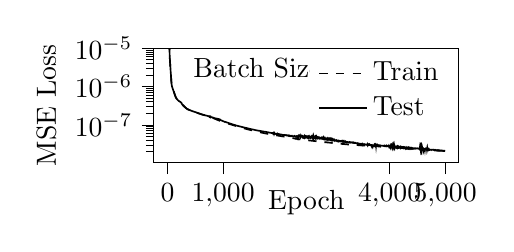
\begin{tikzpicture}

\begin{axis}[
legend cell align={left},
legend style={draw=none},
log basis y={10},
tick align=outside,
tick pos=left,
title={Batch Size 16},
title style={at={(0.4,0.85)},anchor=north},
x grid style={white!69.0196078431373!black},
xlabel={Epoch},
x label style={yshift=13pt},
xmin=-249.95, xmax=5248.95,
xtick style={color=black},
xtick = {0,1000,4000,5000},
y grid style={white!69.0196078431373!black},
ylabel={MSE Loss},
ymin=1.04995733040024e-08, ymax=1e-5,
ymode=log,
ytick style={color=black},
width=.45\textwidth,
height=.25\textwidth
]
\addplot [semithick, black, dashed]
table {%
0 0.0157170567642897
1 0.00494477174337953
2 0.00178249403554946
3 0.00104628965561278
4 0.000540450631990097
5 0.000267249523603823
6 0.000195556676466367
7 0.000179966989569948
8 0.000174315613148792
9 0.000170275954966201
10 0.000166128802236926
11 0.000161243435519282
12 0.000155176517626387
13 0.000147447619914601
14 0.000137505138925917
15 0.000124870715357247
16 0.000109628831036389
17 9.26289391609316e-05
18 7.54085500957444e-05
19 5.99092843294784e-05
20 4.77161089384026e-05
21 3.93279772288224e-05
22 3.40980909077189e-05
23 3.09422128148071e-05
24 2.89322912085481e-05
25 2.72737210743799e-05
26 2.54317353028455e-05
27 2.28156418916114e-05
28 2.01819365893243e-05
29 1.77557636425263e-05
30 1.5502294282669e-05
31 1.34128514700933e-05
32 1.15395934462867e-05
33 9.93898418664685e-06
34 8.62693892850075e-06
35 7.58853412253302e-06
36 6.78498193133237e-06
37 6.16869731970837e-06
38 5.69058382416188e-06
39 5.31324215398854e-06
40 5.00480225616684e-06
41 4.7444518992279e-06
42 4.51447482453204e-06
43 4.30798976503866e-06
44 4.11608894853543e-06
45 3.93454810227922e-06
46 3.75880521266936e-06
47 3.58901737558881e-06
48 3.42562672744862e-06
49 3.26669840717386e-06
50 3.11160224288187e-06
51 2.96258664974403e-06
52 2.82159659042236e-06
53 2.68886794032142e-06
54 2.56387212152731e-06
55 2.44723567112715e-06
56 2.34057172980329e-06
57 2.24493696725858e-06
58 2.15844092952011e-06
59 2.0788237059719e-06
60 1.99667843895668e-06
61 1.90497609787599e-06
62 1.79736609072734e-06
63 1.68848505768437e-06
64 1.59369150190969e-06
65 1.51194072418548e-06
66 1.44278207682191e-06
67 1.38194286273574e-06
68 1.32816223009513e-06
69 1.2809325050398e-06
70 1.23942618449746e-06
71 1.20316316116487e-06
72 1.17089864494346e-06
73 1.14246875506296e-06
74 1.11685223265567e-06
75 1.09369868118847e-06
76 1.07318007189861e-06
77 1.05437576991108e-06
78 1.03672772496566e-06
79 1.02062385838053e-06
80 1.00592634129271e-06
81 9.92105790942332e-07
82 9.7894169545043e-07
83 9.66602892503943e-07
84 9.54589052753363e-07
85 9.42918769112566e-07
86 9.31959767683566e-07
87 9.2148744329279e-07
88 9.11429445267231e-07
89 9.01841054997021e-07
90 8.92400122751269e-07
91 8.83255546455075e-07
92 8.74700299107189e-07
93 8.65906616240863e-07
94 8.57358865317792e-07
95 8.48961237267076e-07
96 8.40659787854747e-07
97 8.3273339777179e-07
98 8.24562840250565e-07
99 8.16930169150964e-07
100 8.08981725157309e-07
101 8.01335254408286e-07
102 7.938409220003e-07
103 7.86272286035228e-07
104 7.79077216805035e-07
105 7.71825237762869e-07
106 7.64540684656367e-07
107 7.57455605054247e-07
108 7.50291343621257e-07
109 7.43385836699417e-07
110 7.36310198249157e-07
111 7.2935094047466e-07
112 7.22335523079209e-07
113 7.15656543093246e-07
114 7.08781524224378e-07
115 7.02204949249108e-07
116 6.95669085445161e-07
117 6.89374548812793e-07
118 6.83004592076486e-07
119 6.76743621340847e-07
120 6.70653783501507e-07
121 6.64517023594158e-07
122 6.58444838109062e-07
123 6.52467115031641e-07
124 6.46645066922247e-07
125 6.40550082820823e-07
126 6.34422589044448e-07
127 6.28629438992334e-07
128 6.22746939754393e-07
129 6.16957024178077e-07
130 6.11050226723364e-07
131 6.0553354312276e-07
132 6.0002472520182e-07
133 5.94472997008211e-07
134 5.89109220683781e-07
135 5.83457079159189e-07
136 5.78418984446216e-07
137 5.7332289055978e-07
138 5.68441488383087e-07
139 5.63714549315364e-07
140 5.59090271252671e-07
141 5.54642511374936e-07
142 5.50334273199837e-07
143 5.46195153745543e-07
144 5.42178440980479e-07
145 5.38200247120812e-07
146 5.34317242667726e-07
147 5.30567891871669e-07
148 5.26957831226582e-07
149 5.23221014177011e-07
150 5.19686565098709e-07
151 5.16319246941066e-07
152 5.1299718701614e-07
153 5.09589032390068e-07
154 5.06361061226812e-07
155 5.03223137172881e-07
156 5.00183228808737e-07
157 4.9724213354807e-07
158 4.9438490189857e-07
159 4.9162455306373e-07
160 4.89330421473255e-07
161 4.86669611902357e-07
162 4.83983281668543e-07
163 4.81407683992074e-07
164 4.78924291158478e-07
165 4.7652420248312e-07
166 4.74232413509412e-07
167 4.71954440158129e-07
168 4.69751064102297e-07
169 4.67584087743944e-07
170 4.65374450342892e-07
171 4.63257154720509e-07
172 4.6126252958345e-07
173 4.59285346551042e-07
174 4.57338758977244e-07
175 4.55391532227623e-07
176 4.53448316278582e-07
177 4.5134003435976e-07
178 4.49530939363285e-07
179 4.47626082561214e-07
180 4.45694395651231e-07
181 4.43928685967876e-07
182 4.42185508745752e-07
183 4.40439555106309e-07
184 4.3882785571725e-07
185 4.37217972901749e-07
186 4.35614033278853e-07
187 4.33923493403654e-07
188 4.32394612360554e-07
189 4.30824806841201e-07
190 4.29448743943794e-07
191 4.27996334764202e-07
192 4.2654474542303e-07
193 4.25223923485873e-07
194 4.23847797321741e-07
195 4.22281450582318e-07
196 4.20877642255846e-07
197 4.19539155572579e-07
198 4.18226270070932e-07
199 4.16828583993834e-07
200 4.15641147853307e-07
201 4.14374378181037e-07
202 4.12955820522143e-07
203 4.11872127500601e-07
204 4.10614599175574e-07
205 4.09486309507656e-07
206 4.08297302655569e-07
207 4.07291623872652e-07
208 4.06151649784192e-07
209 4.04880044627021e-07
210 4.03888402871644e-07
211 4.02805585792976e-07
212 4.01743319073944e-07
213 4.00739752507206e-07
214 3.99736535186435e-07
215 3.98833434005041e-07
216 3.97754167352105e-07
217 3.96727826768029e-07
218 3.95718042653925e-07
219 3.94693230930443e-07
220 3.9383311586505e-07
221 3.9275161007879e-07
222 3.9172802642895e-07
223 3.90782656552346e-07
224 3.89721222845196e-07
225 3.88612679515177e-07
226 3.87859798280488e-07
227 3.8695441405423e-07
228 3.8589167816383e-07
229 3.84909645688936e-07
230 3.83900921491431e-07
231 3.82917928007487e-07
232 3.82064893713618e-07
233 3.81161208053982e-07
234 3.80179631534361e-07
235 3.79220531740998e-07
236 3.78215918999558e-07
237 3.7710426870774e-07
238 3.76155795223099e-07
239 3.74884881878756e-07
240 3.73761657613159e-07
241 3.72517982626164e-07
242 3.71497203701665e-07
243 3.70091190802668e-07
244 3.6877978438099e-07
245 3.67199387056871e-07
246 3.65626293969967e-07
247 3.64062025596468e-07
248 3.62244684353641e-07
249 3.60450857769479e-07
250 3.58647998822903e-07
251 3.56561039907888e-07
252 3.54525802322314e-07
253 3.52287566386167e-07
254 3.50287391583493e-07
255 3.4827622160094e-07
256 3.46361628018599e-07
257 3.442452336202e-07
258 3.42522692250213e-07
259 3.4098111838432e-07
260 3.39507249535131e-07
261 3.3804830252393e-07
262 3.36976891986751e-07
263 3.35771423678466e-07
264 3.34539207671014e-07
265 3.33171887447747e-07
266 3.32210861387239e-07
267 3.30899532073659e-07
268 3.29677021355224e-07
269 3.28394180627356e-07
270 3.27252484524365e-07
271 3.26162355179349e-07
272 3.25076022861026e-07
273 3.24031567018324e-07
274 3.23017687350102e-07
275 3.22020703876547e-07
276 3.21058469410218e-07
277 3.20131131445578e-07
278 3.19224168208621e-07
279 3.18332019588752e-07
280 3.17414626763934e-07
281 3.16470977736572e-07
282 3.15361310200046e-07
283 3.14367141285743e-07
284 3.13330990451277e-07
285 3.12373081598594e-07
286 3.11041730753914e-07
287 3.09975267860807e-07
288 3.08969859794672e-07
289 3.07846929878508e-07
290 3.06794977639413e-07
291 3.05737578266019e-07
292 3.0466266837692e-07
293 3.03954595523237e-07
294 3.03101196678313e-07
295 3.02118985189281e-07
296 3.01218168196726e-07
297 3.00310456772479e-07
298 2.99479211918197e-07
299 2.98664209118726e-07
300 2.97876342834513e-07
301 2.97069236964376e-07
302 2.96287139768481e-07
303 2.95540525151239e-07
304 2.94592372938496e-07
305 2.93832868003108e-07
306 2.93041105045688e-07
307 2.92138023390009e-07
308 2.91344262571158e-07
309 2.90479741146044e-07
310 2.89638650002644e-07
311 2.88783956314376e-07
312 2.87966960804908e-07
313 2.87156888049367e-07
314 2.86230183249359e-07
315 2.85199473267994e-07
316 2.84329060711741e-07
317 2.83470531364571e-07
318 2.82711612797471e-07
319 2.8189036959958e-07
320 2.8108939352478e-07
321 2.80323620067691e-07
322 2.79618150941019e-07
323 2.78579928540523e-07
324 2.77787970787813e-07
325 2.76974661190366e-07
326 2.76175905796094e-07
327 2.75381109268835e-07
328 2.74673050796537e-07
329 2.73941170341629e-07
330 2.73343178925245e-07
331 2.72956742115582e-07
332 2.72267732029263e-07
333 2.71421207877154e-07
334 2.70669167790061e-07
335 2.69858946552404e-07
336 2.69127144292725e-07
337 2.68486125065692e-07
338 2.67699487956463e-07
339 2.67018376263195e-07
340 2.66254324294835e-07
341 2.65609372050335e-07
342 2.64946595834203e-07
343 2.64183357693071e-07
344 2.63509790364935e-07
345 2.62888811377593e-07
346 2.62296822654662e-07
347 2.61795223821082e-07
348 2.60765411624675e-07
349 2.60187987706217e-07
350 2.59608676287826e-07
351 2.58937510935198e-07
352 2.58401657028173e-07
353 2.57939879027447e-07
354 2.57488526514749e-07
355 2.56912723124003e-07
356 2.5638282590279e-07
357 2.55946380399052e-07
358 2.55382050632136e-07
359 2.54851634466036e-07
360 2.5443849939677e-07
361 2.53912852173244e-07
362 2.53413875391573e-07
363 2.52993562064319e-07
364 2.52566530065224e-07
365 2.52173733429117e-07
366 2.51742222630469e-07
367 2.51256598509997e-07
368 2.50831636513738e-07
369 2.50515218077396e-07
370 2.5000812983933e-07
371 2.49434692122463e-07
372 2.48966004456008e-07
373 2.48557739986666e-07
374 2.48152726946671e-07
375 2.47777446951147e-07
376 2.4732192088095e-07
377 2.46895147625992e-07
378 2.46492991010427e-07
379 2.46027582377906e-07
380 2.45625955962225e-07
381 2.45214678422201e-07
382 2.44813897467111e-07
383 2.44392247530811e-07
384 2.439667089007e-07
385 2.43561708266782e-07
386 2.43146217513868e-07
387 2.42745924310839e-07
388 2.42299840301996e-07
389 2.41924007092109e-07
390 2.41548250386359e-07
391 2.4110301239233e-07
392 2.40753827760898e-07
393 2.40407377113172e-07
394 2.40073736314628e-07
395 2.39752746800548e-07
396 2.39428752649928e-07
397 2.39145928070172e-07
398 2.38728963807944e-07
399 2.38479965169347e-07
400 2.38172701713779e-07
401 2.37863011172124e-07
402 2.37620931294202e-07
403 2.3731942192029e-07
404 2.36979224602862e-07
405 2.36684770619888e-07
406 2.36476611952696e-07
407 2.36186071909117e-07
408 2.35960636956634e-07
409 2.35469004792321e-07
410 2.34993137034678e-07
411 2.34665876455153e-07
412 2.34368971142374e-07
413 2.34073551396818e-07
414 2.33405668247144e-07
415 2.3353564838402e-07
416 2.33036555627564e-07
417 2.32731610225301e-07
418 2.32511658502688e-07
419 2.32205579486333e-07
420 2.31897210944965e-07
421 2.31614303118022e-07
422 2.31387427064078e-07
423 2.31009555875517e-07
424 2.30927051632079e-07
425 2.30570250145945e-07
426 2.30109878870621e-07
427 2.29755619159278e-07
428 2.29419798976949e-07
429 2.2913787184109e-07
430 2.28831625989301e-07
431 2.28494739516805e-07
432 2.28182287109746e-07
433 2.27858054557828e-07
434 2.27546540337187e-07
435 2.27196947875541e-07
436 2.26895820269135e-07
437 2.26625020268045e-07
438 2.26283218495382e-07
439 2.25993931898927e-07
440 2.25655906049838e-07
441 2.2537209050455e-07
442 2.2510194525438e-07
443 2.24828690761569e-07
444 2.24556286852362e-07
445 2.24300207833039e-07
446 2.24011245563815e-07
447 2.23872584399487e-07
448 2.23551614816131e-07
449 2.23257345162153e-07
450 2.22980819252427e-07
451 2.2271834546217e-07
452 2.22460312336636e-07
453 2.22206780733813e-07
454 2.21958781267517e-07
455 2.21711269247749e-07
456 2.21467916212248e-07
457 2.21235154199917e-07
458 2.20999668862021e-07
459 2.20767076868356e-07
460 2.20535877438977e-07
461 2.20308807939773e-07
462 2.20059808896167e-07
463 2.19824142021707e-07
464 2.19612100529787e-07
465 2.1938929498333e-07
466 2.19157623597255e-07
467 2.1896537287347e-07
468 2.18743536777311e-07
469 2.18522104340479e-07
470 2.18272721745905e-07
471 2.18055716807442e-07
472 2.1783752742266e-07
473 2.1761818953081e-07
474 2.17430983695976e-07
475 2.17206068221287e-07
476 2.16991443927839e-07
477 2.16773518530999e-07
478 2.16515748135748e-07
479 2.16300841934469e-07
480 2.16058449872492e-07
481 2.15869073706187e-07
482 2.1564869785351e-07
483 2.15435289980803e-07
484 2.15200336675991e-07
485 2.14946434098806e-07
486 2.1470916516364e-07
487 2.14493426646811e-07
488 2.14261333354671e-07
489 2.14043833416611e-07
490 2.13684532845093e-07
491 2.13446484544022e-07
492 2.13225306985976e-07
493 2.13031618301329e-07
494 2.12794633135616e-07
495 2.1251043921211e-07
496 2.12278367698104e-07
497 2.12043049543809e-07
498 2.11812802142219e-07
499 2.11570569483399e-07
500 2.11340852310116e-07
501 2.11117200315414e-07
502 2.10896458291643e-07
503 2.1067865063884e-07
504 2.10462695349634e-07
505 2.10248212908937e-07
506 2.10038392978618e-07
507 2.09967990151938e-07
508 2.09629130488054e-07
509 2.09356091531276e-07
510 2.09101517214094e-07
511 2.0885782751634e-07
512 2.08675676212522e-07
513 2.08429224507256e-07
514 2.08143801842198e-07
515 2.07879654823273e-07
516 2.07599692124916e-07
517 2.07531877720157e-07
518 2.07242607004332e-07
519 2.06976028913175e-07
520 2.06722016230287e-07
521 2.06477896398383e-07
522 2.06244004296252e-07
523 2.05996478037207e-07
524 2.05893390926803e-07
525 2.05615459904607e-07
526 2.05380138218914e-07
527 2.05141496991246e-07
528 2.04895898015423e-07
529 2.04667326379138e-07
530 2.04441963525426e-07
531 2.04216897543574e-07
532 2.0399652140668e-07
533 2.03779658797032e-07
534 2.03562826108339e-07
535 2.0334601751415e-07
536 2.03135240347763e-07
537 2.02906057346297e-07
538 2.02689399074529e-07
539 2.02473491917488e-07
540 2.02258676225142e-07
541 2.02040906152945e-07
542 2.01827895203621e-07
543 2.01646046050996e-07
544 2.0143258397809e-07
545 2.01214925588999e-07
546 2.00992143142287e-07
547 2.00781135099248e-07
548 2.00562146595473e-07
549 2.00357410903962e-07
550 2.00143986297974e-07
551 1.99943427894311e-07
552 1.99730849530511e-07
553 1.99533505224281e-07
554 1.99330869968151e-07
555 1.9912389529253e-07
556 1.98918559668471e-07
557 1.98708590382068e-07
558 1.98505848487684e-07
559 1.98292419888446e-07
560 1.98096410962023e-07
561 1.97904820154804e-07
562 1.9770706975919e-07
563 1.9748347308024e-07
564 1.97292339883859e-07
565 1.97073662711489e-07
566 1.96870710993835e-07
567 1.96664619174669e-07
568 1.96475939667096e-07
569 1.96348054068096e-07
570 1.96120539378342e-07
571 1.95933779174595e-07
572 1.95736368809207e-07
573 1.95534025024813e-07
574 1.95333484313664e-07
575 1.95124152348569e-07
576 1.95009315866912e-07
577 1.94775902379263e-07
578 1.94541645868185e-07
579 1.94320748363452e-07
580 1.9411251212631e-07
581 1.93909075257181e-07
582 1.93718050923053e-07
583 1.93516266911331e-07
584 1.93320917162509e-07
585 1.93129007548976e-07
586 1.92928064961961e-07
587 1.92837274340718e-07
588 1.92624708525102e-07
589 1.92408956387169e-07
590 1.92225819553471e-07
591 1.92020735894971e-07
592 1.91878943944346e-07
593 1.91675015734916e-07
594 1.91448435110431e-07
595 1.91271641604374e-07
596 1.91048381573466e-07
597 1.90840330120068e-07
598 1.90653138474772e-07
599 1.90466430986191e-07
600 1.90273618727588e-07
601 1.90071319252638e-07
602 1.89884589708811e-07
603 1.89694812256391e-07
604 1.89509724471293e-07
605 1.89317692722568e-07
606 1.89151745139782e-07
607 1.88957836265047e-07
608 1.88763875129894e-07
609 1.8860838834911e-07
610 1.88492758660175e-07
611 1.88309009992338e-07
612 1.88081675830176e-07
613 1.87860870838108e-07
614 1.87664490702844e-07
615 1.87469595530843e-07
616 1.87259174673216e-07
617 1.87060099065661e-07
618 1.86873242554952e-07
619 1.86672734876936e-07
620 1.86483752926847e-07
621 1.86293344697219e-07
622 1.86105415899362e-07
623 1.85915503529088e-07
624 1.8575178152247e-07
625 1.85554022223755e-07
626 1.85353178373759e-07
627 1.8521270283145e-07
628 1.85098913320303e-07
629 1.84897171813248e-07
630 1.84691331647002e-07
631 1.84487640524367e-07
632 1.84295574889859e-07
633 1.84111957629796e-07
634 1.83914716345157e-07
635 1.83755724989965e-07
636 1.83571663399107e-07
637 1.8338817892527e-07
638 1.8321129060439e-07
639 1.83026746398696e-07
640 1.82798685713692e-07
641 1.82628072302293e-07
642 1.8240755436949e-07
643 1.82209592708205e-07
644 1.81998398467442e-07
645 1.81880033061077e-07
646 1.81668815613989e-07
647 1.81459775753012e-07
648 1.81254756874694e-07
649 1.81092687050466e-07
650 1.80890330682359e-07
651 1.80684028741496e-07
652 1.80452216731908e-07
653 1.80272235375867e-07
654 1.80111763242508e-07
655 1.79915874568337e-07
656 1.79712098308471e-07
657 1.79537765347959e-07
658 1.79391292441267e-07
659 1.7920577938213e-07
660 1.79012431054559e-07
661 1.78831277722225e-07
662 1.78644232065039e-07
663 1.78457527518106e-07
664 1.78267877934957e-07
665 1.78093018554648e-07
666 1.77905254446387e-07
667 1.77723857326839e-07
668 1.7753547782462e-07
669 1.77379771038488e-07
670 1.77215719631363e-07
671 1.77056875465098e-07
672 1.76856059582065e-07
673 1.76671049281651e-07
674 1.76487213458643e-07
675 1.76302384872429e-07
676 1.76117043793056e-07
677 1.75936534887455e-07
678 1.75756247521974e-07
679 1.75606320475197e-07
680 1.75418388813853e-07
681 1.75196992749704e-07
682 1.75045590090406e-07
683 1.74854614705566e-07
684 1.74652316815127e-07
685 1.74424186383249e-07
686 1.74264706537031e-07
687 1.74055298188591e-07
688 1.73926764027499e-07
689 1.73701496798628e-07
690 1.73572706358982e-07
691 1.73321090102263e-07
692 1.73147434431087e-07
693 1.72996947163995e-07
694 1.72786218151089e-07
695 1.72599083192893e-07
696 1.72568876031676e-07
697 1.72387436194299e-07
698 1.72159440069208e-07
699 1.71958998173238e-07
700 1.71749518663944e-07
701 1.7157847770477e-07
702 1.71360882688987e-07
703 1.71189904619951e-07
704 1.70959397792103e-07
705 1.7079805885345e-07
706 1.70577748185963e-07
707 1.70391250101432e-07
708 1.70294054527176e-07
709 1.70153339674073e-07
710 1.69961250442441e-07
711 1.69790923798985e-07
712 1.69513855112768e-07
713 1.69349986016698e-07
714 1.69170517544615e-07
715 1.68975520637105e-07
716 1.68794829697561e-07
717 1.68674960491444e-07
718 1.68560368251747e-07
719 1.68348613023284e-07
720 1.68180192382295e-07
721 1.68044255872246e-07
722 1.67784312189667e-07
723 1.67622006166823e-07
724 1.67433583676768e-07
725 1.67142194790415e-07
726 1.66952169308843e-07
727 1.66777577675248e-07
728 1.66608952660852e-07
729 1.66446427947164e-07
730 1.66270591492435e-07
731 1.66101942618013e-07
732 1.65938628249762e-07
733 1.65765831525277e-07
734 1.65649616683083e-07
735 1.65385300405774e-07
736 1.65217369541892e-07
737 1.65014219057014e-07
738 1.6483034158199e-07
739 1.64667229618942e-07
740 1.64397729420784e-07
741 1.64213927241974e-07
742 1.64072907040236e-07
743 1.6379700686997e-07
744 1.63645981643867e-07
745 1.63382232301501e-07
746 1.6327906817537e-07
747 1.63015408730871e-07
748 1.62801310864324e-07
749 1.62617077627658e-07
750 1.62424714076792e-07
751 1.62247915383773e-07
752 1.62051023785637e-07
753 1.61872072872882e-07
754 1.6165106788435e-07
755 1.61600835717479e-07
756 1.61240600313306e-07
757 1.61194861057368e-07
758 1.60852658879662e-07
759 1.60787009278351e-07
760 1.60590858342857e-07
761 1.60234822551786e-07
762 1.60201742232857e-07
763 1.59901149771713e-07
764 1.59803023151994e-07
765 1.59525831236351e-07
766 1.59374475643403e-07
767 1.59135792628717e-07
768 1.58920532690843e-07
769 1.58900042478649e-07
770 1.58551003600849e-07
771 1.58445956166986e-07
772 1.58137577130901e-07
773 1.58083954872268e-07
774 1.57764831811846e-07
775 1.57709431590547e-07
776 1.57401405722624e-07
777 1.57347303854749e-07
778 1.57050745258402e-07
779 1.56966653740653e-07
780 1.56687031115155e-07
781 1.56785914370516e-07
782 1.56612737448825e-07
783 1.56451782203249e-07
784 1.56252137685442e-07
785 1.56076418790008e-07
786 1.55898435949098e-07
787 1.55699541132037e-07
788 1.55520961151012e-07
789 1.55345307412347e-07
790 1.55173079157578e-07
791 1.54974727074375e-07
792 1.54768641245084e-07
793 1.5459558374431e-07
794 1.5444234325912e-07
795 1.54301182689665e-07
796 1.54076760843225e-07
797 1.53900922057915e-07
798 1.53745949539541e-07
799 1.53580229117267e-07
800 1.53406590548855e-07
801 1.53240547525968e-07
802 1.53047686090702e-07
803 1.52824890882641e-07
804 1.52664273521452e-07
805 1.52475196550483e-07
806 1.52327802844354e-07
807 1.52147398885916e-07
808 1.51979647590395e-07
809 1.51795929646426e-07
810 1.51624505434711e-07
811 1.51454105321136e-07
812 1.51283279407721e-07
813 1.51115457406092e-07
814 1.50930618310952e-07
815 1.50760781984616e-07
816 1.50782627734714e-07
817 1.50500275672982e-07
818 1.50235237292407e-07
819 1.50018968902543e-07
820 1.49857105313345e-07
821 1.49713744534097e-07
822 1.49508386748209e-07
823 1.49243716315084e-07
824 1.49054966783524e-07
825 1.48848405203239e-07
826 1.48593713156231e-07
827 1.48452548614841e-07
828 1.48339782398921e-07
829 1.48084122237435e-07
830 1.47866147088394e-07
831 1.47622342979048e-07
832 1.4737123991182e-07
833 1.47169714985296e-07
834 1.47018789085962e-07
835 1.46823949506825e-07
836 1.46512769518381e-07
837 1.46378438842021e-07
838 1.46098743840639e-07
839 1.45954007734872e-07
840 1.45737554120728e-07
841 1.45556221561094e-07
842 1.45273102816645e-07
843 1.45146473812474e-07
844 1.44893944799662e-07
845 1.44685848667336e-07
846 1.44500907168776e-07
847 1.4436663649775e-07
848 1.44028160448784e-07
849 1.43881057880435e-07
850 1.43606745851343e-07
851 1.43507942325982e-07
852 1.43128769224177e-07
853 1.4301058635624e-07
854 1.42788225716117e-07
855 1.42625498355642e-07
856 1.42412673760361e-07
857 1.42159079061344e-07
858 1.4199432023787e-07
859 1.41772513316596e-07
860 1.41599934678993e-07
861 1.41388858359903e-07
862 1.41182926185479e-07
863 1.40962782744225e-07
864 1.40806364584023e-07
865 1.40581685961649e-07
866 1.40403925101396e-07
867 1.4016057497912e-07
868 1.40044896177471e-07
869 1.3980589160667e-07
870 1.3957648116758e-07
871 1.39445378636083e-07
872 1.39138843742614e-07
873 1.38897649193837e-07
874 1.38654308422304e-07
875 1.38455802293436e-07
876 1.38271871641393e-07
877 1.38072660327282e-07
878 1.3789356398064e-07
879 1.37655154013316e-07
880 1.37478279633285e-07
881 1.37314475196604e-07
882 1.37122865879746e-07
883 1.36933145142848e-07
884 1.36802316887952e-07
885 1.36559793908475e-07
886 1.3642202107178e-07
887 1.36200022627264e-07
888 1.36101916211828e-07
889 1.35843518506817e-07
890 1.35694482299442e-07
891 1.35512572025931e-07
892 1.35300152894757e-07
893 1.35296917736838e-07
894 1.35076997914041e-07
895 1.34893043981066e-07
896 1.34717172727505e-07
897 1.34527160362552e-07
898 1.34308240479442e-07
899 1.34143823828481e-07
900 1.33862042787314e-07
901 1.336907333922e-07
902 1.33526360556857e-07
903 1.33354756073345e-07
904 1.33178832584235e-07
905 1.32975719669304e-07
906 1.328086220731e-07
907 1.32602404118387e-07
908 1.3244473960583e-07
909 1.322507284236e-07
910 1.3208645066598e-07
911 1.31908025320371e-07
912 1.31727454142805e-07
913 1.31562949462705e-07
914 1.31399596458692e-07
915 1.3120474050865e-07
916 1.31009608221433e-07
917 1.30844098823246e-07
918 1.30663171997725e-07
919 1.30506657299634e-07
920 1.30347919839124e-07
921 1.30182991870953e-07
922 1.30027269566568e-07
923 1.29857494112429e-07
924 1.29701414859795e-07
925 1.29552905523411e-07
926 1.2940177445131e-07
927 1.29231482656422e-07
928 1.29098281369977e-07
929 1.28939781010473e-07
930 1.28751404755434e-07
931 1.28589202464724e-07
932 1.2841671961894e-07
933 1.28243070928846e-07
934 1.2803982670917e-07
935 1.27876534680382e-07
936 1.27715794622674e-07
937 1.27549439078223e-07
938 1.27395809307984e-07
939 1.27251330805933e-07
940 1.27115895857344e-07
941 1.26910032076211e-07
942 1.26811345971589e-07
943 1.26729663211478e-07
944 1.26444568536499e-07
945 1.26253609963101e-07
946 1.26082584579024e-07
947 1.25873118491882e-07
948 1.25708876002051e-07
949 1.25526543680365e-07
950 1.25347965983735e-07
951 1.25173203823437e-07
952 1.24986479754341e-07
953 1.24805979790921e-07
954 1.2464467223694e-07
955 1.24486626290832e-07
956 1.24325891309951e-07
957 1.24059086388684e-07
958 1.23900421499457e-07
959 1.23752723684589e-07
960 1.23606460093129e-07
961 1.23458894080386e-07
962 1.23334903548766e-07
963 1.23164554814537e-07
964 1.23017373574896e-07
965 1.22884383220168e-07
966 1.2272103016997e-07
967 1.22591781686054e-07
968 1.22412395523241e-07
969 1.22283938569723e-07
970 1.2213839731956e-07
971 1.21992413387062e-07
972 1.21762341468212e-07
973 1.21653056602611e-07
974 1.21516884128425e-07
975 1.21363378561057e-07
976 1.21249401036749e-07
977 1.21074073003768e-07
978 1.20967150103013e-07
979 1.20810225507029e-07
980 1.20688818554981e-07
981 1.20541718686695e-07
982 1.20421648816205e-07
983 1.2028323980573e-07
984 1.20130155050191e-07
985 1.20018588045667e-07
986 1.19883109864105e-07
987 1.19717597538482e-07
988 1.19591703700905e-07
989 1.19459623334706e-07
990 1.19327731148644e-07
991 1.19182412216645e-07
992 1.190378214595e-07
993 1.18928106189742e-07
994 1.18777606907372e-07
995 1.18669771886459e-07
996 1.18526345442405e-07
997 1.18412091222098e-07
998 1.182686517609e-07
999 1.18146764471305e-07
1000 1.18045295611324e-07
1001 1.17885191471601e-07
1002 1.1773723693409e-07
1003 1.17636993980597e-07
1004 1.17508308122183e-07
1005 1.17379135396334e-07
1006 1.17220094796977e-07
1007 1.17123960905019e-07
1008 1.16971413607558e-07
1009 1.16875604081912e-07
1010 1.16721507264828e-07
1011 1.16625413646432e-07
1012 1.16471765217341e-07
1013 1.16374956864007e-07
1014 1.16226475117998e-07
1015 1.1612951336204e-07
1016 1.15985186340595e-07
1017 1.15878762532162e-07
1018 1.15722544556718e-07
1019 1.1563705219686e-07
1020 1.15482216056506e-07
1021 1.15382735749847e-07
1022 1.15234289868482e-07
1023 1.15194369406879e-07
1024 1.1509215372385e-07
1025 1.14971480446258e-07
1026 1.14853542346083e-07
1027 1.14729510986677e-07
1028 1.14465596745106e-07
1029 1.14398147832873e-07
1030 1.14321383524185e-07
1031 1.14196341097994e-07
1032 1.14066242570487e-07
1033 1.13935783559782e-07
1034 1.13807661961118e-07
1035 1.13695412860437e-07
1036 1.13558107294409e-07
1037 1.13417669808769e-07
1038 1.13302818903094e-07
1039 1.13176249655567e-07
1040 1.13044207392221e-07
1041 1.12916077910086e-07
1042 1.12789789074696e-07
1043 1.12666461593136e-07
1044 1.12543457490233e-07
1045 1.12422214286312e-07
1046 1.12315864466694e-07
1047 1.12182835920294e-07
1048 1.12061487143933e-07
1049 1.11943023419769e-07
1050 1.11824035883501e-07
1051 1.11708382185327e-07
1052 1.11589450629168e-07
1053 1.11475569585906e-07
1054 1.11358585638044e-07
1055 1.11240735918727e-07
1056 1.11126858243438e-07
1057 1.11011553304508e-07
1058 1.10896632492086e-07
1059 1.10790323411436e-07
1060 1.10676093481032e-07
1061 1.10561356954975e-07
1062 1.10458826345194e-07
1063 1.10332153219872e-07
1064 1.10221367368268e-07
1065 1.10119643316864e-07
1066 1.10016076984465e-07
1067 1.09895937949744e-07
1068 1.09784279111125e-07
1069 1.09660139557377e-07
1070 1.09532256768574e-07
1071 1.09413658780255e-07
1072 1.09296013629745e-07
1073 1.09178800776988e-07
1074 1.09062563716122e-07
1075 1.08961397675245e-07
1076 1.0882023883596e-07
1077 1.08682747345767e-07
1078 1.08570803114105e-07
1079 1.08453086824056e-07
1080 1.08348394981306e-07
1081 1.08229575708663e-07
1082 1.08175652648868e-07
1083 1.08044552664666e-07
1084 1.07924311190999e-07
1085 1.07804279075197e-07
1086 1.07687016416946e-07
1087 1.07583657079857e-07
1088 1.07472328480185e-07
1089 1.07360298155612e-07
1090 1.07231535281471e-07
1091 1.07122651012759e-07
1092 1.07014493000435e-07
1093 1.0690706458405e-07
1094 1.06793603364963e-07
1095 1.06669464503995e-07
1096 1.06556396463731e-07
1097 1.06448062449971e-07
1098 1.0633262673565e-07
1099 1.06225804859861e-07
1100 1.06111840107559e-07
1101 1.06007312659528e-07
1102 1.05889961115935e-07
1103 1.05787279665037e-07
1104 1.05671067569091e-07
1105 1.05566635443921e-07
1106 1.0545252139238e-07
1107 1.05352690265903e-07
1108 1.05238320241341e-07
1109 1.05129935327852e-07
1110 1.05013805679732e-07
1111 1.04924952804453e-07
1112 1.04802457894237e-07
1113 1.0472310326648e-07
1114 1.04609571572212e-07
1115 1.0450942516016e-07
1116 1.04393734819297e-07
1117 1.04297197307091e-07
1118 1.04180416496291e-07
1119 1.0408402435047e-07
1120 1.03966197073646e-07
1121 1.0387017652036e-07
1122 1.03754794164246e-07
1123 1.0365835006354e-07
1124 1.03542971995552e-07
1125 1.03447081940544e-07
1126 1.03333663226124e-07
1127 1.03239306419312e-07
1128 1.03124784988751e-07
1129 1.03028840477748e-07
1130 1.02916153586818e-07
1131 1.02787292341588e-07
1132 1.02657459869704e-07
1133 1.02566233646684e-07
1134 1.02459099572627e-07
1135 1.0236741592351e-07
1136 1.02258474193206e-07
1137 1.02178690926991e-07
1138 1.02057533133859e-07
1139 1.0195955497494e-07
1140 1.01866740447321e-07
1141 1.0174640036098e-07
1142 1.01654885199309e-07
1143 1.01564086460115e-07
1144 1.01452568284088e-07
1145 1.01358281408892e-07
1146 1.01252124068196e-07
1147 1.01132042544805e-07
1148 1.01040741810721e-07
1149 1.0093680472778e-07
1150 1.00835201639171e-07
1151 1.00737907963833e-07
1152 1.00636074826355e-07
1153 1.00535662330259e-07
1154 1.00435070386595e-07
1155 1.00334794463919e-07
1156 1.00233066344657e-07
1157 1.00139313264691e-07
1158 1.00035746370963e-07
1159 9.99342205645348e-08
1160 9.98369444076275e-08
1161 9.97294167923712e-08
1162 9.96306041329831e-08
1163 9.95292283505478e-08
1164 9.94305740533719e-08
1165 9.93309828345446e-08
1166 9.92319580497281e-08
1167 9.91331406723361e-08
1168 9.90346987315149e-08
1169 9.89363423364864e-08
1170 9.88384333915349e-08
1171 9.87406676955516e-08
1172 9.86426246996075e-08
1173 9.85450470523119e-08
1174 9.84475341887503e-08
1175 9.83505173692833e-08
1176 9.82529710178426e-08
1177 9.81562854889262e-08
1178 9.80592281862869e-08
1179 9.79621718073531e-08
1180 9.78654439443005e-08
1181 9.77698567261598e-08
1182 9.76725255235067e-08
1183 9.75756527665794e-08
1184 9.74796394181965e-08
1185 9.73854815420339e-08
1186 9.72912396584036e-08
1187 9.71942784673274e-08
1188 9.70993046678359e-08
1189 9.7005777128345e-08
1190 9.69105955412886e-08
1191 9.68398183474051e-08
1192 9.67422502249349e-08
1193 9.6656792269556e-08
1194 9.65493723619204e-08
1195 9.64579490911888e-08
1196 9.63569642422613e-08
1197 9.62606689931533e-08
1198 9.61624434623332e-08
1199 9.60775235725464e-08
1200 9.5981298237291e-08
1201 9.58870457914429e-08
1202 9.57886685490905e-08
1203 9.56941159380165e-08
1204 9.55973716543213e-08
1205 9.550779267542e-08
1206 9.54129343995192e-08
1207 9.53207871106088e-08
1208 9.52259731121785e-08
1209 9.51386579863822e-08
1210 9.50452932002577e-08
1211 9.49372938769955e-08
1212 9.48370358955231e-08
1213 9.47485660738323e-08
1214 9.46488406015078e-08
1215 9.45476629787834e-08
1216 9.44520911225766e-08
1217 9.43511249644757e-08
1218 9.42532653489536e-08
1219 9.41596363510655e-08
1220 9.40521965198116e-08
1221 9.3958234778313e-08
1222 9.38527993739058e-08
1223 9.37583681590581e-08
1224 9.3655063739817e-08
1225 9.35592185555834e-08
1226 9.34639041965113e-08
1227 9.33635799533761e-08
1228 9.32726998605915e-08
1229 9.31820874114919e-08
1230 9.3086685076571e-08
1231 9.2996467174089e-08
1232 9.28943459186371e-08
1233 9.28112276987747e-08
1234 9.27086237609842e-08
1235 9.26266937000264e-08
1236 9.25256117518813e-08
1237 9.24348963096122e-08
1238 9.23422541383445e-08
1239 9.22336319888473e-08
1240 9.21328738066052e-08
1241 9.20548228862117e-08
1242 9.19620167856294e-08
1243 9.1858883305207e-08
1244 9.17831347067022e-08
1245 9.16764033469519e-08
1246 9.16021301513581e-08
1247 9.15102322807115e-08
1248 9.14096642823381e-08
1249 9.13258232415615e-08
1250 9.12370573509236e-08
1251 9.11314231082372e-08
1252 9.10548857149251e-08
1253 9.09575262930673e-08
1254 9.0878455086596e-08
1255 9.07892068404692e-08
1256 9.06909464717387e-08
1257 9.06085933252143e-08
1258 9.0521073303762e-08
1259 9.04282962750358e-08
1260 9.03382387598128e-08
1261 9.02488962388759e-08
1262 9.01657012271073e-08
1263 9.00837959534329e-08
1264 8.99963811491489e-08
1265 8.9906916667104e-08
1266 8.98200719099407e-08
1267 8.97321847581622e-08
1268 8.96452091616595e-08
1269 8.95563996046178e-08
1270 8.94744537696113e-08
1271 8.93858809583037e-08
1272 8.93017317054046e-08
1273 8.92115444202091e-08
1274 8.91289444773236e-08
1275 8.90431513695944e-08
1276 8.89543760465017e-08
1277 8.88647354990724e-08
1278 8.87773948683446e-08
1279 8.86847180474604e-08
1280 8.8604710200002e-08
1281 8.85189234693939e-08
1282 8.84320530047944e-08
1283 8.83455266311728e-08
1284 8.82566362889747e-08
1285 8.81749002772381e-08
1286 8.8091375637589e-08
1287 8.8006731434831e-08
1288 8.79208263704356e-08
1289 8.78380143163327e-08
1290 8.7753197313134e-08
1291 8.76683468540307e-08
1292 8.7583503496802e-08
1293 8.74997554873858e-08
1294 8.74166315618652e-08
1295 8.7332899298076e-08
1296 8.72496221155927e-08
1297 8.71674850380089e-08
1298 8.70835239226153e-08
1299 8.69979467985615e-08
1300 8.69180498774824e-08
1301 8.68290546023331e-08
1302 8.67538605575646e-08
1303 8.66866929456478e-08
1304 8.66013013194333e-08
1305 8.65141546739778e-08
1306 8.6432395224989e-08
1307 8.63492025722223e-08
1308 8.62639010534849e-08
1309 8.61873499360399e-08
1310 8.60964398192721e-08
1311 8.60305623895386e-08
1312 8.5945265599463e-08
1313 8.58654531619152e-08
1314 8.57828558054052e-08
1315 8.57025365945674e-08
1316 8.56227119179209e-08
1317 8.55251783349331e-08
1318 8.5447654544879e-08
1319 8.53730991074997e-08
1320 8.53113611576362e-08
1321 8.52530063752965e-08
1322 8.5145811016929e-08
1323 8.50639250415952e-08
1324 8.49800504987286e-08
1325 8.49213991926945e-08
1326 8.48373153417015e-08
1327 8.47663028693546e-08
1328 8.4683932776386e-08
1329 8.46030600811787e-08
1330 8.45243451159661e-08
1331 8.44448748686943e-08
1332 8.43658713378659e-08
1333 8.42873192290483e-08
1334 8.42077087881421e-08
1335 8.413040495725e-08
1336 8.40533396413434e-08
1337 8.39737880227176e-08
1338 8.39027628565248e-08
1339 8.38281100463689e-08
1340 8.37473770438635e-08
1341 8.36699169042276e-08
1342 8.35880798319977e-08
1343 8.35109091923414e-08
1344 8.34303905108413e-08
1345 8.33509666051668e-08
1346 8.32730190971631e-08
1347 8.31975916035788e-08
1348 8.31306992026271e-08
1349 8.30542468079898e-08
1350 8.29774157509178e-08
1351 8.2896661286469e-08
1352 8.28168008588648e-08
1353 8.27384261050668e-08
1354 8.26573808154762e-08
1355 8.25796255305988e-08
1356 8.25036329494821e-08
1357 8.24257792118033e-08
1358 8.23485480161423e-08
1359 8.22789238732469e-08
1360 8.22006595520008e-08
1361 8.21227055496365e-08
1362 8.2044704448947e-08
1363 8.19672813463512e-08
1364 8.18913912894459e-08
1365 8.18145910308488e-08
1366 8.17310067056098e-08
1367 8.16556159399795e-08
1368 8.15891315895101e-08
1369 8.15134725122846e-08
1370 8.14405360145543e-08
1371 8.13719105217103e-08
1372 8.12908016314395e-08
1373 8.12063895203607e-08
1374 8.11270667853137e-08
1375 8.10392181485042e-08
1376 8.09575813001118e-08
1377 8.08839921795368e-08
1378 8.08079852667731e-08
1379 8.07220590779423e-08
1380 8.06590918109862e-08
1381 8.05818785387658e-08
1382 8.05058287483007e-08
1383 8.04375114924483e-08
1384 8.03611219843958e-08
1385 8.02734742073596e-08
1386 8.02103674963917e-08
1387 8.01333753592814e-08
1388 8.00467322505938e-08
1389 7.99712219219373e-08
1390 7.99084653912985e-08
1391 7.98324605639777e-08
1392 7.97513225130331e-08
1393 7.96915628207273e-08
1394 7.96128401034935e-08
1395 7.95309664347599e-08
1396 7.94698840849151e-08
1397 7.9392765581332e-08
1398 7.9295083487807e-08
1399 7.92480824038933e-08
1400 7.91767527488219e-08
1401 7.90798937977399e-08
1402 7.90350093922143e-08
1403 7.89427710436996e-08
1404 7.88719372764035e-08
1405 7.88001505966918e-08
1406 7.87278963976235e-08
1407 7.86439569182562e-08
1408 7.85879019211677e-08
1409 7.85154309888014e-08
1410 7.84318538968876e-08
1411 7.83922933358383e-08
1412 7.83064902059039e-08
1413 7.82436948192355e-08
1414 7.81700940777341e-08
1415 7.81046548645747e-08
1416 7.80235332982215e-08
1417 7.79860344124472e-08
1418 7.78859922760944e-08
1419 7.78468724114134e-08
1420 7.77458072285242e-08
1421 7.77082536167484e-08
1422 7.76031458613602e-08
1423 7.75538769453021e-08
1424 7.74638346889844e-08
1425 7.7412013162359e-08
1426 7.73240489770899e-08
1427 7.72703984992518e-08
1428 7.71842282603075e-08
1429 7.71299326345343e-08
1430 7.70427543983487e-08
1431 7.69885805844694e-08
1432 7.68999306934859e-08
1433 7.68471794536651e-08
1434 7.67474068190665e-08
1435 7.669313940184e-08
1436 7.6607799300632e-08
1437 7.65571879561833e-08
1438 7.64666975019423e-08
1439 7.64233642662759e-08
1440 7.63317421643706e-08
1441 7.62877545348317e-08
1442 7.6203435483535e-08
1443 7.61529052084597e-08
1444 7.60647247997071e-08
1445 7.60194817654991e-08
1446 7.59333198274703e-08
1447 7.58907218383342e-08
1448 7.58090455246219e-08
1449 7.57582843178284e-08
1450 7.57179583370515e-08
1451 7.56195299302931e-08
1452 7.55561748508882e-08
1453 7.54916978635833e-08
1454 7.5432396256403e-08
1455 7.53674571498664e-08
1456 7.52965677950357e-08
1457 7.5238625441898e-08
1458 7.5167802796372e-08
1459 7.51119294637448e-08
1460 7.50374735734027e-08
1461 7.49760933977939e-08
1462 7.48975998057233e-08
1463 7.48535242411918e-08
1464 7.47783008758773e-08
1465 7.47050625609091e-08
1466 7.46483551417043e-08
1467 7.45740001022455e-08
1468 7.45270812885224e-08
1469 7.4443754344955e-08
1470 7.4380113401773e-08
1471 7.43380596901488e-08
1472 7.42537142617294e-08
1473 7.42098589494589e-08
1474 7.41303028082285e-08
1475 7.40660056592901e-08
1476 7.40370165512871e-08
1477 7.39397521467566e-08
1478 7.38789098857495e-08
1479 7.38492542762259e-08
1480 7.37513224109421e-08
1481 7.37224941023129e-08
1482 7.36224275552644e-08
1483 7.35667011948493e-08
1484 7.35384280314832e-08
1485 7.34439351628424e-08
1486 7.34135366222688e-08
1487 7.33215193999826e-08
1488 7.3262118958084e-08
1489 7.32310826201399e-08
1490 7.31369283712979e-08
1491 7.30799931130122e-08
1492 7.30507533877045e-08
1493 7.29692056040676e-08
1494 7.29461080162253e-08
1495 7.28552913358271e-08
1496 7.28172455186637e-08
1497 7.2759770612052e-08
1498 7.26808831839065e-08
1499 7.26333379219568e-08
1500 7.25761171178618e-08
1501 7.25002446042566e-08
1502 7.24530508353638e-08
1503 7.23712498071904e-08
1504 7.23255573245041e-08
1505 7.22771065948535e-08
1506 7.22012546212625e-08
1507 7.21588228156378e-08
1508 7.20717930615677e-08
1509 7.20151864914698e-08
1510 7.19812252931717e-08
1511 7.18593284645408e-08
1512 7.18661725915837e-08
1513 7.18080895314443e-08
1514 7.17542879211663e-08
1515 7.16964362812433e-08
1516 7.16366252806466e-08
1517 7.15322650410855e-08
1518 7.15308601897391e-08
1519 7.14554064966677e-08
1520 7.13549446889061e-08
1521 7.13500851201587e-08
1522 7.1280213971292e-08
1523 7.12213592048983e-08
1524 7.1125808473127e-08
1525 7.11177791856699e-08
1526 7.10524085931752e-08
1527 7.09491985855237e-08
1528 7.09230811022366e-08
1529 7.08539147549203e-08
1530 7.07737182583656e-08
1531 7.07214989734695e-08
1532 7.06564270451793e-08
1533 7.05835089735984e-08
1534 7.05460777865596e-08
1535 7.04877491930489e-08
1536 7.04216205349439e-08
1537 7.03814124722868e-08
1538 7.03216431912068e-08
1539 7.02704037696122e-08
1540 7.01973612020623e-08
1541 7.0164162307762e-08
1542 7.01039659212199e-08
1543 7.0039195259497e-08
1544 6.99994840633877e-08
1545 6.99282411940061e-08
1546 6.98895919128972e-08
1547 6.98095471864946e-08
1548 6.97712376460657e-08
1549 6.97109298943843e-08
1550 6.9632473101322e-08
1551 6.95940093482506e-08
1552 6.95389268248192e-08
1553 6.94699652452613e-08
1554 6.94294041974075e-08
1555 6.9355845011998e-08
1556 6.93180881405908e-08
1557 6.92588990727216e-08
1558 6.91887736632424e-08
1559 6.91512637267522e-08
1560 6.9092847537533e-08
1561 6.90220523242857e-08
1562 6.89855159823338e-08
1563 6.89106090323577e-08
1564 6.88816554959004e-08
1565 6.88365903069865e-08
1566 6.87812293040935e-08
1567 6.87185002323787e-08
1568 6.8642084881887e-08
1569 6.86118347612563e-08
1570 6.85325593572372e-08
1571 6.85040618790822e-08
1572 6.84324654880442e-08
1573 6.839076007914e-08
1574 6.83189021835062e-08
1575 6.82729641408031e-08
1576 6.81955693746517e-08
1577 6.81605108194816e-08
1578 6.81111089928521e-08
1579 6.80341699759168e-08
1580 6.80005206437073e-08
1581 6.79343854468328e-08
1582 6.78743013686756e-08
1583 6.78180592128541e-08
1584 6.77644835676006e-08
1585 6.77205531331992e-08
1586 6.76518835902584e-08
1587 6.75858284839848e-08
1588 6.7559896509195e-08
1589 6.74892750094358e-08
1590 6.74610934225939e-08
1591 6.74030582157315e-08
1592 6.73369531245527e-08
1593 6.72861732180508e-08
1594 6.72273089517006e-08
1595 6.7194645049895e-08
1596 6.7137755896951e-08
1597 6.70708017658228e-08
1598 6.70592294174099e-08
1599 6.69806256290428e-08
1600 6.69565935051963e-08
1601 6.6876471620958e-08
1602 6.68527393017371e-08
1603 6.67749209544155e-08
1604 6.67497319373211e-08
1605 6.66836660396797e-08
1606 6.66453354263297e-08
1607 6.65926854352961e-08
1608 6.65282488423458e-08
1609 6.6488449387947e-08
1610 6.64343398302236e-08
1611 6.63779134839615e-08
1612 6.63125629074557e-08
1613 6.62765239027863e-08
1614 6.62034557681324e-08
1615 6.61748533499207e-08
1616 6.61297554014339e-08
1617 6.60409584458677e-08
1618 6.6028880171487e-08
1619 6.59719671087799e-08
1620 6.59495228756413e-08
1621 6.58748443882473e-08
1622 6.58512198743466e-08
1623 6.57803125960754e-08
1624 6.57593430002379e-08
1625 6.57009276565645e-08
1626 6.56188756789078e-08
1627 6.56008984094569e-08
1628 6.5510794748036e-08
1629 6.5506174689034e-08
1630 6.54147165271013e-08
1631 6.54004263029861e-08
1632 6.5330469803726e-08
1633 6.53194631468068e-08
1634 6.52330189456762e-08
1635 6.52263919054263e-08
1636 6.51325602660791e-08
1637 6.51270379510294e-08
1638 6.50832606332585e-08
1639 6.50223449909504e-08
1640 6.49905436045373e-08
1641 6.49078730869945e-08
1642 6.48822075746125e-08
1643 6.48035599741803e-08
1644 6.47770159538652e-08
1645 6.4707539873865e-08
1646 6.46819224456863e-08
1647 6.46097836529691e-08
1648 6.45885289962678e-08
1649 6.45144189377334e-08
1650 6.44925645705285e-08
1651 6.44240081335568e-08
1652 6.43979384005178e-08
1653 6.43428221973608e-08
1654 6.428219044885e-08
1655 6.42558258956427e-08
1656 6.41921231387954e-08
1657 6.41689319547112e-08
1658 6.41028819785561e-08
1659 6.40726781870882e-08
1660 6.40072181106177e-08
1661 6.39795522463515e-08
1662 6.39297982321096e-08
1663 6.3871073178845e-08
1664 6.38408367290566e-08
1665 6.37792557007799e-08
1666 6.37521571729138e-08
1667 6.36896845236379e-08
1668 6.36601125965086e-08
1669 6.36008435410673e-08
1670 6.35746379664681e-08
1671 6.35181804433671e-08
1672 6.34676094435349e-08
1673 6.34354211879184e-08
1674 6.33740493203305e-08
1675 6.33314038243071e-08
1676 6.32749130726751e-08
1677 6.32347840738845e-08
1678 6.31732688756159e-08
1679 6.31338394310177e-08
1680 6.30652151922817e-08
1681 6.30463459234676e-08
1682 6.29724075018601e-08
1683 6.2956256465796e-08
1684 6.28833726636913e-08
1685 6.28631577619387e-08
1686 6.2810514361189e-08
1687 6.27526249825649e-08
1688 6.27297131359228e-08
1689 6.26645676735649e-08
1690 6.26481085017616e-08
1691 6.25765496540254e-08
1692 6.25491643475584e-08
1693 6.24812895697602e-08
1694 6.2463616799846e-08
1695 6.23948352806991e-08
1696 6.23737416489689e-08
1697 6.23239637480566e-08
1698 6.22703101509359e-08
1699 6.22446263580656e-08
1700 6.21824421340733e-08
1701 6.21636741069409e-08
1702 6.20918038123364e-08
1703 6.20736190857229e-08
1704 6.20149772938561e-08
1705 6.19964937431661e-08
1706 6.19347309811502e-08
1707 6.1910406349952e-08
1708 6.18521268460626e-08
1709 6.18265581540101e-08
1710 6.17684524790718e-08
1711 6.17448781028429e-08
1712 6.16845532288579e-08
1713 6.16598977511984e-08
1714 6.16143801561719e-08
1715 6.15619190327266e-08
1716 6.15333821283315e-08
1717 6.14823349280869e-08
1718 6.14551080015957e-08
1719 6.14102441911513e-08
1720 6.13515261029818e-08
1721 6.13220992118357e-08
1722 6.12588356148081e-08
1723 6.12405779989444e-08
1724 6.11997082504701e-08
1725 6.11438640394368e-08
1726 6.11246135520105e-08
1727 6.1070817375608e-08
1728 6.10205517528328e-08
1729 6.09990552220552e-08
1730 6.09413689733884e-08
1731 6.08886698465483e-08
1732 6.08616994828282e-08
1733 6.08214279971264e-08
1734 6.07714548870319e-08
1735 6.07395625191742e-08
1736 6.06988344191706e-08
1737 6.064735849165e-08
1738 6.06205199655818e-08
1739 6.05749239124265e-08
1740 6.05129370594426e-08
1741 6.05012419647721e-08
1742 6.04553985272815e-08
1743 6.03960760319211e-08
1744 6.03828635998838e-08
1745 6.03404926344808e-08
1746 6.02797830424606e-08
1747 6.02628985220122e-08
1748 6.02163528338195e-08
1749 6.01650723552893e-08
1750 6.01461151159555e-08
1751 6.0099468852215e-08
1752 6.00380151585256e-08
1753 6.00097526533006e-08
1754 5.99578201949669e-08
1755 5.99032240202746e-08
1756 5.98908391200581e-08
1757 5.98447522186518e-08
1758 5.97969285838218e-08
1759 5.9783278864245e-08
1760 5.97381680282894e-08
1761 5.96831014316734e-08
1762 5.96634693312836e-08
1763 5.9620811219574e-08
1764 5.95710671564831e-08
1765 5.95497044262316e-08
1766 5.94933353976756e-08
1767 5.94397501458843e-08
1768 5.94266319691172e-08
1769 5.93856979289598e-08
1770 5.93300072733172e-08
1771 5.93130644528372e-08
1772 5.92704806923194e-08
1773 5.92268136809793e-08
1774 5.91797808926486e-08
1775 5.91507497311738e-08
1776 5.91200140238612e-08
1777 5.90610537880565e-08
1778 5.90448508877017e-08
1779 5.90022764068721e-08
1780 5.89430245447886e-08
1781 5.89263584167554e-08
1782 5.88846336242455e-08
1783 5.88285095606267e-08
1784 5.88103355436687e-08
1785 5.87698267064951e-08
1786 5.87322994558548e-08
1787 5.86814049867712e-08
1788 5.86593097935406e-08
1789 5.86253984682372e-08
1790 5.85660904164342e-08
1791 5.85476309495903e-08
1792 5.85049212116218e-08
1793 5.84561298868635e-08
1794 5.84374685121958e-08
1795 5.83932191009495e-08
1796 5.83553954029981e-08
1797 5.83059133898445e-08
1798 5.82895867626831e-08
1799 5.82480555006981e-08
1800 5.8200157324606e-08
1801 5.81786484090685e-08
1802 5.81429857593463e-08
1803 5.80878021807507e-08
1804 5.80690354983204e-08
1805 5.80282149797995e-08
1806 5.79956561210793e-08
1807 5.79425478619555e-08
1808 5.79221452419176e-08
1809 5.78838757476774e-08
1810 5.78314735779628e-08
1811 5.78163176037094e-08
1812 5.77766614888731e-08
1813 5.77403952473077e-08
1814 5.76883562946051e-08
1815 5.76788046178223e-08
1816 5.76407622698838e-08
1817 5.75972874177211e-08
1818 5.75486887459675e-08
1819 5.75290882096624e-08
1820 5.74849039995939e-08
1821 5.74410002496251e-08
1822 5.74063457214891e-08
1823 5.73605157381252e-08
1824 5.73157828593907e-08
1825 5.7272223271454e-08
1826 5.72637396345499e-08
1827 5.72324278689251e-08
1828 5.71935515232269e-08
1829 5.71610200132966e-08
1830 5.71233054333931e-08
1831 5.7078984424308e-08
1832 5.70541767270782e-08
1833 5.70163162052495e-08
1834 5.6980763867287e-08
1835 5.6939591541294e-08
1836 5.69168955646404e-08
1837 5.68663307110029e-08
1838 5.68295884537662e-08
1839 5.68088100383335e-08
1840 5.67678091236701e-08
1841 5.67343938175924e-08
1842 5.67020331203594e-08
1843 5.66667278611987e-08
1844 5.66293540043006e-08
1845 5.6587106973538e-08
1846 5.65633186884185e-08
1847 5.65253377242669e-08
1848 5.6488802282928e-08
1849 5.64697279958892e-08
1850 5.64184602804829e-08
1851 5.6386358695093e-08
1852 5.63529641777194e-08
1853 5.63152014105839e-08
1854 5.63030739169079e-08
1855 5.62536226720312e-08
1856 5.621887777707e-08
1857 5.61840797956847e-08
1858 5.61519734709748e-08
1859 5.6119060975135e-08
1860 5.60813896104406e-08
1861 5.60604641695051e-08
1862 5.60212938207627e-08
1863 5.59822433103818e-08
1864 5.59557859460824e-08
1865 5.59342552808317e-08
1866 5.58837556017267e-08
1867 5.58555222394119e-08
1868 5.58171534166263e-08
1869 5.57975660431254e-08
1870 5.57658234239256e-08
1871 5.57404777250525e-08
1872 5.56964996949461e-08
1873 5.56634625237251e-08
1874 5.56313199027159e-08
1875 5.55997774540629e-08
1876 5.55613583443915e-08
1877 5.55269757676058e-08
1878 5.5502511211003e-08
1879 5.54778267520817e-08
1880 5.5444562415019e-08
1881 5.54123262350714e-08
1882 5.53820424755713e-08
1883 5.53495265638304e-08
1884 5.53182410154562e-08
1885 5.5270342071978e-08
1886 5.52461083671574e-08
1887 5.52285828891996e-08
1888 5.51930989818317e-08
1889 5.51618536857035e-08
1890 5.51298880360207e-08
1891 5.50989660688117e-08
1892 5.50679799324882e-08
1893 5.50219489507953e-08
1894 5.49859079370663e-08
1895 5.49978789443628e-08
1896 5.49897674844146e-08
1897 5.49477678379873e-08
1898 5.489871420572e-08
1899 5.48642930553456e-08
1900 5.48544498872872e-08
1901 5.48280247141264e-08
1902 5.4770532685211e-08
1903 5.4748959600559e-08
1904 5.47057154562935e-08
1905 5.4679610769881e-08
1906 5.4649364141568e-08
1907 5.46201876634456e-08
1908 5.45880473250548e-08
1909 5.45829187341695e-08
1910 5.45216613279109e-08
1911 5.44992172866188e-08
1912 5.44700705287227e-08
1913 5.44351320002079e-08
1914 5.44117753751294e-08
1915 5.43976634208576e-08
1916 5.43506271544203e-08
1917 5.43152112477685e-08
1918 5.42734870077055e-08
1919 5.42208746470152e-08
1920 5.42188376080333e-08
1921 5.42318459899604e-08
1922 5.41535841005469e-08
1923 5.40810903277844e-08
1924 5.40626227607532e-08
1925 5.40615722570692e-08
1926 5.40531078154771e-08
1927 5.40417447325581e-08
1928 5.40066272378681e-08
1929 5.39541558524093e-08
1930 5.39220726949452e-08
1931 5.38704136285872e-08
1932 5.38764866675479e-08
1933 5.3832834163714e-08
1934 5.38132092149368e-08
1935 5.37755291372122e-08
1936 5.37120134787017e-08
1937 5.37266989422136e-08
1938 5.36942823483599e-08
1939 5.36637576598054e-08
1940 5.36314578081232e-08
1941 5.35836024884162e-08
1942 5.35198249060898e-08
1943 5.34807587548869e-08
1944 5.35186063448379e-08
1945 5.34852590980961e-08
1946 5.34530285616341e-08
1947 5.34172343797934e-08
1948 5.33864700216213e-08
1949 5.33384438252682e-08
1950 5.3282433940538e-08
1951 5.32578811167639e-08
1952 5.32278484239868e-08
1953 5.32070314616107e-08
1954 5.32098277403747e-08
1955 5.31718705811812e-08
1956 5.3149979528655e-08
1957 5.31092216693452e-08
1958 5.30581348936465e-08
1959 5.30666372675626e-08
1960 5.30339547051284e-08
1961 5.30024818807817e-08
1962 5.29706637326655e-08
1963 5.29289977535541e-08
1964 5.28774677004407e-08
1965 5.28940590527327e-08
1966 5.28638908967594e-08
1967 5.28358995826039e-08
1968 5.28036098508267e-08
1969 5.27743610430065e-08
1970 5.272617962504e-08
1971 5.26712675981145e-08
1972 5.26441776536046e-08
1973 5.26639329834211e-08
1974 5.26350127412201e-08
1975 5.26090606758345e-08
1976 5.2560195625162e-08
1977 5.25175980872206e-08
1978 5.25127587494012e-08
1979 5.24721666028682e-08
1980 5.25028947304662e-08
1981 5.24535227519607e-08
1982 5.24334885607658e-08
1983 5.23928427504927e-08
1984 5.23647968595498e-08
1985 5.23303921706741e-08
1986 5.22664249142935e-08
1987 5.22732280447968e-08
1988 5.22278388448427e-08
1989 5.22206757729293e-08
1990 5.21576788745648e-08
1991 5.21696426716289e-08
1992 5.21383016103272e-08
1993 5.21176466321549e-08
1994 5.20795234777438e-08
1995 5.20577898903696e-08
1996 5.20088351390058e-08
1997 5.19967646770425e-08
1998 5.19834512235917e-08
1999 5.19351928325307e-08
2000 5.18789852410606e-08
2001 5.18892107059798e-08
2002 5.18384501262403e-08
2003 5.18320842655129e-08
2004 5.17724597930425e-08
2005 5.17933313215479e-08
2006 5.17651106353156e-08
2007 5.17365716401486e-08
2008 5.16944155677379e-08
2009 5.16442815303719e-08
2010 5.16417980787054e-08
2011 5.15751542451426e-08
2012 5.16057571360307e-08
2013 5.15795475681813e-08
2014 5.15523841428944e-08
2015 5.14852089530393e-08
2016 5.14251952807854e-08
2017 5.14224534473584e-08
2018 5.13930180208177e-08
2019 5.13651756417488e-08
2020 5.13398442567592e-08
2021 5.1278221276263e-08
2022 5.12808904371553e-08
2023 5.12275395170292e-08
2024 5.12120996791765e-08
2025 5.11728608216799e-08
2026 5.11418466579983e-08
2027 5.1111997334985e-08
2028 5.10851505044485e-08
2029 5.10588654680788e-08
2030 5.10363068499942e-08
2031 5.10086910185947e-08
2032 5.09770729344439e-08
2033 5.09473898517854e-08
2034 5.09033281179683e-08
2035 5.08676520567519e-08
2036 5.08378530117426e-08
2037 5.07910789444566e-08
2038 5.07609317761393e-08
2039 5.07433153380532e-08
2040 5.07163217573492e-08
2041 5.0683928199291e-08
2042 5.06598294993665e-08
2043 5.06497230698955e-08
2044 5.06451459418855e-08
2045 5.05945661295471e-08
2046 5.0563461080344e-08
2047 5.05418403413671e-08
2048 5.05143432345534e-08
2049 5.04725191596833e-08
2050 5.04620838448488e-08
2051 5.04257198841174e-08
2052 5.03963417504139e-08
2053 5.03694018423317e-08
2054 5.03383870249507e-08
2055 5.03116513481672e-08
2056 5.02853407446935e-08
2057 5.02635672177121e-08
2058 5.02253421217347e-08
2059 5.01998919251179e-08
2060 5.01762324986998e-08
2061 5.01381022903757e-08
2062 5.01165475785825e-08
2063 5.00791420972035e-08
2064 5.00571208412737e-08
2065 5.00191744006173e-08
2066 4.99969106808607e-08
2067 4.99652818515273e-08
2068 4.99406647023193e-08
2069 4.99400747422385e-08
2070 4.98836416173987e-08
2071 4.98563354618398e-08
2072 4.98195677050006e-08
2073 4.9797368346205e-08
2074 4.97628820195217e-08
2075 4.97410512299012e-08
2076 4.97102558565388e-08
2077 4.96750526295386e-08
2078 4.96484829373145e-08
2079 4.96207821676364e-08
2080 4.95880412643146e-08
2081 4.95595028215945e-08
2082 4.95292679438819e-08
2083 4.95411185248429e-08
2084 4.94985872645515e-08
2085 4.94496979275283e-08
2086 4.94542133306908e-08
2087 4.94274170268483e-08
2088 4.93998827000297e-08
2089 4.9341949491577e-08
2090 4.93363587459328e-08
2091 4.92780220415767e-08
2092 4.92824592868146e-08
2093 4.92250463803856e-08
2094 4.92274303507401e-08
2095 4.9199288582713e-08
2096 4.92094329818116e-08
2097 4.91981392123364e-08
2098 4.9152802006347e-08
2099 4.9114675860551e-08
2100 4.9033944433674e-08
2101 4.90316926367029e-08
2102 4.89976539537196e-08
2103 4.89319942857946e-08
2104 4.89405658434805e-08
2105 4.8911156577347e-08
2106 4.88543132597385e-08
2107 4.88466899071227e-08
2108 4.8827074209612e-08
2109 4.87882665449746e-08
2110 4.87584398154439e-08
2111 4.87325002040961e-08
2112 4.86804870529767e-08
2113 4.86855391237384e-08
2114 4.86544531472788e-08
2115 4.8617656753791e-08
2116 4.85787829731521e-08
2117 4.85733001180932e-08
2118 4.85324971588597e-08
2119 4.84764087342882e-08
2120 4.84760197316803e-08
2121 4.84426904971969e-08
2122 4.83886872384431e-08
2123 4.83911269064663e-08
2124 4.83602271259542e-08
2125 4.83256255741082e-08
2126 4.82837732302954e-08
2127 4.8239692453933e-08
2128 4.82207547154445e-08
2129 4.81778962928558e-08
2130 4.81067450763817e-08
2131 4.81156722784704e-08
2132 4.80754237326408e-08
2133 4.80259648902859e-08
2134 4.80284511787943e-08
2135 4.79973507125919e-08
2136 4.79372854584881e-08
2137 4.79401473363339e-08
2138 4.79183141877115e-08
2139 4.78493483910825e-08
2140 4.78522535107828e-08
2141 4.78160090278124e-08
2142 4.77685009858675e-08
2143 4.77758861539002e-08
2144 4.77813948318584e-08
2145 4.76947985745824e-08
2146 4.77116186328175e-08
2147 4.76938963718254e-08
2148 4.76333050194455e-08
2149 4.76372162339089e-08
2150 4.76071146007229e-08
2151 4.75721667516638e-08
2152 4.75435503730637e-08
2153 4.75133242439085e-08
2154 4.74922096334041e-08
2155 4.74584957572688e-08
2156 4.74221293362831e-08
2157 4.73951286199537e-08
2158 4.73822662385714e-08
2159 4.73562189053922e-08
2160 4.73235726463628e-08
2161 4.72915564326826e-08
2162 4.72337256347544e-08
2163 4.72509053803805e-08
2164 4.7218481450173e-08
2165 4.71451687893421e-08
2166 4.71442502174568e-08
2167 4.71200138481009e-08
2168 4.70387778790382e-08
2169 4.70340720397644e-08
2170 4.70194344508457e-08
2171 4.69458315883742e-08
2172 4.69377323550901e-08
2173 4.69049265703347e-08
2174 4.68407022253814e-08
2175 4.68512344546923e-08
2176 4.68242696403109e-08
2177 4.67862859920842e-08
2178 4.675672202481e-08
2179 4.67329635984726e-08
2180 4.67290277104127e-08
2181 4.67369049772515e-08
2182 4.66904141855906e-08
2183 4.66776925449608e-08
2184 4.66068987403645e-08
2185 4.66382937318599e-08
2186 4.66308690576511e-08
2187 4.6599705859407e-08
2188 4.65626946262177e-08
2189 4.65253339285709e-08
2190 4.65358002479377e-08
2191 4.64807787796673e-08
2192 4.64176081464984e-08
2193 4.63983410501356e-08
2194 4.64273724798403e-08
2195 4.640886666607e-08
2196 4.63435281936597e-08
2197 4.63560296068977e-08
2198 4.63218608501847e-08
2199 4.62366903271061e-08
2200 4.61693773647909e-08
2201 4.62482984460166e-08
2202 4.62294063954261e-08
2203 4.61995459630771e-08
2204 4.61792493666735e-08
2205 4.61512429854594e-08
2206 4.61249547125675e-08
2207 4.60375801054624e-08
2208 4.60698271300686e-08
2209 4.59933516996358e-08
2210 4.60264295139012e-08
2211 4.60035768874434e-08
2212 4.59734902644726e-08
2213 4.59353135298102e-08
2214 4.58914672414323e-08
2215 4.58740757185439e-08
2216 4.58688842339683e-08
2217 4.58386290240753e-08
2218 4.57829815037059e-08
2219 4.56978217844295e-08
2220 4.57745255282305e-08
2221 4.57488838971898e-08
2222 4.5727252913963e-08
2223 4.57010261865065e-08
2224 4.56773095969254e-08
2225 4.56523360714556e-08
2226 4.56079954567201e-08
2227 4.56050133692543e-08
2228 4.55653490529784e-08
2229 4.55445668929855e-08
2230 4.55087976121149e-08
2231 4.54029153669211e-08
2232 4.54461209677959e-08
2233 4.54225250106077e-08
2234 4.54019309152898e-08
2235 4.53404661069357e-08
2236 4.53332942402795e-08
2237 4.53523821555279e-08
2238 4.53081998852412e-08
2239 4.5266097503216e-08
2240 4.52505924535274e-08
2241 4.52123030143525e-08
2242 4.51701882777655e-08
2243 4.50957478328462e-08
2244 4.51356051591745e-08
2245 4.51142677349026e-08
2246 4.50897702144459e-08
2247 4.50595261867193e-08
2248 4.50494245658462e-08
2249 4.50183158289263e-08
2250 4.50067496764461e-08
2251 4.49808961811016e-08
2252 4.49704534073447e-08
2253 4.4942033234463e-08
2254 4.49186483884034e-08
2255 4.48899370297795e-08
2256 4.48860294177678e-08
2257 4.48582368086647e-08
2258 4.48423634527018e-08
2259 4.48272912656478e-08
2260 4.47910778156313e-08
2261 4.47529692735316e-08
2262 4.47352508654575e-08
2263 4.47558882399335e-08
2264 4.47259823328494e-08
2265 4.47116440920325e-08
2266 4.46645435889792e-08
2267 4.45904586143797e-08
2268 4.46212184943562e-08
2269 4.45933494130912e-08
2270 4.4556232083437e-08
2271 4.44549301743535e-08
2272 4.45132543731575e-08
2273 4.4487074548627e-08
2274 4.44562111763247e-08
2275 4.44253362701375e-08
2276 4.43661219300395e-08
2277 4.43817699178339e-08
2278 4.43931922635699e-08
2279 4.43681545636565e-08
2280 4.43440845323551e-08
2281 4.43181080367339e-08
2282 4.42871757613261e-08
2283 4.42132345153112e-08
2284 4.42363947890101e-08
2285 4.42302015866147e-08
2286 4.42060766481234e-08
2287 4.41694749007127e-08
2288 4.40859274100092e-08
2289 4.4124187398964e-08
2290 4.40992242758398e-08
2291 4.40730994952787e-08
2292 4.40390695288784e-08
2293 4.39597891244148e-08
2294 4.40097331111389e-08
2295 4.39897901678421e-08
2296 4.3957182674248e-08
2297 4.39196966919297e-08
2298 4.38521444845463e-08
2299 4.38917233474001e-08
2300 4.38693765580922e-08
2301 4.38479594233598e-08
2302 4.38210303030928e-08
2303 4.37870435021637e-08
2304 4.37428878932167e-08
2305 4.37000997894899e-08
2306 4.37085213143007e-08
2307 4.3717084924566e-08
2308 4.36649006712031e-08
2309 4.36409786672698e-08
2310 4.34777031923517e-08
2311 4.36167849890978e-08
2312 4.35950487265302e-08
2313 4.35607050199849e-08
2314 4.35596397885263e-08
2315 4.35196548487227e-08
2316 4.34872846142298e-08
2317 4.3431660145643e-08
2318 4.34496065366829e-08
2319 4.3421044448877e-08
2320 4.33884562980325e-08
2321 4.33578444276605e-08
2322 4.33293603858687e-08
2323 4.33035741327359e-08
2324 4.33122432195177e-08
2325 4.32818126085976e-08
2326 4.32411842474778e-08
2327 4.31457829890292e-08
2328 4.32293729311084e-08
2329 4.31999107632919e-08
2330 4.31917391914283e-08
2331 4.31691175624138e-08
2332 4.31291352445129e-08
2333 4.31195264631867e-08
2334 4.30985505737169e-08
2335 4.29237812014094e-08
2336 4.30645557596421e-08
2337 4.30232016519483e-08
2338 4.30212624458193e-08
2339 4.29797165875101e-08
2340 4.29744402090648e-08
2341 4.29535872150666e-08
2342 4.29391151524072e-08
2343 4.27658471480186e-08
2344 4.28850892895127e-08
2345 4.28908921232818e-08
2346 4.28589313798966e-08
2347 4.28305705089116e-08
2348 4.27907999327459e-08
2349 4.27842802377398e-08
2350 4.27525152275621e-08
2351 4.27468373160878e-08
2352 4.27208658919653e-08
2353 4.27022871232197e-08
2354 4.25323109904951e-08
2355 4.26755401274903e-08
2356 4.2645332879232e-08
2357 4.26318120414493e-08
2358 4.26082215181367e-08
2359 4.25841586757514e-08
2360 4.25584666157164e-08
2361 4.25372690084913e-08
2362 4.23709302985742e-08
2363 4.25131132040235e-08
2364 4.23913715348334e-08
2365 4.23720828202079e-08
2366 4.2352994340078e-08
2367 4.23302519880764e-08
2368 4.23044159525432e-08
2369 4.2250244712605e-08
2370 4.22742721681857e-08
2371 4.22946492975029e-08
2372 4.22739869438971e-08
2373 4.22563522484154e-08
2374 4.2234660261542e-08
2375 4.22083518429872e-08
2376 4.21490197464181e-08
2377 4.21866258086823e-08
2378 4.21650758184455e-08
2379 4.21400457426557e-08
2380 4.21161352512911e-08
2381 4.21020009646611e-08
2382 4.20884409741973e-08
2383 4.19733471215267e-08
2384 4.20905425766449e-08
2385 4.20430005583228e-08
2386 4.20222229386979e-08
2387 4.19904432593654e-08
2388 4.19794556147934e-08
2389 4.19649085223739e-08
2390 4.18466850504728e-08
2391 4.19342578208415e-08
2392 4.1882618136313e-08
2393 4.18892802205306e-08
2394 4.1895994508323e-08
2395 4.18643812913899e-08
2396 4.18539959916586e-08
2397 4.18279299267965e-08
2398 4.17947687090248e-08
2399 4.18051694737187e-08
2400 4.17965911676532e-08
2401 4.17732240958202e-08
2402 4.17605825830947e-08
2403 4.17218980555134e-08
2404 4.17179504790255e-08
2405 4.16725791012595e-08
2406 4.16248882331161e-08
2407 4.16615631451123e-08
2408 4.16556923710232e-08
2409 4.16239897962356e-08
2410 4.15970008198485e-08
2411 4.15729522504904e-08
2412 4.15627426324505e-08
2413 4.15561389246477e-08
2414 4.14949939298026e-08
2415 4.15068270882557e-08
2416 4.14900548388886e-08
2417 4.14713520573429e-08
2418 4.14528661298874e-08
2419 4.1435806293677e-08
2420 4.14104725727782e-08
2421 4.13649932333726e-08
2422 4.13387416529076e-08
2423 4.1359001530239e-08
2424 4.13445906701782e-08
2425 4.1311115928977e-08
2426 4.12899158401814e-08
2427 4.12732021999318e-08
2428 4.12611721092304e-08
2429 4.12355817314136e-08
2430 4.12125230599969e-08
2431 4.1200550587206e-08
2432 4.11687094317159e-08
2433 4.11638790023261e-08
2434 4.11351490576806e-08
2435 4.11333790975021e-08
2436 4.11096864532112e-08
2437 4.10678282172228e-08
2438 4.10770999508259e-08
2439 4.10713886722647e-08
2440 4.10290819772285e-08
2441 4.09995307908417e-08
2442 4.09955186526645e-08
2443 4.09814307928968e-08
2444 4.09585854601602e-08
2445 4.09618614636287e-08
2446 4.09241405527894e-08
2447 4.09119637332367e-08
2448 4.08728439058592e-08
2449 4.08834688148119e-08
2450 4.08647507761373e-08
2451 4.08233834221505e-08
2452 4.08249627934509e-08
2453 4.07964790305471e-08
2454 4.08009151140476e-08
2455 4.0729824826613e-08
2456 4.07461509510654e-08
2457 4.07305479601661e-08
2458 4.0708263957967e-08
2459 4.07079554900491e-08
2460 4.06662952840975e-08
2461 4.06503679801773e-08
2462 4.06051581549605e-08
2463 4.06041341616259e-08
2464 4.05801480312107e-08
2465 4.0528524275274e-08
2466 4.057029738469e-08
2467 4.05316035507752e-08
2468 4.05247992691926e-08
2469 4.04905550723811e-08
2470 4.04988158564379e-08
2471 4.0452744801911e-08
2472 4.04322017182324e-08
2473 4.04285536017568e-08
2474 4.04032839274038e-08
2475 4.04101021374004e-08
2476 4.03787823071156e-08
2477 4.03408877769351e-08
2478 4.03375875492884e-08
2479 4.03150791168372e-08
2480 4.03052542381488e-08
2481 4.0297185352145e-08
2482 4.02454644667927e-08
2483 4.02437306039616e-08
2484 4.02249133522048e-08
2485 4.02310821723262e-08
2486 4.0186476757853e-08
2487 4.01852896878552e-08
2488 4.01486818244479e-08
2489 4.01480245599828e-08
2490 4.01276958648111e-08
2491 4.01227758022316e-08
2492 4.00835044800374e-08
2493 4.00761183385612e-08
2494 4.00452910511717e-08
2495 4.0046273008798e-08
2496 4.00169855208077e-08
2497 4.00113447369677e-08
2498 3.99825379275853e-08
2499 3.99732115248241e-08
2500 3.99439878435715e-08
2501 3.99430942366052e-08
2502 3.99196359399667e-08
2503 3.98822080160954e-08
2504 3.9889929384529e-08
2505 3.98999155901691e-08
2506 3.98632284870359e-08
2507 3.98313786131865e-08
2508 3.98015456877232e-08
2509 3.98418905174225e-08
2510 3.98002116561713e-08
2511 3.97732814434448e-08
2512 3.97323871776933e-08
2513 3.97520846817656e-08
2514 3.97345723150977e-08
2515 3.96853234896355e-08
2516 3.96939292990339e-08
2517 3.96833799349849e-08
2518 3.96488600298284e-08
2519 3.96014515047227e-08
2520 3.96305648298068e-08
2521 3.96192375475835e-08
2522 3.96118811334389e-08
2523 3.95793836709402e-08
2524 3.95282199612268e-08
2525 3.95468313829639e-08
2526 3.95483649935358e-08
2527 3.95259738752429e-08
2528 3.94511645094298e-08
2529 3.94848817428795e-08
2530 3.94658198583642e-08
2531 3.94601141060491e-08
2532 3.94597062314261e-08
2533 3.94148429734287e-08
2534 3.93701627956489e-08
2535 3.93957675086654e-08
2536 3.9372652512526e-08
2537 3.93802923763786e-08
2538 3.93214715241896e-08
2539 3.93113239844922e-08
2540 3.92591092399641e-08
2541 3.93089573247352e-08
2542 3.93019358764235e-08
2543 3.92702769502762e-08
2544 3.92534881772377e-08
2545 3.92334921741622e-08
2546 3.91851903209783e-08
2547 3.91910531725159e-08
2548 3.91866449103162e-08
2549 3.91798933190302e-08
2550 3.91505315207041e-08
2551 3.91154232310953e-08
2552 3.91411963445165e-08
2553 3.91113729723003e-08
2554 3.90869754678391e-08
2555 3.90730157313612e-08
2556 3.90500811509042e-08
2557 3.90366445284229e-08
2558 3.90071481142229e-08
2559 3.9006419271459e-08
2560 3.8968755111668e-08
2561 3.89910452405218e-08
2562 3.89834474265882e-08
2563 3.89505073048468e-08
2564 3.8943785124701e-08
2565 3.8922639314265e-08
2566 3.89024450750952e-08
2567 3.89105179294802e-08
2568 3.88764581860102e-08
2569 3.88603908767493e-08
2570 3.88348846644959e-08
2571 3.88413576875024e-08
2572 3.88328551252926e-08
2573 3.87999664894778e-08
2574 3.87720016323811e-08
2575 3.87866802356029e-08
2576 3.87507390975372e-08
2577 3.87514867696836e-08
2578 3.87138331419123e-08
2579 3.87078911732175e-08
2580 3.86815368909055e-08
2581 3.86847731963513e-08
2582 3.86536464684895e-08
2583 3.86725805885391e-08
2584 3.86340200240198e-08
2585 3.86118314903428e-08
2586 3.86030046310992e-08
2587 3.86050445673192e-08
2588 3.85744072790573e-08
2589 3.8550422253536e-08
2590 3.85523964165913e-08
2591 3.85327702634442e-08
2592 3.85300959138135e-08
2593 3.85020067774633e-08
2594 3.84280085246047e-08
2595 3.84675528213307e-08
2596 3.8465537885557e-08
2597 3.84522505534335e-08
2598 3.84184443831259e-08
2599 3.84043870127471e-08
2600 3.83860050341411e-08
2601 3.8379754769835e-08
2602 3.83639172341077e-08
2603 3.83380048400994e-08
2604 3.83257116975955e-08
2605 3.83306565474584e-08
2606 3.82549308195479e-08
2607 3.83024122463382e-08
2608 3.82637356199922e-08
2609 3.82580971631796e-08
2610 3.82399417855339e-08
2611 3.82485485097561e-08
2612 3.82105855418757e-08
2613 3.81983997819191e-08
2614 3.81853628113049e-08
2615 3.8165821440117e-08
2616 3.81544839322956e-08
2617 3.81454330096176e-08
2618 3.8146543017703e-08
2619 3.8112728198314e-08
2620 3.80845848617639e-08
2621 3.80943796791655e-08
2622 3.80820519580993e-08
2623 3.80511252373594e-08
2624 3.80414085014991e-08
2625 3.8024895159694e-08
2626 3.80398642683133e-08
2627 3.79925073641374e-08
2628 3.79806511334735e-08
2629 3.79813928716999e-08
2630 3.79603886511148e-08
2631 3.79710934588218e-08
2632 3.79297719508287e-08
2633 3.7916140959382e-08
2634 3.7905934382465e-08
2635 3.78893997687868e-08
2636 3.78788426900201e-08
2637 3.78771935558575e-08
2638 3.78313198590163e-08
2639 3.78423559395102e-08
2640 3.78250560828519e-08
2641 3.77896914525167e-08
2642 3.77779407338963e-08
2643 3.77647311005092e-08
2644 3.77487602944981e-08
2645 3.77482479674285e-08
2646 3.7721190391693e-08
2647 3.76954762915105e-08
2648 3.77130418227622e-08
2649 3.76971419138172e-08
2650 3.7659381816546e-08
2651 3.76341910648392e-08
2652 3.76425724111229e-08
2653 3.76045361578647e-08
2654 3.76260388739169e-08
2655 3.75920251469708e-08
2656 3.75935030696439e-08
2657 3.7587102260872e-08
2658 3.75575901641056e-08
2659 3.75534213556961e-08
2660 3.75173137525664e-08
2661 3.74976227908164e-08
2662 3.75115347654997e-08
2663 3.74805105334275e-08
2664 3.74661058897274e-08
2665 3.74398156148814e-08
2666 3.7445197374808e-08
2667 3.74174023445306e-08
2668 3.74378029581734e-08
2669 3.74151325663874e-08
2670 3.73740181291993e-08
2671 3.7371464413738e-08
2672 3.73682982068857e-08
2673 3.73575995311626e-08
2674 3.73395527155651e-08
2675 3.73212800797162e-08
2676 3.73028246674068e-08
2677 3.72894001152702e-08
2678 3.72873531127027e-08
2679 3.7269188326583e-08
2680 3.72623258844129e-08
2681 3.72557005547947e-08
2682 3.72475442285136e-08
2683 3.7211453760122e-08
2684 3.72067180594016e-08
2685 3.71848209734793e-08
2686 3.71837137773667e-08
2687 3.71622289234708e-08
2688 3.71379570447417e-08
2689 3.71243856358561e-08
2690 3.71490210744341e-08
2691 3.71421973026642e-08
2692 3.71273158563668e-08
2693 3.71171329414111e-08
2694 3.71096861861986e-08
2695 3.70848700299575e-08
2696 3.70601374450885e-08
2697 3.70216858360806e-08
2698 3.70182125335461e-08
2699 3.70256939774549e-08
2700 3.70052595819459e-08
2701 3.6996633171249e-08
2702 3.6982613762504e-08
2703 3.69419850461128e-08
2704 3.6945403619093e-08
2705 3.69222981060346e-08
2706 3.69169170015837e-08
2707 3.69114695146777e-08
2708 3.68895974274253e-08
2709 3.68587028640732e-08
2710 3.68505588745904e-08
2711 3.68381309616694e-08
2712 3.68324303581247e-08
2713 3.68148309251026e-08
2714 3.67982019673363e-08
2715 3.67824967888453e-08
2716 3.67947296524562e-08
2717 3.67626030799428e-08
2718 3.67050601113306e-08
2719 3.67340034523878e-08
2720 3.67466272113148e-08
2721 3.67088876513932e-08
2722 3.66999255563272e-08
2723 3.66875307040715e-08
2724 3.66663744291174e-08
2725 3.66674989447091e-08
2726 3.66432242602244e-08
2727 3.66120439982964e-08
2728 3.6591898177285e-08
2729 3.66049471498542e-08
2730 3.65913431883413e-08
2731 3.65817399679003e-08
2732 3.65641131310213e-08
2733 3.65229880792128e-08
2734 3.65337926657716e-08
2735 3.65244138942344e-08
2736 3.65164683957531e-08
2737 3.64805107224697e-08
2738 3.64782965904809e-08
2739 3.64732983051397e-08
2740 3.64379345763055e-08
2741 3.643934704467e-08
2742 3.64287587109047e-08
2743 3.6413844652472e-08
2744 3.63983738154161e-08
2745 3.63832682888088e-08
2746 3.63731179238158e-08
2747 3.63630475748167e-08
2748 3.63427284204576e-08
2749 3.63085527181894e-08
2750 3.63072569768974e-08
2751 3.62954209691679e-08
2752 3.62854342093044e-08
2753 3.6261050288644e-08
2754 3.62600296828219e-08
2755 3.62485685982961e-08
2756 3.622081621657e-08
2757 3.62108120892657e-08
2758 3.62113313308043e-08
2759 3.61933094072953e-08
2760 3.61696258295296e-08
2761 3.61588501451848e-08
2762 3.6141711703408e-08
2763 3.61311573975343e-08
2764 3.61212795798593e-08
2765 3.612757666005e-08
2766 3.6089704030573e-08
2767 3.60850355285436e-08
2768 3.60815522064684e-08
2769 3.6053272669534e-08
2770 3.60299104080752e-08
2771 3.60151649569929e-08
2772 3.60264565717472e-08
2773 3.59930005551234e-08
2774 3.59797762943259e-08
2775 3.59715989723952e-08
2776 3.596097021763e-08
2777 3.59424708769041e-08
2778 3.59223157193611e-08
2779 3.59249871699774e-08
2780 3.59222075783094e-08
2781 3.58991567601663e-08
2782 3.58934539317346e-08
2783 3.58483505671359e-08
2784 3.57931873686823e-08
2785 3.58323707434494e-08
2786 3.58400749895793e-08
2787 3.58267225664122e-08
2788 3.58107481499559e-08
2789 3.57935264201359e-08
2790 3.57612293893084e-08
2791 3.57207612520227e-08
2792 3.57600267211211e-08
2793 3.56976520183849e-08
2794 3.57281426612843e-08
2795 3.572241723937e-08
2796 3.57028620765476e-08
2797 3.56410245316852e-08
2798 3.56804971506364e-08
2799 3.56675034414167e-08
2800 3.56559541554446e-08
2801 3.5640810729376e-08
2802 3.55740307167451e-08
2803 3.56331063393611e-08
2804 3.56113960631177e-08
2805 3.55708678636546e-08
2806 3.5515884167836e-08
2807 3.55491469594682e-08
2808 3.55034729295767e-08
2809 3.55670982443712e-08
2810 3.5483534123415e-08
2811 3.55162239618068e-08
2812 3.54999613936258e-08
2813 3.54870322922807e-08
2814 3.54180654760228e-08
2815 3.54583764909933e-08
2816 3.5453208534264e-08
2817 3.53818354010826e-08
2818 3.54304230629765e-08
2819 3.5413887268021e-08
2820 3.5332078157424e-08
2821 3.53933670371731e-08
2822 3.53679826989861e-08
2823 3.53254223561805e-08
2824 3.53583047267847e-08
2825 3.53362263272317e-08
2826 3.52855342491409e-08
2827 3.53195658853167e-08
2828 3.5293208727083e-08
2829 3.52370237379773e-08
2830 3.52878328957473e-08
2831 3.5256458643218e-08
2832 3.51931423931973e-08
2833 3.52453957663812e-08
2834 3.52301080042139e-08
2835 3.51596725316483e-08
2836 3.52107794174827e-08
2837 3.51865573779975e-08
2838 3.5115083230508e-08
2839 3.51889354881507e-08
2840 3.51183755018525e-08
2841 3.51337076569536e-08
2842 3.50906864321487e-08
2843 3.50812442455606e-08
2844 3.51010255794648e-08
2845 3.50519028824436e-08
2846 3.50436249174635e-08
2847 3.5071131227582e-08
2848 3.50157383524063e-08
2849 3.50093028407272e-08
2850 3.50466128029581e-08
2851 3.4992784928356e-08
2852 3.5013205932799e-08
2853 3.49604573424145e-08
2854 3.49471525575851e-08
2855 3.49763429294825e-08
2856 3.49319283463601e-08
2857 3.48963831111604e-08
2858 3.49528450040992e-08
2859 3.48960244105356e-08
2860 3.49257197589381e-08
2861 3.49169837612351e-08
2862 3.48477945530945e-08
2863 3.48671259464695e-08
2864 3.48349230376854e-08
2865 3.48274674752957e-08
2866 3.48478227021332e-08
2867 3.47965070792711e-08
2868 3.47771791426865e-08
2869 3.48148009798876e-08
2870 3.47976449299736e-08
2871 3.47306411656589e-08
2872 3.47751444671474e-08
2873 3.47281974075742e-08
2874 3.47188109159902e-08
2875 3.47554732993416e-08
2876 3.46848429400026e-08
2877 3.47051756754979e-08
2878 3.46873941543535e-08
2879 3.46612394777068e-08
2880 3.46489446068077e-08
2881 3.46731915747966e-08
2882 3.46189911759609e-08
2883 3.46298074465068e-08
2884 3.46266480164559e-08
2885 3.4583620668549e-08
2886 3.45736194820034e-08
2887 3.45726523001133e-08
2888 3.46041050676149e-08
2889 3.45347349055558e-08
2890 3.45253473224005e-08
2891 3.45592167452224e-08
2892 3.45033674218342e-08
2893 3.44828832066213e-08
2894 3.45126397895967e-08
2895 3.45049588279522e-08
2896 3.44627479709203e-08
2897 3.4456447741249e-08
2898 3.44434392793858e-08
2899 3.44550878459415e-08
2900 3.44327372179265e-08
2901 3.43962602240566e-08
2902 3.43959430750829e-08
2903 3.44090698760624e-08
2904 3.43922568681876e-08
2905 3.43469687891229e-08
2906 3.43461781682208e-08
2907 3.43688260802111e-08
2908 3.43201310446517e-08
2909 3.43133899143311e-08
2910 3.4302094537253e-08
2911 3.43219062681754e-08
2912 3.42809786637588e-08
2913 3.42736876213223e-08
2914 3.42652996501158e-08
2915 3.426597947076e-08
2916 3.42391126491037e-08
2917 3.42273181797026e-08
2918 3.42128124977137e-08
2919 3.42335618324086e-08
2920 3.41815797106904e-08
2921 3.41784687432067e-08
2922 3.41722865524474e-08
2923 3.41539279329339e-08
2924 3.41716430121153e-08
2925 3.41354028039476e-08
2926 3.41006305406566e-08
2927 3.41110815202938e-08
2928 3.41301376121095e-08
2929 3.40873233426464e-08
2930 3.40744038824781e-08
2931 3.40664148348324e-08
2932 3.40624125092504e-08
2933 3.40576035808837e-08
2934 3.40345196025993e-08
2935 3.40238345044597e-08
2936 3.40087893331287e-08
2937 3.39991784308324e-08
2938 3.40093287123366e-08
2939 3.39697551590135e-08
2940 3.39723045241769e-08
2941 3.39586630309086e-08
2942 3.39468321524095e-08
2943 3.3956623310516e-08
2944 3.39173221437505e-08
2945 3.39032341960532e-08
2946 3.39015448096447e-08
2947 3.39311414201404e-08
2948 3.38749385058179e-08
2949 3.38971272402233e-08
2950 3.38519091851452e-08
2951 3.383097439702e-08
2952 3.3875461234345e-08
2953 3.38097902492507e-08
2954 3.38039199014872e-08
2955 3.37882950010027e-08
2956 3.38409256688266e-08
2957 3.3753443384299e-08
2958 3.3757267889456e-08
2959 3.37340020966082e-08
2960 3.37965984602562e-08
2961 3.37113758686058e-08
2962 3.37166249710918e-08
2963 3.36868613963759e-08
2964 3.37058772199583e-08
2965 3.37071112817e-08
2966 3.36725606935317e-08
2967 3.36538970309164e-08
2968 3.36446257485079e-08
2969 3.36759991093061e-08
2970 3.36194108143673e-08
2971 3.3605576875928e-08
2972 3.36171867427737e-08
2973 3.35867481719987e-08
2974 3.36139828664983e-08
2975 3.35659101899921e-08
2976 3.35577716334967e-08
2977 3.35596111504799e-08
2978 3.35536629645361e-08
2979 3.35498784398425e-08
2980 3.35312849486513e-08
2981 3.35104112849649e-08
2982 3.35183736837052e-08
2983 3.34913795736469e-08
2984 3.3498254023101e-08
2985 3.35009802441277e-08
2986 3.34581236405285e-08
2987 3.34612830918957e-08
2988 3.34433859716654e-08
2989 3.34397935262132e-08
2990 3.34546299463057e-08
2991 3.33986035787603e-08
2992 3.33964256480357e-08
2993 3.33910725220932e-08
2994 3.33921079498367e-08
2995 3.33957425251441e-08
2996 3.33518347055417e-08
2997 3.33447586697844e-08
2998 3.33790950506341e-08
2999 3.33246440256119e-08
3000 3.33226458888447e-08
3001 3.33261658518325e-08
3002 3.33058218675575e-08
3003 3.32757160492747e-08
3004 3.32736772357123e-08
3005 3.32764549355602e-08
3006 3.32648458858387e-08
3007 3.3275189977644e-08
3008 3.32380122589626e-08
3009 3.323918306819e-08
3010 3.321297577763e-08
3011 3.3193527693598e-08
3012 3.3195481286441e-08
3013 3.32087202288278e-08
3014 3.31601590968234e-08
3015 3.31417172869664e-08
3016 3.3175327432744e-08
3017 3.31273028866264e-08
3018 3.31238603479278e-08
3019 3.31124241217395e-08
3020 3.31338131029924e-08
3021 3.30732189475214e-08
3022 3.30805242487742e-08
3023 3.30620634052536e-08
3024 3.30503184731157e-08
3025 3.30454387604817e-08
3026 3.30581174932121e-08
3027 3.30102115331243e-08
3028 3.30171609039809e-08
3029 3.29913578909213e-08
3030 3.29877789955191e-08
3031 3.29902162672369e-08
3032 3.29759938342278e-08
3033 3.29942981789344e-08
3034 3.29358447750394e-08
3035 3.29296326597728e-08
3036 3.2932736118596e-08
3037 3.29147308804067e-08
3038 3.29148777407084e-08
3039 3.28885892066921e-08
3040 3.29327022470238e-08
3041 3.28661929902552e-08
3042 3.28549725150396e-08
3043 3.28448576318863e-08
3044 3.2831045029269e-08
3045 3.28191639358266e-08
3046 3.28593494351992e-08
3047 3.27826811172827e-08
3048 3.27934241521888e-08
3049 3.27997882223485e-08
3050 3.27407038138716e-08
3051 3.27394402361847e-08
3052 3.27573368252843e-08
3053 3.27206876313824e-08
3054 3.27034582969787e-08
3055 3.2755227065806e-08
3056 3.26787495499303e-08
3057 3.26819023204195e-08
3058 3.26726872454941e-08
3059 3.26454832215717e-08
3060 3.26526280556294e-08
3061 3.26519700024619e-08
3062 3.26212117407465e-08
3063 3.26532961807402e-08
3064 3.26191587447511e-08
3065 3.2596290889586e-08
3066 3.26020497745105e-08
3067 3.25715931381865e-08
3068 3.25626066413065e-08
3069 3.25576006421358e-08
3070 3.25377844436758e-08
3071 3.25359949293613e-08
3072 3.25645296630483e-08
3073 3.25298557921627e-08
3074 3.2492625349434e-08
3075 3.24766670711796e-08
3076 3.24891637362157e-08
3077 3.24687187021056e-08
3078 3.24445253685468e-08
3079 3.24570922707323e-08
3080 3.24381635010695e-08
3081 3.24478097173397e-08
3082 3.24148258492585e-08
3083 3.24444184975903e-08
3084 3.24116177221612e-08
3085 3.23846534975303e-08
3086 3.2383421757487e-08
3087 3.23849222478856e-08
3088 3.23682744607368e-08
3089 3.23356247236006e-08
3090 3.23556642491951e-08
3091 3.23403282251888e-08
3092 3.23284786318823e-08
3093 3.22946433861659e-08
3094 3.2301182599781e-08
3095 3.23345774173589e-08
3096 3.22846054885417e-08
3097 3.22702678090536e-08
3098 3.22615816301663e-08
3099 3.22461515747108e-08
3100 3.22470324309876e-08
3101 3.22431559727221e-08
3102 3.22226959124094e-08
3103 3.22232005842693e-08
3104 3.21962778997431e-08
3105 3.2190317018177e-08
3106 3.21803027159007e-08
3107 3.21738950930239e-08
3108 3.21987416853631e-08
3109 3.21542074654957e-08
3110 3.21394319691137e-08
3111 3.21179362483548e-08
3112 3.21252830968177e-08
3113 3.21156675191503e-08
3114 3.21263296214624e-08
3115 3.20942541609526e-08
3116 3.2088067742464e-08
3117 3.20694870090676e-08
3118 3.20709211081294e-08
3119 3.20529243982293e-08
3120 3.20344427855446e-08
3121 3.20563697524534e-08
3122 3.2031343586425e-08
3123 3.20204357038278e-08
3124 3.20161546021325e-08
3125 3.19903786962783e-08
3126 3.19792866427804e-08
3127 3.19709238780774e-08
3128 3.19444532443924e-08
3129 3.19430888460204e-08
3130 3.19561198818263e-08
3131 3.19294523141167e-08
3132 3.19149268062091e-08
3133 3.18999331252456e-08
3134 3.18925400737413e-08
3135 3.18963544874151e-08
3136 3.18629420377192e-08
3137 3.18690245766362e-08
3138 3.18562362906505e-08
3139 3.18477000185169e-08
3140 3.18054936698786e-08
3141 3.18323724073366e-08
3142 3.18140324555571e-08
3143 3.18000488501724e-08
3144 3.18064157465159e-08
3145 3.17529248192727e-08
3146 3.17728682546203e-08
3147 3.17576308237477e-08
3148 3.17629466639602e-08
3149 3.17268123666281e-08
3150 3.17009766526155e-08
3151 3.17173004837912e-08
3152 3.17090565324918e-08
3153 3.1687891393517e-08
3154 3.16879303436934e-08
3155 3.16490807570347e-08
3156 3.1663408810445e-08
3157 3.16577604184687e-08
3158 3.16368841932757e-08
3159 3.16188921267724e-08
3160 3.16290986113188e-08
3161 3.16094933499045e-08
3162 3.15948663978105e-08
3163 3.15854255710235e-08
3164 3.15780778716857e-08
3165 3.15741093146471e-08
3166 3.15577985361415e-08
3167 3.15488278150866e-08
3168 3.15676848803292e-08
3169 3.15240520425419e-08
3170 3.15230348455486e-08
3171 3.15138087483291e-08
3172 3.14894466075799e-08
3173 3.14958266578458e-08
3174 3.149612039266e-08
3175 3.14787527706528e-08
3176 3.14922364275105e-08
3177 3.14502925728988e-08
3178 3.14545552697609e-08
3179 3.14412834097055e-08
3180 3.1434627249638e-08
3181 3.14297572945321e-08
3182 3.14107391332641e-08
3183 3.14010909345797e-08
3184 3.13908607463276e-08
3185 3.13742971158604e-08
3186 3.13790958781368e-08
3187 3.13564836567082e-08
3188 3.13293032370154e-08
3189 3.13329292556119e-08
3190 3.13217340188743e-08
3191 3.13037690347073e-08
3192 3.13081407874449e-08
3193 3.12980313665889e-08
3194 3.12455954798452e-08
3195 3.13018276809629e-08
3196 3.12615314879139e-08
3197 3.12500283765615e-08
3198 3.12458849069941e-08
3199 3.12334217955623e-08
3200 3.12527116754779e-08
3201 3.1209481099026e-08
3202 3.11993381814091e-08
3203 3.11977669085195e-08
3204 3.11698805788296e-08
3205 3.11717048386839e-08
3206 3.11628351159499e-08
3207 3.11474883680773e-08
3208 3.11317612737838e-08
3209 3.1131566519349e-08
3210 3.11250501958682e-08
3211 3.11101239525158e-08
3212 3.1070482366502e-08
3213 3.11025106487506e-08
3214 3.1087290551568e-08
3215 3.10874076046019e-08
3216 3.10661931752776e-08
3217 3.10607972195953e-08
3218 3.10088888486604e-08
3219 3.10497015885147e-08
3220 3.10386649609029e-08
3221 3.10324884402746e-08
3222 3.10231695141994e-08
3223 3.10046817340037e-08
3224 3.0998177711794e-08
3225 3.09833966749551e-08
3226 3.09775187012917e-08
3227 3.09292222517854e-08
3228 3.09629137404954e-08
3229 3.09683497814461e-08
3230 3.09487840510769e-08
3231 3.09367305106889e-08
3232 3.0933183257531e-08
3233 3.09186857485599e-08
3234 3.08963153727859e-08
3235 3.09035411554248e-08
3236 3.08961565398391e-08
3237 3.08825570414228e-08
3238 3.08738404299902e-08
3239 3.08674600777437e-08
3240 3.08177137728904e-08
3241 3.08554063224165e-08
3242 3.08403053725925e-08
3243 3.08473986443403e-08
3244 3.08223508174166e-08
3245 3.08128239403516e-08
3246 3.07953079321521e-08
3247 3.07585378571673e-08
3248 3.07846144647073e-08
3249 3.07845835259002e-08
3250 3.07666694698838e-08
3251 3.0756750778238e-08
3252 3.07497899783016e-08
3253 3.07199204261366e-08
3254 3.07341069074596e-08
3255 3.07197006996773e-08
3256 3.07119001305978e-08
3257 3.07032242261585e-08
3258 3.06978727735441e-08
3259 3.06907280247515e-08
3260 3.06436479693417e-08
3261 3.06827634091178e-08
3262 3.06653848021199e-08
3263 3.06575156763245e-08
3264 3.06561952942985e-08
3265 3.06304495794052e-08
3266 3.06200165240966e-08
3267 3.05806554177224e-08
3268 3.06183212614997e-08
3269 3.06241753129655e-08
3270 3.05945953051889e-08
3271 3.059702481778e-08
3272 3.05847435360107e-08
3273 3.05905642896676e-08
3274 3.0529358625131e-08
3275 3.05585155508936e-08
3276 3.05533962663418e-08
3277 3.0546981006907e-08
3278 3.05219828984349e-08
3279 3.05325772931297e-08
3280 3.05147988619581e-08
3281 3.04981958230144e-08
3282 3.05035789125441e-08
3283 3.04969247526543e-08
3284 3.04844692475825e-08
3285 3.04412345553118e-08
3286 3.04673283597623e-08
3287 3.04786368250376e-08
3288 3.04484539590533e-08
3289 3.04429651549754e-08
3290 3.04306414200539e-08
3291 3.04334017187102e-08
3292 3.03852491772005e-08
3293 3.04165218505403e-08
3294 3.04094226351026e-08
3295 3.04038744705082e-08
3296 3.03848307741106e-08
3297 3.03781186392627e-08
3298 3.03767770475361e-08
3299 3.03246655661837e-08
3300 3.03618594035271e-08
3301 3.0352035656378e-08
3302 3.03458556949465e-08
3303 3.03315679470728e-08
3304 3.03321631989206e-08
3305 3.0319675566659e-08
3306 3.02742999149785e-08
3307 3.03101878209588e-08
3308 3.03070294052077e-08
3309 3.02875477675713e-08
3310 3.02780334777708e-08
3311 3.02835558372294e-08
3312 3.02667381681943e-08
3313 3.02528447644335e-08
3314 3.02482807512661e-08
3315 3.02522361046442e-08
3316 3.01976981074148e-08
3317 3.02393796847156e-08
3318 3.02264512370698e-08
3319 3.0214168837972e-08
3320 3.02136211711712e-08
3321 3.02056938465967e-08
3322 3.0191739442742e-08
3323 3.01883279529847e-08
3324 3.01362650727555e-08
3325 3.01884495961247e-08
3326 3.01583961661578e-08
3327 3.01543728440379e-08
3328 3.01471925787666e-08
3329 3.01593281903934e-08
3330 3.01307843688647e-08
3331 3.01141655381088e-08
3332 3.01010578560579e-08
3333 3.01103685149684e-08
3334 3.01219981366785e-08
3335 3.0061185901431e-08
3336 3.00841548828146e-08
3337 3.00865231004366e-08
3338 3.00759385662985e-08
3339 3.00575560530092e-08
3340 3.00526854921657e-08
3341 3.00584563603934e-08
3342 3.00423610237743e-08
3343 3.0031049735868e-08
3344 3.00368119372507e-08
3345 3.00368259633643e-08
3346 2.99969403751987e-08
3347 3.00251379954375e-08
3348 3.0002362903403e-08
3349 3.00074251438076e-08
3350 3.00016303658168e-08
3351 2.99903835294657e-08
3352 2.99805532684161e-08
3353 2.99745802916362e-08
3354 2.99705945145945e-08
3355 2.99332354991577e-08
3356 2.99590261132465e-08
3357 2.99595489554605e-08
3358 2.99436511603801e-08
3359 2.99393638005796e-08
3360 2.99566965598075e-08
3361 2.99268269738917e-08
3362 2.99191758923456e-08
3363 2.99071994618316e-08
3364 2.98836899972343e-08
3365 2.99201858986464e-08
3366 2.98984826940796e-08
3367 2.98911041216599e-08
3368 2.98804803655628e-08
3369 2.98893392205457e-08
3370 2.98673842689112e-08
3371 2.98590652771935e-08
3372 2.9845521003935e-08
3373 2.98437528609696e-08
3374 2.982681233199e-08
3375 2.98380682419719e-08
3376 2.98183987386125e-08
3377 2.98062721491021e-08
3378 2.98226640005339e-08
3379 2.98027508556231e-08
3380 2.97858168529785e-08
3381 2.98056735523744e-08
3382 2.97739556636145e-08
3383 2.97647932523404e-08
3384 2.97711074743745e-08
3385 2.97593303493215e-08
3386 2.97475350343745e-08
3387 2.9746108905826e-08
3388 2.97374208741985e-08
3389 2.97381274343422e-08
3390 2.96983938525841e-08
3391 2.97292966422447e-08
3392 2.97140044143163e-08
3393 2.97208665838156e-08
3394 2.96965916142256e-08
3395 2.96947497133715e-08
3396 2.96874901302147e-08
3397 2.96789193630076e-08
3398 2.96891326492243e-08
3399 2.96488377333759e-08
3400 2.96578379632706e-08
3401 2.96581761656256e-08
3402 2.96430169548501e-08
3403 2.96273827409266e-08
3404 2.9636173549008e-08
3405 2.9634537952461e-08
3406 2.96047538377309e-08
3407 2.96262109991119e-08
3408 2.96041990903717e-08
3409 2.95906878964303e-08
3410 2.95959361551468e-08
3411 2.96037632718793e-08
3412 2.95627976765189e-08
3413 2.95910818941536e-08
3414 2.95582902989366e-08
3415 2.95498301472463e-08
3416 2.95568795021239e-08
3417 2.96028556689976e-08
3418 2.95472083760018e-08
3419 2.95579444493654e-08
3420 2.95430449348544e-08
3421 2.95486031127723e-08
3422 2.9515453336515e-08
3423 2.95147808024865e-08
3424 2.95111736150488e-08
3425 2.94837864345254e-08
3426 2.94932959103988e-08
3427 2.94880167892586e-08
3428 2.94793182593622e-08
3429 2.94689392923431e-08
3430 2.94586316567091e-08
3431 2.94575297452582e-08
3432 2.94573583712321e-08
3433 2.9444882414964e-08
3434 2.94358231212044e-08
3435 2.94407327174895e-08
3436 2.94241843974419e-08
3437 2.93771793398179e-08
3438 2.94239479945446e-08
3439 2.94059500802746e-08
3440 2.94033828893703e-08
3441 2.93922603411545e-08
3442 2.94080431668675e-08
3443 2.93812358496126e-08
3444 2.9363902982027e-08
3445 2.93716641301955e-08
3446 2.9352542398442e-08
3447 2.9323485101429e-08
3448 2.93485045652631e-08
3449 2.93573673140202e-08
3450 2.9331110177111e-08
3451 2.93276159073486e-08
3452 2.93234412733767e-08
3453 2.93033425933231e-08
3454 2.93031124325438e-08
3455 2.92906887811029e-08
3456 2.92897768652267e-08
3457 2.92763853426692e-08
3458 2.92591270358855e-08
3459 2.92743911654014e-08
3460 2.92694937620297e-08
3461 2.92593001756103e-08
3462 2.92394049417055e-08
3463 2.92526000098547e-08
3464 2.92306848219681e-08
3465 2.92303294671115e-08
3466 2.92070744514206e-08
3467 2.92165801827338e-08
3468 2.92098096501547e-08
3469 2.92016568241849e-08
3470 2.91938745569098e-08
3471 2.91876248184053e-08
3472 2.91383946660062e-08
3473 2.91860052925585e-08
3474 2.91616663439243e-08
3475 2.91653742703346e-08
3476 2.91580272708813e-08
3477 2.91521434476749e-08
3478 2.91409051929037e-08
3479 2.91282261155601e-08
3480 2.91352057590899e-08
3481 2.9130669993549e-08
3482 2.91087607209306e-08
3483 2.91030048149565e-08
3484 2.91072219127386e-08
3485 2.90902239381552e-08
3486 2.90817061667781e-08
3487 2.90858963012397e-08
3488 2.90717359536785e-08
3489 2.90743037787422e-08
3490 2.90542463527998e-08
3491 2.90430776495043e-08
3492 2.90503239988027e-08
3493 2.90481068585535e-08
3494 2.90419312545254e-08
3495 2.90233203088519e-08
3496 2.90238575839652e-08
3497 2.90164932419401e-08
3498 2.89796522565666e-08
3499 2.90175056765207e-08
3500 2.89943303197759e-08
3501 2.89981651953042e-08
3502 2.89771236410274e-08
3503 2.89858673951926e-08
3504 2.89770372585707e-08
3505 2.8962363952445e-08
3506 2.8966058097879e-08
3507 2.89557560755327e-08
3508 2.89441889620434e-08
3509 2.89268171407286e-08
3510 2.89434127562771e-08
3511 2.89283843990518e-08
3512 2.89252245977423e-08
3513 2.89236518558056e-08
3514 2.89033845586317e-08
3515 2.89061767269061e-08
3516 2.88905125636063e-08
3517 2.88831436296988e-08
3518 2.88560542767158e-08
3519 2.88774539747294e-08
3520 2.88672562831493e-08
3521 2.88574887541415e-08
3522 2.88353518129725e-08
3523 2.88327692512524e-08
3524 2.88102519263589e-08
3525 2.8814491972895e-08
3526 2.88033451880665e-08
3527 2.87933878304614e-08
3528 2.87748030434187e-08
3529 2.87854977685242e-08
3530 2.87795501421328e-08
3531 2.87698944223536e-08
3532 2.87683161186436e-08
3533 2.8754158512001e-08
3534 2.87447741822433e-08
3535 2.87496519018049e-08
3536 2.87298404533232e-08
3537 2.87171174413459e-08
3538 2.87282357316343e-08
3539 2.87262300791014e-08
3540 2.87199414881201e-08
3541 2.86984017776604e-08
3542 2.87044352482724e-08
3543 2.87062420909479e-08
3544 2.86905590627384e-08
3545 2.86801403177606e-08
3546 2.86761320520412e-08
3547 2.86546235788165e-08
3548 2.86686802084546e-08
3549 2.86599204759597e-08
3550 2.86663994444325e-08
3551 2.86563869380529e-08
3552 2.86394563850934e-08
3553 2.86303629586371e-08
3554 2.86215290632441e-08
3555 2.86130422804121e-08
3556 2.86346822928607e-08
3557 2.86087313075001e-08
3558 2.86085644312095e-08
3559 2.86028457097132e-08
3560 2.85928994561146e-08
3561 2.85865783311579e-08
3562 2.85818177214736e-08
3563 2.85807938595894e-08
3564 2.85975265299498e-08
3565 2.85408836262491e-08
3566 2.85564303901253e-08
3567 2.8546471149582e-08
3568 2.85453319701645e-08
3569 2.85458333326716e-08
3570 2.85346541666343e-08
3571 2.85198625462613e-08
3572 2.85127151329334e-08
3573 2.85259895722589e-08
3574 2.85064312670613e-08
3575 2.85065644440863e-08
3576 2.8511733468406e-08
3577 2.8492953456194e-08
3578 2.84888863344435e-08
3579 2.84793328635402e-08
3580 2.84748212404651e-08
3581 2.84731083119993e-08
3582 2.8455909479419e-08
3583 2.84400008396801e-08
3584 2.84572819939655e-08
3585 2.84424645755621e-08
3586 2.84425115832931e-08
3587 2.84393040654862e-08
3588 2.84243705941378e-08
3589 2.84614100980463e-08
3590 2.84327507173998e-08
3591 2.84211793459832e-08
3592 2.84119993949616e-08
3593 2.83958976901033e-08
3594 2.83959893536689e-08
3595 2.83867914117053e-08
3596 2.83818313242534e-08
3597 2.83824364775143e-08
3598 2.83714037347949e-08
3599 2.83709514530273e-08
3600 2.83577618809261e-08
3601 2.83770171787268e-08
3602 2.83892165029442e-08
3603 2.83807764169808e-08
3604 2.8364803347003e-08
3605 2.83289252092089e-08
3606 2.83295445306919e-08
3607 2.83270674401592e-08
3608 2.83158148466356e-08
3609 2.83098015287919e-08
3610 2.83096540218963e-08
3611 2.82998656313538e-08
3612 2.82903563508796e-08
3613 2.82835175919871e-08
3614 2.82809397944561e-08
3615 2.82719383442043e-08
3616 2.82697573741331e-08
3617 2.82566463880585e-08
3618 2.82617692928255e-08
3619 2.82600117014198e-08
3620 2.82571929197672e-08
3621 2.82443945476274e-08
3622 2.82570042582364e-08
3623 2.82229269661372e-08
3624 2.82244652485275e-08
3625 2.82130810820291e-08
3626 2.82085318179526e-08
3627 2.82072075012962e-08
3628 2.82174675323432e-08
3629 2.82115261835969e-08
3630 2.81890591722345e-08
3631 2.8182806238064e-08
3632 2.82027010474195e-08
3633 2.81970808959642e-08
3634 2.81634714163204e-08
3635 2.81713540388751e-08
3636 2.81777203703371e-08
3637 2.81497894185634e-08
3638 2.81411058598024e-08
3639 2.81332882003937e-08
3640 2.81353381552663e-08
3641 2.8126256795602e-08
3642 2.81371170807176e-08
3643 2.81403343915798e-08
3644 2.81040223857332e-08
3645 2.81168049802716e-08
3646 2.81023712140893e-08
3647 2.80882286851636e-08
3648 2.80854555629873e-08
3649 2.81138815161341e-08
3650 2.81193557860604e-08
3651 2.8069522509e-08
3652 2.80638600713701e-08
3653 2.80598782307351e-08
3654 2.8103934811341e-08
3655 2.80409075834598e-08
3656 2.803171907928e-08
3657 2.80474489748883e-08
3658 2.80392403517737e-08
3659 2.8028339878361e-08
3660 2.80333434918845e-08
3661 2.80625149979841e-08
3662 2.80079953949297e-08
3663 2.80066135491808e-08
3664 2.80435344137686e-08
3665 2.79748910720912e-08
3666 2.79971063381623e-08
3667 2.80357045951973e-08
3668 2.79860644010199e-08
3669 2.79852697300242e-08
3670 2.79703339707282e-08
3671 2.80141919226651e-08
3672 2.79431114229567e-08
3673 2.79558549109993e-08
3674 2.79619327212544e-08
3675 2.79889395180533e-08
3676 2.79551812276679e-08
3677 2.79747244995576e-08
3678 2.79432234382426e-08
3679 2.79265982729981e-08
3680 2.79234288420582e-08
3681 2.79701146421729e-08
3682 2.79233585853689e-08
3683 2.79134397036529e-08
3684 2.79544529941944e-08
3685 2.79013928459193e-08
3686 2.78811392515621e-08
3687 2.78913587372642e-08
3688 2.79284348483344e-08
3689 2.78777187663337e-08
3690 2.7891109008138e-08
3691 2.79307694466269e-08
3692 2.78571407719141e-08
3693 2.78487151970097e-08
3694 2.78852399873131e-08
3695 2.78406989959734e-08
3696 2.78307847398906e-08
3697 2.78376000650837e-08
3698 2.78509133178062e-08
3699 2.78630931678236e-08
3700 2.78177801256163e-08
3701 2.78127150821206e-08
3702 2.78257029204809e-08
3703 2.78084223328534e-08
3704 2.7808694230913e-08
3705 2.78301350604693e-08
3706 2.77778621793345e-08
3707 2.77909962864697e-08
3708 2.78382621221596e-08
3709 2.77894463067696e-08
3710 2.77836892284e-08
3711 2.77523865026552e-08
3712 2.77670563217924e-08
3713 2.7783848853602e-08
3714 2.77600114824139e-08
3715 2.77686537071276e-08
3716 2.77371583425889e-08
3717 2.7758188160476e-08
3718 2.77242780644116e-08
3719 2.77626187408231e-08
3720 2.77250068787538e-08
3721 2.77207272496582e-08
3722 2.77076880603744e-08
3723 2.77331410085679e-08
3724 2.76998177159982e-08
3725 2.77209881094365e-08
3726 2.76864221984141e-08
3727 2.77036353093507e-08
3728 2.7681281581593e-08
3729 2.76946618686935e-08
3730 2.76816145774461e-08
3731 2.76852219620594e-08
3732 2.76546092887742e-08
3733 2.76862914727616e-08
3734 2.76727591383974e-08
3735 2.76164823596048e-08
3736 2.76308009432569e-08
3737 2.76441028628227e-08
3738 2.7653687601159e-08
3739 2.76090838564613e-08
3740 2.76355687738317e-08
3741 2.76170963413591e-08
3742 2.76363444005057e-08
3743 2.7576114344896e-08
3744 2.76296647712115e-08
3745 2.75635197244384e-08
3746 2.76011163364842e-08
3747 2.76054259664704e-08
3748 2.75629440693592e-08
3749 2.75815966457316e-08
3750 2.75651092209728e-08
3751 2.75815371431065e-08
3752 2.75482953888684e-08
3753 2.75333639887521e-08
3754 2.75644690450605e-08
3755 2.75459935092925e-08
3756 2.7558958837659e-08
3757 2.74959824935195e-08
3758 2.75107486853443e-08
3759 2.74947570471085e-08
3760 2.74971848206462e-08
3761 2.751030957171e-08
3762 2.74964879452e-08
3763 2.748798446639e-08
3764 2.74774031847613e-08
3765 2.74718010384589e-08
3766 2.74621194584768e-08
3767 2.74559114235018e-08
3768 2.74539536384566e-08
3769 2.74447386185983e-08
3770 2.74444520762529e-08
3771 2.74264385708989e-08
3772 2.74442770482608e-08
3773 2.74174087380175e-08
3774 2.74182120492128e-08
3775 2.74196304861363e-08
3776 2.74114250160551e-08
3777 2.74058766329688e-08
3778 2.74174400978211e-08
3779 2.74013560943587e-08
3780 2.7384415410836e-08
3781 2.73811285786962e-08
3782 2.73857213173301e-08
3783 2.73692665828662e-08
3784 2.7376701865478e-08
3785 2.73595425603901e-08
3786 2.73600836706578e-08
3787 2.73484104198474e-08
3788 2.73393730836347e-08
3789 2.73512563495615e-08
3790 2.73416266303172e-08
3791 2.73289954222378e-08
3792 2.73324786430607e-08
3793 2.73179644558752e-08
3794 2.73047499099732e-08
3795 2.72910815368732e-08
3796 2.73011270479628e-08
3797 2.72804265666338e-08
3798 2.72831040515342e-08
3799 2.72715220770436e-08
3800 2.72751158654216e-08
3801 2.72588055985068e-08
3802 2.72673922765421e-08
3803 2.72470041409179e-08
3804 2.72617983192447e-08
3805 2.72181665543769e-08
3806 2.7243751612005e-08
3807 2.72321206651327e-08
3808 2.72044324152176e-08
3809 2.7259422870074e-08
3810 2.72438397939112e-08
3811 2.72204671141196e-08
3812 2.72047638709694e-08
3813 2.7183858039237e-08
3814 2.71881989526435e-08
3815 2.71698902807316e-08
3816 2.71723847440342e-08
3817 2.71585407247699e-08
3818 2.71599456400651e-08
3819 2.71371580158331e-08
3820 2.71476270050641e-08
3821 2.71063391110715e-08
3822 2.71270522773648e-08
3823 2.71152997530777e-08
3824 2.71076138336213e-08
3825 2.71018345419094e-08
3826 2.70930511483414e-08
3827 2.70480223623082e-08
3828 2.71018834894221e-08
3829 2.70801244379726e-08
3830 2.70749477966348e-08
3831 2.70551747867387e-08
3832 2.70571711347145e-08
3833 2.70459468083573e-08
3834 2.70426679804814e-08
3835 2.70286666825825e-08
3836 2.70244467888148e-08
3837 2.69671459758314e-08
3838 2.70191259943431e-08
3839 2.69841398967685e-08
3840 2.69981746168213e-08
3841 2.6973683246112e-08
3842 2.69957210488059e-08
3843 2.69588080215044e-08
3844 2.69641523011899e-08
3845 2.69526936804709e-08
3846 2.69614385466355e-08
3847 2.69412010318604e-08
3848 2.69519243261129e-08
3849 2.69208332497328e-08
3850 2.69370041916517e-08
3851 2.69398374577179e-08
3852 2.6920632372196e-08
3853 2.69115162918609e-08
3854 2.69215331005768e-08
3855 2.69107542241187e-08
3856 2.69038697862101e-08
3857 2.69102666621279e-08
3858 2.68846006559187e-08
3859 2.68881270386601e-08
3860 2.68732587276332e-08
3861 2.68712477904387e-08
3862 2.68632593982687e-08
3863 2.68558909315431e-08
3864 2.68512111158969e-08
3865 2.68364261817311e-08
3866 2.68401865053391e-08
3867 2.6839332504025e-08
3868 2.68264424025944e-08
3869 2.68333113346841e-08
3870 2.68121013338174e-08
3871 2.680938669819e-08
3872 2.67999532965746e-08
3873 2.6799958087409e-08
3874 2.67927686632419e-08
3875 2.67905651334388e-08
3876 2.67813979739628e-08
3877 2.67771469513178e-08
3878 2.67650260283858e-08
3879 2.67674259983863e-08
3880 2.67634797683769e-08
3881 2.67539005065487e-08
3882 2.67436045220393e-08
3883 2.67462789835804e-08
3884 2.67299504859153e-08
3885 2.673323272262e-08
3886 2.67228823673804e-08
3887 2.67255658119581e-08
3888 2.67168635836867e-08
3889 2.6706554878686e-08
3890 2.66974550822141e-08
3891 2.67016835255873e-08
3892 2.66875617640494e-08
3893 2.6688668183894e-08
3894 2.66622142444106e-08
3895 2.67180297157665e-08
3896 2.66522845056016e-08
3897 2.66544689200288e-08
3898 2.66521788958585e-08
3899 2.66531839265838e-08
3900 2.66480117350198e-08
3901 2.66324280069341e-08
3902 2.66370121764226e-08
3903 2.66305288540991e-08
3904 2.66256784957619e-08
3905 2.65909270993347e-08
3906 2.66232726691129e-08
3907 2.66033547937639e-08
3908 2.66065536003168e-08
3909 2.66008101892368e-08
3910 2.65944667692253e-08
3911 2.65897219300371e-08
3912 2.65735650248899e-08
3913 2.65856419261468e-08
3914 2.65799110330533e-08
3915 2.65491782958094e-08
3916 2.65624003326081e-08
3917 2.65481537162771e-08
3918 2.65593259616281e-08
3919 2.65296036197071e-08
3920 2.65359278550648e-08
3921 2.65205129537094e-08
3922 2.65259265308515e-08
3923 2.6510725813722e-08
3924 2.6516258349929e-08
3925 2.64927528288439e-08
3926 2.65016266727258e-08
3927 2.64993007341729e-08
3928 2.6497980551099e-08
3929 2.64913372536313e-08
3930 2.64785234342924e-08
3931 2.6461081215956e-08
3932 2.64721096190357e-08
3933 2.64545128736415e-08
3934 2.64509312124517e-08
3935 2.64535586058656e-08
3936 2.64449047815418e-08
3937 2.64347427343381e-08
3938 2.64363115682897e-08
3939 2.6432000462151e-08
3940 2.64210551410571e-08
3941 2.64371955882581e-08
3942 2.64103496849799e-08
3943 2.64016930859867e-08
3944 2.6413660473068e-08
3945 2.63750526343642e-08
3946 2.63749705737837e-08
3947 2.63802159476967e-08
3948 2.63592483555897e-08
3949 2.63530002708734e-08
3950 2.6376160498387e-08
3951 2.63448647395137e-08
3952 2.6358290828199e-08
3953 2.63309282111379e-08
3954 2.63296884774888e-08
3955 2.63436769145642e-08
3956 2.63142629481905e-08
3957 2.63086489695752e-08
3958 2.63387747274635e-08
3959 2.62902817169675e-08
3960 2.62915436533007e-08
3961 2.63005313563269e-08
3962 2.62848410486072e-08
3963 2.6268476140956e-08
3964 2.63097721919792e-08
3965 2.62657921865639e-08
3966 2.6259941733997e-08
3967 2.62927592622475e-08
3968 2.62442016882858e-08
3969 2.62467871046113e-08
3970 2.62477776402648e-08
3971 2.62468843033048e-08
3972 2.62264079555763e-08
3973 2.62186958668309e-08
3974 2.62253418821246e-08
3975 2.62023047046256e-08
3976 2.62303393956387e-08
3977 2.62063540414914e-08
3978 2.61946488979703e-08
3979 2.6200828676437e-08
3980 2.61805904067103e-08
3981 2.61687687537204e-08
3982 2.62062486537928e-08
3983 2.61647406887278e-08
3984 2.61806744816795e-08
3985 2.61523151969811e-08
3986 2.61517284840807e-08
3987 2.62108637656411e-08
3988 2.6140648468953e-08
3989 2.61761519890769e-08
3990 2.61611716894095e-08
3991 2.61531011460647e-08
3992 2.61443141873485e-08
3993 2.6143780569754e-08
3994 2.61397210383763e-08
3995 2.61191269554928e-08
3996 2.61280858175894e-08
3997 2.60710432051781e-08
3998 2.61200252946736e-08
3999 2.61209382266259e-08
4000 2.60963915810208e-08
4001 2.60938795424437e-08
4002 2.60912948082392e-08
4003 2.60477789062463e-08
4004 2.60362395305691e-08
4005 2.60331254029467e-08
4006 2.60533123643825e-08
4007 2.60840048706967e-08
4008 2.60871243629168e-08
4009 2.60443169342039e-08
4010 2.60581244546643e-08
4011 2.60319748939253e-08
4012 2.60120861454993e-08
4013 2.60125964253177e-08
4014 2.60051192668698e-08
4015 2.60492563644021e-08
4016 2.60479829599092e-08
4017 2.60322216316666e-08
4018 2.5984807541235e-08
4019 2.59998945804085e-08
4020 2.6005131529061e-08
4021 2.59771586392787e-08
4022 2.59558629203127e-08
4023 2.5970592744784e-08
4024 2.59566327382998e-08
4025 2.59925421648433e-08
4026 2.59439160945618e-08
4027 2.5927900173528e-08
4028 2.59423821411531e-08
4029 2.59275221630162e-08
4030 2.59237465822792e-08
4031 2.59250477867567e-08
4032 2.59352458087392e-08
4033 2.59154629880243e-08
4034 2.59030975549024e-08
4035 2.58899492902032e-08
4036 2.59458464846318e-08
4037 2.58865152336085e-08
4038 2.58977520601888e-08
4039 2.59045796422441e-08
4040 2.58944448585652e-08
4041 2.58619083943756e-08
4042 2.58835575319694e-08
4043 2.58695772927808e-08
4044 2.58594870921058e-08
4045 2.58706071853965e-08
4046 2.58595276498852e-08
4047 2.58403480444258e-08
4048 2.58680399909395e-08
4049 2.5834097801436e-08
4050 2.58308066580781e-08
4051 2.58710581331201e-08
4052 2.58419553276212e-08
4053 2.57996955621564e-08
4054 2.58411076519138e-08
4055 2.58046328376338e-08
4056 2.58177608039034e-08
4057 2.5822129076758e-08
4058 2.58144150890871e-08
4059 2.57679942166078e-08
4060 2.5803904508237e-08
4061 2.57596279045202e-08
4062 2.57507435321713e-08
4063 2.57996992676368e-08
4064 2.57633430980064e-08
4065 2.57508773859882e-08
4066 2.57485749823871e-08
4067 2.57338102738203e-08
4068 2.57570893769099e-08
4069 2.57312843405799e-08
4070 2.57575366617857e-08
4071 2.57340061668998e-08
4072 2.57210405347763e-08
4073 2.57219370158879e-08
4074 2.57486886390268e-08
4075 2.56897825750002e-08
4076 2.5675190139296e-08
4077 2.57204419735757e-08
4078 2.57021945060387e-08
4079 2.56806490828154e-08
4080 2.5624152057091e-08
4081 2.56598714010181e-08
4082 2.56471842199346e-08
4083 2.56106366194331e-08
4084 2.56822088822162e-08
4085 2.56418346911147e-08
4086 2.56068226196504e-08
4087 2.5630410698696e-08
4088 2.56064539385648e-08
4089 2.55960173021208e-08
4090 2.56196927956864e-08
4091 2.56006300212164e-08
4092 2.5548005817555e-08
4093 2.5606735427175e-08
4094 2.55789563503583e-08
4095 2.55812647935727e-08
4096 2.55691778061617e-08
4097 2.55889999785097e-08
4098 2.55648142140075e-08
4099 2.55497552146267e-08
4100 2.55654589675913e-08
4101 2.55407575018296e-08
4102 2.55412392267118e-08
4103 2.55481346229658e-08
4104 2.55337595582716e-08
4105 2.55202382390962e-08
4106 2.55208846695609e-08
4107 2.55115830896102e-08
4108 2.54848694929422e-08
4109 2.54864908342256e-08
4110 2.5492029301688e-08
4111 2.54790770881641e-08
4112 2.54420145964218e-08
4113 2.54365995733252e-08
4114 2.54142320059714e-08
4115 2.53921112278732e-08
4116 2.54004922233264e-08
4117 2.53696250549496e-08
4118 2.53719028400212e-08
4119 2.53617266405826e-08
4120 2.53826659566414e-08
4121 2.5396280694423e-08
4122 2.5382326363399e-08
4123 2.53384274806479e-08
4124 2.53360880471121e-08
4125 2.5356686169431e-08
4126 2.53464360326916e-08
4127 2.53247703358994e-08
4128 2.53386084274609e-08
4129 2.53401314829205e-08
4130 2.53180693459143e-08
4131 2.53183755702935e-08
4132 2.53032174573065e-08
4133 2.5281421130785e-08
4134 2.53005586188237e-08
4135 2.52883560509787e-08
4136 2.52787017966938e-08
4137 2.52745435762591e-08
4138 2.52731637022663e-08
4139 2.52608470834303e-08
4140 2.5250335953686e-08
4141 2.52393119524186e-08
4142 2.52404360150393e-08
4143 2.52245481320301e-08
4144 2.52366231805468e-08
4145 2.52218185803343e-08
4146 2.52196899772628e-08
4147 2.52151285486946e-08
4148 2.52187482683297e-08
4149 2.52046216271395e-08
4150 2.51892440221724e-08
4151 2.51970920146505e-08
4152 2.51769648684785e-08
4153 2.51787404117465e-08
4154 2.51763838363672e-08
4155 2.51881412545174e-08
4156 2.51680231340146e-08
4157 2.51569313576283e-08
4158 2.51320979245406e-08
4159 2.51559708992488e-08
4160 2.5133737699079e-08
4161 2.5137312018586e-08
4162 2.51290175139474e-08
4163 2.51202007284235e-08
4164 2.51124972887595e-08
4165 2.51076404200745e-08
4166 2.51091170060391e-08
4167 2.50964866879144e-08
4168 2.5081242851499e-08
4169 2.50742771239487e-08
4170 2.50574200020282e-08
4171 2.50689528940029e-08
4172 2.50580115128685e-08
4173 2.50485766901676e-08
4174 2.50264540770928e-08
4175 2.50455182548848e-08
4176 2.50145814728597e-08
4177 2.50188757746628e-08
4178 2.49935735379125e-08
4179 2.49944142822756e-08
4180 2.49633307820574e-08
4181 2.49777545402452e-08
4182 2.49628666164625e-08
4183 2.4973963322239e-08
4184 2.49503546534413e-08
4185 2.49677036983087e-08
4186 2.49258438405064e-08
4187 2.49455196961179e-08
4188 2.49293815173246e-08
4189 2.49252634176855e-08
4190 2.49267687966181e-08
4191 2.49234909475149e-08
4192 2.48907189952519e-08
4193 2.48943058167583e-08
4194 2.48961270781223e-08
4195 2.48575121215566e-08
4196 2.48064869783349e-08
4197 2.48053547053928e-08
4198 2.480419910178e-08
4199 2.4822380296996e-08
4200 2.48154456325977e-08
4201 2.48024292623938e-08
4202 2.48089678258623e-08
4203 2.47990931345754e-08
4204 2.47840760767559e-08
4205 2.47682039677954e-08
4206 2.47403939095392e-08
4207 2.47522125125244e-08
4208 2.47711686416352e-08
4209 2.47463273286286e-08
4210 2.47497526260076e-08
4211 2.47362902516812e-08
4212 2.47569570070993e-08
4213 2.47391397536489e-08
4214 2.47241885737992e-08
4215 2.47077437460774e-08
4216 2.47146066811865e-08
4217 2.47099166124087e-08
4218 2.46941977071202e-08
4219 2.46983278682222e-08
4220 2.46720793803945e-08
4221 2.46671298569368e-08
4222 2.46744232814677e-08
4223 2.46391512987998e-08
4224 2.46422688157111e-08
4225 2.46454973140686e-08
4226 2.46131532186666e-08
4227 2.46194648738651e-08
4228 2.46204436908926e-08
4229 2.46012394740092e-08
4230 2.45887556982183e-08
4231 2.46019490024452e-08
4232 2.45597762127403e-08
4233 2.4571362857273e-08
4234 2.45777367577915e-08
4235 2.4554000995991e-08
4236 2.45508573417652e-08
4237 2.45530410651895e-08
4238 2.45322395198144e-08
4239 2.45309693251983e-08
4240 2.45294846106248e-08
4241 2.45035579879982e-08
4242 2.44999501664012e-08
4243 2.45135249876682e-08
4244 2.44855499342833e-08
4245 2.44844249515097e-08
4246 2.44921074390447e-08
4247 2.44671804914276e-08
4248 2.44727459044469e-08
4249 2.44759163248176e-08
4250 2.4446664388833e-08
4251 2.44524884660535e-08
4252 2.44637629283062e-08
4253 2.4441498563732e-08
4254 2.44245680320887e-08
4255 2.44348066633648e-08
4256 2.44139196396986e-08
4257 2.44154065054403e-08
4258 2.44176019119635e-08
4259 2.43846254619484e-08
4260 2.43967393913636e-08
4261 2.43967100050924e-08
4262 2.43677791544883e-08
4263 2.43717944208299e-08
4264 2.43863550579704e-08
4265 2.43543107192323e-08
4266 2.43610458543486e-08
4267 2.43573545386511e-08
4268 2.43548784339964e-08
4269 2.43287421213267e-08
4270 2.43318828001549e-08
4271 2.43323210682433e-08
4272 2.43085825495371e-08
4273 2.43187897321917e-08
4274 2.43171880836002e-08
4275 2.4309752570062e-08
4276 2.42827206093921e-08
4277 2.42946243673714e-08
4278 2.4295215167669e-08
4279 2.42618475283507e-08
4280 2.42689596454682e-08
4281 2.42706229371947e-08
4282 2.42487093249366e-08
4283 2.42447853580074e-08
4284 2.42517316344504e-08
4285 2.42478594003614e-08
4286 2.42076772352107e-08
4287 2.42254405122821e-08
4288 2.42253078788224e-08
4289 2.41963947278379e-08
4290 2.42006584230126e-08
4291 2.42052014751692e-08
4292 2.42027442070025e-08
4293 2.41705207919551e-08
4294 2.41768975950407e-08
4295 2.41882926452774e-08
4296 2.41498684765418e-08
4297 2.41650608483468e-08
4298 2.41599436812123e-08
4299 2.41308265405138e-08
4300 2.41338466775431e-08
4301 2.41286170208355e-08
4302 2.41451931586312e-08
4303 2.41437534054256e-08
4304 2.41534369980201e-08
4305 2.41502322708698e-08
4306 2.41624646797334e-08
4307 2.41355657273346e-08
4308 2.41332003838579e-08
4309 2.41314762376987e-08
4310 2.41130983464899e-08
4311 2.40959417379116e-08
4312 2.40986857544812e-08
4313 2.41148403379299e-08
4314 2.40779522400203e-08
4315 2.40740979933207e-08
4316 2.40778277138531e-08
4317 2.40657372145847e-08
4318 2.40482468605308e-08
4319 2.40640065616304e-08
4320 2.40891328520121e-08
4321 2.4024561007252e-08
4322 2.40361443886172e-08
4323 2.40319103941289e-08
4324 2.40185932831594e-08
4325 2.40158133735235e-08
4326 2.40117241059323e-08
4327 2.4007778712587e-08
4328 2.39886345454465e-08
4329 2.39980802803075e-08
4330 2.3995488238171e-08
4331 2.39920826707873e-08
4332 2.3967051168583e-08
4333 2.3974960594586e-08
4334 2.39800211261354e-08
4335 2.39482541477543e-08
4336 2.39550138587674e-08
4337 2.3954802479409e-08
4338 2.39442060934181e-08
4339 2.39285290115632e-08
4340 2.39408976661082e-08
4341 2.39318114090281e-08
4342 2.39266408836869e-08
4343 2.39086380595666e-08
4344 2.39043672136674e-08
4345 2.39074661232408e-08
4346 2.38574179931561e-08
4347 2.38640388143807e-08
4348 2.39089505047474e-08
4349 2.38974481892029e-08
4350 2.38939486774115e-08
4351 2.38878225067296e-08
4352 2.38873813218632e-08
4353 2.38758039214915e-08
4354 2.3873969117183e-08
4355 2.38574777950973e-08
4356 2.38484168182396e-08
4357 2.38097344569255e-08
4358 2.38541165860084e-08
4359 2.38132778944689e-08
4360 2.38573847459733e-08
4361 2.3805500705798e-08
4362 2.384285813406e-08
4363 2.38302804120849e-08
4364 2.37918590899611e-08
4365 2.3824617934487e-08
4366 2.37955472499607e-08
4367 2.38003716521717e-08
4368 2.37713933737282e-08
4369 2.38123540992063e-08
4370 2.37953373911637e-08
4371 2.37896991501785e-08
4372 2.37832671095006e-08
4373 2.37747756921536e-08
4374 2.37744017974606e-08
4375 2.37753974845489e-08
4376 2.3745857259172e-08
4377 2.36974863785377e-08
4378 2.37503568998321e-08
4379 2.37242189715658e-08
4380 2.36947711806934e-08
4381 2.37527982704933e-08
4382 2.37347800178256e-08
4383 2.37100647195732e-08
4384 2.37261999860294e-08
4385 2.37200520576408e-08
4386 2.37164755745312e-08
4387 2.37197554522339e-08
4388 2.36934161454982e-08
4389 2.36980509784601e-08
4390 2.36671128632793e-08
4391 2.36701415259333e-08
4392 2.37107016491933e-08
4393 2.3655244225651e-08
4394 2.36955259929061e-08
4395 2.3664805157253e-08
4396 2.36656618630704e-08
4397 2.3663374098426e-08
4398 2.36629776404484e-08
4399 2.36523784309384e-08
4400 2.3655010840784e-08
4401 2.36445987535916e-08
4402 2.36245869329466e-08
4403 2.3632513465266e-08
4404 2.36307854102336e-08
4405 2.35934711936281e-08
4406 2.35961988410693e-08
4407 2.35899917369053e-08
4408 2.3625703566843e-08
4409 2.36114157594614e-08
4410 2.35865442537175e-08
4411 2.35979709275469e-08
4412 2.35906647612083e-08
4413 2.35936357855238e-08
4414 2.35854934649282e-08
4415 2.3585304308682e-08
4416 2.35744661019055e-08
4417 2.35768911949208e-08
4418 2.35602333553686e-08
4419 2.35461501363332e-08
4420 2.35500427665514e-08
4421 2.35467163287595e-08
4422 2.3547840016569e-08
4423 2.3543639366963e-08
4424 2.35378396427066e-08
4425 2.35338134801921e-08
4426 2.3530439695385e-08
4427 2.35259604544069e-08
4428 2.35232315448641e-08
4429 2.35122051579495e-08
4430 2.35141921223203e-08
4431 2.35074547383363e-08
4432 2.34849720532893e-08
4433 2.34958976736976e-08
4434 2.34849202493947e-08
4435 2.34920714943243e-08
4436 2.34832516543548e-08
4437 2.34765360387357e-08
4438 2.34914277177367e-08
4439 2.34670770016265e-08
4440 2.34666982610321e-08
4441 2.3465105988052e-08
4442 2.34652486019726e-08
4443 2.3437085151734e-08
4444 2.34508431162794e-08
4445 2.34489239874236e-08
4446 2.34492767452465e-08
4447 2.34498074886957e-08
4448 2.34344440768197e-08
4449 2.34335825739507e-08
4450 2.34395679710175e-08
4451 2.3426080282718e-08
4452 2.34222603907597e-08
4453 2.33947821266511e-08
4454 2.34044958604684e-08
4455 2.34100311891083e-08
4456 2.34040674227387e-08
4457 2.34002135766076e-08
4458 2.33996613667742e-08
4459 2.33906207194323e-08
4460 2.33779740668183e-08
4461 2.33589766098774e-08
4462 2.3370521557986e-08
4463 2.33692673372587e-08
4464 2.33682190824425e-08
4465 2.33643559779395e-08
4466 2.33637610458359e-08
4467 2.33527765098884e-08
4468 2.33691378310752e-08
4469 2.33387672157193e-08
4470 2.33417816088988e-08
4471 2.33359514991704e-08
4472 2.3332100011153e-08
4473 2.33041152766233e-08
4474 2.33391380444203e-08
4475 2.33186232465599e-08
4476 2.33397838718119e-08
4477 2.33047861364355e-08
4478 2.33027969676058e-08
4479 2.33041198081096e-08
4480 2.33036753956029e-08
4481 2.32960639525714e-08
4482 2.32853903776586e-08
4483 2.3289393809911e-08
4484 2.32774230104482e-08
4485 2.32808068831858e-08
4486 2.32882278972113e-08
4487 2.32698092270667e-08
4488 2.32691759221026e-08
4489 2.32546186182958e-08
4490 2.32639009150049e-08
4491 2.32435837963507e-08
4492 2.32483299198449e-08
4493 2.32358267808763e-08
4494 2.32402723341352e-08
4495 2.32314026638036e-08
4496 2.32299203739572e-08
4497 2.3222362913522e-08
4498 2.32215507915967e-08
4499 2.32269631039728e-08
4500 2.32044861085967e-08
4501 2.32091386331845e-08
4502 2.320150971169e-08
4503 2.32027531872347e-08
4504 2.31977178453135e-08
4505 2.31840494526736e-08
4506 2.31799164795987e-08
4507 2.31876794360986e-08
4508 2.3174407649762e-08
4509 2.31714579177478e-08
4510 2.31702437689663e-08
4511 2.31674074493426e-08
4512 2.31574104274657e-08
4513 2.31416326927913e-08
4514 2.31477013814541e-08
4515 2.31492304179071e-08
4516 2.3137155805486e-08
4517 2.31484072275023e-08
4518 2.31294407129212e-08
4519 2.31331964322123e-08
4520 2.31288382321893e-08
4521 2.31368169965052e-08
4522 2.31743762357794e-08
4523 2.31673651436282e-08
4524 2.3165136290082e-08
4525 2.31589823496137e-08
4526 2.31437590034744e-08
4527 2.31134153221291e-08
4528 2.31213869037461e-08
4529 2.31151375640337e-08
4530 2.31051961785411e-08
4531 2.31019758087925e-08
4532 2.30939060488211e-08
4533 2.30832461127761e-08
4534 2.30810818599991e-08
4535 2.30914099557111e-08
4536 2.30937537812892e-08
4537 2.30696411200881e-08
4538 2.30661363298523e-08
4539 2.30816114177301e-08
4540 2.30666409963831e-08
4541 2.30615431986436e-08
4542 2.3065953450363e-08
4543 2.30883442888796e-08
4544 2.3015575190577e-08
4545 2.30450567295648e-08
4546 2.30357424912953e-08
4547 2.30380841204081e-08
4548 2.30313977365171e-08
4549 2.30275576775796e-08
4550 2.3016911816498e-08
4551 2.30773636671344e-08
4552 2.29626961756324e-08
4553 2.30033470431934e-08
4554 2.30007704900004e-08
4555 2.30302587338471e-08
4556 2.29581993798078e-08
4557 2.29750609976875e-08
4558 2.29702880121252e-08
4559 2.29812332559476e-08
4560 2.29650359839795e-08
4561 2.29728793179618e-08
4562 2.29805209750467e-08
4563 2.29398945581494e-08
4564 2.29576057346748e-08
4565 2.29485030898147e-08
4566 2.2942474156018e-08
4567 2.2949896581359e-08
4568 2.29260150019783e-08
4569 2.29549307748655e-08
4570 2.29333683234856e-08
4571 2.29173673913508e-08
4572 2.2917316567117e-08
4573 2.29411791776712e-08
4574 2.29102610882492e-08
4575 2.29162105114256e-08
4576 2.28971144453638e-08
4577 2.28740601473376e-08
4578 2.28998866154129e-08
4579 2.28993046533787e-08
4580 2.28783258906518e-08
4581 2.28966213189352e-08
4582 2.28815778529068e-08
4583 2.28622224796027e-08
4584 2.28733879055198e-08
4585 2.28498726260185e-08
4586 2.28471713414891e-08
4587 2.28572258276216e-08
4588 2.2852818193364e-08
4589 2.28345791297713e-08
4590 2.28437036975393e-08
4591 2.28459093687405e-08
4592 2.28262248027633e-08
4593 2.28425660289133e-08
4594 2.28758871978485e-08
4595 2.28590419455443e-08
4596 2.27824149572342e-08
4597 2.28488726774501e-08
4598 2.28497586709508e-08
4599 2.28741956931344e-08
4600 2.28434169251557e-08
4601 2.28528183994214e-08
4602 2.28453234578652e-08
4603 2.28397785679846e-08
4604 2.28446444250352e-08
4605 2.28408507911837e-08
4606 2.28367473225077e-08
4607 2.28351771953683e-08
4608 2.28329125206983e-08
4609 2.28289041679375e-08
4610 2.28278602465437e-08
4611 2.28284053793715e-08
4612 2.2801772016301e-08
4613 2.28284988912364e-08
4614 2.28167227076526e-08
4615 2.2827853806362e-08
4616 2.28009209513047e-08
4617 2.2791081739193e-08
4618 2.27925237252791e-08
4619 2.27833062087512e-08
4620 2.27730172879248e-08
4621 2.27652674853474e-08
4622 2.27758698674307e-08
4623 2.27611597409805e-08
4624 2.27376988402028e-08
4625 2.27397947094588e-08
4626 2.27507052974474e-08
4627 2.27443968441321e-08
4628 2.27397736178858e-08
4629 2.27366662342021e-08
4630 2.2732190960717e-08
4631 2.27133270502833e-08
4632 2.27172235556239e-08
4633 2.27003045942809e-08
4634 2.2704261874118e-08
4635 2.26903084525887e-08
4636 2.26938537757349e-08
4637 2.26798408018425e-08
4638 2.26599164916408e-08
4639 2.26822670947868e-08
4640 2.26729771313217e-08
4641 2.26638975986404e-08
4642 2.26635577185164e-08
4643 2.26539179326579e-08
4644 2.26579659132753e-08
4645 2.26502136806417e-08
4646 2.26529059590419e-08
4647 2.26265500034017e-08
4648 2.26299991794576e-08
4649 2.26250057133726e-08
4650 2.26120803352714e-08
4651 2.26133606320289e-08
4652 2.26177804556471e-08
4653 2.26105178500191e-08
4654 2.26072802407273e-08
4655 2.25950432097832e-08
4656 2.25928337718173e-08
4657 2.25854100293077e-08
4658 2.25866818235332e-08
4659 2.25838714289495e-08
4660 2.25752235065713e-08
4661 2.2576378925443e-08
4662 2.25377966787121e-08
4663 2.25640704458741e-08
4664 2.25337496537747e-08
4665 2.252574659245e-08
4666 2.25038724321891e-08
4667 2.25217491420793e-08
4668 2.24803589299327e-08
4669 2.25041201700193e-08
4670 2.25075274267184e-08
4671 2.24716865444563e-08
4672 2.25378248428498e-08
4673 2.24469832676988e-08
4674 2.24733317280013e-08
4675 2.24406940612099e-08
4676 2.2437253133667e-08
4677 2.24878017860419e-08
4678 2.24978732124015e-08
4679 2.24261745236376e-08
4680 2.24085394480156e-08
4681 2.24594741800033e-08
4682 2.24496237875016e-08
4683 2.24370517951655e-08
4684 2.24031158611027e-08
4685 2.23986531766585e-08
4686 2.23951051880888e-08
4687 2.24401820139164e-08
4688 2.24305286566917e-08
4689 2.23831309424938e-08
4690 2.24160492043879e-08
4691 2.23824636247372e-08
4692 2.23885403034529e-08
4693 2.24233665813145e-08
4694 2.23537327537215e-08
4695 2.23533161500811e-08
4696 2.23559205094759e-08
4697 2.23163444319496e-08
4698 2.232898277299e-08
4699 2.23753944581517e-08
4700 2.23952731390753e-08
4701 2.23620581136785e-08
4702 2.23147635445287e-08
4703 2.22950471266969e-08
4704 2.23666343917017e-08
4705 2.23439948570103e-08
4706 2.23304228113008e-08
4707 2.22947603862877e-08
4708 2.23408532580294e-08
4709 2.23233536607026e-08
4710 2.23034489881258e-08
4711 2.22614402058952e-08
4712 2.22397950055964e-08
4713 2.2237650951773e-08
4714 2.22473138817847e-08
4715 2.22454824951868e-08
4716 2.22460114978062e-08
4717 2.22460742982378e-08
4718 2.22440506876254e-08
4719 2.22350406913208e-08
4720 2.22381744139355e-08
4721 2.22278521118113e-08
4722 2.22368266404871e-08
4723 2.22347887728347e-08
4724 2.22190669729727e-08
4725 2.22130461375869e-08
4726 2.22088099288698e-08
4727 2.22054643490566e-08
4728 2.22007848851291e-08
4729 2.21933065143176e-08
4730 2.21879446771212e-08
4731 2.21847764541039e-08
4732 2.21748334423566e-08
4733 2.21695406521505e-08
4734 2.21683331069755e-08
4735 2.21668652748974e-08
4736 2.21847107537698e-08
4737 2.21505204569539e-08
4738 2.21464295471208e-08
4739 2.21427672766339e-08
4740 2.21423396302711e-08
4741 2.21348383906417e-08
4742 2.2131145670734e-08
4743 2.21206885679948e-08
4744 2.21233171062707e-08
4745 2.21202395893627e-08
4746 2.2116922939297e-08
4747 2.21039111805155e-08
4748 2.21056082816418e-08
4749 2.20964606141294e-08
4750 2.20942888464748e-08
4751 2.20922840306059e-08
4752 2.20853592702852e-08
4753 2.20749346970806e-08
4754 2.20659161795922e-08
4755 2.20687985859058e-08
4756 2.20639679957557e-08
4757 2.20727213848804e-08
4758 2.20521973020027e-08
4759 2.20409980284941e-08
4760 2.20472624521406e-08
4761 2.20403494530785e-08
4762 2.20324749147238e-08
4763 2.20285903864692e-08
4764 2.20205568934873e-08
4765 2.20195148434854e-08
4766 2.20160136032987e-08
4767 2.20064181659652e-08
4768 2.20033353164339e-08
4769 2.20027399278067e-08
4770 2.19901671698608e-08
4771 2.19894386841446e-08
4772 2.19796662968008e-08
4773 2.19815847746219e-08
4774 2.19801950729348e-08
4775 2.1967856874916e-08
4776 2.19553542839535e-08
4777 2.19650781261294e-08
4778 2.19634437472749e-08
4779 2.19442785054369e-08
4780 2.19439196778026e-08
4781 2.19426985879068e-08
4782 2.19129962601983e-08
4783 2.19566495482937e-08
4784 2.19300841655112e-08
4785 2.19279814785978e-08
4786 2.19200662323615e-08
4787 2.19173990059218e-08
4788 2.19126714053885e-08
4789 2.18957401001418e-08
4790 2.19039383893005e-08
4791 2.18937145683995e-08
4792 2.18674894716386e-08
4793 2.18912076830335e-08
4794 2.18842889010418e-08
4795 2.18783981038584e-08
4796 2.18715049422613e-08
4797 2.18719289284408e-08
4798 2.1864034144059e-08
4799 2.18478170506131e-08
4800 2.18534800122683e-08
4801 2.18672363798689e-08
4802 2.18441503649913e-08
4803 2.18373330236332e-08
4804 2.18303847727697e-08
4805 2.18254133423912e-08
4806 2.18217139025256e-08
4807 2.18206677358168e-08
4808 2.18126239346361e-08
4809 2.18170610510882e-08
4810 2.18037554438055e-08
4811 2.17983194481519e-08
4812 2.17963092321583e-08
4813 2.17918741967082e-08
4814 2.180400183871e-08
4815 2.17837595535286e-08
4816 2.17809754241571e-08
4817 2.17778197679763e-08
4818 2.17730163427632e-08
4819 2.17621517064615e-08
4820 2.17618406423981e-08
4821 2.17534122999297e-08
4822 2.17548265188938e-08
4823 2.17460319582585e-08
4824 2.17543730682834e-08
4825 2.17340083938922e-08
4826 2.17341403327964e-08
4827 2.17251437870658e-08
4828 2.17255138412753e-08
4829 2.17193374041358e-08
4830 2.17171161747132e-08
4831 2.17082931026624e-08
4832 2.17049647988077e-08
4833 2.17529655079929e-08
4834 2.17333511383089e-08
4835 2.1706491935447e-08
4836 2.17101759307781e-08
4837 2.16934300327765e-08
4838 2.17059411822262e-08
4839 2.16760215758782e-08
4840 2.16978998182071e-08
4841 2.16628350591108e-08
4842 2.1669399496993e-08
4843 2.16634110046243e-08
4844 2.16231421399371e-08
4845 2.1639193898082e-08
4846 2.1644919208974e-08
4847 2.16851750902691e-08
4848 2.16440213050006e-08
4849 2.16588235746329e-08
4850 2.16467229421369e-08
4851 2.16441820608537e-08
4852 2.16165101827315e-08
4853 2.16152491239185e-08
4854 2.1633073396643e-08
4855 2.16249544546798e-08
4856 2.15665665814768e-08
4857 2.15896318236375e-08
4858 2.15626397714885e-08
4859 2.15588113574583e-08
4860 2.15622962489448e-08
4861 2.16077079864263e-08
4862 2.15733996533629e-08
4863 2.15439775024251e-08
4864 2.15557434639635e-08
4865 2.15936805361139e-08
4866 2.15907255061154e-08
4867 2.16205478764664e-08
4868 2.16229249208055e-08
4869 2.15865107229263e-08
4870 2.16573033666734e-08
4871 2.1645691560046e-08
4872 2.16394985859125e-08
4873 2.15402574568202e-08
4874 2.15885958638751e-08
4875 2.15434973451778e-08
4876 2.15766408366846e-08
4877 2.15541770787198e-08
4878 2.15677728290231e-08
4879 2.15403929670899e-08
4880 2.15596638764026e-08
4881 2.15246100223609e-08
4882 2.15430004262274e-08
4883 2.15182544129888e-08
4884 2.15445953610782e-08
4885 2.15043809141946e-08
4886 2.15434477119913e-08
4887 2.14943892098418e-08
4888 2.15227428510545e-08
4889 2.1484310335218e-08
4890 2.15091929325339e-08
4891 2.14339722770518e-08
4892 2.14973007013342e-08
4893 2.14802841780326e-08
4894 2.14885291667244e-08
4895 2.14572247623224e-08
4896 2.14742138915369e-08
4897 2.14348154008448e-08
4898 2.14051595568421e-08
4899 2.14802857101404e-08
4900 2.14309553765446e-08
4901 2.13865736622409e-08
4902 2.13892166796015e-08
4903 2.13926850793911e-08
4904 2.13945008109562e-08
4905 2.13903122681103e-08
4906 2.13863933264946e-08
4907 2.13925554906069e-08
4908 2.14035682137848e-08
4909 2.14291242919273e-08
4910 2.13779254281121e-08
4911 2.13393475512191e-08
4912 2.13410824816407e-08
4913 2.13458619091611e-08
4914 2.13343062327453e-08
4915 2.13291332640253e-08
4916 2.13357616933862e-08
4917 2.13306686092096e-08
4918 2.13276843235022e-08
4919 2.13217121673992e-08
4920 2.13142615530515e-08
4921 2.13096324390705e-08
4922 2.13042754442228e-08
4923 2.13033292544296e-08
4924 2.12891414896887e-08
4925 2.12944102226942e-08
4926 2.12811972231108e-08
4927 2.1277742775716e-08
4928 2.12844291924696e-08
4929 2.12952974187885e-08
4930 2.12587544989873e-08
4931 2.12546832445426e-08
4932 2.12566543087433e-08
4933 2.12502684160398e-08
4934 2.12428399191111e-08
4935 2.1231166515534e-08
4936 2.12354011175364e-08
4937 2.12320125427823e-08
4938 2.12503024563659e-08
4939 2.12157342005526e-08
4940 2.12162028967455e-08
4941 2.12080345391996e-08
4942 2.12008552908927e-08
4943 2.11997791002005e-08
4944 2.11926738620249e-08
4945 2.11908802798533e-08
4946 2.12000602077822e-08
4947 2.11727087400249e-08
4948 2.11792500568464e-08
4949 2.11968552878972e-08
4950 2.11619455487977e-08
4951 2.11787798614083e-08
4952 2.11510870098408e-08
4953 2.11448550127002e-08
4954 2.11453269125528e-08
4955 2.114527110475e-08
4956 2.11619277941111e-08
4957 2.11306034403336e-08
4958 2.11339507130148e-08
4959 2.11221945676243e-08
4960 2.11111836101452e-08
4961 2.11149804671962e-08
4962 2.1103642602327e-08
4963 2.11021738181216e-08
4964 2.10969550700213e-08
4965 2.10953447616902e-08
4966 2.10899621597704e-08
4967 2.11006666352986e-08
4968 2.10770435478125e-08
4969 2.10763439971728e-08
4970 2.10690782846967e-08
4971 2.10649875365121e-08
4972 2.1059825543901e-08
4973 2.10583682900278e-08
4974 2.10485568716834e-08
4975 2.10521048744639e-08
4976 2.10423759234857e-08
4977 2.10349421854161e-08
4978 2.10493278265389e-08
4979 2.10203984778445e-08
4980 2.10173188301965e-08
4981 2.10190275522493e-08
4982 2.10126252335741e-08
4983 2.10091935937129e-08
4984 2.10104440263592e-08
4985 2.10007125627243e-08
4986 2.09899150567239e-08
4987 2.1006961993919e-08
4988 2.09835371007827e-08
4989 2.0985018951869e-08
4990 2.0979330408899e-08
4991 2.09681232465897e-08
4992 2.09713806231804e-08
4993 2.09628946929996e-08
4994 2.09560033264111e-08
4995 2.0983173427247e-08
4996 2.0980758495881e-08
4997 2.09824553554228e-08
4998 2.09686583110269e-08
4999 2.09778803776928e-08
};
\addlegendentry{Train}
\addplot [semithick, black]
table {%
0 0.00879009626805782
1 0.00259806332178414
2 0.00132246734574437
3 0.000764447031542659
4 0.000361335638444871
5 0.000223734779865481
6 0.0001946582342498
7 0.000186475284863263
8 0.00018190588161815
9 0.000177760535734706
10 0.000173088075825945
11 0.000167389312991872
12 0.00016019721806515
13 0.000150978463352658
14 0.000139155017677695
15 0.000124497004435398
16 0.000107436324469745
17 8.93068790901452e-05
18 7.19462550478056e-05
19 5.73328252357896e-05
20 4.66494093416259e-05
21 3.97209623770323e-05
22 3.55129195668269e-05
23 3.29227150359657e-05
24 3.10922514472622e-05
25 2.92677486868342e-05
26 2.67961841018405e-05
27 2.34794588322984e-05
28 2.0802894141525e-05
29 1.82010626303963e-05
30 1.57492049766006e-05
31 1.3507353287423e-05
32 1.15488801384345e-05
33 9.91529395832913e-06
34 8.59739247971447e-06
35 7.56222607378731e-06
36 6.77195566822775e-06
37 6.16964643995743e-06
38 5.70556494494667e-06
39 5.33995171281276e-06
40 5.0391258810123e-06
41 4.78195715913898e-06
42 4.55251074527041e-06
43 4.34287949246936e-06
44 4.14018040828523e-06
45 3.93901746065239e-06
46 3.75004356101272e-06
47 3.56886175723048e-06
48 3.39298776452779e-06
49 3.22296705235203e-06
50 3.06307128994376e-06
51 2.91069977720326e-06
52 2.76485275207961e-06
53 2.62891330748971e-06
54 2.49938784691039e-06
55 2.3833008526708e-06
56 2.27962414101057e-06
57 2.18545915231516e-06
58 2.10013399737363e-06
59 2.01840612135129e-06
60 1.92549282473919e-06
61 1.81850714398024e-06
62 1.70594387327583e-06
63 1.59490082296543e-06
64 1.50384903463419e-06
65 1.42871556363389e-06
66 1.36508560899529e-06
67 1.3088628065816e-06
68 1.25837732412037e-06
69 1.21599475733092e-06
70 1.18001958071545e-06
71 1.14895135538973e-06
72 1.12208601876773e-06
73 1.09918153157196e-06
74 1.07761036360898e-06
75 1.05867843558372e-06
76 1.0417608109492e-06
77 1.02640399290976e-06
78 1.01286536846601e-06
79 1.00001409464312e-06
80 9.87824250842095e-07
81 9.76483420345176e-07
82 9.65413505582546e-07
83 9.55938958213665e-07
84 9.43363602345926e-07
85 9.32325519897859e-07
86 9.22968808936275e-07
87 9.12366317606939e-07
88 9.03169620869448e-07
89 8.92521200057672e-07
90 8.83719565081265e-07
91 8.75202317729418e-07
92 8.68671236275986e-07
93 8.60114312217775e-07
94 8.51822562708549e-07
95 8.44168482672103e-07
96 8.36109734336787e-07
97 8.28085603643558e-07
98 8.20074660623504e-07
99 8.13941596788936e-07
100 8.06331229341595e-07
101 7.99028782694222e-07
102 7.91461332028121e-07
103 7.84079645654856e-07
104 7.77742513946578e-07
105 7.70678752815002e-07
106 7.63725950037042e-07
107 7.56707720483973e-07
108 7.49879745853832e-07
109 7.42823601740383e-07
110 7.35903483928269e-07
111 7.2827850772228e-07
112 7.20960088074207e-07
113 7.13537474439363e-07
114 7.06506455117051e-07
115 6.99633631029428e-07
116 6.9237836441971e-07
117 6.85465749938885e-07
118 6.78620665439666e-07
119 6.72096291509661e-07
120 6.66016205741471e-07
121 6.59910938338726e-07
122 6.53199549560668e-07
123 6.46446551400004e-07
124 6.39643417343905e-07
125 6.32503088127123e-07
126 6.2512134491044e-07
127 6.18554906850477e-07
128 6.12034057212441e-07
129 6.05344553150644e-07
130 5.98897543113708e-07
131 5.92767776197434e-07
132 5.86994985951605e-07
133 5.811731398353e-07
134 5.75714409478678e-07
135 5.70401141430921e-07
136 5.65225661830482e-07
137 5.60172168206918e-07
138 5.55251574496651e-07
139 5.50631796158996e-07
140 5.46020942238101e-07
141 5.41608187631937e-07
142 5.37377388809546e-07
143 5.33303079919278e-07
144 5.2955766705054e-07
145 5.25821064911725e-07
146 5.22127095337055e-07
147 5.18448473485478e-07
148 5.15096360231837e-07
149 5.11862538132846e-07
150 5.08678169808263e-07
151 5.05662455907441e-07
152 5.0285723318666e-07
153 5.00124144764413e-07
154 4.97448013447865e-07
155 4.94909670578636e-07
156 4.92438232413406e-07
157 4.89856120111654e-07
158 4.87594661535695e-07
159 4.8536446684011e-07
160 4.8455615342391e-07
161 4.8178930001086e-07
162 4.7901295374686e-07
163 4.76548194683346e-07
164 4.74265533512153e-07
165 4.7208609998961e-07
166 4.69997814889211e-07
167 4.6801244479866e-07
168 4.66129591814024e-07
169 4.64328735461095e-07
170 4.62470836737339e-07
171 4.60718041495056e-07
172 4.59034765754041e-07
173 4.57426409639083e-07
174 4.55459854720175e-07
175 4.53826743296304e-07
176 4.52174163001473e-07
177 4.50747904778837e-07
178 4.4924581743544e-07
179 4.4779775976167e-07
180 4.4644900754065e-07
181 4.4507680740935e-07
182 4.43740958644412e-07
183 4.4244120545045e-07
184 4.41182464783196e-07
185 4.39794291651197e-07
186 4.38452786966081e-07
187 4.37126686847478e-07
188 4.35825029398984e-07
189 4.34578424801657e-07
190 4.33207731020957e-07
191 4.31901554520664e-07
192 4.30647475013757e-07
193 4.29393821832491e-07
194 4.27673768399472e-07
195 4.26629185312777e-07
196 4.25440305207303e-07
197 4.24143422605994e-07
198 4.22832840740739e-07
199 4.21010440732061e-07
200 4.20581443449919e-07
201 4.19173943555506e-07
202 4.18214455066845e-07
203 4.17754762338518e-07
204 4.16233234545871e-07
205 4.15462807268341e-07
206 4.14477284493842e-07
207 4.14119796232626e-07
208 4.12501123037146e-07
209 4.11678144018879e-07
210 4.10887253110559e-07
211 4.1013072404894e-07
212 4.09275259016795e-07
213 4.08535186124936e-07
214 4.07263456736473e-07
215 4.0585899796497e-07
216 4.05018482751984e-07
217 4.04266103259943e-07
218 4.03571846163686e-07
219 4.02827595280542e-07
220 4.01913979430901e-07
221 4.01246296632962e-07
222 4.0045401306088e-07
223 3.9966212739273e-07
224 3.98867456397056e-07
225 3.98258748646185e-07
226 3.97463537638032e-07
227 3.96584596273897e-07
228 3.95832330468693e-07
229 3.94987523577583e-07
230 3.9425816567018e-07
231 3.93509793639168e-07
232 3.92842480323452e-07
233 3.91923322240473e-07
234 3.91236483210378e-07
235 3.90444029108039e-07
236 3.89474337225693e-07
237 3.88786162375254e-07
238 3.85923101475782e-07
239 3.84994933710914e-07
240 3.83083744281976e-07
241 3.81821166683949e-07
242 3.80439303171443e-07
243 3.7917800455034e-07
244 3.76943006585861e-07
245 3.75412128050812e-07
246 3.74009516690421e-07
247 3.72236343082477e-07
248 3.70694436924168e-07
249 3.68981744713892e-07
250 3.67365117881491e-07
251 3.65552466519148e-07
252 3.6155006455374e-07
253 3.61999525466672e-07
254 3.57748916712808e-07
255 3.55843582156012e-07
256 3.50868475607058e-07
257 3.49305707914027e-07
258 3.47636927244821e-07
259 3.45204909990571e-07
260 3.43455724305386e-07
261 3.41964351946444e-07
262 3.40570494472558e-07
263 3.39326135190277e-07
264 3.38158741897132e-07
265 3.36830652258868e-07
266 3.35541272988849e-07
267 3.33178803657574e-07
268 3.32106310452218e-07
269 3.31135566966623e-07
270 3.29852127833874e-07
271 3.28768720692096e-07
272 3.28030921536993e-07
273 3.27019904489134e-07
274 3.25894234265434e-07
275 3.24874321222524e-07
276 3.23904146171117e-07
277 3.22899921911812e-07
278 3.21991251439613e-07
279 3.2109022640725e-07
280 3.20501669648365e-07
281 3.19411611826581e-07
282 3.18673613719511e-07
283 3.1748109563523e-07
284 3.16403742317561e-07
285 3.15358590796677e-07
286 3.14244971377775e-07
287 3.13197773493812e-07
288 3.12159613713447e-07
289 3.11754746462611e-07
290 3.10908859546544e-07
291 3.09760821437521e-07
292 3.11762676119542e-07
293 3.1038709380482e-07
294 3.08874092525002e-07
295 3.07867452420396e-07
296 3.06692783169638e-07
297 3.05824812585342e-07
298 3.04805240602946e-07
299 3.03775806287376e-07
300 3.02794461504163e-07
301 3.0181163879206e-07
302 3.00850899748184e-07
303 2.98723193736805e-07
304 2.98752723892903e-07
305 2.97751000744029e-07
306 2.96769997021329e-07
307 2.95718564302661e-07
308 2.94715249538058e-07
309 2.93442951715406e-07
310 2.92452085659534e-07
311 2.91460565904345e-07
312 2.90712932837778e-07
313 2.90040730988039e-07
314 2.88954367988481e-07
315 2.87689914557632e-07
316 2.86605995825084e-07
317 2.85751752926444e-07
318 2.85076708905763e-07
319 2.84223659718918e-07
320 2.83383030819095e-07
321 2.82578326959992e-07
322 2.8151663400422e-07
323 2.80690471754497e-07
324 2.80041092537431e-07
325 2.79274871672897e-07
326 2.7826575887957e-07
327 2.77471656318085e-07
328 2.76703985946369e-07
329 2.76018568001746e-07
330 2.75526730320053e-07
331 2.74849639936292e-07
332 2.74066991323707e-07
333 2.7265824087408e-07
334 2.7183142492504e-07
335 2.70850279093793e-07
336 2.70094119514397e-07
337 2.69346912773472e-07
338 2.68641770162503e-07
339 2.67735742909281e-07
340 2.6703122557592e-07
341 2.66505566060005e-07
342 2.65956117573296e-07
343 2.65591552306432e-07
344 2.6504878292144e-07
345 2.64589942844395e-07
346 2.64151168494209e-07
347 2.6377037443126e-07
348 2.63325375726708e-07
349 2.628368065416e-07
350 2.62330530631516e-07
351 2.61600064277445e-07
352 2.61177859783857e-07
353 2.60772736737636e-07
354 2.60400923934867e-07
355 2.59820609471717e-07
356 2.59275907410483e-07
357 2.58738992897634e-07
358 2.58381334106161e-07
359 2.57959470673086e-07
360 2.57583678830997e-07
361 2.57138339065932e-07
362 2.56828968758782e-07
363 2.56390279673724e-07
364 2.56036884138666e-07
365 2.5564500560904e-07
366 2.5533910275044e-07
367 2.54932302823363e-07
368 2.54496768548051e-07
369 2.53773379199629e-07
370 2.53254768267652e-07
371 2.52856125371181e-07
372 2.52463166816597e-07
373 2.52156070246201e-07
374 2.51847950494266e-07
375 2.51548840424221e-07
376 2.5142063009298e-07
377 2.51013375418552e-07
378 2.50503859433593e-07
379 2.5003646442201e-07
380 2.4954746891126e-07
381 2.49176650868321e-07
382 2.48806543368119e-07
383 2.48453147833061e-07
384 2.47779126993919e-07
385 2.471763025369e-07
386 2.4665635578458e-07
387 2.46169747697422e-07
388 2.45669440346319e-07
389 2.45211253968591e-07
390 2.44780068214823e-07
391 2.44338536958821e-07
392 2.43919259901304e-07
393 2.43522464415946e-07
394 2.43072662442501e-07
395 2.42782078885284e-07
396 2.42419446294662e-07
397 2.42013783235961e-07
398 2.42625873170255e-07
399 2.42235017822168e-07
400 2.41869457795474e-07
401 2.4150591571015e-07
402 2.41111536070093e-07
403 2.40748477153829e-07
404 2.40424782305126e-07
405 2.40097193682232e-07
406 2.39724641915018e-07
407 2.40461616840548e-07
408 2.4007280785554e-07
409 2.40142867369286e-07
410 2.39705599369699e-07
411 2.39272281987724e-07
412 2.38892454262896e-07
413 2.38529622720307e-07
414 2.37530599633828e-07
415 2.3588363262661e-07
416 2.35445824614544e-07
417 2.35063978948347e-07
418 2.3474171939597e-07
419 2.34356747341735e-07
420 2.34571629675884e-07
421 2.34214766692276e-07
422 2.34056656722714e-07
423 2.33716747288781e-07
424 2.33313102171451e-07
425 2.32963913049389e-07
426 2.32645405162657e-07
427 2.32144643064203e-07
428 2.31839052844407e-07
429 2.31512530035616e-07
430 2.3120045966607e-07
431 2.30902458042692e-07
432 2.30625204267199e-07
433 2.30376116405751e-07
434 2.30094173048201e-07
435 2.29823143627073e-07
436 2.29547566732435e-07
437 2.29273993568313e-07
438 2.29099626380957e-07
439 2.28803997970317e-07
440 2.28569277282986e-07
441 2.28296045179377e-07
442 2.28025058390813e-07
443 2.27761063342768e-07
444 2.27491526061385e-07
445 2.27057654456075e-07
446 2.27393201157611e-07
447 2.27168797550803e-07
448 2.26928776214663e-07
449 2.2670167254546e-07
450 2.26468728214968e-07
451 2.2623787288012e-07
452 2.26001063197145e-07
453 2.25738816084231e-07
454 2.25478927973199e-07
455 2.25234217055004e-07
456 2.25000931663999e-07
457 2.24764008294187e-07
458 2.24531177650533e-07
459 2.2430130286466e-07
460 2.24068571696989e-07
461 2.2384500653061e-07
462 2.23610456373535e-07
463 2.23356437345501e-07
464 2.23090964368566e-07
465 2.22832170493348e-07
466 2.22995538479154e-07
467 2.22743182121121e-07
468 2.22485951439921e-07
469 2.22231577140519e-07
470 2.21983881942833e-07
471 2.21737607830619e-07
472 2.21494744323536e-07
473 2.21251895027308e-07
474 2.20967720565568e-07
475 2.20705828724022e-07
476 2.20454452914964e-07
477 2.20201897604966e-07
478 2.19953122382321e-07
479 2.19716852711827e-07
480 2.19485698949029e-07
481 2.19250949839989e-07
482 2.19028422066003e-07
483 2.18796174067393e-07
484 2.18573688925972e-07
485 2.18335287627269e-07
486 2.18089127201893e-07
487 2.1782453529795e-07
488 2.17581586525739e-07
489 2.17329898077878e-07
490 2.17059692886323e-07
491 2.16801666397259e-07
492 2.16371958572381e-07
493 2.16094008465006e-07
494 2.15808299230957e-07
495 2.15511860801598e-07
496 2.15218818766516e-07
497 2.14945387710941e-07
498 2.14671672438271e-07
499 2.14420850852548e-07
500 2.14168480283661e-07
501 2.13911960145197e-07
502 2.13665117598794e-07
503 2.13418715588887e-07
504 2.13174843111119e-07
505 2.12928355836084e-07
506 2.12679140076943e-07
507 2.12713189284841e-07
508 2.12616214412265e-07
509 2.1245924131108e-07
510 2.1226692581422e-07
511 2.12056818327255e-07
512 2.11788020010317e-07
513 2.11557704687948e-07
514 2.11118916126907e-07
515 2.10869004035885e-07
516 2.10623213092731e-07
517 2.10350435736473e-07
518 2.10072442996534e-07
519 2.09803900474981e-07
520 2.09540118589757e-07
521 2.09279178875477e-07
522 2.09021507657781e-07
523 2.08792926059687e-07
524 2.08509746357777e-07
525 2.08237338483741e-07
526 2.0797220656732e-07
527 2.07706861488077e-07
528 2.07453169309701e-07
529 2.07190183232342e-07
530 2.0694201907645e-07
531 2.06669568569851e-07
532 2.06416601145065e-07
533 2.06179478823287e-07
534 2.05920827056616e-07
535 2.0568934644416e-07
536 2.05439548039976e-07
537 2.05304047540267e-07
538 2.04966383421379e-07
539 2.0466421801757e-07
540 2.04386552127289e-07
541 2.04117526436676e-07
542 2.03911767471254e-07
543 2.03635224238496e-07
544 2.0339527395663e-07
545 2.03113160068824e-07
546 2.02879391508759e-07
547 2.026240935038e-07
548 2.02400116222634e-07
549 2.02155518991276e-07
550 2.01932877530453e-07
551 2.01697019974745e-07
552 2.0148667090325e-07
553 2.01238762542744e-07
554 2.01014088929696e-07
555 2.00781187231769e-07
556 2.00534259420238e-07
557 2.0030159930684e-07
558 2.00074651957038e-07
559 1.9986202914879e-07
560 1.99628686914366e-07
561 1.9940893025705e-07
562 1.99190083094436e-07
563 1.98969956954897e-07
564 1.98755799374339e-07
565 1.98519700234101e-07
566 1.9831119857372e-07
567 1.98099996850942e-07
568 1.97885256625341e-07
569 1.9766277148392e-07
570 1.97394143697238e-07
571 1.97132806079026e-07
572 1.9689282737545e-07
573 1.96665823182229e-07
574 1.96441945377046e-07
575 1.96179840372679e-07
576 1.95856557638763e-07
577 1.95594523688669e-07
578 1.95298298422131e-07
579 1.95004545844313e-07
580 1.94709528500425e-07
581 1.94423066091076e-07
582 1.94085757243556e-07
583 1.93821222183033e-07
584 1.9359406167041e-07
585 1.93323103303555e-07
586 1.93060344599871e-07
587 1.92718061953201e-07
588 1.92528773368394e-07
589 1.92008840826929e-07
590 1.91871166066448e-07
591 1.91524691217637e-07
592 1.91385083780915e-07
593 1.91044833286469e-07
594 1.90811462630336e-07
595 1.9068353651619e-07
596 1.90399020993937e-07
597 1.90169188840628e-07
598 1.89980113418642e-07
599 1.89877681577855e-07
600 1.89611981227245e-07
601 1.89398306815747e-07
602 1.89215796808639e-07
603 1.89024078167677e-07
604 1.88854599514343e-07
605 1.88655377542091e-07
606 1.88593972438866e-07
607 1.88266653822211e-07
608 1.8808485435784e-07
609 1.87890478287045e-07
610 1.87222539693721e-07
611 1.87052904720986e-07
612 1.86934897783431e-07
613 1.86798686740985e-07
614 1.86624859566109e-07
615 1.86467786988942e-07
616 1.86323333650762e-07
617 1.86153314984949e-07
618 1.86005166824543e-07
619 1.85836071864287e-07
620 1.85672746511045e-07
621 1.85516000783537e-07
622 1.85354338100296e-07
623 1.85193286483809e-07
624 1.84995769814122e-07
625 1.84802260605466e-07
626 1.84618471621434e-07
627 1.84413792680971e-07
628 1.84202548325629e-07
629 1.84013799753302e-07
630 1.83825292765505e-07
631 1.83629865091461e-07
632 1.83485411753281e-07
633 1.83299150080529e-07
634 1.83157183641924e-07
635 1.82986568120214e-07
636 1.82835279360916e-07
637 1.82672579285281e-07
638 1.82496009415445e-07
639 1.82321500119542e-07
640 1.82173323537427e-07
641 1.82024521677704e-07
642 1.81955513767207e-07
643 1.81783164521221e-07
644 1.81627456186106e-07
645 1.81437329160872e-07
646 1.81271218480106e-07
647 1.81106457830538e-07
648 1.80955737505428e-07
649 1.80798949145355e-07
650 1.80645344016739e-07
651 1.80500222768387e-07
652 1.80390230752892e-07
653 1.80243915792744e-07
654 1.80093735480114e-07
655 1.79944009914834e-07
656 1.79798931299047e-07
657 1.79649191522913e-07
658 1.79444910486382e-07
659 1.79314540105224e-07
660 1.79160565494385e-07
661 1.79000963385079e-07
662 1.78850356746807e-07
663 1.78697916908277e-07
664 1.78553747787191e-07
665 1.78401180050969e-07
666 1.78255774585523e-07
667 1.78113396032131e-07
668 1.77922700572708e-07
669 1.77996597017227e-07
670 1.77661462430478e-07
671 1.77541750190358e-07
672 1.77422535330152e-07
673 1.77293912884124e-07
674 1.77161112446811e-07
675 1.76964363163279e-07
676 1.76879851210288e-07
677 1.76739447965701e-07
678 1.76597680479063e-07
679 1.76395559492448e-07
680 1.7626099690915e-07
681 1.76238941662632e-07
682 1.76125340090039e-07
683 1.75919367961797e-07
684 1.75760305864969e-07
685 1.75553580561427e-07
686 1.75429761384294e-07
687 1.75246611888724e-07
688 1.75264162294297e-07
689 1.75105142830034e-07
690 1.7497285398349e-07
691 1.74797776253399e-07
692 1.7458117440583e-07
693 1.74536083363819e-07
694 1.74308468103845e-07
695 1.74153285570355e-07
696 1.74200351921172e-07
697 1.74050967416406e-07
698 1.73852640728001e-07
699 1.73696207639296e-07
700 1.73523716284762e-07
701 1.73364441025115e-07
702 1.73204654174697e-07
703 1.73049016893856e-07
704 1.72891759575577e-07
705 1.72739291315338e-07
706 1.72628460859414e-07
707 1.72467537140619e-07
708 1.72434184264603e-07
709 1.72290611999415e-07
710 1.72093024275455e-07
711 1.71980573782093e-07
712 1.71832724049636e-07
713 1.71661540093737e-07
714 1.7151820941308e-07
715 1.71342165344868e-07
716 1.71181540054022e-07
717 1.71029995499339e-07
718 1.70865064319514e-07
719 1.70708830182775e-07
720 1.70495908946577e-07
721 1.70355988871052e-07
722 1.70202838489786e-07
723 1.70048622294416e-07
724 1.69910066460943e-07
725 1.68744435313783e-07
726 1.6858619744653e-07
727 1.68426453228676e-07
728 1.68288877944178e-07
729 1.68140829259755e-07
730 1.67953757568284e-07
731 1.67808124729163e-07
732 1.67651265314817e-07
733 1.6748566622482e-07
734 1.67388307659166e-07
735 1.6723569729038e-07
736 1.6707777206193e-07
737 1.66928245448617e-07
738 1.66727559758328e-07
739 1.66400582202186e-07
740 1.66096413067862e-07
741 1.65823706765877e-07
742 1.65448213351738e-07
743 1.65359296033785e-07
744 1.65169154797695e-07
745 1.65031082133282e-07
746 1.64903582344778e-07
747 1.64683470416094e-07
748 1.6441796901745e-07
749 1.64292131898947e-07
750 1.641063391844e-07
751 1.63939176900385e-07
752 1.63758443250117e-07
753 1.63613151471509e-07
754 1.63490923910103e-07
755 1.63775709438596e-07
756 1.62799707936756e-07
757 1.63553323773158e-07
758 1.62538015047176e-07
759 1.63102754413558e-07
760 1.6301132177432e-07
761 1.62433380523908e-07
762 1.62714954399235e-07
763 1.62080070253978e-07
764 1.62381141421974e-07
765 1.61808912935157e-07
766 1.62074854870298e-07
767 1.61647463414738e-07
768 1.60981770136459e-07
769 1.61582875080057e-07
770 1.60687335437615e-07
771 1.61288895128564e-07
772 1.60364407975067e-07
773 1.60970969886876e-07
774 1.60047662234319e-07
775 1.60688756523086e-07
776 1.59715767722446e-07
777 1.60390499104324e-07
778 1.5946484666074e-07
779 1.60066875309894e-07
780 1.5917392204301e-07
781 1.59789252052178e-07
782 1.59644216068955e-07
783 1.59507806074544e-07
784 1.59380050490654e-07
785 1.59232953933497e-07
786 1.59097837126865e-07
787 1.5899752270343e-07
788 1.58815197437434e-07
789 1.58733456601112e-07
790 1.58583574716431e-07
791 1.58506082925669e-07
792 1.58377048364855e-07
793 1.58237043024201e-07
794 1.58039270559129e-07
795 1.57862515948182e-07
796 1.57784825205454e-07
797 1.57641167675138e-07
798 1.57472328510266e-07
799 1.57323611915672e-07
800 1.57186974547585e-07
801 1.57035998427091e-07
802 1.56863947609054e-07
803 1.56706136067442e-07
804 1.5654082119454e-07
805 1.5635266947811e-07
806 1.56228480818754e-07
807 1.56075032009539e-07
808 1.55921483724342e-07
809 1.55750711883229e-07
810 1.55586505456995e-07
811 1.55426278070081e-07
812 1.55270200252744e-07
813 1.55113653477201e-07
814 1.54952033426525e-07
815 1.54794065565511e-07
816 1.54831084842044e-07
817 1.54509237404454e-07
818 1.5423550792093e-07
819 1.53985041606575e-07
820 1.53773086708497e-07
821 1.53541492409204e-07
822 1.53345951048323e-07
823 1.53100430111408e-07
824 1.53131153979302e-07
825 1.53050976336999e-07
826 1.52843441014738e-07
827 1.52297928934786e-07
828 1.51770322531775e-07
829 1.51634026224201e-07
830 1.51486815980206e-07
831 1.51187379060502e-07
832 1.51076307020048e-07
833 1.5096172489848e-07
834 1.50784174479668e-07
835 1.50702135215397e-07
836 1.50499928963654e-07
837 1.50383669961229e-07
838 1.5032125588732e-07
839 1.50146078681246e-07
840 1.49928837345215e-07
841 1.49811853589199e-07
842 1.49678740513082e-07
843 1.4970251527302e-07
844 1.49411178540504e-07
845 1.4928934888303e-07
846 1.49185652276174e-07
847 1.49226565326899e-07
848 1.48952736367391e-07
849 1.48834942592657e-07
850 1.4871105236125e-07
851 1.48669897725995e-07
852 1.48619534456884e-07
853 1.48482101280933e-07
854 1.47908991721124e-07
855 1.47663030247713e-07
856 1.47573402387025e-07
857 1.47134173289487e-07
858 1.47028941910321e-07
859 1.46825357205671e-07
860 1.46547776580519e-07
861 1.46204968132224e-07
862 1.46116448718203e-07
863 1.45984500932173e-07
864 1.46011657875533e-07
865 1.45878999546767e-07
866 1.4571641315797e-07
867 1.457470943933e-07
868 1.45600253631528e-07
869 1.45359479120089e-07
870 1.45541136475913e-07
871 1.4604549392061e-07
872 1.45811526408579e-07
873 1.45873315204881e-07
874 1.4590480645893e-07
875 1.45816898111661e-07
876 1.45817040220209e-07
877 1.4565929973287e-07
878 1.45529540418465e-07
879 1.45183079780509e-07
880 1.45066948675776e-07
881 1.45054471545336e-07
882 1.45092897696486e-07
883 1.44988888450825e-07
884 1.44814919167402e-07
885 1.4471120834969e-07
886 1.44699470183696e-07
887 1.44893419928849e-07
888 1.44795407663878e-07
889 1.44715855299182e-07
890 1.44653398592709e-07
891 1.44510039490342e-07
892 1.44429549209235e-07
893 1.4429083705636e-07
894 1.44146042657667e-07
895 1.44157368708875e-07
896 1.44095068321803e-07
897 1.43961116805258e-07
898 1.43894951065704e-07
899 1.43769582905406e-07
900 1.43338439784202e-07
901 1.43298876764675e-07
902 1.43345829428654e-07
903 1.43257111062667e-07
904 1.43154750276153e-07
905 1.4303192585885e-07
906 1.42956196214072e-07
907 1.42808062264521e-07
908 1.42685536275167e-07
909 1.42592156748833e-07
910 1.42508937983621e-07
911 1.42312657658294e-07
912 1.42170534900288e-07
913 1.42054730645214e-07
914 1.41957002597337e-07
915 1.41868028435965e-07
916 1.41809564979667e-07
917 1.41699743494428e-07
918 1.41595194236288e-07
919 1.41449078228106e-07
920 1.41122129093674e-07
921 1.41005997988941e-07
922 1.40858489316997e-07
923 1.4081395249832e-07
924 1.4066398534851e-07
925 1.40580397101076e-07
926 1.40473261467378e-07
927 1.40291049888219e-07
928 1.40371028578556e-07
929 1.40218702426864e-07
930 1.40046367391733e-07
931 1.3988460523251e-07
932 1.39765759854527e-07
933 1.39603514526243e-07
934 1.39679613653243e-07
935 1.39577679192371e-07
936 1.39503484319903e-07
937 1.39382152042344e-07
938 1.3929277997704e-07
939 1.39175384106238e-07
940 1.39102482421549e-07
941 1.38927063630945e-07
942 1.38659714821188e-07
943 1.34510827365375e-07
944 1.34744993829372e-07
945 1.34905704385346e-07
946 1.34919233119035e-07
947 1.34869026169326e-07
948 1.34759773118276e-07
949 1.34608697521799e-07
950 1.3442301849409e-07
951 1.34220101699611e-07
952 1.33996067575026e-07
953 1.33768239152232e-07
954 1.33525460910278e-07
955 1.33265913859759e-07
956 1.32998692947695e-07
957 1.32664723651033e-07
958 1.32385622464426e-07
959 1.32121741103219e-07
960 1.31878238107674e-07
961 1.31652001300608e-07
962 1.31438255834837e-07
963 1.31211280063326e-07
964 1.30989619151478e-07
965 1.30783988083749e-07
966 1.30555648070185e-07
967 1.30348766447241e-07
968 1.30128000819241e-07
969 1.29967460793523e-07
970 1.2976977359358e-07
971 1.29577244933898e-07
972 1.294464482271e-07
973 1.29269196236237e-07
974 1.2909389113247e-07
975 1.28912816421689e-07
976 1.28754223283067e-07
977 1.28562788859199e-07
978 1.28396905552108e-07
979 1.28206778526874e-07
980 1.28037470403797e-07
981 1.2786439640422e-07
982 1.27674084637874e-07
983 1.27496306845387e-07
984 1.2730430398733e-07
985 1.27136388528015e-07
986 1.26963044522199e-07
987 1.26757313978487e-07
988 1.26565922187183e-07
989 1.26377557307933e-07
990 1.26193029359456e-07
991 1.26001879152682e-07
992 1.25809464179838e-07
993 1.25635978065475e-07
994 1.25443563092631e-07
995 1.25276415019471e-07
996 1.25096974556982e-07
997 1.24931005984763e-07
998 1.24749405472357e-07
999 1.24581646332445e-07
1000 1.24411840829453e-07
1001 1.24230595588415e-07
1002 1.23985628874834e-07
1003 1.23809741126024e-07
1004 1.23616530345316e-07
1005 1.23448643307711e-07
1006 1.23256214124012e-07
1007 1.23093172987865e-07
1008 1.22900431165363e-07
1009 1.22741013797167e-07
1010 1.2255175363407e-07
1011 1.22393629453654e-07
1012 1.22203971386625e-07
1013 1.22047907780143e-07
1014 1.21863010349443e-07
1015 1.21707131484072e-07
1016 1.21516734452598e-07
1017 1.213357592178e-07
1018 1.21140445230594e-07
1019 1.20996404007201e-07
1020 1.20792066127251e-07
1021 1.2063395615769e-07
1022 1.20454842544859e-07
1023 1.20311767659587e-07
1024 1.20193348607245e-07
1025 1.20073735843107e-07
1026 1.19958301070255e-07
1027 1.19836997214406e-07
1028 1.19614469440421e-07
1029 1.20054195917874e-07
1030 1.19933261544247e-07
1031 1.19820313670971e-07
1032 1.19709909540688e-07
1033 1.19592613145869e-07
1034 1.19467216563862e-07
1035 1.19364884199058e-07
1036 1.1920958797873e-07
1037 1.19183305002935e-07
1038 1.19124592856679e-07
1039 1.1904916163985e-07
1040 1.18956833716766e-07
1041 1.18854650565936e-07
1042 1.18745326460612e-07
1043 1.18629614576093e-07
1044 1.18506207513747e-07
1045 1.18381002778278e-07
1046 1.18279317007364e-07
1047 1.18124155790156e-07
1048 1.1799184562733e-07
1049 1.17854582981636e-07
1050 1.17716282943547e-07
1051 1.17582949599182e-07
1052 1.17445111413872e-07
1053 1.17308935898564e-07
1054 1.17175595448771e-07
1055 1.17037238567264e-07
1056 1.16901844648964e-07
1057 1.16766628366349e-07
1058 1.16633856350745e-07
1059 1.1649654396706e-07
1060 1.16363487734361e-07
1061 1.16231667846023e-07
1062 1.16128603622201e-07
1063 1.15977023540381e-07
1064 1.15881022111353e-07
1065 1.15793568511435e-07
1066 1.15599306127478e-07
1067 1.15521473276203e-07
1068 1.15403793188307e-07
1069 1.15227713592958e-07
1070 1.15095879493765e-07
1071 1.14963185637862e-07
1072 1.14832864994696e-07
1073 1.14701698805675e-07
1074 1.14570887888021e-07
1075 1.14477188617457e-07
1076 1.14311056620409e-07
1077 1.14188267730242e-07
1078 1.14059645284215e-07
1079 1.13912705046459e-07
1080 1.1378680397911e-07
1081 1.13672392387798e-07
1082 1.1357450802052e-07
1083 1.13517572231103e-07
1084 1.13361302567228e-07
1085 1.13213502572762e-07
1086 1.13070370844071e-07
1087 1.1294302026954e-07
1088 1.12814369401804e-07
1089 1.12700007548483e-07
1090 1.12534202401093e-07
1091 1.12410823760456e-07
1092 1.12275763797243e-07
1093 1.1217547069009e-07
1094 1.12041554700681e-07
1095 1.11879934650005e-07
1096 1.11728375884468e-07
1097 1.11622156850899e-07
1098 1.11465325858262e-07
1099 1.11338906094716e-07
1100 1.11212848707964e-07
1101 1.11099375033064e-07
1102 1.10971406286353e-07
1103 1.10848233703109e-07
1104 1.10723021862213e-07
1105 1.10598229241532e-07
1106 1.10473621361962e-07
1107 1.10355038884791e-07
1108 1.10230210736972e-07
1109 1.10107940543003e-07
1110 1.09964119587858e-07
1111 1.09874832787682e-07
1112 1.09722918750776e-07
1113 1.09619321619903e-07
1114 1.09489228350412e-07
1115 1.09385389635008e-07
1116 1.092538113312e-07
1117 1.09151379490413e-07
1118 1.09022188610197e-07
1119 1.08909354423758e-07
1120 1.08775353169221e-07
1121 1.08665304310307e-07
1122 1.08533150466883e-07
1123 1.08418952038392e-07
1124 1.08289462730227e-07
1125 1.08180600477681e-07
1126 1.08052823577509e-07
1127 1.07964154949514e-07
1128 1.07841174212808e-07
1129 1.07728801879148e-07
1130 1.07606631161161e-07
1131 1.07188483866594e-07
1132 1.07022763984332e-07
1133 1.06884215256287e-07
1134 1.06746405492686e-07
1135 1.06626671936283e-07
1136 1.06500230856454e-07
1137 1.06406751854138e-07
1138 1.06269723687547e-07
1139 1.061585237494e-07
1140 1.0605945988118e-07
1141 1.05944096162602e-07
1142 1.05836711838947e-07
1143 1.05728162225205e-07
1144 1.05610745038121e-07
1145 1.0550361650985e-07
1146 1.05389055704563e-07
1147 1.05269748473802e-07
1148 1.05160886221256e-07
1149 1.05038168385363e-07
1150 1.04919713805884e-07
1151 1.04801614497774e-07
1152 1.04684829693724e-07
1153 1.04570794690062e-07
1154 1.04459360272813e-07
1155 1.04347932960991e-07
1156 1.04235553521903e-07
1157 1.04136454126547e-07
1158 1.04027321867761e-07
1159 1.03919795435559e-07
1160 1.03809547624678e-07
1161 1.03700109832516e-07
1162 1.03589989919328e-07
1163 1.03481639257552e-07
1164 1.03371071702441e-07
1165 1.03261342587757e-07
1166 1.03150966879184e-07
1167 1.03041784882407e-07
1168 1.02935381107727e-07
1169 1.02827790726678e-07
1170 1.02720058237082e-07
1171 1.02614023944625e-07
1172 1.0250787596533e-07
1173 1.02402701429583e-07
1174 1.02296901616228e-07
1175 1.02192423412362e-07
1176 1.02086637809862e-07
1177 1.0198131406014e-07
1178 1.01874718438921e-07
1179 1.01769273896934e-07
1180 1.01662330109775e-07
1181 1.01555201581505e-07
1182 1.01449089129346e-07
1183 1.0134547068219e-07
1184 1.01245390737859e-07
1185 1.0114938930883e-07
1186 1.01055746881684e-07
1187 1.00960527049665e-07
1188 1.00866195396065e-07
1189 1.00771266886568e-07
1190 1.0067596178942e-07
1191 1.00566673211233e-07
1192 1.00441411632346e-07
1193 1.00328854557574e-07
1194 1.00232824706836e-07
1195 1.00126079871643e-07
1196 1.0002705153056e-07
1197 9.99302613990949e-08
1198 9.98347360336993e-08
1199 9.97326097262885e-08
1200 9.96346329884545e-08
1201 9.95379778601091e-08
1202 9.94416211597127e-08
1203 9.93442341723494e-08
1204 9.92488367046462e-08
1205 9.91605659805828e-08
1206 9.9052300583935e-08
1207 9.8944845206006e-08
1208 9.88227384368656e-08
1209 9.87127606322247e-08
1210 9.85913999329568e-08
1211 9.84842500884042e-08
1212 9.83796368814183e-08
1213 9.82668169058343e-08
1214 9.81627152896181e-08
1215 9.80577539166916e-08
1216 9.79488916641458e-08
1217 9.78471277335302e-08
1218 9.77414913450048e-08
1219 9.7640537433108e-08
1220 9.75143592540917e-08
1221 9.7417718336601e-08
1222 9.73065894527281e-08
1223 9.72051026337795e-08
1224 9.70929789900765e-08
1225 9.69919469184788e-08
1226 9.6882708078283e-08
1227 9.67830686704474e-08
1228 9.66857740536398e-08
1229 9.65989741530393e-08
1230 9.64963788874229e-08
1231 9.64079944765217e-08
1232 9.63066213444108e-08
1233 9.62332649123709e-08
1234 9.61296677814971e-08
1235 9.60598214305719e-08
1236 9.59576382797422e-08
1237 9.58727923716651e-08
1238 9.57889838559822e-08
1239 9.56930463757999e-08
1240 9.55922203615955e-08
1241 9.55063299556969e-08
1242 9.54228696059545e-08
1243 9.5326988969191e-08
1244 9.52336733917036e-08
1245 9.51518330793988e-08
1246 9.50633349816599e-08
1247 9.49702467778479e-08
1248 9.48903817743485e-08
1249 9.48184180060707e-08
1250 9.47368477000055e-08
1251 9.46515683608595e-08
1252 9.45757605563813e-08
1253 9.44892732945846e-08
1254 9.44112983347623e-08
1255 9.43264382158304e-08
1256 9.42426297001475e-08
1257 9.41627860129302e-08
1258 9.40823596806695e-08
1259 9.39960003165652e-08
1260 9.39177979830674e-08
1261 9.38370163794389e-08
1262 9.37522628419174e-08
1263 9.3668802492175e-08
1264 9.35843402771752e-08
1265 9.34991177814481e-08
1266 9.34166024535443e-08
1267 9.33351813614536e-08
1268 9.32536181608157e-08
1269 9.3173390780521e-08
1270 9.30736163695656e-08
1271 9.29951298189735e-08
1272 9.29104331248709e-08
1273 9.284224233852e-08
1274 9.27547674223206e-08
1275 9.26763732422842e-08
1276 9.26005014889597e-08
1277 9.25271024243557e-08
1278 9.24516143641085e-08
1279 9.23705414379583e-08
1280 9.22909322298437e-08
1281 9.22128435831837e-08
1282 9.21348757287888e-08
1283 9.20564957596071e-08
1284 9.19833951229521e-08
1285 9.19071254656956e-08
1286 9.18343161515622e-08
1287 9.17589844107169e-08
1288 9.1686281677994e-08
1289 9.16147655516397e-08
1290 9.15413806978904e-08
1291 9.14601159252015e-08
1292 9.1390560896798e-08
1293 9.13196416263418e-08
1294 9.12508539840928e-08
1295 9.11810289494497e-08
1296 9.11114668156188e-08
1297 9.10430557610198e-08
1298 9.09739412691124e-08
1299 9.09054449493851e-08
1300 9.08388884113265e-08
1301 9.07685233642042e-08
1302 9.06970569758414e-08
1303 9.06176538251202e-08
1304 9.05394372807677e-08
1305 9.04631747289386e-08
1306 9.03863366374935e-08
1307 9.03121843975896e-08
1308 9.02371724009754e-08
1309 9.01582097867504e-08
1310 9.00862104913358e-08
1311 9.00106513768151e-08
1312 8.9938225755759e-08
1313 8.98636685064957e-08
1314 8.97915910513802e-08
1315 8.97165008950651e-08
1316 8.96429099839224e-08
1317 8.95740512873999e-08
1318 8.95029756975418e-08
1319 8.94285392405436e-08
1320 8.9375056688823e-08
1321 8.93066953722155e-08
1322 8.92343123837236e-08
1323 8.91604798880508e-08
1324 8.90804727760042e-08
1325 8.90050984025947e-08
1326 8.89286226879449e-08
1327 8.88430093937131e-08
1328 8.8764679162523e-08
1329 8.86874360617185e-08
1330 8.86110171904875e-08
1331 8.85355504465224e-08
1332 8.84599913320017e-08
1333 8.83855904021402e-08
1334 8.83115660599287e-08
1335 8.82368951238277e-08
1336 8.81665869201242e-08
1337 8.80933725966315e-08
1338 8.80195969443776e-08
1339 8.79468373682357e-08
1340 8.78787247415858e-08
1341 8.78061499065552e-08
1342 8.77396644227701e-08
1343 8.76707062502646e-08
1344 8.76065371357981e-08
1345 8.7538658988251e-08
1346 8.74708945275415e-08
1347 8.74012684448644e-08
1348 8.73330350259494e-08
1349 8.72643397542561e-08
1350 8.71945502467497e-08
1351 8.70833076760391e-08
1352 8.7005872728696e-08
1353 8.69267040570776e-08
1354 8.68498304384957e-08
1355 8.6776438479319e-08
1356 8.67033733698008e-08
1357 8.66307345859241e-08
1358 8.65578968500813e-08
1359 8.64903810793294e-08
1360 8.64203570927202e-08
1361 8.63503615278205e-08
1362 8.62823839042903e-08
1363 8.62134825752037e-08
1364 8.61451141531688e-08
1365 8.6075971239552e-08
1366 8.6005393029609e-08
1367 8.59386162233022e-08
1368 8.5872763122552e-08
1369 8.58026467653872e-08
1370 8.57369926166029e-08
1371 8.56298427720503e-08
1372 8.55540989164183e-08
1373 8.54821138318584e-08
1374 8.54160049357233e-08
1375 8.533832840385e-08
1376 8.52693062824983e-08
1377 8.52016128760624e-08
1378 8.51347721209095e-08
1379 8.50625383463921e-08
1380 8.49971186767107e-08
1381 8.49616696996236e-08
1382 8.48898764616024e-08
1383 8.48227657002099e-08
1384 8.47554488814239e-08
1385 8.4687059143107e-08
1386 8.46209644578266e-08
1387 8.45563619122913e-08
1388 8.45396144200095e-08
1389 8.4473100514515e-08
1390 8.44090450868862e-08
1391 8.43347933709993e-08
1392 8.42595468952823e-08
1393 8.42041885107392e-08
1394 8.41295317854929e-08
1395 8.40542639934938e-08
1396 8.39971363575387e-08
1397 8.39229983284895e-08
1398 8.3858054722441e-08
1399 8.37807831999271e-08
1400 8.37194207292669e-08
1401 8.36489775224436e-08
1402 8.35875795246466e-08
1403 8.35257125686439e-08
1404 8.34510558433976e-08
1405 8.3389089411412e-08
1406 8.3324273703056e-08
1407 8.32566016129022e-08
1408 8.31955020430541e-08
1409 8.31322637395715e-08
1410 8.30597670642419e-08
1411 8.30007351737549e-08
1412 8.29412556413445e-08
1413 8.28734485480709e-08
1414 8.28162782795516e-08
1415 8.28798434326927e-08
1416 8.280800045668e-08
1417 8.27456716478991e-08
1418 8.26811330512101e-08
1419 8.26154860078532e-08
1420 8.25520629632592e-08
1421 8.24866290827231e-08
1422 8.24028916213138e-08
1423 8.23348145218006e-08
1424 8.22633978714293e-08
1425 8.22009198486739e-08
1426 8.21275065732152e-08
1427 8.20657177769135e-08
1428 8.19930718876094e-08
1429 8.19365908455438e-08
1430 8.1872812529582e-08
1431 8.18226268961553e-08
1432 8.17415823917145e-08
1433 8.16599978747945e-08
1434 8.15478600202368e-08
1435 8.14719030017841e-08
1436 8.13905671748216e-08
1437 8.13276841427069e-08
1438 8.12620157830679e-08
1439 8.1194023948683e-08
1440 8.11202767181385e-08
1441 8.10534430684129e-08
1442 8.09682347835405e-08
1443 8.09098494869431e-08
1444 8.08490767667536e-08
1445 8.07897180266082e-08
1446 8.07177542583304e-08
1447 8.06580615630992e-08
1448 8.05827937711001e-08
1449 8.05284727789513e-08
1450 8.04408131216405e-08
1451 8.03743418487102e-08
1452 8.02998840754299e-08
1453 8.02488884232844e-08
1454 8.01638364578139e-08
1455 8.0054356033088e-08
1456 8.00165409486908e-08
1457 7.99373935933545e-08
1458 7.98998129880601e-08
1459 7.98081813968565e-08
1460 7.97529224882965e-08
1461 7.97012731368341e-08
1462 7.96241153011579e-08
1463 7.95726293745247e-08
1464 7.95056607216793e-08
1465 7.9426911270275e-08
1466 7.93787648944999e-08
1467 7.9299447008907e-08
1468 7.92406567029502e-08
1469 7.9165147326421e-08
1470 7.91031240510165e-08
1471 7.90544376627622e-08
1472 7.89857779182057e-08
1473 7.89336951356745e-08
1474 7.8859471841497e-08
1475 7.87981377925462e-08
1476 7.87357663512012e-08
1477 7.86735299129759e-08
1478 7.86097515970141e-08
1479 7.85462006547277e-08
1480 7.84837084211176e-08
1481 7.84262397246493e-08
1482 7.83542972726536e-08
1483 7.828998604964e-08
1484 7.82222073780758e-08
1485 7.81589477583111e-08
1486 7.80989353188488e-08
1487 7.80301050440357e-08
1488 7.79623121616169e-08
1489 7.7898313577407e-08
1490 7.78329152240076e-08
1491 7.77693713871486e-08
1492 7.77099344873022e-08
1493 7.76358533016719e-08
1494 7.75712436507092e-08
1495 7.75090782667576e-08
1496 7.74368942302317e-08
1497 7.73880373117208e-08
1498 7.73159953837421e-08
1499 7.72331532061798e-08
1500 7.7207026549786e-08
1501 7.71387647091615e-08
1502 7.71028254575867e-08
1503 7.70385781834193e-08
1504 7.69779973097684e-08
1505 7.6931613079978e-08
1506 7.6868765575e-08
1507 7.68238024306811e-08
1508 7.67606067597626e-08
1509 7.6702654894234e-08
1510 7.66567609389313e-08
1511 7.65682415249103e-08
1512 7.65389174262054e-08
1513 7.6520329628238e-08
1514 7.64725172075487e-08
1515 7.64324141755424e-08
1516 7.63930287916992e-08
1517 7.6343290800196e-08
1518 7.62990168823308e-08
1519 7.62513465701886e-08
1520 7.61924496828215e-08
1521 7.61514584723955e-08
1522 7.60996954340953e-08
1523 7.60459286652804e-08
1524 7.59926450655257e-08
1525 7.5945578714709e-08
1526 7.58870797312738e-08
1527 7.58334621764334e-08
1528 7.57805267426193e-08
1529 7.57232143655528e-08
1530 7.56636495680141e-08
1531 7.56129665546723e-08
1532 7.5568074464627e-08
1533 7.55139382135894e-08
1534 7.54690603343988e-08
1535 7.54206936903756e-08
1536 7.53722773083609e-08
1537 7.53288915689154e-08
1538 7.52827702399372e-08
1539 7.52342756982216e-08
1540 7.5182761349879e-08
1541 7.51435749180018e-08
1542 7.5069841898312e-08
1543 7.50141779803926e-08
1544 7.49726538629147e-08
1545 7.49183115544838e-08
1546 7.48717283727274e-08
1547 7.48014272744513e-08
1548 7.47573665194068e-08
1549 7.46930766126752e-08
1550 7.46268327134203e-08
1551 7.45685611036606e-08
1552 7.45196757634403e-08
1553 7.44569348398727e-08
1554 7.44133004104697e-08
1555 7.43539345648969e-08
1556 7.43122470225899e-08
1557 7.42596526492889e-08
1558 7.42048626989344e-08
1559 7.41612424803861e-08
1560 7.41093657552483e-08
1561 7.40522025921564e-08
1562 7.40071968152733e-08
1563 7.39478025479912e-08
1564 7.39170431529601e-08
1565 7.38166008318331e-08
1566 7.3718503301734e-08
1567 7.36544549795326e-08
1568 7.35979028831935e-08
1569 7.35568903564854e-08
1570 7.34977376737334e-08
1571 7.34357428200383e-08
1572 7.33764977667306e-08
1573 7.33080227632854e-08
1574 7.32133500491727e-08
1575 7.31509572915456e-08
1576 7.30612654820106e-08
1577 7.3017936585984e-08
1578 7.29798728116293e-08
1579 7.29273352817472e-08
1580 7.28900886315387e-08
1581 7.281006020321e-08
1582 7.27625391050424e-08
1583 7.2715877763585e-08
1584 7.26124227412583e-08
1585 7.2554932728508e-08
1586 7.24988495903744e-08
1587 7.24044681987834e-08
1588 7.23679178804559e-08
1589 7.23028961147065e-08
1590 7.22562134569671e-08
1591 7.21897137623273e-08
1592 7.21411907989022e-08
1593 7.21099127076741e-08
1594 7.20591586400587e-08
1595 7.20146431376634e-08
1596 7.19863848530622e-08
1597 7.19271469051819e-08
1598 7.18948669486963e-08
1599 7.18389827625288e-08
1600 7.18068946525818e-08
1601 7.17511454695341e-08
1602 7.17178139097996e-08
1603 7.16588246518768e-08
1604 7.16086745455868e-08
1605 7.15588868160921e-08
1606 7.15143997354062e-08
1607 7.14697279136089e-08
1608 7.14342434093851e-08
1609 7.13906089799821e-08
1610 7.1378686072876e-08
1611 7.13124279627664e-08
1612 7.12724173013157e-08
1613 7.12257133272942e-08
1614 7.11925380869616e-08
1615 7.1150303426748e-08
1616 7.11138810061129e-08
1617 7.11019083610154e-08
1618 7.10375758217197e-08
1619 7.10144050231065e-08
1620 7.09712537627638e-08
1621 7.09444236690615e-08
1622 7.08988281417078e-08
1623 7.08616383349181e-08
1624 7.08294365381335e-08
1625 7.0791436712625e-08
1626 7.07982081848968e-08
1627 7.07315592762825e-08
1628 7.07352114659443e-08
1629 7.06666867245076e-08
1630 7.06632619085212e-08
1631 7.06228391322838e-08
1632 7.05526872479822e-08
1633 7.05170251080744e-08
1634 7.04602385326325e-08
1635 7.04346234670084e-08
1636 7.03797127243888e-08
1637 7.03662763612556e-08
1638 7.0304530197518e-08
1639 7.02873066416032e-08
1640 7.02644413763664e-08
1641 7.02164371091385e-08
1642 7.01853224427396e-08
1643 7.01125557611704e-08
1644 7.0099950733038e-08
1645 7.00387801089164e-08
1646 7.00040772017019e-08
1647 6.9949258829638e-08
1648 6.99281628158133e-08
1649 6.98738986670833e-08
1650 6.98529589726604e-08
1651 6.98033986168412e-08
1652 6.97787143622008e-08
1653 6.9748494979649e-08
1654 6.96821089718469e-08
1655 6.96667825650366e-08
1656 6.96114810239123e-08
1657 6.95843880293978e-08
1658 6.9531459701011e-08
1659 6.94990944793972e-08
1660 6.94509552090494e-08
1661 6.94222634933794e-08
1662 6.93946375918131e-08
1663 6.93338577661962e-08
1664 6.93070845159127e-08
1665 6.92578012717604e-08
1666 6.92276600489095e-08
1667 6.91920263307111e-08
1668 6.91633559313232e-08
1669 6.9110697609176e-08
1670 6.9079462150512e-08
1671 6.9051765194672e-08
1672 6.89484451754652e-08
1673 6.89520760488449e-08
1674 6.88674219873064e-08
1675 6.88904506773724e-08
1676 6.88338062104776e-08
1677 6.88034447193786e-08
1678 6.87358223672163e-08
1679 6.87091770146253e-08
1680 6.86352805701063e-08
1681 6.85908503328392e-08
1682 6.85730512373084e-08
1683 6.85537813183146e-08
1684 6.84924614802185e-08
1685 6.8459151236766e-08
1686 6.83832368508774e-08
1687 6.83856455907517e-08
1688 6.83340957152723e-08
1689 6.8314022882987e-08
1690 6.82694789588822e-08
1691 6.82179148725481e-08
1692 6.81997462947947e-08
1693 6.81821035186658e-08
1694 6.81380072364846e-08
1695 6.81234837429656e-08
1696 6.80709604239382e-08
1697 6.80450966683566e-08
1698 6.79749092569182e-08
1699 6.79206166864788e-08
1700 6.78750495808345e-08
1701 6.78276776966413e-08
1702 6.77502995927171e-08
1703 6.7741218856554e-08
1704 6.76403644206403e-08
1705 6.76113458553118e-08
1706 6.75592133347891e-08
1707 6.75327953558735e-08
1708 6.7488237220914e-08
1709 6.74542945944268e-08
1710 6.74224196473006e-08
1711 6.73832474262781e-08
1712 6.73399256356788e-08
1713 6.73060966960293e-08
1714 6.72678837077001e-08
1715 6.72348932084788e-08
1716 6.71956001951912e-08
1717 6.70948239189784e-08
1718 6.70681572501053e-08
1719 6.70066455654705e-08
1720 6.69944455466975e-08
1721 6.69418156462598e-08
1722 6.69140831632831e-08
1723 6.68663489022947e-08
1724 6.68396324954301e-08
1725 6.6818529376178e-08
1726 6.67688482280937e-08
1727 6.67662973796723e-08
1728 6.67131629938922e-08
1729 6.66839099494609e-08
1730 6.66779911284721e-08
1731 6.66279831307293e-08
1732 6.66299939666715e-08
1733 6.66224124756809e-08
1734 6.65566091129222e-08
1735 6.65409203293166e-08
1736 6.65288268919539e-08
1737 6.64589236976099e-08
1738 6.64651409465478e-08
1739 6.64288108964683e-08
1740 6.63774315512455e-08
1741 6.63561436908822e-08
1742 6.63305357306854e-08
1743 6.62979573462508e-08
1744 6.62571366660814e-08
1745 6.62506138837671e-08
1746 6.61922925360159e-08
1747 6.61557422176884e-08
1748 6.61251462474866e-08
1749 6.60967884869024e-08
1750 6.60539924979275e-08
1751 6.60249455108897e-08
1752 6.59650325474104e-08
1753 6.59201262465103e-08
1754 6.58724985669323e-08
1755 6.58460876934441e-08
1756 6.58210268511539e-08
1757 6.57818191029946e-08
1758 6.58436789535699e-08
1759 6.58145538068311e-08
1760 6.57702727835385e-08
1761 6.5742106869493e-08
1762 6.56977192647901e-08
1763 6.56712941804471e-08
1764 6.55665317594867e-08
1765 6.55283756145764e-08
1766 6.551771747354e-08
1767 6.54904255270594e-08
1768 6.54206502304078e-08
1769 6.53959588703401e-08
1770 6.53642615588979e-08
1771 6.53357972169033e-08
1772 6.52947704793405e-08
1773 6.52571898740462e-08
1774 6.51914717764157e-08
1775 6.51549072472335e-08
1776 6.51354028491369e-08
1777 6.50764064857867e-08
1778 6.50365237220285e-08
1779 6.50157403470075e-08
1780 6.49614975145596e-08
1781 6.49180478262679e-08
1782 6.48888303089734e-08
1783 6.48034088612803e-08
1784 6.4769842822443e-08
1785 6.47290434585557e-08
1786 6.47047926349842e-08
1787 6.4677983857564e-08
1788 6.46378595092756e-08
1789 6.45980193780815e-08
1790 6.45360316298138e-08
1791 6.44965325591329e-08
1792 6.44593001197791e-08
1793 6.44567137442209e-08
1794 6.44063575805376e-08
1795 6.43593693894218e-08
1796 6.43255830823364e-08
1797 6.42824531382757e-08
1798 6.42467412603764e-08
1799 6.42174313725263e-08
1800 6.41754169805608e-08
1801 6.41381276977881e-08
1802 6.41039719084802e-08
1803 6.40510080529566e-08
1804 6.40166106791185e-08
1805 6.39702335547554e-08
1806 6.39377049083123e-08
1807 6.38900061744607e-08
1808 6.38557722254518e-08
1809 6.38252970475151e-08
1810 6.37793036162293e-08
1811 6.37447570284166e-08
1812 6.37078017007298e-08
1813 6.36757917504838e-08
1814 6.36299333223178e-08
1815 6.35944630289487e-08
1816 6.35586303587843e-08
1817 6.35330152931601e-08
1818 6.3473841294126e-08
1819 6.34322034898105e-08
1820 6.33965413499027e-08
1821 6.33389021231778e-08
1822 6.32086170071489e-08
1823 6.3120815241291e-08
1824 6.30653289590555e-08
1825 6.29816128139282e-08
1826 6.29323579914853e-08
1827 6.28835934435301e-08
1828 6.28391134682715e-08
1829 6.28091925136687e-08
1830 6.27735445846156e-08
1831 6.27344647341488e-08
1832 6.26779481649464e-08
1833 6.26048972662829e-08
1834 6.25537595055903e-08
1835 6.24794864734213e-08
1836 6.24444567165483e-08
1837 6.23790370468669e-08
1838 6.23636324803556e-08
1839 6.23133260546638e-08
1840 6.22847409204041e-08
1841 6.22367792857403e-08
1842 6.21999447503185e-08
1843 6.21586835336529e-08
1844 6.21269293787918e-08
1845 6.20631084302659e-08
1846 6.20300824039077e-08
1847 6.19973263837892e-08
1848 6.19825684111674e-08
1849 6.19381168576183e-08
1850 6.19293700765411e-08
1851 6.18971327526197e-08
1852 6.18584437006575e-08
1853 6.18260003193427e-08
1854 6.17847675243866e-08
1855 6.17510664824295e-08
1856 6.17125408552965e-08
1857 6.16760971183794e-08
1858 6.16403710296254e-08
1859 6.1604239931512e-08
1860 6.15919120150465e-08
1861 6.15315016716522e-08
1862 6.15064550402167e-08
1863 6.14907520457564e-08
1864 6.14451352021206e-08
1865 6.1415398988629e-08
1866 6.13915105418528e-08
1867 6.13422130868457e-08
1868 6.13142745464756e-08
1869 6.12678903166852e-08
1870 6.12291017887401e-08
1871 6.12202768479619e-08
1872 6.11831723063005e-08
1873 6.11496560054547e-08
1874 6.11119403970406e-08
1875 6.10772090681166e-08
1876 6.10464638839403e-08
1877 6.09820816066531e-08
1878 6.09871335655043e-08
1879 6.09309083188236e-08
1880 6.08997652307153e-08
1881 6.0867769491324e-08
1882 6.08424102210847e-08
1883 6.08065917617751e-08
1884 6.07726491352878e-08
1885 6.07789019113625e-08
1886 6.07021064524815e-08
1887 6.06725478746739e-08
1888 6.0631101916897e-08
1889 6.06034049610571e-08
1890 6.0562967973965e-08
1891 6.05443659651428e-08
1892 6.04883041432913e-08
1893 6.0457381323431e-08
1894 6.03694658707354e-08
1895 6.07111232397983e-08
1896 6.06768182365158e-08
1897 6.06512955414473e-08
1898 6.02079097689057e-08
1899 6.05719421287176e-08
1900 6.05429946176628e-08
1901 6.05499721473279e-08
1902 6.04996017727899e-08
1903 6.00796994376651e-08
1904 6.04119421154792e-08
1905 6.0016510872174e-08
1906 6.03290573053528e-08
1907 5.99449876403924e-08
1908 6.02518639425398e-08
1909 6.0254073730448e-08
1910 6.02130967308767e-08
1911 5.98302705157039e-08
1912 6.01487286644442e-08
1913 5.97591309769996e-08
1914 6.00768075287306e-08
1915 6.00650764681632e-08
1916 5.96634421867748e-08
1917 5.99641651888305e-08
1918 5.9184607437146e-08
1919 5.9889167403071e-08
1920 5.98384204408831e-08
1921 5.94984044255398e-08
1922 5.90189550564446e-08
1923 5.89204631751272e-08
1924 5.95533364844414e-08
1925 5.92995661463647e-08
1926 5.92745337257838e-08
1927 5.96279292608415e-08
1928 5.92491744555446e-08
1929 5.92226641060734e-08
1930 5.91906434976863e-08
1931 5.91336970501288e-08
1932 5.90379869436219e-08
1933 5.90585358395401e-08
1934 5.90219286777938e-08
1935 5.87599231494096e-08
1936 5.89553188490299e-08
1937 5.89011541762829e-08
1938 5.88640745036173e-08
1939 5.8828252491594e-08
1940 5.88037316617829e-08
1941 5.85204666947448e-08
1942 5.84275916537536e-08
1943 5.86750701359051e-08
1944 5.8659232138325e-08
1945 5.86329385043882e-08
1946 5.85990207468967e-08
1947 5.85645878459218e-08
1948 5.85270036879137e-08
1949 5.81989780812364e-08
1950 5.81269752331082e-08
1951 5.80587560250478e-08
1952 5.79652521537355e-08
1953 5.8274991943108e-08
1954 5.82189407793976e-08
1955 5.82492383216504e-08
1956 5.82467691856436e-08
1957 5.79366385977664e-08
1958 5.81785002395918e-08
1959 5.81214152362008e-08
1960 5.80778163339346e-08
1961 5.8032153305021e-08
1962 5.79979335668668e-08
1963 5.76819516595606e-08
1964 5.79381058685158e-08
1965 5.79032430891857e-08
1966 5.78792871408496e-08
1967 5.78552210583894e-08
1968 5.78294567787907e-08
1969 5.78036569720553e-08
1970 5.75100997934896e-08
1971 5.73729153074964e-08
1972 5.76930787588026e-08
1973 5.76807153152004e-08
1974 5.76594842982558e-08
1975 5.7629861771602e-08
1976 5.73157485916909e-08
1977 5.7554814247851e-08
1978 5.72647493868317e-08
1979 5.77607615070974e-08
1980 5.75064085239774e-08
1981 5.74538816522363e-08
1982 5.74210829995536e-08
1983 5.73908245371513e-08
1984 5.73619765020794e-08
1985 5.70873339711397e-08
1986 5.72779477181484e-08
1987 5.70115901155077e-08
1988 5.72057707870499e-08
1989 5.69341587208783e-08
1990 5.71861527021156e-08
1991 5.71656499914752e-08
1992 5.71422340556182e-08
1993 5.70956792955712e-08
1994 5.70369920183111e-08
1995 5.6934947423315e-08
1996 5.69591982468864e-08
1997 5.69246871862106e-08
1998 5.68935298872475e-08
1999 5.66868258999875e-08
2000 5.68104958631466e-08
2001 5.65986582046207e-08
2002 5.67396050143998e-08
2003 5.64618787279869e-08
2004 5.66743700858297e-08
2005 5.66524853695682e-08
2006 5.66311371130723e-08
2007 5.66084423780921e-08
2008 5.64200561825601e-08
2009 5.65402515917413e-08
2010 5.62776136803222e-08
2011 5.64876678765813e-08
2012 5.64515616474637e-08
2013 5.64184610141183e-08
2014 5.6398754111342e-08
2015 5.62058524167242e-08
2016 5.63198696568179e-08
2017 5.62833832873366e-08
2018 5.62477069365741e-08
2019 5.62227491229805e-08
2020 5.61563382461827e-08
2021 5.61302719859214e-08
2022 5.59389725651727e-08
2023 5.5892336092711e-08
2024 5.58333113076515e-08
2025 5.57732349193429e-08
2026 5.57341905960129e-08
2027 5.56988233313405e-08
2028 5.56813546381818e-08
2029 5.56454864408806e-08
2030 5.56285471020601e-08
2031 5.55672947655239e-08
2032 5.55426922232982e-08
2033 5.5482889393943e-08
2034 5.54493944093792e-08
2035 5.54038521727307e-08
2036 5.53481278586787e-08
2037 5.52980452539487e-08
2038 5.53012178272638e-08
2039 5.52828005595529e-08
2040 5.52811911802564e-08
2041 5.52450529767157e-08
2042 5.51845928953298e-08
2043 5.53745316267396e-08
2044 5.51820527050495e-08
2045 5.51619265820591e-08
2046 5.51232552936654e-08
2047 5.51023013883878e-08
2048 5.50842926827499e-08
2049 5.50530856457954e-08
2050 5.50459056114505e-08
2051 5.50073764316039e-08
2052 5.50020686773678e-08
2053 5.49698810914379e-08
2054 5.49567467089673e-08
2055 5.49313625697323e-08
2056 5.487446941288e-08
2057 5.48779546249989e-08
2058 5.48348779716434e-08
2059 5.48040155479157e-08
2060 5.47785425908387e-08
2061 5.47498508751687e-08
2062 5.47143734763722e-08
2063 5.46860263739291e-08
2064 5.46529612677205e-08
2065 5.46192957529001e-08
2066 5.45885363578691e-08
2067 5.45183560518581e-08
2068 5.46484990593399e-08
2069 5.44502078980713e-08
2070 5.44078417874516e-08
2071 5.43680762632448e-08
2072 5.43341549530396e-08
2073 5.43017470988616e-08
2074 5.42689200244695e-08
2075 5.42373115308692e-08
2076 5.42057883023972e-08
2077 5.4176158670316e-08
2078 5.41491829153529e-08
2079 5.41194786762844e-08
2080 5.40925952918769e-08
2081 5.40173274998779e-08
2082 5.416492143695e-08
2083 5.41505116302687e-08
2084 5.39482982730988e-08
2085 5.40963824846585e-08
2086 5.4070959265573e-08
2087 5.40416991157144e-08
2088 5.39651097142269e-08
2089 5.38940696515056e-08
2090 5.38483320156047e-08
2091 5.38192352905753e-08
2092 5.37947748568968e-08
2093 5.37530802091624e-08
2094 5.37333022521125e-08
2095 5.40187485853494e-08
2096 5.44266214319578e-08
2097 5.44374074706866e-08
2098 5.44719398476445e-08
2099 5.44253211387513e-08
2100 5.44893907772348e-08
2101 5.45306626520414e-08
2102 5.45718030764419e-08
2103 5.46031309056616e-08
2104 5.45977023591604e-08
2105 5.46083889219062e-08
2106 5.44677405400762e-08
2107 5.45434666321398e-08
2108 5.44645288869106e-08
2109 5.44144604930352e-08
2110 5.44647846822954e-08
2111 5.44199210139595e-08
2112 5.44243476952033e-08
2113 5.43999476576573e-08
2114 5.43546754272484e-08
2115 5.42833689110012e-08
2116 5.43088312099371e-08
2117 5.42684119864134e-08
2118 5.42711582340871e-08
2119 5.41492646277675e-08
2120 5.41139080212361e-08
2121 5.41211235827177e-08
2122 5.40198570320172e-08
2123 5.39932045739988e-08
2124 5.39447277958516e-08
2125 5.38862394705575e-08
2126 5.37585798099371e-08
2127 5.37001092482114e-08
2128 5.36359188174629e-08
2129 5.3664951593646e-08
2130 5.34439656973973e-08
2131 5.34346895619819e-08
2132 5.34634096993614e-08
2133 5.33098152288858e-08
2134 5.32050243862159e-08
2135 5.32970254596421e-08
2136 5.30917425578536e-08
2137 5.30840189583159e-08
2138 5.31281294513519e-08
2139 5.2974151287799e-08
2140 5.293443194887e-08
2141 5.30358796879682e-08
2142 5.2874394640412e-08
2143 5.28753858475284e-08
2144 5.27870298583366e-08
2145 5.27804573380308e-08
2146 5.27918793125082e-08
2147 5.29293906481598e-08
2148 5.27027772534439e-08
2149 5.2671285999395e-08
2150 5.26220453878068e-08
2151 5.25845678112091e-08
2152 5.25470049694832e-08
2153 5.25015444452492e-08
2154 5.25191303779593e-08
2155 5.24429815129679e-08
2156 5.24017309544433e-08
2157 5.24634273801894e-08
2158 5.24277865565637e-08
2159 5.23707655020189e-08
2160 5.2337892242349e-08
2161 5.24386578604208e-08
2162 5.22775636113693e-08
2163 5.22513232681376e-08
2164 5.24053014316905e-08
2165 5.21384073692843e-08
2166 5.20705150108824e-08
2167 5.19989526992504e-08
2168 5.1986933868875e-08
2169 5.19796614639745e-08
2170 5.19140783694638e-08
2171 5.18796561266299e-08
2172 5.18252001313613e-08
2173 5.20350837973638e-08
2174 5.17408409450582e-08
2175 5.17134282063125e-08
2176 5.16802103334157e-08
2177 5.16597822297626e-08
2178 5.1600746786562e-08
2179 5.16432585584425e-08
2180 5.19299554468944e-08
2181 5.19345810801042e-08
2182 5.19589313796587e-08
2183 5.18880440836256e-08
2184 5.16302058883866e-08
2185 5.17627611884564e-08
2186 5.18374534408395e-08
2187 5.17479392669884e-08
2188 5.17468912164532e-08
2189 5.17122558107985e-08
2190 5.17275182687627e-08
2191 5.15912610410396e-08
2192 5.18411766847748e-08
2193 5.16471452272071e-08
2194 5.16276301709695e-08
2195 5.17090938956244e-08
2196 5.16348741541606e-08
2197 5.16309164311224e-08
2198 5.16276017492601e-08
2199 5.14226883296942e-08
2200 5.15758564745283e-08
2201 5.15871612094543e-08
2202 5.16519271798188e-08
2203 5.15608533646628e-08
2204 5.15410611967582e-08
2205 5.15120213151476e-08
2206 5.1406022549827e-08
2207 5.14754887603885e-08
2208 5.15854345906064e-08
2209 5.14699713960454e-08
2210 5.1457774929986e-08
2211 5.14552702668425e-08
2212 5.14232816328786e-08
2213 5.12711970657165e-08
2214 5.13962277182145e-08
2215 5.13201143803599e-08
2216 5.13648643618581e-08
2217 5.13524405221233e-08
2218 5.11252267187956e-08
2219 5.12690263576587e-08
2220 5.12742417413392e-08
2221 5.12363342863864e-08
2222 5.12171247635251e-08
2223 5.11980715600657e-08
2224 5.11957765070292e-08
2225 5.11185724860752e-08
2226 5.10109927631675e-08
2227 5.09700015527415e-08
2228 5.09203132992297e-08
2229 5.08952879840763e-08
2230 5.09558475414451e-08
2231 5.08739255167256e-08
2232 5.08741067051233e-08
2233 5.08544140132017e-08
2234 5.08437913993021e-08
2235 5.0727521738736e-08
2236 5.09729538578085e-08
2237 5.08682767019764e-08
2238 5.08392368203658e-08
2239 5.09478788046636e-08
2240 5.08323232395469e-08
2241 5.07960820073095e-08
2242 5.10033579814717e-08
2243 5.07937834015593e-08
2244 5.07754869261134e-08
2245 5.07492501355955e-08
2246 5.07237416513817e-08
2247 5.06507866759875e-08
2248 5.07068307342706e-08
2249 5.07202742028312e-08
2250 5.07038144803573e-08
2251 5.06545134726366e-08
2252 5.06465731575645e-08
2253 5.06431980795696e-08
2254 5.06334352223803e-08
2255 5.05794517380309e-08
2256 5.05872286282738e-08
2257 5.05833135377998e-08
2258 5.05352986124308e-08
2259 5.0403230034135e-08
2260 5.05562383068536e-08
2261 5.05737176581533e-08
2262 5.05585440180312e-08
2263 5.05566148945036e-08
2264 5.05562951502725e-08
2265 5.05612369749997e-08
2266 5.04657435840272e-08
2267 5.05320514321284e-08
2268 5.04997537120744e-08
2269 5.04777659671163e-08
2270 5.04280279756131e-08
2271 5.04580128790622e-08
2272 5.04560553338251e-08
2273 5.04441395321464e-08
2274 5.04331403305969e-08
2275 5.0270280382847e-08
2276 5.04720070182429e-08
2277 5.05174426734811e-08
2278 5.05302040210154e-08
2279 5.05268715755847e-08
2280 5.05282535812057e-08
2281 5.05203558986977e-08
2282 5.069064457075e-08
2283 5.05467525613312e-08
2284 5.05158581631804e-08
2285 5.05135417938618e-08
2286 5.049916040889e-08
2287 5.07053243836708e-08
2288 5.05193504807266e-08
2289 5.05148385343546e-08
2290 5.05108310733249e-08
2291 5.05083832536002e-08
2292 5.04457879912934e-08
2293 5.04852692984059e-08
2294 5.0483929925349e-08
2295 5.04773147724791e-08
2296 5.0457195754916e-08
2297 5.02637149679686e-08
2298 5.04416348690029e-08
2299 5.04569293013901e-08
2300 5.04313604210438e-08
2301 5.04255233124695e-08
2302 5.04069603834978e-08
2303 5.03891257608302e-08
2304 5.04597785777605e-08
2305 5.03725559042323e-08
2306 5.04213275576149e-08
2307 5.03826811382169e-08
2308 5.03691381936733e-08
2309 5.0070887880338e-08
2310 5.04306640891627e-08
2311 5.04162898096183e-08
2312 5.03765384962662e-08
2313 5.04165278414348e-08
2314 5.03677526353385e-08
2315 5.03720762878856e-08
2316 5.03977410915013e-08
2317 5.03487918024348e-08
2318 5.03376256233423e-08
2319 5.0336179668875e-08
2320 5.01858394841292e-08
2321 5.03069834678627e-08
2322 5.03639547844159e-08
2323 5.03964159292991e-08
2324 5.03607537893913e-08
2325 5.03706303334184e-08
2326 5.00808354786386e-08
2327 5.04565846881633e-08
2328 5.04128507827772e-08
2329 5.03646830907201e-08
2330 5.04295911696317e-08
2331 5.03654007388832e-08
2332 5.03570021237465e-08
2333 5.03390964468053e-08
2334 4.99843118006993e-08
2335 5.04036101744987e-08
2336 5.03538579721408e-08
2337 5.03095911597029e-08
2338 5.03452319833286e-08
2339 5.03030364029655e-08
2340 5.03636350401848e-08
2341 5.02890351583574e-08
2342 4.98473902155183e-08
2343 5.02895645126955e-08
2344 5.05220079105584e-08
2345 5.03066601709179e-08
2346 5.02636154919855e-08
2347 5.02150143688596e-08
2348 5.03928490047656e-08
2349 5.01277135356304e-08
2350 5.02070847119285e-08
2351 5.02204393626471e-08
2352 5.04252390953752e-08
2353 4.97493601869792e-08
2354 5.02305432803496e-08
2355 5.02101613619743e-08
2356 5.0413184737863e-08
2357 5.01506143280039e-08
2358 5.01415762244051e-08
2359 5.01578085732035e-08
2360 5.04828356895359e-08
2361 4.97474950122978e-08
2362 5.02426047432891e-08
2363 5.02314918549018e-08
2364 5.0512831251126e-08
2365 5.03195138890078e-08
2366 5.03508381655138e-08
2367 5.03748687208372e-08
2368 5.0749189739463e-08
2369 5.03631554238382e-08
2370 5.04081363317255e-08
2371 5.03847559230053e-08
2372 5.04816917157314e-08
2373 5.03658590389477e-08
2374 5.03416863750772e-08
2375 5.0340361212875e-08
2376 5.02976291727464e-08
2377 5.03216952552066e-08
2378 5.02863564122435e-08
2379 5.05649531135077e-08
2380 5.02751866804374e-08
2381 5.02850205919003e-08
2382 5.0238757154375e-08
2383 5.05809012452119e-08
2384 5.01949379838607e-08
2385 5.0133170503841e-08
2386 5.00806365266726e-08
2387 5.01452817047721e-08
2388 5.00616899046236e-08
2389 4.96590892851145e-08
2390 5.03568280407762e-08
2391 4.98189045572417e-08
2392 4.9739441010388e-08
2393 4.9668219759269e-08
2394 4.98610965848911e-08
2395 4.95880101425428e-08
2396 4.951692034183e-08
2397 4.92130816098779e-08
2398 4.98555330352701e-08
2399 4.95011533985235e-08
2400 4.94794001326682e-08
2401 4.94779932580514e-08
2402 4.96099161750863e-08
2403 4.94318399546501e-08
2404 4.944363141135e-08
2405 4.93820984104332e-08
2406 4.93780945021172e-08
2407 4.94021570318637e-08
2408 4.93962453163022e-08
2409 4.96585634834901e-08
2410 4.93232157339207e-08
2411 4.93746732388445e-08
2412 4.92974763233178e-08
2413 4.92816951691566e-08
2414 4.92588547729156e-08
2415 4.9313833017095e-08
2416 4.92508078764331e-08
2417 4.96710264030753e-08
2418 4.92289622400222e-08
2419 4.92243010796756e-08
2420 4.92572169719097e-08
2421 4.91381904055288e-08
2422 4.92332468127188e-08
2423 4.92461182943771e-08
2424 4.93573821813698e-08
2425 4.92349876424214e-08
2426 4.93258376366157e-08
2427 4.93654788158437e-08
2428 4.93264487033684e-08
2429 4.89510121326475e-08
2430 4.93021907743696e-08
2431 4.91830789428604e-08
2432 4.94110743431975e-08
2433 4.89736713404909e-08
2434 4.93766378895089e-08
2435 4.92431269094595e-08
2436 4.89511755574767e-08
2437 4.92969611798344e-08
2438 4.92906906401913e-08
2439 4.92128755524845e-08
2440 4.89121951829929e-08
2441 4.92320033629312e-08
2442 4.93166609771833e-08
2443 4.90930283092439e-08
2444 4.92763057025059e-08
2445 4.91238587585485e-08
2446 4.92384621963993e-08
2447 4.87882623190217e-08
2448 4.92338791957536e-08
2449 4.91694081006244e-08
2450 4.89197446995604e-08
2451 4.91042548844689e-08
2452 4.91794125423439e-08
2453 4.9071203989115e-08
2454 4.87896656409248e-08
2455 4.91395830692909e-08
2456 4.91349148035169e-08
2457 4.89695501926235e-08
2458 4.91672764724171e-08
2459 4.90055533930445e-08
2460 4.9137160118562e-08
2461 4.86599915916486e-08
2462 4.9151726244645e-08
2463 4.90430700494926e-08
2464 4.87089444334288e-08
2465 4.93130016820942e-08
2466 4.89160676409028e-08
2467 4.88980020918461e-08
2468 4.8863615376149e-08
2469 4.91632867749558e-08
2470 4.86100439900383e-08
2471 4.87677453975266e-08
2472 4.89913070111925e-08
2473 4.85544653372472e-08
2474 4.89129128311561e-08
2475 4.88053224501073e-08
2476 4.85008655459751e-08
2477 4.87867701792766e-08
2478 4.87689391093227e-08
2479 4.891415272823e-08
2480 4.87677880300907e-08
2481 4.87489018041742e-08
2482 4.88373537166353e-08
2483 4.85512998693594e-08
2484 4.8808864505645e-08
2485 4.84885269713686e-08
2486 4.88011266952526e-08
2487 4.84989080007381e-08
2488 4.87763109902062e-08
2489 4.84868678540806e-08
2490 4.8533717489363e-08
2491 4.82196966800075e-08
2492 4.85450151188616e-08
2493 4.81846385014251e-08
2494 4.84391513566607e-08
2495 4.82007926905226e-08
2496 4.84223647845283e-08
2497 4.81789363959706e-08
2498 4.82348099239971e-08
2499 4.83185971233979e-08
2500 4.82819046965233e-08
2501 4.82076529806363e-08
2502 4.80243080858145e-08
2503 4.82252353606327e-08
2504 4.82154760561571e-08
2505 4.84765259045616e-08
2506 4.81250985728821e-08
2507 4.79454449475725e-08
2508 4.82813966584672e-08
2509 4.80937210056709e-08
2510 4.80821213955096e-08
2511 4.81114987849196e-08
2512 4.81283670694665e-08
2513 4.80531809898821e-08
2514 4.7928239155226e-08
2515 4.8003961694576e-08
2516 4.80611639375184e-08
2517 4.80543995706739e-08
2518 4.7741025355208e-08
2519 4.81215032266391e-08
2520 4.81259583295923e-08
2521 4.84350337615069e-08
2522 4.81089514892119e-08
2523 4.79511932383048e-08
2524 4.82164814741282e-08
2525 4.80510777833842e-08
2526 4.80860933294025e-08
2527 4.78422208516349e-08
2528 4.79972825928598e-08
2529 4.80044235473542e-08
2530 4.81471147395496e-08
2531 4.7866144825548e-08
2532 4.81130690843656e-08
2533 4.75613290973342e-08
2534 4.79399737685071e-08
2535 4.79208566162015e-08
2536 4.79614072901313e-08
2537 4.75121026966008e-08
2538 4.78958384064754e-08
2539 4.74901682423479e-08
2540 4.77953534527842e-08
2541 4.80067292585318e-08
2542 4.76558987827502e-08
2543 4.76313317676613e-08
2544 4.78178456830847e-08
2545 4.74807713146674e-08
2546 4.77401798093524e-08
2547 4.80549005033026e-08
2548 4.76484096623153e-08
2549 4.75385704135078e-08
2550 4.75761297025201e-08
2551 4.76081254419114e-08
2552 4.75256562992854e-08
2553 4.79459671964833e-08
2554 4.74625565516362e-08
2555 4.72630432568621e-08
2556 4.76190606946147e-08
2557 4.7596106611536e-08
2558 4.74831338692638e-08
2559 4.74354138191302e-08
2560 4.74762558155817e-08
2561 4.75040522474046e-08
2562 4.75023789192619e-08
2563 4.73681716073315e-08
2564 4.74918699922e-08
2565 4.71424996817404e-08
2566 4.74950212492331e-08
2567 4.72867718315229e-08
2568 4.74300705377573e-08
2569 4.70609045066794e-08
2570 4.73857610927553e-08
2571 4.72282870589424e-08
2572 4.73309462734051e-08
2573 4.7038611228345e-08
2574 4.73246153376294e-08
2575 4.70320777878896e-08
2576 4.72762380354652e-08
2577 4.69829153360024e-08
2578 4.72290011543919e-08
2579 4.69666261437851e-08
2580 4.72198387058143e-08
2581 4.69330885266572e-08
2582 4.71909444854646e-08
2583 4.70162468957369e-08
2584 4.69845495842947e-08
2585 4.68338434700399e-08
2586 4.69966252580889e-08
2587 4.72463952405633e-08
2588 4.68215901605618e-08
2589 4.69204017861102e-08
2590 4.69882408538069e-08
2591 4.68271821318922e-08
2592 4.68768597272629e-08
2593 4.73555203939213e-08
2594 4.68507010964458e-08
2595 4.69036969263925e-08
2596 4.70942218555592e-08
2597 4.68904310935159e-08
2598 4.69388332646758e-08
2599 4.70514009975886e-08
2600 4.69333336639011e-08
2601 4.69569627625788e-08
2602 4.69279122228272e-08
2603 4.68196894587436e-08
2604 4.69071501640883e-08
2605 4.73100740805421e-08
2606 4.68084095928134e-08
2607 4.73474059958789e-08
2608 4.69663561375455e-08
2609 4.67854057717432e-08
2610 4.67684380112132e-08
2611 4.71393484247074e-08
2612 4.67870826525996e-08
2613 4.67680187909991e-08
2614 4.6766903238904e-08
2615 4.68147476340164e-08
2616 4.71029260040723e-08
2617 4.66910350382932e-08
2618 4.68024161648373e-08
2619 4.65416292172449e-08
2620 4.66663792053623e-08
2621 4.74897952074116e-08
2622 4.64744438488651e-08
2623 4.66117278108413e-08
2624 4.66005545263215e-08
2625 4.68741987447174e-08
2626 4.64359573015827e-08
2627 4.64727669680087e-08
2628 4.72731116474279e-08
2629 4.63523441851521e-08
2630 4.69464112029527e-08
2631 4.64529641419631e-08
2632 4.67467486942041e-08
2633 4.63345308787666e-08
2634 4.67107845736336e-08
2635 4.67197480702453e-08
2636 4.64131666433332e-08
2637 4.62616149832229e-08
2638 4.68191423408371e-08
2639 4.69496512778278e-08
2640 4.61694895648179e-08
2641 4.62885054730577e-08
2642 4.64475640171713e-08
2643 4.61111184790752e-08
2644 4.62701628123341e-08
2645 4.65858462916913e-08
2646 4.61144971097838e-08
2647 4.62100828713119e-08
2648 4.66110066099645e-08
2649 4.66265355214546e-08
2650 4.59975701971871e-08
2651 4.61377567262389e-08
2652 4.59302142985507e-08
2653 4.64384335430168e-08
2654 4.64560976354278e-08
2655 4.60553337688907e-08
2656 4.61809328555773e-08
2657 4.59906317473724e-08
2658 4.60252316258902e-08
2659 4.64309550807229e-08
2660 4.58093758481937e-08
2661 4.58753000032175e-08
2662 4.64741383154887e-08
2663 4.63451073073884e-08
2664 4.57062476755254e-08
2665 4.58142075387968e-08
2666 4.58159910010636e-08
2667 4.61180817978857e-08
2668 4.6171965806252e-08
2669 4.55934383580825e-08
2670 4.57579325541246e-08
2671 4.62913334331461e-08
2672 4.57318840574317e-08
2673 4.56720599117943e-08
2674 4.58766749034112e-08
2675 4.53521771248688e-08
2676 4.56105588853006e-08
2677 4.6094740469016e-08
2678 4.56261055603591e-08
2679 4.55273791999389e-08
2680 4.5951281890666e-08
2681 4.63773197623141e-08
2682 4.5511018953448e-08
2683 4.55334685511843e-08
2684 4.54922179926598e-08
2685 4.5597680298215e-08
2686 4.54805189065155e-08
2687 4.54591813081606e-08
2688 4.52422703745015e-08
2689 4.58316300466777e-08
2690 4.57863471581277e-08
2691 4.60196538654145e-08
2692 4.57116087204668e-08
2693 4.56852582431111e-08
2694 4.58445370554728e-08
2695 4.5613795407462e-08
2696 4.52626061075989e-08
2697 4.53640254249876e-08
2698 4.56109070512412e-08
2699 4.55551258937703e-08
2700 4.584461166246e-08
2701 4.55291022660731e-08
2702 4.55843469637784e-08
2703 4.54245494552197e-08
2704 4.5513939284092e-08
2705 4.53692017288176e-08
2706 4.53530724087159e-08
2707 4.56032900331138e-08
2708 4.5138968118863e-08
2709 4.5264783921084e-08
2710 4.56303297369232e-08
2711 4.53060344796086e-08
2712 4.52340884748992e-08
2713 4.5187103836497e-08
2714 4.54541648764462e-08
2715 4.52044481846769e-08
2716 4.5152749095223e-08
2717 4.5278930826953e-08
2718 4.51072494911386e-08
2719 4.51226327413679e-08
2720 4.54151809492487e-08
2721 4.51047696969908e-08
2722 4.50673027785342e-08
2723 4.50572983368147e-08
2724 4.51335431250754e-08
2725 4.50352608538651e-08
2726 4.50064341350753e-08
2727 4.47905463829557e-08
2728 4.49983268424603e-08
2729 4.49864998586236e-08
2730 4.52667592298894e-08
2731 4.49695214399526e-08
2732 4.46271570808676e-08
2733 4.48654695617279e-08
2734 4.51363071363176e-08
2735 4.48422809995463e-08
2736 4.48241692652118e-08
2737 4.48111805440021e-08
2738 4.49576909034022e-08
2739 4.46482282256966e-08
2740 4.47554775462322e-08
2741 4.49632615584505e-08
2742 4.47252439528256e-08
2743 4.46788241958984e-08
2744 4.47874697329098e-08
2745 4.48962680366094e-08
2746 4.46457697478309e-08
2747 4.47485746235543e-08
2748 4.46115038243988e-08
2749 4.46845547230623e-08
2750 4.45417214223198e-08
2751 4.45181385089199e-08
2752 4.48073791403658e-08
2753 4.46154047040181e-08
2754 4.45932215598077e-08
2755 4.45236914003999e-08
2756 4.45857644137959e-08
2757 4.44210499495057e-08
2758 4.45743850718827e-08
2759 4.46709549350999e-08
2760 4.43690240103933e-08
2761 4.43508447744989e-08
2762 4.43459242660538e-08
2763 4.44773355923189e-08
2764 4.42982468484843e-08
2765 4.44166943225355e-08
2766 4.45381260760769e-08
2767 4.43038778996652e-08
2768 4.42198029304564e-08
2769 4.43048229215037e-08
2770 4.43428938012858e-08
2771 4.41904788317515e-08
2772 4.41502621129075e-08
2773 4.44937775512244e-08
2774 4.41206715606768e-08
2775 4.41475727086527e-08
2776 4.41246754689928e-08
2777 4.39992788869858e-08
2778 4.40858691774793e-08
2779 4.40663932010921e-08
2780 4.43312124787099e-08
2781 4.40154792613612e-08
2782 4.42428671476591e-08
2783 4.39720864164883e-08
2784 4.3874212707351e-08
2785 4.39687362074892e-08
2786 4.39483294201182e-08
2787 4.41968310838092e-08
2788 4.39059704149258e-08
2789 4.36630820388473e-08
2790 4.38207372610577e-08
2791 4.40046648009229e-08
2792 4.38404903491119e-08
2793 4.376704509923e-08
2794 4.41402079331965e-08
2795 4.37923084462e-08
2796 4.37614531278996e-08
2797 4.37663096874985e-08
2798 4.39084004710821e-08
2799 4.37132960939834e-08
2800 4.37288996124607e-08
2801 4.36745857257392e-08
2802 4.38826219806288e-08
2803 4.36724114649678e-08
2804 4.40593090900165e-08
2805 4.38864802276839e-08
2806 4.38120117962626e-08
2807 4.35760867389945e-08
2808 4.34702442930757e-08
2809 4.40288907554987e-08
2810 4.34915357061527e-08
2811 4.35218971972517e-08
2812 4.34197140464221e-08
2813 4.36577778373248e-08
2814 4.36201972320305e-08
2815 4.34471267851677e-08
2816 4.35082156968747e-08
2817 4.3383977299527e-08
2818 4.33478959394051e-08
2819 4.31408437862046e-08
2820 4.3657632176064e-08
2821 4.32600373301284e-08
2822 4.32062954303092e-08
2823 4.32266062944109e-08
2824 4.3429238871795e-08
2825 4.31588524918425e-08
2826 4.3174431141324e-08
2827 4.33317168813119e-08
2828 4.31134559164548e-08
2829 4.31300293257664e-08
2830 4.30786961658214e-08
2831 4.31596056671424e-08
2832 4.30435704856791e-08
2833 4.30219131430931e-08
2834 4.30359534675517e-08
2835 4.31055191540963e-08
2836 4.29379802824315e-08
2837 4.27618722653733e-08
2838 4.32372111447421e-08
2839 4.28752962022827e-08
2840 4.27014796855474e-08
2841 4.27984367945555e-08
2842 4.28042241651383e-08
2843 4.26683719467746e-08
2844 4.27250306245242e-08
2845 4.26151167687294e-08
2846 4.27004103187301e-08
2847 4.26625632599098e-08
2848 4.24837516277421e-08
2849 4.26220552185441e-08
2850 4.26316510981906e-08
2851 4.26016555366004e-08
2852 4.25383781532673e-08
2853 4.24221404671243e-08
2854 4.25081623234291e-08
2855 4.24891410943928e-08
2856 4.23052703979465e-08
2857 4.26058157643183e-08
2858 4.23919388481409e-08
2859 4.23777599678488e-08
2860 4.23560138074208e-08
2861 4.23391277593055e-08
2862 4.216750326691e-08
2863 4.23760262435735e-08
2864 4.22850163772637e-08
2865 4.22991917048421e-08
2866 4.22841992531175e-08
2867 4.21151113982887e-08
2868 4.22183852322178e-08
2869 4.21723065358037e-08
2870 4.19987458144533e-08
2871 4.23048192033093e-08
2872 4.21012558149414e-08
2873 4.2103870612209e-08
2874 4.20970813763688e-08
2875 4.20173336124208e-08
2876 4.18703400839604e-08
2877 4.23649701986051e-08
2878 4.20144488089136e-08
2879 4.20269117284988e-08
2880 4.20252419530698e-08
2881 4.19549230912253e-08
2882 4.21753583168538e-08
2883 4.18237142696398e-08
2884 4.1875896528154e-08
2885 4.18642258637192e-08
2886 4.18689687364804e-08
2887 4.1844760545473e-08
2888 4.17810248620754e-08
2889 4.16655190349502e-08
2890 4.20864623151829e-08
2891 4.17370031868813e-08
2892 4.15605967418742e-08
2893 4.16974579309226e-08
2894 4.16629291066783e-08
2895 4.18388701461936e-08
2896 4.16322194496388e-08
2897 4.16122709623323e-08
2898 4.16166017203068e-08
2899 4.16928465085675e-08
2900 4.146069798594e-08
2901 4.15408614173884e-08
2902 4.15442897860885e-08
2903 4.18207939389958e-08
2904 4.13454301906313e-08
2905 4.14839895768182e-08
2906 4.14548750882204e-08
2907 4.14091871903111e-08
2908 4.14922958213992e-08
2909 4.14016874117351e-08
2910 4.13695175893736e-08
2911 4.13551433098291e-08
2912 4.15076719662011e-08
2913 4.13247427388796e-08
2914 4.11968130720197e-08
2915 4.12895531098911e-08
2916 4.15851921786725e-08
2917 4.11597795846319e-08
2918 4.122050256683e-08
2919 4.1186535071347e-08
2920 4.10691889385362e-08
2921 4.13211758143461e-08
2922 4.1148098262056e-08
2923 4.10521536764463e-08
2924 4.11199607697199e-08
2925 4.14305176832386e-08
2926 4.10828633334859e-08
2927 4.1084863511287e-08
2928 4.10745926160416e-08
2929 4.10569924724768e-08
2930 4.10076168577689e-08
2931 4.13641281227228e-08
2932 4.08751894553916e-08
2933 4.09755074315399e-08
2934 4.0922458310888e-08
2935 4.09432630021911e-08
2936 4.10426466146419e-08
2937 4.07698443893878e-08
2938 4.08738678459031e-08
2939 4.0834304826376e-08
2940 4.11280858259033e-08
2941 4.08340667945595e-08
2942 4.07999642959567e-08
2943 4.07839486626926e-08
2944 4.066644621048e-08
2945 4.07420124304281e-08
2946 4.10591241006841e-08
2947 4.06044762257807e-08
2948 4.06979232536742e-08
2949 4.06398150687437e-08
2950 4.0635995901539e-08
2951 4.06843128075707e-08
2952 4.05159816807554e-08
2953 4.06047497847339e-08
2954 4.04976390200318e-08
2955 4.07360118970246e-08
2956 4.03324307285402e-08
2957 4.04296542910743e-08
2958 4.03106419355481e-08
2959 4.0430663261759e-08
2960 4.03519031522137e-08
2961 4.06356619464532e-08
2962 4.02376549857308e-08
2963 4.03344202482003e-08
2964 4.0390446542915e-08
2965 4.02592270631885e-08
2966 4.05349958043644e-08
2967 4.01183974929609e-08
2968 4.02720452541416e-08
2969 4.01773405656058e-08
2970 4.00350295137741e-08
2971 4.04793247810176e-08
2972 4.01674213890146e-08
2973 4.00284250190452e-08
2974 4.00948962919756e-08
2975 4.01715816167325e-08
2976 4.03753901423443e-08
2977 4.00945019407573e-08
2978 4.01219288903576e-08
2979 3.99949975360414e-08
2980 4.01050286313875e-08
2981 4.02326740811532e-08
2982 4.00065900407753e-08
2983 3.99320860822172e-08
2984 3.9859209266524e-08
2985 3.98414350399889e-08
2986 4.01861335319609e-08
2987 3.99670270212482e-08
2988 3.99207849000049e-08
2989 3.98670430001857e-08
2990 3.97455295342297e-08
2991 3.98457835615318e-08
2992 3.98423267711223e-08
2993 3.98190884709493e-08
2994 3.97772801363772e-08
2995 3.96559514115324e-08
2996 3.97320718548144e-08
2997 3.9760148951018e-08
2998 3.97355144343692e-08
2999 3.9716425703773e-08
3000 3.94810264481293e-08
3001 3.98009483149053e-08
3002 3.96598736074338e-08
3003 3.94284356275421e-08
3004 3.96335337882192e-08
3005 3.96083308373818e-08
3006 3.98367099307961e-08
3007 3.94626162858458e-08
3008 3.95299473154864e-08
3009 3.95053696422565e-08
3010 3.94783405965882e-08
3011 3.9434464582655e-08
3012 3.94545978110727e-08
3013 3.93052914660075e-08
3014 3.92547150340761e-08
3015 3.95548838127979e-08
3016 3.93625398942277e-08
3017 3.91977650338049e-08
3018 3.93091177386395e-08
3019 3.93091958983405e-08
3020 3.93085421990236e-08
3021 3.92480963284925e-08
3022 3.92239769553271e-08
3023 3.90697749708124e-08
3024 3.92146120020698e-08
3025 3.91514802799975e-08
3026 3.91482082306993e-08
3027 3.91365624352602e-08
3028 3.90772960656705e-08
3029 3.89721748206284e-08
3030 3.90637246994174e-08
3031 3.90910912528852e-08
3032 3.90273804384833e-08
3033 3.89026020286565e-08
3034 3.89627992092301e-08
3035 3.89932779398805e-08
3036 3.89346688223213e-08
3037 3.89032450698323e-08
3038 3.88917946736456e-08
3039 3.87825629388772e-08
3040 3.89362710961905e-08
3041 3.86599943169585e-08
3042 3.86754379633203e-08
3043 3.86253766748723e-08
3044 3.86263465657066e-08
3045 3.87955729763689e-08
3046 3.85502403332794e-08
3047 3.8535787894034e-08
3048 3.85600102958961e-08
3049 3.83005662740743e-08
3050 3.84078155946099e-08
3051 3.84805183273329e-08
3052 3.84735798775182e-08
3053 3.82573972501632e-08
3054 3.83244902479873e-08
3055 3.81468723276157e-08
3056 3.82341411864218e-08
3057 3.81700608897972e-08
3058 3.82568821066798e-08
3059 3.81369069657467e-08
3060 3.8177418559826e-08
3061 3.80994933379952e-08
3062 3.81160489837384e-08
3063 3.81996372311733e-08
3064 3.81917288905242e-08
3065 3.80961289181414e-08
3066 3.81075437871914e-08
3067 3.79859770305302e-08
3068 3.78873963313708e-08
3069 3.79460800559173e-08
3070 3.80673945699073e-08
3071 3.780360913197e-08
3072 3.80492295448676e-08
3073 3.78607971640577e-08
3074 3.78066999928706e-08
3075 3.78784719146097e-08
3076 3.78938942446894e-08
3077 3.76832112181091e-08
3078 3.78977667025993e-08
3079 3.77377809002155e-08
3080 3.7789650519926e-08
3081 3.77158713149583e-08
3082 3.77840727594503e-08
3083 3.78306808102025e-08
3084 3.76309898797444e-08
3085 3.77037601140273e-08
3086 3.77697233489016e-08
3087 3.76712421257253e-08
3088 3.75922653006455e-08
3089 3.76185980144328e-08
3090 3.77121160965999e-08
3091 3.75664015450639e-08
3092 3.75128976770611e-08
3093 3.75204791680517e-08
3094 3.76296505066875e-08
3095 3.7478987024997e-08
3096 3.75026374399567e-08
3097 3.73689346133688e-08
3098 3.75080730918853e-08
3099 3.74710751316343e-08
3100 3.74369655276041e-08
3101 3.7556379339776e-08
3102 3.74484123710772e-08
3103 3.73489150717887e-08
3104 3.73303983280948e-08
3105 3.74852042739349e-08
3106 3.73971928979699e-08
3107 3.728965936034e-08
3108 3.72945940796399e-08
3109 3.72494604050644e-08
3110 3.72403228254825e-08
3111 3.72077906263257e-08
3112 3.71576334146084e-08
3113 3.71433301893376e-08
3114 3.72203672327487e-08
3115 3.70988146869422e-08
3116 3.70611630273743e-08
3117 3.70661190629562e-08
3118 3.70554325002104e-08
3119 3.71792907571944e-08
3120 3.705775952767e-08
3121 3.69994630489145e-08
3122 3.69771768760074e-08
3123 3.68653481075398e-08
3124 3.69809072253702e-08
3125 3.68780739279373e-08
3126 3.68712775866697e-08
3127 3.67828931757685e-08
3128 3.68154680074895e-08
3129 3.69941410838237e-08
3130 3.67681813884246e-08
3131 3.67340753371082e-08
3132 3.67331693951201e-08
3133 3.67065418060974e-08
3134 3.68464938560464e-08
3135 3.6664836500222e-08
3136 3.66833141640655e-08
3137 3.66468917434304e-08
3138 3.6636244260535e-08
3139 3.67686041613524e-08
3140 3.66097125947817e-08
3141 3.65916896782892e-08
3142 3.65749741604304e-08
3143 3.65594523543677e-08
3144 3.6787135115901e-08
3145 3.65301211502356e-08
3146 3.65199817053963e-08
3147 3.65118530964992e-08
3148 3.65042964745044e-08
3149 3.65822074854805e-08
3150 3.6528092550725e-08
3151 3.65684869052529e-08
3152 3.64837013933084e-08
3153 3.65740469021603e-08
3154 3.63545851200797e-08
3155 3.6477334930396e-08
3156 3.64896663995751e-08
3157 3.64606407288193e-08
3158 3.63942973535814e-08
3159 3.66610777291498e-08
3160 3.63968375438617e-08
3161 3.6397697300572e-08
3162 3.63586494245283e-08
3163 3.63676875281271e-08
3164 3.65355674603052e-08
3165 3.62904124528995e-08
3166 3.63333327868531e-08
3167 3.62931409370049e-08
3168 3.62790508745547e-08
3169 3.62730609992923e-08
3170 3.62528247421778e-08
3171 3.64818646403364e-08
3172 3.6237548073359e-08
3173 3.62207259740899e-08
3174 3.62119578767306e-08
3175 3.621030586487e-08
3176 3.6246927237471e-08
3177 3.61708636376079e-08
3178 3.61518850411358e-08
3179 3.61579601815265e-08
3180 3.61498315726294e-08
3181 3.60870764382071e-08
3182 3.60762442142004e-08
3183 3.60779672803346e-08
3184 3.60306948721245e-08
3185 3.61019303340981e-08
3186 3.62471794801422e-08
3187 3.59231400182125e-08
3188 3.59983083342286e-08
3189 3.59578073982902e-08
3190 3.59634491076122e-08
3191 3.59432483776345e-08
3192 3.61964289652406e-08
3193 3.59089931123435e-08
3194 3.59072913624914e-08
3195 3.58976919301313e-08
3196 3.59328673482651e-08
3197 3.58638168052039e-08
3198 3.58453569049288e-08
3199 3.58229712560387e-08
3200 3.60252165876318e-08
3201 3.57657832239511e-08
3202 3.57637013337353e-08
3203 3.5697826916703e-08
3204 3.57991609689634e-08
3205 3.57157361463578e-08
3206 3.56466003381684e-08
3207 3.56036728987874e-08
3208 3.57424383423677e-08
3209 3.56327802819578e-08
3210 3.55951073061078e-08
3211 3.55893590153755e-08
3212 3.5728486835751e-08
3213 3.55642093552433e-08
3214 3.55570151100437e-08
3215 3.55457991929597e-08
3216 3.56457121597487e-08
3217 3.55231755122531e-08
3218 3.55162477205795e-08
3219 3.55759972592296e-08
3220 3.56143310398238e-08
3221 3.54754554621195e-08
3222 3.55169049726101e-08
3223 3.54149456427422e-08
3224 3.5486742433477e-08
3225 3.54791147572087e-08
3226 3.53788038864877e-08
3227 3.5460871572468e-08
3228 3.55009852626154e-08
3229 3.54208076203122e-08
3230 3.53183011725378e-08
3231 3.53886164816686e-08
3232 3.54155815784907e-08
3233 3.52123592506359e-08
3234 3.53659430629705e-08
3235 3.53344908887721e-08
3236 3.53395499530507e-08
3237 3.52912756795831e-08
3238 3.5288689304025e-08
3239 3.51977682555571e-08
3240 3.53079379067367e-08
3241 3.52350859600392e-08
3242 3.51374360718637e-08
3243 3.52992941543562e-08
3244 3.52454136987035e-08
3245 3.51812126098139e-08
3246 3.5087559524527e-08
3247 3.5177738055836e-08
3248 3.52165017147854e-08
3249 3.50549846928061e-08
3250 3.51463427250565e-08
3251 3.5030254252888e-08
3252 3.51604114712245e-08
3253 3.50890374534174e-08
3254 3.50861313336281e-08
3255 3.50844011620666e-08
3256 3.50876874222195e-08
3257 3.49461828363928e-08
3258 3.50271562865601e-08
3259 3.50092150824821e-08
3260 3.50658666548043e-08
3261 3.49979316638382e-08
3262 3.48971518349117e-08
3263 3.49637936380987e-08
3264 3.50062023812825e-08
3265 3.48874280575728e-08
3266 3.48571376207474e-08
3267 3.48748194767268e-08
3268 3.49409567945713e-08
3269 3.48944659833705e-08
3270 3.48552902096344e-08
3271 3.48800739402577e-08
3272 3.49871669413915e-08
3273 3.48295543517452e-08
3274 3.48334232569414e-08
3275 3.48284032725132e-08
3276 3.49490285600496e-08
3277 3.4705355034248e-08
3278 3.47978925674397e-08
3279 3.47734214756201e-08
3280 3.47275168621763e-08
3281 3.47464670369391e-08
3282 3.47444384374285e-08
3283 3.47197790517839e-08
3284 3.47663693389677e-08
3285 3.47265114442052e-08
3286 3.47167983250074e-08
3287 3.46704069897896e-08
3288 3.47205038053744e-08
3289 3.46488704394687e-08
3290 3.46362298841996e-08
3291 3.46323290045802e-08
3292 3.47615092266551e-08
3293 3.46110553550716e-08
3294 3.45911708166113e-08
3295 3.45790702738213e-08
3296 3.46011432839077e-08
3297 3.45589086236942e-08
3298 3.44595818546622e-08
3299 3.45706467896889e-08
3300 3.45930040168696e-08
3301 3.45058168704782e-08
3302 3.44366029025878e-08
3303 3.45120625411255e-08
3304 3.45222090913921e-08
3305 3.44625874504345e-08
3306 3.44814949926331e-08
3307 3.44666730711651e-08
3308 3.44876056601606e-08
3309 3.44279555974936e-08
3310 3.44163950671827e-08
3311 3.44035342436655e-08
3312 3.45128654544169e-08
3313 3.43762600607533e-08
3314 3.43759687382317e-08
3315 3.43803883140481e-08
3316 3.44777184579925e-08
3317 3.43448895989695e-08
3318 3.43373116606926e-08
3319 3.43158212956496e-08
3320 3.44292416798453e-08
3321 3.42794628238607e-08
3322 3.42796830921088e-08
3323 3.42507391337676e-08
3324 3.43750379272478e-08
3325 3.42342900694348e-08
3326 3.42103945172312e-08
3327 3.41798234160251e-08
3328 3.42755832605235e-08
3329 3.4148754934904e-08
3330 3.41478312293475e-08
3331 3.41252075486409e-08
3332 3.41753434440761e-08
3333 3.41544037496533e-08
3334 3.41078205678969e-08
3335 3.41149046789724e-08
3336 3.4204866494747e-08
3337 3.40655219588371e-08
3338 3.40327197534407e-08
3339 3.40116912411759e-08
3340 3.40423262912282e-08
3341 3.39966987894513e-08
3342 3.40186403491316e-08
3343 3.39749810507328e-08
3344 3.41082859733888e-08
3345 3.39419976569388e-08
3346 3.39750663158611e-08
3347 3.39067831589546e-08
3348 3.40280337240983e-08
3349 3.39046231090379e-08
3350 3.39273356075864e-08
3351 3.38627366147648e-08
3352 3.39908048374582e-08
3353 3.38517054387921e-08
3354 3.38370682584355e-08
3355 3.38017720480366e-08
3356 3.38649677189551e-08
3357 3.3734153248588e-08
3358 3.37231718106068e-08
3359 3.36996883731899e-08
3360 3.37791945526078e-08
3361 3.3640667140844e-08
3362 3.36659020661045e-08
3363 3.36337109274609e-08
3364 3.37419372442582e-08
3365 3.36286944957465e-08
3366 3.36222392149921e-08
3367 3.36012888624282e-08
3368 3.35968266540476e-08
3369 3.36761516450679e-08
3370 3.35656444860888e-08
3371 3.35534870998799e-08
3372 3.35681207275229e-08
3373 3.35627419190132e-08
3374 3.36381091869953e-08
3375 3.35024807895934e-08
3376 3.3506744046008e-08
3377 3.35317231758836e-08
3378 3.34860104089785e-08
3379 3.3471128091378e-08
3380 3.35482717161995e-08
3381 3.3457766335232e-08
3382 3.34488134967614e-08
3383 3.34295791049044e-08
3384 3.34099468091154e-08
3385 3.34887069186607e-08
3386 3.339480869613e-08
3387 3.33815854958175e-08
3388 3.33815002306892e-08
3389 3.33711582811702e-08
3390 3.33794716311786e-08
3391 3.33535545848918e-08
3392 3.34269394386411e-08
3393 3.33719043510428e-08
3394 3.33125562690384e-08
3395 3.32983063344727e-08
3396 3.33006795472102e-08
3397 3.33312257794205e-08
3398 3.32974430250488e-08
3399 3.32523626411785e-08
3400 3.32674865433091e-08
3401 3.32373311096035e-08
3402 3.32406493441795e-08
3403 3.32294440852365e-08
3404 3.3220512563048e-08
3405 3.32036407257874e-08
3406 3.32002976222157e-08
3407 3.31862750613254e-08
3408 3.31770202421922e-08
3409 3.31843494905115e-08
3410 3.3167996349448e-08
3411 3.31417986387805e-08
3412 3.31428253730337e-08
3413 3.31364446992666e-08
3414 3.31038627621183e-08
3415 3.31211502668793e-08
3416 3.30913110246911e-08
3417 3.25085878216669e-08
3418 3.2506275005062e-08
3419 3.23218927178459e-08
3420 3.2394140703218e-08
3421 3.2377172942688e-08
3422 3.22651700912502e-08
3423 3.22394129170789e-08
3424 3.23483106967615e-08
3425 3.21172386463786e-08
3426 3.22827382603919e-08
3427 3.21273958547863e-08
3428 3.21928936841687e-08
3429 3.19496074041581e-08
3430 3.20306519085989e-08
3431 3.21451558704666e-08
3432 3.20128350494997e-08
3433 3.21327888741507e-08
3434 3.21330659858177e-08
3435 3.21050315221783e-08
3436 3.19687956107373e-08
3437 3.1947241296848e-08
3438 3.19709876350771e-08
3439 3.20316217994332e-08
3440 3.19436814777418e-08
3441 3.19167483553429e-08
3442 3.20005106857479e-08
3443 3.18794803888522e-08
3444 3.1966475688705e-08
3445 3.18563131429528e-08
3446 3.1937087641154e-08
3447 3.18308579494442e-08
3448 3.19422177597062e-08
3449 3.18260617859778e-08
3450 3.19301705076214e-08
3451 3.19024948680635e-08
3452 3.18201678339847e-08
3453 3.18889057382421e-08
3454 3.18492041628815e-08
3455 3.19066728593498e-08
3456 3.18163344559252e-08
3457 3.17253032733333e-08
3458 3.18851505198836e-08
3459 3.18614183925092e-08
3460 3.18267332488631e-08
3461 3.1785123866257e-08
3462 3.18690176470682e-08
3463 3.17956505568873e-08
3464 3.18488240225179e-08
3465 3.17552029116541e-08
3466 3.17918527059646e-08
3467 3.17652677495062e-08
3468 3.18207469263143e-08
3469 3.18099004914529e-08
3470 3.1762969143756e-08
3471 3.1733314642679e-08
3472 3.17765866952868e-08
3473 3.17727746335095e-08
3474 3.16999617666625e-08
3475 3.17617470102505e-08
3476 3.17462642840383e-08
3477 3.17333288535337e-08
3478 3.16178727644001e-08
3479 3.169503415279e-08
3480 3.17468540345089e-08
3481 3.16847774683993e-08
3482 3.15778905246589e-08
3483 3.16065218441963e-08
3484 3.16713979486849e-08
3485 3.15372581383144e-08
3486 3.16132258149082e-08
3487 3.15706714104635e-08
3488 3.15686605745213e-08
3489 3.16236992148333e-08
3490 3.14044505955735e-08
3491 3.15258859018286e-08
3492 3.16090478236219e-08
3493 3.15129575767514e-08
3494 3.15417594265455e-08
3495 3.13328776258004e-08
3496 3.1500519526162e-08
3497 3.14978798598986e-08
3498 3.1530593247453e-08
3499 3.1488539775637e-08
3500 3.15168122710929e-08
3501 3.14582919713757e-08
3502 3.14472643481167e-08
3503 3.14853672023219e-08
3504 3.1391127919278e-08
3505 3.14505506082696e-08
3506 3.14445323112977e-08
3507 3.15324832911301e-08
3508 3.11931138696764e-08
3509 3.14388017841338e-08
3510 3.14713375360043e-08
3511 3.14530268497037e-08
3512 3.14738599627162e-08
3513 3.14090726760696e-08
3514 3.14563770587029e-08
3515 3.12314512029843e-08
3516 3.13911456828464e-08
3517 3.11856247492415e-08
3518 3.12167642846362e-08
3519 3.13499519677407e-08
3520 3.12050794093466e-08
3521 3.12289358816997e-08
3522 3.10734300512649e-08
3523 3.10732986008588e-08
3524 3.0986878840622e-08
3525 3.1048543291945e-08
3526 3.10472216824564e-08
3527 3.08747871713422e-08
3528 3.1015094492659e-08
3529 3.10455021690359e-08
3530 3.10176382356531e-08
3531 3.09982901569583e-08
3532 3.09982119972574e-08
3533 3.0908790193962e-08
3534 3.09681063015432e-08
3535 3.09766541306544e-08
3536 3.07780894104326e-08
3537 3.09275449694724e-08
3538 3.0964326214189e-08
3539 3.09587058211491e-08
3540 3.09274099663526e-08
3541 3.08594181319677e-08
3542 3.09394785347195e-08
3543 3.09108507678957e-08
3544 3.09077989868456e-08
3545 3.09072269999433e-08
3546 3.08184162634006e-08
3547 3.0845356491227e-08
3548 3.0891911251274e-08
3549 3.08850189867371e-08
3550 3.0989323107633e-08
3551 3.08470724519339e-08
3552 3.08622425393423e-08
3553 3.08052108266565e-08
3554 3.07665644072586e-08
3555 3.0830999975251e-08
3556 3.08559364725625e-08
3557 3.08281400407395e-08
3558 3.08177661167974e-08
3559 3.07703231783307e-08
3560 3.08208498722706e-08
3561 3.08054630693277e-08
3562 3.07999385995572e-08
3563 3.07824734591122e-08
3564 3.07662197940317e-08
3565 3.07596224047302e-08
3566 3.07728100779059e-08
3567 3.07568797097701e-08
3568 3.07579668401559e-08
3569 3.07328100745963e-08
3570 3.07341885275036e-08
3571 3.06116376691534e-08
3572 3.07033012347802e-08
3573 3.07124849996399e-08
3574 3.07014396128125e-08
3575 3.06953999995585e-08
3576 3.06753733525511e-08
3577 3.06734371235962e-08
3578 3.06523695314809e-08
3579 3.06507921266075e-08
3580 3.06957623763537e-08
3581 3.06314120734896e-08
3582 3.05246672382964e-08
3583 3.05723517612932e-08
3584 3.06238945313453e-08
3585 3.06457259569015e-08
3586 3.06104404046437e-08
3587 3.05945953016362e-08
3588 3.05812868361954e-08
3589 3.05571674630301e-08
3590 3.04809191220556e-08
3591 3.03190610395632e-08
3592 3.02574534316591e-08
3593 3.03640348420231e-08
3594 3.02663529794245e-08
3595 3.0276765983217e-08
3596 3.02737390711627e-08
3597 3.02591338652292e-08
3598 3.02991018941157e-08
3599 3.02330001034079e-08
3600 3.01817948411554e-08
3601 3.03871487972174e-08
3602 3.00654470208883e-08
3603 3.03654807964904e-08
3604 2.99943430093208e-08
3605 2.9995778305647e-08
3606 3.0101087844514e-08
3607 2.99635978251445e-08
3608 2.99636973011275e-08
3609 3.00068769831796e-08
3610 3.00261611130281e-08
3611 2.99445410689714e-08
3612 2.99273317239113e-08
3613 2.99245677126692e-08
3614 2.9899329234695e-08
3615 2.99076319265623e-08
3616 2.99059479402786e-08
3617 2.9875913298838e-08
3618 2.98805851173256e-08
3619 2.99913551771169e-08
3620 2.9858259864568e-08
3621 3.0026793496063e-08
3622 2.98527211839428e-08
3623 2.98377997864918e-08
3624 2.98348510341384e-08
3625 2.98127069697784e-08
3626 2.98113569385805e-08
3627 2.98352951233483e-08
3628 2.99686959692735e-08
3629 2.98337816673211e-08
3630 2.9793245204246e-08
3631 2.98151512367895e-08
3632 2.99118170232759e-08
3633 2.97472784183128e-08
3634 2.97469409105133e-08
3635 2.99202014275579e-08
3636 2.9747132757052e-08
3637 2.97205495769504e-08
3638 2.97373681235058e-08
3639 2.97150872796692e-08
3640 2.97410842620138e-08
3641 2.97098772250592e-08
3642 2.99051450269872e-08
3643 2.96804589794419e-08
3644 2.96847950664869e-08
3645 2.98080387040045e-08
3646 2.96476034833404e-08
3647 2.96574231839486e-08
3648 2.96404021327135e-08
3649 3.10177803442002e-08
3650 2.96899251850391e-08
3651 2.96861522031122e-08
3652 2.96121420717554e-08
3653 3.09828678268786e-08
3654 2.96510940245298e-08
3655 2.95581585874061e-08
3656 2.95695681273855e-08
3657 3.09435002066039e-08
3658 2.96238127361903e-08
3659 2.9526624700793e-08
3660 3.09382031105088e-08
3661 2.9595423001183e-08
3662 2.95112929649122e-08
3663 3.09028429512637e-08
3664 2.94987572146965e-08
3665 2.94856583593628e-08
3666 3.08600540677162e-08
3667 2.97149096439853e-08
3668 2.96747604267011e-08
3669 2.94517601417965e-08
3670 3.08307015473019e-08
3671 2.96901845331377e-08
3672 2.97008551086719e-08
3673 2.94301027992105e-08
3674 3.08231058454567e-08
3675 2.96634041774269e-08
3676 3.07547765032723e-08
3677 2.96268343191741e-08
3678 2.96599669269426e-08
3679 2.93709589982427e-08
3680 3.07696836898685e-08
3681 2.96061877236298e-08
3682 2.96110354014445e-08
3683 3.07097707263893e-08
3684 2.95758102453192e-08
3685 2.95849442721874e-08
3686 2.9599947382053e-08
3687 3.0660032734886e-08
3688 2.95485094170544e-08
3689 2.95174871212112e-08
3690 3.06831999807855e-08
3691 2.96032460767037e-08
3692 2.93552240293593e-08
3693 3.06362508695202e-08
3694 2.9489317654452e-08
3695 2.93338384693698e-08
3696 2.93534530015904e-08
3697 2.95006366002326e-08
3698 3.06132506011636e-08
3699 2.94293442948401e-08
3700 2.93193060940666e-08
3701 3.05737763994784e-08
3702 2.94061255345923e-08
3703 2.92789756883849e-08
3704 3.05974587888613e-08
3705 2.9317654082206e-08
3706 2.92675750301896e-08
3707 3.0574721421317e-08
3708 2.94927211541562e-08
3709 3.05299607816778e-08
3710 2.93499340386916e-08
3711 2.92253528044739e-08
3712 3.05262339850287e-08
3713 2.93119644112494e-08
3714 3.05041005788098e-08
3715 2.92229085374629e-08
3716 3.04624663272079e-08
3717 2.91982331646068e-08
3718 3.04371390313918e-08
3719 2.9377526189478e-08
3720 3.04309715204454e-08
3721 2.91800255070029e-08
3722 3.04397538286594e-08
3723 2.92357977826896e-08
3724 3.04217167013121e-08
3725 2.92225763587339e-08
3726 3.03794571721028e-08
3727 2.92090387432609e-08
3728 3.03496427989103e-08
3729 2.93012902830014e-08
3730 3.03469036566639e-08
3731 2.91742470182044e-08
3732 3.03354035224856e-08
3733 3.02708365040871e-08
3734 2.91387145523458e-08
3735 2.90012653891836e-08
3736 3.03056530981394e-08
3737 3.02155811482407e-08
3738 2.92132913415344e-08
3739 3.02472713542556e-08
3740 3.01864488960746e-08
3741 3.01748990239048e-08
3742 2.9056431927188e-08
3743 3.01954834469598e-08
3744 2.90514634571082e-08
3745 3.01911526889853e-08
3746 3.01915257239216e-08
3747 2.91403523533518e-08
3748 3.01769489396975e-08
3749 3.01456104523368e-08
3750 3.0037256237847e-08
3751 2.90124351209897e-08
3752 2.90165544925003e-08
3753 3.01585565409823e-08
3754 3.01034930316746e-08
3755 3.00635534244975e-08
3756 2.90787056655972e-08
3757 3.00211127068906e-08
3758 2.98919076158199e-08
3759 2.99519768987011e-08
3760 2.98397040410237e-08
3761 3.00198408353936e-08
3762 3.00135312159e-08
3763 2.99742239917578e-08
3764 2.99772437983847e-08
3765 2.99464737452126e-08
3766 2.99433402517479e-08
3767 2.98845108659407e-08
3768 2.98913036544945e-08
3769 2.98819955446561e-08
3770 2.98536271259309e-08
3771 2.97815265781765e-08
3772 2.9893499231548e-08
3773 2.97560625028837e-08
3774 2.97813933514135e-08
3775 2.98586435576453e-08
3776 2.98265732112668e-08
3777 2.96940942945412e-08
3778 2.9947841539979e-08
3779 2.97971247675832e-08
3780 2.97538633731165e-08
3781 2.97370537083452e-08
3782 2.97022886286413e-08
3783 2.96955651180042e-08
3784 2.96765492180384e-08
3785 2.96760021001319e-08
3786 2.96443278813285e-08
3787 2.96489695017499e-08
3788 2.96646174291482e-08
3789 2.96397750787492e-08
3790 2.96225159956975e-08
3791 2.96098843222126e-08
3792 2.95934032834566e-08
3793 2.95957338636299e-08
3794 2.95357907020843e-08
3795 2.95180022646946e-08
3796 2.9508552046309e-08
3797 2.9498453457677e-08
3798 2.9496163733711e-08
3799 2.9474993112899e-08
3800 2.94778459419831e-08
3801 2.94615052354175e-08
3802 2.94465909433939e-08
3803 2.94541688816707e-08
3804 2.94238677867042e-08
3805 2.94493407437812e-08
3806 2.94390058996896e-08
3807 2.94136306422388e-08
3808 2.93393416228582e-08
3809 2.90951085446522e-08
3810 2.91254824702492e-08
3811 2.91750748004915e-08
3812 2.90292874183251e-08
3813 2.90074115838479e-08
3814 2.89959505295201e-08
3815 2.898563167264e-08
3816 2.89641608475222e-08
3817 2.89672090758586e-08
3818 2.89487154248036e-08
3819 2.89431678623941e-08
3820 2.8925351003295e-08
3821 2.89488131244298e-08
3822 2.89353785376534e-08
3823 2.8926136153018e-08
3824 2.89017609844677e-08
3825 2.88649335544733e-08
3826 2.88661787806177e-08
3827 2.88413950499944e-08
3828 2.890339523276e-08
3829 2.87637327289758e-08
3830 2.87398904674774e-08
3831 2.87297545753518e-08
3832 2.87035906154642e-08
3833 2.86874470845078e-08
3834 2.8690408271359e-08
3835 2.86670740479167e-08
3836 2.86793486736769e-08
3837 2.87477490701349e-08
3838 2.8696536702455e-08
3839 2.87359167572276e-08
3840 2.86944388250276e-08
3841 2.87077757121779e-08
3842 2.86599437515633e-08
3843 2.87000965215611e-08
3844 2.86869550336633e-08
3845 2.86899677348629e-08
3846 2.86527530590774e-08
3847 2.86688806028224e-08
3848 2.86616188560629e-08
3849 2.8652735295509e-08
3850 2.86539449945167e-08
3851 2.86691079764978e-08
3852 2.86613470734665e-08
3853 2.86823951256565e-08
3854 2.86594357135073e-08
3855 2.86466708132593e-08
3856 2.86395902548975e-08
3857 2.85901400332023e-08
3858 2.85534742516802e-08
3859 2.85480030726148e-08
3860 2.8524684836384e-08
3861 2.85283991985352e-08
3862 2.85127104149296e-08
3863 2.84878787226717e-08
3864 2.85110210995754e-08
3865 2.84837877728705e-08
3866 2.85202510497129e-08
3867 2.84683938645003e-08
3868 2.84480101697682e-08
3869 2.84598513644596e-08
3870 2.84591354926533e-08
3871 2.8433213117296e-08
3872 2.84386718618634e-08
3873 2.84173591325043e-08
3874 2.8429285592324e-08
3875 2.84172152476003e-08
3876 2.83768315512134e-08
3877 2.83820558166781e-08
3878 2.83942327428122e-08
3879 2.83855108307307e-08
3880 2.83792171984487e-08
3881 2.8345146674269e-08
3882 2.83704402193052e-08
3883 2.83113408272584e-08
3884 2.83266796685666e-08
3885 2.82990466615729e-08
3886 2.83434662406989e-08
3887 2.83101702081012e-08
3888 2.83242318488419e-08
3889 2.82675944873745e-08
3890 2.83216010643628e-08
3891 2.82853953592621e-08
3892 2.83161067926585e-08
3893 2.8251793793288e-08
3894 2.83154335534164e-08
3895 2.83338525974841e-08
3896 2.82852123945077e-08
3897 2.82325451905763e-08
3898 2.82461449785387e-08
3899 2.81739236385192e-08
3900 2.81789169775948e-08
3901 2.81690351044972e-08
3902 2.81670224921982e-08
3903 2.81598211415712e-08
3904 2.81818923753008e-08
3905 2.81235070787034e-08
3906 2.8186878608949e-08
3907 2.81611889363376e-08
3908 2.80838321486954e-08
3909 2.81514189737209e-08
3910 2.81087881859321e-08
3911 2.81111915967358e-08
3912 2.80226455373622e-08
3913 2.81791638911955e-08
3914 2.80512502115471e-08
3915 2.80314438327878e-08
3916 2.797363762852e-08
3917 2.79584853046799e-08
3918 2.80198975133317e-08
3919 2.79344440912155e-08
3920 2.80120548978857e-08
3921 2.80023595422563e-08
3922 2.79005991643544e-08
3923 2.79577783146578e-08
3924 2.79708203265727e-08
3925 2.78770588835187e-08
3926 2.78929661590155e-08
3927 2.79514527079527e-08
3928 2.80439564903645e-08
3929 2.79345169218459e-08
3930 2.78505911666116e-08
3931 2.790069153491e-08
3932 2.78314082891029e-08
3933 2.79152239102132e-08
3934 2.78218053040291e-08
3935 2.78906036044191e-08
3936 2.78260881003689e-08
3937 2.78609597614832e-08
3938 2.78583325297177e-08
3939 2.78106480067208e-08
3940 2.77863598796557e-08
3941 2.79572436312492e-08
3942 2.77688183558666e-08
3943 2.78468270664689e-08
3944 2.77358598310684e-08
3945 2.77424323513742e-08
3946 2.77426916994727e-08
3947 2.77306480001016e-08
3948 2.77422085304124e-08
3949 2.77270189030787e-08
3950 2.77115947966422e-08
3951 2.77998015718595e-08
3952 2.77211267274424e-08
3953 2.77092535583279e-08
3954 2.77012581761937e-08
3955 2.77116818381273e-08
3956 2.76715486080548e-08
3957 2.76659211095875e-08
3958 2.77748597454774e-08
3959 2.76814713373597e-08
3960 2.76509108942946e-08
3961 2.76585261360651e-08
3962 2.76358349537986e-08
3963 2.7634724730774e-08
3964 2.7729969431789e-08
3965 2.76420664135912e-08
3966 2.76052567471652e-08
3967 2.7597184981687e-08
3968 2.75883635936225e-08
3969 2.75794480586455e-08
3970 2.7680947312092e-08
3971 2.76032210422272e-08
3972 2.76031499879537e-08
3973 2.75829332707644e-08
3974 2.75532467952644e-08
3975 2.75536251592712e-08
3976 2.76547300614993e-08
3977 2.75489426826425e-08
3978 2.75719784781359e-08
3979 2.75468536869994e-08
3980 2.75398619464795e-08
3981 2.75510458891404e-08
3982 2.7613056730047e-08
3983 2.75314757658407e-08
3984 2.75260649829079e-08
3985 2.75116729397951e-08
3986 2.75046403430679e-08
3987 2.77607128396085e-08
3988 2.7487097042922e-08
3989 2.77081859678674e-08
3990 2.76381797448266e-08
3991 2.76816400912594e-08
3992 2.76058305104243e-08
3993 2.76973022295124e-08
3994 2.76122609221829e-08
3995 2.75887934719776e-08
3996 2.75920157832843e-08
3997 2.74037557090878e-08
3998 2.76910210317283e-08
3999 2.75809455274612e-08
4000 2.75891736123413e-08
4001 2.76145186717258e-08
4002 2.76541332056013e-08
4003 2.73808193895775e-08
4004 2.73863580702027e-08
4005 2.73978937315178e-08
4006 2.73896407776419e-08
4007 2.76483600458732e-08
4008 2.76514189323507e-08
4009 2.75123657189624e-08
4010 2.75393734483487e-08
4011 2.71977924626299e-08
4012 2.73823115293226e-08
4013 2.70883067088334e-08
4014 2.74016382917353e-08
4015 2.7544336589358e-08
4016 2.76079550332042e-08
4017 2.75297935559138e-08
4018 2.71377604832423e-08
4019 2.75401532690012e-08
4020 2.7236138677722e-08
4021 2.70724118678345e-08
4022 2.67518824870194e-08
4023 2.71416613628617e-08
4024 2.73912608150795e-08
4025 2.74207252459746e-08
4026 2.73727547295266e-08
4027 2.73510281090239e-08
4028 2.67749147297991e-08
4029 2.70982205563541e-08
4030 2.70870135210544e-08
4031 2.74013931544914e-08
4032 2.69732431945613e-08
4033 2.70896709508861e-08
4034 2.7068889352222e-08
4035 2.73918754345459e-08
4036 2.73780411674807e-08
4037 2.70855835537986e-08
4038 2.70593307760691e-08
4039 2.73891362922996e-08
4040 2.70644360256256e-08
4041 2.70701043803001e-08
4042 2.70967390747501e-08
4043 2.70596949292212e-08
4044 2.70923123935063e-08
4045 2.7064642083019e-08
4046 2.70542539482221e-08
4047 2.70261377721681e-08
4048 2.70555009507234e-08
4049 2.70268305513355e-08
4050 2.70249085332352e-08
4051 2.75051235121282e-08
4052 2.74291629409618e-08
4053 2.69218531911974e-08
4054 2.74179612347325e-08
4055 2.69819722120701e-08
4056 2.73811977535843e-08
4057 2.74028728597386e-08
4058 2.73529856542609e-08
4059 2.69518452000739e-08
4060 2.74153997281701e-08
4061 2.68682782689211e-08
4062 2.69523958706941e-08
4063 2.74285909540595e-08
4064 2.69400501906603e-08
4065 2.69469282443424e-08
4066 2.68842192951979e-08
4067 2.68677773362924e-08
4068 2.69559734533686e-08
4069 2.69528221963355e-08
4070 2.73204712186725e-08
4071 2.6914779738263e-08
4072 2.69164779354014e-08
4073 2.72541491597167e-08
4074 2.7366766630621e-08
4075 2.68027608996135e-08
4076 2.682267563614e-08
4077 2.74200964156535e-08
4078 2.68508095757625e-08
4079 2.68880189224774e-08
4080 2.64117812065479e-08
4081 2.68244857437594e-08
4082 2.67315165558557e-08
4083 2.65527067000448e-08
4084 2.72466831319207e-08
4085 2.66814978999719e-08
4086 2.66816986282947e-08
4087 2.67941100418057e-08
4088 2.66671147386432e-08
4089 2.66416400052094e-08
4090 2.67776734119707e-08
4091 2.66381103841695e-08
4092 2.6277136910835e-08
4093 2.68143516279906e-08
4094 2.64880259948086e-08
4095 2.66410786764482e-08
4096 2.66388848757515e-08
4097 2.67613913251807e-08
4098 2.66134190241019e-08
4099 2.66184265740321e-08
4100 2.67003379406106e-08
4101 2.66106905399965e-08
4102 2.65779380725917e-08
4103 2.67011888155366e-08
4104 2.65610182736964e-08
4105 2.65584745307024e-08
4106 2.65576467484152e-08
4107 2.63903423558531e-08
4108 2.61977035620475e-08
4109 2.61807446833018e-08
4110 2.63040540460224e-08
4111 2.61657415734362e-08
4112 2.61441659432649e-08
4113 2.61998156503296e-08
4114 2.61361776665581e-08
4115 2.62115076310465e-08
4116 2.60521737516228e-08
4117 2.60928274542493e-08
4118 2.60893617820557e-08
4119 2.60957673248186e-08
4120 2.61987000982344e-08
4121 2.61708521520632e-08
4122 2.61832102665949e-08
4123 2.6014896903348e-08
4124 2.61934243184214e-08
4125 2.62217092483752e-08
4126 2.61629100606342e-08
4127 2.62055017685725e-08
4128 2.61792738598388e-08
4129 2.6130205554864e-08
4130 2.60868553425553e-08
4131 2.63045745185764e-08
4132 2.61666688317064e-08
4133 2.61988724048479e-08
4134 2.62997819078237e-08
4135 2.60440007338048e-08
4136 2.6274991071773e-08
4137 2.60776324978451e-08
4138 2.62895660796403e-08
4139 2.60380996763843e-08
4140 2.62243595727796e-08
4141 2.61484398578204e-08
4142 2.61934598455582e-08
4143 2.61419170755062e-08
4144 2.62303210263326e-08
4145 2.61228123576984e-08
4146 2.62666883799056e-08
4147 2.61775756627003e-08
4148 2.62994106492442e-08
4149 2.6086139470749e-08
4150 2.6286361531902e-08
4151 2.60854022826607e-08
4152 2.62865356148723e-08
4153 2.60945185459605e-08
4154 2.6289248111766e-08
4155 2.62940957895808e-08
4156 2.61723194228125e-08
4157 2.62002011197637e-08
4158 2.61278110258445e-08
4159 2.62947548179682e-08
4160 2.61613806173955e-08
4161 2.62726214117492e-08
4162 2.61607073781533e-08
4163 2.63046775472731e-08
4164 2.61485357810898e-08
4165 2.62805954776013e-08
4166 2.61217749653042e-08
4167 2.62595580835523e-08
4168 2.61164316839313e-08
4169 2.6211900205908e-08
4170 2.60895482995238e-08
4171 2.61652992605832e-08
4172 2.61821320179934e-08
4173 2.62016595087289e-08
4174 2.61175792104495e-08
4175 2.61275658886007e-08
4176 2.61061856576816e-08
4177 2.61621462271933e-08
4178 2.61053898498176e-08
4179 2.61681893931609e-08
4180 2.60111274741348e-08
4181 2.6152394028145e-08
4182 2.60646384475649e-08
4183 2.61273704893483e-08
4184 2.60973429533351e-08
4185 2.61819401714547e-08
4186 2.60010040165071e-08
4187 2.61459867090252e-08
4188 2.61323300776439e-08
4189 2.60784016603566e-08
4190 2.60376964433817e-08
4191 2.6169681532906e-08
4192 2.58789025764372e-08
4193 2.61238550791631e-08
4194 2.60566768162107e-08
4195 2.58606842606923e-08
4196 2.57334722419955e-08
4197 2.58149466247914e-08
4198 2.57973908901477e-08
4199 2.58315573375967e-08
4200 2.59240167110875e-08
4201 2.5834419048465e-08
4202 2.59626045107098e-08
4203 2.58349430737326e-08
4204 2.59322874285317e-08
4205 2.57113850210544e-08
4206 2.58019419163702e-08
4207 2.57821977101003e-08
4208 2.59253134515802e-08
4209 2.57715431217775e-08
4210 2.58922536744421e-08
4211 2.57802366121496e-08
4212 2.59217642906151e-08
4213 2.5883705845331e-08
4214 2.57546233228823e-08
4215 2.59107704181361e-08
4216 2.58120742557821e-08
4217 2.57198564668215e-08
4218 2.58438603850664e-08
4219 2.58073189485231e-08
4220 2.56894754357972e-08
4221 2.575854196607e-08
4222 2.58252992324515e-08
4223 2.56745948945536e-08
4224 2.58054893009785e-08
4225 2.5718192020463e-08
4226 2.56730103842528e-08
4227 2.57753924870485e-08
4228 2.57910137690942e-08
4229 2.56818228905331e-08
4230 2.58007002429395e-08
4231 2.57248053969761e-08
4232 2.56441712309652e-08
4233 2.57251038249251e-08
4234 2.5770553691018e-08
4235 2.56130956444167e-08
4236 2.57100030154334e-08
4237 2.57420698090982e-08
4238 2.56058871883624e-08
4239 2.57257379843168e-08
4240 2.56408352328208e-08
4241 2.55359111633879e-08
4242 2.56994638903052e-08
4243 2.56670382725588e-08
4244 2.54785295084048e-08
4245 2.56741845561237e-08
4246 2.55773606738785e-08
4247 2.55258196801833e-08
4248 2.5685729099223e-08
4249 2.55452103914422e-08
4250 2.54675125432868e-08
4251 2.5599332431625e-08
4252 2.56785455121644e-08
4253 2.54653702569385e-08
4254 2.55427980988543e-08
4255 2.56273704479781e-08
4256 2.54734899840514e-08
4257 2.56131720277608e-08
4258 2.55252068370737e-08
4259 2.54370569052753e-08
4260 2.55675196569882e-08
4261 2.55285872441391e-08
4262 2.54265870580639e-08
4263 2.54821603817845e-08
4264 2.55587444542016e-08
4265 2.54014800304958e-08
4266 2.55573642249374e-08
4267 2.54882728256689e-08
4268 2.55232173174136e-08
4269 2.53614036438421e-08
4270 2.54693883761092e-08
4271 2.54558294443541e-08
4272 2.5368704470452e-08
4273 2.54924117371047e-08
4274 2.54422598544579e-08
4275 2.54366376850612e-08
4276 2.53340282085901e-08
4277 2.54650363018527e-08
4278 2.54515821751511e-08
4279 2.53242422587618e-08
4280 2.53836738295377e-08
4281 2.54236702801336e-08
4282 2.53036080977154e-08
4283 2.53459404575551e-08
4284 2.54238479158175e-08
4285 2.53837395547407e-08
4286 2.5228487743334e-08
4287 2.53986307541254e-08
4288 2.54138559085959e-08
4289 2.51386644833929e-08
4290 2.53648799741768e-08
4291 2.53539411687598e-08
4292 2.54007854749716e-08
4293 2.52178224968702e-08
4294 2.53310368236725e-08
4295 2.53320795451373e-08
4296 2.51927652072936e-08
4297 2.53627447932558e-08
4298 2.51951135510353e-08
4299 2.53750034318045e-08
4300 2.52178491422228e-08
4301 2.53650274117945e-08
4302 2.53142236061876e-08
4303 2.5338575682099e-08
4304 2.51330742884193e-08
4305 2.52886991347623e-08
4306 2.53069654121418e-08
4307 2.51279317353692e-08
4308 2.51919693994296e-08
4309 2.51042848731231e-08
4310 2.50605864948739e-08
4311 2.49658462792013e-08
4312 2.51534189033009e-08
4313 2.51419507435457e-08
4314 2.49176679290031e-08
4315 2.50650984412459e-08
4316 2.50048568517514e-08
4317 2.50310367988504e-08
4318 2.49416540754055e-08
4319 2.50762735021226e-08
4320 2.49538860686016e-08
4321 2.48673668323818e-08
4322 2.50023486358941e-08
4323 2.49527385420834e-08
4324 2.49788332240541e-08
4325 2.48436116123685e-08
4326 2.49925857787048e-08
4327 2.49264928697812e-08
4328 2.48940494884664e-08
4329 2.49815066410974e-08
4330 2.48889193699142e-08
4331 2.49863294499164e-08
4332 2.48024001336944e-08
4333 2.497049500505e-08
4334 2.49687150954969e-08
4335 2.47590747903814e-08
4336 2.49390659234905e-08
4337 2.49460789802924e-08
4338 2.48448657202971e-08
4339 2.48262637114749e-08
4340 2.49425617937504e-08
4341 2.49224196835485e-08
4342 2.49244394012749e-08
4343 2.48022313797946e-08
4344 2.49518290473816e-08
4345 2.48114062628702e-08
4346 2.48552769477328e-08
4347 2.48177212114342e-08
4348 2.49468428137334e-08
4349 2.47465621328047e-08
4350 2.48976110839294e-08
4351 2.47978881873223e-08
4352 2.4889452276966e-08
4353 2.48053542151183e-08
4354 2.48267202351826e-08
4355 2.47853790824593e-08
4356 2.46801885595005e-08
4357 2.47716744894433e-08
4358 2.4826251276977e-08
4359 2.48112055345473e-08
4360 2.48422686865979e-08
4361 2.48001406077947e-08
4362 2.47444837953026e-08
4363 2.47884468507209e-08
4364 2.47089282368051e-08
4365 2.47886262627617e-08
4366 2.4597515135838e-08
4367 2.47901965622077e-08
4368 2.47417979437614e-08
4369 2.4750983484978e-08
4370 2.46814924054206e-08
4371 2.46889015897978e-08
4372 2.46777780432694e-08
4373 2.46581688401193e-08
4374 2.47153373322817e-08
4375 2.4640176121693e-08
4376 2.45679743215987e-08
4377 2.45852724845008e-08
4378 2.46509905821313e-08
4379 2.45842350921066e-08
4380 2.46988101082479e-08
4381 2.46749500831811e-08
4382 2.46787408286764e-08
4383 2.45722908687185e-08
4384 2.46975915274561e-08
4385 2.46380942314772e-08
4386 2.46311575580194e-08
4387 2.47122802221611e-08
4388 2.4517788688172e-08
4389 2.46607214648975e-08
4390 2.46543763182672e-08
4391 2.46716087559662e-08
4392 2.4634235984422e-08
4393 2.46561473460361e-08
4394 2.46323139663218e-08
4395 2.44816522609881e-08
4396 2.45690756628392e-08
4397 2.45557814082531e-08
4398 2.45599913739625e-08
4399 2.45695215284059e-08
4400 2.4561710887383e-08
4401 2.45629863115937e-08
4402 2.4448105762076e-08
4403 2.45768791984347e-08
4404 2.45354616623672e-08
4405 2.45975169121948e-08
4406 2.45443647628463e-08
4407 2.46395277514466e-08
4408 2.45644891094798e-08
4409 2.45484201855106e-08
4410 2.44586431108473e-08
4411 2.45646578633796e-08
4412 2.4511683349715e-08
4413 2.45013875854738e-08
4414 2.44917419678359e-08
4415 2.44971012364203e-08
4416 2.44770230750646e-08
4417 2.44994069475979e-08
4418 2.4480790727921e-08
4419 2.43713742520413e-08
4420 2.44903279877917e-08
4421 2.44705056218208e-08
4422 2.44691555906229e-08
4423 2.45067557358425e-08
4424 2.44612010646961e-08
4425 2.44648248326484e-08
4426 2.44647839764411e-08
4427 2.44533389093249e-08
4428 2.44751614530969e-08
4429 2.44369111612741e-08
4430 2.44352378331314e-08
4431 2.44337083898927e-08
4432 2.43295712465397e-08
4433 2.44341862298825e-08
4434 2.44307720720371e-08
4435 2.44190889731044e-08
4436 2.4419104960316e-08
4437 2.44200517585114e-08
4438 2.44045779140833e-08
4439 2.43914382025423e-08
4440 2.44028601770196e-08
4441 2.43704967317626e-08
4442 2.440677171478e-08
4443 2.42951117002121e-08
4444 2.43843434333257e-08
4445 2.43808031541448e-08
4446 2.43805295951915e-08
4447 2.43503190944239e-08
4448 2.43792168674872e-08
4449 2.43624551643506e-08
4450 2.43644162623013e-08
4451 2.43447999537239e-08
4452 2.43519711062845e-08
4453 2.42909941050584e-08
4454 2.43347262340876e-08
4455 2.43252138432126e-08
4456 2.43377975550629e-08
4457 2.43265390054148e-08
4458 2.43446471870357e-08
4459 2.43160638291329e-08
4460 2.43335094296526e-08
4461 2.42102089487162e-08
4462 2.43320439352601e-08
4463 2.43286475409832e-08
4464 2.43269742128405e-08
4465 2.43344242534249e-08
4466 2.43277344935677e-08
4467 2.43064199878518e-08
4468 2.42998456911891e-08
4469 2.43567512825393e-08
4470 2.43693563106717e-08
4471 2.43515749787093e-08
4472 2.43788313980531e-08
4473 2.43643523134551e-08
4474 2.42827074004026e-08
4475 2.42639650593901e-08
4476 2.4252551966697e-08
4477 2.42485285184557e-08
4478 2.42430768793156e-08
4479 2.42543158890385e-08
4480 2.42403856987039e-08
4481 2.4323771441459e-08
4482 2.43088784657175e-08
4483 2.42921629478587e-08
4484 2.42203750389081e-08
4485 2.4235772499992e-08
4486 2.42421975826801e-08
4487 2.42106175107892e-08
4488 2.42427002916656e-08
4489 2.42151028118087e-08
4490 2.42022544227893e-08
4491 2.4246844532172e-08
4492 2.4238106632879e-08
4493 2.42596769339798e-08
4494 2.42597266719713e-08
4495 2.42364226465952e-08
4496 2.42531008609603e-08
4497 2.42056632515641e-08
4498 2.42510775905203e-08
4499 2.41473454565266e-08
4500 2.41496618258452e-08
4501 2.41652582388951e-08
4502 2.41458213423584e-08
4503 2.41435511583177e-08
4504 2.41577815529581e-08
4505 2.41327402505931e-08
4506 2.41329303207749e-08
4507 2.4133980147667e-08
4508 2.41219986207852e-08
4509 2.41265318834394e-08
4510 2.41181545845848e-08
4511 2.41198687689348e-08
4512 2.41335200712456e-08
4513 2.41675852663548e-08
4514 2.41081856700021e-08
4515 2.41293918179508e-08
4516 2.41701894054813e-08
4517 2.41350583962685e-08
4518 2.41132127598576e-08
4519 2.41230893038846e-08
4520 2.41151081326052e-08
4521 2.41164848091557e-08
4522 2.39857627093443e-08
4523 2.40192825629038e-08
4524 2.39929072165523e-08
4525 2.3890278200156e-08
4526 2.38604425106814e-08
4527 2.38727260182259e-08
4528 2.3865103671028e-08
4529 2.38727828616447e-08
4530 2.38624640047647e-08
4531 2.38123334383999e-08
4532 2.38590995849108e-08
4533 2.38002684227467e-08
4534 2.38046418132853e-08
4535 2.38355060133699e-08
4536 2.38292656717931e-08
4537 2.36985755464048e-08
4538 2.37919568490952e-08
4539 2.38408333075313e-08
4540 2.37573463124363e-08
4541 2.38230768445646e-08
4542 2.38164510335537e-08
4543 2.43539606259446e-08
4544 2.36825545840702e-08
4545 2.37594584007184e-08
4546 2.36894894811712e-08
4547 2.37732198371532e-08
4548 2.37528841040557e-08
4549 2.36365806927097e-08
4550 2.37773463140911e-08
4551 2.42853896992301e-08
4552 2.36159465316632e-08
4553 2.36567725409031e-08
4554 2.36759181149182e-08
4555 2.42493065627514e-08
4556 2.41003235146309e-08
4557 2.35471109277796e-08
4558 2.40993802691492e-08
4559 2.35867005926593e-08
4560 2.35637891421447e-08
4561 2.41939801526314e-08
4562 2.40753124103321e-08
4563 2.34826842415714e-08
4564 2.4106018514658e-08
4565 2.35470913878544e-08
4566 2.3559030282172e-08
4567 2.40984157073854e-08
4568 2.35700969852815e-08
4569 2.36226878058687e-08
4570 2.41146729251795e-08
4571 2.3552448880082e-08
4572 2.34766250883922e-08
4573 2.41287274604929e-08
4574 2.35508519352834e-08
4575 2.41012863000378e-08
4576 2.40230964010379e-08
4577 2.34090578032919e-08
4578 2.35113635227435e-08
4579 2.40865603018392e-08
4580 2.34854411473862e-08
4581 2.40767974446499e-08
4582 2.39701272164439e-08
4583 2.34223698214464e-08
4584 2.40360904513182e-08
4585 2.39601245510812e-08
4586 2.35688819572033e-08
4587 2.34423218614666e-08
4588 2.39875177499016e-08
4589 2.35791723923739e-08
4590 2.3446155239526e-08
4591 2.3995896825113e-08
4592 2.36036985512555e-08
4593 2.34524790698742e-08
4594 2.37040129746902e-08
4595 2.35719461727513e-08
4596 2.29987549005273e-08
4597 2.31292958119411e-08
4598 2.31482371049196e-08
4599 2.36447856849509e-08
4600 2.35363017964119e-08
4601 2.35070451992669e-08
4602 2.35450627883438e-08
4603 2.35128698733433e-08
4604 2.35042083573944e-08
4605 2.3501060653075e-08
4606 2.34939250276511e-08
4607 2.3488041733799e-08
4608 2.34912924668151e-08
4609 2.34747830063498e-08
4610 2.34719479408341e-08
4611 2.34967263423869e-08
4612 2.29845529275963e-08
4613 2.35198900355726e-08
4614 2.35019719241336e-08
4615 2.34817356670192e-08
4616 2.29743104540603e-08
4617 2.30123635702739e-08
4618 2.30221210983927e-08
4619 2.30321912653153e-08
4620 2.30131540490675e-08
4621 2.3036541563215e-08
4622 2.35323867059378e-08
4623 2.3456120601395e-08
4624 2.29016094976942e-08
4625 2.29091465797637e-08
4626 2.34706600821255e-08
4627 2.34132730980718e-08
4628 2.33892922807399e-08
4629 2.33828227891308e-08
4630 2.3382433766983e-08
4631 2.28909993182924e-08
4632 2.28906351651403e-08
4633 2.29232171022886e-08
4634 2.29261747364262e-08
4635 2.2932171717116e-08
4636 2.3423867290262e-08
4637 2.34220447481448e-08
4638 2.2821099676662e-08
4639 2.33707897479007e-08
4640 2.33596626486587e-08
4641 2.33444676922545e-08
4642 2.32851995463079e-08
4643 2.33265922133796e-08
4644 2.33194068499643e-08
4645 2.32697878743693e-08
4646 2.32724630677694e-08
4647 2.27781278283601e-08
4648 2.27978524947048e-08
4649 2.28379271050017e-08
4650 2.28009859881695e-08
4651 2.28399965607196e-08
4652 2.34113333164032e-08
4653 2.33354899847882e-08
4654 2.32567778368775e-08
4655 2.32249472986723e-08
4656 2.3198747811648e-08
4657 2.31931043259692e-08
4658 2.31737988798386e-08
4659 2.32215153772586e-08
4660 2.31746088985574e-08
4661 2.31669936567869e-08
4662 2.31589876165117e-08
4663 2.27359358007106e-08
4664 2.27293046606292e-08
4665 2.28125678347624e-08
4666 2.28527525791833e-08
4667 2.28047998263037e-08
4668 2.28700383075875e-08
4669 2.28657981438118e-08
4670 2.29615739755218e-08
4671 2.33983108444136e-08
4672 2.33558647977361e-08
4673 2.27720846623924e-08
4674 2.32120473953046e-08
4675 2.28715109074074e-08
4676 2.28518235445563e-08
4677 2.28579288830133e-08
4678 2.33851285003084e-08
4679 2.2887354234058e-08
4680 2.28075016650564e-08
4681 2.29490861869408e-08
4682 2.28596626072886e-08
4683 2.33064874066713e-08
4684 2.2865464188726e-08
4685 2.29882637370338e-08
4686 2.27930367913132e-08
4687 2.28961116732762e-08
4688 2.27593854873476e-08
4689 2.29924523864611e-08
4690 2.30111627530505e-08
4691 2.29951702124254e-08
4692 2.29757013414655e-08
4693 2.30013803559359e-08
4694 2.29991279354635e-08
4695 2.29322072442528e-08
4696 2.29539196539008e-08
4697 2.29452936650887e-08
4698 2.27643983663484e-08
4699 2.28435901306057e-08
4700 2.28157013282271e-08
4701 2.28543655111935e-08
4702 2.2956450962397e-08
4703 2.27112479933567e-08
4704 2.28030714310989e-08
4705 2.282032518508e-08
4706 2.29040075794273e-08
4707 2.26731362573673e-08
4708 2.27750494019574e-08
4709 2.28001439950276e-08
4710 2.28007142055731e-08
4711 2.24514202784576e-08
4712 2.25367973172297e-08
4713 2.25126175479318e-08
4714 2.25420766497564e-08
4715 2.25759428928995e-08
4716 2.25559553257426e-08
4717 2.25589307234486e-08
4718 2.24938059290025e-08
4719 2.25440839329849e-08
4720 2.25787779584152e-08
4721 2.2535621369002e-08
4722 2.24426308648162e-08
4723 2.25406822096375e-08
4724 2.25150298405197e-08
4725 2.25111200791162e-08
4726 2.24824230343756e-08
4727 2.24777370050333e-08
4728 2.24898109024707e-08
4729 2.24777654267427e-08
4730 2.2469654581414e-08
4731 2.24888587752048e-08
4732 2.24543530435994e-08
4733 2.24647287438984e-08
4734 2.24469403065086e-08
4735 2.24509335566836e-08
4736 2.24324061548486e-08
4737 2.24433005513447e-08
4738 2.2413809475097e-08
4739 2.24274092630594e-08
4740 2.23997265180742e-08
4741 2.2419870404633e-08
4742 2.23896794437906e-08
4743 2.23899085938228e-08
4744 2.23524168063705e-08
4745 2.23861835735306e-08
4746 2.24269101067875e-08
4747 2.23979874647284e-08
4748 2.24289475880823e-08
4749 2.23911875707472e-08
4750 2.23891518658093e-08
4751 2.22967297958121e-08
4752 2.23599077031622e-08
4753 2.23620286732285e-08
4754 2.2377696140552e-08
4755 2.22935749860653e-08
4756 2.2374765151767e-08
4757 2.23565059798148e-08
4758 2.23404992283349e-08
4759 2.23313385561141e-08
4760 2.23427463197368e-08
4761 2.23399378995737e-08
4762 2.23282992095619e-08
4763 2.23232667906359e-08
4764 2.2298555890643e-08
4765 2.2351537509735e-08
4766 2.23055813819428e-08
4767 2.23449632130723e-08
4768 2.23040856894841e-08
4769 2.22899334545446e-08
4770 2.23095604212631e-08
4771 2.2282351963554e-08
4772 2.22787210901743e-08
4773 2.22810765393433e-08
4774 2.22686669104633e-08
4775 2.22805986993535e-08
4776 2.22524612070174e-08
4777 2.22687379647368e-08
4778 2.22531610916121e-08
4779 2.22412772643565e-08
4780 2.22741647348812e-08
4781 2.2247366615602e-08
4782 2.22018812223723e-08
4783 2.21827782809214e-08
4784 2.21998455174344e-08
4785 2.22369322955274e-08
4786 2.22127400917316e-08
4787 2.22143690109533e-08
4788 2.22304343822088e-08
4789 2.21894183027871e-08
4790 2.2224238449553e-08
4791 2.21896812035993e-08
4792 2.22473595101746e-08
4793 2.21726388360821e-08
4794 2.22050005049823e-08
4795 2.21560618740568e-08
4796 2.21836469194159e-08
4797 2.2158980428344e-08
4798 2.21602718397662e-08
4799 2.21504237174486e-08
4800 2.21323066540435e-08
4801 2.21288534163477e-08
4802 2.21174261127999e-08
4803 2.20838085596142e-08
4804 2.20941647199879e-08
4805 2.20903846326337e-08
4806 2.20887397262004e-08
4807 2.20928981775614e-08
4808 2.20759872604503e-08
4809 2.20567901720869e-08
4810 2.20639169157266e-08
4811 2.20821956276041e-08
4812 2.20553637575449e-08
4813 2.20423519436963e-08
4814 2.1999992938504e-08
4815 2.20582432319816e-08
4816 2.19206572893427e-08
4817 2.20296847430745e-08
4818 2.19938964818311e-08
4819 2.20352642799071e-08
4820 2.20106901593908e-08
4821 2.19896882924786e-08
4822 2.20121911809201e-08
4823 2.19914131349697e-08
4824 2.19803073520097e-08
4825 2.19320881456042e-08
4826 2.19472831020084e-08
4827 2.19395506206865e-08
4828 2.19700915238263e-08
4829 2.19460698502871e-08
4830 2.19409148627392e-08
4831 2.19408988755276e-08
4832 2.19426450343008e-08
4833 2.17954738701565e-08
4834 2.17635225396862e-08
4835 2.17632667443013e-08
4836 2.17518838496744e-08
4837 2.17692548432069e-08
4838 2.17382307710068e-08
4839 2.17322586593127e-08
4840 2.15982201012821e-08
4841 2.16811280040474e-08
4842 2.17157261062084e-08
4843 2.16666915520136e-08
4844 2.16747242376414e-08
4845 2.16617337400749e-08
4846 2.16558024845881e-08
4847 2.16352127324626e-08
4848 2.17020321713335e-08
4849 2.16769606709022e-08
4850 2.1671432648418e-08
4851 2.16542055397895e-08
4852 2.16372235684048e-08
4853 2.16627036309092e-08
4854 2.16526547802687e-08
4855 2.16302495914533e-08
4856 2.16034763411699e-08
4857 2.15998454677901e-08
4858 2.16528022178863e-08
4859 2.16187903134824e-08
4860 2.16082476356405e-08
4861 2.15084394739051e-08
4862 2.15698801042663e-08
4863 2.15725481922391e-08
4864 2.15540083559063e-08
4865 2.15842330675287e-08
4866 2.15351008137077e-08
4867 2.15261692915192e-08
4868 2.15756301713554e-08
4869 2.1471564082276e-08
4870 2.13989768127476e-08
4871 2.13414956817815e-08
4872 2.13391153636167e-08
4873 2.12499298157809e-08
4874 2.12636539487221e-08
4875 2.12074695582487e-08
4876 2.12213873140854e-08
4877 2.12053894443898e-08
4878 2.12000319521621e-08
4879 2.12288924217319e-08
4880 2.12022577272819e-08
4881 2.11824211504563e-08
4882 2.11705977193333e-08
4883 2.11549640027897e-08
4884 2.11647570580453e-08
4885 2.11257003002174e-08
4886 2.11359907353881e-08
4887 2.11342161549055e-08
4888 2.11232578095633e-08
4889 2.11103916569755e-08
4890 2.10897557195722e-08
4891 2.1179726417131e-08
4892 2.1120650117723e-08
4893 2.11145216866271e-08
4894 2.10956354607106e-08
4895 2.11095390056926e-08
4896 2.10736619266072e-08
4897 2.10915143128432e-08
4898 2.11078710066204e-08
4899 2.10728448024611e-08
4900 2.10534931710527e-08
4901 2.11107078484929e-08
4902 2.11103685643366e-08
4903 2.11321022902666e-08
4904 2.11552322326725e-08
4905 2.11328519128529e-08
4906 2.11373833991502e-08
4907 2.11436859132164e-08
4908 2.11173976083501e-08
4909 2.10364525798923e-08
4910 2.10198898287217e-08
4911 2.10556745372514e-08
4912 2.1061984156745e-08
4913 2.10842650005816e-08
4914 2.10624424568095e-08
4915 2.10787440835247e-08
4916 2.10740171979751e-08
4917 2.10896171637387e-08
4918 2.1078188083834e-08
4919 2.10859472105085e-08
4920 2.10775219500192e-08
4921 2.10736228467567e-08
4922 2.1054805898757e-08
4923 2.10626023289251e-08
4924 2.10456150284699e-08
4925 2.10370387776493e-08
4926 2.10461479355217e-08
4927 2.10298765068728e-08
4928 2.10353210405856e-08
4929 2.10114183829546e-08
4930 2.10045687509819e-08
4931 2.1011292261619e-08
4932 2.10065511652147e-08
4933 2.10008863632538e-08
4934 2.0992112936824e-08
4935 2.10087627294797e-08
4936 2.09903081582752e-08
4937 2.09983905818945e-08
4938 2.09685087071421e-08
4939 2.09613215673699e-08
4940 2.09625827807258e-08
4941 2.09735429024249e-08
4942 2.09556265673427e-08
4943 2.09634745118592e-08
4944 2.09566035636044e-08
4945 2.09614494650623e-08
4946 2.09408295148705e-08
4947 2.09426485042741e-08
4948 2.09464960931882e-08
4949 2.09135855300246e-08
4950 2.09282848828707e-08
4951 2.08993853334505e-08
4952 2.09088231173382e-08
4953 2.09242259074927e-08
4954 2.09216839408555e-08
4955 2.09324557687296e-08
4956 2.08751202990243e-08
4957 2.08777173327235e-08
4958 2.08820409852706e-08
4959 2.08798844880675e-08
4960 2.08797530376614e-08
4961 2.08853787597718e-08
4962 2.08779500354694e-08
4963 2.08826023140318e-08
4964 2.08710275728663e-08
4965 2.08631174558604e-08
4966 2.0854152182892e-08
4967 2.08155075398508e-08
4968 2.08308836846527e-08
4969 2.08337045393137e-08
4970 2.0836985470396e-08
4971 2.08241228705219e-08
4972 2.08558024183958e-08
4973 2.08119388389605e-08
4974 2.08190318318202e-08
4975 2.08205914731252e-08
4976 2.08095478626547e-08
4977 2.08104502519291e-08
4978 2.07965680232292e-08
4979 2.07907255855844e-08
4980 2.07930472839735e-08
4981 2.07898160908826e-08
4982 2.07806891694418e-08
4983 2.07900523463422e-08
4984 2.0771937059294e-08
4985 2.07768771076644e-08
4986 2.07651531525244e-08
4987 2.07307149224789e-08
4988 2.07272243812895e-08
4989 2.07408472618908e-08
4990 2.07267554230839e-08
4991 2.07297574661425e-08
4992 2.07258334938842e-08
4993 2.07248689321204e-08
4994 2.07211119374051e-08
4995 2.07126689133474e-08
4996 2.07162820231588e-08
4997 2.07043253652728e-08
4998 2.06825934156996e-08
4999 2.06646841860447e-08
};
\addlegendentry{Test}
\end{axis}

\end{tikzpicture}

		% This file was created by tikzplotlib v0.9.6.
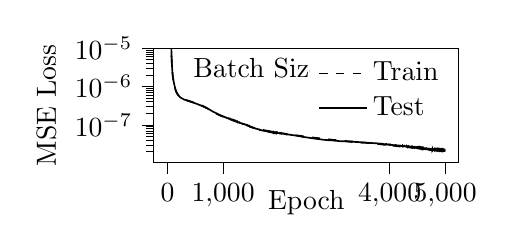
\begin{tikzpicture}

\begin{axis}[
legend cell align={left},
legend style={draw=none},
log basis y={10},
tick align=outside,
tick pos=left,
title={Batch Size 32},
title style={at={(0.4,0.85)},anchor=north},
x grid style={white!69.0196078431373!black},
xlabel={Epoch},
x label style={yshift=13pt},
xmin=-249.95, xmax=5248.95,
xtick style={color=black},
xtick = {0,1000,4000,5000},
y grid style={white!69.0196078431373!black},
ylabel={MSE Loss},
ymin=1.05374705124308e-08, ymax=1e-5,
ymode=log,
ytick style={color=black},
width=.45\textwidth,
height=.25\textwidth
]
\addplot [semithick, black, dashed]
table {%
0 0.0185213608369231
1 0.0100256001874805
2 0.00511598332412541
3 0.00266714832093567
4 0.00179120110906661
5 0.00144799546990544
6 0.00114979036618024
7 0.000814766860101372
8 0.000510174112394452
9 0.000329686338198371
10 0.000244710172759369
11 0.000205625825270545
12 0.00018631382289459
13 0.00017530717747286
14 0.000167745494400151
15 0.000161573188117472
16 0.00015586399770109
17 0.000150204380508512
18 0.000144401938305236
19 0.000138238270650618
20 0.000130775678553618
21 0.000122665890172357
22 0.000114659473838401
23 0.000106363622428034
24 9.76855874760076e-05
25 8.86985533143161e-05
26 7.95836760516977e-05
27 7.0616739205434e-05
28 6.21391900349408e-05
29 5.44985102314968e-05
30 4.79656076204265e-05
31 4.26814938036841e-05
32 3.8612608499534e-05
33 3.55862038995838e-05
34 3.33759931600071e-05
35 3.17640865978319e-05
36 3.05771953862859e-05
37 2.96883334303857e-05
38 2.90059693143121e-05
39 2.84673240530537e-05
40 2.80267686393927e-05
41 2.76490723626921e-05
42 2.73102718856535e-05
43 2.69937950652093e-05
44 2.66956577979727e-05
45 2.64040889669559e-05
46 2.61062633799156e-05
47 2.57937593196402e-05
48 2.54627911053831e-05
49 2.51038547576172e-05
50 2.47119145278702e-05
51 2.42804027948296e-05
52 2.38050044499687e-05
53 2.32816320567508e-05
54 2.27040185272926e-05
55 2.20680549537065e-05
56 2.13706233989797e-05
57 2.06065907259472e-05
58 1.97811869220459e-05
59 1.88985617751314e-05
60 1.79618474503513e-05
61 1.69827113422798e-05
62 1.59747925827105e-05
63 1.49555455536756e-05
64 1.38275694916956e-05
65 1.26876792637631e-05
66 1.12698398916109e-05
67 9.53350929376029e-06
68 8.1114827280544e-06
69 7.06149710822501e-06
70 6.28023362514796e-06
71 5.682561220965e-06
72 5.20727496405016e-06
73 4.81536020743079e-06
74 4.48226160369813e-06
75 4.1903823175744e-06
76 3.92923815888935e-06
77 3.69496772054845e-06
78 3.48329872758768e-06
79 3.2906890992308e-06
80 3.11474296267988e-06
81 2.9551299094237e-06
82 2.80990815917903e-06
83 2.67591957708646e-06
84 2.55399901561759e-06
85 2.44380857793658e-06
86 2.34454597421063e-06
87 2.25512032693587e-06
88 2.17415749739303e-06
89 2.10023164117956e-06
90 2.03179113850638e-06
91 1.96943895070945e-06
92 1.91336066791337e-06
93 1.86234339207658e-06
94 1.8137314445994e-06
95 1.76814178485074e-06
96 1.72594649347957e-06
97 1.68744496795625e-06
98 1.65267439206218e-06
99 1.61943572766177e-06
100 1.58699234452797e-06
101 1.55465797615761e-06
102 1.52490673599459e-06
103 1.49749505953878e-06
104 1.47220658982405e-06
105 1.44839148697429e-06
106 1.42518704569738e-06
107 1.40295422079362e-06
108 1.38139719206265e-06
109 1.3604042615043e-06
110 1.3386478888151e-06
111 1.31467914638961e-06
112 1.29182604973721e-06
113 1.27053595815596e-06
114 1.25014606237528e-06
115 1.23000724124722e-06
116 1.21053629754897e-06
117 1.19191057501666e-06
118 1.17316421210489e-06
119 1.15501116124506e-06
120 1.13750963123493e-06
121 1.11990525147121e-06
122 1.10245057840075e-06
123 1.0850101084543e-06
124 1.06801857259597e-06
125 1.0507991025861e-06
126 1.0334132978187e-06
127 1.01728472532159e-06
128 1.00184256598368e-06
129 9.86175931302569e-07
130 9.71090967141208e-07
131 9.56330864255506e-07
132 9.41725935490467e-07
133 9.27916013552021e-07
134 9.14784782253264e-07
135 9.01841580116525e-07
136 8.89269085291744e-07
137 8.76967326348677e-07
138 8.64968807945843e-07
139 8.53698949640602e-07
140 8.42906854245484e-07
141 8.32554830026311e-07
142 8.22901245783214e-07
143 8.13463982467511e-07
144 8.04595268732555e-07
145 7.962967694084e-07
146 7.88325216944941e-07
147 7.80183357505848e-07
148 7.72475732674138e-07
149 7.65302009767765e-07
150 7.58297480047077e-07
151 7.51497822307101e-07
152 7.45269478329646e-07
153 7.39257797022219e-07
154 7.33223259203442e-07
155 7.27614483025718e-07
156 7.22271873542013e-07
157 7.17282795108076e-07
158 7.12139038910209e-07
159 7.07288850321675e-07
160 7.02631720855607e-07
161 6.97950020594362e-07
162 6.9341542928214e-07
163 6.88575328808838e-07
164 6.84098517467646e-07
165 6.79956147109806e-07
166 6.7576959975213e-07
167 6.71695563141839e-07
168 6.67876880356744e-07
169 6.63949073555159e-07
170 6.60169360230611e-07
171 6.56619765891264e-07
172 6.53260171930015e-07
173 6.4957598908677e-07
174 6.4607227579927e-07
175 6.42691795746941e-07
176 6.39468844383373e-07
177 6.3644487761394e-07
178 6.32937741329442e-07
179 6.29768981639245e-07
180 6.26748726972437e-07
181 6.23714342737003e-07
182 6.20784524357987e-07
183 6.17936972389543e-07
184 6.15162336544017e-07
185 6.1250354792719e-07
186 6.09875560485307e-07
187 6.07228826424944e-07
188 6.04710761308525e-07
189 6.02254500108756e-07
190 5.99862777107774e-07
191 5.97323293845875e-07
192 5.94940298924485e-07
193 5.92553270735152e-07
194 5.90278918821241e-07
195 5.87862195970956e-07
196 5.85565089295415e-07
197 5.83287933409338e-07
198 5.81123970619046e-07
199 5.7901030334051e-07
200 5.76958834130892e-07
201 5.74851887904515e-07
202 5.72869793018072e-07
203 5.70961808080028e-07
204 5.69018330452309e-07
205 5.67025770010332e-07
206 5.6522778049839e-07
207 5.63374698117514e-07
208 5.6155098252475e-07
209 5.59765112939203e-07
210 5.58035291533088e-07
211 5.56295385763406e-07
212 5.54577313891968e-07
213 5.52870644128234e-07
214 5.51226922539172e-07
215 5.4956966505415e-07
216 5.47952494571291e-07
217 5.46373169186154e-07
218 5.44931209105925e-07
219 5.43313873890838e-07
220 5.4181577536383e-07
221 5.4034543313719e-07
222 5.38908848966457e-07
223 5.37434068860421e-07
224 5.36108092092036e-07
225 5.34586550315908e-07
226 5.3321597795275e-07
227 5.31795008100744e-07
228 5.30406377151849e-07
229 5.28978781972e-07
230 5.27560962609641e-07
231 5.26288467426639e-07
232 5.24752812452789e-07
233 5.23475015484109e-07
234 5.2215384982901e-07
235 5.21034239568508e-07
236 5.19823385729978e-07
237 5.18555743155957e-07
238 5.17368580744915e-07
239 5.16210805130868e-07
240 5.15153198762164e-07
241 5.13930031502241e-07
242 5.12899209525131e-07
243 5.11791230678682e-07
244 5.10723405113822e-07
245 5.09490656327216e-07
246 5.08409917983954e-07
247 5.0734909473249e-07
248 5.06350299133373e-07
249 5.05293355104186e-07
250 5.04277433037714e-07
251 5.03256441447775e-07
252 5.02261668316351e-07
253 5.01283572816646e-07
254 5.00328452176291e-07
255 4.99379939583378e-07
256 4.98446030633204e-07
257 4.97528622531718e-07
258 4.96615409474543e-07
259 4.95723476319654e-07
260 4.94844554964402e-07
261 4.94011196337851e-07
262 4.93106419639844e-07
263 4.92229671294808e-07
264 4.91303239073204e-07
265 4.90439448412872e-07
266 4.89604005906585e-07
267 4.88780170257996e-07
268 4.87970775907343e-07
269 4.87166112407067e-07
270 4.86385979115767e-07
271 4.85587184130054e-07
272 4.84800064214141e-07
273 4.84025108221431e-07
274 4.83258642702822e-07
275 4.82502226532233e-07
276 4.81754507745791e-07
277 4.81013788430573e-07
278 4.80280547435541e-07
279 4.79572060612554e-07
280 4.78862895079146e-07
281 4.78152566870449e-07
282 4.77446612990207e-07
283 4.76746079471013e-07
284 4.76050876159206e-07
285 4.75361166536459e-07
286 4.74711966489849e-07
287 4.74005847763692e-07
288 4.73316154398162e-07
289 4.72505169341275e-07
290 4.7175724284898e-07
291 4.70991727524961e-07
292 4.70303329052513e-07
293 4.69632239514795e-07
294 4.68987740418925e-07
295 4.68347638616251e-07
296 4.67706041945348e-07
297 4.67066472197075e-07
298 4.66436172700924e-07
299 4.65819643181931e-07
300 4.6519587988314e-07
301 4.6458026486107e-07
302 4.63975161324015e-07
303 4.63367187876429e-07
304 4.62763844893743e-07
305 4.62163034285368e-07
306 4.61567032516541e-07
307 4.60977072975766e-07
308 4.60386529880452e-07
309 4.59811661130516e-07
310 4.59230181604653e-07
311 4.58641048680875e-07
312 4.58067391150507e-07
313 4.57471872664428e-07
314 4.56890578675484e-07
315 4.56316948998392e-07
316 4.5574583839425e-07
317 4.55179300502095e-07
318 4.54645132208498e-07
319 4.54078644793299e-07
320 4.53513786624171e-07
321 4.52951653983291e-07
322 4.52389646170559e-07
323 4.5183226654899e-07
324 4.51286291763608e-07
325 4.50746562023596e-07
326 4.50201638614089e-07
327 4.49617204708375e-07
328 4.49071586444916e-07
329 4.48541439027395e-07
330 4.48002679945603e-07
331 4.4747507934062e-07
332 4.46942362600566e-07
333 4.46416720819798e-07
334 4.45883008865167e-07
335 4.45353649183744e-07
336 4.44804065296012e-07
337 4.44134348526859e-07
338 4.43515091546942e-07
339 4.42925153379292e-07
340 4.42338806010412e-07
341 4.41806229218855e-07
342 4.41315731677605e-07
343 4.40803275751023e-07
344 4.40289753782963e-07
345 4.39783605429511e-07
346 4.39238003536957e-07
347 4.3873517472548e-07
348 4.38237527305318e-07
349 4.37745029216785e-07
350 4.37252352298856e-07
351 4.36761686955833e-07
352 4.3626986473555e-07
353 4.35827755836726e-07
354 4.35319205962514e-07
355 4.34815810649525e-07
356 4.3431166341179e-07
357 4.33812067626604e-07
358 4.33318690511442e-07
359 4.32825826123917e-07
360 4.32334809602253e-07
361 4.31852442034142e-07
362 4.313736782251e-07
363 4.30905241842083e-07
364 4.30419585995878e-07
365 4.29928817993641e-07
366 4.29442891004328e-07
367 4.28962666433108e-07
368 4.28483186738049e-07
369 4.28003588581305e-07
370 4.27527776309944e-07
371 4.27073076934903e-07
372 4.2659085897867e-07
373 4.26108542342263e-07
374 4.25632207566196e-07
375 4.25156665414761e-07
376 4.24683829919559e-07
377 4.24200477709746e-07
378 4.23732120452769e-07
379 4.23265454855937e-07
380 4.22798863610296e-07
381 4.22334155814497e-07
382 4.21870258719537e-07
383 4.21407641169935e-07
384 4.20946088411256e-07
385 4.20485005747651e-07
386 4.20026333245005e-07
387 4.1956940469845e-07
388 4.19112675444921e-07
389 4.18659692286383e-07
390 4.18207336338128e-07
391 4.17756915339851e-07
392 4.17323406850301e-07
393 4.16873820995534e-07
394 4.16422651255743e-07
395 4.15972308474011e-07
396 4.15522133266677e-07
397 4.15084301380375e-07
398 4.14641929637583e-07
399 4.14197380450787e-07
400 4.13755675594984e-07
401 4.13315258242619e-07
402 4.1287598139661e-07
403 4.12409738942188e-07
404 4.11963612350519e-07
405 4.11529805319333e-07
406 4.11095109598136e-07
407 4.10662509921167e-07
408 4.10231388173088e-07
409 4.09801475484528e-07
410 4.09372446483758e-07
411 4.08946104698771e-07
412 4.0852090558019e-07
413 4.08187630569046e-07
414 4.07759484915005e-07
415 4.07332115287318e-07
416 4.06905044656014e-07
417 4.06474459509809e-07
418 4.06050205583597e-07
419 4.05616316811574e-07
420 4.05190133619726e-07
421 4.04756621492197e-07
422 4.04271327170136e-07
423 4.03848127348283e-07
424 4.03422405724996e-07
425 4.02979115165181e-07
426 4.02551475531254e-07
427 4.02127053689583e-07
428 4.01698157247665e-07
429 4.01263217440828e-07
430 4.00836544145022e-07
431 4.00410393922357e-07
432 3.99995897510053e-07
433 3.99568458533395e-07
434 3.99168272679162e-07
435 3.98736000533972e-07
436 3.98306118427172e-07
437 3.97879050751726e-07
438 3.97453581626905e-07
439 3.97028946395039e-07
440 3.96590492982796e-07
441 3.96160542777579e-07
442 3.95696088276054e-07
443 3.95270011722459e-07
444 3.94841801153234e-07
445 3.94415229038714e-07
446 3.93989487974977e-07
447 3.93564666410384e-07
448 3.93140786513868e-07
449 3.92719500382555e-07
450 3.92298088854659e-07
451 3.91881866335098e-07
452 3.91460772220853e-07
453 3.9104061602302e-07
454 3.90616273648448e-07
455 3.90210867408314e-07
456 3.89778205999392e-07
457 3.89298790651083e-07
458 3.88835131161613e-07
459 3.88384121947638e-07
460 3.87940273867571e-07
461 3.87511125836681e-07
462 3.87079769438969e-07
463 3.86645365551885e-07
464 3.86214937293516e-07
465 3.85783523825012e-07
466 3.8535608462098e-07
467 3.84926936703778e-07
468 3.84500410177679e-07
469 3.84072783049305e-07
470 3.83657095426315e-07
471 3.83230365400777e-07
472 3.82805546109921e-07
473 3.82380842779639e-07
474 3.81945783487936e-07
475 3.81532733172207e-07
476 3.81126588649749e-07
477 3.80694610271348e-07
478 3.80268383310067e-07
479 3.79843750238251e-07
480 3.79418695047207e-07
481 3.78994493303253e-07
482 3.78573906004931e-07
483 3.78133138042358e-07
484 3.77648691141985e-07
485 3.7722791125816e-07
486 3.76804605707548e-07
487 3.763683781699e-07
488 3.75936130012633e-07
489 3.75502033762132e-07
490 3.75070941117883e-07
491 3.7463960597961e-07
492 3.74207424556516e-07
493 3.73759208173396e-07
494 3.73334394566882e-07
495 3.7290415264124e-07
496 3.72472547269354e-07
497 3.72039375974964e-07
498 3.71606638623234e-07
499 3.71173888765952e-07
500 3.70742516679456e-07
501 3.7031062333881e-07
502 3.69883992448194e-07
503 3.6946489217371e-07
504 3.69041602198195e-07
505 3.68620761605598e-07
506 3.68207438896206e-07
507 3.67786844662987e-07
508 3.67350584951964e-07
509 3.66932141787402e-07
510 3.66519052818148e-07
511 3.66103566079801e-07
512 3.65683795621408e-07
513 3.65263786193282e-07
514 3.64843802799442e-07
515 3.6441569204726e-07
516 3.6400681676696e-07
517 3.6358559054861e-07
518 3.63164501322899e-07
519 3.62746938435521e-07
520 3.6232749539522e-07
521 3.61904533406232e-07
522 3.6149247114281e-07
523 3.61073087901786e-07
524 3.60654856308429e-07
525 3.60233938749843e-07
526 3.59805903144661e-07
527 3.59397946226636e-07
528 3.58979113229907e-07
529 3.58570702360339e-07
530 3.58152379476451e-07
531 3.57733576265673e-07
532 3.57283286234633e-07
533 3.56865689241204e-07
534 3.56481844619339e-07
535 3.560531470157e-07
536 3.5562543416745e-07
537 3.55202099513008e-07
538 3.54767151975466e-07
539 3.54350218003674e-07
540 3.53868238562427e-07
541 3.53445645487227e-07
542 3.53023489537918e-07
543 3.52600569215156e-07
544 3.52181922892214e-07
545 3.51785656221182e-07
546 3.51369444388183e-07
547 3.50940250882559e-07
548 3.50511328520042e-07
549 3.50086427886254e-07
550 3.4966140447068e-07
551 3.49248210113728e-07
552 3.48822502417079e-07
553 3.48412709456625e-07
554 3.47991883700161e-07
555 3.47554684822171e-07
556 3.47131746480045e-07
557 3.46698975590698e-07
558 3.46266814119645e-07
559 3.45854583656546e-07
560 3.45416659229159e-07
561 3.44981989314874e-07
562 3.44532436656664e-07
563 3.44083417530783e-07
564 3.43583697201666e-07
565 3.43132300884008e-07
566 3.42692654442089e-07
567 3.42256293151877e-07
568 3.41824444376471e-07
569 3.41390641779071e-07
570 3.40952211388412e-07
571 3.40516456901696e-07
572 3.40081166200434e-07
573 3.3964617955462e-07
574 3.39211207858625e-07
575 3.38775180978246e-07
576 3.38345385387129e-07
577 3.37907625691969e-07
578 3.37475298749723e-07
579 3.37009300665159e-07
580 3.36573081881397e-07
581 3.36206419092377e-07
582 3.35764889769052e-07
583 3.35318149552677e-07
584 3.34874418626896e-07
585 3.34421750153524e-07
586 3.33988169757049e-07
587 3.33541937493465e-07
588 3.33096089946139e-07
589 3.32616425396282e-07
590 3.32171234106227e-07
591 3.31726922240705e-07
592 3.31282373906561e-07
593 3.30856286836934e-07
594 3.30414409745572e-07
595 3.2996329883872e-07
596 3.29514442512391e-07
597 3.2906655366105e-07
598 3.28620184347983e-07
599 3.28172313288633e-07
600 3.27754828333582e-07
601 3.27299891694111e-07
602 3.26791949646577e-07
603 3.26343840242771e-07
604 3.25866860180213e-07
605 3.25405265243717e-07
606 3.24946678460947e-07
607 3.24471016085681e-07
608 3.24006525602272e-07
609 3.2355661079464e-07
610 3.23067498300134e-07
611 3.22547068776657e-07
612 3.22036515171931e-07
613 3.215269095449e-07
614 3.21033148054539e-07
615 3.20562532010626e-07
616 3.20066749623038e-07
617 3.1958168347046e-07
618 3.19108507255805e-07
619 3.18618406140558e-07
620 3.18146146923937e-07
621 3.17659693337191e-07
622 3.17181050263571e-07
623 3.16679004583875e-07
624 3.16186531563289e-07
625 3.15694480377715e-07
626 3.15204478454234e-07
627 3.1471761570856e-07
628 3.14214815205105e-07
629 3.1374244105109e-07
630 3.13252027069666e-07
631 3.12825649984916e-07
632 3.12330473661859e-07
633 3.11826514632685e-07
634 3.11322462607677e-07
635 3.10854835333885e-07
636 3.10345695481828e-07
637 3.09930875232567e-07
638 3.09420084818157e-07
639 3.08922876001816e-07
640 3.08413442326128e-07
641 3.0791088335036e-07
642 3.07412373729221e-07
643 3.06920373247976e-07
644 3.06423529252697e-07
645 3.05929234343694e-07
646 3.05435574148305e-07
647 3.04946460801148e-07
648 3.04456118783492e-07
649 3.03963243084127e-07
650 3.03473363203466e-07
651 3.02987180361924e-07
652 3.02522311471876e-07
653 3.02038389065729e-07
654 3.01502559693745e-07
655 3.00952283851075e-07
656 3.00445974289687e-07
657 2.99952013904203e-07
658 2.99459923269296e-07
659 2.9896857085987e-07
660 2.98477365674898e-07
661 2.97985838358272e-07
662 2.97495124812031e-07
663 2.9700242060926e-07
664 2.9651086396143e-07
665 2.9601517366018e-07
666 2.95518898781211e-07
667 2.95013197558092e-07
668 2.94539917092607e-07
669 2.94100331927893e-07
670 2.93593171647899e-07
671 2.93133579702953e-07
672 2.92588175113906e-07
673 2.92073646960489e-07
674 2.91576083611744e-07
675 2.91068527246807e-07
676 2.90541520257648e-07
677 2.90048884949101e-07
678 2.89539593723021e-07
679 2.89038977484779e-07
680 2.88519004925547e-07
681 2.87999056524768e-07
682 2.87411364070067e-07
683 2.86895903968798e-07
684 2.86383701848081e-07
685 2.85874086500826e-07
686 2.85370644462546e-07
687 2.84865456762873e-07
688 2.84372104204067e-07
689 2.83867105338231e-07
690 2.83315091905934e-07
691 2.82804742880671e-07
692 2.82301618312886e-07
693 2.81788576046438e-07
694 2.8127672823075e-07
695 2.80772214523495e-07
696 2.8024275570715e-07
697 2.79723454298164e-07
698 2.79204135210875e-07
699 2.78686133867723e-07
700 2.7816904946576e-07
701 2.77635648217256e-07
702 2.77106846112929e-07
703 2.76564707121452e-07
704 2.76043478322663e-07
705 2.7552292931432e-07
706 2.74989282956994e-07
707 2.74451538984977e-07
708 2.73919823143842e-07
709 2.73383016121898e-07
710 2.7285828133472e-07
711 2.72334689384479e-07
712 2.71813517997543e-07
713 2.71297532890458e-07
714 2.70724480685658e-07
715 2.702090679918e-07
716 2.69609163979112e-07
717 2.69066292332809e-07
718 2.68534173642365e-07
719 2.6803095380501e-07
720 2.6750520493124e-07
721 2.66954143228304e-07
722 2.66426574967227e-07
723 2.65932182173856e-07
724 2.65378602591682e-07
725 2.64837616555269e-07
726 2.64279638940934e-07
727 2.63742836125402e-07
728 2.63196838830027e-07
729 2.62663483056258e-07
730 2.62165100934908e-07
731 2.6164052741251e-07
732 2.6108835766081e-07
733 2.60547652430887e-07
734 2.5985914373905e-07
735 2.59363373231736e-07
736 2.58823922308693e-07
737 2.5826781603655e-07
738 2.57730944269952e-07
739 2.57195841413704e-07
740 2.5667771035387e-07
741 2.56121474137672e-07
742 2.55567423778302e-07
743 2.54995225645871e-07
744 2.54450984641608e-07
745 2.53922574643184e-07
746 2.53376336218025e-07
747 2.52830342560628e-07
748 2.52296219173331e-07
749 2.51764227641615e-07
750 2.51235566565811e-07
751 2.50710121235898e-07
752 2.50186598123037e-07
753 2.49664393493276e-07
754 2.4915178619267e-07
755 2.48576101739673e-07
756 2.48021704862822e-07
757 2.47490895560531e-07
758 2.4698219971242e-07
759 2.46460666971871e-07
760 2.45941125115223e-07
761 2.45425631248963e-07
762 2.44873848430416e-07
763 2.44391138096489e-07
764 2.43867456845237e-07
765 2.433545328131e-07
766 2.42844925708141e-07
767 2.42337454267272e-07
768 2.41832610015535e-07
769 2.41330177800592e-07
770 2.40827523271037e-07
771 2.40326087464382e-07
772 2.39832782597205e-07
773 2.39340287123468e-07
774 2.38822613766843e-07
775 2.38318634671941e-07
776 2.37761325024621e-07
777 2.37361407641856e-07
778 2.36908274132475e-07
779 2.36416801953965e-07
780 2.35894517459201e-07
781 2.35417795465764e-07
782 2.34940998097954e-07
783 2.34431632520682e-07
784 2.33937869950296e-07
785 2.33457018566696e-07
786 2.32956179672783e-07
787 2.32458378945921e-07
788 2.31979477348432e-07
789 2.31492987097681e-07
790 2.31008329649285e-07
791 2.30512317102693e-07
792 2.30025402402134e-07
793 2.29548284664816e-07
794 2.29058705428997e-07
795 2.28590926042216e-07
796 2.28118926315801e-07
797 2.27657759864996e-07
798 2.27187208565738e-07
799 2.26727645724623e-07
800 2.26269467816564e-07
801 2.25824073538661e-07
802 2.25381281381942e-07
803 2.24889024195818e-07
804 2.24432982975031e-07
805 2.23897555315489e-07
806 2.23425031151692e-07
807 2.2295173977227e-07
808 2.22504936573387e-07
809 2.22031358589447e-07
810 2.21586511543137e-07
811 2.21129962255873e-07
812 2.20660490867886e-07
813 2.20224475640407e-07
814 2.19789697155193e-07
815 2.19333101028951e-07
816 2.18906489408255e-07
817 2.18447235852182e-07
818 2.1802253485248e-07
819 2.17587594136148e-07
820 2.171213056954e-07
821 2.16699075224369e-07
822 2.16260562240222e-07
823 2.15830427805486e-07
824 2.15395490897663e-07
825 2.14986567698361e-07
826 2.14559953121807e-07
827 2.14100065988987e-07
828 2.13742608934808e-07
829 2.13357985956009e-07
830 2.12944119368785e-07
831 2.12532104740149e-07
832 2.12122578318485e-07
833 2.11714633735482e-07
834 2.11308834479951e-07
835 2.10849997927198e-07
836 2.10445568654904e-07
837 2.10049146232905e-07
838 2.09655660114549e-07
839 2.09260511041975e-07
840 2.08855573191613e-07
841 2.08466095273252e-07
842 2.08078252569521e-07
843 2.07700746102546e-07
844 2.07313690111732e-07
845 2.06920507594077e-07
846 2.06544750881221e-07
847 2.06162186827896e-07
848 2.05777530311479e-07
849 2.05416958294791e-07
850 2.05037628063565e-07
851 2.04666853164781e-07
852 2.04303049542887e-07
853 2.03929313386197e-07
854 2.03553203959927e-07
855 2.03187631257151e-07
856 2.02841443922352e-07
857 2.02474036314015e-07
858 2.02113415184613e-07
859 2.01754178931424e-07
860 2.01373242305181e-07
861 2.01010403770852e-07
862 2.00656504603103e-07
863 2.00288501162049e-07
864 1.9992708035943e-07
865 1.99573282657184e-07
866 1.99245734393116e-07
867 1.98867363678801e-07
868 1.98505497905899e-07
869 1.98158252942449e-07
870 1.97831863943065e-07
871 1.97476405389807e-07
872 1.97114097829854e-07
873 1.96777017492877e-07
874 1.96421795067181e-07
875 1.96073604513458e-07
876 1.95731925714426e-07
877 1.95410672688467e-07
878 1.9507339879965e-07
879 1.94744070427078e-07
880 1.94403248713115e-07
881 1.9405795410421e-07
882 1.93761960872507e-07
883 1.93391343259464e-07
884 1.93013741949244e-07
885 1.92732023151621e-07
886 1.92379488197503e-07
887 1.92062848697105e-07
888 1.91666795728906e-07
889 1.91327077430969e-07
890 1.90992436387205e-07
891 1.90675125026019e-07
892 1.90355343164583e-07
893 1.90039261468655e-07
894 1.89738615972601e-07
895 1.89489817643107e-07
896 1.89161859964315e-07
897 1.88857485596827e-07
898 1.88550196980941e-07
899 1.88281318457939e-07
900 1.87998503605513e-07
901 1.87705945393191e-07
902 1.87365529825456e-07
903 1.87090701018633e-07
904 1.8682072081333e-07
905 1.86533131596889e-07
906 1.8617735247517e-07
907 1.85849786277004e-07
908 1.85555433830586e-07
909 1.85290518203374e-07
910 1.85007594780018e-07
911 1.84740976209241e-07
912 1.84413795096816e-07
913 1.84188078776515e-07
914 1.83867984986819e-07
915 1.83598712567345e-07
916 1.83321817303295e-07
917 1.83044159058454e-07
918 1.82777629504471e-07
919 1.82503174556814e-07
920 1.82209366499819e-07
921 1.82021597879611e-07
922 1.81733254407845e-07
923 1.81411800667775e-07
924 1.8115524892437e-07
925 1.80859339337758e-07
926 1.80594035271042e-07
927 1.8029719359447e-07
928 1.80034858402678e-07
929 1.79789717037693e-07
930 1.79509198858341e-07
931 1.79225189015142e-07
932 1.78970508443399e-07
933 1.7871346764764e-07
934 1.78445978065156e-07
935 1.78181604468364e-07
936 1.77948226280478e-07
937 1.77688481159066e-07
938 1.77433303264252e-07
939 1.77141203664632e-07
940 1.76903954496765e-07
941 1.76639763878939e-07
942 1.76401640089807e-07
943 1.76149772926237e-07
944 1.75987998716209e-07
945 1.75748525435893e-07
946 1.75482385913028e-07
947 1.75235935529372e-07
948 1.74978851646301e-07
949 1.7472245940553e-07
950 1.74479472093481e-07
951 1.74206433655399e-07
952 1.73980947380414e-07
953 1.7370674370909e-07
954 1.73465508026993e-07
955 1.73237816028404e-07
956 1.72998334960539e-07
957 1.72744316898843e-07
958 1.72513198037905e-07
959 1.72277799947551e-07
960 1.72013212107913e-07
961 1.71797714727973e-07
962 1.71535733926476e-07
963 1.71309136078435e-07
964 1.71067951129089e-07
965 1.70814558458687e-07
966 1.7058751026866e-07
967 1.70329375663414e-07
968 1.70064358030686e-07
969 1.69841669986681e-07
970 1.69645710855093e-07
971 1.69402572822719e-07
972 1.69113098081652e-07
973 1.68882366153866e-07
974 1.68665797360745e-07
975 1.6844378566816e-07
976 1.68193679371598e-07
977 1.679658043372e-07
978 1.67721343188987e-07
979 1.67482980003797e-07
980 1.67276143656636e-07
981 1.67045190551107e-07
982 1.66820757868891e-07
983 1.66584006336734e-07
984 1.66362110149976e-07
985 1.6610529868899e-07
986 1.65910131357805e-07
987 1.65689847761996e-07
988 1.65440177568144e-07
989 1.65233987956981e-07
990 1.65027243696159e-07
991 1.64787183962289e-07
992 1.64550278469733e-07
993 1.64329672372787e-07
994 1.641152552736e-07
995 1.63866262198553e-07
996 1.63681186563736e-07
997 1.63456090092495e-07
998 1.63221955062909e-07
999 1.63006642424079e-07
1000 1.62814612366446e-07
1001 1.62547091662191e-07
1002 1.6236365999589e-07
1003 1.62137027615472e-07
1004 1.61914140363706e-07
1005 1.61691737190495e-07
1006 1.61510571047074e-07
1007 1.61248653995472e-07
1008 1.6104978601561e-07
1009 1.60817439819994e-07
1010 1.60609903360864e-07
1011 1.60398300806719e-07
1012 1.60187364826925e-07
1013 1.59997554277425e-07
1014 1.59782047916224e-07
1015 1.59536282126282e-07
1016 1.59365163369785e-07
1017 1.59153467194528e-07
1018 1.5890577961386e-07
1019 1.58727719423268e-07
1020 1.58539938752256e-07
1021 1.58312121328663e-07
1022 1.58082366368717e-07
1023 1.5789587882864e-07
1024 1.57671714788421e-07
1025 1.57459437872376e-07
1026 1.57293676068093e-07
1027 1.57060246635865e-07
1028 1.56861209717363e-07
1029 1.56664727143152e-07
1030 1.56458571524354e-07
1031 1.56244335585143e-07
1032 1.56054935729344e-07
1033 1.55841487725183e-07
1034 1.55671341644847e-07
1035 1.55414295591072e-07
1036 1.55219929496297e-07
1037 1.5502700952652e-07
1038 1.54778249651599e-07
1039 1.54609648319592e-07
1040 1.54416214684261e-07
1041 1.54183319125423e-07
1042 1.54000696682033e-07
1043 1.5378528854626e-07
1044 1.53589135948096e-07
1045 1.5335699526986e-07
1046 1.53167287663791e-07
1047 1.52971405356084e-07
1048 1.52732748915696e-07
1049 1.52534419157746e-07
1050 1.52338159836063e-07
1051 1.52186203195015e-07
1052 1.51968354543897e-07
1053 1.51778432524452e-07
1054 1.51582191392663e-07
1055 1.51362850829173e-07
1056 1.51173687186201e-07
1057 1.51031862088757e-07
1058 1.50862339921787e-07
1059 1.50641980155797e-07
1060 1.50485465383099e-07
1061 1.50308139154731e-07
1062 1.50094176035509e-07
1063 1.49907080469802e-07
1064 1.49740256318864e-07
1065 1.49536210102497e-07
1066 1.49349157055667e-07
1067 1.49136879514344e-07
1068 1.48908395800618e-07
1069 1.48712377381344e-07
1070 1.48493782148762e-07
1071 1.4830978798841e-07
1072 1.48146137405547e-07
1073 1.47950765637006e-07
1074 1.47774900824515e-07
1075 1.47583466315382e-07
1076 1.4737144300625e-07
1077 1.47156897128298e-07
1078 1.46975856750942e-07
1079 1.4680339833717e-07
1080 1.46632637409994e-07
1081 1.46427892815382e-07
1082 1.46234485896457e-07
1083 1.46021229681992e-07
1084 1.45853940580309e-07
1085 1.45659838665324e-07
1086 1.45499808667182e-07
1087 1.45302000902348e-07
1088 1.45118163345614e-07
1089 1.44915564533221e-07
1090 1.44756839233651e-07
1091 1.44625436035994e-07
1092 1.44455908525742e-07
1093 1.4425951536623e-07
1094 1.44062650861088e-07
1095 1.43971858193481e-07
1096 1.43767995723465e-07
1097 1.43548971578866e-07
1098 1.4336696054329e-07
1099 1.43227281000691e-07
1100 1.42972960190946e-07
1101 1.42832374251611e-07
1102 1.42647749527214e-07
1103 1.42420790638198e-07
1104 1.42293767822821e-07
1105 1.42080506805087e-07
1106 1.41926133068182e-07
1107 1.41727618796494e-07
1108 1.41548562424987e-07
1109 1.4137656182811e-07
1110 1.41162390974614e-07
1111 1.41009764803357e-07
1112 1.40850409763971e-07
1113 1.40619346012727e-07
1114 1.40469351919137e-07
1115 1.40236711899888e-07
1116 1.40055121704563e-07
1117 1.39835729783044e-07
1118 1.39705407320889e-07
1119 1.39515229420795e-07
1120 1.39346126985629e-07
1121 1.3915980667889e-07
1122 1.3894486130539e-07
1123 1.38818959328546e-07
1124 1.38635964475498e-07
1125 1.38440284246144e-07
1126 1.38380431536689e-07
1127 1.38207009939606e-07
1128 1.3803130016754e-07
1129 1.37817676886698e-07
1130 1.37681640268283e-07
1131 1.3742020453833e-07
1132 1.37303870701544e-07
1133 1.37097208693149e-07
1134 1.3695340081199e-07
1135 1.36768997549552e-07
1136 1.36616483757734e-07
1137 1.36413310798389e-07
1138 1.36295977767986e-07
1139 1.36083534300724e-07
1140 1.35963834509312e-07
1141 1.357222713807e-07
1142 1.35606256634446e-07
1143 1.35436983526915e-07
1144 1.35217161329138e-07
1145 1.35080818665756e-07
1146 1.34906291776815e-07
1147 1.34764612568006e-07
1148 1.34538124029859e-07
1149 1.34437458484626e-07
1150 1.34265883701801e-07
1151 1.3410143142778e-07
1152 1.33920875498461e-07
1153 1.33777525007872e-07
1154 1.33588935767648e-07
1155 1.33419826369163e-07
1156 1.33264174451142e-07
1157 1.3310219384266e-07
1158 1.32939824624145e-07
1159 1.32826000481145e-07
1160 1.32648920214251e-07
1161 1.32496974060814e-07
1162 1.32340923499896e-07
1163 1.32131768481258e-07
1164 1.31964101143467e-07
1165 1.31850519750287e-07
1166 1.31695612139993e-07
1167 1.31505942960075e-07
1168 1.31346545458655e-07
1169 1.31156192026083e-07
1170 1.31067693899922e-07
1171 1.30887381260436e-07
1172 1.30729647679573e-07
1173 1.30576428858831e-07
1174 1.30391574771238e-07
1175 1.30241802793307e-07
1176 1.30092601807519e-07
1177 1.29940641812709e-07
1178 1.2978442197209e-07
1179 1.29702830406586e-07
1180 1.29564918552205e-07
1181 1.29329984446258e-07
1182 1.29192453158566e-07
1183 1.29019271810193e-07
1184 1.2888260789623e-07
1185 1.28742152895711e-07
1186 1.2855812948942e-07
1187 1.28389245219296e-07
1188 1.28260248743572e-07
1189 1.28133878774861e-07
1190 1.27946985173821e-07
1191 1.27757678200169e-07
1192 1.27662547413365e-07
1193 1.27471893478059e-07
1194 1.273243918547e-07
1195 1.27171785749169e-07
1196 1.27086931712483e-07
1197 1.26907419939926e-07
1198 1.26737666363397e-07
1199 1.26660317988581e-07
1200 1.26535082586088e-07
1201 1.26340583960882e-07
1202 1.2621424323811e-07
1203 1.2601926437128e-07
1204 1.25920169324445e-07
1205 1.25740624866921e-07
1206 1.2557388711798e-07
1207 1.25481804900573e-07
1208 1.25368563232087e-07
1209 1.25208813869904e-07
1210 1.25018988057946e-07
1211 1.24933488478973e-07
1212 1.24746758558558e-07
1213 1.24599515942236e-07
1214 1.24469573506758e-07
1215 1.24318066127671e-07
1216 1.24179299945126e-07
1217 1.24018012570559e-07
1218 1.23949695364445e-07
1219 1.23787564859867e-07
1220 1.23621690903519e-07
1221 1.23461992103557e-07
1222 1.23359578964255e-07
1223 1.23199914270344e-07
1224 1.23059030244121e-07
1225 1.22928636955066e-07
1226 1.22774252503177e-07
1227 1.22605700397571e-07
1228 1.2247761691242e-07
1229 1.22310282620219e-07
1230 1.22203671708121e-07
1231 1.22031712521675e-07
1232 1.21910517151491e-07
1233 1.21736889269641e-07
1234 1.21613467399584e-07
1235 1.214787870083e-07
1236 1.21305380901049e-07
1237 1.21206207609248e-07
1238 1.21023092845007e-07
1239 1.20945347987345e-07
1240 1.20883079858913e-07
1241 1.20674643767416e-07
1242 1.20576853333887e-07
1243 1.20447198781903e-07
1244 1.20319473182917e-07
1245 1.20158708739382e-07
1246 1.20045059986751e-07
1247 1.19856119056294e-07
1248 1.19752005417695e-07
1249 1.19630266766535e-07
1250 1.19465553751752e-07
1251 1.19370260136975e-07
1252 1.19239946116068e-07
1253 1.19060969154816e-07
1254 1.18954238587321e-07
1255 1.18861689969663e-07
1256 1.18681055795378e-07
1257 1.1854536361966e-07
1258 1.18406778511826e-07
1259 1.18261358295513e-07
1260 1.1812020741786e-07
1261 1.17996310450508e-07
1262 1.17843934617667e-07
1263 1.17783204274247e-07
1264 1.17580303879095e-07
1265 1.17537257636968e-07
1266 1.1735062625462e-07
1267 1.17211613513746e-07
1268 1.17074364794689e-07
1269 1.16957124220107e-07
1270 1.16827153647137e-07
1271 1.1669826719185e-07
1272 1.16565958165893e-07
1273 1.16455746024258e-07
1274 1.16320386638336e-07
1275 1.16225041551843e-07
1276 1.16092117281141e-07
1277 1.15950706572221e-07
1278 1.15833334689341e-07
1279 1.15700019279075e-07
1280 1.15587255180571e-07
1281 1.15437792004514e-07
1282 1.15330216146958e-07
1283 1.15189609118715e-07
1284 1.15066688010756e-07
1285 1.14926542011062e-07
1286 1.14846013190117e-07
1287 1.14713855282389e-07
1288 1.14599199065424e-07
1289 1.14470935528743e-07
1290 1.14359950686094e-07
1291 1.14234656109602e-07
1292 1.14117928518453e-07
1293 1.1398997003198e-07
1294 1.13820058118108e-07
1295 1.13818541620958e-07
1296 1.13339524574485e-07
1297 1.12663470900998e-07
1298 1.12361569904351e-07
1299 1.12089587332775e-07
1300 1.11964709418544e-07
1301 1.11820746525382e-07
1302 1.11636760721012e-07
1303 1.11483826003678e-07
1304 1.11383499302065e-07
1305 1.11267894283174e-07
1306 1.11115151270269e-07
1307 1.11017267045099e-07
1308 1.10896492941492e-07
1309 1.10744365827031e-07
1310 1.10644878901667e-07
1311 1.10550607274718e-07
1312 1.10358803596e-07
1313 1.10191754401967e-07
1314 1.10072820973528e-07
1315 1.09909369911065e-07
1316 1.09817545961732e-07
1317 1.09704210359496e-07
1318 1.0948728268545e-07
1319 1.09406620794061e-07
1320 1.09284726192982e-07
1321 1.09091099972147e-07
1322 1.09042478015908e-07
1323 1.08925033288187e-07
1324 1.08841563360329e-07
1325 1.08699135381585e-07
1326 1.08578928035286e-07
1327 1.08461759822376e-07
1328 1.08338431630273e-07
1329 1.08334709835844e-07
1330 1.08194711401666e-07
1331 1.08026963999919e-07
1332 1.07970406304503e-07
1333 1.07841701264988e-07
1334 1.07688680998308e-07
1335 1.07582052095267e-07
1336 1.07469422914619e-07
1337 1.07296660473821e-07
1338 1.07229844473977e-07
1339 1.07034789039062e-07
1340 1.06912480532628e-07
1341 1.06783147487022e-07
1342 1.066593461303e-07
1343 1.06509381225806e-07
1344 1.06420976919708e-07
1345 1.06206791770092e-07
1346 1.0609659514671e-07
1347 1.05980542883799e-07
1348 1.05862056386741e-07
1349 1.05813596292137e-07
1350 1.05752091627664e-07
1351 1.05628402849334e-07
1352 1.05501596806334e-07
1353 1.05356113238031e-07
1354 1.05215304216699e-07
1355 1.05107244252167e-07
1356 1.04985850612138e-07
1357 1.04835606094866e-07
1358 1.04752508718775e-07
1359 1.046250343677e-07
1360 1.04495485800271e-07
1361 1.04372938295683e-07
1362 1.04263034870655e-07
1363 1.04146862298649e-07
1364 1.04034263813446e-07
1365 1.03983576508426e-07
1366 1.0383213731302e-07
1367 1.03719245117873e-07
1368 1.03590368638606e-07
1369 1.03480423746305e-07
1370 1.03351360991155e-07
1371 1.03220049027186e-07
1372 1.0311302881405e-07
1373 1.02996904814745e-07
1374 1.02872726614578e-07
1375 1.02754415451045e-07
1376 1.02634036494464e-07
1377 1.02518056451117e-07
1378 1.02415923862509e-07
1379 1.02323679698202e-07
1380 1.02211516264106e-07
1381 1.02091620306055e-07
1382 1.01971102623111e-07
1383 1.01870679060312e-07
1384 1.0179658139009e-07
1385 1.01681100517226e-07
1386 1.01586428115752e-07
1387 1.01476204747541e-07
1388 1.01367837061161e-07
1389 1.01290550361455e-07
1390 1.01194307617902e-07
1391 1.01084147658526e-07
1392 1.00980223763258e-07
1393 1.0086355020178e-07
1394 1.00736980030547e-07
1395 1.00650129539304e-07
1396 1.00546723885486e-07
1397 1.00419138519214e-07
1398 1.00316875574435e-07
1399 1.0026016775555e-07
1400 1.00106740532624e-07
1401 9.9985386981416e-08
1402 9.98807984728955e-08
1403 9.97536856601755e-08
1404 9.9668220926219e-08
1405 9.95527654055195e-08
1406 9.94410838615067e-08
1407 9.93242042284237e-08
1408 9.9216212021247e-08
1409 9.91328911368328e-08
1410 9.90092147503674e-08
1411 9.89142205725102e-08
1412 9.87894828625713e-08
1413 9.87242921013376e-08
1414 9.86143573555864e-08
1415 9.84818851037517e-08
1416 9.83712935749281e-08
1417 9.82762960575201e-08
1418 9.81511430211412e-08
1419 9.80457570420867e-08
1420 9.78985418953471e-08
1421 9.7802210106579e-08
1422 9.75800401334936e-08
1423 9.73497928384859e-08
1424 9.72207337639475e-08
1425 9.71265016147527e-08
1426 9.70150914696433e-08
1427 9.68607581484093e-08
1428 9.68013227975462e-08
1429 9.67239543996357e-08
1430 9.66186112520973e-08
1431 9.65188904160641e-08
1432 9.6407868468873e-08
1433 9.62835954538832e-08
1434 9.61846360496566e-08
1435 9.60902012820952e-08
1436 9.59982494208589e-08
1437 9.59091606773654e-08
1438 9.57719880290142e-08
1439 9.56798667033354e-08
1440 9.55663077206736e-08
1441 9.54916833819652e-08
1442 9.53860347010505e-08
1443 9.52897061807789e-08
1444 9.51862622713406e-08
1445 9.50990866783741e-08
1446 9.49752749761501e-08
1447 9.48816515773387e-08
1448 9.47771617632043e-08
1449 9.4695990242144e-08
1450 9.46143253059972e-08
1451 9.45202227882191e-08
1452 9.44320654383546e-08
1453 9.43229522505362e-08
1454 9.42529038212569e-08
1455 9.41463178492086e-08
1456 9.4068416373716e-08
1457 9.39887819413343e-08
1458 9.38982673375222e-08
1459 9.37753829362009e-08
1460 9.37255089894506e-08
1461 9.36219205698308e-08
1462 9.35364635097358e-08
1463 9.34252245201606e-08
1464 9.33777980662853e-08
1465 9.32803416020533e-08
1466 9.31650765920722e-08
1467 9.30805050671779e-08
1468 9.29610439328599e-08
1469 9.287470193442e-08
1470 9.27757243687211e-08
1471 9.26921939878866e-08
1472 9.2576508720299e-08
1473 9.24887030322452e-08
1474 9.23843173552541e-08
1475 9.22476585287768e-08
1476 9.21249195897644e-08
1477 9.19396049852139e-08
1478 9.16524064678015e-08
1479 9.12750976311827e-08
1480 9.06833057285894e-08
1481 9.02523407830813e-08
1482 8.98370776809543e-08
1483 8.959618487836e-08
1484 8.94454999809113e-08
1485 8.92552902627131e-08
1486 8.91261259141629e-08
1487 8.89889859507775e-08
1488 8.88643282337398e-08
1489 8.87856272271392e-08
1490 8.86530855837009e-08
1491 8.85686529272789e-08
1492 8.84279600654736e-08
1493 8.83821760027104e-08
1494 8.82774851334034e-08
1495 8.8184456544127e-08
1496 8.80874322035652e-08
1497 8.79965566582541e-08
1498 8.79217438125579e-08
1499 8.78179770751331e-08
1500 8.77400387508942e-08
1501 8.76169939800775e-08
1502 8.75252724483744e-08
1503 8.74732476034978e-08
1504 8.73397060559e-08
1505 8.73137317967121e-08
1506 8.7211646601304e-08
1507 8.71337833956431e-08
1508 8.705234297679e-08
1509 8.69138714136852e-08
1510 8.68927885022686e-08
1511 8.67575567440326e-08
1512 8.6724243189451e-08
1513 8.66463673645512e-08
1514 8.65392750739602e-08
1515 8.64611098165824e-08
1516 8.63612686288207e-08
1517 8.63293309549817e-08
1518 8.62158176317962e-08
1519 8.61772485336587e-08
1520 8.60930073400823e-08
1521 8.60225565162409e-08
1522 8.59654042244529e-08
1523 8.5892122129394e-08
1524 8.58183232708143e-08
1525 8.57418458650727e-08
1526 8.56366906134554e-08
1527 8.55414217824091e-08
1528 8.54949409614392e-08
1529 8.54261305249793e-08
1530 8.53500751389902e-08
1531 8.52584533674872e-08
1532 8.51586839871743e-08
1533 8.51175963134665e-08
1534 8.50235133498245e-08
1535 8.49865759988688e-08
1536 8.48735124066025e-08
1537 8.48198776992604e-08
1538 8.47225467737189e-08
1539 8.46476027902554e-08
1540 8.45698268108208e-08
1541 8.44968632662813e-08
1542 8.44229106746752e-08
1543 8.43584369363271e-08
1544 8.43106598580334e-08
1545 8.42087358563504e-08
1546 8.41415686068103e-08
1547 8.40622797397828e-08
1548 8.39969525969764e-08
1549 8.39222875583801e-08
1550 8.38631996913364e-08
1551 8.37817928101003e-08
1552 8.37054291906725e-08
1553 8.36330925011453e-08
1554 8.35762737807499e-08
1555 8.35003280030833e-08
1556 8.34323542164839e-08
1557 8.33614796817983e-08
1558 8.32791213554174e-08
1559 8.32229494420744e-08
1560 8.31509793499663e-08
1561 8.30974982761745e-08
1562 8.30279069106155e-08
1563 8.29462467066833e-08
1564 8.28767359735139e-08
1565 8.28320653170067e-08
1566 8.27367432520987e-08
1567 8.26758389678162e-08
1568 8.26105227105245e-08
1569 8.25380142117638e-08
1570 8.24846440394822e-08
1571 8.24061097119966e-08
1572 8.23438409867094e-08
1573 8.22637429394035e-08
1574 8.22266813429451e-08
1575 8.2150413405202e-08
1576 8.20791995579384e-08
1577 8.20127622063183e-08
1578 8.19548766486378e-08
1579 8.18789175127677e-08
1580 8.18459514420056e-08
1581 8.17594470277072e-08
1582 8.16947884061392e-08
1583 8.16395185267993e-08
1584 8.15806382092887e-08
1585 8.14948606802091e-08
1586 8.14358932217374e-08
1587 8.13648371007503e-08
1588 8.13039597034049e-08
1589 8.12378415417925e-08
1590 8.11729484695434e-08
1591 8.11095378452364e-08
1592 8.10414111072078e-08
1593 8.09895950482087e-08
1594 8.09623106761137e-08
1595 8.09027162063103e-08
1596 8.08412271027237e-08
1597 8.07740352968267e-08
1598 8.0709158424952e-08
1599 8.06479694119844e-08
1600 8.05820829583581e-08
1601 8.05096885159173e-08
1602 8.04581248843306e-08
1603 8.0393222276598e-08
1604 8.03214767728377e-08
1605 8.02655540468322e-08
1606 8.02068767313813e-08
1607 8.01321103836017e-08
1608 8.00844711363879e-08
1609 8.00213825726814e-08
1610 7.99599952472363e-08
1611 7.98976112292849e-08
1612 7.9834806555823e-08
1613 7.97754659345173e-08
1614 7.97135347028188e-08
1615 7.96568865126801e-08
1616 7.95917305822513e-08
1617 7.95318744053475e-08
1618 7.94548566460662e-08
1619 7.94151298464385e-08
1620 7.93352987784601e-08
1621 7.92899142680881e-08
1622 7.92236218103426e-08
1623 7.91863368334589e-08
1624 7.91302377791681e-08
1625 7.90388985478785e-08
1626 7.90103603804937e-08
1627 7.89311625197797e-08
1628 7.88984124397985e-08
1629 7.88078053091112e-08
1630 7.87757863065508e-08
1631 7.86895295732393e-08
1632 7.86431169075286e-08
1633 7.85704401096154e-08
1634 7.8529926369697e-08
1635 7.84526377231032e-08
1636 7.84164920872854e-08
1637 7.83758315776595e-08
1638 7.82719817067346e-08
1639 7.82363932074759e-08
1640 7.81609860780463e-08
1641 7.81229463626687e-08
1642 7.80462926712744e-08
1643 7.80029670579552e-08
1644 7.79492562514861e-08
1645 7.7874848827264e-08
1646 7.78748980962973e-08
1647 7.78464856381333e-08
1648 7.77667935381032e-08
1649 7.7674670393435e-08
1650 7.76239029249837e-08
1651 7.75937119357195e-08
1652 7.74994474710411e-08
1653 7.74321212873019e-08
1654 7.74145367472556e-08
1655 7.73238617028937e-08
1656 7.7310983030543e-08
1657 7.73176963946298e-08
1658 7.7305709197617e-08
1659 7.72266385524745e-08
1660 7.71846794407338e-08
1661 7.71044600185178e-08
1662 7.70360870632203e-08
1663 7.6990116184561e-08
1664 7.68984523915606e-08
1665 7.68559426518323e-08
1666 7.67996079531485e-08
1667 7.67342406646776e-08
1668 7.67052079027053e-08
1669 7.66515564833981e-08
1670 7.65959734536636e-08
1671 7.65839691467818e-08
1672 7.65009739609468e-08
1673 7.63829222734103e-08
1674 7.63229548823574e-08
1675 7.6267942404229e-08
1676 7.61775889372984e-08
1677 7.61232539332468e-08
1678 7.60569423050583e-08
1679 7.60101576702255e-08
1680 7.59661880636031e-08
1681 7.58766135788846e-08
1682 7.58261601134791e-08
1683 7.57681564920176e-08
1684 7.57341910855303e-08
1685 7.56938010937347e-08
1686 7.55829074847725e-08
1687 7.55643320360377e-08
1688 7.54766571446908e-08
1689 7.54520423669192e-08
1690 7.53472286874057e-08
1691 7.53446218482168e-08
1692 7.52449624599194e-08
1693 7.5231898293282e-08
1694 7.51617080965161e-08
1695 7.5136856168001e-08
1696 7.50744397777225e-08
1697 7.49899303684742e-08
1698 7.49304649900751e-08
1699 7.48902372862403e-08
1700 7.47820001407717e-08
1701 7.47753556851194e-08
1702 7.46935666313675e-08
1703 7.46611515154427e-08
1704 7.45570163900311e-08
1705 7.45577602998537e-08
1706 7.4471433549661e-08
1707 7.44485144821283e-08
1708 7.43752279674936e-08
1709 7.43456927949637e-08
1710 7.42526671899668e-08
1711 7.42398117239418e-08
1712 7.41700458632977e-08
1713 7.41169396292207e-08
1714 7.40263327116963e-08
1715 7.39864196930284e-08
1716 7.39412575399001e-08
1717 7.38989007089685e-08
1718 7.38174102252742e-08
1719 7.37935158383607e-08
1720 7.37559998640336e-08
1721 7.36524492737089e-08
1722 7.36184399414697e-08
1723 7.35392518009803e-08
1724 7.35269673270977e-08
1725 7.34544109519675e-08
1726 7.34032248317362e-08
1727 7.33428511523471e-08
1728 7.32681853321537e-08
1729 7.32143738702007e-08
1730 7.31719510724815e-08
1731 7.31501556998637e-08
1732 7.30892445091058e-08
1733 7.30219066298332e-08
1734 7.2979406468221e-08
1735 7.29247632023089e-08
1736 7.28633535658219e-08
1737 7.28210725498002e-08
1738 7.27666082553924e-08
1739 7.27055496980711e-08
1740 7.26660435219628e-08
1741 7.26065471923221e-08
1742 7.25587729561994e-08
1743 7.25217219610386e-08
1744 7.24717678650677e-08
1745 7.24192664733891e-08
1746 7.23900978130132e-08
1747 7.23444256749417e-08
1748 7.22931122396631e-08
1749 7.22318920054477e-08
1750 7.21730701371826e-08
1751 7.21197674948826e-08
1752 7.2068223502697e-08
1753 7.20293178915199e-08
1754 7.19787946508177e-08
1755 7.1902128382817e-08
1756 7.186078650534e-08
1757 7.17925612576664e-08
1758 7.17526729800966e-08
1759 7.16827797475617e-08
1760 7.16302113090705e-08
1761 7.15883441131382e-08
1762 7.15355734399736e-08
1763 7.14979385350034e-08
1764 7.14462546795858e-08
1765 7.14090052440497e-08
1766 7.13444932216589e-08
1767 7.1314508303999e-08
1768 7.12945840461998e-08
1769 7.12300264069654e-08
1770 7.11618054367591e-08
1771 7.1129282360971e-08
1772 7.10771613370298e-08
1773 7.10353654227447e-08
1774 7.09667575193862e-08
1775 7.09453047704756e-08
1776 7.08791320533919e-08
1777 7.08689498480908e-08
1778 7.07894625264771e-08
1779 7.07654877487585e-08
1780 7.07449104453417e-08
1781 7.06691416922922e-08
1782 7.06064589621747e-08
1783 7.06071714091649e-08
1784 7.05371180771408e-08
1785 7.04618763336384e-08
1786 7.04391132160254e-08
1787 7.0436156150322e-08
1788 7.03822607022175e-08
1789 7.03128608421366e-08
1790 7.02480001280037e-08
1791 7.01905164817163e-08
1792 7.01403554188573e-08
1793 7.00816554370931e-08
1794 7.00428220454796e-08
1795 6.99959764602909e-08
1796 6.99281957992071e-08
1797 6.98799748306556e-08
1798 6.98345102421172e-08
1799 6.9812578843198e-08
1800 6.97628552615015e-08
1801 6.97126851321173e-08
1802 6.96650610905181e-08
1803 6.9620020497041e-08
1804 6.95732604896193e-08
1805 6.95269130375209e-08
1806 6.9450036392027e-08
1807 6.94258809090798e-08
1808 6.93804265097242e-08
1809 6.93312598656348e-08
1810 6.92662360961549e-08
1811 6.92461122326904e-08
1812 6.91778652424091e-08
1813 6.91592371993011e-08
1814 6.91084712798329e-08
1815 6.90440532196135e-08
1816 6.90230407087711e-08
1817 6.89588040501121e-08
1818 6.89371421600526e-08
1819 6.8864143017322e-08
1820 6.8837407681599e-08
1821 6.87807199710733e-08
1822 6.87425491889826e-08
1823 6.87316239549318e-08
1824 6.87130460335084e-08
1825 6.86086011967291e-08
1826 6.85816692680419e-08
1827 6.85487725604617e-08
1828 6.84762398179828e-08
1829 6.84496302625348e-08
1830 6.84361277762946e-08
1831 6.83638677543286e-08
1832 6.83591063932454e-08
1833 6.8299204102118e-08
1834 6.82733310384265e-08
1835 6.81935777322451e-08
1836 6.81807968021531e-08
1837 6.81156993778131e-08
1838 6.80841945381872e-08
1839 6.80452653654129e-08
1840 6.80089791416094e-08
1841 6.79751051819721e-08
1842 6.7968244835015e-08
1843 6.78748466498291e-08
1844 6.78418427497718e-08
1845 6.78073349718034e-08
1846 6.77318409998406e-08
1847 6.77308798628928e-08
1848 6.76905800105487e-08
1849 6.76790822211615e-08
1850 6.76080521344602e-08
1851 6.75728001056086e-08
1852 6.75344841027936e-08
1853 6.74922161749691e-08
1854 6.74847693602487e-08
1855 6.74052995464081e-08
1856 6.73843340308622e-08
1857 6.73418571182083e-08
1858 6.73255632506198e-08
1859 6.7246962132117e-08
1860 6.72148490679092e-08
1861 6.71952462028003e-08
1862 6.71176834146081e-08
1863 6.71036098367495e-08
1864 6.70586717745891e-08
1865 6.70325235319069e-08
1866 6.69660769716529e-08
1867 6.69481376718295e-08
1868 6.69079221182756e-08
1869 6.68658473159667e-08
1870 6.6817939952557e-08
1871 6.67913105019124e-08
1872 6.67606790472064e-08
1873 6.670499389827e-08
1874 6.66827096864608e-08
1875 6.66532561552913e-08
1876 6.65725077482193e-08
1877 6.65576889815611e-08
1878 6.65029085098468e-08
1879 6.64830166670072e-08
1880 6.6452839078579e-08
1881 6.64153293854497e-08
1882 6.63944830705532e-08
1883 6.63362933721601e-08
1884 6.63005359768931e-08
1885 6.62983337349487e-08
1886 6.62430377360579e-08
1887 6.61870239753171e-08
1888 6.61763318134945e-08
1889 6.61309613718686e-08
1890 6.60921866142417e-08
1891 6.60340205058674e-08
1892 6.60028475039098e-08
1893 6.59876501316603e-08
1894 6.5944907305493e-08
1895 6.58683348007116e-08
1896 6.58535005158001e-08
1897 6.58302000999811e-08
1898 6.57803167030124e-08
1899 6.57766341163324e-08
1900 6.57306995037743e-08
1901 6.56779970285015e-08
1902 6.56210140590474e-08
1903 6.56104001848234e-08
1904 6.55520660046705e-08
1905 6.55097281168082e-08
1906 6.54655234058055e-08
1907 6.54436386042789e-08
1908 6.5365522857519e-08
1909 6.53579310778696e-08
1910 6.53442751712419e-08
1911 6.5264507441043e-08
1912 6.5268909935412e-08
1913 6.51961480429009e-08
1914 6.51695983862055e-08
1915 6.50831466373347e-08
1916 6.50933851318314e-08
1917 6.50553775898288e-08
1918 6.50183242356661e-08
1919 6.49697049084352e-08
1920 6.48905779314646e-08
1921 6.48916117000908e-08
1922 6.48621363268376e-08
1923 6.48038537605089e-08
1924 6.47869810279644e-08
1925 6.47372211943775e-08
1926 6.47247042309118e-08
1927 6.46281489622424e-08
1928 6.46134867281489e-08
1929 6.46225764455721e-08
1930 6.45606906743978e-08
1931 6.45003795938237e-08
1932 6.44912326350777e-08
1933 6.44101307756273e-08
1934 6.43985000010616e-08
1935 6.44029893379638e-08
1936 6.43383797722663e-08
1937 6.42712544873802e-08
1938 6.42418095111452e-08
1939 6.42460130677591e-08
1940 6.41611594431879e-08
1941 6.41290721290488e-08
1942 6.41379059089786e-08
1943 6.40654033361443e-08
1944 6.40728545704405e-08
1945 6.39778109956524e-08
1946 6.39457395692489e-08
1947 6.39477572690339e-08
1948 6.39519293486046e-08
1949 6.39255639782732e-08
1950 6.38890929280933e-08
1951 6.38307860896248e-08
1952 6.37995794789958e-08
1953 6.37578965694274e-08
1954 6.37294341032657e-08
1955 6.36969363227991e-08
1956 6.36185869211658e-08
1957 6.36073982178686e-08
1958 6.36167952308142e-08
1959 6.35515753657501e-08
1960 6.35560674453472e-08
1961 6.34721468344424e-08
1962 6.34954503340168e-08
1963 6.34581862470895e-08
1964 6.3440140834814e-08
1965 6.33436748245231e-08
1966 6.33241977823218e-08
1967 6.3330045563248e-08
1968 6.32534731295209e-08
1969 6.32515762788444e-08
1970 6.31989108228481e-08
1971 6.31844320082564e-08
1972 6.30921162780851e-08
1973 6.30801136480841e-08
1974 6.30812256190438e-08
1975 6.29971758741021e-08
1976 6.2974930784776e-08
1977 6.29929236311e-08
1978 6.28992476805479e-08
1979 6.28779257283441e-08
1980 6.29304949057996e-08
1981 6.28546442129618e-08
1982 6.27929165233354e-08
1983 6.27738021989899e-08
1984 6.278494024059e-08
1985 6.27150396041998e-08
1986 6.26567076835727e-08
1987 6.26154294280923e-08
1988 6.26368192939708e-08
1989 6.26394451330725e-08
1990 6.25982872151099e-08
1991 6.25437579628851e-08
1992 6.25170877270875e-08
1993 6.24817048731074e-08
1994 6.24461865896819e-08
1995 6.24120992824828e-08
1996 6.23773715915377e-08
1997 6.23425795254207e-08
1998 6.23105942736402e-08
1999 6.2277998139848e-08
2000 6.22461903390104e-08
2001 6.22127373617332e-08
2002 6.21821952364598e-08
2003 6.2149363145636e-08
2004 6.21173484773863e-08
2005 6.20852950845574e-08
2006 6.20531317707673e-08
2007 6.20216508195881e-08
2008 6.19906964658412e-08
2009 6.1958614253399e-08
2010 6.19268154906649e-08
2011 6.18964157013124e-08
2012 6.18609249443125e-08
2013 6.18275104500299e-08
2014 6.18173643402997e-08
2015 6.17683831478644e-08
2016 6.17357134586882e-08
2017 6.17279402916893e-08
2018 6.16703573541599e-08
2019 6.16638588013529e-08
2020 6.16074237740349e-08
2021 6.16050630100062e-08
2022 6.1546931718226e-08
2023 6.1543627765559e-08
2024 6.14859119707489e-08
2025 6.14836635293159e-08
2026 6.14235252953677e-08
2027 6.14251977424374e-08
2028 6.13633359023424e-08
2029 6.13598864021014e-08
2030 6.13047321564864e-08
2031 6.1298523164055e-08
2032 6.124742975544e-08
2033 6.12394919130565e-08
2034 6.11869464819392e-08
2035 6.1178607197121e-08
2036 6.11275622617313e-08
2037 6.11171328301907e-08
2038 6.10669761869076e-08
2039 6.10576244923777e-08
2040 6.1005148452864e-08
2041 6.09954447554628e-08
2042 6.09439424010816e-08
2043 6.09357319234505e-08
2044 6.08808908566516e-08
2045 6.08685983962687e-08
2046 6.08216330419964e-08
2047 6.08090171709819e-08
2048 6.07619251553615e-08
2049 6.075195592814e-08
2050 6.07010631910043e-08
2051 6.06881004188153e-08
2052 6.06408254526514e-08
2053 6.06266131626398e-08
2054 6.05796112580492e-08
2055 6.0590814669581e-08
2056 6.05654850858173e-08
2057 6.05426475175364e-08
2058 6.04808317206107e-08
2059 6.04651365989639e-08
2060 6.04225408125103e-08
2061 6.03897549922294e-08
2062 6.03572617023929e-08
2063 6.03172002087149e-08
2064 6.03263562766188e-08
2065 6.02959871969233e-08
2066 6.02613738607261e-08
2067 6.02281989756648e-08
2068 6.02043586326317e-08
2069 6.01709518264215e-08
2070 6.01381010056912e-08
2071 6.01057412978889e-08
2072 6.00736400144797e-08
2073 6.00422240637499e-08
2074 6.00106283172863e-08
2075 6.00027021420146e-08
2076 5.99716185405441e-08
2077 5.99382256751824e-08
2078 5.9930828058441e-08
2079 5.99099485043553e-08
2080 5.98730123613223e-08
2081 5.98383643648503e-08
2082 5.98075041153834e-08
2083 5.97959699604189e-08
2084 5.97496516832052e-08
2085 5.97421506540741e-08
2086 5.96924957108058e-08
2087 5.96646969768244e-08
2088 5.96312347624917e-08
2089 5.95999002541703e-08
2090 5.9569816770022e-08
2091 5.95344718732349e-08
2092 5.95126554117087e-08
2093 5.94837991201302e-08
2094 5.94516339731399e-08
2095 5.9421772689916e-08
2096 5.93990174735382e-08
2097 5.93778387383281e-08
2098 5.93458914437406e-08
2099 5.93124394754341e-08
2100 5.92817038835847e-08
2101 5.92539787191981e-08
2102 5.92198925915e-08
2103 5.91904924931441e-08
2104 5.91592163772248e-08
2105 5.9132834024922e-08
2106 5.90999805325509e-08
2107 5.90700926039744e-08
2108 5.90375228881612e-08
2109 5.90114405838449e-08
2110 5.8975464270361e-08
2111 5.89421195797968e-08
2112 5.89139560673857e-08
2113 5.88773572900436e-08
2114 5.88281711912941e-08
2115 5.88023901428869e-08
2116 5.87553580970734e-08
2117 5.87240764815533e-08
2118 5.8700576559545e-08
2119 5.86723750046758e-08
2120 5.86520583567562e-08
2121 5.86210052944125e-08
2122 5.85963523036526e-08
2123 5.85663352978827e-08
2124 5.85366293961442e-08
2125 5.85030698658784e-08
2126 5.8482686199568e-08
2127 5.845026454665e-08
2128 5.84260956344451e-08
2129 5.83999301113636e-08
2130 5.83638958318033e-08
2131 5.83349919338616e-08
2132 5.83079842897405e-08
2133 5.83255651775971e-08
2134 5.82979676835294e-08
2135 5.82581641310753e-08
2136 5.82281556091857e-08
2137 5.81862352930784e-08
2138 5.81692256247379e-08
2139 5.81248189774897e-08
2140 5.81089617810449e-08
2141 5.80547872743864e-08
2142 5.80393352578312e-08
2143 5.79973278433954e-08
2144 5.79827605804439e-08
2145 5.79418344699434e-08
2146 5.79210172730882e-08
2147 5.78791718055527e-08
2148 5.78561989073023e-08
2149 5.78237141155569e-08
2150 5.77968961437136e-08
2151 5.77617138333153e-08
2152 5.77346312695681e-08
2153 5.77033215165557e-08
2154 5.7675280714875e-08
2155 5.76474446489783e-08
2156 5.7611468477603e-08
2157 5.75883159967816e-08
2158 5.75629800891875e-08
2159 5.75305862469122e-08
2160 5.74885371378286e-08
2161 5.74628412408629e-08
2162 5.74148827325871e-08
2163 5.73684654341378e-08
2164 5.73362525813081e-08
2165 5.73060245017132e-08
2166 5.72897094031077e-08
2167 5.72569111767507e-08
2168 5.72249473407283e-08
2169 5.71929760582179e-08
2170 5.71620881828494e-08
2171 5.71314519390853e-08
2172 5.70993541657572e-08
2173 5.70694985242426e-08
2174 5.70399189570026e-08
2175 5.70097678860293e-08
2176 5.69844155222654e-08
2177 5.69534986993858e-08
2178 5.69238088132806e-08
2179 5.69004774888526e-08
2180 5.68702275103305e-08
2181 5.68380102237143e-08
2182 5.68067609094669e-08
2183 5.67785446321523e-08
2184 5.67521175867114e-08
2185 5.67200614653984e-08
2186 5.66879774481777e-08
2187 5.66613684185313e-08
2188 5.66398348951225e-08
2189 5.66087342832589e-08
2190 5.65760084896283e-08
2191 5.65476991454261e-08
2192 5.65186091847636e-08
2193 5.64934620399526e-08
2194 5.64675011247573e-08
2195 5.644228554047e-08
2196 5.64070904687242e-08
2197 5.6381275669537e-08
2198 5.63543352853912e-08
2199 5.63281861474252e-08
2200 5.62995095378938e-08
2201 5.6274239909726e-08
2202 5.62470820000272e-08
2203 5.62188356383331e-08
2204 5.6193502857127e-08
2205 5.61675762469349e-08
2206 5.61421054783295e-08
2207 5.61182778113789e-08
2208 5.60900593455926e-08
2209 5.60619199916346e-08
2210 5.60255562476186e-08
2211 5.59999451610338e-08
2212 5.59675503666313e-08
2213 5.59393063923608e-08
2214 5.59170821787802e-08
2215 5.58857626771214e-08
2216 5.58612730259256e-08
2217 5.58395199732331e-08
2218 5.58073723340158e-08
2219 5.57874459445884e-08
2220 5.57769465956426e-08
2221 5.57228337498827e-08
2222 5.56932525626053e-08
2223 5.56712606680776e-08
2224 5.56417176937884e-08
2225 5.56043607105039e-08
2226 5.55671280011438e-08
2227 5.55463118274702e-08
2228 5.55174466398967e-08
2229 5.54880128618152e-08
2230 5.54602056297426e-08
2231 5.54390986593489e-08
2232 5.54112100275006e-08
2233 5.53895747685829e-08
2234 5.53604678401598e-08
2235 5.53377834933144e-08
2236 5.53138184642421e-08
2237 5.52895072871706e-08
2238 5.5309207240839e-08
2239 5.52338280641607e-08
2240 5.52076225517339e-08
2241 5.51849741015076e-08
2242 5.5158525213983e-08
2243 5.51328407993879e-08
2244 5.51089436129359e-08
2245 5.50848163527462e-08
2246 5.50599461632828e-08
2247 5.50344777536793e-08
2248 5.50097749396627e-08
2249 5.49839805188412e-08
2250 5.49585503932803e-08
2251 5.49341108637691e-08
2252 5.49094793598215e-08
2253 5.48849489092618e-08
2254 5.48610987181064e-08
2255 5.48355443754644e-08
2256 5.48114287681756e-08
2257 5.47870539122641e-08
2258 5.47622884568e-08
2259 5.4737745898592e-08
2260 5.47136313144847e-08
2261 5.46879182365956e-08
2262 5.46594948218626e-08
2263 5.46381439221477e-08
2264 5.46611908873729e-08
2265 5.45826493976165e-08
2266 5.4557064487426e-08
2267 5.45368490492137e-08
2268 5.45103498978961e-08
2269 5.44887604974065e-08
2270 5.44630529191181e-08
2271 5.44407142655245e-08
2272 5.44164786902002e-08
2273 5.43926400951023e-08
2274 5.43692594874301e-08
2275 5.43442478573297e-08
2276 5.43211097436824e-08
2277 5.42975720634331e-08
2278 5.42668261829249e-08
2279 5.42432729417897e-08
2280 5.42201152171629e-08
2281 5.4192620339677e-08
2282 5.41733479479944e-08
2283 5.41478344260327e-08
2284 5.41192693717107e-08
2285 5.40948535672214e-08
2286 5.40710082219675e-08
2287 5.40479412975969e-08
2288 5.40284910712785e-08
2289 5.40066533289973e-08
2290 5.3981616609633e-08
2291 5.3958577993285e-08
2292 5.39472287002241e-08
2293 5.39702509954054e-08
2294 5.38833141874306e-08
2295 5.38469747581871e-08
2296 5.38259265070451e-08
2297 5.38046774849477e-08
2298 5.37837739500446e-08
2299 5.3758324973785e-08
2300 5.37310326720331e-08
2301 5.37103558926333e-08
2302 5.36839241789266e-08
2303 5.3659915316473e-08
2304 5.363479341014e-08
2305 5.36096340795211e-08
2306 5.35862739781123e-08
2307 5.35634372624827e-08
2308 5.35402283574626e-08
2309 5.35125736291775e-08
2310 5.34900339985711e-08
2311 5.34524641651046e-08
2312 5.34272319825391e-08
2313 5.34011343162888e-08
2314 5.33784600307285e-08
2315 5.33529870736515e-08
2316 5.33292425259901e-08
2317 5.33024389142156e-08
2318 5.32797142227537e-08
2319 5.32673468498501e-08
2320 5.3241777756341e-08
2321 5.32169946438898e-08
2322 5.32001309281327e-08
2323 5.31747396834703e-08
2324 5.31492992124072e-08
2325 5.31191143480214e-08
2326 5.30887879435227e-08
2327 5.30652246837349e-08
2328 5.30427696858737e-08
2329 5.30209634277412e-08
2330 5.2994308511245e-08
2331 5.29940913054361e-08
2332 5.30017497339941e-08
2333 5.29160146882646e-08
2334 5.2900385760779e-08
2335 5.29354027065665e-08
2336 5.28621932787132e-08
2337 5.28393319925158e-08
2338 5.28329576710007e-08
2339 5.2803487676556e-08
2340 5.27797820382148e-08
2341 5.27581060154603e-08
2342 5.27893031474491e-08
2343 5.2751232033188e-08
2344 5.26682941455192e-08
2345 5.2651605720655e-08
2346 5.26790588111226e-08
2347 5.26532650155787e-08
2348 5.26227773960386e-08
2349 5.25388971439611e-08
2350 5.25217370395126e-08
2351 5.24930901448783e-08
2352 5.24712954685924e-08
2353 5.24370233776494e-08
2354 5.24492368256801e-08
2355 5.24341462337929e-08
2356 5.24879223604557e-08
2357 5.24429051012021e-08
2358 5.23589332601659e-08
2359 5.23884398475616e-08
2360 5.24156020134114e-08
2361 5.23645213448276e-08
2362 5.22784227285911e-08
2363 5.22559460875982e-08
2364 5.22322851708168e-08
2365 5.22135751950259e-08
2366 5.22226000825299e-08
2367 5.21576795904366e-08
2368 5.2108217523994e-08
2369 5.20880798475787e-08
2370 5.20893634359254e-08
2371 5.20753084529701e-08
2372 5.20496626492672e-08
2373 5.20896342308674e-08
2374 5.20460975437231e-08
2375 5.20061106783487e-08
2376 5.19895802710835e-08
2377 5.19595369965486e-08
2378 5.18726792151369e-08
2379 5.18506605189373e-08
2380 5.18312427360001e-08
2381 5.18078889015783e-08
2382 5.1786883425109e-08
2383 5.17648865354659e-08
2384 5.17431741045016e-08
2385 5.17201288587898e-08
2386 5.17072507406624e-08
2387 5.16847418552402e-08
2388 5.16658670264292e-08
2389 5.16796673011299e-08
2390 5.16747518091165e-08
2391 5.16523813587355e-08
2392 5.16070973333171e-08
2393 5.15772757054833e-08
2394 5.15547084916079e-08
2395 5.14739723271873e-08
2396 5.14575380634597e-08
2397 5.14430300952995e-08
2398 5.14238462798744e-08
2399 5.14012053045576e-08
2400 5.13812144546932e-08
2401 5.13595555631241e-08
2402 5.13368483936461e-08
2403 5.13152900296632e-08
2404 5.12904956408988e-08
2405 5.12859767738405e-08
2406 5.12864031279037e-08
2407 5.12741133746886e-08
2408 5.12484853985029e-08
2409 5.11881224483091e-08
2410 5.11605333528564e-08
2411 5.11412373640496e-08
2412 5.11242890155472e-08
2413 5.10580763446455e-08
2414 5.10422022585999e-08
2415 5.1021262613915e-08
2416 5.10017917250138e-08
2417 5.09783831716959e-08
2418 5.09495943816773e-08
2419 5.0926697234388e-08
2420 5.09021244852192e-08
2421 5.08941419141706e-08
2422 5.08636651872507e-08
2423 5.08361664799395e-08
2424 5.0826551529326e-08
2425 5.08552678155638e-08
2426 5.07902592303822e-08
2427 5.07894599337533e-08
2428 5.07542686705165e-08
2429 5.06899608154754e-08
2430 5.07001850706956e-08
2431 5.06617058917413e-08
2432 5.06358982903521e-08
2433 5.05561707200286e-08
2434 5.05353068405157e-08
2435 5.05127491692292e-08
2436 5.0488929289827e-08
2437 5.04646149579457e-08
2438 5.04382225017253e-08
2439 5.04155458287414e-08
2440 5.03915942005051e-08
2441 5.03688402488933e-08
2442 5.03601074441917e-08
2443 5.03938501168477e-08
2444 5.03578180328645e-08
2445 5.03318347071513e-08
2446 5.03011151806731e-08
2447 5.02561212059049e-08
2448 5.02269110782549e-08
2449 5.01940734736195e-08
2450 5.01237616177264e-08
2451 5.01292328323188e-08
2452 5.00894308501643e-08
2453 4.99955365640403e-08
2454 4.99798094324433e-08
2455 4.99626190872959e-08
2456 4.99442521828541e-08
2457 4.99258378994227e-08
2458 4.99061377610133e-08
2459 4.98842099716512e-08
2460 4.98649811220275e-08
2461 4.98419346399714e-08
2462 4.98222857814312e-08
2463 4.98002944055997e-08
2464 4.97799984842118e-08
2465 4.97568928210512e-08
2466 4.97341661755968e-08
2467 4.97147862361658e-08
2468 4.96899604627288e-08
2469 4.96690425109136e-08
2470 4.96193078589613e-08
2471 4.95958824018317e-08
2472 4.95998455534163e-08
2473 4.96598748114252e-08
2474 4.96232796152185e-08
2475 4.95919710843395e-08
2476 4.95675161928943e-08
2477 4.95410535279461e-08
2478 4.95178578461264e-08
2479 4.94908368224856e-08
2480 4.94677099709406e-08
2481 4.94488908699964e-08
2482 4.94397475065966e-08
2483 4.9392762328182e-08
2484 4.93809350601282e-08
2485 4.9356890109209e-08
2486 4.93344661833817e-08
2487 4.93133994083905e-08
2488 4.9296750383121e-08
2489 4.92729934862268e-08
2490 4.92536026825974e-08
2491 4.92309012329883e-08
2492 4.92131448339705e-08
2493 4.91880869972761e-08
2494 4.91617636839692e-08
2495 4.91408934379933e-08
2496 4.91217928981769e-08
2497 4.90975854106068e-08
2498 4.90792836203013e-08
2499 4.9053655367004e-08
2500 4.90377634392303e-08
2501 4.90137660946743e-08
2502 4.89972134545269e-08
2503 4.89727917667437e-08
2504 4.89556048322015e-08
2505 4.89381764623431e-08
2506 4.89127083014296e-08
2507 4.88878782647362e-08
2508 4.887129821185e-08
2509 4.88470637520777e-08
2510 4.88311834772048e-08
2511 4.88072383433291e-08
2512 4.87895519114545e-08
2513 4.87660514281174e-08
2514 4.87490308600513e-08
2515 4.87253658150166e-08
2516 4.87085530878062e-08
2517 4.86853617331917e-08
2518 4.86620033726126e-08
2519 4.864128955262e-08
2520 4.8624142458209e-08
2521 4.86132947230544e-08
2522 4.85991770204919e-08
2523 4.85690377800552e-08
2524 4.85519708419702e-08
2525 4.8532649991273e-08
2526 4.85047468714583e-08
2527 4.84788994796759e-08
2528 4.84612886637592e-08
2529 4.84380039083021e-08
2530 4.84229414610127e-08
2531 4.83976012404241e-08
2532 4.83802874740036e-08
2533 4.83574045588853e-08
2534 4.83403152955475e-08
2535 4.83166452198702e-08
2536 4.83026442523737e-08
2537 4.82752392443331e-08
2538 4.82583331091746e-08
2539 4.82338360612289e-08
2540 4.82174579161665e-08
2541 4.81932135159013e-08
2542 4.81776931664513e-08
2543 4.81455163452438e-08
2544 4.81365974351888e-08
2545 4.81145725501619e-08
2546 4.80900606660839e-08
2547 4.80728455087842e-08
2548 4.80513025067353e-08
2549 4.80342722610771e-08
2550 4.80124693069683e-08
2551 4.79954934391458e-08
2552 4.79824469792334e-08
2553 4.7949488468646e-08
2554 4.794014432008e-08
2555 4.79116774911859e-08
2556 4.79018537333786e-08
2557 4.78733109261498e-08
2558 4.78632446174743e-08
2559 4.78343959784411e-08
2560 4.78257118672332e-08
2561 4.78055568109426e-08
2562 4.77898454604997e-08
2563 4.7758338581616e-08
2564 4.77403356740069e-08
2565 4.77261551026231e-08
2566 4.77064287451867e-08
2567 4.77001610761363e-08
2568 4.76858774831612e-08
2569 4.76603335997083e-08
2570 4.76431574227831e-08
2571 4.76180651816094e-08
2572 4.76021762949586e-08
2573 4.75776562822716e-08
2574 4.75620541138255e-08
2575 4.75384704330395e-08
2576 4.75233046799417e-08
2577 4.74996820045703e-08
2578 4.74747835497169e-08
2579 4.74592439871913e-08
2580 4.7446440575527e-08
2581 4.74139427169007e-08
2582 4.73858270026994e-08
2583 4.73869730868159e-08
2584 4.73541909542519e-08
2585 4.73293489022808e-08
2586 4.73185471321358e-08
2587 4.72976877787801e-08
2588 4.72850313357753e-08
2589 4.72638957660365e-08
2590 4.72601782846027e-08
2591 4.72380057061628e-08
2592 4.72235527269049e-08
2593 4.7200782844925e-08
2594 4.71868160403233e-08
2595 4.71642748465229e-08
2596 4.71423125674164e-08
2597 4.71042593588322e-08
2598 4.71006750686342e-08
2599 4.70799386036447e-08
2600 4.70663620575351e-08
2601 4.70355079045248e-08
2602 4.70304024347001e-08
2603 4.70071159952568e-08
2604 4.69616275111662e-08
2605 4.69415164587872e-08
2606 4.69373472711254e-08
2607 4.69074515265788e-08
2608 4.69016400188593e-08
2609 4.68710124721383e-08
2610 4.68710357850455e-08
2611 4.687585286689e-08
2612 4.68618322315706e-08
2613 4.68215372038117e-08
2614 4.67998634547939e-08
2615 4.67717358176856e-08
2616 4.67596120117264e-08
2617 4.67337389409295e-08
2618 4.67397930918878e-08
2619 4.67028056476693e-08
2620 4.66888253711772e-08
2621 4.66705996942096e-08
2622 4.66488213248795e-08
2623 4.66254449378312e-08
2624 4.66182270244531e-08
2625 4.65869506882655e-08
2626 4.65746689002344e-08
2627 4.65510848215445e-08
2628 4.65375115439315e-08
2629 4.65138104601692e-08
2630 4.64987848189935e-08
2631 4.64786855971511e-08
2632 4.64636254591255e-08
2633 4.64404174564947e-08
2634 4.64328485421106e-08
2635 4.64085118068169e-08
2636 4.63954805027811e-08
2637 4.63717111855999e-08
2638 4.63522522338167e-08
2639 4.63255237406202e-08
2640 4.63125699710076e-08
2641 4.62891272761112e-08
2642 4.62767599600511e-08
2643 4.62532915577185e-08
2644 4.62578429605287e-08
2645 4.62335701456595e-08
2646 4.62203011508677e-08
2647 4.61955336348296e-08
2648 4.61817033610146e-08
2649 4.61574102246232e-08
2650 4.61443693922092e-08
2651 4.61202641659497e-08
2652 4.61076916664638e-08
2653 4.60832899946695e-08
2654 4.60708873646354e-08
2655 4.60483360740227e-08
2656 4.60347446207265e-08
2657 4.60038463430124e-08
2658 4.59956762739466e-08
2659 4.59717139733584e-08
2660 4.59589704675523e-08
2661 4.59328179900353e-08
2662 4.5919823904228e-08
2663 4.58982463911184e-08
2664 4.58839099835018e-08
2665 4.58621428123251e-08
2666 4.58491076926748e-08
2667 4.58196193093841e-08
2668 4.5801640560228e-08
2669 4.57808543146143e-08
2670 4.57682126082659e-08
2671 4.57470084143097e-08
2672 4.57337647858935e-08
2673 4.57124123371955e-08
2674 4.56992296449243e-08
2675 4.56735129503727e-08
2676 4.56556823067444e-08
2677 4.56338792105271e-08
2678 4.56228265761638e-08
2679 4.56019131291896e-08
2680 4.55890048129959e-08
2681 4.55677483444106e-08
2682 4.55554961718008e-08
2683 4.55335153475289e-08
2684 4.55219631376735e-08
2685 4.55166307276045e-08
2686 4.55020441734177e-08
2687 4.54821450404097e-08
2688 4.54644332776866e-08
2689 4.54418680817525e-08
2690 4.54313781688143e-08
2691 4.5411819840524e-08
2692 4.53971976597245e-08
2693 4.53782479254983e-08
2694 4.5362922101333e-08
2695 4.5341641829566e-08
2696 4.53276667187197e-08
2697 4.53050192916749e-08
2698 4.52947493840838e-08
2699 4.52743609997697e-08
2700 4.52590555966026e-08
2701 4.5239104778716e-08
2702 4.52241358672723e-08
2703 4.52062379636686e-08
2704 4.51905150242737e-08
2705 4.52159435226918e-08
2706 4.5196377172374e-08
2707 4.51752978989362e-08
2708 4.51588237595502e-08
2709 4.51266193408628e-08
2710 4.51022526135603e-08
2711 4.5084997609024e-08
2712 4.50681127901476e-08
2713 4.50546086128156e-08
2714 4.50407367580397e-08
2715 4.50213217888518e-08
2716 4.49973773370971e-08
2717 4.49780991047533e-08
2718 4.49689434987022e-08
2719 4.49535173743243e-08
2720 4.49305922956e-08
2721 4.49089128764513e-08
2722 4.48956475267437e-08
2723 4.48706800639798e-08
2724 4.48739265408449e-08
2725 4.48165095647823e-08
2726 4.47993773065036e-08
2727 4.47823677092174e-08
2728 4.47671926906423e-08
2729 4.47444438549383e-08
2730 4.47293455465569e-08
2731 4.47125652556224e-08
2732 4.47062771300466e-08
2733 4.46878061097777e-08
2734 4.46701727909726e-08
2735 4.46424202991125e-08
2736 4.46270202658638e-08
2737 4.45942176625636e-08
2738 4.45856198609818e-08
2739 4.45373968389617e-08
2740 4.45249869187592e-08
2741 4.45066017462636e-08
2742 4.44969815163176e-08
2743 4.44737041362941e-08
2744 4.44615917629676e-08
2745 4.44384191737868e-08
2746 4.4426124787833e-08
2747 4.44028485233616e-08
2748 4.43907933984633e-08
2749 4.43729020744854e-08
2750 4.43586442884225e-08
2751 4.4331720268076e-08
2752 4.43174091699916e-08
2753 4.42953355559439e-08
2754 4.42815412853292e-08
2755 4.42543480332347e-08
2756 4.42403402303171e-08
2757 4.42216706062482e-08
2758 4.42064307364376e-08
2759 4.41817823499946e-08
2760 4.4170972273605e-08
2761 4.41410298606115e-08
2762 4.41284960928101e-08
2763 4.41099405250611e-08
2764 4.40921843818387e-08
2765 4.40695949421865e-08
2766 4.40557260148466e-08
2767 4.40344740866294e-08
2768 4.40200800753132e-08
2769 4.39979046547023e-08
2770 4.39841996282553e-08
2771 4.39614013032497e-08
2772 4.39471834070559e-08
2773 4.39258115534358e-08
2774 4.39114889729808e-08
2775 4.38922767429517e-08
2776 4.38652625120994e-08
2777 4.3847781370232e-08
2778 4.38374935924912e-08
2779 4.38180753334905e-08
2780 4.38039917938227e-08
2781 4.3782932408476e-08
2782 4.37671083020064e-08
2783 4.37494838863017e-08
2784 4.37311115391026e-08
2785 4.37203485859072e-08
2786 4.37029379725118e-08
2787 4.36785390434125e-08
2788 4.36603118671997e-08
2789 4.36426450960425e-08
2790 4.36267958576764e-08
2791 4.36074457965674e-08
2792 4.35910614129398e-08
2793 4.35729325189982e-08
2794 4.35575719563985e-08
2795 4.35407245973352e-08
2796 4.3522179851152e-08
2797 4.35045051006e-08
2798 4.34886420919156e-08
2799 4.34696198823303e-08
2800 4.34574589647241e-08
2801 4.34398077118203e-08
2802 4.34243197844353e-08
2803 4.34025379405512e-08
2804 4.33904131895702e-08
2805 4.33680900258082e-08
2806 4.33422248349302e-08
2807 4.33290512589224e-08
2808 4.33123796597101e-08
2809 4.32959559333312e-08
2810 4.32819207460966e-08
2811 4.32535382373089e-08
2812 4.32386168043308e-08
2813 4.32179117026976e-08
2814 4.32032744797084e-08
2815 4.31824882412002e-08
2816 4.31707620123234e-08
2817 4.31521513064581e-08
2818 4.31365217181678e-08
2819 4.31176904811537e-08
2820 4.31047752300628e-08
2821 4.3087796015584e-08
2822 4.30729518612338e-08
2823 4.30549221590581e-08
2824 4.30430366336054e-08
2825 4.30236979127585e-08
2826 4.30086014588937e-08
2827 4.29914814503718e-08
2828 4.29761729563438e-08
2829 4.29589451371726e-08
2830 4.29443767160365e-08
2831 4.29259492946699e-08
2832 4.2911345097707e-08
2833 4.28906516489747e-08
2834 4.28779408068181e-08
2835 4.28613560430335e-08
2836 4.2845481260656e-08
2837 4.28282266824453e-08
2838 4.2814149018966e-08
2839 4.27967468183965e-08
2840 4.27841328161094e-08
2841 4.27665098072794e-08
2842 4.27548866852589e-08
2843 4.27409075101082e-08
2844 4.27238805116303e-08
2845 4.27056477647625e-08
2846 4.26933390897943e-08
2847 4.26735692400371e-08
2848 4.26647361493337e-08
2849 4.26475516945857e-08
2850 4.26316335193633e-08
2851 4.26175247483229e-08
2852 4.26032420932643e-08
2853 4.25844038431933e-08
2854 4.25742655991712e-08
2855 4.25582884062692e-08
2856 4.25406372670523e-08
2857 4.25243402233377e-08
2858 4.25115039917046e-08
2859 4.24905639775375e-08
2860 4.24798570506368e-08
2861 4.24610634084388e-08
2862 4.24490893564666e-08
2863 4.24308456246081e-08
2864 4.24207427158763e-08
2865 4.24017342623984e-08
2866 4.23918691510039e-08
2867 4.23744082311828e-08
2868 4.23609847501893e-08
2869 4.23456238252129e-08
2870 4.23323595981628e-08
2871 4.2318178493872e-08
2872 4.23014924137988e-08
2873 4.22864041169646e-08
2874 4.22735440892552e-08
2875 4.22578179453126e-08
2876 4.22444613548123e-08
2877 4.22290945607529e-08
2878 4.22173619440969e-08
2879 4.21980116840359e-08
2880 4.21890508377487e-08
2881 4.2171351601894e-08
2882 4.21584626622007e-08
2883 4.21424769427858e-08
2884 4.21281442299914e-08
2885 4.21130238024148e-08
2886 4.20994069116887e-08
2887 4.20851290883206e-08
2888 4.20726973828778e-08
2889 4.20562085707843e-08
2890 4.204445245648e-08
2891 4.20430907652758e-08
2892 4.20335134947436e-08
2893 4.20098776743316e-08
2894 4.1988902104606e-08
2895 4.19831162119522e-08
2896 4.19707570600281e-08
2897 4.19548197712061e-08
2898 4.19410543912591e-08
2899 4.19227782941789e-08
2900 4.19155923196968e-08
2901 4.18967207664878e-08
2902 4.18871959837475e-08
2903 4.18697274966462e-08
2904 4.18580986618622e-08
2905 4.18279861236215e-08
2906 4.18218179518703e-08
2907 4.18103405337433e-08
2908 4.17935734020602e-08
2909 4.17779905959037e-08
2910 4.17732937663118e-08
2911 4.17558014760289e-08
2912 4.17394089851086e-08
2913 4.17176305020916e-08
2914 4.17057988357783e-08
2915 4.1688475164392e-08
2916 4.16751988296937e-08
2917 4.16470806285929e-08
2918 4.16311340174502e-08
2919 4.16142032833022e-08
2920 4.15998318530342e-08
2921 4.15851204991213e-08
2922 4.15688157673344e-08
2923 4.15543170504407e-08
2924 4.15397563671149e-08
2925 4.15239846489612e-08
2926 4.15137445841651e-08
2927 4.14951228719929e-08
2928 4.14820092302648e-08
2929 4.14673525241938e-08
2930 4.14531900290172e-08
2931 4.14383706583976e-08
2932 4.1424275167401e-08
2933 4.14098686007947e-08
2934 4.13963362504433e-08
2935 4.13826761018754e-08
2936 4.13704054338382e-08
2937 4.13559172116607e-08
2938 4.13415708706566e-08
2939 4.13266338696872e-08
2940 4.13125160179106e-08
2941 4.1296852423045e-08
2942 4.12831569533978e-08
2943 4.12677493883962e-08
2944 4.12606522246506e-08
2945 4.12442331665375e-08
2946 4.12302000114551e-08
2947 4.12140783652148e-08
2948 4.12017463773395e-08
2949 4.1187607990878e-08
2950 4.11787100063066e-08
2951 4.11644223987651e-08
2952 4.11313876682584e-08
2953 4.11228321439694e-08
2954 4.11097234191971e-08
2955 4.10767606169316e-08
2956 4.10641093964159e-08
2957 4.10475510221886e-08
2958 4.10360093212603e-08
2959 4.10201875524763e-08
2960 4.10063494058477e-08
2961 4.09879233842503e-08
2962 4.09741548352827e-08
2963 4.0958383166867e-08
2964 4.09454055798619e-08
2965 4.09293945295985e-08
2966 4.09143654209743e-08
2967 4.09019723548454e-08
2968 4.08860789846699e-08
2969 4.08711291086661e-08
2970 4.08603659209916e-08
2971 4.08442417096921e-08
2972 4.08289844457954e-08
2973 4.08159299070121e-08
2974 4.07975592509047e-08
2975 4.07803956434805e-08
2976 4.0768644929301e-08
2977 4.07503394512787e-08
2978 4.07323937636761e-08
2979 4.07188326363439e-08
2980 4.07077332909012e-08
2981 4.06953093659013e-08
2982 4.06884420556253e-08
2983 4.06678218922707e-08
2984 4.06570048880894e-08
2985 4.06467258997623e-08
2986 4.06307259837035e-08
2987 4.06189892956377e-08
2988 4.06083526769407e-08
2989 4.05932729137248e-08
2990 4.05821767230918e-08
2991 4.05657117923397e-08
2992 4.05558655884875e-08
2993 4.05389514597232e-08
2994 4.05286307909591e-08
2995 4.0515213449055e-08
2996 4.05014611430943e-08
2997 4.04881957720704e-08
2998 4.04919090257749e-08
2999 4.04771566593354e-08
3000 4.046176100303e-08
3001 4.04479992255347e-08
3002 4.04334260082351e-08
3003 4.04201921853087e-08
3004 4.04052076419248e-08
3005 4.03921915008709e-08
3006 4.03798288033386e-08
3007 4.03705484970374e-08
3008 4.0354571630985e-08
3009 4.03400449684455e-08
3010 4.03298340856395e-08
3011 4.03173966958548e-08
3012 4.03040917831277e-08
3013 4.02889352812963e-08
3014 4.02761895372805e-08
3015 4.02620533321851e-08
3016 4.02506762711141e-08
3017 4.02397802758969e-08
3018 4.02229375566776e-08
3019 4.02091450055764e-08
3020 4.01957830646893e-08
3021 4.01833250052164e-08
3022 4.01702993571007e-08
3023 4.01569427239679e-08
3024 4.01469599893289e-08
3025 4.01341909253006e-08
3026 4.01261119193919e-08
3027 4.01072963427396e-08
3028 4.00939477671614e-08
3029 4.00808263805175e-08
3030 4.00759715830645e-08
3031 4.00584877908727e-08
3032 4.00473919341948e-08
3033 4.00354138179182e-08
3034 4.00218731613222e-08
3035 4.00098893109657e-08
3036 3.9995878296395e-08
3037 3.99821971228675e-08
3038 3.99702219411324e-08
3039 3.99575938274666e-08
3040 3.99452826727043e-08
3041 3.99354739215596e-08
3042 3.99227829177562e-08
3043 3.99116366338603e-08
3044 3.98986479552832e-08
3045 3.98852733027866e-08
3046 3.98732751278885e-08
3047 3.98626612962971e-08
3048 3.98523909908022e-08
3049 3.98386416264884e-08
3050 3.98254571578605e-08
3051 3.98136581196695e-08
3052 3.98038344755491e-08
3053 3.97879686815372e-08
3054 3.97789093042888e-08
3055 3.97659436046638e-08
3056 3.9754807048098e-08
3057 3.97414143264996e-08
3058 3.97304668595666e-08
3059 3.97172155146563e-08
3060 3.97086329826379e-08
3061 3.96913380882324e-08
3062 3.96835653759808e-08
3063 3.96691759050327e-08
3064 3.96597965988121e-08
3065 3.96444469572543e-08
3066 3.96353289033868e-08
3067 3.9620772291471e-08
3068 3.96110539071515e-08
3069 3.95950820077928e-08
3070 3.95870274445542e-08
3071 3.95812294300413e-08
3072 3.9563223893424e-08
3073 3.95425863928267e-08
3074 3.95348274935259e-08
3075 3.95146205036667e-08
3076 3.95126518881739e-08
3077 3.94890157124905e-08
3078 3.94861648231881e-08
3079 3.94651645194699e-08
3080 3.94566089454429e-08
3081 3.94390235740616e-08
3082 3.94295230137232e-08
3083 3.94082742545265e-08
3084 3.93867384360647e-08
3085 3.9363637476697e-08
3086 3.93610967890368e-08
3087 3.93382747674309e-08
3088 3.93367597126826e-08
3089 3.93139847929547e-08
3090 3.93131090703491e-08
3091 3.92901309282934e-08
3092 3.92891952714081e-08
3093 3.92652831564533e-08
3094 3.92657417123132e-08
3095 3.9242823433483e-08
3096 3.92400080784228e-08
3097 3.92171715688505e-08
3098 3.92189900679796e-08
3099 3.91928416547671e-08
3100 3.9198681250241e-08
3101 3.91769238774486e-08
3102 3.91778507520257e-08
3103 3.91524141889477e-08
3104 3.91534893893208e-08
3105 3.91283961036493e-08
3106 3.91290557715251e-08
3107 3.91046331316147e-08
3108 3.91055654986872e-08
3109 3.90808604606718e-08
3110 3.90734568824769e-08
3111 3.904657974374e-08
3112 3.90475629430398e-08
3113 3.90247265968924e-08
3114 3.90154835940848e-08
3115 3.8994325329611e-08
3116 3.89934052975605e-08
3117 3.89704202703456e-08
3118 3.89892652350454e-08
3119 3.89628834653877e-08
3120 3.89596161198824e-08
3121 3.89375558000893e-08
3122 3.89352122809328e-08
3123 3.89129509414943e-08
3124 3.89106101792436e-08
3125 3.88902558299264e-08
3126 3.8886522759185e-08
3127 3.88662221340041e-08
3128 3.88622090525814e-08
3129 3.88425939519266e-08
3130 3.88242137105976e-08
3131 3.8805395384145e-08
3132 3.8801755096074e-08
3133 3.87814247773122e-08
3134 3.87778140336081e-08
3135 3.87611530285881e-08
3136 3.8756328855527e-08
3137 3.87363043543587e-08
3138 3.87313330065808e-08
3139 3.87168013276096e-08
3140 3.87097271499215e-08
3141 3.86900851623295e-08
3142 3.86860399501643e-08
3143 3.86724925647286e-08
3144 3.86630044246772e-08
3145 3.864517064045e-08
3146 3.86427964329528e-08
3147 3.8624116470487e-08
3148 3.86179430478251e-08
3149 3.86017193818589e-08
3150 3.85928856019291e-08
3151 3.85803526157247e-08
3152 3.85752468261558e-08
3153 3.85547069043923e-08
3154 3.85516356118387e-08
3155 3.85340500486109e-08
3156 3.85289099114061e-08
3157 3.85102986797392e-08
3158 3.84967854500928e-08
3159 3.84789900991223e-08
3160 3.84740432437525e-08
3161 3.8457080528076e-08
3162 3.84515223856852e-08
3163 3.84473909775807e-08
3164 3.84321618867034e-08
3165 3.84203100338709e-08
3166 3.84074992538785e-08
3167 3.8398100677739e-08
3168 3.8386929219314e-08
3169 3.83752461416975e-08
3170 3.83697237538172e-08
3171 3.83564175692186e-08
3172 3.83462775772614e-08
3173 3.83339616476519e-08
3174 3.83245094468521e-08
3175 3.83117415125867e-08
3176 3.83018532090773e-08
3177 3.82873992847976e-08
3178 3.82689804823144e-08
3179 3.8259270944252e-08
3180 3.82491751054204e-08
3181 3.82389944491024e-08
3182 3.82321212342163e-08
3183 3.82117534272197e-08
3184 3.82035198853714e-08
3185 3.82079280356606e-08
3186 3.82116207902072e-08
3187 3.81986275854729e-08
3188 3.81865571625895e-08
3189 3.81726239879754e-08
3190 3.81609378976577e-08
3191 3.81505390265602e-08
3192 3.81360402599284e-08
3193 3.81252356262962e-08
3194 3.81101850663867e-08
3195 3.80950387608436e-08
3196 3.80883108803687e-08
3197 3.80906600341291e-08
3198 3.80786708973346e-08
3199 3.80687033612048e-08
3200 3.80546417986238e-08
3201 3.8080723236078e-08
3202 3.8067338302028e-08
3203 3.80631663787767e-08
3204 3.80479003467826e-08
3205 3.80382149671732e-08
3206 3.80283326819608e-08
3207 3.80275854041656e-08
3208 3.80176091709927e-08
3209 3.80071860988096e-08
3210 3.79927562192961e-08
3211 3.7975492240605e-08
3212 3.79609438851958e-08
3213 3.795092587211e-08
3214 3.79396348719752e-08
3215 3.79256221165747e-08
3216 3.79158809664659e-08
3217 3.79039208127097e-08
3218 3.78890104357765e-08
3219 3.78798831306426e-08
3220 3.78645086129836e-08
3221 3.78567310761468e-08
3222 3.78411606050122e-08
3223 3.78337010076279e-08
3224 3.78182806741734e-08
3225 3.781084270571e-08
3226 3.77951070760218e-08
3227 3.77873039809629e-08
3228 3.77728340765771e-08
3229 3.77665485160605e-08
3230 3.77545880709818e-08
3231 3.77410317256022e-08
3232 3.77306293941615e-08
3233 3.77150158854533e-08
3234 3.77073309039133e-08
3235 3.7691418150132e-08
3236 3.7684202034427e-08
3237 3.76711888563364e-08
3238 3.76618295803155e-08
3239 3.7651661834559e-08
3240 3.7638533228801e-08
3241 3.76323413888713e-08
3242 3.76131536583557e-08
3243 3.76107091000222e-08
3244 3.75924668816197e-08
3245 3.75803058716429e-08
3246 3.75705547170924e-08
3247 3.75560000520636e-08
3248 3.75542074095847e-08
3249 3.75383384181305e-08
3250 3.75266151237952e-08
3251 3.75147246813867e-08
3252 3.75037313276039e-08
3253 3.748947926141e-08
3254 3.74790994612795e-08
3255 3.74702097403201e-08
3256 3.74567193333064e-08
3257 3.74512890743972e-08
3258 3.74335862431963e-08
3259 3.74297425835834e-08
3260 3.74129326559114e-08
3261 3.7399272365235e-08
3262 3.73952782126707e-08
3263 3.73769501109678e-08
3264 3.73745569319794e-08
3265 3.7360158195554e-08
3266 3.73485039801835e-08
3267 3.7337447402308e-08
3268 3.73256673427136e-08
3269 3.73150760353269e-08
3270 3.72984142984478e-08
3271 3.7292514647902e-08
3272 3.72774681807186e-08
3273 3.72643097534819e-08
3274 3.72552490048861e-08
3275 3.72178171730297e-08
3276 3.72163666426673e-08
3277 3.72049072367986e-08
3278 3.719403964908e-08
3279 3.71819295352793e-08
3280 3.71715450881993e-08
3281 3.71593040853213e-08
3282 3.71513867705175e-08
3283 3.71381066059939e-08
3284 3.71348101282365e-08
3285 3.71112768533521e-08
3286 3.71011989557246e-08
3287 3.71036003059544e-08
3288 3.71029040238113e-08
3289 3.70808633789466e-08
3290 3.70771267910186e-08
3291 3.70593195171409e-08
3292 3.70530485938048e-08
3293 3.70400719376107e-08
3294 3.70248974803644e-08
3295 3.7014163389415e-08
3296 3.70011813188853e-08
3297 3.69900357739539e-08
3298 3.69795556665053e-08
3299 3.69681904572872e-08
3300 3.69590690567634e-08
3301 3.69503588615316e-08
3302 3.69369965937949e-08
3303 3.69244115034917e-08
3304 3.69162392672706e-08
3305 3.68983712561999e-08
3306 3.68959891048348e-08
3307 3.68757898741023e-08
3308 3.68739116396455e-08
3309 3.68517671915924e-08
3310 3.68464923994338e-08
3311 3.6831081189348e-08
3312 3.68271626598471e-08
3313 3.68114171251932e-08
3314 3.68017709106994e-08
3315 3.67869782920138e-08
3316 3.67832153571612e-08
3317 3.67643679268781e-08
3318 3.67584074894012e-08
3319 3.67406888699406e-08
3320 3.67388760906806e-08
3321 3.67182506764152e-08
3322 3.67108351042589e-08
3323 3.66945575862587e-08
3324 3.66822997719396e-08
3325 3.66636205342274e-08
3326 3.66588140892077e-08
3327 3.66347983060678e-08
3328 3.66272575575977e-08
3329 3.66106290954349e-08
3330 3.66032302778763e-08
3331 3.65933701260701e-08
3332 3.65771773331858e-08
3333 3.65696961779349e-08
3334 3.65541307587591e-08
3335 3.65486321527442e-08
3336 3.65325340538902e-08
3337 3.65244410929222e-08
3338 3.65089543663544e-08
3339 3.65024305324368e-08
3340 3.64861289838814e-08
3341 3.64768484217848e-08
3342 3.64688676981473e-08
3343 3.64565065709144e-08
3344 3.64442536309184e-08
3345 3.64329204671776e-08
3346 3.64249823476825e-08
3347 3.64059989834686e-08
3348 3.64043202623066e-08
3349 3.63875363476041e-08
3350 3.63793168318693e-08
3351 3.63668588789778e-08
3352 3.63585467368921e-08
3353 3.6343113343662e-08
3354 3.63346291720745e-08
3355 3.63223594845863e-08
3356 3.63138196988189e-08
3357 3.63010715389578e-08
3358 3.62879774158387e-08
3359 3.6281143529493e-08
3360 3.62697089641983e-08
3361 3.62603576675724e-08
3362 3.62458867684268e-08
3363 3.62351615947887e-08
3364 3.62289287139106e-08
3365 3.6211692027166e-08
3366 3.62060187129032e-08
3367 3.61911529509484e-08
3368 3.61854417221252e-08
3369 3.61682155300969e-08
3370 3.61642567554554e-08
3371 3.61480296717787e-08
3372 3.61442279910307e-08
3373 3.61258299861333e-08
3374 3.61222605960165e-08
3375 3.61027600845887e-08
3376 3.61022549597578e-08
3377 3.60813769972879e-08
3378 3.60782625961065e-08
3379 3.60571125384013e-08
3380 3.60577015925401e-08
3381 3.60359040030289e-08
3382 3.60331194357855e-08
3383 3.60135832622177e-08
3384 3.60155224328196e-08
3385 3.59924039656789e-08
3386 3.59922819583858e-08
3387 3.5969543951353e-08
3388 3.59730649819312e-08
3389 3.59478515008505e-08
3390 3.59505691918116e-08
3391 3.59257402919866e-08
3392 3.59286133928549e-08
3393 3.5902589004877e-08
3394 3.59159080360882e-08
3395 3.58785872762724e-08
3396 3.58801675659493e-08
3397 3.58627305843129e-08
3398 3.58546506902258e-08
3399 3.58529851283151e-08
3400 3.58261291850681e-08
3401 3.58246107268201e-08
3402 3.58105788222929e-08
3403 3.5798880674065e-08
3404 3.57974921101345e-08
3405 3.57729636775161e-08
3406 3.5778935902897e-08
3407 3.57535355064442e-08
3408 3.57575081224582e-08
3409 3.5730992436811e-08
3410 3.57347490975712e-08
3411 3.57138966933235e-08
3412 3.57104252657336e-08
3413 3.56815236131069e-08
3414 3.56927309610455e-08
3415 3.56724801164887e-08
3416 3.566526734744e-08
3417 3.56540629411484e-08
3418 3.56417861482328e-08
3419 3.56334529953983e-08
3420 3.56202497755476e-08
3421 3.56115462594175e-08
3422 3.55980006503387e-08
3423 3.5589767051647e-08
3424 3.55638259463831e-08
3425 3.55695605378514e-08
3426 3.55556278535119e-08
3427 3.55390269746181e-08
3428 3.55313720774575e-08
3429 3.55209111546628e-08
3430 3.55114427748049e-08
3431 3.55000733591737e-08
3432 3.54916292906182e-08
3433 3.54764353502901e-08
3434 3.5470765972434e-08
3435 3.54551312113927e-08
3436 3.54496592436249e-08
3437 3.54337121066806e-08
3438 3.54285677204302e-08
3439 3.54118671523906e-08
3440 3.54071523176458e-08
3441 3.53907921919472e-08
3442 3.53855409969128e-08
3443 3.537057043701e-08
3444 3.53646606612301e-08
3445 3.53483285451262e-08
3446 3.534286874185e-08
3447 3.53269296837766e-08
3448 3.53209661128062e-08
3449 3.53051326271725e-08
3450 3.52992794105944e-08
3451 3.52831921404118e-08
3452 3.52773814285001e-08
3453 3.5261503576578e-08
3454 3.52547049189411e-08
3455 3.52392497831033e-08
3456 3.52322250805059e-08
3457 3.52161399064244e-08
3458 3.52092312425611e-08
3459 3.51922550549943e-08
3460 3.51850080164695e-08
3461 3.51693211015913e-08
3462 3.51610170596928e-08
3463 3.51439666843589e-08
3464 3.51379992480361e-08
3465 3.51219849505924e-08
3466 3.51160157450181e-08
3467 3.51095473121177e-08
3468 3.51001254230709e-08
3469 3.50876322201543e-08
3470 3.50818412115927e-08
3471 3.50720928281589e-08
3472 3.50784229112833e-08
3473 3.50662273689295e-08
3474 3.50579362091708e-08
3475 3.50462921758776e-08
3476 3.5043142538882e-08
3477 3.50264445145854e-08
3478 3.50191422242574e-08
3479 3.50074448292048e-08
3480 3.49994862247627e-08
3481 3.49885635415603e-08
3482 3.49821480369883e-08
3483 3.49683260623124e-08
3484 3.49619907353826e-08
3485 3.4945432389577e-08
3486 3.49414438645113e-08
3487 3.49311672422914e-08
3488 3.49188645145659e-08
3489 3.49052984489617e-08
3490 3.48996241470445e-08
3491 3.48857442347139e-08
3492 3.48804790135659e-08
3493 3.48677208350523e-08
3494 3.48608398752503e-08
3495 3.48504902589752e-08
3496 3.48454537828502e-08
3497 3.48305080990485e-08
3498 3.48282907509656e-08
3499 3.48091660242744e-08
3500 3.48004820907022e-08
3501 3.47840456100812e-08
3502 3.47763331802753e-08
3503 3.47620976555163e-08
3504 3.47539269753838e-08
3505 3.47411040095835e-08
3506 3.47296038185618e-08
3507 3.47237625248908e-08
3508 3.47093004151589e-08
3509 3.46918069027424e-08
3510 3.46858215110046e-08
3511 3.46708874090496e-08
3512 3.46581057399931e-08
3513 3.46444854599781e-08
3514 3.46382737888007e-08
3515 3.46228795464754e-08
3516 3.46190336131258e-08
3517 3.46069910648339e-08
3518 3.46028858047021e-08
3519 3.45863054462825e-08
3520 3.45811295971998e-08
3521 3.45677723245785e-08
3522 3.45594709756369e-08
3523 3.45392037246484e-08
3524 3.45377303005989e-08
3525 3.45167774398192e-08
3526 3.45083487545139e-08
3527 3.44985208684534e-08
3528 3.44911492078381e-08
3529 3.44823403963801e-08
3530 3.44693229408222e-08
3531 3.44547607227241e-08
3532 3.44506289522428e-08
3533 3.44367005808977e-08
3534 3.44325829431114e-08
3535 3.44146877822027e-08
3536 3.44063281545459e-08
3537 3.4392648885273e-08
3538 3.43841341390316e-08
3539 3.43757319853921e-08
3540 3.4363752646982e-08
3541 3.43503312052462e-08
3542 3.43413350023525e-08
3543 3.43289497308774e-08
3544 3.43203152652904e-08
3545 3.4308064428501e-08
3546 3.42992609532189e-08
3547 3.42901128078665e-08
3548 3.42780916824381e-08
3549 3.42644275903581e-08
3550 3.42575321070626e-08
3551 3.4242902991366e-08
3552 3.4236774176577e-08
3553 3.42220339177857e-08
3554 3.42156371999636e-08
3555 3.42030228921431e-08
3556 3.41976543651867e-08
3557 3.41827594496635e-08
3558 3.41744523666421e-08
3559 3.41596787052367e-08
3560 3.41524770846036e-08
3561 3.41392130280838e-08
3562 3.41311505422937e-08
3563 3.41133040535624e-08
3564 3.41032863602209e-08
3565 3.40906806073349e-08
3566 3.40844792745543e-08
3567 3.40691712281682e-08
3568 3.40619438503609e-08
3569 3.40492743475806e-08
3570 3.40418569066969e-08
3571 3.40298686509755e-08
3572 3.40146594766111e-08
3573 3.4001974697162e-08
3574 3.39990728832618e-08
3575 3.39858077182953e-08
3576 3.39735657988172e-08
3577 3.39603348464834e-08
3578 3.39525780006511e-08
3579 3.39374403779402e-08
3580 3.39301001019976e-08
3581 3.39224295373697e-08
3582 3.39097494901353e-08
3583 3.38972523437064e-08
3584 3.38932488617161e-08
3585 3.38749824848605e-08
3586 3.38685158496332e-08
3587 3.38549553404732e-08
3588 3.38474401289091e-08
3589 3.3835446210162e-08
3590 3.38262332206796e-08
3591 3.38119987759455e-08
3592 3.38049184804845e-08
3593 3.37906771576968e-08
3594 3.3783869540116e-08
3595 3.37694574099601e-08
3596 3.3761980141378e-08
3597 3.37479884464642e-08
3598 3.37392171019246e-08
3599 3.37262810106154e-08
3600 3.37184948193681e-08
3601 3.37049281853297e-08
3602 3.3696383823667e-08
3603 3.36820556796624e-08
3604 3.36747257279058e-08
3605 3.36574259733879e-08
3606 3.36531031663867e-08
3607 3.36392065989344e-08
3608 3.36302865235893e-08
3609 3.36159836606953e-08
3610 3.36077356664077e-08
3611 3.35885932258861e-08
3612 3.35842195369196e-08
3613 3.35665717301481e-08
3614 3.35639001747268e-08
3615 3.3545768701515e-08
3616 3.35447348618345e-08
3617 3.35111887821427e-08
3618 3.35263324942048e-08
3619 3.35082618150295e-08
3620 3.35033607328228e-08
3621 3.34912495887352e-08
3622 3.34748900314708e-08
3623 3.34737051446155e-08
3624 3.343919658505e-08
3625 3.34586860333275e-08
3626 3.34290940102733e-08
3627 3.34345064914032e-08
3628 3.34155637844447e-08
3629 3.34004349298311e-08
3630 3.33896532822564e-08
3631 3.33933335738834e-08
3632 3.33662698679404e-08
3633 3.33747231309189e-08
3634 3.33455896921464e-08
3635 3.33535102114979e-08
3636 3.33148166618003e-08
3637 3.33343818894605e-08
3638 3.3305808329942e-08
3639 3.33129916114672e-08
3640 3.3288036547674e-08
3641 3.32764985060408e-08
3642 3.32681293002679e-08
3643 3.32727537681876e-08
3644 3.32434693746109e-08
3645 3.32553603072938e-08
3646 3.32138806555804e-08
3647 3.3232087361057e-08
3648 3.31827644330929e-08
3649 3.321329107564e-08
3650 3.3183311977325e-08
3651 3.31661651031823e-08
3652 3.31565396081146e-08
3653 3.31672256095317e-08
3654 3.31320671094204e-08
3655 3.3148453837839e-08
3656 3.31102233062097e-08
3657 3.31194370772891e-08
3658 3.30888106105931e-08
3659 3.31071833414853e-08
3660 3.30669686547935e-08
3661 3.30763284850377e-08
3662 3.30438890046025e-08
3663 3.30535417205624e-08
3664 3.30221753799265e-08
3665 3.30354896007634e-08
3666 3.30014431781933e-08
3667 3.3013780708302e-08
3668 3.29791264519486e-08
3669 3.29901544589006e-08
3670 3.29574707080837e-08
3671 3.29666317497868e-08
3672 3.29374887684253e-08
3673 3.29481989069791e-08
3674 3.29198227504435e-08
3675 3.29281573456797e-08
3676 3.2901224145121e-08
3677 3.29136804140262e-08
3678 3.28827518529806e-08
3679 3.28943584690933e-08
3680 3.28612080977564e-08
3681 3.28719777300535e-08
3682 3.28323992988544e-08
3683 3.28547566965653e-08
3684 3.28252676240481e-08
3685 3.28284076758223e-08
3686 3.28064611920809e-08
3687 3.28062017302955e-08
3688 3.27859282620579e-08
3689 3.27699544442339e-08
3690 3.27656607339577e-08
3691 3.27677405493887e-08
3692 3.27286356522905e-08
3693 3.27437685712084e-08
3694 3.2723216911279e-08
3695 3.27161879667415e-08
3696 3.27020507810971e-08
3697 3.269537931061e-08
3698 3.26809388013771e-08
3699 3.26740854745822e-08
3700 3.26620078610063e-08
3701 3.2653511290448e-08
3702 3.26398585457355e-08
3703 3.26278020281734e-08
3704 3.26153986307531e-08
3705 3.26065990989832e-08
3706 3.25965519891724e-08
3707 3.25718671305708e-08
3708 3.25771448856926e-08
3709 3.25674590797576e-08
3710 3.25355279571227e-08
3711 3.25495691058109e-08
3712 3.25355876569233e-08
3713 3.25191141357095e-08
3714 3.25147477227006e-08
3715 3.24877089781239e-08
3716 3.2493933545652e-08
3717 3.24846668888767e-08
3718 3.24588131874748e-08
3719 3.24615737312683e-08
3720 3.2455382644514e-08
3721 3.24241282143589e-08
3722 3.24328633638515e-08
3723 3.24157408400083e-08
3724 3.2398979008974e-08
3725 3.23929918550903e-08
3726 3.23923256217995e-08
3727 3.2357578106712e-08
3728 3.23718217885016e-08
3729 3.23495816090258e-08
3730 3.23358037022103e-08
3731 3.2327814302846e-08
3732 3.23295104749377e-08
3733 3.22927330458356e-08
3734 3.23103367279032e-08
3735 3.22816646090018e-08
3736 3.22684475904111e-08
3737 3.22629676290376e-08
3738 3.22666013801154e-08
3739 3.22397947059017e-08
3740 3.22294000625334e-08
3741 3.22179437546311e-08
3742 3.22284999043632e-08
3743 3.21891249868145e-08
3744 3.22104894152631e-08
3745 3.21525418698343e-08
3746 3.21904711100274e-08
3747 3.21484092467017e-08
3748 3.21511697123356e-08
3749 3.21285390043613e-08
3750 3.21470031678928e-08
3751 3.20983691750598e-08
3752 3.21211779521491e-08
3753 3.20647226033088e-08
3754 3.21011035211427e-08
3755 3.20590492535189e-08
3756 3.20598713727804e-08
3757 3.20363486494557e-08
3758 3.20585757265235e-08
3759 3.1998179828463e-08
3760 3.20428550679708e-08
3761 3.19963541883794e-08
3762 3.20163749378821e-08
3763 3.19726626543115e-08
3764 3.1978184395598e-08
3765 3.19588953558991e-08
3766 3.19707042990558e-08
3767 3.19143940075151e-08
3768 3.19574582761106e-08
3769 3.19097125753842e-08
3770 3.19252073666121e-08
3771 3.18904940286302e-08
3772 3.18904840597156e-08
3773 3.18759204418484e-08
3774 3.18864447379497e-08
3775 3.18300039765518e-08
3776 3.18707082129777e-08
3777 3.18294844845468e-08
3778 3.18321164129998e-08
3779 3.18098368836672e-08
3780 3.18289397185367e-08
3781 3.17726708658483e-08
3782 3.18076564767011e-08
3783 3.17665239961684e-08
3784 3.17701939280823e-08
3785 3.17458852379104e-08
3786 3.17659805730841e-08
3787 3.17085997352251e-08
3788 3.17460722314422e-08
3789 3.17018875861663e-08
3790 3.17076838385333e-08
3791 3.1680313270499e-08
3792 3.1700428280601e-08
3793 3.16432924947208e-08
3794 3.16761357694872e-08
3795 3.16522947159115e-08
3796 3.1658028895265e-08
3797 3.16338625054868e-08
3798 3.16524417272035e-08
3799 3.15989477996936e-08
3800 3.16319964355216e-08
3801 3.15950993723391e-08
3802 3.15969225539447e-08
3803 3.15739777789759e-08
3804 3.15915449036197e-08
3805 3.15394955734405e-08
3806 3.15731230315919e-08
3807 3.15341055738827e-08
3808 3.15337239129576e-08
3809 3.15115175908431e-08
3810 3.15263181249748e-08
3811 3.14745695888519e-08
3812 3.15065361533584e-08
3813 3.14691477925066e-08
3814 3.14697901444561e-08
3815 3.14479817689062e-08
3816 3.14669035930137e-08
3817 3.14120356037506e-08
3818 3.14742907008281e-08
3819 3.14099808775836e-08
3820 3.1425754386305e-08
3821 3.13824884017322e-08
3822 3.14030713610691e-08
3823 3.13441183976693e-08
3824 3.1380986584395e-08
3825 3.13409841652401e-08
3826 3.13552790700555e-08
3827 3.13193064158668e-08
3828 3.13202646111677e-08
3829 3.12971757310265e-08
3830 3.13163689256157e-08
3831 3.12711675150013e-08
3832 3.12933262307524e-08
3833 3.12524907499778e-08
3834 3.12745856163588e-08
3835 3.12182766890601e-08
3836 3.12579568131355e-08
3837 3.1214683168912e-08
3838 3.12318223123498e-08
3839 3.11908217227597e-08
3840 3.11923704714445e-08
3841 3.11701293398414e-08
3842 3.11902918213036e-08
3843 3.1145616219419e-08
3844 3.11673932245071e-08
3845 3.11040846199262e-08
3846 3.11454231720631e-08
3847 3.1103573270741e-08
3848 3.11081342516673e-08
3849 3.10786887389725e-08
3850 3.10812042982889e-08
3851 3.10575770541277e-08
3852 3.107483357212e-08
3853 3.10300314403378e-08
3854 3.10520032194006e-08
3855 3.10115061665783e-08
3856 3.10147317321707e-08
3857 3.09891756131719e-08
3858 3.10110550749698e-08
3859 3.09501417810054e-08
3860 3.09877336270858e-08
3861 3.09438629209069e-08
3862 3.09488021699167e-08
3863 3.09222465872949e-08
3864 3.09430615104134e-08
3865 3.08839670815075e-08
3866 3.09211290634437e-08
3867 3.08771894417248e-08
3868 3.08848295169639e-08
3869 3.0857929573358e-08
3870 3.08289015187313e-08
3871 3.07415755820273e-08
3872 3.07495059423957e-08
3873 3.07177191380958e-08
3874 3.07300431146018e-08
3875 3.06760078956358e-08
3876 3.06983175377695e-08
3877 3.06592280878704e-08
3878 3.06665301579301e-08
3879 3.06410557193715e-08
3880 3.06516955177472e-08
3881 3.06046959934747e-08
3882 3.06366294857696e-08
3883 3.05940993072795e-08
3884 3.06074431044578e-08
3885 3.05688539796733e-08
3886 3.05853715580895e-08
3887 3.05410074226131e-08
3888 3.05622825926832e-08
3889 3.05190872573746e-08
3890 3.05432754785784e-08
3891 3.04958634664843e-08
3892 3.05202351000844e-08
3893 3.0472980252938e-08
3894 3.04981447882824e-08
3895 3.04499234076161e-08
3896 3.0476184047501e-08
3897 3.0427016021406e-08
3898 3.04540591464786e-08
3899 3.04049657238181e-08
3900 3.04321181019418e-08
3901 3.03821827465356e-08
3902 3.03977419449097e-08
3903 3.03591450290242e-08
3904 3.03884029513313e-08
3905 3.03362794618067e-08
3906 3.03531751413289e-08
3907 3.03153963550073e-08
3908 3.03451509999775e-08
3909 3.02921841317527e-08
3910 3.0323609692573e-08
3911 3.0270049656167e-08
3912 3.0301191433324e-08
3913 3.0244935405932e-08
3914 3.02681837105467e-08
3915 3.02197754997735e-08
3916 3.02490430144076e-08
3917 3.01979701688992e-08
3918 3.02252670216774e-08
3919 3.0179908485195e-08
3920 3.02021447105005e-08
3921 3.01528764552472e-08
3922 3.01792062806783e-08
3923 3.01295504137045e-08
3924 3.01551038575099e-08
3925 3.01073822868148e-08
3926 3.01321152349487e-08
3927 3.00720209658323e-08
3928 3.01103582849294e-08
3929 3.00620465303325e-08
3930 3.00755841138312e-08
3931 3.00417549929932e-08
3932 3.00663593009176e-08
3933 3.00172178349101e-08
3934 3.00382749891526e-08
3935 2.99935888214975e-08
3936 3.00167766447146e-08
3937 2.99604559224065e-08
3938 2.99951612525717e-08
3939 2.99510963266414e-08
3940 2.99735896653885e-08
3941 2.99281354010361e-08
3942 2.9952415601997e-08
3943 2.99051477981038e-08
3944 2.99285104325975e-08
3945 2.98847716351247e-08
3946 2.99086246222657e-08
3947 2.98646954171034e-08
3948 2.9889387484161e-08
3949 2.98404595326929e-08
3950 2.98703756342888e-08
3951 2.9820180497353e-08
3952 2.98488861290025e-08
3953 2.97967073521477e-08
3954 2.9824962098246e-08
3955 2.97649698950408e-08
3956 2.98007402967926e-08
3957 2.97441878664984e-08
3958 2.97796519674876e-08
3959 2.97219902130053e-08
3960 2.97585184156901e-08
3961 2.9713992077518e-08
3962 2.97375442350756e-08
3963 2.96953419685053e-08
3964 2.97167022900169e-08
3965 2.96590025889998e-08
3966 2.96975427787061e-08
3967 2.96484380442052e-08
3968 2.96750383697031e-08
3969 2.96297782682586e-08
3970 2.96542956732537e-08
3971 2.96066774012616e-08
3972 2.9634286203617e-08
3973 2.9585124703857e-08
3974 2.9613978320242e-08
3975 2.95667216256845e-08
3976 2.95939414272084e-08
3977 2.95287625675655e-08
3978 2.95689415779066e-08
3979 2.95094521760575e-08
3980 2.95367214633302e-08
3981 2.94874316502103e-08
3982 2.95068394216003e-08
3983 2.94675790328824e-08
3984 2.94908823939011e-08
3985 2.94502856483803e-08
3986 2.94829572133892e-08
3987 2.94307915105208e-08
3988 2.94600783199428e-08
3989 2.94078895457517e-08
3990 2.94274692507202e-08
3991 2.93863024651841e-08
3992 2.94166264147577e-08
3993 2.93661521908461e-08
3994 2.93955193271245e-08
3995 2.93351474063286e-08
3996 2.93731820342202e-08
3997 2.93170975105284e-08
3998 2.93502579964411e-08
3999 2.93015023622445e-08
4000 2.93151621768573e-08
4001 2.92810163031731e-08
4002 2.93093000358624e-08
4003 2.92604181133527e-08
4004 2.92924340676848e-08
4005 2.92246628994519e-08
4006 2.9268730298071e-08
4007 2.92158835009104e-08
4008 2.92483042301228e-08
4009 2.91921070818546e-08
4010 2.92184153103392e-08
4011 2.91723908603103e-08
4012 2.92077401944368e-08
4013 2.91524189179881e-08
4014 2.91802719374346e-08
4015 2.91429870387105e-08
4016 2.91728885777331e-08
4017 2.91131549055024e-08
4018 2.91364616451517e-08
4019 2.90926982806639e-08
4020 2.91280514268522e-08
4021 2.90794011483797e-08
4022 2.90977076744525e-08
4023 2.90508764777542e-08
4024 2.90860595910658e-08
4025 2.90325733089958e-08
4026 2.90547221091231e-08
4027 2.9010017751574e-08
4028 2.90456076150747e-08
4029 2.899013394142e-08
4030 2.90137706819849e-08
4031 2.89682564407201e-08
4032 2.90055709264436e-08
4033 2.89479929200809e-08
4034 2.89710188212666e-08
4035 2.89243279567586e-08
4036 2.89590222024572e-08
4037 2.89017855550355e-08
4038 2.89254875980305e-08
4039 2.88777186518985e-08
4040 2.89113215679038e-08
4041 2.88525922371718e-08
4042 2.88766471179258e-08
4043 2.88304726225874e-08
4044 2.88667062058323e-08
4045 2.88139288890932e-08
4046 2.88392755898315e-08
4047 2.87982209705717e-08
4048 2.88354083330944e-08
4049 2.87819560078617e-08
4050 2.88126819789625e-08
4051 2.87644502954265e-08
4052 2.87955221907055e-08
4053 2.87341328579771e-08
4054 2.87743456226508e-08
4055 2.87242684038347e-08
4056 2.87545503994124e-08
4057 2.87018756104374e-08
4058 2.87352801819907e-08
4059 2.86837225509373e-08
4060 2.87129527301033e-08
4061 2.86644924578638e-08
4062 2.86966121940679e-08
4063 2.86413249703799e-08
4064 2.86776526223775e-08
4065 2.86237368491982e-08
4066 2.86552720645261e-08
4067 2.86046134014839e-08
4068 2.86378976426249e-08
4069 2.85826525612265e-08
4070 2.86239337761174e-08
4071 2.85682396672371e-08
4072 2.85937200530384e-08
4073 2.85469523326753e-08
4074 2.85835176079274e-08
4075 2.85280046803393e-08
4076 2.85621585156548e-08
4077 2.85082385147462e-08
4078 2.85447293997265e-08
4079 2.84859772676782e-08
4080 2.85251638310058e-08
4081 2.84688927472132e-08
4082 2.85077248882715e-08
4083 2.84515571031818e-08
4084 2.84854465029127e-08
4085 2.84313302536532e-08
4086 2.84684185807294e-08
4087 2.84100143801425e-08
4088 2.84510591548326e-08
4089 2.83914185850165e-08
4090 2.84271625297094e-08
4091 2.8372355146189e-08
4092 2.84099650826874e-08
4093 2.83544772585742e-08
4094 2.83909188603104e-08
4095 2.83308205162314e-08
4096 2.83713102611216e-08
4097 2.83137924661503e-08
4098 2.83534547449449e-08
4099 2.83024086620287e-08
4100 2.83318379814546e-08
4101 2.82823212494065e-08
4102 2.83126193458827e-08
4103 2.82626743519643e-08
4104 2.82936153972457e-08
4105 2.82441843815207e-08
4106 2.82769411086292e-08
4107 2.82249039109672e-08
4108 2.82561829259009e-08
4109 2.82082778930715e-08
4110 2.82394411534881e-08
4111 2.81888202522396e-08
4112 2.82200713428438e-08
4113 2.81692900081509e-08
4114 2.82101681499114e-08
4115 2.81399804649141e-08
4116 2.8193283480249e-08
4117 2.81314926375842e-08
4118 2.81703096511876e-08
4119 2.8110237185075e-08
4120 2.81490497258119e-08
4121 2.80840509603308e-08
4122 2.81246080398034e-08
4123 2.8063639977205e-08
4124 2.81057820181729e-08
4125 2.80460404091798e-08
4126 2.80856506797988e-08
4127 2.80288817080532e-08
4128 2.80665782028677e-08
4129 2.80056005976803e-08
4130 2.80581663183455e-08
4131 2.79875815714092e-08
4132 2.80292396332982e-08
4133 2.79673645842138e-08
4134 2.80094358195981e-08
4135 2.79556402027481e-08
4136 2.79994018228535e-08
4137 2.79366991016161e-08
4138 2.7979078957685e-08
4139 2.79199357819948e-08
4140 2.79627934745008e-08
4141 2.79000850404998e-08
4142 2.79438950840927e-08
4143 2.78804878846017e-08
4144 2.7926775828746e-08
4145 2.78614467852378e-08
4146 2.7906398585742e-08
4147 2.78428152498122e-08
4148 2.78872093737448e-08
4149 2.78245771916374e-08
4150 2.78686630075242e-08
4151 2.78055072833183e-08
4152 2.78532726198932e-08
4153 2.77856069814675e-08
4154 2.78264222437485e-08
4155 2.77621673596684e-08
4156 2.78077338791149e-08
4157 2.77439579789984e-08
4158 2.77896116465115e-08
4159 2.77258898222499e-08
4160 2.77720386101521e-08
4161 2.77068424345828e-08
4162 2.77552731695607e-08
4163 2.76752662529134e-08
4164 2.77180569661084e-08
4165 2.76487061761088e-08
4166 2.76968376446973e-08
4167 2.76355484274404e-08
4168 2.76845334035158e-08
4169 2.76141824677723e-08
4170 2.76567369361658e-08
4171 2.75951611854452e-08
4172 2.76440988074e-08
4173 2.7574941416475e-08
4174 2.76254995306147e-08
4175 2.75553251398719e-08
4176 2.75992268718994e-08
4177 2.75369327198405e-08
4178 2.75865644425721e-08
4179 2.75167723913228e-08
4180 2.75642670182208e-08
4181 2.75001379961282e-08
4182 2.75488974104121e-08
4183 2.74871590413284e-08
4184 2.75271526994914e-08
4185 2.74633939376656e-08
4186 2.75095964639149e-08
4187 2.74462349594273e-08
4188 2.74895188105972e-08
4189 2.74260241894808e-08
4190 2.74711758301294e-08
4191 2.74031664950769e-08
4192 2.74547903558187e-08
4193 2.7390249123016e-08
4194 2.74339708035143e-08
4195 2.737205082326e-08
4196 2.7416038363981e-08
4197 2.73519168274561e-08
4198 2.7406621466497e-08
4199 2.73296758095398e-08
4200 2.73783335664746e-08
4201 2.73188979456052e-08
4202 2.73686548801777e-08
4203 2.72923209365672e-08
4204 2.73412369296011e-08
4205 2.72751461629639e-08
4206 2.73221051969585e-08
4207 2.72552169349183e-08
4208 2.73057196942261e-08
4209 2.72359540041123e-08
4210 2.72884191154787e-08
4211 2.72237226077721e-08
4212 2.72762546771332e-08
4213 2.72068437183748e-08
4214 2.72548390718441e-08
4215 2.71846344048754e-08
4216 2.72476544473932e-08
4217 2.71819866028977e-08
4218 2.72223254320636e-08
4219 2.71526674318068e-08
4220 2.72031130137407e-08
4221 2.71459044896005e-08
4222 2.71816599628494e-08
4223 2.71236022335586e-08
4224 2.71665149256251e-08
4225 2.71029605407591e-08
4226 2.71328178271801e-08
4227 2.70708211900228e-08
4228 2.71288861313224e-08
4229 2.70568232565438e-08
4230 2.71078253071266e-08
4231 2.70351370978972e-08
4232 2.71066636550188e-08
4233 2.70143728648975e-08
4234 2.70852806636412e-08
4235 2.69939432691046e-08
4236 2.7054122373471e-08
4237 2.69837813284823e-08
4238 2.70472272738687e-08
4239 2.69601959352883e-08
4240 2.70162143500841e-08
4241 2.69439151203699e-08
4242 2.69948308968537e-08
4243 2.69241841088785e-08
4244 2.69789294904399e-08
4245 2.6906694518658e-08
4246 2.69560943308989e-08
4247 2.68850557318956e-08
4248 2.69387966547185e-08
4249 2.68671128793585e-08
4250 2.69171781397404e-08
4251 2.68469487210155e-08
4252 2.69027746142569e-08
4253 2.68298867176497e-08
4254 2.68817863116055e-08
4255 2.68100733329391e-08
4256 2.68643187766315e-08
4257 2.678988579774e-08
4258 2.68376951346738e-08
4259 2.67619497513749e-08
4260 2.68262422586929e-08
4261 2.67632403492257e-08
4262 2.68137901713317e-08
4263 2.6740148449278e-08
4264 2.67961610482814e-08
4265 2.67218582159501e-08
4266 2.67610562509901e-08
4267 2.66933822494764e-08
4268 2.67409711263156e-08
4269 2.66764690941557e-08
4270 2.67249765748545e-08
4271 2.66572861065129e-08
4272 2.6712959073194e-08
4273 2.6640212229978e-08
4274 2.66891102391753e-08
4275 2.66214238671125e-08
4276 2.66757440883225e-08
4277 2.66048813202246e-08
4278 2.66524324636919e-08
4279 2.65847619367321e-08
4280 2.66378772728615e-08
4281 2.65662733589522e-08
4282 2.66130376900264e-08
4283 2.65485915562635e-08
4284 2.65829011993901e-08
4285 2.65061262609834e-08
4286 2.65535064620792e-08
4287 2.64877961200227e-08
4288 2.6543090587694e-08
4289 2.64616693534947e-08
4290 2.65168710882335e-08
4291 2.64416792212785e-08
4292 2.64999961636647e-08
4293 2.64282514628178e-08
4294 2.64800653759778e-08
4295 2.64067103294963e-08
4296 2.64631986368613e-08
4297 2.63934639797014e-08
4298 2.64397706040143e-08
4299 2.63673868765579e-08
4300 2.64144269408462e-08
4301 2.63528539470315e-08
4302 2.63912160995972e-08
4303 2.63391862844742e-08
4304 2.63644401812257e-08
4305 2.63184512689918e-08
4306 2.63358227066135e-08
4307 2.63028907916407e-08
4308 2.63212374989052e-08
4309 2.62867802263145e-08
4310 2.6298808894154e-08
4311 2.62683326361923e-08
4312 2.62757846307693e-08
4313 2.62466078559953e-08
4314 2.62502551890975e-08
4315 2.62208332912905e-08
4316 2.62314696115595e-08
4317 2.62053846533661e-08
4318 2.62123594261254e-08
4319 2.61857271901533e-08
4320 2.62001668218659e-08
4321 2.61571699731178e-08
4322 2.61759744155654e-08
4323 2.61406981785228e-08
4324 2.61569150801222e-08
4325 2.61208620990772e-08
4326 2.61224650159875e-08
4327 2.61036626838518e-08
4328 2.61069333724606e-08
4329 2.60752178142809e-08
4330 2.60819372641663e-08
4331 2.60574927324342e-08
4332 2.60555315669819e-08
4333 2.60396879205871e-08
4334 2.60496667898735e-08
4335 2.60307142703198e-08
4336 2.60161297980233e-08
4337 2.60034560071176e-08
4338 2.60027205492008e-08
4339 2.59839279976859e-08
4340 2.59869933394441e-08
4341 2.5966459642035e-08
4342 2.59567750937606e-08
4343 2.59393584620682e-08
4344 2.59292016799861e-08
4345 2.59276087639648e-08
4346 2.5915905229823e-08
4347 2.59009904439722e-08
4348 2.58905406944621e-08
4349 2.5889677448987e-08
4350 2.58751478661168e-08
4351 2.5865372432321e-08
4352 2.58462303932561e-08
4353 2.58373664330236e-08
4354 2.58350855482092e-08
4355 2.58097752627862e-08
4356 2.58096619525361e-08
4357 2.57891614268146e-08
4358 2.57875776412675e-08
4359 2.57775972194452e-08
4360 2.57775398040394e-08
4361 2.57497278290941e-08
4362 2.5765773902009e-08
4363 2.57501636475865e-08
4364 2.57521938671346e-08
4365 2.57252104383099e-08
4366 2.57310787574738e-08
4367 2.57048157727979e-08
4368 2.57112629817868e-08
4369 2.56814138630546e-08
4370 2.56910549794043e-08
4371 2.56618720193558e-08
4372 2.56705756562781e-08
4373 2.5639806086275e-08
4374 2.56513612448828e-08
4375 2.5620470580634e-08
4376 2.56310008381888e-08
4377 2.56006514263163e-08
4378 2.56081957381582e-08
4379 2.56000563254588e-08
4380 2.55949008547418e-08
4381 2.55841652219146e-08
4382 2.56138789609395e-08
4383 2.5588008874422e-08
4384 2.56107807814487e-08
4385 2.55589217204033e-08
4386 2.55895601881662e-08
4387 2.55387992851297e-08
4388 2.55587991055961e-08
4389 2.55351680813476e-08
4390 2.55340630239687e-08
4391 2.54933062748819e-08
4392 2.55178383348209e-08
4393 2.54882165435788e-08
4394 2.55111156128862e-08
4395 2.54772414010063e-08
4396 2.54926945508771e-08
4397 2.54517810027721e-08
4398 2.54713849194843e-08
4399 2.54416391989309e-08
4400 2.54521286144893e-08
4401 2.54354106985488e-08
4402 2.54197309850213e-08
4403 2.54091258753419e-08
4404 2.54163644299865e-08
4405 2.53769004778803e-08
4406 2.5394715283511e-08
4407 2.5370251591994e-08
4408 2.5382200842472e-08
4409 2.5352361063824e-08
4410 2.53566603376498e-08
4411 2.5330693969039e-08
4412 2.53423567286859e-08
4413 2.53148441515805e-08
4414 2.5306673272496e-08
4415 2.52967829261763e-08
4416 2.53022563008187e-08
4417 2.52796856585746e-08
4418 2.52632357593541e-08
4419 2.52516259386937e-08
4420 2.52484785683293e-08
4421 2.5235526148748e-08
4422 2.52361725934236e-08
4423 2.52194511993764e-08
4424 2.52139239229621e-08
4425 2.5197091549245e-08
4426 2.5199968401779e-08
4427 2.51751784468013e-08
4428 2.5178024170458e-08
4429 2.51599163618721e-08
4430 2.51584673378602e-08
4431 2.5134243411884e-08
4432 2.51304084137871e-08
4433 2.51166895459676e-08
4434 2.51142127041248e-08
4435 2.50976612257148e-08
4436 2.50813559787844e-08
4437 2.50767367511173e-08
4438 2.50758681197283e-08
4439 2.50611198886475e-08
4440 2.50539448067855e-08
4441 2.5034031683191e-08
4442 2.5028459646137e-08
4443 2.50164238551065e-08
4444 2.50095935605543e-08
4445 2.49973347798971e-08
4446 2.49992508649655e-08
4447 2.49828877443292e-08
4448 2.49705379502529e-08
4449 2.49737943747164e-08
4450 2.49644761076695e-08
4451 2.49568029104807e-08
4452 2.49471216129393e-08
4453 2.49467064676878e-08
4454 2.49277061143971e-08
4455 2.49219696684122e-08
4456 2.49075670204491e-08
4457 2.49125583273724e-08
4458 2.48921782137757e-08
4459 2.48998930558741e-08
4460 2.48716369846136e-08
4461 2.48695182740732e-08
4462 2.48555511568327e-08
4463 2.48541563756532e-08
4464 2.48359712919921e-08
4465 2.48462548775308e-08
4466 2.48153609518909e-08
4467 2.48324964964297e-08
4468 2.47966014264023e-08
4469 2.48113138461292e-08
4470 2.47826055641553e-08
4471 2.47949919049972e-08
4472 2.47671719542097e-08
4473 2.47652831610878e-08
4474 2.47681856819781e-08
4475 2.4772011336438e-08
4476 2.47450731727383e-08
4477 2.47682723752973e-08
4478 2.47186924795528e-08
4479 2.47321178576954e-08
4480 2.47104380761698e-08
4481 2.47146841232393e-08
4482 2.46805886092716e-08
4483 2.46971943056451e-08
4484 2.46630898352862e-08
4485 2.4675874875868e-08
4486 2.4644378349592e-08
4487 2.46599544944104e-08
4488 2.46261192451414e-08
4489 2.46446963814151e-08
4490 2.46152364979935e-08
4491 2.46284984761758e-08
4492 2.45936859855078e-08
4493 2.46099703105074e-08
4494 2.45766120166024e-08
4495 2.4596246539943e-08
4496 2.45668620912909e-08
4497 2.45658594693055e-08
4498 2.45473505380289e-08
4499 2.45752608698524e-08
4500 2.45342342175547e-08
4501 2.45538887249097e-08
4502 2.4518495617798e-08
4503 2.45341445257452e-08
4504 2.44901423762656e-08
4505 2.45097340894063e-08
4506 2.44675160203656e-08
4507 2.44887705349583e-08
4508 2.44607212387393e-08
4509 2.44836364053924e-08
4510 2.44351343816618e-08
4511 2.44505745534696e-08
4512 2.44103238991045e-08
4513 2.44449860602458e-08
4514 2.43987839034787e-08
4515 2.44286559478724e-08
4516 2.43935756927272e-08
4517 2.4433798220258e-08
4518 2.43937556163587e-08
4519 2.44182105078039e-08
4520 2.43943457363116e-08
4521 2.44006744694047e-08
4522 2.43673550635037e-08
4523 2.43930054395491e-08
4524 2.43492919906885e-08
4525 2.43731881717224e-08
4526 2.43320855446427e-08
4527 2.43533099890669e-08
4528 2.43124870493716e-08
4529 2.4343245993208e-08
4530 2.42905397946913e-08
4531 2.43153704566623e-08
4532 2.42832867414222e-08
4533 2.43004112014944e-08
4534 2.42537133416931e-08
4535 2.42793855029788e-08
4536 2.42534410226369e-08
4537 2.42551119455925e-08
4538 2.42086687016752e-08
4539 2.42389515534569e-08
4540 2.41875350575071e-08
4541 2.42215437715743e-08
4542 2.41802252780587e-08
4543 2.41987790587928e-08
4544 2.41597527086412e-08
4545 2.41933334876876e-08
4546 2.4149329153289e-08
4547 2.41768954403199e-08
4548 2.41323769714086e-08
4549 2.4145179970958e-08
4550 2.41022837244032e-08
4551 2.41356745753762e-08
4552 2.40892966978379e-08
4553 2.41114870682679e-08
4554 2.40715519090884e-08
4555 2.41016318724974e-08
4556 2.40546498879723e-08
4557 2.40758384073558e-08
4558 2.40364317498631e-08
4559 2.406515683262e-08
4560 2.40184398840881e-08
4561 2.4044896424158e-08
4562 2.39904797929569e-08
4563 2.401524693596e-08
4564 2.39674789135336e-08
4565 2.39867031055496e-08
4566 2.39427040433782e-08
4567 2.39676761637497e-08
4568 2.39233407377526e-08
4569 2.39527625787161e-08
4570 2.39069484280208e-08
4571 2.39325595821072e-08
4572 2.3888968868846e-08
4573 2.39140309084007e-08
4574 2.38937857979238e-08
4575 2.39331376477026e-08
4576 2.38593463386394e-08
4577 2.38818224289616e-08
4578 2.38326963888369e-08
4579 2.38463622181939e-08
4580 2.3827790482045e-08
4581 2.3862812657427e-08
4582 2.38127920759723e-08
4583 2.3831651894568e-08
4584 2.37947379631009e-08
4585 2.37998170931064e-08
4586 2.3761450805182e-08
4587 2.3775201022147e-08
4588 2.37622212821975e-08
4589 2.37582382318635e-08
4590 2.37338287156774e-08
4591 2.37475931967879e-08
4592 2.37193298531224e-08
4593 2.37299077703312e-08
4594 2.36940402125185e-08
4595 2.3718793602967e-08
4596 2.36703561036222e-08
4597 2.36837332998618e-08
4598 2.36586250181858e-08
4599 2.36814752447856e-08
4600 2.36314799941795e-08
4601 2.36616242261789e-08
4602 2.36077235520327e-08
4603 2.36398599717802e-08
4604 2.35877100784876e-08
4605 2.36190034890171e-08
4606 2.35715052596674e-08
4607 2.35917815452069e-08
4608 2.35680650924053e-08
4609 2.35680236819746e-08
4610 2.3539718686294e-08
4611 2.35475145764497e-08
4612 2.35167687669957e-08
4613 2.35258666130278e-08
4614 2.34958231253302e-08
4615 2.35020998005098e-08
4616 2.34636023357382e-08
4617 2.34923263597864e-08
4618 2.34508079728357e-08
4619 2.34548360644737e-08
4620 2.34394321338982e-08
4621 2.34520562258922e-08
4622 2.34208516189938e-08
4623 2.34183476912619e-08
4624 2.33962601114968e-08
4625 2.34016008597848e-08
4626 2.33837018761562e-08
4627 2.33836451606351e-08
4628 2.33602719958981e-08
4629 2.33643823754903e-08
4630 2.33411252850146e-08
4631 2.33435999170695e-08
4632 2.33132215221588e-08
4633 2.33154147366577e-08
4634 2.33015515576085e-08
4635 2.33003139733512e-08
4636 2.32868246108353e-08
4637 2.32883931410299e-08
4638 2.32543445513045e-08
4639 2.32481804580686e-08
4640 2.32389033385516e-08
4641 2.32312770371834e-08
4642 2.32156578725551e-08
4643 2.32152068271319e-08
4644 2.31939401196257e-08
4645 2.32004917144479e-08
4646 2.31789832021434e-08
4647 2.31799589229809e-08
4648 2.31733882110063e-08
4649 2.31758048876429e-08
4650 2.31585231169618e-08
4651 2.31602065987602e-08
4652 2.31388582783154e-08
4653 2.31396367489367e-08
4654 2.31278689994952e-08
4655 2.31192958217719e-08
4656 2.31084755668576e-08
4657 2.31026239809751e-08
4658 2.30863401888826e-08
4659 2.30868126429584e-08
4660 2.30772278726477e-08
4661 2.30681956168155e-08
4662 2.30535469043502e-08
4663 2.30549900450683e-08
4664 2.30436474168982e-08
4665 2.30390406983361e-08
4666 2.3027818876642e-08
4667 2.30232307067979e-08
4668 2.30071417313127e-08
4669 2.29997759539913e-08
4670 2.29949083845327e-08
4671 2.29842807222269e-08
4672 2.29788771264339e-08
4673 2.29701268636973e-08
4674 2.29582453208366e-08
4675 2.29535599238773e-08
4676 2.2945172954536e-08
4677 2.29388652073226e-08
4678 2.29254003691892e-08
4679 2.2920201608656e-08
4680 2.29091228085565e-08
4681 2.29006327892023e-08
4682 2.28904783341477e-08
4683 2.2885039197007e-08
4684 2.28700931259596e-08
4685 2.28693268411462e-08
4686 2.28559447776888e-08
4687 2.28555027277366e-08
4688 2.28360740557321e-08
4689 2.28364735228581e-08
4690 2.28263567656484e-08
4691 2.28207356158805e-08
4692 2.2809025985282e-08
4693 2.28062496496761e-08
4694 2.27921997542069e-08
4695 2.27925123965633e-08
4696 2.27778895691699e-08
4697 2.27770640712777e-08
4698 2.27587344667768e-08
4699 2.27616229864225e-08
4700 2.27485184893794e-08
4701 2.27337210247924e-08
4702 2.27309432929701e-08
4703 2.27252855431459e-08
4704 2.27092334093015e-08
4705 2.27239572048177e-08
4706 2.26955947120189e-08
4707 2.26983244822065e-08
4708 2.26870563437842e-08
4709 2.26834642695906e-08
4710 2.26723367084958e-08
4711 2.26693148448476e-08
4712 2.26430552530132e-08
4713 2.26940478320614e-08
4714 2.26683158075502e-08
4715 2.2671745991687e-08
4716 2.2651083099845e-08
4717 2.26607762492392e-08
4718 2.26452092775276e-08
4719 2.26545303725345e-08
4720 2.26278589785522e-08
4721 2.26360405939374e-08
4722 2.26200293305112e-08
4723 2.26247202732566e-08
4724 2.25980471739717e-08
4725 2.26070618403185e-08
4726 2.25907151047977e-08
4727 2.25913928169064e-08
4728 2.25690476156615e-08
4729 2.25759256444746e-08
4730 2.25629770334024e-08
4731 2.25622765874789e-08
4732 2.25381418310633e-08
4733 2.2545848072042e-08
4734 2.25350368374677e-08
4735 2.25335571641949e-08
4736 2.25101687512108e-08
4737 2.25169976246775e-08
4738 2.25028950886497e-08
4739 2.25022869919655e-08
4740 2.24789175327089e-08
4741 2.24833880224651e-08
4742 2.24673302042788e-08
4743 2.24673843725043e-08
4744 2.24427576434039e-08
4745 2.2450084127712e-08
4746 2.2432510416337e-08
4747 2.24339558450026e-08
4748 2.24101192820569e-08
4749 2.24178397942865e-08
4750 2.240238763207e-08
4751 2.24031767999122e-08
4752 2.2379224798641e-08
4753 2.23875362763692e-08
4754 2.23717392877631e-08
4755 2.23747494416671e-08
4756 2.23525970746152e-08
4757 2.23668714056657e-08
4758 2.23450614917908e-08
4759 2.23470761966382e-08
4760 2.23321931898113e-08
4761 2.23380126200823e-08
4762 2.23258055385145e-08
4763 2.23296198242906e-08
4764 2.23067086118078e-08
4765 2.23900824067869e-08
4766 2.23235813550104e-08
4767 2.22528540234634e-08
4768 2.22795100377482e-08
4769 2.22898287205453e-08
4770 2.2273114748117e-08
4771 2.22761082042666e-08
4772 2.22603765642759e-08
4773 2.22651275585406e-08
4774 2.22451829401393e-08
4775 2.22830543172847e-08
4776 2.22362534323395e-08
4777 2.22364324073965e-08
4778 2.22181442701697e-08
4779 2.22263430380565e-08
4780 2.22347156189073e-08
4781 2.22410927399608e-08
4782 2.21862944194129e-08
4783 2.22266164904283e-08
4784 2.21788414975777e-08
4785 2.22148633959307e-08
4786 2.21673703357794e-08
4787 2.21720039519369e-08
4788 2.21548712424635e-08
4789 2.21953057213398e-08
4790 2.21395889710152e-08
4791 2.21427929858464e-08
4792 2.21217378921779e-08
4793 2.21297385678554e-08
4794 2.21078003761477e-08
4795 2.21159737527898e-08
4796 2.20940446382656e-08
4797 2.21017684367553e-08
4798 2.20800908010688e-08
4799 2.20908837675893e-08
4800 2.20726802311333e-08
4801 2.20628428095893e-08
4802 2.20437112510297e-08
4803 2.2049278406655e-08
4804 2.20299774120747e-08
4805 2.20342227308379e-08
4806 2.20139340783021e-08
4807 2.20186306982839e-08
4808 2.20009649218866e-08
4809 2.20099036738475e-08
4810 2.19831670662529e-08
4811 2.19909911720606e-08
4812 2.19724123944331e-08
4813 2.19823759941562e-08
4814 2.1956229314668e-08
4815 2.19653011690468e-08
4816 2.19403683132668e-08
4817 2.19279959203789e-08
4818 2.19221679067516e-08
4819 2.19395168912229e-08
4820 2.1919435045703e-08
4821 2.1924777904303e-08
4822 2.19071210771915e-08
4823 2.19166101302903e-08
4824 2.18910029694541e-08
4825 2.19010057342928e-08
4826 2.18778423324295e-08
4827 2.18865585850381e-08
4828 2.18652802637109e-08
4829 2.18731313132992e-08
4830 2.185165797286e-08
4831 2.18603912678361e-08
4832 2.18381148862079e-08
4833 2.18486104088811e-08
4834 2.18262014897164e-08
4835 2.18355836523187e-08
4836 2.18130890452528e-08
4837 2.182329176037e-08
4838 2.17990999651363e-08
4839 2.18096540685053e-08
4840 2.17859602393844e-08
4841 2.17971104170545e-08
4842 2.17732359821809e-08
4843 2.178385160434e-08
4844 2.17604597487764e-08
4845 2.17706905942805e-08
4846 2.17479303934454e-08
4847 2.1758709312536e-08
4848 2.17334759256005e-08
4849 2.17460579641227e-08
4850 2.1723074137725e-08
4851 2.17332786753843e-08
4852 2.17070705446076e-08
4853 2.17221779834631e-08
4854 2.16954363381205e-08
4855 2.17033981080306e-08
4856 2.16699466442094e-08
4857 2.16886405155492e-08
4858 2.16705833331332e-08
4859 2.16791213389911e-08
4860 2.1655914903107e-08
4861 2.16669641019962e-08
4862 2.16411050715237e-08
4863 2.16421406697975e-08
4864 2.16193200515136e-08
4865 2.16316233085934e-08
4866 2.16204169518619e-08
4867 2.16287922931713e-08
4868 2.15938830585571e-08
4869 2.16073707157705e-08
4870 2.15856502165934e-08
4871 2.15955970013226e-08
4872 2.15842094064556e-08
4873 2.15923230122428e-08
4874 2.15577342359552e-08
4875 2.15706531214721e-08
4876 2.15496752780098e-08
4877 2.15618348029523e-08
4878 2.1546705919917e-08
4879 2.15556100577885e-08
4880 2.15220909254299e-08
4881 2.15347324505899e-08
4882 2.15120377333733e-08
4883 2.15253708901741e-08
4884 2.15103272473982e-08
4885 2.15187356928936e-08
4886 2.14861490661633e-08
4887 2.14992962384031e-08
4888 2.14766423169976e-08
4889 2.14919464802676e-08
4890 2.14752588476586e-08
4891 2.14852314570635e-08
4892 2.14533196967182e-08
4893 2.14749957940796e-08
4894 2.14495972841178e-08
4895 2.14627410244361e-08
4896 2.14379934249109e-08
4897 2.14508605083097e-08
4898 2.14237689846186e-08
4899 2.14366332151883e-08
4900 2.141131527722e-08
4901 2.14242625276029e-08
4902 2.13991245203715e-08
4903 2.14129911952909e-08
4904 2.13869943053169e-08
4905 2.14015668511536e-08
4906 2.13763538923217e-08
4907 2.13903950516681e-08
4908 2.13642800197533e-08
4909 2.13674394373697e-08
4910 2.13515608287196e-08
4911 2.13677065055151e-08
4912 2.13428085196199e-08
4913 2.1356463268063e-08
4914 2.13325593385605e-08
4915 2.13458681876944e-08
4916 2.13208834658474e-08
4917 2.13355092597567e-08
4918 2.13088437988063e-08
4919 2.13247567906194e-08
4920 2.12980774207949e-08
4921 2.13134384559055e-08
4922 2.1287726077901e-08
4923 2.13020435069211e-08
4924 2.12772627179447e-08
4925 2.12908456411753e-08
4926 2.12662815677334e-08
4927 2.1279048109335e-08
4928 2.12568812223424e-08
4929 2.12680385089925e-08
4930 2.12368172505251e-08
4931 2.12626249478376e-08
4932 2.12292723773544e-08
4933 2.12407254984726e-08
4934 2.12267303609792e-08
4935 2.12412140463414e-08
4936 2.12122703224793e-08
4937 2.12183724705994e-08
4938 2.12052848880262e-08
4939 2.12134739072667e-08
4940 2.11832625112152e-08
4941 2.12106415204971e-08
4942 2.11790733217754e-08
4943 2.11875427176267e-08
4944 2.11640137877112e-08
4945 2.11773393594683e-08
4946 2.11556152471815e-08
4947 2.11789987183408e-08
4948 2.11461970316407e-08
4949 2.11558049798555e-08
4950 2.11359734372252e-08
4951 2.11529213771655e-08
4952 2.11181562157492e-08
4953 2.11413677391192e-08
4954 2.1113497854941e-08
4955 2.11343203950776e-08
4956 2.10979749049045e-08
4957 2.11176140538782e-08
4958 2.10976556118681e-08
4959 2.11097182329922e-08
4960 2.1083833626534e-08
4961 2.10946750378582e-08
4962 2.10726945262252e-08
4963 2.10846661659048e-08
4964 2.10615025437733e-08
4965 2.10908257827214e-08
4966 2.1068025208848e-08
4967 2.10812935392823e-08
4968 2.10556641349058e-08
4969 2.1060426004027e-08
4970 2.10497417540978e-08
4971 2.10603736192638e-08
4972 2.10309360220151e-08
4973 2.10466159806799e-08
4974 2.10278455377022e-08
4975 2.10373763209759e-08
4976 2.10177296473546e-08
4977 2.10257287669435e-08
4978 2.10065904475698e-08
4979 2.10164650908951e-08
4980 2.09950496206091e-08
4981 2.10027198050966e-08
4982 2.09839334246453e-08
4983 2.09995022437681e-08
4984 2.09756990834364e-08
4985 2.09814381371132e-08
4986 2.09639576418397e-08
4987 2.09792033345479e-08
4988 2.09470085934527e-08
4989 2.09686972354461e-08
4990 2.09387493441682e-08
4991 2.09592232351952e-08
4992 2.09285868493225e-08
4993 2.09510220159359e-08
4994 2.09203127887747e-08
4995 2.09400728259368e-08
4996 2.09077166530847e-08
4997 2.093160034633e-08
4998 2.0898460846297e-08
4999 2.09240002284616e-08
};
\addlegendentry{Train}
\addplot [semithick, black]
table {%
0 0.0136999320238829
1 0.00725397793576121
2 0.00361626571975648
3 0.00206828350201249
4 0.00157912413123995
5 0.00128151394892484
6 0.000972299894783646
7 0.000636491109617054
8 0.000398999283788726
9 0.000281849381281063
10 0.000228688048082404
11 0.000203205068828538
12 0.00018946903583128
13 0.000180647373781539
14 0.000173849082784727
15 0.000167821664945222
16 0.000161973352078348
17 0.000156042820890434
18 0.000149883097037673
19 0.000142970005981624
20 0.000134596877614968
21 0.000126220344100147
22 0.000117783180030528
23 0.000108916196040809
24 9.96621893136762e-05
25 9.01717357919551e-05
26 8.06669631856494e-05
27 7.14705893187784e-05
28 6.29579881206155e-05
29 5.54864818695933e-05
30 4.92828039568849e-05
31 4.4397238525562e-05
32 4.07058359996881e-05
33 3.79873927158769e-05
34 3.60024278052151e-05
35 3.45432054018602e-05
36 3.34547003149055e-05
37 3.26255249092355e-05
38 3.19766695611179e-05
39 3.14542521664407e-05
40 3.10164323309436e-05
41 3.06306865240913e-05
42 3.02754906442715e-05
43 2.99387629638659e-05
44 2.96185771730961e-05
45 2.92943950626068e-05
46 2.89551899186336e-05
47 2.85950336547103e-05
48 2.82102282653796e-05
49 2.77904600807233e-05
50 2.73296791419853e-05
51 2.68197509285528e-05
52 2.62580924754729e-05
53 2.56422408710932e-05
54 2.49586955760606e-05
55 2.42093028646195e-05
56 2.33883456530748e-05
57 2.24988525587833e-05
58 2.15411182580283e-05
59 2.05223386728903e-05
60 1.94432177522685e-05
61 1.83263164217351e-05
62 1.71822593983961e-05
63 1.60300078277942e-05
64 1.46560860230238e-05
65 1.33445164465229e-05
66 1.1433436156949e-05
67 9.59420412982581e-06
68 8.20235982246231e-06
69 7.17446164344437e-06
70 6.39771906207898e-06
71 5.79806555833784e-06
72 5.31561909156153e-06
73 4.91008495373535e-06
74 4.56213274446782e-06
75 4.25944244852872e-06
76 3.99191958422307e-06
77 3.75083482140326e-06
78 3.52777169609908e-06
79 3.326395244585e-06
80 3.14299791170924e-06
81 2.98137297249923e-06
82 2.83103190668044e-06
83 2.69107135864033e-06
84 2.56436715062591e-06
85 2.44709576691093e-06
86 2.34214621741557e-06
87 2.24576319851622e-06
88 2.15836030292849e-06
89 2.07907874028024e-06
90 2.00650879378372e-06
91 1.94133122022322e-06
92 1.88152557711874e-06
93 1.82628082256997e-06
94 1.77829792846751e-06
95 1.73221019394987e-06
96 1.68884673712455e-06
97 1.65142682817532e-06
98 1.61827324518526e-06
99 1.58704131081322e-06
100 1.55518955580192e-06
101 1.52485245052958e-06
102 1.49564016282966e-06
103 1.46852676152776e-06
104 1.44331215778948e-06
105 1.41924272156757e-06
106 1.39638973450928e-06
107 1.3743779163633e-06
108 1.35404286538687e-06
109 1.333376758339e-06
110 1.31110220991104e-06
111 1.28931105791708e-06
112 1.26907173125801e-06
113 1.25000349271431e-06
114 1.23105371585552e-06
115 1.21204652714368e-06
116 1.19384867502959e-06
117 1.17566878543585e-06
118 1.15776265374734e-06
119 1.14107285753562e-06
120 1.12401858132216e-06
121 1.10735413727525e-06
122 1.09089683064667e-06
123 1.07533605842036e-06
124 1.06028278423764e-06
125 1.04501464193163e-06
126 1.02934347978589e-06
127 1.01361172255565e-06
128 9.97942606772995e-07
129 9.83234826890111e-07
130 9.6894359558064e-07
131 9.55674522629124e-07
132 9.40452594022645e-07
133 9.26970812997752e-07
134 9.1364813670225e-07
135 9.0098552618656e-07
136 8.88481451966072e-07
137 8.76631020219065e-07
138 8.65373635861033e-07
139 8.53925087085372e-07
140 8.4495252394845e-07
141 8.34589400255936e-07
142 8.24859796466626e-07
143 8.15363875972253e-07
144 8.06127843588911e-07
145 7.96959398030594e-07
146 7.88590284628299e-07
147 7.80813195433439e-07
148 7.73515694163507e-07
149 7.66706762078684e-07
150 7.60510374675505e-07
151 7.53956044263759e-07
152 7.48300976738392e-07
153 7.42004374387761e-07
154 7.36133245027304e-07
155 7.30246654256916e-07
156 7.248455062836e-07
157 7.20061507308856e-07
158 7.15414671503822e-07
159 7.1070792273531e-07
160 7.05474406004214e-07
161 7.01037549788452e-07
162 6.97043219588522e-07
163 6.9296515903261e-07
164 6.88878913024382e-07
165 6.85164366132085e-07
166 6.80529240071337e-07
167 6.76270985877636e-07
168 6.72101407417358e-07
169 6.68121913349751e-07
170 6.64602737288078e-07
171 6.61020408188051e-07
172 6.57418524951936e-07
173 6.53901224723086e-07
174 6.50329980089737e-07
175 6.46550859073614e-07
176 6.43137070710509e-07
177 6.39780921574129e-07
178 6.36254810615355e-07
179 6.32793842214596e-07
180 6.2934520883573e-07
181 6.26152370841737e-07
182 6.2297721115101e-07
183 6.19956608716166e-07
184 6.1699745401711e-07
185 6.1400902495734e-07
186 6.11127632055286e-07
187 6.08268521773425e-07
188 6.0543908375621e-07
189 6.02686725414969e-07
190 5.99919530941406e-07
191 5.96682809828053e-07
192 5.93255322201003e-07
193 5.90439128700382e-07
194 5.87768511195463e-07
195 5.85024338306539e-07
196 5.82502025281428e-07
197 5.79913603360183e-07
198 5.77436708226742e-07
199 5.75052467866044e-07
200 5.7275286735603e-07
201 5.70496581531188e-07
202 5.68337327422341e-07
203 5.66237133625691e-07
204 5.64223853416479e-07
205 5.62028560580075e-07
206 5.59938428068563e-07
207 5.57887972263416e-07
208 5.55913459265867e-07
209 5.54006533093343e-07
210 5.52149856503092e-07
211 5.50345532701613e-07
212 5.48618857010297e-07
213 5.4611729183307e-07
214 5.44310296390904e-07
215 5.42583848073264e-07
216 5.40924361303041e-07
217 5.39299492174905e-07
218 5.37683774837205e-07
219 5.36095910774748e-07
220 5.34532091478468e-07
221 5.33023921889253e-07
222 5.31552700522298e-07
223 5.30132354015223e-07
224 5.28429154655896e-07
225 5.27266081462585e-07
226 5.25736595591297e-07
227 5.24394465628575e-07
228 5.22948084835662e-07
229 5.21767958616692e-07
230 5.20385583513416e-07
231 5.19047205216339e-07
232 5.17512205533421e-07
233 5.16259206051473e-07
234 5.15048213856062e-07
235 5.1384478183536e-07
236 5.12602582602995e-07
237 5.11148925852467e-07
238 5.09869948928099e-07
239 5.08647531205497e-07
240 5.07175684560934e-07
241 5.06587014115212e-07
242 5.0532219120214e-07
243 5.04224374253681e-07
244 5.03153785302857e-07
245 5.0192414846606e-07
246 5.00800524605438e-07
247 4.99750342441985e-07
248 4.98737961152074e-07
249 4.97733253723709e-07
250 4.96737413868686e-07
251 4.95772269459849e-07
252 4.94820824314957e-07
253 4.93892173381028e-07
254 4.92990977818408e-07
255 4.92097797177848e-07
256 4.91213711484306e-07
257 4.90331558467005e-07
258 4.89474530240841e-07
259 4.88628359107679e-07
260 4.87804300064454e-07
261 4.8693425469537e-07
262 4.86044939407293e-07
263 4.85144596495957e-07
264 4.84215433971258e-07
265 4.83383473692811e-07
266 4.82561574699503e-07
267 4.81736321944481e-07
268 4.80921812595625e-07
269 4.80115943446435e-07
270 4.79328036817606e-07
271 4.78519609714567e-07
272 4.77723176572908e-07
273 4.76933507798094e-07
274 4.76130310289591e-07
275 4.75331944471691e-07
276 4.74529457505923e-07
277 4.73712134407833e-07
278 4.72893106007177e-07
279 4.72124412453923e-07
280 4.7131820224422e-07
281 4.70505284511091e-07
282 4.69689666715567e-07
283 4.68881012238853e-07
284 4.68081566395995e-07
285 4.67294825057252e-07
286 4.66657496644984e-07
287 4.65847449504508e-07
288 4.63988641286051e-07
289 4.62856405647472e-07
290 4.61560290432317e-07
291 4.60871632412818e-07
292 4.60214408803949e-07
293 4.59551841913708e-07
294 4.58901126876299e-07
295 4.58239185263665e-07
296 4.57593500868825e-07
297 4.56957849337414e-07
298 4.5633282752533e-07
299 4.55726024028991e-07
300 4.55122972198296e-07
301 4.54516452919052e-07
302 4.53929004606834e-07
303 4.53344057405047e-07
304 4.52765874570105e-07
305 4.52188061217385e-07
306 4.51616301688773e-07
307 4.51018877356546e-07
308 4.50467069867955e-07
309 4.49930524837328e-07
310 4.49382071110449e-07
311 4.48833333166476e-07
312 4.48296646027302e-07
313 4.47759560984196e-07
314 4.4721946323989e-07
315 4.46682292931655e-07
316 4.46144525767522e-07
317 4.45628614897942e-07
318 4.45098436330227e-07
319 4.44549357325741e-07
320 4.44002779431685e-07
321 4.43459924781564e-07
322 4.42922328147688e-07
323 4.42383083054665e-07
324 4.41856286670372e-07
325 4.41355297198243e-07
326 4.40625029796138e-07
327 4.40120032862978e-07
328 4.39604121993398e-07
329 4.39103899907423e-07
330 4.38599755625546e-07
331 4.38102262023676e-07
332 4.37597947211543e-07
333 4.37103722106258e-07
334 4.36608530662852e-07
335 4.3611262867671e-07
336 4.35665697295917e-07
337 4.35149701161208e-07
338 4.34606306498608e-07
339 4.34163752061067e-07
340 4.33633260854549e-07
341 4.33133692467891e-07
342 4.32630372415588e-07
343 4.32127421845507e-07
344 4.31620748031492e-07
345 4.31123936550648e-07
346 4.30589210509424e-07
347 4.30101351867052e-07
348 4.295909548091e-07
349 4.29088316877824e-07
350 4.28564675303278e-07
351 4.28053766654557e-07
352 4.27563747962267e-07
353 4.27134040137389e-07
354 4.26629185312777e-07
355 4.26141241405276e-07
356 4.25655258595725e-07
357 4.25145174176578e-07
358 4.24662175646517e-07
359 4.24180967684151e-07
360 4.23694388018703e-07
361 4.2322895410507e-07
362 4.22755562112798e-07
363 4.22318976234237e-07
364 4.21849051690515e-07
365 4.21384868332098e-07
366 4.20914346932477e-07
367 4.20448230897819e-07
368 4.19977993715293e-07
369 4.19505767013106e-07
370 4.19036439325282e-07
371 4.18576775018664e-07
372 4.18105656763146e-07
373 4.17643633454645e-07
374 4.17175215261523e-07
375 4.1670580230857e-07
376 4.16236503042455e-07
377 4.15777577700283e-07
378 4.1530765315656e-07
379 4.14831902162405e-07
380 4.14359448086543e-07
381 4.13888272987606e-07
382 4.13416501032771e-07
383 4.12948253369905e-07
384 4.12482108913537e-07
385 4.12019147688625e-07
386 4.11561387636539e-07
387 4.11107890840867e-07
388 4.10665251138198e-07
389 4.1022008190339e-07
390 4.09780341215082e-07
391 4.09342987950367e-07
392 4.08914104355063e-07
393 4.0848161120266e-07
394 4.08048464350941e-07
395 4.07616113307085e-07
396 4.07178561090404e-07
397 4.06732056035253e-07
398 4.06300245003877e-07
399 4.05858344265653e-07
400 4.05419342541791e-07
401 4.04981477686306e-07
402 4.04548814003647e-07
403 4.04096056172421e-07
404 4.03651881697442e-07
405 4.03218308520081e-07
406 4.02787406983407e-07
407 4.02359034978872e-07
408 4.01929469262541e-07
409 4.01501978330998e-07
410 4.01078693812451e-07
411 4.00648730192188e-07
412 4.00219136054147e-07
413 3.99836437736667e-07
414 3.99405934103925e-07
415 3.98971309323315e-07
416 3.98534240275694e-07
417 3.98103708221242e-07
418 3.97671186647131e-07
419 3.97248697936448e-07
420 3.96822059656188e-07
421 3.96017838966145e-07
422 3.95622294036002e-07
423 3.9519676420241e-07
424 3.94764327893427e-07
425 3.94337916986842e-07
426 3.93905622786406e-07
427 3.93472703308362e-07
428 3.93040124890831e-07
429 3.92615447708522e-07
430 3.92186080944157e-07
431 3.91759215290222e-07
432 3.91332321214577e-07
433 3.90901931268672e-07
434 3.90478760436963e-07
435 3.9005729490782e-07
436 3.89634777775427e-07
437 3.89215188079106e-07
438 3.88795172057144e-07
439 3.88374559179283e-07
440 3.8787572975707e-07
441 3.87462307571695e-07
442 3.87115619560063e-07
443 3.86708592259311e-07
444 3.86293436349661e-07
445 3.85878763609071e-07
446 3.85464090868481e-07
447 3.85050043405499e-07
448 3.84633295880121e-07
449 3.84221010563124e-07
450 3.83809975801341e-07
451 3.83395786229812e-07
452 3.8298125559777e-07
453 3.82571528234621e-07
454 3.8215790709728e-07
455 3.81776857238947e-07
456 3.81472062827015e-07
457 3.81118155701188e-07
458 3.80733013116696e-07
459 3.80324053139702e-07
460 3.799030139362e-07
461 3.79485271650992e-07
462 3.79048941567817e-07
463 3.78612696749769e-07
464 3.78177304583005e-07
465 3.77741173451795e-07
466 3.77303223331182e-07
467 3.76863823703388e-07
468 3.76431415816114e-07
469 3.75997956325591e-07
470 3.75564837895581e-07
471 3.75130582597194e-07
472 3.74696014660003e-07
473 3.7426156040965e-07
474 3.73803402453632e-07
475 3.73414451360077e-07
476 3.72946459492596e-07
477 3.72490887912136e-07
478 3.72047736618697e-07
479 3.71610155980306e-07
480 3.71177208080553e-07
481 3.70746505495845e-07
482 3.70140639915917e-07
483 3.69684272527593e-07
484 3.69251864640319e-07
485 3.688126923862e-07
486 3.68372070624901e-07
487 3.67927299294024e-07
488 3.67492248187773e-07
489 3.67075472240685e-07
490 3.66642836979736e-07
491 3.66207387969553e-07
492 3.65771313681762e-07
493 3.65339246855001e-07
494 3.64903002036954e-07
495 3.64462465540782e-07
496 3.64022781695894e-07
497 3.63587474794258e-07
498 3.63156516414165e-07
499 3.62731896075275e-07
500 3.62310345281003e-07
501 3.61890556632716e-07
502 3.61473155408021e-07
503 3.61064280696155e-07
504 3.60657281817112e-07
505 3.60251647180121e-07
506 3.59848627340398e-07
507 3.59447710707173e-07
508 3.59117450443591e-07
509 3.58761468532975e-07
510 3.58364786734455e-07
511 3.57963813257811e-07
512 3.57564573505442e-07
513 3.57159933628282e-07
514 3.5675483900377e-07
515 3.56353751840288e-07
516 3.55936407459012e-07
517 3.55529579110225e-07
518 3.55126360318536e-07
519 3.54720725681545e-07
520 3.54310543571046e-07
521 3.53899508809263e-07
522 3.53488786686285e-07
523 3.53075819248261e-07
524 3.52661317037928e-07
525 3.5225352235102e-07
526 3.5194565839447e-07
527 3.51538858467393e-07
528 3.51138595533484e-07
529 3.50717641595111e-07
530 3.50298250850756e-07
531 3.49874312632892e-07
532 3.49461686255381e-07
533 3.49040988112392e-07
534 3.48582886999793e-07
535 3.48132800809253e-07
536 3.47729695704402e-07
537 3.47321048366211e-07
538 3.46912997883919e-07
539 3.46499263059741e-07
540 3.46135720974416e-07
541 3.45728551565117e-07
542 3.45314873584357e-07
543 3.44899234505647e-07
544 3.44501756899263e-07
545 3.44096150683981e-07
546 3.43687730719466e-07
547 3.4329187315052e-07
548 3.4288319739062e-07
549 3.4250197700203e-07
550 3.42129283126269e-07
551 3.4170560070379e-07
552 3.41341092280345e-07
553 3.410489171074e-07
554 3.40647858365628e-07
555 3.40288863753813e-07
556 3.39869529852876e-07
557 3.39457443487845e-07
558 3.39048710884526e-07
559 3.38624204232474e-07
560 3.38207541972224e-07
561 3.37795171390098e-07
562 3.37307056952341e-07
563 3.35871760626105e-07
564 3.35305372800576e-07
565 3.34828229142659e-07
566 3.34377205035707e-07
567 3.33942665520226e-07
568 3.33524610596214e-07
569 3.33112865291696e-07
570 3.32690319737594e-07
571 3.3226987738999e-07
572 3.31851964574525e-07
573 3.31434364397865e-07
574 3.31017645294196e-07
575 3.30600130382663e-07
576 3.30182928109934e-07
577 3.29769420659431e-07
578 3.29345510863277e-07
579 3.28932088677902e-07
580 3.28496440715753e-07
581 3.28093506141158e-07
582 3.27643761011132e-07
583 3.27192537952214e-07
584 3.26747056078602e-07
585 3.26363135627616e-07
586 3.25930500366667e-07
587 3.2550073569837e-07
588 3.25069805739986e-07
589 3.24717092325955e-07
590 3.24315209354609e-07
591 3.23901645060687e-07
592 3.23483732245222e-07
593 3.23079518693703e-07
594 3.22662344842684e-07
595 3.22249690043463e-07
596 3.21830469829365e-07
597 3.21409515890991e-07
598 3.20987652457916e-07
599 3.2056729537544e-07
600 3.20120818741998e-07
601 3.19355535793875e-07
602 3.18915766683858e-07
603 3.18405483312745e-07
604 3.17974979680002e-07
605 3.17531345217503e-07
606 3.16757393648004e-07
607 3.16266124400499e-07
608 3.15930549277255e-07
609 3.1546176160191e-07
610 3.14991950745025e-07
611 3.14307015969462e-07
612 3.13698109266625e-07
613 3.13221136138964e-07
614 3.12771902599707e-07
615 3.12330314500286e-07
616 3.11872668135038e-07
617 3.11430625288267e-07
618 3.10979089590546e-07
619 3.10551598659004e-07
620 3.10125670921479e-07
621 3.096890281995e-07
622 3.09233314510493e-07
623 3.08817675431783e-07
624 3.0840766385154e-07
625 3.07983981429061e-07
626 3.07546883959731e-07
627 3.07107939079287e-07
628 3.06669903693546e-07
629 3.06229992474982e-07
630 3.05791473920181e-07
631 3.05400476463547e-07
632 3.04927510796915e-07
633 3.04449855548228e-07
634 3.04251329907856e-07
635 3.03574637428028e-07
636 3.03350418562331e-07
637 3.02914003214028e-07
638 3.02486313330519e-07
639 3.0201022127585e-07
640 3.01541234648539e-07
641 3.01088846299535e-07
642 3.00650782492085e-07
643 3.00183870649562e-07
644 2.99727844321751e-07
645 2.9927082323411e-07
646 2.98815507449035e-07
647 2.98360646411311e-07
648 2.9790859912282e-07
649 2.97444245234146e-07
650 2.96992283210784e-07
651 2.96539013788788e-07
652 2.96100893137918e-07
653 2.95643843628568e-07
654 2.94806824285843e-07
655 2.94305721126875e-07
656 2.93836592391017e-07
657 2.93384232463723e-07
658 2.92930650402923e-07
659 2.92481473707085e-07
660 2.92031785420477e-07
661 2.91584228762076e-07
662 2.9113596156094e-07
663 2.9068689855194e-07
664 2.90238432398837e-07
665 2.89798350650017e-07
666 2.893570751894e-07
667 2.88953373228651e-07
668 2.88519032665135e-07
669 2.88037995233026e-07
670 2.87567672785372e-07
671 2.87024334966191e-07
672 2.86532895188429e-07
673 2.86071156097023e-07
674 2.85620131990072e-07
675 2.85176810166377e-07
676 2.84837824438e-07
677 2.84366677760772e-07
678 2.83896582686793e-07
679 2.83453715610449e-07
680 2.82981233112878e-07
681 2.82549478924921e-07
682 2.82066366708023e-07
683 2.81602069662767e-07
684 2.81146441238889e-07
685 2.80704000488186e-07
686 2.8025667120346e-07
687 2.79805760783347e-07
688 2.79344391174163e-07
689 2.78891548077809e-07
690 2.78388199603796e-07
691 2.77927341585382e-07
692 2.77461026598758e-07
693 2.77000026471796e-07
694 2.76544540156465e-07
695 2.76120033504412e-07
696 2.75684129746878e-07
697 2.75239727898224e-07
698 2.74792682830594e-07
699 2.74346461992536e-07
700 2.73901889613626e-07
701 2.73459534128051e-07
702 2.73021129260087e-07
703 2.72547111990207e-07
704 2.72133718226542e-07
705 2.71726264600147e-07
706 2.71317674105376e-07
707 2.70908174115903e-07
708 2.70481137931711e-07
709 2.7006402092411e-07
710 2.69617004278189e-07
711 2.69197556690415e-07
712 2.68766257249808e-07
713 2.68332627229029e-07
714 2.67882683147036e-07
715 2.67461956582338e-07
716 2.6706317157732e-07
717 2.66739874632549e-07
718 2.6644841000234e-07
719 2.6607267500367e-07
720 2.65660446530092e-07
721 2.65185605030638e-07
722 2.6480125825401e-07
723 2.64315303866169e-07
724 2.63845947756636e-07
725 2.63403279632257e-07
726 2.62955353491634e-07
727 2.62522632965556e-07
728 2.62114582483264e-07
729 2.61710169979779e-07
730 2.61248146671278e-07
731 2.60766171322757e-07
732 2.60304659605026e-07
733 2.5983294449361e-07
734 2.59324309581643e-07
735 2.58819426335322e-07
736 2.58342083725438e-07
737 2.57875058196078e-07
738 2.57420538218867e-07
739 2.56970622558583e-07
740 2.56524657515911e-07
741 2.56103731999247e-07
742 2.55660069115038e-07
743 2.55151888950422e-07
744 2.54694384693721e-07
745 2.54229007623508e-07
746 2.5377133283655e-07
747 2.53339038636113e-07
748 2.52907767617216e-07
749 2.52476212381225e-07
750 2.520288830965e-07
751 2.51588545552295e-07
752 2.51149970154074e-07
753 2.50713640070899e-07
754 2.50017706093786e-07
755 2.49189838541497e-07
756 2.48698427185445e-07
757 2.48362198362884e-07
758 2.47920752372011e-07
759 2.47475895776006e-07
760 2.47037547751461e-07
761 2.46585926788612e-07
762 2.46127171976696e-07
763 2.45671714083073e-07
764 2.45213584548765e-07
765 2.44767420554126e-07
766 2.44319693365469e-07
767 2.43875518890491e-07
768 2.4343444238184e-07
769 2.4299683332174e-07
770 2.42562066432583e-07
771 2.4211263394136e-07
772 2.41682073465199e-07
773 2.41238637954666e-07
774 2.40684329355645e-07
775 2.40226910364072e-07
776 2.3977042928891e-07
777 2.39492862874613e-07
778 2.3906341084512e-07
779 2.38627023918525e-07
780 2.38216728121188e-07
781 2.37769725686121e-07
782 2.37340472608594e-07
783 2.36697545119569e-07
784 2.36251040064417e-07
785 2.3578134289437e-07
786 2.35315610552789e-07
787 2.34866917026011e-07
788 2.34403714216569e-07
789 2.3393114645387e-07
790 2.334488726774e-07
791 2.33007568795074e-07
792 2.32548643452901e-07
793 2.32100319408346e-07
794 2.31671108963383e-07
795 2.31230217195844e-07
796 2.3079476818566e-07
797 2.30351446361965e-07
798 2.29907769266902e-07
799 2.2946997546569e-07
800 2.28970591820143e-07
801 2.28467953888867e-07
802 2.28056336482041e-07
803 2.27596146373799e-07
804 2.27110973582967e-07
805 2.26637482114711e-07
806 2.26199489361534e-07
807 2.25748962634498e-07
808 2.25324868097232e-07
809 2.24904454171337e-07
810 2.24480373844926e-07
811 2.24063995801771e-07
812 2.23682008027026e-07
813 2.2328811155603e-07
814 2.22892410306486e-07
815 2.22512213099435e-07
816 2.22115119186128e-07
817 2.21735504624121e-07
818 2.21337430161839e-07
819 2.20927617533562e-07
820 2.20526274574695e-07
821 2.2013958300704e-07
822 2.19791289168825e-07
823 2.19430290826494e-07
824 2.19076369489812e-07
825 2.18688199993267e-07
826 2.18312166566648e-07
827 2.17950102410214e-07
828 2.18083371805733e-07
829 2.17702194049707e-07
830 2.17312987160767e-07
831 2.1693961116398e-07
832 2.16563009303172e-07
833 2.16186464285784e-07
834 2.15812548276517e-07
835 2.15385966839676e-07
836 2.14999772651936e-07
837 2.14615269555907e-07
838 2.14231477002613e-07
839 2.138414458841e-07
840 2.13486757161263e-07
841 2.13115754377213e-07
842 2.12743984207009e-07
843 2.1236994030005e-07
844 2.11988734122315e-07
845 2.11669672012249e-07
846 2.11361395940912e-07
847 2.11021387030996e-07
848 2.10717004733851e-07
849 2.10363793939905e-07
850 2.100307483488e-07
851 2.09734537293116e-07
852 2.09423163255451e-07
853 2.09118596217195e-07
854 2.08790311262419e-07
855 2.08480983587833e-07
856 2.08138942525693e-07
857 2.07811766017585e-07
858 2.07485427949905e-07
859 2.07161292564706e-07
860 2.06840681471476e-07
861 2.06546417302889e-07
862 2.06227966259576e-07
863 2.05909287842587e-07
864 2.0551243551381e-07
865 2.0524326771465e-07
866 2.04882667276252e-07
867 2.0452100102375e-07
868 2.04216320298656e-07
869 2.03813797838848e-07
870 2.03439796564453e-07
871 2.03034502987975e-07
872 2.0276631573779e-07
873 2.02360610046526e-07
874 2.02021581685585e-07
875 2.01737591964957e-07
876 2.01330777827025e-07
877 2.01004553446182e-07
878 2.00609846956468e-07
879 2.00209228751191e-07
880 1.9985853327853e-07
881 1.99771349684852e-07
882 1.99030537828548e-07
883 1.9862602584908e-07
884 1.98399575879193e-07
885 1.98317607669196e-07
886 1.97415303659909e-07
887 1.97188256834124e-07
888 1.96541478203471e-07
889 1.9623767855137e-07
890 1.9605953127666e-07
891 1.95635863065036e-07
892 1.95074974840281e-07
893 1.94765647165696e-07
894 1.94856554003309e-07
895 1.9441337428816e-07
896 1.94086780425096e-07
897 1.93510743429215e-07
898 1.93428377315286e-07
899 1.93146490801155e-07
900 1.92879824112424e-07
901 1.9220392744046e-07
902 1.91888105405269e-07
903 1.91710753938423e-07
904 1.91520314274385e-07
905 1.9116053806556e-07
906 1.90498042229592e-07
907 1.90156399071384e-07
908 1.89862419119891e-07
909 1.89680150697313e-07
910 1.89253654525601e-07
911 1.88958338753764e-07
912 1.88709307735735e-07
913 1.88433403991439e-07
914 1.88058209005249e-07
915 1.87838537613061e-07
916 1.87512810612134e-07
917 1.87152366493137e-07
918 1.87012332730774e-07
919 1.86654062872549e-07
920 1.86439322646947e-07
921 1.86166289495304e-07
922 1.85780862693719e-07
923 1.85579267508729e-07
924 1.85287703402537e-07
925 1.85035005983991e-07
926 1.84697398708522e-07
927 1.84371387490501e-07
928 1.8426638348501e-07
929 1.83932982622537e-07
930 1.83677457243903e-07
931 1.83278316967517e-07
932 1.83023615818456e-07
933 1.82883411525836e-07
934 1.82465385023534e-07
935 1.8239072119286e-07
936 1.82121951297631e-07
937 1.81875407179177e-07
938 1.81716742986282e-07
939 1.81256837095134e-07
940 1.81016147848823e-07
941 1.80780460823371e-07
942 1.80519450054817e-07
943 1.80259505100366e-07
944 1.79946624712102e-07
945 1.79421618895503e-07
946 1.79220350560172e-07
947 1.78946905293742e-07
948 1.78525070282376e-07
949 1.78455792365639e-07
950 1.78068020773026e-07
951 1.77781487309403e-07
952 1.77681215518533e-07
953 1.7716216405006e-07
954 1.77131383338747e-07
955 1.76778826244117e-07
956 1.76552049424572e-07
957 1.76270560814373e-07
958 1.76057696421594e-07
959 1.75854509620876e-07
960 1.75674315983088e-07
961 1.75529905277472e-07
962 1.75192525375678e-07
963 1.75061572349478e-07
964 1.74716092260496e-07
965 1.74368494754162e-07
966 1.74183909962267e-07
967 1.73922714452601e-07
968 1.73596774288853e-07
969 1.73473523545908e-07
970 1.73333020825339e-07
971 1.72834575096203e-07
972 1.72641449580624e-07
973 1.72359094108288e-07
974 1.72161037426122e-07
975 1.71862978959325e-07
976 1.71758983924519e-07
977 1.71397545045693e-07
978 1.71088217371107e-07
979 1.70994368886568e-07
980 1.70711430769188e-07
981 1.70473427374418e-07
982 1.70241122532389e-07
983 1.69979543329646e-07
984 1.69640571812124e-07
985 1.6937157454322e-07
986 1.69151604723083e-07
987 1.69082298384637e-07
988 1.68748485407377e-07
989 1.68652093179844e-07
990 1.68389547638981e-07
991 1.68078258866444e-07
992 1.68057198379756e-07
993 1.67608050105628e-07
994 1.67414626162099e-07
995 1.67150844276875e-07
996 1.67088131775017e-07
997 1.66716461080796e-07
998 1.66416370461775e-07
999 1.66427909675804e-07
1000 1.6599673813289e-07
1001 1.65842351407264e-07
1002 1.65848533129065e-07
1003 1.65273803531818e-07
1004 1.65423770681628e-07
1005 1.65170803256842e-07
1006 1.64670140634371e-07
1007 1.64676265512753e-07
1008 1.64533446422865e-07
1009 1.63983386869404e-07
1010 1.63757604809689e-07
1011 1.63542836162378e-07
1012 1.63323065294207e-07
1013 1.63395071695049e-07
1014 1.62888298405051e-07
1015 1.62661763170036e-07
1016 1.62421045502015e-07
1017 1.62243168233545e-07
1018 1.6199339825107e-07
1019 1.62040194595647e-07
1020 1.61607218274185e-07
1021 1.61376320306772e-07
1022 1.61149969812868e-07
1023 1.60925509362642e-07
1024 1.60947848826254e-07
1025 1.60476943733556e-07
1026 1.60401313564762e-07
1027 1.60038908347815e-07
1028 1.59849932401812e-07
1029 1.59692291390456e-07
1030 1.59467333560315e-07
1031 1.59285093559447e-07
1032 1.59147603540077e-07
1033 1.58805576688792e-07
1034 1.58634236413491e-07
1035 1.58719046794431e-07
1036 1.58309617859231e-07
1037 1.57896423047532e-07
1038 1.57652792154295e-07
1039 1.5748710779917e-07
1040 1.57352047835957e-07
1041 1.57114953935888e-07
1042 1.56859485400673e-07
1043 1.57068328121568e-07
1044 1.56560687969431e-07
1045 1.56143769913797e-07
1046 1.56012660568194e-07
1047 1.5582352830279e-07
1048 1.5558401855742e-07
1049 1.55402730683818e-07
1050 1.55484997321764e-07
1051 1.55004883595211e-07
1052 1.54806897967319e-07
1053 1.54957660924993e-07
1054 1.54344874658818e-07
1055 1.54176746036683e-07
1056 1.53926123402925e-07
1057 1.54101414295837e-07
1058 1.53541407144075e-07
1059 1.53732031549225e-07
1060 1.53101410660383e-07
1061 1.52932670971495e-07
1062 1.52869986891346e-07
1063 1.5268292941073e-07
1064 1.52322286339768e-07
1065 1.52506416384313e-07
1066 1.52320552615492e-07
1067 1.51690883853917e-07
1068 1.51517269841861e-07
1069 1.51293832573174e-07
1070 1.51137896864384e-07
1071 1.50915809626895e-07
1072 1.50834821965873e-07
1073 1.50667091247669e-07
1074 1.50455690572926e-07
1075 1.50276719068643e-07
1076 1.50092390072132e-07
1077 1.49834448848196e-07
1078 1.49693264006601e-07
1079 1.49829716633576e-07
1080 1.49734134424762e-07
1081 1.49551382833124e-07
1082 1.49364311141653e-07
1083 1.48963110291334e-07
1084 1.48596100757459e-07
1085 1.48837841607019e-07
1086 1.48319472259573e-07
1087 1.48128492583055e-07
1088 1.4789523561376e-07
1089 1.47755883972422e-07
1090 1.47550238693839e-07
1091 1.47898859381712e-07
1092 1.47215644119569e-07
1093 1.47491704183267e-07
1094 1.47164101349517e-07
1095 1.47121156146568e-07
1096 1.46421271551844e-07
1097 1.46258472000227e-07
1098 1.46295690228726e-07
1099 1.4593371133742e-07
1100 1.45920097338603e-07
1101 1.45872036227956e-07
1102 1.45372595738991e-07
1103 1.45602612633411e-07
1104 1.45103967952309e-07
1105 1.4549661386809e-07
1106 1.45027755138472e-07
1107 1.44947776448134e-07
1108 1.4441606310811e-07
1109 1.44299107773804e-07
1110 1.44510920563334e-07
1111 1.43914533623501e-07
1112 1.43793570828166e-07
1113 1.43936901508823e-07
1114 1.43383630302196e-07
1115 1.43122747431335e-07
1116 1.42935618896445e-07
1117 1.43056070101011e-07
1118 1.43096798410625e-07
1119 1.42714341677674e-07
1120 1.42831765970186e-07
1121 1.42096141075854e-07
1122 1.42263274938159e-07
1123 1.42396430646841e-07
1124 1.41628078154099e-07
1125 1.42179473527904e-07
1126 1.41667655384481e-07
1127 1.41746639314988e-07
1128 1.4101081546869e-07
1129 1.41462322744701e-07
1130 1.4066250741962e-07
1131 1.40843596341256e-07
1132 1.40239379220475e-07
1133 1.40734371711915e-07
1134 1.40440292284438e-07
1135 1.40225694167384e-07
1136 1.39597148063331e-07
1137 1.40191374953247e-07
1138 1.39467715598585e-07
1139 1.39499192641779e-07
1140 1.39119578079772e-07
1141 1.3958421618554e-07
1142 1.3900637441111e-07
1143 1.38642846536641e-07
1144 1.38985612352371e-07
1145 1.38849017616849e-07
1146 1.38722015208259e-07
1147 1.37933739097207e-07
1148 1.38154518936062e-07
1149 1.38267822080707e-07
1150 1.37570651759233e-07
1151 1.37449461590222e-07
1152 1.37373675102026e-07
1153 1.37060666816069e-07
1154 1.36922537308237e-07
1155 1.36819053864201e-07
1156 1.3666965514858e-07
1157 1.36513179427311e-07
1158 1.36703050657161e-07
1159 1.36880245804605e-07
1160 1.36455824417681e-07
1161 1.36606843170739e-07
1162 1.3583114366611e-07
1163 1.35637463927196e-07
1164 1.35910141807472e-07
1165 1.35958572400341e-07
1166 1.35197240069829e-07
1167 1.3497039219601e-07
1168 1.34833783249633e-07
1169 1.35255518785016e-07
1170 1.34495294901171e-07
1171 1.34310425892181e-07
1172 1.34174953814181e-07
1173 1.34106201699069e-07
1174 1.33927883894103e-07
1175 1.33775984068052e-07
1176 1.33631459675598e-07
1177 1.33486466324939e-07
1178 1.33397961121773e-07
1179 1.33627281684312e-07
1180 1.32101192207301e-07
1181 1.32018044496363e-07
1182 1.31810438119828e-07
1183 1.31888114651701e-07
1184 1.31933234115422e-07
1185 1.31261899127821e-07
1186 1.31070024167457e-07
1187 1.30948052401436e-07
1188 1.31101842271164e-07
1189 1.30724600921894e-07
1190 1.30495152461663e-07
1191 1.30889674210266e-07
1192 1.30180055180062e-07
1193 1.30034791823164e-07
1194 1.29880490362666e-07
1195 1.3017194078202e-07
1196 1.29569841078592e-07
1197 1.29400987702866e-07
1198 1.2990024345072e-07
1199 1.29262630821358e-07
1200 1.29043414176522e-07
1201 1.28912105878953e-07
1202 1.28653596220829e-07
1203 1.28771446838982e-07
1204 1.28359260997968e-07
1205 1.28171137703248e-07
1206 1.28515125652484e-07
1207 1.28418818690079e-07
1208 1.27674496752661e-07
1209 1.27444153008582e-07
1210 1.27805904526213e-07
1211 1.27095532320709e-07
1212 1.26971656300157e-07
1213 1.26784883036635e-07
1214 1.26633210584259e-07
1215 1.26478965967181e-07
1216 1.26310226278292e-07
1217 1.2675741345447e-07
1218 1.25980704979156e-07
1219 1.25779138215876e-07
1220 1.25619621371698e-07
1221 1.25926987948333e-07
1222 1.25359690628102e-07
1223 1.2521508097052e-07
1224 1.25122099348118e-07
1225 1.24866886608288e-07
1226 1.24702040693592e-07
1227 1.24519274891099e-07
1228 1.24253531907925e-07
1229 1.24582555827146e-07
1230 1.23899738468936e-07
1231 1.23687954101115e-07
1232 1.23549810382428e-07
1233 1.23410941910151e-07
1234 1.23204330293447e-07
1235 1.23030702070537e-07
1236 1.22987671602459e-07
1237 1.22732188856389e-07
1238 1.22945792213613e-07
1239 1.23098729432058e-07
1240 1.22205079833293e-07
1241 1.22078660069747e-07
1242 1.22175634942323e-07
1243 1.22356098586351e-07
1244 1.21523314078331e-07
1245 1.21469156511012e-07
1246 1.21186502610726e-07
1247 1.21080262260875e-07
1248 1.20897794886332e-07
1249 1.20755615284907e-07
1250 1.20590314622859e-07
1251 1.20439054285271e-07
1252 1.20257752200814e-07
1253 1.2010852401545e-07
1254 1.20586619800633e-07
1255 1.19775563689473e-07
1256 1.19610959359306e-07
1257 1.19518873020752e-07
1258 1.19183653168875e-07
1259 1.19028825906753e-07
1260 1.18823486161546e-07
1261 1.18714332586478e-07
1262 1.19127449238476e-07
1263 1.18366855872409e-07
1264 1.18828182849029e-07
1265 1.18047140063027e-07
1266 1.17897499762876e-07
1267 1.17747745775887e-07
1268 1.17650714059891e-07
1269 1.17511127939451e-07
1270 1.1736874938606e-07
1271 1.17225113172026e-07
1272 1.17135463995055e-07
1273 1.16969872010486e-07
1274 1.16836396557574e-07
1275 1.16693556151404e-07
1276 1.16530713967222e-07
1277 1.16428743979213e-07
1278 1.16229990965167e-07
1279 1.1610384120786e-07
1280 1.15955252510958e-07
1281 1.158355047437e-07
1282 1.1566983459943e-07
1283 1.15547194923238e-07
1284 1.15362972508137e-07
1285 1.15478755446929e-07
1286 1.15110587728395e-07
1287 1.15169058290121e-07
1288 1.14819385998999e-07
1289 1.14889893154668e-07
1290 1.14541627738163e-07
1291 1.14624299385468e-07
1292 1.14266740069979e-07
1293 1.14174994791938e-07
1294 1.14257105110482e-07
1295 1.14571228948535e-07
1296 1.13204450258308e-07
1297 1.1269493427335e-07
1298 1.12570170074378e-07
1299 1.12565167853518e-07
1300 1.12540348595758e-07
1301 1.12301698607098e-07
1302 1.12253957240682e-07
1303 1.12465571078246e-07
1304 1.124548845155e-07
1305 1.12125960072262e-07
1306 1.12121519180164e-07
1307 1.12106519623012e-07
1308 1.11932763502409e-07
1309 1.11869766783457e-07
1310 1.11672740388258e-07
1311 1.11656952128669e-07
1312 1.11297708826896e-07
1313 1.11368720467908e-07
1314 1.11203810604366e-07
1315 1.10965906685578e-07
1316 1.10825332910736e-07
1317 1.10522073271113e-07
1318 1.10417403220708e-07
1319 1.103200304442e-07
1320 1.10050514479099e-07
1321 1.09980767604156e-07
1322 1.09950342164211e-07
1323 1.09927384528419e-07
1324 1.09756072674827e-07
1325 1.0969666419669e-07
1326 1.0966999042239e-07
1327 1.09563899286513e-07
1328 1.09457317876149e-07
1329 1.09309304718863e-07
1330 1.08957166844448e-07
1331 1.08917333818681e-07
1332 1.08652322694525e-07
1333 1.086190977162e-07
1334 1.08462650416641e-07
1335 1.08630622719375e-07
1336 1.08423755307285e-07
1337 1.0843014308648e-07
1338 1.08201945181463e-07
1339 1.07892766720852e-07
1340 1.07850546271493e-07
1341 1.08030469903042e-07
1342 1.07728702403165e-07
1343 1.07643714386541e-07
1344 1.07205458732551e-07
1345 1.07307144503466e-07
1346 1.06898760066088e-07
1347 1.06776788300067e-07
1348 1.06655569709346e-07
1349 1.07237354995959e-07
1350 1.06985147851901e-07
1351 1.07227528189924e-07
1352 1.06756232298721e-07
1353 1.06972329660948e-07
1354 1.06643220476599e-07
1355 1.06499932428505e-07
1356 1.06227560081606e-07
1357 1.06231780705457e-07
1358 1.06232590724176e-07
1359 1.06035059843634e-07
1360 1.0575396203194e-07
1361 1.05822969942437e-07
1362 1.05749613510397e-07
1363 1.05630206803653e-07
1364 1.0549813111993e-07
1365 1.05376038561644e-07
1366 1.05047242016099e-07
1367 1.04876008322208e-07
1368 1.04917191379172e-07
1369 1.04631524777687e-07
1370 1.04495661901183e-07
1371 1.04397599898221e-07
1372 1.04279067159041e-07
1373 1.04170105430512e-07
1374 1.04037631842857e-07
1375 1.03935320794335e-07
1376 1.0380548332023e-07
1377 1.04068540451863e-07
1378 1.03842417331634e-07
1379 1.03823055042085e-07
1380 1.03729604461478e-07
1381 1.03677770368904e-07
1382 1.03477326263146e-07
1383 1.03367192139103e-07
1384 1.03284371277823e-07
1385 1.03314178545588e-07
1386 1.03049934807586e-07
1387 1.02812322211321e-07
1388 1.03066305712218e-07
1389 1.02685525860124e-07
1390 1.02853533689995e-07
1391 1.02671009472033e-07
1392 1.02332819551521e-07
1393 1.02471830132345e-07
1394 1.02138081103931e-07
1395 1.02034022120279e-07
1396 1.01941019181595e-07
1397 1.01837095201063e-07
1398 1.01777892780319e-07
1399 1.01549517239619e-07
1400 1.01664078044905e-07
1401 1.01337356284148e-07
1402 1.01516675954372e-07
1403 1.01389190376722e-07
1404 1.01247792372305e-07
1405 1.01067435309687e-07
1406 1.00609206299396e-07
1407 1.0052927734705e-07
1408 1.00701676331028e-07
1409 1.00447266504489e-07
1410 1.003051224302e-07
1411 1.00213853215791e-07
1412 1.00231424937647e-07
1413 1.00118576540353e-07
1414 1.00084129428524e-07
1415 1.00303090277976e-07
1416 1.00130975511092e-07
1417 1.00073620501462e-07
1418 9.98764946302799e-08
1419 9.99694975689636e-08
1420 9.99685667579797e-08
1421 1.00121802404374e-07
1422 1.00034021954798e-07
1423 9.98229339188583e-08
1424 9.97327873619724e-08
1425 9.97860851725818e-08
1426 9.84984538376921e-08
1427 9.86016601700612e-08
1428 9.84332118036946e-08
1429 9.8403951653836e-08
1430 9.83692700629035e-08
1431 9.82619781098037e-08
1432 9.81628005547464e-08
1433 9.83460353154442e-08
1434 9.82377983405058e-08
1435 9.81258310162048e-08
1436 9.80497247837775e-08
1437 9.78932490625084e-08
1438 9.78206813329052e-08
1439 9.77165868221164e-08
1440 9.75819389736898e-08
1441 9.74093481431737e-08
1442 9.70791802501481e-08
1443 9.71947002881279e-08
1444 9.71153184536888e-08
1445 9.69798747973982e-08
1446 9.68008748714055e-08
1447 9.66790594247868e-08
1448 9.65915276651685e-08
1449 9.64737623121437e-08
1450 9.64045057116891e-08
1451 9.63079926918908e-08
1452 9.60867083676931e-08
1453 9.61494208695512e-08
1454 9.5933650356983e-08
1455 9.58599244427205e-08
1456 9.57672483536953e-08
1457 9.54315382273307e-08
1458 9.5483521533879e-08
1459 9.51986152131212e-08
1460 9.50279002154275e-08
1461 9.4980421749824e-08
1462 9.49601854927096e-08
1463 9.47128029338273e-08
1464 9.49326306454168e-08
1465 9.46832940940112e-08
1466 9.44456033380447e-08
1467 9.45710283417611e-08
1468 9.41997697623265e-08
1469 9.40364159873752e-08
1470 9.39500210961342e-08
1471 9.4089742219694e-08
1472 9.3706752579692e-08
1473 9.30883246041958e-08
1474 9.30171353275e-08
1475 9.27784071791393e-08
1476 9.26262799794131e-08
1477 9.24496319498758e-08
1478 9.21000733455912e-08
1479 9.16431872610701e-08
1480 9.13207216513001e-08
1481 9.0671854025004e-08
1482 9.02743693131924e-08
1483 9.0183476686434e-08
1484 8.98801673088201e-08
1485 8.99463401538014e-08
1486 8.98468144328035e-08
1487 8.98518166536633e-08
1488 8.9882767895233e-08
1489 8.95892071639537e-08
1490 8.96687026852305e-08
1491 8.9417540038994e-08
1492 8.95433132086509e-08
1493 8.92772860083824e-08
1494 8.91700437932741e-08
1495 8.90668232500502e-08
1496 8.91539642111638e-08
1497 8.90316087520659e-08
1498 8.88539020138523e-08
1499 8.88874325255529e-08
1500 8.85380941895164e-08
1501 8.84143389612291e-08
1502 8.85630768721057e-08
1503 8.82108963651262e-08
1504 8.8328420133621e-08
1505 8.79698589528743e-08
1506 8.79032739931063e-08
1507 8.78433397133449e-08
1508 8.76944596939211e-08
1509 8.78204247101166e-08
1510 8.74923387073068e-08
1511 8.76305605856942e-08
1512 8.75227499363973e-08
1513 8.72021956865865e-08
1514 8.70947829412216e-08
1515 8.69828511440573e-08
1516 8.70983640766099e-08
1517 8.67746621224796e-08
1518 8.68741949489049e-08
1519 8.66633271812134e-08
1520 8.6471040106062e-08
1521 8.65492566504145e-08
1522 8.640739679322e-08
1523 8.6307373692307e-08
1524 8.62751150521035e-08
1525 8.59987849821664e-08
1526 8.58692530414373e-08
1527 8.59567066413547e-08
1528 8.58494004774002e-08
1529 8.57056576819559e-08
1530 8.55525144061176e-08
1531 8.53365662578653e-08
1532 8.54463877431044e-08
1533 8.51341042107379e-08
1534 8.52813073493053e-08
1535 8.49819130621654e-08
1536 8.49199892627439e-08
1537 8.47242631607514e-08
1538 8.46704395485176e-08
1539 8.45200887056308e-08
1540 8.44118588361198e-08
1541 8.43098248992646e-08
1542 8.42075493778793e-08
1543 8.41609377744135e-08
1544 8.4024463831156e-08
1545 8.39343599068343e-08
1546 8.38286808857447e-08
1547 8.37282385646176e-08
1548 8.36835880591025e-08
1549 8.3699653430358e-08
1550 8.35012059496876e-08
1551 8.34477162925396e-08
1552 8.33213036344205e-08
1553 8.32198807643181e-08
1554 8.31188557981477e-08
1555 8.30198061407827e-08
1556 8.29203585794858e-08
1557 8.28257000762278e-08
1558 8.27314465823292e-08
1559 8.27158501692793e-08
1560 8.26458261826701e-08
1561 8.25194348408331e-08
1562 8.2422687341932e-08
1563 8.23278227812807e-08
1564 8.22291497115657e-08
1565 8.21557790686711e-08
1566 8.20555854375016e-08
1567 8.1963101195015e-08
1568 8.1903053228416e-08
1569 8.17935870145448e-08
1570 8.16628116240281e-08
1571 8.15249023844444e-08
1572 8.14648615232727e-08
1573 8.14014526895335e-08
1574 8.12175926512282e-08
1575 8.11847371551266e-08
1576 8.0999399187931e-08
1577 8.09860623007808e-08
1578 8.0823930659335e-08
1579 8.08247477834811e-08
1580 8.06812394671397e-08
1581 8.06238276140903e-08
1582 8.05660675951003e-08
1583 8.03850852548749e-08
1584 8.03343098709774e-08
1585 8.0281964187634e-08
1586 8.00410902002113e-08
1587 8.0075061248408e-08
1588 7.99771839865571e-08
1589 7.98990527073329e-08
1590 7.97891388515382e-08
1591 7.95606993619913e-08
1592 7.96205199549149e-08
1593 7.9511337958138e-08
1594 7.94555674588082e-08
1595 7.93401255805293e-08
1596 7.92838363850024e-08
1597 7.919900468778e-08
1598 7.91249803455685e-08
1599 7.89789496025151e-08
1600 7.89130041312092e-08
1601 7.88963774311924e-08
1602 7.87550575864771e-08
1603 7.8688771054658e-08
1604 7.86753773240889e-08
1605 7.85314924200975e-08
1606 7.84644882401153e-08
1607 7.84553293442514e-08
1608 7.83707605478412e-08
1609 7.82923450515227e-08
1610 7.8215535381787e-08
1611 7.81381714887175e-08
1612 7.80632802843684e-08
1613 7.797962098266e-08
1614 7.79022428787357e-08
1615 7.78295117243033e-08
1616 7.77545707819627e-08
1617 7.75904993588483e-08
1618 7.76230208998641e-08
1619 7.74428983163489e-08
1620 7.74891901755836e-08
1621 7.73859483160777e-08
1622 7.73574342360916e-08
1623 7.72746986399397e-08
1624 7.70747874412336e-08
1625 7.71278010347487e-08
1626 7.69369279396415e-08
1627 7.70137660310866e-08
1628 7.68021450880951e-08
1629 7.68702008713262e-08
1630 7.66613368341496e-08
1631 7.66555316999984e-08
1632 7.65712542261099e-08
1633 7.6516158742379e-08
1634 7.64275895903666e-08
1635 7.63812124660035e-08
1636 7.64106147244092e-08
1637 7.61552314543223e-08
1638 7.6165001416939e-08
1639 7.60713732006479e-08
1640 7.60298988211616e-08
1641 7.59325260446531e-08
1642 7.58737357386963e-08
1643 7.57892877345512e-08
1644 7.56844329430351e-08
1645 7.57694778030782e-08
1646 7.56745848207174e-08
1647 7.55075291181129e-08
1648 7.53922861917999e-08
1649 7.53232853867303e-08
1650 7.53241877760047e-08
1651 7.50706092844666e-08
1652 7.49999458093953e-08
1653 7.51033724100125e-08
1654 7.48474278111644e-08
1655 7.4970792240947e-08
1656 7.47130428635501e-08
1657 7.49169188907217e-08
1658 7.4677593886463e-08
1659 7.46766701809065e-08
1660 7.45293817772108e-08
1661 7.44620436421428e-08
1662 7.43874934983069e-08
1663 7.43230756938829e-08
1664 7.42754195925954e-08
1665 7.42555954502677e-08
1666 7.41939771842226e-08
1667 7.41948298355055e-08
1668 7.41178283192312e-08
1669 7.40204129101585e-08
1670 7.39737231469917e-08
1671 7.38460812499397e-08
1672 7.35497991399825e-08
1673 7.35203045110211e-08
1674 7.35412015728798e-08
1675 7.33253031626191e-08
1676 7.32565581529343e-08
1677 7.32384393131724e-08
1678 7.31819937982436e-08
1679 7.31000469045284e-08
1680 7.29960873968594e-08
1681 7.29115825492954e-08
1682 7.29073406091629e-08
1683 7.28654683257446e-08
1684 7.28990059428725e-08
1685 7.26663884620393e-08
1686 7.26533002648466e-08
1687 7.25377589105847e-08
1688 7.25203577189859e-08
1689 7.24158724096924e-08
1690 7.23911455224879e-08
1691 7.22796400509651e-08
1692 7.22763076055344e-08
1693 7.21293389460698e-08
1694 7.20543980037291e-08
1695 7.20181461133507e-08
1696 7.19398514092973e-08
1697 7.19390698122879e-08
1698 7.18894668239045e-08
1699 7.17691932550224e-08
1700 7.17841359687554e-08
1701 7.16459069849407e-08
1702 7.16442798420758e-08
1703 7.15135328732686e-08
1704 7.15332575396133e-08
1705 7.13939556362675e-08
1706 7.14542238711147e-08
1707 7.1292909353815e-08
1708 7.13018408760036e-08
1709 7.11674488229619e-08
1710 7.1197455042693e-08
1711 7.11221517235572e-08
1712 7.10753127464159e-08
1713 7.09320389091772e-08
1714 7.08788192582688e-08
1715 7.08981318098267e-08
1716 7.08569842799989e-08
1717 7.07006009292854e-08
1718 7.09038232571402e-08
1719 7.0951685415821e-08
1720 7.07234590890948e-08
1721 7.07688130319184e-08
1722 7.05506906228948e-08
1723 7.05979132931134e-08
1724 7.05532130496067e-08
1725 7.04784639538047e-08
1726 7.04198512835319e-08
1727 7.03614588815071e-08
1728 7.03006506341808e-08
1729 7.02484541648118e-08
1730 7.0473561208928e-08
1731 7.03661200418537e-08
1732 7.03065339280329e-08
1733 7.02887348325021e-08
1734 7.0277586416978e-08
1735 7.02629563420487e-08
1736 7.02271520935938e-08
1737 7.0182032629873e-08
1738 7.01347246945261e-08
1739 7.00865214753321e-08
1740 7.00359237271186e-08
1741 6.99892197530971e-08
1742 6.99342663779134e-08
1743 6.98686335454113e-08
1744 6.98018141065404e-08
1745 6.97383768510917e-08
1746 6.97646527214602e-08
1747 6.9688468329332e-08
1748 6.96011070999702e-08
1749 6.95438586717501e-08
1750 6.95003166129027e-08
1751 6.9447011696866e-08
1752 6.94011035307085e-08
1753 6.93556430064746e-08
1754 6.93082782277088e-08
1755 6.92322430495551e-08
1756 6.91313744027866e-08
1757 6.91539696617838e-08
1758 6.89748205218166e-08
1759 6.88774690615901e-08
1760 6.88458356989941e-08
1761 6.87942218746684e-08
1762 6.87411159105977e-08
1763 6.87033150370553e-08
1764 6.87353534090107e-08
1765 6.86519356918325e-08
1766 6.8723913670965e-08
1767 6.88017536276675e-08
1768 6.86749785927532e-08
1769 6.85536818423316e-08
1770 6.84355896396482e-08
1771 6.84380410120866e-08
1772 6.83899017417389e-08
1773 6.83270044987694e-08
1774 6.82115057770716e-08
1775 6.82557086406632e-08
1776 6.82902694393306e-08
1777 6.81637715160832e-08
1778 6.80815759324105e-08
1779 6.82034340115933e-08
1780 6.80433700495087e-08
1781 6.79741987141824e-08
1782 6.80144367493085e-08
1783 6.78805704978913e-08
1784 6.79229898992162e-08
1785 6.77901326184838e-08
1786 6.81149430192818e-08
1787 6.80927811913534e-08
1788 6.79589149399362e-08
1789 6.78686546962126e-08
1790 6.78021905287096e-08
1791 6.77365505907801e-08
1792 6.76787550446534e-08
1793 6.76029827673119e-08
1794 6.75883953249468e-08
1795 6.74696849500833e-08
1796 6.73105731152646e-08
1797 6.73267450679305e-08
1798 6.7468604925125e-08
1799 6.74463294103589e-08
1800 6.74091538144239e-08
1801 6.73704079190429e-08
1802 6.73282443131029e-08
1803 6.72837927595538e-08
1804 6.72506672572126e-08
1805 6.71498483484356e-08
1806 6.69825652721556e-08
1807 6.71383020289795e-08
1808 6.71335556035046e-08
1809 6.69184743173901e-08
1810 6.70592754659083e-08
1811 6.68374724455134e-08
1812 6.70063400320942e-08
1813 6.69992203938818e-08
1814 6.68757422772615e-08
1815 6.69175577172609e-08
1816 6.68593145292107e-08
1817 6.68689636995623e-08
1818 6.67954367372658e-08
1819 6.6786796537599e-08
1820 6.68064501496701e-08
1821 6.655559303681e-08
1822 6.67592203740242e-08
1823 6.65502923880013e-08
1824 6.64068409150786e-08
1825 6.656046025455e-08
1826 6.65776909158922e-08
1827 6.62802506212756e-08
1828 6.62796750816597e-08
1829 6.65306600922122e-08
1830 6.6207455517997e-08
1831 6.64692620944152e-08
1832 6.6274417065415e-08
1833 6.63858230609549e-08
1834 6.61965344761484e-08
1835 6.62771810766571e-08
1836 6.599049839906e-08
1837 6.62389396666185e-08
1838 6.59837269267882e-08
1839 6.6143037713573e-08
1840 6.59848211626013e-08
1841 6.5998008835777e-08
1842 6.60215064840486e-08
1843 6.57846328522282e-08
1844 6.58951506693484e-08
1845 6.56922480857247e-08
1846 6.56810712484912e-08
1847 6.56242136187757e-08
1848 6.58497114613965e-08
1849 6.56183161140689e-08
1850 6.56772272122907e-08
1851 6.55983782849034e-08
1852 6.54205365435701e-08
1853 6.56453451597372e-08
1854 6.53798579719478e-08
1855 6.55481855460494e-08
1856 6.52626468422568e-08
1857 6.54719300996476e-08
1858 6.52981242410533e-08
1859 6.52195453199056e-08
1860 6.5348011446531e-08
1861 6.50361471343786e-08
1862 6.51189751010861e-08
1863 6.52600888884081e-08
1864 6.50993499107244e-08
1865 6.48990479135136e-08
1866 6.49866649382602e-08
1867 6.51264500106663e-08
1868 6.49754312576079e-08
1869 6.47176747747835e-08
1870 6.47996216684987e-08
1871 6.49760849569248e-08
1872 6.46650377689184e-08
1873 6.47397158104468e-08
1874 6.48835580818741e-08
1875 6.45053717107658e-08
1876 6.45392432829794e-08
1877 6.44404138938626e-08
1878 6.44515765202414e-08
1879 6.46687965399906e-08
1880 6.43495070562494e-08
1881 6.46476934207385e-08
1882 6.43371933506387e-08
1883 6.42329069933112e-08
1884 6.45527507003862e-08
1885 6.45255795461708e-08
1886 6.40812984897821e-08
1887 6.4293267598714e-08
1888 6.42583586341061e-08
1889 6.42406945416951e-08
1890 6.41486508357048e-08
1891 6.39999839791017e-08
1892 6.40074517832545e-08
1893 6.39942854263609e-08
1894 6.37673238657044e-08
1895 6.38196979707573e-08
1896 6.40647641603209e-08
1897 6.37114681012463e-08
1898 6.396476237569e-08
1899 6.39113153511062e-08
1900 6.38642134731526e-08
1901 6.35065759979625e-08
1902 6.38199395552874e-08
1903 6.34232506513399e-08
1904 6.37328767538747e-08
1905 6.34595096471458e-08
1906 6.35978096852341e-08
1907 6.32693257784922e-08
1908 6.33303400832119e-08
1909 6.36247960983383e-08
1910 6.31404191153706e-08
1911 6.34869863347376e-08
1912 6.34224193163391e-08
1913 6.33049523912632e-08
1914 6.30434655590761e-08
1915 6.32398098332487e-08
1916 6.32234744557536e-08
1917 6.31938021911083e-08
1918 6.31619911928283e-08
1919 6.28471426011856e-08
1920 6.31035774745214e-08
1921 6.32578149861729e-08
1922 6.28749106112991e-08
1923 6.31443555221267e-08
1924 6.27878407044591e-08
1925 6.30876968443772e-08
1926 6.27248795126434e-08
1927 6.26596659003553e-08
1928 6.29600833690347e-08
1929 6.2918680043822e-08
1930 6.25894571726349e-08
1931 6.28264942292844e-08
1932 6.2494343922026e-08
1933 6.24515692493333e-08
1934 6.27500398309166e-08
1935 6.2698603642275e-08
1936 6.23398719312718e-08
1937 6.23711784442094e-08
1938 6.26138714210356e-08
1939 6.2224295049873e-08
1940 6.22344060730029e-08
1941 6.24964968665154e-08
1942 6.22403319994191e-08
1943 6.25663858500047e-08
1944 6.2172176740205e-08
1945 6.21960225544171e-08
1946 6.21385751742309e-08
1947 6.24088656309141e-08
1948 6.23688762857455e-08
1949 6.23606553062928e-08
1950 6.23058440396562e-08
1951 6.22207068090574e-08
1952 6.21858191607316e-08
1953 6.21531839328782e-08
1954 6.21159017555328e-08
1955 6.18522975059932e-08
1956 6.18508408933849e-08
1957 6.20700504327942e-08
1958 6.16888584659137e-08
1959 6.19952515990008e-08
1960 6.15966726513761e-08
1961 6.18524751416771e-08
1962 6.18061619661603e-08
1963 6.21262898903296e-08
1964 6.1743328672037e-08
1965 6.17325710550176e-08
1966 6.1999607225971e-08
1967 6.16104074424584e-08
1968 6.19474676000209e-08
1969 6.16228135186248e-08
1970 6.18573352539897e-08
1971 6.14893167494301e-08
1972 6.14966353396085e-08
1973 6.17713311612533e-08
1974 6.13856698805648e-08
1975 6.13782233926941e-08
1976 6.17606588093622e-08
1977 6.13421491379995e-08
1978 6.13404651517158e-08
1979 6.16661068875146e-08
1980 6.13663644344342e-08
1981 6.12038206782017e-08
1982 6.11875066169887e-08
1983 6.15370723267006e-08
1984 6.12420834045224e-08
1985 6.10663235534048e-08
1986 6.10697270531091e-08
1987 6.12011206158058e-08
1988 6.14295245782159e-08
1989 6.13719208786279e-08
1990 6.13247976843923e-08
1991 6.12832877777691e-08
1992 6.124744089675e-08
1993 6.1207600765556e-08
1994 6.11730754940254e-08
1995 6.11352035662094e-08
1996 6.10989872029677e-08
1997 6.10656840649426e-08
1998 6.10305548320866e-08
1999 6.09959442954278e-08
2000 6.09621579883424e-08
2001 6.0929167489121e-08
2002 6.08971930660118e-08
2003 6.08657089173903e-08
2004 6.0834288717615e-08
2005 6.08019092851464e-08
2006 6.07715477940474e-08
2007 6.07427850241038e-08
2008 6.0714356209246e-08
2009 6.06817920356661e-08
2010 6.06521126655934e-08
2011 6.06275705195003e-08
2012 6.05540790843406e-08
2013 6.03579763946982e-08
2014 6.05300058964531e-08
2015 6.04548162641549e-08
2016 6.02775926950017e-08
2017 6.04481940058577e-08
2018 6.0264405021826e-08
2019 6.03826251222017e-08
2020 6.02092455892489e-08
2021 6.03374985530536e-08
2022 6.01569638547517e-08
2023 6.02872205490712e-08
2024 6.01057763560675e-08
2025 6.02430390017616e-08
2026 6.00541696371693e-08
2027 6.01867427008074e-08
2028 5.99991309968573e-08
2029 6.0132968826565e-08
2030 5.99491585262513e-08
2031 6.00788609972369e-08
2032 5.98963438847022e-08
2033 6.00328178279597e-08
2034 5.98496825432449e-08
2035 5.99795129119229e-08
2036 5.97938836222056e-08
2037 5.99276219759304e-08
2038 5.97640905652952e-08
2039 5.98933667106394e-08
2040 5.97097695731463e-08
2041 5.98385625494302e-08
2042 5.9661758200491e-08
2043 5.97863589746339e-08
2044 5.95649645163121e-08
2045 5.97362515009081e-08
2046 5.95161928629295e-08
2047 5.96866129853879e-08
2048 5.94657869612547e-08
2049 5.96542619746288e-08
2050 5.94356563965448e-08
2051 5.96081051185138e-08
2052 5.93867603981835e-08
2053 5.95624847221643e-08
2054 5.93849414087799e-08
2055 5.96645577388699e-08
2056 5.95288405236261e-08
2057 5.95629607857973e-08
2058 5.94221276628559e-08
2059 5.94851634616589e-08
2060 5.94606888171256e-08
2061 5.94339191195559e-08
2062 5.94127449460302e-08
2063 5.93307767360329e-08
2064 5.93638098678184e-08
2065 5.93167754914248e-08
2066 5.92754005879215e-08
2067 5.92359370443774e-08
2068 5.92139528521329e-08
2069 5.91718354314708e-08
2070 5.91295794549751e-08
2071 5.90876148010011e-08
2072 5.90465383254468e-08
2073 5.90030957425824e-08
2074 5.89592694666408e-08
2075 5.89150204177713e-08
2076 5.88513664467882e-08
2077 5.87914499305953e-08
2078 5.89758286650977e-08
2079 5.89406532469638e-08
2080 5.88445239202429e-08
2081 5.87625521575319e-08
2082 5.87065791535224e-08
2083 5.85978732203785e-08
2084 5.86914588041054e-08
2085 5.87736508350645e-08
2086 5.87259130213624e-08
2087 5.86397739255062e-08
2088 5.85715973500101e-08
2089 5.85094603877678e-08
2090 5.84547912296784e-08
2091 5.83828736466785e-08
2092 5.83279273769222e-08
2093 5.82830104178811e-08
2094 5.8238857292281e-08
2095 5.81928958354183e-08
2096 5.81529846499507e-08
2097 5.80924108817271e-08
2098 5.80664121230257e-08
2099 5.8016734527655e-08
2100 5.79997845306934e-08
2101 5.79568784075946e-08
2102 5.79112864329545e-08
2103 5.78930432482139e-08
2104 5.78613850166221e-08
2105 5.78138426021724e-08
2106 5.77941001722593e-08
2107 5.77419996261597e-08
2108 5.7725802804498e-08
2109 5.76916114880532e-08
2110 5.766058919221e-08
2111 5.76368286431261e-08
2112 5.7581548418284e-08
2113 5.75732848062671e-08
2114 5.74283660625952e-08
2115 5.74048613088962e-08
2116 5.74015359688929e-08
2117 5.73721159469187e-08
2118 5.7316466239854e-08
2119 5.72808254162283e-08
2120 5.72412339749917e-08
2121 5.72240850260641e-08
2122 5.71435379015384e-08
2123 5.7290694854828e-08
2124 5.72726044367755e-08
2125 5.71633940182892e-08
2126 5.71069520560741e-08
2127 5.70893519125093e-08
2128 5.70158427137812e-08
2129 5.71652130076927e-08
2130 5.71330431853312e-08
2131 5.71136595794997e-08
2132 5.7092883309906e-08
2133 5.7070828063388e-08
2134 5.69779885495336e-08
2135 5.68539917367161e-08
2136 5.69970701747025e-08
2137 5.68136826473165e-08
2138 5.69450335774491e-08
2139 5.67644029558778e-08
2140 5.68955833557538e-08
2141 5.67127855788385e-08
2142 5.68439340042914e-08
2143 5.6662464942292e-08
2144 5.67955176222767e-08
2145 5.66147626557267e-08
2146 5.67424471853428e-08
2147 5.65484690184803e-08
2148 5.6672906367794e-08
2149 5.66189655160088e-08
2150 5.65297781918161e-08
2151 5.64317623741317e-08
2152 5.65615678738141e-08
2153 5.6509616541689e-08
2154 5.63612267967528e-08
2155 5.64902506994258e-08
2156 5.63919790863565e-08
2157 5.62872735088149e-08
2158 5.64284761139788e-08
2159 5.62012978377879e-08
2160 5.62576047968832e-08
2161 5.61601538606737e-08
2162 5.60514443748161e-08
2163 5.60387647396965e-08
2164 5.6019601402113e-08
2165 5.60020509965398e-08
2166 5.60068649235745e-08
2167 5.59812143308136e-08
2168 5.59661543775292e-08
2169 5.59484796269771e-08
2170 5.59300126212747e-08
2171 5.59118902287992e-08
2172 5.58776775960723e-08
2173 5.5860692071974e-08
2174 5.5838359713789e-08
2175 5.58231789682395e-08
2176 5.59183455095535e-08
2177 5.57929347166919e-08
2178 5.58388819626998e-08
2179 5.59279129674906e-08
2180 5.57975781134701e-08
2181 5.57712418469691e-08
2182 5.57312063165227e-08
2183 5.5712842339517e-08
2184 5.58056463262346e-08
2185 5.56648416250027e-08
2186 5.56386225980532e-08
2187 5.56167982779243e-08
2188 5.57053247973727e-08
2189 5.55439250149448e-08
2190 5.55342971608752e-08
2191 5.55184307415857e-08
2192 5.54829711063576e-08
2193 5.5474693283486e-08
2194 5.54394006258008e-08
2195 5.54106520667119e-08
2196 5.53842696149331e-08
2197 5.53648185075417e-08
2198 5.53185266483069e-08
2199 5.53151870974489e-08
2200 5.52800543118792e-08
2201 5.52649943585948e-08
2202 5.5216467842456e-08
2203 5.52777308371333e-08
2204 5.52125172248452e-08
2205 5.51986154562201e-08
2206 5.51895489309118e-08
2207 5.51726131448049e-08
2208 5.51296466255735e-08
2209 5.50990293390896e-08
2210 5.50262839738025e-08
2211 5.5017938649371e-08
2212 5.49757608325763e-08
2213 5.49370007263406e-08
2214 5.49290959384052e-08
2215 5.48993384086316e-08
2216 5.48882503892401e-08
2217 5.48736274197381e-08
2218 5.481883391667e-08
2219 5.4740954880117e-08
2220 5.47343717016702e-08
2221 5.47496945557668e-08
2222 5.470026209764e-08
2223 5.46940697176979e-08
2224 5.46499308029524e-08
2225 5.45023688403035e-08
2226 5.44603011576328e-08
2227 5.44608589336804e-08
2228 5.44199210139595e-08
2229 5.44626637122292e-08
2230 5.44186171680394e-08
2231 5.44163896165628e-08
2232 5.43707976419228e-08
2233 5.43658984497597e-08
2234 5.43238982686489e-08
2235 5.43023865873238e-08
2236 5.42799440950148e-08
2237 5.42543290293906e-08
2238 5.42094475974864e-08
2239 5.4229460033639e-08
2240 5.42055040853029e-08
2241 5.41819922261766e-08
2242 5.41394520325866e-08
2243 5.41167572976065e-08
2244 5.41154072664085e-08
2245 5.4089309031724e-08
2246 5.40678328775357e-08
2247 5.4042633479412e-08
2248 5.40193667575295e-08
2249 5.39908739938255e-08
2250 5.39647082575812e-08
2251 5.39460387471991e-08
2252 5.39206759242461e-08
2253 5.39005284849736e-08
2254 5.38779083569807e-08
2255 5.38512914260991e-08
2256 5.38304085750951e-08
2257 5.38066728950071e-08
2258 5.37827133939572e-08
2259 5.37617275142566e-08
2260 5.37422835122925e-08
2261 5.37185407267771e-08
2262 5.36547020146827e-08
2263 5.36150714935957e-08
2264 5.35661044409608e-08
2265 5.35654862687807e-08
2266 5.35512754140655e-08
2267 5.35370716647776e-08
2268 5.35169277782188e-08
2269 5.34750910219373e-08
2270 5.34501616300531e-08
2271 5.34251398676133e-08
2272 5.34056283640894e-08
2273 5.33807131830599e-08
2274 5.3357396723186e-08
2275 5.33321014017929e-08
2276 5.33077049169606e-08
2277 5.32756416760094e-08
2278 5.32589794488558e-08
2279 5.32350661330838e-08
2280 5.32051522839083e-08
2281 5.31794697167243e-08
2282 5.31629602562589e-08
2283 5.31339452436441e-08
2284 5.31077155585535e-08
2285 5.30784056707034e-08
2286 5.30541974796961e-08
2287 5.3033371472111e-08
2288 5.29947605798498e-08
2289 5.29644132996054e-08
2290 5.29532755422224e-08
2291 5.2927486393628e-08
2292 5.29105115276707e-08
2293 5.28638146590765e-08
2294 5.28481969297445e-08
2295 5.28122434673151e-08
2296 5.27763219793087e-08
2297 5.27397538974128e-08
2298 5.2715805054504e-08
2299 5.2700563912822e-08
2300 5.26646317666746e-08
2301 5.26368140185696e-08
2302 5.26251326959937e-08
2303 5.258707957978e-08
2304 5.25609742396682e-08
2305 5.25490797542716e-08
2306 5.25107850535278e-08
2307 5.24861754058747e-08
2308 5.24471523988268e-08
2309 5.24320498129782e-08
2310 5.24017806924348e-08
2311 5.24066656737432e-08
2312 5.23655359074837e-08
2313 5.234894118189e-08
2314 5.23118011130919e-08
2315 5.22907548372586e-08
2316 5.22590255513933e-08
2317 5.22373504452389e-08
2318 5.22090140009368e-08
2319 5.22037666428332e-08
2320 5.21771852390884e-08
2321 5.2152060447952e-08
2322 5.21236955819404e-08
2323 5.20995975250571e-08
2324 5.20769312117864e-08
2325 5.20232497080997e-08
2326 5.19986684821561e-08
2327 5.19704492774054e-08
2328 5.19502378892867e-08
2329 5.19217984162879e-08
2330 5.18899554435848e-08
2331 5.18971816632074e-08
2332 5.18345224520544e-08
2333 5.18121900938695e-08
2334 5.17416580692043e-08
2335 5.17748937056695e-08
2336 5.17431715252314e-08
2337 5.17346023798382e-08
2338 5.17087954676754e-08
2339 5.16859977039985e-08
2340 5.16644327319682e-08
2341 5.15873068707151e-08
2342 5.16240667991497e-08
2343 5.15811287016277e-08
2344 5.1567255354712e-08
2345 5.15223348429572e-08
2346 5.1480991913877e-08
2347 5.14555473785094e-08
2348 5.14616651514643e-08
2349 5.1452786919981e-08
2350 5.14343767576975e-08
2351 5.1414239976566e-08
2352 5.13934494961177e-08
2353 5.13588140904631e-08
2354 5.1493490360599e-08
2355 5.14380005256498e-08
2356 5.14564995057754e-08
2357 5.1385846688845e-08
2358 5.1364654751751e-08
2359 5.14103817295108e-08
2360 5.14259248518556e-08
2361 5.12719360301617e-08
2362 5.12335134317254e-08
2363 5.12008853092993e-08
2364 5.11622921806065e-08
2365 5.11329361074786e-08
2366 5.09574675788826e-08
2367 5.10706392731208e-08
2368 5.10393149966148e-08
2369 5.10041147094853e-08
2370 5.09645410318171e-08
2371 5.08999598025639e-08
2372 5.08697652890078e-08
2373 5.0970648146631e-08
2374 5.08208977123559e-08
2375 5.07325914611556e-08
2376 5.08644362184896e-08
2377 5.06445090309171e-08
2378 5.05887385315873e-08
2379 5.05355757240977e-08
2380 5.04968866721356e-08
2381 5.0467626522277e-08
2382 5.04388673050471e-08
2383 5.04170181159225e-08
2384 5.03925221551071e-08
2385 5.03682251462578e-08
2386 5.04024200154163e-08
2387 5.03740267276953e-08
2388 5.03567250120796e-08
2389 5.03988033528913e-08
2390 5.0393651918057e-08
2391 5.03420523045861e-08
2392 5.03164265808209e-08
2393 5.02150108161459e-08
2394 5.01580004197422e-08
2395 5.01339378899957e-08
2396 5.01064825186859e-08
2397 5.00677934667237e-08
2398 5.00491772470468e-08
2399 5.00325860741668e-08
2400 5.0018680752828e-08
2401 5.00049139873227e-08
2402 4.99786985130868e-08
2403 4.99491363825655e-08
2404 4.9910827470967e-08
2405 4.99265979669872e-08
2406 4.98986132413393e-08
2407 4.98640169155351e-08
2408 4.97944618871315e-08
2409 4.97057541792856e-08
2410 4.96429315433033e-08
2411 4.9611124097737e-08
2412 4.96564318552828e-08
2413 4.95824963309133e-08
2414 4.95313123849428e-08
2415 4.94977427933918e-08
2416 4.94755454383267e-08
2417 4.94530141281757e-08
2418 4.94280811835779e-08
2419 4.93942735602104e-08
2420 4.93676139967647e-08
2421 4.93264948886463e-08
2422 4.9301345228514e-08
2423 4.92819509645415e-08
2424 4.93181815386379e-08
2425 4.90704437083878e-08
2426 4.9282498082448e-08
2427 4.92118630290861e-08
2428 4.91610485653382e-08
2429 4.91987002249061e-08
2430 4.90893121707359e-08
2431 4.90524243446089e-08
2432 4.90049778534285e-08
2433 4.90387144225224e-08
2434 4.90049139045823e-08
2435 4.89748117615818e-08
2436 4.89372666834242e-08
2437 4.89007518922335e-08
2438 4.88606275439452e-08
2439 4.88270579523942e-08
2440 4.87935203352663e-08
2441 4.87577267449524e-08
2442 4.87377711522186e-08
2443 4.86974904845283e-08
2444 4.86466973370625e-08
2445 4.86996754034408e-08
2446 4.86108504560434e-08
2447 4.85286086870929e-08
2448 4.84706852432737e-08
2449 4.83950159946289e-08
2450 4.84139448531096e-08
2451 4.82637361187699e-08
2452 4.82266138135401e-08
2453 4.81942521446399e-08
2454 4.81657949080727e-08
2455 4.81325805878896e-08
2456 4.81106354754957e-08
2457 4.80898236787652e-08
2458 4.80724153817391e-08
2459 4.80481787690223e-08
2460 4.8027189336608e-08
2461 4.80048640838504e-08
2462 4.79850150725269e-08
2463 4.79621213855808e-08
2464 4.79423611920993e-08
2465 4.79141242237802e-08
2466 4.78897135280931e-08
2467 4.78704187401036e-08
2468 4.78449777574497e-08
2469 4.78229935652053e-08
2470 4.78159485339802e-08
2471 4.77850115032652e-08
2472 4.78068429288214e-08
2473 4.77875445881182e-08
2474 4.77677595256409e-08
2475 4.77471786552996e-08
2476 4.77271449028649e-08
2477 4.77102020113307e-08
2478 4.76932235926597e-08
2479 4.76750621203337e-08
2480 4.76462922449628e-08
2481 4.7627619181867e-08
2482 4.76608796873279e-08
2483 4.76132484550362e-08
2484 4.76268304794303e-08
2485 4.7595122509847e-08
2486 4.75711701142245e-08
2487 4.75474450922775e-08
2488 4.75338950423065e-08
2489 4.75088910434351e-08
2490 4.74881218792689e-08
2491 4.74655728055495e-08
2492 4.74418619944572e-08
2493 4.73869228301282e-08
2494 4.73566927894353e-08
2495 4.73303281012249e-08
2496 4.73040202564334e-08
2497 4.72779930760225e-08
2498 4.72540975238189e-08
2499 4.72290970776612e-08
2500 4.72045869059912e-08
2501 4.71862691142633e-08
2502 4.71644732158438e-08
2503 4.71396610635111e-08
2504 4.71177195038308e-08
2505 4.69937830871459e-08
2506 4.69626257881828e-08
2507 4.69373482303581e-08
2508 4.69338488073845e-08
2509 4.69070080555412e-08
2510 4.68861074409688e-08
2511 4.68619987259444e-08
2512 4.68407463927178e-08
2513 4.68168686040826e-08
2514 4.67944651916241e-08
2515 4.677433551592e-08
2516 4.67593430641955e-08
2517 4.6735877390347e-08
2518 4.67081271438019e-08
2519 4.66825724743103e-08
2520 4.66602578796937e-08
2521 4.66807072996289e-08
2522 4.66923246733586e-08
2523 4.66682195110479e-08
2524 4.66370977392216e-08
2525 4.66583180980251e-08
2526 4.66283509581444e-08
2527 4.660088137598e-08
2528 4.65749252498426e-08
2529 4.655210261717e-08
2530 4.65292586682153e-08
2531 4.65032492513728e-08
2532 4.64778366904284e-08
2533 4.64556357826496e-08
2534 4.6432546696451e-08
2535 4.64137350775218e-08
2536 4.63822011909087e-08
2537 4.6360220551378e-08
2538 4.63308928999595e-08
2539 4.63082301394024e-08
2540 4.62847324911309e-08
2541 4.62611282614489e-08
2542 4.62359039943294e-08
2543 4.61887736946665e-08
2544 4.61859777090012e-08
2545 4.61622633451952e-08
2546 4.61200109214133e-08
2547 4.61161420162171e-08
2548 4.60727882511947e-08
2549 4.60700135818115e-08
2550 4.60261340151646e-08
2551 4.60238709365512e-08
2552 4.60044233818735e-08
2553 4.59601920965724e-08
2554 4.59588989087933e-08
2555 4.59179787526409e-08
2556 4.59135378605424e-08
2557 4.58708200312685e-08
2558 4.58694913163527e-08
2559 4.5828109307422e-08
2560 4.58257289892572e-08
2561 4.58068960540459e-08
2562 4.57855868774004e-08
2563 4.57450290980432e-08
2564 4.5719481533979e-08
2565 4.57333904080315e-08
2566 4.56268303139495e-08
2567 4.56434570139663e-08
2568 4.56223823164237e-08
2569 4.56002204884953e-08
2570 4.55762396711634e-08
2571 4.55566215862291e-08
2572 4.55307009872286e-08
2573 4.55076651917352e-08
2574 4.54802311367075e-08
2575 4.54561366325379e-08
2576 4.54312178987948e-08
2577 4.54055921750296e-08
2578 4.53571118441687e-08
2579 4.53491821872376e-08
2580 4.53233433006517e-08
2581 4.52848247789461e-08
2582 4.52633912573219e-08
2583 4.52634481007408e-08
2584 4.52219204305493e-08
2585 4.52027677511069e-08
2586 4.51828618963646e-08
2587 4.51619435182238e-08
2588 4.51414194913013e-08
2589 4.51239934307068e-08
2590 4.51216344288241e-08
2591 4.50935431217658e-08
2592 4.50666846063541e-08
2593 4.50454180622728e-08
2594 4.50267592100317e-08
2595 4.50058763590278e-08
2596 4.49687611592253e-08
2597 4.49464181428993e-08
2598 4.49339871977372e-08
2599 4.49032526717019e-08
2600 4.48802737196274e-08
2601 4.48440964362362e-08
2602 4.48355308435566e-08
2603 4.48092940530387e-08
2604 4.47567991557207e-08
2605 4.47265975367372e-08
2606 4.47134738124078e-08
2607 4.46716477142672e-08
2608 4.46628654060532e-08
2609 4.46218955119093e-08
2610 4.46775203499783e-08
2611 4.47048869034461e-08
2612 4.46829737654753e-08
2613 4.46542607335232e-08
2614 4.46216645855202e-08
2615 4.45919603464517e-08
2616 4.45746941579728e-08
2617 4.45471144416842e-08
2618 4.45458816500377e-08
2619 4.45022294570663e-08
2620 4.44874928007266e-08
2621 4.44695302803666e-08
2622 4.44376659913814e-08
2623 4.44138876787292e-08
2624 4.44044339076299e-08
2625 4.43672298899855e-08
2626 4.43526424476204e-08
2627 4.43217587076106e-08
2628 4.42980372383772e-08
2629 4.42614123130625e-08
2630 4.42360672536779e-08
2631 4.42066898642679e-08
2632 4.41833449826845e-08
2633 4.41720615640406e-08
2634 4.41475229706612e-08
2635 4.41234320192052e-08
2636 4.41006520190967e-08
2637 4.40788276989679e-08
2638 4.40507257337686e-08
2639 4.40191030293136e-08
2640 4.39939391583266e-08
2641 4.39688143671901e-08
2642 4.39461445012057e-08
2643 4.39203482471839e-08
2644 4.38976783811995e-08
2645 4.38735341390384e-08
2646 4.38585594508822e-08
2647 4.38370371114161e-08
2648 4.38148397563509e-08
2649 4.37920810725245e-08
2650 4.37706120237635e-08
2651 4.37447411627545e-08
2652 4.37207106074311e-08
2653 4.36953371263371e-08
2654 4.36765716926857e-08
2655 4.36541505166588e-08
2656 4.36391971447847e-08
2657 4.36631673039756e-08
2658 4.36381419888221e-08
2659 4.36099867329176e-08
2660 4.35894449424268e-08
2661 4.35735501014278e-08
2662 4.3557101037095e-08
2663 4.3535642646475e-08
2664 4.35173994617344e-08
2665 4.34973337348765e-08
2666 4.3480284261932e-08
2667 4.34187477083015e-08
2668 4.33950724243459e-08
2669 4.33712976644074e-08
2670 4.33492459706031e-08
2671 4.33240856523298e-08
2672 4.3304517305387e-08
2673 4.32828173302369e-08
2674 4.32638316283374e-08
2675 4.32225739643854e-08
2676 4.31994315874817e-08
2677 4.31775859510708e-08
2678 4.31540208012393e-08
2679 4.31335251960263e-08
2680 4.31114095533758e-08
2681 4.30935287454304e-08
2682 4.30717754795751e-08
2683 4.30543174445575e-08
2684 4.3096154200839e-08
2685 4.3078966172061e-08
2686 4.30574758070179e-08
2687 4.30458548805746e-08
2688 4.30228759285001e-08
2689 4.30043733956609e-08
2690 4.29817426095269e-08
2691 4.29655102607285e-08
2692 4.29428581583124e-08
2693 4.29252366984656e-08
2694 4.29018776060275e-08
2695 4.28816733233361e-08
2696 4.28585735789966e-08
2697 4.28389341777802e-08
2698 4.28178772438059e-08
2699 4.28006394770364e-08
2700 4.27618722653733e-08
2701 4.27441904093939e-08
2702 4.27236237499073e-08
2703 4.27070538933094e-08
2704 4.2687592127777e-08
2705 4.26412789522601e-08
2706 4.26171169465306e-08
2707 4.26012078946769e-08
2708 4.25800870118564e-08
2709 4.25640394041693e-08
2710 4.25485282562477e-08
2711 4.25380406454678e-08
2712 4.25174171425624e-08
2713 4.25063468867393e-08
2714 4.24895993944574e-08
2715 4.24800603582298e-08
2716 4.2462261262699e-08
2717 4.24478265870221e-08
2718 4.24596038328673e-08
2719 4.25518038582595e-08
2720 4.25281037053082e-08
2721 4.25181454488666e-08
2722 4.25055475261615e-08
2723 4.25324415687101e-08
2724 4.25185504582259e-08
2725 4.24982360414106e-08
2726 4.24816199995348e-08
2727 4.24648582963982e-08
2728 4.24468140636236e-08
2729 4.24327097903188e-08
2730 4.2414434631155e-08
2731 4.23259542969845e-08
2732 4.22980406256102e-08
2733 4.22745216610565e-08
2734 4.22413961587154e-08
2735 4.22229113894446e-08
2736 4.21963690655502e-08
2737 4.21788008964086e-08
2738 4.21586996424139e-08
2739 4.21411741058364e-08
2740 4.21148342866218e-08
2741 4.20911234755295e-08
2742 4.2068442951404e-08
2743 4.20539230105987e-08
2744 4.20312495919006e-08
2745 4.20112762355984e-08
2746 4.19898817938247e-08
2747 4.19713757082718e-08
2748 4.19485850500223e-08
2749 4.19278514129928e-08
2750 4.190722080466e-08
2751 4.18887324826756e-08
2752 4.18636787458126e-08
2753 4.18428456328002e-08
2754 4.18121715028974e-08
2755 4.17936512064898e-08
2756 4.17827088483591e-08
2757 4.17669099306295e-08
2758 4.17412131525907e-08
2759 4.1724607768856e-08
2760 4.16947827375225e-08
2761 4.16797547586611e-08
2762 4.16511518608331e-08
2763 4.16401171321468e-08
2764 4.1618513080266e-08
2765 4.15998684388796e-08
2766 4.15784597862512e-08
2767 4.15598719882837e-08
2768 4.15374969975346e-08
2769 4.15171257373004e-08
2770 4.14971026430067e-08
2771 4.14821315075642e-08
2772 4.1464403466307e-08
2773 4.14516918567642e-08
2774 4.14329832665317e-08
2775 4.14144842864062e-08
2776 4.13815435251763e-08
2777 4.13613321370576e-08
2778 4.13446450409083e-08
2779 4.13324912074131e-08
2780 4.13139282784414e-08
2781 4.13027372303532e-08
2782 4.12835206020645e-08
2783 4.12733740517979e-08
2784 4.1201886347153e-08
2785 4.1190151733872e-08
2786 4.11699829783174e-08
2787 4.11577296688392e-08
2788 4.11409288858522e-08
2789 4.1131208661227e-08
2790 4.11152853985186e-08
2791 4.11055864901755e-08
2792 4.10886435986413e-08
2793 4.10787066584817e-08
2794 4.1061614552973e-08
2795 4.10518232740742e-08
2796 4.10336618017482e-08
2797 4.10219804791723e-08
2798 4.10024192376568e-08
2799 4.09804492562671e-08
2800 4.09725906536096e-08
2801 4.09608347240464e-08
2802 4.09435934045632e-08
2803 4.09193212647097e-08
2804 4.0914240884149e-08
2805 4.08906437598944e-08
2806 4.08849096800168e-08
2807 4.08759071035547e-08
2808 4.0854423843939e-08
2809 4.08410478769383e-08
2810 4.08250642180974e-08
2811 4.08401099605271e-08
2812 4.08166336285376e-08
2813 4.08060785161979e-08
2814 4.07923792522524e-08
2815 4.07812841274335e-08
2816 4.07676772340437e-08
2817 4.07614102471143e-08
2818 4.07460980511587e-08
2819 4.07382820810653e-08
2820 4.07269737934257e-08
2821 4.0722479610622e-08
2822 4.07049505213308e-08
2823 4.06975608768789e-08
2824 4.06803017938273e-08
2825 4.06734059765768e-08
2826 4.06542639552754e-08
2827 4.06454176982152e-08
2828 4.06263218621916e-08
2829 4.06169782252164e-08
2830 4.0597360140282e-08
2831 4.0587384120272e-08
2832 4.0569929637968e-08
2833 4.05594349217608e-08
2834 4.05453342011697e-08
2835 4.05367188704986e-08
2836 4.05222984056763e-08
2837 4.05157898342168e-08
2838 4.05009465964667e-08
2839 4.04943776288746e-08
2840 4.04790334584959e-08
2841 4.04718001334459e-08
2842 4.04549815868904e-08
2843 4.0447144300515e-08
2844 4.04297537670573e-08
2845 4.04222717520497e-08
2846 4.04062490133583e-08
2847 4.0397381440016e-08
2848 4.03810709315167e-08
2849 4.0371709530973e-08
2850 4.0355406127901e-08
2851 4.03490361122749e-08
2852 4.03358306755308e-08
2853 4.03265474346881e-08
2854 4.03146636074325e-08
2855 4.03079702948617e-08
2856 4.02919546615976e-08
2857 4.02882172068075e-08
2858 4.0274020562947e-08
2859 4.02677322597356e-08
2860 4.0256821876028e-08
2861 4.02500219820467e-08
2862 4.02390334386382e-08
2863 4.02299953350393e-08
2864 4.02198168103496e-08
2865 4.02123383480557e-08
2866 4.02014741496259e-08
2867 4.01946138595122e-08
2868 4.01812307870841e-08
2869 4.01778521563756e-08
2870 4.01634956403996e-08
2871 4.01593851506732e-08
2872 4.01442648012562e-08
2873 4.01393798199479e-08
2874 4.01249380388435e-08
2875 4.0119402910932e-08
2876 4.01039876862797e-08
2877 4.00988859894369e-08
2878 4.00850161952349e-08
2879 4.0076365337427e-08
2880 4.00651138932062e-08
2881 4.00582038651009e-08
2882 4.00419999380119e-08
2883 4.00375981257639e-08
2884 4.00229787089756e-08
2885 4.00192625704676e-08
2886 4.00059256833174e-08
2887 4.00007600376284e-08
2888 3.9985302180412e-08
2889 3.99826944885717e-08
2890 3.99677304585566e-08
2891 3.99547026574965e-08
2892 3.9939820339896e-08
2893 3.99257054084501e-08
2894 3.99150046348495e-08
2895 3.99081336865947e-08
2896 3.98980404270333e-08
2897 3.98896240483282e-08
2898 3.98784010258169e-08
2899 3.98694233183505e-08
2900 3.98609891760771e-08
2901 3.98523454236965e-08
2902 3.98426500680671e-08
2903 3.98374702115234e-08
2904 3.98268653611922e-08
2905 3.98171060567165e-08
2906 3.99048403210145e-08
2907 3.99033091014189e-08
2908 3.98977810789347e-08
2909 3.98997812567359e-08
2910 3.98848989391354e-08
2911 3.98722548311525e-08
2912 3.98384045752209e-08
2913 3.98176887017598e-08
2914 3.97942372387661e-08
2915 3.97910007166047e-08
2916 3.97749424507765e-08
2917 3.97749744251996e-08
2918 3.97660606665795e-08
2919 3.97639361437996e-08
2920 3.97568875598608e-08
2921 3.9750016611606e-08
2922 3.97379622540939e-08
2923 3.973086037945e-08
2924 3.97184969358477e-08
2925 3.97103541160959e-08
2926 3.97034938259822e-08
2927 3.96967436699924e-08
2928 3.96873822694488e-08
2929 3.96832788851498e-08
2930 3.96716863804158e-08
2931 3.96636110622239e-08
2932 3.96510806410788e-08
2933 3.96424013615615e-08
2934 3.96308550421054e-08
2935 3.96239165922907e-08
2936 3.96140613645457e-08
2937 3.96043979833394e-08
2938 3.95921162521518e-08
2939 3.95829253818647e-08
2940 3.95701675870441e-08
2941 3.95610797454538e-08
2942 3.95496115856986e-08
2943 3.96129102853138e-08
2944 3.96009127712205e-08
2945 3.95967134636521e-08
2946 3.95954025123046e-08
2947 3.95944645958934e-08
2948 3.9591991907173e-08
2949 3.95912991280056e-08
2950 3.95852097767602e-08
2951 3.95824706345138e-08
2952 3.95968307032035e-08
2953 3.95959673937796e-08
2954 3.95876966763353e-08
2955 3.95885919601824e-08
2956 3.95797741248316e-08
2957 3.95653323437273e-08
2958 3.95573245270953e-08
2959 3.95472277148201e-08
2960 3.95351911208763e-08
2961 3.95215522530634e-08
2962 3.95049681856108e-08
2963 3.94903594269636e-08
2964 3.94738677300666e-08
2965 3.94559158678476e-08
2966 3.94398966818699e-08
2967 3.94230887934555e-08
2968 3.9402742402217e-08
2969 3.93835009049326e-08
2970 3.93635453121988e-08
2971 3.93405485965559e-08
2972 3.93178574142894e-08
2973 3.92887642419737e-08
2974 3.92553189954015e-08
2975 3.92195964593611e-08
2976 3.91889116713173e-08
2977 3.91572534397255e-08
2978 3.91327468207692e-08
2979 3.91196763871449e-08
2980 3.91089969298264e-08
2981 3.9096669013361e-08
2982 3.90850161124945e-08
2983 3.90691212714955e-08
2984 3.90594792065713e-08
2985 3.90471370792511e-08
2986 3.90304393249608e-08
2987 3.90210601608487e-08
2988 3.9007883145814e-08
2989 3.8991082362827e-08
2990 3.89785519416819e-08
2991 3.89638543651927e-08
2992 3.8954294012683e-08
2993 3.89353509433477e-08
2994 3.89277730050708e-08
2995 3.89125567323845e-08
2996 3.88988290467296e-08
2997 3.88836767228895e-08
2998 3.88672880546892e-08
2999 3.88454317601372e-08
3000 3.88273306839437e-08
3001 3.88094001380068e-08
3002 3.87930221279476e-08
3003 3.8776946098551e-08
3004 3.8763008802789e-08
3005 3.87492988807026e-08
3006 3.87328107365192e-08
3007 3.87248242361693e-08
3008 3.87051883876666e-08
3009 3.86887748504705e-08
3010 3.86750826919524e-08
3011 3.86603744573222e-08
3012 3.86432965626682e-08
3013 3.86269185526089e-08
3014 3.8610259878169e-08
3015 3.85931748780877e-08
3016 3.85806551150836e-08
3017 3.85590617213438e-08
3018 3.85415326320526e-08
3019 3.85249130374632e-08
3020 3.8514119893307e-08
3021 3.85072560504796e-08
3022 3.84915104234551e-08
3023 3.84741660752752e-08
3024 3.84559086796799e-08
3025 3.84433427313979e-08
3026 3.84282010656989e-08
3027 3.84181575441289e-08
3028 3.84056519919795e-08
3029 3.83959637417775e-08
3030 3.83837601702908e-08
3031 3.83778697710113e-08
3032 3.83698264272425e-08
3033 3.83600280429164e-08
3034 3.83486131738664e-08
3035 3.83023248673453e-08
3036 3.82893254879946e-08
3037 3.82816125465979e-08
3038 3.82736295989616e-08
3039 3.82629892214936e-08
3040 3.82521889719101e-08
3041 3.82461315950877e-08
3042 3.82346847516146e-08
3043 3.82241154284202e-08
3044 3.82148499511459e-08
3045 3.82033142898308e-08
3046 3.81929403658887e-08
3047 3.81841971375252e-08
3048 3.81724127862526e-08
3049 3.81629448042986e-08
3050 3.81513416414236e-08
3051 3.81440408148137e-08
3052 3.81319402720237e-08
3053 3.81211044953034e-08
3054 3.81109401814683e-08
3055 3.81021827422501e-08
3056 3.80916524989061e-08
3057 3.80811577826989e-08
3058 3.80704463509574e-08
3059 3.80625486684494e-08
3060 3.80488494045039e-08
3061 3.80393352372721e-08
3062 3.80308833314302e-08
3063 3.80213265316343e-08
3064 3.8013155290173e-08
3065 3.80040141578775e-08
3066 3.79976157205419e-08
3067 3.79889719681614e-08
3068 3.79845950249091e-08
3069 3.79771023517605e-08
3070 3.79717590703876e-08
3071 3.7962298193861e-08
3072 3.79248774606822e-08
3073 3.79022750962577e-08
3074 3.78933400213555e-08
3075 3.78727698091552e-08
3076 3.78650675258996e-08
3077 3.78452682525676e-08
3078 3.7842632139018e-08
3079 3.78223603547667e-08
3080 3.78263926847922e-08
3081 3.77993778499786e-08
3082 3.77957825037356e-08
3083 3.77768252235455e-08
3084 3.7779486206091e-08
3085 3.77630726688949e-08
3086 3.77613709190427e-08
3087 3.77438347243242e-08
3088 3.77494764336461e-08
3089 3.77276947460814e-08
3090 3.77336668577755e-08
3091 3.7714681155876e-08
3092 3.77178572819048e-08
3093 3.76984345962228e-08
3094 3.77070605850349e-08
3095 3.76834243809299e-08
3096 3.76871049923011e-08
3097 3.76727307127567e-08
3098 3.76751501107719e-08
3099 3.76877871133274e-08
3100 3.76985198613511e-08
3101 3.76743187757711e-08
3102 3.76833497739426e-08
3103 3.76616497987925e-08
3104 3.76687516734364e-08
3105 3.76443622940315e-08
3106 3.76572906191086e-08
3107 3.76313629146807e-08
3108 3.76405751012499e-08
3109 3.7617500225906e-08
3110 3.76265845147827e-08
3111 3.76057514017702e-08
3112 3.76254014611277e-08
3113 3.76002482482818e-08
3114 3.76476485541843e-08
3115 3.76194826401388e-08
3116 3.76106399357923e-08
3117 3.76066466856173e-08
3118 3.75899666948953e-08
3119 3.75678581576722e-08
3120 3.75832129861919e-08
3121 3.75622235537776e-08
3122 3.75731445956262e-08
3123 3.75513806716299e-08
3124 3.75642521532882e-08
3125 3.75414828113207e-08
3126 3.75513877770572e-08
3127 3.75297410926123e-08
3128 3.7542154274206e-08
3129 3.75205502223253e-08
3130 3.75279292086361e-08
3131 3.75094053595149e-08
3132 3.75280428954738e-08
3133 3.75030246857477e-08
3134 3.75148836440076e-08
3135 3.75004596264716e-08
3136 3.75109401318241e-08
3137 3.74882915821217e-08
3138 3.74960009708047e-08
3139 3.74781770062782e-08
3140 3.74904693956069e-08
3141 3.746386667558e-08
3142 3.74865685159875e-08
3143 3.74458224428054e-08
3144 3.74629145483141e-08
3145 3.74557842519607e-08
3146 3.74371857958522e-08
3147 3.74299702343706e-08
3148 3.74449840023772e-08
3149 3.74095350252901e-08
3150 3.74179620621362e-08
3151 3.74135353808924e-08
3152 3.74067994357574e-08
3153 3.73851278823167e-08
3154 3.73818878074417e-08
3155 3.73752726545717e-08
3156 3.73690305366381e-08
3157 3.73571573675235e-08
3158 3.73460018465721e-08
3159 3.73394257735526e-08
3160 3.73383386431669e-08
3161 3.7329190405444e-08
3162 3.73273181253353e-08
3163 3.73198965064603e-08
3164 3.7334832114766e-08
3165 3.73234811945622e-08
3166 3.73358624017328e-08
3167 3.73166102463074e-08
3168 3.73218256299879e-08
3169 3.73078066218113e-08
3170 3.73017634558437e-08
3171 3.72910378132474e-08
3172 3.72882951182874e-08
3173 3.72733346409859e-08
3174 3.72737396503453e-08
3175 3.72603778941993e-08
3176 3.72551340888094e-08
3177 3.72462061193346e-08
3178 3.72514392665835e-08
3179 3.72601398623829e-08
3180 3.72825894601192e-08
3181 3.72678208293564e-08
3182 3.7255016849258e-08
3183 3.72914357171794e-08
3184 3.73113380192081e-08
3185 3.72341659726771e-08
3186 3.72215609445448e-08
3187 3.72151731653503e-08
3188 3.72029340667268e-08
3189 3.719391727941e-08
3190 3.7185234447179e-08
3191 3.71769459661664e-08
3192 3.71714889979557e-08
3193 3.71695243472914e-08
3194 3.7181031586897e-08
3195 3.71999959725144e-08
3196 3.72527040326531e-08
3197 3.72066644160896e-08
3198 3.71848898339522e-08
3199 3.71552317801616e-08
3200 3.71397810283725e-08
3201 3.7145394315985e-08
3202 3.71389070608075e-08
3203 3.71026480650016e-08
3204 3.70591060061543e-08
3205 3.70324890752727e-08
3206 3.69912669384576e-08
3207 3.69551607093399e-08
3208 3.69251331733267e-08
3209 3.689253347261e-08
3210 3.68703219066902e-08
3211 3.6858168073195e-08
3212 3.68362620406515e-08
3213 3.68230175240569e-08
3214 3.68125832039823e-08
3215 3.6794745028601e-08
3216 3.67866164197039e-08
3217 3.67766155306981e-08
3218 3.67596406647408e-08
3219 3.67554982005913e-08
3220 3.67405341705762e-08
3221 3.67363099940121e-08
3222 3.67252859234668e-08
3223 3.67197792172647e-08
3224 3.67100412290711e-08
3225 3.67063961448366e-08
3226 3.66993546663252e-08
3227 3.66956811603814e-08
3228 3.668863968187e-08
3229 3.66856482969524e-08
3230 3.6680265935729e-08
3231 3.66700696474709e-08
3232 3.66664707485143e-08
3233 3.6676460979379e-08
3234 3.66745851465566e-08
3235 3.66672878726604e-08
3236 3.66631169868015e-08
3237 3.66631134340878e-08
3238 3.66446926136632e-08
3239 3.66305954457857e-08
3240 3.66089309977724e-08
3241 3.66294763409769e-08
3242 3.6595540819917e-08
3243 3.65962939952169e-08
3244 3.65775321142792e-08
3245 3.65585464123797e-08
3246 3.65842929284099e-08
3247 3.65369530186399e-08
3248 3.65292684989527e-08
3249 3.65288279624565e-08
3250 3.6505550582433e-08
3251 3.64920289541715e-08
3252 3.64921284301545e-08
3253 3.64281262932309e-08
3254 3.64976102673609e-08
3255 3.65004027003124e-08
3256 3.64875027969447e-08
3257 3.65048933304024e-08
3258 3.64793457663382e-08
3259 3.64828380838844e-08
3260 3.64903876004519e-08
3261 3.64670675878642e-08
3262 3.64740628810978e-08
3263 3.64495775784235e-08
3264 3.64242183081842e-08
3265 3.64385606133055e-08
3266 3.64160541721503e-08
3267 3.64154786325344e-08
3268 3.64126329088776e-08
3269 3.64180223755284e-08
3270 3.63280072690486e-08
3271 3.63520911150772e-08
3272 3.6352613363988e-08
3273 3.64242929151715e-08
3274 3.64149279619141e-08
3275 3.64910128780593e-08
3276 3.64669539010265e-08
3277 3.64624490600818e-08
3278 3.64614649583928e-08
3279 3.64548355946681e-08
3280 3.64631915772407e-08
3281 3.64268686325886e-08
3282 3.64705599054105e-08
3283 3.63670409342376e-08
3284 3.63787684420913e-08
3285 3.63755923160625e-08
3286 3.63578323003821e-08
3287 3.63467549391316e-08
3288 3.63349030862992e-08
3289 3.63530183733474e-08
3290 3.63272079084709e-08
3291 3.64252947804289e-08
3292 3.63674068637465e-08
3293 3.63567131955733e-08
3294 3.63604151232266e-08
3295 3.63431489347477e-08
3296 3.63503573908019e-08
3297 3.63456429397502e-08
3298 3.6359548261089e-08
3299 3.63396672753424e-08
3300 3.63533132485827e-08
3301 3.63262024904998e-08
3302 3.6351142540525e-08
3303 3.62698386879856e-08
3304 3.63006691372902e-08
3305 3.62775267603865e-08
3306 3.63127874436486e-08
3307 3.62439820378313e-08
3308 3.62898155970015e-08
3309 3.61544145732751e-08
3310 3.62885188565087e-08
3311 3.62310927926046e-08
3312 3.62601362269288e-08
3313 3.62365462081016e-08
3314 3.62698884259771e-08
3315 3.61963721218217e-08
3316 3.62378180795986e-08
3317 3.61810883475755e-08
3318 3.62266590059335e-08
3319 3.61620990929623e-08
3320 3.61936791648532e-08
3321 3.6183870122386e-08
3322 3.61929544112627e-08
3323 3.61767753531694e-08
3324 3.62666057185379e-08
3325 3.6111266865646e-08
3326 3.61106167190428e-08
3327 3.6155167748575e-08
3328 3.61234491208506e-08
3329 3.61235841239704e-08
3330 3.61230263479229e-08
3331 3.61082079791686e-08
3332 3.61307819218837e-08
3333 3.61056571307472e-08
3334 3.61318299724189e-08
3335 3.61023069217481e-08
3336 3.61266216941658e-08
3337 3.61043284158313e-08
3338 3.61083145605789e-08
3339 3.60911833752198e-08
3340 3.61033265505739e-08
3341 3.60926755149649e-08
3342 3.61009107052723e-08
3343 3.60748373395836e-08
3344 3.6101301503777e-08
3345 3.6049382146075e-08
3346 3.60362477636045e-08
3347 3.60653018560697e-08
3348 3.60579868186051e-08
3349 3.60541356769772e-08
3350 3.60483305428261e-08
3351 3.60499079476995e-08
3352 3.60262042420345e-08
3353 3.60495775453273e-08
3354 3.6032304251421e-08
3355 3.60360026263606e-08
3356 3.60180898439921e-08
3357 3.60457086401311e-08
3358 3.60151943823439e-08
3359 3.60620653339083e-08
3360 3.59728993259978e-08
3361 3.5972753664737e-08
3362 3.60152370149081e-08
3363 3.59420084805606e-08
3364 3.59220315715447e-08
3365 3.59480800682377e-08
3366 3.59433052210534e-08
3367 3.59370204705556e-08
3368 3.59224863188956e-08
3369 3.59265364124894e-08
3370 3.59093590418524e-08
3371 3.59088261348006e-08
3372 3.58981679937642e-08
3373 3.58879823636471e-08
3374 3.58752672013907e-08
3375 3.58768588171188e-08
3376 3.58751570672666e-08
3377 3.58724925320075e-08
3378 3.58618841289626e-08
3379 3.5855752145153e-08
3380 3.58463978500367e-08
3381 3.58499541164292e-08
3382 3.58356366803037e-08
3383 3.58391254451362e-08
3384 3.58277389977957e-08
3385 3.5824914590421e-08
3386 3.58132332678451e-08
3387 3.5812814047631e-08
3388 3.58112366427576e-08
3389 3.57927660843416e-08
3390 3.57876892564946e-08
3391 3.58202321137924e-08
3392 3.58370648712025e-08
3393 3.57814613494156e-08
3394 3.57435503417491e-08
3395 3.57798768391149e-08
3396 3.57860514554886e-08
3397 3.58888776474942e-08
3398 3.57710199239136e-08
3399 3.57693394903436e-08
3400 3.58119862653439e-08
3401 3.57893981117741e-08
3402 3.58786849119497e-08
3403 3.57920235671827e-08
3404 3.57985108223602e-08
3405 3.58082061779896e-08
3406 3.57986742471894e-08
3407 3.57430387509794e-08
3408 3.57411877871527e-08
3409 3.57838203512983e-08
3410 3.5758628058602e-08
3411 3.57456926280975e-08
3412 3.57618894497591e-08
3413 3.56990419447811e-08
3414 3.5741461346106e-08
3415 3.57517571103472e-08
3416 3.57484424284849e-08
3417 3.57445735232886e-08
3418 3.57342884171885e-08
3419 3.57264475780994e-08
3420 3.57042253540385e-08
3421 3.56924658717617e-08
3422 3.56880214269495e-08
3423 3.56801237444415e-08
3424 3.56593723438436e-08
3425 3.56613618635038e-08
3426 3.56751428398638e-08
3427 3.55720999323239e-08
3428 3.56746774343719e-08
3429 3.5645808083018e-08
3430 3.56398324186102e-08
3431 3.56350575714259e-08
3432 3.56307552351609e-08
3433 3.56170097859376e-08
3434 3.56127927148009e-08
3435 3.55990827927144e-08
3436 3.55974627552769e-08
3437 3.55796068163272e-08
3438 3.55784735006637e-08
3439 3.55629481418873e-08
3440 3.55590614731227e-08
3441 3.55435965104789e-08
3442 3.55449785160999e-08
3443 3.55265576956754e-08
3444 3.55206353219728e-08
3445 3.55061082757402e-08
3446 3.55005447261192e-08
3447 3.54896592114073e-08
3448 3.54859928108908e-08
3449 3.54690463666429e-08
3450 3.54650353528996e-08
3451 3.54468845387146e-08
3452 3.54437759142456e-08
3453 3.54265274893351e-08
3454 3.54229321430921e-08
3455 3.53998892421714e-08
3456 3.53920448503686e-08
3457 3.5371478190882e-08
3458 3.53581697254413e-08
3459 3.53416531595485e-08
3460 3.53341320646905e-08
3461 3.53114195661419e-08
3462 3.53097320271445e-08
3463 3.52984770302101e-08
3464 3.52936524450342e-08
3465 3.52826248217752e-08
3466 3.52814311099792e-08
3467 3.52559368366201e-08
3468 3.51666571418718e-08
3469 3.51768356665616e-08
3470 3.51806228593432e-08
3471 3.51703377532431e-08
3472 3.51662414743714e-08
3473 3.51452378311023e-08
3474 3.51403031118025e-08
3475 3.52092399680259e-08
3476 3.52055593566547e-08
3477 3.51701636702728e-08
3478 3.51663373976407e-08
3479 3.5151479949036e-08
3480 3.51188766956056e-08
3481 3.50844331364897e-08
3482 3.50792035419545e-08
3483 3.50660300796335e-08
3484 3.5056036296055e-08
3485 3.49227917695316e-08
3486 3.50227189471752e-08
3487 3.50089592870972e-08
3488 3.49013760114758e-08
3489 3.48871189714828e-08
3490 3.48852893239382e-08
3491 3.48713165010395e-08
3492 3.49621949169432e-08
3493 3.49504567509484e-08
3494 3.49292861301365e-08
3495 3.48540254435648e-08
3496 3.48673943051381e-08
3497 3.48473463418486e-08
3498 3.48069875144574e-08
3499 3.48006459205408e-08
3500 3.47773472242352e-08
3501 3.4788907754546e-08
3502 3.47399726763342e-08
3503 3.47327251404295e-08
3504 3.47542226108999e-08
3505 3.47247315346522e-08
3506 3.47172459669309e-08
3507 3.46980861820612e-08
3508 3.46879360790808e-08
3509 3.46532118555842e-08
3510 3.47064990080526e-08
3511 3.46789050809093e-08
3512 3.45790915901034e-08
3513 3.47014434964876e-08
3514 3.47267530287354e-08
3515 3.46154074293281e-08
3516 3.46329755984698e-08
3517 3.47114301746387e-08
3518 3.47190720617618e-08
3519 3.46875097534394e-08
3520 3.47203226169768e-08
3521 3.4693751871373e-08
3522 3.46806707796077e-08
3523 3.4671387538765e-08
3524 3.46828876729433e-08
3525 3.45570363435854e-08
3526 3.45767787734985e-08
3527 3.46504442916284e-08
3528 3.46762547565049e-08
3529 3.46337785117612e-08
3530 3.4649232816264e-08
3531 3.46000135209579e-08
3532 3.46310109478054e-08
3533 3.46029906950207e-08
3534 3.46139579221472e-08
3535 3.45822144254271e-08
3536 3.46043158572229e-08
3537 3.45678081714595e-08
3538 3.45851738359215e-08
3539 3.45565780435209e-08
3540 3.45719364247543e-08
3541 3.45498101239627e-08
3542 3.45634489917757e-08
3543 3.45373400989502e-08
3544 3.45529400647138e-08
3545 3.45296520265492e-08
3546 3.45400614776281e-08
3547 3.45086412778528e-08
3548 3.45248238886597e-08
3549 3.44915811467672e-08
3550 3.45159669734585e-08
3551 3.44856729839194e-08
3552 3.45059341100296e-08
3553 3.44821522446637e-08
3554 3.45031878623558e-08
3555 3.44729755852313e-08
3556 3.44773205540605e-08
3557 3.44652271166979e-08
3558 3.44846782240893e-08
3559 3.4452483532732e-08
3560 3.44545227903836e-08
3561 3.44383082051536e-08
3562 3.44533503948696e-08
3563 3.44088277870469e-08
3564 3.44443442656939e-08
3565 3.44162849330587e-08
3566 3.4431391071621e-08
3567 3.44002586416536e-08
3568 3.43997719198796e-08
3569 3.43761321630609e-08
3570 3.43906521038662e-08
3571 3.43661596957645e-08
3572 3.43591040063984e-08
3573 3.43541657343849e-08
3574 3.43496004973076e-08
3575 3.43204540342867e-08
3576 3.4304733276258e-08
3577 3.42883836879082e-08
3578 3.43108297329309e-08
3579 3.42929276087034e-08
3580 3.42870265512829e-08
3581 3.41618751065198e-08
3582 3.41785373336734e-08
3583 3.41660282288103e-08
3584 3.41758799038416e-08
3585 3.41618076049599e-08
3586 3.41719008645214e-08
3587 3.41560451033729e-08
3588 3.41684476268256e-08
3589 3.41437527140442e-08
3590 3.41541479542684e-08
3591 3.4125825720821e-08
3592 3.41513946011673e-08
3593 3.41171038087396e-08
3594 3.41389423397231e-08
3595 3.40993011604951e-08
3596 3.41110997226224e-08
3597 3.40809158672073e-08
3598 3.40985906177593e-08
3599 3.40694406020248e-08
3600 3.40814985122506e-08
3601 3.40505295071125e-08
3602 3.40701369339058e-08
3603 3.40396475451143e-08
3604 3.40529311415594e-08
3605 3.4041697460907e-08
3606 3.40530270648287e-08
3607 3.40313199842512e-08
3608 3.40564056955373e-08
3609 3.40147217059439e-08
3610 3.41154340333105e-08
3611 3.40862165160161e-08
3612 3.4125626768855e-08
3613 3.40814985122506e-08
3614 3.41022463601348e-08
3615 3.40775336837851e-08
3616 3.41215411481244e-08
3617 3.40437900092638e-08
3618 3.40432997347762e-08
3619 3.4074968624509e-08
3620 3.40048238456347e-08
3621 3.4028126094654e-08
3622 3.39982193509059e-08
3623 3.40174501900492e-08
3624 3.3964791867902e-08
3625 3.39675558791441e-08
3626 3.40163168743857e-08
3627 3.39879839827972e-08
3628 3.39898313939102e-08
3629 3.3924862918866e-08
3630 3.39798162940497e-08
3631 3.39614416589029e-08
3632 3.39623227318953e-08
3633 3.3942150423627e-08
3634 3.39403101179414e-08
3635 3.39121442038959e-08
3636 3.39091528189783e-08
3637 3.3901645934975e-08
3638 3.39054118114746e-08
3639 3.38748655792642e-08
3640 3.38824328594001e-08
3641 3.38628964868803e-08
3642 3.38638592722873e-08
3643 3.38434098523521e-08
3644 3.3844749225409e-08
3645 3.38289716239615e-08
3646 3.38250849551969e-08
3647 3.38049055415013e-08
3648 3.38060068827417e-08
3649 3.37933236949084e-08
3650 3.37965033736509e-08
3651 3.37770416081185e-08
3652 3.37837562369714e-08
3653 3.37673853323395e-08
3654 3.37625785107321e-08
3655 3.37455929866337e-08
3656 3.37463852417841e-08
3657 3.37316343745897e-08
3658 3.37346683920714e-08
3659 3.37198535760308e-08
3660 3.37196333077827e-08
3661 3.37097603164693e-08
3662 3.3716002434403e-08
3663 3.3712794333951e-08
3664 3.37237295866544e-08
3665 3.37126522254039e-08
3666 3.37098171598882e-08
3667 3.36978125403675e-08
3668 3.36981642590217e-08
3669 3.36787415733397e-08
3670 3.36802656875079e-08
3671 3.36592691496662e-08
3672 3.36685914703594e-08
3673 3.36389014421457e-08
3674 3.36492540498057e-08
3675 3.36122099042768e-08
3676 3.36506360554267e-08
3677 3.36247900634135e-08
3678 3.36240013609768e-08
3679 3.35966916509278e-08
3680 3.36036158898878e-08
3681 3.3570110247183e-08
3682 3.35762528891337e-08
3683 3.35529755091102e-08
3684 3.35634950943131e-08
3685 3.35277086094266e-08
3686 3.35364624959311e-08
3687 3.35066587808797e-08
3688 3.35196368439483e-08
3689 3.3488515072122e-08
3690 3.34980008176444e-08
3691 3.34856053996191e-08
3692 3.34717746852675e-08
3693 3.3454348624673e-08
3694 3.34662537682107e-08
3695 3.34420953151948e-08
3696 3.34457439521429e-08
3697 3.34309540050981e-08
3698 3.34364393950182e-08
3699 3.34148957392699e-08
3700 3.34208110075451e-08
3701 3.34033209981044e-08
3702 3.34075487273822e-08
3703 3.33755707515593e-08
3704 3.33852590017614e-08
3705 3.33720642231583e-08
3706 3.33752367964735e-08
3707 3.3364269569347e-08
3708 3.33716236866621e-08
3709 3.33648308981083e-08
3710 3.33606458013946e-08
3711 3.33453478162937e-08
3712 3.33516680939283e-08
3713 3.33336522828631e-08
3714 3.33391589890653e-08
3715 3.33217400338981e-08
3716 3.33293570520254e-08
3717 3.33021219489638e-08
3718 3.3308623414996e-08
3719 3.32933716151729e-08
3720 3.32879679376674e-08
3721 3.32754659382317e-08
3722 3.32737641883796e-08
3723 3.32554748183611e-08
3724 3.32566401084478e-08
3725 3.32446354889271e-08
3726 3.32444223261064e-08
3727 3.32278169423716e-08
3728 3.32305134520539e-08
3729 3.32141496528493e-08
3730 3.3217880002212e-08
3731 3.32018146309565e-08
3732 3.31989689072998e-08
3733 3.31806617737129e-08
3734 3.31422711496998e-08
3735 3.31351408533465e-08
3736 3.31168301670459e-08
3737 3.31199885295064e-08
3738 3.31181375656797e-08
3739 3.31089147209696e-08
3740 3.31004770259824e-08
3741 3.31018341626077e-08
3742 3.30943841220233e-08
3743 3.30921388069783e-08
3744 3.30738920695239e-08
3745 3.3088547013449e-08
3746 3.30614611243618e-08
3747 3.30800844494661e-08
3748 3.30341336507445e-08
3749 3.30627116795768e-08
3750 3.30289253724914e-08
3751 3.30370006906833e-08
3752 3.30115241808926e-08
3753 3.30285097049909e-08
3754 3.29943325994009e-08
3755 3.30176348484201e-08
3756 3.29848433011648e-08
3757 3.30150378147209e-08
3758 3.29711653535014e-08
3759 3.29893197204001e-08
3760 3.29583933478261e-08
3761 3.29750804439755e-08
3762 3.29310871904909e-08
3763 3.29589298075916e-08
3764 3.29187628267391e-08
3765 3.29391554032554e-08
3766 3.29002034504811e-08
3767 3.29272999977093e-08
3768 3.28926148540631e-08
3769 3.29139346888496e-08
3770 3.28753699818662e-08
3771 3.28967857399221e-08
3772 3.28615499256557e-08
3773 3.28823510642451e-08
3774 3.28504654589779e-08
3775 3.28712594921399e-08
3776 3.28389617720859e-08
3777 3.28523910297918e-08
3778 3.28194218468525e-08
3779 3.28400524551853e-08
3780 3.28015019590566e-08
3781 3.28148033190701e-08
3782 3.27838876046371e-08
3783 3.28021911855103e-08
3784 3.27618678852559e-08
3785 3.27918137088545e-08
3786 3.274812954146e-08
3787 3.27674349875906e-08
3788 3.27257829724203e-08
3789 3.27415889955773e-08
3790 3.26976490327979e-08
3791 3.27133520272582e-08
3792 3.26699733932401e-08
3793 3.26843938580623e-08
3794 3.26452322951809e-08
3795 3.26867812816545e-08
3796 3.26070512812748e-08
3797 3.26417151086389e-08
3798 3.25844844439871e-08
3799 3.26071152301211e-08
3800 3.25550217894488e-08
3801 3.25772333553687e-08
3802 3.25294884362393e-08
3803 3.25649232024716e-08
3804 3.25108118204298e-08
3805 3.2533218785602e-08
3806 3.24890621072882e-08
3807 3.25085380836754e-08
3808 3.24603739443319e-08
3809 3.24844471322194e-08
3810 3.24390505568317e-08
3811 3.24589635170014e-08
3812 3.24265165829729e-08
3813 3.24438822474349e-08
3814 3.24009548080539e-08
3815 3.24397397832854e-08
3816 3.23884421504772e-08
3817 3.23956399483905e-08
3818 3.23335100915756e-08
3819 3.23687601166966e-08
3820 3.23278577241126e-08
3821 3.23564215420902e-08
3822 3.23175370908757e-08
3823 3.23503783761225e-08
3824 3.23219424558374e-08
3825 3.23374855781822e-08
3826 3.23049142991749e-08
3827 3.23477671315686e-08
3828 3.23095221688163e-08
3829 3.23449249606256e-08
3830 3.23061613016762e-08
3831 3.23260884727006e-08
3832 3.22858824119976e-08
3833 3.23064988094757e-08
3834 3.22693871623869e-08
3835 3.22973434663254e-08
3836 3.22653512796478e-08
3837 3.22833919597088e-08
3838 3.22962776522218e-08
3839 3.22511937156378e-08
3840 3.22265805152711e-08
3841 3.22795408180809e-08
3842 3.2215929479662e-08
3843 3.22543165509614e-08
3844 3.21568194294741e-08
3845 3.22364464011571e-08
3846 3.2188498977348e-08
3847 3.21825552873634e-08
3848 3.21503357270103e-08
3849 3.2174838793253e-08
3850 3.21406190550988e-08
3851 3.21719397788911e-08
3852 3.2123793403116e-08
3853 3.21470174924343e-08
3854 3.21065307673507e-08
3855 3.21261452995714e-08
3856 3.20846460510893e-08
3857 3.21186952589869e-08
3858 3.20731672331931e-08
3859 3.20941566656074e-08
3860 3.20622994820496e-08
3861 3.20789439456348e-08
3862 3.20400559417067e-08
3863 3.20710178414174e-08
3864 3.2026978402655e-08
3865 3.20399955455741e-08
3866 3.20106430251599e-08
3867 3.20301118961197e-08
3868 3.19880513188764e-08
3869 3.20081134930206e-08
3870 3.15790593674592e-08
3871 3.16345953876862e-08
3872 3.1638247577348e-08
3873 3.17485024936559e-08
3874 3.16409867195944e-08
3875 3.16581143522399e-08
3876 3.16907069475292e-08
3877 3.16297565916557e-08
3878 3.15816066631669e-08
3879 3.16186508086957e-08
3880 3.15468184908241e-08
3881 3.1556762536411e-08
3882 3.15936077299739e-08
3883 3.15302983722177e-08
3884 3.1496636410111e-08
3885 3.14941779322453e-08
3886 3.14649746258056e-08
3887 3.14687937930103e-08
3888 3.14249142263634e-08
3889 3.14852641736252e-08
3890 3.14496659825636e-08
3891 3.14183949967628e-08
3892 3.138185888929e-08
3893 3.13786365779833e-08
3894 3.13401002927094e-08
3895 3.13375601024291e-08
3896 3.12990557915782e-08
3897 3.12991055295697e-08
3898 3.12551833303587e-08
3899 3.12741654795445e-08
3900 3.12354835330098e-08
3901 3.11908294747809e-08
3902 3.11656194185161e-08
3903 3.12177874661757e-08
3904 3.12050936202013e-08
3905 3.11547090348085e-08
3906 3.11300816235871e-08
3907 3.11823633580843e-08
3908 3.11608800984686e-08
3909 3.11506873629241e-08
3910 3.1141574652338e-08
3911 3.1087896701365e-08
3912 3.10806029801824e-08
3913 3.10584127305447e-08
3914 3.10273762238467e-08
3915 3.11022354537727e-08
3916 3.10803827119344e-08
3917 3.10824610494365e-08
3918 3.10970733607974e-08
3919 3.11010630582587e-08
3920 3.10542844772499e-08
3921 3.10768442091103e-08
3922 3.10371035538992e-08
3923 3.10775902789828e-08
3924 3.10312131546198e-08
3925 3.11061896240972e-08
3926 3.09898631201122e-08
3927 3.10324459462663e-08
3928 3.10466710118362e-08
3929 3.10162420191773e-08
3930 3.09860368474801e-08
3931 3.10353343024872e-08
3932 3.10438288408932e-08
3933 3.10334691278058e-08
3934 3.0969104614087e-08
3935 3.10226511146539e-08
3936 3.09139309706552e-08
3937 3.09517851349028e-08
3938 3.09510959084491e-08
3939 3.09905523465659e-08
3940 3.09261842801334e-08
3941 3.09634984319018e-08
3942 3.08991481290377e-08
3943 3.10324281826979e-08
3944 3.08398746540206e-08
3945 3.08669712012488e-08
3946 3.08285876826631e-08
3947 3.09096144235355e-08
3948 3.08354763944862e-08
3949 3.09104812856731e-08
3950 3.0812362439292e-08
3951 3.08883727484499e-08
3952 3.08093746070881e-08
3953 3.08314831443113e-08
3954 3.07490317652537e-08
3955 3.07801002463748e-08
3956 3.07484739892061e-08
3957 3.07715133374131e-08
3958 3.07461611726012e-08
3959 3.07649052899706e-08
3960 3.07300140889311e-08
3961 3.073798993114e-08
3962 3.07768850404955e-08
3963 3.07605567684277e-08
3964 3.06746379408196e-08
3965 3.06967642416112e-08
3966 3.0717206556119e-08
3967 3.06785459258663e-08
3968 3.06324956511617e-08
3969 3.07087724138455e-08
3970 3.06133856042834e-08
3971 3.06257952331634e-08
3972 3.06561638296898e-08
3973 3.06051290976939e-08
3974 3.05664471511591e-08
3975 3.06454630560893e-08
3976 3.05538314648857e-08
3977 3.05708454106934e-08
3978 3.05441645309656e-08
3979 3.05478344841958e-08
3980 3.05995691007865e-08
3981 3.0532547157236e-08
3982 3.05144034484783e-08
3983 3.05044309811819e-08
3984 3.04820453322918e-08
3985 3.05082963336645e-08
3986 3.04595637601324e-08
3987 3.05185210436321e-08
3988 3.05075893436424e-08
3989 3.04530018979676e-08
3990 3.04254932359527e-08
3991 3.0453804811259e-08
3992 3.04250207250334e-08
3993 3.04894420821711e-08
3994 3.03892306874332e-08
3995 3.04106784199121e-08
3996 3.03852090155488e-08
3997 3.03285538905129e-08
3998 3.04347231860902e-08
3999 3.03814289281945e-08
4000 3.02769613824694e-08
4001 3.03812974777884e-08
4002 3.02612122027313e-08
4003 3.04174179177608e-08
4004 3.03156753034273e-08
4005 3.02457685563695e-08
4006 3.03074401131198e-08
4007 3.0233309189498e-08
4008 3.0344281753969e-08
4009 3.02086995418449e-08
4010 3.02597875645461e-08
4011 3.01975013883293e-08
4012 3.02513250005632e-08
4013 3.01840081817772e-08
4014 3.01489393450538e-08
4015 3.02414093766856e-08
4016 3.01306037897575e-08
4017 3.01509963662738e-08
4018 3.0125367089795e-08
4019 3.01373574984609e-08
4020 3.00930125263221e-08
4021 3.01811589054068e-08
4022 3.00773663752807e-08
4023 3.00925506735439e-08
4024 3.00534246377993e-08
4025 3.00591658231042e-08
4026 3.00403577568886e-08
4027 3.00527602803413e-08
4028 3.00142772857726e-08
4029 3.00151690169059e-08
4030 2.99922184865409e-08
4031 3.00053031310199e-08
4032 2.99662481495488e-08
4033 2.99608977627486e-08
4034 2.99379294688151e-08
4035 2.9947266000363e-08
4036 2.99025622041427e-08
4037 2.99001108317043e-08
4038 2.98806099863214e-08
4039 2.98909483831267e-08
4040 2.98515203667193e-08
4041 2.98467774939581e-08
4042 2.98335010029405e-08
4043 2.98636173567957e-08
4044 2.98362756723236e-08
4045 2.98456903635724e-08
4046 2.98238234108794e-08
4047 2.98265092624206e-08
4048 2.97812796645758e-08
4049 2.97924351855272e-08
4050 2.97445392760665e-08
4051 2.97663138582038e-08
4052 2.97459727960359e-08
4053 2.97479800792644e-08
4054 2.97237043866971e-08
4055 2.97252888969979e-08
4056 2.97052213937832e-08
4057 2.97012316963219e-08
4058 2.96759381512857e-08
4059 2.96848181591258e-08
4060 2.96564834911806e-08
4061 2.96622708617633e-08
4062 2.96380822106812e-08
4063 2.96388869003295e-08
4064 2.96236084551538e-08
4065 2.96288682477552e-08
4066 2.95966557928296e-08
4067 2.95964621699341e-08
4068 2.95891560142536e-08
4069 2.95786986015401e-08
4070 2.95367517111345e-08
4071 2.9540096591063e-08
4072 2.95089979118757e-08
4073 2.95246849191244e-08
4074 2.94985760262989e-08
4075 2.94991302496328e-08
4076 2.94720479132593e-08
4077 2.94784161525286e-08
4078 2.94537993994481e-08
4079 2.94461983685324e-08
4080 2.94326945038392e-08
4081 2.94380431142827e-08
4082 2.94156468072515e-08
4083 2.94183024607264e-08
4084 2.93922823857429e-08
4085 2.93957391761523e-08
4086 2.93853510413555e-08
4087 2.93749149449241e-08
4088 2.93603985568325e-08
4089 2.93633810599658e-08
4090 2.93331599010571e-08
4091 2.93385600258489e-08
4092 2.93279320828788e-08
4093 2.93191426692374e-08
4094 2.93044575272461e-08
4095 2.92918116429064e-08
4096 2.92839530402489e-08
4097 2.92819031244562e-08
4098 2.92597270856731e-08
4099 2.93389774697062e-08
4100 2.9232154474812e-08
4101 2.93175386190114e-08
4102 2.92104402888071e-08
4103 2.92721811234742e-08
4104 2.91851343092731e-08
4105 2.92572917004463e-08
4106 2.91660207096811e-08
4107 2.92357533737686e-08
4108 2.91460011681011e-08
4109 2.92134760826457e-08
4110 2.91231927462832e-08
4111 2.91889037384863e-08
4112 2.9105441612387e-08
4113 2.91684010278459e-08
4114 2.92449033878484e-08
4115 2.90652284462567e-08
4116 2.91291915033298e-08
4117 2.91268253960197e-08
4118 2.91482926684239e-08
4119 2.91746875547005e-08
4120 2.89809065634472e-08
4121 2.89867916336561e-08
4122 2.89844326317734e-08
4123 2.89796684427301e-08
4124 2.89767960737208e-08
4125 2.89744743753317e-08
4126 2.8966054443913e-08
4127 2.89603150349649e-08
4128 2.8943036411988e-08
4129 2.89493229388427e-08
4130 2.89322485969024e-08
4131 2.89284152188429e-08
4132 2.89153234689365e-08
4133 2.89087278559919e-08
4134 2.88976913509487e-08
4135 2.88864114850185e-08
4136 2.89485626581154e-08
4137 2.89447559254086e-08
4138 2.89134636233257e-08
4139 2.88700903183781e-08
4140 2.88888006849675e-08
4141 2.8854207911877e-08
4142 2.88574319995405e-08
4143 2.88237433920813e-08
4144 2.88333446007982e-08
4145 2.88030150841223e-08
4146 2.88071895226949e-08
4147 2.87765189455058e-08
4148 2.87878680893527e-08
4149 2.87513159946684e-08
4150 2.87656138908687e-08
4151 2.87276709087791e-08
4152 2.87350712113721e-08
4153 2.86985031294762e-08
4154 2.87164851897614e-08
4155 2.86786878689327e-08
4156 2.86987020814422e-08
4157 2.86638464075395e-08
4158 2.86809385130482e-08
4159 2.86410788419289e-08
4160 2.86638179858301e-08
4161 2.86230061874448e-08
4162 2.86467987109518e-08
4163 2.85620913587081e-08
4164 2.8571273347211e-08
4165 2.85700156865687e-08
4166 2.85744210515304e-08
4167 2.85636758690089e-08
4168 2.86538917038115e-08
4169 2.855223790732e-08
4170 2.85519305975868e-08
4171 2.85347887540865e-08
4172 2.86144814509726e-08
4173 2.85583485748475e-08
4174 2.86051555775657e-08
4175 2.85019901014039e-08
4176 2.84973058484184e-08
4177 2.84825230068009e-08
4178 2.85615371353742e-08
4179 2.85859371729202e-08
4180 2.85300973956737e-08
4181 2.85566787994185e-08
4182 2.85281682721461e-08
4183 2.85053864956808e-08
4184 2.84967089925203e-08
4185 2.84808105988077e-08
4186 2.84384285009764e-08
4187 2.84613896894825e-08
4188 2.84555170537715e-08
4189 2.84410841544513e-08
4190 2.83362240338647e-08
4191 2.83049725879891e-08
4192 2.83005210377496e-08
4193 2.84158794272571e-08
4194 2.82910672666503e-08
4195 2.82699694764688e-08
4196 2.82780625582291e-08
4197 2.82668750628545e-08
4198 2.825980160992e-08
4199 2.82516676719524e-08
4200 2.82518506367069e-08
4201 2.82340213431098e-08
4202 2.82365242298965e-08
4203 2.82252532457505e-08
4204 2.82268590723334e-08
4205 2.82144014818186e-08
4206 2.82176486621211e-08
4207 2.82658199068919e-08
4208 2.8271061935925e-08
4209 2.82583023647476e-08
4210 2.82727565803498e-08
4211 2.8252280515062e-08
4212 2.8257069573101e-08
4213 2.82427947695396e-08
4214 2.82431091847002e-08
4215 2.82145009578016e-08
4216 2.82234875470522e-08
4217 2.81971193061281e-08
4218 2.82036385357287e-08
4219 2.81682250857784e-08
4220 2.81936234358682e-08
4221 2.81621304054624e-08
4222 2.81773928634266e-08
4223 2.81332397378264e-08
4224 2.81521082001746e-08
4225 2.81918897115929e-08
4226 2.81359930909275e-08
4227 2.80991159229416e-08
4228 2.80966290233664e-08
4229 2.80879639547038e-08
4230 2.81135079660544e-08
4231 2.80527601148606e-08
4232 2.8253696271463e-08
4233 2.80527743257153e-08
4234 2.82175740551338e-08
4235 2.79904508460049e-08
4236 2.80197234303614e-08
4237 2.79794143409617e-08
4238 2.80076264402851e-08
4239 2.79563625582568e-08
4240 2.79767693456279e-08
4241 2.79509198009009e-08
4242 2.79652390133833e-08
4243 2.79226171073788e-08
4244 2.79523728607955e-08
4245 2.79145346837595e-08
4246 2.7944990321771e-08
4247 2.78962541955252e-08
4248 2.79171086248198e-08
4249 2.78896319372279e-08
4250 2.78987037916067e-08
4251 2.78499499017926e-08
4252 2.78824661137378e-08
4253 2.78357781269278e-08
4254 2.78617786619861e-08
4255 2.78422511712506e-08
4256 2.78976877154946e-08
4257 2.77590963548846e-08
4258 2.78673262243956e-08
4259 2.79261946900533e-08
4260 2.77774248047535e-08
4261 2.77345222343683e-08
4262 2.77564158324139e-08
4263 2.77000093973356e-08
4264 2.77369522905246e-08
4265 2.76953091571386e-08
4266 2.77252070191025e-08
4267 2.76967906387426e-08
4268 2.78319252089432e-08
4269 2.76628213669028e-08
4270 2.76776006558066e-08
4271 2.76175313729254e-08
4272 2.76454112935198e-08
4273 2.75891789414118e-08
4274 2.7609583952426e-08
4275 2.75548135419967e-08
4276 2.7593003437687e-08
4277 2.75316551778815e-08
4278 2.75617288991725e-08
4279 2.74959681689779e-08
4280 2.75364069324269e-08
4281 2.74748845896511e-08
4282 2.75021321272106e-08
4283 2.74677347533725e-08
4284 2.75279585792987e-08
4285 2.74582898640574e-08
4286 2.74289568835684e-08
4287 2.74390625776277e-08
4288 2.74088929330674e-08
4289 2.74114100307088e-08
4290 2.74059619442824e-08
4291 2.74118878706986e-08
4292 2.74449405424093e-08
4293 2.73702536190967e-08
4294 2.74093316932067e-08
4295 2.73264628702918e-08
4296 2.73873457246054e-08
4297 2.73436082665057e-08
4298 2.72783040600189e-08
4299 2.72654698818542e-08
4300 2.73302180886503e-08
4301 2.72552309610319e-08
4302 2.74533658028986e-08
4303 2.72174531801284e-08
4304 2.72331561745887e-08
4305 2.72259903510985e-08
4306 2.72251732269524e-08
4307 2.71982081301303e-08
4308 2.7284894343893e-08
4309 2.71787570227389e-08
4310 2.72292197678325e-08
4311 2.71484221769924e-08
4312 2.71906337445671e-08
4313 2.72136713164173e-08
4314 2.71908788818109e-08
4315 2.70820894598955e-08
4316 2.71922591110751e-08
4317 2.71085429659479e-08
4318 2.72268394496678e-08
4319 2.70858393491835e-08
4320 2.71042193134008e-08
4321 2.70849334071954e-08
4322 2.70835585070017e-08
4323 2.70830451398751e-08
4324 2.71455160572032e-08
4325 2.69443258815727e-08
4326 2.70806399527146e-08
4327 2.71048374855809e-08
4328 2.70190589901631e-08
4329 2.69401727592822e-08
4330 2.7013529191322e-08
4331 2.68927085045334e-08
4332 2.68769309030858e-08
4333 2.69520032958326e-08
4334 2.69918078998899e-08
4335 2.69142663711364e-08
4336 2.69058446633608e-08
4337 2.70941633573329e-08
4338 2.69529678575964e-08
4339 2.69164459609783e-08
4340 2.68134670022846e-08
4341 2.68413060666717e-08
4342 2.69675624053889e-08
4343 2.68085056376322e-08
4344 2.67359094863195e-08
4345 2.68114686008403e-08
4346 2.69315307832585e-08
4347 2.69036828370872e-08
4348 2.68143320880654e-08
4349 2.68172186679294e-08
4350 2.67948596643919e-08
4351 2.6853513190872e-08
4352 2.68195083918954e-08
4353 2.6781441064827e-08
4354 2.6725208712719e-08
4355 2.6750935688824e-08
4356 2.67779878271313e-08
4357 2.66915982649607e-08
4358 2.67281858867818e-08
4359 2.66884683242097e-08
4360 2.68061857155999e-08
4361 2.66871396092938e-08
4362 2.66858002362369e-08
4363 2.66610076238294e-08
4364 2.66675215243595e-08
4365 2.66508433099943e-08
4366 2.66526960501778e-08
4367 2.66332680354253e-08
4368 2.66434234674762e-08
4369 2.66215387512148e-08
4370 2.66317066177635e-08
4371 2.65970960811046e-08
4372 2.66163358020322e-08
4373 2.65891308970367e-08
4374 2.66027821993475e-08
4375 2.65737138960276e-08
4376 2.65732769122451e-08
4377 2.65503992125105e-08
4378 2.64279567119274e-08
4379 2.65146677946859e-08
4380 2.66194799536379e-08
4381 2.64925912318859e-08
4382 2.65019366452179e-08
4383 2.64614588019185e-08
4384 2.64796611304519e-08
4385 2.64798600824179e-08
4386 2.64995350107711e-08
4387 2.65236135277291e-08
4388 2.65269175514504e-08
4389 2.63951900336679e-08
4390 2.65851376468618e-08
4391 2.64676636163585e-08
4392 2.66003645776891e-08
4393 2.64812207717569e-08
4394 2.64899249202699e-08
4395 2.65301256519024e-08
4396 2.66413167082646e-08
4397 2.66539874616001e-08
4398 2.65761794793207e-08
4399 2.65853703496077e-08
4400 2.64800537053134e-08
4401 2.65521151732173e-08
4402 2.65335344806772e-08
4403 2.64616808465234e-08
4404 2.64954564954678e-08
4405 2.65287116718582e-08
4406 2.64047379516796e-08
4407 2.65732769122451e-08
4408 2.64092285817696e-08
4409 2.63979380576984e-08
4410 2.65393840237493e-08
4411 2.65115218667233e-08
4412 2.63445834036702e-08
4413 2.65538453447789e-08
4414 2.64660506843484e-08
4415 2.63839243785924e-08
4416 2.64537671768039e-08
4417 2.64705839470025e-08
4418 2.64706425667782e-08
4419 2.6578387490872e-08
4420 2.6459838764481e-08
4421 2.64593698062754e-08
4422 2.64335096034074e-08
4423 2.65655692999189e-08
4424 2.6638581118732e-08
4425 2.66204587262564e-08
4426 2.64634749669312e-08
4427 2.63497348385044e-08
4428 2.64390784820989e-08
4429 2.64406612160428e-08
4430 2.6427839472376e-08
4431 2.62634536341011e-08
4432 2.62881769685919e-08
4433 2.62367390035934e-08
4434 2.63702428782153e-08
4435 2.63847290682406e-08
4436 2.62104666859386e-08
4437 2.62355452917973e-08
4438 2.64108326319956e-08
4439 2.63913708664631e-08
4440 2.63540833600473e-08
4441 2.63112553966494e-08
4442 2.63145008005949e-08
4443 2.6294358690393e-08
4444 2.62824482177848e-08
4445 2.6169205469273e-08
4446 2.61486761132801e-08
4447 2.62610644341521e-08
4448 2.61485340047329e-08
4449 2.61535237910948e-08
4450 2.6319444401679e-08
4451 2.62794657146515e-08
4452 2.61801460510469e-08
4453 2.62835815334483e-08
4454 2.61956731861801e-08
4455 2.61049706296035e-08
4456 2.6197930935723e-08
4457 2.62155879227066e-08
4458 2.5998836861163e-08
4459 2.60622652348275e-08
4460 2.61370693976914e-08
4461 2.61018762159893e-08
4462 2.59366572663566e-08
4463 2.60173269595043e-08
4464 2.60475729874088e-08
4465 2.59840398086908e-08
4466 2.59328061247288e-08
4467 2.5940911640987e-08
4468 2.58934687025203e-08
4469 2.59271200064859e-08
4470 2.58155985477515e-08
4471 2.58945309639103e-08
4472 2.58382062412466e-08
4473 2.58659778040737e-08
4474 2.58111700901509e-08
4475 2.588259917502e-08
4476 2.5787631585672e-08
4477 2.58264858388202e-08
4478 2.57224730404459e-08
4479 2.5834518524448e-08
4480 2.5686579974149e-08
4481 2.5774800960221e-08
4482 2.56542289633899e-08
4483 2.57153818239431e-08
4484 2.56299923506731e-08
4485 2.57056065322558e-08
4486 2.55976981833328e-08
4487 2.56759093986147e-08
4488 2.55831587026023e-08
4489 2.5654802726649e-08
4490 2.55487755396189e-08
4491 2.56330920933578e-08
4492 2.5529429237281e-08
4493 2.5612152398935e-08
4494 2.55029153350961e-08
4495 2.56343923865643e-08
4496 2.55158330020322e-08
4497 2.55498822099298e-08
4498 2.54948187006221e-08
4499 2.5600748188026e-08
4500 2.54658640841399e-08
4501 2.55518166625279e-08
4502 2.54354510786925e-08
4503 2.55400998128152e-08
4504 2.53847218800729e-08
4505 2.54630965201841e-08
4506 2.53520866522194e-08
4507 2.54480809758206e-08
4508 2.53793857041273e-08
4509 2.55959573536302e-08
4510 2.54586094428078e-08
4511 2.53697312047052e-08
4512 2.53240060033022e-08
4513 2.5374976786452e-08
4514 2.52782932363971e-08
4515 2.5438122719379e-08
4516 2.52529854805061e-08
4517 2.53547618456196e-08
4518 2.54181617975746e-08
4519 2.5413942950081e-08
4520 2.52804639444548e-08
4521 2.54208067929085e-08
4522 2.52409009249277e-08
4523 2.53701060159983e-08
4524 2.52949572399075e-08
4525 2.54200482885381e-08
4526 2.52515430787525e-08
4527 2.53775969127901e-08
4528 2.52812935030988e-08
4529 2.53275391770558e-08
4530 2.52297063241258e-08
4531 2.53989913545638e-08
4532 2.5192584018896e-08
4533 2.53086263057867e-08
4534 2.52718024285059e-08
4535 2.53383714010624e-08
4536 2.51915786009249e-08
4537 2.52997498506602e-08
4538 2.51564742370647e-08
4539 2.5217525845278e-08
4540 2.50868517071012e-08
4541 2.52680383283632e-08
4542 2.50545824087567e-08
4543 2.51687097829745e-08
4544 2.50770373355635e-08
4545 2.52137812850606e-08
4546 2.50529854639581e-08
4547 2.51766625325445e-08
4548 2.49800251594934e-08
4549 2.51080702895479e-08
4550 2.49338434343827e-08
4551 2.50624996311899e-08
4552 2.49238247818084e-08
4553 2.50438265680941e-08
4554 2.48825813287112e-08
4555 2.50275817847978e-08
4556 2.48676581549034e-08
4557 2.49913192362783e-08
4558 2.4829116540559e-08
4559 2.49844926969445e-08
4560 2.47993252600054e-08
4561 2.49299034749129e-08
4562 2.47869866853989e-08
4563 2.49625795589736e-08
4564 2.47837910194448e-08
4565 2.4911352980439e-08
4566 2.47458888935626e-08
4567 2.48800109403646e-08
4568 2.47088483007474e-08
4569 2.48447697970278e-08
4570 2.46627340771965e-08
4571 2.48044553785576e-08
4572 2.46193554431784e-08
4573 2.47624480920194e-08
4574 2.45914293373062e-08
4575 2.4611340521119e-08
4576 2.44775968383237e-08
4577 2.46158275984953e-08
4578 2.44115145875412e-08
4579 2.45065088222418e-08
4580 2.43561384394297e-08
4581 2.4479076543571e-08
4582 2.430962453559e-08
4583 2.44397018178688e-08
4584 2.43843860658899e-08
4585 2.44096423074325e-08
4586 2.42089193136508e-08
4587 2.438188495546e-08
4588 2.42506086323147e-08
4589 2.43812454669978e-08
4590 2.42810340722599e-08
4591 2.44055957665523e-08
4592 2.42650806114852e-08
4593 2.44376465730056e-08
4594 2.4271155751876e-08
4595 2.44321984865792e-08
4596 2.43445121839159e-08
4597 2.44035263108344e-08
4598 2.42682283158047e-08
4599 2.44849918118462e-08
4600 2.42710971321003e-08
4601 2.43806859145934e-08
4602 2.4255349728719e-08
4603 2.43791422605e-08
4604 2.42531008609603e-08
4605 2.43989592974003e-08
4606 2.42625866064827e-08
4607 2.43945219580155e-08
4608 2.42628939162159e-08
4609 2.43630200458256e-08
4610 2.42546462914106e-08
4611 2.4349819938152e-08
4612 2.42252991000669e-08
4613 2.43268072352976e-08
4614 2.4209381166429e-08
4615 2.43318059034436e-08
4616 2.41751276774949e-08
4617 2.43471305338971e-08
4618 2.41739765982629e-08
4619 2.42054571941708e-08
4620 2.41794673172535e-08
4621 2.43015936263191e-08
4622 2.42112871973177e-08
4623 2.42340991718493e-08
4624 2.40893243130813e-08
4625 2.41604194428646e-08
4626 2.40722179967179e-08
4627 2.41359465746882e-08
4628 2.40609985269202e-08
4629 2.41209594520342e-08
4630 2.40453150723852e-08
4631 2.41117028565441e-08
4632 2.4009635168909e-08
4633 2.41015953861279e-08
4634 2.40654607353008e-08
4635 2.40757600522556e-08
4636 2.4049608526866e-08
4637 2.40001174489635e-08
4638 2.40102924209395e-08
4639 2.3966519435703e-08
4640 2.39155681924785e-08
4641 2.40208901658434e-08
4642 2.38936319618688e-08
4643 2.39339090768453e-08
4644 2.38851765033132e-08
4645 2.39333477480841e-08
4646 2.3861840503514e-08
4647 2.39029471771346e-08
4648 2.39536461776879e-08
4649 2.39599504681109e-08
4650 2.38391475448907e-08
4651 2.38571633559559e-08
4652 2.38474093805507e-08
4653 2.3912045676866e-08
4654 2.38420376774684e-08
4655 2.3837097629098e-08
4656 2.38521806750214e-08
4657 2.38245565498119e-08
4658 2.38320048140395e-08
4659 2.39051800576817e-08
4660 2.38217161552257e-08
4661 2.37831603300265e-08
4662 2.38883366421305e-08
4663 2.37794068880248e-08
4664 2.37990764873075e-08
4665 2.38129977958579e-08
4666 2.37410695547169e-08
4667 2.38620536663348e-08
4668 2.37093153998558e-08
4669 2.37078907616706e-08
4670 2.36873276548977e-08
4671 2.37072264042126e-08
4672 2.36734560843388e-08
4673 2.36706920730967e-08
4674 2.366647500196e-08
4675 2.36781954043863e-08
4676 2.36644268625241e-08
4677 2.36204762416037e-08
4678 2.36443895573757e-08
4679 2.36633574957068e-08
4680 2.36310437884413e-08
4681 2.3585641883983e-08
4682 2.36032100531247e-08
4683 2.35586057328874e-08
4684 2.35965185169107e-08
4685 2.35591901542875e-08
4686 2.35859918262804e-08
4687 2.3502730428504e-08
4688 2.35493704536793e-08
4689 2.35182593399941e-08
4690 2.35216770505531e-08
4691 2.34850521252383e-08
4692 2.34933192899689e-08
4693 2.34613164451503e-08
4694 2.35000552351039e-08
4695 2.34612294036651e-08
4696 2.34972201695882e-08
4697 2.34160797418781e-08
4698 2.34778507746114e-08
4699 2.34389183617623e-08
4700 2.34137758070574e-08
4701 2.33598740351226e-08
4702 2.33944916772089e-08
4703 2.34162982337693e-08
4704 2.33909922542352e-08
4705 2.34266863685662e-08
4706 2.33697701190749e-08
4707 2.32381882625532e-08
4708 2.34535182386253e-08
4709 2.33702710517036e-08
4710 2.33931647386498e-08
4711 2.33508679059469e-08
4712 2.30436842940662e-08
4713 2.28928129786254e-08
4714 2.29552128416799e-08
4715 2.2903236640559e-08
4716 2.30213021978898e-08
4717 2.30117613853054e-08
4718 2.31390053784253e-08
4719 2.298901335962e-08
4720 2.30904220188677e-08
4721 2.31156249697051e-08
4722 2.31777175230263e-08
4723 2.30733547823547e-08
4724 2.31504735381804e-08
4725 2.31803660710739e-08
4726 2.3198847287631e-08
4727 2.30618102392555e-08
4728 2.31561898544896e-08
4729 2.32087042917328e-08
4730 2.32476278227978e-08
4731 2.30737651207846e-08
4732 2.31725429955532e-08
4733 2.32260131127759e-08
4734 2.32539321132208e-08
4735 2.30730492489784e-08
4736 2.31903403147271e-08
4737 2.32201013972144e-08
4738 2.32224675045245e-08
4739 2.30639347620354e-08
4740 2.31575452147581e-08
4741 2.31474714951219e-08
4742 2.31587797827615e-08
4743 2.30100933862332e-08
4744 2.31212204937492e-08
4745 2.31345236301195e-08
4746 2.3160920292753e-08
4747 2.30048424754159e-08
4748 2.31075194534469e-08
4749 2.31220642632479e-08
4750 2.31407053519206e-08
4751 2.29839738352666e-08
4752 2.30932375444581e-08
4753 2.30855015104225e-08
4754 2.31068835176984e-08
4755 2.29774190785292e-08
4756 2.30785328625416e-08
4757 2.30318111249517e-08
4758 2.30624390695766e-08
4759 2.29452243871719e-08
4760 2.30181971261345e-08
4761 2.30009078450166e-08
4762 2.30356924646458e-08
4763 2.28666383605969e-08
4764 2.29896510717253e-08
4765 2.32976180569722e-08
4766 2.34805437315799e-08
4767 2.26072778275466e-08
4768 2.28283010272889e-08
4769 2.28637464516623e-08
4770 2.28461036755334e-08
4771 2.2813225086793e-08
4772 2.28903225263366e-08
4773 2.27269243424644e-08
4774 2.28508181265852e-08
4775 2.28966854365353e-08
4776 2.27258283302945e-08
4777 2.26628795729766e-08
4778 2.2754635509159e-08
4779 2.27245511297269e-08
4780 2.27685870157757e-08
4781 2.25407070786332e-08
4782 2.27296030885782e-08
4783 2.26471996711552e-08
4784 2.27109531181213e-08
4785 2.2659369491862e-08
4786 2.26896368360485e-08
4787 2.26459828667203e-08
4788 2.27237340055808e-08
4789 2.28331948903815e-08
4790 2.27280363418458e-08
4791 2.26513794387984e-08
4792 2.27391367957352e-08
4793 2.26600569419588e-08
4794 2.27382628281703e-08
4795 2.26558434235358e-08
4796 2.27424052923197e-08
4797 2.26557812510464e-08
4798 2.27431193877692e-08
4799 2.26740830555627e-08
4800 2.27585452705625e-08
4801 2.26267822256432e-08
4802 2.27777938732743e-08
4803 2.26153407112406e-08
4804 2.27654481932404e-08
4805 2.25999858827208e-08
4806 2.27572307665014e-08
4807 2.26033751715704e-08
4808 2.27502745531183e-08
4809 2.25637570849813e-08
4810 2.27408296638032e-08
4811 2.25843823642435e-08
4812 2.27418848197658e-08
4813 2.25408598453214e-08
4814 2.26841745387674e-08
4815 2.25887646365663e-08
4816 2.26844321105091e-08
4817 2.25871783499088e-08
4818 2.26834639960316e-08
4819 2.25016023591706e-08
4820 2.26802949754301e-08
4821 2.25133476305928e-08
4822 2.26837642003375e-08
4823 2.24828529127308e-08
4824 2.26368808142752e-08
4825 2.24984439967102e-08
4826 2.26214886822618e-08
4827 2.24894520783891e-08
4828 2.26185736806883e-08
4829 2.24851035568463e-08
4830 2.26096652511387e-08
4831 2.24837144457979e-08
4832 2.26035368200428e-08
4833 2.24729816977742e-08
4834 2.25979004397914e-08
4835 2.24655707370403e-08
4836 2.25919194463131e-08
4837 2.24465814824271e-08
4838 2.25865388614466e-08
4839 2.243739061214e-08
4840 2.25698730815793e-08
4841 2.24339142818053e-08
4842 2.25665228725802e-08
4843 2.24310170438002e-08
4844 2.256011022439e-08
4845 2.24265903625565e-08
4846 2.25452119195779e-08
4847 2.24057288278345e-08
4848 2.25494112271463e-08
4849 2.23918892316988e-08
4850 2.25557528210629e-08
4851 2.2334580407346e-08
4852 2.25300595957378e-08
4853 2.23404992283349e-08
4854 2.25033822687237e-08
4855 2.23265761434277e-08
4856 2.24696634631982e-08
4857 2.23626237527697e-08
4858 2.24649241431507e-08
4859 2.23250768982552e-08
4860 2.24689671313172e-08
4861 2.23399734267105e-08
4862 2.24497416212444e-08
4863 2.22903437929745e-08
4864 2.2453162884517e-08
4865 2.22983143061128e-08
4866 2.24843557106169e-08
4867 2.22865796928318e-08
4868 2.24315197527858e-08
4869 2.23050218295384e-08
4870 2.24328484677017e-08
4871 2.22669029881217e-08
4872 2.2480318051521e-08
4873 2.22664642279824e-08
4874 2.24067324694488e-08
4875 2.22824230178276e-08
4876 2.24102709722729e-08
4877 2.22768168356424e-08
4878 2.24333813747535e-08
4879 2.22309459729786e-08
4880 2.23865068704754e-08
4881 2.22531397753301e-08
4882 2.23796661202869e-08
4883 2.2236692487354e-08
4884 2.23706351221153e-08
4885 2.22152767292982e-08
4886 2.2354910811373e-08
4887 2.22115765780018e-08
4888 2.23486349426594e-08
4889 2.22166516294919e-08
4890 2.2370981511699e-08
4891 2.21976392822398e-08
4892 2.23563940693339e-08
4893 2.21794085319971e-08
4894 2.23584013525624e-08
4895 2.21733298388926e-08
4896 2.23403926469246e-08
4897 2.21528289046091e-08
4898 2.23089244855146e-08
4899 2.21631761831986e-08
4900 2.22957652340483e-08
4901 2.21168896530344e-08
4902 2.22858318466024e-08
4903 2.2115798969935e-08
4904 2.22656701964752e-08
4905 2.21159890401168e-08
4906 2.22545981642952e-08
4907 2.20864038169566e-08
4908 2.22520473158738e-08
4909 2.20690257179967e-08
4910 2.2221495754593e-08
4911 2.21059632821152e-08
4912 2.22112852554801e-08
4913 2.20873115353015e-08
4914 2.22061231625048e-08
4915 2.2076466876797e-08
4916 2.21996216964726e-08
4917 2.20505675940785e-08
4918 2.21900560148924e-08
4919 2.20536673367633e-08
4920 2.21738307715214e-08
4921 2.20580353982314e-08
4922 2.21593001725751e-08
4923 2.20398916894737e-08
4924 2.21445741743764e-08
4925 2.20170939257969e-08
4926 2.21603890793176e-08
4927 2.2017225376203e-08
4928 2.21459917071343e-08
4929 2.19877396290258e-08
4930 2.21543547951342e-08
4931 2.19405862367239e-08
4932 2.21175646686333e-08
4933 2.20380158566513e-08
4934 2.20874554202055e-08
4935 2.20248637106124e-08
4936 2.21052918192299e-08
4937 2.19677129820184e-08
4938 2.20924238902853e-08
4939 2.19576303805979e-08
4940 2.2102979002625e-08
4941 2.19348308405642e-08
4942 2.20812648166202e-08
4943 2.1954775775157e-08
4944 2.20537152983979e-08
4945 2.19261213629807e-08
4946 2.20989573307406e-08
4947 2.18837286070084e-08
4948 2.2056800830228e-08
4949 2.19375753118811e-08
4950 2.20774118986355e-08
4951 2.18628883885685e-08
4952 2.20656541927156e-08
4953 2.188922998414e-08
4954 2.20515126159171e-08
4955 2.18863753786991e-08
4956 2.20213447477136e-08
4957 2.19276117263689e-08
4958 2.20122124972022e-08
4959 2.18759357295539e-08
4960 2.20008082862932e-08
4961 2.18805134011291e-08
4962 2.19680860169547e-08
4963 2.18270876928273e-08
4964 2.19827533953776e-08
4965 2.18935962692512e-08
4966 2.20082174706704e-08
4967 2.18745110913687e-08
4968 2.19961346914488e-08
4969 2.19163194259409e-08
4970 2.19744062945892e-08
4971 2.18839133481197e-08
4972 2.19938609546944e-08
4973 2.1850638631804e-08
4974 2.19945448520775e-08
4975 2.1853747256273e-08
4976 2.19764206832451e-08
4977 2.18445741495543e-08
4978 2.19723599315103e-08
4979 2.18213997982275e-08
4980 2.1965881558117e-08
4981 2.17986801942516e-08
4982 2.19694911152146e-08
4983 2.18407496532791e-08
4984 2.18994369305392e-08
4985 2.17910116617759e-08
4986 2.1929977833679e-08
4987 2.18265956419827e-08
4988 2.18678017915863e-08
4989 2.18155449260848e-08
4990 2.18905924498358e-08
4991 2.17545839120703e-08
4992 2.18855671363372e-08
4993 2.18220268521918e-08
4994 2.18592042244836e-08
4995 2.17687503578645e-08
4996 2.18688125386279e-08
4997 2.17845474992373e-08
4998 2.18518501071685e-08
4999 2.17676863201177e-08
};
\addlegendentry{Test}
\end{axis}

\end{tikzpicture}

		\caption{Training with different mini-batch sizes for $\rare$. Train -and test loss is shown over 5000 epochs.}
		\label{}
	\end{figure}
\end{center}
\begin{center}
	\begin{figure}[htbp!]
		\scalebox{.9}{% This file was created by tikzplotlib v0.9.6.
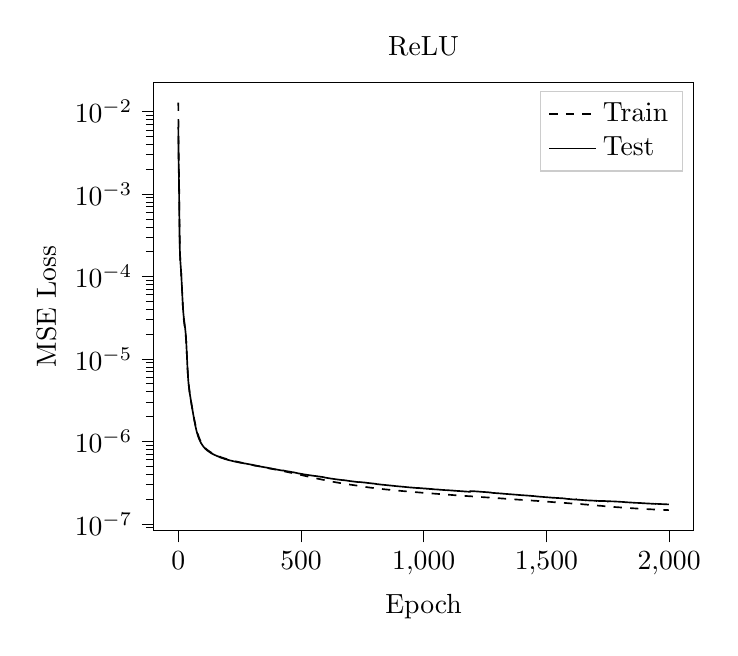
\begin{tikzpicture}

\begin{axis}[
legend cell align={left},
legend style={fill opacity=0.8, draw opacity=1, text opacity=1, draw=white!80!black},
log basis y={10},
tick align=outside,
tick pos=left,
title={ReLU},
x grid style={white!69.0196078431373!black},
xlabel={Epoch},
xmin=-99.95, xmax=2098.95,
xtick style={color=black},
y grid style={white!69.0196078431373!black},
ylabel={MSE Loss},
ymin=8.3060556203195e-08, ymax=0.0226737604172119,
ymode=log,
ytick style={color=black}
]
\addplot [semithick, black, dashed]
table {%
0 0.0128359138444066
1 0.00406811961205676
2 0.00221776218200102
3 0.00152627947740257
4 0.000869210763950832
5 0.000429490351874847
6 0.000256430144363549
7 0.000193489259458147
8 0.000159836590173654
9 0.000142019945189531
10 0.000129007256793557
11 0.000117138518267893
12 0.000105471455033694
13 9.37827313246089e-05
14 8.22589103336213e-05
15 7.13029772959999e-05
16 6.1415624084475e-05
17 5.3027559290058e-05
18 4.6298477172968e-05
19 4.10176366149244e-05
20 3.64308621828968e-05
21 3.31020509165683e-05
22 3.06825488805771e-05
23 2.8784052267838e-05
24 2.71935984428637e-05
25 2.57768373439831e-05
26 2.44650239310431e-05
27 2.31985326854556e-05
28 2.19409173314489e-05
29 2.06712553372199e-05
30 1.93696360001923e-05
31 1.80376509060807e-05
32 1.64094494193705e-05
33 1.45603561318239e-05
34 1.27872803000173e-05
35 1.11557179093325e-05
36 9.70921840917072e-06
37 8.46602692877241e-06
38 7.42971785643931e-06
39 6.59923705165966e-06
40 5.94965648508605e-06
41 5.44178499137615e-06
42 5.04196725398742e-06
43 4.71988363142373e-06
44 4.44941153807576e-06
45 4.21297154969125e-06
46 3.97091369615055e-06
47 3.78521997726011e-06
48 3.61609793606021e-06
49 3.45850858462882e-06
50 3.31160191757363e-06
51 3.17369637906495e-06
52 3.04450260318845e-06
53 2.92049022283436e-06
54 2.80214357240993e-06
55 2.69049423906154e-06
56 2.58622111073237e-06
57 2.48662982522774e-06
58 2.39208004813918e-06
59 2.30242519660351e-06
60 2.21742543777736e-06
61 2.13687340925617e-06
62 2.05999348276009e-06
63 1.98663157766532e-06
64 1.91840384792386e-06
65 1.85147106714112e-06
66 1.78930534508481e-06
67 1.73013427024671e-06
68 1.67454512279619e-06
69 1.62270763445349e-06
70 1.57398869492908e-06
71 1.52842072111525e-06
72 1.4852267215133e-06
73 1.44413795050014e-06
74 1.40627984944786e-06
75 1.36986447498089e-06
76 1.33475525311155e-06
77 1.30223323319001e-06
78 1.27158411430628e-06
79 1.24230728559382e-06
80 1.21496348251071e-06
81 1.1894506600072e-06
82 1.16576555632264e-06
83 1.14292291345919e-06
84 1.12203104029618e-06
85 1.10188948323753e-06
86 1.08292770786989e-06
87 1.06497326891031e-06
88 1.04840461335698e-06
89 1.03269330051603e-06
90 1.01698759053193e-06
91 1.00309512390595e-06
92 9.88916981896182e-07
93 9.75377727769455e-07
94 9.6289804420735e-07
95 9.5178445133115e-07
96 9.40547043398965e-07
97 9.29320102869724e-07
98 9.19224969607058e-07
99 9.09362678839898e-07
100 9.00760616332263e-07
101 8.91677312523598e-07
102 8.83358202798945e-07
103 8.7541410894687e-07
104 8.67818650164054e-07
105 8.60540775903473e-07
106 8.53664071399862e-07
107 8.47105686005989e-07
108 8.40799016799565e-07
109 8.34772250925653e-07
110 8.28988821496068e-07
111 8.23431996309409e-07
112 8.18056938896916e-07
113 8.12813703561233e-07
114 8.07828728369486e-07
115 8.03024243964501e-07
116 7.98377929925209e-07
117 7.93822158300372e-07
118 7.89469017917099e-07
119 7.8525374803462e-07
120 7.81149035503859e-07
121 7.77039519164191e-07
122 7.73208100383727e-07
123 7.69387711102354e-07
124 7.65666616501903e-07
125 7.61996876690318e-07
126 7.58383085326386e-07
127 7.54953229204602e-07
128 7.5161359521303e-07
129 7.48366523026789e-07
130 7.45194466219345e-07
131 7.41907941517184e-07
132 7.38387156445697e-07
133 7.35193854751515e-07
134 7.3226554457051e-07
135 7.29248398840809e-07
136 7.26341062176061e-07
137 7.23518060908646e-07
138 7.20833158993628e-07
139 7.18008437729622e-07
140 7.15079443153854e-07
141 7.12426657145215e-07
142 7.09709738089259e-07
143 7.07091793771042e-07
144 7.04633227798013e-07
145 7.02308290925657e-07
146 6.99840673831886e-07
147 6.97486854477347e-07
148 6.95209882849213e-07
149 6.92861825939417e-07
150 6.90704266872899e-07
151 6.88582144817929e-07
152 6.86111019234659e-07
153 6.84080939095111e-07
154 6.81975838517701e-07
155 6.79974541526462e-07
156 6.77959332790579e-07
157 6.76050047047738e-07
158 6.74017413103911e-07
159 6.72160598156779e-07
160 6.7017619542753e-07
161 6.68461542090881e-07
162 6.66575790489787e-07
163 6.64879856913103e-07
164 6.62985953709949e-07
165 6.6163600506286e-07
166 6.59435483271409e-07
167 6.57632066648262e-07
168 6.55575177276546e-07
169 6.54015729338653e-07
170 6.52307282223319e-07
171 6.504013251174e-07
172 6.46996461455274e-07
173 6.45045825507395e-07
174 6.43091596728596e-07
175 6.41354103819935e-07
176 6.39775814747168e-07
177 6.38218029919813e-07
178 6.36537369857138e-07
179 6.35115712441348e-07
180 6.33563209802901e-07
181 6.32300194652657e-07
182 6.30609901833168e-07
183 6.29600763673466e-07
184 6.27879526405195e-07
185 6.26514845080806e-07
186 6.25209512548963e-07
187 6.23535240336537e-07
188 6.22593528348148e-07
189 6.20840004998513e-07
190 6.19957963593265e-07
191 6.18262787398294e-07
192 6.17415837567137e-07
193 6.15776178662486e-07
194 6.14971566434974e-07
195 6.13444837298971e-07
196 6.12671803025933e-07
197 6.11204517156239e-07
198 6.10332435044825e-07
199 6.08851165878832e-07
200 6.080204561556e-07
201 6.06559192959821e-07
202 6.05760007701406e-07
203 6.04330644478068e-07
204 6.03280801200867e-07
205 6.01772887307561e-07
206 6.01124246642826e-07
207 5.99515939484263e-07
208 5.98675602759613e-07
209 5.9747211136596e-07
210 5.96390205643615e-07
211 5.95324714780077e-07
212 5.94377064487617e-07
213 5.93298088872984e-07
214 5.92175063729883e-07
215 5.91118195501394e-07
216 5.90146642139189e-07
217 5.89021899926934e-07
218 5.87992171404039e-07
219 5.87068497154064e-07
220 5.8602671730057e-07
221 5.85054058404921e-07
222 5.84006577440732e-07
223 5.82988822685593e-07
224 5.81989438828146e-07
225 5.81001877193899e-07
226 5.80024892542497e-07
227 5.79078803255584e-07
228 5.78110301987067e-07
229 5.77146334379108e-07
230 5.76185671306462e-07
231 5.75260986451553e-07
232 5.74307557812404e-07
233 5.73343675355886e-07
234 5.72410307597693e-07
235 5.71375916948114e-07
236 5.70444772321821e-07
237 5.69523908040992e-07
238 5.68677597769351e-07
239 5.67770445883298e-07
240 5.66866436670921e-07
241 5.65970691070561e-07
242 5.65123066863293e-07
243 5.64223408431985e-07
244 5.63306641481631e-07
245 5.6239256639401e-07
246 5.61538256064864e-07
247 5.606653090382e-07
248 5.59801215572975e-07
249 5.58943027954228e-07
250 5.58119654584743e-07
251 5.57285070087232e-07
252 5.5639160026999e-07
253 5.55517061400224e-07
254 5.54651886858437e-07
255 5.53784663139822e-07
256 5.53118923008356e-07
257 5.52271083662959e-07
258 5.51392261499473e-07
259 5.50661146789366e-07
260 5.49797288456943e-07
261 5.48924100115755e-07
262 5.48088413736991e-07
263 5.47227847107479e-07
264 5.46406514317255e-07
265 5.45611903149279e-07
266 5.44801076742374e-07
267 5.43925651868449e-07
268 5.43103572738346e-07
269 5.42293245572978e-07
270 5.4148437953927e-07
271 5.40699907702447e-07
272 5.39910273388955e-07
273 5.39133814939419e-07
274 5.38363875776326e-07
275 5.37582890757449e-07
276 5.36826901495147e-07
277 5.3603802076907e-07
278 5.35316970584177e-07
279 5.34529481910795e-07
280 5.33722675925219e-07
281 5.32918683234129e-07
282 5.32152425847698e-07
283 5.31394477121694e-07
284 5.30640270071103e-07
285 5.29907005429209e-07
286 5.29116395270535e-07
287 5.28346645850775e-07
288 5.27513266220581e-07
289 5.26773149360338e-07
290 5.26038264595741e-07
291 5.25316868134951e-07
292 5.24571295159149e-07
293 5.23829740870951e-07
294 5.23106379560545e-07
295 5.22383499131251e-07
296 5.2166716473323e-07
297 5.20962232855027e-07
298 5.20257276349412e-07
299 5.19555759524337e-07
300 5.18861061692633e-07
301 5.18167190975305e-07
302 5.17407352376154e-07
303 5.16758486270419e-07
304 5.16134349624053e-07
305 5.15409096962571e-07
306 5.1471261633651e-07
307 5.13997151728063e-07
308 5.13282595179021e-07
309 5.12469787608438e-07
310 5.11740900790869e-07
311 5.10916394645733e-07
312 5.10398340495044e-07
313 5.09615481561809e-07
314 5.0890788187985e-07
315 5.08135385487662e-07
316 5.07396071839139e-07
317 5.0667694905826e-07
318 5.06027933980135e-07
319 5.05363481877907e-07
320 5.04778821508012e-07
321 5.04100044608435e-07
322 5.03420945790367e-07
323 5.02913110352665e-07
324 5.02204066606282e-07
325 5.01519381444382e-07
326 5.0075652430337e-07
327 5.00041955618258e-07
328 4.99340976446661e-07
329 4.98837331861068e-07
330 4.98114730092425e-07
331 4.97396278106521e-07
332 4.96683979335444e-07
333 4.95992166946735e-07
334 4.95327224157904e-07
335 4.94672618728487e-07
336 4.94005201645109e-07
337 4.93368763699209e-07
338 4.92711109188804e-07
339 4.92064750176269e-07
340 4.91377320216202e-07
341 4.90734373599366e-07
342 4.90094236084815e-07
343 4.8923520419919e-07
344 4.88491250393963e-07
345 4.87911429033261e-07
346 4.86993086525445e-07
347 4.86201224958904e-07
348 4.85454121516682e-07
349 4.84715875060715e-07
350 4.83999491038389e-07
351 4.8330461555679e-07
352 4.82610435923903e-07
353 4.81942027434457e-07
354 4.81273281664585e-07
355 4.80657552941466e-07
356 4.79991086152154e-07
357 4.79426202517175e-07
358 4.78786983705959e-07
359 4.78136694752607e-07
360 4.77479370928791e-07
361 4.76951999701214e-07
362 4.76438385987876e-07
363 4.75759972076162e-07
364 4.75071433612584e-07
365 4.74538327580376e-07
366 4.73795507247132e-07
367 4.73118962915464e-07
368 4.72461489309239e-07
369 4.71825251139535e-07
370 4.71192496632966e-07
371 4.70559365041368e-07
372 4.70058532613393e-07
373 4.69410172783569e-07
374 4.68776403550919e-07
375 4.67982378282272e-07
376 4.67325791433382e-07
377 4.66681011914716e-07
378 4.66014211454535e-07
379 4.65348282233435e-07
380 4.64814711989447e-07
381 4.64148458462432e-07
382 4.63576862159698e-07
383 4.62930432362896e-07
384 4.62302280809013e-07
385 4.61679847362006e-07
386 4.61104624704944e-07
387 4.60824521880454e-07
388 4.60142321898616e-07
389 4.59398271928535e-07
390 4.58787464964416e-07
391 4.58134393070964e-07
392 4.57507636880905e-07
393 4.56882881110232e-07
394 4.5631434277027e-07
395 4.55657936043963e-07
396 4.54997403451785e-07
397 4.54597877237006e-07
398 4.53956164321312e-07
399 4.53263333653808e-07
400 4.52610636330064e-07
401 4.51975337526278e-07
402 4.51166000871694e-07
403 4.50556313722927e-07
404 4.49943631167571e-07
405 4.50224415246225e-07
406 4.49388958884356e-07
407 4.48679926989826e-07
408 4.47983747477565e-07
409 4.47319951319969e-07
410 4.46692041819574e-07
411 4.46043008082597e-07
412 4.45379412937541e-07
413 4.44756290605142e-07
414 4.44137515501097e-07
415 4.43530492361788e-07
416 4.42895292664502e-07
417 4.42246661634726e-07
418 4.4161888378369e-07
419 4.41050250699959e-07
420 4.4041967524322e-07
421 4.39794044325481e-07
422 4.39187426295007e-07
423 4.38575338435498e-07
424 4.37924559278713e-07
425 4.37397801690054e-07
426 4.36789211121891e-07
427 4.36235071774149e-07
428 4.35714181989511e-07
429 4.35064805230923e-07
430 4.3441796375987e-07
431 4.33821461186312e-07
432 4.33212344105982e-07
433 4.3256776783096e-07
434 4.31979589833986e-07
435 4.31346918034592e-07
436 4.30742508925164e-07
437 4.30014452831529e-07
438 4.29212309612126e-07
439 4.28535380322614e-07
440 4.2784484142544e-07
441 4.27162711716278e-07
442 4.2654244050766e-07
443 4.25920634356203e-07
444 4.25289486614133e-07
445 4.24664052573576e-07
446 4.24054528849638e-07
447 4.23444578245835e-07
448 4.22825500720592e-07
449 4.22235647633329e-07
450 4.21641495776726e-07
451 4.21042936622484e-07
452 4.204042555358e-07
453 4.19785291612129e-07
454 4.19165474724537e-07
455 4.18587373061996e-07
456 4.17983689530388e-07
457 4.17366091724602e-07
458 4.16813378095071e-07
459 4.16216044001771e-07
460 4.1563661304167e-07
461 4.15065193166697e-07
462 4.14440477527478e-07
463 4.137947071996e-07
464 4.13075351730186e-07
465 4.12454505095639e-07
466 4.11876993922533e-07
467 4.1130139980794e-07
468 4.10712745221531e-07
469 4.10157508312636e-07
470 4.09618700686565e-07
471 4.0901640734603e-07
472 4.08388660346759e-07
473 4.07808872111559e-07
474 4.07190228571608e-07
475 4.06595403376286e-07
476 4.06010637888698e-07
477 4.05392317176734e-07
478 4.04781765979578e-07
479 4.04163714279093e-07
480 4.03598776060221e-07
481 4.03019477431599e-07
482 4.0240480798559e-07
483 4.0181467062439e-07
484 4.01190572162591e-07
485 4.00669628959349e-07
486 4.00093216029518e-07
487 3.99534549217151e-07
488 3.98832486453671e-07
489 3.98232996289494e-07
490 3.97586432200114e-07
491 3.96999277043619e-07
492 3.96335612961707e-07
493 3.95738804854773e-07
494 3.95199794851919e-07
495 3.94601066957989e-07
496 3.93942960840832e-07
497 3.9341726065345e-07
498 3.92822267642146e-07
499 3.92249883688578e-07
500 3.9166239578492e-07
501 3.90943145731626e-07
502 3.90417924037934e-07
503 3.89788243779776e-07
504 3.89221085768554e-07
505 3.88712462026319e-07
506 3.88139190917514e-07
507 3.87384185444262e-07
508 3.8658280821835e-07
509 3.85974133635614e-07
510 3.85345149737759e-07
511 3.84755621880117e-07
512 3.84093485990888e-07
513 3.83513560478832e-07
514 3.82928092875545e-07
515 3.82343274367258e-07
516 3.81772343004627e-07
517 3.81215974144311e-07
518 3.80635759938741e-07
519 3.80127739830982e-07
520 3.79530231583658e-07
521 3.78973119623538e-07
522 3.78421440586862e-07
523 3.77808645694699e-07
524 3.77222886726258e-07
525 3.76684518130332e-07
526 3.76060851081661e-07
527 3.75412971578726e-07
528 3.74828130603078e-07
529 3.74236345834333e-07
530 3.73695037055199e-07
531 3.73073411736868e-07
532 3.72465256930354e-07
533 3.71768114604265e-07
534 3.71223410738253e-07
535 3.70558538918431e-07
536 3.69985989095767e-07
537 3.69416098607189e-07
538 3.68824209559193e-07
539 3.68246500883629e-07
540 3.67674652096639e-07
541 3.67146909241001e-07
542 3.6655390564988e-07
543 3.65992903496704e-07
544 3.65448769613863e-07
545 3.64904883639383e-07
546 3.64338433428202e-07
547 3.63806817304635e-07
548 3.63257377458126e-07
549 3.62574539664706e-07
550 3.62068634359503e-07
551 3.61473358509556e-07
552 3.60935242895266e-07
553 3.60413636357748e-07
554 3.59868972850563e-07
555 3.5935385152186e-07
556 3.58844249333856e-07
557 3.58326943697307e-07
558 3.57797470698529e-07
559 3.57330856189719e-07
560 3.56872281628284e-07
561 3.56368487672398e-07
562 3.55836359986483e-07
563 3.55332234633465e-07
564 3.54824446645807e-07
565 3.54339146753091e-07
566 3.53827280022756e-07
567 3.53325290390671e-07
568 3.52850746850208e-07
569 3.52336466477254e-07
570 3.51856831954933e-07
571 3.5136100875377e-07
572 3.50893734022861e-07
573 3.50407004418685e-07
574 3.4989447030398e-07
575 3.49443885625078e-07
576 3.4893881971243e-07
577 3.48500343307023e-07
578 3.4798630669286e-07
579 3.47510213757118e-07
580 3.47052929782876e-07
581 3.46572929046829e-07
582 3.46100820763695e-07
583 3.45635644279696e-07
584 3.45174572856877e-07
585 3.44720079127114e-07
586 3.44251229549286e-07
587 3.43796819834097e-07
588 3.43215964477395e-07
589 3.42688052199946e-07
590 3.42216255234007e-07
591 3.41808416024492e-07
592 3.41212007285208e-07
593 3.40706088309162e-07
594 3.40231385706602e-07
595 3.3973816373134e-07
596 3.39256642760688e-07
597 3.38761948015076e-07
598 3.38252847200238e-07
599 3.37764319738199e-07
600 3.37289797997187e-07
601 3.36832910235785e-07
602 3.36301321624433e-07
603 3.35731551629692e-07
604 3.35256483978696e-07
605 3.34784972508828e-07
606 3.34324919933238e-07
607 3.33847983526425e-07
608 3.33368957925018e-07
609 3.32913002822011e-07
610 3.32462384264431e-07
611 3.31984051385348e-07
612 3.31562530178076e-07
613 3.31118336518443e-07
614 3.30674347267745e-07
615 3.30218415513173e-07
616 3.29806052974391e-07
617 3.29311662270015e-07
618 3.28869587505665e-07
619 3.28467940903465e-07
620 3.27985743709291e-07
621 3.27568215709562e-07
622 3.27144061799345e-07
623 3.26670766185089e-07
624 3.26214176098461e-07
625 3.25802174742762e-07
626 3.25410245523017e-07
627 3.24975043511699e-07
628 3.24551212329993e-07
629 3.24158174407785e-07
630 3.23716544528452e-07
631 3.23299862060367e-07
632 3.22898985729125e-07
633 3.22488403895704e-07
634 3.22097345872407e-07
635 3.21700158878002e-07
636 3.21304454558913e-07
637 3.20912313469535e-07
638 3.20524564074276e-07
639 3.20136042191166e-07
640 3.19752844077925e-07
641 3.19376165165863e-07
642 3.18992066596024e-07
643 3.18628257616638e-07
644 3.18242471507801e-07
645 3.17883358164295e-07
646 3.17517607541617e-07
647 3.17189173131283e-07
648 3.16752779781382e-07
649 3.16441293151115e-07
650 3.15991993588227e-07
651 3.15567727056987e-07
652 3.15198235242065e-07
653 3.14852366315677e-07
654 3.14477423572157e-07
655 3.14116288961941e-07
656 3.13751376125992e-07
657 3.13407868560489e-07
658 3.13042362492411e-07
659 3.1268381887628e-07
660 3.12334496982203e-07
661 3.11969507151844e-07
662 3.1163067758655e-07
663 3.11306783956411e-07
664 3.10919280082089e-07
665 3.10583744706605e-07
666 3.10250059655459e-07
667 3.09937706305163e-07
668 3.09573450948619e-07
669 3.09204214246961e-07
670 3.08850459617815e-07
671 3.08537095591532e-07
672 3.08225946909602e-07
673 3.07908969560344e-07
674 3.07560297102327e-07
675 3.0723168808322e-07
676 3.06905842663241e-07
677 3.06626207304816e-07
678 3.06256743982658e-07
679 3.05940740773281e-07
680 3.05711705024692e-07
681 3.05346728438849e-07
682 3.05022357409257e-07
683 3.04787608797596e-07
684 3.04591078773342e-07
685 3.04243192218223e-07
686 3.03902760222741e-07
687 3.03562333655805e-07
688 3.03246627694875e-07
689 3.02922987273746e-07
690 3.02614198247397e-07
691 3.02081464738535e-07
692 3.01742485603995e-07
693 3.01437276149841e-07
694 3.01078963033774e-07
695 3.00749295163882e-07
696 3.00478578765251e-07
697 3.00096437030106e-07
698 2.99800604125267e-07
699 2.99512212393438e-07
700 2.99188646494031e-07
701 2.98825807448111e-07
702 2.98531001078572e-07
703 2.98287063074554e-07
704 2.98012047025509e-07
705 2.97674375701717e-07
706 2.97391246348866e-07
707 2.97087627117776e-07
708 2.96822007285868e-07
709 2.96534653557501e-07
710 2.96241515030715e-07
711 2.95766508685347e-07
712 2.95477427869173e-07
713 2.95199973777471e-07
714 2.94934526451129e-07
715 2.94622614532614e-07
716 2.94349123265647e-07
717 2.94059612983233e-07
718 2.93763836197059e-07
719 2.93480562305604e-07
720 2.93202444495932e-07
721 2.92916106459984e-07
722 2.92623508840961e-07
723 2.92435868473717e-07
724 2.92131600772905e-07
725 2.91845484383657e-07
726 2.91578852696261e-07
727 2.91303842161028e-07
728 2.91009091881733e-07
729 2.90722125015463e-07
730 2.90455377040644e-07
731 2.90185338116089e-07
732 2.8992908158898e-07
733 2.89663138232754e-07
734 2.8940803167643e-07
735 2.89136017798342e-07
736 2.889206294725e-07
737 2.88737842566888e-07
738 2.88997667908575e-07
739 2.88562024607586e-07
740 2.88228037263139e-07
741 2.87892525449251e-07
742 2.87586055392808e-07
743 2.8728029188585e-07
744 2.86980700195727e-07
745 2.86744340243672e-07
746 2.8622192211003e-07
747 2.85925212054394e-07
748 2.85634268323065e-07
749 2.85337112515549e-07
750 2.8511037254475e-07
751 2.84853912376093e-07
752 2.84023656476506e-07
753 2.83497718470471e-07
754 2.83116851676368e-07
755 2.82695359175023e-07
756 2.82512347510533e-07
757 2.82085629521589e-07
758 2.81725797435683e-07
759 2.81449778896103e-07
760 2.8105877230189e-07
761 2.80944373514558e-07
762 2.80682355423778e-07
763 2.80297662115458e-07
764 2.79940790193223e-07
765 2.79655734573225e-07
766 2.7931117253388e-07
767 2.78977283855397e-07
768 2.78635521198112e-07
769 2.78352544214044e-07
770 2.7819338988877e-07
771 2.77889544165078e-07
772 2.77548593075494e-07
773 2.77264688477885e-07
774 2.7704935030215e-07
775 2.76729705390721e-07
776 2.7645308894364e-07
777 2.76195476729413e-07
778 2.7594944073428e-07
779 2.75716891124489e-07
780 2.75467336976476e-07
781 2.75225335968798e-07
782 2.75062229206924e-07
783 2.7480055271667e-07
784 2.74580447268136e-07
785 2.74362289260921e-07
786 2.74111401481036e-07
787 2.73876008265006e-07
788 2.73605013845213e-07
789 2.73413644165998e-07
790 2.73188405444103e-07
791 2.72918508599673e-07
792 2.72716296422004e-07
793 2.72480284039034e-07
794 2.72285307730158e-07
795 2.72149884011696e-07
796 2.71952939314701e-07
797 2.71704815986595e-07
798 2.71441972643061e-07
799 2.71195177930395e-07
800 2.7097320317182e-07
801 2.70770428784317e-07
802 2.70505914016894e-07
803 2.70232581939922e-07
804 2.69978283682804e-07
805 2.69613692850612e-07
806 2.6923754116126e-07
807 2.68977236729029e-07
808 2.68752260268457e-07
809 2.68544625768641e-07
810 2.68373911282538e-07
811 2.68163501999652e-07
812 2.67927181553773e-07
813 2.67719987007808e-07
814 2.67517097881864e-07
815 2.67310931533871e-07
816 2.67105253826116e-07
817 2.66903428638443e-07
818 2.66692599950602e-07
819 2.66481964402487e-07
820 2.66284019161844e-07
821 2.66081862648093e-07
822 2.66027550424042e-07
823 2.65821824157797e-07
824 2.65619061863731e-07
825 2.65410844818348e-07
826 2.65213099211792e-07
827 2.65021856961312e-07
828 2.64826372728066e-07
829 2.64633269267733e-07
830 2.64446708726496e-07
831 2.64248240071652e-07
832 2.64059634162095e-07
833 2.63878327388056e-07
834 2.63682958788536e-07
835 2.63493734607323e-07
836 2.63316504145905e-07
837 2.63118264641093e-07
838 2.62901429465501e-07
839 2.62730751714457e-07
840 2.62452709399952e-07
841 2.62270763101924e-07
842 2.62094237520216e-07
843 2.61916025223741e-07
844 2.61752447649144e-07
845 2.61570247680254e-07
846 2.61391405729228e-07
847 2.61197685773595e-07
848 2.61104773478849e-07
849 2.60918261439258e-07
850 2.60724515214861e-07
851 2.60535269994477e-07
852 2.60345671463824e-07
853 2.60163190716867e-07
854 2.59979377318587e-07
855 2.59807215748253e-07
856 2.59638242802396e-07
857 2.59457045409306e-07
858 2.5929549951087e-07
859 2.59103974563857e-07
860 2.58932327128036e-07
861 2.58767719678588e-07
862 2.58579918060775e-07
863 2.58410764914174e-07
864 2.58235526878536e-07
865 2.58068606832751e-07
866 2.579093218813e-07
867 2.5772559851589e-07
868 2.5755975129016e-07
869 2.57416757627027e-07
870 2.57236482134715e-07
871 2.57065044301896e-07
872 2.56887864409805e-07
873 2.56699708664598e-07
874 2.56526549620162e-07
875 2.56373737975935e-07
876 2.56201032037495e-07
877 2.56034790240278e-07
878 2.55873794714034e-07
879 2.55705920480409e-07
880 2.55417128485647e-07
881 2.55229956422909e-07
882 2.55085984754544e-07
883 2.54928232898521e-07
884 2.54779993753118e-07
885 2.54592056549541e-07
886 2.54439689939545e-07
887 2.5426591516009e-07
888 2.54102271377121e-07
889 2.53930725016005e-07
890 2.53764556227054e-07
891 2.53614336365615e-07
892 2.53452076336202e-07
893 2.532692485957e-07
894 2.53125733742365e-07
895 2.52976690667595e-07
896 2.528093443388e-07
897 2.52656056844103e-07
898 2.52499306505172e-07
899 2.52364507723257e-07
900 2.52203973225562e-07
901 2.52031071774184e-07
902 2.518835791534e-07
903 2.51714416926063e-07
904 2.51555577612805e-07
905 2.51338153084646e-07
906 2.51199765898491e-07
907 2.51049156986483e-07
908 2.50885086643393e-07
909 2.50740681572381e-07
910 2.50585756418786e-07
911 2.50420220616832e-07
912 2.50275292266622e-07
913 2.50121281410998e-07
914 2.4995576485054e-07
915 2.49676279501898e-07
916 2.49520305203532e-07
917 2.49378198027728e-07
918 2.4922392374549e-07
919 2.49076048127961e-07
920 2.48927619701078e-07
921 2.48776921417004e-07
922 2.48630119202176e-07
923 2.48482846032516e-07
924 2.48332861993106e-07
925 2.48184320888356e-07
926 2.48036973083288e-07
927 2.47890264816419e-07
928 2.4774389887483e-07
929 2.47597746444228e-07
930 2.47460814819078e-07
931 2.47319833690085e-07
932 2.47171875763286e-07
933 2.46986154522233e-07
934 2.46846625991282e-07
935 2.46710934568739e-07
936 2.46565559500311e-07
937 2.46414631448033e-07
938 2.46274233148824e-07
939 2.46133543761573e-07
940 2.45993646721843e-07
941 2.45851855076751e-07
942 2.4571178909838e-07
943 2.45570187580313e-07
944 2.45427655464425e-07
945 2.4528916037525e-07
946 2.45144313090862e-07
947 2.45008457774531e-07
948 2.44778515678945e-07
949 2.44709522988273e-07
950 2.44557021623848e-07
951 2.44444680092215e-07
952 2.44300696401467e-07
953 2.44156826106234e-07
954 2.44018879300256e-07
955 2.43875476478195e-07
956 2.43733082527342e-07
957 2.43594031232419e-07
958 2.43454059834391e-07
959 2.43317650365782e-07
960 2.43178574322656e-07
961 2.43043392202935e-07
962 2.42901336989121e-07
963 2.42752515198674e-07
964 2.42617944856249e-07
965 2.42478849045824e-07
966 2.42350840103711e-07
967 2.42212682998399e-07
968 2.42075261638774e-07
969 2.41937336305398e-07
970 2.41740744577612e-07
971 2.41667918423616e-07
972 2.41518041917743e-07
973 2.41401504226246e-07
974 2.41222875168035e-07
975 2.41124690397498e-07
976 2.40940309865323e-07
977 2.40789396293906e-07
978 2.40686851775251e-07
979 2.4058535476712e-07
980 2.40380043535993e-07
981 2.40305805455421e-07
982 2.40108319552235e-07
983 2.40031877538627e-07
984 2.39894949039865e-07
985 2.3973578581149e-07
986 2.39611460926881e-07
987 2.39439004758424e-07
988 2.3930055066046e-07
989 2.39153940320591e-07
990 2.38980053701709e-07
991 2.38914729784767e-07
992 2.38757834530645e-07
993 2.38612148095285e-07
994 2.3841948619463e-07
995 2.38344357995857e-07
996 2.38203236882839e-07
997 2.38060229719395e-07
998 2.37923468709766e-07
999 2.37793798923747e-07
1000 2.37646189845009e-07
1001 2.37599634857588e-07
1002 2.37371781985019e-07
1003 2.37256684719966e-07
1004 2.3710381680786e-07
1005 2.37030779430825e-07
1006 2.36854548504084e-07
1007 2.36789443157193e-07
1008 2.36603149716075e-07
1009 2.36586189146237e-07
1010 2.36392693182097e-07
1011 2.36260623339035e-07
1012 2.36101812092215e-07
1013 2.36086071886632e-07
1014 2.35904035029932e-07
1015 2.35725191885194e-07
1016 2.35685808050334e-07
1017 2.35596702900409e-07
1018 2.35438702382851e-07
1019 2.35246950623491e-07
1020 2.35075611456637e-07
1021 2.35099903790115e-07
1022 2.3487148752821e-07
1023 2.34750061487432e-07
1024 2.34573643794533e-07
1025 2.34564620235744e-07
1026 2.34471072538156e-07
1027 2.34354624211619e-07
1028 2.34128390850685e-07
1029 2.33955763171423e-07
1030 2.33922607776549e-07
1031 2.33783959046718e-07
1032 2.33714321531409e-07
1033 2.33685208733903e-07
1034 2.33539281111916e-07
1035 2.33392913706609e-07
1036 2.33203155495687e-07
1037 2.331949610479e-07
1038 2.32991934915106e-07
1039 2.32850305849297e-07
1040 2.32765783117372e-07
1041 2.32670341915764e-07
1042 2.32657039475725e-07
1043 2.32462914603104e-07
1044 2.32303914394549e-07
1045 2.32177753510143e-07
1046 2.32038218555886e-07
1047 2.31941964251803e-07
1048 2.31735411837519e-07
1049 2.3166942881403e-07
1050 2.31621027936058e-07
1051 2.31475059614183e-07
1052 2.31326241298291e-07
1053 2.31239147751694e-07
1054 2.31119690745629e-07
1055 2.31017140592371e-07
1056 2.3086940776551e-07
1057 2.30697620096976e-07
1058 2.30660508172775e-07
1059 2.30563432516817e-07
1060 2.30397781528779e-07
1061 2.30417078178391e-07
1062 2.30317154283455e-07
1063 2.30162277986778e-07
1064 2.30063518721124e-07
1065 2.29899269129419e-07
1066 2.29807306638463e-07
1067 2.29664271131469e-07
1068 2.29567998907498e-07
1069 2.29445193149047e-07
1070 2.29313082712679e-07
1071 2.29218835350764e-07
1072 2.2906969297054e-07
1073 2.28964648627539e-07
1074 2.28864435037224e-07
1075 2.28717713547155e-07
1076 2.2863567138387e-07
1077 2.28499026974305e-07
1078 2.28409063225854e-07
1079 2.28298539020955e-07
1080 2.28191649313203e-07
1081 2.28083222189923e-07
1082 2.27955539990887e-07
1083 2.27841008324958e-07
1084 2.2773020606337e-07
1085 2.27610032744963e-07
1086 2.27501331949043e-07
1087 2.27376409974056e-07
1088 2.2726379945226e-07
1089 2.27137682820455e-07
1090 2.26827840933197e-07
1091 2.26754384584638e-07
1092 2.26650240975346e-07
1093 2.26534615457297e-07
1094 2.26412695525369e-07
1095 2.26291264908696e-07
1096 2.26169796015085e-07
1097 2.26040921411652e-07
1098 2.25922023474823e-07
1099 2.25797209253642e-07
1100 2.25675585596719e-07
1101 2.25561426347554e-07
1102 2.254305840097e-07
1103 2.25311821019147e-07
1104 2.25195945944279e-07
1105 2.25079520305371e-07
1106 2.24965323099013e-07
1107 2.24867464545753e-07
1108 2.24762359117392e-07
1109 2.24626370084025e-07
1110 2.24508406084567e-07
1111 2.24395075314021e-07
1112 2.24277390778127e-07
1113 2.24158637927019e-07
1114 2.2404539223686e-07
1115 2.23920358827456e-07
1116 2.23808280111371e-07
1117 2.23686827183656e-07
1118 2.2356966128001e-07
1119 2.23456709292691e-07
1120 2.23334162825495e-07
1121 2.23228413595677e-07
1122 2.23115099544202e-07
1123 2.23002317440546e-07
1124 2.22879026416933e-07
1125 2.22769490122232e-07
1126 2.22664080226309e-07
1127 2.2253616578638e-07
1128 2.22430343903568e-07
1129 2.223116337845e-07
1130 2.22204481723054e-07
1131 2.22094232434245e-07
1132 2.21976963509007e-07
1133 2.21866377820845e-07
1134 2.21753350238885e-07
1135 2.21644285254285e-07
1136 2.21531433545863e-07
1137 2.21416343521241e-07
1138 2.21307805006177e-07
1139 2.21198763370012e-07
1140 2.21085268165666e-07
1141 2.20975650925936e-07
1142 2.20881519460647e-07
1143 2.20775239149873e-07
1144 2.20637945012925e-07
1145 2.20559710285784e-07
1146 2.20444337422521e-07
1147 2.20324321794863e-07
1148 2.20211126375602e-07
1149 2.201148186316e-07
1150 2.19997589574916e-07
1151 2.1989982777626e-07
1152 2.19791165335437e-07
1153 2.196815010862e-07
1154 2.19573701976117e-07
1155 2.19463932438657e-07
1156 2.19359349159731e-07
1157 2.19249752198891e-07
1158 2.19142922851745e-07
1159 2.19035697959669e-07
1160 2.18929460672257e-07
1161 2.18930828516761e-07
1162 2.18828259697545e-07
1163 2.18708604258211e-07
1164 2.18593607570483e-07
1165 2.18480611941629e-07
1166 2.1837456065299e-07
1167 2.18264942468238e-07
1168 2.18158639007981e-07
1169 2.18042133006691e-07
1170 2.17949583657173e-07
1171 2.17841640782979e-07
1172 2.17736934885693e-07
1173 2.17629174635192e-07
1174 2.17524212679621e-07
1175 2.1741689277377e-07
1176 2.1731769705724e-07
1177 2.17213480382839e-07
1178 2.1710752405113e-07
1179 2.17002218498408e-07
1180 2.16897231283042e-07
1181 2.16794168977685e-07
1182 2.16689441295159e-07
1183 2.16586816598863e-07
1184 2.16482968788512e-07
1185 2.1638173421934e-07
1186 2.16274073231659e-07
1187 2.16172590953079e-07
1188 2.16080631012971e-07
1189 2.1599227943625e-07
1190 2.15979764696783e-07
1191 2.16017678475566e-07
1192 2.15873939545475e-07
1193 2.15748003292049e-07
1194 2.15623455886771e-07
1195 2.15515344123673e-07
1196 2.15400620767525e-07
1197 2.15292371208875e-07
1198 2.15177959709933e-07
1199 2.15071723104643e-07
1200 2.14928613999632e-07
1201 2.14839535118472e-07
1202 2.14735765474927e-07
1203 2.14574807344547e-07
1204 2.14502365381009e-07
1205 2.14412341868808e-07
1206 2.14283540159954e-07
1207 2.14210046642904e-07
1208 2.14107812681164e-07
1209 2.14021252809005e-07
1210 2.13936210762711e-07
1211 2.13915925698416e-07
1212 2.13799923876934e-07
1213 2.13669566456076e-07
1214 2.13561179556621e-07
1215 2.13467269645662e-07
1216 2.13349683882313e-07
1217 2.13256108388293e-07
1218 2.13155513392849e-07
1219 2.13042389802354e-07
1220 2.12919297460701e-07
1221 2.12815673890532e-07
1222 2.12711443602132e-07
1223 2.12652658127865e-07
1224 2.12501022431866e-07
1225 2.12420601719998e-07
1226 2.12309944174649e-07
1227 2.12366951096499e-07
1228 2.12222830079156e-07
1229 2.12110472261884e-07
1230 2.11929635618446e-07
1231 2.11879924854941e-07
1232 2.11703791869411e-07
1233 2.11653654140775e-07
1234 2.1151320120083e-07
1235 2.11419449257733e-07
1236 2.11250796276374e-07
1237 2.11202558560331e-07
1238 2.11102061150825e-07
1239 2.10944673966651e-07
1240 2.10911240309031e-07
1241 2.1076127746511e-07
1242 2.10704322974209e-07
1243 2.10567815479123e-07
1244 2.10497195574533e-07
1245 2.1040943553885e-07
1246 2.10297608973065e-07
1247 2.10163938255903e-07
1248 2.10107044765095e-07
1249 2.10013232752715e-07
1250 2.09916546062061e-07
1251 2.09774376543237e-07
1252 2.09698891929122e-07
1253 2.09622506929463e-07
1254 2.09513595876842e-07
1255 2.09421121070363e-07
1256 2.09320254114687e-07
1257 2.09215731480583e-07
1258 2.09130282691206e-07
1259 2.09036870700174e-07
1260 2.08928067813474e-07
1261 2.08838153490376e-07
1262 2.08749056248791e-07
1263 2.08652356469941e-07
1264 2.08550158639298e-07
1265 2.08489736223783e-07
1266 2.0837612094482e-07
1267 2.08276492024595e-07
1268 2.08193774028587e-07
1269 2.08094111279422e-07
1270 2.07980286397458e-07
1271 2.07888382796284e-07
1272 2.07787530371206e-07
1273 2.07656961599412e-07
1274 2.07569616925696e-07
1275 2.0746449245479e-07
1276 2.07364236295859e-07
1277 2.07165836712875e-07
1278 2.07041992617007e-07
1279 2.06997534185405e-07
1280 2.06897416155982e-07
1281 2.06792438376624e-07
1282 2.06619498243299e-07
1283 2.06613423934243e-07
1284 2.06489881819039e-07
1285 2.0638760765479e-07
1286 2.06301932017539e-07
1287 2.06185098910794e-07
1288 2.06122904430117e-07
1289 2.0603094798588e-07
1290 2.05890058659008e-07
1291 2.058426851832e-07
1292 2.05701655730195e-07
1293 2.05651675621255e-07
1294 2.05522865172725e-07
1295 2.05462758223973e-07
1296 2.05339187992593e-07
1297 2.05216017839405e-07
1298 2.05128365635687e-07
1299 2.05095285075174e-07
1300 2.04930593312724e-07
1301 2.04907038209967e-07
1302 2.04736265757788e-07
1303 2.0472843108621e-07
1304 2.04564254225659e-07
1305 2.04535793123739e-07
1306 2.04411864075382e-07
1307 2.04340191245933e-07
1308 2.04220152618007e-07
1309 2.04110330066953e-07
1310 2.04035512098244e-07
1311 2.03963682523067e-07
1312 2.03857806447161e-07
1313 2.03766906793135e-07
1314 2.03600763406087e-07
1315 2.03567661820614e-07
1316 2.03439885275714e-07
1317 2.0336518320363e-07
1318 2.032757020487e-07
1319 2.03217184783e-07
1320 2.03097577866629e-07
1321 2.03010853205399e-07
1322 2.02895738659947e-07
1323 2.02795099845332e-07
1324 2.02704501582218e-07
1325 2.02589735827985e-07
1326 2.02511892204882e-07
1327 2.02408412725674e-07
1328 2.02272598507136e-07
1329 2.0214227660631e-07
1330 2.02043033908694e-07
1331 2.01940268901524e-07
1332 2.01830009295634e-07
1333 2.01788452855567e-07
1334 2.01665288990682e-07
1335 2.01558977146021e-07
1336 2.01502488479832e-07
1337 2.01370287101099e-07
1338 2.01262453124684e-07
1339 2.01164852363434e-07
1340 2.01063925814537e-07
1341 2.00968840445626e-07
1342 2.00907314329868e-07
1343 2.00762776536578e-07
1344 2.00683564941073e-07
1345 2.00600544012275e-07
1346 2.00489199613685e-07
1347 2.00247139510168e-07
1348 2.0018000638089e-07
1349 2.00085132711081e-07
1350 1.99985089430754e-07
1351 1.99909750492111e-07
1352 1.99793285268868e-07
1353 1.99699068950565e-07
1354 1.99619168668619e-07
1355 1.99508070835464e-07
1356 1.99424367018253e-07
1357 1.99339445082103e-07
1358 1.99232693923079e-07
1359 1.99150643993562e-07
1360 1.99041314644433e-07
1361 1.9894423559208e-07
1362 1.98858898443177e-07
1363 1.98747527939247e-07
1364 1.98649745641433e-07
1365 1.98597096414233e-07
1366 1.98485464387943e-07
1367 1.9839009510747e-07
1368 1.98303617892748e-07
1369 1.98163553932318e-07
1370 1.98024752101844e-07
1371 1.9802462633578e-07
1372 1.97904007080751e-07
1373 1.97792426241961e-07
1374 1.97700932204725e-07
1375 1.97582478129732e-07
1376 1.97496014543219e-07
1377 1.97442480079246e-07
1378 1.97292501994184e-07
1379 1.97215899994774e-07
1380 1.97129082785352e-07
1381 1.97047096150982e-07
1382 1.96931914999254e-07
1383 1.96866535979723e-07
1384 1.96748979227834e-07
1385 1.96670395652632e-07
1386 1.96537504265848e-07
1387 1.96472592328689e-07
1388 1.96395970554875e-07
1389 1.96314325215496e-07
1390 1.96160989446525e-07
1391 1.96098936960709e-07
1392 1.95963414675759e-07
1393 1.95923781213025e-07
1394 1.9576923853748e-07
1395 1.95750483491963e-07
1396 1.95624758973167e-07
1397 1.95513828309402e-07
1398 1.95484114023259e-07
1399 1.95305951599778e-07
1400 1.95257116345715e-07
1401 1.95148459923189e-07
1402 1.95140374209757e-07
1403 1.95018690270388e-07
1404 1.94886642852055e-07
1405 1.94786378692413e-07
1406 1.94772436103108e-07
1407 1.94666272740562e-07
1408 1.94536682762703e-07
1409 1.94470198458419e-07
1410 1.94301135245212e-07
1411 1.94241530216743e-07
1412 1.94114599068484e-07
1413 1.94071764546777e-07
1414 1.93994561087152e-07
1415 1.93910387515928e-07
1416 1.93826246174922e-07
1417 1.93731067383851e-07
1418 1.93607339234347e-07
1419 1.93542343367881e-07
1420 1.9343740844846e-07
1421 1.93307958880951e-07
1422 1.93212855663205e-07
1423 1.9319500296433e-07
1424 1.93057864024127e-07
1425 1.93003795104119e-07
1426 1.92875757235811e-07
1427 1.92799762956497e-07
1428 1.92709066794805e-07
1429 1.92629986820236e-07
1430 1.92562667393759e-07
1431 1.92412457487023e-07
1432 1.923164970421e-07
1433 1.92212994384988e-07
1434 1.92117591787166e-07
1435 1.92054836240629e-07
1436 1.92077585573713e-07
1437 1.91970624435101e-07
1438 1.91855633147497e-07
1439 1.91738552040022e-07
1440 1.91556437243889e-07
1441 1.91566779371044e-07
1442 1.91436991002547e-07
1443 1.91359781638312e-07
1444 1.91402773523919e-07
1445 1.91267241291371e-07
1446 1.9109486520108e-07
1447 1.91051301001721e-07
1448 1.90914974176337e-07
1449 1.90833660269618e-07
1450 1.90732240533009e-07
1451 1.90663927462253e-07
1452 1.90549957004293e-07
1453 1.90516927240481e-07
1454 1.90568535209934e-07
1455 1.90464090856324e-07
1456 1.90173839605734e-07
1457 1.90063078804314e-07
1458 1.90166451851326e-07
1459 1.90337836649235e-07
1460 1.90102733085951e-07
1461 1.8997548833255e-07
1462 1.89736554936815e-07
1463 1.89701801993181e-07
1464 1.8942595669813e-07
1465 1.89337171434545e-07
1466 1.89209052699368e-07
1467 1.89201453991927e-07
1468 1.89235038845936e-07
1469 1.89176961463033e-07
1470 1.89062633360493e-07
1471 1.88726122743788e-07
1472 1.88520785847857e-07
1473 1.88483920233296e-07
1474 1.88584162799543e-07
1475 1.88440573332116e-07
1476 1.88324926952532e-07
1477 1.88138743801858e-07
1478 1.88068955395693e-07
1479 1.87984317840062e-07
1480 1.87901757342956e-07
1481 1.87818820784003e-07
1482 1.87700506828037e-07
1483 1.87608113890292e-07
1484 1.87492924730748e-07
1485 1.87428510905363e-07
1486 1.87290235636794e-07
1487 1.87174033406734e-07
1488 1.87133109839976e-07
1489 1.87034921630413e-07
1490 1.869156221872e-07
1491 1.86841360779511e-07
1492 1.8674610426217e-07
1493 1.86595499855002e-07
1494 1.86553659844435e-07
1495 1.86493911478181e-07
1496 1.86416946007739e-07
1497 1.86296508395856e-07
1498 1.86166682489386e-07
1499 1.86078907816523e-07
1500 1.86015773657289e-07
1501 1.85825831604092e-07
1502 1.85825445324639e-07
1503 1.85684167831823e-07
1504 1.85587365621132e-07
1505 1.85490155043766e-07
1506 1.85387809050752e-07
1507 1.85506818294101e-07
1508 1.8523384703073e-07
1509 1.8512932789605e-07
1510 1.85180206297986e-07
1511 1.85073922537526e-07
1512 1.84784265595539e-07
1513 1.84762588588683e-07
1514 1.84722550354621e-07
1515 1.84722854314145e-07
1516 1.84608482754811e-07
1517 1.84497961175367e-07
1518 1.84283791814011e-07
1519 1.84272560396437e-07
1520 1.84135793610096e-07
1521 1.84033592578459e-07
1522 1.84048242370949e-07
1523 1.83967336507607e-07
1524 1.8385791097586e-07
1525 1.83641185415695e-07
1526 1.83645582097824e-07
1527 1.8345900540595e-07
1528 1.83271602207213e-07
1529 1.83229706767207e-07
1530 1.83120381933577e-07
1531 1.83038489470988e-07
1532 1.82943788910705e-07
1533 1.82854249139552e-07
1534 1.82773967178917e-07
1535 1.82671281830693e-07
1536 1.82594469396946e-07
1537 1.82508408336446e-07
1538 1.8241637240024e-07
1539 1.82331063928842e-07
1540 1.82253040314606e-07
1541 1.82172478201181e-07
1542 1.82081318040872e-07
1543 1.82019926551646e-07
1544 1.81898912313017e-07
1545 1.81815222621395e-07
1546 1.81717994770736e-07
1547 1.81656746146786e-07
1548 1.815659457165e-07
1549 1.81482440197556e-07
1550 1.8138441754445e-07
1551 1.81304563863449e-07
1552 1.81201391050934e-07
1553 1.81129328897356e-07
1554 1.81034935845759e-07
1555 1.80947744606641e-07
1556 1.80862695771111e-07
1557 1.80781546855968e-07
1558 1.80693251888187e-07
1559 1.80612085397769e-07
1560 1.8051754842574e-07
1561 1.80419520710018e-07
1562 1.80338503565025e-07
1563 1.80254624066123e-07
1564 1.80166220882683e-07
1565 1.80088632188102e-07
1566 1.79999537561315e-07
1567 1.79914991818464e-07
1568 1.79831375287876e-07
1569 1.79772628811747e-07
1570 1.79695855489825e-07
1571 1.797683110496e-07
1572 1.79628363483175e-07
1573 1.79521931102045e-07
1574 1.79416115059894e-07
1575 1.79326383364042e-07
1576 1.79233732449546e-07
1577 1.79364324434772e-07
1578 1.7920843399466e-07
1579 1.79101645159108e-07
1580 1.79067521376197e-07
1581 1.78786476329407e-07
1582 1.7864905528242e-07
1583 1.78560145069895e-07
1584 1.7845236886771e-07
1585 1.78381288517215e-07
1586 1.78225616949135e-07
1587 1.7809800933577e-07
1588 1.77997463115531e-07
1589 1.77908634462653e-07
1590 1.77799642514742e-07
1591 1.77725845347254e-07
1592 1.77621988203924e-07
1593 1.77522572204936e-07
1594 1.77425779209983e-07
1595 1.77345446545019e-07
1596 1.77246504204476e-07
1597 1.77162125165609e-07
1598 1.77126693021279e-07
1599 1.77039962043324e-07
1600 1.76945302332143e-07
1601 1.76798856788452e-07
1602 1.76757221268531e-07
1603 1.76640067959255e-07
1604 1.76549131886361e-07
1605 1.76487131035685e-07
1606 1.76355807383288e-07
1607 1.76286366560419e-07
1608 1.76199101208141e-07
1609 1.7617098620093e-07
1610 1.76181355957539e-07
1611 1.76023837550332e-07
1612 1.75891392864003e-07
1613 1.75862118886982e-07
1614 1.75763471094825e-07
1615 1.75658744620222e-07
1616 1.75569463838343e-07
1617 1.75476478826653e-07
1618 1.75374262902039e-07
1619 1.75281168001362e-07
1620 1.752016230121e-07
1621 1.75147430166334e-07
1622 1.75087873643065e-07
1623 1.74926214178583e-07
1624 1.74842742698189e-07
1625 1.7474993768829e-07
1626 1.7467174815522e-07
1627 1.74606110519449e-07
1628 1.74521788775195e-07
1629 1.74443121270684e-07
1630 1.74332275253875e-07
1631 1.7425133555804e-07
1632 1.7430235797633e-07
1633 1.741116781524e-07
1634 1.74107517612043e-07
1635 1.73982584207977e-07
1636 1.73896979514865e-07
1637 1.73802615240248e-07
1638 1.73797129807696e-07
1639 1.73731923258202e-07
1640 1.73893235064781e-07
1641 1.73686825618802e-07
1642 1.73525504948202e-07
1643 1.73359765110348e-07
1644 1.73256072930172e-07
1645 1.73106126212019e-07
1646 1.72992834134078e-07
1647 1.72905510407162e-07
1648 1.72758155784436e-07
1649 1.72686506456188e-07
1650 1.72595628253447e-07
1651 1.72471590754952e-07
1652 1.72378223616931e-07
1653 1.72282607859842e-07
1654 1.7218538852859e-07
1655 1.72069122772456e-07
1656 1.71979364427699e-07
1657 1.71895662571586e-07
1658 1.71826570426248e-07
1659 1.71747736469996e-07
1660 1.7174569888212e-07
1661 1.71488148911436e-07
1662 1.71442944530753e-07
1663 1.71323688828551e-07
1664 1.71137896327167e-07
1665 1.71078423299775e-07
1666 1.70864678519678e-07
1667 1.70784733779072e-07
1668 1.70676396059832e-07
1669 1.70580150165023e-07
1670 1.70518457206725e-07
1671 1.7030397762241e-07
1672 1.70289471665086e-07
1673 1.70181144511616e-07
1674 1.70051729433851e-07
1675 1.69932089956859e-07
1676 1.69835248637895e-07
1677 1.69735653269498e-07
1678 1.69637645214493e-07
1679 1.695416831069e-07
1680 1.69446881994162e-07
1681 1.69307020247089e-07
1682 1.69257444937898e-07
1683 1.69145445028107e-07
1684 1.69037297666819e-07
1685 1.68935638274803e-07
1686 1.68840347548382e-07
1687 1.68741589806842e-07
1688 1.68649730095893e-07
1689 1.68570992961747e-07
1690 1.68468791819976e-07
1691 1.68340344295359e-07
1692 1.68227439861113e-07
1693 1.68171379964832e-07
1694 1.68044360744801e-07
1695 1.67948880267943e-07
1696 1.67849305110934e-07
1697 1.67796028861744e-07
1698 1.67669656576663e-07
1699 1.67506564853426e-07
1700 1.67421118408839e-07
1701 1.67348270881718e-07
1702 1.67197969037858e-07
1703 1.67109167385604e-07
1704 1.67024937574922e-07
1705 1.66914884022873e-07
1706 1.66826745665816e-07
1707 1.66717948157924e-07
1708 1.6664129679711e-07
1709 1.66537951020729e-07
1710 1.66460380601308e-07
1711 1.66342920124407e-07
1712 1.66259729009965e-07
1713 1.66152653328311e-07
1714 1.66074226623181e-07
1715 1.65983786544643e-07
1716 1.65923250534661e-07
1717 1.65876918050145e-07
1718 1.65786256378198e-07
1719 1.65771145535842e-07
1720 1.65534165812886e-07
1721 1.65445726551638e-07
1722 1.6535419255348e-07
1723 1.65320799034419e-07
1724 1.65234023306482e-07
1725 1.65133367872272e-07
1726 1.65026439116644e-07
1727 1.64921270759066e-07
1728 1.64737785226521e-07
1729 1.64614237501581e-07
1730 1.64499778392724e-07
1731 1.64373849205646e-07
1732 1.64277211581521e-07
1733 1.64163428753028e-07
1734 1.64141522279948e-07
1735 1.64010026903583e-07
1736 1.63911323532773e-07
1737 1.63752241224557e-07
1738 1.63664354776216e-07
1739 1.63553990070397e-07
1740 1.63501872439298e-07
1741 1.63345211760202e-07
1742 1.63252137674874e-07
1743 1.63158584108203e-07
1744 1.63062312594775e-07
1745 1.62980642624433e-07
1746 1.62881990245722e-07
1747 1.62764671141957e-07
1748 1.62735897909272e-07
1749 1.62743215710748e-07
1750 1.62667735274624e-07
1751 1.62394495951901e-07
1752 1.62336140792974e-07
1753 1.62228798490816e-07
1754 1.6218012770608e-07
1755 1.62060676313303e-07
1756 1.61983046815806e-07
1757 1.61902563927896e-07
1758 1.61821125015393e-07
1759 1.61715724594558e-07
1760 1.61636504181217e-07
1761 1.61494904414639e-07
1762 1.61409865636841e-07
1763 1.61367755183051e-07
1764 1.61247274011345e-07
1765 1.61161492638229e-07
1766 1.61019437513232e-07
1767 1.6091400385676e-07
1768 1.60856869744208e-07
1769 1.60734758164693e-07
1770 1.60611896394158e-07
1771 1.60627610068076e-07
1772 1.60522108441086e-07
1773 1.60445036950563e-07
1774 1.60351745400078e-07
1775 1.60273962087842e-07
1776 1.60172230405209e-07
1777 1.60064920077474e-07
1778 1.5999882325346e-07
1779 1.59905462581378e-07
1780 1.59827533554591e-07
1781 1.59751060746061e-07
1782 1.59677807200609e-07
1783 1.59575680648061e-07
1784 1.59502947887802e-07
1785 1.59444537214171e-07
1786 1.59363117237632e-07
1787 1.59288557664894e-07
1788 1.59209515274483e-07
1789 1.5915325531779e-07
1790 1.59079477516144e-07
1791 1.58982288983367e-07
1792 1.58911462833089e-07
1793 1.5884727043769e-07
1794 1.58755989843939e-07
1795 1.58712159837648e-07
1796 1.58604146189845e-07
1797 1.58508355742271e-07
1798 1.58460156633566e-07
1799 1.58368373096351e-07
1800 1.58299598354006e-07
1801 1.58223666034019e-07
1802 1.58154789648535e-07
1803 1.58083816678811e-07
1804 1.57996099222402e-07
1805 1.57949268345448e-07
1806 1.57839321580866e-07
1807 1.57783955611279e-07
1808 1.57759403293767e-07
1809 1.57651618987842e-07
1810 1.575498865094e-07
1811 1.57496855599959e-07
1812 1.57528436833587e-07
1813 1.57435538802986e-07
1814 1.57333671783277e-07
1815 1.57237810327615e-07
1816 1.57193176264059e-07
1817 1.57031325802137e-07
1818 1.57052098099797e-07
1819 1.57046822433671e-07
1820 1.56956337409753e-07
1821 1.56827768048373e-07
1822 1.56745090915678e-07
1823 1.56647371419183e-07
1824 1.56542435934881e-07
1825 1.56480074668508e-07
1826 1.56400183506378e-07
1827 1.56337775276683e-07
1828 1.56232751724161e-07
1829 1.56154168816869e-07
1830 1.56089407717275e-07
1831 1.55997599165403e-07
1832 1.55904430467757e-07
1833 1.55851775808458e-07
1834 1.55763781375384e-07
1835 1.55694770452186e-07
1836 1.55616971582617e-07
1837 1.55581121063619e-07
1838 1.55454964087198e-07
1839 1.55404410371318e-07
1840 1.55318537501614e-07
1841 1.55288714395851e-07
1842 1.55151620710114e-07
1843 1.55103544045687e-07
1844 1.55068185073048e-07
1845 1.54977300923065e-07
1846 1.54868190385571e-07
1847 1.54825424431237e-07
1848 1.54758045134429e-07
1849 1.54744705241683e-07
1850 1.54614288348398e-07
1851 1.54544138993629e-07
1852 1.54479559178355e-07
1853 1.54404414175247e-07
1854 1.54342997070955e-07
1855 1.5428760282532e-07
1856 1.54201014964883e-07
1857 1.54123448410814e-07
1858 1.54090727871647e-07
1859 1.54044537271858e-07
1860 1.539228547216e-07
1861 1.53931152990339e-07
1862 1.53802891496468e-07
1863 1.53719886576198e-07
1864 1.53677313434741e-07
1865 1.5358469660498e-07
1866 1.53520563884513e-07
1867 1.53471616854972e-07
1868 1.53401832129418e-07
1869 1.53343847564713e-07
1870 1.5328681514859e-07
1871 1.53222242744278e-07
1872 1.53157038916163e-07
1873 1.53111676141293e-07
1874 1.53029555043815e-07
1875 1.53004602047702e-07
1876 1.52909405635171e-07
1877 1.52850507021185e-07
1878 1.52811087026805e-07
1879 1.5275673168702e-07
1880 1.52676621674175e-07
1881 1.52647077307222e-07
1882 1.52569348642828e-07
1883 1.52511503046071e-07
1884 1.52468581184451e-07
1885 1.52403492549524e-07
1886 1.5234241648443e-07
1887 1.52217876980387e-07
1888 1.52094331056674e-07
1889 1.52029483402316e-07
1890 1.51960717410304e-07
1891 1.5187282134832e-07
1892 1.51911613215816e-07
1893 1.51817272495691e-07
1894 1.51766614557403e-07
1895 1.51732358574463e-07
1896 1.5165685984897e-07
1897 1.51627947708732e-07
1898 1.51545418198396e-07
1899 1.51520836716657e-07
1900 1.51451246921397e-07
1901 1.51395362934181e-07
1902 1.51348387269934e-07
1903 1.51268595097065e-07
1904 1.5120452111006e-07
1905 1.51169382036187e-07
1906 1.51103784112649e-07
1907 1.51044598418082e-07
1908 1.51018405084358e-07
1909 1.51041962787701e-07
1910 1.50900222230632e-07
1911 1.50880171524648e-07
1912 1.50817092993805e-07
1913 1.50739076076434e-07
1914 1.50678753360722e-07
1915 1.50634063814437e-07
1916 1.5058357517006e-07
1917 1.50501685290294e-07
1918 1.50448526927249e-07
1919 1.50425620482508e-07
1920 1.50338848769138e-07
1921 1.503019331075e-07
1922 1.50252006310581e-07
1923 1.50187818043435e-07
1924 1.50153225593641e-07
1925 1.5010258494641e-07
1926 1.50047371072048e-07
1927 1.49961112519748e-07
1928 1.49910327859715e-07
1929 1.49878553571625e-07
1930 1.49823820812855e-07
1931 1.49790155603569e-07
1932 1.49719627110301e-07
1933 1.49704523586536e-07
1934 1.49607693529674e-07
1935 1.49583198620462e-07
1936 1.49505978548348e-07
1937 1.49470088118164e-07
1938 1.49432007894745e-07
1939 1.49421523552462e-07
1940 1.49326274225814e-07
1941 1.49305111563081e-07
1942 1.49224658095193e-07
1943 1.49195440293681e-07
1944 1.49123903113946e-07
1945 1.49083860137011e-07
1946 1.49059537712049e-07
1947 1.48942056192425e-07
1948 1.48941483821829e-07
1949 1.48896023858924e-07
1950 1.4885284529953e-07
1951 1.48801204026938e-07
1952 1.48759271013432e-07
1953 1.48684755139072e-07
1954 1.48665575714801e-07
1955 1.4860701104169e-07
1956 1.48553323597866e-07
1957 1.48552121103762e-07
1958 1.48453234388057e-07
1959 1.48427528422701e-07
1960 1.48408495121544e-07
1961 1.48326779381591e-07
1962 1.48285125447956e-07
1963 1.48244456426028e-07
1964 1.48195953521224e-07
1965 1.48189535366328e-07
1966 1.48109432785759e-07
1967 1.48052879062277e-07
1968 1.48024707996797e-07
1969 1.47997790421073e-07
1970 1.47904027087975e-07
1971 1.47876789277746e-07
1972 1.4786100889097e-07
1973 1.47789058004832e-07
1974 1.4773308079441e-07
1975 1.47752809155577e-07
1976 1.47666736388885e-07
1977 1.47635688172443e-07
1978 1.47605759622138e-07
1979 1.47551667645018e-07
1980 1.47522877412598e-07
1981 1.4745904378799e-07
1982 1.47431089402517e-07
1983 1.4737679597232e-07
1984 1.4733839267933e-07
1985 1.47295567870742e-07
1986 1.47252448648771e-07
1987 1.47203221480652e-07
1988 1.47192870308288e-07
1989 1.47120890538588e-07
1990 1.47047456344751e-07
1991 1.47072093078293e-07
1992 1.47008562045414e-07
1993 1.46976112617381e-07
1994 1.46960199259638e-07
1995 1.4686862554214e-07
1996 1.46845908432169e-07
1997 1.46810996753288e-07
1998 1.46780940745828e-07
1999 1.46720769109265e-07
};
\addlegendentry{Train}
\addplot [semithick, black]
table {%
0 0.00647992361336946
1 0.00275873416103423
2 0.00188174087088555
3 0.00117344572208822
4 0.000592645083088428
5 0.000317291240207851
6 0.000227275144425221
7 0.000181339491973631
8 0.000157831877004355
9 0.000142893317388371
10 0.000130225642351434
11 0.000118030919111334
12 0.000105853396235034
13 9.37121731112711e-05
14 8.19401393528096e-05
15 7.09642772562802e-05
16 6.1417231336236e-05
17 5.3500996727962e-05
18 4.7313304094132e-05
19 4.21098775404971e-05
20 3.78091572201811e-05
21 3.48391731677111e-05
22 3.25767432514112e-05
23 3.07158588839229e-05
24 2.90796615445288e-05
25 2.75721122307004e-05
26 2.61331933870679e-05
27 2.47068674070761e-05
28 2.32767888519447e-05
29 2.18223067349754e-05
30 2.03266517928569e-05
31 1.87816858669976e-05
32 1.66299814736703e-05
33 1.45725834954646e-05
34 1.26569420899614e-05
35 1.09238480945351e-05
36 9.43226496019633e-06
37 8.17488398752175e-06
38 7.16606473361026e-06
39 6.37652965451707e-06
40 5.76686034037266e-06
41 5.29552880834672e-06
42 4.92539356855559e-06
43 4.62945945400861e-06
44 4.37881953985197e-06
45 4.14164833273389e-06
46 3.94124390368233e-06
47 3.76778029931302e-06
48 3.60893591278e-06
49 3.45800458489975e-06
50 3.31396017827501e-06
51 3.17843864650058e-06
52 3.0467526812572e-06
53 2.92171080218395e-06
54 2.80228528026782e-06
55 2.68869530373195e-06
56 2.57923875324195e-06
57 2.47981120082841e-06
58 2.38270399677276e-06
59 2.28887211051187e-06
60 2.19880439544795e-06
61 2.11214342016319e-06
62 2.03080162464175e-06
63 1.95668530977855e-06
64 1.88582021110051e-06
65 1.81066786808515e-06
66 1.75200250396301e-06
67 1.68371445852245e-06
68 1.62537548931141e-06
69 1.57134979872353e-06
70 1.5213254300761e-06
71 1.47601110711548e-06
72 1.43146485243051e-06
73 1.38869029342459e-06
74 1.35100549414346e-06
75 1.31433500882849e-06
76 1.28234410112782e-06
77 1.25157612274052e-06
78 1.22225299037382e-06
79 1.19514447760594e-06
80 1.16937837901787e-06
81 1.14659212613333e-06
82 1.12443171929044e-06
83 1.10220446458698e-06
84 1.08517156149901e-06
85 1.06582456282922e-06
86 1.05063497812807e-06
87 1.03281922747556e-06
88 1.02080855413078e-06
89 1.0038424989034e-06
90 9.92517129816406e-07
91 9.77362219600764e-07
92 9.63055072134011e-07
93 9.49802824834478e-07
94 9.4211844725578e-07
95 9.33274634462578e-07
96 9.19464412163506e-07
97 9.09788070657669e-07
98 9.00649354207417e-07
99 8.95756784302648e-07
100 8.83566144693759e-07
101 8.75556565915758e-07
102 8.67840697083011e-07
103 8.60440252381522e-07
104 8.53238987019722e-07
105 8.46460523007408e-07
106 8.39913866457209e-07
107 8.33664046240301e-07
108 8.27652684165514e-07
109 8.21860396627017e-07
110 8.1624818903947e-07
111 8.10785195426433e-07
112 8.05469312581408e-07
113 8.00114435151045e-07
114 7.9525710816597e-07
115 7.90449178111885e-07
116 7.85788017765299e-07
117 7.81374581038108e-07
118 7.77021170961234e-07
119 7.7280100185817e-07
120 7.68574068388261e-07
121 7.64700587296829e-07
122 7.61443857300037e-07
123 7.5774477181767e-07
124 7.54036705075123e-07
125 7.49264870592015e-07
126 7.45678960356599e-07
127 7.42218787763704e-07
128 7.38858204840653e-07
129 7.35579362753924e-07
130 7.32372370748635e-07
131 7.29389398657077e-07
132 7.26550808849424e-07
133 7.23270034086454e-07
134 7.20057187209022e-07
135 7.16813246981474e-07
136 7.14395525847067e-07
137 7.11541531472903e-07
138 7.09265634668554e-07
139 7.06167782027478e-07
140 7.04373405824299e-07
141 7.01687611126545e-07
142 6.99553083904902e-07
143 6.96974780112214e-07
144 6.94890331942588e-07
145 6.9240331868059e-07
146 6.89854118718358e-07
147 6.87832823587087e-07
148 6.85380712184269e-07
149 6.83281882629672e-07
150 6.81103301758412e-07
151 6.78973208323441e-07
152 6.76423326240183e-07
153 6.745882501491e-07
154 6.72317469252448e-07
155 6.7031049866273e-07
156 6.68329846575944e-07
157 6.66417633965466e-07
158 6.64228821278812e-07
159 6.62932279738015e-07
160 6.60772911942331e-07
161 6.59357397125859e-07
162 6.57284829230775e-07
163 6.55655128412036e-07
164 6.55043891129026e-07
165 6.52142944090883e-07
166 6.48952891424415e-07
167 6.47747640414309e-07
168 6.45363854800962e-07
169 6.43925034182757e-07
170 6.42646114101808e-07
171 6.3796210270084e-07
172 6.37155039839854e-07
173 6.3598065480619e-07
174 6.34600041848898e-07
175 6.33545027994842e-07
176 6.3235256675398e-07
177 6.31271689144342e-07
178 6.29491069048527e-07
179 6.28331008556415e-07
180 6.26627183919481e-07
181 6.25431141543231e-07
182 6.23407231614692e-07
183 6.22775417014054e-07
184 6.20640435045061e-07
185 6.18793478679436e-07
186 6.17599482666265e-07
187 6.15176929841255e-07
188 6.14711495927622e-07
189 6.12394899235369e-07
190 6.12028657087649e-07
191 6.09814321705926e-07
192 6.09297899245576e-07
193 6.07525748819171e-07
194 6.06863864049956e-07
195 6.05442380674504e-07
196 6.04156809913547e-07
197 6.02669445015636e-07
198 6.01729539084772e-07
199 6.00315274823515e-07
200 5.9944431995973e-07
201 5.98058875311835e-07
202 5.97245673361613e-07
203 5.95913434153772e-07
204 5.94900541273091e-07
205 5.93126458170445e-07
206 5.92600997606496e-07
207 5.91029390761832e-07
208 5.90667127653433e-07
209 5.89509170367819e-07
210 5.88391799283272e-07
211 5.87313252253807e-07
212 5.86141595704248e-07
213 5.85252507789846e-07
214 5.84368478939723e-07
215 5.84476708809234e-07
216 5.82699385631713e-07
217 5.81900906126975e-07
218 5.81033020807808e-07
219 5.80074981826328e-07
220 5.79143375034619e-07
221 5.78050787680695e-07
222 5.7706506595423e-07
223 5.76102138438728e-07
224 5.75150409076741e-07
225 5.74207319914422e-07
226 5.73276508930576e-07
227 5.72417263811076e-07
228 5.71457121623098e-07
229 5.70614361095068e-07
230 5.69728968002892e-07
231 5.68879954698787e-07
232 5.68020823266124e-07
233 5.67145377772249e-07
234 5.66815913316532e-07
235 5.66031133075739e-07
236 5.65242487482465e-07
237 5.64442984796187e-07
238 5.63549122034601e-07
239 5.62705167794775e-07
240 5.61877186555648e-07
241 5.61062904580467e-07
242 5.6016659755187e-07
243 5.59332875127438e-07
244 5.58453223220567e-07
245 5.57633143216663e-07
246 5.56851659894164e-07
247 5.56070517632179e-07
248 5.55300175619777e-07
249 5.54531823127036e-07
250 5.53735617359052e-07
251 5.52979372514528e-07
252 5.52441917989199e-07
253 5.51953348804091e-07
254 5.51372977497522e-07
255 5.50718709746434e-07
256 5.50136348920205e-07
257 5.49554954432097e-07
258 5.489220598065e-07
259 5.48125399291166e-07
260 5.47365800684929e-07
261 5.4668316806783e-07
262 5.4597757070951e-07
263 5.45314890132431e-07
264 5.4466130450237e-07
265 5.4401760962719e-07
266 5.43381702300394e-07
267 5.42655754998123e-07
268 5.419902322501e-07
269 5.41216650162823e-07
270 5.40548967364884e-07
271 5.39889697392937e-07
272 5.39238556029886e-07
273 5.38600602340011e-07
274 5.37940422873362e-07
275 5.3729581850348e-07
276 5.37134098976821e-07
277 5.36419065610971e-07
278 5.35610070073744e-07
279 5.34779417193931e-07
280 5.34001117102889e-07
281 5.33263914803683e-07
282 5.32572357769823e-07
283 5.3188489346212e-07
284 5.3119731546758e-07
285 5.306723664944e-07
286 5.29982685293362e-07
287 5.29330975496123e-07
288 5.2867795830025e-07
289 5.28012890299578e-07
290 5.27352995050023e-07
291 5.26916949183942e-07
292 5.26054748206661e-07
293 5.25371945059305e-07
294 5.24742176821746e-07
295 5.24067331753031e-07
296 5.23469850577385e-07
297 5.22846619332995e-07
298 5.22229584021261e-07
299 5.21621018378937e-07
300 5.21020467658673e-07
301 5.20429068728845e-07
302 5.1970329195683e-07
303 5.16197530942009e-07
304 5.15215560881188e-07
305 5.14451869548793e-07
306 5.14082330482779e-07
307 5.13382474309765e-07
308 5.12725762291666e-07
309 5.12033409449941e-07
310 5.11245843881625e-07
311 5.10538313847064e-07
312 5.0985943289561e-07
313 5.09083292854484e-07
314 5.08367406837351e-07
315 5.07602237576066e-07
316 5.06847641190689e-07
317 5.06125502397481e-07
318 5.05865955346962e-07
319 5.05648586113239e-07
320 5.05786829307908e-07
321 5.05236073422566e-07
322 5.04671731960116e-07
323 5.03796059092565e-07
324 5.0304981868976e-07
325 5.02385034906183e-07
326 5.01651470585784e-07
327 5.00980320339295e-07
328 5.00420867410867e-07
329 4.99756993121991e-07
330 4.99078907978401e-07
331 4.97832161272527e-07
332 4.97218366035668e-07
333 4.96598886456923e-07
334 4.95989866067248e-07
335 4.95432686875574e-07
336 4.94801270178868e-07
337 4.94262565098325e-07
338 4.936570121572e-07
339 4.93101254050998e-07
340 4.92589890654926e-07
341 4.92073922941927e-07
342 4.91553407755418e-07
343 4.90584852741449e-07
344 4.89880335408088e-07
345 4.89223282329476e-07
346 4.88513364871324e-07
347 4.87985232666688e-07
348 4.87389058889676e-07
349 4.8697216925575e-07
350 4.86364626794966e-07
351 4.85827342799894e-07
352 4.85342411593592e-07
353 4.84866745864565e-07
354 4.84381246224075e-07
355 4.84009206047631e-07
356 4.83386429550592e-07
357 4.82896609810268e-07
358 4.82255700262613e-07
359 4.81659583329019e-07
360 4.81110077998892e-07
361 4.80477012843039e-07
362 4.79815128073824e-07
363 4.79014772736264e-07
364 4.78276717785775e-07
365 4.77316859814891e-07
366 4.76592987297408e-07
367 4.75915612696554e-07
368 4.75235964358944e-07
369 4.74665199590163e-07
370 4.74083009294191e-07
371 4.73516223564729e-07
372 4.72812331508976e-07
373 4.72086895797474e-07
374 4.71622627173929e-07
375 4.71068261731489e-07
376 4.70503977112458e-07
377 4.69990624196726e-07
378 4.69393768298687e-07
379 4.68983103019127e-07
380 4.68527701968924e-07
381 4.67549284621782e-07
382 4.66974796609065e-07
383 4.66457890979655e-07
384 4.65866293097861e-07
385 4.65375791236511e-07
386 4.63972838815607e-07
387 4.63349380197542e-07
388 4.62595835415414e-07
389 4.6195484060263e-07
390 4.61323281797377e-07
391 4.60814874259086e-07
392 4.6068294068391e-07
393 4.60165040294669e-07
394 4.59415360865023e-07
395 4.58936199265736e-07
396 4.58379673773379e-07
397 4.58182313423094e-07
398 4.57473305459644e-07
399 4.56865876685697e-07
400 4.56246539215499e-07
401 4.55747738214995e-07
402 4.5539076154455e-07
403 4.54995273457826e-07
404 4.54548256811904e-07
405 4.535988864518e-07
406 4.53045373660643e-07
407 4.52249395266335e-07
408 4.51572674364797e-07
409 4.50914455996099e-07
410 4.50341218538597e-07
411 4.49810357849856e-07
412 4.49189030859998e-07
413 4.48667350383403e-07
414 4.48191400437281e-07
415 4.477059292185e-07
416 4.47217615828777e-07
417 4.46726829750332e-07
418 4.46241585905227e-07
419 4.4570850832315e-07
420 4.45289202843924e-07
421 4.44881408157016e-07
422 4.44409977262694e-07
423 4.43968502850112e-07
424 4.43782511183599e-07
425 4.43293686203106e-07
426 4.42809522382959e-07
427 4.42321635318876e-07
428 4.43599191157773e-07
429 4.42983946413733e-07
430 4.42414943790936e-07
431 4.41846083276687e-07
432 4.41314483623501e-07
433 4.40853568761668e-07
434 4.40322793338055e-07
435 4.39728466972156e-07
436 4.39322292322686e-07
437 4.37838792777256e-07
438 4.37144819898094e-07
439 4.36620723576198e-07
440 4.36177714391306e-07
441 4.35630227002548e-07
442 4.35316053426504e-07
443 4.34701860285713e-07
444 4.34162387819015e-07
445 4.33680668265879e-07
446 4.33171322811177e-07
447 4.32677552453242e-07
448 4.32192507560103e-07
449 4.31779653808917e-07
450 4.31257831223775e-07
451 4.30741579293681e-07
452 4.30354361924401e-07
453 4.29493212550369e-07
454 4.28975653221642e-07
455 4.28725059009594e-07
456 4.279942231733e-07
457 4.27485929321847e-07
458 4.27123183044387e-07
459 4.26553839361077e-07
460 4.26100484673952e-07
461 4.25670407366852e-07
462 4.24858882297485e-07
463 4.2434169245098e-07
464 4.23850678998861e-07
465 4.23575954755506e-07
466 4.2293106616853e-07
467 4.22396283283888e-07
468 4.21900352876037e-07
469 4.2170509573225e-07
470 4.20925999833344e-07
471 4.20277814328074e-07
472 4.19725978417773e-07
473 4.19608795709792e-07
474 4.18754893871665e-07
475 4.18285907244353e-07
476 4.17852277223574e-07
477 4.1724570110091e-07
478 4.16477860198938e-07
479 4.15841952872142e-07
480 4.15331726344448e-07
481 4.15251946606077e-07
482 4.14197188547405e-07
483 4.13500458762428e-07
484 4.12443228015036e-07
485 4.11855069160083e-07
486 4.11070175232453e-07
487 4.10398513395194e-07
488 4.09884933105786e-07
489 4.09381868848868e-07
490 4.08800644891016e-07
491 4.08351951364239e-07
492 4.0783444887893e-07
493 4.07356850473661e-07
494 4.06743254188768e-07
495 4.06307179900978e-07
496 4.05866614983097e-07
497 4.05845867135213e-07
498 4.05125092584058e-07
499 4.04659232344784e-07
500 4.04223271743831e-07
501 4.03812691729399e-07
502 4.03777477231415e-07
503 4.02991673809083e-07
504 4.02517514430656e-07
505 4.02021925083318e-07
506 4.01189424792392e-07
507 4.00594188931791e-07
508 4.00073986384086e-07
509 3.99560235564422e-07
510 3.98983615923498e-07
511 3.98496808884374e-07
512 3.97964811327256e-07
513 3.97558494569239e-07
514 3.97125631934614e-07
515 3.96729348040026e-07
516 3.96305864569513e-07
517 3.96014911530074e-07
518 3.95465121982852e-07
519 3.94961688243711e-07
520 3.94546788129446e-07
521 3.94165084571796e-07
522 3.93720569036304e-07
523 3.93308425827854e-07
524 3.92981206687182e-07
525 3.92810221683249e-07
526 3.92382048630679e-07
527 3.919788582607e-07
528 3.9156020648079e-07
529 3.91186205206395e-07
530 3.90837243458009e-07
531 3.90463043231648e-07
532 3.89904954545273e-07
533 3.89598369565647e-07
534 3.89213084872608e-07
535 3.88836298270689e-07
536 3.8850592432027e-07
537 3.88043673638094e-07
538 3.87660008982493e-07
539 3.87281318126043e-07
540 3.86930935292185e-07
541 3.86530047080669e-07
542 3.86156358445078e-07
543 3.85776246503156e-07
544 3.85435669159051e-07
545 3.85017330017945e-07
546 3.84659870178439e-07
547 3.84270919084884e-07
548 3.83895837785531e-07
549 3.83503362400006e-07
550 3.83078202048637e-07
551 3.82670833687371e-07
552 3.82330199499847e-07
553 3.8186951201169e-07
554 3.81498125534563e-07
555 3.81115086156569e-07
556 3.80834251245687e-07
557 3.80371517394451e-07
558 3.79990552801246e-07
559 3.80448767600683e-07
560 3.8001078905836e-07
561 3.79563431351926e-07
562 3.79180818299574e-07
563 3.78777173182243e-07
564 3.78463596462097e-07
565 3.78039743509362e-07
566 3.77669834961125e-07
567 3.77324823830349e-07
568 3.77033586573816e-07
569 3.7658480778191e-07
570 3.76259038148419e-07
571 3.75899304572158e-07
572 3.75653854689517e-07
573 3.75221446802243e-07
574 3.74872172415053e-07
575 3.74459403928995e-07
576 3.74151170490222e-07
577 3.73783279883355e-07
578 3.73419851484869e-07
579 3.73068587578018e-07
580 3.72706864482097e-07
581 3.7236495131765e-07
582 3.72012237903618e-07
583 3.71656597053516e-07
584 3.71357458561761e-07
585 3.7094034155416e-07
586 3.70578050024051e-07
587 3.70228548263185e-07
588 3.69778888398287e-07
589 3.694953250033e-07
590 3.68959064189767e-07
591 3.68542089290713e-07
592 3.68320570487413e-07
593 3.67892170061168e-07
594 3.65958982229131e-07
595 3.6547100989992e-07
596 3.65107382549468e-07
597 3.64629670457361e-07
598 3.64137576980283e-07
599 3.63791855306772e-07
600 3.63345122877945e-07
601 3.62909730711181e-07
602 3.62443444146265e-07
603 3.61841387075401e-07
604 3.61351823130462e-07
605 3.61040378038524e-07
606 3.60615047156898e-07
607 3.60223396000947e-07
608 3.59771007651943e-07
609 3.59462347887529e-07
610 3.59081639089709e-07
611 3.58637834096953e-07
612 3.58171007519559e-07
613 3.57846573706411e-07
614 3.57417235363755e-07
615 3.56972719828264e-07
616 3.56624752839707e-07
617 3.56239013399318e-07
618 3.55864614220991e-07
619 3.55410520569421e-07
620 3.55109904148776e-07
621 3.54729252194375e-07
622 3.54363294263749e-07
623 3.53678785813827e-07
624 3.53381693685151e-07
625 3.53024432797611e-07
626 3.52656513769034e-07
627 3.52301043449188e-07
628 3.51875144133373e-07
629 3.51611106452765e-07
630 3.51248047536501e-07
631 3.50831555806508e-07
632 3.50555239947425e-07
633 3.50229498735644e-07
634 3.49871612570496e-07
635 3.4954609873239e-07
636 3.49202196048282e-07
637 3.48809152228569e-07
638 3.48528459426234e-07
639 3.48224631352423e-07
640 3.47879762330194e-07
641 3.47557886470895e-07
642 3.47179963000599e-07
643 3.46974900367059e-07
644 3.46669480677519e-07
645 3.4642295076992e-07
646 3.46072255297258e-07
647 3.4584016361805e-07
648 3.45961012726548e-07
649 3.4556219929982e-07
650 3.45077097563262e-07
651 3.44685929576372e-07
652 3.44390372220005e-07
653 3.43967627713937e-07
654 3.43689436022032e-07
655 3.43346840736558e-07
656 3.43062083629775e-07
657 3.42714173484637e-07
658 3.42416313969807e-07
659 3.42110638484883e-07
660 3.41808004122868e-07
661 3.4150900773966e-07
662 3.41245964818881e-07
663 3.40931336495487e-07
664 3.40658914410596e-07
665 3.40377766860911e-07
666 3.40114411301329e-07
667 3.39812061156408e-07
668 3.39564167006756e-07
669 3.39223646506071e-07
670 3.38909643460283e-07
671 3.38592116122527e-07
672 3.3946119515349e-07
673 3.39062381726762e-07
674 3.38752215611748e-07
675 3.38445829584089e-07
676 3.38162095658845e-07
677 3.37852640086567e-07
678 3.37454679311122e-07
679 3.37167620045875e-07
680 3.36865241479245e-07
681 3.36576306381176e-07
682 3.36298001002433e-07
683 3.36070939965794e-07
684 3.35544569907142e-07
685 3.35347721147627e-07
686 3.34847669591909e-07
687 3.34629845610834e-07
688 3.34260278123111e-07
689 3.3388707265658e-07
690 3.33443011868439e-07
691 3.33064889446177e-07
692 3.32539059400005e-07
693 3.32261777202802e-07
694 3.31774970163679e-07
695 3.31609328441118e-07
696 3.31250419094431e-07
697 3.30804795112272e-07
698 3.30598908249158e-07
699 3.30290134797906e-07
700 3.29895954109816e-07
701 3.29649054719994e-07
702 3.29350569927556e-07
703 3.29315639646666e-07
704 3.28980206631968e-07
705 3.2867521326807e-07
706 3.28365047153056e-07
707 3.2808495120662e-07
708 3.27756850992955e-07
709 3.27466949556765e-07
710 3.27202201333421e-07
711 3.26928642380153e-07
712 3.2665187177372e-07
713 3.26379392845411e-07
714 3.26073319456555e-07
715 3.25938941614368e-07
716 3.25531374301136e-07
717 3.25367693676526e-07
718 3.25070828921525e-07
719 3.2477669265063e-07
720 3.24426594033866e-07
721 3.24219627145794e-07
722 3.23970056115286e-07
723 3.23656166756336e-07
724 3.23354640840989e-07
725 3.23074260677458e-07
726 3.22792601537003e-07
727 3.22499715821323e-07
728 3.22231215932334e-07
729 3.21967263516854e-07
730 3.21689412885462e-07
731 3.21469286745923e-07
732 3.21327092933643e-07
733 3.21148661441839e-07
734 3.20957553867629e-07
735 3.20761188277174e-07
736 3.20820618071593e-07
737 3.20714633517127e-07
738 3.21215338772163e-07
739 3.21316463214316e-07
740 3.21221392596271e-07
741 3.21049554941055e-07
742 3.20889228078158e-07
743 3.20779832918561e-07
744 3.20514942586669e-07
745 3.20333526815375e-07
746 3.19985645091947e-07
747 3.19780610880116e-07
748 3.19549229743643e-07
749 3.19267087434127e-07
750 3.1873952366368e-07
751 3.18283127853647e-07
752 3.18350771522091e-07
753 3.18421513156864e-07
754 3.18138916099997e-07
755 3.17944909511425e-07
756 3.17814254913173e-07
757 3.17641735136931e-07
758 3.17419818429698e-07
759 3.17122896831279e-07
760 3.16839987135609e-07
761 3.16572254632774e-07
762 3.16259672672459e-07
763 3.15923500693316e-07
764 3.15593240429735e-07
765 3.15267925543594e-07
766 3.14981690507921e-07
767 3.14576737991956e-07
768 3.1436948688679e-07
769 3.14252616817612e-07
770 3.1383257237394e-07
771 3.13625889702962e-07
772 3.13417956476769e-07
773 3.13013288177899e-07
774 3.12926999868068e-07
775 3.12636615262818e-07
776 3.12465147089824e-07
777 3.1228475450007e-07
778 3.12065907337455e-07
779 3.11850754997067e-07
780 3.11690627086136e-07
781 3.11289539922655e-07
782 3.11200551550428e-07
783 3.10946887793762e-07
784 3.10708372808222e-07
785 3.10411593318349e-07
786 3.10265590997005e-07
787 3.09835201051101e-07
788 3.09572612877673e-07
789 3.09344329707528e-07
790 3.08872841969787e-07
791 3.08773735469003e-07
792 3.08593655518052e-07
793 3.08405617488461e-07
794 3.08191971498673e-07
795 3.07971816937425e-07
796 3.07656165432491e-07
797 3.07392895138037e-07
798 3.07360039641935e-07
799 3.07140709310261e-07
800 3.06855213239032e-07
801 3.06608967548527e-07
802 3.06414960959955e-07
803 3.06127162730263e-07
804 3.05424521229725e-07
805 3.04830564346048e-07
806 3.04368882098061e-07
807 3.04166604792044e-07
808 3.03921751765301e-07
809 3.03689660086093e-07
810 3.03280302205167e-07
811 3.03024876302516e-07
812 3.0279613838502e-07
813 3.02609748814575e-07
814 3.02400707141715e-07
815 3.02198429835698e-07
816 3.02014115050042e-07
817 3.01780403333396e-07
818 3.01553484405304e-07
819 3.01357403031943e-07
820 3.01033395544437e-07
821 3.00813638887121e-07
822 3.00271210562641e-07
823 3.00057905633366e-07
824 2.99853468277433e-07
825 2.99635757983197e-07
826 2.99442916684711e-07
827 2.99276479154287e-07
828 2.99069853326728e-07
829 2.98857969482924e-07
830 2.98626588346451e-07
831 2.98406831689135e-07
832 2.9820702707184e-07
833 2.97999690701545e-07
834 2.97798891324419e-07
835 2.97529084036796e-07
836 2.97315267516751e-07
837 2.97300204010753e-07
838 2.97109949087826e-07
839 2.96844433478327e-07
840 2.96482056683089e-07
841 2.96276539302198e-07
842 2.96084266437902e-07
843 2.95881363854278e-07
844 2.95753238788166e-07
845 2.95545675044195e-07
846 2.95319352972001e-07
847 2.95127222216252e-07
848 2.94891435714817e-07
849 2.9464379736055e-07
850 2.94454935101385e-07
851 2.94264935973843e-07
852 2.94082582286137e-07
853 2.9388783673312e-07
854 2.93707387299946e-07
855 2.93505650006409e-07
856 2.93310847609973e-07
857 2.93131790840562e-07
858 2.92926500833346e-07
859 2.92728344675197e-07
860 2.92542949864583e-07
861 2.92337318796854e-07
862 2.9213742891443e-07
863 2.91946889774408e-07
864 2.91746545144633e-07
865 2.91561633503079e-07
866 2.91359924631251e-07
867 2.91161143195495e-07
868 2.90970575633764e-07
869 2.90730895358138e-07
870 2.90531403379646e-07
871 2.90325687046789e-07
872 2.90128980395821e-07
873 2.89931477936989e-07
874 2.89762851934938e-07
875 2.89541020492834e-07
876 2.89333684122539e-07
877 2.89140984932601e-07
878 2.88938224457524e-07
879 2.88750584331865e-07
880 2.88225493250138e-07
881 2.88043025875595e-07
882 2.87658252773326e-07
883 2.87492127881706e-07
884 2.8736369017679e-07
885 2.87261030962327e-07
886 2.87066228565891e-07
887 2.86871255639198e-07
888 2.86667784621386e-07
889 2.86502142898826e-07
890 2.86332038967885e-07
891 2.86135360738626e-07
892 2.8593311185432e-07
893 2.85718613213248e-07
894 2.85548480860598e-07
895 2.85375421071876e-07
896 2.85208869854614e-07
897 2.85027226709644e-07
898 2.84860249166741e-07
899 2.84682045048612e-07
900 2.84513731685365e-07
901 2.84343514067587e-07
902 2.8416320674296e-07
903 2.83993870198174e-07
904 2.83799977296439e-07
905 2.8362728698994e-07
906 2.83452550320362e-07
907 2.83271418766162e-07
908 2.83107198129073e-07
909 2.82927970829405e-07
910 2.82739222257078e-07
911 2.82574006860159e-07
912 2.82387020433816e-07
913 2.82197277101659e-07
914 2.82027002640461e-07
915 2.81929601442243e-07
916 2.81761231235578e-07
917 2.81536983948172e-07
918 2.81353152331576e-07
919 2.81163778481641e-07
920 2.80976536259914e-07
921 2.80790573015111e-07
922 2.80602819202613e-07
923 2.80417538078837e-07
924 2.80234644378652e-07
925 2.8004711793983e-07
926 2.79865190577766e-07
927 2.79682808468351e-07
928 2.79498692634661e-07
929 2.79318470575163e-07
930 2.7916891554014e-07
931 2.78987755564231e-07
932 2.78815093679441e-07
933 2.78578397683305e-07
934 2.78250155361093e-07
935 2.78087668448279e-07
936 2.77906025303309e-07
937 2.77768407386247e-07
938 2.77571530205023e-07
939 2.77412738114435e-07
940 2.77248261681962e-07
941 2.77083472610684e-07
942 2.76909617014098e-07
943 2.7673885938384e-07
944 2.76570546020594e-07
945 2.76391148190669e-07
946 2.76224085382637e-07
947 2.76042925406728e-07
948 2.76012997346697e-07
949 2.75892887202644e-07
950 2.75762090495846e-07
951 2.75601848898077e-07
952 2.75444733688346e-07
953 2.75277557193476e-07
954 2.75123966275714e-07
955 2.74909240260968e-07
956 2.74741836392423e-07
957 2.74557692137023e-07
958 2.74388838761297e-07
959 2.74273986633489e-07
960 2.74034221092734e-07
961 2.73855647492383e-07
962 2.73674487516473e-07
963 2.73506799430834e-07
964 2.73402946504575e-07
965 2.73249668225617e-07
966 2.73085021262887e-07
967 2.72986483196291e-07
968 2.72751407237593e-07
969 2.72580479077078e-07
970 2.72801202072515e-07
971 2.72696070169332e-07
972 2.72622145303103e-07
973 2.72478018814581e-07
974 2.724012233557e-07
975 2.72230380460314e-07
976 2.72145058488604e-07
977 2.73030110520267e-07
978 2.72841390369649e-07
979 2.71707307319957e-07
980 2.72597191042223e-07
981 2.71425818709758e-07
982 2.7230143473389e-07
983 2.71193613343712e-07
984 2.70923123935063e-07
985 2.70891149511954e-07
986 2.70667896984378e-07
987 2.70458883733227e-07
988 2.70354576059617e-07
989 2.70222642484441e-07
990 2.70927017709255e-07
991 2.70088065690288e-07
992 2.6985443923877e-07
993 2.69618169568275e-07
994 2.70360658305435e-07
995 2.69520967322023e-07
996 2.69198892510758e-07
997 2.6904959327112e-07
998 2.69021768417588e-07
999 2.68774385858706e-07
1000 2.68630060418218e-07
1001 2.6863193625104e-07
1002 2.683385673663e-07
1003 2.68160363248171e-07
1004 2.68812243575667e-07
1005 2.6785056661538e-07
1006 2.68489912969017e-07
1007 2.67585704705198e-07
1008 2.68151580939957e-07
1009 2.6733562208392e-07
1010 2.67094065975471e-07
1011 2.66891788669454e-07
1012 2.67558874611495e-07
1013 2.66808370952276e-07
1014 2.66507612423084e-07
1015 2.67064535819372e-07
1016 2.67060755732018e-07
1017 2.6623183657648e-07
1018 2.66081002564533e-07
1019 2.65734769300252e-07
1020 2.66437098161987e-07
1021 2.65452854364412e-07
1022 2.65339480165494e-07
1023 2.65114437070224e-07
1024 2.65910131247438e-07
1025 2.65536812094069e-07
1026 2.6536312702774e-07
1027 2.64641727198978e-07
1028 2.64482167722235e-07
1029 2.65120746689718e-07
1030 2.6532669039625e-07
1031 2.65128051069041e-07
1032 2.64817487050095e-07
1033 2.64724519638548e-07
1034 2.63434429825793e-07
1035 2.63291980218128e-07
1036 2.63828297875079e-07
1037 2.63086548102365e-07
1038 2.63663764599187e-07
1039 2.63603567418613e-07
1040 2.63490022689439e-07
1041 2.63322675664313e-07
1042 2.63060883298749e-07
1043 2.62101139014703e-07
1044 2.61887066699273e-07
1045 2.6178395273746e-07
1046 2.61508120047438e-07
1047 2.61896900610736e-07
1048 2.61955676705838e-07
1049 2.62028549968818e-07
1050 2.61794752987043e-07
1051 2.61786254895924e-07
1052 2.61663103628962e-07
1053 2.61433001469413e-07
1054 2.61168821680258e-07
1055 2.6032890332317e-07
1056 2.6007145947915e-07
1057 2.60591036749247e-07
1058 2.6047811729768e-07
1059 2.60438497434734e-07
1060 2.60446540778503e-07
1061 2.6018471999123e-07
1062 2.60017259279266e-07
1063 2.59977724681448e-07
1064 2.59734179053339e-07
1065 2.59658719414801e-07
1066 2.59460023244173e-07
1067 2.59366544241857e-07
1068 2.59094974808249e-07
1069 2.58980492162664e-07
1070 2.58755079585171e-07
1071 2.58688515941685e-07
1072 2.5850613383227e-07
1073 2.58284273968457e-07
1074 2.58268926245364e-07
1075 2.58134349451211e-07
1076 2.58002984310224e-07
1077 2.57987551322003e-07
1078 2.57788258295477e-07
1079 2.57674685144593e-07
1080 2.57543661064119e-07
1081 2.57488835586628e-07
1082 2.57293294225747e-07
1083 2.57154482596889e-07
1084 2.57041222084808e-07
1085 2.56886693250635e-07
1086 2.56806288234657e-07
1087 2.5660352775958e-07
1088 2.56457610703364e-07
1089 2.5610205511839e-07
1090 2.56362795880705e-07
1091 2.56346027072141e-07
1092 2.5635753786446e-07
1093 2.56288501532254e-07
1094 2.56210256566192e-07
1095 2.56169357726321e-07
1096 2.56006217114191e-07
1097 2.55873658261407e-07
1098 2.55765144174802e-07
1099 2.55659216463755e-07
1100 2.55479420729898e-07
1101 2.55357861078664e-07
1102 2.55212938782279e-07
1103 2.55113775438076e-07
1104 2.55006881388908e-07
1105 2.54867018156801e-07
1106 2.54857951631493e-07
1107 2.54744236372062e-07
1108 2.54591014936523e-07
1109 2.54489066264796e-07
1110 2.54329478366344e-07
1111 2.54182083381238e-07
1112 2.54090622320291e-07
1113 2.53973212238634e-07
1114 2.53825078289083e-07
1115 2.53388634519069e-07
1116 2.53629764301877e-07
1117 2.53450394893662e-07
1118 2.53011165796124e-07
1119 2.53243143788495e-07
1120 2.52760628427495e-07
1121 2.52637249786858e-07
1122 2.52526490385208e-07
1123 2.52425451208182e-07
1124 2.52255091481857e-07
1125 2.5213017806891e-07
1126 2.5212966647814e-07
1127 2.51867135148132e-07
1128 2.52138192990969e-07
1129 2.51665738915108e-07
1130 2.51539120199595e-07
1131 2.51425575470421e-07
1132 2.51289463903959e-07
1133 2.51202749268487e-07
1134 2.51030741083014e-07
1135 2.50909494070584e-07
1136 2.50835711312902e-07
1137 2.50658132472381e-07
1138 2.50528842116182e-07
1139 2.50401768653319e-07
1140 2.50309170723995e-07
1141 2.50151771297169e-07
1142 2.50057354378441e-07
1143 2.50216544372961e-07
1144 2.49797210472025e-07
1145 2.49930820928057e-07
1146 2.49834016585737e-07
1147 2.49690003784053e-07
1148 2.49559661824605e-07
1149 2.49427671406011e-07
1150 2.49371396421338e-07
1151 2.49184864742347e-07
1152 2.49061798740513e-07
1153 2.48934270530299e-07
1154 2.48839796768152e-07
1155 2.48686490067485e-07
1156 2.48564134608387e-07
1157 2.48435014782444e-07
1158 2.48342360009701e-07
1159 2.48191014406984e-07
1160 2.48071131636607e-07
1161 2.48065930463781e-07
1162 2.47728451086004e-07
1163 2.47554595489419e-07
1164 2.4744127813392e-07
1165 2.47266825681436e-07
1166 2.47133101538566e-07
1167 2.47005431219804e-07
1168 2.46914652279884e-07
1169 2.46761430844344e-07
1170 2.46852636109907e-07
1171 2.46693133476583e-07
1172 2.46576263407405e-07
1173 2.464547890213e-07
1174 2.46379784130113e-07
1175 2.4623474814689e-07
1176 2.46170600348705e-07
1177 2.46058021957651e-07
1178 2.45982107571763e-07
1179 2.45838066348369e-07
1180 2.45722247882441e-07
1181 2.45599238724026e-07
1182 2.455186915995e-07
1183 2.45365839646183e-07
1184 2.45252834929488e-07
1185 2.45131701603896e-07
1186 2.45040723712009e-07
1187 2.44922318870522e-07
1188 2.4479518856424e-07
1189 2.44672577309757e-07
1190 2.49524077844399e-07
1191 2.49305827537682e-07
1192 2.49260239115756e-07
1193 2.4915826202232e-07
1194 2.49057933388031e-07
1195 2.48963090143661e-07
1196 2.4884391791602e-07
1197 2.48726934160004e-07
1198 2.48606994546208e-07
1199 2.48569676841726e-07
1200 2.4838834633556e-07
1201 2.48241860845155e-07
1202 2.4789434860395e-07
1203 2.4878400495254e-07
1204 2.48683448944576e-07
1205 2.48498167820799e-07
1206 2.48404120384293e-07
1207 2.48279889092373e-07
1208 2.48143948056168e-07
1209 2.48033614980159e-07
1210 2.47889317961381e-07
1211 2.47780690187938e-07
1212 2.47668538122525e-07
1213 2.47545216325307e-07
1214 2.47420047116975e-07
1215 2.47303688638567e-07
1216 2.47178121526304e-07
1217 2.47051644919338e-07
1218 2.46933922198878e-07
1219 2.4692030820006e-07
1220 2.46793320002325e-07
1221 2.465735349233e-07
1222 2.46405448933729e-07
1223 2.46320780661335e-07
1224 2.46188392338809e-07
1225 2.46078911914083e-07
1226 2.45917789243322e-07
1227 2.45719462554916e-07
1228 2.45611829541303e-07
1229 2.45561523115612e-07
1230 2.45338640070258e-07
1231 2.45294245360128e-07
1232 2.4507707507837e-07
1233 2.44999682763591e-07
1234 2.44821677597429e-07
1235 2.44706399143979e-07
1236 2.44525836023968e-07
1237 2.44392708736996e-07
1238 2.44391230808105e-07
1239 2.44113664393808e-07
1240 2.44086464817883e-07
1241 2.43878076844339e-07
1242 2.43800911903236e-07
1243 2.43649537878809e-07
1244 2.43628335283574e-07
1245 2.43542388034257e-07
1246 2.43330759985838e-07
1247 2.431106338463e-07
1248 2.43011101019874e-07
1249 2.43065670701981e-07
1250 2.42957582941017e-07
1251 2.42673621642098e-07
1252 2.42712872022821e-07
1253 2.42481661416605e-07
1254 2.42346857248776e-07
1255 2.42225354440961e-07
1256 2.42047605070184e-07
1257 2.41950885992992e-07
1258 2.41806020540025e-07
1259 2.4167806600417e-07
1260 2.41580636384242e-07
1261 2.41436595160849e-07
1262 2.41313983906366e-07
1263 2.41368013575993e-07
1264 2.40873106349682e-07
1265 2.40767803916242e-07
1266 2.40582949118107e-07
1267 2.40410514606992e-07
1268 2.40378227545079e-07
1269 2.4022901357057e-07
1270 2.40090514580515e-07
1271 2.40054930600309e-07
1272 2.39864817785929e-07
1273 2.39829972770167e-07
1274 2.39492891296322e-07
1275 2.3935427861943e-07
1276 2.39383012967664e-07
1277 2.38895097481873e-07
1278 2.37733743801982e-07
1279 2.3756794576002e-07
1280 2.37400698210877e-07
1281 2.37287196114266e-07
1282 2.37146721815407e-07
1283 2.36987844459691e-07
1284 2.36989706081658e-07
1285 2.36885625781724e-07
1286 2.36698596722817e-07
1287 2.36575644407822e-07
1288 2.36461843883262e-07
1289 2.36355219840334e-07
1290 2.36337314163393e-07
1291 2.36240879303296e-07
1292 2.36104838791107e-07
1293 2.36003089071346e-07
1294 2.35882666288489e-07
1295 2.35775047485731e-07
1296 2.35640229107048e-07
1297 2.35497495282289e-07
1298 2.35331441444941e-07
1299 2.35268672099664e-07
1300 2.35113787994123e-07
1301 2.35023406958135e-07
1302 2.34873681392855e-07
1303 2.34798164910899e-07
1304 2.34656695852209e-07
1305 2.34579601965379e-07
1306 2.34546291721927e-07
1307 2.34447014690886e-07
1308 2.34325213455122e-07
1309 2.34288975775598e-07
1310 2.3414293082169e-07
1311 2.34060848924855e-07
1312 2.33895235624004e-07
1313 2.33795759640998e-07
1314 2.33613320688164e-07
1315 2.33484101386239e-07
1316 2.33321330256331e-07
1317 2.33177090080972e-07
1318 2.33193802046117e-07
1319 2.33033134122707e-07
1320 2.32861921745098e-07
1321 2.32671325761657e-07
1322 2.32562712199069e-07
1323 2.32249078635505e-07
1324 2.32068714467459e-07
1325 2.3200657039979e-07
1326 2.31851842613651e-07
1327 2.31721870136425e-07
1328 2.31553386242922e-07
1329 2.31288396435048e-07
1330 2.31232391456615e-07
1331 2.31042875498133e-07
1332 2.3089982903457e-07
1333 2.30928662858787e-07
1334 2.3078557376266e-07
1335 2.30707343007452e-07
1336 2.30574045190224e-07
1337 2.30353776942138e-07
1338 2.30235201570395e-07
1339 2.30120235755749e-07
1340 2.30026927283689e-07
1341 2.29912359372975e-07
1342 2.29793641892684e-07
1343 2.29674725460427e-07
1344 2.29578944299647e-07
1345 2.29445248578486e-07
1346 2.29346383662232e-07
1347 2.29196174927893e-07
1348 2.29056851708265e-07
1349 2.28891778419893e-07
1350 2.28762630172241e-07
1351 2.28695142823199e-07
1352 2.28562228699047e-07
1353 2.2848475111914e-07
1354 2.28338080887625e-07
1355 2.28217317044255e-07
1356 2.28215142783483e-07
1357 2.28089803044895e-07
1358 2.27968911303833e-07
1359 2.2784831799072e-07
1360 2.27734801683255e-07
1361 2.27616396841768e-07
1362 2.27517048756454e-07
1363 2.2740920258002e-07
1364 2.27311375056161e-07
1365 2.27016187182016e-07
1366 2.26902429290021e-07
1367 2.2681517464207e-07
1368 2.26433414241001e-07
1369 2.26502152145258e-07
1370 2.26441827066992e-07
1371 2.26241695600038e-07
1372 2.26144933890282e-07
1373 2.26122693902653e-07
1374 2.26099501787758e-07
1375 2.259606901589e-07
1376 2.25871076509065e-07
1377 2.25550948584896e-07
1378 2.25645237605931e-07
1379 2.25441993961795e-07
1380 2.2541753708083e-07
1381 2.25313030455254e-07
1382 2.2480877248654e-07
1383 2.24673371462814e-07
1384 2.24526559122751e-07
1385 2.24486214506214e-07
1386 2.24367752821308e-07
1387 2.23985409775196e-07
1388 2.241942809178e-07
1389 2.24066141640833e-07
1390 2.23943999344556e-07
1391 2.2355158080245e-07
1392 2.23688061851135e-07
1393 2.23300162360829e-07
1394 2.23356721562595e-07
1395 2.23345679728482e-07
1396 2.23144937194775e-07
1397 2.23154913214785e-07
1398 2.22751097567198e-07
1399 2.22779007685858e-07
1400 2.22826727735992e-07
1401 2.2262597099143e-07
1402 2.22600448296362e-07
1403 2.22428397478325e-07
1404 2.223410717761e-07
1405 2.22289912699125e-07
1406 2.22114749703906e-07
1407 2.22079549416776e-07
1408 2.22165255081563e-07
1409 2.2175774461175e-07
1410 2.21713222003928e-07
1411 2.21687173507235e-07
1412 2.21628582153244e-07
1413 2.21541597511532e-07
1414 2.21485848328484e-07
1415 2.21294826019403e-07
1416 2.21108379605539e-07
1417 2.21160590285763e-07
1418 2.20886548163435e-07
1419 2.20902904857212e-07
1420 2.20689372554261e-07
1421 2.20421910057667e-07
1422 2.20697970121364e-07
1423 2.20208491441554e-07
1424 2.20219988023018e-07
1425 2.19952752900099e-07
1426 2.19969379600116e-07
1427 2.20012168483663e-07
1428 2.19855195382479e-07
1429 2.19829090042367e-07
1430 2.19343988305809e-07
1431 2.19024784087196e-07
1432 2.19036394355498e-07
1433 2.19165343651184e-07
1434 2.18811976537836e-07
1435 2.18842529875474e-07
1436 2.18844022015219e-07
1437 2.18739984347849e-07
1438 2.18663956275122e-07
1439 2.18461664758252e-07
1440 2.17988358031107e-07
1441 2.18107118143962e-07
1442 2.17936374724559e-07
1443 2.17966615423393e-07
1444 2.17658197243509e-07
1445 2.17566139326664e-07
1446 2.17395808022047e-07
1447 2.17278767422613e-07
1448 2.17249677803011e-07
1449 2.17153385051461e-07
1450 2.17071288943771e-07
1451 2.16951406173393e-07
1452 2.16887642068286e-07
1453 2.16951590914505e-07
1454 2.16476010450606e-07
1455 2.1599281296858e-07
1456 2.16000373143288e-07
1457 2.15801520653258e-07
1458 2.15414772242184e-07
1459 2.1525852389459e-07
1460 2.15185295360243e-07
1461 2.15018005178536e-07
1462 2.15164433825521e-07
1463 2.15107689882643e-07
1464 2.14959825939331e-07
1465 2.14840639500835e-07
1466 2.14526920672142e-07
1467 2.14400600384579e-07
1468 2.14054239222605e-07
1469 2.13935848591973e-07
1470 2.13899809864415e-07
1471 2.13964653994481e-07
1472 2.13765375178809e-07
1473 2.13428506867785e-07
1474 2.1341655553897e-07
1475 2.13377447266794e-07
1476 2.13188599218483e-07
1477 2.13091198020265e-07
1478 2.13036585705595e-07
1479 2.12843701774545e-07
1480 2.12761847251386e-07
1481 2.12616072303717e-07
1482 2.12514578379341e-07
1483 2.12363318041753e-07
1484 2.12283183032014e-07
1485 2.12187259762686e-07
1486 2.12061777915551e-07
1487 2.11822211326762e-07
1488 2.11779308756377e-07
1489 2.1161174856843e-07
1490 2.11560106322395e-07
1491 2.11414629802675e-07
1492 2.11097173519192e-07
1493 2.11198738497842e-07
1494 2.11161264473958e-07
1495 2.10813723811043e-07
1496 2.10951853318875e-07
1497 2.1082188084165e-07
1498 2.10729425020872e-07
1499 2.10577582038241e-07
1500 2.10515395338007e-07
1501 2.10364660802043e-07
1502 2.10277093515288e-07
1503 2.10126842148384e-07
1504 2.10222253826942e-07
1505 2.10035011605214e-07
1506 2.09686433549905e-07
1507 2.09572860399021e-07
1508 2.0963777558336e-07
1509 2.09330224265614e-07
1510 2.09256768357591e-07
1511 2.09512364790498e-07
1512 2.0912732168199e-07
1513 2.08879285423791e-07
1514 2.08830627457246e-07
1515 2.08653460731512e-07
1516 2.0859215510427e-07
1517 2.08422932246322e-07
1518 2.08299283599445e-07
1519 2.0819173585096e-07
1520 2.08269739232492e-07
1521 2.07886074576891e-07
1522 2.07764387027964e-07
1523 2.0770870889919e-07
1524 2.07562138143658e-07
1525 2.07466371193732e-07
1526 2.07366824156452e-07
1527 2.0710693604542e-07
1528 2.07696217557896e-07
1529 2.07482514724688e-07
1530 2.07397704343748e-07
1531 2.07185621547978e-07
1532 2.07139606800411e-07
1533 2.06974604566312e-07
1534 2.06893631116145e-07
1535 2.06702239324841e-07
1536 2.06655229817443e-07
1537 2.06510719635844e-07
1538 2.0646176324135e-07
1539 2.06317196216332e-07
1540 2.06266321356452e-07
1541 2.06134828317772e-07
1542 2.06097297450469e-07
1543 2.05947216613822e-07
1544 2.05917757511997e-07
1545 2.05761978122609e-07
1546 2.05741784498059e-07
1547 2.05574636424899e-07
1548 2.05552353804705e-07
1549 2.05380686679746e-07
1550 2.05388374752147e-07
1551 2.05153327215157e-07
1552 2.05202155711959e-07
1553 2.05001398967397e-07
1554 2.04988666041572e-07
1555 2.04829291305941e-07
1556 2.04784640800426e-07
1557 2.04630239863945e-07
1558 2.04602059739045e-07
1559 2.0454668003822e-07
1560 2.0453269655718e-07
1561 2.04388229008146e-07
1562 2.04381635171558e-07
1563 2.04208532750272e-07
1564 2.04216618726605e-07
1565 2.04041967322155e-07
1566 2.04022668981452e-07
1567 2.03848244950677e-07
1568 2.03837288381692e-07
1569 2.03495503114937e-07
1570 2.03461581804731e-07
1571 2.03187894953771e-07
1572 2.03095609663251e-07
1573 2.02897524559376e-07
1574 2.02887875389024e-07
1575 2.02714716124319e-07
1576 2.0266953981718e-07
1577 2.02442819841053e-07
1578 2.02360268986013e-07
1579 2.02174987862236e-07
1580 2.01401022081882e-07
1581 2.01071003402831e-07
1582 2.01009854094991e-07
1583 2.0086096697014e-07
1584 2.00820210238817e-07
1585 2.00653957449504e-07
1586 2.00645828840607e-07
1587 2.00516296899877e-07
1588 2.00526798721512e-07
1589 2.00372426206741e-07
1590 2.00374032033324e-07
1591 2.00209328227174e-07
1592 2.00141315076507e-07
1593 2.00033412056655e-07
1594 1.99974238057621e-07
1595 1.99855534788185e-07
1596 1.99601771555535e-07
1597 1.99478435547462e-07
1598 1.99314257542937e-07
1599 1.99095609332289e-07
1600 1.98970241171992e-07
1601 1.98794410266601e-07
1602 1.98672410078871e-07
1603 1.98558396391491e-07
1604 1.98456987732243e-07
1605 1.9832840791878e-07
1606 1.98269745510515e-07
1607 1.98181041355383e-07
1608 1.9817672125555e-07
1609 1.98038875964812e-07
1610 1.98086837599476e-07
1611 1.97958200942594e-07
1612 1.97937140455906e-07
1613 1.97753138309054e-07
1614 1.97647224808861e-07
1615 1.97529189449597e-07
1616 1.9743944790207e-07
1617 1.9732968326025e-07
1618 1.97214120589706e-07
1619 1.97161483583841e-07
1620 1.97045622485348e-07
1621 1.98363508729926e-07
1622 1.96811157593402e-07
1623 1.96745489233763e-07
1624 1.96643725303147e-07
1625 1.96551965814251e-07
1626 1.96461243717749e-07
1627 1.96368432625604e-07
1628 1.96297165189208e-07
1629 1.96200019786374e-07
1630 1.96128610241431e-07
1631 1.95502124711311e-07
1632 1.95324474816516e-07
1633 1.96035614408174e-07
1634 1.95907901456849e-07
1635 1.95802854818794e-07
1636 1.95690915916202e-07
1637 1.95031830685366e-07
1638 1.95277607417665e-07
1639 1.95429109339784e-07
1640 1.95345677411751e-07
1641 1.95406002490017e-07
1642 1.95381460343924e-07
1643 1.95023829974161e-07
1644 1.95190182239457e-07
1645 1.94819847365579e-07
1646 1.94725572555399e-07
1647 1.94882019854958e-07
1648 1.94525313190752e-07
1649 1.94418944943209e-07
1650 1.94322382185419e-07
1651 1.9424921049449e-07
1652 1.94159326838417e-07
1653 1.94111379414608e-07
1654 1.93994424080302e-07
1655 1.93908491041839e-07
1656 1.938223306297e-07
1657 1.93781559687523e-07
1658 1.93062589914916e-07
1659 1.92636690599102e-07
1660 1.92385357422609e-07
1661 1.93390036429264e-07
1662 1.93262252423665e-07
1663 1.93166755479979e-07
1664 1.93082513533227e-07
1665 1.92858678360608e-07
1666 1.9288827957098e-07
1667 1.92817168453985e-07
1668 1.92727767966971e-07
1669 1.92613399008223e-07
1670 1.92426767853249e-07
1671 1.92467837223376e-07
1672 1.92389393305348e-07
1673 1.92301527590644e-07
1674 1.92190768188993e-07
1675 1.92105574114976e-07
1676 1.92035585655503e-07
1677 1.91957596484826e-07
1678 1.9189106126305e-07
1679 1.91802499216465e-07
1680 1.91733917631609e-07
1681 1.91717290931592e-07
1682 1.91700650020721e-07
1683 1.91636772228776e-07
1684 1.91589805353942e-07
1685 1.91551933426126e-07
1686 1.91466270393903e-07
1687 1.9140502161008e-07
1688 1.91571729146744e-07
1689 1.9148386343204e-07
1690 1.91353009881823e-07
1691 1.91213530342793e-07
1692 1.91128492588177e-07
1693 1.91138511240752e-07
1694 1.9098040127119e-07
1695 1.90970240510069e-07
1696 1.91041138464243e-07
1697 1.90835905300446e-07
1698 1.90760985674387e-07
1699 1.90698230539965e-07
1700 1.9048341926009e-07
1701 1.90509169328834e-07
1702 1.90435599733974e-07
1703 1.90393265597777e-07
1704 1.89513670534325e-07
1705 1.9029405962101e-07
1706 1.90210371897592e-07
1707 1.90151340007105e-07
1708 1.90084406881397e-07
1709 1.90028927704589e-07
1710 1.89951663287502e-07
1711 1.89815381190783e-07
1712 1.89736070410618e-07
1713 1.89691448326812e-07
1714 1.89633055924787e-07
1715 1.89573569286949e-07
1716 1.89472942224711e-07
1717 1.89512959991589e-07
1718 1.89418443596878e-07
1719 1.89442218356817e-07
1720 1.89594302923979e-07
1721 1.89682722862017e-07
1722 1.89712125120423e-07
1723 1.89728368127362e-07
1724 1.89711528264525e-07
1725 1.8972598070377e-07
1726 1.89666494065932e-07
1727 1.89583346354993e-07
1728 1.89522353366556e-07
1729 1.89498365443797e-07
1730 1.89452521226485e-07
1731 1.89426145880134e-07
1732 1.89383243309749e-07
1733 1.89342074463639e-07
1734 1.89256539329108e-07
1735 1.89263190009115e-07
1736 1.89308636322494e-07
1737 1.89244019566104e-07
1738 1.89119248261704e-07
1739 1.89027616670501e-07
1740 1.88936894573999e-07
1741 1.88859544891784e-07
1742 1.88848488846816e-07
1743 1.88737431017216e-07
1744 1.8867912388032e-07
1745 1.88615715046581e-07
1746 1.88566176007043e-07
1747 1.88476178664132e-07
1748 1.87473546020556e-07
1749 1.8652724520507e-07
1750 1.86351684305919e-07
1751 1.88147140534056e-07
1752 1.8810827384641e-07
1753 1.88080875318519e-07
1754 1.88029559922143e-07
1755 1.88007334145368e-07
1756 1.87929003914178e-07
1757 1.8787925171182e-07
1758 1.87794526596008e-07
1759 1.87775924587186e-07
1760 1.87767142278972e-07
1761 1.87675382790076e-07
1762 1.87600150525213e-07
1763 1.87509428428712e-07
1764 1.87555855291066e-07
1765 1.87511361104953e-07
1766 1.87422273256743e-07
1767 1.87365273518481e-07
1768 1.87281528951644e-07
1769 1.87263182738207e-07
1770 1.87221914416114e-07
1771 1.87351432145988e-07
1772 1.87296265607984e-07
1773 1.87252481964606e-07
1774 1.87193847978051e-07
1775 1.87108668114888e-07
1776 1.87019637110097e-07
1777 1.86939303148392e-07
1778 1.86894482112621e-07
1779 1.86785129585587e-07
1780 1.86742667551698e-07
1781 1.86647696409636e-07
1782 1.86576102123581e-07
1783 1.86516018629845e-07
1784 1.86432572490958e-07
1785 1.86412862035468e-07
1786 1.8626552389378e-07
1787 1.86216070119372e-07
1788 1.86140667324253e-07
1789 1.86080939101885e-07
1790 1.85999923019153e-07
1791 1.85932563567803e-07
1792 1.85888040959981e-07
1793 1.85811259711954e-07
1794 1.85790213436121e-07
1795 1.85698411314661e-07
1796 1.85629957627498e-07
1797 1.85567373023332e-07
1798 1.85343722591824e-07
1799 1.85314959821881e-07
1800 1.8521444644648e-07
1801 1.8510441179842e-07
1802 1.84990895490955e-07
1803 1.84954814130833e-07
1804 1.84893423238464e-07
1805 1.84811199233081e-07
1806 1.84745715614554e-07
1807 1.84677858783289e-07
1808 1.84616794740577e-07
1809 1.84534400204939e-07
1810 1.84459594265718e-07
1811 1.84389051582912e-07
1812 1.84369199018874e-07
1813 1.84250808388242e-07
1814 1.84119542723238e-07
1815 1.84105019229719e-07
1816 1.83939278031175e-07
1817 1.83944578679984e-07
1818 1.83608904080756e-07
1819 1.83393069619342e-07
1820 1.83182393698189e-07
1821 1.83114636342907e-07
1822 1.82990092412183e-07
1823 1.82907612611416e-07
1824 1.82811760396362e-07
1825 1.82747882604417e-07
1826 1.82651263003208e-07
1827 1.82547211124984e-07
1828 1.82626607170278e-07
1829 1.82559219297218e-07
1830 1.82457441155748e-07
1831 1.82397158710046e-07
1832 1.82319652708429e-07
1833 1.82242871460403e-07
1834 1.82259753955805e-07
1835 1.8214394970073e-07
1836 1.82054733954828e-07
1837 1.8199078510861e-07
1838 1.81843759605727e-07
1839 1.81868600179769e-07
1840 1.81696577783441e-07
1841 1.81551214950559e-07
1842 1.81612278993271e-07
1843 1.81446594638146e-07
1844 1.81434543833348e-07
1845 1.81308621449716e-07
1846 1.81143306576814e-07
1847 1.81158739565035e-07
1848 1.81083805728122e-07
1849 1.80967973051338e-07
1850 1.80881087885609e-07
1851 1.80858080511825e-07
1852 1.80742048883076e-07
1853 1.80692651952086e-07
1854 1.8062409878894e-07
1855 1.80578211939064e-07
1856 1.80478266997852e-07
1857 1.80427136342587e-07
1858 1.80319403852991e-07
1859 1.80228880708455e-07
1860 1.79935767619099e-07
1861 1.79982009740343e-07
1862 1.79890918161618e-07
1863 1.79827637225571e-07
1864 1.79806733058285e-07
1865 1.79776023401246e-07
1866 1.79770509589616e-07
1867 1.79711364012292e-07
1868 1.79661313381985e-07
1869 1.79653909526678e-07
1870 1.79566285396504e-07
1871 1.79513492071237e-07
1872 1.79459050286823e-07
1873 1.79400871047619e-07
1874 1.79346287154658e-07
1875 1.79289358470669e-07
1876 1.79210417172726e-07
1877 1.79153573753865e-07
1878 1.79097156660646e-07
1879 1.79044462811362e-07
1880 1.78963645680597e-07
1881 1.78920188886877e-07
1882 1.78825047214559e-07
1883 1.78775437120748e-07
1884 1.78690171992457e-07
1885 1.787386736396e-07
1886 1.78664947725338e-07
1887 1.7853183464922e-07
1888 1.78395410443954e-07
1889 1.78352195234766e-07
1890 1.78242643755766e-07
1891 1.78122618876841e-07
1892 1.78043663368044e-07
1893 1.77928697553398e-07
1894 1.77871100959237e-07
1895 1.77778957777264e-07
1896 1.77763283204513e-07
1897 1.77654555955087e-07
1898 1.77657611288851e-07
1899 1.77514365873321e-07
1900 1.77519737576404e-07
1901 1.77448583826845e-07
1902 1.77336048068355e-07
1903 1.77263544287598e-07
1904 1.77203190787623e-07
1905 1.77119915178992e-07
1906 1.77077311036555e-07
1907 1.77042480231648e-07
1908 1.77000657686222e-07
1909 1.76887752445509e-07
1910 1.76903284909713e-07
1911 1.76846825183929e-07
1912 1.76763748527264e-07
1913 1.76682860342225e-07
1914 1.76653358607837e-07
1915 1.76535777995923e-07
1916 1.76483823111084e-07
1917 1.76358824433009e-07
1918 1.76328370571355e-07
1919 1.76304283172612e-07
1920 1.76166253140764e-07
1921 1.76118859940289e-07
1922 1.76050576783382e-07
1923 1.75990976458706e-07
1924 1.75929471879499e-07
1925 1.75878909658422e-07
1926 1.75769883981047e-07
1927 1.75650924916226e-07
1928 1.75600149532329e-07
1929 1.75553765302539e-07
1930 1.75523140910627e-07
1931 1.7543092667438e-07
1932 1.75414584191458e-07
1933 1.75315292949563e-07
1934 1.75243627609234e-07
1935 1.75199787122438e-07
1936 1.75057252249644e-07
1937 1.75074347907866e-07
1938 1.74932310414988e-07
1939 1.74786592310738e-07
1940 1.74753765236346e-07
1941 1.74640859995634e-07
1942 1.74668357999508e-07
1943 1.74519556139785e-07
1944 1.74465910163235e-07
1945 1.75067441432475e-07
1946 1.7502252092072e-07
1947 1.74898275417945e-07
1948 1.7483017700215e-07
1949 1.74757559534555e-07
1950 1.74732662117094e-07
1951 1.74643602690594e-07
1952 1.74619671611254e-07
1953 1.7455347744999e-07
1954 1.74493195004288e-07
1955 1.74443826495008e-07
1956 1.7442074806695e-07
1957 1.74350844872606e-07
1958 1.74286455489892e-07
1959 1.74273651509793e-07
1960 1.7418174991235e-07
1961 1.74155857735059e-07
1962 1.74125375451695e-07
1963 1.74032095401344e-07
1964 1.74023426779968e-07
1965 1.73924661339697e-07
1966 1.73884956211623e-07
1967 1.73835246641829e-07
1968 1.73755466903458e-07
1969 1.73663849523109e-07
1970 1.73560096072833e-07
1971 1.73552876958638e-07
1972 1.7343576530493e-07
1973 1.73379476109403e-07
1974 1.73365776845458e-07
1975 1.73326213825931e-07
1976 1.73283012827596e-07
1977 1.732658461151e-07
1978 1.73161765815166e-07
1979 1.73108531953403e-07
1980 1.73050992202661e-07
1981 1.73027174810159e-07
1982 1.72945178178452e-07
1983 1.72913885876369e-07
1984 1.72830979749961e-07
1985 1.72825082245254e-07
1986 1.72743227722094e-07
1987 1.7270578211992e-07
1988 1.72626727135139e-07
1989 1.72622009131373e-07
1990 1.72528785924442e-07
1991 1.72480611126957e-07
1992 1.72420811850316e-07
1993 1.72400831388586e-07
1994 1.72316916291493e-07
1995 1.72313164625848e-07
1996 1.72227416328496e-07
1997 1.7222097881131e-07
1998 1.72132445186435e-07
1999 1.72103682416491e-07
};
\addlegendentry{Test}
\end{axis}

\end{tikzpicture}
}
		\scalebox{.9}{%Leaky ELU activation
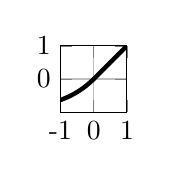
\begin{tikzpicture}
\begin{axis}[
	xmin=-1,xmax=1,
	ymin=-1,ymax=1,
	ytick={0, 1},
	yticklabels={0,1},
	xtick={-1, 0, 1},
	xticklabels={-1,0,1},
	width=.2\textwidth,
	height=.2\textwidth,
	grid=both,
	]
	\addplot [ultra thick,domain=-0.0035:1, samples=10]{x};
	\addplot [ultra thick,domain=-1:0.004, samples=10]{exp(x)-1};
\end{axis}
\end{tikzpicture}}
		\scalebox{.9}{% This file was created by tikzplotlib v0.9.6.
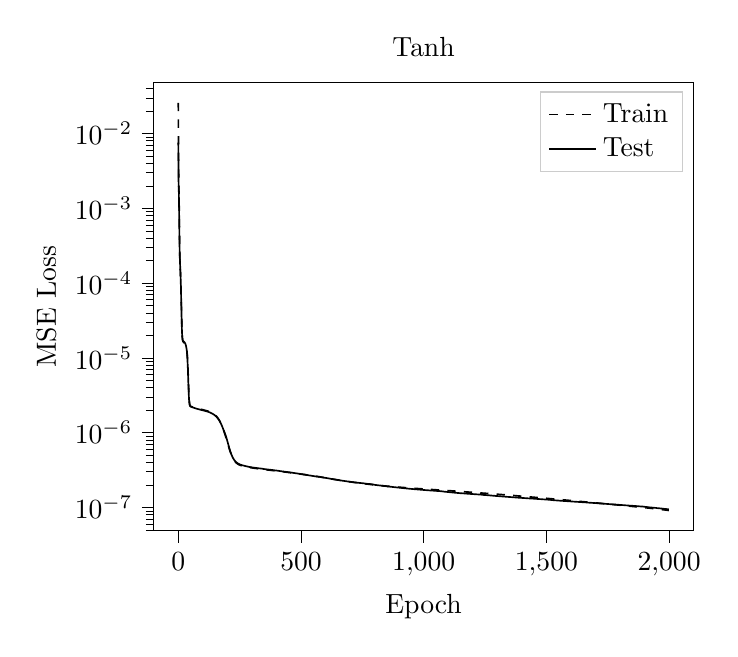
\begin{tikzpicture}

\begin{axis}[
legend cell align={left},
legend style={fill opacity=0.8, draw opacity=1, text opacity=1, draw=white!80!black},
log basis y={10},
tick align=outside,
tick pos=left,
title={Tanh},
x grid style={white!69.0196078431373!black},
xlabel={Epoch},
xmin=-99.95, xmax=2098.95,
xtick style={color=black},
y grid style={white!69.0196078431373!black},
ylabel={MSE Loss},
ymin=4.87162606216586e-08, ymax=0.0480880951021972,
ymode=log,
ytick style={color=black}
]
\addplot [semithick, black, dashed]
table {%
0 0.0256783136818558
1 0.00391949829272926
2 0.00199367450224236
3 0.00143339208001271
4 0.000811647348455153
5 0.000412362531060353
6 0.000244949306972558
7 0.000181991728095454
8 0.000153056107774319
9 0.000130014062575356
10 0.00010614617610554
11 8.2238709928788e-05
12 6.06559043771995e-05
13 4.33234549072949e-05
14 3.11574030747579e-05
15 2.37537921129842e-05
16 1.98036479096118e-05
17 1.79031906054661e-05
18 1.70355609670878e-05
19 1.66247610322898e-05
20 1.63982167177892e-05
21 1.62431279886732e-05
22 1.61158580831398e-05
23 1.59985048476301e-05
24 1.58816735838627e-05
25 1.57583749341939e-05
26 1.56224140046106e-05
27 1.54673897231987e-05
28 1.52862634940902e-05
29 1.50712967133586e-05
30 1.48132416907174e-05
31 1.45002782592201e-05
32 1.41172199300854e-05
33 1.36448685689174e-05
34 1.30603959150903e-05
35 1.23376133224156e-05
36 1.14492682650962e-05
37 1.03756575872467e-05
38 9.12141076651096e-06
39 7.73935586585139e-06
40 6.34618929802855e-06
41 5.09459993941164e-06
42 4.09941510883982e-06
43 3.38837440926909e-06
44 2.91845872209251e-06
45 2.62550942943562e-06
46 2.45301037762147e-06
47 2.35697488326991e-06
48 2.30587279077099e-06
49 2.27869926069957e-06
50 2.26319449416224e-06
51 2.25325485791927e-06
52 2.24564654052983e-06
53 2.23908174814369e-06
54 2.23303946037845e-06
55 2.22724395334239e-06
56 2.22159413002032e-06
57 2.21605597198504e-06
58 2.21059594881012e-06
59 2.20502461627348e-06
60 2.19951089013648e-06
61 2.19409941962567e-06
62 2.18873923640217e-06
63 2.18341688619716e-06
64 2.1780858397733e-06
65 2.1728171752784e-06
66 2.16761157162182e-06
67 2.16247652971902e-06
68 2.15743465199125e-06
69 2.15248080394304e-06
70 2.14761326856205e-06
71 2.14284125951281e-06
72 2.13816882268247e-06
73 2.13358548586484e-06
74 2.12906748606656e-06
75 2.12460380140556e-06
76 2.120198438746e-06
77 2.11584107628937e-06
78 2.11151701626022e-06
79 2.1072322648763e-06
80 2.10301409578051e-06
81 2.09883101015862e-06
82 2.09469965733433e-06
83 2.09061845473002e-06
84 2.08657400560242e-06
85 2.08255163943249e-06
86 2.07854974385668e-06
87 2.07457113936016e-06
88 2.07060074984611e-06
89 2.06666326653249e-06
90 2.06275839008185e-06
91 2.05887886355072e-06
92 2.05505449861221e-06
93 2.0512571416873e-06
94 2.04748774780228e-06
95 2.04372591568358e-06
96 2.03996265599926e-06
97 2.03619106019914e-06
98 2.03241081277383e-06
99 2.02862611661203e-06
100 2.02483424297384e-06
101 2.02102566049689e-06
102 2.01718436369447e-06
103 2.01332004547794e-06
104 2.00943811177012e-06
105 2.00553536137704e-06
106 2.00160756375567e-06
107 1.99764742245634e-06
108 1.99365524949258e-06
109 1.98962802357983e-06
110 1.9855528640278e-06
111 1.98141402830743e-06
112 1.97722682901258e-06
113 1.97299540053564e-06
114 1.96871867424875e-06
115 1.96440277787246e-06
116 1.96000154770104e-06
117 1.9555300951879e-06
118 1.95101178900359e-06
119 1.94641152162944e-06
120 1.94169498476526e-06
121 1.93687540669885e-06
122 1.93201438108304e-06
123 1.92702427668223e-06
124 1.92191399614217e-06
125 1.91670319534865e-06
126 1.91129896376196e-06
127 1.90578242464312e-06
128 1.90011318721872e-06
129 1.89427273897991e-06
130 1.8882123373487e-06
131 1.88198830036868e-06
132 1.87558250883058e-06
133 1.86899712485911e-06
134 1.86227750535295e-06
135 1.85539022578496e-06
136 1.84831423331389e-06
137 1.84095470405055e-06
138 1.83341144793303e-06
139 1.82565649558342e-06
140 1.81764926094274e-06
141 1.8093850391665e-06
142 1.80086963925419e-06
143 1.79206551939615e-06
144 1.78290680096893e-06
145 1.77344423252634e-06
146 1.76363753888609e-06
147 1.75350956513398e-06
148 1.74298757917768e-06
149 1.73214579911019e-06
150 1.72099046380936e-06
151 1.70946602281674e-06
152 1.69748322201713e-06
153 1.68506968657312e-06
154 1.67229672393887e-06
155 1.65912558750847e-06
156 1.64544447042658e-06
157 1.63120314758203e-06
158 1.61646188797704e-06
159 1.60128347954469e-06
160 1.58568593687392e-06
161 1.56952820799461e-06
162 1.55281459512935e-06
163 1.5356757700431e-06
164 1.51809548609094e-06
165 1.50005704529121e-06
166 1.48156487875895e-06
167 1.46263333124352e-06
168 1.44329967625367e-06
169 1.42353404891082e-06
170 1.40324328742736e-06
171 1.38264333622828e-06
172 1.36177704882812e-06
173 1.34056134390903e-06
174 1.31897092293798e-06
175 1.29699397990635e-06
176 1.2747017498782e-06
177 1.25221570530698e-06
178 1.22951809009919e-06
179 1.20664068751353e-06
180 1.18358472803948e-06
181 1.16037225873811e-06
182 1.13706644850708e-06
183 1.11373770050704e-06
184 1.0904470638593e-06
185 1.06723795667563e-06
186 1.04412836427059e-06
187 1.0208118777939e-06
188 9.97641223307255e-07
189 9.74690305525883e-07
190 9.51969390513341e-07
191 9.29392631491055e-07
192 9.06946037218859e-07
193 8.84695177518324e-07
194 8.62814456183969e-07
195 8.41312120513749e-07
196 8.20188414138556e-07
197 7.99479262440173e-07
198 7.79222670900026e-07
199 7.59472292855889e-07
200 7.40254094381498e-07
201 7.21549099239383e-07
202 7.03323363239861e-07
203 6.85619275714089e-07
204 6.6847969463879e-07
205 6.51883700157896e-07
206 6.35866349483649e-07
207 6.20471112625864e-07
208 6.057030220461e-07
209 5.9157178546343e-07
210 5.78070042280387e-07
211 5.65175379023231e-07
212 5.52857127871675e-07
213 5.41098940445295e-07
214 5.29904994237995e-07
215 5.19294521666325e-07
216 5.09250435172248e-07
217 4.99746019073655e-07
218 4.90756391343439e-07
219 4.82253122385146e-07
220 4.74210392084728e-07
221 4.66614737703708e-07
222 4.594722655753e-07
223 4.52780616114978e-07
224 4.46503346267946e-07
225 4.40587696672878e-07
226 4.3501073572827e-07
227 4.29783745403256e-07
228 4.24905776583273e-07
229 4.20343882311158e-07
230 4.16056390292852e-07
231 4.12004934716492e-07
232 4.08168913253348e-07
233 4.04548881093092e-07
234 4.0115957934006e-07
235 3.98017956328545e-07
236 3.95117882121099e-07
237 3.92450205467298e-07
238 3.89984960776246e-07
239 3.87670437433485e-07
240 3.854904206122e-07
241 3.83437721566793e-07
242 3.81521905637783e-07
243 3.79716435688238e-07
244 3.7800730848403e-07
245 3.76387820466562e-07
246 3.74852234386935e-07
247 3.73395006619148e-07
248 3.72012924259479e-07
249 3.70699379175221e-07
250 3.69453458461066e-07
251 3.68269956155132e-07
252 3.67140075951511e-07
253 3.66061015526498e-07
254 3.65028434657688e-07
255 3.64036853241601e-07
256 3.63086354937536e-07
257 3.62170156421371e-07
258 3.61287569361934e-07
259 3.60436046335622e-07
260 3.59612704329493e-07
261 3.58815689537551e-07
262 3.58042329338559e-07
263 3.57291059003728e-07
264 3.56559590528605e-07
265 3.55845987968451e-07
266 3.55149574644997e-07
267 3.54466686573574e-07
268 3.53798637306113e-07
269 3.53151388225115e-07
270 3.52531600483985e-07
271 3.51943575040536e-07
272 3.51372050090504e-07
273 3.50809585640377e-07
274 3.50256817625905e-07
275 3.49712665524748e-07
276 3.49179635776409e-07
277 3.48656109139256e-07
278 3.48143141167157e-07
279 3.47636979228128e-07
280 3.47140434584503e-07
281 3.46653251625639e-07
282 3.46171422521024e-07
283 3.4569364163417e-07
284 3.45216367264811e-07
285 3.44738248372778e-07
286 3.44260469105961e-07
287 3.43785083074977e-07
288 3.43330366902705e-07
289 3.42898308034023e-07
290 3.42464092639716e-07
291 3.42032911291312e-07
292 3.41611756653037e-07
293 3.41200953300813e-07
294 3.4079875696591e-07
295 3.40396311045765e-07
296 3.39994623701045e-07
297 3.39597257266178e-07
298 3.39202901770364e-07
299 3.38812474367955e-07
300 3.38425176110491e-07
301 3.38041470541839e-07
302 3.37660714180288e-07
303 3.37282675587858e-07
304 3.36908611188846e-07
305 3.36536360023842e-07
306 3.36168333262776e-07
307 3.35801948580183e-07
308 3.35437873673072e-07
309 3.350776228217e-07
310 3.34718724388949e-07
311 3.34361913502335e-07
312 3.34007977400574e-07
313 3.3365582474687e-07
314 3.33304566694892e-07
315 3.32955682978309e-07
316 3.32606295486926e-07
317 3.32255786702262e-07
318 3.31905818399036e-07
319 3.31557298508756e-07
320 3.31211877337978e-07
321 3.30875328899083e-07
322 3.30545438856689e-07
323 3.30220234488365e-07
324 3.298965893066e-07
325 3.29574252532439e-07
326 3.29251082263227e-07
327 3.28928731974543e-07
328 3.28607898666178e-07
329 3.28288939684285e-07
330 3.2796907586885e-07
331 3.27652170923898e-07
332 3.27335904060533e-07
333 3.27020988223126e-07
334 3.26706541969202e-07
335 3.26394124385843e-07
336 3.26082249685555e-07
337 3.25770865870823e-07
338 3.25459939233497e-07
339 3.25150717984002e-07
340 3.24840650264946e-07
341 3.24531734875677e-07
342 3.24222071199642e-07
343 3.2391122408626e-07
344 3.23596012492544e-07
345 3.23275019525226e-07
346 3.2294281670886e-07
347 3.22599480000463e-07
348 3.2227435212917e-07
349 3.21953933990926e-07
350 3.21621574045139e-07
351 3.21314297934805e-07
352 3.21034943112863e-07
353 3.20749485581473e-07
354 3.20448250576533e-07
355 3.20144514972753e-07
356 3.19843721285906e-07
357 3.1954650594912e-07
358 3.19254462965546e-07
359 3.18963354061452e-07
360 3.18671405437954e-07
361 3.18381526312805e-07
362 3.1809271050065e-07
363 3.17805669340032e-07
364 3.17520336409416e-07
365 3.17236151289535e-07
366 3.16953998719782e-07
367 3.16672443261723e-07
368 3.16392134422472e-07
369 3.16110889329479e-07
370 3.15829916885946e-07
371 3.15550726682545e-07
372 3.15269492318748e-07
373 3.14990658523584e-07
374 3.14710382866679e-07
375 3.14430895031137e-07
376 3.14152183250371e-07
377 3.13873624463668e-07
378 3.13594867321854e-07
379 3.1331668030532e-07
380 3.13038809508726e-07
381 3.12760674347601e-07
382 3.12483484265158e-07
383 3.12207137426412e-07
384 3.11929519270393e-07
385 3.11651563734472e-07
386 3.11376247253747e-07
387 3.11098750373162e-07
388 3.10823184008768e-07
389 3.10547017605245e-07
390 3.10271550944208e-07
391 3.09995918783557e-07
392 3.09719951715692e-07
393 3.09445476418091e-07
394 3.09168360459466e-07
395 3.08894775159274e-07
396 3.08620413150607e-07
397 3.08344746954958e-07
398 3.08069329236105e-07
399 3.07795802939381e-07
400 3.07521075768591e-07
401 3.07246696138463e-07
402 3.06971505011688e-07
403 3.06696873721535e-07
404 3.06422334631407e-07
405 3.06145008693193e-07
406 3.05865897132662e-07
407 3.05583006166898e-07
408 3.05294879424878e-07
409 3.05009888265317e-07
410 3.04732769805582e-07
411 3.04457269081126e-07
412 3.04181760967026e-07
413 3.03905813524352e-07
414 3.0363094599295e-07
415 3.03357129993742e-07
416 3.03082965743329e-07
417 3.0280785918535e-07
418 3.02532962692226e-07
419 3.0225916734139e-07
420 3.01983990866006e-07
421 3.01708690443547e-07
422 3.01433667928563e-07
423 3.01157673092689e-07
424 3.00882183054796e-07
425 3.00605982133106e-07
426 3.00329158335444e-07
427 3.00052401286166e-07
428 2.99774547642073e-07
429 2.99496324672077e-07
430 2.99217140877772e-07
431 2.98939130772169e-07
432 2.98660514062021e-07
433 2.98383328143359e-07
434 2.98107285431115e-07
435 2.97832286861421e-07
436 2.97559957445515e-07
437 2.97285695779692e-07
438 2.97009015341132e-07
439 2.96733323608578e-07
440 2.96455481390012e-07
441 2.9617858776021e-07
442 2.9590150563763e-07
443 2.95623587916793e-07
444 2.95345244865075e-07
445 2.9506660192169e-07
446 2.94787749211878e-07
447 2.94508583948527e-07
448 2.94228868824575e-07
449 2.93948752528195e-07
450 2.93668269435443e-07
451 2.93385687584191e-07
452 2.93103074923806e-07
453 2.92818450745358e-07
454 2.92533115867855e-07
455 2.92243303405826e-07
456 2.9195033896201e-07
457 2.91650243681829e-07
458 2.91350477510832e-07
459 2.91054979058458e-07
460 2.90767192424823e-07
461 2.90503514534635e-07
462 2.90230797133972e-07
463 2.89949681999246e-07
464 2.89666823135804e-07
465 2.89384619264865e-07
466 2.89102210416559e-07
467 2.88819185129796e-07
468 2.88536360827152e-07
469 2.88253604452393e-07
470 2.87968851523601e-07
471 2.87685964025286e-07
472 2.87401510036034e-07
473 2.87117177379059e-07
474 2.86832849312191e-07
475 2.8654813895912e-07
476 2.86263357793359e-07
477 2.85977837691576e-07
478 2.85691940277388e-07
479 2.85405856359944e-07
480 2.85119550341051e-07
481 2.8483193818829e-07
482 2.84544647684015e-07
483 2.84257998472981e-07
484 2.83969851665233e-07
485 2.83681968156202e-07
486 2.83393235761764e-07
487 2.83104578485904e-07
488 2.82816583634826e-07
489 2.82528103838331e-07
490 2.82238609997876e-07
491 2.81949168339679e-07
492 2.8166003872343e-07
493 2.81370473402376e-07
494 2.81080827463143e-07
495 2.80790753393489e-07
496 2.80500940405659e-07
497 2.80211042010592e-07
498 2.79920554831392e-07
499 2.79629013533622e-07
500 2.79337497119059e-07
501 2.79044599409417e-07
502 2.78752144240002e-07
503 2.78457998902581e-07
504 2.78164109374757e-07
505 2.77869891178284e-07
506 2.77574577594919e-07
507 2.77278857083729e-07
508 2.76983356172877e-07
509 2.7668567361161e-07
510 2.76388693364993e-07
511 2.76090929958173e-07
512 2.75792796927021e-07
513 2.75494566082557e-07
514 2.75195795651939e-07
515 2.74897113726524e-07
516 2.74596931546967e-07
517 2.74297933458456e-07
518 2.7399731402511e-07
519 2.73697588568211e-07
520 2.73398535313163e-07
521 2.73097986720927e-07
522 2.72798081596193e-07
523 2.72497375377156e-07
524 2.721969917161e-07
525 2.71895670650224e-07
526 2.71594623328042e-07
527 2.7129333325604e-07
528 2.70992521649305e-07
529 2.70690323432632e-07
530 2.70388584581838e-07
531 2.70085084920879e-07
532 2.69782810406127e-07
533 2.69479857394117e-07
534 2.69177301504442e-07
535 2.68873798603408e-07
536 2.68569790051743e-07
537 2.68265452916694e-07
538 2.67961485974411e-07
539 2.67657246951103e-07
540 2.67351624302137e-07
541 2.67046286097639e-07
542 2.66741919716651e-07
543 2.66435670084775e-07
544 2.66130026957967e-07
545 2.65824395896175e-07
546 2.6551730083213e-07
547 2.65211784665098e-07
548 2.64905498724488e-07
549 2.64599524172127e-07
550 2.64292502450303e-07
551 2.6398848847009e-07
552 2.63682261532949e-07
553 2.63377035267354e-07
554 2.63071988158003e-07
555 2.62766210369136e-07
556 2.62461571722383e-07
557 2.62156681472447e-07
558 2.61850888776394e-07
559 2.61545947040531e-07
560 2.6124000225991e-07
561 2.60934261390844e-07
562 2.60627847595174e-07
563 2.60322212795927e-07
564 2.60016038239996e-07
565 2.59711214141589e-07
566 2.5940505373967e-07
567 2.59097520512341e-07
568 2.58789286661454e-07
569 2.5847926835354e-07
570 2.5816877410989e-07
571 2.5785619672547e-07
572 2.57544622073169e-07
573 2.57231350587972e-07
574 2.56918664646832e-07
575 2.56602994127775e-07
576 2.56286820288665e-07
577 2.55969035805492e-07
578 2.55648774611927e-07
579 2.5532790500904e-07
580 2.55007268293639e-07
581 2.54691480094493e-07
582 2.54381522779568e-07
583 2.54074222027612e-07
584 2.53768886622652e-07
585 2.53462639946633e-07
586 2.53155078596023e-07
587 2.52848097417768e-07
588 2.52539884442626e-07
589 2.52232671059005e-07
590 2.51926414108539e-07
591 2.51619402433789e-07
592 2.51310856512532e-07
593 2.51001186327926e-07
594 2.50689724069275e-07
595 2.50373325869191e-07
596 2.50046564715944e-07
597 2.4971247898975e-07
598 2.49380338701144e-07
599 2.49063755020984e-07
600 2.48784469974339e-07
601 2.48483565428614e-07
602 2.48175608675183e-07
603 2.47866636698291e-07
604 2.47558843241791e-07
605 2.47249521919457e-07
606 2.4694012356008e-07
607 2.46630496931743e-07
608 2.46319321462352e-07
609 2.4600640222161e-07
610 2.45691713416818e-07
611 2.45375426118244e-07
612 2.45059019846394e-07
613 2.44742416043664e-07
614 2.44427804702241e-07
615 2.44115359791408e-07
616 2.43803189320602e-07
617 2.43488904686728e-07
618 2.43173452574297e-07
619 2.42856562493898e-07
620 2.42540053235984e-07
621 2.4222399055418e-07
622 2.41909370672033e-07
623 2.4159876612373e-07
624 2.41287819818581e-07
625 2.40977986550206e-07
626 2.40667316191434e-07
627 2.40357404365454e-07
628 2.40048627247802e-07
629 2.39740908810404e-07
630 2.39435385040565e-07
631 2.39132102379358e-07
632 2.38831228216441e-07
633 2.38532016894055e-07
634 2.38234100507384e-07
635 2.3793795794802e-07
636 2.37641427077051e-07
637 2.37344928962102e-07
638 2.37049479139273e-07
639 2.36751429071091e-07
640 2.36452641857454e-07
641 2.36152356379193e-07
642 2.35851070470972e-07
643 2.35551766138542e-07
644 2.35254986534983e-07
645 2.34958907981309e-07
646 2.34665752486762e-07
647 2.34375531832143e-07
648 2.34092015489296e-07
649 2.33809699452081e-07
650 2.33527169967829e-07
651 2.33244464084237e-07
652 2.32961468469739e-07
653 2.32677941326642e-07
654 2.32394894752019e-07
655 2.3211163342296e-07
656 2.31829809983708e-07
657 2.31547428853673e-07
658 2.31266236099259e-07
659 2.30985992104138e-07
660 2.30706976715567e-07
661 2.30428674967698e-07
662 2.30152111726056e-07
663 2.29876793980566e-07
664 2.29604099338587e-07
665 2.29333702257861e-07
666 2.29064872783624e-07
667 2.28796595095559e-07
668 2.28530018681283e-07
669 2.2826313580282e-07
670 2.27996663106467e-07
671 2.27733029163346e-07
672 2.27468699684152e-07
673 2.2720402522225e-07
674 2.26941181225016e-07
675 2.26678568793659e-07
676 2.26417082146213e-07
677 2.26155646451787e-07
678 2.25897250800244e-07
679 2.25637136786361e-07
680 2.25378274507193e-07
681 2.25121336775658e-07
682 2.24864484977161e-07
683 2.24608422961126e-07
684 2.24353004966815e-07
685 2.24098303604592e-07
686 2.23845165024272e-07
687 2.23590957716624e-07
688 2.23339868085759e-07
689 2.23087568443248e-07
690 2.22837466004933e-07
691 2.22585833341782e-07
692 2.22337448747112e-07
693 2.22087857792985e-07
694 2.21839565917037e-07
695 2.21591908690755e-07
696 2.21345022012542e-07
697 2.21097984358209e-07
698 2.20852125387694e-07
699 2.2060782892197e-07
700 2.20363927006417e-07
701 2.20120167355731e-07
702 2.19878396393369e-07
703 2.19637687386864e-07
704 2.19396404389727e-07
705 2.19154858328352e-07
706 2.18914575931706e-07
707 2.18667299513697e-07
708 2.18416066260829e-07
709 2.18157695613286e-07
710 2.17917504393483e-07
711 2.17683093978849e-07
712 2.17446162281476e-07
713 2.17212354058915e-07
714 2.16986503602357e-07
715 2.16756925269124e-07
716 2.16528556869378e-07
717 2.16294295185548e-07
718 2.16065943440924e-07
719 2.1583364458877e-07
720 2.15606159549964e-07
721 2.15376262652001e-07
722 2.15151269159719e-07
723 2.14923011839119e-07
724 2.14698939522862e-07
725 2.14466137464342e-07
726 2.14241580749785e-07
727 2.14002345749975e-07
728 2.13779635217293e-07
729 2.13553263428423e-07
730 2.13348029753035e-07
731 2.13115728534774e-07
732 2.12913911404655e-07
733 2.12681533753312e-07
734 2.1250057025668e-07
735 2.12270989564445e-07
736 2.12080155044703e-07
737 2.11840606532121e-07
738 2.11662392217704e-07
739 2.11410442695126e-07
740 2.11244664157562e-07
741 2.10979294507752e-07
742 2.10829887429043e-07
743 2.10549782210023e-07
744 2.10413726215108e-07
745 2.10122939300561e-07
746 2.09999525161209e-07
747 2.09700793199374e-07
748 2.09582869786118e-07
749 2.09277800060192e-07
750 2.09157251006786e-07
751 2.08846759321091e-07
752 2.08716380861063e-07
753 2.08394508241838e-07
754 2.08247044461984e-07
755 2.07928628633169e-07
756 2.07818380481228e-07
757 2.07552191049842e-07
758 2.0744477393464e-07
759 2.07191454308031e-07
760 2.07081657457309e-07
761 2.0683566658164e-07
762 2.06719522203969e-07
763 2.06478433746327e-07
764 2.0635044909767e-07
765 2.06117449401688e-07
766 2.05981543153655e-07
767 2.05756431981285e-07
768 2.0561386548934e-07
769 2.05395930763075e-07
770 2.05249397822627e-07
771 2.05036626113042e-07
772 2.04886012198813e-07
773 2.04679245818795e-07
774 2.04523484633512e-07
775 2.04321535640872e-07
776 2.04161409584458e-07
777 2.03963522885431e-07
778 2.03797197634969e-07
779 2.03599115963016e-07
780 2.03428255403537e-07
781 2.03227953790019e-07
782 2.030431821467e-07
783 2.02847798703942e-07
784 2.02683666543635e-07
785 2.02516986064438e-07
786 2.02353363967234e-07
787 2.02181807019031e-07
788 2.02015970614866e-07
789 2.01841743383113e-07
790 2.01661772905481e-07
791 2.01460166415757e-07
792 2.01229518573598e-07
793 2.01087121354249e-07
794 2.00917898411035e-07
795 2.00780225966923e-07
796 2.00604442376573e-07
797 2.00453189002303e-07
798 2.00287648866038e-07
799 2.00137743007645e-07
800 1.99980189414362e-07
801 1.99827432027178e-07
802 1.99669180005913e-07
803 1.99514663748346e-07
804 1.99357913018616e-07
805 1.99199996849586e-07
806 1.99037115251599e-07
807 1.98870590701006e-07
808 1.98701238232957e-07
809 1.98534945958784e-07
810 1.98443252870106e-07
811 1.98246908794886e-07
812 1.98162096921806e-07
813 1.9793927735634e-07
814 1.97862616772682e-07
815 1.97648748553547e-07
816 1.97567157641743e-07
817 1.97355472479899e-07
818 1.97273760299765e-07
819 1.97065458699797e-07
820 1.96978311969076e-07
821 1.96774255719845e-07
822 1.96680680787154e-07
823 1.96462946391307e-07
824 1.96358382581252e-07
825 1.96272129294073e-07
826 1.96085812284252e-07
827 1.95950416426172e-07
828 1.95843278874008e-07
829 1.95636969095858e-07
830 1.95569540444751e-07
831 1.95350490258761e-07
832 1.95289647095365e-07
833 1.95072461622203e-07
834 1.95013640578168e-07
835 1.94795793944991e-07
836 1.94736558214004e-07
837 1.94521475144427e-07
838 1.94456519217567e-07
839 1.94238834978933e-07
840 1.9416212994372e-07
841 1.93935251495247e-07
842 1.938511577535e-07
843 1.93651539085238e-07
844 1.93595738494423e-07
845 1.93419543499829e-07
846 1.93338983237368e-07
847 1.93155643771092e-07
848 1.93067804922009e-07
849 1.92892168698222e-07
850 1.92794462648749e-07
851 1.92621168871199e-07
852 1.92513661325222e-07
853 1.92361971812716e-07
854 1.92266215115922e-07
855 1.92131815609287e-07
856 1.92028689518509e-07
857 1.91893275420796e-07
858 1.91771540478669e-07
859 1.91640346358213e-07
860 1.91515060819825e-07
861 1.91392229027088e-07
862 1.91263401049468e-07
863 1.91143824686435e-07
864 1.91016867681526e-07
865 1.9089981549314e-07
866 1.90770217429304e-07
867 1.9065634234039e-07
868 1.90525443045431e-07
869 1.90412167242471e-07
870 1.90282269919351e-07
871 1.90172669732647e-07
872 1.90040945632575e-07
873 1.89934002065684e-07
874 1.89798637116212e-07
875 1.89697138701206e-07
876 1.89558307937432e-07
877 1.89464716548571e-07
878 1.89316197278799e-07
879 1.89234877062461e-07
880 1.89073981829324e-07
881 1.89012648903031e-07
882 1.8882984380042e-07
883 1.88791165790292e-07
884 1.88592141974198e-07
885 1.8855339223478e-07
886 1.88359724987208e-07
887 1.88329720955949e-07
888 1.88126539931943e-07
889 1.88094276957429e-07
890 1.87895900772617e-07
891 1.87877068817954e-07
892 1.87662858877502e-07
893 1.87640850128901e-07
894 1.87432238647034e-07
895 1.87432251635755e-07
896 1.87201762059885e-07
897 1.87188818806305e-07
898 1.86971692656357e-07
899 1.86994976040467e-07
900 1.86739167517658e-07
901 1.86732364035436e-07
902 1.86509570291094e-07
903 1.86530011355046e-07
904 1.86241233407713e-07
905 1.86274863906988e-07
906 1.86024884442304e-07
907 1.86029986842584e-07
908 1.85774609136047e-07
909 1.85838526483906e-07
910 1.85592075979457e-07
911 1.85557109972478e-07
912 1.85413238234844e-07
913 1.85311596581528e-07
914 1.85238153171952e-07
915 1.85064903085674e-07
916 1.8492580213092e-07
917 1.84818756245875e-07
918 1.84601177132038e-07
919 1.8463142303915e-07
920 1.84506226155179e-07
921 1.84393604399702e-07
922 1.84358933992712e-07
923 1.84134645067502e-07
924 1.841647220715e-07
925 1.83951926914006e-07
926 1.83905570125376e-07
927 1.83781745690226e-07
928 1.83684701163145e-07
929 1.83511204312481e-07
930 1.8358617639791e-07
931 1.8327896103898e-07
932 1.83298687410627e-07
933 1.83136164785935e-07
934 1.83118544001104e-07
935 1.82905041803849e-07
936 1.82821713821113e-07
937 1.82904439206766e-07
938 1.82656200976794e-07
939 1.82503057061467e-07
940 1.82372852130186e-07
941 1.82464832569451e-07
942 1.82177862498634e-07
943 1.82123570141357e-07
944 1.81958198027132e-07
945 1.82105544006106e-07
946 1.81748656814307e-07
947 1.81644994661667e-07
948 1.81450388794246e-07
949 1.81557134744992e-07
950 1.813367446033e-07
951 1.81250076217054e-07
952 1.8124331060676e-07
953 1.81050296966134e-07
954 1.80912367007124e-07
955 1.81007702494185e-07
956 1.80688111491634e-07
957 1.80711871138328e-07
958 1.80613659338746e-07
959 1.8055098094294e-07
960 1.80342447215764e-07
961 1.80315561223665e-07
962 1.80119200678064e-07
963 1.80223092698384e-07
964 1.79937218476312e-07
965 1.79954523055414e-07
966 1.79713805877668e-07
967 1.79845560126068e-07
968 1.79522391348996e-07
969 1.79567244288137e-07
970 1.794615962325e-07
971 1.79359788418765e-07
972 1.7919894242624e-07
973 1.79157142703446e-07
974 1.78962343092337e-07
975 1.79107667875655e-07
976 1.78761917062786e-07
977 1.78851070963049e-07
978 1.78552461115089e-07
979 1.78618294036426e-07
980 1.78499511285679e-07
981 1.78432811814844e-07
982 1.78235883993239e-07
983 1.7822017412783e-07
984 1.78006425556987e-07
985 1.78184835050388e-07
986 1.77794969182798e-07
987 1.77919801146231e-07
988 1.77607504305399e-07
989 1.77682868525153e-07
990 1.77565874700747e-07
991 1.77483282151059e-07
992 1.77303049056832e-07
993 1.77288027074951e-07
994 1.77071662321282e-07
995 1.77269572674277e-07
996 1.76851885242968e-07
997 1.76987209279389e-07
998 1.76690409439573e-07
999 1.76745455256366e-07
1000 1.76675246279956e-07
1001 1.76517975418733e-07
1002 1.76396269658596e-07
1003 1.76365606833428e-07
1004 1.76154782728588e-07
1005 1.76332453555972e-07
1006 1.75943806638657e-07
1007 1.76068208830316e-07
1008 1.75781630375127e-07
1009 1.75818021048713e-07
1010 1.75775665255173e-07
1011 1.75606383862714e-07
1012 1.75487401570251e-07
1013 1.75443485460391e-07
1014 1.75264921239204e-07
1015 1.75345524404236e-07
1016 1.75081772901819e-07
1017 1.75094191163794e-07
1018 1.75051218050726e-07
1019 1.74866570674226e-07
1020 1.74778132873143e-07
1021 1.74739804535307e-07
1022 1.74538157253323e-07
1023 1.74689216812851e-07
1024 1.74356573701573e-07
1025 1.74413866574241e-07
1026 1.74186691808131e-07
1027 1.74223586959954e-07
1028 1.74151234887177e-07
1029 1.74013387677974e-07
1030 1.7389884820318e-07
1031 1.73856675388606e-07
1032 1.7367983700467e-07
1033 1.73838016891636e-07
1034 1.73464950613322e-07
1035 1.7353948872767e-07
1036 1.733090185283e-07
1037 1.73334884379983e-07
1038 1.73301539497572e-07
1039 1.73104309247663e-07
1040 1.73018324709062e-07
1041 1.72962489585871e-07
1042 1.72787920796225e-07
1043 1.72943589724639e-07
1044 1.72586770247563e-07
1045 1.72631184170768e-07
1046 1.72425827720701e-07
1047 1.72480665220576e-07
1048 1.72308242348151e-07
1049 1.72222635825392e-07
1050 1.72199534759443e-07
1051 1.7209841140442e-07
1052 1.71934404548324e-07
1053 1.71875999363635e-07
1054 1.71818576639282e-07
1055 1.71664782399716e-07
1056 1.71721229904165e-07
1057 1.71507559223016e-07
1058 1.71450052548039e-07
1059 1.71324552624696e-07
1060 1.71405257525237e-07
1061 1.71114308081144e-07
1062 1.71128518353214e-07
1063 1.70986724953082e-07
1064 1.70997916832505e-07
1065 1.70789293711948e-07
1066 1.70840542757844e-07
1067 1.70683409770334e-07
1068 1.70584149131514e-07
1069 1.70473046189556e-07
1070 1.70536510026409e-07
1071 1.70325863329879e-07
1072 1.70239916933212e-07
1073 1.70178448684055e-07
1074 1.70156779681463e-07
1075 1.70017821211843e-07
1076 1.69923560775942e-07
1077 1.69763528241162e-07
1078 1.69926713766699e-07
1079 1.69656568338894e-07
1080 1.6954471659858e-07
1081 1.69526870145376e-07
1082 1.6947657803712e-07
1083 1.69291331680199e-07
1084 1.69387541966159e-07
1085 1.69021876075703e-07
1086 1.69219825430389e-07
1087 1.6888395204262e-07
1088 1.69059036124963e-07
1089 1.68762051210081e-07
1090 1.68699381958959e-07
1091 1.68677553716634e-07
1092 1.6864209008105e-07
1093 1.6840546667396e-07
1094 1.68458437485697e-07
1095 1.68280550276734e-07
1096 1.68226403687299e-07
1097 1.68105190404333e-07
1098 1.68082149194504e-07
1099 1.67917447448929e-07
1100 1.6791531155036e-07
1101 1.67686958455704e-07
1102 1.67809295753329e-07
1103 1.67609576770644e-07
1104 1.67468523144976e-07
1105 1.67500856612435e-07
1106 1.6746117916e-07
1107 1.67153349366345e-07
1108 1.67207376478018e-07
1109 1.67103117760803e-07
1110 1.67111690664967e-07
1111 1.66799030040465e-07
1112 1.66887021485707e-07
1113 1.6675984264225e-07
1114 1.66733511498762e-07
1115 1.66459487857651e-07
1116 1.66677239924695e-07
1117 1.66273404033745e-07
1118 1.66400428263103e-07
1119 1.66187338273005e-07
1120 1.66101584440526e-07
1121 1.66114068328227e-07
1122 1.66078519775681e-07
1123 1.65747365109326e-07
1124 1.65834520352348e-07
1125 1.65732793483642e-07
1126 1.6568083282209e-07
1127 1.65441024208235e-07
1128 1.65423872360293e-07
1129 1.65376426387809e-07
1130 1.65266291709543e-07
1131 1.65075949297488e-07
1132 1.65183653578538e-07
1133 1.64901120811578e-07
1134 1.64889070461527e-07
1135 1.64816789080646e-07
1136 1.64743251978905e-07
1137 1.64549871939812e-07
1138 1.64797036717346e-07
1139 1.64368372125523e-07
1140 1.64327388922914e-07
1141 1.6437572345751e-07
1142 1.64175849306503e-07
1143 1.64098669806378e-07
1144 1.64148435708e-07
1145 1.63833804322167e-07
1146 1.63941523169342e-07
1147 1.6383109585405e-07
1148 1.636207689657e-07
1149 1.6357456372873e-07
1150 1.63597238461932e-07
1151 1.63376890910172e-07
1152 1.63384830955238e-07
1153 1.6318603519494e-07
1154 1.63193474179479e-07
1155 1.6296791127246e-07
1156 1.62943861326426e-07
1157 1.6273880940787e-07
1158 1.62804770901914e-07
1159 1.62569668617607e-07
1160 1.6251618761487e-07
1161 1.62369944625596e-07
1162 1.62474557683368e-07
1163 1.62164271898746e-07
1164 1.62203364439506e-07
1165 1.6202119513764e-07
1166 1.61991749145329e-07
1167 1.61838586954843e-07
1168 1.61991775357251e-07
1169 1.61693534884932e-07
1170 1.61734423144821e-07
1171 1.61486205477956e-07
1172 1.61506580710125e-07
1173 1.61275248807158e-07
1174 1.61340523128217e-07
1175 1.61135238769816e-07
1176 1.6120220598026e-07
1177 1.6093218126656e-07
1178 1.61019107835614e-07
1179 1.60858303864586e-07
1180 1.60795300494954e-07
1181 1.60560779271179e-07
1182 1.606647063781e-07
1183 1.60463883673856e-07
1184 1.60438281078257e-07
1185 1.60245081261223e-07
1186 1.60326889165674e-07
1187 1.60055241750001e-07
1188 1.6013421814165e-07
1189 1.59912973622056e-07
1190 1.59970620472905e-07
1191 1.59738145576682e-07
1192 1.59805658704215e-07
1193 1.5955720218841e-07
1194 1.59621237003194e-07
1195 1.59371404294006e-07
1196 1.59442580354607e-07
1197 1.59209781699587e-07
1198 1.59259970288872e-07
1199 1.59041937585869e-07
1200 1.59072571342733e-07
1201 1.58855913184652e-07
1202 1.58921797947187e-07
1203 1.58672437535756e-07
1204 1.58764354367236e-07
1205 1.58471104839464e-07
1206 1.58557933318093e-07
1207 1.58335334020876e-07
1208 1.58428612778039e-07
1209 1.5810165481156e-07
1210 1.58222141770636e-07
1211 1.57989714331563e-07
1212 1.58009147142479e-07
1213 1.57803747654839e-07
1214 1.57937466838121e-07
1215 1.57602995166428e-07
1216 1.57633344173291e-07
1217 1.57450450885221e-07
1218 1.57564682048417e-07
1219 1.5723370426457e-07
1220 1.57340403383444e-07
1221 1.57073375376626e-07
1222 1.57176691644167e-07
1223 1.5689634754068e-07
1224 1.57032079670216e-07
1225 1.56695187875755e-07
1226 1.56953842733287e-07
1227 1.56568736393581e-07
1228 1.56612420873614e-07
1229 1.56362640737484e-07
1230 1.56375388939978e-07
1231 1.56238784875029e-07
1232 1.56451213698006e-07
1233 1.56064872733452e-07
1234 1.56071111931055e-07
1235 1.55855858885445e-07
1236 1.55867894434891e-07
1237 1.5592698014899e-07
1238 1.55753827151273e-07
1239 1.55547799785438e-07
1240 1.55530699892381e-07
1241 1.55571137803179e-07
1242 1.55404293401773e-07
1243 1.55184656165375e-07
1244 1.55190573323694e-07
1245 1.54982764250633e-07
1246 1.55162933609176e-07
1247 1.54817653481132e-07
1248 1.5485027108042e-07
1249 1.547744172683e-07
1250 1.54679265847335e-07
1251 1.54439792730443e-07
1252 1.54736637590247e-07
1253 1.54300877532876e-07
1254 1.54275749530086e-07
1255 1.54250144028367e-07
1256 1.54043304789298e-07
1257 1.54029483198315e-07
1258 1.53867440310762e-07
1259 1.53782401476121e-07
1260 1.53956117301846e-07
1261 1.53517524005053e-07
1262 1.53721324970491e-07
1263 1.53280332831685e-07
1264 1.53318621009646e-07
1265 1.53157448153252e-07
1266 1.53317707557221e-07
1267 1.53006178400972e-07
1268 1.53078262279394e-07
1269 1.5295192603304e-07
1270 1.52759127885815e-07
1271 1.52895805442199e-07
1272 1.52618819498684e-07
1273 1.52668988391724e-07
1274 1.52435742045043e-07
1275 1.52282082240163e-07
1276 1.52478126885569e-07
1277 1.52267675993301e-07
1278 1.52102081919736e-07
1279 1.51924854762342e-07
1280 1.52071395540077e-07
1281 1.51897150189484e-07
1282 1.5177754506368e-07
1283 1.51588411327452e-07
1284 1.51686713365962e-07
1285 1.51578635318117e-07
1286 1.514046663047e-07
1287 1.51386741720216e-07
1288 1.51236834938118e-07
1289 1.51087039519382e-07
1290 1.51245379640841e-07
1291 1.50855604545086e-07
1292 1.50857793343562e-07
1293 1.50979376975613e-07
1294 1.50700781588853e-07
1295 1.50535089112225e-07
1296 1.50622930220834e-07
1297 1.50551819402267e-07
1298 1.50364579305062e-07
1299 1.50309357970002e-07
1300 1.50167315318583e-07
1301 1.50015147610816e-07
1302 1.50052822462499e-07
1303 1.49995276302661e-07
1304 1.49929092593482e-07
1305 1.49615969156969e-07
1306 1.49589932703975e-07
1307 1.4974333686979e-07
1308 1.49432075829736e-07
1309 1.49371547493615e-07
1310 1.49235247398849e-07
1311 1.49208245971977e-07
1312 1.49100245259604e-07
1313 1.49268570623917e-07
1314 1.48885288751899e-07
1315 1.48768517568953e-07
1316 1.48855611548981e-07
1317 1.4859427885483e-07
1318 1.48693639566488e-07
1319 1.48367197255084e-07
1320 1.48511471429913e-07
1321 1.48261079587542e-07
1322 1.4825105432692e-07
1323 1.48094737163262e-07
1324 1.48087659624707e-07
1325 1.47959285683896e-07
1326 1.47861875170463e-07
1327 1.4779576830648e-07
1328 1.47618505707214e-07
1329 1.47669302762665e-07
1330 1.47545432952256e-07
1331 1.47312891250806e-07
1332 1.47584984269145e-07
1333 1.47121381466775e-07
1334 1.47155481123207e-07
1335 1.47138486575216e-07
1336 1.46936660485153e-07
1337 1.46897626322584e-07
1338 1.46821027406929e-07
1339 1.46725811767112e-07
1340 1.46653712221223e-07
1341 1.46529792196759e-07
1342 1.46487281597274e-07
1343 1.46329400010359e-07
1344 1.46247827714774e-07
1345 1.46147555952325e-07
1346 1.46037953442146e-07
1347 1.45971158666214e-07
1348 1.45886081675428e-07
1349 1.45792722264559e-07
1350 1.45680503919721e-07
1351 1.45593948325029e-07
1352 1.45497979708864e-07
1353 1.45533103278694e-07
1354 1.4527947547549e-07
1355 1.45212114908588e-07
1356 1.45154443664808e-07
1357 1.45234765746238e-07
1358 1.44960471416766e-07
1359 1.44836443077168e-07
1360 1.44837134833153e-07
1361 1.44702509636829e-07
1362 1.44611242220094e-07
1363 1.44524215748731e-07
1364 1.44445664702175e-07
1365 1.44438964461813e-07
1366 1.44254628807516e-07
1367 1.44174589323143e-07
1368 1.44097156415057e-07
1369 1.44165149549735e-07
1370 1.438918012866e-07
1371 1.43834863926884e-07
1372 1.43778407689865e-07
1373 1.43654776103119e-07
1374 1.43601501100932e-07
1375 1.43478440016054e-07
1376 1.43422459309761e-07
1377 1.43299267286068e-07
1378 1.43240890253082e-07
1379 1.43121426198434e-07
1380 1.43058707820387e-07
1381 1.42943359975334e-07
1382 1.42876715720774e-07
1383 1.42766054786136e-07
1384 1.42697908941614e-07
1385 1.42588240770181e-07
1386 1.42517276643161e-07
1387 1.42408500622082e-07
1388 1.42336251322206e-07
1389 1.42228149620394e-07
1390 1.42154443622644e-07
1391 1.42046925965644e-07
1392 1.41968544774329e-07
1393 1.41857630964637e-07
1394 1.41799161355038e-07
1395 1.41669875795003e-07
1396 1.41642744232229e-07
1397 1.41488020773295e-07
1398 1.41444808285485e-07
1399 1.41307266197543e-07
1400 1.41268738268252e-07
1401 1.41131835960095e-07
1402 1.41081490781403e-07
1403 1.4095575309625e-07
1404 1.40900945055478e-07
1405 1.40781008234114e-07
1406 1.40719304582149e-07
1407 1.40605119860027e-07
1408 1.4053854697238e-07
1409 1.40430631219601e-07
1410 1.40360673611895e-07
1411 1.40257951656508e-07
1412 1.40187808121084e-07
1413 1.40090017744399e-07
1414 1.40027148880506e-07
1415 1.39918102711079e-07
1416 1.398644709667e-07
1417 1.39729618609863e-07
1418 1.39709254440845e-07
1419 1.39548208807128e-07
1420 1.39488207395289e-07
1421 1.39385581888973e-07
1422 1.39311794306707e-07
1423 1.39198004013963e-07
1424 1.39159127087396e-07
1425 1.3899639265702e-07
1426 1.38957142148399e-07
1427 1.3883218345967e-07
1428 1.38818436489885e-07
1429 1.38638300825278e-07
1430 1.38555119733041e-07
1431 1.38598182424232e-07
1432 1.38383111163876e-07
1433 1.38299546527776e-07
1434 1.38218821902569e-07
1435 1.38132329730922e-07
1436 1.38036302210764e-07
1437 1.37932765305493e-07
1438 1.37865884262567e-07
1439 1.37768181680542e-07
1440 1.37693862200194e-07
1441 1.37575959314518e-07
1442 1.37563847445676e-07
1443 1.37410551808159e-07
1444 1.37314383366061e-07
1445 1.37217166447101e-07
1446 1.37134599185629e-07
1447 1.37090809047891e-07
1448 1.36948206701959e-07
1449 1.36934800536892e-07
1450 1.36800439307194e-07
1451 1.36791305251904e-07
1452 1.36640489124318e-07
1453 1.36551323684841e-07
1454 1.3647366780134e-07
1455 1.36380717925988e-07
1456 1.36293950461663e-07
1457 1.36197411691796e-07
1458 1.36108559800618e-07
1459 1.36015842777226e-07
1460 1.35925950090154e-07
1461 1.35836153020819e-07
1462 1.35745947254406e-07
1463 1.35656308337673e-07
1464 1.35567192799613e-07
1465 1.35476351189823e-07
1466 1.35388576424589e-07
1467 1.3529987614902e-07
1468 1.35212574981836e-07
1469 1.35123513757662e-07
1470 1.35034041001347e-07
1471 1.34942330241472e-07
1472 1.34852680481856e-07
1473 1.34763203988086e-07
1474 1.34675156090225e-07
1475 1.34583959088275e-07
1476 1.34498445788722e-07
1477 1.34410110952388e-07
1478 1.34325130517254e-07
1479 1.34240905950378e-07
1480 1.34159623293328e-07
1481 1.34082334994901e-07
1482 1.34007962977023e-07
1483 1.3393716164245e-07
1484 1.33868372188317e-07
1485 1.33801153474167e-07
1486 1.33728197575067e-07
1487 1.33651108498611e-07
1488 1.33561932415205e-07
1489 1.33471286439146e-07
1490 1.33377818180236e-07
1491 1.33286574389047e-07
1492 1.33195876379943e-07
1493 1.33103312499827e-07
1494 1.33012573186875e-07
1495 1.32922244659994e-07
1496 1.328316240361e-07
1497 1.32742819303644e-07
1498 1.32652472835559e-07
1499 1.32563086381765e-07
1500 1.32473022716795e-07
1501 1.32383093998101e-07
1502 1.32294703512059e-07
1503 1.32204725133533e-07
1504 1.32114500431157e-07
1505 1.32024823336963e-07
1506 1.31935355909718e-07
1507 1.31843942838827e-07
1508 1.31755951315427e-07
1509 1.31664896130701e-07
1510 1.31577506834901e-07
1511 1.31486739483933e-07
1512 1.31398833772778e-07
1513 1.31310993296552e-07
1514 1.31223457849217e-07
1515 1.31135499088941e-07
1516 1.31049406171257e-07
1517 1.30963723570687e-07
1518 1.30879938801343e-07
1519 1.30797358849577e-07
1520 1.30715271609461e-07
1521 1.30635178784644e-07
1522 1.30553517664111e-07
1523 1.30470073074207e-07
1524 1.30381565455195e-07
1525 1.30291873148281e-07
1526 1.30197957403766e-07
1527 1.30105073552045e-07
1528 1.30015101412084e-07
1529 1.29922131684168e-07
1530 1.29832057609747e-07
1531 1.29743567214291e-07
1532 1.29655932553874e-07
1533 1.29567336209391e-07
1534 1.29478633702718e-07
1535 1.29388707819089e-07
1536 1.29298447703263e-07
1537 1.29211609895208e-07
1538 1.29121361368334e-07
1539 1.2903508240214e-07
1540 1.28947685460901e-07
1541 1.28861089891075e-07
1542 1.28775236419187e-07
1543 1.28692052271617e-07
1544 1.28612261207195e-07
1545 1.2853669561963e-07
1546 1.28464933744965e-07
1547 1.28383591274428e-07
1548 1.28288588584269e-07
1549 1.28192372116587e-07
1550 1.28097349630707e-07
1551 1.28006397964953e-07
1552 1.27916903707614e-07
1553 1.27826293685018e-07
1554 1.27737181870202e-07
1555 1.2764687626543e-07
1556 1.27558287637441e-07
1557 1.2746860927848e-07
1558 1.27379083963319e-07
1559 1.27289022763932e-07
1560 1.272002397954e-07
1561 1.27111350991527e-07
1562 1.27022582084635e-07
1563 1.26932102247679e-07
1564 1.26843040995084e-07
1565 1.26754313335198e-07
1566 1.26665019799077e-07
1567 1.26576261081368e-07
1568 1.26486150506366e-07
1569 1.26398269948425e-07
1570 1.26310102317007e-07
1571 1.26218600009054e-07
1572 1.26132292770365e-07
1573 1.2604147003259e-07
1574 1.2595394938586e-07
1575 1.25864576688173e-07
1576 1.25776658805421e-07
1577 1.25686074447628e-07
1578 1.25598635008828e-07
1579 1.25509957499048e-07
1580 1.25420049670311e-07
1581 1.25333193693677e-07
1582 1.25244157622717e-07
1583 1.25155239857122e-07
1584 1.25067637064546e-07
1585 1.24977565626239e-07
1586 1.24891056422882e-07
1587 1.24802263734125e-07
1588 1.24713928691733e-07
1589 1.24625061047823e-07
1590 1.24537065644859e-07
1591 1.24449508533075e-07
1592 1.24361393055494e-07
1593 1.24273274060727e-07
1594 1.24184724057841e-07
1595 1.24096431704857e-07
1596 1.24009077239862e-07
1597 1.23921701607799e-07
1598 1.23833612477142e-07
1599 1.2374631225498e-07
1600 1.23658226300449e-07
1601 1.2357035235766e-07
1602 1.23482338388214e-07
1603 1.23394856949233e-07
1604 1.23307119714866e-07
1605 1.23220711785166e-07
1606 1.23131181361202e-07
1607 1.23045026157342e-07
1608 1.22957511642596e-07
1609 1.22870412297971e-07
1610 1.22781257239524e-07
1611 1.2269524139441e-07
1612 1.22605206286153e-07
1613 1.2251671019925e-07
1614 1.22426431886424e-07
1615 1.22340115936481e-07
1616 1.22256094321926e-07
1617 1.22175058258733e-07
1618 1.22103615190383e-07
1619 1.2202762109581e-07
1620 1.21916793361265e-07
1621 1.21834089732431e-07
1622 1.21743012215347e-07
1623 1.21660922808076e-07
1624 1.21567334446127e-07
1625 1.21491538585872e-07
1626 1.21390171351266e-07
1627 1.21322823133596e-07
1628 1.21213336576886e-07
1629 1.21154960034175e-07
1630 1.21035876183839e-07
1631 1.20987247662185e-07
1632 1.20860402027745e-07
1633 1.20820134824839e-07
1634 1.2068506220686e-07
1635 1.20652669416188e-07
1636 1.20510663322193e-07
1637 1.20486183746493e-07
1638 1.20336616767247e-07
1639 1.2031963217396e-07
1640 1.20164131615752e-07
1641 1.20150103626315e-07
1642 1.19992589979745e-07
1643 1.19979782780888e-07
1644 1.19823972248412e-07
1645 1.19810623154137e-07
1646 1.19654737659403e-07
1647 1.19639229716029e-07
1648 1.19485491680393e-07
1649 1.19471855569486e-07
1650 1.19316783660395e-07
1651 1.19300847543968e-07
1652 1.19148934437874e-07
1653 1.19132773143349e-07
1654 1.18980588830198e-07
1655 1.18963450141507e-07
1656 1.18812017682046e-07
1657 1.18793472807965e-07
1658 1.18644252474098e-07
1659 1.18625620011414e-07
1660 1.18476356057329e-07
1661 1.18456286585911e-07
1662 1.18310040200242e-07
1663 1.1828933644864e-07
1664 1.18143192537445e-07
1665 1.18121343611222e-07
1666 1.17981712925541e-07
1667 1.1796190426594e-07
1668 1.17837449707281e-07
1669 1.17821046096367e-07
1670 1.17664518249683e-07
1671 1.17625616695705e-07
1672 1.17494159866283e-07
1673 1.17454599340761e-07
1674 1.17330423812234e-07
1675 1.17281875056108e-07
1676 1.17167207086766e-07
1677 1.17112645753537e-07
1678 1.17004529613496e-07
1679 1.16942329213998e-07
1680 1.16840053991041e-07
1681 1.16773833177319e-07
1682 1.16675894744844e-07
1683 1.16606030751143e-07
1684 1.16511720229084e-07
1685 1.16438417961717e-07
1686 1.1634670725158e-07
1687 1.16271883264574e-07
1688 1.16182274517485e-07
1689 1.16104469931599e-07
1690 1.16017207645314e-07
1691 1.15939320814107e-07
1692 1.1585205044895e-07
1693 1.15773689692844e-07
1694 1.15688439173312e-07
1695 1.15609684797846e-07
1696 1.15523752249658e-07
1697 1.15442792669285e-07
1698 1.15360084031124e-07
1699 1.152794114887e-07
1700 1.15195414622349e-07
1701 1.15116151533812e-07
1702 1.15032597470588e-07
1703 1.14952266152102e-07
1704 1.14869341658164e-07
1705 1.14788415693567e-07
1706 1.14706799855924e-07
1707 1.14626587183864e-07
1708 1.14544958570661e-07
1709 1.14467005680297e-07
1710 1.14386371400599e-07
1711 1.14309840782312e-07
1712 1.14231534574571e-07
1713 1.14155406919281e-07
1714 1.14076618189074e-07
1715 1.1400160070707e-07
1716 1.13935357504147e-07
1717 1.13852153852179e-07
1718 1.1374592218516e-07
1719 1.13668901171593e-07
1720 1.13586670188681e-07
1721 1.13503399141734e-07
1722 1.13423729317219e-07
1723 1.13342144530293e-07
1724 1.13260248220115e-07
1725 1.13178309291584e-07
1726 1.13098485158503e-07
1727 1.13015533877103e-07
1728 1.12935625388388e-07
1729 1.12853559258497e-07
1730 1.12772581523757e-07
1731 1.12691697047751e-07
1732 1.12609595291246e-07
1733 1.1252984580068e-07
1734 1.12447377652813e-07
1735 1.12366985916879e-07
1736 1.1228577866973e-07
1737 1.12205130093912e-07
1738 1.12124054268747e-07
1739 1.1204307208601e-07
1740 1.11962179772718e-07
1741 1.11882094351756e-07
1742 1.11800244731342e-07
1743 1.11719630730533e-07
1744 1.11639534196684e-07
1745 1.11557851859345e-07
1746 1.11477907729807e-07
1747 1.11396160754396e-07
1748 1.1131719745805e-07
1749 1.11234583393127e-07
1750 1.11156175847782e-07
1751 1.11073824463404e-07
1752 1.1099390077618e-07
1753 1.10913257636014e-07
1754 1.10833950522249e-07
1755 1.10751658766617e-07
1756 1.10673457989208e-07
1757 1.10590813854117e-07
1758 1.10513686372826e-07
1759 1.10427929719492e-07
1760 1.10354096037213e-07
1761 1.1026718136975e-07
1762 1.10195531284774e-07
1763 1.10103467726219e-07
1764 1.10038613662766e-07
1765 1.09938720179059e-07
1766 1.09883219252538e-07
1767 1.09774770230331e-07
1768 1.09726113770137e-07
1769 1.0961239318874e-07
1770 1.09567085601725e-07
1771 1.09453343561938e-07
1772 1.09406560120817e-07
1773 1.09293789691378e-07
1774 1.09247273940127e-07
1775 1.09132642720056e-07
1776 1.09087160637955e-07
1777 1.08973743436991e-07
1778 1.08927465625186e-07
1779 1.08812749033405e-07
1780 1.08768906656564e-07
1781 1.08653364364386e-07
1782 1.08610696209155e-07
1783 1.08492045278297e-07
1784 1.08451488785022e-07
1785 1.08332703078418e-07
1786 1.08292764849693e-07
1787 1.08172346592994e-07
1788 1.08134267669868e-07
1789 1.08012495928733e-07
1790 1.07974928781118e-07
1791 1.07852817237131e-07
1792 1.07816773052605e-07
1793 1.07694217973631e-07
1794 1.076585755726e-07
1795 1.07533660980152e-07
1796 1.0750032522111e-07
1797 1.07374868321131e-07
1798 1.07341590407373e-07
1799 1.07214731805527e-07
1800 1.07183627001461e-07
1801 1.07055369142017e-07
1802 1.07025273905492e-07
1803 1.06897582774934e-07
1804 1.06866378018822e-07
1805 1.06738425301955e-07
1806 1.06709044885633e-07
1807 1.06578284807313e-07
1808 1.06551349951189e-07
1809 1.06419266913349e-07
1810 1.06393436325902e-07
1811 1.0626070748998e-07
1812 1.06233781600906e-07
1813 1.06102325410973e-07
1814 1.06077179772512e-07
1815 1.05943803617947e-07
1816 1.05918884933942e-07
1817 1.05785039274053e-07
1818 1.0576097081838e-07
1819 1.05625972793177e-07
1820 1.05602148408934e-07
1821 1.05468074529824e-07
1822 1.05444441423685e-07
1823 1.05309890450656e-07
1824 1.05286905679236e-07
1825 1.05151352997268e-07
1826 1.05128677049038e-07
1827 1.04993245805929e-07
1828 1.04970954780015e-07
1829 1.04834349158978e-07
1830 1.04813155957117e-07
1831 1.04675824211142e-07
1832 1.04656024795702e-07
1833 1.04517476188448e-07
1834 1.04497554922034e-07
1835 1.04359976702995e-07
1836 1.04338933539339e-07
1837 1.04202867277081e-07
1838 1.04181184603647e-07
1839 1.04044154433325e-07
1840 1.04023431063638e-07
1841 1.03886127348574e-07
1842 1.03865805684222e-07
1843 1.03730083061748e-07
1844 1.03708399777247e-07
1845 1.03575531461786e-07
1846 1.03553730738781e-07
1847 1.03431781575125e-07
1848 1.03406835641806e-07
1849 1.03251629880674e-07
1850 1.03248295282299e-07
1851 1.03094720223851e-07
1852 1.03084822235644e-07
1853 1.029415868814e-07
1854 1.02924780257752e-07
1855 1.02787245204183e-07
1856 1.02766203596616e-07
1857 1.02631769628658e-07
1858 1.02608433905971e-07
1859 1.02473619911336e-07
1860 1.02450679698052e-07
1861 1.02315491744775e-07
1862 1.02293353030802e-07
1863 1.02158083478798e-07
1864 1.02137613730235e-07
1865 1.02001180536604e-07
1866 1.01981320298705e-07
1867 1.0184516611389e-07
1868 1.0182440312434e-07
1869 1.01688210200734e-07
1870 1.01670011382282e-07
1871 1.01530907663516e-07
1872 1.01513423203414e-07
1873 1.01376702275502e-07
1874 1.01358417559538e-07
1875 1.01222969291825e-07
1876 1.01205789569292e-07
1877 1.01067017183709e-07
1878 1.01052819672987e-07
1879 1.00915272618352e-07
1880 1.0090144083108e-07
1881 1.00764368340833e-07
1882 1.00751233624408e-07
1883 1.00615954877981e-07
1884 1.00604420119055e-07
1885 1.0046848284162e-07
1886 1.00461983791433e-07
1887 1.00328959490525e-07
1888 1.00327407132283e-07
1889 1.00198732020829e-07
1890 1.00210742438378e-07
1891 1.00091209333186e-07
1892 1.00120992215125e-07
1893 1.00010873573808e-07
1894 1.00031446216065e-07
1895 9.98494305122222e-08
1896 9.98177236226638e-08
1897 9.96636280206076e-08
1898 9.9662101789022e-08
1899 9.95036318087727e-08
1900 9.95035710644743e-08
1901 9.93359447178932e-08
1902 9.93463889713553e-08
1903 9.91639390761634e-08
1904 9.91915004178168e-08
1905 9.89930967563168e-08
1906 9.90359007531083e-08
1907 9.88282890048708e-08
1908 9.88751828856493e-08
1909 9.86779837575114e-08
1910 9.86860634668574e-08
1911 9.85199047107699e-08
1912 9.85522943679484e-08
1913 9.83903354097038e-08
1914 9.83319166465435e-08
1915 9.82184653537388e-08
1916 9.81738594347803e-08
1917 9.80355162667479e-08
1918 9.80704097628404e-08
1919 9.79550177007127e-08
1920 9.79253364477017e-08
1921 9.7782193442697e-08
1922 9.76768999620958e-08
1923 9.76173793958424e-08
1924 9.75287996425322e-08
1925 9.74686554826576e-08
1926 9.73918850419864e-08
1927 9.72836267649768e-08
1928 9.73122499345891e-08
1929 9.7137337192521e-08
1930 9.70798927966143e-08
1931 9.69518271602965e-08
1932 9.69189093709133e-08
1933 9.67950209869173e-08
1934 9.67396970565915e-08
1935 9.66325465867612e-08
1936 9.65764778655398e-08
1937 9.64863556447426e-08
1938 9.63525852242242e-08
1939 9.63383329022349e-08
1940 9.61832626558135e-08
1941 9.61392340954603e-08
1942 9.59978614645252e-08
1943 9.59531415389847e-08
1944 9.57992250434359e-08
1945 9.57176675484561e-08
1946 9.56372701708119e-08
1947 9.55616131150805e-08
1948 9.55027764604211e-08
1949 9.54192266604537e-08
1950 9.52890652783367e-08
1951 9.52766380919456e-08
1952 9.51284585539724e-08
1953 9.50952942702088e-08
1954 9.4968490913061e-08
1955 9.49355355217563e-08
1956 9.48217696077336e-08
1957 9.47154426356178e-08
1958 9.46745343597399e-08
1959 9.45576307387341e-08
1960 9.44733649959062e-08
1961 9.44023931381821e-08
1962 9.43122054337664e-08
1963 9.42393481651038e-08
1964 9.41573721391364e-08
1965 9.40662891650845e-08
1966 9.40114193213049e-08
1967 9.39233958447971e-08
1968 9.38029722874489e-08
1969 9.37450194555822e-08
1970 9.36574502858889e-08
1971 9.35782248561168e-08
1972 9.34887714336696e-08
1973 9.3408080211077e-08
1974 9.33098989790437e-08
1975 9.32318668986909e-08
1976 9.31109529389573e-08
1977 9.30678109511973e-08
1978 9.29844462476126e-08
1979 9.28701786762076e-08
1980 9.28146823682141e-08
1981 9.27165723680901e-08
1982 9.26600080148887e-08
1983 9.25481256501825e-08
1984 9.24809953559702e-08
1985 9.238034407133e-08
1986 9.2328959901522e-08
1987 9.22276714661052e-08
1988 9.21186526383622e-08
1989 9.20790567349172e-08
1990 9.19701495902814e-08
1991 9.18760605159719e-08
1992 9.18214794936034e-08
1993 9.17084328833084e-08
1994 9.16553286174349e-08
1995 9.15473841729408e-08
1996 9.14629573642856e-08
1997 9.13915596143511e-08
1998 9.12936959593935e-08
1999 9.12315428038823e-08
};
\addlegendentry{Train}
\addplot [semithick, black]
table {%
0 0.00757189933210611
1 0.00231354776769876
2 0.00172689720056951
3 0.00111725344322622
4 0.000576228136196733
5 0.000321307015838102
6 0.000222852322622202
7 0.00018314401677344
8 0.000157202070113271
9 0.000131142092868686
10 0.000103817488707136
11 7.77645473135635e-05
12 5.55872247787192e-05
13 3.89783745049499e-05
14 2.82207911368459e-05
15 2.21843656618148e-05
16 1.91927338164533e-05
17 1.78358131961431e-05
18 1.72350355569506e-05
19 1.69452778209234e-05
20 1.67743528436404e-05
21 1.66473146236967e-05
22 1.65352812473429e-05
23 1.64228040375747e-05
24 1.6300236893585e-05
25 1.61624484462664e-05
26 1.60050221893471e-05
27 1.58211023517651e-05
28 1.56023888848722e-05
29 1.53401488205418e-05
30 1.50225159813999e-05
31 1.46344837048673e-05
32 1.41610498758382e-05
33 1.35855179905775e-05
34 1.28874389702105e-05
35 1.20397271530237e-05
36 1.10160563053796e-05
37 9.80650656856596e-06
38 8.43856741994387e-06
39 6.99934525982826e-06
40 5.63651110496721e-06
41 4.49852859674138e-06
42 3.65314713235421e-06
43 3.07963659906818e-06
44 2.71202293333772e-06
45 2.48932860813511e-06
46 2.36340451920114e-06
47 2.29604233936698e-06
48 2.26174938688928e-06
49 2.24436098505976e-06
50 2.23402162191633e-06
51 2.22632638724463e-06
52 2.21947198042471e-06
53 2.21231721297954e-06
54 2.20599281419709e-06
55 2.20017341234779e-06
56 2.19425942304952e-06
57 2.18812738239649e-06
58 2.18169157051307e-06
59 2.17522529055714e-06
60 2.16870125768764e-06
61 2.16252578866261e-06
62 2.15704108086356e-06
63 2.15156410376949e-06
64 2.14648275687068e-06
65 2.14147098631656e-06
66 2.13616635846847e-06
67 2.13079192690202e-06
68 2.12541522159881e-06
69 2.1200858100201e-06
70 2.11486621992663e-06
71 2.10983034776291e-06
72 2.1049518181826e-06
73 2.10016810342495e-06
74 2.09545669349609e-06
75 2.09080417334917e-06
76 2.08621918318386e-06
77 2.08170968107879e-06
78 2.07733137358446e-06
79 2.07305447474937e-06
80 2.06868594432308e-06
81 2.06437994165753e-06
82 2.06043318939919e-06
83 2.05644232664781e-06
84 2.0524073534034e-06
85 2.04834668693366e-06
86 2.04438651962846e-06
87 2.04050184038351e-06
88 2.03653394237335e-06
89 2.03256013264763e-06
90 2.02859519049525e-06
91 2.02469618670875e-06
92 2.02088699552405e-06
93 2.01716375158867e-06
94 2.01350235329301e-06
95 2.00988574761141e-06
96 2.00627096091921e-06
97 2.00259637495037e-06
98 1.99885994334181e-06
99 1.99508667719783e-06
100 1.99131750378001e-06
101 1.98756606550887e-06
102 1.98379348148592e-06
103 1.97998292605917e-06
104 1.97613053387613e-06
105 1.97224085241032e-06
106 1.96831024368294e-06
107 1.96435007637774e-06
108 1.96036580746295e-06
109 1.95635175259667e-06
110 1.95229063137958e-06
111 1.94816198018088e-06
112 1.94399422071001e-06
113 1.93980258700321e-06
114 1.9355888980499e-06
115 1.93136861526e-06
116 1.92722677638812e-06
117 1.92289826372871e-06
118 1.91830258700065e-06
119 1.91340882338409e-06
120 1.90855348591867e-06
121 1.90414561984653e-06
122 1.89889465218585e-06
123 1.89397746908071e-06
124 1.88939679901523e-06
125 1.88414048807317e-06
126 1.87855380318069e-06
127 1.87314526556293e-06
128 1.86755323738907e-06
129 1.86166766980023e-06
130 1.85547753517312e-06
131 1.84901341526711e-06
132 1.84264706604154e-06
133 1.83605436632206e-06
134 1.82956421213021e-06
135 1.82338919785252e-06
136 1.81552900357929e-06
137 1.80827692020102e-06
138 1.80085896772653e-06
139 1.79312894488248e-06
140 1.78544337359199e-06
141 1.77783579147217e-06
142 1.76977698629344e-06
143 1.76120738615282e-06
144 1.75235982169397e-06
145 1.74406659425586e-06
146 1.73541684489464e-06
147 1.72538182141579e-06
148 1.71526744452422e-06
149 1.70504654306569e-06
150 1.69440045283409e-06
151 1.68317467341694e-06
152 1.67212203905365e-06
153 1.66097026976786e-06
154 1.64922550993651e-06
155 1.6366448107874e-06
156 1.62349863330746e-06
157 1.61000264142785e-06
158 1.59640455876797e-06
159 1.5825156651772e-06
160 1.56760324898642e-06
161 1.55271811763669e-06
162 1.53781195422198e-06
163 1.5225629113047e-06
164 1.50687731093058e-06
165 1.49068762311799e-06
166 1.47391403970687e-06
167 1.456628865526e-06
168 1.43905299410108e-06
169 1.41962095767667e-06
170 1.39984229008405e-06
171 1.37973813707504e-06
172 1.35911807319644e-06
173 1.33792514134257e-06
174 1.31609863274207e-06
175 1.29385193758935e-06
176 1.27185285236919e-06
177 1.24993607641954e-06
178 1.22776793887169e-06
179 1.20523759505886e-06
180 1.18257298709068e-06
181 1.16014371087658e-06
182 1.1381328022253e-06
183 1.11657402612764e-06
184 1.09565598904737e-06
185 1.07576920527208e-06
186 1.05480546608305e-06
187 1.03400623174821e-06
188 1.01384318895725e-06
189 9.94196057035879e-07
190 9.75076432041533e-07
191 9.54211259340809e-07
192 9.33810667902435e-07
193 9.13567589577724e-07
194 8.93540118340752e-07
195 8.7334251475113e-07
196 8.52891048452875e-07
197 8.32212890600204e-07
198 8.11159679869888e-07
199 7.90065314504318e-07
200 7.69062353356276e-07
201 7.48205820855219e-07
202 7.27842859760131e-07
203 7.08114953340555e-07
204 6.88830937178864e-07
205 6.70056067519909e-07
206 6.51937568818539e-07
207 6.344951657411e-07
208 6.17837599747872e-07
209 6.02160469043156e-07
210 5.87514819017088e-07
211 5.7384960427953e-07
212 5.60921989745111e-07
213 5.48473678918526e-07
214 5.36510526671918e-07
215 5.25344830748509e-07
216 5.15033946157928e-07
217 5.05386367422034e-07
218 4.96285395001905e-07
219 4.87689192141261e-07
220 4.79516529594548e-07
221 4.71730061235576e-07
222 4.64458850046867e-07
223 4.57714065760229e-07
224 4.51481156460432e-07
225 4.45709758878365e-07
226 4.40336776819095e-07
227 4.35368264106728e-07
228 4.30750020541382e-07
229 4.26469654257744e-07
230 4.22478933614912e-07
231 4.18747390540375e-07
232 4.15171484746679e-07
233 4.11659840438006e-07
234 4.08245057315071e-07
235 4.04999781267179e-07
236 4.02141182576088e-07
237 3.99803269601762e-07
238 3.97628497239566e-07
239 3.95445340473088e-07
240 3.93182233437983e-07
241 3.91090793527837e-07
242 3.89197737149516e-07
243 3.87470691975977e-07
244 3.85885044806855e-07
245 3.84415926646398e-07
246 3.83027412453885e-07
247 3.81678120220386e-07
248 3.80339741923308e-07
249 3.78988659122115e-07
250 3.77662075834451e-07
251 3.76379944100336e-07
252 3.75157839016538e-07
253 3.73988797264246e-07
254 3.72877764220902e-07
255 3.71828406287023e-07
256 3.70837085483799e-07
257 3.69894536333959e-07
258 3.68992459698347e-07
259 3.6814256532125e-07
260 3.67322599004183e-07
261 3.66545179986133e-07
262 3.65790839396141e-07
263 3.65060742524292e-07
264 3.64350427162208e-07
265 3.63658926971766e-07
266 3.6297012684372e-07
267 3.62264984232752e-07
268 3.61526559800041e-07
269 3.60765056939272e-07
270 3.60008925781585e-07
271 3.59255551529714e-07
272 3.58531451638555e-07
273 3.57854787580436e-07
274 3.57219846591761e-07
275 3.56612247287558e-07
276 3.56021757852432e-07
277 3.55441471810991e-07
278 3.54872724983579e-07
279 3.5430537081993e-07
280 3.53727727997466e-07
281 3.53136783814989e-07
282 3.52505253431445e-07
283 3.51853060465146e-07
284 3.51204761273038e-07
285 3.50592699760455e-07
286 3.50021139183809e-07
287 3.49473793903599e-07
288 3.48943643757593e-07
289 3.48437907859989e-07
290 3.47962895830278e-07
291 3.47516419196836e-07
292 3.47084636587169e-07
293 3.46643815873904e-07
294 3.46207571055857e-07
295 3.45778602195423e-07
296 3.45349405961315e-07
297 3.44927741480205e-07
298 3.44512613992265e-07
299 3.44105728800059e-07
300 3.43703817407004e-07
301 3.43302190231043e-07
302 3.42907014783123e-07
303 3.42518376328371e-07
304 3.42130419994646e-07
305 3.41749966992211e-07
306 3.4137428883696e-07
307 3.40999292802735e-07
308 3.40631828521509e-07
309 3.40271498089351e-07
310 3.39915942504376e-07
311 3.39561637474617e-07
312 3.3922066222658e-07
313 3.38877697458884e-07
314 3.38540672828458e-07
315 3.38199868110678e-07
316 3.37851616905027e-07
317 3.37482163104141e-07
318 3.37094775204605e-07
319 3.36706733605752e-07
320 3.36351888563513e-07
321 3.36034361225757e-07
322 3.35738150170073e-07
323 3.35447850829951e-07
324 3.35154368258372e-07
325 3.34855684513968e-07
326 3.34556517600504e-07
327 3.34259254941571e-07
328 3.33956762688103e-07
329 3.33655520989851e-07
330 3.33354051917922e-07
331 3.33054515522235e-07
332 3.32753842258171e-07
333 3.32451463691541e-07
334 3.3215061989722e-07
335 3.31850685597601e-07
336 3.31551120780205e-07
337 3.31250816998363e-07
338 3.30956197558407e-07
339 3.30654899016736e-07
340 3.30352634136943e-07
341 3.30052529307068e-07
342 3.29739606286239e-07
343 3.29404372223507e-07
344 3.29015591660209e-07
345 3.28506928326533e-07
346 3.27803860500353e-07
347 3.27093715668525e-07
348 3.26682112472554e-07
349 3.26361146107956e-07
350 3.26064309774665e-07
351 3.25769036635393e-07
352 3.25465521200385e-07
353 3.2514194003852e-07
354 3.24804005913393e-07
355 3.2445936426484e-07
356 3.2412404493698e-07
357 3.2380171433033e-07
358 3.23506583299604e-07
359 3.23233706467363e-07
360 3.2297887742061e-07
361 3.2273538863592e-07
362 3.22502614835685e-07
363 3.22266515695446e-07
364 3.2202081001742e-07
365 3.21777207545892e-07
366 3.21515415180329e-07
367 3.21252258572713e-07
368 3.20981712320645e-07
369 3.20703321676774e-07
370 3.20423680477688e-07
371 3.20136365417056e-07
372 3.19852574648394e-07
373 3.19564719575283e-07
374 3.19271521220799e-07
375 3.1898002816888e-07
376 3.1868364658294e-07
377 3.18386923936487e-07
378 3.18089206530203e-07
379 3.17792569148878e-07
380 3.1749257800584e-07
381 3.17192132115451e-07
382 3.16892339924379e-07
383 3.16590472948519e-07
384 3.16285337476074e-07
385 3.15979974629954e-07
386 3.15677851858709e-07
387 3.15374336423702e-07
388 3.15068149348008e-07
389 3.14764093900521e-07
390 3.14461033212865e-07
391 3.14160985226408e-07
392 3.13857782430205e-07
393 3.13559326059476e-07
394 3.13264166607041e-07
395 3.12967046056656e-07
396 3.126754393179e-07
397 3.12380734612816e-07
398 3.12092197418679e-07
399 3.1180573500933e-07
400 3.11520835793999e-07
401 3.1123687449508e-07
402 3.109554427283e-07
403 3.10673982539811e-07
404 3.10383768464817e-07
405 3.10078576148953e-07
406 3.09742489434939e-07
407 3.09323354485969e-07
408 3.08814122718104e-07
409 3.08301679297074e-07
410 3.07875410499037e-07
411 3.07510362063113e-07
412 3.07177742797649e-07
413 3.06860954424337e-07
414 3.06547633499576e-07
415 3.06238348457555e-07
416 3.05929802379978e-07
417 3.05623501617447e-07
418 3.05316746107565e-07
419 3.0501209380418e-07
420 3.04705650933101e-07
421 3.04400629147494e-07
422 3.04095436831631e-07
423 3.03792347722265e-07
424 3.0348772384059e-07
425 3.03186652672593e-07
426 3.02881346669892e-07
427 3.0258306082942e-07
428 3.02280739106209e-07
429 3.01978758443511e-07
430 3.01679307312952e-07
431 3.01367464317082e-07
432 3.01058463492154e-07
433 3.00743096204314e-07
434 3.00439211287085e-07
435 3.00134502140281e-07
436 2.99837438433315e-07
437 2.99543046367035e-07
438 2.99252008062467e-07
439 2.98959179190206e-07
440 2.98670812526325e-07
441 2.98377415219875e-07
442 2.98092288630869e-07
443 2.97805769378101e-07
444 2.97516294267552e-07
445 2.97226904422132e-07
446 2.96939759891757e-07
447 2.96649517395053e-07
448 2.96361463369976e-07
449 2.9607238616336e-07
450 2.95783678438966e-07
451 2.9549653390859e-07
452 2.95206461942144e-07
453 2.94913974130395e-07
454 2.94622765295571e-07
455 2.94328202699035e-07
456 2.94032219017026e-07
457 2.93726856170906e-07
458 2.93400375994679e-07
459 2.93056245936896e-07
460 2.92704640969532e-07
461 2.92339279894804e-07
462 2.91982189537521e-07
463 2.916349330917e-07
464 2.91295805254776e-07
465 2.90963839688629e-07
466 2.90640571165568e-07
467 2.9031514259259e-07
468 2.89994574131924e-07
469 2.89677274167843e-07
470 2.8935261298102e-07
471 2.89030936073686e-07
472 2.88709486540029e-07
473 2.88387298041926e-07
474 2.88059794684159e-07
475 2.87732376591521e-07
476 2.87408454369142e-07
477 2.87082883687617e-07
478 2.86762286805242e-07
479 2.86445697383897e-07
480 2.86128852167167e-07
481 2.85815588085825e-07
482 2.85504285102434e-07
483 2.8518959993562e-07
484 2.84878638012742e-07
485 2.84563554941997e-07
486 2.84243895976033e-07
487 2.83925572830412e-07
488 2.8360332748889e-07
489 2.83278296819844e-07
490 2.82954090380372e-07
491 2.82632413473038e-07
492 2.82310963939381e-07
493 2.81987439620934e-07
494 2.81669628066084e-07
495 2.8134996910012e-07
496 2.81029997495352e-07
497 2.8070328994545e-07
498 2.80369363281352e-07
499 2.8002617113998e-07
500 2.79674736702873e-07
501 2.79321369589525e-07
502 2.78964876088139e-07
503 2.78612588999749e-07
504 2.78259335573239e-07
505 2.77912278079384e-07
506 2.77564993211854e-07
507 2.77221516853388e-07
508 2.76879177363298e-07
509 2.76540163213213e-07
510 2.76203877547232e-07
511 2.75865488674754e-07
512 2.75532954674418e-07
513 2.75196896382113e-07
514 2.74859843329978e-07
515 2.74528446198019e-07
516 2.74192359484005e-07
517 2.73856898047597e-07
518 2.73519759730334e-07
519 2.73187993116153e-07
520 2.72854521199406e-07
521 2.72520907174112e-07
522 2.72190249006599e-07
523 2.71860500333787e-07
524 2.71530780082685e-07
525 2.71202821977568e-07
526 2.70876626018435e-07
527 2.70549492142891e-07
528 2.70224234100169e-07
529 2.69898720262063e-07
530 2.69571984290451e-07
531 2.69245134632001e-07
532 2.68921638735264e-07
533 2.68594334329464e-07
534 2.68267854153237e-07
535 2.67942539267096e-07
536 2.67619753913095e-07
537 2.67293870592766e-07
538 2.66968754658592e-07
539 2.66641421831082e-07
540 2.66317840669217e-07
541 2.65991502601537e-07
542 2.65664453991121e-07
543 2.65339707539169e-07
544 2.65014250544482e-07
545 2.64691379925353e-07
546 2.64365638713571e-07
547 2.64044984987777e-07
548 2.63720068005568e-07
549 2.63397822664047e-07
550 2.63078590023724e-07
551 2.62759584757077e-07
552 2.6244461537317e-07
553 2.62132488160205e-07
554 2.61824112612885e-07
555 2.61524007783009e-07
556 2.61230638898269e-07
557 2.60943522789603e-07
558 2.60669281715309e-07
559 2.6040129341709e-07
560 2.60138591556824e-07
561 2.59882455111438e-07
562 2.59628933463318e-07
563 2.59385018352987e-07
564 2.59151164527793e-07
565 2.58942520758865e-07
566 2.58750475268243e-07
567 2.58566956290451e-07
568 2.58378776152313e-07
569 2.58176783063391e-07
570 2.57968707728651e-07
571 2.57760461863654e-07
572 2.57557303484646e-07
573 2.57359033639659e-07
574 2.57157324767832e-07
575 2.56948908372578e-07
576 2.5672730430415e-07
577 2.56481172300482e-07
578 2.56194681469424e-07
579 2.55848647157109e-07
580 2.55444007279948e-07
581 2.55011542549255e-07
582 2.54571631330691e-07
583 2.54148005751631e-07
584 2.53743763778402e-07
585 2.53355608492711e-07
586 2.52980498771649e-07
587 2.52618235663249e-07
588 2.52268222311613e-07
589 2.51927446015543e-07
590 2.51595594136234e-07
591 2.51268488682399e-07
592 2.5095059186242e-07
593 2.50635537213384e-07
594 2.50326053219396e-07
595 2.50023333592253e-07
596 2.49735393254014e-07
597 2.49446429734235e-07
598 2.49116368422619e-07
599 2.4881194349291e-07
600 2.48514169243208e-07
601 2.48223216203769e-07
602 2.47939027531174e-07
603 2.47653616725074e-07
604 2.47365477434869e-07
605 2.47078219217656e-07
606 2.4678212184881e-07
607 2.46486820287828e-07
608 2.4618032057333e-07
609 2.45870921844471e-07
610 2.45555440869794e-07
611 2.45229017536985e-07
612 2.44890344447413e-07
613 2.44539990035264e-07
614 2.44178238517634e-07
615 2.43809381572646e-07
616 2.43427706436705e-07
617 2.43029631974423e-07
618 2.42622860469055e-07
619 2.42207619294277e-07
620 2.41795447664117e-07
621 2.41404535472611e-07
622 2.41036303805231e-07
623 2.40693424302663e-07
624 2.40371036852594e-07
625 2.40052685285264e-07
626 2.39740927554521e-07
627 2.39421268588558e-07
628 2.39106356048069e-07
629 2.38784906514411e-07
630 2.38469425539733e-07
631 2.38150050790864e-07
632 2.37837852523626e-07
633 2.37528468005621e-07
634 2.37222010923688e-07
635 2.36925814078859e-07
636 2.36628210359413e-07
637 2.36337982073564e-07
638 2.36051988622421e-07
639 2.35765782008457e-07
640 2.35482957577915e-07
641 2.35203231113701e-07
642 2.34919184549653e-07
643 2.34646961416729e-07
644 2.34390839182197e-07
645 2.34140870247757e-07
646 2.33870935062441e-07
647 2.33569480201368e-07
648 2.3325499398652e-07
649 2.32940266187143e-07
650 2.32636210739656e-07
651 2.32337924899184e-07
652 2.320469860706e-07
653 2.31758917834668e-07
654 2.31476832368571e-07
655 2.31193894251192e-07
656 2.30918104193734e-07
657 2.30646762133802e-07
658 2.30380379662165e-07
659 2.30118217814379e-07
660 2.29871318424557e-07
661 2.2962768753132e-07
662 2.29394686357409e-07
663 2.29170822763081e-07
664 2.28947499181231e-07
665 2.28722598194508e-07
666 2.28496290333169e-07
667 2.28261441748145e-07
668 2.28024831017137e-07
669 2.27784923367835e-07
670 2.27541050890068e-07
671 2.27295089416657e-07
672 2.27049966383674e-07
673 2.26804843350692e-07
674 2.26557162363861e-07
675 2.2631367357917e-07
676 2.26065239417039e-07
677 2.25820556920553e-07
678 2.25574339651757e-07
679 2.25329259251339e-07
680 2.25084136218356e-07
681 2.24843759610849e-07
682 2.24597656028891e-07
683 2.24354977262919e-07
684 2.24112014279854e-07
685 2.23870017634908e-07
686 2.23628575213297e-07
687 2.23390529185963e-07
688 2.23148475697599e-07
689 2.22911822334027e-07
690 2.22674387373445e-07
691 2.22437762431582e-07
692 2.2220611128887e-07
693 2.21973422753763e-07
694 2.21740450001562e-07
695 2.21511655240647e-07
696 2.21281027279474e-07
697 2.21056495774974e-07
698 2.20832745867483e-07
699 2.20610672840849e-07
700 2.20383839177885e-07
701 2.20157573949109e-07
702 2.19931777678539e-07
703 2.19701050241383e-07
704 2.19468347495422e-07
705 2.19231381493046e-07
706 2.1897693613937e-07
707 2.18711861066367e-07
708 2.18428013454286e-07
709 2.18186528400111e-07
710 2.17975298255624e-07
711 2.17757744280789e-07
712 2.175600712917e-07
713 2.17408029357102e-07
714 2.17232084764873e-07
715 2.17037111838181e-07
716 2.16837364064304e-07
717 2.16645275941119e-07
718 2.16461572222215e-07
719 2.1628569868426e-07
720 2.16115452644772e-07
721 2.1595761268145e-07
722 2.15807119730016e-07
723 2.15660762137304e-07
724 2.15509487588861e-07
725 2.15342424780829e-07
726 2.15127641922663e-07
727 2.14851468172128e-07
728 2.14599722880848e-07
729 2.14439609180772e-07
730 2.14281541843775e-07
731 2.14105895679495e-07
732 2.13897095591165e-07
733 2.13729052234157e-07
734 2.13544907978758e-07
735 2.13371080803881e-07
736 2.13174104146674e-07
737 2.13000831195131e-07
738 2.12801452903477e-07
739 2.12639704955109e-07
740 2.12445627312263e-07
741 2.12309004155031e-07
742 2.1213244849605e-07
743 2.12020381695766e-07
744 2.11851855169698e-07
745 2.11755136092506e-07
746 2.11589252785416e-07
747 2.11498999647119e-07
748 2.11343262890296e-07
749 2.11262545235513e-07
750 2.11114780768185e-07
751 2.11033579944342e-07
752 2.10870226169391e-07
753 2.10743962725246e-07
754 2.10476599704634e-07
755 2.10216313689671e-07
756 2.09898800562769e-07
757 2.09652114335768e-07
758 2.09353956392988e-07
759 2.09142640983373e-07
760 2.08900360121334e-07
761 2.08722980232778e-07
762 2.08501745646572e-07
763 2.08341589313932e-07
764 2.08136256674152e-07
765 2.07977222999034e-07
766 2.07780331606955e-07
767 2.07628005455263e-07
768 2.0743004824908e-07
769 2.07273771479777e-07
770 2.0708451131668e-07
771 2.06929115620369e-07
772 2.0674792722275e-07
773 2.06599338525848e-07
774 2.06431209903712e-07
775 2.06299844762725e-07
776 2.06146850700861e-07
777 2.06022079396462e-07
778 2.05890231086414e-07
779 2.05775535278008e-07
780 2.05657940455239e-07
781 2.05551557996841e-07
782 2.05411225806529e-07
783 2.05233220640366e-07
784 2.05053083845996e-07
785 2.0491120267252e-07
786 2.04772007350584e-07
787 2.04635085765403e-07
788 2.04484706500807e-07
789 2.0430641711755e-07
790 2.04072989617998e-07
791 2.03727253733632e-07
792 2.03244809426906e-07
793 2.02848809749412e-07
794 2.02609740540538e-07
795 2.0236014108832e-07
796 2.02025773887726e-07
797 2.01662601284625e-07
798 2.01306860958539e-07
799 2.01000361244041e-07
800 2.00729857624538e-07
801 2.00492010549169e-07
802 2.00269695938005e-07
803 2.00055140453514e-07
804 1.99851740489976e-07
805 1.99652745891399e-07
806 1.99457730332142e-07
807 1.99259915234506e-07
808 1.9908011950065e-07
809 1.9891571412245e-07
810 1.98728642430979e-07
811 1.98555738961659e-07
812 1.98355962766072e-07
813 1.98192736888814e-07
814 1.97996854467419e-07
815 1.97838616600166e-07
816 1.97645462662877e-07
817 1.97492425968449e-07
818 1.97304885318772e-07
819 1.97158897208283e-07
820 1.96976500888013e-07
821 1.96835372889836e-07
822 1.96663378915218e-07
823 1.96541932950822e-07
824 1.96337182956086e-07
825 1.96192388557392e-07
826 1.95967714944345e-07
827 1.95846396877641e-07
828 1.95561113969234e-07
829 1.95466697050506e-07
830 1.95160694715923e-07
831 1.95059641328044e-07
832 1.94755912730216e-07
833 1.94661851082856e-07
834 1.94378458218125e-07
835 1.94297939515309e-07
836 1.94031272826578e-07
837 1.93954235783167e-07
838 1.93704480011547e-07
839 1.9363498893199e-07
840 1.93396132885937e-07
841 1.9331811529355e-07
842 1.93101698187093e-07
843 1.93028654393856e-07
844 1.92796946407725e-07
845 1.92668437648535e-07
846 1.92375125607214e-07
847 1.92142422861252e-07
848 1.91771235336091e-07
849 1.91534923033032e-07
850 1.91288577866544e-07
851 1.91174407859762e-07
852 1.90999372762235e-07
853 1.90858699511409e-07
854 1.90684474432601e-07
855 1.90572208680351e-07
856 1.9047196531119e-07
857 1.90415789802501e-07
858 1.9031976705719e-07
859 1.90216624673667e-07
860 1.90076178796517e-07
861 1.89934283412185e-07
862 1.897833357134e-07
863 1.89628323710167e-07
864 1.89468366329493e-07
865 1.8930956002805e-07
866 1.89149233165153e-07
867 1.88988380500632e-07
868 1.88826973612777e-07
869 1.8866737150347e-07
870 1.88505808296213e-07
871 1.88346433560582e-07
872 1.88185509841787e-07
873 1.88025737202224e-07
874 1.87862639222658e-07
875 1.87705765597457e-07
876 1.87544031859943e-07
877 1.87390298833634e-07
878 1.87223847092355e-07
879 1.87080843261356e-07
880 1.86910668276141e-07
881 1.86784291145159e-07
882 1.86589517170432e-07
883 1.86487540076996e-07
884 1.86273751978661e-07
885 1.86167966376161e-07
886 1.8596290374262e-07
887 1.85865701496368e-07
888 1.85650350204014e-07
889 1.85546255693225e-07
890 1.85339501967974e-07
891 1.85249263040532e-07
892 1.85032334343305e-07
893 1.84928680369012e-07
894 1.8472593410479e-07
895 1.84635979394443e-07
896 1.84425886118333e-07
897 1.84313904583178e-07
898 1.84121915935975e-07
899 1.84031108574345e-07
900 1.83831417643887e-07
901 1.83695490818536e-07
902 1.83527561148367e-07
903 1.83443233936487e-07
904 1.83281002819058e-07
905 1.83233311190634e-07
906 1.82991314545689e-07
907 1.82884463129085e-07
908 1.82635318424218e-07
909 1.82521645797351e-07
910 1.82375870849683e-07
911 1.82215970312427e-07
912 1.82111065782919e-07
913 1.81925244646663e-07
914 1.81811728339198e-07
915 1.81616584882249e-07
916 1.81408267962979e-07
917 1.81277513888745e-07
918 1.81153936296141e-07
919 1.8106291577169e-07
920 1.80864375920464e-07
921 1.80690207685075e-07
922 1.80654950554526e-07
923 1.80396455107257e-07
924 1.80304326136138e-07
925 1.80133852722975e-07
926 1.80055593546058e-07
927 1.7987085243476e-07
928 1.79761002527812e-07
929 1.79594223936874e-07
930 1.79573262926169e-07
931 1.79320608140188e-07
932 1.79230823960097e-07
933 1.79090818619443e-07
934 1.79079833628748e-07
935 1.78844260290134e-07
936 1.78673630557569e-07
937 1.7857104239738e-07
938 1.78453333887774e-07
939 1.78292154373594e-07
940 1.78139046624892e-07
941 1.78093046088179e-07
942 1.77948109580939e-07
943 1.77803585188485e-07
944 1.77632102804637e-07
945 1.77502656129036e-07
946 1.77425476977078e-07
947 1.77360675479576e-07
948 1.7723823475535e-07
949 1.77192077899235e-07
950 1.77047837723876e-07
951 1.76819796138261e-07
952 1.76911200355789e-07
953 1.76607372281978e-07
954 1.76487375824763e-07
955 1.76510042138034e-07
956 1.76241499616481e-07
957 1.76126690121237e-07
958 1.76100471094287e-07
959 1.75849194761213e-07
960 1.75785785927474e-07
961 1.75645013200665e-07
962 1.75562362869641e-07
963 1.75469196506128e-07
964 1.75295042481594e-07
965 1.75205840946546e-07
966 1.75088899823095e-07
967 1.75003421531983e-07
968 1.7482743430719e-07
969 1.74741558112146e-07
970 1.74776332073634e-07
971 1.74432869926022e-07
972 1.74413330000789e-07
973 1.74236717498388e-07
974 1.74187633206202e-07
975 1.7416029152173e-07
976 1.73887499954617e-07
977 1.73803300640429e-07
978 1.73724117757956e-07
979 1.73583842411063e-07
980 1.73638127876075e-07
981 1.73312727724806e-07
982 1.73288142946149e-07
983 1.73119033775038e-07
984 1.73052839613774e-07
985 1.73061991404211e-07
986 1.72789555108466e-07
987 1.72702868894703e-07
988 1.72627864003516e-07
989 1.72497607309197e-07
990 1.72548482169077e-07
991 1.7224147086381e-07
992 1.72201708892317e-07
993 1.72056971337042e-07
994 1.71979465335426e-07
995 1.71947363014624e-07
996 1.71725517361665e-07
997 1.71650953006974e-07
998 1.71566199469453e-07
999 1.71458623299259e-07
1000 1.71440134977274e-07
1001 1.71197697795833e-07
1002 1.71156557371432e-07
1003 1.71047432218074e-07
1004 1.70954265854562e-07
1005 1.70906062635368e-07
1006 1.70696523582592e-07
1007 1.70674880450861e-07
1008 1.70549100175776e-07
1009 1.70443456681824e-07
1010 1.70358106288404e-07
1011 1.70263263044035e-07
1012 1.70157917978031e-07
1013 1.70036841495858e-07
1014 1.69942410366275e-07
1015 1.69926124726771e-07
1016 1.69747110589924e-07
1017 1.69750023815141e-07
1018 1.69592141219255e-07
1019 1.69494015267446e-07
1020 1.69357534218761e-07
1021 1.69411791262064e-07
1022 1.69203033806298e-07
1023 1.69204014355273e-07
1024 1.68982595027956e-07
1025 1.69043062214769e-07
1026 1.68907163811127e-07
1027 1.6888559173367e-07
1028 1.68805570410768e-07
1029 1.68722792182052e-07
1030 1.6855473461419e-07
1031 1.68533745181776e-07
1032 1.68346375062356e-07
1033 1.68317413340446e-07
1034 1.68147906265403e-07
1035 1.68167147762688e-07
1036 1.67988687849174e-07
1037 1.67904929071483e-07
1038 1.67747785440042e-07
1039 1.67794240724106e-07
1040 1.67592858701937e-07
1041 1.67485737279094e-07
1042 1.67344694546046e-07
1043 1.67369464065814e-07
1044 1.67195224776151e-07
1045 1.67149565299951e-07
1046 1.66999740258689e-07
1047 1.66965250514295e-07
1048 1.66886124475241e-07
1049 1.6681906345184e-07
1050 1.66786534805397e-07
1051 1.66744030138943e-07
1052 1.66548645097464e-07
1053 1.66382363886441e-07
1054 1.66416583624596e-07
1055 1.6631334176509e-07
1056 1.66402017498513e-07
1057 1.66147557933982e-07
1058 1.66168405257849e-07
1059 1.65960770459606e-07
1060 1.66119122013697e-07
1061 1.65913533578532e-07
1062 1.65879114888412e-07
1063 1.65616839353788e-07
1064 1.65806739005347e-07
1065 1.65540839702771e-07
1066 1.65550744668508e-07
1067 1.65228769333226e-07
1068 1.65293556619872e-07
1069 1.65024800935498e-07
1070 1.65183379863265e-07
1071 1.64741237540511e-07
1072 1.64717931738778e-07
1073 1.64356947607303e-07
1074 1.64528401569441e-07
1075 1.64184044137983e-07
1076 1.64074009489923e-07
1077 1.63827280630358e-07
1078 1.63694608090736e-07
1079 1.63421319143708e-07
1080 1.63275103659544e-07
1081 1.63282237508611e-07
1082 1.62847001661248e-07
1083 1.62790115609823e-07
1084 1.62702534112213e-07
1085 1.62521970992202e-07
1086 1.62389312663436e-07
1087 1.62194737640675e-07
1088 1.62054178076687e-07
1089 1.62037807172055e-07
1090 1.61752822691597e-07
1091 1.61846330115623e-07
1092 1.61495194106465e-07
1093 1.61463617587287e-07
1094 1.61458814318394e-07
1095 1.61164422252114e-07
1096 1.60990111908177e-07
1097 1.6096775823371e-07
1098 1.60926887815549e-07
1099 1.60818018457576e-07
1100 1.60529481263438e-07
1101 1.60564482598602e-07
1102 1.60361821599508e-07
1103 1.60426154138804e-07
1104 1.60146825578522e-07
1105 1.60146228722624e-07
1106 1.59970596769199e-07
1107 1.5983208356829e-07
1108 1.59711092351245e-07
1109 1.59682400635575e-07
1110 1.5943612652336e-07
1111 1.59354016204816e-07
1112 1.59341453809247e-07
1113 1.59133080046558e-07
1114 1.58952033757487e-07
1115 1.58899254643075e-07
1116 1.5897883542948e-07
1117 1.58650820480943e-07
1118 1.58526020754834e-07
1119 1.58464956712123e-07
1120 1.58409093842238e-07
1121 1.58334273692162e-07
1122 1.58126212568277e-07
1123 1.58044116460587e-07
1124 1.57967548375382e-07
1125 1.57901524744375e-07
1126 1.57553870394622e-07
1127 1.57672559453204e-07
1128 1.57397664679593e-07
1129 1.57351578877751e-07
1130 1.57127075794961e-07
1131 1.57036510017861e-07
1132 1.56922652649882e-07
1133 1.56855577415627e-07
1134 1.56589265998264e-07
1135 1.56750814994666e-07
1136 1.56483210389524e-07
1137 1.56439398324437e-07
1138 1.56375250526253e-07
1139 1.56175488541521e-07
1140 1.56005242502033e-07
1141 1.56054468902767e-07
1142 1.55759181552639e-07
1143 1.55930166556573e-07
1144 1.55620270447798e-07
1145 1.55580224259211e-07
1146 1.55502760890158e-07
1147 1.55379083821572e-07
1148 1.55200908125153e-07
1149 1.55309692217998e-07
1150 1.55024238779333e-07
1151 1.55126983258924e-07
1152 1.54851605316253e-07
1153 1.54864480350625e-07
1154 1.54611981884045e-07
1155 1.54755156245301e-07
1156 1.54402698626654e-07
1157 1.54505599425647e-07
1158 1.54289267584318e-07
1159 1.54381424977146e-07
1160 1.54190900047979e-07
1161 1.54471109681253e-07
1162 1.54152957065889e-07
1163 1.54177158151469e-07
1164 1.53940490577043e-07
1165 1.54034864863206e-07
1166 1.537519978001e-07
1167 1.53827301119236e-07
1168 1.53590661966518e-07
1169 1.53623062715269e-07
1170 1.53429084548407e-07
1171 1.5347978887803e-07
1172 1.53260586444048e-07
1173 1.53287771809119e-07
1174 1.53065187191714e-07
1175 1.53132930336142e-07
1176 1.52873184333657e-07
1177 1.52920108575927e-07
1178 1.52720545543161e-07
1179 1.52827468014038e-07
1180 1.52519234575266e-07
1181 1.52588583546276e-07
1182 1.52382369833504e-07
1183 1.52430729372099e-07
1184 1.52194616021006e-07
1185 1.52260668073723e-07
1186 1.52034274947255e-07
1187 1.52086869320556e-07
1188 1.5186039092896e-07
1189 1.51926982994155e-07
1190 1.51704227846494e-07
1191 1.51790672475727e-07
1192 1.51609995668878e-07
1193 1.51684972138355e-07
1194 1.51464831787962e-07
1195 1.515205525493e-07
1196 1.51312946172766e-07
1197 1.51387183677798e-07
1198 1.5114680707029e-07
1199 1.51215104438052e-07
1200 1.50978479496189e-07
1201 1.51046066321214e-07
1202 1.50831795053818e-07
1203 1.50886393157634e-07
1204 1.50670629750493e-07
1205 1.50721149339006e-07
1206 1.50495949924334e-07
1207 1.50570755863555e-07
1208 1.5036091838283e-07
1209 1.50411366917069e-07
1210 1.50195418768817e-07
1211 1.50255772268792e-07
1212 1.50035134538484e-07
1213 1.50097605455812e-07
1214 1.49922357195464e-07
1215 1.49927643633418e-07
1216 1.49719369346712e-07
1217 1.4978286344558e-07
1218 1.4959076111154e-07
1219 1.49627354062432e-07
1220 1.49426711004708e-07
1221 1.49471404142787e-07
1222 1.49262618265311e-07
1223 1.49317926911863e-07
1224 1.49135857441252e-07
1225 1.49192729281822e-07
1226 1.48972404190317e-07
1227 1.4903163503277e-07
1228 1.48877077776888e-07
1229 1.48927469467708e-07
1230 1.48695434631918e-07
1231 1.48778383390891e-07
1232 1.48640509678444e-07
1233 1.48652844700337e-07
1234 1.48336056327025e-07
1235 1.48257797150109e-07
1236 1.47863147503813e-07
1237 1.47951567441851e-07
1238 1.47663030247713e-07
1239 1.47754931845157e-07
1240 1.4747983811958e-07
1241 1.47606527889366e-07
1242 1.47330851518745e-07
1243 1.4740349740805e-07
1244 1.47108124792794e-07
1245 1.47165110320202e-07
1246 1.46999397543368e-07
1247 1.47014560525349e-07
1248 1.4676679427339e-07
1249 1.46842310755346e-07
1250 1.46615889207169e-07
1251 1.46669805189958e-07
1252 1.46431091252452e-07
1253 1.46508966736292e-07
1254 1.46259523603476e-07
1255 1.4633617695381e-07
1256 1.46101712061864e-07
1257 1.46183182891946e-07
1258 1.45965600495401e-07
1259 1.45975562304557e-07
1260 1.45776198223757e-07
1261 1.45729046607812e-07
1262 1.45597240930329e-07
1263 1.45670568940659e-07
1264 1.45414418284417e-07
1265 1.4546692739259e-07
1266 1.45214542612848e-07
1267 1.45299040354985e-07
1268 1.45001052942462e-07
1269 1.45158267628176e-07
1270 1.44774972454798e-07
1271 1.44902244869627e-07
1272 1.44588113926147e-07
1273 1.4470997200533e-07
1274 1.44496752341183e-07
1275 1.44467335871923e-07
1276 1.44358168086001e-07
1277 1.44270387636425e-07
1278 1.44077390018538e-07
1279 1.44062198614847e-07
1280 1.43949222319861e-07
1281 1.43903506000242e-07
1282 1.43654148132555e-07
1283 1.43699352861404e-07
1284 1.43517141282246e-07
1285 1.43522100870541e-07
1286 1.43226998261525e-07
1287 1.43415405773339e-07
1288 1.43115855166798e-07
1289 1.43113553008334e-07
1290 1.43028458410299e-07
1291 1.42885184573061e-07
1292 1.426616762501e-07
1293 1.42759503773959e-07
1294 1.42515503398499e-07
1295 1.42540869774166e-07
1296 1.42341733067042e-07
1297 1.42369060540659e-07
1298 1.42129806590674e-07
1299 1.42283781201513e-07
1300 1.42017896109792e-07
1301 1.42036469696905e-07
1302 1.41848431667313e-07
1303 1.41888619964448e-07
1304 1.41731490543862e-07
1305 1.41680800425092e-07
1306 1.41473464054798e-07
1307 1.415489663259e-07
1308 1.41298599487527e-07
1309 1.41386664154197e-07
1310 1.41120466423672e-07
1311 1.41141697440617e-07
1312 1.40965596528986e-07
1313 1.41051245350354e-07
1314 1.40781054369654e-07
1315 1.40837144613215e-07
1316 1.40686793770328e-07
1317 1.406707355045e-07
1318 1.40603788167937e-07
1319 1.40442750762304e-07
1320 1.40285521865735e-07
1321 1.40303185958146e-07
1322 1.40167401241342e-07
1323 1.40137288440201e-07
1324 1.39978467927904e-07
1325 1.39965692369515e-07
1326 1.39804583909608e-07
1327 1.39808562948929e-07
1328 1.39607678306675e-07
1329 1.39638174800893e-07
1330 1.39491689310489e-07
1331 1.39429616297093e-07
1332 1.39335938342811e-07
1333 1.39256485454098e-07
1334 1.39155787337586e-07
1335 1.39117517505838e-07
1336 1.38970108309877e-07
1337 1.38929834747614e-07
1338 1.38779526537292e-07
1339 1.38750323230852e-07
1340 1.38606779387374e-07
1341 1.38565823704084e-07
1342 1.38447987296786e-07
1343 1.38422052486931e-07
1344 1.38356355705582e-07
1345 1.38361400559006e-07
1346 1.38263118287796e-07
1347 1.38249362180431e-07
1348 1.38086875267618e-07
1349 1.38062958399132e-07
1350 1.37878330974672e-07
1351 1.37875019845524e-07
1352 1.37723034754345e-07
1353 1.37737785621539e-07
1354 1.37585900006343e-07
1355 1.37561244173412e-07
1356 1.37434753355592e-07
1357 1.37453056936465e-07
1358 1.37286420454075e-07
1359 1.37253152843186e-07
1360 1.3712350721562e-07
1361 1.37096762387046e-07
1362 1.36989186216852e-07
1363 1.36935270234062e-07
1364 1.36810911044449e-07
1365 1.36770069047998e-07
1366 1.36662876570881e-07
1367 1.366013009374e-07
1368 1.36487074087199e-07
1369 1.36516590032443e-07
1370 1.36329163069604e-07
1371 1.36283361484857e-07
1372 1.36181796506207e-07
1373 1.36118686100417e-07
1374 1.36021625962712e-07
1375 1.35961414571284e-07
1376 1.35859778538361e-07
1377 1.35804128831296e-07
1378 1.35703103865126e-07
1379 1.35643389853612e-07
1380 1.35545121793257e-07
1381 1.3548033450661e-07
1382 1.35384169652752e-07
1383 1.35322494543288e-07
1384 1.35235353582175e-07
1385 1.35174062165788e-07
1386 1.35091056563397e-07
1387 1.35028727754616e-07
1388 1.34949033281373e-07
1389 1.34886448677207e-07
1390 1.34809639007472e-07
1391 1.3474860338647e-07
1392 1.34676952256996e-07
1393 1.34611937596674e-07
1394 1.3454426550652e-07
1395 1.34475101276621e-07
1396 1.34402625917573e-07
1397 1.34336545443148e-07
1398 1.34279986241381e-07
1399 1.34219177994055e-07
1400 1.34151406427918e-07
1401 1.34086860725802e-07
1402 1.3402407716967e-07
1403 1.33960739390204e-07
1404 1.3389258413099e-07
1405 1.33828734760755e-07
1406 1.33765240661887e-07
1407 1.33699856519343e-07
1408 1.33632454435428e-07
1409 1.33566715021516e-07
1410 1.33497763954438e-07
1411 1.33424734372056e-07
1412 1.3335494486455e-07
1413 1.33277382019514e-07
1414 1.33204579810808e-07
1415 1.33111100808492e-07
1416 1.33049226747062e-07
1417 1.32941366359773e-07
1418 1.32874191649535e-07
1419 1.32738293245893e-07
1420 1.32677953956772e-07
1421 1.3260847708807e-07
1422 1.32562973931272e-07
1423 1.32486221104955e-07
1424 1.32469622826648e-07
1425 1.32369805783128e-07
1426 1.32322384160943e-07
1427 1.32241652295306e-07
1428 1.32288121790225e-07
1429 1.32149963860684e-07
1430 1.32072997871546e-07
1431 1.32276326780811e-07
1432 1.32047219381093e-07
1433 1.32024467802694e-07
1434 1.31967169636482e-07
1435 1.31885713017255e-07
1436 1.3178591018459e-07
1437 1.31678419279524e-07
1438 1.31612097220568e-07
1439 1.31547082560246e-07
1440 1.31496904032247e-07
1441 1.31417579041226e-07
1442 1.31514255485854e-07
1443 1.31416740600798e-07
1444 1.31329571217975e-07
1445 1.31204018316566e-07
1446 1.31116877355453e-07
1447 1.31092733113292e-07
1448 1.30915225327044e-07
1449 1.30774552076218e-07
1450 1.30602245462796e-07
1451 1.3072630622446e-07
1452 1.30614665749818e-07
1453 1.3056913417131e-07
1454 1.30486753846526e-07
1455 1.30422108668427e-07
1456 1.30353171812203e-07
1457 1.302989147689e-07
1458 1.30241133433628e-07
1459 1.30182925772715e-07
1460 1.30124035990775e-07
1461 1.30071981629953e-07
1462 1.30014171872972e-07
1463 1.29959019545822e-07
1464 1.29902801404569e-07
1465 1.29846668528444e-07
1466 1.29788219283e-07
1467 1.29727510511657e-07
1468 1.29664599057833e-07
1469 1.29592251596478e-07
1470 1.2952152417256e-07
1471 1.2945540106557e-07
1472 1.29394166492602e-07
1473 1.29328370235271e-07
1474 1.29269182025382e-07
1475 1.29206853216601e-07
1476 1.29150066641159e-07
1477 1.29090736322723e-07
1478 1.29029530171465e-07
1479 1.28966448187384e-07
1480 1.28899927176462e-07
1481 1.28828801848613e-07
1482 1.28748098404685e-07
1483 1.28670194499136e-07
1484 1.28586592040847e-07
1485 1.28509967112223e-07
1486 1.28433526924709e-07
1487 1.2836390794746e-07
1488 1.28298552226624e-07
1489 1.28233054397242e-07
1490 1.28171009805556e-07
1491 1.28110315245067e-07
1492 1.28048583292184e-07
1493 1.27987590303746e-07
1494 1.27925332549239e-07
1495 1.27865121157811e-07
1496 1.27803318150654e-07
1497 1.27739227195889e-07
1498 1.27678106309759e-07
1499 1.27612750588924e-07
1500 1.27546343264839e-07
1501 1.2747594269058e-07
1502 1.27408739558632e-07
1503 1.27333407817787e-07
1504 1.27256825521727e-07
1505 1.27177969488912e-07
1506 1.27097422364386e-07
1507 1.27013464634729e-07
1508 1.26931496424731e-07
1509 1.26843659131737e-07
1510 1.26757882412676e-07
1511 1.26668453503953e-07
1512 1.26576495063091e-07
1513 1.26488060914198e-07
1514 1.26397196709149e-07
1515 1.26306218817263e-07
1516 1.26212484019561e-07
1517 1.26119417132031e-07
1518 1.2602718868493e-07
1519 1.25930156968934e-07
1520 1.25830851516184e-07
1521 1.25729471278646e-07
1522 1.25622932500846e-07
1523 1.25520799088008e-07
1524 1.25421578900387e-07
1525 1.25334295830726e-07
1526 1.25247112237048e-07
1527 1.2516842673449e-07
1528 1.25091588643045e-07
1529 1.25017123764337e-07
1530 1.24939091961096e-07
1531 1.24864740769226e-07
1532 1.24793288591718e-07
1533 1.2472132482344e-07
1534 1.2465025633901e-07
1535 1.24581063687401e-07
1536 1.24502932408177e-07
1537 1.24433313430927e-07
1538 1.24359374353844e-07
1539 1.24284213143255e-07
1540 1.24204831308816e-07
1541 1.24128959555492e-07
1542 1.24043907590021e-07
1543 1.23959239317628e-07
1544 1.23872140989079e-07
1545 1.23789121175832e-07
1546 1.23734523072017e-07
1547 1.23694221088044e-07
1548 1.2364601786885e-07
1549 1.23589671829905e-07
1550 1.23527243545141e-07
1551 1.23464175771915e-07
1552 1.23396702633727e-07
1553 1.23331901136225e-07
1554 1.23265408547013e-07
1555 1.23197168022671e-07
1556 1.2312685271354e-07
1557 1.23059407997061e-07
1558 1.22994038065372e-07
1559 1.22925385426242e-07
1560 1.22856278039762e-07
1561 1.22791249168586e-07
1562 1.22725452911254e-07
1563 1.22659983503581e-07
1564 1.22591430340435e-07
1565 1.22526842005755e-07
1566 1.2245922675902e-07
1567 1.22399470114942e-07
1568 1.22329609553162e-07
1569 1.22263671187284e-07
1570 1.22203076102778e-07
1571 1.22137407743139e-07
1572 1.22074013120255e-07
1573 1.22009609526685e-07
1574 1.21946214903801e-07
1575 1.2188488085485e-07
1576 1.21822623100343e-07
1577 1.21759441640279e-07
1578 1.2169525120953e-07
1579 1.21631799743227e-07
1580 1.21569399880173e-07
1581 1.21508023198658e-07
1582 1.21445808076714e-07
1583 1.21384701401439e-07
1584 1.21323196822232e-07
1585 1.21262445418324e-07
1586 1.21201708225271e-07
1587 1.21137546216232e-07
1588 1.21080105941473e-07
1589 1.21015446552519e-07
1590 1.20954140925278e-07
1591 1.20894753763423e-07
1592 1.20835679240372e-07
1593 1.20775411005525e-07
1594 1.20713195883582e-07
1595 1.20655457180874e-07
1596 1.20594336294744e-07
1597 1.20531865377416e-07
1598 1.2047325981257e-07
1599 1.20413261583963e-07
1600 1.20352936505697e-07
1601 1.20290465588369e-07
1602 1.20232556355404e-07
1603 1.20170511763718e-07
1604 1.20112190415966e-07
1605 1.20054281183002e-07
1606 1.1999225080217e-07
1607 1.19934128406385e-07
1608 1.19878464488465e-07
1609 1.19816021992847e-07
1610 1.19756535355009e-07
1611 1.19694561817596e-07
1612 1.19639338436173e-07
1613 1.19579951274318e-07
1614 1.19519157237846e-07
1615 1.19459656389154e-07
1616 1.19394499620284e-07
1617 1.19327211223208e-07
1618 1.19274673693326e-07
1619 1.1926699983178e-07
1620 1.19204571547016e-07
1621 1.19137219201093e-07
1622 1.19079274440992e-07
1623 1.19017158795032e-07
1624 1.18961139605744e-07
1625 1.18894618594823e-07
1626 1.18837554907714e-07
1627 1.18766571688411e-07
1628 1.18714410746179e-07
1629 1.18642546453884e-07
1630 1.18593078468621e-07
1631 1.18514222435806e-07
1632 1.184680158417e-07
1633 1.18392613046581e-07
1634 1.18346349609055e-07
1635 1.18270584437141e-07
1636 1.18228143719534e-07
1637 1.18149337424711e-07
1638 1.18107863045225e-07
1639 1.18027486450956e-07
1640 1.17991646675364e-07
1641 1.17908257379895e-07
1642 1.17875423200076e-07
1643 1.17787578801654e-07
1644 1.17755355688587e-07
1645 1.17672676935854e-07
1646 1.17641405950053e-07
1647 1.17557540590951e-07
1648 1.17527832799169e-07
1649 1.17443406111306e-07
1650 1.17415552836064e-07
1651 1.17325342330332e-07
1652 1.1730012516864e-07
1653 1.17214021599921e-07
1654 1.1719320980319e-07
1655 1.17105422248187e-07
1656 1.17079288486366e-07
1657 1.16990086951319e-07
1658 1.16971065722282e-07
1659 1.16879142808557e-07
1660 1.16858657861485e-07
1661 1.16768958946523e-07
1662 1.16743358091753e-07
1663 1.16653019688329e-07
1664 1.16628946500441e-07
1665 1.16535311178723e-07
1666 1.16504971003906e-07
1667 1.1638747565712e-07
1668 1.1629467877583e-07
1669 1.16127658600362e-07
1670 1.16090951962633e-07
1671 1.15998020078223e-07
1672 1.15973918468626e-07
1673 1.15887168306017e-07
1674 1.15858085791842e-07
1675 1.15780906639884e-07
1676 1.15748633788826e-07
1677 1.15669344324942e-07
1678 1.15631401342853e-07
1679 1.15564056102357e-07
1680 1.15520322196971e-07
1681 1.15452195359467e-07
1682 1.15406443512711e-07
1683 1.15341457274099e-07
1684 1.1529732546478e-07
1685 1.15229738639755e-07
1686 1.15179830117995e-07
1687 1.15119036081524e-07
1688 1.15066292494248e-07
1689 1.15005065026708e-07
1690 1.14956314689607e-07
1691 1.14896359093564e-07
1692 1.14842677589877e-07
1693 1.14781990134816e-07
1694 1.14728926803309e-07
1695 1.14667763284615e-07
1696 1.14614458368578e-07
1697 1.14560641861772e-07
1698 1.14506249815349e-07
1699 1.1444620184875e-07
1700 1.14394865136092e-07
1701 1.14335058754023e-07
1702 1.1427977852918e-07
1703 1.14222444835832e-07
1704 1.14168692277872e-07
1705 1.14108765103538e-07
1706 1.14056035727117e-07
1707 1.13998844142316e-07
1708 1.13936778234347e-07
1709 1.13880574303948e-07
1710 1.13817144153927e-07
1711 1.13750623143005e-07
1712 1.13673529256175e-07
1713 1.13594332162847e-07
1714 1.13517408806274e-07
1715 1.13424938774642e-07
1716 1.13267290657859e-07
1717 1.13144167812607e-07
1718 1.13112527344583e-07
1719 1.13058682416067e-07
1720 1.1300742386311e-07
1721 1.1295399104938e-07
1722 1.12896401560647e-07
1723 1.12841654242857e-07
1724 1.12783794747884e-07
1725 1.12719739320255e-07
1726 1.126588458078e-07
1727 1.12605967217405e-07
1728 1.12543069974436e-07
1729 1.12484293879334e-07
1730 1.12420877940167e-07
1731 1.1236259922498e-07
1732 1.12302998900304e-07
1733 1.12242602767765e-07
1734 1.12183599298987e-07
1735 1.12122265250036e-07
1736 1.12061805168651e-07
1737 1.11999121088502e-07
1738 1.11938803115663e-07
1739 1.11880964936972e-07
1740 1.11823972304137e-07
1741 1.11762716414887e-07
1742 1.11701119465124e-07
1743 1.1164382840434e-07
1744 1.11586530238128e-07
1745 1.11523341672637e-07
1746 1.1146132550266e-07
1747 1.11402535196703e-07
1748 1.11343084086002e-07
1749 1.11282766113163e-07
1750 1.11225396892678e-07
1751 1.11161355675904e-07
1752 1.11107269162858e-07
1753 1.11044002437666e-07
1754 1.10987876666968e-07
1755 1.10929299523832e-07
1756 1.10869898151122e-07
1757 1.10807505393495e-07
1758 1.10748338499889e-07
1759 1.10687231824613e-07
1760 1.10632086602891e-07
1761 1.10564762678678e-07
1762 1.10515799178756e-07
1763 1.10442577749836e-07
1764 1.10397536445817e-07
1765 1.1031427504804e-07
1766 1.10280211629288e-07
1767 1.10186697099834e-07
1768 1.10155227162068e-07
1769 1.10061719738042e-07
1770 1.10032246425362e-07
1771 1.09938532943943e-07
1772 1.09908150136562e-07
1773 1.09816561177922e-07
1774 1.09786682855884e-07
1775 1.09692642524806e-07
1776 1.09665037939521e-07
1777 1.09574358475584e-07
1778 1.09542256154782e-07
1779 1.09452372498708e-07
1780 1.09420298599616e-07
1781 1.09332638942305e-07
1782 1.09304210127448e-07
1783 1.09209210563677e-07
1784 1.09180412266596e-07
1785 1.09088773569965e-07
1786 1.09058156283481e-07
1787 1.08965473089029e-07
1788 1.08938500886779e-07
1789 1.08845590318651e-07
1790 1.08819200761445e-07
1791 1.08723611447203e-07
1792 1.08694379719054e-07
1793 1.0859742616276e-07
1794 1.08573530610556e-07
1795 1.08476939431057e-07
1796 1.08451963853895e-07
1797 1.0835729824521e-07
1798 1.08328812586933e-07
1799 1.08233841444871e-07
1800 1.08210031157796e-07
1801 1.08113056285219e-07
1802 1.08086176453526e-07
1803 1.07990182129925e-07
1804 1.07961604101092e-07
1805 1.07866036103133e-07
1806 1.07837983875925e-07
1807 1.07746132016473e-07
1808 1.07717688990761e-07
1809 1.07623833400794e-07
1810 1.07591972664522e-07
1811 1.07497328372119e-07
1812 1.07469922738801e-07
1813 1.07378220093324e-07
1814 1.07347617017695e-07
1815 1.07254457759609e-07
1816 1.07222646761329e-07
1817 1.0712831510773e-07
1818 1.0709897679817e-07
1819 1.07003096161407e-07
1820 1.06978745861852e-07
1821 1.068785309144e-07
1822 1.06852709791383e-07
1823 1.06759486584451e-07
1824 1.06729849846943e-07
1825 1.06630636764748e-07
1826 1.06606258043485e-07
1827 1.06509155273216e-07
1828 1.06479390638015e-07
1829 1.06385186882108e-07
1830 1.0635936575909e-07
1831 1.06260323207152e-07
1832 1.06232683094731e-07
1833 1.06135431110488e-07
1834 1.06108863917598e-07
1835 1.06013054335108e-07
1836 1.05984078402344e-07
1837 1.05885810341988e-07
1838 1.05858745769183e-07
1839 1.05765671776226e-07
1840 1.05733484190296e-07
1841 1.05640026504261e-07
1842 1.05614589074321e-07
1843 1.05520243209867e-07
1844 1.05491068325136e-07
1845 1.05400999927951e-07
1846 1.05379704962161e-07
1847 1.05328425092921e-07
1848 1.05361351643296e-07
1849 1.0526558469337e-07
1850 1.05286716234332e-07
1851 1.05187041299359e-07
1852 1.05181641174568e-07
1853 1.05092908597726e-07
1854 1.05083685753016e-07
1855 1.04998704841819e-07
1856 1.04978774118081e-07
1857 1.04887391216835e-07
1858 1.04862216687707e-07
1859 1.04760097485723e-07
1860 1.04739797279763e-07
1861 1.04632299269269e-07
1862 1.04617726037759e-07
1863 1.04505566866919e-07
1864 1.04490631258614e-07
1865 1.04377093634866e-07
1866 1.04365440734e-07
1867 1.04250013066576e-07
1868 1.04237123821349e-07
1869 1.0412305329055e-07
1870 1.04108636378442e-07
1871 1.03996065092815e-07
1872 1.0398435534853e-07
1873 1.03868195822088e-07
1874 1.03859321143318e-07
1875 1.03746259583204e-07
1876 1.03735132483962e-07
1877 1.03615221291875e-07
1878 1.03606481616225e-07
1879 1.03494393499659e-07
1880 1.03481625046697e-07
1881 1.03365351833418e-07
1882 1.03359738545805e-07
1883 1.03241426074874e-07
1884 1.03233347203968e-07
1885 1.03114800253934e-07
1886 1.03110060933886e-07
1887 1.02984813565854e-07
1888 1.02983982230853e-07
1889 1.02874658125529e-07
1890 1.02926257739e-07
1891 1.02901132947864e-07
1892 1.02952334657402e-07
1893 1.02854940564612e-07
1894 1.02765739029564e-07
1895 1.02528368017829e-07
1896 1.02488463937789e-07
1897 1.02329558160363e-07
1898 1.02296120019219e-07
1899 1.02127856393963e-07
1900 1.02104245058854e-07
1901 1.0193043920026e-07
1902 1.01926794116025e-07
1903 1.01735778912371e-07
1904 1.01766723048513e-07
1905 1.01540727825977e-07
1906 1.01606453029035e-07
1907 1.01352078729633e-07
1908 1.01438587307712e-07
1909 1.01197578317169e-07
1910 1.01285692721831e-07
1911 1.01098677873779e-07
1912 1.01128357243851e-07
1913 1.00934762770066e-07
1914 1.00911691447436e-07
1915 1.00896961896524e-07
1916 1.00888158272028e-07
1917 1.00725927154599e-07
1918 1.00721905482715e-07
1919 1.00396619018284e-07
1920 1.00213355835876e-07
1921 1.00310963091488e-07
1922 1.00227303789779e-07
1923 1.00284509585435e-07
1924 1.00157272697743e-07
1925 1.00166410277325e-07
1926 9.99992693095919e-08
1927 9.99256641875945e-08
1928 9.99067992779601e-08
1929 9.9695959931978e-08
1930 9.97239482103396e-08
1931 9.95337714471134e-08
1932 9.95575248907699e-08
1933 9.93682505168181e-08
1934 9.93829942785851e-08
1935 9.92319542092446e-08
1936 9.92275559497102e-08
1937 9.90571464853929e-08
1938 9.89596742329013e-08
1939 9.90084956242754e-08
1940 9.88170612004069e-08
1941 9.88553310321549e-08
1942 9.87402728469533e-08
1943 9.87861881185381e-08
1944 9.8649699964426e-08
1945 9.86693109439329e-08
1946 9.86060157970314e-08
1947 9.8417046956456e-08
1948 9.83257422149109e-08
1949 9.81316077286465e-08
1950 9.80614345280628e-08
1951 9.8067140186231e-08
1952 9.78748744273616e-08
1953 9.78887086944269e-08
1954 9.7742827165348e-08
1955 9.77443406213752e-08
1956 9.75650991108523e-08
1957 9.74961551492015e-08
1958 9.75352136833862e-08
1959 9.73760094780118e-08
1960 9.73969704887168e-08
1961 9.73712275254002e-08
1962 9.73283675875791e-08
1963 9.72542437693846e-08
1964 9.72046194647191e-08
1965 9.70744196138185e-08
1966 9.70439089087449e-08
1967 9.68649871424532e-08
1968 9.676060841457e-08
1969 9.67590452205513e-08
1970 9.6683393735475e-08
1971 9.66080904163391e-08
1972 9.65226121252272e-08
1973 9.64511883694286e-08
1974 9.63475343951359e-08
1975 9.6285006634389e-08
1976 9.61541815058808e-08
1977 9.61321617864996e-08
1978 9.59468664518681e-08
1979 9.58487049729229e-08
1980 9.58559311925455e-08
1981 9.57355936748172e-08
1982 9.57096659703893e-08
1983 9.55385530687636e-08
1984 9.55395833557304e-08
1985 9.54042107537134e-08
1986 9.53854737417714e-08
1987 9.52177785507047e-08
1988 9.51440171093054e-08
1989 9.51453102970845e-08
1990 9.49680654116491e-08
1991 9.49257312754526e-08
1992 9.49018144069669e-08
1993 9.47424894093274e-08
1994 9.47401019857352e-08
1995 9.4570786757231e-08
1996 9.45494136317393e-08
1997 9.44876248354376e-08
1998 9.43803328823378e-08
1999 9.43388798191336e-08
};
\addlegendentry{Test}
\end{axis}

\end{tikzpicture}
}
		\scalebox{.9}{%Tanh activation
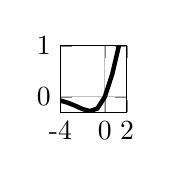
\begin{tikzpicture}
\begin{axis}[
	xmin=-4,xmax=2,
	ymin=-.3,ymax=1,
	ytick={0, 1},
	yticklabels={0,1},
	xtick={-4, 0, 2},
	xticklabels={-4,0,2},
	width=.2\textwidth,
	height=.2\textwidth,
	grid=both,
	]
	\addplot [ultra thick,domain=-4:2, samples=10]{x * (1/ (1+exp(-x)))};
	%\addplot [ultra thick,domain=-1:0.004, samples=10]{exp(x)-1};
\end{axis}
\end{tikzpicture}}
		\scalebox{.9}{% This file was created by tikzplotlib v0.9.6.
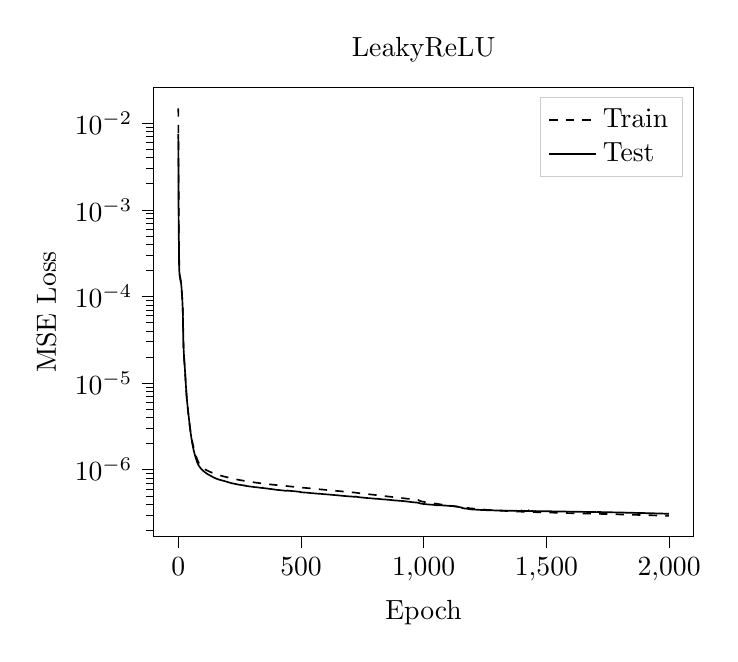
\begin{tikzpicture}

\begin{axis}[
legend cell align={left},
legend style={fill opacity=0.8, draw opacity=1, text opacity=1, draw=white!80!black},
log basis y={10},
tick align=outside,
tick pos=left,
title={LeakyReLU},
x grid style={white!69.0196078431373!black},
xlabel={Epoch},
xmin=-99.95, xmax=2098.95,
xtick style={color=black},
y grid style={white!69.0196078431373!black},
ylabel={MSE Loss},
ymin=1.70791572547231e-07, ymax=0.0255488360607333,
ymode=log,
ytick style={color=black}
]
\addplot [semithick, black, dashed]
table {%
0 0.0148644272387028
1 0.00333734963089228
2 0.000750602022744715
3 0.000331206021597609
4 0.000207027630618541
5 0.000178633672956494
6 0.000169817901289207
7 0.000163992511370452
8 0.000158428034461394
9 0.000152649684350763
10 0.00014641946539632
11 0.000139678969775559
12 0.000132290519177332
13 0.000124130066971702
14 0.000115090908722777
15 0.000105129859155568
16 9.44059219655173e-05
17 8.3223627305415e-05
18 7.19209145499917e-05
19 5.9600600565318e-05
20 3.97648699054116e-05
21 2.79329969580431e-05
22 2.30094661437761e-05
23 2.03421610876831e-05
24 1.84593141466394e-05
25 1.68413770406914e-05
26 1.53453861585149e-05
27 1.39403166676857e-05
28 1.26229516022249e-05
29 1.13995978695129e-05
30 1.02803903319e-05
31 9.27881336542669e-06
32 8.39881708566281e-06
33 7.63946547408523e-06
34 6.99144020211406e-06
35 6.44443027772468e-06
36 5.98577112725707e-06
37 5.59156097597224e-06
38 5.24542606149225e-06
39 4.93420651258703e-06
40 4.64607294458119e-06
41 4.3748265293857e-06
42 4.12039487252969e-06
43 3.8861643104724e-06
44 3.67260006765946e-06
45 3.47844123746199e-06
46 3.30225424215769e-06
47 3.13898743047503e-06
48 2.98947314900033e-06
49 2.85182592716637e-06
50 2.72762016362549e-06
51 2.61402293841684e-06
52 2.5099930834358e-06
53 2.4150706948376e-06
54 2.32725503445863e-06
55 2.24705749849363e-06
56 2.17294952142311e-06
57 2.1049157987818e-06
58 2.04128094503631e-06
59 1.98188082879369e-06
60 1.92642735390791e-06
61 1.87334052122878e-06
62 1.8232318035416e-06
63 1.77455488795886e-06
64 1.72895183959554e-06
65 1.6861234399812e-06
66 1.64616296456188e-06
67 1.60743973128774e-06
68 1.57055133320227e-06
69 1.53456863944257e-06
70 1.50125948277946e-06
71 1.46981972636695e-06
72 1.44026260474561e-06
73 1.41147857323176e-06
74 1.38520127060815e-06
75 1.36031598432851e-06
76 1.33676044734443e-06
77 1.3148170181978e-06
78 1.29389646752998e-06
79 1.27433537693378e-06
80 1.25646557970072e-06
81 1.2384471808673e-06
82 1.22196116879536e-06
83 1.20638403507201e-06
84 1.19190501561661e-06
85 1.17844780726273e-06
86 1.16571712385394e-06
87 1.1539444496691e-06
88 1.14418008098482e-06
89 1.13371917686322e-06
90 1.12408099414552e-06
91 1.1148123342366e-06
92 1.10610182443338e-06
93 1.09807221093661e-06
94 1.09074505050444e-06
95 1.0839480192999e-06
96 1.07734048407337e-06
97 1.07122849982488e-06
98 1.06452712140026e-06
99 1.05868495271011e-06
100 1.05291415113129e-06
101 1.04752679743569e-06
102 1.04214536537484e-06
103 1.0370281889891e-06
104 1.032027342319e-06
105 1.02744560464885e-06
106 1.02279366436164e-06
107 1.01820316623957e-06
108 1.01401851819105e-06
109 1.00975107895351e-06
110 1.0057904348173e-06
111 1.00208405191893e-06
112 9.98241210339756e-07
113 9.94370888776075e-07
114 9.90925482227567e-07
115 9.87395259301138e-07
116 9.83861367387817e-07
117 9.80596522055066e-07
118 9.77371847994846e-07
119 9.74262288309546e-07
120 9.71295058008082e-07
121 9.6826150081597e-07
122 9.6523639768975e-07
123 9.62448905852398e-07
124 9.59402455919189e-07
125 9.56513887700794e-07
126 9.53868651834e-07
127 9.51033602575535e-07
128 9.48263187240173e-07
129 9.45597496013306e-07
130 9.42952355558191e-07
131 9.40403254958255e-07
132 9.37919000818965e-07
133 9.35487815553415e-07
134 9.33048935337411e-07
135 9.30687048224854e-07
136 9.28267845239361e-07
137 9.25884347481087e-07
138 9.23637938910815e-07
139 9.21227984548523e-07
140 9.18846620891145e-07
141 9.16484609831514e-07
142 9.14296656503666e-07
143 9.12058346074218e-07
144 9.09871440057941e-07
145 9.07786169506153e-07
146 9.05647660886189e-07
147 9.03635627963695e-07
148 9.01687872357115e-07
149 8.9950875153022e-07
150 8.97521426622916e-07
151 8.95521069111282e-07
152 8.93521177772527e-07
153 8.91522843943449e-07
154 8.89579697087584e-07
155 8.87620785334775e-07
156 8.85896789583285e-07
157 8.83988975402872e-07
158 8.82208881847646e-07
159 8.80398930121373e-07
160 8.78538994015798e-07
161 8.76403134441262e-07
162 8.7463463688664e-07
163 8.72705812355434e-07
164 8.70566312670462e-07
165 8.68765719644671e-07
166 8.67004338203969e-07
167 8.653048454903e-07
168 8.63512691211099e-07
169 8.61854937170392e-07
170 8.60151822223543e-07
171 8.58458075072122e-07
172 8.56818996624043e-07
173 8.55136690688596e-07
174 8.53585893565878e-07
175 8.5187854273272e-07
176 8.50357727699702e-07
177 8.48755360294717e-07
178 8.47190044481749e-07
179 8.45670013589483e-07
180 8.44131327013997e-07
181 8.42642410887606e-07
182 8.41175444946884e-07
183 8.39656288363244e-07
184 8.38167764982245e-07
185 8.36532800619239e-07
186 8.35078147304102e-07
187 8.33758716908051e-07
188 8.32371983960911e-07
189 8.30889671789237e-07
190 8.29568857710683e-07
191 8.28064573511256e-07
192 8.26631372348174e-07
193 8.25454969628936e-07
194 8.24060114283043e-07
195 8.22638993369651e-07
196 8.2126220449652e-07
197 8.19915930264869e-07
198 8.20267484073156e-07
199 8.18703642607943e-07
200 8.17248432568363e-07
201 8.15823900992996e-07
202 8.14442585394204e-07
203 8.13095293437982e-07
204 8.11669069307186e-07
205 8.10307857349812e-07
206 8.09004709736882e-07
207 8.07590666070723e-07
208 8.06252364142779e-07
209 8.04654392212001e-07
210 8.0335848272739e-07
211 8.02302690658507e-07
212 8.00962444145625e-07
213 7.99703646720218e-07
214 7.98452317255283e-07
215 7.97217591738786e-07
216 7.96002158963915e-07
217 7.9481069326448e-07
218 7.93627711118461e-07
219 7.92467858858004e-07
220 7.91300207737322e-07
221 7.90077528890265e-07
222 7.88920517678093e-07
223 7.87720634576772e-07
224 7.86578616626343e-07
225 7.85441414691945e-07
226 7.84363267499089e-07
227 7.83269696910338e-07
228 7.82192492366107e-07
229 7.81227263516371e-07
230 7.80163437795522e-07
231 7.79063238198319e-07
232 7.78027706374473e-07
233 7.76964129954649e-07
234 7.75930989362905e-07
235 7.74893729442283e-07
236 7.73837977973813e-07
237 7.72835657613768e-07
238 7.71838034495431e-07
239 7.70846074615861e-07
240 7.69821481426902e-07
241 7.68822976212391e-07
242 7.67821201534957e-07
243 7.66846018862566e-07
244 7.65887867913762e-07
245 7.64930361214056e-07
246 7.63921686242952e-07
247 7.63010957257393e-07
248 7.62070085571054e-07
249 7.61139531945787e-07
250 7.60420157376984e-07
251 7.59426636150806e-07
252 7.58426511922039e-07
253 7.57507968302207e-07
254 7.56569720863354e-07
255 7.55625533727766e-07
256 7.54756878393437e-07
257 7.53833237837398e-07
258 7.52968338730398e-07
259 7.52147672017145e-07
260 7.51202681499308e-07
261 7.50205559867823e-07
262 7.4943015475526e-07
263 7.48610954261153e-07
264 7.47677468453389e-07
265 7.46997857405063e-07
266 7.46052829256882e-07
267 7.45165411899507e-07
268 7.44340018613343e-07
269 7.43665318836406e-07
270 7.42747071726058e-07
271 7.4204888295526e-07
272 7.41131473191103e-07
273 7.40440178674362e-07
274 7.39578193176271e-07
275 7.3881461977976e-07
276 7.37799187660926e-07
277 7.37035187341917e-07
278 7.36253217098692e-07
279 7.35415127010697e-07
280 7.34686662354989e-07
281 7.33878230974483e-07
282 7.33114714989824e-07
283 7.32347263181055e-07
284 7.31621643978997e-07
285 7.30857068063529e-07
286 7.30129704550109e-07
287 7.29444917936917e-07
288 7.28688947859268e-07
289 7.28014880451156e-07
290 7.27137706519443e-07
291 7.2640715151806e-07
292 7.25708816418091e-07
293 7.25009155303269e-07
294 7.24293989392777e-07
295 7.23561567397724e-07
296 7.2286156442658e-07
297 7.22185449788526e-07
298 7.21465641959185e-07
299 7.20789148289214e-07
300 7.20108953458976e-07
301 7.19449026178154e-07
302 7.18764739445987e-07
303 7.18094917701251e-07
304 7.17464760171538e-07
305 7.16808219209497e-07
306 7.16184726542224e-07
307 7.15528395758724e-07
308 7.14873352649192e-07
309 7.14168571732898e-07
310 7.13574344160861e-07
311 7.1287063936154e-07
312 7.12281224224398e-07
313 7.11596599359154e-07
314 7.1101726477707e-07
315 7.10344048059142e-07
316 7.09744001042623e-07
317 7.09173813802977e-07
318 7.08501808716733e-07
319 7.07896837610633e-07
320 7.07197004814475e-07
321 7.06599812318132e-07
322 7.05917090755293e-07
323 7.05374840876516e-07
324 7.04819606951901e-07
325 7.04185838287685e-07
326 7.03570776934725e-07
327 7.02973159619091e-07
328 7.02457169694526e-07
329 7.01814170426474e-07
330 7.01159818504493e-07
331 7.00675139412965e-07
332 7.00100038670826e-07
333 6.9944516293674e-07
334 6.98911392788659e-07
335 6.98320728275803e-07
336 6.97682788128873e-07
337 6.97246098184223e-07
338 6.96686453053985e-07
339 6.96352869169914e-07
340 6.95526991592033e-07
341 6.9484590517277e-07
342 6.94304655056044e-07
343 6.9400206361081e-07
344 6.92970413965099e-07
345 6.93037260532492e-07
346 6.92013609636888e-07
347 6.91989935560855e-07
348 6.90816037362652e-07
349 6.9062005174203e-07
350 6.89722630539791e-07
351 6.89461848594419e-07
352 6.88598280333963e-07
353 6.88385519012513e-07
354 6.87496540834331e-07
355 6.87273249681653e-07
356 6.86344381364279e-07
357 6.85784922154653e-07
358 6.85309239756293e-07
359 6.8513359936162e-07
360 6.84244536785172e-07
361 6.84097153609287e-07
362 6.83162119059943e-07
363 6.82782644759072e-07
364 6.82589405883505e-07
365 6.8159318890082e-07
366 6.81068037124533e-07
367 6.80618575174208e-07
368 6.80053423749882e-07
369 6.79640693476813e-07
370 6.79050741510423e-07
371 6.78609955187426e-07
372 6.78057203842286e-07
373 6.77662977224713e-07
374 6.77112505997002e-07
375 6.76636222607385e-07
376 6.76250711990178e-07
377 6.75681376677062e-07
378 6.75209785029551e-07
379 6.74681991128523e-07
380 6.74513683136979e-07
381 6.73722616213013e-07
382 6.73302310929102e-07
383 6.72808587580676e-07
384 6.72407056214297e-07
385 6.71915421463609e-07
386 6.71427296765614e-07
387 6.71025953465687e-07
388 6.7049164735522e-07
389 6.70016919258387e-07
390 6.69557675067267e-07
391 6.69086867844726e-07
392 6.68597802928161e-07
393 6.68190762553422e-07
394 6.67692410345921e-07
395 6.67240023972226e-07
396 6.66790877019707e-07
397 6.66323490648324e-07
398 6.65903456606998e-07
399 6.65471397070405e-07
400 6.65007362329106e-07
401 6.64616963959475e-07
402 6.64189005348703e-07
403 6.63769749593257e-07
404 6.63356940961535e-07
405 6.62935873677384e-07
406 6.6251740221901e-07
407 6.62097921363625e-07
408 6.61683327294327e-07
409 6.61271375818728e-07
410 6.60858302936163e-07
411 6.60460645164562e-07
412 6.6005227745336e-07
413 6.59639243394849e-07
414 6.5922696452958e-07
415 6.58827367658432e-07
416 6.58425498315296e-07
417 6.5801929646625e-07
418 6.57625117895577e-07
419 6.57224236348952e-07
420 6.5661854195298e-07
421 6.56017475847648e-07
422 6.55518018916723e-07
423 6.55074278228085e-07
424 6.54699447096618e-07
425 6.54264191396692e-07
426 6.53816869700563e-07
427 6.53326964823009e-07
428 6.52873706030732e-07
429 6.52448715413811e-07
430 6.51987482811478e-07
431 6.51630326260033e-07
432 6.51166140116288e-07
433 6.50728281328838e-07
434 6.50352801045528e-07
435 6.49924126832957e-07
436 6.49520926629066e-07
437 6.49109188529451e-07
438 6.48725988511956e-07
439 6.48329360970479e-07
440 6.47936029650964e-07
441 6.47537012639532e-07
442 6.47503992468046e-07
443 6.47304684633809e-07
444 6.46791755926301e-07
445 6.46174046053716e-07
446 6.45631595219243e-07
447 6.45148015280483e-07
448 6.4464382931817e-07
449 6.44142668491554e-07
450 6.4371638593741e-07
451 6.4329291483034e-07
452 6.42818815379087e-07
453 6.4243620757054e-07
454 6.41965242266451e-07
455 6.41560947940434e-07
456 6.4108713894484e-07
457 6.40711664800619e-07
458 6.40245212196078e-07
459 6.39877146284107e-07
460 6.39416840158447e-07
461 6.38994611691146e-07
462 6.38533215393977e-07
463 6.38164307375177e-07
464 6.37705450529324e-07
465 6.37337720817754e-07
466 6.36884023322182e-07
467 6.36565714486892e-07
468 6.35994193231681e-07
469 6.35576846804042e-07
470 6.35110142454209e-07
471 6.34726450087442e-07
472 6.34274996968998e-07
473 6.33879317220476e-07
474 6.33418987760592e-07
475 6.33054129139055e-07
476 6.32558955913964e-07
477 6.32200792907156e-07
478 6.31757687600043e-07
479 6.31408914216536e-07
480 6.30983657273987e-07
481 6.30627516443383e-07
482 6.30192174881472e-07
483 6.29844393728263e-07
484 6.29409517699742e-07
485 6.29049891742284e-07
486 6.28630618265902e-07
487 6.28272145732467e-07
488 6.27843531489702e-07
489 6.27503492012238e-07
490 6.27080744209252e-07
491 6.26735475819373e-07
492 6.26306154430267e-07
493 6.25968398722421e-07
494 6.25546789720488e-07
495 6.25211958649174e-07
496 6.24788373372098e-07
497 6.24449280010708e-07
498 6.23962057133554e-07
499 6.23558213717956e-07
500 6.2311415599936e-07
501 6.22750209018363e-07
502 6.22350057199128e-07
503 6.21995929662944e-07
504 6.21580487475626e-07
505 6.21248701463628e-07
506 6.20837227202742e-07
507 6.20487857943885e-07
508 6.2008267529734e-07
509 6.19707906508893e-07
510 6.19289868623696e-07
511 6.18935109201857e-07
512 6.18535905800854e-07
513 6.18207967761464e-07
514 6.17810335668878e-07
515 6.17487754837498e-07
516 6.17048165693745e-07
517 6.16747607693924e-07
518 6.16425678529708e-07
519 6.16018937733998e-07
520 6.15564609120156e-07
521 6.15231403671146e-07
522 6.14803654485741e-07
523 6.14466882382203e-07
524 6.13926075146765e-07
525 6.13603320687162e-07
526 6.13164834007307e-07
527 6.12889333567068e-07
528 6.1244176531261e-07
529 6.12171113900217e-07
530 6.11737456409855e-07
531 6.11406537032622e-07
532 6.10991987372245e-07
533 6.10615803282144e-07
534 6.10182909497325e-07
535 6.09855354056776e-07
536 6.09413068900722e-07
537 6.09052085394524e-07
538 6.08653819512028e-07
539 6.08387478564509e-07
540 6.07961950962022e-07
541 6.07622395477847e-07
542 6.07195113218495e-07
543 6.06802663170924e-07
544 6.06362741748967e-07
545 6.06013731712096e-07
546 6.0559248045422e-07
547 6.05250503625143e-07
548 6.04716681607442e-07
549 6.04371584088881e-07
550 6.03937985829361e-07
551 6.03589404704508e-07
552 6.03148568060874e-07
553 6.02801457745272e-07
554 6.0235625136329e-07
555 6.01985544463446e-07
556 6.01539943161811e-07
557 6.01232765262694e-07
558 6.00807006364335e-07
559 6.00492180907963e-07
560 6.0005816808939e-07
561 5.99730774595741e-07
562 5.99223440019614e-07
563 5.98925630910685e-07
564 5.98511263632418e-07
565 5.98205809396291e-07
566 5.97765539339434e-07
567 5.97455265236135e-07
568 5.97010945085685e-07
569 5.9672484819373e-07
570 5.96299604083583e-07
571 5.96071399556308e-07
572 5.95513366789646e-07
573 5.95187032928379e-07
574 5.947183740318e-07
575 5.94433451610144e-07
576 5.93983866451708e-07
577 5.93703354780928e-07
578 5.93230489997154e-07
579 5.92965793160261e-07
580 5.92490404656587e-07
581 5.92217652197746e-07
582 5.9175461059624e-07
583 5.91483319766439e-07
584 5.91055219629766e-07
585 5.9077541931174e-07
586 5.90313007251098e-07
587 5.90037488734652e-07
588 5.89601683429919e-07
589 5.89313242372214e-07
590 5.88861738904711e-07
591 5.88606085244692e-07
592 5.88205910432293e-07
593 5.87919526992664e-07
594 5.8745086768397e-07
595 5.87203168748829e-07
596 5.86743687904345e-07
597 5.86504606161498e-07
598 5.86034405827718e-07
599 5.85759843318101e-07
600 5.85295431378086e-07
601 5.85048269172717e-07
602 5.84578794146751e-07
603 5.84336741496827e-07
604 5.83889424504491e-07
605 5.8371987589112e-07
606 5.83250819758518e-07
607 5.82936998782202e-07
608 5.82475648911895e-07
609 5.822194414975e-07
610 5.81760691360955e-07
611 5.81514034749375e-07
612 5.8107778048111e-07
613 5.80798643440517e-07
614 5.8034996423828e-07
615 5.8007643750102e-07
616 5.79669754557699e-07
617 5.79423551016589e-07
618 5.78947847898803e-07
619 5.7868813833295e-07
620 5.78234088450813e-07
621 5.77960293540514e-07
622 5.7753287774176e-07
623 5.77290330667779e-07
624 5.76830392489569e-07
625 5.76586579811078e-07
626 5.76101825032538e-07
627 5.75859893572783e-07
628 5.75397084972451e-07
629 5.75150781202183e-07
630 5.74713401903182e-07
631 5.7447310602754e-07
632 5.74012735526708e-07
633 5.73774994833798e-07
634 5.73327271069957e-07
635 5.73114834153898e-07
636 5.72660245197199e-07
637 5.7240989970353e-07
638 5.71956064860046e-07
639 5.71697264476256e-07
640 5.71240307664311e-07
641 5.70994088292309e-07
642 5.70539148810667e-07
643 5.70304007425193e-07
644 5.69833525858598e-07
645 5.69588442289159e-07
646 5.69132603871481e-07
647 5.68892071527216e-07
648 5.68438184046727e-07
649 5.68201071160956e-07
650 5.67769946428598e-07
651 5.67519301142738e-07
652 5.6707707179271e-07
653 5.66797595681123e-07
654 5.66352859991071e-07
655 5.66096162472718e-07
656 5.65686599273363e-07
657 5.65438366834314e-07
658 5.65017211897612e-07
659 5.64772737391195e-07
660 5.64293594010223e-07
661 5.64047870213358e-07
662 5.63645380410094e-07
663 5.63384342626705e-07
664 5.62980142362335e-07
665 5.62727795866635e-07
666 5.62271209290088e-07
667 5.62005503908836e-07
668 5.61633367738068e-07
669 5.61361019336459e-07
670 5.60907587512816e-07
671 5.60647555943206e-07
672 5.60207655595946e-07
673 5.59965208736912e-07
674 5.59675780166913e-07
675 5.59391941266085e-07
676 5.58971077055048e-07
677 5.58727743012355e-07
678 5.58255349702108e-07
679 5.5799404208301e-07
680 5.5754053700241e-07
681 5.57285783443717e-07
682 5.56846114776022e-07
683 5.56599550662895e-07
684 5.56152776738372e-07
685 5.55905638606191e-07
686 5.55450992109741e-07
687 5.55227351341614e-07
688 5.54761071512644e-07
689 5.54549272450799e-07
690 5.54089646058742e-07
691 5.53867962665322e-07
692 5.53422880528842e-07
693 5.5320079773935e-07
694 5.5274819114004e-07
695 5.52521287801255e-07
696 5.5206996151469e-07
697 5.51794728323784e-07
698 5.51397915060647e-07
699 5.5119633870504e-07
700 5.50707732926981e-07
701 5.50483585669781e-07
702 5.5005929785068e-07
703 5.49791805909194e-07
704 5.49363092531507e-07
705 5.49153537050984e-07
706 5.48734435838583e-07
707 5.48524624861102e-07
708 5.48033714892426e-07
709 5.47864530929587e-07
710 5.47407044180659e-07
711 5.47192967673027e-07
712 5.46663945314663e-07
713 5.46469165058738e-07
714 5.46026377676867e-07
715 5.45797743370713e-07
716 5.45408502446776e-07
717 5.45146161812227e-07
718 5.44686208826306e-07
719 5.4444843793533e-07
720 5.44042121731536e-07
721 5.44187411392727e-07
722 5.43547544765488e-07
723 5.42903439722409e-07
724 5.42304797178872e-07
725 5.41774102529757e-07
726 5.41298678271573e-07
727 5.40787423858546e-07
728 5.40312020774536e-07
729 5.39910445837677e-07
730 5.39371933314214e-07
731 5.39032324013533e-07
732 5.38397320511308e-07
733 5.38005847772638e-07
734 5.37580982125974e-07
735 5.37113240582698e-07
736 5.36665524890623e-07
737 5.3628786932336e-07
738 5.35821611535425e-07
739 5.3551504601046e-07
740 5.34989343293546e-07
741 5.34692306075613e-07
742 5.34238284117805e-07
743 5.33852620080211e-07
744 5.33480754000948e-07
745 5.33024487040734e-07
746 5.32662216912172e-07
747 5.32245440751922e-07
748 5.31847421598286e-07
749 5.31583600732688e-07
750 5.31042589130948e-07
751 5.30784487636993e-07
752 5.30310267848222e-07
753 5.30027119310716e-07
754 5.29521326086524e-07
755 5.29201154762404e-07
756 5.28709079290479e-07
757 5.28442658435324e-07
758 5.27953152186456e-07
759 5.27690907290435e-07
760 5.27205177448309e-07
761 5.26892414683289e-07
762 5.26405703695332e-07
763 5.26151932234598e-07
764 5.25638900228387e-07
765 5.2538255179968e-07
766 5.24913538470173e-07
767 5.24627415103396e-07
768 5.24143547863787e-07
769 5.23870203437582e-07
770 5.23359917082189e-07
771 5.23059499315082e-07
772 5.22546751852815e-07
773 5.22258667359665e-07
774 5.21781591501735e-07
775 5.21461515333499e-07
776 5.21047451144341e-07
777 5.20667105519124e-07
778 5.20264812351456e-07
779 5.19935537340643e-07
780 5.19469053031685e-07
781 5.19178764761818e-07
782 5.18717480986197e-07
783 5.18486472344648e-07
784 5.18063059260498e-07
785 5.1770965706055e-07
786 5.17317782481541e-07
787 5.17047028139928e-07
788 5.16598040718463e-07
789 5.16272202006007e-07
790 5.15890133598873e-07
791 5.1559194417905e-07
792 5.15092240675585e-07
793 5.14856525086316e-07
794 5.14366608740602e-07
795 5.14138488711069e-07
796 5.1369179050198e-07
797 5.133947706355e-07
798 5.1297357916269e-07
799 5.1269512967167e-07
800 5.12259364455758e-07
801 5.1196938757414e-07
802 5.11423140920897e-07
803 5.11186035765832e-07
804 5.108558257092e-07
805 5.10589589111987e-07
806 5.10150635591344e-07
807 5.09905413366596e-07
808 5.09488112413692e-07
809 5.0918477496964e-07
810 5.08788510359182e-07
811 5.08506359878424e-07
812 5.08111304810654e-07
813 5.07820337901421e-07
814 5.07405267313743e-07
815 5.07125847690304e-07
816 5.06688020934121e-07
817 5.06418203016779e-07
818 5.05994589261149e-07
819 5.05725315562699e-07
820 5.05358103424669e-07
821 5.05075605559568e-07
822 5.04433651911995e-07
823 5.04046690537052e-07
824 5.03614987664491e-07
825 5.03243534893727e-07
826 5.02741254081229e-07
827 5.02363778650761e-07
828 5.0181188987608e-07
829 5.01155536113629e-07
830 5.00639151781002e-07
831 5.00094774650961e-07
832 4.99718042917152e-07
833 4.99335891149144e-07
834 4.98984696335469e-07
835 4.98626764695587e-07
836 4.98176735277411e-07
837 4.97781516273221e-07
838 4.97396944084016e-07
839 4.97024179267669e-07
840 4.96623089802029e-07
841 4.9619203473128e-07
842 4.95837466530702e-07
843 4.95356492848487e-07
844 4.94947353985253e-07
845 4.94624493896367e-07
846 4.94189927721322e-07
847 4.93753210434988e-07
848 4.93364277460273e-07
849 4.93005060846485e-07
850 4.92574361317111e-07
851 4.92261623520562e-07
852 4.91839595838428e-07
853 4.91472612594634e-07
854 4.91078210103524e-07
855 4.90717624558101e-07
856 4.90344198198045e-07
857 4.89971666482347e-07
858 4.89575231455319e-07
859 4.89207917780732e-07
860 4.8886572173501e-07
861 4.88452469610934e-07
862 4.88092318505551e-07
863 4.87744442438043e-07
864 4.87433638966195e-07
865 4.87001789679198e-07
866 4.86642392530712e-07
867 4.86256370052729e-07
868 4.85970414203507e-07
869 4.85520277266005e-07
870 4.85194746914885e-07
871 4.84795060486931e-07
872 4.8450660469257e-07
873 4.84076300665492e-07
874 4.83778275267355e-07
875 4.83363721940577e-07
876 4.83014998721387e-07
877 4.82567401576262e-07
878 4.82165626024766e-07
879 4.81873086187079e-07
880 4.81442710679403e-07
881 4.81068505791882e-07
882 4.80751659097223e-07
883 4.80426024751068e-07
884 4.80023959966047e-07
885 4.796470899322e-07
886 4.79263505340555e-07
887 4.78941620059459e-07
888 4.78609426863841e-07
889 4.78185967480727e-07
890 4.77746801095691e-07
891 4.77495924258164e-07
892 4.77138562104074e-07
893 4.76734690607827e-07
894 4.76396770054066e-07
895 4.76033359916528e-07
896 4.75629839783664e-07
897 4.7529189306772e-07
898 4.75028509299591e-07
899 4.74598706588836e-07
900 4.74232805089514e-07
901 4.73863658129403e-07
902 4.73503784462537e-07
903 4.73214756993912e-07
904 4.72819625130683e-07
905 4.72471625627691e-07
906 4.72109106254948e-07
907 4.71858331579256e-07
908 4.71460500378384e-07
909 4.71170830238066e-07
910 4.70762764038568e-07
911 4.70420068552357e-07
912 4.70193007899411e-07
913 4.69732255297117e-07
914 4.69328430256155e-07
915 4.69008694636841e-07
916 4.68750404195362e-07
917 4.68294574801575e-07
918 4.67943003044979e-07
919 4.67603833413932e-07
920 4.6726228927696e-07
921 4.67024187202014e-07
922 4.66549970042252e-07
923 4.66196309801603e-07
924 4.65849686818842e-07
925 4.65657492441096e-07
926 4.6514172363743e-07
927 4.6484536051139e-07
928 4.64433631279348e-07
929 4.64285816306642e-07
930 4.63722799736388e-07
931 4.63393946745327e-07
932 4.63028061346904e-07
933 4.62868733578148e-07
934 4.62303378796491e-07
935 4.61944667279113e-07
936 4.61593672994809e-07
937 4.61465650644755e-07
938 4.60907661022247e-07
939 4.60600220463903e-07
940 4.6021002177099e-07
941 4.59943743535973e-07
942 4.59559822544975e-07
943 4.59191470767451e-07
944 4.58823429340782e-07
945 4.58568544715376e-07
946 4.58253700188038e-07
947 4.57775354860246e-07
948 4.57443201653973e-07
949 4.57248985242131e-07
950 4.56788529746177e-07
951 4.56413603274086e-07
952 4.56049293291017e-07
953 4.55718323721044e-07
954 4.55268215404203e-07
955 4.54996806922736e-07
956 4.54735002605844e-07
957 4.54331303615163e-07
958 4.53895254239001e-07
959 4.53565293838665e-07
960 4.53295954372379e-07
961 4.52920906539589e-07
962 4.52633616063736e-07
963 4.52290183702075e-07
964 4.51753988272685e-07
965 4.51526366362032e-07
966 4.51130627027396e-07
967 4.50771134154593e-07
968 4.504252864308e-07
969 4.50136636729326e-07
970 4.49762404599596e-07
971 4.4941030162704e-07
972 4.49197960506353e-07
973 4.48709193022978e-07
974 4.48431595785337e-07
975 4.48094398578291e-07
976 4.4774719881957e-07
977 4.47329700762111e-07
978 4.47107959246296e-07
979 4.45311586858566e-07
980 4.42267165908561e-07
981 4.41070118895937e-07
982 4.40142427535761e-07
983 4.39295067039325e-07
984 4.38643088358504e-07
985 4.36957642435232e-07
986 4.35593108733201e-07
987 4.34702707551082e-07
988 4.33474616400531e-07
989 4.32703829105208e-07
990 4.32289674321851e-07
991 4.31421487917305e-07
992 4.30638353520862e-07
993 4.29790937616303e-07
994 4.28880565337408e-07
995 4.28401135650347e-07
996 4.27787201346064e-07
997 4.27183281047405e-07
998 4.26694344852763e-07
999 4.2636703791743e-07
1000 4.25715062704057e-07
1001 4.25246964852022e-07
1002 4.24845545552444e-07
1003 4.24308888639757e-07
1004 4.23964489456807e-07
1005 4.23528313447719e-07
1006 4.22984388706027e-07
1007 4.225807735736e-07
1008 4.22272394018819e-07
1009 4.21754303317812e-07
1010 4.21508764347323e-07
1011 4.20943191883794e-07
1012 4.20336185086967e-07
1013 4.19858491000014e-07
1014 4.1939585513262e-07
1015 4.19118752247982e-07
1016 4.18458747006412e-07
1017 4.18054913723154e-07
1018 4.17623710319504e-07
1019 4.17345911756684e-07
1020 4.1684959707311e-07
1021 4.16479742753495e-07
1022 4.16232555934926e-07
1023 4.1558006725495e-07
1024 4.15228342362184e-07
1025 4.15229226916836e-07
1026 4.14557101422019e-07
1027 4.14188685837757e-07
1028 4.137652676377e-07
1029 4.13552009050022e-07
1030 4.13012748268216e-07
1031 4.12709136242029e-07
1032 4.12403044578014e-07
1033 4.12024662679755e-07
1034 4.11686833103886e-07
1035 4.11097062823274e-07
1036 4.11059944923409e-07
1037 4.10612124298382e-07
1038 4.10058860069284e-07
1039 4.09830215701845e-07
1040 4.09236865593243e-07
1041 4.08992037847611e-07
1042 4.08167432894402e-07
1043 4.07781641527549e-07
1044 4.07499990515703e-07
1045 4.06984923031928e-07
1046 4.06398309621636e-07
1047 4.06130208801869e-07
1048 4.05844250565224e-07
1049 4.05634460008741e-07
1050 4.05246325286157e-07
1051 4.04832696432322e-07
1052 4.04589275078138e-07
1053 4.04333232410181e-07
1054 4.0388796469415e-07
1055 4.0364550858385e-07
1056 4.03237107150289e-07
1057 4.02781264639884e-07
1058 4.02806778183162e-07
1059 4.01965887306233e-07
1060 4.01510594059573e-07
1061 4.00938951401031e-07
1062 4.00572816303679e-07
1063 4.00084503098697e-07
1064 3.99712360263038e-07
1065 3.99338280672623e-07
1066 3.98853183725123e-07
1067 3.98574016514885e-07
1068 3.98165261131567e-07
1069 3.9791169047021e-07
1070 3.97472268019783e-07
1071 3.97099917236687e-07
1072 3.96636626348368e-07
1073 3.96424626273983e-07
1074 3.96097346396118e-07
1075 3.9559541224321e-07
1076 3.95176014095e-07
1077 3.9485332503375e-07
1078 3.94414255026732e-07
1079 3.94210009147855e-07
1080 3.93897365086104e-07
1081 3.94073744161005e-07
1082 3.92707131538828e-07
1083 3.92443426818545e-07
1084 3.92263928972625e-07
1085 3.91811526995411e-07
1086 3.91438045383552e-07
1087 3.91222988042728e-07
1088 3.90767820931615e-07
1089 3.90392165115827e-07
1090 3.90058417949035e-07
1091 3.89737378512223e-07
1092 3.89416854545743e-07
1093 3.89117823701213e-07
1094 3.88820500631937e-07
1095 3.8860628005466e-07
1096 3.88284502861325e-07
1097 3.8773857590968e-07
1098 3.87415723963613e-07
1099 3.87093581963427e-07
1100 3.86819972547414e-07
1101 3.8655951644273e-07
1102 3.86174517572613e-07
1103 3.85863807807141e-07
1104 3.85488108648246e-07
1105 3.85170436189242e-07
1106 3.84719854892523e-07
1107 3.84718544239604e-07
1108 3.84024391522075e-07
1109 3.83650835544813e-07
1110 3.83382792236375e-07
1111 3.83040656402045e-07
1112 3.82753346201525e-07
1113 3.82416109658834e-07
1114 3.82373510092293e-07
1115 3.81928717573032e-07
1116 3.81812806622861e-07
1117 3.81203720849044e-07
1118 3.80974276083634e-07
1119 3.80499999522499e-07
1120 3.80254684600345e-07
1121 3.7986570839621e-07
1122 3.79738977585475e-07
1123 3.79311346222266e-07
1124 3.79113227651828e-07
1125 3.7877028913158e-07
1126 3.7836112139189e-07
1127 3.77982800344512e-07
1128 3.78119575884739e-07
1129 3.77618890752274e-07
1130 3.77162941205711e-07
1131 3.7672415348311e-07
1132 3.76497530936604e-07
1133 3.76125739251165e-07
1134 3.76046060509339e-07
1135 3.75449260715754e-07
1136 3.75253203273473e-07
1137 3.74917057925472e-07
1138 3.74622404692104e-07
1139 3.7428821870833e-07
1140 3.74284405566527e-07
1141 3.7362211756431e-07
1142 3.73366226355643e-07
1143 3.7307717714441e-07
1144 3.72830825526194e-07
1145 3.72424451896336e-07
1146 3.72418132940311e-07
1147 3.7213091133026e-07
1148 3.71713215983505e-07
1149 3.71452914535553e-07
1150 3.71178188473209e-07
1151 3.70909355197568e-07
1152 3.7053996253178e-07
1153 3.7024783931372e-07
1154 3.69873657135145e-07
1155 3.69505103691381e-07
1156 3.69253701279604e-07
1157 3.68807387985726e-07
1158 3.68308296941677e-07
1159 3.68027352777744e-07
1160 3.67674302410137e-07
1161 3.67324845441885e-07
1162 3.67093079873371e-07
1163 3.66817634045447e-07
1164 3.66528322331305e-07
1165 3.66260036969379e-07
1166 3.65974232906296e-07
1167 3.6576783041653e-07
1168 3.65757778212128e-07
1169 3.65359265160237e-07
1170 3.64927529545866e-07
1171 3.64539682664144e-07
1172 3.64183218977132e-07
1173 3.63697715883404e-07
1174 3.63248774547742e-07
1175 3.6295745351822e-07
1176 3.62568556099063e-07
1177 3.62408816727111e-07
1178 3.61902688752025e-07
1179 3.61626319858033e-07
1180 3.61431617832864e-07
1181 3.61043409355943e-07
1182 3.60797934973789e-07
1183 3.60444958303674e-07
1184 3.60248958102716e-07
1185 3.59936896558111e-07
1186 3.59555476705964e-07
1187 3.59374415111802e-07
1188 3.58965990059801e-07
1189 3.58561037799632e-07
1190 3.58322259430111e-07
1191 3.57995596175442e-07
1192 3.57769069225355e-07
1193 3.57516862507623e-07
1194 3.57242059436658e-07
1195 3.57074874074215e-07
1196 3.56846210692652e-07
1197 3.56573667573912e-07
1198 3.56349139025269e-07
1199 3.56250705209504e-07
1200 3.55875810996054e-07
1201 3.55695545266599e-07
1202 3.55430612060559e-07
1203 3.55257044837742e-07
1204 3.55036958367805e-07
1205 3.54729504230988e-07
1206 3.54575795554979e-07
1207 3.54330831036975e-07
1208 3.54163805582175e-07
1209 3.53934707121084e-07
1210 3.53760961694149e-07
1211 3.53559004942383e-07
1212 3.53348837684564e-07
1213 3.53167481250694e-07
1214 3.52938252042634e-07
1215 3.52749994284807e-07
1216 3.52585982660969e-07
1217 3.52407975704239e-07
1218 3.52169507415567e-07
1219 3.51973961208785e-07
1220 3.51758787793699e-07
1221 3.51502807255599e-07
1222 3.51306851079869e-07
1223 3.51152501224306e-07
1224 3.50899278146244e-07
1225 3.50712421344213e-07
1226 3.50511307786405e-07
1227 3.50340402199834e-07
1228 3.50174203553877e-07
1229 3.49866230820339e-07
1230 3.49717217829948e-07
1231 3.49455526098552e-07
1232 3.49285141943767e-07
1233 3.49022042534841e-07
1234 3.48864000585536e-07
1235 3.48586736819811e-07
1236 3.48445087801963e-07
1237 3.4818345256582e-07
1238 3.4813231708597e-07
1239 3.48225087407172e-07
1240 3.47784275412266e-07
1241 3.47621228634409e-07
1242 3.47436047128724e-07
1243 3.47174164780029e-07
1244 3.4713033489453e-07
1245 3.46868865150896e-07
1246 3.46827497459401e-07
1247 3.46505921307028e-07
1248 3.46359151983222e-07
1249 3.46254663149637e-07
1250 3.45973173082825e-07
1251 3.45937462505219e-07
1252 3.45498902305508e-07
1253 3.45166767687033e-07
1254 3.44957258484158e-07
1255 3.44883514060257e-07
1256 3.44460587214712e-07
1257 3.44291111339601e-07
1258 3.44095388989274e-07
1259 3.43959172042219e-07
1260 3.43810874603889e-07
1261 3.43625585593088e-07
1262 3.4358059095041e-07
1263 3.43212996391173e-07
1264 3.43100552726128e-07
1265 3.43164890786341e-07
1266 3.42759536103188e-07
1267 3.42773568959842e-07
1268 3.42893875803441e-07
1269 3.42620055683085e-07
1270 3.4228207704956e-07
1271 3.42381971016437e-07
1272 3.42026907333093e-07
1273 3.41821995505143e-07
1274 3.41681918825998e-07
1275 3.41623348312226e-07
1276 3.41340164766279e-07
1277 3.41217368152513e-07
1278 3.4106308705617e-07
1279 3.40976784691804e-07
1280 3.4080946687709e-07
1281 3.40802128683038e-07
1282 3.40702538146331e-07
1283 3.40402227969605e-07
1284 3.40182375417442e-07
1285 3.40091809910348e-07
1286 3.39915428099857e-07
1287 3.39853421358782e-07
1288 3.39670542125248e-07
1289 3.39502068037234e-07
1290 3.39417640304873e-07
1291 3.39291082688931e-07
1292 3.39082802483404e-07
1293 3.39148367032749e-07
1294 3.38892482638187e-07
1295 3.38829270653207e-07
1296 3.38648870496172e-07
1297 3.38687307959162e-07
1298 3.38240516690291e-07
1299 3.38366272508495e-07
1300 3.38001319256875e-07
1301 3.37920434652972e-07
1302 3.37841576858011e-07
1303 3.37823672431625e-07
1304 3.3753024310812e-07
1305 3.37429006513901e-07
1306 3.37313680958573e-07
1307 3.37218410713547e-07
1308 3.3711456779173e-07
1309 3.36903703832547e-07
1310 3.36891655976501e-07
1311 3.36800533723647e-07
1312 3.3659107230477e-07
1313 3.36524350629475e-07
1314 3.36588194052467e-07
1315 3.3621560381647e-07
1316 3.36227974422343e-07
1317 3.35964050691473e-07
1318 3.3590479741008e-07
1319 3.35959069197145e-07
1320 3.3563762396227e-07
1321 3.3570893973689e-07
1322 3.35404225104696e-07
1323 3.35420296941891e-07
1324 3.35310365571218e-07
1325 3.35162345130868e-07
1326 3.35112290805739e-07
1327 3.35035934234895e-07
1328 3.34863490358828e-07
1329 3.3453481590584e-07
1330 3.34560684706275e-07
1331 3.34415690289802e-07
1332 3.34436880429223e-07
1333 3.34342135964505e-07
1334 3.3411748800205e-07
1335 3.33874048642713e-07
1336 3.33887440966407e-07
1337 3.33762760767797e-07
1338 3.33557971053722e-07
1339 3.33469831780064e-07
1340 3.333395412497e-07
1341 3.33323065277114e-07
1342 3.33160623696926e-07
1343 3.33146326468636e-07
1344 3.32997630756893e-07
1345 3.32955995787643e-07
1346 3.32814051603236e-07
1347 3.3281026241383e-07
1348 3.32498229099087e-07
1349 3.32466849641833e-07
1350 3.32391293376588e-07
1351 3.32259941842494e-07
1352 3.32225231424843e-07
1353 3.32077841072476e-07
1354 3.32005728822082e-07
1355 3.31841624657159e-07
1356 3.31928920083158e-07
1357 3.31696651336699e-07
1358 3.31594936319846e-07
1359 3.31512106100718e-07
1360 3.31501672782508e-07
1361 3.31306970345224e-07
1362 3.31109461292556e-07
1363 3.31097948134129e-07
1364 3.30970878607673e-07
1365 3.30980586127794e-07
1366 3.30741880006258e-07
1367 3.30851606676674e-07
1368 3.30796594830929e-07
1369 3.30699608035445e-07
1370 3.30719720835759e-07
1371 3.30387201159965e-07
1372 3.30450337429511e-07
1373 3.30311810436967e-07
1374 3.30153512820175e-07
1375 3.30106311636769e-07
1376 3.29856312781374e-07
1377 3.29988769316003e-07
1378 3.29781705133314e-07
1379 3.29643474735519e-07
1380 3.29575802702209e-07
1381 3.29661901908196e-07
1382 3.29384446779102e-07
1383 3.29194402652888e-07
1384 3.29174147502442e-07
1385 3.2892577434751e-07
1386 3.28936768760002e-07
1387 3.28938984807792e-07
1388 3.28622693380964e-07
1389 3.28631047203487e-07
1390 3.28663743040636e-07
1391 3.28427028435385e-07
1392 3.28422970120812e-07
1393 3.28242727945849e-07
1394 3.28273688822378e-07
1395 3.28060710437228e-07
1396 3.28181209752643e-07
1397 3.27843347669443e-07
1398 3.27852344064183e-07
1399 3.2829578710647e-07
1400 3.28064131871031e-07
1401 3.27575198873831e-07
1402 3.27536251177207e-07
1403 3.27420939470358e-07
1404 3.2741662860758e-07
1405 3.27226250057322e-07
1406 3.27265470950522e-07
1407 3.27060519509814e-07
1408 3.27155963816494e-07
1409 3.26972195878739e-07
1410 3.26970149174599e-07
1411 3.26863787329046e-07
1412 3.26782263279313e-07
1413 3.26663281526862e-07
1414 3.26726319926252e-07
1415 3.26526487675949e-07
1416 3.26492149575586e-07
1417 3.26372519289464e-07
1418 3.26526134919902e-07
1419 3.26281027753339e-07
1420 3.26192927850855e-07
1421 3.26291698719672e-07
1422 3.26084324228759e-07
1423 3.26008133122002e-07
1424 3.25901496594838e-07
1425 3.25920014496717e-07
1426 3.25827025420722e-07
1427 3.25687300644972e-07
1428 3.26062531392779e-07
1429 3.25628018437385e-07
1430 3.2562565948524e-07
1431 3.25352808538071e-07
1432 3.25273427925765e-07
1433 3.25321335537865e-07
1434 3.25138781853695e-07
1435 3.25163706605736e-07
1436 3.25108598367763e-07
1437 3.24951548883234e-07
1438 3.24962143700702e-07
1439 3.24829615223621e-07
1440 3.25090830237684e-07
1441 3.24795452463889e-07
1442 3.24721973001374e-07
1443 3.24631089085869e-07
1444 3.2456479630838e-07
1445 3.24642600965319e-07
1446 3.24464752360143e-07
1447 3.24280949101308e-07
1448 3.24287003877544e-07
1449 3.24112054428838e-07
1450 3.24111770346747e-07
1451 3.24085712215094e-07
1452 3.24007598564435e-07
1453 3.23942609085748e-07
1454 3.2425689070692e-07
1455 3.24005999075894e-07
1456 3.2361437681061e-07
1457 3.23674683443187e-07
1458 3.2351173168621e-07
1459 3.23458068230309e-07
1460 3.23479223787615e-07
1461 3.23319206508188e-07
1462 3.23341757123785e-07
1463 3.23198218914911e-07
1464 3.23270411364263e-07
1465 3.23068304957985e-07
1466 3.23069969759615e-07
1467 3.23080898247952e-07
1468 3.22920393280413e-07
1469 3.22857342759164e-07
1470 3.22821105278592e-07
1471 3.22736950657543e-07
1472 3.22708666047333e-07
1473 3.22561187388715e-07
1474 3.2244668971515e-07
1475 3.22537584629856e-07
1476 3.2234767521544e-07
1477 3.22275564869301e-07
1478 3.22260968928845e-07
1479 3.22126612921636e-07
1480 3.22229529807316e-07
1481 3.22072553345265e-07
1482 3.21982909795793e-07
1483 3.22065536110472e-07
1484 3.21898457372072e-07
1485 3.21896749035488e-07
1486 3.21722710658889e-07
1487 3.21782155673134e-07
1488 3.21655857334235e-07
1489 3.21540387943742e-07
1490 3.21610780446235e-07
1491 3.21390835281932e-07
1492 3.21524363023684e-07
1493 3.2131500721988e-07
1494 3.21355409518276e-07
1495 3.21366403952084e-07
1496 3.2123143392937e-07
1497 3.21120906043859e-07
1498 3.21158807956579e-07
1499 3.21153666938301e-07
1500 3.20950832460198e-07
1501 3.20903004755735e-07
1502 3.20872954738149e-07
1503 3.20826174515787e-07
1504 3.20889407738889e-07
1505 3.20691754176039e-07
1506 3.20632478270966e-07
1507 3.20689533992891e-07
1508 3.20531748741359e-07
1509 3.20420759095441e-07
1510 3.20409114671349e-07
1511 3.20266171875971e-07
1512 3.20465706288076e-07
1513 3.20110148116726e-07
1514 3.20114583416853e-07
1515 3.20165127867256e-07
1516 3.19939939579683e-07
1517 3.19961420586878e-07
1518 3.19884608479981e-07
1519 3.19850591942838e-07
1520 3.19754192247501e-07
1521 3.19659825549934e-07
1522 3.19542471565626e-07
1523 3.19522271233552e-07
1524 3.1952513759137e-07
1525 3.19442034466988e-07
1526 3.19308484826308e-07
1527 3.1926437686991e-07
1528 3.19322454409132e-07
1529 3.19090354508944e-07
1530 3.1914903206598e-07
1531 3.19048935295996e-07
1532 3.18985352343759e-07
1533 3.18868792234639e-07
1534 3.18823600416351e-07
1535 3.18969249775591e-07
1536 3.18667938614681e-07
1537 3.18681215368599e-07
1538 3.18583031408082e-07
1539 3.18604212985463e-07
1540 3.18418979318835e-07
1541 3.1837250921285e-07
1542 3.18446168733999e-07
1543 3.18235732798655e-07
1544 3.1822591738262e-07
1545 3.18200680894165e-07
1546 3.1824155977489e-07
1547 3.18066145119644e-07
1548 3.17969742788193e-07
1549 3.18165659486169e-07
1550 3.17947992201084e-07
1551 3.17837663196485e-07
1552 3.17799422937526e-07
1553 3.17749503373932e-07
1554 3.17725981943795e-07
1555 3.17654856075933e-07
1556 3.1745046170073e-07
1557 3.17432104033344e-07
1558 3.17421537815221e-07
1559 3.17527532082806e-07
1560 3.17331122076325e-07
1561 3.1720363658394e-07
1562 3.17183404767718e-07
1563 3.17158790586802e-07
1564 3.17055461529492e-07
1565 3.16942562001543e-07
1566 3.17018796096136e-07
1567 3.16961415805395e-07
1568 3.16822705308084e-07
1569 3.1673548660649e-07
1570 3.1669173003479e-07
1571 3.16677336762439e-07
1572 3.16670457948476e-07
1573 3.16591517567133e-07
1574 3.16468353531718e-07
1575 3.1647522484235e-07
1576 3.16485809719325e-07
1577 3.16312855744627e-07
1578 3.16247700645533e-07
1579 3.16220362343245e-07
1580 3.16188260690353e-07
1581 3.16109383760477e-07
1582 3.16156887059549e-07
1583 3.16068575635597e-07
1584 3.15873102728403e-07
1585 3.15975026701665e-07
1586 3.15779102422198e-07
1587 3.15815761297245e-07
1588 3.15671033362719e-07
1589 3.15747237223718e-07
1590 3.15594334843183e-07
1591 3.15574065240298e-07
1592 3.15509907693468e-07
1593 3.15438409678848e-07
1594 3.15528669297294e-07
1595 3.15281006912471e-07
1596 3.15268012819558e-07
1597 3.15299097358945e-07
1598 3.15124351033091e-07
1599 3.15032143682004e-07
1600 3.14968358829049e-07
1601 3.15165431196363e-07
1602 3.14933268924733e-07
1603 3.14842066984511e-07
1604 3.14790559968969e-07
1605 3.14805405700724e-07
1606 3.14614502052279e-07
1607 3.14726759292228e-07
1608 3.14509374746308e-07
1609 3.14674117142033e-07
1610 3.14487810229025e-07
1611 3.14573937380658e-07
1612 3.14394223408954e-07
1613 3.14384523349531e-07
1614 3.14405950419427e-07
1615 3.14362090051645e-07
1616 3.14184010818508e-07
1617 3.14153501655312e-07
1618 3.14043581461476e-07
1619 3.14059152806578e-07
1620 3.13894354967204e-07
1621 3.14038598588695e-07
1622 3.14356346699185e-07
1623 3.14293879981165e-07
1624 3.14200238548779e-07
1625 3.14175397726046e-07
1626 3.13871269945309e-07
1627 3.1394368009785e-07
1628 3.13715297558304e-07
1629 3.1380694633043e-07
1630 3.13606534241728e-07
1631 3.13643690411425e-07
1632 3.13666378573885e-07
1633 3.13586880650973e-07
1634 3.13423190370088e-07
1635 3.13455884217717e-07
1636 3.13332078007988e-07
1637 3.13316120802654e-07
1638 3.13285314419431e-07
1639 3.13249966531259e-07
1640 3.13080791741527e-07
1641 3.13154238334334e-07
1642 3.12935718767449e-07
1643 3.13037454141352e-07
1644 3.12864478829056e-07
1645 3.12887611663371e-07
1646 3.12814163436315e-07
1647 3.12779923319795e-07
1648 3.12677243989867e-07
1649 3.12674668265345e-07
1650 3.12483081728487e-07
1651 3.13008835682638e-07
1652 3.12390567842158e-07
1653 3.12456071270617e-07
1654 3.1229574748437e-07
1655 3.12338921325761e-07
1656 3.12201615948027e-07
1657 3.12339854595223e-07
1658 3.12096956406549e-07
1659 3.12131471773114e-07
1660 3.11996117972058e-07
1661 3.12029497557376e-07
1662 3.11892367115263e-07
1663 3.12013563373625e-07
1664 3.11821396117296e-07
1665 3.11737066255091e-07
1666 3.11751752903433e-07
1667 3.11542458518943e-07
1668 3.11465470417716e-07
1669 3.11640546655667e-07
1670 3.11447121475794e-07
1671 3.113907667327e-07
1672 3.1128856271323e-07
1673 3.1143680404e-07
1674 3.11213553068512e-07
1675 3.11212113537351e-07
1676 3.11191033297575e-07
1677 3.11144864852508e-07
1678 3.11065440115499e-07
1679 3.11046119790603e-07
1680 3.10867254668779e-07
1681 3.11016560125665e-07
1682 3.10783246312951e-07
1683 3.10997557086523e-07
1684 3.10670550469183e-07
1685 3.10749519698561e-07
1686 3.10596976952127e-07
1687 3.10744832269449e-07
1688 3.10395399182539e-07
1689 3.10655381646541e-07
1690 3.10417983520495e-07
1691 3.10629784621597e-07
1692 3.10311370782301e-07
1693 3.1037526576938e-07
1694 3.10243405010624e-07
1695 3.10281405603519e-07
1696 3.10096623323375e-07
1697 3.10194989395995e-07
1698 3.10098258829328e-07
1699 3.10130593128122e-07
1700 3.09984979040223e-07
1701 3.09938632540252e-07
1702 3.09827980473187e-07
1703 3.09812695462597e-07
1704 3.096528067843e-07
1705 3.09828499311493e-07
1706 3.09625381632372e-07
1707 3.09750097500228e-07
1708 3.09600050115932e-07
1709 3.09845477801218e-07
1710 3.09658715913486e-07
1711 3.09539044295093e-07
1712 3.09400075131805e-07
1713 3.09725576833841e-07
1714 3.0916625053834e-07
1715 3.09483384377529e-07
1716 3.09334076376899e-07
1717 3.0918433626681e-07
1718 3.09062954308104e-07
1719 3.09123950380297e-07
1720 3.08976081434764e-07
1721 3.091337238601e-07
1722 3.08965229287139e-07
1723 3.09116053983871e-07
1724 3.08689637293469e-07
1725 3.08736328939574e-07
1726 3.08669552644858e-07
1727 3.08603466613988e-07
1728 3.08530398037021e-07
1729 3.08627115401805e-07
1730 3.08540636936527e-07
1731 3.08427530285371e-07
1732 3.08334022712131e-07
1733 3.08257495653663e-07
1734 3.08236750498736e-07
1735 3.0833639345218e-07
1736 3.08096456222984e-07
1737 3.08075279455977e-07
1738 3.08042506972583e-07
1739 3.08085389832513e-07
1740 3.07968706749762e-07
1741 3.07898931581008e-07
1742 3.07764628203699e-07
1743 3.07773813283063e-07
1744 3.07717376465177e-07
1745 3.07653958117271e-07
1746 3.0765865913196e-07
1747 3.07626101644587e-07
1748 3.07552278009382e-07
1749 3.0735350994604e-07
1750 3.07628058081377e-07
1751 3.07336489342447e-07
1752 3.07368682385345e-07
1753 3.07209660846297e-07
1754 3.07406639642238e-07
1755 3.0710762363384e-07
1756 3.07180690796827e-07
1757 3.06997296227962e-07
1758 3.07280588238257e-07
1759 3.06843731650019e-07
1760 3.06940378493437e-07
1761 3.06794261831556e-07
1762 3.06837595772436e-07
1763 3.06610467816881e-07
1764 3.06829234347106e-07
1765 3.06454595275341e-07
1766 3.06707944893958e-07
1767 3.06326688800596e-07
1768 3.06441866172236e-07
1769 3.06257395521925e-07
1770 3.0633805037894e-07
1771 3.06157528299877e-07
1772 3.06200772897114e-07
1773 3.0607316737985e-07
1774 3.06098561296153e-07
1775 3.06194833605389e-07
1776 3.06072450797501e-07
1777 3.06052589152728e-07
1778 3.0598369404089e-07
1779 3.05753781354667e-07
1780 3.05756770544008e-07
1781 3.05665897727181e-07
1782 3.05728093714208e-07
1783 3.05646801621151e-07
1784 3.05738369860364e-07
1785 3.05382987974667e-07
1786 3.05652452290417e-07
1787 3.0544395694676e-07
1788 3.05572961565304e-07
1789 3.05190016284484e-07
1790 3.05378717335714e-07
1791 3.05075413500333e-07
1792 3.05183546778665e-07
1793 3.05088814037902e-07
1794 3.05365793757062e-07
1795 3.05033719747883e-07
1796 3.05069139692193e-07
1797 3.04773875001274e-07
1798 3.04957178123288e-07
1799 3.04655040785917e-07
1800 3.04872247021137e-07
1801 3.04794242460105e-07
1802 3.04774771770155e-07
1803 3.04634256494296e-07
1804 3.046867968024e-07
1805 3.04623855846842e-07
1806 3.04478786084417e-07
1807 3.04440137668394e-07
1808 3.04489119187679e-07
1809 3.04337516880082e-07
1810 3.0426601318112e-07
1811 3.04229888918428e-07
1812 3.04097428177386e-07
1813 3.04338748520649e-07
1814 3.04042303426399e-07
1815 3.04046707569228e-07
1816 3.03893465911642e-07
1817 3.04108458379915e-07
1818 3.03728165427231e-07
1819 3.04069386402261e-07
1820 3.03660852303267e-07
1821 3.03650683463275e-07
1822 3.03544722548565e-07
1823 3.03597130113076e-07
1824 3.03506354299543e-07
1825 3.03322645812898e-07
1826 3.03617171937276e-07
1827 3.03360720117496e-07
1828 3.03249289061114e-07
1829 3.03108788607176e-07
1830 3.03273794429515e-07
1831 3.02977811173832e-07
1832 3.03072520843273e-07
1833 3.03012808892333e-07
1834 3.02839288991663e-07
1835 3.02869932504279e-07
1836 3.02772856940692e-07
1837 3.02604050183675e-07
1838 3.02785141101936e-07
1839 3.02697704505306e-07
1840 3.02647801603939e-07
1841 3.02386721486414e-07
1842 3.02443652245188e-07
1843 3.02288002671958e-07
1844 3.02339900542847e-07
1845 3.02194082941298e-07
1846 3.02256330741102e-07
1847 3.02109679132911e-07
1848 3.02255458365153e-07
1849 3.02030160554523e-07
1850 3.01960260415513e-07
1851 3.01962238040687e-07
1852 3.01846855450094e-07
1853 3.01791661499351e-07
1854 3.01770279023117e-07
1855 3.01849823351574e-07
1856 3.01669510847091e-07
1857 3.01545374682632e-07
1858 3.0151376973464e-07
1859 3.01416563644352e-07
1860 3.01456793536659e-07
1861 3.01289437224739e-07
1862 3.01354336748716e-07
1863 3.01205066875809e-07
1864 3.01245784264381e-07
1865 3.01109555174151e-07
1866 3.01183946696426e-07
1867 3.0100350952722e-07
1868 3.00976861971947e-07
1869 3.00884783449362e-07
1870 3.01047703374024e-07
1871 3.00773745493643e-07
1872 3.00733479228654e-07
1873 3.00692512261946e-07
1874 3.0063736996766e-07
1875 3.00572687713441e-07
1876 3.00503531029506e-07
1877 3.00603009335987e-07
1878 3.00401623185564e-07
1879 3.00343361367084e-07
1880 3.0032322746365e-07
1881 3.00249160275712e-07
1882 3.00184128789738e-07
1883 3.00211509483006e-07
1884 3.00067204264565e-07
1885 2.99960682831113e-07
1886 2.99978455828409e-07
1887 2.99902618976944e-07
1888 2.99820982888832e-07
1889 2.99946893044023e-07
1890 2.99692950321173e-07
1891 2.99725934681305e-07
1892 2.99663779735226e-07
1893 2.99518005547839e-07
1894 2.99473131434524e-07
1895 2.99465885760242e-07
1896 2.99575580086753e-07
1897 2.99349106128943e-07
1898 2.99262351035168e-07
1899 2.9926471443531e-07
1900 2.99133502601023e-07
1901 2.99155919819327e-07
1902 2.99006076474484e-07
1903 2.99133789390282e-07
1904 2.98925287424368e-07
1905 2.98941225764793e-07
1906 2.9879624715079e-07
1907 2.9895922090617e-07
1908 2.98671382864768e-07
1909 2.98679200191998e-07
1910 2.98591146808747e-07
1911 2.98603283383159e-07
1912 2.98482322143911e-07
1913 2.98465000426518e-07
1914 2.98486448997437e-07
1915 2.98328453361307e-07
1916 2.98258284743724e-07
1917 2.98272029993996e-07
1918 2.9815794463417e-07
1919 2.98116875256937e-07
1920 2.98200684603955e-07
1921 2.98044728452851e-07
1922 2.97941690746484e-07
1923 2.97912768431274e-07
1924 2.97862047318631e-07
1925 2.97789504678292e-07
1926 2.97767631202817e-07
1927 2.97833934823188e-07
1928 2.97641517363445e-07
1929 2.97627088585273e-07
1930 2.97398515307634e-07
1931 2.97637071803081e-07
1932 2.97316301185901e-07
1933 2.9743815220229e-07
1934 2.97396039492526e-07
1935 2.97155774788394e-07
1936 2.972102788803e-07
1937 2.97290856764221e-07
1938 2.97404336421891e-07
1939 2.97170349625731e-07
1940 2.97167980377822e-07
1941 2.97099185310401e-07
1942 2.9688234484837e-07
1943 2.96936517749202e-07
1944 2.96624542492907e-07
1945 2.97014116000582e-07
1946 2.96760317269218e-07
1947 2.96771138536656e-07
1948 2.96515731449176e-07
1949 2.9663090040799e-07
1950 2.9657164558472e-07
1951 2.9648336685284e-07
1952 2.96345633593376e-07
1953 2.9631420408549e-07
1954 2.96308615659768e-07
1955 2.9610010748371e-07
1956 2.9626472518629e-07
1957 2.9594645059916e-07
1958 2.96222448795902e-07
1959 2.95816891757283e-07
1960 2.95940765774105e-07
1961 2.95927517129257e-07
1962 2.95857750273854e-07
1963 2.95589895799253e-07
1964 2.95722840512269e-07
1965 2.95564092198219e-07
1966 2.95687444705095e-07
1967 2.95598649046269e-07
1968 2.95281853446738e-07
1969 2.95426976748558e-07
1970 2.95280896850159e-07
1971 2.95339915290072e-07
1972 2.95072210619196e-07
1973 2.95270798041258e-07
1974 2.95314228253574e-07
1975 2.94874492254849e-07
1976 2.95091132208825e-07
1977 2.95017232964767e-07
1978 2.94680657525248e-07
1979 2.94926457868883e-07
1980 2.94877394068749e-07
1981 2.94727112077453e-07
1982 2.94783511044727e-07
1983 2.94443454208704e-07
1984 2.94654638388181e-07
1985 2.94476714657321e-07
1986 2.94250058388457e-07
1987 2.94501699379168e-07
1988 2.94333003857616e-07
1989 2.94369915607717e-07
1990 2.94041497959086e-07
1991 2.94329573932828e-07
1992 2.93915225086039e-07
1993 2.94157941105766e-07
1994 2.93830951711982e-07
1995 2.94200619180174e-07
1996 2.936857129896e-07
1997 2.93928464543569e-07
1998 2.93554929328366e-07
1999 2.93835021608402e-07
};
\addlegendentry{Train}
\addplot [semithick, black]
table {%
0 0.00753973051905632
1 0.00112220819573849
2 0.000468270503915846
3 0.000248318043304607
4 0.000196054897969589
5 0.000182635383680463
6 0.000175974884768948
7 0.000170196057297289
8 0.000164347962709144
9 0.000158102775458246
10 0.000151328713400289
11 0.000143939119880088
12 0.000135805690661073
13 0.000126826635096222
14 0.000116909206553828
15 0.000106065410363954
16 9.45693464018404e-05
17 8.27783442218788e-05
18 7.09991290932521e-05
19 5.34280989086255e-05
20 3.48736466548871e-05
21 2.70838972937781e-05
22 2.34261042351136e-05
23 2.10563994187396e-05
24 1.91505496331956e-05
25 1.74150864040712e-05
26 1.57899085024837e-05
27 1.4260570424085e-05
28 1.28342044263263e-05
29 1.15238226499059e-05
30 1.03484580904478e-05
31 9.31648355617654e-06
32 8.4244802565081e-06
33 7.66550056141568e-06
34 7.02537090546684e-06
35 6.49239882477559e-06
36 6.04889373789774e-06
37 5.6686180869292e-06
38 5.33202228325536e-06
39 5.02388274981058e-06
40 4.73555610369658e-06
41 4.46143167209812e-06
42 4.2042379391205e-06
43 3.96772929889266e-06
44 3.74569435734884e-06
45 3.54057851836842e-06
46 3.34874425789167e-06
47 3.17393687510048e-06
48 3.00711985801172e-06
49 2.85115629594657e-06
50 2.70820146397455e-06
51 2.57695523941948e-06
52 2.45732940129528e-06
53 2.34697722589772e-06
54 2.24644918489503e-06
55 2.15642126022431e-06
56 2.07536072593939e-06
57 2.00157887775276e-06
58 1.93483720067888e-06
59 1.87310524779605e-06
60 1.81747736860416e-06
61 1.76416585873085e-06
62 1.71450949437713e-06
63 1.66393874678761e-06
64 1.61902949002979e-06
65 1.57635042796755e-06
66 1.53597272856132e-06
67 1.49878349020582e-06
68 1.46242962273391e-06
69 1.42895373755891e-06
70 1.39594453685277e-06
71 1.3655030670634e-06
72 1.33679156988364e-06
73 1.31049182527931e-06
74 1.28527665310685e-06
75 1.26176882986329e-06
76 1.23917902783433e-06
77 1.21781124562403e-06
78 1.19804451514938e-06
79 1.18025457140902e-06
80 1.16347860057431e-06
81 1.14884630875167e-06
82 1.13513533506193e-06
83 1.12148427433567e-06
84 1.10909911654744e-06
85 1.09722520846844e-06
86 1.08680535504391e-06
87 1.07779487734661e-06
88 1.06798745491687e-06
89 1.0591461432341e-06
90 1.04946332157851e-06
91 1.04017806279444e-06
92 1.03124625638884e-06
93 1.02401179447043e-06
94 1.01709372302139e-06
95 1.01110106243141e-06
96 1.00461545571306e-06
97 9.9822477750422e-07
98 9.91178580989072e-07
99 9.85206497716717e-07
100 9.79330479822238e-07
101 9.73711962615198e-07
102 9.6842666152952e-07
103 9.62833496487292e-07
104 9.57176780502778e-07
105 9.51723677644623e-07
106 9.46693774039886e-07
107 9.41506129947811e-07
108 9.36622143399291e-07
109 9.32237298911787e-07
110 9.27754456370167e-07
111 9.2338621016097e-07
112 9.18905527669267e-07
113 9.14647330318985e-07
114 9.10284541077999e-07
115 9.05852459709422e-07
116 9.01851592516323e-07
117 8.97969584912062e-07
118 8.9437349970467e-07
119 8.90859382707276e-07
120 8.87361977675027e-07
121 8.84108544596529e-07
122 8.80847039752553e-07
123 8.77792672326905e-07
124 8.75034515956941e-07
125 8.71993620421563e-07
126 8.6885069094933e-07
127 8.65411493577994e-07
128 8.61983494360175e-07
129 8.58633711686707e-07
130 8.55235782637465e-07
131 8.52439086429513e-07
132 8.49383695822326e-07
133 8.46391742470587e-07
134 8.43058558075427e-07
135 8.40330869777972e-07
136 8.37373477224901e-07
137 8.34073318856099e-07
138 8.31444708637719e-07
139 8.28168595035095e-07
140 8.24674941668491e-07
141 8.21597041067434e-07
142 8.18812679881376e-07
143 8.16037527329172e-07
144 8.13379756436916e-07
145 8.10917413218704e-07
146 8.08692959708424e-07
147 8.06455602742062e-07
148 8.04063347459305e-07
149 8.01898124791478e-07
150 7.99877341250976e-07
151 7.97855761902611e-07
152 7.93996150605381e-07
153 7.92090304457815e-07
154 7.90204524037108e-07
155 7.88448744515335e-07
156 7.8662571922905e-07
157 7.84812414167391e-07
158 7.83166683504533e-07
159 7.81366054525279e-07
160 7.79670870088012e-07
161 7.77817717789731e-07
162 7.76199499341601e-07
163 7.72695557316183e-07
164 7.71276290834066e-07
165 7.69888686136255e-07
166 7.68412576235278e-07
167 7.67246433497348e-07
168 7.65786523970746e-07
169 7.64414210152609e-07
170 7.63057585118077e-07
171 7.61939531912503e-07
172 7.60599618843116e-07
173 7.59462125188293e-07
174 7.57970269660291e-07
175 7.56672307034023e-07
176 7.55323185330781e-07
177 7.54069162667292e-07
178 7.52821165406203e-07
179 7.51177594793262e-07
180 7.50122524095787e-07
181 7.48853892673651e-07
182 7.47541378132155e-07
183 7.46298724152439e-07
184 7.45096542686952e-07
185 7.43433758998435e-07
186 7.42178144719219e-07
187 7.40845052860095e-07
188 7.39376957881177e-07
189 7.38072571948578e-07
190 7.367052603513e-07
191 7.35390926820401e-07
192 7.33967340238451e-07
193 7.32892488031212e-07
194 7.31535862996679e-07
195 7.30236024537589e-07
196 7.29033047264238e-07
197 7.27816029666428e-07
198 7.24988012734684e-07
199 7.23389916856831e-07
200 7.22023912658187e-07
201 7.20725267910893e-07
202 7.18955107004149e-07
203 7.1768562293073e-07
204 7.16536021627689e-07
205 7.15177918664267e-07
206 7.13417307451891e-07
207 7.12029304850148e-07
208 7.106385737643e-07
209 7.09321398062457e-07
210 7.07866490756714e-07
211 7.06414482465334e-07
212 7.05020795521705e-07
213 7.03789964973112e-07
214 7.02657416695729e-07
215 7.01642193234875e-07
216 7.0059559220681e-07
217 6.99541942594806e-07
218 6.98493522577337e-07
219 6.97483983458369e-07
220 6.96430277002946e-07
221 6.9537026092803e-07
222 6.94374250542751e-07
223 6.93340439283929e-07
224 6.92399169111013e-07
225 6.91503885263955e-07
226 6.90593367380643e-07
227 6.89668070208427e-07
228 6.88744478338776e-07
229 6.87875967742002e-07
230 6.86725741161354e-07
231 6.85903955854883e-07
232 6.84980022924719e-07
233 6.84062001710117e-07
234 6.83333439610578e-07
235 6.8235937078498e-07
236 6.81429526139254e-07
237 6.80454547818954e-07
238 6.79621109611617e-07
239 6.7871377495976e-07
240 6.77916318636562e-07
241 6.76921388276241e-07
242 6.75902015245811e-07
243 6.74823866120278e-07
244 6.7370353917795e-07
245 6.72691953695903e-07
246 6.71726127166039e-07
247 6.70744213948637e-07
248 6.69871099034935e-07
249 6.72031546855578e-07
250 6.70690155857301e-07
251 6.69639689476753e-07
252 6.68999462050124e-07
253 6.68087579924759e-07
254 6.67388292185933e-07
255 6.66726919007488e-07
256 6.66127561999019e-07
257 6.65470906824339e-07
258 6.64767185298842e-07
259 6.63441596771008e-07
260 6.62973434373271e-07
261 6.62061552247906e-07
262 6.61454919281823e-07
263 6.61068497720407e-07
264 6.61724470774061e-07
265 6.58952558296733e-07
266 6.59717841244856e-07
267 6.58085696159105e-07
268 6.58671524433885e-07
269 6.56166093904176e-07
270 6.56984809666028e-07
271 6.54011273582e-07
272 6.55266092053353e-07
273 6.52840640213981e-07
274 6.52061373784818e-07
275 6.51268578621966e-07
276 6.50393246814929e-07
277 6.49677588171471e-07
278 6.49119670015352e-07
279 6.48301011096919e-07
280 6.47595754799113e-07
281 6.46984972263454e-07
282 6.46456669528561e-07
283 6.45655973130488e-07
284 6.45253635411791e-07
285 6.4456060044904e-07
286 6.43888370177592e-07
287 6.43389114429738e-07
288 6.4271335986632e-07
289 6.42151121610368e-07
290 6.41538690615562e-07
291 6.4093450191649e-07
292 6.40325310996559e-07
293 6.39762788523512e-07
294 6.39130803392618e-07
295 6.38554354281951e-07
296 6.37972220829397e-07
297 6.37482912679843e-07
298 6.36934373687836e-07
299 6.36625941297098e-07
300 6.36166703316121e-07
301 6.35588662589726e-07
302 6.35011815575126e-07
303 6.34480613825872e-07
304 6.33893080248527e-07
305 6.3339041389554e-07
306 6.32808280442987e-07
307 6.32347962437052e-07
308 6.31897137282067e-07
309 6.31307102594292e-07
310 6.30860199635208e-07
311 6.30320812433638e-07
312 6.29923192718707e-07
313 6.29366468274384e-07
314 6.29098167337361e-07
315 6.28548718850652e-07
316 6.27935833108495e-07
317 6.27676570275071e-07
318 6.27198858182965e-07
319 6.26764631306287e-07
320 6.26336884579359e-07
321 6.26092742095352e-07
322 6.25421307631768e-07
323 6.25200982540264e-07
324 6.24538984084211e-07
325 6.2408645362666e-07
326 6.23568666924257e-07
327 6.2338386896954e-07
328 6.22729260157939e-07
329 6.22348807155504e-07
330 6.21463414063328e-07
331 6.20857008470921e-07
332 6.20444041032897e-07
333 6.19560921677476e-07
334 6.18923820638884e-07
335 6.1863011069363e-07
336 6.17869204688759e-07
337 6.17271211922343e-07
338 6.17589478224545e-07
339 6.16797933616908e-07
340 6.16284125953825e-07
341 6.1576696452903e-07
342 6.16548732068622e-07
343 6.15661406300205e-07
344 6.19639990873111e-07
345 6.14997873071843e-07
346 6.14742987181671e-07
347 6.1387731875584e-07
348 6.13612712641043e-07
349 6.12701512636704e-07
350 6.12635403740569e-07
351 6.11905022651626e-07
352 6.11622510859888e-07
353 6.10903498454718e-07
354 6.10465065165045e-07
355 6.09881681157276e-07
356 6.09351388902724e-07
357 6.08766924869997e-07
358 6.0889499309269e-07
359 6.07850893175055e-07
360 6.07759545800945e-07
361 6.06990965934529e-07
362 6.06751541454287e-07
363 6.07233573646226e-07
364 6.05761272254313e-07
365 6.05284469656908e-07
366 6.04894239586429e-07
367 6.03976502588921e-07
368 6.03599744408712e-07
369 6.02681893724366e-07
370 6.02411205363751e-07
371 6.0164882142999e-07
372 6.01411386469408e-07
373 6.00940609274403e-07
374 5.99790951127943e-07
375 5.99411350776791e-07
376 5.99257873545866e-07
377 5.98584620092879e-07
378 5.98171823185112e-07
379 5.98674660068355e-07
380 5.97496580212464e-07
381 5.97092366660945e-07
382 5.96633810800995e-07
383 5.96106531247642e-07
384 5.9539610219872e-07
385 5.94904975059762e-07
386 5.9478185221451e-07
387 5.93918400682014e-07
388 5.93563015627296e-07
389 5.92967637658148e-07
390 5.92281821809593e-07
391 5.91532852922683e-07
392 5.90849140280625e-07
393 5.89895876146329e-07
394 5.89680098528333e-07
395 5.89053513522231e-07
396 5.88442162552383e-07
397 5.88034083648381e-07
398 5.87522549722053e-07
399 5.87033412102755e-07
400 5.86583382755634e-07
401 5.86184114581556e-07
402 5.85719760692882e-07
403 5.85337829761556e-07
404 5.8485562703936e-07
405 5.8445647255212e-07
406 5.84032022743486e-07
407 5.83635710427188e-07
408 5.83234168516356e-07
409 5.82854113417852e-07
410 5.82487075462268e-07
411 5.82135726290289e-07
412 5.817340138492e-07
413 5.81392043841333e-07
414 5.81019151013606e-07
415 5.80675646233431e-07
416 5.80324353904871e-07
417 5.79978404857684e-07
418 5.79624611418694e-07
419 5.79269283207395e-07
420 5.77967682602321e-07
421 5.77912430799188e-07
422 5.77620198782824e-07
423 5.77347748276225e-07
424 5.76952174924372e-07
425 5.76942568386585e-07
426 5.75843330352654e-07
427 5.75753006160085e-07
428 5.7528370689397e-07
429 5.74663317820523e-07
430 5.74493071781035e-07
431 5.7389354424231e-07
432 5.73478757814883e-07
433 5.73091028854833e-07
434 5.72712167468126e-07
435 5.72344163174421e-07
436 5.72184603697679e-07
437 5.71853377095977e-07
438 5.71574219065951e-07
439 5.71218663480977e-07
440 5.70883003092604e-07
441 5.70543704725424e-07
442 5.69968108266039e-07
443 5.7228982086599e-07
444 5.75097431010363e-07
445 5.73308568618813e-07
446 5.73026170513913e-07
447 5.72700855627772e-07
448 5.72862688841269e-07
449 5.72495821415941e-07
450 5.7208023918065e-07
451 5.71750661038095e-07
452 5.71410055272281e-07
453 5.70880388295336e-07
454 5.70543591038586e-07
455 5.70202473682002e-07
456 5.69837993680267e-07
457 5.69467317745875e-07
458 5.6907390444394e-07
459 5.68727386962564e-07
460 5.68349435070559e-07
461 5.67887241231801e-07
462 5.67526797112805e-07
463 5.67186987154855e-07
464 5.66821938718931e-07
465 5.66472806440288e-07
466 5.66099629395467e-07
467 5.6639885315235e-07
468 5.66148230518593e-07
469 5.65694847409759e-07
470 5.65560924314923e-07
471 5.65178481792827e-07
472 5.6479211707483e-07
473 5.64333447528043e-07
474 5.63935600439436e-07
475 5.63536389108776e-07
476 5.6306066653633e-07
477 5.62701018225198e-07
478 5.62344382615265e-07
479 5.61933632070577e-07
480 5.61566537271574e-07
481 5.61207627924887e-07
482 5.60866112664371e-07
483 5.60531020710187e-07
484 5.60074113309383e-07
485 5.59730779059464e-07
486 5.59369425445766e-07
487 5.589026841335e-07
488 5.58584474674717e-07
489 5.58265583094908e-07
490 5.57945952550654e-07
491 5.57147814106429e-07
492 5.56815393792931e-07
493 5.56509348825784e-07
494 5.56195743683929e-07
495 5.55819553937908e-07
496 5.55596727735974e-07
497 5.55281530978391e-07
498 5.50488095996116e-07
499 5.49982701159024e-07
500 5.49762091850425e-07
501 5.49415176465118e-07
502 5.49083665646322e-07
503 5.48751813767012e-07
504 5.48487207652215e-07
505 5.4817309091959e-07
506 5.47845218079601e-07
507 5.47486365576333e-07
508 5.47136266959569e-07
509 5.46749163277127e-07
510 5.46412479707215e-07
511 5.46135879631038e-07
512 5.45885086467024e-07
513 5.45636169135832e-07
514 5.45390889783448e-07
515 5.45149987374316e-07
516 5.44893339338159e-07
517 5.44644535693806e-07
518 5.44485317277577e-07
519 5.44289093795669e-07
520 5.44031195204298e-07
521 5.43795977137052e-07
522 5.43524492968572e-07
523 5.43278474651743e-07
524 5.4295725249176e-07
525 5.42684745141742e-07
526 5.42388818303152e-07
527 5.42121199487156e-07
528 5.41641384188551e-07
529 5.41364386208443e-07
530 5.41065958259423e-07
531 5.40804194315569e-07
532 5.40451082997606e-07
533 5.40090013601002e-07
534 5.39733434834488e-07
535 5.39495658813394e-07
536 5.39142831712525e-07
537 5.38686151685397e-07
538 5.37753464868729e-07
539 5.37496532615478e-07
540 5.37198445726972e-07
541 5.36898880909575e-07
542 5.36604034095944e-07
543 5.36304924025899e-07
544 5.36170944087644e-07
545 5.35901449438825e-07
546 5.35647131982842e-07
547 5.35405035861913e-07
548 5.35123888312228e-07
549 5.3489077345148e-07
550 5.34589560174936e-07
551 5.34299658738746e-07
552 5.33976560745941e-07
553 5.33651473233476e-07
554 5.33277841441304e-07
555 5.32955880316877e-07
556 5.32614535586617e-07
557 5.32285696408508e-07
558 5.31935484104906e-07
559 5.31808893811103e-07
560 5.31497505562584e-07
561 5.31214482180076e-07
562 5.30941235865612e-07
563 5.30726993019925e-07
564 5.30480690486002e-07
565 5.30156341937982e-07
566 5.29795443071635e-07
567 5.29466660736944e-07
568 5.29140322669264e-07
569 5.28860141457699e-07
570 5.28570012647833e-07
571 5.28704561020277e-07
572 5.28388284237735e-07
573 5.28122825471655e-07
574 5.27854467691213e-07
575 5.27604299804807e-07
576 5.27290183072182e-07
577 5.26993062521797e-07
578 5.26694407199102e-07
579 5.26379324128357e-07
580 5.26038945736218e-07
581 5.26062478911626e-07
582 5.25708685472637e-07
583 5.25377345184097e-07
584 5.25068116985494e-07
585 5.24763606790657e-07
586 5.24477457020112e-07
587 5.24232859788754e-07
588 5.23931703355629e-07
589 5.23625146797713e-07
590 5.2325805199871e-07
591 5.22926256962819e-07
592 5.22670347891108e-07
593 5.22430411820096e-07
594 5.22205482411664e-07
595 5.21926153851382e-07
596 5.21651770668541e-07
597 5.21391882557509e-07
598 5.21110223417054e-07
599 5.20821288318984e-07
600 5.20536332260235e-07
601 5.20243133905751e-07
602 5.19950560828875e-07
603 5.19649574926007e-07
604 5.19378033914109e-07
605 5.19090178840997e-07
606 5.18814886163455e-07
607 5.18623323841894e-07
608 5.18418119099806e-07
609 5.18128047133359e-07
610 5.17752027917595e-07
611 5.17340538408462e-07
612 5.17086959916924e-07
613 5.16733280164772e-07
614 5.16484419676999e-07
615 5.16164959663001e-07
616 5.15934345912683e-07
617 5.15618410190655e-07
618 5.15348574481322e-07
619 5.15001545409177e-07
620 5.14742339419172e-07
621 5.14380985805474e-07
622 5.14100577220233e-07
623 5.1376741794229e-07
624 5.13480927111232e-07
625 5.13164252424758e-07
626 5.12840074406995e-07
627 5.12517772222054e-07
628 5.12260271534615e-07
629 5.11989696860837e-07
630 5.11706446104654e-07
631 5.114287091601e-07
632 5.11188488871994e-07
633 5.10833672251465e-07
634 5.10555537402979e-07
635 5.10244660745229e-07
636 5.09940548454324e-07
637 5.09636493006838e-07
638 5.09357562350488e-07
639 5.09058281750185e-07
640 5.08773212004598e-07
641 5.08462562720524e-07
642 5.08220409756177e-07
643 5.07934885263239e-07
644 5.07665731674933e-07
645 5.07347749589826e-07
646 5.07051424847305e-07
647 5.06706442138238e-07
648 5.06409094214177e-07
649 5.06082244555728e-07
650 5.05586967847194e-07
651 5.05279047047225e-07
652 5.04912804899504e-07
653 5.0461960654502e-07
654 5.04350339269877e-07
655 5.04078684571141e-07
656 5.03778380789299e-07
657 5.03453861711023e-07
658 5.03183173350408e-07
659 5.02903446886194e-07
660 5.02635259636008e-07
661 5.02353998399485e-07
662 5.0201145995743e-07
663 5.01703880217974e-07
664 5.01414831433067e-07
665 5.01132547015004e-07
666 5.00854184792843e-07
667 5.00580597417866e-07
668 5.00313319662382e-07
669 5.00037344863813e-07
670 4.99740508530522e-07
671 4.99437135204062e-07
672 4.99133420817088e-07
673 4.98810891258472e-07
674 4.98344093102787e-07
675 4.98059307574295e-07
676 4.97784299113846e-07
677 4.97484109018842e-07
678 4.97205689953262e-07
679 4.96921074955026e-07
680 4.96653512982448e-07
681 4.96397547067318e-07
682 4.96113216286176e-07
683 4.95844915349153e-07
684 4.95445988235588e-07
685 4.95185133786435e-07
686 4.94928258376603e-07
687 4.94646371862473e-07
688 4.94382959459472e-07
689 4.94149219321116e-07
690 4.93913205446006e-07
691 4.93621996611182e-07
692 4.9339854513164e-07
693 4.93140873913944e-07
694 4.92886670144799e-07
695 4.9265509005636e-07
696 4.9241157284996e-07
697 4.92214780933864e-07
698 4.91906462229963e-07
699 4.91639298161317e-07
700 4.91398793656117e-07
701 4.91143794079107e-07
702 4.90874299430288e-07
703 4.90620550408494e-07
704 4.90403920139215e-07
705 4.90225204430317e-07
706 4.89965714223217e-07
707 4.89765227484895e-07
708 4.89555304739042e-07
709 4.89292574457068e-07
710 4.8900653837336e-07
711 4.88773537199449e-07
712 4.88596072045766e-07
713 4.88313389723771e-07
714 4.88048158331367e-07
715 4.87789918679482e-07
716 4.87718068598042e-07
717 4.87467730181379e-07
718 4.87157592488074e-07
719 4.86908504626626e-07
720 4.86739395455515e-07
721 4.9035327265301e-07
722 4.8937130259219e-07
723 4.88683895127906e-07
724 4.88091075112607e-07
725 4.87560612327798e-07
726 4.87181807784509e-07
727 4.86774524688371e-07
728 4.86325347992533e-07
729 4.85814950934582e-07
730 4.85278462747374e-07
731 4.84711392800818e-07
732 4.83731184885983e-07
733 4.83344479107473e-07
734 4.82700784232293e-07
735 4.8199734692389e-07
736 4.81474728530884e-07
737 4.81128040519252e-07
738 4.80775042888126e-07
739 4.80449784845405e-07
740 4.80148230508348e-07
741 4.79648349482886e-07
742 4.79336222269922e-07
743 4.79130790154159e-07
744 4.78748461318901e-07
745 4.78535980619199e-07
746 4.7814722847761e-07
747 4.77944809063047e-07
748 4.77572314139252e-07
749 4.77276557830919e-07
750 4.76959939987864e-07
751 4.76656538239695e-07
752 4.76327670639876e-07
753 4.76099359048021e-07
754 4.75810935540721e-07
755 4.75496108265361e-07
756 4.75241222375189e-07
757 4.74901327152111e-07
758 4.74757712254359e-07
759 4.74581554499309e-07
760 4.74156564678196e-07
761 4.73988080784693e-07
762 4.73577443926843e-07
763 4.73313804150166e-07
764 4.7300522965088e-07
765 4.72849905008843e-07
766 4.72359346304074e-07
767 4.72197285716902e-07
768 4.71739497243107e-07
769 4.71622769282476e-07
770 4.71186154982206e-07
771 4.71025487058796e-07
772 4.705592573373e-07
773 4.70404273755776e-07
774 4.70036354727199e-07
775 4.69815461201506e-07
776 4.69479800813133e-07
777 4.69214569420728e-07
778 4.68944875819943e-07
779 4.68757036742318e-07
780 4.68388975605194e-07
781 4.68251101892747e-07
782 4.6792413854746e-07
783 4.67840436613187e-07
784 4.6754936988691e-07
785 4.67280528937408e-07
786 4.67000290882424e-07
787 4.6691167199242e-07
788 4.66403179189001e-07
789 4.66438052626472e-07
790 4.66141386823438e-07
791 4.65845971575618e-07
792 4.65563999796359e-07
793 4.65293936713351e-07
794 4.65032712781976e-07
795 4.64832709212715e-07
796 4.64537720290537e-07
797 4.64353206552914e-07
798 4.6402956854763e-07
799 4.6386193730541e-07
800 4.63544324702525e-07
801 4.63368792225083e-07
802 4.62197505157746e-07
803 4.63238365000507e-07
804 4.63010422890875e-07
805 4.62780093357651e-07
806 4.62553202851268e-07
807 4.62369399656382e-07
808 4.62138984858029e-07
809 4.61882763147514e-07
810 4.61621652902977e-07
811 4.61430431641929e-07
812 4.61168752963204e-07
813 4.60986967709687e-07
814 4.60566013771313e-07
815 4.60498370102869e-07
816 4.60000904922708e-07
817 4.59818807030388e-07
818 4.59507020877936e-07
819 4.5933370529383e-07
820 4.59253016060757e-07
821 4.58802077218934e-07
822 4.58620291965417e-07
823 4.58379389556285e-07
824 4.57969264289204e-07
825 4.57600549452764e-07
826 4.57365047168423e-07
827 4.57144011534183e-07
828 4.56186228348088e-07
829 4.55713006886072e-07
830 4.5535782078332e-07
831 4.55219293371556e-07
832 4.54919273806809e-07
833 4.54778529501709e-07
834 4.54423144446992e-07
835 4.54672800742628e-07
836 4.54042691444556e-07
837 4.54658618309622e-07
838 4.54371019031896e-07
839 4.5443917429111e-07
840 4.53894074325945e-07
841 4.53660703669811e-07
842 4.53434012115395e-07
843 4.52985744914258e-07
844 4.5265531412042e-07
845 4.52406567319485e-07
846 4.52635077863306e-07
847 4.51929082601055e-07
848 4.51688919156368e-07
849 4.51882641527845e-07
850 4.51144387625391e-07
851 4.50953280051181e-07
852 4.50890837555562e-07
853 4.5038200369163e-07
854 4.50120410278032e-07
855 4.49875784624965e-07
856 4.4960756895307e-07
857 4.49480751285591e-07
858 4.49249512257666e-07
859 4.48852347290085e-07
860 4.48630657956528e-07
861 4.48390238716456e-07
862 4.48109716444378e-07
863 4.47919347834613e-07
864 4.48167185140846e-07
865 4.47330279484959e-07
866 4.4704779611493e-07
867 4.4680726318802e-07
868 4.47053110974593e-07
869 4.46262646391915e-07
870 4.46095583583883e-07
871 4.45744689159255e-07
872 4.45697338591344e-07
873 4.44990121195588e-07
874 4.44843465174927e-07
875 4.44735860583023e-07
876 4.44123088527704e-07
877 4.43760200141696e-07
878 4.43271886751972e-07
879 4.42927557742223e-07
880 4.42455586835422e-07
881 4.42182084725573e-07
882 4.42071325323923e-07
883 4.41869957512608e-07
884 4.42012634493949e-07
885 4.41322072219918e-07
886 4.40877670371265e-07
887 4.40820798530694e-07
888 4.40692247138941e-07
889 4.40118384403831e-07
890 4.40755911768065e-07
891 4.41077645518817e-07
892 4.40317108996169e-07
893 4.40241763044469e-07
894 4.40031186599299e-07
895 4.39644566085917e-07
896 4.39238561966704e-07
897 4.3902369384341e-07
898 4.39452350065039e-07
899 4.38834263150056e-07
900 4.38232859778509e-07
901 4.38103739952567e-07
902 4.37791868534987e-07
903 4.3765197688117e-07
904 4.37550909282436e-07
905 4.37032383615588e-07
906 4.36802878311937e-07
907 4.36617170862519e-07
908 4.3657419723786e-07
909 4.36586589103172e-07
910 4.35758664707464e-07
911 4.35354138517141e-07
912 4.35944542687139e-07
913 4.34869946275285e-07
914 4.3426041429484e-07
915 4.3410824446255e-07
916 4.34585984976366e-07
917 4.33799840493521e-07
918 4.33376925457196e-07
919 4.3310080855008e-07
920 4.32738090694329e-07
921 4.3338272348592e-07
922 4.32353772339411e-07
923 4.31905192499471e-07
924 4.31697571912082e-07
925 4.32046988407819e-07
926 4.3135784721926e-07
927 4.30627437708608e-07
928 4.30708809062708e-07
929 4.30718841926137e-07
930 4.3012587980229e-07
931 4.29711406013666e-07
932 4.29369634957766e-07
933 4.29573788096604e-07
934 4.28765986271173e-07
935 4.28233505544995e-07
936 4.2792984800144e-07
937 4.27856662099657e-07
938 4.27262165203501e-07
939 4.26790450092085e-07
940 4.2645586972867e-07
941 4.2637853425731e-07
942 4.25906961254441e-07
943 4.2573486780384e-07
944 4.25046863483658e-07
945 4.25191927888591e-07
946 4.24344307248248e-07
947 4.2433171643097e-07
948 4.23889844114456e-07
949 4.24288572276055e-07
950 4.2330083260822e-07
951 4.22973187141906e-07
952 4.2278438172616e-07
953 4.22927485033142e-07
954 4.22072588435185e-07
955 4.21752190504776e-07
956 4.21453052013021e-07
957 4.21782289095063e-07
958 4.20935521106003e-07
959 4.20448316162947e-07
960 4.19950026753213e-07
961 4.20321271121793e-07
962 4.19468477730334e-07
963 4.1958142560361e-07
964 4.19291581010839e-07
965 4.19652934624537e-07
966 4.18864516404938e-07
967 4.18473433683175e-07
968 4.18420711412182e-07
969 4.18452657413582e-07
970 4.17650625195165e-07
971 4.17404692143464e-07
972 4.17781279793417e-07
973 4.16791095858571e-07
974 4.16566791727746e-07
975 4.16282915693955e-07
976 4.1641538928161e-07
977 4.15741226333921e-07
978 4.15603864212244e-07
979 4.1441151665822e-07
980 4.13585439673625e-07
981 4.13371026297682e-07
982 4.1233724346057e-07
983 4.11554509582857e-07
984 4.10286105534396e-07
985 4.0890776631386e-07
986 4.07994320994476e-07
987 4.07470793106768e-07
988 4.06698319466159e-07
989 4.06120136631216e-07
990 4.05873976205839e-07
991 4.0532455614084e-07
992 4.05054890961765e-07
993 4.04554782562627e-07
994 4.04568481826573e-07
995 4.04260617870023e-07
996 4.03864390818853e-07
997 4.03381818614434e-07
998 4.02854539061082e-07
999 4.02539114929823e-07
1000 4.02528058884855e-07
1001 4.01836473429285e-07
1002 4.01639113079e-07
1003 4.01437972641361e-07
1004 4.01195961785561e-07
1005 4.01042882458569e-07
1006 4.00618603180192e-07
1007 4.00325546934255e-07
1008 3.9990516143007e-07
1009 3.99827399633068e-07
1010 3.99491057123669e-07
1011 3.99337693579582e-07
1012 3.98999333128813e-07
1013 3.98612399976628e-07
1014 3.9797109252504e-07
1015 3.98222482544952e-07
1016 3.97776716454246e-07
1017 3.97629520421106e-07
1018 3.97276750163655e-07
1019 3.96718206729929e-07
1020 3.96614012743157e-07
1021 3.96304642436007e-07
1022 3.96202807451118e-07
1023 3.95481151826971e-07
1024 3.9531104789603e-07
1025 3.94995396391096e-07
1026 3.95948205778041e-07
1027 3.95827669308346e-07
1028 3.95697668409412e-07
1029 3.95735241909279e-07
1030 3.95483851889367e-07
1031 3.95268955344363e-07
1032 3.94976098050392e-07
1033 3.94642682977064e-07
1034 3.94645184087494e-07
1035 3.94367646094906e-07
1036 3.9448022448596e-07
1037 3.9325175293925e-07
1038 3.93310813251446e-07
1039 3.92992944853177e-07
1040 3.93086878602844e-07
1041 3.92985413100178e-07
1042 3.92603425325433e-07
1043 3.92048946196155e-07
1044 3.91691514778358e-07
1045 3.91150962286702e-07
1046 3.90760419577418e-07
1047 3.90418080087329e-07
1048 3.90335742395109e-07
1049 3.89830091762633e-07
1050 3.90404835570735e-07
1051 3.8995347040327e-07
1052 3.90495785040912e-07
1053 3.89410644174859e-07
1054 3.89324497973575e-07
1055 3.89312504012196e-07
1056 3.8895402099115e-07
1057 3.88745661439316e-07
1058 3.89915015830411e-07
1059 3.8972345350885e-07
1060 3.90269235595042e-07
1061 3.90389487847642e-07
1062 3.90278046324966e-07
1063 3.90077303791259e-07
1064 3.89711914294821e-07
1065 3.89210413231922e-07
1066 3.88786276062092e-07
1067 3.88531447015339e-07
1068 3.88834308751029e-07
1069 3.88384847838097e-07
1070 3.88367851655858e-07
1071 3.88667302786416e-07
1072 3.88466446565872e-07
1073 3.88978747878355e-07
1074 3.87400149293171e-07
1075 3.87066251050783e-07
1076 3.88166995435313e-07
1077 3.8792362033746e-07
1078 3.88051120125965e-07
1079 3.87783330779712e-07
1080 3.87270631563297e-07
1081 3.85937454439045e-07
1082 3.86267771546045e-07
1083 3.86421788789448e-07
1084 3.86114436423668e-07
1085 3.8635283772237e-07
1086 3.86478120617539e-07
1087 3.86453876899395e-07
1088 3.85940950309305e-07
1089 3.85742879416284e-07
1090 3.85592016982628e-07
1091 3.85290064741639e-07
1092 3.85116948109498e-07
1093 3.84901369443469e-07
1094 3.84520859597615e-07
1095 3.84144129839115e-07
1096 3.83868098197127e-07
1097 3.83838823836413e-07
1098 3.83418409910519e-07
1099 3.83335134301888e-07
1100 3.83083659016847e-07
1101 3.82906506501968e-07
1102 3.82679672839004e-07
1103 3.82515622732171e-07
1104 3.82286998501513e-07
1105 3.82048511937683e-07
1106 3.81778392011256e-07
1107 3.81940964189198e-07
1108 3.81362696089127e-07
1109 3.80943248501353e-07
1110 3.80842493541422e-07
1111 3.80483555773026e-07
1112 3.80289435497616e-07
1113 3.80591160364929e-07
1114 3.80595281512797e-07
1115 3.80420317469543e-07
1116 3.80671338007232e-07
1117 3.80295375634887e-07
1118 3.80106030206662e-07
1119 3.79680130890847e-07
1120 3.79511533310506e-07
1121 3.79266282379831e-07
1122 3.78859965621814e-07
1123 3.78835835590507e-07
1124 3.78171222337187e-07
1125 3.78186257421476e-07
1126 3.7779082617817e-07
1127 3.77540260387832e-07
1128 3.77179333099775e-07
1129 3.77188882794144e-07
1130 3.76836339910369e-07
1131 3.76493716203186e-07
1132 3.7598451285703e-07
1133 3.75642912331386e-07
1134 3.7499904692595e-07
1135 3.74799640212586e-07
1136 3.74383489543106e-07
1137 3.74239988332192e-07
1138 3.73797405472942e-07
1139 3.73538426856612e-07
1140 3.73336348502562e-07
1141 3.73093143934966e-07
1142 3.72523004443792e-07
1143 3.72156023331627e-07
1144 3.7033905186945e-07
1145 3.6998730479354e-07
1146 3.69245071851765e-07
1147 3.69282304291119e-07
1148 3.68903812386634e-07
1149 3.68365817848826e-07
1150 3.67750061514016e-07
1151 3.67301822734589e-07
1152 3.66980856369992e-07
1153 3.66747968882919e-07
1154 3.64881003633855e-07
1155 3.65695143500488e-07
1156 3.64433049071522e-07
1157 3.60698436452367e-07
1158 3.60098937335351e-07
1159 3.60758207307299e-07
1160 3.59580184294828e-07
1161 3.59754750434149e-07
1162 3.58750213536041e-07
1163 3.59196235422132e-07
1164 3.57707449438749e-07
1165 3.57444179144295e-07
1166 3.56986078031696e-07
1167 3.56805514911684e-07
1168 3.57508668002993e-07
1169 3.57400665507157e-07
1170 3.57113350446525e-07
1171 3.57088964619834e-07
1172 3.56909708898456e-07
1173 3.56673325541124e-07
1174 3.56281731228592e-07
1175 3.54801557023166e-07
1176 3.55486690750695e-07
1177 3.54584898332178e-07
1178 3.54992891971051e-07
1179 3.53832746213811e-07
1180 3.53233417627052e-07
1181 3.5414066701378e-07
1182 3.52721400531664e-07
1183 3.53622198190351e-07
1184 3.52189260865998e-07
1185 3.51945942611565e-07
1186 3.51897995187755e-07
1187 3.51200384329786e-07
1188 3.50603755805423e-07
1189 3.50794294945445e-07
1190 3.49577788938404e-07
1191 3.4955905903189e-07
1192 3.48905842884051e-07
1193 3.48716582720954e-07
1194 3.48406359762521e-07
1195 3.48364551427949e-07
1196 3.47890278362684e-07
1197 3.48376687497876e-07
1198 3.4756661193569e-07
1199 3.47513974929825e-07
1200 3.47041009263194e-07
1201 3.47020346680438e-07
1202 3.46710010035167e-07
1203 3.46702535125587e-07
1204 3.46996358757679e-07
1205 3.46815056673222e-07
1206 3.46390550021169e-07
1207 3.46516543459074e-07
1208 3.46365624181999e-07
1209 3.46654672966906e-07
1210 3.4616201105564e-07
1211 3.46409251505975e-07
1212 3.45928214073865e-07
1213 3.46055145428181e-07
1214 3.45722241945623e-07
1215 3.45696861359102e-07
1216 3.45540456692106e-07
1217 3.45437371152002e-07
1218 3.45176687233106e-07
1219 3.45085481967544e-07
1220 3.45142467494952e-07
1221 3.44913786420875e-07
1222 3.44831562415493e-07
1223 3.44698094068008e-07
1224 3.44682888453463e-07
1225 3.44459181178536e-07
1226 3.44431470011841e-07
1227 3.43829896110037e-07
1228 3.44169478694312e-07
1229 3.43865877994176e-07
1230 3.43932498481081e-07
1231 3.43488579801488e-07
1232 3.4356926903456e-07
1233 3.43093120136473e-07
1234 3.43222779974894e-07
1235 3.42798728070193e-07
1236 3.43049777029591e-07
1237 3.42515761531104e-07
1238 3.42711985013011e-07
1239 3.422734380365e-07
1240 3.42088952720587e-07
1241 3.4190770747955e-07
1242 3.42206817549595e-07
1243 3.42260847219222e-07
1244 3.42464232971906e-07
1245 3.41996781116904e-07
1246 3.42193175129069e-07
1247 3.41880166843112e-07
1248 3.4193911346847e-07
1249 3.41530238756604e-07
1250 3.41826307703741e-07
1251 3.41414647664351e-07
1252 3.4166370710409e-07
1253 3.41410839155287e-07
1254 3.41204810183626e-07
1255 3.41809794690562e-07
1256 3.40977322821345e-07
1257 3.41243719503836e-07
1258 3.40738154136488e-07
1259 3.40846156632324e-07
1260 3.41165417694356e-07
1261 3.40532324116793e-07
1262 3.40943756782508e-07
1263 3.40606590043535e-07
1264 3.4075404187206e-07
1265 3.40543380161762e-07
1266 3.40379187946382e-07
1267 3.40448622182521e-07
1268 3.40710187174409e-07
1269 3.39943142080301e-07
1270 3.40515725838486e-07
1271 3.39940328331068e-07
1272 3.40261777864725e-07
1273 3.40043811775104e-07
1274 3.40371030915776e-07
1275 3.39502690849258e-07
1276 3.40064616466407e-07
1277 3.39816580208208e-07
1278 3.40168554657794e-07
1279 3.39556237349825e-07
1280 3.39795292347844e-07
1281 3.39493368528565e-07
1282 3.40059671088966e-07
1283 3.39291915452122e-07
1284 3.3922967190847e-07
1285 3.39248828140626e-07
1286 3.39259941029013e-07
1287 3.38976974489924e-07
1288 3.38950457035025e-07
1289 3.38811133815398e-07
1290 3.39148016337276e-07
1291 3.38681644507233e-07
1292 3.38590723458765e-07
1293 3.3896120044119e-07
1294 3.38564944968311e-07
1295 3.38514496434072e-07
1296 3.38390663046084e-07
1297 3.38640717245653e-07
1298 3.3807103250183e-07
1299 3.38587540227309e-07
1300 3.38523477694253e-07
1301 3.38484966277974e-07
1302 3.38193160587252e-07
1303 3.38327822646534e-07
1304 3.38270723432288e-07
1305 3.38176050718175e-07
1306 3.38055201609677e-07
1307 3.38089108709028e-07
1308 3.38116137754696e-07
1309 3.37943248496231e-07
1310 3.37854316967423e-07
1311 3.37885637691215e-07
1312 3.37638226710624e-07
1313 3.37735997391064e-07
1314 3.37611055556408e-07
1315 3.37468577527034e-07
1316 3.37690408969138e-07
1317 3.37361711899575e-07
1318 3.37571748332266e-07
1319 3.37230375180297e-07
1320 3.3752215244931e-07
1321 3.37288298624117e-07
1322 3.37214686396692e-07
1323 3.37258626359471e-07
1324 3.37196951250007e-07
1325 3.37079001155871e-07
1326 3.37091080382379e-07
1327 3.37010988005204e-07
1328 3.37095258373665e-07
1329 3.37224435043026e-07
1330 3.37445584364104e-07
1331 3.37412444650909e-07
1332 3.37381379722501e-07
1333 3.37693364826919e-07
1334 3.37421397489379e-07
1335 3.37349689516486e-07
1336 3.36798279931827e-07
1337 3.36938938971798e-07
1338 3.37147639584146e-07
1339 3.36814821366715e-07
1340 3.37002433070666e-07
1341 3.36491439156816e-07
1342 3.36954883550789e-07
1343 3.36518382937356e-07
1344 3.36610412432492e-07
1345 3.36042404569525e-07
1346 3.36635110897987e-07
1347 3.36095524744451e-07
1348 3.35954297270291e-07
1349 3.36286035462763e-07
1350 3.35813410856645e-07
1351 3.3606610827519e-07
1352 3.35629181336117e-07
1353 3.35944548623957e-07
1354 3.3558063705641e-07
1355 3.359314177942e-07
1356 3.35393224304426e-07
1357 3.35846351617874e-07
1358 3.35463965939198e-07
1359 3.35875625978588e-07
1360 3.35607438728402e-07
1361 3.35975187226722e-07
1362 3.35760006464625e-07
1363 3.35360738290547e-07
1364 3.35681619390016e-07
1365 3.35295425202276e-07
1366 3.35628897119022e-07
1367 3.35513391291897e-07
1368 3.35563981934683e-07
1369 3.36132615075257e-07
1370 3.34628140308268e-07
1371 3.35198706125084e-07
1372 3.35116340011155e-07
1373 3.35232044790246e-07
1374 3.35382452476551e-07
1375 3.35310716081949e-07
1376 3.35456064703976e-07
1377 3.35287268171669e-07
1378 3.3512506547595e-07
1379 3.35448731902943e-07
1380 3.35122507522101e-07
1381 3.34506182753103e-07
1382 3.3431521728744e-07
1383 3.34522070488674e-07
1384 3.34327921791555e-07
1385 3.3422338674427e-07
1386 3.34411907942922e-07
1387 3.34219720343754e-07
1388 3.34327410200785e-07
1389 3.34404091972829e-07
1390 3.34211563313147e-07
1391 3.34275569002784e-07
1392 3.3412757716178e-07
1393 3.34261926582258e-07
1394 3.3416850442336e-07
1395 3.34169527604899e-07
1396 3.34261983425677e-07
1397 3.34172057137039e-07
1398 3.34190417561331e-07
1399 3.36870925821131e-07
1400 3.34274460556117e-07
1401 3.34014600866794e-07
1402 3.34259055989605e-07
1403 3.34159807380274e-07
1404 3.34274915303467e-07
1405 3.34249193656433e-07
1406 3.34079430786005e-07
1407 3.33888976911112e-07
1408 3.33749085257296e-07
1409 3.3397839160898e-07
1410 3.33932376861412e-07
1411 3.33900430860012e-07
1412 3.33813375164027e-07
1413 3.33723647827355e-07
1414 3.3370193364135e-07
1415 3.33547149011792e-07
1416 3.33645346017875e-07
1417 3.33561018805995e-07
1418 3.3349488148815e-07
1419 3.33452163658876e-07
1420 3.33560620902063e-07
1421 3.33612319991516e-07
1422 3.33594641688251e-07
1423 3.33432126353728e-07
1424 3.33375311356576e-07
1425 3.33354364556726e-07
1426 3.33368973315373e-07
1427 3.33338618929702e-07
1428 3.3655311426628e-07
1429 3.33218110881717e-07
1430 3.33101922933565e-07
1431 3.33127445628634e-07
1432 3.3296745982625e-07
1433 3.32760521359887e-07
1434 3.33133954200093e-07
1435 3.32904960487213e-07
1436 3.32709248596075e-07
1437 3.32677387859803e-07
1438 3.32699414684612e-07
1439 3.3272692689934e-07
1440 3.34055584971793e-07
1441 3.33119487549993e-07
1442 3.33163683308157e-07
1443 3.33074780201059e-07
1444 3.33069777980199e-07
1445 3.33959462750499e-07
1446 3.32765438315619e-07
1447 3.33010035546977e-07
1448 3.32822025939095e-07
1449 3.32862015284263e-07
1450 3.3290157830379e-07
1451 3.3287514611402e-07
1452 3.32798379076849e-07
1453 3.32750602183296e-07
1454 3.33796464246916e-07
1455 3.3260670306845e-07
1456 3.32794627411204e-07
1457 3.3270151789111e-07
1458 3.32878272502057e-07
1459 3.32524592749905e-07
1460 3.32742160935595e-07
1461 3.32600734509469e-07
1462 3.32547614334544e-07
1463 3.32455726947956e-07
1464 3.32495545762868e-07
1465 3.32587177354071e-07
1466 3.32450241558035e-07
1467 3.32575922357137e-07
1468 3.32359263666149e-07
1469 3.32359974208885e-07
1470 3.3180535297106e-07
1471 3.31405971110144e-07
1472 3.31572266532021e-07
1473 3.31842301193319e-07
1474 3.31875156689421e-07
1475 3.3183277992066e-07
1476 3.31749873794251e-07
1477 3.31630303662678e-07
1478 3.31531083475056e-07
1479 3.31347450810426e-07
1480 3.31381045270973e-07
1481 3.31298764422172e-07
1482 3.3133878218905e-07
1483 3.31265709974105e-07
1484 3.31034726741564e-07
1485 3.31009488263589e-07
1486 3.31170980416573e-07
1487 3.31027280253693e-07
1488 3.3092914009103e-07
1489 3.30985244545445e-07
1490 3.31237373529802e-07
1491 3.31063603198345e-07
1492 3.30996158481867e-07
1493 3.3101895269283e-07
1494 3.31174248913157e-07
1495 3.31316755364242e-07
1496 3.3127392384813e-07
1497 3.31050273416622e-07
1498 3.31327413505278e-07
1499 3.32062512597986e-07
1500 3.31035295175752e-07
1501 3.31286315713442e-07
1502 3.31330170411093e-07
1503 3.31480890736202e-07
1504 3.31328550373655e-07
1505 3.31603985159745e-07
1506 3.31327782987501e-07
1507 3.31462445046782e-07
1508 3.31435643374789e-07
1509 3.31518521079488e-07
1510 3.31289697896864e-07
1511 3.31611062165393e-07
1512 3.31223333205344e-07
1513 3.31402759456978e-07
1514 3.31129001551744e-07
1515 3.31130536324054e-07
1516 3.31048227053543e-07
1517 3.31072186554593e-07
1518 3.31104956785566e-07
1519 3.3103239616139e-07
1520 3.30967793615855e-07
1521 3.30611413801307e-07
1522 3.30557952565869e-07
1523 3.3060828741327e-07
1524 3.30391088709803e-07
1525 3.30195007336442e-07
1526 3.30553149296975e-07
1527 3.30154165339991e-07
1528 3.30285672589525e-07
1529 3.30317647012635e-07
1530 3.30145780935709e-07
1531 3.3015072631315e-07
1532 3.30494231093326e-07
1533 3.29907976492905e-07
1534 3.30505315560004e-07
1535 3.29927928532925e-07
1536 3.30004922943772e-07
1537 3.29864519699186e-07
1538 3.29799490828009e-07
1539 3.29544604937837e-07
1540 3.29749127558898e-07
1541 3.29870260884491e-07
1542 3.29798041320828e-07
1543 3.29636350215878e-07
1544 3.29494696416077e-07
1545 3.2955742312879e-07
1546 3.29467383153315e-07
1547 3.29410653421291e-07
1548 3.29973147472629e-07
1549 3.29176572222423e-07
1550 3.29539233234755e-07
1551 3.29495975393002e-07
1552 3.29132603837934e-07
1553 3.29387177089302e-07
1554 3.29445725810729e-07
1555 3.29255584574639e-07
1556 3.29186519820723e-07
1557 3.29426967482505e-07
1558 3.29332578985486e-07
1559 3.29590278624892e-07
1560 3.2909437663875e-07
1561 3.293733072951e-07
1562 3.29221734318708e-07
1563 3.29167590962243e-07
1564 3.29103755802862e-07
1565 3.29153493794365e-07
1566 3.2905742841649e-07
1567 3.29283267319624e-07
1568 3.29194733694749e-07
1569 3.28806834204443e-07
1570 3.28988420505993e-07
1571 3.2931990290308e-07
1572 3.28967217910758e-07
1573 3.28734898857874e-07
1574 3.28747944422503e-07
1575 3.29026903500562e-07
1576 3.2896713264563e-07
1577 3.28931889725936e-07
1578 3.2869468213903e-07
1579 3.29030285683984e-07
1580 3.28561810647443e-07
1581 3.28814650174536e-07
1582 3.28456735587679e-07
1583 3.28354786915952e-07
1584 3.2845170494511e-07
1585 3.28362801838011e-07
1586 3.28384885506239e-07
1587 3.28479302424967e-07
1588 3.28424562212604e-07
1589 3.28248148662169e-07
1590 3.28099616808686e-07
1591 3.28636446056407e-07
1592 3.28464409449225e-07
1593 3.28199860177847e-07
1594 3.27994030158152e-07
1595 3.28497492319002e-07
1596 3.28434282437229e-07
1597 3.28407594452074e-07
1598 3.28240645330879e-07
1599 3.2800258509269e-07
1600 3.28119398318449e-07
1601 3.28161661400372e-07
1602 3.27853570070147e-07
1603 3.27893417306768e-07
1604 3.27882048622996e-07
1605 3.2806548233566e-07
1606 3.27878240113932e-07
1607 3.28003807226196e-07
1608 3.27759323681676e-07
1609 3.28206226640759e-07
1610 3.28349557321417e-07
1611 3.28582387965071e-07
1612 3.28302064644959e-07
1613 3.2785143844194e-07
1614 3.2778405056888e-07
1615 3.28283761064085e-07
1616 3.2762787327556e-07
1617 3.27307731140536e-07
1618 3.27766542795871e-07
1619 3.27305372138653e-07
1620 3.27751337181326e-07
1621 3.27205270878039e-07
1622 3.27184238813061e-07
1623 3.26917017900996e-07
1624 3.27065635019608e-07
1625 3.27199131788802e-07
1626 3.26821350427053e-07
1627 3.26925459148697e-07
1628 3.27135637689935e-07
1629 3.26908434544748e-07
1630 3.26924237015191e-07
1631 3.26840108755277e-07
1632 3.26698170738382e-07
1633 3.26977016129604e-07
1634 3.26836158137667e-07
1635 3.26893001556527e-07
1636 3.26659744587232e-07
1637 3.26716559584384e-07
1638 3.26757032098612e-07
1639 3.2661742466189e-07
1640 3.26713603726603e-07
1641 3.26481028878334e-07
1642 3.26625468005659e-07
1643 3.26608528666839e-07
1644 3.26542959783183e-07
1645 3.26456472521386e-07
1646 3.26527299421286e-07
1647 3.262102836743e-07
1648 3.2621227319396e-07
1649 3.26045324072766e-07
1650 3.26105350723083e-07
1651 3.26176916587428e-07
1652 3.26156936125699e-07
1653 3.25895740616033e-07
1654 3.26221083923883e-07
1655 3.25706537296355e-07
1656 3.26013974927264e-07
1657 3.25897048014667e-07
1658 3.26095062064269e-07
1659 3.25804876410984e-07
1660 3.2599572818981e-07
1661 3.25825027402971e-07
1662 3.26021392993425e-07
1663 3.25876811757553e-07
1664 3.25669788026062e-07
1665 3.25642361076461e-07
1666 3.2556161499997e-07
1667 3.25382103483207e-07
1668 3.25710487913966e-07
1669 3.25572472092972e-07
1670 3.25693491731727e-07
1671 3.25436417369929e-07
1672 3.25290500313713e-07
1673 3.25387276234324e-07
1674 3.25393216371594e-07
1675 3.2533557714487e-07
1676 3.25645316934242e-07
1677 3.25245537169394e-07
1678 3.25296838354916e-07
1679 3.25173175497184e-07
1680 3.25189603245235e-07
1681 3.2497479196536e-07
1682 3.25120339539353e-07
1683 3.24873354884403e-07
1684 3.25339698292737e-07
1685 3.24660192063675e-07
1686 3.25364396758232e-07
1687 3.24926105577106e-07
1688 3.24474626722804e-07
1689 3.24875060186969e-07
1690 3.24704018339617e-07
1691 3.24639785276304e-07
1692 3.24551734820488e-07
1693 3.24737243317941e-07
1694 3.24653598227087e-07
1695 3.24718712363392e-07
1696 3.2443389841319e-07
1697 3.24534852325087e-07
1698 3.24246002492146e-07
1699 3.24402577689398e-07
1700 3.24171679721985e-07
1701 3.24582288158126e-07
1702 3.24097612747209e-07
1703 3.24200243539963e-07
1704 3.23871859109204e-07
1705 3.24158435205391e-07
1706 3.23798900581096e-07
1707 3.24115518424151e-07
1708 3.2476523870173e-07
1709 3.25018561397883e-07
1710 3.25124233313545e-07
1711 3.24744490853845e-07
1712 3.25045249383038e-07
1713 3.24943982832337e-07
1714 3.24588853573005e-07
1715 3.24678495644548e-07
1716 3.24750828895048e-07
1717 3.24620685887567e-07
1718 3.24567821508026e-07
1719 3.24488212299912e-07
1720 3.24521494121655e-07
1721 3.24521181482851e-07
1722 3.24411416841031e-07
1723 3.24206808954841e-07
1724 3.24227585224435e-07
1725 3.24056117051441e-07
1726 3.24191063327817e-07
1727 3.24015530850374e-07
1728 3.23957067394076e-07
1729 3.24188647482515e-07
1730 3.24152125585897e-07
1731 3.24059470813154e-07
1732 3.23893658560337e-07
1733 3.23689675951755e-07
1734 3.23568997373513e-07
1735 3.23650283462484e-07
1736 3.23596793805336e-07
1737 3.23652102451888e-07
1738 3.23467730822813e-07
1739 3.23588295714217e-07
1740 3.23310473504534e-07
1741 3.23323860129676e-07
1742 3.23099385468595e-07
1743 3.23270313629109e-07
1744 3.22986295486771e-07
1745 3.23059964557615e-07
1746 3.23049846429058e-07
1747 3.23536823998438e-07
1748 3.23021509984756e-07
1749 3.22715663969575e-07
1750 3.22832079291402e-07
1751 3.22631848348465e-07
1752 3.22677294661844e-07
1753 3.22617694337168e-07
1754 3.22695683507845e-07
1755 3.22792800488969e-07
1756 3.22357749382718e-07
1757 3.22593535884153e-07
1758 3.22500085303545e-07
1759 3.2248837555926e-07
1760 3.22341833225437e-07
1761 3.22475074199247e-07
1762 3.22169682931417e-07
1763 3.22276861197679e-07
1764 3.22104824590497e-07
1765 3.22247075246196e-07
1766 3.22192676094346e-07
1767 3.2223337598225e-07
1768 3.22097037042113e-07
1769 3.22156409993113e-07
1770 3.21925966773051e-07
1771 3.2190357046602e-07
1772 3.21927245749976e-07
1773 3.21921248769286e-07
1774 3.21826263416369e-07
1775 3.21651924650723e-07
1776 3.22086577853042e-07
1777 3.21642716016868e-07
1778 3.21859431551275e-07
1779 3.21827172911071e-07
1780 3.21496088417916e-07
1781 3.21610599485211e-07
1782 3.21868554920002e-07
1783 3.21643909728664e-07
1784 3.21311972584226e-07
1785 3.21489380894491e-07
1786 3.21398857749955e-07
1787 3.21595280183828e-07
1788 3.21055864560549e-07
1789 3.21349745036059e-07
1790 3.21063623687223e-07
1791 3.21080563026044e-07
1792 3.21108927892055e-07
1793 3.20912704410148e-07
1794 3.20869958159165e-07
1795 3.21209540743439e-07
1796 3.20701673217627e-07
1797 3.20946156762147e-07
1798 3.20678168463928e-07
1799 3.20781651907964e-07
1800 3.2044005138232e-07
1801 3.20950761079075e-07
1802 3.20446929436002e-07
1803 3.20576674539552e-07
1804 3.20219612603978e-07
1805 3.20423993116492e-07
1806 3.20512015150598e-07
1807 3.19920502533932e-07
1808 3.20187524494031e-07
1809 3.19973253226635e-07
1810 3.20135796982868e-07
1811 3.19865108622253e-07
1812 3.20133125342181e-07
1813 3.1985825899028e-07
1814 3.20114963869855e-07
1815 3.19793144853975e-07
1816 3.19732919251692e-07
1817 3.19837937468037e-07
1818 3.20022536470788e-07
1819 3.19642538215703e-07
1820 3.19894724043479e-07
1821 3.19230480272381e-07
1822 3.1980636094886e-07
1823 3.19216724165017e-07
1824 3.19688979288912e-07
1825 3.19257537739759e-07
1826 3.19129156878262e-07
1827 3.19817303306991e-07
1828 3.19149421557086e-07
1829 3.19325607733845e-07
1830 3.18977384949903e-07
1831 3.19254070291208e-07
1832 3.18831325785141e-07
1833 3.19070778687092e-07
1834 3.18969767931776e-07
1835 3.1843663350628e-07
1836 3.18753791361814e-07
1837 3.1873454986453e-07
1838 3.18205223948098e-07
1839 3.18428760692768e-07
1840 3.18792473308349e-07
1841 3.18344746119692e-07
1842 3.18610659633123e-07
1843 3.18187005632353e-07
1844 3.1847457648837e-07
1845 3.18338152283104e-07
1846 3.18342614491485e-07
1847 3.18052002512559e-07
1848 3.1833883440413e-07
1849 3.18436718771409e-07
1850 3.18191098358511e-07
1851 3.18240125807279e-07
1852 3.1808934863875e-07
1853 3.18187062475772e-07
1854 3.18132208576571e-07
1855 3.1788977139513e-07
1856 3.17878203759392e-07
1857 3.17593759291412e-07
1858 3.17666490445845e-07
1859 3.17643724656591e-07
1860 3.17811895911291e-07
1861 3.17282399464602e-07
1862 3.17962985718623e-07
1863 3.17279642558788e-07
1864 3.17503690894227e-07
1865 3.17493260126867e-07
1866 3.17238288971566e-07
1867 3.17273901373483e-07
1868 3.17440964181515e-07
1869 3.17121532589226e-07
1870 3.17569629260106e-07
1871 3.17307581099158e-07
1872 3.1714830583951e-07
1873 3.17050677267616e-07
1874 3.17094134061335e-07
1875 3.17040672825897e-07
1876 3.16927639687492e-07
1877 3.17171384267567e-07
1878 3.17124460025298e-07
1879 3.16751339823895e-07
1880 3.1687287105342e-07
1881 3.16853999038358e-07
1882 3.16789595444789e-07
1883 3.16913229880811e-07
1884 3.16801816779844e-07
1885 3.16101562702897e-07
1886 3.16380436515828e-07
1887 3.16035425385053e-07
1888 3.16371171038554e-07
1889 3.15978155640551e-07
1890 3.16034487468642e-07
1891 3.1676708545092e-07
1892 3.16358210739054e-07
1893 3.16007799483486e-07
1894 3.15994498123473e-07
1895 3.16013426981954e-07
1896 3.1618773732589e-07
1897 3.16006975253913e-07
1898 3.160690198456e-07
1899 3.15885557711226e-07
1900 3.15823285745864e-07
1901 3.15357908675651e-07
1902 3.1559395097247e-07
1903 3.15520935600944e-07
1904 3.15818653007227e-07
1905 3.15553677410207e-07
1906 3.14982855798007e-07
1907 3.15509282700077e-07
1908 3.15055757482696e-07
1909 3.1518328569291e-07
1910 3.14857601324547e-07
1911 3.15138663609105e-07
1912 3.14701509296356e-07
1913 3.14925927114018e-07
1914 3.15006531081963e-07
1915 3.14430593562065e-07
1916 3.14487834884858e-07
1917 3.14403649781525e-07
1918 3.14370424803201e-07
1919 3.14344447360781e-07
1920 3.15064767164586e-07
1921 3.14256453748385e-07
1922 3.13967120746383e-07
1923 3.14115112587388e-07
1924 3.1395583732774e-07
1925 3.14137480472709e-07
1926 3.13757510639334e-07
1927 3.13504614268822e-07
1928 3.13535849727486e-07
1929 3.13905360371791e-07
1930 3.14101981757631e-07
1931 3.14448101335074e-07
1932 3.14084246610946e-07
1933 3.13866848955513e-07
1934 3.13697370302179e-07
1935 3.13729003664776e-07
1936 3.13822511088802e-07
1937 3.1362696972792e-07
1938 3.13618443215091e-07
1939 3.1358507612822e-07
1940 3.12547058456403e-07
1941 3.12565248350438e-07
1942 3.13907634108546e-07
1943 3.13234636450943e-07
1944 3.1316645277002e-07
1945 3.13188735390213e-07
1946 3.13171966581649e-07
1947 3.12957979531348e-07
1948 3.12721397222049e-07
1949 3.13002914253957e-07
1950 3.12782873379547e-07
1951 3.12785488176814e-07
1952 3.12758487552856e-07
1953 3.12640963784361e-07
1954 3.1270485578716e-07
1955 3.12582159267549e-07
1956 3.12646108113768e-07
1957 3.12652872480612e-07
1958 3.12481063247105e-07
1959 3.12636331045724e-07
1960 3.12301239091539e-07
1961 3.12241041910966e-07
1962 3.12136222646586e-07
1963 3.12104191380058e-07
1964 3.1209512485475e-07
1965 3.11996785740121e-07
1966 3.12220009845987e-07
1967 3.11884747361546e-07
1968 3.11838959987654e-07
1969 3.11775380623658e-07
1970 3.11698272525973e-07
1971 3.11778165951182e-07
1972 3.11738915570459e-07
1973 3.11642963879422e-07
1974 3.11743207248583e-07
1975 3.1156969271251e-07
1976 3.1114456078285e-07
1977 3.11205752723254e-07
1978 3.11279876541448e-07
1979 3.10938020220419e-07
1980 3.10884985310622e-07
1981 3.11115996964872e-07
1982 3.10904511025001e-07
1983 3.11180940570921e-07
1984 3.10483358134661e-07
1985 3.10765472022467e-07
1986 3.10729092234396e-07
1987 3.10506152345624e-07
1988 3.10956124849326e-07
1989 3.10529856051289e-07
1990 3.10558931460037e-07
1991 3.10277670223513e-07
1992 3.10502969114168e-07
1993 3.10277897597189e-07
1994 3.10300379169348e-07
1995 3.10369074441041e-07
1996 3.1019001767163e-07
1997 3.10023438032658e-07
1998 3.10123539293272e-07
1999 3.0996696409602e-07
};
\addlegendentry{Test}
\end{axis}

\end{tikzpicture}
}
		\scalebox{.9}{% This file was created by tikzplotlib v0.9.6.
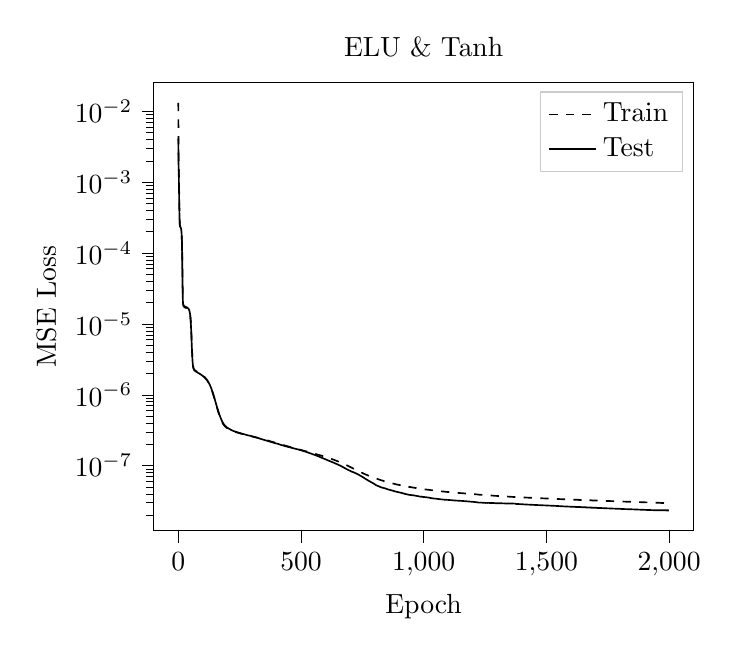
\begin{tikzpicture}

\begin{axis}[
legend cell align={left},
legend style={fill opacity=0.8, draw opacity=1, text opacity=1, draw=white!80!black},
log basis y={10},
tick align=outside,
tick pos=left,
title={ELU \& Tanh},
x grid style={white!69.0196078431373!black},
xlabel={Epoch},
xmin=-99.95, xmax=2098.95,
xtick style={color=black},
y grid style={white!69.0196078431373!black},
ylabel={MSE Loss},
ymin=1.20288411886795e-08, ymax=0.0255172665781318,
ymode=log,
ytick style={color=black}
]
\addplot [semithick, black, dashed]
table {%
0 0.0131601534280926
1 0.00254879569727927
2 0.0015288968286477
3 0.000978349994169548
4 0.000554412616998889
5 0.000339064917701762
6 0.00025199008785421
7 0.000222940133317024
8 0.000214015148361796
9 0.0002101389333111
10 0.000206720305548515
11 0.000202234839642188
12 0.000195523965245229
13 0.000184769826577394
14 0.000166750691139896
15 0.000136818764854979
16 9.37190856602683e-05
17 5.13041007707216e-05
18 2.82282359621604e-05
19 2.07924298056241e-05
20 1.86988846025997e-05
21 1.7985147208492e-05
22 1.76603932732178e-05
23 1.74696931553626e-05
24 1.7336417397928e-05
25 1.72325157009254e-05
26 1.71457306960292e-05
27 1.70700371490966e-05
28 1.70019622391919e-05
29 1.69390593810022e-05
30 1.68791474070531e-05
31 1.68202410141021e-05
32 1.67614346964911e-05
33 1.67019616865218e-05
34 1.6640574176563e-05
35 1.65759826668364e-05
36 1.65068785563562e-05
37 1.64315606043601e-05
38 1.63476329316836e-05
39 1.62519396644711e-05
40 1.6141011761647e-05
41 1.60096406534649e-05
42 1.58509294724354e-05
43 1.56562558504447e-05
44 1.54144996622563e-05
45 1.51104531623787e-05
46 1.47251194412092e-05
47 1.42343020070257e-05
48 1.36079418834925e-05
49 1.28111480071311e-05
50 1.18125108524509e-05
51 1.06009906053259e-05
52 9.21135425733155e-06
53 7.74572519412686e-06
54 6.35779605204334e-06
55 5.1833828706549e-06
56 4.27447103993472e-06
57 3.60888216903277e-06
58 3.13739593627815e-06
59 2.81365010323498e-06
60 2.5991098123086e-06
61 2.4615408203772e-06
62 2.37513457909699e-06
63 2.32067587933216e-06
64 2.28507542425405e-06
65 2.2601448145565e-06
66 2.2411157641784e-06
67 2.22538888459667e-06
68 2.21156630598784e-06
69 2.19884542784143e-06
70 2.18683005365961e-06
71 2.17529318160814e-06
72 2.16406654300272e-06
73 2.15305643186525e-06
74 2.14221861409669e-06
75 2.13150765353021e-06
76 2.12089069145804e-06
77 2.11034301975133e-06
78 2.09984778734906e-06
79 2.08938692787797e-06
80 2.07894793217633e-06
81 2.06852177257133e-06
82 2.05811688823587e-06
83 2.04775601798701e-06
84 2.03743660432565e-06
85 2.02712287028817e-06
86 2.01677592477267e-06
87 2.00636359383566e-06
88 1.9958792451007e-06
89 1.98534851921295e-06
90 1.97476752782677e-06
91 1.96412047347394e-06
92 1.95337903960535e-06
93 1.94250881099833e-06
94 1.93151071587749e-06
95 1.92039129103705e-06
96 1.90919305123316e-06
97 1.89784946982741e-06
98 1.88634913931196e-06
99 1.8746769611937e-06
100 1.86280562124352e-06
101 1.85072760652361e-06
102 1.83844960992019e-06
103 1.8259182288034e-06
104 1.81310693804448e-06
105 1.80003688234365e-06
106 1.78669658473041e-06
107 1.77301694364473e-06
108 1.75900127936757e-06
109 1.7447329835818e-06
110 1.7301772377607e-06
111 1.71521739630975e-06
112 1.69957119675246e-06
113 1.68334501330492e-06
114 1.66680457303414e-06
115 1.65007861224353e-06
116 1.63280734801674e-06
117 1.6146544377591e-06
118 1.59609273197248e-06
119 1.57705401022668e-06
120 1.55746726173334e-06
121 1.53734570181996e-06
122 1.51670278955862e-06
123 1.49546852236426e-06
124 1.47359743027664e-06
125 1.45113387642937e-06
126 1.42810016075146e-06
127 1.40454621669051e-06
128 1.38053379953362e-06
129 1.35608644262675e-06
130 1.33122524189844e-06
131 1.30597759505235e-06
132 1.28038126339902e-06
133 1.25448347620249e-06
134 1.22832383840432e-06
135 1.20193885268804e-06
136 1.17537005490931e-06
137 1.14872875269612e-06
138 1.12217347577825e-06
139 1.09575871235279e-06
140 1.06947597012663e-06
141 1.04335389841026e-06
142 1.01742884223199e-06
143 9.9174229461596e-07
144 9.66341739569998e-07
145 9.41270877660827e-07
146 9.16549341098971e-07
147 8.92186274228379e-07
148 8.68209495507699e-07
149 8.44659665403924e-07
150 8.21562834261158e-07
151 7.98913440092974e-07
152 7.76709624403793e-07
153 7.55005571022593e-07
154 7.33842296398279e-07
155 7.1324187874211e-07
156 6.93227800155682e-07
157 6.73795341072036e-07
158 6.54944412957548e-07
159 6.36686511398921e-07
160 6.1902444002726e-07
161 6.01977020039612e-07
162 5.85635424073416e-07
163 5.70022565256068e-07
164 5.55100744662695e-07
165 5.40865127419465e-07
166 5.27296150863776e-07
167 5.14358819003746e-07
168 5.02070321516612e-07
169 4.90478948591999e-07
170 4.79591890936604e-07
171 4.69351124877448e-07
172 4.59683979244119e-07
173 4.50545075622699e-07
174 4.41906577222539e-07
175 4.3379301284574e-07
176 4.2621222132766e-07
177 4.19125185430858e-07
178 4.12513949200388e-07
179 4.06395948857607e-07
180 4.0069370336937e-07
181 3.95336360668352e-07
182 3.90310984542452e-07
183 3.85583037569859e-07
184 3.81129604534181e-07
185 3.76938679011118e-07
186 3.7298087708848e-07
187 3.69250917529484e-07
188 3.65744902723009e-07
189 3.62441119918344e-07
190 3.59327262572151e-07
191 3.56425127719717e-07
192 3.53701333978051e-07
193 3.5110774130942e-07
194 3.48639408940699e-07
195 3.46290742058386e-07
196 3.44055538093357e-07
197 3.41920796998352e-07
198 3.3988114013539e-07
199 3.37931422890847e-07
200 3.36068908225684e-07
201 3.34285324115058e-07
202 3.32569850741038e-07
203 3.30912869202393e-07
204 3.29307206200724e-07
205 3.27750944606464e-07
206 3.26266979001844e-07
207 3.24852640630979e-07
208 3.2346957465279e-07
209 3.22117157267598e-07
210 3.20800171451197e-07
211 3.19513469719368e-07
212 3.18255217777619e-07
213 3.1702468275796e-07
214 3.15827612496378e-07
215 3.14678894085318e-07
216 3.13595294272773e-07
217 3.12561567270109e-07
218 3.11577581513234e-07
219 3.10577952916447e-07
220 3.09579402184568e-07
221 3.08594582278943e-07
222 3.07647466968319e-07
223 3.06742993970488e-07
224 3.05863141832674e-07
225 3.04989370448538e-07
226 3.04124103536196e-07
227 3.032701661283e-07
228 3.02431237756196e-07
229 3.01602489713559e-07
230 3.00785786294e-07
231 2.99983752753974e-07
232 2.99192086089306e-07
233 2.98409287395884e-07
234 2.97635152378462e-07
235 2.96870692309881e-07
236 2.96115399436303e-07
237 2.95368066886681e-07
238 2.94630630094161e-07
239 2.93900858636675e-07
240 2.93184512997868e-07
241 2.92489651116057e-07
242 2.91816891092367e-07
243 2.91145831212702e-07
244 2.9048319896674e-07
245 2.89822926731631e-07
246 2.89163126112157e-07
247 2.88502883591946e-07
248 2.87852459607052e-07
249 2.87224834607969e-07
250 2.86597030878966e-07
251 2.85960856729162e-07
252 2.85321492057733e-07
253 2.84688976776692e-07
254 2.84068795139092e-07
255 2.83460164652638e-07
256 2.82858641597272e-07
257 2.82261807114992e-07
258 2.81669071654278e-07
259 2.81083668824067e-07
260 2.8050698112736e-07
261 2.79942047242798e-07
262 2.79401001975543e-07
263 2.78919282436618e-07
264 2.78250929099499e-07
265 2.7769323406801e-07
266 2.77149659567044e-07
267 2.76604206774778e-07
268 2.76058308742222e-07
269 2.75514584600955e-07
270 2.74971755459319e-07
271 2.74430956324068e-07
272 2.73889851285958e-07
273 2.73346790777396e-07
274 2.72801549414226e-07
275 2.72264279217893e-07
276 2.7174932449725e-07
277 2.71240941714268e-07
278 2.70725355719037e-07
279 2.70204308250754e-07
280 2.69686683623149e-07
281 2.69170687374753e-07
282 2.68656707220316e-07
283 2.6814359382854e-07
284 2.6763243812411e-07
285 2.67122213244875e-07
286 2.66613155758932e-07
287 2.66105947375195e-07
288 2.6559856546271e-07
289 2.6509363469529e-07
290 2.64588432443702e-07
291 2.64084260251707e-07
292 2.63579864878238e-07
293 2.63075514027378e-07
294 2.62571202327422e-07
295 2.62065000541156e-07
296 2.6155551402951e-07
297 2.61047375587964e-07
298 2.60552575497286e-07
299 2.60085221540862e-07
300 2.59596596890788e-07
301 2.59059146287655e-07
302 2.58539276231318e-07
303 2.58035740202445e-07
304 2.57535053350466e-07
305 2.57033249823735e-07
306 2.56527450233079e-07
307 2.56022325999083e-07
308 2.55515834126641e-07
309 2.55008146865521e-07
310 2.54499001528075e-07
311 2.53990032419438e-07
312 2.53478506948568e-07
313 2.5296603746483e-07
314 2.52451124438835e-07
315 2.51934009867227e-07
316 2.51414092375057e-07
317 2.5088994965472e-07
318 2.50361918318731e-07
319 2.49830229506642e-07
320 2.49291807122631e-07
321 2.48751227886146e-07
322 2.48202915614115e-07
323 2.47651687843131e-07
324 2.47100254256338e-07
325 2.46554554564682e-07
326 2.46023965161157e-07
327 2.45507849939486e-07
328 2.45001275814616e-07
329 2.44500258460789e-07
330 2.4399837899125e-07
331 2.43496204234361e-07
332 2.42991565372108e-07
333 2.42484796899589e-07
334 2.41975729196042e-07
335 2.41464755745824e-07
336 2.40952600208288e-07
337 2.40439445832408e-07
338 2.39924943556957e-07
339 2.39409758350462e-07
340 2.38894031781456e-07
341 2.38378295378538e-07
342 2.37861772134806e-07
343 2.37343902668385e-07
344 2.36825885465919e-07
345 2.36308309311539e-07
346 2.35789153393284e-07
347 2.3527115035904e-07
348 2.34751956895707e-07
349 2.34233497749869e-07
350 2.33713108769962e-07
351 2.33194307313056e-07
352 2.32674123310517e-07
353 2.32153817776748e-07
354 2.31633706150092e-07
355 2.31114634758001e-07
356 2.30592511172745e-07
357 2.30073320196311e-07
358 2.29550019184899e-07
359 2.29030590574553e-07
360 2.28506732995015e-07
361 2.27985227525096e-07
362 2.2745980940897e-07
363 2.26935036494069e-07
364 2.26407579006604e-07
365 2.25878871745522e-07
366 2.25349141089737e-07
367 2.24818749259725e-07
368 2.24284589023682e-07
369 2.23751356216439e-07
370 2.23217339097914e-07
371 2.22683898257969e-07
372 2.22149178313202e-07
373 2.21620929323763e-07
374 2.21093199442635e-07
375 2.20577191839766e-07
376 2.20056678102765e-07
377 2.19546195609155e-07
378 2.19024992730965e-07
379 2.18527559781023e-07
380 2.18007180933455e-07
381 2.17523276390352e-07
382 2.16990808596051e-07
383 2.16530773329282e-07
384 2.15981374630303e-07
385 2.15540847143814e-07
386 2.1498925293173e-07
387 2.14562892296044e-07
388 2.14015980148474e-07
389 2.13598349787958e-07
390 2.13054402372848e-07
391 2.12622081441793e-07
392 2.12062817922742e-07
393 2.11620012045444e-07
394 2.11074238080755e-07
395 2.10642850724696e-07
396 2.10115624135199e-07
397 2.09677260365027e-07
398 2.09132693299807e-07
399 2.08685344418313e-07
400 2.08155541599808e-07
401 2.07705447643036e-07
402 2.07183368253538e-07
403 2.06727136337292e-07
404 2.06216078247223e-07
405 2.05757556649644e-07
406 2.05255236807034e-07
407 2.04789339271372e-07
408 2.04285899336298e-07
409 2.03810201718113e-07
410 2.03323012144097e-07
411 2.0286266884284e-07
412 2.02395825432689e-07
413 2.01942679375122e-07
414 2.01489438097724e-07
415 2.01049114735952e-07
416 2.00620913773264e-07
417 2.00179136562895e-07
418 1.99697794052156e-07
419 1.99211518797426e-07
420 1.98745680755508e-07
421 1.98285480642824e-07
422 1.97829109247039e-07
423 1.97373576042992e-07
424 1.96920282753865e-07
425 1.96468902387892e-07
426 1.96017156085304e-07
427 1.95567786732909e-07
428 1.95119598167537e-07
429 1.9467373040527e-07
430 1.94228913869665e-07
431 1.9378678856441e-07
432 1.93345975787906e-07
433 1.92908213861642e-07
434 1.92472880911509e-07
435 1.92033376286815e-07
436 1.91594089322678e-07
437 1.91156777340495e-07
438 1.90721543447125e-07
439 1.90288229426017e-07
440 1.89856990296278e-07
441 1.89426350928557e-07
442 1.88998336355439e-07
443 1.88572393220454e-07
444 1.88147689407003e-07
445 1.87724033871461e-07
446 1.87301913300075e-07
447 1.86881752682666e-07
448 1.86463004709481e-07
449 1.8604587298654e-07
450 1.85630693742667e-07
451 1.85216147464473e-07
452 1.84802860189848e-07
453 1.84391357393565e-07
454 1.83981159352697e-07
455 1.83571897430568e-07
456 1.83164638301037e-07
457 1.8275769946996e-07
458 1.82352313437661e-07
459 1.81948242243379e-07
460 1.8154557169936e-07
461 1.81142903578291e-07
462 1.80741623182712e-07
463 1.80341402725048e-07
464 1.79942316073323e-07
465 1.79544574173462e-07
466 1.79148779068328e-07
467 1.78754067341913e-07
468 1.78359900061764e-07
469 1.77966328479329e-07
470 1.77572222291644e-07
471 1.77177200519907e-07
472 1.7677393238813e-07
473 1.76369746831995e-07
474 1.75992078169429e-07
475 1.75616341152818e-07
476 1.75233647482287e-07
477 1.7484610436469e-07
478 1.74459954209283e-07
479 1.74083032909778e-07
480 1.73702623811778e-07
481 1.73321933473858e-07
482 1.72944039356082e-07
483 1.72568016154173e-07
484 1.72192560903284e-07
485 1.71817991436285e-07
486 1.71445508037493e-07
487 1.71073176801428e-07
488 1.70700102195553e-07
489 1.70324904402719e-07
490 1.69944452999005e-07
491 1.6955677234165e-07
492 1.69169401324609e-07
493 1.68812724808731e-07
494 1.68463908480021e-07
495 1.68110651223685e-07
496 1.67751017137618e-07
497 1.67391723636001e-07
498 1.67032830752589e-07
499 1.66674713902637e-07
500 1.66317192679344e-07
501 1.6596099465005e-07
502 1.65605539926617e-07
503 1.65249893854025e-07
504 1.64895575679225e-07
505 1.64542413884305e-07
506 1.64188377084429e-07
507 1.63834382490791e-07
508 1.63479579349257e-07
509 1.63123736946602e-07
510 1.62764372966251e-07
511 1.62400060261803e-07
512 1.62033490710201e-07
513 1.61673854385924e-07
514 1.6133109382821e-07
515 1.60980462240445e-07
516 1.60622751863571e-07
517 1.60286923545527e-07
518 1.5995844636052e-07
519 1.59616451256284e-07
520 1.59275953478755e-07
521 1.58933757333557e-07
522 1.58592838552352e-07
523 1.58254255289592e-07
524 1.57914939528325e-07
525 1.57576707024987e-07
526 1.57237424488699e-07
527 1.56900591548492e-07
528 1.56563655664854e-07
529 1.56226724612907e-07
530 1.55891212621384e-07
531 1.55555264647944e-07
532 1.55220193441608e-07
533 1.5488449407286e-07
534 1.54550589023472e-07
535 1.54216606908619e-07
536 1.53881973737668e-07
537 1.53549540797826e-07
538 1.53216481912466e-07
539 1.52883593578679e-07
540 1.52551263909118e-07
541 1.52220322597429e-07
542 1.51887326481415e-07
543 1.51556127320873e-07
544 1.51225415628176e-07
545 1.50893343956682e-07
546 1.50563061609432e-07
547 1.50233072332639e-07
548 1.49902952898628e-07
549 1.49572416454191e-07
550 1.49243174121239e-07
551 1.48913397453043e-07
552 1.48584105176042e-07
553 1.48255081676041e-07
554 1.47925589033093e-07
555 1.47597463460158e-07
556 1.47268285857649e-07
557 1.46940167169873e-07
558 1.46610681149184e-07
559 1.46281415496219e-07
560 1.45951650871723e-07
561 1.45620285614712e-07
562 1.4528401814573e-07
563 1.44944069916164e-07
564 1.44600810408235e-07
565 1.44262943436502e-07
566 1.43927519481224e-07
567 1.43590049695774e-07
568 1.43260283628877e-07
569 1.42937757580341e-07
570 1.42615396995893e-07
571 1.42289746904112e-07
572 1.4196258763377e-07
573 1.41634024075188e-07
574 1.4130653507749e-07
575 1.40979754874593e-07
576 1.40654982985211e-07
577 1.40327927930173e-07
578 1.39996476441695e-07
579 1.39661024547877e-07
580 1.39324684006681e-07
581 1.38991585217241e-07
582 1.38657661004515e-07
583 1.38324706199455e-07
584 1.37992608131299e-07
585 1.37660341053447e-07
586 1.37325831850887e-07
587 1.36991686318311e-07
588 1.36658037732218e-07
589 1.36322862211102e-07
590 1.35988218090688e-07
591 1.35652704940981e-07
592 1.35316823737242e-07
593 1.34980701190557e-07
594 1.34643992552697e-07
595 1.34307293656377e-07
596 1.33969952976543e-07
597 1.33632085059787e-07
598 1.33294102340642e-07
599 1.32956124616612e-07
600 1.32616756907566e-07
601 1.32277391614366e-07
602 1.31938818839217e-07
603 1.31597589152932e-07
604 1.31258015692026e-07
605 1.3091720372671e-07
606 1.30575987988379e-07
607 1.30233362483523e-07
608 1.29891986915709e-07
609 1.2954996940806e-07
610 1.29205809294319e-07
611 1.28862633737015e-07
612 1.28520314646607e-07
613 1.2817495100137e-07
614 1.27830125414619e-07
615 1.27484617458151e-07
616 1.27139700730083e-07
617 1.2679202459509e-07
618 1.26445642635531e-07
619 1.26099415318492e-07
620 1.25751059400159e-07
621 1.25403643487232e-07
622 1.25053666707231e-07
623 1.24705792295288e-07
624 1.24355652907582e-07
625 1.24006482145944e-07
626 1.23654558812802e-07
627 1.23304186288919e-07
628 1.22952360904094e-07
629 1.22601375110776e-07
630 1.22249454179268e-07
631 1.21896765762131e-07
632 1.21543555302139e-07
633 1.21191076516425e-07
634 1.20836187782913e-07
635 1.20481173560449e-07
636 1.20121345013047e-07
637 1.19762935923973e-07
638 1.19400635831823e-07
639 1.19041445550749e-07
640 1.18679526153187e-07
641 1.18321026214119e-07
642 1.17956734527525e-07
643 1.17598218643877e-07
644 1.17233053785526e-07
645 1.1687504470359e-07
646 1.16506115539039e-07
647 1.16149264989929e-07
648 1.15774781420441e-07
649 1.15423059597219e-07
650 1.15037076007241e-07
651 1.14700303406323e-07
652 1.14294124074377e-07
653 1.13968814041243e-07
654 1.13556144349047e-07
655 1.13219854505076e-07
656 1.12819404108677e-07
657 1.12505390681861e-07
658 1.1211966626945e-07
659 1.11745449785872e-07
660 1.11343885933479e-07
661 1.10986338235364e-07
662 1.10601156912082e-07
663 1.10227328399048e-07
664 1.09847862688639e-07
665 1.09466705730199e-07
666 1.09083192626258e-07
667 1.08700647508897e-07
668 1.0831480311424e-07
669 1.07929378259541e-07
670 1.07541389290589e-07
671 1.07154287086075e-07
672 1.0676769644391e-07
673 1.06381731328042e-07
674 1.05990678122225e-07
675 1.05594895771333e-07
676 1.05199675196843e-07
677 1.04810480365813e-07
678 1.04418989685939e-07
679 1.04027984271227e-07
680 1.0363815702874e-07
681 1.0324819263019e-07
682 1.02859756317741e-07
683 1.02471920968128e-07
684 1.02083233088024e-07
685 1.01694726282631e-07
686 1.01307340209189e-07
687 1.00919130510135e-07
688 1.00530916142816e-07
689 1.00143542738351e-07
690 9.97545113179399e-08
691 9.93675590379439e-08
692 9.89800909607652e-08
693 9.85953646619464e-08
694 9.82120354180438e-08
695 9.78292016071691e-08
696 9.74492761613988e-08
697 9.70678999436814e-08
698 9.66850550199183e-08
699 9.63028536418165e-08
700 9.59213216376043e-08
701 9.55436611391747e-08
702 9.51664130255381e-08
703 9.47894022971241e-08
704 9.44130259696863e-08
705 9.4036925865737e-08
706 9.36625970240357e-08
707 9.3288709258843e-08
708 9.29143761752016e-08
709 9.25398956113099e-08
710 9.21654500132263e-08
711 9.17905279180786e-08
712 9.14152797406587e-08
713 9.10435747840666e-08
714 9.06759069962959e-08
715 9.03191059151709e-08
716 8.99658183541874e-08
717 8.96166580233171e-08
718 8.92642552727807e-08
719 8.89152184484487e-08
720 8.85622741293446e-08
721 8.82137649327319e-08
722 8.78630537997083e-08
723 8.75201614576326e-08
724 8.71707721543657e-08
725 8.68308670831652e-08
726 8.64862795069143e-08
727 8.61490446126823e-08
728 8.58071580154274e-08
729 8.54761280493221e-08
730 8.51358397824242e-08
731 8.48093447345377e-08
732 8.44707277849466e-08
733 8.415007692264e-08
734 8.38136081213747e-08
735 8.34983421782454e-08
736 8.3161317022018e-08
737 8.28544769078121e-08
738 8.25149288914417e-08
739 8.22155614130793e-08
740 8.18770621009435e-08
741 8.15844286066181e-08
742 8.12440885340493e-08
743 8.09608954952523e-08
744 8.06174798384518e-08
745 8.03448064274903e-08
746 7.99966385969242e-08
747 7.97339763067839e-08
748 7.93839182975376e-08
749 7.91303163794055e-08
750 7.87830934640965e-08
751 7.85370518201489e-08
752 7.81923441977028e-08
753 7.79547676614811e-08
754 7.76166178368953e-08
755 7.73845136876616e-08
756 7.70513217887014e-08
757 7.6827997897766e-08
758 7.65009137211337e-08
759 7.62806916014824e-08
760 7.59617605865515e-08
761 7.57490153944218e-08
762 7.54341544002557e-08
763 7.52256842986299e-08
764 7.4918414092906e-08
765 7.47141463257606e-08
766 7.44146009132862e-08
767 7.42095831078871e-08
768 7.39145847177269e-08
769 7.37110998905166e-08
770 7.34179971253468e-08
771 7.32091361825837e-08
772 7.29165597661563e-08
773 7.27025321936026e-08
774 7.24227878343697e-08
775 7.22241191581929e-08
776 7.19627312939508e-08
777 7.1762471385739e-08
778 7.15034239000545e-08
779 7.13010314328244e-08
780 7.10541031061496e-08
781 7.08462831724432e-08
782 7.05859609908543e-08
783 7.03546273612687e-08
784 7.00836361460233e-08
785 6.98543979780197e-08
786 6.96672320295022e-08
787 6.95502103305046e-08
788 6.93480467042207e-08
789 6.91480321002302e-08
790 6.893230557381e-08
791 6.87383616266857e-08
792 6.85314918520419e-08
793 6.8341212134726e-08
794 6.81411711696001e-08
795 6.7953572468582e-08
796 6.77608208867753e-08
797 6.75757414292377e-08
798 6.73860329385434e-08
799 6.72034605280203e-08
800 6.70175597434763e-08
801 6.68326048476331e-08
802 6.66480708346739e-08
803 6.64633341713738e-08
804 6.62772580142246e-08
805 6.60915295256359e-08
806 6.59041005377503e-08
807 6.57156358592204e-08
808 6.55272900793591e-08
809 6.53402567074579e-08
810 6.51595602043642e-08
811 6.49886946746392e-08
812 6.48140172714307e-08
813 6.46367730396946e-08
814 6.44600384482885e-08
815 6.42846892340288e-08
816 6.41082180870001e-08
817 6.393430256324e-08
818 6.37585768821225e-08
819 6.3583405808032e-08
820 6.34069121367986e-08
821 6.3220355329463e-08
822 6.30279480944296e-08
823 6.28660326320585e-08
824 6.27192910052088e-08
825 6.25616495177894e-08
826 6.2403849131698e-08
827 6.22459404517883e-08
828 6.20908969644063e-08
829 6.19363434211095e-08
830 6.17823749138324e-08
831 6.16275062306215e-08
832 6.14738188069452e-08
833 6.13199244092755e-08
834 6.11655107789488e-08
835 6.10088632164718e-08
836 6.0842924721527e-08
837 6.06600994501605e-08
838 6.04520119829033e-08
839 6.02753693641489e-08
840 6.01769672208263e-08
841 6.00620659341189e-08
842 5.99465706621061e-08
843 5.98101269986273e-08
844 5.967979369359e-08
845 5.95410453740897e-08
846 5.94138033847003e-08
847 5.92733323401262e-08
848 5.91528519073847e-08
849 5.90060622549515e-08
850 5.88980487492563e-08
851 5.87444609330134e-08
852 5.86443678791682e-08
853 5.84868802242511e-08
854 5.83924014350146e-08
855 5.82357584981708e-08
856 5.81416117668709e-08
857 5.79865398862012e-08
858 5.78953433674201e-08
859 5.77420002088047e-08
860 5.76522297208726e-08
861 5.74993749147268e-08
862 5.74120188865379e-08
863 5.72597793819796e-08
864 5.71752964901862e-08
865 5.70247034836768e-08
866 5.69411097757211e-08
867 5.679273058945e-08
868 5.67114060920915e-08
869 5.65622520021236e-08
870 5.64837248084871e-08
871 5.63370899193671e-08
872 5.62614032411091e-08
873 5.61162377863411e-08
874 5.60408048073668e-08
875 5.59000868207704e-08
876 5.5825515403285e-08
877 5.56860418754468e-08
878 5.56065390320271e-08
879 5.54442152704837e-08
880 5.53465068193759e-08
881 5.52014605581519e-08
882 5.5144348330316e-08
883 5.50065026025948e-08
884 5.4938962758655e-08
885 5.47925301255248e-08
886 5.47226506917298e-08
887 5.45806310938701e-08
888 5.44830717252864e-08
889 5.43354541591157e-08
890 5.42866788784124e-08
891 5.4193029882299e-08
892 5.41037255992194e-08
893 5.4004102963745e-08
894 5.39168008906188e-08
895 5.38167598982398e-08
896 5.37307497765482e-08
897 5.36283687786465e-08
898 5.3545491898177e-08
899 5.34505866340851e-08
900 5.33795286301597e-08
901 5.32782876376814e-08
902 5.32000103348196e-08
903 5.31031169508367e-08
904 5.30214819072228e-08
905 5.29322757287787e-08
906 5.2850323964293e-08
907 5.27636802090115e-08
908 5.26779433123181e-08
909 5.25862555775802e-08
910 5.24820538458925e-08
911 5.23542242767405e-08
912 5.22638524316221e-08
913 5.22520095067591e-08
914 5.20998846980092e-08
915 5.2146744899062e-08
916 5.19045253355444e-08
917 5.19310569870868e-08
918 5.1782812871437e-08
919 5.17995022413231e-08
920 5.15896290842477e-08
921 5.17530991928084e-08
922 5.14307041790119e-08
923 5.13906512296103e-08
924 5.14559755586674e-08
925 5.12293278269738e-08
926 5.12345318988139e-08
927 5.11401419949209e-08
928 5.10994720563929e-08
929 5.09844776672708e-08
930 5.09706070701554e-08
931 5.08257401961032e-08
932 5.08580665368186e-08
933 5.06569208695851e-08
934 5.07608531847836e-08
935 5.04932937239744e-08
936 5.05750532582283e-08
937 5.03769438431334e-08
938 5.04652209301071e-08
939 5.02219266103054e-08
940 5.03236353601721e-08
941 5.00827042166918e-08
942 5.01772669565526e-08
943 4.99418741490842e-08
944 5.00236907434726e-08
945 4.97968133501558e-08
946 4.98517641283058e-08
947 4.9631626453106e-08
948 4.96511877159378e-08
949 4.9451886212637e-08
950 4.95108563427493e-08
951 4.93895526325616e-08
952 4.94255550549383e-08
953 4.92760776005241e-08
954 4.92957489726109e-08
955 4.91394359585229e-08
956 4.91521641272641e-08
957 4.90015478114003e-08
958 4.90032903073256e-08
959 4.88661470505747e-08
960 4.88593277587768e-08
961 4.87428295912196e-08
962 4.87304148784062e-08
963 4.8624902394323e-08
964 4.86015209553159e-08
965 4.8503092187957e-08
966 4.84726088032517e-08
967 4.83801911528303e-08
968 4.83473524752753e-08
969 4.82583990688568e-08
970 4.82274910247327e-08
971 4.8142395744577e-08
972 4.8112453871596e-08
973 4.80282170016721e-08
974 4.79997060160997e-08
975 4.79158530559687e-08
976 4.78881169776457e-08
977 4.78054251900062e-08
978 4.77769883495682e-08
979 4.76954273160857e-08
980 4.76676170073631e-08
981 4.75860888862201e-08
982 4.75565808315537e-08
983 4.7475151536247e-08
984 4.74452551841864e-08
985 4.73646711114384e-08
986 4.73329088208629e-08
987 4.72507358786345e-08
988 4.72154740620567e-08
989 4.71290015013892e-08
990 4.70837073009989e-08
991 4.69815565402598e-08
992 4.69130373481619e-08
993 4.68120339363054e-08
994 4.67982854921445e-08
995 4.67581658618599e-08
996 4.67310412943789e-08
997 4.665680933158e-08
998 4.6614766084474e-08
999 4.65570674066385e-08
1000 4.65196713967941e-08
1001 4.64576681871165e-08
1002 4.64096734482666e-08
1003 4.63734514042358e-08
1004 4.630485181778e-08
1005 4.62859110079705e-08
1006 4.62073714260214e-08
1007 4.61892398355701e-08
1008 4.61182378721503e-08
1009 4.61099274104981e-08
1010 4.60198555884972e-08
1011 4.60196106999433e-08
1012 4.59280479532254e-08
1013 4.59336447882208e-08
1014 4.58340887377062e-08
1015 4.58449031022212e-08
1016 4.57388315808771e-08
1017 4.57569441358885e-08
1018 4.56463287648035e-08
1019 4.56692389860791e-08
1020 4.55531906560225e-08
1021 4.55818113600515e-08
1022 4.54620867849087e-08
1023 4.54929418616246e-08
1024 4.53726893248074e-08
1025 4.5401559834346e-08
1026 4.52775405754835e-08
1027 4.52661582492908e-08
1028 4.51476962659569e-08
1029 4.51590000700719e-08
1030 4.51276083133223e-08
1031 4.5074241686649e-08
1032 4.50412402521749e-08
1033 4.49861366362825e-08
1034 4.49491402463309e-08
1035 4.49011619707562e-08
1036 4.48583528225299e-08
1037 4.48114631268481e-08
1038 4.4767292468606e-08
1039 4.47221731540992e-08
1040 4.46739429484921e-08
1041 4.46299758394275e-08
1042 4.45806041220464e-08
1043 4.45325005777875e-08
1044 4.44845118465764e-08
1045 4.44400044159465e-08
1046 4.43992311396357e-08
1047 4.43588988190413e-08
1048 4.4323437709437e-08
1049 4.42854224402822e-08
1050 4.4246319131247e-08
1051 4.42069745645313e-08
1052 4.41663080543719e-08
1053 4.41267324831074e-08
1054 4.40851923002583e-08
1055 4.40439598889952e-08
1056 4.40021518457456e-08
1057 4.39624776760184e-08
1058 4.39202907180913e-08
1059 4.38781604579219e-08
1060 4.3835203697995e-08
1061 4.37901719294587e-08
1062 4.37391187269043e-08
1063 4.36787410329487e-08
1064 4.36142205195722e-08
1065 4.35764591593113e-08
1066 4.3526191713994e-08
1067 4.35113610848248e-08
1068 4.35112334251642e-08
1069 4.34788408760767e-08
1070 4.34420058006424e-08
1071 4.34074025825737e-08
1072 4.337379616004e-08
1073 4.33410867017869e-08
1074 4.33068135663461e-08
1075 4.32735379654048e-08
1076 4.32421167673169e-08
1077 4.32102222447384e-08
1078 4.3178529104182e-08
1079 4.31464594292663e-08
1080 4.31127083402316e-08
1081 4.30777044293507e-08
1082 4.30424841333377e-08
1083 4.30052575595141e-08
1084 4.29678215105866e-08
1085 4.29295583472822e-08
1086 4.28891776209639e-08
1087 4.28501564400108e-08
1088 4.28093613180636e-08
1089 4.27695682532203e-08
1090 4.27320691649413e-08
1091 4.26969720095371e-08
1092 4.26641718931364e-08
1093 4.26348475563998e-08
1094 4.26035555918247e-08
1095 4.25714825205148e-08
1096 4.2539459688129e-08
1097 4.25069211793527e-08
1098 4.24752585281851e-08
1099 4.24470454269965e-08
1100 4.24142000383654e-08
1101 4.2386877243672e-08
1102 4.23553551982536e-08
1103 4.23280068666543e-08
1104 4.22964153372618e-08
1105 4.22666909258851e-08
1106 4.22377636120075e-08
1107 4.22090744969239e-08
1108 4.21786970008497e-08
1109 4.21486589772257e-08
1110 4.21205174667705e-08
1111 4.20898296553673e-08
1112 4.20612397995512e-08
1113 4.20298081813542e-08
1114 4.20028930676608e-08
1115 4.19723818225748e-08
1116 4.19444931232249e-08
1117 4.19146600130205e-08
1118 4.18882347830163e-08
1119 4.18592943596252e-08
1120 4.18306351726017e-08
1121 4.17999253414791e-08
1122 4.17717335814416e-08
1123 4.17401160781594e-08
1124 4.17091959263871e-08
1125 4.16738806841011e-08
1126 4.16385093480187e-08
1127 4.16083301644221e-08
1128 4.15826955943999e-08
1129 4.15573036640637e-08
1130 4.15322029070353e-08
1131 4.15054005067361e-08
1132 4.14762116101031e-08
1133 4.14496789424845e-08
1134 4.14193409810082e-08
1135 4.13939505996552e-08
1136 4.13655391540146e-08
1137 4.13387203863635e-08
1138 4.13112442352315e-08
1139 4.1284515468476e-08
1140 4.12570460248674e-08
1141 4.122893498959e-08
1142 4.12023311824328e-08
1143 4.11755861478014e-08
1144 4.11479511477353e-08
1145 4.11188139608498e-08
1146 4.10914398187856e-08
1147 4.10588335206796e-08
1148 4.10257076417508e-08
1149 4.09911478058689e-08
1150 4.09706586381731e-08
1151 4.0947768535915e-08
1152 4.09257850790823e-08
1153 4.09000993784048e-08
1154 4.08752379961186e-08
1155 4.08492191041887e-08
1156 4.08236526574512e-08
1157 4.0796837154744e-08
1158 4.07754792419723e-08
1159 4.07453324307028e-08
1160 4.07218479203664e-08
1161 4.06957986918144e-08
1162 4.06731145297101e-08
1163 4.06448262104675e-08
1164 4.06233385987775e-08
1165 4.05953980724405e-08
1166 4.0572532196137e-08
1167 4.05458565069239e-08
1168 4.05216331067493e-08
1169 4.04969372880259e-08
1170 4.04722319551354e-08
1171 4.04483379838894e-08
1172 4.04240453200089e-08
1173 4.03967915474368e-08
1174 4.03753465789691e-08
1175 4.03492542062622e-08
1176 4.03253273830728e-08
1177 4.03027273101486e-08
1178 4.02754001136429e-08
1179 4.02519226767595e-08
1180 4.02287905032495e-08
1181 4.02035331461548e-08
1182 4.01805381002873e-08
1183 4.01537798211393e-08
1184 4.01332027593071e-08
1185 4.01053166001475e-08
1186 4.00851568720384e-08
1187 4.0057915239089e-08
1188 4.00365685031545e-08
1189 4.00097245787379e-08
1190 3.998638086955e-08
1191 3.99603554015471e-08
1192 3.99394127974517e-08
1193 3.99152432635219e-08
1194 3.9889744968491e-08
1195 3.98668957153347e-08
1196 3.98415572284705e-08
1197 3.98171912934231e-08
1198 3.9792276890438e-08
1199 3.9768928541406e-08
1200 3.9741534841653e-08
1201 3.97171350385861e-08
1202 3.9688988476172e-08
1203 3.96626243137632e-08
1204 3.96315111181877e-08
1205 3.96057352176626e-08
1206 3.9574675962939e-08
1207 3.95418058651842e-08
1208 3.95316207217888e-08
1209 3.95276360016794e-08
1210 3.94979896860548e-08
1211 3.9469980588791e-08
1212 3.9439048013179e-08
1213 3.94036826776301e-08
1214 3.93643339400285e-08
1215 3.93208972973014e-08
1216 3.92942937708085e-08
1217 3.92745694526297e-08
1218 3.92532672854884e-08
1219 3.92244704059408e-08
1220 3.91922152473967e-08
1221 3.91519686111508e-08
1222 3.91047739292105e-08
1223 3.90440098669842e-08
1224 3.89788044259376e-08
1225 3.89248560708211e-08
1226 3.88969509970138e-08
1227 3.88739982497555e-08
1228 3.88600895888658e-08
1229 3.88442312200254e-08
1230 3.88249830081122e-08
1231 3.88039069854074e-08
1232 3.8779033271652e-08
1233 3.87615753822956e-08
1234 3.8740473225829e-08
1235 3.873860647019e-08
1236 3.87189993205084e-08
1237 3.87125171172897e-08
1238 3.86798034597291e-08
1239 3.86713239279857e-08
1240 3.86387752158157e-08
1241 3.86332558584002e-08
1242 3.85975577543718e-08
1243 3.85894923411456e-08
1244 3.85478015196838e-08
1245 3.85361696650932e-08
1246 3.84958887202913e-08
1247 3.84842061045276e-08
1248 3.84364790591007e-08
1249 3.84129069281869e-08
1250 3.835013849951e-08
1251 3.830980500652e-08
1252 3.82426465819208e-08
1253 3.82386410500146e-08
1254 3.82098225983896e-08
1255 3.82244349310668e-08
1256 3.81952226753413e-08
1257 3.82213184941804e-08
1258 3.82200949040623e-08
1259 3.82805829381994e-08
1260 3.81924289385438e-08
1261 3.81557332680416e-08
1262 3.81068309458499e-08
1263 3.81131902003062e-08
1264 3.80710950018681e-08
1265 3.80754166329211e-08
1266 3.8031601455657e-08
1267 3.80357743026138e-08
1268 3.79924965976386e-08
1269 3.79957934271147e-08
1270 3.79529627601016e-08
1271 3.79557706651212e-08
1272 3.79125297484961e-08
1273 3.79155425775934e-08
1274 3.78721137686e-08
1275 3.78763480810562e-08
1276 3.78328135077766e-08
1277 3.78355915806594e-08
1278 3.77929401231825e-08
1279 3.77964996722824e-08
1280 3.77534832587401e-08
1281 3.77569717073811e-08
1282 3.77135280906771e-08
1283 3.77169082277362e-08
1284 3.76753321589263e-08
1285 3.76782625970407e-08
1286 3.76359895497558e-08
1287 3.76384917402106e-08
1288 3.75944361508118e-08
1289 3.75930085390053e-08
1290 3.75225182729366e-08
1291 3.74770163737992e-08
1292 3.74718370714788e-08
1293 3.7489422357595e-08
1294 3.74551559829683e-08
1295 3.74438800214705e-08
1296 3.74006098837754e-08
1297 3.74007029471102e-08
1298 3.73629217094162e-08
1299 3.73621428693127e-08
1300 3.73280939420795e-08
1301 3.73244589795263e-08
1302 3.72918043005654e-08
1303 3.72864535371775e-08
1304 3.72538170481107e-08
1305 3.7249388356031e-08
1306 3.72167330553452e-08
1307 3.72109800288456e-08
1308 3.71815438029444e-08
1309 3.71741152491722e-08
1310 3.71463017287965e-08
1311 3.71373364771443e-08
1312 3.71105454988196e-08
1313 3.70999555165952e-08
1314 3.70739672632681e-08
1315 3.70657831076926e-08
1316 3.70393918345258e-08
1317 3.70291311817539e-08
1318 3.70031502647805e-08
1319 3.69933979911252e-08
1320 3.69690625348085e-08
1321 3.69570734548574e-08
1322 3.69338784373952e-08
1323 3.69203525494299e-08
1324 3.69001947291281e-08
1325 3.6884491048994e-08
1326 3.68652273294856e-08
1327 3.68487275963503e-08
1328 3.68304681970244e-08
1329 3.68142394577831e-08
1330 3.67960606553197e-08
1331 3.67789098625337e-08
1332 3.67622351404862e-08
1333 3.67434659480637e-08
1334 3.67273959831493e-08
1335 3.67091880448811e-08
1336 3.66934555309228e-08
1337 3.66746878626145e-08
1338 3.66584931477121e-08
1339 3.66390312436238e-08
1340 3.66224730719011e-08
1341 3.6605432974568e-08
1342 3.65883468766981e-08
1343 3.65714295149644e-08
1344 3.65530410562087e-08
1345 3.65340813850423e-08
1346 3.65178823180656e-08
1347 3.65003956268595e-08
1348 3.64792204763376e-08
1349 3.6462166747242e-08
1350 3.64390187854724e-08
1351 3.64144203004457e-08
1352 3.63808768426566e-08
1353 3.63480680682926e-08
1354 3.63430094481032e-08
1355 3.63301288963669e-08
1356 3.63105459761925e-08
1357 3.62942809886135e-08
1358 3.62777775180234e-08
1359 3.62617287450462e-08
1360 3.6245150628389e-08
1361 3.62308960468738e-08
1362 3.62138289844438e-08
1363 3.62002452725108e-08
1364 3.6184935460426e-08
1365 3.61701732138897e-08
1366 3.61554141043996e-08
1367 3.61406891613569e-08
1368 3.61240609976221e-08
1369 3.61108940225563e-08
1370 3.6095503737954e-08
1371 3.60805933290464e-08
1372 3.60654301339025e-08
1373 3.60536631198727e-08
1374 3.60411751181289e-08
1375 3.60590584769227e-08
1376 3.61813945453093e-08
1377 3.60400907162273e-08
1378 3.59819094235547e-08
1379 3.59982796069858e-08
1380 3.59502398268319e-08
1381 3.59369197884263e-08
1382 3.59247000218943e-08
1383 3.59130908371696e-08
1384 3.58994939038126e-08
1385 3.58858682449892e-08
1386 3.58702627671903e-08
1387 3.58569727332281e-08
1388 3.58411974819006e-08
1389 3.58273031260126e-08
1390 3.58132638105246e-08
1391 3.57984322718607e-08
1392 3.57838174185332e-08
1393 3.57703939943832e-08
1394 3.57548559328791e-08
1395 3.57421738392816e-08
1396 3.57274874609459e-08
1397 3.57130793045002e-08
1398 3.56987065561754e-08
1399 3.56859365275852e-08
1400 3.56723504779666e-08
1401 3.56562603816002e-08
1402 3.56429567034411e-08
1403 3.56305411948199e-08
1404 3.56149395770444e-08
1405 3.56023473973011e-08
1406 3.55880008537923e-08
1407 3.55749964064955e-08
1408 3.55611533038314e-08
1409 3.55491478583048e-08
1410 3.55372720868274e-08
1411 3.55255777009233e-08
1412 3.55127736089145e-08
1413 3.54982682502225e-08
1414 3.54833222182549e-08
1415 3.54681789627165e-08
1416 3.5455271095941e-08
1417 3.54414301675376e-08
1418 3.54276840504042e-08
1419 3.54131853086415e-08
1420 3.54002483771154e-08
1421 3.53862656261583e-08
1422 3.5373339052569e-08
1423 3.53595391082706e-08
1424 3.53455515504919e-08
1425 3.53328155053845e-08
1426 3.53199861482523e-08
1427 3.53063538316434e-08
1428 3.52920319866001e-08
1429 3.5279573129543e-08
1430 3.52657978464066e-08
1431 3.52531556409019e-08
1432 3.52385292092805e-08
1433 3.52269802306182e-08
1434 3.52141010289131e-08
1435 3.51998886003457e-08
1436 3.51868791685916e-08
1437 3.51745125541925e-08
1438 3.51609089896954e-08
1439 3.51482826559391e-08
1440 3.51343365529999e-08
1441 3.51232361524012e-08
1442 3.51082564797878e-08
1443 3.509611378405e-08
1444 3.50831519657646e-08
1445 3.50707591838528e-08
1446 3.50574235916667e-08
1447 3.50439018550475e-08
1448 3.50309405909854e-08
1449 3.50192518023817e-08
1450 3.50050656816592e-08
1451 3.49941901731654e-08
1452 3.49809930675349e-08
1453 3.49674752264662e-08
1454 3.49558873509181e-08
1455 3.49413530642551e-08
1456 3.49300676365516e-08
1457 3.49172356166605e-08
1458 3.49033468776128e-08
1459 3.48927129323329e-08
1460 3.4879396197951e-08
1461 3.48665890719246e-08
1462 3.48540501153849e-08
1463 3.48419454656579e-08
1464 3.48285252158575e-08
1465 3.48163265613266e-08
1466 3.48037345787589e-08
1467 3.47920631948995e-08
1468 3.47789087875583e-08
1469 3.47662821180705e-08
1470 3.47539192002699e-08
1471 3.47411823646837e-08
1472 3.47293484299627e-08
1473 3.47165875425048e-08
1474 3.47041539470183e-08
1475 3.46924400478343e-08
1476 3.46800946964265e-08
1477 3.4666789801463e-08
1478 3.46540610198787e-08
1479 3.46429031896633e-08
1480 3.46294183568574e-08
1481 3.461818386441e-08
1482 3.4604350071632e-08
1483 3.45933963430411e-08
1484 3.45812807776014e-08
1485 3.45672587656054e-08
1486 3.4557700171689e-08
1487 3.45435805755301e-08
1488 3.45323912860351e-08
1489 3.45197789624052e-08
1490 3.45075201391154e-08
1491 3.44958345550594e-08
1492 3.44821512214821e-08
1493 3.4470983630186e-08
1494 3.44587823377651e-08
1495 3.4446950284206e-08
1496 3.44349651228981e-08
1497 3.44226299517913e-08
1498 3.44098257372139e-08
1499 3.43983677328907e-08
1500 3.43862202747403e-08
1501 3.43750642350926e-08
1502 3.43623952563377e-08
1503 3.43486220355516e-08
1504 3.43395975619387e-08
1505 3.43255966832601e-08
1506 3.43137105129898e-08
1507 3.43036594969703e-08
1508 3.4290591278463e-08
1509 3.42778486572826e-08
1510 3.42655845777529e-08
1511 3.42545321139198e-08
1512 3.42419907646274e-08
1513 3.42309791765416e-08
1514 3.42183131323282e-08
1515 3.42071012973122e-08
1516 3.41951650515426e-08
1517 3.41832788262053e-08
1518 3.41712281546336e-08
1519 3.4158685988217e-08
1520 3.41478379759508e-08
1521 3.41356923367897e-08
1522 3.41245626813702e-08
1523 3.41118602396051e-08
1524 3.41002601427221e-08
1525 3.40890839467534e-08
1526 3.40760735983992e-08
1527 3.40650075720816e-08
1528 3.40537013094888e-08
1529 3.4041706500787e-08
1530 3.40299353744911e-08
1531 3.40182398552713e-08
1532 3.40060991490532e-08
1533 3.39939918596599e-08
1534 3.39838769498613e-08
1535 3.39708770908942e-08
1536 3.39600365890647e-08
1537 3.39480043791696e-08
1538 3.39359055523403e-08
1539 3.39240513120842e-08
1540 3.39139384610831e-08
1541 3.39009166410165e-08
1542 3.38899627330136e-08
1543 3.387734446747e-08
1544 3.38663625960578e-08
1545 3.38541658368996e-08
1546 3.38432125932542e-08
1547 3.38306701941349e-08
1548 3.3817409228476e-08
1549 3.38075925192527e-08
1550 3.37939539143406e-08
1551 3.37797401019912e-08
1552 3.37630102613673e-08
1553 3.37442441047386e-08
1554 3.3737313620108e-08
1555 3.37287198437508e-08
1556 3.3714445311972e-08
1557 3.37031477641858e-08
1558 3.36888731311546e-08
1559 3.36758163204109e-08
1560 3.36624728198842e-08
1561 3.3649697245508e-08
1562 3.36401100060613e-08
1563 3.36302067296401e-08
1564 3.36192147365466e-08
1565 3.36087661700901e-08
1566 3.35988893631622e-08
1567 3.35875833776811e-08
1568 3.35762191703282e-08
1569 3.35651415159788e-08
1570 3.35540678477741e-08
1571 3.35419140959914e-08
1572 3.35309477073054e-08
1573 3.35200078858122e-08
1574 3.35080816356026e-08
1575 3.34989035550848e-08
1576 3.3485840287284e-08
1577 3.34771403540657e-08
1578 3.34639742796128e-08
1579 3.34542459157205e-08
1580 3.34415820155698e-08
1581 3.34324023629762e-08
1582 3.3419533206569e-08
1583 3.34097595633409e-08
1584 3.33984511229346e-08
1585 3.338851096224e-08
1586 3.33778285508402e-08
1587 3.33657960105427e-08
1588 3.3354734453539e-08
1589 3.33446979396967e-08
1590 3.33333021025339e-08
1591 3.33218127366308e-08
1592 3.33118245396946e-08
1593 3.33003443291346e-08
1594 3.32898500801093e-08
1595 3.3278547633131e-08
1596 3.3268059633329e-08
1597 3.32571939889448e-08
1598 3.32455710569945e-08
1599 3.32345696918424e-08
1600 3.3223890016032e-08
1601 3.32134876543933e-08
1602 3.3201560226459e-08
1603 3.31907092672168e-08
1604 3.31790101792961e-08
1605 3.31643735034248e-08
1606 3.31518633807093e-08
1607 3.31306475871429e-08
1608 3.31231017653977e-08
1609 3.31399948585442e-08
1610 3.30808638953073e-08
1611 3.31158396846831e-08
1612 3.30634980478806e-08
1613 3.3107475823968e-08
1614 3.30438725484328e-08
1615 3.30734918989606e-08
1616 3.302657408355e-08
1617 3.30555998324655e-08
1618 3.29865820685171e-08
1619 3.30466961706577e-08
1620 3.29755082866257e-08
1621 3.30218027766449e-08
1622 3.29460312080698e-08
1623 3.30125747716181e-08
1624 3.29234346967411e-08
1625 3.29779002647967e-08
1626 3.2922587649864e-08
1627 3.29615787197923e-08
1628 3.28766657240465e-08
1629 3.29433805603685e-08
1630 3.2872188686639e-08
1631 3.29276095758502e-08
1632 3.2839247760208e-08
1633 3.28982889765683e-08
1634 3.28327463687828e-08
1635 3.28829548301712e-08
1636 3.27941676712129e-08
1637 3.28648944432075e-08
1638 3.27847560868122e-08
1639 3.28490483969546e-08
1640 3.27518291669548e-08
1641 3.28235142958988e-08
1642 3.2744102027138e-08
1643 3.28069234853956e-08
1644 3.27113470586227e-08
1645 3.27843554330798e-08
1646 3.26993682904231e-08
1647 3.27672899462783e-08
1648 3.26717399463661e-08
1649 3.27425994388619e-08
1650 3.26606621179337e-08
1651 3.27245368740847e-08
1652 3.26333066524853e-08
1653 3.26997761153081e-08
1654 3.26222571072066e-08
1655 3.26822631588897e-08
1656 3.25948733088666e-08
1657 3.26603993769936e-08
1658 3.25805135883428e-08
1659 3.26407801622963e-08
1660 3.25561289198362e-08
1661 3.26190160979678e-08
1662 3.25421536082615e-08
1663 3.25987821163665e-08
1664 3.25165241701342e-08
1665 3.25774785334687e-08
1666 3.25043340332343e-08
1667 3.25573662713907e-08
1668 3.24783806462392e-08
1669 3.25381238717171e-08
1670 3.24639243789449e-08
1671 3.25161210668057e-08
1672 3.24409966800943e-08
1673 3.2496674727156e-08
1674 3.24233355861736e-08
1675 3.24757373082463e-08
1676 3.2402488558958e-08
1677 3.24557652380264e-08
1678 3.2384725622947e-08
1679 3.24337422359378e-08
1680 3.23644712274529e-08
1681 3.24138850587019e-08
1682 3.23432148015002e-08
1683 3.23924199090442e-08
1684 3.23241272077723e-08
1685 3.23697827528946e-08
1686 3.22972729502879e-08
1687 3.2348620596423e-08
1688 3.22879258636277e-08
1689 3.23218858522267e-08
1690 3.22585125349661e-08
1691 3.23095914573912e-08
1692 3.22501826559574e-08
1693 3.22832158303754e-08
1694 3.22262770851012e-08
1695 3.22711881128868e-08
1696 3.22129231289381e-08
1697 3.22450385716877e-08
1698 3.21919807628745e-08
1699 3.22296276493716e-08
1700 3.21758748977885e-08
1701 3.22078229544331e-08
1702 3.21571006871579e-08
1703 3.21884863616617e-08
1704 3.2138340731791e-08
1705 3.21680946662184e-08
1706 3.21203779503065e-08
1707 3.21476365758855e-08
1708 3.21019035229853e-08
1709 3.21262638038888e-08
1710 3.2083437861985e-08
1711 3.21069525881512e-08
1712 3.20652332543858e-08
1713 3.20853119575304e-08
1714 3.20485703948492e-08
1715 3.20644387397095e-08
1716 3.20302413516771e-08
1717 3.20448166650777e-08
1718 3.20127484503274e-08
1719 3.20226595142969e-08
1720 3.19963695005754e-08
1721 3.20018712773873e-08
1722 3.19785257296701e-08
1723 3.19811250246715e-08
1724 3.19603822358516e-08
1725 3.19608635841462e-08
1726 3.19433260465019e-08
1727 3.19397209693761e-08
1728 3.19270632722635e-08
1729 3.1918729765934e-08
1730 3.19092770428853e-08
1731 3.18975674833411e-08
1732 3.18915206847237e-08
1733 3.18792192661732e-08
1734 3.18734373259133e-08
1735 3.18596849240294e-08
1736 3.18536403067782e-08
1737 3.18423261305156e-08
1738 3.18347978041089e-08
1739 3.18232615548197e-08
1740 3.18155675209653e-08
1741 3.18044913463211e-08
1742 3.17958147135755e-08
1743 3.17876870212785e-08
1744 3.1776983549392e-08
1745 3.17683000119473e-08
1746 3.17588365259525e-08
1747 3.1749327373376e-08
1748 3.17406647489804e-08
1749 3.17308097983471e-08
1750 3.17204689945783e-08
1751 3.17135651997091e-08
1752 3.17028458596269e-08
1753 3.16937523479055e-08
1754 3.16836087392858e-08
1755 3.16762688115091e-08
1756 3.16645111571034e-08
1757 3.16573083196658e-08
1758 3.16471204975244e-08
1759 3.16384556757754e-08
1760 3.1628574141962e-08
1761 3.16199052541322e-08
1762 3.16102682429431e-08
1763 3.16015629806543e-08
1764 3.15916549453732e-08
1765 3.15837855602297e-08
1766 3.15730131159597e-08
1767 3.15640521399985e-08
1768 3.15556546528484e-08
1769 3.15461657578453e-08
1770 3.15366818970375e-08
1771 3.1527862116576e-08
1772 3.15189396893345e-08
1773 3.15083648221304e-08
1774 3.15011133924514e-08
1775 3.14916089614314e-08
1776 3.14803711809475e-08
1777 3.14737214104355e-08
1778 3.1463390683939e-08
1779 3.14548624711364e-08
1780 3.14457977701466e-08
1781 3.14356209383249e-08
1782 3.14279633695236e-08
1783 3.1417770070874e-08
1784 3.14087521040563e-08
1785 3.14004477637297e-08
1786 3.13909051605776e-08
1787 3.13814625716446e-08
1788 3.13731109766735e-08
1789 3.1363774347426e-08
1790 3.13532204518907e-08
1791 3.13452103881673e-08
1792 3.13358203527514e-08
1793 3.13266755842534e-08
1794 3.1317182914492e-08
1795 3.13076927085376e-08
1796 3.12972178218018e-08
1797 3.12841553924414e-08
1798 3.1265127800495e-08
1799 3.1235142101238e-08
1800 3.12076802053696e-08
1801 3.12071849251083e-08
1802 3.12097862362748e-08
1803 3.12149673291628e-08
1804 3.12088797098653e-08
1805 3.11982177141346e-08
1806 3.11893479363334e-08
1807 3.11796545773291e-08
1808 3.11708831759461e-08
1809 3.11628452855928e-08
1810 3.11584407679533e-08
1811 3.11564370978346e-08
1812 3.11540602364602e-08
1813 3.11318534294003e-08
1814 3.11138703867897e-08
1815 3.11053429857822e-08
1816 3.10954893887327e-08
1817 3.10867328092712e-08
1818 3.10740723286074e-08
1819 3.1064068778619e-08
1820 3.10545652215666e-08
1821 3.10428000815932e-08
1822 3.10335347109003e-08
1823 3.10234218368066e-08
1824 3.10139616956917e-08
1825 3.10073079781148e-08
1826 3.10034182007257e-08
1827 3.09931933788477e-08
1828 3.09870767019049e-08
1829 3.09772277233833e-08
1830 3.09705499859092e-08
1831 3.09610233166779e-08
1832 3.09519757752952e-08
1833 3.09445956787613e-08
1834 3.09398052245058e-08
1835 3.09352727434487e-08
1836 3.09461892769036e-08
1837 3.09580493453865e-08
1838 3.0906109923734e-08
1839 3.09103500999441e-08
1840 3.08911064355044e-08
1841 3.08882708122127e-08
1842 3.08741811156921e-08
1843 3.08694174648849e-08
1844 3.08585224324531e-08
1845 3.08520190888117e-08
1846 3.08420587469271e-08
1847 3.08340492551906e-08
1848 3.08266095192522e-08
1849 3.08178640064938e-08
1850 3.08085191775831e-08
1851 3.08001361162269e-08
1852 3.07918511914806e-08
1853 3.07843419591336e-08
1854 3.07752894830315e-08
1855 3.0766161049911e-08
1856 3.07582759724312e-08
1857 3.07489218496215e-08
1858 3.07412423392606e-08
1859 3.07313234664264e-08
1860 3.07232431637772e-08
1861 3.07150543665813e-08
1862 3.0707431559307e-08
1863 3.06966809748843e-08
1864 3.06901360094258e-08
1865 3.06805442455982e-08
1866 3.06732185197944e-08
1867 3.06640546963166e-08
1868 3.06552338962263e-08
1869 3.06465407362566e-08
1870 3.06390872566453e-08
1871 3.06294484069269e-08
1872 3.0621689298016e-08
1873 3.0614652182237e-08
1874 3.06041665698586e-08
1875 3.05966928557666e-08
1876 3.05873597525874e-08
1877 3.05807543696801e-08
1878 3.05708766781265e-08
1879 3.05627277441545e-08
1880 3.0555121472986e-08
1881 3.054610401243e-08
1882 3.0537177037715e-08
1883 3.05290656381629e-08
1884 3.05210648967602e-08
1885 3.05130718754043e-08
1886 3.05031706311354e-08
1887 3.04961986117291e-08
1888 3.04870601564033e-08
1889 3.04785244402694e-08
1890 3.04703460738409e-08
1891 3.04630021989993e-08
1892 3.04542355085147e-08
1893 3.04454639916685e-08
1894 3.04377369140241e-08
1895 3.04293494259866e-08
1896 3.04209060857374e-08
1897 3.04124392407346e-08
1898 3.04043045051827e-08
1899 3.03956625415935e-08
1900 3.03875243918839e-08
1901 3.03788330846544e-08
1902 3.03706720696795e-08
1903 3.03630704667768e-08
1904 3.03545217796852e-08
1905 3.03466478186465e-08
1906 3.03371290506504e-08
1907 3.03304064210863e-08
1908 3.03218591160004e-08
1909 3.0313320440456e-08
1910 3.03055993526868e-08
1911 3.02965249439069e-08
1912 3.02889008665375e-08
1913 3.02806701046876e-08
1914 3.02711192823324e-08
1915 3.02633994522239e-08
1916 3.02550805066915e-08
1917 3.02467983956944e-08
1918 3.02398422711292e-08
1919 3.02309178685789e-08
1920 3.02233019588982e-08
1921 3.021429125738e-08
1922 3.02073294538019e-08
1923 3.01967847669005e-08
1924 3.01904271076126e-08
1925 3.01809232539085e-08
1926 3.01741691224322e-08
1927 3.01649934488779e-08
1928 3.01575805075061e-08
1929 3.01497467880552e-08
1930 3.01406399731974e-08
1931 3.01332842038704e-08
1932 3.01241463382951e-08
1933 3.01175473271797e-08
1934 3.01075324369293e-08
1935 3.00998361559834e-08
1936 3.00911041168916e-08
1937 3.00850338490477e-08
1938 3.0074230586763e-08
1939 3.00679831664041e-08
1940 3.00590064394868e-08
1941 3.00510601967119e-08
1942 3.00419511916061e-08
1943 3.00356968168103e-08
1944 3.00246000595195e-08
1945 3.00186768296129e-08
1946 3.00065788216841e-08
1947 3.0002571936194e-08
1948 2.99898757649686e-08
1949 2.99859307606454e-08
1950 2.9972685174684e-08
1951 2.99706356035045e-08
1952 2.99593289909694e-08
1953 2.99541323727226e-08
1954 2.99414156685884e-08
1955 2.9932628843099e-08
1956 2.99196106521293e-08
1957 2.99038104127902e-08
1958 2.98852708056074e-08
1959 2.98759384591563e-08
1960 2.98688676725334e-08
1961 2.98537639551455e-08
1962 2.98452307436747e-08
1963 2.98318968336986e-08
1964 2.98257333959384e-08
1965 2.98048607696444e-08
1966 2.98073185884817e-08
1967 2.97756450979847e-08
1968 2.97924439216501e-08
1969 2.97477642146049e-08
1970 2.97736191807729e-08
1971 2.97197509695479e-08
1972 2.97506662825242e-08
1973 2.96870908531588e-08
1974 2.97172351224617e-08
1975 2.96267076169698e-08
1976 2.96605432836827e-08
1977 2.96154511314484e-08
1978 2.96778040400625e-08
1979 2.96046735623889e-08
1980 2.96609796759384e-08
1981 2.957620918842e-08
1982 2.96475137062657e-08
1983 2.95563568677437e-08
1984 2.96350293815806e-08
1985 2.95302809814046e-08
1986 2.96240263644165e-08
1987 2.95030807109242e-08
1988 2.96166632161032e-08
1989 2.94755737595409e-08
1990 2.96109315254256e-08
1991 2.94513722067791e-08
1992 2.95987446925494e-08
1993 2.9435825757318e-08
1994 2.95799752798587e-08
1995 2.94238972493588e-08
1996 2.95593058279309e-08
1997 2.94141819381366e-08
1998 2.95340497586949e-08
1999 2.94125787831945e-08
};
\addlegendentry{Train}
\addplot [semithick, black]
table {%
0 0.00411337055265903
1 0.00181714433711022
2 0.00125884904991835
3 0.000745696423109621
4 0.000439131748862565
5 0.00030500881257467
6 0.000256589089985937
7 0.000241711357375607
8 0.000236419728025794
9 0.000232819744269364
10 0.000228577089728788
11 0.000222505375859328
12 0.000213079663808458
13 0.000197588393348269
14 0.000171400068211369
15 0.000129448410007171
16 7.69649122958072e-05
17 3.86214378522709e-05
18 2.40303961618338e-05
19 2.00277008843841e-05
20 1.8825325241778e-05
21 1.83564570761519e-05
22 1.81138111656765e-05
23 1.79581365955528e-05
24 1.78424743353389e-05
25 1.77511719812173e-05
26 1.7677621144685e-05
27 1.76166140590794e-05
28 1.75625318661332e-05
29 1.75077057065209e-05
30 1.74485394381918e-05
31 1.73865701071918e-05
32 1.73198550328379e-05
33 1.72489853866864e-05
34 1.71743940882152e-05
35 1.709639946057e-05
36 1.70149869518355e-05
37 1.69261402334087e-05
38 1.68251863215119e-05
39 1.67117505043279e-05
40 1.6581663658144e-05
41 1.64287994266488e-05
42 1.62453507073224e-05
43 1.60148501890944e-05
44 1.5727764548501e-05
45 1.53677883645287e-05
46 1.49163561218302e-05
47 1.43443076012773e-05
48 1.36191893034265e-05
49 1.27050889204838e-05
50 1.1571250979614e-05
51 1.02194981081993e-05
52 8.72439159138594e-06
53 7.2253374128195e-06
54 5.88081184105249e-06
55 4.79237451145309e-06
56 3.97678331864881e-06
57 3.39119355885487e-06
58 2.98362328976509e-06
59 2.7079834126198e-06
60 2.52703398473386e-06
61 2.41147290580557e-06
62 2.33793593906739e-06
63 2.28931662604737e-06
64 2.25491862693161e-06
65 2.22911535274761e-06
66 2.20871311285009e-06
67 2.19165190173953e-06
68 2.176810767196e-06
69 2.16349781112513e-06
70 2.15115505852737e-06
71 2.13941962101671e-06
72 2.12808140531706e-06
73 2.11707060771005e-06
74 2.10633470487664e-06
75 2.09584300137067e-06
76 2.08554115488369e-06
77 2.07537118512846e-06
78 2.06529489332752e-06
79 2.05531819119642e-06
80 2.04545267479261e-06
81 2.03568674805865e-06
82 2.02601313503692e-06
83 2.01639113583951e-06
84 2.0067163859494e-06
85 1.9969916138507e-06
86 1.98724046640564e-06
87 1.97751705854898e-06
88 1.96771793525841e-06
89 1.95779307432531e-06
90 1.94801691577595e-06
91 1.93829168892989e-06
92 1.92827315004251e-06
93 1.91796652870835e-06
94 1.90731952898204e-06
95 1.89654645055271e-06
96 1.88608839835069e-06
97 1.87549517249863e-06
98 1.86474096608436e-06
99 1.85362955562596e-06
100 1.84210000497842e-06
101 1.83051622570929e-06
102 1.81859149961383e-06
103 1.80654558334936e-06
104 1.79428275259852e-06
105 1.78182165200269e-06
106 1.76917797034548e-06
107 1.75565821791679e-06
108 1.74223896465264e-06
109 1.72882857896184e-06
110 1.71430986029009e-06
111 1.69842508057627e-06
112 1.68270241829305e-06
113 1.66695281222928e-06
114 1.65120218298398e-06
115 1.63499157679325e-06
116 1.6181196542675e-06
117 1.60099193635688e-06
118 1.58314685450023e-06
119 1.56490750669036e-06
120 1.54656561335287e-06
121 1.52791358232207e-06
122 1.50871687765175e-06
123 1.4891825230734e-06
124 1.4691953538204e-06
125 1.44881289543264e-06
126 1.4277945865615e-06
127 1.40629913403245e-06
128 1.38440373120829e-06
129 1.36192147692782e-06
130 1.33874220864527e-06
131 1.31484500798251e-06
132 1.29027932871395e-06
133 1.26512577480753e-06
134 1.23947165775462e-06
135 1.21345408388152e-06
136 1.187175485029e-06
137 1.16083617740514e-06
138 1.13452506411704e-06
139 1.10817359200155e-06
140 1.08164931589272e-06
141 1.05509980130591e-06
142 1.0286735232512e-06
143 1.00251850199129e-06
144 9.76727392298926e-07
145 9.51320487274643e-07
146 9.26213317598013e-07
147 9.01362852800958e-07
148 8.76894034718134e-07
149 8.52894515901426e-07
150 8.2933792100448e-07
151 8.06286379884114e-07
152 7.83804409820732e-07
153 7.61909006996575e-07
154 7.40601706183952e-07
155 7.19948843652674e-07
156 7.0002073471187e-07
157 6.80841253597464e-07
158 6.62560864839179e-07
159 6.45348336547613e-07
160 6.28904899713234e-07
161 6.13256702308718e-07
162 5.98471444845927e-07
163 5.84250585689006e-07
164 5.70500219509995e-07
165 5.5726354730723e-07
166 5.44573765637324e-07
167 5.32274953002343e-07
168 5.20187427355268e-07
169 5.08621326389402e-07
170 4.97641792662762e-07
171 4.8708244548834e-07
172 4.76946979688364e-07
173 4.67380687041441e-07
174 4.58315952300836e-07
175 4.49676633706986e-07
176 4.41522331584565e-07
177 4.33813312383791e-07
178 4.26532324127038e-07
179 4.19612774749112e-07
180 4.13110285535367e-07
181 4.07093523335789e-07
182 4.01592359366987e-07
183 3.96395648749603e-07
184 3.9141698948697e-07
185 3.86762394555262e-07
186 3.82442237878422e-07
187 3.78442337023444e-07
188 3.7473310499081e-07
189 3.71177776514742e-07
190 3.67793234090641e-07
191 3.64616113301963e-07
192 3.61551570904339e-07
193 3.58618109430608e-07
194 3.55835027221474e-07
195 3.53198885250094e-07
196 3.50743448507274e-07
197 3.4843836260734e-07
198 3.46266944006857e-07
199 3.44220097758807e-07
200 3.42307743039783e-07
201 3.40521950192851e-07
202 3.3884495564962e-07
203 3.37250583015702e-07
204 3.35712172727654e-07
205 3.34237682864114e-07
206 3.32831973537395e-07
207 3.31476968540301e-07
208 3.30121622482693e-07
209 3.28717391084865e-07
210 3.27249978226973e-07
211 3.25701762449171e-07
212 3.24025279496709e-07
213 3.22230476967889e-07
214 3.20489078831088e-07
215 3.18968261581176e-07
216 3.17664131443962e-07
217 3.16494748631158e-07
218 3.15373284820453e-07
219 3.14277883717295e-07
220 3.13208715851943e-07
221 3.12123717094437e-07
222 3.11017231524602e-07
223 3.09975519030559e-07
224 3.09021203293014e-07
225 3.08104830537559e-07
226 3.07216765804696e-07
227 3.06355531165536e-07
228 3.05522746657516e-07
229 3.04713978493965e-07
230 3.03938008983096e-07
231 3.03187249528492e-07
232 3.02460051671005e-07
233 3.01743028785495e-07
234 3.01026489069045e-07
235 3.00299944910876e-07
236 2.99549668625332e-07
237 2.98756816619061e-07
238 2.97886316502627e-07
239 2.96902783247788e-07
240 2.95876418476837e-07
241 2.94970760705837e-07
242 2.94215311669177e-07
243 2.93506644766239e-07
244 2.9282000468811e-07
245 2.92129300305533e-07
246 2.91448742473222e-07
247 2.90784271328448e-07
248 2.90113632672728e-07
249 2.89451719481804e-07
250 2.88821325966637e-07
251 2.88227795408602e-07
252 2.87604109416861e-07
253 2.86903826918206e-07
254 2.86179471231662e-07
255 2.854550587017e-07
256 2.84732095678919e-07
257 2.84038122799757e-07
258 2.83372543208316e-07
259 2.8272714303057e-07
260 2.82092258885314e-07
261 2.8148369324299e-07
262 2.81089370446352e-07
263 2.80336138303028e-07
264 2.79678829429031e-07
265 2.7911355005017e-07
266 2.78521525842734e-07
267 2.77910430668271e-07
268 2.7728927420867e-07
269 2.76660500730941e-07
270 2.76022603884485e-07
271 2.75365493962454e-07
272 2.74689483603652e-07
273 2.74008243650314e-07
274 2.73343232493062e-07
275 2.72700845016516e-07
276 2.7214326792091e-07
277 2.71619711611493e-07
278 2.71064521939479e-07
279 2.70508792254986e-07
280 2.6996173119187e-07
281 2.69424901944149e-07
282 2.68894012833698e-07
283 2.68372161826846e-07
284 2.6785502882376e-07
285 2.67347104454529e-07
286 2.66838441120854e-07
287 2.66337991661203e-07
288 2.65844818159167e-07
289 2.65359517470642e-07
290 2.6488163484828e-07
291 2.64412619799259e-07
292 2.63952301793324e-07
293 2.63504858821761e-07
294 2.63067619243884e-07
295 2.62627281699679e-07
296 2.621442263262e-07
297 2.61542481894139e-07
298 2.60747697211627e-07
299 2.59543384117933e-07
300 2.58358880955711e-07
301 2.57733034914054e-07
302 2.57186400176579e-07
303 2.56627345152083e-07
304 2.56080340932385e-07
305 2.55542403237996e-07
306 2.55004181326512e-07
307 2.54470307936572e-07
308 2.53936178751246e-07
309 2.53403641181649e-07
310 2.52873007866583e-07
311 2.52342971407415e-07
312 2.51815947649447e-07
313 2.51293329256441e-07
314 2.50778072086177e-07
315 2.50263184398136e-07
316 2.49758357995233e-07
317 2.49260608597979e-07
318 2.48770646749108e-07
319 2.48284578674429e-07
320 2.47807207642836e-07
321 2.47325687041666e-07
322 2.46834787276384e-07
323 2.46298725414817e-07
324 2.4569135348429e-07
325 2.4500775452907e-07
326 2.44316964881364e-07
327 2.4365149897676e-07
328 2.43026704538352e-07
329 2.424264948786e-07
330 2.41845896198356e-07
331 2.41273170331624e-07
332 2.40701012899081e-07
333 2.40133090301242e-07
334 2.39564485582378e-07
335 2.38990963907781e-07
336 2.38417001696689e-07
337 2.37844901107565e-07
338 2.37271791547755e-07
339 2.36696209299225e-07
340 2.36123753438733e-07
341 2.35549379112854e-07
342 2.34982877600487e-07
343 2.34414400779315e-07
344 2.33848112429769e-07
345 2.33286229445184e-07
346 2.32728424975903e-07
347 2.32171501579614e-07
348 2.3161634032931e-07
349 2.31063523870034e-07
350 2.30512910093239e-07
351 2.29965877451832e-07
352 2.29415675789824e-07
353 2.2886720785209e-07
354 2.28318810968631e-07
355 2.27774236805089e-07
356 2.27223424076328e-07
357 2.26678650960821e-07
358 2.26125266067356e-07
359 2.2558043610843e-07
360 2.25030333922405e-07
361 2.24488829303482e-07
362 2.23950721078836e-07
363 2.23428429535488e-07
364 2.22914962932919e-07
365 2.22420780460197e-07
366 2.21931628630045e-07
367 2.2145039224597e-07
368 2.2096610052813e-07
369 2.20472557543872e-07
370 2.19974268134138e-07
371 2.19469470152944e-07
372 2.1897172075569e-07
373 2.18485581626737e-07
374 2.18011294350617e-07
375 2.17534761759453e-07
376 2.17035534433307e-07
377 2.16489652871132e-07
378 2.15945860304601e-07
379 2.15370903333678e-07
380 2.14843382195795e-07
381 2.142805612948e-07
382 2.13809400406717e-07
383 2.13248213754014e-07
384 2.12809723620921e-07
385 2.12233786101024e-07
386 2.11780729841848e-07
387 2.11191249377407e-07
388 2.10686025070572e-07
389 2.10086611218685e-07
390 2.09630840686259e-07
391 2.09157406061422e-07
392 2.08797629852597e-07
393 2.08342072482992e-07
394 2.07966536436288e-07
395 2.07494437631794e-07
396 2.07106907623711e-07
397 2.06636784128023e-07
398 2.06286500770148e-07
399 2.0583928517226e-07
400 2.05495794602939e-07
401 2.05043605205901e-07
402 2.04680574711347e-07
403 2.04199949394024e-07
404 2.03816995281159e-07
405 2.03343930138544e-07
406 2.02967697759959e-07
407 2.02479057520577e-07
408 2.02023500150972e-07
409 2.01463237203825e-07
410 2.00897588342741e-07
411 2.00227788127449e-07
412 1.99623030994189e-07
413 1.9905742476567e-07
414 1.98545720309085e-07
415 1.98008493157431e-07
416 1.97394768974846e-07
417 1.96811470232205e-07
418 1.96337239799504e-07
419 1.95899417576584e-07
420 1.9545800000742e-07
421 1.95011239156884e-07
422 1.94567491007547e-07
423 1.94120787000429e-07
424 1.93677692550409e-07
425 1.9323204014654e-07
426 1.92790224673445e-07
427 1.92350469774283e-07
428 1.91917521874529e-07
429 1.91483024991612e-07
430 1.91051398701347e-07
431 1.90621008755443e-07
432 1.90190121429623e-07
433 1.89753833979012e-07
434 1.89315429111048e-07
435 1.88890211916259e-07
436 1.88475311801994e-07
437 1.88070188755773e-07
438 1.87667069440067e-07
439 1.87269463935991e-07
440 1.86869897333963e-07
441 1.86470501262193e-07
442 1.86077258490513e-07
443 1.85684058351399e-07
444 1.85288769216641e-07
445 1.84898610200435e-07
446 1.84508081702006e-07
447 1.84116601076312e-07
448 1.83728275260364e-07
449 1.83345633786303e-07
450 1.82960633310358e-07
451 1.82578617113904e-07
452 1.82192195552489e-07
453 1.8181013672347e-07
454 1.81435368062921e-07
455 1.81055838766042e-07
456 1.80679933237116e-07
457 1.80306571451183e-07
458 1.79935881305937e-07
459 1.7956075737402e-07
460 1.79191289362279e-07
461 1.78825715124731e-07
462 1.78457099764273e-07
463 1.7809699670579e-07
464 1.77732943029696e-07
465 1.77377643240106e-07
466 1.77015436975125e-07
467 1.76653472294674e-07
468 1.76284075337207e-07
469 1.75921130107781e-07
470 1.75549274672449e-07
471 1.7518843264952e-07
472 1.7483714032096e-07
473 1.74452409851256e-07
474 1.74087944060375e-07
475 1.73734875374976e-07
476 1.73388229995908e-07
477 1.73039154560684e-07
478 1.72693191302642e-07
479 1.72352272898024e-07
480 1.72017095678711e-07
481 1.71676333593496e-07
482 1.71337177334863e-07
483 1.70997779491699e-07
484 1.70656377918021e-07
485 1.70312532077332e-07
486 1.69977866448789e-07
487 1.69649425174612e-07
488 1.69342087019686e-07
489 1.69055141441277e-07
490 1.68788119481178e-07
491 1.68472112704876e-07
492 1.68008853052015e-07
493 1.67527531402811e-07
494 1.67093148206732e-07
495 1.66686859870424e-07
496 1.66298377735075e-07
497 1.65897091619627e-07
498 1.6550521309e-07
499 1.6511030764832e-07
500 1.64712488981422e-07
501 1.6432038307812e-07
502 1.63924269713789e-07
503 1.6352602472125e-07
504 1.6314058370881e-07
505 1.62747170406874e-07
506 1.62360763056313e-07
507 1.61968429779336e-07
508 1.61585674618436e-07
509 1.61199935178047e-07
510 1.607941300108e-07
511 1.60351561362404e-07
512 1.59894341322797e-07
513 1.59485381345803e-07
514 1.59069529104272e-07
515 1.58654344772913e-07
516 1.5823182764052e-07
517 1.57818064394633e-07
518 1.5741375136713e-07
519 1.57003995582272e-07
520 1.56593600308952e-07
521 1.5618425663888e-07
522 1.55775666144109e-07
523 1.55363167664291e-07
524 1.54949191255582e-07
525 1.54535726437643e-07
526 1.54121408968422e-07
527 1.5370757466826e-07
528 1.53289533955103e-07
529 1.52870157421603e-07
530 1.52455214674774e-07
531 1.52028164279727e-07
532 1.51611033061272e-07
533 1.51185531649389e-07
534 1.50765146145204e-07
535 1.50340497384605e-07
536 1.49914299640841e-07
537 1.49490887224601e-07
538 1.49064348420325e-07
539 1.48643920283575e-07
540 1.48212819794935e-07
541 1.47789862126047e-07
542 1.47364431768437e-07
543 1.46935676070825e-07
544 1.46510970466807e-07
545 1.46086023278258e-07
546 1.45660138173298e-07
547 1.45240662163815e-07
548 1.44816695524241e-07
549 1.44394306289541e-07
550 1.43977047173394e-07
551 1.43556761145192e-07
552 1.43142344199987e-07
553 1.42726577223584e-07
554 1.42316338269666e-07
555 1.41916643769946e-07
556 1.41509246986971e-07
557 1.41112920459818e-07
558 1.40723486197203e-07
559 1.40342393706305e-07
560 1.39972570423197e-07
561 1.39612524208133e-07
562 1.39244761498958e-07
563 1.38850026587534e-07
564 1.38407926897344e-07
565 1.3795553854834e-07
566 1.37498403773861e-07
567 1.3696606515623e-07
568 1.36433428110649e-07
569 1.35986468308147e-07
570 1.35584983240733e-07
571 1.3519444053145e-07
572 1.34816673380556e-07
573 1.34436007215299e-07
574 1.34051518330125e-07
575 1.33645912114844e-07
576 1.33204679286791e-07
577 1.32708322553299e-07
578 1.32180076661825e-07
579 1.31667491132248e-07
580 1.31192962271598e-07
581 1.30738484926951e-07
582 1.30286366584187e-07
583 1.29844835328186e-07
584 1.29406544147059e-07
585 1.28969915635935e-07
586 1.28532846588314e-07
587 1.28102286112153e-07
588 1.27673189354027e-07
589 1.272454426271e-07
590 1.26820467016842e-07
591 1.26404245293088e-07
592 1.2598550824805e-07
593 1.25569158626604e-07
594 1.25154272723194e-07
595 1.24739855777989e-07
596 1.24330767903302e-07
597 1.23917700989296e-07
598 1.23511725291792e-07
599 1.23101571603002e-07
600 1.22696278026524e-07
601 1.22295574556119e-07
602 1.21890479931608e-07
603 1.21488625381971e-07
604 1.21090110383193e-07
605 1.2069106958279e-07
606 1.20289371352555e-07
607 1.19890273708734e-07
608 1.19497485684406e-07
609 1.19099695439218e-07
610 1.18704420515314e-07
611 1.18315711006289e-07
612 1.17922297704354e-07
613 1.1753027706618e-07
614 1.17144480782372e-07
615 1.16756474710655e-07
616 1.16369747615863e-07
617 1.15982771831113e-07
618 1.15598517425042e-07
619 1.15215080143116e-07
620 1.14837241937948e-07
621 1.14454898891836e-07
622 1.14079412583123e-07
623 1.13699890391672e-07
624 1.13328660233947e-07
625 1.12952420749934e-07
626 1.12580693212294e-07
627 1.12208248026491e-07
628 1.11837614724664e-07
629 1.11471557318055e-07
630 1.11101925881485e-07
631 1.1073854722099e-07
632 1.10371843220491e-07
633 1.10007611908713e-07
634 1.09640097889496e-07
635 1.09277685567122e-07
636 1.0890563828525e-07
637 1.08529640385768e-07
638 1.0814997608577e-07
639 1.07771320756456e-07
640 1.07391308290516e-07
641 1.07009640260003e-07
642 1.06630785978723e-07
643 1.06248620568294e-07
644 1.05876374334457e-07
645 1.0549912587976e-07
646 1.05125280924767e-07
647 1.0474738587618e-07
648 1.04379793697262e-07
649 1.0399395478089e-07
650 1.03633780668133e-07
651 1.0323936550094e-07
652 1.02888975561655e-07
653 1.02494190912239e-07
654 1.02141079594276e-07
655 1.01747843928024e-07
656 1.01390128293133e-07
657 1.01014109077369e-07
658 1.00684665937933e-07
659 1.00232824706836e-07
660 9.98380969008394e-08
661 9.94528761566471e-08
662 9.90506023867965e-08
663 9.86480159781422e-08
664 9.82362422519145e-08
665 9.78278720253911e-08
666 9.7410982391466e-08
667 9.69960609609188e-08
668 9.6576435737461e-08
669 9.61562989232334e-08
670 9.57326236061817e-08
671 9.53020204974564e-08
672 9.48755314311711e-08
673 9.44493194765528e-08
674 9.40320745712597e-08
675 9.36110069460483e-08
676 9.31923977987026e-08
677 9.27750747337086e-08
678 9.23575242950392e-08
679 9.19484790529168e-08
680 9.15457505357153e-08
681 9.11455160235164e-08
682 9.07543906691899e-08
683 9.03686867559372e-08
684 8.99865000292266e-08
685 8.96100900149577e-08
686 8.9237836675693e-08
687 8.88712321511775e-08
688 8.85088837776493e-08
689 8.81506920791253e-08
690 8.77961738865451e-08
691 8.74477237289284e-08
692 8.7101923895716e-08
693 8.6761993145501e-08
694 8.64176286086149e-08
695 8.6074123828439e-08
696 8.5734569665874e-08
697 8.53964010616437e-08
698 8.50619130687846e-08
699 8.47325480890504e-08
700 8.44062455485073e-08
701 8.40877305563481e-08
702 8.37660323327327e-08
703 8.34545375028029e-08
704 8.3144989559969e-08
705 8.28424262522276e-08
706 8.25419235184199e-08
707 8.22492793872698e-08
708 8.19621703840312e-08
709 8.16884693222164e-08
710 8.14349263578151e-08
711 8.12070766187389e-08
712 8.10066538292631e-08
713 8.08110058869715e-08
714 8.05778199719498e-08
715 8.03154875939072e-08
716 8.00424473368366e-08
717 7.97660106854892e-08
718 7.94807988313551e-08
719 7.91898031593519e-08
720 7.88971661336291e-08
721 7.86018290455104e-08
722 7.83085880584622e-08
723 7.80134143951727e-08
724 7.77141835328621e-08
725 7.74186119656406e-08
726 7.71201698057666e-08
727 7.68170949072555e-08
728 7.65174377193034e-08
729 7.62138014920311e-08
730 7.59126876914706e-08
731 7.56028484261151e-08
732 7.52958726479847e-08
733 7.49867581362196e-08
734 7.46764285963764e-08
735 7.43592067919963e-08
736 7.40442445135159e-08
737 7.37232497272089e-08
738 7.34077474362493e-08
739 7.30806988258337e-08
740 7.27603435279889e-08
741 7.24303035326557e-08
742 7.2108022663997e-08
743 7.17702164365619e-08
744 7.14456547257214e-08
745 7.11050134327706e-08
746 7.07737370930772e-08
747 7.04290883390968e-08
748 7.00967248690176e-08
749 6.97510103009336e-08
750 6.94187249905553e-08
751 6.9073223585292e-08
752 6.87450878444906e-08
753 6.83976608684134e-08
754 6.80689140608592e-08
755 6.77216718258933e-08
756 6.73940405704343e-08
757 6.70491218102143e-08
758 6.67249935304426e-08
759 6.63829524683024e-08
760 6.60588028722486e-08
761 6.57205205811806e-08
762 6.54011174106017e-08
763 6.50639222499194e-08
764 6.4747965211609e-08
765 6.44183799636266e-08
766 6.41061319583969e-08
767 6.37827426430704e-08
768 6.34766976759238e-08
769 6.31568966014129e-08
770 6.28577652150852e-08
771 6.25513720819981e-08
772 6.22683771211996e-08
773 6.19865403450603e-08
774 6.17225737187255e-08
775 6.14381150398913e-08
776 6.11538908401599e-08
777 6.08466592666446e-08
778 6.0549020020062e-08
779 6.02513878789068e-08
780 5.99822627123103e-08
781 5.97145373149033e-08
782 5.94468900771972e-08
783 5.91352460332928e-08
784 5.88056501271694e-08
785 5.8566499205881e-08
786 5.84056891739237e-08
787 5.82096184587044e-08
788 5.79722403415417e-08
789 5.77238736809704e-08
790 5.74836747091467e-08
791 5.72340113080827e-08
792 5.6978681328701e-08
793 5.67116416050339e-08
794 5.64342954589847e-08
795 5.61469768456391e-08
796 5.58471491274304e-08
797 5.55393881995769e-08
798 5.52308527801415e-08
799 5.49283925010968e-08
800 5.4636132063024e-08
801 5.43495239924141e-08
802 5.40734603760029e-08
803 5.38044844233809e-08
804 5.35425890291208e-08
805 5.32885309212361e-08
806 5.30456674141533e-08
807 5.28131494093032e-08
808 5.25970875742132e-08
809 5.23974463817467e-08
810 5.22192742380412e-08
811 5.20476532983594e-08
812 5.18827931728083e-08
813 5.1733000105969e-08
814 5.1586400928727e-08
815 5.14408498020202e-08
816 5.12933944207816e-08
817 5.11319484530759e-08
818 5.09564053174927e-08
819 5.0762960057682e-08
820 5.0553602193304e-08
821 5.03495911630125e-08
822 5.01706729494344e-08
823 5.00005370440704e-08
824 4.98299890239196e-08
825 4.96691541229666e-08
826 4.95172223224927e-08
827 4.93760872188886e-08
828 4.92393681383874e-08
829 4.91112750466982e-08
830 4.89882836518518e-08
831 4.88782134766552e-08
832 4.87775757562758e-08
833 4.86930566978572e-08
834 4.86228834972735e-08
835 4.85698876673268e-08
836 4.85206719247344e-08
837 4.8394053209222e-08
838 4.8141281183689e-08
839 4.80525557122746e-08
840 4.80046402628886e-08
841 4.79280970466789e-08
842 4.78201656051169e-08
843 4.77016506295058e-08
844 4.75746304573477e-08
845 4.74444021847376e-08
846 4.73104115883416e-08
847 4.71816186120577e-08
848 4.70437271360424e-08
849 4.69186645091213e-08
850 4.67800518322292e-08
851 4.66627199102732e-08
852 4.65324454523852e-08
853 4.64177851711156e-08
854 4.62945841661622e-08
855 4.61891538350301e-08
856 4.60737261676059e-08
857 4.59730173929529e-08
858 4.5865284903357e-08
859 4.57704345535603e-08
860 4.56669191351011e-08
861 4.55739375126996e-08
862 4.54770798796744e-08
863 4.5386087776933e-08
864 4.52894255431602e-08
865 4.51995987305054e-08
866 4.51033876913698e-08
867 4.50117170203157e-08
868 4.49122481427366e-08
869 4.48157315702247e-08
870 4.47133032821512e-08
871 4.46093295636274e-08
872 4.45021832717885e-08
873 4.43977334896317e-08
874 4.42850591753086e-08
875 4.41751488722275e-08
876 4.40626521935883e-08
877 4.39609237901095e-08
878 4.38500791233309e-08
879 4.37372982275974e-08
880 4.36066720510553e-08
881 4.34992344366947e-08
882 4.33954241430001e-08
883 4.33042863789979e-08
884 4.32038262943024e-08
885 4.31184652427419e-08
886 4.30252455885238e-08
887 4.29514841471246e-08
888 4.28882245273599e-08
889 4.2842287939493e-08
890 4.27634496702467e-08
891 4.26938981945568e-08
892 4.26105764006479e-08
893 4.25324060415733e-08
894 4.24470236737307e-08
895 4.23669170857011e-08
896 4.22781027964447e-08
897 4.22003445521568e-08
898 4.2110130493711e-08
899 4.20312531446143e-08
900 4.19551753338965e-08
901 4.18768770771294e-08
902 4.17994989732051e-08
903 4.17243235517617e-08
904 4.16490841814721e-08
905 4.15731982172929e-08
906 4.14966727646515e-08
907 4.14186516195514e-08
908 4.13360083939551e-08
909 4.12477838551695e-08
910 4.11612113282445e-08
911 4.11617442352963e-08
912 4.10792537763882e-08
913 4.09689953073666e-08
914 4.08645135507868e-08
915 4.07166851346119e-08
916 4.06532016938854e-08
917 4.05560349747702e-08
918 4.0477495133473e-08
919 4.0367904574623e-08
920 4.02907609498016e-08
921 4.00693771496208e-08
922 4.01070856526076e-08
923 4.00378645792898e-08
924 3.9896306702758e-08
925 3.98749016028432e-08
926 3.9792269035388e-08
927 3.97191186607415e-08
928 3.96358466048241e-08
929 3.95682171472345e-08
930 3.94847887719152e-08
931 3.94218382382405e-08
932 3.93319936620173e-08
933 3.92796835058107e-08
934 3.91646679531732e-08
935 3.91324590509612e-08
936 3.90452683518561e-08
937 3.89941092748813e-08
938 3.89005876400006e-08
939 3.88596390621387e-08
940 3.87682241864695e-08
941 3.87296950066229e-08
942 3.86445968558746e-08
943 3.86099259230832e-08
944 3.85392127100204e-08
945 3.85186957885253e-08
946 3.84731322355947e-08
947 3.84863696467619e-08
948 3.84584666335286e-08
949 3.84293734612129e-08
950 3.83503859779921e-08
951 3.82899152384653e-08
952 3.82163349854636e-08
953 3.81919882386228e-08
954 3.81601523713471e-08
955 3.81698050944124e-08
956 3.81564078111296e-08
957 3.81639040369919e-08
958 3.81290377049481e-08
959 3.80935887278611e-08
960 3.80229963070633e-08
961 3.79687072893375e-08
962 3.79006053208286e-08
963 3.78497695407987e-08
964 3.77887978686431e-08
965 3.77449502764193e-08
966 3.7692824861324e-08
967 3.7651147977158e-08
968 3.75983120193268e-08
969 3.75528230733835e-08
970 3.74925654966773e-08
971 3.74427351346185e-08
972 3.737710585483e-08
973 3.73257833530261e-08
974 3.72569353146446e-08
975 3.71976511814864e-08
976 3.71258863651747e-08
977 3.70674051453079e-08
978 3.69971893121601e-08
979 3.69445025683035e-08
980 3.68782231419118e-08
981 3.68273624928861e-08
982 3.67652610577807e-08
983 3.6715473328286e-08
984 3.66595642731227e-08
985 3.66128674045285e-08
986 3.65597969675946e-08
987 3.65194594564855e-08
988 3.64738745872728e-08
989 3.6450323648296e-08
990 3.64437831024134e-08
991 3.65187702300318e-08
992 3.66208716684469e-08
993 3.65633177068503e-08
994 3.64103165395591e-08
995 3.63175765016877e-08
996 3.62507996953809e-08
997 3.62068632853152e-08
998 3.61544501004119e-08
999 3.61395429138156e-08
1000 3.6096800215546e-08
1001 3.60780809671724e-08
1002 3.60356438022791e-08
1003 3.6031430283856e-08
1004 3.59718619336036e-08
1005 3.59841259012228e-08
1006 3.5920656671351e-08
1007 3.59231826507767e-08
1008 3.58615217521674e-08
1009 3.5863958913751e-08
1010 3.57963898522939e-08
1011 3.57923575222685e-08
1012 3.57213068014062e-08
1013 3.57130929273808e-08
1014 3.56412250823723e-08
1015 3.56303466730878e-08
1016 3.55571465604498e-08
1017 3.5543042287145e-08
1018 3.54688971526684e-08
1019 3.544885984752e-08
1020 3.5375361306933e-08
1021 3.53513911477421e-08
1022 3.52758959820676e-08
1023 3.5248294949497e-08
1024 3.51687603483697e-08
1025 3.51377806850905e-08
1026 3.50511051294689e-08
1027 3.50016158279232e-08
1028 3.49201876304051e-08
1029 3.48860496046655e-08
1030 3.48233335500936e-08
1031 3.47865274363812e-08
1032 3.47366047037667e-08
1033 3.46968285214189e-08
1034 3.46499540171408e-08
1035 3.46110446969305e-08
1036 3.45685471359047e-08
1037 3.45292505699035e-08
1038 3.44887247649694e-08
1039 3.44481243530481e-08
1040 3.44101636073901e-08
1041 3.43699291249777e-08
1042 3.43327322127607e-08
1043 3.4303738516428e-08
1044 3.42824613142056e-08
1045 3.42675612330368e-08
1046 3.42526895735773e-08
1047 3.42329116165274e-08
1048 3.42093287031275e-08
1049 3.41807684378637e-08
1050 3.41510073553764e-08
1051 3.41175123708126e-08
1052 3.40830226264188e-08
1053 3.40488348626877e-08
1054 3.40169599155615e-08
1055 3.39817063377268e-08
1056 3.39494548029506e-08
1057 3.39196937204633e-08
1058 3.38893251239369e-08
1059 3.3859571146877e-08
1060 3.38335475191798e-08
1061 3.38029479962643e-08
1062 3.37745653666843e-08
1063 3.37350840595718e-08
1064 3.37074972378559e-08
1065 3.36762475683372e-08
1066 3.35501617598766e-08
1067 3.3502750795833e-08
1068 3.34904193266539e-08
1069 3.34753131880916e-08
1070 3.3458153581023e-08
1071 3.34381837774345e-08
1072 3.34151337710864e-08
1073 3.33900764815098e-08
1074 3.33627312443241e-08
1075 3.33333751711962e-08
1076 3.33042571298847e-08
1077 3.32736718178239e-08
1078 3.32421912219161e-08
1079 3.32130198898994e-08
1080 3.31828360344844e-08
1081 3.31527836294754e-08
1082 3.31265255226754e-08
1083 3.31021858812619e-08
1084 3.30773701762155e-08
1085 3.30571374718147e-08
1086 3.30399423376093e-08
1087 3.3028133117341e-08
1088 3.30174820817319e-08
1089 3.30064615639003e-08
1090 3.29998073311799e-08
1091 3.29860618819566e-08
1092 3.29736167259398e-08
1093 3.29573204282951e-08
1094 3.29396989684483e-08
1095 3.29205533944332e-08
1096 3.29019087530469e-08
1097 3.28827312046087e-08
1098 3.28645732849964e-08
1099 3.28435625362999e-08
1100 3.28254259329697e-08
1101 3.28050191455986e-08
1102 3.27845732783771e-08
1103 3.27621165752134e-08
1104 3.27411200373717e-08
1105 3.27212994477577e-08
1106 3.27012337208998e-08
1107 3.26791038673946e-08
1108 3.26573861286761e-08
1109 3.26374767212201e-08
1110 3.26164517616689e-08
1111 3.25970859194058e-08
1112 3.25737445905361e-08
1113 3.25513767052144e-08
1114 3.25304156945094e-08
1115 3.25067013307034e-08
1116 3.2483146839013e-08
1117 3.24597415612971e-08
1118 3.24337108281725e-08
1119 3.24087636727199e-08
1120 3.23843103444688e-08
1121 3.23587379114088e-08
1122 3.23339186536487e-08
1123 3.23122293366396e-08
1124 3.22870157276611e-08
1125 3.22705417943325e-08
1126 3.22582849321407e-08
1127 3.22458646451196e-08
1128 3.22327586843585e-08
1129 3.22144266817759e-08
1130 3.21941264758152e-08
1131 3.21735811326107e-08
1132 3.2154332529899e-08
1133 3.21336202091516e-08
1134 3.21150963600303e-08
1135 3.20965902744774e-08
1136 3.20749258264641e-08
1137 3.2056068022257e-08
1138 3.20386952523677e-08
1139 3.20177306889491e-08
1140 3.20012922827573e-08
1141 3.19792654579487e-08
1142 3.19604716025879e-08
1143 3.19433759443655e-08
1144 3.19254773728517e-08
1145 3.19102611001654e-08
1146 3.18966471013482e-08
1147 3.18870405635607e-08
1148 3.18913251362574e-08
1149 3.18958299772021e-08
1150 3.18864934456542e-08
1151 3.18678949895457e-08
1152 3.18489377093556e-08
1153 3.18288400080746e-08
1154 3.18073141158948e-08
1155 3.17866621912799e-08
1156 3.17664117233107e-08
1157 3.17437915953178e-08
1158 3.172334928081e-08
1159 3.16995958371535e-08
1160 3.16815160772421e-08
1161 3.16596917571133e-08
1162 3.16390789123489e-08
1163 3.1614931117474e-08
1164 3.15951282914284e-08
1165 3.15738475364924e-08
1166 3.15528438932233e-08
1167 3.15319788057877e-08
1168 3.15114050408738e-08
1169 3.14898436215572e-08
1170 3.1468818662006e-08
1171 3.14484367436307e-08
1172 3.14279127167083e-08
1173 3.14064543260884e-08
1174 3.13858308231829e-08
1175 3.13657473327567e-08
1176 3.13462855672242e-08
1177 3.13244186145312e-08
1178 3.1304157488421e-08
1179 3.12813703828851e-08
1180 3.12633794408157e-08
1181 3.1241022213635e-08
1182 3.12218659814789e-08
1183 3.12002832458802e-08
1184 3.11804697616935e-08
1185 3.11597325719504e-08
1186 3.1137759037847e-08
1187 3.11160590626969e-08
1188 3.10954462179325e-08
1189 3.10758352384255e-08
1190 3.10555456906059e-08
1191 3.10345242837684e-08
1192 3.10148422499879e-08
1193 3.09932381981071e-08
1194 3.09707992585118e-08
1195 3.09501437811832e-08
1196 3.0929793837231e-08
1197 3.0908005044239e-08
1198 3.08896019873828e-08
1199 3.08655607739183e-08
1200 3.08455305741973e-08
1201 3.08222496414601e-08
1202 3.08054133313362e-08
1203 3.07812655364614e-08
1204 3.07586205394728e-08
1205 3.07326430970534e-08
1206 3.07059160320478e-08
1207 3.06880707512391e-08
1208 3.06613578970882e-08
1209 3.06246761283546e-08
1210 3.06010718986727e-08
1211 3.05744372042227e-08
1212 3.05520018173411e-08
1213 3.05204288508776e-08
1214 3.04828056130191e-08
1215 3.04401623907324e-08
1216 3.04140925777574e-08
1217 3.03949541091697e-08
1218 3.03646707777716e-08
1219 3.0322723887366e-08
1220 3.02748297542621e-08
1221 3.02140534813589e-08
1222 3.01494615939646e-08
1223 3.00793487895135e-08
1224 3.0042034637745e-08
1225 3.00315790013883e-08
1226 3.00403044661834e-08
1227 3.00552933651943e-08
1228 3.00812992293231e-08
1229 3.00940072861522e-08
1230 3.01061255925106e-08
1231 3.01087226262098e-08
1232 3.01166593885682e-08
1233 3.01093869836677e-08
1234 3.00968281408132e-08
1235 3.00683140608271e-08
1236 3.0047974775016e-08
1237 3.00212867898608e-08
1238 3.00031857136673e-08
1239 2.9985923077902e-08
1240 2.99722309193839e-08
1241 2.99612459286891e-08
1242 2.99577855855659e-08
1243 2.99560518612907e-08
1244 2.9952431646052e-08
1245 2.99370199741134e-08
1246 2.99108897650058e-08
1247 2.98777642626646e-08
1248 2.98362508033279e-08
1249 2.98050046865228e-08
1250 2.97836724172384e-08
1251 2.97677065219659e-08
1252 2.97789952696803e-08
1253 2.98263458375914e-08
1254 2.98478681770575e-08
1255 2.98555953293089e-08
1256 2.98507920604152e-08
1257 2.9847022631202e-08
1258 2.98140534482627e-08
1259 2.97682944960798e-08
1260 2.97683531158555e-08
1261 2.97905007329291e-08
1262 2.97926607828458e-08
1263 2.9798510325918e-08
1264 2.97908435697991e-08
1265 2.97912716717974e-08
1266 2.9783389976501e-08
1267 2.97799420678757e-08
1268 2.97698772300237e-08
1269 2.97689837225334e-08
1270 2.97595104115089e-08
1271 2.97559719086848e-08
1272 2.97470368337827e-08
1273 2.97449904707037e-08
1274 2.9735087281324e-08
1275 2.97300335461159e-08
1276 2.97172206842333e-08
1277 2.97179383323964e-08
1278 2.97068218912955e-08
1279 2.97011890637577e-08
1280 2.96897830764919e-08
1281 2.96863547077919e-08
1282 2.9676421320346e-08
1283 2.96690494394625e-08
1284 2.96556681433913e-08
1285 2.96492910223378e-08
1286 2.96344957462225e-08
1287 2.96273903188649e-08
1288 2.96119893050673e-08
1289 2.9610731644425e-08
1290 2.95798390226309e-08
1291 2.95371140879297e-08
1292 2.95348066003953e-08
1293 2.95246334047761e-08
1294 2.95217432721984e-08
1295 2.95261592953011e-08
1296 2.95246653791992e-08
1297 2.95261006755254e-08
1298 2.95210487166742e-08
1299 2.95206881162358e-08
1300 2.95129609639844e-08
1301 2.9512168708834e-08
1302 2.95063244948324e-08
1303 2.94994535465776e-08
1304 2.94929947131095e-08
1305 2.94893638397298e-08
1306 2.94819351154274e-08
1307 2.94792812383093e-08
1308 2.9469994444753e-08
1309 2.94635302822144e-08
1310 2.94573716530522e-08
1311 2.94503177400429e-08
1312 2.94456512506258e-08
1313 2.94383610821569e-08
1314 2.94302786585376e-08
1315 2.94218196472684e-08
1316 2.94119004706772e-08
1317 2.94063848826909e-08
1318 2.93980519927572e-08
1319 2.93907191917242e-08
1320 2.93832673747829e-08
1321 2.93758990466131e-08
1322 2.93662480999046e-08
1323 2.93592226086048e-08
1324 2.93510673543551e-08
1325 2.93444077925642e-08
1326 2.93352879765507e-08
1327 2.93262534256655e-08
1328 2.93210753454787e-08
1329 2.93126092287821e-08
1330 2.93039690291153e-08
1331 2.92961885861587e-08
1332 2.92877437857442e-08
1333 2.92788318034809e-08
1334 2.9270845303131e-08
1335 2.92641519905601e-08
1336 2.9255060596256e-08
1337 2.92477846386419e-08
1338 2.92373005805757e-08
1339 2.92313231398111e-08
1340 2.92245356803278e-08
1341 2.92167126048071e-08
1342 2.92080688524265e-08
1343 2.92027575454767e-08
1344 2.91934707519204e-08
1345 2.91888451187106e-08
1346 2.91831678822518e-08
1347 2.91759008064219e-08
1348 2.9173708782082e-08
1349 2.91661130802368e-08
1350 2.91631998550201e-08
1351 2.91576345290423e-08
1352 2.91541741859191e-08
1353 2.91588708734025e-08
1354 2.91700885668433e-08
1355 2.91733250890047e-08
1356 2.91821606879239e-08
1357 2.91834680865577e-08
1358 2.9186141503601e-08
1359 2.91868147428431e-08
1360 2.91864274970521e-08
1361 2.9182137595285e-08
1362 2.91823649689604e-08
1363 2.91756769854601e-08
1364 2.91729165269317e-08
1365 2.91665731566582e-08
1366 2.91566362164986e-08
1367 2.91434343324681e-08
1368 2.91320603196255e-08
1369 2.91138135821711e-08
1370 2.91008159791772e-08
1371 2.90818142900662e-08
1372 2.90645978395787e-08
1373 2.90478059383759e-08
1374 2.90268395986004e-08
1375 2.89596027158723e-08
1376 2.88548651639076e-08
1377 2.87909962537469e-08
1378 2.87679959853904e-08
1379 2.87635550932919e-08
1380 2.87587571534687e-08
1381 2.87521739750218e-08
1382 2.8745789748541e-08
1383 2.87371921814383e-08
1384 2.87294508183322e-08
1385 2.87166184165244e-08
1386 2.87053705250173e-08
1387 2.86938863780506e-08
1388 2.86846972841204e-08
1389 2.86730674758928e-08
1390 2.86594961096398e-08
1391 2.86465127175006e-08
1392 2.86350907430233e-08
1393 2.86211641054024e-08
1394 2.86095627188843e-08
1395 2.85944619093925e-08
1396 2.85818941847538e-08
1397 2.8568640786375e-08
1398 2.85577552716632e-08
1399 2.85452514958706e-08
1400 2.85299375235581e-08
1401 2.85160233204351e-08
1402 2.85062125016111e-08
1403 2.84886798596062e-08
1404 2.84779737569352e-08
1405 2.84630043978495e-08
1406 2.84519305893127e-08
1407 2.84380803350359e-08
1408 2.84222423374558e-08
1409 2.84084578083821e-08
1410 2.83882197749108e-08
1411 2.83706587111965e-08
1412 2.83546803814261e-08
1413 2.83395031885902e-08
1414 2.83262409084273e-08
1415 2.83130159317579e-08
1416 2.83014696123018e-08
1417 2.82890653124923e-08
1418 2.82795920014678e-08
1419 2.82668359830041e-08
1420 2.82548722196907e-08
1421 2.8244283356571e-08
1422 2.82322645261956e-08
1423 2.82177232691083e-08
1424 2.82110939053837e-08
1425 2.81958616454858e-08
1426 2.81835124127383e-08
1427 2.8171658783549e-08
1428 2.81596896911651e-08
1429 2.81489427322867e-08
1430 2.81384622269343e-08
1431 2.8126530438044e-08
1432 2.81150285275089e-08
1433 2.81045622330112e-08
1434 2.80907901384353e-08
1435 2.80827165966002e-08
1436 2.80695555687771e-08
1437 2.80575918054637e-08
1438 2.80468839264358e-08
1439 2.80345844316798e-08
1440 2.80223204640606e-08
1441 2.80120531215289e-08
1442 2.80030238997142e-08
1443 2.79910050693388e-08
1444 2.79824661220118e-08
1445 2.79693974647444e-08
1446 2.7956936321516e-08
1447 2.79468981290165e-08
1448 2.79359930743794e-08
1449 2.79231819888537e-08
1450 2.79169700689863e-08
1451 2.79063829822235e-08
1452 2.78929022101693e-08
1453 2.788375752516e-08
1454 2.78719092250412e-08
1455 2.78626473004806e-08
1456 2.78535203790398e-08
1457 2.78425407174154e-08
1458 2.78308789347648e-08
1459 2.78216383264862e-08
1460 2.78102785244982e-08
1461 2.77996914377354e-08
1462 2.77897864719989e-08
1463 2.77808744897357e-08
1464 2.77701843742761e-08
1465 2.77596932107826e-08
1466 2.77527778536069e-08
1467 2.77422831373997e-08
1468 2.77305378659776e-08
1469 2.77221730016208e-08
1470 2.77112643942701e-08
1471 2.77008336269091e-08
1472 2.76903797669092e-08
1473 2.76839706714327e-08
1474 2.76710014901482e-08
1475 2.76591922698799e-08
1476 2.76538170140839e-08
1477 2.76416365352361e-08
1478 2.76321134862201e-08
1479 2.76225300410715e-08
1480 2.76116711717123e-08
1481 2.7603201502302e-08
1482 2.75940106320149e-08
1483 2.75842868546761e-08
1484 2.75743392563754e-08
1485 2.75627183299321e-08
1486 2.75528933002533e-08
1487 2.75440221741974e-08
1488 2.75336322630437e-08
1489 2.752224759206e-08
1490 2.75138649641349e-08
1491 2.75029510277136e-08
1492 2.74940656908029e-08
1493 2.74849885073536e-08
1494 2.74737654848423e-08
1495 2.74653491061372e-08
1496 2.74565881142053e-08
1497 2.74463900495903e-08
1498 2.74319837956227e-08
1499 2.74231073404962e-08
1500 2.74160179003502e-08
1501 2.74061928706715e-08
1502 2.73943321360548e-08
1503 2.73840203846021e-08
1504 2.73736446843031e-08
1505 2.73661449057272e-08
1506 2.73558100616356e-08
1507 2.73458340416255e-08
1508 2.73351528079502e-08
1509 2.73230664760149e-08
1510 2.73155631447253e-08
1511 2.73028444297552e-08
1512 2.72919713495412e-08
1513 2.72820095403858e-08
1514 2.72731757178235e-08
1515 2.72647096011269e-08
1516 2.72528435374397e-08
1517 2.72410396462419e-08
1518 2.72320175298546e-08
1519 2.72234377263203e-08
1520 2.72109996757308e-08
1521 2.72017999236596e-08
1522 2.71890812086895e-08
1523 2.71809401652945e-08
1524 2.71712519150924e-08
1525 2.71592455192149e-08
1526 2.71481752633917e-08
1527 2.71388511663417e-08
1528 2.7129159363426e-08
1529 2.71170872423454e-08
1530 2.71068412160957e-08
1531 2.70987570161196e-08
1532 2.7088168153e-08
1533 2.70769167087792e-08
1534 2.70679798575202e-08
1535 2.7058005613867e-08
1536 2.70451252504245e-08
1537 2.70341171670907e-08
1538 2.70227200616091e-08
1539 2.70153854842192e-08
1540 2.70034892224658e-08
1541 2.69948241538032e-08
1542 2.69841020639205e-08
1543 2.69753108739224e-08
1544 2.69616862169642e-08
1545 2.69493902749218e-08
1546 2.69390962870375e-08
1547 2.69296283050835e-08
1548 2.69176023692808e-08
1549 2.69059210467049e-08
1550 2.68899658095734e-08
1551 2.68691859872661e-08
1552 2.68442956752324e-08
1553 2.68134936476372e-08
1554 2.68020379223799e-08
1555 2.6790733187454e-08
1556 2.67785793539588e-08
1557 2.67706585788119e-08
1558 2.67622990435257e-08
1559 2.67563624589684e-08
1560 2.67490474215037e-08
1561 2.67403965636959e-08
1562 2.67227413530691e-08
1563 2.67060364933513e-08
1564 2.66917403735079e-08
1565 2.66807624882404e-08
1566 2.66646935642711e-08
1567 2.66571351659195e-08
1568 2.66452264696682e-08
1569 2.66333746168357e-08
1570 2.66253135094985e-08
1571 2.66139394966558e-08
1572 2.66028159501275e-08
1573 2.65925894638031e-08
1574 2.65838782098626e-08
1575 2.65738400173632e-08
1576 2.65633168794466e-08
1577 2.6553280463304e-08
1578 2.65428976575777e-08
1579 2.6533028218978e-08
1580 2.65230450935405e-08
1581 2.65126107734659e-08
1582 2.65023256673658e-08
1583 2.64967887630974e-08
1584 2.64868518229378e-08
1585 2.64747530565046e-08
1586 2.64652779691232e-08
1587 2.64555506390707e-08
1588 2.64454342868703e-08
1589 2.64358188672986e-08
1590 2.64251429626938e-08
1591 2.64200679112037e-08
1592 2.64083848122709e-08
1593 2.63991211113535e-08
1594 2.63901078767503e-08
1595 2.63796007260453e-08
1596 2.63689550195068e-08
1597 2.63591406479691e-08
1598 2.63514383647134e-08
1599 2.63414570156328e-08
1600 2.63346073836601e-08
1601 2.63230823804861e-08
1602 2.63182453608124e-08
1603 2.63070401018695e-08
1604 2.6298694777438e-08
1605 2.62946269202757e-08
1606 2.62844839227228e-08
1607 2.62712269716303e-08
1608 2.62352557456325e-08
1609 2.62172896725588e-08
1610 2.62292036978806e-08
1611 2.62122714644875e-08
1612 2.62094861369633e-08
1613 2.6213415438292e-08
1614 2.62521382410341e-08
1615 2.62345132284736e-08
1616 2.61811656798727e-08
1617 2.62333088585365e-08
1618 2.61306158932939e-08
1619 2.61848445148871e-08
1620 2.61851056393425e-08
1621 2.61802917123077e-08
1622 2.61184212035914e-08
1623 2.61639598875263e-08
1624 2.61051411598601e-08
1625 2.61346571051035e-08
1626 2.61040256077649e-08
1627 2.61324277772701e-08
1628 2.60510955030213e-08
1629 2.60911594551771e-08
1630 2.60845531840914e-08
1631 2.60826489295596e-08
1632 2.60350869751846e-08
1633 2.60685535380389e-08
1634 2.60122181572342e-08
1635 2.60566537235718e-08
1636 2.59735912777614e-08
1637 2.60169734644933e-08
1638 2.59986059347739e-08
1639 2.60202330792936e-08
1640 2.59370462885045e-08
1641 2.59778776268149e-08
1642 2.59570196448067e-08
1643 2.59819437076203e-08
1644 2.58971759592441e-08
1645 2.59400803059862e-08
1646 2.59041961214734e-08
1647 2.59418531101119e-08
1648 2.5856406793423e-08
1649 2.59019845572084e-08
1650 2.58621088988775e-08
1651 2.59036170291438e-08
1652 2.58150194554219e-08
1653 2.58656918106226e-08
1654 2.58234216232722e-08
1655 2.58679726528044e-08
1656 2.57753072219202e-08
1657 2.58289940546774e-08
1658 2.57726036068107e-08
1659 2.58225956173419e-08
1660 2.57393644176318e-08
1661 2.57910635070857e-08
1662 2.5735225506196e-08
1663 2.57825192306882e-08
1664 2.57005652315456e-08
1665 2.57530832215025e-08
1666 2.56928274211532e-08
1667 2.57439509709911e-08
1668 2.56634837825231e-08
1669 2.57179539886465e-08
1670 2.564997991783e-08
1671 2.57050842833451e-08
1672 2.56248924301872e-08
1673 2.56832688450004e-08
1674 2.56088998895621e-08
1675 2.56668517550906e-08
1676 2.55875178822862e-08
1677 2.56489549599337e-08
1678 2.55708236807095e-08
1679 2.56294558909076e-08
1680 2.55514223113096e-08
1681 2.56099763618067e-08
1682 2.55271768168086e-08
1683 2.55889425204714e-08
1684 2.55041356922447e-08
1685 2.55648977542933e-08
1686 2.54713228287073e-08
1687 2.55497987211584e-08
1688 2.54580552194739e-08
1689 2.54907526198167e-08
1690 2.54508893959837e-08
1691 2.55046987973628e-08
1692 2.5428377625758e-08
1693 2.54679406452851e-08
1694 2.54143674993657e-08
1695 2.54748453443199e-08
1696 2.54023841961271e-08
1697 2.54425511769796e-08
1698 2.5388647628688e-08
1699 2.54387408915591e-08
1700 2.53724632415242e-08
1701 2.54175684943903e-08
1702 2.53554777174259e-08
1703 2.5401057257568e-08
1704 2.53390410875909e-08
1705 2.53827376894833e-08
1706 2.53210750145172e-08
1707 2.53650647152881e-08
1708 2.53032244046381e-08
1709 2.53447396403317e-08
1710 2.52870080430512e-08
1711 2.53302445685222e-08
1712 2.52680099066538e-08
1713 2.53057290677816e-08
1714 2.52508822740083e-08
1715 2.52874130524106e-08
1716 2.52323406613186e-08
1717 2.52669209999112e-08
1718 2.52188652183349e-08
1719 2.52494878338894e-08
1720 2.52009595413938e-08
1721 2.52284575452677e-08
1722 2.51838478959598e-08
1723 2.52060061711745e-08
1724 2.51685960961368e-08
1725 2.51897951386582e-08
1726 2.51510119397835e-08
1727 2.51696015141079e-08
1728 2.51338114765076e-08
1729 2.51477345614148e-08
1730 2.51212100010889e-08
1731 2.51245388938059e-08
1732 2.51080987112573e-08
1733 2.51031071485386e-08
1734 2.50967389092693e-08
1735 2.50827465464454e-08
1736 2.5079554433205e-08
1737 2.50648941602094e-08
1738 2.5061448027941e-08
1739 2.50488980668706e-08
1740 2.50450860050933e-08
1741 2.50295908443832e-08
1742 2.5024958105746e-08
1743 2.50152947245397e-08
1744 2.50071110485806e-08
1745 2.49958596043598e-08
1746 2.49892639914151e-08
1747 2.49799203544399e-08
1748 2.49725733425521e-08
1749 2.4964776912384e-08
1750 2.4956447575164e-08
1751 2.49481235670146e-08
1752 2.49356677528567e-08
1753 2.49324720869026e-08
1754 2.49207019464848e-08
1755 2.49118130568604e-08
1756 2.49054625811596e-08
1757 2.48976252947841e-08
1758 2.48892231269338e-08
1759 2.48798919244564e-08
1760 2.4869001080674e-08
1761 2.48650664502748e-08
1762 2.48533851276989e-08
1763 2.4846602997286e-08
1764 2.4838163525942e-08
1765 2.48277878256431e-08
1766 2.48195899388293e-08
1767 2.48138469771675e-08
1768 2.48039935257793e-08
1769 2.47962415045322e-08
1770 2.4788390007302e-08
1771 2.47789166962775e-08
1772 2.4771290796366e-08
1773 2.4762563555214e-08
1774 2.47542448761351e-08
1775 2.4745231641532e-08
1776 2.47400020469968e-08
1777 2.47290419252977e-08
1778 2.47218245874592e-08
1779 2.47166376254881e-08
1780 2.47074112280643e-08
1781 2.46960265570806e-08
1782 2.46908857803874e-08
1783 2.46838496309465e-08
1784 2.46761135969109e-08
1785 2.46667859471472e-08
1786 2.46587443797353e-08
1787 2.4650042007579e-08
1788 2.46414124660532e-08
1789 2.463421466814e-08
1790 2.46249669544341e-08
1791 2.46191813602081e-08
1792 2.46095535061386e-08
1793 2.46029294714845e-08
1794 2.45911060403614e-08
1795 2.45855567015951e-08
1796 2.45758311478994e-08
1797 2.45674929288953e-08
1798 2.45577371771333e-08
1799 2.45713280833115e-08
1800 2.46269546977373e-08
1801 2.45612845617416e-08
1802 2.45330422643519e-08
1803 2.45130973297591e-08
1804 2.44997391263269e-08
1805 2.44875284494128e-08
1806 2.44794158277273e-08
1807 2.44734597032448e-08
1808 2.44654394521149e-08
1809 2.44616042976986e-08
1810 2.4465338199775e-08
1811 2.44836844132124e-08
1812 2.4498620021518e-08
1813 2.44878997079923e-08
1814 2.44488127520981e-08
1815 2.44197497778487e-08
1816 2.44055780029839e-08
1817 2.43939890509637e-08
1818 2.43816256073615e-08
1819 2.43731932414448e-08
1820 2.43671198774109e-08
1821 2.43600428717627e-08
1822 2.43543194500262e-08
1823 2.43465727578496e-08
1824 2.43456312887247e-08
1825 2.43425102297579e-08
1826 2.43374547181929e-08
1827 2.43295819046807e-08
1828 2.43216131678992e-08
1829 2.43158844170921e-08
1830 2.43069848693267e-08
1831 2.42965878527457e-08
1832 2.42925164428698e-08
1833 2.42838442687798e-08
1834 2.42748239287494e-08
1835 2.42629116797843e-08
1836 2.42544473394446e-08
1837 2.42847395526269e-08
1838 2.42413644713224e-08
1839 2.42508395587038e-08
1840 2.42252742310711e-08
1841 2.42308750841858e-08
1842 2.42157263130593e-08
1843 2.42161100061367e-08
1844 2.42075497425276e-08
1845 2.42050592902388e-08
1846 2.41917668120095e-08
1847 2.41905517839314e-08
1848 2.41833060243835e-08
1849 2.41788900012807e-08
1850 2.41683917323599e-08
1851 2.41623521191059e-08
1852 2.41555238034152e-08
1853 2.41480506701919e-08
1854 2.41385311738895e-08
1855 2.41310331716704e-08
1856 2.41224054065015e-08
1857 2.41157973590589e-08
1858 2.4105299090138e-08
1859 2.40992754640956e-08
1860 2.4090102357377e-08
1861 2.40842084053838e-08
1862 2.40744206791987e-08
1863 2.40682354046839e-08
1864 2.4060625491984e-08
1865 2.40529658412925e-08
1866 2.40443895904718e-08
1867 2.40356836656019e-08
1868 2.40271464946318e-08
1869 2.40202293610992e-08
1870 2.4013019128688e-08
1871 2.40040485266491e-08
1872 2.39985542549448e-08
1873 2.39870452389823e-08
1874 2.39800446166782e-08
1875 2.39732500517675e-08
1876 2.39646027466733e-08
1877 2.39539748037032e-08
1878 2.39488375797237e-08
1879 2.394016185292e-08
1880 2.39348789676797e-08
1881 2.39239774657563e-08
1882 2.3919888292312e-08
1883 2.39082496023002e-08
1884 2.3906084223313e-08
1885 2.3895807998997e-08
1886 2.38875621505485e-08
1887 2.38809061414713e-08
1888 2.38705251121019e-08
1889 2.38665762708479e-08
1890 2.385754882539e-08
1891 2.38502320115686e-08
1892 2.38405011288023e-08
1893 2.3834310525217e-08
1894 2.38253115014686e-08
1895 2.38192061630116e-08
1896 2.38076438563439e-08
1897 2.3801183246519e-08
1898 2.37963426741317e-08
1899 2.37869564045923e-08
1900 2.37787993739857e-08
1901 2.37745414466417e-08
1902 2.37661410551482e-08
1903 2.37576394113148e-08
1904 2.37506494471518e-08
1905 2.37438655403821e-08
1906 2.37396662328138e-08
1907 2.37289263793627e-08
1908 2.37205242115124e-08
1909 2.37142767645082e-08
1910 2.37059865071387e-08
1911 2.36977388823334e-08
1912 2.36907258255314e-08
1913 2.36844606149589e-08
1914 2.36770194561586e-08
1915 2.36708839196353e-08
1916 2.36649686513601e-08
1917 2.3657371173158e-08
1918 2.3649397107306e-08
1919 2.36420767407708e-08
1920 2.36341932691175e-08
1921 2.3629199930042e-08
1922 2.36189308111534e-08
1923 2.36135448972163e-08
1924 2.36060184732878e-08
1925 2.35997461572879e-08
1926 2.35922001934341e-08
1927 2.35867272380119e-08
1928 2.35789716640511e-08
1929 2.35714434637657e-08
1930 2.35638442092068e-08
1931 2.35574297846597e-08
1932 2.35520474234363e-08
1933 2.35447110696896e-08
1934 2.3536344428976e-08
1935 2.35308004192802e-08
1936 2.35249348889965e-08
1937 2.35160300121606e-08
1938 2.35110206858735e-08
1939 2.35083454924734e-08
1940 2.35024053552024e-08
1941 2.34958168476851e-08
1942 2.34904788953827e-08
1943 2.34816859290277e-08
1944 2.34771171392367e-08
1945 2.3469205245874e-08
1946 2.34690080702649e-08
1947 2.34601351678521e-08
1948 2.34608794613678e-08
1949 2.34534969223432e-08
1950 2.34520047825981e-08
1951 2.34447270486271e-08
1952 2.34409256449908e-08
1953 2.34298873635908e-08
1954 2.34275674415585e-08
1955 2.34222063966172e-08
1956 2.34241319674311e-08
1957 2.34289903033869e-08
1958 2.34473258586831e-08
1959 2.3461872444841e-08
1960 2.34775505703055e-08
1961 2.34781438734899e-08
1962 2.34902071127863e-08
1963 2.34791883713115e-08
1964 2.34870825011058e-08
1965 2.34687291822411e-08
1966 2.34839205859316e-08
1967 2.34446364544283e-08
1968 2.34750920924398e-08
1969 2.34255654874005e-08
1970 2.34619044192641e-08
1971 2.34242119034889e-08
1972 2.34567210100067e-08
1973 2.34268817678185e-08
1974 2.34509727192744e-08
1975 2.34000179233362e-08
1976 2.34078942895621e-08
1977 2.33988579623201e-08
1978 2.34288535239102e-08
1979 2.33965380402879e-08
1980 2.34176606994652e-08
1981 2.3386050429508e-08
1982 2.34229453610624e-08
1983 2.3381350189311e-08
1984 2.3423668338296e-08
1985 2.3369945978402e-08
1986 2.3423867290262e-08
1987 2.33660983894879e-08
1988 2.34293224821158e-08
1989 2.33559180884413e-08
1990 2.34305961299697e-08
1991 2.33499850565977e-08
1992 2.34285248978949e-08
1993 2.33431229901271e-08
1994 2.34156960488008e-08
1995 2.33326336029904e-08
1996 2.34008048494161e-08
1997 2.33236754354493e-08
1998 2.33767902813042e-08
1999 2.33255477155581e-08
};
\addlegendentry{Test}
\end{axis}

\end{tikzpicture}
}
		\caption{balblabla}
		\label{Fig:Activations Hydro 1}
	\end{figure}
\end{center}
\begin{center}
	\begin{figure}[htbp!]\ContinuedFloat
		\scalebox{.9}{% This file was created by tikzplotlib v0.9.6.
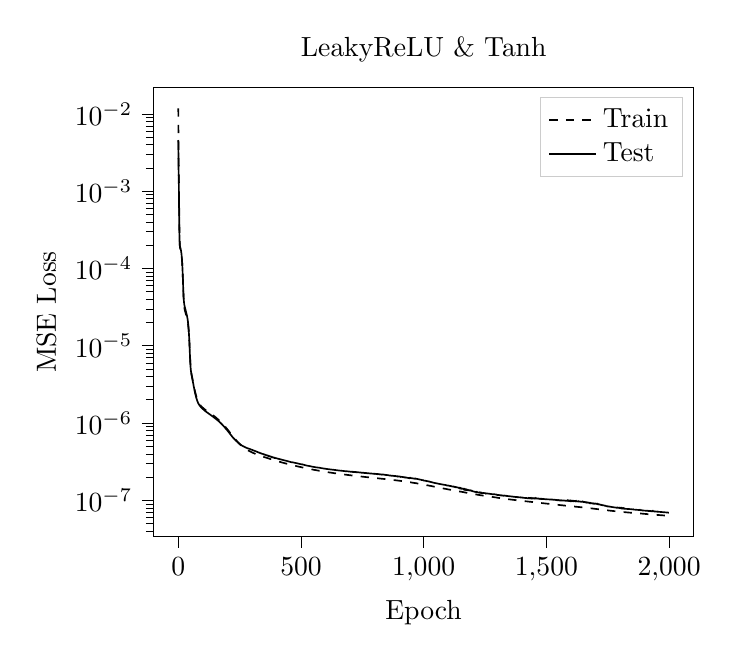
\begin{tikzpicture}

\begin{axis}[
legend cell align={left},
legend style={fill opacity=0.8, draw opacity=1, text opacity=1, draw=white!80!black},
log basis y={10},
tick align=outside,
tick pos=left,
title={LeakyReLU \& Tanh},
x grid style={white!69.0196078431373!black},
xlabel={Epoch},
xmin=-99.95, xmax=2098.95,
xtick style={color=black},
y grid style={white!69.0196078431373!black},
ylabel={MSE Loss},
ymin=3.43177769020239e-08, ymax=0.0217550336439875,
ymode=log,
ytick style={color=black}
]
\addplot [semithick, black, dashed]
table {%
0 0.0118530643042177
1 0.00271716704266146
2 0.00167412927886471
3 0.00101243689469993
4 0.00045973424060503
5 0.000261207596864551
6 0.000201558976317756
7 0.00018511279100494
8 0.000179200788814342
9 0.000174576494267967
10 0.000169601712237636
11 0.000163834669263451
12 0.000157019000936998
13 0.000148911127580504
14 0.000139271357867983
15 0.000127953551971586
16 0.000114886388801096
17 0.000100260177554446
18 8.46605833976355e-05
19 6.92464952226146e-05
20 5.57666255008371e-05
21 4.55883240647381e-05
22 3.88660105927556e-05
23 3.47616929993819e-05
24 3.22158156450314e-05
25 3.05434041529224e-05
26 2.93586506832071e-05
27 2.84435824496541e-05
28 2.76784982206664e-05
29 2.69959361194196e-05
30 2.6167898769927e-05
31 2.53696962281538e-05
32 2.47142864400303e-05
33 2.40883257101814e-05
34 2.3462807683245e-05
35 2.28194917517612e-05
36 2.21361250933114e-05
37 2.13898192178021e-05
38 2.05627751111024e-05
39 1.9635726780507e-05
40 1.86011470459562e-05
41 1.74350023871739e-05
42 1.61274048441555e-05
43 1.46852902416867e-05
44 1.31345061690809e-05
45 1.15222196054674e-05
46 9.92166628020641e-06
47 8.43393238756107e-06
48 7.16028058945994e-06
49 6.16866173072594e-06
50 5.45963166268848e-06
51 4.98488556331722e-06
52 4.66921569193346e-06
53 4.44369569072478e-06
54 4.26283255467297e-06
55 4.10205469756875e-06
56 3.95200737614232e-06
57 3.8109996012281e-06
58 3.67382299134533e-06
59 3.54308888006472e-06
60 3.41727396653369e-06
61 3.29590084652409e-06
62 3.17720198967208e-06
63 3.06160384815257e-06
64 2.95430421891751e-06
65 2.85230269520298e-06
66 2.75558185279579e-06
67 2.66389803647371e-06
68 2.57897133093365e-06
69 2.49876115083225e-06
70 2.42459519733984e-06
71 2.35611084360698e-06
72 2.29315852362788e-06
73 2.23360024858721e-06
74 2.18038750722371e-06
75 2.13208772674989e-06
76 2.08557600035419e-06
77 2.04397322181649e-06
78 2.0052868115954e-06
79 1.97052455132507e-06
80 1.9358652500614e-06
81 1.90366093914918e-06
82 1.87538027012124e-06
83 1.84823297968251e-06
84 1.82278619774934e-06
85 1.79879209343881e-06
86 1.77639971258259e-06
87 1.75495989918772e-06
88 1.73615727180731e-06
89 1.71740477168214e-06
90 1.69976929328186e-06
91 1.68390478773972e-06
92 1.66872160883713e-06
93 1.65481673491286e-06
94 1.64140779975241e-06
95 1.62894625606214e-06
96 1.6168444543041e-06
97 1.60500629891658e-06
98 1.59467800762059e-06
99 1.58435881195373e-06
100 1.57499000033567e-06
101 1.56598736191427e-06
102 1.55642656335431e-06
103 1.54590319141334e-06
104 1.53531705944943e-06
105 1.52483814102311e-06
106 1.51540221196456e-06
107 1.50651450968553e-06
108 1.49852953558138e-06
109 1.48978108879305e-06
110 1.48155487261192e-06
111 1.473753212764e-06
112 1.46592581035065e-06
113 1.45811151182329e-06
114 1.45039193807861e-06
115 1.44299419795857e-06
116 1.43553990096734e-06
117 1.4283073526542e-06
118 1.42114796418014e-06
119 1.41402536269197e-06
120 1.4066799710406e-06
121 1.39982001070393e-06
122 1.39267746087057e-06
123 1.38577581395793e-06
124 1.3789186680242e-06
125 1.371992529414e-06
126 1.36515135557147e-06
127 1.35831706401746e-06
128 1.35177427802091e-06
129 1.34456710597419e-06
130 1.33781877002548e-06
131 1.33112865796647e-06
132 1.32447658589285e-06
133 1.31773940083235e-06
134 1.31118761359517e-06
135 1.30475479940628e-06
136 1.29805225384416e-06
137 1.29135816624171e-06
138 1.28485466984785e-06
139 1.27849110981515e-06
140 1.27190054311654e-06
141 1.26496867267178e-06
142 1.2586724890582e-06
143 1.25217823000412e-06
144 1.24383108362736e-06
145 1.23542936435683e-06
146 1.22815887382899e-06
147 1.22111726841467e-06
148 1.21425765672711e-06
149 1.20777688215412e-06
150 1.20085036829209e-06
151 1.19395905099395e-06
152 1.18771772923765e-06
153 1.18089644871588e-06
154 1.17428739434899e-06
155 1.16676978154828e-06
156 1.15642677300798e-06
157 1.14880668485284e-06
158 1.14167408173671e-06
159 1.13500217128149e-06
160 1.1279125612873e-06
161 1.12095950947833e-06
162 1.11385238108141e-06
163 1.1068760949513e-06
164 1.09962021093679e-06
165 1.09247755673891e-06
166 1.08500489437802e-06
167 1.07731692369839e-06
168 1.06992002739048e-06
169 1.06233340153494e-06
170 1.05476866045251e-06
171 1.04725385301663e-06
172 1.03964452375749e-06
173 1.03224357621912e-06
174 1.0249889058116e-06
175 1.01740896730007e-06
176 1.00981932121158e-06
177 1.00251862770051e-06
178 9.95047050224684e-07
179 9.87523115867361e-07
180 9.79947625666e-07
181 9.72317288997715e-07
182 9.64804622782367e-07
183 9.57243006581621e-07
184 9.49631655743133e-07
185 9.41910147034264e-07
186 9.34334767435985e-07
187 9.26895800901661e-07
188 9.19153623286206e-07
189 9.1173805672895e-07
190 9.04083534095435e-07
191 8.96533727271276e-07
192 8.88804241938601e-07
193 8.81231718452113e-07
194 8.73640462003777e-07
195 8.65990211096346e-07
196 8.58377323396553e-07
197 8.50837881856137e-07
198 8.43417865837637e-07
199 8.358834592741e-07
200 8.28431481181724e-07
201 8.20944423679748e-07
202 8.13604629087195e-07
203 8.06318554154473e-07
204 7.98892333179424e-07
205 7.91583109460703e-07
206 7.84326178234096e-07
207 7.7717812114031e-07
208 7.70077875245079e-07
209 7.62944073485983e-07
210 7.55807730982383e-07
211 7.48702633558196e-07
212 7.41784852991145e-07
213 7.34965464417314e-07
214 7.28015673686855e-07
215 7.21312267089047e-07
216 7.14584897110626e-07
217 7.0796685973562e-07
218 7.01530687535978e-07
219 6.94918389484656e-07
220 6.88487152515904e-07
221 6.81997241059662e-07
222 6.75791806685311e-07
223 6.69688798012658e-07
224 6.63079862619043e-07
225 6.57233372606925e-07
226 6.51149268605877e-07
227 6.44990180830973e-07
228 6.39707958157487e-07
229 6.33765738257353e-07
230 6.27633001144545e-07
231 6.22900086213463e-07
232 6.17096304438292e-07
233 6.11554022484029e-07
234 6.06932349285216e-07
235 6.01709378145188e-07
236 5.96823508345778e-07
237 5.91874436921103e-07
238 5.87127333318449e-07
239 5.81490728478684e-07
240 5.76784642049688e-07
241 5.72062887528091e-07
242 5.67465997107774e-07
243 5.63017870689464e-07
244 5.58585788596133e-07
245 5.54362565580391e-07
246 5.50233029898095e-07
247 5.46157284787796e-07
248 5.42169837217443e-07
249 5.38345338426893e-07
250 5.34471238836431e-07
251 5.30791619951287e-07
252 5.27104146542001e-07
253 5.23486855598776e-07
254 5.19905496872752e-07
255 5.16522923433627e-07
256 5.1320403034083e-07
257 5.09976518756616e-07
258 5.06772108238351e-07
259 5.03671763851798e-07
260 5.00662150869857e-07
261 4.97670500905656e-07
262 4.94785802771958e-07
263 4.91955151417756e-07
264 4.89251897008103e-07
265 4.86573198955398e-07
266 4.83982838716202e-07
267 4.81418257535893e-07
268 4.79091480201532e-07
269 4.76753003283648e-07
270 4.74208299948486e-07
271 4.71778891380836e-07
272 4.69238318274279e-07
273 4.67039580271944e-07
274 4.64775038821585e-07
275 4.62731207463207e-07
276 4.60462195135847e-07
277 4.5821031440596e-07
278 4.55968379185379e-07
279 4.53642079705219e-07
280 4.51529708158205e-07
281 4.49460743681129e-07
282 4.47360691538279e-07
283 4.45254516009186e-07
284 4.43512205023922e-07
285 4.41370335479974e-07
286 4.39891918645685e-07
287 4.3775119753775e-07
288 4.35976524329362e-07
289 4.34284926598139e-07
290 4.32529043280283e-07
291 4.30876521534174e-07
292 4.29246813922646e-07
293 4.2763998928308e-07
294 4.26025263095653e-07
295 4.24496922605044e-07
296 4.22938850448418e-07
297 4.21455506710799e-07
298 4.19939799925828e-07
299 4.18516394347535e-07
300 4.17067732612963e-07
301 4.15670026228554e-07
302 4.14352804199325e-07
303 4.12975486909772e-07
304 4.1163369130004e-07
305 4.10336712960202e-07
306 4.0901354493883e-07
307 4.07670879326361e-07
308 4.06485504981902e-07
309 4.05222568986119e-07
310 4.03912711050225e-07
311 4.02790586377932e-07
312 4.01454716637772e-07
313 4.00197464202279e-07
314 3.98997999766948e-07
315 3.97849955120932e-07
316 3.96721643951992e-07
317 3.95627938416965e-07
318 3.94478706269297e-07
319 3.93301349191688e-07
320 3.92243420918703e-07
321 3.91151879753693e-07
322 3.90033366443276e-07
323 3.88982161126705e-07
324 3.8793921574154e-07
325 3.868340033506e-07
326 3.85833882148745e-07
327 3.84806861021048e-07
328 3.83725419737857e-07
329 3.82774777293093e-07
330 3.81802409961551e-07
331 3.80739406722341e-07
332 3.79787591057834e-07
333 3.78867508743497e-07
334 3.7750194394448e-07
335 3.76645611709137e-07
336 3.7559583101654e-07
337 3.74515050850732e-07
338 3.73532383505903e-07
339 3.72581143778916e-07
340 3.71705479452089e-07
341 3.70722432492698e-07
342 3.69743662830047e-07
343 3.6887618503556e-07
344 3.68046912214481e-07
345 3.67124095163263e-07
346 3.66226812971604e-07
347 3.6535512707303e-07
348 3.64482295140078e-07
349 3.63568770410438e-07
350 3.62746099042965e-07
351 3.6191672984387e-07
352 3.61063355484248e-07
353 3.60225598470265e-07
354 3.59332563903081e-07
355 3.58554333018901e-07
356 3.57739858756645e-07
357 3.56883827549836e-07
358 3.56125393736306e-07
359 3.55268856523594e-07
360 3.5446067074929e-07
361 3.53646082274395e-07
362 3.52718234239546e-07
363 3.51872259784614e-07
364 3.51077539519906e-07
365 3.50205739110265e-07
366 3.49407621172304e-07
367 3.4863870101276e-07
368 3.47785259748434e-07
369 3.47091866061078e-07
370 3.46326532749686e-07
371 3.45527291443659e-07
372 3.44794722394681e-07
373 3.43984667551922e-07
374 3.43169977270463e-07
375 3.42404283927067e-07
376 3.41655791999074e-07
377 3.40902730329162e-07
378 3.40205402494576e-07
379 3.39438222496824e-07
380 3.38743511164807e-07
381 3.38093948442975e-07
382 3.37387456440297e-07
383 3.36558028394052e-07
384 3.35849407960609e-07
385 3.35072243473178e-07
386 3.34426989269332e-07
387 3.33651557184567e-07
388 3.3312184295653e-07
389 3.31870176353277e-07
390 3.31015687365266e-07
391 3.30093047693936e-07
392 3.29405605299371e-07
393 3.28515724135059e-07
394 3.27883320380806e-07
395 3.27043711749297e-07
396 3.26344384546928e-07
397 3.25581409626352e-07
398 3.24843800513008e-07
399 3.24164057118992e-07
400 3.23606564492707e-07
401 3.22841541603225e-07
402 3.2214296764721e-07
403 3.21485749523731e-07
404 3.20611110851132e-07
405 3.19922173133591e-07
406 3.19242092274408e-07
407 3.1857112810485e-07
408 3.180388822841e-07
409 3.17376388977664e-07
410 3.16714038788746e-07
411 3.16138579790959e-07
412 3.15507177049312e-07
413 3.14841682850897e-07
414 3.14259163729957e-07
415 3.1358744921306e-07
416 3.12949973363175e-07
417 3.12298381103915e-07
418 3.11516434763348e-07
419 3.10839084889381e-07
420 3.1019210295824e-07
421 3.09614747095566e-07
422 3.08992809138431e-07
423 3.08364855825971e-07
424 3.07729297531978e-07
425 3.0712713997616e-07
426 3.06520865279936e-07
427 3.05932439729872e-07
428 3.05334564984605e-07
429 3.04705839084818e-07
430 3.04142966015775e-07
431 3.03557321629455e-07
432 3.02951247618921e-07
433 3.02409354375754e-07
434 3.01802297514087e-07
435 3.01251212547982e-07
436 3.00634733861216e-07
437 3.00078709571494e-07
438 2.99526084049262e-07
439 2.98959181961322e-07
440 2.98405851694383e-07
441 2.97866603077068e-07
442 2.97283363835277e-07
443 2.96744540548843e-07
444 2.96236425974428e-07
445 2.95662631884852e-07
446 2.95119851443815e-07
447 2.94577924904615e-07
448 2.94032025365709e-07
449 2.93495648548969e-07
450 2.92928335369425e-07
451 2.92440287381623e-07
452 2.91878952928926e-07
453 2.91313261371329e-07
454 2.90795729100068e-07
455 2.90339702850417e-07
456 2.89800641205318e-07
457 2.89283157187015e-07
458 2.88763092399336e-07
459 2.88186956886705e-07
460 2.87719527833019e-07
461 2.87232668952697e-07
462 2.86718326236723e-07
463 2.862276135005e-07
464 2.85688222945169e-07
465 2.85214371075426e-07
466 2.84679274898281e-07
467 2.84140632921037e-07
468 2.83622278580253e-07
469 2.83142897899324e-07
470 2.82739655233399e-07
471 2.82202584088509e-07
472 2.81684053625497e-07
473 2.81147220661637e-07
474 2.8064164433772e-07
475 2.80164724898668e-07
476 2.79677985666638e-07
477 2.79170837771403e-07
478 2.78683379292488e-07
479 2.78189573876375e-07
480 2.77702305631067e-07
481 2.77222816016831e-07
482 2.76620818411288e-07
483 2.76163140398467e-07
484 2.75674113474622e-07
485 2.75241383448588e-07
486 2.74769400441244e-07
487 2.74307894294168e-07
488 2.73828556458966e-07
489 2.73356900713395e-07
490 2.72877485983258e-07
491 2.72412719702686e-07
492 2.71952965867683e-07
493 2.7151991022123e-07
494 2.71063778093605e-07
495 2.70645359691457e-07
496 2.70216694630676e-07
497 2.69762554708564e-07
498 2.69319825754621e-07
499 2.68886601602958e-07
500 2.68450084831784e-07
501 2.68012147643049e-07
502 2.67575329154113e-07
503 2.67153018668864e-07
504 2.66674774529463e-07
505 2.66283876641182e-07
506 2.65838455433709e-07
507 2.65449408246354e-07
508 2.64985072504942e-07
509 2.64566873163119e-07
510 2.64143997810606e-07
511 2.6372079743453e-07
512 2.63302015554245e-07
513 2.62963274806793e-07
514 2.62516207605756e-07
515 2.62078123029141e-07
516 2.6153940742546e-07
517 2.61240193822232e-07
518 2.60856092836548e-07
519 2.60440021655484e-07
520 2.59956458464217e-07
521 2.59652960870937e-07
522 2.5924450344661e-07
523 2.58845528328777e-07
524 2.58385906661829e-07
525 2.58098587920586e-07
526 2.57721656673482e-07
527 2.57322477942523e-07
528 2.56853048433925e-07
529 2.56580461183376e-07
530 2.56191600172428e-07
531 2.55807624206739e-07
532 2.55381097296947e-07
533 2.55083945155832e-07
534 2.54707071889015e-07
535 2.54274472382576e-07
536 2.53979634194934e-07
537 2.53613948039799e-07
538 2.53186067510569e-07
539 2.52915796181696e-07
540 2.52544044805347e-07
541 2.52177458669678e-07
542 2.51814867709754e-07
543 2.51472695616428e-07
544 2.51091237899459e-07
545 2.50749283082996e-07
546 2.50388591730655e-07
547 2.50065211588435e-07
548 2.49643439182989e-07
549 2.49388097827818e-07
550 2.49036874500064e-07
551 2.48683912019487e-07
552 2.48340439107153e-07
553 2.48009093489543e-07
554 2.47644183417606e-07
555 2.47348658717783e-07
556 2.46921584547977e-07
557 2.46672405559423e-07
558 2.4635122429828e-07
559 2.45947923090739e-07
560 2.45706016663405e-07
561 2.45372700454993e-07
562 2.44974506784956e-07
563 2.4471972373874e-07
564 2.4438149678474e-07
565 2.43998724755556e-07
566 2.43757375315568e-07
567 2.4344039513835e-07
568 2.43120262155117e-07
569 2.42807220651287e-07
570 2.42499065443269e-07
571 2.42203533503016e-07
572 2.41825013269192e-07
573 2.41641147702865e-07
574 2.41307229600807e-07
575 2.40921330494359e-07
576 2.40644746909879e-07
577 2.40279314525083e-07
578 2.39888169815572e-07
579 2.39647900237117e-07
580 2.39297322039533e-07
581 2.38893787276595e-07
582 2.38672715674681e-07
583 2.38364748824438e-07
584 2.38003041218349e-07
585 2.37784313227962e-07
586 2.37474714154473e-07
587 2.37091034534842e-07
588 2.36894158952339e-07
589 2.36600740073811e-07
590 2.36258271698375e-07
591 2.36051617847011e-07
592 2.35757887693921e-07
593 2.35384111789472e-07
594 2.35183570460151e-07
595 2.34854371832682e-07
596 2.34624506887826e-07
597 2.34325953321957e-07
598 2.34039721533463e-07
599 2.33770109900888e-07
600 2.33466635911839e-07
601 2.33135660757e-07
602 2.32950038828506e-07
603 2.3267533492799e-07
604 2.32340332509295e-07
605 2.32128316092428e-07
606 2.31862926064252e-07
607 2.31633997536562e-07
608 2.31260507582931e-07
609 2.3104011305719e-07
610 2.3077447281139e-07
611 2.30500478679119e-07
612 2.302613713141e-07
613 2.29983399727018e-07
614 2.29732210790701e-07
615 2.29474479688463e-07
616 2.29219407344772e-07
617 2.28958964825665e-07
618 2.28696038512055e-07
619 2.28456288859036e-07
620 2.28211573549686e-07
621 2.27972307349944e-07
622 2.27720530197928e-07
623 2.27468705197964e-07
624 2.27222729378695e-07
625 2.26979138638228e-07
626 2.26725032128172e-07
627 2.26482411250117e-07
628 2.26238589867478e-07
629 2.2600784120641e-07
630 2.25760820164567e-07
631 2.25525988106767e-07
632 2.2528483005857e-07
633 2.25036615979946e-07
634 2.24798530474857e-07
635 2.245455094112e-07
636 2.24306671285035e-07
637 2.24090163293056e-07
638 2.23974491312617e-07
639 2.23647726016907e-07
640 2.2354151440851e-07
641 2.23199736666402e-07
642 2.23048872683762e-07
643 2.22717595661948e-07
644 2.22584690398264e-07
645 2.22249005823016e-07
646 2.22128948713873e-07
647 2.21802636730217e-07
648 2.21642298200209e-07
649 2.21354814236463e-07
650 2.21212942399518e-07
651 2.20913502765541e-07
652 2.20765400790413e-07
653 2.20472539936623e-07
654 2.20341641522737e-07
655 2.20101288171293e-07
656 2.19818628295343e-07
657 2.19636836192194e-07
658 2.19449505202363e-07
659 2.19179486400378e-07
660 2.19054223038029e-07
661 2.1881402455648e-07
662 2.18547279182246e-07
663 2.18407628764794e-07
664 2.1815676842607e-07
665 2.17975170194507e-07
666 2.17686950634288e-07
667 2.17566066694985e-07
668 2.1733298704163e-07
669 2.17060445685036e-07
670 2.16942077059912e-07
671 2.16649795312662e-07
672 2.16544278991648e-07
673 2.16255045707214e-07
674 2.16131762982741e-07
675 2.15852907508918e-07
676 2.15736312519255e-07
677 2.15498423557392e-07
678 2.15338095706841e-07
679 2.15115065628879e-07
680 2.14931766052473e-07
681 2.14743876647105e-07
682 2.1452934733901e-07
683 2.14333714552595e-07
684 2.14191282310594e-07
685 2.1399087525964e-07
686 2.13799643553614e-07
687 2.13587029818996e-07
688 2.13333764300216e-07
689 2.13138286788706e-07
690 2.12866215186125e-07
691 2.12723850346208e-07
692 2.12456457660437e-07
693 2.12390492180248e-07
694 2.1211422053824e-07
695 2.11901987100305e-07
696 2.1164349405467e-07
697 2.11502926056539e-07
698 2.11225254645342e-07
699 2.11071560613618e-07
700 2.1092119062871e-07
701 2.10711485458148e-07
702 2.10524598244888e-07
703 2.10352325012764e-07
704 2.10138360678513e-07
705 2.09938405241417e-07
706 2.09765650339477e-07
707 2.09575859855704e-07
708 2.09359261809539e-07
709 2.09192116145118e-07
710 2.08994861992551e-07
711 2.08894274059901e-07
712 2.08617789951404e-07
713 2.08484151400512e-07
714 2.08267086229341e-07
715 2.08157416111021e-07
716 2.07965515329533e-07
717 2.0773107167571e-07
718 2.07602891123315e-07
719 2.07446420823487e-07
720 2.07267277083645e-07
721 2.07017601070447e-07
722 2.06857604830191e-07
723 2.06693050948559e-07
724 2.06501707502582e-07
725 2.06318297003349e-07
726 2.061609860462e-07
727 2.05949397312111e-07
728 2.05818528023372e-07
729 2.05619040556826e-07
730 2.0542596598716e-07
731 2.05264010830319e-07
732 2.05055826384637e-07
733 2.04901554035075e-07
734 2.04771108222701e-07
735 2.04615930066154e-07
736 2.04429741224033e-07
737 2.04268639762972e-07
738 2.04093490332014e-07
739 2.03921731198875e-07
740 2.03783937124058e-07
741 2.03591222188493e-07
742 2.03433932504993e-07
743 2.03294410177079e-07
744 2.03115816297839e-07
745 2.02962098882153e-07
746 2.02798127070025e-07
747 2.02641582276897e-07
748 2.0247920047467e-07
749 2.02321240067249e-07
750 2.02163325781157e-07
751 2.02007027972684e-07
752 2.01846984239751e-07
753 2.01729566754238e-07
754 2.01550911008042e-07
755 2.01417259383163e-07
756 2.01240844646122e-07
757 2.01105906960208e-07
758 2.00922100276557e-07
759 2.00787376009259e-07
760 2.00601763872044e-07
761 2.00482007990388e-07
762 2.00299133673809e-07
763 2.00137742218942e-07
764 1.99984624302374e-07
765 1.99804511787249e-07
766 1.99653848646619e-07
767 1.99538892360351e-07
768 1.9936609028548e-07
769 1.99198628926922e-07
770 1.99091463208845e-07
771 1.98933666865742e-07
772 1.98748004130778e-07
773 1.98654580778168e-07
774 1.98493020199919e-07
775 1.98315526972692e-07
776 1.98179933335041e-07
777 1.98039544159201e-07
778 1.97873308728447e-07
779 1.97702004207656e-07
780 1.97595039942655e-07
781 1.97445724197109e-07
782 1.97299228439363e-07
783 1.97113351568134e-07
784 1.96935009412869e-07
785 1.9679619677504e-07
786 1.96704571074235e-07
787 1.96535869825709e-07
788 1.96417040520203e-07
789 1.96257578586767e-07
790 1.96085073802976e-07
791 1.95906529860679e-07
792 1.9580319301582e-07
793 1.95651297666188e-07
794 1.95509253991588e-07
795 1.95332549040472e-07
796 1.95176153930277e-07
797 1.9508170942828e-07
798 1.94809531933515e-07
799 1.94621923839122e-07
800 1.94577639106797e-07
801 1.94502660981755e-07
802 1.94220849742521e-07
803 1.9407022731599e-07
804 1.93978072104528e-07
805 1.93858640074041e-07
806 1.93672978909376e-07
807 1.93564685474712e-07
808 1.93407830309411e-07
809 1.9325386772806e-07
810 1.9307086262188e-07
811 1.92956589245341e-07
812 1.92784446319649e-07
813 1.92575233022296e-07
814 1.92446511348976e-07
815 1.92271403115285e-07
816 1.92117631925726e-07
817 1.91977746915484e-07
818 1.91837797295591e-07
819 1.91621675078579e-07
820 1.91532269944616e-07
821 1.91485599415842e-07
822 1.91349084090575e-07
823 1.91097462220569e-07
824 1.90978913387596e-07
825 1.90743896467893e-07
826 1.90622938887941e-07
827 1.90471911444945e-07
828 1.90318472142792e-07
829 1.90155134610848e-07
830 1.89974666753301e-07
831 1.8988238119988e-07
832 1.89729744747069e-07
833 1.89577713982203e-07
834 1.89420835468468e-07
835 1.89228891997573e-07
836 1.89185338825837e-07
837 1.89037455335495e-07
838 1.88832184292664e-07
839 1.88669506208328e-07
840 1.8860980708979e-07
841 1.88430943389051e-07
842 1.88328428080808e-07
843 1.880989881613e-07
844 1.8794127457511e-07
845 1.87852113448628e-07
846 1.87664538998433e-07
847 1.87568792341608e-07
848 1.87350116291896e-07
849 1.8720051024701e-07
850 1.87061393766896e-07
851 1.86907370007816e-07
852 1.86787177604231e-07
853 1.8661556766375e-07
854 1.86445408317582e-07
855 1.8628098129625e-07
856 1.86233017842596e-07
857 1.86043692416149e-07
858 1.85916030922328e-07
859 1.85741681846707e-07
860 1.85577939838311e-07
861 1.85364337674798e-07
862 1.85230030382399e-07
863 1.85133268537641e-07
864 1.8496937442336e-07
865 1.84808264194203e-07
866 1.84644422240865e-07
867 1.84447406851973e-07
868 1.84294324242273e-07
869 1.84178464202489e-07
870 1.84014452706549e-07
871 1.83841847032795e-07
872 1.8368446058048e-07
873 1.83516295621189e-07
874 1.83339417347383e-07
875 1.83247092728323e-07
876 1.83087581305585e-07
877 1.82929167095836e-07
878 1.82783076610349e-07
879 1.82587592853167e-07
880 1.82422121021375e-07
881 1.82327151939887e-07
882 1.82149352689009e-07
883 1.81977185548021e-07
884 1.81808037474696e-07
885 1.81609961479978e-07
886 1.81445596808771e-07
887 1.81330588048922e-07
888 1.81169432998729e-07
889 1.8099068277877e-07
890 1.80869595567401e-07
891 1.80666593408318e-07
892 1.80395674341582e-07
893 1.80269183800874e-07
894 1.80182070700141e-07
895 1.80020855800933e-07
896 1.79949448813943e-07
897 1.79735197555431e-07
898 1.79557423095389e-07
899 1.79240639887723e-07
900 1.79061926033341e-07
901 1.78964278418903e-07
902 1.78825385937387e-07
903 1.78665588187243e-07
904 1.78476881302458e-07
905 1.78299222426403e-07
906 1.78091645508971e-07
907 1.77893942421292e-07
908 1.77791877916889e-07
909 1.776089068386e-07
910 1.77429847447286e-07
911 1.77260000931767e-07
912 1.77078513615925e-07
913 1.76987821447483e-07
914 1.76801693754669e-07
915 1.76696476962945e-07
916 1.76497925167496e-07
917 1.76327017499034e-07
918 1.76139942922759e-07
919 1.7595209347121e-07
920 1.75708836174238e-07
921 1.75513835131369e-07
922 1.75378918982005e-07
923 1.75187202259508e-07
924 1.75111654392879e-07
925 1.74880665021249e-07
926 1.74724064791576e-07
927 1.74432815377656e-07
928 1.74271239465895e-07
929 1.74156150045235e-07
930 1.73961806424927e-07
931 1.73759765992543e-07
932 1.73552534000976e-07
933 1.73333812902854e-07
934 1.73191188849842e-07
935 1.72858451954028e-07
936 1.72689596894315e-07
937 1.72501483106657e-07
938 1.72240258798695e-07
939 1.72142322035995e-07
940 1.71882180637795e-07
941 1.71781431667739e-07
942 1.71534132320517e-07
943 1.71427748902886e-07
944 1.71182018497973e-07
945 1.71046810187647e-07
946 1.70868499822063e-07
947 1.70649446232574e-07
948 1.70433219139454e-07
949 1.70225919603695e-07
950 1.70000608598286e-07
951 1.69803014244962e-07
952 1.69534294911955e-07
953 1.693373877103e-07
954 1.69177045492574e-07
955 1.68982332347412e-07
956 1.68769802812108e-07
957 1.68561846926707e-07
958 1.68356583650109e-07
959 1.68175843185736e-07
960 1.67969688838809e-07
961 1.6777198183604e-07
962 1.67602634164155e-07
963 1.67403722173276e-07
964 1.67237837928269e-07
965 1.67088833272544e-07
966 1.66905762398528e-07
967 1.66680781411799e-07
968 1.66488919255414e-07
969 1.66307719140946e-07
970 1.66085840177743e-07
971 1.65865779074181e-07
972 1.65654938456328e-07
973 1.65444530743741e-07
974 1.65259729925538e-07
975 1.65055726228047e-07
976 1.64847215089026e-07
977 1.64630200004012e-07
978 1.64421114199342e-07
979 1.64211539228631e-07
980 1.64029924171416e-07
981 1.63781369501237e-07
982 1.63627734259819e-07
983 1.6333098932364e-07
984 1.63135665680159e-07
985 1.62986013805266e-07
986 1.6276575917118e-07
987 1.62616001212257e-07
988 1.62426574767949e-07
989 1.62191438832338e-07
990 1.619688600627e-07
991 1.61746657809658e-07
992 1.61536477911284e-07
993 1.61331311019808e-07
994 1.61136969033748e-07
995 1.6092817946145e-07
996 1.60706019286749e-07
997 1.60496292380685e-07
998 1.60270611289093e-07
999 1.6000876024691e-07
1000 1.59730474265984e-07
1001 1.59520671360269e-07
1002 1.59217975522097e-07
1003 1.59063585435604e-07
1004 1.58882511904324e-07
1005 1.58647880759588e-07
1006 1.58423164926091e-07
1007 1.58098031590725e-07
1008 1.57898606630624e-07
1009 1.57661048241664e-07
1010 1.57398774831563e-07
1011 1.57148834816212e-07
1012 1.56870506458517e-07
1013 1.56711850898716e-07
1014 1.56497015339596e-07
1015 1.56257475971699e-07
1016 1.56046945555488e-07
1017 1.55826125030956e-07
1018 1.55598985777772e-07
1019 1.5539752382665e-07
1020 1.5514921122417e-07
1021 1.5493437491898e-07
1022 1.54783092639832e-07
1023 1.54565749099334e-07
1024 1.54347193969784e-07
1025 1.54280347814506e-07
1026 1.54014388449752e-07
1027 1.53799708336066e-07
1028 1.53557663267634e-07
1029 1.53346554242262e-07
1030 1.53081715104975e-07
1031 1.52885490983579e-07
1032 1.52644006412572e-07
1033 1.52446025687425e-07
1034 1.52200829489857e-07
1035 1.51935989038066e-07
1036 1.5165363715397e-07
1037 1.51450876394676e-07
1038 1.51208441636186e-07
1039 1.50983596370224e-07
1040 1.50754961531163e-07
1041 1.50501454818652e-07
1042 1.50234482596545e-07
1043 1.500267249952e-07
1044 1.49826365806405e-07
1045 1.49551108549417e-07
1046 1.49386445293942e-07
1047 1.49152108022577e-07
1048 1.48935337456635e-07
1049 1.48707327504383e-07
1050 1.48492372758824e-07
1051 1.48282824632417e-07
1052 1.48078847772126e-07
1053 1.47873801275011e-07
1054 1.47662170590479e-07
1055 1.47460764416962e-07
1056 1.47223473000224e-07
1057 1.47010033600736e-07
1058 1.46798720592756e-07
1059 1.46577249601876e-07
1060 1.4639762123636e-07
1061 1.4619643713587e-07
1062 1.45985476322608e-07
1063 1.45778726725609e-07
1064 1.45563538396232e-07
1065 1.45380512712734e-07
1066 1.45199056049705e-07
1067 1.44983988562331e-07
1068 1.44786048970502e-07
1069 1.44568250249222e-07
1070 1.44377106884974e-07
1071 1.44238954987941e-07
1072 1.44015394667463e-07
1073 1.43782359259603e-07
1074 1.43517698781181e-07
1075 1.43292362437819e-07
1076 1.4311534452105e-07
1077 1.42922095818676e-07
1078 1.42694176432201e-07
1079 1.42511509764631e-07
1080 1.42320883853131e-07
1081 1.42115572501211e-07
1082 1.41915518241831e-07
1083 1.41727660235347e-07
1084 1.41539420525305e-07
1085 1.41344826488421e-07
1086 1.41149399077278e-07
1087 1.40993090482766e-07
1088 1.40787137432596e-07
1089 1.40602423535086e-07
1090 1.40420193517343e-07
1091 1.40221834413978e-07
1092 1.40021793214373e-07
1093 1.39751922354492e-07
1094 1.39544986296869e-07
1095 1.39366501237248e-07
1096 1.39174019466282e-07
1097 1.38834078114769e-07
1098 1.38641360159397e-07
1099 1.38483587925009e-07
1100 1.38350642373553e-07
1101 1.38190962829299e-07
1102 1.37955044088756e-07
1103 1.37780998926473e-07
1104 1.37604125285407e-07
1105 1.37377671919126e-07
1106 1.3721026255098e-07
1107 1.3702453204445e-07
1108 1.36816325458256e-07
1109 1.36619293414242e-07
1110 1.36436577498955e-07
1111 1.36264744874381e-07
1112 1.36055063137519e-07
1113 1.35872794068348e-07
1114 1.35656363958958e-07
1115 1.35474489319165e-07
1116 1.35287901478875e-07
1117 1.35084419866871e-07
1118 1.34919479229723e-07
1119 1.34707229086928e-07
1120 1.34552972824054e-07
1121 1.34392235189296e-07
1122 1.34211788001437e-07
1123 1.34022364917996e-07
1124 1.33834222694418e-07
1125 1.33680917187462e-07
1126 1.33549971288005e-07
1127 1.33321881719439e-07
1128 1.33158634149311e-07
1129 1.32976397111406e-07
1130 1.32801262232363e-07
1131 1.32660635792092e-07
1132 1.3256395303074e-07
1133 1.3234662775119e-07
1134 1.32177991829963e-07
1135 1.31985430741111e-07
1136 1.31801775921758e-07
1137 1.31623225954058e-07
1138 1.3144830696632e-07
1139 1.3132029658891e-07
1140 1.3111966016055e-07
1141 1.30938463286157e-07
1142 1.3076284651703e-07
1143 1.30590019210786e-07
1144 1.30414797034462e-07
1145 1.30247909119419e-07
1146 1.30075543523844e-07
1147 1.2991378209648e-07
1148 1.29729824443814e-07
1149 1.29620293314758e-07
1150 1.29415466410876e-07
1151 1.29288045030762e-07
1152 1.29104797821356e-07
1153 1.28977646532746e-07
1154 1.28819465039953e-07
1155 1.28667567054208e-07
1156 1.28509636070362e-07
1157 1.28371612639455e-07
1158 1.28219746436287e-07
1159 1.27995160504213e-07
1160 1.27906802120492e-07
1161 1.27735503014037e-07
1162 1.27535211241536e-07
1163 1.27303911334309e-07
1164 1.27048455112799e-07
1165 1.26922013038211e-07
1166 1.26683094421765e-07
1167 1.26568199526389e-07
1168 1.26293073805073e-07
1169 1.2608189124208e-07
1170 1.25966059989935e-07
1171 1.25794228132747e-07
1172 1.25575737861539e-07
1173 1.25362858756972e-07
1174 1.25249346218936e-07
1175 1.25057965572495e-07
1176 1.24901918134412e-07
1177 1.24663825395999e-07
1178 1.24542853811249e-07
1179 1.24312287319128e-07
1180 1.24227721691739e-07
1181 1.24054489148762e-07
1182 1.23892663459912e-07
1183 1.23698761150592e-07
1184 1.23596502092482e-07
1185 1.23382345861955e-07
1186 1.23272039779465e-07
1187 1.23062993779399e-07
1188 1.22962949738792e-07
1189 1.22812680999118e-07
1190 1.22681518540446e-07
1191 1.22485459471022e-07
1192 1.22373093603301e-07
1193 1.22180681721318e-07
1194 1.22062737482054e-07
1195 1.2187447886447e-07
1196 1.21760682851857e-07
1197 1.21487625520444e-07
1198 1.21530664124236e-07
1199 1.21434413728139e-07
1200 1.21137268038751e-07
1201 1.20878889582343e-07
1202 1.20710900922916e-07
1203 1.20578473321586e-07
1204 1.20379436836515e-07
1205 1.20130681089847e-07
1206 1.19967440081581e-07
1207 1.19809633428503e-07
1208 1.1968485621594e-07
1209 1.1953818977517e-07
1210 1.19361607492152e-07
1211 1.19255883692659e-07
1212 1.19114461313075e-07
1213 1.1894671261814e-07
1214 1.18726950567805e-07
1215 1.18577280545651e-07
1216 1.18446295104491e-07
1217 1.18350390611255e-07
1218 1.18164257060016e-07
1219 1.18029195910196e-07
1220 1.17923606161696e-07
1221 1.17740713488246e-07
1222 1.17615516952441e-07
1223 1.17428830684219e-07
1224 1.17340325026305e-07
1225 1.17267212051075e-07
1226 1.17074500035841e-07
1227 1.1689717317509e-07
1228 1.16832294899893e-07
1229 1.16660597107909e-07
1230 1.16557522581218e-07
1231 1.1638936075542e-07
1232 1.16293079098995e-07
1233 1.1615023936784e-07
1234 1.15965406283891e-07
1235 1.15937135632294e-07
1236 1.15770845393826e-07
1237 1.15656800470987e-07
1238 1.15498020331728e-07
1239 1.15389218859008e-07
1240 1.15237190087214e-07
1241 1.15116425188688e-07
1242 1.14983899742072e-07
1243 1.14922975889442e-07
1244 1.14829335128519e-07
1245 1.14685722209629e-07
1246 1.14553782651683e-07
1247 1.14423000404429e-07
1248 1.14291658370291e-07
1249 1.14146929462322e-07
1250 1.14030466292547e-07
1251 1.13904921228425e-07
1252 1.13765815093814e-07
1253 1.1366588059758e-07
1254 1.13550664288198e-07
1255 1.13388263041969e-07
1256 1.1328302516489e-07
1257 1.1309919934277e-07
1258 1.12994540693023e-07
1259 1.1289519078872e-07
1260 1.12770297622689e-07
1261 1.1268669043929e-07
1262 1.12551397478455e-07
1263 1.12448732352277e-07
1264 1.12315216899361e-07
1265 1.12217203568576e-07
1266 1.12089267332749e-07
1267 1.11983588091391e-07
1268 1.11884272147478e-07
1269 1.11768592191197e-07
1270 1.11649045841489e-07
1271 1.11516369464937e-07
1272 1.11367647345872e-07
1273 1.11236748324473e-07
1274 1.11128077183054e-07
1275 1.10999723002436e-07
1276 1.10894493033697e-07
1277 1.10791011962874e-07
1278 1.10668243085144e-07
1279 1.10672879035434e-07
1280 1.10524663309519e-07
1281 1.10387117668864e-07
1282 1.10317078533484e-07
1283 1.10137854488102e-07
1284 1.10018036004078e-07
1285 1.09912964454395e-07
1286 1.09854005803101e-07
1287 1.09692538941886e-07
1288 1.09553196299572e-07
1289 1.09495215230737e-07
1290 1.09402880060117e-07
1291 1.09246621118331e-07
1292 1.09144351277735e-07
1293 1.09060896861024e-07
1294 1.08934168622454e-07
1295 1.08833148818377e-07
1296 1.08530306373922e-07
1297 1.08329140676489e-07
1298 1.08251451091945e-07
1299 1.08081192781384e-07
1300 1.07963060575145e-07
1301 1.07849208102806e-07
1302 1.07792553954766e-07
1303 1.07604572608722e-07
1304 1.07502775939849e-07
1305 1.07372964691876e-07
1306 1.07319396025929e-07
1307 1.07215680955619e-07
1308 1.07021888190673e-07
1309 1.06997283111809e-07
1310 1.06866084482959e-07
1311 1.06697310560122e-07
1312 1.06620122195977e-07
1313 1.06523319796992e-07
1314 1.06369266372752e-07
1315 1.06309255887282e-07
1316 1.06270429679256e-07
1317 1.06117778642556e-07
1318 1.05977327308437e-07
1319 1.05862196591033e-07
1320 1.05791138462763e-07
1321 1.05682823235753e-07
1322 1.05575490255916e-07
1323 1.05479250333218e-07
1324 1.05338221807472e-07
1325 1.05261139921708e-07
1326 1.051674444561e-07
1327 1.05097885736427e-07
1328 1.04932408785174e-07
1329 1.04820680103757e-07
1330 1.047039979305e-07
1331 1.04622124503351e-07
1332 1.04536150132617e-07
1333 1.04428355225394e-07
1334 1.0431528302135e-07
1335 1.04219694215146e-07
1336 1.04108350139853e-07
1337 1.04010152625733e-07
1338 1.03937799931231e-07
1339 1.03816809513546e-07
1340 1.0372121978719e-07
1341 1.03628270149869e-07
1342 1.03506012415266e-07
1343 1.03420547411304e-07
1344 1.03336215182992e-07
1345 1.03233022066718e-07
1346 1.03127735130215e-07
1347 1.0304500937508e-07
1348 1.02925141018062e-07
1349 1.02855479322983e-07
1350 1.02757760238603e-07
1351 1.0265365359885e-07
1352 1.02567342004534e-07
1353 1.02481212273631e-07
1354 1.0238724213707e-07
1355 1.02296590689832e-07
1356 1.02196159151191e-07
1357 1.02104377361911e-07
1358 1.0200633058588e-07
1359 1.01915980462053e-07
1360 1.01855772072668e-07
1361 1.01716821337305e-07
1362 1.01626993178172e-07
1363 1.01556392099411e-07
1364 1.01448222448397e-07
1365 1.01379643577815e-07
1366 1.01260316306195e-07
1367 1.01179489991665e-07
1368 1.01097790544458e-07
1369 1.01009448204792e-07
1370 1.00864683293622e-07
1371 1.00828128005048e-07
1372 1.00755467798308e-07
1373 1.00713147080711e-07
1374 1.00573230966461e-07
1375 1.00459209054549e-07
1376 1.00394691603611e-07
1377 1.00241487885455e-07
1378 1.0012043237495e-07
1379 1.00072280460495e-07
1380 9.99612031762354e-08
1381 9.98299957863935e-08
1382 9.98184432319249e-08
1383 9.96668474364526e-08
1384 9.95932889260587e-08
1385 9.95839536628296e-08
1386 9.94681824089128e-08
1387 9.93048253903339e-08
1388 9.92653954980938e-08
1389 9.91634453377799e-08
1390 9.90674275698211e-08
1391 9.89828977822072e-08
1392 9.8907549475058e-08
1393 9.88146800331435e-08
1394 9.87215900636329e-08
1395 9.8650412091672e-08
1396 9.85902149146511e-08
1397 9.85469480134782e-08
1398 9.84345484340565e-08
1399 9.83603269091304e-08
1400 9.8255061821817e-08
1401 9.81671388657901e-08
1402 9.81320887660786e-08
1403 9.80905747880456e-08
1404 9.80041671923004e-08
1405 9.79182954061741e-08
1406 9.78550450803084e-08
1407 9.77846480125777e-08
1408 9.77129959380818e-08
1409 9.7618126581267e-08
1410 9.75506221863043e-08
1411 9.74697444000583e-08
1412 9.73777406514387e-08
1413 9.73348767026039e-08
1414 9.72579349145519e-08
1415 9.71626870587272e-08
1416 9.70618948556989e-08
1417 9.69868048876776e-08
1418 9.69154252317139e-08
1419 9.68737760551619e-08
1420 9.67826737579003e-08
1421 9.67257258714937e-08
1422 9.66225470016013e-08
1423 9.65445911766949e-08
1424 9.64560930221126e-08
1425 9.63946927470261e-08
1426 9.62924369858342e-08
1427 9.61960204577395e-08
1428 9.61506538956769e-08
1429 9.606817239316e-08
1430 9.59494349572765e-08
1431 9.58923250315991e-08
1432 9.58117151803606e-08
1433 9.58197924845194e-08
1434 9.57060428135037e-08
1435 9.55582331911842e-08
1436 9.55965827671434e-08
1437 9.54066385716601e-08
1438 9.53776570362663e-08
1439 9.52400907010542e-08
1440 9.52336963386813e-08
1441 9.51048315940284e-08
1442 9.50543814823845e-08
1443 9.4960869809313e-08
1444 9.49622229455826e-08
1445 9.48089321681778e-08
1446 9.47507008817183e-08
1447 9.4643267519956e-08
1448 9.46226468379052e-08
1449 9.4495548420781e-08
1450 9.44533930393732e-08
1451 9.43506249839743e-08
1452 9.43026340820552e-08
1453 9.41682392365806e-08
1454 9.42125580642994e-08
1455 9.41105431415679e-08
1456 9.39968358650845e-08
1457 9.40077997384492e-08
1458 9.39092628087224e-08
1459 9.37745551325975e-08
1460 9.37469126931489e-08
1461 9.37155768170328e-08
1462 9.35226401210798e-08
1463 9.34516931963003e-08
1464 9.3375002428786e-08
1465 9.33066063666388e-08
1466 9.32856002933136e-08
1467 9.32056613294208e-08
1468 9.30419151004003e-08
1469 9.29735011503396e-08
1470 9.29493840864382e-08
1471 9.28904867336655e-08
1472 9.27369426548808e-08
1473 9.2628096581393e-08
1474 9.25879248008243e-08
1475 9.25714797759269e-08
1476 9.24662792343156e-08
1477 9.23423236613985e-08
1478 9.22998963446275e-08
1479 9.2187932512644e-08
1480 9.21299071414694e-08
1481 9.20336628489338e-08
1482 9.20134716011489e-08
1483 9.18693962042028e-08
1484 9.18302799028936e-08
1485 9.17768765340554e-08
1486 9.16352135647003e-08
1487 9.16297153530365e-08
1488 9.14914950378431e-08
1489 9.14874235604657e-08
1490 9.14028345562201e-08
1491 9.13489709084558e-08
1492 9.12038426079675e-08
1493 9.11310380438124e-08
1494 9.11061501085442e-08
1495 9.1044428259579e-08
1496 9.09657928502838e-08
1497 9.08472444081099e-08
1498 9.08059538318184e-08
1499 9.07555209792577e-08
1500 9.06590707643318e-08
1501 9.05626640701485e-08
1502 9.05422847985449e-08
1503 9.04447589533675e-08
1504 9.03806934502427e-08
1505 9.02795845121318e-08
1506 9.02511904143921e-08
1507 9.01830849713292e-08
1508 9.01680074889555e-08
1509 9.00529918510529e-08
1510 9.00171911268899e-08
1511 8.99389152202446e-08
1512 8.98761768794998e-08
1513 8.97628513101267e-08
1514 8.9727812454754e-08
1515 8.96666446621452e-08
1516 8.9595610877069e-08
1517 8.94834702407365e-08
1518 8.94327300500208e-08
1519 8.93961989092418e-08
1520 8.93055324446834e-08
1521 8.92264829097655e-08
1522 8.9132382470325e-08
1523 8.90340010712975e-08
1524 8.90586697899209e-08
1525 8.89112405175751e-08
1526 8.89173306219959e-08
1527 8.88155498905974e-08
1528 8.87604053225743e-08
1529 8.86581190471247e-08
1530 8.86199899809981e-08
1531 8.85358596960373e-08
1532 8.84668544678391e-08
1533 8.83778405267321e-08
1534 8.82795187884256e-08
1535 8.82399620216745e-08
1536 8.81458221506648e-08
1537 8.80856802467633e-08
1538 8.8028733735257e-08
1539 8.79710035555092e-08
1540 8.78986497596657e-08
1541 8.78588734956054e-08
1542 8.77099728064934e-08
1543 8.76316445186376e-08
1544 8.7561898293842e-08
1545 8.74460793092169e-08
1546 8.74396130186028e-08
1547 8.7310927657569e-08
1548 8.72971045744464e-08
1549 8.7202555963728e-08
1550 8.71206591313012e-08
1551 8.70966336208312e-08
1552 8.70223219067157e-08
1553 8.69349163892252e-08
1554 8.68082736396047e-08
1555 8.67739862506767e-08
1556 8.67157946551345e-08
1557 8.66314914738098e-08
1558 8.65816601560709e-08
1559 8.64720138196162e-08
1560 8.64520264407531e-08
1561 8.63570847435824e-08
1562 8.63054635900085e-08
1563 8.6245397003637e-08
1564 8.61508118958909e-08
1565 8.6116425922711e-08
1566 8.60025800193398e-08
1567 8.59528602035198e-08
1568 8.59144835523296e-08
1569 8.57971092322884e-08
1570 8.57374262288602e-08
1571 8.57213784577482e-08
1572 8.56070805852482e-08
1573 8.55483817758795e-08
1574 8.55151786680608e-08
1575 8.54036633484156e-08
1576 8.53566108034443e-08
1577 8.53139808754122e-08
1578 8.52214987787647e-08
1579 8.51445561558251e-08
1580 8.51229585521196e-08
1581 8.50279297139878e-08
1582 8.49864836851566e-08
1583 8.49015365496086e-08
1584 8.48406696292159e-08
1585 8.4793286276863e-08
1586 8.47105369814471e-08
1587 8.46707238295608e-08
1588 8.45975640011432e-08
1589 8.45493395154051e-08
1590 8.44889559274975e-08
1591 8.44214895678874e-08
1592 8.43301174562328e-08
1593 8.42380802126286e-08
1594 8.41854957123189e-08
1595 8.41715189849879e-08
1596 8.40701721784853e-08
1597 8.40061556424132e-08
1598 8.39969449515365e-08
1599 8.38670568690247e-08
1600 8.3820478170793e-08
1601 8.37480628561593e-08
1602 8.3735137312857e-08
1603 8.36124867511501e-08
1604 8.35997560351132e-08
1605 8.35093345621374e-08
1606 8.34240115636931e-08
1607 8.3412077874101e-08
1608 8.3312887099396e-08
1609 8.32702834578924e-08
1610 8.31675246963925e-08
1611 8.31747893421664e-08
1612 8.30601545054321e-08
1613 8.30384964736197e-08
1614 8.29734159992768e-08
1615 8.29352121556326e-08
1616 8.28417527145575e-08
1617 8.28039934006597e-08
1618 8.2712370396365e-08
1619 8.26359498269369e-08
1620 8.26076185127533e-08
1621 8.25148225764849e-08
1622 8.25006386655502e-08
1623 8.2393137194714e-08
1624 8.23555272120302e-08
1625 8.23205532434201e-08
1626 8.22437920611208e-08
1627 8.22010426730913e-08
1628 8.21025181885204e-08
1629 8.2057583391304e-08
1630 8.19954942912204e-08
1631 8.19324577250313e-08
1632 8.18495130516794e-08
1633 8.17818522413916e-08
1634 8.17403975723607e-08
1635 8.16752578636226e-08
1636 8.16363432143419e-08
1637 8.15412640768898e-08
1638 8.15195234054045e-08
1639 8.14356854306197e-08
1640 8.14009707319485e-08
1641 8.12962829748187e-08
1642 8.12785372410474e-08
1643 8.12019619367277e-08
1644 8.11265411329032e-08
1645 8.11100258779618e-08
1646 8.10234651176245e-08
1647 8.09818517666372e-08
1648 8.09153176497546e-08
1649 8.08850408802186e-08
1650 8.07914318095015e-08
1651 8.07501070205774e-08
1652 8.06836898625818e-08
1653 8.05753780781515e-08
1654 8.05505550758312e-08
1655 8.04684156712199e-08
1656 8.04199928552407e-08
1657 8.03454843598672e-08
1658 8.0262226855865e-08
1659 8.02136728808023e-08
1660 8.01317219369935e-08
1661 8.00382820429491e-08
1662 7.99852078898766e-08
1663 7.99349274345218e-08
1664 7.99049226571924e-08
1665 7.98373067674163e-08
1666 7.97731656128064e-08
1667 7.9687154361352e-08
1668 7.96695701694716e-08
1669 7.95592890625585e-08
1670 7.94778276436148e-08
1671 7.94173388349861e-08
1672 7.93256231865769e-08
1673 7.92343785249727e-08
1674 7.91747632966633e-08
1675 7.91200831322669e-08
1676 7.90439110431862e-08
1677 7.89978157982318e-08
1678 7.8943111518015e-08
1679 7.8843692620012e-08
1680 7.87789206668776e-08
1681 7.87343986132782e-08
1682 7.8691218472926e-08
1683 7.86068441733789e-08
1684 7.85385889621182e-08
1685 7.8472950384878e-08
1686 7.84522504027052e-08
1687 7.83500474170751e-08
1688 7.82647140979975e-08
1689 7.81944617891384e-08
1690 7.81064947439347e-08
1691 7.80213393696272e-08
1692 7.79741479846052e-08
1693 7.7904019175179e-08
1694 7.78421476006486e-08
1695 7.7757087495911e-08
1696 7.76922241847444e-08
1697 7.76298806144382e-08
1698 7.76084632683194e-08
1699 7.74990268546105e-08
1700 7.74540982391159e-08
1701 7.73184884153011e-08
1702 7.72622436571169e-08
1703 7.71937095507269e-08
1704 7.70986515128413e-08
1705 7.71142157667271e-08
1706 7.69718891824311e-08
1707 7.69262557014372e-08
1708 7.68976533507271e-08
1709 7.6808337396983e-08
1710 7.67558429330961e-08
1711 7.66803142617789e-08
1712 7.65962515885121e-08
1713 7.65316711550668e-08
1714 7.64741740084673e-08
1715 7.63728436368183e-08
1716 7.63275452975165e-08
1717 7.62751644955983e-08
1718 7.62244356948827e-08
1719 7.60979091012359e-08
1720 7.60285774532576e-08
1721 7.59403568153516e-08
1722 7.58881288760449e-08
1723 7.58137821001981e-08
1724 7.57280778636016e-08
1725 7.5695426072997e-08
1726 7.56078630814727e-08
1727 7.55212009302397e-08
1728 7.54541753735793e-08
1729 7.53560483985893e-08
1730 7.52790996365604e-08
1731 7.52410158533223e-08
1732 7.51698650098831e-08
1733 7.50973409715527e-08
1734 7.50505189905937e-08
1735 7.49723998865193e-08
1736 7.49268044089035e-08
1737 7.4870697162055e-08
1738 7.47382873171887e-08
1739 7.47657580753014e-08
1740 7.46850743666982e-08
1741 7.46179936577107e-08
1742 7.45489849975911e-08
1743 7.44906658738387e-08
1744 7.43915016556684e-08
1745 7.43467689190425e-08
1746 7.43107185883218e-08
1747 7.42461569700481e-08
1748 7.4203730672906e-08
1749 7.41265112367273e-08
1750 7.40785978052827e-08
1751 7.40217820123235e-08
1752 7.39501705169232e-08
1753 7.38449546240361e-08
1754 7.37906259509202e-08
1755 7.37266504344802e-08
1756 7.36584761860115e-08
1757 7.35959228030936e-08
1758 7.3542961740003e-08
1759 7.34819822536537e-08
1760 7.34069297543272e-08
1761 7.33498756417816e-08
1762 7.32870179742662e-08
1763 7.32296749266226e-08
1764 7.31894968932778e-08
1765 7.31001741502979e-08
1766 7.30437762470615e-08
1767 7.3007213483578e-08
1768 7.29298078638862e-08
1769 7.28833932264195e-08
1770 7.27937128104372e-08
1771 7.27528485562345e-08
1772 7.27003077081179e-08
1773 7.26559692338924e-08
1774 7.25729928170438e-08
1775 7.25134824222096e-08
1776 7.24915724603648e-08
1777 7.24300424259638e-08
1778 7.23688775572384e-08
1779 7.23214546205497e-08
1780 7.22427197068498e-08
1781 7.21853649245929e-08
1782 7.21423631322438e-08
1783 7.20551597428454e-08
1784 7.20271429077712e-08
1785 7.19880223414293e-08
1786 7.19146129419812e-08
1787 7.18496351197473e-08
1788 7.17814057846766e-08
1789 7.17600874011737e-08
1790 7.17171604591726e-08
1791 7.16196401331359e-08
1792 7.16302366789989e-08
1793 7.15743064709784e-08
1794 7.15253498153601e-08
1795 7.14802496073474e-08
1796 7.14241462507204e-08
1797 7.13553284867885e-08
1798 7.1328504450463e-08
1799 7.12413688432889e-08
1800 7.12403229332637e-08
1801 7.11835702897901e-08
1802 7.11478331432147e-08
1803 7.10924525382239e-08
1804 7.09976862136585e-08
1805 7.09706248720465e-08
1806 7.09057781342892e-08
1807 7.08962113495914e-08
1808 7.07757873641413e-08
1809 7.07659012260109e-08
1810 7.07203851266769e-08
1811 7.06216380557123e-08
1812 7.06054607988449e-08
1813 7.05333003843123e-08
1814 7.04541115759127e-08
1815 7.04301629497195e-08
1816 7.03638099892601e-08
1817 7.02779227861328e-08
1818 7.02703618706835e-08
1819 7.01850519178038e-08
1820 7.01475084845527e-08
1821 7.00812246989813e-08
1822 7.00350072229128e-08
1823 6.99889431974299e-08
1824 6.99384717286478e-08
1825 6.988963441934e-08
1826 6.98373405274566e-08
1827 6.97979479120647e-08
1828 6.9753450343768e-08
1829 6.97070786088716e-08
1830 6.9665577933975e-08
1831 6.96197888512273e-08
1832 6.9565788596293e-08
1833 6.95314738585751e-08
1834 6.9485287223614e-08
1835 6.94305600177358e-08
1836 6.9387632862572e-08
1837 6.93409326490979e-08
1838 6.92997175182342e-08
1839 6.92604337988456e-08
1840 6.92145917238207e-08
1841 6.91620821644534e-08
1842 6.91245202641966e-08
1843 6.90875038635852e-08
1844 6.90287110369781e-08
1845 6.89966693556698e-08
1846 6.89510014577621e-08
1847 6.8899299026981e-08
1848 6.88678750861982e-08
1849 6.88203734622306e-08
1850 6.87697775116902e-08
1851 6.87341354979054e-08
1852 6.8703976351614e-08
1853 6.87165393351563e-08
1854 6.87076715131241e-08
1855 6.85766321559811e-08
1856 6.86040746451511e-08
1857 6.85560571245247e-08
1858 6.85186142721506e-08
1859 6.84772063337391e-08
1860 6.84258641090452e-08
1861 6.83905232357063e-08
1862 6.83417005955533e-08
1863 6.8308546005369e-08
1864 6.82578958386415e-08
1865 6.82241352780721e-08
1866 6.81756790434918e-08
1867 6.81419093133684e-08
1868 6.80982522531792e-08
1869 6.80625584017491e-08
1870 6.80159538983816e-08
1871 6.79781570021021e-08
1872 6.79360121456085e-08
1873 6.78991540414842e-08
1874 6.78628558627992e-08
1875 6.78192068814809e-08
1876 6.77914506130861e-08
1877 6.77089003708886e-08
1878 6.77015884118504e-08
1879 6.76450098371362e-08
1880 6.75881054412741e-08
1881 6.75772009266495e-08
1882 6.75476246065898e-08
1883 6.74635791160227e-08
1884 6.74678370806703e-08
1885 6.73966373980761e-08
1886 6.73459804723109e-08
1887 6.72921686248884e-08
1888 6.72484236936555e-08
1889 6.7234299425678e-08
1890 6.71543863646207e-08
1891 6.71708195056908e-08
1892 6.71078723453178e-08
1893 6.70408313219184e-08
1894 6.70134297742209e-08
1895 6.69572340026292e-08
1896 6.69247789826244e-08
1897 6.68889704762421e-08
1898 6.68092743829618e-08
1899 6.6797448777578e-08
1900 6.67333737780495e-08
1901 6.6707168306479e-08
1902 6.66503388089268e-08
1903 6.66258444077528e-08
1904 6.65678313236384e-08
1905 6.65268850994494e-08
1906 6.65000761443935e-08
1907 6.64272525305876e-08
1908 6.64136061008236e-08
1909 6.63458986203125e-08
1910 6.63265165883331e-08
1911 6.6266310026819e-08
1912 6.62299925622278e-08
1913 6.61349475716833e-08
1914 6.61503365897431e-08
1915 6.6049063171647e-08
1916 6.60529188074577e-08
1917 6.59929093203004e-08
1918 6.5983020199667e-08
1919 6.59067531820767e-08
1920 6.5873703531949e-08
1921 6.58614318602702e-08
1922 6.58179922474744e-08
1923 6.57720331531664e-08
1924 6.57399057271135e-08
1925 6.56513063859165e-08
1926 6.56447604310273e-08
1927 6.55944777445683e-08
1928 6.55641032700771e-08
1929 6.54825267094594e-08
1930 6.54829221691244e-08
1931 6.5451547682116e-08
1932 6.54132044832778e-08
1933 6.53652295614648e-08
1934 6.53584430132526e-08
1935 6.52648649666077e-08
1936 6.52484094629813e-08
1937 6.5209472126071e-08
1938 6.5196875592477e-08
1939 6.51144431262907e-08
1940 6.51067802426297e-08
1941 6.50777535433633e-08
1942 6.50470667693526e-08
1943 6.49912125005869e-08
1944 6.49706936588501e-08
1945 6.49384531445918e-08
1946 6.48504255575943e-08
1947 6.4856198306984e-08
1948 6.48049556382091e-08
1949 6.47615462270323e-08
1950 6.47236075099755e-08
1951 6.46886355717413e-08
1952 6.46640360102424e-08
1953 6.4574921649907e-08
1954 6.45750457266558e-08
1955 6.454791245325e-08
1956 6.45019540925773e-08
1957 6.44700012788491e-08
1958 6.44211764182501e-08
1959 6.44008686698783e-08
1960 6.43556733379569e-08
1961 6.43182396551367e-08
1962 6.42886660902064e-08
1963 6.4252281202215e-08
1964 6.42087431419469e-08
1965 6.41738536160119e-08
1966 6.4136679737814e-08
1967 6.41139833170712e-08
1968 6.40641654943153e-08
1969 6.40474905893029e-08
1970 6.39943167044521e-08
1971 6.39633060046663e-08
1972 6.39153282833149e-08
1973 6.38949184494919e-08
1974 6.38540842938795e-08
1975 6.38180362049212e-08
1976 6.37751301457712e-08
1977 6.3752035037723e-08
1978 6.37133420351432e-08
1979 6.36934232822739e-08
1980 6.36341705479992e-08
1981 6.36183496478537e-08
1982 6.35813408749186e-08
1983 6.35437577738429e-08
1984 6.35122220984385e-08
1985 6.34438636524237e-08
1986 6.3448131298216e-08
1987 6.33823963998026e-08
1988 6.33729897216995e-08
1989 6.33071599942525e-08
1990 6.33061646126976e-08
1991 6.32438188343798e-08
1992 6.32310504187217e-08
1993 6.31884409294514e-08
1994 6.31557253161219e-08
1995 6.31209277468514e-08
1996 6.30963792005446e-08
1997 6.30548836273448e-08
1998 6.30167073865095e-08
1999 6.29866144254976e-08
};
\addlegendentry{Train}
\addplot [semithick, black]
table {%
0 0.00460235914215446
1 0.00194810482207686
2 0.00134876149240881
3 0.000664470309857279
4 0.000327182846376672
5 0.000229994402616285
6 0.000200154594494961
7 0.000192035280633718
8 0.000187104145879857
9 0.000182226882316172
10 0.000176688525243662
11 0.00017016485799104
12 0.000162455136887729
13 0.000153278451762162
14 0.000142436911119148
15 0.000129724270664155
16 0.000115246351924725
17 9.93141438812017e-05
18 8.28701304271817e-05
19 6.73858594382182e-05
20 5.48423959116917e-05
21 4.60290211776737e-05
22 4.04876736865845e-05
23 3.70787056453992e-05
24 3.48578687408008e-05
25 3.33088610204868e-05
26 3.21303486998659e-05
27 3.11793337459676e-05
28 3.03636152239051e-05
29 2.96065991278738e-05
30 2.852348916349e-05
31 2.769458842522e-05
32 2.69366937573068e-05
33 2.61859731836012e-05
34 2.54395963565912e-05
35 2.46631243498996e-05
36 2.38287393585779e-05
37 2.2928918042453e-05
38 2.19264802581165e-05
39 2.08053152164211e-05
40 1.95531865756493e-05
41 1.81537652679253e-05
42 1.65954133990454e-05
43 1.49073748616502e-05
44 1.31224223878235e-05
45 1.13138994493056e-05
46 9.58344571699854e-06
47 8.04708724899683e-06
48 6.8008148446097e-06
49 5.88760258324328e-06
50 5.26633357367245e-06
51 4.86069393446087e-06
52 4.58241174783325e-06
53 4.37369908468099e-06
54 4.1986954784079e-06
55 4.03559488404426e-06
56 3.88616990676383e-06
57 3.74304818251403e-06
58 3.6062201616005e-06
59 3.47295917890733e-06
60 3.34408832713962e-06
61 3.21668858305202e-06
62 3.09139841192518e-06
63 2.97419842354429e-06
64 2.8636779916269e-06
65 2.75888555734127e-06
66 2.66040797214373e-06
67 2.56648831964412e-06
68 2.47976163336716e-06
69 2.39841824622999e-06
70 2.32374509323563e-06
71 2.25536950893002e-06
72 2.19195271711214e-06
73 2.13384259950544e-06
74 2.08153505809605e-06
75 2.03079730454192e-06
76 1.9861677174049e-06
77 1.94838389688812e-06
78 1.91024446394295e-06
79 1.87604314305645e-06
80 1.83762324468262e-06
81 1.80783342784707e-06
82 1.78613345269696e-06
83 1.76446383193252e-06
84 1.74208184944291e-06
85 1.72151999322523e-06
86 1.70252121733938e-06
87 1.68514191045688e-06
88 1.66896325026755e-06
89 1.65336996360566e-06
90 1.63833681199321e-06
91 1.62398043812573e-06
92 1.61037735324498e-06
93 1.59772855568008e-06
94 1.58580348852411e-06
95 1.57327758643078e-06
96 1.56178543875285e-06
97 1.54947076680401e-06
98 1.5394488173115e-06
99 1.52893744598259e-06
100 1.5181620938165e-06
101 1.51164113049163e-06
102 1.50119342379185e-06
103 1.49020854678383e-06
104 1.47918615311937e-06
105 1.46842091908184e-06
106 1.45837361742451e-06
107 1.44929924772441e-06
108 1.44247565003752e-06
109 1.43400575325359e-06
110 1.42595649776922e-06
111 1.41819100463181e-06
112 1.4103462717685e-06
113 1.4025723658051e-06
114 1.39520693664963e-06
115 1.38784480441245e-06
116 1.38051518661086e-06
117 1.37342340167379e-06
118 1.36573089548619e-06
119 1.3586143268185e-06
120 1.35164043513214e-06
121 1.34477568281e-06
122 1.3380813470576e-06
123 1.33128753532219e-06
124 1.32423440390994e-06
125 1.31758781662938e-06
126 1.31061301544833e-06
127 1.30330181491445e-06
128 1.29682814531407e-06
129 1.28994611259259e-06
130 1.28293811485491e-06
131 1.27617374801048e-06
132 1.26941415601323e-06
133 1.26274164813367e-06
134 1.2560669802042e-06
135 1.24948121538182e-06
136 1.2424486612872e-06
137 1.23586096378858e-06
138 1.22852077311109e-06
139 1.22367271160329e-06
140 1.21695438792813e-06
141 1.21055734325637e-06
142 1.20443610285292e-06
143 1.19852040825208e-06
144 1.19128117148648e-06
145 1.183876520372e-06
146 1.17606725780206e-06
147 1.16995693133504e-06
148 1.16324815735425e-06
149 1.15685361379292e-06
150 1.14961801500613e-06
151 1.14435272280389e-06
152 1.13721443995018e-06
153 1.13200121631962e-06
154 1.12585939859855e-06
155 1.11911128897191e-06
156 1.11215990727942e-06
157 1.10549592591269e-06
158 1.09894233446539e-06
159 1.09203267584235e-06
160 1.08612425719912e-06
161 1.08014558009017e-06
162 1.07368725821289e-06
163 1.06682534806168e-06
164 1.06066534044658e-06
165 1.05303104191989e-06
166 1.04561013358762e-06
167 1.0393358707006e-06
168 1.03203615253733e-06
169 1.02462820450455e-06
170 1.01746968539373e-06
171 1.00992076568218e-06
172 1.00308488981682e-06
173 9.96154540189309e-07
174 9.89206796475628e-07
175 9.81728703663975e-07
176 9.74784711615939e-07
177 9.67856863098859e-07
178 9.60649686021497e-07
179 9.53392770952632e-07
180 9.46021430081601e-07
181 9.38909067826899e-07
182 9.31173588014644e-07
183 9.23939126096229e-07
184 9.16932663130865e-07
185 9.09451955521945e-07
186 9.02152294202097e-07
187 8.94734455414437e-07
188 8.87497378698754e-07
189 8.78272999216279e-07
190 8.72368445925531e-07
191 8.65238689584658e-07
192 8.57129236919718e-07
193 8.48447541557107e-07
194 8.42883480345336e-07
195 8.34038416996918e-07
196 8.28551662834798e-07
197 8.19526178474916e-07
198 8.14334839560615e-07
199 8.07242543032771e-07
200 8.00110854015657e-07
201 7.91197237504093e-07
202 7.86292275734013e-07
203 7.79273307216499e-07
204 7.71958184486721e-07
205 7.64992535096098e-07
206 7.58033877445996e-07
207 7.51406162180501e-07
208 7.42478164283966e-07
209 7.35984542643564e-07
210 7.29226144358108e-07
211 7.22333936664654e-07
212 7.15505791504256e-07
213 7.09604591975221e-07
214 7.02959368936718e-07
215 6.96491099461127e-07
216 6.89706439516158e-07
217 6.8304996148072e-07
218 6.76849424507964e-07
219 6.70852955408918e-07
220 6.65230459162558e-07
221 6.59235809052916e-07
222 6.53100357794756e-07
223 6.47290562483249e-07
224 6.42287659502472e-07
225 6.37683285731327e-07
226 6.32886383300502e-07
227 6.28172017513862e-07
228 6.23556218215526e-07
229 6.18795695572771e-07
230 6.13087877354701e-07
231 6.08972982263367e-07
232 6.04614683652471e-07
233 6.00320959165401e-07
234 5.95695439642441e-07
235 5.92048081671237e-07
236 5.8739044561662e-07
237 5.84231145239755e-07
238 5.79402069433854e-07
239 5.7644132311907e-07
240 5.72573185309011e-07
241 5.68327209293784e-07
242 5.64719073281594e-07
243 5.61161300538515e-07
244 5.57214946184104e-07
245 5.52994663394202e-07
246 5.49480489553389e-07
247 5.46352907804248e-07
248 5.42496593425312e-07
249 5.39343716354779e-07
250 5.36273034867918e-07
251 5.33123227342003e-07
252 5.30403497123189e-07
253 5.27423651419667e-07
254 5.24556298842072e-07
255 5.21688548360544e-07
256 5.19125705977785e-07
257 5.1643149845404e-07
258 5.14297141762654e-07
259 5.11929727053939e-07
260 5.0953457275682e-07
261 5.07289485085494e-07
262 5.0540501206342e-07
263 5.02417094594421e-07
264 5.01113333939429e-07
265 4.99220902838715e-07
266 4.97397763865592e-07
267 4.95722019877576e-07
268 4.95461563332356e-07
269 4.9342548891218e-07
270 4.90944955799932e-07
271 4.88773935103382e-07
272 4.87898148548993e-07
273 4.86120484310959e-07
274 4.84477027384855e-07
275 4.82372797705466e-07
276 4.80423238968797e-07
277 4.78701679185178e-07
278 4.77441801649547e-07
279 4.75715467018745e-07
280 4.74270422046175e-07
281 4.72670819817722e-07
282 4.71573287086358e-07
283 4.69685829784794e-07
284 4.69013968995569e-07
285 4.67278198357235e-07
286 4.67868318310138e-07
287 4.66752851480123e-07
288 4.65359619283845e-07
289 4.63927932514707e-07
290 4.62506903886606e-07
291 4.62035416148865e-07
292 4.60638119648138e-07
293 4.59204585467887e-07
294 4.57839377077107e-07
295 4.56451971331262e-07
296 4.55108477126487e-07
297 4.53784792853185e-07
298 4.52473528866904e-07
299 4.51155017344718e-07
300 4.50023094344942e-07
301 4.48744771119891e-07
302 4.47465765773813e-07
303 4.4654333919425e-07
304 4.44916793185257e-07
305 4.43661093640912e-07
306 4.42615714746353e-07
307 4.41127099293226e-07
308 4.39867392287852e-07
309 4.39087443737662e-07
310 4.37337575931451e-07
311 4.36216822663482e-07
312 4.3495103341229e-07
313 4.33778865271961e-07
314 4.32458762134047e-07
315 4.31803755418514e-07
316 4.29823643344207e-07
317 4.28597530799379e-07
318 4.28036400990095e-07
319 4.26077605197861e-07
320 4.24854363245686e-07
321 4.24241306973272e-07
322 4.22325456383987e-07
323 4.21251939997092e-07
324 4.20690895452935e-07
325 4.18659425349688e-07
326 4.17430527477336e-07
327 4.16870932440361e-07
328 4.14868964071502e-07
329 4.13670562693369e-07
330 4.13229031437368e-07
331 4.10913088444431e-07
332 4.09807626056136e-07
333 4.09492372455134e-07
334 4.07374017186157e-07
335 4.07385243761382e-07
336 4.05125774705084e-07
337 4.05362072797288e-07
338 4.03767586476533e-07
339 4.02015956524338e-07
340 4.02236679519774e-07
341 4.00668199063148e-07
342 3.98982422211702e-07
343 3.99075275936411e-07
344 3.98027793835354e-07
345 3.96986166606439e-07
346 3.95934449670676e-07
347 3.94956856553108e-07
348 3.94056201002968e-07
349 3.91815291322928e-07
350 3.92198217014084e-07
351 3.91274625144433e-07
352 3.90346855283497e-07
353 3.8802789958936e-07
354 3.87178971550384e-07
355 3.87574885962749e-07
356 3.85455734885909e-07
357 3.84635910677389e-07
358 3.84827586685788e-07
359 3.84571336553563e-07
360 3.83409798132561e-07
361 3.82402191689835e-07
362 3.7982968592587e-07
363 3.80335762883988e-07
364 3.79214213808154e-07
365 3.76777023802788e-07
366 3.77215229718786e-07
367 3.76317387917879e-07
368 3.73874286196951e-07
369 3.75490856185934e-07
370 3.74267386860083e-07
371 3.73477206494499e-07
372 3.72509816770616e-07
373 3.71429933920808e-07
374 3.68920098026138e-07
375 3.69283469581205e-07
376 3.6706424566546e-07
377 3.6747192666553e-07
378 3.65305908189839e-07
379 3.65513585620647e-07
380 3.63570194394924e-07
381 3.63845913398109e-07
382 3.61846474561389e-07
383 3.62017516408741e-07
384 3.60163454615758e-07
385 3.6040887607669e-07
386 3.58514114395803e-07
387 3.58693625912565e-07
388 3.56891291630745e-07
389 3.57295931507906e-07
390 3.55114934791345e-07
391 3.55767696191833e-07
392 3.53612961134786e-07
393 3.54500258481494e-07
394 3.52483453980312e-07
395 3.529580965278e-07
396 3.51415849308978e-07
397 3.50687315631149e-07
398 3.5053005831287e-07
399 3.49820595602068e-07
400 3.49311818581555e-07
401 3.49464500004615e-07
402 3.48661245652693e-07
403 3.4835250062315e-07
404 3.47029924796516e-07
405 3.46231672665454e-07
406 3.4544447657936e-07
407 3.44770967330987e-07
408 3.43994486229349e-07
409 3.43319982221146e-07
410 3.42635388506096e-07
411 3.42391643926021e-07
412 3.4177696761617e-07
413 3.41142367688008e-07
414 3.40470876381005e-07
415 3.39791768055875e-07
416 3.39151171147023e-07
417 3.38496050744652e-07
418 3.37999466637484e-07
419 3.37296370389595e-07
420 3.36857169713767e-07
421 3.36148247015444e-07
422 3.35420111241547e-07
423 3.34696579784577e-07
424 3.339968372984e-07
425 3.33345582248512e-07
426 3.32671390879113e-07
427 3.31997142666296e-07
428 3.31344494952646e-07
429 3.30859563746344e-07
430 3.30222803768265e-07
431 3.2960033991003e-07
432 3.28971793805977e-07
433 3.28356691170484e-07
434 3.27728912452585e-07
435 3.27091214558095e-07
436 3.26515959159224e-07
437 3.25903613429546e-07
438 3.25300874237655e-07
439 3.24780472737984e-07
440 3.24168354381982e-07
441 3.23579229188908e-07
442 3.22984334388821e-07
443 3.2245844749923e-07
444 3.21837433148175e-07
445 3.21268657899054e-07
446 3.20644204521159e-07
447 3.20076537718705e-07
448 3.19366222356621e-07
449 3.18429954404564e-07
450 3.17820365580701e-07
451 3.1710737857793e-07
452 3.16578649517396e-07
453 3.15874757461643e-07
454 3.15221143409872e-07
455 3.14550050006801e-07
456 3.13908998350598e-07
457 3.13306372845545e-07
458 3.12678508862518e-07
459 3.12061246177109e-07
460 3.11672806674324e-07
461 3.11091383764506e-07
462 3.10488672994325e-07
463 3.11693213461695e-07
464 3.11065008418154e-07
465 3.10436547579229e-07
466 3.09816840626809e-07
467 3.09207308646364e-07
468 3.09089614347613e-07
469 3.08543803839711e-07
470 3.07956781853136e-07
471 3.07736684135307e-07
472 3.06825626239515e-07
473 3.06223427060104e-07
474 3.05737643202519e-07
475 3.05179952420076e-07
476 3.05318792470644e-07
477 3.04769883996414e-07
478 3.04212989021835e-07
479 3.03676955581977e-07
480 3.03125375467062e-07
481 3.0257805860856e-07
482 3.02362536785949e-07
483 3.01837815186445e-07
484 3.01326394946955e-07
485 3.00810569342502e-07
486 3.0030719244678e-07
487 2.99800717584731e-07
488 2.99255191293923e-07
489 2.98693805689254e-07
490 2.98162547096581e-07
491 2.97633079071602e-07
492 2.97122909387326e-07
493 2.96603616334323e-07
494 2.96087620199614e-07
495 2.95399587457723e-07
496 2.94845506232377e-07
497 2.94307625381407e-07
498 2.93771250881036e-07
499 2.93879281798581e-07
500 2.93332533374269e-07
501 2.92780669042259e-07
502 2.922711530573e-07
503 2.91777780603297e-07
504 2.912916556852e-07
505 2.92096814291654e-07
506 2.91500299454128e-07
507 2.90789870405206e-07
508 2.90130174107617e-07
509 2.89554890287036e-07
510 2.88955277483183e-07
511 2.88279665028313e-07
512 2.87604336790537e-07
513 2.86911529201461e-07
514 2.86315128050774e-07
515 2.85613566575194e-07
516 2.85187326198866e-07
517 2.84558012708658e-07
518 2.84135097672333e-07
519 2.83625183783442e-07
520 2.83154832914079e-07
521 2.82723931377404e-07
522 2.82255030015222e-07
523 2.81799202639377e-07
524 2.81378817135192e-07
525 2.80990974488304e-07
526 2.80552882259144e-07
527 2.80118115369987e-07
528 2.79716942941377e-07
529 2.79347233345106e-07
530 2.7892193088519e-07
531 2.78512146678622e-07
532 2.78131238928836e-07
533 2.77744447885198e-07
534 2.77317241170749e-07
535 2.76937669241306e-07
536 2.76519870112679e-07
537 2.76152718470257e-07
538 2.75781502523387e-07
539 2.75409291816686e-07
540 2.75007124628246e-07
541 2.74639404551635e-07
542 2.74264351673992e-07
543 2.73879294354629e-07
544 2.73146980589445e-07
545 2.72805749546023e-07
546 2.72466309070296e-07
547 2.7211783049097e-07
548 2.71789048156279e-07
549 2.7146566594638e-07
550 2.71109342975251e-07
551 2.70785875500223e-07
552 2.70449191930311e-07
553 2.69713268608029e-07
554 2.69405148856094e-07
555 2.69081709802776e-07
556 2.6878814196607e-07
557 2.6849721734834e-07
558 2.68177501538958e-07
559 2.67879329385323e-07
560 2.67598352365894e-07
561 2.67300492851064e-07
562 2.67000899611958e-07
563 2.66747719024352e-07
564 2.6641447448128e-07
565 2.66315510089044e-07
566 2.66066052745373e-07
567 2.6581369638734e-07
568 2.65577853042487e-07
569 2.65319670234021e-07
570 2.65004644006694e-07
571 2.64721165876836e-07
572 2.64461050392129e-07
573 2.64659263393696e-07
574 2.64204174982297e-07
575 2.63861153371181e-07
576 2.63599702066131e-07
577 2.6309277245673e-07
578 2.62693987451712e-07
579 2.62325613675785e-07
580 2.61905142906471e-07
581 2.61251841493504e-07
582 2.61195907569345e-07
583 2.60822474729139e-07
584 2.60421131770272e-07
585 2.60119435324668e-07
586 2.59790169820917e-07
587 2.59272638913899e-07
588 2.59231967447704e-07
589 2.58903469330107e-07
590 2.58603563452198e-07
591 2.58333699321156e-07
592 2.58010601328351e-07
593 2.57693756111621e-07
594 2.57577710272017e-07
595 2.57119324942323e-07
596 2.56856282021545e-07
597 2.56577351365195e-07
598 2.56296857514826e-07
599 2.56022303801728e-07
600 2.55713246133382e-07
601 2.55403620030847e-07
602 2.5519389623696e-07
603 2.54796816534508e-07
604 2.54598035098752e-07
605 2.54474514349567e-07
606 2.54046199188451e-07
607 2.53891840884535e-07
608 2.53611716516389e-07
609 2.53493055879517e-07
610 2.5311268814221e-07
611 2.52970551173348e-07
612 2.52623635788041e-07
613 2.52431220815197e-07
614 2.5218355403922e-07
615 2.51943475859662e-07
616 2.51700640774288e-07
617 2.51485204216806e-07
618 2.5124350599981e-07
619 2.51128938089096e-07
620 2.50885477726115e-07
621 2.50646451149805e-07
622 2.5042015749932e-07
623 2.5019463123499e-07
624 2.49969957621943e-07
625 2.49757675874207e-07
626 2.49551646902546e-07
627 2.49335357693781e-07
628 2.4911332729971e-07
629 2.48906673050442e-07
630 2.48674609792943e-07
631 2.48449396167416e-07
632 2.48285005000071e-07
633 2.48026850613314e-07
634 2.47711284373509e-07
635 2.47441676037852e-07
636 2.47210664383601e-07
637 2.47033682398978e-07
638 2.46787323021636e-07
639 2.4669128606547e-07
640 2.46459990194126e-07
641 2.46243928359036e-07
642 2.45917050278877e-07
643 2.4573674295425e-07
644 2.45436638124374e-07
645 2.45269774268309e-07
646 2.4498129391759e-07
647 2.44809456262374e-07
648 2.44509152480532e-07
649 2.44331033627532e-07
650 2.4406264742538e-07
651 2.43904935359751e-07
652 2.43634673324777e-07
653 2.43439785663213e-07
654 2.43227816554281e-07
655 2.42995241706012e-07
656 2.42817492335234e-07
657 2.42391251958907e-07
658 2.42406429151742e-07
659 2.42229191371734e-07
660 2.42110729686829e-07
661 2.41846379367416e-07
662 2.41647200027728e-07
663 2.4158674705177e-07
664 2.42139776673866e-07
665 2.41175484916312e-07
666 2.40961924191652e-07
667 2.40753024627338e-07
668 2.40488731151345e-07
669 2.40293758224652e-07
670 2.40135875628766e-07
671 2.3994758180379e-07
672 2.39674363911035e-07
673 2.39494454490341e-07
674 2.39322275774612e-07
675 2.39099023247036e-07
676 2.38946796571327e-07
677 2.38762140725157e-07
678 2.38591127299514e-07
679 2.38612557268425e-07
680 2.3826004280636e-07
681 2.37885799947435e-07
682 2.37939403291421e-07
683 2.3755670497394e-07
684 2.38413377928737e-07
685 2.37929469903975e-07
686 2.37955831039471e-07
687 2.37573274830538e-07
688 2.37485068055321e-07
689 2.37035948202902e-07
690 2.37053384921637e-07
691 2.36648290297126e-07
692 2.3640532731406e-07
693 2.35981275409358e-07
694 2.36132194686434e-07
695 2.35697697803516e-07
696 2.35754853861181e-07
697 2.3551115191367e-07
698 2.35344401744442e-07
699 2.34907616913915e-07
700 2.34994644188191e-07
701 2.34518466868394e-07
702 2.34812802091255e-07
703 2.34781438734899e-07
704 2.34479912819552e-07
705 2.34448620517469e-07
706 2.3413069527578e-07
707 2.33996701126671e-07
708 2.3344884425569e-07
709 2.33943552530036e-07
710 2.33115471814926e-07
711 2.3368112067601e-07
712 2.32815821732402e-07
713 2.33334205290703e-07
714 2.3250677827491e-07
715 2.33058372600681e-07
716 2.3262428783255e-07
717 2.32460962479308e-07
718 2.3229948453718e-07
719 2.32605032124411e-07
720 2.32150426882072e-07
721 2.32392906696077e-07
722 2.31854059506986e-07
723 2.32034636837852e-07
724 2.31066422884396e-07
725 2.31693917385201e-07
726 2.31137022410621e-07
727 2.31286591656499e-07
728 2.30829797942533e-07
729 2.30972005965668e-07
730 2.30893704156188e-07
731 2.30723472327554e-07
732 2.30511190579819e-07
733 2.30362971365139e-07
734 2.30198054396169e-07
735 2.30018969205048e-07
736 2.29816478736211e-07
737 2.29631638148931e-07
738 2.29454229838666e-07
739 2.29282917985074e-07
740 2.28720310246899e-07
741 2.28921933853599e-07
742 2.28770133503531e-07
743 2.28190572215681e-07
744 2.28423644443865e-07
745 2.27864873636463e-07
746 2.2809280153524e-07
747 2.27536375518866e-07
748 2.27761560722683e-07
749 2.27221690352053e-07
750 2.27450314582711e-07
751 2.26902685085406e-07
752 2.27142066933084e-07
753 2.26589193630389e-07
754 2.26882207243762e-07
755 2.26342223186293e-07
756 2.26612783649216e-07
757 2.26073339604227e-07
758 2.26245845169615e-07
759 2.25778066464954e-07
760 2.2607916605466e-07
761 2.25907484718846e-07
762 2.25335455183995e-07
763 2.25622699190353e-07
764 2.25474309445417e-07
765 2.24894108669105e-07
766 2.25193559799663e-07
767 2.24987658725695e-07
768 2.24400537263136e-07
769 2.24719940433715e-07
770 2.24527511250017e-07
771 2.23952895339607e-07
772 2.24209600219183e-07
773 2.24052996600221e-07
774 2.23480412842036e-07
775 2.23740244109649e-07
776 2.23588685344112e-07
777 2.23406473764953e-07
778 2.2285649947662e-07
779 2.23112138542092e-07
780 2.22953119077829e-07
781 2.22812474248713e-07
782 2.22299490815203e-07
783 2.22565304852651e-07
784 2.22748255396255e-07
785 2.22298140784005e-07
786 2.21813309053687e-07
787 2.22037044750323e-07
788 2.21840664949013e-07
789 2.21660314991823e-07
790 2.21132296474025e-07
791 2.21368111397169e-07
792 2.21201517547343e-07
793 2.21043663373166e-07
794 2.20915580939618e-07
795 2.20306958453875e-07
796 2.2071836269788e-07
797 2.20534460027011e-07
798 2.19850718963244e-07
799 2.20528889371963e-07
800 2.20313182808241e-07
801 2.19704588744207e-07
802 2.20158369756973e-07
803 2.20078334223217e-07
804 2.19811241208845e-07
805 2.19088462927175e-07
806 2.19522704014707e-07
807 2.19332918049986e-07
808 2.19155822378525e-07
809 2.18579174315892e-07
810 2.18880003899358e-07
811 2.1872322975014e-07
812 2.18581263311535e-07
813 2.17464659613142e-07
814 2.18323478407001e-07
815 2.17977543570669e-07
816 2.1834722474523e-07
817 2.1784951798054e-07
818 2.17799708934763e-07
819 2.16770672523126e-07
820 2.17694420712178e-07
821 2.17603073338068e-07
822 2.17342673636267e-07
823 2.16860726709456e-07
824 2.16178776213383e-07
825 2.16544265185803e-07
826 2.1638925318257e-07
827 2.16228912108818e-07
828 2.16277484810234e-07
829 2.15253209034927e-07
830 2.16067576275236e-07
831 2.15904805145328e-07
832 2.1574504671662e-07
833 2.15593573216211e-07
834 2.14904915196712e-07
835 2.15366640077264e-07
836 2.15255582247664e-07
837 2.15066222608584e-07
838 2.15116145341199e-07
839 2.13969983064999e-07
840 2.1444743936172e-07
841 2.14481701732439e-07
842 2.14074376003737e-07
843 2.13698115203442e-07
844 2.13450761066269e-07
845 2.12662797594021e-07
846 2.13200905818667e-07
847 2.12978093827587e-07
848 2.12641566577076e-07
849 2.12745661087865e-07
850 2.11813627970514e-07
851 2.12319108072734e-07
852 2.1198148658641e-07
853 2.11689780371671e-07
854 2.1145756079477e-07
855 2.11194503663137e-07
856 2.10372618880683e-07
857 2.1064222721634e-07
858 2.10344396123219e-07
859 2.10090220775783e-07
860 2.0991544147364e-07
861 2.09143209417562e-07
862 2.09641171977637e-07
863 2.09394087846704e-07
864 2.0916647258673e-07
865 2.08971556503457e-07
866 2.08764021181196e-07
867 2.07973883448176e-07
868 2.08557850100988e-07
869 2.08349746344538e-07
870 2.08177539207099e-07
871 2.08040376037388e-07
872 2.07909607752299e-07
873 2.07221503956134e-07
874 2.07722266054589e-07
875 2.07575027388884e-07
876 2.0740856143675e-07
877 2.0723493321384e-07
878 2.07024427822944e-07
879 2.06146111736416e-07
880 2.0680283796537e-07
881 2.06588921969342e-07
882 2.06441654881928e-07
883 2.06276439485009e-07
884 2.06119068479893e-07
885 2.05236929673447e-07
886 2.05925999807732e-07
887 2.05617709525541e-07
888 2.05402827191392e-07
889 2.05186893253995e-07
890 2.05539308240077e-07
891 2.05031739142214e-07
892 2.03529566533689e-07
893 2.0487428287197e-07
894 2.04347628596224e-07
895 2.04288170380096e-07
896 2.04002787995705e-07
897 2.03735979198427e-07
898 2.03508761842386e-07
899 2.02537705717987e-07
900 2.03254856501189e-07
901 2.02971776275263e-07
902 2.03202276338743e-07
903 2.02645907165788e-07
904 2.02379936808939e-07
905 2.02149365691184e-07
906 2.00969068941959e-07
907 2.01721746861949e-07
908 2.0147744805854e-07
909 2.01250514919593e-07
910 2.0102636710817e-07
911 2.00734291411209e-07
912 2.00507230374569e-07
913 1.99961974090002e-07
914 2.00850251985685e-07
915 2.00530294591772e-07
916 1.99958222424357e-07
917 1.9967761488715e-07
918 1.99453097593505e-07
919 1.99261265265704e-07
920 1.98144093133124e-07
921 1.98894383629522e-07
922 1.9782889637554e-07
923 1.98461805211991e-07
924 1.98686805674697e-07
925 1.97878875951574e-07
926 1.98034669551816e-07
927 1.96623304304921e-07
928 1.97336817109317e-07
929 1.97089718767529e-07
930 1.96806155372542e-07
931 1.96581083855563e-07
932 1.95622121168526e-07
933 1.96147553310766e-07
934 1.95178756712266e-07
935 1.95286290249896e-07
936 1.95110160916556e-07
937 1.94366350569908e-07
938 1.94824508525926e-07
939 1.94048567436766e-07
940 1.94451118318284e-07
941 1.93634591028058e-07
942 1.9405713658216e-07
943 1.93246762592025e-07
944 1.93678275195452e-07
945 1.95545212022807e-07
946 1.94804698594453e-07
947 1.94352267612885e-07
948 1.94099428085792e-07
949 1.9369834092231e-07
950 1.93678829418786e-07
951 1.93169057638443e-07
952 1.9286905228455e-07
953 1.92760083450594e-07
954 1.92476193205948e-07
955 1.92264792531205e-07
956 1.91959685480469e-07
957 1.91699569995762e-07
958 1.91444513575334e-07
959 1.91114381209445e-07
960 1.90946593647823e-07
961 1.9071494250511e-07
962 1.90460326621178e-07
963 1.90217832596318e-07
964 1.89954207030496e-07
965 1.91825762385633e-07
966 1.90952107459452e-07
967 1.90563824276069e-07
968 1.90236136177191e-07
969 1.90061314242485e-07
970 1.89784785220581e-07
971 1.89465552580259e-07
972 1.89192022048701e-07
973 1.88862202321616e-07
974 1.88574418302778e-07
975 1.88301285675152e-07
976 1.87986202604407e-07
977 1.88059317451916e-07
978 1.87824923614244e-07
979 1.87268881290947e-07
980 1.8717042848948e-07
981 1.86709101512861e-07
982 1.86612979291567e-07
983 1.85428191912251e-07
984 1.85633382443484e-07
985 1.85250527806602e-07
986 1.84996892471645e-07
987 1.84986632234541e-07
988 1.84739931796685e-07
989 1.8417982516894e-07
990 1.83609188297851e-07
991 1.83310149282079e-07
992 1.83031502842823e-07
993 1.82759933409216e-07
994 1.82749431587581e-07
995 1.82503100631948e-07
996 1.8222529263312e-07
997 1.81936073317956e-07
998 1.81747637384433e-07
999 1.80577700348294e-07
1000 1.8093992082413e-07
1001 1.79658201204802e-07
1002 1.79550582402044e-07
1003 1.79854453108419e-07
1004 1.79566342239923e-07
1005 1.79350280404833e-07
1006 1.79111964371259e-07
1007 1.78812996409761e-07
1008 1.78712383558377e-07
1009 1.78383814386507e-07
1010 1.78070365564054e-07
1011 1.7715119327022e-07
1012 1.7760721959803e-07
1013 1.77414321456126e-07
1014 1.77127631673102e-07
1015 1.76933056650341e-07
1016 1.76586212319307e-07
1017 1.76060353851426e-07
1018 1.76048459366029e-07
1019 1.75743977592902e-07
1020 1.75513861222498e-07
1021 1.75002469404717e-07
1022 1.7487110426373e-07
1023 1.7472939362051e-07
1024 1.74649187556497e-07
1025 1.73782410683998e-07
1026 1.73719982399234e-07
1027 1.73092786326379e-07
1028 1.73094520050654e-07
1029 1.72496513073384e-07
1030 1.7252887118957e-07
1031 1.71925393033234e-07
1032 1.71994656739116e-07
1033 1.71285535088828e-07
1034 1.71331961951182e-07
1035 1.70706002222687e-07
1036 1.70541085253717e-07
1037 1.69825725038208e-07
1038 1.69504431823952e-07
1039 1.69355530488247e-07
1040 1.69240180980523e-07
1041 1.68620545082376e-07
1042 1.68365147601435e-07
1043 1.68056971006081e-07
1044 1.6781278588951e-07
1045 1.67676404316808e-07
1046 1.67291076991205e-07
1047 1.67145742580033e-07
1048 1.66712652571732e-07
1049 1.66542051260876e-07
1050 1.66313782301586e-07
1051 1.66067579243645e-07
1052 1.65744694413661e-07
1053 1.65495251280845e-07
1054 1.65248806638374e-07
1055 1.65190854772845e-07
1056 1.64968994909032e-07
1057 1.64724028195451e-07
1058 1.6450651685318e-07
1059 1.6422210080691e-07
1060 1.63947518672103e-07
1061 1.63668275376949e-07
1062 1.63415677434386e-07
1063 1.63152492405061e-07
1064 1.63000706265848e-07
1065 1.62567445727291e-07
1066 1.62458903218976e-07
1067 1.62304942818992e-07
1068 1.61987458113799e-07
1069 1.61765029815797e-07
1070 1.61502597961771e-07
1071 1.61366415341035e-07
1072 1.61109127816417e-07
1073 1.60805527116281e-07
1074 1.60652533054417e-07
1075 1.60402507276558e-07
1076 1.60163850182471e-07
1077 1.60049722808253e-07
1078 1.59801359700396e-07
1079 1.5952171850131e-07
1080 1.59300284963138e-07
1081 1.59243697339662e-07
1082 1.58974287955971e-07
1083 1.58805022465458e-07
1084 1.58595497623537e-07
1085 1.58409804384974e-07
1086 1.58202311695277e-07
1087 1.58061851607272e-07
1088 1.57650063670189e-07
1089 1.57517987986466e-07
1090 1.57424111080218e-07
1091 1.57092600261421e-07
1092 1.5681574438986e-07
1093 1.56606958512384e-07
1094 1.55703688164976e-07
1095 1.5555806953671e-07
1096 1.55354342723513e-07
1097 1.54994168610756e-07
1098 1.55386487676878e-07
1099 1.54856451217711e-07
1100 1.5513842299697e-07
1101 1.54857360712413e-07
1102 1.54988228473485e-07
1103 1.54326983192732e-07
1104 1.54099538463015e-07
1105 1.54052528955617e-07
1106 1.53582320194801e-07
1107 1.53294365645706e-07
1108 1.53103741240557e-07
1109 1.5294787658604e-07
1110 1.53040275563399e-07
1111 1.52328993863193e-07
1112 1.52247054074905e-07
1113 1.52330201785844e-07
1114 1.51421019722875e-07
1115 1.51200083564618e-07
1116 1.50915212770997e-07
1117 1.5075687542776e-07
1118 1.5093849015102e-07
1119 1.50383698382939e-07
1120 1.50390718545168e-07
1121 1.50679113630758e-07
1122 1.49872036558918e-07
1123 1.49742831467847e-07
1124 1.50110039953688e-07
1125 1.49254773873508e-07
1126 1.48897598251096e-07
1127 1.48604399896612e-07
1128 1.48320538073676e-07
1129 1.48152665246926e-07
1130 1.48500276964114e-07
1131 1.47506682424137e-07
1132 1.47952448514843e-07
1133 1.48050929738019e-07
1134 1.47709556586051e-07
1135 1.47445135212365e-07
1136 1.47207245504433e-07
1137 1.46968545777781e-07
1138 1.46725042782236e-07
1139 1.46171828419028e-07
1140 1.4583569907245e-07
1141 1.45548924024297e-07
1142 1.44933181900342e-07
1143 1.44529764156687e-07
1144 1.44921855849134e-07
1145 1.43944404840113e-07
1146 1.44403642821089e-07
1147 1.433724889921e-07
1148 1.44228678777836e-07
1149 1.43093757287716e-07
1150 1.43710508382355e-07
1151 1.42526985769109e-07
1152 1.42705189887238e-07
1153 1.41663605290887e-07
1154 1.42234611644199e-07
1155 1.41227502581387e-07
1156 1.41820848398311e-07
1157 1.40771845735799e-07
1158 1.40587701480399e-07
1159 1.40917407520647e-07
1160 1.40636146284123e-07
1161 1.40423921379806e-07
1162 1.40787747682225e-07
1163 1.39282505529081e-07
1164 1.39936545906494e-07
1165 1.38437016516946e-07
1166 1.3924139352639e-07
1167 1.3772724116734e-07
1168 1.38724857379202e-07
1169 1.37600721927811e-07
1170 1.38284789841236e-07
1171 1.36713964593582e-07
1172 1.37794430088434e-07
1173 1.36842842834994e-07
1174 1.37638707542465e-07
1175 1.36694339403221e-07
1176 1.37056289872817e-07
1177 1.36046324428207e-07
1178 1.364186630326e-07
1179 1.35606654794174e-07
1180 1.36160281272169e-07
1181 1.35328434680559e-07
1182 1.35570473958069e-07
1183 1.35136588141904e-07
1184 1.35268095391439e-07
1185 1.34592013978363e-07
1186 1.34871243062662e-07
1187 1.34222233327819e-07
1188 1.34522977646157e-07
1189 1.33908926613913e-07
1190 1.34328416834251e-07
1191 1.33573280436394e-07
1192 1.33858463868819e-07
1193 1.33229661969381e-07
1194 1.3349716709854e-07
1195 1.32888146708865e-07
1196 1.33126107471071e-07
1197 1.31917275325577e-07
1198 1.31837424532932e-07
1199 1.31483957943601e-07
1200 1.30450132473925e-07
1201 1.30513484464245e-07
1202 1.30335138237569e-07
1203 1.30198785086577e-07
1204 1.29664243786465e-07
1205 1.29527691683506e-07
1206 1.29186119579572e-07
1207 1.28973070445682e-07
1208 1.28840724755719e-07
1209 1.2865552889707e-07
1210 1.28478518490738e-07
1211 1.28451688397035e-07
1212 1.28139248545267e-07
1213 1.28422513512305e-07
1214 1.27722344700487e-07
1215 1.28352724004799e-07
1216 1.27590439547021e-07
1217 1.28096360185737e-07
1218 1.27118241266544e-07
1219 1.26914557085911e-07
1220 1.26934111221999e-07
1221 1.2656208525641e-07
1222 1.26626048313483e-07
1223 1.26186890270219e-07
1224 1.26209101836139e-07
1225 1.26241317843778e-07
1226 1.26619639218006e-07
1227 1.25580115195589e-07
1228 1.25771308034928e-07
1229 1.26161552316262e-07
1230 1.25266367945187e-07
1231 1.24811961654814e-07
1232 1.25674503692608e-07
1233 1.24767623788102e-07
1234 1.24574938809019e-07
1235 1.25159004937814e-07
1236 1.24296349213182e-07
1237 1.24840894955014e-07
1238 1.24233466181067e-07
1239 1.2391301140724e-07
1240 1.23872283097626e-07
1241 1.23673885354947e-07
1242 1.23499120263659e-07
1243 1.24233935139273e-07
1244 1.24316571259442e-07
1245 1.24011663160672e-07
1246 1.24021255487605e-07
1247 1.23979873478675e-07
1248 1.23848067801191e-07
1249 1.23733272516802e-07
1250 1.23561221698765e-07
1251 1.23339873425721e-07
1252 1.22341759833944e-07
1253 1.23162323006909e-07
1254 1.22912013011955e-07
1255 1.2274638550025e-07
1256 1.22626190091069e-07
1257 1.22620249953798e-07
1258 1.22464541618683e-07
1259 1.22480798836477e-07
1260 1.2223816270307e-07
1261 1.22244031786067e-07
1262 1.22160599858034e-07
1263 1.22018519732592e-07
1264 1.21893833693321e-07
1265 1.21761175364554e-07
1266 1.21647531159397e-07
1267 1.21511348538661e-07
1268 1.21419873266859e-07
1269 1.21253194151905e-07
1270 1.21073071568389e-07
1271 1.21045673040499e-07
1272 1.20875853326652e-07
1273 1.2066885801687e-07
1274 1.20592147823118e-07
1275 1.20506129519526e-07
1276 1.20406710379939e-07
1277 1.20268282444158e-07
1278 1.20145287496598e-07
1279 1.19651787144903e-07
1280 1.19615165772302e-07
1281 1.19574337986705e-07
1282 1.19402798759438e-07
1283 1.19817940458233e-07
1284 1.19456686320518e-07
1285 1.19774099971437e-07
1286 1.19844202117747e-07
1287 1.19918752261583e-07
1288 1.1983306080765e-07
1289 1.19562457712163e-07
1290 1.19425195066469e-07
1291 1.19408738896709e-07
1292 1.19194865533245e-07
1293 1.19102175233365e-07
1294 1.1927269838452e-07
1295 1.18928284109643e-07
1296 1.17915121222723e-07
1297 1.17931904242141e-07
1298 1.18097297274744e-07
1299 1.17535918775502e-07
1300 1.17334082005982e-07
1301 1.17206433003503e-07
1302 1.16956428541926e-07
1303 1.17185507519935e-07
1304 1.17313291525534e-07
1305 1.16889609103055e-07
1306 1.1681387235285e-07
1307 1.17082521455814e-07
1308 1.16515153081309e-07
1309 1.16489914603335e-07
1310 1.16374522463047e-07
1311 1.16177105269344e-07
1312 1.16080279610742e-07
1313 1.1620414142044e-07
1314 1.15683093326879e-07
1315 1.15997856653394e-07
1316 1.15467408079439e-07
1317 1.15804482447857e-07
1318 1.15413826051736e-07
1319 1.15478570705818e-07
1320 1.15412390755409e-07
1321 1.15085761365208e-07
1322 1.15127576805207e-07
1323 1.14761405711761e-07
1324 1.1490664064695e-07
1325 1.14790026373157e-07
1326 1.14611722779046e-07
1327 1.1523935228297e-07
1328 1.15179759063722e-07
1329 1.15162649194644e-07
1330 1.14877764190169e-07
1331 1.14866111289302e-07
1332 1.14560776864892e-07
1333 1.14526343963917e-07
1334 1.14436794262929e-07
1335 1.14581112597989e-07
1336 1.14360410918835e-07
1337 1.14380277693726e-07
1338 1.13904853549229e-07
1339 1.13884176755619e-07
1340 1.13770092013965e-07
1341 1.13627692144291e-07
1342 1.13553966230029e-07
1343 1.1341668937348e-07
1344 1.1329805005289e-07
1345 1.13195639528385e-07
1346 1.13114161592875e-07
1347 1.12983343569795e-07
1348 1.12894099402183e-07
1349 1.12975321542308e-07
1350 1.12750534242423e-07
1351 1.12746306513145e-07
1352 1.12662995377377e-07
1353 1.12563981247149e-07
1354 1.12480158520611e-07
1355 1.12361270510064e-07
1356 1.12239206373488e-07
1357 1.12128674345513e-07
1358 1.12043650801752e-07
1359 1.11699023364054e-07
1360 1.11909990607728e-07
1361 1.1173936798059e-07
1362 1.11531541335808e-07
1363 1.11651175416227e-07
1364 1.11294717441979e-07
1365 1.11395422663918e-07
1366 1.11223201315624e-07
1367 1.11011097203573e-07
1368 1.11045252992881e-07
1369 1.11031724259192e-07
1370 1.10710296041816e-07
1371 1.1069638361505e-07
1372 1.10679785336742e-07
1373 1.10080229376308e-07
1374 1.10521327201241e-07
1375 1.10240726769462e-07
1376 1.1031330870992e-07
1377 1.10267251329788e-07
1378 1.09993251840024e-07
1379 1.10403441055951e-07
1380 1.0986754972464e-07
1381 1.09756250310511e-07
1382 1.09979893636591e-07
1383 1.1006766698074e-07
1384 1.09607178444548e-07
1385 1.09078989396494e-07
1386 1.09107446633061e-07
1387 1.09709567652772e-07
1388 1.09283924132342e-07
1389 1.09337314313507e-07
1390 1.09192711761352e-07
1391 1.09052024299672e-07
1392 1.09119028479654e-07
1393 1.0896119562176e-07
1394 1.08893203787375e-07
1395 1.09269947756729e-07
1396 1.08803284604164e-07
1397 1.08948121635422e-07
1398 1.08843195789632e-07
1399 1.08630281658861e-07
1400 1.08654042207945e-07
1401 1.0882884282637e-07
1402 1.08510278096219e-07
1403 1.08019548861193e-07
1404 1.07940088867053e-07
1405 1.07686233263848e-07
1406 1.07780891767106e-07
1407 1.0772780001389e-07
1408 1.07648482128297e-07
1409 1.07477028166159e-07
1410 1.07566805240822e-07
1411 1.07563565165947e-07
1412 1.07331281640199e-07
1413 1.07385453418374e-07
1414 1.07318591346939e-07
1415 1.07179133124191e-07
1416 1.07054738407442e-07
1417 1.06885742923168e-07
1418 1.06788249354395e-07
1419 1.06949087808061e-07
1420 1.0668395589164e-07
1421 1.06704945324054e-07
1422 1.06511208741722e-07
1423 1.06592779047787e-07
1424 1.0631830349439e-07
1425 1.06497282104101e-07
1426 1.06226174523272e-07
1427 1.06907577901438e-07
1428 1.06144177891565e-07
1429 1.06033617441881e-07
1430 1.06766592011809e-07
1431 1.06433809321516e-07
1432 1.06798950127995e-07
1433 1.06120872089832e-07
1434 1.06470601224373e-07
1435 1.06795340570898e-07
1436 1.06069066418968e-07
1437 1.06733736515707e-07
1438 1.05785382231716e-07
1439 1.06786409048709e-07
1440 1.06186554660326e-07
1441 1.06160122470556e-07
1442 1.05832526742233e-07
1443 1.06345289907495e-07
1444 1.05690858731577e-07
1445 1.06186305970368e-07
1446 1.05977100872678e-07
1447 1.06321984105762e-07
1448 1.05704380359839e-07
1449 1.06283621903458e-07
1450 1.05592533827803e-07
1451 1.06060603854985e-07
1452 1.05506074987716e-07
1453 1.06076065264915e-07
1454 1.0586563803372e-07
1455 1.06046314840569e-07
1456 1.0667024241684e-07
1457 1.05616862811075e-07
1458 1.05540557626682e-07
1459 1.06035336955301e-07
1460 1.05728886978795e-07
1461 1.05400602024019e-07
1462 1.05588043197713e-07
1463 1.05494351032576e-07
1464 1.05366240177318e-07
1465 1.05355177026922e-07
1466 1.0496323454845e-07
1467 1.04983989501761e-07
1468 1.05241838355141e-07
1469 1.04912508902544e-07
1470 1.05035354636129e-07
1471 1.04496074015969e-07
1472 1.04869343431346e-07
1473 1.04846549220383e-07
1474 1.04672650991233e-07
1475 1.04581012294602e-07
1476 1.04252741550681e-07
1477 1.04668863798452e-07
1478 1.04151069990621e-07
1479 1.04339335393888e-07
1480 1.04033894388067e-07
1481 1.04351236984712e-07
1482 1.04022113589508e-07
1483 1.04130371880728e-07
1484 1.03806193862965e-07
1485 1.0383030257799e-07
1486 1.04261935973682e-07
1487 1.03787535010724e-07
1488 1.03944685747592e-07
1489 1.03730279477077e-07
1490 1.03971494525013e-07
1491 1.03536194728804e-07
1492 1.03614056001788e-07
1493 1.03482967972468e-07
1494 1.0350482426702e-07
1495 1.03312423505031e-07
1496 1.03225616499003e-07
1497 1.03403863249696e-07
1498 1.03127284489801e-07
1499 1.03106067683711e-07
1500 1.03190949118925e-07
1501 1.031431793308e-07
1502 1.02894048836788e-07
1503 1.02930080458918e-07
1504 1.02804051493877e-07
1505 1.02830156833988e-07
1506 1.0285577900504e-07
1507 1.0270584027694e-07
1508 1.02766840370805e-07
1509 1.028912208767e-07
1510 1.02706756877069e-07
1511 1.02624312603439e-07
1512 1.02575519633774e-07
1513 1.02655413058983e-07
1514 1.02568982640605e-07
1515 1.02484115416246e-07
1516 1.0240994186006e-07
1517 1.0256348303983e-07
1518 1.02348948871622e-07
1519 1.02221541453673e-07
1520 1.02260010237387e-07
1521 1.02190043094197e-07
1522 1.02412073488267e-07
1523 1.01941445507236e-07
1524 1.02100003118721e-07
1525 1.02172684535162e-07
1526 1.02005706992259e-07
1527 1.01732474888649e-07
1528 1.01623385262428e-07
1529 1.01673599317564e-07
1530 1.01608037539336e-07
1531 1.01692371856643e-07
1532 1.01546753228376e-07
1533 1.01569597177331e-07
1534 1.01327430002129e-07
1535 1.01369849403454e-07
1536 1.01423339060602e-07
1537 1.01211831804449e-07
1538 1.00997041840856e-07
1539 1.01146397923912e-07
1540 1.00966062177577e-07
1541 1.01052336276553e-07
1542 1.00496642119197e-07
1543 1.00146458237305e-07
1544 1.00219459397977e-07
1545 1.00529618407563e-07
1546 1.00251838830445e-07
1547 1.00529675250982e-07
1548 9.98932279117071e-08
1549 1.00093430432935e-07
1550 1.00410076697699e-07
1551 9.99091298581334e-08
1552 1.00083966003695e-07
1553 9.96749847104184e-08
1554 1.00109637912738e-07
1555 9.96642839368178e-08
1556 9.98022144926836e-08
1557 9.95836089145996e-08
1558 9.95702365003126e-08
1559 9.99215643560092e-08
1560 9.94874724824513e-08
1561 9.97960754034466e-08
1562 9.9471570536025e-08
1563 9.93372140101201e-08
1564 9.94839197687725e-08
1565 9.93247155633981e-08
1566 9.9447468926428e-08
1567 9.91420989748804e-08
1568 9.91234188063572e-08
1569 9.93918973790642e-08
1570 9.9044591195252e-08
1571 9.91028841212938e-08
1572 9.92936719512727e-08
1573 9.8943374382543e-08
1574 9.89747945823183e-08
1575 9.9105392337151e-08
1576 9.8886765442785e-08
1577 9.88808110946593e-08
1578 9.90541764167574e-08
1579 9.87250174944165e-08
1580 9.86920269951952e-08
1581 9.8590945185606e-08
1582 9.86113661838317e-08
1583 9.89069235401985e-08
1584 9.84245431823183e-08
1585 9.84874759524246e-08
1586 9.94182869362703e-08
1587 9.83031398504863e-08
1588 9.83937624710052e-08
1589 9.82313892450293e-08
1590 9.90041897352967e-08
1591 9.80573489073322e-08
1592 9.81927925636228e-08
1593 9.79123910838098e-08
1594 9.85843371381634e-08
1595 9.78569119070016e-08
1596 9.80010952389421e-08
1597 9.88458523920599e-08
1598 9.77974963234374e-08
1599 9.85032002631669e-08
1600 9.83727730385908e-08
1601 9.81925367682379e-08
1602 9.76936078700419e-08
1603 9.83261401188429e-08
1604 9.75419709448033e-08
1605 9.76651222117653e-08
1606 9.75622498344819e-08
1607 9.74289378063986e-08
1608 9.81818644163468e-08
1609 9.74464597902625e-08
1610 9.79405356815732e-08
1611 9.70864562077622e-08
1612 9.70518811982402e-08
1613 9.81633831997897e-08
1614 9.82815677730287e-08
1615 9.80110712589521e-08
1616 9.80619887513967e-08
1617 9.7860237247005e-08
1618 9.79207044338182e-08
1619 9.78509362425939e-08
1620 9.70101368125142e-08
1621 9.78081544644738e-08
1622 9.6870209631561e-08
1623 9.69088205238222e-08
1624 9.68737481343851e-08
1625 9.68747571050699e-08
1626 9.68567803738551e-08
1627 9.67306874599672e-08
1628 9.70342952655301e-08
1629 9.73491864897369e-08
1630 9.66096749266399e-08
1631 9.65960609278227e-08
1632 9.64681561299585e-08
1633 9.62592849873545e-08
1634 9.63215356364344e-08
1635 9.62414574701143e-08
1636 9.62695452244589e-08
1637 9.60852801767942e-08
1638 9.62649266966764e-08
1639 9.60063815114154e-08
1640 9.61350821171436e-08
1641 9.59242143494521e-08
1642 9.58306358711525e-08
1643 9.59385957344239e-08
1644 9.56999741674736e-08
1645 9.55049230810801e-08
1646 9.54932133367947e-08
1647 9.55149346282269e-08
1648 9.62562438644454e-08
1649 9.56248982220131e-08
1650 9.58182795329776e-08
1651 9.52843066670539e-08
1652 9.47948421980982e-08
1653 9.50778087371873e-08
1654 9.49060847688088e-08
1655 9.50138101529774e-08
1656 9.45847062894245e-08
1657 9.4304454023586e-08
1658 9.42255624636346e-08
1659 9.41211268923325e-08
1660 9.45316287470632e-08
1661 9.39850650638618e-08
1662 9.41081665928323e-08
1663 9.38092341584706e-08
1664 9.41650526442572e-08
1665 9.35352630904163e-08
1666 9.38327460175969e-08
1667 9.35659230094643e-08
1668 9.32652071128359e-08
1669 9.35413098090976e-08
1670 9.29189098997085e-08
1671 9.29906036617467e-08
1672 9.31248607116686e-08
1673 9.29649317527037e-08
1674 9.25212617630677e-08
1675 9.24505201282955e-08
1676 9.27212582269021e-08
1677 9.26276157997563e-08
1678 9.17120956955841e-08
1679 9.23087526416566e-08
1680 9.17894027452348e-08
1681 9.20809526405719e-08
1682 9.14659352702074e-08
1683 9.17098219588297e-08
1684 9.15812279345118e-08
1685 9.15143800739315e-08
1686 9.11223452249033e-08
1687 9.10911808205128e-08
1688 9.08271715616138e-08
1689 9.12275481823599e-08
1690 9.05353871871739e-08
1691 9.0452175527389e-08
1692 9.04306745042049e-08
1693 9.08817625600022e-08
1694 9.02513193068444e-08
1695 9.02055603546614e-08
1696 9.01218655258162e-08
1697 9.05766341929848e-08
1698 9.08668340571239e-08
1699 9.09063686549416e-08
1700 9.03215919834111e-08
1701 9.00927190627954e-08
1702 8.98695020623563e-08
1703 8.99117935659888e-08
1704 9.01102481520866e-08
1705 8.97874414818034e-08
1706 8.94577567578381e-08
1707 9.00619951949011e-08
1708 8.94673206630614e-08
1709 8.97416683187657e-08
1710 8.96304896969013e-08
1711 8.90649545226552e-08
1712 8.92597782353732e-08
1713 8.90637181782949e-08
1714 8.85105890802151e-08
1715 8.86737723249098e-08
1716 8.85447875020873e-08
1717 8.83718342947759e-08
1718 8.81430395338612e-08
1719 8.75715002734978e-08
1720 8.73759233854798e-08
1721 8.73854517635664e-08
1722 8.73365095799272e-08
1723 8.69024532335061e-08
1724 8.73082584007534e-08
1725 8.71147065595324e-08
1726 8.69654499524586e-08
1727 8.68336726966845e-08
1728 8.64543281409169e-08
1729 8.63936122641462e-08
1730 8.64101608044621e-08
1731 8.6217980310721e-08
1732 8.60968896176928e-08
1733 8.59011848319824e-08
1734 8.58640589740389e-08
1735 8.56829203144116e-08
1736 8.54332284916381e-08
1737 8.51787191891162e-08
1738 8.51633288334597e-08
1739 8.50813250963256e-08
1740 8.50189749712627e-08
1741 8.4973301284208e-08
1742 8.47744203724687e-08
1743 8.41061407186317e-08
1744 8.39800122776069e-08
1745 8.38833429384067e-08
1746 8.36921714153505e-08
1747 8.38214333498399e-08
1748 8.36739246778961e-08
1749 8.3405403472625e-08
1750 8.35744202731803e-08
1751 8.32037940767805e-08
1752 8.33148590118071e-08
1753 8.32067641454159e-08
1754 8.2923065747309e-08
1755 8.31239219678537e-08
1756 8.27914448109368e-08
1757 8.27341324338704e-08
1758 8.28505051231332e-08
1759 8.26028241363019e-08
1760 8.25075971988554e-08
1761 8.24265313781325e-08
1762 8.2475757778866e-08
1763 8.22670287448091e-08
1764 8.22065686634232e-08
1765 8.20555783320742e-08
1766 8.19434262666618e-08
1767 8.18731606955225e-08
1768 8.17821046439349e-08
1769 8.16609642129151e-08
1770 8.1599146994904e-08
1771 8.14395590964523e-08
1772 8.13744591710019e-08
1773 8.12522387150239e-08
1774 8.12437903618957e-08
1775 8.11030886893604e-08
1776 8.10428701925048e-08
1777 8.0963893367425e-08
1778 8.08375162364428e-08
1779 8.07082116693891e-08
1780 8.07948694614424e-08
1781 8.04809090482195e-08
1782 8.03765090040542e-08
1783 8.03315245434533e-08
1784 8.02804223098974e-08
1785 8.01408859274488e-08
1786 8.01383137627454e-08
1787 8.04335869020179e-08
1788 8.00099826392398e-08
1789 7.99919419591788e-08
1790 8.03460267206901e-08
1791 7.985565986246e-08
1792 7.9910897454738e-08
1793 8.01925352789112e-08
1794 8.00403014977746e-08
1795 8.00303325831919e-08
1796 7.97184327439027e-08
1797 8.02070658778575e-08
1798 7.99548161012353e-08
1799 7.95216266169518e-08
1800 7.94278633975409e-08
1801 7.93536258925087e-08
1802 7.92496166468482e-08
1803 7.97619961190321e-08
1804 7.90484477874998e-08
1805 7.94986263485953e-08
1806 7.8789788915401e-08
1807 7.92922918435579e-08
1808 7.86881244607684e-08
1809 7.83458133923887e-08
1810 7.89017633451294e-08
1811 7.82359919071496e-08
1812 7.81901050572742e-08
1813 7.87417775427457e-08
1814 7.80752955620301e-08
1815 7.79655167093551e-08
1816 7.85159102179023e-08
1817 7.78471616058596e-08
1818 7.78020705638482e-08
1819 7.77414186359238e-08
1820 7.76934072632685e-08
1821 7.76380986167169e-08
1822 7.75964039689825e-08
1823 7.75389992213604e-08
1824 7.75161268506963e-08
1825 7.74667796576978e-08
1826 7.74192940866669e-08
1827 7.73797239617124e-08
1828 7.73152564192969e-08
1829 7.72743078414351e-08
1830 7.7226559369592e-08
1831 7.71795853893309e-08
1832 7.71288881651344e-08
1833 7.70932757632181e-08
1834 7.72778960822507e-08
1835 7.71995587456331e-08
1836 7.71427792756185e-08
1837 7.70844366115853e-08
1838 7.70242110093022e-08
1839 7.69728814020709e-08
1840 7.69129400168822e-08
1841 7.68681189811105e-08
1842 7.68188144206761e-08
1843 7.67602230666853e-08
1844 7.66900072335375e-08
1845 7.66468915003315e-08
1846 7.6587888031554e-08
1847 7.65344836395343e-08
1848 7.64899681371389e-08
1849 7.65002781122348e-08
1850 7.63825411809194e-08
1851 7.63405267889539e-08
1852 7.62926788411278e-08
1853 7.6153575889748e-08
1854 7.63840546369465e-08
1855 7.58679661316819e-08
1856 7.58336184958353e-08
1857 7.57876108536948e-08
1858 7.57422640162986e-08
1859 7.57027294184809e-08
1860 7.56645874844253e-08
1861 7.56184377337377e-08
1862 7.55780362737823e-08
1863 7.54990523432753e-08
1864 7.54565903093862e-08
1865 7.54097868593817e-08
1866 7.53646602902336e-08
1867 7.53174802525791e-08
1868 7.52761835087767e-08
1869 7.52379776258749e-08
1870 7.51922115682646e-08
1871 7.51537214682685e-08
1872 7.51047863900567e-08
1873 7.5058039783471e-08
1874 7.50182138631317e-08
1875 7.49556079426839e-08
1876 7.49002779798502e-08
1877 7.48523305560411e-08
1878 7.4810721173435e-08
1879 7.51415001332134e-08
1880 7.46634327697393e-08
1881 7.46096091575055e-08
1882 7.49859054849367e-08
1883 7.45149435488202e-08
1884 7.44284989195876e-08
1885 7.43590717888765e-08
1886 7.42011110332896e-08
1887 7.40878149940727e-08
1888 7.4113373216278e-08
1889 7.44022088383645e-08
1890 7.39913161851291e-08
1891 7.38591481308504e-08
1892 7.38589847060211e-08
1893 7.38223917551295e-08
1894 7.37940055728359e-08
1895 7.37454897148382e-08
1896 7.37206917733602e-08
1897 7.36089162955977e-08
1898 7.36234397891167e-08
1899 7.35384304562103e-08
1900 7.35774179361215e-08
1901 7.34496623522318e-08
1902 7.34915559519322e-08
1903 7.33681844167222e-08
1904 7.33643616968038e-08
1905 7.33692502308259e-08
1906 7.32021590010845e-08
1907 7.32545970549836e-08
1908 7.31107974161205e-08
1909 7.31580200863391e-08
1910 7.30135596427317e-08
1911 7.30567677464933e-08
1912 7.32939184899806e-08
1913 7.31342382209732e-08
1914 7.2817769591893e-08
1915 7.2904519754502e-08
1916 7.27284614754353e-08
1917 7.28026137153392e-08
1918 7.30010043525908e-08
1919 7.28309856867781e-08
1920 7.27287101653928e-08
1921 7.26955988739064e-08
1922 7.26450082311203e-08
1923 7.26001374573571e-08
1924 7.28399740523855e-08
1925 7.25566877690653e-08
1926 7.2240773363319e-08
1927 7.22314581480532e-08
1928 7.24357676062937e-08
1929 7.21642763323871e-08
1930 7.20737176607145e-08
1931 7.23365403132448e-08
1932 7.20160997502717e-08
1933 7.19617858635502e-08
1934 7.25995619177411e-08
1935 7.18711987701681e-08
1936 7.18121739851085e-08
1937 7.18325807724796e-08
1938 7.21142257020801e-08
1939 7.19940658200358e-08
1940 7.16755366170219e-08
1941 7.18973893754082e-08
1942 7.18372135111167e-08
1943 7.1571939486148e-08
1944 7.17538952699215e-08
1945 7.1665425593892e-08
1946 7.1663976086711e-08
1947 7.13428960352758e-08
1948 7.13189365342259e-08
1949 7.12821233150862e-08
1950 7.12624057541689e-08
1951 7.1209058205568e-08
1952 7.15139378826279e-08
1953 7.11046936885396e-08
1954 7.10592331643056e-08
1955 7.10400698267222e-08
1956 7.09930887410337e-08
1957 7.09665144427163e-08
1958 7.09206062765588e-08
1959 7.0873120705528e-08
1960 7.08708185470641e-08
1961 7.08050222897327e-08
1962 7.07652816345217e-08
1963 7.07271823330302e-08
1964 7.06792278037938e-08
1965 7.06319482901563e-08
1966 7.06081451085083e-08
1967 7.05516924881522e-08
1968 7.05183822446998e-08
1969 7.04516978089487e-08
1970 7.04076654756136e-08
1971 7.03854965422579e-08
1972 7.0345421931961e-08
1973 7.02859495049779e-08
1974 7.02460454249376e-08
1975 7.02282534348342e-08
1976 7.01649724987874e-08
1977 7.01259779134489e-08
1978 7.00908557860203e-08
1979 7.00283351307007e-08
1980 6.99890634336953e-08
1981 6.99491664590823e-08
1982 6.99320210628684e-08
1983 6.98839457413669e-08
1984 6.98507207630428e-08
1985 6.98019064770961e-08
1986 6.97567799079479e-08
1987 6.97244573188982e-08
1988 6.96879851602716e-08
1989 6.9641437505652e-08
1990 6.96241073683268e-08
1991 6.95634980729665e-08
1992 6.95413078233287e-08
1993 6.94952504431967e-08
1994 6.94650239552175e-08
1995 6.93480188829199e-08
1996 6.93442245847109e-08
1997 6.92658232992471e-08
1998 6.9117056966661e-08
1999 6.91896460125463e-08
};
\addlegendentry{Test}
\end{axis}

\end{tikzpicture}
}
		\scalebox{.9}{% This file was created by tikzplotlib v0.9.6.
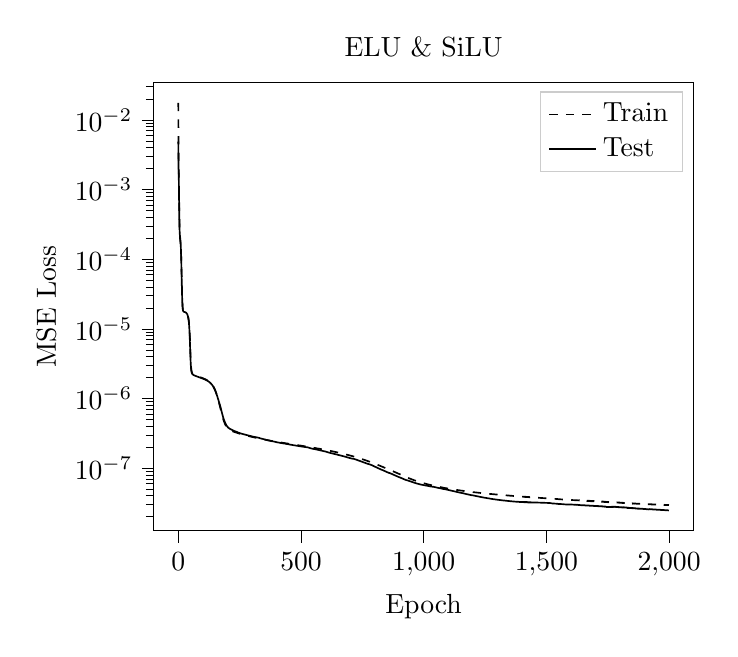
\begin{tikzpicture}

\begin{axis}[
legend cell align={left},
legend style={fill opacity=0.8, draw opacity=1, text opacity=1, draw=white!80!black},
log basis y={10},
tick align=outside,
tick pos=left,
title={ELU \& SiLU},
x grid style={white!69.0196078431373!black},
xlabel={Epoch},
xmin=-99.95, xmax=2098.95,
xtick style={color=black},
y grid style={white!69.0196078431373!black},
ylabel={MSE Loss},
ymin=1.25460830079477e-08, ymax=0.0345317116334461,
ymode=log,
ytick style={color=black}
]
\addplot [semithick, black, dashed]
table {%
0 0.0175996494237334
1 0.00287529958738014
2 0.0017450225809589
3 0.00109182657976635
4 0.000527906175178941
5 0.00029815742187202
6 0.000224625757531612
7 0.000197977887568413
8 0.000183264794104616
9 0.000169372935888532
10 0.000151957952730299
11 0.000129263067727152
12 0.000102055093113449
13 7.43479660304729e-05
14 5.15737580390123e-05
15 3.62272282127378e-05
16 2.71450699819979e-05
17 2.21503660204689e-05
18 1.95366582747738e-05
19 1.82204602597267e-05
20 1.7573602705852e-05
21 1.72561979470629e-05
22 1.70949869616379e-05
23 1.70056749411742e-05
24 1.69485445385362e-05
25 1.69051188822777e-05
26 1.68663870399541e-05
27 1.68271088441543e-05
28 1.67838884763114e-05
29 1.67341138449046e-05
30 1.66752324212212e-05
31 1.66049099725569e-05
32 1.65208375483417e-05
33 1.64199603086672e-05
34 1.62983461823387e-05
35 1.61510820416879e-05
36 1.59720132987786e-05
37 1.57533292913286e-05
38 1.5484687447497e-05
39 1.51527701264058e-05
40 1.47406713913369e-05
41 1.42270974720304e-05
42 1.3586219226454e-05
43 1.27891907977755e-05
44 1.18077328297659e-05
45 1.06241310518271e-05
46 9.24968551862548e-06
47 7.74917471699155e-06
48 6.25447972788606e-06
49 4.93720254530672e-06
50 3.93207780757621e-06
51 3.26343841823018e-06
52 2.85647097467745e-06
53 2.61511052349306e-06
54 2.47010573488637e-06
55 2.38091079037872e-06
56 2.32446314907975e-06
57 2.28729202154909e-06
58 2.26161475359277e-06
59 2.24282278935561e-06
60 2.22819607702718e-06
61 2.21604933179265e-06
62 2.20556252057236e-06
63 2.19616054360472e-06
64 2.18749445562594e-06
65 2.17928000790835e-06
66 2.17143440573864e-06
67 2.16391069665178e-06
68 2.15657700448446e-06
69 2.14940820202969e-06
70 2.14237768801695e-06
71 2.13553268446276e-06
72 2.12884015479631e-06
73 2.12225586307113e-06
74 2.11574514611357e-06
75 2.10928932654042e-06
76 2.10288195557951e-06
77 2.09650990095156e-06
78 2.09017900181152e-06
79 2.08388941103976e-06
80 2.07764323232595e-06
81 2.07144468839715e-06
82 2.06527465138606e-06
83 2.05913248743173e-06
84 2.0530142757309e-06
85 2.04691445756566e-06
86 2.04082622008173e-06
87 2.03473575675162e-06
88 2.0286378381229e-06
89 2.02251989537672e-06
90 2.01638261944481e-06
91 2.01022128027262e-06
92 2.00403939894045e-06
93 1.99783347059679e-06
94 1.99160166323509e-06
95 1.98533314505767e-06
96 1.97902080506651e-06
97 1.97265234243105e-06
98 1.9662212929461e-06
99 1.95973702790297e-06
100 1.95320250358577e-06
101 1.94660680122638e-06
102 1.939952190952e-06
103 1.93324243110737e-06
104 1.92648431564635e-06
105 1.91963722903665e-06
106 1.91268758226215e-06
107 1.90565878750704e-06
108 1.89853121551664e-06
109 1.89127792199884e-06
110 1.88389302704195e-06
111 1.87637372260951e-06
112 1.86870985686483e-06
113 1.86089686886248e-06
114 1.85292484115962e-06
115 1.84476674837697e-06
116 1.83640388777917e-06
117 1.82784501009792e-06
118 1.81907705044182e-06
119 1.81008488425505e-06
120 1.80085318538659e-06
121 1.79136690542236e-06
122 1.78161437838753e-06
123 1.77159513089009e-06
124 1.76129403953951e-06
125 1.75069264912509e-06
126 1.73976445233848e-06
127 1.72847957088607e-06
128 1.71680751208214e-06
129 1.7047350025905e-06
130 1.69224299537518e-06
131 1.67928939252704e-06
132 1.66583868410441e-06
133 1.65187669213651e-06
134 1.63740343054997e-06
135 1.62238789512514e-06
136 1.6067824065118e-06
137 1.5905935566991e-06
138 1.57381414469171e-06
139 1.55636063472286e-06
140 1.53816044023358e-06
141 1.51927269187979e-06
142 1.49966893327758e-06
143 1.47930880157787e-06
144 1.45817050724872e-06
145 1.43625170875339e-06
146 1.41338668653646e-06
147 1.38969123329957e-06
148 1.3652607281216e-06
149 1.34014765538382e-06
150 1.3144001037233e-06
151 1.28805525855569e-06
152 1.26120119203677e-06
153 1.23391107938176e-06
154 1.20624255806945e-06
155 1.17823492250579e-06
156 1.14992709714556e-06
157 1.12135632480204e-06
158 1.09260033759995e-06
159 1.06368875725593e-06
160 1.03462326670467e-06
161 1.00557742922547e-06
162 9.7667225931275e-07
163 9.47957712440939e-07
164 9.19453697107997e-07
165 8.91192761528714e-07
166 8.63282801702781e-07
167 8.35834502140642e-07
168 8.08940287257087e-07
169 7.82601844235842e-07
170 7.56980151379594e-07
171 7.32141062655955e-07
172 7.08114986750275e-07
173 6.84937570738953e-07
174 6.62635313446458e-07
175 6.41243045507167e-07
176 6.2081070653619e-07
177 6.01388748577847e-07
178 5.83003184985387e-07
179 5.65668886466142e-07
180 5.49323648044719e-07
181 5.33915851917754e-07
182 5.19427995229194e-07
183 5.05823589165288e-07
184 4.9306046715003e-07
185 4.8109552386677e-07
186 4.6990855443596e-07
187 4.59501481813618e-07
188 4.49822384894105e-07
189 4.40771383807714e-07
190 4.32378732156735e-07
191 4.24598447835933e-07
192 4.17455452677018e-07
193 4.10936514782634e-07
194 4.0497750121915e-07
195 3.99562149212329e-07
196 3.94614396952875e-07
197 3.9006308888645e-07
198 3.85865279696418e-07
199 3.81985842821564e-07
200 3.78385178450458e-07
201 3.75026909821941e-07
202 3.71899057071801e-07
203 3.69010332562425e-07
204 3.66329881671845e-07
205 3.63827414901152e-07
206 3.61479612806193e-07
207 3.59270024461011e-07
208 3.57176860234176e-07
209 3.55181227661205e-07
210 3.53276239565048e-07
211 3.51515790129042e-07
212 3.49912813945252e-07
213 3.48354445861787e-07
214 3.46851569503315e-07
215 3.45408498390043e-07
216 3.44020960312719e-07
217 3.42683353437678e-07
218 3.41392241935523e-07
219 3.40145149181126e-07
220 3.38937579158483e-07
221 3.37769001305332e-07
222 3.36636997644746e-07
223 3.35538890624321e-07
224 3.34470593799097e-07
225 3.33426590003683e-07
226 3.32406322868906e-07
227 3.31405100723714e-07
228 3.30421388724744e-07
229 3.29453601679575e-07
230 3.28494617065189e-07
231 3.27545682438313e-07
232 3.26611903702201e-07
233 3.25688031040272e-07
234 3.24785979117337e-07
235 3.23915015329135e-07
236 3.23034720381088e-07
237 3.22156478262059e-07
238 3.21286055111614e-07
239 3.20421153560346e-07
240 3.19560409622e-07
241 3.18705262714047e-07
242 3.1785766660164e-07
243 3.1701667911932e-07
244 3.16183564692096e-07
245 3.15356841326775e-07
246 3.14536922402908e-07
247 3.13724506980861e-07
248 3.12925141088272e-07
249 3.12140765842628e-07
250 3.11375240485745e-07
251 3.1062860304587e-07
252 3.0990082002802e-07
253 3.09185586033323e-07
254 3.0848231598668e-07
255 3.07785731521903e-07
256 3.07097276817103e-07
257 3.06413695156493e-07
258 3.05733606865033e-07
259 3.05057379563323e-07
260 3.04384200020991e-07
261 3.03711434725074e-07
262 3.0303466202497e-07
263 3.02357359515781e-07
264 3.01714337382464e-07
265 3.01069908317686e-07
266 3.00426167228807e-07
267 2.99785866843649e-07
268 2.99147748563655e-07
269 2.98513994621885e-07
270 2.97884098472423e-07
271 2.97257889613434e-07
272 2.96635719834626e-07
273 2.96016641236463e-07
274 2.95400801640255e-07
275 2.94787651498041e-07
276 2.94177613653801e-07
277 2.93570954063682e-07
278 2.92964300811605e-07
279 2.92362203438756e-07
280 2.91760416381237e-07
281 2.91159803978758e-07
282 2.9055891594254e-07
283 2.89960710880166e-07
284 2.8936324151374e-07
285 2.88770518061199e-07
286 2.88199581916615e-07
287 2.87646285805465e-07
288 2.87090873314355e-07
289 2.86531117303923e-07
290 2.85970951807712e-07
291 2.85412180353717e-07
292 2.84857709402786e-07
293 2.84302747601828e-07
294 2.8375344444953e-07
295 2.83205761050453e-07
296 2.82660867995332e-07
297 2.8211923660848e-07
298 2.81580993302555e-07
299 2.81046339367208e-07
300 2.80514478589566e-07
301 2.7998426008935e-07
302 2.79458510092923e-07
303 2.78934175497625e-07
304 2.78412257820548e-07
305 2.7789296674996e-07
306 2.77374297333211e-07
307 2.7685929883603e-07
308 2.76344144253926e-07
309 2.75831304342944e-07
310 2.75319272766694e-07
311 2.74808198902576e-07
312 2.7429603046869e-07
313 2.73784318302717e-07
314 2.73272087738974e-07
315 2.72760358924984e-07
316 2.72247648759105e-07
317 2.71740439046653e-07
318 2.71237279193315e-07
319 2.70741638303207e-07
320 2.70252898353363e-07
321 2.69768819279648e-07
322 2.69289078040913e-07
323 2.68816892983637e-07
324 2.68343211374145e-07
325 2.67885037054327e-07
326 2.67416310265389e-07
327 2.66975876130005e-07
328 2.66506596872773e-07
329 2.66083591505151e-07
330 2.65639710384846e-07
331 2.65243812378912e-07
332 2.64773271553054e-07
333 2.64322112386139e-07
334 2.63829088133605e-07
335 2.63389938119474e-07
336 2.6290572489529e-07
337 2.62464812486485e-07
338 2.61970761854968e-07
339 2.61548848619952e-07
340 2.61117641201736e-07
341 2.60733976112704e-07
342 2.60291870695539e-07
343 2.59895549817202e-07
344 2.594321902194e-07
345 2.59030119281078e-07
346 2.58601684890891e-07
347 2.58207709705971e-07
348 2.57752386914945e-07
349 2.57358960176646e-07
350 2.56929571371245e-07
351 2.56539277351919e-07
352 2.56089040767904e-07
353 2.5569170922779e-07
354 2.5524339392291e-07
355 2.54830653759086e-07
356 2.54406230482118e-07
357 2.54067098289568e-07
358 2.53661682023676e-07
359 2.53289803858081e-07
360 2.52879487980806e-07
361 2.52509188818806e-07
362 2.52106710043165e-07
363 2.5173805948242e-07
364 2.51339875042333e-07
365 2.50972963598883e-07
366 2.50580756969043e-07
367 2.50217714238943e-07
368 2.49831848677218e-07
369 2.49469345895648e-07
370 2.49089968647809e-07
371 2.4873137019199e-07
372 2.48356590667242e-07
373 2.47999187131143e-07
374 2.4763044640963e-07
375 2.47274666534736e-07
376 2.46913876914334e-07
377 2.46557384258494e-07
378 2.46201170384097e-07
379 2.45847944853494e-07
380 2.45494405000102e-07
381 2.45144459192659e-07
382 2.4479538060973e-07
383 2.44445716866437e-07
384 2.44098331023679e-07
385 2.43749799729187e-07
386 2.43400523295634e-07
387 2.43049962001862e-07
388 2.42702448431942e-07
389 2.42355488609292e-07
390 2.42012714679163e-07
391 2.4167355127247e-07
392 2.41335103595475e-07
393 2.40999812632481e-07
394 2.40663078940884e-07
395 2.40325962195698e-07
396 2.39984172416996e-07
397 2.39634622730023e-07
398 2.39281233987754e-07
399 2.38940480876693e-07
400 2.3863265462154e-07
401 2.38341846198864e-07
402 2.3803435519909e-07
403 2.37720892670268e-07
404 2.37405413471947e-07
405 2.3708795703925e-07
406 2.36770879936898e-07
407 2.36454466346459e-07
408 2.36138622433657e-07
409 2.35822797336027e-07
410 2.35507726081607e-07
411 2.35190857516443e-07
412 2.34877379469367e-07
413 2.34564189511843e-07
414 2.34253473898605e-07
415 2.33942672522858e-07
416 2.33634892900625e-07
417 2.33329615788591e-07
418 2.33024774566104e-07
419 2.32720143500842e-07
420 2.32416022562632e-07
421 2.32108510779483e-07
422 2.31797596143224e-07
423 2.31482146325845e-07
424 2.31172614505226e-07
425 2.30876980893413e-07
426 2.30587186429432e-07
427 2.30292145651845e-07
428 2.29996369043306e-07
429 2.29696812866109e-07
430 2.29395408346988e-07
431 2.29091220759869e-07
432 2.28793122374782e-07
433 2.28505814114044e-07
434 2.28219742702152e-07
435 2.27929575416397e-07
436 2.2763782101265e-07
437 2.27346566390452e-07
438 2.27056472624554e-07
439 2.26765794053563e-07
440 2.26474985048242e-07
441 2.26186430381858e-07
442 2.25897406949116e-07
443 2.2560861464882e-07
444 2.25320075472268e-07
445 2.25033070627489e-07
446 2.24744428635404e-07
447 2.24458662323457e-07
448 2.24170733531537e-07
449 2.23884842050381e-07
450 2.23597962218491e-07
451 2.23310248394171e-07
452 2.23022348308177e-07
453 2.22734046751327e-07
454 2.22442912225063e-07
455 2.22151466509501e-07
456 2.21859659873758e-07
457 2.21572562438155e-07
458 2.21289075021502e-07
459 2.21010129273225e-07
460 2.20728793351554e-07
461 2.20448860829947e-07
462 2.20167770152102e-07
463 2.19885938825826e-07
464 2.19604979307064e-07
465 2.19323364973434e-07
466 2.19043549776643e-07
467 2.18763958706347e-07
468 2.18484622969584e-07
469 2.18205289677087e-07
470 2.17927875091561e-07
471 2.17649641605533e-07
472 2.17373744746396e-07
473 2.1709560340355e-07
474 2.16820149610442e-07
475 2.16545120039768e-07
476 2.16269043342265e-07
477 2.15993676206949e-07
478 2.15721830045368e-07
479 2.15448890990899e-07
480 2.15178834174878e-07
481 2.149075208564e-07
482 2.14637604578627e-07
483 2.14366342028427e-07
484 2.14095653959134e-07
485 2.13825490867237e-07
486 2.13554397497262e-07
487 2.13285051131606e-07
488 2.13013861191769e-07
489 2.12744850905722e-07
490 2.12475656326205e-07
491 2.12207315264834e-07
492 2.11938185586291e-07
493 2.11668856991309e-07
494 2.11400331892264e-07
495 2.11133048289014e-07
496 2.10864122102805e-07
497 2.10596357298698e-07
498 2.10328821644623e-07
499 2.10059376463789e-07
500 2.09792518937491e-07
501 2.09525793508192e-07
502 2.0925775712044e-07
503 2.08989702933593e-07
504 2.08722312152076e-07
505 2.08454585468587e-07
506 2.08186760026763e-07
507 2.07918511570426e-07
508 2.07650348066579e-07
509 2.0738169546064e-07
510 2.07112908462648e-07
511 2.06844777174808e-07
512 2.06574911899793e-07
513 2.06304785187683e-07
514 2.06034711695224e-07
515 2.05762478614702e-07
516 2.05489735087383e-07
517 2.05218204492041e-07
518 2.04941749565535e-07
519 2.04666232278328e-07
520 2.04387647002591e-07
521 2.04112322826688e-07
522 2.0383555720116e-07
523 2.0356390942311e-07
524 2.0328289256355e-07
525 2.03006117388327e-07
526 2.02714574768947e-07
527 2.02427127135252e-07
528 2.02120347992718e-07
529 2.01825123937738e-07
530 2.01526683405007e-07
531 2.01258414435301e-07
532 2.00978978099897e-07
533 2.00726137201457e-07
534 2.00452940838147e-07
535 2.00204465528486e-07
536 1.99926498702041e-07
537 1.99674599720368e-07
538 1.99389074467149e-07
539 1.99133380988314e-07
540 1.98845136111458e-07
541 1.98592526508889e-07
542 1.98312001522538e-07
543 1.98073469377391e-07
544 1.97795437962611e-07
545 1.97541130809498e-07
546 1.9723873250399e-07
547 1.96979277795606e-07
548 1.96690525427812e-07
549 1.96438236173435e-07
550 1.9614758696207e-07
551 1.95893695774885e-07
552 1.9560284979292e-07
553 1.95347655257194e-07
554 1.95057353046479e-07
555 1.94801164418834e-07
556 1.94509920277142e-07
557 1.94253270734634e-07
558 1.93961073485127e-07
559 1.93702724359923e-07
560 1.93412831507089e-07
561 1.93151937097014e-07
562 1.92862569448948e-07
563 1.92599946480243e-07
564 1.92312116809035e-07
565 1.92046887015351e-07
566 1.91762092583758e-07
567 1.91495132177977e-07
568 1.91215405095591e-07
569 1.90950501014697e-07
570 1.90681914915558e-07
571 1.90422427188253e-07
572 1.90139000331158e-07
573 1.89849500145556e-07
574 1.89560766450825e-07
575 1.89280814623771e-07
576 1.8900092842955e-07
577 1.8872307740736e-07
578 1.88442443018744e-07
579 1.88163821782439e-07
580 1.87884023183926e-07
581 1.87604552785103e-07
582 1.87324280688017e-07
583 1.87046472525765e-07
584 1.8676562085318e-07
585 1.86486165269173e-07
586 1.86204263052048e-07
587 1.85924446839181e-07
588 1.85642518125917e-07
589 1.85359782030048e-07
590 1.85078272430417e-07
591 1.84792084183982e-07
592 1.84508275026474e-07
593 1.84220880669272e-07
594 1.83932809697751e-07
595 1.83643697894809e-07
596 1.83353293152777e-07
597 1.83060790227785e-07
598 1.82766741410489e-07
599 1.82471747208979e-07
600 1.82175910396154e-07
601 1.81878275817837e-07
602 1.81581998241143e-07
603 1.81293149658757e-07
604 1.81011799938346e-07
605 1.80725013777305e-07
606 1.80430601247394e-07
607 1.80136493369787e-07
608 1.79840781072471e-07
609 1.79547042925776e-07
610 1.79256953792617e-07
611 1.78968048011541e-07
612 1.78676989577298e-07
613 1.78381995397103e-07
614 1.78090247487717e-07
615 1.77807889897963e-07
616 1.77518120445086e-07
617 1.77226933303132e-07
618 1.76935237604425e-07
619 1.76642455294029e-07
620 1.76349222122951e-07
621 1.76056165678062e-07
622 1.75763073201551e-07
623 1.75468830988734e-07
624 1.75175491378354e-07
625 1.74879692544039e-07
626 1.74585498029955e-07
627 1.74291679364558e-07
628 1.73995814343186e-07
629 1.73700186017811e-07
630 1.73405231102208e-07
631 1.73109094077972e-07
632 1.72812282521306e-07
633 1.72517677093253e-07
634 1.72222056555427e-07
635 1.71927344155165e-07
636 1.71632569099245e-07
637 1.71338274590482e-07
638 1.71034913130086e-07
639 1.70733721134297e-07
640 1.7043391181204e-07
641 1.70132847280513e-07
642 1.69833049191936e-07
643 1.69529434216997e-07
644 1.69227103143044e-07
645 1.68925542112675e-07
646 1.68622009034891e-07
647 1.68318236774212e-07
648 1.68014904176061e-07
649 1.67709664872007e-07
650 1.6740428503681e-07
651 1.67098198687654e-07
652 1.66792148370121e-07
653 1.66485019853724e-07
654 1.66178793207905e-07
655 1.65869200280611e-07
656 1.65561907664369e-07
657 1.65252004769911e-07
658 1.64943542721119e-07
659 1.64632498311335e-07
660 1.64322014335028e-07
661 1.64009824260347e-07
662 1.63697879330016e-07
663 1.63385576819053e-07
664 1.63073160940996e-07
665 1.62760238836768e-07
666 1.62445714465775e-07
667 1.62130916251613e-07
668 1.61816271742055e-07
669 1.61501935338038e-07
670 1.61184934285075e-07
671 1.60868889899746e-07
672 1.60552074753184e-07
673 1.60234152140504e-07
674 1.59917202708471e-07
675 1.59598340765399e-07
676 1.5928070041582e-07
677 1.58963693209557e-07
678 1.58649849083758e-07
679 1.58348114766227e-07
680 1.58057629661812e-07
681 1.57671108624413e-07
682 1.57301388419739e-07
683 1.56999126346591e-07
684 1.56670816949145e-07
685 1.56336613628127e-07
686 1.56002342869499e-07
687 1.556705652348e-07
688 1.55350209446681e-07
689 1.55038015698494e-07
690 1.54718844136426e-07
691 1.5439428176478e-07
692 1.54069175138716e-07
693 1.53743410223228e-07
694 1.53420686693551e-07
695 1.5309928499363e-07
696 1.52787432718071e-07
697 1.52489572741388e-07
698 1.5215267003299e-07
699 1.5180147937599e-07
700 1.51467610628231e-07
701 1.51146714920003e-07
702 1.50877697457474e-07
703 1.50529026193169e-07
704 1.50173604488657e-07
705 1.49829621982178e-07
706 1.49500967239646e-07
707 1.49161668694831e-07
708 1.48830235133346e-07
709 1.4848696960712e-07
710 1.48152148859992e-07
711 1.47827308822457e-07
712 1.47502455668302e-07
713 1.47172682240182e-07
714 1.46840045417207e-07
715 1.46497807946844e-07
716 1.46153746740652e-07
717 1.4580504894468e-07
718 1.45458180313085e-07
719 1.45108395322779e-07
720 1.44763098667511e-07
721 1.44413272984423e-07
722 1.44068907871997e-07
723 1.43719601865655e-07
724 1.4337589767166e-07
725 1.43025246977402e-07
726 1.42680555661912e-07
727 1.42329018402165e-07
728 1.41984071241552e-07
729 1.41631456635594e-07
730 1.41288496855907e-07
731 1.40933513208097e-07
732 1.40596474217602e-07
733 1.40239406363207e-07
734 1.39900588273179e-07
735 1.39539811776501e-07
736 1.39217587097562e-07
737 1.38853319960219e-07
738 1.38519196539733e-07
739 1.38150057352959e-07
740 1.37809788974153e-07
741 1.3743655064502e-07
742 1.3710148611068e-07
743 1.36720188223194e-07
744 1.36391699037119e-07
745 1.36003874573021e-07
746 1.35689238376813e-07
747 1.3526807629205e-07
748 1.34977162510097e-07
749 1.34534849898671e-07
750 1.34263853979633e-07
751 1.33803888381578e-07
752 1.33541157381956e-07
753 1.33075631865154e-07
754 1.32812739892074e-07
755 1.32347266053046e-07
756 1.32081167286913e-07
757 1.31614762942434e-07
758 1.31345022282403e-07
759 1.30879963457176e-07
760 1.3060746962168e-07
761 1.30141176512666e-07
762 1.29864243902489e-07
763 1.29394299058561e-07
764 1.2911283270256e-07
765 1.28642385263333e-07
766 1.28354625225313e-07
767 1.2789251384504e-07
768 1.276106047996e-07
769 1.27158457551957e-07
770 1.26873228133206e-07
771 1.2642038833377e-07
772 1.26147492281348e-07
773 1.25696561333655e-07
774 1.2542319246478e-07
775 1.24956723709602e-07
776 1.24685955043446e-07
777 1.24218594947934e-07
778 1.23948786196593e-07
779 1.23475682784147e-07
780 1.23208924293294e-07
781 1.22734899811405e-07
782 1.22469958334648e-07
783 1.21993825025868e-07
784 1.21732354990911e-07
785 1.21256032315387e-07
786 1.20998242365999e-07
787 1.2051988794326e-07
788 1.20267326778389e-07
789 1.19790599342195e-07
790 1.19547230333694e-07
791 1.19097782047106e-07
792 1.18811734310498e-07
793 1.18316635195015e-07
794 1.18063428701021e-07
795 1.17580629776626e-07
796 1.17317416432172e-07
797 1.16842961155328e-07
798 1.16570967094276e-07
799 1.16108646778912e-07
800 1.15827305272376e-07
801 1.15377920501203e-07
802 1.1508488028511e-07
803 1.14649716792314e-07
804 1.14344960543633e-07
805 1.13921864283384e-07
806 1.13603540839335e-07
807 1.13194083560586e-07
808 1.12863245988137e-07
809 1.12468225204054e-07
810 1.12127083646385e-07
811 1.11746339406693e-07
812 1.11400504785308e-07
813 1.11035729347009e-07
814 1.10672897640995e-07
815 1.10295471110078e-07
816 1.09931559045151e-07
817 1.09568143528804e-07
818 1.09202652389229e-07
819 1.0884110548659e-07
820 1.08479694034713e-07
821 1.08123397502879e-07
822 1.07768057553415e-07
823 1.07427633928125e-07
824 1.07132911082886e-07
825 1.06680572500295e-07
826 1.06355442163419e-07
827 1.05982517581538e-07
828 1.05633535838479e-07
829 1.05274247268028e-07
830 1.04923396285983e-07
831 1.04568637013358e-07
832 1.04220353073003e-07
833 1.03865601353448e-07
834 1.03513037430503e-07
835 1.03156986462238e-07
836 1.02802441595884e-07
837 1.02450682760491e-07
838 1.02100855322362e-07
839 1.01750472786932e-07
840 1.0140150994431e-07
841 1.01053541381901e-07
842 1.00707275326073e-07
843 1.00359584678245e-07
844 1.00014914270474e-07
845 9.96698316377831e-08
846 9.93263650492793e-08
847 9.89830431770144e-08
848 9.86420426372092e-08
849 9.830027455493e-08
850 9.79607342728173e-08
851 9.76206057572426e-08
852 9.72826926961545e-08
853 9.69451741390515e-08
854 9.66100479331544e-08
855 9.62747901454009e-08
856 9.59414415291349e-08
857 9.56098446884823e-08
858 9.52807467342609e-08
859 9.49542538926096e-08
860 9.46286855700862e-08
861 9.43026890531939e-08
862 9.39737770337956e-08
863 9.36448786958977e-08
864 9.33190625431735e-08
865 9.29954942066047e-08
866 9.26732596084889e-08
867 9.23527348462017e-08
868 9.20334779763721e-08
869 9.17156793747154e-08
870 9.13983349377645e-08
871 9.10830633600312e-08
872 9.07672439609541e-08
873 9.04524855158684e-08
874 9.01387915774876e-08
875 8.98264481250521e-08
876 8.95150285202817e-08
877 8.92049641834092e-08
878 8.88939577734504e-08
879 8.85861132289278e-08
880 8.82777590334172e-08
881 8.79710582140092e-08
882 8.76646669567549e-08
883 8.73602326905143e-08
884 8.70552255705093e-08
885 8.67519998095645e-08
886 8.64501233053261e-08
887 8.6146255775077e-08
888 8.58468929791911e-08
889 8.55448757945965e-08
890 8.52472173562546e-08
891 8.49459580933853e-08
892 8.46501490912033e-08
893 8.43481334271701e-08
894 8.40549865515072e-08
895 8.37533525341883e-08
896 8.34638953648437e-08
897 8.31621499131074e-08
898 8.28743535308263e-08
899 8.25751389896823e-08
900 8.22899470520611e-08
901 8.19908786695578e-08
902 8.17119941984856e-08
903 8.14204756736103e-08
904 8.11498789587972e-08
905 8.08366941313921e-08
906 8.05548967051095e-08
907 8.02546861962128e-08
908 7.99800256316985e-08
909 7.96830944622684e-08
910 7.94125844763016e-08
911 7.911549998596e-08
912 7.88506315814175e-08
913 7.85564360050728e-08
914 7.82931790439534e-08
915 7.8004567647838e-08
916 7.77404717631214e-08
917 7.74547611754883e-08
918 7.7181353187683e-08
919 7.69060091343476e-08
920 7.66324710355093e-08
921 7.63723304721964e-08
922 7.60953091329952e-08
923 7.5864466129616e-08
924 7.55713254001478e-08
925 7.53308811525244e-08
926 7.50198124421786e-08
927 7.4793768067849e-08
928 7.44999733726104e-08
929 7.42764854599898e-08
930 7.40070237732482e-08
931 7.3757139062991e-08
932 7.34708819116747e-08
933 7.32295668548488e-08
934 7.29672317092422e-08
935 7.27254336361227e-08
936 7.24722474849671e-08
937 7.22304411411301e-08
938 7.19834948306186e-08
939 7.17461780297413e-08
940 7.15024025836897e-08
941 7.1267125772323e-08
942 7.10307098543694e-08
943 7.07984063801348e-08
944 7.05661321873663e-08
945 7.03392329199914e-08
946 7.01104802871555e-08
947 6.98869387250056e-08
948 6.96629443517338e-08
949 6.94436666712761e-08
950 6.92237607111679e-08
951 6.90076469602729e-08
952 6.87917168527008e-08
953 6.85799188460123e-08
954 6.83669486356564e-08
955 6.81601427672263e-08
956 6.79508710383914e-08
957 6.77463507194886e-08
958 6.75436472228341e-08
959 6.73413416798496e-08
960 6.71408234005355e-08
961 6.69428408208717e-08
962 6.67447739353122e-08
963 6.65525494945029e-08
964 6.63575741768341e-08
965 6.61687265406385e-08
966 6.59775455638112e-08
967 6.57917663957619e-08
968 6.56059239396711e-08
969 6.54228842194016e-08
970 6.52397152656192e-08
971 6.50610468397872e-08
972 6.48808190213401e-08
973 6.47048932265193e-08
974 6.45277746365025e-08
975 6.43562626940764e-08
976 6.41803190077894e-08
977 6.40130773810199e-08
978 6.38387489111381e-08
979 6.36743903790204e-08
980 6.35023501907028e-08
981 6.33410359505149e-08
982 6.31731920286427e-08
983 6.30170328896895e-08
984 6.28512382760959e-08
985 6.27018185994643e-08
986 6.25389082422601e-08
987 6.23940222439501e-08
988 6.22324554662157e-08
989 6.20933315786942e-08
990 6.19333390581289e-08
991 6.18009775230632e-08
992 6.16378112496818e-08
993 6.151472694782e-08
994 6.13488915561788e-08
995 6.12322543176447e-08
996 6.10627431143484e-08
997 6.0956969566206e-08
998 6.07836454555866e-08
999 6.06858273002331e-08
1000 6.0507606448823e-08
1001 6.04200453828696e-08
1002 6.02411679047066e-08
1003 6.01563548663364e-08
1004 5.99758189601118e-08
1005 5.98955439414794e-08
1006 5.97161064845864e-08
1007 5.96399952890181e-08
1008 5.94604134001031e-08
1009 5.93865410394301e-08
1010 5.92094895459638e-08
1011 5.91360529007545e-08
1012 5.89636505807789e-08
1013 5.8890947325807e-08
1014 5.87177360920066e-08
1015 5.86479926383276e-08
1016 5.84775806053983e-08
1017 5.84071221645388e-08
1018 5.82407901923432e-08
1019 5.81706089164413e-08
1020 5.80062781310176e-08
1021 5.79364867938636e-08
1022 5.77755773072397e-08
1023 5.77070267020474e-08
1024 5.75472279997769e-08
1025 5.74803025088499e-08
1026 5.73227851177194e-08
1027 5.72549469133321e-08
1028 5.70999626958724e-08
1029 5.7033860887401e-08
1030 5.68804288114677e-08
1031 5.68131055551646e-08
1032 5.6663332767215e-08
1033 5.65954860540785e-08
1034 5.64472345629952e-08
1035 5.63754745606104e-08
1036 5.62272355715265e-08
1037 5.61484333303497e-08
1038 5.5999395478068e-08
1039 5.59186794042432e-08
1040 5.57838673493904e-08
1041 5.57162485428364e-08
1042 5.56010164558529e-08
1043 5.55337433567615e-08
1044 5.54150616451921e-08
1045 5.53392590987301e-08
1046 5.52239583875291e-08
1047 5.5144874224311e-08
1048 5.50325426509346e-08
1049 5.49520297781214e-08
1050 5.48456422393428e-08
1051 5.47616790171901e-08
1052 5.46610097735822e-08
1053 5.45759626504605e-08
1054 5.44761822958151e-08
1055 5.43920063904579e-08
1056 5.42956490861002e-08
1057 5.4211317223718e-08
1058 5.4117549513677e-08
1059 5.40303107428031e-08
1060 5.39417221858685e-08
1061 5.38540957997213e-08
1062 5.37668139806158e-08
1063 5.36784573128557e-08
1064 5.35941787980221e-08
1065 5.3507047322654e-08
1066 5.34215971939034e-08
1067 5.33369641182446e-08
1068 5.32536905559766e-08
1069 5.31688032587851e-08
1070 5.30834877885411e-08
1071 5.30020961733158e-08
1072 5.29187969142697e-08
1073 5.28378100881355e-08
1074 5.27521015420973e-08
1075 5.2670030630253e-08
1076 5.25867333536212e-08
1077 5.25034244560629e-08
1078 5.2418908094154e-08
1079 5.23290026706036e-08
1080 5.22326315639532e-08
1081 5.21282267627043e-08
1082 5.20232685978783e-08
1083 5.19315852756108e-08
1084 5.18594172795872e-08
1085 5.18124042443446e-08
1086 5.16707377791192e-08
1087 5.16539989376952e-08
1088 5.15711485888914e-08
1089 5.15147099022784e-08
1090 5.14256392456502e-08
1091 5.13642042427875e-08
1092 5.1281067797504e-08
1093 5.12151511067316e-08
1094 5.1136492572823e-08
1095 5.10673343896428e-08
1096 5.09849862382339e-08
1097 5.09159236656842e-08
1098 5.08563726846489e-08
1099 5.077642700968e-08
1100 5.07170401462531e-08
1101 5.06396115724783e-08
1102 5.05759921800575e-08
1103 5.05042115719334e-08
1104 5.04362397748537e-08
1105 5.03709844430489e-08
1106 5.03009102779117e-08
1107 5.02376596962506e-08
1108 5.01693970313966e-08
1109 5.01037829856443e-08
1110 5.00381948604911e-08
1111 4.99729949332561e-08
1112 4.99080592604173e-08
1113 4.98440006531098e-08
1114 4.97788077851169e-08
1115 4.97160153187792e-08
1116 4.96525768198808e-08
1117 4.95886749831698e-08
1118 4.95259647159685e-08
1119 4.94638447854356e-08
1120 4.94025123742858e-08
1121 4.93408055142197e-08
1122 4.92777741882833e-08
1123 4.92156950713252e-08
1124 4.91560401947311e-08
1125 4.90946190012664e-08
1126 4.90349146211599e-08
1127 4.89734367121741e-08
1128 4.89154338225717e-08
1129 4.88554389015405e-08
1130 4.87965765465503e-08
1131 4.87381162699307e-08
1132 4.86792782474765e-08
1133 4.86204470853124e-08
1134 4.85623430606097e-08
1135 4.85029923069646e-08
1136 4.84469144268473e-08
1137 4.83894675831209e-08
1138 4.83293557067554e-08
1139 4.82720579384477e-08
1140 4.82142370081817e-08
1141 4.81568539498767e-08
1142 4.80991615496862e-08
1143 4.80393431416815e-08
1144 4.79794743064588e-08
1145 4.79202978560522e-08
1146 4.78614520780241e-08
1147 4.77986213525128e-08
1148 4.77403732936921e-08
1149 4.76852409470041e-08
1150 4.76301647012178e-08
1151 4.7578462570641e-08
1152 4.75241271757909e-08
1153 4.74723943568733e-08
1154 4.74180858915929e-08
1155 4.73673670065011e-08
1156 4.73131372622504e-08
1157 4.72611859620997e-08
1158 4.72082820444086e-08
1159 4.7156959116279e-08
1160 4.70964777754546e-08
1161 4.70352642594207e-08
1162 4.69699322387385e-08
1163 4.69033307766153e-08
1164 4.68406378679731e-08
1165 4.678152087223e-08
1166 4.67163908766111e-08
1167 4.66496131537042e-08
1168 4.66186367269472e-08
1169 4.65931978403944e-08
1170 4.65452790940901e-08
1171 4.64970322155978e-08
1172 4.64478893889009e-08
1173 4.6401220398451e-08
1174 4.6354152015482e-08
1175 4.63051806818271e-08
1176 4.62608166245104e-08
1177 4.62116961692516e-08
1178 4.61663384392352e-08
1179 4.61181958506529e-08
1180 4.60749140778205e-08
1181 4.60289976587092e-08
1182 4.59828709118426e-08
1183 4.59360696254407e-08
1184 4.58911745084833e-08
1185 4.58475705649164e-08
1186 4.58020190592379e-08
1187 4.57577413932597e-08
1188 4.57144813417187e-08
1189 4.56681103067069e-08
1190 4.56250730138663e-08
1191 4.55801805401279e-08
1192 4.55367965024323e-08
1193 4.54928729460846e-08
1194 4.54491035526416e-08
1195 4.54046372340144e-08
1196 4.53605468813123e-08
1197 4.5318322193566e-08
1198 4.52730989941585e-08
1199 4.52277204736617e-08
1200 4.51831244703271e-08
1201 4.51362583078208e-08
1202 4.50891260435071e-08
1203 4.50436343264471e-08
1204 4.5005045581803e-08
1205 4.49671033173615e-08
1206 4.4927011046525e-08
1207 4.48885856805248e-08
1208 4.48442414047179e-08
1209 4.48037458724571e-08
1210 4.47623032719946e-08
1211 4.4723272381475e-08
1212 4.46810348542215e-08
1213 4.46411653030054e-08
1214 4.4600022867769e-08
1215 4.45591790949607e-08
1216 4.45200743115493e-08
1217 4.44793313718606e-08
1218 4.44395357810379e-08
1219 4.44004629009953e-08
1220 4.43605396469593e-08
1221 4.43211583132097e-08
1222 4.4281827630499e-08
1223 4.42431409233279e-08
1224 4.42025483913255e-08
1225 4.41649761562246e-08
1226 4.41241812545456e-08
1227 4.40845443172577e-08
1228 4.40465823245972e-08
1229 4.40095524965045e-08
1230 4.39683958113335e-08
1231 4.39273198011847e-08
1232 4.38891112786166e-08
1233 4.38489198977265e-08
1234 4.38104611717449e-08
1235 4.37681291849401e-08
1236 4.37326005489069e-08
1237 4.36921684006109e-08
1238 4.36569987094515e-08
1239 4.36212489383081e-08
1240 4.35856813254532e-08
1241 4.35512924070736e-08
1242 4.35153490982998e-08
1243 4.34792310812782e-08
1244 4.3441935190458e-08
1245 4.34084090166209e-08
1246 4.33736247344996e-08
1247 4.33387995464329e-08
1248 4.33012893488183e-08
1249 4.32677698007922e-08
1250 4.32302192905354e-08
1251 4.31998927901134e-08
1252 4.31620639780306e-08
1253 4.31301771044446e-08
1254 4.30933546446965e-08
1255 4.30604565977433e-08
1256 4.30247026876884e-08
1257 4.29927247402873e-08
1258 4.29553815664008e-08
1259 4.29268922417236e-08
1260 4.28864818502461e-08
1261 4.28586315130985e-08
1262 4.28198954232073e-08
1263 4.27898634640655e-08
1264 4.2753595245415e-08
1265 4.27237714077933e-08
1266 4.26869564371657e-08
1267 4.26564525852768e-08
1268 4.26192783891111e-08
1269 4.25903701817276e-08
1270 4.25535703065805e-08
1271 4.25226653746336e-08
1272 4.24879032259184e-08
1273 4.2456188470652e-08
1274 4.24202999376178e-08
1275 4.23859171334584e-08
1276 4.23519101282466e-08
1277 4.23149189643368e-08
1278 4.22824308721204e-08
1279 4.22486863698168e-08
1280 4.22202453158604e-08
1281 4.2187339193589e-08
1282 4.21591239216923e-08
1283 4.2124149732814e-08
1284 4.20938310909946e-08
1285 4.20612705056556e-08
1286 4.20308245416834e-08
1287 4.1997344542466e-08
1288 4.19672587632647e-08
1289 4.19371729876161e-08
1290 4.19042328978492e-08
1291 4.18756649480656e-08
1292 4.18406924111991e-08
1293 4.18142886573492e-08
1294 4.17780153441072e-08
1295 4.17540905388591e-08
1296 4.1716828956595e-08
1297 4.16896988646442e-08
1298 4.16524566198007e-08
1299 4.1629468562121e-08
1300 4.15833136386823e-08
1301 4.15585945674479e-08
1302 4.15018889334817e-08
1303 4.1496817747344e-08
1304 4.14546708569219e-08
1305 4.14546289491113e-08
1306 4.13919402539875e-08
1307 4.14056540662955e-08
1308 4.13244472277086e-08
1309 4.13615174217341e-08
1310 4.12699490794921e-08
1311 4.1267000831624e-08
1312 4.12267482445827e-08
1313 4.12109218075329e-08
1314 4.11668753805827e-08
1315 4.11583183073105e-08
1316 4.11022767217162e-08
1317 4.11100928516817e-08
1318 4.1037408280431e-08
1319 4.1066953887281e-08
1320 4.09750483711946e-08
1321 4.10066736584724e-08
1322 4.09191586996371e-08
1323 4.0947404691849e-08
1324 4.08638924866978e-08
1325 4.08914481262457e-08
1326 4.08070332653665e-08
1327 4.08357535057746e-08
1328 4.07527275072539e-08
1329 4.07760795404499e-08
1330 4.06947206101904e-08
1331 4.07312980570396e-08
1332 4.06484653616701e-08
1333 4.06305324958112e-08
1334 4.06281817078025e-08
1335 4.05609808034058e-08
1336 4.06007411903886e-08
1337 4.05186632264076e-08
1338 4.04813392229642e-08
1339 4.05137915677756e-08
1340 4.04427050817446e-08
1341 4.0404595285537e-08
1342 4.04034278496113e-08
1343 4.03470085359459e-08
1344 4.03759440494866e-08
1345 4.02951091871273e-08
1346 4.02729835862203e-08
1347 4.02820761493672e-08
1348 4.02028653567754e-08
1349 4.0243565639031e-08
1350 4.01645263359285e-08
1351 4.01247152481687e-08
1352 4.01298546996998e-08
1353 4.00498072288258e-08
1354 4.00780106133425e-08
1355 4.00133800226854e-08
1356 3.99935331216739e-08
1357 3.99947927611777e-08
1358 3.99257412730947e-08
1359 3.99636142667248e-08
1360 3.98933878571484e-08
1361 3.98593884050058e-08
1362 3.98346793133442e-08
1363 3.98373121583973e-08
1364 3.97712527302474e-08
1365 3.98051756000939e-08
1366 3.97388940989174e-08
1367 3.97043374533723e-08
1368 3.96858321707327e-08
1369 3.96721265438771e-08
1370 3.9627116226626e-08
1371 3.96427330819904e-08
1372 3.9564374215928e-08
1373 3.95902756480382e-08
1374 3.95136501545323e-08
1375 3.95457331237026e-08
1376 3.94681531226127e-08
1377 3.94643733123701e-08
1378 3.94374941201647e-08
1379 3.94130171876839e-08
1380 3.93865616992173e-08
1381 3.93646849872198e-08
1382 3.93336724364701e-08
1383 3.93183808213848e-08
1384 3.92790345884464e-08
1385 3.92783624505455e-08
1386 3.92181673056768e-08
1387 3.9247309484125e-08
1388 3.91625413485031e-08
1389 3.91856282284664e-08
1390 3.9112159310406e-08
1391 3.91618979058705e-08
1392 3.9091612521247e-08
1393 3.90773670382316e-08
1394 3.90596091861539e-08
1395 3.90377561814148e-08
1396 3.90033072932283e-08
1397 3.89836041740921e-08
1398 3.89571714300985e-08
1399 3.89340272377581e-08
1400 3.89095555490826e-08
1401 3.88901825196797e-08
1402 3.88592720064196e-08
1403 3.88472628642944e-08
1404 3.88079879627412e-08
1405 3.8811693173102e-08
1406 3.87458087196535e-08
1407 3.87871781057925e-08
1408 3.86750464578256e-08
1409 3.87632872431709e-08
1410 3.86152443461185e-08
1411 3.8726272766354e-08
1412 3.85677903231851e-08
1413 3.86811754395922e-08
1414 3.85242661202767e-08
1415 3.86363415181279e-08
1416 3.84808430133887e-08
1417 3.85900492148039e-08
1418 3.84359594995942e-08
1419 3.85446401054423e-08
1420 3.83952957250244e-08
1421 3.84991835922222e-08
1422 3.83527137763906e-08
1423 3.84539447075838e-08
1424 3.83098808818261e-08
1425 3.84084559001963e-08
1426 3.82686769313523e-08
1427 3.83634785663389e-08
1428 3.82263591767185e-08
1429 3.83170275028988e-08
1430 3.81848634063431e-08
1431 3.82719766882644e-08
1432 3.81443559227534e-08
1433 3.82261160360997e-08
1434 3.81028666360805e-08
1435 3.81820462145299e-08
1436 3.80621713560458e-08
1437 3.81377050473475e-08
1438 3.8020763664548e-08
1439 3.80906669938952e-08
1440 3.79813536319773e-08
1441 3.80451777530766e-08
1442 3.79402011745356e-08
1443 3.79971468937868e-08
1444 3.78976800448072e-08
1445 3.79480461809578e-08
1446 3.78535985952055e-08
1447 3.78877064797223e-08
1448 3.77929022867818e-08
1449 3.78013958233225e-08
1450 3.77127713129255e-08
1451 3.77494880652307e-08
1452 3.77125745814055e-08
1453 3.77251245637922e-08
1454 3.76768934877703e-08
1455 3.76800348611539e-08
1456 3.76387757690111e-08
1457 3.76369275087995e-08
1458 3.76011498595119e-08
1459 3.75915576782404e-08
1460 3.7565789462235e-08
1461 3.75480054266575e-08
1462 3.75244291888066e-08
1463 3.75085536461484e-08
1464 3.74869865567007e-08
1465 3.74678988599442e-08
1466 3.74458098804098e-08
1467 3.74289946023509e-08
1468 3.74053136447117e-08
1469 3.73895509646616e-08
1470 3.73655890228974e-08
1471 3.73484145193004e-08
1472 3.73280483714211e-08
1473 3.73083839733113e-08
1474 3.72891789162111e-08
1475 3.72704910880373e-08
1476 3.7248621644892e-08
1477 3.72312626915061e-08
1478 3.72108093422696e-08
1479 3.71916894330582e-08
1480 3.71718720479919e-08
1481 3.71548341639993e-08
1482 3.71317190506204e-08
1483 3.71136948977835e-08
1484 3.70954332247209e-08
1485 3.7075017328192e-08
1486 3.70562630358506e-08
1487 3.70378945753203e-08
1488 3.70180622759619e-08
1489 3.69973437628346e-08
1490 3.69796147232648e-08
1491 3.6959753085597e-08
1492 3.69415847352172e-08
1493 3.69228330292515e-08
1494 3.69024669879536e-08
1495 3.6883986361147e-08
1496 3.68645939907708e-08
1497 3.68453450008133e-08
1498 3.68283621270393e-08
1499 3.68075644914256e-08
1500 3.67898759954244e-08
1501 3.67695001806112e-08
1502 3.67499921836156e-08
1503 3.6732197379763e-08
1504 3.67122580833268e-08
1505 3.66923476278203e-08
1506 3.66745375650623e-08
1507 3.66537149432133e-08
1508 3.66359610310951e-08
1509 3.66162055271957e-08
1510 3.659514873533e-08
1511 3.65773423496307e-08
1512 3.65557572656883e-08
1513 3.65364017227421e-08
1514 3.65143413247893e-08
1515 3.64913223691588e-08
1516 3.64676853230606e-08
1517 3.64390327298736e-08
1518 3.64060995430293e-08
1519 3.63669256735477e-08
1520 3.63247117149967e-08
1521 3.63022032345839e-08
1522 3.62946600880321e-08
1523 3.62906074222735e-08
1524 3.62781957825575e-08
1525 3.62666043507431e-08
1526 3.62482158386968e-08
1527 3.62316294477694e-08
1528 3.62140311018777e-08
1529 3.61927297731768e-08
1530 3.61777107897865e-08
1531 3.61594412154886e-08
1532 3.61410701259501e-08
1533 3.61231098437997e-08
1534 3.61054330362265e-08
1535 3.60887919867991e-08
1536 3.60693465388806e-08
1537 3.60534092003206e-08
1538 3.60342813436887e-08
1539 3.60168709043762e-08
1540 3.59998949370777e-08
1541 3.59785507910715e-08
1542 3.59634371278617e-08
1543 3.5941752855706e-08
1544 3.5922967253299e-08
1545 3.59026391869577e-08
1546 3.58764270416145e-08
1547 3.58446422517034e-08
1548 3.57990294403976e-08
1549 3.57539634769921e-08
1550 3.57382170612652e-08
1551 3.57453839328059e-08
1552 3.57398239394513e-08
1553 3.57211739263619e-08
1554 3.57008202236386e-08
1555 3.5678548972129e-08
1556 3.56516157040687e-08
1557 3.56155545730985e-08
1558 3.55595640009199e-08
1559 3.54979681276291e-08
1560 3.54960429262974e-08
1561 3.55017919559941e-08
1562 3.54916767868474e-08
1563 3.54655182341901e-08
1564 3.54432029538998e-08
1565 3.5438487193673e-08
1566 3.54082522804333e-08
1567 3.53880520869154e-08
1568 3.53720010188852e-08
1569 3.53510848984939e-08
1570 3.53368128820364e-08
1571 3.53225550693281e-08
1572 3.53036709093146e-08
1573 3.52854553042903e-08
1574 3.52649857795484e-08
1575 3.52465590989226e-08
1576 3.52256008397944e-08
1577 3.52086323704981e-08
1578 3.52005257155952e-08
1579 3.51824060658146e-08
1580 3.51704832972644e-08
1581 3.51478965363583e-08
1582 3.51353368390761e-08
1583 3.5110004311889e-08
1584 3.5099747750067e-08
1585 3.50758459060074e-08
1586 3.50638818371607e-08
1587 3.50475820525276e-08
1588 3.50327269060813e-08
1589 3.50174722001384e-08
1590 3.50005818585686e-08
1591 3.49837193578395e-08
1592 3.49677575677276e-08
1593 3.49536021673202e-08
1594 3.4934812864762e-08
1595 3.49210757981666e-08
1596 3.49060805096002e-08
1597 3.48915063987931e-08
1598 3.48756203969458e-08
1599 3.48525328703886e-08
1600 3.48177892259827e-08
1601 3.4787871483033e-08
1602 3.47715977966345e-08
1603 3.47641803291054e-08
1604 3.4753644154506e-08
1605 3.47409893972639e-08
1606 3.47234597732893e-08
1607 3.47079945299811e-08
1608 3.46909644122206e-08
1609 3.46700013889034e-08
1610 3.4647425383838e-08
1611 3.46236579407133e-08
1612 3.46073512211831e-08
1613 3.45986185354974e-08
1614 3.45835249468962e-08
1615 3.45704000377367e-08
1616 3.45575677194176e-08
1617 3.45454655494848e-08
1618 3.45400001542373e-08
1619 3.45489442494795e-08
1620 3.46055936049083e-08
1621 3.46027133435456e-08
1622 3.45283926961315e-08
1623 3.44992562943958e-08
1624 3.44875408124778e-08
1625 3.44644759859847e-08
1626 3.44404155825373e-08
1627 3.44020873228601e-08
1628 3.43586973521326e-08
1629 3.4341221764933e-08
1630 3.43909036732981e-08
1631 3.43338189843223e-08
1632 3.43876061528192e-08
1633 3.42678819063025e-08
1634 3.44153996643115e-08
1635 3.42123048380216e-08
1636 3.42824781469631e-08
1637 3.42697498929567e-08
1638 3.42595794542433e-08
1639 3.42000555164645e-08
1640 3.43115936427552e-08
1641 3.41142779802794e-08
1642 3.42297419813065e-08
1643 3.41120816198526e-08
1644 3.42440022187418e-08
1645 3.4062529605805e-08
1646 3.41824622704934e-08
1647 3.4047797104364e-08
1648 3.41837958348634e-08
1649 3.40040385893303e-08
1650 3.41273175692436e-08
1651 3.39857107061192e-08
1652 3.41197286370942e-08
1653 3.39473847557059e-08
1654 3.40724037570794e-08
1655 3.3924028626231e-08
1656 3.40575578423596e-08
1657 3.38874829708402e-08
1658 3.40143418213756e-08
1659 3.38625038871498e-08
1660 3.39981571269021e-08
1661 3.38275544677913e-08
1662 3.39578113894845e-08
1663 3.38020041255049e-08
1664 3.39345081759035e-08
1665 3.37708272084569e-08
1666 3.39016538219994e-08
1667 3.37398202923111e-08
1668 3.3871374476746e-08
1669 3.3713152991055e-08
1670 3.38470531744406e-08
1671 3.36787168428998e-08
1672 3.38099436696382e-08
1673 3.36552861135431e-08
1674 3.37871328586203e-08
1675 3.36225322605799e-08
1676 3.37511091341725e-08
1677 3.35951861991646e-08
1678 3.37272143831058e-08
1679 3.35632440560119e-08
1680 3.36950260440005e-08
1681 3.35351847731147e-08
1682 3.36676524526069e-08
1683 3.35080319313619e-08
1684 3.3638606719677e-08
1685 3.34769234804355e-08
1686 3.36072094828666e-08
1687 3.34506699086745e-08
1688 3.35820369912199e-08
1689 3.3417763606991e-08
1690 3.35508458437772e-08
1691 3.33905130638357e-08
1692 3.3523850031969e-08
1693 3.33594249095626e-08
1694 3.34934648869023e-08
1695 3.33310702380629e-08
1696 3.34674506934363e-08
1697 3.33046057470199e-08
1698 3.34370984216292e-08
1699 3.32750735871912e-08
1700 3.3405146190546e-08
1701 3.32485903538071e-08
1702 3.33824205025479e-08
1703 3.32180697437678e-08
1704 3.33495473441303e-08
1705 3.31909745856507e-08
1706 3.33229182807315e-08
1707 3.31615310269484e-08
1708 3.32939488369988e-08
1709 3.31336074719246e-08
1710 3.32664251896375e-08
1711 3.31054216786697e-08
1712 3.32384806043251e-08
1713 3.3075719613862e-08
1714 3.32077416516086e-08
1715 3.30486065411861e-08
1716 3.31817862146977e-08
1717 3.30200386073898e-08
1718 3.31512511522192e-08
1719 3.29933048099917e-08
1720 3.312378184539e-08
1721 3.29619050773999e-08
1722 3.30905355490074e-08
1723 3.29348713101751e-08
1724 3.30658714720045e-08
1725 3.2903780079252e-08
1726 3.303245081554e-08
1727 3.28742794746262e-08
1728 3.30037107438841e-08
1729 3.28410966385917e-08
1730 3.29698604080164e-08
1731 3.28060075069914e-08
1732 3.29262452503087e-08
1733 3.27559392641064e-08
1734 3.28639632787286e-08
1735 3.2681094896958e-08
1736 3.28132108009527e-08
1737 3.26625908133593e-08
1738 3.27962944517424e-08
1739 3.26419050526994e-08
1740 3.28100845461421e-08
1741 3.26046135601388e-08
1742 3.26775266934476e-08
1743 3.2554416765862e-08
1744 3.26634748244459e-08
1745 3.24871724917131e-08
1746 3.25927902373735e-08
1747 3.24813773406873e-08
1748 3.25925799256055e-08
1749 3.24599241867674e-08
1750 3.25734725414861e-08
1751 3.24401372218119e-08
1752 3.25387758763895e-08
1753 3.24277666763351e-08
1754 3.25156576295171e-08
1755 3.24053392777301e-08
1756 3.24837721166205e-08
1757 3.23901482452982e-08
1758 3.24466525505329e-08
1759 3.23788421177085e-08
1760 3.240652201697e-08
1761 3.23734802876174e-08
1762 3.23660537873138e-08
1763 3.23647946522954e-08
1764 3.23273926170486e-08
1765 3.23475536454509e-08
1766 3.22969467099199e-08
1767 3.23262176227246e-08
1768 3.22659987652685e-08
1769 3.23020740822244e-08
1770 3.22377145565156e-08
1771 3.22753880812598e-08
1772 3.22092732485402e-08
1773 3.2246492640553e-08
1774 3.21791188344633e-08
1775 3.22211259540239e-08
1776 3.21470656228229e-08
1777 3.21913639655946e-08
1778 3.21151684410381e-08
1779 3.21639194140744e-08
1780 3.20794381032385e-08
1781 3.21364864195317e-08
1782 3.20384938792273e-08
1783 3.21218324899064e-08
1784 3.19840757114775e-08
1785 3.21338886681843e-08
1786 3.19231031227218e-08
1787 3.20652566898616e-08
1788 3.19515165809747e-08
1789 3.20042525139286e-08
1790 3.19398796140291e-08
1791 3.19613587169698e-08
1792 3.19048256240961e-08
1793 3.19481420714141e-08
1794 3.18611491731957e-08
1795 3.19398212340616e-08
1796 3.18067174216452e-08
1797 3.19524965366469e-08
1798 3.17490460268743e-08
1799 3.18861543089355e-08
1800 3.17758301342508e-08
1801 3.18336564451016e-08
1802 3.1763487102765e-08
1803 3.17955307451712e-08
1804 3.17265417315582e-08
1805 3.17754963923278e-08
1806 3.16862744806912e-08
1807 3.17643213847418e-08
1808 3.16321076407888e-08
1809 3.17721518285907e-08
1810 3.15841033948772e-08
1811 3.17179917388444e-08
1812 3.15929358176703e-08
1813 3.16796838593092e-08
1814 3.15861926694083e-08
1815 3.16394474992876e-08
1816 3.15584740988584e-08
1817 3.16176739758589e-08
1818 3.15200244358493e-08
1819 3.16058087559412e-08
1820 3.14781268286879e-08
1821 3.15855602703863e-08
1822 3.1442212073074e-08
1823 3.15518088083166e-08
1824 3.14070510718523e-08
1825 3.14765631710401e-08
1826 3.13348955955917e-08
1827 3.14295956087562e-08
1828 3.13473536035502e-08
1829 3.13846484214508e-08
1830 3.12679589526965e-08
1831 3.13140447900651e-08
1832 3.12284954340214e-08
1833 3.13061082248822e-08
1834 3.11941969783902e-08
1835 3.12384273062349e-08
1836 3.11294203783064e-08
1837 3.12014705770025e-08
1838 3.11129711949576e-08
1839 3.11866513431625e-08
1840 3.10680074715464e-08
1841 3.1162816917174e-08
1842 3.10589508565329e-08
1843 3.11255323932613e-08
1844 3.10953798141611e-08
1845 3.10547334283484e-08
1846 3.10998033938859e-08
1847 3.09676002530068e-08
1848 3.10414996835817e-08
1849 3.0876859215212e-08
1850 3.10728519536951e-08
1851 3.09117165269157e-08
1852 3.10249618848957e-08
1853 3.08752303670445e-08
1854 3.09913468932166e-08
1855 3.08826947481577e-08
1856 3.09575459720435e-08
1857 3.08618794857551e-08
1858 3.09409459298138e-08
1859 3.08473178343149e-08
1860 3.0922302839187e-08
1861 3.08557522679109e-08
1862 3.09549464212466e-08
1863 3.08447275934043e-08
1864 3.08845058025753e-08
1865 3.07965222461348e-08
1866 3.08509474020724e-08
1867 3.07759362652149e-08
1868 3.08269162712094e-08
1869 3.07434583870503e-08
1870 3.0806601929001e-08
1871 3.07061840665313e-08
1872 3.07819859539649e-08
1873 3.06689039586416e-08
1874 3.0747149812882e-08
1875 3.0627597825017e-08
1876 3.0709594701861e-08
1877 3.06232637132808e-08
1878 3.06970067533996e-08
1879 3.06077514125036e-08
1880 3.0672761793582e-08
1881 3.05904497892584e-08
1882 3.06453140908047e-08
1883 3.05694618294439e-08
1884 3.06219241750227e-08
1885 3.05489244496471e-08
1886 3.060027382773e-08
1887 3.05244899383439e-08
1888 3.05803567464125e-08
1889 3.05002876057614e-08
1890 3.05588004785307e-08
1891 3.04786859857131e-08
1892 3.05368056956468e-08
1893 3.04565826514391e-08
1894 3.05134558402642e-08
1895 3.04345959349916e-08
1896 3.0490320046539e-08
1897 3.04128542989446e-08
1898 3.04685849403796e-08
1899 3.03901900586823e-08
1900 3.04465101663709e-08
1901 3.03694184964343e-08
1902 3.04231977086289e-08
1903 3.03468141638064e-08
1904 3.04020241319591e-08
1905 3.03253976916551e-08
1906 3.03788513544845e-08
1907 3.03036100870457e-08
1908 3.03564637462728e-08
1909 3.02809095877876e-08
1910 3.03357251425496e-08
1911 3.02587513800745e-08
1912 3.03130086525272e-08
1913 3.02350739165291e-08
1914 3.02874890127924e-08
1915 3.02112226169271e-08
1916 3.02608022533235e-08
1917 3.01790260124335e-08
1918 3.02107685641317e-08
1919 3.01305602086188e-08
1920 3.02074739071401e-08
1921 3.01682732306574e-08
1922 3.01655382344279e-08
1923 3.0099974747344e-08
1924 3.01783688669843e-08
1925 3.00943170667978e-08
1926 3.01533577822255e-08
1927 3.00694399175683e-08
1928 3.01361652148557e-08
1929 3.00488423476963e-08
1930 3.011623033089e-08
1931 3.0026854028975e-08
1932 3.00958324306322e-08
1933 3.00048237846795e-08
1934 3.00760866682737e-08
1935 2.99842572584197e-08
1936 3.00555222274568e-08
1937 2.9963456222859e-08
1938 3.00345743653452e-08
1939 2.99435884798527e-08
1940 3.00130087840245e-08
1941 2.99216497001709e-08
1942 2.99944998154444e-08
1943 2.98996407881447e-08
1944 2.99729757990974e-08
1945 2.98812713896979e-08
1946 2.99542454111901e-08
1947 2.98601833019774e-08
1948 2.99347217396217e-08
1949 2.9839624140493e-08
1950 2.99130310281726e-08
1951 2.98190357490569e-08
1952 2.9894548520204e-08
1953 2.9801870883972e-08
1954 2.9874072010827e-08
1955 2.97820158170481e-08
1956 2.98560484566224e-08
1957 2.976179976244e-08
1958 2.98401263414405e-08
1959 2.97422976132111e-08
1960 2.98196454888711e-08
1961 2.97209685822253e-08
1962 2.98014676261005e-08
1963 2.97000319235963e-08
1964 2.97786187157811e-08
1965 2.9681583521679e-08
1966 2.97593995526313e-08
1967 2.96613872272644e-08
1968 2.97366936283794e-08
1969 2.96417176279817e-08
1970 2.97175866936783e-08
1971 2.96223491478287e-08
1972 2.96984423240332e-08
1973 2.96034054549921e-08
1974 2.96775860419984e-08
1975 2.95816627033929e-08
1976 2.96560647736754e-08
1977 2.95643169270221e-08
1978 2.96374506980612e-08
1979 2.95455078411777e-08
1980 2.96175429816969e-08
1981 2.95256995226367e-08
1982 2.95968350574327e-08
1983 2.95054794978711e-08
1984 2.95775708742951e-08
1985 2.94874950146351e-08
1986 2.95573147770511e-08
1987 2.94676412568862e-08
1988 2.95367415503733e-08
1989 2.94491392462959e-08
1990 2.95163164150125e-08
1991 2.94302957630777e-08
1992 2.94984176925084e-08
1993 2.94114628438535e-08
1994 2.94773192699438e-08
1995 2.93927970815844e-08
1996 2.9459319534908e-08
1997 2.93729846827517e-08
1998 2.94392112856201e-08
1999 2.93558059833998e-08
};
\addlegendentry{Train}
\addplot [semithick, black]
table {%
0 0.00490466924384236
1 0.00201776577159762
2 0.00145189242903143
3 0.000765407341532409
4 0.00039266623207368
5 0.000270982040092349
6 0.00023016105114948
7 0.000211593913263641
8 0.000197087400010787
9 0.000180118207936175
10 0.00015771240578033
11 0.000129214691696689
12 9.72973211901262e-05
13 6.80239027133211e-05
14 4.65352968603838e-05
15 3.31784322042949e-05
16 2.56113708019257e-05
17 2.15588243008824e-05
18 1.94836375158047e-05
19 1.84591754077701e-05
20 1.79650542122545e-05
21 1.77275887836004e-05
22 1.76109188032569e-05
23 1.75493114511482e-05
24 1.75103523361031e-05
25 1.74785454873927e-05
26 1.7446705896873e-05
27 1.74085944308899e-05
28 1.73577100213151e-05
29 1.72906202351442e-05
30 1.72073996509425e-05
31 1.71073515957687e-05
32 1.69887571246363e-05
33 1.6850906831678e-05
34 1.6689411495463e-05
35 1.64946886798134e-05
36 1.62595770234475e-05
37 1.59777882799972e-05
38 1.56398691615323e-05
39 1.52320053530275e-05
40 1.47331566040521e-05
41 1.41145173984114e-05
42 1.33492139866576e-05
43 1.24128000607016e-05
44 1.12841580630629e-05
45 9.95879599940963e-06
46 8.47227238409687e-06
47 6.92709818395087e-06
48 5.48639764019754e-06
49 4.32078741141595e-06
50 3.50770346813079e-06
51 2.9968007311254e-06
52 2.69163751909218e-06
53 2.50996504291834e-06
54 2.39931318901654e-06
55 2.32975958169845e-06
56 2.28427120418928e-06
57 2.25142844101356e-06
58 2.22741618927103e-06
59 2.2092176550359e-06
60 2.19507023757615e-06
61 2.1832338461536e-06
62 2.17256683754385e-06
63 2.16316539081163e-06
64 2.15453655982856e-06
65 2.14623105421197e-06
66 2.1388761979324e-06
67 2.13177759178507e-06
68 2.12449026548711e-06
69 2.11716678677476e-06
70 2.11029373531346e-06
71 2.10364942176966e-06
72 2.09694712793862e-06
73 2.09036920750805e-06
74 2.08390088118904e-06
75 2.07744096769602e-06
76 2.07097082238761e-06
77 2.06449067263748e-06
78 2.05799074137758e-06
79 2.05145897780312e-06
80 2.04493562705466e-06
81 2.03844524548913e-06
82 2.03201807380538e-06
83 2.02568662643898e-06
84 2.01946272682108e-06
85 2.01332659344189e-06
86 2.0072766346857e-06
87 2.00131830752071e-06
88 1.99542751033732e-06
89 1.98960151465144e-06
90 1.98383304450545e-06
91 1.97811027646821e-06
92 1.97241706700879e-06
93 1.96671635421808e-06
94 1.9609949504229e-06
95 1.95523966795008e-06
96 1.94945459952578e-06
97 1.94364679373393e-06
98 1.9378610431886e-06
99 1.93213418242522e-06
100 1.92636821338965e-06
101 1.92037146007351e-06
102 1.91425374396204e-06
103 1.90815990208648e-06
104 1.90192258742172e-06
105 1.89548541129625e-06
106 1.88886224350426e-06
107 1.88210515261744e-06
108 1.87518821803678e-06
109 1.86815464076062e-06
110 1.86102090538043e-06
111 1.85380167749827e-06
112 1.84651207746356e-06
113 1.83910731266224e-06
114 1.83148495125351e-06
115 1.82367489287572e-06
116 1.81573500412924e-06
117 1.80760366674804e-06
118 1.79924404619669e-06
119 1.79063169980509e-06
120 1.78174036591372e-06
121 1.77253741640016e-06
122 1.7630566162552e-06
123 1.75345314801234e-06
124 1.74364822669304e-06
125 1.73355829247157e-06
126 1.72315390045696e-06
127 1.71233159562689e-06
128 1.70104203789379e-06
129 1.68920973919739e-06
130 1.67677546869527e-06
131 1.66385939337488e-06
132 1.65060646395432e-06
133 1.63698121014022e-06
134 1.62287255989213e-06
135 1.60817285177473e-06
136 1.59284059009224e-06
137 1.57699548708479e-06
138 1.56047633481649e-06
139 1.5433348607985e-06
140 1.52551422161196e-06
141 1.50680375554657e-06
142 1.48729088778055e-06
143 1.46730394590122e-06
144 1.44670696045068e-06
145 1.42490478083346e-06
146 1.40243469104462e-06
147 1.37918164000439e-06
148 1.35519519517402e-06
149 1.33060007101449e-06
150 1.30535192965908e-06
151 1.27960061035992e-06
152 1.2536266922325e-06
153 1.22726055451494e-06
154 1.20042818707589e-06
155 1.17329489057738e-06
156 1.14610713808361e-06
157 1.1188562893949e-06
158 1.09118002455943e-06
159 1.06355741991138e-06
160 1.03674108231644e-06
161 1.01054502010811e-06
162 9.84734128905984e-07
163 9.59161866376235e-07
164 9.33943113068381e-07
165 9.09224070255732e-07
166 8.85040947196103e-07
167 8.6132604337763e-07
168 8.38028711314109e-07
169 8.152537134265e-07
170 7.92760943113535e-07
171 7.70376061609568e-07
172 7.47949002288806e-07
173 7.25508925825125e-07
174 7.03267062363011e-07
175 6.81300548421859e-07
176 6.59562374494271e-07
177 6.38469657587848e-07
178 6.1854029809183e-07
179 5.99603708906216e-07
180 5.81296944801579e-07
181 5.63766263894649e-07
182 5.47574472875567e-07
183 5.32680928699847e-07
184 5.18856779763155e-07
185 5.05985212839732e-07
186 4.9393196377423e-07
187 4.82596988149453e-07
188 4.72550340191447e-07
189 4.6335895831362e-07
190 4.54513809700074e-07
191 4.46054428948628e-07
192 4.38207024444637e-07
193 4.30853475563708e-07
194 4.24090359274487e-07
195 4.17941237174091e-07
196 4.12316865094908e-07
197 4.07122740853083e-07
198 4.02214652694965e-07
199 3.97503924887133e-07
200 3.93113367636033e-07
201 3.89191143312928e-07
202 3.85686888648706e-07
203 3.82523381858846e-07
204 3.79649122805858e-07
205 3.77057403966319e-07
206 3.74691012439143e-07
207 3.72535680526198e-07
208 3.70576003660972e-07
209 3.68698721331384e-07
210 3.6684920701191e-07
211 3.65158484783024e-07
212 3.63504710776397e-07
213 3.61873219389963e-07
214 3.60282541578272e-07
215 3.58730005700636e-07
216 3.57218510771418e-07
217 3.55757947545499e-07
218 3.54341636921163e-07
219 3.52952895354974e-07
220 3.51570406564861e-07
221 3.50185217712351e-07
222 3.48802387861724e-07
223 3.47445705983773e-07
224 3.46135863082964e-07
225 3.4487112543502e-07
226 3.43654477319433e-07
227 3.42469462566442e-07
228 3.41308066253987e-07
229 3.40156105949063e-07
230 3.39021482886892e-07
231 3.3791732789723e-07
232 3.3684304412418e-07
233 3.35782402771656e-07
234 3.34762830789259e-07
235 3.33664701201997e-07
236 3.3257623499594e-07
237 3.31502235439984e-07
238 3.30433437056854e-07
239 3.29371118823474e-07
240 3.28285608475198e-07
241 3.27184977777506e-07
242 3.2607601951895e-07
243 3.24978458365877e-07
244 3.23911677924116e-07
245 3.22879657232988e-07
246 3.2188313525694e-07
247 3.20917195040238e-07
248 3.19981410257242e-07
249 3.19067197551703e-07
250 3.18170606306012e-07
251 3.17288140649907e-07
252 3.16426621793653e-07
253 3.15588664534516e-07
254 3.14778361598655e-07
255 3.13993297140769e-07
256 3.13237364935048e-07
257 3.12500219479261e-07
258 3.11775124828273e-07
259 3.11060574631483e-07
260 3.10350827703587e-07
261 3.09625363570376e-07
262 3.08878412624836e-07
263 3.0813123430562e-07
264 3.07454769199467e-07
265 3.06811870132151e-07
266 3.06160501395425e-07
267 3.05505665210148e-07
268 3.04856371258211e-07
269 3.04208583656873e-07
270 3.03561904502203e-07
271 3.02914486383088e-07
272 3.02279147490481e-07
273 3.01638579003338e-07
274 3.01007332836889e-07
275 3.00378871997964e-07
276 2.99761268252041e-07
277 2.99148638305269e-07
278 2.98541749543801e-07
279 2.97942420957042e-07
280 2.9734627560174e-07
281 2.96742172167797e-07
282 2.96108709108012e-07
283 2.95426730190229e-07
284 2.94706495651553e-07
285 2.94071895723391e-07
286 2.93501500436832e-07
287 2.92947106572683e-07
288 2.92389955802719e-07
289 2.91834908239252e-07
290 2.91281821773737e-07
291 2.9072029406052e-07
292 2.90155270477044e-07
293 2.89582317236636e-07
294 2.88998904807158e-07
295 2.88401167836128e-07
296 2.87801412923727e-07
297 2.87209871885352e-07
298 2.86630722712289e-07
299 2.86053762010852e-07
300 2.85490273199684e-07
301 2.84935026684252e-07
302 2.84379041204375e-07
303 2.83826665281595e-07
304 2.83277813650784e-07
305 2.82737744328188e-07
306 2.82196822354308e-07
307 2.81668434354287e-07
308 2.81149254988122e-07
309 2.80646560213427e-07
310 2.80161287946612e-07
311 2.79703414207688e-07
312 2.7926918733101e-07
313 2.78861591596069e-07
314 2.78473549997216e-07
315 2.7809761604658e-07
316 2.77715912488929e-07
317 2.77313944252455e-07
318 2.76859339010116e-07
319 2.76359742201748e-07
320 2.75835958518655e-07
321 2.75304529395726e-07
322 2.7478040465212e-07
323 2.74312156989254e-07
324 2.73830124797314e-07
325 2.73382369186947e-07
326 2.72880356533278e-07
327 2.72456077254901e-07
328 2.72035180159946e-07
329 2.7171563488082e-07
330 2.71200747192779e-07
331 2.70263399215764e-07
332 2.69134261543513e-07
333 2.6831659738491e-07
334 2.67612222160096e-07
335 2.67026820210958e-07
336 2.66381306346375e-07
337 2.65706290747403e-07
338 2.64959055584768e-07
339 2.64510219949443e-07
340 2.63987999460369e-07
341 2.63507047293388e-07
342 2.62963112618309e-07
343 2.6247803930346e-07
344 2.61950930280364e-07
345 2.61451248206868e-07
346 2.60904329252298e-07
347 2.60414594777103e-07
348 2.59866482110738e-07
349 2.59365208421514e-07
350 2.58801406971543e-07
351 2.58295926869323e-07
352 2.57713480777966e-07
353 2.57162270145272e-07
354 2.56482138638603e-07
355 2.55935020732068e-07
356 2.55386595426899e-07
357 2.5491496558061e-07
358 2.54385696507597e-07
359 2.53928675419957e-07
360 2.53402930638913e-07
361 2.52939855727163e-07
362 2.52412917234324e-07
363 2.51951661311978e-07
364 2.51426826025636e-07
365 2.50962472136962e-07
366 2.5044064955182e-07
367 2.49970554477841e-07
368 2.49454700451679e-07
369 2.48985656980949e-07
370 2.48474947284194e-07
371 2.48002777425427e-07
372 2.47503976424923e-07
373 2.47028850708375e-07
374 2.46545482696092e-07
375 2.46072147547238e-07
376 2.45600404014112e-07
377 2.4513747121091e-07
378 2.44684855488231e-07
379 2.44246905367618e-07
380 2.43822739776078e-07
381 2.43418696754816e-07
382 2.4304327439495e-07
383 2.42690077811858e-07
384 2.4236962303803e-07
385 2.42074634115852e-07
386 2.41800677258652e-07
387 2.41522684518714e-07
388 2.41198165440437e-07
389 2.40805434259528e-07
390 2.40352932223686e-07
391 2.39864561990544e-07
392 2.3938375193211e-07
393 2.38920563333522e-07
394 2.38478662595298e-07
395 2.38053502243929e-07
396 2.37627745036662e-07
397 2.37148555015665e-07
398 2.36598168612545e-07
399 2.36084915172796e-07
400 2.35659840086555e-07
401 2.35265048331712e-07
402 2.3487297085012e-07
403 2.34485540318019e-07
404 2.34100127727288e-07
405 2.33718679965023e-07
406 2.33344223943277e-07
407 2.3297904760966e-07
408 2.32618646123228e-07
409 2.32265961130906e-07
410 2.31922840043808e-07
411 2.3159066131484e-07
412 2.312630869028e-07
413 2.30940344181363e-07
414 2.30616606700096e-07
415 2.30290083891305e-07
416 2.29957052511054e-07
417 2.29619885772081e-07
418 2.29282932195929e-07
419 2.28949261327216e-07
420 2.28617039965684e-07
421 2.28300720550578e-07
422 2.27984372713763e-07
423 2.27670511776523e-07
424 2.27364310489975e-07
425 2.27067616265231e-07
426 2.26765635602533e-07
427 2.2646463548881e-07
428 2.26166704919706e-07
429 2.25874458692488e-07
430 2.25588721036729e-07
431 2.25320718527655e-07
432 2.25067438464066e-07
433 2.24796892211998e-07
434 2.24495266820668e-07
435 2.24173533069916e-07
436 2.23845844971038e-07
437 2.23514490471644e-07
438 2.23183604930455e-07
439 2.22851923581402e-07
440 2.22520085912947e-07
441 2.22189484588853e-07
442 2.21857035853645e-07
443 2.21526207155875e-07
444 2.21195136873575e-07
445 2.20864166067258e-07
446 2.20535653738807e-07
447 2.20208050905057e-07
448 2.19878046436861e-07
449 2.19551736790891e-07
450 2.1922467396962e-07
451 2.18896332171425e-07
452 2.18569326193574e-07
453 2.18243528138373e-07
454 2.17920629097534e-07
455 2.17593481011136e-07
456 2.17272202007734e-07
457 2.16949032960656e-07
458 2.16628450289136e-07
459 2.16310823475396e-07
460 2.15990368701569e-07
461 2.15669587078082e-07
462 2.1535086602853e-07
463 2.15037303519239e-07
464 2.14725176306274e-07
465 2.14417738675365e-07
466 2.1411413797523e-07
467 2.13814999483475e-07
468 2.13519712133348e-07
469 2.13228474876814e-07
470 2.12939454513617e-07
471 2.12655081099911e-07
472 2.12367211815945e-07
473 2.12080962569416e-07
474 2.11795324389641e-07
475 2.1150997042696e-07
476 2.11222257462396e-07
477 2.10935738209628e-07
478 2.10648025245064e-07
479 2.10365698194437e-07
480 2.10080273177482e-07
481 2.09793057592833e-07
482 2.09509096293914e-07
483 2.09227991376792e-07
484 2.08942779522658e-07
485 2.08663593070924e-07
486 2.0838531611389e-07
487 2.08105262800018e-07
488 2.0782947274256e-07
489 2.0755554430707e-07
490 2.07279768460467e-07
491 2.07004561048052e-07
492 2.06736515906414e-07
493 2.06464392249472e-07
494 2.06195977625612e-07
495 2.05927037200127e-07
496 2.05661478958064e-07
497 2.05399601327372e-07
498 2.05136700515141e-07
499 2.04874851306158e-07
500 2.04612987886321e-07
501 2.04357732513927e-07
502 2.0410008971794e-07
503 2.03847235979993e-07
504 2.03596201231449e-07
505 2.03344185933929e-07
506 2.03095865458636e-07
507 2.02853470909758e-07
508 2.02613165356524e-07
509 2.02371694513204e-07
510 2.02134089022366e-07
511 2.01904256869057e-07
512 2.01671340960274e-07
513 2.01445473635431e-07
514 2.01224068518968e-07
515 2.01006955080629e-07
516 2.00791262727762e-07
517 2.005798052096e-07
518 2.00375026793154e-07
519 2.00177311171501e-07
520 1.99970642711378e-07
521 1.99767626440917e-07
522 1.99570479253453e-07
523 1.99380792764714e-07
524 1.99189685190504e-07
525 1.98985375732263e-07
526 1.98755273572715e-07
527 1.98461165723529e-07
528 1.98075852608781e-07
529 1.97581314864692e-07
530 1.97050255223985e-07
531 1.96495278714792e-07
532 1.95925963453192e-07
533 1.95355298160393e-07
534 1.94813907228308e-07
535 1.94297570033086e-07
536 1.93826949157483e-07
537 1.93372201806596e-07
538 1.92934848541881e-07
539 1.92495249962121e-07
540 1.92053761338684e-07
541 1.91610752153792e-07
542 1.91190792975249e-07
543 1.90788895793048e-07
544 1.90435557101409e-07
545 1.90125689414344e-07
546 1.89848563536543e-07
547 1.89566776498395e-07
548 1.89291185392904e-07
549 1.89004737194409e-07
550 1.88721884342158e-07
551 1.88422049518522e-07
552 1.88134094969428e-07
553 1.87833563813911e-07
554 1.87542823937292e-07
555 1.8723832795331e-07
556 1.8694242953643e-07
557 1.86638331456379e-07
558 1.86339690344539e-07
559 1.86034426974402e-07
560 1.85730954171959e-07
561 1.85418613796173e-07
562 1.85113492534583e-07
563 1.84801436375892e-07
564 1.84490815513527e-07
565 1.84176698780902e-07
566 1.83865793701443e-07
567 1.83550341148475e-07
568 1.83234973860635e-07
569 1.8290940317911e-07
570 1.82561905148759e-07
571 1.82200054155146e-07
572 1.8188551109688e-07
573 1.81569348001176e-07
574 1.81226383233479e-07
575 1.80884057954245e-07
576 1.80540794758599e-07
577 1.80198924226715e-07
578 1.79856485260643e-07
579 1.79514557885341e-07
580 1.79171493641661e-07
581 1.78827875174647e-07
582 1.78481769808059e-07
583 1.78137582906857e-07
584 1.77786205313168e-07
585 1.77437925685808e-07
586 1.77089503949901e-07
587 1.76738183199632e-07
588 1.76388553541074e-07
589 1.7604243396363e-07
590 1.75703078753031e-07
591 1.75370189481328e-07
592 1.75051667383741e-07
593 1.74748294057281e-07
594 1.74457497337244e-07
595 1.74178651946022e-07
596 1.73906158806858e-07
597 1.73635598343935e-07
598 1.73352844967667e-07
599 1.73047723706077e-07
600 1.72716056567879e-07
601 1.72351391825032e-07
602 1.71953573158135e-07
603 1.71521648439921e-07
604 1.7106586369664e-07
605 1.70589444792313e-07
606 1.7009583075378e-07
607 1.69612334843805e-07
608 1.69157985396851e-07
609 1.68736832506511e-07
610 1.68336043770978e-07
611 1.67939347761603e-07
612 1.67535020523246e-07
613 1.67121669392145e-07
614 1.66729634543117e-07
615 1.66381283861483e-07
616 1.66038589100026e-07
617 1.65699930221308e-07
618 1.65369741012e-07
619 1.65038201771495e-07
620 1.64710797889711e-07
621 1.64385156153912e-07
622 1.6406040970196e-07
623 1.63738221203857e-07
624 1.63415734277805e-07
625 1.63095364769106e-07
626 1.62776657930408e-07
627 1.62455876306922e-07
628 1.62138164228054e-07
629 1.61819912136707e-07
630 1.61501489515103e-07
631 1.61184644298373e-07
632 1.6086821119643e-07
633 1.60552019679017e-07
634 1.60237135560237e-07
635 1.59919935072139e-07
636 1.5959905397267e-07
637 1.59277348643627e-07
638 1.58954719609028e-07
639 1.58639139158367e-07
640 1.58319551246677e-07
641 1.58003118144734e-07
642 1.57683018642274e-07
643 1.57365789732467e-07
644 1.57051672999842e-07
645 1.56731346123706e-07
646 1.56413832996805e-07
647 1.56094998260414e-07
648 1.55777925670009e-07
649 1.55459431994132e-07
650 1.55142572566547e-07
651 1.54825329445885e-07
652 1.54508214222915e-07
653 1.54190061607551e-07
654 1.53875390651592e-07
655 1.53560193894009e-07
656 1.53243604472664e-07
657 1.52926290297728e-07
658 1.52612642523309e-07
659 1.5229522887239e-07
660 1.51977971540873e-07
661 1.5166304478953e-07
662 1.51345787458013e-07
663 1.51029240669232e-07
664 1.50713574953443e-07
665 1.50394583897651e-07
666 1.50074882299123e-07
667 1.4975839235376e-07
668 1.49437624941129e-07
669 1.49120182868501e-07
670 1.48802115518265e-07
671 1.48480538086915e-07
672 1.48163252333688e-07
673 1.47843508102596e-07
674 1.47525014426719e-07
675 1.47208936596144e-07
676 1.468925034942e-07
677 1.46581882631835e-07
678 1.46279134582983e-07
679 1.4597813446926e-07
680 1.45615089763851e-07
681 1.45332009537924e-07
682 1.44987794215012e-07
683 1.44620841524556e-07
684 1.44249952427344e-07
685 1.43869286262088e-07
686 1.43496535542909e-07
687 1.43134727181859e-07
688 1.42802093705541e-07
689 1.42479990472566e-07
690 1.42159265692499e-07
691 1.41839166190039e-07
692 1.4151801508433e-07
693 1.41200615644266e-07
694 1.40880175081293e-07
695 1.40559038186439e-07
696 1.40214382327031e-07
697 1.39824550160483e-07
698 1.3950287325315e-07
699 1.39213526040294e-07
700 1.38915240199822e-07
701 1.38609976829684e-07
702 1.38354650403016e-07
703 1.38034607743975e-07
704 1.37774534891832e-07
705 1.37506432906775e-07
706 1.37242423647876e-07
707 1.36995012667285e-07
708 1.36775966552705e-07
709 1.36586507437642e-07
710 1.36420766239098e-07
711 1.36307107823086e-07
712 1.36261078864663e-07
713 1.36210658752134e-07
714 1.36060535282923e-07
715 1.35775209741951e-07
716 1.35396021505585e-07
717 1.34986336775e-07
718 1.34570171894666e-07
719 1.3416777733255e-07
720 1.33775643007539e-07
721 1.33394081558436e-07
722 1.33019796066947e-07
723 1.32650171735804e-07
724 1.32285990162018e-07
725 1.3192062908729e-07
726 1.3155887756966e-07
727 1.31198817143741e-07
728 1.30839410417138e-07
729 1.30472116666169e-07
730 1.3010759403187e-07
731 1.29741152932183e-07
732 1.29370931745143e-07
733 1.28998763671007e-07
734 1.28630432527643e-07
735 1.28252295894526e-07
736 1.27855344089767e-07
737 1.27421131423944e-07
738 1.27031540841926e-07
739 1.26676027889516e-07
740 1.26329965155492e-07
741 1.25974381148808e-07
742 1.25619692425971e-07
743 1.25259560945779e-07
744 1.24898434705756e-07
745 1.24498313880395e-07
746 1.24119239330867e-07
747 1.23763157944268e-07
748 1.23390222483977e-07
749 1.23039839650119e-07
750 1.2266278304196e-07
751 1.22314162354087e-07
752 1.21936963637381e-07
753 1.21591099855323e-07
754 1.21214782211609e-07
755 1.2087346590306e-07
756 1.20497759326099e-07
757 1.20159697303279e-07
758 1.19787358698886e-07
759 1.19452309377266e-07
760 1.19076389637485e-07
761 1.18746143584758e-07
762 1.18371275448226e-07
763 1.18042180474731e-07
764 1.17668186305764e-07
765 1.17345081207532e-07
766 1.16975932940022e-07
767 1.16641473368873e-07
768 1.16247825587834e-07
769 1.15920187226948e-07
770 1.15597991623417e-07
771 1.15360904828776e-07
772 1.15070236006432e-07
773 1.14839060927352e-07
774 1.1453827397645e-07
775 1.14288340569146e-07
776 1.13970671122843e-07
777 1.13709901938819e-07
778 1.13372927046385e-07
779 1.1311143310877e-07
780 1.12764141135813e-07
781 1.12499144222511e-07
782 1.12138991426036e-07
783 1.11870804175851e-07
784 1.11497044485986e-07
785 1.11228480648151e-07
786 1.10830647770399e-07
787 1.10549436271867e-07
788 1.10119664498143e-07
789 1.0980594566945e-07
790 1.09321376839944e-07
791 1.09058234443182e-07
792 1.08440943336063e-07
793 1.08082083727368e-07
794 1.07571821672536e-07
795 1.07229055856806e-07
796 1.06731199878141e-07
797 1.06410517730637e-07
798 1.05934191196866e-07
799 1.05620806323259e-07
800 1.05157027974201e-07
801 1.04842705184183e-07
802 1.04386217003594e-07
803 1.0406368033955e-07
804 1.03616180524568e-07
805 1.03282360441881e-07
806 1.02843415561438e-07
807 1.02499718934723e-07
808 1.02072299057454e-07
809 1.01711464139953e-07
810 1.01293785803591e-07
811 1.00914938627739e-07
812 1.00500791688773e-07
813 1.00110703726841e-07
814 9.97191165197364e-08
815 9.93447173414097e-08
816 9.89696857800482e-08
817 9.85963737321072e-08
818 9.82298757890021e-08
819 9.78644152382913e-08
820 9.75069411879304e-08
821 9.71514779735116e-08
822 9.68019051583724e-08
823 9.64531707836613e-08
824 9.6123486059696e-08
825 9.57925578859431e-08
826 9.54604217895394e-08
827 9.51544265603843e-08
828 9.48428109381894e-08
829 9.45399847296358e-08
830 9.4237314840484e-08
831 9.39383895115498e-08
832 9.36355704084235e-08
833 9.33213186726789e-08
834 9.2996451428462e-08
835 9.26667098610778e-08
836 9.23316676448849e-08
837 9.19945648547582e-08
838 9.16547833185177e-08
839 9.13181423811693e-08
840 9.09767052803545e-08
841 9.06397730204844e-08
842 9.03016328379636e-08
843 8.99613255000986e-08
844 8.96282017492922e-08
845 8.92966411925045e-08
846 8.89622953081926e-08
847 8.86354101226061e-08
848 8.83109763094581e-08
849 8.7984695085197e-08
850 8.76641266245315e-08
851 8.73476224683145e-08
852 8.70326388735521e-08
853 8.67248886038396e-08
854 8.64243006049037e-08
855 8.61305409216584e-08
856 8.58489528354767e-08
857 8.55887165585045e-08
858 8.53513668630512e-08
859 8.51520809419526e-08
860 8.49891321763607e-08
861 8.48292529553873e-08
862 8.46205594484672e-08
863 8.43598613187169e-08
864 8.40756726461223e-08
865 8.37840161693748e-08
866 8.34864550824932e-08
867 8.31892634778342e-08
868 8.28856272505618e-08
869 8.25851955710277e-08
870 8.22833072788853e-08
871 8.19833516629842e-08
872 8.16805041381485e-08
873 8.13806835253672e-08
874 8.1081978464681e-08
875 8.07864495300237e-08
876 8.04929669584453e-08
877 8.01996691279783e-08
878 7.99061865563999e-08
879 7.96190349205972e-08
880 7.93318974956492e-08
881 7.90432395092466e-08
882 7.87631293519553e-08
883 7.84795020081219e-08
884 7.82003652943786e-08
885 7.79227846692265e-08
886 7.76421487103107e-08
887 7.73698900502495e-08
888 7.70979085018553e-08
889 7.6828946760088e-08
890 7.65591110507557e-08
891 7.62892682359961e-08
892 7.60263674237649e-08
893 7.57591962496917e-08
894 7.55020508336202e-08
895 7.52343680687773e-08
896 7.49796953414261e-08
897 7.47199848660784e-08
898 7.44685024756109e-08
899 7.4211271794411e-08
900 7.39674916871991e-08
901 7.37135010808743e-08
902 7.34732523710591e-08
903 7.32287759319661e-08
904 7.29776488128664e-08
905 7.27322202465075e-08
906 7.24981532584934e-08
907 7.22693371812966e-08
908 7.20375368246096e-08
909 7.18105894748078e-08
910 7.15858519129142e-08
911 7.13571992605466e-08
912 7.11268484110406e-08
913 7.08888876488345e-08
914 7.06459033494866e-08
915 7.03985563177412e-08
916 7.01407927294895e-08
917 6.98864965897883e-08
918 6.9624348952857e-08
919 6.93809738550044e-08
920 6.91206452074766e-08
921 6.88692480821373e-08
922 6.86127492599553e-08
923 6.83751864016813e-08
924 6.81713316907917e-08
925 6.79501113154402e-08
926 6.77740672472282e-08
927 6.75830733598559e-08
928 6.7420103277982e-08
929 6.7243760781821e-08
930 6.70970194960319e-08
931 6.69401458708307e-08
932 6.67861925762736e-08
933 6.66148949335366e-08
934 6.6446965263367e-08
935 6.62737065226793e-08
936 6.6100277251735e-08
937 6.59267627156623e-08
938 6.57564669381827e-08
939 6.55836558394185e-08
940 6.54127347843314e-08
941 6.52382965427023e-08
942 6.50641993615864e-08
943 6.48875584374764e-08
944 6.47137738951642e-08
945 6.45330402448963e-08
946 6.43585451598483e-08
947 6.41771933374002e-08
948 6.39971204918766e-08
949 6.38179429301999e-08
950 6.36379340335225e-08
951 6.34515302522232e-08
952 6.3270832129092e-08
953 6.308930267096e-08
954 6.29066931878697e-08
955 6.2727117722261e-08
956 6.25460856440441e-08
957 6.23699492052765e-08
958 6.21925693167213e-08
959 6.20180742316734e-08
960 6.1845398136029e-08
961 6.16746262949164e-08
962 6.15061495068403e-08
963 6.13437407537276e-08
964 6.11850836662597e-08
965 6.10275989743059e-08
966 6.08719332717556e-08
967 6.07180439260446e-08
968 6.05730008373939e-08
969 6.04272614168622e-08
970 6.02849965503083e-08
971 6.01410832246074e-08
972 6.00081975221656e-08
973 5.98713896238223e-08
974 5.97380207523202e-08
975 5.96061013879989e-08
976 5.9478647784772e-08
977 5.93494036138509e-08
978 5.92205608995755e-08
979 5.90946633849398e-08
980 5.89698210262668e-08
981 5.88431134929124e-08
982 5.8719624718151e-08
983 5.8591098195393e-08
984 5.84725405872177e-08
985 5.83535744169694e-08
986 5.82440584651067e-08
987 5.81321408787971e-08
988 5.80301566799335e-08
989 5.79238736975185e-08
990 5.78325192179818e-08
991 5.77263250534088e-08
992 5.76313574640608e-08
993 5.75320342477426e-08
994 5.74424525723316e-08
995 5.73414595805843e-08
996 5.72536826837222e-08
997 5.7157080846082e-08
998 5.7072565340377e-08
999 5.69727518495711e-08
1000 5.68909683806851e-08
1001 5.67906432991094e-08
1002 5.6711751739158e-08
1003 5.66136080237811e-08
1004 5.65369155935969e-08
1005 5.64403883629438e-08
1006 5.63600686120935e-08
1007 5.62676696347353e-08
1008 5.61857262937338e-08
1009 5.60906592284027e-08
1010 5.60090072099229e-08
1011 5.59207222750047e-08
1012 5.58404593675732e-08
1013 5.5749143967887e-08
1014 5.56682699937028e-08
1015 5.5579118196647e-08
1016 5.54941941288689e-08
1017 5.54053301016211e-08
1018 5.53183134854862e-08
1019 5.5234995244291e-08
1020 5.51487566724518e-08
1021 5.50620313788386e-08
1022 5.49789582748872e-08
1023 5.48959420143547e-08
1024 5.48093801455707e-08
1025 5.47326166611128e-08
1026 5.46465166451071e-08
1027 5.45659339934446e-08
1028 5.44826725956682e-08
1029 5.44074225672375e-08
1030 5.43264455643566e-08
1031 5.42624754018561e-08
1032 5.41860600833388e-08
1033 5.4130179449885e-08
1034 5.40654987446487e-08
1035 5.40248166203128e-08
1036 5.398858959893e-08
1037 5.39789368758647e-08
1038 5.39707123436983e-08
1039 5.39611200167656e-08
1040 5.38690301254974e-08
1041 5.37205551154329e-08
1042 5.35632125320262e-08
1043 5.34442143873548e-08
1044 5.33299591154446e-08
1045 5.3234909813682e-08
1046 5.31356150190732e-08
1047 5.30419299593632e-08
1048 5.29465680187968e-08
1049 5.28601624694147e-08
1050 5.27635570790608e-08
1051 5.2677059159123e-08
1052 5.25881702628794e-08
1053 5.25002938900343e-08
1054 5.24054968309429e-08
1055 5.23194891854928e-08
1056 5.22284082649094e-08
1057 5.21424219357414e-08
1058 5.20526199920823e-08
1059 5.19649141494938e-08
1060 5.18782421465858e-08
1061 5.17887990270083e-08
1062 5.17008018618981e-08
1063 5.16064915245806e-08
1064 5.15220115460124e-08
1065 5.14357481051775e-08
1066 5.13454132544666e-08
1067 5.12582474243573e-08
1068 5.11722930696124e-08
1069 5.10820754584529e-08
1070 5.09893567368636e-08
1071 5.09002262560898e-08
1072 5.0808640850164e-08
1073 5.07206472377675e-08
1074 5.06273707401306e-08
1075 5.05291453123391e-08
1076 5.0437076737353e-08
1077 5.03411037300339e-08
1078 5.02434893689951e-08
1079 5.0144475238767e-08
1080 5.00664008029617e-08
1081 5.00242798295858e-08
1082 4.99999366354587e-08
1083 4.99968315637034e-08
1084 4.99205086157417e-08
1085 4.98150711791823e-08
1086 4.97530550092051e-08
1087 4.96816063844108e-08
1088 4.95774195030663e-08
1089 4.9478096286748e-08
1090 4.93847700511196e-08
1091 4.92860863232636e-08
1092 4.91967320215281e-08
1093 4.90987481782668e-08
1094 4.90162044286535e-08
1095 4.89182419016743e-08
1096 4.88311933111163e-08
1097 4.87433666762627e-08
1098 4.86546589684167e-08
1099 4.85731739274797e-08
1100 4.84811941703356e-08
1101 4.83996203115566e-08
1102 4.83137192475169e-08
1103 4.82250079869573e-08
1104 4.81381121630875e-08
1105 4.80494932730835e-08
1106 4.79661643737472e-08
1107 4.78722803620713e-08
1108 4.77846775481794e-08
1109 4.76978385677285e-08
1110 4.76070916022309e-08
1111 4.75193822069286e-08
1112 4.74278678552764e-08
1113 4.73405563639062e-08
1114 4.7250026113943e-08
1115 4.7166274441679e-08
1116 4.70772114624651e-08
1117 4.69891929810728e-08
1118 4.69027447991266e-08
1119 4.68175436196816e-08
1120 4.67315999230777e-08
1121 4.66401104404213e-08
1122 4.65552716377715e-08
1123 4.64668410415925e-08
1124 4.63831888453115e-08
1125 4.6292594646502e-08
1126 4.62090987696229e-08
1127 4.61154314734813e-08
1128 4.60313351879904e-08
1129 4.5946304538802e-08
1130 4.58621940424564e-08
1131 4.57746089921329e-08
1132 4.56915465463226e-08
1133 4.56040254448453e-08
1134 4.55177868730061e-08
1135 4.54321025245008e-08
1136 4.53443185222113e-08
1137 4.5260293290994e-08
1138 4.51738060291973e-08
1139 4.50858337330828e-08
1140 4.49988775130805e-08
1141 4.49110331146585e-08
1142 4.48177637224489e-08
1143 4.473169923358e-08
1144 4.46380887808573e-08
1145 4.4546364819098e-08
1146 4.44580123826199e-08
1147 4.43677521388963e-08
1148 4.42938521416636e-08
1149 4.42348095930356e-08
1150 4.41782930238332e-08
1151 4.41309211396401e-08
1152 4.40783978206127e-08
1153 4.40203997698063e-08
1154 4.39577725330764e-08
1155 4.38949427916668e-08
1156 4.38227978349914e-08
1157 4.37504787953458e-08
1158 4.36809024506601e-08
1159 4.36017160154734e-08
1160 4.35168345802595e-08
1161 4.34253202286072e-08
1162 4.33241424957487e-08
1163 4.32227977853472e-08
1164 4.31334186146159e-08
1165 4.30496527314972e-08
1166 4.29536335389002e-08
1167 4.28465654067622e-08
1168 4.27754258680579e-08
1169 4.26998418845415e-08
1170 4.26144559639852e-08
1171 4.25262065562038e-08
1172 4.24443733493263e-08
1173 4.23638333302279e-08
1174 4.22874535388473e-08
1175 4.2205165584619e-08
1176 4.21296917352265e-08
1177 4.20520471777763e-08
1178 4.19773407145385e-08
1179 4.19039984933534e-08
1180 4.18309582528309e-08
1181 4.17609591352175e-08
1182 4.16855954199491e-08
1183 4.16189713803305e-08
1184 4.15420693400392e-08
1185 4.1471537315374e-08
1186 4.14009910798541e-08
1187 4.13330383253196e-08
1188 4.12626413037742e-08
1189 4.11937861599654e-08
1190 4.1128100036758e-08
1191 4.10556530994199e-08
1192 4.09872029649705e-08
1193 4.09226181830036e-08
1194 4.08564240217402e-08
1195 4.07948554936866e-08
1196 4.0729890571356e-08
1197 4.06751965442709e-08
1198 4.06194011759453e-08
1199 4.05692972549332e-08
1200 4.05295565997221e-08
1201 4.04895210692757e-08
1202 4.04405824383502e-08
1203 4.03803248616441e-08
1204 4.03098816548209e-08
1205 4.02353883544038e-08
1206 4.01660393833936e-08
1207 4.00986230886247e-08
1208 4.00301232161837e-08
1209 3.99571149500844e-08
1210 3.98925230626901e-08
1211 3.9822630526487e-08
1212 3.97551396247309e-08
1213 3.96852044559637e-08
1214 3.96183246209603e-08
1215 3.95520132201455e-08
1216 3.94850765417232e-08
1217 3.94166441708421e-08
1218 3.93480164007087e-08
1219 3.9284667963102e-08
1220 3.92169283713883e-08
1221 3.91514696218564e-08
1222 3.90881496059592e-08
1223 3.90261121197e-08
1224 3.89575909309769e-08
1225 3.88932868133907e-08
1226 3.88315122279437e-08
1227 3.87667107304424e-08
1228 3.87045275829223e-08
1229 3.863933883963e-08
1230 3.85779443945466e-08
1231 3.85138037017896e-08
1232 3.84522955698685e-08
1233 3.83940985670961e-08
1234 3.83281033577987e-08
1235 3.82681122346185e-08
1236 3.82021276834621e-08
1237 3.81443001629123e-08
1238 3.80830442736624e-08
1239 3.8022225368195e-08
1240 3.79660178850827e-08
1241 3.79085989266059e-08
1242 3.78529243505454e-08
1243 3.77977613652547e-08
1244 3.77427831210753e-08
1245 3.76896984732866e-08
1246 3.76343329833162e-08
1247 3.75803885788173e-08
1248 3.75283590869913e-08
1249 3.74739279607184e-08
1250 3.74220974208583e-08
1251 3.73685900001419e-08
1252 3.73191113567373e-08
1253 3.72669433090778e-08
1254 3.72139865589816e-08
1255 3.71648241070943e-08
1256 3.71134909471493e-08
1257 3.70615182987422e-08
1258 3.70178838693391e-08
1259 3.69613921691325e-08
1260 3.69168056124636e-08
1261 3.68616674961686e-08
1262 3.68165302688794e-08
1263 3.67633603559625e-08
1264 3.67152104274737e-08
1265 3.66667443074675e-08
1266 3.6618679644107e-08
1267 3.65699932558528e-08
1268 3.65253214340555e-08
1269 3.64729686452847e-08
1270 3.64274015396404e-08
1271 3.63762708843751e-08
1272 3.63277870008005e-08
1273 3.62799745801112e-08
1274 3.62254439778553e-08
1275 3.61752015010097e-08
1276 3.61223015943324e-08
1277 3.60680267874613e-08
1278 3.60102028196252e-08
1279 3.59566740826267e-08
1280 3.59068117461447e-08
1281 3.58649892007179e-08
1282 3.58203529060575e-08
1283 3.5781766882792e-08
1284 3.57381289006753e-08
1285 3.56983171911907e-08
1286 3.56565621473237e-08
1287 3.56142209056998e-08
1288 3.55740610302746e-08
1289 3.55349811798078e-08
1290 3.54959759363283e-08
1291 3.54488562948063e-08
1292 3.54148674830412e-08
1293 3.53707108047274e-08
1294 3.5334181802682e-08
1295 3.5291918720759e-08
1296 3.52583455764943e-08
1297 3.52119329249945e-08
1298 3.51810989229762e-08
1299 3.51313396151909e-08
1300 3.50987541253289e-08
1301 3.50492790346379e-08
1302 3.50382016733874e-08
1303 3.49814079925181e-08
1304 3.49856073000865e-08
1305 3.49274493771645e-08
1306 3.49226567664118e-08
1307 3.48520821091824e-08
1308 3.48541426831162e-08
1309 3.47753044138699e-08
1310 3.47564181879534e-08
1311 3.47202657735579e-08
1312 3.46960256081275e-08
1313 3.4652750002806e-08
1314 3.46378570270645e-08
1315 3.45800721390788e-08
1316 3.45706361315479e-08
1317 3.45046551331052e-08
1318 3.45071065055436e-08
1319 3.44301618326881e-08
1320 3.44380559624824e-08
1321 3.4365999823649e-08
1322 3.43704407157475e-08
1323 3.43002390934544e-08
1324 3.4310971841478e-08
1325 3.42393775554228e-08
1326 3.42452537438476e-08
1327 3.41759545108289e-08
1328 3.41820651783564e-08
1329 3.41148158611304e-08
1330 3.41254065006069e-08
1331 3.40557235745109e-08
1332 3.40351249406012e-08
1333 3.40243460072998e-08
1334 3.39701067275655e-08
1335 3.39802248561227e-08
1336 3.39073658039979e-08
1337 3.38834489355122e-08
1338 3.38834702517943e-08
1339 3.38210455197441e-08
1340 3.37908048209101e-08
1341 3.3776526464635e-08
1342 3.3736110793825e-08
1343 3.37444241438334e-08
1344 3.36753558372038e-08
1345 3.36566294834029e-08
1346 3.36535492806433e-08
1347 3.35908652004946e-08
1348 3.36033245673661e-08
1349 3.35332437373381e-08
1350 3.35060654776953e-08
1351 3.34930732037719e-08
1352 3.34415126701515e-08
1353 3.34388801093155e-08
1354 3.33733218838006e-08
1355 3.33647847128304e-08
1356 3.33568728194678e-08
1357 3.33037313282603e-08
1358 3.33191110257758e-08
1359 3.32533680591496e-08
1360 3.32346061782118e-08
1361 3.32100036359861e-08
1362 3.32078080589326e-08
1363 3.31612319826036e-08
1364 3.317737551356e-08
1365 3.31125633579177e-08
1366 3.30940892467879e-08
1367 3.30766276590566e-08
1368 3.30649392310534e-08
1369 3.30353095989722e-08
1370 3.30406102477809e-08
1371 3.29843494739634e-08
1372 3.29937748233533e-08
1373 3.29409779453727e-08
1374 3.29601057558193e-08
1375 3.28972333818456e-08
1376 3.28963594142806e-08
1377 3.28743041677626e-08
1378 3.28599405463592e-08
1379 3.28409619498871e-08
1380 3.28266871463256e-08
1381 3.28055413945094e-08
1382 3.27957927481748e-08
1383 3.27671294542142e-08
1384 3.27661524579526e-08
1385 3.27175015968351e-08
1386 3.2740310018653e-08
1387 3.26746736334371e-08
1388 3.269074611012e-08
1389 3.26442233244961e-08
1390 3.26760449809171e-08
1391 3.26107532089281e-08
1392 3.25994342631475e-08
1393 3.25752118612854e-08
1394 3.25542863777173e-08
1395 3.25453157756783e-08
1396 3.25382529808849e-08
1397 3.25310232085485e-08
1398 3.25192317518486e-08
1399 3.25137143875054e-08
1400 3.25083959751282e-08
1401 3.2507347924593e-08
1402 3.24893107972457e-08
1403 3.24967146525523e-08
1404 3.24660156536538e-08
1405 3.24981215271691e-08
1406 3.24251310246382e-08
1407 3.25326610095544e-08
1408 3.2396773264054e-08
1409 3.25619637919772e-08
1410 3.23773292620899e-08
1411 3.25445377313827e-08
1412 3.23564464110859e-08
1413 3.25159241754136e-08
1414 3.23326112550149e-08
1415 3.24899431802805e-08
1416 3.23060334039837e-08
1417 3.24649285232681e-08
1418 3.22800417507096e-08
1419 3.24229247894436e-08
1420 3.22532791585672e-08
1421 3.23915401168051e-08
1422 3.22306412670059e-08
1423 3.23594946394223e-08
1424 3.22043192113597e-08
1425 3.23290052506309e-08
1426 3.21804414227245e-08
1427 3.22976738686975e-08
1428 3.21589830321045e-08
1429 3.22668682883887e-08
1430 3.21341495634897e-08
1431 3.22328581603415e-08
1432 3.2109824132931e-08
1433 3.22040243361243e-08
1434 3.20895452432524e-08
1435 3.21747428699837e-08
1436 3.20716004864607e-08
1437 3.21513624612635e-08
1438 3.20503374950931e-08
1439 3.21199458142019e-08
1440 3.20309432311205e-08
1441 3.20952224797111e-08
1442 3.20109414531089e-08
1443 3.20703357203911e-08
1444 3.19960449246537e-08
1445 3.20490514127414e-08
1446 3.19892485833861e-08
1447 3.20511013285341e-08
1448 3.20169739609355e-08
1449 3.20727053804148e-08
1450 3.2039277897411e-08
1451 3.20788444696518e-08
1452 3.20463939829096e-08
1453 3.20620472393784e-08
1454 3.2045029740857e-08
1455 3.20491970740022e-08
1456 3.20363788830491e-08
1457 3.20329327507807e-08
1458 3.20149418087112e-08
1459 3.20068345160962e-08
1460 3.19958921579655e-08
1461 3.19877244692179e-08
1462 3.1972813729908e-08
1463 3.19649764435326e-08
1464 3.19552597716211e-08
1465 3.19447011065677e-08
1466 3.19365298651064e-08
1467 3.19266000303742e-08
1468 3.19129682679886e-08
1469 3.19071915555469e-08
1470 3.1897744889875e-08
1471 3.18871116178343e-08
1472 3.18764250550885e-08
1473 3.18678736732636e-08
1474 3.18564019607948e-08
1475 3.18443049707184e-08
1476 3.18392281428714e-08
1477 3.18332347148953e-08
1478 3.18187289849448e-08
1479 3.18138404509227e-08
1480 3.18033173130061e-08
1481 3.17923749548754e-08
1482 3.17853086073683e-08
1483 3.17732400390014e-08
1484 3.17666390969862e-08
1485 3.17571675623185e-08
1486 3.17490851386992e-08
1487 3.17379438286025e-08
1488 3.17284438722254e-08
1489 3.17191961585195e-08
1490 3.17093551416292e-08
1491 3.17039621222648e-08
1492 3.16897335039812e-08
1493 3.16847810211129e-08
1494 3.16708508307784e-08
1495 3.16610559991659e-08
1496 3.16567003721957e-08
1497 3.16451647108806e-08
1498 3.16351638218748e-08
1499 3.16260617694297e-08
1500 3.16205088779498e-08
1501 3.16064934224869e-08
1502 3.15975121623069e-08
1503 3.15870849476596e-08
1504 3.15755031010667e-08
1505 3.15666213168697e-08
1506 3.15588373211995e-08
1507 3.15436849973594e-08
1508 3.15331050160239e-08
1509 3.15268238182398e-08
1510 3.15129682348925e-08
1511 3.15033084063998e-08
1512 3.1487346063841e-08
1513 3.14735366657715e-08
1514 3.14598729289628e-08
1515 3.14462802464277e-08
1516 3.14238697285418e-08
1517 3.13928580908396e-08
1518 3.13516359540245e-08
1519 3.12838466243193e-08
1520 3.12040420169524e-08
1521 3.11379366735309e-08
1522 3.10867918074109e-08
1523 3.1062612038113e-08
1524 3.10414343118737e-08
1525 3.10268504222222e-08
1526 3.10090193522683e-08
1527 3.09945242804588e-08
1528 3.09790841868107e-08
1529 3.09622194549775e-08
1530 3.09509466944746e-08
1531 3.09341032789234e-08
1532 3.0918169358074e-08
1533 3.09016279231855e-08
1534 3.08888274958008e-08
1535 3.08692236217212e-08
1536 3.08578584906627e-08
1537 3.08414129790435e-08
1538 3.08210950095145e-08
1539 3.08084970868094e-08
1540 3.07901899532226e-08
1541 3.07731689019874e-08
1542 3.07544674171822e-08
1543 3.07330410009854e-08
1544 3.07121617026951e-08
1545 3.06855767462366e-08
1546 3.06472749400655e-08
1547 3.05941867395632e-08
1548 3.05169045589082e-08
1549 3.04615639379335e-08
1550 3.04638163584059e-08
1551 3.0495272085318e-08
1552 3.05077918483221e-08
1553 3.04947533891209e-08
1554 3.04835339193232e-08
1555 3.04745171320064e-08
1556 3.04711562648663e-08
1557 3.04659089067627e-08
1558 3.0446571486209e-08
1559 3.04165403974821e-08
1560 3.04087777180939e-08
1561 3.03967269132954e-08
1562 3.03807077273177e-08
1563 3.03677474278174e-08
1564 3.03377589716547e-08
1565 3.03122753564367e-08
1566 3.03035143645047e-08
1567 3.02758245140922e-08
1568 3.02613898384152e-08
1569 3.0252056859581e-08
1570 3.02287936904122e-08
1571 3.02075342517583e-08
1572 3.01729485840951e-08
1573 3.01407006020327e-08
1574 3.01061895413568e-08
1575 3.00790041762866e-08
1576 3.00574996003888e-08
1577 3.00524050089734e-08
1578 3.00445286427475e-08
1579 3.00392173357977e-08
1580 3.00294153987579e-08
1581 3.00265696751012e-08
1582 3.00184730406272e-08
1583 3.00203346625949e-08
1584 3.00169631373137e-08
1585 3.0019094765521e-08
1586 3.00058147217896e-08
1587 3.00010540854601e-08
1588 2.99859514996115e-08
1589 2.99713214246822e-08
1590 2.9963658221277e-08
1591 2.99466265119008e-08
1592 2.99410913839893e-08
1593 2.99325719765875e-08
1594 2.99286213589767e-08
1595 2.99293496652808e-08
1596 2.99331865960539e-08
1597 2.99422318050802e-08
1598 2.99639779655081e-08
1599 2.99832301209335e-08
1600 2.99809492787517e-08
1601 2.99546698556696e-08
1602 2.99343270171448e-08
1603 2.99180626939233e-08
1604 2.99056566177569e-08
1605 2.98973752421716e-08
1606 2.98852107505354e-08
1607 2.98777287355279e-08
1608 2.98654541097676e-08
1609 2.98489446493022e-08
1610 2.9822146530023e-08
1611 2.97967925888543e-08
1612 2.98002742482595e-08
1613 2.97851219244194e-08
1614 2.97779312319335e-08
1615 2.97738704801986e-08
1616 2.97716056252284e-08
1617 2.97692750450551e-08
1618 2.97706339580373e-08
1619 2.97720657016498e-08
1620 2.97868805176904e-08
1621 2.96403861455019e-08
1622 2.95636759517492e-08
1623 2.96179614167613e-08
1624 2.96360909146642e-08
1625 2.96609830030548e-08
1626 2.96598656746028e-08
1627 2.95910975722791e-08
1628 2.95575937059311e-08
1629 2.95475466316475e-08
1630 2.95097830615987e-08
1631 2.95038269371162e-08
1632 2.94566149250386e-08
1633 2.94727122707172e-08
1634 2.94039672610324e-08
1635 2.94346129692258e-08
1636 2.94218853724715e-08
1637 2.94008124512857e-08
1638 2.93824822250599e-08
1639 2.93766202474899e-08
1640 2.93041892973633e-08
1641 2.93353217273307e-08
1642 2.9299448200959e-08
1643 2.93437913967409e-08
1644 2.92758279840655e-08
1645 2.93107813575944e-08
1646 2.92524848788389e-08
1647 2.92877722074536e-08
1648 2.9219433983485e-08
1649 2.92509643173844e-08
1650 2.91937212182347e-08
1651 2.92296196136022e-08
1652 2.91560073861774e-08
1653 2.91952506614734e-08
1654 2.91280244368863e-08
1655 2.91716890643556e-08
1656 2.90969150995579e-08
1657 2.91418054132464e-08
1658 2.90714901041156e-08
1659 2.91171140531787e-08
1660 2.90442834227633e-08
1661 2.90886088549769e-08
1662 2.90151387360993e-08
1663 2.90564496907564e-08
1664 2.89832033928406e-08
1665 2.90315274042996e-08
1666 2.89559629607083e-08
1667 2.90103780997697e-08
1668 2.89282180432338e-08
1669 2.8979149746533e-08
1670 2.88996027109079e-08
1671 2.89509660689191e-08
1672 2.88760375610764e-08
1673 2.89269195263842e-08
1674 2.88467560949357e-08
1675 2.88988086794006e-08
1676 2.8820737796309e-08
1677 2.8873397894813e-08
1678 2.87974710744265e-08
1679 2.88463404274353e-08
1680 2.87694685852102e-08
1681 2.88246440049988e-08
1682 2.87428125744782e-08
1683 2.87983326074936e-08
1684 2.8718934785843e-08
1685 2.87674044585629e-08
1686 2.86871273402767e-08
1687 2.87481753957763e-08
1688 2.86626011813951e-08
1689 2.8719874478611e-08
1690 2.86419350459255e-08
1691 2.86954104922188e-08
1692 2.86153980511017e-08
1693 2.86679835426185e-08
1694 2.85865908722371e-08
1695 2.86395085424829e-08
1696 2.85615744388679e-08
1697 2.86169488106225e-08
1698 2.85343908501545e-08
1699 2.85908665631496e-08
1700 2.85068910699238e-08
1701 2.8568884147262e-08
1702 2.84790093729725e-08
1703 2.85405548083872e-08
1704 2.8452149081204e-08
1705 2.85135239863621e-08
1706 2.8425867881765e-08
1707 2.84869798861109e-08
1708 2.8398481788372e-08
1709 2.84599259714469e-08
1710 2.83734866712848e-08
1711 2.84341457046366e-08
1712 2.83496213171475e-08
1713 2.84086851820575e-08
1714 2.83196719408352e-08
1715 2.83810770440596e-08
1716 2.82964034425959e-08
1717 2.83533445610828e-08
1718 2.82678644936141e-08
1719 2.83293140057594e-08
1720 2.82376451110622e-08
1721 2.83001977408048e-08
1722 2.82157159858798e-08
1723 2.82770376003327e-08
1724 2.81838552496083e-08
1725 2.82453260780358e-08
1726 2.81556502557123e-08
1727 2.82186523037353e-08
1728 2.81232406251775e-08
1729 2.81853687056355e-08
1730 2.80921632622722e-08
1731 2.81535612600692e-08
1732 2.80474541369813e-08
1733 2.80914651540343e-08
1734 2.79684666537605e-08
1735 2.8013854347364e-08
1736 2.79226899380092e-08
1737 2.79886211984604e-08
1738 2.78978529166807e-08
1739 2.79795209223721e-08
1740 2.80209757619332e-08
1741 2.79376290990285e-08
1742 2.77588689812092e-08
1743 2.77813470006549e-08
1744 2.76471077143015e-08
1745 2.76488520967177e-08
1746 2.75752736200729e-08
1747 2.76043365943224e-08
1748 2.75605653854427e-08
1749 2.76138951704752e-08
1750 2.75677383143602e-08
1751 2.75970144514304e-08
1752 2.7560695059492e-08
1753 2.75918221603888e-08
1754 2.7559279303091e-08
1755 2.75985883035901e-08
1756 2.75603024846305e-08
1757 2.76100529106316e-08
1758 2.75665872351283e-08
1759 2.76292944079159e-08
1760 2.75704028496193e-08
1761 2.76497367224238e-08
1762 2.75788298864654e-08
1763 2.76821499056723e-08
1764 2.75979168407048e-08
1765 2.77096869893967e-08
1766 2.76216631789339e-08
1767 2.774588558907e-08
1768 2.76550800037967e-08
1769 2.7780792777321e-08
1770 2.76851874758677e-08
1771 2.78079763660344e-08
1772 2.77114242663856e-08
1773 2.78301826028837e-08
1774 2.77331793085978e-08
1775 2.78351297566815e-08
1776 2.77342646626266e-08
1777 2.78329270742006e-08
1778 2.77276726023956e-08
1779 2.78168421630198e-08
1780 2.77092091494069e-08
1781 2.77883422938885e-08
1782 2.76876903626544e-08
1783 2.77506018164786e-08
1784 2.76667737608705e-08
1785 2.77059797326729e-08
1786 2.7639005750757e-08
1787 2.76713052471678e-08
1788 2.75805067673218e-08
1789 2.7639314836847e-08
1790 2.75353606582485e-08
1791 2.76092375628423e-08
1792 2.74979221615013e-08
1793 2.75730265286711e-08
1794 2.74656333232315e-08
1795 2.7531704915873e-08
1796 2.74427520707832e-08
1797 2.74880669337563e-08
1798 2.74205174122244e-08
1799 2.74544351697159e-08
1800 2.73716516119293e-08
1801 2.74301275027256e-08
1802 2.73276388185195e-08
1803 2.74079390294446e-08
1804 2.72944387091911e-08
1805 2.73707083664476e-08
1806 2.72633720044269e-08
1807 2.73374087811362e-08
1808 2.72424340863608e-08
1809 2.7306541028338e-08
1810 2.72282569824256e-08
1811 2.72737441520121e-08
1812 2.71935860496342e-08
1813 2.7267075708437e-08
1814 2.71757301106845e-08
1815 2.72577427296028e-08
1816 2.71528666218046e-08
1817 2.72394515832275e-08
1818 2.71393094664063e-08
1819 2.72156377434385e-08
1820 2.71142841512528e-08
1821 2.71857025779809e-08
1822 2.70875606389609e-08
1823 2.71495839143654e-08
1824 2.70543001335e-08
1825 2.7122732504381e-08
1826 2.70273137203958e-08
1827 2.70916444833347e-08
1828 2.69503974692498e-08
1829 2.70014979264488e-08
1830 2.67931117292619e-08
1831 2.69146465115e-08
1832 2.68149538129592e-08
1833 2.69190003621134e-08
1834 2.67776076867676e-08
1835 2.68458943963878e-08
1836 2.66962896233736e-08
1837 2.67815956078721e-08
1838 2.66772897106193e-08
1839 2.67714437285349e-08
1840 2.66959592210014e-08
1841 2.67772239936903e-08
1842 2.67159894207225e-08
1843 2.67287578736841e-08
1844 2.67446154111894e-08
1845 2.67198831949145e-08
1846 2.68069744180366e-08
1847 2.67933408792942e-08
1848 2.67636934836446e-08
1849 2.65265001075932e-08
1850 2.66388546776852e-08
1851 2.6536744357486e-08
1852 2.66272639493081e-08
1853 2.65427573253874e-08
1854 2.66018442829363e-08
1855 2.65331419058157e-08
1856 2.65954120948209e-08
1857 2.65067434668254e-08
1858 2.65785171649213e-08
1859 2.64435158214837e-08
1860 2.64587338705269e-08
1861 2.64849102649123e-08
1862 2.65114881159434e-08
1863 2.62496406833179e-08
1864 2.63278518985999e-08
1865 2.62484824986586e-08
1866 2.62980694998305e-08
1867 2.62266137696088e-08
1868 2.62849439991442e-08
1869 2.61928416733781e-08
1870 2.62695998287654e-08
1871 2.61604498064116e-08
1872 2.62548631724258e-08
1873 2.61399488721281e-08
1874 2.62255088756547e-08
1875 2.61025672187998e-08
1876 2.61882515673051e-08
1877 2.61101398280061e-08
1878 2.61804906642737e-08
1879 2.60996078083053e-08
1880 2.61518238175995e-08
1881 2.60779167149394e-08
1882 2.61209329721623e-08
1883 2.60513211003399e-08
1884 2.60953765263139e-08
1885 2.6024641996969e-08
1886 2.60636277005233e-08
1887 2.59902162014214e-08
1888 2.60356642911574e-08
1889 2.59647663369833e-08
1890 2.60098715898494e-08
1891 2.5936509828739e-08
1892 2.5975465334227e-08
1893 2.59070311869891e-08
1894 2.59482071385264e-08
1895 2.58726409185783e-08
1896 2.59174264272133e-08
1897 2.58496957172838e-08
1898 2.58900634264592e-08
1899 2.58213468384838e-08
1900 2.5859659302796e-08
1901 2.57859298358198e-08
1902 2.58312873313571e-08
1903 2.57583803175976e-08
1904 2.5798703617852e-08
1905 2.57266741243711e-08
1906 2.57625849542364e-08
1907 2.56931969033758e-08
1908 2.5729264052643e-08
1909 2.56581689228597e-08
1910 2.56955789978974e-08
1911 2.56240042517675e-08
1912 2.56600234394e-08
1913 2.55804764037748e-08
1914 2.56166412526682e-08
1915 2.55372025748102e-08
1916 2.55571652729714e-08
1917 2.54528647047891e-08
1918 2.54826151291354e-08
1919 2.55450078867625e-08
1920 2.56873953219383e-08
1921 2.55892409484204e-08
1922 2.5672367343077e-08
1923 2.56144332411168e-08
1924 2.56588101876787e-08
1925 2.55843968233194e-08
1926 2.56276830867819e-08
1927 2.55567655926825e-08
1928 2.56005332488485e-08
1929 2.55249794633983e-08
1930 2.55716958719177e-08
1931 2.54932412957487e-08
1932 2.55425813833199e-08
1933 2.54647254394058e-08
1934 2.55146002103857e-08
1935 2.54377194863764e-08
1936 2.54856100667666e-08
1937 2.54108911690309e-08
1938 2.54603804705766e-08
1939 2.5383581458982e-08
1940 2.54334118210409e-08
1941 2.53567122854292e-08
1942 2.54071483851703e-08
1943 2.53273118033803e-08
1944 2.53768401847765e-08
1945 2.52985739024325e-08
1946 2.53533123384386e-08
1947 2.52750709250904e-08
1948 2.53234588853957e-08
1949 2.5248562351976e-08
1950 2.53001584127333e-08
1951 2.52264094058319e-08
1952 2.52710776749154e-08
1953 2.5199662800901e-08
1954 2.52522287524926e-08
1955 2.51841498766225e-08
1956 2.52330156769176e-08
1957 2.51719551869201e-08
1958 2.5217072874284e-08
1959 2.51558152086773e-08
1960 2.5198191977438e-08
1961 2.5135499015505e-08
1962 2.51681377960722e-08
1963 2.50955665137553e-08
1964 2.5138131576341e-08
1965 2.50657201661397e-08
1966 2.5109230250564e-08
1967 2.50371403609506e-08
1968 2.50821461378337e-08
1969 2.50143674662695e-08
1970 2.50544580637779e-08
1971 2.4987484081862e-08
1972 2.50235547838429e-08
1973 2.49641374239218e-08
1974 2.49984637434864e-08
1975 2.49319622724897e-08
1976 2.49719356304468e-08
1977 2.4907890860959e-08
1978 2.49416807207581e-08
1979 2.48831462101862e-08
1980 2.4917149232806e-08
1981 2.48556570880965e-08
1982 2.48879956643577e-08
1983 2.4828485933881e-08
1984 2.4858017866336e-08
1985 2.48010039172186e-08
1986 2.48297666871622e-08
1987 2.47759164295758e-08
1988 2.48027216542823e-08
1989 2.47501077410561e-08
1990 2.47757938609539e-08
1991 2.47215439230786e-08
1992 2.47473632697393e-08
1993 2.4696928946355e-08
1994 2.47197000646793e-08
1995 2.46704470185932e-08
1996 2.46915821122684e-08
1997 2.46414444404763e-08
1998 2.46688838245746e-08
1999 2.46162699113484e-08
};
\addlegendentry{Test}
\end{axis}

\end{tikzpicture}
}
		\caption{}
	\end{figure}
\end{center}
\begin{center}
	\begin{figure}[htbp!]
		\scalebox{.9}{% This file was created by tikzplotlib v0.9.6.
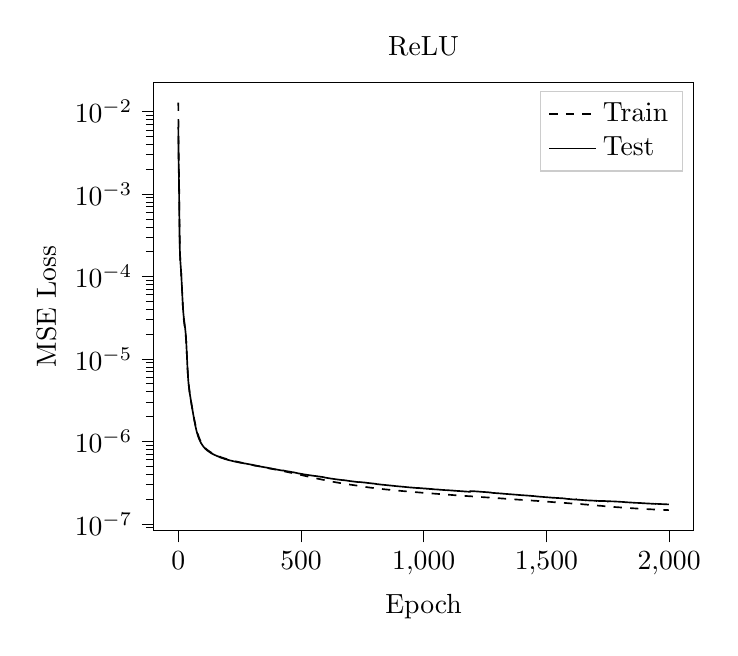
\begin{tikzpicture}

\begin{axis}[
legend cell align={left},
legend style={fill opacity=0.8, draw opacity=1, text opacity=1, draw=white!80!black},
log basis y={10},
tick align=outside,
tick pos=left,
title={ReLU},
x grid style={white!69.0196078431373!black},
xlabel={Epoch},
xmin=-99.95, xmax=2098.95,
xtick style={color=black},
y grid style={white!69.0196078431373!black},
ylabel={MSE Loss},
ymin=8.3060556203195e-08, ymax=0.0226737604172119,
ymode=log,
ytick style={color=black}
]
\addplot [semithick, black, dashed]
table {%
0 0.0128359138444066
1 0.00406811961205676
2 0.00221776218200102
3 0.00152627947740257
4 0.000869210763950832
5 0.000429490351874847
6 0.000256430144363549
7 0.000193489259458147
8 0.000159836590173654
9 0.000142019945189531
10 0.000129007256793557
11 0.000117138518267893
12 0.000105471455033694
13 9.37827313246089e-05
14 8.22589103336213e-05
15 7.13029772959999e-05
16 6.1415624084475e-05
17 5.3027559290058e-05
18 4.6298477172968e-05
19 4.10176366149244e-05
20 3.64308621828968e-05
21 3.31020509165683e-05
22 3.06825488805771e-05
23 2.8784052267838e-05
24 2.71935984428637e-05
25 2.57768373439831e-05
26 2.44650239310431e-05
27 2.31985326854556e-05
28 2.19409173314489e-05
29 2.06712553372199e-05
30 1.93696360001923e-05
31 1.80376509060807e-05
32 1.64094494193705e-05
33 1.45603561318239e-05
34 1.27872803000173e-05
35 1.11557179093325e-05
36 9.70921840917072e-06
37 8.46602692877241e-06
38 7.42971785643931e-06
39 6.59923705165966e-06
40 5.94965648508605e-06
41 5.44178499137615e-06
42 5.04196725398742e-06
43 4.71988363142373e-06
44 4.44941153807576e-06
45 4.21297154969125e-06
46 3.97091369615055e-06
47 3.78521997726011e-06
48 3.61609793606021e-06
49 3.45850858462882e-06
50 3.31160191757363e-06
51 3.17369637906495e-06
52 3.04450260318845e-06
53 2.92049022283436e-06
54 2.80214357240993e-06
55 2.69049423906154e-06
56 2.58622111073237e-06
57 2.48662982522774e-06
58 2.39208004813918e-06
59 2.30242519660351e-06
60 2.21742543777736e-06
61 2.13687340925617e-06
62 2.05999348276009e-06
63 1.98663157766532e-06
64 1.91840384792386e-06
65 1.85147106714112e-06
66 1.78930534508481e-06
67 1.73013427024671e-06
68 1.67454512279619e-06
69 1.62270763445349e-06
70 1.57398869492908e-06
71 1.52842072111525e-06
72 1.4852267215133e-06
73 1.44413795050014e-06
74 1.40627984944786e-06
75 1.36986447498089e-06
76 1.33475525311155e-06
77 1.30223323319001e-06
78 1.27158411430628e-06
79 1.24230728559382e-06
80 1.21496348251071e-06
81 1.1894506600072e-06
82 1.16576555632264e-06
83 1.14292291345919e-06
84 1.12203104029618e-06
85 1.10188948323753e-06
86 1.08292770786989e-06
87 1.06497326891031e-06
88 1.04840461335698e-06
89 1.03269330051603e-06
90 1.01698759053193e-06
91 1.00309512390595e-06
92 9.88916981896182e-07
93 9.75377727769455e-07
94 9.6289804420735e-07
95 9.5178445133115e-07
96 9.40547043398965e-07
97 9.29320102869724e-07
98 9.19224969607058e-07
99 9.09362678839898e-07
100 9.00760616332263e-07
101 8.91677312523598e-07
102 8.83358202798945e-07
103 8.7541410894687e-07
104 8.67818650164054e-07
105 8.60540775903473e-07
106 8.53664071399862e-07
107 8.47105686005989e-07
108 8.40799016799565e-07
109 8.34772250925653e-07
110 8.28988821496068e-07
111 8.23431996309409e-07
112 8.18056938896916e-07
113 8.12813703561233e-07
114 8.07828728369486e-07
115 8.03024243964501e-07
116 7.98377929925209e-07
117 7.93822158300372e-07
118 7.89469017917099e-07
119 7.8525374803462e-07
120 7.81149035503859e-07
121 7.77039519164191e-07
122 7.73208100383727e-07
123 7.69387711102354e-07
124 7.65666616501903e-07
125 7.61996876690318e-07
126 7.58383085326386e-07
127 7.54953229204602e-07
128 7.5161359521303e-07
129 7.48366523026789e-07
130 7.45194466219345e-07
131 7.41907941517184e-07
132 7.38387156445697e-07
133 7.35193854751515e-07
134 7.3226554457051e-07
135 7.29248398840809e-07
136 7.26341062176061e-07
137 7.23518060908646e-07
138 7.20833158993628e-07
139 7.18008437729622e-07
140 7.15079443153854e-07
141 7.12426657145215e-07
142 7.09709738089259e-07
143 7.07091793771042e-07
144 7.04633227798013e-07
145 7.02308290925657e-07
146 6.99840673831886e-07
147 6.97486854477347e-07
148 6.95209882849213e-07
149 6.92861825939417e-07
150 6.90704266872899e-07
151 6.88582144817929e-07
152 6.86111019234659e-07
153 6.84080939095111e-07
154 6.81975838517701e-07
155 6.79974541526462e-07
156 6.77959332790579e-07
157 6.76050047047738e-07
158 6.74017413103911e-07
159 6.72160598156779e-07
160 6.7017619542753e-07
161 6.68461542090881e-07
162 6.66575790489787e-07
163 6.64879856913103e-07
164 6.62985953709949e-07
165 6.6163600506286e-07
166 6.59435483271409e-07
167 6.57632066648262e-07
168 6.55575177276546e-07
169 6.54015729338653e-07
170 6.52307282223319e-07
171 6.504013251174e-07
172 6.46996461455274e-07
173 6.45045825507395e-07
174 6.43091596728596e-07
175 6.41354103819935e-07
176 6.39775814747168e-07
177 6.38218029919813e-07
178 6.36537369857138e-07
179 6.35115712441348e-07
180 6.33563209802901e-07
181 6.32300194652657e-07
182 6.30609901833168e-07
183 6.29600763673466e-07
184 6.27879526405195e-07
185 6.26514845080806e-07
186 6.25209512548963e-07
187 6.23535240336537e-07
188 6.22593528348148e-07
189 6.20840004998513e-07
190 6.19957963593265e-07
191 6.18262787398294e-07
192 6.17415837567137e-07
193 6.15776178662486e-07
194 6.14971566434974e-07
195 6.13444837298971e-07
196 6.12671803025933e-07
197 6.11204517156239e-07
198 6.10332435044825e-07
199 6.08851165878832e-07
200 6.080204561556e-07
201 6.06559192959821e-07
202 6.05760007701406e-07
203 6.04330644478068e-07
204 6.03280801200867e-07
205 6.01772887307561e-07
206 6.01124246642826e-07
207 5.99515939484263e-07
208 5.98675602759613e-07
209 5.9747211136596e-07
210 5.96390205643615e-07
211 5.95324714780077e-07
212 5.94377064487617e-07
213 5.93298088872984e-07
214 5.92175063729883e-07
215 5.91118195501394e-07
216 5.90146642139189e-07
217 5.89021899926934e-07
218 5.87992171404039e-07
219 5.87068497154064e-07
220 5.8602671730057e-07
221 5.85054058404921e-07
222 5.84006577440732e-07
223 5.82988822685593e-07
224 5.81989438828146e-07
225 5.81001877193899e-07
226 5.80024892542497e-07
227 5.79078803255584e-07
228 5.78110301987067e-07
229 5.77146334379108e-07
230 5.76185671306462e-07
231 5.75260986451553e-07
232 5.74307557812404e-07
233 5.73343675355886e-07
234 5.72410307597693e-07
235 5.71375916948114e-07
236 5.70444772321821e-07
237 5.69523908040992e-07
238 5.68677597769351e-07
239 5.67770445883298e-07
240 5.66866436670921e-07
241 5.65970691070561e-07
242 5.65123066863293e-07
243 5.64223408431985e-07
244 5.63306641481631e-07
245 5.6239256639401e-07
246 5.61538256064864e-07
247 5.606653090382e-07
248 5.59801215572975e-07
249 5.58943027954228e-07
250 5.58119654584743e-07
251 5.57285070087232e-07
252 5.5639160026999e-07
253 5.55517061400224e-07
254 5.54651886858437e-07
255 5.53784663139822e-07
256 5.53118923008356e-07
257 5.52271083662959e-07
258 5.51392261499473e-07
259 5.50661146789366e-07
260 5.49797288456943e-07
261 5.48924100115755e-07
262 5.48088413736991e-07
263 5.47227847107479e-07
264 5.46406514317255e-07
265 5.45611903149279e-07
266 5.44801076742374e-07
267 5.43925651868449e-07
268 5.43103572738346e-07
269 5.42293245572978e-07
270 5.4148437953927e-07
271 5.40699907702447e-07
272 5.39910273388955e-07
273 5.39133814939419e-07
274 5.38363875776326e-07
275 5.37582890757449e-07
276 5.36826901495147e-07
277 5.3603802076907e-07
278 5.35316970584177e-07
279 5.34529481910795e-07
280 5.33722675925219e-07
281 5.32918683234129e-07
282 5.32152425847698e-07
283 5.31394477121694e-07
284 5.30640270071103e-07
285 5.29907005429209e-07
286 5.29116395270535e-07
287 5.28346645850775e-07
288 5.27513266220581e-07
289 5.26773149360338e-07
290 5.26038264595741e-07
291 5.25316868134951e-07
292 5.24571295159149e-07
293 5.23829740870951e-07
294 5.23106379560545e-07
295 5.22383499131251e-07
296 5.2166716473323e-07
297 5.20962232855027e-07
298 5.20257276349412e-07
299 5.19555759524337e-07
300 5.18861061692633e-07
301 5.18167190975305e-07
302 5.17407352376154e-07
303 5.16758486270419e-07
304 5.16134349624053e-07
305 5.15409096962571e-07
306 5.1471261633651e-07
307 5.13997151728063e-07
308 5.13282595179021e-07
309 5.12469787608438e-07
310 5.11740900790869e-07
311 5.10916394645733e-07
312 5.10398340495044e-07
313 5.09615481561809e-07
314 5.0890788187985e-07
315 5.08135385487662e-07
316 5.07396071839139e-07
317 5.0667694905826e-07
318 5.06027933980135e-07
319 5.05363481877907e-07
320 5.04778821508012e-07
321 5.04100044608435e-07
322 5.03420945790367e-07
323 5.02913110352665e-07
324 5.02204066606282e-07
325 5.01519381444382e-07
326 5.0075652430337e-07
327 5.00041955618258e-07
328 4.99340976446661e-07
329 4.98837331861068e-07
330 4.98114730092425e-07
331 4.97396278106521e-07
332 4.96683979335444e-07
333 4.95992166946735e-07
334 4.95327224157904e-07
335 4.94672618728487e-07
336 4.94005201645109e-07
337 4.93368763699209e-07
338 4.92711109188804e-07
339 4.92064750176269e-07
340 4.91377320216202e-07
341 4.90734373599366e-07
342 4.90094236084815e-07
343 4.8923520419919e-07
344 4.88491250393963e-07
345 4.87911429033261e-07
346 4.86993086525445e-07
347 4.86201224958904e-07
348 4.85454121516682e-07
349 4.84715875060715e-07
350 4.83999491038389e-07
351 4.8330461555679e-07
352 4.82610435923903e-07
353 4.81942027434457e-07
354 4.81273281664585e-07
355 4.80657552941466e-07
356 4.79991086152154e-07
357 4.79426202517175e-07
358 4.78786983705959e-07
359 4.78136694752607e-07
360 4.77479370928791e-07
361 4.76951999701214e-07
362 4.76438385987876e-07
363 4.75759972076162e-07
364 4.75071433612584e-07
365 4.74538327580376e-07
366 4.73795507247132e-07
367 4.73118962915464e-07
368 4.72461489309239e-07
369 4.71825251139535e-07
370 4.71192496632966e-07
371 4.70559365041368e-07
372 4.70058532613393e-07
373 4.69410172783569e-07
374 4.68776403550919e-07
375 4.67982378282272e-07
376 4.67325791433382e-07
377 4.66681011914716e-07
378 4.66014211454535e-07
379 4.65348282233435e-07
380 4.64814711989447e-07
381 4.64148458462432e-07
382 4.63576862159698e-07
383 4.62930432362896e-07
384 4.62302280809013e-07
385 4.61679847362006e-07
386 4.61104624704944e-07
387 4.60824521880454e-07
388 4.60142321898616e-07
389 4.59398271928535e-07
390 4.58787464964416e-07
391 4.58134393070964e-07
392 4.57507636880905e-07
393 4.56882881110232e-07
394 4.5631434277027e-07
395 4.55657936043963e-07
396 4.54997403451785e-07
397 4.54597877237006e-07
398 4.53956164321312e-07
399 4.53263333653808e-07
400 4.52610636330064e-07
401 4.51975337526278e-07
402 4.51166000871694e-07
403 4.50556313722927e-07
404 4.49943631167571e-07
405 4.50224415246225e-07
406 4.49388958884356e-07
407 4.48679926989826e-07
408 4.47983747477565e-07
409 4.47319951319969e-07
410 4.46692041819574e-07
411 4.46043008082597e-07
412 4.45379412937541e-07
413 4.44756290605142e-07
414 4.44137515501097e-07
415 4.43530492361788e-07
416 4.42895292664502e-07
417 4.42246661634726e-07
418 4.4161888378369e-07
419 4.41050250699959e-07
420 4.4041967524322e-07
421 4.39794044325481e-07
422 4.39187426295007e-07
423 4.38575338435498e-07
424 4.37924559278713e-07
425 4.37397801690054e-07
426 4.36789211121891e-07
427 4.36235071774149e-07
428 4.35714181989511e-07
429 4.35064805230923e-07
430 4.3441796375987e-07
431 4.33821461186312e-07
432 4.33212344105982e-07
433 4.3256776783096e-07
434 4.31979589833986e-07
435 4.31346918034592e-07
436 4.30742508925164e-07
437 4.30014452831529e-07
438 4.29212309612126e-07
439 4.28535380322614e-07
440 4.2784484142544e-07
441 4.27162711716278e-07
442 4.2654244050766e-07
443 4.25920634356203e-07
444 4.25289486614133e-07
445 4.24664052573576e-07
446 4.24054528849638e-07
447 4.23444578245835e-07
448 4.22825500720592e-07
449 4.22235647633329e-07
450 4.21641495776726e-07
451 4.21042936622484e-07
452 4.204042555358e-07
453 4.19785291612129e-07
454 4.19165474724537e-07
455 4.18587373061996e-07
456 4.17983689530388e-07
457 4.17366091724602e-07
458 4.16813378095071e-07
459 4.16216044001771e-07
460 4.1563661304167e-07
461 4.15065193166697e-07
462 4.14440477527478e-07
463 4.137947071996e-07
464 4.13075351730186e-07
465 4.12454505095639e-07
466 4.11876993922533e-07
467 4.1130139980794e-07
468 4.10712745221531e-07
469 4.10157508312636e-07
470 4.09618700686565e-07
471 4.0901640734603e-07
472 4.08388660346759e-07
473 4.07808872111559e-07
474 4.07190228571608e-07
475 4.06595403376286e-07
476 4.06010637888698e-07
477 4.05392317176734e-07
478 4.04781765979578e-07
479 4.04163714279093e-07
480 4.03598776060221e-07
481 4.03019477431599e-07
482 4.0240480798559e-07
483 4.0181467062439e-07
484 4.01190572162591e-07
485 4.00669628959349e-07
486 4.00093216029518e-07
487 3.99534549217151e-07
488 3.98832486453671e-07
489 3.98232996289494e-07
490 3.97586432200114e-07
491 3.96999277043619e-07
492 3.96335612961707e-07
493 3.95738804854773e-07
494 3.95199794851919e-07
495 3.94601066957989e-07
496 3.93942960840832e-07
497 3.9341726065345e-07
498 3.92822267642146e-07
499 3.92249883688578e-07
500 3.9166239578492e-07
501 3.90943145731626e-07
502 3.90417924037934e-07
503 3.89788243779776e-07
504 3.89221085768554e-07
505 3.88712462026319e-07
506 3.88139190917514e-07
507 3.87384185444262e-07
508 3.8658280821835e-07
509 3.85974133635614e-07
510 3.85345149737759e-07
511 3.84755621880117e-07
512 3.84093485990888e-07
513 3.83513560478832e-07
514 3.82928092875545e-07
515 3.82343274367258e-07
516 3.81772343004627e-07
517 3.81215974144311e-07
518 3.80635759938741e-07
519 3.80127739830982e-07
520 3.79530231583658e-07
521 3.78973119623538e-07
522 3.78421440586862e-07
523 3.77808645694699e-07
524 3.77222886726258e-07
525 3.76684518130332e-07
526 3.76060851081661e-07
527 3.75412971578726e-07
528 3.74828130603078e-07
529 3.74236345834333e-07
530 3.73695037055199e-07
531 3.73073411736868e-07
532 3.72465256930354e-07
533 3.71768114604265e-07
534 3.71223410738253e-07
535 3.70558538918431e-07
536 3.69985989095767e-07
537 3.69416098607189e-07
538 3.68824209559193e-07
539 3.68246500883629e-07
540 3.67674652096639e-07
541 3.67146909241001e-07
542 3.6655390564988e-07
543 3.65992903496704e-07
544 3.65448769613863e-07
545 3.64904883639383e-07
546 3.64338433428202e-07
547 3.63806817304635e-07
548 3.63257377458126e-07
549 3.62574539664706e-07
550 3.62068634359503e-07
551 3.61473358509556e-07
552 3.60935242895266e-07
553 3.60413636357748e-07
554 3.59868972850563e-07
555 3.5935385152186e-07
556 3.58844249333856e-07
557 3.58326943697307e-07
558 3.57797470698529e-07
559 3.57330856189719e-07
560 3.56872281628284e-07
561 3.56368487672398e-07
562 3.55836359986483e-07
563 3.55332234633465e-07
564 3.54824446645807e-07
565 3.54339146753091e-07
566 3.53827280022756e-07
567 3.53325290390671e-07
568 3.52850746850208e-07
569 3.52336466477254e-07
570 3.51856831954933e-07
571 3.5136100875377e-07
572 3.50893734022861e-07
573 3.50407004418685e-07
574 3.4989447030398e-07
575 3.49443885625078e-07
576 3.4893881971243e-07
577 3.48500343307023e-07
578 3.4798630669286e-07
579 3.47510213757118e-07
580 3.47052929782876e-07
581 3.46572929046829e-07
582 3.46100820763695e-07
583 3.45635644279696e-07
584 3.45174572856877e-07
585 3.44720079127114e-07
586 3.44251229549286e-07
587 3.43796819834097e-07
588 3.43215964477395e-07
589 3.42688052199946e-07
590 3.42216255234007e-07
591 3.41808416024492e-07
592 3.41212007285208e-07
593 3.40706088309162e-07
594 3.40231385706602e-07
595 3.3973816373134e-07
596 3.39256642760688e-07
597 3.38761948015076e-07
598 3.38252847200238e-07
599 3.37764319738199e-07
600 3.37289797997187e-07
601 3.36832910235785e-07
602 3.36301321624433e-07
603 3.35731551629692e-07
604 3.35256483978696e-07
605 3.34784972508828e-07
606 3.34324919933238e-07
607 3.33847983526425e-07
608 3.33368957925018e-07
609 3.32913002822011e-07
610 3.32462384264431e-07
611 3.31984051385348e-07
612 3.31562530178076e-07
613 3.31118336518443e-07
614 3.30674347267745e-07
615 3.30218415513173e-07
616 3.29806052974391e-07
617 3.29311662270015e-07
618 3.28869587505665e-07
619 3.28467940903465e-07
620 3.27985743709291e-07
621 3.27568215709562e-07
622 3.27144061799345e-07
623 3.26670766185089e-07
624 3.26214176098461e-07
625 3.25802174742762e-07
626 3.25410245523017e-07
627 3.24975043511699e-07
628 3.24551212329993e-07
629 3.24158174407785e-07
630 3.23716544528452e-07
631 3.23299862060367e-07
632 3.22898985729125e-07
633 3.22488403895704e-07
634 3.22097345872407e-07
635 3.21700158878002e-07
636 3.21304454558913e-07
637 3.20912313469535e-07
638 3.20524564074276e-07
639 3.20136042191166e-07
640 3.19752844077925e-07
641 3.19376165165863e-07
642 3.18992066596024e-07
643 3.18628257616638e-07
644 3.18242471507801e-07
645 3.17883358164295e-07
646 3.17517607541617e-07
647 3.17189173131283e-07
648 3.16752779781382e-07
649 3.16441293151115e-07
650 3.15991993588227e-07
651 3.15567727056987e-07
652 3.15198235242065e-07
653 3.14852366315677e-07
654 3.14477423572157e-07
655 3.14116288961941e-07
656 3.13751376125992e-07
657 3.13407868560489e-07
658 3.13042362492411e-07
659 3.1268381887628e-07
660 3.12334496982203e-07
661 3.11969507151844e-07
662 3.1163067758655e-07
663 3.11306783956411e-07
664 3.10919280082089e-07
665 3.10583744706605e-07
666 3.10250059655459e-07
667 3.09937706305163e-07
668 3.09573450948619e-07
669 3.09204214246961e-07
670 3.08850459617815e-07
671 3.08537095591532e-07
672 3.08225946909602e-07
673 3.07908969560344e-07
674 3.07560297102327e-07
675 3.0723168808322e-07
676 3.06905842663241e-07
677 3.06626207304816e-07
678 3.06256743982658e-07
679 3.05940740773281e-07
680 3.05711705024692e-07
681 3.05346728438849e-07
682 3.05022357409257e-07
683 3.04787608797596e-07
684 3.04591078773342e-07
685 3.04243192218223e-07
686 3.03902760222741e-07
687 3.03562333655805e-07
688 3.03246627694875e-07
689 3.02922987273746e-07
690 3.02614198247397e-07
691 3.02081464738535e-07
692 3.01742485603995e-07
693 3.01437276149841e-07
694 3.01078963033774e-07
695 3.00749295163882e-07
696 3.00478578765251e-07
697 3.00096437030106e-07
698 2.99800604125267e-07
699 2.99512212393438e-07
700 2.99188646494031e-07
701 2.98825807448111e-07
702 2.98531001078572e-07
703 2.98287063074554e-07
704 2.98012047025509e-07
705 2.97674375701717e-07
706 2.97391246348866e-07
707 2.97087627117776e-07
708 2.96822007285868e-07
709 2.96534653557501e-07
710 2.96241515030715e-07
711 2.95766508685347e-07
712 2.95477427869173e-07
713 2.95199973777471e-07
714 2.94934526451129e-07
715 2.94622614532614e-07
716 2.94349123265647e-07
717 2.94059612983233e-07
718 2.93763836197059e-07
719 2.93480562305604e-07
720 2.93202444495932e-07
721 2.92916106459984e-07
722 2.92623508840961e-07
723 2.92435868473717e-07
724 2.92131600772905e-07
725 2.91845484383657e-07
726 2.91578852696261e-07
727 2.91303842161028e-07
728 2.91009091881733e-07
729 2.90722125015463e-07
730 2.90455377040644e-07
731 2.90185338116089e-07
732 2.8992908158898e-07
733 2.89663138232754e-07
734 2.8940803167643e-07
735 2.89136017798342e-07
736 2.889206294725e-07
737 2.88737842566888e-07
738 2.88997667908575e-07
739 2.88562024607586e-07
740 2.88228037263139e-07
741 2.87892525449251e-07
742 2.87586055392808e-07
743 2.8728029188585e-07
744 2.86980700195727e-07
745 2.86744340243672e-07
746 2.8622192211003e-07
747 2.85925212054394e-07
748 2.85634268323065e-07
749 2.85337112515549e-07
750 2.8511037254475e-07
751 2.84853912376093e-07
752 2.84023656476506e-07
753 2.83497718470471e-07
754 2.83116851676368e-07
755 2.82695359175023e-07
756 2.82512347510533e-07
757 2.82085629521589e-07
758 2.81725797435683e-07
759 2.81449778896103e-07
760 2.8105877230189e-07
761 2.80944373514558e-07
762 2.80682355423778e-07
763 2.80297662115458e-07
764 2.79940790193223e-07
765 2.79655734573225e-07
766 2.7931117253388e-07
767 2.78977283855397e-07
768 2.78635521198112e-07
769 2.78352544214044e-07
770 2.7819338988877e-07
771 2.77889544165078e-07
772 2.77548593075494e-07
773 2.77264688477885e-07
774 2.7704935030215e-07
775 2.76729705390721e-07
776 2.7645308894364e-07
777 2.76195476729413e-07
778 2.7594944073428e-07
779 2.75716891124489e-07
780 2.75467336976476e-07
781 2.75225335968798e-07
782 2.75062229206924e-07
783 2.7480055271667e-07
784 2.74580447268136e-07
785 2.74362289260921e-07
786 2.74111401481036e-07
787 2.73876008265006e-07
788 2.73605013845213e-07
789 2.73413644165998e-07
790 2.73188405444103e-07
791 2.72918508599673e-07
792 2.72716296422004e-07
793 2.72480284039034e-07
794 2.72285307730158e-07
795 2.72149884011696e-07
796 2.71952939314701e-07
797 2.71704815986595e-07
798 2.71441972643061e-07
799 2.71195177930395e-07
800 2.7097320317182e-07
801 2.70770428784317e-07
802 2.70505914016894e-07
803 2.70232581939922e-07
804 2.69978283682804e-07
805 2.69613692850612e-07
806 2.6923754116126e-07
807 2.68977236729029e-07
808 2.68752260268457e-07
809 2.68544625768641e-07
810 2.68373911282538e-07
811 2.68163501999652e-07
812 2.67927181553773e-07
813 2.67719987007808e-07
814 2.67517097881864e-07
815 2.67310931533871e-07
816 2.67105253826116e-07
817 2.66903428638443e-07
818 2.66692599950602e-07
819 2.66481964402487e-07
820 2.66284019161844e-07
821 2.66081862648093e-07
822 2.66027550424042e-07
823 2.65821824157797e-07
824 2.65619061863731e-07
825 2.65410844818348e-07
826 2.65213099211792e-07
827 2.65021856961312e-07
828 2.64826372728066e-07
829 2.64633269267733e-07
830 2.64446708726496e-07
831 2.64248240071652e-07
832 2.64059634162095e-07
833 2.63878327388056e-07
834 2.63682958788536e-07
835 2.63493734607323e-07
836 2.63316504145905e-07
837 2.63118264641093e-07
838 2.62901429465501e-07
839 2.62730751714457e-07
840 2.62452709399952e-07
841 2.62270763101924e-07
842 2.62094237520216e-07
843 2.61916025223741e-07
844 2.61752447649144e-07
845 2.61570247680254e-07
846 2.61391405729228e-07
847 2.61197685773595e-07
848 2.61104773478849e-07
849 2.60918261439258e-07
850 2.60724515214861e-07
851 2.60535269994477e-07
852 2.60345671463824e-07
853 2.60163190716867e-07
854 2.59979377318587e-07
855 2.59807215748253e-07
856 2.59638242802396e-07
857 2.59457045409306e-07
858 2.5929549951087e-07
859 2.59103974563857e-07
860 2.58932327128036e-07
861 2.58767719678588e-07
862 2.58579918060775e-07
863 2.58410764914174e-07
864 2.58235526878536e-07
865 2.58068606832751e-07
866 2.579093218813e-07
867 2.5772559851589e-07
868 2.5755975129016e-07
869 2.57416757627027e-07
870 2.57236482134715e-07
871 2.57065044301896e-07
872 2.56887864409805e-07
873 2.56699708664598e-07
874 2.56526549620162e-07
875 2.56373737975935e-07
876 2.56201032037495e-07
877 2.56034790240278e-07
878 2.55873794714034e-07
879 2.55705920480409e-07
880 2.55417128485647e-07
881 2.55229956422909e-07
882 2.55085984754544e-07
883 2.54928232898521e-07
884 2.54779993753118e-07
885 2.54592056549541e-07
886 2.54439689939545e-07
887 2.5426591516009e-07
888 2.54102271377121e-07
889 2.53930725016005e-07
890 2.53764556227054e-07
891 2.53614336365615e-07
892 2.53452076336202e-07
893 2.532692485957e-07
894 2.53125733742365e-07
895 2.52976690667595e-07
896 2.528093443388e-07
897 2.52656056844103e-07
898 2.52499306505172e-07
899 2.52364507723257e-07
900 2.52203973225562e-07
901 2.52031071774184e-07
902 2.518835791534e-07
903 2.51714416926063e-07
904 2.51555577612805e-07
905 2.51338153084646e-07
906 2.51199765898491e-07
907 2.51049156986483e-07
908 2.50885086643393e-07
909 2.50740681572381e-07
910 2.50585756418786e-07
911 2.50420220616832e-07
912 2.50275292266622e-07
913 2.50121281410998e-07
914 2.4995576485054e-07
915 2.49676279501898e-07
916 2.49520305203532e-07
917 2.49378198027728e-07
918 2.4922392374549e-07
919 2.49076048127961e-07
920 2.48927619701078e-07
921 2.48776921417004e-07
922 2.48630119202176e-07
923 2.48482846032516e-07
924 2.48332861993106e-07
925 2.48184320888356e-07
926 2.48036973083288e-07
927 2.47890264816419e-07
928 2.4774389887483e-07
929 2.47597746444228e-07
930 2.47460814819078e-07
931 2.47319833690085e-07
932 2.47171875763286e-07
933 2.46986154522233e-07
934 2.46846625991282e-07
935 2.46710934568739e-07
936 2.46565559500311e-07
937 2.46414631448033e-07
938 2.46274233148824e-07
939 2.46133543761573e-07
940 2.45993646721843e-07
941 2.45851855076751e-07
942 2.4571178909838e-07
943 2.45570187580313e-07
944 2.45427655464425e-07
945 2.4528916037525e-07
946 2.45144313090862e-07
947 2.45008457774531e-07
948 2.44778515678945e-07
949 2.44709522988273e-07
950 2.44557021623848e-07
951 2.44444680092215e-07
952 2.44300696401467e-07
953 2.44156826106234e-07
954 2.44018879300256e-07
955 2.43875476478195e-07
956 2.43733082527342e-07
957 2.43594031232419e-07
958 2.43454059834391e-07
959 2.43317650365782e-07
960 2.43178574322656e-07
961 2.43043392202935e-07
962 2.42901336989121e-07
963 2.42752515198674e-07
964 2.42617944856249e-07
965 2.42478849045824e-07
966 2.42350840103711e-07
967 2.42212682998399e-07
968 2.42075261638774e-07
969 2.41937336305398e-07
970 2.41740744577612e-07
971 2.41667918423616e-07
972 2.41518041917743e-07
973 2.41401504226246e-07
974 2.41222875168035e-07
975 2.41124690397498e-07
976 2.40940309865323e-07
977 2.40789396293906e-07
978 2.40686851775251e-07
979 2.4058535476712e-07
980 2.40380043535993e-07
981 2.40305805455421e-07
982 2.40108319552235e-07
983 2.40031877538627e-07
984 2.39894949039865e-07
985 2.3973578581149e-07
986 2.39611460926881e-07
987 2.39439004758424e-07
988 2.3930055066046e-07
989 2.39153940320591e-07
990 2.38980053701709e-07
991 2.38914729784767e-07
992 2.38757834530645e-07
993 2.38612148095285e-07
994 2.3841948619463e-07
995 2.38344357995857e-07
996 2.38203236882839e-07
997 2.38060229719395e-07
998 2.37923468709766e-07
999 2.37793798923747e-07
1000 2.37646189845009e-07
1001 2.37599634857588e-07
1002 2.37371781985019e-07
1003 2.37256684719966e-07
1004 2.3710381680786e-07
1005 2.37030779430825e-07
1006 2.36854548504084e-07
1007 2.36789443157193e-07
1008 2.36603149716075e-07
1009 2.36586189146237e-07
1010 2.36392693182097e-07
1011 2.36260623339035e-07
1012 2.36101812092215e-07
1013 2.36086071886632e-07
1014 2.35904035029932e-07
1015 2.35725191885194e-07
1016 2.35685808050334e-07
1017 2.35596702900409e-07
1018 2.35438702382851e-07
1019 2.35246950623491e-07
1020 2.35075611456637e-07
1021 2.35099903790115e-07
1022 2.3487148752821e-07
1023 2.34750061487432e-07
1024 2.34573643794533e-07
1025 2.34564620235744e-07
1026 2.34471072538156e-07
1027 2.34354624211619e-07
1028 2.34128390850685e-07
1029 2.33955763171423e-07
1030 2.33922607776549e-07
1031 2.33783959046718e-07
1032 2.33714321531409e-07
1033 2.33685208733903e-07
1034 2.33539281111916e-07
1035 2.33392913706609e-07
1036 2.33203155495687e-07
1037 2.331949610479e-07
1038 2.32991934915106e-07
1039 2.32850305849297e-07
1040 2.32765783117372e-07
1041 2.32670341915764e-07
1042 2.32657039475725e-07
1043 2.32462914603104e-07
1044 2.32303914394549e-07
1045 2.32177753510143e-07
1046 2.32038218555886e-07
1047 2.31941964251803e-07
1048 2.31735411837519e-07
1049 2.3166942881403e-07
1050 2.31621027936058e-07
1051 2.31475059614183e-07
1052 2.31326241298291e-07
1053 2.31239147751694e-07
1054 2.31119690745629e-07
1055 2.31017140592371e-07
1056 2.3086940776551e-07
1057 2.30697620096976e-07
1058 2.30660508172775e-07
1059 2.30563432516817e-07
1060 2.30397781528779e-07
1061 2.30417078178391e-07
1062 2.30317154283455e-07
1063 2.30162277986778e-07
1064 2.30063518721124e-07
1065 2.29899269129419e-07
1066 2.29807306638463e-07
1067 2.29664271131469e-07
1068 2.29567998907498e-07
1069 2.29445193149047e-07
1070 2.29313082712679e-07
1071 2.29218835350764e-07
1072 2.2906969297054e-07
1073 2.28964648627539e-07
1074 2.28864435037224e-07
1075 2.28717713547155e-07
1076 2.2863567138387e-07
1077 2.28499026974305e-07
1078 2.28409063225854e-07
1079 2.28298539020955e-07
1080 2.28191649313203e-07
1081 2.28083222189923e-07
1082 2.27955539990887e-07
1083 2.27841008324958e-07
1084 2.2773020606337e-07
1085 2.27610032744963e-07
1086 2.27501331949043e-07
1087 2.27376409974056e-07
1088 2.2726379945226e-07
1089 2.27137682820455e-07
1090 2.26827840933197e-07
1091 2.26754384584638e-07
1092 2.26650240975346e-07
1093 2.26534615457297e-07
1094 2.26412695525369e-07
1095 2.26291264908696e-07
1096 2.26169796015085e-07
1097 2.26040921411652e-07
1098 2.25922023474823e-07
1099 2.25797209253642e-07
1100 2.25675585596719e-07
1101 2.25561426347554e-07
1102 2.254305840097e-07
1103 2.25311821019147e-07
1104 2.25195945944279e-07
1105 2.25079520305371e-07
1106 2.24965323099013e-07
1107 2.24867464545753e-07
1108 2.24762359117392e-07
1109 2.24626370084025e-07
1110 2.24508406084567e-07
1111 2.24395075314021e-07
1112 2.24277390778127e-07
1113 2.24158637927019e-07
1114 2.2404539223686e-07
1115 2.23920358827456e-07
1116 2.23808280111371e-07
1117 2.23686827183656e-07
1118 2.2356966128001e-07
1119 2.23456709292691e-07
1120 2.23334162825495e-07
1121 2.23228413595677e-07
1122 2.23115099544202e-07
1123 2.23002317440546e-07
1124 2.22879026416933e-07
1125 2.22769490122232e-07
1126 2.22664080226309e-07
1127 2.2253616578638e-07
1128 2.22430343903568e-07
1129 2.223116337845e-07
1130 2.22204481723054e-07
1131 2.22094232434245e-07
1132 2.21976963509007e-07
1133 2.21866377820845e-07
1134 2.21753350238885e-07
1135 2.21644285254285e-07
1136 2.21531433545863e-07
1137 2.21416343521241e-07
1138 2.21307805006177e-07
1139 2.21198763370012e-07
1140 2.21085268165666e-07
1141 2.20975650925936e-07
1142 2.20881519460647e-07
1143 2.20775239149873e-07
1144 2.20637945012925e-07
1145 2.20559710285784e-07
1146 2.20444337422521e-07
1147 2.20324321794863e-07
1148 2.20211126375602e-07
1149 2.201148186316e-07
1150 2.19997589574916e-07
1151 2.1989982777626e-07
1152 2.19791165335437e-07
1153 2.196815010862e-07
1154 2.19573701976117e-07
1155 2.19463932438657e-07
1156 2.19359349159731e-07
1157 2.19249752198891e-07
1158 2.19142922851745e-07
1159 2.19035697959669e-07
1160 2.18929460672257e-07
1161 2.18930828516761e-07
1162 2.18828259697545e-07
1163 2.18708604258211e-07
1164 2.18593607570483e-07
1165 2.18480611941629e-07
1166 2.1837456065299e-07
1167 2.18264942468238e-07
1168 2.18158639007981e-07
1169 2.18042133006691e-07
1170 2.17949583657173e-07
1171 2.17841640782979e-07
1172 2.17736934885693e-07
1173 2.17629174635192e-07
1174 2.17524212679621e-07
1175 2.1741689277377e-07
1176 2.1731769705724e-07
1177 2.17213480382839e-07
1178 2.1710752405113e-07
1179 2.17002218498408e-07
1180 2.16897231283042e-07
1181 2.16794168977685e-07
1182 2.16689441295159e-07
1183 2.16586816598863e-07
1184 2.16482968788512e-07
1185 2.1638173421934e-07
1186 2.16274073231659e-07
1187 2.16172590953079e-07
1188 2.16080631012971e-07
1189 2.1599227943625e-07
1190 2.15979764696783e-07
1191 2.16017678475566e-07
1192 2.15873939545475e-07
1193 2.15748003292049e-07
1194 2.15623455886771e-07
1195 2.15515344123673e-07
1196 2.15400620767525e-07
1197 2.15292371208875e-07
1198 2.15177959709933e-07
1199 2.15071723104643e-07
1200 2.14928613999632e-07
1201 2.14839535118472e-07
1202 2.14735765474927e-07
1203 2.14574807344547e-07
1204 2.14502365381009e-07
1205 2.14412341868808e-07
1206 2.14283540159954e-07
1207 2.14210046642904e-07
1208 2.14107812681164e-07
1209 2.14021252809005e-07
1210 2.13936210762711e-07
1211 2.13915925698416e-07
1212 2.13799923876934e-07
1213 2.13669566456076e-07
1214 2.13561179556621e-07
1215 2.13467269645662e-07
1216 2.13349683882313e-07
1217 2.13256108388293e-07
1218 2.13155513392849e-07
1219 2.13042389802354e-07
1220 2.12919297460701e-07
1221 2.12815673890532e-07
1222 2.12711443602132e-07
1223 2.12652658127865e-07
1224 2.12501022431866e-07
1225 2.12420601719998e-07
1226 2.12309944174649e-07
1227 2.12366951096499e-07
1228 2.12222830079156e-07
1229 2.12110472261884e-07
1230 2.11929635618446e-07
1231 2.11879924854941e-07
1232 2.11703791869411e-07
1233 2.11653654140775e-07
1234 2.1151320120083e-07
1235 2.11419449257733e-07
1236 2.11250796276374e-07
1237 2.11202558560331e-07
1238 2.11102061150825e-07
1239 2.10944673966651e-07
1240 2.10911240309031e-07
1241 2.1076127746511e-07
1242 2.10704322974209e-07
1243 2.10567815479123e-07
1244 2.10497195574533e-07
1245 2.1040943553885e-07
1246 2.10297608973065e-07
1247 2.10163938255903e-07
1248 2.10107044765095e-07
1249 2.10013232752715e-07
1250 2.09916546062061e-07
1251 2.09774376543237e-07
1252 2.09698891929122e-07
1253 2.09622506929463e-07
1254 2.09513595876842e-07
1255 2.09421121070363e-07
1256 2.09320254114687e-07
1257 2.09215731480583e-07
1258 2.09130282691206e-07
1259 2.09036870700174e-07
1260 2.08928067813474e-07
1261 2.08838153490376e-07
1262 2.08749056248791e-07
1263 2.08652356469941e-07
1264 2.08550158639298e-07
1265 2.08489736223783e-07
1266 2.0837612094482e-07
1267 2.08276492024595e-07
1268 2.08193774028587e-07
1269 2.08094111279422e-07
1270 2.07980286397458e-07
1271 2.07888382796284e-07
1272 2.07787530371206e-07
1273 2.07656961599412e-07
1274 2.07569616925696e-07
1275 2.0746449245479e-07
1276 2.07364236295859e-07
1277 2.07165836712875e-07
1278 2.07041992617007e-07
1279 2.06997534185405e-07
1280 2.06897416155982e-07
1281 2.06792438376624e-07
1282 2.06619498243299e-07
1283 2.06613423934243e-07
1284 2.06489881819039e-07
1285 2.0638760765479e-07
1286 2.06301932017539e-07
1287 2.06185098910794e-07
1288 2.06122904430117e-07
1289 2.0603094798588e-07
1290 2.05890058659008e-07
1291 2.058426851832e-07
1292 2.05701655730195e-07
1293 2.05651675621255e-07
1294 2.05522865172725e-07
1295 2.05462758223973e-07
1296 2.05339187992593e-07
1297 2.05216017839405e-07
1298 2.05128365635687e-07
1299 2.05095285075174e-07
1300 2.04930593312724e-07
1301 2.04907038209967e-07
1302 2.04736265757788e-07
1303 2.0472843108621e-07
1304 2.04564254225659e-07
1305 2.04535793123739e-07
1306 2.04411864075382e-07
1307 2.04340191245933e-07
1308 2.04220152618007e-07
1309 2.04110330066953e-07
1310 2.04035512098244e-07
1311 2.03963682523067e-07
1312 2.03857806447161e-07
1313 2.03766906793135e-07
1314 2.03600763406087e-07
1315 2.03567661820614e-07
1316 2.03439885275714e-07
1317 2.0336518320363e-07
1318 2.032757020487e-07
1319 2.03217184783e-07
1320 2.03097577866629e-07
1321 2.03010853205399e-07
1322 2.02895738659947e-07
1323 2.02795099845332e-07
1324 2.02704501582218e-07
1325 2.02589735827985e-07
1326 2.02511892204882e-07
1327 2.02408412725674e-07
1328 2.02272598507136e-07
1329 2.0214227660631e-07
1330 2.02043033908694e-07
1331 2.01940268901524e-07
1332 2.01830009295634e-07
1333 2.01788452855567e-07
1334 2.01665288990682e-07
1335 2.01558977146021e-07
1336 2.01502488479832e-07
1337 2.01370287101099e-07
1338 2.01262453124684e-07
1339 2.01164852363434e-07
1340 2.01063925814537e-07
1341 2.00968840445626e-07
1342 2.00907314329868e-07
1343 2.00762776536578e-07
1344 2.00683564941073e-07
1345 2.00600544012275e-07
1346 2.00489199613685e-07
1347 2.00247139510168e-07
1348 2.0018000638089e-07
1349 2.00085132711081e-07
1350 1.99985089430754e-07
1351 1.99909750492111e-07
1352 1.99793285268868e-07
1353 1.99699068950565e-07
1354 1.99619168668619e-07
1355 1.99508070835464e-07
1356 1.99424367018253e-07
1357 1.99339445082103e-07
1358 1.99232693923079e-07
1359 1.99150643993562e-07
1360 1.99041314644433e-07
1361 1.9894423559208e-07
1362 1.98858898443177e-07
1363 1.98747527939247e-07
1364 1.98649745641433e-07
1365 1.98597096414233e-07
1366 1.98485464387943e-07
1367 1.9839009510747e-07
1368 1.98303617892748e-07
1369 1.98163553932318e-07
1370 1.98024752101844e-07
1371 1.9802462633578e-07
1372 1.97904007080751e-07
1373 1.97792426241961e-07
1374 1.97700932204725e-07
1375 1.97582478129732e-07
1376 1.97496014543219e-07
1377 1.97442480079246e-07
1378 1.97292501994184e-07
1379 1.97215899994774e-07
1380 1.97129082785352e-07
1381 1.97047096150982e-07
1382 1.96931914999254e-07
1383 1.96866535979723e-07
1384 1.96748979227834e-07
1385 1.96670395652632e-07
1386 1.96537504265848e-07
1387 1.96472592328689e-07
1388 1.96395970554875e-07
1389 1.96314325215496e-07
1390 1.96160989446525e-07
1391 1.96098936960709e-07
1392 1.95963414675759e-07
1393 1.95923781213025e-07
1394 1.9576923853748e-07
1395 1.95750483491963e-07
1396 1.95624758973167e-07
1397 1.95513828309402e-07
1398 1.95484114023259e-07
1399 1.95305951599778e-07
1400 1.95257116345715e-07
1401 1.95148459923189e-07
1402 1.95140374209757e-07
1403 1.95018690270388e-07
1404 1.94886642852055e-07
1405 1.94786378692413e-07
1406 1.94772436103108e-07
1407 1.94666272740562e-07
1408 1.94536682762703e-07
1409 1.94470198458419e-07
1410 1.94301135245212e-07
1411 1.94241530216743e-07
1412 1.94114599068484e-07
1413 1.94071764546777e-07
1414 1.93994561087152e-07
1415 1.93910387515928e-07
1416 1.93826246174922e-07
1417 1.93731067383851e-07
1418 1.93607339234347e-07
1419 1.93542343367881e-07
1420 1.9343740844846e-07
1421 1.93307958880951e-07
1422 1.93212855663205e-07
1423 1.9319500296433e-07
1424 1.93057864024127e-07
1425 1.93003795104119e-07
1426 1.92875757235811e-07
1427 1.92799762956497e-07
1428 1.92709066794805e-07
1429 1.92629986820236e-07
1430 1.92562667393759e-07
1431 1.92412457487023e-07
1432 1.923164970421e-07
1433 1.92212994384988e-07
1434 1.92117591787166e-07
1435 1.92054836240629e-07
1436 1.92077585573713e-07
1437 1.91970624435101e-07
1438 1.91855633147497e-07
1439 1.91738552040022e-07
1440 1.91556437243889e-07
1441 1.91566779371044e-07
1442 1.91436991002547e-07
1443 1.91359781638312e-07
1444 1.91402773523919e-07
1445 1.91267241291371e-07
1446 1.9109486520108e-07
1447 1.91051301001721e-07
1448 1.90914974176337e-07
1449 1.90833660269618e-07
1450 1.90732240533009e-07
1451 1.90663927462253e-07
1452 1.90549957004293e-07
1453 1.90516927240481e-07
1454 1.90568535209934e-07
1455 1.90464090856324e-07
1456 1.90173839605734e-07
1457 1.90063078804314e-07
1458 1.90166451851326e-07
1459 1.90337836649235e-07
1460 1.90102733085951e-07
1461 1.8997548833255e-07
1462 1.89736554936815e-07
1463 1.89701801993181e-07
1464 1.8942595669813e-07
1465 1.89337171434545e-07
1466 1.89209052699368e-07
1467 1.89201453991927e-07
1468 1.89235038845936e-07
1469 1.89176961463033e-07
1470 1.89062633360493e-07
1471 1.88726122743788e-07
1472 1.88520785847857e-07
1473 1.88483920233296e-07
1474 1.88584162799543e-07
1475 1.88440573332116e-07
1476 1.88324926952532e-07
1477 1.88138743801858e-07
1478 1.88068955395693e-07
1479 1.87984317840062e-07
1480 1.87901757342956e-07
1481 1.87818820784003e-07
1482 1.87700506828037e-07
1483 1.87608113890292e-07
1484 1.87492924730748e-07
1485 1.87428510905363e-07
1486 1.87290235636794e-07
1487 1.87174033406734e-07
1488 1.87133109839976e-07
1489 1.87034921630413e-07
1490 1.869156221872e-07
1491 1.86841360779511e-07
1492 1.8674610426217e-07
1493 1.86595499855002e-07
1494 1.86553659844435e-07
1495 1.86493911478181e-07
1496 1.86416946007739e-07
1497 1.86296508395856e-07
1498 1.86166682489386e-07
1499 1.86078907816523e-07
1500 1.86015773657289e-07
1501 1.85825831604092e-07
1502 1.85825445324639e-07
1503 1.85684167831823e-07
1504 1.85587365621132e-07
1505 1.85490155043766e-07
1506 1.85387809050752e-07
1507 1.85506818294101e-07
1508 1.8523384703073e-07
1509 1.8512932789605e-07
1510 1.85180206297986e-07
1511 1.85073922537526e-07
1512 1.84784265595539e-07
1513 1.84762588588683e-07
1514 1.84722550354621e-07
1515 1.84722854314145e-07
1516 1.84608482754811e-07
1517 1.84497961175367e-07
1518 1.84283791814011e-07
1519 1.84272560396437e-07
1520 1.84135793610096e-07
1521 1.84033592578459e-07
1522 1.84048242370949e-07
1523 1.83967336507607e-07
1524 1.8385791097586e-07
1525 1.83641185415695e-07
1526 1.83645582097824e-07
1527 1.8345900540595e-07
1528 1.83271602207213e-07
1529 1.83229706767207e-07
1530 1.83120381933577e-07
1531 1.83038489470988e-07
1532 1.82943788910705e-07
1533 1.82854249139552e-07
1534 1.82773967178917e-07
1535 1.82671281830693e-07
1536 1.82594469396946e-07
1537 1.82508408336446e-07
1538 1.8241637240024e-07
1539 1.82331063928842e-07
1540 1.82253040314606e-07
1541 1.82172478201181e-07
1542 1.82081318040872e-07
1543 1.82019926551646e-07
1544 1.81898912313017e-07
1545 1.81815222621395e-07
1546 1.81717994770736e-07
1547 1.81656746146786e-07
1548 1.815659457165e-07
1549 1.81482440197556e-07
1550 1.8138441754445e-07
1551 1.81304563863449e-07
1552 1.81201391050934e-07
1553 1.81129328897356e-07
1554 1.81034935845759e-07
1555 1.80947744606641e-07
1556 1.80862695771111e-07
1557 1.80781546855968e-07
1558 1.80693251888187e-07
1559 1.80612085397769e-07
1560 1.8051754842574e-07
1561 1.80419520710018e-07
1562 1.80338503565025e-07
1563 1.80254624066123e-07
1564 1.80166220882683e-07
1565 1.80088632188102e-07
1566 1.79999537561315e-07
1567 1.79914991818464e-07
1568 1.79831375287876e-07
1569 1.79772628811747e-07
1570 1.79695855489825e-07
1571 1.797683110496e-07
1572 1.79628363483175e-07
1573 1.79521931102045e-07
1574 1.79416115059894e-07
1575 1.79326383364042e-07
1576 1.79233732449546e-07
1577 1.79364324434772e-07
1578 1.7920843399466e-07
1579 1.79101645159108e-07
1580 1.79067521376197e-07
1581 1.78786476329407e-07
1582 1.7864905528242e-07
1583 1.78560145069895e-07
1584 1.7845236886771e-07
1585 1.78381288517215e-07
1586 1.78225616949135e-07
1587 1.7809800933577e-07
1588 1.77997463115531e-07
1589 1.77908634462653e-07
1590 1.77799642514742e-07
1591 1.77725845347254e-07
1592 1.77621988203924e-07
1593 1.77522572204936e-07
1594 1.77425779209983e-07
1595 1.77345446545019e-07
1596 1.77246504204476e-07
1597 1.77162125165609e-07
1598 1.77126693021279e-07
1599 1.77039962043324e-07
1600 1.76945302332143e-07
1601 1.76798856788452e-07
1602 1.76757221268531e-07
1603 1.76640067959255e-07
1604 1.76549131886361e-07
1605 1.76487131035685e-07
1606 1.76355807383288e-07
1607 1.76286366560419e-07
1608 1.76199101208141e-07
1609 1.7617098620093e-07
1610 1.76181355957539e-07
1611 1.76023837550332e-07
1612 1.75891392864003e-07
1613 1.75862118886982e-07
1614 1.75763471094825e-07
1615 1.75658744620222e-07
1616 1.75569463838343e-07
1617 1.75476478826653e-07
1618 1.75374262902039e-07
1619 1.75281168001362e-07
1620 1.752016230121e-07
1621 1.75147430166334e-07
1622 1.75087873643065e-07
1623 1.74926214178583e-07
1624 1.74842742698189e-07
1625 1.7474993768829e-07
1626 1.7467174815522e-07
1627 1.74606110519449e-07
1628 1.74521788775195e-07
1629 1.74443121270684e-07
1630 1.74332275253875e-07
1631 1.7425133555804e-07
1632 1.7430235797633e-07
1633 1.741116781524e-07
1634 1.74107517612043e-07
1635 1.73982584207977e-07
1636 1.73896979514865e-07
1637 1.73802615240248e-07
1638 1.73797129807696e-07
1639 1.73731923258202e-07
1640 1.73893235064781e-07
1641 1.73686825618802e-07
1642 1.73525504948202e-07
1643 1.73359765110348e-07
1644 1.73256072930172e-07
1645 1.73106126212019e-07
1646 1.72992834134078e-07
1647 1.72905510407162e-07
1648 1.72758155784436e-07
1649 1.72686506456188e-07
1650 1.72595628253447e-07
1651 1.72471590754952e-07
1652 1.72378223616931e-07
1653 1.72282607859842e-07
1654 1.7218538852859e-07
1655 1.72069122772456e-07
1656 1.71979364427699e-07
1657 1.71895662571586e-07
1658 1.71826570426248e-07
1659 1.71747736469996e-07
1660 1.7174569888212e-07
1661 1.71488148911436e-07
1662 1.71442944530753e-07
1663 1.71323688828551e-07
1664 1.71137896327167e-07
1665 1.71078423299775e-07
1666 1.70864678519678e-07
1667 1.70784733779072e-07
1668 1.70676396059832e-07
1669 1.70580150165023e-07
1670 1.70518457206725e-07
1671 1.7030397762241e-07
1672 1.70289471665086e-07
1673 1.70181144511616e-07
1674 1.70051729433851e-07
1675 1.69932089956859e-07
1676 1.69835248637895e-07
1677 1.69735653269498e-07
1678 1.69637645214493e-07
1679 1.695416831069e-07
1680 1.69446881994162e-07
1681 1.69307020247089e-07
1682 1.69257444937898e-07
1683 1.69145445028107e-07
1684 1.69037297666819e-07
1685 1.68935638274803e-07
1686 1.68840347548382e-07
1687 1.68741589806842e-07
1688 1.68649730095893e-07
1689 1.68570992961747e-07
1690 1.68468791819976e-07
1691 1.68340344295359e-07
1692 1.68227439861113e-07
1693 1.68171379964832e-07
1694 1.68044360744801e-07
1695 1.67948880267943e-07
1696 1.67849305110934e-07
1697 1.67796028861744e-07
1698 1.67669656576663e-07
1699 1.67506564853426e-07
1700 1.67421118408839e-07
1701 1.67348270881718e-07
1702 1.67197969037858e-07
1703 1.67109167385604e-07
1704 1.67024937574922e-07
1705 1.66914884022873e-07
1706 1.66826745665816e-07
1707 1.66717948157924e-07
1708 1.6664129679711e-07
1709 1.66537951020729e-07
1710 1.66460380601308e-07
1711 1.66342920124407e-07
1712 1.66259729009965e-07
1713 1.66152653328311e-07
1714 1.66074226623181e-07
1715 1.65983786544643e-07
1716 1.65923250534661e-07
1717 1.65876918050145e-07
1718 1.65786256378198e-07
1719 1.65771145535842e-07
1720 1.65534165812886e-07
1721 1.65445726551638e-07
1722 1.6535419255348e-07
1723 1.65320799034419e-07
1724 1.65234023306482e-07
1725 1.65133367872272e-07
1726 1.65026439116644e-07
1727 1.64921270759066e-07
1728 1.64737785226521e-07
1729 1.64614237501581e-07
1730 1.64499778392724e-07
1731 1.64373849205646e-07
1732 1.64277211581521e-07
1733 1.64163428753028e-07
1734 1.64141522279948e-07
1735 1.64010026903583e-07
1736 1.63911323532773e-07
1737 1.63752241224557e-07
1738 1.63664354776216e-07
1739 1.63553990070397e-07
1740 1.63501872439298e-07
1741 1.63345211760202e-07
1742 1.63252137674874e-07
1743 1.63158584108203e-07
1744 1.63062312594775e-07
1745 1.62980642624433e-07
1746 1.62881990245722e-07
1747 1.62764671141957e-07
1748 1.62735897909272e-07
1749 1.62743215710748e-07
1750 1.62667735274624e-07
1751 1.62394495951901e-07
1752 1.62336140792974e-07
1753 1.62228798490816e-07
1754 1.6218012770608e-07
1755 1.62060676313303e-07
1756 1.61983046815806e-07
1757 1.61902563927896e-07
1758 1.61821125015393e-07
1759 1.61715724594558e-07
1760 1.61636504181217e-07
1761 1.61494904414639e-07
1762 1.61409865636841e-07
1763 1.61367755183051e-07
1764 1.61247274011345e-07
1765 1.61161492638229e-07
1766 1.61019437513232e-07
1767 1.6091400385676e-07
1768 1.60856869744208e-07
1769 1.60734758164693e-07
1770 1.60611896394158e-07
1771 1.60627610068076e-07
1772 1.60522108441086e-07
1773 1.60445036950563e-07
1774 1.60351745400078e-07
1775 1.60273962087842e-07
1776 1.60172230405209e-07
1777 1.60064920077474e-07
1778 1.5999882325346e-07
1779 1.59905462581378e-07
1780 1.59827533554591e-07
1781 1.59751060746061e-07
1782 1.59677807200609e-07
1783 1.59575680648061e-07
1784 1.59502947887802e-07
1785 1.59444537214171e-07
1786 1.59363117237632e-07
1787 1.59288557664894e-07
1788 1.59209515274483e-07
1789 1.5915325531779e-07
1790 1.59079477516144e-07
1791 1.58982288983367e-07
1792 1.58911462833089e-07
1793 1.5884727043769e-07
1794 1.58755989843939e-07
1795 1.58712159837648e-07
1796 1.58604146189845e-07
1797 1.58508355742271e-07
1798 1.58460156633566e-07
1799 1.58368373096351e-07
1800 1.58299598354006e-07
1801 1.58223666034019e-07
1802 1.58154789648535e-07
1803 1.58083816678811e-07
1804 1.57996099222402e-07
1805 1.57949268345448e-07
1806 1.57839321580866e-07
1807 1.57783955611279e-07
1808 1.57759403293767e-07
1809 1.57651618987842e-07
1810 1.575498865094e-07
1811 1.57496855599959e-07
1812 1.57528436833587e-07
1813 1.57435538802986e-07
1814 1.57333671783277e-07
1815 1.57237810327615e-07
1816 1.57193176264059e-07
1817 1.57031325802137e-07
1818 1.57052098099797e-07
1819 1.57046822433671e-07
1820 1.56956337409753e-07
1821 1.56827768048373e-07
1822 1.56745090915678e-07
1823 1.56647371419183e-07
1824 1.56542435934881e-07
1825 1.56480074668508e-07
1826 1.56400183506378e-07
1827 1.56337775276683e-07
1828 1.56232751724161e-07
1829 1.56154168816869e-07
1830 1.56089407717275e-07
1831 1.55997599165403e-07
1832 1.55904430467757e-07
1833 1.55851775808458e-07
1834 1.55763781375384e-07
1835 1.55694770452186e-07
1836 1.55616971582617e-07
1837 1.55581121063619e-07
1838 1.55454964087198e-07
1839 1.55404410371318e-07
1840 1.55318537501614e-07
1841 1.55288714395851e-07
1842 1.55151620710114e-07
1843 1.55103544045687e-07
1844 1.55068185073048e-07
1845 1.54977300923065e-07
1846 1.54868190385571e-07
1847 1.54825424431237e-07
1848 1.54758045134429e-07
1849 1.54744705241683e-07
1850 1.54614288348398e-07
1851 1.54544138993629e-07
1852 1.54479559178355e-07
1853 1.54404414175247e-07
1854 1.54342997070955e-07
1855 1.5428760282532e-07
1856 1.54201014964883e-07
1857 1.54123448410814e-07
1858 1.54090727871647e-07
1859 1.54044537271858e-07
1860 1.539228547216e-07
1861 1.53931152990339e-07
1862 1.53802891496468e-07
1863 1.53719886576198e-07
1864 1.53677313434741e-07
1865 1.5358469660498e-07
1866 1.53520563884513e-07
1867 1.53471616854972e-07
1868 1.53401832129418e-07
1869 1.53343847564713e-07
1870 1.5328681514859e-07
1871 1.53222242744278e-07
1872 1.53157038916163e-07
1873 1.53111676141293e-07
1874 1.53029555043815e-07
1875 1.53004602047702e-07
1876 1.52909405635171e-07
1877 1.52850507021185e-07
1878 1.52811087026805e-07
1879 1.5275673168702e-07
1880 1.52676621674175e-07
1881 1.52647077307222e-07
1882 1.52569348642828e-07
1883 1.52511503046071e-07
1884 1.52468581184451e-07
1885 1.52403492549524e-07
1886 1.5234241648443e-07
1887 1.52217876980387e-07
1888 1.52094331056674e-07
1889 1.52029483402316e-07
1890 1.51960717410304e-07
1891 1.5187282134832e-07
1892 1.51911613215816e-07
1893 1.51817272495691e-07
1894 1.51766614557403e-07
1895 1.51732358574463e-07
1896 1.5165685984897e-07
1897 1.51627947708732e-07
1898 1.51545418198396e-07
1899 1.51520836716657e-07
1900 1.51451246921397e-07
1901 1.51395362934181e-07
1902 1.51348387269934e-07
1903 1.51268595097065e-07
1904 1.5120452111006e-07
1905 1.51169382036187e-07
1906 1.51103784112649e-07
1907 1.51044598418082e-07
1908 1.51018405084358e-07
1909 1.51041962787701e-07
1910 1.50900222230632e-07
1911 1.50880171524648e-07
1912 1.50817092993805e-07
1913 1.50739076076434e-07
1914 1.50678753360722e-07
1915 1.50634063814437e-07
1916 1.5058357517006e-07
1917 1.50501685290294e-07
1918 1.50448526927249e-07
1919 1.50425620482508e-07
1920 1.50338848769138e-07
1921 1.503019331075e-07
1922 1.50252006310581e-07
1923 1.50187818043435e-07
1924 1.50153225593641e-07
1925 1.5010258494641e-07
1926 1.50047371072048e-07
1927 1.49961112519748e-07
1928 1.49910327859715e-07
1929 1.49878553571625e-07
1930 1.49823820812855e-07
1931 1.49790155603569e-07
1932 1.49719627110301e-07
1933 1.49704523586536e-07
1934 1.49607693529674e-07
1935 1.49583198620462e-07
1936 1.49505978548348e-07
1937 1.49470088118164e-07
1938 1.49432007894745e-07
1939 1.49421523552462e-07
1940 1.49326274225814e-07
1941 1.49305111563081e-07
1942 1.49224658095193e-07
1943 1.49195440293681e-07
1944 1.49123903113946e-07
1945 1.49083860137011e-07
1946 1.49059537712049e-07
1947 1.48942056192425e-07
1948 1.48941483821829e-07
1949 1.48896023858924e-07
1950 1.4885284529953e-07
1951 1.48801204026938e-07
1952 1.48759271013432e-07
1953 1.48684755139072e-07
1954 1.48665575714801e-07
1955 1.4860701104169e-07
1956 1.48553323597866e-07
1957 1.48552121103762e-07
1958 1.48453234388057e-07
1959 1.48427528422701e-07
1960 1.48408495121544e-07
1961 1.48326779381591e-07
1962 1.48285125447956e-07
1963 1.48244456426028e-07
1964 1.48195953521224e-07
1965 1.48189535366328e-07
1966 1.48109432785759e-07
1967 1.48052879062277e-07
1968 1.48024707996797e-07
1969 1.47997790421073e-07
1970 1.47904027087975e-07
1971 1.47876789277746e-07
1972 1.4786100889097e-07
1973 1.47789058004832e-07
1974 1.4773308079441e-07
1975 1.47752809155577e-07
1976 1.47666736388885e-07
1977 1.47635688172443e-07
1978 1.47605759622138e-07
1979 1.47551667645018e-07
1980 1.47522877412598e-07
1981 1.4745904378799e-07
1982 1.47431089402517e-07
1983 1.4737679597232e-07
1984 1.4733839267933e-07
1985 1.47295567870742e-07
1986 1.47252448648771e-07
1987 1.47203221480652e-07
1988 1.47192870308288e-07
1989 1.47120890538588e-07
1990 1.47047456344751e-07
1991 1.47072093078293e-07
1992 1.47008562045414e-07
1993 1.46976112617381e-07
1994 1.46960199259638e-07
1995 1.4686862554214e-07
1996 1.46845908432169e-07
1997 1.46810996753288e-07
1998 1.46780940745828e-07
1999 1.46720769109265e-07
};
\addlegendentry{Train}
\addplot [semithick, black]
table {%
0 0.00647992361336946
1 0.00275873416103423
2 0.00188174087088555
3 0.00117344572208822
4 0.000592645083088428
5 0.000317291240207851
6 0.000227275144425221
7 0.000181339491973631
8 0.000157831877004355
9 0.000142893317388371
10 0.000130225642351434
11 0.000118030919111334
12 0.000105853396235034
13 9.37121731112711e-05
14 8.19401393528096e-05
15 7.09642772562802e-05
16 6.1417231336236e-05
17 5.3500996727962e-05
18 4.7313304094132e-05
19 4.21098775404971e-05
20 3.78091572201811e-05
21 3.48391731677111e-05
22 3.25767432514112e-05
23 3.07158588839229e-05
24 2.90796615445288e-05
25 2.75721122307004e-05
26 2.61331933870679e-05
27 2.47068674070761e-05
28 2.32767888519447e-05
29 2.18223067349754e-05
30 2.03266517928569e-05
31 1.87816858669976e-05
32 1.66299814736703e-05
33 1.45725834954646e-05
34 1.26569420899614e-05
35 1.09238480945351e-05
36 9.43226496019633e-06
37 8.17488398752175e-06
38 7.16606473361026e-06
39 6.37652965451707e-06
40 5.76686034037266e-06
41 5.29552880834672e-06
42 4.92539356855559e-06
43 4.62945945400861e-06
44 4.37881953985197e-06
45 4.14164833273389e-06
46 3.94124390368233e-06
47 3.76778029931302e-06
48 3.60893591278e-06
49 3.45800458489975e-06
50 3.31396017827501e-06
51 3.17843864650058e-06
52 3.0467526812572e-06
53 2.92171080218395e-06
54 2.80228528026782e-06
55 2.68869530373195e-06
56 2.57923875324195e-06
57 2.47981120082841e-06
58 2.38270399677276e-06
59 2.28887211051187e-06
60 2.19880439544795e-06
61 2.11214342016319e-06
62 2.03080162464175e-06
63 1.95668530977855e-06
64 1.88582021110051e-06
65 1.81066786808515e-06
66 1.75200250396301e-06
67 1.68371445852245e-06
68 1.62537548931141e-06
69 1.57134979872353e-06
70 1.5213254300761e-06
71 1.47601110711548e-06
72 1.43146485243051e-06
73 1.38869029342459e-06
74 1.35100549414346e-06
75 1.31433500882849e-06
76 1.28234410112782e-06
77 1.25157612274052e-06
78 1.22225299037382e-06
79 1.19514447760594e-06
80 1.16937837901787e-06
81 1.14659212613333e-06
82 1.12443171929044e-06
83 1.10220446458698e-06
84 1.08517156149901e-06
85 1.06582456282922e-06
86 1.05063497812807e-06
87 1.03281922747556e-06
88 1.02080855413078e-06
89 1.0038424989034e-06
90 9.92517129816406e-07
91 9.77362219600764e-07
92 9.63055072134011e-07
93 9.49802824834478e-07
94 9.4211844725578e-07
95 9.33274634462578e-07
96 9.19464412163506e-07
97 9.09788070657669e-07
98 9.00649354207417e-07
99 8.95756784302648e-07
100 8.83566144693759e-07
101 8.75556565915758e-07
102 8.67840697083011e-07
103 8.60440252381522e-07
104 8.53238987019722e-07
105 8.46460523007408e-07
106 8.39913866457209e-07
107 8.33664046240301e-07
108 8.27652684165514e-07
109 8.21860396627017e-07
110 8.1624818903947e-07
111 8.10785195426433e-07
112 8.05469312581408e-07
113 8.00114435151045e-07
114 7.9525710816597e-07
115 7.90449178111885e-07
116 7.85788017765299e-07
117 7.81374581038108e-07
118 7.77021170961234e-07
119 7.7280100185817e-07
120 7.68574068388261e-07
121 7.64700587296829e-07
122 7.61443857300037e-07
123 7.5774477181767e-07
124 7.54036705075123e-07
125 7.49264870592015e-07
126 7.45678960356599e-07
127 7.42218787763704e-07
128 7.38858204840653e-07
129 7.35579362753924e-07
130 7.32372370748635e-07
131 7.29389398657077e-07
132 7.26550808849424e-07
133 7.23270034086454e-07
134 7.20057187209022e-07
135 7.16813246981474e-07
136 7.14395525847067e-07
137 7.11541531472903e-07
138 7.09265634668554e-07
139 7.06167782027478e-07
140 7.04373405824299e-07
141 7.01687611126545e-07
142 6.99553083904902e-07
143 6.96974780112214e-07
144 6.94890331942588e-07
145 6.9240331868059e-07
146 6.89854118718358e-07
147 6.87832823587087e-07
148 6.85380712184269e-07
149 6.83281882629672e-07
150 6.81103301758412e-07
151 6.78973208323441e-07
152 6.76423326240183e-07
153 6.745882501491e-07
154 6.72317469252448e-07
155 6.7031049866273e-07
156 6.68329846575944e-07
157 6.66417633965466e-07
158 6.64228821278812e-07
159 6.62932279738015e-07
160 6.60772911942331e-07
161 6.59357397125859e-07
162 6.57284829230775e-07
163 6.55655128412036e-07
164 6.55043891129026e-07
165 6.52142944090883e-07
166 6.48952891424415e-07
167 6.47747640414309e-07
168 6.45363854800962e-07
169 6.43925034182757e-07
170 6.42646114101808e-07
171 6.3796210270084e-07
172 6.37155039839854e-07
173 6.3598065480619e-07
174 6.34600041848898e-07
175 6.33545027994842e-07
176 6.3235256675398e-07
177 6.31271689144342e-07
178 6.29491069048527e-07
179 6.28331008556415e-07
180 6.26627183919481e-07
181 6.25431141543231e-07
182 6.23407231614692e-07
183 6.22775417014054e-07
184 6.20640435045061e-07
185 6.18793478679436e-07
186 6.17599482666265e-07
187 6.15176929841255e-07
188 6.14711495927622e-07
189 6.12394899235369e-07
190 6.12028657087649e-07
191 6.09814321705926e-07
192 6.09297899245576e-07
193 6.07525748819171e-07
194 6.06863864049956e-07
195 6.05442380674504e-07
196 6.04156809913547e-07
197 6.02669445015636e-07
198 6.01729539084772e-07
199 6.00315274823515e-07
200 5.9944431995973e-07
201 5.98058875311835e-07
202 5.97245673361613e-07
203 5.95913434153772e-07
204 5.94900541273091e-07
205 5.93126458170445e-07
206 5.92600997606496e-07
207 5.91029390761832e-07
208 5.90667127653433e-07
209 5.89509170367819e-07
210 5.88391799283272e-07
211 5.87313252253807e-07
212 5.86141595704248e-07
213 5.85252507789846e-07
214 5.84368478939723e-07
215 5.84476708809234e-07
216 5.82699385631713e-07
217 5.81900906126975e-07
218 5.81033020807808e-07
219 5.80074981826328e-07
220 5.79143375034619e-07
221 5.78050787680695e-07
222 5.7706506595423e-07
223 5.76102138438728e-07
224 5.75150409076741e-07
225 5.74207319914422e-07
226 5.73276508930576e-07
227 5.72417263811076e-07
228 5.71457121623098e-07
229 5.70614361095068e-07
230 5.69728968002892e-07
231 5.68879954698787e-07
232 5.68020823266124e-07
233 5.67145377772249e-07
234 5.66815913316532e-07
235 5.66031133075739e-07
236 5.65242487482465e-07
237 5.64442984796187e-07
238 5.63549122034601e-07
239 5.62705167794775e-07
240 5.61877186555648e-07
241 5.61062904580467e-07
242 5.6016659755187e-07
243 5.59332875127438e-07
244 5.58453223220567e-07
245 5.57633143216663e-07
246 5.56851659894164e-07
247 5.56070517632179e-07
248 5.55300175619777e-07
249 5.54531823127036e-07
250 5.53735617359052e-07
251 5.52979372514528e-07
252 5.52441917989199e-07
253 5.51953348804091e-07
254 5.51372977497522e-07
255 5.50718709746434e-07
256 5.50136348920205e-07
257 5.49554954432097e-07
258 5.489220598065e-07
259 5.48125399291166e-07
260 5.47365800684929e-07
261 5.4668316806783e-07
262 5.4597757070951e-07
263 5.45314890132431e-07
264 5.4466130450237e-07
265 5.4401760962719e-07
266 5.43381702300394e-07
267 5.42655754998123e-07
268 5.419902322501e-07
269 5.41216650162823e-07
270 5.40548967364884e-07
271 5.39889697392937e-07
272 5.39238556029886e-07
273 5.38600602340011e-07
274 5.37940422873362e-07
275 5.3729581850348e-07
276 5.37134098976821e-07
277 5.36419065610971e-07
278 5.35610070073744e-07
279 5.34779417193931e-07
280 5.34001117102889e-07
281 5.33263914803683e-07
282 5.32572357769823e-07
283 5.3188489346212e-07
284 5.3119731546758e-07
285 5.306723664944e-07
286 5.29982685293362e-07
287 5.29330975496123e-07
288 5.2867795830025e-07
289 5.28012890299578e-07
290 5.27352995050023e-07
291 5.26916949183942e-07
292 5.26054748206661e-07
293 5.25371945059305e-07
294 5.24742176821746e-07
295 5.24067331753031e-07
296 5.23469850577385e-07
297 5.22846619332995e-07
298 5.22229584021261e-07
299 5.21621018378937e-07
300 5.21020467658673e-07
301 5.20429068728845e-07
302 5.1970329195683e-07
303 5.16197530942009e-07
304 5.15215560881188e-07
305 5.14451869548793e-07
306 5.14082330482779e-07
307 5.13382474309765e-07
308 5.12725762291666e-07
309 5.12033409449941e-07
310 5.11245843881625e-07
311 5.10538313847064e-07
312 5.0985943289561e-07
313 5.09083292854484e-07
314 5.08367406837351e-07
315 5.07602237576066e-07
316 5.06847641190689e-07
317 5.06125502397481e-07
318 5.05865955346962e-07
319 5.05648586113239e-07
320 5.05786829307908e-07
321 5.05236073422566e-07
322 5.04671731960116e-07
323 5.03796059092565e-07
324 5.0304981868976e-07
325 5.02385034906183e-07
326 5.01651470585784e-07
327 5.00980320339295e-07
328 5.00420867410867e-07
329 4.99756993121991e-07
330 4.99078907978401e-07
331 4.97832161272527e-07
332 4.97218366035668e-07
333 4.96598886456923e-07
334 4.95989866067248e-07
335 4.95432686875574e-07
336 4.94801270178868e-07
337 4.94262565098325e-07
338 4.936570121572e-07
339 4.93101254050998e-07
340 4.92589890654926e-07
341 4.92073922941927e-07
342 4.91553407755418e-07
343 4.90584852741449e-07
344 4.89880335408088e-07
345 4.89223282329476e-07
346 4.88513364871324e-07
347 4.87985232666688e-07
348 4.87389058889676e-07
349 4.8697216925575e-07
350 4.86364626794966e-07
351 4.85827342799894e-07
352 4.85342411593592e-07
353 4.84866745864565e-07
354 4.84381246224075e-07
355 4.84009206047631e-07
356 4.83386429550592e-07
357 4.82896609810268e-07
358 4.82255700262613e-07
359 4.81659583329019e-07
360 4.81110077998892e-07
361 4.80477012843039e-07
362 4.79815128073824e-07
363 4.79014772736264e-07
364 4.78276717785775e-07
365 4.77316859814891e-07
366 4.76592987297408e-07
367 4.75915612696554e-07
368 4.75235964358944e-07
369 4.74665199590163e-07
370 4.74083009294191e-07
371 4.73516223564729e-07
372 4.72812331508976e-07
373 4.72086895797474e-07
374 4.71622627173929e-07
375 4.71068261731489e-07
376 4.70503977112458e-07
377 4.69990624196726e-07
378 4.69393768298687e-07
379 4.68983103019127e-07
380 4.68527701968924e-07
381 4.67549284621782e-07
382 4.66974796609065e-07
383 4.66457890979655e-07
384 4.65866293097861e-07
385 4.65375791236511e-07
386 4.63972838815607e-07
387 4.63349380197542e-07
388 4.62595835415414e-07
389 4.6195484060263e-07
390 4.61323281797377e-07
391 4.60814874259086e-07
392 4.6068294068391e-07
393 4.60165040294669e-07
394 4.59415360865023e-07
395 4.58936199265736e-07
396 4.58379673773379e-07
397 4.58182313423094e-07
398 4.57473305459644e-07
399 4.56865876685697e-07
400 4.56246539215499e-07
401 4.55747738214995e-07
402 4.5539076154455e-07
403 4.54995273457826e-07
404 4.54548256811904e-07
405 4.535988864518e-07
406 4.53045373660643e-07
407 4.52249395266335e-07
408 4.51572674364797e-07
409 4.50914455996099e-07
410 4.50341218538597e-07
411 4.49810357849856e-07
412 4.49189030859998e-07
413 4.48667350383403e-07
414 4.48191400437281e-07
415 4.477059292185e-07
416 4.47217615828777e-07
417 4.46726829750332e-07
418 4.46241585905227e-07
419 4.4570850832315e-07
420 4.45289202843924e-07
421 4.44881408157016e-07
422 4.44409977262694e-07
423 4.43968502850112e-07
424 4.43782511183599e-07
425 4.43293686203106e-07
426 4.42809522382959e-07
427 4.42321635318876e-07
428 4.43599191157773e-07
429 4.42983946413733e-07
430 4.42414943790936e-07
431 4.41846083276687e-07
432 4.41314483623501e-07
433 4.40853568761668e-07
434 4.40322793338055e-07
435 4.39728466972156e-07
436 4.39322292322686e-07
437 4.37838792777256e-07
438 4.37144819898094e-07
439 4.36620723576198e-07
440 4.36177714391306e-07
441 4.35630227002548e-07
442 4.35316053426504e-07
443 4.34701860285713e-07
444 4.34162387819015e-07
445 4.33680668265879e-07
446 4.33171322811177e-07
447 4.32677552453242e-07
448 4.32192507560103e-07
449 4.31779653808917e-07
450 4.31257831223775e-07
451 4.30741579293681e-07
452 4.30354361924401e-07
453 4.29493212550369e-07
454 4.28975653221642e-07
455 4.28725059009594e-07
456 4.279942231733e-07
457 4.27485929321847e-07
458 4.27123183044387e-07
459 4.26553839361077e-07
460 4.26100484673952e-07
461 4.25670407366852e-07
462 4.24858882297485e-07
463 4.2434169245098e-07
464 4.23850678998861e-07
465 4.23575954755506e-07
466 4.2293106616853e-07
467 4.22396283283888e-07
468 4.21900352876037e-07
469 4.2170509573225e-07
470 4.20925999833344e-07
471 4.20277814328074e-07
472 4.19725978417773e-07
473 4.19608795709792e-07
474 4.18754893871665e-07
475 4.18285907244353e-07
476 4.17852277223574e-07
477 4.1724570110091e-07
478 4.16477860198938e-07
479 4.15841952872142e-07
480 4.15331726344448e-07
481 4.15251946606077e-07
482 4.14197188547405e-07
483 4.13500458762428e-07
484 4.12443228015036e-07
485 4.11855069160083e-07
486 4.11070175232453e-07
487 4.10398513395194e-07
488 4.09884933105786e-07
489 4.09381868848868e-07
490 4.08800644891016e-07
491 4.08351951364239e-07
492 4.0783444887893e-07
493 4.07356850473661e-07
494 4.06743254188768e-07
495 4.06307179900978e-07
496 4.05866614983097e-07
497 4.05845867135213e-07
498 4.05125092584058e-07
499 4.04659232344784e-07
500 4.04223271743831e-07
501 4.03812691729399e-07
502 4.03777477231415e-07
503 4.02991673809083e-07
504 4.02517514430656e-07
505 4.02021925083318e-07
506 4.01189424792392e-07
507 4.00594188931791e-07
508 4.00073986384086e-07
509 3.99560235564422e-07
510 3.98983615923498e-07
511 3.98496808884374e-07
512 3.97964811327256e-07
513 3.97558494569239e-07
514 3.97125631934614e-07
515 3.96729348040026e-07
516 3.96305864569513e-07
517 3.96014911530074e-07
518 3.95465121982852e-07
519 3.94961688243711e-07
520 3.94546788129446e-07
521 3.94165084571796e-07
522 3.93720569036304e-07
523 3.93308425827854e-07
524 3.92981206687182e-07
525 3.92810221683249e-07
526 3.92382048630679e-07
527 3.919788582607e-07
528 3.9156020648079e-07
529 3.91186205206395e-07
530 3.90837243458009e-07
531 3.90463043231648e-07
532 3.89904954545273e-07
533 3.89598369565647e-07
534 3.89213084872608e-07
535 3.88836298270689e-07
536 3.8850592432027e-07
537 3.88043673638094e-07
538 3.87660008982493e-07
539 3.87281318126043e-07
540 3.86930935292185e-07
541 3.86530047080669e-07
542 3.86156358445078e-07
543 3.85776246503156e-07
544 3.85435669159051e-07
545 3.85017330017945e-07
546 3.84659870178439e-07
547 3.84270919084884e-07
548 3.83895837785531e-07
549 3.83503362400006e-07
550 3.83078202048637e-07
551 3.82670833687371e-07
552 3.82330199499847e-07
553 3.8186951201169e-07
554 3.81498125534563e-07
555 3.81115086156569e-07
556 3.80834251245687e-07
557 3.80371517394451e-07
558 3.79990552801246e-07
559 3.80448767600683e-07
560 3.8001078905836e-07
561 3.79563431351926e-07
562 3.79180818299574e-07
563 3.78777173182243e-07
564 3.78463596462097e-07
565 3.78039743509362e-07
566 3.77669834961125e-07
567 3.77324823830349e-07
568 3.77033586573816e-07
569 3.7658480778191e-07
570 3.76259038148419e-07
571 3.75899304572158e-07
572 3.75653854689517e-07
573 3.75221446802243e-07
574 3.74872172415053e-07
575 3.74459403928995e-07
576 3.74151170490222e-07
577 3.73783279883355e-07
578 3.73419851484869e-07
579 3.73068587578018e-07
580 3.72706864482097e-07
581 3.7236495131765e-07
582 3.72012237903618e-07
583 3.71656597053516e-07
584 3.71357458561761e-07
585 3.7094034155416e-07
586 3.70578050024051e-07
587 3.70228548263185e-07
588 3.69778888398287e-07
589 3.694953250033e-07
590 3.68959064189767e-07
591 3.68542089290713e-07
592 3.68320570487413e-07
593 3.67892170061168e-07
594 3.65958982229131e-07
595 3.6547100989992e-07
596 3.65107382549468e-07
597 3.64629670457361e-07
598 3.64137576980283e-07
599 3.63791855306772e-07
600 3.63345122877945e-07
601 3.62909730711181e-07
602 3.62443444146265e-07
603 3.61841387075401e-07
604 3.61351823130462e-07
605 3.61040378038524e-07
606 3.60615047156898e-07
607 3.60223396000947e-07
608 3.59771007651943e-07
609 3.59462347887529e-07
610 3.59081639089709e-07
611 3.58637834096953e-07
612 3.58171007519559e-07
613 3.57846573706411e-07
614 3.57417235363755e-07
615 3.56972719828264e-07
616 3.56624752839707e-07
617 3.56239013399318e-07
618 3.55864614220991e-07
619 3.55410520569421e-07
620 3.55109904148776e-07
621 3.54729252194375e-07
622 3.54363294263749e-07
623 3.53678785813827e-07
624 3.53381693685151e-07
625 3.53024432797611e-07
626 3.52656513769034e-07
627 3.52301043449188e-07
628 3.51875144133373e-07
629 3.51611106452765e-07
630 3.51248047536501e-07
631 3.50831555806508e-07
632 3.50555239947425e-07
633 3.50229498735644e-07
634 3.49871612570496e-07
635 3.4954609873239e-07
636 3.49202196048282e-07
637 3.48809152228569e-07
638 3.48528459426234e-07
639 3.48224631352423e-07
640 3.47879762330194e-07
641 3.47557886470895e-07
642 3.47179963000599e-07
643 3.46974900367059e-07
644 3.46669480677519e-07
645 3.4642295076992e-07
646 3.46072255297258e-07
647 3.4584016361805e-07
648 3.45961012726548e-07
649 3.4556219929982e-07
650 3.45077097563262e-07
651 3.44685929576372e-07
652 3.44390372220005e-07
653 3.43967627713937e-07
654 3.43689436022032e-07
655 3.43346840736558e-07
656 3.43062083629775e-07
657 3.42714173484637e-07
658 3.42416313969807e-07
659 3.42110638484883e-07
660 3.41808004122868e-07
661 3.4150900773966e-07
662 3.41245964818881e-07
663 3.40931336495487e-07
664 3.40658914410596e-07
665 3.40377766860911e-07
666 3.40114411301329e-07
667 3.39812061156408e-07
668 3.39564167006756e-07
669 3.39223646506071e-07
670 3.38909643460283e-07
671 3.38592116122527e-07
672 3.3946119515349e-07
673 3.39062381726762e-07
674 3.38752215611748e-07
675 3.38445829584089e-07
676 3.38162095658845e-07
677 3.37852640086567e-07
678 3.37454679311122e-07
679 3.37167620045875e-07
680 3.36865241479245e-07
681 3.36576306381176e-07
682 3.36298001002433e-07
683 3.36070939965794e-07
684 3.35544569907142e-07
685 3.35347721147627e-07
686 3.34847669591909e-07
687 3.34629845610834e-07
688 3.34260278123111e-07
689 3.3388707265658e-07
690 3.33443011868439e-07
691 3.33064889446177e-07
692 3.32539059400005e-07
693 3.32261777202802e-07
694 3.31774970163679e-07
695 3.31609328441118e-07
696 3.31250419094431e-07
697 3.30804795112272e-07
698 3.30598908249158e-07
699 3.30290134797906e-07
700 3.29895954109816e-07
701 3.29649054719994e-07
702 3.29350569927556e-07
703 3.29315639646666e-07
704 3.28980206631968e-07
705 3.2867521326807e-07
706 3.28365047153056e-07
707 3.2808495120662e-07
708 3.27756850992955e-07
709 3.27466949556765e-07
710 3.27202201333421e-07
711 3.26928642380153e-07
712 3.2665187177372e-07
713 3.26379392845411e-07
714 3.26073319456555e-07
715 3.25938941614368e-07
716 3.25531374301136e-07
717 3.25367693676526e-07
718 3.25070828921525e-07
719 3.2477669265063e-07
720 3.24426594033866e-07
721 3.24219627145794e-07
722 3.23970056115286e-07
723 3.23656166756336e-07
724 3.23354640840989e-07
725 3.23074260677458e-07
726 3.22792601537003e-07
727 3.22499715821323e-07
728 3.22231215932334e-07
729 3.21967263516854e-07
730 3.21689412885462e-07
731 3.21469286745923e-07
732 3.21327092933643e-07
733 3.21148661441839e-07
734 3.20957553867629e-07
735 3.20761188277174e-07
736 3.20820618071593e-07
737 3.20714633517127e-07
738 3.21215338772163e-07
739 3.21316463214316e-07
740 3.21221392596271e-07
741 3.21049554941055e-07
742 3.20889228078158e-07
743 3.20779832918561e-07
744 3.20514942586669e-07
745 3.20333526815375e-07
746 3.19985645091947e-07
747 3.19780610880116e-07
748 3.19549229743643e-07
749 3.19267087434127e-07
750 3.1873952366368e-07
751 3.18283127853647e-07
752 3.18350771522091e-07
753 3.18421513156864e-07
754 3.18138916099997e-07
755 3.17944909511425e-07
756 3.17814254913173e-07
757 3.17641735136931e-07
758 3.17419818429698e-07
759 3.17122896831279e-07
760 3.16839987135609e-07
761 3.16572254632774e-07
762 3.16259672672459e-07
763 3.15923500693316e-07
764 3.15593240429735e-07
765 3.15267925543594e-07
766 3.14981690507921e-07
767 3.14576737991956e-07
768 3.1436948688679e-07
769 3.14252616817612e-07
770 3.1383257237394e-07
771 3.13625889702962e-07
772 3.13417956476769e-07
773 3.13013288177899e-07
774 3.12926999868068e-07
775 3.12636615262818e-07
776 3.12465147089824e-07
777 3.1228475450007e-07
778 3.12065907337455e-07
779 3.11850754997067e-07
780 3.11690627086136e-07
781 3.11289539922655e-07
782 3.11200551550428e-07
783 3.10946887793762e-07
784 3.10708372808222e-07
785 3.10411593318349e-07
786 3.10265590997005e-07
787 3.09835201051101e-07
788 3.09572612877673e-07
789 3.09344329707528e-07
790 3.08872841969787e-07
791 3.08773735469003e-07
792 3.08593655518052e-07
793 3.08405617488461e-07
794 3.08191971498673e-07
795 3.07971816937425e-07
796 3.07656165432491e-07
797 3.07392895138037e-07
798 3.07360039641935e-07
799 3.07140709310261e-07
800 3.06855213239032e-07
801 3.06608967548527e-07
802 3.06414960959955e-07
803 3.06127162730263e-07
804 3.05424521229725e-07
805 3.04830564346048e-07
806 3.04368882098061e-07
807 3.04166604792044e-07
808 3.03921751765301e-07
809 3.03689660086093e-07
810 3.03280302205167e-07
811 3.03024876302516e-07
812 3.0279613838502e-07
813 3.02609748814575e-07
814 3.02400707141715e-07
815 3.02198429835698e-07
816 3.02014115050042e-07
817 3.01780403333396e-07
818 3.01553484405304e-07
819 3.01357403031943e-07
820 3.01033395544437e-07
821 3.00813638887121e-07
822 3.00271210562641e-07
823 3.00057905633366e-07
824 2.99853468277433e-07
825 2.99635757983197e-07
826 2.99442916684711e-07
827 2.99276479154287e-07
828 2.99069853326728e-07
829 2.98857969482924e-07
830 2.98626588346451e-07
831 2.98406831689135e-07
832 2.9820702707184e-07
833 2.97999690701545e-07
834 2.97798891324419e-07
835 2.97529084036796e-07
836 2.97315267516751e-07
837 2.97300204010753e-07
838 2.97109949087826e-07
839 2.96844433478327e-07
840 2.96482056683089e-07
841 2.96276539302198e-07
842 2.96084266437902e-07
843 2.95881363854278e-07
844 2.95753238788166e-07
845 2.95545675044195e-07
846 2.95319352972001e-07
847 2.95127222216252e-07
848 2.94891435714817e-07
849 2.9464379736055e-07
850 2.94454935101385e-07
851 2.94264935973843e-07
852 2.94082582286137e-07
853 2.9388783673312e-07
854 2.93707387299946e-07
855 2.93505650006409e-07
856 2.93310847609973e-07
857 2.93131790840562e-07
858 2.92926500833346e-07
859 2.92728344675197e-07
860 2.92542949864583e-07
861 2.92337318796854e-07
862 2.9213742891443e-07
863 2.91946889774408e-07
864 2.91746545144633e-07
865 2.91561633503079e-07
866 2.91359924631251e-07
867 2.91161143195495e-07
868 2.90970575633764e-07
869 2.90730895358138e-07
870 2.90531403379646e-07
871 2.90325687046789e-07
872 2.90128980395821e-07
873 2.89931477936989e-07
874 2.89762851934938e-07
875 2.89541020492834e-07
876 2.89333684122539e-07
877 2.89140984932601e-07
878 2.88938224457524e-07
879 2.88750584331865e-07
880 2.88225493250138e-07
881 2.88043025875595e-07
882 2.87658252773326e-07
883 2.87492127881706e-07
884 2.8736369017679e-07
885 2.87261030962327e-07
886 2.87066228565891e-07
887 2.86871255639198e-07
888 2.86667784621386e-07
889 2.86502142898826e-07
890 2.86332038967885e-07
891 2.86135360738626e-07
892 2.8593311185432e-07
893 2.85718613213248e-07
894 2.85548480860598e-07
895 2.85375421071876e-07
896 2.85208869854614e-07
897 2.85027226709644e-07
898 2.84860249166741e-07
899 2.84682045048612e-07
900 2.84513731685365e-07
901 2.84343514067587e-07
902 2.8416320674296e-07
903 2.83993870198174e-07
904 2.83799977296439e-07
905 2.8362728698994e-07
906 2.83452550320362e-07
907 2.83271418766162e-07
908 2.83107198129073e-07
909 2.82927970829405e-07
910 2.82739222257078e-07
911 2.82574006860159e-07
912 2.82387020433816e-07
913 2.82197277101659e-07
914 2.82027002640461e-07
915 2.81929601442243e-07
916 2.81761231235578e-07
917 2.81536983948172e-07
918 2.81353152331576e-07
919 2.81163778481641e-07
920 2.80976536259914e-07
921 2.80790573015111e-07
922 2.80602819202613e-07
923 2.80417538078837e-07
924 2.80234644378652e-07
925 2.8004711793983e-07
926 2.79865190577766e-07
927 2.79682808468351e-07
928 2.79498692634661e-07
929 2.79318470575163e-07
930 2.7916891554014e-07
931 2.78987755564231e-07
932 2.78815093679441e-07
933 2.78578397683305e-07
934 2.78250155361093e-07
935 2.78087668448279e-07
936 2.77906025303309e-07
937 2.77768407386247e-07
938 2.77571530205023e-07
939 2.77412738114435e-07
940 2.77248261681962e-07
941 2.77083472610684e-07
942 2.76909617014098e-07
943 2.7673885938384e-07
944 2.76570546020594e-07
945 2.76391148190669e-07
946 2.76224085382637e-07
947 2.76042925406728e-07
948 2.76012997346697e-07
949 2.75892887202644e-07
950 2.75762090495846e-07
951 2.75601848898077e-07
952 2.75444733688346e-07
953 2.75277557193476e-07
954 2.75123966275714e-07
955 2.74909240260968e-07
956 2.74741836392423e-07
957 2.74557692137023e-07
958 2.74388838761297e-07
959 2.74273986633489e-07
960 2.74034221092734e-07
961 2.73855647492383e-07
962 2.73674487516473e-07
963 2.73506799430834e-07
964 2.73402946504575e-07
965 2.73249668225617e-07
966 2.73085021262887e-07
967 2.72986483196291e-07
968 2.72751407237593e-07
969 2.72580479077078e-07
970 2.72801202072515e-07
971 2.72696070169332e-07
972 2.72622145303103e-07
973 2.72478018814581e-07
974 2.724012233557e-07
975 2.72230380460314e-07
976 2.72145058488604e-07
977 2.73030110520267e-07
978 2.72841390369649e-07
979 2.71707307319957e-07
980 2.72597191042223e-07
981 2.71425818709758e-07
982 2.7230143473389e-07
983 2.71193613343712e-07
984 2.70923123935063e-07
985 2.70891149511954e-07
986 2.70667896984378e-07
987 2.70458883733227e-07
988 2.70354576059617e-07
989 2.70222642484441e-07
990 2.70927017709255e-07
991 2.70088065690288e-07
992 2.6985443923877e-07
993 2.69618169568275e-07
994 2.70360658305435e-07
995 2.69520967322023e-07
996 2.69198892510758e-07
997 2.6904959327112e-07
998 2.69021768417588e-07
999 2.68774385858706e-07
1000 2.68630060418218e-07
1001 2.6863193625104e-07
1002 2.683385673663e-07
1003 2.68160363248171e-07
1004 2.68812243575667e-07
1005 2.6785056661538e-07
1006 2.68489912969017e-07
1007 2.67585704705198e-07
1008 2.68151580939957e-07
1009 2.6733562208392e-07
1010 2.67094065975471e-07
1011 2.66891788669454e-07
1012 2.67558874611495e-07
1013 2.66808370952276e-07
1014 2.66507612423084e-07
1015 2.67064535819372e-07
1016 2.67060755732018e-07
1017 2.6623183657648e-07
1018 2.66081002564533e-07
1019 2.65734769300252e-07
1020 2.66437098161987e-07
1021 2.65452854364412e-07
1022 2.65339480165494e-07
1023 2.65114437070224e-07
1024 2.65910131247438e-07
1025 2.65536812094069e-07
1026 2.6536312702774e-07
1027 2.64641727198978e-07
1028 2.64482167722235e-07
1029 2.65120746689718e-07
1030 2.6532669039625e-07
1031 2.65128051069041e-07
1032 2.64817487050095e-07
1033 2.64724519638548e-07
1034 2.63434429825793e-07
1035 2.63291980218128e-07
1036 2.63828297875079e-07
1037 2.63086548102365e-07
1038 2.63663764599187e-07
1039 2.63603567418613e-07
1040 2.63490022689439e-07
1041 2.63322675664313e-07
1042 2.63060883298749e-07
1043 2.62101139014703e-07
1044 2.61887066699273e-07
1045 2.6178395273746e-07
1046 2.61508120047438e-07
1047 2.61896900610736e-07
1048 2.61955676705838e-07
1049 2.62028549968818e-07
1050 2.61794752987043e-07
1051 2.61786254895924e-07
1052 2.61663103628962e-07
1053 2.61433001469413e-07
1054 2.61168821680258e-07
1055 2.6032890332317e-07
1056 2.6007145947915e-07
1057 2.60591036749247e-07
1058 2.6047811729768e-07
1059 2.60438497434734e-07
1060 2.60446540778503e-07
1061 2.6018471999123e-07
1062 2.60017259279266e-07
1063 2.59977724681448e-07
1064 2.59734179053339e-07
1065 2.59658719414801e-07
1066 2.59460023244173e-07
1067 2.59366544241857e-07
1068 2.59094974808249e-07
1069 2.58980492162664e-07
1070 2.58755079585171e-07
1071 2.58688515941685e-07
1072 2.5850613383227e-07
1073 2.58284273968457e-07
1074 2.58268926245364e-07
1075 2.58134349451211e-07
1076 2.58002984310224e-07
1077 2.57987551322003e-07
1078 2.57788258295477e-07
1079 2.57674685144593e-07
1080 2.57543661064119e-07
1081 2.57488835586628e-07
1082 2.57293294225747e-07
1083 2.57154482596889e-07
1084 2.57041222084808e-07
1085 2.56886693250635e-07
1086 2.56806288234657e-07
1087 2.5660352775958e-07
1088 2.56457610703364e-07
1089 2.5610205511839e-07
1090 2.56362795880705e-07
1091 2.56346027072141e-07
1092 2.5635753786446e-07
1093 2.56288501532254e-07
1094 2.56210256566192e-07
1095 2.56169357726321e-07
1096 2.56006217114191e-07
1097 2.55873658261407e-07
1098 2.55765144174802e-07
1099 2.55659216463755e-07
1100 2.55479420729898e-07
1101 2.55357861078664e-07
1102 2.55212938782279e-07
1103 2.55113775438076e-07
1104 2.55006881388908e-07
1105 2.54867018156801e-07
1106 2.54857951631493e-07
1107 2.54744236372062e-07
1108 2.54591014936523e-07
1109 2.54489066264796e-07
1110 2.54329478366344e-07
1111 2.54182083381238e-07
1112 2.54090622320291e-07
1113 2.53973212238634e-07
1114 2.53825078289083e-07
1115 2.53388634519069e-07
1116 2.53629764301877e-07
1117 2.53450394893662e-07
1118 2.53011165796124e-07
1119 2.53243143788495e-07
1120 2.52760628427495e-07
1121 2.52637249786858e-07
1122 2.52526490385208e-07
1123 2.52425451208182e-07
1124 2.52255091481857e-07
1125 2.5213017806891e-07
1126 2.5212966647814e-07
1127 2.51867135148132e-07
1128 2.52138192990969e-07
1129 2.51665738915108e-07
1130 2.51539120199595e-07
1131 2.51425575470421e-07
1132 2.51289463903959e-07
1133 2.51202749268487e-07
1134 2.51030741083014e-07
1135 2.50909494070584e-07
1136 2.50835711312902e-07
1137 2.50658132472381e-07
1138 2.50528842116182e-07
1139 2.50401768653319e-07
1140 2.50309170723995e-07
1141 2.50151771297169e-07
1142 2.50057354378441e-07
1143 2.50216544372961e-07
1144 2.49797210472025e-07
1145 2.49930820928057e-07
1146 2.49834016585737e-07
1147 2.49690003784053e-07
1148 2.49559661824605e-07
1149 2.49427671406011e-07
1150 2.49371396421338e-07
1151 2.49184864742347e-07
1152 2.49061798740513e-07
1153 2.48934270530299e-07
1154 2.48839796768152e-07
1155 2.48686490067485e-07
1156 2.48564134608387e-07
1157 2.48435014782444e-07
1158 2.48342360009701e-07
1159 2.48191014406984e-07
1160 2.48071131636607e-07
1161 2.48065930463781e-07
1162 2.47728451086004e-07
1163 2.47554595489419e-07
1164 2.4744127813392e-07
1165 2.47266825681436e-07
1166 2.47133101538566e-07
1167 2.47005431219804e-07
1168 2.46914652279884e-07
1169 2.46761430844344e-07
1170 2.46852636109907e-07
1171 2.46693133476583e-07
1172 2.46576263407405e-07
1173 2.464547890213e-07
1174 2.46379784130113e-07
1175 2.4623474814689e-07
1176 2.46170600348705e-07
1177 2.46058021957651e-07
1178 2.45982107571763e-07
1179 2.45838066348369e-07
1180 2.45722247882441e-07
1181 2.45599238724026e-07
1182 2.455186915995e-07
1183 2.45365839646183e-07
1184 2.45252834929488e-07
1185 2.45131701603896e-07
1186 2.45040723712009e-07
1187 2.44922318870522e-07
1188 2.4479518856424e-07
1189 2.44672577309757e-07
1190 2.49524077844399e-07
1191 2.49305827537682e-07
1192 2.49260239115756e-07
1193 2.4915826202232e-07
1194 2.49057933388031e-07
1195 2.48963090143661e-07
1196 2.4884391791602e-07
1197 2.48726934160004e-07
1198 2.48606994546208e-07
1199 2.48569676841726e-07
1200 2.4838834633556e-07
1201 2.48241860845155e-07
1202 2.4789434860395e-07
1203 2.4878400495254e-07
1204 2.48683448944576e-07
1205 2.48498167820799e-07
1206 2.48404120384293e-07
1207 2.48279889092373e-07
1208 2.48143948056168e-07
1209 2.48033614980159e-07
1210 2.47889317961381e-07
1211 2.47780690187938e-07
1212 2.47668538122525e-07
1213 2.47545216325307e-07
1214 2.47420047116975e-07
1215 2.47303688638567e-07
1216 2.47178121526304e-07
1217 2.47051644919338e-07
1218 2.46933922198878e-07
1219 2.4692030820006e-07
1220 2.46793320002325e-07
1221 2.465735349233e-07
1222 2.46405448933729e-07
1223 2.46320780661335e-07
1224 2.46188392338809e-07
1225 2.46078911914083e-07
1226 2.45917789243322e-07
1227 2.45719462554916e-07
1228 2.45611829541303e-07
1229 2.45561523115612e-07
1230 2.45338640070258e-07
1231 2.45294245360128e-07
1232 2.4507707507837e-07
1233 2.44999682763591e-07
1234 2.44821677597429e-07
1235 2.44706399143979e-07
1236 2.44525836023968e-07
1237 2.44392708736996e-07
1238 2.44391230808105e-07
1239 2.44113664393808e-07
1240 2.44086464817883e-07
1241 2.43878076844339e-07
1242 2.43800911903236e-07
1243 2.43649537878809e-07
1244 2.43628335283574e-07
1245 2.43542388034257e-07
1246 2.43330759985838e-07
1247 2.431106338463e-07
1248 2.43011101019874e-07
1249 2.43065670701981e-07
1250 2.42957582941017e-07
1251 2.42673621642098e-07
1252 2.42712872022821e-07
1253 2.42481661416605e-07
1254 2.42346857248776e-07
1255 2.42225354440961e-07
1256 2.42047605070184e-07
1257 2.41950885992992e-07
1258 2.41806020540025e-07
1259 2.4167806600417e-07
1260 2.41580636384242e-07
1261 2.41436595160849e-07
1262 2.41313983906366e-07
1263 2.41368013575993e-07
1264 2.40873106349682e-07
1265 2.40767803916242e-07
1266 2.40582949118107e-07
1267 2.40410514606992e-07
1268 2.40378227545079e-07
1269 2.4022901357057e-07
1270 2.40090514580515e-07
1271 2.40054930600309e-07
1272 2.39864817785929e-07
1273 2.39829972770167e-07
1274 2.39492891296322e-07
1275 2.3935427861943e-07
1276 2.39383012967664e-07
1277 2.38895097481873e-07
1278 2.37733743801982e-07
1279 2.3756794576002e-07
1280 2.37400698210877e-07
1281 2.37287196114266e-07
1282 2.37146721815407e-07
1283 2.36987844459691e-07
1284 2.36989706081658e-07
1285 2.36885625781724e-07
1286 2.36698596722817e-07
1287 2.36575644407822e-07
1288 2.36461843883262e-07
1289 2.36355219840334e-07
1290 2.36337314163393e-07
1291 2.36240879303296e-07
1292 2.36104838791107e-07
1293 2.36003089071346e-07
1294 2.35882666288489e-07
1295 2.35775047485731e-07
1296 2.35640229107048e-07
1297 2.35497495282289e-07
1298 2.35331441444941e-07
1299 2.35268672099664e-07
1300 2.35113787994123e-07
1301 2.35023406958135e-07
1302 2.34873681392855e-07
1303 2.34798164910899e-07
1304 2.34656695852209e-07
1305 2.34579601965379e-07
1306 2.34546291721927e-07
1307 2.34447014690886e-07
1308 2.34325213455122e-07
1309 2.34288975775598e-07
1310 2.3414293082169e-07
1311 2.34060848924855e-07
1312 2.33895235624004e-07
1313 2.33795759640998e-07
1314 2.33613320688164e-07
1315 2.33484101386239e-07
1316 2.33321330256331e-07
1317 2.33177090080972e-07
1318 2.33193802046117e-07
1319 2.33033134122707e-07
1320 2.32861921745098e-07
1321 2.32671325761657e-07
1322 2.32562712199069e-07
1323 2.32249078635505e-07
1324 2.32068714467459e-07
1325 2.3200657039979e-07
1326 2.31851842613651e-07
1327 2.31721870136425e-07
1328 2.31553386242922e-07
1329 2.31288396435048e-07
1330 2.31232391456615e-07
1331 2.31042875498133e-07
1332 2.3089982903457e-07
1333 2.30928662858787e-07
1334 2.3078557376266e-07
1335 2.30707343007452e-07
1336 2.30574045190224e-07
1337 2.30353776942138e-07
1338 2.30235201570395e-07
1339 2.30120235755749e-07
1340 2.30026927283689e-07
1341 2.29912359372975e-07
1342 2.29793641892684e-07
1343 2.29674725460427e-07
1344 2.29578944299647e-07
1345 2.29445248578486e-07
1346 2.29346383662232e-07
1347 2.29196174927893e-07
1348 2.29056851708265e-07
1349 2.28891778419893e-07
1350 2.28762630172241e-07
1351 2.28695142823199e-07
1352 2.28562228699047e-07
1353 2.2848475111914e-07
1354 2.28338080887625e-07
1355 2.28217317044255e-07
1356 2.28215142783483e-07
1357 2.28089803044895e-07
1358 2.27968911303833e-07
1359 2.2784831799072e-07
1360 2.27734801683255e-07
1361 2.27616396841768e-07
1362 2.27517048756454e-07
1363 2.2740920258002e-07
1364 2.27311375056161e-07
1365 2.27016187182016e-07
1366 2.26902429290021e-07
1367 2.2681517464207e-07
1368 2.26433414241001e-07
1369 2.26502152145258e-07
1370 2.26441827066992e-07
1371 2.26241695600038e-07
1372 2.26144933890282e-07
1373 2.26122693902653e-07
1374 2.26099501787758e-07
1375 2.259606901589e-07
1376 2.25871076509065e-07
1377 2.25550948584896e-07
1378 2.25645237605931e-07
1379 2.25441993961795e-07
1380 2.2541753708083e-07
1381 2.25313030455254e-07
1382 2.2480877248654e-07
1383 2.24673371462814e-07
1384 2.24526559122751e-07
1385 2.24486214506214e-07
1386 2.24367752821308e-07
1387 2.23985409775196e-07
1388 2.241942809178e-07
1389 2.24066141640833e-07
1390 2.23943999344556e-07
1391 2.2355158080245e-07
1392 2.23688061851135e-07
1393 2.23300162360829e-07
1394 2.23356721562595e-07
1395 2.23345679728482e-07
1396 2.23144937194775e-07
1397 2.23154913214785e-07
1398 2.22751097567198e-07
1399 2.22779007685858e-07
1400 2.22826727735992e-07
1401 2.2262597099143e-07
1402 2.22600448296362e-07
1403 2.22428397478325e-07
1404 2.223410717761e-07
1405 2.22289912699125e-07
1406 2.22114749703906e-07
1407 2.22079549416776e-07
1408 2.22165255081563e-07
1409 2.2175774461175e-07
1410 2.21713222003928e-07
1411 2.21687173507235e-07
1412 2.21628582153244e-07
1413 2.21541597511532e-07
1414 2.21485848328484e-07
1415 2.21294826019403e-07
1416 2.21108379605539e-07
1417 2.21160590285763e-07
1418 2.20886548163435e-07
1419 2.20902904857212e-07
1420 2.20689372554261e-07
1421 2.20421910057667e-07
1422 2.20697970121364e-07
1423 2.20208491441554e-07
1424 2.20219988023018e-07
1425 2.19952752900099e-07
1426 2.19969379600116e-07
1427 2.20012168483663e-07
1428 2.19855195382479e-07
1429 2.19829090042367e-07
1430 2.19343988305809e-07
1431 2.19024784087196e-07
1432 2.19036394355498e-07
1433 2.19165343651184e-07
1434 2.18811976537836e-07
1435 2.18842529875474e-07
1436 2.18844022015219e-07
1437 2.18739984347849e-07
1438 2.18663956275122e-07
1439 2.18461664758252e-07
1440 2.17988358031107e-07
1441 2.18107118143962e-07
1442 2.17936374724559e-07
1443 2.17966615423393e-07
1444 2.17658197243509e-07
1445 2.17566139326664e-07
1446 2.17395808022047e-07
1447 2.17278767422613e-07
1448 2.17249677803011e-07
1449 2.17153385051461e-07
1450 2.17071288943771e-07
1451 2.16951406173393e-07
1452 2.16887642068286e-07
1453 2.16951590914505e-07
1454 2.16476010450606e-07
1455 2.1599281296858e-07
1456 2.16000373143288e-07
1457 2.15801520653258e-07
1458 2.15414772242184e-07
1459 2.1525852389459e-07
1460 2.15185295360243e-07
1461 2.15018005178536e-07
1462 2.15164433825521e-07
1463 2.15107689882643e-07
1464 2.14959825939331e-07
1465 2.14840639500835e-07
1466 2.14526920672142e-07
1467 2.14400600384579e-07
1468 2.14054239222605e-07
1469 2.13935848591973e-07
1470 2.13899809864415e-07
1471 2.13964653994481e-07
1472 2.13765375178809e-07
1473 2.13428506867785e-07
1474 2.1341655553897e-07
1475 2.13377447266794e-07
1476 2.13188599218483e-07
1477 2.13091198020265e-07
1478 2.13036585705595e-07
1479 2.12843701774545e-07
1480 2.12761847251386e-07
1481 2.12616072303717e-07
1482 2.12514578379341e-07
1483 2.12363318041753e-07
1484 2.12283183032014e-07
1485 2.12187259762686e-07
1486 2.12061777915551e-07
1487 2.11822211326762e-07
1488 2.11779308756377e-07
1489 2.1161174856843e-07
1490 2.11560106322395e-07
1491 2.11414629802675e-07
1492 2.11097173519192e-07
1493 2.11198738497842e-07
1494 2.11161264473958e-07
1495 2.10813723811043e-07
1496 2.10951853318875e-07
1497 2.1082188084165e-07
1498 2.10729425020872e-07
1499 2.10577582038241e-07
1500 2.10515395338007e-07
1501 2.10364660802043e-07
1502 2.10277093515288e-07
1503 2.10126842148384e-07
1504 2.10222253826942e-07
1505 2.10035011605214e-07
1506 2.09686433549905e-07
1507 2.09572860399021e-07
1508 2.0963777558336e-07
1509 2.09330224265614e-07
1510 2.09256768357591e-07
1511 2.09512364790498e-07
1512 2.0912732168199e-07
1513 2.08879285423791e-07
1514 2.08830627457246e-07
1515 2.08653460731512e-07
1516 2.0859215510427e-07
1517 2.08422932246322e-07
1518 2.08299283599445e-07
1519 2.0819173585096e-07
1520 2.08269739232492e-07
1521 2.07886074576891e-07
1522 2.07764387027964e-07
1523 2.0770870889919e-07
1524 2.07562138143658e-07
1525 2.07466371193732e-07
1526 2.07366824156452e-07
1527 2.0710693604542e-07
1528 2.07696217557896e-07
1529 2.07482514724688e-07
1530 2.07397704343748e-07
1531 2.07185621547978e-07
1532 2.07139606800411e-07
1533 2.06974604566312e-07
1534 2.06893631116145e-07
1535 2.06702239324841e-07
1536 2.06655229817443e-07
1537 2.06510719635844e-07
1538 2.0646176324135e-07
1539 2.06317196216332e-07
1540 2.06266321356452e-07
1541 2.06134828317772e-07
1542 2.06097297450469e-07
1543 2.05947216613822e-07
1544 2.05917757511997e-07
1545 2.05761978122609e-07
1546 2.05741784498059e-07
1547 2.05574636424899e-07
1548 2.05552353804705e-07
1549 2.05380686679746e-07
1550 2.05388374752147e-07
1551 2.05153327215157e-07
1552 2.05202155711959e-07
1553 2.05001398967397e-07
1554 2.04988666041572e-07
1555 2.04829291305941e-07
1556 2.04784640800426e-07
1557 2.04630239863945e-07
1558 2.04602059739045e-07
1559 2.0454668003822e-07
1560 2.0453269655718e-07
1561 2.04388229008146e-07
1562 2.04381635171558e-07
1563 2.04208532750272e-07
1564 2.04216618726605e-07
1565 2.04041967322155e-07
1566 2.04022668981452e-07
1567 2.03848244950677e-07
1568 2.03837288381692e-07
1569 2.03495503114937e-07
1570 2.03461581804731e-07
1571 2.03187894953771e-07
1572 2.03095609663251e-07
1573 2.02897524559376e-07
1574 2.02887875389024e-07
1575 2.02714716124319e-07
1576 2.0266953981718e-07
1577 2.02442819841053e-07
1578 2.02360268986013e-07
1579 2.02174987862236e-07
1580 2.01401022081882e-07
1581 2.01071003402831e-07
1582 2.01009854094991e-07
1583 2.0086096697014e-07
1584 2.00820210238817e-07
1585 2.00653957449504e-07
1586 2.00645828840607e-07
1587 2.00516296899877e-07
1588 2.00526798721512e-07
1589 2.00372426206741e-07
1590 2.00374032033324e-07
1591 2.00209328227174e-07
1592 2.00141315076507e-07
1593 2.00033412056655e-07
1594 1.99974238057621e-07
1595 1.99855534788185e-07
1596 1.99601771555535e-07
1597 1.99478435547462e-07
1598 1.99314257542937e-07
1599 1.99095609332289e-07
1600 1.98970241171992e-07
1601 1.98794410266601e-07
1602 1.98672410078871e-07
1603 1.98558396391491e-07
1604 1.98456987732243e-07
1605 1.9832840791878e-07
1606 1.98269745510515e-07
1607 1.98181041355383e-07
1608 1.9817672125555e-07
1609 1.98038875964812e-07
1610 1.98086837599476e-07
1611 1.97958200942594e-07
1612 1.97937140455906e-07
1613 1.97753138309054e-07
1614 1.97647224808861e-07
1615 1.97529189449597e-07
1616 1.9743944790207e-07
1617 1.9732968326025e-07
1618 1.97214120589706e-07
1619 1.97161483583841e-07
1620 1.97045622485348e-07
1621 1.98363508729926e-07
1622 1.96811157593402e-07
1623 1.96745489233763e-07
1624 1.96643725303147e-07
1625 1.96551965814251e-07
1626 1.96461243717749e-07
1627 1.96368432625604e-07
1628 1.96297165189208e-07
1629 1.96200019786374e-07
1630 1.96128610241431e-07
1631 1.95502124711311e-07
1632 1.95324474816516e-07
1633 1.96035614408174e-07
1634 1.95907901456849e-07
1635 1.95802854818794e-07
1636 1.95690915916202e-07
1637 1.95031830685366e-07
1638 1.95277607417665e-07
1639 1.95429109339784e-07
1640 1.95345677411751e-07
1641 1.95406002490017e-07
1642 1.95381460343924e-07
1643 1.95023829974161e-07
1644 1.95190182239457e-07
1645 1.94819847365579e-07
1646 1.94725572555399e-07
1647 1.94882019854958e-07
1648 1.94525313190752e-07
1649 1.94418944943209e-07
1650 1.94322382185419e-07
1651 1.9424921049449e-07
1652 1.94159326838417e-07
1653 1.94111379414608e-07
1654 1.93994424080302e-07
1655 1.93908491041839e-07
1656 1.938223306297e-07
1657 1.93781559687523e-07
1658 1.93062589914916e-07
1659 1.92636690599102e-07
1660 1.92385357422609e-07
1661 1.93390036429264e-07
1662 1.93262252423665e-07
1663 1.93166755479979e-07
1664 1.93082513533227e-07
1665 1.92858678360608e-07
1666 1.9288827957098e-07
1667 1.92817168453985e-07
1668 1.92727767966971e-07
1669 1.92613399008223e-07
1670 1.92426767853249e-07
1671 1.92467837223376e-07
1672 1.92389393305348e-07
1673 1.92301527590644e-07
1674 1.92190768188993e-07
1675 1.92105574114976e-07
1676 1.92035585655503e-07
1677 1.91957596484826e-07
1678 1.9189106126305e-07
1679 1.91802499216465e-07
1680 1.91733917631609e-07
1681 1.91717290931592e-07
1682 1.91700650020721e-07
1683 1.91636772228776e-07
1684 1.91589805353942e-07
1685 1.91551933426126e-07
1686 1.91466270393903e-07
1687 1.9140502161008e-07
1688 1.91571729146744e-07
1689 1.9148386343204e-07
1690 1.91353009881823e-07
1691 1.91213530342793e-07
1692 1.91128492588177e-07
1693 1.91138511240752e-07
1694 1.9098040127119e-07
1695 1.90970240510069e-07
1696 1.91041138464243e-07
1697 1.90835905300446e-07
1698 1.90760985674387e-07
1699 1.90698230539965e-07
1700 1.9048341926009e-07
1701 1.90509169328834e-07
1702 1.90435599733974e-07
1703 1.90393265597777e-07
1704 1.89513670534325e-07
1705 1.9029405962101e-07
1706 1.90210371897592e-07
1707 1.90151340007105e-07
1708 1.90084406881397e-07
1709 1.90028927704589e-07
1710 1.89951663287502e-07
1711 1.89815381190783e-07
1712 1.89736070410618e-07
1713 1.89691448326812e-07
1714 1.89633055924787e-07
1715 1.89573569286949e-07
1716 1.89472942224711e-07
1717 1.89512959991589e-07
1718 1.89418443596878e-07
1719 1.89442218356817e-07
1720 1.89594302923979e-07
1721 1.89682722862017e-07
1722 1.89712125120423e-07
1723 1.89728368127362e-07
1724 1.89711528264525e-07
1725 1.8972598070377e-07
1726 1.89666494065932e-07
1727 1.89583346354993e-07
1728 1.89522353366556e-07
1729 1.89498365443797e-07
1730 1.89452521226485e-07
1731 1.89426145880134e-07
1732 1.89383243309749e-07
1733 1.89342074463639e-07
1734 1.89256539329108e-07
1735 1.89263190009115e-07
1736 1.89308636322494e-07
1737 1.89244019566104e-07
1738 1.89119248261704e-07
1739 1.89027616670501e-07
1740 1.88936894573999e-07
1741 1.88859544891784e-07
1742 1.88848488846816e-07
1743 1.88737431017216e-07
1744 1.8867912388032e-07
1745 1.88615715046581e-07
1746 1.88566176007043e-07
1747 1.88476178664132e-07
1748 1.87473546020556e-07
1749 1.8652724520507e-07
1750 1.86351684305919e-07
1751 1.88147140534056e-07
1752 1.8810827384641e-07
1753 1.88080875318519e-07
1754 1.88029559922143e-07
1755 1.88007334145368e-07
1756 1.87929003914178e-07
1757 1.8787925171182e-07
1758 1.87794526596008e-07
1759 1.87775924587186e-07
1760 1.87767142278972e-07
1761 1.87675382790076e-07
1762 1.87600150525213e-07
1763 1.87509428428712e-07
1764 1.87555855291066e-07
1765 1.87511361104953e-07
1766 1.87422273256743e-07
1767 1.87365273518481e-07
1768 1.87281528951644e-07
1769 1.87263182738207e-07
1770 1.87221914416114e-07
1771 1.87351432145988e-07
1772 1.87296265607984e-07
1773 1.87252481964606e-07
1774 1.87193847978051e-07
1775 1.87108668114888e-07
1776 1.87019637110097e-07
1777 1.86939303148392e-07
1778 1.86894482112621e-07
1779 1.86785129585587e-07
1780 1.86742667551698e-07
1781 1.86647696409636e-07
1782 1.86576102123581e-07
1783 1.86516018629845e-07
1784 1.86432572490958e-07
1785 1.86412862035468e-07
1786 1.8626552389378e-07
1787 1.86216070119372e-07
1788 1.86140667324253e-07
1789 1.86080939101885e-07
1790 1.85999923019153e-07
1791 1.85932563567803e-07
1792 1.85888040959981e-07
1793 1.85811259711954e-07
1794 1.85790213436121e-07
1795 1.85698411314661e-07
1796 1.85629957627498e-07
1797 1.85567373023332e-07
1798 1.85343722591824e-07
1799 1.85314959821881e-07
1800 1.8521444644648e-07
1801 1.8510441179842e-07
1802 1.84990895490955e-07
1803 1.84954814130833e-07
1804 1.84893423238464e-07
1805 1.84811199233081e-07
1806 1.84745715614554e-07
1807 1.84677858783289e-07
1808 1.84616794740577e-07
1809 1.84534400204939e-07
1810 1.84459594265718e-07
1811 1.84389051582912e-07
1812 1.84369199018874e-07
1813 1.84250808388242e-07
1814 1.84119542723238e-07
1815 1.84105019229719e-07
1816 1.83939278031175e-07
1817 1.83944578679984e-07
1818 1.83608904080756e-07
1819 1.83393069619342e-07
1820 1.83182393698189e-07
1821 1.83114636342907e-07
1822 1.82990092412183e-07
1823 1.82907612611416e-07
1824 1.82811760396362e-07
1825 1.82747882604417e-07
1826 1.82651263003208e-07
1827 1.82547211124984e-07
1828 1.82626607170278e-07
1829 1.82559219297218e-07
1830 1.82457441155748e-07
1831 1.82397158710046e-07
1832 1.82319652708429e-07
1833 1.82242871460403e-07
1834 1.82259753955805e-07
1835 1.8214394970073e-07
1836 1.82054733954828e-07
1837 1.8199078510861e-07
1838 1.81843759605727e-07
1839 1.81868600179769e-07
1840 1.81696577783441e-07
1841 1.81551214950559e-07
1842 1.81612278993271e-07
1843 1.81446594638146e-07
1844 1.81434543833348e-07
1845 1.81308621449716e-07
1846 1.81143306576814e-07
1847 1.81158739565035e-07
1848 1.81083805728122e-07
1849 1.80967973051338e-07
1850 1.80881087885609e-07
1851 1.80858080511825e-07
1852 1.80742048883076e-07
1853 1.80692651952086e-07
1854 1.8062409878894e-07
1855 1.80578211939064e-07
1856 1.80478266997852e-07
1857 1.80427136342587e-07
1858 1.80319403852991e-07
1859 1.80228880708455e-07
1860 1.79935767619099e-07
1861 1.79982009740343e-07
1862 1.79890918161618e-07
1863 1.79827637225571e-07
1864 1.79806733058285e-07
1865 1.79776023401246e-07
1866 1.79770509589616e-07
1867 1.79711364012292e-07
1868 1.79661313381985e-07
1869 1.79653909526678e-07
1870 1.79566285396504e-07
1871 1.79513492071237e-07
1872 1.79459050286823e-07
1873 1.79400871047619e-07
1874 1.79346287154658e-07
1875 1.79289358470669e-07
1876 1.79210417172726e-07
1877 1.79153573753865e-07
1878 1.79097156660646e-07
1879 1.79044462811362e-07
1880 1.78963645680597e-07
1881 1.78920188886877e-07
1882 1.78825047214559e-07
1883 1.78775437120748e-07
1884 1.78690171992457e-07
1885 1.787386736396e-07
1886 1.78664947725338e-07
1887 1.7853183464922e-07
1888 1.78395410443954e-07
1889 1.78352195234766e-07
1890 1.78242643755766e-07
1891 1.78122618876841e-07
1892 1.78043663368044e-07
1893 1.77928697553398e-07
1894 1.77871100959237e-07
1895 1.77778957777264e-07
1896 1.77763283204513e-07
1897 1.77654555955087e-07
1898 1.77657611288851e-07
1899 1.77514365873321e-07
1900 1.77519737576404e-07
1901 1.77448583826845e-07
1902 1.77336048068355e-07
1903 1.77263544287598e-07
1904 1.77203190787623e-07
1905 1.77119915178992e-07
1906 1.77077311036555e-07
1907 1.77042480231648e-07
1908 1.77000657686222e-07
1909 1.76887752445509e-07
1910 1.76903284909713e-07
1911 1.76846825183929e-07
1912 1.76763748527264e-07
1913 1.76682860342225e-07
1914 1.76653358607837e-07
1915 1.76535777995923e-07
1916 1.76483823111084e-07
1917 1.76358824433009e-07
1918 1.76328370571355e-07
1919 1.76304283172612e-07
1920 1.76166253140764e-07
1921 1.76118859940289e-07
1922 1.76050576783382e-07
1923 1.75990976458706e-07
1924 1.75929471879499e-07
1925 1.75878909658422e-07
1926 1.75769883981047e-07
1927 1.75650924916226e-07
1928 1.75600149532329e-07
1929 1.75553765302539e-07
1930 1.75523140910627e-07
1931 1.7543092667438e-07
1932 1.75414584191458e-07
1933 1.75315292949563e-07
1934 1.75243627609234e-07
1935 1.75199787122438e-07
1936 1.75057252249644e-07
1937 1.75074347907866e-07
1938 1.74932310414988e-07
1939 1.74786592310738e-07
1940 1.74753765236346e-07
1941 1.74640859995634e-07
1942 1.74668357999508e-07
1943 1.74519556139785e-07
1944 1.74465910163235e-07
1945 1.75067441432475e-07
1946 1.7502252092072e-07
1947 1.74898275417945e-07
1948 1.7483017700215e-07
1949 1.74757559534555e-07
1950 1.74732662117094e-07
1951 1.74643602690594e-07
1952 1.74619671611254e-07
1953 1.7455347744999e-07
1954 1.74493195004288e-07
1955 1.74443826495008e-07
1956 1.7442074806695e-07
1957 1.74350844872606e-07
1958 1.74286455489892e-07
1959 1.74273651509793e-07
1960 1.7418174991235e-07
1961 1.74155857735059e-07
1962 1.74125375451695e-07
1963 1.74032095401344e-07
1964 1.74023426779968e-07
1965 1.73924661339697e-07
1966 1.73884956211623e-07
1967 1.73835246641829e-07
1968 1.73755466903458e-07
1969 1.73663849523109e-07
1970 1.73560096072833e-07
1971 1.73552876958638e-07
1972 1.7343576530493e-07
1973 1.73379476109403e-07
1974 1.73365776845458e-07
1975 1.73326213825931e-07
1976 1.73283012827596e-07
1977 1.732658461151e-07
1978 1.73161765815166e-07
1979 1.73108531953403e-07
1980 1.73050992202661e-07
1981 1.73027174810159e-07
1982 1.72945178178452e-07
1983 1.72913885876369e-07
1984 1.72830979749961e-07
1985 1.72825082245254e-07
1986 1.72743227722094e-07
1987 1.7270578211992e-07
1988 1.72626727135139e-07
1989 1.72622009131373e-07
1990 1.72528785924442e-07
1991 1.72480611126957e-07
1992 1.72420811850316e-07
1993 1.72400831388586e-07
1994 1.72316916291493e-07
1995 1.72313164625848e-07
1996 1.72227416328496e-07
1997 1.7222097881131e-07
1998 1.72132445186435e-07
1999 1.72103682416491e-07
};
\addlegendentry{Test}
\end{axis}

\end{tikzpicture}
}
		\scalebox{.9}{%Leaky ELU activation
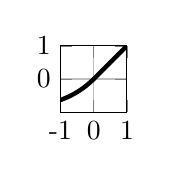
\begin{tikzpicture}
\begin{axis}[
	xmin=-1,xmax=1,
	ymin=-1,ymax=1,
	ytick={0, 1},
	yticklabels={0,1},
	xtick={-1, 0, 1},
	xticklabels={-1,0,1},
	width=.2\textwidth,
	height=.2\textwidth,
	grid=both,
	]
	\addplot [ultra thick,domain=-0.0035:1, samples=10]{x};
	\addplot [ultra thick,domain=-1:0.004, samples=10]{exp(x)-1};
\end{axis}
\end{tikzpicture}}
		\scalebox{.9}{% This file was created by tikzplotlib v0.9.6.
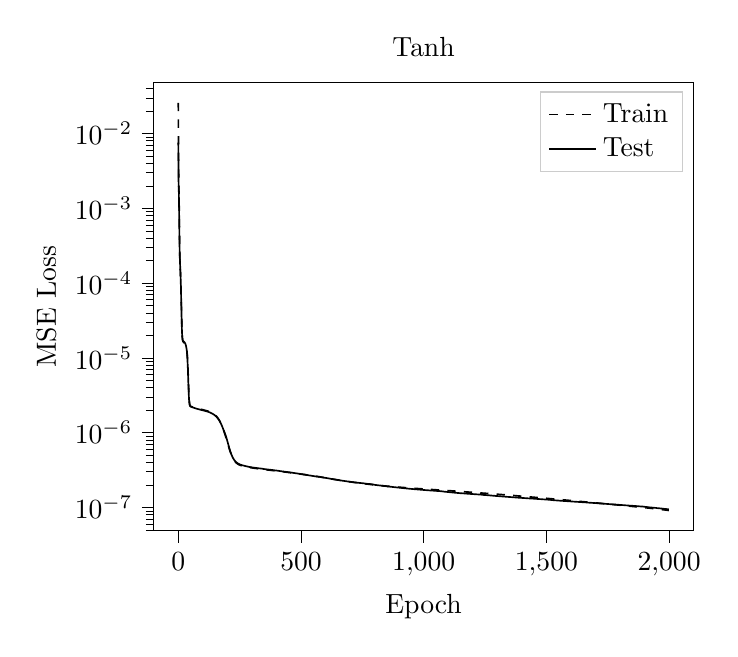
\begin{tikzpicture}

\begin{axis}[
legend cell align={left},
legend style={fill opacity=0.8, draw opacity=1, text opacity=1, draw=white!80!black},
log basis y={10},
tick align=outside,
tick pos=left,
title={Tanh},
x grid style={white!69.0196078431373!black},
xlabel={Epoch},
xmin=-99.95, xmax=2098.95,
xtick style={color=black},
y grid style={white!69.0196078431373!black},
ylabel={MSE Loss},
ymin=4.87162606216586e-08, ymax=0.0480880951021972,
ymode=log,
ytick style={color=black}
]
\addplot [semithick, black, dashed]
table {%
0 0.0256783136818558
1 0.00391949829272926
2 0.00199367450224236
3 0.00143339208001271
4 0.000811647348455153
5 0.000412362531060353
6 0.000244949306972558
7 0.000181991728095454
8 0.000153056107774319
9 0.000130014062575356
10 0.00010614617610554
11 8.2238709928788e-05
12 6.06559043771995e-05
13 4.33234549072949e-05
14 3.11574030747579e-05
15 2.37537921129842e-05
16 1.98036479096118e-05
17 1.79031906054661e-05
18 1.70355609670878e-05
19 1.66247610322898e-05
20 1.63982167177892e-05
21 1.62431279886732e-05
22 1.61158580831398e-05
23 1.59985048476301e-05
24 1.58816735838627e-05
25 1.57583749341939e-05
26 1.56224140046106e-05
27 1.54673897231987e-05
28 1.52862634940902e-05
29 1.50712967133586e-05
30 1.48132416907174e-05
31 1.45002782592201e-05
32 1.41172199300854e-05
33 1.36448685689174e-05
34 1.30603959150903e-05
35 1.23376133224156e-05
36 1.14492682650962e-05
37 1.03756575872467e-05
38 9.12141076651096e-06
39 7.73935586585139e-06
40 6.34618929802855e-06
41 5.09459993941164e-06
42 4.09941510883982e-06
43 3.38837440926909e-06
44 2.91845872209251e-06
45 2.62550942943562e-06
46 2.45301037762147e-06
47 2.35697488326991e-06
48 2.30587279077099e-06
49 2.27869926069957e-06
50 2.26319449416224e-06
51 2.25325485791927e-06
52 2.24564654052983e-06
53 2.23908174814369e-06
54 2.23303946037845e-06
55 2.22724395334239e-06
56 2.22159413002032e-06
57 2.21605597198504e-06
58 2.21059594881012e-06
59 2.20502461627348e-06
60 2.19951089013648e-06
61 2.19409941962567e-06
62 2.18873923640217e-06
63 2.18341688619716e-06
64 2.1780858397733e-06
65 2.1728171752784e-06
66 2.16761157162182e-06
67 2.16247652971902e-06
68 2.15743465199125e-06
69 2.15248080394304e-06
70 2.14761326856205e-06
71 2.14284125951281e-06
72 2.13816882268247e-06
73 2.13358548586484e-06
74 2.12906748606656e-06
75 2.12460380140556e-06
76 2.120198438746e-06
77 2.11584107628937e-06
78 2.11151701626022e-06
79 2.1072322648763e-06
80 2.10301409578051e-06
81 2.09883101015862e-06
82 2.09469965733433e-06
83 2.09061845473002e-06
84 2.08657400560242e-06
85 2.08255163943249e-06
86 2.07854974385668e-06
87 2.07457113936016e-06
88 2.07060074984611e-06
89 2.06666326653249e-06
90 2.06275839008185e-06
91 2.05887886355072e-06
92 2.05505449861221e-06
93 2.0512571416873e-06
94 2.04748774780228e-06
95 2.04372591568358e-06
96 2.03996265599926e-06
97 2.03619106019914e-06
98 2.03241081277383e-06
99 2.02862611661203e-06
100 2.02483424297384e-06
101 2.02102566049689e-06
102 2.01718436369447e-06
103 2.01332004547794e-06
104 2.00943811177012e-06
105 2.00553536137704e-06
106 2.00160756375567e-06
107 1.99764742245634e-06
108 1.99365524949258e-06
109 1.98962802357983e-06
110 1.9855528640278e-06
111 1.98141402830743e-06
112 1.97722682901258e-06
113 1.97299540053564e-06
114 1.96871867424875e-06
115 1.96440277787246e-06
116 1.96000154770104e-06
117 1.9555300951879e-06
118 1.95101178900359e-06
119 1.94641152162944e-06
120 1.94169498476526e-06
121 1.93687540669885e-06
122 1.93201438108304e-06
123 1.92702427668223e-06
124 1.92191399614217e-06
125 1.91670319534865e-06
126 1.91129896376196e-06
127 1.90578242464312e-06
128 1.90011318721872e-06
129 1.89427273897991e-06
130 1.8882123373487e-06
131 1.88198830036868e-06
132 1.87558250883058e-06
133 1.86899712485911e-06
134 1.86227750535295e-06
135 1.85539022578496e-06
136 1.84831423331389e-06
137 1.84095470405055e-06
138 1.83341144793303e-06
139 1.82565649558342e-06
140 1.81764926094274e-06
141 1.8093850391665e-06
142 1.80086963925419e-06
143 1.79206551939615e-06
144 1.78290680096893e-06
145 1.77344423252634e-06
146 1.76363753888609e-06
147 1.75350956513398e-06
148 1.74298757917768e-06
149 1.73214579911019e-06
150 1.72099046380936e-06
151 1.70946602281674e-06
152 1.69748322201713e-06
153 1.68506968657312e-06
154 1.67229672393887e-06
155 1.65912558750847e-06
156 1.64544447042658e-06
157 1.63120314758203e-06
158 1.61646188797704e-06
159 1.60128347954469e-06
160 1.58568593687392e-06
161 1.56952820799461e-06
162 1.55281459512935e-06
163 1.5356757700431e-06
164 1.51809548609094e-06
165 1.50005704529121e-06
166 1.48156487875895e-06
167 1.46263333124352e-06
168 1.44329967625367e-06
169 1.42353404891082e-06
170 1.40324328742736e-06
171 1.38264333622828e-06
172 1.36177704882812e-06
173 1.34056134390903e-06
174 1.31897092293798e-06
175 1.29699397990635e-06
176 1.2747017498782e-06
177 1.25221570530698e-06
178 1.22951809009919e-06
179 1.20664068751353e-06
180 1.18358472803948e-06
181 1.16037225873811e-06
182 1.13706644850708e-06
183 1.11373770050704e-06
184 1.0904470638593e-06
185 1.06723795667563e-06
186 1.04412836427059e-06
187 1.0208118777939e-06
188 9.97641223307255e-07
189 9.74690305525883e-07
190 9.51969390513341e-07
191 9.29392631491055e-07
192 9.06946037218859e-07
193 8.84695177518324e-07
194 8.62814456183969e-07
195 8.41312120513749e-07
196 8.20188414138556e-07
197 7.99479262440173e-07
198 7.79222670900026e-07
199 7.59472292855889e-07
200 7.40254094381498e-07
201 7.21549099239383e-07
202 7.03323363239861e-07
203 6.85619275714089e-07
204 6.6847969463879e-07
205 6.51883700157896e-07
206 6.35866349483649e-07
207 6.20471112625864e-07
208 6.057030220461e-07
209 5.9157178546343e-07
210 5.78070042280387e-07
211 5.65175379023231e-07
212 5.52857127871675e-07
213 5.41098940445295e-07
214 5.29904994237995e-07
215 5.19294521666325e-07
216 5.09250435172248e-07
217 4.99746019073655e-07
218 4.90756391343439e-07
219 4.82253122385146e-07
220 4.74210392084728e-07
221 4.66614737703708e-07
222 4.594722655753e-07
223 4.52780616114978e-07
224 4.46503346267946e-07
225 4.40587696672878e-07
226 4.3501073572827e-07
227 4.29783745403256e-07
228 4.24905776583273e-07
229 4.20343882311158e-07
230 4.16056390292852e-07
231 4.12004934716492e-07
232 4.08168913253348e-07
233 4.04548881093092e-07
234 4.0115957934006e-07
235 3.98017956328545e-07
236 3.95117882121099e-07
237 3.92450205467298e-07
238 3.89984960776246e-07
239 3.87670437433485e-07
240 3.854904206122e-07
241 3.83437721566793e-07
242 3.81521905637783e-07
243 3.79716435688238e-07
244 3.7800730848403e-07
245 3.76387820466562e-07
246 3.74852234386935e-07
247 3.73395006619148e-07
248 3.72012924259479e-07
249 3.70699379175221e-07
250 3.69453458461066e-07
251 3.68269956155132e-07
252 3.67140075951511e-07
253 3.66061015526498e-07
254 3.65028434657688e-07
255 3.64036853241601e-07
256 3.63086354937536e-07
257 3.62170156421371e-07
258 3.61287569361934e-07
259 3.60436046335622e-07
260 3.59612704329493e-07
261 3.58815689537551e-07
262 3.58042329338559e-07
263 3.57291059003728e-07
264 3.56559590528605e-07
265 3.55845987968451e-07
266 3.55149574644997e-07
267 3.54466686573574e-07
268 3.53798637306113e-07
269 3.53151388225115e-07
270 3.52531600483985e-07
271 3.51943575040536e-07
272 3.51372050090504e-07
273 3.50809585640377e-07
274 3.50256817625905e-07
275 3.49712665524748e-07
276 3.49179635776409e-07
277 3.48656109139256e-07
278 3.48143141167157e-07
279 3.47636979228128e-07
280 3.47140434584503e-07
281 3.46653251625639e-07
282 3.46171422521024e-07
283 3.4569364163417e-07
284 3.45216367264811e-07
285 3.44738248372778e-07
286 3.44260469105961e-07
287 3.43785083074977e-07
288 3.43330366902705e-07
289 3.42898308034023e-07
290 3.42464092639716e-07
291 3.42032911291312e-07
292 3.41611756653037e-07
293 3.41200953300813e-07
294 3.4079875696591e-07
295 3.40396311045765e-07
296 3.39994623701045e-07
297 3.39597257266178e-07
298 3.39202901770364e-07
299 3.38812474367955e-07
300 3.38425176110491e-07
301 3.38041470541839e-07
302 3.37660714180288e-07
303 3.37282675587858e-07
304 3.36908611188846e-07
305 3.36536360023842e-07
306 3.36168333262776e-07
307 3.35801948580183e-07
308 3.35437873673072e-07
309 3.350776228217e-07
310 3.34718724388949e-07
311 3.34361913502335e-07
312 3.34007977400574e-07
313 3.3365582474687e-07
314 3.33304566694892e-07
315 3.32955682978309e-07
316 3.32606295486926e-07
317 3.32255786702262e-07
318 3.31905818399036e-07
319 3.31557298508756e-07
320 3.31211877337978e-07
321 3.30875328899083e-07
322 3.30545438856689e-07
323 3.30220234488365e-07
324 3.298965893066e-07
325 3.29574252532439e-07
326 3.29251082263227e-07
327 3.28928731974543e-07
328 3.28607898666178e-07
329 3.28288939684285e-07
330 3.2796907586885e-07
331 3.27652170923898e-07
332 3.27335904060533e-07
333 3.27020988223126e-07
334 3.26706541969202e-07
335 3.26394124385843e-07
336 3.26082249685555e-07
337 3.25770865870823e-07
338 3.25459939233497e-07
339 3.25150717984002e-07
340 3.24840650264946e-07
341 3.24531734875677e-07
342 3.24222071199642e-07
343 3.2391122408626e-07
344 3.23596012492544e-07
345 3.23275019525226e-07
346 3.2294281670886e-07
347 3.22599480000463e-07
348 3.2227435212917e-07
349 3.21953933990926e-07
350 3.21621574045139e-07
351 3.21314297934805e-07
352 3.21034943112863e-07
353 3.20749485581473e-07
354 3.20448250576533e-07
355 3.20144514972753e-07
356 3.19843721285906e-07
357 3.1954650594912e-07
358 3.19254462965546e-07
359 3.18963354061452e-07
360 3.18671405437954e-07
361 3.18381526312805e-07
362 3.1809271050065e-07
363 3.17805669340032e-07
364 3.17520336409416e-07
365 3.17236151289535e-07
366 3.16953998719782e-07
367 3.16672443261723e-07
368 3.16392134422472e-07
369 3.16110889329479e-07
370 3.15829916885946e-07
371 3.15550726682545e-07
372 3.15269492318748e-07
373 3.14990658523584e-07
374 3.14710382866679e-07
375 3.14430895031137e-07
376 3.14152183250371e-07
377 3.13873624463668e-07
378 3.13594867321854e-07
379 3.1331668030532e-07
380 3.13038809508726e-07
381 3.12760674347601e-07
382 3.12483484265158e-07
383 3.12207137426412e-07
384 3.11929519270393e-07
385 3.11651563734472e-07
386 3.11376247253747e-07
387 3.11098750373162e-07
388 3.10823184008768e-07
389 3.10547017605245e-07
390 3.10271550944208e-07
391 3.09995918783557e-07
392 3.09719951715692e-07
393 3.09445476418091e-07
394 3.09168360459466e-07
395 3.08894775159274e-07
396 3.08620413150607e-07
397 3.08344746954958e-07
398 3.08069329236105e-07
399 3.07795802939381e-07
400 3.07521075768591e-07
401 3.07246696138463e-07
402 3.06971505011688e-07
403 3.06696873721535e-07
404 3.06422334631407e-07
405 3.06145008693193e-07
406 3.05865897132662e-07
407 3.05583006166898e-07
408 3.05294879424878e-07
409 3.05009888265317e-07
410 3.04732769805582e-07
411 3.04457269081126e-07
412 3.04181760967026e-07
413 3.03905813524352e-07
414 3.0363094599295e-07
415 3.03357129993742e-07
416 3.03082965743329e-07
417 3.0280785918535e-07
418 3.02532962692226e-07
419 3.0225916734139e-07
420 3.01983990866006e-07
421 3.01708690443547e-07
422 3.01433667928563e-07
423 3.01157673092689e-07
424 3.00882183054796e-07
425 3.00605982133106e-07
426 3.00329158335444e-07
427 3.00052401286166e-07
428 2.99774547642073e-07
429 2.99496324672077e-07
430 2.99217140877772e-07
431 2.98939130772169e-07
432 2.98660514062021e-07
433 2.98383328143359e-07
434 2.98107285431115e-07
435 2.97832286861421e-07
436 2.97559957445515e-07
437 2.97285695779692e-07
438 2.97009015341132e-07
439 2.96733323608578e-07
440 2.96455481390012e-07
441 2.9617858776021e-07
442 2.9590150563763e-07
443 2.95623587916793e-07
444 2.95345244865075e-07
445 2.9506660192169e-07
446 2.94787749211878e-07
447 2.94508583948527e-07
448 2.94228868824575e-07
449 2.93948752528195e-07
450 2.93668269435443e-07
451 2.93385687584191e-07
452 2.93103074923806e-07
453 2.92818450745358e-07
454 2.92533115867855e-07
455 2.92243303405826e-07
456 2.9195033896201e-07
457 2.91650243681829e-07
458 2.91350477510832e-07
459 2.91054979058458e-07
460 2.90767192424823e-07
461 2.90503514534635e-07
462 2.90230797133972e-07
463 2.89949681999246e-07
464 2.89666823135804e-07
465 2.89384619264865e-07
466 2.89102210416559e-07
467 2.88819185129796e-07
468 2.88536360827152e-07
469 2.88253604452393e-07
470 2.87968851523601e-07
471 2.87685964025286e-07
472 2.87401510036034e-07
473 2.87117177379059e-07
474 2.86832849312191e-07
475 2.8654813895912e-07
476 2.86263357793359e-07
477 2.85977837691576e-07
478 2.85691940277388e-07
479 2.85405856359944e-07
480 2.85119550341051e-07
481 2.8483193818829e-07
482 2.84544647684015e-07
483 2.84257998472981e-07
484 2.83969851665233e-07
485 2.83681968156202e-07
486 2.83393235761764e-07
487 2.83104578485904e-07
488 2.82816583634826e-07
489 2.82528103838331e-07
490 2.82238609997876e-07
491 2.81949168339679e-07
492 2.8166003872343e-07
493 2.81370473402376e-07
494 2.81080827463143e-07
495 2.80790753393489e-07
496 2.80500940405659e-07
497 2.80211042010592e-07
498 2.79920554831392e-07
499 2.79629013533622e-07
500 2.79337497119059e-07
501 2.79044599409417e-07
502 2.78752144240002e-07
503 2.78457998902581e-07
504 2.78164109374757e-07
505 2.77869891178284e-07
506 2.77574577594919e-07
507 2.77278857083729e-07
508 2.76983356172877e-07
509 2.7668567361161e-07
510 2.76388693364993e-07
511 2.76090929958173e-07
512 2.75792796927021e-07
513 2.75494566082557e-07
514 2.75195795651939e-07
515 2.74897113726524e-07
516 2.74596931546967e-07
517 2.74297933458456e-07
518 2.7399731402511e-07
519 2.73697588568211e-07
520 2.73398535313163e-07
521 2.73097986720927e-07
522 2.72798081596193e-07
523 2.72497375377156e-07
524 2.721969917161e-07
525 2.71895670650224e-07
526 2.71594623328042e-07
527 2.7129333325604e-07
528 2.70992521649305e-07
529 2.70690323432632e-07
530 2.70388584581838e-07
531 2.70085084920879e-07
532 2.69782810406127e-07
533 2.69479857394117e-07
534 2.69177301504442e-07
535 2.68873798603408e-07
536 2.68569790051743e-07
537 2.68265452916694e-07
538 2.67961485974411e-07
539 2.67657246951103e-07
540 2.67351624302137e-07
541 2.67046286097639e-07
542 2.66741919716651e-07
543 2.66435670084775e-07
544 2.66130026957967e-07
545 2.65824395896175e-07
546 2.6551730083213e-07
547 2.65211784665098e-07
548 2.64905498724488e-07
549 2.64599524172127e-07
550 2.64292502450303e-07
551 2.6398848847009e-07
552 2.63682261532949e-07
553 2.63377035267354e-07
554 2.63071988158003e-07
555 2.62766210369136e-07
556 2.62461571722383e-07
557 2.62156681472447e-07
558 2.61850888776394e-07
559 2.61545947040531e-07
560 2.6124000225991e-07
561 2.60934261390844e-07
562 2.60627847595174e-07
563 2.60322212795927e-07
564 2.60016038239996e-07
565 2.59711214141589e-07
566 2.5940505373967e-07
567 2.59097520512341e-07
568 2.58789286661454e-07
569 2.5847926835354e-07
570 2.5816877410989e-07
571 2.5785619672547e-07
572 2.57544622073169e-07
573 2.57231350587972e-07
574 2.56918664646832e-07
575 2.56602994127775e-07
576 2.56286820288665e-07
577 2.55969035805492e-07
578 2.55648774611927e-07
579 2.5532790500904e-07
580 2.55007268293639e-07
581 2.54691480094493e-07
582 2.54381522779568e-07
583 2.54074222027612e-07
584 2.53768886622652e-07
585 2.53462639946633e-07
586 2.53155078596023e-07
587 2.52848097417768e-07
588 2.52539884442626e-07
589 2.52232671059005e-07
590 2.51926414108539e-07
591 2.51619402433789e-07
592 2.51310856512532e-07
593 2.51001186327926e-07
594 2.50689724069275e-07
595 2.50373325869191e-07
596 2.50046564715944e-07
597 2.4971247898975e-07
598 2.49380338701144e-07
599 2.49063755020984e-07
600 2.48784469974339e-07
601 2.48483565428614e-07
602 2.48175608675183e-07
603 2.47866636698291e-07
604 2.47558843241791e-07
605 2.47249521919457e-07
606 2.4694012356008e-07
607 2.46630496931743e-07
608 2.46319321462352e-07
609 2.4600640222161e-07
610 2.45691713416818e-07
611 2.45375426118244e-07
612 2.45059019846394e-07
613 2.44742416043664e-07
614 2.44427804702241e-07
615 2.44115359791408e-07
616 2.43803189320602e-07
617 2.43488904686728e-07
618 2.43173452574297e-07
619 2.42856562493898e-07
620 2.42540053235984e-07
621 2.4222399055418e-07
622 2.41909370672033e-07
623 2.4159876612373e-07
624 2.41287819818581e-07
625 2.40977986550206e-07
626 2.40667316191434e-07
627 2.40357404365454e-07
628 2.40048627247802e-07
629 2.39740908810404e-07
630 2.39435385040565e-07
631 2.39132102379358e-07
632 2.38831228216441e-07
633 2.38532016894055e-07
634 2.38234100507384e-07
635 2.3793795794802e-07
636 2.37641427077051e-07
637 2.37344928962102e-07
638 2.37049479139273e-07
639 2.36751429071091e-07
640 2.36452641857454e-07
641 2.36152356379193e-07
642 2.35851070470972e-07
643 2.35551766138542e-07
644 2.35254986534983e-07
645 2.34958907981309e-07
646 2.34665752486762e-07
647 2.34375531832143e-07
648 2.34092015489296e-07
649 2.33809699452081e-07
650 2.33527169967829e-07
651 2.33244464084237e-07
652 2.32961468469739e-07
653 2.32677941326642e-07
654 2.32394894752019e-07
655 2.3211163342296e-07
656 2.31829809983708e-07
657 2.31547428853673e-07
658 2.31266236099259e-07
659 2.30985992104138e-07
660 2.30706976715567e-07
661 2.30428674967698e-07
662 2.30152111726056e-07
663 2.29876793980566e-07
664 2.29604099338587e-07
665 2.29333702257861e-07
666 2.29064872783624e-07
667 2.28796595095559e-07
668 2.28530018681283e-07
669 2.2826313580282e-07
670 2.27996663106467e-07
671 2.27733029163346e-07
672 2.27468699684152e-07
673 2.2720402522225e-07
674 2.26941181225016e-07
675 2.26678568793659e-07
676 2.26417082146213e-07
677 2.26155646451787e-07
678 2.25897250800244e-07
679 2.25637136786361e-07
680 2.25378274507193e-07
681 2.25121336775658e-07
682 2.24864484977161e-07
683 2.24608422961126e-07
684 2.24353004966815e-07
685 2.24098303604592e-07
686 2.23845165024272e-07
687 2.23590957716624e-07
688 2.23339868085759e-07
689 2.23087568443248e-07
690 2.22837466004933e-07
691 2.22585833341782e-07
692 2.22337448747112e-07
693 2.22087857792985e-07
694 2.21839565917037e-07
695 2.21591908690755e-07
696 2.21345022012542e-07
697 2.21097984358209e-07
698 2.20852125387694e-07
699 2.2060782892197e-07
700 2.20363927006417e-07
701 2.20120167355731e-07
702 2.19878396393369e-07
703 2.19637687386864e-07
704 2.19396404389727e-07
705 2.19154858328352e-07
706 2.18914575931706e-07
707 2.18667299513697e-07
708 2.18416066260829e-07
709 2.18157695613286e-07
710 2.17917504393483e-07
711 2.17683093978849e-07
712 2.17446162281476e-07
713 2.17212354058915e-07
714 2.16986503602357e-07
715 2.16756925269124e-07
716 2.16528556869378e-07
717 2.16294295185548e-07
718 2.16065943440924e-07
719 2.1583364458877e-07
720 2.15606159549964e-07
721 2.15376262652001e-07
722 2.15151269159719e-07
723 2.14923011839119e-07
724 2.14698939522862e-07
725 2.14466137464342e-07
726 2.14241580749785e-07
727 2.14002345749975e-07
728 2.13779635217293e-07
729 2.13553263428423e-07
730 2.13348029753035e-07
731 2.13115728534774e-07
732 2.12913911404655e-07
733 2.12681533753312e-07
734 2.1250057025668e-07
735 2.12270989564445e-07
736 2.12080155044703e-07
737 2.11840606532121e-07
738 2.11662392217704e-07
739 2.11410442695126e-07
740 2.11244664157562e-07
741 2.10979294507752e-07
742 2.10829887429043e-07
743 2.10549782210023e-07
744 2.10413726215108e-07
745 2.10122939300561e-07
746 2.09999525161209e-07
747 2.09700793199374e-07
748 2.09582869786118e-07
749 2.09277800060192e-07
750 2.09157251006786e-07
751 2.08846759321091e-07
752 2.08716380861063e-07
753 2.08394508241838e-07
754 2.08247044461984e-07
755 2.07928628633169e-07
756 2.07818380481228e-07
757 2.07552191049842e-07
758 2.0744477393464e-07
759 2.07191454308031e-07
760 2.07081657457309e-07
761 2.0683566658164e-07
762 2.06719522203969e-07
763 2.06478433746327e-07
764 2.0635044909767e-07
765 2.06117449401688e-07
766 2.05981543153655e-07
767 2.05756431981285e-07
768 2.0561386548934e-07
769 2.05395930763075e-07
770 2.05249397822627e-07
771 2.05036626113042e-07
772 2.04886012198813e-07
773 2.04679245818795e-07
774 2.04523484633512e-07
775 2.04321535640872e-07
776 2.04161409584458e-07
777 2.03963522885431e-07
778 2.03797197634969e-07
779 2.03599115963016e-07
780 2.03428255403537e-07
781 2.03227953790019e-07
782 2.030431821467e-07
783 2.02847798703942e-07
784 2.02683666543635e-07
785 2.02516986064438e-07
786 2.02353363967234e-07
787 2.02181807019031e-07
788 2.02015970614866e-07
789 2.01841743383113e-07
790 2.01661772905481e-07
791 2.01460166415757e-07
792 2.01229518573598e-07
793 2.01087121354249e-07
794 2.00917898411035e-07
795 2.00780225966923e-07
796 2.00604442376573e-07
797 2.00453189002303e-07
798 2.00287648866038e-07
799 2.00137743007645e-07
800 1.99980189414362e-07
801 1.99827432027178e-07
802 1.99669180005913e-07
803 1.99514663748346e-07
804 1.99357913018616e-07
805 1.99199996849586e-07
806 1.99037115251599e-07
807 1.98870590701006e-07
808 1.98701238232957e-07
809 1.98534945958784e-07
810 1.98443252870106e-07
811 1.98246908794886e-07
812 1.98162096921806e-07
813 1.9793927735634e-07
814 1.97862616772682e-07
815 1.97648748553547e-07
816 1.97567157641743e-07
817 1.97355472479899e-07
818 1.97273760299765e-07
819 1.97065458699797e-07
820 1.96978311969076e-07
821 1.96774255719845e-07
822 1.96680680787154e-07
823 1.96462946391307e-07
824 1.96358382581252e-07
825 1.96272129294073e-07
826 1.96085812284252e-07
827 1.95950416426172e-07
828 1.95843278874008e-07
829 1.95636969095858e-07
830 1.95569540444751e-07
831 1.95350490258761e-07
832 1.95289647095365e-07
833 1.95072461622203e-07
834 1.95013640578168e-07
835 1.94795793944991e-07
836 1.94736558214004e-07
837 1.94521475144427e-07
838 1.94456519217567e-07
839 1.94238834978933e-07
840 1.9416212994372e-07
841 1.93935251495247e-07
842 1.938511577535e-07
843 1.93651539085238e-07
844 1.93595738494423e-07
845 1.93419543499829e-07
846 1.93338983237368e-07
847 1.93155643771092e-07
848 1.93067804922009e-07
849 1.92892168698222e-07
850 1.92794462648749e-07
851 1.92621168871199e-07
852 1.92513661325222e-07
853 1.92361971812716e-07
854 1.92266215115922e-07
855 1.92131815609287e-07
856 1.92028689518509e-07
857 1.91893275420796e-07
858 1.91771540478669e-07
859 1.91640346358213e-07
860 1.91515060819825e-07
861 1.91392229027088e-07
862 1.91263401049468e-07
863 1.91143824686435e-07
864 1.91016867681526e-07
865 1.9089981549314e-07
866 1.90770217429304e-07
867 1.9065634234039e-07
868 1.90525443045431e-07
869 1.90412167242471e-07
870 1.90282269919351e-07
871 1.90172669732647e-07
872 1.90040945632575e-07
873 1.89934002065684e-07
874 1.89798637116212e-07
875 1.89697138701206e-07
876 1.89558307937432e-07
877 1.89464716548571e-07
878 1.89316197278799e-07
879 1.89234877062461e-07
880 1.89073981829324e-07
881 1.89012648903031e-07
882 1.8882984380042e-07
883 1.88791165790292e-07
884 1.88592141974198e-07
885 1.8855339223478e-07
886 1.88359724987208e-07
887 1.88329720955949e-07
888 1.88126539931943e-07
889 1.88094276957429e-07
890 1.87895900772617e-07
891 1.87877068817954e-07
892 1.87662858877502e-07
893 1.87640850128901e-07
894 1.87432238647034e-07
895 1.87432251635755e-07
896 1.87201762059885e-07
897 1.87188818806305e-07
898 1.86971692656357e-07
899 1.86994976040467e-07
900 1.86739167517658e-07
901 1.86732364035436e-07
902 1.86509570291094e-07
903 1.86530011355046e-07
904 1.86241233407713e-07
905 1.86274863906988e-07
906 1.86024884442304e-07
907 1.86029986842584e-07
908 1.85774609136047e-07
909 1.85838526483906e-07
910 1.85592075979457e-07
911 1.85557109972478e-07
912 1.85413238234844e-07
913 1.85311596581528e-07
914 1.85238153171952e-07
915 1.85064903085674e-07
916 1.8492580213092e-07
917 1.84818756245875e-07
918 1.84601177132038e-07
919 1.8463142303915e-07
920 1.84506226155179e-07
921 1.84393604399702e-07
922 1.84358933992712e-07
923 1.84134645067502e-07
924 1.841647220715e-07
925 1.83951926914006e-07
926 1.83905570125376e-07
927 1.83781745690226e-07
928 1.83684701163145e-07
929 1.83511204312481e-07
930 1.8358617639791e-07
931 1.8327896103898e-07
932 1.83298687410627e-07
933 1.83136164785935e-07
934 1.83118544001104e-07
935 1.82905041803849e-07
936 1.82821713821113e-07
937 1.82904439206766e-07
938 1.82656200976794e-07
939 1.82503057061467e-07
940 1.82372852130186e-07
941 1.82464832569451e-07
942 1.82177862498634e-07
943 1.82123570141357e-07
944 1.81958198027132e-07
945 1.82105544006106e-07
946 1.81748656814307e-07
947 1.81644994661667e-07
948 1.81450388794246e-07
949 1.81557134744992e-07
950 1.813367446033e-07
951 1.81250076217054e-07
952 1.8124331060676e-07
953 1.81050296966134e-07
954 1.80912367007124e-07
955 1.81007702494185e-07
956 1.80688111491634e-07
957 1.80711871138328e-07
958 1.80613659338746e-07
959 1.8055098094294e-07
960 1.80342447215764e-07
961 1.80315561223665e-07
962 1.80119200678064e-07
963 1.80223092698384e-07
964 1.79937218476312e-07
965 1.79954523055414e-07
966 1.79713805877668e-07
967 1.79845560126068e-07
968 1.79522391348996e-07
969 1.79567244288137e-07
970 1.794615962325e-07
971 1.79359788418765e-07
972 1.7919894242624e-07
973 1.79157142703446e-07
974 1.78962343092337e-07
975 1.79107667875655e-07
976 1.78761917062786e-07
977 1.78851070963049e-07
978 1.78552461115089e-07
979 1.78618294036426e-07
980 1.78499511285679e-07
981 1.78432811814844e-07
982 1.78235883993239e-07
983 1.7822017412783e-07
984 1.78006425556987e-07
985 1.78184835050388e-07
986 1.77794969182798e-07
987 1.77919801146231e-07
988 1.77607504305399e-07
989 1.77682868525153e-07
990 1.77565874700747e-07
991 1.77483282151059e-07
992 1.77303049056832e-07
993 1.77288027074951e-07
994 1.77071662321282e-07
995 1.77269572674277e-07
996 1.76851885242968e-07
997 1.76987209279389e-07
998 1.76690409439573e-07
999 1.76745455256366e-07
1000 1.76675246279956e-07
1001 1.76517975418733e-07
1002 1.76396269658596e-07
1003 1.76365606833428e-07
1004 1.76154782728588e-07
1005 1.76332453555972e-07
1006 1.75943806638657e-07
1007 1.76068208830316e-07
1008 1.75781630375127e-07
1009 1.75818021048713e-07
1010 1.75775665255173e-07
1011 1.75606383862714e-07
1012 1.75487401570251e-07
1013 1.75443485460391e-07
1014 1.75264921239204e-07
1015 1.75345524404236e-07
1016 1.75081772901819e-07
1017 1.75094191163794e-07
1018 1.75051218050726e-07
1019 1.74866570674226e-07
1020 1.74778132873143e-07
1021 1.74739804535307e-07
1022 1.74538157253323e-07
1023 1.74689216812851e-07
1024 1.74356573701573e-07
1025 1.74413866574241e-07
1026 1.74186691808131e-07
1027 1.74223586959954e-07
1028 1.74151234887177e-07
1029 1.74013387677974e-07
1030 1.7389884820318e-07
1031 1.73856675388606e-07
1032 1.7367983700467e-07
1033 1.73838016891636e-07
1034 1.73464950613322e-07
1035 1.7353948872767e-07
1036 1.733090185283e-07
1037 1.73334884379983e-07
1038 1.73301539497572e-07
1039 1.73104309247663e-07
1040 1.73018324709062e-07
1041 1.72962489585871e-07
1042 1.72787920796225e-07
1043 1.72943589724639e-07
1044 1.72586770247563e-07
1045 1.72631184170768e-07
1046 1.72425827720701e-07
1047 1.72480665220576e-07
1048 1.72308242348151e-07
1049 1.72222635825392e-07
1050 1.72199534759443e-07
1051 1.7209841140442e-07
1052 1.71934404548324e-07
1053 1.71875999363635e-07
1054 1.71818576639282e-07
1055 1.71664782399716e-07
1056 1.71721229904165e-07
1057 1.71507559223016e-07
1058 1.71450052548039e-07
1059 1.71324552624696e-07
1060 1.71405257525237e-07
1061 1.71114308081144e-07
1062 1.71128518353214e-07
1063 1.70986724953082e-07
1064 1.70997916832505e-07
1065 1.70789293711948e-07
1066 1.70840542757844e-07
1067 1.70683409770334e-07
1068 1.70584149131514e-07
1069 1.70473046189556e-07
1070 1.70536510026409e-07
1071 1.70325863329879e-07
1072 1.70239916933212e-07
1073 1.70178448684055e-07
1074 1.70156779681463e-07
1075 1.70017821211843e-07
1076 1.69923560775942e-07
1077 1.69763528241162e-07
1078 1.69926713766699e-07
1079 1.69656568338894e-07
1080 1.6954471659858e-07
1081 1.69526870145376e-07
1082 1.6947657803712e-07
1083 1.69291331680199e-07
1084 1.69387541966159e-07
1085 1.69021876075703e-07
1086 1.69219825430389e-07
1087 1.6888395204262e-07
1088 1.69059036124963e-07
1089 1.68762051210081e-07
1090 1.68699381958959e-07
1091 1.68677553716634e-07
1092 1.6864209008105e-07
1093 1.6840546667396e-07
1094 1.68458437485697e-07
1095 1.68280550276734e-07
1096 1.68226403687299e-07
1097 1.68105190404333e-07
1098 1.68082149194504e-07
1099 1.67917447448929e-07
1100 1.6791531155036e-07
1101 1.67686958455704e-07
1102 1.67809295753329e-07
1103 1.67609576770644e-07
1104 1.67468523144976e-07
1105 1.67500856612435e-07
1106 1.6746117916e-07
1107 1.67153349366345e-07
1108 1.67207376478018e-07
1109 1.67103117760803e-07
1110 1.67111690664967e-07
1111 1.66799030040465e-07
1112 1.66887021485707e-07
1113 1.6675984264225e-07
1114 1.66733511498762e-07
1115 1.66459487857651e-07
1116 1.66677239924695e-07
1117 1.66273404033745e-07
1118 1.66400428263103e-07
1119 1.66187338273005e-07
1120 1.66101584440526e-07
1121 1.66114068328227e-07
1122 1.66078519775681e-07
1123 1.65747365109326e-07
1124 1.65834520352348e-07
1125 1.65732793483642e-07
1126 1.6568083282209e-07
1127 1.65441024208235e-07
1128 1.65423872360293e-07
1129 1.65376426387809e-07
1130 1.65266291709543e-07
1131 1.65075949297488e-07
1132 1.65183653578538e-07
1133 1.64901120811578e-07
1134 1.64889070461527e-07
1135 1.64816789080646e-07
1136 1.64743251978905e-07
1137 1.64549871939812e-07
1138 1.64797036717346e-07
1139 1.64368372125523e-07
1140 1.64327388922914e-07
1141 1.6437572345751e-07
1142 1.64175849306503e-07
1143 1.64098669806378e-07
1144 1.64148435708e-07
1145 1.63833804322167e-07
1146 1.63941523169342e-07
1147 1.6383109585405e-07
1148 1.636207689657e-07
1149 1.6357456372873e-07
1150 1.63597238461932e-07
1151 1.63376890910172e-07
1152 1.63384830955238e-07
1153 1.6318603519494e-07
1154 1.63193474179479e-07
1155 1.6296791127246e-07
1156 1.62943861326426e-07
1157 1.6273880940787e-07
1158 1.62804770901914e-07
1159 1.62569668617607e-07
1160 1.6251618761487e-07
1161 1.62369944625596e-07
1162 1.62474557683368e-07
1163 1.62164271898746e-07
1164 1.62203364439506e-07
1165 1.6202119513764e-07
1166 1.61991749145329e-07
1167 1.61838586954843e-07
1168 1.61991775357251e-07
1169 1.61693534884932e-07
1170 1.61734423144821e-07
1171 1.61486205477956e-07
1172 1.61506580710125e-07
1173 1.61275248807158e-07
1174 1.61340523128217e-07
1175 1.61135238769816e-07
1176 1.6120220598026e-07
1177 1.6093218126656e-07
1178 1.61019107835614e-07
1179 1.60858303864586e-07
1180 1.60795300494954e-07
1181 1.60560779271179e-07
1182 1.606647063781e-07
1183 1.60463883673856e-07
1184 1.60438281078257e-07
1185 1.60245081261223e-07
1186 1.60326889165674e-07
1187 1.60055241750001e-07
1188 1.6013421814165e-07
1189 1.59912973622056e-07
1190 1.59970620472905e-07
1191 1.59738145576682e-07
1192 1.59805658704215e-07
1193 1.5955720218841e-07
1194 1.59621237003194e-07
1195 1.59371404294006e-07
1196 1.59442580354607e-07
1197 1.59209781699587e-07
1198 1.59259970288872e-07
1199 1.59041937585869e-07
1200 1.59072571342733e-07
1201 1.58855913184652e-07
1202 1.58921797947187e-07
1203 1.58672437535756e-07
1204 1.58764354367236e-07
1205 1.58471104839464e-07
1206 1.58557933318093e-07
1207 1.58335334020876e-07
1208 1.58428612778039e-07
1209 1.5810165481156e-07
1210 1.58222141770636e-07
1211 1.57989714331563e-07
1212 1.58009147142479e-07
1213 1.57803747654839e-07
1214 1.57937466838121e-07
1215 1.57602995166428e-07
1216 1.57633344173291e-07
1217 1.57450450885221e-07
1218 1.57564682048417e-07
1219 1.5723370426457e-07
1220 1.57340403383444e-07
1221 1.57073375376626e-07
1222 1.57176691644167e-07
1223 1.5689634754068e-07
1224 1.57032079670216e-07
1225 1.56695187875755e-07
1226 1.56953842733287e-07
1227 1.56568736393581e-07
1228 1.56612420873614e-07
1229 1.56362640737484e-07
1230 1.56375388939978e-07
1231 1.56238784875029e-07
1232 1.56451213698006e-07
1233 1.56064872733452e-07
1234 1.56071111931055e-07
1235 1.55855858885445e-07
1236 1.55867894434891e-07
1237 1.5592698014899e-07
1238 1.55753827151273e-07
1239 1.55547799785438e-07
1240 1.55530699892381e-07
1241 1.55571137803179e-07
1242 1.55404293401773e-07
1243 1.55184656165375e-07
1244 1.55190573323694e-07
1245 1.54982764250633e-07
1246 1.55162933609176e-07
1247 1.54817653481132e-07
1248 1.5485027108042e-07
1249 1.547744172683e-07
1250 1.54679265847335e-07
1251 1.54439792730443e-07
1252 1.54736637590247e-07
1253 1.54300877532876e-07
1254 1.54275749530086e-07
1255 1.54250144028367e-07
1256 1.54043304789298e-07
1257 1.54029483198315e-07
1258 1.53867440310762e-07
1259 1.53782401476121e-07
1260 1.53956117301846e-07
1261 1.53517524005053e-07
1262 1.53721324970491e-07
1263 1.53280332831685e-07
1264 1.53318621009646e-07
1265 1.53157448153252e-07
1266 1.53317707557221e-07
1267 1.53006178400972e-07
1268 1.53078262279394e-07
1269 1.5295192603304e-07
1270 1.52759127885815e-07
1271 1.52895805442199e-07
1272 1.52618819498684e-07
1273 1.52668988391724e-07
1274 1.52435742045043e-07
1275 1.52282082240163e-07
1276 1.52478126885569e-07
1277 1.52267675993301e-07
1278 1.52102081919736e-07
1279 1.51924854762342e-07
1280 1.52071395540077e-07
1281 1.51897150189484e-07
1282 1.5177754506368e-07
1283 1.51588411327452e-07
1284 1.51686713365962e-07
1285 1.51578635318117e-07
1286 1.514046663047e-07
1287 1.51386741720216e-07
1288 1.51236834938118e-07
1289 1.51087039519382e-07
1290 1.51245379640841e-07
1291 1.50855604545086e-07
1292 1.50857793343562e-07
1293 1.50979376975613e-07
1294 1.50700781588853e-07
1295 1.50535089112225e-07
1296 1.50622930220834e-07
1297 1.50551819402267e-07
1298 1.50364579305062e-07
1299 1.50309357970002e-07
1300 1.50167315318583e-07
1301 1.50015147610816e-07
1302 1.50052822462499e-07
1303 1.49995276302661e-07
1304 1.49929092593482e-07
1305 1.49615969156969e-07
1306 1.49589932703975e-07
1307 1.4974333686979e-07
1308 1.49432075829736e-07
1309 1.49371547493615e-07
1310 1.49235247398849e-07
1311 1.49208245971977e-07
1312 1.49100245259604e-07
1313 1.49268570623917e-07
1314 1.48885288751899e-07
1315 1.48768517568953e-07
1316 1.48855611548981e-07
1317 1.4859427885483e-07
1318 1.48693639566488e-07
1319 1.48367197255084e-07
1320 1.48511471429913e-07
1321 1.48261079587542e-07
1322 1.4825105432692e-07
1323 1.48094737163262e-07
1324 1.48087659624707e-07
1325 1.47959285683896e-07
1326 1.47861875170463e-07
1327 1.4779576830648e-07
1328 1.47618505707214e-07
1329 1.47669302762665e-07
1330 1.47545432952256e-07
1331 1.47312891250806e-07
1332 1.47584984269145e-07
1333 1.47121381466775e-07
1334 1.47155481123207e-07
1335 1.47138486575216e-07
1336 1.46936660485153e-07
1337 1.46897626322584e-07
1338 1.46821027406929e-07
1339 1.46725811767112e-07
1340 1.46653712221223e-07
1341 1.46529792196759e-07
1342 1.46487281597274e-07
1343 1.46329400010359e-07
1344 1.46247827714774e-07
1345 1.46147555952325e-07
1346 1.46037953442146e-07
1347 1.45971158666214e-07
1348 1.45886081675428e-07
1349 1.45792722264559e-07
1350 1.45680503919721e-07
1351 1.45593948325029e-07
1352 1.45497979708864e-07
1353 1.45533103278694e-07
1354 1.4527947547549e-07
1355 1.45212114908588e-07
1356 1.45154443664808e-07
1357 1.45234765746238e-07
1358 1.44960471416766e-07
1359 1.44836443077168e-07
1360 1.44837134833153e-07
1361 1.44702509636829e-07
1362 1.44611242220094e-07
1363 1.44524215748731e-07
1364 1.44445664702175e-07
1365 1.44438964461813e-07
1366 1.44254628807516e-07
1367 1.44174589323143e-07
1368 1.44097156415057e-07
1369 1.44165149549735e-07
1370 1.438918012866e-07
1371 1.43834863926884e-07
1372 1.43778407689865e-07
1373 1.43654776103119e-07
1374 1.43601501100932e-07
1375 1.43478440016054e-07
1376 1.43422459309761e-07
1377 1.43299267286068e-07
1378 1.43240890253082e-07
1379 1.43121426198434e-07
1380 1.43058707820387e-07
1381 1.42943359975334e-07
1382 1.42876715720774e-07
1383 1.42766054786136e-07
1384 1.42697908941614e-07
1385 1.42588240770181e-07
1386 1.42517276643161e-07
1387 1.42408500622082e-07
1388 1.42336251322206e-07
1389 1.42228149620394e-07
1390 1.42154443622644e-07
1391 1.42046925965644e-07
1392 1.41968544774329e-07
1393 1.41857630964637e-07
1394 1.41799161355038e-07
1395 1.41669875795003e-07
1396 1.41642744232229e-07
1397 1.41488020773295e-07
1398 1.41444808285485e-07
1399 1.41307266197543e-07
1400 1.41268738268252e-07
1401 1.41131835960095e-07
1402 1.41081490781403e-07
1403 1.4095575309625e-07
1404 1.40900945055478e-07
1405 1.40781008234114e-07
1406 1.40719304582149e-07
1407 1.40605119860027e-07
1408 1.4053854697238e-07
1409 1.40430631219601e-07
1410 1.40360673611895e-07
1411 1.40257951656508e-07
1412 1.40187808121084e-07
1413 1.40090017744399e-07
1414 1.40027148880506e-07
1415 1.39918102711079e-07
1416 1.398644709667e-07
1417 1.39729618609863e-07
1418 1.39709254440845e-07
1419 1.39548208807128e-07
1420 1.39488207395289e-07
1421 1.39385581888973e-07
1422 1.39311794306707e-07
1423 1.39198004013963e-07
1424 1.39159127087396e-07
1425 1.3899639265702e-07
1426 1.38957142148399e-07
1427 1.3883218345967e-07
1428 1.38818436489885e-07
1429 1.38638300825278e-07
1430 1.38555119733041e-07
1431 1.38598182424232e-07
1432 1.38383111163876e-07
1433 1.38299546527776e-07
1434 1.38218821902569e-07
1435 1.38132329730922e-07
1436 1.38036302210764e-07
1437 1.37932765305493e-07
1438 1.37865884262567e-07
1439 1.37768181680542e-07
1440 1.37693862200194e-07
1441 1.37575959314518e-07
1442 1.37563847445676e-07
1443 1.37410551808159e-07
1444 1.37314383366061e-07
1445 1.37217166447101e-07
1446 1.37134599185629e-07
1447 1.37090809047891e-07
1448 1.36948206701959e-07
1449 1.36934800536892e-07
1450 1.36800439307194e-07
1451 1.36791305251904e-07
1452 1.36640489124318e-07
1453 1.36551323684841e-07
1454 1.3647366780134e-07
1455 1.36380717925988e-07
1456 1.36293950461663e-07
1457 1.36197411691796e-07
1458 1.36108559800618e-07
1459 1.36015842777226e-07
1460 1.35925950090154e-07
1461 1.35836153020819e-07
1462 1.35745947254406e-07
1463 1.35656308337673e-07
1464 1.35567192799613e-07
1465 1.35476351189823e-07
1466 1.35388576424589e-07
1467 1.3529987614902e-07
1468 1.35212574981836e-07
1469 1.35123513757662e-07
1470 1.35034041001347e-07
1471 1.34942330241472e-07
1472 1.34852680481856e-07
1473 1.34763203988086e-07
1474 1.34675156090225e-07
1475 1.34583959088275e-07
1476 1.34498445788722e-07
1477 1.34410110952388e-07
1478 1.34325130517254e-07
1479 1.34240905950378e-07
1480 1.34159623293328e-07
1481 1.34082334994901e-07
1482 1.34007962977023e-07
1483 1.3393716164245e-07
1484 1.33868372188317e-07
1485 1.33801153474167e-07
1486 1.33728197575067e-07
1487 1.33651108498611e-07
1488 1.33561932415205e-07
1489 1.33471286439146e-07
1490 1.33377818180236e-07
1491 1.33286574389047e-07
1492 1.33195876379943e-07
1493 1.33103312499827e-07
1494 1.33012573186875e-07
1495 1.32922244659994e-07
1496 1.328316240361e-07
1497 1.32742819303644e-07
1498 1.32652472835559e-07
1499 1.32563086381765e-07
1500 1.32473022716795e-07
1501 1.32383093998101e-07
1502 1.32294703512059e-07
1503 1.32204725133533e-07
1504 1.32114500431157e-07
1505 1.32024823336963e-07
1506 1.31935355909718e-07
1507 1.31843942838827e-07
1508 1.31755951315427e-07
1509 1.31664896130701e-07
1510 1.31577506834901e-07
1511 1.31486739483933e-07
1512 1.31398833772778e-07
1513 1.31310993296552e-07
1514 1.31223457849217e-07
1515 1.31135499088941e-07
1516 1.31049406171257e-07
1517 1.30963723570687e-07
1518 1.30879938801343e-07
1519 1.30797358849577e-07
1520 1.30715271609461e-07
1521 1.30635178784644e-07
1522 1.30553517664111e-07
1523 1.30470073074207e-07
1524 1.30381565455195e-07
1525 1.30291873148281e-07
1526 1.30197957403766e-07
1527 1.30105073552045e-07
1528 1.30015101412084e-07
1529 1.29922131684168e-07
1530 1.29832057609747e-07
1531 1.29743567214291e-07
1532 1.29655932553874e-07
1533 1.29567336209391e-07
1534 1.29478633702718e-07
1535 1.29388707819089e-07
1536 1.29298447703263e-07
1537 1.29211609895208e-07
1538 1.29121361368334e-07
1539 1.2903508240214e-07
1540 1.28947685460901e-07
1541 1.28861089891075e-07
1542 1.28775236419187e-07
1543 1.28692052271617e-07
1544 1.28612261207195e-07
1545 1.2853669561963e-07
1546 1.28464933744965e-07
1547 1.28383591274428e-07
1548 1.28288588584269e-07
1549 1.28192372116587e-07
1550 1.28097349630707e-07
1551 1.28006397964953e-07
1552 1.27916903707614e-07
1553 1.27826293685018e-07
1554 1.27737181870202e-07
1555 1.2764687626543e-07
1556 1.27558287637441e-07
1557 1.2746860927848e-07
1558 1.27379083963319e-07
1559 1.27289022763932e-07
1560 1.272002397954e-07
1561 1.27111350991527e-07
1562 1.27022582084635e-07
1563 1.26932102247679e-07
1564 1.26843040995084e-07
1565 1.26754313335198e-07
1566 1.26665019799077e-07
1567 1.26576261081368e-07
1568 1.26486150506366e-07
1569 1.26398269948425e-07
1570 1.26310102317007e-07
1571 1.26218600009054e-07
1572 1.26132292770365e-07
1573 1.2604147003259e-07
1574 1.2595394938586e-07
1575 1.25864576688173e-07
1576 1.25776658805421e-07
1577 1.25686074447628e-07
1578 1.25598635008828e-07
1579 1.25509957499048e-07
1580 1.25420049670311e-07
1581 1.25333193693677e-07
1582 1.25244157622717e-07
1583 1.25155239857122e-07
1584 1.25067637064546e-07
1585 1.24977565626239e-07
1586 1.24891056422882e-07
1587 1.24802263734125e-07
1588 1.24713928691733e-07
1589 1.24625061047823e-07
1590 1.24537065644859e-07
1591 1.24449508533075e-07
1592 1.24361393055494e-07
1593 1.24273274060727e-07
1594 1.24184724057841e-07
1595 1.24096431704857e-07
1596 1.24009077239862e-07
1597 1.23921701607799e-07
1598 1.23833612477142e-07
1599 1.2374631225498e-07
1600 1.23658226300449e-07
1601 1.2357035235766e-07
1602 1.23482338388214e-07
1603 1.23394856949233e-07
1604 1.23307119714866e-07
1605 1.23220711785166e-07
1606 1.23131181361202e-07
1607 1.23045026157342e-07
1608 1.22957511642596e-07
1609 1.22870412297971e-07
1610 1.22781257239524e-07
1611 1.2269524139441e-07
1612 1.22605206286153e-07
1613 1.2251671019925e-07
1614 1.22426431886424e-07
1615 1.22340115936481e-07
1616 1.22256094321926e-07
1617 1.22175058258733e-07
1618 1.22103615190383e-07
1619 1.2202762109581e-07
1620 1.21916793361265e-07
1621 1.21834089732431e-07
1622 1.21743012215347e-07
1623 1.21660922808076e-07
1624 1.21567334446127e-07
1625 1.21491538585872e-07
1626 1.21390171351266e-07
1627 1.21322823133596e-07
1628 1.21213336576886e-07
1629 1.21154960034175e-07
1630 1.21035876183839e-07
1631 1.20987247662185e-07
1632 1.20860402027745e-07
1633 1.20820134824839e-07
1634 1.2068506220686e-07
1635 1.20652669416188e-07
1636 1.20510663322193e-07
1637 1.20486183746493e-07
1638 1.20336616767247e-07
1639 1.2031963217396e-07
1640 1.20164131615752e-07
1641 1.20150103626315e-07
1642 1.19992589979745e-07
1643 1.19979782780888e-07
1644 1.19823972248412e-07
1645 1.19810623154137e-07
1646 1.19654737659403e-07
1647 1.19639229716029e-07
1648 1.19485491680393e-07
1649 1.19471855569486e-07
1650 1.19316783660395e-07
1651 1.19300847543968e-07
1652 1.19148934437874e-07
1653 1.19132773143349e-07
1654 1.18980588830198e-07
1655 1.18963450141507e-07
1656 1.18812017682046e-07
1657 1.18793472807965e-07
1658 1.18644252474098e-07
1659 1.18625620011414e-07
1660 1.18476356057329e-07
1661 1.18456286585911e-07
1662 1.18310040200242e-07
1663 1.1828933644864e-07
1664 1.18143192537445e-07
1665 1.18121343611222e-07
1666 1.17981712925541e-07
1667 1.1796190426594e-07
1668 1.17837449707281e-07
1669 1.17821046096367e-07
1670 1.17664518249683e-07
1671 1.17625616695705e-07
1672 1.17494159866283e-07
1673 1.17454599340761e-07
1674 1.17330423812234e-07
1675 1.17281875056108e-07
1676 1.17167207086766e-07
1677 1.17112645753537e-07
1678 1.17004529613496e-07
1679 1.16942329213998e-07
1680 1.16840053991041e-07
1681 1.16773833177319e-07
1682 1.16675894744844e-07
1683 1.16606030751143e-07
1684 1.16511720229084e-07
1685 1.16438417961717e-07
1686 1.1634670725158e-07
1687 1.16271883264574e-07
1688 1.16182274517485e-07
1689 1.16104469931599e-07
1690 1.16017207645314e-07
1691 1.15939320814107e-07
1692 1.1585205044895e-07
1693 1.15773689692844e-07
1694 1.15688439173312e-07
1695 1.15609684797846e-07
1696 1.15523752249658e-07
1697 1.15442792669285e-07
1698 1.15360084031124e-07
1699 1.152794114887e-07
1700 1.15195414622349e-07
1701 1.15116151533812e-07
1702 1.15032597470588e-07
1703 1.14952266152102e-07
1704 1.14869341658164e-07
1705 1.14788415693567e-07
1706 1.14706799855924e-07
1707 1.14626587183864e-07
1708 1.14544958570661e-07
1709 1.14467005680297e-07
1710 1.14386371400599e-07
1711 1.14309840782312e-07
1712 1.14231534574571e-07
1713 1.14155406919281e-07
1714 1.14076618189074e-07
1715 1.1400160070707e-07
1716 1.13935357504147e-07
1717 1.13852153852179e-07
1718 1.1374592218516e-07
1719 1.13668901171593e-07
1720 1.13586670188681e-07
1721 1.13503399141734e-07
1722 1.13423729317219e-07
1723 1.13342144530293e-07
1724 1.13260248220115e-07
1725 1.13178309291584e-07
1726 1.13098485158503e-07
1727 1.13015533877103e-07
1728 1.12935625388388e-07
1729 1.12853559258497e-07
1730 1.12772581523757e-07
1731 1.12691697047751e-07
1732 1.12609595291246e-07
1733 1.1252984580068e-07
1734 1.12447377652813e-07
1735 1.12366985916879e-07
1736 1.1228577866973e-07
1737 1.12205130093912e-07
1738 1.12124054268747e-07
1739 1.1204307208601e-07
1740 1.11962179772718e-07
1741 1.11882094351756e-07
1742 1.11800244731342e-07
1743 1.11719630730533e-07
1744 1.11639534196684e-07
1745 1.11557851859345e-07
1746 1.11477907729807e-07
1747 1.11396160754396e-07
1748 1.1131719745805e-07
1749 1.11234583393127e-07
1750 1.11156175847782e-07
1751 1.11073824463404e-07
1752 1.1099390077618e-07
1753 1.10913257636014e-07
1754 1.10833950522249e-07
1755 1.10751658766617e-07
1756 1.10673457989208e-07
1757 1.10590813854117e-07
1758 1.10513686372826e-07
1759 1.10427929719492e-07
1760 1.10354096037213e-07
1761 1.1026718136975e-07
1762 1.10195531284774e-07
1763 1.10103467726219e-07
1764 1.10038613662766e-07
1765 1.09938720179059e-07
1766 1.09883219252538e-07
1767 1.09774770230331e-07
1768 1.09726113770137e-07
1769 1.0961239318874e-07
1770 1.09567085601725e-07
1771 1.09453343561938e-07
1772 1.09406560120817e-07
1773 1.09293789691378e-07
1774 1.09247273940127e-07
1775 1.09132642720056e-07
1776 1.09087160637955e-07
1777 1.08973743436991e-07
1778 1.08927465625186e-07
1779 1.08812749033405e-07
1780 1.08768906656564e-07
1781 1.08653364364386e-07
1782 1.08610696209155e-07
1783 1.08492045278297e-07
1784 1.08451488785022e-07
1785 1.08332703078418e-07
1786 1.08292764849693e-07
1787 1.08172346592994e-07
1788 1.08134267669868e-07
1789 1.08012495928733e-07
1790 1.07974928781118e-07
1791 1.07852817237131e-07
1792 1.07816773052605e-07
1793 1.07694217973631e-07
1794 1.076585755726e-07
1795 1.07533660980152e-07
1796 1.0750032522111e-07
1797 1.07374868321131e-07
1798 1.07341590407373e-07
1799 1.07214731805527e-07
1800 1.07183627001461e-07
1801 1.07055369142017e-07
1802 1.07025273905492e-07
1803 1.06897582774934e-07
1804 1.06866378018822e-07
1805 1.06738425301955e-07
1806 1.06709044885633e-07
1807 1.06578284807313e-07
1808 1.06551349951189e-07
1809 1.06419266913349e-07
1810 1.06393436325902e-07
1811 1.0626070748998e-07
1812 1.06233781600906e-07
1813 1.06102325410973e-07
1814 1.06077179772512e-07
1815 1.05943803617947e-07
1816 1.05918884933942e-07
1817 1.05785039274053e-07
1818 1.0576097081838e-07
1819 1.05625972793177e-07
1820 1.05602148408934e-07
1821 1.05468074529824e-07
1822 1.05444441423685e-07
1823 1.05309890450656e-07
1824 1.05286905679236e-07
1825 1.05151352997268e-07
1826 1.05128677049038e-07
1827 1.04993245805929e-07
1828 1.04970954780015e-07
1829 1.04834349158978e-07
1830 1.04813155957117e-07
1831 1.04675824211142e-07
1832 1.04656024795702e-07
1833 1.04517476188448e-07
1834 1.04497554922034e-07
1835 1.04359976702995e-07
1836 1.04338933539339e-07
1837 1.04202867277081e-07
1838 1.04181184603647e-07
1839 1.04044154433325e-07
1840 1.04023431063638e-07
1841 1.03886127348574e-07
1842 1.03865805684222e-07
1843 1.03730083061748e-07
1844 1.03708399777247e-07
1845 1.03575531461786e-07
1846 1.03553730738781e-07
1847 1.03431781575125e-07
1848 1.03406835641806e-07
1849 1.03251629880674e-07
1850 1.03248295282299e-07
1851 1.03094720223851e-07
1852 1.03084822235644e-07
1853 1.029415868814e-07
1854 1.02924780257752e-07
1855 1.02787245204183e-07
1856 1.02766203596616e-07
1857 1.02631769628658e-07
1858 1.02608433905971e-07
1859 1.02473619911336e-07
1860 1.02450679698052e-07
1861 1.02315491744775e-07
1862 1.02293353030802e-07
1863 1.02158083478798e-07
1864 1.02137613730235e-07
1865 1.02001180536604e-07
1866 1.01981320298705e-07
1867 1.0184516611389e-07
1868 1.0182440312434e-07
1869 1.01688210200734e-07
1870 1.01670011382282e-07
1871 1.01530907663516e-07
1872 1.01513423203414e-07
1873 1.01376702275502e-07
1874 1.01358417559538e-07
1875 1.01222969291825e-07
1876 1.01205789569292e-07
1877 1.01067017183709e-07
1878 1.01052819672987e-07
1879 1.00915272618352e-07
1880 1.0090144083108e-07
1881 1.00764368340833e-07
1882 1.00751233624408e-07
1883 1.00615954877981e-07
1884 1.00604420119055e-07
1885 1.0046848284162e-07
1886 1.00461983791433e-07
1887 1.00328959490525e-07
1888 1.00327407132283e-07
1889 1.00198732020829e-07
1890 1.00210742438378e-07
1891 1.00091209333186e-07
1892 1.00120992215125e-07
1893 1.00010873573808e-07
1894 1.00031446216065e-07
1895 9.98494305122222e-08
1896 9.98177236226638e-08
1897 9.96636280206076e-08
1898 9.9662101789022e-08
1899 9.95036318087727e-08
1900 9.95035710644743e-08
1901 9.93359447178932e-08
1902 9.93463889713553e-08
1903 9.91639390761634e-08
1904 9.91915004178168e-08
1905 9.89930967563168e-08
1906 9.90359007531083e-08
1907 9.88282890048708e-08
1908 9.88751828856493e-08
1909 9.86779837575114e-08
1910 9.86860634668574e-08
1911 9.85199047107699e-08
1912 9.85522943679484e-08
1913 9.83903354097038e-08
1914 9.83319166465435e-08
1915 9.82184653537388e-08
1916 9.81738594347803e-08
1917 9.80355162667479e-08
1918 9.80704097628404e-08
1919 9.79550177007127e-08
1920 9.79253364477017e-08
1921 9.7782193442697e-08
1922 9.76768999620958e-08
1923 9.76173793958424e-08
1924 9.75287996425322e-08
1925 9.74686554826576e-08
1926 9.73918850419864e-08
1927 9.72836267649768e-08
1928 9.73122499345891e-08
1929 9.7137337192521e-08
1930 9.70798927966143e-08
1931 9.69518271602965e-08
1932 9.69189093709133e-08
1933 9.67950209869173e-08
1934 9.67396970565915e-08
1935 9.66325465867612e-08
1936 9.65764778655398e-08
1937 9.64863556447426e-08
1938 9.63525852242242e-08
1939 9.63383329022349e-08
1940 9.61832626558135e-08
1941 9.61392340954603e-08
1942 9.59978614645252e-08
1943 9.59531415389847e-08
1944 9.57992250434359e-08
1945 9.57176675484561e-08
1946 9.56372701708119e-08
1947 9.55616131150805e-08
1948 9.55027764604211e-08
1949 9.54192266604537e-08
1950 9.52890652783367e-08
1951 9.52766380919456e-08
1952 9.51284585539724e-08
1953 9.50952942702088e-08
1954 9.4968490913061e-08
1955 9.49355355217563e-08
1956 9.48217696077336e-08
1957 9.47154426356178e-08
1958 9.46745343597399e-08
1959 9.45576307387341e-08
1960 9.44733649959062e-08
1961 9.44023931381821e-08
1962 9.43122054337664e-08
1963 9.42393481651038e-08
1964 9.41573721391364e-08
1965 9.40662891650845e-08
1966 9.40114193213049e-08
1967 9.39233958447971e-08
1968 9.38029722874489e-08
1969 9.37450194555822e-08
1970 9.36574502858889e-08
1971 9.35782248561168e-08
1972 9.34887714336696e-08
1973 9.3408080211077e-08
1974 9.33098989790437e-08
1975 9.32318668986909e-08
1976 9.31109529389573e-08
1977 9.30678109511973e-08
1978 9.29844462476126e-08
1979 9.28701786762076e-08
1980 9.28146823682141e-08
1981 9.27165723680901e-08
1982 9.26600080148887e-08
1983 9.25481256501825e-08
1984 9.24809953559702e-08
1985 9.238034407133e-08
1986 9.2328959901522e-08
1987 9.22276714661052e-08
1988 9.21186526383622e-08
1989 9.20790567349172e-08
1990 9.19701495902814e-08
1991 9.18760605159719e-08
1992 9.18214794936034e-08
1993 9.17084328833084e-08
1994 9.16553286174349e-08
1995 9.15473841729408e-08
1996 9.14629573642856e-08
1997 9.13915596143511e-08
1998 9.12936959593935e-08
1999 9.12315428038823e-08
};
\addlegendentry{Train}
\addplot [semithick, black]
table {%
0 0.00757189933210611
1 0.00231354776769876
2 0.00172689720056951
3 0.00111725344322622
4 0.000576228136196733
5 0.000321307015838102
6 0.000222852322622202
7 0.00018314401677344
8 0.000157202070113271
9 0.000131142092868686
10 0.000103817488707136
11 7.77645473135635e-05
12 5.55872247787192e-05
13 3.89783745049499e-05
14 2.82207911368459e-05
15 2.21843656618148e-05
16 1.91927338164533e-05
17 1.78358131961431e-05
18 1.72350355569506e-05
19 1.69452778209234e-05
20 1.67743528436404e-05
21 1.66473146236967e-05
22 1.65352812473429e-05
23 1.64228040375747e-05
24 1.6300236893585e-05
25 1.61624484462664e-05
26 1.60050221893471e-05
27 1.58211023517651e-05
28 1.56023888848722e-05
29 1.53401488205418e-05
30 1.50225159813999e-05
31 1.46344837048673e-05
32 1.41610498758382e-05
33 1.35855179905775e-05
34 1.28874389702105e-05
35 1.20397271530237e-05
36 1.10160563053796e-05
37 9.80650656856596e-06
38 8.43856741994387e-06
39 6.99934525982826e-06
40 5.63651110496721e-06
41 4.49852859674138e-06
42 3.65314713235421e-06
43 3.07963659906818e-06
44 2.71202293333772e-06
45 2.48932860813511e-06
46 2.36340451920114e-06
47 2.29604233936698e-06
48 2.26174938688928e-06
49 2.24436098505976e-06
50 2.23402162191633e-06
51 2.22632638724463e-06
52 2.21947198042471e-06
53 2.21231721297954e-06
54 2.20599281419709e-06
55 2.20017341234779e-06
56 2.19425942304952e-06
57 2.18812738239649e-06
58 2.18169157051307e-06
59 2.17522529055714e-06
60 2.16870125768764e-06
61 2.16252578866261e-06
62 2.15704108086356e-06
63 2.15156410376949e-06
64 2.14648275687068e-06
65 2.14147098631656e-06
66 2.13616635846847e-06
67 2.13079192690202e-06
68 2.12541522159881e-06
69 2.1200858100201e-06
70 2.11486621992663e-06
71 2.10983034776291e-06
72 2.1049518181826e-06
73 2.10016810342495e-06
74 2.09545669349609e-06
75 2.09080417334917e-06
76 2.08621918318386e-06
77 2.08170968107879e-06
78 2.07733137358446e-06
79 2.07305447474937e-06
80 2.06868594432308e-06
81 2.06437994165753e-06
82 2.06043318939919e-06
83 2.05644232664781e-06
84 2.0524073534034e-06
85 2.04834668693366e-06
86 2.04438651962846e-06
87 2.04050184038351e-06
88 2.03653394237335e-06
89 2.03256013264763e-06
90 2.02859519049525e-06
91 2.02469618670875e-06
92 2.02088699552405e-06
93 2.01716375158867e-06
94 2.01350235329301e-06
95 2.00988574761141e-06
96 2.00627096091921e-06
97 2.00259637495037e-06
98 1.99885994334181e-06
99 1.99508667719783e-06
100 1.99131750378001e-06
101 1.98756606550887e-06
102 1.98379348148592e-06
103 1.97998292605917e-06
104 1.97613053387613e-06
105 1.97224085241032e-06
106 1.96831024368294e-06
107 1.96435007637774e-06
108 1.96036580746295e-06
109 1.95635175259667e-06
110 1.95229063137958e-06
111 1.94816198018088e-06
112 1.94399422071001e-06
113 1.93980258700321e-06
114 1.9355888980499e-06
115 1.93136861526e-06
116 1.92722677638812e-06
117 1.92289826372871e-06
118 1.91830258700065e-06
119 1.91340882338409e-06
120 1.90855348591867e-06
121 1.90414561984653e-06
122 1.89889465218585e-06
123 1.89397746908071e-06
124 1.88939679901523e-06
125 1.88414048807317e-06
126 1.87855380318069e-06
127 1.87314526556293e-06
128 1.86755323738907e-06
129 1.86166766980023e-06
130 1.85547753517312e-06
131 1.84901341526711e-06
132 1.84264706604154e-06
133 1.83605436632206e-06
134 1.82956421213021e-06
135 1.82338919785252e-06
136 1.81552900357929e-06
137 1.80827692020102e-06
138 1.80085896772653e-06
139 1.79312894488248e-06
140 1.78544337359199e-06
141 1.77783579147217e-06
142 1.76977698629344e-06
143 1.76120738615282e-06
144 1.75235982169397e-06
145 1.74406659425586e-06
146 1.73541684489464e-06
147 1.72538182141579e-06
148 1.71526744452422e-06
149 1.70504654306569e-06
150 1.69440045283409e-06
151 1.68317467341694e-06
152 1.67212203905365e-06
153 1.66097026976786e-06
154 1.64922550993651e-06
155 1.6366448107874e-06
156 1.62349863330746e-06
157 1.61000264142785e-06
158 1.59640455876797e-06
159 1.5825156651772e-06
160 1.56760324898642e-06
161 1.55271811763669e-06
162 1.53781195422198e-06
163 1.5225629113047e-06
164 1.50687731093058e-06
165 1.49068762311799e-06
166 1.47391403970687e-06
167 1.456628865526e-06
168 1.43905299410108e-06
169 1.41962095767667e-06
170 1.39984229008405e-06
171 1.37973813707504e-06
172 1.35911807319644e-06
173 1.33792514134257e-06
174 1.31609863274207e-06
175 1.29385193758935e-06
176 1.27185285236919e-06
177 1.24993607641954e-06
178 1.22776793887169e-06
179 1.20523759505886e-06
180 1.18257298709068e-06
181 1.16014371087658e-06
182 1.1381328022253e-06
183 1.11657402612764e-06
184 1.09565598904737e-06
185 1.07576920527208e-06
186 1.05480546608305e-06
187 1.03400623174821e-06
188 1.01384318895725e-06
189 9.94196057035879e-07
190 9.75076432041533e-07
191 9.54211259340809e-07
192 9.33810667902435e-07
193 9.13567589577724e-07
194 8.93540118340752e-07
195 8.7334251475113e-07
196 8.52891048452875e-07
197 8.32212890600204e-07
198 8.11159679869888e-07
199 7.90065314504318e-07
200 7.69062353356276e-07
201 7.48205820855219e-07
202 7.27842859760131e-07
203 7.08114953340555e-07
204 6.88830937178864e-07
205 6.70056067519909e-07
206 6.51937568818539e-07
207 6.344951657411e-07
208 6.17837599747872e-07
209 6.02160469043156e-07
210 5.87514819017088e-07
211 5.7384960427953e-07
212 5.60921989745111e-07
213 5.48473678918526e-07
214 5.36510526671918e-07
215 5.25344830748509e-07
216 5.15033946157928e-07
217 5.05386367422034e-07
218 4.96285395001905e-07
219 4.87689192141261e-07
220 4.79516529594548e-07
221 4.71730061235576e-07
222 4.64458850046867e-07
223 4.57714065760229e-07
224 4.51481156460432e-07
225 4.45709758878365e-07
226 4.40336776819095e-07
227 4.35368264106728e-07
228 4.30750020541382e-07
229 4.26469654257744e-07
230 4.22478933614912e-07
231 4.18747390540375e-07
232 4.15171484746679e-07
233 4.11659840438006e-07
234 4.08245057315071e-07
235 4.04999781267179e-07
236 4.02141182576088e-07
237 3.99803269601762e-07
238 3.97628497239566e-07
239 3.95445340473088e-07
240 3.93182233437983e-07
241 3.91090793527837e-07
242 3.89197737149516e-07
243 3.87470691975977e-07
244 3.85885044806855e-07
245 3.84415926646398e-07
246 3.83027412453885e-07
247 3.81678120220386e-07
248 3.80339741923308e-07
249 3.78988659122115e-07
250 3.77662075834451e-07
251 3.76379944100336e-07
252 3.75157839016538e-07
253 3.73988797264246e-07
254 3.72877764220902e-07
255 3.71828406287023e-07
256 3.70837085483799e-07
257 3.69894536333959e-07
258 3.68992459698347e-07
259 3.6814256532125e-07
260 3.67322599004183e-07
261 3.66545179986133e-07
262 3.65790839396141e-07
263 3.65060742524292e-07
264 3.64350427162208e-07
265 3.63658926971766e-07
266 3.6297012684372e-07
267 3.62264984232752e-07
268 3.61526559800041e-07
269 3.60765056939272e-07
270 3.60008925781585e-07
271 3.59255551529714e-07
272 3.58531451638555e-07
273 3.57854787580436e-07
274 3.57219846591761e-07
275 3.56612247287558e-07
276 3.56021757852432e-07
277 3.55441471810991e-07
278 3.54872724983579e-07
279 3.5430537081993e-07
280 3.53727727997466e-07
281 3.53136783814989e-07
282 3.52505253431445e-07
283 3.51853060465146e-07
284 3.51204761273038e-07
285 3.50592699760455e-07
286 3.50021139183809e-07
287 3.49473793903599e-07
288 3.48943643757593e-07
289 3.48437907859989e-07
290 3.47962895830278e-07
291 3.47516419196836e-07
292 3.47084636587169e-07
293 3.46643815873904e-07
294 3.46207571055857e-07
295 3.45778602195423e-07
296 3.45349405961315e-07
297 3.44927741480205e-07
298 3.44512613992265e-07
299 3.44105728800059e-07
300 3.43703817407004e-07
301 3.43302190231043e-07
302 3.42907014783123e-07
303 3.42518376328371e-07
304 3.42130419994646e-07
305 3.41749966992211e-07
306 3.4137428883696e-07
307 3.40999292802735e-07
308 3.40631828521509e-07
309 3.40271498089351e-07
310 3.39915942504376e-07
311 3.39561637474617e-07
312 3.3922066222658e-07
313 3.38877697458884e-07
314 3.38540672828458e-07
315 3.38199868110678e-07
316 3.37851616905027e-07
317 3.37482163104141e-07
318 3.37094775204605e-07
319 3.36706733605752e-07
320 3.36351888563513e-07
321 3.36034361225757e-07
322 3.35738150170073e-07
323 3.35447850829951e-07
324 3.35154368258372e-07
325 3.34855684513968e-07
326 3.34556517600504e-07
327 3.34259254941571e-07
328 3.33956762688103e-07
329 3.33655520989851e-07
330 3.33354051917922e-07
331 3.33054515522235e-07
332 3.32753842258171e-07
333 3.32451463691541e-07
334 3.3215061989722e-07
335 3.31850685597601e-07
336 3.31551120780205e-07
337 3.31250816998363e-07
338 3.30956197558407e-07
339 3.30654899016736e-07
340 3.30352634136943e-07
341 3.30052529307068e-07
342 3.29739606286239e-07
343 3.29404372223507e-07
344 3.29015591660209e-07
345 3.28506928326533e-07
346 3.27803860500353e-07
347 3.27093715668525e-07
348 3.26682112472554e-07
349 3.26361146107956e-07
350 3.26064309774665e-07
351 3.25769036635393e-07
352 3.25465521200385e-07
353 3.2514194003852e-07
354 3.24804005913393e-07
355 3.2445936426484e-07
356 3.2412404493698e-07
357 3.2380171433033e-07
358 3.23506583299604e-07
359 3.23233706467363e-07
360 3.2297887742061e-07
361 3.2273538863592e-07
362 3.22502614835685e-07
363 3.22266515695446e-07
364 3.2202081001742e-07
365 3.21777207545892e-07
366 3.21515415180329e-07
367 3.21252258572713e-07
368 3.20981712320645e-07
369 3.20703321676774e-07
370 3.20423680477688e-07
371 3.20136365417056e-07
372 3.19852574648394e-07
373 3.19564719575283e-07
374 3.19271521220799e-07
375 3.1898002816888e-07
376 3.1868364658294e-07
377 3.18386923936487e-07
378 3.18089206530203e-07
379 3.17792569148878e-07
380 3.1749257800584e-07
381 3.17192132115451e-07
382 3.16892339924379e-07
383 3.16590472948519e-07
384 3.16285337476074e-07
385 3.15979974629954e-07
386 3.15677851858709e-07
387 3.15374336423702e-07
388 3.15068149348008e-07
389 3.14764093900521e-07
390 3.14461033212865e-07
391 3.14160985226408e-07
392 3.13857782430205e-07
393 3.13559326059476e-07
394 3.13264166607041e-07
395 3.12967046056656e-07
396 3.126754393179e-07
397 3.12380734612816e-07
398 3.12092197418679e-07
399 3.1180573500933e-07
400 3.11520835793999e-07
401 3.1123687449508e-07
402 3.109554427283e-07
403 3.10673982539811e-07
404 3.10383768464817e-07
405 3.10078576148953e-07
406 3.09742489434939e-07
407 3.09323354485969e-07
408 3.08814122718104e-07
409 3.08301679297074e-07
410 3.07875410499037e-07
411 3.07510362063113e-07
412 3.07177742797649e-07
413 3.06860954424337e-07
414 3.06547633499576e-07
415 3.06238348457555e-07
416 3.05929802379978e-07
417 3.05623501617447e-07
418 3.05316746107565e-07
419 3.0501209380418e-07
420 3.04705650933101e-07
421 3.04400629147494e-07
422 3.04095436831631e-07
423 3.03792347722265e-07
424 3.0348772384059e-07
425 3.03186652672593e-07
426 3.02881346669892e-07
427 3.0258306082942e-07
428 3.02280739106209e-07
429 3.01978758443511e-07
430 3.01679307312952e-07
431 3.01367464317082e-07
432 3.01058463492154e-07
433 3.00743096204314e-07
434 3.00439211287085e-07
435 3.00134502140281e-07
436 2.99837438433315e-07
437 2.99543046367035e-07
438 2.99252008062467e-07
439 2.98959179190206e-07
440 2.98670812526325e-07
441 2.98377415219875e-07
442 2.98092288630869e-07
443 2.97805769378101e-07
444 2.97516294267552e-07
445 2.97226904422132e-07
446 2.96939759891757e-07
447 2.96649517395053e-07
448 2.96361463369976e-07
449 2.9607238616336e-07
450 2.95783678438966e-07
451 2.9549653390859e-07
452 2.95206461942144e-07
453 2.94913974130395e-07
454 2.94622765295571e-07
455 2.94328202699035e-07
456 2.94032219017026e-07
457 2.93726856170906e-07
458 2.93400375994679e-07
459 2.93056245936896e-07
460 2.92704640969532e-07
461 2.92339279894804e-07
462 2.91982189537521e-07
463 2.916349330917e-07
464 2.91295805254776e-07
465 2.90963839688629e-07
466 2.90640571165568e-07
467 2.9031514259259e-07
468 2.89994574131924e-07
469 2.89677274167843e-07
470 2.8935261298102e-07
471 2.89030936073686e-07
472 2.88709486540029e-07
473 2.88387298041926e-07
474 2.88059794684159e-07
475 2.87732376591521e-07
476 2.87408454369142e-07
477 2.87082883687617e-07
478 2.86762286805242e-07
479 2.86445697383897e-07
480 2.86128852167167e-07
481 2.85815588085825e-07
482 2.85504285102434e-07
483 2.8518959993562e-07
484 2.84878638012742e-07
485 2.84563554941997e-07
486 2.84243895976033e-07
487 2.83925572830412e-07
488 2.8360332748889e-07
489 2.83278296819844e-07
490 2.82954090380372e-07
491 2.82632413473038e-07
492 2.82310963939381e-07
493 2.81987439620934e-07
494 2.81669628066084e-07
495 2.8134996910012e-07
496 2.81029997495352e-07
497 2.8070328994545e-07
498 2.80369363281352e-07
499 2.8002617113998e-07
500 2.79674736702873e-07
501 2.79321369589525e-07
502 2.78964876088139e-07
503 2.78612588999749e-07
504 2.78259335573239e-07
505 2.77912278079384e-07
506 2.77564993211854e-07
507 2.77221516853388e-07
508 2.76879177363298e-07
509 2.76540163213213e-07
510 2.76203877547232e-07
511 2.75865488674754e-07
512 2.75532954674418e-07
513 2.75196896382113e-07
514 2.74859843329978e-07
515 2.74528446198019e-07
516 2.74192359484005e-07
517 2.73856898047597e-07
518 2.73519759730334e-07
519 2.73187993116153e-07
520 2.72854521199406e-07
521 2.72520907174112e-07
522 2.72190249006599e-07
523 2.71860500333787e-07
524 2.71530780082685e-07
525 2.71202821977568e-07
526 2.70876626018435e-07
527 2.70549492142891e-07
528 2.70224234100169e-07
529 2.69898720262063e-07
530 2.69571984290451e-07
531 2.69245134632001e-07
532 2.68921638735264e-07
533 2.68594334329464e-07
534 2.68267854153237e-07
535 2.67942539267096e-07
536 2.67619753913095e-07
537 2.67293870592766e-07
538 2.66968754658592e-07
539 2.66641421831082e-07
540 2.66317840669217e-07
541 2.65991502601537e-07
542 2.65664453991121e-07
543 2.65339707539169e-07
544 2.65014250544482e-07
545 2.64691379925353e-07
546 2.64365638713571e-07
547 2.64044984987777e-07
548 2.63720068005568e-07
549 2.63397822664047e-07
550 2.63078590023724e-07
551 2.62759584757077e-07
552 2.6244461537317e-07
553 2.62132488160205e-07
554 2.61824112612885e-07
555 2.61524007783009e-07
556 2.61230638898269e-07
557 2.60943522789603e-07
558 2.60669281715309e-07
559 2.6040129341709e-07
560 2.60138591556824e-07
561 2.59882455111438e-07
562 2.59628933463318e-07
563 2.59385018352987e-07
564 2.59151164527793e-07
565 2.58942520758865e-07
566 2.58750475268243e-07
567 2.58566956290451e-07
568 2.58378776152313e-07
569 2.58176783063391e-07
570 2.57968707728651e-07
571 2.57760461863654e-07
572 2.57557303484646e-07
573 2.57359033639659e-07
574 2.57157324767832e-07
575 2.56948908372578e-07
576 2.5672730430415e-07
577 2.56481172300482e-07
578 2.56194681469424e-07
579 2.55848647157109e-07
580 2.55444007279948e-07
581 2.55011542549255e-07
582 2.54571631330691e-07
583 2.54148005751631e-07
584 2.53743763778402e-07
585 2.53355608492711e-07
586 2.52980498771649e-07
587 2.52618235663249e-07
588 2.52268222311613e-07
589 2.51927446015543e-07
590 2.51595594136234e-07
591 2.51268488682399e-07
592 2.5095059186242e-07
593 2.50635537213384e-07
594 2.50326053219396e-07
595 2.50023333592253e-07
596 2.49735393254014e-07
597 2.49446429734235e-07
598 2.49116368422619e-07
599 2.4881194349291e-07
600 2.48514169243208e-07
601 2.48223216203769e-07
602 2.47939027531174e-07
603 2.47653616725074e-07
604 2.47365477434869e-07
605 2.47078219217656e-07
606 2.4678212184881e-07
607 2.46486820287828e-07
608 2.4618032057333e-07
609 2.45870921844471e-07
610 2.45555440869794e-07
611 2.45229017536985e-07
612 2.44890344447413e-07
613 2.44539990035264e-07
614 2.44178238517634e-07
615 2.43809381572646e-07
616 2.43427706436705e-07
617 2.43029631974423e-07
618 2.42622860469055e-07
619 2.42207619294277e-07
620 2.41795447664117e-07
621 2.41404535472611e-07
622 2.41036303805231e-07
623 2.40693424302663e-07
624 2.40371036852594e-07
625 2.40052685285264e-07
626 2.39740927554521e-07
627 2.39421268588558e-07
628 2.39106356048069e-07
629 2.38784906514411e-07
630 2.38469425539733e-07
631 2.38150050790864e-07
632 2.37837852523626e-07
633 2.37528468005621e-07
634 2.37222010923688e-07
635 2.36925814078859e-07
636 2.36628210359413e-07
637 2.36337982073564e-07
638 2.36051988622421e-07
639 2.35765782008457e-07
640 2.35482957577915e-07
641 2.35203231113701e-07
642 2.34919184549653e-07
643 2.34646961416729e-07
644 2.34390839182197e-07
645 2.34140870247757e-07
646 2.33870935062441e-07
647 2.33569480201368e-07
648 2.3325499398652e-07
649 2.32940266187143e-07
650 2.32636210739656e-07
651 2.32337924899184e-07
652 2.320469860706e-07
653 2.31758917834668e-07
654 2.31476832368571e-07
655 2.31193894251192e-07
656 2.30918104193734e-07
657 2.30646762133802e-07
658 2.30380379662165e-07
659 2.30118217814379e-07
660 2.29871318424557e-07
661 2.2962768753132e-07
662 2.29394686357409e-07
663 2.29170822763081e-07
664 2.28947499181231e-07
665 2.28722598194508e-07
666 2.28496290333169e-07
667 2.28261441748145e-07
668 2.28024831017137e-07
669 2.27784923367835e-07
670 2.27541050890068e-07
671 2.27295089416657e-07
672 2.27049966383674e-07
673 2.26804843350692e-07
674 2.26557162363861e-07
675 2.2631367357917e-07
676 2.26065239417039e-07
677 2.25820556920553e-07
678 2.25574339651757e-07
679 2.25329259251339e-07
680 2.25084136218356e-07
681 2.24843759610849e-07
682 2.24597656028891e-07
683 2.24354977262919e-07
684 2.24112014279854e-07
685 2.23870017634908e-07
686 2.23628575213297e-07
687 2.23390529185963e-07
688 2.23148475697599e-07
689 2.22911822334027e-07
690 2.22674387373445e-07
691 2.22437762431582e-07
692 2.2220611128887e-07
693 2.21973422753763e-07
694 2.21740450001562e-07
695 2.21511655240647e-07
696 2.21281027279474e-07
697 2.21056495774974e-07
698 2.20832745867483e-07
699 2.20610672840849e-07
700 2.20383839177885e-07
701 2.20157573949109e-07
702 2.19931777678539e-07
703 2.19701050241383e-07
704 2.19468347495422e-07
705 2.19231381493046e-07
706 2.1897693613937e-07
707 2.18711861066367e-07
708 2.18428013454286e-07
709 2.18186528400111e-07
710 2.17975298255624e-07
711 2.17757744280789e-07
712 2.175600712917e-07
713 2.17408029357102e-07
714 2.17232084764873e-07
715 2.17037111838181e-07
716 2.16837364064304e-07
717 2.16645275941119e-07
718 2.16461572222215e-07
719 2.1628569868426e-07
720 2.16115452644772e-07
721 2.1595761268145e-07
722 2.15807119730016e-07
723 2.15660762137304e-07
724 2.15509487588861e-07
725 2.15342424780829e-07
726 2.15127641922663e-07
727 2.14851468172128e-07
728 2.14599722880848e-07
729 2.14439609180772e-07
730 2.14281541843775e-07
731 2.14105895679495e-07
732 2.13897095591165e-07
733 2.13729052234157e-07
734 2.13544907978758e-07
735 2.13371080803881e-07
736 2.13174104146674e-07
737 2.13000831195131e-07
738 2.12801452903477e-07
739 2.12639704955109e-07
740 2.12445627312263e-07
741 2.12309004155031e-07
742 2.1213244849605e-07
743 2.12020381695766e-07
744 2.11851855169698e-07
745 2.11755136092506e-07
746 2.11589252785416e-07
747 2.11498999647119e-07
748 2.11343262890296e-07
749 2.11262545235513e-07
750 2.11114780768185e-07
751 2.11033579944342e-07
752 2.10870226169391e-07
753 2.10743962725246e-07
754 2.10476599704634e-07
755 2.10216313689671e-07
756 2.09898800562769e-07
757 2.09652114335768e-07
758 2.09353956392988e-07
759 2.09142640983373e-07
760 2.08900360121334e-07
761 2.08722980232778e-07
762 2.08501745646572e-07
763 2.08341589313932e-07
764 2.08136256674152e-07
765 2.07977222999034e-07
766 2.07780331606955e-07
767 2.07628005455263e-07
768 2.0743004824908e-07
769 2.07273771479777e-07
770 2.0708451131668e-07
771 2.06929115620369e-07
772 2.0674792722275e-07
773 2.06599338525848e-07
774 2.06431209903712e-07
775 2.06299844762725e-07
776 2.06146850700861e-07
777 2.06022079396462e-07
778 2.05890231086414e-07
779 2.05775535278008e-07
780 2.05657940455239e-07
781 2.05551557996841e-07
782 2.05411225806529e-07
783 2.05233220640366e-07
784 2.05053083845996e-07
785 2.0491120267252e-07
786 2.04772007350584e-07
787 2.04635085765403e-07
788 2.04484706500807e-07
789 2.0430641711755e-07
790 2.04072989617998e-07
791 2.03727253733632e-07
792 2.03244809426906e-07
793 2.02848809749412e-07
794 2.02609740540538e-07
795 2.0236014108832e-07
796 2.02025773887726e-07
797 2.01662601284625e-07
798 2.01306860958539e-07
799 2.01000361244041e-07
800 2.00729857624538e-07
801 2.00492010549169e-07
802 2.00269695938005e-07
803 2.00055140453514e-07
804 1.99851740489976e-07
805 1.99652745891399e-07
806 1.99457730332142e-07
807 1.99259915234506e-07
808 1.9908011950065e-07
809 1.9891571412245e-07
810 1.98728642430979e-07
811 1.98555738961659e-07
812 1.98355962766072e-07
813 1.98192736888814e-07
814 1.97996854467419e-07
815 1.97838616600166e-07
816 1.97645462662877e-07
817 1.97492425968449e-07
818 1.97304885318772e-07
819 1.97158897208283e-07
820 1.96976500888013e-07
821 1.96835372889836e-07
822 1.96663378915218e-07
823 1.96541932950822e-07
824 1.96337182956086e-07
825 1.96192388557392e-07
826 1.95967714944345e-07
827 1.95846396877641e-07
828 1.95561113969234e-07
829 1.95466697050506e-07
830 1.95160694715923e-07
831 1.95059641328044e-07
832 1.94755912730216e-07
833 1.94661851082856e-07
834 1.94378458218125e-07
835 1.94297939515309e-07
836 1.94031272826578e-07
837 1.93954235783167e-07
838 1.93704480011547e-07
839 1.9363498893199e-07
840 1.93396132885937e-07
841 1.9331811529355e-07
842 1.93101698187093e-07
843 1.93028654393856e-07
844 1.92796946407725e-07
845 1.92668437648535e-07
846 1.92375125607214e-07
847 1.92142422861252e-07
848 1.91771235336091e-07
849 1.91534923033032e-07
850 1.91288577866544e-07
851 1.91174407859762e-07
852 1.90999372762235e-07
853 1.90858699511409e-07
854 1.90684474432601e-07
855 1.90572208680351e-07
856 1.9047196531119e-07
857 1.90415789802501e-07
858 1.9031976705719e-07
859 1.90216624673667e-07
860 1.90076178796517e-07
861 1.89934283412185e-07
862 1.897833357134e-07
863 1.89628323710167e-07
864 1.89468366329493e-07
865 1.8930956002805e-07
866 1.89149233165153e-07
867 1.88988380500632e-07
868 1.88826973612777e-07
869 1.8866737150347e-07
870 1.88505808296213e-07
871 1.88346433560582e-07
872 1.88185509841787e-07
873 1.88025737202224e-07
874 1.87862639222658e-07
875 1.87705765597457e-07
876 1.87544031859943e-07
877 1.87390298833634e-07
878 1.87223847092355e-07
879 1.87080843261356e-07
880 1.86910668276141e-07
881 1.86784291145159e-07
882 1.86589517170432e-07
883 1.86487540076996e-07
884 1.86273751978661e-07
885 1.86167966376161e-07
886 1.8596290374262e-07
887 1.85865701496368e-07
888 1.85650350204014e-07
889 1.85546255693225e-07
890 1.85339501967974e-07
891 1.85249263040532e-07
892 1.85032334343305e-07
893 1.84928680369012e-07
894 1.8472593410479e-07
895 1.84635979394443e-07
896 1.84425886118333e-07
897 1.84313904583178e-07
898 1.84121915935975e-07
899 1.84031108574345e-07
900 1.83831417643887e-07
901 1.83695490818536e-07
902 1.83527561148367e-07
903 1.83443233936487e-07
904 1.83281002819058e-07
905 1.83233311190634e-07
906 1.82991314545689e-07
907 1.82884463129085e-07
908 1.82635318424218e-07
909 1.82521645797351e-07
910 1.82375870849683e-07
911 1.82215970312427e-07
912 1.82111065782919e-07
913 1.81925244646663e-07
914 1.81811728339198e-07
915 1.81616584882249e-07
916 1.81408267962979e-07
917 1.81277513888745e-07
918 1.81153936296141e-07
919 1.8106291577169e-07
920 1.80864375920464e-07
921 1.80690207685075e-07
922 1.80654950554526e-07
923 1.80396455107257e-07
924 1.80304326136138e-07
925 1.80133852722975e-07
926 1.80055593546058e-07
927 1.7987085243476e-07
928 1.79761002527812e-07
929 1.79594223936874e-07
930 1.79573262926169e-07
931 1.79320608140188e-07
932 1.79230823960097e-07
933 1.79090818619443e-07
934 1.79079833628748e-07
935 1.78844260290134e-07
936 1.78673630557569e-07
937 1.7857104239738e-07
938 1.78453333887774e-07
939 1.78292154373594e-07
940 1.78139046624892e-07
941 1.78093046088179e-07
942 1.77948109580939e-07
943 1.77803585188485e-07
944 1.77632102804637e-07
945 1.77502656129036e-07
946 1.77425476977078e-07
947 1.77360675479576e-07
948 1.7723823475535e-07
949 1.77192077899235e-07
950 1.77047837723876e-07
951 1.76819796138261e-07
952 1.76911200355789e-07
953 1.76607372281978e-07
954 1.76487375824763e-07
955 1.76510042138034e-07
956 1.76241499616481e-07
957 1.76126690121237e-07
958 1.76100471094287e-07
959 1.75849194761213e-07
960 1.75785785927474e-07
961 1.75645013200665e-07
962 1.75562362869641e-07
963 1.75469196506128e-07
964 1.75295042481594e-07
965 1.75205840946546e-07
966 1.75088899823095e-07
967 1.75003421531983e-07
968 1.7482743430719e-07
969 1.74741558112146e-07
970 1.74776332073634e-07
971 1.74432869926022e-07
972 1.74413330000789e-07
973 1.74236717498388e-07
974 1.74187633206202e-07
975 1.7416029152173e-07
976 1.73887499954617e-07
977 1.73803300640429e-07
978 1.73724117757956e-07
979 1.73583842411063e-07
980 1.73638127876075e-07
981 1.73312727724806e-07
982 1.73288142946149e-07
983 1.73119033775038e-07
984 1.73052839613774e-07
985 1.73061991404211e-07
986 1.72789555108466e-07
987 1.72702868894703e-07
988 1.72627864003516e-07
989 1.72497607309197e-07
990 1.72548482169077e-07
991 1.7224147086381e-07
992 1.72201708892317e-07
993 1.72056971337042e-07
994 1.71979465335426e-07
995 1.71947363014624e-07
996 1.71725517361665e-07
997 1.71650953006974e-07
998 1.71566199469453e-07
999 1.71458623299259e-07
1000 1.71440134977274e-07
1001 1.71197697795833e-07
1002 1.71156557371432e-07
1003 1.71047432218074e-07
1004 1.70954265854562e-07
1005 1.70906062635368e-07
1006 1.70696523582592e-07
1007 1.70674880450861e-07
1008 1.70549100175776e-07
1009 1.70443456681824e-07
1010 1.70358106288404e-07
1011 1.70263263044035e-07
1012 1.70157917978031e-07
1013 1.70036841495858e-07
1014 1.69942410366275e-07
1015 1.69926124726771e-07
1016 1.69747110589924e-07
1017 1.69750023815141e-07
1018 1.69592141219255e-07
1019 1.69494015267446e-07
1020 1.69357534218761e-07
1021 1.69411791262064e-07
1022 1.69203033806298e-07
1023 1.69204014355273e-07
1024 1.68982595027956e-07
1025 1.69043062214769e-07
1026 1.68907163811127e-07
1027 1.6888559173367e-07
1028 1.68805570410768e-07
1029 1.68722792182052e-07
1030 1.6855473461419e-07
1031 1.68533745181776e-07
1032 1.68346375062356e-07
1033 1.68317413340446e-07
1034 1.68147906265403e-07
1035 1.68167147762688e-07
1036 1.67988687849174e-07
1037 1.67904929071483e-07
1038 1.67747785440042e-07
1039 1.67794240724106e-07
1040 1.67592858701937e-07
1041 1.67485737279094e-07
1042 1.67344694546046e-07
1043 1.67369464065814e-07
1044 1.67195224776151e-07
1045 1.67149565299951e-07
1046 1.66999740258689e-07
1047 1.66965250514295e-07
1048 1.66886124475241e-07
1049 1.6681906345184e-07
1050 1.66786534805397e-07
1051 1.66744030138943e-07
1052 1.66548645097464e-07
1053 1.66382363886441e-07
1054 1.66416583624596e-07
1055 1.6631334176509e-07
1056 1.66402017498513e-07
1057 1.66147557933982e-07
1058 1.66168405257849e-07
1059 1.65960770459606e-07
1060 1.66119122013697e-07
1061 1.65913533578532e-07
1062 1.65879114888412e-07
1063 1.65616839353788e-07
1064 1.65806739005347e-07
1065 1.65540839702771e-07
1066 1.65550744668508e-07
1067 1.65228769333226e-07
1068 1.65293556619872e-07
1069 1.65024800935498e-07
1070 1.65183379863265e-07
1071 1.64741237540511e-07
1072 1.64717931738778e-07
1073 1.64356947607303e-07
1074 1.64528401569441e-07
1075 1.64184044137983e-07
1076 1.64074009489923e-07
1077 1.63827280630358e-07
1078 1.63694608090736e-07
1079 1.63421319143708e-07
1080 1.63275103659544e-07
1081 1.63282237508611e-07
1082 1.62847001661248e-07
1083 1.62790115609823e-07
1084 1.62702534112213e-07
1085 1.62521970992202e-07
1086 1.62389312663436e-07
1087 1.62194737640675e-07
1088 1.62054178076687e-07
1089 1.62037807172055e-07
1090 1.61752822691597e-07
1091 1.61846330115623e-07
1092 1.61495194106465e-07
1093 1.61463617587287e-07
1094 1.61458814318394e-07
1095 1.61164422252114e-07
1096 1.60990111908177e-07
1097 1.6096775823371e-07
1098 1.60926887815549e-07
1099 1.60818018457576e-07
1100 1.60529481263438e-07
1101 1.60564482598602e-07
1102 1.60361821599508e-07
1103 1.60426154138804e-07
1104 1.60146825578522e-07
1105 1.60146228722624e-07
1106 1.59970596769199e-07
1107 1.5983208356829e-07
1108 1.59711092351245e-07
1109 1.59682400635575e-07
1110 1.5943612652336e-07
1111 1.59354016204816e-07
1112 1.59341453809247e-07
1113 1.59133080046558e-07
1114 1.58952033757487e-07
1115 1.58899254643075e-07
1116 1.5897883542948e-07
1117 1.58650820480943e-07
1118 1.58526020754834e-07
1119 1.58464956712123e-07
1120 1.58409093842238e-07
1121 1.58334273692162e-07
1122 1.58126212568277e-07
1123 1.58044116460587e-07
1124 1.57967548375382e-07
1125 1.57901524744375e-07
1126 1.57553870394622e-07
1127 1.57672559453204e-07
1128 1.57397664679593e-07
1129 1.57351578877751e-07
1130 1.57127075794961e-07
1131 1.57036510017861e-07
1132 1.56922652649882e-07
1133 1.56855577415627e-07
1134 1.56589265998264e-07
1135 1.56750814994666e-07
1136 1.56483210389524e-07
1137 1.56439398324437e-07
1138 1.56375250526253e-07
1139 1.56175488541521e-07
1140 1.56005242502033e-07
1141 1.56054468902767e-07
1142 1.55759181552639e-07
1143 1.55930166556573e-07
1144 1.55620270447798e-07
1145 1.55580224259211e-07
1146 1.55502760890158e-07
1147 1.55379083821572e-07
1148 1.55200908125153e-07
1149 1.55309692217998e-07
1150 1.55024238779333e-07
1151 1.55126983258924e-07
1152 1.54851605316253e-07
1153 1.54864480350625e-07
1154 1.54611981884045e-07
1155 1.54755156245301e-07
1156 1.54402698626654e-07
1157 1.54505599425647e-07
1158 1.54289267584318e-07
1159 1.54381424977146e-07
1160 1.54190900047979e-07
1161 1.54471109681253e-07
1162 1.54152957065889e-07
1163 1.54177158151469e-07
1164 1.53940490577043e-07
1165 1.54034864863206e-07
1166 1.537519978001e-07
1167 1.53827301119236e-07
1168 1.53590661966518e-07
1169 1.53623062715269e-07
1170 1.53429084548407e-07
1171 1.5347978887803e-07
1172 1.53260586444048e-07
1173 1.53287771809119e-07
1174 1.53065187191714e-07
1175 1.53132930336142e-07
1176 1.52873184333657e-07
1177 1.52920108575927e-07
1178 1.52720545543161e-07
1179 1.52827468014038e-07
1180 1.52519234575266e-07
1181 1.52588583546276e-07
1182 1.52382369833504e-07
1183 1.52430729372099e-07
1184 1.52194616021006e-07
1185 1.52260668073723e-07
1186 1.52034274947255e-07
1187 1.52086869320556e-07
1188 1.5186039092896e-07
1189 1.51926982994155e-07
1190 1.51704227846494e-07
1191 1.51790672475727e-07
1192 1.51609995668878e-07
1193 1.51684972138355e-07
1194 1.51464831787962e-07
1195 1.515205525493e-07
1196 1.51312946172766e-07
1197 1.51387183677798e-07
1198 1.5114680707029e-07
1199 1.51215104438052e-07
1200 1.50978479496189e-07
1201 1.51046066321214e-07
1202 1.50831795053818e-07
1203 1.50886393157634e-07
1204 1.50670629750493e-07
1205 1.50721149339006e-07
1206 1.50495949924334e-07
1207 1.50570755863555e-07
1208 1.5036091838283e-07
1209 1.50411366917069e-07
1210 1.50195418768817e-07
1211 1.50255772268792e-07
1212 1.50035134538484e-07
1213 1.50097605455812e-07
1214 1.49922357195464e-07
1215 1.49927643633418e-07
1216 1.49719369346712e-07
1217 1.4978286344558e-07
1218 1.4959076111154e-07
1219 1.49627354062432e-07
1220 1.49426711004708e-07
1221 1.49471404142787e-07
1222 1.49262618265311e-07
1223 1.49317926911863e-07
1224 1.49135857441252e-07
1225 1.49192729281822e-07
1226 1.48972404190317e-07
1227 1.4903163503277e-07
1228 1.48877077776888e-07
1229 1.48927469467708e-07
1230 1.48695434631918e-07
1231 1.48778383390891e-07
1232 1.48640509678444e-07
1233 1.48652844700337e-07
1234 1.48336056327025e-07
1235 1.48257797150109e-07
1236 1.47863147503813e-07
1237 1.47951567441851e-07
1238 1.47663030247713e-07
1239 1.47754931845157e-07
1240 1.4747983811958e-07
1241 1.47606527889366e-07
1242 1.47330851518745e-07
1243 1.4740349740805e-07
1244 1.47108124792794e-07
1245 1.47165110320202e-07
1246 1.46999397543368e-07
1247 1.47014560525349e-07
1248 1.4676679427339e-07
1249 1.46842310755346e-07
1250 1.46615889207169e-07
1251 1.46669805189958e-07
1252 1.46431091252452e-07
1253 1.46508966736292e-07
1254 1.46259523603476e-07
1255 1.4633617695381e-07
1256 1.46101712061864e-07
1257 1.46183182891946e-07
1258 1.45965600495401e-07
1259 1.45975562304557e-07
1260 1.45776198223757e-07
1261 1.45729046607812e-07
1262 1.45597240930329e-07
1263 1.45670568940659e-07
1264 1.45414418284417e-07
1265 1.4546692739259e-07
1266 1.45214542612848e-07
1267 1.45299040354985e-07
1268 1.45001052942462e-07
1269 1.45158267628176e-07
1270 1.44774972454798e-07
1271 1.44902244869627e-07
1272 1.44588113926147e-07
1273 1.4470997200533e-07
1274 1.44496752341183e-07
1275 1.44467335871923e-07
1276 1.44358168086001e-07
1277 1.44270387636425e-07
1278 1.44077390018538e-07
1279 1.44062198614847e-07
1280 1.43949222319861e-07
1281 1.43903506000242e-07
1282 1.43654148132555e-07
1283 1.43699352861404e-07
1284 1.43517141282246e-07
1285 1.43522100870541e-07
1286 1.43226998261525e-07
1287 1.43415405773339e-07
1288 1.43115855166798e-07
1289 1.43113553008334e-07
1290 1.43028458410299e-07
1291 1.42885184573061e-07
1292 1.426616762501e-07
1293 1.42759503773959e-07
1294 1.42515503398499e-07
1295 1.42540869774166e-07
1296 1.42341733067042e-07
1297 1.42369060540659e-07
1298 1.42129806590674e-07
1299 1.42283781201513e-07
1300 1.42017896109792e-07
1301 1.42036469696905e-07
1302 1.41848431667313e-07
1303 1.41888619964448e-07
1304 1.41731490543862e-07
1305 1.41680800425092e-07
1306 1.41473464054798e-07
1307 1.415489663259e-07
1308 1.41298599487527e-07
1309 1.41386664154197e-07
1310 1.41120466423672e-07
1311 1.41141697440617e-07
1312 1.40965596528986e-07
1313 1.41051245350354e-07
1314 1.40781054369654e-07
1315 1.40837144613215e-07
1316 1.40686793770328e-07
1317 1.406707355045e-07
1318 1.40603788167937e-07
1319 1.40442750762304e-07
1320 1.40285521865735e-07
1321 1.40303185958146e-07
1322 1.40167401241342e-07
1323 1.40137288440201e-07
1324 1.39978467927904e-07
1325 1.39965692369515e-07
1326 1.39804583909608e-07
1327 1.39808562948929e-07
1328 1.39607678306675e-07
1329 1.39638174800893e-07
1330 1.39491689310489e-07
1331 1.39429616297093e-07
1332 1.39335938342811e-07
1333 1.39256485454098e-07
1334 1.39155787337586e-07
1335 1.39117517505838e-07
1336 1.38970108309877e-07
1337 1.38929834747614e-07
1338 1.38779526537292e-07
1339 1.38750323230852e-07
1340 1.38606779387374e-07
1341 1.38565823704084e-07
1342 1.38447987296786e-07
1343 1.38422052486931e-07
1344 1.38356355705582e-07
1345 1.38361400559006e-07
1346 1.38263118287796e-07
1347 1.38249362180431e-07
1348 1.38086875267618e-07
1349 1.38062958399132e-07
1350 1.37878330974672e-07
1351 1.37875019845524e-07
1352 1.37723034754345e-07
1353 1.37737785621539e-07
1354 1.37585900006343e-07
1355 1.37561244173412e-07
1356 1.37434753355592e-07
1357 1.37453056936465e-07
1358 1.37286420454075e-07
1359 1.37253152843186e-07
1360 1.3712350721562e-07
1361 1.37096762387046e-07
1362 1.36989186216852e-07
1363 1.36935270234062e-07
1364 1.36810911044449e-07
1365 1.36770069047998e-07
1366 1.36662876570881e-07
1367 1.366013009374e-07
1368 1.36487074087199e-07
1369 1.36516590032443e-07
1370 1.36329163069604e-07
1371 1.36283361484857e-07
1372 1.36181796506207e-07
1373 1.36118686100417e-07
1374 1.36021625962712e-07
1375 1.35961414571284e-07
1376 1.35859778538361e-07
1377 1.35804128831296e-07
1378 1.35703103865126e-07
1379 1.35643389853612e-07
1380 1.35545121793257e-07
1381 1.3548033450661e-07
1382 1.35384169652752e-07
1383 1.35322494543288e-07
1384 1.35235353582175e-07
1385 1.35174062165788e-07
1386 1.35091056563397e-07
1387 1.35028727754616e-07
1388 1.34949033281373e-07
1389 1.34886448677207e-07
1390 1.34809639007472e-07
1391 1.3474860338647e-07
1392 1.34676952256996e-07
1393 1.34611937596674e-07
1394 1.3454426550652e-07
1395 1.34475101276621e-07
1396 1.34402625917573e-07
1397 1.34336545443148e-07
1398 1.34279986241381e-07
1399 1.34219177994055e-07
1400 1.34151406427918e-07
1401 1.34086860725802e-07
1402 1.3402407716967e-07
1403 1.33960739390204e-07
1404 1.3389258413099e-07
1405 1.33828734760755e-07
1406 1.33765240661887e-07
1407 1.33699856519343e-07
1408 1.33632454435428e-07
1409 1.33566715021516e-07
1410 1.33497763954438e-07
1411 1.33424734372056e-07
1412 1.3335494486455e-07
1413 1.33277382019514e-07
1414 1.33204579810808e-07
1415 1.33111100808492e-07
1416 1.33049226747062e-07
1417 1.32941366359773e-07
1418 1.32874191649535e-07
1419 1.32738293245893e-07
1420 1.32677953956772e-07
1421 1.3260847708807e-07
1422 1.32562973931272e-07
1423 1.32486221104955e-07
1424 1.32469622826648e-07
1425 1.32369805783128e-07
1426 1.32322384160943e-07
1427 1.32241652295306e-07
1428 1.32288121790225e-07
1429 1.32149963860684e-07
1430 1.32072997871546e-07
1431 1.32276326780811e-07
1432 1.32047219381093e-07
1433 1.32024467802694e-07
1434 1.31967169636482e-07
1435 1.31885713017255e-07
1436 1.3178591018459e-07
1437 1.31678419279524e-07
1438 1.31612097220568e-07
1439 1.31547082560246e-07
1440 1.31496904032247e-07
1441 1.31417579041226e-07
1442 1.31514255485854e-07
1443 1.31416740600798e-07
1444 1.31329571217975e-07
1445 1.31204018316566e-07
1446 1.31116877355453e-07
1447 1.31092733113292e-07
1448 1.30915225327044e-07
1449 1.30774552076218e-07
1450 1.30602245462796e-07
1451 1.3072630622446e-07
1452 1.30614665749818e-07
1453 1.3056913417131e-07
1454 1.30486753846526e-07
1455 1.30422108668427e-07
1456 1.30353171812203e-07
1457 1.302989147689e-07
1458 1.30241133433628e-07
1459 1.30182925772715e-07
1460 1.30124035990775e-07
1461 1.30071981629953e-07
1462 1.30014171872972e-07
1463 1.29959019545822e-07
1464 1.29902801404569e-07
1465 1.29846668528444e-07
1466 1.29788219283e-07
1467 1.29727510511657e-07
1468 1.29664599057833e-07
1469 1.29592251596478e-07
1470 1.2952152417256e-07
1471 1.2945540106557e-07
1472 1.29394166492602e-07
1473 1.29328370235271e-07
1474 1.29269182025382e-07
1475 1.29206853216601e-07
1476 1.29150066641159e-07
1477 1.29090736322723e-07
1478 1.29029530171465e-07
1479 1.28966448187384e-07
1480 1.28899927176462e-07
1481 1.28828801848613e-07
1482 1.28748098404685e-07
1483 1.28670194499136e-07
1484 1.28586592040847e-07
1485 1.28509967112223e-07
1486 1.28433526924709e-07
1487 1.2836390794746e-07
1488 1.28298552226624e-07
1489 1.28233054397242e-07
1490 1.28171009805556e-07
1491 1.28110315245067e-07
1492 1.28048583292184e-07
1493 1.27987590303746e-07
1494 1.27925332549239e-07
1495 1.27865121157811e-07
1496 1.27803318150654e-07
1497 1.27739227195889e-07
1498 1.27678106309759e-07
1499 1.27612750588924e-07
1500 1.27546343264839e-07
1501 1.2747594269058e-07
1502 1.27408739558632e-07
1503 1.27333407817787e-07
1504 1.27256825521727e-07
1505 1.27177969488912e-07
1506 1.27097422364386e-07
1507 1.27013464634729e-07
1508 1.26931496424731e-07
1509 1.26843659131737e-07
1510 1.26757882412676e-07
1511 1.26668453503953e-07
1512 1.26576495063091e-07
1513 1.26488060914198e-07
1514 1.26397196709149e-07
1515 1.26306218817263e-07
1516 1.26212484019561e-07
1517 1.26119417132031e-07
1518 1.2602718868493e-07
1519 1.25930156968934e-07
1520 1.25830851516184e-07
1521 1.25729471278646e-07
1522 1.25622932500846e-07
1523 1.25520799088008e-07
1524 1.25421578900387e-07
1525 1.25334295830726e-07
1526 1.25247112237048e-07
1527 1.2516842673449e-07
1528 1.25091588643045e-07
1529 1.25017123764337e-07
1530 1.24939091961096e-07
1531 1.24864740769226e-07
1532 1.24793288591718e-07
1533 1.2472132482344e-07
1534 1.2465025633901e-07
1535 1.24581063687401e-07
1536 1.24502932408177e-07
1537 1.24433313430927e-07
1538 1.24359374353844e-07
1539 1.24284213143255e-07
1540 1.24204831308816e-07
1541 1.24128959555492e-07
1542 1.24043907590021e-07
1543 1.23959239317628e-07
1544 1.23872140989079e-07
1545 1.23789121175832e-07
1546 1.23734523072017e-07
1547 1.23694221088044e-07
1548 1.2364601786885e-07
1549 1.23589671829905e-07
1550 1.23527243545141e-07
1551 1.23464175771915e-07
1552 1.23396702633727e-07
1553 1.23331901136225e-07
1554 1.23265408547013e-07
1555 1.23197168022671e-07
1556 1.2312685271354e-07
1557 1.23059407997061e-07
1558 1.22994038065372e-07
1559 1.22925385426242e-07
1560 1.22856278039762e-07
1561 1.22791249168586e-07
1562 1.22725452911254e-07
1563 1.22659983503581e-07
1564 1.22591430340435e-07
1565 1.22526842005755e-07
1566 1.2245922675902e-07
1567 1.22399470114942e-07
1568 1.22329609553162e-07
1569 1.22263671187284e-07
1570 1.22203076102778e-07
1571 1.22137407743139e-07
1572 1.22074013120255e-07
1573 1.22009609526685e-07
1574 1.21946214903801e-07
1575 1.2188488085485e-07
1576 1.21822623100343e-07
1577 1.21759441640279e-07
1578 1.2169525120953e-07
1579 1.21631799743227e-07
1580 1.21569399880173e-07
1581 1.21508023198658e-07
1582 1.21445808076714e-07
1583 1.21384701401439e-07
1584 1.21323196822232e-07
1585 1.21262445418324e-07
1586 1.21201708225271e-07
1587 1.21137546216232e-07
1588 1.21080105941473e-07
1589 1.21015446552519e-07
1590 1.20954140925278e-07
1591 1.20894753763423e-07
1592 1.20835679240372e-07
1593 1.20775411005525e-07
1594 1.20713195883582e-07
1595 1.20655457180874e-07
1596 1.20594336294744e-07
1597 1.20531865377416e-07
1598 1.2047325981257e-07
1599 1.20413261583963e-07
1600 1.20352936505697e-07
1601 1.20290465588369e-07
1602 1.20232556355404e-07
1603 1.20170511763718e-07
1604 1.20112190415966e-07
1605 1.20054281183002e-07
1606 1.1999225080217e-07
1607 1.19934128406385e-07
1608 1.19878464488465e-07
1609 1.19816021992847e-07
1610 1.19756535355009e-07
1611 1.19694561817596e-07
1612 1.19639338436173e-07
1613 1.19579951274318e-07
1614 1.19519157237846e-07
1615 1.19459656389154e-07
1616 1.19394499620284e-07
1617 1.19327211223208e-07
1618 1.19274673693326e-07
1619 1.1926699983178e-07
1620 1.19204571547016e-07
1621 1.19137219201093e-07
1622 1.19079274440992e-07
1623 1.19017158795032e-07
1624 1.18961139605744e-07
1625 1.18894618594823e-07
1626 1.18837554907714e-07
1627 1.18766571688411e-07
1628 1.18714410746179e-07
1629 1.18642546453884e-07
1630 1.18593078468621e-07
1631 1.18514222435806e-07
1632 1.184680158417e-07
1633 1.18392613046581e-07
1634 1.18346349609055e-07
1635 1.18270584437141e-07
1636 1.18228143719534e-07
1637 1.18149337424711e-07
1638 1.18107863045225e-07
1639 1.18027486450956e-07
1640 1.17991646675364e-07
1641 1.17908257379895e-07
1642 1.17875423200076e-07
1643 1.17787578801654e-07
1644 1.17755355688587e-07
1645 1.17672676935854e-07
1646 1.17641405950053e-07
1647 1.17557540590951e-07
1648 1.17527832799169e-07
1649 1.17443406111306e-07
1650 1.17415552836064e-07
1651 1.17325342330332e-07
1652 1.1730012516864e-07
1653 1.17214021599921e-07
1654 1.1719320980319e-07
1655 1.17105422248187e-07
1656 1.17079288486366e-07
1657 1.16990086951319e-07
1658 1.16971065722282e-07
1659 1.16879142808557e-07
1660 1.16858657861485e-07
1661 1.16768958946523e-07
1662 1.16743358091753e-07
1663 1.16653019688329e-07
1664 1.16628946500441e-07
1665 1.16535311178723e-07
1666 1.16504971003906e-07
1667 1.1638747565712e-07
1668 1.1629467877583e-07
1669 1.16127658600362e-07
1670 1.16090951962633e-07
1671 1.15998020078223e-07
1672 1.15973918468626e-07
1673 1.15887168306017e-07
1674 1.15858085791842e-07
1675 1.15780906639884e-07
1676 1.15748633788826e-07
1677 1.15669344324942e-07
1678 1.15631401342853e-07
1679 1.15564056102357e-07
1680 1.15520322196971e-07
1681 1.15452195359467e-07
1682 1.15406443512711e-07
1683 1.15341457274099e-07
1684 1.1529732546478e-07
1685 1.15229738639755e-07
1686 1.15179830117995e-07
1687 1.15119036081524e-07
1688 1.15066292494248e-07
1689 1.15005065026708e-07
1690 1.14956314689607e-07
1691 1.14896359093564e-07
1692 1.14842677589877e-07
1693 1.14781990134816e-07
1694 1.14728926803309e-07
1695 1.14667763284615e-07
1696 1.14614458368578e-07
1697 1.14560641861772e-07
1698 1.14506249815349e-07
1699 1.1444620184875e-07
1700 1.14394865136092e-07
1701 1.14335058754023e-07
1702 1.1427977852918e-07
1703 1.14222444835832e-07
1704 1.14168692277872e-07
1705 1.14108765103538e-07
1706 1.14056035727117e-07
1707 1.13998844142316e-07
1708 1.13936778234347e-07
1709 1.13880574303948e-07
1710 1.13817144153927e-07
1711 1.13750623143005e-07
1712 1.13673529256175e-07
1713 1.13594332162847e-07
1714 1.13517408806274e-07
1715 1.13424938774642e-07
1716 1.13267290657859e-07
1717 1.13144167812607e-07
1718 1.13112527344583e-07
1719 1.13058682416067e-07
1720 1.1300742386311e-07
1721 1.1295399104938e-07
1722 1.12896401560647e-07
1723 1.12841654242857e-07
1724 1.12783794747884e-07
1725 1.12719739320255e-07
1726 1.126588458078e-07
1727 1.12605967217405e-07
1728 1.12543069974436e-07
1729 1.12484293879334e-07
1730 1.12420877940167e-07
1731 1.1236259922498e-07
1732 1.12302998900304e-07
1733 1.12242602767765e-07
1734 1.12183599298987e-07
1735 1.12122265250036e-07
1736 1.12061805168651e-07
1737 1.11999121088502e-07
1738 1.11938803115663e-07
1739 1.11880964936972e-07
1740 1.11823972304137e-07
1741 1.11762716414887e-07
1742 1.11701119465124e-07
1743 1.1164382840434e-07
1744 1.11586530238128e-07
1745 1.11523341672637e-07
1746 1.1146132550266e-07
1747 1.11402535196703e-07
1748 1.11343084086002e-07
1749 1.11282766113163e-07
1750 1.11225396892678e-07
1751 1.11161355675904e-07
1752 1.11107269162858e-07
1753 1.11044002437666e-07
1754 1.10987876666968e-07
1755 1.10929299523832e-07
1756 1.10869898151122e-07
1757 1.10807505393495e-07
1758 1.10748338499889e-07
1759 1.10687231824613e-07
1760 1.10632086602891e-07
1761 1.10564762678678e-07
1762 1.10515799178756e-07
1763 1.10442577749836e-07
1764 1.10397536445817e-07
1765 1.1031427504804e-07
1766 1.10280211629288e-07
1767 1.10186697099834e-07
1768 1.10155227162068e-07
1769 1.10061719738042e-07
1770 1.10032246425362e-07
1771 1.09938532943943e-07
1772 1.09908150136562e-07
1773 1.09816561177922e-07
1774 1.09786682855884e-07
1775 1.09692642524806e-07
1776 1.09665037939521e-07
1777 1.09574358475584e-07
1778 1.09542256154782e-07
1779 1.09452372498708e-07
1780 1.09420298599616e-07
1781 1.09332638942305e-07
1782 1.09304210127448e-07
1783 1.09209210563677e-07
1784 1.09180412266596e-07
1785 1.09088773569965e-07
1786 1.09058156283481e-07
1787 1.08965473089029e-07
1788 1.08938500886779e-07
1789 1.08845590318651e-07
1790 1.08819200761445e-07
1791 1.08723611447203e-07
1792 1.08694379719054e-07
1793 1.0859742616276e-07
1794 1.08573530610556e-07
1795 1.08476939431057e-07
1796 1.08451963853895e-07
1797 1.0835729824521e-07
1798 1.08328812586933e-07
1799 1.08233841444871e-07
1800 1.08210031157796e-07
1801 1.08113056285219e-07
1802 1.08086176453526e-07
1803 1.07990182129925e-07
1804 1.07961604101092e-07
1805 1.07866036103133e-07
1806 1.07837983875925e-07
1807 1.07746132016473e-07
1808 1.07717688990761e-07
1809 1.07623833400794e-07
1810 1.07591972664522e-07
1811 1.07497328372119e-07
1812 1.07469922738801e-07
1813 1.07378220093324e-07
1814 1.07347617017695e-07
1815 1.07254457759609e-07
1816 1.07222646761329e-07
1817 1.0712831510773e-07
1818 1.0709897679817e-07
1819 1.07003096161407e-07
1820 1.06978745861852e-07
1821 1.068785309144e-07
1822 1.06852709791383e-07
1823 1.06759486584451e-07
1824 1.06729849846943e-07
1825 1.06630636764748e-07
1826 1.06606258043485e-07
1827 1.06509155273216e-07
1828 1.06479390638015e-07
1829 1.06385186882108e-07
1830 1.0635936575909e-07
1831 1.06260323207152e-07
1832 1.06232683094731e-07
1833 1.06135431110488e-07
1834 1.06108863917598e-07
1835 1.06013054335108e-07
1836 1.05984078402344e-07
1837 1.05885810341988e-07
1838 1.05858745769183e-07
1839 1.05765671776226e-07
1840 1.05733484190296e-07
1841 1.05640026504261e-07
1842 1.05614589074321e-07
1843 1.05520243209867e-07
1844 1.05491068325136e-07
1845 1.05400999927951e-07
1846 1.05379704962161e-07
1847 1.05328425092921e-07
1848 1.05361351643296e-07
1849 1.0526558469337e-07
1850 1.05286716234332e-07
1851 1.05187041299359e-07
1852 1.05181641174568e-07
1853 1.05092908597726e-07
1854 1.05083685753016e-07
1855 1.04998704841819e-07
1856 1.04978774118081e-07
1857 1.04887391216835e-07
1858 1.04862216687707e-07
1859 1.04760097485723e-07
1860 1.04739797279763e-07
1861 1.04632299269269e-07
1862 1.04617726037759e-07
1863 1.04505566866919e-07
1864 1.04490631258614e-07
1865 1.04377093634866e-07
1866 1.04365440734e-07
1867 1.04250013066576e-07
1868 1.04237123821349e-07
1869 1.0412305329055e-07
1870 1.04108636378442e-07
1871 1.03996065092815e-07
1872 1.0398435534853e-07
1873 1.03868195822088e-07
1874 1.03859321143318e-07
1875 1.03746259583204e-07
1876 1.03735132483962e-07
1877 1.03615221291875e-07
1878 1.03606481616225e-07
1879 1.03494393499659e-07
1880 1.03481625046697e-07
1881 1.03365351833418e-07
1882 1.03359738545805e-07
1883 1.03241426074874e-07
1884 1.03233347203968e-07
1885 1.03114800253934e-07
1886 1.03110060933886e-07
1887 1.02984813565854e-07
1888 1.02983982230853e-07
1889 1.02874658125529e-07
1890 1.02926257739e-07
1891 1.02901132947864e-07
1892 1.02952334657402e-07
1893 1.02854940564612e-07
1894 1.02765739029564e-07
1895 1.02528368017829e-07
1896 1.02488463937789e-07
1897 1.02329558160363e-07
1898 1.02296120019219e-07
1899 1.02127856393963e-07
1900 1.02104245058854e-07
1901 1.0193043920026e-07
1902 1.01926794116025e-07
1903 1.01735778912371e-07
1904 1.01766723048513e-07
1905 1.01540727825977e-07
1906 1.01606453029035e-07
1907 1.01352078729633e-07
1908 1.01438587307712e-07
1909 1.01197578317169e-07
1910 1.01285692721831e-07
1911 1.01098677873779e-07
1912 1.01128357243851e-07
1913 1.00934762770066e-07
1914 1.00911691447436e-07
1915 1.00896961896524e-07
1916 1.00888158272028e-07
1917 1.00725927154599e-07
1918 1.00721905482715e-07
1919 1.00396619018284e-07
1920 1.00213355835876e-07
1921 1.00310963091488e-07
1922 1.00227303789779e-07
1923 1.00284509585435e-07
1924 1.00157272697743e-07
1925 1.00166410277325e-07
1926 9.99992693095919e-08
1927 9.99256641875945e-08
1928 9.99067992779601e-08
1929 9.9695959931978e-08
1930 9.97239482103396e-08
1931 9.95337714471134e-08
1932 9.95575248907699e-08
1933 9.93682505168181e-08
1934 9.93829942785851e-08
1935 9.92319542092446e-08
1936 9.92275559497102e-08
1937 9.90571464853929e-08
1938 9.89596742329013e-08
1939 9.90084956242754e-08
1940 9.88170612004069e-08
1941 9.88553310321549e-08
1942 9.87402728469533e-08
1943 9.87861881185381e-08
1944 9.8649699964426e-08
1945 9.86693109439329e-08
1946 9.86060157970314e-08
1947 9.8417046956456e-08
1948 9.83257422149109e-08
1949 9.81316077286465e-08
1950 9.80614345280628e-08
1951 9.8067140186231e-08
1952 9.78748744273616e-08
1953 9.78887086944269e-08
1954 9.7742827165348e-08
1955 9.77443406213752e-08
1956 9.75650991108523e-08
1957 9.74961551492015e-08
1958 9.75352136833862e-08
1959 9.73760094780118e-08
1960 9.73969704887168e-08
1961 9.73712275254002e-08
1962 9.73283675875791e-08
1963 9.72542437693846e-08
1964 9.72046194647191e-08
1965 9.70744196138185e-08
1966 9.70439089087449e-08
1967 9.68649871424532e-08
1968 9.676060841457e-08
1969 9.67590452205513e-08
1970 9.6683393735475e-08
1971 9.66080904163391e-08
1972 9.65226121252272e-08
1973 9.64511883694286e-08
1974 9.63475343951359e-08
1975 9.6285006634389e-08
1976 9.61541815058808e-08
1977 9.61321617864996e-08
1978 9.59468664518681e-08
1979 9.58487049729229e-08
1980 9.58559311925455e-08
1981 9.57355936748172e-08
1982 9.57096659703893e-08
1983 9.55385530687636e-08
1984 9.55395833557304e-08
1985 9.54042107537134e-08
1986 9.53854737417714e-08
1987 9.52177785507047e-08
1988 9.51440171093054e-08
1989 9.51453102970845e-08
1990 9.49680654116491e-08
1991 9.49257312754526e-08
1992 9.49018144069669e-08
1993 9.47424894093274e-08
1994 9.47401019857352e-08
1995 9.4570786757231e-08
1996 9.45494136317393e-08
1997 9.44876248354376e-08
1998 9.43803328823378e-08
1999 9.43388798191336e-08
};
\addlegendentry{Test}
\end{axis}

\end{tikzpicture}
}
		\scalebox{.9}{%Tanh activation
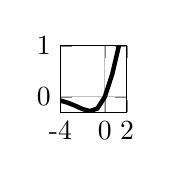
\begin{tikzpicture}
\begin{axis}[
	xmin=-4,xmax=2,
	ymin=-.3,ymax=1,
	ytick={0, 1},
	yticklabels={0,1},
	xtick={-4, 0, 2},
	xticklabels={-4,0,2},
	width=.2\textwidth,
	height=.2\textwidth,
	grid=both,
	]
	\addplot [ultra thick,domain=-4:2, samples=10]{x * (1/ (1+exp(-x)))};
	%\addplot [ultra thick,domain=-1:0.004, samples=10]{exp(x)-1};
\end{axis}
\end{tikzpicture}}
		\scalebox{.9}{% This file was created by tikzplotlib v0.9.6.
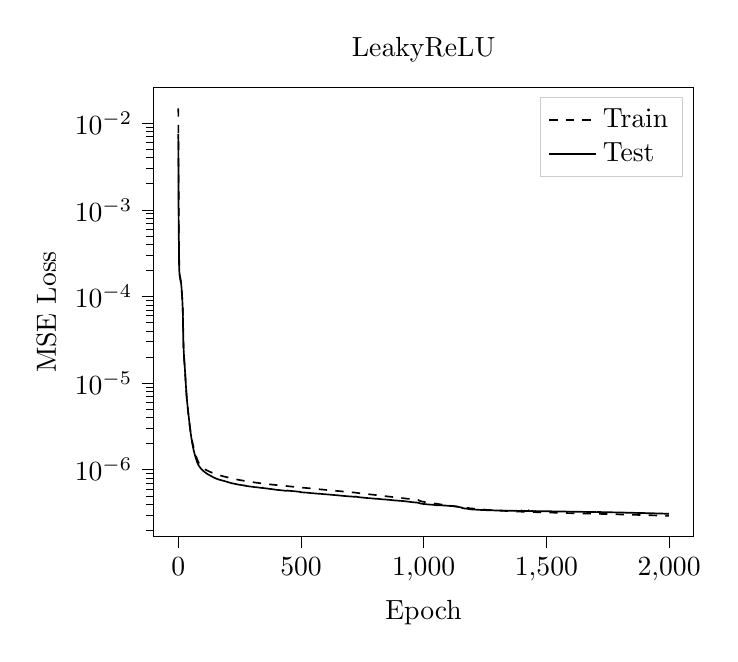
\begin{tikzpicture}

\begin{axis}[
legend cell align={left},
legend style={fill opacity=0.8, draw opacity=1, text opacity=1, draw=white!80!black},
log basis y={10},
tick align=outside,
tick pos=left,
title={LeakyReLU},
x grid style={white!69.0196078431373!black},
xlabel={Epoch},
xmin=-99.95, xmax=2098.95,
xtick style={color=black},
y grid style={white!69.0196078431373!black},
ylabel={MSE Loss},
ymin=1.70791572547231e-07, ymax=0.0255488360607333,
ymode=log,
ytick style={color=black}
]
\addplot [semithick, black, dashed]
table {%
0 0.0148644272387028
1 0.00333734963089228
2 0.000750602022744715
3 0.000331206021597609
4 0.000207027630618541
5 0.000178633672956494
6 0.000169817901289207
7 0.000163992511370452
8 0.000158428034461394
9 0.000152649684350763
10 0.00014641946539632
11 0.000139678969775559
12 0.000132290519177332
13 0.000124130066971702
14 0.000115090908722777
15 0.000105129859155568
16 9.44059219655173e-05
17 8.3223627305415e-05
18 7.19209145499917e-05
19 5.9600600565318e-05
20 3.97648699054116e-05
21 2.79329969580431e-05
22 2.30094661437761e-05
23 2.03421610876831e-05
24 1.84593141466394e-05
25 1.68413770406914e-05
26 1.53453861585149e-05
27 1.39403166676857e-05
28 1.26229516022249e-05
29 1.13995978695129e-05
30 1.02803903319e-05
31 9.27881336542669e-06
32 8.39881708566281e-06
33 7.63946547408523e-06
34 6.99144020211406e-06
35 6.44443027772468e-06
36 5.98577112725707e-06
37 5.59156097597224e-06
38 5.24542606149225e-06
39 4.93420651258703e-06
40 4.64607294458119e-06
41 4.3748265293857e-06
42 4.12039487252969e-06
43 3.8861643104724e-06
44 3.67260006765946e-06
45 3.47844123746199e-06
46 3.30225424215769e-06
47 3.13898743047503e-06
48 2.98947314900033e-06
49 2.85182592716637e-06
50 2.72762016362549e-06
51 2.61402293841684e-06
52 2.5099930834358e-06
53 2.4150706948376e-06
54 2.32725503445863e-06
55 2.24705749849363e-06
56 2.17294952142311e-06
57 2.1049157987818e-06
58 2.04128094503631e-06
59 1.98188082879369e-06
60 1.92642735390791e-06
61 1.87334052122878e-06
62 1.8232318035416e-06
63 1.77455488795886e-06
64 1.72895183959554e-06
65 1.6861234399812e-06
66 1.64616296456188e-06
67 1.60743973128774e-06
68 1.57055133320227e-06
69 1.53456863944257e-06
70 1.50125948277946e-06
71 1.46981972636695e-06
72 1.44026260474561e-06
73 1.41147857323176e-06
74 1.38520127060815e-06
75 1.36031598432851e-06
76 1.33676044734443e-06
77 1.3148170181978e-06
78 1.29389646752998e-06
79 1.27433537693378e-06
80 1.25646557970072e-06
81 1.2384471808673e-06
82 1.22196116879536e-06
83 1.20638403507201e-06
84 1.19190501561661e-06
85 1.17844780726273e-06
86 1.16571712385394e-06
87 1.1539444496691e-06
88 1.14418008098482e-06
89 1.13371917686322e-06
90 1.12408099414552e-06
91 1.1148123342366e-06
92 1.10610182443338e-06
93 1.09807221093661e-06
94 1.09074505050444e-06
95 1.0839480192999e-06
96 1.07734048407337e-06
97 1.07122849982488e-06
98 1.06452712140026e-06
99 1.05868495271011e-06
100 1.05291415113129e-06
101 1.04752679743569e-06
102 1.04214536537484e-06
103 1.0370281889891e-06
104 1.032027342319e-06
105 1.02744560464885e-06
106 1.02279366436164e-06
107 1.01820316623957e-06
108 1.01401851819105e-06
109 1.00975107895351e-06
110 1.0057904348173e-06
111 1.00208405191893e-06
112 9.98241210339756e-07
113 9.94370888776075e-07
114 9.90925482227567e-07
115 9.87395259301138e-07
116 9.83861367387817e-07
117 9.80596522055066e-07
118 9.77371847994846e-07
119 9.74262288309546e-07
120 9.71295058008082e-07
121 9.6826150081597e-07
122 9.6523639768975e-07
123 9.62448905852398e-07
124 9.59402455919189e-07
125 9.56513887700794e-07
126 9.53868651834e-07
127 9.51033602575535e-07
128 9.48263187240173e-07
129 9.45597496013306e-07
130 9.42952355558191e-07
131 9.40403254958255e-07
132 9.37919000818965e-07
133 9.35487815553415e-07
134 9.33048935337411e-07
135 9.30687048224854e-07
136 9.28267845239361e-07
137 9.25884347481087e-07
138 9.23637938910815e-07
139 9.21227984548523e-07
140 9.18846620891145e-07
141 9.16484609831514e-07
142 9.14296656503666e-07
143 9.12058346074218e-07
144 9.09871440057941e-07
145 9.07786169506153e-07
146 9.05647660886189e-07
147 9.03635627963695e-07
148 9.01687872357115e-07
149 8.9950875153022e-07
150 8.97521426622916e-07
151 8.95521069111282e-07
152 8.93521177772527e-07
153 8.91522843943449e-07
154 8.89579697087584e-07
155 8.87620785334775e-07
156 8.85896789583285e-07
157 8.83988975402872e-07
158 8.82208881847646e-07
159 8.80398930121373e-07
160 8.78538994015798e-07
161 8.76403134441262e-07
162 8.7463463688664e-07
163 8.72705812355434e-07
164 8.70566312670462e-07
165 8.68765719644671e-07
166 8.67004338203969e-07
167 8.653048454903e-07
168 8.63512691211099e-07
169 8.61854937170392e-07
170 8.60151822223543e-07
171 8.58458075072122e-07
172 8.56818996624043e-07
173 8.55136690688596e-07
174 8.53585893565878e-07
175 8.5187854273272e-07
176 8.50357727699702e-07
177 8.48755360294717e-07
178 8.47190044481749e-07
179 8.45670013589483e-07
180 8.44131327013997e-07
181 8.42642410887606e-07
182 8.41175444946884e-07
183 8.39656288363244e-07
184 8.38167764982245e-07
185 8.36532800619239e-07
186 8.35078147304102e-07
187 8.33758716908051e-07
188 8.32371983960911e-07
189 8.30889671789237e-07
190 8.29568857710683e-07
191 8.28064573511256e-07
192 8.26631372348174e-07
193 8.25454969628936e-07
194 8.24060114283043e-07
195 8.22638993369651e-07
196 8.2126220449652e-07
197 8.19915930264869e-07
198 8.20267484073156e-07
199 8.18703642607943e-07
200 8.17248432568363e-07
201 8.15823900992996e-07
202 8.14442585394204e-07
203 8.13095293437982e-07
204 8.11669069307186e-07
205 8.10307857349812e-07
206 8.09004709736882e-07
207 8.07590666070723e-07
208 8.06252364142779e-07
209 8.04654392212001e-07
210 8.0335848272739e-07
211 8.02302690658507e-07
212 8.00962444145625e-07
213 7.99703646720218e-07
214 7.98452317255283e-07
215 7.97217591738786e-07
216 7.96002158963915e-07
217 7.9481069326448e-07
218 7.93627711118461e-07
219 7.92467858858004e-07
220 7.91300207737322e-07
221 7.90077528890265e-07
222 7.88920517678093e-07
223 7.87720634576772e-07
224 7.86578616626343e-07
225 7.85441414691945e-07
226 7.84363267499089e-07
227 7.83269696910338e-07
228 7.82192492366107e-07
229 7.81227263516371e-07
230 7.80163437795522e-07
231 7.79063238198319e-07
232 7.78027706374473e-07
233 7.76964129954649e-07
234 7.75930989362905e-07
235 7.74893729442283e-07
236 7.73837977973813e-07
237 7.72835657613768e-07
238 7.71838034495431e-07
239 7.70846074615861e-07
240 7.69821481426902e-07
241 7.68822976212391e-07
242 7.67821201534957e-07
243 7.66846018862566e-07
244 7.65887867913762e-07
245 7.64930361214056e-07
246 7.63921686242952e-07
247 7.63010957257393e-07
248 7.62070085571054e-07
249 7.61139531945787e-07
250 7.60420157376984e-07
251 7.59426636150806e-07
252 7.58426511922039e-07
253 7.57507968302207e-07
254 7.56569720863354e-07
255 7.55625533727766e-07
256 7.54756878393437e-07
257 7.53833237837398e-07
258 7.52968338730398e-07
259 7.52147672017145e-07
260 7.51202681499308e-07
261 7.50205559867823e-07
262 7.4943015475526e-07
263 7.48610954261153e-07
264 7.47677468453389e-07
265 7.46997857405063e-07
266 7.46052829256882e-07
267 7.45165411899507e-07
268 7.44340018613343e-07
269 7.43665318836406e-07
270 7.42747071726058e-07
271 7.4204888295526e-07
272 7.41131473191103e-07
273 7.40440178674362e-07
274 7.39578193176271e-07
275 7.3881461977976e-07
276 7.37799187660926e-07
277 7.37035187341917e-07
278 7.36253217098692e-07
279 7.35415127010697e-07
280 7.34686662354989e-07
281 7.33878230974483e-07
282 7.33114714989824e-07
283 7.32347263181055e-07
284 7.31621643978997e-07
285 7.30857068063529e-07
286 7.30129704550109e-07
287 7.29444917936917e-07
288 7.28688947859268e-07
289 7.28014880451156e-07
290 7.27137706519443e-07
291 7.2640715151806e-07
292 7.25708816418091e-07
293 7.25009155303269e-07
294 7.24293989392777e-07
295 7.23561567397724e-07
296 7.2286156442658e-07
297 7.22185449788526e-07
298 7.21465641959185e-07
299 7.20789148289214e-07
300 7.20108953458976e-07
301 7.19449026178154e-07
302 7.18764739445987e-07
303 7.18094917701251e-07
304 7.17464760171538e-07
305 7.16808219209497e-07
306 7.16184726542224e-07
307 7.15528395758724e-07
308 7.14873352649192e-07
309 7.14168571732898e-07
310 7.13574344160861e-07
311 7.1287063936154e-07
312 7.12281224224398e-07
313 7.11596599359154e-07
314 7.1101726477707e-07
315 7.10344048059142e-07
316 7.09744001042623e-07
317 7.09173813802977e-07
318 7.08501808716733e-07
319 7.07896837610633e-07
320 7.07197004814475e-07
321 7.06599812318132e-07
322 7.05917090755293e-07
323 7.05374840876516e-07
324 7.04819606951901e-07
325 7.04185838287685e-07
326 7.03570776934725e-07
327 7.02973159619091e-07
328 7.02457169694526e-07
329 7.01814170426474e-07
330 7.01159818504493e-07
331 7.00675139412965e-07
332 7.00100038670826e-07
333 6.9944516293674e-07
334 6.98911392788659e-07
335 6.98320728275803e-07
336 6.97682788128873e-07
337 6.97246098184223e-07
338 6.96686453053985e-07
339 6.96352869169914e-07
340 6.95526991592033e-07
341 6.9484590517277e-07
342 6.94304655056044e-07
343 6.9400206361081e-07
344 6.92970413965099e-07
345 6.93037260532492e-07
346 6.92013609636888e-07
347 6.91989935560855e-07
348 6.90816037362652e-07
349 6.9062005174203e-07
350 6.89722630539791e-07
351 6.89461848594419e-07
352 6.88598280333963e-07
353 6.88385519012513e-07
354 6.87496540834331e-07
355 6.87273249681653e-07
356 6.86344381364279e-07
357 6.85784922154653e-07
358 6.85309239756293e-07
359 6.8513359936162e-07
360 6.84244536785172e-07
361 6.84097153609287e-07
362 6.83162119059943e-07
363 6.82782644759072e-07
364 6.82589405883505e-07
365 6.8159318890082e-07
366 6.81068037124533e-07
367 6.80618575174208e-07
368 6.80053423749882e-07
369 6.79640693476813e-07
370 6.79050741510423e-07
371 6.78609955187426e-07
372 6.78057203842286e-07
373 6.77662977224713e-07
374 6.77112505997002e-07
375 6.76636222607385e-07
376 6.76250711990178e-07
377 6.75681376677062e-07
378 6.75209785029551e-07
379 6.74681991128523e-07
380 6.74513683136979e-07
381 6.73722616213013e-07
382 6.73302310929102e-07
383 6.72808587580676e-07
384 6.72407056214297e-07
385 6.71915421463609e-07
386 6.71427296765614e-07
387 6.71025953465687e-07
388 6.7049164735522e-07
389 6.70016919258387e-07
390 6.69557675067267e-07
391 6.69086867844726e-07
392 6.68597802928161e-07
393 6.68190762553422e-07
394 6.67692410345921e-07
395 6.67240023972226e-07
396 6.66790877019707e-07
397 6.66323490648324e-07
398 6.65903456606998e-07
399 6.65471397070405e-07
400 6.65007362329106e-07
401 6.64616963959475e-07
402 6.64189005348703e-07
403 6.63769749593257e-07
404 6.63356940961535e-07
405 6.62935873677384e-07
406 6.6251740221901e-07
407 6.62097921363625e-07
408 6.61683327294327e-07
409 6.61271375818728e-07
410 6.60858302936163e-07
411 6.60460645164562e-07
412 6.6005227745336e-07
413 6.59639243394849e-07
414 6.5922696452958e-07
415 6.58827367658432e-07
416 6.58425498315296e-07
417 6.5801929646625e-07
418 6.57625117895577e-07
419 6.57224236348952e-07
420 6.5661854195298e-07
421 6.56017475847648e-07
422 6.55518018916723e-07
423 6.55074278228085e-07
424 6.54699447096618e-07
425 6.54264191396692e-07
426 6.53816869700563e-07
427 6.53326964823009e-07
428 6.52873706030732e-07
429 6.52448715413811e-07
430 6.51987482811478e-07
431 6.51630326260033e-07
432 6.51166140116288e-07
433 6.50728281328838e-07
434 6.50352801045528e-07
435 6.49924126832957e-07
436 6.49520926629066e-07
437 6.49109188529451e-07
438 6.48725988511956e-07
439 6.48329360970479e-07
440 6.47936029650964e-07
441 6.47537012639532e-07
442 6.47503992468046e-07
443 6.47304684633809e-07
444 6.46791755926301e-07
445 6.46174046053716e-07
446 6.45631595219243e-07
447 6.45148015280483e-07
448 6.4464382931817e-07
449 6.44142668491554e-07
450 6.4371638593741e-07
451 6.4329291483034e-07
452 6.42818815379087e-07
453 6.4243620757054e-07
454 6.41965242266451e-07
455 6.41560947940434e-07
456 6.4108713894484e-07
457 6.40711664800619e-07
458 6.40245212196078e-07
459 6.39877146284107e-07
460 6.39416840158447e-07
461 6.38994611691146e-07
462 6.38533215393977e-07
463 6.38164307375177e-07
464 6.37705450529324e-07
465 6.37337720817754e-07
466 6.36884023322182e-07
467 6.36565714486892e-07
468 6.35994193231681e-07
469 6.35576846804042e-07
470 6.35110142454209e-07
471 6.34726450087442e-07
472 6.34274996968998e-07
473 6.33879317220476e-07
474 6.33418987760592e-07
475 6.33054129139055e-07
476 6.32558955913964e-07
477 6.32200792907156e-07
478 6.31757687600043e-07
479 6.31408914216536e-07
480 6.30983657273987e-07
481 6.30627516443383e-07
482 6.30192174881472e-07
483 6.29844393728263e-07
484 6.29409517699742e-07
485 6.29049891742284e-07
486 6.28630618265902e-07
487 6.28272145732467e-07
488 6.27843531489702e-07
489 6.27503492012238e-07
490 6.27080744209252e-07
491 6.26735475819373e-07
492 6.26306154430267e-07
493 6.25968398722421e-07
494 6.25546789720488e-07
495 6.25211958649174e-07
496 6.24788373372098e-07
497 6.24449280010708e-07
498 6.23962057133554e-07
499 6.23558213717956e-07
500 6.2311415599936e-07
501 6.22750209018363e-07
502 6.22350057199128e-07
503 6.21995929662944e-07
504 6.21580487475626e-07
505 6.21248701463628e-07
506 6.20837227202742e-07
507 6.20487857943885e-07
508 6.2008267529734e-07
509 6.19707906508893e-07
510 6.19289868623696e-07
511 6.18935109201857e-07
512 6.18535905800854e-07
513 6.18207967761464e-07
514 6.17810335668878e-07
515 6.17487754837498e-07
516 6.17048165693745e-07
517 6.16747607693924e-07
518 6.16425678529708e-07
519 6.16018937733998e-07
520 6.15564609120156e-07
521 6.15231403671146e-07
522 6.14803654485741e-07
523 6.14466882382203e-07
524 6.13926075146765e-07
525 6.13603320687162e-07
526 6.13164834007307e-07
527 6.12889333567068e-07
528 6.1244176531261e-07
529 6.12171113900217e-07
530 6.11737456409855e-07
531 6.11406537032622e-07
532 6.10991987372245e-07
533 6.10615803282144e-07
534 6.10182909497325e-07
535 6.09855354056776e-07
536 6.09413068900722e-07
537 6.09052085394524e-07
538 6.08653819512028e-07
539 6.08387478564509e-07
540 6.07961950962022e-07
541 6.07622395477847e-07
542 6.07195113218495e-07
543 6.06802663170924e-07
544 6.06362741748967e-07
545 6.06013731712096e-07
546 6.0559248045422e-07
547 6.05250503625143e-07
548 6.04716681607442e-07
549 6.04371584088881e-07
550 6.03937985829361e-07
551 6.03589404704508e-07
552 6.03148568060874e-07
553 6.02801457745272e-07
554 6.0235625136329e-07
555 6.01985544463446e-07
556 6.01539943161811e-07
557 6.01232765262694e-07
558 6.00807006364335e-07
559 6.00492180907963e-07
560 6.0005816808939e-07
561 5.99730774595741e-07
562 5.99223440019614e-07
563 5.98925630910685e-07
564 5.98511263632418e-07
565 5.98205809396291e-07
566 5.97765539339434e-07
567 5.97455265236135e-07
568 5.97010945085685e-07
569 5.9672484819373e-07
570 5.96299604083583e-07
571 5.96071399556308e-07
572 5.95513366789646e-07
573 5.95187032928379e-07
574 5.947183740318e-07
575 5.94433451610144e-07
576 5.93983866451708e-07
577 5.93703354780928e-07
578 5.93230489997154e-07
579 5.92965793160261e-07
580 5.92490404656587e-07
581 5.92217652197746e-07
582 5.9175461059624e-07
583 5.91483319766439e-07
584 5.91055219629766e-07
585 5.9077541931174e-07
586 5.90313007251098e-07
587 5.90037488734652e-07
588 5.89601683429919e-07
589 5.89313242372214e-07
590 5.88861738904711e-07
591 5.88606085244692e-07
592 5.88205910432293e-07
593 5.87919526992664e-07
594 5.8745086768397e-07
595 5.87203168748829e-07
596 5.86743687904345e-07
597 5.86504606161498e-07
598 5.86034405827718e-07
599 5.85759843318101e-07
600 5.85295431378086e-07
601 5.85048269172717e-07
602 5.84578794146751e-07
603 5.84336741496827e-07
604 5.83889424504491e-07
605 5.8371987589112e-07
606 5.83250819758518e-07
607 5.82936998782202e-07
608 5.82475648911895e-07
609 5.822194414975e-07
610 5.81760691360955e-07
611 5.81514034749375e-07
612 5.8107778048111e-07
613 5.80798643440517e-07
614 5.8034996423828e-07
615 5.8007643750102e-07
616 5.79669754557699e-07
617 5.79423551016589e-07
618 5.78947847898803e-07
619 5.7868813833295e-07
620 5.78234088450813e-07
621 5.77960293540514e-07
622 5.7753287774176e-07
623 5.77290330667779e-07
624 5.76830392489569e-07
625 5.76586579811078e-07
626 5.76101825032538e-07
627 5.75859893572783e-07
628 5.75397084972451e-07
629 5.75150781202183e-07
630 5.74713401903182e-07
631 5.7447310602754e-07
632 5.74012735526708e-07
633 5.73774994833798e-07
634 5.73327271069957e-07
635 5.73114834153898e-07
636 5.72660245197199e-07
637 5.7240989970353e-07
638 5.71956064860046e-07
639 5.71697264476256e-07
640 5.71240307664311e-07
641 5.70994088292309e-07
642 5.70539148810667e-07
643 5.70304007425193e-07
644 5.69833525858598e-07
645 5.69588442289159e-07
646 5.69132603871481e-07
647 5.68892071527216e-07
648 5.68438184046727e-07
649 5.68201071160956e-07
650 5.67769946428598e-07
651 5.67519301142738e-07
652 5.6707707179271e-07
653 5.66797595681123e-07
654 5.66352859991071e-07
655 5.66096162472718e-07
656 5.65686599273363e-07
657 5.65438366834314e-07
658 5.65017211897612e-07
659 5.64772737391195e-07
660 5.64293594010223e-07
661 5.64047870213358e-07
662 5.63645380410094e-07
663 5.63384342626705e-07
664 5.62980142362335e-07
665 5.62727795866635e-07
666 5.62271209290088e-07
667 5.62005503908836e-07
668 5.61633367738068e-07
669 5.61361019336459e-07
670 5.60907587512816e-07
671 5.60647555943206e-07
672 5.60207655595946e-07
673 5.59965208736912e-07
674 5.59675780166913e-07
675 5.59391941266085e-07
676 5.58971077055048e-07
677 5.58727743012355e-07
678 5.58255349702108e-07
679 5.5799404208301e-07
680 5.5754053700241e-07
681 5.57285783443717e-07
682 5.56846114776022e-07
683 5.56599550662895e-07
684 5.56152776738372e-07
685 5.55905638606191e-07
686 5.55450992109741e-07
687 5.55227351341614e-07
688 5.54761071512644e-07
689 5.54549272450799e-07
690 5.54089646058742e-07
691 5.53867962665322e-07
692 5.53422880528842e-07
693 5.5320079773935e-07
694 5.5274819114004e-07
695 5.52521287801255e-07
696 5.5206996151469e-07
697 5.51794728323784e-07
698 5.51397915060647e-07
699 5.5119633870504e-07
700 5.50707732926981e-07
701 5.50483585669781e-07
702 5.5005929785068e-07
703 5.49791805909194e-07
704 5.49363092531507e-07
705 5.49153537050984e-07
706 5.48734435838583e-07
707 5.48524624861102e-07
708 5.48033714892426e-07
709 5.47864530929587e-07
710 5.47407044180659e-07
711 5.47192967673027e-07
712 5.46663945314663e-07
713 5.46469165058738e-07
714 5.46026377676867e-07
715 5.45797743370713e-07
716 5.45408502446776e-07
717 5.45146161812227e-07
718 5.44686208826306e-07
719 5.4444843793533e-07
720 5.44042121731536e-07
721 5.44187411392727e-07
722 5.43547544765488e-07
723 5.42903439722409e-07
724 5.42304797178872e-07
725 5.41774102529757e-07
726 5.41298678271573e-07
727 5.40787423858546e-07
728 5.40312020774536e-07
729 5.39910445837677e-07
730 5.39371933314214e-07
731 5.39032324013533e-07
732 5.38397320511308e-07
733 5.38005847772638e-07
734 5.37580982125974e-07
735 5.37113240582698e-07
736 5.36665524890623e-07
737 5.3628786932336e-07
738 5.35821611535425e-07
739 5.3551504601046e-07
740 5.34989343293546e-07
741 5.34692306075613e-07
742 5.34238284117805e-07
743 5.33852620080211e-07
744 5.33480754000948e-07
745 5.33024487040734e-07
746 5.32662216912172e-07
747 5.32245440751922e-07
748 5.31847421598286e-07
749 5.31583600732688e-07
750 5.31042589130948e-07
751 5.30784487636993e-07
752 5.30310267848222e-07
753 5.30027119310716e-07
754 5.29521326086524e-07
755 5.29201154762404e-07
756 5.28709079290479e-07
757 5.28442658435324e-07
758 5.27953152186456e-07
759 5.27690907290435e-07
760 5.27205177448309e-07
761 5.26892414683289e-07
762 5.26405703695332e-07
763 5.26151932234598e-07
764 5.25638900228387e-07
765 5.2538255179968e-07
766 5.24913538470173e-07
767 5.24627415103396e-07
768 5.24143547863787e-07
769 5.23870203437582e-07
770 5.23359917082189e-07
771 5.23059499315082e-07
772 5.22546751852815e-07
773 5.22258667359665e-07
774 5.21781591501735e-07
775 5.21461515333499e-07
776 5.21047451144341e-07
777 5.20667105519124e-07
778 5.20264812351456e-07
779 5.19935537340643e-07
780 5.19469053031685e-07
781 5.19178764761818e-07
782 5.18717480986197e-07
783 5.18486472344648e-07
784 5.18063059260498e-07
785 5.1770965706055e-07
786 5.17317782481541e-07
787 5.17047028139928e-07
788 5.16598040718463e-07
789 5.16272202006007e-07
790 5.15890133598873e-07
791 5.1559194417905e-07
792 5.15092240675585e-07
793 5.14856525086316e-07
794 5.14366608740602e-07
795 5.14138488711069e-07
796 5.1369179050198e-07
797 5.133947706355e-07
798 5.1297357916269e-07
799 5.1269512967167e-07
800 5.12259364455758e-07
801 5.1196938757414e-07
802 5.11423140920897e-07
803 5.11186035765832e-07
804 5.108558257092e-07
805 5.10589589111987e-07
806 5.10150635591344e-07
807 5.09905413366596e-07
808 5.09488112413692e-07
809 5.0918477496964e-07
810 5.08788510359182e-07
811 5.08506359878424e-07
812 5.08111304810654e-07
813 5.07820337901421e-07
814 5.07405267313743e-07
815 5.07125847690304e-07
816 5.06688020934121e-07
817 5.06418203016779e-07
818 5.05994589261149e-07
819 5.05725315562699e-07
820 5.05358103424669e-07
821 5.05075605559568e-07
822 5.04433651911995e-07
823 5.04046690537052e-07
824 5.03614987664491e-07
825 5.03243534893727e-07
826 5.02741254081229e-07
827 5.02363778650761e-07
828 5.0181188987608e-07
829 5.01155536113629e-07
830 5.00639151781002e-07
831 5.00094774650961e-07
832 4.99718042917152e-07
833 4.99335891149144e-07
834 4.98984696335469e-07
835 4.98626764695587e-07
836 4.98176735277411e-07
837 4.97781516273221e-07
838 4.97396944084016e-07
839 4.97024179267669e-07
840 4.96623089802029e-07
841 4.9619203473128e-07
842 4.95837466530702e-07
843 4.95356492848487e-07
844 4.94947353985253e-07
845 4.94624493896367e-07
846 4.94189927721322e-07
847 4.93753210434988e-07
848 4.93364277460273e-07
849 4.93005060846485e-07
850 4.92574361317111e-07
851 4.92261623520562e-07
852 4.91839595838428e-07
853 4.91472612594634e-07
854 4.91078210103524e-07
855 4.90717624558101e-07
856 4.90344198198045e-07
857 4.89971666482347e-07
858 4.89575231455319e-07
859 4.89207917780732e-07
860 4.8886572173501e-07
861 4.88452469610934e-07
862 4.88092318505551e-07
863 4.87744442438043e-07
864 4.87433638966195e-07
865 4.87001789679198e-07
866 4.86642392530712e-07
867 4.86256370052729e-07
868 4.85970414203507e-07
869 4.85520277266005e-07
870 4.85194746914885e-07
871 4.84795060486931e-07
872 4.8450660469257e-07
873 4.84076300665492e-07
874 4.83778275267355e-07
875 4.83363721940577e-07
876 4.83014998721387e-07
877 4.82567401576262e-07
878 4.82165626024766e-07
879 4.81873086187079e-07
880 4.81442710679403e-07
881 4.81068505791882e-07
882 4.80751659097223e-07
883 4.80426024751068e-07
884 4.80023959966047e-07
885 4.796470899322e-07
886 4.79263505340555e-07
887 4.78941620059459e-07
888 4.78609426863841e-07
889 4.78185967480727e-07
890 4.77746801095691e-07
891 4.77495924258164e-07
892 4.77138562104074e-07
893 4.76734690607827e-07
894 4.76396770054066e-07
895 4.76033359916528e-07
896 4.75629839783664e-07
897 4.7529189306772e-07
898 4.75028509299591e-07
899 4.74598706588836e-07
900 4.74232805089514e-07
901 4.73863658129403e-07
902 4.73503784462537e-07
903 4.73214756993912e-07
904 4.72819625130683e-07
905 4.72471625627691e-07
906 4.72109106254948e-07
907 4.71858331579256e-07
908 4.71460500378384e-07
909 4.71170830238066e-07
910 4.70762764038568e-07
911 4.70420068552357e-07
912 4.70193007899411e-07
913 4.69732255297117e-07
914 4.69328430256155e-07
915 4.69008694636841e-07
916 4.68750404195362e-07
917 4.68294574801575e-07
918 4.67943003044979e-07
919 4.67603833413932e-07
920 4.6726228927696e-07
921 4.67024187202014e-07
922 4.66549970042252e-07
923 4.66196309801603e-07
924 4.65849686818842e-07
925 4.65657492441096e-07
926 4.6514172363743e-07
927 4.6484536051139e-07
928 4.64433631279348e-07
929 4.64285816306642e-07
930 4.63722799736388e-07
931 4.63393946745327e-07
932 4.63028061346904e-07
933 4.62868733578148e-07
934 4.62303378796491e-07
935 4.61944667279113e-07
936 4.61593672994809e-07
937 4.61465650644755e-07
938 4.60907661022247e-07
939 4.60600220463903e-07
940 4.6021002177099e-07
941 4.59943743535973e-07
942 4.59559822544975e-07
943 4.59191470767451e-07
944 4.58823429340782e-07
945 4.58568544715376e-07
946 4.58253700188038e-07
947 4.57775354860246e-07
948 4.57443201653973e-07
949 4.57248985242131e-07
950 4.56788529746177e-07
951 4.56413603274086e-07
952 4.56049293291017e-07
953 4.55718323721044e-07
954 4.55268215404203e-07
955 4.54996806922736e-07
956 4.54735002605844e-07
957 4.54331303615163e-07
958 4.53895254239001e-07
959 4.53565293838665e-07
960 4.53295954372379e-07
961 4.52920906539589e-07
962 4.52633616063736e-07
963 4.52290183702075e-07
964 4.51753988272685e-07
965 4.51526366362032e-07
966 4.51130627027396e-07
967 4.50771134154593e-07
968 4.504252864308e-07
969 4.50136636729326e-07
970 4.49762404599596e-07
971 4.4941030162704e-07
972 4.49197960506353e-07
973 4.48709193022978e-07
974 4.48431595785337e-07
975 4.48094398578291e-07
976 4.4774719881957e-07
977 4.47329700762111e-07
978 4.47107959246296e-07
979 4.45311586858566e-07
980 4.42267165908561e-07
981 4.41070118895937e-07
982 4.40142427535761e-07
983 4.39295067039325e-07
984 4.38643088358504e-07
985 4.36957642435232e-07
986 4.35593108733201e-07
987 4.34702707551082e-07
988 4.33474616400531e-07
989 4.32703829105208e-07
990 4.32289674321851e-07
991 4.31421487917305e-07
992 4.30638353520862e-07
993 4.29790937616303e-07
994 4.28880565337408e-07
995 4.28401135650347e-07
996 4.27787201346064e-07
997 4.27183281047405e-07
998 4.26694344852763e-07
999 4.2636703791743e-07
1000 4.25715062704057e-07
1001 4.25246964852022e-07
1002 4.24845545552444e-07
1003 4.24308888639757e-07
1004 4.23964489456807e-07
1005 4.23528313447719e-07
1006 4.22984388706027e-07
1007 4.225807735736e-07
1008 4.22272394018819e-07
1009 4.21754303317812e-07
1010 4.21508764347323e-07
1011 4.20943191883794e-07
1012 4.20336185086967e-07
1013 4.19858491000014e-07
1014 4.1939585513262e-07
1015 4.19118752247982e-07
1016 4.18458747006412e-07
1017 4.18054913723154e-07
1018 4.17623710319504e-07
1019 4.17345911756684e-07
1020 4.1684959707311e-07
1021 4.16479742753495e-07
1022 4.16232555934926e-07
1023 4.1558006725495e-07
1024 4.15228342362184e-07
1025 4.15229226916836e-07
1026 4.14557101422019e-07
1027 4.14188685837757e-07
1028 4.137652676377e-07
1029 4.13552009050022e-07
1030 4.13012748268216e-07
1031 4.12709136242029e-07
1032 4.12403044578014e-07
1033 4.12024662679755e-07
1034 4.11686833103886e-07
1035 4.11097062823274e-07
1036 4.11059944923409e-07
1037 4.10612124298382e-07
1038 4.10058860069284e-07
1039 4.09830215701845e-07
1040 4.09236865593243e-07
1041 4.08992037847611e-07
1042 4.08167432894402e-07
1043 4.07781641527549e-07
1044 4.07499990515703e-07
1045 4.06984923031928e-07
1046 4.06398309621636e-07
1047 4.06130208801869e-07
1048 4.05844250565224e-07
1049 4.05634460008741e-07
1050 4.05246325286157e-07
1051 4.04832696432322e-07
1052 4.04589275078138e-07
1053 4.04333232410181e-07
1054 4.0388796469415e-07
1055 4.0364550858385e-07
1056 4.03237107150289e-07
1057 4.02781264639884e-07
1058 4.02806778183162e-07
1059 4.01965887306233e-07
1060 4.01510594059573e-07
1061 4.00938951401031e-07
1062 4.00572816303679e-07
1063 4.00084503098697e-07
1064 3.99712360263038e-07
1065 3.99338280672623e-07
1066 3.98853183725123e-07
1067 3.98574016514885e-07
1068 3.98165261131567e-07
1069 3.9791169047021e-07
1070 3.97472268019783e-07
1071 3.97099917236687e-07
1072 3.96636626348368e-07
1073 3.96424626273983e-07
1074 3.96097346396118e-07
1075 3.9559541224321e-07
1076 3.95176014095e-07
1077 3.9485332503375e-07
1078 3.94414255026732e-07
1079 3.94210009147855e-07
1080 3.93897365086104e-07
1081 3.94073744161005e-07
1082 3.92707131538828e-07
1083 3.92443426818545e-07
1084 3.92263928972625e-07
1085 3.91811526995411e-07
1086 3.91438045383552e-07
1087 3.91222988042728e-07
1088 3.90767820931615e-07
1089 3.90392165115827e-07
1090 3.90058417949035e-07
1091 3.89737378512223e-07
1092 3.89416854545743e-07
1093 3.89117823701213e-07
1094 3.88820500631937e-07
1095 3.8860628005466e-07
1096 3.88284502861325e-07
1097 3.8773857590968e-07
1098 3.87415723963613e-07
1099 3.87093581963427e-07
1100 3.86819972547414e-07
1101 3.8655951644273e-07
1102 3.86174517572613e-07
1103 3.85863807807141e-07
1104 3.85488108648246e-07
1105 3.85170436189242e-07
1106 3.84719854892523e-07
1107 3.84718544239604e-07
1108 3.84024391522075e-07
1109 3.83650835544813e-07
1110 3.83382792236375e-07
1111 3.83040656402045e-07
1112 3.82753346201525e-07
1113 3.82416109658834e-07
1114 3.82373510092293e-07
1115 3.81928717573032e-07
1116 3.81812806622861e-07
1117 3.81203720849044e-07
1118 3.80974276083634e-07
1119 3.80499999522499e-07
1120 3.80254684600345e-07
1121 3.7986570839621e-07
1122 3.79738977585475e-07
1123 3.79311346222266e-07
1124 3.79113227651828e-07
1125 3.7877028913158e-07
1126 3.7836112139189e-07
1127 3.77982800344512e-07
1128 3.78119575884739e-07
1129 3.77618890752274e-07
1130 3.77162941205711e-07
1131 3.7672415348311e-07
1132 3.76497530936604e-07
1133 3.76125739251165e-07
1134 3.76046060509339e-07
1135 3.75449260715754e-07
1136 3.75253203273473e-07
1137 3.74917057925472e-07
1138 3.74622404692104e-07
1139 3.7428821870833e-07
1140 3.74284405566527e-07
1141 3.7362211756431e-07
1142 3.73366226355643e-07
1143 3.7307717714441e-07
1144 3.72830825526194e-07
1145 3.72424451896336e-07
1146 3.72418132940311e-07
1147 3.7213091133026e-07
1148 3.71713215983505e-07
1149 3.71452914535553e-07
1150 3.71178188473209e-07
1151 3.70909355197568e-07
1152 3.7053996253178e-07
1153 3.7024783931372e-07
1154 3.69873657135145e-07
1155 3.69505103691381e-07
1156 3.69253701279604e-07
1157 3.68807387985726e-07
1158 3.68308296941677e-07
1159 3.68027352777744e-07
1160 3.67674302410137e-07
1161 3.67324845441885e-07
1162 3.67093079873371e-07
1163 3.66817634045447e-07
1164 3.66528322331305e-07
1165 3.66260036969379e-07
1166 3.65974232906296e-07
1167 3.6576783041653e-07
1168 3.65757778212128e-07
1169 3.65359265160237e-07
1170 3.64927529545866e-07
1171 3.64539682664144e-07
1172 3.64183218977132e-07
1173 3.63697715883404e-07
1174 3.63248774547742e-07
1175 3.6295745351822e-07
1176 3.62568556099063e-07
1177 3.62408816727111e-07
1178 3.61902688752025e-07
1179 3.61626319858033e-07
1180 3.61431617832864e-07
1181 3.61043409355943e-07
1182 3.60797934973789e-07
1183 3.60444958303674e-07
1184 3.60248958102716e-07
1185 3.59936896558111e-07
1186 3.59555476705964e-07
1187 3.59374415111802e-07
1188 3.58965990059801e-07
1189 3.58561037799632e-07
1190 3.58322259430111e-07
1191 3.57995596175442e-07
1192 3.57769069225355e-07
1193 3.57516862507623e-07
1194 3.57242059436658e-07
1195 3.57074874074215e-07
1196 3.56846210692652e-07
1197 3.56573667573912e-07
1198 3.56349139025269e-07
1199 3.56250705209504e-07
1200 3.55875810996054e-07
1201 3.55695545266599e-07
1202 3.55430612060559e-07
1203 3.55257044837742e-07
1204 3.55036958367805e-07
1205 3.54729504230988e-07
1206 3.54575795554979e-07
1207 3.54330831036975e-07
1208 3.54163805582175e-07
1209 3.53934707121084e-07
1210 3.53760961694149e-07
1211 3.53559004942383e-07
1212 3.53348837684564e-07
1213 3.53167481250694e-07
1214 3.52938252042634e-07
1215 3.52749994284807e-07
1216 3.52585982660969e-07
1217 3.52407975704239e-07
1218 3.52169507415567e-07
1219 3.51973961208785e-07
1220 3.51758787793699e-07
1221 3.51502807255599e-07
1222 3.51306851079869e-07
1223 3.51152501224306e-07
1224 3.50899278146244e-07
1225 3.50712421344213e-07
1226 3.50511307786405e-07
1227 3.50340402199834e-07
1228 3.50174203553877e-07
1229 3.49866230820339e-07
1230 3.49717217829948e-07
1231 3.49455526098552e-07
1232 3.49285141943767e-07
1233 3.49022042534841e-07
1234 3.48864000585536e-07
1235 3.48586736819811e-07
1236 3.48445087801963e-07
1237 3.4818345256582e-07
1238 3.4813231708597e-07
1239 3.48225087407172e-07
1240 3.47784275412266e-07
1241 3.47621228634409e-07
1242 3.47436047128724e-07
1243 3.47174164780029e-07
1244 3.4713033489453e-07
1245 3.46868865150896e-07
1246 3.46827497459401e-07
1247 3.46505921307028e-07
1248 3.46359151983222e-07
1249 3.46254663149637e-07
1250 3.45973173082825e-07
1251 3.45937462505219e-07
1252 3.45498902305508e-07
1253 3.45166767687033e-07
1254 3.44957258484158e-07
1255 3.44883514060257e-07
1256 3.44460587214712e-07
1257 3.44291111339601e-07
1258 3.44095388989274e-07
1259 3.43959172042219e-07
1260 3.43810874603889e-07
1261 3.43625585593088e-07
1262 3.4358059095041e-07
1263 3.43212996391173e-07
1264 3.43100552726128e-07
1265 3.43164890786341e-07
1266 3.42759536103188e-07
1267 3.42773568959842e-07
1268 3.42893875803441e-07
1269 3.42620055683085e-07
1270 3.4228207704956e-07
1271 3.42381971016437e-07
1272 3.42026907333093e-07
1273 3.41821995505143e-07
1274 3.41681918825998e-07
1275 3.41623348312226e-07
1276 3.41340164766279e-07
1277 3.41217368152513e-07
1278 3.4106308705617e-07
1279 3.40976784691804e-07
1280 3.4080946687709e-07
1281 3.40802128683038e-07
1282 3.40702538146331e-07
1283 3.40402227969605e-07
1284 3.40182375417442e-07
1285 3.40091809910348e-07
1286 3.39915428099857e-07
1287 3.39853421358782e-07
1288 3.39670542125248e-07
1289 3.39502068037234e-07
1290 3.39417640304873e-07
1291 3.39291082688931e-07
1292 3.39082802483404e-07
1293 3.39148367032749e-07
1294 3.38892482638187e-07
1295 3.38829270653207e-07
1296 3.38648870496172e-07
1297 3.38687307959162e-07
1298 3.38240516690291e-07
1299 3.38366272508495e-07
1300 3.38001319256875e-07
1301 3.37920434652972e-07
1302 3.37841576858011e-07
1303 3.37823672431625e-07
1304 3.3753024310812e-07
1305 3.37429006513901e-07
1306 3.37313680958573e-07
1307 3.37218410713547e-07
1308 3.3711456779173e-07
1309 3.36903703832547e-07
1310 3.36891655976501e-07
1311 3.36800533723647e-07
1312 3.3659107230477e-07
1313 3.36524350629475e-07
1314 3.36588194052467e-07
1315 3.3621560381647e-07
1316 3.36227974422343e-07
1317 3.35964050691473e-07
1318 3.3590479741008e-07
1319 3.35959069197145e-07
1320 3.3563762396227e-07
1321 3.3570893973689e-07
1322 3.35404225104696e-07
1323 3.35420296941891e-07
1324 3.35310365571218e-07
1325 3.35162345130868e-07
1326 3.35112290805739e-07
1327 3.35035934234895e-07
1328 3.34863490358828e-07
1329 3.3453481590584e-07
1330 3.34560684706275e-07
1331 3.34415690289802e-07
1332 3.34436880429223e-07
1333 3.34342135964505e-07
1334 3.3411748800205e-07
1335 3.33874048642713e-07
1336 3.33887440966407e-07
1337 3.33762760767797e-07
1338 3.33557971053722e-07
1339 3.33469831780064e-07
1340 3.333395412497e-07
1341 3.33323065277114e-07
1342 3.33160623696926e-07
1343 3.33146326468636e-07
1344 3.32997630756893e-07
1345 3.32955995787643e-07
1346 3.32814051603236e-07
1347 3.3281026241383e-07
1348 3.32498229099087e-07
1349 3.32466849641833e-07
1350 3.32391293376588e-07
1351 3.32259941842494e-07
1352 3.32225231424843e-07
1353 3.32077841072476e-07
1354 3.32005728822082e-07
1355 3.31841624657159e-07
1356 3.31928920083158e-07
1357 3.31696651336699e-07
1358 3.31594936319846e-07
1359 3.31512106100718e-07
1360 3.31501672782508e-07
1361 3.31306970345224e-07
1362 3.31109461292556e-07
1363 3.31097948134129e-07
1364 3.30970878607673e-07
1365 3.30980586127794e-07
1366 3.30741880006258e-07
1367 3.30851606676674e-07
1368 3.30796594830929e-07
1369 3.30699608035445e-07
1370 3.30719720835759e-07
1371 3.30387201159965e-07
1372 3.30450337429511e-07
1373 3.30311810436967e-07
1374 3.30153512820175e-07
1375 3.30106311636769e-07
1376 3.29856312781374e-07
1377 3.29988769316003e-07
1378 3.29781705133314e-07
1379 3.29643474735519e-07
1380 3.29575802702209e-07
1381 3.29661901908196e-07
1382 3.29384446779102e-07
1383 3.29194402652888e-07
1384 3.29174147502442e-07
1385 3.2892577434751e-07
1386 3.28936768760002e-07
1387 3.28938984807792e-07
1388 3.28622693380964e-07
1389 3.28631047203487e-07
1390 3.28663743040636e-07
1391 3.28427028435385e-07
1392 3.28422970120812e-07
1393 3.28242727945849e-07
1394 3.28273688822378e-07
1395 3.28060710437228e-07
1396 3.28181209752643e-07
1397 3.27843347669443e-07
1398 3.27852344064183e-07
1399 3.2829578710647e-07
1400 3.28064131871031e-07
1401 3.27575198873831e-07
1402 3.27536251177207e-07
1403 3.27420939470358e-07
1404 3.2741662860758e-07
1405 3.27226250057322e-07
1406 3.27265470950522e-07
1407 3.27060519509814e-07
1408 3.27155963816494e-07
1409 3.26972195878739e-07
1410 3.26970149174599e-07
1411 3.26863787329046e-07
1412 3.26782263279313e-07
1413 3.26663281526862e-07
1414 3.26726319926252e-07
1415 3.26526487675949e-07
1416 3.26492149575586e-07
1417 3.26372519289464e-07
1418 3.26526134919902e-07
1419 3.26281027753339e-07
1420 3.26192927850855e-07
1421 3.26291698719672e-07
1422 3.26084324228759e-07
1423 3.26008133122002e-07
1424 3.25901496594838e-07
1425 3.25920014496717e-07
1426 3.25827025420722e-07
1427 3.25687300644972e-07
1428 3.26062531392779e-07
1429 3.25628018437385e-07
1430 3.2562565948524e-07
1431 3.25352808538071e-07
1432 3.25273427925765e-07
1433 3.25321335537865e-07
1434 3.25138781853695e-07
1435 3.25163706605736e-07
1436 3.25108598367763e-07
1437 3.24951548883234e-07
1438 3.24962143700702e-07
1439 3.24829615223621e-07
1440 3.25090830237684e-07
1441 3.24795452463889e-07
1442 3.24721973001374e-07
1443 3.24631089085869e-07
1444 3.2456479630838e-07
1445 3.24642600965319e-07
1446 3.24464752360143e-07
1447 3.24280949101308e-07
1448 3.24287003877544e-07
1449 3.24112054428838e-07
1450 3.24111770346747e-07
1451 3.24085712215094e-07
1452 3.24007598564435e-07
1453 3.23942609085748e-07
1454 3.2425689070692e-07
1455 3.24005999075894e-07
1456 3.2361437681061e-07
1457 3.23674683443187e-07
1458 3.2351173168621e-07
1459 3.23458068230309e-07
1460 3.23479223787615e-07
1461 3.23319206508188e-07
1462 3.23341757123785e-07
1463 3.23198218914911e-07
1464 3.23270411364263e-07
1465 3.23068304957985e-07
1466 3.23069969759615e-07
1467 3.23080898247952e-07
1468 3.22920393280413e-07
1469 3.22857342759164e-07
1470 3.22821105278592e-07
1471 3.22736950657543e-07
1472 3.22708666047333e-07
1473 3.22561187388715e-07
1474 3.2244668971515e-07
1475 3.22537584629856e-07
1476 3.2234767521544e-07
1477 3.22275564869301e-07
1478 3.22260968928845e-07
1479 3.22126612921636e-07
1480 3.22229529807316e-07
1481 3.22072553345265e-07
1482 3.21982909795793e-07
1483 3.22065536110472e-07
1484 3.21898457372072e-07
1485 3.21896749035488e-07
1486 3.21722710658889e-07
1487 3.21782155673134e-07
1488 3.21655857334235e-07
1489 3.21540387943742e-07
1490 3.21610780446235e-07
1491 3.21390835281932e-07
1492 3.21524363023684e-07
1493 3.2131500721988e-07
1494 3.21355409518276e-07
1495 3.21366403952084e-07
1496 3.2123143392937e-07
1497 3.21120906043859e-07
1498 3.21158807956579e-07
1499 3.21153666938301e-07
1500 3.20950832460198e-07
1501 3.20903004755735e-07
1502 3.20872954738149e-07
1503 3.20826174515787e-07
1504 3.20889407738889e-07
1505 3.20691754176039e-07
1506 3.20632478270966e-07
1507 3.20689533992891e-07
1508 3.20531748741359e-07
1509 3.20420759095441e-07
1510 3.20409114671349e-07
1511 3.20266171875971e-07
1512 3.20465706288076e-07
1513 3.20110148116726e-07
1514 3.20114583416853e-07
1515 3.20165127867256e-07
1516 3.19939939579683e-07
1517 3.19961420586878e-07
1518 3.19884608479981e-07
1519 3.19850591942838e-07
1520 3.19754192247501e-07
1521 3.19659825549934e-07
1522 3.19542471565626e-07
1523 3.19522271233552e-07
1524 3.1952513759137e-07
1525 3.19442034466988e-07
1526 3.19308484826308e-07
1527 3.1926437686991e-07
1528 3.19322454409132e-07
1529 3.19090354508944e-07
1530 3.1914903206598e-07
1531 3.19048935295996e-07
1532 3.18985352343759e-07
1533 3.18868792234639e-07
1534 3.18823600416351e-07
1535 3.18969249775591e-07
1536 3.18667938614681e-07
1537 3.18681215368599e-07
1538 3.18583031408082e-07
1539 3.18604212985463e-07
1540 3.18418979318835e-07
1541 3.1837250921285e-07
1542 3.18446168733999e-07
1543 3.18235732798655e-07
1544 3.1822591738262e-07
1545 3.18200680894165e-07
1546 3.1824155977489e-07
1547 3.18066145119644e-07
1548 3.17969742788193e-07
1549 3.18165659486169e-07
1550 3.17947992201084e-07
1551 3.17837663196485e-07
1552 3.17799422937526e-07
1553 3.17749503373932e-07
1554 3.17725981943795e-07
1555 3.17654856075933e-07
1556 3.1745046170073e-07
1557 3.17432104033344e-07
1558 3.17421537815221e-07
1559 3.17527532082806e-07
1560 3.17331122076325e-07
1561 3.1720363658394e-07
1562 3.17183404767718e-07
1563 3.17158790586802e-07
1564 3.17055461529492e-07
1565 3.16942562001543e-07
1566 3.17018796096136e-07
1567 3.16961415805395e-07
1568 3.16822705308084e-07
1569 3.1673548660649e-07
1570 3.1669173003479e-07
1571 3.16677336762439e-07
1572 3.16670457948476e-07
1573 3.16591517567133e-07
1574 3.16468353531718e-07
1575 3.1647522484235e-07
1576 3.16485809719325e-07
1577 3.16312855744627e-07
1578 3.16247700645533e-07
1579 3.16220362343245e-07
1580 3.16188260690353e-07
1581 3.16109383760477e-07
1582 3.16156887059549e-07
1583 3.16068575635597e-07
1584 3.15873102728403e-07
1585 3.15975026701665e-07
1586 3.15779102422198e-07
1587 3.15815761297245e-07
1588 3.15671033362719e-07
1589 3.15747237223718e-07
1590 3.15594334843183e-07
1591 3.15574065240298e-07
1592 3.15509907693468e-07
1593 3.15438409678848e-07
1594 3.15528669297294e-07
1595 3.15281006912471e-07
1596 3.15268012819558e-07
1597 3.15299097358945e-07
1598 3.15124351033091e-07
1599 3.15032143682004e-07
1600 3.14968358829049e-07
1601 3.15165431196363e-07
1602 3.14933268924733e-07
1603 3.14842066984511e-07
1604 3.14790559968969e-07
1605 3.14805405700724e-07
1606 3.14614502052279e-07
1607 3.14726759292228e-07
1608 3.14509374746308e-07
1609 3.14674117142033e-07
1610 3.14487810229025e-07
1611 3.14573937380658e-07
1612 3.14394223408954e-07
1613 3.14384523349531e-07
1614 3.14405950419427e-07
1615 3.14362090051645e-07
1616 3.14184010818508e-07
1617 3.14153501655312e-07
1618 3.14043581461476e-07
1619 3.14059152806578e-07
1620 3.13894354967204e-07
1621 3.14038598588695e-07
1622 3.14356346699185e-07
1623 3.14293879981165e-07
1624 3.14200238548779e-07
1625 3.14175397726046e-07
1626 3.13871269945309e-07
1627 3.1394368009785e-07
1628 3.13715297558304e-07
1629 3.1380694633043e-07
1630 3.13606534241728e-07
1631 3.13643690411425e-07
1632 3.13666378573885e-07
1633 3.13586880650973e-07
1634 3.13423190370088e-07
1635 3.13455884217717e-07
1636 3.13332078007988e-07
1637 3.13316120802654e-07
1638 3.13285314419431e-07
1639 3.13249966531259e-07
1640 3.13080791741527e-07
1641 3.13154238334334e-07
1642 3.12935718767449e-07
1643 3.13037454141352e-07
1644 3.12864478829056e-07
1645 3.12887611663371e-07
1646 3.12814163436315e-07
1647 3.12779923319795e-07
1648 3.12677243989867e-07
1649 3.12674668265345e-07
1650 3.12483081728487e-07
1651 3.13008835682638e-07
1652 3.12390567842158e-07
1653 3.12456071270617e-07
1654 3.1229574748437e-07
1655 3.12338921325761e-07
1656 3.12201615948027e-07
1657 3.12339854595223e-07
1658 3.12096956406549e-07
1659 3.12131471773114e-07
1660 3.11996117972058e-07
1661 3.12029497557376e-07
1662 3.11892367115263e-07
1663 3.12013563373625e-07
1664 3.11821396117296e-07
1665 3.11737066255091e-07
1666 3.11751752903433e-07
1667 3.11542458518943e-07
1668 3.11465470417716e-07
1669 3.11640546655667e-07
1670 3.11447121475794e-07
1671 3.113907667327e-07
1672 3.1128856271323e-07
1673 3.1143680404e-07
1674 3.11213553068512e-07
1675 3.11212113537351e-07
1676 3.11191033297575e-07
1677 3.11144864852508e-07
1678 3.11065440115499e-07
1679 3.11046119790603e-07
1680 3.10867254668779e-07
1681 3.11016560125665e-07
1682 3.10783246312951e-07
1683 3.10997557086523e-07
1684 3.10670550469183e-07
1685 3.10749519698561e-07
1686 3.10596976952127e-07
1687 3.10744832269449e-07
1688 3.10395399182539e-07
1689 3.10655381646541e-07
1690 3.10417983520495e-07
1691 3.10629784621597e-07
1692 3.10311370782301e-07
1693 3.1037526576938e-07
1694 3.10243405010624e-07
1695 3.10281405603519e-07
1696 3.10096623323375e-07
1697 3.10194989395995e-07
1698 3.10098258829328e-07
1699 3.10130593128122e-07
1700 3.09984979040223e-07
1701 3.09938632540252e-07
1702 3.09827980473187e-07
1703 3.09812695462597e-07
1704 3.096528067843e-07
1705 3.09828499311493e-07
1706 3.09625381632372e-07
1707 3.09750097500228e-07
1708 3.09600050115932e-07
1709 3.09845477801218e-07
1710 3.09658715913486e-07
1711 3.09539044295093e-07
1712 3.09400075131805e-07
1713 3.09725576833841e-07
1714 3.0916625053834e-07
1715 3.09483384377529e-07
1716 3.09334076376899e-07
1717 3.0918433626681e-07
1718 3.09062954308104e-07
1719 3.09123950380297e-07
1720 3.08976081434764e-07
1721 3.091337238601e-07
1722 3.08965229287139e-07
1723 3.09116053983871e-07
1724 3.08689637293469e-07
1725 3.08736328939574e-07
1726 3.08669552644858e-07
1727 3.08603466613988e-07
1728 3.08530398037021e-07
1729 3.08627115401805e-07
1730 3.08540636936527e-07
1731 3.08427530285371e-07
1732 3.08334022712131e-07
1733 3.08257495653663e-07
1734 3.08236750498736e-07
1735 3.0833639345218e-07
1736 3.08096456222984e-07
1737 3.08075279455977e-07
1738 3.08042506972583e-07
1739 3.08085389832513e-07
1740 3.07968706749762e-07
1741 3.07898931581008e-07
1742 3.07764628203699e-07
1743 3.07773813283063e-07
1744 3.07717376465177e-07
1745 3.07653958117271e-07
1746 3.0765865913196e-07
1747 3.07626101644587e-07
1748 3.07552278009382e-07
1749 3.0735350994604e-07
1750 3.07628058081377e-07
1751 3.07336489342447e-07
1752 3.07368682385345e-07
1753 3.07209660846297e-07
1754 3.07406639642238e-07
1755 3.0710762363384e-07
1756 3.07180690796827e-07
1757 3.06997296227962e-07
1758 3.07280588238257e-07
1759 3.06843731650019e-07
1760 3.06940378493437e-07
1761 3.06794261831556e-07
1762 3.06837595772436e-07
1763 3.06610467816881e-07
1764 3.06829234347106e-07
1765 3.06454595275341e-07
1766 3.06707944893958e-07
1767 3.06326688800596e-07
1768 3.06441866172236e-07
1769 3.06257395521925e-07
1770 3.0633805037894e-07
1771 3.06157528299877e-07
1772 3.06200772897114e-07
1773 3.0607316737985e-07
1774 3.06098561296153e-07
1775 3.06194833605389e-07
1776 3.06072450797501e-07
1777 3.06052589152728e-07
1778 3.0598369404089e-07
1779 3.05753781354667e-07
1780 3.05756770544008e-07
1781 3.05665897727181e-07
1782 3.05728093714208e-07
1783 3.05646801621151e-07
1784 3.05738369860364e-07
1785 3.05382987974667e-07
1786 3.05652452290417e-07
1787 3.0544395694676e-07
1788 3.05572961565304e-07
1789 3.05190016284484e-07
1790 3.05378717335714e-07
1791 3.05075413500333e-07
1792 3.05183546778665e-07
1793 3.05088814037902e-07
1794 3.05365793757062e-07
1795 3.05033719747883e-07
1796 3.05069139692193e-07
1797 3.04773875001274e-07
1798 3.04957178123288e-07
1799 3.04655040785917e-07
1800 3.04872247021137e-07
1801 3.04794242460105e-07
1802 3.04774771770155e-07
1803 3.04634256494296e-07
1804 3.046867968024e-07
1805 3.04623855846842e-07
1806 3.04478786084417e-07
1807 3.04440137668394e-07
1808 3.04489119187679e-07
1809 3.04337516880082e-07
1810 3.0426601318112e-07
1811 3.04229888918428e-07
1812 3.04097428177386e-07
1813 3.04338748520649e-07
1814 3.04042303426399e-07
1815 3.04046707569228e-07
1816 3.03893465911642e-07
1817 3.04108458379915e-07
1818 3.03728165427231e-07
1819 3.04069386402261e-07
1820 3.03660852303267e-07
1821 3.03650683463275e-07
1822 3.03544722548565e-07
1823 3.03597130113076e-07
1824 3.03506354299543e-07
1825 3.03322645812898e-07
1826 3.03617171937276e-07
1827 3.03360720117496e-07
1828 3.03249289061114e-07
1829 3.03108788607176e-07
1830 3.03273794429515e-07
1831 3.02977811173832e-07
1832 3.03072520843273e-07
1833 3.03012808892333e-07
1834 3.02839288991663e-07
1835 3.02869932504279e-07
1836 3.02772856940692e-07
1837 3.02604050183675e-07
1838 3.02785141101936e-07
1839 3.02697704505306e-07
1840 3.02647801603939e-07
1841 3.02386721486414e-07
1842 3.02443652245188e-07
1843 3.02288002671958e-07
1844 3.02339900542847e-07
1845 3.02194082941298e-07
1846 3.02256330741102e-07
1847 3.02109679132911e-07
1848 3.02255458365153e-07
1849 3.02030160554523e-07
1850 3.01960260415513e-07
1851 3.01962238040687e-07
1852 3.01846855450094e-07
1853 3.01791661499351e-07
1854 3.01770279023117e-07
1855 3.01849823351574e-07
1856 3.01669510847091e-07
1857 3.01545374682632e-07
1858 3.0151376973464e-07
1859 3.01416563644352e-07
1860 3.01456793536659e-07
1861 3.01289437224739e-07
1862 3.01354336748716e-07
1863 3.01205066875809e-07
1864 3.01245784264381e-07
1865 3.01109555174151e-07
1866 3.01183946696426e-07
1867 3.0100350952722e-07
1868 3.00976861971947e-07
1869 3.00884783449362e-07
1870 3.01047703374024e-07
1871 3.00773745493643e-07
1872 3.00733479228654e-07
1873 3.00692512261946e-07
1874 3.0063736996766e-07
1875 3.00572687713441e-07
1876 3.00503531029506e-07
1877 3.00603009335987e-07
1878 3.00401623185564e-07
1879 3.00343361367084e-07
1880 3.0032322746365e-07
1881 3.00249160275712e-07
1882 3.00184128789738e-07
1883 3.00211509483006e-07
1884 3.00067204264565e-07
1885 2.99960682831113e-07
1886 2.99978455828409e-07
1887 2.99902618976944e-07
1888 2.99820982888832e-07
1889 2.99946893044023e-07
1890 2.99692950321173e-07
1891 2.99725934681305e-07
1892 2.99663779735226e-07
1893 2.99518005547839e-07
1894 2.99473131434524e-07
1895 2.99465885760242e-07
1896 2.99575580086753e-07
1897 2.99349106128943e-07
1898 2.99262351035168e-07
1899 2.9926471443531e-07
1900 2.99133502601023e-07
1901 2.99155919819327e-07
1902 2.99006076474484e-07
1903 2.99133789390282e-07
1904 2.98925287424368e-07
1905 2.98941225764793e-07
1906 2.9879624715079e-07
1907 2.9895922090617e-07
1908 2.98671382864768e-07
1909 2.98679200191998e-07
1910 2.98591146808747e-07
1911 2.98603283383159e-07
1912 2.98482322143911e-07
1913 2.98465000426518e-07
1914 2.98486448997437e-07
1915 2.98328453361307e-07
1916 2.98258284743724e-07
1917 2.98272029993996e-07
1918 2.9815794463417e-07
1919 2.98116875256937e-07
1920 2.98200684603955e-07
1921 2.98044728452851e-07
1922 2.97941690746484e-07
1923 2.97912768431274e-07
1924 2.97862047318631e-07
1925 2.97789504678292e-07
1926 2.97767631202817e-07
1927 2.97833934823188e-07
1928 2.97641517363445e-07
1929 2.97627088585273e-07
1930 2.97398515307634e-07
1931 2.97637071803081e-07
1932 2.97316301185901e-07
1933 2.9743815220229e-07
1934 2.97396039492526e-07
1935 2.97155774788394e-07
1936 2.972102788803e-07
1937 2.97290856764221e-07
1938 2.97404336421891e-07
1939 2.97170349625731e-07
1940 2.97167980377822e-07
1941 2.97099185310401e-07
1942 2.9688234484837e-07
1943 2.96936517749202e-07
1944 2.96624542492907e-07
1945 2.97014116000582e-07
1946 2.96760317269218e-07
1947 2.96771138536656e-07
1948 2.96515731449176e-07
1949 2.9663090040799e-07
1950 2.9657164558472e-07
1951 2.9648336685284e-07
1952 2.96345633593376e-07
1953 2.9631420408549e-07
1954 2.96308615659768e-07
1955 2.9610010748371e-07
1956 2.9626472518629e-07
1957 2.9594645059916e-07
1958 2.96222448795902e-07
1959 2.95816891757283e-07
1960 2.95940765774105e-07
1961 2.95927517129257e-07
1962 2.95857750273854e-07
1963 2.95589895799253e-07
1964 2.95722840512269e-07
1965 2.95564092198219e-07
1966 2.95687444705095e-07
1967 2.95598649046269e-07
1968 2.95281853446738e-07
1969 2.95426976748558e-07
1970 2.95280896850159e-07
1971 2.95339915290072e-07
1972 2.95072210619196e-07
1973 2.95270798041258e-07
1974 2.95314228253574e-07
1975 2.94874492254849e-07
1976 2.95091132208825e-07
1977 2.95017232964767e-07
1978 2.94680657525248e-07
1979 2.94926457868883e-07
1980 2.94877394068749e-07
1981 2.94727112077453e-07
1982 2.94783511044727e-07
1983 2.94443454208704e-07
1984 2.94654638388181e-07
1985 2.94476714657321e-07
1986 2.94250058388457e-07
1987 2.94501699379168e-07
1988 2.94333003857616e-07
1989 2.94369915607717e-07
1990 2.94041497959086e-07
1991 2.94329573932828e-07
1992 2.93915225086039e-07
1993 2.94157941105766e-07
1994 2.93830951711982e-07
1995 2.94200619180174e-07
1996 2.936857129896e-07
1997 2.93928464543569e-07
1998 2.93554929328366e-07
1999 2.93835021608402e-07
};
\addlegendentry{Train}
\addplot [semithick, black]
table {%
0 0.00753973051905632
1 0.00112220819573849
2 0.000468270503915846
3 0.000248318043304607
4 0.000196054897969589
5 0.000182635383680463
6 0.000175974884768948
7 0.000170196057297289
8 0.000164347962709144
9 0.000158102775458246
10 0.000151328713400289
11 0.000143939119880088
12 0.000135805690661073
13 0.000126826635096222
14 0.000116909206553828
15 0.000106065410363954
16 9.45693464018404e-05
17 8.27783442218788e-05
18 7.09991290932521e-05
19 5.34280989086255e-05
20 3.48736466548871e-05
21 2.70838972937781e-05
22 2.34261042351136e-05
23 2.10563994187396e-05
24 1.91505496331956e-05
25 1.74150864040712e-05
26 1.57899085024837e-05
27 1.4260570424085e-05
28 1.28342044263263e-05
29 1.15238226499059e-05
30 1.03484580904478e-05
31 9.31648355617654e-06
32 8.4244802565081e-06
33 7.66550056141568e-06
34 7.02537090546684e-06
35 6.49239882477559e-06
36 6.04889373789774e-06
37 5.6686180869292e-06
38 5.33202228325536e-06
39 5.02388274981058e-06
40 4.73555610369658e-06
41 4.46143167209812e-06
42 4.2042379391205e-06
43 3.96772929889266e-06
44 3.74569435734884e-06
45 3.54057851836842e-06
46 3.34874425789167e-06
47 3.17393687510048e-06
48 3.00711985801172e-06
49 2.85115629594657e-06
50 2.70820146397455e-06
51 2.57695523941948e-06
52 2.45732940129528e-06
53 2.34697722589772e-06
54 2.24644918489503e-06
55 2.15642126022431e-06
56 2.07536072593939e-06
57 2.00157887775276e-06
58 1.93483720067888e-06
59 1.87310524779605e-06
60 1.81747736860416e-06
61 1.76416585873085e-06
62 1.71450949437713e-06
63 1.66393874678761e-06
64 1.61902949002979e-06
65 1.57635042796755e-06
66 1.53597272856132e-06
67 1.49878349020582e-06
68 1.46242962273391e-06
69 1.42895373755891e-06
70 1.39594453685277e-06
71 1.3655030670634e-06
72 1.33679156988364e-06
73 1.31049182527931e-06
74 1.28527665310685e-06
75 1.26176882986329e-06
76 1.23917902783433e-06
77 1.21781124562403e-06
78 1.19804451514938e-06
79 1.18025457140902e-06
80 1.16347860057431e-06
81 1.14884630875167e-06
82 1.13513533506193e-06
83 1.12148427433567e-06
84 1.10909911654744e-06
85 1.09722520846844e-06
86 1.08680535504391e-06
87 1.07779487734661e-06
88 1.06798745491687e-06
89 1.0591461432341e-06
90 1.04946332157851e-06
91 1.04017806279444e-06
92 1.03124625638884e-06
93 1.02401179447043e-06
94 1.01709372302139e-06
95 1.01110106243141e-06
96 1.00461545571306e-06
97 9.9822477750422e-07
98 9.91178580989072e-07
99 9.85206497716717e-07
100 9.79330479822238e-07
101 9.73711962615198e-07
102 9.6842666152952e-07
103 9.62833496487292e-07
104 9.57176780502778e-07
105 9.51723677644623e-07
106 9.46693774039886e-07
107 9.41506129947811e-07
108 9.36622143399291e-07
109 9.32237298911787e-07
110 9.27754456370167e-07
111 9.2338621016097e-07
112 9.18905527669267e-07
113 9.14647330318985e-07
114 9.10284541077999e-07
115 9.05852459709422e-07
116 9.01851592516323e-07
117 8.97969584912062e-07
118 8.9437349970467e-07
119 8.90859382707276e-07
120 8.87361977675027e-07
121 8.84108544596529e-07
122 8.80847039752553e-07
123 8.77792672326905e-07
124 8.75034515956941e-07
125 8.71993620421563e-07
126 8.6885069094933e-07
127 8.65411493577994e-07
128 8.61983494360175e-07
129 8.58633711686707e-07
130 8.55235782637465e-07
131 8.52439086429513e-07
132 8.49383695822326e-07
133 8.46391742470587e-07
134 8.43058558075427e-07
135 8.40330869777972e-07
136 8.37373477224901e-07
137 8.34073318856099e-07
138 8.31444708637719e-07
139 8.28168595035095e-07
140 8.24674941668491e-07
141 8.21597041067434e-07
142 8.18812679881376e-07
143 8.16037527329172e-07
144 8.13379756436916e-07
145 8.10917413218704e-07
146 8.08692959708424e-07
147 8.06455602742062e-07
148 8.04063347459305e-07
149 8.01898124791478e-07
150 7.99877341250976e-07
151 7.97855761902611e-07
152 7.93996150605381e-07
153 7.92090304457815e-07
154 7.90204524037108e-07
155 7.88448744515335e-07
156 7.8662571922905e-07
157 7.84812414167391e-07
158 7.83166683504533e-07
159 7.81366054525279e-07
160 7.79670870088012e-07
161 7.77817717789731e-07
162 7.76199499341601e-07
163 7.72695557316183e-07
164 7.71276290834066e-07
165 7.69888686136255e-07
166 7.68412576235278e-07
167 7.67246433497348e-07
168 7.65786523970746e-07
169 7.64414210152609e-07
170 7.63057585118077e-07
171 7.61939531912503e-07
172 7.60599618843116e-07
173 7.59462125188293e-07
174 7.57970269660291e-07
175 7.56672307034023e-07
176 7.55323185330781e-07
177 7.54069162667292e-07
178 7.52821165406203e-07
179 7.51177594793262e-07
180 7.50122524095787e-07
181 7.48853892673651e-07
182 7.47541378132155e-07
183 7.46298724152439e-07
184 7.45096542686952e-07
185 7.43433758998435e-07
186 7.42178144719219e-07
187 7.40845052860095e-07
188 7.39376957881177e-07
189 7.38072571948578e-07
190 7.367052603513e-07
191 7.35390926820401e-07
192 7.33967340238451e-07
193 7.32892488031212e-07
194 7.31535862996679e-07
195 7.30236024537589e-07
196 7.29033047264238e-07
197 7.27816029666428e-07
198 7.24988012734684e-07
199 7.23389916856831e-07
200 7.22023912658187e-07
201 7.20725267910893e-07
202 7.18955107004149e-07
203 7.1768562293073e-07
204 7.16536021627689e-07
205 7.15177918664267e-07
206 7.13417307451891e-07
207 7.12029304850148e-07
208 7.106385737643e-07
209 7.09321398062457e-07
210 7.07866490756714e-07
211 7.06414482465334e-07
212 7.05020795521705e-07
213 7.03789964973112e-07
214 7.02657416695729e-07
215 7.01642193234875e-07
216 7.0059559220681e-07
217 6.99541942594806e-07
218 6.98493522577337e-07
219 6.97483983458369e-07
220 6.96430277002946e-07
221 6.9537026092803e-07
222 6.94374250542751e-07
223 6.93340439283929e-07
224 6.92399169111013e-07
225 6.91503885263955e-07
226 6.90593367380643e-07
227 6.89668070208427e-07
228 6.88744478338776e-07
229 6.87875967742002e-07
230 6.86725741161354e-07
231 6.85903955854883e-07
232 6.84980022924719e-07
233 6.84062001710117e-07
234 6.83333439610578e-07
235 6.8235937078498e-07
236 6.81429526139254e-07
237 6.80454547818954e-07
238 6.79621109611617e-07
239 6.7871377495976e-07
240 6.77916318636562e-07
241 6.76921388276241e-07
242 6.75902015245811e-07
243 6.74823866120278e-07
244 6.7370353917795e-07
245 6.72691953695903e-07
246 6.71726127166039e-07
247 6.70744213948637e-07
248 6.69871099034935e-07
249 6.72031546855578e-07
250 6.70690155857301e-07
251 6.69639689476753e-07
252 6.68999462050124e-07
253 6.68087579924759e-07
254 6.67388292185933e-07
255 6.66726919007488e-07
256 6.66127561999019e-07
257 6.65470906824339e-07
258 6.64767185298842e-07
259 6.63441596771008e-07
260 6.62973434373271e-07
261 6.62061552247906e-07
262 6.61454919281823e-07
263 6.61068497720407e-07
264 6.61724470774061e-07
265 6.58952558296733e-07
266 6.59717841244856e-07
267 6.58085696159105e-07
268 6.58671524433885e-07
269 6.56166093904176e-07
270 6.56984809666028e-07
271 6.54011273582e-07
272 6.55266092053353e-07
273 6.52840640213981e-07
274 6.52061373784818e-07
275 6.51268578621966e-07
276 6.50393246814929e-07
277 6.49677588171471e-07
278 6.49119670015352e-07
279 6.48301011096919e-07
280 6.47595754799113e-07
281 6.46984972263454e-07
282 6.46456669528561e-07
283 6.45655973130488e-07
284 6.45253635411791e-07
285 6.4456060044904e-07
286 6.43888370177592e-07
287 6.43389114429738e-07
288 6.4271335986632e-07
289 6.42151121610368e-07
290 6.41538690615562e-07
291 6.4093450191649e-07
292 6.40325310996559e-07
293 6.39762788523512e-07
294 6.39130803392618e-07
295 6.38554354281951e-07
296 6.37972220829397e-07
297 6.37482912679843e-07
298 6.36934373687836e-07
299 6.36625941297098e-07
300 6.36166703316121e-07
301 6.35588662589726e-07
302 6.35011815575126e-07
303 6.34480613825872e-07
304 6.33893080248527e-07
305 6.3339041389554e-07
306 6.32808280442987e-07
307 6.32347962437052e-07
308 6.31897137282067e-07
309 6.31307102594292e-07
310 6.30860199635208e-07
311 6.30320812433638e-07
312 6.29923192718707e-07
313 6.29366468274384e-07
314 6.29098167337361e-07
315 6.28548718850652e-07
316 6.27935833108495e-07
317 6.27676570275071e-07
318 6.27198858182965e-07
319 6.26764631306287e-07
320 6.26336884579359e-07
321 6.26092742095352e-07
322 6.25421307631768e-07
323 6.25200982540264e-07
324 6.24538984084211e-07
325 6.2408645362666e-07
326 6.23568666924257e-07
327 6.2338386896954e-07
328 6.22729260157939e-07
329 6.22348807155504e-07
330 6.21463414063328e-07
331 6.20857008470921e-07
332 6.20444041032897e-07
333 6.19560921677476e-07
334 6.18923820638884e-07
335 6.1863011069363e-07
336 6.17869204688759e-07
337 6.17271211922343e-07
338 6.17589478224545e-07
339 6.16797933616908e-07
340 6.16284125953825e-07
341 6.1576696452903e-07
342 6.16548732068622e-07
343 6.15661406300205e-07
344 6.19639990873111e-07
345 6.14997873071843e-07
346 6.14742987181671e-07
347 6.1387731875584e-07
348 6.13612712641043e-07
349 6.12701512636704e-07
350 6.12635403740569e-07
351 6.11905022651626e-07
352 6.11622510859888e-07
353 6.10903498454718e-07
354 6.10465065165045e-07
355 6.09881681157276e-07
356 6.09351388902724e-07
357 6.08766924869997e-07
358 6.0889499309269e-07
359 6.07850893175055e-07
360 6.07759545800945e-07
361 6.06990965934529e-07
362 6.06751541454287e-07
363 6.07233573646226e-07
364 6.05761272254313e-07
365 6.05284469656908e-07
366 6.04894239586429e-07
367 6.03976502588921e-07
368 6.03599744408712e-07
369 6.02681893724366e-07
370 6.02411205363751e-07
371 6.0164882142999e-07
372 6.01411386469408e-07
373 6.00940609274403e-07
374 5.99790951127943e-07
375 5.99411350776791e-07
376 5.99257873545866e-07
377 5.98584620092879e-07
378 5.98171823185112e-07
379 5.98674660068355e-07
380 5.97496580212464e-07
381 5.97092366660945e-07
382 5.96633810800995e-07
383 5.96106531247642e-07
384 5.9539610219872e-07
385 5.94904975059762e-07
386 5.9478185221451e-07
387 5.93918400682014e-07
388 5.93563015627296e-07
389 5.92967637658148e-07
390 5.92281821809593e-07
391 5.91532852922683e-07
392 5.90849140280625e-07
393 5.89895876146329e-07
394 5.89680098528333e-07
395 5.89053513522231e-07
396 5.88442162552383e-07
397 5.88034083648381e-07
398 5.87522549722053e-07
399 5.87033412102755e-07
400 5.86583382755634e-07
401 5.86184114581556e-07
402 5.85719760692882e-07
403 5.85337829761556e-07
404 5.8485562703936e-07
405 5.8445647255212e-07
406 5.84032022743486e-07
407 5.83635710427188e-07
408 5.83234168516356e-07
409 5.82854113417852e-07
410 5.82487075462268e-07
411 5.82135726290289e-07
412 5.817340138492e-07
413 5.81392043841333e-07
414 5.81019151013606e-07
415 5.80675646233431e-07
416 5.80324353904871e-07
417 5.79978404857684e-07
418 5.79624611418694e-07
419 5.79269283207395e-07
420 5.77967682602321e-07
421 5.77912430799188e-07
422 5.77620198782824e-07
423 5.77347748276225e-07
424 5.76952174924372e-07
425 5.76942568386585e-07
426 5.75843330352654e-07
427 5.75753006160085e-07
428 5.7528370689397e-07
429 5.74663317820523e-07
430 5.74493071781035e-07
431 5.7389354424231e-07
432 5.73478757814883e-07
433 5.73091028854833e-07
434 5.72712167468126e-07
435 5.72344163174421e-07
436 5.72184603697679e-07
437 5.71853377095977e-07
438 5.71574219065951e-07
439 5.71218663480977e-07
440 5.70883003092604e-07
441 5.70543704725424e-07
442 5.69968108266039e-07
443 5.7228982086599e-07
444 5.75097431010363e-07
445 5.73308568618813e-07
446 5.73026170513913e-07
447 5.72700855627772e-07
448 5.72862688841269e-07
449 5.72495821415941e-07
450 5.7208023918065e-07
451 5.71750661038095e-07
452 5.71410055272281e-07
453 5.70880388295336e-07
454 5.70543591038586e-07
455 5.70202473682002e-07
456 5.69837993680267e-07
457 5.69467317745875e-07
458 5.6907390444394e-07
459 5.68727386962564e-07
460 5.68349435070559e-07
461 5.67887241231801e-07
462 5.67526797112805e-07
463 5.67186987154855e-07
464 5.66821938718931e-07
465 5.66472806440288e-07
466 5.66099629395467e-07
467 5.6639885315235e-07
468 5.66148230518593e-07
469 5.65694847409759e-07
470 5.65560924314923e-07
471 5.65178481792827e-07
472 5.6479211707483e-07
473 5.64333447528043e-07
474 5.63935600439436e-07
475 5.63536389108776e-07
476 5.6306066653633e-07
477 5.62701018225198e-07
478 5.62344382615265e-07
479 5.61933632070577e-07
480 5.61566537271574e-07
481 5.61207627924887e-07
482 5.60866112664371e-07
483 5.60531020710187e-07
484 5.60074113309383e-07
485 5.59730779059464e-07
486 5.59369425445766e-07
487 5.589026841335e-07
488 5.58584474674717e-07
489 5.58265583094908e-07
490 5.57945952550654e-07
491 5.57147814106429e-07
492 5.56815393792931e-07
493 5.56509348825784e-07
494 5.56195743683929e-07
495 5.55819553937908e-07
496 5.55596727735974e-07
497 5.55281530978391e-07
498 5.50488095996116e-07
499 5.49982701159024e-07
500 5.49762091850425e-07
501 5.49415176465118e-07
502 5.49083665646322e-07
503 5.48751813767012e-07
504 5.48487207652215e-07
505 5.4817309091959e-07
506 5.47845218079601e-07
507 5.47486365576333e-07
508 5.47136266959569e-07
509 5.46749163277127e-07
510 5.46412479707215e-07
511 5.46135879631038e-07
512 5.45885086467024e-07
513 5.45636169135832e-07
514 5.45390889783448e-07
515 5.45149987374316e-07
516 5.44893339338159e-07
517 5.44644535693806e-07
518 5.44485317277577e-07
519 5.44289093795669e-07
520 5.44031195204298e-07
521 5.43795977137052e-07
522 5.43524492968572e-07
523 5.43278474651743e-07
524 5.4295725249176e-07
525 5.42684745141742e-07
526 5.42388818303152e-07
527 5.42121199487156e-07
528 5.41641384188551e-07
529 5.41364386208443e-07
530 5.41065958259423e-07
531 5.40804194315569e-07
532 5.40451082997606e-07
533 5.40090013601002e-07
534 5.39733434834488e-07
535 5.39495658813394e-07
536 5.39142831712525e-07
537 5.38686151685397e-07
538 5.37753464868729e-07
539 5.37496532615478e-07
540 5.37198445726972e-07
541 5.36898880909575e-07
542 5.36604034095944e-07
543 5.36304924025899e-07
544 5.36170944087644e-07
545 5.35901449438825e-07
546 5.35647131982842e-07
547 5.35405035861913e-07
548 5.35123888312228e-07
549 5.3489077345148e-07
550 5.34589560174936e-07
551 5.34299658738746e-07
552 5.33976560745941e-07
553 5.33651473233476e-07
554 5.33277841441304e-07
555 5.32955880316877e-07
556 5.32614535586617e-07
557 5.32285696408508e-07
558 5.31935484104906e-07
559 5.31808893811103e-07
560 5.31497505562584e-07
561 5.31214482180076e-07
562 5.30941235865612e-07
563 5.30726993019925e-07
564 5.30480690486002e-07
565 5.30156341937982e-07
566 5.29795443071635e-07
567 5.29466660736944e-07
568 5.29140322669264e-07
569 5.28860141457699e-07
570 5.28570012647833e-07
571 5.28704561020277e-07
572 5.28388284237735e-07
573 5.28122825471655e-07
574 5.27854467691213e-07
575 5.27604299804807e-07
576 5.27290183072182e-07
577 5.26993062521797e-07
578 5.26694407199102e-07
579 5.26379324128357e-07
580 5.26038945736218e-07
581 5.26062478911626e-07
582 5.25708685472637e-07
583 5.25377345184097e-07
584 5.25068116985494e-07
585 5.24763606790657e-07
586 5.24477457020112e-07
587 5.24232859788754e-07
588 5.23931703355629e-07
589 5.23625146797713e-07
590 5.2325805199871e-07
591 5.22926256962819e-07
592 5.22670347891108e-07
593 5.22430411820096e-07
594 5.22205482411664e-07
595 5.21926153851382e-07
596 5.21651770668541e-07
597 5.21391882557509e-07
598 5.21110223417054e-07
599 5.20821288318984e-07
600 5.20536332260235e-07
601 5.20243133905751e-07
602 5.19950560828875e-07
603 5.19649574926007e-07
604 5.19378033914109e-07
605 5.19090178840997e-07
606 5.18814886163455e-07
607 5.18623323841894e-07
608 5.18418119099806e-07
609 5.18128047133359e-07
610 5.17752027917595e-07
611 5.17340538408462e-07
612 5.17086959916924e-07
613 5.16733280164772e-07
614 5.16484419676999e-07
615 5.16164959663001e-07
616 5.15934345912683e-07
617 5.15618410190655e-07
618 5.15348574481322e-07
619 5.15001545409177e-07
620 5.14742339419172e-07
621 5.14380985805474e-07
622 5.14100577220233e-07
623 5.1376741794229e-07
624 5.13480927111232e-07
625 5.13164252424758e-07
626 5.12840074406995e-07
627 5.12517772222054e-07
628 5.12260271534615e-07
629 5.11989696860837e-07
630 5.11706446104654e-07
631 5.114287091601e-07
632 5.11188488871994e-07
633 5.10833672251465e-07
634 5.10555537402979e-07
635 5.10244660745229e-07
636 5.09940548454324e-07
637 5.09636493006838e-07
638 5.09357562350488e-07
639 5.09058281750185e-07
640 5.08773212004598e-07
641 5.08462562720524e-07
642 5.08220409756177e-07
643 5.07934885263239e-07
644 5.07665731674933e-07
645 5.07347749589826e-07
646 5.07051424847305e-07
647 5.06706442138238e-07
648 5.06409094214177e-07
649 5.06082244555728e-07
650 5.05586967847194e-07
651 5.05279047047225e-07
652 5.04912804899504e-07
653 5.0461960654502e-07
654 5.04350339269877e-07
655 5.04078684571141e-07
656 5.03778380789299e-07
657 5.03453861711023e-07
658 5.03183173350408e-07
659 5.02903446886194e-07
660 5.02635259636008e-07
661 5.02353998399485e-07
662 5.0201145995743e-07
663 5.01703880217974e-07
664 5.01414831433067e-07
665 5.01132547015004e-07
666 5.00854184792843e-07
667 5.00580597417866e-07
668 5.00313319662382e-07
669 5.00037344863813e-07
670 4.99740508530522e-07
671 4.99437135204062e-07
672 4.99133420817088e-07
673 4.98810891258472e-07
674 4.98344093102787e-07
675 4.98059307574295e-07
676 4.97784299113846e-07
677 4.97484109018842e-07
678 4.97205689953262e-07
679 4.96921074955026e-07
680 4.96653512982448e-07
681 4.96397547067318e-07
682 4.96113216286176e-07
683 4.95844915349153e-07
684 4.95445988235588e-07
685 4.95185133786435e-07
686 4.94928258376603e-07
687 4.94646371862473e-07
688 4.94382959459472e-07
689 4.94149219321116e-07
690 4.93913205446006e-07
691 4.93621996611182e-07
692 4.9339854513164e-07
693 4.93140873913944e-07
694 4.92886670144799e-07
695 4.9265509005636e-07
696 4.9241157284996e-07
697 4.92214780933864e-07
698 4.91906462229963e-07
699 4.91639298161317e-07
700 4.91398793656117e-07
701 4.91143794079107e-07
702 4.90874299430288e-07
703 4.90620550408494e-07
704 4.90403920139215e-07
705 4.90225204430317e-07
706 4.89965714223217e-07
707 4.89765227484895e-07
708 4.89555304739042e-07
709 4.89292574457068e-07
710 4.8900653837336e-07
711 4.88773537199449e-07
712 4.88596072045766e-07
713 4.88313389723771e-07
714 4.88048158331367e-07
715 4.87789918679482e-07
716 4.87718068598042e-07
717 4.87467730181379e-07
718 4.87157592488074e-07
719 4.86908504626626e-07
720 4.86739395455515e-07
721 4.9035327265301e-07
722 4.8937130259219e-07
723 4.88683895127906e-07
724 4.88091075112607e-07
725 4.87560612327798e-07
726 4.87181807784509e-07
727 4.86774524688371e-07
728 4.86325347992533e-07
729 4.85814950934582e-07
730 4.85278462747374e-07
731 4.84711392800818e-07
732 4.83731184885983e-07
733 4.83344479107473e-07
734 4.82700784232293e-07
735 4.8199734692389e-07
736 4.81474728530884e-07
737 4.81128040519252e-07
738 4.80775042888126e-07
739 4.80449784845405e-07
740 4.80148230508348e-07
741 4.79648349482886e-07
742 4.79336222269922e-07
743 4.79130790154159e-07
744 4.78748461318901e-07
745 4.78535980619199e-07
746 4.7814722847761e-07
747 4.77944809063047e-07
748 4.77572314139252e-07
749 4.77276557830919e-07
750 4.76959939987864e-07
751 4.76656538239695e-07
752 4.76327670639876e-07
753 4.76099359048021e-07
754 4.75810935540721e-07
755 4.75496108265361e-07
756 4.75241222375189e-07
757 4.74901327152111e-07
758 4.74757712254359e-07
759 4.74581554499309e-07
760 4.74156564678196e-07
761 4.73988080784693e-07
762 4.73577443926843e-07
763 4.73313804150166e-07
764 4.7300522965088e-07
765 4.72849905008843e-07
766 4.72359346304074e-07
767 4.72197285716902e-07
768 4.71739497243107e-07
769 4.71622769282476e-07
770 4.71186154982206e-07
771 4.71025487058796e-07
772 4.705592573373e-07
773 4.70404273755776e-07
774 4.70036354727199e-07
775 4.69815461201506e-07
776 4.69479800813133e-07
777 4.69214569420728e-07
778 4.68944875819943e-07
779 4.68757036742318e-07
780 4.68388975605194e-07
781 4.68251101892747e-07
782 4.6792413854746e-07
783 4.67840436613187e-07
784 4.6754936988691e-07
785 4.67280528937408e-07
786 4.67000290882424e-07
787 4.6691167199242e-07
788 4.66403179189001e-07
789 4.66438052626472e-07
790 4.66141386823438e-07
791 4.65845971575618e-07
792 4.65563999796359e-07
793 4.65293936713351e-07
794 4.65032712781976e-07
795 4.64832709212715e-07
796 4.64537720290537e-07
797 4.64353206552914e-07
798 4.6402956854763e-07
799 4.6386193730541e-07
800 4.63544324702525e-07
801 4.63368792225083e-07
802 4.62197505157746e-07
803 4.63238365000507e-07
804 4.63010422890875e-07
805 4.62780093357651e-07
806 4.62553202851268e-07
807 4.62369399656382e-07
808 4.62138984858029e-07
809 4.61882763147514e-07
810 4.61621652902977e-07
811 4.61430431641929e-07
812 4.61168752963204e-07
813 4.60986967709687e-07
814 4.60566013771313e-07
815 4.60498370102869e-07
816 4.60000904922708e-07
817 4.59818807030388e-07
818 4.59507020877936e-07
819 4.5933370529383e-07
820 4.59253016060757e-07
821 4.58802077218934e-07
822 4.58620291965417e-07
823 4.58379389556285e-07
824 4.57969264289204e-07
825 4.57600549452764e-07
826 4.57365047168423e-07
827 4.57144011534183e-07
828 4.56186228348088e-07
829 4.55713006886072e-07
830 4.5535782078332e-07
831 4.55219293371556e-07
832 4.54919273806809e-07
833 4.54778529501709e-07
834 4.54423144446992e-07
835 4.54672800742628e-07
836 4.54042691444556e-07
837 4.54658618309622e-07
838 4.54371019031896e-07
839 4.5443917429111e-07
840 4.53894074325945e-07
841 4.53660703669811e-07
842 4.53434012115395e-07
843 4.52985744914258e-07
844 4.5265531412042e-07
845 4.52406567319485e-07
846 4.52635077863306e-07
847 4.51929082601055e-07
848 4.51688919156368e-07
849 4.51882641527845e-07
850 4.51144387625391e-07
851 4.50953280051181e-07
852 4.50890837555562e-07
853 4.5038200369163e-07
854 4.50120410278032e-07
855 4.49875784624965e-07
856 4.4960756895307e-07
857 4.49480751285591e-07
858 4.49249512257666e-07
859 4.48852347290085e-07
860 4.48630657956528e-07
861 4.48390238716456e-07
862 4.48109716444378e-07
863 4.47919347834613e-07
864 4.48167185140846e-07
865 4.47330279484959e-07
866 4.4704779611493e-07
867 4.4680726318802e-07
868 4.47053110974593e-07
869 4.46262646391915e-07
870 4.46095583583883e-07
871 4.45744689159255e-07
872 4.45697338591344e-07
873 4.44990121195588e-07
874 4.44843465174927e-07
875 4.44735860583023e-07
876 4.44123088527704e-07
877 4.43760200141696e-07
878 4.43271886751972e-07
879 4.42927557742223e-07
880 4.42455586835422e-07
881 4.42182084725573e-07
882 4.42071325323923e-07
883 4.41869957512608e-07
884 4.42012634493949e-07
885 4.41322072219918e-07
886 4.40877670371265e-07
887 4.40820798530694e-07
888 4.40692247138941e-07
889 4.40118384403831e-07
890 4.40755911768065e-07
891 4.41077645518817e-07
892 4.40317108996169e-07
893 4.40241763044469e-07
894 4.40031186599299e-07
895 4.39644566085917e-07
896 4.39238561966704e-07
897 4.3902369384341e-07
898 4.39452350065039e-07
899 4.38834263150056e-07
900 4.38232859778509e-07
901 4.38103739952567e-07
902 4.37791868534987e-07
903 4.3765197688117e-07
904 4.37550909282436e-07
905 4.37032383615588e-07
906 4.36802878311937e-07
907 4.36617170862519e-07
908 4.3657419723786e-07
909 4.36586589103172e-07
910 4.35758664707464e-07
911 4.35354138517141e-07
912 4.35944542687139e-07
913 4.34869946275285e-07
914 4.3426041429484e-07
915 4.3410824446255e-07
916 4.34585984976366e-07
917 4.33799840493521e-07
918 4.33376925457196e-07
919 4.3310080855008e-07
920 4.32738090694329e-07
921 4.3338272348592e-07
922 4.32353772339411e-07
923 4.31905192499471e-07
924 4.31697571912082e-07
925 4.32046988407819e-07
926 4.3135784721926e-07
927 4.30627437708608e-07
928 4.30708809062708e-07
929 4.30718841926137e-07
930 4.3012587980229e-07
931 4.29711406013666e-07
932 4.29369634957766e-07
933 4.29573788096604e-07
934 4.28765986271173e-07
935 4.28233505544995e-07
936 4.2792984800144e-07
937 4.27856662099657e-07
938 4.27262165203501e-07
939 4.26790450092085e-07
940 4.2645586972867e-07
941 4.2637853425731e-07
942 4.25906961254441e-07
943 4.2573486780384e-07
944 4.25046863483658e-07
945 4.25191927888591e-07
946 4.24344307248248e-07
947 4.2433171643097e-07
948 4.23889844114456e-07
949 4.24288572276055e-07
950 4.2330083260822e-07
951 4.22973187141906e-07
952 4.2278438172616e-07
953 4.22927485033142e-07
954 4.22072588435185e-07
955 4.21752190504776e-07
956 4.21453052013021e-07
957 4.21782289095063e-07
958 4.20935521106003e-07
959 4.20448316162947e-07
960 4.19950026753213e-07
961 4.20321271121793e-07
962 4.19468477730334e-07
963 4.1958142560361e-07
964 4.19291581010839e-07
965 4.19652934624537e-07
966 4.18864516404938e-07
967 4.18473433683175e-07
968 4.18420711412182e-07
969 4.18452657413582e-07
970 4.17650625195165e-07
971 4.17404692143464e-07
972 4.17781279793417e-07
973 4.16791095858571e-07
974 4.16566791727746e-07
975 4.16282915693955e-07
976 4.1641538928161e-07
977 4.15741226333921e-07
978 4.15603864212244e-07
979 4.1441151665822e-07
980 4.13585439673625e-07
981 4.13371026297682e-07
982 4.1233724346057e-07
983 4.11554509582857e-07
984 4.10286105534396e-07
985 4.0890776631386e-07
986 4.07994320994476e-07
987 4.07470793106768e-07
988 4.06698319466159e-07
989 4.06120136631216e-07
990 4.05873976205839e-07
991 4.0532455614084e-07
992 4.05054890961765e-07
993 4.04554782562627e-07
994 4.04568481826573e-07
995 4.04260617870023e-07
996 4.03864390818853e-07
997 4.03381818614434e-07
998 4.02854539061082e-07
999 4.02539114929823e-07
1000 4.02528058884855e-07
1001 4.01836473429285e-07
1002 4.01639113079e-07
1003 4.01437972641361e-07
1004 4.01195961785561e-07
1005 4.01042882458569e-07
1006 4.00618603180192e-07
1007 4.00325546934255e-07
1008 3.9990516143007e-07
1009 3.99827399633068e-07
1010 3.99491057123669e-07
1011 3.99337693579582e-07
1012 3.98999333128813e-07
1013 3.98612399976628e-07
1014 3.9797109252504e-07
1015 3.98222482544952e-07
1016 3.97776716454246e-07
1017 3.97629520421106e-07
1018 3.97276750163655e-07
1019 3.96718206729929e-07
1020 3.96614012743157e-07
1021 3.96304642436007e-07
1022 3.96202807451118e-07
1023 3.95481151826971e-07
1024 3.9531104789603e-07
1025 3.94995396391096e-07
1026 3.95948205778041e-07
1027 3.95827669308346e-07
1028 3.95697668409412e-07
1029 3.95735241909279e-07
1030 3.95483851889367e-07
1031 3.95268955344363e-07
1032 3.94976098050392e-07
1033 3.94642682977064e-07
1034 3.94645184087494e-07
1035 3.94367646094906e-07
1036 3.9448022448596e-07
1037 3.9325175293925e-07
1038 3.93310813251446e-07
1039 3.92992944853177e-07
1040 3.93086878602844e-07
1041 3.92985413100178e-07
1042 3.92603425325433e-07
1043 3.92048946196155e-07
1044 3.91691514778358e-07
1045 3.91150962286702e-07
1046 3.90760419577418e-07
1047 3.90418080087329e-07
1048 3.90335742395109e-07
1049 3.89830091762633e-07
1050 3.90404835570735e-07
1051 3.8995347040327e-07
1052 3.90495785040912e-07
1053 3.89410644174859e-07
1054 3.89324497973575e-07
1055 3.89312504012196e-07
1056 3.8895402099115e-07
1057 3.88745661439316e-07
1058 3.89915015830411e-07
1059 3.8972345350885e-07
1060 3.90269235595042e-07
1061 3.90389487847642e-07
1062 3.90278046324966e-07
1063 3.90077303791259e-07
1064 3.89711914294821e-07
1065 3.89210413231922e-07
1066 3.88786276062092e-07
1067 3.88531447015339e-07
1068 3.88834308751029e-07
1069 3.88384847838097e-07
1070 3.88367851655858e-07
1071 3.88667302786416e-07
1072 3.88466446565872e-07
1073 3.88978747878355e-07
1074 3.87400149293171e-07
1075 3.87066251050783e-07
1076 3.88166995435313e-07
1077 3.8792362033746e-07
1078 3.88051120125965e-07
1079 3.87783330779712e-07
1080 3.87270631563297e-07
1081 3.85937454439045e-07
1082 3.86267771546045e-07
1083 3.86421788789448e-07
1084 3.86114436423668e-07
1085 3.8635283772237e-07
1086 3.86478120617539e-07
1087 3.86453876899395e-07
1088 3.85940950309305e-07
1089 3.85742879416284e-07
1090 3.85592016982628e-07
1091 3.85290064741639e-07
1092 3.85116948109498e-07
1093 3.84901369443469e-07
1094 3.84520859597615e-07
1095 3.84144129839115e-07
1096 3.83868098197127e-07
1097 3.83838823836413e-07
1098 3.83418409910519e-07
1099 3.83335134301888e-07
1100 3.83083659016847e-07
1101 3.82906506501968e-07
1102 3.82679672839004e-07
1103 3.82515622732171e-07
1104 3.82286998501513e-07
1105 3.82048511937683e-07
1106 3.81778392011256e-07
1107 3.81940964189198e-07
1108 3.81362696089127e-07
1109 3.80943248501353e-07
1110 3.80842493541422e-07
1111 3.80483555773026e-07
1112 3.80289435497616e-07
1113 3.80591160364929e-07
1114 3.80595281512797e-07
1115 3.80420317469543e-07
1116 3.80671338007232e-07
1117 3.80295375634887e-07
1118 3.80106030206662e-07
1119 3.79680130890847e-07
1120 3.79511533310506e-07
1121 3.79266282379831e-07
1122 3.78859965621814e-07
1123 3.78835835590507e-07
1124 3.78171222337187e-07
1125 3.78186257421476e-07
1126 3.7779082617817e-07
1127 3.77540260387832e-07
1128 3.77179333099775e-07
1129 3.77188882794144e-07
1130 3.76836339910369e-07
1131 3.76493716203186e-07
1132 3.7598451285703e-07
1133 3.75642912331386e-07
1134 3.7499904692595e-07
1135 3.74799640212586e-07
1136 3.74383489543106e-07
1137 3.74239988332192e-07
1138 3.73797405472942e-07
1139 3.73538426856612e-07
1140 3.73336348502562e-07
1141 3.73093143934966e-07
1142 3.72523004443792e-07
1143 3.72156023331627e-07
1144 3.7033905186945e-07
1145 3.6998730479354e-07
1146 3.69245071851765e-07
1147 3.69282304291119e-07
1148 3.68903812386634e-07
1149 3.68365817848826e-07
1150 3.67750061514016e-07
1151 3.67301822734589e-07
1152 3.66980856369992e-07
1153 3.66747968882919e-07
1154 3.64881003633855e-07
1155 3.65695143500488e-07
1156 3.64433049071522e-07
1157 3.60698436452367e-07
1158 3.60098937335351e-07
1159 3.60758207307299e-07
1160 3.59580184294828e-07
1161 3.59754750434149e-07
1162 3.58750213536041e-07
1163 3.59196235422132e-07
1164 3.57707449438749e-07
1165 3.57444179144295e-07
1166 3.56986078031696e-07
1167 3.56805514911684e-07
1168 3.57508668002993e-07
1169 3.57400665507157e-07
1170 3.57113350446525e-07
1171 3.57088964619834e-07
1172 3.56909708898456e-07
1173 3.56673325541124e-07
1174 3.56281731228592e-07
1175 3.54801557023166e-07
1176 3.55486690750695e-07
1177 3.54584898332178e-07
1178 3.54992891971051e-07
1179 3.53832746213811e-07
1180 3.53233417627052e-07
1181 3.5414066701378e-07
1182 3.52721400531664e-07
1183 3.53622198190351e-07
1184 3.52189260865998e-07
1185 3.51945942611565e-07
1186 3.51897995187755e-07
1187 3.51200384329786e-07
1188 3.50603755805423e-07
1189 3.50794294945445e-07
1190 3.49577788938404e-07
1191 3.4955905903189e-07
1192 3.48905842884051e-07
1193 3.48716582720954e-07
1194 3.48406359762521e-07
1195 3.48364551427949e-07
1196 3.47890278362684e-07
1197 3.48376687497876e-07
1198 3.4756661193569e-07
1199 3.47513974929825e-07
1200 3.47041009263194e-07
1201 3.47020346680438e-07
1202 3.46710010035167e-07
1203 3.46702535125587e-07
1204 3.46996358757679e-07
1205 3.46815056673222e-07
1206 3.46390550021169e-07
1207 3.46516543459074e-07
1208 3.46365624181999e-07
1209 3.46654672966906e-07
1210 3.4616201105564e-07
1211 3.46409251505975e-07
1212 3.45928214073865e-07
1213 3.46055145428181e-07
1214 3.45722241945623e-07
1215 3.45696861359102e-07
1216 3.45540456692106e-07
1217 3.45437371152002e-07
1218 3.45176687233106e-07
1219 3.45085481967544e-07
1220 3.45142467494952e-07
1221 3.44913786420875e-07
1222 3.44831562415493e-07
1223 3.44698094068008e-07
1224 3.44682888453463e-07
1225 3.44459181178536e-07
1226 3.44431470011841e-07
1227 3.43829896110037e-07
1228 3.44169478694312e-07
1229 3.43865877994176e-07
1230 3.43932498481081e-07
1231 3.43488579801488e-07
1232 3.4356926903456e-07
1233 3.43093120136473e-07
1234 3.43222779974894e-07
1235 3.42798728070193e-07
1236 3.43049777029591e-07
1237 3.42515761531104e-07
1238 3.42711985013011e-07
1239 3.422734380365e-07
1240 3.42088952720587e-07
1241 3.4190770747955e-07
1242 3.42206817549595e-07
1243 3.42260847219222e-07
1244 3.42464232971906e-07
1245 3.41996781116904e-07
1246 3.42193175129069e-07
1247 3.41880166843112e-07
1248 3.4193911346847e-07
1249 3.41530238756604e-07
1250 3.41826307703741e-07
1251 3.41414647664351e-07
1252 3.4166370710409e-07
1253 3.41410839155287e-07
1254 3.41204810183626e-07
1255 3.41809794690562e-07
1256 3.40977322821345e-07
1257 3.41243719503836e-07
1258 3.40738154136488e-07
1259 3.40846156632324e-07
1260 3.41165417694356e-07
1261 3.40532324116793e-07
1262 3.40943756782508e-07
1263 3.40606590043535e-07
1264 3.4075404187206e-07
1265 3.40543380161762e-07
1266 3.40379187946382e-07
1267 3.40448622182521e-07
1268 3.40710187174409e-07
1269 3.39943142080301e-07
1270 3.40515725838486e-07
1271 3.39940328331068e-07
1272 3.40261777864725e-07
1273 3.40043811775104e-07
1274 3.40371030915776e-07
1275 3.39502690849258e-07
1276 3.40064616466407e-07
1277 3.39816580208208e-07
1278 3.40168554657794e-07
1279 3.39556237349825e-07
1280 3.39795292347844e-07
1281 3.39493368528565e-07
1282 3.40059671088966e-07
1283 3.39291915452122e-07
1284 3.3922967190847e-07
1285 3.39248828140626e-07
1286 3.39259941029013e-07
1287 3.38976974489924e-07
1288 3.38950457035025e-07
1289 3.38811133815398e-07
1290 3.39148016337276e-07
1291 3.38681644507233e-07
1292 3.38590723458765e-07
1293 3.3896120044119e-07
1294 3.38564944968311e-07
1295 3.38514496434072e-07
1296 3.38390663046084e-07
1297 3.38640717245653e-07
1298 3.3807103250183e-07
1299 3.38587540227309e-07
1300 3.38523477694253e-07
1301 3.38484966277974e-07
1302 3.38193160587252e-07
1303 3.38327822646534e-07
1304 3.38270723432288e-07
1305 3.38176050718175e-07
1306 3.38055201609677e-07
1307 3.38089108709028e-07
1308 3.38116137754696e-07
1309 3.37943248496231e-07
1310 3.37854316967423e-07
1311 3.37885637691215e-07
1312 3.37638226710624e-07
1313 3.37735997391064e-07
1314 3.37611055556408e-07
1315 3.37468577527034e-07
1316 3.37690408969138e-07
1317 3.37361711899575e-07
1318 3.37571748332266e-07
1319 3.37230375180297e-07
1320 3.3752215244931e-07
1321 3.37288298624117e-07
1322 3.37214686396692e-07
1323 3.37258626359471e-07
1324 3.37196951250007e-07
1325 3.37079001155871e-07
1326 3.37091080382379e-07
1327 3.37010988005204e-07
1328 3.37095258373665e-07
1329 3.37224435043026e-07
1330 3.37445584364104e-07
1331 3.37412444650909e-07
1332 3.37381379722501e-07
1333 3.37693364826919e-07
1334 3.37421397489379e-07
1335 3.37349689516486e-07
1336 3.36798279931827e-07
1337 3.36938938971798e-07
1338 3.37147639584146e-07
1339 3.36814821366715e-07
1340 3.37002433070666e-07
1341 3.36491439156816e-07
1342 3.36954883550789e-07
1343 3.36518382937356e-07
1344 3.36610412432492e-07
1345 3.36042404569525e-07
1346 3.36635110897987e-07
1347 3.36095524744451e-07
1348 3.35954297270291e-07
1349 3.36286035462763e-07
1350 3.35813410856645e-07
1351 3.3606610827519e-07
1352 3.35629181336117e-07
1353 3.35944548623957e-07
1354 3.3558063705641e-07
1355 3.359314177942e-07
1356 3.35393224304426e-07
1357 3.35846351617874e-07
1358 3.35463965939198e-07
1359 3.35875625978588e-07
1360 3.35607438728402e-07
1361 3.35975187226722e-07
1362 3.35760006464625e-07
1363 3.35360738290547e-07
1364 3.35681619390016e-07
1365 3.35295425202276e-07
1366 3.35628897119022e-07
1367 3.35513391291897e-07
1368 3.35563981934683e-07
1369 3.36132615075257e-07
1370 3.34628140308268e-07
1371 3.35198706125084e-07
1372 3.35116340011155e-07
1373 3.35232044790246e-07
1374 3.35382452476551e-07
1375 3.35310716081949e-07
1376 3.35456064703976e-07
1377 3.35287268171669e-07
1378 3.3512506547595e-07
1379 3.35448731902943e-07
1380 3.35122507522101e-07
1381 3.34506182753103e-07
1382 3.3431521728744e-07
1383 3.34522070488674e-07
1384 3.34327921791555e-07
1385 3.3422338674427e-07
1386 3.34411907942922e-07
1387 3.34219720343754e-07
1388 3.34327410200785e-07
1389 3.34404091972829e-07
1390 3.34211563313147e-07
1391 3.34275569002784e-07
1392 3.3412757716178e-07
1393 3.34261926582258e-07
1394 3.3416850442336e-07
1395 3.34169527604899e-07
1396 3.34261983425677e-07
1397 3.34172057137039e-07
1398 3.34190417561331e-07
1399 3.36870925821131e-07
1400 3.34274460556117e-07
1401 3.34014600866794e-07
1402 3.34259055989605e-07
1403 3.34159807380274e-07
1404 3.34274915303467e-07
1405 3.34249193656433e-07
1406 3.34079430786005e-07
1407 3.33888976911112e-07
1408 3.33749085257296e-07
1409 3.3397839160898e-07
1410 3.33932376861412e-07
1411 3.33900430860012e-07
1412 3.33813375164027e-07
1413 3.33723647827355e-07
1414 3.3370193364135e-07
1415 3.33547149011792e-07
1416 3.33645346017875e-07
1417 3.33561018805995e-07
1418 3.3349488148815e-07
1419 3.33452163658876e-07
1420 3.33560620902063e-07
1421 3.33612319991516e-07
1422 3.33594641688251e-07
1423 3.33432126353728e-07
1424 3.33375311356576e-07
1425 3.33354364556726e-07
1426 3.33368973315373e-07
1427 3.33338618929702e-07
1428 3.3655311426628e-07
1429 3.33218110881717e-07
1430 3.33101922933565e-07
1431 3.33127445628634e-07
1432 3.3296745982625e-07
1433 3.32760521359887e-07
1434 3.33133954200093e-07
1435 3.32904960487213e-07
1436 3.32709248596075e-07
1437 3.32677387859803e-07
1438 3.32699414684612e-07
1439 3.3272692689934e-07
1440 3.34055584971793e-07
1441 3.33119487549993e-07
1442 3.33163683308157e-07
1443 3.33074780201059e-07
1444 3.33069777980199e-07
1445 3.33959462750499e-07
1446 3.32765438315619e-07
1447 3.33010035546977e-07
1448 3.32822025939095e-07
1449 3.32862015284263e-07
1450 3.3290157830379e-07
1451 3.3287514611402e-07
1452 3.32798379076849e-07
1453 3.32750602183296e-07
1454 3.33796464246916e-07
1455 3.3260670306845e-07
1456 3.32794627411204e-07
1457 3.3270151789111e-07
1458 3.32878272502057e-07
1459 3.32524592749905e-07
1460 3.32742160935595e-07
1461 3.32600734509469e-07
1462 3.32547614334544e-07
1463 3.32455726947956e-07
1464 3.32495545762868e-07
1465 3.32587177354071e-07
1466 3.32450241558035e-07
1467 3.32575922357137e-07
1468 3.32359263666149e-07
1469 3.32359974208885e-07
1470 3.3180535297106e-07
1471 3.31405971110144e-07
1472 3.31572266532021e-07
1473 3.31842301193319e-07
1474 3.31875156689421e-07
1475 3.3183277992066e-07
1476 3.31749873794251e-07
1477 3.31630303662678e-07
1478 3.31531083475056e-07
1479 3.31347450810426e-07
1480 3.31381045270973e-07
1481 3.31298764422172e-07
1482 3.3133878218905e-07
1483 3.31265709974105e-07
1484 3.31034726741564e-07
1485 3.31009488263589e-07
1486 3.31170980416573e-07
1487 3.31027280253693e-07
1488 3.3092914009103e-07
1489 3.30985244545445e-07
1490 3.31237373529802e-07
1491 3.31063603198345e-07
1492 3.30996158481867e-07
1493 3.3101895269283e-07
1494 3.31174248913157e-07
1495 3.31316755364242e-07
1496 3.3127392384813e-07
1497 3.31050273416622e-07
1498 3.31327413505278e-07
1499 3.32062512597986e-07
1500 3.31035295175752e-07
1501 3.31286315713442e-07
1502 3.31330170411093e-07
1503 3.31480890736202e-07
1504 3.31328550373655e-07
1505 3.31603985159745e-07
1506 3.31327782987501e-07
1507 3.31462445046782e-07
1508 3.31435643374789e-07
1509 3.31518521079488e-07
1510 3.31289697896864e-07
1511 3.31611062165393e-07
1512 3.31223333205344e-07
1513 3.31402759456978e-07
1514 3.31129001551744e-07
1515 3.31130536324054e-07
1516 3.31048227053543e-07
1517 3.31072186554593e-07
1518 3.31104956785566e-07
1519 3.3103239616139e-07
1520 3.30967793615855e-07
1521 3.30611413801307e-07
1522 3.30557952565869e-07
1523 3.3060828741327e-07
1524 3.30391088709803e-07
1525 3.30195007336442e-07
1526 3.30553149296975e-07
1527 3.30154165339991e-07
1528 3.30285672589525e-07
1529 3.30317647012635e-07
1530 3.30145780935709e-07
1531 3.3015072631315e-07
1532 3.30494231093326e-07
1533 3.29907976492905e-07
1534 3.30505315560004e-07
1535 3.29927928532925e-07
1536 3.30004922943772e-07
1537 3.29864519699186e-07
1538 3.29799490828009e-07
1539 3.29544604937837e-07
1540 3.29749127558898e-07
1541 3.29870260884491e-07
1542 3.29798041320828e-07
1543 3.29636350215878e-07
1544 3.29494696416077e-07
1545 3.2955742312879e-07
1546 3.29467383153315e-07
1547 3.29410653421291e-07
1548 3.29973147472629e-07
1549 3.29176572222423e-07
1550 3.29539233234755e-07
1551 3.29495975393002e-07
1552 3.29132603837934e-07
1553 3.29387177089302e-07
1554 3.29445725810729e-07
1555 3.29255584574639e-07
1556 3.29186519820723e-07
1557 3.29426967482505e-07
1558 3.29332578985486e-07
1559 3.29590278624892e-07
1560 3.2909437663875e-07
1561 3.293733072951e-07
1562 3.29221734318708e-07
1563 3.29167590962243e-07
1564 3.29103755802862e-07
1565 3.29153493794365e-07
1566 3.2905742841649e-07
1567 3.29283267319624e-07
1568 3.29194733694749e-07
1569 3.28806834204443e-07
1570 3.28988420505993e-07
1571 3.2931990290308e-07
1572 3.28967217910758e-07
1573 3.28734898857874e-07
1574 3.28747944422503e-07
1575 3.29026903500562e-07
1576 3.2896713264563e-07
1577 3.28931889725936e-07
1578 3.2869468213903e-07
1579 3.29030285683984e-07
1580 3.28561810647443e-07
1581 3.28814650174536e-07
1582 3.28456735587679e-07
1583 3.28354786915952e-07
1584 3.2845170494511e-07
1585 3.28362801838011e-07
1586 3.28384885506239e-07
1587 3.28479302424967e-07
1588 3.28424562212604e-07
1589 3.28248148662169e-07
1590 3.28099616808686e-07
1591 3.28636446056407e-07
1592 3.28464409449225e-07
1593 3.28199860177847e-07
1594 3.27994030158152e-07
1595 3.28497492319002e-07
1596 3.28434282437229e-07
1597 3.28407594452074e-07
1598 3.28240645330879e-07
1599 3.2800258509269e-07
1600 3.28119398318449e-07
1601 3.28161661400372e-07
1602 3.27853570070147e-07
1603 3.27893417306768e-07
1604 3.27882048622996e-07
1605 3.2806548233566e-07
1606 3.27878240113932e-07
1607 3.28003807226196e-07
1608 3.27759323681676e-07
1609 3.28206226640759e-07
1610 3.28349557321417e-07
1611 3.28582387965071e-07
1612 3.28302064644959e-07
1613 3.2785143844194e-07
1614 3.2778405056888e-07
1615 3.28283761064085e-07
1616 3.2762787327556e-07
1617 3.27307731140536e-07
1618 3.27766542795871e-07
1619 3.27305372138653e-07
1620 3.27751337181326e-07
1621 3.27205270878039e-07
1622 3.27184238813061e-07
1623 3.26917017900996e-07
1624 3.27065635019608e-07
1625 3.27199131788802e-07
1626 3.26821350427053e-07
1627 3.26925459148697e-07
1628 3.27135637689935e-07
1629 3.26908434544748e-07
1630 3.26924237015191e-07
1631 3.26840108755277e-07
1632 3.26698170738382e-07
1633 3.26977016129604e-07
1634 3.26836158137667e-07
1635 3.26893001556527e-07
1636 3.26659744587232e-07
1637 3.26716559584384e-07
1638 3.26757032098612e-07
1639 3.2661742466189e-07
1640 3.26713603726603e-07
1641 3.26481028878334e-07
1642 3.26625468005659e-07
1643 3.26608528666839e-07
1644 3.26542959783183e-07
1645 3.26456472521386e-07
1646 3.26527299421286e-07
1647 3.262102836743e-07
1648 3.2621227319396e-07
1649 3.26045324072766e-07
1650 3.26105350723083e-07
1651 3.26176916587428e-07
1652 3.26156936125699e-07
1653 3.25895740616033e-07
1654 3.26221083923883e-07
1655 3.25706537296355e-07
1656 3.26013974927264e-07
1657 3.25897048014667e-07
1658 3.26095062064269e-07
1659 3.25804876410984e-07
1660 3.2599572818981e-07
1661 3.25825027402971e-07
1662 3.26021392993425e-07
1663 3.25876811757553e-07
1664 3.25669788026062e-07
1665 3.25642361076461e-07
1666 3.2556161499997e-07
1667 3.25382103483207e-07
1668 3.25710487913966e-07
1669 3.25572472092972e-07
1670 3.25693491731727e-07
1671 3.25436417369929e-07
1672 3.25290500313713e-07
1673 3.25387276234324e-07
1674 3.25393216371594e-07
1675 3.2533557714487e-07
1676 3.25645316934242e-07
1677 3.25245537169394e-07
1678 3.25296838354916e-07
1679 3.25173175497184e-07
1680 3.25189603245235e-07
1681 3.2497479196536e-07
1682 3.25120339539353e-07
1683 3.24873354884403e-07
1684 3.25339698292737e-07
1685 3.24660192063675e-07
1686 3.25364396758232e-07
1687 3.24926105577106e-07
1688 3.24474626722804e-07
1689 3.24875060186969e-07
1690 3.24704018339617e-07
1691 3.24639785276304e-07
1692 3.24551734820488e-07
1693 3.24737243317941e-07
1694 3.24653598227087e-07
1695 3.24718712363392e-07
1696 3.2443389841319e-07
1697 3.24534852325087e-07
1698 3.24246002492146e-07
1699 3.24402577689398e-07
1700 3.24171679721985e-07
1701 3.24582288158126e-07
1702 3.24097612747209e-07
1703 3.24200243539963e-07
1704 3.23871859109204e-07
1705 3.24158435205391e-07
1706 3.23798900581096e-07
1707 3.24115518424151e-07
1708 3.2476523870173e-07
1709 3.25018561397883e-07
1710 3.25124233313545e-07
1711 3.24744490853845e-07
1712 3.25045249383038e-07
1713 3.24943982832337e-07
1714 3.24588853573005e-07
1715 3.24678495644548e-07
1716 3.24750828895048e-07
1717 3.24620685887567e-07
1718 3.24567821508026e-07
1719 3.24488212299912e-07
1720 3.24521494121655e-07
1721 3.24521181482851e-07
1722 3.24411416841031e-07
1723 3.24206808954841e-07
1724 3.24227585224435e-07
1725 3.24056117051441e-07
1726 3.24191063327817e-07
1727 3.24015530850374e-07
1728 3.23957067394076e-07
1729 3.24188647482515e-07
1730 3.24152125585897e-07
1731 3.24059470813154e-07
1732 3.23893658560337e-07
1733 3.23689675951755e-07
1734 3.23568997373513e-07
1735 3.23650283462484e-07
1736 3.23596793805336e-07
1737 3.23652102451888e-07
1738 3.23467730822813e-07
1739 3.23588295714217e-07
1740 3.23310473504534e-07
1741 3.23323860129676e-07
1742 3.23099385468595e-07
1743 3.23270313629109e-07
1744 3.22986295486771e-07
1745 3.23059964557615e-07
1746 3.23049846429058e-07
1747 3.23536823998438e-07
1748 3.23021509984756e-07
1749 3.22715663969575e-07
1750 3.22832079291402e-07
1751 3.22631848348465e-07
1752 3.22677294661844e-07
1753 3.22617694337168e-07
1754 3.22695683507845e-07
1755 3.22792800488969e-07
1756 3.22357749382718e-07
1757 3.22593535884153e-07
1758 3.22500085303545e-07
1759 3.2248837555926e-07
1760 3.22341833225437e-07
1761 3.22475074199247e-07
1762 3.22169682931417e-07
1763 3.22276861197679e-07
1764 3.22104824590497e-07
1765 3.22247075246196e-07
1766 3.22192676094346e-07
1767 3.2223337598225e-07
1768 3.22097037042113e-07
1769 3.22156409993113e-07
1770 3.21925966773051e-07
1771 3.2190357046602e-07
1772 3.21927245749976e-07
1773 3.21921248769286e-07
1774 3.21826263416369e-07
1775 3.21651924650723e-07
1776 3.22086577853042e-07
1777 3.21642716016868e-07
1778 3.21859431551275e-07
1779 3.21827172911071e-07
1780 3.21496088417916e-07
1781 3.21610599485211e-07
1782 3.21868554920002e-07
1783 3.21643909728664e-07
1784 3.21311972584226e-07
1785 3.21489380894491e-07
1786 3.21398857749955e-07
1787 3.21595280183828e-07
1788 3.21055864560549e-07
1789 3.21349745036059e-07
1790 3.21063623687223e-07
1791 3.21080563026044e-07
1792 3.21108927892055e-07
1793 3.20912704410148e-07
1794 3.20869958159165e-07
1795 3.21209540743439e-07
1796 3.20701673217627e-07
1797 3.20946156762147e-07
1798 3.20678168463928e-07
1799 3.20781651907964e-07
1800 3.2044005138232e-07
1801 3.20950761079075e-07
1802 3.20446929436002e-07
1803 3.20576674539552e-07
1804 3.20219612603978e-07
1805 3.20423993116492e-07
1806 3.20512015150598e-07
1807 3.19920502533932e-07
1808 3.20187524494031e-07
1809 3.19973253226635e-07
1810 3.20135796982868e-07
1811 3.19865108622253e-07
1812 3.20133125342181e-07
1813 3.1985825899028e-07
1814 3.20114963869855e-07
1815 3.19793144853975e-07
1816 3.19732919251692e-07
1817 3.19837937468037e-07
1818 3.20022536470788e-07
1819 3.19642538215703e-07
1820 3.19894724043479e-07
1821 3.19230480272381e-07
1822 3.1980636094886e-07
1823 3.19216724165017e-07
1824 3.19688979288912e-07
1825 3.19257537739759e-07
1826 3.19129156878262e-07
1827 3.19817303306991e-07
1828 3.19149421557086e-07
1829 3.19325607733845e-07
1830 3.18977384949903e-07
1831 3.19254070291208e-07
1832 3.18831325785141e-07
1833 3.19070778687092e-07
1834 3.18969767931776e-07
1835 3.1843663350628e-07
1836 3.18753791361814e-07
1837 3.1873454986453e-07
1838 3.18205223948098e-07
1839 3.18428760692768e-07
1840 3.18792473308349e-07
1841 3.18344746119692e-07
1842 3.18610659633123e-07
1843 3.18187005632353e-07
1844 3.1847457648837e-07
1845 3.18338152283104e-07
1846 3.18342614491485e-07
1847 3.18052002512559e-07
1848 3.1833883440413e-07
1849 3.18436718771409e-07
1850 3.18191098358511e-07
1851 3.18240125807279e-07
1852 3.1808934863875e-07
1853 3.18187062475772e-07
1854 3.18132208576571e-07
1855 3.1788977139513e-07
1856 3.17878203759392e-07
1857 3.17593759291412e-07
1858 3.17666490445845e-07
1859 3.17643724656591e-07
1860 3.17811895911291e-07
1861 3.17282399464602e-07
1862 3.17962985718623e-07
1863 3.17279642558788e-07
1864 3.17503690894227e-07
1865 3.17493260126867e-07
1866 3.17238288971566e-07
1867 3.17273901373483e-07
1868 3.17440964181515e-07
1869 3.17121532589226e-07
1870 3.17569629260106e-07
1871 3.17307581099158e-07
1872 3.1714830583951e-07
1873 3.17050677267616e-07
1874 3.17094134061335e-07
1875 3.17040672825897e-07
1876 3.16927639687492e-07
1877 3.17171384267567e-07
1878 3.17124460025298e-07
1879 3.16751339823895e-07
1880 3.1687287105342e-07
1881 3.16853999038358e-07
1882 3.16789595444789e-07
1883 3.16913229880811e-07
1884 3.16801816779844e-07
1885 3.16101562702897e-07
1886 3.16380436515828e-07
1887 3.16035425385053e-07
1888 3.16371171038554e-07
1889 3.15978155640551e-07
1890 3.16034487468642e-07
1891 3.1676708545092e-07
1892 3.16358210739054e-07
1893 3.16007799483486e-07
1894 3.15994498123473e-07
1895 3.16013426981954e-07
1896 3.1618773732589e-07
1897 3.16006975253913e-07
1898 3.160690198456e-07
1899 3.15885557711226e-07
1900 3.15823285745864e-07
1901 3.15357908675651e-07
1902 3.1559395097247e-07
1903 3.15520935600944e-07
1904 3.15818653007227e-07
1905 3.15553677410207e-07
1906 3.14982855798007e-07
1907 3.15509282700077e-07
1908 3.15055757482696e-07
1909 3.1518328569291e-07
1910 3.14857601324547e-07
1911 3.15138663609105e-07
1912 3.14701509296356e-07
1913 3.14925927114018e-07
1914 3.15006531081963e-07
1915 3.14430593562065e-07
1916 3.14487834884858e-07
1917 3.14403649781525e-07
1918 3.14370424803201e-07
1919 3.14344447360781e-07
1920 3.15064767164586e-07
1921 3.14256453748385e-07
1922 3.13967120746383e-07
1923 3.14115112587388e-07
1924 3.1395583732774e-07
1925 3.14137480472709e-07
1926 3.13757510639334e-07
1927 3.13504614268822e-07
1928 3.13535849727486e-07
1929 3.13905360371791e-07
1930 3.14101981757631e-07
1931 3.14448101335074e-07
1932 3.14084246610946e-07
1933 3.13866848955513e-07
1934 3.13697370302179e-07
1935 3.13729003664776e-07
1936 3.13822511088802e-07
1937 3.1362696972792e-07
1938 3.13618443215091e-07
1939 3.1358507612822e-07
1940 3.12547058456403e-07
1941 3.12565248350438e-07
1942 3.13907634108546e-07
1943 3.13234636450943e-07
1944 3.1316645277002e-07
1945 3.13188735390213e-07
1946 3.13171966581649e-07
1947 3.12957979531348e-07
1948 3.12721397222049e-07
1949 3.13002914253957e-07
1950 3.12782873379547e-07
1951 3.12785488176814e-07
1952 3.12758487552856e-07
1953 3.12640963784361e-07
1954 3.1270485578716e-07
1955 3.12582159267549e-07
1956 3.12646108113768e-07
1957 3.12652872480612e-07
1958 3.12481063247105e-07
1959 3.12636331045724e-07
1960 3.12301239091539e-07
1961 3.12241041910966e-07
1962 3.12136222646586e-07
1963 3.12104191380058e-07
1964 3.1209512485475e-07
1965 3.11996785740121e-07
1966 3.12220009845987e-07
1967 3.11884747361546e-07
1968 3.11838959987654e-07
1969 3.11775380623658e-07
1970 3.11698272525973e-07
1971 3.11778165951182e-07
1972 3.11738915570459e-07
1973 3.11642963879422e-07
1974 3.11743207248583e-07
1975 3.1156969271251e-07
1976 3.1114456078285e-07
1977 3.11205752723254e-07
1978 3.11279876541448e-07
1979 3.10938020220419e-07
1980 3.10884985310622e-07
1981 3.11115996964872e-07
1982 3.10904511025001e-07
1983 3.11180940570921e-07
1984 3.10483358134661e-07
1985 3.10765472022467e-07
1986 3.10729092234396e-07
1987 3.10506152345624e-07
1988 3.10956124849326e-07
1989 3.10529856051289e-07
1990 3.10558931460037e-07
1991 3.10277670223513e-07
1992 3.10502969114168e-07
1993 3.10277897597189e-07
1994 3.10300379169348e-07
1995 3.10369074441041e-07
1996 3.1019001767163e-07
1997 3.10023438032658e-07
1998 3.10123539293272e-07
1999 3.0996696409602e-07
};
\addlegendentry{Test}
\end{axis}

\end{tikzpicture}
}
		\scalebox{.9}{% This file was created by tikzplotlib v0.9.6.
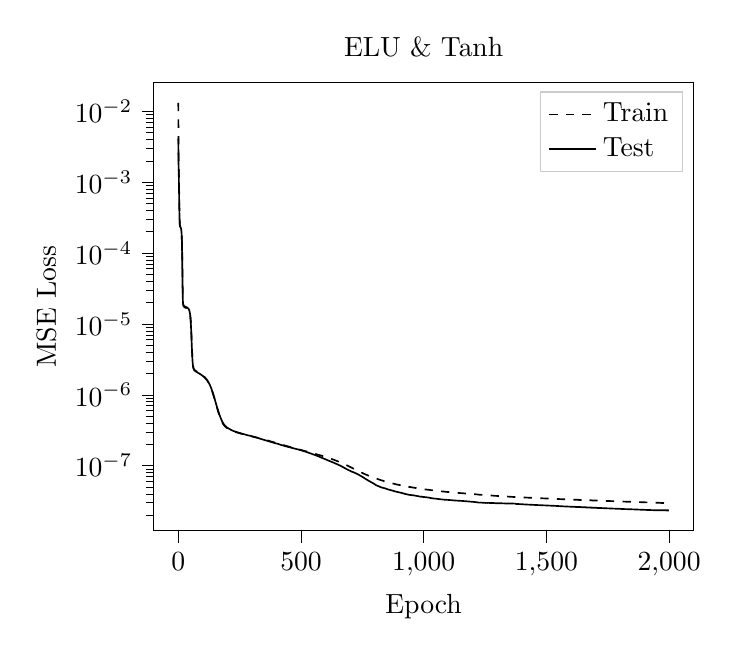
\begin{tikzpicture}

\begin{axis}[
legend cell align={left},
legend style={fill opacity=0.8, draw opacity=1, text opacity=1, draw=white!80!black},
log basis y={10},
tick align=outside,
tick pos=left,
title={ELU \& Tanh},
x grid style={white!69.0196078431373!black},
xlabel={Epoch},
xmin=-99.95, xmax=2098.95,
xtick style={color=black},
y grid style={white!69.0196078431373!black},
ylabel={MSE Loss},
ymin=1.20288411886795e-08, ymax=0.0255172665781318,
ymode=log,
ytick style={color=black}
]
\addplot [semithick, black, dashed]
table {%
0 0.0131601534280926
1 0.00254879569727927
2 0.0015288968286477
3 0.000978349994169548
4 0.000554412616998889
5 0.000339064917701762
6 0.00025199008785421
7 0.000222940133317024
8 0.000214015148361796
9 0.0002101389333111
10 0.000206720305548515
11 0.000202234839642188
12 0.000195523965245229
13 0.000184769826577394
14 0.000166750691139896
15 0.000136818764854979
16 9.37190856602683e-05
17 5.13041007707216e-05
18 2.82282359621604e-05
19 2.07924298056241e-05
20 1.86988846025997e-05
21 1.7985147208492e-05
22 1.76603932732178e-05
23 1.74696931553626e-05
24 1.7336417397928e-05
25 1.72325157009254e-05
26 1.71457306960292e-05
27 1.70700371490966e-05
28 1.70019622391919e-05
29 1.69390593810022e-05
30 1.68791474070531e-05
31 1.68202410141021e-05
32 1.67614346964911e-05
33 1.67019616865218e-05
34 1.6640574176563e-05
35 1.65759826668364e-05
36 1.65068785563562e-05
37 1.64315606043601e-05
38 1.63476329316836e-05
39 1.62519396644711e-05
40 1.6141011761647e-05
41 1.60096406534649e-05
42 1.58509294724354e-05
43 1.56562558504447e-05
44 1.54144996622563e-05
45 1.51104531623787e-05
46 1.47251194412092e-05
47 1.42343020070257e-05
48 1.36079418834925e-05
49 1.28111480071311e-05
50 1.18125108524509e-05
51 1.06009906053259e-05
52 9.21135425733155e-06
53 7.74572519412686e-06
54 6.35779605204334e-06
55 5.1833828706549e-06
56 4.27447103993472e-06
57 3.60888216903277e-06
58 3.13739593627815e-06
59 2.81365010323498e-06
60 2.5991098123086e-06
61 2.4615408203772e-06
62 2.37513457909699e-06
63 2.32067587933216e-06
64 2.28507542425405e-06
65 2.2601448145565e-06
66 2.2411157641784e-06
67 2.22538888459667e-06
68 2.21156630598784e-06
69 2.19884542784143e-06
70 2.18683005365961e-06
71 2.17529318160814e-06
72 2.16406654300272e-06
73 2.15305643186525e-06
74 2.14221861409669e-06
75 2.13150765353021e-06
76 2.12089069145804e-06
77 2.11034301975133e-06
78 2.09984778734906e-06
79 2.08938692787797e-06
80 2.07894793217633e-06
81 2.06852177257133e-06
82 2.05811688823587e-06
83 2.04775601798701e-06
84 2.03743660432565e-06
85 2.02712287028817e-06
86 2.01677592477267e-06
87 2.00636359383566e-06
88 1.9958792451007e-06
89 1.98534851921295e-06
90 1.97476752782677e-06
91 1.96412047347394e-06
92 1.95337903960535e-06
93 1.94250881099833e-06
94 1.93151071587749e-06
95 1.92039129103705e-06
96 1.90919305123316e-06
97 1.89784946982741e-06
98 1.88634913931196e-06
99 1.8746769611937e-06
100 1.86280562124352e-06
101 1.85072760652361e-06
102 1.83844960992019e-06
103 1.8259182288034e-06
104 1.81310693804448e-06
105 1.80003688234365e-06
106 1.78669658473041e-06
107 1.77301694364473e-06
108 1.75900127936757e-06
109 1.7447329835818e-06
110 1.7301772377607e-06
111 1.71521739630975e-06
112 1.69957119675246e-06
113 1.68334501330492e-06
114 1.66680457303414e-06
115 1.65007861224353e-06
116 1.63280734801674e-06
117 1.6146544377591e-06
118 1.59609273197248e-06
119 1.57705401022668e-06
120 1.55746726173334e-06
121 1.53734570181996e-06
122 1.51670278955862e-06
123 1.49546852236426e-06
124 1.47359743027664e-06
125 1.45113387642937e-06
126 1.42810016075146e-06
127 1.40454621669051e-06
128 1.38053379953362e-06
129 1.35608644262675e-06
130 1.33122524189844e-06
131 1.30597759505235e-06
132 1.28038126339902e-06
133 1.25448347620249e-06
134 1.22832383840432e-06
135 1.20193885268804e-06
136 1.17537005490931e-06
137 1.14872875269612e-06
138 1.12217347577825e-06
139 1.09575871235279e-06
140 1.06947597012663e-06
141 1.04335389841026e-06
142 1.01742884223199e-06
143 9.9174229461596e-07
144 9.66341739569998e-07
145 9.41270877660827e-07
146 9.16549341098971e-07
147 8.92186274228379e-07
148 8.68209495507699e-07
149 8.44659665403924e-07
150 8.21562834261158e-07
151 7.98913440092974e-07
152 7.76709624403793e-07
153 7.55005571022593e-07
154 7.33842296398279e-07
155 7.1324187874211e-07
156 6.93227800155682e-07
157 6.73795341072036e-07
158 6.54944412957548e-07
159 6.36686511398921e-07
160 6.1902444002726e-07
161 6.01977020039612e-07
162 5.85635424073416e-07
163 5.70022565256068e-07
164 5.55100744662695e-07
165 5.40865127419465e-07
166 5.27296150863776e-07
167 5.14358819003746e-07
168 5.02070321516612e-07
169 4.90478948591999e-07
170 4.79591890936604e-07
171 4.69351124877448e-07
172 4.59683979244119e-07
173 4.50545075622699e-07
174 4.41906577222539e-07
175 4.3379301284574e-07
176 4.2621222132766e-07
177 4.19125185430858e-07
178 4.12513949200388e-07
179 4.06395948857607e-07
180 4.0069370336937e-07
181 3.95336360668352e-07
182 3.90310984542452e-07
183 3.85583037569859e-07
184 3.81129604534181e-07
185 3.76938679011118e-07
186 3.7298087708848e-07
187 3.69250917529484e-07
188 3.65744902723009e-07
189 3.62441119918344e-07
190 3.59327262572151e-07
191 3.56425127719717e-07
192 3.53701333978051e-07
193 3.5110774130942e-07
194 3.48639408940699e-07
195 3.46290742058386e-07
196 3.44055538093357e-07
197 3.41920796998352e-07
198 3.3988114013539e-07
199 3.37931422890847e-07
200 3.36068908225684e-07
201 3.34285324115058e-07
202 3.32569850741038e-07
203 3.30912869202393e-07
204 3.29307206200724e-07
205 3.27750944606464e-07
206 3.26266979001844e-07
207 3.24852640630979e-07
208 3.2346957465279e-07
209 3.22117157267598e-07
210 3.20800171451197e-07
211 3.19513469719368e-07
212 3.18255217777619e-07
213 3.1702468275796e-07
214 3.15827612496378e-07
215 3.14678894085318e-07
216 3.13595294272773e-07
217 3.12561567270109e-07
218 3.11577581513234e-07
219 3.10577952916447e-07
220 3.09579402184568e-07
221 3.08594582278943e-07
222 3.07647466968319e-07
223 3.06742993970488e-07
224 3.05863141832674e-07
225 3.04989370448538e-07
226 3.04124103536196e-07
227 3.032701661283e-07
228 3.02431237756196e-07
229 3.01602489713559e-07
230 3.00785786294e-07
231 2.99983752753974e-07
232 2.99192086089306e-07
233 2.98409287395884e-07
234 2.97635152378462e-07
235 2.96870692309881e-07
236 2.96115399436303e-07
237 2.95368066886681e-07
238 2.94630630094161e-07
239 2.93900858636675e-07
240 2.93184512997868e-07
241 2.92489651116057e-07
242 2.91816891092367e-07
243 2.91145831212702e-07
244 2.9048319896674e-07
245 2.89822926731631e-07
246 2.89163126112157e-07
247 2.88502883591946e-07
248 2.87852459607052e-07
249 2.87224834607969e-07
250 2.86597030878966e-07
251 2.85960856729162e-07
252 2.85321492057733e-07
253 2.84688976776692e-07
254 2.84068795139092e-07
255 2.83460164652638e-07
256 2.82858641597272e-07
257 2.82261807114992e-07
258 2.81669071654278e-07
259 2.81083668824067e-07
260 2.8050698112736e-07
261 2.79942047242798e-07
262 2.79401001975543e-07
263 2.78919282436618e-07
264 2.78250929099499e-07
265 2.7769323406801e-07
266 2.77149659567044e-07
267 2.76604206774778e-07
268 2.76058308742222e-07
269 2.75514584600955e-07
270 2.74971755459319e-07
271 2.74430956324068e-07
272 2.73889851285958e-07
273 2.73346790777396e-07
274 2.72801549414226e-07
275 2.72264279217893e-07
276 2.7174932449725e-07
277 2.71240941714268e-07
278 2.70725355719037e-07
279 2.70204308250754e-07
280 2.69686683623149e-07
281 2.69170687374753e-07
282 2.68656707220316e-07
283 2.6814359382854e-07
284 2.6763243812411e-07
285 2.67122213244875e-07
286 2.66613155758932e-07
287 2.66105947375195e-07
288 2.6559856546271e-07
289 2.6509363469529e-07
290 2.64588432443702e-07
291 2.64084260251707e-07
292 2.63579864878238e-07
293 2.63075514027378e-07
294 2.62571202327422e-07
295 2.62065000541156e-07
296 2.6155551402951e-07
297 2.61047375587964e-07
298 2.60552575497286e-07
299 2.60085221540862e-07
300 2.59596596890788e-07
301 2.59059146287655e-07
302 2.58539276231318e-07
303 2.58035740202445e-07
304 2.57535053350466e-07
305 2.57033249823735e-07
306 2.56527450233079e-07
307 2.56022325999083e-07
308 2.55515834126641e-07
309 2.55008146865521e-07
310 2.54499001528075e-07
311 2.53990032419438e-07
312 2.53478506948568e-07
313 2.5296603746483e-07
314 2.52451124438835e-07
315 2.51934009867227e-07
316 2.51414092375057e-07
317 2.5088994965472e-07
318 2.50361918318731e-07
319 2.49830229506642e-07
320 2.49291807122631e-07
321 2.48751227886146e-07
322 2.48202915614115e-07
323 2.47651687843131e-07
324 2.47100254256338e-07
325 2.46554554564682e-07
326 2.46023965161157e-07
327 2.45507849939486e-07
328 2.45001275814616e-07
329 2.44500258460789e-07
330 2.4399837899125e-07
331 2.43496204234361e-07
332 2.42991565372108e-07
333 2.42484796899589e-07
334 2.41975729196042e-07
335 2.41464755745824e-07
336 2.40952600208288e-07
337 2.40439445832408e-07
338 2.39924943556957e-07
339 2.39409758350462e-07
340 2.38894031781456e-07
341 2.38378295378538e-07
342 2.37861772134806e-07
343 2.37343902668385e-07
344 2.36825885465919e-07
345 2.36308309311539e-07
346 2.35789153393284e-07
347 2.3527115035904e-07
348 2.34751956895707e-07
349 2.34233497749869e-07
350 2.33713108769962e-07
351 2.33194307313056e-07
352 2.32674123310517e-07
353 2.32153817776748e-07
354 2.31633706150092e-07
355 2.31114634758001e-07
356 2.30592511172745e-07
357 2.30073320196311e-07
358 2.29550019184899e-07
359 2.29030590574553e-07
360 2.28506732995015e-07
361 2.27985227525096e-07
362 2.2745980940897e-07
363 2.26935036494069e-07
364 2.26407579006604e-07
365 2.25878871745522e-07
366 2.25349141089737e-07
367 2.24818749259725e-07
368 2.24284589023682e-07
369 2.23751356216439e-07
370 2.23217339097914e-07
371 2.22683898257969e-07
372 2.22149178313202e-07
373 2.21620929323763e-07
374 2.21093199442635e-07
375 2.20577191839766e-07
376 2.20056678102765e-07
377 2.19546195609155e-07
378 2.19024992730965e-07
379 2.18527559781023e-07
380 2.18007180933455e-07
381 2.17523276390352e-07
382 2.16990808596051e-07
383 2.16530773329282e-07
384 2.15981374630303e-07
385 2.15540847143814e-07
386 2.1498925293173e-07
387 2.14562892296044e-07
388 2.14015980148474e-07
389 2.13598349787958e-07
390 2.13054402372848e-07
391 2.12622081441793e-07
392 2.12062817922742e-07
393 2.11620012045444e-07
394 2.11074238080755e-07
395 2.10642850724696e-07
396 2.10115624135199e-07
397 2.09677260365027e-07
398 2.09132693299807e-07
399 2.08685344418313e-07
400 2.08155541599808e-07
401 2.07705447643036e-07
402 2.07183368253538e-07
403 2.06727136337292e-07
404 2.06216078247223e-07
405 2.05757556649644e-07
406 2.05255236807034e-07
407 2.04789339271372e-07
408 2.04285899336298e-07
409 2.03810201718113e-07
410 2.03323012144097e-07
411 2.0286266884284e-07
412 2.02395825432689e-07
413 2.01942679375122e-07
414 2.01489438097724e-07
415 2.01049114735952e-07
416 2.00620913773264e-07
417 2.00179136562895e-07
418 1.99697794052156e-07
419 1.99211518797426e-07
420 1.98745680755508e-07
421 1.98285480642824e-07
422 1.97829109247039e-07
423 1.97373576042992e-07
424 1.96920282753865e-07
425 1.96468902387892e-07
426 1.96017156085304e-07
427 1.95567786732909e-07
428 1.95119598167537e-07
429 1.9467373040527e-07
430 1.94228913869665e-07
431 1.9378678856441e-07
432 1.93345975787906e-07
433 1.92908213861642e-07
434 1.92472880911509e-07
435 1.92033376286815e-07
436 1.91594089322678e-07
437 1.91156777340495e-07
438 1.90721543447125e-07
439 1.90288229426017e-07
440 1.89856990296278e-07
441 1.89426350928557e-07
442 1.88998336355439e-07
443 1.88572393220454e-07
444 1.88147689407003e-07
445 1.87724033871461e-07
446 1.87301913300075e-07
447 1.86881752682666e-07
448 1.86463004709481e-07
449 1.8604587298654e-07
450 1.85630693742667e-07
451 1.85216147464473e-07
452 1.84802860189848e-07
453 1.84391357393565e-07
454 1.83981159352697e-07
455 1.83571897430568e-07
456 1.83164638301037e-07
457 1.8275769946996e-07
458 1.82352313437661e-07
459 1.81948242243379e-07
460 1.8154557169936e-07
461 1.81142903578291e-07
462 1.80741623182712e-07
463 1.80341402725048e-07
464 1.79942316073323e-07
465 1.79544574173462e-07
466 1.79148779068328e-07
467 1.78754067341913e-07
468 1.78359900061764e-07
469 1.77966328479329e-07
470 1.77572222291644e-07
471 1.77177200519907e-07
472 1.7677393238813e-07
473 1.76369746831995e-07
474 1.75992078169429e-07
475 1.75616341152818e-07
476 1.75233647482287e-07
477 1.7484610436469e-07
478 1.74459954209283e-07
479 1.74083032909778e-07
480 1.73702623811778e-07
481 1.73321933473858e-07
482 1.72944039356082e-07
483 1.72568016154173e-07
484 1.72192560903284e-07
485 1.71817991436285e-07
486 1.71445508037493e-07
487 1.71073176801428e-07
488 1.70700102195553e-07
489 1.70324904402719e-07
490 1.69944452999005e-07
491 1.6955677234165e-07
492 1.69169401324609e-07
493 1.68812724808731e-07
494 1.68463908480021e-07
495 1.68110651223685e-07
496 1.67751017137618e-07
497 1.67391723636001e-07
498 1.67032830752589e-07
499 1.66674713902637e-07
500 1.66317192679344e-07
501 1.6596099465005e-07
502 1.65605539926617e-07
503 1.65249893854025e-07
504 1.64895575679225e-07
505 1.64542413884305e-07
506 1.64188377084429e-07
507 1.63834382490791e-07
508 1.63479579349257e-07
509 1.63123736946602e-07
510 1.62764372966251e-07
511 1.62400060261803e-07
512 1.62033490710201e-07
513 1.61673854385924e-07
514 1.6133109382821e-07
515 1.60980462240445e-07
516 1.60622751863571e-07
517 1.60286923545527e-07
518 1.5995844636052e-07
519 1.59616451256284e-07
520 1.59275953478755e-07
521 1.58933757333557e-07
522 1.58592838552352e-07
523 1.58254255289592e-07
524 1.57914939528325e-07
525 1.57576707024987e-07
526 1.57237424488699e-07
527 1.56900591548492e-07
528 1.56563655664854e-07
529 1.56226724612907e-07
530 1.55891212621384e-07
531 1.55555264647944e-07
532 1.55220193441608e-07
533 1.5488449407286e-07
534 1.54550589023472e-07
535 1.54216606908619e-07
536 1.53881973737668e-07
537 1.53549540797826e-07
538 1.53216481912466e-07
539 1.52883593578679e-07
540 1.52551263909118e-07
541 1.52220322597429e-07
542 1.51887326481415e-07
543 1.51556127320873e-07
544 1.51225415628176e-07
545 1.50893343956682e-07
546 1.50563061609432e-07
547 1.50233072332639e-07
548 1.49902952898628e-07
549 1.49572416454191e-07
550 1.49243174121239e-07
551 1.48913397453043e-07
552 1.48584105176042e-07
553 1.48255081676041e-07
554 1.47925589033093e-07
555 1.47597463460158e-07
556 1.47268285857649e-07
557 1.46940167169873e-07
558 1.46610681149184e-07
559 1.46281415496219e-07
560 1.45951650871723e-07
561 1.45620285614712e-07
562 1.4528401814573e-07
563 1.44944069916164e-07
564 1.44600810408235e-07
565 1.44262943436502e-07
566 1.43927519481224e-07
567 1.43590049695774e-07
568 1.43260283628877e-07
569 1.42937757580341e-07
570 1.42615396995893e-07
571 1.42289746904112e-07
572 1.4196258763377e-07
573 1.41634024075188e-07
574 1.4130653507749e-07
575 1.40979754874593e-07
576 1.40654982985211e-07
577 1.40327927930173e-07
578 1.39996476441695e-07
579 1.39661024547877e-07
580 1.39324684006681e-07
581 1.38991585217241e-07
582 1.38657661004515e-07
583 1.38324706199455e-07
584 1.37992608131299e-07
585 1.37660341053447e-07
586 1.37325831850887e-07
587 1.36991686318311e-07
588 1.36658037732218e-07
589 1.36322862211102e-07
590 1.35988218090688e-07
591 1.35652704940981e-07
592 1.35316823737242e-07
593 1.34980701190557e-07
594 1.34643992552697e-07
595 1.34307293656377e-07
596 1.33969952976543e-07
597 1.33632085059787e-07
598 1.33294102340642e-07
599 1.32956124616612e-07
600 1.32616756907566e-07
601 1.32277391614366e-07
602 1.31938818839217e-07
603 1.31597589152932e-07
604 1.31258015692026e-07
605 1.3091720372671e-07
606 1.30575987988379e-07
607 1.30233362483523e-07
608 1.29891986915709e-07
609 1.2954996940806e-07
610 1.29205809294319e-07
611 1.28862633737015e-07
612 1.28520314646607e-07
613 1.2817495100137e-07
614 1.27830125414619e-07
615 1.27484617458151e-07
616 1.27139700730083e-07
617 1.2679202459509e-07
618 1.26445642635531e-07
619 1.26099415318492e-07
620 1.25751059400159e-07
621 1.25403643487232e-07
622 1.25053666707231e-07
623 1.24705792295288e-07
624 1.24355652907582e-07
625 1.24006482145944e-07
626 1.23654558812802e-07
627 1.23304186288919e-07
628 1.22952360904094e-07
629 1.22601375110776e-07
630 1.22249454179268e-07
631 1.21896765762131e-07
632 1.21543555302139e-07
633 1.21191076516425e-07
634 1.20836187782913e-07
635 1.20481173560449e-07
636 1.20121345013047e-07
637 1.19762935923973e-07
638 1.19400635831823e-07
639 1.19041445550749e-07
640 1.18679526153187e-07
641 1.18321026214119e-07
642 1.17956734527525e-07
643 1.17598218643877e-07
644 1.17233053785526e-07
645 1.1687504470359e-07
646 1.16506115539039e-07
647 1.16149264989929e-07
648 1.15774781420441e-07
649 1.15423059597219e-07
650 1.15037076007241e-07
651 1.14700303406323e-07
652 1.14294124074377e-07
653 1.13968814041243e-07
654 1.13556144349047e-07
655 1.13219854505076e-07
656 1.12819404108677e-07
657 1.12505390681861e-07
658 1.1211966626945e-07
659 1.11745449785872e-07
660 1.11343885933479e-07
661 1.10986338235364e-07
662 1.10601156912082e-07
663 1.10227328399048e-07
664 1.09847862688639e-07
665 1.09466705730199e-07
666 1.09083192626258e-07
667 1.08700647508897e-07
668 1.0831480311424e-07
669 1.07929378259541e-07
670 1.07541389290589e-07
671 1.07154287086075e-07
672 1.0676769644391e-07
673 1.06381731328042e-07
674 1.05990678122225e-07
675 1.05594895771333e-07
676 1.05199675196843e-07
677 1.04810480365813e-07
678 1.04418989685939e-07
679 1.04027984271227e-07
680 1.0363815702874e-07
681 1.0324819263019e-07
682 1.02859756317741e-07
683 1.02471920968128e-07
684 1.02083233088024e-07
685 1.01694726282631e-07
686 1.01307340209189e-07
687 1.00919130510135e-07
688 1.00530916142816e-07
689 1.00143542738351e-07
690 9.97545113179399e-08
691 9.93675590379439e-08
692 9.89800909607652e-08
693 9.85953646619464e-08
694 9.82120354180438e-08
695 9.78292016071691e-08
696 9.74492761613988e-08
697 9.70678999436814e-08
698 9.66850550199183e-08
699 9.63028536418165e-08
700 9.59213216376043e-08
701 9.55436611391747e-08
702 9.51664130255381e-08
703 9.47894022971241e-08
704 9.44130259696863e-08
705 9.4036925865737e-08
706 9.36625970240357e-08
707 9.3288709258843e-08
708 9.29143761752016e-08
709 9.25398956113099e-08
710 9.21654500132263e-08
711 9.17905279180786e-08
712 9.14152797406587e-08
713 9.10435747840666e-08
714 9.06759069962959e-08
715 9.03191059151709e-08
716 8.99658183541874e-08
717 8.96166580233171e-08
718 8.92642552727807e-08
719 8.89152184484487e-08
720 8.85622741293446e-08
721 8.82137649327319e-08
722 8.78630537997083e-08
723 8.75201614576326e-08
724 8.71707721543657e-08
725 8.68308670831652e-08
726 8.64862795069143e-08
727 8.61490446126823e-08
728 8.58071580154274e-08
729 8.54761280493221e-08
730 8.51358397824242e-08
731 8.48093447345377e-08
732 8.44707277849466e-08
733 8.415007692264e-08
734 8.38136081213747e-08
735 8.34983421782454e-08
736 8.3161317022018e-08
737 8.28544769078121e-08
738 8.25149288914417e-08
739 8.22155614130793e-08
740 8.18770621009435e-08
741 8.15844286066181e-08
742 8.12440885340493e-08
743 8.09608954952523e-08
744 8.06174798384518e-08
745 8.03448064274903e-08
746 7.99966385969242e-08
747 7.97339763067839e-08
748 7.93839182975376e-08
749 7.91303163794055e-08
750 7.87830934640965e-08
751 7.85370518201489e-08
752 7.81923441977028e-08
753 7.79547676614811e-08
754 7.76166178368953e-08
755 7.73845136876616e-08
756 7.70513217887014e-08
757 7.6827997897766e-08
758 7.65009137211337e-08
759 7.62806916014824e-08
760 7.59617605865515e-08
761 7.57490153944218e-08
762 7.54341544002557e-08
763 7.52256842986299e-08
764 7.4918414092906e-08
765 7.47141463257606e-08
766 7.44146009132862e-08
767 7.42095831078871e-08
768 7.39145847177269e-08
769 7.37110998905166e-08
770 7.34179971253468e-08
771 7.32091361825837e-08
772 7.29165597661563e-08
773 7.27025321936026e-08
774 7.24227878343697e-08
775 7.22241191581929e-08
776 7.19627312939508e-08
777 7.1762471385739e-08
778 7.15034239000545e-08
779 7.13010314328244e-08
780 7.10541031061496e-08
781 7.08462831724432e-08
782 7.05859609908543e-08
783 7.03546273612687e-08
784 7.00836361460233e-08
785 6.98543979780197e-08
786 6.96672320295022e-08
787 6.95502103305046e-08
788 6.93480467042207e-08
789 6.91480321002302e-08
790 6.893230557381e-08
791 6.87383616266857e-08
792 6.85314918520419e-08
793 6.8341212134726e-08
794 6.81411711696001e-08
795 6.7953572468582e-08
796 6.77608208867753e-08
797 6.75757414292377e-08
798 6.73860329385434e-08
799 6.72034605280203e-08
800 6.70175597434763e-08
801 6.68326048476331e-08
802 6.66480708346739e-08
803 6.64633341713738e-08
804 6.62772580142246e-08
805 6.60915295256359e-08
806 6.59041005377503e-08
807 6.57156358592204e-08
808 6.55272900793591e-08
809 6.53402567074579e-08
810 6.51595602043642e-08
811 6.49886946746392e-08
812 6.48140172714307e-08
813 6.46367730396946e-08
814 6.44600384482885e-08
815 6.42846892340288e-08
816 6.41082180870001e-08
817 6.393430256324e-08
818 6.37585768821225e-08
819 6.3583405808032e-08
820 6.34069121367986e-08
821 6.3220355329463e-08
822 6.30279480944296e-08
823 6.28660326320585e-08
824 6.27192910052088e-08
825 6.25616495177894e-08
826 6.2403849131698e-08
827 6.22459404517883e-08
828 6.20908969644063e-08
829 6.19363434211095e-08
830 6.17823749138324e-08
831 6.16275062306215e-08
832 6.14738188069452e-08
833 6.13199244092755e-08
834 6.11655107789488e-08
835 6.10088632164718e-08
836 6.0842924721527e-08
837 6.06600994501605e-08
838 6.04520119829033e-08
839 6.02753693641489e-08
840 6.01769672208263e-08
841 6.00620659341189e-08
842 5.99465706621061e-08
843 5.98101269986273e-08
844 5.967979369359e-08
845 5.95410453740897e-08
846 5.94138033847003e-08
847 5.92733323401262e-08
848 5.91528519073847e-08
849 5.90060622549515e-08
850 5.88980487492563e-08
851 5.87444609330134e-08
852 5.86443678791682e-08
853 5.84868802242511e-08
854 5.83924014350146e-08
855 5.82357584981708e-08
856 5.81416117668709e-08
857 5.79865398862012e-08
858 5.78953433674201e-08
859 5.77420002088047e-08
860 5.76522297208726e-08
861 5.74993749147268e-08
862 5.74120188865379e-08
863 5.72597793819796e-08
864 5.71752964901862e-08
865 5.70247034836768e-08
866 5.69411097757211e-08
867 5.679273058945e-08
868 5.67114060920915e-08
869 5.65622520021236e-08
870 5.64837248084871e-08
871 5.63370899193671e-08
872 5.62614032411091e-08
873 5.61162377863411e-08
874 5.60408048073668e-08
875 5.59000868207704e-08
876 5.5825515403285e-08
877 5.56860418754468e-08
878 5.56065390320271e-08
879 5.54442152704837e-08
880 5.53465068193759e-08
881 5.52014605581519e-08
882 5.5144348330316e-08
883 5.50065026025948e-08
884 5.4938962758655e-08
885 5.47925301255248e-08
886 5.47226506917298e-08
887 5.45806310938701e-08
888 5.44830717252864e-08
889 5.43354541591157e-08
890 5.42866788784124e-08
891 5.4193029882299e-08
892 5.41037255992194e-08
893 5.4004102963745e-08
894 5.39168008906188e-08
895 5.38167598982398e-08
896 5.37307497765482e-08
897 5.36283687786465e-08
898 5.3545491898177e-08
899 5.34505866340851e-08
900 5.33795286301597e-08
901 5.32782876376814e-08
902 5.32000103348196e-08
903 5.31031169508367e-08
904 5.30214819072228e-08
905 5.29322757287787e-08
906 5.2850323964293e-08
907 5.27636802090115e-08
908 5.26779433123181e-08
909 5.25862555775802e-08
910 5.24820538458925e-08
911 5.23542242767405e-08
912 5.22638524316221e-08
913 5.22520095067591e-08
914 5.20998846980092e-08
915 5.2146744899062e-08
916 5.19045253355444e-08
917 5.19310569870868e-08
918 5.1782812871437e-08
919 5.17995022413231e-08
920 5.15896290842477e-08
921 5.17530991928084e-08
922 5.14307041790119e-08
923 5.13906512296103e-08
924 5.14559755586674e-08
925 5.12293278269738e-08
926 5.12345318988139e-08
927 5.11401419949209e-08
928 5.10994720563929e-08
929 5.09844776672708e-08
930 5.09706070701554e-08
931 5.08257401961032e-08
932 5.08580665368186e-08
933 5.06569208695851e-08
934 5.07608531847836e-08
935 5.04932937239744e-08
936 5.05750532582283e-08
937 5.03769438431334e-08
938 5.04652209301071e-08
939 5.02219266103054e-08
940 5.03236353601721e-08
941 5.00827042166918e-08
942 5.01772669565526e-08
943 4.99418741490842e-08
944 5.00236907434726e-08
945 4.97968133501558e-08
946 4.98517641283058e-08
947 4.9631626453106e-08
948 4.96511877159378e-08
949 4.9451886212637e-08
950 4.95108563427493e-08
951 4.93895526325616e-08
952 4.94255550549383e-08
953 4.92760776005241e-08
954 4.92957489726109e-08
955 4.91394359585229e-08
956 4.91521641272641e-08
957 4.90015478114003e-08
958 4.90032903073256e-08
959 4.88661470505747e-08
960 4.88593277587768e-08
961 4.87428295912196e-08
962 4.87304148784062e-08
963 4.8624902394323e-08
964 4.86015209553159e-08
965 4.8503092187957e-08
966 4.84726088032517e-08
967 4.83801911528303e-08
968 4.83473524752753e-08
969 4.82583990688568e-08
970 4.82274910247327e-08
971 4.8142395744577e-08
972 4.8112453871596e-08
973 4.80282170016721e-08
974 4.79997060160997e-08
975 4.79158530559687e-08
976 4.78881169776457e-08
977 4.78054251900062e-08
978 4.77769883495682e-08
979 4.76954273160857e-08
980 4.76676170073631e-08
981 4.75860888862201e-08
982 4.75565808315537e-08
983 4.7475151536247e-08
984 4.74452551841864e-08
985 4.73646711114384e-08
986 4.73329088208629e-08
987 4.72507358786345e-08
988 4.72154740620567e-08
989 4.71290015013892e-08
990 4.70837073009989e-08
991 4.69815565402598e-08
992 4.69130373481619e-08
993 4.68120339363054e-08
994 4.67982854921445e-08
995 4.67581658618599e-08
996 4.67310412943789e-08
997 4.665680933158e-08
998 4.6614766084474e-08
999 4.65570674066385e-08
1000 4.65196713967941e-08
1001 4.64576681871165e-08
1002 4.64096734482666e-08
1003 4.63734514042358e-08
1004 4.630485181778e-08
1005 4.62859110079705e-08
1006 4.62073714260214e-08
1007 4.61892398355701e-08
1008 4.61182378721503e-08
1009 4.61099274104981e-08
1010 4.60198555884972e-08
1011 4.60196106999433e-08
1012 4.59280479532254e-08
1013 4.59336447882208e-08
1014 4.58340887377062e-08
1015 4.58449031022212e-08
1016 4.57388315808771e-08
1017 4.57569441358885e-08
1018 4.56463287648035e-08
1019 4.56692389860791e-08
1020 4.55531906560225e-08
1021 4.55818113600515e-08
1022 4.54620867849087e-08
1023 4.54929418616246e-08
1024 4.53726893248074e-08
1025 4.5401559834346e-08
1026 4.52775405754835e-08
1027 4.52661582492908e-08
1028 4.51476962659569e-08
1029 4.51590000700719e-08
1030 4.51276083133223e-08
1031 4.5074241686649e-08
1032 4.50412402521749e-08
1033 4.49861366362825e-08
1034 4.49491402463309e-08
1035 4.49011619707562e-08
1036 4.48583528225299e-08
1037 4.48114631268481e-08
1038 4.4767292468606e-08
1039 4.47221731540992e-08
1040 4.46739429484921e-08
1041 4.46299758394275e-08
1042 4.45806041220464e-08
1043 4.45325005777875e-08
1044 4.44845118465764e-08
1045 4.44400044159465e-08
1046 4.43992311396357e-08
1047 4.43588988190413e-08
1048 4.4323437709437e-08
1049 4.42854224402822e-08
1050 4.4246319131247e-08
1051 4.42069745645313e-08
1052 4.41663080543719e-08
1053 4.41267324831074e-08
1054 4.40851923002583e-08
1055 4.40439598889952e-08
1056 4.40021518457456e-08
1057 4.39624776760184e-08
1058 4.39202907180913e-08
1059 4.38781604579219e-08
1060 4.3835203697995e-08
1061 4.37901719294587e-08
1062 4.37391187269043e-08
1063 4.36787410329487e-08
1064 4.36142205195722e-08
1065 4.35764591593113e-08
1066 4.3526191713994e-08
1067 4.35113610848248e-08
1068 4.35112334251642e-08
1069 4.34788408760767e-08
1070 4.34420058006424e-08
1071 4.34074025825737e-08
1072 4.337379616004e-08
1073 4.33410867017869e-08
1074 4.33068135663461e-08
1075 4.32735379654048e-08
1076 4.32421167673169e-08
1077 4.32102222447384e-08
1078 4.3178529104182e-08
1079 4.31464594292663e-08
1080 4.31127083402316e-08
1081 4.30777044293507e-08
1082 4.30424841333377e-08
1083 4.30052575595141e-08
1084 4.29678215105866e-08
1085 4.29295583472822e-08
1086 4.28891776209639e-08
1087 4.28501564400108e-08
1088 4.28093613180636e-08
1089 4.27695682532203e-08
1090 4.27320691649413e-08
1091 4.26969720095371e-08
1092 4.26641718931364e-08
1093 4.26348475563998e-08
1094 4.26035555918247e-08
1095 4.25714825205148e-08
1096 4.2539459688129e-08
1097 4.25069211793527e-08
1098 4.24752585281851e-08
1099 4.24470454269965e-08
1100 4.24142000383654e-08
1101 4.2386877243672e-08
1102 4.23553551982536e-08
1103 4.23280068666543e-08
1104 4.22964153372618e-08
1105 4.22666909258851e-08
1106 4.22377636120075e-08
1107 4.22090744969239e-08
1108 4.21786970008497e-08
1109 4.21486589772257e-08
1110 4.21205174667705e-08
1111 4.20898296553673e-08
1112 4.20612397995512e-08
1113 4.20298081813542e-08
1114 4.20028930676608e-08
1115 4.19723818225748e-08
1116 4.19444931232249e-08
1117 4.19146600130205e-08
1118 4.18882347830163e-08
1119 4.18592943596252e-08
1120 4.18306351726017e-08
1121 4.17999253414791e-08
1122 4.17717335814416e-08
1123 4.17401160781594e-08
1124 4.17091959263871e-08
1125 4.16738806841011e-08
1126 4.16385093480187e-08
1127 4.16083301644221e-08
1128 4.15826955943999e-08
1129 4.15573036640637e-08
1130 4.15322029070353e-08
1131 4.15054005067361e-08
1132 4.14762116101031e-08
1133 4.14496789424845e-08
1134 4.14193409810082e-08
1135 4.13939505996552e-08
1136 4.13655391540146e-08
1137 4.13387203863635e-08
1138 4.13112442352315e-08
1139 4.1284515468476e-08
1140 4.12570460248674e-08
1141 4.122893498959e-08
1142 4.12023311824328e-08
1143 4.11755861478014e-08
1144 4.11479511477353e-08
1145 4.11188139608498e-08
1146 4.10914398187856e-08
1147 4.10588335206796e-08
1148 4.10257076417508e-08
1149 4.09911478058689e-08
1150 4.09706586381731e-08
1151 4.0947768535915e-08
1152 4.09257850790823e-08
1153 4.09000993784048e-08
1154 4.08752379961186e-08
1155 4.08492191041887e-08
1156 4.08236526574512e-08
1157 4.0796837154744e-08
1158 4.07754792419723e-08
1159 4.07453324307028e-08
1160 4.07218479203664e-08
1161 4.06957986918144e-08
1162 4.06731145297101e-08
1163 4.06448262104675e-08
1164 4.06233385987775e-08
1165 4.05953980724405e-08
1166 4.0572532196137e-08
1167 4.05458565069239e-08
1168 4.05216331067493e-08
1169 4.04969372880259e-08
1170 4.04722319551354e-08
1171 4.04483379838894e-08
1172 4.04240453200089e-08
1173 4.03967915474368e-08
1174 4.03753465789691e-08
1175 4.03492542062622e-08
1176 4.03253273830728e-08
1177 4.03027273101486e-08
1178 4.02754001136429e-08
1179 4.02519226767595e-08
1180 4.02287905032495e-08
1181 4.02035331461548e-08
1182 4.01805381002873e-08
1183 4.01537798211393e-08
1184 4.01332027593071e-08
1185 4.01053166001475e-08
1186 4.00851568720384e-08
1187 4.0057915239089e-08
1188 4.00365685031545e-08
1189 4.00097245787379e-08
1190 3.998638086955e-08
1191 3.99603554015471e-08
1192 3.99394127974517e-08
1193 3.99152432635219e-08
1194 3.9889744968491e-08
1195 3.98668957153347e-08
1196 3.98415572284705e-08
1197 3.98171912934231e-08
1198 3.9792276890438e-08
1199 3.9768928541406e-08
1200 3.9741534841653e-08
1201 3.97171350385861e-08
1202 3.9688988476172e-08
1203 3.96626243137632e-08
1204 3.96315111181877e-08
1205 3.96057352176626e-08
1206 3.9574675962939e-08
1207 3.95418058651842e-08
1208 3.95316207217888e-08
1209 3.95276360016794e-08
1210 3.94979896860548e-08
1211 3.9469980588791e-08
1212 3.9439048013179e-08
1213 3.94036826776301e-08
1214 3.93643339400285e-08
1215 3.93208972973014e-08
1216 3.92942937708085e-08
1217 3.92745694526297e-08
1218 3.92532672854884e-08
1219 3.92244704059408e-08
1220 3.91922152473967e-08
1221 3.91519686111508e-08
1222 3.91047739292105e-08
1223 3.90440098669842e-08
1224 3.89788044259376e-08
1225 3.89248560708211e-08
1226 3.88969509970138e-08
1227 3.88739982497555e-08
1228 3.88600895888658e-08
1229 3.88442312200254e-08
1230 3.88249830081122e-08
1231 3.88039069854074e-08
1232 3.8779033271652e-08
1233 3.87615753822956e-08
1234 3.8740473225829e-08
1235 3.873860647019e-08
1236 3.87189993205084e-08
1237 3.87125171172897e-08
1238 3.86798034597291e-08
1239 3.86713239279857e-08
1240 3.86387752158157e-08
1241 3.86332558584002e-08
1242 3.85975577543718e-08
1243 3.85894923411456e-08
1244 3.85478015196838e-08
1245 3.85361696650932e-08
1246 3.84958887202913e-08
1247 3.84842061045276e-08
1248 3.84364790591007e-08
1249 3.84129069281869e-08
1250 3.835013849951e-08
1251 3.830980500652e-08
1252 3.82426465819208e-08
1253 3.82386410500146e-08
1254 3.82098225983896e-08
1255 3.82244349310668e-08
1256 3.81952226753413e-08
1257 3.82213184941804e-08
1258 3.82200949040623e-08
1259 3.82805829381994e-08
1260 3.81924289385438e-08
1261 3.81557332680416e-08
1262 3.81068309458499e-08
1263 3.81131902003062e-08
1264 3.80710950018681e-08
1265 3.80754166329211e-08
1266 3.8031601455657e-08
1267 3.80357743026138e-08
1268 3.79924965976386e-08
1269 3.79957934271147e-08
1270 3.79529627601016e-08
1271 3.79557706651212e-08
1272 3.79125297484961e-08
1273 3.79155425775934e-08
1274 3.78721137686e-08
1275 3.78763480810562e-08
1276 3.78328135077766e-08
1277 3.78355915806594e-08
1278 3.77929401231825e-08
1279 3.77964996722824e-08
1280 3.77534832587401e-08
1281 3.77569717073811e-08
1282 3.77135280906771e-08
1283 3.77169082277362e-08
1284 3.76753321589263e-08
1285 3.76782625970407e-08
1286 3.76359895497558e-08
1287 3.76384917402106e-08
1288 3.75944361508118e-08
1289 3.75930085390053e-08
1290 3.75225182729366e-08
1291 3.74770163737992e-08
1292 3.74718370714788e-08
1293 3.7489422357595e-08
1294 3.74551559829683e-08
1295 3.74438800214705e-08
1296 3.74006098837754e-08
1297 3.74007029471102e-08
1298 3.73629217094162e-08
1299 3.73621428693127e-08
1300 3.73280939420795e-08
1301 3.73244589795263e-08
1302 3.72918043005654e-08
1303 3.72864535371775e-08
1304 3.72538170481107e-08
1305 3.7249388356031e-08
1306 3.72167330553452e-08
1307 3.72109800288456e-08
1308 3.71815438029444e-08
1309 3.71741152491722e-08
1310 3.71463017287965e-08
1311 3.71373364771443e-08
1312 3.71105454988196e-08
1313 3.70999555165952e-08
1314 3.70739672632681e-08
1315 3.70657831076926e-08
1316 3.70393918345258e-08
1317 3.70291311817539e-08
1318 3.70031502647805e-08
1319 3.69933979911252e-08
1320 3.69690625348085e-08
1321 3.69570734548574e-08
1322 3.69338784373952e-08
1323 3.69203525494299e-08
1324 3.69001947291281e-08
1325 3.6884491048994e-08
1326 3.68652273294856e-08
1327 3.68487275963503e-08
1328 3.68304681970244e-08
1329 3.68142394577831e-08
1330 3.67960606553197e-08
1331 3.67789098625337e-08
1332 3.67622351404862e-08
1333 3.67434659480637e-08
1334 3.67273959831493e-08
1335 3.67091880448811e-08
1336 3.66934555309228e-08
1337 3.66746878626145e-08
1338 3.66584931477121e-08
1339 3.66390312436238e-08
1340 3.66224730719011e-08
1341 3.6605432974568e-08
1342 3.65883468766981e-08
1343 3.65714295149644e-08
1344 3.65530410562087e-08
1345 3.65340813850423e-08
1346 3.65178823180656e-08
1347 3.65003956268595e-08
1348 3.64792204763376e-08
1349 3.6462166747242e-08
1350 3.64390187854724e-08
1351 3.64144203004457e-08
1352 3.63808768426566e-08
1353 3.63480680682926e-08
1354 3.63430094481032e-08
1355 3.63301288963669e-08
1356 3.63105459761925e-08
1357 3.62942809886135e-08
1358 3.62777775180234e-08
1359 3.62617287450462e-08
1360 3.6245150628389e-08
1361 3.62308960468738e-08
1362 3.62138289844438e-08
1363 3.62002452725108e-08
1364 3.6184935460426e-08
1365 3.61701732138897e-08
1366 3.61554141043996e-08
1367 3.61406891613569e-08
1368 3.61240609976221e-08
1369 3.61108940225563e-08
1370 3.6095503737954e-08
1371 3.60805933290464e-08
1372 3.60654301339025e-08
1373 3.60536631198727e-08
1374 3.60411751181289e-08
1375 3.60590584769227e-08
1376 3.61813945453093e-08
1377 3.60400907162273e-08
1378 3.59819094235547e-08
1379 3.59982796069858e-08
1380 3.59502398268319e-08
1381 3.59369197884263e-08
1382 3.59247000218943e-08
1383 3.59130908371696e-08
1384 3.58994939038126e-08
1385 3.58858682449892e-08
1386 3.58702627671903e-08
1387 3.58569727332281e-08
1388 3.58411974819006e-08
1389 3.58273031260126e-08
1390 3.58132638105246e-08
1391 3.57984322718607e-08
1392 3.57838174185332e-08
1393 3.57703939943832e-08
1394 3.57548559328791e-08
1395 3.57421738392816e-08
1396 3.57274874609459e-08
1397 3.57130793045002e-08
1398 3.56987065561754e-08
1399 3.56859365275852e-08
1400 3.56723504779666e-08
1401 3.56562603816002e-08
1402 3.56429567034411e-08
1403 3.56305411948199e-08
1404 3.56149395770444e-08
1405 3.56023473973011e-08
1406 3.55880008537923e-08
1407 3.55749964064955e-08
1408 3.55611533038314e-08
1409 3.55491478583048e-08
1410 3.55372720868274e-08
1411 3.55255777009233e-08
1412 3.55127736089145e-08
1413 3.54982682502225e-08
1414 3.54833222182549e-08
1415 3.54681789627165e-08
1416 3.5455271095941e-08
1417 3.54414301675376e-08
1418 3.54276840504042e-08
1419 3.54131853086415e-08
1420 3.54002483771154e-08
1421 3.53862656261583e-08
1422 3.5373339052569e-08
1423 3.53595391082706e-08
1424 3.53455515504919e-08
1425 3.53328155053845e-08
1426 3.53199861482523e-08
1427 3.53063538316434e-08
1428 3.52920319866001e-08
1429 3.5279573129543e-08
1430 3.52657978464066e-08
1431 3.52531556409019e-08
1432 3.52385292092805e-08
1433 3.52269802306182e-08
1434 3.52141010289131e-08
1435 3.51998886003457e-08
1436 3.51868791685916e-08
1437 3.51745125541925e-08
1438 3.51609089896954e-08
1439 3.51482826559391e-08
1440 3.51343365529999e-08
1441 3.51232361524012e-08
1442 3.51082564797878e-08
1443 3.509611378405e-08
1444 3.50831519657646e-08
1445 3.50707591838528e-08
1446 3.50574235916667e-08
1447 3.50439018550475e-08
1448 3.50309405909854e-08
1449 3.50192518023817e-08
1450 3.50050656816592e-08
1451 3.49941901731654e-08
1452 3.49809930675349e-08
1453 3.49674752264662e-08
1454 3.49558873509181e-08
1455 3.49413530642551e-08
1456 3.49300676365516e-08
1457 3.49172356166605e-08
1458 3.49033468776128e-08
1459 3.48927129323329e-08
1460 3.4879396197951e-08
1461 3.48665890719246e-08
1462 3.48540501153849e-08
1463 3.48419454656579e-08
1464 3.48285252158575e-08
1465 3.48163265613266e-08
1466 3.48037345787589e-08
1467 3.47920631948995e-08
1468 3.47789087875583e-08
1469 3.47662821180705e-08
1470 3.47539192002699e-08
1471 3.47411823646837e-08
1472 3.47293484299627e-08
1473 3.47165875425048e-08
1474 3.47041539470183e-08
1475 3.46924400478343e-08
1476 3.46800946964265e-08
1477 3.4666789801463e-08
1478 3.46540610198787e-08
1479 3.46429031896633e-08
1480 3.46294183568574e-08
1481 3.461818386441e-08
1482 3.4604350071632e-08
1483 3.45933963430411e-08
1484 3.45812807776014e-08
1485 3.45672587656054e-08
1486 3.4557700171689e-08
1487 3.45435805755301e-08
1488 3.45323912860351e-08
1489 3.45197789624052e-08
1490 3.45075201391154e-08
1491 3.44958345550594e-08
1492 3.44821512214821e-08
1493 3.4470983630186e-08
1494 3.44587823377651e-08
1495 3.4446950284206e-08
1496 3.44349651228981e-08
1497 3.44226299517913e-08
1498 3.44098257372139e-08
1499 3.43983677328907e-08
1500 3.43862202747403e-08
1501 3.43750642350926e-08
1502 3.43623952563377e-08
1503 3.43486220355516e-08
1504 3.43395975619387e-08
1505 3.43255966832601e-08
1506 3.43137105129898e-08
1507 3.43036594969703e-08
1508 3.4290591278463e-08
1509 3.42778486572826e-08
1510 3.42655845777529e-08
1511 3.42545321139198e-08
1512 3.42419907646274e-08
1513 3.42309791765416e-08
1514 3.42183131323282e-08
1515 3.42071012973122e-08
1516 3.41951650515426e-08
1517 3.41832788262053e-08
1518 3.41712281546336e-08
1519 3.4158685988217e-08
1520 3.41478379759508e-08
1521 3.41356923367897e-08
1522 3.41245626813702e-08
1523 3.41118602396051e-08
1524 3.41002601427221e-08
1525 3.40890839467534e-08
1526 3.40760735983992e-08
1527 3.40650075720816e-08
1528 3.40537013094888e-08
1529 3.4041706500787e-08
1530 3.40299353744911e-08
1531 3.40182398552713e-08
1532 3.40060991490532e-08
1533 3.39939918596599e-08
1534 3.39838769498613e-08
1535 3.39708770908942e-08
1536 3.39600365890647e-08
1537 3.39480043791696e-08
1538 3.39359055523403e-08
1539 3.39240513120842e-08
1540 3.39139384610831e-08
1541 3.39009166410165e-08
1542 3.38899627330136e-08
1543 3.387734446747e-08
1544 3.38663625960578e-08
1545 3.38541658368996e-08
1546 3.38432125932542e-08
1547 3.38306701941349e-08
1548 3.3817409228476e-08
1549 3.38075925192527e-08
1550 3.37939539143406e-08
1551 3.37797401019912e-08
1552 3.37630102613673e-08
1553 3.37442441047386e-08
1554 3.3737313620108e-08
1555 3.37287198437508e-08
1556 3.3714445311972e-08
1557 3.37031477641858e-08
1558 3.36888731311546e-08
1559 3.36758163204109e-08
1560 3.36624728198842e-08
1561 3.3649697245508e-08
1562 3.36401100060613e-08
1563 3.36302067296401e-08
1564 3.36192147365466e-08
1565 3.36087661700901e-08
1566 3.35988893631622e-08
1567 3.35875833776811e-08
1568 3.35762191703282e-08
1569 3.35651415159788e-08
1570 3.35540678477741e-08
1571 3.35419140959914e-08
1572 3.35309477073054e-08
1573 3.35200078858122e-08
1574 3.35080816356026e-08
1575 3.34989035550848e-08
1576 3.3485840287284e-08
1577 3.34771403540657e-08
1578 3.34639742796128e-08
1579 3.34542459157205e-08
1580 3.34415820155698e-08
1581 3.34324023629762e-08
1582 3.3419533206569e-08
1583 3.34097595633409e-08
1584 3.33984511229346e-08
1585 3.338851096224e-08
1586 3.33778285508402e-08
1587 3.33657960105427e-08
1588 3.3354734453539e-08
1589 3.33446979396967e-08
1590 3.33333021025339e-08
1591 3.33218127366308e-08
1592 3.33118245396946e-08
1593 3.33003443291346e-08
1594 3.32898500801093e-08
1595 3.3278547633131e-08
1596 3.3268059633329e-08
1597 3.32571939889448e-08
1598 3.32455710569945e-08
1599 3.32345696918424e-08
1600 3.3223890016032e-08
1601 3.32134876543933e-08
1602 3.3201560226459e-08
1603 3.31907092672168e-08
1604 3.31790101792961e-08
1605 3.31643735034248e-08
1606 3.31518633807093e-08
1607 3.31306475871429e-08
1608 3.31231017653977e-08
1609 3.31399948585442e-08
1610 3.30808638953073e-08
1611 3.31158396846831e-08
1612 3.30634980478806e-08
1613 3.3107475823968e-08
1614 3.30438725484328e-08
1615 3.30734918989606e-08
1616 3.302657408355e-08
1617 3.30555998324655e-08
1618 3.29865820685171e-08
1619 3.30466961706577e-08
1620 3.29755082866257e-08
1621 3.30218027766449e-08
1622 3.29460312080698e-08
1623 3.30125747716181e-08
1624 3.29234346967411e-08
1625 3.29779002647967e-08
1626 3.2922587649864e-08
1627 3.29615787197923e-08
1628 3.28766657240465e-08
1629 3.29433805603685e-08
1630 3.2872188686639e-08
1631 3.29276095758502e-08
1632 3.2839247760208e-08
1633 3.28982889765683e-08
1634 3.28327463687828e-08
1635 3.28829548301712e-08
1636 3.27941676712129e-08
1637 3.28648944432075e-08
1638 3.27847560868122e-08
1639 3.28490483969546e-08
1640 3.27518291669548e-08
1641 3.28235142958988e-08
1642 3.2744102027138e-08
1643 3.28069234853956e-08
1644 3.27113470586227e-08
1645 3.27843554330798e-08
1646 3.26993682904231e-08
1647 3.27672899462783e-08
1648 3.26717399463661e-08
1649 3.27425994388619e-08
1650 3.26606621179337e-08
1651 3.27245368740847e-08
1652 3.26333066524853e-08
1653 3.26997761153081e-08
1654 3.26222571072066e-08
1655 3.26822631588897e-08
1656 3.25948733088666e-08
1657 3.26603993769936e-08
1658 3.25805135883428e-08
1659 3.26407801622963e-08
1660 3.25561289198362e-08
1661 3.26190160979678e-08
1662 3.25421536082615e-08
1663 3.25987821163665e-08
1664 3.25165241701342e-08
1665 3.25774785334687e-08
1666 3.25043340332343e-08
1667 3.25573662713907e-08
1668 3.24783806462392e-08
1669 3.25381238717171e-08
1670 3.24639243789449e-08
1671 3.25161210668057e-08
1672 3.24409966800943e-08
1673 3.2496674727156e-08
1674 3.24233355861736e-08
1675 3.24757373082463e-08
1676 3.2402488558958e-08
1677 3.24557652380264e-08
1678 3.2384725622947e-08
1679 3.24337422359378e-08
1680 3.23644712274529e-08
1681 3.24138850587019e-08
1682 3.23432148015002e-08
1683 3.23924199090442e-08
1684 3.23241272077723e-08
1685 3.23697827528946e-08
1686 3.22972729502879e-08
1687 3.2348620596423e-08
1688 3.22879258636277e-08
1689 3.23218858522267e-08
1690 3.22585125349661e-08
1691 3.23095914573912e-08
1692 3.22501826559574e-08
1693 3.22832158303754e-08
1694 3.22262770851012e-08
1695 3.22711881128868e-08
1696 3.22129231289381e-08
1697 3.22450385716877e-08
1698 3.21919807628745e-08
1699 3.22296276493716e-08
1700 3.21758748977885e-08
1701 3.22078229544331e-08
1702 3.21571006871579e-08
1703 3.21884863616617e-08
1704 3.2138340731791e-08
1705 3.21680946662184e-08
1706 3.21203779503065e-08
1707 3.21476365758855e-08
1708 3.21019035229853e-08
1709 3.21262638038888e-08
1710 3.2083437861985e-08
1711 3.21069525881512e-08
1712 3.20652332543858e-08
1713 3.20853119575304e-08
1714 3.20485703948492e-08
1715 3.20644387397095e-08
1716 3.20302413516771e-08
1717 3.20448166650777e-08
1718 3.20127484503274e-08
1719 3.20226595142969e-08
1720 3.19963695005754e-08
1721 3.20018712773873e-08
1722 3.19785257296701e-08
1723 3.19811250246715e-08
1724 3.19603822358516e-08
1725 3.19608635841462e-08
1726 3.19433260465019e-08
1727 3.19397209693761e-08
1728 3.19270632722635e-08
1729 3.1918729765934e-08
1730 3.19092770428853e-08
1731 3.18975674833411e-08
1732 3.18915206847237e-08
1733 3.18792192661732e-08
1734 3.18734373259133e-08
1735 3.18596849240294e-08
1736 3.18536403067782e-08
1737 3.18423261305156e-08
1738 3.18347978041089e-08
1739 3.18232615548197e-08
1740 3.18155675209653e-08
1741 3.18044913463211e-08
1742 3.17958147135755e-08
1743 3.17876870212785e-08
1744 3.1776983549392e-08
1745 3.17683000119473e-08
1746 3.17588365259525e-08
1747 3.1749327373376e-08
1748 3.17406647489804e-08
1749 3.17308097983471e-08
1750 3.17204689945783e-08
1751 3.17135651997091e-08
1752 3.17028458596269e-08
1753 3.16937523479055e-08
1754 3.16836087392858e-08
1755 3.16762688115091e-08
1756 3.16645111571034e-08
1757 3.16573083196658e-08
1758 3.16471204975244e-08
1759 3.16384556757754e-08
1760 3.1628574141962e-08
1761 3.16199052541322e-08
1762 3.16102682429431e-08
1763 3.16015629806543e-08
1764 3.15916549453732e-08
1765 3.15837855602297e-08
1766 3.15730131159597e-08
1767 3.15640521399985e-08
1768 3.15556546528484e-08
1769 3.15461657578453e-08
1770 3.15366818970375e-08
1771 3.1527862116576e-08
1772 3.15189396893345e-08
1773 3.15083648221304e-08
1774 3.15011133924514e-08
1775 3.14916089614314e-08
1776 3.14803711809475e-08
1777 3.14737214104355e-08
1778 3.1463390683939e-08
1779 3.14548624711364e-08
1780 3.14457977701466e-08
1781 3.14356209383249e-08
1782 3.14279633695236e-08
1783 3.1417770070874e-08
1784 3.14087521040563e-08
1785 3.14004477637297e-08
1786 3.13909051605776e-08
1787 3.13814625716446e-08
1788 3.13731109766735e-08
1789 3.1363774347426e-08
1790 3.13532204518907e-08
1791 3.13452103881673e-08
1792 3.13358203527514e-08
1793 3.13266755842534e-08
1794 3.1317182914492e-08
1795 3.13076927085376e-08
1796 3.12972178218018e-08
1797 3.12841553924414e-08
1798 3.1265127800495e-08
1799 3.1235142101238e-08
1800 3.12076802053696e-08
1801 3.12071849251083e-08
1802 3.12097862362748e-08
1803 3.12149673291628e-08
1804 3.12088797098653e-08
1805 3.11982177141346e-08
1806 3.11893479363334e-08
1807 3.11796545773291e-08
1808 3.11708831759461e-08
1809 3.11628452855928e-08
1810 3.11584407679533e-08
1811 3.11564370978346e-08
1812 3.11540602364602e-08
1813 3.11318534294003e-08
1814 3.11138703867897e-08
1815 3.11053429857822e-08
1816 3.10954893887327e-08
1817 3.10867328092712e-08
1818 3.10740723286074e-08
1819 3.1064068778619e-08
1820 3.10545652215666e-08
1821 3.10428000815932e-08
1822 3.10335347109003e-08
1823 3.10234218368066e-08
1824 3.10139616956917e-08
1825 3.10073079781148e-08
1826 3.10034182007257e-08
1827 3.09931933788477e-08
1828 3.09870767019049e-08
1829 3.09772277233833e-08
1830 3.09705499859092e-08
1831 3.09610233166779e-08
1832 3.09519757752952e-08
1833 3.09445956787613e-08
1834 3.09398052245058e-08
1835 3.09352727434487e-08
1836 3.09461892769036e-08
1837 3.09580493453865e-08
1838 3.0906109923734e-08
1839 3.09103500999441e-08
1840 3.08911064355044e-08
1841 3.08882708122127e-08
1842 3.08741811156921e-08
1843 3.08694174648849e-08
1844 3.08585224324531e-08
1845 3.08520190888117e-08
1846 3.08420587469271e-08
1847 3.08340492551906e-08
1848 3.08266095192522e-08
1849 3.08178640064938e-08
1850 3.08085191775831e-08
1851 3.08001361162269e-08
1852 3.07918511914806e-08
1853 3.07843419591336e-08
1854 3.07752894830315e-08
1855 3.0766161049911e-08
1856 3.07582759724312e-08
1857 3.07489218496215e-08
1858 3.07412423392606e-08
1859 3.07313234664264e-08
1860 3.07232431637772e-08
1861 3.07150543665813e-08
1862 3.0707431559307e-08
1863 3.06966809748843e-08
1864 3.06901360094258e-08
1865 3.06805442455982e-08
1866 3.06732185197944e-08
1867 3.06640546963166e-08
1868 3.06552338962263e-08
1869 3.06465407362566e-08
1870 3.06390872566453e-08
1871 3.06294484069269e-08
1872 3.0621689298016e-08
1873 3.0614652182237e-08
1874 3.06041665698586e-08
1875 3.05966928557666e-08
1876 3.05873597525874e-08
1877 3.05807543696801e-08
1878 3.05708766781265e-08
1879 3.05627277441545e-08
1880 3.0555121472986e-08
1881 3.054610401243e-08
1882 3.0537177037715e-08
1883 3.05290656381629e-08
1884 3.05210648967602e-08
1885 3.05130718754043e-08
1886 3.05031706311354e-08
1887 3.04961986117291e-08
1888 3.04870601564033e-08
1889 3.04785244402694e-08
1890 3.04703460738409e-08
1891 3.04630021989993e-08
1892 3.04542355085147e-08
1893 3.04454639916685e-08
1894 3.04377369140241e-08
1895 3.04293494259866e-08
1896 3.04209060857374e-08
1897 3.04124392407346e-08
1898 3.04043045051827e-08
1899 3.03956625415935e-08
1900 3.03875243918839e-08
1901 3.03788330846544e-08
1902 3.03706720696795e-08
1903 3.03630704667768e-08
1904 3.03545217796852e-08
1905 3.03466478186465e-08
1906 3.03371290506504e-08
1907 3.03304064210863e-08
1908 3.03218591160004e-08
1909 3.0313320440456e-08
1910 3.03055993526868e-08
1911 3.02965249439069e-08
1912 3.02889008665375e-08
1913 3.02806701046876e-08
1914 3.02711192823324e-08
1915 3.02633994522239e-08
1916 3.02550805066915e-08
1917 3.02467983956944e-08
1918 3.02398422711292e-08
1919 3.02309178685789e-08
1920 3.02233019588982e-08
1921 3.021429125738e-08
1922 3.02073294538019e-08
1923 3.01967847669005e-08
1924 3.01904271076126e-08
1925 3.01809232539085e-08
1926 3.01741691224322e-08
1927 3.01649934488779e-08
1928 3.01575805075061e-08
1929 3.01497467880552e-08
1930 3.01406399731974e-08
1931 3.01332842038704e-08
1932 3.01241463382951e-08
1933 3.01175473271797e-08
1934 3.01075324369293e-08
1935 3.00998361559834e-08
1936 3.00911041168916e-08
1937 3.00850338490477e-08
1938 3.0074230586763e-08
1939 3.00679831664041e-08
1940 3.00590064394868e-08
1941 3.00510601967119e-08
1942 3.00419511916061e-08
1943 3.00356968168103e-08
1944 3.00246000595195e-08
1945 3.00186768296129e-08
1946 3.00065788216841e-08
1947 3.0002571936194e-08
1948 2.99898757649686e-08
1949 2.99859307606454e-08
1950 2.9972685174684e-08
1951 2.99706356035045e-08
1952 2.99593289909694e-08
1953 2.99541323727226e-08
1954 2.99414156685884e-08
1955 2.9932628843099e-08
1956 2.99196106521293e-08
1957 2.99038104127902e-08
1958 2.98852708056074e-08
1959 2.98759384591563e-08
1960 2.98688676725334e-08
1961 2.98537639551455e-08
1962 2.98452307436747e-08
1963 2.98318968336986e-08
1964 2.98257333959384e-08
1965 2.98048607696444e-08
1966 2.98073185884817e-08
1967 2.97756450979847e-08
1968 2.97924439216501e-08
1969 2.97477642146049e-08
1970 2.97736191807729e-08
1971 2.97197509695479e-08
1972 2.97506662825242e-08
1973 2.96870908531588e-08
1974 2.97172351224617e-08
1975 2.96267076169698e-08
1976 2.96605432836827e-08
1977 2.96154511314484e-08
1978 2.96778040400625e-08
1979 2.96046735623889e-08
1980 2.96609796759384e-08
1981 2.957620918842e-08
1982 2.96475137062657e-08
1983 2.95563568677437e-08
1984 2.96350293815806e-08
1985 2.95302809814046e-08
1986 2.96240263644165e-08
1987 2.95030807109242e-08
1988 2.96166632161032e-08
1989 2.94755737595409e-08
1990 2.96109315254256e-08
1991 2.94513722067791e-08
1992 2.95987446925494e-08
1993 2.9435825757318e-08
1994 2.95799752798587e-08
1995 2.94238972493588e-08
1996 2.95593058279309e-08
1997 2.94141819381366e-08
1998 2.95340497586949e-08
1999 2.94125787831945e-08
};
\addlegendentry{Train}
\addplot [semithick, black]
table {%
0 0.00411337055265903
1 0.00181714433711022
2 0.00125884904991835
3 0.000745696423109621
4 0.000439131748862565
5 0.00030500881257467
6 0.000256589089985937
7 0.000241711357375607
8 0.000236419728025794
9 0.000232819744269364
10 0.000228577089728788
11 0.000222505375859328
12 0.000213079663808458
13 0.000197588393348269
14 0.000171400068211369
15 0.000129448410007171
16 7.69649122958072e-05
17 3.86214378522709e-05
18 2.40303961618338e-05
19 2.00277008843841e-05
20 1.8825325241778e-05
21 1.83564570761519e-05
22 1.81138111656765e-05
23 1.79581365955528e-05
24 1.78424743353389e-05
25 1.77511719812173e-05
26 1.7677621144685e-05
27 1.76166140590794e-05
28 1.75625318661332e-05
29 1.75077057065209e-05
30 1.74485394381918e-05
31 1.73865701071918e-05
32 1.73198550328379e-05
33 1.72489853866864e-05
34 1.71743940882152e-05
35 1.709639946057e-05
36 1.70149869518355e-05
37 1.69261402334087e-05
38 1.68251863215119e-05
39 1.67117505043279e-05
40 1.6581663658144e-05
41 1.64287994266488e-05
42 1.62453507073224e-05
43 1.60148501890944e-05
44 1.5727764548501e-05
45 1.53677883645287e-05
46 1.49163561218302e-05
47 1.43443076012773e-05
48 1.36191893034265e-05
49 1.27050889204838e-05
50 1.1571250979614e-05
51 1.02194981081993e-05
52 8.72439159138594e-06
53 7.2253374128195e-06
54 5.88081184105249e-06
55 4.79237451145309e-06
56 3.97678331864881e-06
57 3.39119355885487e-06
58 2.98362328976509e-06
59 2.7079834126198e-06
60 2.52703398473386e-06
61 2.41147290580557e-06
62 2.33793593906739e-06
63 2.28931662604737e-06
64 2.25491862693161e-06
65 2.22911535274761e-06
66 2.20871311285009e-06
67 2.19165190173953e-06
68 2.176810767196e-06
69 2.16349781112513e-06
70 2.15115505852737e-06
71 2.13941962101671e-06
72 2.12808140531706e-06
73 2.11707060771005e-06
74 2.10633470487664e-06
75 2.09584300137067e-06
76 2.08554115488369e-06
77 2.07537118512846e-06
78 2.06529489332752e-06
79 2.05531819119642e-06
80 2.04545267479261e-06
81 2.03568674805865e-06
82 2.02601313503692e-06
83 2.01639113583951e-06
84 2.0067163859494e-06
85 1.9969916138507e-06
86 1.98724046640564e-06
87 1.97751705854898e-06
88 1.96771793525841e-06
89 1.95779307432531e-06
90 1.94801691577595e-06
91 1.93829168892989e-06
92 1.92827315004251e-06
93 1.91796652870835e-06
94 1.90731952898204e-06
95 1.89654645055271e-06
96 1.88608839835069e-06
97 1.87549517249863e-06
98 1.86474096608436e-06
99 1.85362955562596e-06
100 1.84210000497842e-06
101 1.83051622570929e-06
102 1.81859149961383e-06
103 1.80654558334936e-06
104 1.79428275259852e-06
105 1.78182165200269e-06
106 1.76917797034548e-06
107 1.75565821791679e-06
108 1.74223896465264e-06
109 1.72882857896184e-06
110 1.71430986029009e-06
111 1.69842508057627e-06
112 1.68270241829305e-06
113 1.66695281222928e-06
114 1.65120218298398e-06
115 1.63499157679325e-06
116 1.6181196542675e-06
117 1.60099193635688e-06
118 1.58314685450023e-06
119 1.56490750669036e-06
120 1.54656561335287e-06
121 1.52791358232207e-06
122 1.50871687765175e-06
123 1.4891825230734e-06
124 1.4691953538204e-06
125 1.44881289543264e-06
126 1.4277945865615e-06
127 1.40629913403245e-06
128 1.38440373120829e-06
129 1.36192147692782e-06
130 1.33874220864527e-06
131 1.31484500798251e-06
132 1.29027932871395e-06
133 1.26512577480753e-06
134 1.23947165775462e-06
135 1.21345408388152e-06
136 1.187175485029e-06
137 1.16083617740514e-06
138 1.13452506411704e-06
139 1.10817359200155e-06
140 1.08164931589272e-06
141 1.05509980130591e-06
142 1.0286735232512e-06
143 1.00251850199129e-06
144 9.76727392298926e-07
145 9.51320487274643e-07
146 9.26213317598013e-07
147 9.01362852800958e-07
148 8.76894034718134e-07
149 8.52894515901426e-07
150 8.2933792100448e-07
151 8.06286379884114e-07
152 7.83804409820732e-07
153 7.61909006996575e-07
154 7.40601706183952e-07
155 7.19948843652674e-07
156 7.0002073471187e-07
157 6.80841253597464e-07
158 6.62560864839179e-07
159 6.45348336547613e-07
160 6.28904899713234e-07
161 6.13256702308718e-07
162 5.98471444845927e-07
163 5.84250585689006e-07
164 5.70500219509995e-07
165 5.5726354730723e-07
166 5.44573765637324e-07
167 5.32274953002343e-07
168 5.20187427355268e-07
169 5.08621326389402e-07
170 4.97641792662762e-07
171 4.8708244548834e-07
172 4.76946979688364e-07
173 4.67380687041441e-07
174 4.58315952300836e-07
175 4.49676633706986e-07
176 4.41522331584565e-07
177 4.33813312383791e-07
178 4.26532324127038e-07
179 4.19612774749112e-07
180 4.13110285535367e-07
181 4.07093523335789e-07
182 4.01592359366987e-07
183 3.96395648749603e-07
184 3.9141698948697e-07
185 3.86762394555262e-07
186 3.82442237878422e-07
187 3.78442337023444e-07
188 3.7473310499081e-07
189 3.71177776514742e-07
190 3.67793234090641e-07
191 3.64616113301963e-07
192 3.61551570904339e-07
193 3.58618109430608e-07
194 3.55835027221474e-07
195 3.53198885250094e-07
196 3.50743448507274e-07
197 3.4843836260734e-07
198 3.46266944006857e-07
199 3.44220097758807e-07
200 3.42307743039783e-07
201 3.40521950192851e-07
202 3.3884495564962e-07
203 3.37250583015702e-07
204 3.35712172727654e-07
205 3.34237682864114e-07
206 3.32831973537395e-07
207 3.31476968540301e-07
208 3.30121622482693e-07
209 3.28717391084865e-07
210 3.27249978226973e-07
211 3.25701762449171e-07
212 3.24025279496709e-07
213 3.22230476967889e-07
214 3.20489078831088e-07
215 3.18968261581176e-07
216 3.17664131443962e-07
217 3.16494748631158e-07
218 3.15373284820453e-07
219 3.14277883717295e-07
220 3.13208715851943e-07
221 3.12123717094437e-07
222 3.11017231524602e-07
223 3.09975519030559e-07
224 3.09021203293014e-07
225 3.08104830537559e-07
226 3.07216765804696e-07
227 3.06355531165536e-07
228 3.05522746657516e-07
229 3.04713978493965e-07
230 3.03938008983096e-07
231 3.03187249528492e-07
232 3.02460051671005e-07
233 3.01743028785495e-07
234 3.01026489069045e-07
235 3.00299944910876e-07
236 2.99549668625332e-07
237 2.98756816619061e-07
238 2.97886316502627e-07
239 2.96902783247788e-07
240 2.95876418476837e-07
241 2.94970760705837e-07
242 2.94215311669177e-07
243 2.93506644766239e-07
244 2.9282000468811e-07
245 2.92129300305533e-07
246 2.91448742473222e-07
247 2.90784271328448e-07
248 2.90113632672728e-07
249 2.89451719481804e-07
250 2.88821325966637e-07
251 2.88227795408602e-07
252 2.87604109416861e-07
253 2.86903826918206e-07
254 2.86179471231662e-07
255 2.854550587017e-07
256 2.84732095678919e-07
257 2.84038122799757e-07
258 2.83372543208316e-07
259 2.8272714303057e-07
260 2.82092258885314e-07
261 2.8148369324299e-07
262 2.81089370446352e-07
263 2.80336138303028e-07
264 2.79678829429031e-07
265 2.7911355005017e-07
266 2.78521525842734e-07
267 2.77910430668271e-07
268 2.7728927420867e-07
269 2.76660500730941e-07
270 2.76022603884485e-07
271 2.75365493962454e-07
272 2.74689483603652e-07
273 2.74008243650314e-07
274 2.73343232493062e-07
275 2.72700845016516e-07
276 2.7214326792091e-07
277 2.71619711611493e-07
278 2.71064521939479e-07
279 2.70508792254986e-07
280 2.6996173119187e-07
281 2.69424901944149e-07
282 2.68894012833698e-07
283 2.68372161826846e-07
284 2.6785502882376e-07
285 2.67347104454529e-07
286 2.66838441120854e-07
287 2.66337991661203e-07
288 2.65844818159167e-07
289 2.65359517470642e-07
290 2.6488163484828e-07
291 2.64412619799259e-07
292 2.63952301793324e-07
293 2.63504858821761e-07
294 2.63067619243884e-07
295 2.62627281699679e-07
296 2.621442263262e-07
297 2.61542481894139e-07
298 2.60747697211627e-07
299 2.59543384117933e-07
300 2.58358880955711e-07
301 2.57733034914054e-07
302 2.57186400176579e-07
303 2.56627345152083e-07
304 2.56080340932385e-07
305 2.55542403237996e-07
306 2.55004181326512e-07
307 2.54470307936572e-07
308 2.53936178751246e-07
309 2.53403641181649e-07
310 2.52873007866583e-07
311 2.52342971407415e-07
312 2.51815947649447e-07
313 2.51293329256441e-07
314 2.50778072086177e-07
315 2.50263184398136e-07
316 2.49758357995233e-07
317 2.49260608597979e-07
318 2.48770646749108e-07
319 2.48284578674429e-07
320 2.47807207642836e-07
321 2.47325687041666e-07
322 2.46834787276384e-07
323 2.46298725414817e-07
324 2.4569135348429e-07
325 2.4500775452907e-07
326 2.44316964881364e-07
327 2.4365149897676e-07
328 2.43026704538352e-07
329 2.424264948786e-07
330 2.41845896198356e-07
331 2.41273170331624e-07
332 2.40701012899081e-07
333 2.40133090301242e-07
334 2.39564485582378e-07
335 2.38990963907781e-07
336 2.38417001696689e-07
337 2.37844901107565e-07
338 2.37271791547755e-07
339 2.36696209299225e-07
340 2.36123753438733e-07
341 2.35549379112854e-07
342 2.34982877600487e-07
343 2.34414400779315e-07
344 2.33848112429769e-07
345 2.33286229445184e-07
346 2.32728424975903e-07
347 2.32171501579614e-07
348 2.3161634032931e-07
349 2.31063523870034e-07
350 2.30512910093239e-07
351 2.29965877451832e-07
352 2.29415675789824e-07
353 2.2886720785209e-07
354 2.28318810968631e-07
355 2.27774236805089e-07
356 2.27223424076328e-07
357 2.26678650960821e-07
358 2.26125266067356e-07
359 2.2558043610843e-07
360 2.25030333922405e-07
361 2.24488829303482e-07
362 2.23950721078836e-07
363 2.23428429535488e-07
364 2.22914962932919e-07
365 2.22420780460197e-07
366 2.21931628630045e-07
367 2.2145039224597e-07
368 2.2096610052813e-07
369 2.20472557543872e-07
370 2.19974268134138e-07
371 2.19469470152944e-07
372 2.1897172075569e-07
373 2.18485581626737e-07
374 2.18011294350617e-07
375 2.17534761759453e-07
376 2.17035534433307e-07
377 2.16489652871132e-07
378 2.15945860304601e-07
379 2.15370903333678e-07
380 2.14843382195795e-07
381 2.142805612948e-07
382 2.13809400406717e-07
383 2.13248213754014e-07
384 2.12809723620921e-07
385 2.12233786101024e-07
386 2.11780729841848e-07
387 2.11191249377407e-07
388 2.10686025070572e-07
389 2.10086611218685e-07
390 2.09630840686259e-07
391 2.09157406061422e-07
392 2.08797629852597e-07
393 2.08342072482992e-07
394 2.07966536436288e-07
395 2.07494437631794e-07
396 2.07106907623711e-07
397 2.06636784128023e-07
398 2.06286500770148e-07
399 2.0583928517226e-07
400 2.05495794602939e-07
401 2.05043605205901e-07
402 2.04680574711347e-07
403 2.04199949394024e-07
404 2.03816995281159e-07
405 2.03343930138544e-07
406 2.02967697759959e-07
407 2.02479057520577e-07
408 2.02023500150972e-07
409 2.01463237203825e-07
410 2.00897588342741e-07
411 2.00227788127449e-07
412 1.99623030994189e-07
413 1.9905742476567e-07
414 1.98545720309085e-07
415 1.98008493157431e-07
416 1.97394768974846e-07
417 1.96811470232205e-07
418 1.96337239799504e-07
419 1.95899417576584e-07
420 1.9545800000742e-07
421 1.95011239156884e-07
422 1.94567491007547e-07
423 1.94120787000429e-07
424 1.93677692550409e-07
425 1.9323204014654e-07
426 1.92790224673445e-07
427 1.92350469774283e-07
428 1.91917521874529e-07
429 1.91483024991612e-07
430 1.91051398701347e-07
431 1.90621008755443e-07
432 1.90190121429623e-07
433 1.89753833979012e-07
434 1.89315429111048e-07
435 1.88890211916259e-07
436 1.88475311801994e-07
437 1.88070188755773e-07
438 1.87667069440067e-07
439 1.87269463935991e-07
440 1.86869897333963e-07
441 1.86470501262193e-07
442 1.86077258490513e-07
443 1.85684058351399e-07
444 1.85288769216641e-07
445 1.84898610200435e-07
446 1.84508081702006e-07
447 1.84116601076312e-07
448 1.83728275260364e-07
449 1.83345633786303e-07
450 1.82960633310358e-07
451 1.82578617113904e-07
452 1.82192195552489e-07
453 1.8181013672347e-07
454 1.81435368062921e-07
455 1.81055838766042e-07
456 1.80679933237116e-07
457 1.80306571451183e-07
458 1.79935881305937e-07
459 1.7956075737402e-07
460 1.79191289362279e-07
461 1.78825715124731e-07
462 1.78457099764273e-07
463 1.7809699670579e-07
464 1.77732943029696e-07
465 1.77377643240106e-07
466 1.77015436975125e-07
467 1.76653472294674e-07
468 1.76284075337207e-07
469 1.75921130107781e-07
470 1.75549274672449e-07
471 1.7518843264952e-07
472 1.7483714032096e-07
473 1.74452409851256e-07
474 1.74087944060375e-07
475 1.73734875374976e-07
476 1.73388229995908e-07
477 1.73039154560684e-07
478 1.72693191302642e-07
479 1.72352272898024e-07
480 1.72017095678711e-07
481 1.71676333593496e-07
482 1.71337177334863e-07
483 1.70997779491699e-07
484 1.70656377918021e-07
485 1.70312532077332e-07
486 1.69977866448789e-07
487 1.69649425174612e-07
488 1.69342087019686e-07
489 1.69055141441277e-07
490 1.68788119481178e-07
491 1.68472112704876e-07
492 1.68008853052015e-07
493 1.67527531402811e-07
494 1.67093148206732e-07
495 1.66686859870424e-07
496 1.66298377735075e-07
497 1.65897091619627e-07
498 1.6550521309e-07
499 1.6511030764832e-07
500 1.64712488981422e-07
501 1.6432038307812e-07
502 1.63924269713789e-07
503 1.6352602472125e-07
504 1.6314058370881e-07
505 1.62747170406874e-07
506 1.62360763056313e-07
507 1.61968429779336e-07
508 1.61585674618436e-07
509 1.61199935178047e-07
510 1.607941300108e-07
511 1.60351561362404e-07
512 1.59894341322797e-07
513 1.59485381345803e-07
514 1.59069529104272e-07
515 1.58654344772913e-07
516 1.5823182764052e-07
517 1.57818064394633e-07
518 1.5741375136713e-07
519 1.57003995582272e-07
520 1.56593600308952e-07
521 1.5618425663888e-07
522 1.55775666144109e-07
523 1.55363167664291e-07
524 1.54949191255582e-07
525 1.54535726437643e-07
526 1.54121408968422e-07
527 1.5370757466826e-07
528 1.53289533955103e-07
529 1.52870157421603e-07
530 1.52455214674774e-07
531 1.52028164279727e-07
532 1.51611033061272e-07
533 1.51185531649389e-07
534 1.50765146145204e-07
535 1.50340497384605e-07
536 1.49914299640841e-07
537 1.49490887224601e-07
538 1.49064348420325e-07
539 1.48643920283575e-07
540 1.48212819794935e-07
541 1.47789862126047e-07
542 1.47364431768437e-07
543 1.46935676070825e-07
544 1.46510970466807e-07
545 1.46086023278258e-07
546 1.45660138173298e-07
547 1.45240662163815e-07
548 1.44816695524241e-07
549 1.44394306289541e-07
550 1.43977047173394e-07
551 1.43556761145192e-07
552 1.43142344199987e-07
553 1.42726577223584e-07
554 1.42316338269666e-07
555 1.41916643769946e-07
556 1.41509246986971e-07
557 1.41112920459818e-07
558 1.40723486197203e-07
559 1.40342393706305e-07
560 1.39972570423197e-07
561 1.39612524208133e-07
562 1.39244761498958e-07
563 1.38850026587534e-07
564 1.38407926897344e-07
565 1.3795553854834e-07
566 1.37498403773861e-07
567 1.3696606515623e-07
568 1.36433428110649e-07
569 1.35986468308147e-07
570 1.35584983240733e-07
571 1.3519444053145e-07
572 1.34816673380556e-07
573 1.34436007215299e-07
574 1.34051518330125e-07
575 1.33645912114844e-07
576 1.33204679286791e-07
577 1.32708322553299e-07
578 1.32180076661825e-07
579 1.31667491132248e-07
580 1.31192962271598e-07
581 1.30738484926951e-07
582 1.30286366584187e-07
583 1.29844835328186e-07
584 1.29406544147059e-07
585 1.28969915635935e-07
586 1.28532846588314e-07
587 1.28102286112153e-07
588 1.27673189354027e-07
589 1.272454426271e-07
590 1.26820467016842e-07
591 1.26404245293088e-07
592 1.2598550824805e-07
593 1.25569158626604e-07
594 1.25154272723194e-07
595 1.24739855777989e-07
596 1.24330767903302e-07
597 1.23917700989296e-07
598 1.23511725291792e-07
599 1.23101571603002e-07
600 1.22696278026524e-07
601 1.22295574556119e-07
602 1.21890479931608e-07
603 1.21488625381971e-07
604 1.21090110383193e-07
605 1.2069106958279e-07
606 1.20289371352555e-07
607 1.19890273708734e-07
608 1.19497485684406e-07
609 1.19099695439218e-07
610 1.18704420515314e-07
611 1.18315711006289e-07
612 1.17922297704354e-07
613 1.1753027706618e-07
614 1.17144480782372e-07
615 1.16756474710655e-07
616 1.16369747615863e-07
617 1.15982771831113e-07
618 1.15598517425042e-07
619 1.15215080143116e-07
620 1.14837241937948e-07
621 1.14454898891836e-07
622 1.14079412583123e-07
623 1.13699890391672e-07
624 1.13328660233947e-07
625 1.12952420749934e-07
626 1.12580693212294e-07
627 1.12208248026491e-07
628 1.11837614724664e-07
629 1.11471557318055e-07
630 1.11101925881485e-07
631 1.1073854722099e-07
632 1.10371843220491e-07
633 1.10007611908713e-07
634 1.09640097889496e-07
635 1.09277685567122e-07
636 1.0890563828525e-07
637 1.08529640385768e-07
638 1.0814997608577e-07
639 1.07771320756456e-07
640 1.07391308290516e-07
641 1.07009640260003e-07
642 1.06630785978723e-07
643 1.06248620568294e-07
644 1.05876374334457e-07
645 1.0549912587976e-07
646 1.05125280924767e-07
647 1.0474738587618e-07
648 1.04379793697262e-07
649 1.0399395478089e-07
650 1.03633780668133e-07
651 1.0323936550094e-07
652 1.02888975561655e-07
653 1.02494190912239e-07
654 1.02141079594276e-07
655 1.01747843928024e-07
656 1.01390128293133e-07
657 1.01014109077369e-07
658 1.00684665937933e-07
659 1.00232824706836e-07
660 9.98380969008394e-08
661 9.94528761566471e-08
662 9.90506023867965e-08
663 9.86480159781422e-08
664 9.82362422519145e-08
665 9.78278720253911e-08
666 9.7410982391466e-08
667 9.69960609609188e-08
668 9.6576435737461e-08
669 9.61562989232334e-08
670 9.57326236061817e-08
671 9.53020204974564e-08
672 9.48755314311711e-08
673 9.44493194765528e-08
674 9.40320745712597e-08
675 9.36110069460483e-08
676 9.31923977987026e-08
677 9.27750747337086e-08
678 9.23575242950392e-08
679 9.19484790529168e-08
680 9.15457505357153e-08
681 9.11455160235164e-08
682 9.07543906691899e-08
683 9.03686867559372e-08
684 8.99865000292266e-08
685 8.96100900149577e-08
686 8.9237836675693e-08
687 8.88712321511775e-08
688 8.85088837776493e-08
689 8.81506920791253e-08
690 8.77961738865451e-08
691 8.74477237289284e-08
692 8.7101923895716e-08
693 8.6761993145501e-08
694 8.64176286086149e-08
695 8.6074123828439e-08
696 8.5734569665874e-08
697 8.53964010616437e-08
698 8.50619130687846e-08
699 8.47325480890504e-08
700 8.44062455485073e-08
701 8.40877305563481e-08
702 8.37660323327327e-08
703 8.34545375028029e-08
704 8.3144989559969e-08
705 8.28424262522276e-08
706 8.25419235184199e-08
707 8.22492793872698e-08
708 8.19621703840312e-08
709 8.16884693222164e-08
710 8.14349263578151e-08
711 8.12070766187389e-08
712 8.10066538292631e-08
713 8.08110058869715e-08
714 8.05778199719498e-08
715 8.03154875939072e-08
716 8.00424473368366e-08
717 7.97660106854892e-08
718 7.94807988313551e-08
719 7.91898031593519e-08
720 7.88971661336291e-08
721 7.86018290455104e-08
722 7.83085880584622e-08
723 7.80134143951727e-08
724 7.77141835328621e-08
725 7.74186119656406e-08
726 7.71201698057666e-08
727 7.68170949072555e-08
728 7.65174377193034e-08
729 7.62138014920311e-08
730 7.59126876914706e-08
731 7.56028484261151e-08
732 7.52958726479847e-08
733 7.49867581362196e-08
734 7.46764285963764e-08
735 7.43592067919963e-08
736 7.40442445135159e-08
737 7.37232497272089e-08
738 7.34077474362493e-08
739 7.30806988258337e-08
740 7.27603435279889e-08
741 7.24303035326557e-08
742 7.2108022663997e-08
743 7.17702164365619e-08
744 7.14456547257214e-08
745 7.11050134327706e-08
746 7.07737370930772e-08
747 7.04290883390968e-08
748 7.00967248690176e-08
749 6.97510103009336e-08
750 6.94187249905553e-08
751 6.9073223585292e-08
752 6.87450878444906e-08
753 6.83976608684134e-08
754 6.80689140608592e-08
755 6.77216718258933e-08
756 6.73940405704343e-08
757 6.70491218102143e-08
758 6.67249935304426e-08
759 6.63829524683024e-08
760 6.60588028722486e-08
761 6.57205205811806e-08
762 6.54011174106017e-08
763 6.50639222499194e-08
764 6.4747965211609e-08
765 6.44183799636266e-08
766 6.41061319583969e-08
767 6.37827426430704e-08
768 6.34766976759238e-08
769 6.31568966014129e-08
770 6.28577652150852e-08
771 6.25513720819981e-08
772 6.22683771211996e-08
773 6.19865403450603e-08
774 6.17225737187255e-08
775 6.14381150398913e-08
776 6.11538908401599e-08
777 6.08466592666446e-08
778 6.0549020020062e-08
779 6.02513878789068e-08
780 5.99822627123103e-08
781 5.97145373149033e-08
782 5.94468900771972e-08
783 5.91352460332928e-08
784 5.88056501271694e-08
785 5.8566499205881e-08
786 5.84056891739237e-08
787 5.82096184587044e-08
788 5.79722403415417e-08
789 5.77238736809704e-08
790 5.74836747091467e-08
791 5.72340113080827e-08
792 5.6978681328701e-08
793 5.67116416050339e-08
794 5.64342954589847e-08
795 5.61469768456391e-08
796 5.58471491274304e-08
797 5.55393881995769e-08
798 5.52308527801415e-08
799 5.49283925010968e-08
800 5.4636132063024e-08
801 5.43495239924141e-08
802 5.40734603760029e-08
803 5.38044844233809e-08
804 5.35425890291208e-08
805 5.32885309212361e-08
806 5.30456674141533e-08
807 5.28131494093032e-08
808 5.25970875742132e-08
809 5.23974463817467e-08
810 5.22192742380412e-08
811 5.20476532983594e-08
812 5.18827931728083e-08
813 5.1733000105969e-08
814 5.1586400928727e-08
815 5.14408498020202e-08
816 5.12933944207816e-08
817 5.11319484530759e-08
818 5.09564053174927e-08
819 5.0762960057682e-08
820 5.0553602193304e-08
821 5.03495911630125e-08
822 5.01706729494344e-08
823 5.00005370440704e-08
824 4.98299890239196e-08
825 4.96691541229666e-08
826 4.95172223224927e-08
827 4.93760872188886e-08
828 4.92393681383874e-08
829 4.91112750466982e-08
830 4.89882836518518e-08
831 4.88782134766552e-08
832 4.87775757562758e-08
833 4.86930566978572e-08
834 4.86228834972735e-08
835 4.85698876673268e-08
836 4.85206719247344e-08
837 4.8394053209222e-08
838 4.8141281183689e-08
839 4.80525557122746e-08
840 4.80046402628886e-08
841 4.79280970466789e-08
842 4.78201656051169e-08
843 4.77016506295058e-08
844 4.75746304573477e-08
845 4.74444021847376e-08
846 4.73104115883416e-08
847 4.71816186120577e-08
848 4.70437271360424e-08
849 4.69186645091213e-08
850 4.67800518322292e-08
851 4.66627199102732e-08
852 4.65324454523852e-08
853 4.64177851711156e-08
854 4.62945841661622e-08
855 4.61891538350301e-08
856 4.60737261676059e-08
857 4.59730173929529e-08
858 4.5865284903357e-08
859 4.57704345535603e-08
860 4.56669191351011e-08
861 4.55739375126996e-08
862 4.54770798796744e-08
863 4.5386087776933e-08
864 4.52894255431602e-08
865 4.51995987305054e-08
866 4.51033876913698e-08
867 4.50117170203157e-08
868 4.49122481427366e-08
869 4.48157315702247e-08
870 4.47133032821512e-08
871 4.46093295636274e-08
872 4.45021832717885e-08
873 4.43977334896317e-08
874 4.42850591753086e-08
875 4.41751488722275e-08
876 4.40626521935883e-08
877 4.39609237901095e-08
878 4.38500791233309e-08
879 4.37372982275974e-08
880 4.36066720510553e-08
881 4.34992344366947e-08
882 4.33954241430001e-08
883 4.33042863789979e-08
884 4.32038262943024e-08
885 4.31184652427419e-08
886 4.30252455885238e-08
887 4.29514841471246e-08
888 4.28882245273599e-08
889 4.2842287939493e-08
890 4.27634496702467e-08
891 4.26938981945568e-08
892 4.26105764006479e-08
893 4.25324060415733e-08
894 4.24470236737307e-08
895 4.23669170857011e-08
896 4.22781027964447e-08
897 4.22003445521568e-08
898 4.2110130493711e-08
899 4.20312531446143e-08
900 4.19551753338965e-08
901 4.18768770771294e-08
902 4.17994989732051e-08
903 4.17243235517617e-08
904 4.16490841814721e-08
905 4.15731982172929e-08
906 4.14966727646515e-08
907 4.14186516195514e-08
908 4.13360083939551e-08
909 4.12477838551695e-08
910 4.11612113282445e-08
911 4.11617442352963e-08
912 4.10792537763882e-08
913 4.09689953073666e-08
914 4.08645135507868e-08
915 4.07166851346119e-08
916 4.06532016938854e-08
917 4.05560349747702e-08
918 4.0477495133473e-08
919 4.0367904574623e-08
920 4.02907609498016e-08
921 4.00693771496208e-08
922 4.01070856526076e-08
923 4.00378645792898e-08
924 3.9896306702758e-08
925 3.98749016028432e-08
926 3.9792269035388e-08
927 3.97191186607415e-08
928 3.96358466048241e-08
929 3.95682171472345e-08
930 3.94847887719152e-08
931 3.94218382382405e-08
932 3.93319936620173e-08
933 3.92796835058107e-08
934 3.91646679531732e-08
935 3.91324590509612e-08
936 3.90452683518561e-08
937 3.89941092748813e-08
938 3.89005876400006e-08
939 3.88596390621387e-08
940 3.87682241864695e-08
941 3.87296950066229e-08
942 3.86445968558746e-08
943 3.86099259230832e-08
944 3.85392127100204e-08
945 3.85186957885253e-08
946 3.84731322355947e-08
947 3.84863696467619e-08
948 3.84584666335286e-08
949 3.84293734612129e-08
950 3.83503859779921e-08
951 3.82899152384653e-08
952 3.82163349854636e-08
953 3.81919882386228e-08
954 3.81601523713471e-08
955 3.81698050944124e-08
956 3.81564078111296e-08
957 3.81639040369919e-08
958 3.81290377049481e-08
959 3.80935887278611e-08
960 3.80229963070633e-08
961 3.79687072893375e-08
962 3.79006053208286e-08
963 3.78497695407987e-08
964 3.77887978686431e-08
965 3.77449502764193e-08
966 3.7692824861324e-08
967 3.7651147977158e-08
968 3.75983120193268e-08
969 3.75528230733835e-08
970 3.74925654966773e-08
971 3.74427351346185e-08
972 3.737710585483e-08
973 3.73257833530261e-08
974 3.72569353146446e-08
975 3.71976511814864e-08
976 3.71258863651747e-08
977 3.70674051453079e-08
978 3.69971893121601e-08
979 3.69445025683035e-08
980 3.68782231419118e-08
981 3.68273624928861e-08
982 3.67652610577807e-08
983 3.6715473328286e-08
984 3.66595642731227e-08
985 3.66128674045285e-08
986 3.65597969675946e-08
987 3.65194594564855e-08
988 3.64738745872728e-08
989 3.6450323648296e-08
990 3.64437831024134e-08
991 3.65187702300318e-08
992 3.66208716684469e-08
993 3.65633177068503e-08
994 3.64103165395591e-08
995 3.63175765016877e-08
996 3.62507996953809e-08
997 3.62068632853152e-08
998 3.61544501004119e-08
999 3.61395429138156e-08
1000 3.6096800215546e-08
1001 3.60780809671724e-08
1002 3.60356438022791e-08
1003 3.6031430283856e-08
1004 3.59718619336036e-08
1005 3.59841259012228e-08
1006 3.5920656671351e-08
1007 3.59231826507767e-08
1008 3.58615217521674e-08
1009 3.5863958913751e-08
1010 3.57963898522939e-08
1011 3.57923575222685e-08
1012 3.57213068014062e-08
1013 3.57130929273808e-08
1014 3.56412250823723e-08
1015 3.56303466730878e-08
1016 3.55571465604498e-08
1017 3.5543042287145e-08
1018 3.54688971526684e-08
1019 3.544885984752e-08
1020 3.5375361306933e-08
1021 3.53513911477421e-08
1022 3.52758959820676e-08
1023 3.5248294949497e-08
1024 3.51687603483697e-08
1025 3.51377806850905e-08
1026 3.50511051294689e-08
1027 3.50016158279232e-08
1028 3.49201876304051e-08
1029 3.48860496046655e-08
1030 3.48233335500936e-08
1031 3.47865274363812e-08
1032 3.47366047037667e-08
1033 3.46968285214189e-08
1034 3.46499540171408e-08
1035 3.46110446969305e-08
1036 3.45685471359047e-08
1037 3.45292505699035e-08
1038 3.44887247649694e-08
1039 3.44481243530481e-08
1040 3.44101636073901e-08
1041 3.43699291249777e-08
1042 3.43327322127607e-08
1043 3.4303738516428e-08
1044 3.42824613142056e-08
1045 3.42675612330368e-08
1046 3.42526895735773e-08
1047 3.42329116165274e-08
1048 3.42093287031275e-08
1049 3.41807684378637e-08
1050 3.41510073553764e-08
1051 3.41175123708126e-08
1052 3.40830226264188e-08
1053 3.40488348626877e-08
1054 3.40169599155615e-08
1055 3.39817063377268e-08
1056 3.39494548029506e-08
1057 3.39196937204633e-08
1058 3.38893251239369e-08
1059 3.3859571146877e-08
1060 3.38335475191798e-08
1061 3.38029479962643e-08
1062 3.37745653666843e-08
1063 3.37350840595718e-08
1064 3.37074972378559e-08
1065 3.36762475683372e-08
1066 3.35501617598766e-08
1067 3.3502750795833e-08
1068 3.34904193266539e-08
1069 3.34753131880916e-08
1070 3.3458153581023e-08
1071 3.34381837774345e-08
1072 3.34151337710864e-08
1073 3.33900764815098e-08
1074 3.33627312443241e-08
1075 3.33333751711962e-08
1076 3.33042571298847e-08
1077 3.32736718178239e-08
1078 3.32421912219161e-08
1079 3.32130198898994e-08
1080 3.31828360344844e-08
1081 3.31527836294754e-08
1082 3.31265255226754e-08
1083 3.31021858812619e-08
1084 3.30773701762155e-08
1085 3.30571374718147e-08
1086 3.30399423376093e-08
1087 3.3028133117341e-08
1088 3.30174820817319e-08
1089 3.30064615639003e-08
1090 3.29998073311799e-08
1091 3.29860618819566e-08
1092 3.29736167259398e-08
1093 3.29573204282951e-08
1094 3.29396989684483e-08
1095 3.29205533944332e-08
1096 3.29019087530469e-08
1097 3.28827312046087e-08
1098 3.28645732849964e-08
1099 3.28435625362999e-08
1100 3.28254259329697e-08
1101 3.28050191455986e-08
1102 3.27845732783771e-08
1103 3.27621165752134e-08
1104 3.27411200373717e-08
1105 3.27212994477577e-08
1106 3.27012337208998e-08
1107 3.26791038673946e-08
1108 3.26573861286761e-08
1109 3.26374767212201e-08
1110 3.26164517616689e-08
1111 3.25970859194058e-08
1112 3.25737445905361e-08
1113 3.25513767052144e-08
1114 3.25304156945094e-08
1115 3.25067013307034e-08
1116 3.2483146839013e-08
1117 3.24597415612971e-08
1118 3.24337108281725e-08
1119 3.24087636727199e-08
1120 3.23843103444688e-08
1121 3.23587379114088e-08
1122 3.23339186536487e-08
1123 3.23122293366396e-08
1124 3.22870157276611e-08
1125 3.22705417943325e-08
1126 3.22582849321407e-08
1127 3.22458646451196e-08
1128 3.22327586843585e-08
1129 3.22144266817759e-08
1130 3.21941264758152e-08
1131 3.21735811326107e-08
1132 3.2154332529899e-08
1133 3.21336202091516e-08
1134 3.21150963600303e-08
1135 3.20965902744774e-08
1136 3.20749258264641e-08
1137 3.2056068022257e-08
1138 3.20386952523677e-08
1139 3.20177306889491e-08
1140 3.20012922827573e-08
1141 3.19792654579487e-08
1142 3.19604716025879e-08
1143 3.19433759443655e-08
1144 3.19254773728517e-08
1145 3.19102611001654e-08
1146 3.18966471013482e-08
1147 3.18870405635607e-08
1148 3.18913251362574e-08
1149 3.18958299772021e-08
1150 3.18864934456542e-08
1151 3.18678949895457e-08
1152 3.18489377093556e-08
1153 3.18288400080746e-08
1154 3.18073141158948e-08
1155 3.17866621912799e-08
1156 3.17664117233107e-08
1157 3.17437915953178e-08
1158 3.172334928081e-08
1159 3.16995958371535e-08
1160 3.16815160772421e-08
1161 3.16596917571133e-08
1162 3.16390789123489e-08
1163 3.1614931117474e-08
1164 3.15951282914284e-08
1165 3.15738475364924e-08
1166 3.15528438932233e-08
1167 3.15319788057877e-08
1168 3.15114050408738e-08
1169 3.14898436215572e-08
1170 3.1468818662006e-08
1171 3.14484367436307e-08
1172 3.14279127167083e-08
1173 3.14064543260884e-08
1174 3.13858308231829e-08
1175 3.13657473327567e-08
1176 3.13462855672242e-08
1177 3.13244186145312e-08
1178 3.1304157488421e-08
1179 3.12813703828851e-08
1180 3.12633794408157e-08
1181 3.1241022213635e-08
1182 3.12218659814789e-08
1183 3.12002832458802e-08
1184 3.11804697616935e-08
1185 3.11597325719504e-08
1186 3.1137759037847e-08
1187 3.11160590626969e-08
1188 3.10954462179325e-08
1189 3.10758352384255e-08
1190 3.10555456906059e-08
1191 3.10345242837684e-08
1192 3.10148422499879e-08
1193 3.09932381981071e-08
1194 3.09707992585118e-08
1195 3.09501437811832e-08
1196 3.0929793837231e-08
1197 3.0908005044239e-08
1198 3.08896019873828e-08
1199 3.08655607739183e-08
1200 3.08455305741973e-08
1201 3.08222496414601e-08
1202 3.08054133313362e-08
1203 3.07812655364614e-08
1204 3.07586205394728e-08
1205 3.07326430970534e-08
1206 3.07059160320478e-08
1207 3.06880707512391e-08
1208 3.06613578970882e-08
1209 3.06246761283546e-08
1210 3.06010718986727e-08
1211 3.05744372042227e-08
1212 3.05520018173411e-08
1213 3.05204288508776e-08
1214 3.04828056130191e-08
1215 3.04401623907324e-08
1216 3.04140925777574e-08
1217 3.03949541091697e-08
1218 3.03646707777716e-08
1219 3.0322723887366e-08
1220 3.02748297542621e-08
1221 3.02140534813589e-08
1222 3.01494615939646e-08
1223 3.00793487895135e-08
1224 3.0042034637745e-08
1225 3.00315790013883e-08
1226 3.00403044661834e-08
1227 3.00552933651943e-08
1228 3.00812992293231e-08
1229 3.00940072861522e-08
1230 3.01061255925106e-08
1231 3.01087226262098e-08
1232 3.01166593885682e-08
1233 3.01093869836677e-08
1234 3.00968281408132e-08
1235 3.00683140608271e-08
1236 3.0047974775016e-08
1237 3.00212867898608e-08
1238 3.00031857136673e-08
1239 2.9985923077902e-08
1240 2.99722309193839e-08
1241 2.99612459286891e-08
1242 2.99577855855659e-08
1243 2.99560518612907e-08
1244 2.9952431646052e-08
1245 2.99370199741134e-08
1246 2.99108897650058e-08
1247 2.98777642626646e-08
1248 2.98362508033279e-08
1249 2.98050046865228e-08
1250 2.97836724172384e-08
1251 2.97677065219659e-08
1252 2.97789952696803e-08
1253 2.98263458375914e-08
1254 2.98478681770575e-08
1255 2.98555953293089e-08
1256 2.98507920604152e-08
1257 2.9847022631202e-08
1258 2.98140534482627e-08
1259 2.97682944960798e-08
1260 2.97683531158555e-08
1261 2.97905007329291e-08
1262 2.97926607828458e-08
1263 2.9798510325918e-08
1264 2.97908435697991e-08
1265 2.97912716717974e-08
1266 2.9783389976501e-08
1267 2.97799420678757e-08
1268 2.97698772300237e-08
1269 2.97689837225334e-08
1270 2.97595104115089e-08
1271 2.97559719086848e-08
1272 2.97470368337827e-08
1273 2.97449904707037e-08
1274 2.9735087281324e-08
1275 2.97300335461159e-08
1276 2.97172206842333e-08
1277 2.97179383323964e-08
1278 2.97068218912955e-08
1279 2.97011890637577e-08
1280 2.96897830764919e-08
1281 2.96863547077919e-08
1282 2.9676421320346e-08
1283 2.96690494394625e-08
1284 2.96556681433913e-08
1285 2.96492910223378e-08
1286 2.96344957462225e-08
1287 2.96273903188649e-08
1288 2.96119893050673e-08
1289 2.9610731644425e-08
1290 2.95798390226309e-08
1291 2.95371140879297e-08
1292 2.95348066003953e-08
1293 2.95246334047761e-08
1294 2.95217432721984e-08
1295 2.95261592953011e-08
1296 2.95246653791992e-08
1297 2.95261006755254e-08
1298 2.95210487166742e-08
1299 2.95206881162358e-08
1300 2.95129609639844e-08
1301 2.9512168708834e-08
1302 2.95063244948324e-08
1303 2.94994535465776e-08
1304 2.94929947131095e-08
1305 2.94893638397298e-08
1306 2.94819351154274e-08
1307 2.94792812383093e-08
1308 2.9469994444753e-08
1309 2.94635302822144e-08
1310 2.94573716530522e-08
1311 2.94503177400429e-08
1312 2.94456512506258e-08
1313 2.94383610821569e-08
1314 2.94302786585376e-08
1315 2.94218196472684e-08
1316 2.94119004706772e-08
1317 2.94063848826909e-08
1318 2.93980519927572e-08
1319 2.93907191917242e-08
1320 2.93832673747829e-08
1321 2.93758990466131e-08
1322 2.93662480999046e-08
1323 2.93592226086048e-08
1324 2.93510673543551e-08
1325 2.93444077925642e-08
1326 2.93352879765507e-08
1327 2.93262534256655e-08
1328 2.93210753454787e-08
1329 2.93126092287821e-08
1330 2.93039690291153e-08
1331 2.92961885861587e-08
1332 2.92877437857442e-08
1333 2.92788318034809e-08
1334 2.9270845303131e-08
1335 2.92641519905601e-08
1336 2.9255060596256e-08
1337 2.92477846386419e-08
1338 2.92373005805757e-08
1339 2.92313231398111e-08
1340 2.92245356803278e-08
1341 2.92167126048071e-08
1342 2.92080688524265e-08
1343 2.92027575454767e-08
1344 2.91934707519204e-08
1345 2.91888451187106e-08
1346 2.91831678822518e-08
1347 2.91759008064219e-08
1348 2.9173708782082e-08
1349 2.91661130802368e-08
1350 2.91631998550201e-08
1351 2.91576345290423e-08
1352 2.91541741859191e-08
1353 2.91588708734025e-08
1354 2.91700885668433e-08
1355 2.91733250890047e-08
1356 2.91821606879239e-08
1357 2.91834680865577e-08
1358 2.9186141503601e-08
1359 2.91868147428431e-08
1360 2.91864274970521e-08
1361 2.9182137595285e-08
1362 2.91823649689604e-08
1363 2.91756769854601e-08
1364 2.91729165269317e-08
1365 2.91665731566582e-08
1366 2.91566362164986e-08
1367 2.91434343324681e-08
1368 2.91320603196255e-08
1369 2.91138135821711e-08
1370 2.91008159791772e-08
1371 2.90818142900662e-08
1372 2.90645978395787e-08
1373 2.90478059383759e-08
1374 2.90268395986004e-08
1375 2.89596027158723e-08
1376 2.88548651639076e-08
1377 2.87909962537469e-08
1378 2.87679959853904e-08
1379 2.87635550932919e-08
1380 2.87587571534687e-08
1381 2.87521739750218e-08
1382 2.8745789748541e-08
1383 2.87371921814383e-08
1384 2.87294508183322e-08
1385 2.87166184165244e-08
1386 2.87053705250173e-08
1387 2.86938863780506e-08
1388 2.86846972841204e-08
1389 2.86730674758928e-08
1390 2.86594961096398e-08
1391 2.86465127175006e-08
1392 2.86350907430233e-08
1393 2.86211641054024e-08
1394 2.86095627188843e-08
1395 2.85944619093925e-08
1396 2.85818941847538e-08
1397 2.8568640786375e-08
1398 2.85577552716632e-08
1399 2.85452514958706e-08
1400 2.85299375235581e-08
1401 2.85160233204351e-08
1402 2.85062125016111e-08
1403 2.84886798596062e-08
1404 2.84779737569352e-08
1405 2.84630043978495e-08
1406 2.84519305893127e-08
1407 2.84380803350359e-08
1408 2.84222423374558e-08
1409 2.84084578083821e-08
1410 2.83882197749108e-08
1411 2.83706587111965e-08
1412 2.83546803814261e-08
1413 2.83395031885902e-08
1414 2.83262409084273e-08
1415 2.83130159317579e-08
1416 2.83014696123018e-08
1417 2.82890653124923e-08
1418 2.82795920014678e-08
1419 2.82668359830041e-08
1420 2.82548722196907e-08
1421 2.8244283356571e-08
1422 2.82322645261956e-08
1423 2.82177232691083e-08
1424 2.82110939053837e-08
1425 2.81958616454858e-08
1426 2.81835124127383e-08
1427 2.8171658783549e-08
1428 2.81596896911651e-08
1429 2.81489427322867e-08
1430 2.81384622269343e-08
1431 2.8126530438044e-08
1432 2.81150285275089e-08
1433 2.81045622330112e-08
1434 2.80907901384353e-08
1435 2.80827165966002e-08
1436 2.80695555687771e-08
1437 2.80575918054637e-08
1438 2.80468839264358e-08
1439 2.80345844316798e-08
1440 2.80223204640606e-08
1441 2.80120531215289e-08
1442 2.80030238997142e-08
1443 2.79910050693388e-08
1444 2.79824661220118e-08
1445 2.79693974647444e-08
1446 2.7956936321516e-08
1447 2.79468981290165e-08
1448 2.79359930743794e-08
1449 2.79231819888537e-08
1450 2.79169700689863e-08
1451 2.79063829822235e-08
1452 2.78929022101693e-08
1453 2.788375752516e-08
1454 2.78719092250412e-08
1455 2.78626473004806e-08
1456 2.78535203790398e-08
1457 2.78425407174154e-08
1458 2.78308789347648e-08
1459 2.78216383264862e-08
1460 2.78102785244982e-08
1461 2.77996914377354e-08
1462 2.77897864719989e-08
1463 2.77808744897357e-08
1464 2.77701843742761e-08
1465 2.77596932107826e-08
1466 2.77527778536069e-08
1467 2.77422831373997e-08
1468 2.77305378659776e-08
1469 2.77221730016208e-08
1470 2.77112643942701e-08
1471 2.77008336269091e-08
1472 2.76903797669092e-08
1473 2.76839706714327e-08
1474 2.76710014901482e-08
1475 2.76591922698799e-08
1476 2.76538170140839e-08
1477 2.76416365352361e-08
1478 2.76321134862201e-08
1479 2.76225300410715e-08
1480 2.76116711717123e-08
1481 2.7603201502302e-08
1482 2.75940106320149e-08
1483 2.75842868546761e-08
1484 2.75743392563754e-08
1485 2.75627183299321e-08
1486 2.75528933002533e-08
1487 2.75440221741974e-08
1488 2.75336322630437e-08
1489 2.752224759206e-08
1490 2.75138649641349e-08
1491 2.75029510277136e-08
1492 2.74940656908029e-08
1493 2.74849885073536e-08
1494 2.74737654848423e-08
1495 2.74653491061372e-08
1496 2.74565881142053e-08
1497 2.74463900495903e-08
1498 2.74319837956227e-08
1499 2.74231073404962e-08
1500 2.74160179003502e-08
1501 2.74061928706715e-08
1502 2.73943321360548e-08
1503 2.73840203846021e-08
1504 2.73736446843031e-08
1505 2.73661449057272e-08
1506 2.73558100616356e-08
1507 2.73458340416255e-08
1508 2.73351528079502e-08
1509 2.73230664760149e-08
1510 2.73155631447253e-08
1511 2.73028444297552e-08
1512 2.72919713495412e-08
1513 2.72820095403858e-08
1514 2.72731757178235e-08
1515 2.72647096011269e-08
1516 2.72528435374397e-08
1517 2.72410396462419e-08
1518 2.72320175298546e-08
1519 2.72234377263203e-08
1520 2.72109996757308e-08
1521 2.72017999236596e-08
1522 2.71890812086895e-08
1523 2.71809401652945e-08
1524 2.71712519150924e-08
1525 2.71592455192149e-08
1526 2.71481752633917e-08
1527 2.71388511663417e-08
1528 2.7129159363426e-08
1529 2.71170872423454e-08
1530 2.71068412160957e-08
1531 2.70987570161196e-08
1532 2.7088168153e-08
1533 2.70769167087792e-08
1534 2.70679798575202e-08
1535 2.7058005613867e-08
1536 2.70451252504245e-08
1537 2.70341171670907e-08
1538 2.70227200616091e-08
1539 2.70153854842192e-08
1540 2.70034892224658e-08
1541 2.69948241538032e-08
1542 2.69841020639205e-08
1543 2.69753108739224e-08
1544 2.69616862169642e-08
1545 2.69493902749218e-08
1546 2.69390962870375e-08
1547 2.69296283050835e-08
1548 2.69176023692808e-08
1549 2.69059210467049e-08
1550 2.68899658095734e-08
1551 2.68691859872661e-08
1552 2.68442956752324e-08
1553 2.68134936476372e-08
1554 2.68020379223799e-08
1555 2.6790733187454e-08
1556 2.67785793539588e-08
1557 2.67706585788119e-08
1558 2.67622990435257e-08
1559 2.67563624589684e-08
1560 2.67490474215037e-08
1561 2.67403965636959e-08
1562 2.67227413530691e-08
1563 2.67060364933513e-08
1564 2.66917403735079e-08
1565 2.66807624882404e-08
1566 2.66646935642711e-08
1567 2.66571351659195e-08
1568 2.66452264696682e-08
1569 2.66333746168357e-08
1570 2.66253135094985e-08
1571 2.66139394966558e-08
1572 2.66028159501275e-08
1573 2.65925894638031e-08
1574 2.65838782098626e-08
1575 2.65738400173632e-08
1576 2.65633168794466e-08
1577 2.6553280463304e-08
1578 2.65428976575777e-08
1579 2.6533028218978e-08
1580 2.65230450935405e-08
1581 2.65126107734659e-08
1582 2.65023256673658e-08
1583 2.64967887630974e-08
1584 2.64868518229378e-08
1585 2.64747530565046e-08
1586 2.64652779691232e-08
1587 2.64555506390707e-08
1588 2.64454342868703e-08
1589 2.64358188672986e-08
1590 2.64251429626938e-08
1591 2.64200679112037e-08
1592 2.64083848122709e-08
1593 2.63991211113535e-08
1594 2.63901078767503e-08
1595 2.63796007260453e-08
1596 2.63689550195068e-08
1597 2.63591406479691e-08
1598 2.63514383647134e-08
1599 2.63414570156328e-08
1600 2.63346073836601e-08
1601 2.63230823804861e-08
1602 2.63182453608124e-08
1603 2.63070401018695e-08
1604 2.6298694777438e-08
1605 2.62946269202757e-08
1606 2.62844839227228e-08
1607 2.62712269716303e-08
1608 2.62352557456325e-08
1609 2.62172896725588e-08
1610 2.62292036978806e-08
1611 2.62122714644875e-08
1612 2.62094861369633e-08
1613 2.6213415438292e-08
1614 2.62521382410341e-08
1615 2.62345132284736e-08
1616 2.61811656798727e-08
1617 2.62333088585365e-08
1618 2.61306158932939e-08
1619 2.61848445148871e-08
1620 2.61851056393425e-08
1621 2.61802917123077e-08
1622 2.61184212035914e-08
1623 2.61639598875263e-08
1624 2.61051411598601e-08
1625 2.61346571051035e-08
1626 2.61040256077649e-08
1627 2.61324277772701e-08
1628 2.60510955030213e-08
1629 2.60911594551771e-08
1630 2.60845531840914e-08
1631 2.60826489295596e-08
1632 2.60350869751846e-08
1633 2.60685535380389e-08
1634 2.60122181572342e-08
1635 2.60566537235718e-08
1636 2.59735912777614e-08
1637 2.60169734644933e-08
1638 2.59986059347739e-08
1639 2.60202330792936e-08
1640 2.59370462885045e-08
1641 2.59778776268149e-08
1642 2.59570196448067e-08
1643 2.59819437076203e-08
1644 2.58971759592441e-08
1645 2.59400803059862e-08
1646 2.59041961214734e-08
1647 2.59418531101119e-08
1648 2.5856406793423e-08
1649 2.59019845572084e-08
1650 2.58621088988775e-08
1651 2.59036170291438e-08
1652 2.58150194554219e-08
1653 2.58656918106226e-08
1654 2.58234216232722e-08
1655 2.58679726528044e-08
1656 2.57753072219202e-08
1657 2.58289940546774e-08
1658 2.57726036068107e-08
1659 2.58225956173419e-08
1660 2.57393644176318e-08
1661 2.57910635070857e-08
1662 2.5735225506196e-08
1663 2.57825192306882e-08
1664 2.57005652315456e-08
1665 2.57530832215025e-08
1666 2.56928274211532e-08
1667 2.57439509709911e-08
1668 2.56634837825231e-08
1669 2.57179539886465e-08
1670 2.564997991783e-08
1671 2.57050842833451e-08
1672 2.56248924301872e-08
1673 2.56832688450004e-08
1674 2.56088998895621e-08
1675 2.56668517550906e-08
1676 2.55875178822862e-08
1677 2.56489549599337e-08
1678 2.55708236807095e-08
1679 2.56294558909076e-08
1680 2.55514223113096e-08
1681 2.56099763618067e-08
1682 2.55271768168086e-08
1683 2.55889425204714e-08
1684 2.55041356922447e-08
1685 2.55648977542933e-08
1686 2.54713228287073e-08
1687 2.55497987211584e-08
1688 2.54580552194739e-08
1689 2.54907526198167e-08
1690 2.54508893959837e-08
1691 2.55046987973628e-08
1692 2.5428377625758e-08
1693 2.54679406452851e-08
1694 2.54143674993657e-08
1695 2.54748453443199e-08
1696 2.54023841961271e-08
1697 2.54425511769796e-08
1698 2.5388647628688e-08
1699 2.54387408915591e-08
1700 2.53724632415242e-08
1701 2.54175684943903e-08
1702 2.53554777174259e-08
1703 2.5401057257568e-08
1704 2.53390410875909e-08
1705 2.53827376894833e-08
1706 2.53210750145172e-08
1707 2.53650647152881e-08
1708 2.53032244046381e-08
1709 2.53447396403317e-08
1710 2.52870080430512e-08
1711 2.53302445685222e-08
1712 2.52680099066538e-08
1713 2.53057290677816e-08
1714 2.52508822740083e-08
1715 2.52874130524106e-08
1716 2.52323406613186e-08
1717 2.52669209999112e-08
1718 2.52188652183349e-08
1719 2.52494878338894e-08
1720 2.52009595413938e-08
1721 2.52284575452677e-08
1722 2.51838478959598e-08
1723 2.52060061711745e-08
1724 2.51685960961368e-08
1725 2.51897951386582e-08
1726 2.51510119397835e-08
1727 2.51696015141079e-08
1728 2.51338114765076e-08
1729 2.51477345614148e-08
1730 2.51212100010889e-08
1731 2.51245388938059e-08
1732 2.51080987112573e-08
1733 2.51031071485386e-08
1734 2.50967389092693e-08
1735 2.50827465464454e-08
1736 2.5079554433205e-08
1737 2.50648941602094e-08
1738 2.5061448027941e-08
1739 2.50488980668706e-08
1740 2.50450860050933e-08
1741 2.50295908443832e-08
1742 2.5024958105746e-08
1743 2.50152947245397e-08
1744 2.50071110485806e-08
1745 2.49958596043598e-08
1746 2.49892639914151e-08
1747 2.49799203544399e-08
1748 2.49725733425521e-08
1749 2.4964776912384e-08
1750 2.4956447575164e-08
1751 2.49481235670146e-08
1752 2.49356677528567e-08
1753 2.49324720869026e-08
1754 2.49207019464848e-08
1755 2.49118130568604e-08
1756 2.49054625811596e-08
1757 2.48976252947841e-08
1758 2.48892231269338e-08
1759 2.48798919244564e-08
1760 2.4869001080674e-08
1761 2.48650664502748e-08
1762 2.48533851276989e-08
1763 2.4846602997286e-08
1764 2.4838163525942e-08
1765 2.48277878256431e-08
1766 2.48195899388293e-08
1767 2.48138469771675e-08
1768 2.48039935257793e-08
1769 2.47962415045322e-08
1770 2.4788390007302e-08
1771 2.47789166962775e-08
1772 2.4771290796366e-08
1773 2.4762563555214e-08
1774 2.47542448761351e-08
1775 2.4745231641532e-08
1776 2.47400020469968e-08
1777 2.47290419252977e-08
1778 2.47218245874592e-08
1779 2.47166376254881e-08
1780 2.47074112280643e-08
1781 2.46960265570806e-08
1782 2.46908857803874e-08
1783 2.46838496309465e-08
1784 2.46761135969109e-08
1785 2.46667859471472e-08
1786 2.46587443797353e-08
1787 2.4650042007579e-08
1788 2.46414124660532e-08
1789 2.463421466814e-08
1790 2.46249669544341e-08
1791 2.46191813602081e-08
1792 2.46095535061386e-08
1793 2.46029294714845e-08
1794 2.45911060403614e-08
1795 2.45855567015951e-08
1796 2.45758311478994e-08
1797 2.45674929288953e-08
1798 2.45577371771333e-08
1799 2.45713280833115e-08
1800 2.46269546977373e-08
1801 2.45612845617416e-08
1802 2.45330422643519e-08
1803 2.45130973297591e-08
1804 2.44997391263269e-08
1805 2.44875284494128e-08
1806 2.44794158277273e-08
1807 2.44734597032448e-08
1808 2.44654394521149e-08
1809 2.44616042976986e-08
1810 2.4465338199775e-08
1811 2.44836844132124e-08
1812 2.4498620021518e-08
1813 2.44878997079923e-08
1814 2.44488127520981e-08
1815 2.44197497778487e-08
1816 2.44055780029839e-08
1817 2.43939890509637e-08
1818 2.43816256073615e-08
1819 2.43731932414448e-08
1820 2.43671198774109e-08
1821 2.43600428717627e-08
1822 2.43543194500262e-08
1823 2.43465727578496e-08
1824 2.43456312887247e-08
1825 2.43425102297579e-08
1826 2.43374547181929e-08
1827 2.43295819046807e-08
1828 2.43216131678992e-08
1829 2.43158844170921e-08
1830 2.43069848693267e-08
1831 2.42965878527457e-08
1832 2.42925164428698e-08
1833 2.42838442687798e-08
1834 2.42748239287494e-08
1835 2.42629116797843e-08
1836 2.42544473394446e-08
1837 2.42847395526269e-08
1838 2.42413644713224e-08
1839 2.42508395587038e-08
1840 2.42252742310711e-08
1841 2.42308750841858e-08
1842 2.42157263130593e-08
1843 2.42161100061367e-08
1844 2.42075497425276e-08
1845 2.42050592902388e-08
1846 2.41917668120095e-08
1847 2.41905517839314e-08
1848 2.41833060243835e-08
1849 2.41788900012807e-08
1850 2.41683917323599e-08
1851 2.41623521191059e-08
1852 2.41555238034152e-08
1853 2.41480506701919e-08
1854 2.41385311738895e-08
1855 2.41310331716704e-08
1856 2.41224054065015e-08
1857 2.41157973590589e-08
1858 2.4105299090138e-08
1859 2.40992754640956e-08
1860 2.4090102357377e-08
1861 2.40842084053838e-08
1862 2.40744206791987e-08
1863 2.40682354046839e-08
1864 2.4060625491984e-08
1865 2.40529658412925e-08
1866 2.40443895904718e-08
1867 2.40356836656019e-08
1868 2.40271464946318e-08
1869 2.40202293610992e-08
1870 2.4013019128688e-08
1871 2.40040485266491e-08
1872 2.39985542549448e-08
1873 2.39870452389823e-08
1874 2.39800446166782e-08
1875 2.39732500517675e-08
1876 2.39646027466733e-08
1877 2.39539748037032e-08
1878 2.39488375797237e-08
1879 2.394016185292e-08
1880 2.39348789676797e-08
1881 2.39239774657563e-08
1882 2.3919888292312e-08
1883 2.39082496023002e-08
1884 2.3906084223313e-08
1885 2.3895807998997e-08
1886 2.38875621505485e-08
1887 2.38809061414713e-08
1888 2.38705251121019e-08
1889 2.38665762708479e-08
1890 2.385754882539e-08
1891 2.38502320115686e-08
1892 2.38405011288023e-08
1893 2.3834310525217e-08
1894 2.38253115014686e-08
1895 2.38192061630116e-08
1896 2.38076438563439e-08
1897 2.3801183246519e-08
1898 2.37963426741317e-08
1899 2.37869564045923e-08
1900 2.37787993739857e-08
1901 2.37745414466417e-08
1902 2.37661410551482e-08
1903 2.37576394113148e-08
1904 2.37506494471518e-08
1905 2.37438655403821e-08
1906 2.37396662328138e-08
1907 2.37289263793627e-08
1908 2.37205242115124e-08
1909 2.37142767645082e-08
1910 2.37059865071387e-08
1911 2.36977388823334e-08
1912 2.36907258255314e-08
1913 2.36844606149589e-08
1914 2.36770194561586e-08
1915 2.36708839196353e-08
1916 2.36649686513601e-08
1917 2.3657371173158e-08
1918 2.3649397107306e-08
1919 2.36420767407708e-08
1920 2.36341932691175e-08
1921 2.3629199930042e-08
1922 2.36189308111534e-08
1923 2.36135448972163e-08
1924 2.36060184732878e-08
1925 2.35997461572879e-08
1926 2.35922001934341e-08
1927 2.35867272380119e-08
1928 2.35789716640511e-08
1929 2.35714434637657e-08
1930 2.35638442092068e-08
1931 2.35574297846597e-08
1932 2.35520474234363e-08
1933 2.35447110696896e-08
1934 2.3536344428976e-08
1935 2.35308004192802e-08
1936 2.35249348889965e-08
1937 2.35160300121606e-08
1938 2.35110206858735e-08
1939 2.35083454924734e-08
1940 2.35024053552024e-08
1941 2.34958168476851e-08
1942 2.34904788953827e-08
1943 2.34816859290277e-08
1944 2.34771171392367e-08
1945 2.3469205245874e-08
1946 2.34690080702649e-08
1947 2.34601351678521e-08
1948 2.34608794613678e-08
1949 2.34534969223432e-08
1950 2.34520047825981e-08
1951 2.34447270486271e-08
1952 2.34409256449908e-08
1953 2.34298873635908e-08
1954 2.34275674415585e-08
1955 2.34222063966172e-08
1956 2.34241319674311e-08
1957 2.34289903033869e-08
1958 2.34473258586831e-08
1959 2.3461872444841e-08
1960 2.34775505703055e-08
1961 2.34781438734899e-08
1962 2.34902071127863e-08
1963 2.34791883713115e-08
1964 2.34870825011058e-08
1965 2.34687291822411e-08
1966 2.34839205859316e-08
1967 2.34446364544283e-08
1968 2.34750920924398e-08
1969 2.34255654874005e-08
1970 2.34619044192641e-08
1971 2.34242119034889e-08
1972 2.34567210100067e-08
1973 2.34268817678185e-08
1974 2.34509727192744e-08
1975 2.34000179233362e-08
1976 2.34078942895621e-08
1977 2.33988579623201e-08
1978 2.34288535239102e-08
1979 2.33965380402879e-08
1980 2.34176606994652e-08
1981 2.3386050429508e-08
1982 2.34229453610624e-08
1983 2.3381350189311e-08
1984 2.3423668338296e-08
1985 2.3369945978402e-08
1986 2.3423867290262e-08
1987 2.33660983894879e-08
1988 2.34293224821158e-08
1989 2.33559180884413e-08
1990 2.34305961299697e-08
1991 2.33499850565977e-08
1992 2.34285248978949e-08
1993 2.33431229901271e-08
1994 2.34156960488008e-08
1995 2.33326336029904e-08
1996 2.34008048494161e-08
1997 2.33236754354493e-08
1998 2.33767902813042e-08
1999 2.33255477155581e-08
};
\addlegendentry{Test}
\end{axis}

\end{tikzpicture}
}
		\caption{blablabla}
		\label{Fig:Activations Rare}
	\end{figure}
\end{center}
\begin{center}
	\begin{figure}[htbp!]\ContinuedFloat
		\scalebox{.9}{% This file was created by tikzplotlib v0.9.6.
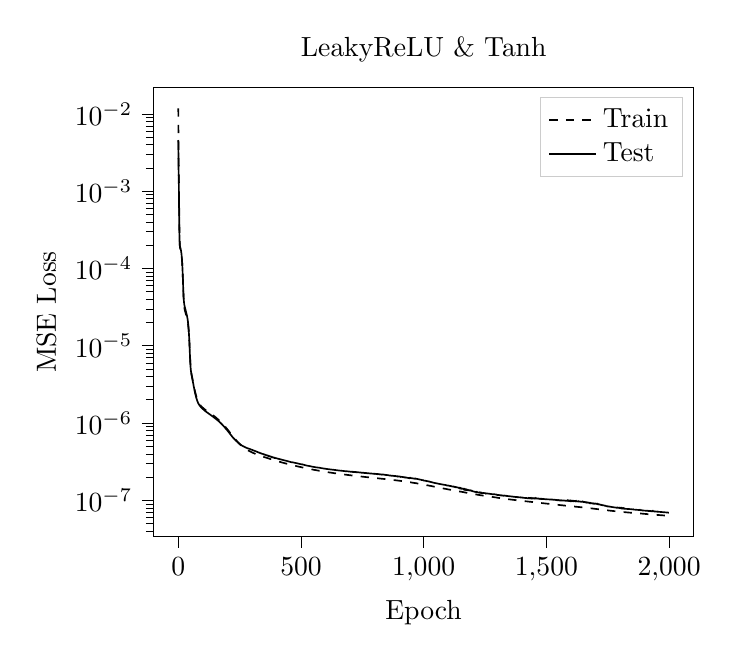
\begin{tikzpicture}

\begin{axis}[
legend cell align={left},
legend style={fill opacity=0.8, draw opacity=1, text opacity=1, draw=white!80!black},
log basis y={10},
tick align=outside,
tick pos=left,
title={LeakyReLU \& Tanh},
x grid style={white!69.0196078431373!black},
xlabel={Epoch},
xmin=-99.95, xmax=2098.95,
xtick style={color=black},
y grid style={white!69.0196078431373!black},
ylabel={MSE Loss},
ymin=3.43177769020239e-08, ymax=0.0217550336439875,
ymode=log,
ytick style={color=black}
]
\addplot [semithick, black, dashed]
table {%
0 0.0118530643042177
1 0.00271716704266146
2 0.00167412927886471
3 0.00101243689469993
4 0.00045973424060503
5 0.000261207596864551
6 0.000201558976317756
7 0.00018511279100494
8 0.000179200788814342
9 0.000174576494267967
10 0.000169601712237636
11 0.000163834669263451
12 0.000157019000936998
13 0.000148911127580504
14 0.000139271357867983
15 0.000127953551971586
16 0.000114886388801096
17 0.000100260177554446
18 8.46605833976355e-05
19 6.92464952226146e-05
20 5.57666255008371e-05
21 4.55883240647381e-05
22 3.88660105927556e-05
23 3.47616929993819e-05
24 3.22158156450314e-05
25 3.05434041529224e-05
26 2.93586506832071e-05
27 2.84435824496541e-05
28 2.76784982206664e-05
29 2.69959361194196e-05
30 2.6167898769927e-05
31 2.53696962281538e-05
32 2.47142864400303e-05
33 2.40883257101814e-05
34 2.3462807683245e-05
35 2.28194917517612e-05
36 2.21361250933114e-05
37 2.13898192178021e-05
38 2.05627751111024e-05
39 1.9635726780507e-05
40 1.86011470459562e-05
41 1.74350023871739e-05
42 1.61274048441555e-05
43 1.46852902416867e-05
44 1.31345061690809e-05
45 1.15222196054674e-05
46 9.92166628020641e-06
47 8.43393238756107e-06
48 7.16028058945994e-06
49 6.16866173072594e-06
50 5.45963166268848e-06
51 4.98488556331722e-06
52 4.66921569193346e-06
53 4.44369569072478e-06
54 4.26283255467297e-06
55 4.10205469756875e-06
56 3.95200737614232e-06
57 3.8109996012281e-06
58 3.67382299134533e-06
59 3.54308888006472e-06
60 3.41727396653369e-06
61 3.29590084652409e-06
62 3.17720198967208e-06
63 3.06160384815257e-06
64 2.95430421891751e-06
65 2.85230269520298e-06
66 2.75558185279579e-06
67 2.66389803647371e-06
68 2.57897133093365e-06
69 2.49876115083225e-06
70 2.42459519733984e-06
71 2.35611084360698e-06
72 2.29315852362788e-06
73 2.23360024858721e-06
74 2.18038750722371e-06
75 2.13208772674989e-06
76 2.08557600035419e-06
77 2.04397322181649e-06
78 2.0052868115954e-06
79 1.97052455132507e-06
80 1.9358652500614e-06
81 1.90366093914918e-06
82 1.87538027012124e-06
83 1.84823297968251e-06
84 1.82278619774934e-06
85 1.79879209343881e-06
86 1.77639971258259e-06
87 1.75495989918772e-06
88 1.73615727180731e-06
89 1.71740477168214e-06
90 1.69976929328186e-06
91 1.68390478773972e-06
92 1.66872160883713e-06
93 1.65481673491286e-06
94 1.64140779975241e-06
95 1.62894625606214e-06
96 1.6168444543041e-06
97 1.60500629891658e-06
98 1.59467800762059e-06
99 1.58435881195373e-06
100 1.57499000033567e-06
101 1.56598736191427e-06
102 1.55642656335431e-06
103 1.54590319141334e-06
104 1.53531705944943e-06
105 1.52483814102311e-06
106 1.51540221196456e-06
107 1.50651450968553e-06
108 1.49852953558138e-06
109 1.48978108879305e-06
110 1.48155487261192e-06
111 1.473753212764e-06
112 1.46592581035065e-06
113 1.45811151182329e-06
114 1.45039193807861e-06
115 1.44299419795857e-06
116 1.43553990096734e-06
117 1.4283073526542e-06
118 1.42114796418014e-06
119 1.41402536269197e-06
120 1.4066799710406e-06
121 1.39982001070393e-06
122 1.39267746087057e-06
123 1.38577581395793e-06
124 1.3789186680242e-06
125 1.371992529414e-06
126 1.36515135557147e-06
127 1.35831706401746e-06
128 1.35177427802091e-06
129 1.34456710597419e-06
130 1.33781877002548e-06
131 1.33112865796647e-06
132 1.32447658589285e-06
133 1.31773940083235e-06
134 1.31118761359517e-06
135 1.30475479940628e-06
136 1.29805225384416e-06
137 1.29135816624171e-06
138 1.28485466984785e-06
139 1.27849110981515e-06
140 1.27190054311654e-06
141 1.26496867267178e-06
142 1.2586724890582e-06
143 1.25217823000412e-06
144 1.24383108362736e-06
145 1.23542936435683e-06
146 1.22815887382899e-06
147 1.22111726841467e-06
148 1.21425765672711e-06
149 1.20777688215412e-06
150 1.20085036829209e-06
151 1.19395905099395e-06
152 1.18771772923765e-06
153 1.18089644871588e-06
154 1.17428739434899e-06
155 1.16676978154828e-06
156 1.15642677300798e-06
157 1.14880668485284e-06
158 1.14167408173671e-06
159 1.13500217128149e-06
160 1.1279125612873e-06
161 1.12095950947833e-06
162 1.11385238108141e-06
163 1.1068760949513e-06
164 1.09962021093679e-06
165 1.09247755673891e-06
166 1.08500489437802e-06
167 1.07731692369839e-06
168 1.06992002739048e-06
169 1.06233340153494e-06
170 1.05476866045251e-06
171 1.04725385301663e-06
172 1.03964452375749e-06
173 1.03224357621912e-06
174 1.0249889058116e-06
175 1.01740896730007e-06
176 1.00981932121158e-06
177 1.00251862770051e-06
178 9.95047050224684e-07
179 9.87523115867361e-07
180 9.79947625666e-07
181 9.72317288997715e-07
182 9.64804622782367e-07
183 9.57243006581621e-07
184 9.49631655743133e-07
185 9.41910147034264e-07
186 9.34334767435985e-07
187 9.26895800901661e-07
188 9.19153623286206e-07
189 9.1173805672895e-07
190 9.04083534095435e-07
191 8.96533727271276e-07
192 8.88804241938601e-07
193 8.81231718452113e-07
194 8.73640462003777e-07
195 8.65990211096346e-07
196 8.58377323396553e-07
197 8.50837881856137e-07
198 8.43417865837637e-07
199 8.358834592741e-07
200 8.28431481181724e-07
201 8.20944423679748e-07
202 8.13604629087195e-07
203 8.06318554154473e-07
204 7.98892333179424e-07
205 7.91583109460703e-07
206 7.84326178234096e-07
207 7.7717812114031e-07
208 7.70077875245079e-07
209 7.62944073485983e-07
210 7.55807730982383e-07
211 7.48702633558196e-07
212 7.41784852991145e-07
213 7.34965464417314e-07
214 7.28015673686855e-07
215 7.21312267089047e-07
216 7.14584897110626e-07
217 7.0796685973562e-07
218 7.01530687535978e-07
219 6.94918389484656e-07
220 6.88487152515904e-07
221 6.81997241059662e-07
222 6.75791806685311e-07
223 6.69688798012658e-07
224 6.63079862619043e-07
225 6.57233372606925e-07
226 6.51149268605877e-07
227 6.44990180830973e-07
228 6.39707958157487e-07
229 6.33765738257353e-07
230 6.27633001144545e-07
231 6.22900086213463e-07
232 6.17096304438292e-07
233 6.11554022484029e-07
234 6.06932349285216e-07
235 6.01709378145188e-07
236 5.96823508345778e-07
237 5.91874436921103e-07
238 5.87127333318449e-07
239 5.81490728478684e-07
240 5.76784642049688e-07
241 5.72062887528091e-07
242 5.67465997107774e-07
243 5.63017870689464e-07
244 5.58585788596133e-07
245 5.54362565580391e-07
246 5.50233029898095e-07
247 5.46157284787796e-07
248 5.42169837217443e-07
249 5.38345338426893e-07
250 5.34471238836431e-07
251 5.30791619951287e-07
252 5.27104146542001e-07
253 5.23486855598776e-07
254 5.19905496872752e-07
255 5.16522923433627e-07
256 5.1320403034083e-07
257 5.09976518756616e-07
258 5.06772108238351e-07
259 5.03671763851798e-07
260 5.00662150869857e-07
261 4.97670500905656e-07
262 4.94785802771958e-07
263 4.91955151417756e-07
264 4.89251897008103e-07
265 4.86573198955398e-07
266 4.83982838716202e-07
267 4.81418257535893e-07
268 4.79091480201532e-07
269 4.76753003283648e-07
270 4.74208299948486e-07
271 4.71778891380836e-07
272 4.69238318274279e-07
273 4.67039580271944e-07
274 4.64775038821585e-07
275 4.62731207463207e-07
276 4.60462195135847e-07
277 4.5821031440596e-07
278 4.55968379185379e-07
279 4.53642079705219e-07
280 4.51529708158205e-07
281 4.49460743681129e-07
282 4.47360691538279e-07
283 4.45254516009186e-07
284 4.43512205023922e-07
285 4.41370335479974e-07
286 4.39891918645685e-07
287 4.3775119753775e-07
288 4.35976524329362e-07
289 4.34284926598139e-07
290 4.32529043280283e-07
291 4.30876521534174e-07
292 4.29246813922646e-07
293 4.2763998928308e-07
294 4.26025263095653e-07
295 4.24496922605044e-07
296 4.22938850448418e-07
297 4.21455506710799e-07
298 4.19939799925828e-07
299 4.18516394347535e-07
300 4.17067732612963e-07
301 4.15670026228554e-07
302 4.14352804199325e-07
303 4.12975486909772e-07
304 4.1163369130004e-07
305 4.10336712960202e-07
306 4.0901354493883e-07
307 4.07670879326361e-07
308 4.06485504981902e-07
309 4.05222568986119e-07
310 4.03912711050225e-07
311 4.02790586377932e-07
312 4.01454716637772e-07
313 4.00197464202279e-07
314 3.98997999766948e-07
315 3.97849955120932e-07
316 3.96721643951992e-07
317 3.95627938416965e-07
318 3.94478706269297e-07
319 3.93301349191688e-07
320 3.92243420918703e-07
321 3.91151879753693e-07
322 3.90033366443276e-07
323 3.88982161126705e-07
324 3.8793921574154e-07
325 3.868340033506e-07
326 3.85833882148745e-07
327 3.84806861021048e-07
328 3.83725419737857e-07
329 3.82774777293093e-07
330 3.81802409961551e-07
331 3.80739406722341e-07
332 3.79787591057834e-07
333 3.78867508743497e-07
334 3.7750194394448e-07
335 3.76645611709137e-07
336 3.7559583101654e-07
337 3.74515050850732e-07
338 3.73532383505903e-07
339 3.72581143778916e-07
340 3.71705479452089e-07
341 3.70722432492698e-07
342 3.69743662830047e-07
343 3.6887618503556e-07
344 3.68046912214481e-07
345 3.67124095163263e-07
346 3.66226812971604e-07
347 3.6535512707303e-07
348 3.64482295140078e-07
349 3.63568770410438e-07
350 3.62746099042965e-07
351 3.6191672984387e-07
352 3.61063355484248e-07
353 3.60225598470265e-07
354 3.59332563903081e-07
355 3.58554333018901e-07
356 3.57739858756645e-07
357 3.56883827549836e-07
358 3.56125393736306e-07
359 3.55268856523594e-07
360 3.5446067074929e-07
361 3.53646082274395e-07
362 3.52718234239546e-07
363 3.51872259784614e-07
364 3.51077539519906e-07
365 3.50205739110265e-07
366 3.49407621172304e-07
367 3.4863870101276e-07
368 3.47785259748434e-07
369 3.47091866061078e-07
370 3.46326532749686e-07
371 3.45527291443659e-07
372 3.44794722394681e-07
373 3.43984667551922e-07
374 3.43169977270463e-07
375 3.42404283927067e-07
376 3.41655791999074e-07
377 3.40902730329162e-07
378 3.40205402494576e-07
379 3.39438222496824e-07
380 3.38743511164807e-07
381 3.38093948442975e-07
382 3.37387456440297e-07
383 3.36558028394052e-07
384 3.35849407960609e-07
385 3.35072243473178e-07
386 3.34426989269332e-07
387 3.33651557184567e-07
388 3.3312184295653e-07
389 3.31870176353277e-07
390 3.31015687365266e-07
391 3.30093047693936e-07
392 3.29405605299371e-07
393 3.28515724135059e-07
394 3.27883320380806e-07
395 3.27043711749297e-07
396 3.26344384546928e-07
397 3.25581409626352e-07
398 3.24843800513008e-07
399 3.24164057118992e-07
400 3.23606564492707e-07
401 3.22841541603225e-07
402 3.2214296764721e-07
403 3.21485749523731e-07
404 3.20611110851132e-07
405 3.19922173133591e-07
406 3.19242092274408e-07
407 3.1857112810485e-07
408 3.180388822841e-07
409 3.17376388977664e-07
410 3.16714038788746e-07
411 3.16138579790959e-07
412 3.15507177049312e-07
413 3.14841682850897e-07
414 3.14259163729957e-07
415 3.1358744921306e-07
416 3.12949973363175e-07
417 3.12298381103915e-07
418 3.11516434763348e-07
419 3.10839084889381e-07
420 3.1019210295824e-07
421 3.09614747095566e-07
422 3.08992809138431e-07
423 3.08364855825971e-07
424 3.07729297531978e-07
425 3.0712713997616e-07
426 3.06520865279936e-07
427 3.05932439729872e-07
428 3.05334564984605e-07
429 3.04705839084818e-07
430 3.04142966015775e-07
431 3.03557321629455e-07
432 3.02951247618921e-07
433 3.02409354375754e-07
434 3.01802297514087e-07
435 3.01251212547982e-07
436 3.00634733861216e-07
437 3.00078709571494e-07
438 2.99526084049262e-07
439 2.98959181961322e-07
440 2.98405851694383e-07
441 2.97866603077068e-07
442 2.97283363835277e-07
443 2.96744540548843e-07
444 2.96236425974428e-07
445 2.95662631884852e-07
446 2.95119851443815e-07
447 2.94577924904615e-07
448 2.94032025365709e-07
449 2.93495648548969e-07
450 2.92928335369425e-07
451 2.92440287381623e-07
452 2.91878952928926e-07
453 2.91313261371329e-07
454 2.90795729100068e-07
455 2.90339702850417e-07
456 2.89800641205318e-07
457 2.89283157187015e-07
458 2.88763092399336e-07
459 2.88186956886705e-07
460 2.87719527833019e-07
461 2.87232668952697e-07
462 2.86718326236723e-07
463 2.862276135005e-07
464 2.85688222945169e-07
465 2.85214371075426e-07
466 2.84679274898281e-07
467 2.84140632921037e-07
468 2.83622278580253e-07
469 2.83142897899324e-07
470 2.82739655233399e-07
471 2.82202584088509e-07
472 2.81684053625497e-07
473 2.81147220661637e-07
474 2.8064164433772e-07
475 2.80164724898668e-07
476 2.79677985666638e-07
477 2.79170837771403e-07
478 2.78683379292488e-07
479 2.78189573876375e-07
480 2.77702305631067e-07
481 2.77222816016831e-07
482 2.76620818411288e-07
483 2.76163140398467e-07
484 2.75674113474622e-07
485 2.75241383448588e-07
486 2.74769400441244e-07
487 2.74307894294168e-07
488 2.73828556458966e-07
489 2.73356900713395e-07
490 2.72877485983258e-07
491 2.72412719702686e-07
492 2.71952965867683e-07
493 2.7151991022123e-07
494 2.71063778093605e-07
495 2.70645359691457e-07
496 2.70216694630676e-07
497 2.69762554708564e-07
498 2.69319825754621e-07
499 2.68886601602958e-07
500 2.68450084831784e-07
501 2.68012147643049e-07
502 2.67575329154113e-07
503 2.67153018668864e-07
504 2.66674774529463e-07
505 2.66283876641182e-07
506 2.65838455433709e-07
507 2.65449408246354e-07
508 2.64985072504942e-07
509 2.64566873163119e-07
510 2.64143997810606e-07
511 2.6372079743453e-07
512 2.63302015554245e-07
513 2.62963274806793e-07
514 2.62516207605756e-07
515 2.62078123029141e-07
516 2.6153940742546e-07
517 2.61240193822232e-07
518 2.60856092836548e-07
519 2.60440021655484e-07
520 2.59956458464217e-07
521 2.59652960870937e-07
522 2.5924450344661e-07
523 2.58845528328777e-07
524 2.58385906661829e-07
525 2.58098587920586e-07
526 2.57721656673482e-07
527 2.57322477942523e-07
528 2.56853048433925e-07
529 2.56580461183376e-07
530 2.56191600172428e-07
531 2.55807624206739e-07
532 2.55381097296947e-07
533 2.55083945155832e-07
534 2.54707071889015e-07
535 2.54274472382576e-07
536 2.53979634194934e-07
537 2.53613948039799e-07
538 2.53186067510569e-07
539 2.52915796181696e-07
540 2.52544044805347e-07
541 2.52177458669678e-07
542 2.51814867709754e-07
543 2.51472695616428e-07
544 2.51091237899459e-07
545 2.50749283082996e-07
546 2.50388591730655e-07
547 2.50065211588435e-07
548 2.49643439182989e-07
549 2.49388097827818e-07
550 2.49036874500064e-07
551 2.48683912019487e-07
552 2.48340439107153e-07
553 2.48009093489543e-07
554 2.47644183417606e-07
555 2.47348658717783e-07
556 2.46921584547977e-07
557 2.46672405559423e-07
558 2.4635122429828e-07
559 2.45947923090739e-07
560 2.45706016663405e-07
561 2.45372700454993e-07
562 2.44974506784956e-07
563 2.4471972373874e-07
564 2.4438149678474e-07
565 2.43998724755556e-07
566 2.43757375315568e-07
567 2.4344039513835e-07
568 2.43120262155117e-07
569 2.42807220651287e-07
570 2.42499065443269e-07
571 2.42203533503016e-07
572 2.41825013269192e-07
573 2.41641147702865e-07
574 2.41307229600807e-07
575 2.40921330494359e-07
576 2.40644746909879e-07
577 2.40279314525083e-07
578 2.39888169815572e-07
579 2.39647900237117e-07
580 2.39297322039533e-07
581 2.38893787276595e-07
582 2.38672715674681e-07
583 2.38364748824438e-07
584 2.38003041218349e-07
585 2.37784313227962e-07
586 2.37474714154473e-07
587 2.37091034534842e-07
588 2.36894158952339e-07
589 2.36600740073811e-07
590 2.36258271698375e-07
591 2.36051617847011e-07
592 2.35757887693921e-07
593 2.35384111789472e-07
594 2.35183570460151e-07
595 2.34854371832682e-07
596 2.34624506887826e-07
597 2.34325953321957e-07
598 2.34039721533463e-07
599 2.33770109900888e-07
600 2.33466635911839e-07
601 2.33135660757e-07
602 2.32950038828506e-07
603 2.3267533492799e-07
604 2.32340332509295e-07
605 2.32128316092428e-07
606 2.31862926064252e-07
607 2.31633997536562e-07
608 2.31260507582931e-07
609 2.3104011305719e-07
610 2.3077447281139e-07
611 2.30500478679119e-07
612 2.302613713141e-07
613 2.29983399727018e-07
614 2.29732210790701e-07
615 2.29474479688463e-07
616 2.29219407344772e-07
617 2.28958964825665e-07
618 2.28696038512055e-07
619 2.28456288859036e-07
620 2.28211573549686e-07
621 2.27972307349944e-07
622 2.27720530197928e-07
623 2.27468705197964e-07
624 2.27222729378695e-07
625 2.26979138638228e-07
626 2.26725032128172e-07
627 2.26482411250117e-07
628 2.26238589867478e-07
629 2.2600784120641e-07
630 2.25760820164567e-07
631 2.25525988106767e-07
632 2.2528483005857e-07
633 2.25036615979946e-07
634 2.24798530474857e-07
635 2.245455094112e-07
636 2.24306671285035e-07
637 2.24090163293056e-07
638 2.23974491312617e-07
639 2.23647726016907e-07
640 2.2354151440851e-07
641 2.23199736666402e-07
642 2.23048872683762e-07
643 2.22717595661948e-07
644 2.22584690398264e-07
645 2.22249005823016e-07
646 2.22128948713873e-07
647 2.21802636730217e-07
648 2.21642298200209e-07
649 2.21354814236463e-07
650 2.21212942399518e-07
651 2.20913502765541e-07
652 2.20765400790413e-07
653 2.20472539936623e-07
654 2.20341641522737e-07
655 2.20101288171293e-07
656 2.19818628295343e-07
657 2.19636836192194e-07
658 2.19449505202363e-07
659 2.19179486400378e-07
660 2.19054223038029e-07
661 2.1881402455648e-07
662 2.18547279182246e-07
663 2.18407628764794e-07
664 2.1815676842607e-07
665 2.17975170194507e-07
666 2.17686950634288e-07
667 2.17566066694985e-07
668 2.1733298704163e-07
669 2.17060445685036e-07
670 2.16942077059912e-07
671 2.16649795312662e-07
672 2.16544278991648e-07
673 2.16255045707214e-07
674 2.16131762982741e-07
675 2.15852907508918e-07
676 2.15736312519255e-07
677 2.15498423557392e-07
678 2.15338095706841e-07
679 2.15115065628879e-07
680 2.14931766052473e-07
681 2.14743876647105e-07
682 2.1452934733901e-07
683 2.14333714552595e-07
684 2.14191282310594e-07
685 2.1399087525964e-07
686 2.13799643553614e-07
687 2.13587029818996e-07
688 2.13333764300216e-07
689 2.13138286788706e-07
690 2.12866215186125e-07
691 2.12723850346208e-07
692 2.12456457660437e-07
693 2.12390492180248e-07
694 2.1211422053824e-07
695 2.11901987100305e-07
696 2.1164349405467e-07
697 2.11502926056539e-07
698 2.11225254645342e-07
699 2.11071560613618e-07
700 2.1092119062871e-07
701 2.10711485458148e-07
702 2.10524598244888e-07
703 2.10352325012764e-07
704 2.10138360678513e-07
705 2.09938405241417e-07
706 2.09765650339477e-07
707 2.09575859855704e-07
708 2.09359261809539e-07
709 2.09192116145118e-07
710 2.08994861992551e-07
711 2.08894274059901e-07
712 2.08617789951404e-07
713 2.08484151400512e-07
714 2.08267086229341e-07
715 2.08157416111021e-07
716 2.07965515329533e-07
717 2.0773107167571e-07
718 2.07602891123315e-07
719 2.07446420823487e-07
720 2.07267277083645e-07
721 2.07017601070447e-07
722 2.06857604830191e-07
723 2.06693050948559e-07
724 2.06501707502582e-07
725 2.06318297003349e-07
726 2.061609860462e-07
727 2.05949397312111e-07
728 2.05818528023372e-07
729 2.05619040556826e-07
730 2.0542596598716e-07
731 2.05264010830319e-07
732 2.05055826384637e-07
733 2.04901554035075e-07
734 2.04771108222701e-07
735 2.04615930066154e-07
736 2.04429741224033e-07
737 2.04268639762972e-07
738 2.04093490332014e-07
739 2.03921731198875e-07
740 2.03783937124058e-07
741 2.03591222188493e-07
742 2.03433932504993e-07
743 2.03294410177079e-07
744 2.03115816297839e-07
745 2.02962098882153e-07
746 2.02798127070025e-07
747 2.02641582276897e-07
748 2.0247920047467e-07
749 2.02321240067249e-07
750 2.02163325781157e-07
751 2.02007027972684e-07
752 2.01846984239751e-07
753 2.01729566754238e-07
754 2.01550911008042e-07
755 2.01417259383163e-07
756 2.01240844646122e-07
757 2.01105906960208e-07
758 2.00922100276557e-07
759 2.00787376009259e-07
760 2.00601763872044e-07
761 2.00482007990388e-07
762 2.00299133673809e-07
763 2.00137742218942e-07
764 1.99984624302374e-07
765 1.99804511787249e-07
766 1.99653848646619e-07
767 1.99538892360351e-07
768 1.9936609028548e-07
769 1.99198628926922e-07
770 1.99091463208845e-07
771 1.98933666865742e-07
772 1.98748004130778e-07
773 1.98654580778168e-07
774 1.98493020199919e-07
775 1.98315526972692e-07
776 1.98179933335041e-07
777 1.98039544159201e-07
778 1.97873308728447e-07
779 1.97702004207656e-07
780 1.97595039942655e-07
781 1.97445724197109e-07
782 1.97299228439363e-07
783 1.97113351568134e-07
784 1.96935009412869e-07
785 1.9679619677504e-07
786 1.96704571074235e-07
787 1.96535869825709e-07
788 1.96417040520203e-07
789 1.96257578586767e-07
790 1.96085073802976e-07
791 1.95906529860679e-07
792 1.9580319301582e-07
793 1.95651297666188e-07
794 1.95509253991588e-07
795 1.95332549040472e-07
796 1.95176153930277e-07
797 1.9508170942828e-07
798 1.94809531933515e-07
799 1.94621923839122e-07
800 1.94577639106797e-07
801 1.94502660981755e-07
802 1.94220849742521e-07
803 1.9407022731599e-07
804 1.93978072104528e-07
805 1.93858640074041e-07
806 1.93672978909376e-07
807 1.93564685474712e-07
808 1.93407830309411e-07
809 1.9325386772806e-07
810 1.9307086262188e-07
811 1.92956589245341e-07
812 1.92784446319649e-07
813 1.92575233022296e-07
814 1.92446511348976e-07
815 1.92271403115285e-07
816 1.92117631925726e-07
817 1.91977746915484e-07
818 1.91837797295591e-07
819 1.91621675078579e-07
820 1.91532269944616e-07
821 1.91485599415842e-07
822 1.91349084090575e-07
823 1.91097462220569e-07
824 1.90978913387596e-07
825 1.90743896467893e-07
826 1.90622938887941e-07
827 1.90471911444945e-07
828 1.90318472142792e-07
829 1.90155134610848e-07
830 1.89974666753301e-07
831 1.8988238119988e-07
832 1.89729744747069e-07
833 1.89577713982203e-07
834 1.89420835468468e-07
835 1.89228891997573e-07
836 1.89185338825837e-07
837 1.89037455335495e-07
838 1.88832184292664e-07
839 1.88669506208328e-07
840 1.8860980708979e-07
841 1.88430943389051e-07
842 1.88328428080808e-07
843 1.880989881613e-07
844 1.8794127457511e-07
845 1.87852113448628e-07
846 1.87664538998433e-07
847 1.87568792341608e-07
848 1.87350116291896e-07
849 1.8720051024701e-07
850 1.87061393766896e-07
851 1.86907370007816e-07
852 1.86787177604231e-07
853 1.8661556766375e-07
854 1.86445408317582e-07
855 1.8628098129625e-07
856 1.86233017842596e-07
857 1.86043692416149e-07
858 1.85916030922328e-07
859 1.85741681846707e-07
860 1.85577939838311e-07
861 1.85364337674798e-07
862 1.85230030382399e-07
863 1.85133268537641e-07
864 1.8496937442336e-07
865 1.84808264194203e-07
866 1.84644422240865e-07
867 1.84447406851973e-07
868 1.84294324242273e-07
869 1.84178464202489e-07
870 1.84014452706549e-07
871 1.83841847032795e-07
872 1.8368446058048e-07
873 1.83516295621189e-07
874 1.83339417347383e-07
875 1.83247092728323e-07
876 1.83087581305585e-07
877 1.82929167095836e-07
878 1.82783076610349e-07
879 1.82587592853167e-07
880 1.82422121021375e-07
881 1.82327151939887e-07
882 1.82149352689009e-07
883 1.81977185548021e-07
884 1.81808037474696e-07
885 1.81609961479978e-07
886 1.81445596808771e-07
887 1.81330588048922e-07
888 1.81169432998729e-07
889 1.8099068277877e-07
890 1.80869595567401e-07
891 1.80666593408318e-07
892 1.80395674341582e-07
893 1.80269183800874e-07
894 1.80182070700141e-07
895 1.80020855800933e-07
896 1.79949448813943e-07
897 1.79735197555431e-07
898 1.79557423095389e-07
899 1.79240639887723e-07
900 1.79061926033341e-07
901 1.78964278418903e-07
902 1.78825385937387e-07
903 1.78665588187243e-07
904 1.78476881302458e-07
905 1.78299222426403e-07
906 1.78091645508971e-07
907 1.77893942421292e-07
908 1.77791877916889e-07
909 1.776089068386e-07
910 1.77429847447286e-07
911 1.77260000931767e-07
912 1.77078513615925e-07
913 1.76987821447483e-07
914 1.76801693754669e-07
915 1.76696476962945e-07
916 1.76497925167496e-07
917 1.76327017499034e-07
918 1.76139942922759e-07
919 1.7595209347121e-07
920 1.75708836174238e-07
921 1.75513835131369e-07
922 1.75378918982005e-07
923 1.75187202259508e-07
924 1.75111654392879e-07
925 1.74880665021249e-07
926 1.74724064791576e-07
927 1.74432815377656e-07
928 1.74271239465895e-07
929 1.74156150045235e-07
930 1.73961806424927e-07
931 1.73759765992543e-07
932 1.73552534000976e-07
933 1.73333812902854e-07
934 1.73191188849842e-07
935 1.72858451954028e-07
936 1.72689596894315e-07
937 1.72501483106657e-07
938 1.72240258798695e-07
939 1.72142322035995e-07
940 1.71882180637795e-07
941 1.71781431667739e-07
942 1.71534132320517e-07
943 1.71427748902886e-07
944 1.71182018497973e-07
945 1.71046810187647e-07
946 1.70868499822063e-07
947 1.70649446232574e-07
948 1.70433219139454e-07
949 1.70225919603695e-07
950 1.70000608598286e-07
951 1.69803014244962e-07
952 1.69534294911955e-07
953 1.693373877103e-07
954 1.69177045492574e-07
955 1.68982332347412e-07
956 1.68769802812108e-07
957 1.68561846926707e-07
958 1.68356583650109e-07
959 1.68175843185736e-07
960 1.67969688838809e-07
961 1.6777198183604e-07
962 1.67602634164155e-07
963 1.67403722173276e-07
964 1.67237837928269e-07
965 1.67088833272544e-07
966 1.66905762398528e-07
967 1.66680781411799e-07
968 1.66488919255414e-07
969 1.66307719140946e-07
970 1.66085840177743e-07
971 1.65865779074181e-07
972 1.65654938456328e-07
973 1.65444530743741e-07
974 1.65259729925538e-07
975 1.65055726228047e-07
976 1.64847215089026e-07
977 1.64630200004012e-07
978 1.64421114199342e-07
979 1.64211539228631e-07
980 1.64029924171416e-07
981 1.63781369501237e-07
982 1.63627734259819e-07
983 1.6333098932364e-07
984 1.63135665680159e-07
985 1.62986013805266e-07
986 1.6276575917118e-07
987 1.62616001212257e-07
988 1.62426574767949e-07
989 1.62191438832338e-07
990 1.619688600627e-07
991 1.61746657809658e-07
992 1.61536477911284e-07
993 1.61331311019808e-07
994 1.61136969033748e-07
995 1.6092817946145e-07
996 1.60706019286749e-07
997 1.60496292380685e-07
998 1.60270611289093e-07
999 1.6000876024691e-07
1000 1.59730474265984e-07
1001 1.59520671360269e-07
1002 1.59217975522097e-07
1003 1.59063585435604e-07
1004 1.58882511904324e-07
1005 1.58647880759588e-07
1006 1.58423164926091e-07
1007 1.58098031590725e-07
1008 1.57898606630624e-07
1009 1.57661048241664e-07
1010 1.57398774831563e-07
1011 1.57148834816212e-07
1012 1.56870506458517e-07
1013 1.56711850898716e-07
1014 1.56497015339596e-07
1015 1.56257475971699e-07
1016 1.56046945555488e-07
1017 1.55826125030956e-07
1018 1.55598985777772e-07
1019 1.5539752382665e-07
1020 1.5514921122417e-07
1021 1.5493437491898e-07
1022 1.54783092639832e-07
1023 1.54565749099334e-07
1024 1.54347193969784e-07
1025 1.54280347814506e-07
1026 1.54014388449752e-07
1027 1.53799708336066e-07
1028 1.53557663267634e-07
1029 1.53346554242262e-07
1030 1.53081715104975e-07
1031 1.52885490983579e-07
1032 1.52644006412572e-07
1033 1.52446025687425e-07
1034 1.52200829489857e-07
1035 1.51935989038066e-07
1036 1.5165363715397e-07
1037 1.51450876394676e-07
1038 1.51208441636186e-07
1039 1.50983596370224e-07
1040 1.50754961531163e-07
1041 1.50501454818652e-07
1042 1.50234482596545e-07
1043 1.500267249952e-07
1044 1.49826365806405e-07
1045 1.49551108549417e-07
1046 1.49386445293942e-07
1047 1.49152108022577e-07
1048 1.48935337456635e-07
1049 1.48707327504383e-07
1050 1.48492372758824e-07
1051 1.48282824632417e-07
1052 1.48078847772126e-07
1053 1.47873801275011e-07
1054 1.47662170590479e-07
1055 1.47460764416962e-07
1056 1.47223473000224e-07
1057 1.47010033600736e-07
1058 1.46798720592756e-07
1059 1.46577249601876e-07
1060 1.4639762123636e-07
1061 1.4619643713587e-07
1062 1.45985476322608e-07
1063 1.45778726725609e-07
1064 1.45563538396232e-07
1065 1.45380512712734e-07
1066 1.45199056049705e-07
1067 1.44983988562331e-07
1068 1.44786048970502e-07
1069 1.44568250249222e-07
1070 1.44377106884974e-07
1071 1.44238954987941e-07
1072 1.44015394667463e-07
1073 1.43782359259603e-07
1074 1.43517698781181e-07
1075 1.43292362437819e-07
1076 1.4311534452105e-07
1077 1.42922095818676e-07
1078 1.42694176432201e-07
1079 1.42511509764631e-07
1080 1.42320883853131e-07
1081 1.42115572501211e-07
1082 1.41915518241831e-07
1083 1.41727660235347e-07
1084 1.41539420525305e-07
1085 1.41344826488421e-07
1086 1.41149399077278e-07
1087 1.40993090482766e-07
1088 1.40787137432596e-07
1089 1.40602423535086e-07
1090 1.40420193517343e-07
1091 1.40221834413978e-07
1092 1.40021793214373e-07
1093 1.39751922354492e-07
1094 1.39544986296869e-07
1095 1.39366501237248e-07
1096 1.39174019466282e-07
1097 1.38834078114769e-07
1098 1.38641360159397e-07
1099 1.38483587925009e-07
1100 1.38350642373553e-07
1101 1.38190962829299e-07
1102 1.37955044088756e-07
1103 1.37780998926473e-07
1104 1.37604125285407e-07
1105 1.37377671919126e-07
1106 1.3721026255098e-07
1107 1.3702453204445e-07
1108 1.36816325458256e-07
1109 1.36619293414242e-07
1110 1.36436577498955e-07
1111 1.36264744874381e-07
1112 1.36055063137519e-07
1113 1.35872794068348e-07
1114 1.35656363958958e-07
1115 1.35474489319165e-07
1116 1.35287901478875e-07
1117 1.35084419866871e-07
1118 1.34919479229723e-07
1119 1.34707229086928e-07
1120 1.34552972824054e-07
1121 1.34392235189296e-07
1122 1.34211788001437e-07
1123 1.34022364917996e-07
1124 1.33834222694418e-07
1125 1.33680917187462e-07
1126 1.33549971288005e-07
1127 1.33321881719439e-07
1128 1.33158634149311e-07
1129 1.32976397111406e-07
1130 1.32801262232363e-07
1131 1.32660635792092e-07
1132 1.3256395303074e-07
1133 1.3234662775119e-07
1134 1.32177991829963e-07
1135 1.31985430741111e-07
1136 1.31801775921758e-07
1137 1.31623225954058e-07
1138 1.3144830696632e-07
1139 1.3132029658891e-07
1140 1.3111966016055e-07
1141 1.30938463286157e-07
1142 1.3076284651703e-07
1143 1.30590019210786e-07
1144 1.30414797034462e-07
1145 1.30247909119419e-07
1146 1.30075543523844e-07
1147 1.2991378209648e-07
1148 1.29729824443814e-07
1149 1.29620293314758e-07
1150 1.29415466410876e-07
1151 1.29288045030762e-07
1152 1.29104797821356e-07
1153 1.28977646532746e-07
1154 1.28819465039953e-07
1155 1.28667567054208e-07
1156 1.28509636070362e-07
1157 1.28371612639455e-07
1158 1.28219746436287e-07
1159 1.27995160504213e-07
1160 1.27906802120492e-07
1161 1.27735503014037e-07
1162 1.27535211241536e-07
1163 1.27303911334309e-07
1164 1.27048455112799e-07
1165 1.26922013038211e-07
1166 1.26683094421765e-07
1167 1.26568199526389e-07
1168 1.26293073805073e-07
1169 1.2608189124208e-07
1170 1.25966059989935e-07
1171 1.25794228132747e-07
1172 1.25575737861539e-07
1173 1.25362858756972e-07
1174 1.25249346218936e-07
1175 1.25057965572495e-07
1176 1.24901918134412e-07
1177 1.24663825395999e-07
1178 1.24542853811249e-07
1179 1.24312287319128e-07
1180 1.24227721691739e-07
1181 1.24054489148762e-07
1182 1.23892663459912e-07
1183 1.23698761150592e-07
1184 1.23596502092482e-07
1185 1.23382345861955e-07
1186 1.23272039779465e-07
1187 1.23062993779399e-07
1188 1.22962949738792e-07
1189 1.22812680999118e-07
1190 1.22681518540446e-07
1191 1.22485459471022e-07
1192 1.22373093603301e-07
1193 1.22180681721318e-07
1194 1.22062737482054e-07
1195 1.2187447886447e-07
1196 1.21760682851857e-07
1197 1.21487625520444e-07
1198 1.21530664124236e-07
1199 1.21434413728139e-07
1200 1.21137268038751e-07
1201 1.20878889582343e-07
1202 1.20710900922916e-07
1203 1.20578473321586e-07
1204 1.20379436836515e-07
1205 1.20130681089847e-07
1206 1.19967440081581e-07
1207 1.19809633428503e-07
1208 1.1968485621594e-07
1209 1.1953818977517e-07
1210 1.19361607492152e-07
1211 1.19255883692659e-07
1212 1.19114461313075e-07
1213 1.1894671261814e-07
1214 1.18726950567805e-07
1215 1.18577280545651e-07
1216 1.18446295104491e-07
1217 1.18350390611255e-07
1218 1.18164257060016e-07
1219 1.18029195910196e-07
1220 1.17923606161696e-07
1221 1.17740713488246e-07
1222 1.17615516952441e-07
1223 1.17428830684219e-07
1224 1.17340325026305e-07
1225 1.17267212051075e-07
1226 1.17074500035841e-07
1227 1.1689717317509e-07
1228 1.16832294899893e-07
1229 1.16660597107909e-07
1230 1.16557522581218e-07
1231 1.1638936075542e-07
1232 1.16293079098995e-07
1233 1.1615023936784e-07
1234 1.15965406283891e-07
1235 1.15937135632294e-07
1236 1.15770845393826e-07
1237 1.15656800470987e-07
1238 1.15498020331728e-07
1239 1.15389218859008e-07
1240 1.15237190087214e-07
1241 1.15116425188688e-07
1242 1.14983899742072e-07
1243 1.14922975889442e-07
1244 1.14829335128519e-07
1245 1.14685722209629e-07
1246 1.14553782651683e-07
1247 1.14423000404429e-07
1248 1.14291658370291e-07
1249 1.14146929462322e-07
1250 1.14030466292547e-07
1251 1.13904921228425e-07
1252 1.13765815093814e-07
1253 1.1366588059758e-07
1254 1.13550664288198e-07
1255 1.13388263041969e-07
1256 1.1328302516489e-07
1257 1.1309919934277e-07
1258 1.12994540693023e-07
1259 1.1289519078872e-07
1260 1.12770297622689e-07
1261 1.1268669043929e-07
1262 1.12551397478455e-07
1263 1.12448732352277e-07
1264 1.12315216899361e-07
1265 1.12217203568576e-07
1266 1.12089267332749e-07
1267 1.11983588091391e-07
1268 1.11884272147478e-07
1269 1.11768592191197e-07
1270 1.11649045841489e-07
1271 1.11516369464937e-07
1272 1.11367647345872e-07
1273 1.11236748324473e-07
1274 1.11128077183054e-07
1275 1.10999723002436e-07
1276 1.10894493033697e-07
1277 1.10791011962874e-07
1278 1.10668243085144e-07
1279 1.10672879035434e-07
1280 1.10524663309519e-07
1281 1.10387117668864e-07
1282 1.10317078533484e-07
1283 1.10137854488102e-07
1284 1.10018036004078e-07
1285 1.09912964454395e-07
1286 1.09854005803101e-07
1287 1.09692538941886e-07
1288 1.09553196299572e-07
1289 1.09495215230737e-07
1290 1.09402880060117e-07
1291 1.09246621118331e-07
1292 1.09144351277735e-07
1293 1.09060896861024e-07
1294 1.08934168622454e-07
1295 1.08833148818377e-07
1296 1.08530306373922e-07
1297 1.08329140676489e-07
1298 1.08251451091945e-07
1299 1.08081192781384e-07
1300 1.07963060575145e-07
1301 1.07849208102806e-07
1302 1.07792553954766e-07
1303 1.07604572608722e-07
1304 1.07502775939849e-07
1305 1.07372964691876e-07
1306 1.07319396025929e-07
1307 1.07215680955619e-07
1308 1.07021888190673e-07
1309 1.06997283111809e-07
1310 1.06866084482959e-07
1311 1.06697310560122e-07
1312 1.06620122195977e-07
1313 1.06523319796992e-07
1314 1.06369266372752e-07
1315 1.06309255887282e-07
1316 1.06270429679256e-07
1317 1.06117778642556e-07
1318 1.05977327308437e-07
1319 1.05862196591033e-07
1320 1.05791138462763e-07
1321 1.05682823235753e-07
1322 1.05575490255916e-07
1323 1.05479250333218e-07
1324 1.05338221807472e-07
1325 1.05261139921708e-07
1326 1.051674444561e-07
1327 1.05097885736427e-07
1328 1.04932408785174e-07
1329 1.04820680103757e-07
1330 1.047039979305e-07
1331 1.04622124503351e-07
1332 1.04536150132617e-07
1333 1.04428355225394e-07
1334 1.0431528302135e-07
1335 1.04219694215146e-07
1336 1.04108350139853e-07
1337 1.04010152625733e-07
1338 1.03937799931231e-07
1339 1.03816809513546e-07
1340 1.0372121978719e-07
1341 1.03628270149869e-07
1342 1.03506012415266e-07
1343 1.03420547411304e-07
1344 1.03336215182992e-07
1345 1.03233022066718e-07
1346 1.03127735130215e-07
1347 1.0304500937508e-07
1348 1.02925141018062e-07
1349 1.02855479322983e-07
1350 1.02757760238603e-07
1351 1.0265365359885e-07
1352 1.02567342004534e-07
1353 1.02481212273631e-07
1354 1.0238724213707e-07
1355 1.02296590689832e-07
1356 1.02196159151191e-07
1357 1.02104377361911e-07
1358 1.0200633058588e-07
1359 1.01915980462053e-07
1360 1.01855772072668e-07
1361 1.01716821337305e-07
1362 1.01626993178172e-07
1363 1.01556392099411e-07
1364 1.01448222448397e-07
1365 1.01379643577815e-07
1366 1.01260316306195e-07
1367 1.01179489991665e-07
1368 1.01097790544458e-07
1369 1.01009448204792e-07
1370 1.00864683293622e-07
1371 1.00828128005048e-07
1372 1.00755467798308e-07
1373 1.00713147080711e-07
1374 1.00573230966461e-07
1375 1.00459209054549e-07
1376 1.00394691603611e-07
1377 1.00241487885455e-07
1378 1.0012043237495e-07
1379 1.00072280460495e-07
1380 9.99612031762354e-08
1381 9.98299957863935e-08
1382 9.98184432319249e-08
1383 9.96668474364526e-08
1384 9.95932889260587e-08
1385 9.95839536628296e-08
1386 9.94681824089128e-08
1387 9.93048253903339e-08
1388 9.92653954980938e-08
1389 9.91634453377799e-08
1390 9.90674275698211e-08
1391 9.89828977822072e-08
1392 9.8907549475058e-08
1393 9.88146800331435e-08
1394 9.87215900636329e-08
1395 9.8650412091672e-08
1396 9.85902149146511e-08
1397 9.85469480134782e-08
1398 9.84345484340565e-08
1399 9.83603269091304e-08
1400 9.8255061821817e-08
1401 9.81671388657901e-08
1402 9.81320887660786e-08
1403 9.80905747880456e-08
1404 9.80041671923004e-08
1405 9.79182954061741e-08
1406 9.78550450803084e-08
1407 9.77846480125777e-08
1408 9.77129959380818e-08
1409 9.7618126581267e-08
1410 9.75506221863043e-08
1411 9.74697444000583e-08
1412 9.73777406514387e-08
1413 9.73348767026039e-08
1414 9.72579349145519e-08
1415 9.71626870587272e-08
1416 9.70618948556989e-08
1417 9.69868048876776e-08
1418 9.69154252317139e-08
1419 9.68737760551619e-08
1420 9.67826737579003e-08
1421 9.67257258714937e-08
1422 9.66225470016013e-08
1423 9.65445911766949e-08
1424 9.64560930221126e-08
1425 9.63946927470261e-08
1426 9.62924369858342e-08
1427 9.61960204577395e-08
1428 9.61506538956769e-08
1429 9.606817239316e-08
1430 9.59494349572765e-08
1431 9.58923250315991e-08
1432 9.58117151803606e-08
1433 9.58197924845194e-08
1434 9.57060428135037e-08
1435 9.55582331911842e-08
1436 9.55965827671434e-08
1437 9.54066385716601e-08
1438 9.53776570362663e-08
1439 9.52400907010542e-08
1440 9.52336963386813e-08
1441 9.51048315940284e-08
1442 9.50543814823845e-08
1443 9.4960869809313e-08
1444 9.49622229455826e-08
1445 9.48089321681778e-08
1446 9.47507008817183e-08
1447 9.4643267519956e-08
1448 9.46226468379052e-08
1449 9.4495548420781e-08
1450 9.44533930393732e-08
1451 9.43506249839743e-08
1452 9.43026340820552e-08
1453 9.41682392365806e-08
1454 9.42125580642994e-08
1455 9.41105431415679e-08
1456 9.39968358650845e-08
1457 9.40077997384492e-08
1458 9.39092628087224e-08
1459 9.37745551325975e-08
1460 9.37469126931489e-08
1461 9.37155768170328e-08
1462 9.35226401210798e-08
1463 9.34516931963003e-08
1464 9.3375002428786e-08
1465 9.33066063666388e-08
1466 9.32856002933136e-08
1467 9.32056613294208e-08
1468 9.30419151004003e-08
1469 9.29735011503396e-08
1470 9.29493840864382e-08
1471 9.28904867336655e-08
1472 9.27369426548808e-08
1473 9.2628096581393e-08
1474 9.25879248008243e-08
1475 9.25714797759269e-08
1476 9.24662792343156e-08
1477 9.23423236613985e-08
1478 9.22998963446275e-08
1479 9.2187932512644e-08
1480 9.21299071414694e-08
1481 9.20336628489338e-08
1482 9.20134716011489e-08
1483 9.18693962042028e-08
1484 9.18302799028936e-08
1485 9.17768765340554e-08
1486 9.16352135647003e-08
1487 9.16297153530365e-08
1488 9.14914950378431e-08
1489 9.14874235604657e-08
1490 9.14028345562201e-08
1491 9.13489709084558e-08
1492 9.12038426079675e-08
1493 9.11310380438124e-08
1494 9.11061501085442e-08
1495 9.1044428259579e-08
1496 9.09657928502838e-08
1497 9.08472444081099e-08
1498 9.08059538318184e-08
1499 9.07555209792577e-08
1500 9.06590707643318e-08
1501 9.05626640701485e-08
1502 9.05422847985449e-08
1503 9.04447589533675e-08
1504 9.03806934502427e-08
1505 9.02795845121318e-08
1506 9.02511904143921e-08
1507 9.01830849713292e-08
1508 9.01680074889555e-08
1509 9.00529918510529e-08
1510 9.00171911268899e-08
1511 8.99389152202446e-08
1512 8.98761768794998e-08
1513 8.97628513101267e-08
1514 8.9727812454754e-08
1515 8.96666446621452e-08
1516 8.9595610877069e-08
1517 8.94834702407365e-08
1518 8.94327300500208e-08
1519 8.93961989092418e-08
1520 8.93055324446834e-08
1521 8.92264829097655e-08
1522 8.9132382470325e-08
1523 8.90340010712975e-08
1524 8.90586697899209e-08
1525 8.89112405175751e-08
1526 8.89173306219959e-08
1527 8.88155498905974e-08
1528 8.87604053225743e-08
1529 8.86581190471247e-08
1530 8.86199899809981e-08
1531 8.85358596960373e-08
1532 8.84668544678391e-08
1533 8.83778405267321e-08
1534 8.82795187884256e-08
1535 8.82399620216745e-08
1536 8.81458221506648e-08
1537 8.80856802467633e-08
1538 8.8028733735257e-08
1539 8.79710035555092e-08
1540 8.78986497596657e-08
1541 8.78588734956054e-08
1542 8.77099728064934e-08
1543 8.76316445186376e-08
1544 8.7561898293842e-08
1545 8.74460793092169e-08
1546 8.74396130186028e-08
1547 8.7310927657569e-08
1548 8.72971045744464e-08
1549 8.7202555963728e-08
1550 8.71206591313012e-08
1551 8.70966336208312e-08
1552 8.70223219067157e-08
1553 8.69349163892252e-08
1554 8.68082736396047e-08
1555 8.67739862506767e-08
1556 8.67157946551345e-08
1557 8.66314914738098e-08
1558 8.65816601560709e-08
1559 8.64720138196162e-08
1560 8.64520264407531e-08
1561 8.63570847435824e-08
1562 8.63054635900085e-08
1563 8.6245397003637e-08
1564 8.61508118958909e-08
1565 8.6116425922711e-08
1566 8.60025800193398e-08
1567 8.59528602035198e-08
1568 8.59144835523296e-08
1569 8.57971092322884e-08
1570 8.57374262288602e-08
1571 8.57213784577482e-08
1572 8.56070805852482e-08
1573 8.55483817758795e-08
1574 8.55151786680608e-08
1575 8.54036633484156e-08
1576 8.53566108034443e-08
1577 8.53139808754122e-08
1578 8.52214987787647e-08
1579 8.51445561558251e-08
1580 8.51229585521196e-08
1581 8.50279297139878e-08
1582 8.49864836851566e-08
1583 8.49015365496086e-08
1584 8.48406696292159e-08
1585 8.4793286276863e-08
1586 8.47105369814471e-08
1587 8.46707238295608e-08
1588 8.45975640011432e-08
1589 8.45493395154051e-08
1590 8.44889559274975e-08
1591 8.44214895678874e-08
1592 8.43301174562328e-08
1593 8.42380802126286e-08
1594 8.41854957123189e-08
1595 8.41715189849879e-08
1596 8.40701721784853e-08
1597 8.40061556424132e-08
1598 8.39969449515365e-08
1599 8.38670568690247e-08
1600 8.3820478170793e-08
1601 8.37480628561593e-08
1602 8.3735137312857e-08
1603 8.36124867511501e-08
1604 8.35997560351132e-08
1605 8.35093345621374e-08
1606 8.34240115636931e-08
1607 8.3412077874101e-08
1608 8.3312887099396e-08
1609 8.32702834578924e-08
1610 8.31675246963925e-08
1611 8.31747893421664e-08
1612 8.30601545054321e-08
1613 8.30384964736197e-08
1614 8.29734159992768e-08
1615 8.29352121556326e-08
1616 8.28417527145575e-08
1617 8.28039934006597e-08
1618 8.2712370396365e-08
1619 8.26359498269369e-08
1620 8.26076185127533e-08
1621 8.25148225764849e-08
1622 8.25006386655502e-08
1623 8.2393137194714e-08
1624 8.23555272120302e-08
1625 8.23205532434201e-08
1626 8.22437920611208e-08
1627 8.22010426730913e-08
1628 8.21025181885204e-08
1629 8.2057583391304e-08
1630 8.19954942912204e-08
1631 8.19324577250313e-08
1632 8.18495130516794e-08
1633 8.17818522413916e-08
1634 8.17403975723607e-08
1635 8.16752578636226e-08
1636 8.16363432143419e-08
1637 8.15412640768898e-08
1638 8.15195234054045e-08
1639 8.14356854306197e-08
1640 8.14009707319485e-08
1641 8.12962829748187e-08
1642 8.12785372410474e-08
1643 8.12019619367277e-08
1644 8.11265411329032e-08
1645 8.11100258779618e-08
1646 8.10234651176245e-08
1647 8.09818517666372e-08
1648 8.09153176497546e-08
1649 8.08850408802186e-08
1650 8.07914318095015e-08
1651 8.07501070205774e-08
1652 8.06836898625818e-08
1653 8.05753780781515e-08
1654 8.05505550758312e-08
1655 8.04684156712199e-08
1656 8.04199928552407e-08
1657 8.03454843598672e-08
1658 8.0262226855865e-08
1659 8.02136728808023e-08
1660 8.01317219369935e-08
1661 8.00382820429491e-08
1662 7.99852078898766e-08
1663 7.99349274345218e-08
1664 7.99049226571924e-08
1665 7.98373067674163e-08
1666 7.97731656128064e-08
1667 7.9687154361352e-08
1668 7.96695701694716e-08
1669 7.95592890625585e-08
1670 7.94778276436148e-08
1671 7.94173388349861e-08
1672 7.93256231865769e-08
1673 7.92343785249727e-08
1674 7.91747632966633e-08
1675 7.91200831322669e-08
1676 7.90439110431862e-08
1677 7.89978157982318e-08
1678 7.8943111518015e-08
1679 7.8843692620012e-08
1680 7.87789206668776e-08
1681 7.87343986132782e-08
1682 7.8691218472926e-08
1683 7.86068441733789e-08
1684 7.85385889621182e-08
1685 7.8472950384878e-08
1686 7.84522504027052e-08
1687 7.83500474170751e-08
1688 7.82647140979975e-08
1689 7.81944617891384e-08
1690 7.81064947439347e-08
1691 7.80213393696272e-08
1692 7.79741479846052e-08
1693 7.7904019175179e-08
1694 7.78421476006486e-08
1695 7.7757087495911e-08
1696 7.76922241847444e-08
1697 7.76298806144382e-08
1698 7.76084632683194e-08
1699 7.74990268546105e-08
1700 7.74540982391159e-08
1701 7.73184884153011e-08
1702 7.72622436571169e-08
1703 7.71937095507269e-08
1704 7.70986515128413e-08
1705 7.71142157667271e-08
1706 7.69718891824311e-08
1707 7.69262557014372e-08
1708 7.68976533507271e-08
1709 7.6808337396983e-08
1710 7.67558429330961e-08
1711 7.66803142617789e-08
1712 7.65962515885121e-08
1713 7.65316711550668e-08
1714 7.64741740084673e-08
1715 7.63728436368183e-08
1716 7.63275452975165e-08
1717 7.62751644955983e-08
1718 7.62244356948827e-08
1719 7.60979091012359e-08
1720 7.60285774532576e-08
1721 7.59403568153516e-08
1722 7.58881288760449e-08
1723 7.58137821001981e-08
1724 7.57280778636016e-08
1725 7.5695426072997e-08
1726 7.56078630814727e-08
1727 7.55212009302397e-08
1728 7.54541753735793e-08
1729 7.53560483985893e-08
1730 7.52790996365604e-08
1731 7.52410158533223e-08
1732 7.51698650098831e-08
1733 7.50973409715527e-08
1734 7.50505189905937e-08
1735 7.49723998865193e-08
1736 7.49268044089035e-08
1737 7.4870697162055e-08
1738 7.47382873171887e-08
1739 7.47657580753014e-08
1740 7.46850743666982e-08
1741 7.46179936577107e-08
1742 7.45489849975911e-08
1743 7.44906658738387e-08
1744 7.43915016556684e-08
1745 7.43467689190425e-08
1746 7.43107185883218e-08
1747 7.42461569700481e-08
1748 7.4203730672906e-08
1749 7.41265112367273e-08
1750 7.40785978052827e-08
1751 7.40217820123235e-08
1752 7.39501705169232e-08
1753 7.38449546240361e-08
1754 7.37906259509202e-08
1755 7.37266504344802e-08
1756 7.36584761860115e-08
1757 7.35959228030936e-08
1758 7.3542961740003e-08
1759 7.34819822536537e-08
1760 7.34069297543272e-08
1761 7.33498756417816e-08
1762 7.32870179742662e-08
1763 7.32296749266226e-08
1764 7.31894968932778e-08
1765 7.31001741502979e-08
1766 7.30437762470615e-08
1767 7.3007213483578e-08
1768 7.29298078638862e-08
1769 7.28833932264195e-08
1770 7.27937128104372e-08
1771 7.27528485562345e-08
1772 7.27003077081179e-08
1773 7.26559692338924e-08
1774 7.25729928170438e-08
1775 7.25134824222096e-08
1776 7.24915724603648e-08
1777 7.24300424259638e-08
1778 7.23688775572384e-08
1779 7.23214546205497e-08
1780 7.22427197068498e-08
1781 7.21853649245929e-08
1782 7.21423631322438e-08
1783 7.20551597428454e-08
1784 7.20271429077712e-08
1785 7.19880223414293e-08
1786 7.19146129419812e-08
1787 7.18496351197473e-08
1788 7.17814057846766e-08
1789 7.17600874011737e-08
1790 7.17171604591726e-08
1791 7.16196401331359e-08
1792 7.16302366789989e-08
1793 7.15743064709784e-08
1794 7.15253498153601e-08
1795 7.14802496073474e-08
1796 7.14241462507204e-08
1797 7.13553284867885e-08
1798 7.1328504450463e-08
1799 7.12413688432889e-08
1800 7.12403229332637e-08
1801 7.11835702897901e-08
1802 7.11478331432147e-08
1803 7.10924525382239e-08
1804 7.09976862136585e-08
1805 7.09706248720465e-08
1806 7.09057781342892e-08
1807 7.08962113495914e-08
1808 7.07757873641413e-08
1809 7.07659012260109e-08
1810 7.07203851266769e-08
1811 7.06216380557123e-08
1812 7.06054607988449e-08
1813 7.05333003843123e-08
1814 7.04541115759127e-08
1815 7.04301629497195e-08
1816 7.03638099892601e-08
1817 7.02779227861328e-08
1818 7.02703618706835e-08
1819 7.01850519178038e-08
1820 7.01475084845527e-08
1821 7.00812246989813e-08
1822 7.00350072229128e-08
1823 6.99889431974299e-08
1824 6.99384717286478e-08
1825 6.988963441934e-08
1826 6.98373405274566e-08
1827 6.97979479120647e-08
1828 6.9753450343768e-08
1829 6.97070786088716e-08
1830 6.9665577933975e-08
1831 6.96197888512273e-08
1832 6.9565788596293e-08
1833 6.95314738585751e-08
1834 6.9485287223614e-08
1835 6.94305600177358e-08
1836 6.9387632862572e-08
1837 6.93409326490979e-08
1838 6.92997175182342e-08
1839 6.92604337988456e-08
1840 6.92145917238207e-08
1841 6.91620821644534e-08
1842 6.91245202641966e-08
1843 6.90875038635852e-08
1844 6.90287110369781e-08
1845 6.89966693556698e-08
1846 6.89510014577621e-08
1847 6.8899299026981e-08
1848 6.88678750861982e-08
1849 6.88203734622306e-08
1850 6.87697775116902e-08
1851 6.87341354979054e-08
1852 6.8703976351614e-08
1853 6.87165393351563e-08
1854 6.87076715131241e-08
1855 6.85766321559811e-08
1856 6.86040746451511e-08
1857 6.85560571245247e-08
1858 6.85186142721506e-08
1859 6.84772063337391e-08
1860 6.84258641090452e-08
1861 6.83905232357063e-08
1862 6.83417005955533e-08
1863 6.8308546005369e-08
1864 6.82578958386415e-08
1865 6.82241352780721e-08
1866 6.81756790434918e-08
1867 6.81419093133684e-08
1868 6.80982522531792e-08
1869 6.80625584017491e-08
1870 6.80159538983816e-08
1871 6.79781570021021e-08
1872 6.79360121456085e-08
1873 6.78991540414842e-08
1874 6.78628558627992e-08
1875 6.78192068814809e-08
1876 6.77914506130861e-08
1877 6.77089003708886e-08
1878 6.77015884118504e-08
1879 6.76450098371362e-08
1880 6.75881054412741e-08
1881 6.75772009266495e-08
1882 6.75476246065898e-08
1883 6.74635791160227e-08
1884 6.74678370806703e-08
1885 6.73966373980761e-08
1886 6.73459804723109e-08
1887 6.72921686248884e-08
1888 6.72484236936555e-08
1889 6.7234299425678e-08
1890 6.71543863646207e-08
1891 6.71708195056908e-08
1892 6.71078723453178e-08
1893 6.70408313219184e-08
1894 6.70134297742209e-08
1895 6.69572340026292e-08
1896 6.69247789826244e-08
1897 6.68889704762421e-08
1898 6.68092743829618e-08
1899 6.6797448777578e-08
1900 6.67333737780495e-08
1901 6.6707168306479e-08
1902 6.66503388089268e-08
1903 6.66258444077528e-08
1904 6.65678313236384e-08
1905 6.65268850994494e-08
1906 6.65000761443935e-08
1907 6.64272525305876e-08
1908 6.64136061008236e-08
1909 6.63458986203125e-08
1910 6.63265165883331e-08
1911 6.6266310026819e-08
1912 6.62299925622278e-08
1913 6.61349475716833e-08
1914 6.61503365897431e-08
1915 6.6049063171647e-08
1916 6.60529188074577e-08
1917 6.59929093203004e-08
1918 6.5983020199667e-08
1919 6.59067531820767e-08
1920 6.5873703531949e-08
1921 6.58614318602702e-08
1922 6.58179922474744e-08
1923 6.57720331531664e-08
1924 6.57399057271135e-08
1925 6.56513063859165e-08
1926 6.56447604310273e-08
1927 6.55944777445683e-08
1928 6.55641032700771e-08
1929 6.54825267094594e-08
1930 6.54829221691244e-08
1931 6.5451547682116e-08
1932 6.54132044832778e-08
1933 6.53652295614648e-08
1934 6.53584430132526e-08
1935 6.52648649666077e-08
1936 6.52484094629813e-08
1937 6.5209472126071e-08
1938 6.5196875592477e-08
1939 6.51144431262907e-08
1940 6.51067802426297e-08
1941 6.50777535433633e-08
1942 6.50470667693526e-08
1943 6.49912125005869e-08
1944 6.49706936588501e-08
1945 6.49384531445918e-08
1946 6.48504255575943e-08
1947 6.4856198306984e-08
1948 6.48049556382091e-08
1949 6.47615462270323e-08
1950 6.47236075099755e-08
1951 6.46886355717413e-08
1952 6.46640360102424e-08
1953 6.4574921649907e-08
1954 6.45750457266558e-08
1955 6.454791245325e-08
1956 6.45019540925773e-08
1957 6.44700012788491e-08
1958 6.44211764182501e-08
1959 6.44008686698783e-08
1960 6.43556733379569e-08
1961 6.43182396551367e-08
1962 6.42886660902064e-08
1963 6.4252281202215e-08
1964 6.42087431419469e-08
1965 6.41738536160119e-08
1966 6.4136679737814e-08
1967 6.41139833170712e-08
1968 6.40641654943153e-08
1969 6.40474905893029e-08
1970 6.39943167044521e-08
1971 6.39633060046663e-08
1972 6.39153282833149e-08
1973 6.38949184494919e-08
1974 6.38540842938795e-08
1975 6.38180362049212e-08
1976 6.37751301457712e-08
1977 6.3752035037723e-08
1978 6.37133420351432e-08
1979 6.36934232822739e-08
1980 6.36341705479992e-08
1981 6.36183496478537e-08
1982 6.35813408749186e-08
1983 6.35437577738429e-08
1984 6.35122220984385e-08
1985 6.34438636524237e-08
1986 6.3448131298216e-08
1987 6.33823963998026e-08
1988 6.33729897216995e-08
1989 6.33071599942525e-08
1990 6.33061646126976e-08
1991 6.32438188343798e-08
1992 6.32310504187217e-08
1993 6.31884409294514e-08
1994 6.31557253161219e-08
1995 6.31209277468514e-08
1996 6.30963792005446e-08
1997 6.30548836273448e-08
1998 6.30167073865095e-08
1999 6.29866144254976e-08
};
\addlegendentry{Train}
\addplot [semithick, black]
table {%
0 0.00460235914215446
1 0.00194810482207686
2 0.00134876149240881
3 0.000664470309857279
4 0.000327182846376672
5 0.000229994402616285
6 0.000200154594494961
7 0.000192035280633718
8 0.000187104145879857
9 0.000182226882316172
10 0.000176688525243662
11 0.00017016485799104
12 0.000162455136887729
13 0.000153278451762162
14 0.000142436911119148
15 0.000129724270664155
16 0.000115246351924725
17 9.93141438812017e-05
18 8.28701304271817e-05
19 6.73858594382182e-05
20 5.48423959116917e-05
21 4.60290211776737e-05
22 4.04876736865845e-05
23 3.70787056453992e-05
24 3.48578687408008e-05
25 3.33088610204868e-05
26 3.21303486998659e-05
27 3.11793337459676e-05
28 3.03636152239051e-05
29 2.96065991278738e-05
30 2.852348916349e-05
31 2.769458842522e-05
32 2.69366937573068e-05
33 2.61859731836012e-05
34 2.54395963565912e-05
35 2.46631243498996e-05
36 2.38287393585779e-05
37 2.2928918042453e-05
38 2.19264802581165e-05
39 2.08053152164211e-05
40 1.95531865756493e-05
41 1.81537652679253e-05
42 1.65954133990454e-05
43 1.49073748616502e-05
44 1.31224223878235e-05
45 1.13138994493056e-05
46 9.58344571699854e-06
47 8.04708724899683e-06
48 6.8008148446097e-06
49 5.88760258324328e-06
50 5.26633357367245e-06
51 4.86069393446087e-06
52 4.58241174783325e-06
53 4.37369908468099e-06
54 4.1986954784079e-06
55 4.03559488404426e-06
56 3.88616990676383e-06
57 3.74304818251403e-06
58 3.6062201616005e-06
59 3.47295917890733e-06
60 3.34408832713962e-06
61 3.21668858305202e-06
62 3.09139841192518e-06
63 2.97419842354429e-06
64 2.8636779916269e-06
65 2.75888555734127e-06
66 2.66040797214373e-06
67 2.56648831964412e-06
68 2.47976163336716e-06
69 2.39841824622999e-06
70 2.32374509323563e-06
71 2.25536950893002e-06
72 2.19195271711214e-06
73 2.13384259950544e-06
74 2.08153505809605e-06
75 2.03079730454192e-06
76 1.9861677174049e-06
77 1.94838389688812e-06
78 1.91024446394295e-06
79 1.87604314305645e-06
80 1.83762324468262e-06
81 1.80783342784707e-06
82 1.78613345269696e-06
83 1.76446383193252e-06
84 1.74208184944291e-06
85 1.72151999322523e-06
86 1.70252121733938e-06
87 1.68514191045688e-06
88 1.66896325026755e-06
89 1.65336996360566e-06
90 1.63833681199321e-06
91 1.62398043812573e-06
92 1.61037735324498e-06
93 1.59772855568008e-06
94 1.58580348852411e-06
95 1.57327758643078e-06
96 1.56178543875285e-06
97 1.54947076680401e-06
98 1.5394488173115e-06
99 1.52893744598259e-06
100 1.5181620938165e-06
101 1.51164113049163e-06
102 1.50119342379185e-06
103 1.49020854678383e-06
104 1.47918615311937e-06
105 1.46842091908184e-06
106 1.45837361742451e-06
107 1.44929924772441e-06
108 1.44247565003752e-06
109 1.43400575325359e-06
110 1.42595649776922e-06
111 1.41819100463181e-06
112 1.4103462717685e-06
113 1.4025723658051e-06
114 1.39520693664963e-06
115 1.38784480441245e-06
116 1.38051518661086e-06
117 1.37342340167379e-06
118 1.36573089548619e-06
119 1.3586143268185e-06
120 1.35164043513214e-06
121 1.34477568281e-06
122 1.3380813470576e-06
123 1.33128753532219e-06
124 1.32423440390994e-06
125 1.31758781662938e-06
126 1.31061301544833e-06
127 1.30330181491445e-06
128 1.29682814531407e-06
129 1.28994611259259e-06
130 1.28293811485491e-06
131 1.27617374801048e-06
132 1.26941415601323e-06
133 1.26274164813367e-06
134 1.2560669802042e-06
135 1.24948121538182e-06
136 1.2424486612872e-06
137 1.23586096378858e-06
138 1.22852077311109e-06
139 1.22367271160329e-06
140 1.21695438792813e-06
141 1.21055734325637e-06
142 1.20443610285292e-06
143 1.19852040825208e-06
144 1.19128117148648e-06
145 1.183876520372e-06
146 1.17606725780206e-06
147 1.16995693133504e-06
148 1.16324815735425e-06
149 1.15685361379292e-06
150 1.14961801500613e-06
151 1.14435272280389e-06
152 1.13721443995018e-06
153 1.13200121631962e-06
154 1.12585939859855e-06
155 1.11911128897191e-06
156 1.11215990727942e-06
157 1.10549592591269e-06
158 1.09894233446539e-06
159 1.09203267584235e-06
160 1.08612425719912e-06
161 1.08014558009017e-06
162 1.07368725821289e-06
163 1.06682534806168e-06
164 1.06066534044658e-06
165 1.05303104191989e-06
166 1.04561013358762e-06
167 1.0393358707006e-06
168 1.03203615253733e-06
169 1.02462820450455e-06
170 1.01746968539373e-06
171 1.00992076568218e-06
172 1.00308488981682e-06
173 9.96154540189309e-07
174 9.89206796475628e-07
175 9.81728703663975e-07
176 9.74784711615939e-07
177 9.67856863098859e-07
178 9.60649686021497e-07
179 9.53392770952632e-07
180 9.46021430081601e-07
181 9.38909067826899e-07
182 9.31173588014644e-07
183 9.23939126096229e-07
184 9.16932663130865e-07
185 9.09451955521945e-07
186 9.02152294202097e-07
187 8.94734455414437e-07
188 8.87497378698754e-07
189 8.78272999216279e-07
190 8.72368445925531e-07
191 8.65238689584658e-07
192 8.57129236919718e-07
193 8.48447541557107e-07
194 8.42883480345336e-07
195 8.34038416996918e-07
196 8.28551662834798e-07
197 8.19526178474916e-07
198 8.14334839560615e-07
199 8.07242543032771e-07
200 8.00110854015657e-07
201 7.91197237504093e-07
202 7.86292275734013e-07
203 7.79273307216499e-07
204 7.71958184486721e-07
205 7.64992535096098e-07
206 7.58033877445996e-07
207 7.51406162180501e-07
208 7.42478164283966e-07
209 7.35984542643564e-07
210 7.29226144358108e-07
211 7.22333936664654e-07
212 7.15505791504256e-07
213 7.09604591975221e-07
214 7.02959368936718e-07
215 6.96491099461127e-07
216 6.89706439516158e-07
217 6.8304996148072e-07
218 6.76849424507964e-07
219 6.70852955408918e-07
220 6.65230459162558e-07
221 6.59235809052916e-07
222 6.53100357794756e-07
223 6.47290562483249e-07
224 6.42287659502472e-07
225 6.37683285731327e-07
226 6.32886383300502e-07
227 6.28172017513862e-07
228 6.23556218215526e-07
229 6.18795695572771e-07
230 6.13087877354701e-07
231 6.08972982263367e-07
232 6.04614683652471e-07
233 6.00320959165401e-07
234 5.95695439642441e-07
235 5.92048081671237e-07
236 5.8739044561662e-07
237 5.84231145239755e-07
238 5.79402069433854e-07
239 5.7644132311907e-07
240 5.72573185309011e-07
241 5.68327209293784e-07
242 5.64719073281594e-07
243 5.61161300538515e-07
244 5.57214946184104e-07
245 5.52994663394202e-07
246 5.49480489553389e-07
247 5.46352907804248e-07
248 5.42496593425312e-07
249 5.39343716354779e-07
250 5.36273034867918e-07
251 5.33123227342003e-07
252 5.30403497123189e-07
253 5.27423651419667e-07
254 5.24556298842072e-07
255 5.21688548360544e-07
256 5.19125705977785e-07
257 5.1643149845404e-07
258 5.14297141762654e-07
259 5.11929727053939e-07
260 5.0953457275682e-07
261 5.07289485085494e-07
262 5.0540501206342e-07
263 5.02417094594421e-07
264 5.01113333939429e-07
265 4.99220902838715e-07
266 4.97397763865592e-07
267 4.95722019877576e-07
268 4.95461563332356e-07
269 4.9342548891218e-07
270 4.90944955799932e-07
271 4.88773935103382e-07
272 4.87898148548993e-07
273 4.86120484310959e-07
274 4.84477027384855e-07
275 4.82372797705466e-07
276 4.80423238968797e-07
277 4.78701679185178e-07
278 4.77441801649547e-07
279 4.75715467018745e-07
280 4.74270422046175e-07
281 4.72670819817722e-07
282 4.71573287086358e-07
283 4.69685829784794e-07
284 4.69013968995569e-07
285 4.67278198357235e-07
286 4.67868318310138e-07
287 4.66752851480123e-07
288 4.65359619283845e-07
289 4.63927932514707e-07
290 4.62506903886606e-07
291 4.62035416148865e-07
292 4.60638119648138e-07
293 4.59204585467887e-07
294 4.57839377077107e-07
295 4.56451971331262e-07
296 4.55108477126487e-07
297 4.53784792853185e-07
298 4.52473528866904e-07
299 4.51155017344718e-07
300 4.50023094344942e-07
301 4.48744771119891e-07
302 4.47465765773813e-07
303 4.4654333919425e-07
304 4.44916793185257e-07
305 4.43661093640912e-07
306 4.42615714746353e-07
307 4.41127099293226e-07
308 4.39867392287852e-07
309 4.39087443737662e-07
310 4.37337575931451e-07
311 4.36216822663482e-07
312 4.3495103341229e-07
313 4.33778865271961e-07
314 4.32458762134047e-07
315 4.31803755418514e-07
316 4.29823643344207e-07
317 4.28597530799379e-07
318 4.28036400990095e-07
319 4.26077605197861e-07
320 4.24854363245686e-07
321 4.24241306973272e-07
322 4.22325456383987e-07
323 4.21251939997092e-07
324 4.20690895452935e-07
325 4.18659425349688e-07
326 4.17430527477336e-07
327 4.16870932440361e-07
328 4.14868964071502e-07
329 4.13670562693369e-07
330 4.13229031437368e-07
331 4.10913088444431e-07
332 4.09807626056136e-07
333 4.09492372455134e-07
334 4.07374017186157e-07
335 4.07385243761382e-07
336 4.05125774705084e-07
337 4.05362072797288e-07
338 4.03767586476533e-07
339 4.02015956524338e-07
340 4.02236679519774e-07
341 4.00668199063148e-07
342 3.98982422211702e-07
343 3.99075275936411e-07
344 3.98027793835354e-07
345 3.96986166606439e-07
346 3.95934449670676e-07
347 3.94956856553108e-07
348 3.94056201002968e-07
349 3.91815291322928e-07
350 3.92198217014084e-07
351 3.91274625144433e-07
352 3.90346855283497e-07
353 3.8802789958936e-07
354 3.87178971550384e-07
355 3.87574885962749e-07
356 3.85455734885909e-07
357 3.84635910677389e-07
358 3.84827586685788e-07
359 3.84571336553563e-07
360 3.83409798132561e-07
361 3.82402191689835e-07
362 3.7982968592587e-07
363 3.80335762883988e-07
364 3.79214213808154e-07
365 3.76777023802788e-07
366 3.77215229718786e-07
367 3.76317387917879e-07
368 3.73874286196951e-07
369 3.75490856185934e-07
370 3.74267386860083e-07
371 3.73477206494499e-07
372 3.72509816770616e-07
373 3.71429933920808e-07
374 3.68920098026138e-07
375 3.69283469581205e-07
376 3.6706424566546e-07
377 3.6747192666553e-07
378 3.65305908189839e-07
379 3.65513585620647e-07
380 3.63570194394924e-07
381 3.63845913398109e-07
382 3.61846474561389e-07
383 3.62017516408741e-07
384 3.60163454615758e-07
385 3.6040887607669e-07
386 3.58514114395803e-07
387 3.58693625912565e-07
388 3.56891291630745e-07
389 3.57295931507906e-07
390 3.55114934791345e-07
391 3.55767696191833e-07
392 3.53612961134786e-07
393 3.54500258481494e-07
394 3.52483453980312e-07
395 3.529580965278e-07
396 3.51415849308978e-07
397 3.50687315631149e-07
398 3.5053005831287e-07
399 3.49820595602068e-07
400 3.49311818581555e-07
401 3.49464500004615e-07
402 3.48661245652693e-07
403 3.4835250062315e-07
404 3.47029924796516e-07
405 3.46231672665454e-07
406 3.4544447657936e-07
407 3.44770967330987e-07
408 3.43994486229349e-07
409 3.43319982221146e-07
410 3.42635388506096e-07
411 3.42391643926021e-07
412 3.4177696761617e-07
413 3.41142367688008e-07
414 3.40470876381005e-07
415 3.39791768055875e-07
416 3.39151171147023e-07
417 3.38496050744652e-07
418 3.37999466637484e-07
419 3.37296370389595e-07
420 3.36857169713767e-07
421 3.36148247015444e-07
422 3.35420111241547e-07
423 3.34696579784577e-07
424 3.339968372984e-07
425 3.33345582248512e-07
426 3.32671390879113e-07
427 3.31997142666296e-07
428 3.31344494952646e-07
429 3.30859563746344e-07
430 3.30222803768265e-07
431 3.2960033991003e-07
432 3.28971793805977e-07
433 3.28356691170484e-07
434 3.27728912452585e-07
435 3.27091214558095e-07
436 3.26515959159224e-07
437 3.25903613429546e-07
438 3.25300874237655e-07
439 3.24780472737984e-07
440 3.24168354381982e-07
441 3.23579229188908e-07
442 3.22984334388821e-07
443 3.2245844749923e-07
444 3.21837433148175e-07
445 3.21268657899054e-07
446 3.20644204521159e-07
447 3.20076537718705e-07
448 3.19366222356621e-07
449 3.18429954404564e-07
450 3.17820365580701e-07
451 3.1710737857793e-07
452 3.16578649517396e-07
453 3.15874757461643e-07
454 3.15221143409872e-07
455 3.14550050006801e-07
456 3.13908998350598e-07
457 3.13306372845545e-07
458 3.12678508862518e-07
459 3.12061246177109e-07
460 3.11672806674324e-07
461 3.11091383764506e-07
462 3.10488672994325e-07
463 3.11693213461695e-07
464 3.11065008418154e-07
465 3.10436547579229e-07
466 3.09816840626809e-07
467 3.09207308646364e-07
468 3.09089614347613e-07
469 3.08543803839711e-07
470 3.07956781853136e-07
471 3.07736684135307e-07
472 3.06825626239515e-07
473 3.06223427060104e-07
474 3.05737643202519e-07
475 3.05179952420076e-07
476 3.05318792470644e-07
477 3.04769883996414e-07
478 3.04212989021835e-07
479 3.03676955581977e-07
480 3.03125375467062e-07
481 3.0257805860856e-07
482 3.02362536785949e-07
483 3.01837815186445e-07
484 3.01326394946955e-07
485 3.00810569342502e-07
486 3.0030719244678e-07
487 2.99800717584731e-07
488 2.99255191293923e-07
489 2.98693805689254e-07
490 2.98162547096581e-07
491 2.97633079071602e-07
492 2.97122909387326e-07
493 2.96603616334323e-07
494 2.96087620199614e-07
495 2.95399587457723e-07
496 2.94845506232377e-07
497 2.94307625381407e-07
498 2.93771250881036e-07
499 2.93879281798581e-07
500 2.93332533374269e-07
501 2.92780669042259e-07
502 2.922711530573e-07
503 2.91777780603297e-07
504 2.912916556852e-07
505 2.92096814291654e-07
506 2.91500299454128e-07
507 2.90789870405206e-07
508 2.90130174107617e-07
509 2.89554890287036e-07
510 2.88955277483183e-07
511 2.88279665028313e-07
512 2.87604336790537e-07
513 2.86911529201461e-07
514 2.86315128050774e-07
515 2.85613566575194e-07
516 2.85187326198866e-07
517 2.84558012708658e-07
518 2.84135097672333e-07
519 2.83625183783442e-07
520 2.83154832914079e-07
521 2.82723931377404e-07
522 2.82255030015222e-07
523 2.81799202639377e-07
524 2.81378817135192e-07
525 2.80990974488304e-07
526 2.80552882259144e-07
527 2.80118115369987e-07
528 2.79716942941377e-07
529 2.79347233345106e-07
530 2.7892193088519e-07
531 2.78512146678622e-07
532 2.78131238928836e-07
533 2.77744447885198e-07
534 2.77317241170749e-07
535 2.76937669241306e-07
536 2.76519870112679e-07
537 2.76152718470257e-07
538 2.75781502523387e-07
539 2.75409291816686e-07
540 2.75007124628246e-07
541 2.74639404551635e-07
542 2.74264351673992e-07
543 2.73879294354629e-07
544 2.73146980589445e-07
545 2.72805749546023e-07
546 2.72466309070296e-07
547 2.7211783049097e-07
548 2.71789048156279e-07
549 2.7146566594638e-07
550 2.71109342975251e-07
551 2.70785875500223e-07
552 2.70449191930311e-07
553 2.69713268608029e-07
554 2.69405148856094e-07
555 2.69081709802776e-07
556 2.6878814196607e-07
557 2.6849721734834e-07
558 2.68177501538958e-07
559 2.67879329385323e-07
560 2.67598352365894e-07
561 2.67300492851064e-07
562 2.67000899611958e-07
563 2.66747719024352e-07
564 2.6641447448128e-07
565 2.66315510089044e-07
566 2.66066052745373e-07
567 2.6581369638734e-07
568 2.65577853042487e-07
569 2.65319670234021e-07
570 2.65004644006694e-07
571 2.64721165876836e-07
572 2.64461050392129e-07
573 2.64659263393696e-07
574 2.64204174982297e-07
575 2.63861153371181e-07
576 2.63599702066131e-07
577 2.6309277245673e-07
578 2.62693987451712e-07
579 2.62325613675785e-07
580 2.61905142906471e-07
581 2.61251841493504e-07
582 2.61195907569345e-07
583 2.60822474729139e-07
584 2.60421131770272e-07
585 2.60119435324668e-07
586 2.59790169820917e-07
587 2.59272638913899e-07
588 2.59231967447704e-07
589 2.58903469330107e-07
590 2.58603563452198e-07
591 2.58333699321156e-07
592 2.58010601328351e-07
593 2.57693756111621e-07
594 2.57577710272017e-07
595 2.57119324942323e-07
596 2.56856282021545e-07
597 2.56577351365195e-07
598 2.56296857514826e-07
599 2.56022303801728e-07
600 2.55713246133382e-07
601 2.55403620030847e-07
602 2.5519389623696e-07
603 2.54796816534508e-07
604 2.54598035098752e-07
605 2.54474514349567e-07
606 2.54046199188451e-07
607 2.53891840884535e-07
608 2.53611716516389e-07
609 2.53493055879517e-07
610 2.5311268814221e-07
611 2.52970551173348e-07
612 2.52623635788041e-07
613 2.52431220815197e-07
614 2.5218355403922e-07
615 2.51943475859662e-07
616 2.51700640774288e-07
617 2.51485204216806e-07
618 2.5124350599981e-07
619 2.51128938089096e-07
620 2.50885477726115e-07
621 2.50646451149805e-07
622 2.5042015749932e-07
623 2.5019463123499e-07
624 2.49969957621943e-07
625 2.49757675874207e-07
626 2.49551646902546e-07
627 2.49335357693781e-07
628 2.4911332729971e-07
629 2.48906673050442e-07
630 2.48674609792943e-07
631 2.48449396167416e-07
632 2.48285005000071e-07
633 2.48026850613314e-07
634 2.47711284373509e-07
635 2.47441676037852e-07
636 2.47210664383601e-07
637 2.47033682398978e-07
638 2.46787323021636e-07
639 2.4669128606547e-07
640 2.46459990194126e-07
641 2.46243928359036e-07
642 2.45917050278877e-07
643 2.4573674295425e-07
644 2.45436638124374e-07
645 2.45269774268309e-07
646 2.4498129391759e-07
647 2.44809456262374e-07
648 2.44509152480532e-07
649 2.44331033627532e-07
650 2.4406264742538e-07
651 2.43904935359751e-07
652 2.43634673324777e-07
653 2.43439785663213e-07
654 2.43227816554281e-07
655 2.42995241706012e-07
656 2.42817492335234e-07
657 2.42391251958907e-07
658 2.42406429151742e-07
659 2.42229191371734e-07
660 2.42110729686829e-07
661 2.41846379367416e-07
662 2.41647200027728e-07
663 2.4158674705177e-07
664 2.42139776673866e-07
665 2.41175484916312e-07
666 2.40961924191652e-07
667 2.40753024627338e-07
668 2.40488731151345e-07
669 2.40293758224652e-07
670 2.40135875628766e-07
671 2.3994758180379e-07
672 2.39674363911035e-07
673 2.39494454490341e-07
674 2.39322275774612e-07
675 2.39099023247036e-07
676 2.38946796571327e-07
677 2.38762140725157e-07
678 2.38591127299514e-07
679 2.38612557268425e-07
680 2.3826004280636e-07
681 2.37885799947435e-07
682 2.37939403291421e-07
683 2.3755670497394e-07
684 2.38413377928737e-07
685 2.37929469903975e-07
686 2.37955831039471e-07
687 2.37573274830538e-07
688 2.37485068055321e-07
689 2.37035948202902e-07
690 2.37053384921637e-07
691 2.36648290297126e-07
692 2.3640532731406e-07
693 2.35981275409358e-07
694 2.36132194686434e-07
695 2.35697697803516e-07
696 2.35754853861181e-07
697 2.3551115191367e-07
698 2.35344401744442e-07
699 2.34907616913915e-07
700 2.34994644188191e-07
701 2.34518466868394e-07
702 2.34812802091255e-07
703 2.34781438734899e-07
704 2.34479912819552e-07
705 2.34448620517469e-07
706 2.3413069527578e-07
707 2.33996701126671e-07
708 2.3344884425569e-07
709 2.33943552530036e-07
710 2.33115471814926e-07
711 2.3368112067601e-07
712 2.32815821732402e-07
713 2.33334205290703e-07
714 2.3250677827491e-07
715 2.33058372600681e-07
716 2.3262428783255e-07
717 2.32460962479308e-07
718 2.3229948453718e-07
719 2.32605032124411e-07
720 2.32150426882072e-07
721 2.32392906696077e-07
722 2.31854059506986e-07
723 2.32034636837852e-07
724 2.31066422884396e-07
725 2.31693917385201e-07
726 2.31137022410621e-07
727 2.31286591656499e-07
728 2.30829797942533e-07
729 2.30972005965668e-07
730 2.30893704156188e-07
731 2.30723472327554e-07
732 2.30511190579819e-07
733 2.30362971365139e-07
734 2.30198054396169e-07
735 2.30018969205048e-07
736 2.29816478736211e-07
737 2.29631638148931e-07
738 2.29454229838666e-07
739 2.29282917985074e-07
740 2.28720310246899e-07
741 2.28921933853599e-07
742 2.28770133503531e-07
743 2.28190572215681e-07
744 2.28423644443865e-07
745 2.27864873636463e-07
746 2.2809280153524e-07
747 2.27536375518866e-07
748 2.27761560722683e-07
749 2.27221690352053e-07
750 2.27450314582711e-07
751 2.26902685085406e-07
752 2.27142066933084e-07
753 2.26589193630389e-07
754 2.26882207243762e-07
755 2.26342223186293e-07
756 2.26612783649216e-07
757 2.26073339604227e-07
758 2.26245845169615e-07
759 2.25778066464954e-07
760 2.2607916605466e-07
761 2.25907484718846e-07
762 2.25335455183995e-07
763 2.25622699190353e-07
764 2.25474309445417e-07
765 2.24894108669105e-07
766 2.25193559799663e-07
767 2.24987658725695e-07
768 2.24400537263136e-07
769 2.24719940433715e-07
770 2.24527511250017e-07
771 2.23952895339607e-07
772 2.24209600219183e-07
773 2.24052996600221e-07
774 2.23480412842036e-07
775 2.23740244109649e-07
776 2.23588685344112e-07
777 2.23406473764953e-07
778 2.2285649947662e-07
779 2.23112138542092e-07
780 2.22953119077829e-07
781 2.22812474248713e-07
782 2.22299490815203e-07
783 2.22565304852651e-07
784 2.22748255396255e-07
785 2.22298140784005e-07
786 2.21813309053687e-07
787 2.22037044750323e-07
788 2.21840664949013e-07
789 2.21660314991823e-07
790 2.21132296474025e-07
791 2.21368111397169e-07
792 2.21201517547343e-07
793 2.21043663373166e-07
794 2.20915580939618e-07
795 2.20306958453875e-07
796 2.2071836269788e-07
797 2.20534460027011e-07
798 2.19850718963244e-07
799 2.20528889371963e-07
800 2.20313182808241e-07
801 2.19704588744207e-07
802 2.20158369756973e-07
803 2.20078334223217e-07
804 2.19811241208845e-07
805 2.19088462927175e-07
806 2.19522704014707e-07
807 2.19332918049986e-07
808 2.19155822378525e-07
809 2.18579174315892e-07
810 2.18880003899358e-07
811 2.1872322975014e-07
812 2.18581263311535e-07
813 2.17464659613142e-07
814 2.18323478407001e-07
815 2.17977543570669e-07
816 2.1834722474523e-07
817 2.1784951798054e-07
818 2.17799708934763e-07
819 2.16770672523126e-07
820 2.17694420712178e-07
821 2.17603073338068e-07
822 2.17342673636267e-07
823 2.16860726709456e-07
824 2.16178776213383e-07
825 2.16544265185803e-07
826 2.1638925318257e-07
827 2.16228912108818e-07
828 2.16277484810234e-07
829 2.15253209034927e-07
830 2.16067576275236e-07
831 2.15904805145328e-07
832 2.1574504671662e-07
833 2.15593573216211e-07
834 2.14904915196712e-07
835 2.15366640077264e-07
836 2.15255582247664e-07
837 2.15066222608584e-07
838 2.15116145341199e-07
839 2.13969983064999e-07
840 2.1444743936172e-07
841 2.14481701732439e-07
842 2.14074376003737e-07
843 2.13698115203442e-07
844 2.13450761066269e-07
845 2.12662797594021e-07
846 2.13200905818667e-07
847 2.12978093827587e-07
848 2.12641566577076e-07
849 2.12745661087865e-07
850 2.11813627970514e-07
851 2.12319108072734e-07
852 2.1198148658641e-07
853 2.11689780371671e-07
854 2.1145756079477e-07
855 2.11194503663137e-07
856 2.10372618880683e-07
857 2.1064222721634e-07
858 2.10344396123219e-07
859 2.10090220775783e-07
860 2.0991544147364e-07
861 2.09143209417562e-07
862 2.09641171977637e-07
863 2.09394087846704e-07
864 2.0916647258673e-07
865 2.08971556503457e-07
866 2.08764021181196e-07
867 2.07973883448176e-07
868 2.08557850100988e-07
869 2.08349746344538e-07
870 2.08177539207099e-07
871 2.08040376037388e-07
872 2.07909607752299e-07
873 2.07221503956134e-07
874 2.07722266054589e-07
875 2.07575027388884e-07
876 2.0740856143675e-07
877 2.0723493321384e-07
878 2.07024427822944e-07
879 2.06146111736416e-07
880 2.0680283796537e-07
881 2.06588921969342e-07
882 2.06441654881928e-07
883 2.06276439485009e-07
884 2.06119068479893e-07
885 2.05236929673447e-07
886 2.05925999807732e-07
887 2.05617709525541e-07
888 2.05402827191392e-07
889 2.05186893253995e-07
890 2.05539308240077e-07
891 2.05031739142214e-07
892 2.03529566533689e-07
893 2.0487428287197e-07
894 2.04347628596224e-07
895 2.04288170380096e-07
896 2.04002787995705e-07
897 2.03735979198427e-07
898 2.03508761842386e-07
899 2.02537705717987e-07
900 2.03254856501189e-07
901 2.02971776275263e-07
902 2.03202276338743e-07
903 2.02645907165788e-07
904 2.02379936808939e-07
905 2.02149365691184e-07
906 2.00969068941959e-07
907 2.01721746861949e-07
908 2.0147744805854e-07
909 2.01250514919593e-07
910 2.0102636710817e-07
911 2.00734291411209e-07
912 2.00507230374569e-07
913 1.99961974090002e-07
914 2.00850251985685e-07
915 2.00530294591772e-07
916 1.99958222424357e-07
917 1.9967761488715e-07
918 1.99453097593505e-07
919 1.99261265265704e-07
920 1.98144093133124e-07
921 1.98894383629522e-07
922 1.9782889637554e-07
923 1.98461805211991e-07
924 1.98686805674697e-07
925 1.97878875951574e-07
926 1.98034669551816e-07
927 1.96623304304921e-07
928 1.97336817109317e-07
929 1.97089718767529e-07
930 1.96806155372542e-07
931 1.96581083855563e-07
932 1.95622121168526e-07
933 1.96147553310766e-07
934 1.95178756712266e-07
935 1.95286290249896e-07
936 1.95110160916556e-07
937 1.94366350569908e-07
938 1.94824508525926e-07
939 1.94048567436766e-07
940 1.94451118318284e-07
941 1.93634591028058e-07
942 1.9405713658216e-07
943 1.93246762592025e-07
944 1.93678275195452e-07
945 1.95545212022807e-07
946 1.94804698594453e-07
947 1.94352267612885e-07
948 1.94099428085792e-07
949 1.9369834092231e-07
950 1.93678829418786e-07
951 1.93169057638443e-07
952 1.9286905228455e-07
953 1.92760083450594e-07
954 1.92476193205948e-07
955 1.92264792531205e-07
956 1.91959685480469e-07
957 1.91699569995762e-07
958 1.91444513575334e-07
959 1.91114381209445e-07
960 1.90946593647823e-07
961 1.9071494250511e-07
962 1.90460326621178e-07
963 1.90217832596318e-07
964 1.89954207030496e-07
965 1.91825762385633e-07
966 1.90952107459452e-07
967 1.90563824276069e-07
968 1.90236136177191e-07
969 1.90061314242485e-07
970 1.89784785220581e-07
971 1.89465552580259e-07
972 1.89192022048701e-07
973 1.88862202321616e-07
974 1.88574418302778e-07
975 1.88301285675152e-07
976 1.87986202604407e-07
977 1.88059317451916e-07
978 1.87824923614244e-07
979 1.87268881290947e-07
980 1.8717042848948e-07
981 1.86709101512861e-07
982 1.86612979291567e-07
983 1.85428191912251e-07
984 1.85633382443484e-07
985 1.85250527806602e-07
986 1.84996892471645e-07
987 1.84986632234541e-07
988 1.84739931796685e-07
989 1.8417982516894e-07
990 1.83609188297851e-07
991 1.83310149282079e-07
992 1.83031502842823e-07
993 1.82759933409216e-07
994 1.82749431587581e-07
995 1.82503100631948e-07
996 1.8222529263312e-07
997 1.81936073317956e-07
998 1.81747637384433e-07
999 1.80577700348294e-07
1000 1.8093992082413e-07
1001 1.79658201204802e-07
1002 1.79550582402044e-07
1003 1.79854453108419e-07
1004 1.79566342239923e-07
1005 1.79350280404833e-07
1006 1.79111964371259e-07
1007 1.78812996409761e-07
1008 1.78712383558377e-07
1009 1.78383814386507e-07
1010 1.78070365564054e-07
1011 1.7715119327022e-07
1012 1.7760721959803e-07
1013 1.77414321456126e-07
1014 1.77127631673102e-07
1015 1.76933056650341e-07
1016 1.76586212319307e-07
1017 1.76060353851426e-07
1018 1.76048459366029e-07
1019 1.75743977592902e-07
1020 1.75513861222498e-07
1021 1.75002469404717e-07
1022 1.7487110426373e-07
1023 1.7472939362051e-07
1024 1.74649187556497e-07
1025 1.73782410683998e-07
1026 1.73719982399234e-07
1027 1.73092786326379e-07
1028 1.73094520050654e-07
1029 1.72496513073384e-07
1030 1.7252887118957e-07
1031 1.71925393033234e-07
1032 1.71994656739116e-07
1033 1.71285535088828e-07
1034 1.71331961951182e-07
1035 1.70706002222687e-07
1036 1.70541085253717e-07
1037 1.69825725038208e-07
1038 1.69504431823952e-07
1039 1.69355530488247e-07
1040 1.69240180980523e-07
1041 1.68620545082376e-07
1042 1.68365147601435e-07
1043 1.68056971006081e-07
1044 1.6781278588951e-07
1045 1.67676404316808e-07
1046 1.67291076991205e-07
1047 1.67145742580033e-07
1048 1.66712652571732e-07
1049 1.66542051260876e-07
1050 1.66313782301586e-07
1051 1.66067579243645e-07
1052 1.65744694413661e-07
1053 1.65495251280845e-07
1054 1.65248806638374e-07
1055 1.65190854772845e-07
1056 1.64968994909032e-07
1057 1.64724028195451e-07
1058 1.6450651685318e-07
1059 1.6422210080691e-07
1060 1.63947518672103e-07
1061 1.63668275376949e-07
1062 1.63415677434386e-07
1063 1.63152492405061e-07
1064 1.63000706265848e-07
1065 1.62567445727291e-07
1066 1.62458903218976e-07
1067 1.62304942818992e-07
1068 1.61987458113799e-07
1069 1.61765029815797e-07
1070 1.61502597961771e-07
1071 1.61366415341035e-07
1072 1.61109127816417e-07
1073 1.60805527116281e-07
1074 1.60652533054417e-07
1075 1.60402507276558e-07
1076 1.60163850182471e-07
1077 1.60049722808253e-07
1078 1.59801359700396e-07
1079 1.5952171850131e-07
1080 1.59300284963138e-07
1081 1.59243697339662e-07
1082 1.58974287955971e-07
1083 1.58805022465458e-07
1084 1.58595497623537e-07
1085 1.58409804384974e-07
1086 1.58202311695277e-07
1087 1.58061851607272e-07
1088 1.57650063670189e-07
1089 1.57517987986466e-07
1090 1.57424111080218e-07
1091 1.57092600261421e-07
1092 1.5681574438986e-07
1093 1.56606958512384e-07
1094 1.55703688164976e-07
1095 1.5555806953671e-07
1096 1.55354342723513e-07
1097 1.54994168610756e-07
1098 1.55386487676878e-07
1099 1.54856451217711e-07
1100 1.5513842299697e-07
1101 1.54857360712413e-07
1102 1.54988228473485e-07
1103 1.54326983192732e-07
1104 1.54099538463015e-07
1105 1.54052528955617e-07
1106 1.53582320194801e-07
1107 1.53294365645706e-07
1108 1.53103741240557e-07
1109 1.5294787658604e-07
1110 1.53040275563399e-07
1111 1.52328993863193e-07
1112 1.52247054074905e-07
1113 1.52330201785844e-07
1114 1.51421019722875e-07
1115 1.51200083564618e-07
1116 1.50915212770997e-07
1117 1.5075687542776e-07
1118 1.5093849015102e-07
1119 1.50383698382939e-07
1120 1.50390718545168e-07
1121 1.50679113630758e-07
1122 1.49872036558918e-07
1123 1.49742831467847e-07
1124 1.50110039953688e-07
1125 1.49254773873508e-07
1126 1.48897598251096e-07
1127 1.48604399896612e-07
1128 1.48320538073676e-07
1129 1.48152665246926e-07
1130 1.48500276964114e-07
1131 1.47506682424137e-07
1132 1.47952448514843e-07
1133 1.48050929738019e-07
1134 1.47709556586051e-07
1135 1.47445135212365e-07
1136 1.47207245504433e-07
1137 1.46968545777781e-07
1138 1.46725042782236e-07
1139 1.46171828419028e-07
1140 1.4583569907245e-07
1141 1.45548924024297e-07
1142 1.44933181900342e-07
1143 1.44529764156687e-07
1144 1.44921855849134e-07
1145 1.43944404840113e-07
1146 1.44403642821089e-07
1147 1.433724889921e-07
1148 1.44228678777836e-07
1149 1.43093757287716e-07
1150 1.43710508382355e-07
1151 1.42526985769109e-07
1152 1.42705189887238e-07
1153 1.41663605290887e-07
1154 1.42234611644199e-07
1155 1.41227502581387e-07
1156 1.41820848398311e-07
1157 1.40771845735799e-07
1158 1.40587701480399e-07
1159 1.40917407520647e-07
1160 1.40636146284123e-07
1161 1.40423921379806e-07
1162 1.40787747682225e-07
1163 1.39282505529081e-07
1164 1.39936545906494e-07
1165 1.38437016516946e-07
1166 1.3924139352639e-07
1167 1.3772724116734e-07
1168 1.38724857379202e-07
1169 1.37600721927811e-07
1170 1.38284789841236e-07
1171 1.36713964593582e-07
1172 1.37794430088434e-07
1173 1.36842842834994e-07
1174 1.37638707542465e-07
1175 1.36694339403221e-07
1176 1.37056289872817e-07
1177 1.36046324428207e-07
1178 1.364186630326e-07
1179 1.35606654794174e-07
1180 1.36160281272169e-07
1181 1.35328434680559e-07
1182 1.35570473958069e-07
1183 1.35136588141904e-07
1184 1.35268095391439e-07
1185 1.34592013978363e-07
1186 1.34871243062662e-07
1187 1.34222233327819e-07
1188 1.34522977646157e-07
1189 1.33908926613913e-07
1190 1.34328416834251e-07
1191 1.33573280436394e-07
1192 1.33858463868819e-07
1193 1.33229661969381e-07
1194 1.3349716709854e-07
1195 1.32888146708865e-07
1196 1.33126107471071e-07
1197 1.31917275325577e-07
1198 1.31837424532932e-07
1199 1.31483957943601e-07
1200 1.30450132473925e-07
1201 1.30513484464245e-07
1202 1.30335138237569e-07
1203 1.30198785086577e-07
1204 1.29664243786465e-07
1205 1.29527691683506e-07
1206 1.29186119579572e-07
1207 1.28973070445682e-07
1208 1.28840724755719e-07
1209 1.2865552889707e-07
1210 1.28478518490738e-07
1211 1.28451688397035e-07
1212 1.28139248545267e-07
1213 1.28422513512305e-07
1214 1.27722344700487e-07
1215 1.28352724004799e-07
1216 1.27590439547021e-07
1217 1.28096360185737e-07
1218 1.27118241266544e-07
1219 1.26914557085911e-07
1220 1.26934111221999e-07
1221 1.2656208525641e-07
1222 1.26626048313483e-07
1223 1.26186890270219e-07
1224 1.26209101836139e-07
1225 1.26241317843778e-07
1226 1.26619639218006e-07
1227 1.25580115195589e-07
1228 1.25771308034928e-07
1229 1.26161552316262e-07
1230 1.25266367945187e-07
1231 1.24811961654814e-07
1232 1.25674503692608e-07
1233 1.24767623788102e-07
1234 1.24574938809019e-07
1235 1.25159004937814e-07
1236 1.24296349213182e-07
1237 1.24840894955014e-07
1238 1.24233466181067e-07
1239 1.2391301140724e-07
1240 1.23872283097626e-07
1241 1.23673885354947e-07
1242 1.23499120263659e-07
1243 1.24233935139273e-07
1244 1.24316571259442e-07
1245 1.24011663160672e-07
1246 1.24021255487605e-07
1247 1.23979873478675e-07
1248 1.23848067801191e-07
1249 1.23733272516802e-07
1250 1.23561221698765e-07
1251 1.23339873425721e-07
1252 1.22341759833944e-07
1253 1.23162323006909e-07
1254 1.22912013011955e-07
1255 1.2274638550025e-07
1256 1.22626190091069e-07
1257 1.22620249953798e-07
1258 1.22464541618683e-07
1259 1.22480798836477e-07
1260 1.2223816270307e-07
1261 1.22244031786067e-07
1262 1.22160599858034e-07
1263 1.22018519732592e-07
1264 1.21893833693321e-07
1265 1.21761175364554e-07
1266 1.21647531159397e-07
1267 1.21511348538661e-07
1268 1.21419873266859e-07
1269 1.21253194151905e-07
1270 1.21073071568389e-07
1271 1.21045673040499e-07
1272 1.20875853326652e-07
1273 1.2066885801687e-07
1274 1.20592147823118e-07
1275 1.20506129519526e-07
1276 1.20406710379939e-07
1277 1.20268282444158e-07
1278 1.20145287496598e-07
1279 1.19651787144903e-07
1280 1.19615165772302e-07
1281 1.19574337986705e-07
1282 1.19402798759438e-07
1283 1.19817940458233e-07
1284 1.19456686320518e-07
1285 1.19774099971437e-07
1286 1.19844202117747e-07
1287 1.19918752261583e-07
1288 1.1983306080765e-07
1289 1.19562457712163e-07
1290 1.19425195066469e-07
1291 1.19408738896709e-07
1292 1.19194865533245e-07
1293 1.19102175233365e-07
1294 1.1927269838452e-07
1295 1.18928284109643e-07
1296 1.17915121222723e-07
1297 1.17931904242141e-07
1298 1.18097297274744e-07
1299 1.17535918775502e-07
1300 1.17334082005982e-07
1301 1.17206433003503e-07
1302 1.16956428541926e-07
1303 1.17185507519935e-07
1304 1.17313291525534e-07
1305 1.16889609103055e-07
1306 1.1681387235285e-07
1307 1.17082521455814e-07
1308 1.16515153081309e-07
1309 1.16489914603335e-07
1310 1.16374522463047e-07
1311 1.16177105269344e-07
1312 1.16080279610742e-07
1313 1.1620414142044e-07
1314 1.15683093326879e-07
1315 1.15997856653394e-07
1316 1.15467408079439e-07
1317 1.15804482447857e-07
1318 1.15413826051736e-07
1319 1.15478570705818e-07
1320 1.15412390755409e-07
1321 1.15085761365208e-07
1322 1.15127576805207e-07
1323 1.14761405711761e-07
1324 1.1490664064695e-07
1325 1.14790026373157e-07
1326 1.14611722779046e-07
1327 1.1523935228297e-07
1328 1.15179759063722e-07
1329 1.15162649194644e-07
1330 1.14877764190169e-07
1331 1.14866111289302e-07
1332 1.14560776864892e-07
1333 1.14526343963917e-07
1334 1.14436794262929e-07
1335 1.14581112597989e-07
1336 1.14360410918835e-07
1337 1.14380277693726e-07
1338 1.13904853549229e-07
1339 1.13884176755619e-07
1340 1.13770092013965e-07
1341 1.13627692144291e-07
1342 1.13553966230029e-07
1343 1.1341668937348e-07
1344 1.1329805005289e-07
1345 1.13195639528385e-07
1346 1.13114161592875e-07
1347 1.12983343569795e-07
1348 1.12894099402183e-07
1349 1.12975321542308e-07
1350 1.12750534242423e-07
1351 1.12746306513145e-07
1352 1.12662995377377e-07
1353 1.12563981247149e-07
1354 1.12480158520611e-07
1355 1.12361270510064e-07
1356 1.12239206373488e-07
1357 1.12128674345513e-07
1358 1.12043650801752e-07
1359 1.11699023364054e-07
1360 1.11909990607728e-07
1361 1.1173936798059e-07
1362 1.11531541335808e-07
1363 1.11651175416227e-07
1364 1.11294717441979e-07
1365 1.11395422663918e-07
1366 1.11223201315624e-07
1367 1.11011097203573e-07
1368 1.11045252992881e-07
1369 1.11031724259192e-07
1370 1.10710296041816e-07
1371 1.1069638361505e-07
1372 1.10679785336742e-07
1373 1.10080229376308e-07
1374 1.10521327201241e-07
1375 1.10240726769462e-07
1376 1.1031330870992e-07
1377 1.10267251329788e-07
1378 1.09993251840024e-07
1379 1.10403441055951e-07
1380 1.0986754972464e-07
1381 1.09756250310511e-07
1382 1.09979893636591e-07
1383 1.1006766698074e-07
1384 1.09607178444548e-07
1385 1.09078989396494e-07
1386 1.09107446633061e-07
1387 1.09709567652772e-07
1388 1.09283924132342e-07
1389 1.09337314313507e-07
1390 1.09192711761352e-07
1391 1.09052024299672e-07
1392 1.09119028479654e-07
1393 1.0896119562176e-07
1394 1.08893203787375e-07
1395 1.09269947756729e-07
1396 1.08803284604164e-07
1397 1.08948121635422e-07
1398 1.08843195789632e-07
1399 1.08630281658861e-07
1400 1.08654042207945e-07
1401 1.0882884282637e-07
1402 1.08510278096219e-07
1403 1.08019548861193e-07
1404 1.07940088867053e-07
1405 1.07686233263848e-07
1406 1.07780891767106e-07
1407 1.0772780001389e-07
1408 1.07648482128297e-07
1409 1.07477028166159e-07
1410 1.07566805240822e-07
1411 1.07563565165947e-07
1412 1.07331281640199e-07
1413 1.07385453418374e-07
1414 1.07318591346939e-07
1415 1.07179133124191e-07
1416 1.07054738407442e-07
1417 1.06885742923168e-07
1418 1.06788249354395e-07
1419 1.06949087808061e-07
1420 1.0668395589164e-07
1421 1.06704945324054e-07
1422 1.06511208741722e-07
1423 1.06592779047787e-07
1424 1.0631830349439e-07
1425 1.06497282104101e-07
1426 1.06226174523272e-07
1427 1.06907577901438e-07
1428 1.06144177891565e-07
1429 1.06033617441881e-07
1430 1.06766592011809e-07
1431 1.06433809321516e-07
1432 1.06798950127995e-07
1433 1.06120872089832e-07
1434 1.06470601224373e-07
1435 1.06795340570898e-07
1436 1.06069066418968e-07
1437 1.06733736515707e-07
1438 1.05785382231716e-07
1439 1.06786409048709e-07
1440 1.06186554660326e-07
1441 1.06160122470556e-07
1442 1.05832526742233e-07
1443 1.06345289907495e-07
1444 1.05690858731577e-07
1445 1.06186305970368e-07
1446 1.05977100872678e-07
1447 1.06321984105762e-07
1448 1.05704380359839e-07
1449 1.06283621903458e-07
1450 1.05592533827803e-07
1451 1.06060603854985e-07
1452 1.05506074987716e-07
1453 1.06076065264915e-07
1454 1.0586563803372e-07
1455 1.06046314840569e-07
1456 1.0667024241684e-07
1457 1.05616862811075e-07
1458 1.05540557626682e-07
1459 1.06035336955301e-07
1460 1.05728886978795e-07
1461 1.05400602024019e-07
1462 1.05588043197713e-07
1463 1.05494351032576e-07
1464 1.05366240177318e-07
1465 1.05355177026922e-07
1466 1.0496323454845e-07
1467 1.04983989501761e-07
1468 1.05241838355141e-07
1469 1.04912508902544e-07
1470 1.05035354636129e-07
1471 1.04496074015969e-07
1472 1.04869343431346e-07
1473 1.04846549220383e-07
1474 1.04672650991233e-07
1475 1.04581012294602e-07
1476 1.04252741550681e-07
1477 1.04668863798452e-07
1478 1.04151069990621e-07
1479 1.04339335393888e-07
1480 1.04033894388067e-07
1481 1.04351236984712e-07
1482 1.04022113589508e-07
1483 1.04130371880728e-07
1484 1.03806193862965e-07
1485 1.0383030257799e-07
1486 1.04261935973682e-07
1487 1.03787535010724e-07
1488 1.03944685747592e-07
1489 1.03730279477077e-07
1490 1.03971494525013e-07
1491 1.03536194728804e-07
1492 1.03614056001788e-07
1493 1.03482967972468e-07
1494 1.0350482426702e-07
1495 1.03312423505031e-07
1496 1.03225616499003e-07
1497 1.03403863249696e-07
1498 1.03127284489801e-07
1499 1.03106067683711e-07
1500 1.03190949118925e-07
1501 1.031431793308e-07
1502 1.02894048836788e-07
1503 1.02930080458918e-07
1504 1.02804051493877e-07
1505 1.02830156833988e-07
1506 1.0285577900504e-07
1507 1.0270584027694e-07
1508 1.02766840370805e-07
1509 1.028912208767e-07
1510 1.02706756877069e-07
1511 1.02624312603439e-07
1512 1.02575519633774e-07
1513 1.02655413058983e-07
1514 1.02568982640605e-07
1515 1.02484115416246e-07
1516 1.0240994186006e-07
1517 1.0256348303983e-07
1518 1.02348948871622e-07
1519 1.02221541453673e-07
1520 1.02260010237387e-07
1521 1.02190043094197e-07
1522 1.02412073488267e-07
1523 1.01941445507236e-07
1524 1.02100003118721e-07
1525 1.02172684535162e-07
1526 1.02005706992259e-07
1527 1.01732474888649e-07
1528 1.01623385262428e-07
1529 1.01673599317564e-07
1530 1.01608037539336e-07
1531 1.01692371856643e-07
1532 1.01546753228376e-07
1533 1.01569597177331e-07
1534 1.01327430002129e-07
1535 1.01369849403454e-07
1536 1.01423339060602e-07
1537 1.01211831804449e-07
1538 1.00997041840856e-07
1539 1.01146397923912e-07
1540 1.00966062177577e-07
1541 1.01052336276553e-07
1542 1.00496642119197e-07
1543 1.00146458237305e-07
1544 1.00219459397977e-07
1545 1.00529618407563e-07
1546 1.00251838830445e-07
1547 1.00529675250982e-07
1548 9.98932279117071e-08
1549 1.00093430432935e-07
1550 1.00410076697699e-07
1551 9.99091298581334e-08
1552 1.00083966003695e-07
1553 9.96749847104184e-08
1554 1.00109637912738e-07
1555 9.96642839368178e-08
1556 9.98022144926836e-08
1557 9.95836089145996e-08
1558 9.95702365003126e-08
1559 9.99215643560092e-08
1560 9.94874724824513e-08
1561 9.97960754034466e-08
1562 9.9471570536025e-08
1563 9.93372140101201e-08
1564 9.94839197687725e-08
1565 9.93247155633981e-08
1566 9.9447468926428e-08
1567 9.91420989748804e-08
1568 9.91234188063572e-08
1569 9.93918973790642e-08
1570 9.9044591195252e-08
1571 9.91028841212938e-08
1572 9.92936719512727e-08
1573 9.8943374382543e-08
1574 9.89747945823183e-08
1575 9.9105392337151e-08
1576 9.8886765442785e-08
1577 9.88808110946593e-08
1578 9.90541764167574e-08
1579 9.87250174944165e-08
1580 9.86920269951952e-08
1581 9.8590945185606e-08
1582 9.86113661838317e-08
1583 9.89069235401985e-08
1584 9.84245431823183e-08
1585 9.84874759524246e-08
1586 9.94182869362703e-08
1587 9.83031398504863e-08
1588 9.83937624710052e-08
1589 9.82313892450293e-08
1590 9.90041897352967e-08
1591 9.80573489073322e-08
1592 9.81927925636228e-08
1593 9.79123910838098e-08
1594 9.85843371381634e-08
1595 9.78569119070016e-08
1596 9.80010952389421e-08
1597 9.88458523920599e-08
1598 9.77974963234374e-08
1599 9.85032002631669e-08
1600 9.83727730385908e-08
1601 9.81925367682379e-08
1602 9.76936078700419e-08
1603 9.83261401188429e-08
1604 9.75419709448033e-08
1605 9.76651222117653e-08
1606 9.75622498344819e-08
1607 9.74289378063986e-08
1608 9.81818644163468e-08
1609 9.74464597902625e-08
1610 9.79405356815732e-08
1611 9.70864562077622e-08
1612 9.70518811982402e-08
1613 9.81633831997897e-08
1614 9.82815677730287e-08
1615 9.80110712589521e-08
1616 9.80619887513967e-08
1617 9.7860237247005e-08
1618 9.79207044338182e-08
1619 9.78509362425939e-08
1620 9.70101368125142e-08
1621 9.78081544644738e-08
1622 9.6870209631561e-08
1623 9.69088205238222e-08
1624 9.68737481343851e-08
1625 9.68747571050699e-08
1626 9.68567803738551e-08
1627 9.67306874599672e-08
1628 9.70342952655301e-08
1629 9.73491864897369e-08
1630 9.66096749266399e-08
1631 9.65960609278227e-08
1632 9.64681561299585e-08
1633 9.62592849873545e-08
1634 9.63215356364344e-08
1635 9.62414574701143e-08
1636 9.62695452244589e-08
1637 9.60852801767942e-08
1638 9.62649266966764e-08
1639 9.60063815114154e-08
1640 9.61350821171436e-08
1641 9.59242143494521e-08
1642 9.58306358711525e-08
1643 9.59385957344239e-08
1644 9.56999741674736e-08
1645 9.55049230810801e-08
1646 9.54932133367947e-08
1647 9.55149346282269e-08
1648 9.62562438644454e-08
1649 9.56248982220131e-08
1650 9.58182795329776e-08
1651 9.52843066670539e-08
1652 9.47948421980982e-08
1653 9.50778087371873e-08
1654 9.49060847688088e-08
1655 9.50138101529774e-08
1656 9.45847062894245e-08
1657 9.4304454023586e-08
1658 9.42255624636346e-08
1659 9.41211268923325e-08
1660 9.45316287470632e-08
1661 9.39850650638618e-08
1662 9.41081665928323e-08
1663 9.38092341584706e-08
1664 9.41650526442572e-08
1665 9.35352630904163e-08
1666 9.38327460175969e-08
1667 9.35659230094643e-08
1668 9.32652071128359e-08
1669 9.35413098090976e-08
1670 9.29189098997085e-08
1671 9.29906036617467e-08
1672 9.31248607116686e-08
1673 9.29649317527037e-08
1674 9.25212617630677e-08
1675 9.24505201282955e-08
1676 9.27212582269021e-08
1677 9.26276157997563e-08
1678 9.17120956955841e-08
1679 9.23087526416566e-08
1680 9.17894027452348e-08
1681 9.20809526405719e-08
1682 9.14659352702074e-08
1683 9.17098219588297e-08
1684 9.15812279345118e-08
1685 9.15143800739315e-08
1686 9.11223452249033e-08
1687 9.10911808205128e-08
1688 9.08271715616138e-08
1689 9.12275481823599e-08
1690 9.05353871871739e-08
1691 9.0452175527389e-08
1692 9.04306745042049e-08
1693 9.08817625600022e-08
1694 9.02513193068444e-08
1695 9.02055603546614e-08
1696 9.01218655258162e-08
1697 9.05766341929848e-08
1698 9.08668340571239e-08
1699 9.09063686549416e-08
1700 9.03215919834111e-08
1701 9.00927190627954e-08
1702 8.98695020623563e-08
1703 8.99117935659888e-08
1704 9.01102481520866e-08
1705 8.97874414818034e-08
1706 8.94577567578381e-08
1707 9.00619951949011e-08
1708 8.94673206630614e-08
1709 8.97416683187657e-08
1710 8.96304896969013e-08
1711 8.90649545226552e-08
1712 8.92597782353732e-08
1713 8.90637181782949e-08
1714 8.85105890802151e-08
1715 8.86737723249098e-08
1716 8.85447875020873e-08
1717 8.83718342947759e-08
1718 8.81430395338612e-08
1719 8.75715002734978e-08
1720 8.73759233854798e-08
1721 8.73854517635664e-08
1722 8.73365095799272e-08
1723 8.69024532335061e-08
1724 8.73082584007534e-08
1725 8.71147065595324e-08
1726 8.69654499524586e-08
1727 8.68336726966845e-08
1728 8.64543281409169e-08
1729 8.63936122641462e-08
1730 8.64101608044621e-08
1731 8.6217980310721e-08
1732 8.60968896176928e-08
1733 8.59011848319824e-08
1734 8.58640589740389e-08
1735 8.56829203144116e-08
1736 8.54332284916381e-08
1737 8.51787191891162e-08
1738 8.51633288334597e-08
1739 8.50813250963256e-08
1740 8.50189749712627e-08
1741 8.4973301284208e-08
1742 8.47744203724687e-08
1743 8.41061407186317e-08
1744 8.39800122776069e-08
1745 8.38833429384067e-08
1746 8.36921714153505e-08
1747 8.38214333498399e-08
1748 8.36739246778961e-08
1749 8.3405403472625e-08
1750 8.35744202731803e-08
1751 8.32037940767805e-08
1752 8.33148590118071e-08
1753 8.32067641454159e-08
1754 8.2923065747309e-08
1755 8.31239219678537e-08
1756 8.27914448109368e-08
1757 8.27341324338704e-08
1758 8.28505051231332e-08
1759 8.26028241363019e-08
1760 8.25075971988554e-08
1761 8.24265313781325e-08
1762 8.2475757778866e-08
1763 8.22670287448091e-08
1764 8.22065686634232e-08
1765 8.20555783320742e-08
1766 8.19434262666618e-08
1767 8.18731606955225e-08
1768 8.17821046439349e-08
1769 8.16609642129151e-08
1770 8.1599146994904e-08
1771 8.14395590964523e-08
1772 8.13744591710019e-08
1773 8.12522387150239e-08
1774 8.12437903618957e-08
1775 8.11030886893604e-08
1776 8.10428701925048e-08
1777 8.0963893367425e-08
1778 8.08375162364428e-08
1779 8.07082116693891e-08
1780 8.07948694614424e-08
1781 8.04809090482195e-08
1782 8.03765090040542e-08
1783 8.03315245434533e-08
1784 8.02804223098974e-08
1785 8.01408859274488e-08
1786 8.01383137627454e-08
1787 8.04335869020179e-08
1788 8.00099826392398e-08
1789 7.99919419591788e-08
1790 8.03460267206901e-08
1791 7.985565986246e-08
1792 7.9910897454738e-08
1793 8.01925352789112e-08
1794 8.00403014977746e-08
1795 8.00303325831919e-08
1796 7.97184327439027e-08
1797 8.02070658778575e-08
1798 7.99548161012353e-08
1799 7.95216266169518e-08
1800 7.94278633975409e-08
1801 7.93536258925087e-08
1802 7.92496166468482e-08
1803 7.97619961190321e-08
1804 7.90484477874998e-08
1805 7.94986263485953e-08
1806 7.8789788915401e-08
1807 7.92922918435579e-08
1808 7.86881244607684e-08
1809 7.83458133923887e-08
1810 7.89017633451294e-08
1811 7.82359919071496e-08
1812 7.81901050572742e-08
1813 7.87417775427457e-08
1814 7.80752955620301e-08
1815 7.79655167093551e-08
1816 7.85159102179023e-08
1817 7.78471616058596e-08
1818 7.78020705638482e-08
1819 7.77414186359238e-08
1820 7.76934072632685e-08
1821 7.76380986167169e-08
1822 7.75964039689825e-08
1823 7.75389992213604e-08
1824 7.75161268506963e-08
1825 7.74667796576978e-08
1826 7.74192940866669e-08
1827 7.73797239617124e-08
1828 7.73152564192969e-08
1829 7.72743078414351e-08
1830 7.7226559369592e-08
1831 7.71795853893309e-08
1832 7.71288881651344e-08
1833 7.70932757632181e-08
1834 7.72778960822507e-08
1835 7.71995587456331e-08
1836 7.71427792756185e-08
1837 7.70844366115853e-08
1838 7.70242110093022e-08
1839 7.69728814020709e-08
1840 7.69129400168822e-08
1841 7.68681189811105e-08
1842 7.68188144206761e-08
1843 7.67602230666853e-08
1844 7.66900072335375e-08
1845 7.66468915003315e-08
1846 7.6587888031554e-08
1847 7.65344836395343e-08
1848 7.64899681371389e-08
1849 7.65002781122348e-08
1850 7.63825411809194e-08
1851 7.63405267889539e-08
1852 7.62926788411278e-08
1853 7.6153575889748e-08
1854 7.63840546369465e-08
1855 7.58679661316819e-08
1856 7.58336184958353e-08
1857 7.57876108536948e-08
1858 7.57422640162986e-08
1859 7.57027294184809e-08
1860 7.56645874844253e-08
1861 7.56184377337377e-08
1862 7.55780362737823e-08
1863 7.54990523432753e-08
1864 7.54565903093862e-08
1865 7.54097868593817e-08
1866 7.53646602902336e-08
1867 7.53174802525791e-08
1868 7.52761835087767e-08
1869 7.52379776258749e-08
1870 7.51922115682646e-08
1871 7.51537214682685e-08
1872 7.51047863900567e-08
1873 7.5058039783471e-08
1874 7.50182138631317e-08
1875 7.49556079426839e-08
1876 7.49002779798502e-08
1877 7.48523305560411e-08
1878 7.4810721173435e-08
1879 7.51415001332134e-08
1880 7.46634327697393e-08
1881 7.46096091575055e-08
1882 7.49859054849367e-08
1883 7.45149435488202e-08
1884 7.44284989195876e-08
1885 7.43590717888765e-08
1886 7.42011110332896e-08
1887 7.40878149940727e-08
1888 7.4113373216278e-08
1889 7.44022088383645e-08
1890 7.39913161851291e-08
1891 7.38591481308504e-08
1892 7.38589847060211e-08
1893 7.38223917551295e-08
1894 7.37940055728359e-08
1895 7.37454897148382e-08
1896 7.37206917733602e-08
1897 7.36089162955977e-08
1898 7.36234397891167e-08
1899 7.35384304562103e-08
1900 7.35774179361215e-08
1901 7.34496623522318e-08
1902 7.34915559519322e-08
1903 7.33681844167222e-08
1904 7.33643616968038e-08
1905 7.33692502308259e-08
1906 7.32021590010845e-08
1907 7.32545970549836e-08
1908 7.31107974161205e-08
1909 7.31580200863391e-08
1910 7.30135596427317e-08
1911 7.30567677464933e-08
1912 7.32939184899806e-08
1913 7.31342382209732e-08
1914 7.2817769591893e-08
1915 7.2904519754502e-08
1916 7.27284614754353e-08
1917 7.28026137153392e-08
1918 7.30010043525908e-08
1919 7.28309856867781e-08
1920 7.27287101653928e-08
1921 7.26955988739064e-08
1922 7.26450082311203e-08
1923 7.26001374573571e-08
1924 7.28399740523855e-08
1925 7.25566877690653e-08
1926 7.2240773363319e-08
1927 7.22314581480532e-08
1928 7.24357676062937e-08
1929 7.21642763323871e-08
1930 7.20737176607145e-08
1931 7.23365403132448e-08
1932 7.20160997502717e-08
1933 7.19617858635502e-08
1934 7.25995619177411e-08
1935 7.18711987701681e-08
1936 7.18121739851085e-08
1937 7.18325807724796e-08
1938 7.21142257020801e-08
1939 7.19940658200358e-08
1940 7.16755366170219e-08
1941 7.18973893754082e-08
1942 7.18372135111167e-08
1943 7.1571939486148e-08
1944 7.17538952699215e-08
1945 7.1665425593892e-08
1946 7.1663976086711e-08
1947 7.13428960352758e-08
1948 7.13189365342259e-08
1949 7.12821233150862e-08
1950 7.12624057541689e-08
1951 7.1209058205568e-08
1952 7.15139378826279e-08
1953 7.11046936885396e-08
1954 7.10592331643056e-08
1955 7.10400698267222e-08
1956 7.09930887410337e-08
1957 7.09665144427163e-08
1958 7.09206062765588e-08
1959 7.0873120705528e-08
1960 7.08708185470641e-08
1961 7.08050222897327e-08
1962 7.07652816345217e-08
1963 7.07271823330302e-08
1964 7.06792278037938e-08
1965 7.06319482901563e-08
1966 7.06081451085083e-08
1967 7.05516924881522e-08
1968 7.05183822446998e-08
1969 7.04516978089487e-08
1970 7.04076654756136e-08
1971 7.03854965422579e-08
1972 7.0345421931961e-08
1973 7.02859495049779e-08
1974 7.02460454249376e-08
1975 7.02282534348342e-08
1976 7.01649724987874e-08
1977 7.01259779134489e-08
1978 7.00908557860203e-08
1979 7.00283351307007e-08
1980 6.99890634336953e-08
1981 6.99491664590823e-08
1982 6.99320210628684e-08
1983 6.98839457413669e-08
1984 6.98507207630428e-08
1985 6.98019064770961e-08
1986 6.97567799079479e-08
1987 6.97244573188982e-08
1988 6.96879851602716e-08
1989 6.9641437505652e-08
1990 6.96241073683268e-08
1991 6.95634980729665e-08
1992 6.95413078233287e-08
1993 6.94952504431967e-08
1994 6.94650239552175e-08
1995 6.93480188829199e-08
1996 6.93442245847109e-08
1997 6.92658232992471e-08
1998 6.9117056966661e-08
1999 6.91896460125463e-08
};
\addlegendentry{Test}
\end{axis}

\end{tikzpicture}
}
		\scalebox{.9}{% This file was created by tikzplotlib v0.9.6.
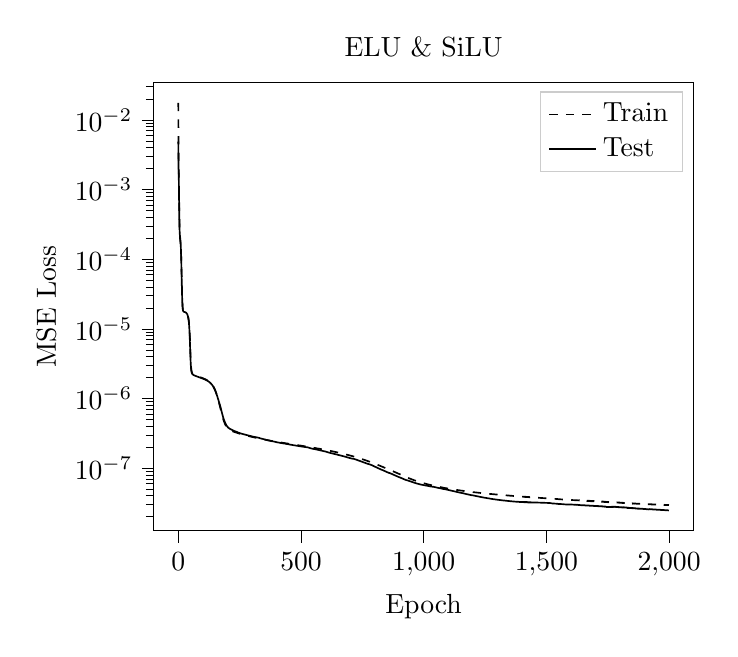
\begin{tikzpicture}

\begin{axis}[
legend cell align={left},
legend style={fill opacity=0.8, draw opacity=1, text opacity=1, draw=white!80!black},
log basis y={10},
tick align=outside,
tick pos=left,
title={ELU \& SiLU},
x grid style={white!69.0196078431373!black},
xlabel={Epoch},
xmin=-99.95, xmax=2098.95,
xtick style={color=black},
y grid style={white!69.0196078431373!black},
ylabel={MSE Loss},
ymin=1.25460830079477e-08, ymax=0.0345317116334461,
ymode=log,
ytick style={color=black}
]
\addplot [semithick, black, dashed]
table {%
0 0.0175996494237334
1 0.00287529958738014
2 0.0017450225809589
3 0.00109182657976635
4 0.000527906175178941
5 0.00029815742187202
6 0.000224625757531612
7 0.000197977887568413
8 0.000183264794104616
9 0.000169372935888532
10 0.000151957952730299
11 0.000129263067727152
12 0.000102055093113449
13 7.43479660304729e-05
14 5.15737580390123e-05
15 3.62272282127378e-05
16 2.71450699819979e-05
17 2.21503660204689e-05
18 1.95366582747738e-05
19 1.82204602597267e-05
20 1.7573602705852e-05
21 1.72561979470629e-05
22 1.70949869616379e-05
23 1.70056749411742e-05
24 1.69485445385362e-05
25 1.69051188822777e-05
26 1.68663870399541e-05
27 1.68271088441543e-05
28 1.67838884763114e-05
29 1.67341138449046e-05
30 1.66752324212212e-05
31 1.66049099725569e-05
32 1.65208375483417e-05
33 1.64199603086672e-05
34 1.62983461823387e-05
35 1.61510820416879e-05
36 1.59720132987786e-05
37 1.57533292913286e-05
38 1.5484687447497e-05
39 1.51527701264058e-05
40 1.47406713913369e-05
41 1.42270974720304e-05
42 1.3586219226454e-05
43 1.27891907977755e-05
44 1.18077328297659e-05
45 1.06241310518271e-05
46 9.24968551862548e-06
47 7.74917471699155e-06
48 6.25447972788606e-06
49 4.93720254530672e-06
50 3.93207780757621e-06
51 3.26343841823018e-06
52 2.85647097467745e-06
53 2.61511052349306e-06
54 2.47010573488637e-06
55 2.38091079037872e-06
56 2.32446314907975e-06
57 2.28729202154909e-06
58 2.26161475359277e-06
59 2.24282278935561e-06
60 2.22819607702718e-06
61 2.21604933179265e-06
62 2.20556252057236e-06
63 2.19616054360472e-06
64 2.18749445562594e-06
65 2.17928000790835e-06
66 2.17143440573864e-06
67 2.16391069665178e-06
68 2.15657700448446e-06
69 2.14940820202969e-06
70 2.14237768801695e-06
71 2.13553268446276e-06
72 2.12884015479631e-06
73 2.12225586307113e-06
74 2.11574514611357e-06
75 2.10928932654042e-06
76 2.10288195557951e-06
77 2.09650990095156e-06
78 2.09017900181152e-06
79 2.08388941103976e-06
80 2.07764323232595e-06
81 2.07144468839715e-06
82 2.06527465138606e-06
83 2.05913248743173e-06
84 2.0530142757309e-06
85 2.04691445756566e-06
86 2.04082622008173e-06
87 2.03473575675162e-06
88 2.0286378381229e-06
89 2.02251989537672e-06
90 2.01638261944481e-06
91 2.01022128027262e-06
92 2.00403939894045e-06
93 1.99783347059679e-06
94 1.99160166323509e-06
95 1.98533314505767e-06
96 1.97902080506651e-06
97 1.97265234243105e-06
98 1.9662212929461e-06
99 1.95973702790297e-06
100 1.95320250358577e-06
101 1.94660680122638e-06
102 1.939952190952e-06
103 1.93324243110737e-06
104 1.92648431564635e-06
105 1.91963722903665e-06
106 1.91268758226215e-06
107 1.90565878750704e-06
108 1.89853121551664e-06
109 1.89127792199884e-06
110 1.88389302704195e-06
111 1.87637372260951e-06
112 1.86870985686483e-06
113 1.86089686886248e-06
114 1.85292484115962e-06
115 1.84476674837697e-06
116 1.83640388777917e-06
117 1.82784501009792e-06
118 1.81907705044182e-06
119 1.81008488425505e-06
120 1.80085318538659e-06
121 1.79136690542236e-06
122 1.78161437838753e-06
123 1.77159513089009e-06
124 1.76129403953951e-06
125 1.75069264912509e-06
126 1.73976445233848e-06
127 1.72847957088607e-06
128 1.71680751208214e-06
129 1.7047350025905e-06
130 1.69224299537518e-06
131 1.67928939252704e-06
132 1.66583868410441e-06
133 1.65187669213651e-06
134 1.63740343054997e-06
135 1.62238789512514e-06
136 1.6067824065118e-06
137 1.5905935566991e-06
138 1.57381414469171e-06
139 1.55636063472286e-06
140 1.53816044023358e-06
141 1.51927269187979e-06
142 1.49966893327758e-06
143 1.47930880157787e-06
144 1.45817050724872e-06
145 1.43625170875339e-06
146 1.41338668653646e-06
147 1.38969123329957e-06
148 1.3652607281216e-06
149 1.34014765538382e-06
150 1.3144001037233e-06
151 1.28805525855569e-06
152 1.26120119203677e-06
153 1.23391107938176e-06
154 1.20624255806945e-06
155 1.17823492250579e-06
156 1.14992709714556e-06
157 1.12135632480204e-06
158 1.09260033759995e-06
159 1.06368875725593e-06
160 1.03462326670467e-06
161 1.00557742922547e-06
162 9.7667225931275e-07
163 9.47957712440939e-07
164 9.19453697107997e-07
165 8.91192761528714e-07
166 8.63282801702781e-07
167 8.35834502140642e-07
168 8.08940287257087e-07
169 7.82601844235842e-07
170 7.56980151379594e-07
171 7.32141062655955e-07
172 7.08114986750275e-07
173 6.84937570738953e-07
174 6.62635313446458e-07
175 6.41243045507167e-07
176 6.2081070653619e-07
177 6.01388748577847e-07
178 5.83003184985387e-07
179 5.65668886466142e-07
180 5.49323648044719e-07
181 5.33915851917754e-07
182 5.19427995229194e-07
183 5.05823589165288e-07
184 4.9306046715003e-07
185 4.8109552386677e-07
186 4.6990855443596e-07
187 4.59501481813618e-07
188 4.49822384894105e-07
189 4.40771383807714e-07
190 4.32378732156735e-07
191 4.24598447835933e-07
192 4.17455452677018e-07
193 4.10936514782634e-07
194 4.0497750121915e-07
195 3.99562149212329e-07
196 3.94614396952875e-07
197 3.9006308888645e-07
198 3.85865279696418e-07
199 3.81985842821564e-07
200 3.78385178450458e-07
201 3.75026909821941e-07
202 3.71899057071801e-07
203 3.69010332562425e-07
204 3.66329881671845e-07
205 3.63827414901152e-07
206 3.61479612806193e-07
207 3.59270024461011e-07
208 3.57176860234176e-07
209 3.55181227661205e-07
210 3.53276239565048e-07
211 3.51515790129042e-07
212 3.49912813945252e-07
213 3.48354445861787e-07
214 3.46851569503315e-07
215 3.45408498390043e-07
216 3.44020960312719e-07
217 3.42683353437678e-07
218 3.41392241935523e-07
219 3.40145149181126e-07
220 3.38937579158483e-07
221 3.37769001305332e-07
222 3.36636997644746e-07
223 3.35538890624321e-07
224 3.34470593799097e-07
225 3.33426590003683e-07
226 3.32406322868906e-07
227 3.31405100723714e-07
228 3.30421388724744e-07
229 3.29453601679575e-07
230 3.28494617065189e-07
231 3.27545682438313e-07
232 3.26611903702201e-07
233 3.25688031040272e-07
234 3.24785979117337e-07
235 3.23915015329135e-07
236 3.23034720381088e-07
237 3.22156478262059e-07
238 3.21286055111614e-07
239 3.20421153560346e-07
240 3.19560409622e-07
241 3.18705262714047e-07
242 3.1785766660164e-07
243 3.1701667911932e-07
244 3.16183564692096e-07
245 3.15356841326775e-07
246 3.14536922402908e-07
247 3.13724506980861e-07
248 3.12925141088272e-07
249 3.12140765842628e-07
250 3.11375240485745e-07
251 3.1062860304587e-07
252 3.0990082002802e-07
253 3.09185586033323e-07
254 3.0848231598668e-07
255 3.07785731521903e-07
256 3.07097276817103e-07
257 3.06413695156493e-07
258 3.05733606865033e-07
259 3.05057379563323e-07
260 3.04384200020991e-07
261 3.03711434725074e-07
262 3.0303466202497e-07
263 3.02357359515781e-07
264 3.01714337382464e-07
265 3.01069908317686e-07
266 3.00426167228807e-07
267 2.99785866843649e-07
268 2.99147748563655e-07
269 2.98513994621885e-07
270 2.97884098472423e-07
271 2.97257889613434e-07
272 2.96635719834626e-07
273 2.96016641236463e-07
274 2.95400801640255e-07
275 2.94787651498041e-07
276 2.94177613653801e-07
277 2.93570954063682e-07
278 2.92964300811605e-07
279 2.92362203438756e-07
280 2.91760416381237e-07
281 2.91159803978758e-07
282 2.9055891594254e-07
283 2.89960710880166e-07
284 2.8936324151374e-07
285 2.88770518061199e-07
286 2.88199581916615e-07
287 2.87646285805465e-07
288 2.87090873314355e-07
289 2.86531117303923e-07
290 2.85970951807712e-07
291 2.85412180353717e-07
292 2.84857709402786e-07
293 2.84302747601828e-07
294 2.8375344444953e-07
295 2.83205761050453e-07
296 2.82660867995332e-07
297 2.8211923660848e-07
298 2.81580993302555e-07
299 2.81046339367208e-07
300 2.80514478589566e-07
301 2.7998426008935e-07
302 2.79458510092923e-07
303 2.78934175497625e-07
304 2.78412257820548e-07
305 2.7789296674996e-07
306 2.77374297333211e-07
307 2.7685929883603e-07
308 2.76344144253926e-07
309 2.75831304342944e-07
310 2.75319272766694e-07
311 2.74808198902576e-07
312 2.7429603046869e-07
313 2.73784318302717e-07
314 2.73272087738974e-07
315 2.72760358924984e-07
316 2.72247648759105e-07
317 2.71740439046653e-07
318 2.71237279193315e-07
319 2.70741638303207e-07
320 2.70252898353363e-07
321 2.69768819279648e-07
322 2.69289078040913e-07
323 2.68816892983637e-07
324 2.68343211374145e-07
325 2.67885037054327e-07
326 2.67416310265389e-07
327 2.66975876130005e-07
328 2.66506596872773e-07
329 2.66083591505151e-07
330 2.65639710384846e-07
331 2.65243812378912e-07
332 2.64773271553054e-07
333 2.64322112386139e-07
334 2.63829088133605e-07
335 2.63389938119474e-07
336 2.6290572489529e-07
337 2.62464812486485e-07
338 2.61970761854968e-07
339 2.61548848619952e-07
340 2.61117641201736e-07
341 2.60733976112704e-07
342 2.60291870695539e-07
343 2.59895549817202e-07
344 2.594321902194e-07
345 2.59030119281078e-07
346 2.58601684890891e-07
347 2.58207709705971e-07
348 2.57752386914945e-07
349 2.57358960176646e-07
350 2.56929571371245e-07
351 2.56539277351919e-07
352 2.56089040767904e-07
353 2.5569170922779e-07
354 2.5524339392291e-07
355 2.54830653759086e-07
356 2.54406230482118e-07
357 2.54067098289568e-07
358 2.53661682023676e-07
359 2.53289803858081e-07
360 2.52879487980806e-07
361 2.52509188818806e-07
362 2.52106710043165e-07
363 2.5173805948242e-07
364 2.51339875042333e-07
365 2.50972963598883e-07
366 2.50580756969043e-07
367 2.50217714238943e-07
368 2.49831848677218e-07
369 2.49469345895648e-07
370 2.49089968647809e-07
371 2.4873137019199e-07
372 2.48356590667242e-07
373 2.47999187131143e-07
374 2.4763044640963e-07
375 2.47274666534736e-07
376 2.46913876914334e-07
377 2.46557384258494e-07
378 2.46201170384097e-07
379 2.45847944853494e-07
380 2.45494405000102e-07
381 2.45144459192659e-07
382 2.4479538060973e-07
383 2.44445716866437e-07
384 2.44098331023679e-07
385 2.43749799729187e-07
386 2.43400523295634e-07
387 2.43049962001862e-07
388 2.42702448431942e-07
389 2.42355488609292e-07
390 2.42012714679163e-07
391 2.4167355127247e-07
392 2.41335103595475e-07
393 2.40999812632481e-07
394 2.40663078940884e-07
395 2.40325962195698e-07
396 2.39984172416996e-07
397 2.39634622730023e-07
398 2.39281233987754e-07
399 2.38940480876693e-07
400 2.3863265462154e-07
401 2.38341846198864e-07
402 2.3803435519909e-07
403 2.37720892670268e-07
404 2.37405413471947e-07
405 2.3708795703925e-07
406 2.36770879936898e-07
407 2.36454466346459e-07
408 2.36138622433657e-07
409 2.35822797336027e-07
410 2.35507726081607e-07
411 2.35190857516443e-07
412 2.34877379469367e-07
413 2.34564189511843e-07
414 2.34253473898605e-07
415 2.33942672522858e-07
416 2.33634892900625e-07
417 2.33329615788591e-07
418 2.33024774566104e-07
419 2.32720143500842e-07
420 2.32416022562632e-07
421 2.32108510779483e-07
422 2.31797596143224e-07
423 2.31482146325845e-07
424 2.31172614505226e-07
425 2.30876980893413e-07
426 2.30587186429432e-07
427 2.30292145651845e-07
428 2.29996369043306e-07
429 2.29696812866109e-07
430 2.29395408346988e-07
431 2.29091220759869e-07
432 2.28793122374782e-07
433 2.28505814114044e-07
434 2.28219742702152e-07
435 2.27929575416397e-07
436 2.2763782101265e-07
437 2.27346566390452e-07
438 2.27056472624554e-07
439 2.26765794053563e-07
440 2.26474985048242e-07
441 2.26186430381858e-07
442 2.25897406949116e-07
443 2.2560861464882e-07
444 2.25320075472268e-07
445 2.25033070627489e-07
446 2.24744428635404e-07
447 2.24458662323457e-07
448 2.24170733531537e-07
449 2.23884842050381e-07
450 2.23597962218491e-07
451 2.23310248394171e-07
452 2.23022348308177e-07
453 2.22734046751327e-07
454 2.22442912225063e-07
455 2.22151466509501e-07
456 2.21859659873758e-07
457 2.21572562438155e-07
458 2.21289075021502e-07
459 2.21010129273225e-07
460 2.20728793351554e-07
461 2.20448860829947e-07
462 2.20167770152102e-07
463 2.19885938825826e-07
464 2.19604979307064e-07
465 2.19323364973434e-07
466 2.19043549776643e-07
467 2.18763958706347e-07
468 2.18484622969584e-07
469 2.18205289677087e-07
470 2.17927875091561e-07
471 2.17649641605533e-07
472 2.17373744746396e-07
473 2.1709560340355e-07
474 2.16820149610442e-07
475 2.16545120039768e-07
476 2.16269043342265e-07
477 2.15993676206949e-07
478 2.15721830045368e-07
479 2.15448890990899e-07
480 2.15178834174878e-07
481 2.149075208564e-07
482 2.14637604578627e-07
483 2.14366342028427e-07
484 2.14095653959134e-07
485 2.13825490867237e-07
486 2.13554397497262e-07
487 2.13285051131606e-07
488 2.13013861191769e-07
489 2.12744850905722e-07
490 2.12475656326205e-07
491 2.12207315264834e-07
492 2.11938185586291e-07
493 2.11668856991309e-07
494 2.11400331892264e-07
495 2.11133048289014e-07
496 2.10864122102805e-07
497 2.10596357298698e-07
498 2.10328821644623e-07
499 2.10059376463789e-07
500 2.09792518937491e-07
501 2.09525793508192e-07
502 2.0925775712044e-07
503 2.08989702933593e-07
504 2.08722312152076e-07
505 2.08454585468587e-07
506 2.08186760026763e-07
507 2.07918511570426e-07
508 2.07650348066579e-07
509 2.0738169546064e-07
510 2.07112908462648e-07
511 2.06844777174808e-07
512 2.06574911899793e-07
513 2.06304785187683e-07
514 2.06034711695224e-07
515 2.05762478614702e-07
516 2.05489735087383e-07
517 2.05218204492041e-07
518 2.04941749565535e-07
519 2.04666232278328e-07
520 2.04387647002591e-07
521 2.04112322826688e-07
522 2.0383555720116e-07
523 2.0356390942311e-07
524 2.0328289256355e-07
525 2.03006117388327e-07
526 2.02714574768947e-07
527 2.02427127135252e-07
528 2.02120347992718e-07
529 2.01825123937738e-07
530 2.01526683405007e-07
531 2.01258414435301e-07
532 2.00978978099897e-07
533 2.00726137201457e-07
534 2.00452940838147e-07
535 2.00204465528486e-07
536 1.99926498702041e-07
537 1.99674599720368e-07
538 1.99389074467149e-07
539 1.99133380988314e-07
540 1.98845136111458e-07
541 1.98592526508889e-07
542 1.98312001522538e-07
543 1.98073469377391e-07
544 1.97795437962611e-07
545 1.97541130809498e-07
546 1.9723873250399e-07
547 1.96979277795606e-07
548 1.96690525427812e-07
549 1.96438236173435e-07
550 1.9614758696207e-07
551 1.95893695774885e-07
552 1.9560284979292e-07
553 1.95347655257194e-07
554 1.95057353046479e-07
555 1.94801164418834e-07
556 1.94509920277142e-07
557 1.94253270734634e-07
558 1.93961073485127e-07
559 1.93702724359923e-07
560 1.93412831507089e-07
561 1.93151937097014e-07
562 1.92862569448948e-07
563 1.92599946480243e-07
564 1.92312116809035e-07
565 1.92046887015351e-07
566 1.91762092583758e-07
567 1.91495132177977e-07
568 1.91215405095591e-07
569 1.90950501014697e-07
570 1.90681914915558e-07
571 1.90422427188253e-07
572 1.90139000331158e-07
573 1.89849500145556e-07
574 1.89560766450825e-07
575 1.89280814623771e-07
576 1.8900092842955e-07
577 1.8872307740736e-07
578 1.88442443018744e-07
579 1.88163821782439e-07
580 1.87884023183926e-07
581 1.87604552785103e-07
582 1.87324280688017e-07
583 1.87046472525765e-07
584 1.8676562085318e-07
585 1.86486165269173e-07
586 1.86204263052048e-07
587 1.85924446839181e-07
588 1.85642518125917e-07
589 1.85359782030048e-07
590 1.85078272430417e-07
591 1.84792084183982e-07
592 1.84508275026474e-07
593 1.84220880669272e-07
594 1.83932809697751e-07
595 1.83643697894809e-07
596 1.83353293152777e-07
597 1.83060790227785e-07
598 1.82766741410489e-07
599 1.82471747208979e-07
600 1.82175910396154e-07
601 1.81878275817837e-07
602 1.81581998241143e-07
603 1.81293149658757e-07
604 1.81011799938346e-07
605 1.80725013777305e-07
606 1.80430601247394e-07
607 1.80136493369787e-07
608 1.79840781072471e-07
609 1.79547042925776e-07
610 1.79256953792617e-07
611 1.78968048011541e-07
612 1.78676989577298e-07
613 1.78381995397103e-07
614 1.78090247487717e-07
615 1.77807889897963e-07
616 1.77518120445086e-07
617 1.77226933303132e-07
618 1.76935237604425e-07
619 1.76642455294029e-07
620 1.76349222122951e-07
621 1.76056165678062e-07
622 1.75763073201551e-07
623 1.75468830988734e-07
624 1.75175491378354e-07
625 1.74879692544039e-07
626 1.74585498029955e-07
627 1.74291679364558e-07
628 1.73995814343186e-07
629 1.73700186017811e-07
630 1.73405231102208e-07
631 1.73109094077972e-07
632 1.72812282521306e-07
633 1.72517677093253e-07
634 1.72222056555427e-07
635 1.71927344155165e-07
636 1.71632569099245e-07
637 1.71338274590482e-07
638 1.71034913130086e-07
639 1.70733721134297e-07
640 1.7043391181204e-07
641 1.70132847280513e-07
642 1.69833049191936e-07
643 1.69529434216997e-07
644 1.69227103143044e-07
645 1.68925542112675e-07
646 1.68622009034891e-07
647 1.68318236774212e-07
648 1.68014904176061e-07
649 1.67709664872007e-07
650 1.6740428503681e-07
651 1.67098198687654e-07
652 1.66792148370121e-07
653 1.66485019853724e-07
654 1.66178793207905e-07
655 1.65869200280611e-07
656 1.65561907664369e-07
657 1.65252004769911e-07
658 1.64943542721119e-07
659 1.64632498311335e-07
660 1.64322014335028e-07
661 1.64009824260347e-07
662 1.63697879330016e-07
663 1.63385576819053e-07
664 1.63073160940996e-07
665 1.62760238836768e-07
666 1.62445714465775e-07
667 1.62130916251613e-07
668 1.61816271742055e-07
669 1.61501935338038e-07
670 1.61184934285075e-07
671 1.60868889899746e-07
672 1.60552074753184e-07
673 1.60234152140504e-07
674 1.59917202708471e-07
675 1.59598340765399e-07
676 1.5928070041582e-07
677 1.58963693209557e-07
678 1.58649849083758e-07
679 1.58348114766227e-07
680 1.58057629661812e-07
681 1.57671108624413e-07
682 1.57301388419739e-07
683 1.56999126346591e-07
684 1.56670816949145e-07
685 1.56336613628127e-07
686 1.56002342869499e-07
687 1.556705652348e-07
688 1.55350209446681e-07
689 1.55038015698494e-07
690 1.54718844136426e-07
691 1.5439428176478e-07
692 1.54069175138716e-07
693 1.53743410223228e-07
694 1.53420686693551e-07
695 1.5309928499363e-07
696 1.52787432718071e-07
697 1.52489572741388e-07
698 1.5215267003299e-07
699 1.5180147937599e-07
700 1.51467610628231e-07
701 1.51146714920003e-07
702 1.50877697457474e-07
703 1.50529026193169e-07
704 1.50173604488657e-07
705 1.49829621982178e-07
706 1.49500967239646e-07
707 1.49161668694831e-07
708 1.48830235133346e-07
709 1.4848696960712e-07
710 1.48152148859992e-07
711 1.47827308822457e-07
712 1.47502455668302e-07
713 1.47172682240182e-07
714 1.46840045417207e-07
715 1.46497807946844e-07
716 1.46153746740652e-07
717 1.4580504894468e-07
718 1.45458180313085e-07
719 1.45108395322779e-07
720 1.44763098667511e-07
721 1.44413272984423e-07
722 1.44068907871997e-07
723 1.43719601865655e-07
724 1.4337589767166e-07
725 1.43025246977402e-07
726 1.42680555661912e-07
727 1.42329018402165e-07
728 1.41984071241552e-07
729 1.41631456635594e-07
730 1.41288496855907e-07
731 1.40933513208097e-07
732 1.40596474217602e-07
733 1.40239406363207e-07
734 1.39900588273179e-07
735 1.39539811776501e-07
736 1.39217587097562e-07
737 1.38853319960219e-07
738 1.38519196539733e-07
739 1.38150057352959e-07
740 1.37809788974153e-07
741 1.3743655064502e-07
742 1.3710148611068e-07
743 1.36720188223194e-07
744 1.36391699037119e-07
745 1.36003874573021e-07
746 1.35689238376813e-07
747 1.3526807629205e-07
748 1.34977162510097e-07
749 1.34534849898671e-07
750 1.34263853979633e-07
751 1.33803888381578e-07
752 1.33541157381956e-07
753 1.33075631865154e-07
754 1.32812739892074e-07
755 1.32347266053046e-07
756 1.32081167286913e-07
757 1.31614762942434e-07
758 1.31345022282403e-07
759 1.30879963457176e-07
760 1.3060746962168e-07
761 1.30141176512666e-07
762 1.29864243902489e-07
763 1.29394299058561e-07
764 1.2911283270256e-07
765 1.28642385263333e-07
766 1.28354625225313e-07
767 1.2789251384504e-07
768 1.276106047996e-07
769 1.27158457551957e-07
770 1.26873228133206e-07
771 1.2642038833377e-07
772 1.26147492281348e-07
773 1.25696561333655e-07
774 1.2542319246478e-07
775 1.24956723709602e-07
776 1.24685955043446e-07
777 1.24218594947934e-07
778 1.23948786196593e-07
779 1.23475682784147e-07
780 1.23208924293294e-07
781 1.22734899811405e-07
782 1.22469958334648e-07
783 1.21993825025868e-07
784 1.21732354990911e-07
785 1.21256032315387e-07
786 1.20998242365999e-07
787 1.2051988794326e-07
788 1.20267326778389e-07
789 1.19790599342195e-07
790 1.19547230333694e-07
791 1.19097782047106e-07
792 1.18811734310498e-07
793 1.18316635195015e-07
794 1.18063428701021e-07
795 1.17580629776626e-07
796 1.17317416432172e-07
797 1.16842961155328e-07
798 1.16570967094276e-07
799 1.16108646778912e-07
800 1.15827305272376e-07
801 1.15377920501203e-07
802 1.1508488028511e-07
803 1.14649716792314e-07
804 1.14344960543633e-07
805 1.13921864283384e-07
806 1.13603540839335e-07
807 1.13194083560586e-07
808 1.12863245988137e-07
809 1.12468225204054e-07
810 1.12127083646385e-07
811 1.11746339406693e-07
812 1.11400504785308e-07
813 1.11035729347009e-07
814 1.10672897640995e-07
815 1.10295471110078e-07
816 1.09931559045151e-07
817 1.09568143528804e-07
818 1.09202652389229e-07
819 1.0884110548659e-07
820 1.08479694034713e-07
821 1.08123397502879e-07
822 1.07768057553415e-07
823 1.07427633928125e-07
824 1.07132911082886e-07
825 1.06680572500295e-07
826 1.06355442163419e-07
827 1.05982517581538e-07
828 1.05633535838479e-07
829 1.05274247268028e-07
830 1.04923396285983e-07
831 1.04568637013358e-07
832 1.04220353073003e-07
833 1.03865601353448e-07
834 1.03513037430503e-07
835 1.03156986462238e-07
836 1.02802441595884e-07
837 1.02450682760491e-07
838 1.02100855322362e-07
839 1.01750472786932e-07
840 1.0140150994431e-07
841 1.01053541381901e-07
842 1.00707275326073e-07
843 1.00359584678245e-07
844 1.00014914270474e-07
845 9.96698316377831e-08
846 9.93263650492793e-08
847 9.89830431770144e-08
848 9.86420426372092e-08
849 9.830027455493e-08
850 9.79607342728173e-08
851 9.76206057572426e-08
852 9.72826926961545e-08
853 9.69451741390515e-08
854 9.66100479331544e-08
855 9.62747901454009e-08
856 9.59414415291349e-08
857 9.56098446884823e-08
858 9.52807467342609e-08
859 9.49542538926096e-08
860 9.46286855700862e-08
861 9.43026890531939e-08
862 9.39737770337956e-08
863 9.36448786958977e-08
864 9.33190625431735e-08
865 9.29954942066047e-08
866 9.26732596084889e-08
867 9.23527348462017e-08
868 9.20334779763721e-08
869 9.17156793747154e-08
870 9.13983349377645e-08
871 9.10830633600312e-08
872 9.07672439609541e-08
873 9.04524855158684e-08
874 9.01387915774876e-08
875 8.98264481250521e-08
876 8.95150285202817e-08
877 8.92049641834092e-08
878 8.88939577734504e-08
879 8.85861132289278e-08
880 8.82777590334172e-08
881 8.79710582140092e-08
882 8.76646669567549e-08
883 8.73602326905143e-08
884 8.70552255705093e-08
885 8.67519998095645e-08
886 8.64501233053261e-08
887 8.6146255775077e-08
888 8.58468929791911e-08
889 8.55448757945965e-08
890 8.52472173562546e-08
891 8.49459580933853e-08
892 8.46501490912033e-08
893 8.43481334271701e-08
894 8.40549865515072e-08
895 8.37533525341883e-08
896 8.34638953648437e-08
897 8.31621499131074e-08
898 8.28743535308263e-08
899 8.25751389896823e-08
900 8.22899470520611e-08
901 8.19908786695578e-08
902 8.17119941984856e-08
903 8.14204756736103e-08
904 8.11498789587972e-08
905 8.08366941313921e-08
906 8.05548967051095e-08
907 8.02546861962128e-08
908 7.99800256316985e-08
909 7.96830944622684e-08
910 7.94125844763016e-08
911 7.911549998596e-08
912 7.88506315814175e-08
913 7.85564360050728e-08
914 7.82931790439534e-08
915 7.8004567647838e-08
916 7.77404717631214e-08
917 7.74547611754883e-08
918 7.7181353187683e-08
919 7.69060091343476e-08
920 7.66324710355093e-08
921 7.63723304721964e-08
922 7.60953091329952e-08
923 7.5864466129616e-08
924 7.55713254001478e-08
925 7.53308811525244e-08
926 7.50198124421786e-08
927 7.4793768067849e-08
928 7.44999733726104e-08
929 7.42764854599898e-08
930 7.40070237732482e-08
931 7.3757139062991e-08
932 7.34708819116747e-08
933 7.32295668548488e-08
934 7.29672317092422e-08
935 7.27254336361227e-08
936 7.24722474849671e-08
937 7.22304411411301e-08
938 7.19834948306186e-08
939 7.17461780297413e-08
940 7.15024025836897e-08
941 7.1267125772323e-08
942 7.10307098543694e-08
943 7.07984063801348e-08
944 7.05661321873663e-08
945 7.03392329199914e-08
946 7.01104802871555e-08
947 6.98869387250056e-08
948 6.96629443517338e-08
949 6.94436666712761e-08
950 6.92237607111679e-08
951 6.90076469602729e-08
952 6.87917168527008e-08
953 6.85799188460123e-08
954 6.83669486356564e-08
955 6.81601427672263e-08
956 6.79508710383914e-08
957 6.77463507194886e-08
958 6.75436472228341e-08
959 6.73413416798496e-08
960 6.71408234005355e-08
961 6.69428408208717e-08
962 6.67447739353122e-08
963 6.65525494945029e-08
964 6.63575741768341e-08
965 6.61687265406385e-08
966 6.59775455638112e-08
967 6.57917663957619e-08
968 6.56059239396711e-08
969 6.54228842194016e-08
970 6.52397152656192e-08
971 6.50610468397872e-08
972 6.48808190213401e-08
973 6.47048932265193e-08
974 6.45277746365025e-08
975 6.43562626940764e-08
976 6.41803190077894e-08
977 6.40130773810199e-08
978 6.38387489111381e-08
979 6.36743903790204e-08
980 6.35023501907028e-08
981 6.33410359505149e-08
982 6.31731920286427e-08
983 6.30170328896895e-08
984 6.28512382760959e-08
985 6.27018185994643e-08
986 6.25389082422601e-08
987 6.23940222439501e-08
988 6.22324554662157e-08
989 6.20933315786942e-08
990 6.19333390581289e-08
991 6.18009775230632e-08
992 6.16378112496818e-08
993 6.151472694782e-08
994 6.13488915561788e-08
995 6.12322543176447e-08
996 6.10627431143484e-08
997 6.0956969566206e-08
998 6.07836454555866e-08
999 6.06858273002331e-08
1000 6.0507606448823e-08
1001 6.04200453828696e-08
1002 6.02411679047066e-08
1003 6.01563548663364e-08
1004 5.99758189601118e-08
1005 5.98955439414794e-08
1006 5.97161064845864e-08
1007 5.96399952890181e-08
1008 5.94604134001031e-08
1009 5.93865410394301e-08
1010 5.92094895459638e-08
1011 5.91360529007545e-08
1012 5.89636505807789e-08
1013 5.8890947325807e-08
1014 5.87177360920066e-08
1015 5.86479926383276e-08
1016 5.84775806053983e-08
1017 5.84071221645388e-08
1018 5.82407901923432e-08
1019 5.81706089164413e-08
1020 5.80062781310176e-08
1021 5.79364867938636e-08
1022 5.77755773072397e-08
1023 5.77070267020474e-08
1024 5.75472279997769e-08
1025 5.74803025088499e-08
1026 5.73227851177194e-08
1027 5.72549469133321e-08
1028 5.70999626958724e-08
1029 5.7033860887401e-08
1030 5.68804288114677e-08
1031 5.68131055551646e-08
1032 5.6663332767215e-08
1033 5.65954860540785e-08
1034 5.64472345629952e-08
1035 5.63754745606104e-08
1036 5.62272355715265e-08
1037 5.61484333303497e-08
1038 5.5999395478068e-08
1039 5.59186794042432e-08
1040 5.57838673493904e-08
1041 5.57162485428364e-08
1042 5.56010164558529e-08
1043 5.55337433567615e-08
1044 5.54150616451921e-08
1045 5.53392590987301e-08
1046 5.52239583875291e-08
1047 5.5144874224311e-08
1048 5.50325426509346e-08
1049 5.49520297781214e-08
1050 5.48456422393428e-08
1051 5.47616790171901e-08
1052 5.46610097735822e-08
1053 5.45759626504605e-08
1054 5.44761822958151e-08
1055 5.43920063904579e-08
1056 5.42956490861002e-08
1057 5.4211317223718e-08
1058 5.4117549513677e-08
1059 5.40303107428031e-08
1060 5.39417221858685e-08
1061 5.38540957997213e-08
1062 5.37668139806158e-08
1063 5.36784573128557e-08
1064 5.35941787980221e-08
1065 5.3507047322654e-08
1066 5.34215971939034e-08
1067 5.33369641182446e-08
1068 5.32536905559766e-08
1069 5.31688032587851e-08
1070 5.30834877885411e-08
1071 5.30020961733158e-08
1072 5.29187969142697e-08
1073 5.28378100881355e-08
1074 5.27521015420973e-08
1075 5.2670030630253e-08
1076 5.25867333536212e-08
1077 5.25034244560629e-08
1078 5.2418908094154e-08
1079 5.23290026706036e-08
1080 5.22326315639532e-08
1081 5.21282267627043e-08
1082 5.20232685978783e-08
1083 5.19315852756108e-08
1084 5.18594172795872e-08
1085 5.18124042443446e-08
1086 5.16707377791192e-08
1087 5.16539989376952e-08
1088 5.15711485888914e-08
1089 5.15147099022784e-08
1090 5.14256392456502e-08
1091 5.13642042427875e-08
1092 5.1281067797504e-08
1093 5.12151511067316e-08
1094 5.1136492572823e-08
1095 5.10673343896428e-08
1096 5.09849862382339e-08
1097 5.09159236656842e-08
1098 5.08563726846489e-08
1099 5.077642700968e-08
1100 5.07170401462531e-08
1101 5.06396115724783e-08
1102 5.05759921800575e-08
1103 5.05042115719334e-08
1104 5.04362397748537e-08
1105 5.03709844430489e-08
1106 5.03009102779117e-08
1107 5.02376596962506e-08
1108 5.01693970313966e-08
1109 5.01037829856443e-08
1110 5.00381948604911e-08
1111 4.99729949332561e-08
1112 4.99080592604173e-08
1113 4.98440006531098e-08
1114 4.97788077851169e-08
1115 4.97160153187792e-08
1116 4.96525768198808e-08
1117 4.95886749831698e-08
1118 4.95259647159685e-08
1119 4.94638447854356e-08
1120 4.94025123742858e-08
1121 4.93408055142197e-08
1122 4.92777741882833e-08
1123 4.92156950713252e-08
1124 4.91560401947311e-08
1125 4.90946190012664e-08
1126 4.90349146211599e-08
1127 4.89734367121741e-08
1128 4.89154338225717e-08
1129 4.88554389015405e-08
1130 4.87965765465503e-08
1131 4.87381162699307e-08
1132 4.86792782474765e-08
1133 4.86204470853124e-08
1134 4.85623430606097e-08
1135 4.85029923069646e-08
1136 4.84469144268473e-08
1137 4.83894675831209e-08
1138 4.83293557067554e-08
1139 4.82720579384477e-08
1140 4.82142370081817e-08
1141 4.81568539498767e-08
1142 4.80991615496862e-08
1143 4.80393431416815e-08
1144 4.79794743064588e-08
1145 4.79202978560522e-08
1146 4.78614520780241e-08
1147 4.77986213525128e-08
1148 4.77403732936921e-08
1149 4.76852409470041e-08
1150 4.76301647012178e-08
1151 4.7578462570641e-08
1152 4.75241271757909e-08
1153 4.74723943568733e-08
1154 4.74180858915929e-08
1155 4.73673670065011e-08
1156 4.73131372622504e-08
1157 4.72611859620997e-08
1158 4.72082820444086e-08
1159 4.7156959116279e-08
1160 4.70964777754546e-08
1161 4.70352642594207e-08
1162 4.69699322387385e-08
1163 4.69033307766153e-08
1164 4.68406378679731e-08
1165 4.678152087223e-08
1166 4.67163908766111e-08
1167 4.66496131537042e-08
1168 4.66186367269472e-08
1169 4.65931978403944e-08
1170 4.65452790940901e-08
1171 4.64970322155978e-08
1172 4.64478893889009e-08
1173 4.6401220398451e-08
1174 4.6354152015482e-08
1175 4.63051806818271e-08
1176 4.62608166245104e-08
1177 4.62116961692516e-08
1178 4.61663384392352e-08
1179 4.61181958506529e-08
1180 4.60749140778205e-08
1181 4.60289976587092e-08
1182 4.59828709118426e-08
1183 4.59360696254407e-08
1184 4.58911745084833e-08
1185 4.58475705649164e-08
1186 4.58020190592379e-08
1187 4.57577413932597e-08
1188 4.57144813417187e-08
1189 4.56681103067069e-08
1190 4.56250730138663e-08
1191 4.55801805401279e-08
1192 4.55367965024323e-08
1193 4.54928729460846e-08
1194 4.54491035526416e-08
1195 4.54046372340144e-08
1196 4.53605468813123e-08
1197 4.5318322193566e-08
1198 4.52730989941585e-08
1199 4.52277204736617e-08
1200 4.51831244703271e-08
1201 4.51362583078208e-08
1202 4.50891260435071e-08
1203 4.50436343264471e-08
1204 4.5005045581803e-08
1205 4.49671033173615e-08
1206 4.4927011046525e-08
1207 4.48885856805248e-08
1208 4.48442414047179e-08
1209 4.48037458724571e-08
1210 4.47623032719946e-08
1211 4.4723272381475e-08
1212 4.46810348542215e-08
1213 4.46411653030054e-08
1214 4.4600022867769e-08
1215 4.45591790949607e-08
1216 4.45200743115493e-08
1217 4.44793313718606e-08
1218 4.44395357810379e-08
1219 4.44004629009953e-08
1220 4.43605396469593e-08
1221 4.43211583132097e-08
1222 4.4281827630499e-08
1223 4.42431409233279e-08
1224 4.42025483913255e-08
1225 4.41649761562246e-08
1226 4.41241812545456e-08
1227 4.40845443172577e-08
1228 4.40465823245972e-08
1229 4.40095524965045e-08
1230 4.39683958113335e-08
1231 4.39273198011847e-08
1232 4.38891112786166e-08
1233 4.38489198977265e-08
1234 4.38104611717449e-08
1235 4.37681291849401e-08
1236 4.37326005489069e-08
1237 4.36921684006109e-08
1238 4.36569987094515e-08
1239 4.36212489383081e-08
1240 4.35856813254532e-08
1241 4.35512924070736e-08
1242 4.35153490982998e-08
1243 4.34792310812782e-08
1244 4.3441935190458e-08
1245 4.34084090166209e-08
1246 4.33736247344996e-08
1247 4.33387995464329e-08
1248 4.33012893488183e-08
1249 4.32677698007922e-08
1250 4.32302192905354e-08
1251 4.31998927901134e-08
1252 4.31620639780306e-08
1253 4.31301771044446e-08
1254 4.30933546446965e-08
1255 4.30604565977433e-08
1256 4.30247026876884e-08
1257 4.29927247402873e-08
1258 4.29553815664008e-08
1259 4.29268922417236e-08
1260 4.28864818502461e-08
1261 4.28586315130985e-08
1262 4.28198954232073e-08
1263 4.27898634640655e-08
1264 4.2753595245415e-08
1265 4.27237714077933e-08
1266 4.26869564371657e-08
1267 4.26564525852768e-08
1268 4.26192783891111e-08
1269 4.25903701817276e-08
1270 4.25535703065805e-08
1271 4.25226653746336e-08
1272 4.24879032259184e-08
1273 4.2456188470652e-08
1274 4.24202999376178e-08
1275 4.23859171334584e-08
1276 4.23519101282466e-08
1277 4.23149189643368e-08
1278 4.22824308721204e-08
1279 4.22486863698168e-08
1280 4.22202453158604e-08
1281 4.2187339193589e-08
1282 4.21591239216923e-08
1283 4.2124149732814e-08
1284 4.20938310909946e-08
1285 4.20612705056556e-08
1286 4.20308245416834e-08
1287 4.1997344542466e-08
1288 4.19672587632647e-08
1289 4.19371729876161e-08
1290 4.19042328978492e-08
1291 4.18756649480656e-08
1292 4.18406924111991e-08
1293 4.18142886573492e-08
1294 4.17780153441072e-08
1295 4.17540905388591e-08
1296 4.1716828956595e-08
1297 4.16896988646442e-08
1298 4.16524566198007e-08
1299 4.1629468562121e-08
1300 4.15833136386823e-08
1301 4.15585945674479e-08
1302 4.15018889334817e-08
1303 4.1496817747344e-08
1304 4.14546708569219e-08
1305 4.14546289491113e-08
1306 4.13919402539875e-08
1307 4.14056540662955e-08
1308 4.13244472277086e-08
1309 4.13615174217341e-08
1310 4.12699490794921e-08
1311 4.1267000831624e-08
1312 4.12267482445827e-08
1313 4.12109218075329e-08
1314 4.11668753805827e-08
1315 4.11583183073105e-08
1316 4.11022767217162e-08
1317 4.11100928516817e-08
1318 4.1037408280431e-08
1319 4.1066953887281e-08
1320 4.09750483711946e-08
1321 4.10066736584724e-08
1322 4.09191586996371e-08
1323 4.0947404691849e-08
1324 4.08638924866978e-08
1325 4.08914481262457e-08
1326 4.08070332653665e-08
1327 4.08357535057746e-08
1328 4.07527275072539e-08
1329 4.07760795404499e-08
1330 4.06947206101904e-08
1331 4.07312980570396e-08
1332 4.06484653616701e-08
1333 4.06305324958112e-08
1334 4.06281817078025e-08
1335 4.05609808034058e-08
1336 4.06007411903886e-08
1337 4.05186632264076e-08
1338 4.04813392229642e-08
1339 4.05137915677756e-08
1340 4.04427050817446e-08
1341 4.0404595285537e-08
1342 4.04034278496113e-08
1343 4.03470085359459e-08
1344 4.03759440494866e-08
1345 4.02951091871273e-08
1346 4.02729835862203e-08
1347 4.02820761493672e-08
1348 4.02028653567754e-08
1349 4.0243565639031e-08
1350 4.01645263359285e-08
1351 4.01247152481687e-08
1352 4.01298546996998e-08
1353 4.00498072288258e-08
1354 4.00780106133425e-08
1355 4.00133800226854e-08
1356 3.99935331216739e-08
1357 3.99947927611777e-08
1358 3.99257412730947e-08
1359 3.99636142667248e-08
1360 3.98933878571484e-08
1361 3.98593884050058e-08
1362 3.98346793133442e-08
1363 3.98373121583973e-08
1364 3.97712527302474e-08
1365 3.98051756000939e-08
1366 3.97388940989174e-08
1367 3.97043374533723e-08
1368 3.96858321707327e-08
1369 3.96721265438771e-08
1370 3.9627116226626e-08
1371 3.96427330819904e-08
1372 3.9564374215928e-08
1373 3.95902756480382e-08
1374 3.95136501545323e-08
1375 3.95457331237026e-08
1376 3.94681531226127e-08
1377 3.94643733123701e-08
1378 3.94374941201647e-08
1379 3.94130171876839e-08
1380 3.93865616992173e-08
1381 3.93646849872198e-08
1382 3.93336724364701e-08
1383 3.93183808213848e-08
1384 3.92790345884464e-08
1385 3.92783624505455e-08
1386 3.92181673056768e-08
1387 3.9247309484125e-08
1388 3.91625413485031e-08
1389 3.91856282284664e-08
1390 3.9112159310406e-08
1391 3.91618979058705e-08
1392 3.9091612521247e-08
1393 3.90773670382316e-08
1394 3.90596091861539e-08
1395 3.90377561814148e-08
1396 3.90033072932283e-08
1397 3.89836041740921e-08
1398 3.89571714300985e-08
1399 3.89340272377581e-08
1400 3.89095555490826e-08
1401 3.88901825196797e-08
1402 3.88592720064196e-08
1403 3.88472628642944e-08
1404 3.88079879627412e-08
1405 3.8811693173102e-08
1406 3.87458087196535e-08
1407 3.87871781057925e-08
1408 3.86750464578256e-08
1409 3.87632872431709e-08
1410 3.86152443461185e-08
1411 3.8726272766354e-08
1412 3.85677903231851e-08
1413 3.86811754395922e-08
1414 3.85242661202767e-08
1415 3.86363415181279e-08
1416 3.84808430133887e-08
1417 3.85900492148039e-08
1418 3.84359594995942e-08
1419 3.85446401054423e-08
1420 3.83952957250244e-08
1421 3.84991835922222e-08
1422 3.83527137763906e-08
1423 3.84539447075838e-08
1424 3.83098808818261e-08
1425 3.84084559001963e-08
1426 3.82686769313523e-08
1427 3.83634785663389e-08
1428 3.82263591767185e-08
1429 3.83170275028988e-08
1430 3.81848634063431e-08
1431 3.82719766882644e-08
1432 3.81443559227534e-08
1433 3.82261160360997e-08
1434 3.81028666360805e-08
1435 3.81820462145299e-08
1436 3.80621713560458e-08
1437 3.81377050473475e-08
1438 3.8020763664548e-08
1439 3.80906669938952e-08
1440 3.79813536319773e-08
1441 3.80451777530766e-08
1442 3.79402011745356e-08
1443 3.79971468937868e-08
1444 3.78976800448072e-08
1445 3.79480461809578e-08
1446 3.78535985952055e-08
1447 3.78877064797223e-08
1448 3.77929022867818e-08
1449 3.78013958233225e-08
1450 3.77127713129255e-08
1451 3.77494880652307e-08
1452 3.77125745814055e-08
1453 3.77251245637922e-08
1454 3.76768934877703e-08
1455 3.76800348611539e-08
1456 3.76387757690111e-08
1457 3.76369275087995e-08
1458 3.76011498595119e-08
1459 3.75915576782404e-08
1460 3.7565789462235e-08
1461 3.75480054266575e-08
1462 3.75244291888066e-08
1463 3.75085536461484e-08
1464 3.74869865567007e-08
1465 3.74678988599442e-08
1466 3.74458098804098e-08
1467 3.74289946023509e-08
1468 3.74053136447117e-08
1469 3.73895509646616e-08
1470 3.73655890228974e-08
1471 3.73484145193004e-08
1472 3.73280483714211e-08
1473 3.73083839733113e-08
1474 3.72891789162111e-08
1475 3.72704910880373e-08
1476 3.7248621644892e-08
1477 3.72312626915061e-08
1478 3.72108093422696e-08
1479 3.71916894330582e-08
1480 3.71718720479919e-08
1481 3.71548341639993e-08
1482 3.71317190506204e-08
1483 3.71136948977835e-08
1484 3.70954332247209e-08
1485 3.7075017328192e-08
1486 3.70562630358506e-08
1487 3.70378945753203e-08
1488 3.70180622759619e-08
1489 3.69973437628346e-08
1490 3.69796147232648e-08
1491 3.6959753085597e-08
1492 3.69415847352172e-08
1493 3.69228330292515e-08
1494 3.69024669879536e-08
1495 3.6883986361147e-08
1496 3.68645939907708e-08
1497 3.68453450008133e-08
1498 3.68283621270393e-08
1499 3.68075644914256e-08
1500 3.67898759954244e-08
1501 3.67695001806112e-08
1502 3.67499921836156e-08
1503 3.6732197379763e-08
1504 3.67122580833268e-08
1505 3.66923476278203e-08
1506 3.66745375650623e-08
1507 3.66537149432133e-08
1508 3.66359610310951e-08
1509 3.66162055271957e-08
1510 3.659514873533e-08
1511 3.65773423496307e-08
1512 3.65557572656883e-08
1513 3.65364017227421e-08
1514 3.65143413247893e-08
1515 3.64913223691588e-08
1516 3.64676853230606e-08
1517 3.64390327298736e-08
1518 3.64060995430293e-08
1519 3.63669256735477e-08
1520 3.63247117149967e-08
1521 3.63022032345839e-08
1522 3.62946600880321e-08
1523 3.62906074222735e-08
1524 3.62781957825575e-08
1525 3.62666043507431e-08
1526 3.62482158386968e-08
1527 3.62316294477694e-08
1528 3.62140311018777e-08
1529 3.61927297731768e-08
1530 3.61777107897865e-08
1531 3.61594412154886e-08
1532 3.61410701259501e-08
1533 3.61231098437997e-08
1534 3.61054330362265e-08
1535 3.60887919867991e-08
1536 3.60693465388806e-08
1537 3.60534092003206e-08
1538 3.60342813436887e-08
1539 3.60168709043762e-08
1540 3.59998949370777e-08
1541 3.59785507910715e-08
1542 3.59634371278617e-08
1543 3.5941752855706e-08
1544 3.5922967253299e-08
1545 3.59026391869577e-08
1546 3.58764270416145e-08
1547 3.58446422517034e-08
1548 3.57990294403976e-08
1549 3.57539634769921e-08
1550 3.57382170612652e-08
1551 3.57453839328059e-08
1552 3.57398239394513e-08
1553 3.57211739263619e-08
1554 3.57008202236386e-08
1555 3.5678548972129e-08
1556 3.56516157040687e-08
1557 3.56155545730985e-08
1558 3.55595640009199e-08
1559 3.54979681276291e-08
1560 3.54960429262974e-08
1561 3.55017919559941e-08
1562 3.54916767868474e-08
1563 3.54655182341901e-08
1564 3.54432029538998e-08
1565 3.5438487193673e-08
1566 3.54082522804333e-08
1567 3.53880520869154e-08
1568 3.53720010188852e-08
1569 3.53510848984939e-08
1570 3.53368128820364e-08
1571 3.53225550693281e-08
1572 3.53036709093146e-08
1573 3.52854553042903e-08
1574 3.52649857795484e-08
1575 3.52465590989226e-08
1576 3.52256008397944e-08
1577 3.52086323704981e-08
1578 3.52005257155952e-08
1579 3.51824060658146e-08
1580 3.51704832972644e-08
1581 3.51478965363583e-08
1582 3.51353368390761e-08
1583 3.5110004311889e-08
1584 3.5099747750067e-08
1585 3.50758459060074e-08
1586 3.50638818371607e-08
1587 3.50475820525276e-08
1588 3.50327269060813e-08
1589 3.50174722001384e-08
1590 3.50005818585686e-08
1591 3.49837193578395e-08
1592 3.49677575677276e-08
1593 3.49536021673202e-08
1594 3.4934812864762e-08
1595 3.49210757981666e-08
1596 3.49060805096002e-08
1597 3.48915063987931e-08
1598 3.48756203969458e-08
1599 3.48525328703886e-08
1600 3.48177892259827e-08
1601 3.4787871483033e-08
1602 3.47715977966345e-08
1603 3.47641803291054e-08
1604 3.4753644154506e-08
1605 3.47409893972639e-08
1606 3.47234597732893e-08
1607 3.47079945299811e-08
1608 3.46909644122206e-08
1609 3.46700013889034e-08
1610 3.4647425383838e-08
1611 3.46236579407133e-08
1612 3.46073512211831e-08
1613 3.45986185354974e-08
1614 3.45835249468962e-08
1615 3.45704000377367e-08
1616 3.45575677194176e-08
1617 3.45454655494848e-08
1618 3.45400001542373e-08
1619 3.45489442494795e-08
1620 3.46055936049083e-08
1621 3.46027133435456e-08
1622 3.45283926961315e-08
1623 3.44992562943958e-08
1624 3.44875408124778e-08
1625 3.44644759859847e-08
1626 3.44404155825373e-08
1627 3.44020873228601e-08
1628 3.43586973521326e-08
1629 3.4341221764933e-08
1630 3.43909036732981e-08
1631 3.43338189843223e-08
1632 3.43876061528192e-08
1633 3.42678819063025e-08
1634 3.44153996643115e-08
1635 3.42123048380216e-08
1636 3.42824781469631e-08
1637 3.42697498929567e-08
1638 3.42595794542433e-08
1639 3.42000555164645e-08
1640 3.43115936427552e-08
1641 3.41142779802794e-08
1642 3.42297419813065e-08
1643 3.41120816198526e-08
1644 3.42440022187418e-08
1645 3.4062529605805e-08
1646 3.41824622704934e-08
1647 3.4047797104364e-08
1648 3.41837958348634e-08
1649 3.40040385893303e-08
1650 3.41273175692436e-08
1651 3.39857107061192e-08
1652 3.41197286370942e-08
1653 3.39473847557059e-08
1654 3.40724037570794e-08
1655 3.3924028626231e-08
1656 3.40575578423596e-08
1657 3.38874829708402e-08
1658 3.40143418213756e-08
1659 3.38625038871498e-08
1660 3.39981571269021e-08
1661 3.38275544677913e-08
1662 3.39578113894845e-08
1663 3.38020041255049e-08
1664 3.39345081759035e-08
1665 3.37708272084569e-08
1666 3.39016538219994e-08
1667 3.37398202923111e-08
1668 3.3871374476746e-08
1669 3.3713152991055e-08
1670 3.38470531744406e-08
1671 3.36787168428998e-08
1672 3.38099436696382e-08
1673 3.36552861135431e-08
1674 3.37871328586203e-08
1675 3.36225322605799e-08
1676 3.37511091341725e-08
1677 3.35951861991646e-08
1678 3.37272143831058e-08
1679 3.35632440560119e-08
1680 3.36950260440005e-08
1681 3.35351847731147e-08
1682 3.36676524526069e-08
1683 3.35080319313619e-08
1684 3.3638606719677e-08
1685 3.34769234804355e-08
1686 3.36072094828666e-08
1687 3.34506699086745e-08
1688 3.35820369912199e-08
1689 3.3417763606991e-08
1690 3.35508458437772e-08
1691 3.33905130638357e-08
1692 3.3523850031969e-08
1693 3.33594249095626e-08
1694 3.34934648869023e-08
1695 3.33310702380629e-08
1696 3.34674506934363e-08
1697 3.33046057470199e-08
1698 3.34370984216292e-08
1699 3.32750735871912e-08
1700 3.3405146190546e-08
1701 3.32485903538071e-08
1702 3.33824205025479e-08
1703 3.32180697437678e-08
1704 3.33495473441303e-08
1705 3.31909745856507e-08
1706 3.33229182807315e-08
1707 3.31615310269484e-08
1708 3.32939488369988e-08
1709 3.31336074719246e-08
1710 3.32664251896375e-08
1711 3.31054216786697e-08
1712 3.32384806043251e-08
1713 3.3075719613862e-08
1714 3.32077416516086e-08
1715 3.30486065411861e-08
1716 3.31817862146977e-08
1717 3.30200386073898e-08
1718 3.31512511522192e-08
1719 3.29933048099917e-08
1720 3.312378184539e-08
1721 3.29619050773999e-08
1722 3.30905355490074e-08
1723 3.29348713101751e-08
1724 3.30658714720045e-08
1725 3.2903780079252e-08
1726 3.303245081554e-08
1727 3.28742794746262e-08
1728 3.30037107438841e-08
1729 3.28410966385917e-08
1730 3.29698604080164e-08
1731 3.28060075069914e-08
1732 3.29262452503087e-08
1733 3.27559392641064e-08
1734 3.28639632787286e-08
1735 3.2681094896958e-08
1736 3.28132108009527e-08
1737 3.26625908133593e-08
1738 3.27962944517424e-08
1739 3.26419050526994e-08
1740 3.28100845461421e-08
1741 3.26046135601388e-08
1742 3.26775266934476e-08
1743 3.2554416765862e-08
1744 3.26634748244459e-08
1745 3.24871724917131e-08
1746 3.25927902373735e-08
1747 3.24813773406873e-08
1748 3.25925799256055e-08
1749 3.24599241867674e-08
1750 3.25734725414861e-08
1751 3.24401372218119e-08
1752 3.25387758763895e-08
1753 3.24277666763351e-08
1754 3.25156576295171e-08
1755 3.24053392777301e-08
1756 3.24837721166205e-08
1757 3.23901482452982e-08
1758 3.24466525505329e-08
1759 3.23788421177085e-08
1760 3.240652201697e-08
1761 3.23734802876174e-08
1762 3.23660537873138e-08
1763 3.23647946522954e-08
1764 3.23273926170486e-08
1765 3.23475536454509e-08
1766 3.22969467099199e-08
1767 3.23262176227246e-08
1768 3.22659987652685e-08
1769 3.23020740822244e-08
1770 3.22377145565156e-08
1771 3.22753880812598e-08
1772 3.22092732485402e-08
1773 3.2246492640553e-08
1774 3.21791188344633e-08
1775 3.22211259540239e-08
1776 3.21470656228229e-08
1777 3.21913639655946e-08
1778 3.21151684410381e-08
1779 3.21639194140744e-08
1780 3.20794381032385e-08
1781 3.21364864195317e-08
1782 3.20384938792273e-08
1783 3.21218324899064e-08
1784 3.19840757114775e-08
1785 3.21338886681843e-08
1786 3.19231031227218e-08
1787 3.20652566898616e-08
1788 3.19515165809747e-08
1789 3.20042525139286e-08
1790 3.19398796140291e-08
1791 3.19613587169698e-08
1792 3.19048256240961e-08
1793 3.19481420714141e-08
1794 3.18611491731957e-08
1795 3.19398212340616e-08
1796 3.18067174216452e-08
1797 3.19524965366469e-08
1798 3.17490460268743e-08
1799 3.18861543089355e-08
1800 3.17758301342508e-08
1801 3.18336564451016e-08
1802 3.1763487102765e-08
1803 3.17955307451712e-08
1804 3.17265417315582e-08
1805 3.17754963923278e-08
1806 3.16862744806912e-08
1807 3.17643213847418e-08
1808 3.16321076407888e-08
1809 3.17721518285907e-08
1810 3.15841033948772e-08
1811 3.17179917388444e-08
1812 3.15929358176703e-08
1813 3.16796838593092e-08
1814 3.15861926694083e-08
1815 3.16394474992876e-08
1816 3.15584740988584e-08
1817 3.16176739758589e-08
1818 3.15200244358493e-08
1819 3.16058087559412e-08
1820 3.14781268286879e-08
1821 3.15855602703863e-08
1822 3.1442212073074e-08
1823 3.15518088083166e-08
1824 3.14070510718523e-08
1825 3.14765631710401e-08
1826 3.13348955955917e-08
1827 3.14295956087562e-08
1828 3.13473536035502e-08
1829 3.13846484214508e-08
1830 3.12679589526965e-08
1831 3.13140447900651e-08
1832 3.12284954340214e-08
1833 3.13061082248822e-08
1834 3.11941969783902e-08
1835 3.12384273062349e-08
1836 3.11294203783064e-08
1837 3.12014705770025e-08
1838 3.11129711949576e-08
1839 3.11866513431625e-08
1840 3.10680074715464e-08
1841 3.1162816917174e-08
1842 3.10589508565329e-08
1843 3.11255323932613e-08
1844 3.10953798141611e-08
1845 3.10547334283484e-08
1846 3.10998033938859e-08
1847 3.09676002530068e-08
1848 3.10414996835817e-08
1849 3.0876859215212e-08
1850 3.10728519536951e-08
1851 3.09117165269157e-08
1852 3.10249618848957e-08
1853 3.08752303670445e-08
1854 3.09913468932166e-08
1855 3.08826947481577e-08
1856 3.09575459720435e-08
1857 3.08618794857551e-08
1858 3.09409459298138e-08
1859 3.08473178343149e-08
1860 3.0922302839187e-08
1861 3.08557522679109e-08
1862 3.09549464212466e-08
1863 3.08447275934043e-08
1864 3.08845058025753e-08
1865 3.07965222461348e-08
1866 3.08509474020724e-08
1867 3.07759362652149e-08
1868 3.08269162712094e-08
1869 3.07434583870503e-08
1870 3.0806601929001e-08
1871 3.07061840665313e-08
1872 3.07819859539649e-08
1873 3.06689039586416e-08
1874 3.0747149812882e-08
1875 3.0627597825017e-08
1876 3.0709594701861e-08
1877 3.06232637132808e-08
1878 3.06970067533996e-08
1879 3.06077514125036e-08
1880 3.0672761793582e-08
1881 3.05904497892584e-08
1882 3.06453140908047e-08
1883 3.05694618294439e-08
1884 3.06219241750227e-08
1885 3.05489244496471e-08
1886 3.060027382773e-08
1887 3.05244899383439e-08
1888 3.05803567464125e-08
1889 3.05002876057614e-08
1890 3.05588004785307e-08
1891 3.04786859857131e-08
1892 3.05368056956468e-08
1893 3.04565826514391e-08
1894 3.05134558402642e-08
1895 3.04345959349916e-08
1896 3.0490320046539e-08
1897 3.04128542989446e-08
1898 3.04685849403796e-08
1899 3.03901900586823e-08
1900 3.04465101663709e-08
1901 3.03694184964343e-08
1902 3.04231977086289e-08
1903 3.03468141638064e-08
1904 3.04020241319591e-08
1905 3.03253976916551e-08
1906 3.03788513544845e-08
1907 3.03036100870457e-08
1908 3.03564637462728e-08
1909 3.02809095877876e-08
1910 3.03357251425496e-08
1911 3.02587513800745e-08
1912 3.03130086525272e-08
1913 3.02350739165291e-08
1914 3.02874890127924e-08
1915 3.02112226169271e-08
1916 3.02608022533235e-08
1917 3.01790260124335e-08
1918 3.02107685641317e-08
1919 3.01305602086188e-08
1920 3.02074739071401e-08
1921 3.01682732306574e-08
1922 3.01655382344279e-08
1923 3.0099974747344e-08
1924 3.01783688669843e-08
1925 3.00943170667978e-08
1926 3.01533577822255e-08
1927 3.00694399175683e-08
1928 3.01361652148557e-08
1929 3.00488423476963e-08
1930 3.011623033089e-08
1931 3.0026854028975e-08
1932 3.00958324306322e-08
1933 3.00048237846795e-08
1934 3.00760866682737e-08
1935 2.99842572584197e-08
1936 3.00555222274568e-08
1937 2.9963456222859e-08
1938 3.00345743653452e-08
1939 2.99435884798527e-08
1940 3.00130087840245e-08
1941 2.99216497001709e-08
1942 2.99944998154444e-08
1943 2.98996407881447e-08
1944 2.99729757990974e-08
1945 2.98812713896979e-08
1946 2.99542454111901e-08
1947 2.98601833019774e-08
1948 2.99347217396217e-08
1949 2.9839624140493e-08
1950 2.99130310281726e-08
1951 2.98190357490569e-08
1952 2.9894548520204e-08
1953 2.9801870883972e-08
1954 2.9874072010827e-08
1955 2.97820158170481e-08
1956 2.98560484566224e-08
1957 2.976179976244e-08
1958 2.98401263414405e-08
1959 2.97422976132111e-08
1960 2.98196454888711e-08
1961 2.97209685822253e-08
1962 2.98014676261005e-08
1963 2.97000319235963e-08
1964 2.97786187157811e-08
1965 2.9681583521679e-08
1966 2.97593995526313e-08
1967 2.96613872272644e-08
1968 2.97366936283794e-08
1969 2.96417176279817e-08
1970 2.97175866936783e-08
1971 2.96223491478287e-08
1972 2.96984423240332e-08
1973 2.96034054549921e-08
1974 2.96775860419984e-08
1975 2.95816627033929e-08
1976 2.96560647736754e-08
1977 2.95643169270221e-08
1978 2.96374506980612e-08
1979 2.95455078411777e-08
1980 2.96175429816969e-08
1981 2.95256995226367e-08
1982 2.95968350574327e-08
1983 2.95054794978711e-08
1984 2.95775708742951e-08
1985 2.94874950146351e-08
1986 2.95573147770511e-08
1987 2.94676412568862e-08
1988 2.95367415503733e-08
1989 2.94491392462959e-08
1990 2.95163164150125e-08
1991 2.94302957630777e-08
1992 2.94984176925084e-08
1993 2.94114628438535e-08
1994 2.94773192699438e-08
1995 2.93927970815844e-08
1996 2.9459319534908e-08
1997 2.93729846827517e-08
1998 2.94392112856201e-08
1999 2.93558059833998e-08
};
\addlegendentry{Train}
\addplot [semithick, black]
table {%
0 0.00490466924384236
1 0.00201776577159762
2 0.00145189242903143
3 0.000765407341532409
4 0.00039266623207368
5 0.000270982040092349
6 0.00023016105114948
7 0.000211593913263641
8 0.000197087400010787
9 0.000180118207936175
10 0.00015771240578033
11 0.000129214691696689
12 9.72973211901262e-05
13 6.80239027133211e-05
14 4.65352968603838e-05
15 3.31784322042949e-05
16 2.56113708019257e-05
17 2.15588243008824e-05
18 1.94836375158047e-05
19 1.84591754077701e-05
20 1.79650542122545e-05
21 1.77275887836004e-05
22 1.76109188032569e-05
23 1.75493114511482e-05
24 1.75103523361031e-05
25 1.74785454873927e-05
26 1.7446705896873e-05
27 1.74085944308899e-05
28 1.73577100213151e-05
29 1.72906202351442e-05
30 1.72073996509425e-05
31 1.71073515957687e-05
32 1.69887571246363e-05
33 1.6850906831678e-05
34 1.6689411495463e-05
35 1.64946886798134e-05
36 1.62595770234475e-05
37 1.59777882799972e-05
38 1.56398691615323e-05
39 1.52320053530275e-05
40 1.47331566040521e-05
41 1.41145173984114e-05
42 1.33492139866576e-05
43 1.24128000607016e-05
44 1.12841580630629e-05
45 9.95879599940963e-06
46 8.47227238409687e-06
47 6.92709818395087e-06
48 5.48639764019754e-06
49 4.32078741141595e-06
50 3.50770346813079e-06
51 2.9968007311254e-06
52 2.69163751909218e-06
53 2.50996504291834e-06
54 2.39931318901654e-06
55 2.32975958169845e-06
56 2.28427120418928e-06
57 2.25142844101356e-06
58 2.22741618927103e-06
59 2.2092176550359e-06
60 2.19507023757615e-06
61 2.1832338461536e-06
62 2.17256683754385e-06
63 2.16316539081163e-06
64 2.15453655982856e-06
65 2.14623105421197e-06
66 2.1388761979324e-06
67 2.13177759178507e-06
68 2.12449026548711e-06
69 2.11716678677476e-06
70 2.11029373531346e-06
71 2.10364942176966e-06
72 2.09694712793862e-06
73 2.09036920750805e-06
74 2.08390088118904e-06
75 2.07744096769602e-06
76 2.07097082238761e-06
77 2.06449067263748e-06
78 2.05799074137758e-06
79 2.05145897780312e-06
80 2.04493562705466e-06
81 2.03844524548913e-06
82 2.03201807380538e-06
83 2.02568662643898e-06
84 2.01946272682108e-06
85 2.01332659344189e-06
86 2.0072766346857e-06
87 2.00131830752071e-06
88 1.99542751033732e-06
89 1.98960151465144e-06
90 1.98383304450545e-06
91 1.97811027646821e-06
92 1.97241706700879e-06
93 1.96671635421808e-06
94 1.9609949504229e-06
95 1.95523966795008e-06
96 1.94945459952578e-06
97 1.94364679373393e-06
98 1.9378610431886e-06
99 1.93213418242522e-06
100 1.92636821338965e-06
101 1.92037146007351e-06
102 1.91425374396204e-06
103 1.90815990208648e-06
104 1.90192258742172e-06
105 1.89548541129625e-06
106 1.88886224350426e-06
107 1.88210515261744e-06
108 1.87518821803678e-06
109 1.86815464076062e-06
110 1.86102090538043e-06
111 1.85380167749827e-06
112 1.84651207746356e-06
113 1.83910731266224e-06
114 1.83148495125351e-06
115 1.82367489287572e-06
116 1.81573500412924e-06
117 1.80760366674804e-06
118 1.79924404619669e-06
119 1.79063169980509e-06
120 1.78174036591372e-06
121 1.77253741640016e-06
122 1.7630566162552e-06
123 1.75345314801234e-06
124 1.74364822669304e-06
125 1.73355829247157e-06
126 1.72315390045696e-06
127 1.71233159562689e-06
128 1.70104203789379e-06
129 1.68920973919739e-06
130 1.67677546869527e-06
131 1.66385939337488e-06
132 1.65060646395432e-06
133 1.63698121014022e-06
134 1.62287255989213e-06
135 1.60817285177473e-06
136 1.59284059009224e-06
137 1.57699548708479e-06
138 1.56047633481649e-06
139 1.5433348607985e-06
140 1.52551422161196e-06
141 1.50680375554657e-06
142 1.48729088778055e-06
143 1.46730394590122e-06
144 1.44670696045068e-06
145 1.42490478083346e-06
146 1.40243469104462e-06
147 1.37918164000439e-06
148 1.35519519517402e-06
149 1.33060007101449e-06
150 1.30535192965908e-06
151 1.27960061035992e-06
152 1.2536266922325e-06
153 1.22726055451494e-06
154 1.20042818707589e-06
155 1.17329489057738e-06
156 1.14610713808361e-06
157 1.1188562893949e-06
158 1.09118002455943e-06
159 1.06355741991138e-06
160 1.03674108231644e-06
161 1.01054502010811e-06
162 9.84734128905984e-07
163 9.59161866376235e-07
164 9.33943113068381e-07
165 9.09224070255732e-07
166 8.85040947196103e-07
167 8.6132604337763e-07
168 8.38028711314109e-07
169 8.152537134265e-07
170 7.92760943113535e-07
171 7.70376061609568e-07
172 7.47949002288806e-07
173 7.25508925825125e-07
174 7.03267062363011e-07
175 6.81300548421859e-07
176 6.59562374494271e-07
177 6.38469657587848e-07
178 6.1854029809183e-07
179 5.99603708906216e-07
180 5.81296944801579e-07
181 5.63766263894649e-07
182 5.47574472875567e-07
183 5.32680928699847e-07
184 5.18856779763155e-07
185 5.05985212839732e-07
186 4.9393196377423e-07
187 4.82596988149453e-07
188 4.72550340191447e-07
189 4.6335895831362e-07
190 4.54513809700074e-07
191 4.46054428948628e-07
192 4.38207024444637e-07
193 4.30853475563708e-07
194 4.24090359274487e-07
195 4.17941237174091e-07
196 4.12316865094908e-07
197 4.07122740853083e-07
198 4.02214652694965e-07
199 3.97503924887133e-07
200 3.93113367636033e-07
201 3.89191143312928e-07
202 3.85686888648706e-07
203 3.82523381858846e-07
204 3.79649122805858e-07
205 3.77057403966319e-07
206 3.74691012439143e-07
207 3.72535680526198e-07
208 3.70576003660972e-07
209 3.68698721331384e-07
210 3.6684920701191e-07
211 3.65158484783024e-07
212 3.63504710776397e-07
213 3.61873219389963e-07
214 3.60282541578272e-07
215 3.58730005700636e-07
216 3.57218510771418e-07
217 3.55757947545499e-07
218 3.54341636921163e-07
219 3.52952895354974e-07
220 3.51570406564861e-07
221 3.50185217712351e-07
222 3.48802387861724e-07
223 3.47445705983773e-07
224 3.46135863082964e-07
225 3.4487112543502e-07
226 3.43654477319433e-07
227 3.42469462566442e-07
228 3.41308066253987e-07
229 3.40156105949063e-07
230 3.39021482886892e-07
231 3.3791732789723e-07
232 3.3684304412418e-07
233 3.35782402771656e-07
234 3.34762830789259e-07
235 3.33664701201997e-07
236 3.3257623499594e-07
237 3.31502235439984e-07
238 3.30433437056854e-07
239 3.29371118823474e-07
240 3.28285608475198e-07
241 3.27184977777506e-07
242 3.2607601951895e-07
243 3.24978458365877e-07
244 3.23911677924116e-07
245 3.22879657232988e-07
246 3.2188313525694e-07
247 3.20917195040238e-07
248 3.19981410257242e-07
249 3.19067197551703e-07
250 3.18170606306012e-07
251 3.17288140649907e-07
252 3.16426621793653e-07
253 3.15588664534516e-07
254 3.14778361598655e-07
255 3.13993297140769e-07
256 3.13237364935048e-07
257 3.12500219479261e-07
258 3.11775124828273e-07
259 3.11060574631483e-07
260 3.10350827703587e-07
261 3.09625363570376e-07
262 3.08878412624836e-07
263 3.0813123430562e-07
264 3.07454769199467e-07
265 3.06811870132151e-07
266 3.06160501395425e-07
267 3.05505665210148e-07
268 3.04856371258211e-07
269 3.04208583656873e-07
270 3.03561904502203e-07
271 3.02914486383088e-07
272 3.02279147490481e-07
273 3.01638579003338e-07
274 3.01007332836889e-07
275 3.00378871997964e-07
276 2.99761268252041e-07
277 2.99148638305269e-07
278 2.98541749543801e-07
279 2.97942420957042e-07
280 2.9734627560174e-07
281 2.96742172167797e-07
282 2.96108709108012e-07
283 2.95426730190229e-07
284 2.94706495651553e-07
285 2.94071895723391e-07
286 2.93501500436832e-07
287 2.92947106572683e-07
288 2.92389955802719e-07
289 2.91834908239252e-07
290 2.91281821773737e-07
291 2.9072029406052e-07
292 2.90155270477044e-07
293 2.89582317236636e-07
294 2.88998904807158e-07
295 2.88401167836128e-07
296 2.87801412923727e-07
297 2.87209871885352e-07
298 2.86630722712289e-07
299 2.86053762010852e-07
300 2.85490273199684e-07
301 2.84935026684252e-07
302 2.84379041204375e-07
303 2.83826665281595e-07
304 2.83277813650784e-07
305 2.82737744328188e-07
306 2.82196822354308e-07
307 2.81668434354287e-07
308 2.81149254988122e-07
309 2.80646560213427e-07
310 2.80161287946612e-07
311 2.79703414207688e-07
312 2.7926918733101e-07
313 2.78861591596069e-07
314 2.78473549997216e-07
315 2.7809761604658e-07
316 2.77715912488929e-07
317 2.77313944252455e-07
318 2.76859339010116e-07
319 2.76359742201748e-07
320 2.75835958518655e-07
321 2.75304529395726e-07
322 2.7478040465212e-07
323 2.74312156989254e-07
324 2.73830124797314e-07
325 2.73382369186947e-07
326 2.72880356533278e-07
327 2.72456077254901e-07
328 2.72035180159946e-07
329 2.7171563488082e-07
330 2.71200747192779e-07
331 2.70263399215764e-07
332 2.69134261543513e-07
333 2.6831659738491e-07
334 2.67612222160096e-07
335 2.67026820210958e-07
336 2.66381306346375e-07
337 2.65706290747403e-07
338 2.64959055584768e-07
339 2.64510219949443e-07
340 2.63987999460369e-07
341 2.63507047293388e-07
342 2.62963112618309e-07
343 2.6247803930346e-07
344 2.61950930280364e-07
345 2.61451248206868e-07
346 2.60904329252298e-07
347 2.60414594777103e-07
348 2.59866482110738e-07
349 2.59365208421514e-07
350 2.58801406971543e-07
351 2.58295926869323e-07
352 2.57713480777966e-07
353 2.57162270145272e-07
354 2.56482138638603e-07
355 2.55935020732068e-07
356 2.55386595426899e-07
357 2.5491496558061e-07
358 2.54385696507597e-07
359 2.53928675419957e-07
360 2.53402930638913e-07
361 2.52939855727163e-07
362 2.52412917234324e-07
363 2.51951661311978e-07
364 2.51426826025636e-07
365 2.50962472136962e-07
366 2.5044064955182e-07
367 2.49970554477841e-07
368 2.49454700451679e-07
369 2.48985656980949e-07
370 2.48474947284194e-07
371 2.48002777425427e-07
372 2.47503976424923e-07
373 2.47028850708375e-07
374 2.46545482696092e-07
375 2.46072147547238e-07
376 2.45600404014112e-07
377 2.4513747121091e-07
378 2.44684855488231e-07
379 2.44246905367618e-07
380 2.43822739776078e-07
381 2.43418696754816e-07
382 2.4304327439495e-07
383 2.42690077811858e-07
384 2.4236962303803e-07
385 2.42074634115852e-07
386 2.41800677258652e-07
387 2.41522684518714e-07
388 2.41198165440437e-07
389 2.40805434259528e-07
390 2.40352932223686e-07
391 2.39864561990544e-07
392 2.3938375193211e-07
393 2.38920563333522e-07
394 2.38478662595298e-07
395 2.38053502243929e-07
396 2.37627745036662e-07
397 2.37148555015665e-07
398 2.36598168612545e-07
399 2.36084915172796e-07
400 2.35659840086555e-07
401 2.35265048331712e-07
402 2.3487297085012e-07
403 2.34485540318019e-07
404 2.34100127727288e-07
405 2.33718679965023e-07
406 2.33344223943277e-07
407 2.3297904760966e-07
408 2.32618646123228e-07
409 2.32265961130906e-07
410 2.31922840043808e-07
411 2.3159066131484e-07
412 2.312630869028e-07
413 2.30940344181363e-07
414 2.30616606700096e-07
415 2.30290083891305e-07
416 2.29957052511054e-07
417 2.29619885772081e-07
418 2.29282932195929e-07
419 2.28949261327216e-07
420 2.28617039965684e-07
421 2.28300720550578e-07
422 2.27984372713763e-07
423 2.27670511776523e-07
424 2.27364310489975e-07
425 2.27067616265231e-07
426 2.26765635602533e-07
427 2.2646463548881e-07
428 2.26166704919706e-07
429 2.25874458692488e-07
430 2.25588721036729e-07
431 2.25320718527655e-07
432 2.25067438464066e-07
433 2.24796892211998e-07
434 2.24495266820668e-07
435 2.24173533069916e-07
436 2.23845844971038e-07
437 2.23514490471644e-07
438 2.23183604930455e-07
439 2.22851923581402e-07
440 2.22520085912947e-07
441 2.22189484588853e-07
442 2.21857035853645e-07
443 2.21526207155875e-07
444 2.21195136873575e-07
445 2.20864166067258e-07
446 2.20535653738807e-07
447 2.20208050905057e-07
448 2.19878046436861e-07
449 2.19551736790891e-07
450 2.1922467396962e-07
451 2.18896332171425e-07
452 2.18569326193574e-07
453 2.18243528138373e-07
454 2.17920629097534e-07
455 2.17593481011136e-07
456 2.17272202007734e-07
457 2.16949032960656e-07
458 2.16628450289136e-07
459 2.16310823475396e-07
460 2.15990368701569e-07
461 2.15669587078082e-07
462 2.1535086602853e-07
463 2.15037303519239e-07
464 2.14725176306274e-07
465 2.14417738675365e-07
466 2.1411413797523e-07
467 2.13814999483475e-07
468 2.13519712133348e-07
469 2.13228474876814e-07
470 2.12939454513617e-07
471 2.12655081099911e-07
472 2.12367211815945e-07
473 2.12080962569416e-07
474 2.11795324389641e-07
475 2.1150997042696e-07
476 2.11222257462396e-07
477 2.10935738209628e-07
478 2.10648025245064e-07
479 2.10365698194437e-07
480 2.10080273177482e-07
481 2.09793057592833e-07
482 2.09509096293914e-07
483 2.09227991376792e-07
484 2.08942779522658e-07
485 2.08663593070924e-07
486 2.0838531611389e-07
487 2.08105262800018e-07
488 2.0782947274256e-07
489 2.0755554430707e-07
490 2.07279768460467e-07
491 2.07004561048052e-07
492 2.06736515906414e-07
493 2.06464392249472e-07
494 2.06195977625612e-07
495 2.05927037200127e-07
496 2.05661478958064e-07
497 2.05399601327372e-07
498 2.05136700515141e-07
499 2.04874851306158e-07
500 2.04612987886321e-07
501 2.04357732513927e-07
502 2.0410008971794e-07
503 2.03847235979993e-07
504 2.03596201231449e-07
505 2.03344185933929e-07
506 2.03095865458636e-07
507 2.02853470909758e-07
508 2.02613165356524e-07
509 2.02371694513204e-07
510 2.02134089022366e-07
511 2.01904256869057e-07
512 2.01671340960274e-07
513 2.01445473635431e-07
514 2.01224068518968e-07
515 2.01006955080629e-07
516 2.00791262727762e-07
517 2.005798052096e-07
518 2.00375026793154e-07
519 2.00177311171501e-07
520 1.99970642711378e-07
521 1.99767626440917e-07
522 1.99570479253453e-07
523 1.99380792764714e-07
524 1.99189685190504e-07
525 1.98985375732263e-07
526 1.98755273572715e-07
527 1.98461165723529e-07
528 1.98075852608781e-07
529 1.97581314864692e-07
530 1.97050255223985e-07
531 1.96495278714792e-07
532 1.95925963453192e-07
533 1.95355298160393e-07
534 1.94813907228308e-07
535 1.94297570033086e-07
536 1.93826949157483e-07
537 1.93372201806596e-07
538 1.92934848541881e-07
539 1.92495249962121e-07
540 1.92053761338684e-07
541 1.91610752153792e-07
542 1.91190792975249e-07
543 1.90788895793048e-07
544 1.90435557101409e-07
545 1.90125689414344e-07
546 1.89848563536543e-07
547 1.89566776498395e-07
548 1.89291185392904e-07
549 1.89004737194409e-07
550 1.88721884342158e-07
551 1.88422049518522e-07
552 1.88134094969428e-07
553 1.87833563813911e-07
554 1.87542823937292e-07
555 1.8723832795331e-07
556 1.8694242953643e-07
557 1.86638331456379e-07
558 1.86339690344539e-07
559 1.86034426974402e-07
560 1.85730954171959e-07
561 1.85418613796173e-07
562 1.85113492534583e-07
563 1.84801436375892e-07
564 1.84490815513527e-07
565 1.84176698780902e-07
566 1.83865793701443e-07
567 1.83550341148475e-07
568 1.83234973860635e-07
569 1.8290940317911e-07
570 1.82561905148759e-07
571 1.82200054155146e-07
572 1.8188551109688e-07
573 1.81569348001176e-07
574 1.81226383233479e-07
575 1.80884057954245e-07
576 1.80540794758599e-07
577 1.80198924226715e-07
578 1.79856485260643e-07
579 1.79514557885341e-07
580 1.79171493641661e-07
581 1.78827875174647e-07
582 1.78481769808059e-07
583 1.78137582906857e-07
584 1.77786205313168e-07
585 1.77437925685808e-07
586 1.77089503949901e-07
587 1.76738183199632e-07
588 1.76388553541074e-07
589 1.7604243396363e-07
590 1.75703078753031e-07
591 1.75370189481328e-07
592 1.75051667383741e-07
593 1.74748294057281e-07
594 1.74457497337244e-07
595 1.74178651946022e-07
596 1.73906158806858e-07
597 1.73635598343935e-07
598 1.73352844967667e-07
599 1.73047723706077e-07
600 1.72716056567879e-07
601 1.72351391825032e-07
602 1.71953573158135e-07
603 1.71521648439921e-07
604 1.7106586369664e-07
605 1.70589444792313e-07
606 1.7009583075378e-07
607 1.69612334843805e-07
608 1.69157985396851e-07
609 1.68736832506511e-07
610 1.68336043770978e-07
611 1.67939347761603e-07
612 1.67535020523246e-07
613 1.67121669392145e-07
614 1.66729634543117e-07
615 1.66381283861483e-07
616 1.66038589100026e-07
617 1.65699930221308e-07
618 1.65369741012e-07
619 1.65038201771495e-07
620 1.64710797889711e-07
621 1.64385156153912e-07
622 1.6406040970196e-07
623 1.63738221203857e-07
624 1.63415734277805e-07
625 1.63095364769106e-07
626 1.62776657930408e-07
627 1.62455876306922e-07
628 1.62138164228054e-07
629 1.61819912136707e-07
630 1.61501489515103e-07
631 1.61184644298373e-07
632 1.6086821119643e-07
633 1.60552019679017e-07
634 1.60237135560237e-07
635 1.59919935072139e-07
636 1.5959905397267e-07
637 1.59277348643627e-07
638 1.58954719609028e-07
639 1.58639139158367e-07
640 1.58319551246677e-07
641 1.58003118144734e-07
642 1.57683018642274e-07
643 1.57365789732467e-07
644 1.57051672999842e-07
645 1.56731346123706e-07
646 1.56413832996805e-07
647 1.56094998260414e-07
648 1.55777925670009e-07
649 1.55459431994132e-07
650 1.55142572566547e-07
651 1.54825329445885e-07
652 1.54508214222915e-07
653 1.54190061607551e-07
654 1.53875390651592e-07
655 1.53560193894009e-07
656 1.53243604472664e-07
657 1.52926290297728e-07
658 1.52612642523309e-07
659 1.5229522887239e-07
660 1.51977971540873e-07
661 1.5166304478953e-07
662 1.51345787458013e-07
663 1.51029240669232e-07
664 1.50713574953443e-07
665 1.50394583897651e-07
666 1.50074882299123e-07
667 1.4975839235376e-07
668 1.49437624941129e-07
669 1.49120182868501e-07
670 1.48802115518265e-07
671 1.48480538086915e-07
672 1.48163252333688e-07
673 1.47843508102596e-07
674 1.47525014426719e-07
675 1.47208936596144e-07
676 1.468925034942e-07
677 1.46581882631835e-07
678 1.46279134582983e-07
679 1.4597813446926e-07
680 1.45615089763851e-07
681 1.45332009537924e-07
682 1.44987794215012e-07
683 1.44620841524556e-07
684 1.44249952427344e-07
685 1.43869286262088e-07
686 1.43496535542909e-07
687 1.43134727181859e-07
688 1.42802093705541e-07
689 1.42479990472566e-07
690 1.42159265692499e-07
691 1.41839166190039e-07
692 1.4151801508433e-07
693 1.41200615644266e-07
694 1.40880175081293e-07
695 1.40559038186439e-07
696 1.40214382327031e-07
697 1.39824550160483e-07
698 1.3950287325315e-07
699 1.39213526040294e-07
700 1.38915240199822e-07
701 1.38609976829684e-07
702 1.38354650403016e-07
703 1.38034607743975e-07
704 1.37774534891832e-07
705 1.37506432906775e-07
706 1.37242423647876e-07
707 1.36995012667285e-07
708 1.36775966552705e-07
709 1.36586507437642e-07
710 1.36420766239098e-07
711 1.36307107823086e-07
712 1.36261078864663e-07
713 1.36210658752134e-07
714 1.36060535282923e-07
715 1.35775209741951e-07
716 1.35396021505585e-07
717 1.34986336775e-07
718 1.34570171894666e-07
719 1.3416777733255e-07
720 1.33775643007539e-07
721 1.33394081558436e-07
722 1.33019796066947e-07
723 1.32650171735804e-07
724 1.32285990162018e-07
725 1.3192062908729e-07
726 1.3155887756966e-07
727 1.31198817143741e-07
728 1.30839410417138e-07
729 1.30472116666169e-07
730 1.3010759403187e-07
731 1.29741152932183e-07
732 1.29370931745143e-07
733 1.28998763671007e-07
734 1.28630432527643e-07
735 1.28252295894526e-07
736 1.27855344089767e-07
737 1.27421131423944e-07
738 1.27031540841926e-07
739 1.26676027889516e-07
740 1.26329965155492e-07
741 1.25974381148808e-07
742 1.25619692425971e-07
743 1.25259560945779e-07
744 1.24898434705756e-07
745 1.24498313880395e-07
746 1.24119239330867e-07
747 1.23763157944268e-07
748 1.23390222483977e-07
749 1.23039839650119e-07
750 1.2266278304196e-07
751 1.22314162354087e-07
752 1.21936963637381e-07
753 1.21591099855323e-07
754 1.21214782211609e-07
755 1.2087346590306e-07
756 1.20497759326099e-07
757 1.20159697303279e-07
758 1.19787358698886e-07
759 1.19452309377266e-07
760 1.19076389637485e-07
761 1.18746143584758e-07
762 1.18371275448226e-07
763 1.18042180474731e-07
764 1.17668186305764e-07
765 1.17345081207532e-07
766 1.16975932940022e-07
767 1.16641473368873e-07
768 1.16247825587834e-07
769 1.15920187226948e-07
770 1.15597991623417e-07
771 1.15360904828776e-07
772 1.15070236006432e-07
773 1.14839060927352e-07
774 1.1453827397645e-07
775 1.14288340569146e-07
776 1.13970671122843e-07
777 1.13709901938819e-07
778 1.13372927046385e-07
779 1.1311143310877e-07
780 1.12764141135813e-07
781 1.12499144222511e-07
782 1.12138991426036e-07
783 1.11870804175851e-07
784 1.11497044485986e-07
785 1.11228480648151e-07
786 1.10830647770399e-07
787 1.10549436271867e-07
788 1.10119664498143e-07
789 1.0980594566945e-07
790 1.09321376839944e-07
791 1.09058234443182e-07
792 1.08440943336063e-07
793 1.08082083727368e-07
794 1.07571821672536e-07
795 1.07229055856806e-07
796 1.06731199878141e-07
797 1.06410517730637e-07
798 1.05934191196866e-07
799 1.05620806323259e-07
800 1.05157027974201e-07
801 1.04842705184183e-07
802 1.04386217003594e-07
803 1.0406368033955e-07
804 1.03616180524568e-07
805 1.03282360441881e-07
806 1.02843415561438e-07
807 1.02499718934723e-07
808 1.02072299057454e-07
809 1.01711464139953e-07
810 1.01293785803591e-07
811 1.00914938627739e-07
812 1.00500791688773e-07
813 1.00110703726841e-07
814 9.97191165197364e-08
815 9.93447173414097e-08
816 9.89696857800482e-08
817 9.85963737321072e-08
818 9.82298757890021e-08
819 9.78644152382913e-08
820 9.75069411879304e-08
821 9.71514779735116e-08
822 9.68019051583724e-08
823 9.64531707836613e-08
824 9.6123486059696e-08
825 9.57925578859431e-08
826 9.54604217895394e-08
827 9.51544265603843e-08
828 9.48428109381894e-08
829 9.45399847296358e-08
830 9.4237314840484e-08
831 9.39383895115498e-08
832 9.36355704084235e-08
833 9.33213186726789e-08
834 9.2996451428462e-08
835 9.26667098610778e-08
836 9.23316676448849e-08
837 9.19945648547582e-08
838 9.16547833185177e-08
839 9.13181423811693e-08
840 9.09767052803545e-08
841 9.06397730204844e-08
842 9.03016328379636e-08
843 8.99613255000986e-08
844 8.96282017492922e-08
845 8.92966411925045e-08
846 8.89622953081926e-08
847 8.86354101226061e-08
848 8.83109763094581e-08
849 8.7984695085197e-08
850 8.76641266245315e-08
851 8.73476224683145e-08
852 8.70326388735521e-08
853 8.67248886038396e-08
854 8.64243006049037e-08
855 8.61305409216584e-08
856 8.58489528354767e-08
857 8.55887165585045e-08
858 8.53513668630512e-08
859 8.51520809419526e-08
860 8.49891321763607e-08
861 8.48292529553873e-08
862 8.46205594484672e-08
863 8.43598613187169e-08
864 8.40756726461223e-08
865 8.37840161693748e-08
866 8.34864550824932e-08
867 8.31892634778342e-08
868 8.28856272505618e-08
869 8.25851955710277e-08
870 8.22833072788853e-08
871 8.19833516629842e-08
872 8.16805041381485e-08
873 8.13806835253672e-08
874 8.1081978464681e-08
875 8.07864495300237e-08
876 8.04929669584453e-08
877 8.01996691279783e-08
878 7.99061865563999e-08
879 7.96190349205972e-08
880 7.93318974956492e-08
881 7.90432395092466e-08
882 7.87631293519553e-08
883 7.84795020081219e-08
884 7.82003652943786e-08
885 7.79227846692265e-08
886 7.76421487103107e-08
887 7.73698900502495e-08
888 7.70979085018553e-08
889 7.6828946760088e-08
890 7.65591110507557e-08
891 7.62892682359961e-08
892 7.60263674237649e-08
893 7.57591962496917e-08
894 7.55020508336202e-08
895 7.52343680687773e-08
896 7.49796953414261e-08
897 7.47199848660784e-08
898 7.44685024756109e-08
899 7.4211271794411e-08
900 7.39674916871991e-08
901 7.37135010808743e-08
902 7.34732523710591e-08
903 7.32287759319661e-08
904 7.29776488128664e-08
905 7.27322202465075e-08
906 7.24981532584934e-08
907 7.22693371812966e-08
908 7.20375368246096e-08
909 7.18105894748078e-08
910 7.15858519129142e-08
911 7.13571992605466e-08
912 7.11268484110406e-08
913 7.08888876488345e-08
914 7.06459033494866e-08
915 7.03985563177412e-08
916 7.01407927294895e-08
917 6.98864965897883e-08
918 6.9624348952857e-08
919 6.93809738550044e-08
920 6.91206452074766e-08
921 6.88692480821373e-08
922 6.86127492599553e-08
923 6.83751864016813e-08
924 6.81713316907917e-08
925 6.79501113154402e-08
926 6.77740672472282e-08
927 6.75830733598559e-08
928 6.7420103277982e-08
929 6.7243760781821e-08
930 6.70970194960319e-08
931 6.69401458708307e-08
932 6.67861925762736e-08
933 6.66148949335366e-08
934 6.6446965263367e-08
935 6.62737065226793e-08
936 6.6100277251735e-08
937 6.59267627156623e-08
938 6.57564669381827e-08
939 6.55836558394185e-08
940 6.54127347843314e-08
941 6.52382965427023e-08
942 6.50641993615864e-08
943 6.48875584374764e-08
944 6.47137738951642e-08
945 6.45330402448963e-08
946 6.43585451598483e-08
947 6.41771933374002e-08
948 6.39971204918766e-08
949 6.38179429301999e-08
950 6.36379340335225e-08
951 6.34515302522232e-08
952 6.3270832129092e-08
953 6.308930267096e-08
954 6.29066931878697e-08
955 6.2727117722261e-08
956 6.25460856440441e-08
957 6.23699492052765e-08
958 6.21925693167213e-08
959 6.20180742316734e-08
960 6.1845398136029e-08
961 6.16746262949164e-08
962 6.15061495068403e-08
963 6.13437407537276e-08
964 6.11850836662597e-08
965 6.10275989743059e-08
966 6.08719332717556e-08
967 6.07180439260446e-08
968 6.05730008373939e-08
969 6.04272614168622e-08
970 6.02849965503083e-08
971 6.01410832246074e-08
972 6.00081975221656e-08
973 5.98713896238223e-08
974 5.97380207523202e-08
975 5.96061013879989e-08
976 5.9478647784772e-08
977 5.93494036138509e-08
978 5.92205608995755e-08
979 5.90946633849398e-08
980 5.89698210262668e-08
981 5.88431134929124e-08
982 5.8719624718151e-08
983 5.8591098195393e-08
984 5.84725405872177e-08
985 5.83535744169694e-08
986 5.82440584651067e-08
987 5.81321408787971e-08
988 5.80301566799335e-08
989 5.79238736975185e-08
990 5.78325192179818e-08
991 5.77263250534088e-08
992 5.76313574640608e-08
993 5.75320342477426e-08
994 5.74424525723316e-08
995 5.73414595805843e-08
996 5.72536826837222e-08
997 5.7157080846082e-08
998 5.7072565340377e-08
999 5.69727518495711e-08
1000 5.68909683806851e-08
1001 5.67906432991094e-08
1002 5.6711751739158e-08
1003 5.66136080237811e-08
1004 5.65369155935969e-08
1005 5.64403883629438e-08
1006 5.63600686120935e-08
1007 5.62676696347353e-08
1008 5.61857262937338e-08
1009 5.60906592284027e-08
1010 5.60090072099229e-08
1011 5.59207222750047e-08
1012 5.58404593675732e-08
1013 5.5749143967887e-08
1014 5.56682699937028e-08
1015 5.5579118196647e-08
1016 5.54941941288689e-08
1017 5.54053301016211e-08
1018 5.53183134854862e-08
1019 5.5234995244291e-08
1020 5.51487566724518e-08
1021 5.50620313788386e-08
1022 5.49789582748872e-08
1023 5.48959420143547e-08
1024 5.48093801455707e-08
1025 5.47326166611128e-08
1026 5.46465166451071e-08
1027 5.45659339934446e-08
1028 5.44826725956682e-08
1029 5.44074225672375e-08
1030 5.43264455643566e-08
1031 5.42624754018561e-08
1032 5.41860600833388e-08
1033 5.4130179449885e-08
1034 5.40654987446487e-08
1035 5.40248166203128e-08
1036 5.398858959893e-08
1037 5.39789368758647e-08
1038 5.39707123436983e-08
1039 5.39611200167656e-08
1040 5.38690301254974e-08
1041 5.37205551154329e-08
1042 5.35632125320262e-08
1043 5.34442143873548e-08
1044 5.33299591154446e-08
1045 5.3234909813682e-08
1046 5.31356150190732e-08
1047 5.30419299593632e-08
1048 5.29465680187968e-08
1049 5.28601624694147e-08
1050 5.27635570790608e-08
1051 5.2677059159123e-08
1052 5.25881702628794e-08
1053 5.25002938900343e-08
1054 5.24054968309429e-08
1055 5.23194891854928e-08
1056 5.22284082649094e-08
1057 5.21424219357414e-08
1058 5.20526199920823e-08
1059 5.19649141494938e-08
1060 5.18782421465858e-08
1061 5.17887990270083e-08
1062 5.17008018618981e-08
1063 5.16064915245806e-08
1064 5.15220115460124e-08
1065 5.14357481051775e-08
1066 5.13454132544666e-08
1067 5.12582474243573e-08
1068 5.11722930696124e-08
1069 5.10820754584529e-08
1070 5.09893567368636e-08
1071 5.09002262560898e-08
1072 5.0808640850164e-08
1073 5.07206472377675e-08
1074 5.06273707401306e-08
1075 5.05291453123391e-08
1076 5.0437076737353e-08
1077 5.03411037300339e-08
1078 5.02434893689951e-08
1079 5.0144475238767e-08
1080 5.00664008029617e-08
1081 5.00242798295858e-08
1082 4.99999366354587e-08
1083 4.99968315637034e-08
1084 4.99205086157417e-08
1085 4.98150711791823e-08
1086 4.97530550092051e-08
1087 4.96816063844108e-08
1088 4.95774195030663e-08
1089 4.9478096286748e-08
1090 4.93847700511196e-08
1091 4.92860863232636e-08
1092 4.91967320215281e-08
1093 4.90987481782668e-08
1094 4.90162044286535e-08
1095 4.89182419016743e-08
1096 4.88311933111163e-08
1097 4.87433666762627e-08
1098 4.86546589684167e-08
1099 4.85731739274797e-08
1100 4.84811941703356e-08
1101 4.83996203115566e-08
1102 4.83137192475169e-08
1103 4.82250079869573e-08
1104 4.81381121630875e-08
1105 4.80494932730835e-08
1106 4.79661643737472e-08
1107 4.78722803620713e-08
1108 4.77846775481794e-08
1109 4.76978385677285e-08
1110 4.76070916022309e-08
1111 4.75193822069286e-08
1112 4.74278678552764e-08
1113 4.73405563639062e-08
1114 4.7250026113943e-08
1115 4.7166274441679e-08
1116 4.70772114624651e-08
1117 4.69891929810728e-08
1118 4.69027447991266e-08
1119 4.68175436196816e-08
1120 4.67315999230777e-08
1121 4.66401104404213e-08
1122 4.65552716377715e-08
1123 4.64668410415925e-08
1124 4.63831888453115e-08
1125 4.6292594646502e-08
1126 4.62090987696229e-08
1127 4.61154314734813e-08
1128 4.60313351879904e-08
1129 4.5946304538802e-08
1130 4.58621940424564e-08
1131 4.57746089921329e-08
1132 4.56915465463226e-08
1133 4.56040254448453e-08
1134 4.55177868730061e-08
1135 4.54321025245008e-08
1136 4.53443185222113e-08
1137 4.5260293290994e-08
1138 4.51738060291973e-08
1139 4.50858337330828e-08
1140 4.49988775130805e-08
1141 4.49110331146585e-08
1142 4.48177637224489e-08
1143 4.473169923358e-08
1144 4.46380887808573e-08
1145 4.4546364819098e-08
1146 4.44580123826199e-08
1147 4.43677521388963e-08
1148 4.42938521416636e-08
1149 4.42348095930356e-08
1150 4.41782930238332e-08
1151 4.41309211396401e-08
1152 4.40783978206127e-08
1153 4.40203997698063e-08
1154 4.39577725330764e-08
1155 4.38949427916668e-08
1156 4.38227978349914e-08
1157 4.37504787953458e-08
1158 4.36809024506601e-08
1159 4.36017160154734e-08
1160 4.35168345802595e-08
1161 4.34253202286072e-08
1162 4.33241424957487e-08
1163 4.32227977853472e-08
1164 4.31334186146159e-08
1165 4.30496527314972e-08
1166 4.29536335389002e-08
1167 4.28465654067622e-08
1168 4.27754258680579e-08
1169 4.26998418845415e-08
1170 4.26144559639852e-08
1171 4.25262065562038e-08
1172 4.24443733493263e-08
1173 4.23638333302279e-08
1174 4.22874535388473e-08
1175 4.2205165584619e-08
1176 4.21296917352265e-08
1177 4.20520471777763e-08
1178 4.19773407145385e-08
1179 4.19039984933534e-08
1180 4.18309582528309e-08
1181 4.17609591352175e-08
1182 4.16855954199491e-08
1183 4.16189713803305e-08
1184 4.15420693400392e-08
1185 4.1471537315374e-08
1186 4.14009910798541e-08
1187 4.13330383253196e-08
1188 4.12626413037742e-08
1189 4.11937861599654e-08
1190 4.1128100036758e-08
1191 4.10556530994199e-08
1192 4.09872029649705e-08
1193 4.09226181830036e-08
1194 4.08564240217402e-08
1195 4.07948554936866e-08
1196 4.0729890571356e-08
1197 4.06751965442709e-08
1198 4.06194011759453e-08
1199 4.05692972549332e-08
1200 4.05295565997221e-08
1201 4.04895210692757e-08
1202 4.04405824383502e-08
1203 4.03803248616441e-08
1204 4.03098816548209e-08
1205 4.02353883544038e-08
1206 4.01660393833936e-08
1207 4.00986230886247e-08
1208 4.00301232161837e-08
1209 3.99571149500844e-08
1210 3.98925230626901e-08
1211 3.9822630526487e-08
1212 3.97551396247309e-08
1213 3.96852044559637e-08
1214 3.96183246209603e-08
1215 3.95520132201455e-08
1216 3.94850765417232e-08
1217 3.94166441708421e-08
1218 3.93480164007087e-08
1219 3.9284667963102e-08
1220 3.92169283713883e-08
1221 3.91514696218564e-08
1222 3.90881496059592e-08
1223 3.90261121197e-08
1224 3.89575909309769e-08
1225 3.88932868133907e-08
1226 3.88315122279437e-08
1227 3.87667107304424e-08
1228 3.87045275829223e-08
1229 3.863933883963e-08
1230 3.85779443945466e-08
1231 3.85138037017896e-08
1232 3.84522955698685e-08
1233 3.83940985670961e-08
1234 3.83281033577987e-08
1235 3.82681122346185e-08
1236 3.82021276834621e-08
1237 3.81443001629123e-08
1238 3.80830442736624e-08
1239 3.8022225368195e-08
1240 3.79660178850827e-08
1241 3.79085989266059e-08
1242 3.78529243505454e-08
1243 3.77977613652547e-08
1244 3.77427831210753e-08
1245 3.76896984732866e-08
1246 3.76343329833162e-08
1247 3.75803885788173e-08
1248 3.75283590869913e-08
1249 3.74739279607184e-08
1250 3.74220974208583e-08
1251 3.73685900001419e-08
1252 3.73191113567373e-08
1253 3.72669433090778e-08
1254 3.72139865589816e-08
1255 3.71648241070943e-08
1256 3.71134909471493e-08
1257 3.70615182987422e-08
1258 3.70178838693391e-08
1259 3.69613921691325e-08
1260 3.69168056124636e-08
1261 3.68616674961686e-08
1262 3.68165302688794e-08
1263 3.67633603559625e-08
1264 3.67152104274737e-08
1265 3.66667443074675e-08
1266 3.6618679644107e-08
1267 3.65699932558528e-08
1268 3.65253214340555e-08
1269 3.64729686452847e-08
1270 3.64274015396404e-08
1271 3.63762708843751e-08
1272 3.63277870008005e-08
1273 3.62799745801112e-08
1274 3.62254439778553e-08
1275 3.61752015010097e-08
1276 3.61223015943324e-08
1277 3.60680267874613e-08
1278 3.60102028196252e-08
1279 3.59566740826267e-08
1280 3.59068117461447e-08
1281 3.58649892007179e-08
1282 3.58203529060575e-08
1283 3.5781766882792e-08
1284 3.57381289006753e-08
1285 3.56983171911907e-08
1286 3.56565621473237e-08
1287 3.56142209056998e-08
1288 3.55740610302746e-08
1289 3.55349811798078e-08
1290 3.54959759363283e-08
1291 3.54488562948063e-08
1292 3.54148674830412e-08
1293 3.53707108047274e-08
1294 3.5334181802682e-08
1295 3.5291918720759e-08
1296 3.52583455764943e-08
1297 3.52119329249945e-08
1298 3.51810989229762e-08
1299 3.51313396151909e-08
1300 3.50987541253289e-08
1301 3.50492790346379e-08
1302 3.50382016733874e-08
1303 3.49814079925181e-08
1304 3.49856073000865e-08
1305 3.49274493771645e-08
1306 3.49226567664118e-08
1307 3.48520821091824e-08
1308 3.48541426831162e-08
1309 3.47753044138699e-08
1310 3.47564181879534e-08
1311 3.47202657735579e-08
1312 3.46960256081275e-08
1313 3.4652750002806e-08
1314 3.46378570270645e-08
1315 3.45800721390788e-08
1316 3.45706361315479e-08
1317 3.45046551331052e-08
1318 3.45071065055436e-08
1319 3.44301618326881e-08
1320 3.44380559624824e-08
1321 3.4365999823649e-08
1322 3.43704407157475e-08
1323 3.43002390934544e-08
1324 3.4310971841478e-08
1325 3.42393775554228e-08
1326 3.42452537438476e-08
1327 3.41759545108289e-08
1328 3.41820651783564e-08
1329 3.41148158611304e-08
1330 3.41254065006069e-08
1331 3.40557235745109e-08
1332 3.40351249406012e-08
1333 3.40243460072998e-08
1334 3.39701067275655e-08
1335 3.39802248561227e-08
1336 3.39073658039979e-08
1337 3.38834489355122e-08
1338 3.38834702517943e-08
1339 3.38210455197441e-08
1340 3.37908048209101e-08
1341 3.3776526464635e-08
1342 3.3736110793825e-08
1343 3.37444241438334e-08
1344 3.36753558372038e-08
1345 3.36566294834029e-08
1346 3.36535492806433e-08
1347 3.35908652004946e-08
1348 3.36033245673661e-08
1349 3.35332437373381e-08
1350 3.35060654776953e-08
1351 3.34930732037719e-08
1352 3.34415126701515e-08
1353 3.34388801093155e-08
1354 3.33733218838006e-08
1355 3.33647847128304e-08
1356 3.33568728194678e-08
1357 3.33037313282603e-08
1358 3.33191110257758e-08
1359 3.32533680591496e-08
1360 3.32346061782118e-08
1361 3.32100036359861e-08
1362 3.32078080589326e-08
1363 3.31612319826036e-08
1364 3.317737551356e-08
1365 3.31125633579177e-08
1366 3.30940892467879e-08
1367 3.30766276590566e-08
1368 3.30649392310534e-08
1369 3.30353095989722e-08
1370 3.30406102477809e-08
1371 3.29843494739634e-08
1372 3.29937748233533e-08
1373 3.29409779453727e-08
1374 3.29601057558193e-08
1375 3.28972333818456e-08
1376 3.28963594142806e-08
1377 3.28743041677626e-08
1378 3.28599405463592e-08
1379 3.28409619498871e-08
1380 3.28266871463256e-08
1381 3.28055413945094e-08
1382 3.27957927481748e-08
1383 3.27671294542142e-08
1384 3.27661524579526e-08
1385 3.27175015968351e-08
1386 3.2740310018653e-08
1387 3.26746736334371e-08
1388 3.269074611012e-08
1389 3.26442233244961e-08
1390 3.26760449809171e-08
1391 3.26107532089281e-08
1392 3.25994342631475e-08
1393 3.25752118612854e-08
1394 3.25542863777173e-08
1395 3.25453157756783e-08
1396 3.25382529808849e-08
1397 3.25310232085485e-08
1398 3.25192317518486e-08
1399 3.25137143875054e-08
1400 3.25083959751282e-08
1401 3.2507347924593e-08
1402 3.24893107972457e-08
1403 3.24967146525523e-08
1404 3.24660156536538e-08
1405 3.24981215271691e-08
1406 3.24251310246382e-08
1407 3.25326610095544e-08
1408 3.2396773264054e-08
1409 3.25619637919772e-08
1410 3.23773292620899e-08
1411 3.25445377313827e-08
1412 3.23564464110859e-08
1413 3.25159241754136e-08
1414 3.23326112550149e-08
1415 3.24899431802805e-08
1416 3.23060334039837e-08
1417 3.24649285232681e-08
1418 3.22800417507096e-08
1419 3.24229247894436e-08
1420 3.22532791585672e-08
1421 3.23915401168051e-08
1422 3.22306412670059e-08
1423 3.23594946394223e-08
1424 3.22043192113597e-08
1425 3.23290052506309e-08
1426 3.21804414227245e-08
1427 3.22976738686975e-08
1428 3.21589830321045e-08
1429 3.22668682883887e-08
1430 3.21341495634897e-08
1431 3.22328581603415e-08
1432 3.2109824132931e-08
1433 3.22040243361243e-08
1434 3.20895452432524e-08
1435 3.21747428699837e-08
1436 3.20716004864607e-08
1437 3.21513624612635e-08
1438 3.20503374950931e-08
1439 3.21199458142019e-08
1440 3.20309432311205e-08
1441 3.20952224797111e-08
1442 3.20109414531089e-08
1443 3.20703357203911e-08
1444 3.19960449246537e-08
1445 3.20490514127414e-08
1446 3.19892485833861e-08
1447 3.20511013285341e-08
1448 3.20169739609355e-08
1449 3.20727053804148e-08
1450 3.2039277897411e-08
1451 3.20788444696518e-08
1452 3.20463939829096e-08
1453 3.20620472393784e-08
1454 3.2045029740857e-08
1455 3.20491970740022e-08
1456 3.20363788830491e-08
1457 3.20329327507807e-08
1458 3.20149418087112e-08
1459 3.20068345160962e-08
1460 3.19958921579655e-08
1461 3.19877244692179e-08
1462 3.1972813729908e-08
1463 3.19649764435326e-08
1464 3.19552597716211e-08
1465 3.19447011065677e-08
1466 3.19365298651064e-08
1467 3.19266000303742e-08
1468 3.19129682679886e-08
1469 3.19071915555469e-08
1470 3.1897744889875e-08
1471 3.18871116178343e-08
1472 3.18764250550885e-08
1473 3.18678736732636e-08
1474 3.18564019607948e-08
1475 3.18443049707184e-08
1476 3.18392281428714e-08
1477 3.18332347148953e-08
1478 3.18187289849448e-08
1479 3.18138404509227e-08
1480 3.18033173130061e-08
1481 3.17923749548754e-08
1482 3.17853086073683e-08
1483 3.17732400390014e-08
1484 3.17666390969862e-08
1485 3.17571675623185e-08
1486 3.17490851386992e-08
1487 3.17379438286025e-08
1488 3.17284438722254e-08
1489 3.17191961585195e-08
1490 3.17093551416292e-08
1491 3.17039621222648e-08
1492 3.16897335039812e-08
1493 3.16847810211129e-08
1494 3.16708508307784e-08
1495 3.16610559991659e-08
1496 3.16567003721957e-08
1497 3.16451647108806e-08
1498 3.16351638218748e-08
1499 3.16260617694297e-08
1500 3.16205088779498e-08
1501 3.16064934224869e-08
1502 3.15975121623069e-08
1503 3.15870849476596e-08
1504 3.15755031010667e-08
1505 3.15666213168697e-08
1506 3.15588373211995e-08
1507 3.15436849973594e-08
1508 3.15331050160239e-08
1509 3.15268238182398e-08
1510 3.15129682348925e-08
1511 3.15033084063998e-08
1512 3.1487346063841e-08
1513 3.14735366657715e-08
1514 3.14598729289628e-08
1515 3.14462802464277e-08
1516 3.14238697285418e-08
1517 3.13928580908396e-08
1518 3.13516359540245e-08
1519 3.12838466243193e-08
1520 3.12040420169524e-08
1521 3.11379366735309e-08
1522 3.10867918074109e-08
1523 3.1062612038113e-08
1524 3.10414343118737e-08
1525 3.10268504222222e-08
1526 3.10090193522683e-08
1527 3.09945242804588e-08
1528 3.09790841868107e-08
1529 3.09622194549775e-08
1530 3.09509466944746e-08
1531 3.09341032789234e-08
1532 3.0918169358074e-08
1533 3.09016279231855e-08
1534 3.08888274958008e-08
1535 3.08692236217212e-08
1536 3.08578584906627e-08
1537 3.08414129790435e-08
1538 3.08210950095145e-08
1539 3.08084970868094e-08
1540 3.07901899532226e-08
1541 3.07731689019874e-08
1542 3.07544674171822e-08
1543 3.07330410009854e-08
1544 3.07121617026951e-08
1545 3.06855767462366e-08
1546 3.06472749400655e-08
1547 3.05941867395632e-08
1548 3.05169045589082e-08
1549 3.04615639379335e-08
1550 3.04638163584059e-08
1551 3.0495272085318e-08
1552 3.05077918483221e-08
1553 3.04947533891209e-08
1554 3.04835339193232e-08
1555 3.04745171320064e-08
1556 3.04711562648663e-08
1557 3.04659089067627e-08
1558 3.0446571486209e-08
1559 3.04165403974821e-08
1560 3.04087777180939e-08
1561 3.03967269132954e-08
1562 3.03807077273177e-08
1563 3.03677474278174e-08
1564 3.03377589716547e-08
1565 3.03122753564367e-08
1566 3.03035143645047e-08
1567 3.02758245140922e-08
1568 3.02613898384152e-08
1569 3.0252056859581e-08
1570 3.02287936904122e-08
1571 3.02075342517583e-08
1572 3.01729485840951e-08
1573 3.01407006020327e-08
1574 3.01061895413568e-08
1575 3.00790041762866e-08
1576 3.00574996003888e-08
1577 3.00524050089734e-08
1578 3.00445286427475e-08
1579 3.00392173357977e-08
1580 3.00294153987579e-08
1581 3.00265696751012e-08
1582 3.00184730406272e-08
1583 3.00203346625949e-08
1584 3.00169631373137e-08
1585 3.0019094765521e-08
1586 3.00058147217896e-08
1587 3.00010540854601e-08
1588 2.99859514996115e-08
1589 2.99713214246822e-08
1590 2.9963658221277e-08
1591 2.99466265119008e-08
1592 2.99410913839893e-08
1593 2.99325719765875e-08
1594 2.99286213589767e-08
1595 2.99293496652808e-08
1596 2.99331865960539e-08
1597 2.99422318050802e-08
1598 2.99639779655081e-08
1599 2.99832301209335e-08
1600 2.99809492787517e-08
1601 2.99546698556696e-08
1602 2.99343270171448e-08
1603 2.99180626939233e-08
1604 2.99056566177569e-08
1605 2.98973752421716e-08
1606 2.98852107505354e-08
1607 2.98777287355279e-08
1608 2.98654541097676e-08
1609 2.98489446493022e-08
1610 2.9822146530023e-08
1611 2.97967925888543e-08
1612 2.98002742482595e-08
1613 2.97851219244194e-08
1614 2.97779312319335e-08
1615 2.97738704801986e-08
1616 2.97716056252284e-08
1617 2.97692750450551e-08
1618 2.97706339580373e-08
1619 2.97720657016498e-08
1620 2.97868805176904e-08
1621 2.96403861455019e-08
1622 2.95636759517492e-08
1623 2.96179614167613e-08
1624 2.96360909146642e-08
1625 2.96609830030548e-08
1626 2.96598656746028e-08
1627 2.95910975722791e-08
1628 2.95575937059311e-08
1629 2.95475466316475e-08
1630 2.95097830615987e-08
1631 2.95038269371162e-08
1632 2.94566149250386e-08
1633 2.94727122707172e-08
1634 2.94039672610324e-08
1635 2.94346129692258e-08
1636 2.94218853724715e-08
1637 2.94008124512857e-08
1638 2.93824822250599e-08
1639 2.93766202474899e-08
1640 2.93041892973633e-08
1641 2.93353217273307e-08
1642 2.9299448200959e-08
1643 2.93437913967409e-08
1644 2.92758279840655e-08
1645 2.93107813575944e-08
1646 2.92524848788389e-08
1647 2.92877722074536e-08
1648 2.9219433983485e-08
1649 2.92509643173844e-08
1650 2.91937212182347e-08
1651 2.92296196136022e-08
1652 2.91560073861774e-08
1653 2.91952506614734e-08
1654 2.91280244368863e-08
1655 2.91716890643556e-08
1656 2.90969150995579e-08
1657 2.91418054132464e-08
1658 2.90714901041156e-08
1659 2.91171140531787e-08
1660 2.90442834227633e-08
1661 2.90886088549769e-08
1662 2.90151387360993e-08
1663 2.90564496907564e-08
1664 2.89832033928406e-08
1665 2.90315274042996e-08
1666 2.89559629607083e-08
1667 2.90103780997697e-08
1668 2.89282180432338e-08
1669 2.8979149746533e-08
1670 2.88996027109079e-08
1671 2.89509660689191e-08
1672 2.88760375610764e-08
1673 2.89269195263842e-08
1674 2.88467560949357e-08
1675 2.88988086794006e-08
1676 2.8820737796309e-08
1677 2.8873397894813e-08
1678 2.87974710744265e-08
1679 2.88463404274353e-08
1680 2.87694685852102e-08
1681 2.88246440049988e-08
1682 2.87428125744782e-08
1683 2.87983326074936e-08
1684 2.8718934785843e-08
1685 2.87674044585629e-08
1686 2.86871273402767e-08
1687 2.87481753957763e-08
1688 2.86626011813951e-08
1689 2.8719874478611e-08
1690 2.86419350459255e-08
1691 2.86954104922188e-08
1692 2.86153980511017e-08
1693 2.86679835426185e-08
1694 2.85865908722371e-08
1695 2.86395085424829e-08
1696 2.85615744388679e-08
1697 2.86169488106225e-08
1698 2.85343908501545e-08
1699 2.85908665631496e-08
1700 2.85068910699238e-08
1701 2.8568884147262e-08
1702 2.84790093729725e-08
1703 2.85405548083872e-08
1704 2.8452149081204e-08
1705 2.85135239863621e-08
1706 2.8425867881765e-08
1707 2.84869798861109e-08
1708 2.8398481788372e-08
1709 2.84599259714469e-08
1710 2.83734866712848e-08
1711 2.84341457046366e-08
1712 2.83496213171475e-08
1713 2.84086851820575e-08
1714 2.83196719408352e-08
1715 2.83810770440596e-08
1716 2.82964034425959e-08
1717 2.83533445610828e-08
1718 2.82678644936141e-08
1719 2.83293140057594e-08
1720 2.82376451110622e-08
1721 2.83001977408048e-08
1722 2.82157159858798e-08
1723 2.82770376003327e-08
1724 2.81838552496083e-08
1725 2.82453260780358e-08
1726 2.81556502557123e-08
1727 2.82186523037353e-08
1728 2.81232406251775e-08
1729 2.81853687056355e-08
1730 2.80921632622722e-08
1731 2.81535612600692e-08
1732 2.80474541369813e-08
1733 2.80914651540343e-08
1734 2.79684666537605e-08
1735 2.8013854347364e-08
1736 2.79226899380092e-08
1737 2.79886211984604e-08
1738 2.78978529166807e-08
1739 2.79795209223721e-08
1740 2.80209757619332e-08
1741 2.79376290990285e-08
1742 2.77588689812092e-08
1743 2.77813470006549e-08
1744 2.76471077143015e-08
1745 2.76488520967177e-08
1746 2.75752736200729e-08
1747 2.76043365943224e-08
1748 2.75605653854427e-08
1749 2.76138951704752e-08
1750 2.75677383143602e-08
1751 2.75970144514304e-08
1752 2.7560695059492e-08
1753 2.75918221603888e-08
1754 2.7559279303091e-08
1755 2.75985883035901e-08
1756 2.75603024846305e-08
1757 2.76100529106316e-08
1758 2.75665872351283e-08
1759 2.76292944079159e-08
1760 2.75704028496193e-08
1761 2.76497367224238e-08
1762 2.75788298864654e-08
1763 2.76821499056723e-08
1764 2.75979168407048e-08
1765 2.77096869893967e-08
1766 2.76216631789339e-08
1767 2.774588558907e-08
1768 2.76550800037967e-08
1769 2.7780792777321e-08
1770 2.76851874758677e-08
1771 2.78079763660344e-08
1772 2.77114242663856e-08
1773 2.78301826028837e-08
1774 2.77331793085978e-08
1775 2.78351297566815e-08
1776 2.77342646626266e-08
1777 2.78329270742006e-08
1778 2.77276726023956e-08
1779 2.78168421630198e-08
1780 2.77092091494069e-08
1781 2.77883422938885e-08
1782 2.76876903626544e-08
1783 2.77506018164786e-08
1784 2.76667737608705e-08
1785 2.77059797326729e-08
1786 2.7639005750757e-08
1787 2.76713052471678e-08
1788 2.75805067673218e-08
1789 2.7639314836847e-08
1790 2.75353606582485e-08
1791 2.76092375628423e-08
1792 2.74979221615013e-08
1793 2.75730265286711e-08
1794 2.74656333232315e-08
1795 2.7531704915873e-08
1796 2.74427520707832e-08
1797 2.74880669337563e-08
1798 2.74205174122244e-08
1799 2.74544351697159e-08
1800 2.73716516119293e-08
1801 2.74301275027256e-08
1802 2.73276388185195e-08
1803 2.74079390294446e-08
1804 2.72944387091911e-08
1805 2.73707083664476e-08
1806 2.72633720044269e-08
1807 2.73374087811362e-08
1808 2.72424340863608e-08
1809 2.7306541028338e-08
1810 2.72282569824256e-08
1811 2.72737441520121e-08
1812 2.71935860496342e-08
1813 2.7267075708437e-08
1814 2.71757301106845e-08
1815 2.72577427296028e-08
1816 2.71528666218046e-08
1817 2.72394515832275e-08
1818 2.71393094664063e-08
1819 2.72156377434385e-08
1820 2.71142841512528e-08
1821 2.71857025779809e-08
1822 2.70875606389609e-08
1823 2.71495839143654e-08
1824 2.70543001335e-08
1825 2.7122732504381e-08
1826 2.70273137203958e-08
1827 2.70916444833347e-08
1828 2.69503974692498e-08
1829 2.70014979264488e-08
1830 2.67931117292619e-08
1831 2.69146465115e-08
1832 2.68149538129592e-08
1833 2.69190003621134e-08
1834 2.67776076867676e-08
1835 2.68458943963878e-08
1836 2.66962896233736e-08
1837 2.67815956078721e-08
1838 2.66772897106193e-08
1839 2.67714437285349e-08
1840 2.66959592210014e-08
1841 2.67772239936903e-08
1842 2.67159894207225e-08
1843 2.67287578736841e-08
1844 2.67446154111894e-08
1845 2.67198831949145e-08
1846 2.68069744180366e-08
1847 2.67933408792942e-08
1848 2.67636934836446e-08
1849 2.65265001075932e-08
1850 2.66388546776852e-08
1851 2.6536744357486e-08
1852 2.66272639493081e-08
1853 2.65427573253874e-08
1854 2.66018442829363e-08
1855 2.65331419058157e-08
1856 2.65954120948209e-08
1857 2.65067434668254e-08
1858 2.65785171649213e-08
1859 2.64435158214837e-08
1860 2.64587338705269e-08
1861 2.64849102649123e-08
1862 2.65114881159434e-08
1863 2.62496406833179e-08
1864 2.63278518985999e-08
1865 2.62484824986586e-08
1866 2.62980694998305e-08
1867 2.62266137696088e-08
1868 2.62849439991442e-08
1869 2.61928416733781e-08
1870 2.62695998287654e-08
1871 2.61604498064116e-08
1872 2.62548631724258e-08
1873 2.61399488721281e-08
1874 2.62255088756547e-08
1875 2.61025672187998e-08
1876 2.61882515673051e-08
1877 2.61101398280061e-08
1878 2.61804906642737e-08
1879 2.60996078083053e-08
1880 2.61518238175995e-08
1881 2.60779167149394e-08
1882 2.61209329721623e-08
1883 2.60513211003399e-08
1884 2.60953765263139e-08
1885 2.6024641996969e-08
1886 2.60636277005233e-08
1887 2.59902162014214e-08
1888 2.60356642911574e-08
1889 2.59647663369833e-08
1890 2.60098715898494e-08
1891 2.5936509828739e-08
1892 2.5975465334227e-08
1893 2.59070311869891e-08
1894 2.59482071385264e-08
1895 2.58726409185783e-08
1896 2.59174264272133e-08
1897 2.58496957172838e-08
1898 2.58900634264592e-08
1899 2.58213468384838e-08
1900 2.5859659302796e-08
1901 2.57859298358198e-08
1902 2.58312873313571e-08
1903 2.57583803175976e-08
1904 2.5798703617852e-08
1905 2.57266741243711e-08
1906 2.57625849542364e-08
1907 2.56931969033758e-08
1908 2.5729264052643e-08
1909 2.56581689228597e-08
1910 2.56955789978974e-08
1911 2.56240042517675e-08
1912 2.56600234394e-08
1913 2.55804764037748e-08
1914 2.56166412526682e-08
1915 2.55372025748102e-08
1916 2.55571652729714e-08
1917 2.54528647047891e-08
1918 2.54826151291354e-08
1919 2.55450078867625e-08
1920 2.56873953219383e-08
1921 2.55892409484204e-08
1922 2.5672367343077e-08
1923 2.56144332411168e-08
1924 2.56588101876787e-08
1925 2.55843968233194e-08
1926 2.56276830867819e-08
1927 2.55567655926825e-08
1928 2.56005332488485e-08
1929 2.55249794633983e-08
1930 2.55716958719177e-08
1931 2.54932412957487e-08
1932 2.55425813833199e-08
1933 2.54647254394058e-08
1934 2.55146002103857e-08
1935 2.54377194863764e-08
1936 2.54856100667666e-08
1937 2.54108911690309e-08
1938 2.54603804705766e-08
1939 2.5383581458982e-08
1940 2.54334118210409e-08
1941 2.53567122854292e-08
1942 2.54071483851703e-08
1943 2.53273118033803e-08
1944 2.53768401847765e-08
1945 2.52985739024325e-08
1946 2.53533123384386e-08
1947 2.52750709250904e-08
1948 2.53234588853957e-08
1949 2.5248562351976e-08
1950 2.53001584127333e-08
1951 2.52264094058319e-08
1952 2.52710776749154e-08
1953 2.5199662800901e-08
1954 2.52522287524926e-08
1955 2.51841498766225e-08
1956 2.52330156769176e-08
1957 2.51719551869201e-08
1958 2.5217072874284e-08
1959 2.51558152086773e-08
1960 2.5198191977438e-08
1961 2.5135499015505e-08
1962 2.51681377960722e-08
1963 2.50955665137553e-08
1964 2.5138131576341e-08
1965 2.50657201661397e-08
1966 2.5109230250564e-08
1967 2.50371403609506e-08
1968 2.50821461378337e-08
1969 2.50143674662695e-08
1970 2.50544580637779e-08
1971 2.4987484081862e-08
1972 2.50235547838429e-08
1973 2.49641374239218e-08
1974 2.49984637434864e-08
1975 2.49319622724897e-08
1976 2.49719356304468e-08
1977 2.4907890860959e-08
1978 2.49416807207581e-08
1979 2.48831462101862e-08
1980 2.4917149232806e-08
1981 2.48556570880965e-08
1982 2.48879956643577e-08
1983 2.4828485933881e-08
1984 2.4858017866336e-08
1985 2.48010039172186e-08
1986 2.48297666871622e-08
1987 2.47759164295758e-08
1988 2.48027216542823e-08
1989 2.47501077410561e-08
1990 2.47757938609539e-08
1991 2.47215439230786e-08
1992 2.47473632697393e-08
1993 2.4696928946355e-08
1994 2.47197000646793e-08
1995 2.46704470185932e-08
1996 2.46915821122684e-08
1997 2.46414444404763e-08
1998 2.46688838245746e-08
1999 2.46162699113484e-08
};
\addlegendentry{Test}
\end{axis}

\end{tikzpicture}
}
		\caption{blablabla}
		\label{}
	\end{figure}
\end{center}
\begin{center}
	\begin{figure}[htbp!]
		\scalebox{.9}{% This file was created by tikzplotlib v0.9.6.
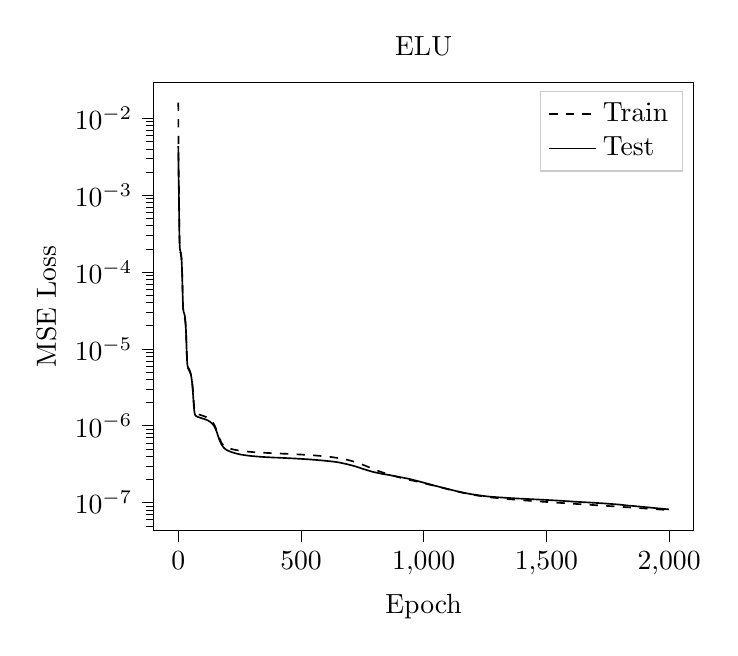
\begin{tikzpicture}

\begin{axis}[
legend cell align={left},
legend style={fill opacity=0.8, draw opacity=1, text opacity=1, draw=white!80!black},
log basis y={10},
tick align=outside,
tick pos=left,
title={ELU},
x grid style={white!69.0196078431373!black},
xlabel={Epoch},
xmin=-99.95, xmax=2098.95,
xtick style={color=black},
y grid style={white!69.0196078431373!black},
ylabel={MSE Loss},
ymin=4.33867354845081e-08, ymax=0.0294400810052884,
ymode=log,
ytick style={color=black}
]
\addplot [semithick, black, dashed]
table {%
0 0.0159906858149916
1 0.00258610278647393
2 0.00158850618591532
3 0.000956721410620958
4 0.000489001872134395
5 0.000282956345094135
6 0.000211721064930316
7 0.000189768037933391
8 0.000182021637432626
9 0.000177359326808073
10 0.00017262034923624
11 0.000166685566466185
12 0.000158753151561541
13 0.000147911270316399
14 0.000133165153318259
15 0.000113917955408397
16 9.10907805628085e-05
17 6.81213804309664e-05
18 4.95797647945437e-05
19 3.77359661724768e-05
20 3.16004643500492e-05
21 2.88638024685497e-05
22 2.76655603011022e-05
23 2.70052526702784e-05
24 2.64611737529776e-05
25 2.58725344338018e-05
26 2.5165805926008e-05
27 2.42854159696435e-05
28 2.3170354677859e-05
29 2.1749585019279e-05
30 1.99512444050924e-05
31 1.77340576083225e-05
32 1.51524796165177e-05
33 1.24352534580794e-05
34 9.97405172893195e-06
35 8.11734906142192e-06
36 6.93657802185044e-06
37 6.26315004649314e-06
38 5.89122448752732e-06
39 5.67968576444855e-06
40 5.54886149245704e-06
41 5.45669130860915e-06
42 5.38190175734599e-06
43 5.31409949712724e-06
44 5.24773788464472e-06
45 5.17960450264354e-06
46 5.1075526739055e-06
47 5.0298866058256e-06
48 4.94497295511564e-06
49 4.85107668760065e-06
50 4.74619869891058e-06
51 4.62834542622659e-06
52 4.49535393136102e-06
53 4.34503200801828e-06
54 4.17533381039448e-06
55 3.98467260913549e-06
56 3.77238118278456e-06
57 3.53925117417475e-06
58 3.28787568685129e-06
59 3.02373617284957e-06
60 2.75509752935932e-06
61 2.49260368849491e-06
62 2.24850782882413e-06
63 2.03428455245103e-06
64 1.85795620984663e-06
65 1.72250744253688e-06
66 1.6253536736599e-06
67 1.55974525910096e-06
68 1.51752829367524e-06
69 1.49080065330054e-06
70 1.47362176335264e-06
71 1.46225174086112e-06
72 1.45420856449618e-06
73 1.44795093308403e-06
74 1.44271991388223e-06
75 1.43809431347108e-06
76 1.43374334504642e-06
77 1.4295735134624e-06
78 1.42554408182605e-06
79 1.4216497555708e-06
80 1.4178540251919e-06
81 1.41412515841921e-06
82 1.41044651763877e-06
83 1.40681854372815e-06
84 1.40321067493687e-06
85 1.39963591544756e-06
86 1.39609892386261e-06
87 1.3925948815654e-06
88 1.38911853508716e-06
89 1.38566465489021e-06
90 1.3822299957269e-06
91 1.37881240459592e-06
92 1.37540860333729e-06
93 1.37201512541196e-06
94 1.36863055058711e-06
95 1.36524915507152e-06
96 1.36186575497277e-06
97 1.35847405181266e-06
98 1.35507275581404e-06
99 1.35165732331188e-06
100 1.34823074495216e-06
101 1.34479479419269e-06
102 1.34134401474739e-06
103 1.33786503300826e-06
104 1.33434866893367e-06
105 1.33078413216481e-06
106 1.32714234337072e-06
107 1.32344306734922e-06
108 1.31969354293915e-06
109 1.31588055188558e-06
110 1.3119966006343e-06
111 1.30803326578643e-06
112 1.30398476517257e-06
113 1.29984123759641e-06
114 1.29558252115203e-06
115 1.29120262238303e-06
116 1.28669816643878e-06
117 1.28205541477655e-06
118 1.27726922664806e-06
119 1.27233098703528e-06
120 1.26723150225416e-06
121 1.26195678973318e-06
122 1.25649127721772e-06
123 1.25082408101207e-06
124 1.24494655307217e-06
125 1.23884643841166e-06
126 1.23250899838467e-06
127 1.22591671828332e-06
128 1.21905894394558e-06
129 1.21192284018434e-06
130 1.20449245946475e-06
131 1.19675427941957e-06
132 1.18869531445398e-06
133 1.18030099093858e-06
134 1.17156371038618e-06
135 1.16247397437519e-06
136 1.1530011221339e-06
137 1.14308228643267e-06
138 1.13275827038706e-06
139 1.12201267188539e-06
140 1.11083171299242e-06
141 1.09920396710095e-06
142 1.08712059392246e-06
143 1.07459341876392e-06
144 1.06162042015967e-06
145 1.04818883656321e-06
146 1.03432408710091e-06
147 1.02003630371428e-06
148 1.00531462365439e-06
149 9.90169928911655e-07
150 9.74621806705045e-07
151 9.58713785962573e-07
152 9.42479460690038e-07
153 9.25951065312347e-07
154 9.09168600088606e-07
155 8.92184417097042e-07
156 8.75050800544841e-07
157 8.57826169180953e-07
158 8.40580582490702e-07
159 8.23381914443644e-07
160 8.06295238675148e-07
161 7.89396326780434e-07
162 7.72781310985238e-07
163 7.5657787539285e-07
164 7.40862125041986e-07
165 7.2571279957856e-07
166 7.11178002461566e-07
167 6.97275696751376e-07
168 6.84054517108734e-07
169 6.71543604397584e-07
170 6.59739762710387e-07
171 6.48579841652008e-07
172 6.38077358331657e-07
173 6.28216510477841e-07
174 6.18950641552374e-07
175 6.10264039266895e-07
176 6.02169999183388e-07
177 5.94657562174916e-07
178 5.87744280039715e-07
179 5.81413833458555e-07
180 5.75600660994269e-07
181 5.70220933695964e-07
182 5.65223498483647e-07
183 5.60603560245454e-07
184 5.56351066080651e-07
185 5.5243466988486e-07
186 5.48800114756887e-07
187 5.45434322532401e-07
188 5.42349594923053e-07
189 5.3947486807715e-07
190 5.36828737466521e-07
191 5.34344525419783e-07
192 5.31993674542264e-07
193 5.29807905536472e-07
194 5.27781949926975e-07
195 5.25858571194249e-07
196 5.24057332683014e-07
197 5.22343938712311e-07
198 5.20721551481529e-07
199 5.19149034175825e-07
200 5.17642666835627e-07
201 5.16201990961918e-07
202 5.14809736500865e-07
203 5.13455026037946e-07
204 5.12140459591137e-07
205 5.10864461205074e-07
206 5.09625953128534e-07
207 5.08422520994145e-07
208 5.07252190715235e-07
209 5.06112615170196e-07
210 5.05002207120242e-07
211 5.03919332913938e-07
212 5.02862736993848e-07
213 5.01830968431705e-07
214 5.00823714645549e-07
215 4.99837807353742e-07
216 4.98873107687814e-07
217 4.97929484851056e-07
218 4.970058403444e-07
219 4.96100682312317e-07
220 4.95213617199397e-07
221 4.9434340317589e-07
222 4.93489999001895e-07
223 4.92651290159074e-07
224 4.91828680907247e-07
225 4.91020204350434e-07
226 4.90224581596976e-07
227 4.89441853375183e-07
228 4.88671986033751e-07
229 4.87916952238265e-07
230 4.87174485925834e-07
231 4.86444744325354e-07
232 4.85726774883233e-07
233 4.85019369165229e-07
234 4.84323500302253e-07
235 4.83639927125523e-07
236 4.82968296523723e-07
237 4.82310117121187e-07
238 4.81661928859012e-07
239 4.81025225582243e-07
240 4.80400114071244e-07
241 4.7978502902879e-07
242 4.7918102524136e-07
243 4.78587331343761e-07
244 4.78004294649281e-07
245 4.77429992429279e-07
246 4.76862302633663e-07
247 4.76302523139793e-07
248 4.75746792034215e-07
249 4.75196238653552e-07
250 4.74654275848252e-07
251 4.74122004590072e-07
252 4.73599449662743e-07
253 4.73085426420994e-07
254 4.72580569010006e-07
255 4.72084032054454e-07
256 4.71594751218163e-07
257 4.71113804536571e-07
258 4.70640037235626e-07
259 4.70174156276926e-07
260 4.69715779757962e-07
261 4.69264562411809e-07
262 4.68820197625064e-07
263 4.68383233567238e-07
264 4.67952394359372e-07
265 4.67528493487634e-07
266 4.67111006997811e-07
267 4.66699930598224e-07
268 4.66294966287251e-07
269 4.65896007852962e-07
270 4.65502569653609e-07
271 4.65115601855359e-07
272 4.64733806950335e-07
273 4.64358269653076e-07
274 4.63987621714068e-07
275 4.63622054098778e-07
276 4.63262431424027e-07
277 4.62908034307929e-07
278 4.62558302785965e-07
279 4.62213879472984e-07
280 4.61874451275435e-07
281 4.61539479516659e-07
282 4.61210072302265e-07
283 4.6088585966686e-07
284 4.6056530376859e-07
285 4.60250070204893e-07
286 4.59937903713126e-07
287 4.59627579061817e-07
288 4.59320908589689e-07
289 4.59017937771478e-07
290 4.58719720626277e-07
291 4.58426474295948e-07
292 4.58136888113359e-07
293 4.57850685478434e-07
294 4.57567064700015e-07
295 4.57287548698559e-07
296 4.5700933148396e-07
297 4.56734894044075e-07
298 4.56462790253909e-07
299 4.56193259282145e-07
300 4.55927074597184e-07
301 4.55663766445014e-07
302 4.55403457266357e-07
303 4.55145485204866e-07
304 4.54890051884149e-07
305 4.54637398092927e-07
306 4.54387924690991e-07
307 4.54140048816498e-07
308 4.53895595455833e-07
309 4.53652887642875e-07
310 4.53413013303816e-07
311 4.53175329965916e-07
312 4.52939619719928e-07
313 4.52706062532116e-07
314 4.52475091350379e-07
315 4.5224581933212e-07
316 4.5201851969523e-07
317 4.51793587870952e-07
318 4.51570470261231e-07
319 4.51349246276322e-07
320 4.51130139424549e-07
321 4.50911806410659e-07
322 4.50696465975398e-07
323 4.50482567146082e-07
324 4.50270295914379e-07
325 4.50059426896132e-07
326 4.49850886724334e-07
327 4.49642915526738e-07
328 4.49437628134319e-07
329 4.49232866827742e-07
330 4.49030053516708e-07
331 4.48829141930673e-07
332 4.48629371163634e-07
333 4.48430973705172e-07
334 4.48233733351344e-07
335 4.48038363487058e-07
336 4.47843558703198e-07
337 4.47650869631389e-07
338 4.47459386890614e-07
339 4.47268515870292e-07
340 4.47079601400446e-07
341 4.46891546545203e-07
342 4.46705519152601e-07
343 4.46520362459069e-07
344 4.46335505017714e-07
345 4.46152672083144e-07
346 4.45970515130512e-07
347 4.45789737796076e-07
348 4.45609748823017e-07
349 4.45431515828432e-07
350 4.45253731754747e-07
351 4.45076565142699e-07
352 4.44900865147702e-07
353 4.44726380123939e-07
354 4.44552419651245e-07
355 4.44379391097982e-07
356 4.44207578851774e-07
357 4.44036821988902e-07
358 4.43865763656959e-07
359 4.43696203234367e-07
360 4.43526793503679e-07
361 4.43359225258178e-07
362 4.43191910605378e-07
363 4.43025337716563e-07
364 4.42860381781429e-07
365 4.42694943302513e-07
366 4.42530713499423e-07
367 4.42366368687885e-07
368 4.42203394399598e-07
369 4.42040955817902e-07
370 4.41879210029583e-07
371 4.41718379931899e-07
372 4.41557534529124e-07
373 4.41397798184084e-07
374 4.41238832934232e-07
375 4.41079906011055e-07
376 4.40922253190479e-07
377 4.40764245766445e-07
378 4.40607835045625e-07
379 4.40452905152711e-07
380 4.40298538350703e-07
381 4.40145228878919e-07
382 4.39993665253269e-07
383 4.39841247228401e-07
384 4.39687762394669e-07
385 4.3953382136408e-07
386 4.39380508097997e-07
387 4.39228653746682e-07
388 4.39076504648028e-07
389 4.38928091796242e-07
390 4.38781355668993e-07
391 4.38643548605455e-07
392 4.38510998463926e-07
393 4.38376672008189e-07
394 4.38234255639713e-07
395 4.38070808172597e-07
396 4.37907314719155e-07
397 4.37751213482329e-07
398 4.37598554711371e-07
399 4.37448513110894e-07
400 4.37300081301828e-07
401 4.37152214118441e-07
402 4.37005594591255e-07
403 4.36860011149065e-07
404 4.36714657084281e-07
405 4.36570365806688e-07
406 4.36424143586578e-07
407 4.36277994012357e-07
408 4.36131178759069e-07
409 4.35983725139977e-07
410 4.35836715993787e-07
411 4.35689698022657e-07
412 4.3554247810107e-07
413 4.35395135951921e-07
414 4.35247865510746e-07
415 4.3510124847046e-07
416 4.3495456503706e-07
417 4.34807267438941e-07
418 4.34661463131647e-07
419 4.34514212969361e-07
420 4.34367550937509e-07
421 4.34220724088163e-07
422 4.34074552501329e-07
423 4.33927956791536e-07
424 4.33781591112847e-07
425 4.33634953083128e-07
426 4.33488506146773e-07
427 4.33342491390931e-07
428 4.33196209357334e-07
429 4.33049361106441e-07
430 4.32903117015826e-07
431 4.32756445960081e-07
432 4.32610265974631e-07
433 4.32463891300472e-07
434 4.32316499100693e-07
435 4.32170432986823e-07
436 4.32023130812809e-07
437 4.31876773717477e-07
438 4.31729480283138e-07
439 4.31582528875651e-07
440 4.31435453705831e-07
441 4.3128805349113e-07
442 4.31140072421954e-07
443 4.30992692542986e-07
444 4.30845347480613e-07
445 4.30696623013205e-07
446 4.30548953829657e-07
447 4.30400634797934e-07
448 4.3025189394541e-07
449 4.3010315148706e-07
450 4.29953725117116e-07
451 4.2980486917088e-07
452 4.29655644651916e-07
453 4.29506079029807e-07
454 4.29355998889491e-07
455 4.29205821575351e-07
456 4.2905581715047e-07
457 4.28906095805814e-07
458 4.28755179513018e-07
459 4.28604906815622e-07
460 4.28454305719583e-07
461 4.28303182189893e-07
462 4.28152659679881e-07
463 4.28002008391104e-07
464 4.27851925209666e-07
465 4.27701338750808e-07
466 4.27552839354917e-07
467 4.27403515331548e-07
468 4.27255618234312e-07
469 4.27108254356767e-07
470 4.26961206983378e-07
471 4.26816100954852e-07
472 4.26674825746431e-07
473 4.26536179944037e-07
474 4.26386996636552e-07
475 4.26223891494715e-07
476 4.26065150577415e-07
477 4.25903862350197e-07
478 4.25744202857459e-07
479 4.25587278471085e-07
480 4.25434084164067e-07
481 4.25283438900692e-07
482 4.2512929348959e-07
483 4.24950156059367e-07
484 4.24775556922441e-07
485 4.2460948539258e-07
486 4.2444458654245e-07
487 4.24280352362416e-07
488 4.24115700013772e-07
489 4.23950707684639e-07
490 4.23785132056764e-07
491 4.23619217514215e-07
492 4.23452926057166e-07
493 4.23285097667758e-07
494 4.23117765933512e-07
495 4.22949673065887e-07
496 4.2278219368086e-07
497 4.22613616308354e-07
498 4.22447139484916e-07
499 4.22281561995419e-07
500 4.22117390655785e-07
501 4.21952666897596e-07
502 4.21779191682958e-07
503 4.21598478823171e-07
504 4.2141833586129e-07
505 4.2124271746502e-07
506 4.21069510096572e-07
507 4.20896647739255e-07
508 4.20719663239311e-07
509 4.20538109011659e-07
510 4.20356770078456e-07
511 4.20174129061479e-07
512 4.19992674551395e-07
513 4.19810148940769e-07
514 4.19626769726733e-07
515 4.19442054592878e-07
516 4.19257225004799e-07
517 4.19071456931874e-07
518 4.18885225997201e-07
519 4.18697576918703e-07
520 4.1850933769183e-07
521 4.18320481543333e-07
522 4.18130317740406e-07
523 4.17939218365859e-07
524 4.17747739689389e-07
525 4.17556271386843e-07
526 4.17364103711293e-07
527 4.17172572497293e-07
528 4.16980429790215e-07
529 4.16786990015794e-07
530 4.1658723431226e-07
531 4.1638575135039e-07
532 4.16184523388097e-07
533 4.15983118557506e-07
534 4.15780713709069e-07
535 4.15577499595088e-07
536 4.15373394730523e-07
537 4.151681697806e-07
538 4.14961842821526e-07
539 4.14754696521413e-07
540 4.14546592665488e-07
541 4.14338080034327e-07
542 4.14128793067903e-07
543 4.13919188318346e-07
544 4.13709204124757e-07
545 4.13499209244605e-07
546 4.1328589449563e-07
547 4.1306897557547e-07
548 4.12848953288858e-07
549 4.1262784985463e-07
550 4.12405905663604e-07
551 4.1218276821553e-07
552 4.11959315172794e-07
553 4.11734457159696e-07
554 4.11508107944769e-07
555 4.11280582085283e-07
556 4.11051760707437e-07
557 4.10821502754288e-07
558 4.10589742699585e-07
559 4.10356863781658e-07
560 4.10121451281498e-07
561 4.09885287368184e-07
562 4.0964726396453e-07
563 4.09408234929742e-07
564 4.09167719382708e-07
565 4.08926019616729e-07
566 4.08682671249494e-07
567 4.08436698762671e-07
568 4.08190045746437e-07
569 4.07942119579729e-07
570 4.07692340473886e-07
571 4.07440955882521e-07
572 4.07187864269076e-07
573 4.06933416684296e-07
574 4.06676930793992e-07
575 4.06419140318803e-07
576 4.06159437602582e-07
577 4.05897947615586e-07
578 4.05634872592486e-07
579 4.05369885982054e-07
580 4.051037206807e-07
581 4.04835206595067e-07
582 4.0456507552733e-07
583 4.04293246745624e-07
584 4.04019944852507e-07
585 4.03744100808012e-07
586 4.0346718590456e-07
587 4.03187891819812e-07
588 4.02906474619158e-07
589 4.0262334898955e-07
590 4.02339123297679e-07
591 4.02051919692781e-07
592 4.01763511547415e-07
593 4.01472600756847e-07
594 4.01180168040582e-07
595 4.00885645106541e-07
596 4.00589115145067e-07
597 4.00290419662497e-07
598 3.99989771580067e-07
599 3.99687020760098e-07
600 3.9938239817161e-07
601 3.99075610644672e-07
602 3.98767107213871e-07
603 3.98456655958057e-07
604 3.98143521934458e-07
605 3.97828211291085e-07
606 3.97511172096188e-07
607 3.971921851047e-07
608 3.96869894700558e-07
609 3.96546615860416e-07
610 3.96220210703291e-07
611 3.95892031804124e-07
612 3.95561097349173e-07
613 3.95228702899431e-07
614 3.94893582551958e-07
615 3.94556066183327e-07
616 3.94216474987275e-07
617 3.93874289670748e-07
618 3.93529946151716e-07
619 3.9318402720312e-07
620 3.92834608746284e-07
621 3.92483627194906e-07
622 3.92129560751187e-07
623 3.91772965187442e-07
624 3.91413925100892e-07
625 3.91051872711046e-07
626 3.90686788946937e-07
627 3.90318204011919e-07
628 3.89946447299394e-07
629 3.8957217735458e-07
630 3.89195215277027e-07
631 3.88815662418551e-07
632 3.88434823477724e-07
633 3.88049628099907e-07
634 3.87657926751217e-07
635 3.87261416292972e-07
636 3.8686301678581e-07
637 3.86461803216775e-07
638 3.86057096932291e-07
639 3.85649708007918e-07
640 3.85240323424796e-07
641 3.84827308181457e-07
642 3.84410717657602e-07
643 3.83992713764769e-07
644 3.8357037226433e-07
645 3.83146246292654e-07
646 3.82718414641658e-07
647 3.82286220116157e-07
648 3.81847366909938e-07
649 3.81402807022369e-07
650 3.80953362920877e-07
651 3.8049944438967e-07
652 3.80041698434752e-07
653 3.79580423256698e-07
654 3.79116224436871e-07
655 3.78646916274761e-07
656 3.78174421157951e-07
657 3.77697935945776e-07
658 3.7721625281506e-07
659 3.76731392663032e-07
660 3.76241358409857e-07
661 3.75747463223774e-07
662 3.75249042562587e-07
663 3.74747122450003e-07
664 3.74241638539274e-07
665 3.73735716252099e-07
666 3.73232575682891e-07
667 3.72738996702537e-07
668 3.72227829430472e-07
669 3.71683786227095e-07
670 3.7113470823158e-07
671 3.70593554904985e-07
672 3.70050383537546e-07
673 3.69502068551242e-07
674 3.68949084261772e-07
675 3.68390563210141e-07
676 3.678264965572e-07
677 3.6725771867907e-07
678 3.66683600475426e-07
679 3.66104024905667e-07
680 3.65519362432565e-07
681 3.64929335361808e-07
682 3.64334175131376e-07
683 3.63734159961382e-07
684 3.63128429640369e-07
685 3.62517425529063e-07
686 3.6190134476044e-07
687 3.61279533990455e-07
688 3.60653619935647e-07
689 3.60020216263024e-07
690 3.59382881029546e-07
691 3.58739043363698e-07
692 3.58090267752686e-07
693 3.57435885064206e-07
694 3.56775838710632e-07
695 3.56110636616336e-07
696 3.55440148368302e-07
697 3.54764160434229e-07
698 3.54083058994092e-07
699 3.53396487156488e-07
700 3.52704934726944e-07
701 3.52008020470862e-07
702 3.51306000808904e-07
703 3.50598153502801e-07
704 3.49885847469977e-07
705 3.49167120290872e-07
706 3.48444031672557e-07
707 3.47714999051618e-07
708 3.46980296029642e-07
709 3.46241530451152e-07
710 3.45497773565739e-07
711 3.44750385963266e-07
712 3.44000039959269e-07
713 3.43243426499384e-07
714 3.42480047621052e-07
715 3.4171182264231e-07
716 3.40938305697591e-07
717 3.40157672084729e-07
718 3.39370888212898e-07
719 3.38579835030828e-07
720 3.3778467948764e-07
721 3.36985210793728e-07
722 3.36182615654934e-07
723 3.35375445175146e-07
724 3.34564629454803e-07
725 3.33749487339219e-07
726 3.32931064335185e-07
727 3.32108447068435e-07
728 3.31281637940606e-07
729 3.30452154130967e-07
730 3.29618623183592e-07
731 3.28782307889242e-07
732 3.27943212383275e-07
733 3.27100122291313e-07
734 3.26251898755459e-07
735 3.25400266802944e-07
736 3.24546339115273e-07
737 3.23690739747917e-07
738 3.22837684763044e-07
739 3.21980068548555e-07
740 3.2111100145471e-07
741 3.20237002227941e-07
742 3.19366001733101e-07
743 3.18494356619681e-07
744 3.1762165654925e-07
745 3.16747852309618e-07
746 3.15873930802013e-07
747 3.14998583988313e-07
748 3.14122304018838e-07
749 3.13245467609136e-07
750 3.12366119956664e-07
751 3.11487112625741e-07
752 3.10605095265259e-07
753 3.097206207201e-07
754 3.08832639916545e-07
755 3.07942916634829e-07
756 3.07053517630607e-07
757 3.06164666483255e-07
758 3.05276597615034e-07
759 3.04389342446143e-07
760 3.03502841475733e-07
761 3.0261704606005e-07
762 3.01732263409349e-07
763 3.00848316157953e-07
764 2.99964995178925e-07
765 2.99083555333368e-07
766 2.9820374386702e-07
767 2.9732410860106e-07
768 2.96446761538505e-07
769 2.95571269603556e-07
770 2.94697533661292e-07
771 2.93826113733076e-07
772 2.92956484798879e-07
773 2.92088886098441e-07
774 2.91223827659337e-07
775 2.9036127409654e-07
776 2.89501379810986e-07
777 2.88645371341545e-07
778 2.87790612048866e-07
779 2.86939756222182e-07
780 2.86093918646202e-07
781 2.85250324424169e-07
782 2.8440853506595e-07
783 2.83568418524283e-07
784 2.82729770532342e-07
785 2.81894248473691e-07
786 2.81063022612216e-07
787 2.80233988476652e-07
788 2.79408298268891e-07
789 2.78585843020096e-07
790 2.77766766629384e-07
791 2.76950464609627e-07
792 2.76139197950442e-07
793 2.75330968236176e-07
794 2.74527831123805e-07
795 2.73728886554636e-07
796 2.72934971803807e-07
797 2.72145031900095e-07
798 2.71360245974961e-07
799 2.70580689175404e-07
800 2.69805612404639e-07
801 2.69035723647448e-07
802 2.68270829579365e-07
803 2.67510604714971e-07
804 2.66754783439183e-07
805 2.66003943082183e-07
806 2.65257105226624e-07
807 2.64515074746896e-07
808 2.63777658076947e-07
809 2.63044983014993e-07
810 2.62317090502506e-07
811 2.61593597855381e-07
812 2.60874926851784e-07
813 2.60160685854771e-07
814 2.59451338109784e-07
815 2.58746429480539e-07
816 2.58046112065813e-07
817 2.57350360087116e-07
818 2.56658965938072e-07
819 2.55971881685468e-07
820 2.5528879186254e-07
821 2.54610372564912e-07
822 2.53935969610097e-07
823 2.53264675137643e-07
824 2.52598306374807e-07
825 2.51936233553351e-07
826 2.51277138815453e-07
827 2.50624390943699e-07
828 2.49974296863797e-07
829 2.49328972245166e-07
830 2.48688589437052e-07
831 2.48052176218039e-07
832 2.47420308085111e-07
833 2.46793441860405e-07
834 2.46169972669463e-07
835 2.4555191518516e-07
836 2.44938152263785e-07
837 2.44328980471664e-07
838 2.4372432818609e-07
839 2.43123647450716e-07
840 2.42527436739692e-07
841 2.41934313066849e-07
842 2.41346243086582e-07
843 2.40760975287913e-07
844 2.40180195106632e-07
845 2.39602776233028e-07
846 2.39030478169866e-07
847 2.3846193494137e-07
848 2.37897005348486e-07
849 2.37336486961226e-07
850 2.36780270924442e-07
851 2.36228712395814e-07
852 2.35682560855821e-07
853 2.35140349545304e-07
854 2.34604098082514e-07
855 2.34070661221608e-07
856 2.33540884252648e-07
857 2.33015706925244e-07
858 2.3249482104859e-07
859 2.31977036079911e-07
860 2.31462959533246e-07
861 2.30952844745502e-07
862 2.30445369865606e-07
863 2.29941426724167e-07
864 2.29440585172824e-07
865 2.28943704769335e-07
866 2.2844926068899e-07
867 2.27958044973775e-07
868 2.27470275618202e-07
869 2.26985706731853e-07
870 2.26503938364431e-07
871 2.26025791818074e-07
872 2.2555024735027e-07
873 2.25077442294719e-07
874 2.24607759776063e-07
875 2.24141335792183e-07
876 2.23676740787937e-07
877 2.23216036090435e-07
878 2.22757687268427e-07
879 2.22302162356414e-07
880 2.21849671518726e-07
881 2.21399852961213e-07
882 2.20952989891998e-07
883 2.20508026032462e-07
884 2.20065753254062e-07
885 2.19626199381651e-07
886 2.1918875741278e-07
887 2.18753092724455e-07
888 2.18320540270156e-07
889 2.17889485469414e-07
890 2.1745900326664e-07
891 2.17031351979813e-07
892 2.16608203714941e-07
893 2.16190809553041e-07
894 2.15776312643356e-07
895 2.15362290859389e-07
896 2.14950339142206e-07
897 2.14540210251357e-07
898 2.14131782342974e-07
899 2.1372564420119e-07
900 2.1332161301757e-07
901 2.1291910150012e-07
902 2.12518860138289e-07
903 2.12120724143006e-07
904 2.11724538587532e-07
905 2.11329817702222e-07
906 2.10937199824457e-07
907 2.10546256425914e-07
908 2.10156896628177e-07
909 2.09769570474805e-07
910 2.09383709488975e-07
911 2.08999720584302e-07
912 2.08617331423966e-07
913 2.08236899553071e-07
914 2.07857965250469e-07
915 2.07481092886042e-07
916 2.07105115009654e-07
917 2.06731647111269e-07
918 2.06359596120365e-07
919 2.05989531096407e-07
920 2.05621238876574e-07
921 2.05254394956e-07
922 2.0488954909581e-07
923 2.04526185612508e-07
924 2.04164605918322e-07
925 2.03804957877196e-07
926 2.03447523659861e-07
927 2.03092279107864e-07
928 2.02738294618143e-07
929 2.0238457909727e-07
930 2.02029677069504e-07
931 2.01671937460901e-07
932 2.01315043327099e-07
933 2.00959512497434e-07
934 2.00604544644989e-07
935 2.00250872410379e-07
936 1.99898528762787e-07
937 1.99547518036525e-07
938 1.99197931237904e-07
939 1.98846556727972e-07
940 1.98497077832371e-07
941 1.98145747660305e-07
942 1.9779394646946e-07
943 1.97441289401468e-07
944 1.97090426979685e-07
945 1.96742395402794e-07
946 1.96398488569116e-07
947 1.96056057973237e-07
948 1.95715211518177e-07
949 1.9537850144502e-07
950 1.9504455411834e-07
951 1.94712024338628e-07
952 1.94378926153149e-07
953 1.94046811500925e-07
954 1.93714091096808e-07
955 1.93381568564632e-07
956 1.93050385803417e-07
957 1.92719263750973e-07
958 1.92389278353744e-07
959 1.9205929470445e-07
960 1.91731396029127e-07
961 1.91402223222781e-07
962 1.91074683357328e-07
963 1.9074786413853e-07
964 1.90421514702166e-07
965 1.90095022318815e-07
966 1.89770198232964e-07
967 1.89445391086451e-07
968 1.89120989816161e-07
969 1.88797464574009e-07
970 1.88474153929974e-07
971 1.88151886163723e-07
972 1.87829453849986e-07
973 1.87507783181218e-07
974 1.87187286698531e-07
975 1.86866505401895e-07
976 1.86546299758561e-07
977 1.86227077662693e-07
978 1.85908078876196e-07
979 1.85589941480657e-07
980 1.85271628822647e-07
981 1.8495448021838e-07
982 1.84637383412678e-07
983 1.84320716172692e-07
984 1.84004656915704e-07
985 1.83688698498941e-07
986 1.83373058249003e-07
987 1.83057700795075e-07
988 1.82742971801986e-07
989 1.8242811900393e-07
990 1.82113932297057e-07
991 1.81799501604019e-07
992 1.8148617854763e-07
993 1.81172313531874e-07
994 1.80859163535274e-07
995 1.80546558553374e-07
996 1.8023371875131e-07
997 1.79921399450222e-07
998 1.79609133027725e-07
999 1.7929770129399e-07
1000 1.78986370457324e-07
1001 1.78674888474006e-07
1002 1.78363633111189e-07
1003 1.78053571730175e-07
1004 1.77743094340599e-07
1005 1.7743289222949e-07
1006 1.77123163680903e-07
1007 1.76813399150433e-07
1008 1.76504621208551e-07
1009 1.7619593938889e-07
1010 1.75887513734097e-07
1011 1.75579751243049e-07
1012 1.75272690157158e-07
1013 1.74965952467687e-07
1014 1.74659207814898e-07
1015 1.74351380209714e-07
1016 1.74042034160493e-07
1017 1.73731117456555e-07
1018 1.73420100608723e-07
1019 1.73109630651425e-07
1020 1.72800415427332e-07
1021 1.72490790831148e-07
1022 1.72182884469407e-07
1023 1.71875223259121e-07
1024 1.71567599466016e-07
1025 1.71259986530004e-07
1026 1.70952779214417e-07
1027 1.70645558227989e-07
1028 1.7033885781359e-07
1029 1.70032917338858e-07
1030 1.69726343031584e-07
1031 1.6942034865508e-07
1032 1.69114824657868e-07
1033 1.68809569686346e-07
1034 1.68504218905241e-07
1035 1.68199184841455e-07
1036 1.67894168384919e-07
1037 1.67589057525674e-07
1038 1.67283977333454e-07
1039 1.66978109149341e-07
1040 1.66672554144043e-07
1041 1.66368867070332e-07
1042 1.66067442094686e-07
1043 1.65768675415734e-07
1044 1.65470151159752e-07
1045 1.65171997124958e-07
1046 1.64875026726463e-07
1047 1.64578407392923e-07
1048 1.6428200929397e-07
1049 1.63985019597135e-07
1050 1.63684462393121e-07
1051 1.63379912791584e-07
1052 1.63074535350916e-07
1053 1.62768297784055e-07
1054 1.62462222775162e-07
1055 1.62156110874889e-07
1056 1.61849415221127e-07
1057 1.61543195446257e-07
1058 1.61236785999108e-07
1059 1.60933830407828e-07
1060 1.60635022787403e-07
1061 1.60340385868096e-07
1062 1.60049089302561e-07
1063 1.59758593277104e-07
1064 1.59466722315926e-07
1065 1.59174708123544e-07
1066 1.58880650644733e-07
1067 1.5858718038686e-07
1068 1.58293491729467e-07
1069 1.5799999722077e-07
1070 1.57706408096203e-07
1071 1.57412825096515e-07
1072 1.57120173312819e-07
1073 1.56827222305367e-07
1074 1.56535237174182e-07
1075 1.56243974302583e-07
1076 1.55952766455414e-07
1077 1.55662811614832e-07
1078 1.55373152850302e-07
1079 1.55083731485206e-07
1080 1.54795515378225e-07
1081 1.54507988042951e-07
1082 1.54220873660904e-07
1083 1.53935042980891e-07
1084 1.53649188085581e-07
1085 1.53364610277151e-07
1086 1.53080741092992e-07
1087 1.5279745203145e-07
1088 1.52514170402185e-07
1089 1.52231895036437e-07
1090 1.51950201022544e-07
1091 1.51669021178691e-07
1092 1.51388963097077e-07
1093 1.51109408882633e-07
1094 1.5082977131442e-07
1095 1.50551916078712e-07
1096 1.50274534782113e-07
1097 1.49998161141696e-07
1098 1.49722255947893e-07
1099 1.49446563071365e-07
1100 1.49171961965067e-07
1101 1.48898209054948e-07
1102 1.48624307755085e-07
1103 1.4835133026736e-07
1104 1.48080495421254e-07
1105 1.47808726936205e-07
1106 1.47538366228162e-07
1107 1.4726858979941e-07
1108 1.46999026256367e-07
1109 1.46730341562318e-07
1110 1.46462592610419e-07
1111 1.46194448667814e-07
1112 1.45927681444391e-07
1113 1.45660832160388e-07
1114 1.45394960604506e-07
1115 1.45130510077252e-07
1116 1.44867812252869e-07
1117 1.4460710507791e-07
1118 1.44346854739297e-07
1119 1.44088306292645e-07
1120 1.43830166308589e-07
1121 1.43572312296669e-07
1122 1.43315712179515e-07
1123 1.43060445338961e-07
1124 1.42805129407009e-07
1125 1.42551452839257e-07
1126 1.42298427896037e-07
1127 1.42046496797832e-07
1128 1.41795435418146e-07
1129 1.41545382064123e-07
1130 1.41295842354339e-07
1131 1.41047917132653e-07
1132 1.40800541821307e-07
1133 1.40554253533765e-07
1134 1.40309015705498e-07
1135 1.40064675107965e-07
1136 1.39821170350274e-07
1137 1.39579605225038e-07
1138 1.39338311164749e-07
1139 1.39098575928642e-07
1140 1.38860050718392e-07
1141 1.38622980010439e-07
1142 1.38386074866048e-07
1143 1.38151192111025e-07
1144 1.37916803048199e-07
1145 1.37684516310799e-07
1146 1.37451800391375e-07
1147 1.37221027316059e-07
1148 1.36991179445545e-07
1149 1.36762923808931e-07
1150 1.36535392606163e-07
1151 1.36309236019372e-07
1152 1.36083985445623e-07
1153 1.35859885773471e-07
1154 1.35636987302235e-07
1155 1.35415610060363e-07
1156 1.3519462617495e-07
1157 1.34975457292796e-07
1158 1.34757256731177e-07
1159 1.34540234483893e-07
1160 1.34324358555205e-07
1161 1.34109793279435e-07
1162 1.33896426177671e-07
1163 1.33684459278527e-07
1164 1.33473248411065e-07
1165 1.33263645466286e-07
1166 1.33055609722987e-07
1167 1.32848456068757e-07
1168 1.32642267075767e-07
1169 1.32438386458489e-07
1170 1.3223490227432e-07
1171 1.32032633729295e-07
1172 1.31832137057586e-07
1173 1.31632554129624e-07
1174 1.31434246767981e-07
1175 1.31237355475378e-07
1176 1.3104204354164e-07
1177 1.30847429275605e-07
1178 1.30654636990357e-07
1179 1.30462662419006e-07
1180 1.30272386684283e-07
1181 1.30083957976979e-07
1182 1.29895856105122e-07
1183 1.29710162141805e-07
1184 1.29525688848275e-07
1185 1.29342381164577e-07
1186 1.29160692303287e-07
1187 1.28980738672624e-07
1188 1.28801087768693e-07
1189 1.28622351823537e-07
1190 1.28443456553384e-07
1191 1.28265808847061e-07
1192 1.28089295927225e-07
1193 1.27913166409144e-07
1194 1.27739159495377e-07
1195 1.27565773269112e-07
1196 1.27394257454227e-07
1197 1.2722304434476e-07
1198 1.27053708432356e-07
1199 1.26885512280239e-07
1200 1.26718282551508e-07
1201 1.26551697867683e-07
1202 1.26386519937682e-07
1203 1.2622200886625e-07
1204 1.26058745912871e-07
1205 1.25896560582817e-07
1206 1.25735422180639e-07
1207 1.25574455424271e-07
1208 1.25414781614097e-07
1209 1.252551799098e-07
1210 1.25096239329991e-07
1211 1.24937196254393e-07
1212 1.24777347565441e-07
1213 1.24616552589885e-07
1214 1.24453111794764e-07
1215 1.24288724109078e-07
1216 1.24127905870353e-07
1217 1.23972136528039e-07
1218 1.23820694362564e-07
1219 1.23674698834009e-07
1220 1.23530782715875e-07
1221 1.23389221329262e-07
1222 1.2324859677193e-07
1223 1.2310908447688e-07
1224 1.22970074919238e-07
1225 1.22832236861825e-07
1226 1.22694502813658e-07
1227 1.22557335302531e-07
1228 1.22421338744516e-07
1229 1.22286256306836e-07
1230 1.22151674226245e-07
1231 1.22018912449562e-07
1232 1.21886562475026e-07
1233 1.21754655523887e-07
1234 1.21624491512762e-07
1235 1.21494801220479e-07
1236 1.2136614208913e-07
1237 1.21238329604978e-07
1238 1.21111555806408e-07
1239 1.20985908843352e-07
1240 1.20860088962615e-07
1241 1.20735704754793e-07
1242 1.20612777600115e-07
1243 1.20490426148478e-07
1244 1.20367756657913e-07
1245 1.2024713782921e-07
1246 1.20126928187858e-07
1247 1.20007730558314e-07
1248 1.19888488541164e-07
1249 1.19770750160342e-07
1250 1.19653075920212e-07
1251 1.19536828812272e-07
1252 1.19421025523536e-07
1253 1.19305560325245e-07
1254 1.19191435054233e-07
1255 1.19077117162192e-07
1256 1.18963121451543e-07
1257 1.18850351661592e-07
1258 1.18737166289407e-07
1259 1.18624644954934e-07
1260 1.18512422588424e-07
1261 1.1840071167768e-07
1262 1.18288370344999e-07
1263 1.18177834188771e-07
1264 1.18068884660261e-07
1265 1.17963069399707e-07
1266 1.17858075192601e-07
1267 1.17754390267066e-07
1268 1.17650794884128e-07
1269 1.17548814614565e-07
1270 1.1744721561513e-07
1271 1.17345708268601e-07
1272 1.17244883455214e-07
1273 1.17145502350979e-07
1274 1.17046118376152e-07
1275 1.16947641409126e-07
1276 1.16849509630867e-07
1277 1.1675244088849e-07
1278 1.16655163623136e-07
1279 1.16558887576446e-07
1280 1.16463558931912e-07
1281 1.16368087383023e-07
1282 1.16274038802544e-07
1283 1.16180324624793e-07
1284 1.16086594658782e-07
1285 1.159941292741e-07
1286 1.15901939551577e-07
1287 1.15811317932923e-07
1288 1.15720263679009e-07
1289 1.15630437839798e-07
1290 1.15540727264829e-07
1291 1.15451683456058e-07
1292 1.15363191504514e-07
1293 1.15273850731512e-07
1294 1.15184926350764e-07
1295 1.15096048155294e-07
1296 1.15007235429232e-07
1297 1.14918379381379e-07
1298 1.14830777491193e-07
1299 1.14743160814612e-07
1300 1.1465620086426e-07
1301 1.14570124786439e-07
1302 1.14484055657726e-07
1303 1.14398570758567e-07
1304 1.14313791009124e-07
1305 1.14229299640556e-07
1306 1.14145610695005e-07
1307 1.14061028625656e-07
1308 1.13977942092447e-07
1309 1.13894630288769e-07
1310 1.13811890621207e-07
1311 1.13728955128067e-07
1312 1.13647374824666e-07
1313 1.13565325307263e-07
1314 1.13483557022676e-07
1315 1.13402332914347e-07
1316 1.13320262414618e-07
1317 1.13240334016496e-07
1318 1.13159186064138e-07
1319 1.13077794551941e-07
1320 1.12997345617316e-07
1321 1.12916872375024e-07
1322 1.12837699774104e-07
1323 1.1275950181755e-07
1324 1.12682501281824e-07
1325 1.12606438932517e-07
1326 1.12530998414684e-07
1327 1.12455497344399e-07
1328 1.12380201152007e-07
1329 1.12304915312222e-07
1330 1.12229716322076e-07
1331 1.12155240366008e-07
1332 1.12080816393245e-07
1333 1.12006098483164e-07
1334 1.11932343500598e-07
1335 1.11859045325957e-07
1336 1.11785418326349e-07
1337 1.11712671881037e-07
1338 1.11639020587972e-07
1339 1.11567380578492e-07
1340 1.11494612262675e-07
1341 1.11422763467317e-07
1342 1.11350776293762e-07
1343 1.11279370571538e-07
1344 1.11208307423283e-07
1345 1.1113706440824e-07
1346 1.11066865265741e-07
1347 1.10995945618697e-07
1348 1.10925767160097e-07
1349 1.10855683992384e-07
1350 1.10786117552664e-07
1351 1.10716733097149e-07
1352 1.10647160461497e-07
1353 1.10578233645242e-07
1354 1.10509506583867e-07
1355 1.10440672571599e-07
1356 1.10372395390357e-07
1357 1.1030493424613e-07
1358 1.10236386966278e-07
1359 1.10168692920354e-07
1360 1.1010140007528e-07
1361 1.10034333395959e-07
1362 1.09966698083497e-07
1363 1.09899731342011e-07
1364 1.09833291951134e-07
1365 1.09767210155098e-07
1366 1.09700639285393e-07
1367 1.09634514146251e-07
1368 1.09568511987845e-07
1369 1.09503384450704e-07
1370 1.09437140011437e-07
1371 1.09372695533239e-07
1372 1.09307097929445e-07
1373 1.09242549555688e-07
1374 1.09177182331166e-07
1375 1.09113151367524e-07
1376 1.09048662530142e-07
1377 1.08984274390878e-07
1378 1.08920784626321e-07
1379 1.08856745349328e-07
1380 1.08792611804631e-07
1381 1.08729247486394e-07
1382 1.08666047573536e-07
1383 1.08602843141625e-07
1384 1.08539720571343e-07
1385 1.08477539157548e-07
1386 1.08414238106036e-07
1387 1.08351683770991e-07
1388 1.08289551810969e-07
1389 1.08227359682189e-07
1390 1.08165446718544e-07
1391 1.0810315509957e-07
1392 1.08042059039803e-07
1393 1.07980339663527e-07
1394 1.07918164097498e-07
1395 1.07857049350457e-07
1396 1.07796089665158e-07
1397 1.07734852363706e-07
1398 1.07674071145425e-07
1399 1.07613202636969e-07
1400 1.07552554730717e-07
1401 1.07492185293268e-07
1402 1.07430896818528e-07
1403 1.07371186579996e-07
1404 1.07310734684063e-07
1405 1.07251448994816e-07
1406 1.07190961820436e-07
1407 1.07130689571022e-07
1408 1.07071231418843e-07
1409 1.07011258137391e-07
1410 1.06951851911674e-07
1411 1.06892511382739e-07
1412 1.06832769780851e-07
1413 1.06773393866888e-07
1414 1.06713744486342e-07
1415 1.06655080848839e-07
1416 1.06596275074367e-07
1417 1.06536867519935e-07
1418 1.06478330863524e-07
1419 1.06419705552696e-07
1420 1.06360801503058e-07
1421 1.06302999540731e-07
1422 1.06245188106868e-07
1423 1.06186696449129e-07
1424 1.06128813278872e-07
1425 1.06071861281976e-07
1426 1.06014330761184e-07
1427 1.05956670530816e-07
1428 1.05899683347843e-07
1429 1.05843118227256e-07
1430 1.05786040670353e-07
1431 1.05729466049809e-07
1432 1.05672679602264e-07
1433 1.05616201466319e-07
1434 1.0555939075374e-07
1435 1.05503326139456e-07
1436 1.05447132533243e-07
1437 1.05391329668691e-07
1438 1.05335469569923e-07
1439 1.05278794926278e-07
1440 1.05223197536475e-07
1441 1.05167620077395e-07
1442 1.05111855617679e-07
1443 1.05056052994712e-07
1444 1.05001211672118e-07
1445 1.04945261661271e-07
1446 1.04890033782112e-07
1447 1.04835637209533e-07
1448 1.04780062464727e-07
1449 1.04725117317628e-07
1450 1.04669809111613e-07
1451 1.04615355382975e-07
1452 1.04560794511599e-07
1453 1.04506511071634e-07
1454 1.04451745890799e-07
1455 1.04396768143999e-07
1456 1.04343061707368e-07
1457 1.0428867787482e-07
1458 1.04234510423851e-07
1459 1.04180059025794e-07
1460 1.04126391235582e-07
1461 1.04072378704245e-07
1462 1.04018579186516e-07
1463 1.03964594160288e-07
1464 1.0391101395868e-07
1465 1.03857236730676e-07
1466 1.03804541957686e-07
1467 1.03750232234745e-07
1468 1.03697174260731e-07
1469 1.03644181137952e-07
1470 1.03590405920784e-07
1471 1.03537499640538e-07
1472 1.03484241449792e-07
1473 1.03431446369484e-07
1474 1.03379083178368e-07
1475 1.03325666280796e-07
1476 1.03273275158244e-07
1477 1.03220849005936e-07
1478 1.03167916790881e-07
1479 1.03114894407952e-07
1480 1.03062992813818e-07
1481 1.03010403556425e-07
1482 1.02958110019813e-07
1483 1.02905616664373e-07
1484 1.02853633016764e-07
1485 1.02801250562834e-07
1486 1.02749931926382e-07
1487 1.02697206507685e-07
1488 1.02644856170286e-07
1489 1.02593503726212e-07
1490 1.02541410662127e-07
1491 1.02490195232008e-07
1492 1.02437883029438e-07
1493 1.02386485295369e-07
1494 1.02335240654838e-07
1495 1.022834896105e-07
1496 1.02231845602319e-07
1497 1.02180107241168e-07
1498 1.02128798815215e-07
1499 1.02077938137768e-07
1500 1.02026645308229e-07
1501 1.01975711132241e-07
1502 1.0192386444885e-07
1503 1.01873104213723e-07
1504 1.01821924069156e-07
1505 1.01771640999004e-07
1506 1.01719919427978e-07
1507 1.0166950955437e-07
1508 1.01618475277121e-07
1509 1.01568011345421e-07
1510 1.01516741338514e-07
1511 1.01466086711355e-07
1512 1.0141579495837e-07
1513 1.01365547621413e-07
1514 1.01315401707325e-07
1515 1.01265256688521e-07
1516 1.0121462806012e-07
1517 1.01164024890466e-07
1518 1.01114676198222e-07
1519 1.01064772806581e-07
1520 1.01014704618763e-07
1521 1.00964946341264e-07
1522 1.00915428895121e-07
1523 1.00865459458532e-07
1524 1.00816070599308e-07
1525 1.00766296540655e-07
1526 1.00716959224201e-07
1527 1.00666841063912e-07
1528 1.00618032597311e-07
1529 1.00568492072739e-07
1530 1.00519370199947e-07
1531 1.00470240930406e-07
1532 1.00420870836615e-07
1533 1.00371893914541e-07
1534 1.00323030800098e-07
1535 1.00273699459308e-07
1536 1.00225219753725e-07
1537 1.00175660548985e-07
1538 1.00126924415633e-07
1539 1.0007838643844e-07
1540 1.00029839458671e-07
1541 9.9980503236452e-08
1542 9.99320399230896e-08
1543 9.9883877560103e-08
1544 9.98348089211731e-08
1545 9.97862986622522e-08
1546 9.97378668969873e-08
1547 9.96892700442231e-08
1548 9.96408808759952e-08
1549 9.9592121117098e-08
1550 9.9544117297512e-08
1551 9.94956037843053e-08
1552 9.94476393572086e-08
1553 9.93996351397186e-08
1554 9.93505202089295e-08
1555 9.93029401499257e-08
1556 9.92540049367108e-08
1557 9.92056840445343e-08
1558 9.91578368498836e-08
1559 9.91100553449087e-08
1560 9.90610551951931e-08
1561 9.90130886435736e-08
1562 9.8965180050925e-08
1563 9.89167855038886e-08
1564 9.886806271453e-08
1565 9.88197112903322e-08
1566 9.87711251099199e-08
1567 9.87224470350156e-08
1568 9.86743409541191e-08
1569 9.86250088388374e-08
1570 9.85762265059975e-08
1571 9.85275537601637e-08
1572 9.84783014956747e-08
1573 9.84285809622065e-08
1574 9.83794066442556e-08
1575 9.83301730386188e-08
1576 9.82805003388876e-08
1577 9.82321995337543e-08
1578 9.81839275624452e-08
1579 9.81365214869356e-08
1580 9.80893287234608e-08
1581 9.80431635682066e-08
1582 9.79963828697805e-08
1583 9.79501937763416e-08
1584 9.79029187817559e-08
1585 9.78568809486546e-08
1586 9.78109894589352e-08
1587 9.77635616123962e-08
1588 9.77171009495237e-08
1589 9.76708774373947e-08
1590 9.76242692445339e-08
1591 9.75778811778127e-08
1592 9.75318191933638e-08
1593 9.7485102344308e-08
1594 9.74387158336754e-08
1595 9.73921234717068e-08
1596 9.73459424855605e-08
1597 9.72996641763757e-08
1598 9.72536354879594e-08
1599 9.72074526970346e-08
1600 9.71612808129407e-08
1601 9.71147312753828e-08
1602 9.70689995014595e-08
1603 9.70228219969726e-08
1604 9.6975823566936e-08
1605 9.69302687039431e-08
1606 9.68839881707595e-08
1607 9.68386370630014e-08
1608 9.6792325656736e-08
1609 9.67463812671099e-08
1610 9.6700453923404e-08
1611 9.66545619718317e-08
1612 9.66089966851769e-08
1613 9.65634078582411e-08
1614 9.65177741889533e-08
1615 9.64726374874658e-08
1616 9.64275957286986e-08
1617 9.63822620647647e-08
1618 9.63367029598317e-08
1619 9.6292144156962e-08
1620 9.62470803074211e-08
1621 9.62014964827063e-08
1622 9.61567951947018e-08
1623 9.61115279025648e-08
1624 9.60662595019812e-08
1625 9.602197883396e-08
1626 9.5976875826409e-08
1627 9.59314282056312e-08
1628 9.58870571139414e-08
1629 9.58411791529557e-08
1630 9.57966473080774e-08
1631 9.57518183284378e-08
1632 9.57067038243054e-08
1633 9.56623021437508e-08
1634 9.56172586867865e-08
1635 9.55723913023121e-08
1636 9.55276414273953e-08
1637 9.54827806083358e-08
1638 9.54373270900533e-08
1639 9.5393260103549e-08
1640 9.53481811336587e-08
1641 9.53036219257797e-08
1642 9.52585937668005e-08
1643 9.5214033471791e-08
1644 9.5169077923174e-08
1645 9.51244453517575e-08
1646 9.50798078704906e-08
1647 9.50351661259674e-08
1648 9.49902117071133e-08
1649 9.49453065217654e-08
1650 9.49003528774028e-08
1651 9.48555784177074e-08
1652 9.48110341241204e-08
1653 9.47660199912548e-08
1654 9.47212155892885e-08
1655 9.46768115639429e-08
1656 9.46315436465284e-08
1657 9.45872469273468e-08
1658 9.45418865683223e-08
1659 9.44969696021758e-08
1660 9.44525184110034e-08
1661 9.44076963733664e-08
1662 9.43625196399012e-08
1663 9.43183353356858e-08
1664 9.42732718272055e-08
1665 9.42288012595327e-08
1666 9.41839682582213e-08
1667 9.41399476062088e-08
1668 9.40957243713569e-08
1669 9.40506182587342e-08
1670 9.40058235343599e-08
1671 9.39615953612361e-08
1672 9.3917497736129e-08
1673 9.38733850404105e-08
1674 9.38292321137624e-08
1675 9.37849028304072e-08
1676 9.37406613275016e-08
1677 9.36967924332066e-08
1678 9.36527834056733e-08
1679 9.36083967175705e-08
1680 9.35637989840643e-08
1681 9.35208586625436e-08
1682 9.34761403570405e-08
1683 9.34324272776621e-08
1684 9.33884746601166e-08
1685 9.33446521074188e-08
1686 9.33007224830362e-08
1687 9.32568844049797e-08
1688 9.32129020299044e-08
1689 9.31691990473382e-08
1690 9.31250598270594e-08
1691 9.30811820438748e-08
1692 9.30373811129925e-08
1693 9.29938930624985e-08
1694 9.29499208410789e-08
1695 9.29055497351783e-08
1696 9.28623088967129e-08
1697 9.28187458555385e-08
1698 9.27743841359074e-08
1699 9.27311628515781e-08
1700 9.26876528595244e-08
1701 9.26435682160331e-08
1702 9.25997172984694e-08
1703 9.2556214312367e-08
1704 9.25127809949799e-08
1705 9.24683791225789e-08
1706 9.24253023697474e-08
1707 9.23820449258983e-08
1708 9.23380721857825e-08
1709 9.22941760066465e-08
1710 9.22513713561557e-08
1711 9.22074459737132e-08
1712 9.21635799571163e-08
1713 9.21202615344896e-08
1714 9.20766708247811e-08
1715 9.2033423207738e-08
1716 9.19897681939119e-08
1717 9.19461703219326e-08
1718 9.19030513912844e-08
1719 9.18604261315181e-08
1720 9.1816087888219e-08
1721 9.17729236604714e-08
1722 9.17296037243887e-08
1723 9.16868353684208e-08
1724 9.16435574893626e-08
1725 9.15997281651926e-08
1726 9.15555780309774e-08
1727 9.15123038538468e-08
1728 9.14679694048459e-08
1729 9.14242826297595e-08
1730 9.13795196311185e-08
1731 9.13348543960524e-08
1732 9.12901464076299e-08
1733 9.12467560496566e-08
1734 9.12035151259261e-08
1735 9.11605055904374e-08
1736 9.11185110581414e-08
1737 9.1075669104157e-08
1738 9.10335783075311e-08
1739 9.09906703441266e-08
1740 9.09481890332131e-08
1741 9.0904379376866e-08
1742 9.08616451198441e-08
1743 9.08180396663738e-08
1744 9.07755112748987e-08
1745 9.07325125965031e-08
1746 9.06888457095079e-08
1747 9.06459451996966e-08
1748 9.06033168703857e-08
1749 9.05600800322759e-08
1750 9.05171096690083e-08
1751 9.04733630449073e-08
1752 9.04310494718175e-08
1753 9.03878881430842e-08
1754 9.03447747049313e-08
1755 9.03018548328305e-08
1756 9.02590079761012e-08
1757 9.02156785898001e-08
1758 9.01729501805448e-08
1759 9.01293485355836e-08
1760 9.00867049935528e-08
1761 9.00436262583071e-08
1762 9.00009111290956e-08
1763 8.99575377886208e-08
1764 8.99145852528704e-08
1765 8.98715091537383e-08
1766 8.98283387869014e-08
1767 8.97846491270116e-08
1768 8.97414555680598e-08
1769 8.96991304131234e-08
1770 8.96561750067804e-08
1771 8.96123025597717e-08
1772 8.95689090256724e-08
1773 8.95262360316451e-08
1774 8.94821884784847e-08
1775 8.94393531112314e-08
1776 8.93963832240274e-08
1777 8.93540570814366e-08
1778 8.93108375166207e-08
1779 8.92686593587655e-08
1780 8.92253275779353e-08
1781 8.91827055156114e-08
1782 8.91396041993175e-08
1783 8.90972992380057e-08
1784 8.90539103153287e-08
1785 8.90114980620638e-08
1786 8.8968712780968e-08
1787 8.89253062226203e-08
1788 8.88829198899543e-08
1789 8.88399494698433e-08
1790 8.87968220055768e-08
1791 8.8754060882934e-08
1792 8.87109319620549e-08
1793 8.86681817746648e-08
1794 8.86252248619712e-08
1795 8.85825505463345e-08
1796 8.85388048317282e-08
1797 8.84961064215872e-08
1798 8.84526474962399e-08
1799 8.84092216679733e-08
1800 8.83660109280982e-08
1801 8.83221732124184e-08
1802 8.82774145836152e-08
1803 8.82323908300009e-08
1804 8.81847844311778e-08
1805 8.81355833612929e-08
1806 8.80791871651354e-08
1807 8.80146358070988e-08
1808 8.7962349574866e-08
1809 8.79226908310215e-08
1810 8.7882862146671e-08
1811 8.78412527427486e-08
1812 8.77981462963362e-08
1813 8.77551137321575e-08
1814 8.77114189350436e-08
1815 8.76676313836811e-08
1816 8.76230597270933e-08
1817 8.75796666832684e-08
1818 8.75361143997111e-08
1819 8.74914746162858e-08
1820 8.74480210626416e-08
1821 8.74041800429381e-08
1822 8.73606932785265e-08
1823 8.73167411228337e-08
1824 8.72736415260533e-08
1825 8.72300550227578e-08
1826 8.71885273383555e-08
1827 8.7145413907308e-08
1828 8.71038641463429e-08
1829 8.70623297828388e-08
1830 8.70213607910841e-08
1831 8.6980787699531e-08
1832 8.69391078381909e-08
1833 8.68976408128219e-08
1834 8.68563370630682e-08
1835 8.68148545478675e-08
1836 8.67730671174627e-08
1837 8.67315644228484e-08
1838 8.66907000229844e-08
1839 8.66487525570392e-08
1840 8.66078587051788e-08
1841 8.65667076652699e-08
1842 8.65257089515126e-08
1843 8.64840287562174e-08
1844 8.64431281826228e-08
1845 8.64012246211132e-08
1846 8.63589747410742e-08
1847 8.63167327267433e-08
1848 8.62747192655888e-08
1849 8.62320775780745e-08
1850 8.61896311548094e-08
1851 8.61472139774833e-08
1852 8.61047208857713e-08
1853 8.60629838044247e-08
1854 8.60207611168562e-08
1855 8.59782706186252e-08
1856 8.59367052754578e-08
1857 8.58940795112062e-08
1858 8.58522319333588e-08
1859 8.58102813126038e-08
1860 8.57677750616404e-08
1861 8.57256369144466e-08
1862 8.56834849116694e-08
1863 8.56414290097973e-08
1864 8.55980600604767e-08
1865 8.55561950885431e-08
1866 8.55137677504558e-08
1867 8.54715725679966e-08
1868 8.54291732110823e-08
1869 8.53870532679934e-08
1870 8.53444887525257e-08
1871 8.53016869939438e-08
1872 8.52596541704997e-08
1873 8.52168754690297e-08
1874 8.51748716002021e-08
1875 8.51332402760363e-08
1876 8.50905916607303e-08
1877 8.50484975671861e-08
1878 8.50060092858485e-08
1879 8.49635397557336e-08
1880 8.492171967589e-08
1881 8.48789661063165e-08
1882 8.48368106147745e-08
1883 8.47953779157251e-08
1884 8.47524956455459e-08
1885 8.47107574060146e-08
1886 8.46685267816838e-08
1887 8.46262519758056e-08
1888 8.45840424048561e-08
1889 8.45420587083368e-08
1890 8.44998341804626e-08
1891 8.44572482847639e-08
1892 8.44149602201583e-08
1893 8.43730506545626e-08
1894 8.43303609556756e-08
1895 8.42884517879838e-08
1896 8.42459721255295e-08
1897 8.42037612471813e-08
1898 8.41616729090333e-08
1899 8.41196240628506e-08
1900 8.40773184336285e-08
1901 8.40353721613951e-08
1902 8.3992983299197e-08
1903 8.39502722058683e-08
1904 8.39081483903215e-08
1905 8.38665984659315e-08
1906 8.38237704883227e-08
1907 8.37813611980209e-08
1908 8.3739311783404e-08
1909 8.36975896163494e-08
1910 8.36546135900562e-08
1911 8.36126764340861e-08
1912 8.35705718600366e-08
1913 8.35283511406715e-08
1914 8.34854772833182e-08
1915 8.34436993599752e-08
1916 8.34017504942608e-08
1917 8.33594456892683e-08
1918 8.3317273116279e-08
1919 8.32743763226063e-08
1920 8.32327886044482e-08
1921 8.31903297040526e-08
1922 8.31481104413001e-08
1923 8.31055300452022e-08
1924 8.30637235296194e-08
1925 8.30207007211925e-08
1926 8.29792336816126e-08
1927 8.29362121734789e-08
1928 8.28949518947297e-08
1929 8.28518102906628e-08
1930 8.28095903031567e-08
1931 8.27672520813394e-08
1932 8.27248675889791e-08
1933 8.26825600697134e-08
1934 8.26403458802361e-08
1935 8.25978216099088e-08
1936 8.25556787660275e-08
1937 8.25132388797556e-08
1938 8.24706811712872e-08
1939 8.24282363325324e-08
1940 8.2385764400783e-08
1941 8.23432660084222e-08
1942 8.23009294350641e-08
1943 8.22584946291727e-08
1944 8.22153796917746e-08
1945 8.21731729061526e-08
1946 8.21301921760664e-08
1947 8.20879010134945e-08
1948 8.20445673923587e-08
1949 8.20020953753442e-08
1950 8.19593798837559e-08
1951 8.19166102985491e-08
1952 8.18738032677402e-08
1953 8.18307687282527e-08
1954 8.17875831415904e-08
1955 8.1744550598728e-08
1956 8.17016657848058e-08
1957 8.16588795942153e-08
1958 8.16164791643814e-08
1959 8.15733783383621e-08
1960 8.1531317547956e-08
1961 8.14890921105871e-08
1962 8.14470502064069e-08
1963 8.14052194897386e-08
1964 8.13625386015815e-08
1965 8.1320183916489e-08
1966 8.12781310344235e-08
1967 8.12350858296895e-08
1968 8.11932688193906e-08
1969 8.1151145622016e-08
1970 8.11083941272273e-08
1971 8.10661200247864e-08
1972 8.10240671214046e-08
1973 8.09815906777089e-08
1974 8.09395606253816e-08
1975 8.08969995276243e-08
1976 8.08547562201056e-08
1977 8.08122319782001e-08
1978 8.0769925965285e-08
1979 8.07277241818838e-08
1980 8.06854152628489e-08
1981 8.06422377905847e-08
1982 8.06005743001492e-08
1983 8.05578714917488e-08
1984 8.05154302554456e-08
1985 8.04733391177592e-08
1986 8.04308230044626e-08
1987 8.03880149717884e-08
1988 8.03461685521256e-08
1989 8.03037194287981e-08
1990 8.02610393790815e-08
1991 8.02182038839305e-08
1992 8.01759393240786e-08
1993 8.0133311314512e-08
1994 8.00910382565689e-08
1995 8.00485687406649e-08
1996 8.00053081775332e-08
1997 7.99631832180125e-08
1998 7.99206383845785e-08
1999 7.98783130377956e-08
};
\addlegendentry{Train}
\addplot [semithick, black]
table {%
0 0.00434648292139173
1 0.001871966291219
2 0.00126478425227106
3 0.000670640729367733
4 0.000359735742677003
5 0.000243819231400266
6 0.000206869386602193
7 0.000194960201042704
8 0.0001893769367598
9 0.000184681048267521
10 0.000179201771970838
11 0.000172067433595657
12 0.000162401178386062
13 0.000149167492054403
14 0.000131396518554538
15 0.000109012275061104
16 8.42450463096611e-05
17 6.18530102656223e-05
18 4.59465773019474e-05
19 3.69815243175253e-05
20 3.27855850628112e-05
21 3.09872448269743e-05
22 3.01140898955055e-05
23 2.94931924145203e-05
24 2.88680803350871e-05
25 2.8138236302766e-05
26 2.72418055828894e-05
27 2.61142595263664e-05
28 2.46799172600731e-05
29 2.28556364163524e-05
30 2.05716205528006e-05
31 1.78281570697436e-05
32 1.47822220242233e-05
33 1.17997969937278e-05
34 9.34392573981313e-06
35 7.67942492529983e-06
36 6.7177320488554e-06
37 6.2075396272121e-06
38 5.94215407545562e-06
39 5.79742527406779e-06
40 5.70562633583904e-06
41 5.6335047702305e-06
42 5.56622899239301e-06
43 5.497817255673e-06
44 5.42501902600634e-06
45 5.34654282091651e-06
46 5.26074700246681e-06
47 5.16627414981485e-06
48 5.0617254601093e-06
49 4.94508594783838e-06
50 4.81498864246532e-06
51 4.66882238470134e-06
52 4.5045144361211e-06
53 4.32119350080029e-06
54 4.11813061873545e-06
55 3.89628030461608e-06
56 3.65772075383575e-06
57 3.40276073984569e-06
58 3.13182727040839e-06
59 2.850018972822e-06
60 2.56729140346579e-06
61 2.29897318604344e-06
62 2.05908349926176e-06
63 1.85658177542791e-06
64 1.69468341937318e-06
65 1.57401359501819e-06
66 1.49008371863601e-06
67 1.43393549478787e-06
68 1.39726864745171e-06
69 1.37356846607872e-06
70 1.35771210807434e-06
71 1.34745585000928e-06
72 1.33979938254924e-06
73 1.33333901430888e-06
74 1.32785703499394e-06
75 1.32291336285562e-06
76 1.31837271055701e-06
77 1.31382205381669e-06
78 1.3096720294925e-06
79 1.3058757986073e-06
80 1.3022184930378e-06
81 1.29849081531574e-06
82 1.2948945595781e-06
83 1.2913204727738e-06
84 1.28785336528381e-06
85 1.28448050418228e-06
86 1.28120791487163e-06
87 1.27796317883622e-06
88 1.27474572764186e-06
89 1.27157511542464e-06
90 1.26845941395004e-06
91 1.26538327549497e-06
92 1.26235624975379e-06
93 1.25936389849812e-06
94 1.25642270631943e-06
95 1.25351948554453e-06
96 1.25066753753345e-06
97 1.24784605759487e-06
98 1.24501832488022e-06
99 1.24216182939563e-06
100 1.23928680295649e-06
101 1.23642735161411e-06
102 1.23360428005981e-06
103 1.23079018976568e-06
104 1.22796086543531e-06
105 1.22511266908987e-06
106 1.22221945275669e-06
107 1.21929156193801e-06
108 1.21632763239177e-06
109 1.21331220270804e-06
110 1.21023879273707e-06
111 1.20709580642142e-06
112 1.20387221613782e-06
113 1.2005752978439e-06
114 1.19714286483941e-06
115 1.19358094252675e-06
116 1.18986952202249e-06
117 1.18598757126165e-06
118 1.18191076126095e-06
119 1.17765398499614e-06
120 1.17325930659717e-06
121 1.16874537070544e-06
122 1.164096715911e-06
123 1.1592926512094e-06
124 1.15430759706214e-06
125 1.14913609650102e-06
126 1.14379486149119e-06
127 1.13826638425962e-06
128 1.13258124656568e-06
129 1.12675536456663e-06
130 1.12079010250454e-06
131 1.11466772523272e-06
132 1.10834298538975e-06
133 1.10180758383649e-06
134 1.0950367368423e-06
135 1.08803590137541e-06
136 1.0807851822392e-06
137 1.0732343298514e-06
138 1.06537629562808e-06
139 1.0571711754892e-06
140 1.04856735561043e-06
141 1.03953664165601e-06
142 1.03017669061956e-06
143 1.02021715520095e-06
144 1.00964211924293e-06
145 9.98565838017385e-07
146 9.86908958111599e-07
147 9.7491442829778e-07
148 9.62413309935073e-07
149 9.49291802498919e-07
150 9.35666491841403e-07
151 9.21489231586747e-07
152 9.06739785477839e-07
153 8.9146897153114e-07
154 8.75694809110428e-07
155 8.59452427448559e-07
156 8.42831070713146e-07
157 8.25870586140809e-07
158 8.0829943271965e-07
159 7.90321280419448e-07
160 7.72288501593721e-07
161 7.54289999349567e-07
162 7.36442927973258e-07
163 7.19223294254334e-07
164 7.02873592217657e-07
165 6.8766797767239e-07
166 6.73672673201509e-07
167 6.60673038055393e-07
168 6.48810043912817e-07
169 6.37756386367982e-07
170 6.27044244083663e-07
171 6.16735121639067e-07
172 6.06861533469782e-07
173 5.97292796555848e-07
174 5.8824122106671e-07
175 5.7986335377791e-07
176 5.72070348425768e-07
177 5.6488295285817e-07
178 5.5853541880424e-07
179 5.52482731563941e-07
180 5.46424644198851e-07
181 5.40688688488444e-07
182 5.35272590695968e-07
183 5.30108650309558e-07
184 5.25263146755606e-07
185 5.20526270975097e-07
186 5.15987835569831e-07
187 5.11773407652072e-07
188 5.08173968682968e-07
189 5.05056391375547e-07
190 5.02137083913112e-07
191 4.9925557732422e-07
192 4.96548295814137e-07
193 4.93997276862501e-07
194 4.9161019433086e-07
195 4.89349588406185e-07
196 4.87285774397606e-07
197 4.85241002934345e-07
198 4.83267967865686e-07
199 4.81334893720486e-07
200 4.79452239687816e-07
201 4.77661387776607e-07
202 4.75926157150752e-07
203 4.74249958415385e-07
204 4.7262551561289e-07
205 4.71044216965311e-07
206 4.69500122335376e-07
207 4.67997182340696e-07
208 4.6652297669425e-07
209 4.6507992124134e-07
210 4.636663106794e-07
211 4.62289051483822e-07
212 4.60939332924681e-07
213 4.59621958270873e-07
214 4.58331442132476e-07
215 4.57070200354792e-07
216 4.55837465551667e-07
217 4.54631219781731e-07
218 4.53451832527207e-07
219 4.52296291086896e-07
220 4.51164737569343e-07
221 4.50056546696942e-07
222 4.48971491096017e-07
223 4.47906444378532e-07
224 4.46861633918161e-07
225 4.4583077851712e-07
226 4.44813650801734e-07
227 4.4380493591234e-07
228 4.4280645283834e-07
229 4.41826244923504e-07
230 4.40878835661351e-07
231 4.3997124521411e-07
232 4.39086250025866e-07
233 4.38219444731658e-07
234 4.37369635619689e-07
235 4.36531394143458e-07
236 4.35711399404681e-07
237 4.34905416568654e-07
238 4.34115605685292e-07
239 4.33342449923657e-07
240 4.32575802733481e-07
241 4.31826975955119e-07
242 4.3109142211506e-07
243 4.30369283321852e-07
244 4.29652232014632e-07
245 4.28932224849632e-07
246 4.28199655289063e-07
247 4.27481921860817e-07
248 4.26807417852615e-07
249 4.26161363975552e-07
250 4.25516532231995e-07
251 4.24881278604516e-07
252 4.24257137865425e-07
253 4.23644365810105e-07
254 4.23039807628811e-07
255 4.22448209747017e-07
256 4.21864228883351e-07
257 4.21293037788928e-07
258 4.20730145833659e-07
259 4.20179560478573e-07
260 4.19636052129135e-07
261 4.19103685089794e-07
262 4.18579162442256e-07
263 4.18064360019343e-07
264 4.17555725107377e-07
265 4.17058913626533e-07
266 4.16569491790142e-07
267 4.16088539623161e-07
268 4.15614294979605e-07
269 4.1514900317452e-07
270 4.14693516859188e-07
271 4.14242634860784e-07
272 4.13798687759481e-07
273 4.13363693496649e-07
274 4.12936401517072e-07
275 4.12517067616136e-07
276 4.12103759117599e-07
277 4.11699488722661e-07
278 4.1130084582619e-07
279 4.10909393622205e-07
280 4.10520840432582e-07
281 4.1014172325049e-07
282 4.09767153541907e-07
283 4.09397898692987e-07
284 4.09028444892101e-07
285 4.0865876371754e-07
286 4.08289480446911e-07
287 4.07935601742793e-07
288 4.07592125384326e-07
289 4.07254674428259e-07
290 4.0691980984775e-07
291 4.0658048305886e-07
292 4.06234249794579e-07
293 4.05877472076099e-07
294 4.05517056378812e-07
295 4.05158033345288e-07
296 4.04808361054165e-07
297 4.04474008064426e-07
298 4.04153809085983e-07
299 4.03846968310972e-07
300 4.03545385552206e-07
301 4.03252556679945e-07
302 4.02962314183242e-07
303 4.02677443389621e-07
304 4.02395244236686e-07
305 4.02118985221023e-07
306 4.01843124109291e-07
307 4.01573942099276e-07
308 4.01309705466701e-07
309 4.01047770992591e-07
310 4.00786944965148e-07
311 4.00532002231557e-07
312 4.00279560608396e-07
313 4.00031353819941e-07
314 3.9978490917747e-07
315 3.99540937223719e-07
316 3.99301057996126e-07
317 3.99062599854005e-07
318 3.98826927039408e-07
319 3.98592021610966e-07
320 3.98360839426459e-07
321 3.98132186774092e-07
322 3.97904500459845e-07
323 3.97677354158077e-07
324 3.97453277400928e-07
325 3.97233549165321e-07
326 3.97010410324583e-07
327 3.96792785295474e-07
328 3.96576041339358e-07
329 3.96361656385125e-07
330 3.96148919890038e-07
331 3.9593777501068e-07
332 3.95726743818159e-07
333 3.95519919038634e-07
334 3.95313890066973e-07
335 3.95106184214455e-07
336 3.94903111100575e-07
337 3.94701828554389e-07
338 3.94500830225297e-07
339 3.94301281403386e-07
340 3.9410102203874e-07
341 3.93906475437689e-07
342 3.93712383583988e-07
343 3.93518973851315e-07
344 3.9332459778052e-07
345 3.93131443843231e-07
346 3.92943036331417e-07
347 3.92753378264388e-07
348 3.92567301332747e-07
349 3.92380940184012e-07
350 3.9219642644639e-07
351 3.92013845385009e-07
352 3.91830809576277e-07
353 3.9165200860225e-07
354 3.91473520267027e-07
355 3.91295515100865e-07
356 3.91118703646498e-07
357 3.90944791206493e-07
358 3.90770424019138e-07
359 3.90600320088197e-07
360 3.90427260299475e-07
361 3.90255706861353e-07
362 3.90089184065801e-07
363 3.89921751775546e-07
364 3.89757531138457e-07
365 3.89592827332308e-07
366 3.89431278335906e-07
367 3.89268166145484e-07
368 3.89105451858995e-07
369 3.88947739793366e-07
370 3.88789999306027e-07
371 3.88632713566039e-07
372 3.88478667900927e-07
373 3.8832479276607e-07
374 3.88169468124033e-07
375 3.88020055197558e-07
376 3.87868169582362e-07
377 3.87719694572297e-07
378 3.87574203841723e-07
379 3.87431555282092e-07
380 3.8729194784537e-07
381 3.87155836278907e-07
382 3.87017024650049e-07
383 3.86853912459628e-07
384 3.86679488428854e-07
385 3.86512283512275e-07
386 3.86350023973137e-07
387 3.86192454016054e-07
388 3.86035338806323e-07
389 3.85875978281547e-07
390 3.85717555673182e-07
391 3.85564817406703e-07
392 3.85388972290457e-07
393 3.85457582297022e-07
394 3.85556177207036e-07
395 3.85479808073796e-07
396 3.85443655659401e-07
397 3.85367570743256e-07
398 3.85270169545038e-07
399 3.85167794547669e-07
400 3.85065845875943e-07
401 3.84972594247301e-07
402 3.84891791327391e-07
403 3.84814796916544e-07
404 3.84732828706547e-07
405 3.84632613759095e-07
406 3.84506734008028e-07
407 3.8437039506789e-07
408 3.84231071848262e-07
409 3.84089503313589e-07
410 3.83945888415838e-07
411 3.83807019943561e-07
412 3.83670681003423e-07
413 3.83531869374565e-07
414 3.83396951519899e-07
415 3.83262317882327e-07
416 3.8313041272886e-07
417 3.82998820214198e-07
418 3.82866772952184e-07
419 3.82734697268461e-07
420 3.82602564741319e-07
421 3.82472450155547e-07
422 3.82343870342083e-07
423 3.82212931526738e-07
424 3.82081225325237e-07
425 3.81950144401344e-07
426 3.8182008665899e-07
427 3.81688835204841e-07
428 3.8155764059411e-07
429 3.81426787043893e-07
430 3.81294086082562e-07
431 3.81161697760035e-07
432 3.81032521090674e-07
433 3.80897375862332e-07
434 3.80765357022028e-07
435 3.80632286578475e-07
436 3.8049881823099e-07
437 3.80365520413761e-07
438 3.80229039365076e-07
439 3.80091393026305e-07
440 3.79954116169756e-07
441 3.79814650841581e-07
442 3.79679136131017e-07
443 3.79539812911389e-07
444 3.7939807384646e-07
445 3.79256306359821e-07
446 3.79115846271816e-07
447 3.78974647219366e-07
448 3.78832254455119e-07
449 3.78688781665915e-07
450 3.7854729839637e-07
451 3.78406213030757e-07
452 3.78263990796768e-07
453 3.78121512767393e-07
454 3.77980313714943e-07
455 3.77838489384885e-07
456 3.77695442921322e-07
457 3.77557626052294e-07
458 3.77413414298644e-07
459 3.77276961671669e-07
460 3.77135847884347e-07
461 3.76996439399591e-07
462 3.76856064576714e-07
463 3.76718730876746e-07
464 3.7658131191165e-07
465 3.76441903426894e-07
466 3.7629490634572e-07
467 3.76137649027442e-07
468 3.75971865196334e-07
469 3.75798947516159e-07
470 3.75638791183519e-07
471 3.75507340777403e-07
472 3.75454533241282e-07
473 3.75404937358326e-07
474 3.74926173662971e-07
475 3.74792676893776e-07
476 3.74716194073699e-07
477 3.74602393549139e-07
478 3.74464775632077e-07
479 3.74322041807318e-07
480 3.74205228581559e-07
481 3.74040411088572e-07
482 3.73756250837687e-07
483 3.73603114667276e-07
484 3.73476808590567e-07
485 3.73339105408377e-07
486 3.7319625789678e-07
487 3.73049573454409e-07
488 3.72896380440579e-07
489 3.72742107401791e-07
490 3.7258897123138e-07
491 3.72428729633612e-07
492 3.72268942783194e-07
493 3.7210946857158e-07
494 3.71948829069879e-07
495 3.71791458064763e-07
496 3.71634769180673e-07
497 3.71486663652831e-07
498 3.71352342654063e-07
499 3.71233142004712e-07
500 3.71101464224921e-07
501 3.70850756326035e-07
502 3.70585524933631e-07
503 3.70404734439944e-07
504 3.70260579529713e-07
505 3.70141208350105e-07
506 3.7004966202403e-07
507 3.69948594425296e-07
508 3.69740007499786e-07
509 3.69514538078874e-07
510 3.69317888271326e-07
511 3.69135676692167e-07
512 3.68958552598997e-07
513 3.68781826409759e-07
514 3.68601263289747e-07
515 3.68425020269569e-07
516 3.68246929838278e-07
517 3.68068270972799e-07
518 3.67890663710568e-07
519 3.67709361626112e-07
520 3.67529622735674e-07
521 3.6735119124387e-07
522 3.67170486015311e-07
523 3.66990263955813e-07
524 3.66810581908794e-07
525 3.6663612945631e-07
526 3.66465599199728e-07
527 3.66300866971869e-07
528 3.66135395779565e-07
529 3.65924023526532e-07
530 3.65702334192974e-07
531 3.65499147392256e-07
532 3.65301843885391e-07
533 3.65105904620577e-07
534 3.64908743222259e-07
535 3.64712292366676e-07
536 3.64516722584085e-07
537 3.64319276968672e-07
538 3.64120637641463e-07
539 3.63923987833914e-07
540 3.63724126373199e-07
541 3.63526197588726e-07
542 3.63325170837925e-07
543 3.6312133033789e-07
544 3.62920616225892e-07
545 3.62719731583638e-07
546 3.62518363772324e-07
547 3.62319582336568e-07
548 3.62119180863374e-07
549 3.61916477231716e-07
550 3.61708856644327e-07
551 3.61501605539161e-07
552 3.61295235506987e-07
553 3.61086847533443e-07
554 3.60876498461948e-07
555 3.60667058885156e-07
556 3.60456652970242e-07
557 3.60243632258062e-07
558 3.60030441015624e-07
559 3.5981406654173e-07
560 3.59597777332965e-07
561 3.59378361736162e-07
562 3.5915894613936e-07
563 3.58938706312983e-07
564 3.58714203230193e-07
565 3.58489927521077e-07
566 3.58263889665977e-07
567 3.58036686520791e-07
568 3.57809341267057e-07
569 3.57580290710757e-07
570 3.57354423385914e-07
571 3.5712406543098e-07
572 3.56892201125447e-07
573 3.56661644218548e-07
574 3.56428671466347e-07
575 3.56193822881323e-07
576 3.55962214371175e-07
577 3.55724893097431e-07
578 3.5548993082557e-07
579 3.55252723238664e-07
580 3.55014435626799e-07
581 3.54777114353055e-07
582 3.54536183522214e-07
583 3.54297924332059e-07
584 3.54054947138138e-07
585 3.53814300524391e-07
586 3.53569504341067e-07
587 3.53325020796547e-07
588 3.53081077264505e-07
589 3.5283386523588e-07
590 3.52586084773066e-07
591 3.52339213804953e-07
592 3.52090609112565e-07
593 3.51842999180008e-07
594 3.51591012304198e-07
595 3.51342237081553e-07
596 3.51087464878219e-07
597 3.50834625351126e-07
598 3.50581359498392e-07
599 3.50327383102922e-07
600 3.5007198562198e-07
601 3.49816559719329e-07
602 3.49557183199067e-07
603 3.49301160440518e-07
604 3.49040675473589e-07
605 3.48783089521021e-07
606 3.48524622495461e-07
607 3.48263938576565e-07
608 3.48005357864167e-07
609 3.47740154893472e-07
610 3.47480892060048e-07
611 3.47214779594651e-07
612 3.46952560903446e-07
613 3.46686817920272e-07
614 3.46419568586498e-07
615 3.46154422459222e-07
616 3.45883961472282e-07
617 3.45615745800387e-07
618 3.45341447882674e-07
619 3.45066354157098e-07
620 3.44789498285536e-07
621 3.44503035876187e-07
622 3.44223991532999e-07
623 3.43939348113054e-07
624 3.43659337431745e-07
625 3.43386375334376e-07
626 3.43120490242654e-07
627 3.42862449542736e-07
628 3.4260875736436e-07
629 3.42350688242732e-07
630 3.42090572758025e-07
631 3.41821987603907e-07
632 3.41548627602606e-07
633 3.41249148050338e-07
634 3.40927357456167e-07
635 3.40599058290536e-07
636 3.40273857091233e-07
637 3.39940385174486e-07
638 3.3960489531637e-07
639 3.39264403237394e-07
640 3.38924309062349e-07
641 3.38574693614646e-07
642 3.38224907636686e-07
643 3.37869408895131e-07
644 3.37506122605191e-07
645 3.37136810912853e-07
646 3.36766248665299e-07
647 3.36382697696536e-07
648 3.35990080202464e-07
649 3.3558862355676e-07
650 3.35176196131215e-07
651 3.34754901132328e-07
652 3.34319906869496e-07
653 3.33880677771958e-07
654 3.33429568399879e-07
655 3.32966891392061e-07
656 3.32487786636193e-07
657 3.31990065660648e-07
658 3.31482738147315e-07
659 3.30967850459274e-07
660 3.30453957531063e-07
661 3.29940547771912e-07
662 3.29430889678406e-07
663 3.28925750636699e-07
664 3.2842376640474e-07
665 3.27924794873979e-07
666 3.27406354472259e-07
667 3.26906445025088e-07
668 3.26816319784484e-07
669 3.26255076288362e-07
670 3.25694969660617e-07
671 3.25179513538387e-07
672 3.2467139021719e-07
673 3.24156303577183e-07
674 3.23634992582811e-07
675 3.23106718269628e-07
676 3.22565597343782e-07
677 3.22023510079816e-07
678 3.21474260545074e-07
679 3.20923845720245e-07
680 3.20367746553529e-07
681 3.19811988447327e-07
682 3.19249437552571e-07
683 3.18688535116962e-07
684 3.18122118869724e-07
685 3.17555816309323e-07
686 3.16987723181228e-07
687 3.16420937451767e-07
688 3.15853156962476e-07
689 3.15285404894894e-07
690 3.14716970706286e-07
691 3.14152316605032e-07
692 3.13587918299163e-07
693 3.13017153530382e-07
694 3.12449486727928e-07
695 3.11878778802566e-07
696 3.1130824140746e-07
697 3.10737021891327e-07
698 3.10163926542373e-07
699 3.09594980762995e-07
700 3.09026347622421e-07
701 3.08458652398258e-07
702 3.07894367779227e-07
703 3.07329088400365e-07
704 3.06765969071421e-07
705 3.0619816016042e-07
706 3.05631175478993e-07
707 3.05050946280971e-07
708 3.04458666278151e-07
709 3.0385294280677e-07
710 3.03218484987156e-07
711 3.02579906019673e-07
712 3.0198077638488e-07
713 3.01403701996605e-07
714 3.00734399161229e-07
715 3.00053812907208e-07
716 2.99412789672715e-07
717 2.98789075259265e-07
718 2.98155640621189e-07
719 2.97517601666186e-07
720 2.96872457283825e-07
721 2.96219269557696e-07
722 2.95567616603876e-07
723 2.94911501441675e-07
724 2.94250497745452e-07
725 2.93591341460342e-07
726 2.92934601020534e-07
727 2.92278684810299e-07
728 2.91626236048614e-07
729 2.90974696781632e-07
730 2.9031764370302e-07
731 2.89651580942518e-07
732 2.88972302087132e-07
733 2.8828029030592e-07
734 2.87587511138554e-07
735 2.86893765633067e-07
736 2.86212213040926e-07
737 2.85570877167629e-07
738 2.8496705795078e-07
739 2.84190463162304e-07
740 2.83465226402768e-07
741 2.82775630466858e-07
742 2.8208094704496e-07
743 2.81376685506984e-07
744 2.80663755347632e-07
745 2.79949290415971e-07
746 2.79226497923446e-07
747 2.7850776973537e-07
748 2.77794327985248e-07
749 2.77093761269498e-07
750 2.76410474953082e-07
751 2.75749499678568e-07
752 2.75102223668e-07
753 2.74457818250085e-07
754 2.73813583362426e-07
755 2.73168808462287e-07
756 2.72527330480443e-07
757 2.71894890602198e-07
758 2.71264212869937e-07
759 2.70641407951189e-07
760 2.70026760063047e-07
761 2.69411913222939e-07
762 2.68810197212588e-07
763 2.68209049636425e-07
764 2.67616627525058e-07
765 2.67028838152328e-07
766 2.66441077201307e-07
767 2.65859029013882e-07
768 2.65277066091585e-07
769 2.64696382146212e-07
770 2.64115215031779e-07
771 2.63532911048969e-07
772 2.62951687091117e-07
773 2.62372111592413e-07
774 2.61795321421232e-07
775 2.61224016639972e-07
776 2.60658026718374e-07
777 2.6009939801952e-07
778 2.59542474623231e-07
779 2.58995072499602e-07
780 2.58445595591184e-07
781 2.57887847965321e-07
782 2.57309835660635e-07
783 2.56715537716445e-07
784 2.56112969054811e-07
785 2.55521115377633e-07
786 2.54949839018082e-07
787 2.54402465316161e-07
788 2.53879477440933e-07
789 2.53376782666237e-07
790 2.52888980867283e-07
791 2.524101319068e-07
792 2.51938217843417e-07
793 2.51469089107559e-07
794 2.5100845846282e-07
795 2.50553000569198e-07
796 2.50101294341221e-07
797 2.49657091444533e-07
798 2.49215730718788e-07
799 2.48783265988095e-07
800 2.48355604526296e-07
801 2.47929079932874e-07
802 2.4751210503382e-07
803 2.47097830197163e-07
804 2.46687449134697e-07
805 2.46284088234461e-07
806 2.4588294422756e-07
807 2.45491833084088e-07
808 2.45100608253779e-07
809 2.44722258457841e-07
810 2.44343539179681e-07
811 2.4397087372563e-07
812 2.43601647298419e-07
813 2.43239782093951e-07
814 2.42880446421623e-07
815 2.42515966419887e-07
816 2.42160240304656e-07
817 2.41803320477629e-07
818 2.41449470195221e-07
819 2.41095278852299e-07
820 2.4073347049125e-07
821 2.40376067495163e-07
822 2.40010763263854e-07
823 2.39643611621432e-07
824 2.39276118918497e-07
825 2.38898508087004e-07
826 2.385229720403e-07
827 2.38147691788981e-07
828 2.37772439959372e-07
829 2.37405146208403e-07
830 2.37055431284716e-07
831 2.36720097746002e-07
832 2.363988187426e-07
833 2.36094308547763e-07
834 2.3578731145335e-07
835 2.35480626997742e-07
836 2.35164890227679e-07
837 2.34849395042147e-07
838 2.34530617149176e-07
839 2.3422427375408e-07
840 2.33930450121989e-07
841 2.33650979453159e-07
842 2.33381555858614e-07
843 2.33118356618434e-07
844 2.32868941907327e-07
845 2.32623222018447e-07
846 2.32381481168886e-07
847 2.32137466582572e-07
848 2.318917751154e-07
849 2.31640967740532e-07
850 2.31388099791729e-07
851 2.31128112204715e-07
852 2.30854467986319e-07
853 2.30579530580144e-07
854 2.30294020298061e-07
855 2.30000082979132e-07
856 2.2969878443746e-07
857 2.29393350537066e-07
858 2.29084335501284e-07
859 2.28765728138569e-07
860 2.28446154437734e-07
861 2.28122104317663e-07
862 2.27794856755281e-07
863 2.27466259161702e-07
864 2.2713624048265e-07
865 2.26804914404966e-07
866 2.26477695264293e-07
867 2.26143342274554e-07
868 2.25817245791404e-07
869 2.2548191225269e-07
870 2.25154806798855e-07
871 2.24827559236473e-07
872 2.24500695367169e-07
873 2.24172609364359e-07
874 2.23849838221213e-07
875 2.23529070808581e-07
876 2.23209639216293e-07
877 2.22891273438108e-07
878 2.22581618913864e-07
879 2.22269648020301e-07
880 2.21964981506062e-07
881 2.21664095079177e-07
882 2.21361418084598e-07
883 2.21061071670192e-07
884 2.2076103789459e-07
885 2.20464556832667e-07
886 2.20164281472535e-07
887 2.19865498252148e-07
888 2.19567667159026e-07
889 2.1926337012701e-07
890 2.1895472457345e-07
891 2.18643009475272e-07
892 2.1832627794538e-07
893 2.18014477582074e-07
894 2.17708347349799e-07
895 2.17408683056419e-07
896 2.17104570765514e-07
897 2.16806810726666e-07
898 2.16496189864301e-07
899 2.16195488178528e-07
900 2.15886416299327e-07
901 2.15581039242352e-07
902 2.15269437831012e-07
903 2.14961460187624e-07
904 2.14648153473718e-07
905 2.1433939423332e-07
906 2.14028887057793e-07
907 2.13718905683891e-07
908 2.13410359606314e-07
909 2.13105067814467e-07
910 2.12805645105618e-07
911 2.12505113950101e-07
912 2.12211176631172e-07
913 2.11917424053354e-07
914 2.11629370028277e-07
915 2.11342168654483e-07
916 2.11056061516501e-07
917 2.10774899755961e-07
918 2.10484728313531e-07
919 2.10192354188621e-07
920 2.09889179814127e-07
921 2.09587497579378e-07
922 2.092705102541e-07
923 2.08957132485921e-07
924 2.08644848953554e-07
925 2.08340779295213e-07
926 2.08052384209623e-07
927 2.07785177508413e-07
928 2.0752607099439e-07
929 2.07248262995563e-07
930 2.0694078273209e-07
931 2.06624847010062e-07
932 2.06319597850779e-07
933 2.06018995640989e-07
934 2.05725285695735e-07
935 2.05426587740476e-07
936 2.05128415586842e-07
937 2.04823564331491e-07
938 2.04514520874e-07
939 2.04195359287951e-07
940 2.03865468506592e-07
941 2.03521437924792e-07
942 2.03149099320399e-07
943 2.02744573130076e-07
944 2.02288745754231e-07
945 2.0182277182812e-07
946 2.01393476118028e-07
947 2.00998783839168e-07
948 2.00620164036991e-07
949 2.00248877035847e-07
950 1.99886528662319e-07
951 1.99535250544614e-07
952 1.99178344928441e-07
953 1.98829397390909e-07
954 1.98475859747305e-07
955 1.98126528516696e-07
956 1.97775065657879e-07
957 1.97421570646839e-07
958 1.97068374063747e-07
959 1.96712136357746e-07
960 1.96357845538842e-07
961 1.9599988831942e-07
962 1.95644162204189e-07
963 1.95284201254253e-07
964 1.94928659880134e-07
965 1.94571697420542e-07
966 1.9421078434334e-07
967 1.93851178664772e-07
968 1.93496703104756e-07
969 1.93137779547214e-07
970 1.92778912833091e-07
971 1.92417914490761e-07
972 1.9205896251151e-07
973 1.91701957419355e-07
974 1.91342323319077e-07
975 1.90983612924356e-07
976 1.90628426821604e-07
977 1.9026612108064e-07
978 1.89909229675322e-07
979 1.89550505069747e-07
980 1.89191638355624e-07
981 1.88836494885436e-07
982 1.88473677553702e-07
983 1.88116871413513e-07
984 1.87756583613918e-07
985 1.87395031048254e-07
986 1.8703549642396e-07
987 1.86672650670516e-07
988 1.86310614935792e-07
989 1.85944500685764e-07
990 1.85578869604797e-07
991 1.85211305847588e-07
992 1.84846072670553e-07
993 1.84476547815393e-07
994 1.84113005730069e-07
995 1.83743466664055e-07
996 1.83376201334795e-07
997 1.83009063903228e-07
998 1.82640135903966e-07
999 1.8227444797958e-07
1000 1.81905932095106e-07
1001 1.8153819780764e-07
1002 1.81172779889494e-07
1003 1.80807262495364e-07
1004 1.80439585051317e-07
1005 1.80075247158129e-07
1006 1.79709502390324e-07
1007 1.79344510797819e-07
1008 1.78985189336345e-07
1009 1.78619117718881e-07
1010 1.78258360961081e-07
1011 1.77897717890119e-07
1012 1.77544677626429e-07
1013 1.77193740569237e-07
1014 1.76847734678631e-07
1015 1.76508521576579e-07
1016 1.76159502984774e-07
1017 1.75798930968085e-07
1018 1.75433299887118e-07
1019 1.7506218341623e-07
1020 1.74692573295943e-07
1021 1.74326132196256e-07
1022 1.73962661165206e-07
1023 1.73605471331939e-07
1024 1.7325014312064e-07
1025 1.72895695982334e-07
1026 1.7254258466437e-07
1027 1.72198056702655e-07
1028 1.71851411323587e-07
1029 1.71507892332556e-07
1030 1.71166902873665e-07
1031 1.70827604506485e-07
1032 1.70488604567254e-07
1033 1.70152290479564e-07
1034 1.69816388506661e-07
1035 1.69478610700935e-07
1036 1.69139681815977e-07
1037 1.68795651234177e-07
1038 1.68443364145787e-07
1039 1.68082593177132e-07
1040 1.67719733212834e-07
1041 1.6736592556299e-07
1042 1.67029668318719e-07
1043 1.66708943538652e-07
1044 1.66397057910217e-07
1045 1.66089350273069e-07
1046 1.65789430184304e-07
1047 1.65495720239051e-07
1048 1.65215325864665e-07
1049 1.64957157267054e-07
1050 1.64709433647658e-07
1051 1.64449915018849e-07
1052 1.64170771199679e-07
1053 1.63873153269378e-07
1054 1.63557473342735e-07
1055 1.63227639404795e-07
1056 1.62882443532908e-07
1057 1.62525012115111e-07
1058 1.62176704066042e-07
1059 1.61848177526736e-07
1060 1.61544349452925e-07
1061 1.61252131647416e-07
1062 1.60959757522505e-07
1063 1.60661699055709e-07
1064 1.6035974681472e-07
1065 1.60052678666034e-07
1066 1.59746505801195e-07
1067 1.59443686698069e-07
1068 1.59144406097766e-07
1069 1.58847186071398e-07
1070 1.5855569301948e-07
1071 1.58269202188421e-07
1072 1.57980679205139e-07
1073 1.5769271044519e-07
1074 1.57397209932242e-07
1075 1.5710163836502e-07
1076 1.56802073547624e-07
1077 1.56503077164416e-07
1078 1.56204947643346e-07
1079 1.55907159182789e-07
1080 1.55614912955571e-07
1081 1.55324613615448e-07
1082 1.55035934312764e-07
1083 1.54749898229056e-07
1084 1.5446730117219e-07
1085 1.54186807321821e-07
1086 1.53905347133332e-07
1087 1.53624412746467e-07
1088 1.53346405795673e-07
1089 1.53065798258467e-07
1090 1.52785759155449e-07
1091 1.52509414874658e-07
1092 1.5223112370677e-07
1093 1.51951454085975e-07
1094 1.51672168158257e-07
1095 1.51393365399599e-07
1096 1.51116680058294e-07
1097 1.5083369930835e-07
1098 1.50552040167895e-07
1099 1.5027188737804e-07
1100 1.49991322473397e-07
1101 1.49710473351661e-07
1102 1.49430135820694e-07
1103 1.49151944128789e-07
1104 1.48873823491158e-07
1105 1.48597493421221e-07
1106 1.48321461779233e-07
1107 1.48047760717418e-07
1108 1.47772126979362e-07
1109 1.47499491731651e-07
1110 1.47231759228816e-07
1111 1.46964723057863e-07
1112 1.46702177517e-07
1113 1.46442005188874e-07
1114 1.4618572663494e-07
1115 1.45932204986821e-07
1116 1.45680274954429e-07
1117 1.45424195352462e-07
1118 1.45165728326901e-07
1119 1.44905470733647e-07
1120 1.446465915933e-07
1121 1.44385325029361e-07
1122 1.44125507972603e-07
1123 1.43866586199692e-07
1124 1.43607564950798e-07
1125 1.43350376902163e-07
1126 1.43093899396263e-07
1127 1.42838331385065e-07
1128 1.42583459705747e-07
1129 1.42328900665234e-07
1130 1.4207759591045e-07
1131 1.418283517296e-07
1132 1.41580926538154e-07
1133 1.41333913461494e-07
1134 1.41085692462184e-07
1135 1.40843852136641e-07
1136 1.40601088105541e-07
1137 1.40359745159913e-07
1138 1.4012034910138e-07
1139 1.39883269412167e-07
1140 1.39646857633124e-07
1141 1.39411596933314e-07
1142 1.39175881486153e-07
1143 1.38942041871815e-07
1144 1.38707420660467e-07
1145 1.38476977440405e-07
1146 1.38244885761196e-07
1147 1.38015565198657e-07
1148 1.37787438347914e-07
1149 1.37559510449137e-07
1150 1.37333842076259e-07
1151 1.37107420528082e-07
1152 1.36882675860761e-07
1153 1.3665967912857e-07
1154 1.36438330855526e-07
1155 1.36218858415305e-07
1156 1.35997751726791e-07
1157 1.35781291987769e-07
1158 1.35565514369773e-07
1159 1.353523657599e-07
1160 1.35136986045836e-07
1161 1.34927049089129e-07
1162 1.34718234789943e-07
1163 1.34509704707853e-07
1164 1.34305011556535e-07
1165 1.34100588411457e-07
1166 1.33897785303816e-07
1167 1.33700154947292e-07
1168 1.33502254584528e-07
1169 1.33306173211167e-07
1170 1.33111853983792e-07
1171 1.32919296902401e-07
1172 1.32728544599559e-07
1173 1.32539241803897e-07
1174 1.32353846993283e-07
1175 1.32167556898821e-07
1176 1.31984421614106e-07
1177 1.3180311952965e-07
1178 1.3162298273528e-07
1179 1.31443982809287e-07
1180 1.31266730818425e-07
1181 1.31091056232435e-07
1182 1.30918493823629e-07
1183 1.30744737703026e-07
1184 1.30574477452683e-07
1185 1.30404089304648e-07
1186 1.30234724338152e-07
1187 1.30065274106528e-07
1188 1.29897870237983e-07
1189 1.29727467879093e-07
1190 1.29560632444736e-07
1191 1.29396809711579e-07
1192 1.29235289136886e-07
1193 1.29072731169799e-07
1194 1.28914479091691e-07
1195 1.28756880712899e-07
1196 1.28598586002227e-07
1197 1.28441939750701e-07
1198 1.28288490941486e-07
1199 1.28133933685604e-07
1200 1.27980740671774e-07
1201 1.27827888718457e-07
1202 1.27675392036508e-07
1203 1.27523975379518e-07
1204 1.27370697100559e-07
1205 1.27219621504082e-07
1206 1.27068332744784e-07
1207 1.26916432918733e-07
1208 1.26764419405845e-07
1209 1.2661070059039e-07
1210 1.26457379678868e-07
1211 1.26301586078625e-07
1212 1.26145721424109e-07
1213 1.2598975729361e-07
1214 1.25844707099532e-07
1215 1.25717903642908e-07
1216 1.25615144952462e-07
1217 1.25519392213391e-07
1218 1.25416562468672e-07
1219 1.25303444065139e-07
1220 1.25181017551768e-07
1221 1.25045716004024e-07
1222 1.24910329191152e-07
1223 1.24767666420667e-07
1224 1.24627817399414e-07
1225 1.24491634778678e-07
1226 1.24353661590249e-07
1227 1.24215659980109e-07
1228 1.24083101127326e-07
1229 1.23951664932065e-07
1230 1.23821266129198e-07
1231 1.23691691555905e-07
1232 1.23563779652613e-07
1233 1.2343646460522e-07
1234 1.23310911703811e-07
1235 1.23186907785566e-07
1236 1.23064424428776e-07
1237 1.22943276892329e-07
1238 1.2282272621178e-07
1239 1.22700413385246e-07
1240 1.22585575468293e-07
1241 1.224674548439e-07
1242 1.22351309528312e-07
1243 1.22236997412983e-07
1244 1.22122230550303e-07
1245 1.22007961067538e-07
1246 1.21896064797511e-07
1247 1.21786413842528e-07
1248 1.21674702313612e-07
1249 1.21566614552648e-07
1250 1.21456196211511e-07
1251 1.2134923110807e-07
1252 1.21241825468132e-07
1253 1.21134547725887e-07
1254 1.21029302135867e-07
1255 1.20924937618838e-07
1256 1.20821184168562e-07
1257 1.20716705964696e-07
1258 1.20616661547501e-07
1259 1.20516830293127e-07
1260 1.20419343829781e-07
1261 1.20325296393275e-07
1262 1.20236222755921e-07
1263 1.20153472948914e-07
1264 1.20076890652854e-07
1265 1.19998844638758e-07
1266 1.19919860708251e-07
1267 1.19842596291164e-07
1268 1.19765047656983e-07
1269 1.1968637636528e-07
1270 1.19608756676826e-07
1271 1.19532344911022e-07
1272 1.19456800007356e-07
1273 1.19380530350099e-07
1274 1.19307372870026e-07
1275 1.19232481665676e-07
1276 1.19157185451968e-07
1277 1.19087339101043e-07
1278 1.19014579524901e-07
1279 1.18944598170856e-07
1280 1.18875725263479e-07
1281 1.18809282412258e-07
1282 1.18745163035783e-07
1283 1.18681107608154e-07
1284 1.18618650901681e-07
1285 1.18561509054871e-07
1286 1.18503692192462e-07
1287 1.18449435149159e-07
1288 1.18396343395943e-07
1289 1.18342015298367e-07
1290 1.18285903738524e-07
1291 1.18223731249145e-07
1292 1.18153103301211e-07
1293 1.18072449595275e-07
1294 1.17989820580533e-07
1295 1.17905194940704e-07
1296 1.17825067036392e-07
1297 1.17750872163924e-07
1298 1.17677267041927e-07
1299 1.17609992855705e-07
1300 1.17543365263373e-07
1301 1.17478421657324e-07
1302 1.17412987776788e-07
1303 1.17351575568136e-07
1304 1.17286433010122e-07
1305 1.17224729478949e-07
1306 1.17163061474912e-07
1307 1.17102636920663e-07
1308 1.1704289448744e-07
1309 1.16986306863964e-07
1310 1.16928305260444e-07
1311 1.16872172384319e-07
1312 1.16816202933023e-07
1313 1.16764731217245e-07
1314 1.16711362352362e-07
1315 1.16661411198038e-07
1316 1.16615055389957e-07
1317 1.1656877063615e-07
1318 1.165212282217e-07
1319 1.16474403455413e-07
1320 1.16426463137032e-07
1321 1.16377776748777e-07
1322 1.16325921339921e-07
1323 1.16272218519953e-07
1324 1.16215481682502e-07
1325 1.16162823360355e-07
1326 1.1610755024094e-07
1327 1.16053570309305e-07
1328 1.1599703242382e-07
1329 1.1594239168744e-07
1330 1.15886557239264e-07
1331 1.1582974934754e-07
1332 1.1577562020193e-07
1333 1.15722414761876e-07
1334 1.15667219802162e-07
1335 1.15611790363346e-07
1336 1.15557320157222e-07
1337 1.15504498410246e-07
1338 1.15448948179164e-07
1339 1.1539587774223e-07
1340 1.15343112838673e-07
1341 1.15288735003105e-07
1342 1.15236161946086e-07
1343 1.15183055982016e-07
1344 1.15131570055382e-07
1345 1.15080602824946e-07
1346 1.15026871583268e-07
1347 1.14974476161933e-07
1348 1.14922109162308e-07
1349 1.14872321432813e-07
1350 1.14820714713915e-07
1351 1.14769562742367e-07
1352 1.14719291843812e-07
1353 1.14668168293974e-07
1354 1.14618259772215e-07
1355 1.14567804132548e-07
1356 1.14519231431132e-07
1357 1.14468541312363e-07
1358 1.1441901648368e-07
1359 1.14369910875212e-07
1360 1.14319021804477e-07
1361 1.14271465179172e-07
1362 1.14221677449677e-07
1363 1.14174135035228e-07
1364 1.14126322614538e-07
1365 1.14077543855728e-07
1366 1.14030029862988e-07
1367 1.13982181915162e-07
1368 1.13935151091482e-07
1369 1.1388524967515e-07
1370 1.1383859543912e-07
1371 1.13791827516252e-07
1372 1.13744974328256e-07
1373 1.1369884589385e-07
1374 1.13651594801922e-07
1375 1.1360755536316e-07
1376 1.13559195824564e-07
1377 1.13515262967212e-07
1378 1.13469141638234e-07
1379 1.13421130265579e-07
1380 1.13375975274721e-07
1381 1.13332205842198e-07
1382 1.1328756244211e-07
1383 1.13242649035783e-07
1384 1.13199320139756e-07
1385 1.13152594849453e-07
1386 1.13109408061973e-07
1387 1.1306343594697e-07
1388 1.13021684455816e-07
1389 1.12978526090046e-07
1390 1.12933726370557e-07
1391 1.12890347736538e-07
1392 1.1284597434269e-07
1393 1.12802553076108e-07
1394 1.12761952664187e-07
1395 1.12717927436279e-07
1396 1.1267570698692e-07
1397 1.12634104709741e-07
1398 1.12592040579784e-07
1399 1.12547439812261e-07
1400 1.12505745164526e-07
1401 1.12465031065767e-07
1402 1.12422405607049e-07
1403 1.12381862038546e-07
1404 1.1233963448376e-07
1405 1.1229736429641e-07
1406 1.12253388806494e-07
1407 1.12214465275429e-07
1408 1.12171619548462e-07
1409 1.12130273066668e-07
1410 1.12088834214319e-07
1411 1.1204599559278e-07
1412 1.12004194363635e-07
1413 1.11961284687823e-07
1414 1.11917437095599e-07
1415 1.11874612684915e-07
1416 1.11828711624185e-07
1417 1.11786889078758e-07
1418 1.11741790931319e-07
1419 1.11698206239907e-07
1420 1.11654202328282e-07
1421 1.11609736563878e-07
1422 1.11565547911141e-07
1423 1.11522169277123e-07
1424 1.1147877643225e-07
1425 1.11436172289814e-07
1426 1.11391912582803e-07
1427 1.11351198484044e-07
1428 1.11307613792633e-07
1429 1.11266970748147e-07
1430 1.11226100329986e-07
1431 1.11185116224988e-07
1432 1.11142185232893e-07
1433 1.11102743005631e-07
1434 1.11060288077169e-07
1435 1.11021179804993e-07
1436 1.10979868850336e-07
1437 1.10943943809616e-07
1438 1.10901524408291e-07
1439 1.10861215318891e-07
1440 1.10821829935048e-07
1441 1.10781904538726e-07
1442 1.10743201275909e-07
1443 1.10701272149072e-07
1444 1.10664274188821e-07
1445 1.10624796434422e-07
1446 1.10585759216519e-07
1447 1.10545265386008e-07
1448 1.1050715897909e-07
1449 1.10467119895929e-07
1450 1.10429127175848e-07
1451 1.10389692054014e-07
1452 1.10348814530425e-07
1453 1.1031201552214e-07
1454 1.10270690356629e-07
1455 1.10232640793129e-07
1456 1.10193312252704e-07
1457 1.10156165078479e-07
1458 1.10116729956644e-07
1459 1.10075781378782e-07
1460 1.10037973399812e-07
1461 1.09997763786396e-07
1462 1.09961121097513e-07
1463 1.09920783586404e-07
1464 1.09882385856963e-07
1465 1.09841757023332e-07
1466 1.09803430348165e-07
1467 1.09763966804621e-07
1468 1.09725696972873e-07
1469 1.09685068139243e-07
1470 1.09643792711722e-07
1471 1.09604684439546e-07
1472 1.09565647221643e-07
1473 1.09525281288825e-07
1474 1.0948635775776e-07
1475 1.09446226304044e-07
1476 1.09403544001907e-07
1477 1.09364236777765e-07
1478 1.09324872710204e-07
1479 1.09281849347553e-07
1480 1.09241902634949e-07
1481 1.09200307463198e-07
1482 1.09158229122386e-07
1483 1.09117138435977e-07
1484 1.09075493526234e-07
1485 1.09034438366962e-07
1486 1.08992288971876e-07
1487 1.08946025534351e-07
1488 1.08906455409397e-07
1489 1.08863943637516e-07
1490 1.08821929245551e-07
1491 1.08779453000807e-07
1492 1.08736408321874e-07
1493 1.08691786238069e-07
1494 1.08648983143667e-07
1495 1.08603749993108e-07
1496 1.0856012977456e-07
1497 1.08518030117466e-07
1498 1.08473500404216e-07
1499 1.08428693579299e-07
1500 1.08385691532931e-07
1501 1.08340337590107e-07
1502 1.08295857614849e-07
1503 1.08251462904718e-07
1504 1.08208965343692e-07
1505 1.08163121126381e-07
1506 1.08118022978942e-07
1507 1.08074509341805e-07
1508 1.0803058358988e-07
1509 1.07985201225347e-07
1510 1.07939840177096e-07
1511 1.07896681811326e-07
1512 1.07857758280261e-07
1513 1.07810215865811e-07
1514 1.07765373513757e-07
1515 1.07720694586533e-07
1516 1.07675127480888e-07
1517 1.07634946289181e-07
1518 1.07591880293967e-07
1519 1.0754906298871e-07
1520 1.07503993262981e-07
1521 1.07460174092466e-07
1522 1.07417534422893e-07
1523 1.07373054447635e-07
1524 1.07329334753103e-07
1525 1.07285913486521e-07
1526 1.07242037472588e-07
1527 1.07198424359467e-07
1528 1.07154910722329e-07
1529 1.07114153991006e-07
1530 1.07071485899723e-07
1531 1.070268851322e-07
1532 1.06981346448265e-07
1533 1.06938216504204e-07
1534 1.06894518125955e-07
1535 1.0685024420809e-07
1536 1.06808855093732e-07
1537 1.06763664575737e-07
1538 1.0672087569219e-07
1539 1.06677177313941e-07
1540 1.06632100482784e-07
1541 1.06586711012824e-07
1542 1.06544376876627e-07
1543 1.06498696084145e-07
1544 1.06454074000339e-07
1545 1.06412763045682e-07
1546 1.06367266994312e-07
1547 1.06321841997215e-07
1548 1.06276715428066e-07
1549 1.06231240692978e-07
1550 1.06187250992207e-07
1551 1.06141861522246e-07
1552 1.06095562557584e-07
1553 1.0604900069211e-07
1554 1.06003831490398e-07
1555 1.05956118545691e-07
1556 1.0590979115932e-07
1557 1.05864437216496e-07
1558 1.0581884879457e-07
1559 1.05768982905374e-07
1560 1.05720445731095e-07
1561 1.05670395100788e-07
1562 1.05622675050654e-07
1563 1.05571544395389e-07
1564 1.05520925330893e-07
1565 1.05469879940756e-07
1566 1.05416184226215e-07
1567 1.053640019677e-07
1568 1.05309531761577e-07
1569 1.05254393645282e-07
1570 1.0519661231001e-07
1571 1.05138020956019e-07
1572 1.05079450918311e-07
1573 1.05019530849404e-07
1574 1.04960371061225e-07
1575 1.04904984254972e-07
1576 1.04849625870429e-07
1577 1.04799802613798e-07
1578 1.04750974116996e-07
1579 1.04701868508528e-07
1580 1.04651661558819e-07
1581 1.04610158757623e-07
1582 1.04559752855948e-07
1583 1.04511592269318e-07
1584 1.04462536398842e-07
1585 1.0441456765875e-07
1586 1.04365156516906e-07
1587 1.04314395343863e-07
1588 1.04262610989281e-07
1589 1.04214727514318e-07
1590 1.04164442404908e-07
1591 1.04111727239342e-07
1592 1.04062408468053e-07
1593 1.04011554924455e-07
1594 1.03959465036496e-07
1595 1.03906359072425e-07
1596 1.03857566102761e-07
1597 1.03804829620913e-07
1598 1.03753528435391e-07
1599 1.03702163301023e-07
1600 1.03650258154175e-07
1601 1.03597706413439e-07
1602 1.03548643437534e-07
1603 1.03495445102908e-07
1604 1.03444534715891e-07
1605 1.03395123574046e-07
1606 1.03341704971172e-07
1607 1.03290155095692e-07
1608 1.03239166548974e-07
1609 1.03190288314181e-07
1610 1.03139427665155e-07
1611 1.03089895731046e-07
1612 1.03039027976592e-07
1613 1.02992345318853e-07
1614 1.02944333946198e-07
1615 1.0289818419551e-07
1616 1.02851203109822e-07
1617 1.0280727025247e-07
1618 1.02762378162424e-07
1619 1.02717876870884e-07
1620 1.02674306390327e-07
1621 1.02629996945325e-07
1622 1.02587229378059e-07
1623 1.02543438629255e-07
1624 1.02502745846778e-07
1625 1.02459260631349e-07
1626 1.0241553383139e-07
1627 1.02375679489342e-07
1628 1.0233209479793e-07
1629 1.02289909875708e-07
1630 1.02249316569214e-07
1631 1.02206570318231e-07
1632 1.0216631807225e-07
1633 1.02123983936053e-07
1634 1.02083149045029e-07
1635 1.02042378102851e-07
1636 1.01999816592979e-07
1637 1.01957461140501e-07
1638 1.01919994222044e-07
1639 1.01875805569307e-07
1640 1.01836825194823e-07
1641 1.01797120066749e-07
1642 1.01755475157006e-07
1643 1.0171424236205e-07
1644 1.01673876429231e-07
1645 1.01633268911883e-07
1646 1.01591709267268e-07
1647 1.01551634656971e-07
1648 1.01510664762827e-07
1649 1.01471741231762e-07
1650 1.01429812104925e-07
1651 1.01390554618774e-07
1652 1.01352007675359e-07
1653 1.01310604350147e-07
1654 1.01270188679337e-07
1655 1.01232330962375e-07
1656 1.01191133694556e-07
1657 1.01151442777336e-07
1658 1.01110472883192e-07
1659 1.01072096470034e-07
1660 1.01032583188498e-07
1661 1.00993219120937e-07
1662 1.00953421622307e-07
1663 1.00912416201027e-07
1664 1.00873698727355e-07
1665 1.00833425165092e-07
1666 1.00790629176117e-07
1667 1.00751506693086e-07
1668 1.00710344952404e-07
1669 1.00669744540482e-07
1670 1.00628213317577e-07
1671 1.00586099449629e-07
1672 1.00543708470013e-07
1673 1.00500336941423e-07
1674 1.00457100415952e-07
1675 1.00414190740139e-07
1676 1.00370399991334e-07
1677 1.00325976859494e-07
1678 1.00281113191159e-07
1679 1.00237798505987e-07
1680 1.00193304319873e-07
1681 1.00149421200513e-07
1682 1.00104578848459e-07
1683 1.00058478835763e-07
1684 1.00013522796871e-07
1685 9.997079786217e-08
1686 9.99231488663099e-08
1687 9.98791236384022e-08
1688 9.98339473312626e-08
1689 9.97864333385223e-08
1690 9.97404612235187e-08
1691 9.96946312170621e-08
1692 9.96481972492802e-08
1693 9.96029712041491e-08
1694 9.95603528508582e-08
1695 9.95109772361502e-08
1696 9.94676483401236e-08
1697 9.94210012095209e-08
1698 9.93750219890899e-08
1699 9.93293767237446e-08
1700 9.92812019262601e-08
1701 9.92359403539922e-08
1702 9.91902808777922e-08
1703 9.91468596112099e-08
1704 9.90986208648792e-08
1705 9.90537074585518e-08
1706 9.90091777453017e-08
1707 9.89651312011119e-08
1708 9.89219088864957e-08
1709 9.88741177820884e-08
1710 9.88321104955503e-08
1711 9.87892505577292e-08
1712 9.87423902643059e-08
1713 9.87024080245646e-08
1714 9.86617649800792e-08
1715 9.86181802886676e-08
1716 9.85739561087939e-08
1717 9.85350254723016e-08
1718 9.84946666449105e-08
1719 9.84523111924318e-08
1720 9.84104957524323e-08
1721 9.83699450785025e-08
1722 9.83312347102583e-08
1723 9.8289383743122e-08
1724 9.82470282906434e-08
1725 9.82034009666677e-08
1726 9.81615642103861e-08
1727 9.81145760192703e-08
1728 9.80721566179454e-08
1729 9.80235199676827e-08
1730 9.79716361371175e-08
1731 9.79207968043738e-08
1732 9.78656800043609e-08
1733 9.78080834102002e-08
1734 9.77474101659936e-08
1735 9.76876037839247e-08
1736 9.76313430101072e-08
1737 9.75720837459448e-08
1738 9.75169101025131e-08
1739 9.7462049097885e-08
1740 9.74101155293283e-08
1741 9.73568319295737e-08
1742 9.73054241626414e-08
1743 9.72533698018196e-08
1744 9.72038876057013e-08
1745 9.71488915979535e-08
1746 9.70975833070042e-08
1747 9.70451381476778e-08
1748 9.69932045791211e-08
1749 9.69403117778711e-08
1750 9.68867368555948e-08
1751 9.68324087580186e-08
1752 9.67808375662571e-08
1753 9.67289324194098e-08
1754 9.66758761933306e-08
1755 9.66222373222081e-08
1756 9.65692947829666e-08
1757 9.65153788001771e-08
1758 9.64603259490104e-08
1759 9.64072341957944e-08
1760 9.635206765779e-08
1761 9.6300126983806e-08
1762 9.62465165343929e-08
1763 9.61897725915151e-08
1764 9.61359276629992e-08
1765 9.60815782491409e-08
1766 9.6024415086049e-08
1767 9.59698027713785e-08
1768 9.59138759526468e-08
1769 9.58576222842566e-08
1770 9.57985193394961e-08
1771 9.57454062699981e-08
1772 9.56898631443437e-08
1773 9.56328776169357e-08
1774 9.55786703116246e-08
1775 9.55266230562302e-08
1776 9.54739789449377e-08
1777 9.54191818891559e-08
1778 9.53690246774386e-08
1779 9.5317510329096e-08
1780 9.52648804286582e-08
1781 9.52121865793742e-08
1782 9.51638554624878e-08
1783 9.51098755308522e-08
1784 9.50576222180644e-08
1785 9.50048431036521e-08
1786 9.49518152992823e-08
1787 9.49011678130773e-08
1788 9.48461149619106e-08
1789 9.47963698649801e-08
1790 9.47432141629179e-08
1791 9.46905345244886e-08
1792 9.46370946053321e-08
1793 9.45816225339513e-08
1794 9.45280618225297e-08
1795 9.447465743051e-08
1796 9.44198035313093e-08
1797 9.43615958703958e-08
1798 9.43072606673923e-08
1799 9.42484845722902e-08
1800 9.41881381777421e-08
1801 9.41254256758839e-08
1802 9.40565527685067e-08
1803 9.39786772846674e-08
1804 9.38773894176848e-08
1805 9.37376256615607e-08
1806 9.35581141447983e-08
1807 9.34601729341011e-08
1808 9.34209509750872e-08
1809 9.33716250983707e-08
1810 9.33081523157853e-08
1811 9.32316908119901e-08
1812 9.31568351347778e-08
1813 9.30781993702112e-08
1814 9.29992154397041e-08
1815 9.29157550899617e-08
1816 9.28319110471421e-08
1817 9.27508949644107e-08
1818 9.26708239035179e-08
1819 9.25867524870227e-08
1820 9.25056085065989e-08
1821 9.24242371524997e-08
1822 9.23447061040861e-08
1823 9.22632352740038e-08
1824 9.21843081869156e-08
1825 9.21053100455538e-08
1826 9.20278324656465e-08
1827 9.19535452226228e-08
1828 9.18821214668242e-08
1829 9.18090137247418e-08
1830 9.17353659701803e-08
1831 9.16613558388235e-08
1832 9.15877862439629e-08
1833 9.15157656322663e-08
1834 9.14439866050998e-08
1835 9.1374268151867e-08
1836 9.13136162239425e-08
1837 9.12553659304649e-08
1838 9.1201997065582e-08
1839 9.11524509206174e-08
1840 9.11099036216001e-08
1841 9.10656794417264e-08
1842 9.10215902649725e-08
1843 9.09803148374522e-08
1844 9.09339092913797e-08
1845 9.08910138264218e-08
1846 9.08436064150919e-08
1847 9.0795026608248e-08
1848 9.07431996211017e-08
1849 9.06915360587845e-08
1850 9.0637975347363e-08
1851 9.05854875554724e-08
1852 9.05305128640066e-08
1853 9.04746144669843e-08
1854 9.0420243736844e-08
1855 9.03630095194785e-08
1856 9.0307025857328e-08
1857 9.02503316524417e-08
1858 9.01924650520414e-08
1859 9.01347192439061e-08
1860 9.00762131550437e-08
1861 9.00158028116493e-08
1862 8.99559822187257e-08
1863 8.98948187000315e-08
1864 8.98354599598861e-08
1865 8.97714471648214e-08
1866 8.971089471288e-08
1867 8.96486156420906e-08
1868 8.95869973760455e-08
1869 8.95236595965798e-08
1870 8.94597675937803e-08
1871 8.93955700576043e-08
1872 8.93315146299756e-08
1873 8.9266549707645e-08
1874 8.92064377921997e-08
1875 8.91424960514087e-08
1876 8.90817304366465e-08
1877 8.90193732061562e-08
1878 8.89556588390406e-08
1879 8.88955113964585e-08
1880 8.88317188696419e-08
1881 8.87712658936834e-08
1882 8.87102729052458e-08
1883 8.86503954689033e-08
1884 8.85870150568735e-08
1885 8.85287718688232e-08
1886 8.8466812542265e-08
1887 8.84069493167772e-08
1888 8.83441018117992e-08
1889 8.8282860133404e-08
1890 8.82220234643682e-08
1891 8.81603057223401e-08
1892 8.8100335915442e-08
1893 8.80387105439695e-08
1894 8.79765948980094e-08
1895 8.79138752907238e-08
1896 8.78526975611749e-08
1897 8.77914203556429e-08
1898 8.77305623703251e-08
1899 8.76686385709036e-08
1900 8.76091519330657e-08
1901 8.75455654636426e-08
1902 8.7483421395973e-08
1903 8.74210144274912e-08
1904 8.73619967478589e-08
1905 8.73027516945513e-08
1906 8.7237296497733e-08
1907 8.7178342766947e-08
1908 8.71154242076955e-08
1909 8.70550778131474e-08
1910 8.69922516244515e-08
1911 8.69329142005881e-08
1912 8.68718501578769e-08
1913 8.68100258344384e-08
1914 8.6749295746813e-08
1915 8.6687919065298e-08
1916 8.66255618348077e-08
1917 8.6567268908766e-08
1918 8.65041798192578e-08
1919 8.64431441982561e-08
1920 8.63836362441361e-08
1921 8.63218687641165e-08
1922 8.62573585891369e-08
1923 8.61975166799311e-08
1924 8.61372626559387e-08
1925 8.60765680954501e-08
1926 8.60156248450039e-08
1927 8.5955619510969e-08
1928 8.58941646697531e-08
1929 8.58330793107598e-08
1930 8.5773912417153e-08
1931 8.57114628161071e-08
1932 8.56512869518156e-08
1933 8.5588844456197e-08
1934 8.55269775001943e-08
1935 8.54678319228697e-08
1936 8.54036770192579e-08
1937 8.53434869441116e-08
1938 8.52826502750759e-08
1939 8.52217425517665e-08
1940 8.51594421646951e-08
1941 8.51002113222421e-08
1942 8.50391046469667e-08
1943 8.49766834676302e-08
1944 8.49157331117567e-08
1945 8.48537311526343e-08
1946 8.47931218572739e-08
1947 8.47295069661413e-08
1948 8.46686276645414e-08
1949 8.46059151626832e-08
1950 8.4545128231639e-08
1951 8.44842062974749e-08
1952 8.44230712004901e-08
1953 8.43636058789343e-08
1954 8.43044887233191e-08
1955 8.42448528715067e-08
1956 8.41875475998677e-08
1957 8.41300575871173e-08
1958 8.40767313547985e-08
1959 8.40199376739292e-08
1960 8.39620639681016e-08
1961 8.39077003433886e-08
1962 8.38544593761981e-08
1963 8.37977083278929e-08
1964 8.37412912346736e-08
1965 8.36859896935493e-08
1966 8.3629295488663e-08
1967 8.35719475844598e-08
1968 8.35145428368378e-08
1969 8.34579267916524e-08
1970 8.33991293802683e-08
1971 8.3342534651365e-08
1972 8.32846893672468e-08
1973 8.32270856676587e-08
1974 8.31695672331989e-08
1975 8.31121127475853e-08
1976 8.30527326911579e-08
1977 8.29967348181526e-08
1978 8.29368858035195e-08
1979 8.28804616048728e-08
1980 8.28209820724624e-08
1981 8.2764664455226e-08
1982 8.27051280793967e-08
1983 8.26501462825036e-08
1984 8.25900769996224e-08
1985 8.25332975296078e-08
1986 8.24744219585227e-08
1987 8.24153190137622e-08
1988 8.23588024445598e-08
1989 8.22991310656107e-08
1990 8.22414136791849e-08
1991 8.21834404973742e-08
1992 8.21271726181294e-08
1993 8.20677996671293e-08
1994 8.20118444266882e-08
1995 8.19514482941486e-08
1996 8.1892245873405e-08
1997 8.18360064158696e-08
1998 8.17792553675645e-08
1999 8.17215024540019e-08
};
\addlegendentry{Test}
\end{axis}

\end{tikzpicture}
}
		\scalebox{.9}{% This file was created by tikzplotlib v0.9.6.
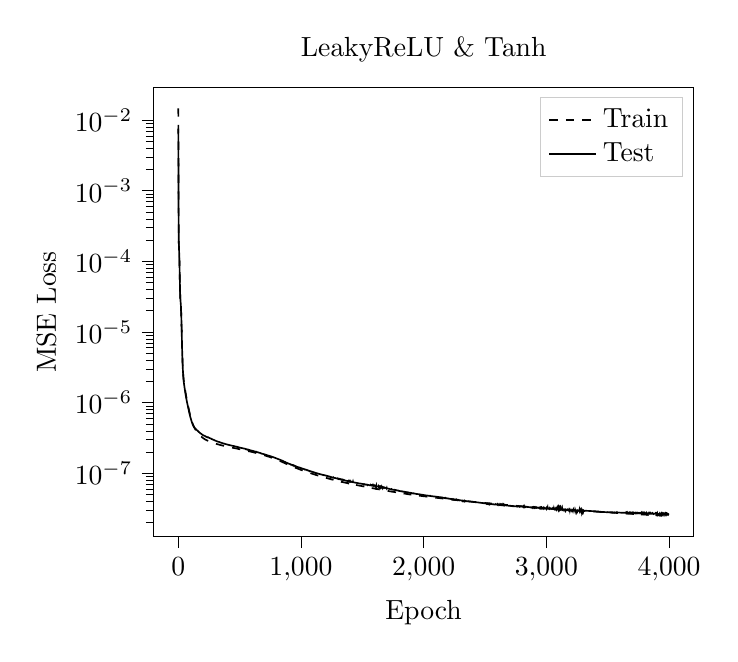
\begin{tikzpicture}

\begin{axis}[
legend cell align={left},
legend style={fill opacity=0.8, draw opacity=1, text opacity=1, draw=white!80!black},
log basis y={10},
tick align=outside,
tick pos=left,
title={LeakyReLU \& Tanh},
x grid style={white!69.0196078431373!black},
xlabel={Epoch},
xmin=-199.95, xmax=4198.95,
xtick style={color=black},
y grid style={white!69.0196078431373!black},
ylabel={MSE Loss},
ymin=1.28652495617467e-08, ymax=0.0285961148315028,
ymode=log,
ytick style={color=black}
]
\addplot [semithick, black, dashed]
table {%
0 0.0147167558874935
1 0.00422479508724064
2 0.00112020292889792
3 0.000344114673440345
4 0.000189754938444821
5 0.000162172813150391
6 0.000146551339385042
7 0.000132341942742642
8 0.000118350356904557
9 0.00010372507233842
10 8.84449195109482e-05
11 7.34534830880875e-05
12 5.99366830574581e-05
13 4.8876996830586e-05
14 4.02497898339789e-05
15 3.408423944893e-05
16 3.01901521470427e-05
17 2.75590198834834e-05
18 2.57170170534664e-05
19 2.43346590959845e-05
20 2.31839580419546e-05
21 2.20652209809487e-05
22 2.07908106704053e-05
23 1.91772862208381e-05
24 1.71094358802293e-05
25 1.49983391247588e-05
26 1.31309963476269e-05
27 1.13659696239665e-05
28 9.74745142775646e-06
29 8.29938522565499e-06
30 7.01414158424996e-06
31 5.95497243716636e-06
32 5.12775509014318e-06
33 4.50885365955855e-06
34 4.02224513118199e-06
35 3.62997250073249e-06
36 3.31752185707046e-06
37 3.0607893052661e-06
38 2.84811762077197e-06
39 2.66868735548087e-06
40 2.51258636171769e-06
41 2.37783719450135e-06
42 2.26240022942648e-06
43 2.16456914614582e-06
44 2.07942771555736e-06
45 2.00241391996769e-06
46 1.93450369954462e-06
47 1.87640388048749e-06
48 1.82416590115508e-06
49 1.77600803158384e-06
50 1.73084908823284e-06
51 1.68828430776102e-06
52 1.64711846895216e-06
53 1.60711305881023e-06
54 1.56834334916311e-06
55 1.53095426259142e-06
56 1.4944722552741e-06
57 1.45879897166878e-06
58 1.42385944167245e-06
59 1.39039401247487e-06
60 1.35824032113874e-06
61 1.3272358849008e-06
62 1.29738894395359e-06
63 1.26867270731168e-06
64 1.2408406620068e-06
65 1.21372717188706e-06
66 1.18741923660082e-06
67 1.16212920454473e-06
68 1.13786890946699e-06
69 1.11432013935087e-06
70 1.09158620887229e-06
71 1.06938895785902e-06
72 1.04795721296114e-06
73 1.02727086746768e-06
74 1.00695854618493e-06
75 9.87439097769993e-07
76 9.68428983043168e-07
77 9.49783932213677e-07
78 9.31873636972114e-07
79 9.14310121714834e-07
80 8.97240733763738e-07
81 8.80552728773409e-07
82 8.64220567052598e-07
83 8.48365317949629e-07
84 8.32332373562394e-07
85 8.16822827857777e-07
86 8.0182209802615e-07
87 7.87099218854337e-07
88 7.73020349626563e-07
89 7.59346863119958e-07
90 7.46014648541404e-07
91 7.33129284895995e-07
92 7.204337242257e-07
93 7.08012346052556e-07
94 6.96058514307651e-07
95 6.84493596338598e-07
96 6.73162203455035e-07
97 6.62246110536557e-07
98 6.5174218859454e-07
99 6.41607516300269e-07
100 6.31769812130756e-07
101 6.22032788143656e-07
102 6.12656925781607e-07
103 6.03730122904267e-07
104 5.94999974538268e-07
105 5.8669275210832e-07
106 5.78534859172919e-07
107 5.70552572213501e-07
108 5.63058854268661e-07
109 5.55469660710628e-07
110 5.48137382722302e-07
111 5.41116412918541e-07
112 5.3417853050064e-07
113 5.27970349523343e-07
114 5.21515760581792e-07
115 5.15363882911402e-07
116 5.09437782596933e-07
117 5.03975951573921e-07
118 4.98499296284649e-07
119 4.93213471543186e-07
120 4.8814046611767e-07
121 4.8300630331255e-07
122 4.78204040121e-07
123 4.7348461674801e-07
124 4.69040818671829e-07
125 4.64815730182977e-07
126 4.60680423827853e-07
127 4.56664749350466e-07
128 4.52802479642855e-07
129 4.49041826627195e-07
130 4.45417362371359e-07
131 4.41978267559762e-07
132 4.38649616214093e-07
133 4.35691757402878e-07
134 4.32299891954813e-07
135 4.29154072037363e-07
136 4.26289210665232e-07
137 4.23350594715544e-07
138 4.20500121535383e-07
139 4.17760403067291e-07
140 4.15125682664552e-07
141 4.12507545789254e-07
142 4.09924902129433e-07
143 4.07458474228406e-07
144 4.05005501463052e-07
145 4.02829853044295e-07
146 4.00427114783497e-07
147 3.98116157185768e-07
148 3.95838813048499e-07
149 3.93631469862044e-07
150 3.91564613238415e-07
151 3.89438078713056e-07
152 3.87381369833406e-07
153 3.85316970422878e-07
154 3.83270407184e-07
155 3.81302476540668e-07
156 3.793187683101e-07
157 3.77405879177672e-07
158 3.75516873560855e-07
159 3.73698540656164e-07
160 3.71824801149501e-07
161 3.70049074177814e-07
162 3.68281156312378e-07
163 3.66514122305262e-07
164 3.64796943898682e-07
165 3.63115861091501e-07
166 3.61438459890451e-07
167 3.59749451376956e-07
168 3.58325647482616e-07
169 3.56678011939948e-07
170 3.5512504922508e-07
171 3.53541436822979e-07
172 3.5198584095042e-07
173 3.50565922175861e-07
174 3.4904586625828e-07
175 3.47580223476029e-07
176 3.46117879487906e-07
177 3.44735465503732e-07
178 3.43156550471235e-07
179 3.41745828350781e-07
180 3.40402201274514e-07
181 3.39082861543716e-07
182 3.37749753995809e-07
183 3.36447743379153e-07
184 3.35189692151516e-07
185 3.33924634418281e-07
186 3.32675331719656e-07
187 3.31490725614003e-07
188 3.30254747154868e-07
189 3.29072307650335e-07
190 3.27903524151907e-07
191 3.26712969567211e-07
192 3.25650873890027e-07
193 3.24679369384739e-07
194 3.23479359352064e-07
195 3.2239850011706e-07
196 3.21350436138346e-07
197 3.20089375506427e-07
198 3.1928418043492e-07
199 3.18225012705398e-07
200 3.1708875033587e-07
201 3.1604049372902e-07
202 3.15025177954453e-07
203 3.14147056030833e-07
204 3.13153630514762e-07
205 3.12303416265536e-07
206 3.11512459560959e-07
207 3.10559388111642e-07
208 3.09709830034421e-07
209 3.08837195518663e-07
210 3.07967781694174e-07
211 3.07173345774459e-07
212 3.06387977303757e-07
213 3.05704276541974e-07
214 3.05012073624766e-07
215 3.04326920442577e-07
216 3.03581191317903e-07
217 3.02872078663086e-07
218 3.02160171514743e-07
219 3.01468360746071e-07
220 3.00779714422106e-07
221 3.00112319266077e-07
222 2.99428165192239e-07
223 2.98766919243576e-07
224 2.98114499798885e-07
225 2.97493264056925e-07
226 2.96865053755369e-07
227 2.96225017891061e-07
228 2.95607063435455e-07
229 2.95054074300083e-07
230 2.94362133615778e-07
231 2.93911949299286e-07
232 2.93350296459494e-07
233 2.9277203962863e-07
234 2.92193898189907e-07
235 2.91625393501249e-07
236 2.91056575775883e-07
237 2.90521314568082e-07
238 2.90002532025824e-07
239 2.89426571697504e-07
240 2.88832796556449e-07
241 2.88437092450522e-07
242 2.87901257479462e-07
243 2.87465177933655e-07
244 2.87022334077847e-07
245 2.86463340103182e-07
246 2.85977110152658e-07
247 2.8552008862448e-07
248 2.85149730146372e-07
249 2.84542418057754e-07
250 2.84174783189428e-07
251 2.83587820405273e-07
252 2.83157723046656e-07
253 2.82677717677871e-07
254 2.82309202674469e-07
255 2.81800196432869e-07
256 2.81433859342428e-07
257 2.80759454781787e-07
258 2.80310815455209e-07
259 2.79839582006502e-07
260 2.79485608601249e-07
261 2.79077382387527e-07
262 2.78622113157212e-07
263 2.78261508313449e-07
264 2.77801248003584e-07
265 2.77371159285167e-07
266 2.76926037386715e-07
267 2.76508251900509e-07
268 2.76159550395505e-07
269 2.75750310947842e-07
270 2.75349369303513e-07
271 2.74866106749982e-07
272 2.74483092084665e-07
273 2.74160867661521e-07
274 2.73795952736577e-07
275 2.73241857961182e-07
276 2.7300955764531e-07
277 2.72534656367895e-07
278 2.72264938502076e-07
279 2.71789457073623e-07
280 2.71330698502936e-07
281 2.70990266756144e-07
282 2.70652392366344e-07
283 2.70274082652122e-07
284 2.69901670087336e-07
285 2.69612391448959e-07
286 2.69216630456981e-07
287 2.68845532097828e-07
288 2.68462628127963e-07
289 2.67953266458676e-07
290 2.67746158179705e-07
291 2.6725683522244e-07
292 2.67001111112108e-07
293 2.66669375847073e-07
294 2.66288802976078e-07
295 2.65969301871394e-07
296 2.65624269857767e-07
297 2.65292488400348e-07
298 2.64968770387952e-07
299 2.64616587664079e-07
300 2.6426598824969e-07
301 2.63968214191834e-07
302 2.63564278093043e-07
303 2.63306389847173e-07
304 2.62909053311944e-07
305 2.6265966658201e-07
306 2.62325956335019e-07
307 2.61988682161984e-07
308 2.61644881341283e-07
309 2.61331634668238e-07
310 2.61042073404383e-07
311 2.60699721444269e-07
312 2.60473399372074e-07
313 2.6017135583345e-07
314 2.59872192494015e-07
315 2.59544071838036e-07
316 2.5921870788892e-07
317 2.5883532907045e-07
318 2.58592301811689e-07
319 2.58254245203204e-07
320 2.57866218625225e-07
321 2.57705161921251e-07
322 2.57353993994514e-07
323 2.57066349661272e-07
324 2.56766999356728e-07
325 2.56460113178036e-07
326 2.56180869946832e-07
327 2.55883794956446e-07
328 2.55620990067484e-07
329 2.55354575458e-07
330 2.55116259729959e-07
331 2.54826920873086e-07
332 2.54552288033949e-07
333 2.54259037966165e-07
334 2.54020088988227e-07
335 2.53747943659732e-07
336 2.53466220335952e-07
337 2.53183346508479e-07
338 2.52860813844791e-07
339 2.52621923969798e-07
340 2.52297060505668e-07
341 2.52019333721876e-07
342 2.51765039429586e-07
343 2.51513713543261e-07
344 2.51235551282036e-07
345 2.50976188937102e-07
346 2.50725112728389e-07
347 2.50445414451406e-07
348 2.50204155356926e-07
349 2.50034150340639e-07
350 2.49739470532973e-07
351 2.49512612462866e-07
352 2.49276659417319e-07
353 2.49011757865958e-07
354 2.48737631004303e-07
355 2.48451116668491e-07
356 2.4825697176567e-07
357 2.47993869585628e-07
358 2.47786029625274e-07
359 2.47529378611944e-07
360 2.47314632318307e-07
361 2.47056039775373e-07
362 2.46790130873364e-07
363 2.46567997486125e-07
364 2.46323033962881e-07
365 2.46107978050247e-07
366 2.45835234508718e-07
367 2.45645431427022e-07
368 2.45389607322011e-07
369 2.45254566003439e-07
370 2.44958750336366e-07
371 2.44772736145649e-07
372 2.44524404863e-07
373 2.44266119949543e-07
374 2.44089073135001e-07
375 2.43777454073779e-07
376 2.43538274567356e-07
377 2.43289414470382e-07
378 2.43056023222721e-07
379 2.42854683087046e-07
380 2.42641632901552e-07
381 2.42429219355245e-07
382 2.42211716916074e-07
383 2.41979478595056e-07
384 2.41790681229759e-07
385 2.41554029116742e-07
386 2.41347478571186e-07
387 2.41138141426234e-07
388 2.40926381991358e-07
389 2.40712194212733e-07
390 2.40508433066111e-07
391 2.40213856443461e-07
392 2.4000315536199e-07
393 2.39796585482566e-07
394 2.3964756219641e-07
395 2.39413144029754e-07
396 2.39213759805068e-07
397 2.39108626168161e-07
398 2.38828656740964e-07
399 2.38633542345212e-07
400 2.3843064510487e-07
401 2.38233129458365e-07
402 2.37990722567361e-07
403 2.37813346082305e-07
404 2.37602338437171e-07
405 2.37422929181719e-07
406 2.37263455424852e-07
407 2.37050656913596e-07
408 2.36847532327999e-07
409 2.36642238036211e-07
410 2.364443584284e-07
411 2.36212683653037e-07
412 2.35975246070552e-07
413 2.35821508574929e-07
414 2.35624742032314e-07
415 2.35403222745845e-07
416 2.35169045708972e-07
417 2.34992661688693e-07
418 2.34793192817051e-07
419 2.34585262987252e-07
420 2.34415336599625e-07
421 2.34222672524709e-07
422 2.33997412728115e-07
423 2.33857629716283e-07
424 2.33674164270781e-07
425 2.33461944802116e-07
426 2.33231948534751e-07
427 2.33070363847787e-07
428 2.32853431704427e-07
429 2.3266770248398e-07
430 2.32476125070491e-07
431 2.32283850046144e-07
432 2.32086789537789e-07
433 2.31937585361663e-07
434 2.31743046676058e-07
435 2.31552100686372e-07
436 2.31361373934647e-07
437 2.31170123797142e-07
438 2.30984196811335e-07
439 2.30793798124296e-07
440 2.3057733974241e-07
441 2.30424656592731e-07
442 2.30198470433152e-07
443 2.30040015658517e-07
444 2.29852045443124e-07
445 2.29665212074792e-07
446 2.29487747475332e-07
447 2.29264898976567e-07
448 2.29088643955322e-07
449 2.289107464577e-07
450 2.2872222154291e-07
451 2.28534441717443e-07
452 2.28346455422468e-07
453 2.28135142606334e-07
454 2.27954515459317e-07
455 2.27769156673219e-07
456 2.27586670888513e-07
457 2.2740435630908e-07
458 2.27215854557983e-07
459 2.27032890073531e-07
460 2.26844838984164e-07
461 2.26653140472877e-07
462 2.26478486759163e-07
463 2.26292875062484e-07
464 2.26084874157095e-07
465 2.2590925732402e-07
466 2.2572789907116e-07
467 2.25542848156124e-07
468 2.25358282015975e-07
469 2.25182395894308e-07
470 2.24996762824503e-07
471 2.24819421212885e-07
472 2.24611957996501e-07
473 2.24466087004771e-07
474 2.24269675690891e-07
475 2.24083162514432e-07
476 2.23859973623064e-07
477 2.23670406448662e-07
478 2.23497105722004e-07
479 2.23308886667439e-07
480 2.23121406335736e-07
481 2.22916722904642e-07
482 2.22842280734881e-07
483 2.22473976393189e-07
484 2.22453026935909e-07
485 2.22074921133242e-07
486 2.21927564737712e-07
487 2.21887577218638e-07
488 2.21461834648551e-07
489 2.21329398421233e-07
490 2.21166270051754e-07
491 2.20986845278048e-07
492 2.20798476625816e-07
493 2.20619727471671e-07
494 2.20438873313356e-07
495 2.20253071745447e-07
496 2.20089636925991e-07
497 2.1990685036144e-07
498 2.19724008424294e-07
499 2.19543226172902e-07
500 2.19354352751111e-07
501 2.19168181587293e-07
502 2.18980888398335e-07
503 2.1882522270289e-07
504 2.18640398450987e-07
505 2.18440091764194e-07
506 2.18265065079493e-07
507 2.18089171504232e-07
508 2.17896692689123e-07
509 2.17720229265694e-07
510 2.17535416084047e-07
511 2.17356315772577e-07
512 2.17186338744568e-07
513 2.1699332680214e-07
514 2.16826531321601e-07
515 2.16647501382283e-07
516 2.16463818759394e-07
517 2.1628365471571e-07
518 2.16089452145241e-07
519 2.15913011842872e-07
520 2.15749887168215e-07
521 2.15557008026224e-07
522 2.15378701916791e-07
523 2.15191717984453e-07
524 2.1509282248644e-07
525 2.14915981821662e-07
526 2.14728546453102e-07
527 2.14509130266549e-07
528 2.14316656489189e-07
529 2.14193874057855e-07
530 2.14001319669421e-07
531 2.13823200759578e-07
532 2.13628148898692e-07
533 2.1346094583663e-07
534 2.13267892512192e-07
535 2.13071844967772e-07
536 2.12884007147807e-07
537 2.12691715617552e-07
538 2.12480586952779e-07
539 2.12326406561658e-07
540 2.12136915216377e-07
541 2.11943900133349e-07
542 2.11753016976957e-07
543 2.11540812792066e-07
544 2.11372566660373e-07
545 2.11170818772644e-07
546 2.10922583555373e-07
547 2.10709240889173e-07
548 2.10775911433814e-07
549 2.10267557449129e-07
550 2.10359211671118e-07
551 2.09904146167617e-07
552 2.09913477725365e-07
553 2.09501424123459e-07
554 2.09625159250493e-07
555 2.09126980131202e-07
556 2.09249012847579e-07
557 2.08998007352079e-07
558 2.08536155923866e-07
559 2.08690602818251e-07
560 2.08191836911453e-07
561 2.08264158281679e-07
562 2.07883312761226e-07
563 2.07921254833821e-07
564 2.07418759934797e-07
565 2.0743094999176e-07
566 2.07303002909498e-07
567 2.06845264763444e-07
568 2.06992054103239e-07
569 2.06472261595536e-07
570 2.0639721431337e-07
571 2.06441899145204e-07
572 2.05879496732564e-07
573 2.06051998794976e-07
574 2.05496511902936e-07
575 2.0551717245354e-07
576 2.0532205400059e-07
577 2.0513076895412e-07
578 2.04941408860293e-07
579 2.04753449700945e-07
580 2.0451803786159e-07
581 2.04499404034664e-07
582 2.0404194936674e-07
583 2.03942051690831e-07
584 2.03688036748417e-07
585 2.03549430437988e-07
586 2.03323575235004e-07
587 2.03119876616142e-07
588 2.0295757144595e-07
589 2.02731326126582e-07
590 2.0257369340726e-07
591 2.02368503160244e-07
592 2.02197047563857e-07
593 2.02013388950206e-07
594 2.01766462517128e-07
595 2.01604090058538e-07
596 2.01441364232835e-07
597 2.01236583805553e-07
598 2.01023921313492e-07
599 2.00841937321172e-07
600 2.00641080887465e-07
601 2.00459920911555e-07
602 2.00254661208987e-07
603 2.00086132714716e-07
604 1.99884809660489e-07
605 1.99703399935913e-07
606 1.99505433087666e-07
607 1.99328779494579e-07
608 1.9913990877285e-07
609 1.98964528692613e-07
610 1.98792843583817e-07
611 1.98516759930101e-07
612 1.98361773897204e-07
613 1.98246224172749e-07
614 1.97864427093464e-07
615 1.97706827684385e-07
616 1.97465364514926e-07
617 1.9733804701616e-07
618 1.96922791261045e-07
619 1.96741092551633e-07
620 1.96560413641578e-07
621 1.96323017625843e-07
622 1.96165970592688e-07
623 1.95932488843198e-07
624 1.95768028881105e-07
625 1.95567801796415e-07
626 1.95336412311065e-07
627 1.95179220433772e-07
628 1.94979452849964e-07
629 1.94775609621445e-07
630 1.94670293943489e-07
631 1.94429682771613e-07
632 1.9418770021673e-07
633 1.93788950262785e-07
634 1.93819842536413e-07
635 1.93378188832583e-07
636 1.93411281124156e-07
637 1.93151938809422e-07
638 1.92752860819212e-07
639 1.92741796858797e-07
640 1.92343431002939e-07
641 1.9216255318355e-07
642 1.91978727919206e-07
643 1.91782636456139e-07
644 1.91794384178934e-07
645 1.91546348553118e-07
646 1.9116149540821e-07
647 1.90949372573357e-07
648 1.90821341675473e-07
649 1.90595229426549e-07
650 1.90429980428064e-07
651 1.90218370811124e-07
652 1.90026906679464e-07
653 1.89813052621446e-07
654 1.89606661813002e-07
655 1.89530327546095e-07
656 1.89314011059594e-07
657 1.88951788842928e-07
658 1.88744615144287e-07
659 1.88540474972854e-07
660 1.88363825103011e-07
661 1.88142638720024e-07
662 1.87933737755941e-07
663 1.87730878387526e-07
664 1.8772520002841e-07
665 1.87284249527409e-07
666 1.87286926760066e-07
667 1.86856799061275e-07
668 1.86839971519248e-07
669 1.86423184821649e-07
670 1.8641698684263e-07
671 1.86223110155481e-07
672 1.85972596902673e-07
673 1.85746885527749e-07
674 1.85528371368093e-07
675 1.85161767781494e-07
676 1.85198464613734e-07
677 1.85011211520703e-07
678 1.84764612654931e-07
679 1.84580274805057e-07
680 1.84336935646456e-07
681 1.8414141057832e-07
682 1.83919891689754e-07
683 1.83703114032596e-07
684 1.83409840218474e-07
685 1.83234989201253e-07
686 1.83098119016734e-07
687 1.82743054963908e-07
688 1.82657332807423e-07
689 1.82302819958124e-07
690 1.82121882247088e-07
691 1.81915501649144e-07
692 1.81705160265722e-07
693 1.81491261621147e-07
694 1.81273101233614e-07
695 1.81056364169763e-07
696 1.80900828013364e-07
697 1.80674443875262e-07
698 1.804431686665e-07
699 1.80222724559087e-07
700 1.79991534189128e-07
701 1.7977483792464e-07
702 1.79552062789412e-07
703 1.79341676194156e-07
704 1.79116268490986e-07
705 1.78897217764984e-07
706 1.78672040583194e-07
707 1.7845544022066e-07
708 1.78274484682106e-07
709 1.78050520581508e-07
710 1.7783338613242e-07
711 1.77603523908942e-07
712 1.77379757964502e-07
713 1.77166644675708e-07
714 1.76958691859852e-07
715 1.76734787565636e-07
716 1.76584686002457e-07
717 1.76343372984888e-07
718 1.76128108975604e-07
719 1.75897885213772e-07
720 1.75672592654053e-07
721 1.75447660360817e-07
722 1.75226035857179e-07
723 1.75003551206032e-07
724 1.74804935745954e-07
725 1.74598562963979e-07
726 1.74375872227017e-07
727 1.74152322721e-07
728 1.7382954645484e-07
729 1.73619787652513e-07
730 1.73425334530464e-07
731 1.7321217111288e-07
732 1.73060100379985e-07
733 1.72832961482072e-07
734 1.72613131297794e-07
735 1.72413816329708e-07
736 1.72160513180586e-07
737 1.71926174509451e-07
738 1.71669755282267e-07
739 1.7144469420316e-07
740 1.71207248776284e-07
741 1.7098506228308e-07
742 1.70759329854775e-07
743 1.70538389163255e-07
744 1.70313998907545e-07
745 1.70091730630872e-07
746 1.69852064665577e-07
747 1.69626526059119e-07
748 1.69402781779127e-07
749 1.69132127716409e-07
750 1.68980241525674e-07
751 1.68661541664505e-07
752 1.68422387638145e-07
753 1.68154323553438e-07
754 1.67861468440833e-07
755 1.67617971307266e-07
756 1.67375250256896e-07
757 1.67143337051812e-07
758 1.66881991432888e-07
759 1.66675624022616e-07
760 1.66422565094138e-07
761 1.66193717767271e-07
762 1.65948354613477e-07
763 1.65717337154092e-07
764 1.65465913312346e-07
765 1.6523477719943e-07
766 1.64991181918595e-07
767 1.64759113445712e-07
768 1.64514003316185e-07
769 1.64293280029426e-07
770 1.64031092438677e-07
771 1.63807684394612e-07
772 1.63561527344314e-07
773 1.63338111143219e-07
774 1.63088297604475e-07
775 1.62864505320215e-07
776 1.62628236452633e-07
777 1.62385142949972e-07
778 1.62129393167731e-07
779 1.61899282687727e-07
780 1.61650713181416e-07
781 1.6141828078986e-07
782 1.6121273756653e-07
783 1.60986360342008e-07
784 1.60738231961943e-07
785 1.60479761085242e-07
786 1.60237907216754e-07
787 1.59983428901e-07
788 1.597366711934e-07
789 1.59454377076429e-07
790 1.59208735553307e-07
791 1.58949413588516e-07
792 1.58692530362714e-07
793 1.58436309121157e-07
794 1.5816905449384e-07
795 1.57882679339139e-07
796 1.57585047602993e-07
797 1.57311406383087e-07
798 1.57027265480281e-07
799 1.56765319111685e-07
800 1.56496265454109e-07
801 1.56238000172948e-07
802 1.55985959587213e-07
803 1.55719861979264e-07
804 1.55464578689646e-07
805 1.5521024232612e-07
806 1.54948408244593e-07
807 1.54719261928449e-07
808 1.54447245577671e-07
809 1.54192335998005e-07
810 1.53954697410086e-07
811 1.53698665755542e-07
812 1.53444322862129e-07
813 1.53189335598825e-07
814 1.5296307420698e-07
815 1.52703641226992e-07
816 1.52447027396363e-07
817 1.52212526352002e-07
818 1.51996518304998e-07
819 1.51729954083635e-07
820 1.51471893957478e-07
821 1.51220606632307e-07
822 1.50959670229156e-07
823 1.50708962692647e-07
824 1.504469360043e-07
825 1.50185154481619e-07
826 1.49956196111134e-07
827 1.49683904787423e-07
828 1.49426933035102e-07
829 1.49200826534468e-07
830 1.4894755504713e-07
831 1.48687534576197e-07
832 1.48438944798102e-07
833 1.48174899528897e-07
834 1.47928022713018e-07
835 1.47746720237762e-07
836 1.47469594566019e-07
837 1.47227389931004e-07
838 1.46937056101137e-07
839 1.4663462562936e-07
840 1.46411530401735e-07
841 1.46151256004146e-07
842 1.4589036143775e-07
843 1.45624674729561e-07
844 1.45365836537792e-07
845 1.45095396746342e-07
846 1.44834831793617e-07
847 1.44576164316845e-07
848 1.44314648515831e-07
849 1.44067540055914e-07
850 1.43770926534614e-07
851 1.43536822335477e-07
852 1.43280838123871e-07
853 1.43015342686681e-07
854 1.42736688658829e-07
855 1.42426279346353e-07
856 1.42210422652056e-07
857 1.41971944948693e-07
858 1.41683119693425e-07
859 1.41424822899694e-07
860 1.41189233872296e-07
861 1.40932418538853e-07
862 1.40685958179176e-07
863 1.40444483903934e-07
864 1.40194336815114e-07
865 1.39915691292458e-07
866 1.39712072993348e-07
867 1.39439254496665e-07
868 1.39181732279781e-07
869 1.38928897641222e-07
870 1.38659657174855e-07
871 1.38382007278892e-07
872 1.38154317113504e-07
873 1.37896821655659e-07
874 1.37652846909475e-07
875 1.37387850330128e-07
876 1.37122912185816e-07
877 1.36958976639789e-07
878 1.36698286723913e-07
879 1.36436031425546e-07
880 1.36173517390148e-07
881 1.35937297422117e-07
882 1.3568027885924e-07
883 1.35419160045558e-07
884 1.35210795320972e-07
885 1.34940211779622e-07
886 1.34729177602821e-07
887 1.34477849549342e-07
888 1.34246570013374e-07
889 1.34014088537526e-07
890 1.33775667116254e-07
891 1.33507818894429e-07
892 1.33355113838718e-07
893 1.33092440819382e-07
894 1.32816020190774e-07
895 1.32586035178406e-07
896 1.3236788663562e-07
897 1.32103730607014e-07
898 1.31877103889622e-07
899 1.31655306965683e-07
900 1.31399273300303e-07
901 1.31187993872572e-07
902 1.30964021600732e-07
903 1.30730834960957e-07
904 1.30479387856042e-07
905 1.30251059097475e-07
906 1.30019203204768e-07
907 1.29781760385583e-07
908 1.29546398291325e-07
909 1.29307371985021e-07
910 1.29084291366155e-07
911 1.28849908819006e-07
912 1.28628538817566e-07
913 1.28427776004969e-07
914 1.28189834683212e-07
915 1.27991950641615e-07
916 1.27691470989788e-07
917 1.27501933441465e-07
918 1.27336225041574e-07
919 1.27021330165178e-07
920 1.26880013286978e-07
921 1.26700365694177e-07
922 1.26405575343824e-07
923 1.26257105605987e-07
924 1.25972710918631e-07
925 1.25786522051641e-07
926 1.2556942496289e-07
927 1.25317999483343e-07
928 1.25138892112631e-07
929 1.24960381679529e-07
930 1.24746011664456e-07
931 1.24503905503559e-07
932 1.2430114939832e-07
933 1.24119226839525e-07
934 1.23892343637522e-07
935 1.2366138645703e-07
936 1.23528668677153e-07
937 1.23287912206393e-07
938 1.23100251894215e-07
939 1.22913126332946e-07
940 1.22722796422892e-07
941 1.22485553870177e-07
942 1.22238755402293e-07
943 1.22106174902825e-07
944 1.21919439553864e-07
945 1.2174004823251e-07
946 1.21530621246535e-07
947 1.21336180352927e-07
948 1.21133792138295e-07
949 1.20939680659404e-07
950 1.20720247075212e-07
951 1.20546334574811e-07
952 1.20322355666502e-07
953 1.20217128969813e-07
954 1.20011707402057e-07
955 1.19810914469554e-07
956 1.19595556309804e-07
957 1.19444322447038e-07
958 1.19227567786595e-07
959 1.19024687801783e-07
960 1.18887678429047e-07
961 1.18671289598637e-07
962 1.18430393072799e-07
963 1.18325145788134e-07
964 1.1812696747171e-07
965 1.17946854743423e-07
966 1.1776211837855e-07
967 1.17576934218988e-07
968 1.1740373333069e-07
969 1.17222978090581e-07
970 1.17059085983584e-07
971 1.1685083301316e-07
972 1.16617252317042e-07
973 1.1650785584294e-07
974 1.16313816214131e-07
975 1.16113465260526e-07
976 1.15937665032817e-07
977 1.15776352544117e-07
978 1.15601611309302e-07
979 1.15419883183421e-07
980 1.15197841473957e-07
981 1.15045113130208e-07
982 1.14801086215977e-07
983 1.14742911872412e-07
984 1.14547467020998e-07
985 1.14369988924778e-07
986 1.14132197644778e-07
987 1.13966712721236e-07
988 1.13832317019558e-07
989 1.13675502177557e-07
990 1.13499152249119e-07
991 1.13304771677036e-07
992 1.13130158183594e-07
993 1.12883420236187e-07
994 1.12796536104298e-07
995 1.12606875294574e-07
996 1.12428153837385e-07
997 1.12270813591664e-07
998 1.12106477963891e-07
999 1.11935982751277e-07
1000 1.11775184894469e-07
1001 1.11619902799731e-07
1002 1.11424209215727e-07
1003 1.11334109909933e-07
1004 1.11145634338783e-07
1005 1.10971861754905e-07
1006 1.10804318556035e-07
1007 1.10636118147767e-07
1008 1.10479483833359e-07
1009 1.1032438599301e-07
1010 1.10178989352505e-07
1011 1.10012197090725e-07
1012 1.09794785910111e-07
1013 1.09715186578541e-07
1014 1.09533097781167e-07
1015 1.09345536664307e-07
1016 1.09196999392935e-07
1017 1.09046659243717e-07
1018 1.08901574389364e-07
1019 1.08724679364514e-07
1020 1.08579653087304e-07
1021 1.08414589124806e-07
1022 1.08282940885829e-07
1023 1.08152952304152e-07
1024 1.07973693847185e-07
1025 1.07817007773292e-07
1026 1.07631510633865e-07
1027 1.07514907135453e-07
1028 1.07364885227668e-07
1029 1.07203319526405e-07
1030 1.07045956976748e-07
1031 1.0689825924004e-07
1032 1.06637067755599e-07
1033 1.06620171120397e-07
1034 1.06468587901531e-07
1035 1.06327487575442e-07
1036 1.06176609381947e-07
1037 1.06048515608137e-07
1038 1.05891789491608e-07
1039 1.05753535311948e-07
1040 1.05604855779262e-07
1041 1.05488431497491e-07
1042 1.05340681177069e-07
1043 1.052005269635e-07
1044 1.04994613213449e-07
1045 1.04841989045923e-07
1046 1.04693688069091e-07
1047 1.04549295802059e-07
1048 1.04342896321441e-07
1049 1.04315552942325e-07
1050 1.04177075115786e-07
1051 1.03936537382054e-07
1052 1.03874550795524e-07
1053 1.03738832159195e-07
1054 1.03571307306538e-07
1055 1.03438900612929e-07
1056 1.03357138787175e-07
1057 1.0315987907461e-07
1058 1.03049108556519e-07
1059 1.02890002320777e-07
1060 1.02720108355214e-07
1061 1.02683071787624e-07
1062 1.02532210775053e-07
1063 1.02359288025156e-07
1064 1.0222688218775e-07
1065 1.02098929829708e-07
1066 1.01953066529603e-07
1067 1.01850517182811e-07
1068 1.01712086522099e-07
1069 1.01576102981227e-07
1070 1.01428539995396e-07
1071 1.01202304705339e-07
1072 1.01209320458651e-07
1073 1.01055069666955e-07
1074 1.00916019395214e-07
1075 1.0076222892863e-07
1076 1.00631043213895e-07
1077 1.00532826014188e-07
1078 1.00360497253149e-07
1079 1.00234356416706e-07
1080 1.00106765209773e-07
1081 9.99802213961232e-08
1082 9.98532394511642e-08
1083 9.97311517991761e-08
1084 9.95188706660599e-08
1085 9.95432671686558e-08
1086 9.93666342736788e-08
1087 9.92305960316742e-08
1088 9.90880039459796e-08
1089 9.89632881847058e-08
1090 9.8835123729657e-08
1091 9.87113516828231e-08
1092 9.85671639952557e-08
1093 9.84456003862988e-08
1094 9.83183581340086e-08
1095 9.81939523541087e-08
1096 9.8001847607776e-08
1097 9.79699430878611e-08
1098 9.78207422619448e-08
1099 9.76892382453798e-08
1100 9.75573714434574e-08
1101 9.7436195570566e-08
1102 9.73081750537119e-08
1103 9.71845393742399e-08
1104 9.69889700250803e-08
1105 9.68960275820052e-08
1106 9.68605309026316e-08
1107 9.67106285933994e-08
1108 9.65754299606658e-08
1109 9.64576967490416e-08
1110 9.63283372144019e-08
1111 9.6153483880812e-08
1112 9.60811021215591e-08
1113 9.59328996756881e-08
1114 9.58100525139116e-08
1115 9.57365740994476e-08
1116 9.55992669737782e-08
1117 9.5426011849753e-08
1118 9.53521050739425e-08
1119 9.51087149552166e-08
1120 9.51546127048175e-08
1121 9.49852496034964e-08
1122 9.48076223714622e-08
1123 9.47484521525155e-08
1124 9.4635791192843e-08
1125 9.43977622576142e-08
1126 9.43311578716077e-08
1127 9.41965007790202e-08
1128 9.42251313240661e-08
1129 9.40887221183573e-08
1130 9.39137298736625e-08
1131 9.38030485144736e-08
1132 9.36790117940234e-08
1133 9.36066499725996e-08
1134 9.34274177382122e-08
1135 9.33086589611776e-08
1136 9.32034401373016e-08
1137 9.29838304166708e-08
1138 9.29965697018531e-08
1139 9.27530144387845e-08
1140 9.28000088435965e-08
1141 9.26899408071336e-08
1142 9.24673126974085e-08
1143 9.23295716219741e-08
1144 9.24684631193884e-08
1145 9.22265955978219e-08
1146 9.20729742901472e-08
1147 9.19632463620701e-08
1148 9.18536782208435e-08
1149 9.17687318739979e-08
1150 9.16661311975986e-08
1151 9.15448064411351e-08
1152 9.14362613144704e-08
1153 9.13262002804061e-08
1154 9.10897944166322e-08
1155 9.12180108763039e-08
1156 9.09886377620239e-08
1157 9.09010083987027e-08
1158 9.08980600549114e-08
1159 9.06698444715914e-08
1160 9.06123341906095e-08
1161 9.04766778759836e-08
1162 9.03810152692586e-08
1163 9.03772236320322e-08
1164 9.01413191947142e-08
1165 9.00481007235499e-08
1166 8.99135863505762e-08
1167 9.00328111086424e-08
1168 8.97141874460772e-08
1169 8.97355893414442e-08
1170 8.95368867581681e-08
1171 8.95405423015916e-08
1172 8.94344267656777e-08
1173 8.92226522068995e-08
1174 8.92123865625649e-08
1175 8.90316612718323e-08
1176 8.90420845998108e-08
1177 8.88799057747747e-08
1178 8.88133439786998e-08
1179 8.85857197481244e-08
1180 8.87505559710178e-08
1181 8.84196974411111e-08
1182 8.82689840580042e-08
1183 8.83171059022914e-08
1184 8.83854004989359e-08
1185 8.80816308992394e-08
1186 8.80047668623263e-08
1187 8.77441357012287e-08
1188 8.79640751030308e-08
1189 8.77180462559579e-08
1190 8.7599863196175e-08
1191 8.74963723482836e-08
1192 8.73838534296567e-08
1193 8.72792024786406e-08
1194 8.71605033587741e-08
1195 8.70777559889291e-08
1196 8.69709926440976e-08
1197 8.67257896253193e-08
1198 8.67221731297718e-08
1199 8.67449776755791e-08
1200 8.66083934916162e-08
1201 8.65008198509543e-08
1202 8.63824901209398e-08
1203 8.62881886440903e-08
1204 8.6182928530576e-08
1205 8.60825287638534e-08
1206 8.60784291596417e-08
1207 8.58791283953053e-08
1208 8.57924304398239e-08
1209 8.55378336481749e-08
1210 8.55663802319384e-08
1211 8.56935107158563e-08
1212 8.54270831069925e-08
1213 8.54136989190124e-08
1214 8.51504979451079e-08
1215 8.52249365088653e-08
1216 8.50929214841756e-08
1217 8.49829644558042e-08
1218 8.48894925695731e-08
1219 8.49022571891567e-08
1220 8.45773056319388e-08
1221 8.45171920254018e-08
1222 8.4644523379751e-08
1223 8.44960545833828e-08
1224 8.43562040877544e-08
1225 8.43524073914637e-08
1226 8.42076120370905e-08
1227 8.40824029246789e-08
1228 8.40686841705462e-08
1229 8.38027294243204e-08
1230 8.38756206036351e-08
1231 8.37313208670309e-08
1232 8.37996433737942e-08
1233 8.35421889995303e-08
1234 8.35297179229144e-08
1235 8.33217964739674e-08
1236 8.32042975495995e-08
1237 8.32144987121808e-08
1238 8.31275680042154e-08
1239 8.30780388518804e-08
1240 8.28455743508982e-08
1241 8.26311044406225e-08
1242 8.28110817465699e-08
1243 8.25285896368655e-08
1244 8.26351364935363e-08
1245 8.26327644070091e-08
1246 8.25268334700979e-08
1247 8.2284106081687e-08
1248 8.21856459829462e-08
1249 8.22410062006895e-08
1250 8.18561030619947e-08
1251 8.18822995114488e-08
1252 8.20980892832779e-08
1253 8.17999369111533e-08
1254 8.18274437115463e-08
1255 8.14338774439705e-08
1256 8.14501619821328e-08
1257 8.13915892443617e-08
1258 8.16146207576196e-08
1259 8.13947702447138e-08
1260 8.14680680640834e-08
1261 8.12170073594132e-08
1262 8.12205323477144e-08
1263 8.09467807449948e-08
1264 8.09291576757687e-08
1265 8.08210186100666e-08
1266 8.08754014727242e-08
1267 8.05248546988935e-08
1268 8.06227642335955e-08
1269 8.07637859061572e-08
1270 8.0488412368851e-08
1271 8.0472480675553e-08
1272 8.0312093622581e-08
1273 8.01834619643671e-08
1274 8.01239210481697e-08
1275 7.99325583145105e-08
1276 7.98803357469069e-08
1277 8.00352309475727e-08
1278 7.98712157852322e-08
1279 7.97606326052858e-08
1280 7.96094512445222e-08
1281 7.95350578322029e-08
1282 7.93902460323181e-08
1283 7.94013396223647e-08
1284 7.94029619690662e-08
1285 7.92219978045239e-08
1286 7.92102306554909e-08
1287 7.90460648083524e-08
1288 7.90456339707646e-08
1289 7.88878918704938e-08
1290 7.86650440822712e-08
1291 7.87703592628475e-08
1292 7.87660891035102e-08
1293 7.86073303871149e-08
1294 7.85152663560496e-08
1295 7.83654700988734e-08
1296 7.810588538959e-08
1297 7.83936111794503e-08
1298 7.82783793091824e-08
1299 7.80195213252455e-08
1300 7.79630812388632e-08
1301 7.81040429238544e-08
1302 7.79871498544082e-08
1303 7.7885714201642e-08
1304 7.77099070177201e-08
1305 7.76176916801319e-08
1306 7.76773959572097e-08
1307 7.75960576966384e-08
1308 7.74857856207234e-08
1309 7.73203322204097e-08
1310 7.71579984686355e-08
1311 7.72818189709312e-08
1312 7.72138671720768e-08
1313 7.71078822197069e-08
1314 7.70102493490299e-08
1315 7.68608058550058e-08
1316 7.67011075879509e-08
1317 7.68048537977961e-08
1318 7.67450558001315e-08
1319 7.66509278946614e-08
1320 7.6562426812643e-08
1321 7.64752398900725e-08
1322 7.63389064957209e-08
1323 7.61783190910137e-08
1324 7.63143536666178e-08
1325 7.62435481966861e-08
1326 7.6109585496198e-08
1327 7.60519296214568e-08
1328 7.59750633818612e-08
1329 7.58785536554285e-08
1330 7.5771458988072e-08
1331 7.56189558046572e-08
1332 7.57408587439556e-08
1333 7.567879941206e-08
1334 7.5562105887883e-08
1335 7.55043106650533e-08
1336 7.53389284788852e-08
1337 7.52238568644259e-08
1338 7.5323299622454e-08
1339 7.52537492374472e-08
1340 7.51991587790712e-08
1341 7.51069958013773e-08
1342 7.50239110871576e-08
1343 7.49522658232138e-08
1344 7.48127398679799e-08
1345 7.46620432501288e-08
1346 7.48086655377733e-08
1347 7.4738872729796e-08
1348 7.46397968427459e-08
1349 7.4551285344171e-08
1350 7.44863173345323e-08
1351 7.44158996113242e-08
1352 7.42824491553051e-08
1353 7.41238045449677e-08
1354 7.41111035225117e-08
1355 7.40641070464676e-08
1356 7.40045176499393e-08
1357 7.39508383347243e-08
1358 7.39037687047528e-08
1359 7.38463827580915e-08
1360 7.37782016244637e-08
1361 7.37182463659281e-08
1362 7.36672474594968e-08
1363 7.35925647710189e-08
1364 7.3529023786989e-08
1365 7.34672471267572e-08
1366 7.33989200369933e-08
1367 7.33393467449162e-08
1368 7.32632496358576e-08
1369 7.32211657989978e-08
1370 7.31125196580251e-08
1371 7.31050112463549e-08
1372 7.29886364716492e-08
1373 7.29476300342924e-08
1374 7.28780813759045e-08
1375 7.27930700890056e-08
1376 7.27118430035034e-08
1377 7.26486597351084e-08
1378 7.26059206535012e-08
1379 7.25501752434354e-08
1380 7.24998741752358e-08
1381 7.27625557139788e-08
1382 7.25737763929146e-08
1383 7.2731951306082e-08
1384 7.25556730998278e-08
1385 7.24230852426899e-08
1386 7.23103557653815e-08
1387 7.22384621774097e-08
1388 7.19100039603404e-08
1389 7.20899284445409e-08
1390 7.1703876894702e-08
1391 7.20312818671687e-08
1392 7.17245782446696e-08
1393 7.15467789760282e-08
1394 7.19751574962402e-08
1395 7.17944129462467e-08
1396 7.14462673769844e-08
1397 7.13811031900491e-08
1398 7.13009372219631e-08
1399 7.12841869194847e-08
1400 7.13730504671162e-08
1401 7.12210317672657e-08
1402 7.15236239088313e-08
1403 7.14062929354498e-08
1404 7.12587243327789e-08
1405 7.11710081873207e-08
1406 7.10833947401568e-08
1407 7.10124912153276e-08
1408 7.09239766543135e-08
1409 7.09135147758389e-08
1410 7.05575748938259e-08
1411 7.05776387164292e-08
1412 7.0538693101696e-08
1413 7.04820574739529e-08
1414 7.03366398262517e-08
1415 7.03419983132392e-08
1416 7.02653603426029e-08
1417 7.02439167525881e-08
1418 7.01753560683471e-08
1419 7.0116381319707e-08
1420 7.00991330546685e-08
1421 7.00142620218003e-08
1422 6.99670490291737e-08
1423 6.98961916363316e-08
1424 7.02776046459519e-08
1425 6.97408604963812e-08
1426 6.96264619293174e-08
1427 6.96493507064133e-08
1428 6.96453624797755e-08
1429 6.9592399256635e-08
1430 6.94273235311016e-08
1431 6.94291015150839e-08
1432 6.9362168044762e-08
1433 6.92699000488517e-08
1434 6.92611739800952e-08
1435 6.91862529329512e-08
1436 6.91504793586262e-08
1437 6.9080841637259e-08
1438 6.90261722340324e-08
1439 6.89444437931286e-08
1440 6.89110837797102e-08
1441 6.8826579592951e-08
1442 6.88160369399782e-08
1443 6.87323318722122e-08
1444 6.86894033101737e-08
1445 6.86117650161577e-08
1446 6.8594669759392e-08
1447 6.84925371992051e-08
1448 6.84693926515934e-08
1449 6.8384730411708e-08
1450 6.83545271407127e-08
1451 6.82723717559952e-08
1452 6.82447976210199e-08
1453 6.81450138202422e-08
1454 6.8127716005506e-08
1455 6.80505443142465e-08
1456 6.80313249930009e-08
1457 6.7940998221161e-08
1458 6.79047805007826e-08
1459 6.78244381475679e-08
1460 6.78095768940068e-08
1461 6.77314916792682e-08
1462 6.76890676380992e-08
1463 6.76215440975625e-08
1464 6.75896843098656e-08
1465 6.75036987978217e-08
1466 6.74560715303585e-08
1467 6.7436916804553e-08
1468 6.73604038361475e-08
1469 6.73058214175626e-08
1470 6.72726544870272e-08
1471 6.72089431610345e-08
1472 6.71315502778214e-08
1473 6.71195438641803e-08
1474 6.70629360755015e-08
1475 6.70026612752395e-08
1476 6.69748772921253e-08
1477 6.6908599993809e-08
1478 6.68566325394693e-08
1479 6.67549428889913e-08
1480 6.67159215126389e-08
1481 6.66729288383294e-08
1482 6.663703261367e-08
1483 6.65598175011439e-08
1484 6.64971356414412e-08
1485 6.64941096424343e-08
1486 6.64398592036264e-08
1487 6.63679180057386e-08
1488 6.6328782452274e-08
1489 6.63028838729929e-08
1490 6.6236923263574e-08
1491 6.61852860446288e-08
1492 6.61495542679802e-08
1493 6.60819992361894e-08
1494 6.60174491429189e-08
1495 6.59773442883704e-08
1496 6.59575181956029e-08
1497 6.58913086226676e-08
1498 6.58353580966775e-08
1499 6.57926443388135e-08
1500 6.57452803594083e-08
1501 6.5702437559878e-08
1502 6.56488046928416e-08
1503 6.56010516912886e-08
1504 6.55696651605808e-08
1505 6.55111482039672e-08
1506 6.54606833165872e-08
1507 6.54224100671286e-08
1508 6.53803645995765e-08
1509 6.53305435491802e-08
1510 6.52746878628818e-08
1511 6.52153520945831e-08
1512 6.51813099921128e-08
1513 6.53856354091431e-08
1514 6.50593914528486e-08
1515 6.51037984304992e-08
1516 6.51759432557242e-08
1517 6.49920578261742e-08
1518 6.49404985750834e-08
1519 6.5043989284419e-08
1520 6.4841566167928e-08
1521 6.47767814214717e-08
1522 6.48945229890785e-08
1523 6.4825172557903e-08
1524 6.46072251555552e-08
1525 6.45427784959907e-08
1526 6.46624698248388e-08
1527 6.44587636635663e-08
1528 6.45501082878752e-08
1529 6.43644700488721e-08
1530 6.44650609942232e-08
1531 6.42675639461743e-08
1532 6.43632165022723e-08
1533 6.4303086755757e-08
1534 6.42374240662491e-08
1535 6.4214915489913e-08
1536 6.40093104316008e-08
1537 6.39621405547075e-08
1538 6.40849180051362e-08
1539 6.40343787807751e-08
1540 6.39655553626994e-08
1541 6.36423332274205e-08
1542 6.38858331036829e-08
1543 6.38246786053287e-08
1544 6.36738123667158e-08
1545 6.37015295339438e-08
1546 6.36468447829941e-08
1547 6.36017150981161e-08
1548 6.3555721869335e-08
1549 6.34909114296534e-08
1550 6.3468206025874e-08
1551 6.34105458203749e-08
1552 6.33667151426209e-08
1553 6.33471200224278e-08
1554 6.3241843871964e-08
1555 6.32087017713445e-08
1556 6.31080610098422e-08
1557 6.30417484259738e-08
1558 6.29980706072786e-08
1559 6.30109768593456e-08
1560 6.28835229861124e-08
1561 6.29175800135329e-08
1562 6.27752342339249e-08
1563 6.281562650301e-08
1564 6.27679042572993e-08
1565 6.27019331815859e-08
1566 6.26575814379748e-08
1567 6.25151835365045e-08
1568 6.26360400133308e-08
1569 6.2400691930975e-08
1570 6.22344568483868e-08
1571 6.21756278071928e-08
1572 6.21100433235711e-08
1573 6.21703037175791e-08
1574 6.20633618950706e-08
1575 6.19985493059971e-08
1576 6.1983541289834e-08
1577 6.1918115608961e-08
1578 6.19253030507139e-08
1579 6.18185661629411e-08
1580 6.17584587239151e-08
1581 6.17133952438564e-08
1582 6.17418941608605e-08
1583 6.16407595117607e-08
1584 6.15594736643743e-08
1585 6.15012524356473e-08
1586 6.15447750682563e-08
1587 6.14552095612453e-08
1588 6.1363222187083e-08
1589 6.14037893029717e-08
1590 6.12631218075421e-08
1591 6.12490335036853e-08
1592 6.12417917551511e-08
1593 6.11905342431385e-08
1594 6.11418923313067e-08
1595 6.1037565600941e-08
1596 6.09556018176249e-08
1597 6.10325194649874e-08
1598 6.08750575032957e-08
1599 6.08357205749144e-08
1600 6.08688746233099e-08
1601 6.07466641255883e-08
1602 6.06723547704746e-08
1603 6.07726332262359e-08
1604 6.06738005330953e-08
1605 6.05934438446809e-08
1606 6.06144826882371e-08
1607 6.05440183676365e-08
1608 6.04497323699604e-08
1609 6.04675414521694e-08
1610 6.02803623337422e-08
1611 6.03843261899328e-08
1612 6.02965559934887e-08
1613 6.0143622878428e-08
1614 6.02482721276942e-08
1615 6.01591571687266e-08
1616 6.008203316199e-08
1617 5.99935132221674e-08
1618 5.99461463153261e-08
1619 6.00165979527389e-08
1620 5.98704748533407e-08
1621 5.98210738829152e-08
1622 5.98710601131813e-08
1623 5.97468268104251e-08
1624 5.97048592858584e-08
1625 5.9685754564498e-08
1626 5.96977233975338e-08
1627 5.95884093712584e-08
1628 5.95427653919955e-08
1629 5.94810016316671e-08
1630 5.9430430916052e-08
1631 5.9392382457446e-08
1632 5.93505079180545e-08
1633 5.9410502487367e-08
1634 5.92825284719822e-08
1635 5.92548935891557e-08
1636 5.92515431705465e-08
1637 5.922026535643e-08
1638 5.91932503724024e-08
1639 5.90419864003877e-08
1640 5.90510197504557e-08
1641 5.90388863912494e-08
1642 5.90202253185623e-08
1643 5.89859183790509e-08
1644 5.89417900762612e-08
1645 5.88877805292043e-08
1646 5.8822728238539e-08
1647 5.8790085113003e-08
1648 5.86959381898566e-08
1649 5.8751901132581e-08
1650 5.86467134233715e-08
1651 5.86238532598316e-08
1652 5.8605185703442e-08
1653 5.85756530426806e-08
1654 5.84348275651791e-08
1655 5.84519813813245e-08
1656 5.83364313371249e-08
1657 5.83883611362523e-08
1658 5.83861382814632e-08
1659 5.83119972361601e-08
1660 5.83014084547528e-08
1661 5.8220777066964e-08
1662 5.82409472578149e-08
1663 5.81809702495661e-08
1664 5.81115072542104e-08
1665 5.80522394351135e-08
1666 5.79638435063146e-08
1667 5.80018990987696e-08
1668 5.78981562213698e-08
1669 5.79385942280908e-08
1670 5.79042463755286e-08
1671 5.78068843779533e-08
1672 5.77410584305937e-08
1673 5.77692701604349e-08
1674 5.77551086990979e-08
1675 5.77069745872905e-08
1676 5.76514806631678e-08
1677 5.7574246103087e-08
1678 5.75370447641888e-08
1679 5.75259657757954e-08
1680 5.74997005244882e-08
1681 5.74412488596465e-08
1682 5.741091284861e-08
1683 5.73601505777788e-08
1684 5.73280955435962e-08
1685 5.72533537201991e-08
1686 5.72318427884966e-08
1687 5.71398251842936e-08
1688 5.71746364990133e-08
1689 5.7100537024013e-08
1690 5.70160502739725e-08
1691 5.7024178008902e-08
1692 5.69427184586857e-08
1693 5.6927594581424e-08
1694 5.6905779086236e-08
1695 5.68330997410271e-08
1696 5.68021955302811e-08
1697 5.68079989093917e-08
1698 5.67330343521633e-08
1699 5.67770382211563e-08
1700 5.6723742357434e-08
1701 5.66196222280269e-08
1702 5.65612012835004e-08
1703 5.65426693874826e-08
1704 5.64587540488049e-08
1705 5.64509684615189e-08
1706 5.64117367680694e-08
1707 5.6362058536763e-08
1708 5.632851846471e-08
1709 5.6289815265842e-08
1710 5.62430117945212e-08
1711 5.6202634020508e-08
1712 5.61646747172517e-08
1713 5.61009704007631e-08
1714 5.60931503628126e-08
1715 5.6061480762537e-08
1716 5.59717459438502e-08
1717 5.59462118658871e-08
1718 5.58937152064232e-08
1719 5.58645496369081e-08
1720 5.58193177653266e-08
1721 5.57871249817765e-08
1722 5.57390223896448e-08
1723 5.57095491231507e-08
1724 5.56627573935486e-08
1725 5.56319264433114e-08
1726 5.55855789130533e-08
1727 5.55558900110498e-08
1728 5.55122884051684e-08
1729 5.5483873421025e-08
1730 5.54376156145508e-08
1731 5.54072172853637e-08
1732 5.53694253966341e-08
1733 5.53336621784695e-08
1734 5.52957211574778e-08
1735 5.52905657400515e-08
1736 5.52437131275951e-08
1737 5.51973567439745e-08
1738 5.50990315026922e-08
1739 5.51901840815105e-08
1740 5.50492078303932e-08
1741 5.51997503883683e-08
1742 5.50764539006821e-08
1743 5.50026580015128e-08
1744 5.49532064866298e-08
1745 5.48936090858376e-08
1746 5.48557207409317e-08
1747 5.48292777899917e-08
1748 5.47877212930814e-08
1749 5.47745125878407e-08
1750 5.47207959122886e-08
1751 5.46802167278315e-08
1752 5.46712257154525e-08
1753 5.4652600333327e-08
1754 5.46024323320182e-08
1755 5.45712245099139e-08
1756 5.45184425213563e-08
1757 5.44785809708515e-08
1758 5.45178277100433e-08
1759 5.44239177280303e-08
1760 5.43673493957897e-08
1761 5.43012737175275e-08
1762 5.42908741039128e-08
1763 5.42970816042043e-08
1764 5.42038646607068e-08
1765 5.42023791858526e-08
1766 5.42010031274742e-08
1767 5.41545194714388e-08
1768 5.41175047210629e-08
1769 5.40841032652395e-08
1770 5.40812949481051e-08
1771 5.40217877329496e-08
1772 5.41533069089439e-08
1773 5.40081032980311e-08
1774 5.39773567282964e-08
1775 5.38565197771845e-08
1776 5.38418200370927e-08
1777 5.3816373728921e-08
1778 5.37218772258541e-08
1779 5.36693589303638e-08
1780 5.35990788392837e-08
1781 5.36491940046346e-08
1782 5.36094721326208e-08
1783 5.36873384930914e-08
1784 5.35966249692876e-08
1785 5.35427674357436e-08
1786 5.34920063337552e-08
1787 5.35000424122245e-08
1788 5.3396658238114e-08
1789 5.34192288306201e-08
1790 5.33317460096328e-08
1791 5.32388844725062e-08
1792 5.31721855061562e-08
1793 5.31773989287387e-08
1794 5.31955995732858e-08
1795 5.31722271617241e-08
1796 5.33073993125299e-08
1797 5.31914732775363e-08
1798 5.31012987678992e-08
1799 5.31296525103642e-08
1800 5.30505015028382e-08
1801 5.30342470312917e-08
1802 5.29387596941433e-08
1803 5.28939656838645e-08
1804 5.29263942503633e-08
1805 5.28412283742341e-08
1806 5.28533642629725e-08
1807 5.27574202173753e-08
1808 5.27861425929643e-08
1809 5.27422506202413e-08
1810 5.27100274432257e-08
1811 5.26398057303368e-08
1812 5.26548065273857e-08
1813 5.26123811646073e-08
1814 5.25146751257921e-08
1815 5.25694258577403e-08
1816 5.25253612284615e-08
1817 5.24612085186504e-08
1818 5.24626691600361e-08
1819 5.23633416573688e-08
1820 5.22279350718691e-08
1821 5.22604002011207e-08
1822 5.23665367548887e-08
1823 5.23510500354263e-08
1824 5.22425009066296e-08
1825 5.22230511794675e-08
1826 5.21748539288325e-08
1827 5.21480015311937e-08
1828 5.21044418864136e-08
1829 5.20694766183993e-08
1830 5.2045766155473e-08
1831 5.20338689860012e-08
1832 5.20121177363109e-08
1833 5.19713700857238e-08
1834 5.19367362930012e-08
1835 5.1880487099254e-08
1836 5.18984083921481e-08
1837 5.18198555568006e-08
1838 5.17920012566009e-08
1839 5.17712083034638e-08
1840 5.17531382033809e-08
1841 5.15918113048741e-08
1842 5.16261049572364e-08
1843 5.16029053283518e-08
1844 5.16018174252508e-08
1845 5.17001600552902e-08
1846 5.16246376509599e-08
1847 5.15207366618142e-08
1848 5.14882840736419e-08
1849 5.14409691270146e-08
1850 5.14650860452548e-08
1851 5.1339365732872e-08
1852 5.14604675068142e-08
1853 5.13895670302134e-08
1854 5.12289573944003e-08
1855 5.1188157657478e-08
1856 5.11447395741271e-08
1857 5.11439732324703e-08
1858 5.11337817794555e-08
1859 5.13269989976806e-08
1860 5.1154405008802e-08
1861 5.10528533066434e-08
1862 5.09247317737049e-08
1863 5.09517100777401e-08
1864 5.11363543989063e-08
1865 5.10893281617797e-08
1866 5.08869196327311e-08
1867 5.0841876625185e-08
1868 5.08497112683415e-08
1869 5.07883065026249e-08
1870 5.06759310958671e-08
1871 5.07515110736989e-08
1872 5.08005627413155e-08
1873 5.08329420281228e-08
1874 5.07061787065055e-08
1875 5.06505804693802e-08
1876 5.05708001927729e-08
1877 5.06271295002136e-08
1878 5.05734821221182e-08
1879 5.05154633412275e-08
1880 5.0547988445615e-08
1881 5.04446110394241e-08
1882 5.04358601034483e-08
1883 5.04434057813086e-08
1884 5.04445608608961e-08
1885 5.02750996851375e-08
1886 5.02153605861366e-08
1887 5.02962774433513e-08
1888 5.02658054344352e-08
1889 5.03426764808523e-08
1890 5.03219849044001e-08
1891 5.01580093956733e-08
1892 5.01895948428199e-08
1893 5.01477770420422e-08
1894 5.0068470594411e-08
1895 5.01051743722059e-08
1896 5.00627107591356e-08
1897 4.99920754091221e-08
1898 5.00026395737763e-08
1899 4.99966525495665e-08
1900 4.99916398037925e-08
1901 4.98448808805563e-08
1902 4.98759732590059e-08
1903 4.98669046642419e-08
1904 4.98588181265802e-08
1905 4.97907878855841e-08
1906 4.9832336365796e-08
1907 4.97425131147367e-08
1908 4.96891331955851e-08
1909 4.96779976764117e-08
1910 4.96959617652948e-08
1911 4.96107267089485e-08
1912 4.96536513754364e-08
1913 4.95954033432611e-08
1914 4.95995670029004e-08
1915 4.94920703548729e-08
1916 4.94598135940549e-08
1917 4.95221333540741e-08
1918 4.94148824454754e-08
1919 4.93889463832886e-08
1920 4.94289442656282e-08
1921 4.94077201906862e-08
1922 4.93022098044804e-08
1923 4.93068405997832e-08
1924 4.92761041606116e-08
1925 4.92437912331667e-08
1926 4.92448697819725e-08
1927 4.9129178835372e-08
1928 4.91750668896174e-08
1929 4.91690061572569e-08
1930 4.90772734274003e-08
1931 4.89982841198611e-08
1932 4.9110951891862e-08
1933 4.91044057202572e-08
1934 4.90943467674754e-08
1935 4.89479070058252e-08
1936 4.89317127296829e-08
1937 4.89291105925105e-08
1938 4.89087390427301e-08
1939 4.89474052898231e-08
1940 4.88956445927613e-08
1941 4.87445357695293e-08
1942 4.88304573593723e-08
1943 4.88331175905188e-08
1944 4.87785277023534e-08
1945 4.87391818744243e-08
1946 4.86563170536414e-08
1947 4.86968075126271e-08
1948 4.86090447164855e-08
1949 4.85971321406708e-08
1950 4.85735356257067e-08
1951 4.85532700906788e-08
1952 4.85876669706897e-08
1953 4.84686171251525e-08
1954 4.8467320505452e-08
1955 4.84369204905022e-08
1956 4.8484625661871e-08
1957 4.83903073789094e-08
1958 4.84348166320814e-08
1959 4.83433393494437e-08
1960 4.83807946149994e-08
1961 4.8257969949006e-08
1962 4.83253606713419e-08
1963 4.82368421934609e-08
1964 4.82643403358907e-08
1965 4.81639805602896e-08
1966 4.80976517032161e-08
1967 4.82403151469413e-08
1968 4.81220809387395e-08
1969 4.80993530516116e-08
1970 4.81280769957237e-08
1971 4.80799231006301e-08
1972 4.79836910241005e-08
1973 4.80368137107945e-08
1974 4.79944036069213e-08
1975 4.79752672042366e-08
1976 4.79545686697946e-08
1977 4.79015116034986e-08
1978 4.7894918818514e-08
1979 4.78623887065766e-08
1980 4.78399239458582e-08
1981 4.78205904457241e-08
1982 4.77530042566343e-08
1983 4.77631519704147e-08
1984 4.77517589061449e-08
1985 4.77164076766456e-08
1986 4.77117978210373e-08
1987 4.76049328952399e-08
1988 4.76227182986122e-08
1989 4.76408530101224e-08
1990 4.7613968620297e-08
1991 4.7556462559939e-08
1992 4.75372828550036e-08
1993 4.75154361918584e-08
1994 4.7501272906203e-08
1995 4.74535392029907e-08
1996 4.74502787017883e-08
1997 4.74250316315761e-08
1998 4.74530238072646e-08
1999 4.74202264708623e-08
2000 4.73812371772908e-08
2001 4.73608309263795e-08
2002 4.72693889541631e-08
2003 4.72721459292558e-08
2004 4.72428938511626e-08
2005 4.72389868750867e-08
2006 4.72568182701139e-08
2007 4.72165645692968e-08
2008 4.71661606145091e-08
2009 4.7124131898002e-08
2010 4.71011072544769e-08
2011 4.71461097202308e-08
2012 4.708061054437e-08
2013 4.709477118503e-08
2014 4.7073379365159e-08
2015 4.70436256563289e-08
2016 4.70220972044189e-08
2017 4.69957085336148e-08
2018 4.69602124990587e-08
2019 4.68825438808551e-08
2020 4.68934615991401e-08
2021 4.69228755388684e-08
2022 4.68875046681916e-08
2023 4.68145507763751e-08
2024 4.67695646264588e-08
2025 4.67690360039796e-08
2026 4.67659668501597e-08
2027 4.6711552540657e-08
2028 4.67619828974364e-08
2029 4.66620088435121e-08
2030 4.66935269098911e-08
2031 4.66743386997592e-08
2032 4.65771713127339e-08
2033 4.6639945750826e-08
2034 4.66040167346193e-08
2035 4.65298353287125e-08
2036 4.65532807929492e-08
2037 4.65211926474751e-08
2038 4.64539022555499e-08
2039 4.64708746559239e-08
2040 4.64696008517507e-08
2041 4.63969466384384e-08
2042 4.6367301926864e-08
2043 4.6340947973178e-08
2044 4.6358472536312e-08
2045 4.63333037306057e-08
2046 4.63190316519757e-08
2047 4.63146782347934e-08
2048 4.62523804074522e-08
2049 4.62407186709868e-08
2050 4.61967846057121e-08
2051 4.62221938004603e-08
2052 4.61488066818561e-08
2053 4.61725757148201e-08
2054 4.61041249462113e-08
2055 4.6084077521158e-08
2056 4.61124324147022e-08
2057 4.60608563770393e-08
2058 4.6023505637649e-08
2059 4.59973844755268e-08
2060 4.60152565686656e-08
2061 4.60007960256803e-08
2062 4.59710022600035e-08
2063 4.59401520132019e-08
2064 4.59136448096586e-08
2065 4.58899550270786e-08
2066 4.584852306877e-08
2067 4.58221789472191e-08
2068 4.58236349683006e-08
2069 4.57778950568866e-08
2070 4.57954502763869e-08
2071 4.57491096188534e-08
2072 4.57398121742614e-08
2073 4.57324176270646e-08
2074 4.56650520188617e-08
2075 4.56705512323907e-08
2076 4.56059477720316e-08
2077 4.56308234397795e-08
2078 4.56030016362519e-08
2079 4.55807800729957e-08
2080 4.55690345386728e-08
2081 4.55356330917311e-08
2082 4.55171039988045e-08
2083 4.54929076934008e-08
2084 4.54713132782558e-08
2085 4.54626292363258e-08
2086 4.54094905713021e-08
2087 4.54019017261942e-08
2088 4.53520856122935e-08
2089 4.53903788564247e-08
2090 4.53516021341471e-08
2091 4.53259760142544e-08
2092 4.527471799598e-08
2093 4.53071756094658e-08
2094 4.5280090070321e-08
2095 4.52333245739567e-08
2096 4.51870590243431e-08
2097 4.51885646590711e-08
2098 4.51917987245309e-08
2099 4.51303027126926e-08
2100 4.51499257057009e-08
2101 4.50984748265881e-08
2102 4.51173841611308e-08
2103 4.50739207966677e-08
2104 4.49828581157163e-08
2105 4.50036507295692e-08
2106 4.49723344484454e-08
2107 4.49638914261641e-08
2108 4.49698836479939e-08
2109 4.49187271094331e-08
2110 4.49191221765233e-08
2111 4.49318430266743e-08
2112 4.48477371346456e-08
2113 4.48332531810536e-08
2114 4.48078677219854e-08
2115 4.48297233663908e-08
2116 4.47822344771254e-08
2117 4.47944617913976e-08
2118 4.47420731557457e-08
2119 4.47215272902923e-08
2120 4.47213532606128e-08
2121 4.46860053173737e-08
2122 4.46657384909344e-08
2123 4.46754363547797e-08
2124 4.45938422632963e-08
2125 4.45841350948939e-08
2126 4.45495008332131e-08
2127 4.4527195365518e-08
2128 4.45435146083639e-08
2129 4.4482152109282e-08
2130 4.44932295948774e-08
2131 4.44347523114175e-08
2132 4.44602559461771e-08
2133 4.44286217096135e-08
2134 4.44056372028712e-08
2135 4.43801219347506e-08
2136 4.43651589083771e-08
2137 4.43206480849057e-08
2138 4.43247118315782e-08
2139 4.42830807720895e-08
2140 4.43047775160466e-08
2141 4.42584032160909e-08
2142 4.42295728859676e-08
2143 4.41921116038912e-08
2144 4.41761200296042e-08
2145 4.41693936181764e-08
2146 4.41448803290001e-08
2147 4.41210237944745e-08
2148 4.41281540801697e-08
2149 4.40967338715126e-08
2150 4.40719510379495e-08
2151 4.4048613503378e-08
2152 4.40684902844879e-08
2153 4.40155849616986e-08
2154 4.39694969305293e-08
2155 4.39581638662645e-08
2156 4.39395833122802e-08
2157 4.38862035370136e-08
2158 4.39150626867502e-08
2159 4.38845476207206e-08
2160 4.38631921912957e-08
2161 4.3844455648312e-08
2162 4.38209970923253e-08
2163 4.37672858293325e-08
2164 4.37941629360949e-08
2165 4.37658362706372e-08
2166 4.37442110321484e-08
2167 4.36890569712745e-08
2168 4.3716006558725e-08
2169 4.36862888300027e-08
2170 4.3663087080148e-08
2171 4.36560890033633e-08
2172 4.36645702865945e-08
2173 4.36270553016982e-08
2174 4.35568940702069e-08
2175 4.35924207486948e-08
2176 4.35149704838267e-08
2177 4.35339701905235e-08
2178 4.34990695818982e-08
2179 4.34198533234564e-08
2180 4.33616770720846e-08
2181 4.33872933083279e-08
2182 4.33674284607832e-08
2183 4.33381759155083e-08
2184 4.33505337991136e-08
2185 4.33286196930283e-08
2186 4.33179248631177e-08
2187 4.32247201977987e-08
2188 4.32635011176075e-08
2189 4.32358325550553e-08
2190 4.32296592585146e-08
2191 4.32354131181256e-08
2192 4.31963647216094e-08
2193 4.31976718466842e-08
2194 4.31308199413394e-08
2195 4.31248045398291e-08
2196 4.31306143511279e-08
2197 4.30796611379236e-08
2198 4.30327670102315e-08
2199 4.30847661494482e-08
2200 4.30285060577518e-08
2201 4.29744298298118e-08
2202 4.29422099532672e-08
2203 4.30153266144373e-08
2204 4.2925718160447e-08
2205 4.29547897731197e-08
2206 4.29045953058704e-08
2207 4.28931699243407e-08
2208 4.28776148844179e-08
2209 4.28565338062015e-08
2210 4.28298937311666e-08
2211 4.28185470457976e-08
2212 4.27671185558864e-08
2213 4.27878072031263e-08
2214 4.27460481482456e-08
2215 4.27277736907428e-08
2216 4.27024373355067e-08
2217 4.2702736894995e-08
2218 4.26617242972327e-08
2219 4.26256388941226e-08
2220 4.261130452754e-08
2221 4.26126532921955e-08
2222 4.25755101662872e-08
2223 4.25800703052204e-08
2224 4.24915595207409e-08
2225 4.24890399823852e-08
2226 4.24881068123994e-08
2227 4.24678294272951e-08
2228 4.24966882217603e-08
2229 4.24224537454165e-08
2230 4.24092646653662e-08
2231 4.23982394472944e-08
2232 4.23771730897471e-08
2233 4.23816758345907e-08
2234 4.23202557602309e-08
2235 4.23115894019332e-08
2236 4.2274732965808e-08
2237 4.22670509987455e-08
2238 4.22510483648608e-08
2239 4.22296255653265e-08
2240 4.219647675896e-08
2241 4.22003152387163e-08
2242 4.21671504255983e-08
2243 4.21707534066229e-08
2244 4.21917232333868e-08
2245 4.21229949587598e-08
2246 4.21046036986894e-08
2247 4.21240446364379e-08
2248 4.20558628384526e-08
2249 4.20274732384485e-08
2250 4.20166159695867e-08
2251 4.20183407356944e-08
2252 4.19870051686644e-08
2253 4.19751690490244e-08
2254 4.19450233817287e-08
2255 4.195655835737e-08
2256 4.19380748244436e-08
2257 4.19296289759785e-08
2258 4.18913257522746e-08
2259 4.18935478769811e-08
2260 4.18504835124622e-08
2261 4.18539978994659e-08
2262 4.18168006710573e-08
2263 4.18235016468316e-08
2264 4.17917956525571e-08
2265 4.18129265788991e-08
2266 4.17380626487329e-08
2267 4.17492693802757e-08
2268 4.17534551164778e-08
2269 4.17169988242705e-08
2270 4.17003188619702e-08
2271 4.16843655379751e-08
2272 4.16609035074345e-08
2273 4.16690087430283e-08
2274 4.16222197312521e-08
2275 4.16101836542282e-08
2276 4.1559488163756e-08
2277 4.16077102922685e-08
2278 4.15659219363818e-08
2279 4.15429705871162e-08
2280 4.15249959768715e-08
2281 4.1504814248583e-08
2282 4.14637420735886e-08
2283 4.14828491699382e-08
2284 4.14533752195467e-08
2285 4.14346596802062e-08
2286 4.14199497509316e-08
2287 4.1407398564175e-08
2288 4.13835096075843e-08
2289 4.1365286804762e-08
2290 4.13458487589224e-08
2291 4.13291140333172e-08
2292 4.130337478081e-08
2293 4.13120459352712e-08
2294 4.12730269037098e-08
2295 4.12568880658881e-08
2296 4.12504587128382e-08
2297 4.12162153828888e-08
2298 4.12061774621719e-08
2299 4.1186177778485e-08
2300 4.11686522774346e-08
2301 4.11644764941599e-08
2302 4.11368868231676e-08
2303 4.11321499989015e-08
2304 4.11063606975404e-08
2305 4.10907052703635e-08
2306 4.10669489561144e-08
2307 4.10629591165446e-08
2308 4.10341011711779e-08
2309 4.10205730627666e-08
2310 4.09820566655839e-08
2311 4.09638563727555e-08
2312 4.09434500188155e-08
2313 4.0936022692506e-08
2314 4.09089010577901e-08
2315 4.09153388041261e-08
2316 4.08893640475583e-08
2317 4.07954280650102e-08
2318 4.08469024275604e-08
2319 4.08566027534363e-08
2320 4.07979746679388e-08
2321 4.08182422688697e-08
2322 4.07731653151444e-08
2323 4.0784821701223e-08
2324 4.06829012469245e-08
2325 4.07365486658762e-08
2326 4.0750557266378e-08
2327 4.07518891787362e-08
2328 4.06723143715482e-08
2329 4.07090718006486e-08
2330 4.06349869503941e-08
2331 4.06734768692019e-08
2332 4.06274119004735e-08
2333 4.05448495186533e-08
2334 4.05873439550675e-08
2335 4.05197880244401e-08
2336 4.05434612567035e-08
2337 4.05144102035848e-08
2338 4.05313596996137e-08
2339 4.05657742774679e-08
2340 4.04243488123512e-08
2341 4.04352783380801e-08
2342 4.05122511732969e-08
2343 4.04849691726383e-08
2344 4.04460864871226e-08
2345 4.04288224391536e-08
2346 4.04065807302345e-08
2347 4.04013967170158e-08
2348 4.03835410942577e-08
2349 4.03833047872837e-08
2350 4.0345521654217e-08
2351 4.03509548032588e-08
2352 4.03072944550331e-08
2353 4.03189790088021e-08
2354 4.02861470494287e-08
2355 4.02840673228155e-08
2356 4.02537134647218e-08
2357 4.02438139150973e-08
2358 4.02191557942189e-08
2359 4.02119899138853e-08
2360 4.01871468476145e-08
2361 4.01771817664098e-08
2362 4.01206860214387e-08
2363 4.01182073268558e-08
2364 4.00713433492683e-08
2365 4.00852662529871e-08
2366 4.00705114795841e-08
2367 4.00417593358071e-08
2368 4.00439088217297e-08
2369 4.00258504793527e-08
2370 4.00050860314138e-08
2371 4.00017815262998e-08
2372 3.99877188055342e-08
2373 3.99558605064243e-08
2374 3.99780324915611e-08
2375 3.99488875544307e-08
2376 3.99341090844274e-08
2377 3.9913194815e-08
2378 3.98840501052433e-08
2379 3.98834016941407e-08
2380 3.98647393264895e-08
2381 3.98461568096309e-08
2382 3.98306520903446e-08
2383 3.9813911717701e-08
2384 3.97950661881197e-08
2385 3.97807554346485e-08
2386 3.97667954015191e-08
2387 3.97502775708603e-08
2388 3.9731279724009e-08
2389 3.97184088356539e-08
2390 3.9699794632142e-08
2391 3.96777427766892e-08
2392 3.96700333649136e-08
2393 3.96670505722341e-08
2394 3.96308011385571e-08
2395 3.96236844721898e-08
2396 3.96032590650464e-08
2397 3.9591743254519e-08
2398 3.95769782084443e-08
2399 3.95509814588024e-08
2400 3.95466080966855e-08
2401 3.95298832351898e-08
2402 3.95172988465475e-08
2403 3.94928268026007e-08
2404 3.94808216697129e-08
2405 3.946496681273e-08
2406 3.9445288773976e-08
2407 3.9437391210484e-08
2408 3.94160554773038e-08
2409 3.9403961979545e-08
2410 3.93986374138677e-08
2411 3.93675535246274e-08
2412 3.93589557923235e-08
2413 3.93410866035282e-08
2414 3.93234757112282e-08
2415 3.93115322054882e-08
2416 3.92918137794851e-08
2417 3.9276495781948e-08
2418 3.92554989137039e-08
2419 3.92507701354461e-08
2420 3.92324845872594e-08
2421 3.92069435095621e-08
2422 3.91757759699018e-08
2423 3.91731839375353e-08
2424 3.91746588324082e-08
2425 3.91335368945533e-08
2426 3.91518742830499e-08
2427 3.91286811565195e-08
2428 3.90893929242964e-08
2429 3.90978810562714e-08
2430 3.90557273330927e-08
2431 3.9063342195611e-08
2432 3.89971060048566e-08
2433 3.90293497334326e-08
2434 3.89795391804171e-08
2435 3.89897393633376e-08
2436 3.89848153750094e-08
2437 3.89768022088788e-08
2438 3.89456092397822e-08
2439 3.89235941966604e-08
2440 3.89285991930777e-08
2441 3.89053198279754e-08
2442 3.88774473876197e-08
2443 3.8884464025557e-08
2444 3.88471115337907e-08
2445 3.88370198187715e-08
2446 3.88325783164944e-08
2447 3.87948568265628e-08
2448 3.88076442012775e-08
2449 3.87899085119159e-08
2450 3.87719177314949e-08
2451 3.87567433683955e-08
2452 3.87415108553668e-08
2453 3.87368450835979e-08
2454 3.87073604359856e-08
2455 3.86946558288415e-08
2456 3.86826772862392e-08
2457 3.86647236929605e-08
2458 3.8635897060324e-08
2459 3.86403429359916e-08
2460 3.8612556765294e-08
2461 3.86112095336344e-08
2462 3.85912098206376e-08
2463 3.85670998097609e-08
2464 3.85637332769306e-08
2465 3.85437753998019e-08
2466 3.85352760137181e-08
2467 3.85118046004607e-08
2468 3.84964483268746e-08
2469 3.84911775404007e-08
2470 3.84673680926539e-08
2471 3.84470373475665e-08
2472 3.84457027227114e-08
2473 3.84153130781328e-08
2474 3.84080788018437e-08
2475 3.83904740548502e-08
2476 3.83820792375644e-08
2477 3.83655840980879e-08
2478 3.83430352481895e-08
2479 3.83404013870603e-08
2480 3.83181927503529e-08
2481 3.8313119248734e-08
2482 3.82861057204309e-08
2483 3.82762788548874e-08
2484 3.82706318697856e-08
2485 3.82493433317421e-08
2486 3.8224132327791e-08
2487 3.82222981274438e-08
2488 3.82033823793648e-08
2489 3.81879920698935e-08
2490 3.81701744709417e-08
2491 3.81557903121887e-08
2492 3.81301262004641e-08
2493 3.81175163486347e-08
2494 3.80970120161805e-08
2495 3.80831589383845e-08
2496 3.80791322784901e-08
2497 3.80492703202506e-08
2498 3.80396215122758e-08
2499 3.80294111801405e-08
2500 3.80086805842339e-08
2501 3.80009796865366e-08
2502 3.79805321983895e-08
2503 3.79708453612793e-08
2504 3.79456696242286e-08
2505 3.79446371026049e-08
2506 3.79305367346205e-08
2507 3.79068798084248e-08
2508 3.79003450108328e-08
2509 3.78876261297734e-08
2510 3.78743223823363e-08
2511 3.78485261913752e-08
2512 3.78463692953801e-08
2513 3.78516532428819e-08
2514 3.78325634722287e-08
2515 3.77530082209532e-08
2516 3.78013997064386e-08
2517 3.77915121703154e-08
2518 3.77461565728154e-08
2519 3.77827828588195e-08
2520 3.75906836014295e-08
2521 3.77253912740016e-08
2522 3.77382558003347e-08
2523 3.76801705543883e-08
2524 3.77043610422234e-08
2525 3.76397986814325e-08
2526 3.76790270513183e-08
2527 3.76438498266296e-08
2528 3.74925948998239e-08
2529 3.75891981230225e-08
2530 3.7611874819099e-08
2531 3.75809523136539e-08
2532 3.75831085186462e-08
2533 3.75421941090082e-08
2534 3.75679019057884e-08
2535 3.73652425462723e-08
2536 3.75218307260283e-08
2537 3.7430025612295e-08
2538 3.75218508859021e-08
2539 3.74930942328433e-08
2540 3.74997845584701e-08
2541 3.74277531651757e-08
2542 3.74570718664202e-08
2543 3.74842126822372e-08
2544 3.736937810217e-08
2545 3.74053070730795e-08
2546 3.73579940733393e-08
2547 3.7376701325087e-08
2548 3.73696129889467e-08
2549 3.73706144101149e-08
2550 3.73250507621492e-08
2551 3.73057998865889e-08
2552 3.72886551307516e-08
2553 3.72837360993472e-08
2554 3.72498022178647e-08
2555 3.7262163292695e-08
2556 3.72386276739078e-08
2557 3.72341530345821e-08
2558 3.72191832678226e-08
2559 3.72034099997975e-08
2560 3.71829953094149e-08
2561 3.71768675835327e-08
2562 3.7159950615262e-08
2563 3.71555927483058e-08
2564 3.71234002471965e-08
2565 3.71202345235133e-08
2566 3.71133143985958e-08
2567 3.70857316065454e-08
2568 3.70658936406087e-08
2569 3.70582363604655e-08
2570 3.70388753889728e-08
2571 3.70178500537222e-08
2572 3.70110992040651e-08
2573 3.69984051440397e-08
2574 3.69953130263667e-08
2575 3.69826283304064e-08
2576 3.69627037999365e-08
2577 3.69689737871326e-08
2578 3.6936306529789e-08
2579 3.69236094162062e-08
2580 3.69158393134228e-08
2581 3.69070463852594e-08
2582 3.68869984015419e-08
2583 3.68748957590981e-08
2584 3.68611404715224e-08
2585 3.68585136225619e-08
2586 3.67950552808693e-08
2587 3.68862390454083e-08
2588 3.68022518619782e-08
2589 3.67974573167729e-08
2590 3.67704353694265e-08
2591 3.67414107858011e-08
2592 3.67554617062282e-08
2593 3.67449116200902e-08
2594 3.6727717203533e-08
2595 3.67002414387585e-08
2596 3.66523968802213e-08
2597 3.66404528664432e-08
2598 3.66362203880755e-08
2599 3.66701881135967e-08
2600 3.65653483873629e-08
2601 3.66816302808104e-08
2602 3.66067621699884e-08
2603 3.6568955168903e-08
2604 3.66214265117293e-08
2605 3.65589630222374e-08
2606 3.65515876987743e-08
2607 3.65394549008968e-08
2608 3.6532946577239e-08
2609 3.64508000014752e-08
2610 3.65022217403421e-08
2611 3.64760294164768e-08
2612 3.65109269218067e-08
2613 3.64469370781606e-08
2614 3.6402421295989e-08
2615 3.63676178638528e-08
2616 3.64394596097384e-08
2617 3.6396176363418e-08
2618 3.6342533412892e-08
2619 3.63971565038312e-08
2620 3.64309952658459e-08
2621 3.6298812321256e-08
2622 3.63757341261817e-08
2623 3.63504507534529e-08
2624 3.63523893698314e-08
2625 3.62994468163791e-08
2626 3.62882442734858e-08
2627 3.62978476209364e-08
2628 3.6209923492514e-08
2629 3.6316931599778e-08
2630 3.62142349112915e-08
2631 3.61693662842555e-08
2632 3.62401292237635e-08
2633 3.62256061565702e-08
2634 3.62094930181911e-08
2635 3.61500115619862e-08
2636 3.61378606124063e-08
2637 3.61594368349927e-08
2638 3.61624725453424e-08
2639 3.61095918908205e-08
2640 3.608405262856e-08
2641 3.61211393729022e-08
2642 3.60525671423417e-08
2643 3.60393470533182e-08
2644 3.6066176964944e-08
2645 3.60720595509179e-08
2646 3.60282337092954e-08
2647 3.59618053593636e-08
2648 3.60170691289241e-08
2649 3.60089748543402e-08
2650 3.59686398576642e-08
2651 3.59269236840376e-08
2652 3.6035512093413e-08
2653 3.58882855513443e-08
2654 3.58873168391227e-08
2655 3.59448235203175e-08
2656 3.59322372807114e-08
2657 3.58848092441022e-08
2658 3.58403241920158e-08
2659 3.58705500547174e-08
2660 3.58636941601986e-08
2661 3.5704481988752e-08
2662 3.58745470219191e-08
2663 3.57971587519046e-08
2664 3.57983451433341e-08
2665 3.5789735298053e-08
2666 3.57837036624176e-08
2667 3.57875250056594e-08
2668 3.57432288771165e-08
2669 3.57564781605646e-08
2670 3.57250546203502e-08
2671 3.57127813126468e-08
2672 3.57165458737541e-08
2673 3.57039597380648e-08
2674 3.56693943883712e-08
2675 3.56785335071663e-08
2676 3.56489776720537e-08
2677 3.56502461933417e-08
2678 3.56402288437252e-08
2679 3.56155254035428e-08
2680 3.55805147025379e-08
2681 3.56008673962904e-08
2682 3.5569321326534e-08
2683 3.55713939645952e-08
2684 3.55430210801089e-08
2685 3.55399121341193e-08
2686 3.55349385996462e-08
2687 3.55249849963712e-08
2688 3.55066186603636e-08
2689 3.54998291376418e-08
2690 3.54640626669678e-08
2691 3.54462569065461e-08
2692 3.54610092463403e-08
2693 3.54436072322883e-08
2694 3.54364586900857e-08
2695 3.54208530604083e-08
2696 3.54082944484801e-08
2697 3.54036254091028e-08
2698 3.53619383073322e-08
2699 3.53767932281812e-08
2700 3.5357409410075e-08
2701 3.53491515694415e-08
2702 3.53334193663457e-08
2703 3.53298937048052e-08
2704 3.52954319193799e-08
2705 3.52897194346724e-08
2706 3.52609642648716e-08
2707 3.52592056929169e-08
2708 3.52386010469274e-08
2709 3.52404935615169e-08
2710 3.51988829967453e-08
2711 3.52051372694007e-08
2712 3.51742123436694e-08
2713 3.51655628039182e-08
2714 3.5152293966334e-08
2715 3.51370473721246e-08
2716 3.51258220403494e-08
2717 3.51132515712393e-08
2718 3.51002480201146e-08
2719 3.50847584540404e-08
2720 3.5075456900735e-08
2721 3.50604990133618e-08
2722 3.50610728885314e-08
2723 3.50467207077543e-08
2724 3.5034744793272e-08
2725 3.50019054868866e-08
2726 3.49855805419352e-08
2727 3.49806819901488e-08
2728 3.49732213109633e-08
2729 3.49519149684951e-08
2730 3.49595959674431e-08
2731 3.4948213698982e-08
2732 3.49248801265745e-08
2733 3.492722223708e-08
2734 3.49073321084248e-08
2735 3.48980968150059e-08
2736 3.48792863640313e-08
2737 3.48667904894739e-08
2738 3.48399093184071e-08
2739 3.48477925848911e-08
2740 3.48284623887807e-08
2741 3.48121621298603e-08
2742 3.48008735508998e-08
2743 3.47867092882481e-08
2744 3.47815078116653e-08
2745 3.4764387621955e-08
2746 3.47431318390434e-08
2747 3.47381908962774e-08
2748 3.47229040125185e-08
2749 3.47207353508239e-08
2750 3.47016616908391e-08
2751 3.46830995487934e-08
2752 3.46795239609676e-08
2753 3.46600599341329e-08
2754 3.46575306311436e-08
2755 3.46371236172871e-08
2756 3.45858276959987e-08
2757 3.46133219260025e-08
2758 3.45673286297199e-08
2759 3.45862300479283e-08
2760 3.45784960495976e-08
2761 3.45201450420163e-08
2762 3.4548186754968e-08
2763 3.44975237913658e-08
2764 3.45253496361053e-08
2765 3.44713900668481e-08
2766 3.45039683775639e-08
2767 3.44513157637394e-08
2768 3.44702818191323e-08
2769 3.44296321452831e-08
2770 3.44217770846811e-08
2771 3.44970367622821e-08
2772 3.44047806217773e-08
2773 3.4394829405926e-08
2774 3.44124436901794e-08
2775 3.43909635081019e-08
2776 3.43490432941351e-08
2777 3.4371056057303e-08
2778 3.43624027143719e-08
2779 3.43551711887713e-08
2780 3.43308994779079e-08
2781 3.43202238886064e-08
2782 3.43028896487851e-08
2783 3.42943305033927e-08
2784 3.42955095744557e-08
2785 3.42890922109262e-08
2786 3.42230229843921e-08
2787 3.42766425740493e-08
2788 3.42757559135265e-08
2789 3.42415218677061e-08
2790 3.42485690305594e-08
2791 3.42330353255704e-08
2792 3.41988354799483e-08
2793 3.42087002751512e-08
2794 3.41750838002142e-08
2795 3.41685953397786e-08
2796 3.41700900259312e-08
2797 3.41542792972049e-08
2798 3.41412191406931e-08
2799 3.41250983000307e-08
2800 3.41139811137481e-08
2801 3.41029016119876e-08
2802 3.40915589198687e-08
2803 3.40783265269096e-08
2804 3.40690865296978e-08
2805 3.40445081077334e-08
2806 3.40398139995202e-08
2807 3.40347354343962e-08
2808 3.39947946832453e-08
2809 3.40208955247334e-08
2810 3.39975981509255e-08
2811 3.39695237547843e-08
2812 3.3977868084456e-08
2813 3.39510633509121e-08
2814 3.39392945747363e-08
2815 3.39163806604148e-08
2816 3.39511413995908e-08
2817 3.39165421268106e-08
2818 3.39428581170864e-08
2819 3.39199587644501e-08
2820 3.39630381374079e-08
2821 3.38761730329651e-08
2822 3.38600681448753e-08
2823 3.38835866005027e-08
2824 3.38101533738922e-08
2825 3.38640674701907e-08
2826 3.3824994495113e-08
2827 3.38867256397535e-08
2828 3.37836288402116e-08
2829 3.38218424404957e-08
2830 3.37331538702301e-08
2831 3.37932263230201e-08
2832 3.37554462115364e-08
2833 3.374162934211e-08
2834 3.37089632838072e-08
2835 3.37125365081903e-08
2836 3.37148339539795e-08
2837 3.36916418168798e-08
2838 3.36901147601765e-08
2839 3.36706398300635e-08
2840 3.36604990671674e-08
2841 3.36312771525016e-08
2842 3.36475577045192e-08
2843 3.36129568463406e-08
2844 3.36203847410843e-08
2845 3.36149313682199e-08
2846 3.35941847042776e-08
2847 3.35967392235403e-08
2848 3.35607188226561e-08
2849 3.35443323438156e-08
2850 3.35586117117259e-08
2851 3.35374856961224e-08
2852 3.35203094206094e-08
2853 3.3499112912061e-08
2854 3.34937297683524e-08
2855 3.34792916225624e-08
2856 3.34756991495766e-08
2857 3.34620542030706e-08
2858 3.34520554874373e-08
2859 3.34382359312713e-08
2860 3.34300640121299e-08
2861 3.34151805967409e-08
2862 3.3409503284787e-08
2863 3.33931713338842e-08
2864 3.33882453249501e-08
2865 3.33715855767025e-08
2866 3.33683389213135e-08
2867 3.33388974329551e-08
2868 3.3356878819113e-08
2869 3.33472856146599e-08
2870 3.33309322302355e-08
2871 3.33277073369942e-08
2872 3.33075390637205e-08
2873 3.32801920173154e-08
2874 3.32794186022056e-08
2875 3.32704018770613e-08
2876 3.32524452248961e-08
2877 3.32474498545565e-08
2878 3.32408863519262e-08
2879 3.32177426427549e-08
2880 3.3219017063324e-08
2881 3.32098398621028e-08
2882 3.32135110268084e-08
2883 3.31496706191814e-08
2884 3.31969258962061e-08
2885 3.31806791402656e-08
2886 3.31537033568807e-08
2887 3.31585191739592e-08
2888 3.32183776645678e-08
2889 3.31424205546327e-08
2890 3.31435922964474e-08
2891 3.30884556447586e-08
2892 3.31174204948326e-08
2893 3.30884116523933e-08
2894 3.30949526086144e-08
2895 3.30407435793489e-08
2896 3.30503450003405e-08
2897 3.30374365686836e-08
2898 3.30172061193679e-08
2899 3.29992886696218e-08
2900 3.302980599873e-08
2901 3.29956313871449e-08
2902 3.29521833437596e-08
2903 3.29753543573119e-08
2904 3.29483826222443e-08
2905 3.29150530715694e-08
2906 3.29461534178677e-08
2907 3.293088999623e-08
2908 3.29404425709612e-08
2909 3.29208492892974e-08
2910 3.28613062672289e-08
2911 3.29084397812096e-08
2912 3.2874212140932e-08
2913 3.28626275853949e-08
2914 3.28463742453877e-08
2915 3.28378398162243e-08
2916 3.28905622772879e-08
2917 3.28022161220076e-08
2918 3.28318277622586e-08
2919 3.28905529123347e-08
2920 3.2771884471039e-08
2921 3.28170328183219e-08
2922 3.27672990216854e-08
2923 3.27591852995468e-08
2924 3.27450072914459e-08
2925 3.27334585703554e-08
2926 3.27258405832254e-08
2927 3.271550530215e-08
2928 3.27040415495361e-08
2929 3.26966111101612e-08
2930 3.26873855511778e-08
2931 3.26889939143982e-08
2932 3.26689471119579e-08
2933 3.26565018546887e-08
2934 3.26479042680461e-08
2935 3.26347282850747e-08
2936 3.2622980695507e-08
2937 3.26141824622539e-08
2938 3.26039885010232e-08
2939 3.25966779008979e-08
2940 3.25829595819727e-08
2941 3.25754193948313e-08
2942 3.25745186273707e-08
2943 3.25674795949027e-08
2944 3.25113348962347e-08
2945 3.2533303262916e-08
2946 3.25481152430029e-08
2947 3.25103722014219e-08
2948 3.24983531188039e-08
2949 3.24899741732665e-08
2950 3.25005829697744e-08
2951 3.24876543951191e-08
2952 3.24371466868811e-08
2953 3.24804058733363e-08
2954 3.2435087783611e-08
2955 3.24317216522374e-08
2956 3.24364550179368e-08
2957 3.23988342447734e-08
2958 3.24196102807761e-08
2959 3.24075653095335e-08
2960 3.23700403415117e-08
2961 3.23823809722512e-08
2962 3.23713100023326e-08
2963 3.23655979954651e-08
2964 3.23704658988788e-08
2965 3.23475092036674e-08
2966 3.22915650192712e-08
2967 3.24334153303241e-08
2968 3.22525474523161e-08
2969 3.22675919885995e-08
2970 3.22898358646739e-08
2971 3.21824468274556e-08
2972 3.2305190993398e-08
2973 3.22790139604123e-08
2974 3.21318496885326e-08
2975 3.22214098096296e-08
2976 3.22641655934319e-08
2977 3.22517297943747e-08
2978 3.21977913877447e-08
2979 3.22243940074074e-08
2980 3.22140293373963e-08
2981 3.21883404454937e-08
2982 3.21061448218529e-08
2983 3.21632776918435e-08
2984 3.21699218490679e-08
2985 3.21406054544227e-08
2986 3.21582457720737e-08
2987 3.21514576357984e-08
2988 3.21333770925136e-08
2989 3.20740584269785e-08
2990 3.22011455997639e-08
2991 3.20875093064998e-08
2992 3.20529784403334e-08
2993 3.20900655603751e-08
2994 3.20377939830863e-08
2995 3.2041020983975e-08
2996 3.21182898908035e-08
2997 3.20036146375102e-08
2998 3.20579939678822e-08
2999 3.19996733315619e-08
3000 3.19916675133314e-08
3001 3.20517903595885e-08
3002 3.19899138059299e-08
3003 3.20020184592096e-08
3004 3.19869002796125e-08
3005 3.19630511613767e-08
3006 3.18724789387659e-08
3007 3.19381608031577e-08
3008 3.19155656551828e-08
3009 3.19011260048185e-08
3010 3.19110710096382e-08
3011 3.19575935305849e-08
3012 3.18697555181657e-08
3013 3.18600140163383e-08
3014 3.18822297069588e-08
3015 3.18226663056365e-08
3016 3.18301685355848e-08
3017 3.18022598282397e-08
3018 3.17790122847939e-08
3019 3.18257482314621e-08
3020 3.17722414697741e-08
3021 3.17840655634782e-08
3022 3.17676538932332e-08
3023 3.17862418839354e-08
3024 3.17935365163891e-08
3025 3.17795571316282e-08
3026 3.17423599582867e-08
3027 3.17694265223878e-08
3028 3.17671832066324e-08
3029 3.17909312803621e-08
3030 3.17147677506568e-08
3031 3.17286080013801e-08
3032 3.16775071844688e-08
3033 3.17009783197264e-08
3034 3.16831095563685e-08
3035 3.16827296176214e-08
3036 3.16462441611876e-08
3037 3.16542561469291e-08
3038 3.168034722556e-08
3039 3.16617409321651e-08
3040 3.16589415847446e-08
3041 3.16355353895403e-08
3042 3.15706221760692e-08
3043 3.15485312230024e-08
3044 3.15558946830663e-08
3045 3.16047094273131e-08
3046 3.15677427895622e-08
3047 3.15116645852598e-08
3048 3.15257152578852e-08
3049 3.15942392372648e-08
3050 3.15122707084115e-08
3051 3.15076192469732e-08
3052 3.148921992846e-08
3053 3.14483068342142e-08
3054 3.15000776707208e-08
3055 3.14973144313058e-08
3056 3.14820317965925e-08
3057 3.14606124396377e-08
3058 3.1455833075178e-08
3059 3.14309550866199e-08
3060 3.13627625292412e-08
3061 3.13133900613494e-08
3062 3.13469282833268e-08
3063 3.14586553633589e-08
3064 3.14272709216468e-08
3065 3.13199052452973e-08
3066 3.13857243678939e-08
3067 3.12751279034629e-08
3068 3.13213876559359e-08
3069 3.12845049448285e-08
3070 3.13525251840474e-08
3071 3.12482319069218e-08
3072 3.13231898658728e-08
3073 3.13368571731587e-08
3074 3.13188020717448e-08
3075 3.12718903741072e-08
3076 3.12719565229713e-08
3077 3.12505305704036e-08
3078 3.12911412736483e-08
3079 3.11663190570854e-08
3080 3.11839340518816e-08
3081 3.11919735489496e-08
3082 3.12489153051487e-08
3083 3.11264084134066e-08
3084 3.11689433560858e-08
3085 3.11223250388792e-08
3086 3.12376110329637e-08
3087 3.11763386369179e-08
3088 3.10652205239848e-08
3089 3.12711552998834e-08
3090 3.11559746863921e-08
3091 3.11258510574675e-08
3092 3.10935487410902e-08
3093 3.10876622044987e-08
3094 3.10807744421382e-08
3095 3.10836708585782e-08
3096 3.1065033560651e-08
3097 3.09135340694766e-08
3098 3.11470290004223e-08
3099 3.11187254027345e-08
3100 3.09846891317633e-08
3101 3.11122998244429e-08
3102 3.11037501408151e-08
3103 3.09354107805859e-08
3104 3.11099914354074e-08
3105 3.0961180722322e-08
3106 3.09814702825761e-08
3107 3.09541886416298e-08
3108 3.09278378187727e-08
3109 3.10199769648634e-08
3110 3.10091372153209e-08
3111 3.09611830777712e-08
3112 3.09531561057952e-08
3113 3.09617602871626e-08
3114 3.08181657056039e-08
3115 3.10149595206255e-08
3116 3.09100397766215e-08
3117 3.09421342077343e-08
3118 3.09431808398486e-08
3119 3.07467045486121e-08
3120 3.09349138465365e-08
3121 3.08715706793805e-08
3122 3.08153845596237e-08
3123 3.07900952911666e-08
3124 3.08629147545148e-08
3125 3.08316764092709e-08
3126 3.08158721757934e-08
3127 3.07917495838694e-08
3128 3.08222631222321e-08
3129 3.07953670448669e-08
3130 3.07320140242595e-08
3131 3.08205487717927e-08
3132 3.07800652281642e-08
3133 3.07743538323635e-08
3134 3.07747822114734e-08
3135 3.07755607646953e-08
3136 3.07624331172818e-08
3137 3.07067479949907e-08
3138 3.0749019217069e-08
3139 3.07481911203666e-08
3140 3.08097203651769e-08
3141 3.07439699209766e-08
3142 3.07397953820399e-08
3143 3.07315136529596e-08
3144 3.06331801871451e-08
3145 3.06462899519744e-08
3146 3.06545686781234e-08
3147 3.06594570247398e-08
3148 3.06832120537948e-08
3149 3.06638445888296e-08
3150 3.05540113680891e-08
3151 3.06695848735217e-08
3152 3.05826254320962e-08
3153 3.06253144284341e-08
3154 3.05998542415864e-08
3155 3.06112749557386e-08
3156 3.05885861848765e-08
3157 3.0545288043804e-08
3158 3.05691095086047e-08
3159 3.05654905554675e-08
3160 3.0528889435999e-08
3161 3.05141700884803e-08
3162 3.05064881285233e-08
3163 3.04889949340748e-08
3164 3.04915942770379e-08
3165 3.04610762373869e-08
3166 3.04650730562628e-08
3167 3.04493714491372e-08
3168 3.04397662347355e-08
3169 3.04671656685684e-08
3170 3.04878963861555e-08
3171 3.04321345794278e-08
3172 3.04245450468699e-08
3173 3.0456189755057e-08
3174 3.04075809474114e-08
3175 3.0435440105947e-08
3176 3.03652377366959e-08
3177 3.03388091147383e-08
3178 3.03474734106857e-08
3179 3.03934922616378e-08
3180 3.03778319752368e-08
3181 3.03081908548108e-08
3182 3.03180042067197e-08
3183 3.03782793391605e-08
3184 3.02966141525474e-08
3185 3.03864798816278e-08
3186 3.03405125672285e-08
3187 3.03714998430848e-08
3188 3.02866373242949e-08
3189 3.02455680358804e-08
3190 3.03105900218981e-08
3191 3.03232559781819e-08
3192 3.03260126131022e-08
3193 3.03009365758555e-08
3194 3.02590455234508e-08
3195 3.02326984193968e-08
3196 3.02680823001111e-08
3197 3.0341998596306e-08
3198 3.03089508602028e-08
3199 3.02034528587569e-08
3200 3.01662161934502e-08
3201 3.02156943883247e-08
3202 3.02081520029418e-08
3203 3.0217883990602e-08
3204 3.01788524970092e-08
3205 3.02623763204224e-08
3206 3.0162082845564e-08
3207 3.01448172663754e-08
3208 3.01660558736927e-08
3209 3.01999924765539e-08
3210 3.01174272063776e-08
3211 3.0020250947338e-08
3212 3.01313211306109e-08
3213 3.00991396731121e-08
3214 3.01570311940225e-08
3215 3.0040054671332e-08
3216 3.00739403940042e-08
3217 3.01054646794086e-08
3218 3.01289032282881e-08
3219 3.01448379733671e-08
3220 2.99740824125649e-08
3221 3.01259234598561e-08
3222 3.00468177893976e-08
3223 3.00896568372622e-08
3224 3.00554450625157e-08
3225 3.00671278719022e-08
3226 3.00854323311839e-08
3227 3.00682221503479e-08
3228 3.00628722467167e-08
3229 3.00522923266655e-08
3230 2.99951366748985e-08
3231 3.00258636123374e-08
3232 2.99493326867406e-08
3233 2.99892512893862e-08
3234 3.00195229581135e-08
3235 2.99264408161193e-08
3236 2.99817399698199e-08
3237 2.99461711188442e-08
3238 2.99259803586693e-08
3239 2.99509985763891e-08
3240 2.99081209487184e-08
3241 2.99859361607702e-08
3242 2.99321269050523e-08
3243 2.99605437152906e-08
3244 2.98979789787879e-08
3245 2.99158529131205e-08
3246 2.99210541063744e-08
3247 2.97882770556868e-08
3248 2.9902479301569e-08
3249 2.99009923683258e-08
3250 2.99060636876902e-08
3251 2.98333097621395e-08
3252 2.98721038651806e-08
3253 2.98838538137503e-08
3254 2.9837789010223e-08
3255 2.9851075986187e-08
3256 2.98683091752849e-08
3257 2.98240093838942e-08
3258 2.98226445929473e-08
3259 2.98148752451155e-08
3260 2.98087129033675e-08
3261 2.98026803697837e-08
3262 2.97931246286964e-08
3263 2.97867138554508e-08
3264 2.9777194501257e-08
3265 2.97712292480767e-08
3266 2.97550550154568e-08
3267 2.97175022767604e-08
3268 2.97238888844475e-08
3269 2.96632344838343e-08
3270 2.96411163915877e-08
3271 2.97674641602796e-08
3272 2.97383073952773e-08
3273 2.96756767461659e-08
3274 2.9643333412821e-08
3275 2.95929852924814e-08
3276 2.96792045597627e-08
3277 2.97202131172014e-08
3278 2.96464537736796e-08
3279 2.96438206266458e-08
3280 2.96665429129206e-08
3281 2.96773229884195e-08
3282 2.95950560325053e-08
3283 2.94845316535231e-08
3284 2.9644626157399e-08
3285 2.95138362016445e-08
3286 2.9580953573749e-08
3287 2.95077783665221e-08
3288 2.95111005064186e-08
3289 2.96234942078755e-08
3290 2.95334995250585e-08
3291 2.95197733013453e-08
3292 2.94440007735375e-08
3293 2.94944084835436e-08
3294 2.95608090459254e-08
3295 2.94588507561144e-08
3296 2.93703388445365e-08
3297 2.94430511438293e-08
3298 2.94572986900832e-08
3299 2.94288032582912e-08
3300 2.94226092680816e-08
3301 2.93902977537286e-08
3302 2.95695971592735e-08
3303 2.93602698864248e-08
3304 2.93681611962526e-08
3305 2.93928438894753e-08
3306 2.93573585059548e-08
3307 2.9345452734475e-08
3308 2.93598511946769e-08
3309 2.93475600710025e-08
3310 2.93191148754701e-08
3311 2.93250289553626e-08
3312 2.93020540285127e-08
3313 2.93086755229766e-08
3314 2.92873918485981e-08
3315 2.929689030573e-08
3316 2.92677681343889e-08
3317 2.92630930962545e-08
3318 2.92584644148164e-08
3319 2.92663088270473e-08
3320 2.92391674303616e-08
3321 2.92341565497622e-08
3322 2.9240203086367e-08
3323 2.92355778634956e-08
3324 2.92058090760605e-08
3325 2.92018612650935e-08
3326 2.91987550138373e-08
3327 2.91892819594963e-08
3328 2.9182807274708e-08
3329 2.91793185782652e-08
3330 2.91680431967478e-08
3331 2.91710398823142e-08
3332 2.91695166287909e-08
3333 2.91380504986449e-08
3334 2.91354837091973e-08
3335 2.91293364087508e-08
3336 2.91233809059932e-08
3337 2.91154742750876e-08
3338 2.91117110684525e-08
3339 2.91014481748064e-08
3340 2.90939257920897e-08
3341 2.90864682854774e-08
3342 2.90797834336942e-08
3343 2.90724394904629e-08
3344 2.90651699499378e-08
3345 2.90574008383615e-08
3346 2.90534184932412e-08
3347 2.90427167541907e-08
3348 2.90356937435732e-08
3349 2.90288618591816e-08
3350 2.90214089382346e-08
3351 2.9013985753501e-08
3352 2.90071673703096e-08
3353 2.90016620736466e-08
3354 2.89925127496815e-08
3355 2.89849805135134e-08
3356 2.89805250037745e-08
3357 2.89703101499228e-08
3358 2.89660958765481e-08
3359 2.89589052817618e-08
3360 2.89489216900307e-08
3361 2.8943845705065e-08
3362 2.89348377515708e-08
3363 2.89294877262591e-08
3364 2.89232655044103e-08
3365 2.89156436696913e-08
3366 2.89055527913362e-08
3367 2.89009196974277e-08
3368 2.88938598735911e-08
3369 2.88869260991476e-08
3370 2.88797347050007e-08
3371 2.88730677491245e-08
3372 2.88653114806081e-08
3373 2.8858254681019e-08
3374 2.88514395574424e-08
3375 2.8844355138169e-08
3376 2.88376214925279e-08
3377 2.88299736572739e-08
3378 2.88237200551933e-08
3379 2.88160650407931e-08
3380 2.88093970972625e-08
3381 2.88018449845495e-08
3382 2.8794990176273e-08
3383 2.8787572186495e-08
3384 2.87797356657293e-08
3385 2.87729142369741e-08
3386 2.87652554007423e-08
3387 2.87572120303281e-08
3388 2.87520156989629e-08
3389 2.87442518542846e-08
3390 2.87375110188393e-08
3391 2.87293842538006e-08
3392 2.87230490751966e-08
3393 2.8715561176007e-08
3394 2.87092778341602e-08
3395 2.87005486310221e-08
3396 2.86946206298211e-08
3397 2.86878610831209e-08
3398 2.8681673871489e-08
3399 2.86727608420634e-08
3400 2.86657465577989e-08
3401 2.86604050705463e-08
3402 2.86531334969808e-08
3403 2.86458773901543e-08
3404 2.86375943998607e-08
3405 2.86319633264753e-08
3406 2.86246798504308e-08
3407 2.86184591447025e-08
3408 2.86109320031258e-08
3409 2.86036904615372e-08
3410 2.85961777590771e-08
3411 2.85905541286269e-08
3412 2.85829914457025e-08
3413 2.85702992348647e-08
3414 2.85704169566969e-08
3415 2.85846424370462e-08
3416 2.85634446459682e-08
3417 2.85481412145572e-08
3418 2.85415131457967e-08
3419 2.85231453087675e-08
3420 2.85418643830582e-08
3421 2.85057349183049e-08
3422 2.85228118634961e-08
3423 2.84914277468573e-08
3424 2.85082512139212e-08
3425 2.84751142620721e-08
3426 2.84856985999227e-08
3427 2.84624328088512e-08
3428 2.84687992468946e-08
3429 2.84477154215423e-08
3430 2.84355153317151e-08
3431 2.84477097691749e-08
3432 2.84384872086818e-08
3433 2.84280302969009e-08
3434 2.84281580666956e-08
3435 2.84170897613123e-08
3436 2.84014404643429e-08
3437 2.83930535669441e-08
3438 2.83971129872995e-08
3439 2.84069216860416e-08
3440 2.83697868992405e-08
3441 2.83885370411241e-08
3442 2.83528030582403e-08
3443 2.83726625003311e-08
3444 2.83395036166922e-08
3445 2.83558481495305e-08
3446 2.83232436038006e-08
3447 2.83443364033076e-08
3448 2.83080349881004e-08
3449 2.83286419762163e-08
3450 2.82934625008835e-08
3451 2.83163891996452e-08
3452 2.82783962815003e-08
3453 2.83041639601578e-08
3454 2.82693773536735e-08
3455 2.82851740145418e-08
3456 2.82647551257398e-08
3457 2.82571032661494e-08
3458 2.82496312937752e-08
3459 2.82413040064711e-08
3460 2.82347792621707e-08
3461 2.82289867508112e-08
3462 2.82197063814493e-08
3463 2.82147051144932e-08
3464 2.82052879256867e-08
3465 2.8198670588786e-08
3466 2.81919064706315e-08
3467 2.81845744014575e-08
3468 2.81782537490116e-08
3469 2.81698942581343e-08
3470 2.8163927501268e-08
3471 2.81591910917811e-08
3472 2.81535924537835e-08
3473 2.81456611679332e-08
3474 2.81392153231863e-08
3475 2.81314781380715e-08
3476 2.81248227311792e-08
3477 2.81147799432446e-08
3478 2.81064211655746e-08
3479 2.81062667308873e-08
3480 2.80971906834182e-08
3481 2.80915120427494e-08
3482 2.80817655404775e-08
3483 2.8077986796049e-08
3484 2.80700814325741e-08
3485 2.80622013599796e-08
3486 2.80560793877171e-08
3487 2.80505325411795e-08
3488 2.8042847308285e-08
3489 2.80367702742979e-08
3490 2.80293692895839e-08
3491 2.80229361422357e-08
3492 2.80155871488219e-08
3493 2.8009292715403e-08
3494 2.80016447584686e-08
3495 2.79949964463455e-08
3496 2.79871335093773e-08
3497 2.79808833179018e-08
3498 2.79778956064902e-08
3499 2.79680699639684e-08
3500 2.79606776834029e-08
3501 2.79557541746911e-08
3502 2.79491805947885e-08
3503 2.79420967466137e-08
3504 2.79424560094554e-08
3505 2.79326361125598e-08
3506 2.79244925893707e-08
3507 2.79185776115298e-08
3508 2.79137943994812e-08
3509 2.79051527405372e-08
3510 2.78991102193871e-08
3511 2.78904686714654e-08
3512 2.78814200962429e-08
3513 2.78744469159875e-08
3514 2.78683229444354e-08
3515 2.78633050774246e-08
3516 2.78656051504456e-08
3517 2.78534297049049e-08
3518 2.7846762571393e-08
3519 2.78431814688673e-08
3520 2.78291977915401e-08
3521 2.78339057393495e-08
3522 2.78204960375561e-08
3523 2.78098357586742e-08
3524 2.78125966044485e-08
3525 2.77954312455364e-08
3526 2.77991968351543e-08
3527 2.77884160828634e-08
3528 2.7741576114515e-08
3529 2.77853528238836e-08
3530 2.77676344468958e-08
3531 2.77690597183522e-08
3532 2.77567300344117e-08
3533 2.77437510209921e-08
3534 2.77313090855102e-08
3535 2.77324578901172e-08
3536 2.77260232586229e-08
3537 2.77102239678584e-08
3538 2.77139370323809e-08
3539 2.77089136222486e-08
3540 2.76928722673375e-08
3541 2.77152558911808e-08
3542 2.76901169220523e-08
3543 2.76917773955887e-08
3544 2.76788156856611e-08
3545 2.76375949548324e-08
3546 2.76605215772108e-08
3547 2.76496877527066e-08
3548 2.76416599920282e-08
3549 2.76302337169909e-08
3550 2.7624148351002e-08
3551 2.76201705018408e-08
3552 2.76092788871196e-08
3553 2.76077580734224e-08
3554 2.75944336296519e-08
3555 2.75639611384548e-08
3556 2.75941704979132e-08
3557 2.75727002811976e-08
3558 2.75666814122388e-08
3559 2.75762996277962e-08
3560 2.75412573449429e-08
3561 2.75543693719627e-08
3562 2.75302113772469e-08
3563 2.75439330623684e-08
3564 2.75246916077165e-08
3565 2.75193655552286e-08
3566 2.75121254427191e-08
3567 2.75076812901176e-08
3568 2.75025919487248e-08
3569 2.74934224160361e-08
3570 2.74856789301836e-08
3571 2.74803660627043e-08
3572 2.7473972499692e-08
3573 2.74685444354716e-08
3574 2.74747167807732e-08
3575 2.74909710551441e-08
3576 2.74614714586008e-08
3577 2.74406632190249e-08
3578 2.74411908947059e-08
3579 2.74687903871751e-08
3580 2.74647873492739e-08
3581 2.74229307661855e-08
3582 2.74012041892036e-08
3583 2.74005335025862e-08
3584 2.73952394209687e-08
3585 2.73919300468606e-08
3586 2.73866424276292e-08
3587 2.73772458232457e-08
3588 2.73699326349686e-08
3589 2.73646235058322e-08
3590 2.7360622931738e-08
3591 2.73493003604131e-08
3592 2.73426040475755e-08
3593 2.733898870666e-08
3594 2.73349847859095e-08
3595 2.73241653161449e-08
3596 2.73194291988688e-08
3597 2.73146593432472e-08
3598 2.73059685511612e-08
3599 2.72977512789652e-08
3600 2.72911090508643e-08
3601 2.72869665671749e-08
3602 2.72806437706663e-08
3603 2.72729185581966e-08
3604 2.72661266560448e-08
3605 2.72602052309168e-08
3606 2.72568191803657e-08
3607 2.72465837714009e-08
3608 2.72463357546826e-08
3609 2.72396458900204e-08
3610 2.72300054540153e-08
3611 2.72687428815033e-08
3612 2.72062869246525e-08
3613 2.72297544299249e-08
3614 2.72366630493792e-08
3615 2.71975019465742e-08
3616 2.71929267920967e-08
3617 2.71888558671662e-08
3618 2.71790728181287e-08
3619 2.71767147079771e-08
3620 2.71673955154483e-08
3621 2.71666741458176e-08
3622 2.71538553562323e-08
3623 2.71580392450232e-08
3624 2.71480349347542e-08
3625 2.7139050921221e-08
3626 2.71307446855218e-08
3627 2.70744822792324e-08
3628 2.70813053759866e-08
3629 2.71530500874917e-08
3630 2.71152372270933e-08
3631 2.71027183860184e-08
3632 2.70962308706046e-08
3633 2.7089157541127e-08
3634 2.70819448342507e-08
3635 2.70776136233053e-08
3636 2.70699668103447e-08
3637 2.7060635307663e-08
3638 2.70570185811891e-08
3639 2.70485062081605e-08
3640 2.70433252023139e-08
3641 2.70023872328551e-08
3642 2.70741971082344e-08
3643 2.70269416624558e-08
3644 2.69796216496587e-08
3645 2.70385734157941e-08
3646 2.70305181615527e-08
3647 2.69902118708032e-08
3648 2.70122788368354e-08
3649 2.69995349393426e-08
3650 2.69657965610293e-08
3651 2.69953387075361e-08
3652 2.69803962407167e-08
3653 2.69335016600536e-08
3654 2.70040180243569e-08
3655 2.69189201862474e-08
3656 2.69750624708465e-08
3657 2.69454653682999e-08
3658 2.69261570968737e-08
3659 2.68960703522225e-08
3660 2.69159764290094e-08
3661 2.69470624889578e-08
3662 2.68819025652789e-08
3663 2.69385146847156e-08
3664 2.69226432489944e-08
3665 2.69358875435444e-08
3666 2.69318997201395e-08
3667 2.68290858880249e-08
3668 2.69060345541305e-08
3669 2.68282227544603e-08
3670 2.69009086046879e-08
3671 2.68274867778473e-08
3672 2.68811820482995e-08
3673 2.68616327065985e-08
3674 2.68407820804839e-08
3675 2.68122892119749e-08
3676 2.68588998117991e-08
3677 2.68323430505646e-08
3678 2.68124050091245e-08
3679 2.68618661927178e-08
3680 2.68697552705532e-08
3681 2.67673579052996e-08
3682 2.67837403953308e-08
3683 2.67817945633908e-08
3684 2.67784689569339e-08
3685 2.67898597172689e-08
3686 2.67848760762135e-08
3687 2.68254879642882e-08
3688 2.67588459852419e-08
3689 2.67342109294688e-08
3690 2.67300727738728e-08
3691 2.67254160597474e-08
3692 2.67810586382922e-08
3693 2.6745508188597e-08
3694 2.67085044409754e-08
3695 2.67455548934592e-08
3696 2.67271861522644e-08
3697 2.67158354025909e-08
3698 2.67135457310275e-08
3699 2.66617436119887e-08
3700 2.67131958011646e-08
3701 2.6688784271478e-08
3702 2.66567839251053e-08
3703 2.67013658650228e-08
3704 2.66839613036751e-08
3705 2.66737942293815e-08
3706 2.66226180292151e-08
3707 2.6667615925291e-08
3708 2.66522892129473e-08
3709 2.66163101674266e-08
3710 2.6656012607873e-08
3711 2.6604990858381e-08
3712 2.65876345242333e-08
3713 2.6659174338306e-08
3714 2.658888533702e-08
3715 2.65775812913205e-08
3716 2.66376609481256e-08
3717 2.66237310828643e-08
3718 2.65666911509754e-08
3719 2.65530202003816e-08
3720 2.66603554379685e-08
3721 2.65452935206412e-08
3722 2.6607358991626e-08
3723 2.65251581179626e-08
3724 2.65461240847031e-08
3725 2.66136776527759e-08
3726 2.6550471854847e-08
3727 2.65017823455338e-08
3728 2.65856320194047e-08
3729 2.6530531204827e-08
3730 2.65604073845793e-08
3731 2.65198065623196e-08
3732 2.65262765264396e-08
3733 2.64771132947317e-08
3734 2.65068749403241e-08
3735 2.64547589985398e-08
3736 2.65703239321624e-08
3737 2.64920208596919e-08
3738 2.64506670291098e-08
3739 2.65232278984229e-08
3740 2.64865593546659e-08
3741 2.64269557170849e-08
3742 2.64239519740528e-08
3743 2.65077850674089e-08
3744 2.64425214684394e-08
3745 2.64603931636742e-08
3746 2.64575940995826e-08
3747 2.63686705839206e-08
3748 2.64173367110487e-08
3749 2.64443579069962e-08
3750 2.63924862373699e-08
3751 2.64397660751925e-08
3752 2.64349596879043e-08
3753 2.63506332824903e-08
3754 2.63587006514854e-08
3755 2.64358695041267e-08
3756 2.64124869708837e-08
3757 2.63308889802971e-08
3758 2.63961679767277e-08
3759 2.62980913969812e-08
3760 2.64037340489409e-08
3761 2.63546023244743e-08
3762 2.62931281227452e-08
3763 2.63370220299208e-08
3764 2.63102962456685e-08
3765 2.63031328131547e-08
3766 2.63253283501186e-08
3767 2.6346882181727e-08
3768 2.63385439289721e-08
3769 2.63104356150734e-08
3770 2.62474520713596e-08
3771 2.63276337566509e-08
3772 2.62915169582101e-08
3773 2.62233001784296e-08
3774 2.63042365471478e-08
3775 2.61975087321176e-08
3776 2.62354814228871e-08
3777 2.63356958107863e-08
3778 2.62491284033217e-08
3779 2.62056268933719e-08
3780 2.62533044299573e-08
3781 2.61874881832824e-08
3782 2.6185182417926e-08
3783 2.63043253383444e-08
3784 2.62156149535286e-08
3785 2.61930200373683e-08
3786 2.62033831166519e-08
3787 2.62054929827116e-08
3788 2.61340596114934e-08
3789 2.6173308823374e-08
3790 2.61725963586201e-08
3791 2.61588056833517e-08
3792 2.62591644162313e-08
3793 2.61637736151954e-08
3794 2.61572610114058e-08
3795 2.60894040486903e-08
3796 2.61742994442926e-08
3797 2.6165424641178e-08
3798 2.61341569025575e-08
3799 2.61383125810255e-08
3800 2.60824400957205e-08
3801 2.61487990957931e-08
3802 2.61275969695163e-08
3803 2.60882687026509e-08
3804 2.61064520739041e-08
3805 2.61171914015534e-08
3806 2.60866362875589e-08
3807 2.60441976642767e-08
3808 2.61123358651361e-08
3809 2.60827592413193e-08
3810 2.60181872153709e-08
3811 2.60276624768352e-08
3812 2.60857727685249e-08
3813 2.61128076850525e-08
3814 2.60619835561471e-08
3815 2.60013498767364e-08
3816 2.60267323337615e-08
3817 2.60792398218967e-08
3818 2.60297994021386e-08
3819 2.60252953747653e-08
3820 2.5962147907066e-08
3821 2.60511770395766e-08
3822 2.60220426557822e-08
3823 2.60149107962349e-08
3824 2.59426798869811e-08
3825 2.60476612048421e-08
3826 2.59368852795205e-08
3827 2.60081039531457e-08
3828 2.59654335739157e-08
3829 2.59782843627931e-08
3830 2.59104855295789e-08
3831 2.60008979946491e-08
3832 2.59041678365435e-08
3833 2.59911954643144e-08
3834 2.5895033205714e-08
3835 2.59749552586896e-08
3836 2.58794916128124e-08
3837 2.59237550555014e-08
3838 2.59642085680412e-08
3839 2.59183790642936e-08
3840 2.5915669295884e-08
3841 2.58646390669526e-08
3842 2.59290375623777e-08
3843 2.59091626002572e-08
3844 2.58396408003847e-08
3845 2.59215294136084e-08
3846 2.58273562234734e-08
3847 2.58643187951435e-08
3848 2.59208780182263e-08
3849 2.58190474902165e-08
3850 2.58996827273705e-08
3851 2.58178089325156e-08
3852 2.58788857276926e-08
3853 2.58566368955826e-08
3854 2.57852601954767e-08
3855 2.58383427187425e-08
3856 2.5835165683219e-08
3857 2.58593042712363e-08
3858 2.5767464864046e-08
3859 2.58073504131318e-08
3860 2.58635312651023e-08
3861 2.57590639787253e-08
3862 2.58249734059746e-08
3863 2.58046658494493e-08
3864 2.57333324427123e-08
3865 2.57917409705044e-08
3866 2.57720620204793e-08
3867 2.57995228576391e-08
3868 2.57273099393274e-08
3869 2.5776417560408e-08
3870 2.57522699129709e-08
3871 2.56989074092218e-08
3872 2.57685624465154e-08
3873 2.57374597687488e-08
3874 2.56979211510355e-08
3875 2.57501068094967e-08
3876 2.57100069340765e-08
3877 2.56969766923021e-08
3878 2.57017195703924e-08
3879 2.57361524287347e-08
3880 2.56698576546199e-08
3881 2.57113375052853e-08
3882 2.5706179513918e-08
3883 2.56549539567885e-08
3884 2.57017066278564e-08
3885 2.5658961147812e-08
3886 2.56583694682178e-08
3887 2.56874216510994e-08
3888 2.56493675543368e-08
3889 2.56049897142674e-08
3890 2.56796713919982e-08
3891 2.56349036362735e-08
3892 2.56490211718585e-08
3893 2.55812738831906e-08
3894 2.56260731585911e-08
3895 2.56430711385036e-08
3896 2.56632183965877e-08
3897 2.55543926996893e-08
3898 2.56247453709335e-08
3899 2.55573140410803e-08
3900 2.56065156456486e-08
3901 2.56427460261222e-08
3902 2.55219710680876e-08
3903 2.56165815635256e-08
3904 2.55302087026621e-08
3905 2.56043785888949e-08
3906 2.55691798951574e-08
3907 2.55297438265245e-08
3908 2.55497594565668e-08
3909 2.55754943125908e-08
3910 2.54479973769151e-08
3911 2.55152912984613e-08
3912 2.55211443551673e-08
3913 2.55246472686821e-08
3914 2.54592024173661e-08
3915 2.5458251319499e-08
3916 2.5507073955211e-08
3917 2.54736415374879e-08
3918 2.54509090762411e-08
3919 2.55029602644896e-08
3920 2.54875265426335e-08
3921 2.53846711055772e-08
3922 2.54722979935451e-08
3923 2.55007198077806e-08
3924 2.54034446225404e-08
3925 2.54990459893634e-08
3926 2.54062973414904e-08
3927 2.54815373228467e-08
3928 2.54653995490628e-08
3929 2.53985682938662e-08
3930 2.54404427835198e-08
3931 2.53412557098542e-08
3932 2.54650162698766e-08
3933 2.54643828512258e-08
3934 2.53641160572471e-08
3935 2.53308215123482e-08
3936 2.54483443180575e-08
3937 2.53082818364447e-08
3938 2.54213943762238e-08
3939 2.53351363337373e-08
3940 2.54486517778929e-08
3941 2.53621892696287e-08
3942 2.53696803307335e-08
3943 2.53003904369109e-08
3944 2.53122156550489e-08
3945 2.53845582118828e-08
3946 2.53483236472007e-08
3947 2.5300646049331e-08
3948 2.53939119696511e-08
3949 2.52678615595414e-08
3950 2.53469689805996e-08
3951 2.52321947806777e-08
3952 2.53048145895107e-08
3953 2.53762718553929e-08
3954 2.53148159901073e-08
3955 2.53068684390456e-08
3956 2.52394677149326e-08
3957 2.53300393264766e-08
3958 2.52708104779842e-08
3959 2.51982358046021e-08
3960 2.52448560296159e-08
3961 2.52590387646023e-08
3962 2.52253635153465e-08
3963 2.52402370817251e-08
3964 2.52032086827114e-08
3965 2.52380198366708e-08
3966 2.52369261897201e-08
3967 2.523164297763e-08
3968 2.51844917178445e-08
3969 2.52581132444973e-08
3970 2.52049917932595e-08
3971 2.51960581580946e-08
3972 2.52245960963293e-08
3973 2.52263643840678e-08
3974 2.51458909312774e-08
3975 2.51364468093485e-08
3976 2.51979547547521e-08
3977 2.5190042819645e-08
3978 2.51992275650537e-08
3979 2.51169041023402e-08
3980 2.51860609568055e-08
3981 2.50918265676248e-08
3982 2.51269601907467e-08
3983 2.50848999661102e-08
3984 2.50995756347905e-08
3985 2.5109218183772e-08
3986 2.51460349689481e-08
3987 2.51534984707646e-08
3988 2.51952037189085e-08
3989 2.51058145694927e-08
3990 2.51339100101333e-08
3991 2.50956670466707e-08
3992 2.50317195993333e-08
3993 2.51722677537813e-08
3994 2.50629847338146e-08
3995 2.50271762025633e-08
3996 2.50539149444506e-08
3997 2.5158466983477e-08
3998 2.51080843733931e-08
3999 2.49984545925841e-08
};
\addlegendentry{Train}
\addplot [semithick, black]
table {%
0 0.00757363811135292
1 0.00205708481371403
2 0.000567436509300023
3 0.00023154285736382
4 0.000181166018592194
5 0.000162755779456347
6 0.000147390353959054
7 0.000132724861032329
8 0.000117928633699194
9 0.000102174308267422
10 8.61715016071685e-05
11 7.1095630119089e-05
12 5.81081076234113e-05
13 4.80314083688427e-05
14 3.99142700189259e-05
15 3.49498914147262e-05
16 3.15894103550818e-05
17 2.93108860205393e-05
18 2.76366336038336e-05
19 2.62960329564521e-05
20 2.50721241172869e-05
21 2.37442745856242e-05
22 2.21296522795456e-05
23 2.00046797544928e-05
24 1.74678243638482e-05
25 1.53153741848655e-05
26 1.32704471980105e-05
27 1.13620753836585e-05
28 9.64613172982354e-06
29 8.10385517979739e-06
30 6.78778633300681e-06
31 5.75173862671363e-06
32 4.97300061397254e-06
33 4.38388815382496e-06
34 3.91124740417581e-06
35 3.53538393937924e-06
36 3.22719029099972e-06
37 2.96936968879891e-06
38 2.75479101219389e-06
39 2.57462465924618e-06
40 2.4239029698947e-06
41 2.29607053370273e-06
42 2.18960030906601e-06
43 2.09758036362473e-06
44 2.01516650122358e-06
45 1.93956884686486e-06
46 1.87419948360912e-06
47 1.81572363544547e-06
48 1.76294531684107e-06
49 1.71445151408989e-06
50 1.66928657563403e-06
51 1.62521143920458e-06
52 1.58329839905491e-06
53 1.54320673573238e-06
54 1.50364189721586e-06
55 1.46631327879732e-06
56 1.42967678584682e-06
57 1.3936215736976e-06
58 1.35798882183735e-06
59 1.32439708977472e-06
60 1.29272075355402e-06
61 1.26117572563089e-06
62 1.23213737879269e-06
63 1.20256902391702e-06
64 1.17471961402771e-06
65 1.14831289010908e-06
66 1.12385089323652e-06
67 1.10029247935017e-06
68 1.07804601157113e-06
69 1.05637877823028e-06
70 1.03574825516262e-06
71 1.01579416877939e-06
72 9.97040615402511e-07
73 9.77919512479275e-07
74 9.59727685767575e-07
75 9.42064104947349e-07
76 9.24005291835783e-07
77 9.07310038655851e-07
78 8.9167451733374e-07
79 8.75583793913393e-07
80 8.60132217894716e-07
81 8.44874023187003e-07
82 8.29670796065329e-07
83 8.1369790905228e-07
84 7.97883444647596e-07
85 7.81976496000425e-07
86 7.67476024066127e-07
87 7.53301151235064e-07
88 7.39943061489612e-07
89 7.26510450022033e-07
90 7.14071404672723e-07
91 7.01688747994922e-07
92 6.8988794055258e-07
93 6.78892376981821e-07
94 6.68188476993237e-07
95 6.56847362279223e-07
96 6.47050114821468e-07
97 6.36304378076602e-07
98 6.26710743745207e-07
99 6.1750489521728e-07
100 6.09043866006687e-07
101 5.99580971538671e-07
102 5.92066498938948e-07
103 5.84027077366045e-07
104 5.76364300286514e-07
105 5.68760299302085e-07
106 5.61174601898529e-07
107 5.54324117274518e-07
108 5.47114098026213e-07
109 5.40016742434091e-07
110 5.34008336217084e-07
111 5.28306031810644e-07
112 5.22978552908171e-07
113 5.16492036695126e-07
114 5.11016310156265e-07
115 5.05729133237764e-07
116 5.00749990806071e-07
117 4.95762321861548e-07
118 4.90964282562345e-07
119 4.8676611186238e-07
120 4.82207326513162e-07
121 4.78073218346253e-07
122 4.74253312177098e-07
123 4.70842024924423e-07
124 4.67470243847856e-07
125 4.63989096033401e-07
126 4.60787418887776e-07
127 4.5773347778777e-07
128 4.54521881465553e-07
129 4.51630796760583e-07
130 4.48737239366892e-07
131 4.45961205741696e-07
132 4.43354110757355e-07
133 4.41436355913538e-07
134 4.3832162077706e-07
135 4.35522508723807e-07
136 4.34276557825797e-07
137 4.32675079764522e-07
138 4.30413621188563e-07
139 4.27680760139992e-07
140 4.26176143264456e-07
141 4.24256967335168e-07
142 4.22412483658263e-07
143 4.20554044922028e-07
144 4.21431565200692e-07
145 4.19513639826619e-07
146 4.17794439044883e-07
147 4.1569288100618e-07
148 4.14601686316018e-07
149 4.12113138281711e-07
150 4.10508079085048e-07
151 4.08888325864609e-07
152 4.07551709713516e-07
153 4.06041920086864e-07
154 4.04859491709431e-07
155 4.03495079126515e-07
156 4.02125834852995e-07
157 4.00653192400569e-07
158 3.99336613554624e-07
159 3.97650040895314e-07
160 3.96150227288672e-07
161 3.94640522927148e-07
162 3.92930729731233e-07
163 3.91454165082905e-07
164 3.89752528917597e-07
165 3.88266556683448e-07
166 3.867016289405e-07
167 3.85882145792493e-07
168 3.83914624535464e-07
169 3.82726398129307e-07
170 3.81371194180247e-07
171 3.80112254561027e-07
172 3.79648213311157e-07
173 3.77315643618203e-07
174 3.75971183075308e-07
175 3.74383432699688e-07
176 3.73611641180105e-07
177 3.72215964716816e-07
178 3.71328980008911e-07
179 3.69850852166564e-07
180 3.68510995940596e-07
181 3.675303048567e-07
182 3.66419754982417e-07
183 3.65399273505318e-07
184 3.64274058028968e-07
185 3.63355638910434e-07
186 3.62444296797548e-07
187 3.61459143505272e-07
188 3.60296382950764e-07
189 3.59418436346459e-07
190 3.58180244575124e-07
191 3.56707488435859e-07
192 3.55958292175274e-07
193 3.54939402313903e-07
194 3.53663835994666e-07
195 3.53300492861308e-07
196 3.52431271721798e-07
197 3.51530189846017e-07
198 3.50520366509954e-07
199 3.49482888850616e-07
200 3.4863242603933e-07
201 3.47882178175496e-07
202 3.47147846468943e-07
203 3.46399673389897e-07
204 3.45472045637507e-07
205 3.45184332672943e-07
206 3.44009805530732e-07
207 3.42821209642352e-07
208 3.42847073397934e-07
209 3.41861380093178e-07
210 3.41259550395989e-07
211 3.40648227847851e-07
212 3.39587899134131e-07
213 3.39482539857272e-07
214 3.39275032956721e-07
215 3.38624658979825e-07
216 3.37916645776204e-07
217 3.37210110501474e-07
218 3.36515512344704e-07
219 3.35788911343116e-07
220 3.3504221619296e-07
221 3.34241775590272e-07
222 3.33150268261306e-07
223 3.32688557591609e-07
224 3.31930209540587e-07
225 3.3135975741061e-07
226 3.30610419041477e-07
227 3.29276531374489e-07
228 3.29173587942932e-07
229 3.27991244830628e-07
230 3.27952051293323e-07
231 3.27389955145918e-07
232 3.26781247395047e-07
233 3.26177911347258e-07
234 3.25589724070596e-07
235 3.25040701909529e-07
236 3.24471614021604e-07
237 3.23923160294726e-07
238 3.23403781976594e-07
239 3.22860529422542e-07
240 3.22414962283801e-07
241 3.21879014109072e-07
242 3.23566894167016e-07
243 3.22417974985001e-07
244 3.22387990081552e-07
245 3.21187229701536e-07
246 3.20600889835987e-07
247 3.2064662036646e-07
248 3.19946906301993e-07
249 3.19381683766551e-07
250 3.18995660109067e-07
251 3.18331558446516e-07
252 3.17376532166236e-07
253 3.16869630978545e-07
254 3.16500461394753e-07
255 3.15938962103246e-07
256 3.15512721726918e-07
257 3.15041830845075e-07
258 3.14327138539738e-07
259 3.13721869815708e-07
260 3.13096848003624e-07
261 3.12531426516216e-07
262 3.11987008672077e-07
263 3.1140803002927e-07
264 3.10776101741794e-07
265 3.10074938170146e-07
266 3.09503718654014e-07
267 3.08875257815089e-07
268 3.08316202790593e-07
269 3.07771301777393e-07
270 3.06900489022155e-07
271 3.06142510453355e-07
272 3.05812221768065e-07
273 3.04922195937252e-07
274 3.04487400626385e-07
275 3.03918284316751e-07
276 3.03471125562282e-07
277 3.02842749988486e-07
278 3.02782723338169e-07
279 3.01666574387127e-07
280 3.01813827263686e-07
281 3.0134307849039e-07
282 3.00630006222491e-07
283 3.00015557286315e-07
284 2.99462243447124e-07
285 2.99188457120181e-07
286 2.98475697491085e-07
287 2.9800193601659e-07
288 2.97374157298691e-07
289 2.96607169048002e-07
290 2.96225010743001e-07
291 2.95668911576286e-07
292 2.95278340445293e-07
293 2.94736423711583e-07
294 2.94226083497051e-07
295 2.93703948273105e-07
296 2.9322370664886e-07
297 2.93008326934796e-07
298 2.92232755327859e-07
299 2.91730685830771e-07
300 2.91162308485582e-07
301 2.90738853436778e-07
302 2.89964731337022e-07
303 2.89779990225725e-07
304 2.89072744408259e-07
305 2.88660714886646e-07
306 2.87797206510731e-07
307 2.87292266420991e-07
308 2.86759245682333e-07
309 2.86244244307454e-07
310 2.85834545366015e-07
311 2.85389404552916e-07
312 2.85186217752198e-07
313 2.84788768567523e-07
314 2.84362016600426e-07
315 2.83949475488043e-07
316 2.83436833115047e-07
317 2.83034211179256e-07
318 2.82596687384284e-07
319 2.81855278672083e-07
320 2.81875486507488e-07
321 2.8146223485237e-07
322 2.8121522177571e-07
323 2.80849604905598e-07
324 2.80492542970023e-07
325 2.80062693036598e-07
326 2.79828725524567e-07
327 2.79510032896724e-07
328 2.79173860917581e-07
329 2.78525959629405e-07
330 2.78488670346633e-07
331 2.78165430245281e-07
332 2.77790405789347e-07
333 2.77513208857272e-07
334 2.770771914129e-07
335 2.76715326208432e-07
336 2.76291700629372e-07
337 2.75969910035201e-07
338 2.75415402484214e-07
339 2.74739676342506e-07
340 2.74291693358464e-07
341 2.73827680530303e-07
342 2.73466156386348e-07
343 2.7305392791277e-07
344 2.72687088909151e-07
345 2.72337445039739e-07
346 2.71806868568092e-07
347 2.7155348902852e-07
348 2.71319237299394e-07
349 2.70937363211488e-07
350 2.70576947514201e-07
351 2.70322260575995e-07
352 2.70042619376909e-07
353 2.69370104888367e-07
354 2.69103708205876e-07
355 2.6883205350714e-07
356 2.68471040953955e-07
357 2.68158572680477e-07
358 2.67809468823543e-07
359 2.67497000550065e-07
360 2.67135050080469e-07
361 2.66815845861856e-07
362 2.66447813146442e-07
363 2.66135202764417e-07
364 2.65785587316714e-07
365 2.65511943098318e-07
366 2.65413603983689e-07
367 2.65096844032087e-07
368 2.64681489170471e-07
369 2.6452283918843e-07
370 2.6416307719046e-07
371 2.6372248385087e-07
372 2.63530978372728e-07
373 2.62878813828138e-07
374 2.62398003769704e-07
375 2.62127315409089e-07
376 2.61912532550923e-07
377 2.6158087962358e-07
378 2.6132789798794e-07
379 2.61037399695851e-07
380 2.60757929027022e-07
381 2.6048809331769e-07
382 2.60189580103543e-07
383 2.59923780276949e-07
384 2.59637204180763e-07
385 2.59319136830527e-07
386 2.59079286024644e-07
387 2.58808228181806e-07
388 2.58488597637552e-07
389 2.58209382764107e-07
390 2.57984595464222e-07
391 2.57749121601591e-07
392 2.57446401974448e-07
393 2.57230112765683e-07
394 2.5689791982586e-07
395 2.5667637260085e-07
396 2.56373340334903e-07
397 2.5617239884923e-07
398 2.55836141604959e-07
399 2.55534075677133e-07
400 2.55240593105555e-07
401 2.54995200066332e-07
402 2.54674574762248e-07
403 2.54445893688171e-07
404 2.54192002557829e-07
405 2.53959257179304e-07
406 2.53726796017872e-07
407 2.53472308031633e-07
408 2.53212363077182e-07
409 2.52954237112135e-07
410 2.52696281677345e-07
411 2.52420477409032e-07
412 2.5216459675903e-07
413 2.51889360924906e-07
414 2.51634418191315e-07
415 2.51300690479184e-07
416 2.51140647833381e-07
417 2.50900598075532e-07
418 2.50636333021248e-07
419 2.50412824698287e-07
420 2.50110190336272e-07
421 2.4998058734127e-07
422 2.49621905368258e-07
423 2.49557075449047e-07
424 2.49305230681784e-07
425 2.48907213062921e-07
426 2.48773318389794e-07
427 2.48658636792243e-07
428 2.48346339049021e-07
429 2.48089008891839e-07
430 2.47836680955515e-07
431 2.47589781565694e-07
432 2.47320770085935e-07
433 2.47074467552011e-07
434 2.46846013851609e-07
435 2.46608777842994e-07
436 2.46367875433862e-07
437 2.46139194359785e-07
438 2.45908211127244e-07
439 2.45694252498652e-07
440 2.45449911062678e-07
441 2.45220206807062e-07
442 2.44977030661175e-07
443 2.44747297983849e-07
444 2.44566791707257e-07
445 2.4449829538753e-07
446 2.44460665044244e-07
447 2.44331573640011e-07
448 2.4413054688921e-07
449 2.43915309283693e-07
450 2.43688276668763e-07
451 2.4346985583179e-07
452 2.43214714146234e-07
453 2.4290551436934e-07
454 2.42629226931967e-07
455 2.42384345483515e-07
456 2.42169221564836e-07
457 2.41912402998423e-07
458 2.4168204504349e-07
459 2.41457229321895e-07
460 2.41204872963863e-07
461 2.40961270492335e-07
462 2.40899368009195e-07
463 2.40556460084917e-07
464 2.40277273633183e-07
465 2.40109216065321e-07
466 2.39867318896358e-07
467 2.39589780903771e-07
468 2.39414504221713e-07
469 2.39189660078409e-07
470 2.38957568399201e-07
471 2.387405686477e-07
472 2.38440605926371e-07
473 2.38179239886449e-07
474 2.378813235282e-07
475 2.37649089740444e-07
476 2.37369249589392e-07
477 2.37101588140831e-07
478 2.36840108414071e-07
479 2.36620493865303e-07
480 2.36384451568483e-07
481 2.35955425864631e-07
482 2.34533729326358e-07
483 2.35331327758104e-07
484 2.33939601912425e-07
485 2.34859271586174e-07
486 2.3467086407436e-07
487 2.33526193937905e-07
488 2.34190991932337e-07
489 2.33888144407501e-07
490 2.3381487324059e-07
491 2.33535573102017e-07
492 2.33312846376066e-07
493 2.33089252787977e-07
494 2.32853111015174e-07
495 2.32640843478293e-07
496 2.32342770800642e-07
497 2.32171259995084e-07
498 2.31968215302913e-07
499 2.3173662100362e-07
500 2.31500635550219e-07
501 2.31287970109406e-07
502 2.30998509209712e-07
503 2.30904348086369e-07
504 2.30614574547872e-07
505 2.30399137990389e-07
506 2.30188220484706e-07
507 2.29981736765694e-07
508 2.29788739147807e-07
509 2.29632163950555e-07
510 2.29441667443098e-07
511 2.29278455776694e-07
512 2.29092904646677e-07
513 2.28889305731172e-07
514 2.28725383522033e-07
515 2.28513627575921e-07
516 2.28309744443322e-07
517 2.28090499376776e-07
518 2.2788050557665e-07
519 2.27665339025407e-07
520 2.27506859573623e-07
521 2.27305150701795e-07
522 2.27101750738257e-07
523 2.26882434617437e-07
524 2.26686239557239e-07
525 2.26423765070649e-07
526 2.26219469823263e-07
527 2.25910767426285e-07
528 2.25850158130925e-07
529 2.25638018491736e-07
530 2.25404832576714e-07
531 2.25223601546531e-07
532 2.25039556767115e-07
533 2.24883038413282e-07
534 2.24704265860964e-07
535 2.24510174007264e-07
536 2.24295291673116e-07
537 2.24090058509319e-07
538 2.23875872507051e-07
539 2.23676877908474e-07
540 2.23442000901741e-07
541 2.23206342297999e-07
542 2.22949253725346e-07
543 2.22699114260649e-07
544 2.22314767484022e-07
545 2.22059739485303e-07
546 2.21139302425399e-07
547 2.2096061513821e-07
548 2.20106301185297e-07
549 2.20467313738482e-07
550 2.201073669994e-07
551 2.19906979737061e-07
552 2.1917705339547e-07
553 2.19497252373912e-07
554 2.1872772038023e-07
555 2.19037929127808e-07
556 2.18594465195565e-07
557 2.18093049397794e-07
558 2.18427942400012e-07
559 2.17521133549781e-07
560 2.17974346128358e-07
561 2.17331859175829e-07
562 2.17344194197722e-07
563 2.16706453670668e-07
564 2.17053539586232e-07
565 2.16647237039069e-07
566 2.15934079506042e-07
567 2.16370850125713e-07
568 2.1549179507474e-07
569 2.15924714552784e-07
570 2.15739007103366e-07
571 2.14971763057292e-07
572 2.15443435536145e-07
573 2.1463381472131e-07
574 2.15040003581635e-07
575 2.14740452975093e-07
576 2.14456278513353e-07
577 2.14216072436102e-07
578 2.13970054119272e-07
579 2.13771386370354e-07
580 2.13653038372286e-07
581 2.12779568187216e-07
582 2.13259070847016e-07
583 2.13076418731362e-07
584 2.12682095934724e-07
585 2.12561005241696e-07
586 2.1223871726761e-07
587 2.12109370067992e-07
588 2.1178615838835e-07
589 2.11614917589031e-07
590 2.11326081966945e-07
591 2.11196223176557e-07
592 2.10858090099464e-07
593 2.10723484883601e-07
594 2.10552613566506e-07
595 2.103557932287e-07
596 2.09971474873782e-07
597 2.09828030506287e-07
598 2.09670105277837e-07
599 2.09468566936266e-07
600 2.09237470016888e-07
601 2.09033302667194e-07
602 2.08797189316101e-07
603 2.08574775228954e-07
604 2.083374255335e-07
605 2.08118038358407e-07
606 2.07883530833897e-07
607 2.07676009722491e-07
608 2.07440734811826e-07
609 2.07217084380318e-07
610 2.07049140499294e-07
611 2.06658853585395e-07
612 2.06299503702212e-07
613 2.0608602824268e-07
614 2.0579064141657e-07
615 2.05580235501657e-07
616 2.05354595550489e-07
617 2.05132977271205e-07
618 2.04671380288346e-07
619 2.04680461024509e-07
620 2.04254703817242e-07
621 2.04268388870332e-07
622 2.04023734795555e-07
623 2.03807772436448e-07
624 2.03567637413471e-07
625 2.03361153694459e-07
626 2.03137020093891e-07
627 2.02905681589982e-07
628 2.02655542125285e-07
629 2.02447296260289e-07
630 2.01691861434483e-07
631 2.01558151502468e-07
632 2.01374589892112e-07
633 2.01735844029827e-07
634 2.00920538873106e-07
635 2.01373154595785e-07
636 2.0050967464158e-07
637 2.00326226718062e-07
638 2.00716115728028e-07
639 1.99860451743916e-07
640 2.00232122438138e-07
641 1.99958918756238e-07
642 1.99708907189233e-07
643 1.99462917294113e-07
644 1.9859561461999e-07
645 1.98479284563291e-07
646 1.98852475818967e-07
647 1.98591678213234e-07
648 1.98356673308808e-07
649 1.98081266944428e-07
650 1.97869127305239e-07
651 1.97607491259078e-07
652 1.97384224520647e-07
653 1.97159081949394e-07
654 1.96928183981981e-07
655 1.96869336832606e-07
656 1.96641281036136e-07
657 1.96234751115298e-07
658 1.96015975006958e-07
659 1.95789084500575e-07
660 1.9557550956506e-07
661 1.95360172483561e-07
662 1.95144636450095e-07
663 1.94923003959957e-07
664 1.94642368001041e-07
665 1.94481671655922e-07
666 1.94221669858052e-07
667 1.93938888060075e-07
668 1.93826551253551e-07
669 1.93457708519418e-07
670 1.93350317090335e-07
671 1.92683657473935e-07
672 1.92489110872884e-07
673 1.92276900179422e-07
674 1.92051999192699e-07
675 1.91557205653226e-07
676 1.90914164477363e-07
677 1.90817601719573e-07
678 1.90400101018895e-07
679 1.90267741118078e-07
680 1.90019946444409e-07
681 1.89870036138018e-07
682 1.89536848438365e-07
683 1.89172936870818e-07
684 1.89386483384624e-07
685 1.89072963507897e-07
686 1.88744081697223e-07
687 1.88637827136517e-07
688 1.88564300174221e-07
689 1.88183321370161e-07
690 1.88000669254507e-07
691 1.87795805572932e-07
692 1.87568105047831e-07
693 1.87345577273845e-07
694 1.8712702853918e-07
695 1.86896542686554e-07
696 1.86935935175825e-07
697 1.86721905492959e-07
698 1.86552156833386e-07
699 1.86369888410809e-07
700 1.86159596182733e-07
701 1.85937409469261e-07
702 1.85708017852448e-07
703 1.85492638138385e-07
704 1.85259196427978e-07
705 1.8503557441818e-07
706 1.84799120006574e-07
707 1.84567426231297e-07
708 1.84348834864068e-07
709 1.8412066538076e-07
710 1.83889227400869e-07
711 1.83656553076617e-07
712 1.8342088026202e-07
713 1.83172787160402e-07
714 1.82927536229727e-07
715 1.82453760544377e-07
716 1.82536865622751e-07
717 1.82315787355947e-07
718 1.82052687591749e-07
719 1.8180293182013e-07
720 1.81556316647402e-07
721 1.81314490532714e-07
722 1.81065857418616e-07
723 1.80847493425063e-07
724 1.80591754883608e-07
725 1.8033416893104e-07
726 1.80057909915377e-07
727 1.79816510126329e-07
728 1.79383462750593e-07
729 1.79115801302032e-07
730 1.78840338094233e-07
731 1.78550052964965e-07
732 1.78285930019229e-07
733 1.78063643829773e-07
734 1.77861309680338e-07
735 1.77780165699915e-07
736 1.77633296516433e-07
737 1.7747551339653e-07
738 1.77348056240589e-07
739 1.77167905235365e-07
740 1.76943487417702e-07
741 1.76724057610045e-07
742 1.76510098981453e-07
743 1.76296339304827e-07
744 1.76067445067929e-07
745 1.75863576146185e-07
746 1.75624506937311e-07
747 1.75397914858877e-07
748 1.751699869601e-07
749 1.74969613908615e-07
750 1.74913850514713e-07
751 1.74753552073525e-07
752 1.7463358403802e-07
753 1.74150940779327e-07
754 1.73935220004751e-07
755 1.73715065443503e-07
756 1.7350912173697e-07
757 1.73214274923339e-07
758 1.7298594912063e-07
759 1.72752081084582e-07
760 1.72530747022392e-07
761 1.72250722130229e-07
762 1.7202863489274e-07
763 1.71762849277002e-07
764 1.71536001403183e-07
765 1.71266606230347e-07
766 1.7105386973526e-07
767 1.7077370273455e-07
768 1.70623962958416e-07
769 1.70371137642178e-07
770 1.70159765389144e-07
771 1.69895315593749e-07
772 1.6967494786968e-07
773 1.694224494031e-07
774 1.69190798260388e-07
775 1.68938342426372e-07
776 1.68707870784601e-07
777 1.68488483609508e-07
778 1.68256761412522e-07
779 1.67992453725674e-07
780 1.6776510847194e-07
781 1.67513917403994e-07
782 1.67185518762381e-07
783 1.6692283111297e-07
784 1.66670730550322e-07
785 1.66451656014033e-07
786 1.6618359666154e-07
787 1.65948463859422e-07
788 1.65664502560503e-07
789 1.65462353152179e-07
790 1.65192759027377e-07
791 1.64959999437997e-07
792 1.64760663778907e-07
793 1.64490842280429e-07
794 1.64241839684109e-07
795 1.64005456326777e-07
796 1.63633330885204e-07
797 1.63322908974806e-07
798 1.63100807526462e-07
799 1.6284616322082e-07
800 1.62607349807331e-07
801 1.62368237965893e-07
802 1.62127705038984e-07
803 1.61879569304801e-07
804 1.61639036377892e-07
805 1.61367253781464e-07
806 1.61133243636868e-07
807 1.60868310672413e-07
808 1.60628559342513e-07
809 1.60386136371926e-07
810 1.60098664991892e-07
811 1.59860036319515e-07
812 1.59631014184924e-07
813 1.59415364464621e-07
814 1.59175968406089e-07
815 1.58941190875339e-07
816 1.58750040668565e-07
817 1.58482080792055e-07
818 1.58300565544778e-07
819 1.58049516585379e-07
820 1.57811470558045e-07
821 1.57581155235675e-07
822 1.57337083805942e-07
823 1.5702879352375e-07
824 1.56733548806187e-07
825 1.56548210838992e-07
826 1.56334749590314e-07
827 1.56076396251592e-07
828 1.55824352532363e-07
829 1.55571242999031e-07
830 1.55312122274154e-07
831 1.55046947725168e-07
832 1.54794790319102e-07
833 1.54544167685344e-07
834 1.54297282506377e-07
835 1.53914299971802e-07
836 1.53589056139936e-07
837 1.53377214928696e-07
838 1.53038484995704e-07
839 1.52906522998819e-07
840 1.52613779391686e-07
841 1.52400332353864e-07
842 1.52166677480636e-07
843 1.51918101209958e-07
844 1.51665048520044e-07
845 1.51498085187995e-07
846 1.51142558024731e-07
847 1.50938532783584e-07
848 1.50673443499727e-07
849 1.50474093629782e-07
850 1.50190643921633e-07
851 1.49968357732178e-07
852 1.49675216221112e-07
853 1.49404243643403e-07
854 1.48833620983169e-07
855 1.48849522929595e-07
856 1.48582259384966e-07
857 1.48032512470309e-07
858 1.47755358170798e-07
859 1.47483277146421e-07
860 1.47195223121344e-07
861 1.46914075571658e-07
862 1.46663595046448e-07
863 1.4604299281018e-07
864 1.4582994367629e-07
865 1.45460234080019e-07
866 1.45345666169305e-07
867 1.45072277746294e-07
868 1.44823616210488e-07
869 1.44563998105696e-07
870 1.44358793363608e-07
871 1.44322996220581e-07
872 1.43822092013579e-07
873 1.43577182143417e-07
874 1.43329870638809e-07
875 1.43034029065348e-07
876 1.42585506068826e-07
877 1.42541409786645e-07
878 1.42447731832362e-07
879 1.42171103334476e-07
880 1.41775004181e-07
881 1.41643937467961e-07
882 1.41431229394584e-07
883 1.41145548582244e-07
884 1.4075928334023e-07
885 1.40631897238563e-07
886 1.40427331984938e-07
887 1.40079762900314e-07
888 1.39880384608659e-07
889 1.39650751407316e-07
890 1.39410360588954e-07
891 1.38955101647298e-07
892 1.38963414997306e-07
893 1.38867562782252e-07
894 1.38530182880459e-07
895 1.38264510951558e-07
896 1.38029534468842e-07
897 1.37672756750362e-07
898 1.37408207478984e-07
899 1.37185523385597e-07
900 1.36913868686861e-07
901 1.36671602035676e-07
902 1.36467448896838e-07
903 1.36298226038889e-07
904 1.36136804940179e-07
905 1.35906432774391e-07
906 1.35722970640018e-07
907 1.35517112198613e-07
908 1.35341309714931e-07
909 1.35201773332483e-07
910 1.34993186406973e-07
911 1.34760384185029e-07
912 1.34567414988851e-07
913 1.34453586042582e-07
914 1.34144997332442e-07
915 1.3415807131878e-07
916 1.33786016931481e-07
917 1.335912287459e-07
918 1.33561655957237e-07
919 1.32695390675508e-07
920 1.33019000259083e-07
921 1.32931631924293e-07
922 1.32650825435121e-07
923 1.32591438273266e-07
924 1.32268723973539e-07
925 1.31980698370171e-07
926 1.31803147951359e-07
927 1.31663838942586e-07
928 1.30976644641123e-07
929 1.31333635522424e-07
930 1.31138918391116e-07
931 1.31419071180972e-07
932 1.31228034661035e-07
933 1.30638809991979e-07
934 1.3079791472137e-07
935 1.29764586631609e-07
936 1.30046046820098e-07
937 1.30174470314159e-07
938 1.29628588751984e-07
939 1.29444615026841e-07
940 1.29344783772467e-07
941 1.29308034502174e-07
942 1.28339380012221e-07
943 1.28946581412492e-07
944 1.28412949607082e-07
945 1.28282010791736e-07
946 1.27951267359094e-07
947 1.27873178712434e-07
948 1.27555935591772e-07
949 1.27468041455359e-07
950 1.27381895254075e-07
951 1.27086323686854e-07
952 1.26330661487373e-07
953 1.2669855209424e-07
954 1.26346819229184e-07
955 1.26225884855558e-07
956 1.26095173413887e-07
957 1.25832684716443e-07
958 1.25701134834344e-07
959 1.25450753785117e-07
960 1.25167517239788e-07
961 1.25026048181098e-07
962 1.24121044109415e-07
963 1.24510393106902e-07
964 1.24297741876944e-07
965 1.24067128126626e-07
966 1.23829082099292e-07
967 1.23616288760786e-07
968 1.23422523756744e-07
969 1.23231870929885e-07
970 1.23009286312481e-07
971 1.22861976592503e-07
972 1.22230915167165e-07
973 1.22426683901722e-07
974 1.22272510338917e-07
975 1.22084017561974e-07
976 1.21979525147253e-07
977 1.21917892670353e-07
978 1.21782179007823e-07
979 1.2164286999905e-07
980 1.21542882425274e-07
981 1.21432094601914e-07
982 1.20975656159317e-07
983 1.21243942885485e-07
984 1.2099619084438e-07
985 1.20925378155334e-07
986 1.20902981848303e-07
987 1.2084576894722e-07
988 1.20654490842753e-07
989 1.20506740586279e-07
990 1.20313217166768e-07
991 1.20147419124805e-07
992 1.1997404669728e-07
993 1.1946606548463e-07
994 1.19695698685973e-07
995 1.19473696713612e-07
996 1.19317448366019e-07
997 1.19133567011431e-07
998 1.18965317597031e-07
999 1.18784228675395e-07
1000 1.18606216403805e-07
1001 1.18449456465441e-07
1002 1.17973527835602e-07
1003 1.18228335566073e-07
1004 1.18073963051302e-07
1005 1.1792074872119e-07
1006 1.17759746842694e-07
1007 1.17603455862536e-07
1008 1.17434019841767e-07
1009 1.17275860134214e-07
1010 1.17096078611212e-07
1011 1.16922144854925e-07
1012 1.16230978619569e-07
1013 1.16572444142093e-07
1014 1.163675236171e-07
1015 1.16208177303179e-07
1016 1.16038492592452e-07
1017 1.15886059859349e-07
1018 1.15730379945944e-07
1019 1.1564961255317e-07
1020 1.15432513325686e-07
1021 1.15354183094496e-07
1022 1.15118972132677e-07
1023 1.15023816249504e-07
1024 1.14887917845863e-07
1025 1.14730873690405e-07
1026 1.14606002910023e-07
1027 1.1441853331462e-07
1028 1.14218210001127e-07
1029 1.14133392514759e-07
1030 1.13986679650679e-07
1031 1.13844336624425e-07
1032 1.13244304600357e-07
1033 1.13633497278443e-07
1034 1.13472289342553e-07
1035 1.13309923222005e-07
1036 1.131862674697e-07
1037 1.13004425372765e-07
1038 1.12866857193694e-07
1039 1.12724073630943e-07
1040 1.12585901490547e-07
1041 1.12359685999763e-07
1042 1.12230800652924e-07
1043 1.12139858288174e-07
1044 1.11971566241209e-07
1045 1.11851747419678e-07
1046 1.11724915541345e-07
1047 1.11633809751766e-07
1048 1.11033884309109e-07
1049 1.11353600118491e-07
1050 1.11177158146347e-07
1051 1.11052386841948e-07
1052 1.10894369242942e-07
1053 1.10688922916324e-07
1054 1.10548107556951e-07
1055 1.10405053987961e-07
1056 1.10223474791837e-07
1057 1.10091896488029e-07
1058 1.09890677890689e-07
1059 1.09772770429117e-07
1060 1.09186849783782e-07
1061 1.09422991556585e-07
1062 1.09235699596866e-07
1063 1.09112306745374e-07
1064 1.08940412246739e-07
1065 1.08796470499328e-07
1066 1.08644627516696e-07
1067 1.08491072126071e-07
1068 1.08355955319439e-07
1069 1.08178653590585e-07
1070 1.08038641144503e-07
1071 1.07415054628746e-07
1072 1.07765067980381e-07
1073 1.07595909071279e-07
1074 1.07457076126138e-07
1075 1.07299918283843e-07
1076 1.07176504116069e-07
1077 1.07002335880679e-07
1078 1.06910299280116e-07
1079 1.06766414376125e-07
1080 1.06723334170056e-07
1081 1.06590171355947e-07
1082 1.06459403070858e-07
1083 1.06334084648552e-07
1084 1.05872594247103e-07
1085 1.06156207380081e-07
1086 1.06033496649616e-07
1087 1.05878044109886e-07
1088 1.05745755263342e-07
1089 1.05601444033709e-07
1090 1.05406229522487e-07
1091 1.05272079053975e-07
1092 1.05132961891741e-07
1093 1.0488377455431e-07
1094 1.04767728714705e-07
1095 1.0464036392932e-07
1096 1.04145485124718e-07
1097 1.04420479374312e-07
1098 1.04250702293029e-07
1099 1.04128879740983e-07
1100 1.04034491243965e-07
1101 1.03896631742373e-07
1102 1.0376767534126e-07
1103 1.03618937430383e-07
1104 1.03258173567156e-07
1105 1.02862493633893e-07
1106 1.03025882935981e-07
1107 1.02914071931082e-07
1108 1.02802289347892e-07
1109 1.02701307014286e-07
1110 1.02586646733016e-07
1111 1.02350114161709e-07
1112 1.02311112470943e-07
1113 1.01868437241137e-07
1114 1.01998864465713e-07
1115 1.0190682786515e-07
1116 1.01791584938837e-07
1117 1.01571188793059e-07
1118 1.0149481965982e-07
1119 1.00983868378535e-07
1120 1.0120714932782e-07
1121 1.01109584704773e-07
1122 1.00919940848598e-07
1123 1.00880484410482e-07
1124 1.00774343536614e-07
1125 1.00627190136038e-07
1126 1.00270185043883e-07
1127 1.00402715474956e-07
1128 1.00447920203806e-07
1129 1.00244058387489e-07
1130 1.00113389578382e-07
1131 9.99879290475292e-08
1132 9.9861971136761e-08
1133 9.97521496515219e-08
1134 9.95824791516497e-08
1135 9.94694673295271e-08
1136 9.9346671333933e-08
1137 9.9167863254479e-08
1138 9.91256428051202e-08
1139 9.88413617619699e-08
1140 9.88150716807468e-08
1141 9.87843122857157e-08
1142 9.85568604505715e-08
1143 9.83575318969088e-08
1144 9.85050263579978e-08
1145 9.83549597322053e-08
1146 9.82257049031432e-08
1147 9.81408518896387e-08
1148 9.8037197915346e-08
1149 9.79591234795407e-08
1150 9.78537784135369e-08
1151 9.77445537841959e-08
1152 9.76314495915176e-08
1153 9.75017329096772e-08
1154 9.7210637761691e-08
1155 9.7312707225683e-08
1156 9.71402869254234e-08
1157 9.70310978232192e-08
1158 9.70579492332035e-08
1159 9.6902120105824e-08
1160 9.68112132682108e-08
1161 9.6668770765973e-08
1162 9.65728830237822e-08
1163 9.64879305342947e-08
1164 9.63607149628842e-08
1165 9.62637969337266e-08
1166 9.60203720978825e-08
1167 9.6162906970676e-08
1168 9.59892645369109e-08
1169 9.5883876838343e-08
1170 9.57877333007673e-08
1171 9.57019850034158e-08
1172 9.56523606987503e-08
1173 9.54800682961832e-08
1174 9.54102929995315e-08
1175 9.52757233108059e-08
1176 9.52981551449739e-08
1177 9.509052034673e-08
1178 9.50175262914854e-08
1179 9.48258787047962e-08
1180 9.49360412505484e-08
1181 9.47092217984391e-08
1182 9.43416225140936e-08
1183 9.44414466630406e-08
1184 9.46835854165329e-08
1185 9.45051894518656e-08
1186 9.44090814414267e-08
1187 9.4191911159669e-08
1188 9.44231288713127e-08
1189 9.43109981221824e-08
1190 9.41999047654463e-08
1191 9.41094668860387e-08
1192 9.40089606160655e-08
1193 9.38985138532189e-08
1194 9.37649176080413e-08
1195 9.3669576983757e-08
1196 9.35724031592144e-08
1197 9.33517299017694e-08
1198 9.32977997081252e-08
1199 9.33154140625447e-08
1200 9.31252088776091e-08
1201 9.30517245478768e-08
1202 9.29564620832934e-08
1203 9.28730585769699e-08
1204 9.27778600612328e-08
1205 9.27645373849373e-08
1206 9.25839316323618e-08
1207 9.24545986435987e-08
1208 9.23681255926567e-08
1209 9.2296183140661e-08
1210 9.20366218792878e-08
1211 9.21251697150183e-08
1212 9.19606932825445e-08
1213 9.19194675930157e-08
1214 9.16398548156394e-08
1215 9.1767887511196e-08
1216 9.16237041792556e-08
1217 9.15129660938874e-08
1218 9.13268181079729e-08
1219 9.12514863671277e-08
1220 9.09302499962905e-08
1221 9.09096442569535e-08
1222 9.08797233023506e-08
1223 9.08012154354765e-08
1224 9.06543746737043e-08
1225 9.06205386286274e-08
1226 9.05444821341916e-08
1227 9.01891255011833e-08
1228 9.03582488831489e-08
1229 9.0029843136108e-08
1230 9.01333621072808e-08
1231 8.9656552404449e-08
1232 8.97003573641086e-08
1233 8.96065017741421e-08
1234 8.96033114372585e-08
1235 8.94766643000366e-08
1236 8.93158471626521e-08
1237 8.92885125836074e-08
1238 8.92359111048791e-08
1239 8.92228086968316e-08
1240 8.89492994815555e-08
1241 8.89841516027445e-08
1242 8.90279210352674e-08
1243 8.88242155383523e-08
1244 8.86308555436699e-08
1245 8.84958595293028e-08
1246 8.84544277823807e-08
1247 8.83668533901982e-08
1248 8.81716246681208e-08
1249 8.82313457850614e-08
1250 8.81806414554376e-08
1251 8.79123405184146e-08
1252 8.79453452284906e-08
1253 8.78250503433264e-08
1254 8.77813306487951e-08
1255 8.77262991139105e-08
1256 8.75979253578407e-08
1257 8.72807675023068e-08
1258 8.74236363301861e-08
1259 8.73263346079511e-08
1260 8.730842893101e-08
1261 8.71995098350453e-08
1262 8.715598909248e-08
1263 8.71249454803547e-08
1264 8.74095533731634e-08
1265 8.68464695713556e-08
1266 8.69247074319901e-08
1267 8.67669243120872e-08
1268 8.64842775172292e-08
1269 8.64035101244554e-08
1270 8.63529905359428e-08
1271 8.62889208974593e-08
1272 8.62359641473631e-08
1273 8.61095799109535e-08
1274 8.61383142591876e-08
1275 8.60829558746445e-08
1276 8.57881161664409e-08
1277 8.5816949990658e-08
1278 8.56915391977964e-08
1279 8.56240021107624e-08
1280 8.55533954791099e-08
1281 8.54713491094117e-08
1282 8.56008881555681e-08
1283 8.55493809126529e-08
1284 8.52353281288742e-08
1285 8.51402504054022e-08
1286 8.506913218298e-08
1287 8.49859347340498e-08
1288 8.49035330929837e-08
1289 8.48197032610187e-08
1290 8.473693213773e-08
1291 8.46496206463598e-08
1292 8.45974597041277e-08
1293 8.45019059170227e-08
1294 8.44322585180635e-08
1295 8.46235082008207e-08
1296 8.42034566517214e-08
1297 8.41576266452648e-08
1298 8.40971452475969e-08
1299 8.43025702579325e-08
1300 8.38868032815299e-08
1301 8.38608116282558e-08
1302 8.36945091009511e-08
1303 8.36383478031166e-08
1304 8.38409519587913e-08
1305 8.3360397695742e-08
1306 8.34720594866667e-08
1307 8.32878654932756e-08
1308 8.32105158110608e-08
1309 8.34119617820761e-08
1310 8.29308461902656e-08
1311 8.30401063467434e-08
1312 8.28682829023819e-08
1313 8.28017121534685e-08
1314 8.27289312610446e-08
1315 8.29337025720633e-08
1316 8.24398682652827e-08
1317 8.25383068558949e-08
1318 8.23769141788944e-08
1319 8.23122050519487e-08
1320 8.22388770416183e-08
1321 8.21715175902682e-08
1322 8.23830603735587e-08
1323 8.18792642576227e-08
1324 8.19099739146623e-08
1325 8.18537486679816e-08
1326 8.17439698153066e-08
1327 8.17123719798474e-08
1328 8.16397616176801e-08
1329 8.15264868947452e-08
1330 8.17766974137157e-08
1331 8.12929243920735e-08
1332 8.13767684348932e-08
1333 8.124195005621e-08
1334 8.11299472047722e-08
1335 8.11037708103868e-08
1336 8.13078031569603e-08
1337 8.0748883135584e-08
1338 8.09064673035209e-08
1339 8.07523363732798e-08
1340 8.07134128422149e-08
1341 8.0649712685954e-08
1342 8.05801931846872e-08
1343 8.05154982685963e-08
1344 8.07282560799649e-08
1345 8.02059076931982e-08
1346 8.02825184109679e-08
1347 8.02197561711182e-08
1348 8.01532991090426e-08
1349 8.00894497388072e-08
1350 8.00224881913891e-08
1351 7.99545816221325e-08
1352 8.01834332264661e-08
1353 7.99547592578165e-08
1354 7.98301087456821e-08
1355 7.97723131995554e-08
1356 7.96541854697352e-08
1357 7.95550647580967e-08
1358 7.94160399664179e-08
1359 7.9298750677026e-08
1360 7.92545549188617e-08
1361 7.9157160826071e-08
1362 7.89736915862704e-08
1363 7.88668614859489e-08
1364 7.8787067536723e-08
1365 7.87106557709194e-08
1366 7.8630691291437e-08
1367 7.85622518151285e-08
1368 7.84955318522407e-08
1369 7.84246196872118e-08
1370 7.83428646400353e-08
1371 7.82943132549008e-08
1372 7.8212394782895e-08
1373 7.81114053438614e-08
1374 7.81026514573568e-08
1375 7.80341196104928e-08
1376 7.80189992610758e-08
1377 7.79059945443805e-08
1378 7.79347146817599e-08
1379 7.77181767830371e-08
1380 7.77388322603656e-08
1381 7.79030671083092e-08
1382 7.77339224100615e-08
1383 7.77690090103533e-08
1384 7.78748940888363e-08
1385 7.76969173443831e-08
1386 7.76703217297836e-08
1387 7.77345761093784e-08
1388 7.74395800817729e-08
1389 7.7927602148975e-08
1390 7.69787291687862e-08
1391 7.70992087950617e-08
1392 7.72057546782889e-08
1393 7.67163186310427e-08
1394 7.73343344917521e-08
1395 7.75169866074066e-08
1396 7.66159402587618e-08
1397 7.65454686302292e-08
1398 7.66233014815043e-08
1399 7.65331833463279e-08
1400 7.68711316823101e-08
1401 7.65553167525468e-08
1402 7.72368267121237e-08
1403 7.67617436281398e-08
1404 7.68210739465758e-08
1405 7.67475896168435e-08
1406 7.66938299534559e-08
1407 7.65386545253932e-08
1408 7.66398429163928e-08
1409 7.64353345061863e-08
1410 7.58078755325187e-08
1411 7.58422231683653e-08
1412 7.57527516270784e-08
1413 7.58372564746423e-08
1414 7.54767839339365e-08
1415 7.55061151380687e-08
1416 7.53724549440449e-08
1417 7.55028111143474e-08
1418 7.53086055738095e-08
1419 7.52860884745132e-08
1420 7.5178867575687e-08
1421 7.50573363461626e-08
1422 7.5071987737374e-08
1423 7.50059925280766e-08
1424 7.60241007924378e-08
1425 7.48349364698697e-08
1426 7.48156523400212e-08
1427 7.47112878229927e-08
1428 7.47280992641208e-08
1429 7.46814308172361e-08
1430 7.45945669677894e-08
1431 7.45289838732788e-08
1432 7.44922346029853e-08
1433 7.43914512213451e-08
1434 7.43543182579742e-08
1435 7.42488026617139e-08
1436 7.41984038654664e-08
1437 7.41082786248626e-08
1438 7.40729149129038e-08
1439 7.40401802090673e-08
1440 7.39630365842459e-08
1441 7.39518881687218e-08
1442 7.39230401336499e-08
1443 7.38083230089615e-08
1444 7.3741830419749e-08
1445 7.36533749545742e-08
1446 7.36948706503426e-08
1447 7.35732612611173e-08
1448 7.3568187985984e-08
1449 7.34428127202591e-08
1450 7.34113996259111e-08
1451 7.33229867933005e-08
1452 7.32583060880643e-08
1453 7.32075235987395e-08
1454 7.31424378841439e-08
1455 7.30637594870132e-08
1456 7.30150304661947e-08
1457 7.29457170223213e-08
1458 7.29117672904067e-08
1459 7.28879427924767e-08
1460 7.28173503716789e-08
1461 7.2777950776981e-08
1462 7.27073654616106e-08
1463 7.26091258229644e-08
1464 7.25960589420538e-08
1465 7.25588691352641e-08
1466 7.24950410813108e-08
1467 7.24433917298484e-08
1468 7.23808000202553e-08
1469 7.22952435694424e-08
1470 7.22542381481617e-08
1471 7.21692003935459e-08
1472 7.21208408549501e-08
1473 7.21105379852816e-08
1474 7.20652906238683e-08
1475 7.19909465374258e-08
1476 7.1942707791095e-08
1477 7.18840169611212e-08
1478 7.18234787200345e-08
1479 7.18672765742667e-08
1480 7.17929822258156e-08
1481 7.17422210527729e-08
1482 7.17088184387649e-08
1483 7.1595067652197e-08
1484 7.15490671154839e-08
1485 7.15751795610231e-08
1486 7.14850614258467e-08
1487 7.14641714694153e-08
1488 7.14289427605763e-08
1489 7.13922005957102e-08
1490 7.13247061412403e-08
1491 7.12633081434433e-08
1492 7.12410965775234e-08
1493 7.11571956912849e-08
1494 7.10032566075824e-08
1495 7.10967853478905e-08
1496 7.10247789470486e-08
1497 7.09289622591314e-08
1498 7.09047185409872e-08
1499 7.08676424210353e-08
1500 7.08237024582559e-08
1501 7.07914082909156e-08
1502 7.06704170738703e-08
1503 7.06562133245825e-08
1504 7.06045781839748e-08
1505 7.05179488136309e-08
1506 7.04891363056959e-08
1507 7.04423044339819e-08
1508 7.03936038348729e-08
1509 7.03449885008922e-08
1510 7.02749929359925e-08
1511 7.0235323335055e-08
1512 7.01974158801022e-08
1513 7.0309397415258e-08
1514 6.99412936455701e-08
1515 7.001564483744e-08
1516 7.00208815374026e-08
1517 6.98130691034748e-08
1518 6.98236348739556e-08
1519 6.98579114555287e-08
1520 6.96504827146782e-08
1521 6.96397108868041e-08
1522 6.97202651167572e-08
1523 6.95315733878488e-08
1524 6.93696691200785e-08
1525 6.94067239237484e-08
1526 6.94605688522643e-08
1527 6.92762682774628e-08
1528 6.93520121330948e-08
1529 6.91768491378753e-08
1530 6.92706976224144e-08
1531 6.90671768666107e-08
1532 6.9181176343136e-08
1533 6.90394017510698e-08
1534 6.89572203782518e-08
1535 6.89178563106907e-08
1536 6.88087880007515e-08
1537 6.879800906745e-08
1538 6.89874539716584e-08
1539 6.88601744514017e-08
1540 6.87739571958446e-08
1541 6.8487246096538e-08
1542 6.89417234411849e-08
1543 6.88498360545964e-08
1544 6.87117776010382e-08
1545 6.86688039763794e-08
1546 6.86219863155202e-08
1547 6.85939340883124e-08
1548 6.85559129465219e-08
1549 6.85202365957593e-08
1550 6.84442369447424e-08
1551 6.84019312302553e-08
1552 6.83274024027014e-08
1553 6.82438852095402e-08
1554 6.80550016340931e-08
1555 6.80530121144329e-08
1556 6.80186076351674e-08
1557 6.79126870295477e-08
1558 6.78613218951796e-08
1559 6.77997391562712e-08
1560 6.77933016390853e-08
1561 6.76899034601774e-08
1562 6.76452245329529e-08
1563 6.76360230045248e-08
1564 6.75617712886378e-08
1565 6.75140938710683e-08
1566 6.74705304959389e-08
1567 6.74761295726967e-08
1568 6.83742058527059e-08
1569 6.80964049593058e-08
1570 6.81709693139965e-08
1571 6.78779628060511e-08
1572 6.82698839682416e-08
1573 6.82983980482277e-08
1574 6.79895677535569e-08
1575 6.83014960145556e-08
1576 6.82852245859067e-08
1577 6.79229543720794e-08
1578 6.8205572745228e-08
1579 6.809919028683e-08
1580 6.77834179896308e-08
1581 6.80658942542323e-08
1582 6.80111895690061e-08
1583 6.80518965623378e-08
1584 6.75657858550949e-08
1585 6.78114275842745e-08
1586 6.74856224236464e-08
1587 6.81976430882969e-08
1588 6.76605154126264e-08
1589 6.72757636266397e-08
1590 6.72845601457084e-08
1591 6.77315625807751e-08
1592 6.74427838021074e-08
1593 6.75274023365091e-08
1594 6.74083295848504e-08
1595 6.69413182663448e-08
1596 6.72157156600406e-08
1597 6.68098891765112e-08
1598 6.68308928197803e-08
1599 6.66283455075245e-08
1600 6.67448816216165e-08
1601 6.65066295368888e-08
1602 6.67364759010525e-08
1603 6.63091412889116e-08
1604 6.6904703999171e-08
1605 6.6889960237404e-08
1606 6.6149773658708e-08
1607 6.67327597625444e-08
1608 6.6735651671479e-08
1609 6.60555770082283e-08
1610 6.62574208831757e-08
1611 6.5740358934363e-08
1612 6.63422454749707e-08
1613 6.60690275822162e-08
1614 6.55711218655597e-08
1615 6.67695729816842e-08
1616 6.55899299317753e-08
1617 6.55130918403302e-08
1618 6.57126477676684e-08
1619 6.57151346672435e-08
1620 6.56083898320503e-08
1621 6.55326388709909e-08
1622 6.54236771424621e-08
1623 6.53862457511423e-08
1624 6.53245493253962e-08
1625 6.52685940849551e-08
1626 6.51575717824926e-08
1627 6.51598028866829e-08
1628 6.50625864295762e-08
1629 6.48514983936366e-08
1630 6.48094342636796e-08
1631 6.43554258772383e-08
1632 6.46571862716883e-08
1633 6.53493188451648e-08
1634 6.45646167640734e-08
1635 6.40427444409397e-08
1636 6.47735873826605e-08
1637 6.50272298230448e-08
1638 6.46540314619415e-08
1639 6.46689670702472e-08
1640 6.37979127304789e-08
1641 6.46749356292275e-08
1642 6.49691429543964e-08
1643 6.4691555223817e-08
1644 6.44727364829123e-08
1645 6.47469065029327e-08
1646 6.45626911932595e-08
1647 6.36952321997342e-08
1648 6.43469491024007e-08
1649 6.40135553453547e-08
1650 6.44202486910217e-08
1651 6.44566711116568e-08
1652 6.42055439925571e-08
1653 6.38412558373602e-08
1654 6.43597886096359e-08
1655 6.32220817919915e-08
1656 6.3495022573079e-08
1657 6.42336317469017e-08
1658 6.36925747699024e-08
1659 6.40132924445425e-08
1660 6.34723562598083e-08
1661 6.39440855820794e-08
1662 6.37470165543164e-08
1663 6.39443840100284e-08
1664 6.35997281506206e-08
1665 6.33999945875985e-08
1666 6.24871887566769e-08
1667 6.31680023843728e-08
1668 6.3315916065676e-08
1669 6.33004901828826e-08
1670 6.34567456359036e-08
1671 6.2964261360321e-08
1672 6.31140864015833e-08
1673 6.31051761956769e-08
1674 6.32673433642594e-08
1675 6.30531360457098e-08
1676 6.31531378303407e-08
1677 6.26772731493475e-08
1678 6.30146601565684e-08
1679 6.28453165063547e-08
1680 6.28860661322506e-08
1681 6.26665865866016e-08
1682 6.27080041226691e-08
1683 6.25462490688733e-08
1684 6.25794243092059e-08
1685 6.23294411639108e-08
1686 6.24299332230294e-08
1687 6.22059914689999e-08
1688 6.21480253926165e-08
1689 6.22419733531387e-08
1690 6.21584987925416e-08
1691 6.19438011995044e-08
1692 6.19987758909701e-08
1693 6.19403124346718e-08
1694 6.17468032260149e-08
1695 6.18140916230914e-08
1696 6.17559834381609e-08
1697 6.2006165535422e-08
1698 6.14357702488633e-08
1699 6.20058528966183e-08
1700 6.10016144264591e-08
1701 6.11744539469328e-08
1702 6.11128072591782e-08
1703 6.09464123613179e-08
1704 6.1000122286714e-08
1705 6.09654122740722e-08
1706 6.09244992233471e-08
1707 6.08752159791948e-08
1708 6.08682242386749e-08
1709 6.08287180625666e-08
1710 6.07804366836717e-08
1711 6.06474515052469e-08
1712 6.06834618110952e-08
1713 6.0563543513581e-08
1714 6.0599170126352e-08
1715 6.05772711992358e-08
1716 6.0536244461673e-08
1717 6.04382250912749e-08
1718 6.0355468178841e-08
1719 6.02855436682148e-08
1720 6.02140630689973e-08
1721 6.01484373419225e-08
1722 6.00773546466371e-08
1723 6.00134271167008e-08
1724 5.99467853135138e-08
1725 5.98883147517881e-08
1726 5.98254814576649e-08
1727 5.97702438653869e-08
1728 5.97122991052856e-08
1729 5.96548090925353e-08
1730 5.95904730005259e-08
1731 5.95385252211145e-08
1732 5.94950009258355e-08
1733 5.9452222700429e-08
1734 5.93947362403924e-08
1735 5.93513114210964e-08
1736 5.93089275469083e-08
1737 5.96207740954924e-08
1738 5.94257265618126e-08
1739 5.95785998314113e-08
1740 5.9388082007672e-08
1741 5.90124997756902e-08
1742 5.90011666190549e-08
1743 5.89632023206832e-08
1744 5.89116631033448e-08
1745 5.88629944786589e-08
1746 5.88062505357811e-08
1747 5.87566297838293e-08
1748 5.87095172477348e-08
1749 5.86442538974552e-08
1750 5.86001185354235e-08
1751 5.85476662706697e-08
1752 5.84708352846519e-08
1753 5.84054689056757e-08
1754 5.8378343936738e-08
1755 5.83338604087658e-08
1756 5.83200687742647e-08
1757 5.82469894538917e-08
1758 5.81638914809446e-08
1759 5.81545265276873e-08
1760 5.83143631160965e-08
1761 5.84355923649582e-08
1762 5.85300341526818e-08
1763 5.83849057989028e-08
1764 5.83241863694184e-08
1765 5.82698298501327e-08
1766 5.81802872545722e-08
1767 5.81595323012607e-08
1768 5.80797205884664e-08
1769 5.81150629841432e-08
1770 5.8045326767342e-08
1771 5.80769530245107e-08
1772 5.75328016338972e-08
1773 5.75720626727616e-08
1774 5.7481504001089e-08
1775 5.74080019077883e-08
1776 5.73593190722477e-08
1777 5.73295935168971e-08
1778 5.75378713563168e-08
1779 5.76027545662328e-08
1780 5.74815324227984e-08
1781 5.75451295503626e-08
1782 5.74910181683208e-08
1783 5.70735778637754e-08
1784 5.70258542609281e-08
1785 5.69392284432979e-08
1786 5.68995446315057e-08
1787 5.69121638704928e-08
1788 5.68239393317072e-08
1789 5.68331195438532e-08
1790 5.6975959950023e-08
1791 5.69713094478175e-08
1792 5.71174574304223e-08
1793 5.69686129381353e-08
1794 5.69934925920279e-08
1795 5.69648648252041e-08
1796 5.66002391622078e-08
1797 5.63812569964739e-08
1798 5.63981181755935e-08
1799 5.63466642233834e-08
1800 5.62487123545452e-08
1801 5.62581661256445e-08
1802 5.61891653205748e-08
1803 5.61646231744817e-08
1804 5.61183597369563e-08
1805 5.61088882022887e-08
1806 5.6039201723479e-08
1807 5.60224897583339e-08
1808 5.59660904286829e-08
1809 5.59264670130233e-08
1810 5.5897800166349e-08
1811 5.5843823787427e-08
1812 5.58158461672065e-08
1813 5.57739880946428e-08
1814 5.57095383157957e-08
1815 5.57024719682886e-08
1816 5.56453336741924e-08
1817 5.55568426818809e-08
1818 5.55788552958347e-08
1819 5.56413972674363e-08
1820 5.56332402368298e-08
1821 5.56095614001606e-08
1822 5.54177823630653e-08
1823 5.53301298111819e-08
1824 5.52458878644302e-08
1825 5.52434116229961e-08
1826 5.52009993270985e-08
1827 5.51548460236972e-08
1828 5.51022623085373e-08
1829 5.52794610086949e-08
1830 5.50408500998856e-08
1831 5.49949596972965e-08
1832 5.50518635122899e-08
1833 5.48729168770024e-08
1834 5.48757839169411e-08
1835 5.48414398338082e-08
1836 5.48114904574959e-08
1837 5.47517444715595e-08
1838 5.46977751980648e-08
1839 5.46729594930184e-08
1840 5.47869376532617e-08
1841 5.48585177284622e-08
1842 5.48366507757692e-08
1843 5.48071845685172e-08
1844 5.47782228466076e-08
1845 5.4595826526338e-08
1846 5.43983631473566e-08
1847 5.43312168588272e-08
1848 5.42899982747258e-08
1849 5.43853992951426e-08
1850 5.42397238234571e-08
1851 5.42196083586077e-08
1852 5.41808198306626e-08
1853 5.4058858722783e-08
1854 5.4125422366269e-08
1855 5.41749365368105e-08
1856 5.42020011096156e-08
1857 5.42779261536452e-08
1858 5.42432587735675e-08
1859 5.39613438377273e-08
1860 5.38780611236689e-08
1861 5.40356808187425e-08
1862 5.40463140907832e-08
1863 5.40641842405876e-08
1864 5.38625144486105e-08
1865 5.37320552496112e-08
1866 5.3730321525336e-08
1867 5.36055679845049e-08
1868 5.35619797403797e-08
1869 5.37670459266337e-08
1870 5.37975886061304e-08
1871 5.38331832444783e-08
1872 5.36809636741964e-08
1873 5.35441735394215e-08
1874 5.35156061687303e-08
1875 5.34532844653768e-08
1876 5.33984483297445e-08
1877 5.345948750346e-08
1878 5.3416837175746e-08
1879 5.33241504285797e-08
1880 5.33070085850795e-08
1881 5.33108774902757e-08
1882 5.32874580017051e-08
1883 5.32630402005907e-08
1884 5.31156310046299e-08
1885 5.32630863858685e-08
1886 5.32822959087298e-08
1887 5.30971284717907e-08
1888 5.31317070340265e-08
1889 5.30929504805044e-08
1890 5.28916395126089e-08
1891 5.28160590818061e-08
1892 5.28775636610135e-08
1893 5.26980450388237e-08
1894 5.26704155845437e-08
1895 5.27464187882742e-08
1896 5.26045695892208e-08
1897 5.25811891805006e-08
1898 5.26303587378152e-08
1899 5.24913872368415e-08
1900 5.24923393641075e-08
1901 5.25360164260746e-08
1902 5.23526928475349e-08
1903 5.23905931970603e-08
1904 5.23520640172137e-08
1905 5.2386802451565e-08
1906 5.22345651177147e-08
1907 5.22160696903029e-08
1908 5.22627772170381e-08
1909 5.22888328191584e-08
1910 5.21029477340562e-08
1911 5.22293568394616e-08
1912 5.21261505070925e-08
1913 5.21620826532398e-08
1914 5.2000515893269e-08
1915 5.20228127243172e-08
1916 5.20680387694483e-08
1917 5.19562100009807e-08
1918 5.18672216287541e-08
1919 5.19426883727192e-08
1920 5.17695433188692e-08
1921 5.1914131660169e-08
1922 5.18421892081733e-08
1923 5.17424751933504e-08
1924 5.17136129474238e-08
1925 5.16372331560433e-08
1926 5.16145490792042e-08
1927 5.16308240605667e-08
1928 5.15457792005236e-08
1929 5.15410008006256e-08
1930 5.14681346430734e-08
1931 5.15086640007212e-08
1932 5.14867863898871e-08
1933 5.14389313366337e-08
1934 5.13547675495829e-08
1935 5.1325919514511e-08
1936 5.1280139246046e-08
1937 5.13150588687949e-08
1938 5.12140374553383e-08
1939 5.12021571807963e-08
1940 5.11328153152135e-08
1941 5.10360678163124e-08
1942 5.10500051120744e-08
1943 5.10873654491206e-08
1944 5.10913622520093e-08
1945 5.09992581498864e-08
1946 5.10251041418996e-08
1947 5.09840738516232e-08
1948 5.08933979403992e-08
1949 5.0870426093752e-08
1950 5.08236794871664e-08
1951 5.08068147553331e-08
1952 5.07647364145214e-08
1953 5.07271309402313e-08
1954 5.07057080767481e-08
1955 5.06735169381045e-08
1956 5.06242905373711e-08
1957 5.05994250943331e-08
1958 5.05386132942931e-08
1959 5.0535273743435e-08
1960 5.04467223549909e-08
1961 5.05036688025484e-08
1962 5.04204784590456e-08
1963 5.04487829289246e-08
1964 5.03134884866085e-08
1965 5.03156165621022e-08
1966 5.03734298717973e-08
1967 5.02778618738375e-08
1968 5.01931367580255e-08
1969 5.02679249336779e-08
1970 5.01679942033206e-08
1971 5.0131689022237e-08
1972 5.0152106467749e-08
1973 5.00675092496294e-08
1974 5.00892127774932e-08
1975 4.99979115886617e-08
1976 4.99787695673604e-08
1977 4.99453385316428e-08
1978 4.99731811487436e-08
1979 4.99258945296788e-08
1980 4.9845059635345e-08
1981 4.98088077449665e-08
1982 4.97853811509685e-08
1983 4.97505929786257e-08
1984 4.97159717838258e-08
1985 4.96843099995203e-08
1986 4.96414394035583e-08
1987 4.9614531150155e-08
1988 4.96299712438031e-08
1989 4.9583405825615e-08
1990 4.9601457163817e-08
1991 4.95139822476176e-08
1992 4.94707599330013e-08
1993 4.94393432859397e-08
1994 4.94002989626097e-08
1995 4.93800058620764e-08
1996 4.93593503847478e-08
1997 4.93384462174618e-08
1998 4.93045355653976e-08
1999 4.92860579015542e-08
2000 4.92350942238318e-08
2001 4.92512164385062e-08
2002 4.9183935146857e-08
2003 4.91453171491685e-08
2004 4.91255107704092e-08
2005 4.91230309762614e-08
2006 4.90614944226309e-08
2007 4.90322911161911e-08
2008 4.90446048218018e-08
2009 4.89838249961849e-08
2010 4.89749929499794e-08
2011 4.89207820919546e-08
2012 4.89196629871458e-08
2013 4.8859789103517e-08
2014 4.883188253757e-08
2015 4.88042921631404e-08
2016 4.87710103413974e-08
2017 4.8756348292045e-08
2018 4.87547815453127e-08
2019 4.87521099046262e-08
2020 4.86713922498438e-08
2021 4.86269087218716e-08
2022 4.86176432445973e-08
2023 4.85776006087235e-08
2024 4.85499178637383e-08
2025 4.85721329823718e-08
2026 4.85188813570403e-08
2027 4.8463459023651e-08
2028 4.84164530689668e-08
2029 4.84327138394747e-08
2030 4.83884754487462e-08
2031 4.83554813968112e-08
2032 4.83218514091277e-08
2033 4.83005386797686e-08
2034 4.83342184054436e-08
2035 4.82352042752154e-08
2036 4.82156963244051e-08
2037 4.82251358846497e-08
2038 4.81933852825023e-08
2039 4.81346766889601e-08
2040 4.81057256251916e-08
2041 4.81006310337762e-08
2042 4.80547868164649e-08
2043 4.8069075830881e-08
2044 4.8042519296132e-08
2045 4.79398885033788e-08
2046 4.79472852532581e-08
2047 4.79431108146855e-08
2048 4.7917676937459e-08
2049 4.79281005993926e-08
2050 4.78445265628125e-08
2051 4.78234909451203e-08
2052 4.79353445825836e-08
2053 4.77981743074452e-08
2054 4.78916568624754e-08
2055 4.77282782185284e-08
2056 4.76880259725476e-08
2057 4.76837236362826e-08
2058 4.76091237544551e-08
2059 4.76188013465162e-08
2060 4.75767159002771e-08
2061 4.75540815614295e-08
2062 4.75229242624664e-08
2063 4.74957957408151e-08
2064 4.74709942466234e-08
2065 4.74439936226645e-08
2066 4.74896530988644e-08
2067 4.74228905034124e-08
2068 4.74275090311949e-08
2069 4.73779628862303e-08
2070 4.73419099478178e-08
2071 4.73722856497716e-08
2072 4.73881556217748e-08
2073 4.73664236722016e-08
2074 4.72433256959448e-08
2075 4.72319641176e-08
2076 4.72002668061577e-08
2077 4.71896193232624e-08
2078 4.71587782158167e-08
2079 4.71158934089999e-08
2080 4.7145789494607e-08
2081 4.70827039578126e-08
2082 4.71019845349474e-08
2083 4.70841783339893e-08
2084 4.70668517493777e-08
2085 4.70813752428967e-08
2086 4.6980751733372e-08
2087 4.69336924879826e-08
2088 4.69056011809244e-08
2089 4.6890960447854e-08
2090 4.68545238163642e-08
2091 4.6934960806766e-08
2092 4.69029686200884e-08
2093 4.68522394214688e-08
2094 4.68408281051325e-08
2095 4.68332537195693e-08
2096 4.67122696079514e-08
2097 4.67025920158903e-08
2098 4.6746816195764e-08
2099 4.67324028363691e-08
2100 4.67198404408009e-08
2101 4.66854146452533e-08
2102 4.66650398323054e-08
2103 4.66368987872556e-08
2104 4.6505547857123e-08
2105 4.64796343635498e-08
2106 4.63991014498788e-08
2107 4.64142146938684e-08
2108 4.6483382476481e-08
2109 4.64659102306086e-08
2110 4.64635157015891e-08
2111 4.6441318346524e-08
2112 4.62951135205003e-08
2113 4.62927332023355e-08
2114 4.6345576265594e-08
2115 4.62353604291366e-08
2116 4.63064395717083e-08
2117 4.62983109628112e-08
2118 4.628146754726e-08
2119 4.62019009717096e-08
2120 4.62249509780577e-08
2121 4.61798776996147e-08
2122 4.61835369947039e-08
2123 4.6150574917192e-08
2124 4.60099620624987e-08
2125 4.59866669189068e-08
2126 4.59430111732217e-08
2127 4.59391280571708e-08
2128 4.59106672678899e-08
2129 4.58766393762744e-08
2130 4.58551170368082e-08
2131 4.58076705456278e-08
2132 4.57903830408668e-08
2133 4.57710171986037e-08
2134 4.57449225166329e-08
2135 4.57227820049866e-08
2136 4.57024604827438e-08
2137 4.56599806852864e-08
2138 4.56323938635705e-08
2139 4.5610555332587e-08
2140 4.56874360565962e-08
2141 4.55299868917791e-08
2142 4.55272051169686e-08
2143 4.54999984356164e-08
2144 4.5473147025632e-08
2145 4.56182718266973e-08
2146 4.55823041534131e-08
2147 4.5503895762522e-08
2148 4.54749127243304e-08
2149 4.54557245177512e-08
2150 4.54289121876172e-08
2151 4.54080471001816e-08
2152 4.53748576489943e-08
2153 4.5383742985905e-08
2154 4.52180266563573e-08
2155 4.5171972828939e-08
2156 4.51401191980949e-08
2157 4.51152430969159e-08
2158 4.50852866151763e-08
2159 4.50637891447059e-08
2160 4.50368524695932e-08
2161 4.50104451488187e-08
2162 4.49845103389634e-08
2163 4.49564225846188e-08
2164 4.49295107785019e-08
2165 4.49056116735846e-08
2166 4.48823307408475e-08
2167 4.48527437413304e-08
2168 4.48226273874752e-08
2169 4.48001280517474e-08
2170 4.47967494210388e-08
2171 4.47537331638159e-08
2172 4.48864803104243e-08
2173 4.47228494238061e-08
2174 4.46609220716709e-08
2175 4.48584209777891e-08
2176 4.46245920215915e-08
2177 4.47852173124375e-08
2178 4.47114061330467e-08
2179 4.45048371489065e-08
2180 4.45412950966784e-08
2181 4.46236079199025e-08
2182 4.4616147221177e-08
2183 4.45354579881041e-08
2184 4.44966232748811e-08
2185 4.44281944567138e-08
2186 4.44528112097942e-08
2187 4.41710632514969e-08
2188 4.41880878554457e-08
2189 4.43559500240553e-08
2190 4.42911236575583e-08
2191 4.42785754728448e-08
2192 4.41796395023175e-08
2193 4.42007141998602e-08
2194 4.42078089690767e-08
2195 4.41392522532169e-08
2196 4.41234817571967e-08
2197 4.40394956058299e-08
2198 4.3805005844888e-08
2199 4.37699014810278e-08
2200 4.40041567628668e-08
2201 4.39542660046754e-08
2202 4.39719194389454e-08
2203 4.39510223770867e-08
2204 4.38825935589193e-08
2205 4.38608154240683e-08
2206 4.38428067184304e-08
2207 4.37635101491196e-08
2208 4.3732303112165e-08
2209 4.36899547651137e-08
2210 4.369207573518e-08
2211 4.36350440224942e-08
2212 4.36008953386136e-08
2213 4.35860982861414e-08
2214 4.35813909405169e-08
2215 4.35258051822984e-08
2216 4.35375717700026e-08
2217 4.34936211490822e-08
2218 4.34037907837137e-08
2219 4.33629914198264e-08
2220 4.34349445299631e-08
2221 4.33860734005975e-08
2222 4.33737668004142e-08
2223 4.32140154771332e-08
2224 4.31461870675776e-08
2225 4.30885549462801e-08
2226 4.32530100624717e-08
2227 4.31424176383643e-08
2228 4.32121503024518e-08
2229 4.29982200955692e-08
2230 4.31688071955705e-08
2231 4.30497522074802e-08
2232 4.31148698964989e-08
2233 4.30591597933017e-08
2234 4.29480877528476e-08
2235 4.28042525868477e-08
2236 4.27721111861956e-08
2237 4.27166320093875e-08
2238 4.29122621881106e-08
2239 4.26588684376839e-08
2240 4.26544168874443e-08
2241 4.2607190664512e-08
2242 4.26023198940584e-08
2243 4.27231903188385e-08
2244 4.28000035412879e-08
2245 4.25816963911529e-08
2246 4.27502335753616e-08
2247 4.2593917726208e-08
2248 4.27023003624072e-08
2249 4.24540367305326e-08
2250 4.24571311441468e-08
2251 4.24205595095373e-08
2252 4.23606110189212e-08
2253 4.25344595100796e-08
2254 4.24756514405544e-08
2255 4.24028954171263e-08
2256 4.25001438486561e-08
2257 4.23796358006712e-08
2258 4.23686792316857e-08
2259 4.24147863498092e-08
2260 4.24390584896628e-08
2261 4.24442383462065e-08
2262 4.22912975750478e-08
2263 4.24274162469374e-08
2264 4.21976302789062e-08
2265 4.23938217863906e-08
2266 4.21171861830771e-08
2267 4.21462793553928e-08
2268 4.22006927180973e-08
2269 4.21215098356242e-08
2270 4.22983994496917e-08
2271 4.21134878081375e-08
2272 4.20817833912679e-08
2273 4.20893897512542e-08
2274 4.20698818004439e-08
2275 4.18799217527521e-08
2276 4.20386605526346e-08
2277 4.19707575360917e-08
2278 4.20025187963802e-08
2279 4.1919896887066e-08
2280 4.18816306080316e-08
2281 4.20186658800503e-08
2282 4.20549888247024e-08
2283 4.18334273888377e-08
2284 4.18208401242737e-08
2285 4.17768895033532e-08
2286 4.17646859318666e-08
2287 4.17227710158841e-08
2288 4.1723644983449e-08
2289 4.16743617392967e-08
2290 4.16721519513885e-08
2291 4.16353742593856e-08
2292 4.16399608127449e-08
2293 4.16224565924495e-08
2294 4.16158556504342e-08
2295 4.15829646271959e-08
2296 4.15751095772521e-08
2297 4.15212682014499e-08
2298 4.15214955751253e-08
2299 4.14676790683188e-08
2300 4.14645455748541e-08
2301 4.14299634599047e-08
2302 4.1432791419993e-08
2303 4.14035277174207e-08
2304 4.13937009113852e-08
2305 4.135110742709e-08
2306 4.13594740678036e-08
2307 4.13185574643649e-08
2308 4.13058920400999e-08
2309 4.12580334341328e-08
2310 4.12585166031931e-08
2311 4.12019822704224e-08
2312 4.11246752207717e-08
2313 4.12001526228778e-08
2314 4.0867586648119e-08
2315 4.11107556885781e-08
2316 4.11038918457507e-08
2317 4.083479154815e-08
2318 4.10589997557054e-08
2319 4.10105478465539e-08
2320 4.07883291586586e-08
2321 4.08872118384807e-08
2322 4.09697378245255e-08
2323 4.09345162211139e-08
2324 4.0596873418508e-08
2325 4.07950153658021e-08
2326 4.07155660298031e-08
2327 4.08397298201635e-08
2328 4.06483557924275e-08
2329 4.07999678486703e-08
2330 4.06037692357586e-08
2331 4.07600673213437e-08
2332 4.07521767442631e-08
2333 4.04895459382715e-08
2334 4.06946014663845e-08
2335 4.03484321509495e-08
2336 4.05980529194494e-08
2337 4.03869826470782e-08
2338 4.05763707078677e-08
2339 4.05612965437285e-08
2340 4.02747240002554e-08
2341 4.03460198583616e-08
2342 4.05190512253739e-08
2343 4.05004954018295e-08
2344 4.03953954730696e-08
2345 4.046940915714e-08
2346 4.03622628653011e-08
2347 4.044627033295e-08
2348 4.04388096342245e-08
2349 4.0408409063275e-08
2350 4.04205593440565e-08
2351 4.03692261841115e-08
2352 4.03172784047001e-08
2353 4.03270270510347e-08
2354 4.03122655256993e-08
2355 4.02758395523506e-08
2356 4.0267860157428e-08
2357 4.02472721816594e-08
2358 4.02341733263256e-08
2359 4.0206849405422e-08
2360 4.01943012207084e-08
2361 4.00670252531654e-08
2362 4.00351822804623e-08
2363 4.01876292244197e-08
2364 4.01245365821978e-08
2365 4.0113551591503e-08
2366 4.0101838294504e-08
2367 4.00488850971215e-08
2368 4.00603354933082e-08
2369 4.00497661701138e-08
2370 4.0009823010223e-08
2371 4.00087358798373e-08
2372 3.99993851374347e-08
2373 3.98959336678217e-08
2374 3.99207351620134e-08
2375 3.99050179566984e-08
2376 3.98909172361073e-08
2377 3.98726847095077e-08
2378 3.98075030716427e-08
2379 3.98276291946331e-08
2380 3.98126722700454e-08
2381 3.9796660189495e-08
2382 3.97732513590654e-08
2383 3.97518675754327e-08
2384 3.97328214774006e-08
2385 3.97121837636405e-08
2386 3.96898585108829e-08
2387 3.96741306474269e-08
2388 3.96564665550159e-08
2389 3.96315407158454e-08
2390 3.96148180925593e-08
2391 3.96005361835705e-08
2392 3.95834867106259e-08
2393 3.95650801010561e-08
2394 3.95483823467657e-08
2395 3.95359442961762e-08
2396 3.95183477053251e-08
2397 3.94955144145115e-08
2398 3.94726136221379e-08
2399 3.94126580260945e-08
2400 3.94297074990391e-08
2401 3.94170847073383e-08
2402 3.9403229123991e-08
2403 3.93826979916412e-08
2404 3.93575199097995e-08
2405 3.93402785903163e-08
2406 3.93194596881585e-08
2407 3.92949210947791e-08
2408 3.92788912506603e-08
2409 3.92522849779198e-08
2410 3.92387207170941e-08
2411 3.92254442260764e-08
2412 3.92001275884013e-08
2413 3.91853163250744e-08
2414 3.91661387766362e-08
2415 3.91407475319738e-08
2416 3.91226322449256e-08
2417 3.9109178118224e-08
2418 3.9073938751244e-08
2419 3.90650747306154e-08
2420 3.9043300148478e-08
2421 3.8961594839293e-08
2422 3.89949690315916e-08
2423 3.89699295055834e-08
2424 3.90161503105446e-08
2425 3.893280364764e-08
2426 3.89157435165544e-08
2427 3.89698442404551e-08
2428 3.88783156779482e-08
2429 3.89255134791711e-08
2430 3.8838354754489e-08
2431 3.88752354751887e-08
2432 3.88867675837901e-08
2433 3.88562249042934e-08
2434 3.88050374056093e-08
2435 3.88368022186114e-08
2436 3.881940813244e-08
2437 3.88072258772354e-08
2438 3.87948126956417e-08
2439 3.87668741552716e-08
2440 3.87562160142352e-08
2441 3.87364984533178e-08
2442 3.87213745511872e-08
2443 3.8689002224146e-08
2444 3.86808132191163e-08
2445 3.86501071147904e-08
2446 3.86449734435246e-08
2447 3.86086220771631e-08
2448 3.85938072611225e-08
2449 3.85754859166809e-08
2450 3.85558216464688e-08
2451 3.85254033119509e-08
2452 3.85123151147582e-08
2453 3.84721587920467e-08
2454 3.84731926317272e-08
2455 3.84402802922068e-08
2456 3.84285883114899e-08
2457 3.839670981165e-08
2458 3.8381568145951e-08
2459 3.83514553448094e-08
2460 3.83359157751784e-08
2461 3.83092313427369e-08
2462 3.82977098922765e-08
2463 3.82790652508902e-08
2464 3.8259987178435e-08
2465 3.82366316387106e-08
2466 3.82214579985884e-08
2467 3.81980242991631e-08
2468 3.81872986565668e-08
2469 3.81812839123086e-08
2470 3.81635523183377e-08
2471 3.81395501847237e-08
2472 3.81376032976277e-08
2473 3.81056395326596e-08
2474 3.8089673637387e-08
2475 3.80708797820262e-08
2476 3.80589106896423e-08
2477 3.80365108298975e-08
2478 3.80270748223666e-08
2479 3.80063731597602e-08
2480 3.79973812414391e-08
2481 3.7977041955628e-08
2482 3.79612679068941e-08
2483 3.79446376541637e-08
2484 3.79216977819397e-08
2485 3.79117857107758e-08
2486 3.78962923264226e-08
2487 3.78752318397346e-08
2488 3.7863447488462e-08
2489 3.78396691758098e-08
2490 3.76820779024456e-08
2491 3.76662363521518e-08
2492 3.76563100701333e-08
2493 3.76478546115777e-08
2494 3.7628428373182e-08
2495 3.76110165234422e-08
2496 3.76096025433981e-08
2497 3.75735211832762e-08
2498 3.75629021220902e-08
2499 3.75468509616894e-08
2500 3.75374753502911e-08
2501 3.75212749759157e-08
2502 3.75032769284189e-08
2503 3.74878474929119e-08
2504 3.74661617286165e-08
2505 3.74544661951859e-08
2506 3.74375659362158e-08
2507 3.74212376641481e-08
2508 3.74039821338101e-08
2509 3.73895474581332e-08
2510 3.7374086048203e-08
2511 3.73558712851718e-08
2512 3.73423354460556e-08
2513 3.71526134301803e-08
2514 3.72403974324698e-08
2515 3.70198165455804e-08
2516 3.71514374819526e-08
2517 3.71554946809738e-08
2518 3.69984789472255e-08
2519 3.7123825791241e-08
2520 3.68581467569129e-08
2521 3.68839998543535e-08
2522 3.70505617297567e-08
2523 3.69071990746761e-08
2524 3.70292525531113e-08
2525 3.68686912111116e-08
2526 3.69906452135638e-08
2527 3.69192321159062e-08
2528 3.67322279259952e-08
2529 3.67421080227359e-08
2530 3.68886574619864e-08
2531 3.68851509335855e-08
2532 3.68282542240195e-08
2533 3.67346331131557e-08
2534 3.68665702410453e-08
2535 3.65102046373522e-08
2536 3.67187560357252e-08
2537 3.65703769489301e-08
2538 3.67546100221716e-08
2539 3.67934127609715e-08
2540 3.68865968880527e-08
2541 3.70020494244727e-08
2542 3.69748356376931e-08
2543 3.67715813354152e-08
2544 3.6588815532923e-08
2545 3.6657116453398e-08
2546 3.66667052276171e-08
2547 3.69496859775609e-08
2548 3.6936743441629e-08
2549 3.66992090050644e-08
2550 3.67136330226003e-08
2551 3.66894497005887e-08
2552 3.67123043076845e-08
2553 3.67506558518471e-08
2554 3.65924677225848e-08
2555 3.66313237520899e-08
2556 3.6617706200559e-08
2557 3.66037546939424e-08
2558 3.65816497094329e-08
2559 3.6569780093032e-08
2560 3.65490819831393e-08
2561 3.65280961034387e-08
2562 3.65109507072248e-08
2563 3.6501756284224e-08
2564 3.6474236964068e-08
2565 3.64596779434123e-08
2566 3.6450224172313e-08
2567 3.64248222695096e-08
2568 3.64155923193721e-08
2569 3.64046357503867e-08
2570 3.63822181270734e-08
2571 3.63621452947882e-08
2572 3.6406380132803e-08
2573 3.62833318945377e-08
2574 3.63166634542722e-08
2575 3.63301175809738e-08
2576 3.62783652008147e-08
2577 3.6293659633202e-08
2578 3.62384362517787e-08
2579 3.61958427674836e-08
2580 3.61825058803333e-08
2581 3.61905243551064e-08
2582 3.61716665508993e-08
2583 3.61415608551852e-08
2584 3.6127758562543e-08
2585 3.61420404715318e-08
2586 3.63474796927221e-08
2587 3.61195802156544e-08
2588 3.6133609881972e-08
2589 3.61052023833963e-08
2590 3.6164657046811e-08
2591 3.60477052652186e-08
2592 3.60630778573068e-08
2593 3.6039804029997e-08
2594 3.60305527635774e-08
2595 3.60258347598119e-08
2596 3.5996787772774e-08
2597 3.59736205268746e-08
2598 3.59691831874898e-08
2599 3.59126666182874e-08
2600 3.62517553753605e-08
2601 3.605025611364e-08
2602 3.58998981653258e-08
2603 3.62420422561627e-08
2604 3.60083163286617e-08
2605 3.62273446796735e-08
2606 3.62310288437584e-08
2607 3.6253563706623e-08
2608 3.59937928351428e-08
2609 3.62300518474967e-08
2610 3.62263357089887e-08
2611 3.61957681604963e-08
2612 3.6220470178705e-08
2613 3.58455487514675e-08
2614 3.59022749307769e-08
2615 3.61755674305186e-08
2616 3.58864404859105e-08
2617 3.57829996744385e-08
2618 3.61153915662271e-08
2619 3.6110979095838e-08
2620 3.59323522047816e-08
2621 3.61735352782944e-08
2622 3.61960061923128e-08
2623 3.61767966694515e-08
2624 3.61966101536382e-08
2625 3.6148453119722e-08
2626 3.57916078996823e-08
2627 3.58774947528673e-08
2628 3.61215128918957e-08
2629 3.58205909378739e-08
2630 3.5770838735516e-08
2631 3.60583349845456e-08
2632 3.60257423892563e-08
2633 3.5621408045472e-08
2634 3.5696078981573e-08
2635 3.56791574063209e-08
2636 3.60322971459937e-08
2637 3.59902472268914e-08
2638 3.56072682450304e-08
2639 3.57016816110445e-08
2640 3.60204985838664e-08
2641 3.56588856220696e-08
2642 3.55527483009155e-08
2643 3.59892844414844e-08
2644 3.59428824481256e-08
2645 3.55384699446404e-08
2646 3.56121709899071e-08
2647 3.59109861847173e-08
2648 3.58834988389845e-08
2649 3.54692417658953e-08
2650 3.54635112387314e-08
2651 3.58680836143321e-08
2652 3.55934091089694e-08
2653 3.53975622147118e-08
2654 3.58213796403106e-08
2655 3.5766547057392e-08
2656 3.53788074392014e-08
2657 3.53436284683539e-08
2658 3.57934055728037e-08
2659 3.570389850438e-08
2660 3.53054154800247e-08
2661 3.52219089450045e-08
2662 3.53493945226546e-08
2663 3.53457778601296e-08
2664 3.52781661661083e-08
2665 3.52242253143231e-08
2666 3.51960309785682e-08
2667 3.51751587857052e-08
2668 3.5151877852968e-08
2669 3.51264475284552e-08
2670 3.51444278123836e-08
2671 3.51142119825454e-08
2672 3.50881101951472e-08
2673 3.50854847397386e-08
2674 3.50706912399801e-08
2675 3.5052607927355e-08
2676 3.50525617420772e-08
2677 3.50244278024547e-08
2678 3.50202036258906e-08
2679 3.49980808778128e-08
2680 3.4980988772304e-08
2681 3.49654918352371e-08
2682 3.49621913642295e-08
2683 3.49353506123862e-08
2684 3.49454829517981e-08
2685 3.49319364545408e-08
2686 3.48928388405056e-08
2687 3.4889140465566e-08
2688 3.48671136407575e-08
2689 3.48446782538758e-08
2690 3.47899380415129e-08
2691 3.47581163850919e-08
2692 3.4768710577282e-08
2693 3.47572175485311e-08
2694 3.47614914630867e-08
2695 3.47682629353585e-08
2696 3.47540130007928e-08
2697 3.47626922803101e-08
2698 3.47001183342854e-08
2699 3.47194415439844e-08
2700 3.46948354490451e-08
2701 3.46973365594749e-08
2702 3.47037349968105e-08
2703 3.47021931190739e-08
2704 3.46064688017123e-08
2705 3.46677389018168e-08
2706 3.46715900434447e-08
2707 3.46572655018917e-08
2708 3.46380915061673e-08
2709 3.46458186584186e-08
2710 3.45682131808189e-08
2711 3.4583177210834e-08
2712 3.45132065149301e-08
2713 3.4538171433951e-08
2714 3.44762582926705e-08
2715 3.45028858816931e-08
2716 3.44087744963417e-08
2717 3.44721904355083e-08
2718 3.43959065673971e-08
2719 3.44307800048682e-08
2720 3.43674990688214e-08
2721 3.44066890534123e-08
2722 3.44163417764776e-08
2723 3.44077975000801e-08
2724 3.43946204850454e-08
2725 3.42978445644349e-08
2726 3.43493127274996e-08
2727 3.42620900539714e-08
2728 3.43240600386707e-08
2729 3.42357431293294e-08
2730 3.43425590187962e-08
2731 3.43042323436293e-08
2732 3.42874812986338e-08
2733 3.43259678459162e-08
2734 3.42786314888599e-08
2735 3.43006796299505e-08
2736 3.4250756897336e-08
2737 3.42755939186645e-08
2738 3.41788037871993e-08
2739 3.42176846857001e-08
2740 3.42050370250035e-08
2741 3.41935759706757e-08
2742 3.41767218969835e-08
2743 3.41911636780878e-08
2744 3.41431878325693e-08
2745 3.41292683003758e-08
2746 3.41137926795909e-08
2747 3.41037456053073e-08
2748 3.41384698288039e-08
2749 3.40792034592141e-08
2750 3.40639907392415e-08
2751 3.40522881003835e-08
2752 3.40407311227864e-08
2753 3.40299699530533e-08
2754 3.40389298969512e-08
2755 3.40160717371418e-08
2756 3.39625110257202e-08
2757 3.40633228290699e-08
2758 3.3977389790607e-08
2759 3.40473143012332e-08
2760 3.403799198054e-08
2761 3.3930039222696e-08
2762 3.40281083310856e-08
2763 3.39241807978397e-08
2764 3.40214469929379e-08
2765 3.39363523949032e-08
2766 3.40151977695768e-08
2767 3.39519985459447e-08
2768 3.39924710601736e-08
2769 3.39412196126432e-08
2770 3.38940573385571e-08
2771 3.38586900738846e-08
2772 3.39771837332137e-08
2773 3.39749917088739e-08
2774 3.40109878038675e-08
2775 3.39623298373226e-08
2776 3.40058576853153e-08
2777 3.40857901903746e-08
2778 3.41470709486202e-08
2779 3.41523325175785e-08
2780 3.39326469145362e-08
2781 3.41150148130964e-08
2782 3.41139099191423e-08
2783 3.40931229914077e-08
2784 3.39972352492168e-08
2785 3.40016583777469e-08
2786 3.3858995607261e-08
2787 3.39737091792358e-08
2788 3.41600454589752e-08
2789 3.41422712324402e-08
2790 3.41473658238556e-08
2791 3.41466765974019e-08
2792 3.4130206216787e-08
2793 3.40998731473974e-08
2794 3.40808341547927e-08
2795 3.40548389488049e-08
2796 3.38911014807763e-08
2797 3.38855841164332e-08
2798 3.3873131854989e-08
2799 3.38629853047223e-08
2800 3.38842305325215e-08
2801 3.38407168953836e-08
2802 3.38632659691029e-08
2803 3.3817329381236e-08
2804 3.39044241570718e-08
2805 3.38744392536228e-08
2806 3.37651613335765e-08
2807 3.38236993968621e-08
2808 3.37889289880877e-08
2809 3.3714055547307e-08
2810 3.38026353574605e-08
2811 3.35876286783332e-08
2812 3.38300480962062e-08
2813 3.35626992864491e-08
2814 3.35980097077027e-08
2815 3.36433245706758e-08
2816 3.38710037794954e-08
2817 3.35577290400124e-08
2818 3.35627312608722e-08
2819 3.39674208760243e-08
2820 3.35451488808758e-08
2821 3.37590115861985e-08
2822 3.35060406086995e-08
2823 3.351057031864e-08
2824 3.35957359709482e-08
2825 3.34953931258042e-08
2826 3.37621450796632e-08
2827 3.36511547516238e-08
2828 3.36926575528196e-08
2829 3.34548744262975e-08
2830 3.3515160424713e-08
2831 3.342038112919e-08
2832 3.36936381017949e-08
2833 3.36764394148759e-08
2834 3.35779901661226e-08
2835 3.35809247076213e-08
2836 3.3591192050153e-08
2837 3.35795711237097e-08
2838 3.35722845079545e-08
2839 3.35502292614365e-08
2840 3.35512098104118e-08
2841 3.35161054465516e-08
2842 3.3454945480571e-08
2843 3.34476197849654e-08
2844 3.34511440769347e-08
2845 3.33453265000117e-08
2846 3.34249641298356e-08
2847 3.33477210290312e-08
2848 3.34155316750184e-08
2849 3.33751266623494e-08
2850 3.34218839270761e-08
2851 3.34094387710593e-08
2852 3.33370877569905e-08
2853 3.33131282559407e-08
2854 3.32915526257693e-08
2855 3.32687939419429e-08
2856 3.32488738763459e-08
2857 3.32315721607301e-08
2858 3.32131513403056e-08
2859 3.3194165638406e-08
2860 3.31787788354632e-08
2861 3.31643832396367e-08
2862 3.31517959750727e-08
2863 3.31382672413838e-08
2864 3.31259144559226e-08
2865 3.31128191533026e-08
2866 3.31020757471379e-08
2867 3.30850866703258e-08
2868 3.30910765455883e-08
2869 3.30931833047998e-08
2870 3.31023812805142e-08
2871 3.30975922224752e-08
2872 3.30913110246911e-08
2873 3.29498064388645e-08
2874 3.3048351610887e-08
2875 3.30697176309513e-08
2876 3.29226921280679e-08
2877 3.30194858122468e-08
2878 3.3034194046877e-08
2879 3.28938654092781e-08
2880 3.30087353006547e-08
2881 3.30321441310844e-08
2882 3.29950822219871e-08
2883 3.2948804573607e-08
2884 3.29035465540528e-08
2885 3.30238734136401e-08
2886 3.29682698918532e-08
2887 3.29464739934338e-08
2888 3.27275486711187e-08
2889 3.29628733197751e-08
2890 3.30534497550161e-08
2891 3.31405409781382e-08
2892 3.28462022025633e-08
2893 3.29095293238879e-08
2894 3.30310925278354e-08
2895 3.30331033637776e-08
2896 3.28796190274261e-08
2897 3.27006048905787e-08
2898 3.29328173620524e-08
2899 3.27658078447257e-08
2900 3.2943141548003e-08
2901 3.27541442857182e-08
2902 3.28439000440994e-08
2903 3.27310374359513e-08
2904 3.28423261919397e-08
2905 3.26075308976215e-08
2906 3.27634950281208e-08
2907 3.28399814009117e-08
2908 3.26460956046049e-08
2909 3.28370433066993e-08
2910 3.25980451520991e-08
2911 3.27268914190881e-08
2912 3.28391571713382e-08
2913 3.27726681348395e-08
2914 3.27825553370076e-08
2915 3.27530536026188e-08
2916 3.26883942136647e-08
2917 3.25871347683915e-08
2918 3.28113500813743e-08
2919 3.26889484369985e-08
2920 3.25582121263324e-08
2921 3.26768549996359e-08
2922 3.27016991263918e-08
2923 3.26734266309359e-08
2924 3.2658327597801e-08
2925 3.26439142384061e-08
2926 3.26311351273034e-08
2927 3.26212798995584e-08
2928 3.260710457198e-08
2929 3.25971214465426e-08
2930 3.26106714965135e-08
2931 3.25369065024006e-08
2932 3.25269411405316e-08
2933 3.25146878310534e-08
2934 3.25009779089669e-08
2935 3.24913749238931e-08
2936 3.24786313399272e-08
2937 3.2467440291839e-08
2938 3.24549773722538e-08
2939 3.24460209810695e-08
2940 3.24347730895624e-08
2941 3.24236317794657e-08
2942 3.25053655103602e-08
2943 3.236759482661e-08
2944 3.22097406524335e-08
2945 3.24748334890046e-08
2946 3.2340352618121e-08
2947 3.24393738537765e-08
2948 3.21845412543098e-08
2949 3.23381712519222e-08
2950 3.22847633071888e-08
2951 3.21262163538449e-08
2952 3.21388107238363e-08
2953 3.24099644899434e-08
2954 3.21321564911159e-08
2955 3.23480939812271e-08
2956 3.21026512040135e-08
2957 3.21134798753064e-08
2958 3.23328812612544e-08
2959 3.20860493729924e-08
2960 3.20813811072185e-08
2961 3.22444257960797e-08
2962 3.20486499560957e-08
2963 3.23248876554771e-08
2964 3.20368087614042e-08
2965 3.2286209261656e-08
2966 3.2067760002974e-08
2967 3.18943733645938e-08
2968 3.20424042854484e-08
2969 3.20138617837529e-08
2970 3.21537285685736e-08
2971 3.2067006827674e-08
2972 3.22105222494429e-08
2973 3.21298045946605e-08
2974 3.20512612006496e-08
2975 3.19023243378069e-08
2976 3.18946007382692e-08
2977 3.21227560107218e-08
2978 3.18870689852702e-08
2979 3.21568265349015e-08
2980 3.18648183394998e-08
2981 3.20505897377643e-08
2982 3.18715578373485e-08
2983 3.18367163743005e-08
2984 3.18275290567271e-08
2985 3.19100159629215e-08
2986 3.181734342661e-08
2987 3.2093531388e-08
2988 3.19220525568653e-08
2989 3.18842516833229e-08
2990 3.18520072539741e-08
2991 3.1713980774839e-08
2992 3.17619992529217e-08
2993 3.16999546612351e-08
2994 3.18557411560505e-08
2995 3.18088275719219e-08
2996 3.17924602200037e-08
2997 3.17529433857544e-08
2998 3.19451451957775e-08
2999 3.1851289605811e-08
3000 3.17552846240687e-08
3001 3.20640616280343e-08
3002 3.16934425370619e-08
3003 3.20124406982814e-08
3004 3.18586970138313e-08
3005 3.18152046929754e-08
3006 3.17351123158005e-08
3007 3.17256407811328e-08
3008 3.17721848830388e-08
3009 3.22789581730376e-08
3010 3.26766667058109e-08
3011 3.17077777367558e-08
3012 3.17526200888096e-08
3013 3.17539523564392e-08
3014 3.17114974279775e-08
3015 3.16719983572966e-08
3016 3.17456994025633e-08
3017 3.16390043053616e-08
3018 3.17060511179079e-08
3019 3.15655661609071e-08
3020 3.16297175118052e-08
3021 3.16518651288789e-08
3022 3.15940020811922e-08
3023 3.15024806241126e-08
3024 3.1612575668305e-08
3025 3.16976738190533e-08
3026 3.15501900161053e-08
3027 3.18489803419197e-08
3028 3.15614983037449e-08
3029 3.15664117067627e-08
3030 3.15016883689623e-08
3031 3.15285433316603e-08
3032 3.16069659334062e-08
3033 3.15122292704473e-08
3034 3.15663477579164e-08
3035 3.14372741172519e-08
3036 3.14772883314163e-08
3037 3.15991606214538e-08
3038 3.16992583293541e-08
3039 3.16026991242779e-08
3040 3.15128794170505e-08
3041 3.13697370302179e-08
3042 3.13370875915098e-08
3043 3.14292307734831e-08
3044 3.14321475514134e-08
3045 3.14447561322595e-08
3046 3.13595300838188e-08
3047 3.14458930006367e-08
3048 3.1386836241154e-08
3049 3.13781285399273e-08
3050 3.1541610212571e-08
3051 3.17218464829239e-08
3052 3.136183934771e-08
3053 3.12996917273267e-08
3054 3.13090851022935e-08
3055 3.13390273731784e-08
3056 3.13190327005941e-08
3057 3.13447827693381e-08
3058 3.11336165736975e-08
3059 3.11399865893236e-08
3060 3.122941905076e-08
3061 3.18268718046966e-08
3062 3.12922914247338e-08
3063 3.13166523824293e-08
3064 3.11240384576195e-08
3065 3.13841219679034e-08
3066 3.12623456011352e-08
3067 3.11160661681242e-08
3068 3.1254980825679e-08
3069 3.13872803303639e-08
3070 3.12762935550381e-08
3071 3.11438945743703e-08
3072 3.12578158911947e-08
3073 3.12476871044964e-08
3074 3.1260157129509e-08
3075 3.14917762977984e-08
3076 3.10432106687131e-08
3077 3.11575014677601e-08
3078 3.11784340567556e-08
3079 3.09459942116064e-08
3080 3.09794288000376e-08
3081 3.12656958101343e-08
3082 3.08951761951448e-08
3083 3.12228678467363e-08
3084 3.0964724118121e-08
3085 3.12103374255912e-08
3086 3.11325223378844e-08
3087 3.10942986914142e-08
3088 3.16490655905e-08
3089 3.10026599947832e-08
3090 3.10707619632922e-08
3091 3.09359116101859e-08
3092 3.08790077951926e-08
3093 3.09726999603299e-08
3094 3.09807646203808e-08
3095 3.11102361649773e-08
3096 3.07835250623612e-08
3097 3.15537391770704e-08
3098 3.09195584691224e-08
3099 3.08848520091942e-08
3100 3.14168211446031e-08
3101 3.08369934032271e-08
3102 3.06115062187473e-08
3103 3.13844239485661e-08
3104 3.08703000939659e-08
3105 3.08948990834779e-08
3106 3.08601535436992e-08
3107 3.07248448905284e-08
3108 3.13260919426739e-08
3109 3.07286747158741e-08
3110 3.05080405382796e-08
3111 3.05149505663849e-08
3112 3.07935899002132e-08
3113 3.07193310788989e-08
3114 3.13638395255111e-08
3115 3.07403240640269e-08
3116 3.08230596601788e-08
3117 3.08136485216437e-08
3118 3.07633030161014e-08
3119 3.12858219331247e-08
3120 3.06764285085137e-08
3121 3.07032657076434e-08
3122 3.06783043413361e-08
3123 3.06650029813227e-08
3124 3.06536804828283e-08
3125 3.07459053772163e-08
3126 3.06580112408028e-08
3127 3.06592227161673e-08
3128 3.05688239166102e-08
3129 3.05816847401275e-08
3130 3.12270280744542e-08
3131 3.05030880554114e-08
3132 3.06071434863497e-08
3133 3.06474454703221e-08
3134 3.06329610566536e-08
3135 3.05816882928411e-08
3136 3.05738048211879e-08
3137 3.03296232573302e-08
3138 3.05879304107748e-08
3139 3.06003897776463e-08
3140 3.05750731399712e-08
3141 3.05273886169743e-08
3142 3.05108684983679e-08
3143 3.04940215301031e-08
3144 3.05485556850726e-08
3145 3.0488248370375e-08
3146 3.04619263147288e-08
3147 3.04209386570164e-08
3148 3.03456246797396e-08
3149 3.04328970912593e-08
3150 3.0397195871501e-08
3151 3.01288984871917e-08
3152 3.04431111430858e-08
3153 3.04037826026615e-08
3154 3.01141476199973e-08
3155 3.04613898549633e-08
3156 3.03859906125581e-08
3157 3.04702005848867e-08
3158 3.00741227476919e-08
3159 3.04592084887645e-08
3160 3.03667420098463e-08
3161 3.04485467950144e-08
3162 3.04489624625148e-08
3163 3.0410181039997e-08
3164 3.03537142087862e-08
3165 3.03577714078074e-08
3166 3.03296161519029e-08
3167 3.03160838655003e-08
3168 3.03233669285419e-08
3169 3.02370430915744e-08
3170 3.02241325300656e-08
3171 3.0314240007101e-08
3172 3.02652516381841e-08
3173 3.04652765237279e-08
3174 3.02752596326172e-08
3175 3.03556433323138e-08
3176 3.02549914010797e-08
3177 3.02420346542931e-08
3178 3.02350322556322e-08
3179 3.00802511787879e-08
3180 3.02534495233431e-08
3181 3.02394340678802e-08
3182 3.02194251844412e-08
3183 3.01919058642852e-08
3184 3.01768317001461e-08
3185 3.05136964584563e-08
3186 3.01641307487444e-08
3187 3.03368352660982e-08
3188 3.01414608827599e-08
3189 3.01159630566872e-08
3190 3.01334708296963e-08
3191 3.03123144362871e-08
3192 2.96566984303581e-08
3193 3.01459586182773e-08
3194 3.00943980846569e-08
3195 3.00694367183496e-08
3196 2.99628055699941e-08
3197 3.01326714691186e-08
3198 3.00824432031277e-08
3199 2.99312290508169e-08
3200 3.00471718617246e-08
3201 3.00511970863226e-08
3202 3.00602991387677e-08
3203 3.00684988019384e-08
3204 3.00555242915834e-08
3205 3.00038962564031e-08
3206 2.9746248131346e-08
3207 2.99536431214165e-08
3208 2.97133002646888e-08
3209 3.00409368492183e-08
3210 2.98789508690334e-08
3211 3.00898257421522e-08
3212 2.99985565277439e-08
3213 3.00038820455484e-08
3214 3.00117584117743e-08
3215 2.99703479811342e-08
3216 2.99327567176988e-08
3217 3.00316962409397e-08
3218 2.95792723647992e-08
3219 2.99819546967228e-08
3220 3.03686391589508e-08
3221 2.99166451611654e-08
3222 2.99107156820355e-08
3223 2.9865571349319e-08
3224 2.98138083110189e-08
3225 2.98088416172959e-08
3226 2.980446112133e-08
3227 2.97973237195492e-08
3228 2.98918720886832e-08
3229 2.97871096677227e-08
3230 2.99617575194588e-08
3231 2.9827202041588e-08
3232 2.96685431777632e-08
3233 2.97943305582749e-08
3234 2.93725062050498e-08
3235 3.02259692830376e-08
3236 2.98244415830595e-08
3237 2.94373307951901e-08
3238 2.96562667756461e-08
3239 2.97695326167968e-08
3240 2.99111988510958e-08
3241 2.9792923683658e-08
3242 2.96942275213041e-08
3243 2.95099198410753e-08
3244 2.97575599716993e-08
3245 2.96827789014742e-08
3246 2.91452195710917e-08
3247 2.97592350761988e-08
3248 2.97205744459461e-08
3249 2.96702449276154e-08
3250 2.96588069659265e-08
3251 2.96755118256442e-08
3252 2.96356787998775e-08
3253 2.92914883459616e-08
3254 2.97208018196216e-08
3255 2.96234521357519e-08
3256 2.96846192071598e-08
3257 2.9594925621268e-08
3258 2.95843989306377e-08
3259 2.95728188604016e-08
3260 2.95631412683406e-08
3261 2.95531776828284e-08
3262 2.95455038212822e-08
3263 2.95373112635389e-08
3264 2.95291187057956e-08
3265 2.9520110800263e-08
3266 2.9535828005578e-08
3267 2.95735826938426e-08
3268 2.95521047632974e-08
3269 2.92993771466854e-08
3270 3.00141671516485e-08
3271 2.93740729517822e-08
3272 2.9505388354778e-08
3273 2.91010824327032e-08
3274 2.95266175953657e-08
3275 2.98981355228989e-08
3276 2.94924635824145e-08
3277 2.95195814459248e-08
3278 2.94803310652014e-08
3279 2.94719928461973e-08
3280 2.97619404676652e-08
3281 2.94990627480729e-08
3282 2.95168014474712e-08
3283 2.99120443969514e-08
3284 2.94696942404471e-08
3285 2.98485112182334e-08
3286 2.92674702251361e-08
3287 2.97928330894592e-08
3288 2.98972722134749e-08
3289 2.88963519778918e-08
3290 2.94962134717025e-08
3291 2.93943234197513e-08
3292 2.9362151821033e-08
3293 2.95891684487515e-08
3294 2.924622322098e-08
3295 2.88701951234316e-08
3296 2.98367979212344e-08
3297 2.97526945303161e-08
3298 2.97152027428638e-08
3299 2.96940942945412e-08
3300 2.96798763343986e-08
3301 2.96983184711053e-08
3302 2.92761992426449e-08
3303 2.97743252275495e-08
3304 2.97464257670299e-08
3305 2.96842053160162e-08
3306 2.96585387360437e-08
3307 2.9665338630025e-08
3308 2.96331332805266e-08
3309 2.96194890836432e-08
3310 2.96096516194666e-08
3311 2.96014963652169e-08
3312 2.95925968174515e-08
3313 2.95869337918475e-08
3314 2.95805619998646e-08
3315 2.95639210889931e-08
3316 2.956076983196e-08
3317 2.95587483378768e-08
3318 2.95445481413026e-08
3319 2.95349043000215e-08
3320 2.95309554587675e-08
3321 2.95237416736427e-08
3322 2.95016935325521e-08
3323 2.94882749329872e-08
3324 2.94888433671758e-08
3325 2.94894348940034e-08
3326 2.94789632704351e-08
3327 2.94769044728582e-08
3328 2.94650241983163e-08
3329 2.94624751262518e-08
3330 2.94497137787175e-08
3331 2.94347231033498e-08
3332 2.94228836850152e-08
3333 2.94243633902624e-08
3334 2.94210913409643e-08
3335 2.94199864470102e-08
3336 2.94110371612533e-08
3337 2.94101454301199e-08
3338 2.93961672781506e-08
3339 2.93937674200606e-08
3340 2.9384660038545e-08
3341 2.93821251773352e-08
3342 2.93720905375494e-08
3343 2.93683584118298e-08
3344 2.93587909538928e-08
3345 2.9354254138525e-08
3346 2.9341910234848e-08
3347 2.93383966010197e-08
3348 2.93295592257437e-08
3349 2.93252728766902e-08
3350 2.93164195142026e-08
3351 2.93129183148721e-08
3352 2.93038162624271e-08
3353 2.92948811875249e-08
3354 2.92859692052616e-08
3355 2.92819777314435e-08
3356 2.92692767800418e-08
3357 2.92671558099755e-08
3358 2.92546058489052e-08
3359 2.92495183629171e-08
3360 2.92423933956343e-08
3361 2.92353359299113e-08
3362 2.92287118952572e-08
3363 2.92225941223023e-08
3364 2.92108772725896e-08
3365 2.9207665619424e-08
3366 2.92000041923757e-08
3367 2.91933801577215e-08
3368 2.91827699783198e-08
3369 2.91792989770556e-08
3370 2.9167658510687e-08
3371 2.91642283656302e-08
3372 2.91536679242199e-08
3373 2.91489463677408e-08
3374 2.91394712803594e-08
3375 2.91350019665515e-08
3376 2.91268928975796e-08
3377 2.91216046832687e-08
3378 2.91117512318806e-08
3379 2.91084152337362e-08
3380 2.9099524567755e-08
3381 2.90951422954322e-08
3382 2.90837061101001e-08
3383 2.90800290514426e-08
3384 2.90873618524756e-08
3385 2.90827504301205e-08
3386 2.90717441231436e-08
3387 2.90689463611216e-08
3388 2.90593469287614e-08
3389 2.90566877225729e-08
3390 2.90485271392527e-08
3391 2.90437753847073e-08
3392 2.903437668067e-08
3393 2.90307244910082e-08
3394 2.9021977709931e-08
3395 2.90155224291766e-08
3396 2.90057453611325e-08
3397 2.90021038296118e-08
3398 2.89954122933977e-08
3399 2.89848376411328e-08
3400 2.89817307930207e-08
3401 2.89734494174354e-08
3402 2.89706925116207e-08
3403 2.89591088886709e-08
3404 2.89559594079947e-08
3405 2.89491950411502e-08
3406 2.89426083099897e-08
3407 2.89340764680901e-08
3408 2.89306232303943e-08
3409 2.89204091785678e-08
3410 2.89165136280189e-08
3411 2.89084525206817e-08
3412 2.88985511076589e-08
3413 2.8927010120583e-08
3414 2.88915327217865e-08
3415 2.87488042260975e-08
3416 2.87466015436166e-08
3417 2.87416259681095e-08
3418 2.87410664157051e-08
3419 2.87806880550079e-08
3420 2.8736510060412e-08
3421 2.87728454395619e-08
3422 2.87297776679907e-08
3423 2.87610699700735e-08
3424 2.87155295097818e-08
3425 2.87470101056897e-08
3426 2.87018799838279e-08
3427 2.87295947032362e-08
3428 2.86788583991893e-08
3429 2.86536039340035e-08
3430 2.86908701241373e-08
3431 2.86853349962257e-08
3432 2.86779062719233e-08
3433 2.8661318651757e-08
3434 2.86453190057046e-08
3435 2.86394268300683e-08
3436 2.86387802361787e-08
3437 2.85088894713681e-08
3438 2.85189400983654e-08
3439 2.84906302994159e-08
3440 2.85081895867734e-08
3441 2.84763697067092e-08
3442 2.84941830130947e-08
3443 2.84659620319871e-08
3444 2.84851395804253e-08
3445 2.84505183856254e-08
3446 2.8471283997078e-08
3447 2.84234005221151e-08
3448 2.84437700059925e-08
3449 2.84111827397737e-08
3450 2.84313248499757e-08
3451 2.84027681374255e-08
3452 2.84209011880421e-08
3453 2.83797163547206e-08
3454 2.84100618586081e-08
3455 2.83752914498336e-08
3456 2.83688574853613e-08
3457 2.83564123293445e-08
3458 2.83536536471729e-08
3459 2.83422565416913e-08
3460 2.83422956215418e-08
3461 2.83314580684646e-08
3462 2.83328649430814e-08
3463 2.83216632368521e-08
3464 2.83219545593738e-08
3465 2.8311189836927e-08
3466 2.83102483678022e-08
3467 2.83002989931447e-08
3468 2.8299520948849e-08
3469 2.8287653108805e-08
3470 2.82889054403768e-08
3471 2.82725380884585e-08
3472 2.82731278389292e-08
3473 2.82628143111197e-08
3474 2.82629777359489e-08
3475 2.82510654869839e-08
3476 2.82534511342192e-08
3477 2.82430470122108e-08
3478 2.82408567642278e-08
3479 2.82250063321499e-08
3480 2.82215655289519e-08
3481 2.82121455086326e-08
3482 2.82085252933939e-08
3483 2.82009011698392e-08
3484 2.81966539006362e-08
3485 2.8188216205649e-08
3486 2.81857808204222e-08
3487 2.81774088506381e-08
3488 2.81746697083918e-08
3489 2.81666761026145e-08
3490 2.81637380084021e-08
3491 2.81546341796002e-08
3492 2.81533054646843e-08
3493 2.81437309013199e-08
3494 2.81408691904517e-08
3495 2.81316054895342e-08
3496 2.81306551386251e-08
3497 2.81267276136532e-08
3498 2.81840151217239e-08
3499 2.81109642230604e-08
3500 2.81091665499389e-08
3501 2.81009260305609e-08
3502 2.80989418399713e-08
3503 2.80893921456027e-08
3504 2.80888503567667e-08
3505 2.80811178754448e-08
3506 2.80827610055212e-08
3507 2.80999259416603e-08
3508 2.80710210631696e-08
3509 2.8060830103982e-08
3510 2.80621144099769e-08
3511 2.80533889451817e-08
3512 2.80555507714553e-08
3513 2.80538667851715e-08
3514 2.80423009257902e-08
3515 2.80699712362775e-08
3516 2.80308860567402e-08
3517 2.80547691744459e-08
3518 2.80087508741644e-08
3519 2.80058678470141e-08
3520 2.80563980936677e-08
3521 2.8008523500489e-08
3522 2.7991058360044e-08
3523 2.79879213138656e-08
3524 2.79698504357384e-08
3525 2.79984444517822e-08
3526 2.80002847574679e-08
3527 2.79695857585693e-08
3528 2.79426188853904e-08
3529 2.80390324292057e-08
3530 2.79716765305693e-08
3531 2.79610894438065e-08
3532 2.79423257865119e-08
3533 2.79439476003063e-08
3534 2.80086354109699e-08
3535 2.79435337091627e-08
3536 2.7944702551963e-08
3537 2.795012221668e-08
3538 2.79429048788415e-08
3539 2.79221747945257e-08
3540 2.79955578719182e-08
3541 2.79254983581723e-08
3542 2.79482446075008e-08
3543 2.79439955619409e-08
3544 2.79183787199599e-08
3545 2.78779186402289e-08
3546 2.79447114337472e-08
3547 2.79647718315346e-08
3548 2.79424803295569e-08
3549 2.79389720247991e-08
3550 2.79625815835516e-08
3551 2.79324350316301e-08
3552 2.79413434611797e-08
3553 2.79955578719182e-08
3554 2.7916895461999e-08
3555 2.77989062880124e-08
3556 2.78977090317767e-08
3557 2.79147158721571e-08
3558 2.79186487261995e-08
3559 2.78959344512941e-08
3560 2.79131597835658e-08
3561 2.78935043951378e-08
3562 2.79243934642182e-08
3563 2.78863172553656e-08
3564 2.78695804212248e-08
3565 2.78820166954574e-08
3566 2.78745861947982e-08
3567 2.7892982146227e-08
3568 2.78485838833831e-08
3569 2.78442957579728e-08
3570 2.7848274797293e-08
3571 2.78713319090684e-08
3572 2.78499818762157e-08
3573 2.78468252901121e-08
3574 2.79073919529083e-08
3575 2.80432974619771e-08
3576 2.782260288825e-08
3577 2.78355152261156e-08
3578 2.78760126093403e-08
3579 2.78379275187035e-08
3580 2.78257736852083e-08
3581 2.78732361636003e-08
3582 2.78258713848345e-08
3583 2.78142131548975e-08
3584 2.78152878507854e-08
3585 2.78227432204403e-08
3586 2.77973857265579e-08
3587 2.77906337942113e-08
3588 2.77929643743846e-08
3589 2.7797362633919e-08
3590 2.77758100963865e-08
3591 2.77727014719176e-08
3592 2.77771814438665e-08
3593 2.77764922174129e-08
3594 2.77619136568319e-08
3595 2.7755641340832e-08
3596 2.77829848016609e-08
3597 2.77395280079418e-08
3598 2.77477862908881e-08
3599 2.77394196501746e-08
3600 2.77409402116291e-08
3601 2.77405067805603e-08
3602 2.77307243834457e-08
3603 2.77299729845026e-08
3604 2.77279852411993e-08
3605 2.77299374573658e-08
3606 2.77147655936005e-08
3607 2.77078662236363e-08
3608 2.77207341525809e-08
3609 2.77031109163772e-08
3610 2.77368776835374e-08
3611 2.77158491712726e-08
3612 2.77261271719453e-08
3613 2.77322680375391e-08
3614 2.76969700507834e-08
3615 2.76900493645371e-08
3616 2.76608069782469e-08
3617 2.7645597810988e-08
3618 2.76570588653158e-08
3619 2.76420983880143e-08
3620 2.76591975989504e-08
3621 2.76371956431376e-08
3622 2.76393574694112e-08
3623 2.76616667349572e-08
3624 2.76364353624103e-08
3625 2.76192526627028e-08
3626 2.76197393844768e-08
3627 2.7629315724198e-08
3628 2.76264806586823e-08
3629 2.76566947121637e-08
3630 2.76280012201369e-08
3631 2.76191745030019e-08
3632 2.76218141692652e-08
3633 2.76139555666077e-08
3634 2.76170233348694e-08
3635 2.76108877983461e-08
3636 2.7605292274302e-08
3637 2.76010290178874e-08
3638 2.75961706819317e-08
3639 2.75929714632639e-08
3640 2.75942468874746e-08
3641 2.75868448085248e-08
3642 2.76065481585874e-08
3643 2.75879727951178e-08
3644 2.75740763555632e-08
3645 2.75856688602971e-08
3646 2.77909180113056e-08
3647 2.78238214690418e-08
3648 2.78017964205901e-08
3649 2.75869318500099e-08
3650 2.7797184998235e-08
3651 2.757205486148e-08
3652 2.75653473380544e-08
3653 2.75840541519301e-08
3654 2.75671752092421e-08
3655 2.75640772429142e-08
3656 2.75599525423331e-08
3657 2.77358580547116e-08
3658 2.75370766189553e-08
3659 2.75383769121618e-08
3660 2.77597234088489e-08
3661 2.75291114348875e-08
3662 2.75437663788125e-08
3663 2.75260436666258e-08
3664 2.75682232597774e-08
3665 2.75432938678932e-08
3666 2.75362026513903e-08
3667 2.75287970197269e-08
3668 2.754127237381e-08
3669 2.75213718481382e-08
3670 2.74918772191768e-08
3671 2.7501220856152e-08
3672 2.74788174436935e-08
3673 2.74945204381538e-08
3674 2.76750107275348e-08
3675 2.74991780457867e-08
3676 2.74236100494818e-08
3677 2.75413096773036e-08
3678 2.75926073101118e-08
3679 2.76717617708755e-08
3680 2.750839911414e-08
3681 2.74893015017597e-08
3682 2.74932059340927e-08
3683 2.76815175226375e-08
3684 2.75404836713733e-08
3685 2.74930389565498e-08
3686 2.76106906227369e-08
3687 2.7464134078059e-08
3688 2.76240044172482e-08
3689 2.76355898165548e-08
3690 2.76263936171972e-08
3691 2.76335825333263e-08
3692 2.76272373866959e-08
3693 2.74475251416106e-08
3694 2.75867257926166e-08
3695 2.76110867503121e-08
3696 2.76205600613366e-08
3697 2.74479443618247e-08
3698 2.76084755057582e-08
3699 2.74332787597587e-08
3700 2.75931952842257e-08
3701 2.74197944349908e-08
3702 2.75588796228021e-08
3703 2.74747407047471e-08
3704 2.74351474871537e-08
3705 2.75840630337143e-08
3706 2.7403089575273e-08
3707 2.74346287909566e-08
3708 2.75791922632607e-08
3709 2.75914917580167e-08
3710 2.75743499145165e-08
3711 2.74363642915887e-08
3712 2.7586620987563e-08
3713 2.74489391216548e-08
3714 2.75667932925217e-08
3715 2.76192722026281e-08
3716 2.74321116933152e-08
3717 2.74476832373693e-08
3718 2.75227254320498e-08
3719 2.7576357197745e-08
3720 2.7563780591322e-08
3721 2.7554987624967e-08
3722 2.74080473872118e-08
3723 2.74942699718395e-08
3724 2.74968066094061e-08
3725 2.74866938099194e-08
3726 2.73606080014588e-08
3727 2.75294915752511e-08
3728 2.74046101367276e-08
3729 2.75329963272952e-08
3730 2.75630664958726e-08
3731 2.73595226474299e-08
3732 2.75090155099633e-08
3733 2.73988991494889e-08
3734 2.74414855283567e-08
3735 2.75132574500958e-08
3736 2.74132041511166e-08
3737 2.74787179677105e-08
3738 2.73536500117189e-08
3739 2.74569380565026e-08
3740 2.7319492446054e-08
3741 2.74277471845608e-08
3742 2.74872942185311e-08
3743 2.74359237550925e-08
3744 2.72985190008512e-08
3745 2.72795475098064e-08
3746 2.74106870534752e-08
3747 2.72798761358217e-08
3748 2.73888627333463e-08
3749 2.72693387870504e-08
3750 2.73498841352193e-08
3751 2.74455711490873e-08
3752 2.74015068413291e-08
3753 2.73370233117021e-08
3754 2.74482339079896e-08
3755 2.74364744257127e-08
3756 2.73663545158342e-08
3757 2.73822031715554e-08
3758 2.74128542088192e-08
3759 2.72380322741128e-08
3760 2.72320281879956e-08
3761 2.71970321819026e-08
3762 2.7196652041539e-08
3763 2.73388742755287e-08
3764 2.71602367263313e-08
3765 2.72162008485566e-08
3766 2.73166360642563e-08
3767 2.7381156897377e-08
3768 2.73658624649897e-08
3769 2.74067879502127e-08
3770 2.74018212564897e-08
3771 2.73944937845272e-08
3772 2.7202514019109e-08
3773 2.71384621441939e-08
3774 2.71060720535843e-08
3775 2.71447007094139e-08
3776 2.73974549713785e-08
3777 2.70807625213365e-08
3778 2.72069300422118e-08
3779 2.71452798017435e-08
3780 2.71624909231605e-08
3781 2.70731135287861e-08
3782 2.73904046110829e-08
3783 2.71927689254881e-08
3784 2.71708060495257e-08
3785 2.70865161411393e-08
3786 2.7380039568925e-08
3787 2.73510138981692e-08
3788 2.71100315529793e-08
3789 2.7084373854791e-08
3790 2.70875144536831e-08
3791 2.73607128065123e-08
3792 2.71712536914492e-08
3793 2.73220734925417e-08
3794 2.73381566273656e-08
3795 2.70697153581523e-08
3796 2.70768207855099e-08
3797 2.70487205966674e-08
3798 2.70274593816566e-08
3799 2.7048249862105e-08
3800 2.72675979573478e-08
3801 2.70513726974286e-08
3802 2.70608282448848e-08
3803 2.72862070715973e-08
3804 2.70702571469883e-08
3805 2.71007962737713e-08
3806 2.70333568863634e-08
3807 2.72678253310232e-08
3808 2.72617128871389e-08
3809 2.70952007497272e-08
3810 2.70145221747953e-08
3811 2.70052726847325e-08
3812 2.72318452232412e-08
3813 2.72554991909146e-08
3814 2.72551350377626e-08
3815 2.69574442768317e-08
3816 2.72973590398351e-08
3817 2.70903228738462e-08
3818 2.70316231620882e-08
3819 2.69977036282398e-08
3820 2.70251927503296e-08
3821 2.69743889447227e-08
3822 2.70216862219286e-08
3823 2.69603326330525e-08
3824 2.72612403762196e-08
3825 2.72434892423234e-08
3826 2.6990965906748e-08
3827 2.69394675456169e-08
3828 2.69363198412975e-08
3829 2.69272071307114e-08
3830 2.69445443734639e-08
3831 2.69365880711803e-08
3832 2.69323123802678e-08
3833 2.6932077901165e-08
3834 2.71343889579612e-08
3835 2.69057505164483e-08
3836 2.69157709453793e-08
3837 2.69167088617905e-08
3838 2.69150586262867e-08
3839 2.70952842384986e-08
3840 2.68792899049686e-08
3841 2.69383075846008e-08
3842 2.68797410996058e-08
3843 2.69048854306675e-08
3844 2.71085571768026e-08
3845 2.68691113802788e-08
3846 2.68941384717891e-08
3847 2.68885660403839e-08
3848 2.68926090285504e-08
3849 2.70812776648199e-08
3850 2.68531188396537e-08
3851 2.69008193498621e-08
3852 2.68506639145016e-08
3853 2.68557904803401e-08
3854 2.68566537897641e-08
3855 2.70962434711919e-08
3856 2.71308593369213e-08
3857 2.68983519902122e-08
3858 2.69478626080399e-08
3859 2.68945292702938e-08
3860 2.68536819447718e-08
3861 2.6889273030406e-08
3862 2.68137814174452e-08
3863 2.68339874764933e-08
3864 2.68215654131154e-08
3865 2.70307456418095e-08
3866 2.68362772004593e-08
3867 2.68568278727344e-08
3868 2.68527386992901e-08
3869 2.68075375231547e-08
3870 2.67839936896053e-08
3871 2.68303725903252e-08
3872 2.67607482840049e-08
3873 2.69932254326477e-08
3874 2.69758064774805e-08
3875 2.67048356761279e-08
3876 2.67991655533706e-08
3877 2.68098485634027e-08
3878 2.68106408185531e-08
3879 2.68156234994876e-08
3880 2.68178155238274e-08
3881 2.67629971517636e-08
3882 2.67788333729868e-08
3883 2.67921418384276e-08
3884 2.6748203652005e-08
3885 2.68211088894077e-08
3886 2.67739626025332e-08
3887 2.67758029082188e-08
3888 2.67445638968411e-08
3889 2.69484630166517e-08
3890 2.67231481387853e-08
3891 2.67190465308431e-08
3892 2.67240576334871e-08
3893 2.67396416120391e-08
3894 2.69074558190141e-08
3895 2.67326001335277e-08
3896 2.67043631652086e-08
3897 2.67497011208206e-08
3898 2.6696472588128e-08
3899 2.67138151599511e-08
3900 2.6926105789471e-08
3901 2.6699149557885e-08
3902 2.66805741944154e-08
3903 2.69593289914383e-08
3904 2.66257629277789e-08
3905 2.69505697758632e-08
3906 2.65779274144506e-08
3907 2.66903246171069e-08
3908 2.66956128314177e-08
3909 2.65485962103185e-08
3910 2.655207431701e-08
3911 2.65538631083473e-08
3912 2.65754653838712e-08
3913 2.65535824439667e-08
3914 2.65664681364797e-08
3915 2.65575508251459e-08
3916 2.65327013693195e-08
3917 2.65234998408914e-08
3918 2.65602402294007e-08
3919 2.65363357954129e-08
3920 2.65121471443308e-08
3921 2.65713655522859e-08
3922 2.65257327214385e-08
3923 2.6729322755159e-08
3924 2.64443116293478e-08
3925 2.67375774853917e-08
3926 2.64964192808748e-08
3927 2.65818123068584e-08
3928 2.64688875262209e-08
3929 2.65357655848675e-08
3930 2.65106674390836e-08
3931 2.66722892661164e-08
3932 2.65897952544947e-08
3933 2.6423769838857e-08
3934 2.64007695705004e-08
3935 2.64306656561075e-08
3936 2.64248800618816e-08
3937 2.63765738139909e-08
3938 2.66640931556594e-08
3939 2.63342467832217e-08
3940 2.64797979099285e-08
3941 2.64177604236693e-08
3942 2.63021071589264e-08
3943 2.64114223824663e-08
3944 2.62999719780055e-08
3945 2.63780215448151e-08
3946 2.65931863197011e-08
3947 2.62599630929117e-08
3948 2.6379227691109e-08
3949 2.63804835753945e-08
3950 2.63370232289617e-08
3951 2.65486068684595e-08
3952 2.62528150329899e-08
3953 2.65695518919529e-08
3954 2.63502411002037e-08
3955 2.65246722364054e-08
3956 2.64469441901838e-08
3957 2.63129429356468e-08
3958 2.62992649879834e-08
3959 2.65188955239637e-08
3960 2.62047823440525e-08
3961 2.62303565534694e-08
3962 2.61791015532253e-08
3963 2.62429669106723e-08
3964 2.60938648466436e-08
3965 2.65572257518443e-08
3966 2.64673989391895e-08
3967 2.60777515137534e-08
3968 2.63280419687817e-08
3969 2.65479958017067e-08
3970 2.63334261063619e-08
3971 2.62905128778357e-08
3972 2.61933017497995e-08
3973 2.6480444503818e-08
3974 2.61367816278835e-08
3975 2.61470916029793e-08
3976 2.62336836698296e-08
3977 2.6305496447776e-08
3978 2.64929980176021e-08
3979 2.60135681884321e-08
3980 2.6175134948403e-08
3981 2.61254129441113e-08
3982 2.60901398263513e-08
3983 2.61259174294537e-08
3984 2.61207322438395e-08
3985 2.64407340466732e-08
3986 2.62455888133672e-08
3987 2.63509924991467e-08
3988 2.61870525264385e-08
3989 2.61053951788881e-08
3990 2.62099302261731e-08
3991 2.60877648372571e-08
3992 2.63329251737332e-08
3993 2.62318273769324e-08
3994 2.62770125658562e-08
3995 2.62043950982616e-08
3996 2.63391726207374e-08
3997 2.62375685622374e-08
3998 2.61320796113296e-08
3999 2.6119609586317e-08
};
\addlegendentry{Test}
\end{axis}

\end{tikzpicture}
}
		\scalebox{.9}{% This file was created by tikzplotlib v0.9.6.
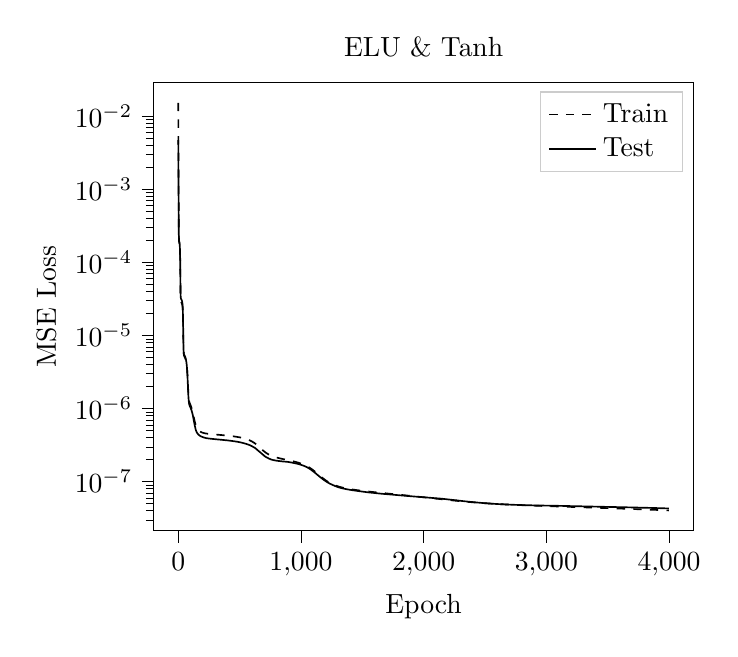
\begin{tikzpicture}

\begin{axis}[
legend cell align={left},
legend style={fill opacity=0.8, draw opacity=1, text opacity=1, draw=white!80!black},
log basis y={10},
tick align=outside,
tick pos=left,
title={ELU \& Tanh},
x grid style={white!69.0196078431373!black},
xlabel={Epoch},
xmin=-199.95, xmax=4198.95,
xtick style={color=black},
y grid style={white!69.0196078431373!black},
ylabel={MSE Loss},
ymin=2.1280500312269e-08, ymax=0.0288960951589277,
ymode=log,
ytick style={color=black}
]
\addplot [semithick, black, dashed]
table {%
0 0.0152080284673721
1 0.00248075019428506
2 0.00126132386806421
3 0.00065380612318404
4 0.000302382324065547
5 0.000212503188158735
6 0.000193753781044506
7 0.000187910542459576
8 0.000184431473302539
9 0.000180994361369812
10 0.000176910041926021
11 0.000171687997724803
12 0.000164645445795031
13 0.000154705665103393
14 0.000140248441668518
15 0.000119364761536417
16 9.17300330147555e-05
17 6.27979531163874e-05
18 4.26708161667193e-05
19 3.37652515718219e-05
20 3.06545776984422e-05
21 2.95085138677678e-05
22 2.8994764298659e-05
23 2.86948540106096e-05
24 2.84682299516135e-05
25 2.82642717929775e-05
26 2.80622330783444e-05
27 2.7850678786308e-05
28 2.76203797193375e-05
29 2.73613483659574e-05
30 2.70609807812434e-05
31 2.67019758239258e-05
32 2.6259632773872e-05
33 2.56977659782933e-05
34 2.49631382184816e-05
35 2.39780262472777e-05
36 2.26334173030409e-05
37 2.0791223996639e-05
38 1.83290858867622e-05
39 1.52773886138675e-05
40 1.20173287841681e-05
41 9.2298659392327e-06
42 7.36606126406514e-06
43 6.32788974849063e-06
44 5.79142337710437e-06
45 5.51480871411059e-06
46 5.36734691024776e-06
47 5.28214288931395e-06
48 5.22541249051756e-06
49 5.18075900356507e-06
50 5.14051194068088e-06
51 5.10132590710555e-06
52 5.06172166137731e-06
53 5.02101423398926e-06
54 4.97876538742048e-06
55 4.93462883019902e-06
56 4.88829601943053e-06
57 4.83948054937855e-06
58 4.78781597689704e-06
59 4.73286032058695e-06
60 4.67407446171819e-06
61 4.61085995141275e-06
62 4.54254747762661e-06
63 4.46836536832507e-06
64 4.38744179211881e-06
65 4.29883675451492e-06
66 4.20154519031257e-06
67 4.09452232202057e-06
68 3.97672916426472e-06
69 3.8471998618661e-06
70 3.70513911616399e-06
71 3.55005798166985e-06
72 3.38197834838638e-06
73 3.20168775073171e-06
74 3.01100894580486e-06
75 2.81300117563887e-06
76 2.61201407016642e-06
77 2.41341767292624e-06
78 2.22315533977735e-06
79 2.0468877611961e-06
80 1.88906458362226e-06
81 1.75221979372964e-06
82 1.63677172395182e-06
83 1.54148892647754e-06
84 1.46415385779619e-06
85 1.40207349818411e-06
86 1.35254531772944e-06
87 1.31307150775228e-06
88 1.28151420807399e-06
89 1.25604890848763e-06
90 1.23516671064294e-06
91 1.2176365066523e-06
92 1.20252019155487e-06
93 1.18908983145616e-06
94 1.17681919957136e-06
95 1.16535745513602e-06
96 1.15439602055289e-06
97 1.14370702488031e-06
98 1.13312517120789e-06
99 1.12253153173469e-06
100 1.11184424446265e-06
101 1.10101062864487e-06
102 1.09000098660772e-06
103 1.07879312142245e-06
104 1.06736867337531e-06
105 1.05571247524949e-06
106 1.04381238244855e-06
107 1.03166244338126e-06
108 1.0192582135744e-06
109 1.00659639397804e-06
110 9.93679479705634e-07
111 9.80511999273404e-07
112 9.67102745761394e-07
113 9.53462768279678e-07
114 9.39608711860274e-07
115 9.25561131367658e-07
116 9.11341380685826e-07
117 8.96972368934712e-07
118 8.82482107471105e-07
119 8.67901396617299e-07
120 8.53267375134692e-07
121 8.386187981273e-07
122 8.23993808523937e-07
123 8.09432929372633e-07
124 7.94978626629472e-07
125 7.80686552872112e-07
126 7.66615440795704e-07
127 7.52801653646884e-07
128 7.39273721563904e-07
129 7.260868112553e-07
130 7.13269594200483e-07
131 7.00837796472342e-07
132 6.88812247830128e-07
133 6.77201320598897e-07
134 6.66034269528382e-07
135 6.55349540636507e-07
136 6.45165235738432e-07
137 6.35454344404707e-07
138 6.26196593657369e-07
139 6.17382204609385e-07
140 6.0907905589147e-07
141 6.01319924101062e-07
142 5.94054916405184e-07
143 5.8719218452552e-07
144 5.80707587801044e-07
145 5.74600551118465e-07
146 5.68858134613492e-07
147 5.63467706399479e-07
148 5.58383930240325e-07
149 5.53627922812439e-07
150 5.49140991978447e-07
151 5.4492200263212e-07
152 5.40938552489933e-07
153 5.37143491641245e-07
154 5.33550829203477e-07
155 5.30159955616227e-07
156 5.26960494710238e-07
157 5.23945866660824e-07
158 5.2109070625761e-07
159 5.18372332038552e-07
160 5.1578902329652e-07
161 5.13338145935904e-07
162 5.11008444703975e-07
163 5.08790582244956e-07
164 5.06676500521053e-07
165 5.04660050523853e-07
166 5.02738334574815e-07
167 5.00906882678009e-07
168 4.9915709371362e-07
169 4.9748365924529e-07
170 4.95880076812227e-07
171 4.94340759701117e-07
172 4.92864306906426e-07
173 4.9144516030708e-07
174 4.9008119822247e-07
175 4.88768996348199e-07
176 4.87505730262683e-07
177 4.86288514707667e-07
178 4.85115197605524e-07
179 4.83983028601642e-07
180 4.82889594195512e-07
181 4.8183425819559e-07
182 4.80814081356584e-07
183 4.79827712922543e-07
184 4.78873592783202e-07
185 4.77950427978158e-07
186 4.77055746188171e-07
187 4.76188250274845e-07
188 4.75347918438729e-07
189 4.74533189901649e-07
190 4.73742007400801e-07
191 4.72973320526648e-07
192 4.72227070389408e-07
193 4.71503322685862e-07
194 4.70799528827115e-07
195 4.70116371261042e-07
196 4.69453903050976e-07
197 4.68810875844383e-07
198 4.68186554911654e-07
199 4.67581506711667e-07
200 4.66993338903876e-07
201 4.66421883700718e-07
202 4.6586627745171e-07
203 4.65324514891563e-07
204 4.64797279363438e-07
205 4.64284398972836e-07
206 4.63784455590144e-07
207 4.63298719495242e-07
208 4.62825613595896e-07
209 4.62363970797242e-07
210 4.61915587337103e-07
211 4.61477298927093e-07
212 4.61051291992476e-07
213 4.60636017479032e-07
214 4.60231373097031e-07
215 4.59836511453204e-07
216 4.59451205642836e-07
217 4.59075062082093e-07
218 4.58708360696392e-07
219 4.58350019769682e-07
220 4.58000447480345e-07
221 4.57658333374411e-07
222 4.57324772341394e-07
223 4.56997766420386e-07
224 4.56679159967166e-07
225 4.5636672231808e-07
226 4.56060347715948e-07
227 4.55762036324359e-07
228 4.5546945007402e-07
229 4.55182474496496e-07
230 4.54901839177069e-07
231 4.54625413439658e-07
232 4.54356226143204e-07
233 4.54091371821619e-07
234 4.53831857200271e-07
235 4.53577267762739e-07
236 4.53326436542056e-07
237 4.53081359182761e-07
238 4.52839802278504e-07
239 4.52602506470612e-07
240 4.52369051430424e-07
241 4.52139772278315e-07
242 4.51913687584238e-07
243 4.51691316968095e-07
244 4.51472699523947e-07
245 4.51256809995471e-07
246 4.51044487576269e-07
247 4.50834722101945e-07
248 4.50627858697317e-07
249 4.50423915665965e-07
250 4.50223144014217e-07
251 4.50024731975418e-07
252 4.49828700936905e-07
253 4.49634319892311e-07
254 4.49443024805873e-07
255 4.49254178064962e-07
256 4.49066956406341e-07
257 4.48881223618969e-07
258 4.48698587803165e-07
259 4.48516765786167e-07
260 4.48337179022928e-07
261 4.4815975951451e-07
262 4.47983176357525e-07
263 4.47808628308621e-07
264 4.47635315765638e-07
265 4.4746370636517e-07
266 4.47293768075951e-07
267 4.47124673172539e-07
268 4.46957185516794e-07
269 4.46790791471585e-07
270 4.46624989848488e-07
271 4.46461147248556e-07
272 4.46298341259421e-07
273 4.46135595410624e-07
274 4.45974463659127e-07
275 4.45814696519164e-07
276 4.45655445147963e-07
277 4.45497513965165e-07
278 4.45339897780173e-07
279 4.4518315532116e-07
280 4.45027225694616e-07
281 4.44871742303121e-07
282 4.44717229669322e-07
283 4.44563503421591e-07
284 4.44410062897305e-07
285 4.44257312167906e-07
286 4.44105373304637e-07
287 4.43953671634745e-07
288 4.43802586957531e-07
289 4.43651378475352e-07
290 4.4350156309747e-07
291 4.43351403191627e-07
292 4.43202396965603e-07
293 4.43052928034149e-07
294 4.4290395682367e-07
295 4.42755513716975e-07
296 4.42606946023716e-07
297 4.42459066817946e-07
298 4.42311463885403e-07
299 4.42163857997002e-07
300 4.42016133746392e-07
301 4.41869450867216e-07
302 4.41721961351504e-07
303 4.41575820104845e-07
304 4.41428945691769e-07
305 4.41282887692296e-07
306 4.4113659586742e-07
307 4.40990409828146e-07
308 4.40844655273054e-07
309 4.40698768144898e-07
310 4.40553284818179e-07
311 4.40407495204909e-07
312 4.40261692943977e-07
313 4.40117002582952e-07
314 4.39971105990367e-07
315 4.3982572678658e-07
316 4.3968058045607e-07
317 4.3953475244507e-07
318 4.39390190067002e-07
319 4.39244838787545e-07
320 4.3909949086185e-07
321 4.38954148719972e-07
322 4.38809322702127e-07
323 4.38664034192016e-07
324 4.38518397331222e-07
325 4.38373606968412e-07
326 4.38227661447854e-07
327 4.38082569615972e-07
328 4.37936808936001e-07
329 4.37791352069894e-07
330 4.37645759731708e-07
331 4.37499971056354e-07
332 4.37353520837291e-07
333 4.37207102521597e-07
334 4.37061042433129e-07
335 4.36913789201299e-07
336 4.36767032638841e-07
337 4.36620052894909e-07
338 4.36472801979448e-07
339 4.36325509113544e-07
340 4.36177363511092e-07
341 4.36028866033666e-07
342 4.35880465872174e-07
343 4.35731473871215e-07
344 4.35582405643231e-07
345 4.35433008561859e-07
346 4.35283194264002e-07
347 4.3513326829725e-07
348 4.3498325092628e-07
349 4.34832827465925e-07
350 4.3468171416805e-07
351 4.3453046178854e-07
352 4.34379240530802e-07
353 4.34226759196576e-07
354 4.34074440263998e-07
355 4.33922115718133e-07
356 4.33769137174522e-07
357 4.33616304675866e-07
358 4.33462212896529e-07
359 4.33308346842409e-07
360 4.33154044316097e-07
361 4.32999025719028e-07
362 4.32843678566996e-07
363 4.32688067760978e-07
364 4.32532335693736e-07
365 4.32375908360427e-07
366 4.32219386226507e-07
367 4.32062283337586e-07
368 4.31904461052568e-07
369 4.31746474518491e-07
370 4.315880933774e-07
371 4.31428781524801e-07
372 4.31269957729796e-07
373 4.31109887017556e-07
374 4.30949544366399e-07
375 4.3078909608596e-07
376 4.3062788631687e-07
377 4.3046613218678e-07
378 4.30304351141331e-07
379 4.30142163423852e-07
380 4.29979540541581e-07
381 4.29816218769474e-07
382 4.29652669481584e-07
383 4.29488652883947e-07
384 4.29324528838038e-07
385 4.29160088145863e-07
386 4.2899547537445e-07
387 4.28831191527479e-07
388 4.28666356484086e-07
389 4.28499909872926e-07
390 4.28332165512302e-07
391 4.2816423081149e-07
392 4.27997117341761e-07
393 4.27830187575751e-07
394 4.27665927389853e-07
395 4.27502797776924e-07
396 4.27342054052815e-07
397 4.27181646472263e-07
398 4.27009718947602e-07
399 4.2682666169469e-07
400 4.26646251099783e-07
401 4.26469282359676e-07
402 4.26291279069346e-07
403 4.26114118084797e-07
404 4.25935911081865e-07
405 4.25757392562787e-07
406 4.25577832146473e-07
407 4.25397295160224e-07
408 4.25216371667148e-07
409 4.25034376462463e-07
410 4.2485157290173e-07
411 4.24668970282482e-07
412 4.24484292835814e-07
413 4.24299328557254e-07
414 4.24113592458752e-07
415 4.23926915772199e-07
416 4.23739302391368e-07
417 4.2355089580326e-07
418 4.23361439615633e-07
419 4.23171769142527e-07
420 4.2298105516636e-07
421 4.22789032072046e-07
422 4.22596885357507e-07
423 4.22403967462515e-07
424 4.22211046924303e-07
425 4.22016804677128e-07
426 4.21823173240909e-07
427 4.2163074121504e-07
428 4.21439219110198e-07
429 4.21241830252939e-07
430 4.21036349408155e-07
431 4.20831540296263e-07
432 4.20626598298668e-07
433 4.2042308245982e-07
434 4.20218619041179e-07
435 4.20013128845653e-07
436 4.19806055774075e-07
437 4.19598493493822e-07
438 4.19389835656148e-07
439 4.19179818322846e-07
440 4.18968826551236e-07
441 4.18756718033819e-07
442 4.1854358694593e-07
443 4.18329209438184e-07
444 4.18113902696859e-07
445 4.17897678829604e-07
446 4.17680306043167e-07
447 4.17461535690222e-07
448 4.17242249227456e-07
449 4.17021593136724e-07
450 4.16801037246728e-07
451 4.16579762884339e-07
452 4.16357781375609e-07
453 4.16134501904253e-07
454 4.15909136961545e-07
455 4.15682213287027e-07
456 4.15455763217665e-07
457 4.15227140010188e-07
458 4.14998426251145e-07
459 4.14767454032017e-07
460 4.14533987935783e-07
461 4.14297598396729e-07
462 4.14058632713932e-07
463 4.1381838173038e-07
464 4.13576328185172e-07
465 4.13332909417363e-07
466 4.13088214941126e-07
467 4.12841624324756e-07
468 4.12594360795993e-07
469 4.12345667172076e-07
470 4.12094428085652e-07
471 4.11842957362296e-07
472 4.11588928784568e-07
473 4.1133438830343e-07
474 4.11077571214946e-07
475 4.10818901883658e-07
476 4.10558991234211e-07
477 4.10297284844319e-07
478 4.10033927209952e-07
479 4.09769019000805e-07
480 4.09501372402588e-07
481 4.09233206411841e-07
482 4.08962386146072e-07
483 4.08690077392748e-07
484 4.08415712570331e-07
485 4.08139434355803e-07
486 4.07861542385035e-07
487 4.07581834338089e-07
488 4.07300655780318e-07
489 4.07016802938642e-07
490 4.06731137147176e-07
491 4.06443877139395e-07
492 4.06154237637679e-07
493 4.05862715155081e-07
494 4.05568969000569e-07
495 4.05273351432811e-07
496 4.04975282762621e-07
497 4.04674660700266e-07
498 4.0437273760574e-07
499 4.04067683120957e-07
500 4.03761146870352e-07
501 4.03451639428454e-07
502 4.03139706364186e-07
503 4.02826480339513e-07
504 4.02509610665902e-07
505 4.02190768141963e-07
506 4.01869577345337e-07
507 4.01546232779992e-07
508 4.0122040243773e-07
509 4.00891479856114e-07
510 4.00560430591668e-07
511 4.00226384300595e-07
512 3.99890941281456e-07
513 3.99551510341212e-07
514 3.99209917361532e-07
515 3.98866274110787e-07
516 3.98518419430616e-07
517 3.98168940421328e-07
518 3.97816384889893e-07
519 3.97461238151209e-07
520 3.97103499679474e-07
521 3.96742407474449e-07
522 3.96378228884942e-07
523 3.96010879271103e-07
524 3.9564072622511e-07
525 3.95267676083222e-07
526 3.94890880272669e-07
527 3.94511405232834e-07
528 3.94128287325657e-07
529 3.93741344481668e-07
530 3.93352225017907e-07
531 3.92959715242114e-07
532 3.92563438921911e-07
533 3.9216375753881e-07
534 3.91761114514111e-07
535 3.91355185229259e-07
536 3.90944708314578e-07
537 3.90532183018877e-07
538 3.9011626749641e-07
539 3.89696966365705e-07
540 3.89274426851216e-07
541 3.88848559708777e-07
542 3.88419916419025e-07
543 3.87989611638773e-07
544 3.87556333166117e-07
545 3.87121111600663e-07
546 3.86684392907455e-07
547 3.86246727373418e-07
548 3.85805560057406e-07
549 3.85360736231632e-07
550 3.84910381086456e-07
551 3.84454204962026e-07
552 3.83994932519727e-07
553 3.83531411628724e-07
554 3.83059219458914e-07
555 3.82575445300404e-07
556 3.82082884641477e-07
557 3.81585331467704e-07
558 3.81081443521225e-07
559 3.80573512586579e-07
560 3.80061310664814e-07
561 3.79545718928398e-07
562 3.7902608279694e-07
563 3.78502641950718e-07
564 3.77975410430054e-07
565 3.77444048453412e-07
566 3.76907770714752e-07
567 3.76367728875948e-07
568 3.75824838585004e-07
569 3.75276613652886e-07
570 3.74724207119925e-07
571 3.74166170345802e-07
572 3.73599418281856e-07
573 3.73024576461489e-07
574 3.72441210373609e-07
575 3.71851760888831e-07
576 3.71256574879908e-07
577 3.70655598146641e-07
578 3.70049976297082e-07
579 3.69438769027397e-07
580 3.68821629621152e-07
581 3.68198507970874e-07
582 3.6756981538133e-07
583 3.6693339855276e-07
584 3.66292147148783e-07
585 3.65642823027201e-07
586 3.64987084253698e-07
587 3.64323781809617e-07
588 3.63653413089082e-07
589 3.62975147567113e-07
590 3.62289680722938e-07
591 3.61597356771881e-07
592 3.6089758528135e-07
593 3.60190051196696e-07
594 3.59475607524473e-07
595 3.58753690136382e-07
596 3.58024245528554e-07
597 3.57286942630708e-07
598 3.56542650152392e-07
599 3.55790499583009e-07
600 3.55030364318054e-07
601 3.54263068174987e-07
602 3.53487559493715e-07
603 3.52704138791182e-07
604 3.5191315025429e-07
605 3.51113995563424e-07
606 3.50307178621279e-07
607 3.49492535278273e-07
608 3.48670051636191e-07
609 3.47839225057101e-07
610 3.47001117404488e-07
611 3.46154819595768e-07
612 3.4530131030408e-07
613 3.44439791035711e-07
614 3.43571013203814e-07
615 3.42695091504197e-07
616 3.41812224007754e-07
617 3.40922235992025e-07
618 3.40024295439889e-07
619 3.39119695482282e-07
620 3.38206636016025e-07
621 3.37286338464082e-07
622 3.36357724691538e-07
623 3.35421586697748e-07
624 3.34478846738762e-07
625 3.3353134622871e-07
626 3.32582318662844e-07
627 3.31627309350324e-07
628 3.30657915270649e-07
629 3.29676779301735e-07
630 3.28686887527851e-07
631 3.27686967835916e-07
632 3.26681882768298e-07
633 3.2567142653761e-07
634 3.24656859532979e-07
635 3.23637882360117e-07
636 3.22613774727643e-07
637 3.21585285718129e-07
638 3.20552245838712e-07
639 3.19513541384708e-07
640 3.18471469981318e-07
641 3.17424747223072e-07
642 3.16374848694068e-07
643 3.15321539005708e-07
644 3.14264368597605e-07
645 3.13204994782268e-07
646 3.12142761274004e-07
647 3.1107828736765e-07
648 3.10012818800942e-07
649 3.08945284075435e-07
650 3.07876374378679e-07
651 3.06807749538507e-07
652 3.05738609483797e-07
653 3.04670831113185e-07
654 3.03604463951501e-07
655 3.02538507270356e-07
656 3.01475481862212e-07
657 3.00420638524201e-07
658 2.99368262318467e-07
659 2.98305927501019e-07
660 2.9724377205298e-07
661 2.96187314631879e-07
662 2.95135673923141e-07
663 2.94088418243632e-07
664 2.93043090579204e-07
665 2.92001749215842e-07
666 2.90964147893646e-07
667 2.8992860050181e-07
668 2.88896486182466e-07
669 2.87866366512901e-07
670 2.86841053750209e-07
671 2.85822178319961e-07
672 2.84809853511092e-07
673 2.83802668313626e-07
674 2.82802994959752e-07
675 2.81808777316428e-07
676 2.80821736446057e-07
677 2.79841228206124e-07
678 2.78866927004628e-07
679 2.7790029102448e-07
680 2.76940049957375e-07
681 2.75986952402718e-07
682 2.75040459946752e-07
683 2.7410105185055e-07
684 2.73169070915458e-07
685 2.72244475226557e-07
686 2.71327085592077e-07
687 2.70418083744062e-07
688 2.69515283221722e-07
689 2.68621464947216e-07
690 2.67736805710683e-07
691 2.6686000502707e-07
692 2.65991814671906e-07
693 2.65132417098357e-07
694 2.64281129219057e-07
695 2.63438652083892e-07
696 2.62605085239898e-07
697 2.6178079198047e-07
698 2.60965614536701e-07
699 2.60159289894091e-07
700 2.59361679880499e-07
701 2.58572606441021e-07
702 2.5779265062198e-07
703 2.5702136591832e-07
704 2.56259088146749e-07
705 2.5550531433538e-07
706 2.54760969511381e-07
707 2.54025321467566e-07
708 2.53298220812326e-07
709 2.52579562904032e-07
710 2.51870719914393e-07
711 2.51169781748217e-07
712 2.50477844623731e-07
713 2.49794036555784e-07
714 2.49118054647113e-07
715 2.48451531383864e-07
716 2.47792019649751e-07
717 2.4713980123181e-07
718 2.4649597766313e-07
719 2.45858712489166e-07
720 2.45228927809649e-07
721 2.44605411296561e-07
722 2.43988998619216e-07
723 2.43379559542234e-07
724 2.42777749093648e-07
725 2.42183043717148e-07
726 2.41596288141466e-07
727 2.41018655465552e-07
728 2.4045008593987e-07
729 2.39890878397375e-07
730 2.39341327421982e-07
731 2.38801107819597e-07
732 2.38267282050231e-07
733 2.37741108591649e-07
734 2.37221678233368e-07
735 2.36709369893617e-07
736 2.3620330499341e-07
737 2.35703722438529e-07
738 2.3521035917895e-07
739 2.34722806567333e-07
740 2.34240615100134e-07
741 2.33767771455007e-07
742 2.33302381239753e-07
743 2.32845008270033e-07
744 2.32395974940403e-07
745 2.31952249464484e-07
746 2.31513471092626e-07
747 2.31079828736824e-07
748 2.30651120318726e-07
749 2.30226588783466e-07
750 2.2980676357065e-07
751 2.29391758971076e-07
752 2.28981763186198e-07
753 2.28576197116581e-07
754 2.28172959118922e-07
755 2.27773301602952e-07
756 2.27378275646117e-07
757 2.26989851242365e-07
758 2.26602774077378e-07
759 2.26227015282632e-07
760 2.25866439848232e-07
761 2.25510081413915e-07
762 2.25156237128488e-07
763 2.24807197071186e-07
764 2.24463084258275e-07
765 2.24122159856677e-07
766 2.23785884017502e-07
767 2.23455905860703e-07
768 2.23132916062241e-07
769 2.22814507218061e-07
770 2.22498743696065e-07
771 2.22186950992409e-07
772 2.21877190426767e-07
773 2.21571451533009e-07
774 2.21268463938884e-07
775 2.20969464599818e-07
776 2.20672862852211e-07
777 2.20380329785996e-07
778 2.20091305415338e-07
779 2.19805837808451e-07
780 2.19523888425499e-07
781 2.19244672571506e-07
782 2.1896903959373e-07
783 2.18695799098612e-07
784 2.18425251311771e-07
785 2.18156760823263e-07
786 2.17889637639246e-07
787 2.17624017793128e-07
788 2.17358097586384e-07
789 2.17094104584703e-07
790 2.1683663841543e-07
791 2.16581288739803e-07
792 2.16325453756383e-07
793 2.16079294290239e-07
794 2.15844955441469e-07
795 2.15610947094547e-07
796 2.15374048437411e-07
797 2.15137222312478e-07
798 2.14901826538494e-07
799 2.14668557909192e-07
800 2.14437508262222e-07
801 2.14208109397873e-07
802 2.13980514168099e-07
803 2.13755005297855e-07
804 2.13530497873649e-07
805 2.13307517775263e-07
806 2.13086708924948e-07
807 2.12867477486611e-07
808 2.12648762158096e-07
809 2.12432043134925e-07
810 2.1221569882357e-07
811 2.12001444538146e-07
812 2.11787534560415e-07
813 2.1157526721538e-07
814 2.11363528677566e-07
815 2.11152904377343e-07
816 2.10944543326264e-07
817 2.10738933837717e-07
818 2.10534798483764e-07
819 2.10332396406443e-07
820 2.10132417123532e-07
821 2.09933438640064e-07
822 2.09735871109729e-07
823 2.0953889501385e-07
824 2.09343528659645e-07
825 2.09148757413402e-07
826 2.08955001021138e-07
827 2.08762269167551e-07
828 2.0857034380839e-07
829 2.08380171969225e-07
830 2.08190538060649e-07
831 2.08001925358303e-07
832 2.07813819351088e-07
833 2.07627028736113e-07
834 2.07440498009248e-07
835 2.07255245449289e-07
836 2.0707062751768e-07
837 2.06885963407899e-07
838 2.06701901937834e-07
839 2.06518239487252e-07
840 2.06334660020957e-07
841 2.06149372928621e-07
842 2.05963076687965e-07
843 2.05778682648372e-07
844 2.05600004349549e-07
845 2.05427205528963e-07
846 2.05253981924614e-07
847 2.05079602025648e-07
848 2.04905068969197e-07
849 2.04730230834116e-07
850 2.04555962532993e-07
851 2.04382653272717e-07
852 2.04209134508915e-07
853 2.04036619734893e-07
854 2.03864340669213e-07
855 2.03692555636792e-07
856 2.03521542459839e-07
857 2.03350728412488e-07
858 2.03180690157012e-07
859 2.03011188972368e-07
860 2.02841798056852e-07
861 2.026736309233e-07
862 2.02505270834763e-07
863 2.02337946419107e-07
864 2.02170827741099e-07
865 2.02004277184642e-07
866 2.01838315533109e-07
867 2.01673230499466e-07
868 2.01508554056318e-07
869 2.01345202611947e-07
870 2.01181850222554e-07
871 2.01019166709671e-07
872 2.00856438574704e-07
873 2.00694160724879e-07
874 2.00530837311419e-07
875 2.00366833176702e-07
876 2.00201819630763e-07
877 2.00036929420833e-07
878 1.99872439061721e-07
879 1.99706989867821e-07
880 1.99541846136242e-07
881 1.99376906415694e-07
882 1.99212340909583e-07
883 1.99047352666071e-07
884 1.98882859763216e-07
885 1.98717945835369e-07
886 1.9855398689117e-07
887 1.98389172609836e-07
888 1.98224787446577e-07
889 1.98060101283204e-07
890 1.9789522706759e-07
891 1.97730675708385e-07
892 1.97565865150295e-07
893 1.9740112774258e-07
894 1.972362442757e-07
895 1.97070757188555e-07
896 1.96906404205777e-07
897 1.96741027025382e-07
898 1.96576096470835e-07
899 1.96410390380208e-07
900 1.96244824508085e-07
901 1.96077997884458e-07
902 1.95911753110067e-07
903 1.95743825941008e-07
904 1.95575801726022e-07
905 1.95407580591223e-07
906 1.95238583479806e-07
907 1.95069209105725e-07
908 1.9489933107053e-07
909 1.94728678806655e-07
910 1.94557905523141e-07
911 1.94387777966654e-07
912 1.94218127241186e-07
913 1.94050267367629e-07
914 1.9388224076522e-07
915 1.93712325064155e-07
916 1.9353938095179e-07
917 1.93366957915941e-07
918 1.9319692871278e-07
919 1.93027422852765e-07
920 1.92858038950305e-07
921 1.92688125018492e-07
922 1.92518062625879e-07
923 1.92347462395048e-07
924 1.92176538490685e-07
925 1.92004955188452e-07
926 1.91832813854376e-07
927 1.91660883459122e-07
928 1.91487729047424e-07
929 1.91314957049826e-07
930 1.91140440186643e-07
931 1.90967177964296e-07
932 1.90792752839286e-07
933 1.90617769661117e-07
934 1.90441730737234e-07
935 1.90266023665231e-07
936 1.90089237563029e-07
937 1.89911305525925e-07
938 1.89733484504018e-07
939 1.89554710267714e-07
940 1.89375190878138e-07
941 1.89195479805448e-07
942 1.8901482096112e-07
943 1.88833834222635e-07
944 1.88652055001626e-07
945 1.88469787048007e-07
946 1.88286472578625e-07
947 1.88102376753818e-07
948 1.87918844105184e-07
949 1.87733679425151e-07
950 1.87547744005201e-07
951 1.87360893221467e-07
952 1.87174149104408e-07
953 1.86985833252606e-07
954 1.86796763976815e-07
955 1.86606931265487e-07
956 1.86416954342405e-07
957 1.86225132750906e-07
958 1.86033258174234e-07
959 1.85840012484562e-07
960 1.85645616667784e-07
961 1.8545087016264e-07
962 1.8525445011619e-07
963 1.85057448533144e-07
964 1.84858989101144e-07
965 1.84660104586953e-07
966 1.84459632542655e-07
967 1.84258142418514e-07
968 1.84055861524257e-07
969 1.83852619251468e-07
970 1.83647670056075e-07
971 1.83441494932879e-07
972 1.83235091093081e-07
973 1.83027565526572e-07
974 1.82818779848048e-07
975 1.82608773229731e-07
976 1.82398483588031e-07
977 1.82186698005182e-07
978 1.81974148567576e-07
979 1.81761305768191e-07
980 1.81546775124275e-07
981 1.8133131184328e-07
982 1.81115166988377e-07
983 1.80897656846923e-07
984 1.80678867032213e-07
985 1.8045907341957e-07
986 1.80237917071224e-07
987 1.80015462724725e-07
988 1.79791754902681e-07
989 1.79566497948258e-07
990 1.79339599419848e-07
991 1.7911191135056e-07
992 1.7888233854535e-07
993 1.78651545233777e-07
994 1.78419945541464e-07
995 1.78185779844853e-07
996 1.77950870181576e-07
997 1.77714219546488e-07
998 1.77476629012574e-07
999 1.77237352858128e-07
1000 1.76996435747867e-07
1001 1.76753868046831e-07
1002 1.76510436688204e-07
1003 1.76265239097972e-07
1004 1.76018311321968e-07
1005 1.7577009816705e-07
1006 1.75520918872962e-07
1007 1.75269713388104e-07
1008 1.75017535724464e-07
1009 1.7476436124042e-07
1010 1.74509330946648e-07
1011 1.74253998878271e-07
1012 1.73996551879441e-07
1013 1.73735433776301e-07
1014 1.73470677786725e-07
1015 1.73203433071478e-07
1016 1.72935475397651e-07
1017 1.72665775927783e-07
1018 1.72394989540692e-07
1019 1.72122301378863e-07
1020 1.71847703903438e-07
1021 1.71571395924275e-07
1022 1.71293312561716e-07
1023 1.71013627351613e-07
1024 1.70731415153114e-07
1025 1.70448012760005e-07
1026 1.70162309245825e-07
1027 1.69874203834297e-07
1028 1.69584868331185e-07
1029 1.69293045168217e-07
1030 1.68999612853327e-07
1031 1.68704158348021e-07
1032 1.68406576023017e-07
1033 1.68106452065331e-07
1034 1.67805620947092e-07
1035 1.67501270006198e-07
1036 1.67195596851855e-07
1037 1.66887579510444e-07
1038 1.66578071727486e-07
1039 1.66266004974602e-07
1040 1.65951682980392e-07
1041 1.65635398253983e-07
1042 1.65317023686384e-07
1043 1.64996520197747e-07
1044 1.64673900364676e-07
1045 1.64349384519369e-07
1046 1.64022342566739e-07
1047 1.63692751627309e-07
1048 1.6336171660214e-07
1049 1.63027996336496e-07
1050 1.62691938633941e-07
1051 1.62353983277796e-07
1052 1.62013484391821e-07
1053 1.61670484828846e-07
1054 1.61325077414176e-07
1055 1.60977907036397e-07
1056 1.60627455542794e-07
1057 1.60274794467341e-07
1058 1.59919573505363e-07
1059 1.5956187238686e-07
1060 1.59202226228672e-07
1061 1.5883981910747e-07
1062 1.58475691868887e-07
1063 1.58109363731285e-07
1064 1.57740791159711e-07
1065 1.57370220534858e-07
1066 1.5699837614136e-07
1067 1.56623337829842e-07
1068 1.5624693890004e-07
1069 1.55868588223029e-07
1070 1.5548834431911e-07
1071 1.55105668646627e-07
1072 1.54720571160283e-07
1073 1.5433408812271e-07
1074 1.53945973565328e-07
1075 1.53556759023843e-07
1076 1.53168143185667e-07
1077 1.52781376655753e-07
1078 1.52392721695094e-07
1079 1.51986224111056e-07
1080 1.51573336843569e-07
1081 1.51163015452482e-07
1082 1.50752499294526e-07
1083 1.50340282296213e-07
1084 1.49925430150688e-07
1085 1.49508963318112e-07
1086 1.49090141533748e-07
1087 1.48668793379159e-07
1088 1.48246224533466e-07
1089 1.47823067443653e-07
1090 1.4739891135207e-07
1091 1.46975094374113e-07
1092 1.46551880227719e-07
1093 1.46127542315355e-07
1094 1.45704618077502e-07
1095 1.45281267663222e-07
1096 1.44858161554851e-07
1097 1.44435726859626e-07
1098 1.44012023504558e-07
1099 1.43588234735148e-07
1100 1.43163128392132e-07
1101 1.42737117741376e-07
1102 1.42309912902761e-07
1103 1.41881366552354e-07
1104 1.41451710398144e-07
1105 1.41019887571758e-07
1106 1.40588459643709e-07
1107 1.40159142063112e-07
1108 1.397344884424e-07
1109 1.39312528155244e-07
1110 1.38888660956127e-07
1111 1.38463449410153e-07
1112 1.38037102217936e-07
1113 1.37609120329785e-07
1114 1.3718097876847e-07
1115 1.36753013961766e-07
1116 1.36323733279653e-07
1117 1.35895572427103e-07
1118 1.35466340246637e-07
1119 1.35037029579621e-07
1120 1.34607929481945e-07
1121 1.34178400685414e-07
1122 1.3374874122718e-07
1123 1.33319254764785e-07
1124 1.3289110313508e-07
1125 1.32462414988765e-07
1126 1.32034274258785e-07
1127 1.3160604830631e-07
1128 1.31179003709292e-07
1129 1.30751606668866e-07
1130 1.303254807965e-07
1131 1.29900382290771e-07
1132 1.29477080037077e-07
1133 1.29054515809912e-07
1134 1.28633866729899e-07
1135 1.2821482557257e-07
1136 1.27797809263086e-07
1137 1.27382684361521e-07
1138 1.26968237751157e-07
1139 1.26554759646069e-07
1140 1.26141516709311e-07
1141 1.25729517293394e-07
1142 1.25318422725229e-07
1143 1.24908480522379e-07
1144 1.2449971258377e-07
1145 1.24091573255214e-07
1146 1.23685658685702e-07
1147 1.23280426407746e-07
1148 1.22877155902756e-07
1149 1.22475587104987e-07
1150 1.22075368736319e-07
1151 1.21677058281477e-07
1152 1.21280481735653e-07
1153 1.20885881372601e-07
1154 1.204930188905e-07
1155 1.20102175543479e-07
1156 1.19712751668999e-07
1157 1.19324970796697e-07
1158 1.18938711693772e-07
1159 1.18554402661175e-07
1160 1.18171441883419e-07
1161 1.1778998898393e-07
1162 1.17410384731897e-07
1163 1.17032128031269e-07
1164 1.16655850810332e-07
1165 1.16281895898851e-07
1166 1.1590908521697e-07
1167 1.15539219237348e-07
1168 1.15170975277579e-07
1169 1.14804350438646e-07
1170 1.14440306376196e-07
1171 1.14077554300707e-07
1172 1.13717005660874e-07
1173 1.13358472852099e-07
1174 1.13001979670457e-07
1175 1.12648888318745e-07
1176 1.12299481877187e-07
1177 1.11954567451278e-07
1178 1.11612510480086e-07
1179 1.1127388872012e-07
1180 1.10937243938736e-07
1181 1.1060316435163e-07
1182 1.10271697288056e-07
1183 1.09942648336414e-07
1184 1.09615565492049e-07
1185 1.09291037958315e-07
1186 1.08968655844421e-07
1187 1.08648786330434e-07
1188 1.08331142371298e-07
1189 1.08016214802831e-07
1190 1.07703970080308e-07
1191 1.07393447542847e-07
1192 1.07085563961107e-07
1193 1.06780864925327e-07
1194 1.06478344953587e-07
1195 1.06178493034292e-07
1196 1.0588090550101e-07
1197 1.05585991015289e-07
1198 1.05293827822095e-07
1199 1.05004410443144e-07
1200 1.04717090827933e-07
1201 1.04432268230426e-07
1202 1.04150698788885e-07
1203 1.0387048472893e-07
1204 1.03593092283916e-07
1205 1.0331897247795e-07
1206 1.03046438511001e-07
1207 1.02776690219741e-07
1208 1.02509168932841e-07
1209 1.02244018371778e-07
1210 1.01981247524918e-07
1211 1.01721427910206e-07
1212 1.01463886892361e-07
1213 1.01208237545336e-07
1214 1.0095620817907e-07
1215 1.00705281361968e-07
1216 1.00457674449217e-07
1217 1.002125797811e-07
1218 9.99691031964289e-08
1219 9.97283629899925e-08
1220 9.94902429241051e-08
1221 9.92538613786564e-08
1222 9.90203047877003e-08
1223 9.87890798356261e-08
1224 9.85600288814226e-08
1225 9.83333006701059e-08
1226 9.81081368394143e-08
1227 9.78856225017921e-08
1228 9.76655963000894e-08
1229 9.74474516510782e-08
1230 9.72314346654457e-08
1231 9.70177857837484e-08
1232 9.68057680310608e-08
1233 9.65957702376841e-08
1234 9.63888376830369e-08
1235 9.61833007195878e-08
1236 9.59798849393678e-08
1237 9.57784397002115e-08
1238 9.5579133713386e-08
1239 9.53816355533377e-08
1240 9.51868270888667e-08
1241 9.49936092098369e-08
1242 9.48020751252443e-08
1243 9.46127540970565e-08
1244 9.44253734900258e-08
1245 9.4239902558968e-08
1246 9.40562607283368e-08
1247 9.38745147252007e-08
1248 9.36945717597837e-08
1249 9.35167212361421e-08
1250 9.33404639269497e-08
1251 9.316588210595e-08
1252 9.29938347695725e-08
1253 9.28227531744596e-08
1254 9.2653620896499e-08
1255 9.2485869487291e-08
1256 9.23203285552177e-08
1257 9.21564031344246e-08
1258 9.19938789039065e-08
1259 9.18330371248999e-08
1260 9.16739129195321e-08
1261 9.15165547112906e-08
1262 9.13604319308092e-08
1263 9.12062605280539e-08
1264 9.10527221407165e-08
1265 9.09018065300415e-08
1266 9.0752211363565e-08
1267 9.06035274965689e-08
1268 9.04562642105589e-08
1269 9.03108397309893e-08
1270 9.01661758589967e-08
1271 9.00231503848659e-08
1272 8.98814672538606e-08
1273 8.97394009342634e-08
1274 8.95989449034573e-08
1275 8.94590172677567e-08
1276 8.93244760291623e-08
1277 8.91929665769453e-08
1278 8.9062883034785e-08
1279 8.89321081274375e-08
1280 8.88022729128579e-08
1281 8.86740952239506e-08
1282 8.85469193789845e-08
1283 8.84201451185618e-08
1284 8.82957007277696e-08
1285 8.81719462171304e-08
1286 8.80497174335915e-08
1287 8.79282517232127e-08
1288 8.78079981276869e-08
1289 8.76893464223372e-08
1290 8.7571744785464e-08
1291 8.74545199636145e-08
1292 8.73392903741887e-08
1293 8.722456119159e-08
1294 8.71110444293777e-08
1295 8.69986275304768e-08
1296 8.68874462156555e-08
1297 8.67767668069064e-08
1298 8.66674825985569e-08
1299 8.65589204224193e-08
1300 8.64516622769429e-08
1301 8.63453442363493e-08
1302 8.62401074783747e-08
1303 8.61350954650675e-08
1304 8.60317545061662e-08
1305 8.59294411768019e-08
1306 8.58274157451433e-08
1307 8.57269948468797e-08
1308 8.56272961087257e-08
1309 8.55274409659046e-08
1310 8.54303224713249e-08
1311 8.53334224473201e-08
1312 8.52367697632417e-08
1313 8.5142384570247e-08
1314 8.50475565243869e-08
1315 8.49544391599011e-08
1316 8.48615582569323e-08
1317 8.47699372030775e-08
1318 8.46791981388151e-08
1319 8.45890290293028e-08
1320 8.44999887021913e-08
1321 8.44113146456493e-08
1322 8.43234315865971e-08
1323 8.42369990721181e-08
1324 8.41501236337194e-08
1325 8.40647223583346e-08
1326 8.39803867265232e-08
1327 8.38963459131037e-08
1328 8.38126386426552e-08
1329 8.37301639293742e-08
1330 8.36479391139733e-08
1331 8.3566749985664e-08
1332 8.348601567576e-08
1333 8.34061869383618e-08
1334 8.33265701700725e-08
1335 8.32481432553323e-08
1336 8.31698831120775e-08
1337 8.30923169274911e-08
1338 8.30157012359223e-08
1339 8.29390024819077e-08
1340 8.28633186458205e-08
1341 8.27880322162855e-08
1342 8.27136691796682e-08
1343 8.26401402349575e-08
1344 8.25663134520482e-08
1345 8.24939379100442e-08
1346 8.24213261267914e-08
1347 8.23492667265668e-08
1348 8.22781793203831e-08
1349 8.22074192114997e-08
1350 8.21372729262748e-08
1351 8.20677105224377e-08
1352 8.19986522984095e-08
1353 8.19296958951554e-08
1354 8.18616360120927e-08
1355 8.17937914590061e-08
1356 8.17264199071133e-08
1357 8.16601064528299e-08
1358 8.15934954161435e-08
1359 8.15279246992873e-08
1360 8.14624010985199e-08
1361 8.13973081221775e-08
1362 8.1332800860423e-08
1363 8.12692882732335e-08
1364 8.12049083620536e-08
1365 8.11420615818292e-08
1366 8.1079329476097e-08
1367 8.10166019817871e-08
1368 8.09547406532829e-08
1369 8.08934162392916e-08
1370 8.0832243021689e-08
1371 8.07713473136573e-08
1372 8.07109393363703e-08
1373 8.06509393740384e-08
1374 8.05918297359653e-08
1375 8.05319536922866e-08
1376 8.04738056245924e-08
1377 8.0414946324936e-08
1378 8.03566683131862e-08
1379 8.02979416931748e-08
1380 8.02413898881582e-08
1381 8.01844703701704e-08
1382 8.01275012136671e-08
1383 8.00707375958609e-08
1384 8.001493698373e-08
1385 7.99589733802009e-08
1386 7.99038251315665e-08
1387 7.98484854342974e-08
1388 7.97938645789031e-08
1389 7.97394405225305e-08
1390 7.96852514639568e-08
1391 7.96311271216155e-08
1392 7.95775883801753e-08
1393 7.95243503546317e-08
1394 7.94715677017166e-08
1395 7.94186591548396e-08
1396 7.93664395075666e-08
1397 7.93139230665929e-08
1398 7.92620168894587e-08
1399 7.92107897638061e-08
1400 7.91594922517902e-08
1401 7.91080691016077e-08
1402 7.90574707920655e-08
1403 7.90072508536355e-08
1404 7.89567802499391e-08
1405 7.89067730337933e-08
1406 7.88571125127646e-08
1407 7.88074789639381e-08
1408 7.87583879784393e-08
1409 7.87095384851e-08
1410 7.86608629539387e-08
1411 7.86123016709439e-08
1412 7.85642342151505e-08
1413 7.85162719054711e-08
1414 7.84685442241084e-08
1415 7.84213406959111e-08
1416 7.83736774181421e-08
1417 7.8327002398737e-08
1418 7.82807094523719e-08
1419 7.823354084735e-08
1420 7.81871346404728e-08
1421 7.81416124411294e-08
1422 7.80951739045577e-08
1423 7.80495877066301e-08
1424 7.80044537975755e-08
1425 7.79589319535035e-08
1426 7.79140118396526e-08
1427 7.78693163212552e-08
1428 7.78245580903558e-08
1429 7.77800239504245e-08
1430 7.7735855988692e-08
1431 7.76918100200419e-08
1432 7.76477672701503e-08
1433 7.76043771679724e-08
1434 7.75609110661435e-08
1435 7.7517694052176e-08
1436 7.74743239020381e-08
1437 7.74316418414855e-08
1438 7.73887777612003e-08
1439 7.7345921958738e-08
1440 7.7303864703282e-08
1441 7.72615988680059e-08
1442 7.72193435132351e-08
1443 7.71779687021024e-08
1444 7.7135825399921e-08
1445 7.70939382626068e-08
1446 7.70530331308805e-08
1447 7.70119176323192e-08
1448 7.69698890934478e-08
1449 7.69295765614686e-08
1450 7.68884859141394e-08
1451 7.68482930411096e-08
1452 7.68075653923006e-08
1453 7.67673222661358e-08
1454 7.67269470287601e-08
1455 7.66865754542323e-08
1456 7.66470711965894e-08
1457 7.66068821675958e-08
1458 7.65678704865991e-08
1459 7.6527664166548e-08
1460 7.64889622644205e-08
1461 7.64494008187455e-08
1462 7.64104649846331e-08
1463 7.63711414677459e-08
1464 7.6332712289684e-08
1465 7.6293740640665e-08
1466 7.62556768876266e-08
1467 7.62166098091655e-08
1468 7.61779054130329e-08
1469 7.61401426210284e-08
1470 7.61022195732153e-08
1471 7.6064172098711e-08
1472 7.60259572700761e-08
1473 7.59884730285876e-08
1474 7.59510955674614e-08
1475 7.59135576053893e-08
1476 7.58759221035632e-08
1477 7.58389163948436e-08
1478 7.58016155693042e-08
1479 7.57643282369713e-08
1480 7.57274937512875e-08
1481 7.56912027775059e-08
1482 7.56541587705328e-08
1483 7.56172308165048e-08
1484 7.55806852374974e-08
1485 7.55445234652541e-08
1486 7.55086352128842e-08
1487 7.54720685094412e-08
1488 7.54362399213448e-08
1489 7.54002237499662e-08
1490 7.53640559736368e-08
1491 7.5327907111955e-08
1492 7.52927175788898e-08
1493 7.52570493105509e-08
1494 7.52214995500822e-08
1495 7.51862400427683e-08
1496 7.51505606189085e-08
1497 7.51156411382681e-08
1498 7.50805594122994e-08
1499 7.50452959472625e-08
1500 7.50106469951106e-08
1501 7.49757387978889e-08
1502 7.49409264457768e-08
1503 7.49062122515909e-08
1504 7.48714135170303e-08
1505 7.48374690360265e-08
1506 7.48033951865068e-08
1507 7.47683593580462e-08
1508 7.47344553211349e-08
1509 7.47002047489787e-08
1510 7.46660046395675e-08
1511 7.46320617039942e-08
1512 7.45981784682215e-08
1513 7.45645593482891e-08
1514 7.45310478116323e-08
1515 7.44967212540359e-08
1516 7.44640533660856e-08
1517 7.44302667072816e-08
1518 7.43963639493472e-08
1519 7.43635719757663e-08
1520 7.4329848700927e-08
1521 7.42968210261097e-08
1522 7.4263863723445e-08
1523 7.42304568817076e-08
1524 7.41976623324092e-08
1525 7.41652450457764e-08
1526 7.41325341877541e-08
1527 7.41000638413425e-08
1528 7.40675571364591e-08
1529 7.40357243316225e-08
1530 7.40026258867488e-08
1531 7.39699677829719e-08
1532 7.39367528623802e-08
1533 7.39037088557382e-08
1534 7.38704910645538e-08
1535 7.38373247415325e-08
1536 7.38046548072191e-08
1537 7.37715990091203e-08
1538 7.37391102774154e-08
1539 7.37069732963391e-08
1540 7.36737617756944e-08
1541 7.36409315926778e-08
1542 7.36083234045282e-08
1543 7.35757108145663e-08
1544 7.35429632499063e-08
1545 7.3510266897614e-08
1546 7.34777951052479e-08
1547 7.34453938981972e-08
1548 7.34120530481164e-08
1549 7.33795287821692e-08
1550 7.33470449603146e-08
1551 7.33143303790484e-08
1552 7.32821800539796e-08
1553 7.32498545481519e-08
1554 7.32182117566538e-08
1555 7.31867569747635e-08
1556 7.31551009778286e-08
1557 7.3123619113602e-08
1558 7.30925802336912e-08
1559 7.30618775577341e-08
1560 7.30307863534563e-08
1561 7.30000072266534e-08
1562 7.29689225096308e-08
1563 7.29379316162238e-08
1564 7.29075966390269e-08
1565 7.2876951669798e-08
1566 7.28462185932699e-08
1567 7.28156710749772e-08
1568 7.27851968598259e-08
1569 7.27541053642256e-08
1570 7.27239629298992e-08
1571 7.26934242507582e-08
1572 7.26636227419419e-08
1573 7.26323324080624e-08
1574 7.26024714339246e-08
1575 7.25720909464656e-08
1576 7.25418457854232e-08
1577 7.2511705496936e-08
1578 7.24813574137784e-08
1579 7.24513856873443e-08
1580 7.24212779630307e-08
1581 7.23915054479107e-08
1582 7.23617623457073e-08
1583 7.23312701573775e-08
1584 7.23015843036023e-08
1585 7.22716186025707e-08
1586 7.22418191969609e-08
1587 7.22119787752717e-08
1588 7.21821780800269e-08
1589 7.21527759388607e-08
1590 7.21233960803147e-08
1591 7.20930145625687e-08
1592 7.20641907392405e-08
1593 7.20342289568521e-08
1594 7.20048138980189e-08
1595 7.19755490443674e-08
1596 7.19458123192851e-08
1597 7.19167296665546e-08
1598 7.18871665732479e-08
1599 7.18576931575399e-08
1600 7.18287397063477e-08
1601 7.17995495307378e-08
1602 7.17701792218861e-08
1603 7.17410723503065e-08
1604 7.17114646064942e-08
1605 7.16826745019716e-08
1606 7.1653672243599e-08
1607 7.16245959324624e-08
1608 7.15953340275632e-08
1609 7.15667247845886e-08
1610 7.15378542643919e-08
1611 7.15087214402388e-08
1612 7.14800602032994e-08
1613 7.14511361294967e-08
1614 7.14220109010455e-08
1615 7.13931990823369e-08
1616 7.13646470167362e-08
1617 7.1335975466269e-08
1618 7.13072259550529e-08
1619 7.12781985399147e-08
1620 7.12496841650534e-08
1621 7.12208811606274e-08
1622 7.11929140813083e-08
1623 7.11636779797686e-08
1624 7.11352212832139e-08
1625 7.11068540049098e-08
1626 7.10780279149503e-08
1627 7.10497513018993e-08
1628 7.10209694787523e-08
1629 7.09926112278936e-08
1630 7.09639956824049e-08
1631 7.09352940297947e-08
1632 7.09066333044461e-08
1633 7.08781174054707e-08
1634 7.08499391528505e-08
1635 7.08211585234153e-08
1636 7.07928148990789e-08
1637 7.07641441195506e-08
1638 7.07360084462039e-08
1639 7.07077867829753e-08
1640 7.06798342449133e-08
1641 7.06513718071733e-08
1642 7.06235310694581e-08
1643 7.0595601350476e-08
1644 7.05674816892099e-08
1645 7.05394378748281e-08
1646 7.0511619185254e-08
1647 7.04839359109144e-08
1648 7.0456328671753e-08
1649 7.04281309928945e-08
1650 7.04006538470026e-08
1651 7.03723046129312e-08
1652 7.03446743592906e-08
1653 7.03168960498601e-08
1654 7.02894908393148e-08
1655 7.02615390508754e-08
1656 7.02337730018598e-08
1657 7.02060220412193e-08
1658 7.01780927450102e-08
1659 7.01508154286046e-08
1660 7.01234951741014e-08
1661 7.00957208081832e-08
1662 7.00682599372726e-08
1663 7.00403600610855e-08
1664 7.00131248798641e-08
1665 6.99854235790553e-08
1666 6.99580603473748e-08
1667 6.99304962381575e-08
1668 6.99032250430776e-08
1669 6.98756660355571e-08
1670 6.98482957162128e-08
1671 6.9820649930108e-08
1672 6.97934017388491e-08
1673 6.97664778073204e-08
1674 6.97391845818629e-08
1675 6.9711249761184e-08
1676 6.96840886043049e-08
1677 6.96569064544406e-08
1678 6.96295814854864e-08
1679 6.96023596731266e-08
1680 6.95755847850421e-08
1681 6.95481218286886e-08
1682 6.95206431018391e-08
1683 6.94934821900972e-08
1684 6.94667044740527e-08
1685 6.94396815781317e-08
1686 6.94123620625931e-08
1687 6.93853976443393e-08
1688 6.93576125776474e-08
1689 6.9331140682749e-08
1690 6.93041647608084e-08
1691 6.92768188130799e-08
1692 6.92499463994523e-08
1693 6.92226484737546e-08
1694 6.91962025456405e-08
1695 6.91692796976895e-08
1696 6.91423355192455e-08
1697 6.91152179612686e-08
1698 6.90889366623537e-08
1699 6.90614336349427e-08
1700 6.90344602602977e-08
1701 6.90079030043478e-08
1702 6.89809528395813e-08
1703 6.89542028204926e-08
1704 6.89276586847143e-08
1705 6.89006299765538e-08
1706 6.88737561489461e-08
1707 6.88468589586932e-08
1708 6.88206389760637e-08
1709 6.87938837415913e-08
1710 6.87667685070892e-08
1711 6.87404985448836e-08
1712 6.87137695507545e-08
1713 6.86870154780195e-08
1714 6.86603700863486e-08
1715 6.86337530879655e-08
1716 6.86070031967745e-08
1717 6.85805783007254e-08
1718 6.85540014160324e-08
1719 6.85274341556408e-08
1720 6.85011156846827e-08
1721 6.84746080921172e-08
1722 6.84477576555764e-08
1723 6.84216116155767e-08
1724 6.83949028932318e-08
1725 6.83681965725214e-08
1726 6.83422828835489e-08
1727 6.83151611156063e-08
1728 6.82888963581263e-08
1729 6.8262451115686e-08
1730 6.82357322254745e-08
1731 6.82091486297054e-08
1732 6.81825820869619e-08
1733 6.81558535085003e-08
1734 6.81296104083628e-08
1735 6.81026364688364e-08
1736 6.80758641173895e-08
1737 6.80497121514634e-08
1738 6.80230821217265e-08
1739 6.7996318538377e-08
1740 6.79694451157786e-08
1741 6.79426654102144e-08
1742 6.79163663548366e-08
1743 6.78900331791965e-08
1744 6.78623117131849e-08
1745 6.78364540895871e-08
1746 6.7810004079405e-08
1747 6.778328633672e-08
1748 6.77565266506974e-08
1749 6.77298965712225e-08
1750 6.77028087920917e-08
1751 6.76763662319502e-08
1752 6.76497548184329e-08
1753 6.7623584708798e-08
1754 6.75962610792169e-08
1755 6.75698399490443e-08
1756 6.75431883649935e-08
1757 6.75159572693929e-08
1758 6.74895321637337e-08
1759 6.74630289161371e-08
1760 6.74362183303856e-08
1761 6.74090260552873e-08
1762 6.73827969599472e-08
1763 6.73552934280508e-08
1764 6.73287011956347e-08
1765 6.7301642474149e-08
1766 6.72745652963158e-08
1767 6.72476761671703e-08
1768 6.72202123013221e-08
1769 6.71937134839595e-08
1770 6.7165964992455e-08
1771 6.71392482765043e-08
1772 6.71121344737458e-08
1773 6.70855294586659e-08
1774 6.70580910551166e-08
1775 6.70314038835329e-08
1776 6.70046964970084e-08
1777 6.69779945319249e-08
1778 6.69514848539166e-08
1779 6.6924361075138e-08
1780 6.68979005986614e-08
1781 6.68717307092948e-08
1782 6.68450770433537e-08
1783 6.68185336039073e-08
1784 6.67921240733449e-08
1785 6.67654775909909e-08
1786 6.67390589512706e-08
1787 6.67125397910695e-08
1788 6.66863228246939e-08
1789 6.6659741037256e-08
1790 6.66334321230977e-08
1791 6.66069859001084e-08
1792 6.65808154565184e-08
1793 6.65542768274463e-08
1794 6.65279402092267e-08
1795 6.65010889413509e-08
1796 6.64752054788664e-08
1797 6.64485434036521e-08
1798 6.64224544308922e-08
1799 6.63957350077737e-08
1800 6.63699221306047e-08
1801 6.63429540850302e-08
1802 6.63170962269533e-08
1803 6.62904031081268e-08
1804 6.6264195215382e-08
1805 6.62381026756975e-08
1806 6.62117084964109e-08
1807 6.61856034831487e-08
1808 6.61590247901245e-08
1809 6.61328746183187e-08
1810 6.61063972593468e-08
1811 6.60800667020567e-08
1812 6.60538185570658e-08
1813 6.60274430970276e-08
1814 6.60010678750211e-08
1815 6.59745935678302e-08
1816 6.59484391682952e-08
1817 6.59223632482053e-08
1818 6.58963984925265e-08
1819 6.58694300454954e-08
1820 6.58430885458472e-08
1821 6.58173579992649e-08
1822 6.57910445411858e-08
1823 6.576472141262e-08
1824 6.5738440078178e-08
1825 6.57121548535144e-08
1826 6.56860760628319e-08
1827 6.56594084595952e-08
1828 6.56333409594367e-08
1829 6.56071002111958e-08
1830 6.55808322811424e-08
1831 6.55547118775246e-08
1832 6.55284977391091e-08
1833 6.55018510791194e-08
1834 6.54756589248961e-08
1835 6.54496916894232e-08
1836 6.54234106605145e-08
1837 6.53970902888545e-08
1838 6.53712042186783e-08
1839 6.53445307179368e-08
1840 6.53183906536015e-08
1841 6.529215667328e-08
1842 6.52657577866478e-08
1843 6.52395949707341e-08
1844 6.52136091190414e-08
1845 6.51873926109659e-08
1846 6.51610363391342e-08
1847 6.51347204652097e-08
1848 6.51084067975205e-08
1849 6.50823341921125e-08
1850 6.50561512358649e-08
1851 6.50296936761663e-08
1852 6.50042970278264e-08
1853 6.49776094192589e-08
1854 6.49513242265698e-08
1855 6.49255500313473e-08
1856 6.48989087430607e-08
1857 6.48728819960809e-08
1858 6.48467141033393e-08
1859 6.48202149555743e-08
1860 6.47944575469239e-08
1861 6.47683495103024e-08
1862 6.47421957822303e-08
1863 6.47158873690046e-08
1864 6.46896896654425e-08
1865 6.46636145695823e-08
1866 6.46375975215108e-08
1867 6.46118758993452e-08
1868 6.45853305876187e-08
1869 6.45591099939225e-08
1870 6.45329574524567e-08
1871 6.45070402391923e-08
1872 6.44806423899524e-08
1873 6.44546949999381e-08
1874 6.44291153122367e-08
1875 6.44024299454316e-08
1876 6.43765940679941e-08
1877 6.43502094277437e-08
1878 6.43242987692361e-08
1879 6.42983745926529e-08
1880 6.4271837871388e-08
1881 6.4245752870562e-08
1882 6.42199056173354e-08
1883 6.41936834107071e-08
1884 6.41672157897233e-08
1885 6.41412624204918e-08
1886 6.4115385427499e-08
1887 6.40890285552587e-08
1888 6.40630537063203e-08
1889 6.40368507092148e-08
1890 6.40105598854745e-08
1891 6.39844399188405e-08
1892 6.39579903314314e-08
1893 6.39317557080688e-08
1894 6.39056399158733e-08
1895 6.38789120586125e-08
1896 6.38524198066648e-08
1897 6.38257481107019e-08
1898 6.37987678970831e-08
1899 6.37714619138308e-08
1900 6.37439249331351e-08
1901 6.37163970758081e-08
1902 6.36896533912079e-08
1903 6.36621977498919e-08
1904 6.36358489742861e-08
1905 6.36093115069514e-08
1906 6.35830972832707e-08
1907 6.35574153520224e-08
1908 6.35319316444338e-08
1909 6.35053932072083e-08
1910 6.34799912972994e-08
1911 6.34540002586448e-08
1912 6.34280934086462e-08
1913 6.34022705625625e-08
1914 6.337618204455e-08
1915 6.33504962621601e-08
1916 6.33247304087092e-08
1917 6.32985233650629e-08
1918 6.327312965837e-08
1919 6.32468544203846e-08
1920 6.32213666911241e-08
1921 6.31953986314215e-08
1922 6.31691559860315e-08
1923 6.31433010447324e-08
1924 6.31177779588654e-08
1925 6.30917387596241e-08
1926 6.30658617382096e-08
1927 6.30401613435083e-08
1928 6.30143708058029e-08
1929 6.29887934238127e-08
1930 6.29623777150812e-08
1931 6.29365470743437e-08
1932 6.29109521845805e-08
1933 6.28848857751052e-08
1934 6.28591598470507e-08
1935 6.28335625663112e-08
1936 6.28076437649838e-08
1937 6.27818997642748e-08
1938 6.27559124808386e-08
1939 6.27300978379708e-08
1940 6.27041757326197e-08
1941 6.26787493906988e-08
1942 6.26530082747934e-08
1943 6.26270784493954e-08
1944 6.26013048083962e-08
1945 6.2575513485541e-08
1946 6.25497669801689e-08
1947 6.25241130656207e-08
1948 6.24982304557875e-08
1949 6.24725164755091e-08
1950 6.24468866625705e-08
1951 6.24207634274399e-08
1952 6.23948821818487e-08
1953 6.23692840342471e-08
1954 6.23434749478236e-08
1955 6.23177043728162e-08
1956 6.22920425108475e-08
1957 6.22661087383847e-08
1958 6.22403308625508e-08
1959 6.22143277055898e-08
1960 6.21884711549114e-08
1961 6.2162553533085e-08
1962 6.2137326107603e-08
1963 6.21113754775138e-08
1964 6.20847916188438e-08
1965 6.205920141511e-08
1966 6.20339266639292e-08
1967 6.20076162825001e-08
1968 6.19818243663417e-08
1969 6.19556923879827e-08
1970 6.19302342634853e-08
1971 6.19037296516467e-08
1972 6.1878053557507e-08
1973 6.18525326601116e-08
1974 6.18265438703247e-08
1975 6.18005156631796e-08
1976 6.17749320923622e-08
1977 6.17493320369533e-08
1978 6.17231801776086e-08
1979 6.1697715665332e-08
1980 6.16721144801602e-08
1981 6.16460991196277e-08
1982 6.16203810785976e-08
1983 6.15943727098056e-08
1984 6.15687701532863e-08
1985 6.15434382069679e-08
1986 6.15174448981293e-08
1987 6.14918525485564e-08
1988 6.14663682654282e-08
1989 6.1440093496401e-08
1990 6.14146035999852e-08
1991 6.13890339487e-08
1992 6.13633278838677e-08
1993 6.13376081091133e-08
1994 6.13116193157737e-08
1995 6.12864712010719e-08
1996 6.12603625214092e-08
1997 6.12347425459348e-08
1998 6.12092278906573e-08
1999 6.11836867498994e-08
2000 6.11579097267167e-08
2001 6.11323940837849e-08
2002 6.11062260382766e-08
2003 6.10806660112928e-08
2004 6.10555915869781e-08
2005 6.10291542422203e-08
2006 6.10040814628121e-08
2007 6.09784185989781e-08
2008 6.09526337704835e-08
2009 6.09269267357604e-08
2010 6.09010561340995e-08
2011 6.08758352029781e-08
2012 6.08499882801539e-08
2013 6.08244714435102e-08
2014 6.07984546547868e-08
2015 6.07730599000433e-08
2016 6.07474419886955e-08
2017 6.07220519839302e-08
2018 6.0695953163048e-08
2019 6.06705053840528e-08
2020 6.06451561786514e-08
2021 6.06192285594886e-08
2022 6.05933119892654e-08
2023 6.05683623327025e-08
2024 6.05422918766862e-08
2025 6.05167085758751e-08
2026 6.04911870603075e-08
2027 6.0465560707712e-08
2028 6.04396254644257e-08
2029 6.04144378932858e-08
2030 6.03891096560005e-08
2031 6.03633348461585e-08
2032 6.03376062180416e-08
2033 6.03122543445522e-08
2034 6.02868381065491e-08
2035 6.02610616056154e-08
2036 6.02356373029522e-08
2037 6.02101714228809e-08
2038 6.01846804180184e-08
2039 6.01588498092553e-08
2040 6.01333618277522e-08
2041 6.01079383777403e-08
2042 6.00827592229791e-08
2043 6.00569422779529e-08
2044 6.0031550791706e-08
2045 6.00058974100648e-08
2046 5.99805935621589e-08
2047 5.99549398145882e-08
2048 5.99300640864442e-08
2049 5.99045416542765e-08
2050 5.98793861179558e-08
2051 5.98534315194854e-08
2052 5.98279768908583e-08
2053 5.98026651346117e-08
2054 5.9777629473956e-08
2055 5.97517683011972e-08
2056 5.97265777386724e-08
2057 5.97012083431991e-08
2058 5.96763270621636e-08
2059 5.9650694556268e-08
2060 5.96253489604237e-08
2061 5.96000803021468e-08
2062 5.9574759962544e-08
2063 5.9549333759179e-08
2064 5.95239179510543e-08
2065 5.94991411269064e-08
2066 5.94737294541403e-08
2067 5.94482964615395e-08
2068 5.94230223498471e-08
2069 5.93982635734847e-08
2070 5.9372391305601e-08
2071 5.9347612236138e-08
2072 5.9322310871579e-08
2073 5.9297024272098e-08
2074 5.92717607084126e-08
2075 5.92470160576397e-08
2076 5.92217609423074e-08
2077 5.91967238854352e-08
2078 5.9170907174888e-08
2079 5.91465737684871e-08
2080 5.91212329013047e-08
2081 5.90959258559565e-08
2082 5.90705944425451e-08
2083 5.90461058145308e-08
2084 5.90212519853139e-08
2085 5.89956690859594e-08
2086 5.89706262417167e-08
2087 5.89453684440855e-08
2088 5.89205600967091e-08
2089 5.88957838694171e-08
2090 5.88709488802408e-08
2091 5.88457217816085e-08
2092 5.88208008451829e-08
2093 5.87957711637443e-08
2094 5.87711301918148e-08
2095 5.87457845249162e-08
2096 5.87216068019814e-08
2097 5.86963432809284e-08
2098 5.86712245365106e-08
2099 5.8646562173692e-08
2100 5.86215910622911e-08
2101 5.85972749398422e-08
2102 5.8572373976773e-08
2103 5.8546987801833e-08
2104 5.85228950136241e-08
2105 5.84979708762035e-08
2106 5.84736870905544e-08
2107 5.84488603685429e-08
2108 5.84242967569537e-08
2109 5.83995831924256e-08
2110 5.8375547080658e-08
2111 5.83506396800715e-08
2112 5.83269997100899e-08
2113 5.83029753968845e-08
2114 5.82789262502104e-08
2115 5.8255659514117e-08
2116 5.82323786453287e-08
2117 5.82100306729672e-08
2118 5.8186962899498e-08
2119 5.81637281698022e-08
2120 5.81391884324489e-08
2121 5.81140375466305e-08
2122 5.80884162211248e-08
2123 5.80638424878543e-08
2124 5.8039334081883e-08
2125 5.80150263829182e-08
2126 5.79902652049213e-08
2127 5.79661622381877e-08
2128 5.79411916561412e-08
2129 5.79171110643983e-08
2130 5.78927698917653e-08
2131 5.7868247512971e-08
2132 5.78436690048534e-08
2133 5.78196817464516e-08
2134 5.77950592450804e-08
2135 5.77712792662055e-08
2136 5.77466759636991e-08
2137 5.77221934889849e-08
2138 5.76982775513102e-08
2139 5.76734304331694e-08
2140 5.76495811799305e-08
2141 5.76254112161223e-08
2142 5.76012075832466e-08
2143 5.75768589818892e-08
2144 5.75525637351859e-08
2145 5.75286076411885e-08
2146 5.75044306501127e-08
2147 5.74801693993265e-08
2148 5.74558157353522e-08
2149 5.74311104806213e-08
2150 5.74077866346556e-08
2151 5.73836805379813e-08
2152 5.7359598734763e-08
2153 5.73351244774756e-08
2154 5.73113587840624e-08
2155 5.72876266602407e-08
2156 5.72634551119222e-08
2157 5.72394032296586e-08
2158 5.72152616058474e-08
2159 5.71913638083288e-08
2160 5.71672306755033e-08
2161 5.7143345369326e-08
2162 5.71198429035746e-08
2163 5.7095793341233e-08
2164 5.70719895200966e-08
2165 5.70480288430986e-08
2166 5.70241683455208e-08
2167 5.70004667892476e-08
2168 5.6977006241965e-08
2169 5.6953373995583e-08
2170 5.69298809942609e-08
2171 5.69058087016572e-08
2172 5.68817703410218e-08
2173 5.68586061220344e-08
2174 5.68347067186892e-08
2175 5.68114737546921e-08
2176 5.6787790288837e-08
2177 5.67637014015077e-08
2178 5.67412038670057e-08
2179 5.6717184779842e-08
2180 5.66938122759098e-08
2181 5.66705062325923e-08
2182 5.66468725544667e-08
2183 5.66239101189581e-08
2184 5.65999114989779e-08
2185 5.65772771103923e-08
2186 5.65535086352043e-08
2187 5.65306131932175e-08
2188 5.65073719904774e-08
2189 5.64841441885733e-08
2190 5.64611237194867e-08
2191 5.64375852647458e-08
2192 5.64149488972987e-08
2193 5.63915931977021e-08
2194 5.63683729808417e-08
2195 5.63454072803893e-08
2196 5.63222838927402e-08
2197 5.62996861610543e-08
2198 5.62762266085315e-08
2199 5.62535039883016e-08
2200 5.62308937759326e-08
2201 5.62077279724349e-08
2202 5.61851976215166e-08
2203 5.61619890433462e-08
2204 5.61398972394045e-08
2205 5.61164348980014e-08
2206 5.60938877427475e-08
2207 5.60710623247473e-08
2208 5.60485337395278e-08
2209 5.60260930946299e-08
2210 5.60032375993558e-08
2211 5.59805264153113e-08
2212 5.59579347729766e-08
2213 5.59356019316226e-08
2214 5.59131394979318e-08
2215 5.58906683991722e-08
2216 5.58678784656763e-08
2217 5.58458371315851e-08
2218 5.58234427927573e-08
2219 5.58005280737461e-08
2220 5.57783382433286e-08
2221 5.57562679581736e-08
2222 5.57338424265197e-08
2223 5.57116498534072e-08
2224 5.56894018899357e-08
2225 5.56668026021612e-08
2226 5.56446767880914e-08
2227 5.56233469772849e-08
2228 5.560037953245e-08
2229 5.55784114837365e-08
2230 5.55566186477563e-08
2231 5.55341712811241e-08
2232 5.55127012304979e-08
2233 5.5490655686441e-08
2234 5.54684342795042e-08
2235 5.5446698755901e-08
2236 5.54247650264017e-08
2237 5.5402527252113e-08
2238 5.53808669643274e-08
2239 5.53591283996013e-08
2240 5.53373976508453e-08
2241 5.53153128954875e-08
2242 5.52940406102209e-08
2243 5.52717520427848e-08
2244 5.52505500159839e-08
2245 5.52292309627944e-08
2246 5.52076133111257e-08
2247 5.51856389705563e-08
2248 5.51641093302635e-08
2249 5.51429842516882e-08
2250 5.51210792423262e-08
2251 5.50997596810987e-08
2252 5.50781289909708e-08
2253 5.5056875282844e-08
2254 5.50353888435495e-08
2255 5.50142905844098e-08
2256 5.49931191038411e-08
2257 5.49716607842754e-08
2258 5.49501203366276e-08
2259 5.49297635998869e-08
2260 5.49081716947342e-08
2261 5.48873406351902e-08
2262 5.48664865469561e-08
2263 5.48455912614543e-08
2264 5.48249778162813e-08
2265 5.48047030335397e-08
2266 5.47848823941877e-08
2267 5.47658405736229e-08
2268 5.47471934559951e-08
2269 5.47282539287153e-08
2270 5.47076253099021e-08
2271 5.46861875427851e-08
2272 5.46650816950489e-08
2273 5.46441248765461e-08
2274 5.46228677791305e-08
2275 5.46014020201824e-08
2276 5.4580481254618e-08
2277 5.45601210255597e-08
2278 5.45392983823945e-08
2279 5.45186669711484e-08
2280 5.44980936751926e-08
2281 5.44770297530306e-08
2282 5.44562554303241e-08
2283 5.44360104512975e-08
2284 5.44153483019727e-08
2285 5.4394881207287e-08
2286 5.43741508494122e-08
2287 5.4353827199094e-08
2288 5.43334812803664e-08
2289 5.43131932744245e-08
2290 5.42931034885896e-08
2291 5.42723249168375e-08
2292 5.42521664144147e-08
2293 5.42318703118383e-08
2294 5.42116336035292e-08
2295 5.41917026772865e-08
2296 5.4171335811759e-08
2297 5.41513334191279e-08
2298 5.41306761157045e-08
2299 5.41111204981348e-08
2300 5.40908973754028e-08
2301 5.40709187077937e-08
2302 5.40509480799756e-08
2303 5.40304496645661e-08
2304 5.40106811435237e-08
2305 5.39911404011661e-08
2306 5.39709869116223e-08
2307 5.39510974277846e-08
2308 5.39315025953613e-08
2309 5.39114865532042e-08
2310 5.38918222403595e-08
2311 5.38718520495252e-08
2312 5.38521857720298e-08
2313 5.38326415373547e-08
2314 5.38128028715335e-08
2315 5.37932448452239e-08
2316 5.37732484389153e-08
2317 5.37538742833021e-08
2318 5.37343436199933e-08
2319 5.37146052721482e-08
2320 5.3695111080998e-08
2321 5.36753744988516e-08
2322 5.36561316692996e-08
2323 5.36364556431579e-08
2324 5.36168579863272e-08
2325 5.35974982085463e-08
2326 5.35778292345412e-08
2327 5.35586253036513e-08
2328 5.3539115988599e-08
2329 5.35190596906432e-08
2330 5.34998127896813e-08
2331 5.34805093259649e-08
2332 5.34612535361134e-08
2333 5.34420961066928e-08
2334 5.342246599227e-08
2335 5.340314779545e-08
2336 5.33835961569196e-08
2337 5.33644161677671e-08
2338 5.33459366174327e-08
2339 5.33262238207044e-08
2340 5.33077688764649e-08
2341 5.3288484565428e-08
2342 5.32700282072085e-08
2343 5.32512294455501e-08
2344 5.32324628963465e-08
2345 5.32135355371111e-08
2346 5.31953528408735e-08
2347 5.31768456148995e-08
2348 5.31579539497784e-08
2349 5.31396946747975e-08
2350 5.3121610498863e-08
2351 5.31029884136558e-08
2352 5.30846820510078e-08
2353 5.30657258401845e-08
2354 5.30478778841825e-08
2355 5.30299091998643e-08
2356 5.30112370071834e-08
2357 5.29935213613442e-08
2358 5.29750426316866e-08
2359 5.29569017437836e-08
2360 5.29386951839683e-08
2361 5.29208591117936e-08
2362 5.29026478695016e-08
2363 5.28845632494779e-08
2364 5.28667843582298e-08
2365 5.2849022114998e-08
2366 5.28310466663129e-08
2367 5.28129216057494e-08
2368 5.27953117739344e-08
2369 5.27776174301664e-08
2370 5.2759273934555e-08
2371 5.27417537661279e-08
2372 5.27239465668572e-08
2373 5.27064828119705e-08
2374 5.26884427110019e-08
2375 5.26709416988069e-08
2376 5.26537830864982e-08
2377 5.26359097179352e-08
2378 5.26183555749071e-08
2379 5.26009396608629e-08
2380 5.25832057789444e-08
2381 5.25657041841043e-08
2382 5.2548577851752e-08
2383 5.25312312369408e-08
2384 5.25140806786339e-08
2385 5.24966934207782e-08
2386 5.24791026954574e-08
2387 5.24621025235206e-08
2388 5.24449905938695e-08
2389 5.24276216289365e-08
2390 5.24107930992557e-08
2391 5.23932475680056e-08
2392 5.23762400774785e-08
2393 5.23597804154008e-08
2394 5.2342095276714e-08
2395 5.23252544546438e-08
2396 5.23084719539213e-08
2397 5.22912662574981e-08
2398 5.22747587368144e-08
2399 5.22577726336237e-08
2400 5.22410191265976e-08
2401 5.2224018318725e-08
2402 5.22077533879894e-08
2403 5.21909400958975e-08
2404 5.21739674397281e-08
2405 5.21574067207098e-08
2406 5.21410802569733e-08
2407 5.21238985449202e-08
2408 5.21077690720517e-08
2409 5.2091224972628e-08
2410 5.207448810296e-08
2411 5.20582926419877e-08
2412 5.20418931415634e-08
2413 5.20257235550048e-08
2414 5.20090067936962e-08
2415 5.19928392961333e-08
2416 5.19767239772762e-08
2417 5.19600071591242e-08
2418 5.19442862909614e-08
2419 5.19281756616863e-08
2420 5.19119172643911e-08
2421 5.18956630450873e-08
2422 5.18791211128189e-08
2423 5.18635665684997e-08
2424 5.18475952731023e-08
2425 5.18313936268555e-08
2426 5.18155911386486e-08
2427 5.17995400990401e-08
2428 5.17839046310087e-08
2429 5.17677843667741e-08
2430 5.17523778214013e-08
2431 5.17364927219433e-08
2432 5.17201408563039e-08
2433 5.17048309198742e-08
2434 5.16892367912192e-08
2435 5.16731454389685e-08
2436 5.16578971279102e-08
2437 5.16426204839604e-08
2438 5.16265948178329e-08
2439 5.16113145927477e-08
2440 5.15954735220703e-08
2441 5.1580194650569e-08
2442 5.15651000121409e-08
2443 5.1549348359714e-08
2444 5.15340204785275e-08
2445 5.1518398809236e-08
2446 5.15034866594988e-08
2447 5.14878807429398e-08
2448 5.14728695861777e-08
2449 5.14575467178702e-08
2450 5.14424216753184e-08
2451 5.14272220719647e-08
2452 5.14124768180579e-08
2453 5.13968522746211e-08
2454 5.1382003416478e-08
2455 5.13667415233954e-08
2456 5.13520547258395e-08
2457 5.13371910777494e-08
2458 5.13221438396272e-08
2459 5.13070454886133e-08
2460 5.12920991369015e-08
2461 5.12778422994131e-08
2462 5.12626212696432e-08
2463 5.12480505108215e-08
2464 5.12331221038664e-08
2465 5.12188184771389e-08
2466 5.12038079811816e-08
2467 5.11891272694243e-08
2468 5.11749703804298e-08
2469 5.11602393267196e-08
2470 5.11456877845262e-08
2471 5.11308430724e-08
2472 5.11165987440165e-08
2473 5.11021745381868e-08
2474 5.1087493794455e-08
2475 5.10733686702736e-08
2476 5.10591238054303e-08
2477 5.10448361445981e-08
2478 5.10300905247618e-08
2479 5.10164799365498e-08
2480 5.1001964916253e-08
2481 5.09880226182702e-08
2482 5.09732859050871e-08
2483 5.09595597257828e-08
2484 5.09455408526094e-08
2485 5.09312124243877e-08
2486 5.09173701885857e-08
2487 5.09034058993052e-08
2488 5.08893394695065e-08
2489 5.08756631063534e-08
2490 5.08618671837269e-08
2491 5.08475077758419e-08
2492 5.08344277143635e-08
2493 5.08203765257065e-08
2494 5.08067700231152e-08
2495 5.07929098887416e-08
2496 5.07793455746253e-08
2497 5.07658433335223e-08
2498 5.07527363531324e-08
2499 5.07391888717734e-08
2500 5.07259088919909e-08
2501 5.07126548932035e-08
2502 5.06996315827735e-08
2503 5.06862169160627e-08
2504 5.06729104259307e-08
2505 5.06593900517771e-08
2506 5.06457759108514e-08
2507 5.06316785084948e-08
2508 5.0618177965589e-08
2509 5.06050684876413e-08
2510 5.05914518527106e-08
2511 5.05777329848911e-08
2512 5.05649410271758e-08
2513 5.05512371944405e-08
2514 5.05380590141158e-08
2515 5.05246930799785e-08
2516 5.05116406941397e-08
2517 5.04979299478236e-08
2518 5.04852683782531e-08
2519 5.04719211988913e-08
2520 5.04587642318199e-08
2521 5.04458195855761e-08
2522 5.04329347279509e-08
2523 5.04196953983183e-08
2524 5.04066992697005e-08
2525 5.03934557833929e-08
2526 5.03809550060907e-08
2527 5.03676820464705e-08
2528 5.03549804129477e-08
2529 5.03419049486808e-08
2530 5.03293896692014e-08
2531 5.03161201201863e-08
2532 5.03030583836051e-08
2533 5.02907661967811e-08
2534 5.02776874249378e-08
2535 5.02652224341205e-08
2536 5.02525194185921e-08
2537 5.02395620713969e-08
2538 5.02267513233789e-08
2539 5.02143191880577e-08
2540 5.02018828321127e-08
2541 5.01893705475709e-08
2542 5.01766150620142e-08
2543 5.01640458239194e-08
2544 5.01515202984137e-08
2545 5.01389625711113e-08
2546 5.0126696159225e-08
2547 5.01144472089265e-08
2548 5.01022423406994e-08
2549 5.00894547990072e-08
2550 5.00771455769211e-08
2551 5.00648400922898e-08
2552 5.00526865216955e-08
2553 5.004023270061e-08
2554 5.00285384390509e-08
2555 5.00159607739192e-08
2556 5.00039270967534e-08
2557 4.99919798713222e-08
2558 4.99797962696391e-08
2559 4.99677685255051e-08
2560 4.99557473574441e-08
2561 4.99437879426523e-08
2562 4.99322141003233e-08
2563 4.99200959644952e-08
2564 4.99078984113055e-08
2565 4.98966030164638e-08
2566 4.98846522809515e-08
2567 4.9872911816351e-08
2568 4.9861485383218e-08
2569 4.98494540757122e-08
2570 4.98378955207102e-08
2571 4.98261314163528e-08
2572 4.98144948295476e-08
2573 4.98029105031605e-08
2574 4.97913243329151e-08
2575 4.97798379086589e-08
2576 4.97678293847059e-08
2577 4.9757008504514e-08
2578 4.9745264348644e-08
2579 4.97338255947e-08
2580 4.97223125428548e-08
2581 4.97112122452847e-08
2582 4.96996621919266e-08
2583 4.9688413909621e-08
2584 4.96770399358581e-08
2585 4.96656336856915e-08
2586 4.96547376620526e-08
2587 4.96433685093223e-08
2588 4.96319613176865e-08
2589 4.96211459690699e-08
2590 4.96095535176266e-08
2591 4.95986082711397e-08
2592 4.9588187550853e-08
2593 4.95766120174324e-08
2594 4.95654158427783e-08
2595 4.95545393768282e-08
2596 4.95435626994833e-08
2597 4.95326862832712e-08
2598 4.95215063871513e-08
2599 4.95107828335506e-08
2600 4.94999732687518e-08
2601 4.94889187478975e-08
2602 4.94782858524445e-08
2603 4.9467296204142e-08
2604 4.94564684316856e-08
2605 4.94456355610851e-08
2606 4.94350858559756e-08
2607 4.94240768347254e-08
2608 4.94133495543281e-08
2609 4.94030695215031e-08
2610 4.93919952688771e-08
2611 4.93814270399184e-08
2612 4.93709533770925e-08
2613 4.936015688628e-08
2614 4.934945121704e-08
2615 4.93389640574549e-08
2616 4.93285594238557e-08
2617 4.93182244021284e-08
2618 4.93077407490716e-08
2619 4.92975353125757e-08
2620 4.92866657602065e-08
2621 4.9276219364458e-08
2622 4.92655694941391e-08
2623 4.92554756910124e-08
2624 4.92448741411522e-08
2625 4.92347824199157e-08
2626 4.92243240159951e-08
2627 4.92139135737091e-08
2628 4.92035641563859e-08
2629 4.91933393931276e-08
2630 4.91832754825339e-08
2631 4.9172842754075e-08
2632 4.91625687466524e-08
2633 4.91525047081609e-08
2634 4.91423420854176e-08
2635 4.9132146795472e-08
2636 4.91221997585001e-08
2637 4.91119632819448e-08
2638 4.91018240502683e-08
2639 4.90919171625137e-08
2640 4.90817500384821e-08
2641 4.90714798679903e-08
2642 4.90616891468676e-08
2643 4.90518082258973e-08
2644 4.90413160854075e-08
2645 4.90317413763819e-08
2646 4.90220757356497e-08
2647 4.9011965305823e-08
2648 4.90019117016516e-08
2649 4.89920820676559e-08
2650 4.89823801217426e-08
2651 4.89726513919209e-08
2652 4.89627636710566e-08
2653 4.89526917064609e-08
2654 4.89432003440982e-08
2655 4.89331626063461e-08
2656 4.89236448864006e-08
2657 4.89142202226844e-08
2658 4.89040685494047e-08
2659 4.88946609422669e-08
2660 4.88849345394726e-08
2661 4.88755470264834e-08
2662 4.88655514629954e-08
2663 4.88561476252869e-08
2664 4.88468020520827e-08
2665 4.8837070405483e-08
2666 4.88272675518431e-08
2667 4.88179590512061e-08
2668 4.88083647773863e-08
2669 4.87991623892015e-08
2670 4.87894523715227e-08
2671 4.87801918005459e-08
2672 4.87708286804889e-08
2673 4.87611133195287e-08
2674 4.87518155942723e-08
2675 4.8742422524839e-08
2676 4.87329341076759e-08
2677 4.87234967856409e-08
2678 4.87147446683878e-08
2679 4.87054043283308e-08
2680 4.8695588482417e-08
2681 4.86868794169482e-08
2682 4.86777433366115e-08
2683 4.8668262220275e-08
2684 4.86590926236374e-08
2685 4.86500617213892e-08
2686 4.86405296129533e-08
2687 4.86317769663458e-08
2688 4.8622512487384e-08
2689 4.86132590715727e-08
2690 4.86038511091635e-08
2691 4.85954423510293e-08
2692 4.85865162573873e-08
2693 4.85771132794355e-08
2694 4.85683368971479e-08
2695 4.85590657923751e-08
2696 4.85503134441956e-08
2697 4.85414037783016e-08
2698 4.85322710304104e-08
2699 4.85233499389892e-08
2700 4.85144183954844e-08
2701 4.85059173804814e-08
2702 4.8496755276517e-08
2703 4.84881880176147e-08
2704 4.84797461020037e-08
2705 4.84705403103192e-08
2706 4.84615664682053e-08
2707 4.84531569355795e-08
2708 4.84436625853846e-08
2709 4.84355679262194e-08
2710 4.8426634343457e-08
2711 4.84183061750798e-08
2712 4.84093210566527e-08
2713 4.84011627150949e-08
2714 4.83919831495427e-08
2715 4.83831247528599e-08
2716 4.83751107935859e-08
2717 4.83661252559386e-08
2718 4.83576891099347e-08
2719 4.83495355574348e-08
2720 4.83405196938236e-08
2721 4.83321852620122e-08
2722 4.83237614012921e-08
2723 4.83155203561125e-08
2724 4.83071223484899e-08
2725 4.82987433869653e-08
2726 4.8289906448673e-08
2727 4.82812388646892e-08
2728 4.82728986881398e-08
2729 4.82651381510379e-08
2730 4.82565409640756e-08
2731 4.82480789862905e-08
2732 4.82399152801349e-08
2733 4.82316260246307e-08
2734 4.82231676457445e-08
2735 4.82151875402792e-08
2736 4.82063380005116e-08
2737 4.81986881943897e-08
2738 4.81905323397314e-08
2739 4.81823389968383e-08
2740 4.8173770398563e-08
2741 4.81655211856946e-08
2742 4.8157658898873e-08
2743 4.81493615787087e-08
2744 4.81412322841379e-08
2745 4.81334125161936e-08
2746 4.81255361393096e-08
2747 4.81171873758512e-08
2748 4.81087916099909e-08
2749 4.81008354924484e-08
2750 4.80927308146306e-08
2751 4.80850238844255e-08
2752 4.80764265340383e-08
2753 4.80690761328617e-08
2754 4.80608430315499e-08
2755 4.80532127014044e-08
2756 4.8044922554169e-08
2757 4.80370591624535e-08
2758 4.80287890383124e-08
2759 4.80211579834133e-08
2760 4.80135008658067e-08
2761 4.80055964153792e-08
2762 4.79972721549871e-08
2763 4.79894871432407e-08
2764 4.79817794847293e-08
2765 4.79736713181467e-08
2766 4.79659684486933e-08
2767 4.79584962036483e-08
2768 4.79503399972714e-08
2769 4.79428345627753e-08
2770 4.79347424509058e-08
2771 4.79270122255571e-08
2772 4.79191993996153e-08
2773 4.79117018485908e-08
2774 4.7903975868735e-08
2775 4.78960850465171e-08
2776 4.78881625518568e-08
2777 4.78805954493566e-08
2778 4.7873152571043e-08
2779 4.78653451345679e-08
2780 4.78577505305111e-08
2781 4.7849246712417e-08
2782 4.78421909804183e-08
2783 4.78347704664373e-08
2784 4.78268330610376e-08
2785 4.78192068555927e-08
2786 4.78115855422345e-08
2787 4.78041473144231e-08
2788 4.77964775278394e-08
2789 4.77886013001694e-08
2790 4.77811825128072e-08
2791 4.77736353410307e-08
2792 4.77659451760815e-08
2793 4.77585254152757e-08
2794 4.77508215972477e-08
2795 4.77434097021501e-08
2796 4.77358480104328e-08
2797 4.77283848319132e-08
2798 4.7720761099157e-08
2799 4.77132793896828e-08
2800 4.77058278960385e-08
2801 4.76983368784545e-08
2802 4.76908739308612e-08
2803 4.76831568505531e-08
2804 4.76760112562147e-08
2805 4.76688844521789e-08
2806 4.76610812150113e-08
2807 4.76536441915698e-08
2808 4.76464068839277e-08
2809 4.76391295052281e-08
2810 4.76312530999223e-08
2811 4.76245929981189e-08
2812 4.76168390797227e-08
2813 4.76095581802838e-08
2814 4.76020046136227e-08
2815 4.75950054656948e-08
2816 4.75874062146886e-08
2817 4.7580018737392e-08
2818 4.75728537097098e-08
2819 4.75657888436842e-08
2820 4.75583290864279e-08
2821 4.75508148376491e-08
2822 4.75441744818283e-08
2823 4.75365808547679e-08
2824 4.75289357737552e-08
2825 4.75222646763029e-08
2826 4.75150081058473e-08
2827 4.75074869576986e-08
2828 4.75002672608582e-08
2829 4.74933871039696e-08
2830 4.74861971504481e-08
2831 4.74790696998184e-08
2832 4.74716387479646e-08
2833 4.74649658706028e-08
2834 4.74573565050207e-08
2835 4.74503984584374e-08
2836 4.74434912938193e-08
2837 4.74356718704882e-08
2838 4.74287566092357e-08
2839 4.74217377259833e-08
2840 4.74145226867506e-08
2841 4.7407435847191e-08
2842 4.74005037567338e-08
2843 4.73937387504009e-08
2844 4.73864287435788e-08
2845 4.73793777580056e-08
2846 4.73720598748173e-08
2847 4.73652718575579e-08
2848 4.73578985733525e-08
2849 4.73511029248641e-08
2850 4.73444420094893e-08
2851 4.73370311944166e-08
2852 4.73301530306003e-08
2853 4.73232869815376e-08
2854 4.73162959337969e-08
2855 4.73092810118203e-08
2856 4.73024218621276e-08
2857 4.7295243586376e-08
2858 4.72884794220363e-08
2859 4.72815493992584e-08
2860 4.72746173834082e-08
2861 4.72675743807827e-08
2862 4.72605615531307e-08
2863 4.72537516849059e-08
2864 4.72471597703361e-08
2865 4.72399519360067e-08
2866 4.72334759304971e-08
2867 4.72259528550012e-08
2868 4.72198954852843e-08
2869 4.72129833148927e-08
2870 4.72056319615888e-08
2871 4.71987679659946e-08
2872 4.71920940583459e-08
2873 4.71851045382721e-08
2874 4.71784322684243e-08
2875 4.71714667593659e-08
2876 4.71650299616044e-08
2877 4.71580244134628e-08
2878 4.71513623168107e-08
2879 4.71442116189991e-08
2880 4.71376933290912e-08
2881 4.7130732873768e-08
2882 4.71241181774218e-08
2883 4.71174465168644e-08
2884 4.71106339432481e-08
2885 4.71039539480245e-08
2886 4.70971266857134e-08
2887 4.70904883798084e-08
2888 4.70834324133307e-08
2889 4.70771770650913e-08
2890 4.70700035606342e-08
2891 4.70633905607087e-08
2892 4.70568452293207e-08
2893 4.70503749880891e-08
2894 4.7043360716259e-08
2895 4.70366474214501e-08
2896 4.7030209669785e-08
2897 4.70233006133469e-08
2898 4.70167282404788e-08
2899 4.70103569156777e-08
2900 4.70033817752125e-08
2901 4.69965678497886e-08
2902 4.69904469007076e-08
2903 4.69834608374242e-08
2904 4.69771529001406e-08
2905 4.69705882579774e-08
2906 4.69638885789436e-08
2907 4.69571111203493e-08
2908 4.69503427922291e-08
2909 4.69442454011926e-08
2910 4.69376341687422e-08
2911 4.69306062083064e-08
2912 4.69244809302438e-08
2913 4.69176590023324e-08
2914 4.69112506600311e-08
2915 4.69044966635579e-08
2916 4.68980499501725e-08
2917 4.68913008671024e-08
2918 4.68847817636231e-08
2919 4.68787201910459e-08
2920 4.68720931579014e-08
2921 4.6865568503307e-08
2922 4.68591128761631e-08
2923 4.68522693104489e-08
2924 4.6845900136816e-08
2925 4.68395385020415e-08
2926 4.68332384464531e-08
2927 4.68265155717518e-08
2928 4.68201113044131e-08
2929 4.6813466466844e-08
2930 4.68069450576536e-08
2931 4.68006509333208e-08
2932 4.67941598216726e-08
2933 4.67877259691107e-08
2934 4.67813487166069e-08
2935 4.67746054670926e-08
2936 4.67683471878644e-08
2937 4.67617274164667e-08
2938 4.67554406498039e-08
2939 4.67488677511341e-08
2940 4.67424546766182e-08
2941 4.67365141503251e-08
2942 4.67296028077158e-08
2943 4.67233618817176e-08
2944 4.67169120348387e-08
2945 4.67106475170453e-08
2946 4.67042440313037e-08
2947 4.66980177922238e-08
2948 4.66914379497751e-08
2949 4.66852017826369e-08
2950 4.6678878003803e-08
2951 4.66724521732687e-08
2952 4.66661007791913e-08
2953 4.66592964656343e-08
2954 4.66533412986081e-08
2955 4.6646943246742e-08
2956 4.66403703782703e-08
2957 4.66345595651063e-08
2958 4.66278627744288e-08
2959 4.66217782726375e-08
2960 4.66152517244467e-08
2961 4.66090164685795e-08
2962 4.66025913485879e-08
2963 4.65965128189083e-08
2964 4.65905975790548e-08
2965 4.65833207812238e-08
2966 4.65773505418099e-08
2967 4.65712071715529e-08
2968 4.65649780956312e-08
2969 4.65585270532642e-08
2970 4.65526741422195e-08
2971 4.65460451444244e-08
2972 4.6540290849606e-08
2973 4.65336129309435e-08
2974 4.65268987106526e-08
2975 4.65213358395999e-08
2976 4.65147559367551e-08
2977 4.65084380412151e-08
2978 4.6502099536383e-08
2979 4.64960905048883e-08
2980 4.64900045713534e-08
2981 4.64832882567379e-08
2982 4.6477559322966e-08
2983 4.64710983827388e-08
2984 4.64650769025354e-08
2985 4.64585516475324e-08
2986 4.64525979708696e-08
2987 4.64466591996171e-08
2988 4.64402307720491e-08
2989 4.64339950845272e-08
2990 4.64277442198124e-08
2991 4.64214402384755e-08
2992 4.64153897183905e-08
2993 4.64091218521645e-08
2994 4.6402784525057e-08
2995 4.63965070878203e-08
2996 4.63903808434196e-08
2997 4.6384344557282e-08
2998 4.63781825867926e-08
2999 4.63720292334102e-08
3000 4.63662515173269e-08
3001 4.63599112237034e-08
3002 4.63532712267067e-08
3003 4.6347487609566e-08
3004 4.63411897051458e-08
3005 4.63354100475044e-08
3006 4.63287223588793e-08
3007 4.63230239198253e-08
3008 4.63164788691017e-08
3009 4.6310812738426e-08
3010 4.63044781504607e-08
3011 4.62981634399284e-08
3012 4.62922235886509e-08
3013 4.62857762659752e-08
3014 4.62799745637454e-08
3015 4.62737454771656e-08
3016 4.62674717827127e-08
3017 4.62613228240372e-08
3018 4.62554355564748e-08
3019 4.62494152628778e-08
3020 4.6243073807517e-08
3021 4.62368095579535e-08
3022 4.62309585174125e-08
3023 4.6224787062954e-08
3024 4.6218865234593e-08
3025 4.62125811822034e-08
3026 4.62062836916743e-08
3027 4.6200428188925e-08
3028 4.61942943470461e-08
3029 4.61883649034434e-08
3030 4.61818581545259e-08
3031 4.61762221934947e-08
3032 4.61700125953257e-08
3033 4.6163983252967e-08
3034 4.61576633519201e-08
3035 4.61515198164619e-08
3036 4.61454362277181e-08
3037 4.61393494433082e-08
3038 4.61336879631347e-08
3039 4.61271575780131e-08
3040 4.61208539270785e-08
3041 4.61148383958943e-08
3042 4.61090746757264e-08
3043 4.61028355136506e-08
3044 4.60967247359889e-08
3045 4.60904738694978e-08
3046 4.60842255556315e-08
3047 4.60777403343826e-08
3048 4.60717647392528e-08
3049 4.60653475862216e-08
3050 4.60590212192358e-08
3051 4.6052651100581e-08
3052 4.60461945834822e-08
3053 4.60397825392533e-08
3054 4.60332355398663e-08
3055 4.60269464497287e-08
3056 4.60201605196886e-08
3057 4.60140978031376e-08
3058 4.60075706847363e-08
3059 4.60014898031602e-08
3060 4.59952093336824e-08
3061 4.59896524720449e-08
3062 4.5983200628541e-08
3063 4.59770414309446e-08
3064 4.59711312998934e-08
3065 4.59651573869735e-08
3066 4.59594209285541e-08
3067 4.59529449443607e-08
3068 4.59470284841501e-08
3069 4.59412886151256e-08
3070 4.59353042820965e-08
3071 4.59290466814366e-08
3072 4.59233215650556e-08
3073 4.5917298276521e-08
3074 4.59111476907026e-08
3075 4.59053971368917e-08
3076 4.58992502103683e-08
3077 4.5893264676522e-08
3078 4.58873178406094e-08
3079 4.58815021460168e-08
3080 4.58752875989177e-08
3081 4.58693487797035e-08
3082 4.58634134670177e-08
3083 4.58577309920827e-08
3084 4.58513617669354e-08
3085 4.58457647951604e-08
3086 4.58394837696829e-08
3087 4.58336638597956e-08
3088 4.58274849890472e-08
3089 4.58222466725999e-08
3090 4.58161100933552e-08
3091 4.58098846216615e-08
3092 4.58038438715391e-08
3093 4.57979188528412e-08
3094 4.57921987155885e-08
3095 4.57864167202615e-08
3096 4.57799483264409e-08
3097 4.57744153017359e-08
3098 4.57682571610718e-08
3099 4.57627546559536e-08
3100 4.57568282534737e-08
3101 4.57506645901162e-08
3102 4.57445456021333e-08
3103 4.57389316412815e-08
3104 4.57324500064971e-08
3105 4.57269974205587e-08
3106 4.57209991644447e-08
3107 4.57148438073318e-08
3108 4.57093062209424e-08
3109 4.57033639733595e-08
3110 4.56973799600746e-08
3111 4.56914966413535e-08
3112 4.56853247712274e-08
3113 4.56795694745438e-08
3114 4.56738815231006e-08
3115 4.56676834126313e-08
3116 4.56621516917721e-08
3117 4.56559099664133e-08
3118 4.5649681698734e-08
3119 4.56441522374007e-08
3120 4.56383481086675e-08
3121 4.56323906661282e-08
3122 4.5626579478153e-08
3123 4.56204346868105e-08
3124 4.56149756526969e-08
3125 4.56086685467483e-08
3126 4.5602635786679e-08
3127 4.55976106881195e-08
3128 4.55910922330105e-08
3129 4.55849819918086e-08
3130 4.55791734967903e-08
3131 4.55737143525425e-08
3132 4.55673297228287e-08
3133 4.55616510173229e-08
3134 4.55559262952931e-08
3135 4.5549936018574e-08
3136 4.55439431199522e-08
3137 4.55381378134945e-08
3138 4.55322252346235e-08
3139 4.55266494689965e-08
3140 4.55206198424207e-08
3141 4.55147736246886e-08
3142 4.55087305937241e-08
3143 4.55029846264665e-08
3144 4.54970321044357e-08
3145 4.54911975538153e-08
3146 4.5485085673036e-08
3147 4.5479351715727e-08
3148 4.54735787194238e-08
3149 4.54677544947657e-08
3150 4.5462174519173e-08
3151 4.54561304064072e-08
3152 4.54498771311762e-08
3153 4.54443649182679e-08
3154 4.54382029424494e-08
3155 4.5432420034075e-08
3156 4.54265923366393e-08
3157 4.54208876092821e-08
3158 4.54146760517915e-08
3159 4.54093013928514e-08
3160 4.54031355019424e-08
3161 4.53974415464131e-08
3162 4.5391569308606e-08
3163 4.53856445954415e-08
3164 4.53798078456913e-08
3165 4.53739816634879e-08
3166 4.53680703458303e-08
3167 4.53623058600527e-08
3168 4.53560153523824e-08
3169 4.53505578086322e-08
3170 4.534461702832e-08
3171 4.53389603016774e-08
3172 4.53330185514744e-08
3173 4.53270809472883e-08
3174 4.53208317150455e-08
3175 4.53155840922648e-08
3176 4.53098174570954e-08
3177 4.53038325680666e-08
3178 4.52977810372346e-08
3179 4.5291881253462e-08
3180 4.52858928099431e-08
3181 4.52804820891828e-08
3182 4.52746855508224e-08
3183 4.52683493818995e-08
3184 4.52626560552005e-08
3185 4.52569145021897e-08
3186 4.52512206567945e-08
3187 4.52453845536382e-08
3188 4.52394545185086e-08
3189 4.5233705773029e-08
3190 4.52276257618678e-08
3191 4.5222034843917e-08
3192 4.52161095498838e-08
3193 4.52098815308943e-08
3194 4.52045729186779e-08
3195 4.51984197020749e-08
3196 4.51926938360714e-08
3197 4.51873647406842e-08
3198 4.51809678363446e-08
3199 4.51752206931388e-08
3200 4.51694535286151e-08
3201 4.51635796636651e-08
3202 4.51580775582272e-08
3203 4.51519885373841e-08
3204 4.51463524484552e-08
3205 4.51404018821933e-08
3206 4.51345285323868e-08
3207 4.51284947349251e-08
3208 4.5122750362836e-08
3209 4.51170006279256e-08
3210 4.5110937694659e-08
3211 4.51050892191773e-08
3212 4.50997792285079e-08
3213 4.50935635019079e-08
3214 4.50882271447739e-08
3215 4.50824366584612e-08
3216 4.50760424968166e-08
3217 4.50706397518985e-08
3218 4.50645780869507e-08
3219 4.50585487250521e-08
3220 4.50531164908341e-08
3221 4.50470116710733e-08
3222 4.50412476826756e-08
3223 4.50357314587535e-08
3224 4.50299141192545e-08
3225 4.50238117970514e-08
3226 4.5018343714176e-08
3227 4.50121374946377e-08
3228 4.50066419332984e-08
3229 4.50011015331597e-08
3230 4.49951205130361e-08
3231 4.49889980789209e-08
3232 4.49834677151983e-08
3233 4.49775522426421e-08
3234 4.49715589603272e-08
3235 4.49658267758224e-08
3236 4.49601520084997e-08
3237 4.49540708338247e-08
3238 4.49488930218678e-08
3239 4.49426723001523e-08
3240 4.493688479279e-08
3241 4.49310721570839e-08
3242 4.49251601697398e-08
3243 4.49197371992227e-08
3244 4.49133496651655e-08
3245 4.49078145585702e-08
3246 4.4902217819498e-08
3247 4.48965102215482e-08
3248 4.48901607086327e-08
3249 4.4884514077026e-08
3250 4.4878945235638e-08
3251 4.48730522997209e-08
3252 4.48672372019843e-08
3253 4.48613429249178e-08
3254 4.48555343055546e-08
3255 4.48499650751444e-08
3256 4.48442769709345e-08
3257 4.48380683373273e-08
3258 4.48324566750813e-08
3259 4.4826678989196e-08
3260 4.48207997365557e-08
3261 4.48150696445992e-08
3262 4.48087102142836e-08
3263 4.48038054798872e-08
3264 4.47975803457013e-08
3265 4.47919065926783e-08
3266 4.47861968257968e-08
3267 4.47799512954816e-08
3268 4.47746032499197e-08
3269 4.47687276032838e-08
3270 4.47625550847874e-08
3271 4.4756981681715e-08
3272 4.47514067438703e-08
3273 4.47456816807801e-08
3274 4.47395324485456e-08
3275 4.47335204185606e-08
3276 4.47276949238073e-08
3277 4.47219547758948e-08
3278 4.4716508021736e-08
3279 4.47109300374393e-08
3280 4.47050533622928e-08
3281 4.46989213447324e-08
3282 4.4693114302774e-08
3283 4.4687241622654e-08
3284 4.46813874734886e-08
3285 4.46756664480574e-08
3286 4.46701381413561e-08
3287 4.46643053670925e-08
3288 4.46585577087433e-08
3289 4.46528331305984e-08
3290 4.4646733734055e-08
3291 4.464113987801e-08
3292 4.4635191750686e-08
3293 4.46296133969071e-08
3294 4.46238731335313e-08
3295 4.46180354867209e-08
3296 4.46121193622417e-08
3297 4.4606000036751e-08
3298 4.46004995673377e-08
3299 4.45947621106058e-08
3300 4.4589205382195e-08
3301 4.45831490409887e-08
3302 4.45769280137398e-08
3303 4.45719141008993e-08
3304 4.45656724927801e-08
3305 4.45601210969926e-08
3306 4.45537865267909e-08
3307 4.45481229220945e-08
3308 4.4542431439254e-08
3309 4.45368833439375e-08
3310 4.45308510972353e-08
3311 4.45253045064931e-08
3312 4.45192518583326e-08
3313 4.4513856483519e-08
3314 4.45077829063223e-08
3315 4.45019431403182e-08
3316 4.44963164056844e-08
3317 4.44903408371999e-08
3318 4.44848380318774e-08
3319 4.44788321889433e-08
3320 4.44730624753475e-08
3321 4.44674478039531e-08
3322 4.44613789802872e-08
3323 4.44559355514684e-08
3324 4.44497735152538e-08
3325 4.44438427269489e-08
3326 4.44384322300095e-08
3327 4.44327216531093e-08
3328 4.44269996524582e-08
3329 4.44208141630042e-08
3330 4.44152216783067e-08
3331 4.44094304441478e-08
3332 4.44034558828577e-08
3333 4.43978526032396e-08
3334 4.43921286255033e-08
3335 4.4386556735887e-08
3336 4.43804658463165e-08
3337 4.43750569161239e-08
3338 4.43690331159985e-08
3339 4.43632097564262e-08
3340 4.4357435655229e-08
3341 4.43518906365625e-08
3342 4.43456800756081e-08
3343 4.43401661502918e-08
3344 4.43345447713739e-08
3345 4.43288470854952e-08
3346 4.43231309343872e-08
3347 4.43168606771849e-08
3348 4.43112898089737e-08
3349 4.43055231755807e-08
3350 4.42994820684106e-08
3351 4.42936648497039e-08
3352 4.42881913933491e-08
3353 4.42823618431731e-08
3354 4.42764375225835e-08
3355 4.42712158772451e-08
3356 4.42652090040241e-08
3357 4.42595699379211e-08
3358 4.42537255285203e-08
3359 4.42483426734697e-08
3360 4.4242110531556e-08
3361 4.42361304529015e-08
3362 4.42307524082253e-08
3363 4.4225025378708e-08
3364 4.42191674423498e-08
3365 4.42131658893175e-08
3366 4.42075554207833e-08
3367 4.42017312867193e-08
3368 4.41958767503081e-08
3369 4.4190580709369e-08
3370 4.4184398545255e-08
3371 4.41789163279083e-08
3372 4.4172777565521e-08
3373 4.41673016737809e-08
3374 4.41616954898194e-08
3375 4.41556519792385e-08
3376 4.41498462304679e-08
3377 4.41439518326092e-08
3378 4.41382858422656e-08
3379 4.41327620741561e-08
3380 4.41269399029665e-08
3381 4.41215177637844e-08
3382 4.41151129049189e-08
3383 4.41100676109585e-08
3384 4.41040865677422e-08
3385 4.40978609024256e-08
3386 4.40925569158424e-08
3387 4.40865834896442e-08
3388 4.40810191584262e-08
3389 4.40750335215512e-08
3390 4.40694052912249e-08
3391 4.40637104137664e-08
3392 4.40580131648716e-08
3393 4.40521050109055e-08
3394 4.4046303777634e-08
3395 4.4040899982889e-08
3396 4.40353120172432e-08
3397 4.40290630674411e-08
3398 4.40237111813957e-08
3399 4.40177018337096e-08
3400 4.40118774331921e-08
3401 4.40059047317476e-08
3402 4.40002688328889e-08
3403 4.39947254733397e-08
3404 4.3989053782667e-08
3405 4.3983565042538e-08
3406 4.39778007805813e-08
3407 4.39715197231294e-08
3408 4.39661878175457e-08
3409 4.396023631692e-08
3410 4.39542609829147e-08
3411 4.39487427783547e-08
3412 4.39429630318955e-08
3413 4.39374759189093e-08
3414 4.39315564282339e-08
3415 4.39256181863357e-08
3416 4.39199993955697e-08
3417 4.39145360626725e-08
3418 4.39083856633715e-08
3419 4.39029381382738e-08
3420 4.38968328637657e-08
3421 4.38913498896909e-08
3422 4.38857705749029e-08
3423 4.38801335356231e-08
3424 4.38737604344652e-08
3425 4.38684987145166e-08
3426 4.38627621939247e-08
3427 4.38573149335042e-08
3428 4.38512204006258e-08
3429 4.38457634199807e-08
3430 4.38399143156687e-08
3431 4.38338254333814e-08
3432 4.38284125330313e-08
3433 4.38225775987178e-08
3434 4.38169979251057e-08
3435 4.38111556064769e-08
3436 4.38054347107197e-08
3437 4.37996229205595e-08
3438 4.37936582411425e-08
3439 4.37883963968488e-08
3440 4.37822412031608e-08
3441 4.37765905711984e-08
3442 4.37711883680692e-08
3443 4.37653122347115e-08
3444 4.37593769824218e-08
3445 4.37537695781032e-08
3446 4.37478121391166e-08
3447 4.37421367376345e-08
3448 4.37368769823365e-08
3449 4.37311166283649e-08
3450 4.37251350611234e-08
3451 4.37194787572537e-08
3452 4.37136770266022e-08
3453 4.37078428099369e-08
3454 4.37021832162543e-08
3455 4.36961007448389e-08
3456 4.36905715748281e-08
3457 4.368499967633e-08
3458 4.36793687583759e-08
3459 4.36734725486332e-08
3460 4.36677679758191e-08
3461 4.36617498724701e-08
3462 4.36565836228198e-08
3463 4.36506097738487e-08
3464 4.36445083380477e-08
3465 4.36391582532281e-08
3466 4.3633453437053e-08
3467 4.36272346604483e-08
3468 4.36219871637888e-08
3469 4.36160662982132e-08
3470 4.36102545489092e-08
3471 4.36043963496502e-08
3472 4.35988910894025e-08
3473 4.35931363824693e-08
3474 4.35873844608636e-08
3475 4.35817656168069e-08
3476 4.35756658276887e-08
3477 4.35700094421065e-08
3478 4.35644303671268e-08
3479 4.35586767313367e-08
3480 4.3552553707471e-08
3481 4.35467573822734e-08
3482 4.35412942234592e-08
3483 4.35357145711635e-08
3484 4.35297259251399e-08
3485 4.35243185190615e-08
3486 4.35180478461916e-08
3487 4.35125713469375e-08
3488 4.3506723384823e-08
3489 4.35006999328635e-08
3490 4.34952623571405e-08
3491 4.34896636622995e-08
3492 4.34839270084808e-08
3493 4.34776875355425e-08
3494 4.34719914164106e-08
3495 4.34664838095955e-08
3496 4.34608068555775e-08
3497 4.34544209770849e-08
3498 4.34491596497111e-08
3499 4.34434229443781e-08
3500 4.34376154299088e-08
3501 4.34318537791967e-08
3502 4.34262058792712e-08
3503 4.34203872288208e-08
3504 4.34148195083139e-08
3505 4.34090933687514e-08
3506 4.34028482594329e-08
3507 4.33976689535598e-08
3508 4.33914566411175e-08
3509 4.33858478317006e-08
3510 4.3379613146044e-08
3511 4.33742559131645e-08
3512 4.33687084608891e-08
3513 4.33629407012859e-08
3514 4.3356816252782e-08
3515 4.3351219424892e-08
3516 4.33454753459017e-08
3517 4.33397257246781e-08
3518 4.33340531937887e-08
3519 4.33279658764718e-08
3520 4.33225964258099e-08
3521 4.33165436000138e-08
3522 4.33108138118143e-08
3523 4.33049626522575e-08
3524 4.32991955889861e-08
3525 4.32934303873367e-08
3526 4.32874175615439e-08
3527 4.32822954365974e-08
3528 4.32759314161757e-08
3529 4.32702791712813e-08
3530 4.32648037289596e-08
3531 4.32587503045312e-08
3532 4.32532769885086e-08
3533 4.32469271434144e-08
3534 4.32415256650387e-08
3535 4.32358356192708e-08
3536 4.32297083978739e-08
3537 4.32244775936397e-08
3538 4.32183331948721e-08
3539 4.32123564308995e-08
3540 4.32070294280607e-08
3541 4.32009953001966e-08
3542 4.31951225312588e-08
3543 4.31898698796118e-08
3544 4.31836449958922e-08
3545 4.31779085268147e-08
3546 4.31725302547648e-08
3547 4.31663880586797e-08
3548 4.31607609705509e-08
3549 4.31550545538784e-08
3550 4.31490727272887e-08
3551 4.3143332991491e-08
3552 4.31376416205609e-08
3553 4.31314809485883e-08
3554 4.31259449928945e-08
3555 4.31201540571635e-08
3556 4.31147327990544e-08
3557 4.31085301020318e-08
3558 4.31029232839109e-08
3559 4.30974001712769e-08
3560 4.30910225777126e-08
3561 4.30851060908566e-08
3562 4.30800076465232e-08
3563 4.30740225052517e-08
3564 4.30681514558273e-08
3565 4.30622302758366e-08
3566 4.30565015427931e-08
3567 4.30505677577742e-08
3568 4.30448562021013e-08
3569 4.30393175747668e-08
3570 4.30334201393379e-08
3571 4.30277371314958e-08
3572 4.30219872171733e-08
3573 4.30160564164339e-08
3574 4.30097394161777e-08
3575 4.30045950832181e-08
3576 4.29986571290897e-08
3577 4.29926570042483e-08
3578 4.29868690670077e-08
3579 4.29813441691351e-08
3580 4.29757148676657e-08
3581 4.29693755119587e-08
3582 4.29640755825744e-08
3583 4.2957990741499e-08
3584 4.29520512170711e-08
3585 4.29465083016112e-08
3586 4.29406659705478e-08
3587 4.29350020727526e-08
3588 4.29287282486257e-08
3589 4.29230372933631e-08
3590 4.29174621849882e-08
3591 4.291196583317e-08
3592 4.29054643635851e-08
3593 4.28998977479722e-08
3594 4.28944490824534e-08
3595 4.28883195571217e-08
3596 4.28826579490504e-08
3597 4.28767163143107e-08
3598 4.28712436644219e-08
3599 4.28649587167484e-08
3600 4.28592688486162e-08
3601 4.28538926673383e-08
3602 4.28479140559546e-08
3603 4.28415614379674e-08
3604 4.28359622137719e-08
3605 4.28301147330501e-08
3606 4.28245579300324e-08
3607 4.28186339380687e-08
3608 4.28129730565274e-08
3609 4.2806971219278e-08
3610 4.28012505899744e-08
3611 4.27957043083183e-08
3612 4.27890852687796e-08
3613 4.2783870153329e-08
3614 4.27778076215191e-08
3615 4.27722179647816e-08
3616 4.27663120010635e-08
3617 4.27604948800564e-08
3618 4.27548865946648e-08
3619 4.27485535201555e-08
3620 4.27428346974068e-08
3621 4.27372079734312e-08
3622 4.27313085538117e-08
3623 4.27255884520861e-08
3624 4.27197915318089e-08
3625 4.27137740039996e-08
3626 4.27079348561676e-08
3627 4.27022393321153e-08
3628 4.26961415200822e-08
3629 4.2690629168618e-08
3630 4.26844676404414e-08
3631 4.26787936618211e-08
3632 4.26734198146761e-08
3633 4.26671428463976e-08
3634 4.26613538433429e-08
3635 4.26551050320967e-08
3636 4.26497440209062e-08
3637 4.26440652105953e-08
3638 4.26379918039288e-08
3639 4.26321656288309e-08
3640 4.26264828021772e-08
3641 4.26204678767306e-08
3642 4.26147076737493e-08
3643 4.26087899416672e-08
3644 4.2602718497875e-08
3645 4.25971709585582e-08
3646 4.25910062222812e-08
3647 4.25856266907942e-08
3648 4.25796118541655e-08
3649 4.25739275069503e-08
3650 4.25679778608412e-08
3651 4.25617196899708e-08
3652 4.25565222421653e-08
3653 4.25502494056929e-08
3654 4.25446647671635e-08
3655 4.25386681275342e-08
3656 4.25323239987563e-08
3657 4.25264221313171e-08
3658 4.25212288384103e-08
3659 4.25152920939809e-08
3660 4.25094035172435e-08
3661 4.25034343631836e-08
3662 4.24970972972005e-08
3663 4.24920073225366e-08
3664 4.24859060856875e-08
3665 4.24801435414679e-08
3666 4.24739348225955e-08
3667 4.24683621140787e-08
3668 4.2462625987838e-08
3669 4.24563278755841e-08
3670 4.24507196719048e-08
3671 4.24447243396742e-08
3672 4.24387613229271e-08
3673 4.24334174127239e-08
3674 4.24269929109045e-08
3675 4.24214868317563e-08
3676 4.24150579956262e-08
3677 4.24097377891286e-08
3678 4.24040361490796e-08
3679 4.23977383725571e-08
3680 4.23916918705913e-08
3681 4.23860463829584e-08
3682 4.23804655440563e-08
3683 4.23746037352402e-08
3684 4.23682610897203e-08
3685 4.23624337440032e-08
3686 4.2356658711995e-08
3687 4.23509071616479e-08
3688 4.23450613240561e-08
3689 4.23392031407843e-08
3690 4.23330553527279e-08
3691 4.23274041860822e-08
3692 4.23214355169677e-08
3693 4.23154300133177e-08
3694 4.2309478278213e-08
3695 4.23038866195213e-08
3696 4.22980284611185e-08
3697 4.22921109048957e-08
3698 4.22860535387315e-08
3699 4.22801200006262e-08
3700 4.22740772414443e-08
3701 4.22682579479527e-08
3702 4.2262265104398e-08
3703 4.22566620610354e-08
3704 4.22504718127215e-08
3705 4.22447774788282e-08
3706 4.22390875289835e-08
3707 4.22330261447001e-08
3708 4.22270819750992e-08
3709 4.22212038397873e-08
3710 4.22150500352103e-08
3711 4.2209193681586e-08
3712 4.22034429341522e-08
3713 4.2197492073015e-08
3714 4.21912517811762e-08
3715 4.2185590551469e-08
3716 4.21799313023996e-08
3717 4.21736963875929e-08
3718 4.21683254856475e-08
3719 4.21623422646178e-08
3720 4.21561633903167e-08
3721 4.21502822387509e-08
3722 4.21438377689043e-08
3723 4.21381835824519e-08
3724 4.21322212513786e-08
3725 4.21264603414073e-08
3726 4.21207304004412e-08
3727 4.21144667903661e-08
3728 4.21089595228352e-08
3729 4.21029592967415e-08
3730 4.20967031917741e-08
3731 4.20908637455142e-08
3732 4.20851057754135e-08
3733 4.20789748414308e-08
3734 4.20730351429199e-08
3735 4.20671813223805e-08
3736 4.20613265319503e-08
3737 4.20552997919543e-08
3738 4.20494823245576e-08
3739 4.20433862018399e-08
3740 4.20374608314233e-08
3741 4.20313356226387e-08
3742 4.20255944462156e-08
3743 4.20198481556611e-08
3744 4.20137722283442e-08
3745 4.20073883447003e-08
3746 4.20019252587167e-08
3747 4.19960042528089e-08
3748 4.19897202945663e-08
3749 4.1984035583198e-08
3750 4.19776388902449e-08
3751 4.1972151121783e-08
3752 4.19659554076191e-08
3753 4.19602287653476e-08
3754 4.19540763836324e-08
3755 4.19477708533122e-08
3756 4.19420850441554e-08
3757 4.19359978902634e-08
3758 4.19308076331504e-08
3759 4.19240911764263e-08
3760 4.1918414858344e-08
3761 4.19125422599365e-08
3762 4.19061417815669e-08
3763 4.19006793830334e-08
3764 4.18946643918616e-08
3765 4.18880864359039e-08
3766 4.18822912919836e-08
3767 4.1876272005581e-08
3768 4.18703716871249e-08
3769 4.18646738395978e-08
3770 4.18584727288618e-08
3771 4.18524443261958e-08
3772 4.1846466869444e-08
3773 4.18404675723849e-08
3774 4.18344307888674e-08
3775 4.18284328915775e-08
3776 4.18225423803875e-08
3777 4.18169007438962e-08
3778 4.18105936983437e-08
3779 4.18045454928517e-08
3780 4.17986530241166e-08
3781 4.17926934321855e-08
3782 4.17866416579926e-08
3783 4.17804157599733e-08
3784 4.17743563012607e-08
3785 4.17684824434161e-08
3786 4.17624566768637e-08
3787 4.17564190726694e-08
3788 4.17506280641078e-08
3789 4.17445879179468e-08
3790 4.17381739126199e-08
3791 4.17324231261063e-08
3792 4.17258548601751e-08
3793 4.17202717510889e-08
3794 4.17145193942758e-08
3795 4.17081834847011e-08
3796 4.17021630170211e-08
3797 4.16961536178206e-08
3798 4.1690336932021e-08
3799 4.16843307835535e-08
3800 4.16779685785684e-08
3801 4.16720867999487e-08
3802 4.16661592996803e-08
3803 4.16599623598302e-08
3804 4.16539393874871e-08
3805 4.16476907734165e-08
3806 4.164209252977e-08
3807 4.16356924564099e-08
3808 4.16297825331924e-08
3809 4.16237884461879e-08
3810 4.1617384038517e-08
3811 4.16115897401426e-08
3812 4.16055152854256e-08
3813 4.15993197968589e-08
3814 4.15937134938815e-08
3815 4.15874124879423e-08
3816 4.15810849361264e-08
3817 4.15750992850406e-08
3818 4.15691044235444e-08
3819 4.15629740082579e-08
3820 4.1556789678765e-08
3821 4.15512105202964e-08
3822 4.15448750548109e-08
3823 4.15386725478584e-08
3824 4.15325000684419e-08
3825 4.15266129198955e-08
3826 4.15201495620465e-08
3827 4.15145053089816e-08
3828 4.15082323748095e-08
3829 4.1501948985001e-08
3830 4.14961652559498e-08
3831 4.14900061844747e-08
3832 4.14839846172299e-08
3833 4.14776496224789e-08
3834 4.14716106522661e-08
3835 4.1465580775224e-08
3836 4.14597526336991e-08
3837 4.14536559780743e-08
3838 4.14473600827137e-08
3839 4.14408670277311e-08
3840 4.14352233679693e-08
3841 4.14288432821763e-08
3842 4.14228391640847e-08
3843 4.14167622420081e-08
3844 4.14103003656408e-08
3845 4.14044991003948e-08
3846 4.13982113585121e-08
3847 4.139274786219e-08
3848 4.13860603885041e-08
3849 4.13796557161561e-08
3850 4.13739701947691e-08
3851 4.13676705193211e-08
3852 4.13614966685572e-08
3853 4.13552589915156e-08
3854 4.13496525091261e-08
3855 4.13428412979755e-08
3856 4.13369396898844e-08
3857 4.13310787852339e-08
3858 4.13248514270492e-08
3859 4.13185365566449e-08
3860 4.13124511950969e-08
3861 4.13063648867507e-08
3862 4.13000391219498e-08
3863 4.12940770608827e-08
3864 4.12875934578949e-08
3865 4.12816721695464e-08
3866 4.12752215517287e-08
3867 4.12688020983154e-08
3868 4.12633969553156e-08
3869 4.12570525440969e-08
3870 4.12509901792646e-08
3871 4.12445630040281e-08
3872 4.12387766566269e-08
3873 4.12321112222003e-08
3874 4.12263923887934e-08
3875 4.1220298129474e-08
3876 4.12135436942407e-08
3877 4.12077375031572e-08
3878 4.12015874307059e-08
3879 4.11953682775135e-08
3880 4.11888424380891e-08
3881 4.11829278981202e-08
3882 4.11769521342364e-08
3883 4.11703790952345e-08
3884 4.11645206312983e-08
3885 4.11579973107479e-08
3886 4.11520842380497e-08
3887 4.11458472928672e-08
3888 4.11395889603483e-08
3889 4.11335132426416e-08
3890 4.11270590099377e-08
3891 4.11209252710876e-08
3892 4.11147888623731e-08
3893 4.11085945728473e-08
3894 4.11022796669158e-08
3895 4.10962926569169e-08
3896 4.10898092297884e-08
3897 4.10835680195731e-08
3898 4.10773675216802e-08
3899 4.10713158984777e-08
3900 4.10651483502278e-08
3901 4.10587229300319e-08
3902 4.10527153444917e-08
3903 4.10462817193036e-08
3904 4.10399207275702e-08
3905 4.10336705982672e-08
3906 4.10277026787753e-08
3907 4.10214938995068e-08
3908 4.10148070848493e-08
3909 4.10089891413889e-08
3910 4.10025402928227e-08
3911 4.09962698277866e-08
3912 4.09900111399963e-08
3913 4.09838694963582e-08
3914 4.09773451899298e-08
3915 4.09712632070125e-08
3916 4.09651229986707e-08
3917 4.09584562159893e-08
3918 4.09523286606372e-08
3919 4.09460823540542e-08
3920 4.09396760350234e-08
3921 4.09334175746068e-08
3922 4.09273456760673e-08
3923 4.09209797087584e-08
3924 4.09146938746829e-08
3925 4.09083669588028e-08
3926 4.09022735592401e-08
3927 4.08957813284871e-08
3928 4.08890457102018e-08
3929 4.0882968423972e-08
3930 4.08766640873637e-08
3931 4.08701851242199e-08
3932 4.08638874631606e-08
3933 4.08581009878617e-08
3934 4.08512863678823e-08
3935 4.08450412567873e-08
3936 4.08391415902543e-08
3937 4.08323908978048e-08
3938 4.08261546507305e-08
3939 4.08201718400392e-08
3940 4.08133731788496e-08
3941 4.080710552401e-08
3942 4.08007454009152e-08
3943 4.07943198919014e-08
3944 4.07880232327074e-08
3945 4.0781483111374e-08
3946 4.07754439031294e-08
3947 4.07687810248802e-08
3948 4.07625297036418e-08
3949 4.0756081748583e-08
3950 4.0749541225793e-08
3951 4.07435343898754e-08
3952 4.07373276676282e-08
3953 4.0730483922502e-08
3954 4.07243499331855e-08
3955 4.07179628396648e-08
3956 4.07113407447923e-08
3957 4.07050334132464e-08
3958 4.06987953791571e-08
3959 4.06924034717093e-08
3960 4.06858775594543e-08
3961 4.06792529510369e-08
3962 4.0673266592961e-08
3963 4.06672288129073e-08
3964 4.06603566993624e-08
3965 4.06537628805381e-08
3966 4.06472550800174e-08
3967 4.06412850484372e-08
3968 4.06344546011184e-08
3969 4.06283711846811e-08
3970 4.06218203252706e-08
3971 4.06154149725779e-08
3972 4.06087438769021e-08
3973 4.06023868819716e-08
3974 4.05962276399663e-08
3975 4.05897188926474e-08
3976 4.05831064327344e-08
3977 4.05766551576647e-08
3978 4.05702904284766e-08
3979 4.05640232976623e-08
3980 4.05574398527619e-08
3981 4.05509495333689e-08
3982 4.05442250990262e-08
3983 4.05377345451541e-08
3984 4.05316953138168e-08
3985 4.05250441133376e-08
3986 4.05186509286892e-08
3987 4.05122844640005e-08
3988 4.05052645557902e-08
3989 4.04990804874217e-08
3990 4.04925753905161e-08
3991 4.04858013496323e-08
3992 4.04794316146706e-08
3993 4.0473368855487e-08
3994 4.04667257498659e-08
3995 4.04603191483943e-08
3996 4.04535745985868e-08
3997 4.04469370511862e-08
3998 4.04402258418202e-08
3999 4.04341274986564e-08
};
\addlegendentry{Train}
\addplot [semithick, black]
table {%
0 0.00471713719889522
1 0.00156637164764106
2 0.000936767377424985
3 0.000419833872001618
4 0.000244451075559482
5 0.000209919322514907
6 0.000200865193619393
7 0.000196673456230201
8 0.000193142361240461
9 0.000189204976777546
10 0.00018435921811033
11 0.000178028611117043
12 0.000169326071045361
13 0.000156860362039879
14 0.000138671806780621
15 0.000113035108370241
16 8.18314292700961e-05
17 5.46464434592053e-05
18 4.01654688175768e-05
19 3.48847206623759e-05
20 3.30359507643152e-05
21 3.22738087561447e-05
22 3.18761813105084e-05
23 3.16059522447176e-05
24 3.13764940074179e-05
25 3.11544936266728e-05
26 3.09250244754367e-05
27 3.06782021652907e-05
28 3.04035056615248e-05
29 3.00878491543699e-05
30 2.97151236736681e-05
31 2.9264443583088e-05
32 2.87040274997707e-05
33 2.79851228697225e-05
34 2.70358668785775e-05
35 2.57509873335948e-05
36 2.39865730691236e-05
37 2.15797517739702e-05
38 1.84406653715996e-05
39 1.47717182699125e-05
40 1.12376601464348e-05
41 8.59600822877837e-06
42 7.02647639627685e-06
43 6.20894707026309e-06
44 5.80361256652395e-06
45 5.60817034056527e-06
46 5.51770699530607e-06
47 5.47228592040483e-06
48 5.44036856808816e-06
49 5.40867222298402e-06
50 5.3730609579361e-06
51 5.33257798451814e-06
52 5.2889272410539e-06
53 5.24315237271367e-06
54 5.1949750741187e-06
55 5.1444962991809e-06
56 5.09119263369939e-06
57 5.03473484059214e-06
58 4.97452310810331e-06
59 4.90984666612349e-06
60 4.84004112877301e-06
61 4.76440391139477e-06
62 4.68248981633224e-06
63 4.59385046269745e-06
64 4.49780100097996e-06
65 4.39354062109487e-06
66 4.28016028308775e-06
67 4.15659405916813e-06
68 4.02165687773959e-06
69 3.87413410862791e-06
70 3.71288911082956e-06
71 3.5371065223444e-06
72 3.3467865705461e-06
73 3.14317844640755e-06
74 2.92920685751596e-06
75 2.70956775239029e-06
76 2.4902481072786e-06
77 2.27777104555571e-06
78 2.07817038244684e-06
79 1.89655384019716e-06
80 1.73799799085828e-06
81 1.60338026944373e-06
82 1.49266543303384e-06
83 1.40424185701704e-06
84 1.33457103856927e-06
85 1.27901421365095e-06
86 1.23400695883902e-06
87 1.19728429126553e-06
88 1.16763112600893e-06
89 1.14448198473838e-06
90 1.12683960651339e-06
91 1.11258054857899e-06
92 1.10026621769066e-06
93 1.08929452835582e-06
94 1.07934454263159e-06
95 1.07013738670503e-06
96 1.06124923604511e-06
97 1.05235346836707e-06
98 1.04329626537947e-06
99 1.03403078810516e-06
100 1.02454896477866e-06
101 1.01483919934253e-06
102 1.00490262866515e-06
103 9.94745164462074e-07
104 9.84363623501849e-07
105 9.7375527730037e-07
106 9.62921831160202e-07
107 9.51850267938426e-07
108 9.40540871852136e-07
109 9.29009843275708e-07
110 9.17285035484383e-07
111 9.05397712358536e-07
112 8.93351170816459e-07
113 8.81119831319666e-07
114 8.68637414441764e-07
115 8.55772725572024e-07
116 8.42367455788917e-07
117 8.28295469545992e-07
118 8.13512201602862e-07
119 7.98099620169523e-07
120 7.82178744884732e-07
121 7.65909987876512e-07
122 7.49563639601547e-07
123 7.33443243916554e-07
124 7.17756336143793e-07
125 7.02639454175369e-07
126 6.8813255893474e-07
127 6.74158229685418e-07
128 6.60662976770254e-07
129 6.47718366053596e-07
130 6.35160006368096e-07
131 6.22890240720153e-07
132 6.11059761013166e-07
133 5.99869110828877e-07
134 5.89186072375014e-07
135 5.78841593323887e-07
136 5.68743018902751e-07
137 5.58766714675585e-07
138 5.48700654690037e-07
139 5.38878737188497e-07
140 5.30009970134415e-07
141 5.22316156548186e-07
142 5.15392230227008e-07
143 5.08884454575309e-07
144 5.03132525864203e-07
145 4.97797032039671e-07
146 4.92786568884185e-07
147 4.88120747377252e-07
148 4.83906376302912e-07
149 4.80114920264896e-07
150 4.76238938063034e-07
151 4.72807954565724e-07
152 4.6963413069534e-07
153 4.66563847112411e-07
154 4.63574707509906e-07
155 4.60817233260968e-07
156 4.5816759097761e-07
157 4.55550804190352e-07
158 4.53160964752897e-07
159 4.50878815172473e-07
160 4.48708050271307e-07
161 4.46728762426574e-07
162 4.44902013896353e-07
163 4.43161553675964e-07
164 4.41472337797677e-07
165 4.39829449305762e-07
166 4.38241528399885e-07
167 4.36703118111836e-07
168 4.35197165415957e-07
169 4.33740638072777e-07
170 4.32342233125382e-07
171 4.30994646194449e-07
172 4.29697706749721e-07
173 4.28446696787432e-07
174 4.27241957368096e-07
175 4.26082721105558e-07
176 4.24967623757766e-07
177 4.238966084813e-07
178 4.22871352157017e-07
179 4.21885999912774e-07
180 4.20944843426696e-07
181 4.20046092131088e-07
182 4.19185766986629e-07
183 4.18364038523578e-07
184 4.17573005506711e-07
185 4.16809967873633e-07
186 4.16064352748435e-07
187 4.15331356862225e-07
188 4.14612031818251e-07
189 4.13897367934624e-07
190 4.13188814718524e-07
191 4.12492312307222e-07
192 4.11801721611482e-07
193 4.11119401633186e-07
194 4.1044808085644e-07
195 4.09784831845172e-07
196 4.09139062185204e-07
197 4.08506366511574e-07
198 4.07889274356421e-07
199 4.07282186642988e-07
200 4.06686581300164e-07
201 4.06101122507607e-07
202 4.05526520808053e-07
203 4.0496232145415e-07
204 4.04408126541966e-07
205 4.038705583298e-07
206 4.033416303173e-07
207 4.02823502554384e-07
208 4.02321830961228e-07
209 4.01829652219021e-07
210 4.01349410594776e-07
211 4.0087965658131e-07
212 4.00421498625292e-07
213 3.9997348721954e-07
214 3.99534968664739e-07
215 3.99106454551656e-07
216 3.9868913859209e-07
217 3.98276796431674e-07
218 3.97875396629388e-07
219 3.97485223402327e-07
220 3.97102979832198e-07
221 3.96736993479863e-07
222 3.96379192579843e-07
223 3.9602957713214e-07
224 3.95693803056929e-07
225 3.95366697603095e-07
226 3.95051102941579e-07
227 3.94742414755456e-07
228 3.94443873119599e-07
229 3.94152124272296e-07
230 3.9386947037201e-07
231 3.93595854575324e-07
232 3.93324427250263e-07
233 3.93062038028802e-07
234 3.92805475257774e-07
235 3.92553829442477e-07
236 3.92307327956587e-07
237 3.92066624499421e-07
238 3.9183015587696e-07
239 3.91596330473476e-07
240 3.91368814689486e-07
241 3.91142464195582e-07
242 3.9092452652767e-07
243 3.90705366726252e-07
244 3.90491777579882e-07
245 3.9028182641232e-07
246 3.90074035294674e-07
247 3.89867722105919e-07
248 3.8966805959717e-07
249 3.89470443451501e-07
250 3.89272145184805e-07
251 3.89079986007346e-07
252 3.88889759506128e-07
253 3.88700300391065e-07
254 3.88515957183699e-07
255 3.88334683520952e-07
256 3.88152926689145e-07
257 3.87973273063835e-07
258 3.8779691635682e-07
259 3.87624510267415e-07
260 3.87450569405701e-07
261 3.87279868618862e-07
262 3.87110588917494e-07
263 3.86942190289119e-07
264 3.86778907568441e-07
265 3.86614686931352e-07
266 3.86449414691015e-07
267 3.86289258358374e-07
268 3.86128590434964e-07
269 3.85970480465403e-07
270 3.85812626291226e-07
271 3.85658125878763e-07
272 3.85501323307835e-07
273 3.85346481834858e-07
274 3.85195306762398e-07
275 3.85041204253866e-07
276 3.84890228133372e-07
277 3.84739365699716e-07
278 3.84587650614776e-07
279 3.84439658773772e-07
280 3.84290359534134e-07
281 3.84144186682533e-07
282 3.83995825359307e-07
283 3.83848060891978e-07
284 3.83698846917468e-07
285 3.83555146754588e-07
286 3.83408064408286e-07
287 3.83262971581644e-07
288 3.83118361924062e-07
289 3.82973865953318e-07
290 3.82829227874026e-07
291 3.82684163469094e-07
292 3.82541855969976e-07
293 3.82397274734103e-07
294 3.82252579811393e-07
295 3.82109135443898e-07
296 3.81965435281018e-07
297 3.81820541406341e-07
298 3.81677949690129e-07
299 3.81533737936479e-07
300 3.81391885184712e-07
301 3.81247701852772e-07
302 3.8110457012408e-07
303 3.80961949986158e-07
304 3.80819614065331e-07
305 3.80676311806383e-07
306 3.80533180077691e-07
307 3.80392492616011e-07
308 3.80248053488685e-07
309 3.80105888098115e-07
310 3.79962557417457e-07
311 3.79819937279535e-07
312 3.7967748767187e-07
313 3.79535435968137e-07
314 3.79391309479615e-07
315 3.79249968318618e-07
316 3.79107859771466e-07
317 3.78964102765167e-07
318 3.7882276160417e-07
319 3.78680425683342e-07
320 3.78537549750035e-07
321 3.7839711808374e-07
322 3.78255691657614e-07
323 3.78114918930805e-07
324 3.77971275611344e-07
325 3.77833941911376e-07
326 3.77692884967473e-07
327 3.77551884866989e-07
328 3.77412362695395e-07
329 3.77274716356624e-07
330 3.77136785800758e-07
331 3.769979741719e-07
332 3.76860924689026e-07
333 3.76724841544274e-07
334 3.76588843664649e-07
335 3.76454124761949e-07
336 3.76318695316513e-07
337 3.76183379557915e-07
338 3.76046529027008e-07
339 3.75911753280889e-07
340 3.75774078520408e-07
341 3.7563475530078e-07
342 3.75498132143548e-07
343 3.75359633153494e-07
344 3.752201109819e-07
345 3.75079167724834e-07
346 3.74938593949992e-07
347 3.74797110680447e-07
348 3.74655655832612e-07
349 3.7451204093486e-07
350 3.74369676592323e-07
351 3.74226885924145e-07
352 3.74084066834257e-07
353 3.73939428754966e-07
354 3.73795558061829e-07
355 3.73651744212111e-07
356 3.7350707771111e-07
357 3.73361530137117e-07
358 3.73217091009792e-07
359 3.73069639181267e-07
360 3.72923722125051e-07
361 3.7277757769516e-07
362 3.72633024880997e-07
363 3.72484322497257e-07
364 3.72337723320015e-07
365 3.72191607311834e-07
366 3.72045008134592e-07
367 3.71898011053418e-07
368 3.71750502381474e-07
369 3.71602737914145e-07
370 3.71455541881005e-07
371 3.71308146895899e-07
372 3.71162144574555e-07
373 3.71014806432868e-07
374 3.70867695664856e-07
375 3.70721892295478e-07
376 3.70576913155674e-07
377 3.70433184571084e-07
378 3.7029016652923e-07
379 3.70148427464301e-07
380 3.70005523109285e-07
381 3.69864977756151e-07
382 3.6972684824832e-07
383 3.69589400861514e-07
384 3.6945087344975e-07
385 3.69314989256964e-07
386 3.69180895631871e-07
387 3.69054902193966e-07
388 3.68933768868374e-07
389 3.68810646023121e-07
390 3.68686102092397e-07
391 3.68569061492963e-07
392 3.68463787481232e-07
393 3.68377897075334e-07
394 3.68322076838012e-07
395 3.6830573435509e-07
396 3.68283679108572e-07
397 3.68033937547807e-07
398 3.67625148101069e-07
399 3.67390668998269e-07
400 3.67208770057914e-07
401 3.67041224080822e-07
402 3.66875212876039e-07
403 3.66710082744248e-07
404 3.66544753660492e-07
405 3.6637766243075e-07
406 3.66209775393145e-07
407 3.66041831512121e-07
408 3.65872750762719e-07
409 3.65702987892291e-07
410 3.6553390714289e-07
411 3.65363206356051e-07
412 3.65191283435706e-07
413 3.65020099479807e-07
414 3.64847608125274e-07
415 3.6467514519245e-07
416 3.64501687499796e-07
417 3.64328485602528e-07
418 3.64152896281666e-07
419 3.63978784889696e-07
420 3.63803621894476e-07
421 3.63626668331563e-07
422 3.63451277962668e-07
423 3.63275205472746e-07
424 3.63096916089489e-07
425 3.62919564622644e-07
426 3.62737409886904e-07
427 3.6254797919355e-07
428 3.62356132654895e-07
429 3.62175001100695e-07
430 3.61993841124786e-07
431 3.61807792614854e-07
432 3.61621232514153e-07
433 3.61433023954305e-07
434 3.612446448642e-07
435 3.61055128905718e-07
436 3.60865300308433e-07
437 3.60676580157815e-07
438 3.60485472583605e-07
439 3.60294080792301e-07
440 3.60101381602362e-07
441 3.59908597147296e-07
442 3.59716949560607e-07
443 3.59524364057506e-07
444 3.59330783794576e-07
445 3.59135754024464e-07
446 3.58942571665466e-07
447 3.58747996642705e-07
448 3.58554842705416e-07
449 3.5836356460095e-07
450 3.58175697101615e-07
451 3.57991638111343e-07
452 3.57815451934584e-07
453 3.57642221615606e-07
454 3.57469559730816e-07
455 3.57287319729949e-07
456 3.57097178493859e-07
457 3.56899505504771e-07
458 3.56700127213117e-07
459 3.56496457243338e-07
460 3.56291678826892e-07
461 3.56085820385488e-07
462 3.55879564040151e-07
463 3.5567003919823e-07
464 3.55460599621438e-07
465 3.5524894315131e-07
466 3.55037229837762e-07
467 3.5482179328028e-07
468 3.54608346242458e-07
469 3.54391602286341e-07
470 3.54172556171761e-07
471 3.53951861598034e-07
472 3.53731081759179e-07
473 3.53507346062543e-07
474 3.53281365050861e-07
475 3.53053934531999e-07
476 3.52824201854673e-07
477 3.52591740693242e-07
478 3.52359251110101e-07
479 3.52124033042855e-07
480 3.51886114913214e-07
481 3.51646377794168e-07
482 3.51407123844183e-07
483 3.51163322420689e-07
484 3.50921169456342e-07
485 3.50674667970452e-07
486 3.50427541206955e-07
487 3.50179021779695e-07
488 3.4992530117961e-07
489 3.49672973243287e-07
490 3.49416609424225e-07
491 3.4915936453217e-07
492 3.48897259527803e-07
493 3.48635666114205e-07
494 3.48371173686246e-07
495 3.48105061220849e-07
496 3.4783508340297e-07
497 3.47564878211415e-07
498 3.4728918762994e-07
499 3.47016111845733e-07
500 3.46737579093315e-07
501 3.4645688629098e-07
502 3.46174658716336e-07
503 3.45888111041859e-07
504 3.45599858064816e-07
505 3.45311065075293e-07
506 3.45015962466277e-07
507 3.44720348266492e-07
508 3.44421636100378e-07
509 3.44119484907424e-07
510 3.4381827163088e-07
511 3.43510720313134e-07
512 3.43203453212482e-07
513 3.42891269156098e-07
514 3.42579141943133e-07
515 3.42264172559226e-07
516 3.41945252557707e-07
517 3.41623803024049e-07
518 3.41300676609535e-07
519 3.40977692303568e-07
520 3.40648512064945e-07
521 3.40320497116409e-07
522 3.39987252573337e-07
523 3.39654235403941e-07
524 3.39317438147191e-07
525 3.3897617868206e-07
526 3.38633128649235e-07
527 3.38285730094867e-07
528 3.37937535732635e-07
529 3.37585277065955e-07
530 3.37230829927648e-07
531 3.36872233219765e-07
532 3.36513181764531e-07
533 3.36149383883821e-07
534 3.35785472316275e-07
535 3.35419372277102e-07
536 3.35052533273483e-07
537 3.34682567881828e-07
538 3.3431172141718e-07
539 3.33940676000566e-07
540 3.33569943222756e-07
541 3.33199153601527e-07
542 3.3282722711192e-07
543 3.32457886997872e-07
544 3.32090706933741e-07
545 3.31729211211496e-07
546 3.31379567342083e-07
547 3.31048255475253e-07
548 3.30740789422634e-07
549 3.30459641872949e-07
550 3.30188527186692e-07
551 3.29898568907083e-07
552 3.29548498712029e-07
553 3.29117540331936e-07
554 3.28647473679666e-07
555 3.28202446553405e-07
556 3.27783169495888e-07
557 3.27372731590003e-07
558 3.26963686347881e-07
559 3.26555692709007e-07
560 3.26148608564836e-07
561 3.25744764495539e-07
562 3.25344444718212e-07
563 3.24947734497982e-07
564 3.24556111763741e-07
565 3.24164773246594e-07
566 3.23777612720733e-07
567 3.23387695289057e-07
568 3.22985755474292e-07
569 3.2256073723147e-07
570 3.22092887472536e-07
571 3.21579193496291e-07
572 3.2103486091728e-07
573 3.20492290484253e-07
574 3.1996751204133e-07
575 3.19459701358937e-07
576 3.18961980383392e-07
577 3.18467328952465e-07
578 3.17973331220855e-07
579 3.17473961786163e-07
580 3.16969078539842e-07
581 3.16453395043936e-07
582 3.15925205995882e-07
583 3.15380503934648e-07
584 3.14818180413567e-07
585 3.14239400722727e-07
586 3.1364493224828e-07
587 3.13043358346476e-07
588 3.12437322236292e-07
589 3.11831001909013e-07
590 3.11227353222421e-07
591 3.10628252009337e-07
592 3.10032021388906e-07
593 3.09437297119075e-07
594 3.08843993934715e-07
595 3.08251884462152e-07
596 3.0765966130275e-07
597 3.07063544369157e-07
598 3.06468535882232e-07
599 3.05869633621114e-07
600 3.0526908290085e-07
601 3.04664894201778e-07
602 3.0405905704356e-07
603 3.03448700833542e-07
604 3.02836753007796e-07
605 3.0222031455196e-07
606 3.01600749708086e-07
607 3.00979110079425e-07
608 3.00351388204945e-07
609 2.99720966268069e-07
610 2.99089919053586e-07
611 2.98455177016876e-07
612 2.97822083439314e-07
613 2.97189131970299e-07
614 2.96558482659748e-07
615 2.95934256655528e-07
616 2.95316453957639e-07
617 2.94706950398904e-07
618 2.94106996534538e-07
619 2.9351610919548e-07
620 2.92932611500873e-07
621 2.92355906594821e-07
622 2.91768998295083e-07
623 2.9114792710061e-07
624 2.90452391027429e-07
625 2.89672215103565e-07
626 2.88879761001226e-07
627 2.88076961396655e-07
628 2.87064437998197e-07
629 2.85933310806286e-07
630 2.84868463040766e-07
631 2.83932138245291e-07
632 2.83055868521842e-07
633 2.82179229316171e-07
634 2.81286219205867e-07
635 2.80380618278286e-07
636 2.79460664387443e-07
637 2.78533775599499e-07
638 2.77597990816503e-07
639 2.76660841791454e-07
640 2.75721674825036e-07
641 2.74787652188024e-07
642 2.73854482202296e-07
643 2.72925490207854e-07
644 2.720015856994e-07
645 2.71082996050609e-07
646 2.70172535010715e-07
647 2.69264461394414e-07
648 2.68365454303421e-07
649 2.67471278903031e-07
650 2.66583526808972e-07
651 2.65702055912698e-07
652 2.64826695683951e-07
653 2.63954632373498e-07
654 2.6309325562579e-07
655 2.62240604342878e-07
656 2.61398469092455e-07
657 2.60578303823422e-07
658 2.59809155522817e-07
659 2.59068116292838e-07
660 2.58296950050863e-07
661 2.57491876709537e-07
662 2.56656846886472e-07
663 2.55809055715872e-07
664 2.54966323609551e-07
665 2.5414058768547e-07
666 2.53340346034747e-07
667 2.52550108825744e-07
668 2.51755579938617e-07
669 2.50948772873016e-07
670 2.50133695089971e-07
671 2.49314240363674e-07
672 2.48492170840109e-07
673 2.47671266606631e-07
674 2.46847378093662e-07
675 2.46027980210783e-07
676 2.45208013893716e-07
677 2.44392794002124e-07
678 2.43579819425577e-07
679 2.42769715441682e-07
680 2.41966915837111e-07
681 2.4116559416143e-07
682 2.40369672610541e-07
683 2.39579236449572e-07
684 2.3879991317699e-07
685 2.38026956367321e-07
686 2.37263847679969e-07
687 2.36508114426215e-07
688 2.35753290667162e-07
689 2.34999390613666e-07
690 2.34238214602556e-07
691 2.33467886801009e-07
692 2.326816996856e-07
693 2.3188206910163e-07
694 2.31074366752182e-07
695 2.30260070566146e-07
696 2.29446186494897e-07
697 2.28640018917758e-07
698 2.2784307418533e-07
699 2.27061761393088e-07
700 2.26294702088126e-07
701 2.25545164767027e-07
702 2.24817469529626e-07
703 2.24110209501305e-07
704 2.23425686840528e-07
705 2.22763830493022e-07
706 2.22129102667168e-07
707 2.21520835452793e-07
708 2.20935817196732e-07
709 2.20372598391805e-07
710 2.19826532088518e-07
711 2.19291010239431e-07
712 2.18762153281205e-07
713 2.18241297034183e-07
714 2.17724519302465e-07
715 2.17213667497163e-07
716 2.16714383327599e-07
717 2.16224080418215e-07
718 2.15753104271244e-07
719 2.15297305317108e-07
720 2.14862296843421e-07
721 2.14451077340527e-07
722 2.14058573533293e-07
723 2.13687926020611e-07
724 2.13332654652731e-07
725 2.1298717456375e-07
726 2.12642987662548e-07
727 2.12295844903565e-07
728 2.11934121807644e-07
729 2.1155011609153e-07
730 2.1113945081197e-07
731 2.10700505931527e-07
732 2.10232769859431e-07
733 2.09746474411077e-07
734 2.09250146099293e-07
735 2.08758265785036e-07
736 2.08286991210116e-07
737 2.07843257271634e-07
738 2.07425259191041e-07
739 2.07020207199093e-07
740 2.06617755793559e-07
741 2.06220832410509e-07
742 2.05837082489779e-07
743 2.05474563585994e-07
744 2.05137297371039e-07
745 2.04819272653367e-07
746 2.0451398086152e-07
747 2.04213563392841e-07
748 2.039194413328e-07
749 2.03629525685756e-07
750 2.03340690063669e-07
751 2.03059173031761e-07
752 2.02784576686099e-07
753 2.02518606329249e-07
754 2.02252664394109e-07
755 2.01964411417066e-07
756 2.01653946874103e-07
757 2.0138739387221e-07
758 2.01161995505572e-07
759 2.00938856664834e-07
760 2.00727654942057e-07
761 2.00486780954634e-07
762 2.0021552415983e-07
763 1.99929644395525e-07
764 1.99650742160884e-07
765 1.99384601273778e-07
766 1.99147578427983e-07
767 1.98939261508713e-07
768 1.98742981183386e-07
769 1.98547994045839e-07
770 1.98351926883333e-07
771 1.98159156639122e-07
772 1.97970464910213e-07
773 1.97786022226865e-07
774 1.97607519680787e-07
775 1.97435284121639e-07
776 1.97270907165148e-07
777 1.97110665567379e-07
778 1.96958367837397e-07
779 1.96811370756222e-07
780 1.96670342234029e-07
781 1.96535822283295e-07
782 1.96406517716241e-07
783 1.96284432263383e-07
784 1.9616832958036e-07
785 1.96054216416996e-07
786 1.95942178038422e-07
787 1.95815658798892e-07
788 1.95645284861712e-07
789 1.95404084024631e-07
790 1.95159529425837e-07
791 1.94979364209757e-07
792 1.94861598856733e-07
793 1.94751791582348e-07
794 1.94620383808797e-07
795 1.94495655136961e-07
796 1.94376667650431e-07
797 1.94261033925613e-07
798 1.94147261822764e-07
799 1.94036857692481e-07
800 1.93926553038182e-07
801 1.93818408433799e-07
802 1.93712295981641e-07
803 1.93610048881965e-07
804 1.93504817502799e-07
805 1.93404147807996e-07
806 1.93303989703963e-07
807 1.9320560795677e-07
808 1.93106075130345e-07
809 1.93006741255886e-07
810 1.92904479945355e-07
811 1.92803881304826e-07
812 1.92696589351726e-07
813 1.92583598845886e-07
814 1.92460532844052e-07
815 1.92334979942643e-07
816 1.92203955862169e-07
817 1.92078630334436e-07
818 1.91963408724405e-07
819 1.91861744269772e-07
820 1.91773906976778e-07
821 1.91689608186607e-07
822 1.91610908473194e-07
823 1.91534383020553e-07
824 1.91457075970902e-07
825 1.91379569969286e-07
826 1.91305218777416e-07
827 1.91227343293576e-07
828 1.91153119999399e-07
829 1.91075628208637e-07
830 1.91000324889501e-07
831 1.9092425418421e-07
832 1.90850471426529e-07
833 1.90774912312008e-07
834 1.90700049529369e-07
835 1.90624277252027e-07
836 1.9055153188674e-07
837 1.90477720707349e-07
838 1.904043358536e-07
839 1.90326346682923e-07
840 1.90244335840362e-07
841 1.90147261491802e-07
842 1.9002585815997e-07
843 1.89891196100689e-07
844 1.89782696224938e-07
845 1.89691093055444e-07
846 1.89604875799887e-07
847 1.89521003335358e-07
848 1.89437969311257e-07
849 1.89356114788097e-07
850 1.89272768125193e-07
851 1.89193485766737e-07
852 1.89112313364603e-07
853 1.89029648822725e-07
854 1.88950195934012e-07
855 1.88870188821966e-07
856 1.88790522770432e-07
857 1.88711865689584e-07
858 1.8863494233301e-07
859 1.88556484204128e-07
860 1.88480811402769e-07
861 1.88405863355001e-07
862 1.88333004302876e-07
863 1.88259846822803e-07
864 1.88190810490596e-07
865 1.88121958899501e-07
866 1.88059516403882e-07
867 1.88002104550833e-07
868 1.87949453334113e-07
869 1.87905541793043e-07
870 1.87871606271983e-07
871 1.87845159871358e-07
872 1.87830778486386e-07
873 1.87822848829455e-07
874 1.87813952834404e-07
875 1.87795038186778e-07
876 1.87769657600256e-07
877 1.87730350376114e-07
878 1.87687533070857e-07
879 1.87630575965159e-07
880 1.87569995091508e-07
881 1.87505861504178e-07
882 1.8743715202163e-07
883 1.87364406656343e-07
884 1.87290524422679e-07
885 1.87211711022428e-07
886 1.87132840778759e-07
887 1.87049522537563e-07
888 1.86967639592694e-07
889 1.86879830721409e-07
890 1.86790998668585e-07
891 1.86700603421741e-07
892 1.86607323371391e-07
893 1.86509936384027e-07
894 1.86409849334268e-07
895 1.86308014349379e-07
896 1.86201717156109e-07
897 1.8609141250181e-07
898 1.85976773536822e-07
899 1.85857373935505e-07
900 1.8573562954316e-07
901 1.85608826086536e-07
902 1.85478384651105e-07
903 1.85345029990458e-07
904 1.85208975267415e-07
905 1.85067591473853e-07
906 1.84926150836873e-07
907 1.84779835876725e-07
908 1.84631616662045e-07
909 1.84485259069334e-07
910 1.84336371944482e-07
911 1.84193169161517e-07
912 1.84055892304968e-07
913 1.83921954999278e-07
914 1.83794966801543e-07
915 1.83674984555182e-07
916 1.83559038191561e-07
917 1.83441770218451e-07
918 1.83318391577814e-07
919 1.8319481398521e-07
920 1.83068308956535e-07
921 1.82943551862991e-07
922 1.82815540483716e-07
923 1.82687713845553e-07
924 1.82558778760722e-07
925 1.82429687356489e-07
926 1.82302116513711e-07
927 1.82171177698365e-07
928 1.82042825258577e-07
929 1.81910422725196e-07
930 1.81780933417031e-07
931 1.81648857733308e-07
932 1.81515929398302e-07
933 1.81381594188679e-07
934 1.81248594799399e-07
935 1.81115254349606e-07
936 1.8097858855981e-07
937 1.80843215957793e-07
938 1.80706521746288e-07
939 1.80565265850419e-07
940 1.80426283691304e-07
941 1.80286079398684e-07
942 1.80143743477856e-07
943 1.80001421767884e-07
944 1.798566557909e-07
945 1.79713183001695e-07
946 1.79567152258642e-07
947 1.79419544110715e-07
948 1.79273513367662e-07
949 1.79126516286487e-07
950 1.78976293341293e-07
951 1.78826283558919e-07
952 1.78674724793382e-07
953 1.78522739702203e-07
954 1.78369532477518e-07
955 1.78215401547277e-07
956 1.78061995370626e-07
957 1.77904965426023e-07
958 1.77746258600564e-07
959 1.77588432848097e-07
960 1.77428276515457e-07
961 1.77267352796662e-07
962 1.77105462739746e-07
963 1.76942393181889e-07
964 1.7677916730463e-07
965 1.76615131408653e-07
966 1.76449148625579e-07
967 1.76282483721479e-07
968 1.76113886141138e-07
969 1.75946283320627e-07
970 1.75778467337295e-07
971 1.75608448671483e-07
972 1.75440519001313e-07
973 1.75270656654902e-07
974 1.75101618538065e-07
975 1.74933347807382e-07
976 1.74761638049858e-07
977 1.74590724100199e-07
978 1.74418161691392e-07
979 1.74245400330619e-07
980 1.74070038383434e-07
981 1.73893397459324e-07
982 1.73714525431024e-07
983 1.73532768599216e-07
984 1.73350287013818e-07
985 1.73163755334826e-07
986 1.72973656731301e-07
987 1.72784055507691e-07
988 1.72591924751941e-07
989 1.7239487704046e-07
990 1.72196450876072e-07
991 1.71996092035442e-07
992 1.71794098946521e-07
993 1.71589405795203e-07
994 1.71381003610804e-07
995 1.71171635088285e-07
996 1.70961087064825e-07
997 1.70749459016406e-07
998 1.70535088273027e-07
999 1.70319253811613e-07
1000 1.70100008745067e-07
1001 1.69883705325446e-07
1002 1.69662271787274e-07
1003 1.69440852459957e-07
1004 1.69216974654773e-07
1005 1.68993963711728e-07
1006 1.68768650610218e-07
1007 1.68543166978452e-07
1008 1.68316788062839e-07
1009 1.68087993301924e-07
1010 1.67862737043833e-07
1011 1.67633118053345e-07
1012 1.67401623230035e-07
1013 1.6717258688459e-07
1014 1.66942413670768e-07
1015 1.66709838822499e-07
1016 1.66476965546281e-07
1017 1.66239132681767e-07
1018 1.6599824448349e-07
1019 1.65757086278973e-07
1020 1.65514961736335e-07
1021 1.65269256058309e-07
1022 1.65020821896178e-07
1023 1.64770881383447e-07
1024 1.64519676104646e-07
1025 1.64266324986784e-07
1026 1.64010117487123e-07
1027 1.63751749937546e-07
1028 1.63490625482154e-07
1029 1.63228776273172e-07
1030 1.62963800676152e-07
1031 1.62696153438446e-07
1032 1.62426346150824e-07
1033 1.62153213523197e-07
1034 1.61876897664115e-07
1035 1.61602486059564e-07
1036 1.61320784286545e-07
1037 1.61037803536601e-07
1038 1.60752918532125e-07
1039 1.60465432941237e-07
1040 1.6017412463043e-07
1041 1.59881139438767e-07
1042 1.59586832637615e-07
1043 1.59287836254407e-07
1044 1.58985940856837e-07
1045 1.58682198048155e-07
1046 1.58376465719812e-07
1047 1.5806666908702e-07
1048 1.57755621899014e-07
1049 1.574409367322e-07
1050 1.57122514110597e-07
1051 1.56800439299332e-07
1052 1.56478932922255e-07
1053 1.5615384540979e-07
1054 1.55825603087578e-07
1055 1.55491918008011e-07
1056 1.55159227688273e-07
1057 1.54823510456481e-07
1058 1.54483942083061e-07
1059 1.54143975805709e-07
1060 1.53802318436647e-07
1061 1.53461456875448e-07
1062 1.5312102163989e-07
1063 1.52783258045019e-07
1064 1.52441586465102e-07
1065 1.52099772776637e-07
1066 1.51755102706375e-07
1067 1.51409182080897e-07
1068 1.51058245023705e-07
1069 1.50702973655825e-07
1070 1.50346380678457e-07
1071 1.4998644815023e-07
1072 1.49624199252685e-07
1073 1.49260642956506e-07
1074 1.48899758301013e-07
1075 1.48542710576294e-07
1076 1.48197912608339e-07
1077 1.47846890286019e-07
1078 1.47375246228876e-07
1079 1.46891352414968e-07
1080 1.46461516692398e-07
1081 1.46045948667961e-07
1082 1.45633464398998e-07
1083 1.45218734814989e-07
1084 1.44801035162345e-07
1085 1.44384159739275e-07
1086 1.43960463105941e-07
1087 1.43537945973549e-07
1088 1.43108309202944e-07
1089 1.42678771908322e-07
1090 1.42249547252504e-07
1091 1.41817977805658e-07
1092 1.41385470442401e-07
1093 1.40956473160259e-07
1094 1.40528740644186e-07
1095 1.40103836088201e-07
1096 1.39684232181025e-07
1097 1.39267072540861e-07
1098 1.38854119313692e-07
1099 1.38441606623019e-07
1100 1.38034707219958e-07
1101 1.37627097274162e-07
1102 1.37224247964696e-07
1103 1.36824823471215e-07
1104 1.36433286002102e-07
1105 1.36056044652832e-07
1106 1.35686818225622e-07
1107 1.35294641268047e-07
1108 1.34862887080089e-07
1109 1.34433534526579e-07
1110 1.34014712216413e-07
1111 1.33600678964285e-07
1112 1.33189388407118e-07
1113 1.32778069428241e-07
1114 1.32369379457487e-07
1115 1.31956198856642e-07
1116 1.31543018255798e-07
1117 1.31128359726063e-07
1118 1.30715008594962e-07
1119 1.3030020795668e-07
1120 1.29886387867373e-07
1121 1.29471686705074e-07
1122 1.29057937670041e-07
1123 1.286443165327e-07
1124 1.28231960161429e-07
1125 1.27819973272381e-07
1126 1.27409379047094e-07
1127 1.2700044749181e-07
1128 1.26594954963366e-07
1129 1.2618635025774e-07
1130 1.25773269132878e-07
1131 1.25355484215106e-07
1132 1.24930764400233e-07
1133 1.24504012433135e-07
1134 1.24082063734932e-07
1135 1.23667049933829e-07
1136 1.23259241036067e-07
1137 1.22856462780874e-07
1138 1.22453442941151e-07
1139 1.22051616813224e-07
1140 1.21651524409572e-07
1141 1.21251588325322e-07
1142 1.20854252827485e-07
1143 1.20457812613495e-07
1144 1.2006533722797e-07
1145 1.1967492241638e-07
1146 1.19286724498124e-07
1147 1.18903535906156e-07
1148 1.18521867875643e-07
1149 1.18147148953085e-07
1150 1.17775620367411e-07
1151 1.17409477695674e-07
1152 1.17049211212361e-07
1153 1.16692085327941e-07
1154 1.16340530098569e-07
1155 1.15991007021421e-07
1156 1.1564638668915e-07
1157 1.15305191172865e-07
1158 1.14964919362137e-07
1159 1.14627511038634e-07
1160 1.14293406738852e-07
1161 1.13959963243815e-07
1162 1.13630981957158e-07
1163 1.13302220938749e-07
1164 1.12974738897265e-07
1165 1.12646425520779e-07
1166 1.12319824552287e-07
1167 1.1198888216768e-07
1168 1.11653015721913e-07
1169 1.11312651540629e-07
1170 1.10967967259512e-07
1171 1.10615836490524e-07
1172 1.1025802137965e-07
1173 1.09896433286849e-07
1174 1.09539520565249e-07
1175 1.09195902098236e-07
1176 1.08874566251416e-07
1177 1.08563789069649e-07
1178 1.08255434838611e-07
1179 1.07943691318724e-07
1180 1.07630988566143e-07
1181 1.07321177722497e-07
1182 1.07016838057916e-07
1183 1.06714537650987e-07
1184 1.0641623759966e-07
1185 1.06122051590773e-07
1186 1.05831873042916e-07
1187 1.05541744233051e-07
1188 1.05256745541737e-07
1189 1.04971753955851e-07
1190 1.04691274316338e-07
1191 1.0440986386584e-07
1192 1.04130066347352e-07
1193 1.03852372035362e-07
1194 1.03579012034061e-07
1195 1.03305140441989e-07
1196 1.03034295761972e-07
1197 1.02765085330248e-07
1198 1.02498425746944e-07
1199 1.02233904897275e-07
1200 1.01971011190471e-07
1201 1.01708046429394e-07
1202 1.01447945155542e-07
1203 1.01190927637163e-07
1204 1.00931906388269e-07
1205 1.00676764702712e-07
1206 1.00421580384591e-07
1207 1.0016749740771e-07
1208 9.99176492655351e-08
1209 9.96666145169911e-08
1210 9.94187203673391e-08
1211 9.91729507404671e-08
1212 9.89285382502203e-08
1213 9.86891706133974e-08
1214 9.84510748480716e-08
1215 9.82159136242444e-08
1216 9.79850298676865e-08
1217 9.77570593363453e-08
1218 9.75299982997058e-08
1219 9.7308237911875e-08
1220 9.70884883599865e-08
1221 9.68723128380589e-08
1222 9.66576010341669e-08
1223 9.64500017630598e-08
1224 9.62396740078475e-08
1225 9.60322381615697e-08
1226 9.58292574182451e-08
1227 9.56284864628287e-08
1228 9.54295629185253e-08
1229 9.52313072843936e-08
1230 9.5040149972192e-08
1231 9.48487866025971e-08
1232 9.46572384918909e-08
1233 9.44712894579425e-08
1234 9.42864843977986e-08
1235 9.41045783520167e-08
1236 9.39234610086714e-08
1237 9.37431678948997e-08
1238 9.35654824729681e-08
1239 9.33906676436891e-08
1240 9.32153412236403e-08
1241 9.30417414224394e-08
1242 9.28708629999164e-08
1243 9.26985350702125e-08
1244 9.25292624742724e-08
1245 9.23604659419652e-08
1246 9.21921810004278e-08
1247 9.2025835840559e-08
1248 9.1856584560901e-08
1249 9.16931242045393e-08
1250 9.15255498057377e-08
1251 9.13638587007881e-08
1252 9.11994462171606e-08
1253 9.10379469587497e-08
1254 9.08755737327738e-08
1255 9.07141597394912e-08
1256 9.05551829077922e-08
1257 9.03939749719029e-08
1258 9.02349626130672e-08
1259 9.00770231737624e-08
1260 8.99208458804424e-08
1261 8.97643559483186e-08
1262 8.96083776069645e-08
1263 8.94544385232621e-08
1264 8.93003502255851e-08
1265 8.91489477794494e-08
1266 8.8996976899125e-08
1267 8.88464342096995e-08
1268 8.86945983324949e-08
1269 8.85441053810609e-08
1270 8.83943656049269e-08
1271 8.82454216366568e-08
1272 8.80972876871056e-08
1273 8.79465176240046e-08
1274 8.77988242109495e-08
1275 8.76580941167049e-08
1276 8.752685687341e-08
1277 8.73974244086639e-08
1278 8.72668906026774e-08
1279 8.71366196975032e-08
1280 8.70055103519007e-08
1281 8.68735909875795e-08
1282 8.67428511241997e-08
1283 8.66112159769727e-08
1284 8.6482067729321e-08
1285 8.63563300868009e-08
1286 8.62278710656028e-08
1287 8.61016715703045e-08
1288 8.59758984006476e-08
1289 8.5851979747531e-08
1290 8.5730377463733e-08
1291 8.56056487918977e-08
1292 8.54856381238278e-08
1293 8.53643271625515e-08
1294 8.52451762511919e-08
1295 8.51260324452596e-08
1296 8.50080894565508e-08
1297 8.48914822881852e-08
1298 8.47730561304161e-08
1299 8.465747214359e-08
1300 8.45442613695013e-08
1301 8.44290326540431e-08
1302 8.43148271201244e-08
1303 8.42035703385591e-08
1304 8.40935570067813e-08
1305 8.39828473431226e-08
1306 8.38751290643813e-08
1307 8.37690805610691e-08
1308 8.36630107414749e-08
1309 8.35613036542782e-08
1310 8.34585023312684e-08
1311 8.33593034599289e-08
1312 8.32609288181629e-08
1313 8.31649060728523e-08
1314 8.30693238640379e-08
1315 8.29760793408241e-08
1316 8.2884817231843e-08
1317 8.27937753911101e-08
1318 8.27040480544383e-08
1319 8.26163741862729e-08
1320 8.2528174516483e-08
1321 8.244337124097e-08
1322 8.23565926566516e-08
1323 8.22703469793851e-08
1324 8.21892314206707e-08
1325 8.21055579081076e-08
1326 8.20233694298622e-08
1327 8.19420904463186e-08
1328 8.18633694166238e-08
1329 8.17826375509867e-08
1330 8.17051457602247e-08
1331 8.16254228652724e-08
1332 8.15472063209199e-08
1333 8.14709508745182e-08
1334 8.13953775491427e-08
1335 8.13199605431691e-08
1336 8.12445932751871e-08
1337 8.11706470926765e-08
1338 8.10965943287556e-08
1339 8.10224918268432e-08
1340 8.09499596243768e-08
1341 8.08782800731933e-08
1342 8.08071831670532e-08
1343 8.0734437801766e-08
1344 8.06653446261407e-08
1345 8.05941269277355e-08
1346 8.05255737645894e-08
1347 8.04555710942623e-08
1348 8.03892561407338e-08
1349 8.03206461341688e-08
1350 8.02525406129462e-08
1351 8.01854653786904e-08
1352 8.01196833322138e-08
1353 8.00540220780022e-08
1354 7.99876289647727e-08
1355 7.99228558889808e-08
1356 7.98594257389595e-08
1357 7.97941979158168e-08
1358 7.97306753952398e-08
1359 7.96668189195771e-08
1360 7.96052717078055e-08
1361 7.95438879208632e-08
1362 7.94798253878071e-08
1363 7.94211842958248e-08
1364 7.93594097103778e-08
1365 7.92979690800166e-08
1366 7.92376582126053e-08
1367 7.91779299902373e-08
1368 7.91188128346221e-08
1369 7.90605696465718e-08
1370 7.90027101515989e-08
1371 7.89424774438885e-08
1372 7.88873322221662e-08
1373 7.88289895581329e-08
1374 7.87726648354692e-08
1375 7.87144998071199e-08
1376 7.86585800938155e-08
1377 7.86009692888001e-08
1378 7.85464067121211e-08
1379 7.84901672545857e-08
1380 7.84354838856416e-08
1381 7.83803244530645e-08
1382 7.83258258252317e-08
1383 7.82728122317167e-08
1384 7.82199336413214e-08
1385 7.81663658244725e-08
1386 7.81128548510424e-08
1387 7.80598270466726e-08
1388 7.80072326733716e-08
1389 7.79542546069933e-08
1390 7.79024844632659e-08
1391 7.78519719801807e-08
1392 7.77996049805552e-08
1393 7.77487088043927e-08
1394 7.76984379058376e-08
1395 7.76461988039046e-08
1396 7.75970150357352e-08
1397 7.75470212488472e-08
1398 7.74975958961477e-08
1399 7.74479715914822e-08
1400 7.73991217783987e-08
1401 7.73497106365539e-08
1402 7.73019763755656e-08
1403 7.72526931314133e-08
1404 7.72044828067919e-08
1405 7.71550503486651e-08
1406 7.71078845218653e-08
1407 7.70601573663043e-08
1408 7.70128920635216e-08
1409 7.69656551824482e-08
1410 7.69182832982551e-08
1411 7.6870236398463e-08
1412 7.68244063920065e-08
1413 7.67770202969587e-08
1414 7.67312329230663e-08
1415 7.66857510825503e-08
1416 7.66393171147683e-08
1417 7.65934160540382e-08
1418 7.65488081810872e-08
1419 7.65022676318949e-08
1420 7.64577521294996e-08
1421 7.64134568953523e-08
1422 7.63674705694939e-08
1423 7.63225642685939e-08
1424 7.62794059028238e-08
1425 7.62335545800852e-08
1426 7.61896004064511e-08
1427 7.61480549726912e-08
1428 7.61022249662346e-08
1429 7.60587823833703e-08
1430 7.60156311230276e-08
1431 7.59707390329822e-08
1432 7.5927239606699e-08
1433 7.58841096626384e-08
1434 7.58419034241342e-08
1435 7.57990932243047e-08
1436 7.57569722509288e-08
1437 7.57135651952012e-08
1438 7.56704707782774e-08
1439 7.56286624437053e-08
1440 7.55850066980202e-08
1441 7.55428928300717e-08
1442 7.55015037157136e-08
1443 7.54596953811415e-08
1444 7.54193010266135e-08
1445 7.53763700345189e-08
1446 7.53354711946486e-08
1447 7.52924975699898e-08
1448 7.52510160850761e-08
1449 7.52090869582389e-08
1450 7.5167442048496e-08
1451 7.5126628473754e-08
1452 7.50851469888403e-08
1453 7.50451363273896e-08
1454 7.50036619479033e-08
1455 7.4962784424315e-08
1456 7.49219140061541e-08
1457 7.48815978113271e-08
1458 7.48412674056453e-08
1459 7.47998072370137e-08
1460 7.47603223771875e-08
1461 7.47184927263334e-08
1462 7.46805994822353e-08
1463 7.46382227134745e-08
1464 7.45986028505286e-08
1465 7.45589190387363e-08
1466 7.45198960316884e-08
1467 7.44791819329294e-08
1468 7.44392778528891e-08
1469 7.43983292750272e-08
1470 7.43596615393471e-08
1471 7.43203685260596e-08
1472 7.4280357864609e-08
1473 7.42407522125177e-08
1474 7.4202191058248e-08
1475 7.41622017130794e-08
1476 7.41238110890663e-08
1477 7.40852073022324e-08
1478 7.40446779445847e-08
1479 7.4006514694247e-08
1480 7.39668379878822e-08
1481 7.39290726414765e-08
1482 7.38888985551966e-08
1483 7.385143163674e-08
1484 7.38129344313165e-08
1485 7.37748493406798e-08
1486 7.37344549861518e-08
1487 7.36990770633383e-08
1488 7.3660224586547e-08
1489 7.36222034447565e-08
1490 7.35829459586057e-08
1491 7.35454150913029e-08
1492 7.35081400193849e-08
1493 7.34693941240039e-08
1494 7.34327585405481e-08
1495 7.33939202746114e-08
1496 7.33559559762398e-08
1497 7.33194553959038e-08
1498 7.32827913907386e-08
1499 7.32447134055292e-08
1500 7.32080920329281e-08
1501 7.31716838231478e-08
1502 7.3132426336997e-08
1503 7.30949807348225e-08
1504 7.30584730490591e-08
1505 7.30219440470137e-08
1506 7.29839726432147e-08
1507 7.29471238969381e-08
1508 7.29107085817304e-08
1509 7.28730782384446e-08
1510 7.28357747448172e-08
1511 7.27988691551218e-08
1512 7.27614803963661e-08
1513 7.27223508079078e-08
1514 7.26852746879558e-08
1515 7.2649910975997e-08
1516 7.26121882621555e-08
1517 7.25730799899793e-08
1518 7.25354283304114e-08
1519 7.24976985111425e-08
1520 7.24595565770869e-08
1521 7.24212227964927e-08
1522 7.23826047988041e-08
1523 7.23453510431682e-08
1524 7.23059301321882e-08
1525 7.22659976304385e-08
1526 7.22253830076625e-08
1527 7.21867934316833e-08
1528 7.21463067065997e-08
1529 7.21048749596775e-08
1530 7.20653758889966e-08
1531 7.20276176480183e-08
1532 7.19896178225099e-08
1533 7.19527548653787e-08
1534 7.19153163686315e-08
1535 7.18801231869293e-08
1536 7.18426704793274e-08
1537 7.18066672789064e-08
1538 7.17692927310054e-08
1539 7.17335097988325e-08
1540 7.16981389814464e-08
1541 7.16618018259396e-08
1542 7.16260331046215e-08
1543 7.15919767912965e-08
1544 7.15562364916877e-08
1545 7.15233028358853e-08
1546 7.14895804776461e-08
1547 7.14563910264587e-08
1548 7.14251200406579e-08
1549 7.13957817310984e-08
1550 7.13672037022661e-08
1551 7.13390377882206e-08
1552 7.13114332029363e-08
1553 7.12860881435518e-08
1554 7.12615602083133e-08
1555 7.12363217303391e-08
1556 7.1210706664715e-08
1557 7.11835710376363e-08
1558 7.11569683176094e-08
1559 7.11284329213413e-08
1560 7.11005228026806e-08
1561 7.10731242747897e-08
1562 7.10452354724112e-08
1563 7.10150942495602e-08
1564 7.09866512238477e-08
1565 7.09554157651837e-08
1566 7.09274061705401e-08
1567 7.08985012920493e-08
1568 7.08689427142417e-08
1569 7.08389791270747e-08
1570 7.08114242797819e-08
1571 7.07815743794526e-08
1572 7.07526197629704e-08
1573 7.07221872175978e-08
1574 7.06925931126534e-08
1575 7.06645195691635e-08
1576 7.06360765434511e-08
1577 7.06067524447462e-08
1578 7.05764477970661e-08
1579 7.05486868923799e-08
1580 7.05194054262392e-08
1581 7.04903158066372e-08
1582 7.04616311963946e-08
1583 7.04323070976898e-08
1584 7.040485172638e-08
1585 7.03751226183158e-08
1586 7.0347368819057e-08
1587 7.03182081451814e-08
1588 7.0290859355282e-08
1589 7.02608033975594e-08
1590 7.0233774351891e-08
1591 7.0203910240707e-08
1592 7.01768456679019e-08
1593 7.01478697351376e-08
1594 7.01201727792977e-08
1595 7.0092141868372e-08
1596 7.00643312256943e-08
1597 7.00351918681008e-08
1598 7.00075801773892e-08
1599 6.99794426850531e-08
1600 6.9952079684299e-08
1601 6.99240558788006e-08
1602 6.98961883927041e-08
1603 6.98686051237019e-08
1604 6.98390110187574e-08
1605 6.98111435326609e-08
1606 6.97851447739595e-08
1607 6.97583431019666e-08
1608 6.97301345553569e-08
1609 6.97013504691313e-08
1610 6.96737743055564e-08
1611 6.96469513172815e-08
1612 6.96189914606293e-08
1613 6.95912945047894e-08
1614 6.95656225957464e-08
1615 6.95366395575547e-08
1616 6.95082249535517e-08
1617 6.94829012104492e-08
1618 6.945404606995e-08
1619 6.94252122457328e-08
1620 6.9399483493271e-08
1621 6.93734065748686e-08
1622 6.93459725198409e-08
1623 6.93177355515218e-08
1624 6.92917296873929e-08
1625 6.92645514277501e-08
1626 6.92386805667411e-08
1627 6.92102872790201e-08
1628 6.91826684828811e-08
1629 6.91555399612298e-08
1630 6.9129157509451e-08
1631 6.9100345001516e-08
1632 6.90731170038816e-08
1633 6.90466066544104e-08
1634 6.90200110398109e-08
1635 6.89916035412352e-08
1636 6.89642263296264e-08
1637 6.89363872652393e-08
1638 6.89087116256815e-08
1639 6.88823575956121e-08
1640 6.88567354245606e-08
1641 6.88304382379101e-08
1642 6.88057752995519e-08
1643 6.87792862663628e-08
1644 6.87543604271923e-08
1645 6.8728027713405e-08
1646 6.8702355804362e-08
1647 6.8677159958952e-08
1648 6.86533283555946e-08
1649 6.86259440385584e-08
1650 6.86012171513539e-08
1651 6.85747281181648e-08
1652 6.85503707131829e-08
1653 6.85241303699513e-08
1654 6.8499943495226e-08
1655 6.8475245029731e-08
1656 6.84512073689802e-08
1657 6.84265515360494e-08
1658 6.84011070006818e-08
1659 6.83761811615113e-08
1660 6.83508147858447e-08
1661 6.83252849853488e-08
1662 6.83025263015224e-08
1663 6.82779273120104e-08
1664 6.82524472495061e-08
1665 6.82306122712362e-08
1666 6.82045566691158e-08
1667 6.81800642610142e-08
1668 6.81563463444945e-08
1669 6.81326781659664e-08
1670 6.81086760323524e-08
1671 6.80844109979262e-08
1672 6.8061218883031e-08
1673 6.80371243788613e-08
1674 6.8013015663837e-08
1675 6.79897667055229e-08
1676 6.79661553704136e-08
1677 6.79427074601335e-08
1678 6.79180729434847e-08
1679 6.7895328470513e-08
1680 6.78720937230537e-08
1681 6.78485889693548e-08
1682 6.78266900422386e-08
1683 6.78028442280265e-08
1684 6.77798865922341e-08
1685 6.77564457873814e-08
1686 6.77337155252644e-08
1687 6.77096991807957e-08
1688 6.76873952443202e-08
1689 6.76645939279297e-08
1690 6.76425813139758e-08
1691 6.76199860549787e-08
1692 6.75977034347852e-08
1693 6.75743976330523e-08
1694 6.75535147820483e-08
1695 6.75301805586059e-08
1696 6.75093829727302e-08
1697 6.74856153182191e-08
1698 6.7464313247001e-08
1699 6.74434517122791e-08
1700 6.74229951869165e-08
1701 6.74004496659109e-08
1702 6.73785223170853e-08
1703 6.73570355047559e-08
1704 6.7335101050503e-08
1705 6.73162077191591e-08
1706 6.72946214308467e-08
1707 6.72749251862115e-08
1708 6.72545965585414e-08
1709 6.72334010687337e-08
1710 6.72130084922173e-08
1711 6.71925022288633e-08
1712 6.71731115176044e-08
1713 6.71536923846361e-08
1714 6.71324968948284e-08
1715 6.71131132889968e-08
1716 6.70924364953862e-08
1717 6.70731452601103e-08
1718 6.70533353286373e-08
1719 6.7033340656053e-08
1720 6.70153355031289e-08
1721 6.69959518972973e-08
1722 6.6974564560951e-08
1723 6.69543638309733e-08
1724 6.69344970560815e-08
1725 6.69149216037113e-08
1726 6.68932216285612e-08
1727 6.68710029572139e-08
1728 6.68505819589882e-08
1729 6.68268498316138e-08
1730 6.68044961571468e-08
1731 6.67827890765693e-08
1732 6.67595045911185e-08
1733 6.67365327444713e-08
1734 6.67136603738072e-08
1735 6.66909727442544e-08
1736 6.66670914029055e-08
1737 6.66451995812167e-08
1738 6.66215314026886e-08
1739 6.65981545466821e-08
1740 6.65749624317868e-08
1741 6.65540014210819e-08
1742 6.65310864178537e-08
1743 6.65076100858641e-08
1744 6.64859456378508e-08
1745 6.64615527057322e-08
1746 6.6441600665712e-08
1747 6.64177122189358e-08
1748 6.63958985569479e-08
1749 6.63732961925234e-08
1750 6.63504025055772e-08
1751 6.63272601286735e-08
1752 6.63053398852753e-08
1753 6.62818351315764e-08
1754 6.6260049891298e-08
1755 6.62385559735412e-08
1756 6.62158683439884e-08
1757 6.619271175623e-08
1758 6.61704433468913e-08
1759 6.6148224675544e-08
1760 6.61250183497941e-08
1761 6.61026788861818e-08
1762 6.60810073327411e-08
1763 6.60578152178459e-08
1764 6.60359162907298e-08
1765 6.60138965713486e-08
1766 6.5991372366625e-08
1767 6.59699992411333e-08
1768 6.59466081742721e-08
1769 6.59244463463438e-08
1770 6.5903527968203e-08
1771 6.58816361465142e-08
1772 6.58603696024329e-08
1773 6.58375753914697e-08
1774 6.58175736134581e-08
1775 6.57951417792901e-08
1776 6.57752181609794e-08
1777 6.57540155657443e-08
1778 6.57319461083716e-08
1779 6.57096848044603e-08
1780 6.56873027082838e-08
1781 6.56664056464251e-08
1782 6.5643035895846e-08
1783 6.56222809425344e-08
1784 6.55993943610156e-08
1785 6.55771827950957e-08
1786 6.55561223084078e-08
1787 6.55328875609484e-08
1788 6.55123457704576e-08
1789 6.54912781783423e-08
1790 6.54675957889594e-08
1791 6.54456400184245e-08
1792 6.54243237363517e-08
1793 6.54017284773545e-08
1794 6.53790053206649e-08
1795 6.5355422407265e-08
1796 6.53343974477139e-08
1797 6.53131237982052e-08
1798 6.52912959253626e-08
1799 6.52690630431607e-08
1800 6.5245423286342e-08
1801 6.52246967547399e-08
1802 6.52024283454011e-08
1803 6.51801101980709e-08
1804 6.51586447020236e-08
1805 6.51362839221292e-08
1806 6.51137099794141e-08
1807 6.50920881639649e-08
1808 6.50701039717205e-08
1809 6.50475442398601e-08
1810 6.50259650569751e-08
1811 6.50030145266101e-08
1812 6.49811013886392e-08
1813 6.49586056056251e-08
1814 6.49383835593653e-08
1815 6.49151417064786e-08
1816 6.4893988849235e-08
1817 6.48721041329736e-08
1818 6.48505604772254e-08
1819 6.4827602841433e-08
1820 6.48041407202982e-08
1821 6.47837765654913e-08
1822 6.47627231842307e-08
1823 6.47404192477552e-08
1824 6.47181295221344e-08
1825 6.46979287921567e-08
1826 6.46744453547399e-08
1827 6.46528874881369e-08
1828 6.46312372509783e-08
1829 6.46087343625368e-08
1830 6.45876667704215e-08
1831 6.45652917796724e-08
1832 6.45423909872989e-08
1833 6.45213091843289e-08
1834 6.44996447363155e-08
1835 6.44780726588579e-08
1836 6.44565858465285e-08
1837 6.44344240186001e-08
1838 6.44123616666548e-08
1839 6.43910595954367e-08
1840 6.43685567069952e-08
1841 6.43471764760761e-08
1842 6.43258886157128e-08
1843 6.43036770497929e-08
1844 6.42820339180616e-08
1845 6.42603268374842e-08
1846 6.42378381598974e-08
1847 6.42160316033369e-08
1848 6.41947792701103e-08
1849 6.41722692762414e-08
1850 6.41507753584847e-08
1851 6.41289119585053e-08
1852 6.41067714468591e-08
1853 6.40861301803852e-08
1854 6.40635278159607e-08
1855 6.4041060454656e-08
1856 6.40198649648482e-08
1857 6.39982005168349e-08
1858 6.397723950613e-08
1859 6.39550137293554e-08
1860 6.39323474160847e-08
1861 6.39100861121733e-08
1862 6.38885353509977e-08
1863 6.38691375343114e-08
1864 6.38460164736898e-08
1865 6.38247570350359e-08
1866 6.38030570598858e-08
1867 6.37810089187951e-08
1868 6.37591668350979e-08
1869 6.3737552125076e-08
1870 6.37163282135589e-08
1871 6.36940740150749e-08
1872 6.36730277392417e-08
1873 6.36490611327645e-08
1874 6.36298267409074e-08
1875 6.36069401593886e-08
1876 6.35864125797525e-08
1877 6.35643289115251e-08
1878 6.35420889238958e-08
1879 6.35211492294729e-08
1880 6.34995487303058e-08
1881 6.34794972143027e-08
1882 6.34575059166309e-08
1883 6.34370564966957e-08
1884 6.34147454547929e-08
1885 6.33955750117821e-08
1886 6.33756940260355e-08
1887 6.33559551488361e-08
1888 6.33369623415092e-08
1889 6.33192627219614e-08
1890 6.3302046271474e-08
1891 6.3285455098594e-08
1892 6.32713792469985e-08
1893 6.32584473692077e-08
1894 6.32467518357771e-08
1895 6.32373797770924e-08
1896 6.32274250733644e-08
1897 6.32182732829278e-08
1898 6.32074304007801e-08
1899 6.31922958405085e-08
1900 6.317225853536e-08
1901 6.31480929769168e-08
1902 6.31224494895832e-08
1903 6.30954986036159e-08
1904 6.30710701443604e-08
1905 6.30491143738254e-08
1906 6.30254461952973e-08
1907 6.30056931072431e-08
1908 6.2984291560042e-08
1909 6.29644318905775e-08
1910 6.2944351952865e-08
1911 6.29249541361787e-08
1912 6.29055136869283e-08
1913 6.28863006113534e-08
1914 6.28658582968455e-08
1915 6.28464604801593e-08
1916 6.28279082093286e-08
1917 6.28083398623858e-08
1918 6.27887075665967e-08
1919 6.27701339794839e-08
1920 6.27498621952327e-08
1921 6.27310186018804e-08
1922 6.27111376161338e-08
1923 6.26927132429955e-08
1924 6.26729175223772e-08
1925 6.26527807412458e-08
1926 6.26339016207567e-08
1927 6.26159035732599e-08
1928 6.25956815270001e-08
1929 6.25772145212977e-08
1930 6.25566300982427e-08
1931 6.25378078211725e-08
1932 6.25178131485882e-08
1933 6.24998364173734e-08
1934 6.24796285819684e-08
1935 6.24613036848132e-08
1936 6.24421687689392e-08
1937 6.24228277956718e-08
1938 6.24033873464214e-08
1939 6.23854532477708e-08
1940 6.23647693487328e-08
1941 6.2345122842089e-08
1942 6.23277927047639e-08
1943 6.23084730477785e-08
1944 6.22882438960914e-08
1945 6.22692297724825e-08
1946 6.22504643388311e-08
1947 6.22302209762893e-08
1948 6.22111500092615e-08
1949 6.21916527165922e-08
1950 6.21731004457615e-08
1951 6.21525799715528e-08
1952 6.21336653239268e-08
1953 6.21149851554037e-08
1954 6.20946707385883e-08
1955 6.20763671577151e-08
1956 6.20559674757715e-08
1957 6.20362783365636e-08
1958 6.20159710251755e-08
1959 6.199678637131e-08
1960 6.19774880306068e-08
1961 6.19588078620836e-08
1962 6.19375981614212e-08
1963 6.19187119355047e-08
1964 6.18973885480045e-08
1965 6.18769249172146e-08
1966 6.18577544742038e-08
1967 6.18382713923893e-08
1968 6.18173956468127e-08
1969 6.17981754658103e-08
1970 6.17792110801929e-08
1971 6.17589677176511e-08
1972 6.17401170188714e-08
1973 6.17221544985114e-08
1974 6.17035382788345e-08
1975 6.16830106991983e-08
1976 6.1665041073411e-08
1977 6.16467232816831e-08
1978 6.16286257582033e-08
1979 6.16094908423293e-08
1980 6.15915567436787e-08
1981 6.15733668496432e-08
1982 6.15550277416332e-08
1983 6.15370367995638e-08
1984 6.152088616318e-08
1985 6.15026891637172e-08
1986 6.14845490076732e-08
1987 6.14667499121424e-08
1988 6.1448957922039e-08
1989 6.14303061752253e-08
1990 6.14128481402076e-08
1991 6.13959585393786e-08
1992 6.13782376035488e-08
1993 6.13601045529322e-08
1994 6.1342973367573e-08
1995 6.13254584891365e-08
1996 6.1307247278819e-08
1997 6.12900308283315e-08
1998 6.12713790815178e-08
1999 6.12538215705172e-08
2000 6.12373511899023e-08
2001 6.12194881455252e-08
2002 6.12013764111907e-08
2003 6.11834423125401e-08
2004 6.11657995364112e-08
2005 6.11471762113069e-08
2006 6.11318284882145e-08
2007 6.11135391181961e-08
2008 6.10946244705701e-08
2009 6.10777419751685e-08
2010 6.10595307648509e-08
2011 6.10421508895342e-08
2012 6.10246075893883e-08
2013 6.10061832162501e-08
2014 6.09891515068739e-08
2015 6.09711179322403e-08
2016 6.09533117312822e-08
2017 6.0933636802929e-08
2018 6.09163635090226e-08
2019 6.08991470585352e-08
2020 6.08817742886458e-08
2021 6.08614172392663e-08
2022 6.08436465654449e-08
2023 6.08256414125208e-08
2024 6.08073094099382e-08
2025 6.07882100212009e-08
2026 6.07703753985334e-08
2027 6.07512617989414e-08
2028 6.07313452860581e-08
2029 6.07135959285188e-08
2030 6.06953278747824e-08
2031 6.06758163712584e-08
2032 6.06575127903852e-08
2033 6.06387686730159e-08
2034 6.06195698082956e-08
2035 6.06009962211829e-08
2036 6.05813852416759e-08
2037 6.05607084480653e-08
2038 6.05421419663799e-08
2039 6.05221259775135e-08
2040 6.05030265887763e-08
2041 6.04842611551248e-08
2042 6.04636696266425e-08
2043 6.044458444876e-08
2044 6.04260534942114e-08
2045 6.04047940555574e-08
2046 6.0386128097889e-08
2047 6.03675971433404e-08
2048 6.03474106242174e-08
2049 6.03286949285575e-08
2050 6.03092757955892e-08
2051 6.0288627423688e-08
2052 6.02697767249083e-08
2053 6.02503007485211e-08
2054 6.02304410790566e-08
2055 6.02111569492081e-08
2056 6.01915530751285e-08
2057 6.01724821081007e-08
2058 6.01534395627823e-08
2059 6.01340701678055e-08
2060 6.01141678657768e-08
2061 6.00951608475953e-08
2062 6.0075763030909e-08
2063 6.00561165242652e-08
2064 6.00359300051423e-08
2065 6.001670982414e-08
2066 5.99972125314707e-08
2067 5.9977963928759e-08
2068 5.99588361183123e-08
2069 5.99394454070534e-08
2070 5.99190741468192e-08
2071 5.99017866420581e-08
2072 5.98804206219938e-08
2073 5.98620530922744e-08
2074 5.98423000042203e-08
2075 5.98213603097975e-08
2076 5.98022538156329e-08
2077 5.97816693925779e-08
2078 5.97628684317897e-08
2079 5.97440319438647e-08
2080 5.9724705181452e-08
2081 5.97030691551481e-08
2082 5.96842397726505e-08
2083 5.96658935592131e-08
2084 5.96454512447053e-08
2085 5.96246749751117e-08
2086 5.96052629475707e-08
2087 5.95861990859703e-08
2088 5.95667479785789e-08
2089 5.95468030439861e-08
2090 5.95268261349702e-08
2091 5.95075739795448e-08
2092 5.94878031279222e-08
2093 5.94683129406803e-08
2094 5.94491460503832e-08
2095 5.94285012311957e-08
2096 5.94088263028425e-08
2097 5.93881992472234e-08
2098 5.93707767393425e-08
2099 5.93513611590879e-08
2100 5.9332069923812e-08
2101 5.93130948800535e-08
2102 5.92924038755882e-08
2103 5.92737450233471e-08
2104 5.92563296208937e-08
2105 5.92380366981615e-08
2106 5.92191113923946e-08
2107 5.92019695488943e-08
2108 5.91861208931732e-08
2109 5.91676503347571e-08
2110 5.91536206684395e-08
2111 5.91376263514576e-08
2112 5.91257176552062e-08
2113 5.91165267849192e-08
2114 5.91107252034817e-08
2115 5.91079114542481e-08
2116 5.91109383663024e-08
2117 5.91172266695139e-08
2118 5.91248898729191e-08
2119 5.91253623838384e-08
2120 5.91164095453678e-08
2121 5.90985465009908e-08
2122 5.9076267433511e-08
2123 5.90522297727603e-08
2124 5.9027964738334e-08
2125 5.9003841812455e-08
2126 5.89789728167034e-08
2127 5.89550381846493e-08
2128 5.89305315656929e-08
2129 5.89090412006499e-08
2130 5.88836464032738e-08
2131 5.88592499184415e-08
2132 5.88341464435871e-08
2133 5.88111923605084e-08
2134 5.87872435175996e-08
2135 5.87648933958462e-08
2136 5.87392108286622e-08
2137 5.87163881959896e-08
2138 5.86902295651726e-08
2139 5.86655843903827e-08
2140 5.8643326639185e-08
2141 5.86174344618939e-08
2142 5.85930308716343e-08
2143 5.85681512177416e-08
2144 5.8544852521436e-08
2145 5.85204915637405e-08
2146 5.84944856996117e-08
2147 5.84711052908915e-08
2148 5.84445345452878e-08
2149 5.84206922837893e-08
2150 5.83969566037013e-08
2151 5.83725778824373e-08
2152 5.83466004400179e-08
2153 5.83216746008475e-08
2154 5.82975410168274e-08
2155 5.82722314845796e-08
2156 5.82475685462214e-08
2157 5.82218717681826e-08
2158 5.81973189639484e-08
2159 5.81722296999487e-08
2160 5.81482630934715e-08
2161 5.81228007945356e-08
2162 5.80983900988485e-08
2163 5.80738230837596e-08
2164 5.80509151859587e-08
2165 5.80245895775988e-08
2166 5.79993191252015e-08
2167 5.79747130302621e-08
2168 5.79508707687637e-08
2169 5.79265275746366e-08
2170 5.79008450074525e-08
2171 5.78762282543721e-08
2172 5.7851398338471e-08
2173 5.78248879889998e-08
2174 5.78027830044903e-08
2175 5.77780845389952e-08
2176 5.77524872369395e-08
2177 5.77272700752474e-08
2178 5.77031826765051e-08
2179 5.76782817063304e-08
2180 5.76532066531854e-08
2181 5.76292791265587e-08
2182 5.76047725076023e-08
2183 5.7578120049584e-08
2184 5.75540788361195e-08
2185 5.75289895721198e-08
2186 5.7505427975002e-08
2187 5.74815395282258e-08
2188 5.74550647058913e-08
2189 5.7430767697042e-08
2190 5.74061651548163e-08
2191 5.73815768234454e-08
2192 5.73578624596394e-08
2193 5.73319489660662e-08
2194 5.73074707688193e-08
2195 5.72819303101824e-08
2196 5.72581306812481e-08
2197 5.72326612768848e-08
2198 5.72089255967967e-08
2199 5.71828202566849e-08
2200 5.71591876052935e-08
2201 5.71337501753533e-08
2202 5.71103022650732e-08
2203 5.7085738802698e-08
2204 5.70596121463041e-08
2205 5.70355531692712e-08
2206 5.70113698472596e-08
2207 5.69874600842013e-08
2208 5.69627509605652e-08
2209 5.69371962910736e-08
2210 5.69148390638929e-08
2211 5.68879556794855e-08
2212 5.68644225040771e-08
2213 5.68399833866806e-08
2214 5.68161588887506e-08
2215 5.67909701487679e-08
2216 5.6768271861074e-08
2217 5.67431683862196e-08
2218 5.67190596711953e-08
2219 5.66944713398243e-08
2220 5.66711939598008e-08
2221 5.66459590345403e-08
2222 5.66226745490894e-08
2223 5.65995037504763e-08
2224 5.65756792525463e-08
2225 5.65518440964752e-08
2226 5.6527092340275e-08
2227 5.65045255029872e-08
2228 5.64799655933257e-08
2229 5.64561979388145e-08
2230 5.64331728014622e-08
2231 5.64100979261184e-08
2232 5.63850548473965e-08
2233 5.63609461323722e-08
2234 5.63386706176061e-08
2235 5.63167219524985e-08
2236 5.62917250590544e-08
2237 5.62695134931346e-08
2238 5.62471740295223e-08
2239 5.62221202926594e-08
2240 5.62002000492612e-08
2241 5.6177295704174e-08
2242 5.61551800615234e-08
2243 5.61323574288508e-08
2244 5.61106112684229e-08
2245 5.60879342970111e-08
2246 5.60643549363249e-08
2247 5.60436177465817e-08
2248 5.60209407751699e-08
2249 5.6000665438205e-08
2250 5.59766952790142e-08
2251 5.59559403257026e-08
2252 5.59343114048261e-08
2253 5.59133823685443e-08
2254 5.58930928207246e-08
2255 5.58734534195082e-08
2256 5.58533095329494e-08
2257 5.58338015821391e-08
2258 5.5815110755475e-08
2259 5.57966757241957e-08
2260 5.57792638744559e-08
2261 5.57632837683286e-08
2262 5.57470336559618e-08
2263 5.57330821493451e-08
2264 5.57241861542934e-08
2265 5.57155814817634e-08
2266 5.57118795541101e-08
2267 5.5705807966433e-08
2268 5.56875541235513e-08
2269 5.56418093822231e-08
2270 5.55881172203954e-08
2271 5.55396191259661e-08
2272 5.54957502174602e-08
2273 5.54576722322508e-08
2274 5.54237722383277e-08
2275 5.53892967047886e-08
2276 5.53612551357219e-08
2277 5.5330549031396e-08
2278 5.53024506189104e-08
2279 5.52731087566372e-08
2280 5.52465238001787e-08
2281 5.52191075087194e-08
2282 5.51923520220043e-08
2283 5.51668541959316e-08
2284 5.51417009830857e-08
2285 5.51149170746612e-08
2286 5.50907834906411e-08
2287 5.5064692361384e-08
2288 5.50395320431107e-08
2289 5.50137677635121e-08
2290 5.49893997003892e-08
2291 5.49636922642094e-08
2292 5.49383720738206e-08
2293 5.49146115247368e-08
2294 5.48895577878739e-08
2295 5.48648415588104e-08
2296 5.48412586454106e-08
2297 5.48172600645103e-08
2298 5.47916911841639e-08
2299 5.47680940599093e-08
2300 5.47428662400762e-08
2301 5.47180434296024e-08
2302 5.46949365798355e-08
2303 5.46721494742997e-08
2304 5.46466090156628e-08
2305 5.46242127086316e-08
2306 5.45999974121969e-08
2307 5.45734124557384e-08
2308 5.45511227301176e-08
2309 5.4528378257146e-08
2310 5.45009797292551e-08
2311 5.44785407896597e-08
2312 5.44567058113898e-08
2313 5.44323732754037e-08
2314 5.44090497101024e-08
2315 5.43845182221503e-08
2316 5.43603739799892e-08
2317 5.43373417372095e-08
2318 5.4314064357186e-08
2319 5.42905596034871e-08
2320 5.42689768678883e-08
2321 5.42442677442523e-08
2322 5.42199245501251e-08
2323 5.4197638377218e-08
2324 5.41747269267034e-08
2325 5.41504405759952e-08
2326 5.41275610999037e-08
2327 5.41042055601793e-08
2328 5.40804236948134e-08
2329 5.40576472474186e-08
2330 5.40353184419473e-08
2331 5.40110924873716e-08
2332 5.39875486538222e-08
2333 5.39667759369422e-08
2334 5.39440456748252e-08
2335 5.39204023652928e-08
2336 5.38987663389889e-08
2337 5.38767430668941e-08
2338 5.38559774554415e-08
2339 5.38336912825343e-08
2340 5.38126982974063e-08
2341 5.37912683284958e-08
2342 5.37706768000135e-08
2343 5.37495417063383e-08
2344 5.37260831379172e-08
2345 5.37073390205478e-08
2346 5.3685326406594e-08
2347 5.36639142012518e-08
2348 5.36419086927253e-08
2349 5.36201589795837e-08
2350 5.36001714124268e-08
2351 5.35786242039649e-08
2352 5.35561994752243e-08
2353 5.35367732368286e-08
2354 5.35148423352894e-08
2355 5.34917639072319e-08
2356 5.34702095933426e-08
2357 5.34489430492613e-08
2358 5.3427001489581e-08
2359 5.34059729773162e-08
2360 5.33850545991754e-08
2361 5.33634185728715e-08
2362 5.33426529614189e-08
2363 5.33214112863334e-08
2364 5.32991819568451e-08
2365 5.32773540840026e-08
2366 5.32555866072926e-08
2367 5.32359010207983e-08
2368 5.32136077424639e-08
2369 5.31927710767377e-08
2370 5.31720694141313e-08
2371 5.31499466660534e-08
2372 5.3129809884922e-08
2373 5.3107655162421e-08
2374 5.30861719028053e-08
2375 5.30659391984045e-08
2376 5.30454862257557e-08
2377 5.30250510166752e-08
2378 5.30017629785107e-08
2379 5.29828270146027e-08
2380 5.29616315247949e-08
2381 5.29413632932574e-08
2382 5.29209032151812e-08
2383 5.28997468052239e-08
2384 5.28791019860364e-08
2385 5.28580201830664e-08
2386 5.28376737918279e-08
2387 5.2816822915247e-08
2388 5.27966790286882e-08
2389 5.27757784141158e-08
2390 5.27555066298646e-08
2391 5.27354941937119e-08
2392 5.27158192653587e-08
2393 5.26952597112995e-08
2394 5.26734567074527e-08
2395 5.26548014079253e-08
2396 5.26348671314736e-08
2397 5.26142081014314e-08
2398 5.25947996266041e-08
2399 5.25749364044259e-08
2400 5.25538510487422e-08
2401 5.25352881197705e-08
2402 5.25146255370146e-08
2403 5.24949790303708e-08
2404 5.24742134189182e-08
2405 5.24556718062286e-08
2406 5.24355350250971e-08
2407 5.2415096263303e-08
2408 5.23960146381341e-08
2409 5.23766736648668e-08
2410 5.23553715936487e-08
2411 5.23375334182674e-08
2412 5.23174534805548e-08
2413 5.22988017337411e-08
2414 5.22798941915426e-08
2415 5.22602263686167e-08
2416 5.22401570890452e-08
2417 5.22218215337489e-08
2418 5.22022851612292e-08
2419 5.21828127375557e-08
2420 5.21631413619161e-08
2421 5.21446423817906e-08
2422 5.21254790442072e-08
2423 5.21058360902771e-08
2424 5.20874969822671e-08
2425 5.20688843153039e-08
2426 5.20495717637459e-08
2427 5.20321243868693e-08
2428 5.20125595926402e-08
2429 5.19938900822581e-08
2430 5.19746414795463e-08
2431 5.19558263079034e-08
2432 5.19383043240396e-08
2433 5.19193577019905e-08
2434 5.19008622745787e-08
2435 5.18810878702425e-08
2436 5.18652853997992e-08
2437 5.18455038900356e-08
2438 5.18271683347393e-08
2439 5.18086977763232e-08
2440 5.17897227325648e-08
2441 5.17732381410951e-08
2442 5.17539398003919e-08
2443 5.17367766406096e-08
2444 5.17185370085826e-08
2445 5.17011748968343e-08
2446 5.1682629731431e-08
2447 5.16644149683998e-08
2448 5.16465625821638e-08
2449 5.16286924323595e-08
2450 5.1611863227663e-08
2451 5.15934175382426e-08
2452 5.15745455231809e-08
2453 5.15578335580358e-08
2454 5.15411748835959e-08
2455 5.15229210407142e-08
2456 5.1505768539073e-08
2457 5.14877918078582e-08
2458 5.14717335420301e-08
2459 5.14530889006437e-08
2460 5.14365758874646e-08
2461 5.14195868106526e-08
2462 5.14023525965968e-08
2463 5.1384574817348e-08
2464 5.13689180081656e-08
2465 5.1352067487187e-08
2466 5.13344318164854e-08
2467 5.13177198513404e-08
2468 5.13015514513881e-08
2469 5.12832905030791e-08
2470 5.12683513420598e-08
2471 5.12512450256963e-08
2472 5.12347213543762e-08
2473 5.12177642519873e-08
2474 5.12017948040011e-08
2475 5.11851538931296e-08
2476 5.11697386684773e-08
2477 5.11530444669006e-08
2478 5.1137334367013e-08
2479 5.11201001529571e-08
2480 5.11045783468944e-08
2481 5.10893940486312e-08
2482 5.10733606517988e-08
2483 5.10576398937701e-08
2484 5.10419120303141e-08
2485 5.10269089204485e-08
2486 5.10110922391505e-08
2487 5.0995534905951e-08
2488 5.09804003456793e-08
2489 5.09644841883983e-08
2490 5.0950838215158e-08
2491 5.09348900834539e-08
2492 5.09221074196375e-08
2493 5.09071576004771e-08
2494 5.08928756914884e-08
2495 5.08799473664112e-08
2496 5.0865338607764e-08
2497 5.08522006725798e-08
2498 5.08402600019053e-08
2499 5.08267739007806e-08
2500 5.08154229805768e-08
2501 5.08024164957988e-08
2502 5.07889126311056e-08
2503 5.07756539036563e-08
2504 5.07600645960338e-08
2505 5.07432957874698e-08
2506 5.07267365890129e-08
2507 5.07091506563029e-08
2508 5.06938029332105e-08
2509 5.06776522968266e-08
2510 5.06609403316816e-08
2511 5.06452906279264e-08
2512 5.0628948145004e-08
2513 5.06153554624689e-08
2514 5.05998087874104e-08
2515 5.05850223930793e-08
2516 5.05695503250081e-08
2517 5.05557764540754e-08
2518 5.05403328077136e-08
2519 5.05249850846212e-08
2520 5.05102129011448e-08
2521 5.04956716440574e-08
2522 5.04816703994493e-08
2523 5.04657116096041e-08
2524 5.0452804600809e-08
2525 5.04382029475892e-08
2526 5.04229724640481e-08
2527 5.04090458264272e-08
2528 5.039344230795e-08
2529 5.03794339579144e-08
2530 5.03647861194167e-08
2531 5.03498363002564e-08
2532 5.03362969084264e-08
2533 5.03207893132185e-08
2534 5.03074346624999e-08
2535 5.02929964341092e-08
2536 5.0278099905654e-08
2537 5.02649939448929e-08
2538 5.02496000365227e-08
2539 5.02363413090734e-08
2540 5.0220695158032e-08
2541 5.02059300799829e-08
2542 5.01930195184741e-08
2543 5.01781514117283e-08
2544 5.0164306486522e-08
2545 5.01496941751611e-08
2546 5.01357781956813e-08
2547 5.01223063054113e-08
2548 5.0107775706465e-08
2549 5.00944210557464e-08
2550 5.0078906355111e-08
2551 5.00659815827476e-08
2552 5.0051177424848e-08
2553 5.00382597579119e-08
2554 5.00245498358254e-08
2555 5.00099126554687e-08
2556 4.99967569567161e-08
2557 4.99836936285192e-08
2558 4.99702217382492e-08
2559 4.99557941679996e-08
2560 4.99438037593336e-08
2561 4.99301577860933e-08
2562 4.99166823431096e-08
2563 4.99044041646357e-08
2564 4.9891703213234e-08
2565 4.98784764602078e-08
2566 4.98644467938902e-08
2567 4.98526198100535e-08
2568 4.98395067438651e-08
2569 4.98262942016936e-08
2570 4.98150889427507e-08
2571 4.9800352286411e-08
2572 4.97900884965929e-08
2573 4.97779559793798e-08
2574 4.97652088427003e-08
2575 4.97539467403385e-08
2576 4.97408585431458e-08
2577 4.97292447221298e-08
2578 4.97170375979294e-08
2579 4.97055090420417e-08
2580 4.96929004611957e-08
2581 4.96827610163564e-08
2582 4.96692784679453e-08
2583 4.9657579381801e-08
2584 4.96468572919184e-08
2585 4.96356697965439e-08
2586 4.96246173042891e-08
2587 4.96131207228245e-08
2588 4.96022494189674e-08
2589 4.95911329778664e-08
2590 4.958016575074e-08
2591 4.95699943314776e-08
2592 4.95579151049697e-08
2593 4.95459531180131e-08
2594 4.95369221198416e-08
2595 4.95249885545945e-08
2596 4.95148348989005e-08
2597 4.95046954540612e-08
2598 4.94933232175754e-08
2599 4.94821676966239e-08
2600 4.94720602262078e-08
2601 4.94612919510473e-08
2602 4.94514935667212e-08
2603 4.94413257001725e-08
2604 4.94313745491581e-08
2605 4.94210077306434e-08
2606 4.94103638004617e-08
2607 4.94004268603021e-08
2608 4.93905929488392e-08
2609 4.93798850698113e-08
2610 4.93694933823008e-08
2611 4.93603238282958e-08
2612 4.93510938781583e-08
2613 4.9340368235562e-08
2614 4.93308576210438e-08
2615 4.93218443864407e-08
2616 4.93113390120925e-08
2617 4.93025780201606e-08
2618 4.929119157282e-08
2619 4.92823808428966e-08
2620 4.9273040758635e-08
2621 4.9262489199009e-08
2622 4.92534226737007e-08
2623 4.9244338384824e-08
2624 4.9234195387271e-08
2625 4.92252461015141e-08
2626 4.921485086129e-08
2627 4.92064096135891e-08
2628 4.91963412230234e-08
2629 4.91867950813685e-08
2630 4.91768616939225e-08
2631 4.91677383251954e-08
2632 4.915914786352e-08
2633 4.91485323550478e-08
2634 4.91386451528797e-08
2635 4.912908480037e-08
2636 4.91207181596565e-08
2637 4.91114811040916e-08
2638 4.91014411352353e-08
2639 4.90926197471708e-08
2640 4.90824589860495e-08
2641 4.90726002055908e-08
2642 4.90637148686801e-08
2643 4.90551279597184e-08
2644 4.90451732559904e-08
2645 4.90352469739719e-08
2646 4.9026208870373e-08
2647 4.90169682620945e-08
2648 4.90086939919365e-08
2649 4.89982703300029e-08
2650 4.89893139388187e-08
2651 4.8979345024236e-08
2652 4.89706479811503e-08
2653 4.89613576348802e-08
2654 4.89520495250417e-08
2655 4.89435691974904e-08
2656 4.89344920140411e-08
2657 4.89258624725153e-08
2658 4.89170197681688e-08
2659 4.89064326814059e-08
2660 4.88967550893449e-08
2661 4.88879443594215e-08
2662 4.88780962371038e-08
2663 4.88700813150444e-08
2664 4.88596256786877e-08
2665 4.88521294528255e-08
2666 4.8841847899439e-08
2667 4.88341136417603e-08
2668 4.8823508791429e-08
2669 4.8814616349091e-08
2670 4.88049956004488e-08
2671 4.87968492279833e-08
2672 4.87886175903895e-08
2673 4.87785456471101e-08
2674 4.87698876838749e-08
2675 4.87601887755318e-08
2676 4.87519038472328e-08
2677 4.87422155970307e-08
2678 4.87341615951209e-08
2679 4.87248605907098e-08
2680 4.87149414141186e-08
2681 4.87064184540031e-08
2682 4.86976610147849e-08
2683 4.86877311800527e-08
2684 4.86799862642329e-08
2685 4.8670450780719e-08
2686 4.86621622997063e-08
2687 4.86523425990981e-08
2688 4.86426507961824e-08
2689 4.86355880013889e-08
2690 4.86271396482607e-08
2691 4.86176183756015e-08
2692 4.86102536001454e-08
2693 4.86006008770801e-08
2694 4.85921702875203e-08
2695 4.85841624708883e-08
2696 4.85756679324822e-08
2697 4.85670454963838e-08
2698 4.85589950471876e-08
2699 4.85492286372846e-08
2700 4.85422475549058e-08
2701 4.85345417189365e-08
2702 4.8525819806855e-08
2703 4.85181566034498e-08
2704 4.85083582191237e-08
2705 4.85010893669369e-08
2706 4.84923461385733e-08
2707 4.84840825265564e-08
2708 4.84763305053093e-08
2709 4.84680917622882e-08
2710 4.84614659512772e-08
2711 4.84533906330853e-08
2712 4.84450168869444e-08
2713 4.84380251464245e-08
2714 4.84303477321646e-08
2715 4.84214801588223e-08
2716 4.8414936060226e-08
2717 4.84077276041717e-08
2718 4.84000963751896e-08
2719 4.83929554206952e-08
2720 4.83851216870335e-08
2721 4.83771565029656e-08
2722 4.83695004049878e-08
2723 4.83639830406446e-08
2724 4.83549094099089e-08
2725 4.83482516244749e-08
2726 4.83399738016033e-08
2727 4.83334794409984e-08
2728 4.83264983586196e-08
2729 4.83188564714965e-08
2730 4.83127209349732e-08
2731 4.83048872013114e-08
2732 4.82980730964755e-08
2733 4.82905413434764e-08
2734 4.82841890914187e-08
2735 4.82756732367307e-08
2736 4.82704081150587e-08
2737 4.82626560938115e-08
2738 4.82555755354497e-08
2739 4.8248537609652e-08
2740 4.82408708535331e-08
2741 4.82340603014109e-08
2742 4.82275517299513e-08
2743 4.82215511965478e-08
2744 4.8213507852779e-08
2745 4.82065054541181e-08
2746 4.81999400392397e-08
2747 4.81923123629713e-08
2748 4.81863118295678e-08
2749 4.81780304539825e-08
2750 4.81725486167761e-08
2751 4.81658126716411e-08
2752 4.81593929180235e-08
2753 4.81514632610924e-08
2754 4.81450008749107e-08
2755 4.81381974282158e-08
2756 4.81306550170757e-08
2757 4.81244875061293e-08
2758 4.81175028710368e-08
2759 4.81101807281448e-08
2760 4.81039812427753e-08
2761 4.80977639938374e-08
2762 4.8090434745518e-08
2763 4.80834501104255e-08
2764 4.80767887722777e-08
2765 4.80694808402404e-08
2766 4.80641624278633e-08
2767 4.80560586879619e-08
2768 4.80502002631056e-08
2769 4.80436881389323e-08
2770 4.80374460209987e-08
2771 4.80301025618246e-08
2772 4.80232245081424e-08
2773 4.80165063265758e-08
2774 4.80100510458215e-08
2775 4.80046224993202e-08
2776 4.79971973277316e-08
2777 4.79917048323841e-08
2778 4.79840878142568e-08
2779 4.79781938622637e-08
2780 4.79724349133903e-08
2781 4.79665516195382e-08
2782 4.79606505621177e-08
2783 4.79542627829233e-08
2784 4.79483226456523e-08
2785 4.79418034160517e-08
2786 4.79355826144001e-08
2787 4.79286121901623e-08
2788 4.79231125893875e-08
2789 4.79184087964768e-08
2790 4.7912333656086e-08
2791 4.7907743550013e-08
2792 4.79012243204124e-08
2793 4.78948614102137e-08
2794 4.78896744482427e-08
2795 4.7883631282275e-08
2796 4.7878742748253e-08
2797 4.7872394048909e-08
2798 4.78684256677298e-08
2799 4.78627946165489e-08
2800 4.78568829009873e-08
2801 4.78521791080766e-08
2802 4.78462496289467e-08
2803 4.78402633063979e-08
2804 4.78351473987004e-08
2805 4.78309019058543e-08
2806 4.78259849501228e-08
2807 4.78194941422316e-08
2808 4.78155364191934e-08
2809 4.7810043923846e-08
2810 4.78050310448452e-08
2811 4.78007926574264e-08
2812 4.77950869992583e-08
2813 4.77885038208115e-08
2814 4.7784759260594e-08
2815 4.77794337427895e-08
2816 4.77733763659671e-08
2817 4.77699444445534e-08
2818 4.77644412910649e-08
2819 4.77596699965943e-08
2820 4.77538364407337e-08
2821 4.77497579254305e-08
2822 4.77451251867933e-08
2823 4.77401300713609e-08
2824 4.77351420613559e-08
2825 4.77303174761801e-08
2826 4.77254324948717e-08
2827 4.77199080251012e-08
2828 4.77146357980018e-08
2829 4.77108024199424e-08
2830 4.77065498216689e-08
2831 4.77008121890776e-08
2832 4.7696527616381e-08
2833 4.7691560922658e-08
2834 4.76877204391712e-08
2835 4.76832511253633e-08
2836 4.76780286362555e-08
2837 4.76726498277458e-08
2838 4.7669118430349e-08
2839 4.76649688607722e-08
2840 4.76590074072192e-08
2841 4.76541472949066e-08
2842 4.76502641788557e-08
2843 4.76461750054114e-08
2844 4.76417447714539e-08
2845 4.76361314838414e-08
2846 4.76320991538159e-08
2847 4.76270187732553e-08
2848 4.76222616896393e-08
2849 4.76190606946147e-08
2850 4.76132555604636e-08
2851 4.76090633583226e-08
2852 4.76048427344722e-08
2853 4.76006505323312e-08
2854 4.75960675316855e-08
2855 4.75919463838181e-08
2856 4.75878252359507e-08
2857 4.75820698397911e-08
2858 4.75789434517537e-08
2859 4.75739909688855e-08
2860 4.75696246837742e-08
2861 4.75653010312271e-08
2862 4.75600536731235e-08
2863 4.75565435920089e-08
2864 4.75518113773887e-08
2865 4.7547207060461e-08
2866 4.75439136948808e-08
2867 4.75388617360295e-08
2868 4.75336499050627e-08
2869 4.75303956193329e-08
2870 4.75260222287943e-08
2871 4.75231445307145e-08
2872 4.75179362524614e-08
2873 4.75148311807061e-08
2874 4.75100598862355e-08
2875 4.75048587134097e-08
2876 4.75017536416544e-08
2877 4.74970036634659e-08
2878 4.74930352822867e-08
2879 4.74882746459571e-08
2880 4.74845656128764e-08
2881 4.74805794681288e-08
2882 4.74774992653693e-08
2883 4.74732928523736e-08
2884 4.74685784013218e-08
2885 4.74646633108478e-08
2886 4.74603680800101e-08
2887 4.74552486195989e-08
2888 4.74512980019881e-08
2889 4.74479691092711e-08
2890 4.74442600761904e-08
2891 4.74396060212712e-08
2892 4.74353640811387e-08
2893 4.74299035602144e-08
2894 4.74269263861515e-08
2895 4.74222652258049e-08
2896 4.74183252663352e-08
2897 4.74156536256487e-08
2898 4.74114258963709e-08
2899 4.74074930423285e-08
2900 4.74024375307636e-08
2901 4.73987071814008e-08
2902 4.73970658276812e-08
2903 4.73916621501758e-08
2904 4.73862407091019e-08
2905 4.73832137970476e-08
2906 4.73800412237324e-08
2907 4.73756642804801e-08
2908 4.73717030047283e-08
2909 4.73678021251089e-08
2910 4.73629562236511e-08
2911 4.73601637906995e-08
2912 4.73562771219349e-08
2913 4.73522838717599e-08
2914 4.73486672092349e-08
2915 4.73437573589308e-08
2916 4.73410004531161e-08
2917 4.73369361486675e-08
2918 4.73339980544552e-08
2919 4.73289816227407e-08
2920 4.73258801036991e-08
2921 4.73224659458538e-08
2922 4.73180072901869e-08
2923 4.73133034972761e-08
2924 4.73108308085557e-08
2925 4.7306834005667e-08
2926 4.73027839120732e-08
2927 4.7299788974442e-08
2928 4.72948649132832e-08
2929 4.72903849413342e-08
2930 4.72880365975925e-08
2931 4.72838621590199e-08
2932 4.72806149787175e-08
2933 4.72769166037779e-08
2934 4.72735166567873e-08
2935 4.72693066910779e-08
2936 4.72655372618647e-08
2937 4.72617642799378e-08
2938 4.72586130229047e-08
2939 4.72544385843321e-08
2940 4.72512127203117e-08
2941 4.72474859236627e-08
2942 4.72442280852192e-08
2943 4.72400749629287e-08
2944 4.72354351188642e-08
2945 4.72324330758056e-08
2946 4.72290615505244e-08
2947 4.72250860639178e-08
2948 4.72207055679519e-08
2949 4.72172381194014e-08
2950 4.72143213414711e-08
2951 4.721050572698e-08
2952 4.72071484125536e-08
2953 4.72035068810328e-08
2954 4.72006256302393e-08
2955 4.71966714599148e-08
2956 4.71933212509157e-08
2957 4.71885428510177e-08
2958 4.71846597349668e-08
2959 4.71831889115037e-08
2960 4.71778740518403e-08
2961 4.71743533125846e-08
2962 4.71722572115141e-08
2963 4.71680863256552e-08
2964 4.71649919120409e-08
2965 4.7161396565798e-08
2966 4.7157691085431e-08
2967 4.71549554958983e-08
2968 4.71510368527106e-08
2969 4.71469867591168e-08
2970 4.71433061477455e-08
2971 4.71410501745595e-08
2972 4.71367940235723e-08
2973 4.71337173735265e-08
2974 4.71302783466854e-08
2975 4.71267576074297e-08
2976 4.71228247533872e-08
2977 4.71194674389608e-08
2978 4.71149590453024e-08
2979 4.71122305611971e-08
2980 4.71084256048471e-08
2981 4.71058392292889e-08
2982 4.71026488924053e-08
2983 4.70990499934487e-08
2984 4.70948755548761e-08
2985 4.70917065342746e-08
2986 4.70895358262169e-08
2987 4.70843986022373e-08
2988 4.70832226540097e-08
2989 4.70789025541762e-08
2990 4.70759502491092e-08
2991 4.70721950307507e-08
2992 4.70681200681611e-08
2993 4.70645851180507e-08
2994 4.70626027038179e-08
2995 4.70591388079811e-08
2996 4.70554866183193e-08
2997 4.70518699557942e-08
2998 4.70491663406847e-08
2999 4.70459475820917e-08
3000 4.70427394816397e-08
3001 4.70390375539864e-08
3002 4.70350514092388e-08
3003 4.7032571615091e-08
3004 4.70300776100885e-08
3005 4.70261767304692e-08
3006 4.70227483617691e-08
3007 4.70194017054837e-08
3008 4.70171563904387e-08
3009 4.70136853891745e-08
3010 4.70112730965866e-08
3011 4.70083278969469e-08
3012 4.70054573042944e-08
3013 4.70022420984151e-08
3014 4.69987178064457e-08
3015 4.69945966585783e-08
3016 4.69924614776573e-08
3017 4.69885534926107e-08
3018 4.69866314745104e-08
3019 4.69837679872853e-08
3020 4.69806451519617e-08
3021 4.69787870827076e-08
3022 4.69754724008453e-08
3023 4.6972754574881e-08
3024 4.69706584738105e-08
3025 4.69661927127163e-08
3026 4.69640397682269e-08
3027 4.69623309129474e-08
3028 4.69589451768115e-08
3029 4.69563126159755e-08
3030 4.69532466240707e-08
3031 4.69508094624871e-08
3032 4.69475907038941e-08
3033 4.69447343220963e-08
3034 4.69422580806622e-08
3035 4.69405918579469e-08
3036 4.69375578404652e-08
3037 4.693681887602e-08
3038 4.69350212028985e-08
3039 4.69310030837278e-08
3040 4.69288075066743e-08
3041 4.69283953918875e-08
3042 4.69247787293625e-08
3043 4.69230734267967e-08
3044 4.69206895559182e-08
3045 4.69193963681391e-08
3046 4.69177514617058e-08
3047 4.69151544280066e-08
3048 4.69140388759115e-08
3049 4.69128096369786e-08
3050 4.69101202327238e-08
3051 4.69082728216108e-08
3052 4.69058356600272e-08
3053 4.69033878403025e-08
3054 4.69007339631844e-08
3055 4.68971776967919e-08
3056 4.68949572507427e-08
3057 4.68907224160375e-08
3058 4.68886760529585e-08
3059 4.6884998994301e-08
3060 4.68819507659646e-08
3061 4.68785756879697e-08
3062 4.68747991533291e-08
3063 4.68724046243096e-08
3064 4.686802057563e-08
3065 4.68632563865867e-08
3066 4.68615901638714e-08
3067 4.68567904476913e-08
3068 4.68542218357015e-08
3069 4.68490348737305e-08
3070 4.68458942748384e-08
3071 4.68429313116303e-08
3072 4.68393750452378e-08
3073 4.68346463833313e-08
3074 4.68298182454419e-08
3075 4.68264218511649e-08
3076 4.68229046646229e-08
3077 4.68189824687215e-08
3078 4.68158454225431e-08
3079 4.68111061024956e-08
3080 4.68079619508899e-08
3081 4.68028034106283e-08
3082 4.67990517449834e-08
3083 4.67965008965621e-08
3084 4.67925396208102e-08
3085 4.67871430487321e-08
3086 4.67843150886438e-08
3087 4.67806948734051e-08
3088 4.67767158340848e-08
3089 4.6772854034316e-08
3090 4.67684770910637e-08
3091 4.6764768057983e-08
3092 4.6761051919475e-08
3093 4.67573215701123e-08
3094 4.67546534821395e-08
3095 4.67490721689501e-08
3096 4.67456864328142e-08
3097 4.67415084415279e-08
3098 4.67372132106902e-08
3099 4.67343319598967e-08
3100 4.67306655593802e-08
3101 4.67262850634143e-08
3102 4.67220786504186e-08
3103 4.67178722374229e-08
3104 4.67150513827619e-08
3105 4.67114809055147e-08
3106 4.67070151444204e-08
3107 4.67032386097799e-08
3108 4.66988474556729e-08
3109 4.66955363265242e-08
3110 4.66914755747894e-08
3111 4.66882248417733e-08
3112 4.66841534318974e-08
3113 4.66797516196493e-08
3114 4.66759857431498e-08
3115 4.66717366975899e-08
3116 4.66694665135492e-08
3117 4.66645104779673e-08
3118 4.66595935222358e-08
3119 4.66568792489852e-08
3120 4.66530316600711e-08
3121 4.66491805184432e-08
3122 4.66461678172436e-08
3123 4.66415528421749e-08
3124 4.66365364104604e-08
3125 4.66340885907357e-08
3126 4.66302019219711e-08
3127 4.6625888927565e-08
3128 4.66221017347834e-08
3129 4.66192773274088e-08
3130 4.66141933941344e-08
3131 4.66110137153919e-08
3132 4.66071554683367e-08
3133 4.66021994327548e-08
3134 4.65986644826444e-08
3135 4.65951579542434e-08
3136 4.65906921931492e-08
3137 4.65876333066717e-08
3138 4.65825955586752e-08
3139 4.65793483783727e-08
3140 4.6575816980976e-08
3141 4.65715004338563e-08
3142 4.656800811631e-08
3143 4.65655709547264e-08
3144 4.65603271493364e-08
3145 4.65567886465124e-08
3146 4.6552866450611e-08
3147 4.65480063382984e-08
3148 4.6545356013894e-08
3149 4.65410501249153e-08
3150 4.65372167468558e-08
3151 4.6534040620827e-08
3152 4.65296352558653e-08
3153 4.65256917436818e-08
3154 4.65224125889563e-08
3155 4.65186857923072e-08
3156 4.65146747785639e-08
3157 4.65104648128545e-08
3158 4.65070222332997e-08
3159 4.65034268870568e-08
3160 4.64985951964536e-08
3161 4.64942822020475e-08
3162 4.64908112007834e-08
3163 4.64872478289635e-08
3164 4.64836524827206e-08
3165 4.64806895195125e-08
3166 4.64759111196145e-08
3167 4.6472752757154e-08
3168 4.64683687084744e-08
3169 4.64646774389621e-08
3170 4.64609648531678e-08
3171 4.64572629255144e-08
3172 4.64534366528824e-08
3173 4.644875062354e-08
3174 4.64448390857797e-08
3175 4.64414711132122e-08
3176 4.64371616715198e-08
3177 4.64328699933958e-08
3178 4.643010242944e-08
3179 4.64266634025989e-08
3180 4.64214124917817e-08
3181 4.64180622827826e-08
3182 4.64148470769032e-08
3183 4.64103493413859e-08
3184 4.64065834648864e-08
3185 4.64025120550104e-08
3186 4.63995810662254e-08
3187 4.63952218865415e-08
3188 4.63916514092944e-08
3189 4.63872744660421e-08
3190 4.63840201803123e-08
3191 4.63799167960133e-08
3192 4.63773766057329e-08
3193 4.63723957011553e-08
3194 4.63693545782462e-08
3195 4.63653471172165e-08
3196 4.6360419503344e-08
3197 4.63574352238538e-08
3198 4.63527634053662e-08
3199 4.63488376567511e-08
3200 4.63455904764487e-08
3201 4.63416398588379e-08
3202 4.63378988513341e-08
3203 4.63350779966731e-08
3204 4.63310492193614e-08
3205 4.63258871263861e-08
3206 4.63227678437761e-08
3207 4.6319417634777e-08
3208 4.63160034769317e-08
3209 4.63115483739784e-08
3210 4.63083367208128e-08
3211 4.63042049148044e-08
3212 4.63000446870865e-08
3213 4.62976466053533e-08
3214 4.62933762435114e-08
3215 4.62890454855369e-08
3216 4.62846116988658e-08
3217 4.62802987044597e-08
3218 4.62773037668285e-08
3219 4.6273459730628e-08
3220 4.62700810999195e-08
3221 4.62647271604055e-08
3222 4.62607978590768e-08
3223 4.62576679183258e-08
3224 4.62542786294762e-08
3225 4.62507685483615e-08
3226 4.62463063399809e-08
3227 4.624242322393e-08
3228 4.6238795903264e-08
3229 4.62340494777891e-08
3230 4.62308662463329e-08
3231 4.62264608813712e-08
3232 4.6223100014231e-08
3233 4.6218687543842e-08
3234 4.62152982549924e-08
3235 4.62119231769975e-08
3236 4.62069564832746e-08
3237 4.62034037695958e-08
3238 4.61996485512373e-08
3239 4.61961384701226e-08
3240 4.619196403155e-08
3241 4.61878357782552e-08
3242 4.61850362398764e-08
3243 4.61807303508976e-08
3244 4.61775435667278e-08
3245 4.61737776902282e-08
3246 4.61699016796047e-08
3247 4.61666189721655e-08
3248 4.61612188473737e-08
3249 4.61580675903406e-08
3250 4.61539002571953e-08
3251 4.6150088195418e-08
3252 4.61466065360128e-08
3253 4.61425528897053e-08
3254 4.61375861959823e-08
3255 4.61346907343341e-08
3256 4.61309817012534e-08
3257 4.61271056906298e-08
3258 4.61238620630411e-08
3259 4.61199114454303e-08
3260 4.61166607124142e-08
3261 4.6110965712387e-08
3262 4.61083793368289e-08
3263 4.61045637223378e-08
3264 4.61003608620558e-08
3265 4.60962183979063e-08
3266 4.60927580547832e-08
3267 4.60885942743516e-08
3268 4.60851090622327e-08
3269 4.6081776616802e-08
3270 4.60775275712422e-08
3271 4.60729410178828e-08
3272 4.60705003035855e-08
3273 4.60650824152253e-08
3274 4.60607374463962e-08
3275 4.60595011020359e-08
3276 4.60551952130572e-08
3277 4.60509994582026e-08
3278 4.60474467445238e-08
3279 4.60424551818051e-08
3280 4.60387070688739e-08
3281 4.60346925024169e-08
3282 4.60310971561739e-08
3283 4.60271749602725e-08
3284 4.60236364574484e-08
3285 4.60193838591749e-08
3286 4.6015401267141e-08
3287 4.6012370802373e-08
3288 4.60075000319193e-08
3289 4.60030555871072e-08
3290 4.59991369439194e-08
3291 4.5993743924555e-08
3292 4.59916620343392e-08
3293 4.59877753655746e-08
3294 4.59824889276206e-08
3295 4.59805029606741e-08
3296 4.59755646886606e-08
3297 4.59721789525247e-08
3298 4.59681643860677e-08
3299 4.5963968631213e-08
3300 4.59599576174696e-08
3301 4.59555877796447e-08
3302 4.59522091489362e-08
3303 4.59477433878419e-08
3304 4.59446631850824e-08
3305 4.59407942798862e-08
3306 4.59364848381938e-08
3307 4.59322606616297e-08
3308 4.59281679354717e-08
3309 4.59243949535448e-08
3310 4.59202169622586e-08
3311 4.59166216160156e-08
3312 4.59118965068228e-08
3313 4.59087132753666e-08
3314 4.59038709266224e-08
3315 4.59009896758289e-08
3316 4.58962645666361e-08
3317 4.589263724597e-08
3318 4.58883064879956e-08
3319 4.58849314100007e-08
3320 4.58803448566414e-08
3321 4.58769378042234e-08
3322 4.587367996578e-08
3323 4.5868116416159e-08
3324 4.58652671397886e-08
3325 4.58604709763222e-08
3326 4.58570426076221e-08
3327 4.5853482788516e-08
3328 4.58486013599213e-08
3329 4.58442492856648e-08
3330 4.58412081627557e-08
3331 4.58364262101441e-08
3332 4.58338114128765e-08
3333 4.58291573579572e-08
3334 4.58257680691077e-08
3335 4.58208369025215e-08
3336 4.5816793914355e-08
3337 4.5812701188197e-08
3338 4.58084912224876e-08
3339 4.58053044383178e-08
3340 4.58008528880782e-08
3341 4.57969591138863e-08
3342 4.57934383746306e-08
3343 4.57894984151608e-08
3344 4.57867557202007e-08
3345 4.578242851494e-08
3346 4.57773481343793e-08
3347 4.57740085835212e-08
3348 4.57704949496929e-08
3349 4.5764764422529e-08
3350 4.57620750182741e-08
3351 4.57581883495095e-08
3352 4.5753449029462e-08
3353 4.5750528698818e-08
3354 4.57473134929387e-08
3355 4.57429294442591e-08
3356 4.57375470830357e-08
3357 4.57352697935676e-08
3358 4.57304452083918e-08
3359 4.5727489350611e-08
3360 4.57234534678719e-08
3361 4.57194069269917e-08
3362 4.57156197342101e-08
3363 4.57106388296324e-08
3364 4.57072957260607e-08
3365 4.57037714340913e-08
3366 4.57008511034473e-08
3367 4.56960940198314e-08
3368 4.56926301239946e-08
3369 4.56884627908494e-08
3370 4.56850735019998e-08
3371 4.56801245718452e-08
3372 4.56767779155598e-08
3373 4.56722197839099e-08
3374 4.56689086547613e-08
3375 4.56645175006543e-08
3376 4.56605917520392e-08
3377 4.5656822322826e-08
3378 4.56536781712202e-08
3379 4.5650086377691e-08
3380 4.56467432741192e-08
3381 4.5642487123132e-08
3382 4.56382132085764e-08
3383 4.56346711530387e-08
3384 4.56297257755978e-08
3385 4.56262014836284e-08
3386 4.56228157474925e-08
3387 4.56194513276387e-08
3388 4.56156854511391e-08
3389 4.56130777592989e-08
3390 4.56083775191019e-08
3391 4.56042421603797e-08
3392 4.56009345839448e-08
3393 4.55973356849881e-08
3394 4.55932962495353e-08
3395 4.55894344497665e-08
3396 4.55850397429458e-08
3397 4.55818529587759e-08
3398 4.55771349550105e-08
3399 4.55733477622289e-08
3400 4.55703279556019e-08
3401 4.55658657472213e-08
3402 4.5562540407218e-08
3403 4.55584050484958e-08
3404 4.55547244371246e-08
3405 4.55517188413523e-08
3406 4.55466171445096e-08
3407 4.55430502199761e-08
3408 4.55396929055496e-08
3409 4.55359874251826e-08
3410 4.55319479897298e-08
3411 4.55284556721836e-08
3412 4.55250628306203e-08
3413 4.55207782579237e-08
3414 4.55177513458693e-08
3415 4.55138824406731e-08
3416 4.55101201168873e-08
3417 4.55052351355789e-08
3418 4.55022295398066e-08
3419 4.54972202135195e-08
3420 4.54948256845e-08
3421 4.54913511305222e-08
3422 4.54873401167788e-08
3423 4.54836523999802e-08
3424 4.54794495396982e-08
3425 4.54754243151001e-08
3426 4.54713351416558e-08
3427 4.54692568041537e-08
3428 4.54647732794911e-08
3429 4.54605455502133e-08
3430 4.54565523000383e-08
3431 4.54525377335813e-08
3432 4.54496777990698e-08
3433 4.54447643960521e-08
3434 4.5441336027352e-08
3435 4.54378223935237e-08
3436 4.54346320566401e-08
3437 4.54299566854388e-08
3438 4.54269049043887e-08
3439 4.54225492774185e-08
3440 4.54191031451501e-08
3441 4.54162751850617e-08
3442 4.54108217695648e-08
3443 4.5407169579903e-08
3444 4.54041746422718e-08
3445 4.53999113858572e-08
3446 4.53977229142311e-08
3447 4.53940671718556e-08
3448 4.53892923246713e-08
3449 4.5385014857402e-08
3450 4.53821584756042e-08
3451 4.53785133913698e-08
3452 4.53741826333953e-08
3453 4.5370569523584e-08
3454 4.53663560051609e-08
3455 4.53625084162468e-08
3456 4.53597976957099e-08
3457 4.53558897106632e-08
3458 4.5351335131727e-08
3459 4.53473809614025e-08
3460 4.53439312764203e-08
3461 4.53405633038528e-08
3462 4.53369786157509e-08
3463 4.53333370842302e-08
3464 4.53295143643118e-08
3465 4.53254713761453e-08
3466 4.53227819718904e-08
3467 4.53186217441726e-08
3468 4.53150086343612e-08
3469 4.53105784004038e-08
3470 4.53066988370665e-08
3471 4.53029187497123e-08
3472 4.52990853716528e-08
3473 4.52951276486147e-08
3474 4.52916317783547e-08
3475 4.52874608924958e-08
3476 4.52840396292231e-08
3477 4.52792754401798e-08
3478 4.52772432879556e-08
3479 4.5273477411456e-08
3480 4.52695765318367e-08
3481 4.52658426297603e-08
3482 4.52611423895632e-08
3483 4.52575328324656e-08
3484 4.52549393514801e-08
3485 4.52510349191471e-08
3486 4.52469457457028e-08
3487 4.52435884312763e-08
3488 4.52392541205882e-08
3489 4.52370478853936e-08
3490 4.52330688460734e-08
3491 4.52285640051286e-08
3492 4.52245210169622e-08
3493 4.52204709233683e-08
3494 4.52168009701381e-08
3495 4.52132624673141e-08
3496 4.52086084123948e-08
3497 4.52057022926056e-08
3498 4.52017800967042e-08
3499 4.51976696069778e-08
3500 4.51942128165683e-08
3501 4.51906849718853e-08
3502 4.51866810635693e-08
3503 4.51831532188862e-08
3504 4.51785595600995e-08
3505 4.5176353324905e-08
3506 4.51716779537037e-08
3507 4.51675532531226e-08
3508 4.51639081688882e-08
3509 4.5160348349782e-08
3510 4.51570905113385e-08
3511 4.51525927758212e-08
3512 4.5148645710924e-08
3513 4.51448904925655e-08
3514 4.51414869928612e-08
3515 4.51385950839267e-08
3516 4.51342216933881e-08
3517 4.51315536054153e-08
3518 4.51271517931673e-08
3519 4.51223343134188e-08
3520 4.51187638361716e-08
3521 4.51138220114444e-08
3522 4.51112001087495e-08
3523 4.51073773888311e-08
3524 4.51035475634853e-08
3525 4.51003998591659e-08
3526 4.50965309539697e-08
3527 4.5092434675098e-08
3528 4.50886332714617e-08
3529 4.50849668709452e-08
3530 4.508179429763e-08
3531 4.50782735583743e-08
3532 4.50745858415758e-08
3533 4.50703865340074e-08
3534 4.50661410411612e-08
3535 4.50618884428877e-08
3536 4.50576038701911e-08
3537 4.50537385177086e-08
3538 4.50509070049065e-08
3539 4.50469137547316e-08
3540 4.50428885301335e-08
3541 4.50388952799585e-08
3542 4.50347670266638e-08
3543 4.50311787858482e-08
3544 4.5027995554392e-08
3545 4.50236612437038e-08
3546 4.50202222168627e-08
3547 4.50170709598297e-08
3548 4.50117454420251e-08
3549 4.50090986703344e-08
3550 4.50051800271467e-08
3551 4.50005295249412e-08
3552 4.49960388948512e-08
3553 4.49935200208529e-08
3554 4.49894699272591e-08
3555 4.49855797057808e-08
3556 4.49811743408191e-08
3557 4.49789006040646e-08
3558 4.49747297182057e-08
3559 4.49700863214275e-08
3560 4.49666792690095e-08
3561 4.49622774567615e-08
3562 4.49589627748992e-08
3563 4.49555557224812e-08
3564 4.49514168110454e-08
3565 4.49478854136487e-08
3566 4.49444250705255e-08
3567 4.4940350107936e-08
3568 4.49367583144067e-08
3569 4.49322818951714e-08
3570 4.49289387915996e-08
3571 4.492386906918e-08
3572 4.49188739537476e-08
3573 4.49162840254758e-08
3574 4.49125465706857e-08
3575 4.49085781895064e-08
3576 4.49058639162558e-08
3577 4.49005064240282e-08
3578 4.48980408407351e-08
3579 4.489486826742e-08
3580 4.48894645899145e-08
3581 4.48857626622612e-08
3582 4.48822738974286e-08
3583 4.48778685324669e-08
3584 4.48735733016292e-08
3585 4.48706316547032e-08
3586 4.48656152229887e-08
3587 4.48619417170448e-08
3588 4.4858975201123e-08
3589 4.48551240594952e-08
3590 4.48513794992778e-08
3591 4.48476349390603e-08
3592 4.4843734059441e-08
3593 4.48403341124504e-08
3594 4.48357830862278e-08
3595 4.48314985135312e-08
3596 4.48274946052152e-08
3597 4.48237393868567e-08
3598 4.48199806157845e-08
3599 4.48157813082162e-08
3600 4.48122960960973e-08
3601 4.48074004566479e-08
3602 4.48038228739733e-08
3603 4.48001067354653e-08
3604 4.47965184946497e-08
3605 4.47923547142182e-08
3606 4.47890862176337e-08
3607 4.4784503216988e-08
3608 4.47806201009371e-08
3609 4.47759269661674e-08
3610 4.47719870066976e-08
3611 4.47693935257121e-08
3612 4.47650343460282e-08
3613 4.47614709742084e-08
3614 4.47571117945245e-08
3615 4.47531220970632e-08
3616 4.47506032230649e-08
3617 4.47446772966487e-08
3618 4.47410428705552e-08
3619 4.47384564949971e-08
3620 4.47338983633472e-08
3621 4.47302639372538e-08
3622 4.47270274150924e-08
3623 4.47228210020967e-08
3624 4.47187460395071e-08
3625 4.47145573900798e-08
3626 4.47114842927476e-08
3627 4.4707199720051e-08
3628 4.47030252814784e-08
3629 4.46989112390384e-08
3630 4.46938308584777e-08
3631 4.46892620686867e-08
3632 4.46854109270589e-08
3633 4.46812649101958e-08
3634 4.46776908802349e-08
3635 4.46743690929452e-08
3636 4.46709123025357e-08
3637 4.46661232444967e-08
3638 4.46630110673141e-08
3639 4.46596502001739e-08
3640 4.46547225863014e-08
3641 4.46510455276439e-08
3642 4.46462422587501e-08
3643 4.464250480396e-08
3644 4.46377832474809e-08
3645 4.4634774098995e-08
3646 4.46311609891836e-08
3647 4.46266561482389e-08
3648 4.46219203809051e-08
3649 4.46196146697275e-08
3650 4.46147936372654e-08
3651 4.46100791862136e-08
3652 4.46073045168305e-08
3653 4.46027463851806e-08
3654 4.45986110264585e-08
3655 4.45945218530142e-08
3656 4.45904824175614e-08
3657 4.4586769831767e-08
3658 4.45835972584518e-08
3659 4.45797851966745e-08
3660 4.45740298005148e-08
3661 4.45700507611946e-08
3662 4.45670877979865e-08
3663 4.45633503431964e-08
3664 4.45588455022516e-08
3665 4.45537686744046e-08
3666 4.45511112445729e-08
3667 4.45464785059357e-08
3668 4.45434480411677e-08
3669 4.45392451808857e-08
3670 4.45352767997065e-08
3671 4.45298553586326e-08
3672 4.45256489456369e-08
3673 4.45214496380686e-08
3674 4.45173604646243e-08
3675 4.45140777571851e-08
3676 4.45094983092531e-08
3677 4.45055761133517e-08
3678 4.45020731376644e-08
3679 4.44982433123187e-08
3680 4.44926726572703e-08
3681 4.44901644414131e-08
3682 4.44860610571141e-08
3683 4.44821388612127e-08
3684 4.44781669273198e-08
3685 4.44742198624226e-08
3686 4.44693064594048e-08
3687 4.44649970177124e-08
3688 4.44611600869393e-08
3689 4.44572272328969e-08
3690 4.4452370673298e-08
3691 4.44480257044688e-08
3692 4.44462529003431e-08
3693 4.44409415933933e-08
3694 4.44365930718504e-08
3695 4.44332926008428e-08
3696 4.44281162970128e-08
3697 4.44245458197656e-08
3698 4.44207230998472e-08
3699 4.44158949619577e-08
3700 4.44129000243265e-08
3701 4.44092087548142e-08
3702 4.44045902270318e-08
3703 4.43996022170268e-08
3704 4.43948415806972e-08
3705 4.43924470516777e-08
3706 4.43874341726769e-08
3707 4.43853416243201e-08
3708 4.43792487203609e-08
3709 4.43761294377509e-08
3710 4.43708216835148e-08
3711 4.43662386828692e-08
3712 4.43629311064342e-08
3713 4.43588490384172e-08
3714 4.43535341787538e-08
3715 4.43511680714437e-08
3716 4.43466525723579e-08
3717 4.43422045748321e-08
3718 4.4338953841816e-08
3719 4.43347296652519e-08
3720 4.43304983832604e-08
3721 4.43258691973369e-08
3722 4.43221779278247e-08
3723 4.43171792596786e-08
3724 4.43140848460644e-08
3725 4.43093490787305e-08
3726 4.43048442377858e-08
3727 4.43018812745777e-08
3728 4.42976073600221e-08
3729 4.42925234267477e-08
3730 4.42890275564878e-08
3731 4.42852119419967e-08
3732 4.4280895394877e-08
3733 4.42761205476927e-08
3734 4.42725784921549e-08
3735 4.42686882706766e-08
3736 4.42641301390267e-08
3737 4.42600516237235e-08
3738 4.42559482394245e-08
3739 4.42517524845698e-08
3740 4.42476171258477e-08
3741 4.42439542780448e-08
3742 4.42398082611817e-08
3743 4.42361773878019e-08
3744 4.42328165206618e-08
3745 4.4226322160057e-08
3746 4.42228476060791e-08
3747 4.42196892436186e-08
3748 4.42147651824598e-08
3749 4.42110881238023e-08
3750 4.42071730333282e-08
3751 4.42031833358669e-08
3752 4.4199023108149e-08
3753 4.41938041717549e-08
3754 4.41904930426062e-08
3755 4.41863754474525e-08
3756 4.41819416607814e-08
3757 4.41771277337466e-08
3758 4.41732126432726e-08
3759 4.41682104224128e-08
3760 4.41647003412982e-08
3761 4.41610872314868e-08
3762 4.41566214703926e-08
3763 4.41526317729313e-08
3764 4.41474377055329e-08
3765 4.41439951259781e-08
3766 4.4140435306872e-08
3767 4.41357705938117e-08
3768 4.41315570753886e-08
3769 4.41284200292102e-08
3770 4.4123357412218e-08
3771 4.41196661427057e-08
3772 4.41142482543455e-08
3773 4.41118928051765e-08
3774 4.4106666763355e-08
3775 4.41021263952734e-08
3776 4.40984280203338e-08
3777 4.40947687252446e-08
3778 4.40900649323339e-08
3779 4.4084831785085e-08
3780 4.40815419722185e-08
3781 4.40768630483035e-08
3782 4.40725571593248e-08
3783 4.40683862734659e-08
3784 4.40646950039536e-08
3785 4.40601972684362e-08
3786 4.40556995329189e-08
3787 4.4051816416868e-08
3788 4.40474607898977e-08
3789 4.40442100568816e-08
3790 4.40398508771978e-08
3791 4.40360139464246e-08
3792 4.40306138216329e-08
3793 4.40273062451979e-08
3794 4.40222152064962e-08
3795 4.40183143268769e-08
3796 4.40139196200562e-08
3797 4.40120011546696e-08
3798 4.40059295669926e-08
3799 4.40004868096366e-08
3800 4.39979430666426e-08
3801 4.39936265195229e-08
3802 4.39897576143267e-08
3803 4.39856400191729e-08
3804 4.3981270181348e-08
3805 4.39768257365358e-08
3806 4.39718199629624e-08
3807 4.3968860552468e-08
3808 4.39630483128894e-08
3809 4.39611120839345e-08
3810 4.39555591924545e-08
3811 4.39503260452057e-08
3812 4.39466099066976e-08
3813 4.39422578324411e-08
3814 4.39378737837615e-08
3815 4.39335181567913e-08
3816 4.39282494824056e-08
3817 4.39239542515679e-08
3818 4.39192255896614e-08
3819 4.39165397381203e-08
3820 4.39116369932435e-08
3821 4.39084359982189e-08
3822 4.39036043076158e-08
3823 4.39000835683601e-08
3824 4.389459817844e-08
3825 4.38909459887782e-08
3826 4.38855245477043e-08
3827 4.38822489456925e-08
3828 4.38756266873952e-08
3829 4.38743477104708e-08
3830 4.38683223080716e-08
3831 4.38639311539646e-08
3832 4.38615650466545e-08
3833 4.38563922955382e-08
3834 4.38503029442927e-08
3835 4.38472476105289e-08
3836 4.38427605331526e-08
3837 4.38371863253906e-08
3838 4.3834294416456e-08
3839 4.38284573078818e-08
3840 4.38242686584545e-08
3841 4.38195826291121e-08
3842 4.38156497750697e-08
3843 4.38111058542745e-08
3844 4.38069314157019e-08
3845 4.3802373284052e-08
3846 4.37974883027437e-08
3847 4.37928413532518e-08
3848 4.37884182247217e-08
3849 4.37837037736699e-08
3850 4.3780417513517e-08
3851 4.37755467430634e-08
3852 4.3770739921456e-08
3853 4.37662421859386e-08
3854 4.37620428783703e-08
3855 4.37578684397977e-08
3856 4.37530509600492e-08
3857 4.37490506044469e-08
3858 4.37439560130315e-08
3859 4.37387335239237e-08
3860 4.3734427634945e-08
3861 4.37289173760291e-08
3862 4.37261924446375e-08
3863 4.37211902237777e-08
3864 4.37158576005459e-08
3865 4.37111467022078e-08
3866 4.37066525194041e-08
3867 4.37028582211951e-08
3868 4.36979199491816e-08
3869 4.36934435299463e-08
3870 4.36885905230611e-08
3871 4.36838583084409e-08
3872 4.36785612123458e-08
3873 4.36736407039007e-08
3874 4.36684644000707e-08
3875 4.36634017830784e-08
3876 4.36602363151906e-08
3877 4.36555076532841e-08
3878 4.36506368828304e-08
3879 4.36456666363938e-08
3880 4.36400249270719e-08
3881 4.36351967891824e-08
3882 4.36309726126183e-08
3883 4.3626098289451e-08
3884 4.36221760935496e-08
3885 4.36173088758096e-08
3886 4.361223915339e-08
3887 4.36076312837486e-08
3888 4.36022880023756e-08
3889 4.35978222412814e-08
3890 4.35916795993307e-08
3891 4.35881943872118e-08
3892 4.35826343903045e-08
3893 4.35769749174142e-08
3894 4.35733831238849e-08
3895 4.35684448518714e-08
3896 4.35631015704985e-08
3897 4.35571188006634e-08
3898 4.35536300358308e-08
3899 4.35483258343083e-08
3900 4.3542854655243e-08
3901 4.35374474250239e-08
3902 4.35332303538871e-08
3903 4.35275637755694e-08
3904 4.35228244555219e-08
3905 4.35176978896834e-08
3906 4.35118820973912e-08
3907 4.35059952508254e-08
3908 4.35015330424449e-08
3909 4.34971312301968e-08
3910 4.34913758340372e-08
3911 4.34867217791179e-08
3912 4.34806892712913e-08
3913 4.34760174528037e-08
3914 4.34715090591453e-08
3915 4.34649116698438e-08
3916 4.34617248856739e-08
3917 4.34559268569501e-08
3918 4.34495319723283e-08
3919 4.34450413422383e-08
3920 4.34405187377251e-08
3921 4.34339959554109e-08
3922 4.34291855810898e-08
3923 4.34243005997814e-08
3924 4.34181757213992e-08
3925 4.34126761206244e-08
3926 4.34083027300858e-08
3927 4.34020890338616e-08
3928 4.33973639246688e-08
3929 4.33932108023782e-08
3930 4.3387970549702e-08
3931 4.33828333257225e-08
3932 4.33766693674897e-08
3933 4.33719797854337e-08
3934 4.33658797760472e-08
3935 4.33607638683497e-08
3936 4.33556479606523e-08
3937 4.33505178421001e-08
3938 4.33452775894239e-08
3939 4.33393516630076e-08
3940 4.33348823491997e-08
3941 4.33294928825489e-08
3942 4.33235847197011e-08
3943 4.33182378856145e-08
3944 4.33127489429808e-08
3945 4.33070930228041e-08
3946 4.33026663415603e-08
3947 4.32976854369826e-08
3948 4.32910596259717e-08
3949 4.32860431942572e-08
3950 4.32805897787603e-08
3951 4.32756728230288e-08
3952 4.32704396757799e-08
3953 4.32634124081233e-08
3954 4.32590425702983e-08
3955 4.32534008609764e-08
3956 4.32475886213979e-08
3957 4.32422098128882e-08
3958 4.32366142888441e-08
3959 4.32308873143938e-08
3960 4.32269047223599e-08
3961 4.32219557922053e-08
3962 4.3216772382948e-08
3963 4.32103739456124e-08
3964 4.32058975263772e-08
3965 4.31996234340204e-08
3966 4.31935305300613e-08
3967 4.31885212037741e-08
3968 4.31831850278286e-08
3969 4.31778559573104e-08
3970 4.31715569959579e-08
3971 4.31660645006104e-08
3972 4.31598365935315e-08
3973 4.3154820161817e-08
3974 4.31504751929879e-08
3975 4.31448583526617e-08
3976 4.31397957356694e-08
3977 4.31328821548504e-08
3978 4.31271125478361e-08
3979 4.31218438734504e-08
3980 4.31166746750478e-08
3981 4.31114877130767e-08
3982 4.31063575945245e-08
3983 4.31002611378517e-08
3984 4.30943778439996e-08
3985 4.30888533742291e-08
3986 4.30836166742665e-08
3987 4.30778683835342e-08
3988 4.3072141409084e-08
3989 4.30663824602107e-08
3990 4.30601794221275e-08
3991 4.30555964214818e-08
3992 4.30489599523298e-08
3993 4.30442845811285e-08
3994 4.30384936578321e-08
3995 4.30327382616724e-08
3996 4.30264002204694e-08
3997 4.30211031243743e-08
3998 4.30160547182368e-08
3999 4.30097948367347e-08
};
\addlegendentry{Test}
\end{axis}

\end{tikzpicture}
}
		\caption{blablabla}
		\label{Fig:Activations Rare 2nd3rd}
	\end{figure}
\end{center}
\newpage
\chapter{Hyperparameters for the Convolutional Autoencoder}
\label{Ch:ApB}

\begin{figure}[!htp]
	
\begin{tikzpicture}[scale=.5,every node/.style={scale=.8}]
\matrix[matrix of nodes,column sep= .5em,row sep= 3ex]{
	&\node [circ] (2l) {2 Layers};&
	&
	 \node [block] (1) {Kernel \& Stride Design};&
	&
	\node [block] (2) {Channel Designs};&
	&
	\node [block] (3) {Single Activation Function};&
	&
	\node [block] (4) {Combined Activation Functions};&
\\
	&\node [circ] (3l) {3 Layers};&
	&
	 \node [block] (5) {Kernel \& Stride Design};&
	&\node [block] (6) {Channel Designs};&
	&\node [block] (7) {Single Activation Function};&
	&\node [block] (8) {Combined Activation Functions};&
	&\node [block] (13){Final Model};&	
\\
	&\node [circ] (4l) {4 Layers};&
	&
	 \node [block] (9)  {Kernel \& Stride Design};&
	&\node [block] (10) {Channel Designs};&
	&\node [block] (11) {Single Activation Function};&
	&\node [block] (12) {Combined Activations Functions};&
\\
};

\path[->]
(1) edge[thick] (2)
(2) edge[thick] (3)
(3) edge[thick] (4)
(4) edge[thick] (13)
(5) edge[thick] (6)
(6) edge[thick] (7)
(7) edge[thick] (8)
(8) edge[thick] (13)
(9) edge[thick] (10)
(10) edge[thick] (11)
(11) edge[thick] (12)
(12) edge[thick] (13);
\end{tikzpicture}
\end{figure}
\begin{figure}
	\scalebox{.9}{% This file was created by tikzplotlib v0.9.6.
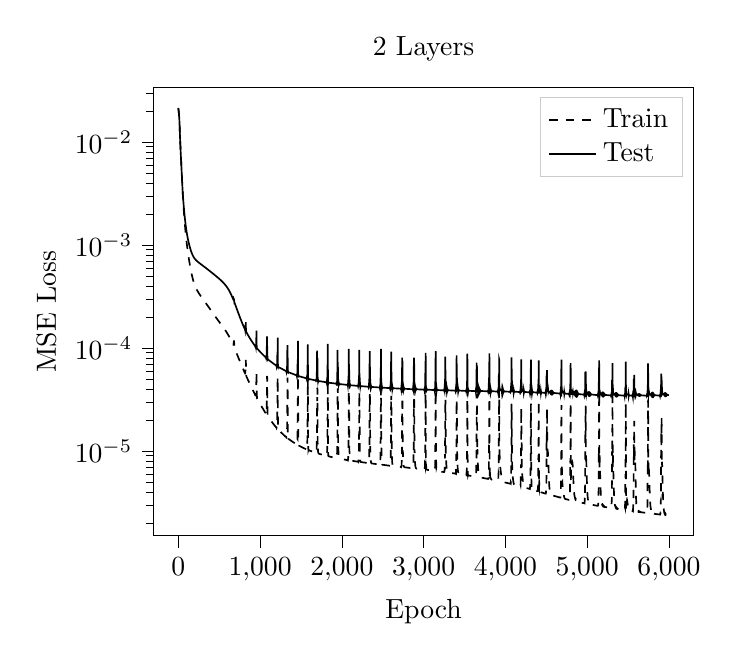
\begin{tikzpicture}

\begin{axis}[
legend cell align={left},
legend style={fill opacity=0.8, draw opacity=1, text opacity=1, draw=white!80!black},
log basis y={10},
tick align=outside,
tick pos=left,
title={2 Layers},
x grid style={white!69.0196078431373!black},
xlabel={Epoch},
xmin=-299.95, xmax=6298.95,
xtick style={color=black},
y grid style={white!69.0196078431373!black},
ylabel={MSE Loss},
ymin=1.49876339532141e-06, ymax=0.0337766142020771,
ymode=log,
ytick style={color=black}
]
\addplot [semithick, black, dashed]
table {%
0 0.0212835291167721
1 0.0209709201008081
2 0.0206604937557131
3 0.0203468892723322
4 0.0200276001123711
5 0.0197003402281553
6 0.0193627760745585
7 0.0190122253261507
8 0.0186453343485482
9 0.018257693038322
10 0.0178435965790413
11 0.0173961486434564
12 0.0169080773484893
13 0.0163732900400646
14 0.0157890768605284
15 0.0151585350977257
16 0.0144921822356991
17 0.0138077663723379
18 0.0131277163745835
19 0.0124744565982837
20 0.0118649328360334
21 0.0113068613864016
22 0.0107990419783164
23 0.0103351587895304
24 0.00990795821417123
25 0.00951141366385855
26 0.00914097490021959
27 0.00879311389871873
28 0.00846492176060565
29 0.00815390821662731
30 0.0078579168766737
31 0.00757508585229516
32 0.0073038155969698
33 0.00704274249437731
34 0.0067907179472968
35 0.00654679370927624
36 0.00631021165463608
37 0.00608039209328126
38 0.00585692764434498
39 0.0056395746069029
40 0.00542824204603676
41 0.00522296805866063
42 0.00502390101610217
43 0.00483126989274751
44 0.00464535255741794
45 0.0044664430024568
46 0.00429481566243339
47 0.0041306984203402
48 0.00397424669063184
49 0.00382552624068921
50 0.00368450347014004
51 0.00355104677146301
52 0.00342493510106578
53 0.00330586984637193
54 0.00319349668279756
55 0.00308742181368871
56 0.00298723114246968
57 0.00289250764035387
58 0.00280284290784039
59 0.00271784712822409
60 0.00263715513574425
61 0.00256043241097359
62 0.00248737349465955
63 0.00241770431603072
64 0.00235117984993849
65 0.0022875825088704
66 0.00222671995288692
67 0.00216842070221901
68 0.00211253295856295
69 0.00205892113444861
70 0.00200746243353933
71 0.00195804541726829
72 0.00191056720359484
73 0.00186493250657804
74 0.0018210515663668
75 0.00177884013100993
76 0.0017382187070325
77 0.00169911208649864
78 0.00166144936156343
79 0.00162516390992096
80 0.00159019229613477
81 0.00155647517749458
82 0.00152395624900237
83 0.0014925822179066
84 0.00146230302198092
85 0.00143307093821932
86 0.00140484069925151
87 0.00137756968979375
88 0.00135121732091648
89 0.00132574438248412
90 0.0013011138253205
91 0.00127729073210503
92 0.00125424084762926
93 0.00123193179024383
94 0.0012103327026125
95 0.00118941368054948
96 0.00116914581667515
97 0.00114950210263487
98 0.00113045599573525
99 0.00111198268496082
100 0.00109405747207347
101 0.001076657903468
102 0.00105976162922161
103 0.00104334752904833
104 0.00102739570320409
105 0.00101188684311637
106 0.000996802940790076
107 0.000982126501185121
108 0.000967841358942678
109 0.000953931703406852
110 0.000940382613407564
111 0.000927179975406034
112 0.00091431058535818
113 0.000901761790373712
114 0.000889521421413519
115 0.000877578177096439
116 0.000865921165313921
117 0.000854539954161737
118 0.00084342502123036
119 0.000832567187899258
120 0.000821957301013754
121 0.000811587156931637
122 0.000801448784841341
123 0.000791534812378814
124 0.000781837961767451
125 0.000772351286286721
126 0.000763068481319351
127 0.000753983182221418
128 0.000745089619158534
129 0.000736381889510085
130 0.000727854980141274
131 0.000719503657819587
132 0.000711322942152037
133 0.000703308222000487
134 0.00069545500264212
135 0.000687759107677266
136 0.000680216387991095
137 0.000672822949127294
138 0.000665574953018222
139 0.000658469014524599
140 0.000651501652100706
141 0.000644669500616146
142 0.000637969569652341
143 0.00063139878147922
144 0.000624954182057991
145 0.000618633132035029
146 0.00061243284289958
147 0.000606350933594513
148 0.000600384812059929
149 0.000594532228205935
150 0.000588790827350749
151 0.000583158471272327
152 0.000577633250031795
153 0.000572212878068967
154 0.000566895577321702
155 0.000561679484235356
156 0.000556562861675047
157 0.000551543812434829
158 0.000546620746717963
159 0.000541792177500611
160 0.000537056354005472
161 0.000532411843778391
162 0.000527857301676704
163 0.000523391223396175
164 0.000519012070071767
165 0.000514718762133271
166 0.000510509913510759
167 0.00050638417906157
168 0.000502340313687455
169 0.000498377177791554
170 0.000494493579026312
171 0.000490688227728242
172 0.000486959947011201
173 0.000483307637296093
174 0.000479730210827256
175 0.000476226341561414
176 0.000472795103632961
177 0.000469435270133545
178 0.000466145657810557
179 0.000462925217107113
180 0.000459772802969383
181 0.000456687198493455
182 0.00045366736685537
183 0.000450712132078479
184 0.000447820332738047
185 0.000444990751930163
186 0.000442222256424429
187 0.000439513644778344
188 0.000436863762843132
189 0.000434271428275679
190 0.000431735400525213
191 0.000429254400842183
192 0.000426827363298798
193 0.000424452950028353
194 0.000422129868638876
195 0.00041985699954239
196 0.000417633137658413
197 0.000415456985138007
198 0.000413327252317686
199 0.000411242761401809
200 0.000409202270020614
201 0.000407204591283516
202 0.000405248494644184
203 0.000403332782298094
204 0.000401456267354661
205 0.000399617719267553
206 0.000397816037548182
207 0.000396050035305962
208 0.000394318637518154
209 0.000392620709135372
210 0.000390955163311446
211 0.000389320898648293
212 0.000387716946534056
213 0.000386142261049827
214 0.000384595800824172
215 0.000383076668185822
216 0.000381583879971004
217 0.000380116502128658
218 0.000378673728846479
219 0.000377254610611999
220 0.000375858355255332
221 0.000374484189705981
222 0.000373131245396507
223 0.000371798872038198
224 0.00037048621015856
225 0.00036919266131008
226 0.000367917541552742
227 0.000366660158761078
228 0.000365419830814062
229 0.000364196102964343
230 0.000362988326742197
231 0.000361795916433039
232 0.000360618317245098
233 0.000359455096258898
234 0.000358305675945303
235 0.000357169661583612
236 0.000356046508386498
237 0.000354935875293449
238 0.000353837280272273
239 0.000352750322235806
240 0.000351674641933641
241 0.000350609845554573
242 0.000349555614320707
243 0.000348511529409734
244 0.000347477314335265
245 0.000346452682606468
246 0.000345437299984042
247 0.000344430845416355
248 0.000343433106991142
249 0.000342443785484647
250 0.00034146259940826
251 0.000340489317750325
252 0.000339523713137169
253 0.000338565578658745
254 0.000337614693307842
255 0.000336670759679691
256 0.000335733682732098
257 0.000334803171426756
258 0.000333879145728133
259 0.000332961301410251
260 0.000332049531152734
261 0.000331143702169356
262 0.000330243582538969
263 0.000329349081312102
264 0.000328459986121743
265 0.000327576157815201
266 0.000326697446325852
267 0.000325823801631486
268 0.000324954977713787
269 0.000324090905451158
270 0.000323231467064033
271 0.000322376559779514
272 0.000321526030802488
273 0.000320679730066331
274 0.000319837633014686
275 0.000318999605497083
276 0.000318165566568496
277 0.000317335358886339
278 0.000316508972446172
279 0.000315686233534507
280 0.000314867138968111
281 0.000314051535951876
282 0.000313239377646823
283 0.000312430555823084
284 0.000311625043650565
285 0.000310822694700619
286 0.00031002349260234
287 0.000309227326852124
288 0.000308434162434423
289 0.000307643951600767
290 0.000306856613860873
291 0.000306072059629514
292 0.000305290267988312
293 0.000304511192098289
294 0.000303734711451398
295 0.000302960817862186
296 0.000302189495869243
297 0.000301420629966742
298 0.000300654196507821
299 0.000299890170936123
300 0.000299128453661979
301 0.000298369082884165
302 0.000297611956284527
303 0.000296857044304488
304 0.000296104348763038
305 0.00029535374869738
306 0.000294605310500629
307 0.000293858930490387
308 0.000293114578198583
309 0.000292372245894512
310 0.000291631909931311
311 0.000290893471628806
312 0.000290157015115255
313 0.00028942244080099
314 0.000288689738226822
315 0.000287958839180646
316 0.000287229798686894
317 0.000286502543076494
318 0.000285777067801973
319 0.000285053336483543
320 0.00028433132729333
321 0.000283611043414567
322 0.000282892443919991
323 0.000282175550637476
324 0.000281460283531487
325 0.00028074666761313
326 0.000280034712886845
327 0.000279324344319321
328 0.000278615579190955
329 0.000277908417501749
330 0.000277202803772525
331 0.00027649878666125
332 0.000275796291134611
333 0.000275095383130974
334 0.000274395958058449
335 0.000273698045475612
336 0.000273001670393569
337 0.000272306785518595
338 0.000271613438599161
339 0.000270921532774082
340 0.00027023115353586
341 0.000269542266323697
342 0.000268854797013773
343 0.000268168811089708
344 0.000267484311279986
345 0.00026680126438805
346 0.000266119655861985
347 0.000265439519807842
348 0.000264760818936338
349 0.000264083599176956
350 0.000263407777765678
351 0.000262733398812998
352 0.000262060460954672
353 0.000261389004208468
354 0.000260718962181272
355 0.000260050356700958
356 0.000259383179809447
357 0.00025871745265249
358 0.000258053147035753
359 0.000257390274782665
360 0.000256728878639478
361 0.000256068846510971
362 0.000255410300724179
363 0.000254753194894874
364 0.00025409756449335
365 0.00025344332630084
366 0.000252790539207126
367 0.000252139207532309
368 0.000251489334232247
369 0.000250840912713102
370 0.000250193932743059
371 0.000249548391821008
372 0.000248904350200974
373 0.000248261751039536
374 0.000247620606614873
375 0.000246980962629095
376 0.000246342738137173
377 0.000245706064561091
378 0.000245070803657654
379 0.000244437061382996
380 0.000243804778392587
381 0.000243173983108136
382 0.000242544692355295
383 0.000241916904087702
384 0.000241290593066879
385 0.00024066579430837
386 0.000240042484392688
387 0.000239420719481132
388 0.00023880043590907
389 0.000238181705981333
390 0.000237564478766217
391 0.000236948768133516
392 0.000236334597957466
393 0.000235721970057057
394 0.000235110862149668
395 0.000234501306067614
396 0.000233893292488574
397 0.000233286828233759
398 0.000232681912621047
399 0.000232078536782865
400 0.00023147675187829
401 0.000230876489467846
402 0.000230277823447977
403 0.000229680716074654
404 0.000229085205319279
405 0.000228491238203787
406 0.000227898853381703
407 0.000227308074954635
408 0.000226718850854013
409 0.00022613124815507
410 0.000225545247303671
411 0.000224960824652953
412 0.000224377980202917
413 0.000223796763521023
414 0.000223217161192224
415 0.000222639147978043
416 0.000222062747525342
417 0.000221487964836342
418 0.000220914781266401
419 0.000220343206819962
420 0.00021977328333378
421 0.000219204961695141
422 0.00021863827805646
423 0.000218073168298361
424 0.00021750975906798
425 0.000216947934404743
426 0.000216387733189549
427 0.000215829196349659
428 0.000215272255218224
429 0.000214716957316341
430 0.000214163296732295
431 0.000213611262779523
432 0.000213060887517713
433 0.000212512133884957
434 0.000211965010521453
435 0.00021141953584447
436 0.000210875673701594
437 0.000210333495488157
438 0.000209792890700555
439 0.000209253949378763
440 0.000208716653560259
441 0.000208180989375251
442 0.000207646947956164
443 0.000207114552949861
444 0.000206583779799985
445 0.000206054658974608
446 0.000205527158641416
447 0.000205001271979199
448 0.00020447701899684
449 0.000203954396056361
450 0.000203433382921503
451 0.00020291398777772
452 0.000202396238364599
453 0.000201880081931449
454 0.000201365517114027
455 0.00020085259939151
456 0.000200341276467952
457 0.000199831560848907
458 0.00019932342456741
459 0.000198816901956889
460 0.000198311955955432
461 0.000197808621010154
462 0.000197306861082325
463 0.000196806678218309
464 0.000196308070940177
465 0.000195811017420056
466 0.000195315541077434
467 0.000194821637478526
468 0.000194329267060311
469 0.00019383846290566
470 0.00019334919954872
471 0.00019286146880404
472 0.000192375271581113
473 0.000191890600035549
474 0.000191407439729119
475 0.000190925796687225
476 0.000190445680573248
477 0.000189967021469784
478 0.0001894898870205
479 0.000189014217880867
480 0.000188540029171236
481 0.000188067305202821
482 0.000187596055184258
483 0.000187126251148584
484 0.000186657883546104
485 0.000186190972158329
486 0.000185725460937647
487 0.000185261374667789
488 0.000184798706982292
489 0.000184337417294955
490 0.000183877531753751
491 0.000183419036602572
492 0.000182961882501331
493 0.000182506102419211
494 0.000182051671913541
495 0.000181598564267915
496 0.000181146790396269
497 0.00018069633927098
498 0.000180247191451599
499 0.000179799328293484
500 0.000179352746499717
501 0.000178907439590148
502 0.000178463376983018
503 0.000178020571411253
504 0.000177578992861527
505 0.000177138630874651
506 0.000176699482608456
507 0.000176261518163301
508 0.000175824737652874
509 0.00017538913948556
510 0.000174954689100559
511 0.000174521354892931
512 0.000174089162328528
513 0.000173658060930393
514 0.000173228072526399
515 0.000172799163010495
516 0.000172371311691677
517 0.000171944514136158
518 0.000171518747720256
519 0.000171094000393168
520 0.00017067026112727
521 0.000170247502410348
522 0.000169825703324022
523 0.000169404866028344
524 0.000168984988022203
525 0.000168566005754656
526 0.000168147926956408
527 0.000167730754810691
528 0.000167314430996157
529 0.000166898949601091
530 0.000166484299825242
531 0.000166070492014114
532 0.000165657448178536
533 0.000165245200491881
534 0.000164833710869061
535 0.000164422951343113
536 0.000164012900540911
537 0.00016360359063583
538 0.000163194935225874
539 0.000162786918394886
540 0.000162379573907856
541 0.000161972838668589
542 0.000161566704150573
543 0.0001611611652379
544 0.000160756166224019
545 0.000160351704266759
546 0.000159947766405821
547 0.000159544339226159
548 0.000159141367248594
549 0.000158738846721462
550 0.0001583367669582
551 0.000157935101015028
552 0.000157533826154577
553 0.000157132900426404
554 0.000156732324626319
555 0.000156332058850239
556 0.000155932104689782
557 0.000155532416442838
558 0.000155132973418404
559 0.000154733789827333
560 0.000154334783701415
561 0.000153935975390596
562 0.000153537325900288
563 0.000153138796122221
564 0.000152740397311391
565 0.000152342085812052
566 0.000151943816263156
567 0.000151545616290605
568 0.000151147423196107
569 0.000150749227032065
570 0.000150350987439651
571 0.000149952702145129
572 0.000149554328061186
573 0.000149155862288808
574 0.000148757270835631
575 0.000148358524143077
576 0.000147959615389937
577 0.000147560498703569
578 0.000147161141910601
579 0.00014676156411042
580 0.000146361690553931
581 0.000145961517205251
582 0.000145561032184105
583 0.000145160233387287
584 0.000144759042939313
585 0.000144357475448942
586 0.000143955486976211
587 0.000143553048644662
588 0.000143150158805838
589 0.000142746790913861
590 0.000142342901995107
591 0.000141938516378559
592 0.000141533546241135
593 0.000141128024040427
594 0.000140721892023521
595 0.00014031516252544
596 0.000139907767902514
597 0.000139499729243653
598 0.000139091010169068
599 0.000138681571570487
600 0.000138271436469495
601 0.000137860556321812
602 0.000137448898328785
603 0.000137036466753671
604 0.000136623274613612
605 0.000136209213053462
606 0.000135794349546359
607 0.000135378641687112
608 0.000134962033826014
609 0.000134544553418436
610 0.000134126206887686
611 0.000133706905046438
612 0.000133286677737487
613 0.000132865575210417
614 0.000132443432448781
615 0.000132020353021289
616 0.000131596364440156
617 0.0001311712618417
618 0.000130745207854943
619 0.000130318246533534
620 0.000129890120319942
621 0.000129460998152808
622 0.000129031021856463
623 0.000128599785625738
624 0.000128167531784129
625 0.000127734460875217
626 0.000127300062388258
627 0.000126864648677838
628 0.000126428511464383
629 0.000125990946969523
630 0.000125552300346499
631 0.000125113127012355
632 0.000124672398214898
633 0.000124230474511933
634 0.000123788367432098
635 0.000123344523615287
636 0.000122899294126455
637 0.000122454416839446
638 0.000122007555717119
639 0.000121558966895918
640 0.000121111522730644
641 0.00012066183484194
642 0.000120209703595719
643 0.000119760050893092
644 0.000119307866839335
645 0.000118851873594394
646 0.000118400442659095
647 0.000117946346279041
648 0.00011748591577998
649 0.000117033311994419
650 0.000116578293614111
651 0.000116112402508861
652 0.000115659428502113
653 0.000115205272379626
654 0.000114732217241453
655 0.0001142799800391
656 0.000113829913743757
657 0.000113347268268171
658 0.000112897413316659
659 0.000112457237776198
660 0.000111962505059182
661 0.000111518200810679
662 0.000111098184731873
663 0.000110593016643179
664 0.000110161510917806
665 0.000109779833223911
666 0.000109286403016995
667 0.000108886284067466
668 0.000108577541595878
669 0.00010819459242839
670 0.00010787321468797
671 0.000107718260949241
672 0.000107785517116099
673 0.000107656141949519
674 0.000107900192176658
675 0.000109297616688764
676 0.000109578056537885
677 0.000110879725241375
678 0.000114251636830431
679 0.000114603493557297
680 0.000116473329626388
681 0.000116469009526554
682 0.000113329918349336
683 0.000112076105438064
684 0.000107009406065117
685 0.0001026171223657
686 0.000101317310566174
687 0.000100158012173779
688 9.9327592863574e-05
689 9.8789685068823e-05
690 9.83735112640716e-05
691 9.79368714411066e-05
692 9.75170637502742e-05
693 9.70842903598168e-05
694 9.66536702549092e-05
695 9.62349453175193e-05
696 9.58054440616252e-05
697 9.53838317627742e-05
698 9.4963705180362e-05
699 9.45420809443931e-05
700 9.4123706787741e-05
701 9.37060037813353e-05
702 9.32894906782167e-05
703 9.28744348698274e-05
704 9.24606716239396e-05
705 9.20483371942282e-05
706 9.16373142558768e-05
707 9.12278061377947e-05
708 9.08197532112354e-05
709 9.04131520087503e-05
710 9.00080966061978e-05
711 8.96045759759545e-05
712 8.9202608648975e-05
713 8.88022374851971e-05
714 8.84034880641593e-05
715 8.80063685713139e-05
716 8.76109128853386e-05
717 8.72171136734323e-05
718 8.68250134544724e-05
719 8.64346214370926e-05
720 8.60459674072445e-05
721 8.56590414741731e-05
722 8.52738768912786e-05
723 8.4890469054244e-05
724 8.45088619598755e-05
725 8.41290383277737e-05
726 8.37510245901285e-05
727 8.33748067066153e-05
728 8.30004177032606e-05
729 8.26278564431959e-05
730 8.22571327034893e-05
731 8.18882298290191e-05
732 8.15211780604841e-05
733 8.11559680755636e-05
734 8.0792618518899e-05
735 8.04311118258738e-05
736 8.00714378215162e-05
737 7.97136295886958e-05
738 7.93576651290095e-05
739 7.90035527984401e-05
740 7.86512652553029e-05
741 7.8300844450041e-05
742 7.79522591756177e-05
743 7.76054826587824e-05
744 7.72605648649005e-05
745 7.69174453694177e-05
746 7.65761523098263e-05
747 7.62366663025205e-05
748 7.5898994509771e-05
749 7.55631047013594e-05
750 7.52290073933182e-05
751 7.48966893411307e-05
752 7.45661383803053e-05
753 7.42373434263754e-05
754 7.3910306923608e-05
755 7.3585018412814e-05
756 7.32614412299881e-05
757 7.29395892449247e-05
758 7.2619471723101e-05
759 7.2301013346987e-05
760 7.19842519742997e-05
761 7.16691951652138e-05
762 7.13557795393172e-05
763 7.10440105535781e-05
764 7.07339166865495e-05
765 7.0425407784569e-05
766 7.01185355183043e-05
767 6.98133043783855e-05
768 6.95095938567647e-05
769 6.92075005872539e-05
770 6.89070154180627e-05
771 6.8607992602665e-05
772 6.83105864709432e-05
773 6.80147480238702e-05
774 6.77202819474587e-05
775 6.74274557468379e-05
776 6.71361451054509e-05
777 6.68461250370456e-05
778 6.65577895802016e-05
779 6.62709173298026e-05
780 6.59851806403822e-05
781 6.57012569718063e-05
782 6.54186995348027e-05
783 6.51370916102678e-05
784 6.48575633590553e-05
785 6.45792111981791e-05
786 6.43015417836068e-05
787 6.40264204321284e-05
788 6.37521198427748e-05
789 6.34781316648514e-05
790 6.32075708040247e-05
791 6.29371293712211e-05
792 6.26665072331889e-05
793 6.24008608838267e-05
794 6.21339834196988e-05
795 6.18662135707382e-05
796 6.16062736185086e-05
797 6.13424347761793e-05
798 6.10767839930304e-05
799 6.08241289796752e-05
800 6.05623681622092e-05
801 6.02977937091964e-05
802 6.00555445089412e-05
803 5.97942158151454e-05
804 5.95295049379274e-05
805 5.93038477063601e-05
806 5.90402228226594e-05
807 5.87757228913688e-05
808 5.85789659339753e-05
809 5.83099006234988e-05
810 5.80555828264551e-05
811 5.79132693019346e-05
812 5.76401992589126e-05
813 5.74516344613585e-05
814 5.74205243992765e-05
815 5.71735995436029e-05
816 5.73002139390155e-05
817 5.75197896068858e-05
818 5.7453578165223e-05
819 5.88839302508859e-05
820 5.97032222060534e-05
821 6.04024381232193e-05
822 6.59345604958617e-05
823 6.74619723213254e-05
824 6.92578064729332e-05
825 7.6783088729826e-05
826 7.30325907625229e-05
827 6.98225327369073e-05
828 6.3422335301766e-05
829 5.65620411521195e-05
830 5.53574395212308e-05
831 5.41374883482604e-05
832 5.3012844659861e-05
833 5.28669662571701e-05
834 5.26105138476396e-05
835 5.24332158136076e-05
836 5.22052741303014e-05
837 5.19956660127718e-05
838 5.18026845952591e-05
839 5.15811403545285e-05
840 5.1385549141969e-05
841 5.118176676433e-05
842 5.09784324833618e-05
843 5.07801880189618e-05
844 5.05795478886739e-05
845 5.0381089010898e-05
846 5.01832527390889e-05
847 4.99861358491671e-05
848 4.97899528113521e-05
849 4.95944151452932e-05
850 4.93998708748222e-05
851 4.92059874090955e-05
852 4.90129492050073e-05
853 4.88207603552837e-05
854 4.86292692301049e-05
855 4.8438638486914e-05
856 4.82487916997343e-05
857 4.80596992531446e-05
858 4.78714345035769e-05
859 4.76839416592156e-05
860 4.74972141546459e-05
861 4.73113163650396e-05
862 4.71261658674393e-05
863 4.69418013437917e-05
864 4.67582445367043e-05
865 4.65754186507183e-05
866 4.63933991170506e-05
867 4.62121705879781e-05
868 4.60316833823526e-05
869 4.58520003405738e-05
870 4.56730841449371e-05
871 4.54949240804581e-05
872 4.53175552479479e-05
873 4.51409566153416e-05
874 4.49651157907738e-05
875 4.47900653455235e-05
876 4.46157698945626e-05
877 4.44422425118773e-05
878 4.42694817763822e-05
879 4.40974888533674e-05
880 4.39262555289588e-05
881 4.37557942802869e-05
882 4.35860818299716e-05
883 4.34171467134092e-05
884 4.32489565582728e-05
885 4.30815402125972e-05
886 4.29148618366071e-05
887 4.27489674734716e-05
888 4.2583806134644e-05
889 4.24194095671737e-05
890 4.22557807553403e-05
891 4.2092871154864e-05
892 4.19307309300621e-05
893 4.17693398730989e-05
894 4.16086821246608e-05
895 4.14487880391334e-05
896 4.12896411887687e-05
897 4.11311987988938e-05
898 4.09735466746497e-05
899 4.08166019667533e-05
900 4.06603694500518e-05
901 4.05049458720441e-05
902 4.03501765049441e-05
903 4.0196160313144e-05
904 4.00429349269871e-05
905 3.98903249845262e-05
906 3.97384984296423e-05
907 3.95874538128282e-05
908 3.94369548359919e-05
909 3.92873271835015e-05
910 3.91384394617944e-05
911 3.89900107506946e-05
912 3.88426049937607e-05
913 3.8695816613199e-05
914 3.85494158479105e-05
915 3.84042674852481e-05
916 3.82595014798426e-05
917 3.8115048681675e-05
918 3.79722781644887e-05
919 3.78293624123671e-05
920 3.76868523801477e-05
921 3.75466484570097e-05
922 3.7405251276823e-05
923 3.72647408255489e-05
924 3.71274040276148e-05
925 3.69869295866465e-05
926 3.68486941795254e-05
927 3.67147253541589e-05
928 3.65739716414737e-05
929 3.64388962736939e-05
930 3.63090271662259e-05
931 3.61657584164732e-05
932 3.60360099875834e-05
933 3.59113325885119e-05
934 3.57615912491838e-05
935 3.56420959803927e-05
936 3.5524546774468e-05
937 3.5362238605785e-05
938 3.52634807541108e-05
939 3.51577418200577e-05
940 3.49783750550614e-05
941 3.49213352137667e-05
942 3.48419375200137e-05
943 3.46695783264295e-05
944 3.46965336177618e-05
945 3.46883942086151e-05
946 3.47127681550319e-05
947 3.49330067308529e-05
948 3.51135918492673e-05
949 3.62745781501417e-05
950 3.71210029186386e-05
951 3.77143524588064e-05
952 4.34279637602231e-05
953 4.62504493157212e-05
954 4.71086129323339e-05
955 5.94989059834461e-05
956 5.93012429135342e-05
957 5.47628900449126e-05
958 4.90509355302038e-05
959 3.82615310456913e-05
960 3.57851230319284e-05
961 3.4583016599754e-05
962 3.26616389259016e-05
963 3.24346934235109e-05
964 3.22145002087382e-05
965 3.21614615756971e-05
966 3.20025341693508e-05
967 3.1905695976775e-05
968 3.17969511058891e-05
969 3.16800213226998e-05
970 3.15867085589616e-05
971 3.14754261694361e-05
972 3.13757444985185e-05
973 3.1273503623197e-05
974 3.11717871852579e-05
975 3.10711404836184e-05
976 3.09701569563003e-05
977 3.08704915710223e-05
978 3.07703946589299e-05
979 3.06712478277404e-05
980 3.05723940527969e-05
981 3.04737512522024e-05
982 3.03757973654228e-05
983 3.02780501044708e-05
984 3.01807411631216e-05
985 3.00838802615999e-05
986 2.99873392464178e-05
987 2.98912323160039e-05
988 2.97954998984551e-05
989 2.97001417663978e-05
990 2.9605172585434e-05
991 2.9510582066905e-05
992 2.94163691876292e-05
993 2.93225432415056e-05
994 2.92290737178291e-05
995 2.91359811086522e-05
996 2.90432614349356e-05
997 2.89509039816949e-05
998 2.88589216665969e-05
999 2.87672941965411e-05
1000 2.86760442662626e-05
1001 2.85851468220244e-05
1002 2.84946171973388e-05
1003 2.84044312053311e-05
1004 2.83146067374673e-05
1005 2.82251532439659e-05
1006 2.81360373293182e-05
1007 2.80472867615345e-05
1008 2.79588877702963e-05
1009 2.78708289442875e-05
1010 2.77831272796902e-05
1011 2.76957675282574e-05
1012 2.76087558148674e-05
1013 2.75220954222277e-05
1014 2.74357764880051e-05
1015 2.7349785966635e-05
1016 2.72641452028211e-05
1017 2.71788500612047e-05
1018 2.70938873967452e-05
1019 2.7009263632749e-05
1020 2.69249810571637e-05
1021 2.68410105803696e-05
1022 2.67574045409447e-05
1023 2.66741054275599e-05
1024 2.65911451577949e-05
1025 2.65085232342699e-05
1026 2.64262227602785e-05
1027 2.6344233347686e-05
1028 2.62626051608095e-05
1029 2.6181270897041e-05
1030 2.61002657140352e-05
1031 2.60196053432082e-05
1032 2.59392241730438e-05
1033 2.58591913251394e-05
1034 2.57794985998316e-05
1035 2.57000704237953e-05
1036 2.5621009243082e-05
1037 2.55422429233931e-05
1038 2.54637504184529e-05
1039 2.53856669871766e-05
1040 2.53078196692513e-05
1041 2.5230256511577e-05
1042 2.51531465664812e-05
1043 2.50761725908433e-05
1044 2.4999569561146e-05
1045 2.49234289668721e-05
1046 2.48472686905643e-05
1047 2.47716665455755e-05
1048 2.46964720531651e-05
1049 2.46210494765364e-05
1050 2.45465723196503e-05
1051 2.44722288158528e-05
1052 2.43974674276615e-05
1053 2.43243403446058e-05
1054 2.42506016832067e-05
1055 2.41764897737085e-05
1056 2.41050937148657e-05
1057 2.40313925417013e-05
1058 2.39581931538169e-05
1059 2.38890914374679e-05
1060 2.38142129092012e-05
1061 2.37429377989429e-05
1062 2.367688247773e-05
1063 2.35984988847804e-05
1064 2.35319306653992e-05
1065 2.34698215280105e-05
1066 2.33843106940412e-05
1067 2.33286351658535e-05
1068 2.32718803516718e-05
1069 2.31776480887902e-05
1070 2.31446065299679e-05
1071 2.30954374274006e-05
1072 2.3015544073246e-05
1073 2.3030252918943e-05
1074 2.29827125224347e-05
1075 2.3067924814768e-05
1076 2.32428892701364e-05
1077 2.31147555780353e-05
1078 2.3996751821187e-05
1079 2.50564360584349e-05
1080 2.44874114088134e-05
1081 2.79896395483092e-05
1082 3.34105169770282e-05
1083 3.22522711684314e-05
1084 3.97968647831703e-05
1085 5.34463645749383e-05
1086 5.26126714248676e-05
1087 5.10330321503716e-05
1088 4.15302602476686e-05
1089 3.16319235196261e-05
1090 2.85177275998194e-05
1091 2.46126399474633e-05
1092 2.23692249079477e-05
1093 2.19217270824856e-05
1094 2.19858800249995e-05
1095 2.17810468825519e-05
1096 2.16880937387032e-05
1097 2.15006482733315e-05
1098 2.14564986436017e-05
1099 2.13896479266396e-05
1100 2.13400927151497e-05
1101 2.12832223809301e-05
1102 2.12312697271955e-05
1103 2.11776651752871e-05
1104 2.11232915319215e-05
1105 2.10718370965424e-05
1106 2.10180317594677e-05
1107 2.09660569225889e-05
1108 2.09136353248596e-05
1109 2.0861629849378e-05
1110 2.08097463172408e-05
1111 2.07580746121039e-05
1112 2.07066356523455e-05
1113 2.06552842456631e-05
1114 2.06042395660688e-05
1115 2.05532958972299e-05
1116 2.05025573478679e-05
1117 2.04520004558617e-05
1118 2.04016195510803e-05
1119 2.0351423316356e-05
1120 2.03013966881826e-05
1121 2.02515423524119e-05
1122 2.02018610195864e-05
1123 2.0152355844516e-05
1124 2.01030267845681e-05
1125 2.00538609789191e-05
1126 2.00048716010315e-05
1127 1.99560537055277e-05
1128 1.99074008122579e-05
1129 1.98589204245536e-05
1130 1.98105985873553e-05
1131 1.97624556932396e-05
1132 1.97144729696674e-05
1133 1.9666662424811e-05
1134 1.9619007545657e-05
1135 1.95715231967597e-05
1136 1.95242037364096e-05
1137 1.94770496619867e-05
1138 1.94300539106962e-05
1139 1.93832319723697e-05
1140 1.93365569032267e-05
1141 1.9290059427135e-05
1142 1.92437121881994e-05
1143 1.91975357353158e-05
1144 1.91515198793013e-05
1145 1.91056510630006e-05
1146 1.90599585465634e-05
1147 1.90144107961032e-05
1148 1.89690371144025e-05
1149 1.89238210452913e-05
1150 1.88787476673724e-05
1151 1.8833844137589e-05
1152 1.87890962166648e-05
1153 1.87444927632896e-05
1154 1.87000772911006e-05
1155 1.86557851975522e-05
1156 1.86116614457887e-05
1157 1.85677008062157e-05
1158 1.8523875027654e-05
1159 1.84802266858242e-05
1160 1.84367256252926e-05
1161 1.83933616426657e-05
1162 1.83501744004388e-05
1163 1.83071235397847e-05
1164 1.82642167771974e-05
1165 1.82215015200882e-05
1166 1.81788800830418e-05
1167 1.8136449526196e-05
1168 1.80941869984963e-05
1169 1.80519938055568e-05
1170 1.80100504820757e-05
1171 1.79682040055695e-05
1172 1.7926458994566e-05
1173 1.78850087877436e-05
1174 1.78435474538219e-05
1175 1.7802275209533e-05
1176 1.77613137140042e-05
1177 1.77201705611196e-05
1178 1.76794459179064e-05
1179 1.76389299184621e-05
1180 1.75980749332894e-05
1181 1.75580255614705e-05
1182 1.75177940917592e-05
1183 1.74772407888213e-05
1184 1.74380731294832e-05
1185 1.73977736892539e-05
1186 1.73578032587329e-05
1187 1.73196650194996e-05
1188 1.72786620709076e-05
1189 1.7240084758896e-05
1190 1.7202904373903e-05
1191 1.71603114011987e-05
1192 1.71248964733195e-05
1193 1.70879218117648e-05
1194 1.70437000335255e-05
1195 1.70142290158992e-05
1196 1.69747735583314e-05
1197 1.69348703096261e-05
1198 1.69163993319899e-05
1199 1.6864487292878e-05
1200 1.68554062227599e-05
1201 1.68732388061699e-05
1202 1.67812876625817e-05
1203 1.68634318598038e-05
1204 1.70648097324033e-05
1205 1.69621649277474e-05
1206 1.71480264228308e-05
1207 1.80765712798348e-05
1208 1.88761268589133e-05
1209 1.89988255101525e-05
1210 2.14257015755948e-05
1211 2.83444005901856e-05
1212 3.03315529350812e-05
1213 3.2029213159035e-05
1214 4.94456834161383e-05
1215 5.26222975167911e-05
1216 4.57585651929548e-05
1217 3.57277575915305e-05
1218 2.1234510391821e-05
1219 1.77151128895048e-05
1220 1.71958521377746e-05
1221 1.63123360437112e-05
1222 1.62258578342289e-05
1223 1.61946954762016e-05
1224 1.61702844607703e-05
1225 1.60801882387318e-05
1226 1.6034826295197e-05
1227 1.596839572926e-05
1228 1.59452682026995e-05
1229 1.59121711362786e-05
1230 1.5884068616856e-05
1231 1.58541725738814e-05
1232 1.58256273152801e-05
1233 1.57968142957543e-05
1234 1.57675923162515e-05
1235 1.57395529569726e-05
1236 1.57106097660176e-05
1237 1.56824221591023e-05
1238 1.56541203395477e-05
1239 1.56258806711662e-05
1240 1.55978421005898e-05
1241 1.55698074451038e-05
1242 1.55419083540664e-05
1243 1.55140806938903e-05
1244 1.54863427965779e-05
1245 1.54586842100457e-05
1246 1.54311105546867e-05
1247 1.54036136947866e-05
1248 1.53762062922169e-05
1249 1.53488711234218e-05
1250 1.53216174183513e-05
1251 1.52944399332e-05
1252 1.52673392719294e-05
1253 1.52403156263858e-05
1254 1.52133730111359e-05
1255 1.51865004056617e-05
1256 1.51597133069004e-05
1257 1.51329872508654e-05
1258 1.51063405127161e-05
1259 1.50797711953032e-05
1260 1.50532748151022e-05
1261 1.50268502991935e-05
1262 1.50004939030168e-05
1263 1.49742159507582e-05
1264 1.49480169611138e-05
1265 1.49218832916631e-05
1266 1.48958247905284e-05
1267 1.48698330377783e-05
1268 1.48439161051783e-05
1269 1.48180806149867e-05
1270 1.47923009592432e-05
1271 1.47665972463074e-05
1272 1.47409724107206e-05
1273 1.47154046317155e-05
1274 1.46899257913446e-05
1275 1.46644984369004e-05
1276 1.4639145298645e-05
1277 1.46138720964473e-05
1278 1.45886549418606e-05
1279 1.45635150659018e-05
1280 1.45384582026509e-05
1281 1.45134481499554e-05
1282 1.44885170527687e-05
1283 1.44636595322822e-05
1284 1.44388506271298e-05
1285 1.44141373610296e-05
1286 1.43894734776495e-05
1287 1.43648794974638e-05
1288 1.43403801473596e-05
1289 1.43159008558769e-05
1290 1.429152574417e-05
1291 1.42672267031685e-05
1292 1.42429312077752e-05
1293 1.42187935878724e-05
1294 1.41946679690363e-05
1295 1.41705657838997e-05
1296 1.4146682666194e-05
1297 1.41226843339837e-05
1298 1.40988330272762e-05
1299 1.40751681172446e-05
1300 1.40512552988525e-05
1301 1.40277575226833e-05
1302 1.40042204179736e-05
1303 1.39804017322831e-05
1304 1.39573891999589e-05
1305 1.39337599520672e-05
1306 1.39102184562034e-05
1307 1.38877578521601e-05
1308 1.38636158837357e-05
1309 1.38409881671464e-05
1310 1.38189123433108e-05
1311 1.37937922204401e-05
1312 1.37732359846154e-05
1313 1.37508451132362e-05
1314 1.37254439778189e-05
1315 1.37082435074376e-05
1316 1.36832342363391e-05
1317 1.36640856780446e-05
1318 1.36528606660136e-05
1319 1.3617125240728e-05
1320 1.36238472592254e-05
1321 1.36419242053876e-05
1322 1.35895228652316e-05
1323 1.36352188064848e-05
1324 1.37862029276903e-05
1325 1.38938374547593e-05
1326 1.39356142980773e-05
1327 1.43067451716661e-05
1328 1.57947242200862e-05
1329 1.66386500097815e-05
1330 1.641833552668e-05
1331 2.21109084890259e-05
1332 3.04171362586203e-05
1333 3.01076619280138e-05
1334 3.45073318257505e-05
1335 4.91547483605359e-05
1336 5.15744175118016e-05
1337 4.48025859896006e-05
1338 2.98069395512357e-05
1339 1.58800857974484e-05
1340 1.34702957268473e-05
1341 1.38357369863229e-05
1342 1.35945819437211e-05
1343 1.34899305521685e-05
1344 1.32207643730453e-05
1345 1.31636951365977e-05
1346 1.31409235564206e-05
1347 1.31245692429616e-05
1348 1.31012074788828e-05
1349 1.30834871683305e-05
1350 1.30593101559384e-05
1351 1.30439216334821e-05
1352 1.30255464014795e-05
1353 1.30088795842198e-05
1354 1.29912015012223e-05
1355 1.29747261183866e-05
1356 1.29573943681294e-05
1357 1.29407151661098e-05
1358 1.29238836024115e-05
1359 1.29071496886013e-05
1360 1.28904723482037e-05
1361 1.28738563844877e-05
1362 1.28572707822627e-05
1363 1.28407266615227e-05
1364 1.28242414163537e-05
1365 1.28077851471176e-05
1366 1.27913807119739e-05
1367 1.27750044569552e-05
1368 1.27586749982811e-05
1369 1.27423742455335e-05
1370 1.2726104387184e-05
1371 1.2709879726458e-05
1372 1.26936954671919e-05
1373 1.26775413136215e-05
1374 1.26614145727899e-05
1375 1.26453173905361e-05
1376 1.26292720636911e-05
1377 1.26132497513254e-05
1378 1.25972640745431e-05
1379 1.25813047517909e-05
1380 1.2565380167473e-05
1381 1.25494887797117e-05
1382 1.25336311000979e-05
1383 1.25178034835471e-05
1384 1.25020029599909e-05
1385 1.24862419994543e-05
1386 1.24705143704773e-05
1387 1.24548104025735e-05
1388 1.2439140675724e-05
1389 1.2423503392256e-05
1390 1.24078897627555e-05
1391 1.23923219135236e-05
1392 1.23767733697377e-05
1393 1.23612557842989e-05
1394 1.23457776837199e-05
1395 1.23303225549876e-05
1396 1.23148964163988e-05
1397 1.22995077234123e-05
1398 1.22841465497459e-05
1399 1.22688115098413e-05
1400 1.2253516693761e-05
1401 1.22382386678055e-05
1402 1.22230037646887e-05
1403 1.22077947040111e-05
1404 1.21926083309631e-05
1405 1.21774706016708e-05
1406 1.21623456692532e-05
1407 1.21472559442282e-05
1408 1.21322014905445e-05
1409 1.21171697387013e-05
1410 1.21021752121919e-05
1411 1.20872052775667e-05
1412 1.20722583716315e-05
1413 1.2057359477069e-05
1414 1.20424716527623e-05
1415 1.20276269939268e-05
1416 1.20128121423591e-05
1417 1.19980062294189e-05
1418 1.19832682443644e-05
1419 1.19685263300084e-05
1420 1.19538215699322e-05
1421 1.19391783073297e-05
1422 1.19244939824625e-05
1423 1.1909918903541e-05
1424 1.18953408474454e-05
1425 1.18807312077251e-05
1426 1.18663064085922e-05
1427 1.18517460307999e-05
1428 1.18372650561582e-05
1429 1.18229631951294e-05
1430 1.18083664304436e-05
1431 1.17941315451731e-05
1432 1.17798570187233e-05
1433 1.17652335163143e-05
1434 1.17513956219284e-05
1435 1.1736894915515e-05
1436 1.17224949320871e-05
1437 1.1709108907354e-05
1438 1.16939063232735e-05
1439 1.16805836292144e-05
1440 1.16674183097132e-05
1441 1.16511043692924e-05
1442 1.16401550940282e-05
1443 1.16266164802425e-05
1444 1.16116163546565e-05
1445 1.16036749950865e-05
1446 1.15862553755619e-05
1447 1.15868761945137e-05
1448 1.15904495316954e-05
1449 1.15565226863623e-05
1450 1.15957331878747e-05
1451 1.16820594051603e-05
1452 1.16924354749415e-05
1453 1.17252634304066e-05
1454 1.20240405863115e-05
1455 1.28227138205261e-05
1456 1.31683183752784e-05
1457 1.31220205759064e-05
1458 1.68150557016133e-05
1459 2.24623648676925e-05
1460 2.24547652294405e-05
1461 2.58241760136002e-05
1462 4.36967132131372e-05
1463 5.33360018835083e-05
1464 4.79261070722714e-05
1465 3.59054196508168e-05
1466 1.89201515610193e-05
1467 1.29434822753183e-05
1468 1.23942462408877e-05
1469 1.15135925078391e-05
1470 1.1434421214318e-05
1471 1.14868102407684e-05
1472 1.14393301444693e-05
1473 1.13955816729572e-05
1474 1.13180502125942e-05
1475 1.12889970580454e-05
1476 1.12666676557183e-05
1477 1.12582739966172e-05
1478 1.12439436605882e-05
1479 1.12338548881041e-05
1480 1.12197603350239e-05
1481 1.1210175021148e-05
1482 1.11984442447977e-05
1483 1.11881870950015e-05
1484 1.11773770008483e-05
1485 1.11669305091766e-05
1486 1.11563173526008e-05
1487 1.11458636453676e-05
1488 1.11354045273515e-05
1489 1.11249368366373e-05
1490 1.11145712509142e-05
1491 1.11041581227767e-05
1492 1.10938187525278e-05
1493 1.10834796309689e-05
1494 1.10731559495036e-05
1495 1.10628578191552e-05
1496 1.10525775127712e-05
1497 1.10423207715371e-05
1498 1.10320790263074e-05
1499 1.10218541493623e-05
1500 1.10116509723923e-05
1501 1.10014569933981e-05
1502 1.09912862171768e-05
1503 1.09811235873281e-05
1504 1.09709746034525e-05
1505 1.0960850509889e-05
1506 1.09507375150031e-05
1507 1.0940640304824e-05
1508 1.09305536462045e-05
1509 1.09204866198809e-05
1510 1.09104347991718e-05
1511 1.09003937858176e-05
1512 1.0890371651584e-05
1513 1.0880359187837e-05
1514 1.08703601107152e-05
1515 1.0860383980571e-05
1516 1.08504145650556e-05
1517 1.08404647782834e-05
1518 1.08305234398642e-05
1519 1.08205974811426e-05
1520 1.08106854845857e-05
1521 1.08007867289928e-05
1522 1.0790903282043e-05
1523 1.0781035484797e-05
1524 1.07711779158137e-05
1525 1.07613378830251e-05
1526 1.07515084799559e-05
1527 1.07416908932123e-05
1528 1.07318939157608e-05
1529 1.07220981604428e-05
1530 1.07123359143202e-05
1531 1.07025727800192e-05
1532 1.06928195329203e-05
1533 1.06831005872721e-05
1534 1.06733733780118e-05
1535 1.06636750309974e-05
1536 1.0653991338927e-05
1537 1.06442946048446e-05
1538 1.06346479853414e-05
1539 1.06249946121295e-05
1540 1.06153454701996e-05
1541 1.06057521627179e-05
1542 1.05961131637855e-05
1543 1.05865330972676e-05
1544 1.05769741693962e-05
1545 1.05673506141102e-05
1546 1.05578623035285e-05
1547 1.05482932255541e-05
1548 1.05387268192203e-05
1549 1.0529333128062e-05
1550 1.05196954507392e-05
1551 1.05102866072571e-05
1552 1.05009152555624e-05
1553 1.04911894567294e-05
1554 1.04820757940161e-05
1555 1.04725248917248e-05
1556 1.046291029283e-05
1557 1.04541568290983e-05
1558 1.04440239034886e-05
1559 1.04352081820025e-05
1560 1.04266239553397e-05
1561 1.04155844731224e-05
1562 1.04085572587564e-05
1563 1.03996407787577e-05
1564 1.03897957686172e-05
1565 1.03848586761046e-05
1566 1.03724792950288e-05
1567 1.03745801887101e-05
1568 1.03792035233141e-05
1569 1.03556571140473e-05
1570 1.03788975742702e-05
1571 1.04401345595306e-05
1572 1.04787252404037e-05
1573 1.04940426233213e-05
1574 1.06113289639609e-05
1575 1.12407074439602e-05
1576 1.17713315397339e-05
1577 1.15310470292229e-05
1578 1.32441190210386e-05
1579 1.82317990322645e-05
1580 2.0819380267767e-05
1581 2.05120980076856e-05
1582 3.08935223820583e-05
1583 4.97714706853003e-05
1584 4.87041963879165e-05
1585 4.014167529931e-05
1586 2.49011549513511e-05
1587 1.31509888845471e-05
1588 1.16423008407196e-05
1589 1.09114900652685e-05
1590 1.0282616635493e-05
1591 1.03507356072896e-05
1592 1.03582922044154e-05
1593 1.03315486761346e-05
1594 1.02594608044626e-05
1595 1.02123884673233e-05
1596 1.01728715726779e-05
1597 1.01664355085518e-05
1598 1.01543973869411e-05
1599 1.01480058205539e-05
1600 1.01376378189855e-05
1601 1.01312515390362e-05
1602 1.01225679678407e-05
1603 1.01157475747016e-05
1604 1.01082930044072e-05
1605 1.01010499733434e-05
1606 1.00938801246286e-05
1607 1.00866639023423e-05
1608 1.00795328492609e-05
1609 1.0072362840674e-05
1610 1.00652795893552e-05
1611 1.00581564517199e-05
1612 1.005108299168e-05
1613 1.00440090697873e-05
1614 1.00369455218186e-05
1615 1.00299101220003e-05
1616 1.00228722814677e-05
1617 1.00158586953114e-05
1618 1.0008844700593e-05
1619 1.0001840703211e-05
1620 9.99485350661189e-06
1621 9.98786854466971e-06
1622 9.98089896597776e-06
1623 9.97393535229207e-06
1624 9.96697702149163e-06
1625 9.96003537423462e-06
1626 9.95308921147853e-06
1627 9.94616382499203e-06
1628 9.93923966419175e-06
1629 9.93232261947696e-06
1630 9.92541693989324e-06
1631 9.91851182519099e-06
1632 9.91162135832724e-06
1633 9.90473470707798e-06
1634 9.89785083405081e-06
1635 9.89098037251779e-06
1636 9.88411609270656e-06
1637 9.87725638879056e-06
1638 9.87040593258826e-06
1639 9.86356099730301e-06
1640 9.85671723086057e-06
1641 9.84989033270267e-06
1642 9.84305988893652e-06
1643 9.83624369510494e-06
1644 9.82943818428339e-06
1645 9.82261886406377e-06
1646 9.81583596626479e-06
1647 9.80903438119185e-06
1648 9.80224744751013e-06
1649 9.7954758899732e-06
1650 9.78868899892404e-06
1651 9.78193756040469e-06
1652 9.77517442279918e-06
1653 9.76840546229596e-06
1654 9.76168263733257e-06
1655 9.75492240584686e-06
1656 9.74819072396826e-06
1657 9.74148685628506e-06
1658 9.73472537424414e-06
1659 9.7280474946615e-06
1660 9.72133399912423e-06
1661 9.71459515497486e-06
1662 9.70797896471254e-06
1663 9.70120265719743e-06
1664 9.69455848576217e-06
1665 9.68795126254918e-06
1666 9.68112271948485e-06
1667 9.67464572454446e-06
1668 9.66792297774077e-06
1669 9.66114244960181e-06
1670 9.65486076509592e-06
1671 9.64782175927326e-06
1672 9.64144435045e-06
1673 9.63520493257874e-06
1674 9.6277202956685e-06
1675 9.62222674161239e-06
1676 9.61552484213257e-06
1677 9.60860115739592e-06
1678 9.60419481543795e-06
1679 9.59529887367694e-06
1680 9.59266676403558e-06
1681 9.59144954748581e-06
1682 9.57901279363682e-06
1683 9.58228441660935e-06
1684 9.59127746824606e-06
1685 9.60438481101278e-06
1686 9.61544722244412e-06
1687 9.60638628555444e-06
1688 9.75972938377367e-06
1689 9.97909460309643e-06
1690 9.92997445337096e-06
1691 1.01313212930165e-05
1692 1.13473594751667e-05
1693 1.29649697058198e-05
1694 1.31113625521095e-05
1695 1.42512498868541e-05
1696 2.37311687669717e-05
1697 3.24842221175459e-05
1698 3.04923530620727e-05
1699 3.34698657127319e-05
1700 4.13233522138512e-05
1701 4.00491508116829e-05
1702 3.36603388859658e-05
1703 2.11707151436258e-05
1704 1.20213124574775e-05
1705 1.06150756522538e-05
1706 1.10936002997164e-05
1707 1.07415168457692e-05
1708 1.03472158912155e-05
1709 9.87066982105489e-06
1710 9.72140787780518e-06
1711 9.64533312242111e-06
1712 9.61165594404179e-06
1713 9.54792848872899e-06
1714 9.50908034980102e-06
1715 9.46760664533031e-06
1716 9.45345046332591e-06
1717 9.43439399492263e-06
1718 9.42699767136901e-06
1719 9.41418882050016e-06
1720 9.4088758118005e-06
1721 9.39984975545372e-06
1722 9.39544948508342e-06
1723 9.38856527454845e-06
1724 9.38407683293008e-06
1725 9.37812647805458e-06
1726 9.37341456719309e-06
1727 9.36793720640594e-06
1728 9.36303322163212e-06
1729 9.3578111766135e-06
1730 9.35279804537004e-06
1731 9.34769431282234e-06
1732 9.34263838558991e-06
1733 9.33759256582789e-06
1734 9.33254125001781e-06
1735 9.32751646232077e-06
1736 9.32248028817639e-06
1737 9.31746745180817e-06
1738 9.3124519544574e-06
1739 9.30744225513536e-06
1740 9.30244148023007e-06
1741 9.29744368605157e-06
1742 9.29245628711328e-06
1743 9.28746737471897e-06
1744 9.28248514497909e-06
1745 9.27750842549813e-06
1746 9.27253200444511e-06
1747 9.26756361607772e-06
1748 9.26259791711459e-06
1749 9.25764166836984e-06
1750 9.25268115281597e-06
1751 9.24772670884977e-06
1752 9.24277682301522e-06
1753 9.237831722686e-06
1754 9.23288912701992e-06
1755 9.22794484736755e-06
1756 9.2230084653977e-06
1757 9.21807705722699e-06
1758 9.2131449775934e-06
1759 9.20822192895798e-06
1760 9.20329638631756e-06
1761 9.19836863388923e-06
1762 9.19345149341666e-06
1763 9.18853866949121e-06
1764 9.18362898261194e-06
1765 9.17872379702089e-06
1766 9.17381060006051e-06
1767 9.16890851954122e-06
1768 9.16400469819223e-06
1769 9.15910720777902e-06
1770 9.15421379232839e-06
1771 9.14931987949785e-06
1772 9.14443095823003e-06
1773 9.13954088588298e-06
1774 9.1346615853638e-06
1775 9.12978094547157e-06
1776 9.12489361581947e-06
1777 9.12002447606142e-06
1778 9.11514915102885e-06
1779 9.11026954142358e-06
1780 9.1054127082657e-06
1781 9.10053403657685e-06
1782 9.09567384965726e-06
1783 9.09082537603467e-06
1784 9.08594386217487e-06
1785 9.08111299757763e-06
1786 9.0762511089082e-06
1787 9.07138531935914e-06
1788 9.06657719035309e-06
1789 9.0616870700444e-06
1790 9.05687176278036e-06
1791 9.0520498794433e-06
1792 9.04713789573464e-06
1793 9.04240747523488e-06
1794 9.03750836656059e-06
1795 9.03265428497946e-06
1796 9.02798137225602e-06
1797 9.02293023763434e-06
1798 9.01829062271986e-06
1799 9.0135462667007e-06
1800 9.00839695638922e-06
1801 9.00413459348215e-06
1802 8.99893043282418e-06
1803 8.99424896338985e-06
1804 8.99037319257445e-06
1805 8.98411508210017e-06
1806 8.98093339252171e-06
1807 8.97731290550041e-06
1808 8.97135879895927e-06
1809 8.97019149626033e-06
1810 8.96391911808792e-06
1811 8.96793512161764e-06
1812 8.9769333282419e-06
1813 8.95992860172612e-06
1814 8.97932580912197e-06
1815 9.04124258838124e-06
1816 9.0925166027489e-06
1817 9.1100562613633e-06
1818 9.17269167466372e-06
1819 9.73672798565417e-06
1820 1.04263942652949e-05
1821 1.0259200271534e-05
1822 1.11091683372422e-05
1823 1.56660922172591e-05
1824 2.04053811216909e-05
1825 2.00953370494972e-05
1826 2.44486417670942e-05
1827 4.4564289680693e-05
1828 4.9856585519592e-05
1829 4.14331359479547e-05
1830 2.8013235976232e-05
1831 1.29033851905547e-05
1832 9.2828058555483e-06
1833 9.28007346701065e-06
1834 9.01015787491133e-06
1835 8.96054107712985e-06
1836 8.95475785966937e-06
1837 8.9096033715208e-06
1838 8.89763686728884e-06
1839 8.88682972188803e-06
1840 8.87147633577001e-06
1841 8.86806985356259e-06
1842 8.86296153623789e-06
1843 8.85882442780428e-06
1844 8.85405450468113e-06
1845 8.85028403274646e-06
1846 8.84547836754734e-06
1847 8.84173069159999e-06
1848 8.83752335134602e-06
1849 8.83357536096696e-06
1850 8.82958527093081e-06
1851 8.82564900450689e-06
1852 8.8216995788315e-06
1853 8.81779819295048e-06
1854 8.8138976366281e-06
1855 8.80999925811921e-06
1856 8.80613334430791e-06
1857 8.80226074961854e-06
1858 8.79840899870032e-06
1859 8.7945618290064e-06
1860 8.79071469839232e-06
1861 8.78688027761143e-06
1862 8.78304942020236e-06
1863 8.7792264480413e-06
1864 8.77540518828823e-06
1865 8.77159251011506e-06
1866 8.76777838421106e-06
1867 8.76397370142001e-06
1868 8.76016957285231e-06
1869 8.75636687069914e-06
1870 8.75257402732643e-06
1871 8.74877858514367e-06
1872 8.74498541136859e-06
1873 8.74119986526978e-06
1874 8.73741152496166e-06
1875 8.73362852260584e-06
1876 8.72984726818515e-06
1877 8.72606745794258e-06
1878 8.7222882072524e-06
1879 8.71851532657786e-06
1880 8.7147400673615e-06
1881 8.71096574073249e-06
1882 8.70719223478034e-06
1883 8.70343018277708e-06
1884 8.69965794869643e-06
1885 8.69589341156995e-06
1886 8.69212668241914e-06
1887 8.68836387191152e-06
1888 8.68460298164564e-06
1889 8.68084175742467e-06
1890 8.67708222962449e-06
1891 8.67332185272573e-06
1892 8.66956554368414e-06
1893 8.66580963254648e-06
1894 8.66205528460284e-06
1895 8.65830043572657e-06
1896 8.65454745024863e-06
1897 8.65079740819397e-06
1898 8.6470421845064e-06
1899 8.64329549976617e-06
1900 8.63954304897163e-06
1901 8.63579236209944e-06
1902 8.63205372070297e-06
1903 8.62829633874185e-06
1904 8.62455697969722e-06
1905 8.62081003027981e-06
1906 8.61706056554112e-06
1907 8.61333584722956e-06
1908 8.60957637094373e-06
1909 8.60584177253543e-06
1910 8.60210973741005e-06
1911 8.59833985522584e-06
1912 8.5946424235317e-06
1913 8.5908896707565e-06
1914 8.58712332707512e-06
1915 8.58346420251621e-06
1916 8.57963110689752e-06
1917 8.5759558245968e-06
1918 8.57227531980698e-06
1919 8.56836926388382e-06
1920 8.56488310141401e-06
1921 8.5609922511054e-06
1922 8.55722427317573e-06
1923 8.55393578191865e-06
1924 8.54954921614137e-06
1925 8.54641441883075e-06
1926 8.54310001052738e-06
1927 8.53850604620732e-06
1928 8.53652470667043e-06
1929 8.53175474269108e-06
1930 8.52994627997816e-06
1931 8.53124871191824e-06
1932 8.52205158174968e-06
1933 8.52597892198048e-06
1934 8.5390045683198e-06
1935 8.54723153054238e-06
1936 8.55790257681122e-06
1937 8.55812229616504e-06
1938 8.6971052297713e-06
1939 8.913857053372e-06
1940 8.86746120265514e-06
1941 9.03464672497023e-06
1942 1.02671822226341e-05
1943 1.20573897142151e-05
1944 1.23312028730282e-05
1945 1.30571900029963e-05
1946 2.30121401258998e-05
1947 3.46330344882517e-05
1948 3.31539968101424e-05
1949 3.37682780582327e-05
1950 4.06019005474434e-05
1951 3.93406422745102e-05
1952 3.25121338846657e-05
1953 2.08656847320299e-05
1954 1.19055438680959e-05
1955 1.0612001346999e-05
1956 1.1150031596685e-05
1957 1.05782959280987e-05
1958 9.96529447760963e-06
1959 9.3215592826823e-06
1960 9.11875005371598e-06
1961 8.98647559921528e-06
1962 8.89987137142612e-06
1963 8.76898092627698e-06
1964 8.68478058180244e-06
1965 8.60628305332511e-06
1966 8.57053408509501e-06
1967 8.52948881302495e-06
1968 8.50841833965887e-06
1969 8.48096245675833e-06
1970 8.46905741447301e-06
1971 8.45241380353912e-06
1972 8.4463518774669e-06
1973 8.43586130550023e-06
1974 8.43219419444097e-06
1975 8.42497930442221e-06
1976 8.42231287911943e-06
1977 8.41702417986312e-06
1978 8.41460304101815e-06
1979 8.41038301579999e-06
1980 8.40787428479928e-06
1981 8.40424321602029e-06
1982 8.40157454895518e-06
1983 8.3982727066001e-06
1984 8.39546302700001e-06
1985 8.39234206928552e-06
1986 8.38944034775579e-06
1987 8.38641957123798e-06
1988 8.38347565768061e-06
1989 8.38050198836982e-06
1990 8.3775396628738e-06
1991 8.37458855151851e-06
1992 8.3716353174168e-06
1993 8.36868614406683e-06
1994 8.36573726736844e-06
1995 8.36279323124245e-06
1996 8.3598529094786e-06
1997 8.35691177769604e-06
1998 8.35397451481867e-06
1999 8.35103801577475e-06
2000 8.34810519378948e-06
2001 8.34517340386753e-06
2002 8.34224178092313e-06
2003 8.33931236599028e-06
2004 8.33638005737214e-06
2005 8.3334570089022e-06
2006 8.33053071680467e-06
2007 8.32760345659267e-06
2008 8.32468181322099e-06
2009 8.32175097364996e-06
2010 8.31882715601751e-06
2011 8.3159042336689e-06
2012 8.31298408066061e-06
2013 8.31006117074651e-06
2014 8.30713661770233e-06
2015 8.3042110130549e-06
2016 8.30129443585292e-06
2017 8.29836981530718e-06
2018 8.29544922531511e-06
2019 8.29252983791662e-06
2020 8.28960722643046e-06
2021 8.28668197172533e-06
2022 8.28376433581468e-06
2023 8.28084093384973e-06
2024 8.27792000990257e-06
2025 8.27500073796728e-06
2026 8.27207655618167e-06
2027 8.26915233709258e-06
2028 8.26623165828266e-06
2029 8.26330890824067e-06
2030 8.2603826427885e-06
2031 8.25746075072686e-06
2032 8.25453785857633e-06
2033 8.25161419015785e-06
2034 8.24869294113739e-06
2035 8.24576401647903e-06
2036 8.24284374800754e-06
2037 8.23991634923971e-06
2038 8.23699143026602e-06
2039 8.2340703357886e-06
2040 8.23113216696925e-06
2041 8.22821688295505e-06
2042 8.22527925770089e-06
2043 8.22234685848855e-06
2044 8.21944197682001e-06
2045 8.21649056526041e-06
2046 8.21357520841559e-06
2047 8.21065003897559e-06
2048 8.20769019682643e-06
2049 8.2047961473819e-06
2050 8.20183615424241e-06
2051 8.19890031955595e-06
2052 8.19603134161184e-06
2053 8.19299458676426e-06
2054 8.19015396658074e-06
2055 8.18721768247599e-06
2056 8.18415961845176e-06
2057 8.18147422698701e-06
2058 8.17828609278592e-06
2059 8.17546227693811e-06
2060 8.17284258758377e-06
2061 8.16930258729087e-06
2062 8.16706750050855e-06
2063 8.16403499293017e-06
2064 8.16090840594086e-06
2065 8.15967468170697e-06
2066 8.15472586346289e-06
2067 8.1541371628191e-06
2068 8.15555361377562e-06
2069 8.1500807667112e-06
2070 8.15232549022937e-06
2071 8.15377675600359e-06
2072 8.17318782608822e-06
2073 8.20096484588362e-06
2074 8.17495830318649e-06
2075 8.2381181094604e-06
2076 8.456668897594e-06
2077 8.61995009771022e-06
2078 8.62454201033813e-06
2079 8.94762769654278e-06
2080 1.07947952869836e-05
2081 1.28430832333493e-05
2082 1.23664509228405e-05
2083 1.49517994394444e-05
2084 2.76812294686124e-05
2085 3.74820092474693e-05
2086 3.51447761204327e-05
2087 3.46482745214871e-05
2088 3.58245896379117e-05
2089 2.86591078975107e-05
2090 2.22118323449649e-05
2091 1.48021854400326e-05
2092 9.9721948174647e-06
2093 9.86870748675983e-06
2094 9.78401098450377e-06
2095 9.52154605471378e-06
2096 8.96731528854389e-06
2097 8.63921503935217e-06
2098 8.43419959295488e-06
2099 8.3748317152299e-06
2100 8.29337558982957e-06
2101 8.24174519209464e-06
2102 8.17938113684136e-06
2103 8.15235988227414e-06
2104 8.12298684671475e-06
2105 8.11329663541471e-06
2106 8.09778543597872e-06
2107 8.09289145564662e-06
2108 8.08349893866023e-06
2109 8.08096622506582e-06
2110 8.075239382066e-06
2111 8.07335241859164e-06
2112 8.0693613977445e-06
2113 8.06738941250273e-06
2114 8.06420675303343e-06
2115 8.062039645651e-06
2116 8.05926535818458e-06
2117 8.05692313221584e-06
2118 8.05435071704608e-06
2119 8.05192411412747e-06
2120 8.0494413143839e-06
2121 8.04698151668504e-06
2122 8.04453122960069e-06
2123 8.04207666860179e-06
2124 8.03963944129293e-06
2125 8.03719272646219e-06
2126 8.03475963095934e-06
2127 8.03232562596179e-06
2128 8.02989171688751e-06
2129 8.02746786376929e-06
2130 8.02503912034069e-06
2131 8.02261570775897e-06
2132 8.02019566492618e-06
2133 8.01777329151321e-06
2134 8.01535532168884e-06
2135 8.01293628605038e-06
2136 8.01052253507351e-06
2137 8.00810702017429e-06
2138 8.0056896401004e-06
2139 8.00327708638804e-06
2140 8.00086393226707e-06
2141 7.99845246035602e-06
2142 7.99603869872101e-06
2143 7.99362513248525e-06
2144 7.99121275463222e-06
2145 7.98880151542392e-06
2146 7.98638816768005e-06
2147 7.98397641155191e-06
2148 7.981561221726e-06
2149 7.97915114247871e-06
2150 7.97673599173265e-06
2151 7.97432261734343e-06
2152 7.97191242618567e-06
2153 7.96949546533199e-06
2154 7.96708014938474e-06
2155 7.96466368591098e-06
2156 7.96224944998869e-06
2157 7.95983334889172e-06
2158 7.95741706838271e-06
2159 7.95499955508205e-06
2160 7.95257660257676e-06
2161 7.95015653842768e-06
2162 7.94773867163201e-06
2163 7.94531500858398e-06
2164 7.94290123096175e-06
2165 7.94047504015793e-06
2166 7.93804648857588e-06
2167 7.93563106071815e-06
2168 7.9331953930506e-06
2169 7.93077601635161e-06
2170 7.92835218810239e-06
2171 7.92590968146101e-06
2172 7.92350318867818e-06
2173 7.92104822622264e-06
2174 7.91862466442694e-06
2175 7.91621702589396e-06
2176 7.91372880826202e-06
2177 7.91135694377942e-06
2178 7.90889140134254e-06
2179 7.90642230263927e-06
2180 7.90408607187487e-06
2181 7.90151496232738e-06
2182 7.89916690813186e-06
2183 7.89678261625681e-06
2184 7.89413054569366e-06
2185 7.89200633555254e-06
2186 7.88932617012961e-06
2187 7.88691701991695e-06
2188 7.88498866555187e-06
2189 7.88173916355106e-06
2190 7.88008747498736e-06
2191 7.87797907797483e-06
2192 7.87501115873113e-06
2193 7.87456720985347e-06
2194 7.87028257143163e-06
2195 7.87096337617754e-06
2196 7.87492984777316e-06
2197 7.86807175856552e-06
2198 7.87198160701053e-06
2199 7.88333503010108e-06
2200 7.90945090933803e-06
2201 7.93578368885051e-06
2202 7.91088930540695e-06
2203 8.02615999795364e-06
2204 8.32409542006474e-06
2205 8.45505887525633e-06
2206 8.44423124846116e-06
2207 9.13476613106923e-06
2208 1.15147511507985e-05
2209 1.3384927463278e-05
2210 1.26761764427386e-05
2211 1.71859021111942e-05
2212 3.12157254995782e-05
2213 3.77019472352913e-05
2214 3.42967366577795e-05
2215 3.14977073685441e-05
2216 2.76497366087369e-05
2217 2.16094996403626e-05
2218 1.70536549717326e-05
2219 1.19861417857692e-05
2220 8.97703382207737e-06
2221 8.92503887683915e-06
2222 8.85528981342532e-06
2223 8.69881913700965e-06
2224 8.34531034854535e-06
2225 8.12690542772998e-06
2226 7.98047587835526e-06
2227 7.94280544624826e-06
2228 7.89858926353304e-06
2229 7.87748148312062e-06
2230 7.84674741716174e-06
2231 7.83598845366384e-06
2232 7.82156918788246e-06
2233 7.81862735088623e-06
2234 7.81189502419011e-06
2235 7.81021400086956e-06
2236 7.80599927985293e-06
2237 7.80437015279745e-06
2238 7.80136243427876e-06
2239 7.79949427887061e-06
2240 7.79704824083183e-06
2241 7.79497218417191e-06
2242 7.79274008877451e-06
2243 7.79058259325893e-06
2244 7.78842678883507e-06
2245 7.78625565267532e-06
2246 7.78412672097772e-06
2247 7.78197106043876e-06
2248 7.77984449307212e-06
2249 7.77770858029214e-06
2250 7.77558055098382e-06
2251 7.77345308655697e-06
2252 7.77133410601039e-06
2253 7.76921454281876e-06
2254 7.7670976477151e-06
2255 7.7649828824633e-06
2256 7.76287037318468e-06
2257 7.76075753705641e-06
2258 7.75864985058661e-06
2259 7.7565367071486e-06
2260 7.75443268885567e-06
2261 7.75232323846353e-06
2262 7.75022119370306e-06
2263 7.74811127435271e-06
2264 7.74600776409784e-06
2265 7.74390302993311e-06
2266 7.74179510365514e-06
2267 7.73968909051348e-06
2268 7.73758345395947e-06
2269 7.73547661658824e-06
2270 7.73337509762939e-06
2271 7.73126377495714e-06
2272 7.72915879210245e-06
2273 7.72705303653254e-06
2274 7.72494312784033e-06
2275 7.72283500083404e-06
2276 7.72072849741789e-06
2277 7.71861635229243e-06
2278 7.71650518238687e-06
2279 7.71439225566439e-06
2280 7.71227961315901e-06
2281 7.71016651590628e-06
2282 7.70804891914167e-06
2283 7.70593624288551e-06
2284 7.70381647718921e-06
2285 7.70169710939683e-06
2286 7.69958385227199e-06
2287 7.69745984996462e-06
2288 7.6953399528179e-06
2289 7.69321688487423e-06
2290 7.69109050935413e-06
2291 7.68896833847066e-06
2292 7.68684028962241e-06
2293 7.68471102396973e-06
2294 7.68258678363054e-06
2295 7.6804494781868e-06
2296 7.67832412940095e-06
2297 7.67618653085833e-06
2298 7.67404779900005e-06
2299 7.67192368300584e-06
2300 7.66977374944133e-06
2301 7.66763731796516e-06
2302 7.66551171516028e-06
2303 7.66333863388979e-06
2304 7.6612266255438e-06
2305 7.65906873390065e-06
2306 7.65690054649326e-06
2307 7.65481169651139e-06
2308 7.65258384838319e-06
2309 7.65047958850573e-06
2310 7.64836582334283e-06
2311 7.64607941050599e-06
2312 7.64411524656339e-06
2313 7.64182007806369e-06
2314 7.6396505406251e-06
2315 7.63781851098599e-06
2316 7.63514107582353e-06
2317 7.63346225873818e-06
2318 7.63148863747176e-06
2319 7.62883992067032e-06
2320 7.62807971810275e-06
2321 7.62460873282578e-06
2322 7.62409901433614e-06
2323 7.62604679493961e-06
2324 7.62050726521579e-06
2325 7.62281223209982e-06
2326 7.62857435887554e-06
2327 7.64295196731268e-06
2328 7.6617845365945e-06
2329 7.64224376403888e-06
2330 7.71551969336315e-06
2331 7.91917194398195e-06
2332 8.00944786760738e-06
2333 8.0026808149114e-06
2334 8.47465299358419e-06
2335 1.02304778373252e-05
2336 1.17545899556148e-05
2337 1.11688675108468e-05
2338 1.47340961884623e-05
2339 2.76519612043558e-05
2340 3.51906442119798e-05
2341 3.25149676996261e-05
2342 3.440934492005e-05
2343 3.81994554228271e-05
2344 3.12176085799365e-05
2345 2.34260577940404e-05
2346 1.4456848557387e-05
2347 9.7186390703996e-06
2348 9.98349364778051e-06
2349 9.82830638918131e-06
2350 9.40863182563589e-06
2351 8.7130493540144e-06
2352 8.34440790953295e-06
2353 8.13656909315341e-06
2354 8.05761612099332e-06
2355 7.93960044376263e-06
2356 7.85205352471507e-06
2357 7.76199056318205e-06
2358 7.71642612207302e-06
2359 7.67223597719635e-06
2360 7.65020825532758e-06
2361 7.62320897251811e-06
2362 7.61037977881074e-06
2363 7.59387886617446e-06
2364 7.58767891007039e-06
2365 7.57805453588389e-06
2366 7.57492312075669e-06
2367 7.56883731511948e-06
2368 7.56693830084032e-06
2369 7.56280694069744e-06
2370 7.56130148715783e-06
2371 7.55824479981015e-06
2372 7.55673981878147e-06
2373 7.55425788945274e-06
2374 7.55263524432337e-06
2375 7.55045750544525e-06
2376 7.54871435404425e-06
2377 7.54670778668753e-06
2378 7.54488285537036e-06
2379 7.54296256211262e-06
2380 7.5410978297441e-06
2381 7.5392165186372e-06
2382 7.53734626179892e-06
2383 7.53547812237798e-06
2384 7.53360442828921e-06
2385 7.53174659173794e-06
2386 7.52987819119255e-06
2387 7.52802159809107e-06
2388 7.52616178267829e-06
2389 7.52430420725148e-06
2390 7.52244821988768e-06
2391 7.52058989128557e-06
2392 7.51873564652783e-06
2393 7.51687858446815e-06
2394 7.51502607876375e-06
2395 7.51317390701445e-06
2396 7.51132039411573e-06
2397 7.50946920113904e-06
2398 7.50761056700355e-06
2399 7.50575900987371e-06
2400 7.50390125858758e-06
2401 7.50204885058281e-06
2402 7.50019354178733e-06
2403 7.49833699131841e-06
2404 7.49648052789098e-06
2405 7.49462678228952e-06
2406 7.49276872369364e-06
2407 7.49090934348828e-06
2408 7.48904926339833e-06
2409 7.48719034859846e-06
2410 7.48532939098823e-06
2411 7.4834644863131e-06
2412 7.48160160668476e-06
2413 7.47973863823859e-06
2414 7.47786751453816e-06
2415 7.47600541117777e-06
2416 7.47413896995397e-06
2417 7.47226608766027e-06
2418 7.47039768178581e-06
2419 7.46851827848616e-06
2420 7.466651053889e-06
2421 7.46477194013551e-06
2422 7.46289388153798e-06
2423 7.46101768456242e-06
2424 7.45913522948172e-06
2425 7.45725792050678e-06
2426 7.4553758224738e-06
2427 7.45348632058551e-06
2428 7.45160442328086e-06
2429 7.44971644017767e-06
2430 7.44782609629624e-06
2431 7.44593870116717e-06
2432 7.44403429031593e-06
2433 7.44214744941019e-06
2434 7.44024721477388e-06
2435 7.43834408822863e-06
2436 7.43645913026114e-06
2437 7.43453765039703e-06
2438 7.43264489955209e-06
2439 7.43074366837959e-06
2440 7.42880780002508e-06
2441 7.42693565847219e-06
2442 7.4249934964854e-06
2443 7.42307937962039e-06
2444 7.42121163810339e-06
2445 7.41921078706298e-06
2446 7.4173660760124e-06
2447 7.41543687610147e-06
2448 7.41342686083613e-06
2449 7.41169869122871e-06
2450 7.40955062994431e-06
2451 7.40774237151243e-06
2452 7.40603640281279e-06
2453 7.40364104423463e-06
2454 7.40230886719928e-06
2455 7.40014643696441e-06
2456 7.39827060591836e-06
2457 7.39777630265337e-06
2458 7.3940134814876e-06
2459 7.39406054606206e-06
2460 7.39542894656608e-06
2461 7.39327811771773e-06
2462 7.39595052046127e-06
2463 7.39285219886199e-06
2464 7.41229516165731e-06
2465 7.44819917564143e-06
2466 7.43317165508017e-06
2467 7.45717057171191e-06
2468 7.61990985687078e-06
2469 7.89652737687163e-06
2470 8.01876474909591e-06
2471 7.96812544834324e-06
2472 9.26996086469956e-06
2473 1.21449911674176e-05
2474 1.31263867579889e-05
2475 1.28837814816762e-05
2476 2.08452619077093e-05
2477 3.7702743668433e-05
2478 4.05721380047908e-05
2479 3.46880566439722e-05
2480 2.88754750705777e-05
2481 1.97265070909225e-05
2482 1.54813490098604e-05
2483 1.29910307009595e-05
2484 9.42808271986451e-06
2485 8.32257820704285e-06
2486 8.19781190131152e-06
2487 8.20738594597969e-06
2488 7.97629123638899e-06
2489 7.76811988600912e-06
2490 7.56882456087737e-06
2491 7.49353078788317e-06
2492 7.43978704775827e-06
2493 7.41936257675491e-06
2494 7.39052986276079e-06
2495 7.37787999760542e-06
2496 7.3616638598395e-06
2497 7.35742920987548e-06
2498 7.35036131516154e-06
2499 7.34877226804542e-06
2500 7.34491235654389e-06
2501 7.3435587548687e-06
2502 7.34090837894996e-06
2503 7.33941110908631e-06
2504 7.33731929436487e-06
2505 7.33563220656208e-06
2506 7.3337801449469e-06
2507 7.33200151437075e-06
2508 7.33022846510778e-06
2509 7.32843898987312e-06
2510 7.326689431153e-06
2511 7.32491077570785e-06
2512 7.32316563301083e-06
2513 7.32140770232093e-06
2514 7.31966413347607e-06
2515 7.31791960539852e-06
2516 7.31617497429227e-06
2517 7.31443501145179e-06
2518 7.31269799914003e-06
2519 7.31096074879645e-06
2520 7.30922919700561e-06
2521 7.30749474087133e-06
2522 7.30576168450625e-06
2523 7.30403192683582e-06
2524 7.30229623080447e-06
2525 7.30057476516777e-06
2526 7.29884397543401e-06
2527 7.29711147329226e-06
2528 7.29538629684612e-06
2529 7.29365309837249e-06
2530 7.29192117177035e-06
2531 7.29019626710681e-06
2532 7.28846372410885e-06
2533 7.28673329497553e-06
2534 7.28499923852155e-06
2535 7.28326828536296e-06
2536 7.28153472095983e-06
2537 7.27980028614184e-06
2538 7.2780651372284e-06
2539 7.27632969343972e-06
2540 7.27458752258769e-06
2541 7.27285100055042e-06
2542 7.27111024190208e-06
2543 7.26936968931113e-06
2544 7.26762409364312e-06
2545 7.26588162081043e-06
2546 7.26413720997243e-06
2547 7.26239164272613e-06
2548 7.26064075529109e-06
2549 7.25888961738974e-06
2550 7.25713904614622e-06
2551 7.25538600221398e-06
2552 7.25362899700599e-06
2553 7.25187481265266e-06
2554 7.25011585167579e-06
2555 7.2483520678901e-06
2556 7.24659440898279e-06
2557 7.2448261470015e-06
2558 7.24306392285712e-06
2559 7.24129457729816e-06
2560 7.23952075354362e-06
2561 7.23775912447877e-06
2562 7.23597420382305e-06
2563 7.23420326131929e-06
2564 7.23243202394031e-06
2565 7.23063365981602e-06
2566 7.22887446080733e-06
2567 7.22707270917056e-06
2568 7.22528034025061e-06
2569 7.22353193971514e-06
2570 7.2216827700089e-06
2571 7.2199405156681e-06
2572 7.21814698856349e-06
2573 7.21627514010947e-06
2574 7.21462318864496e-06
2575 7.21267709202777e-06
2576 7.21093131872408e-06
2577 7.20930824904542e-06
2578 7.20714573176906e-06
2579 7.20576214163771e-06
2580 7.20383468255648e-06
2581 7.20194075753966e-06
2582 7.20116575436691e-06
2583 7.19804588733552e-06
2584 7.19758711831275e-06
2585 7.19805899507264e-06
2586 7.19541611182706e-06
2587 7.1969592720933e-06
2588 7.19464934562097e-06
2589 7.20644860408015e-06
2590 7.2289510590906e-06
2591 7.2158851978088e-06
2592 7.23463573315541e-06
2593 7.34451400496994e-06
2594 7.51865701786869e-06
2595 7.59615249279477e-06
2596 7.56607258978192e-06
2597 8.46387702502227e-06
2598 1.04483334126826e-05
2599 1.1143051708018e-05
2600 1.09616696235548e-05
2601 1.69160826999359e-05
2602 3.10386302260213e-05
2603 3.53370539301068e-05
2604 3.12296061224515e-05
2605 3.30673242423529e-05
2606 3.07783505064663e-05
2607 2.54154342655966e-05
2608 2.0148122757746e-05
2609 1.23209907627597e-05
2610 9.31395258518819e-06
2611 9.13892613141343e-06
2612 9.21752570093304e-06
2613 8.72108665816995e-06
2614 8.26095438100083e-06
2615 7.85485548249198e-06
2616 7.70397324600935e-06
2617 7.58657640886895e-06
2618 7.50672547411568e-06
2619 7.40792752651487e-06
2620 7.34306465943746e-06
2621 7.28341834133062e-06
2622 7.25283929092768e-06
2623 7.22126137553403e-06
2624 7.2045092061046e-06
2625 7.18483828876515e-06
2626 7.17573928277204e-06
2627 7.16418002966179e-06
2628 7.15979975929315e-06
2629 7.15297504605417e-06
2630 7.15065444722995e-06
2631 7.14628464315581e-06
2632 7.14476274232823e-06
2633 7.14171491011939e-06
2634 7.14038659133109e-06
2635 7.13805091479003e-06
2636 7.13666688234582e-06
2637 7.13468464574873e-06
2638 7.13319776046717e-06
2639 7.13141267105755e-06
2640 7.12983592876526e-06
2641 7.12814878234269e-06
2642 7.12653119450124e-06
2643 7.12488643728193e-06
2644 7.12325326190921e-06
2645 7.12162435867469e-06
2646 7.11999221003623e-06
2647 7.11836632127927e-06
2648 7.11673994757689e-06
2649 7.11512216611254e-06
2650 7.11349973592235e-06
2651 7.11187748514419e-06
2652 7.11025540134358e-06
2653 7.10863568897935e-06
2654 7.10701830897165e-06
2655 7.10539957360368e-06
2656 7.10377865864587e-06
2657 7.10215792487645e-06
2658 7.10054283992179e-06
2659 7.09892368178089e-06
2660 7.09730287518084e-06
2661 7.09568276313632e-06
2662 7.0940646104134e-06
2663 7.09244284635702e-06
2664 7.09081776584242e-06
2665 7.08919666081442e-06
2666 7.08757289480388e-06
2667 7.08594643228366e-06
2668 7.08431999996151e-06
2669 7.0826932692114e-06
2670 7.0810621881634e-06
2671 7.07943390843013e-06
2672 7.07780323061513e-06
2673 7.07616978168346e-06
2674 7.07453793147295e-06
2675 7.07290101864544e-06
2676 7.0712618107649e-06
2677 7.06962552676771e-06
2678 7.06798018867971e-06
2679 7.06634111047322e-06
2680 7.06469834277357e-06
2681 7.06305061193291e-06
2682 7.06140418849088e-06
2683 7.05975416792626e-06
2684 7.05810200329893e-06
2685 7.05644688103746e-06
2686 7.05479426521549e-06
2687 7.05313205173752e-06
2688 7.05147279056462e-06
2689 7.04981484744849e-06
2690 7.04814832630518e-06
2691 7.04648526728135e-06
2692 7.04481195334949e-06
2693 7.04314410704399e-06
2694 7.04147855756787e-06
2695 7.03979652350029e-06
2696 7.03812321134478e-06
2697 7.03644360378064e-06
2698 7.03475505936524e-06
2699 7.03308466931674e-06
2700 7.03138380231394e-06
2701 7.02970371335709e-06
2702 7.0280236261766e-06
2703 7.02629862381343e-06
2704 7.02464388346868e-06
2705 7.02290969201158e-06
2706 7.02121400664169e-06
2707 7.01956825466254e-06
2708 7.01775643641156e-06
2709 7.01616331788557e-06
2710 7.0144190047472e-06
2711 7.01262775137934e-06
2712 7.0111752474844e-06
2713 7.00912226747619e-06
2714 7.00766277184073e-06
2715 7.0062231003476e-06
2716 7.00398592634599e-06
2717 7.00315429824627e-06
2718 7.0008849917258e-06
2719 7.00007455911589e-06
2720 7.00097933936661e-06
2721 6.99654619040757e-06
2722 6.99811560700425e-06
2723 7.00300479117288e-06
2724 7.00999435743199e-06
2725 7.01922643386865e-06
2726 7.00824815780265e-06
2727 7.05908016662704e-06
2728 7.18449947179067e-06
2729 7.23057689633322e-06
2730 7.22808049680168e-06
2731 7.51901458606596e-06
2732 8.61670364926681e-06
2733 9.6672279106258e-06
2734 9.30955948241774e-06
2735 1.11177952319963e-05
2736 1.9763217920854e-05
2737 2.76560085694655e-05
2738 2.6507558089861e-05
2739 2.83913602316943e-05
2740 4.06788086095844e-05
2741 3.90711302316049e-05
2742 3.03344926351201e-05
2743 1.93942824608939e-05
2744 1.03977777392572e-05
2745 9.66242284050622e-06
2746 9.85759109539686e-06
2747 9.52609958204675e-06
2748 8.70973951094811e-06
2749 8.1742692330522e-06
2750 7.86751946790787e-06
2751 7.76078520203782e-06
2752 7.61460071174724e-06
2753 7.48311022036319e-06
2754 7.3505092714754e-06
2755 7.2669616741905e-06
2756 7.19652735625687e-06
2757 7.14990109429436e-06
2758 7.10318651186981e-06
2759 7.07080083728329e-06
2760 7.03943661939377e-06
2761 7.0200548503152e-06
2762 7.00052651758654e-06
2763 6.98907896179435e-06
2764 6.97639521263227e-06
2765 6.96960482393649e-06
2766 6.96131376187736e-06
2767 6.95739380063287e-06
2768 6.95188969501714e-06
2769 6.94950907131897e-06
2770 6.94566330849966e-06
2771 6.94401242640197e-06
2772 6.94115304256115e-06
2773 6.93978092236591e-06
2774 6.93749078273243e-06
2775 6.93616703095756e-06
2776 6.93420527930755e-06
2777 6.93282716568433e-06
2778 6.93106324156645e-06
2779 6.92961939208203e-06
2780 6.92796196055667e-06
2781 6.92646336730718e-06
2782 6.92487222409e-06
2783 6.9233376187583e-06
2784 6.92177993855125e-06
2785 6.92023056281243e-06
2786 6.91868196867063e-06
2787 6.91713552924966e-06
2788 6.91559409382592e-06
2789 6.91404202157742e-06
2790 6.91250145479216e-06
2791 6.91095210036963e-06
2792 6.90940601799639e-06
2793 6.90786323254144e-06
2794 6.90631472544112e-06
2795 6.90476818832053e-06
2796 6.90322509022678e-06
2797 6.90167376049544e-06
2798 6.9001276905567e-06
2799 6.89857858482412e-06
2800 6.89703084155724e-06
2801 6.89547934129564e-06
2802 6.89392744845918e-06
2803 6.89237434592371e-06
2804 6.89082446569955e-06
2805 6.88926324521333e-06
2806 6.88770748702439e-06
2807 6.88614500177209e-06
2808 6.88459015663057e-06
2809 6.88303016538327e-06
2810 6.88146461769179e-06
2811 6.87990096004398e-06
2812 6.87833212964506e-06
2813 6.87676764776768e-06
2814 6.87519643172152e-06
2815 6.87362431150973e-06
2816 6.87204919991302e-06
2817 6.87047260150564e-06
2818 6.86889419121428e-06
2819 6.86731880783498e-06
2820 6.86573290487047e-06
2821 6.86415012118857e-06
2822 6.86256546877928e-06
2823 6.86097638968874e-06
2824 6.85938410427411e-06
2825 6.85779229314676e-06
2826 6.8561939752243e-06
2827 6.85460060445564e-06
2828 6.85300076952444e-06
2829 6.85139928435774e-06
2830 6.84979456622159e-06
2831 6.84818714802304e-06
2832 6.84657741167882e-06
2833 6.84497096159475e-06
2834 6.84335326184282e-06
2835 6.84173700804536e-06
2836 6.84011540030838e-06
2837 6.83849331473141e-06
2838 6.83687542668565e-06
2839 6.83524017475179e-06
2840 6.83361414033357e-06
2841 6.83198330797552e-06
2842 6.83033897352914e-06
2843 6.82871517554418e-06
2844 6.82706533972066e-06
2845 6.82542119001539e-06
2846 6.82379216776496e-06
2847 6.82210998981247e-06
2848 6.82049487465974e-06
2849 6.81882160868952e-06
2850 6.81714753092422e-06
2851 6.81555692771951e-06
2852 6.81379801292792e-06
2853 6.81221199982929e-06
2854 6.81056836704386e-06
2855 6.80876215142234e-06
2856 6.80734212998857e-06
2857 6.80542126829664e-06
2858 6.80388212970229e-06
2859 6.8026114590225e-06
2860 6.80027912558501e-06
2861 6.79939513226202e-06
2862 6.79771542699825e-06
2863 6.79655613033958e-06
2864 6.79730984920468e-06
2865 6.7928126163963e-06
2866 6.79523970070761e-06
2867 6.80333480218565e-06
2868 6.80679213438395e-06
2869 6.8118108060844e-06
2870 6.81147673198268e-06
2871 6.88370422885498e-06
2872 7.01188012897092e-06
2873 7.00993742697165e-06
2874 7.03933668866341e-06
2875 7.58181292326299e-06
2876 8.82707157856544e-06
2877 9.54112214834879e-06
2878 9.14561929654667e-06
2879 1.28712893676663e-05
2880 2.34473820057701e-05
2881 2.87769911437863e-05
2882 2.65296106647384e-05
2883 3.14883550132095e-05
2884 4.19730883365332e-05
2885 3.67522425221978e-05
2886 2.70940646487361e-05
2887 1.55603184488484e-05
2888 9.62335247223223e-06
2889 1.01410949326919e-05
2890 1.00143408303666e-05
2891 9.39506306707472e-06
2892 8.49744813535835e-06
2893 8.03320728692825e-06
2894 7.80208768702551e-06
2895 7.67727825135012e-06
2896 7.49859401594222e-06
2897 7.34249986678037e-06
2898 7.20666411524462e-06
2899 7.11992512236748e-06
2900 7.04690274488939e-06
2901 6.9909669875301e-06
2902 6.93860982181604e-06
2903 6.89931361996798e-06
2904 6.86479722133981e-06
2905 6.84039387444102e-06
2906 6.81808232094738e-06
2907 6.80239373451741e-06
2908 6.78735670156527e-06
2909 6.77746365340681e-06
2910 6.76744409489061e-06
2911 6.7613707841474e-06
2912 6.75459754617691e-06
2913 6.75081686019041e-06
2914 6.74607874273647e-06
2915 6.74362612507196e-06
2916 6.74017164747909e-06
2917 6.73841489273741e-06
2918 6.73574339771221e-06
2919 6.73430517039719e-06
2920 6.73211459201184e-06
2921 6.73076608137535e-06
2922 6.72885634322995e-06
2923 6.72750207009187e-06
2924 6.72576695315286e-06
2925 6.7243648960158e-06
2926 6.7227351028265e-06
2927 6.72129004364308e-06
2928 6.71972216714778e-06
2929 6.71824133213761e-06
2930 6.71670557927939e-06
2931 6.71520196426911e-06
2932 6.71368807836359e-06
2933 6.71217740411123e-06
2934 6.71066570490098e-06
2935 6.70915638600889e-06
2936 6.70764576327088e-06
2937 6.70613682096644e-06
2938 6.70462894980517e-06
2939 6.70311437822591e-06
2940 6.70160202353998e-06
2941 6.7000925394467e-06
2942 6.69857513990735e-06
2943 6.6970657659482e-06
2944 6.69554479060253e-06
2945 6.69403112318889e-06
2946 6.69251145701821e-06
2947 6.69099574501786e-06
2948 6.68947601134562e-06
2949 6.68795041924852e-06
2950 6.6864291046187e-06
2951 6.68490083199913e-06
2952 6.68337623643822e-06
2953 6.68184938135141e-06
2954 6.68031774786471e-06
2955 6.67878255100618e-06
2956 6.67725161918042e-06
2957 6.67571468504491e-06
2958 6.67417842947771e-06
2959 6.67263726761291e-06
2960 6.67109447505254e-06
2961 6.66955136274794e-06
2962 6.66800096027487e-06
2963 6.66645739499927e-06
2964 6.66490290868182e-06
2965 6.66335028753906e-06
2966 6.661792706808e-06
2967 6.66023369610969e-06
2968 6.65867682769772e-06
2969 6.6571129728743e-06
2970 6.6555474997898e-06
2971 6.65398331989309e-06
2972 6.6524071868912e-06
2973 6.65083801010269e-06
2974 6.64926254678733e-06
2975 6.64768335489896e-06
2976 6.64610453071646e-06
2977 6.64451237319952e-06
2978 6.64293635210811e-06
2979 6.64134260297544e-06
2980 6.63974378056764e-06
2981 6.6381625831724e-06
2982 6.63654711630102e-06
2983 6.63496441610789e-06
2984 6.63335917217012e-06
2985 6.63173910275816e-06
2986 6.63016296087449e-06
2987 6.62851390487162e-06
2988 6.62691914321556e-06
2989 6.62532225526036e-06
2990 6.6236383595708e-06
2991 6.62210278967734e-06
2992 6.62040771715056e-06
2993 6.61879109209451e-06
2994 6.61727208850493e-06
2995 6.61543619706606e-06
2996 6.61401397117345e-06
2997 6.61233084109369e-06
2998 6.61060497719745e-06
2999 6.60942038699375e-06
3000 6.6071676201318e-06
3001 6.60614256098313e-06
3002 6.60521379280965e-06
3003 6.602981905246e-06
3004 6.60281375886029e-06
3005 6.6003766647782e-06
3006 6.60274193009514e-06
3007 6.60808967012372e-06
3008 6.60248653971962e-06
3009 6.60675825159274e-06
3010 6.6261007365398e-06
3011 6.66931989634634e-06
3012 6.70377539613298e-06
3013 6.67469195825277e-06
3014 6.81074831199169e-06
3015 7.24521760808727e-06
3016 7.61340315591497e-06
3017 7.58040819448524e-06
3018 8.04628822059783e-06
3019 1.14053143036585e-05
3020 1.58095801907621e-05
3021 1.57712627668616e-05
3022 1.66505457421806e-05
3023 2.97053809390491e-05
3024 4.3687562310879e-05
3025 4.05055918690778e-05
3026 2.97885483746541e-05
3027 1.47423737324459e-05
3028 7.02975165367548e-06
3029 7.08675143812343e-06
3030 7.25105651966373e-06
3031 7.16511853227075e-06
3032 6.93682363461789e-06
3033 6.73942065176902e-06
3034 6.64697775221157e-06
3035 6.64727802046627e-06
3036 6.64072339695565e-06
3037 6.62715005717018e-06
3038 6.60538351304751e-06
3039 6.5909468638381e-06
3040 6.57805371240272e-06
3041 6.57312659946285e-06
3042 6.56689790723419e-06
3043 6.56385228658962e-06
3044 6.55923016346094e-06
3045 6.55711582631113e-06
3046 6.55382989833697e-06
3047 6.55232738644429e-06
3048 6.54993152515715e-06
3049 6.54855250559194e-06
3050 6.54657681664617e-06
3051 6.54516191822552e-06
3052 6.54339578254337e-06
3053 6.54192093030304e-06
3054 6.54027808089097e-06
3055 6.53874761979978e-06
3056 6.5371677617776e-06
3057 6.53561090935284e-06
3058 6.53405685291375e-06
3059 6.53249725246496e-06
3060 6.53095194813602e-06
3061 6.52939477063796e-06
3062 6.5278490186671e-06
3063 6.52629682384998e-06
3064 6.52475221940563e-06
3065 6.52320181693256e-06
3066 6.52165535619531e-06
3067 6.52010890256349e-06
3068 6.51855914135524e-06
3069 6.51701170717445e-06
3070 6.51546420016302e-06
3071 6.51391193784434e-06
3072 6.51235969328923e-06
3073 6.51080755531552e-06
3074 6.50925425205173e-06
3075 6.50769904986248e-06
3076 6.50614365049762e-06
3077 6.50458536810561e-06
3078 6.50302896332278e-06
3079 6.50146651182126e-06
3080 6.49990144729884e-06
3081 6.49833727806026e-06
3082 6.49677304309648e-06
3083 6.4952032232668e-06
3084 6.49362904248107e-06
3085 6.49206033465077e-06
3086 6.49048405776398e-06
3087 6.48890247845202e-06
3088 6.48732751784564e-06
3089 6.48574261674639e-06
3090 6.48415862869456e-06
3091 6.48257083746273e-06
3092 6.48098089683913e-06
3093 6.47939303100031e-06
3094 6.47779416240724e-06
3095 6.47619827098822e-06
3096 6.47459526526006e-06
3097 6.47299302336535e-06
3098 6.47139014198217e-06
3099 6.4697764194932e-06
3100 6.46816976868081e-06
3101 6.46655307079413e-06
3102 6.46493362133072e-06
3103 6.46332143539041e-06
3104 6.46169124252083e-06
3105 6.46007054072584e-06
3106 6.45844527191741e-06
3107 6.45680054134345e-06
3108 6.45518069575246e-06
3109 6.4535272237265e-06
3110 6.4518932365587e-06
3111 6.45025962064949e-06
3112 6.44857821008316e-06
3113 6.44697298746166e-06
3114 6.44528838122937e-06
3115 6.44362919111074e-06
3116 6.44203081634487e-06
3117 6.4402607016234e-06
3118 6.43870651728662e-06
3119 6.43701116764817e-06
3120 6.43526743893119e-06
3121 6.43384013265802e-06
3122 6.43183721749097e-06
3123 6.43045118664531e-06
3124 6.42905130554539e-06
3125 6.42697147590354e-06
3126 6.42613450096974e-06
3127 6.42381008653103e-06
3128 6.42364667591266e-06
3129 6.42494802782778e-06
3130 6.42113096027686e-06
3131 6.42246643600686e-06
3132 6.42713683163265e-06
3133 6.44301798047309e-06
3134 6.46067583609522e-06
3135 6.44434169139174e-06
3136 6.48907676570332e-06
3137 6.65986463666002e-06
3138 6.84936677508574e-06
3139 6.87851596659073e-06
3140 6.94408226209475e-06
3141 8.28061400959257e-06
3142 1.07816925520865e-05
3143 1.15411539169941e-05
3144 1.12930150066859e-05
3145 1.82556430257108e-05
3146 3.44019533713436e-05
3147 3.88366489687542e-05
3148 3.23617575759272e-05
3149 2.4035254888588e-05
3150 1.45676495861835e-05
3151 1.10478688952753e-05
3152 9.91366463409804e-06
3153 7.89920706978364e-06
3154 7.03107818722515e-06
3155 6.91268798291844e-06
3156 6.97336602684118e-06
3157 6.88921537062015e-06
3158 6.7598035577987e-06
3159 6.61127038981135e-06
3160 6.52644147791648e-06
3161 6.47176075929679e-06
3162 6.44792854131992e-06
3163 6.4240743729016e-06
3164 6.40999829926159e-06
3165 6.39464119345234e-06
3166 6.3876966791554e-06
3167 6.38003086450567e-06
3168 6.37737653441661e-06
3169 6.37350507837198e-06
3170 6.37196520791861e-06
3171 6.36946126597593e-06
3172 6.36806927012401e-06
3173 6.36611673243692e-06
3174 6.36463065717408e-06
3175 6.36291874656081e-06
3176 6.3613346998892e-06
3177 6.35972386398009e-06
3178 6.35810376437007e-06
3179 6.35652141056653e-06
3180 6.35490131806193e-06
3181 6.35331497811364e-06
3182 6.35171568674764e-06
3183 6.35012544769609e-06
3184 6.34853682868197e-06
3185 6.34694234946664e-06
3186 6.34535457777474e-06
3187 6.34376519137447e-06
3188 6.34217614070565e-06
3189 6.34058601356458e-06
3190 6.33899697533025e-06
3191 6.33741029432144e-06
3192 6.3358209025921e-06
3193 6.33422683193885e-06
3194 6.33263539562279e-06
3195 6.33104112957028e-06
3196 6.32944471234964e-06
3197 6.32784663601171e-06
3198 6.326251044797e-06
3199 6.32464871053173e-06
3200 6.32304667647077e-06
3201 6.32144519130406e-06
3202 6.31983985677209e-06
3203 6.31823525232278e-06
3204 6.31662252637e-06
3205 6.3150117437516e-06
3206 6.31339833034872e-06
3207 6.31178290433354e-06
3208 6.3101603444693e-06
3209 6.30853960004174e-06
3210 6.30691901903901e-06
3211 6.3052926631002e-06
3212 6.30366332465826e-06
3213 6.30203035356658e-06
3214 6.30040045912494e-06
3215 6.29875974667016e-06
3216 6.2971234120468e-06
3217 6.29547943198361e-06
3218 6.2938326168549e-06
3219 6.29218667569376e-06
3220 6.29052994760571e-06
3221 6.28887944209566e-06
3222 6.28722278950278e-06
3223 6.28555872150827e-06
3224 6.28389993551082e-06
3225 6.28222309195792e-06
3226 6.28056341334116e-06
3227 6.27888656534736e-06
3228 6.27720173618229e-06
3229 6.27554802612451e-06
3230 6.27383283902105e-06
3231 6.27216781090567e-06
3232 6.27048653978335e-06
3233 6.2687553752383e-06
3234 6.26712327633783e-06
3235 6.26535544334672e-06
3236 6.26368852429948e-06
3237 6.26205204490304e-06
3238 6.26018717664323e-06
3239 6.25868226844517e-06
3240 6.2568485006409e-06
3241 6.25517932739683e-06
3242 6.25386317931742e-06
3243 6.25153237709952e-06
3244 6.25050007396766e-06
3245 6.24924085368406e-06
3246 6.24780693492255e-06
3247 6.24780508573508e-06
3248 6.24407292093565e-06
3249 6.24726454034885e-06
3250 6.25574064194723e-06
3251 6.25698422496157e-06
3252 6.25923494013136e-06
3253 6.2673572998051e-06
3254 6.34572150204349e-06
3255 6.46102186685482e-06
3256 6.45167967583404e-06
3257 6.4943961319841e-06
3258 7.06278218487455e-06
3259 8.32259151906101e-06
3260 9.06914398512981e-06
3261 8.67730423070867e-06
3262 1.19541189125272e-05
3263 2.23373867527243e-05
3264 2.91114018864391e-05
3265 2.69884610020199e-05
3266 2.65516219144502e-05
3267 3.13298034448906e-05
3268 2.87672522745197e-05
3269 2.28156105208654e-05
3270 1.53662069948268e-05
3271 9.50853392822637e-06
3272 9.02124189749998e-06
3273 9.18318406206708e-06
3274 8.96370637093469e-06
3275 8.2879898570809e-06
3276 7.77489599812498e-06
3277 7.44593605617183e-06
3278 7.30306996388208e-06
3279 7.14896133047205e-06
3280 6.99987355190501e-06
3281 6.84873620926396e-06
3282 6.73486626467934e-06
3283 6.64091096069797e-06
3284 6.56834733092637e-06
3285 6.50231487142605e-06
3286 6.44690459594699e-06
3287 6.39794204460031e-06
3288 6.35858849129534e-06
3289 6.32455552107558e-06
3290 6.29736873136721e-06
3291 6.27339819203598e-06
3292 6.25464767978201e-06
3293 6.23786418607608e-06
3294 6.22540306416397e-06
3295 6.2138636867104e-06
3296 6.20583435129163e-06
3297 6.19792429290555e-06
3298 6.19283706804197e-06
3299 6.18736972768374e-06
3300 6.18413706376941e-06
3301 6.18025699061775e-06
3302 6.17807637404155e-06
3303 6.17518204570899e-06
3304 6.17351301723801e-06
3305 6.17119914281261e-06
3306 6.16972615752331e-06
3307 6.16774632433703e-06
3308 6.16629414196268e-06
3309 6.16450440560357e-06
3310 6.16301296307853e-06
3311 6.16132610442577e-06
3312 6.15978878926171e-06
3313 6.1581581860537e-06
3314 6.15658563773991e-06
3315 6.15498208134113e-06
3316 6.15339044340857e-06
3317 6.15179932861309e-06
3318 6.15019876182288e-06
3319 6.14860797831795e-06
3320 6.14700729428819e-06
3321 6.14541271826141e-06
3322 6.14381082275628e-06
3323 6.14220863059955e-06
3324 6.14060545522932e-06
3325 6.13899832302423e-06
3326 6.1373964106437e-06
3327 6.1357893406111e-06
3328 6.13417617501e-06
3329 6.13256689963038e-06
3330 6.1309529018061e-06
3331 6.12933227817081e-06
3332 6.12771562558123e-06
3333 6.12609337746761e-06
3334 6.12446969583402e-06
3335 6.12284206535918e-06
3336 6.1212125226362e-06
3337 6.11958203844409e-06
3338 6.11794650318132e-06
3339 6.11631217850572e-06
3340 6.11467029898449e-06
3341 6.11303155384491e-06
3342 6.111384409202e-06
3343 6.10973515957625e-06
3344 6.10808345680169e-06
3345 6.10642843312803e-06
3346 6.10477247686703e-06
3347 6.10311107696049e-06
3348 6.10144759338738e-06
3349 6.09977723176058e-06
3350 6.0981099689883e-06
3351 6.09643766935619e-06
3352 6.09475675883431e-06
3353 6.09307912213808e-06
3354 6.09140244556272e-06
3355 6.0897096298973e-06
3356 6.08802331747427e-06
3357 6.08632662046915e-06
3358 6.08462969609036e-06
3359 6.08293453296938e-06
3360 6.08122550893597e-06
3361 6.07951920450489e-06
3362 6.07781167261123e-06
3363 6.07608791280967e-06
3364 6.07438559629969e-06
3365 6.07265156382653e-06
3366 6.0709293334682e-06
3367 6.06921076951039e-06
3368 6.06745104292372e-06
3369 6.06574708506002e-06
3370 6.06398627489568e-06
3371 6.06223976529208e-06
3372 6.060533839225e-06
3373 6.05870481074078e-06
3374 6.05703009437519e-06
3375 6.05525201624602e-06
3376 6.0534369312748e-06
3377 6.05184225221933e-06
3378 6.04984491392457e-06
3379 6.04829053507672e-06
3380 6.04666840686718e-06
3381 6.04462764730584e-06
3382 6.04341601562197e-06
3383 6.04114190760896e-06
3384 6.04038747287206e-06
3385 6.04032748796612e-06
3386 6.03722824976671e-06
3387 6.03742642990568e-06
3388 6.03839983259746e-06
3389 6.04731769549005e-06
3390 6.05808658971085e-06
3391 6.04732983866541e-06
3392 6.0672094033265e-06
3393 6.15406307602484e-06
3394 6.27913712847317e-06
3395 6.32461717842148e-06
3396 6.29776729255127e-06
3397 6.90354857191267e-06
3398 8.40795112466708e-06
3399 9.37361138397819e-06
3400 9.07733486243956e-06
3401 1.15346627858059e-05
3402 2.2633897998503e-05
3403 3.1659639944337e-05
3404 2.87625425698934e-05
3405 2.55657697607603e-05
3406 2.38738446647346e-05
3407 2.18408035834727e-05
3408 1.89693198535679e-05
3409 1.36249558977397e-05
3410 9.15813638968643e-06
3411 7.71995814119464e-06
3412 7.99644019622292e-06
3413 7.90386718563241e-06
3414 7.59798237481846e-06
3415 7.1485486685674e-06
3416 6.8568864115548e-06
3417 6.68118455138256e-06
3418 6.58424205823849e-06
3419 6.48206420095221e-06
3420 6.38751473047705e-06
3421 6.29789918349388e-06
3422 6.23095716179023e-06
3423 6.17584295881102e-06
3424 6.13494661294567e-06
3425 6.09880086699377e-06
3426 6.07092553828181e-06
3427 6.04625925149094e-06
3428 6.02852933262454e-06
3429 6.01280063783349e-06
3430 6.00224964308893e-06
3431 5.99234082976352e-06
3432 5.98617689107073e-06
3433 5.9798638627484e-06
3434 5.97627365994668e-06
3435 5.97213699560228e-06
3436 5.9698816912146e-06
3437 5.96696269372643e-06
3438 5.96526977769685e-06
3439 5.96298959543162e-06
3440 5.96145298192852e-06
3441 5.95949215487224e-06
3442 5.9579369642293e-06
3443 5.95613786469329e-06
3444 5.95452646567907e-06
3445 5.95280614490434e-06
3446 5.95115086898801e-06
3447 5.94946952858777e-06
3448 5.94779058804562e-06
3449 5.94611805215806e-06
3450 5.94443513168841e-06
3451 5.94276350351919e-06
3452 5.94108165241636e-06
3453 5.9394030538229e-06
3454 5.93772220724986e-06
3455 5.93603534770892e-06
3456 5.93435503937201e-06
3457 5.93266895965172e-06
3458 5.93098211343346e-06
3459 5.92929216480798e-06
3460 5.92759979411994e-06
3461 5.92590828851769e-06
3462 5.92420849976349e-06
3463 5.92251216868789e-06
3464 5.92081371575404e-06
3465 5.9191079033738e-06
3466 5.91740237165794e-06
3467 5.91569237506917e-06
3468 5.9139824770682e-06
3469 5.91226844104398e-06
3470 5.91054925180856e-06
3471 5.90883148277044e-06
3472 5.90710721759535e-06
3473 5.90538096556514e-06
3474 5.90364949903943e-06
3475 5.90191455440703e-06
3476 5.90018186841235e-06
3477 5.89844181497767e-06
3478 5.89669886874589e-06
3479 5.89495095670856e-06
3480 5.89320082688971e-06
3481 5.89144819063137e-06
3482 5.88969070935974e-06
3483 5.8879307305304e-06
3484 5.88616827190691e-06
3485 5.88439676629804e-06
3486 5.88263247536247e-06
3487 5.88085310493369e-06
3488 5.87907760607465e-06
3489 5.87729273249238e-06
3490 5.87550436836892e-06
3491 5.87371898141953e-06
3492 5.87192196643826e-06
3493 5.87012260222508e-06
3494 5.86832660154357e-06
3495 5.86651104406144e-06
3496 5.86471383190457e-06
3497 5.86289337523027e-06
3498 5.861069872104e-06
3499 5.85927040930301e-06
3500 5.85741347247648e-06
3501 5.85561385424427e-06
3502 5.85377184059155e-06
3503 5.85190572532923e-06
3504 5.85013726084327e-06
3505 5.84820046345413e-06
3506 5.8464235195288e-06
3507 5.84460824537558e-06
3508 5.84262140357339e-06
3509 5.84098437261815e-06
3510 5.83891608219034e-06
3511 5.83727194847228e-06
3512 5.83577577195626e-06
3513 5.83334644055356e-06
3514 5.83223446604109e-06
3515 5.83051787028666e-06
3516 5.8301879466427e-06
3517 5.83070907822503e-06
3518 5.82615941269182e-06
3519 5.82909877699933e-06
3520 5.83958155964126e-06
3521 5.85438689437723e-06
3522 5.86241697941858e-06
3523 5.85183463730488e-06
3524 5.93686822725203e-06
3525 6.14876988080937e-06
3526 6.2960609792384e-06
3527 6.26977253403993e-06
3528 6.56319907577085e-06
3529 8.41535503681712e-06
3530 1.10199835958724e-05
3531 1.12529478819567e-05
3532 1.14805903077553e-05
3533 2.08115854718471e-05
3534 3.68161838650849e-05
3535 3.87139187978391e-05
3536 3.0787623472861e-05
3537 1.90513112414692e-05
3538 9.03446573552458e-06
3539 6.81151615822273e-06
3540 6.53937035011154e-06
3541 5.96307917177796e-06
3542 5.83713166868449e-06
3543 5.87936063212169e-06
3544 5.89847142329347e-06
3545 5.89050543986502e-06
3546 5.85906646399792e-06
3547 5.82560945616706e-06
3548 5.80679442840903e-06
3549 5.79621287144505e-06
3550 5.7914092694844e-06
3551 5.78621574476301e-06
3552 5.78202932466354e-06
3553 5.77732962891986e-06
3554 5.77443186244864e-06
3555 5.77113221833514e-06
3556 5.76920355932486e-06
3557 5.76679890684773e-06
3558 5.76507613025967e-06
3559 5.76301537424939e-06
3560 5.76129628448996e-06
3561 5.7593797082589e-06
3562 5.75762916898981e-06
3563 5.75578937933585e-06
3564 5.75400247360136e-06
3565 5.75220630416595e-06
3566 5.75040488293155e-06
3567 5.74862271118803e-06
3568 5.74681899490059e-06
3569 5.74503510630819e-06
3570 5.74324565949524e-06
3571 5.74145419118821e-06
3572 5.73966694794592e-06
3573 5.73787379476443e-06
3574 5.73608232912193e-06
3575 5.73429069028464e-06
3576 5.73249854252111e-06
3577 5.73070215992288e-06
3578 5.72890323002895e-06
3579 5.72710841684199e-06
3580 5.72530759956891e-06
3581 5.72350094074636e-06
3582 5.72169885071361e-06
3583 5.71988915876176e-06
3584 5.71807995175533e-06
3585 5.71626677814407e-06
3586 5.71445501762469e-06
3587 5.71263334148142e-06
3588 5.71080967048943e-06
3589 5.70898846241619e-06
3590 5.70715852443726e-06
3591 5.70532629584619e-06
3592 5.7034948666157e-06
3593 5.70165840940717e-06
3594 5.69981771469941e-06
3595 5.69796828564506e-06
3596 5.69612543976916e-06
3597 5.69427187624427e-06
3598 5.69241620596017e-06
3599 5.69055980648159e-06
3600 5.68869235273439e-06
3601 5.68682890733641e-06
3602 5.68495762109933e-06
3603 5.68307975878923e-06
3604 5.68120510724412e-06
3605 5.67932200024046e-06
3606 5.67743601287418e-06
3607 5.67554523556169e-06
3608 5.67364938497406e-06
3609 5.67175725940672e-06
3610 5.66985020622468e-06
3611 5.6679387920866e-06
3612 5.66603892604434e-06
3613 5.66410652869109e-06
3614 5.66220477793422e-06
3615 5.66027074189179e-06
3616 5.65833499877044e-06
3617 5.65643286787321e-06
3618 5.65445316524915e-06
3619 5.65255231688155e-06
3620 5.65060372004211e-06
3621 5.64861080754042e-06
3622 5.64675253933444e-06
3623 5.64467728469964e-06
3624 5.64282188797449e-06
3625 5.64093846833202e-06
3626 5.6387772211508e-06
3627 5.63713673784605e-06
3628 5.63492806104904e-06
3629 5.63345903525914e-06
3630 5.63225734850903e-06
3631 5.62935030945511e-06
3632 5.62871378573249e-06
3633 5.6283498963694e-06
3634 5.63138746745295e-06
3635 5.63470919878739e-06
3636 5.6275480320167e-06
3637 5.6400317536287e-06
3638 5.68465629502413e-06
3639 5.74304986855623e-06
3640 5.76060397783351e-06
3641 5.75125641066876e-06
3642 6.09499472048469e-06
3643 6.91411421449573e-06
3644 7.456771617953e-06
3645 7.29832936929853e-06
3646 8.70561684607196e-06
3647 1.58481357175333e-05
3648 2.36139793514667e-05
3649 2.28166920237527e-05
3650 2.19948699111683e-05
3651 2.97367715074159e-05
3652 3.59781879524235e-05
3653 3.17901270818766e-05
3654 2.17461986551371e-05
3655 1.19456937142104e-05
3656 9.38264897243357e-06
3657 1.04264933753484e-05
3658 1.01570785844274e-05
3659 9.34608967639861e-06
3660 8.41641464788268e-06
3661 7.98122947287538e-06
3662 7.75972716482443e-06
3663 7.5453556682703e-06
3664 7.27462917637922e-06
3665 7.02043490008464e-06
3666 6.82445983102298e-06
3667 6.66577098584753e-06
3668 6.53739584421942e-06
3669 6.40853902211802e-06
3670 6.30516392519098e-06
3671 6.20399436357388e-06
3672 6.12955534862181e-06
3673 6.05257703867323e-06
3674 5.99664617695339e-06
3675 5.93539157733858e-06
3676 5.89256220351331e-06
3677 5.84421773730526e-06
3678 5.81151646628086e-06
3679 5.77311077520903e-06
3680 5.74765794070231e-06
3681 5.71692193496176e-06
3682 5.6969157249398e-06
3683 5.67233113279997e-06
3684 5.65648252681683e-06
3685 5.63684931620401e-06
3686 5.6241960653125e-06
3687 5.60857780129709e-06
3688 5.59842808911526e-06
3689 5.58611314005475e-06
3690 5.57794949607171e-06
3691 5.56833222020714e-06
3692 5.56175377930401e-06
3693 5.55432230786579e-06
3694 5.54900461757768e-06
3695 5.54331487379045e-06
3696 5.53899992183915e-06
3697 5.53465230623829e-06
3698 5.53109843881572e-06
3699 5.52775745887857e-06
3700 5.52476821802372e-06
3701 5.52212731363966e-06
3702 5.51954810124045e-06
3703 5.51735677589704e-06
3704 5.51505793922047e-06
3705 5.51313066576853e-06
3706 5.51101288337463e-06
3707 5.50921049935482e-06
3708 5.5072087228325e-06
3709 5.50545034272432e-06
3710 5.50351654116099e-06
3711 5.50175170666023e-06
3712 5.4998631986436e-06
3713 5.49807901428778e-06
3714 5.49621870238326e-06
3715 5.49440715769123e-06
3716 5.49255947035476e-06
3717 5.49072694777664e-06
3718 5.48888661633384e-06
3719 5.48704161040803e-06
3720 5.48519640197753e-06
3721 5.48334604655309e-06
3722 5.48149761936401e-06
3723 5.47963839991894e-06
3724 5.47778138493271e-06
3725 5.47592208022252e-06
3726 5.47405277906421e-06
3727 5.47218537771954e-06
3728 5.47031104236595e-06
3729 5.4684353925083e-06
3730 5.46655733391077e-06
3731 5.4646701075356e-06
3732 5.46278378621423e-06
3733 5.46089403385963e-06
3734 5.45899942316908e-06
3735 5.45709848154274e-06
3736 5.45519720596133e-06
3737 5.45328687984181e-06
3738 5.45137564245124e-06
3739 5.44946153002712e-06
3740 5.44754002529402e-06
3741 5.44562017257277e-06
3742 5.44368746258073e-06
3743 5.44175720218476e-06
3744 5.43982409162425e-06
3745 5.43788385609645e-06
3746 5.43593816360044e-06
3747 5.43398528041195e-06
3748 5.43203193803521e-06
3749 5.4300745198077e-06
3750 5.42811119608189e-06
3751 5.4261465169958e-06
3752 5.42416969473436e-06
3753 5.42219465859972e-06
3754 5.42021838523254e-06
3755 5.41823270960862e-06
3756 5.41624208771907e-06
3757 5.41424648581312e-06
3758 5.41224347738734e-06
3759 5.41024616662611e-06
3760 5.40822963923659e-06
3761 5.40621931133245e-06
3762 5.40420142147724e-06
3763 5.40217204836324e-06
3764 5.40015395600335e-06
3765 5.39810767552495e-06
3766 5.39607693372801e-06
3767 5.39403886090639e-06
3768 5.39197040971828e-06
3769 5.38994805232562e-06
3770 5.38786325954277e-06
3771 5.38581492559587e-06
3772 5.38377151393377e-06
3773 5.38163256003088e-06
3774 5.37964287961046e-06
3775 5.37750918105928e-06
3776 5.37543942513707e-06
3777 5.37345455775551e-06
3778 5.37114637921832e-06
3779 5.36933520134397e-06
3780 5.36724985344961e-06
3781 5.36520273541896e-06
3782 5.36352880331492e-06
3783 5.36072009893473e-06
3784 5.36010940876963e-06
3785 5.35968815462695e-06
3786 5.35816849644988e-06
3787 5.35739952134406e-06
3788 5.35507626953091e-06
3789 5.36861861100135e-06
3790 5.38931310334334e-06
3791 5.39074450323085e-06
3792 5.39152360357065e-06
3793 5.45020245024119e-06
3794 5.6794979528263e-06
3795 5.92588740211397e-06
3796 5.8843245209772e-06
3797 6.0438581588329e-06
3798 7.65662456547744e-06
3799 1.08599855863645e-05
3800 1.24307901074872e-05
3801 1.14781123023988e-05
3802 1.73107910015347e-05
3803 3.33607564186877e-05
3804 3.98380610704407e-05
3805 3.45280332112452e-05
3806 2.20769111365371e-05
3807 9.36356167002828e-06
3808 5.50605484761491e-06
3809 6.11966151975452e-06
3810 6.28252878698277e-06
3811 6.18787826667244e-06
3812 5.92085548234422e-06
3813 5.67872460521812e-06
3814 5.59450160508845e-06
3815 5.58796851635179e-06
3816 5.58358430780004e-06
3817 5.54686203813048e-06
3818 5.50599082060899e-06
3819 5.46207738238991e-06
3820 5.43242965633794e-06
3821 5.40613656063726e-06
3822 5.38710504294215e-06
3823 5.36628078329215e-06
3824 5.34998957135713e-06
3825 5.33349076903278e-06
3826 5.32113351425778e-06
3827 5.3096885306303e-06
3828 5.30101380569192e-06
3829 5.29332355903023e-06
3830 5.28718420689245e-06
3831 5.28209307493199e-06
3832 5.27771372826891e-06
3833 5.27432987418308e-06
3834 5.27107858694364e-06
3835 5.26863742678074e-06
3836 5.26603004047388e-06
3837 5.26399731537452e-06
3838 5.26171103754081e-06
3839 5.2597900266349e-06
3840 5.25766292192031e-06
3841 5.25572457110712e-06
3842 5.25366551951123e-06
3843 5.25169088838595e-06
3844 5.2496716049788e-06
3845 5.24766168474855e-06
3846 5.245655810171e-06
3847 5.24363399900807e-06
3848 5.24162691206698e-06
3849 5.23960577059057e-06
3850 5.23758888437698e-06
3851 5.23556728815322e-06
3852 5.23354117998309e-06
3853 5.23151624065576e-06
3854 5.22948313275151e-06
3855 5.22745074782449e-06
3856 5.22541083469719e-06
3857 5.22337111696913e-06
3858 5.22132763158822e-06
3859 5.21927762253682e-06
3860 5.21723002755436e-06
3861 5.21517402329863e-06
3862 5.21311175738504e-06
3863 5.21105392348176e-06
3864 5.20898511791046e-06
3865 5.20691718808308e-06
3866 5.20484000965382e-06
3867 5.20275857862629e-06
3868 5.20067842924021e-06
3869 5.19858770609005e-06
3870 5.19649824681778e-06
3871 5.19440199120424e-06
3872 5.19229992335113e-06
3873 5.19019472022819e-06
3874 5.18808439142759e-06
3875 5.18597185461545e-06
3876 5.18385292114232e-06
3877 5.18172551444707e-06
3878 5.17960203350043e-06
3879 5.17746058559254e-06
3880 5.17533134658521e-06
3881 5.17318548709511e-06
3882 5.17103058683688e-06
3883 5.16889307622392e-06
3884 5.16671779315914e-06
3885 5.16456784094288e-06
3886 5.16240231362985e-06
3887 5.16021309238113e-06
3888 5.15806681544717e-06
3889 5.1558524161166e-06
3890 5.15368704601116e-06
3891 5.15150946966969e-06
3892 5.14925843297931e-06
3893 5.14714026067509e-06
3894 5.14486436831163e-06
3895 5.14271455021031e-06
3896 5.14056630684934e-06
3897 5.13815813096841e-06
3898 5.13622070474895e-06
3899 5.1339359385949e-06
3900 5.13197757978645e-06
3901 5.13006039781772e-06
3902 5.12714482159282e-06
3903 5.12630087623478e-06
3904 5.12545832265232e-06
3905 5.12533572916141e-06
3906 5.12437532140808e-06
3907 5.12001046271138e-06
3908 5.13079501729408e-06
3909 5.15320043081857e-06
3910 5.1714890698662e-06
3911 5.16989110632693e-06
3912 5.18126191551005e-06
3913 5.37733051952927e-06
3914 5.73083780786021e-06
3915 5.90607976569402e-06
3916 5.83243123752908e-06
3917 6.56468433746227e-06
3918 9.88773064847237e-06
3919 1.39091974347139e-05
3920 1.40462985598333e-05
3921 1.38414247921048e-05
3922 2.33339343171934e-05
3923 3.82802103331414e-05
3924 3.86965500638325e-05
3925 2.88266442112217e-05
3926 1.51450840810696e-05
3927 7.63885989130131e-06
3928 8.26309918977586e-06
3929 9.0900643385794e-06
3930 8.98851737929363e-06
3931 8.26801013431577e-06
3932 7.70661175764076e-06
3933 7.4928600568569e-06
3934 7.45099320909048e-06
3935 7.35156788778113e-06
3936 7.17190551213776e-06
3937 6.99417866911745e-06
3938 6.84181030052855e-06
3939 6.73347174640071e-06
3940 6.61855371220099e-06
3941 6.52043846827155e-06
3942 6.40671467522225e-06
3943 6.32025364311062e-06
3944 6.22236898450979e-06
3945 6.15189490460466e-06
3946 6.06526919355588e-06
3947 6.00426943009325e-06
3948 5.92650870245848e-06
3949 5.87426579201633e-06
3950 5.80518838688704e-06
3951 5.76023528608971e-06
3952 5.69833687791288e-06
3953 5.65909346761373e-06
3954 5.60340998134734e-06
3955 5.56888139868761e-06
3956 5.5186445280242e-06
3957 5.48791997090348e-06
3958 5.44242721289834e-06
3959 5.4148414179167e-06
3960 5.37361013286386e-06
3961 5.34864607359964e-06
3962 5.31129330028079e-06
3963 5.28860065784897e-06
3964 5.25489148017755e-06
3965 5.23425010001688e-06
3966 5.2040475999604e-06
3967 5.18536759841481e-06
3968 5.15861949601515e-06
3969 5.1418795017355e-06
3970 5.11856592133597e-06
3971 5.10379547513651e-06
3972 5.08390696118965e-06
3973 5.07114897452254e-06
3974 5.05463460420685e-06
3975 5.04388899891239e-06
3976 5.03060268819411e-06
3977 5.02180492922832e-06
3978 5.0114796454892e-06
3979 5.00446622098139e-06
3980 4.99673026777003e-06
3981 4.99126494535318e-06
3982 4.98563086992476e-06
3983 4.98138510174329e-06
3984 4.97731888149389e-06
3985 4.97396205645373e-06
3986 4.97094125329056e-06
3987 4.96815829542641e-06
3988 4.96574924291338e-06
3989 4.9632981999892e-06
3990 4.96117893522552e-06
3991 4.95890023177736e-06
3992 4.95686321055899e-06
3993 4.95467137362482e-06
3994 4.95262874711244e-06
3995 4.95047758519718e-06
3996 4.94839953724124e-06
3997 4.94627373281986e-06
3998 4.94416256824337e-06
3999 4.94204773193729e-06
4000 4.93991593497611e-06
4001 4.93779851407083e-06
4002 4.93566174064597e-06
4003 4.93352917985135e-06
4004 4.93138966550788e-06
4005 4.92924274286821e-06
4006 4.92710087396375e-06
4007 4.92494507842167e-06
4008 4.92279177066735e-06
4009 4.92062726209497e-06
4010 4.91846593320133e-06
4011 4.91629471621735e-06
4012 4.91411649772289e-06
4013 4.91194185148203e-06
4014 4.90975752054368e-06
4015 4.90756964666161e-06
4016 4.90537871122854e-06
4017 4.90317645684968e-06
4018 4.90097812999579e-06
4019 4.89876899845143e-06
4020 4.89656033408892e-06
4021 4.89434495953844e-06
4022 4.89211566367942e-06
4023 4.88989550895269e-06
4024 4.88766182549227e-06
4025 4.88542776544421e-06
4026 4.88318329239235e-06
4027 4.88093850137261e-06
4028 4.87868815923775e-06
4029 4.8764265319079e-06
4030 4.87416866334911e-06
4031 4.8718988274743e-06
4032 4.86962593537754e-06
4033 4.86735402738248e-06
4034 4.86506403518661e-06
4035 4.86278456968137e-06
4036 4.86048535996986e-06
4037 4.85819156459399e-06
4038 4.85589255028174e-06
4039 4.85357014401444e-06
4040 4.85127439908695e-06
4041 4.84894273711234e-06
4042 4.84661782529372e-06
4043 4.8443112943275e-06
4044 4.84193217875628e-06
4045 4.83964614250709e-06
4046 4.8372749859027e-06
4047 4.8349114019075e-06
4048 4.83262645101235e-06
4049 4.83014629359957e-06
4050 4.82795933809399e-06
4051 4.82556623992991e-06
4052 4.82314122329797e-06
4053 4.82098570486755e-06
4054 4.81833633703133e-06
4055 4.81682879893697e-06
4056 4.8148014410998e-06
4057 4.81218397663241e-06
4058 4.81060102686115e-06
4059 4.80882246911563e-06
4060 4.81363899407228e-06
4061 4.81715965960916e-06
4062 4.8133148826679e-06
4063 4.81545171560072e-06
4064 4.84150741630884e-06
4065 4.92757929926313e-06
4066 5.00017190585567e-06
4067 4.97634615026499e-06
4068 5.05001564565788e-06
4069 5.64560936044955e-06
4070 6.91772045158245e-06
4071 7.72316209918245e-06
4072 7.31800253461756e-06
4073 9.27036322551089e-06
4074 1.84553550468536e-05
4075 2.86138372302958e-05
4076 2.87860530079342e-05
4077 2.30369945484199e-05
4078 1.77758852615284e-05
4079 1.39141057218239e-05
4080 1.23961673352824e-05
4081 1.07334099794798e-05
4082 7.91153679102763e-06
4083 6.50605041130348e-06
4084 6.28469890529004e-06
4085 6.41698258618817e-06
4086 6.37700859584811e-06
4087 6.16563542621407e-06
4088 5.91846343667157e-06
4089 5.71314737385364e-06
4090 5.59093025742641e-06
4091 5.49169602948041e-06
4092 5.4144330263739e-06
4093 5.3200554042121e-06
4094 5.24408833157963e-06
4095 5.16064388733639e-06
4096 5.10144079157726e-06
4097 5.03651083505474e-06
4098 4.9912701136634e-06
4099 4.93899006670517e-06
4100 4.9030310691478e-06
4101 4.86178671543769e-06
4102 4.83439312226608e-06
4103 4.80363644328463e-06
4104 4.783806009101e-06
4105 4.76203411459153e-06
4106 4.74829905705576e-06
4107 4.73377538590114e-06
4108 4.72468338408305e-06
4109 4.71558073478207e-06
4110 4.70970157273598e-06
4111 4.7042078694659e-06
4112 4.70027620558255e-06
4113 4.69684667603332e-06
4114 4.69391865642876e-06
4115 4.69143895820423e-06
4116 4.68892840910229e-06
4117 4.68675605169722e-06
4118 4.68439509671015e-06
4119 4.68224254923655e-06
4120 4.6799491730809e-06
4121 4.67774257195686e-06
4122 4.67549032556747e-06
4123 4.67324342956488e-06
4124 4.67101420120741e-06
4125 4.66874777504955e-06
4126 4.66651624897452e-06
4127 4.66425461009834e-06
4128 4.66200362669866e-06
4129 4.65974712238193e-06
4130 4.65747838163111e-06
4131 4.6552245844822e-06
4132 4.65294825158225e-06
4133 4.65068211674691e-06
4134 4.64840824587753e-06
4135 4.64612446116064e-06
4136 4.64385019416369e-06
4137 4.64155660662158e-06
4138 4.63926939797688e-06
4139 4.63697592145706e-06
4140 4.63467450551036e-06
4141 4.63237690428997e-06
4142 4.63006253159648e-06
4143 4.6277613288126e-06
4144 4.62544134993692e-06
4145 4.62312060545145e-06
4146 4.62080377339191e-06
4147 4.61846419952394e-06
4148 4.61614408919786e-06
4149 4.61380073168982e-06
4150 4.61145742214342e-06
4151 4.60912000033176e-06
4152 4.60675304481128e-06
4153 4.60441159688685e-06
4154 4.60204542118703e-06
4155 4.59967660582095e-06
4156 4.59732757196463e-06
4157 4.59492060311817e-06
4158 4.59257423646164e-06
4159 4.5901765313161e-06
4160 4.58777715461878e-06
4161 4.58542432113518e-06
4162 4.58296206318209e-06
4163 4.58064241115608e-06
4164 4.5781927511257e-06
4165 4.57576388512848e-06
4166 4.5734477218673e-06
4167 4.57088530847471e-06
4168 4.56872111698203e-06
4169 4.56622042221966e-06
4170 4.56370572265996e-06
4171 4.56158496575654e-06
4172 4.55893703410482e-06
4173 4.55768031404347e-06
4174 4.55536683663382e-06
4175 4.55250374464811e-06
4176 4.55140371879992e-06
4177 4.55077329686304e-06
4178 4.55693180878569e-06
4179 4.5582907848285e-06
4180 4.55279671740527e-06
4181 4.56067860454823e-06
4182 4.59929601959175e-06
4183 4.6885764923843e-06
4184 4.73416883650657e-06
4185 4.7003501091325e-06
4186 4.84942656875376e-06
4187 5.54605415281628e-06
4188 6.70581532702386e-06
4189 7.16552109736313e-06
4190 6.81020882531413e-06
4191 9.4728763677665e-06
4192 1.84186002485376e-05
4193 2.63091048395836e-05
4194 2.55186411095565e-05
4195 2.01429754156379e-05
4196 1.60579080557e-05
4197 1.38254428634355e-05
4198 1.28735521798262e-05
4199 1.10889275219961e-05
4200 8.08306282351623e-06
4201 6.51869942558392e-06
4202 6.23771659036265e-06
4203 6.3879404308409e-06
4204 6.38842779210336e-06
4205 6.19364326581717e-06
4206 5.95125545288511e-06
4207 5.73496664912909e-06
4208 5.6122472642528e-06
4209 5.50959340017698e-06
4210 5.43663406915584e-06
4211 5.33568298166642e-06
4212 5.25779966409345e-06
4213 5.16168996256283e-06
4214 5.09717326480086e-06
4215 5.01687769016712e-06
4216 4.96406561723006e-06
4217 4.89335657505308e-06
4218 4.84700364111745e-06
4219 4.78464133735201e-06
4220 4.74486197177271e-06
4221 4.69172394090833e-06
4222 4.65861089082864e-06
4223 4.61465578638354e-06
4224 4.58784329993023e-06
4225 4.55288224365802e-06
4226 4.53211646167517e-06
4227 4.50577601007751e-06
4228 4.49058225271415e-06
4229 4.4719971654672e-06
4230 4.46153032740426e-06
4231 4.4493237423282e-06
4232 4.44246336250842e-06
4233 4.43495084123668e-06
4234 4.43046422571314e-06
4235 4.42594846106203e-06
4236 4.4227627036264e-06
4237 4.41983840016036e-06
4238 4.41722110977594e-06
4239 4.41492172065239e-06
4240 4.41248950355799e-06
4241 4.41032113052131e-06
4242 4.40795351774881e-06
4243 4.40573960780455e-06
4244 4.40342959340256e-06
4245 4.40114896260724e-06
4246 4.39888050784987e-06
4247 4.39657012307748e-06
4248 4.39430838028443e-06
4249 4.39199782231725e-06
4250 4.3897151265071e-06
4251 4.3874184969539e-06
4252 4.38511133804553e-06
4253 4.38282351034047e-06
4254 4.38050412121527e-06
4255 4.37820781762355e-06
4256 4.37588818780199e-06
4257 4.37357021532137e-06
4258 4.37125953478557e-06
4259 4.36892665156563e-06
4260 4.36661266256522e-06
4261 4.36427440497766e-06
4262 4.36194560826664e-06
4263 4.3596130954171e-06
4264 4.3572591428287e-06
4265 4.35493028660972e-06
4266 4.35256614572666e-06
4267 4.35022139644303e-06
4268 4.3478698730226e-06
4269 4.34549474714885e-06
4270 4.34315564490362e-06
4271 4.34076013799967e-06
4272 4.33840681601794e-06
4273 4.33603396210458e-06
4274 4.33362282148408e-06
4275 4.33128697796548e-06
4276 4.32884844858705e-06
4277 4.32649342130276e-06
4278 4.32409172557158e-06
4279 4.32164359764897e-06
4280 4.31934393230193e-06
4281 4.3168272956251e-06
4282 4.31452059679316e-06
4283 4.31207674811418e-06
4284 4.30955364016938e-06
4285 4.30740114776285e-06
4286 4.30477018475983e-06
4287 4.30267383144667e-06
4288 4.30013912122718e-06
4289 4.29744684371514e-06
4290 4.29597524487235e-06
4291 4.29351217512419e-06
4292 4.29255881329027e-06
4293 4.28979352129488e-06
4294 4.28657151108069e-06
4295 4.28941390229198e-06
4296 4.2927892991429e-06
4297 4.30083161528927e-06
4298 4.29730052342592e-06
4299 4.2926781507191e-06
4300 4.33686728751326e-06
4301 4.42788335508482e-06
4302 4.53249546339407e-06
4303 4.52306259823843e-06
4304 4.52975612219575e-06
4305 5.11712593986857e-06
4306 6.46207521270981e-06
4307 7.67064228313075e-06
4308 7.4927277537995e-06
4309 7.88203875323745e-06
4310 1.47222438240391e-05
4311 2.58496506830852e-05
4312 2.8821138926105e-05
4313 2.43848343188802e-05
4314 1.58634376106193e-05
4315 8.79150034904796e-06
4316 6.16020400201478e-06
4317 5.71669151838705e-06
4318 5.10636632711226e-06
4319 4.56436301377039e-06
4320 4.42189745264443e-06
4321 4.4668607834808e-06
4322 4.49074142849781e-06
4323 4.49946150027358e-06
4324 4.44358707696324e-06
4325 4.39774767357903e-06
4326 4.34111238334367e-06
4327 4.31297249825491e-06
4328 4.28228638682526e-06
4329 4.26812889742223e-06
4330 4.24712767355118e-06
4331 4.23652746306402e-06
4332 4.22169566594022e-06
4333 4.21431356389945e-06
4334 4.20549429946959e-06
4335 4.20095633213435e-06
4336 4.19616203739537e-06
4337 4.1930904712828e-06
4338 4.19022976139161e-06
4339 4.18764909859703e-06
4340 4.18544061542292e-06
4341 4.18296747994873e-06
4342 4.18082741848735e-06
4343 4.17842367017585e-06
4344 4.17618833914446e-06
4345 4.17387712658979e-06
4346 4.17156269438834e-06
4347 4.16932112923263e-06
4348 4.16697997263071e-06
4349 4.16473806286177e-06
4350 4.1624170341592e-06
4351 4.16013287463102e-06
4352 4.1578554990096e-06
4353 4.15552868471281e-06
4354 4.15327399228005e-06
4355 4.15094123074056e-06
4356 4.14866041520412e-06
4357 4.14636128098778e-06
4358 4.14403567461363e-06
4359 4.14176797658428e-06
4360 4.13942056720629e-06
4361 4.13713861302512e-06
4362 4.13481750527467e-06
4363 4.1324827382283e-06
4364 4.13020528622354e-06
4365 4.12783275027806e-06
4366 4.12555893269939e-06
4367 4.12320337694894e-06
4368 4.12086308454462e-06
4369 4.11858417947997e-06
4370 4.11616531437176e-06
4371 4.11392509391817e-06
4372 4.11151303936208e-06
4373 4.10917202486871e-06
4374 4.10690319174734e-06
4375 4.10441199516498e-06
4376 4.10228230851573e-06
4377 4.09976531479117e-06
4378 4.09744338458751e-06
4379 4.0952157629448e-06
4380 4.09260782419096e-06
4381 4.09087641450867e-06
4382 4.08816011354673e-06
4383 4.08592799949759e-06
4384 4.08382502659066e-06
4385 4.08119082973002e-06
4386 4.08136032614692e-06
4387 4.07878388930527e-06
4388 4.07689439541059e-06
4389 4.07502419541572e-06
4390 4.07486407194568e-06
4391 4.08820990394076e-06
4392 4.09395289757697e-06
4393 4.09404603907149e-06
4394 4.09161054726326e-06
4395 4.12720978193448e-06
4396 4.27028706440069e-06
4397 4.40425869818739e-06
4398 4.4245402417431e-06
4399 4.4049693705972e-06
4400 4.92255699224842e-06
4401 6.62241337323621e-06
4402 8.41310932031547e-06
4403 8.51897278408842e-06
4404 8.18519652057148e-06
4405 1.3018182839275e-05
4406 2.48727235998558e-05
4407 3.10088345258919e-05
4408 2.64640699469965e-05
4409 1.7303496065324e-05
4410 7.85204416331453e-06
4411 4.41244057824974e-06
4412 4.36978731510607e-06
4413 4.76105048718978e-06
4414 4.94781406246148e-06
4415 4.89259728198022e-06
4416 4.76456589382224e-06
4417 4.60147803948985e-06
4418 4.5648393509623e-06
4419 4.54187289378183e-06
4420 4.56293803097196e-06
4421 4.5284463219275e-06
4422 4.51411057866835e-06
4423 4.45509619595441e-06
4424 4.43036459785162e-06
4425 4.37496067462462e-06
4426 4.35296723466649e-06
4427 4.30086156910647e-06
4428 4.27724503637705e-06
4429 4.22642771624737e-06
4430 4.20177669724353e-06
4431 4.15536189990462e-06
4432 4.13259638065711e-06
4433 4.09325116024206e-06
4434 4.07408697000733e-06
4435 4.04312355861691e-06
4436 4.02838909430159e-06
4437 4.0061709363215e-06
4438 3.99598525824274e-06
4439 3.98176764093705e-06
4440 3.97538348018145e-06
4441 3.96734512353447e-06
4442 3.96343495356888e-06
4443 3.95927045726552e-06
4444 3.95650293949501e-06
4445 3.95413017972857e-06
4446 3.95165741817749e-06
4447 3.94974438133744e-06
4448 3.94731106823087e-06
4449 3.94530513680991e-06
4450 3.9429942919611e-06
4451 3.94081592336448e-06
4452 3.93867224524058e-06
4453 3.93638767093307e-06
4454 3.93431690870472e-06
4455 3.93202321635755e-06
4456 3.92989184749837e-06
4457 3.92768164569901e-06
4458 3.92544996952182e-06
4459 3.92333282928092e-06
4460 3.92104054736109e-06
4461 3.91892955331485e-06
4462 3.91666970944726e-06
4463 3.91446793468475e-06
4464 3.91231801888381e-06
4465 3.91001295607651e-06
4466 3.90792919446881e-06
4467 3.90561184460125e-06
4468 3.90344612544169e-06
4469 3.901253140981e-06
4470 3.89893275354325e-06
4471 3.89690581759083e-06
4472 3.89449818172238e-06
4473 3.89241422116271e-06
4474 3.89014480717265e-06
4475 3.88779231474956e-06
4476 3.88590717914639e-06
4477 3.88335158874042e-06
4478 3.88150733776627e-06
4479 3.8790450131998e-06
4480 3.87666410883725e-06
4481 3.87515064748101e-06
4482 3.87247002464619e-06
4483 3.87151137992703e-06
4484 3.86853633571604e-06
4485 3.86607768199099e-06
4486 3.86574768196368e-06
4487 3.86420704945323e-06
4488 3.86797233797864e-06
4489 3.86444431832444e-06
4490 3.86115924211339e-06
4491 3.86540799546253e-06
4492 3.87918500610596e-06
4493 3.92014931538398e-06
4494 3.93083964222996e-06
4495 3.91981649983109e-06
4496 3.94439361794952e-06
4497 4.12309667474631e-06
4498 4.55138194155325e-06
4499 4.85000009931014e-06
4500 4.78348869137335e-06
4501 4.87161901752131e-06
4502 6.72797137557524e-06
4503 1.11834454088466e-05
4504 1.46456323477651e-05
4505 1.37841033165387e-05
4506 1.20406221810754e-05
4507 1.52767854917357e-05
4508 2.30474387308277e-05
4509 2.59032185567776e-05
4510 2.14717827589084e-05
4511 1.4223743932007e-05
4512 8.89521570002216e-06
4513 8.61634116233745e-06
4514 9.74894844318897e-06
4515 1.04181060294195e-05
4516 1.02725543484894e-05
4517 9.89657643657438e-06
4518 9.69610523782194e-06
4519 9.6822694146681e-06
4520 9.62677800231404e-06
4521 9.38885664680811e-06
4522 9.06412910239851e-06
4523 8.66922874820375e-06
4524 8.30367885740202e-06
4525 7.86591806800629e-06
4526 7.46657079275792e-06
4527 7.00954604226922e-06
4528 6.63813963974746e-06
4529 6.23492611140364e-06
4530 5.93147169247743e-06
4531 5.60132663807167e-06
4532 5.36979276333227e-06
4533 5.11433154670726e-06
4534 4.94854438848336e-06
4535 4.75704168856339e-06
4536 4.64243390574381e-06
4537 4.5001175035253e-06
4538 4.42279121770639e-06
4539 4.31670977540932e-06
4540 4.26543410192437e-06
4541 4.18529833545733e-06
4542 4.15178181967235e-06
4543 4.09008561064184e-06
4544 4.06857653523218e-06
4545 4.02001484367531e-06
4546 4.00660459476399e-06
4547 3.96747608100156e-06
4548 3.95953454379594e-06
4549 3.92725531028759e-06
4550 3.92302056972937e-06
4551 3.89578978143845e-06
4552 3.89407290768418e-06
4553 3.87061499118602e-06
4554 3.87059870732287e-06
4555 3.84999197944325e-06
4556 3.85111023959439e-06
4557 3.83268917136803e-06
4558 3.83454268870764e-06
4559 3.81782281611009e-06
4560 3.82012609456694e-06
4561 3.80474712535772e-06
4562 3.80728386062401e-06
4563 3.79297678332335e-06
4564 3.79558398577728e-06
4565 3.7821509755176e-06
4566 3.78470087980531e-06
4567 3.77199996659527e-06
4568 3.774394272682e-06
4569 3.76232899945705e-06
4570 3.76449534122969e-06
4571 3.75300501431752e-06
4572 3.75488107273725e-06
4573 3.74394213675799e-06
4574 3.7454861665509e-06
4575 3.73510179763059e-06
4576 3.73628268235393e-06
4577 3.72647864921305e-06
4578 3.72729712339037e-06
4579 3.71812537736105e-06
4580 3.71858357528509e-06
4581 3.71009987887305e-06
4582 3.71022481715499e-06
4583 3.70249859038552e-06
4584 3.7023194474628e-06
4585 3.69539589772927e-06
4586 3.69494398633208e-06
4587 3.68885751100834e-06
4588 3.68816699136687e-06
4589 3.68292240082724e-06
4590 3.68202792788708e-06
4591 3.67758436947696e-06
4592 3.67649713339802e-06
4593 3.67277819890433e-06
4594 3.67151776092811e-06
4595 3.66842018806324e-06
4596 3.66699302922768e-06
4597 3.66438020726889e-06
4598 3.66280302532829e-06
4599 3.66054095390922e-06
4600 3.65883533071099e-06
4601 3.65680032565763e-06
4602 3.65499764232169e-06
4603 3.65308556649069e-06
4604 3.65122062540024e-06
4605 3.6493625286127e-06
4606 3.64747269454568e-06
4607 3.64562303456495e-06
4608 3.64373341810165e-06
4609 3.64187061396848e-06
4610 3.63998668539978e-06
4611 3.63811090142718e-06
4612 3.63623046606421e-06
4613 3.63434601524659e-06
4614 3.63247091783592e-06
4615 3.63057740582207e-06
4616 3.62869323211612e-06
4617 3.62680628640533e-06
4618 3.62491194572101e-06
4619 3.62302461542896e-06
4620 3.62112602303455e-06
4621 3.61923381841933e-06
4622 3.6173321937838e-06
4623 3.61543587423796e-06
4624 3.61353329303427e-06
4625 3.61162654805014e-06
4626 3.60972616864075e-06
4627 3.60781684705103e-06
4628 3.6059121804044e-06
4629 3.60400128318616e-06
4630 3.60208524430305e-06
4631 3.60017606126917e-06
4632 3.59825438955852e-06
4633 3.59633948043836e-06
4634 3.5944176897118e-06
4635 3.59249489889635e-06
4636 3.5905763429156e-06
4637 3.58864516147861e-06
4638 3.58672366296275e-06
4639 3.58478944839646e-06
4640 3.58286227797322e-06
4641 3.58093366426004e-06
4642 3.57898801706114e-06
4643 3.57706599807273e-06
4644 3.57511513815467e-06
4645 3.5731807459527e-06
4646 3.57124795069552e-06
4647 3.56928170130999e-06
4648 3.56736839712823e-06
4649 3.56539108814502e-06
4650 3.5634615089819e-06
4651 3.56152201064219e-06
4652 3.55951908037611e-06
4653 3.55765227411098e-06
4654 3.55560664111465e-06
4655 3.55371195936982e-06
4656 3.55176284827508e-06
4657 3.54969121563187e-06
4658 3.54798077939478e-06
4659 3.54575717587124e-06
4660 3.54402119473463e-06
4661 3.54202530594705e-06
4662 3.53979706613217e-06
4663 3.53875664149683e-06
4664 3.53615107151484e-06
4665 3.53512023565372e-06
4666 3.5328364109688e-06
4667 3.53044772438693e-06
4668 3.5334043184676e-06
4669 3.53231262550935e-06
4670 3.53582646539508e-06
4671 3.53139513986633e-06
4672 3.53167941646859e-06
4673 3.57230778469386e-06
4674 3.62202264092559e-06
4675 3.67687567148778e-06
4676 3.65225777532174e-06
4677 3.70091678369988e-06
4678 4.24112747143823e-06
4679 5.24360754994291e-06
4680 6.06456682206158e-06
4681 5.79959138313768e-06
4682 6.51639144688687e-06
4683 1.36352644215521e-05
4684 2.50274681548035e-05
4685 2.79553747759564e-05
4686 2.35515016129284e-05
4687 1.66385031832306e-05
4688 1.11728066372052e-05
4689 8.88210377070209e-06
4690 7.98276369096129e-06
4691 6.48592121166303e-06
4692 5.13161095483383e-06
4693 4.72740335411004e-06
4694 4.86744963268393e-06
4695 4.95518398935246e-06
4696 4.97626813711349e-06
4697 4.81068568802812e-06
4698 4.69490323240507e-06
4699 4.54856781217927e-06
4700 4.5065004172784e-06
4701 4.42120907706567e-06
4702 4.39763541493221e-06
4703 4.30742641199799e-06
4704 4.27435232808193e-06
4705 4.18418896330763e-06
4706 4.1543314139858e-06
4707 4.07236396782196e-06
4708 4.04604322312707e-06
4709 3.96912313149755e-06
4710 3.94330923114694e-06
4711 3.87077128394253e-06
4712 3.84577394996199e-06
4713 3.77894748027074e-06
4714 3.75556253118248e-06
4715 3.69551005974245e-06
4716 3.67430230241439e-06
4717 3.62204213999462e-06
4718 3.60370512453301e-06
4719 3.56025817005445e-06
4720 3.54544366309995e-06
4721 3.51140780097126e-06
4722 3.50039936947155e-06
4723 3.47566782288311e-06
4724 3.46826133679201e-06
4725 3.45188280093112e-06
4726 3.44735160773268e-06
4727 3.43761375720675e-06
4728 3.43490152765469e-06
4729 3.42969181321706e-06
4730 3.42777213369061e-06
4731 3.42509755490994e-06
4732 3.42329060298852e-06
4733 3.42166545053146e-06
4734 3.41976450357606e-06
4735 3.41835307349214e-06
4736 3.41645523516121e-06
4737 3.41493603439602e-06
4738 3.41318408736413e-06
4739 3.41150691607339e-06
4740 3.40990813896269e-06
4741 3.40813953236818e-06
4742 3.40658439412778e-06
4743 3.40483100380595e-06
4744 3.40320804781413e-06
4745 3.40154356415212e-06
4746 3.39982873853728e-06
4747 3.39824465545036e-06
4748 3.3964871217762e-06
4749 3.39489511347324e-06
4750 3.39318724229543e-06
4751 3.39150835326762e-06
4752 3.38990243609061e-06
4753 3.38813664235715e-06
4754 3.38657534459941e-06
4755 3.38481758621612e-06
4756 3.38317647052833e-06
4757 3.38154864820694e-06
4758 3.37976131703499e-06
4759 3.37826261720409e-06
4760 3.37641737768735e-06
4761 3.37485407353455e-06
4762 3.37317031284812e-06
4763 3.37136418693262e-06
4764 3.36998735050997e-06
4765 3.36798000688532e-06
4766 3.3666196896931e-06
4767 3.36477494755627e-06
4768 3.36296788194801e-06
4769 3.36187448457537e-06
4770 3.35958939334802e-06
4771 3.35884462110414e-06
4772 3.35651141991633e-06
4773 3.35478287727398e-06
4774 3.35444412336017e-06
4775 3.35210501756222e-06
4776 3.35392964068149e-06
4777 3.3503519398792e-06
4778 3.34879433339097e-06
4779 3.35081970170847e-06
4780 3.35318379374172e-06
4781 3.37146418427636e-06
4782 3.36978302950541e-06
4783 3.36730645322803e-06
4784 3.37654661120013e-06
4785 3.43498372235018e-06
4786 3.60591624826156e-06
4787 3.70972005825365e-06
4788 3.70645818392745e-06
4789 3.71042327707016e-06
4790 4.33388585552308e-06
4791 6.18514803818471e-06
4792 8.02152180057192e-06
4793 8.1925598323096e-06
4794 7.53369000960902e-06
4795 1.1172597698561e-05
4796 2.21388887666762e-05
4797 2.94695280445012e-05
4798 2.63069218817691e-05
4799 1.81916874453236e-05
4800 8.74101731085375e-06
4801 4.87599404053185e-06
4802 5.09785371605176e-06
4803 6.07275286057529e-06
4804 6.62542204565852e-06
4805 6.60361668991527e-06
4806 6.46878778809423e-06
4807 6.36294011258087e-06
4808 6.54303578784265e-06
4809 6.7407944044362e-06
4810 6.98277150235072e-06
4811 7.09971022416767e-06
4812 7.25355165087649e-06
4813 7.34942508273662e-06
4814 7.51231046791645e-06
4815 7.6054616862109e-06
4816 7.7275217904571e-06
4817 7.75566594057864e-06
4818 7.80273101952389e-06
4819 7.75225457871898e-06
4820 7.71729592941028e-06
4821 7.57612991009182e-06
4822 7.45307222516089e-06
4823 7.22523125418206e-06
4824 7.0319591074508e-06
4825 6.74461351835021e-06
4826 6.51279201946409e-06
4827 6.20156714603581e-06
4828 5.96487274506785e-06
4829 5.66318577632785e-06
4830 5.44794255041836e-06
4831 5.1782998795602e-06
4832 4.99856394320375e-06
4833 4.7707811852149e-06
4834 4.62992236194282e-06
4835 4.44432467361366e-06
4836 4.3390229897966e-06
4837 4.19068395807187e-06
4838 4.1147260390062e-06
4839 3.99693375285892e-06
4840 3.94374802858977e-06
4841 3.84993881574758e-06
4842 3.81377661895499e-06
4843 3.73834349964852e-06
4844 3.71463938719785e-06
4845 3.65313578676307e-06
4846 3.63841785677721e-06
4847 3.58741776373961e-06
4848 3.57915973836498e-06
4849 3.53612523618096e-06
4850 3.53250367091107e-06
4851 3.49552309764078e-06
4852 3.49522053433304e-06
4853 3.46286897467962e-06
4854 3.46492453218161e-06
4855 3.43613517372887e-06
4856 3.43985870721042e-06
4857 3.41382733459739e-06
4858 3.41870859976723e-06
4859 3.39483160693987e-06
4860 3.40047603586413e-06
4861 3.37827906449206e-06
4862 3.38437411251391e-06
4863 3.36348915652707e-06
4864 3.36979562121087e-06
4865 3.34995186079823e-06
4866 3.35626248393339e-06
4867 3.33725834522625e-06
4868 3.34339631002933e-06
4869 3.32508930966924e-06
4870 3.33092148530056e-06
4871 3.31321782987004e-06
4872 3.31861643765308e-06
4873 3.30147175908735e-06
4874 3.30633745804221e-06
4875 3.2897629047568e-06
4876 3.29402580057092e-06
4877 3.27808416322739e-06
4878 3.28170619390278e-06
4879 3.26649502468968e-06
4880 3.26946783424376e-06
4881 3.25513672816413e-06
4882 3.25748288432237e-06
4883 3.244186213891e-06
4884 3.2459570391552e-06
4885 3.23388352985177e-06
4886 3.23514964151173e-06
4887 3.22446566869417e-06
4888 3.22530673013688e-06
4889 3.21612573106478e-06
4890 3.21661196522882e-06
4891 3.20898772354639e-06
4892 3.20917319474034e-06
4893 3.203069153912e-06
4894 3.20298376266237e-06
4895 3.19827622519142e-06
4896 3.1979278123373e-06
4897 3.19440908302937e-06
4898 3.19380196422969e-06
4899 3.19120905611925e-06
4900 3.19034972484644e-06
4901 3.18840693758204e-06
4902 3.18732652004883e-06
4903 3.1857868822982e-06
4904 3.1845444130596e-06
4905 3.18320954573181e-06
4906 3.18187468195674e-06
4907 3.18061055892827e-06
4908 3.17924952408788e-06
4909 3.17798349591669e-06
4910 3.17664186599842e-06
4911 3.17534397886732e-06
4912 3.17403004324035e-06
4913 3.17270514127443e-06
4914 3.17140761829648e-06
4915 3.17007319594609e-06
4916 3.16877341699495e-06
4917 3.16744648110046e-06
4918 3.16613095829865e-06
4919 3.16481611495334e-06
4920 3.16348611928419e-06
4921 3.16217872597946e-06
4922 3.16084404783368e-06
4923 3.15952878970904e-06
4924 3.15820559482205e-06
4925 3.15687012797383e-06
4926 3.15556027885577e-06
4927 3.15421665408877e-06
4928 3.15290404717672e-06
4929 3.15156700558816e-06
4930 3.15023371921797e-06
4931 3.1489193350609e-06
4932 3.14756340280553e-06
4933 3.14625798836232e-06
4934 3.14490266806189e-06
4935 3.14357444963775e-06
4936 3.14225189779194e-06
4937 3.14088378505772e-06
4938 3.13959287012722e-06
4939 3.13820611719251e-06
4940 3.13689800979233e-06
4941 3.13555672981636e-06
4942 3.13417368236202e-06
4943 3.13291686993011e-06
4944 3.13146555974697e-06
4945 3.13022027231824e-06
4946 3.1288293227405e-06
4947 3.12743398644955e-06
4948 3.1262591848602e-06
4949 3.12466835428182e-06
4950 3.12361455367949e-06
4951 3.12205600394577e-06
4952 3.12069637953272e-06
4953 3.11970770194847e-06
4954 3.11784122519754e-06
4955 3.11747356640524e-06
4956 3.11538273756184e-06
4957 3.11425282717437e-06
4958 3.11369684435903e-06
4959 3.11168629174574e-06
4960 3.1146786847458e-06
4961 3.11164501631822e-06
4962 3.11156442478477e-06
4963 3.11157568333442e-06
4964 3.11436894406825e-06
4965 3.14271545676093e-06
4966 3.15316553223255e-06
4967 3.16222470608807e-06
4968 3.15438288822634e-06
4969 3.21641492284641e-06
4970 3.51396511888424e-06
4971 3.86314750855377e-06
4972 4.06304871169993e-06
4973 3.90873884903442e-06
4974 4.47900371103316e-06
4975 7.87180626105055e-06
4976 1.31681448181098e-05
4977 1.55407924466999e-05
4978 1.36963109866883e-05
4979 1.35246215222651e-05
4980 2.11110633259182e-05
4981 2.75472644943875e-05
4982 2.52712711699132e-05
4983 1.88795003168707e-05
4984 1.08615831706516e-05
4985 8.08125916762492e-06
4986 8.77239578755962e-06
4987 9.35966069448568e-06
4988 8.90430990807545e-06
4989 8.03796385184796e-06
4990 7.3961408659784e-06
4991 6.98353380812478e-06
4992 6.69260282748496e-06
4993 6.2594502345803e-06
4994 5.87190596945675e-06
4995 5.45516049577088e-06
4996 5.17215690898354e-06
4997 4.86038073788109e-06
4998 4.64828599255895e-06
4999 4.39486301218039e-06
5000 4.23853572861788e-06
5001 4.04717038016145e-06
5002 3.94148773352754e-06
5003 3.79740037281806e-06
5004 3.72578925222911e-06
5005 3.61602001142103e-06
5006 3.56903121279117e-06
5007 3.48498143765141e-06
5008 3.45501868714848e-06
5009 3.38933583421408e-06
5010 3.37082091839136e-06
5011 3.31845531320596e-06
5012 3.30773966261688e-06
5013 3.26512370740772e-06
5014 3.259666430111e-06
5015 3.22423705867436e-06
5016 3.22229292848419e-06
5017 3.19223603639784e-06
5018 3.19265078196906e-06
5019 3.16669902300504e-06
5020 3.16865595983984e-06
5021 3.14586430860686e-06
5022 3.14879154750258e-06
5023 3.12850135841813e-06
5024 3.13200427193294e-06
5025 3.11372210592964e-06
5026 3.11751245263281e-06
5027 3.10089130728386e-06
5028 3.10476254661296e-06
5029 3.08955150440937e-06
5030 3.09335201897909e-06
5031 3.07937372845402e-06
5032 3.08299390106015e-06
5033 3.07013466649408e-06
5034 3.07349456996064e-06
5035 3.06168808617002e-06
5036 3.06472957767312e-06
5037 3.05394336841402e-06
5038 3.05663535726808e-06
5039 3.04685518948133e-06
5040 3.049170016034e-06
5041 3.04039917686794e-06
5042 3.0423359032028e-06
5043 3.03458754036257e-06
5044 3.03615393626444e-06
5045 3.02942043273191e-06
5046 3.03062383189001e-06
5047 3.02489054160304e-06
5048 3.02573817112517e-06
5049 3.02096379023453e-06
5050 3.02147393860253e-06
5051 3.01758615428582e-06
5052 3.01777558231464e-06
5053 3.01467428442947e-06
5054 3.014561270831e-06
5055 3.01211963549264e-06
5056 3.01173188255177e-06
5057 3.00981233269937e-06
5058 3.00918874884815e-06
5059 3.0076526433831e-06
5060 3.00683487441944e-06
5061 3.00555416021808e-06
5062 3.00460001589897e-06
5063 3.00346605985879e-06
5064 3.00242750572721e-06
5065 3.00136517328298e-06
5066 3.00028751709647e-06
5067 2.99924660218664e-06
5068 2.99816280424636e-06
5069 2.99711451212659e-06
5070 2.99604002584886e-06
5071 2.99497923883507e-06
5072 2.9939148458169e-06
5073 2.99284227445185e-06
5074 2.99178234985931e-06
5075 2.99070715303884e-06
5076 2.98964459233275e-06
5077 2.98857229896754e-06
5078 2.98750254046354e-06
5079 2.98643166107837e-06
5080 2.98535654152943e-06
5081 2.98428847411714e-06
5082 2.98321218572539e-06
5083 2.98213905480793e-06
5084 2.98106369722717e-06
5085 2.97998515819131e-06
5086 2.97891173861586e-06
5087 2.97782842206828e-06
5088 2.97675478222459e-06
5089 2.97567143370259e-06
5090 2.97458974252152e-06
5091 2.97351292388726e-06
5092 2.97242393276775e-06
5093 2.97134393445475e-06
5094 2.97025715401134e-06
5095 2.96917005826458e-06
5096 2.96808884581168e-06
5097 2.96699158575109e-06
5098 2.96591429549409e-06
5099 2.96481355821498e-06
5100 2.96372802299771e-06
5101 2.96264134824753e-06
5102 2.96153429246715e-06
5103 2.96046124237392e-06
5104 2.95934341298931e-06
5105 2.95826518836861e-06
5106 2.95716646192545e-06
5107 2.95604643785197e-06
5108 2.95499224289841e-06
5109 2.95383472526112e-06
5110 2.95278667383769e-06
5111 2.95166176744743e-06
5112 2.95052641696714e-06
5113 2.94952299206841e-06
5114 2.9482714314355e-06
5115 2.94733449468509e-06
5116 2.94611318008009e-06
5117 2.94497966990548e-06
5118 2.94411422618879e-06
5119 2.94262889255492e-06
5120 2.94210213880319e-06
5121 2.94054662397514e-06
5122 2.93950620200434e-06
5123 2.93903942072404e-06
5124 2.93715584209764e-06
5125 2.93854645860847e-06
5126 2.93601722223258e-06
5127 2.93546273333334e-06
5128 2.93621924374321e-06
5129 2.93621562086344e-06
5130 2.95148092899211e-06
5131 2.9517355137898e-06
5132 2.95360157842595e-06
5133 2.95651876403014e-06
5134 2.99780192580812e-06
5135 3.16859590654417e-06
5136 3.31067552750142e-06
5137 3.35686199637308e-06
5138 3.31373585815697e-06
5139 3.88858263011826e-06
5140 6.17485201104273e-06
5141 9.04960888448159e-06
5142 9.86174379846716e-06
5143 8.84664070710528e-06
5144 1.31093167077267e-05
5145 2.83411759056662e-05
5146 3.71617485370734e-05
5147 3.10686806415106e-05
5148 2.04007734652123e-05
5149 9.29371275404378e-06
5150 6.93592058098602e-06
5151 8.48446644852174e-06
5152 9.09019721717641e-06
5153 8.49051971840709e-06
5154 7.55104213823188e-06
5155 7.00482211968279e-06
5156 6.70837071403696e-06
5157 6.48106554734795e-06
5158 6.05322705027334e-06
5159 5.67481656155167e-06
5160 5.27127630434165e-06
5161 5.00726354069059e-06
5162 4.70324156687241e-06
5163 4.49593313511798e-06
5164 4.24190785963674e-06
5165 4.08791103190254e-06
5166 3.89617154361588e-06
5167 3.7919272060094e-06
5168 3.64641132932775e-06
5169 3.57532416295214e-06
5170 3.4641103709987e-06
5171 3.4176831888999e-06
5172 3.33241423078334e-06
5173 3.3030369746001e-06
5174 3.23626948706135e-06
5175 3.21842873240996e-06
5176 3.16515792597727e-06
5177 3.15522632376997e-06
5178 3.11181198142663e-06
5179 3.10720620788629e-06
5180 3.07103158725397e-06
5181 3.07003170796349e-06
5182 3.03929543754577e-06
5183 3.04072239210029e-06
5184 3.01408697112038e-06
5185 3.01711205707988e-06
5186 2.9936333163505e-06
5187 2.99768711187198e-06
5188 2.97667624948872e-06
5189 2.98135635823371e-06
5190 2.96229614082932e-06
5191 2.96730339321982e-06
5192 2.94983651905056e-06
5193 2.95496013436036e-06
5194 2.9388139113351e-06
5195 2.94388858890215e-06
5196 2.9288740490685e-06
5197 2.93376521121047e-06
5198 2.91975683008872e-06
5199 2.92437587212646e-06
5200 2.9112954189614e-06
5201 2.91556770903867e-06
5202 2.90338680830615e-06
5203 2.90726509533101e-06
5204 2.89598024405535e-06
5205 2.8994256844328e-06
5206 2.88905156242691e-06
5207 2.89205013448424e-06
5208 2.88263992498372e-06
5209 2.88519393620845e-06
5210 2.87678419397253e-06
5211 2.87889518535422e-06
5212 2.87152563327453e-06
5213 2.87321415726183e-06
5214 2.86690442852233e-06
5215 2.86818897432539e-06
5216 2.86292890461226e-06
5217 2.86383485459396e-06
5218 2.85957178114415e-06
5219 2.86012070827013e-06
5220 2.85676624933728e-06
5221 2.85698076751828e-06
5222 2.85440729630437e-06
5223 2.85431724833529e-06
5224 2.85237525154969e-06
5225 2.85201071292818e-06
5226 2.8505392988265e-06
5227 2.84995276711442e-06
5228 2.84879775325209e-06
5229 2.84804617134427e-06
5230 2.84707987940891e-06
5231 2.84622671653523e-06
5232 2.84534924954727e-06
5233 2.84444949993912e-06
5234 2.84359687885427e-06
5235 2.84268778028007e-06
5236 2.8418291471155e-06
5237 2.84093258251517e-06
5238 2.84005469630699e-06
5239 2.83917468824058e-06
5240 2.83828253344609e-06
5241 2.83740826034773e-06
5242 2.83651146393282e-06
5243 2.83563250391694e-06
5244 2.83473979934001e-06
5245 2.83385177102247e-06
5246 2.83296920766674e-06
5247 2.83206891094068e-06
5248 2.8311883619736e-06
5249 2.83028833258925e-06
5250 2.82940026785639e-06
5251 2.82850483923625e-06
5252 2.82760600356369e-06
5253 2.82672193563371e-06
5254 2.82581138044691e-06
5255 2.82492508585364e-06
5256 2.82402020523875e-06
5257 2.82312080646108e-06
5258 2.82222903713603e-06
5259 2.82131119178075e-06
5260 2.82042770205493e-06
5261 2.81950770375516e-06
5262 2.81861021100838e-06
5263 2.8177105653171e-06
5264 2.81678312763489e-06
5265 2.81590851169966e-06
5266 2.8149635022956e-06
5267 2.81408059255028e-06
5268 2.81316358385908e-06
5269 2.81222807885229e-06
5270 2.81137090407668e-06
5271 2.81037978666632e-06
5272 2.8095423019181e-06
5273 2.80857979895188e-06
5274 2.80764498050701e-06
5275 2.80682951281364e-06
5276 2.80574158928459e-06
5277 2.80503887406525e-06
5278 2.80394058549405e-06
5279 2.80306100552963e-06
5280 2.80231399152342e-06
5281 2.80103272309873e-06
5282 2.80077615943952e-06
5283 2.79927647728329e-06
5284 2.79867730412775e-06
5285 2.79797572044771e-06
5286 2.79641477884951e-06
5287 2.79800010272169e-06
5288 2.79572926675797e-06
5289 2.79652641221872e-06
5290 2.79515079970594e-06
5291 2.79415481418965e-06
5292 2.80673672214959e-06
5293 2.81050260753091e-06
5294 2.82290212094694e-06
5295 2.81440782856635e-06
5296 2.82059512279886e-06
5297 2.92523472023021e-06
5298 3.08131958526303e-06
5299 3.27070692840437e-06
5300 3.23096834797809e-06
5301 3.23221326148371e-06
5302 4.22598733340607e-06
5303 6.750838920766e-06
5304 9.66391591816773e-06
5305 9.95113578028395e-06
5306 8.89302837947525e-06
5307 1.40850962839778e-05
5308 2.74178667609704e-05
5309 3.34605009584266e-05
5310 2.89986137431697e-05
5311 1.80231353823501e-05
5312 8.69647973011922e-06
5313 6.95805123385185e-06
5314 8.62666513157251e-06
5315 9.04257301925782e-06
5316 8.31368842924007e-06
5317 7.40900007656364e-06
5318 6.80082659165748e-06
5319 6.56118485409252e-06
5320 6.21548059775989e-06
5321 5.83870976456069e-06
5322 5.36925310257175e-06
5323 5.03905974369445e-06
5324 4.69720090023884e-06
5325 4.46878825499653e-06
5326 4.19248412519835e-06
5327 4.01586430420764e-06
5328 3.80305951885873e-06
5329 3.68446441356696e-06
5330 3.52789928292907e-06
5331 3.44909704175222e-06
5332 3.33109355388217e-06
5333 3.27979494052499e-06
5334 3.19081248179032e-06
5335 3.15890430080401e-06
5336 3.09056988179179e-06
5337 3.07142784805592e-06
5338 3.01773160416019e-06
5339 3.00715443302124e-06
5340 2.96405220190366e-06
5341 2.95917923409661e-06
5342 2.92375574595383e-06
5343 2.92265725221341e-06
5344 2.89289327337627e-06
5345 2.89428976785189e-06
5346 2.86876370481082e-06
5347 2.8717887055052e-06
5348 2.84948849849087e-06
5349 2.85355213414107e-06
5350 2.83374880893916e-06
5351 2.8384347725563e-06
5352 2.82060071388202e-06
5353 2.82561629028066e-06
5354 2.80936781571484e-06
5355 2.81450435757336e-06
5356 2.79956550208738e-06
5357 2.8046661135761e-06
5358 2.79083562926274e-06
5359 2.7957726285166e-06
5360 2.78290716160257e-06
5361 2.7875935408872e-06
5362 2.77561049433217e-06
5363 2.77997677322617e-06
5364 2.76883115279958e-06
5365 2.77282839977744e-06
5366 2.76250465436334e-06
5367 2.76609465466038e-06
5368 2.75660270521172e-06
5369 2.75976768193686e-06
5370 2.75113215941758e-06
5371 2.7538611950817e-06
5372 2.74611385719936e-06
5373 2.74840933300879e-06
5374 2.74158452029383e-06
5375 2.74345710593593e-06
5376 2.7375730891066e-06
5377 2.73904158998306e-06
5378 2.73409538564806e-06
5379 2.73518144133789e-06
5380 2.731139606027e-06
5381 2.73186172972117e-06
5382 2.72865384598475e-06
5383 2.72904072851077e-06
5384 2.72656601119081e-06
5385 2.72664523759403e-06
5386 2.72477744633903e-06
5387 2.7245813720711e-06
5388 2.72318193950127e-06
5389 2.72276039758879e-06
5390 2.72168518478111e-06
5391 2.72109408339105e-06
5392 2.72022106617698e-06
5393 2.71951451313868e-06
5394 2.7187494753278e-06
5395 2.71798410800272e-06
5396 2.71725687639446e-06
5397 2.71647483618409e-06
5398 2.71574674659547e-06
5399 2.7149746086863e-06
5400 2.71422829900558e-06
5401 2.71347143243617e-06
5402 2.7127072872446e-06
5403 2.71196045975586e-06
5404 2.71119142158938e-06
5405 2.71044082378324e-06
5406 2.70967720972237e-06
5407 2.70891656395378e-06
5408 2.70815838732119e-06
5409 2.70738946284155e-06
5410 2.70663318069353e-06
5411 2.70586307671294e-06
5412 2.70510010924596e-06
5413 2.70433409976789e-06
5414 2.70356228515567e-06
5415 2.7028026510223e-06
5416 2.70202520180618e-06
5417 2.70126045087693e-06
5418 2.70048643269405e-06
5419 2.69971279287518e-06
5420 2.69894729942877e-06
5421 2.69816071618578e-06
5422 2.69739767944088e-06
5423 2.69661391083531e-06
5424 2.69583725831524e-06
5425 2.69506532735164e-06
5426 2.69427142818301e-06
5427 2.69351192905276e-06
5428 2.69270938879629e-06
5429 2.69194033375442e-06
5430 2.69115711404311e-06
5431 2.69035319799826e-06
5432 2.68960375926497e-06
5433 2.68876976328158e-06
5434 2.68802472191965e-06
5435 2.68721420315643e-06
5436 2.68640633294126e-06
5437 2.68568288941395e-06
5438 2.68478235554426e-06
5439 2.68411807002877e-06
5440 2.6832235358043e-06
5441 2.68244373113902e-06
5442 2.68176391582386e-06
5443 2.68072857245727e-06
5444 2.68031986738748e-06
5445 2.67916796836687e-06
5446 2.67856194735572e-06
5447 2.67790018160241e-06
5448 2.67662492792198e-06
5449 2.67716331769918e-06
5450 2.675374407346e-06
5451 2.67562939981758e-06
5452 2.67456190083948e-06
5453 2.67313836044281e-06
5454 2.67836120748655e-06
5455 2.67767785810946e-06
5456 2.68411265036406e-06
5457 2.67960404354284e-06
5458 2.67887885829765e-06
5459 2.71630440273896e-06
5460 2.76657984521478e-06
5461 2.85394259691429e-06
5462 2.84513807713438e-06
5463 2.82441312116077e-06
5464 3.11938725605643e-06
5465 4.00301251879398e-06
5466 5.42167073902533e-06
5467 5.95845302697739e-06
5468 5.44447945749482e-06
5469 7.27858007643079e-06
5470 1.63966326809373e-05
5471 2.79192226457781e-05
5472 2.94194730940944e-05
5473 2.21686721602055e-05
5474 1.22482233138044e-05
5475 4.62587598448749e-06
5476 2.76019630707225e-06
5477 3.04639749426627e-06
5478 3.28955469974801e-06
5479 3.41227534050859e-06
5480 3.31662674568634e-06
5481 3.24008443897128e-06
5482 3.12475217256747e-06
5483 3.14662984735037e-06
5484 3.14163196790673e-06
5485 3.20065614545229e-06
5486 3.17790858872513e-06
5487 3.20553102284293e-06
5488 3.16030742197881e-06
5489 3.17778865621676e-06
5490 3.133060545224e-06
5491 3.1502065667155e-06
5492 3.10424938732012e-06
5493 3.11548496867431e-06
5494 3.06479454437181e-06
5495 3.06902967395217e-06
5496 3.0153693906243e-06
5497 3.01428327276199e-06
5498 2.95967703323186e-06
5499 2.95432907648774e-06
5500 2.90031064054119e-06
5501 2.89166330347257e-06
5502 2.84015167295593e-06
5503 2.82959839026375e-06
5504 2.78283415156011e-06
5505 2.77197248088612e-06
5506 2.73209577805744e-06
5507 2.72240675514013e-06
5508 2.69106026706822e-06
5509 2.68362506616882e-06
5510 2.66149963046303e-06
5511 2.65669258858736e-06
5512 2.6432069706317e-06
5513 2.64061010213368e-06
5514 2.63396615096667e-06
5515 2.63260925947861e-06
5516 2.63029827696215e-06
5517 2.62919783455828e-06
5518 2.62882427026767e-06
5519 2.62752171309444e-06
5520 2.62748455703843e-06
5521 2.62616035406893e-06
5522 2.6257872143276e-06
5523 2.62484318991341e-06
5524 2.62405694773094e-06
5525 2.62358937064278e-06
5526 2.6225279823322e-06
5527 2.622231265903e-06
5528 2.62114912352729e-06
5529 2.62064046996358e-06
5530 2.61986336713704e-06
5531 2.61899729903092e-06
5532 2.61863437511778e-06
5533 2.61751225316686e-06
5534 2.61724162342603e-06
5535 2.61617289787353e-06
5536 2.61555280722803e-06
5537 2.61499386589037e-06
5538 2.61389692379765e-06
5539 2.61390342437551e-06
5540 2.61251666433537e-06
5541 2.61236159460054e-06
5542 2.61132086087912e-06
5543 2.6103816814782e-06
5544 2.61067851070607e-06
5545 2.60903811977187e-06
5546 2.61008149404773e-06
5547 2.6080423598529e-06
5548 2.60762138371007e-06
5549 2.60772761873085e-06
5550 2.60637359161819e-06
5551 2.61139652213416e-06
5552 2.60889720671287e-06
5553 2.6112078570506e-06
5554 2.60793387774072e-06
5555 2.6077208916675e-06
5556 2.6276225284505e-06
5557 2.64091170354419e-06
5558 2.67071608828218e-06
5559 2.65801390408882e-06
5560 2.64870236588166e-06
5561 2.71300748178049e-06
5562 2.8851269266994e-06
5563 3.22717700917963e-06
5564 3.38966290769349e-06
5565 3.32408733250134e-06
5566 3.31650513629711e-06
5567 4.39821779885108e-06
5568 7.54706564265462e-06
5569 1.09129884009462e-05
5570 1.1596502190514e-05
5571 9.7047905569525e-06
5572 8.77345369332261e-06
5573 1.27095117630205e-05
5574 1.83230731636286e-05
5575 1.96484495518234e-05
5576 1.6798748220026e-05
5577 1.1234293964435e-05
5578 7.82353106032474e-06
5579 7.49623971074698e-06
5580 8.64789672760935e-06
5581 9.46100885812484e-06
5582 9.56022800835399e-06
5583 9.30182604008678e-06
5584 9.04733558826365e-06
5585 8.90666675346097e-06
5586 8.66592249693099e-06
5587 8.27673627412651e-06
5588 7.69541166611987e-06
5589 7.11919314788645e-06
5590 6.4822171772505e-06
5591 5.94185276447945e-06
5592 5.36156030506163e-06
5593 4.91272268732246e-06
5594 4.45394901404939e-06
5595 4.13713169855612e-06
5596 3.81235063606766e-06
5597 3.60748903105446e-06
5598 3.38659812726405e-06
5599 3.2611063662813e-06
5600 3.11347234660531e-06
5601 3.03970618098504e-06
5602 2.94005152401411e-06
5603 2.89784305174123e-06
5604 2.82886657210213e-06
5605 2.80560459309243e-06
5606 2.75630610158117e-06
5607 2.7443503025637e-06
5608 2.70781905964412e-06
5609 2.7026059701285e-06
5610 2.67453136881812e-06
5611 2.67337366199882e-06
5612 2.65104965535556e-06
5613 2.65234630703048e-06
5614 2.63401730737911e-06
5615 2.63679848089282e-06
5616 2.62131887662775e-06
5617 2.62500044456715e-06
5618 2.61159468095684e-06
5619 2.61581313498738e-06
5620 2.60394544682185e-06
5621 2.60847229949235e-06
5622 2.59776748201546e-06
5623 2.60245345273802e-06
5624 2.5926446056701e-06
5625 2.59739274266479e-06
5626 2.58828322508009e-06
5627 2.59302933702799e-06
5628 2.58447149192875e-06
5629 2.58915913775581e-06
5630 2.58104839456763e-06
5631 2.58563805211054e-06
5632 2.57789985358414e-06
5633 2.58235466343848e-06
5634 2.5749354506388e-06
5635 2.57921645197001e-06
5636 2.57208404885745e-06
5637 2.5761575681571e-06
5638 2.56929870889877e-06
5639 2.57313448326357e-06
5640 2.5665468372793e-06
5641 2.57010817161785e-06
5642 2.56380785135235e-06
5643 2.56706808077212e-06
5644 2.56108205753947e-06
5645 2.56401272658024e-06
5646 2.55838287266386e-06
5647 2.56096216677548e-06
5648 2.55573266372267e-06
5649 2.55795057757524e-06
5650 2.55317607944505e-06
5651 2.55502821921993e-06
5652 2.55075413235772e-06
5653 2.55224410672383e-06
5654 2.54850871250767e-06
5655 2.54964363310961e-06
5656 2.54647121877838e-06
5657 2.54727062465321e-06
5658 2.54465641180701e-06
5659 2.54514048592114e-06
5660 2.54305542313205e-06
5661 2.54325165460756e-06
5662 2.54163741342239e-06
5663 2.54157955659196e-06
5664 2.54035390945262e-06
5665 2.54008179112475e-06
5666 2.53914907322184e-06
5667 2.53870991162586e-06
5668 2.53797377425258e-06
5669 2.53741863787127e-06
5670 2.53679420936237e-06
5671 2.53617353784819e-06
5672 2.53559410356985e-06
5673 2.53495544644267e-06
5674 2.53437398001211e-06
5675 2.53374349057367e-06
5676 2.53314453235731e-06
5677 2.5325318917524e-06
5678 2.53191343979609e-06
5679 2.53131312177857e-06
5680 2.53068466626871e-06
5681 2.53008526751586e-06
5682 2.52945882284195e-06
5683 2.52884786622332e-06
5684 2.52823329827123e-06
5685 2.52760637753369e-06
5686 2.52699972502768e-06
5687 2.52636855080368e-06
5688 2.52575686676693e-06
5689 2.52513183340852e-06
5690 2.52450736315524e-06
5691 2.5238942171768e-06
5692 2.52325369576312e-06
5693 2.52264658584522e-06
5694 2.52200711248207e-06
5695 2.52138508027855e-06
5696 2.52076300100157e-06
5697 2.520116153093e-06
5698 2.519512776189e-06
5699 2.5188511338925e-06
5700 2.51824498054276e-06
5701 2.51760044189808e-06
5702 2.51695648589845e-06
5703 2.51635541914652e-06
5704 2.51566684994486e-06
5705 2.51508967874514e-06
5706 2.51440242227119e-06
5707 2.51377968929489e-06
5708 2.51317147448304e-06
5709 2.51244568971742e-06
5710 2.51194046185788e-06
5711 2.51115235627708e-06
5712 2.51061889233739e-06
5713 2.50995337580662e-06
5714 2.50918732902505e-06
5715 2.50885046515492e-06
5716 2.50783212685235e-06
5717 2.50763243059282e-06
5718 2.50669199886033e-06
5719 2.50597476636472e-06
5720 2.50598704987226e-06
5721 2.50459935813296e-06
5722 2.50580748772933e-06
5723 2.50401240275977e-06
5724 2.50380890864932e-06
5725 2.50415039104723e-06
5726 2.50325395967366e-06
5727 2.51268242479341e-06
5728 2.5127318670215e-06
5729 2.51768083003867e-06
5730 2.51375130755349e-06
5731 2.51979402765556e-06
5732 2.59221157605793e-06
5733 2.67966786182683e-06
5734 2.78752459514919e-06
5735 2.75855030995587e-06
5736 2.74916810205639e-06
5737 3.30286641592181e-06
5738 4.77181455593723e-06
5739 6.82678668795234e-06
5740 7.48872397338118e-06
5741 6.63219363872258e-06
5742 8.75112865017513e-06
5743 1.91557824784638e-05
5744 3.05093656720601e-05
5745 3.06957419979881e-05
5746 2.19960232357153e-05
5747 1.14315724708547e-05
5748 5.63235799688755e-06
5749 6.17796683854976e-06
5750 7.60722436865535e-06
5751 7.92299030649701e-06
5752 7.5293636001561e-06
5753 6.92597410179019e-06
5754 6.67754038374824e-06
5755 6.54791733900595e-06
5756 6.43269353872711e-06
5757 6.1064180751913e-06
5758 5.79845845294358e-06
5759 5.42479860854428e-06
5760 5.1619412761994e-06
5761 4.83396241079959e-06
5762 4.59756688897528e-06
5763 4.29725277051318e-06
5764 4.10172994946834e-06
5765 3.85738753294618e-06
5766 3.71323505987675e-06
5767 3.52064350472858e-06
5768 3.41721820085183e-06
5769 3.26743366585447e-06
5770 3.19678792592981e-06
5771 3.0815465752454e-06
5772 3.03516417510252e-06
5773 2.9457286672141e-06
5774 2.91643689465104e-06
5775 2.84612028522702e-06
5776 2.82877361534872e-06
5777 2.77252224201163e-06
5778 2.7633890233858e-06
5779 2.71748773172931e-06
5780 2.7139762988071e-06
5781 2.67572891488044e-06
5782 2.67605608605948e-06
5783 2.64353290191366e-06
5784 2.64647758285719e-06
5785 2.61828397807307e-06
5786 2.6229911664899e-06
5787 2.59810439384722e-06
5788 2.60398323881361e-06
5789 2.58165441202607e-06
5790 2.58827386190319e-06
5791 2.56794461872545e-06
5792 2.57500662925736e-06
5793 2.55626308387491e-06
5794 2.56351620286921e-06
5795 2.54604055172081e-06
5796 2.55330860809977e-06
5797 2.53687172513395e-06
5798 2.54400842258917e-06
5799 2.52844873660507e-06
5800 2.53533203320444e-06
5801 2.52054086224973e-06
5802 2.52706335501784e-06
5803 2.51296471098783e-06
5804 2.51903814074694e-06
5805 2.50561701964358e-06
5806 2.51117936578282e-06
5807 2.49845098032608e-06
5808 2.50344749730402e-06
5809 2.49146025943503e-06
5810 2.49586438449967e-06
5811 2.4846926161004e-06
5812 2.48849638939674e-06
5813 2.47824598709201e-06
5814 2.48146072223676e-06
5815 2.47224000649027e-06
5816 2.47489432325665e-06
5817 2.46679668602923e-06
5818 2.46892986677238e-06
5819 2.46203312226356e-06
5820 2.4636949378376e-06
5821 2.4580317266043e-06
5822 2.45926732933555e-06
5823 2.45481167482353e-06
5824 2.45566192269564e-06
5825 2.4523168553614e-06
5826 2.4528135247337e-06
5827 2.45042810842477e-06
5828 2.45060131032204e-06
5829 2.44897743773009e-06
5830 2.44886789246834e-06
5831 2.44779272584594e-06
5832 2.4474567679178e-06
5833 2.44672716664951e-06
5834 2.44623053458071e-06
5835 2.44568067664375e-06
5836 2.44509797830972e-06
5837 2.44460859910589e-06
5838 2.44400822690949e-06
5839 2.44350853062514e-06
5840 2.44293065421175e-06
5841 2.44239799762624e-06
5842 2.44185298292621e-06
5843 2.44128788917664e-06
5844 2.44076335587096e-06
5845 2.44018851525141e-06
5846 2.43965859603179e-06
5847 2.43909455299729e-06
5848 2.43854626535978e-06
5849 2.43800005605976e-06
5850 2.43743272410057e-06
5851 2.43689653256496e-06
5852 2.43632198149157e-06
5853 2.43578190506355e-06
5854 2.43521840292971e-06
5855 2.43465626592609e-06
5856 2.4341120479221e-06
5857 2.43353056816886e-06
5858 2.43299616986548e-06
5859 2.43241266328909e-06
5860 2.43186113912941e-06
5861 2.43130435340078e-06
5862 2.43071708805331e-06
5863 2.43018922052585e-06
5864 2.42957896379181e-06
5865 2.4290513778169e-06
5866 2.42846475018155e-06
5867 2.42788289028795e-06
5868 2.42736240618768e-06
5869 2.42671357142399e-06
5870 2.42623874058268e-06
5871 2.42558306684515e-06
5872 2.42504628733542e-06
5873 2.42451015086687e-06
5874 2.42381065973518e-06
5875 2.42345429413149e-06
5876 2.42264238270451e-06
5877 2.42226680402524e-06
5878 2.42161489705239e-06
5879 2.42088604807122e-06
5880 2.42079070389423e-06
5881 2.41966063185828e-06
5882 2.41989597249415e-06
5883 2.418756993805e-06
5884 2.4181712818816e-06
5885 2.41853621218979e-06
5886 2.41713604776095e-06
5887 2.42020486762584e-06
5888 2.41813259460599e-06
5889 2.41871759332213e-06
5890 2.41867448025346e-06
5891 2.419244760965e-06
5892 2.44030700891074e-06
5893 2.45051314440303e-06
5894 2.46801779013595e-06
5895 2.45651115982071e-06
5896 2.46371945777923e-06
5897 2.61538707313491e-06
5898 2.88532770476024e-06
5899 3.24734090284551e-06
5900 3.27814352552025e-06
5901 3.1434572536071e-06
5902 4.02360484130782e-06
5903 7.3793861190552e-06
5904 1.26097852444218e-05
5905 1.49547731211896e-05
5906 1.2728614876778e-05
5907 1.13739053659856e-05
5908 1.52487936571077e-05
5909 2.09670824347086e-05
5910 2.12989177725831e-05
5911 1.62695217795772e-05
5912 1.04349855831742e-05
5913 7.09127677467336e-06
5914 7.23269504732116e-06
5915 7.8538083556623e-06
5916 7.71443382063808e-06
5917 7.10701613826359e-06
5918 6.42394870631335e-06
5919 6.01658878807143e-06
5920 5.66294534465328e-06
5921 5.36736132161764e-06
5922 4.95875659822786e-06
5923 4.64247526466011e-06
5924 4.29387601919018e-06
5925 4.07005642699687e-06
5926 3.80349647599587e-06
5927 3.63856519314254e-06
5928 3.42787031648584e-06
5929 3.31213071547154e-06
5930 3.15424487951077e-06
5931 3.07833254531431e-06
5932 2.95957519647061e-06
5933 2.91042370292871e-06
5934 2.81997089324193e-06
5935 2.78948126997136e-06
5936 2.71981511446029e-06
5937 2.70195365636994e-06
5938 2.64717429665495e-06
5939 2.63766112595931e-06
5940 2.59364137100704e-06
5941 2.58967481769901e-06
5942 2.55355227007925e-06
5943 2.55324281539515e-06
5944 2.52296961544829e-06
5945 2.5250294442003e-06
5946 2.49915964989356e-06
5947 2.50273591895223e-06
5948 2.48025019367049e-06
5949 2.48475471309462e-06
5950 2.46490176358805e-06
5951 2.46993071861823e-06
5952 2.45218201833097e-06
5953 2.45744958959904e-06
5954 2.44140739980026e-06
5955 2.44671118920792e-06
5956 2.43210048722631e-06
5957 2.43729128612813e-06
5958 2.42390944737991e-06
5959 2.42887361423527e-06
5960 2.41657846622445e-06
5961 2.42123456128951e-06
5962 2.40994279465667e-06
5963 2.41423343538827e-06
5964 2.40389479522207e-06
5965 2.40777956239668e-06
5966 2.39837392346232e-06
5967 2.40182443089765e-06
5968 2.39335125051809e-06
5969 2.39636262211462e-06
5970 2.38883314729321e-06
5971 2.39140292546125e-06
5972 2.38482865988487e-06
5973 2.38696647958392e-06
5974 2.38135077434976e-06
5975 2.38307640021418e-06
5976 2.37840400618694e-06
5977 2.37974007699648e-06
5978 2.37597050745109e-06
5979 2.37693888216484e-06
5980 2.37399832769825e-06
5981 2.37462798224897e-06
5982 2.37241791367637e-06
5983 2.37273745540278e-06
5984 2.37113263334976e-06
5985 2.37118258716862e-06
5986 2.37004205860813e-06
5987 2.36986778467951e-06
5988 2.36905842854185e-06
5989 2.36871363767932e-06
5990 2.36810799947307e-06
5991 2.36765400174477e-06
5992 2.3671536721892e-06
5993 2.36664139041665e-06
5994 2.36617866367084e-06
5995 2.36565384525989e-06
5996 2.36518894247695e-06
5997 2.36467518899275e-06
5998 2.3641879467462e-06
5999 2.36369478745502e-06
};
\addlegendentry{Train}
\addplot [semithick, black]
table {%
0 0.0214169584214687
1 0.0211017485707998
2 0.020784555003047
3 0.0204626638442278
4 0.0201337393373251
5 0.0197955127805471
6 0.0194454956799746
7 0.0190806649625301
8 0.0186971146613359
9 0.0182896926999092
10 0.0178519617766142
11 0.017376521602273
12 0.016856187954545
13 0.0162859093397856
14 0.0156652741134167
15 0.0150007521733642
16 0.0143066523596644
17 0.0136037850752473
18 0.0129156578332186
19 0.0122630493715405
20 0.0116590037941933
21 0.0111070293933153
22 0.0106035256758332
23 0.0101420450955629
24 0.00971630495041609
25 0.00932115130126476
26 0.00895240902900696
27 0.00860656518489122
28 0.00828061625361443
29 0.00797199551016092
30 0.00767852086573839
31 0.00739835621789098
32 0.00712995743378997
33 0.00687202299013734
34 0.00662347534671426
35 0.00638343906030059
36 0.00615122728049755
37 0.00592633569613099
38 0.00570842996239662
39 0.00549733871594071
40 0.00529303587973118
41 0.00509561598300934
42 0.00490526994690299
43 0.00472225155681372
44 0.00454684812575579
45 0.00437933485955
46 0.00421994831413031
47 0.00406885147094727
48 0.00392611138522625
49 0.00379168358631432
50 0.00366539950482547
51 0.00354698253795505
52 0.00343605224043131
53 0.00333215179853141
54 0.00323477084748447
55 0.00314337178133428
56 0.00305741466581821
57 0.00297637493349612
58 0.00289976131170988
59 0.00282712280750275
60 0.00275805732235312
61 0.00269221258349717
62 0.00262928451411426
63 0.00256901676766574
64 0.00251119351014495
65 0.00245563732460141
66 0.00240220129489899
67 0.00235076528042555
68 0.00230122869834304
69 0.00225350633263588
70 0.0022075236774981
71 0.0021632113493979
72 0.00212050438858569
73 0.00207933853380382
74 0.00203964998945594
75 0.0020013740286231
76 0.00196444662287831
77 0.00192880583927035
78 0.00189439172390848
79 0.00186114723328501
80 0.00182902009692043
81 0.00179796083830297
82 0.00176792638376355
83 0.00173887587152421
84 0.00171077437698841
85 0.00168358837254345
86 0.00165728770662099
87 0.00163184467237443
88 0.0016072322614491
89 0.00158342521172017
90 0.00156039791181684
91 0.0015381263801828
92 0.00151658535469323
93 0.00149575073737651
94 0.00147559831384569
95 0.00145610293839127
96 0.00143724004738033
97 0.00141898531001061
98 0.0014013146283105
99 0.00138420343864709
100 0.00136762869078666
101 0.00135156593751162
102 0.0013359934091568
103 0.00132088828831911
104 0.00130622973665595
105 0.00129199679940939
106 0.001278170151636
107 0.00126473105046898
108 0.00125166121870279
109 0.00123894435819238
110 0.00122656382154673
111 0.00121450459118932
112 0.00120275269728154
113 0.00119129475206137
114 0.00118011794984341
115 0.00116921041626483
116 0.00115856132470071
117 0.00114816031418741
118 0.00113799737300724
119 0.00112806353718042
120 0.00111835054121912
121 0.00110885000322014
122 0.00109955458901823
123 0.00109045719727874
124 0.00108155165798962
125 0.00107283145189285
126 0.00106429075822234
127 0.00105592433828861
128 0.00104772683698684
129 0.00103969324845821
130 0.00103181949816644
131 0.00102410104591399
132 0.00101653358433396
133 0.00100911362096667
134 0.00100183708127588
135 0.000994700938463211
136 0.00098770170006901
137 0.000980836106464267
138 0.000974101014435291
139 0.000967494153883308
140 0.000961012556217611
141 0.000954653311055154
142 0.000948414206504822
143 0.000942293147090822
144 0.000936287455260754
145 0.000930394919123501
146 0.000924613908864558
147 0.00091894221259281
148 0.000913377734832466
149 0.000907919020392001
150 0.000902563857380301
151 0.000897310732398182
152 0.000892158306669444
153 0.000887104484718293
154 0.000882148160599172
155 0.000877287646289915
156 0.000872521544806659
157 0.000867848575580865
158 0.00086326728342101
159 0.000858776445966214
160 0.000854374840855598
161 0.000850061420351267
162 0.000845834496431053
163 0.000841693487018347
164 0.000837636471260339
165 0.000833663041703403
166 0.00082977197598666
167 0.000825961877126247
168 0.000822231755591929
169 0.000818580796476454
170 0.000815007544588298
171 0.000811511185020208
172 0.000808090495411307
173 0.000804744311608374
174 0.000801471760496497
175 0.000798271619714797
176 0.000795142608694732
177 0.000792083912529051
178 0.00078909401781857
179 0.000786172167863697
180 0.000783316907472908
181 0.000780526781454682
182 0.000777801091317087
183 0.000775138381868601
184 0.0007725371979177
185 0.000769996433518827
186 0.000767514808103442
187 0.000765090750064701
188 0.000762723037041724
189 0.000760410504881293
190 0.00075815140735358
191 0.000755944580305368
192 0.000753788801375777
193 0.000751682091504335
194 0.000749623461160809
195 0.000747611571568996
196 0.00074564473470673
197 0.000743721553590149
198 0.000741840631235391
199 0.000740000687073916
200 0.00073820014949888
201 0.000736437854357064
202 0.000734712230041623
203 0.00073302211239934
204 0.000731365929823369
205 0.000729742634575814
206 0.000728150713257492
207 0.000726589292753488
208 0.000725056685041636
209 0.000723552133422345
210 0.000722074182704091
211 0.000720621843356639
212 0.00071919389301911
213 0.000717789516784251
214 0.000716407550498843
215 0.000715047121047974
216 0.000713707064278424
217 0.000712386739905924
218 0.000711085100192577
219 0.000709801388438791
220 0.000708534906152636
221 0.000707284547388554
222 0.00070605002110824
223 0.000704830221366137
224 0.00070362479891628
225 0.000702432997059077
226 0.000701254233717918
227 0.000700087926816195
228 0.000698933377861977
229 0.000697790237609297
230 0.000696658040396869
231 0.000695536204148084
232 0.000694424496032298
233 0.000693322042934597
234 0.000692229135893285
235 0.000691144610755146
236 0.000690068700350821
237 0.00068900064798072
238 0.000687940511852503
239 0.0006868876516819
240 0.00068584195105359
241 0.000684803060721606
242 0.000683770747855306
243 0.000682744779624045
244 0.000681724748574197
245 0.000680710712913424
246 0.000679702206980437
247 0.000678699172567576
248 0.000677701260428876
249 0.000676708412356675
250 0.000675720395520329
251 0.000674737035296857
252 0.000673758098855615
253 0.000672783644404262
254 0.000671813206281513
255 0.000670846959110349
256 0.000669884553644806
257 0.000668925931677222
258 0.000667971034999937
259 0.000667019456159323
260 0.000666071369778365
261 0.000665126659441739
262 0.000664185034111142
263 0.000663246435578912
264 0.000662310922052711
265 0.000661378202494234
266 0.00066044827690348
267 0.000659520970657468
268 0.000658596283756196
269 0.000657674216199666
270 0.000656754651572555
271 0.00065583735704422
272 0.00065492233261466
273 0.000654009636491537
274 0.000653098977636546
275 0.000652190356049687
276 0.000651283946353942
277 0.000650379515718669
278 0.000649476889520884
279 0.000648576125968248
280 0.000647677283268422
281 0.000646780070383102
282 0.00064588466193527
283 0.000644990883301944
284 0.000644098618067801
285 0.000643207924440503
286 0.000642318686004728
287 0.000641430960968137
288 0.000640544691123068
289 0.000639659934677184
290 0.000638776284176856
291 0.000637894205283374
292 0.000637013406958431
293 0.000636133772786707
294 0.000635255360975862
295 0.000634378171525896
296 0.000633502204436809
297 0.000632627343293279
298 0.000631753704510629
299 0.000630880997050554
300 0.000630009511951357
301 0.000629139016382396
302 0.000628269393928349
303 0.00062740093562752
304 0.000626533466856927
305 0.000625666871201247
306 0.000624801323283464
307 0.000623936706688255
308 0.00062307296320796
309 0.000622210092842579
310 0.000621348153799772
311 0.000620487029664218
312 0.000619626778643578
313 0.000618767400737852
314 0.000617908837739378
315 0.000617051089648157
316 0.000616194098256528
317 0.000615337921772152
318 0.000614482501987368
319 0.000613627897109836
320 0.000612774048931897
321 0.000611920899245888
322 0.000611068680882454
323 0.00061021710280329
324 0.000609366106800735
325 0.000608515925705433
326 0.000607666501309723
327 0.000606817891821265
328 0.000605969747994095
329 0.0006051225354895
330 0.000604275963269174
331 0.00060343008954078
332 0.000602584856096655
333 0.000601740262936801
334 0.000600896484684199
335 0.000600053288508207
336 0.000599210849031806
337 0.000598369049839675
338 0.000597527890931815
339 0.000596687372308224
340 0.000595847668591887
341 0.000595008546952158
342 0.000594170182012022
343 0.000593332340940833
344 0.000592495256569237
345 0.00059165881248191
346 0.000590823066886514
347 0.00058998801978305
348 0.000589153496548533
349 0.00058831978822127
350 0.000587486661970615
351 0.000586654292419553
352 0.000585822446737438
353 0.000584991357754916
354 0.000584160967264324
355 0.000583331275265664
356 0.000582502281758934
357 0.000581673812121153
358 0.000580846099182963
359 0.000580018968321383
360 0.000579192710574716
361 0.000578366976696998
362 0.00057754194131121
363 0.000576717720832676
364 0.000575894140638411
365 0.000575071200728416
366 0.000574248959310353
367 0.000573427474591881
368 0.000572606630157679
369 0.00057178660063073
370 0.00057096709497273
371 0.000570148346014321
372 0.000569330411963165
373 0.00056851317640394
374 0.000567696581128985
375 0.000566880684345961
376 0.000566065602470189
377 0.000565251219086349
378 0.000564437592402101
379 0.000563624664209783
380 0.000562812434509397
381 0.000562000903300941
382 0.000561190186999738
383 0.000560380227398127
384 0.000559571024496108
385 0.000558762461878359
386 0.000557954655960202
387 0.000557147723156959
388 0.000556341430637985
389 0.000555535894818604
390 0.000554731173906475
391 0.000553927151486278
392 0.000553123943973333
393 0.00055232149315998
394 0.000551519740838557
395 0.000550718861632049
396 0.000549918739125133
397 0.000549119256902486
398 0.000548320647794753
399 0.000547522795386612
400 0.000546725816093385
401 0.000545929418876767
402 0.000545133894775063
403 0.000544339243788272
404 0.000543545174878091
405 0.000542752037290484
406 0.000541959539987147
407 0.000541167915798724
408 0.000540377048309892
409 0.000539586995728314
410 0.000538797583431005
411 0.000538009102456272
412 0.000537221319973469
413 0.00053643441060558
414 0.00053564814152196
415 0.000534862687345594
416 0.00053407798986882
417 0.000533294165506959
418 0.000532510981429368
419 0.00053172861225903
420 0.000530946999788284
421 0.000530166202224791
422 0.000529386044945568
423 0.000528606702573597
424 0.000527828058693558
425 0.00052705017151311
426 0.000526273099239916
427 0.000525496783666313
428 0.000524721050169319
429 0.000523946073371917
430 0.000523171969689429
431 0.00052239844808355
432 0.000521625741384923
433 0.000520853674970567
434 0.000520082365255803
435 0.000519311695825309
436 0.000518541724886745
437 0.000517772394232452
438 0.00051700382027775
439 0.000516235828399658
440 0.000515468476805836
441 0.000514701823703945
442 0.000513935810886323
443 0.000513170496560633
444 0.000512405589688569
445 0.000511641497723758
446 0.000510877987835556
447 0.000510115001816303
448 0.000509352656081319
449 0.000508590892422944
450 0.000507829536218196
451 0.000507068878505379
452 0.00050630874466151
453 0.000505549134686589
454 0.000504789990372956
455 0.000504031428135931
456 0.000503273273352534
457 0.000502515642438084
458 0.000501758477184922
459 0.000501001661177725
460 0.000500245485454798
461 0.000499489542562515
462 0.000498734007123858
463 0.000497978879138827
464 0.000497224100399762
465 0.000496469670906663
466 0.00049571564886719
467 0.000494961917866021
468 0.000494208419695497
469 0.000493455328978598
470 0.000492702296469361
471 0.00049194972962141
472 0.000491197220981121
473 0.000490444945171475
474 0.000489692843984812
475 0.000488941092044115
476 0.000488189194584265
477 0.000487437675474212
478 0.000486686069052666
479 0.000485934579046443
480 0.000485183176351711
481 0.00048443183186464
482 0.000483680429169908
483 0.000482929026475176
484 0.000482177536468953
485 0.00048142607556656
486 0.000480674410937354
487 0.000479922658996657
488 0.000479170790640637
489 0.000478418805869296
490 0.000477666559163481
491 0.000476914021419361
492 0.000476161279948428
493 0.000475408247439191
494 0.000474654865683988
495 0.00047390116378665
496 0.000473147199954838
497 0.000472392741357908
498 0.00047163781709969
499 0.000470882485387847
500 0.000470126571599394
501 0.000469370250357315
502 0.000468613317934796
503 0.000467855716124177
504 0.00046709759044461
505 0.000466338824480772
506 0.000465579272713512
507 0.00046481893514283
508 0.000464057899080217
509 0.000463296106318012
510 0.000462533353129402
511 0.0004617698432412
512 0.000461005431134254
513 0.000460240029497072
514 0.000459473609225824
515 0.000458706228528172
516 0.000457937712781131
517 0.000457168091088533
518 0.000456397334346548
519 0.000455625471659005
520 0.000454852270195261
521 0.000454077759059146
522 0.000453302083769813
523 0.000452524924185127
524 0.00045174645492807
525 0.00045096650137566
526 0.000450185005320236
527 0.000449401995865628
528 0.000448617443908006
529 0.000447831291239709
530 0.000447043421445414
531 0.000446253863628954
532 0.000445462501375005
533 0.000444669421995059
534 0.000443874392658472
535 0.000443077558884397
536 0.00044227865873836
537 0.000441477808635682
538 0.000440674921264872
539 0.000439869909314439
540 0.000439062714576721
541 0.000438253453467041
542 0.000437441776739433
543 0.00043662785901688
544 0.00043581155478023
545 0.000434992834925652
546 0.000434171670349315
547 0.000433348031947389
548 0.000432521803304553
549 0.000431692984420806
550 0.000430861284257844
551 0.000430027052061632
552 0.000429189967690036
553 0.000428349972935393
554 0.000427507096901536
555 0.000426661397796124
556 0.000425812526373193
557 0.000424960657255724
558 0.000424105586716905
559 0.000423247431172058
560 0.000422385957790539
561 0.000421521224780008
562 0.000420653144828975
563 0.000419781572418287
564 0.000418906594859436
565 0.000418028066633269
566 0.000417145900428295
567 0.000416260096244514
568 0.000415370654081926
569 0.000414477341109887
570 0.000413580215536058
571 0.000412679277360439
572 0.000411774235544726
573 0.000410865293815732
574 0.000409952248446643
575 0.000409035041229799
576 0.000408113613957539
577 0.000407188112149015
578 0.000406258186558262
579 0.000405323778977618
580 0.000404385209549218
581 0.000403441983507946
582 0.000402494217269123
583 0.000401541881728917
584 0.000400584889575839
585 0.000399623182602227
586 0.000398656789911911
587 0.000397685420466587
588 0.000396709132473916
589 0.000395728158764541
590 0.000394742033677176
591 0.000393750757211819
592 0.000392754533095285
593 0.0003917530993931
594 0.00039074631058611
595 0.000389734545024112
596 0.000388717395253479
597 0.000387694744858891
598 0.00038666685577482
599 0.000385633407859132
600 0.000384594372007996
601 0.000383549981052056
602 0.000382499973056838
603 0.000381444115191698
604 0.000380382814910263
605 0.000379315839381889
606 0.000378242781152949
607 0.000377164251403883
608 0.000376079929992557
609 0.000374989322153851
610 0.00037389321369119
611 0.000372791342670098
612 0.000371682835975662
613 0.000370569003280252
614 0.000369449087884277
615 0.000368322478607297
616 0.000367190747056156
617 0.000366052699973807
618 0.000364907697075978
619 0.000363757862942293
620 0.000362601829692721
621 0.000361438083928078
622 0.00036027014721185
623 0.000359095982275903
624 0.000357913493644446
625 0.000356727367034182
626 0.000355535332346335
627 0.000354333693394437
628 0.000353129638824612
629 0.000351919996319339
630 0.00035069914883934
631 0.000349477224517614
632 0.000348250672686845
633 0.000347010180121288
634 0.000345770706189796
635 0.000344528263667598
636 0.000343267660355195
637 0.000342010811436921
638 0.000340754195349291
639 0.000339472462655976
640 0.000338198413373902
641 0.000336930272169411
642 0.000335626216838136
643 0.000334334472427145
644 0.000333059229888022
645 0.000331730465404689
646 0.000330419687088579
647 0.000329144386341795
648 0.000327787827700377
649 0.000326454464811832
650 0.000325190689181909
651 0.000323801476042718
652 0.000322438107104972
653 0.000321204453939572
654 0.00031977696926333
655 0.000318368343869224
656 0.000317194382660091
657 0.000315723737003282
658 0.00031424144981429
659 0.000313172175083309
660 0.000311662472086027
661 0.000310054543660954
662 0.000309153372654691
663 0.000307642825646326
664 0.000305815628962591
665 0.000305157795082778
666 0.000303799053654075
667 0.000301577907521278
668 0.000301219610264525
669 0.000300516054267064
670 0.000297541002510116
671 0.000297429971396923
672 0.000298864906653762
673 0.000294369645416737
674 0.000293992430670187
675 0.000301142456009984
676 0.000294256111374125
677 0.00029063897090964
678 0.000306196423480287
679 0.00030044699087739
680 0.000288824288873002
681 0.000293952703941613
682 0.00029340831679292
683 0.000288918236037716
684 0.000280612468486652
685 0.000277146347798407
686 0.000277887738775462
687 0.000275373226031661
688 0.000273470155661926
689 0.000272334960754961
690 0.000271263037575409
691 0.000269848183961585
692 0.000268520117970183
693 0.000267436844296753
694 0.000266093615209684
695 0.00026482596877031
696 0.000263615424046293
697 0.00026232999516651
698 0.000261073117144406
699 0.000259822671068832
700 0.000258563261013478
701 0.000257309002336115
702 0.000256058818195015
703 0.000254810904152691
704 0.000253564678132534
705 0.000252323457971215
706 0.000251085468335077
707 0.000249850301770493
708 0.000248619966441765
709 0.000247393298195675
710 0.000246170762693509
711 0.000244952942011878
712 0.000243739312281832
713 0.000242530528339557
714 0.000241326633840799
715 0.000240127599681728
716 0.000238933716900647
717 0.000237745043705218
718 0.000236561740166508
719 0.000235383718973026
720 0.000234211445786059
721 0.000233044716878794
722 0.000231883765081875
723 0.000230728663154878
724 0.000229579440201633
725 0.000228436227189377
726 0.000227299155085348
727 0.00022616823844146
728 0.000225043433601968
729 0.000223925017053261
730 0.000222812974243425
731 0.000221707145101391
732 0.00022060792252887
733 0.000219515175558627
734 0.000218428918742575
735 0.000217349283047952
736 0.000216276283026673
737 0.000215209860471077
738 0.000214150044484995
739 0.000213097067899071
740 0.000212050654226914
741 0.000211011050851084
742 0.000209978359634988
743 0.00020895223133266
744 0.000207932898774743
745 0.000206920376513153
746 0.000205914780963212
747 0.000204915879294276
748 0.000203923744265921
749 0.000202938404981978
750 0.000201959890546277
751 0.000200988099095412
752 0.000200023074285127
753 0.000199064917978831
754 0.000198113310034387
755 0.000197168570593931
756 0.000196230612345971
757 0.000195299100596458
758 0.000194374442799017
759 0.000193456406123005
760 0.000192544815945439
761 0.000191640137927607
762 0.00019074184820056
763 0.000189849946764298
764 0.000188964870176278
765 0.000188086138223298
766 0.000187213561730459
767 0.000186347999260761
768 0.000185488461283967
769 0.000184634904144332
770 0.000183788579306565
771 0.000182947784196585
772 0.000182113100891002
773 0.000181285635335371
774 0.000180463146534748
775 0.000179646915057674
776 0.000178838221472688
777 0.000178033471456729
778 0.000177235531737097
779 0.000176445231772959
780 0.00017565765301697
781 0.000174877655808814
782 0.000174105618498288
783 0.000173334250575863
784 0.000172572370502166
785 0.000171818493981846
786 0.000171061910805292
787 0.000170318759046495
788 0.000169582679518498
789 0.000168839120306075
790 0.000168115730048157
791 0.000167397258337587
792 0.000166663972777314
793 0.000165963152539916
794 0.000165261357324198
795 0.000164533732458949
796 0.000163861084729433
797 0.000163174321642146
798 0.000162445212481543
799 0.000161811447469518
800 0.000161135481903329
801 0.000160393377882428
802 0.000159819290274754
803 0.000159144401550293
804 0.000158372276928276
805 0.000157896254677325
806 0.000157202128320932
807 0.000156378810061142
808 0.000156070091179572
809 0.000155315021402203
810 0.000154433844727464
811 0.000154411172843538
812 0.000153512955876067
813 0.000152677297592163
814 0.000153118584421463
815 0.000151917862240225
816 0.000151749918586574
817 0.000152847074787132
818 0.00015091490058694
819 0.000154067223775201
820 0.00015602124040015
821 0.000150582200149074
822 0.000164366967510432
823 0.000170084967976436
824 0.000146333462907933
825 0.000163263190188445
826 0.000178280533873476
827 0.000148816936416551
828 0.000144069184898399
829 0.000148896899190731
830 0.000144231889862567
831 0.000142963879625313
832 0.000142810386023484
833 0.000142218865221366
834 0.000141468612127937
835 0.000141176453325897
836 0.000140825228299946
837 0.000140207906952128
838 0.000139861323987134
839 0.000139407100505196
840 0.000138917472213507
841 0.000138497882289812
842 0.000138041752506979
843 0.000137590541271493
844 0.000137149239890277
845 0.000136704780743457
846 0.000136261864099652
847 0.000135821843286976
848 0.000135384107124992
849 0.000134946953039616
850 0.000134512956719846
851 0.000134080997668207
852 0.000133650610223413
853 0.000133223264128901
854 0.000132797911646776
855 0.000132374741951935
856 0.000131954308017157
857 0.000131535998662002
858 0.000131120075820945
859 0.000130706714116968
860 0.000130295549752191
861 0.000129886859213002
862 0.000129480729810894
863 0.000129076710436493
864 0.000128675295854919
865 0.000128276253235526
866 0.000127879422507249
867 0.000127485167467967
868 0.000127093197079375
869 0.000126703540445305
870 0.000126316270325333
871 0.000125931372167543
872 0.000125548758660443
873 0.000125168488011695
874 0.000124790502013639
875 0.000124414873425849
876 0.000124041485833004
877 0.000123670397442766
878 0.000123301477287896
879 0.000122934929095209
880 0.000122570578241721
881 0.000122208468383178
882 0.000121848475828301
883 0.00012149078247603
884 0.000121135228255298
885 0.000120781944133341
886 0.000120430631795898
887 0.00012008158955723
888 0.000119734642794356
889 0.000119389820611104
890 0.000119047115731519
891 0.00011870646267198
892 0.000118367861432489
893 0.000118031428428367
894 0.000117696916277055
895 0.000117364426841959
896 0.000117034047434572
897 0.000116705436084885
898 0.000116379160317592
899 0.000116054558020551
900 0.000115731854748446
901 0.000115411479782779
902 0.000115092574560549
903 0.000114775655674748
904 0.00011446101416368
905 0.000114147551357746
906 0.000113836300442927
907 0.00011352729779901
908 0.000113219088234473
909 0.000112913585326169
910 0.000112610003270674
911 0.000112306690425612
912 0.000112006993731484
913 0.000111708461190574
914 0.000111409826786257
915 0.000111116176412906
916 0.000110822184069548
917 0.00011052794434363
918 0.0001102410024032
919 0.00010995045886375
920 0.000109660744783469
921 0.000109381413494702
922 0.000109092376078479
923 0.000108807944343425
924 0.000108537504274864
925 0.000108246349554975
926 0.000107969724922441
927 0.000107709813164547
928 0.000107409949123394
929 0.000107147381640971
930 0.000106899198726751
931 0.00010657923121471
932 0.000106344719824847
933 0.000106107123428956
934 0.000105748018540908
935 0.000105570572486613
936 0.000105336592241656
937 0.000104910439404193
938 0.000104845115856733
939 0.000104595375887584
940 0.000104078251752071
941 0.000104215760075022
942 0.000103909631434362
943 0.000103365535323974
944 0.000103817983472254
945 0.000103365731774829
946 0.000103357291663997
947 0.000104170998383779
948 0.00010319519060431
949 0.000106467137811705
950 0.000107778105302714
951 0.000103298661997542
952 0.000118741234473418
953 0.000125777820358053
954 0.000100487995950971
955 0.000121624834719114
956 0.00014758890029043
957 0.000111437781015411
958 9.96856761048548e-05
959 0.000105716346297413
960 0.000101154131698422
961 9.98411123873666e-05
962 9.96716335066594e-05
963 9.8906115454156e-05
964 9.85449878498912e-05
965 9.85752049018629e-05
966 9.83433419605717e-05
967 9.80456243269145e-05
968 9.8000920843333e-05
969 9.77673698798753e-05
970 9.75670773186721e-05
971 9.74036011029966e-05
972 9.72045963862911e-05
973 9.70133696682751e-05
974 9.68251988524571e-05
975 9.66348161455244e-05
976 9.6440089691896e-05
977 9.62501362664625e-05
978 9.60580364335328e-05
979 9.586493979441e-05
980 9.56743897404522e-05
981 9.54823408392258e-05
982 9.52911505009979e-05
983 9.51007750700228e-05
984 9.49101449805312e-05
985 9.47204898693599e-05
986 9.45312713156454e-05
987 9.43423510761932e-05
988 9.41542093642056e-05
989 9.39664751058444e-05
990 9.37793956836686e-05
991 9.35929056140594e-05
992 9.340687392978e-05
993 9.322160622105e-05
994 9.30368332774378e-05
995 9.28527078940533e-05
996 9.26691209315322e-05
997 9.24862397368997e-05
998 9.23038969631307e-05
999 9.21222308534198e-05
1000 9.19411613722332e-05
1001 9.17607030714862e-05
1002 9.15808632271364e-05
1003 9.14016345632263e-05
1004 9.12230170797557e-05
1005 9.1045098088216e-05
1006 9.0867695689667e-05
1007 9.0690933575388e-05
1008 9.05148190213367e-05
1009 9.03393010958098e-05
1010 9.01643506949767e-05
1011 8.99900915101171e-05
1012 8.98163561942056e-05
1013 8.96432102308609e-05
1014 8.94707918632776e-05
1015 8.92988318810239e-05
1016 8.91275267349556e-05
1017 8.89568982529454e-05
1018 8.87867718120106e-05
1019 8.86172201717272e-05
1020 8.84483015397564e-05
1021 8.82798922248185e-05
1022 8.81121377460659e-05
1023 8.79449944477528e-05
1024 8.77782731549814e-05
1025 8.76122358022258e-05
1026 8.74467586982064e-05
1027 8.72817981871776e-05
1028 8.71175507199951e-05
1029 8.6953652498778e-05
1030 8.67904163897038e-05
1031 8.66278642206453e-05
1032 8.64655739860609e-05
1033 8.63040695548989e-05
1034 8.61431108205579e-05
1035 8.5982377640903e-05
1036 8.58225685078651e-05
1037 8.56632177601568e-05
1038 8.55040270835161e-05
1039 8.5346051491797e-05
1040 8.51880977279507e-05
1041 8.50305150379427e-05
1042 8.48743511596695e-05
1043 8.47174887894653e-05
1044 8.4561703260988e-05
1045 8.44074529595673e-05
1046 8.42513763927855e-05
1047 8.40979482745752e-05
1048 8.39451749925502e-05
1049 8.37895131553523e-05
1050 8.36392136989161e-05
1051 8.34871752886102e-05
1052 8.33317390060984e-05
1053 8.31860743346624e-05
1054 8.30327189760283e-05
1055 8.28781339805573e-05
1056 8.27392796054482e-05
1057 8.25802417239174e-05
1058 8.2429738540668e-05
1059 8.22998772491701e-05
1060 8.21267603896558e-05
1061 8.19896449684165e-05
1062 8.18686603452079e-05
1063 8.16674582893029e-05
1064 8.15654275356792e-05
1065 8.14453887869604e-05
1066 8.11972859082744e-05
1067 8.11732679721899e-05
1068 8.10265046311542e-05
1069 8.07257019914687e-05
1070 8.08482000138611e-05
1071 8.05981617304496e-05
1072 8.03420189185999e-05
1073 8.0694597272668e-05
1074 8.01090427557938e-05
1075 8.04571172920987e-05
1076 8.12062717159279e-05
1077 7.94043007772416e-05
1078 8.24628586997278e-05
1079 8.50626674946398e-05
1080 7.85132579039782e-05
1081 8.86288835317828e-05
1082 0.000103643054899294
1083 8.46789916977286e-05
1084 8.71800948516466e-05
1085 0.000129354230011813
1086 0.000123599616927095
1087 9.16491262614727e-05
1088 8.24962262413464e-05
1089 8.29999553388916e-05
1090 8.27982075861655e-05
1091 7.98530672909692e-05
1092 7.75649677962065e-05
1093 7.78109024395235e-05
1094 7.81175112933852e-05
1095 7.7418029832188e-05
1096 7.72396815591492e-05
1097 7.73201099946164e-05
1098 7.71021805121563e-05
1099 7.70216938690282e-05
1100 7.69668113207445e-05
1101 7.6862532296218e-05
1102 7.67509482102469e-05
1103 7.66754019423388e-05
1104 7.65692675486207e-05
1105 7.64670548960567e-05
1106 7.63713251217268e-05
1107 7.62681593187153e-05
1108 7.61659248382784e-05
1109 7.6064134191256e-05
1110 7.5961223046761e-05
1111 7.58574533392675e-05
1112 7.57543457439169e-05
1113 7.56504086893983e-05
1114 7.5546391599346e-05
1115 7.54425636841916e-05
1116 7.53382628317922e-05
1117 7.52341729821637e-05
1118 7.51300976844504e-05
1119 7.50259350752458e-05
1120 7.49218597775325e-05
1121 7.48178354115225e-05
1122 7.47139201848768e-05
1123 7.46101286495104e-05
1124 7.45064826332964e-05
1125 7.44029166526161e-05
1126 7.42995034670457e-05
1127 7.41963740438223e-05
1128 7.40932664484717e-05
1129 7.39904135116376e-05
1130 7.38877279218286e-05
1131 7.37852678867057e-05
1132 7.36829679226503e-05
1133 7.35808716854081e-05
1134 7.34790301066823e-05
1135 7.3377406806685e-05
1136 7.32759581296705e-05
1137 7.31747641111724e-05
1138 7.30737665435299e-05
1139 7.29729872546159e-05
1140 7.28724844520912e-05
1141 7.27722290321253e-05
1142 7.26721409591846e-05
1143 7.25723220966756e-05
1144 7.24727578926831e-05
1145 7.23733974155039e-05
1146 7.22743207006715e-05
1147 7.21753895049915e-05
1148 7.20767202437855e-05
1149 7.1978363848757e-05
1150 7.18801456969231e-05
1151 7.17822185833938e-05
1152 7.16845388524234e-05
1153 7.15869973646477e-05
1154 7.14898560545407e-05
1155 7.13928166078404e-05
1156 7.12960536475293e-05
1157 7.11996035533957e-05
1158 7.11031898390502e-05
1159 7.10071690264158e-05
1160 7.09114247001708e-05
1161 7.081563671818e-05
1162 7.07204453647137e-05
1163 7.06252176314592e-05
1164 7.05302081769332e-05
1165 7.04357735230587e-05
1166 7.03410114510916e-05
1167 7.0246918767225e-05
1168 7.01531025697477e-05
1169 7.00588352628984e-05
1170 6.9965717557352e-05
1171 6.98723524692468e-05
1172 6.97786163073033e-05
1173 6.96867136866786e-05
1174 6.95933485985734e-05
1175 6.95005364832468e-05
1176 6.94097834639251e-05
1177 6.93158362992108e-05
1178 6.9224915932864e-05
1179 6.91346358507872e-05
1180 6.90397064317949e-05
1181 6.89522494212724e-05
1182 6.88605869072489e-05
1183 6.87653664499521e-05
1184 6.86831335769966e-05
1185 6.85861377860419e-05
1186 6.84941842337139e-05
1187 6.84178012306802e-05
1188 6.83087491779588e-05
1189 6.82297686580569e-05
1190 6.81545352563262e-05
1191 6.80263983667828e-05
1192 6.7979417508468e-05
1193 6.78865180816501e-05
1194 6.77426578477025e-05
1195 6.77547577652149e-05
1196 6.75943228998221e-05
1197 6.74841066938825e-05
1198 6.75783958286047e-05
1199 6.72336318530142e-05
1200 6.73318354529329e-05
1201 6.7530716478359e-05
1202 6.67631466058083e-05
1203 6.74322436680086e-05
1204 6.79312579450198e-05
1205 6.65894913254306e-05
1206 6.79253935231827e-05
1207 6.95658309268765e-05
1208 7.01317258062772e-05
1209 7.02247853041627e-05
1210 7.16182839823887e-05
1211 8.90322771738283e-05
1212 9.18535442906432e-05
1213 6.5869273385033e-05
1214 9.27908549783751e-05
1215 0.000126332117361017
1216 8.8971275545191e-05
1217 6.80214652675204e-05
1218 6.96605784469284e-05
1219 6.58952194498852e-05
1220 6.55282128718682e-05
1221 6.60385558148846e-05
1222 6.53314200462773e-05
1223 6.52382950647734e-05
1224 6.5442975028418e-05
1225 6.52354137855582e-05
1226 6.50896618026309e-05
1227 6.51652808301151e-05
1228 6.50614383630455e-05
1229 6.50154470349662e-05
1230 6.49808935122564e-05
1231 6.49273279123008e-05
1232 6.48672430543229e-05
1233 6.48224086035043e-05
1234 6.47641572868451e-05
1235 6.47064662189223e-05
1236 6.46524276817217e-05
1237 6.45924301352352e-05
1238 6.45343970973045e-05
1239 6.44752581138164e-05
1240 6.44149258732796e-05
1241 6.43547245999798e-05
1242 6.42938393866643e-05
1243 6.42326631350443e-05
1244 6.41711667412892e-05
1245 6.41094447928481e-05
1246 6.40474900137633e-05
1247 6.39853315078653e-05
1248 6.39230565866455e-05
1249 6.38606143184006e-05
1250 6.37981502222829e-05
1251 6.37355406070128e-05
1252 6.36728145764209e-05
1253 6.361014675349e-05
1254 6.35474207228981e-05
1255 6.3484680140391e-05
1256 6.34219468338415e-05
1257 6.33590898360126e-05
1258 6.32964365649968e-05
1259 6.3233710534405e-05
1260 6.31710063316859e-05
1261 6.3108433096204e-05
1262 6.30458016530611e-05
1263 6.29832575214095e-05
1264 6.29208225291222e-05
1265 6.28583438810892e-05
1266 6.27960253041238e-05
1267 6.27338304184377e-05
1268 6.26715045655146e-05
1269 6.26093824394047e-05
1270 6.2547333072871e-05
1271 6.24853273620829e-05
1272 6.24234744464047e-05
1273 6.23615997028537e-05
1274 6.22998122707941e-05
1275 6.22381703578867e-05
1276 6.21765502728522e-05
1277 6.21151193627156e-05
1278 6.20537175564095e-05
1279 6.19922939222306e-05
1280 6.19312777416781e-05
1281 6.18699050392024e-05
1282 6.18088961346075e-05
1283 6.17480618529953e-05
1284 6.16869801888242e-05
1285 6.16263059782796e-05
1286 6.15656390436925e-05
1287 6.15047974861227e-05
1288 6.14446471445262e-05
1289 6.13838565186597e-05
1290 6.13235533819534e-05
1291 6.12636940786615e-05
1292 6.12027797615156e-05
1293 6.1143291532062e-05
1294 6.10832430538721e-05
1295 6.10224997217301e-05
1296 6.09641465416644e-05
1297 6.09031849307939e-05
1298 6.08434056630358e-05
1299 6.07857982686255e-05
1300 6.07231486355886e-05
1301 6.06661560595967e-05
1302 6.0607537307078e-05
1303 6.05434652243275e-05
1304 6.04914785071742e-05
1305 6.04276938247494e-05
1306 6.03657936153468e-05
1307 6.03194239374716e-05
1308 6.02437721681781e-05
1309 6.01944120717235e-05
1310 6.01472420385107e-05
1311 6.0054509958718e-05
1312 6.003648013575e-05
1313 5.9965383115923e-05
1314 5.98678634560201e-05
1315 5.99003760726191e-05
1316 5.97507751081139e-05
1317 5.97185971855652e-05
1318 5.97948419454042e-05
1319 5.94672965235077e-05
1320 5.96823374507949e-05
1321 5.97489706706256e-05
1322 5.9171474276809e-05
1323 5.98381375311874e-05
1324 5.97995967837051e-05
1325 5.9649992181221e-05
1326 6.05081077083014e-05
1327 5.94758203078527e-05
1328 6.3995634263847e-05
1329 6.60924197291024e-05
1330 5.77572645852342e-05
1331 7.29239109205082e-05
1332 9.5402545412071e-05
1333 7.82301649451256e-05
1334 6.35718315606937e-05
1335 8.88831782503985e-05
1336 0.00010668663890101
1337 8.52392404340208e-05
1338 6.54318573651835e-05
1339 5.77455502934754e-05
1340 5.9171077737119e-05
1341 5.9518944908632e-05
1342 5.82551656407304e-05
1343 5.80662635911722e-05
1344 5.84059744141996e-05
1345 5.79634252062533e-05
1346 5.80148807785008e-05
1347 5.8097779401578e-05
1348 5.80214618821628e-05
1349 5.7968900364358e-05
1350 5.79990301048383e-05
1351 5.79467996431049e-05
1352 5.79210282012355e-05
1353 5.79007137275767e-05
1354 5.78707913518883e-05
1355 5.78357321501244e-05
1356 5.78088620386552e-05
1357 5.777395926998e-05
1358 5.77399478061125e-05
1359 5.77059909119271e-05
1360 5.76701859245077e-05
1361 5.76338170503732e-05
1362 5.75973244849592e-05
1363 5.75599588046316e-05
1364 5.75222547922749e-05
1365 5.74842742935289e-05
1366 5.74457517359406e-05
1367 5.74070545553695e-05
1368 5.73681281821337e-05
1369 5.73288780287839e-05
1370 5.72894678043667e-05
1371 5.72499011468608e-05
1372 5.721010529669e-05
1373 5.71702294109855e-05
1374 5.71302698517684e-05
1375 5.70901975152083e-05
1376 5.70500051253475e-05
1377 5.70097799936775e-05
1378 5.69694457226433e-05
1379 5.69291114516091e-05
1380 5.68887226108927e-05
1381 5.68483337701764e-05
1382 5.68078212381806e-05
1383 5.67673923796974e-05
1384 5.67268580198288e-05
1385 5.66864182474092e-05
1386 5.66459239053074e-05
1387 5.66054259252269e-05
1388 5.65649243071675e-05
1389 5.65244190511294e-05
1390 5.64839247090276e-05
1391 5.64434740226716e-05
1392 5.64029905945063e-05
1393 5.6362543546129e-05
1394 5.63221328775398e-05
1395 5.62817076570354e-05
1396 5.62412969884463e-05
1397 5.62009736313485e-05
1398 5.61606102564838e-05
1399 5.61202614335343e-05
1400 5.60799453523941e-05
1401 5.60396401851904e-05
1402 5.59994077775627e-05
1403 5.59591826458927e-05
1404 5.59189065825194e-05
1405 5.58787578484043e-05
1406 5.58385727345012e-05
1407 5.57983985345345e-05
1408 5.57583916815929e-05
1409 5.57181811018381e-05
1410 5.56782179046422e-05
1411 5.56381819478702e-05
1412 5.5598055041628e-05
1413 5.55582919332664e-05
1414 5.55180886294693e-05
1415 5.5478340073023e-05
1416 5.5438435083488e-05
1417 5.53982827113941e-05
1418 5.5358814279316e-05
1419 5.53187346667983e-05
1420 5.52787641936447e-05
1421 5.52396450075321e-05
1422 5.51990451640449e-05
1423 5.51599368918687e-05
1424 5.51203520444687e-05
1425 5.50795411982108e-05
1426 5.50416989426594e-05
1427 5.5000746215228e-05
1428 5.49607393622864e-05
1429 5.49238538951613e-05
1430 5.48801544937305e-05
1431 5.48438874830026e-05
1432 5.48051575606223e-05
1433 5.47592499060556e-05
1434 5.47300078324042e-05
1435 5.46827650396153e-05
1436 5.46412520634476e-05
1437 5.4618445574306e-05
1438 5.45528891962022e-05
1439 5.45338480151258e-05
1440 5.45026305189822e-05
1441 5.4416883358499e-05
1442 5.44475733477157e-05
1443 5.43633032066282e-05
1444 5.42995148862246e-05
1445 5.43874739378225e-05
1446 5.4160973377293e-05
1447 5.42782181582879e-05
1448 5.43566457054112e-05
1449 5.38810345460661e-05
1450 5.44521608389914e-05
1451 5.43784299225081e-05
1452 5.39716093044262e-05
1453 5.48942152818199e-05
1454 5.41524168511387e-05
1455 5.67535862501245e-05
1456 5.78257531742565e-05
1457 5.24469251104165e-05
1458 6.43742314423434e-05
1459 7.76377200963907e-05
1460 6.53888273518533e-05
1461 6.0899845266249e-05
1462 8.89194561750628e-05
1463 0.000117199953820091
1464 9.19380981940776e-05
1465 5.99079539824743e-05
1466 5.29590543010272e-05
1467 5.58962565264665e-05
1468 5.42398920515552e-05
1469 5.26100193383172e-05
1470 5.3348299843492e-05
1471 5.34465762029868e-05
1472 5.30482466274407e-05
1473 5.30775178049225e-05
1474 5.32071462657768e-05
1475 5.2983366913395e-05
1476 5.3076604672242e-05
1477 5.30554643773939e-05
1478 5.30366523889825e-05
1479 5.30126453668345e-05
1480 5.30252436874434e-05
1481 5.29882308910601e-05
1482 5.29836288478691e-05
1483 5.29643293702975e-05
1484 5.2945517381886e-05
1485 5.29262288182508e-05
1486 5.29069038748275e-05
1487 5.28848977410235e-05
1488 5.28634300280828e-05
1489 5.28412456333172e-05
1490 5.28179043612909e-05
1491 5.27948468516115e-05
1492 5.27709453308489e-05
1493 5.27467782376334e-05
1494 5.27222982782405e-05
1495 5.26975381944794e-05
1496 5.26725270901807e-05
1497 5.26473195350263e-05
1498 5.26219009771012e-05
1499 5.25962823303416e-05
1500 5.25705690961331e-05
1501 5.2544677600963e-05
1502 5.25185569131281e-05
1503 5.24925089848693e-05
1504 5.24662355019245e-05
1505 5.24399620189797e-05
1506 5.24135939485859e-05
1507 5.23871422046795e-05
1508 5.23605704074726e-05
1509 5.23340386280324e-05
1510 5.23073795193341e-05
1511 5.22807567904238e-05
1512 5.22540394740645e-05
1513 5.22273003298324e-05
1514 5.2200452046236e-05
1515 5.21736619703006e-05
1516 5.21467554790433e-05
1517 5.21199617651291e-05
1518 5.20930443599354e-05
1519 5.20661269547418e-05
1520 5.20392277394421e-05
1521 5.20121902809478e-05
1522 5.19852874276694e-05
1523 5.19582972628996e-05
1524 5.19312015967444e-05
1525 5.19043242093176e-05
1526 5.18771557835862e-05
1527 5.18500928592402e-05
1528 5.18231499881949e-05
1529 5.17959269927815e-05
1530 5.17689622938633e-05
1531 5.1741812058026e-05
1532 5.17146108904853e-05
1533 5.16876934852917e-05
1534 5.16603467985988e-05
1535 5.16332365805283e-05
1536 5.16062827955466e-05
1537 5.1578721468104e-05
1538 5.15519204782322e-05
1539 5.15246065333486e-05
1540 5.14971434313338e-05
1541 5.14706116518937e-05
1542 5.14427047164645e-05
1543 5.14157873112708e-05
1544 5.13890445290599e-05
1545 5.13604391016997e-05
1546 5.13348823005799e-05
1547 5.13066261191852e-05
1548 5.12785663886461e-05
1549 5.12541628268082e-05
1550 5.12229307787493e-05
1551 5.11983089381829e-05
1552 5.11723264935426e-05
1553 5.11385296704248e-05
1554 5.11208236275706e-05
1555 5.10864410898648e-05
1556 5.10568606841844e-05
1557 5.1044760766672e-05
1558 5.09931924170814e-05
1559 5.09855926793534e-05
1560 5.09628589497879e-05
1561 5.08958582940977e-05
1562 5.09328601765446e-05
1563 5.0855571316788e-05
1564 5.0821643526433e-05
1565 5.0895701861009e-05
1566 5.06922588101588e-05
1567 5.08383782289457e-05
1568 5.08542398165446e-05
1569 5.04979580000509e-05
1570 5.10016325279139e-05
1571 5.07433651364408e-05
1572 5.0740381993819e-05
1573 5.13886334374547e-05
1574 5.01301146869082e-05
1575 5.28970231243875e-05
1576 5.40201763215009e-05
1577 4.93771949550137e-05
1578 5.6296274124179e-05
1579 6.61316880723462e-05
1580 6.80872035445645e-05
1581 6.03750268055592e-05
1582 6.14126547588967e-05
1583 0.000105020852060989
1584 0.000108553904283326
1585 6.38732381048612e-05
1586 4.92681610921863e-05
1587 5.45314724149648e-05
1588 5.07349723193329e-05
1589 4.94693267683033e-05
1590 5.05989301018417e-05
1591 4.99615525768604e-05
1592 4.98968802276067e-05
1593 5.00083187944256e-05
1594 5.00100250064861e-05
1595 4.97535111207981e-05
1596 4.99385350849479e-05
1597 4.98370609420817e-05
1598 4.98601657454856e-05
1599 4.98453300679103e-05
1600 4.98573826916981e-05
1601 4.98283552587964e-05
1602 4.98385052196681e-05
1603 4.98214249091689e-05
1604 4.98127265018411e-05
1605 4.98032095492817e-05
1606 4.97898399771657e-05
1607 4.97775909025222e-05
1608 4.97640103276353e-05
1609 4.97500150231645e-05
1610 4.97352812089957e-05
1611 4.97204455314204e-05
1612 4.97047876706347e-05
1613 4.96890788781457e-05
1614 4.96729226142634e-05
1615 4.9656522605801e-05
1616 4.96399479743559e-05
1617 4.96230313729029e-05
1618 4.96060165460221e-05
1619 4.95887725264765e-05
1620 4.95714011776727e-05
1621 4.95539061375894e-05
1622 4.95362255605869e-05
1623 4.95184540341143e-05
1624 4.95005697302986e-05
1625 4.94825508212671e-05
1626 4.94645537401084e-05
1627 4.94464038638398e-05
1628 4.94281703140587e-05
1629 4.94098785566166e-05
1630 4.93915322294924e-05
1631 4.93731276947074e-05
1632 4.93546431243885e-05
1633 4.93361840199213e-05
1634 4.93175939482171e-05
1635 4.92989420308731e-05
1636 4.92803192173596e-05
1637 4.92615872644819e-05
1638 4.92428480356466e-05
1639 4.92240906169172e-05
1640 4.92052131448872e-05
1641 4.91863611387089e-05
1642 4.91674109071027e-05
1643 4.91485734528396e-05
1644 4.91296414111275e-05
1645 4.91104874527082e-05
1646 4.9091595428763e-05
1647 4.90724596602377e-05
1648 4.90533057018183e-05
1649 4.90343809360638e-05
1650 4.90148995595518e-05
1651 4.89960148115642e-05
1652 4.89767589897383e-05
1653 4.8957190301735e-05
1654 4.89384874526877e-05
1655 4.89186859340407e-05
1656 4.88995137857273e-05
1657 4.88805817440152e-05
1658 4.88601290271617e-05
1659 4.88418518216349e-05
1660 4.88218065584078e-05
1661 4.88017394673079e-05
1662 4.87842262373306e-05
1663 4.87620454805437e-05
1664 4.87442557641771e-05
1665 4.87254073959775e-05
1666 4.87017714476679e-05
1667 4.86881835968234e-05
1668 4.86637145513669e-05
1669 4.86434255435597e-05
1670 4.86323042423464e-05
1671 4.8597896238789e-05
1672 4.85913296870422e-05
1673 4.85710370412562e-05
1674 4.85314303659834e-05
1675 4.85483651573304e-05
1676 4.84934425912797e-05
1677 4.84809679619502e-05
1678 4.85071759612765e-05
1679 4.83894691569731e-05
1680 4.84775046061259e-05
1681 4.84391493955627e-05
1682 4.82925133837853e-05
1683 4.85359996673651e-05
1684 4.82697869301774e-05
1685 4.840265319217e-05
1686 4.8665937356418e-05
1687 4.78551482956391e-05
1688 4.90671845909674e-05
1689 4.92444487463217e-05
1690 4.79246518807486e-05
1691 4.99871530337259e-05
1692 5.05666830576956e-05
1693 5.50823788216803e-05
1694 5.4886990255909e-05
1695 4.72579704364762e-05
1696 7.2354669100605e-05
1697 9.45320498431101e-05
1698 7.01348399161361e-05
1699 5.11381840624381e-05
1700 6.85685154167004e-05
1701 8.01490677986294e-05
1702 6.6051354224328e-05
1703 5.50476725038607e-05
1704 4.736128175864e-05
1705 4.94135529152118e-05
1706 4.92965846206062e-05
1707 4.87297475046944e-05
1708 4.78704605484381e-05
1709 4.83576986880507e-05
1710 4.76101995445788e-05
1711 4.79300251754466e-05
1712 4.77172470709775e-05
1713 4.78476322314236e-05
1714 4.76116183563136e-05
1715 4.77836911159102e-05
1716 4.76260429422837e-05
1717 4.77201574540231e-05
1718 4.76365894428454e-05
1719 4.76940876978915e-05
1720 4.76333116239402e-05
1721 4.76698551210575e-05
1722 4.76318382425234e-05
1723 4.76463501399849e-05
1724 4.76233326480724e-05
1725 4.76257628179155e-05
1726 4.76092209282797e-05
1727 4.76048626296688e-05
1728 4.75920387543738e-05
1729 4.75833876407705e-05
1730 4.75720917165745e-05
1731 4.75614542665426e-05
1732 4.7550263843732e-05
1733 4.75387569167651e-05
1734 4.75273263873532e-05
1735 4.75154083687812e-05
1736 4.75035267299972e-05
1737 4.74913176731206e-05
1738 4.74790831503924e-05
1739 4.74666740046814e-05
1740 4.74541520816274e-05
1741 4.74415573989972e-05
1742 4.74288208351936e-05
1743 4.74159860459622e-05
1744 4.74031512567308e-05
1745 4.73901891382411e-05
1746 4.73770960525144e-05
1747 4.73640357085969e-05
1748 4.73508807772305e-05
1749 4.73376494483091e-05
1750 4.73244072054513e-05
1751 4.73111285828054e-05
1752 4.72976316814311e-05
1753 4.72843021270819e-05
1754 4.72708525194321e-05
1755 4.72573447041214e-05
1756 4.72438805445563e-05
1757 4.72301799163688e-05
1758 4.72165993414819e-05
1759 4.72029896627646e-05
1760 4.71892817586195e-05
1761 4.71755447506439e-05
1762 4.71617859147955e-05
1763 4.71479543193709e-05
1764 4.71341409138404e-05
1765 4.71202947665006e-05
1766 4.71063394797966e-05
1767 4.70924314868171e-05
1768 4.70784762001131e-05
1769 4.70645427412819e-05
1770 4.70504455734044e-05
1771 4.70363302156329e-05
1772 4.70223603770137e-05
1773 4.70081140520051e-05
1774 4.69939805043396e-05
1775 4.697982876678e-05
1776 4.69654623884708e-05
1777 4.69513870484661e-05
1778 4.69370061182417e-05
1779 4.69225378765259e-05
1780 4.69085207441822e-05
1781 4.68936996185221e-05
1782 4.68795369670261e-05
1783 4.68651633127593e-05
1784 4.68501930299681e-05
1785 4.68363869003952e-05
1786 4.68212128907908e-05
1787 4.68066900793929e-05
1788 4.67928439320531e-05
1789 4.67767349618953e-05
1790 4.67634854430798e-05
1791 4.67482786916662e-05
1792 4.673219518736e-05
1793 4.672048453358e-05
1794 4.67020545329433e-05
1795 4.66891069663689e-05
1796 4.66764067823533e-05
1797 4.66545643575955e-05
1798 4.66489000245929e-05
1799 4.66278106614482e-05
1800 4.66095261799637e-05
1801 4.66103410872165e-05
1802 4.65711418655701e-05
1803 4.65755438199267e-05
1804 4.65645134681836e-05
1805 4.65103003080003e-05
1806 4.65607736259699e-05
1807 4.64905133412685e-05
1808 4.64771183033008e-05
1809 4.655528391595e-05
1810 4.6360568376258e-05
1811 4.65436132799368e-05
1812 4.65207813249435e-05
1813 4.62263633380644e-05
1814 4.67421050416306e-05
1815 4.6354307414731e-05
1816 4.66142009827308e-05
1817 4.71153543912806e-05
1818 4.56327143183444e-05
1819 4.86726676172111e-05
1820 4.95541862619575e-05
1821 4.6080349420663e-05
1822 5.06886644870974e-05
1823 5.71315504203085e-05
1824 6.87482970533893e-05
1825 6.30421709502116e-05
1826 4.60024748463184e-05
1827 8.37468105601147e-05
1828 0.000109769374830648
1829 7.38171947887167e-05
1830 4.86153512611054e-05
1831 5.02822040289175e-05
1832 4.55822446383536e-05
1833 4.58291833638214e-05
1834 4.66171295556705e-05
1835 4.5847049477743e-05
1836 4.57215792266652e-05
1837 4.60228438896593e-05
1838 4.58684662589803e-05
1839 4.57995884062257e-05
1840 4.5929667976452e-05
1841 4.58544054708909e-05
1842 4.58751383121125e-05
1843 4.5885408326285e-05
1844 4.58864888059907e-05
1845 4.5877448428655e-05
1846 4.5890876208432e-05
1847 4.58803951914888e-05
1848 4.58813883597031e-05
1849 4.58779322798364e-05
1850 4.58729882666375e-05
1851 4.58681861346122e-05
1852 4.58627291664016e-05
1853 4.58561880805064e-05
1854 4.5849614252802e-05
1855 4.58426147815771e-05
1856 4.58349677501246e-05
1857 4.58273570984602e-05
1858 4.58192444057204e-05
1859 4.58109898318071e-05
1860 4.58025897387415e-05
1861 4.57938513136469e-05
1862 4.57850874227006e-05
1863 4.57760688732378e-05
1864 4.57669593743049e-05
1865 4.5757678890368e-05
1866 4.57483693026006e-05
1867 4.57388850918505e-05
1868 4.57293572253548e-05
1869 4.57196802017279e-05
1870 4.57099522463977e-05
1871 4.57001733593643e-05
1872 4.56902744190302e-05
1873 4.56804373243358e-05
1874 4.56703928648494e-05
1875 4.56603629572783e-05
1876 4.56502493761946e-05
1877 4.56400812254287e-05
1878 4.56298876088113e-05
1879 4.56196321465541e-05
1880 4.56093293905724e-05
1881 4.55990302725695e-05
1882 4.55886583949905e-05
1883 4.55782610515598e-05
1884 4.55677363788709e-05
1885 4.55572408100124e-05
1886 4.55466979474295e-05
1887 4.5536071411334e-05
1888 4.55254739790689e-05
1889 4.55148765468039e-05
1890 4.55040753877256e-05
1891 4.54933833680116e-05
1892 4.54825858469121e-05
1893 4.54717519460246e-05
1894 4.54609726148192e-05
1895 4.5449982280843e-05
1896 4.5439137466019e-05
1897 4.5428161683958e-05
1898 4.54170876764692e-05
1899 4.54061992058996e-05
1900 4.53949614893645e-05
1901 4.53839529654942e-05
1902 4.53728716820478e-05
1903 4.53615102742333e-05
1904 4.53506181656849e-05
1905 4.53390639449935e-05
1906 4.53277862106916e-05
1907 4.53168322565034e-05
1908 4.53047905466519e-05
1909 4.52940839750227e-05
1910 4.52824242529459e-05
1911 4.5270371629158e-05
1912 4.52602798759472e-05
1913 4.52470667369198e-05
1914 4.52363165095448e-05
1915 4.52257845608983e-05
1916 4.52107997261919e-05
1917 4.52035310445353e-05
1918 4.51888117822818e-05
1919 4.51755586254876e-05
1920 4.51713931397535e-05
1921 4.5147735363571e-05
1922 4.51457417511847e-05
1923 4.51350097137038e-05
1924 4.5104661694495e-05
1925 4.51252999482676e-05
1926 4.5083219447406e-05
1927 4.50752741016913e-05
1928 4.51072519354057e-05
1929 4.50044572062325e-05
1930 4.5093893277226e-05
1931 4.50590596301481e-05
1932 4.49275139544625e-05
1933 4.51795385743026e-05
1934 4.49053986812942e-05
1935 4.50579100288451e-05
1936 4.53021020803135e-05
1937 4.45082368969452e-05
1938 4.58084468846209e-05
1939 4.5762128138449e-05
1940 4.46201811428182e-05
1941 4.68399048259016e-05
1942 4.68768084829208e-05
1943 5.24937022419181e-05
1944 5.22196351084858e-05
1945 4.32457673014142e-05
1946 6.99355805409141e-05
1947 9.60547695285641e-05
1948 7.73358551668935e-05
1949 5.04089293826837e-05
1950 5.80100713705178e-05
1951 7.2741269832477e-05
1952 6.25699685770087e-05
1953 5.22582231496926e-05
1954 4.42989730800036e-05
1955 4.6741926780669e-05
1956 4.64898585050832e-05
1957 4.6088061935734e-05
1958 4.48828686785419e-05
1959 4.55749723187182e-05
1960 4.46130907221232e-05
1961 4.50883781013545e-05
1962 4.46713747805916e-05
1963 4.49591352662537e-05
1964 4.45190671598539e-05
1965 4.48336722911336e-05
1966 4.45262194261886e-05
1967 4.47391721536405e-05
1968 4.45254845544696e-05
1969 4.46907288278453e-05
1970 4.45262412540615e-05
1971 4.46492012997624e-05
1972 4.45358637080062e-05
1973 4.4618052925216e-05
1974 4.45408259110991e-05
1975 4.45946861873381e-05
1976 4.45424921053927e-05
1977 4.45745681645349e-05
1978 4.45408441009931e-05
1979 4.45571713498794e-05
1980 4.45354999101255e-05
1981 4.45414771093056e-05
1982 4.45271252829116e-05
1983 4.45266996393912e-05
1984 4.45165060227737e-05
1985 4.45123732788488e-05
1986 4.45042169303633e-05
1987 4.44981269538403e-05
1988 4.44908546342049e-05
1989 4.44838879047893e-05
1990 4.44767247245181e-05
1991 4.44693505414762e-05
1992 4.44621327915229e-05
1993 4.44546203652862e-05
1994 4.44471843366046e-05
1995 4.44396173406858e-05
1996 4.44320285168942e-05
1997 4.44243851234205e-05
1998 4.44166580564342e-05
1999 4.44089055235963e-05
2000 4.44011493527796e-05
2001 4.43932985945139e-05
2002 4.43854733020999e-05
2003 4.43776007159613e-05
2004 4.4369648094289e-05
2005 4.43617063865531e-05
2006 4.43536991951987e-05
2007 4.43456920038443e-05
2008 4.43376411567442e-05
2009 4.4329535739962e-05
2010 4.43214194092434e-05
2011 4.43132739746943e-05
2012 4.43050557805691e-05
2013 4.429691034602e-05
2014 4.42886739620008e-05
2015 4.42804339400027e-05
2016 4.42721211584285e-05
2017 4.42638665845152e-05
2018 4.42555428890046e-05
2019 4.42471318820026e-05
2020 4.42387936345767e-05
2021 4.42303062300198e-05
2022 4.42219024989754e-05
2023 4.42134078184608e-05
2024 4.42049531557132e-05
2025 4.41963857156225e-05
2026 4.41878182755318e-05
2027 4.41792071796954e-05
2028 4.41706361016259e-05
2029 4.4161977712065e-05
2030 4.4153264752822e-05
2031 4.41445736214519e-05
2032 4.4135820644442e-05
2033 4.41271295130718e-05
2034 4.41182892245706e-05
2035 4.41094198322389e-05
2036 4.41006450273562e-05
2037 4.4091615563957e-05
2038 4.40828043792862e-05
2039 4.40738185716327e-05
2040 4.40646799688693e-05
2041 4.40559670096263e-05
2042 4.40465737483464e-05
2043 4.40376497863326e-05
2044 4.4028703996446e-05
2045 4.4018954213243e-05
2046 4.40106814494357e-05
2047 4.40008552686777e-05
2048 4.39914110756945e-05
2049 4.39834002463613e-05
2050 4.39720934082288e-05
2051 4.39645118603949e-05
2052 4.3954965804005e-05
2053 4.39431169070303e-05
2054 4.39383838966023e-05
2055 4.39240138803143e-05
2056 4.39163013652433e-05
2057 4.39113064203411e-05
2058 4.38902789028361e-05
2059 4.38947536167689e-05
2060 4.3877476855414e-05
2061 4.38595743617043e-05
2062 4.38779024989344e-05
2063 4.38290080637671e-05
2064 4.38484639744274e-05
2065 4.38511560787447e-05
2066 4.37693488493096e-05
2067 4.38752358604688e-05
2068 4.37774542660918e-05
2069 4.37592061643954e-05
2070 4.39228533650748e-05
2071 4.35966212535277e-05
2072 4.39659452240448e-05
2073 4.39521063526627e-05
2074 4.33887107647024e-05
2075 4.44395664089825e-05
2076 4.39304203609936e-05
2077 4.4550954044098e-05
2078 4.52408130513504e-05
2079 4.27730119554326e-05
2080 5.04367562825792e-05
2081 5.3336738346843e-05
2082 4.53425855084788e-05
2083 5.22772133990657e-05
2084 7.22903641872108e-05
2085 9.80231998255476e-05
2086 7.90755730122328e-05
2087 4.3893167458009e-05
2088 5.28948876308277e-05
2089 6.46486732875928e-05
2090 5.30436627741437e-05
2091 4.42682467109989e-05
2092 4.64833210571669e-05
2093 4.42535128968302e-05
2094 4.48771024821326e-05
2095 4.41679330833722e-05
2096 4.44607067038305e-05
2097 4.3326333980076e-05
2098 4.3961284973193e-05
2099 4.34328831033781e-05
2100 4.3728607124649e-05
2101 4.33685345342383e-05
2102 4.36353948316537e-05
2103 4.33490604336839e-05
2104 4.35472829849459e-05
2105 4.33787026850041e-05
2106 4.34998910350259e-05
2107 4.33921668445691e-05
2108 4.34730027336627e-05
2109 4.3404201278463e-05
2110 4.34510147897527e-05
2111 4.34121357102413e-05
2112 4.34349167335313e-05
2113 4.34131070505828e-05
2114 4.34221292380244e-05
2115 4.34095672972035e-05
2116 4.34104840678629e-05
2117 4.34027824667282e-05
2118 4.33995046478231e-05
2119 4.3393734813435e-05
2120 4.33886634709779e-05
2121 4.33833083661739e-05
2122 4.33776003774256e-05
2123 4.33720815635752e-05
2124 4.33661116403528e-05
2125 4.33603818237316e-05
2126 4.33543536928482e-05
2127 4.33483546657953e-05
2128 4.33422392234206e-05
2129 4.33360328315757e-05
2130 4.3329822801752e-05
2131 4.33235290984157e-05
2132 4.33172208431643e-05
2133 4.33108398283366e-05
2134 4.3304477003403e-05
2135 4.32980050391052e-05
2136 4.32915767305531e-05
2137 4.32850538345519e-05
2138 4.32785636803601e-05
2139 4.32719680247828e-05
2140 4.32653687312268e-05
2141 4.32587912655436e-05
2142 4.3252126488369e-05
2143 4.32454653491732e-05
2144 4.32388042099774e-05
2145 4.3232059397269e-05
2146 4.32253946200944e-05
2147 4.32185697718523e-05
2148 4.32118031312712e-05
2149 4.32050037488807e-05
2150 4.31981570727658e-05
2151 4.31913649663329e-05
2152 4.31844164268114e-05
2153 4.31774897151627e-05
2154 4.3170693970751e-05
2155 4.31636435678229e-05
2156 4.31567350460682e-05
2157 4.31497028330341e-05
2158 4.314267062e-05
2159 4.31357620982453e-05
2160 4.31285297963768e-05
2161 4.31215048593003e-05
2162 4.31143525929656e-05
2163 4.3107083911309e-05
2164 4.31001390097663e-05
2165 4.3092695705127e-05
2166 4.30856016464531e-05
2167 4.3078438466182e-05
2168 4.30707368650474e-05
2169 4.30639775004238e-05
2170 4.30562431574799e-05
2171 4.30488507845439e-05
2172 4.3042040488217e-05
2173 4.30335276178084e-05
2174 4.30271793447901e-05
2175 4.30192740168422e-05
2176 4.3010848457925e-05
2177 4.30055079050362e-05
2178 4.29952851845883e-05
2179 4.2989293433493e-05
2180 4.29826795880217e-05
2181 4.29705796705093e-05
2182 4.29694991908036e-05
2183 4.29564388468862e-05
2184 4.29483952757437e-05
2185 4.29493775300216e-05
2186 4.29256033385172e-05
2187 4.29338251706213e-05
2188 4.29217579949182e-05
2189 4.28962594014592e-05
2190 4.29278225055896e-05
2191 4.28746679972392e-05
2192 4.28904240834527e-05
2193 4.29146311944351e-05
2194 4.280613939045e-05
2195 4.29371393693145e-05
2196 4.28519160777796e-05
2197 4.2784187826328e-05
2198 4.30203217547387e-05
2199 4.26579390477855e-05
2200 4.30423715442885e-05
2201 4.31127882620785e-05
2202 4.23445708293002e-05
2203 4.3688814912457e-05
2204 4.33597342635039e-05
2205 4.35772890341468e-05
2206 4.45057448814623e-05
2207 4.24340687459335e-05
2208 5.13881132064853e-05
2209 5.40419787284918e-05
2210 4.32794076914433e-05
2211 5.32411577296443e-05
2212 7.78223329689354e-05
2213 9.57340889726765e-05
2214 7.09164014551789e-05
2215 4.36958762293216e-05
2216 4.94919877382927e-05
2217 5.67535607842728e-05
2218 4.91984537802637e-05
2219 4.27267914346885e-05
2220 4.48701321147382e-05
2221 4.30551699537318e-05
2222 4.36522932432126e-05
2223 4.30083418905269e-05
2224 4.33279274147935e-05
2225 4.24050340370741e-05
2226 4.29429710493423e-05
2227 4.24979079980403e-05
2228 4.27459126512986e-05
2229 4.25020953116473e-05
2230 4.26851074735168e-05
2231 4.25046855525579e-05
2232 4.26325277658179e-05
2233 4.25381258537527e-05
2234 4.2600939195836e-05
2235 4.25544858444482e-05
2236 4.2586001654854e-05
2237 4.25607722718269e-05
2238 4.25739053753205e-05
2239 4.2562052840367e-05
2240 4.25636862928513e-05
2241 4.25580437877215e-05
2242 4.2554886022117e-05
2243 4.25507532781921e-05
2244 4.25461257691495e-05
2245 4.25419457315002e-05
2246 4.2536950786598e-05
2247 4.25323414674494e-05
2248 4.25271973654162e-05
2249 4.25221369368955e-05
2250 4.25169564550743e-05
2251 4.25116304541007e-05
2252 4.25063371949363e-05
2253 4.25008765887469e-05
2254 4.24954596383031e-05
2255 4.24899881181773e-05
2256 4.24843892687932e-05
2257 4.24788340751547e-05
2258 4.24730933445971e-05
2259 4.24674872192554e-05
2260 4.24617574026342e-05
2261 4.24560384999495e-05
2262 4.24503195972648e-05
2263 4.24445242970251e-05
2264 4.24387508246582e-05
2265 4.24329446104821e-05
2266 4.24271274823695e-05
2267 4.24212666985113e-05
2268 4.24154168285895e-05
2269 4.24094978370704e-05
2270 4.24036443291698e-05
2271 4.23976889578626e-05
2272 4.23918136220891e-05
2273 4.2385818233015e-05
2274 4.23798228439409e-05
2275 4.23738347308245e-05
2276 4.23678284278139e-05
2277 4.23617457272485e-05
2278 4.23557503381744e-05
2279 4.23496167059056e-05
2280 4.23435740231071e-05
2281 4.23374985984992e-05
2282 4.23312776547391e-05
2283 4.23251622123644e-05
2284 4.23190103902016e-05
2285 4.23128003603779e-05
2286 4.23065830545966e-05
2287 4.23003039031755e-05
2288 4.22941047872882e-05
2289 4.22877783421427e-05
2290 4.22814264311455e-05
2291 4.22752564190887e-05
2292 4.22687226091512e-05
2293 4.22624543716665e-05
2294 4.2256033339072e-05
2295 4.22494595113676e-05
2296 4.22432713094167e-05
2297 4.22365774284117e-05
2298 4.22300508944318e-05
2299 4.22238445025869e-05
2300 4.22166958742309e-05
2301 4.22107332269661e-05
2302 4.22038065153174e-05
2303 4.2196741560474e-05
2304 4.21913246100303e-05
2305 4.21829790866468e-05
2306 4.217744935886e-05
2307 4.21711119997781e-05
2308 4.21616969106253e-05
2309 4.21591248596087e-05
2310 4.2148578359047e-05
2311 4.21419281337876e-05
2312 4.21405311499257e-05
2313 4.2122723243665e-05
2314 4.21274198743049e-05
2315 4.21164295403287e-05
2316 4.20979922637343e-05
2317 4.2119176214328e-05
2318 4.20776996179484e-05
2319 4.20905416831374e-05
2320 4.21048389398493e-05
2321 4.20229080191348e-05
2322 4.21240183641203e-05
2323 4.20475844293833e-05
2324 4.20024698541965e-05
2325 4.21885852119885e-05
2326 4.18827585235704e-05
2327 4.21961594838649e-05
2328 4.22286211687606e-05
2329 4.16258335462771e-05
2330 4.27363411290571e-05
2331 4.22681441705208e-05
2332 4.24945064878557e-05
2333 4.34274479630403e-05
2334 4.14086280215997e-05
2335 4.86977733089589e-05
2336 5.0358081352897e-05
2337 4.1773630073294e-05
2338 5.26580806763377e-05
2339 7.41147523513064e-05
2340 9.33113697101362e-05
2341 7.07087529008277e-05
2342 4.1442606743658e-05
2343 5.62252280360553e-05
2344 6.54742325423285e-05
2345 5.18527012900449e-05
2346 4.22277553298045e-05
2347 4.49467515863944e-05
2348 4.29549727414269e-05
2349 4.34867943113204e-05
2350 4.25818871008232e-05
2351 4.3047264625784e-05
2352 4.1767463699216e-05
2353 4.25006801378913e-05
2354 4.19049538322724e-05
2355 4.22792036260944e-05
2356 4.17814590036869e-05
2357 4.21566401200835e-05
2358 4.17563205701299e-05
2359 4.20412070525344e-05
2360 4.1774026612984e-05
2361 4.19777388742659e-05
2362 4.17790288338438e-05
2363 4.19328571297228e-05
2364 4.17926348745823e-05
2365 4.18972776969895e-05
2366 4.18042181991041e-05
2367 4.18719828303438e-05
2368 4.18108465964906e-05
2369 4.18523814005312e-05
2370 4.18138552049641e-05
2371 4.18364215875044e-05
2372 4.18131894548424e-05
2373 4.1823172068689e-05
2374 4.18092240579426e-05
2375 4.18116105720401e-05
2376 4.18028830608819e-05
2377 4.18010276916903e-05
2378 4.17949886468705e-05
2379 4.17910850956105e-05
2380 4.17860865127295e-05
2381 4.17813280364498e-05
2382 4.17766386817675e-05
2383 4.17716146330349e-05
2384 4.17668270529248e-05
2385 4.17618393839803e-05
2386 4.17569390265271e-05
2387 4.17519004258793e-05
2388 4.17469236708712e-05
2389 4.17419068980962e-05
2390 4.17369010392576e-05
2391 4.17319097323343e-05
2392 4.17268638557289e-05
2393 4.17217343056109e-05
2394 4.17166847910266e-05
2395 4.17116534663364e-05
2396 4.17065784859005e-05
2397 4.17014525737613e-05
2398 4.1696443076944e-05
2399 4.16913389926776e-05
2400 4.16861985286232e-05
2401 4.16811089962721e-05
2402 4.16759794461541e-05
2403 4.16708171542268e-05
2404 4.16657421737909e-05
2405 4.16605944337789e-05
2406 4.16553884861059e-05
2407 4.16502989537548e-05
2408 4.16450966440607e-05
2409 4.16399161622394e-05
2410 4.16347429563757e-05
2411 4.1629551560618e-05
2412 4.16243019571993e-05
2413 4.16190814576112e-05
2414 4.16138173022773e-05
2415 4.16085495089646e-05
2416 4.16032635257579e-05
2417 4.15979920944665e-05
2418 4.15927133872174e-05
2419 4.15872964367736e-05
2420 4.15820359194186e-05
2421 4.15765498473775e-05
2422 4.15712529502343e-05
2423 4.15659051213879e-05
2424 4.15604299632832e-05
2425 4.15550239267759e-05
2426 4.15495742345229e-05
2427 4.15440918004606e-05
2428 4.15386857639533e-05
2429 4.15330105170142e-05
2430 4.15276153944433e-05
2431 4.15220129070804e-05
2432 4.15162721765228e-05
2433 4.15109643654432e-05
2434 4.15049944422208e-05
2435 4.14995884057134e-05
2436 4.14940477639902e-05
2437 4.14877358707599e-05
2438 4.14828427892644e-05
2439 4.14765054301824e-05
2440 4.14706810261123e-05
2441 4.1465897083981e-05
2442 4.14581991208252e-05
2443 4.14542628277559e-05
2444 4.14477472077124e-05
2445 4.14400237787049e-05
2446 4.14384776377119e-05
2447 4.14272726629861e-05
2448 4.14244059356861e-05
2449 4.14210080634803e-05
2450 4.14049027313013e-05
2451 4.14136629842687e-05
2452 4.13961242884398e-05
2453 4.13880115956999e-05
2454 4.14045389334206e-05
2455 4.13583911722526e-05
2456 4.13919879065361e-05
2457 4.13790912716649e-05
2458 4.13203706557397e-05
2459 4.14255264331587e-05
2460 4.13005327573046e-05
2461 4.13536909036338e-05
2462 4.14522510254756e-05
2463 4.11382898164447e-05
2464 4.15834729210474e-05
2465 4.14030109823216e-05
2466 4.1129384044325e-05
2467 4.19384377892129e-05
2468 4.10572138207499e-05
2469 4.26814294769429e-05
2470 4.29034407716244e-05
2471 3.98756492359098e-05
2472 4.64952172478661e-05
2473 5.00112000736408e-05
2474 4.99251837027259e-05
2475 4.81156603200361e-05
2476 5.04286217619665e-05
2477 9.14171323529445e-05
2478 9.80851182248443e-05
2479 5.6656775996089e-05
2480 4.03359299525619e-05
2481 5.07076838403009e-05
2482 4.7660869313404e-05
2483 4.30976906500291e-05
2484 4.39548930444289e-05
2485 4.09871790907346e-05
2486 4.22838384110946e-05
2487 4.16817492805421e-05
2488 4.19722782680765e-05
2489 4.10845277656335e-05
2490 4.16463808505796e-05
2491 4.1032431909116e-05
2492 4.13890629715752e-05
2493 4.10951470257714e-05
2494 4.12967747251969e-05
2495 4.10975553677417e-05
2496 4.12462541135028e-05
2497 4.11259061365854e-05
2498 4.12072186009027e-05
2499 4.11496548622381e-05
2500 4.11868168157525e-05
2501 4.11585788242519e-05
2502 4.11742148571648e-05
2503 4.11606852139812e-05
2504 4.11638902733102e-05
2505 4.11580367654096e-05
2506 4.11554101447109e-05
2507 4.1151975892717e-05
2508 4.11476139561273e-05
2509 4.11442124459427e-05
2510 4.11396758863702e-05
2511 4.11358669225592e-05
2512 4.11313121730927e-05
2513 4.11271103075705e-05
2514 4.11226501455531e-05
2515 4.11182045354508e-05
2516 4.11136898037512e-05
2517 4.11091496061999e-05
2518 4.11046094086487e-05
2519 4.11000291933306e-05
2520 4.10954889957793e-05
2521 4.10908469348215e-05
2522 4.10862376156729e-05
2523 4.10816355724819e-05
2524 4.10769644076936e-05
2525 4.10723441746086e-05
2526 4.10676839237567e-05
2527 4.10630673286505e-05
2528 4.10583670600317e-05
2529 4.10537650168408e-05
2530 4.10491338698193e-05
2531 4.10444336012006e-05
2532 4.10397879022639e-05
2533 4.10351203754544e-05
2534 4.10304928664118e-05
2535 4.10257671319414e-05
2536 4.10210705013014e-05
2537 4.101643935428e-05
2538 4.10117354476824e-05
2539 4.10070024372544e-05
2540 4.10023421864025e-05
2541 4.09976782975718e-05
2542 4.09928652516101e-05
2543 4.09881613450125e-05
2544 4.09834065067116e-05
2545 4.09786734962836e-05
2546 4.09738968301099e-05
2547 4.09690983360633e-05
2548 4.09643398597836e-05
2549 4.0959504985949e-05
2550 4.09547319577541e-05
2551 4.09498752560467e-05
2552 4.09449967264663e-05
2553 4.09402055083774e-05
2554 4.09352214774117e-05
2555 4.09304047934711e-05
2556 4.09255117119756e-05
2557 4.09204440074973e-05
2558 4.09157219110057e-05
2559 4.0910548705142e-05
2560 4.09056410717312e-05
2561 4.09007952839602e-05
2562 4.08952946600039e-05
2563 4.08908526878804e-05
2564 4.08853593398817e-05
2565 4.08801424782723e-05
2566 4.08759151468985e-05
2567 4.08693376812153e-05
2568 4.08655105275102e-05
2569 4.08600681112148e-05
2570 4.08531886932906e-05
2571 4.08514715672936e-05
2572 4.08422383770812e-05
2573 4.08389641961548e-05
2574 4.08362211601343e-05
2575 4.08227897423785e-05
2576 4.08287050959188e-05
2577 4.08152773161419e-05
2578 4.0806920878822e-05
2579 4.08205087296665e-05
2580 4.07834741054103e-05
2581 4.08077066822443e-05
2582 4.0799564885674e-05
2583 4.07496409025043e-05
2584 4.08340420108289e-05
2585 4.07349107263144e-05
2586 4.07696170441341e-05
2587 4.08554697060026e-05
2588 4.06003673560917e-05
2589 4.09500462410506e-05
2590 4.07957304560114e-05
2591 4.05662722187117e-05
2592 4.12497465731576e-05
2593 4.04726924898569e-05
2594 4.16812254115939e-05
2595 4.18605923186988e-05
2596 3.94937524106354e-05
2597 4.47205457021482e-05
2598 4.65018092654645e-05
2599 4.64385993836913e-05
2600 4.6374221710721e-05
2601 4.78840811410919e-05
2602 8.41615037643351e-05
2603 9.22480467124842e-05
2604 5.38826934644021e-05
2605 4.13784437114373e-05
2606 5.8219229686074e-05
2607 5.64438560104463e-05
2608 4.64062286482658e-05
2609 4.55143126600888e-05
2610 4.05344908358529e-05
2611 4.25036778324284e-05
2612 4.18573836213909e-05
2613 4.20966716774274e-05
2614 4.07459119742271e-05
2615 4.15924478147645e-05
2616 4.06396902690176e-05
2617 4.12137451348826e-05
2618 4.06489307351876e-05
2619 4.10624597861897e-05
2620 4.0566927054897e-05
2621 4.09345666412264e-05
2622 4.05776081606746e-05
2623 4.08401792810764e-05
2624 4.05898936151061e-05
2625 4.0782215364743e-05
2626 4.05999890062958e-05
2627 4.07372062909417e-05
2628 4.06136678066105e-05
2629 4.07033512601629e-05
2630 4.06230283260811e-05
2631 4.06786493840627e-05
2632 4.06279505114071e-05
2633 4.06593608204275e-05
2634 4.06290637329221e-05
2635 4.06440522056073e-05
2636 4.06265426136088e-05
2637 4.06315375585109e-05
2638 4.06213221140206e-05
2639 4.06206600018777e-05
2640 4.06142535211984e-05
2641 4.0610884752823e-05
2642 4.06060498789884e-05
2643 4.06017024943139e-05
2644 4.05973332817666e-05
2645 4.05927166866604e-05
2646 4.05883911298588e-05
2647 4.05837818107102e-05
2648 4.05794089601841e-05
2649 4.05748942284845e-05
2650 4.05704086006153e-05
2651 4.05659811804071e-05
2652 4.05615719500929e-05
2653 4.05571081500966e-05
2654 4.05527280236129e-05
2655 4.05483187932987e-05
2656 4.05438877351116e-05
2657 4.05395003326703e-05
2658 4.05350947403349e-05
2659 4.05307800974697e-05
2660 4.052641816088e-05
2661 4.05221144319512e-05
2662 4.05177270295098e-05
2663 4.05133650929201e-05
2664 4.05090722779278e-05
2665 4.05046994274016e-05
2666 4.05004029744305e-05
2667 4.04960846935865e-05
2668 4.04918173444457e-05
2669 4.04874626838136e-05
2670 4.04831334890332e-05
2671 4.04788333980832e-05
2672 4.04745296691544e-05
2673 4.04702332161833e-05
2674 4.04658712795936e-05
2675 4.04615566367283e-05
2676 4.04572347179055e-05
2677 4.04528800572734e-05
2678 4.0448532672599e-05
2679 4.0444156184094e-05
2680 4.043983790325e-05
2681 4.04354614147451e-05
2682 4.04310085286852e-05
2683 4.042669388582e-05
2684 4.04222228098661e-05
2685 4.04178354074247e-05
2686 4.04134189011529e-05
2687 4.04089696530718e-05
2688 4.04046077164821e-05
2689 4.04000857088249e-05
2690 4.03955891670194e-05
2691 4.03911908506416e-05
2692 4.03864905820228e-05
2693 4.03821031795815e-05
2694 4.03775338781998e-05
2695 4.03728299716022e-05
2696 4.03686499339528e-05
2697 4.03635676775593e-05
2698 4.03592239308637e-05
2699 4.03547819587402e-05
2700 4.03492704208475e-05
2701 4.034584708279e-05
2702 4.034011362819e-05
2703 4.03355297748931e-05
2704 4.03321500925813e-05
2705 4.03245467168745e-05
2706 4.0323084249394e-05
2707 4.03165504394565e-05
2708 4.03098347305786e-05
2709 4.03113117499743e-05
2710 4.02973928430583e-05
2711 4.02997175115161e-05
2712 4.02957703045104e-05
2713 4.02771802328061e-05
2714 4.02969453716651e-05
2715 4.02674668293912e-05
2716 4.02698133257218e-05
2717 4.02920159103815e-05
2718 4.02214973291848e-05
2719 4.02996411139611e-05
2720 4.02515579480678e-05
2721 4.0195751353167e-05
2722 4.03616904804949e-05
2723 4.01192410208751e-05
2724 4.0340302803088e-05
2725 4.038320548716e-05
2726 3.99009513785131e-05
2727 4.07812513003591e-05
2728 4.03121703129727e-05
2729 4.04805578000378e-05
2730 4.12728513765614e-05
2731 3.947071309085e-05
2732 4.47317579528317e-05
2733 4.55148292530794e-05
2734 4.00961143895984e-05
2735 4.75447122880723e-05
2736 5.94347511650994e-05
2737 8.04538794909604e-05
2738 6.87238061800599e-05
2739 3.86958963645156e-05
2740 5.64720721740741e-05
2741 7.46174337109551e-05
2742 5.74142322875559e-05
2743 4.24172576458659e-05
2744 4.46292578999419e-05
2745 4.08160449296702e-05
2746 4.20853721152525e-05
2747 4.14053902204614e-05
2748 4.1700950532686e-05
2749 4.01813631469849e-05
2750 4.11216497013811e-05
2751 4.03430603910238e-05
2752 4.08439154853113e-05
2753 4.02180376113392e-05
2754 4.0708440792514e-05
2755 4.01462020818144e-05
2756 4.05658647650853e-05
2757 4.01515717385337e-05
2758 4.04769634769764e-05
2759 4.01391080231406e-05
2760 4.04093152610585e-05
2761 4.01409633923322e-05
2762 4.0351278585149e-05
2763 4.01471770601347e-05
2764 4.03065787395462e-05
2765 4.01522338506766e-05
2766 4.02702971769031e-05
2767 4.01573852286674e-05
2768 4.02405639761128e-05
2769 4.01607794628944e-05
2770 4.02164550905582e-05
2771 4.01618635805789e-05
2772 4.01965953642502e-05
2773 4.01604775106534e-05
2774 4.01799406972714e-05
2775 4.01568104280159e-05
2776 4.01657634938601e-05
2777 4.01511824748013e-05
2778 4.01534598495346e-05
2779 4.01440483983606e-05
2780 4.01424804294948e-05
2781 4.01359611714724e-05
2782 4.01324177801143e-05
2783 4.01272627641447e-05
2784 4.0122919017449e-05
2785 4.01183206122369e-05
2786 4.0113678551279e-05
2787 4.01092984247953e-05
2788 4.01046891056467e-05
2789 4.01002798753325e-05
2790 4.00958342652302e-05
2791 4.00914177589584e-05
2792 4.00870267185383e-05
2793 4.00826611439697e-05
2794 4.00783283112105e-05
2795 4.00739918404724e-05
2796 4.00696953875013e-05
2797 4.0065457142191e-05
2798 4.00611643271986e-05
2799 4.00569188059308e-05
2800 4.00526587327477e-05
2801 4.00484677811619e-05
2802 4.00442586396821e-05
2803 4.0040129533736e-05
2804 4.00358840124682e-05
2805 4.00317730964161e-05
2806 4.00276185246184e-05
2807 4.00234894186724e-05
2808 4.00193748646416e-05
2809 4.00152312067803e-05
2810 4.0011087548919e-05
2811 4.0006976632867e-05
2812 4.00028511648998e-05
2813 3.9998678403208e-05
2814 3.99946147808805e-05
2815 3.99904893129133e-05
2816 3.99863820348401e-05
2817 3.99822929466609e-05
2818 3.99781383748632e-05
2819 3.99740638385992e-05
2820 3.99699092668016e-05
2821 3.99657401430886e-05
2822 3.99616328650154e-05
2823 3.99574673792813e-05
2824 3.99533128074836e-05
2825 3.99491473217495e-05
2826 3.99449818360154e-05
2827 3.994081998826e-05
2828 3.99366399506107e-05
2829 3.99323944293428e-05
2830 3.99282362195663e-05
2831 3.99239434045739e-05
2832 3.99198179366067e-05
2833 3.99155178456567e-05
2834 3.99112141167279e-05
2835 3.99070704588667e-05
2836 3.99026066588704e-05
2837 3.98984229832422e-05
2838 3.98942138417624e-05
2839 3.98896481783595e-05
2840 3.98856391257141e-05
2841 3.98808660975192e-05
2842 3.98765223508235e-05
2843 3.98725860577542e-05
2844 3.98673328163568e-05
2845 3.98639167542569e-05
2846 3.98588526877575e-05
2847 3.98539086745586e-05
2848 3.98512347601354e-05
2849 3.98439915443305e-05
2850 3.98418596887495e-05
2851 3.98370939365122e-05
2852 3.98291158489883e-05
2853 3.98315460188314e-05
2854 3.98189695260953e-05
2855 3.98182928620372e-05
2856 3.98192532884423e-05
2857 3.9797174395062e-05
2858 3.98171432607342e-05
2859 3.97941475966945e-05
2860 3.97844305553008e-05
2861 3.98204392695334e-05
2862 3.97446128772572e-05
2863 3.98133452108596e-05
2864 3.97936710214708e-05
2865 3.96949981222861e-05
2866 3.98996089643333e-05
2867 3.96679024561308e-05
2868 3.98138981836382e-05
2869 3.99651253246702e-05
2870 3.93777663703077e-05
2871 4.03777667088434e-05
2872 4.00125682062935e-05
2873 3.96819632442202e-05
2874 4.10185311920941e-05
2875 3.95826682506595e-05
2876 4.49502622359432e-05
2877 4.52577587566338e-05
2878 3.80983801733237e-05
2879 5.11131511302665e-05
2880 6.80386074236594e-05
2881 8.07926990091801e-05
2882 6.14203454460949e-05
2883 3.89752276532818e-05
2884 6.13020529272035e-05
2885 7.00843083905056e-05
2886 5.21728325111326e-05
2887 4.00895005441271e-05
2888 4.33210771006998e-05
2889 4.10343454859685e-05
2890 4.16539660363924e-05
2891 4.070021896041e-05
2892 4.12410954595543e-05
2893 3.9800757804187e-05
2894 4.06600156566128e-05
2895 3.99908640247304e-05
2896 4.04506499762647e-05
2897 3.9806716813473e-05
2898 4.03120102419052e-05
2899 3.97655967390165e-05
2900 4.01770412281621e-05
2901 3.97582116420381e-05
2902 4.00965291191824e-05
2903 3.97381081711501e-05
2904 4.00269782403484e-05
2905 3.97361727664247e-05
2906 3.99678356188815e-05
2907 3.97356270696037e-05
2908 3.99206146539655e-05
2909 3.97362891817465e-05
2910 3.98804040742107e-05
2911 3.97382973460481e-05
2912 3.98466327169444e-05
2913 3.97397016058676e-05
2914 3.98183328798041e-05
2915 3.97399162466172e-05
2916 3.97944131691474e-05
2917 3.97387120756321e-05
2918 3.97741423512343e-05
2919 3.97356670873705e-05
2920 3.97567782783881e-05
2921 3.97309668187518e-05
2922 3.97417134081479e-05
2923 3.9724702219246e-05
2924 3.97285257349722e-05
2925 3.97172661905643e-05
2926 3.9716742321616e-05
2927 3.97089897887781e-05
2928 3.97059448005166e-05
2929 3.97001203964464e-05
2930 3.96959585486911e-05
2931 3.96910108975135e-05
2932 3.96864634240046e-05
2933 3.96818577428348e-05
2934 3.96772120438982e-05
2935 3.9672708226135e-05
2936 3.96682080463506e-05
2937 3.96637733501848e-05
2938 3.96593495679554e-05
2939 3.9654962165514e-05
2940 3.96506475226488e-05
2941 3.96463219658472e-05
2942 3.96420473407488e-05
2943 3.96377799916081e-05
2944 3.96335162804462e-05
2945 3.96293762605637e-05
2946 3.9625203498872e-05
2947 3.96209943573922e-05
2948 3.96169307350647e-05
2949 3.96127870772034e-05
2950 3.96086797991302e-05
2951 3.96046343666967e-05
2952 3.96005307266023e-05
2953 3.95965835195966e-05
2954 3.95924907934386e-05
2955 3.95885217585601e-05
2956 3.95844981539994e-05
2957 3.95804927393328e-05
2958 3.95765200664755e-05
2959 3.95725110138301e-05
2960 3.9568571082782e-05
2961 3.95646202377975e-05
2962 3.95606475649402e-05
2963 3.95567731175106e-05
2964 3.95527240470983e-05
2965 3.95488023059443e-05
2966 3.95448259951081e-05
2967 3.95408605982084e-05
2968 3.95369388570543e-05
2969 3.95328679587692e-05
2970 3.95290589949582e-05
2971 3.95250062865671e-05
2972 3.95209935959429e-05
2973 3.95171409763861e-05
2974 3.95129827666096e-05
2975 3.95091738027986e-05
2976 3.95051101804711e-05
2977 3.95009410567582e-05
2978 3.94972958019935e-05
2979 3.94927919842303e-05
2980 3.94891249015927e-05
2981 3.94851631426718e-05
2982 3.94804737879895e-05
2983 3.9477446989622e-05
2984 3.94723720091861e-05
2985 3.94687231164426e-05
2986 3.9465245208703e-05
2987 3.94592643715441e-05
2988 3.9457740058424e-05
2989 3.94515700463671e-05
2990 3.94473245250992e-05
2991 3.9446367736673e-05
2992 3.94361595681403e-05
2993 3.94385679101106e-05
2994 3.94313319702633e-05
2995 3.94226190110203e-05
2996 3.94316848542076e-05
2997 3.94090966437943e-05
2998 3.94193230022211e-05
2999 3.94170674553607e-05
3000 3.93853588320781e-05
3001 3.94306407542899e-05
3002 3.93765621993225e-05
3003 3.9391583413817e-05
3004 3.94342059735209e-05
3005 3.93045593227725e-05
3006 3.9473034121329e-05
3007 3.93696172977798e-05
3008 3.93002374039497e-05
3009 3.95887909689918e-05
3010 3.91356625186745e-05
3011 3.97069670725614e-05
3012 3.96768482460175e-05
3013 3.88458647648804e-05
3014 4.04899801651482e-05
3015 3.98711417801678e-05
3016 4.13893794757314e-05
3017 4.16989496443421e-05
3018 3.78746881324332e-05
3019 5.02131515531801e-05
3020 5.708695971407e-05
3021 5.11741636728402e-05
3022 4.61040290247183e-05
3023 5.43744681635872e-05
3024 8.94917393452488e-05
3025 8.12483776826411e-05
3026 5.23112394148484e-05
3027 3.81434365408495e-05
3028 4.22963421442546e-05
3029 3.95378519897349e-05
3030 3.98586889787111e-05
3031 3.99624550482258e-05
3032 4.00401804654393e-05
3033 3.91196190321352e-05
3034 3.97653129766695e-05
3035 3.93583250115626e-05
3036 3.95873103116173e-05
3037 3.93736845580861e-05
3038 3.95821189158596e-05
3039 3.93452173739206e-05
3040 3.95349197788164e-05
3041 3.93802838516422e-05
3042 3.94928902096581e-05
3043 3.93946866097394e-05
3044 3.9468828617828e-05
3045 3.93984009861015e-05
3046 3.94456292269751e-05
3047 3.94011549360584e-05
3048 3.94249800592661e-05
3049 3.93991394957993e-05
3050 3.94084454455879e-05
3051 3.93931950384285e-05
3052 3.93945083487779e-05
3053 3.9385209674947e-05
3054 3.93821246689186e-05
3055 3.93758309655823e-05
3056 3.93708978663199e-05
3057 3.93657501263078e-05
3058 3.936031498597e-05
3059 3.93553855246864e-05
3060 3.93500922655221e-05
3061 3.9345191908069e-05
3062 3.93400769098662e-05
3063 3.93351547245402e-05
3064 3.93302070733625e-05
3065 3.9325332181761e-05
3066 3.93206064472906e-05
3067 3.93158006772865e-05
3068 3.93110822187737e-05
3069 3.93064256059006e-05
3070 3.93017835449427e-05
3071 3.92971851397306e-05
3072 3.92926667700522e-05
3073 3.92881993320771e-05
3074 3.92837646359112e-05
3075 3.92793663195334e-05
3076 3.92750116589013e-05
3077 3.92706933780573e-05
3078 3.92663932871073e-05
3079 3.92620568163693e-05
3080 3.92578367609531e-05
3081 3.92535839637276e-05
3082 3.92494512198027e-05
3083 3.92452711821534e-05
3084 3.92411384382285e-05
3085 3.92370857298374e-05
3086 3.92328802263364e-05
3087 3.92288347939029e-05
3088 3.92247748095542e-05
3089 3.9220685721375e-05
3090 3.92167057725601e-05
3091 3.92126239603385e-05
3092 3.92086803913116e-05
3093 3.92046858905815e-05
3094 3.92005895264447e-05
3095 3.91967405448668e-05
3096 3.91926187148783e-05
3097 3.91887188015971e-05
3098 3.91847352148034e-05
3099 3.91806606785394e-05
3100 3.91769208363257e-05
3101 3.91727189708035e-05
3102 3.91688736272044e-05
3103 3.91649846278597e-05
3104 3.91606990888249e-05
3105 3.91572393709794e-05
3106 3.9152739191195e-05
3107 3.91489265894052e-05
3108 3.91453795600682e-05
3109 3.914031185559e-05
3110 3.91378271160647e-05
3111 3.9132617530413e-05
3112 3.91285648220219e-05
3113 3.91264620702714e-05
3114 3.91189569199923e-05
3115 3.91186003980692e-05
3116 3.9112946979003e-05
3117 3.91062349081039e-05
3118 3.91100038541481e-05
3119 3.90950444852933e-05
3120 3.90996392525267e-05
3121 3.90963796235155e-05
3122 3.907651262125e-05
3123 3.91019675589632e-05
3124 3.90663844882511e-05
3125 3.90765017073136e-05
3126 3.90976783819497e-05
3127 3.90190616599284e-05
3128 3.91218600270804e-05
3129 3.90427449019626e-05
3130 3.90179629903287e-05
3131 3.91833054891322e-05
3132 3.88806911360007e-05
3133 3.92495239793789e-05
3134 3.91602879972197e-05
3135 3.87426116503775e-05
3136 3.9691094571026e-05
3137 3.89237429772038e-05
3138 4.01222132495604e-05
3139 4.0327195165446e-05
3140 3.76455245714169e-05
3141 4.4377455196809e-05
3142 4.68582366011105e-05
3143 4.68906546302605e-05
3144 4.52682070317678e-05
3145 4.56189372926019e-05
3146 8.41201544972137e-05
3147 9.3082184321247e-05
3148 5.93155309616122e-05
3149 3.87435538868885e-05
3150 4.44570650870446e-05
3151 4.27673257945571e-05
3152 4.05367536586709e-05
3153 4.12978515669238e-05
3154 3.86887913919054e-05
3155 4.01110228267498e-05
3156 3.93850459659006e-05
3157 3.98940392187797e-05
3158 3.90911809518002e-05
3159 3.96593131881673e-05
3160 3.89694941986818e-05
3161 3.9422266127076e-05
3162 3.90332388633396e-05
3163 3.92992733395658e-05
3164 3.9050148188835e-05
3165 3.92306683352217e-05
3166 3.90661189157981e-05
3167 3.91764006053563e-05
3168 3.90850727853831e-05
3169 3.91383473470341e-05
3170 3.90926397813018e-05
3171 3.91136236430611e-05
3172 3.90914065064862e-05
3173 3.90956702176481e-05
3174 3.90853310818784e-05
3175 3.90815621358342e-05
3176 3.90761415474117e-05
3177 3.90699278796092e-05
3178 3.90654677175917e-05
3179 3.90592686017044e-05
3180 3.90545828850009e-05
3181 3.90490531572141e-05
3182 3.90439454349689e-05
3183 3.90388231608085e-05
3184 3.90337445423938e-05
3185 3.9028782339301e-05
3186 3.90238383261021e-05
3187 3.90190434700344e-05
3188 3.90143031836487e-05
3189 3.90095956390724e-05
3190 3.90049972338602e-05
3191 3.90004133805633e-05
3192 3.89958804589696e-05
3193 3.89914202969521e-05
3194 3.89870219805744e-05
3195 3.89826927857939e-05
3196 3.89784036087804e-05
3197 3.89740998798516e-05
3198 3.89699016523082e-05
3199 3.89657288906164e-05
3200 3.8961607060628e-05
3201 3.89575216104276e-05
3202 3.8953403418418e-05
3203 3.89494634873699e-05
3204 3.89454398828093e-05
3205 3.89414417441003e-05
3206 3.89375272789039e-05
3207 3.89336419175379e-05
3208 3.89297892979812e-05
3209 3.8925907574594e-05
3210 3.89220513170585e-05
3211 3.89182750950567e-05
3212 3.89143569918815e-05
3213 3.89107372029684e-05
3214 3.89068663935177e-05
3215 3.89030974474736e-05
3216 3.88994340028148e-05
3217 3.88955122616608e-05
3218 3.88919688703027e-05
3219 3.88881016988307e-05
3220 3.88842963729985e-05
3221 3.88808111893013e-05
3222 3.88766857213341e-05
3223 3.88733424188104e-05
3224 3.88695298170205e-05
3225 3.88654407288413e-05
3226 3.88625558116473e-05
3227 3.88577936973888e-05
3228 3.88548360206187e-05
3229 3.88513108191546e-05
3230 3.88461194233969e-05
3231 3.88448897865601e-05
3232 3.8838574255351e-05
3233 3.88359112548642e-05
3234 3.88341650250368e-05
3235 3.882473174599e-05
3236 3.88287844543811e-05
3237 3.88189691875596e-05
3238 3.88145599572454e-05
3239 3.88217922591139e-05
3240 3.87973523174878e-05
3241 3.88164553442039e-05
3242 3.88022926927079e-05
3243 3.87812033295631e-05
3244 3.88286716770381e-05
3245 3.875312540913e-05
3246 3.88103326258715e-05
3247 3.88132502848748e-05
3248 3.86916981369723e-05
3249 3.89124907087535e-05
3250 3.86948231607676e-05
3251 3.87997497455217e-05
3252 3.89878732676152e-05
3253 3.83921142201871e-05
3254 3.94166527257767e-05
3255 3.90332970710006e-05
3256 3.86740939575247e-05
3257 4.0028702642303e-05
3258 3.8599748222623e-05
3259 4.42374439444393e-05
3260 4.43478675151709e-05
3261 3.75484887626953e-05
3262 4.87282195535954e-05
3263 6.40656362520531e-05
3264 8.22938163764775e-05
3265 6.50749061605893e-05
3266 3.81647078029346e-05
3267 4.90971833642107e-05
3268 6.13494266872294e-05
3269 5.13431041326839e-05
3270 4.0482023905497e-05
3271 4.29734864155762e-05
3272 3.95050155930221e-05
3273 4.11846704082564e-05
3274 4.01397264795378e-05
3275 4.07984189223498e-05
3276 3.90923778468277e-05
3277 4.02273508370854e-05
3278 3.91413923352957e-05
3279 3.99184282287024e-05
3280 3.90433378925081e-05
3281 3.97392250306439e-05
3282 3.89402484870516e-05
3283 3.95674796891399e-05
3284 3.89169726986438e-05
3285 3.9438597013941e-05
3286 3.88842854590621e-05
3287 3.93328518839553e-05
3288 3.88631888199598e-05
3289 3.92396359529812e-05
3290 3.88525841117371e-05
3291 3.91611793020274e-05
3292 3.88460430258419e-05
3293 3.90948080166709e-05
3294 3.88439038943034e-05
3295 3.90385248465464e-05
3296 3.88444459531456e-05
3297 3.89914130209945e-05
3298 3.88458465749864e-05
3299 3.89523156627547e-05
3300 3.88469452445861e-05
3301 3.89199376513716e-05
3302 3.88466978620272e-05
3303 3.88932312489487e-05
3304 3.88445951102767e-05
3305 3.88712578569539e-05
3306 3.88402804674115e-05
3307 3.88530315831304e-05
3308 3.88340413337573e-05
3309 3.88378502975684e-05
3310 3.88262196793221e-05
3311 3.88248008675873e-05
3312 3.8817339373054e-05
3313 3.8813341234345e-05
3314 3.88078697142191e-05
3315 3.88029802707024e-05
3316 3.87981999665499e-05
3317 3.87931650038809e-05
3318 3.87886029784568e-05
3319 3.87838590540923e-05
3320 3.87793588743079e-05
3321 3.87747350032441e-05
3322 3.87702348234598e-05
3323 3.87658146792091e-05
3324 3.87614600185771e-05
3325 3.87571635656059e-05
3326 3.87528816645499e-05
3327 3.87487089028582e-05
3328 3.87445143132936e-05
3329 3.87404179491568e-05
3330 3.87363434128929e-05
3331 3.8732268876629e-05
3332 3.87282307201531e-05
3333 3.87242544093169e-05
3334 3.87203581340145e-05
3335 3.87164509447757e-05
3336 3.87125255656429e-05
3337 3.87086911359802e-05
3338 3.8704885810148e-05
3339 3.87010586564429e-05
3340 3.86972424166743e-05
3341 3.86935207643546e-05
3342 3.86897481803317e-05
3343 3.86859719583299e-05
3344 3.86822903237771e-05
3345 3.8678521377733e-05
3346 3.8674861571053e-05
3347 3.86711362807546e-05
3348 3.86675528716296e-05
3349 3.86638457712252e-05
3350 3.86601568607148e-05
3351 3.86565989174414e-05
3352 3.86528408853337e-05
3353 3.86492611141875e-05
3354 3.86456522392109e-05
3355 3.86419123969972e-05
3356 3.86384745070245e-05
3357 3.86346036975738e-05
3358 3.86310821340885e-05
3359 3.86275823984761e-05
3360 3.86236315534916e-05
3361 3.86204410460778e-05
3362 3.86164938390721e-05
3363 3.86128267564345e-05
3364 3.86097672162578e-05
3365 3.86050451197661e-05
3366 3.86025712941773e-05
3367 3.8598220271524e-05
3368 3.85941129934508e-05
3369 3.85923776775599e-05
3370 3.85857711080462e-05
3371 3.85849125450477e-05
3372 3.85804050893057e-05
3373 3.85739804187324e-05
3374 3.85769344575237e-05
3375 3.85645980713889e-05
3376 3.85672319680452e-05
3377 3.85650564567186e-05
3378 3.85482053388841e-05
3379 3.8567915908061e-05
3380 3.85396633646451e-05
3381 3.8546681025764e-05
3382 3.85625535272993e-05
3383 3.85014427592978e-05
3384 3.85803468816448e-05
3385 3.85144885513e-05
3386 3.85029889002908e-05
3387 3.86204337701201e-05
3388 3.83872575184796e-05
3389 3.86738029192202e-05
3390 3.85663151973858e-05
3391 3.83198203053325e-05
3392 3.8963342376519e-05
3393 3.82516809622757e-05
3394 3.92860056308564e-05
3395 3.93247901229188e-05
3396 3.74548399122432e-05
3397 4.15289723605383e-05
3398 4.20452342950739e-05
3399 4.4708423956763e-05
3400 4.37055277870968e-05
3401 3.83097649319097e-05
3402 6.71816742396913e-05
3403 8.48744239192456e-05
3404 6.74260809319094e-05
3405 4.30427789979149e-05
3406 4.35496367572341e-05
3407 5.11842117703054e-05
3408 4.88362129544839e-05
3409 4.46484627900645e-05
3410 3.83601181965787e-05
3411 4.11591536249034e-05
3412 3.95699207729194e-05
3413 4.05774226237554e-05
3414 3.92666152038146e-05
3415 4.01640281779692e-05
3416 3.87277832487598e-05
3417 3.9705126255285e-05
3418 3.87727086490486e-05
3419 3.94646194763482e-05
3420 3.8690930523444e-05
3421 3.92941183235962e-05
3422 3.86353494832292e-05
3423 3.91386747651268e-05
3424 3.86255342164077e-05
3425 3.9018974348437e-05
3426 3.86148567486089e-05
3427 3.89239357900806e-05
3428 3.8612026401097e-05
3429 3.88456937798765e-05
3430 3.86154242733028e-05
3431 3.87835534638725e-05
3432 3.86197098123375e-05
3433 3.87347863579635e-05
3434 3.86231258744374e-05
3435 3.86964056815486e-05
3436 3.86242318199947e-05
3437 3.86662286473438e-05
3438 3.86221727239899e-05
3439 3.8642501749564e-05
3440 3.86169449484441e-05
3441 3.86235406040214e-05
3442 3.86091051041149e-05
3443 3.86080428143032e-05
3444 3.85995081160218e-05
3445 3.85948806069791e-05
3446 3.85889761673752e-05
3447 3.85831954190508e-05
3448 3.85780695069116e-05
3449 3.85724160878453e-05
3450 3.85674720746465e-05
3451 3.85621315217577e-05
3452 3.8557165680686e-05
3453 3.85521598218475e-05
3454 3.85472776542883e-05
3455 3.85425046260934e-05
3456 3.85377534257714e-05
3457 3.85331259167287e-05
3458 3.85285056836437e-05
3459 3.85240600735415e-05
3460 3.85195671697147e-05
3461 3.85152161470614e-05
3462 3.85108214686625e-05
3463 3.85065832233522e-05
3464 3.85023595299572e-05
3465 3.84982122341171e-05
3466 3.84941085940227e-05
3467 3.84899176424369e-05
3468 3.84858831239399e-05
3469 3.84818849852309e-05
3470 3.84779013984371e-05
3471 3.84739796572831e-05
3472 3.84699815185741e-05
3473 3.84661834686995e-05
3474 3.84622835554183e-05
3475 3.84584236599039e-05
3476 3.84546619898174e-05
3477 3.84509075956885e-05
3478 3.84471240977291e-05
3479 3.84433624276426e-05
3480 3.84396298613865e-05
3481 3.84359627787489e-05
3482 3.84321683668531e-05
3483 3.84285813197494e-05
3484 3.84248560294509e-05
3485 3.84211743948981e-05
3486 3.84176346415188e-05
3487 3.84137529181316e-05
3488 3.84103477699682e-05
3489 3.84066406695638e-05
3490 3.84028317057528e-05
3491 3.83995939046144e-05
3492 3.83954393328167e-05
3493 3.83922997571062e-05
3494 3.83885562769137e-05
3495 3.83845217584167e-05
3496 3.83819751732517e-05
3497 3.83769693144131e-05
3498 3.83743645215873e-05
3499 3.83708465960808e-05
3500 3.83655642508529e-05
3501 3.83651058655232e-05
3502 3.83579535991885e-05
3503 3.83564220101107e-05
3504 3.8354341086233e-05
3505 3.83444239560049e-05
3506 3.83506885555107e-05
3507 3.83376245736144e-05
3508 3.83367296308279e-05
3509 3.83429687644821e-05
3510 3.83151818823535e-05
3511 3.83435435651336e-05
3512 3.83170481654815e-05
3513 3.83069418603554e-05
3514 3.83542246709112e-05
3515 3.82594589609653e-05
3516 3.83587939722929e-05
3517 3.831543654087e-05
3518 3.82224425266031e-05
3519 3.84629165637307e-05
3520 3.81453864974901e-05
3521 3.84623708669096e-05
3522 3.84841368941125e-05
3523 3.78720105800312e-05
3524 3.91025241697207e-05
3525 3.84138802473899e-05
3526 3.92187030229252e-05
3527 3.96850155084394e-05
3528 3.69837107427884e-05
3529 4.52765380032361e-05
3530 4.7946916311048e-05
3531 4.53642933280207e-05
3532 4.45298610429745e-05
3533 4.87694414914586e-05
3534 8.65933252498507e-05
3535 8.79728395375423e-05
3536 5.572467125603e-05
3537 3.7550664274022e-05
3538 4.23104829678778e-05
3539 3.90216046071146e-05
3540 3.83453116228338e-05
3541 3.93933150917292e-05
3542 3.82374091714155e-05
3543 3.87210238841362e-05
3544 3.8599107938353e-05
3545 3.87335603591055e-05
3546 3.84179402317386e-05
3547 3.87191212212201e-05
3548 3.84035738534294e-05
3549 3.86242099921219e-05
3550 3.84529012080748e-05
3551 3.85730745620094e-05
3552 3.84575760108419e-05
3553 3.8540118111996e-05
3554 3.84562663384713e-05
3555 3.85049170290586e-05
3556 3.84555642085616e-05
3557 3.84752784157172e-05
3558 3.84488885174505e-05
3559 3.84528939321171e-05
3560 3.84381710318848e-05
3561 3.8434660382336e-05
3562 3.84257509722374e-05
3563 3.84190207114443e-05
3564 3.84124978154432e-05
3565 3.84051636501681e-05
3566 3.83991646231152e-05
3567 3.83923506888095e-05
3568 3.83862716262229e-05
3569 3.83801452699117e-05
3570 3.83741207770072e-05
3571 3.83684164262377e-05
3572 3.83625956601463e-05
3573 3.8357076846296e-05
3574 3.83516598958522e-05
3575 3.83462684112601e-05
3576 3.83410915674176e-05
3577 3.83359511033632e-05
3578 3.83309779863339e-05
3579 3.83260194212198e-05
3580 3.83211809094064e-05
3581 3.83164806407876e-05
3582 3.83117949240841e-05
3583 3.83072911063209e-05
3584 3.83027545467485e-05
3585 3.82983198505826e-05
3586 3.8293976103887e-05
3587 3.82896723749582e-05
3588 3.82853868359234e-05
3589 3.82812286261469e-05
3590 3.82770049327519e-05
3591 3.82730286219157e-05
3592 3.82688886020333e-05
3593 3.82649304810911e-05
3594 3.82609432563186e-05
3595 3.8256937841652e-05
3596 3.82530961360317e-05
3597 3.82492071366869e-05
3598 3.82454018108547e-05
3599 3.82416583306622e-05
3600 3.82377256755717e-05
3601 3.82341713702772e-05
3602 3.82302678190172e-05
3603 3.82265097869094e-05
3604 3.82230537070427e-05
3605 3.82190810341854e-05
3606 3.82156613341067e-05
3607 3.82119433197659e-05
3608 3.82081198040396e-05
3609 3.82050129701383e-05
3610 3.82007092412096e-05
3611 3.81977115466725e-05
3612 3.81939535145648e-05
3613 3.818966797553e-05
3614 3.81876343453769e-05
3615 3.81821409973782e-05
3616 3.81799691240303e-05
3617 3.81766658392735e-05
3618 3.81704012397677e-05
3619 3.81717181880958e-05
3620 3.81627833121456e-05
3621 3.81620448024478e-05
3622 3.81616155209485e-05
3623 3.81472455046605e-05
3624 3.81601021217648e-05
3625 3.81416721211281e-05
3626 3.81411955459043e-05
3627 3.81563113478478e-05
3628 3.81098470825236e-05
3629 3.81623685825616e-05
3630 3.8121306715766e-05
3631 3.81009704142343e-05
3632 3.8194892113097e-05
3633 3.80242308892775e-05
3634 3.82143407477997e-05
3635 3.81464342353866e-05
3636 3.79522061848547e-05
3637 3.84419981855899e-05
3638 3.78795666620135e-05
3639 3.85491075576283e-05
3640 3.85876373911742e-05
3641 3.72809954569675e-05
3642 4.01892757508904e-05
3643 3.97374460590072e-05
3644 4.15929498558398e-05
3645 4.15465474361554e-05
3646 3.71632777387276e-05
3647 5.92407523072325e-05
3648 7.20587559044361e-05
3649 6.24975800747052e-05
3650 4.45369805675e-05
3651 4.5430726459017e-05
3652 6.59119032206945e-05
3653 6.0538062825799e-05
3654 4.81099050375633e-05
3655 3.78829499823041e-05
3656 4.17027258663438e-05
3657 4.02155856136233e-05
3658 4.08562700613402e-05
3659 3.93827394873369e-05
3660 4.03031444875523e-05
3661 3.87397521990351e-05
3662 3.97148724005092e-05
3663 3.88881962862797e-05
3664 3.95067545468919e-05
3665 3.86642677767668e-05
3666 3.93325208278839e-05
3667 3.86156316380948e-05
3668 3.91881258110516e-05
3669 3.85654238925781e-05
3670 3.90909408451989e-05
3671 3.85090934287291e-05
3672 3.90009518014267e-05
3673 3.84714548999909e-05
3674 3.89238957723137e-05
3675 3.84349114028737e-05
3676 3.88560947612859e-05
3677 3.84037921321578e-05
3678 3.87937870982569e-05
3679 3.83774677175097e-05
3680 3.87365580536425e-05
3681 3.83545993827283e-05
3682 3.86831015930511e-05
3683 3.83352344215382e-05
3684 3.86329120374285e-05
3685 3.83190563297831e-05
3686 3.85856692446396e-05
3687 3.83055958081968e-05
3688 3.85411804018077e-05
3689 3.82947255275212e-05
3690 3.84994928026572e-05
3691 3.82861944672186e-05
3692 3.84606573788915e-05
3693 3.82795187761076e-05
3694 3.84248487534933e-05
3695 3.82742400688585e-05
3696 3.83919541491196e-05
3697 3.82699290639721e-05
3698 3.83622136723716e-05
3699 3.82660982722882e-05
3700 3.83354963560123e-05
3701 3.82621146854945e-05
3702 3.83117767341901e-05
3703 3.82577818527352e-05
3704 3.82908619940281e-05
3705 3.82525286113378e-05
3706 3.8272552046692e-05
3707 3.82463622372597e-05
3708 3.8256559491856e-05
3709 3.82392136089038e-05
3710 3.82425787393004e-05
3711 3.82311409339309e-05
3712 3.82301695935894e-05
3713 3.8222369767027e-05
3714 3.82190446543973e-05
3715 3.82132093363907e-05
3716 3.82087382604368e-05
3717 3.82039033866022e-05
3718 3.81991667381953e-05
3719 3.8194553781068e-05
3720 3.81898462364916e-05
3721 3.81854188162833e-05
3722 3.81808931706473e-05
3723 3.81764948542695e-05
3724 3.81721183657646e-05
3725 3.81677600671537e-05
3726 3.81634854420554e-05
3727 3.8159269024618e-05
3728 3.81550307793077e-05
3729 3.81508179998491e-05
3730 3.81467070837971e-05
3731 3.81425743398722e-05
3732 3.81385507353116e-05
3733 3.81344470952172e-05
3734 3.81304562324658e-05
3735 3.81265053874813e-05
3736 3.81225763703696e-05
3737 3.81185309379362e-05
3738 3.8114631024655e-05
3739 3.81107201974373e-05
3740 3.8106765714474e-05
3741 3.81029531126842e-05
3742 3.80989913537633e-05
3743 3.80952224077191e-05
3744 3.80914425477386e-05
3745 3.80875353584997e-05
3746 3.80837627744768e-05
3747 3.80799210688565e-05
3748 3.80761448468547e-05
3749 3.80723759008106e-05
3750 3.80685669369996e-05
3751 3.80648853024468e-05
3752 3.80610108550172e-05
3753 3.80573401344009e-05
3754 3.80536657758057e-05
3755 3.80496603611391e-05
3756 3.804621155723e-05
3757 3.80422752641607e-05
3758 3.80385426979046e-05
3759 3.80350538762286e-05
3760 3.80307974410243e-05
3761 3.80276578653138e-05
3762 3.80234996555373e-05
3763 3.80197088816203e-05
3764 3.80166566174012e-05
3765 3.80116798623931e-05
3766 3.80093151761685e-05
3767 3.80048149963841e-05
3768 3.80005367333069e-05
3769 3.79990124201868e-05
3770 3.79916746169329e-05
3771 3.79914999939501e-05
3772 3.79862904082984e-05
3773 3.79798839276191e-05
3774 3.7983656511642e-05
3775 3.79692137357779e-05
3776 3.79748089471832e-05
3777 3.79696466552559e-05
3778 3.7953595892759e-05
3779 3.79765406250954e-05
3780 3.79395423806272e-05
3781 3.79598823201377e-05
3782 3.79635894205421e-05
3783 3.79043558496051e-05
3784 3.80004530597944e-05
3785 3.78942822862882e-05
3786 3.79439879907295e-05
3787 3.8013378798496e-05
3788 3.77635660697706e-05
3789 3.81590361939743e-05
3790 3.78787153749727e-05
3791 3.79094562958926e-05
3792 3.83428450732026e-05
3793 3.7370187783381e-05
3794 3.92530346289277e-05
3795 3.88739463232923e-05
3796 3.7856927519897e-05
3797 4.01971628889441e-05
3798 3.92821129935328e-05
3799 5.06323449371848e-05
3800 5.14558414579369e-05
3801 3.87799955205992e-05
3802 4.8310866986867e-05
3803 7.0192341809161e-05
3804 8.88720242073759e-05
3805 6.55047260806896e-05
3806 4.68156795250252e-05
3807 3.63678918802179e-05
3808 4.0413851820631e-05
3809 3.86320789402816e-05
3810 3.91312532883603e-05
3811 3.87837244488765e-05
3812 3.92609181290027e-05
3813 3.79851044272073e-05
3814 3.89245287806261e-05
3815 3.81859426852316e-05
3816 3.87743821192998e-05
3817 3.81799218303058e-05
3818 3.87203981517814e-05
3819 3.81140816898551e-05
3820 3.86166393582243e-05
3821 3.81139434466604e-05
3822 3.85184794140514e-05
3823 3.81047175324056e-05
3824 3.84348641091492e-05
3825 3.80928286176641e-05
3826 3.83569094992708e-05
3827 3.80894634872675e-05
3828 3.82884973078035e-05
3829 3.80892015527934e-05
3830 3.82313228328712e-05
3831 3.8089398003649e-05
3832 3.81841527996585e-05
3833 3.80889650841709e-05
3834 3.81458048650529e-05
3835 3.80863057216629e-05
3836 3.8115176721476e-05
3837 3.80805759050418e-05
3838 3.80908531951718e-05
3839 3.80720011889935e-05
3840 3.80713827325962e-05
3841 3.80610836145934e-05
3842 3.80554229195695e-05
3843 3.80487617803738e-05
3844 3.80416749976575e-05
3845 3.80360397684854e-05
3846 3.80292403860949e-05
3847 3.80235651391558e-05
3848 3.80175260943361e-05
3849 3.8011661672499e-05
3850 3.80061392206699e-05
3851 3.80004748876672e-05
3852 3.79950979549903e-05
3853 3.79896773665678e-05
3854 3.79843586415518e-05
3855 3.79792727471795e-05
3856 3.79741104552522e-05
3857 3.79691045964137e-05
3858 3.79642369807698e-05
3859 3.79592784156557e-05
3860 3.79545599571429e-05
3861 3.79497905669268e-05
3862 3.79450902983081e-05
3863 3.79405901185237e-05
3864 3.79359044018202e-05
3865 3.79314697056543e-05
3866 3.79269476979971e-05
3867 3.79225311917253e-05
3868 3.79182820324786e-05
3869 3.79138000425883e-05
3870 3.7909656384727e-05
3871 3.79052289645188e-05
3872 3.79009943571873e-05
3873 3.78969343728386e-05
3874 3.78924487449694e-05
3875 3.78886506950948e-05
3876 3.78842560166959e-05
3877 3.78800687030889e-05
3878 3.78764234483242e-05
3879 3.78716649720445e-05
3880 3.78683689632453e-05
3881 3.78638360416517e-05
3882 3.78596887458116e-05
3883 3.78565600840375e-05
3884 3.78510339942295e-05
3885 3.78486947738566e-05
3886 3.78437580366153e-05
3887 3.78392396669369e-05
3888 3.783776628552e-05
3889 3.78297627321444e-05
3890 3.78299992007669e-05
3891 3.78239601559471e-05
3892 3.78177064703777e-05
3893 3.78214863303583e-05
3894 3.78057593479753e-05
3895 3.78134463971946e-05
3896 3.78051372535992e-05
3897 3.77916185243521e-05
3898 3.78138320229482e-05
3899 3.77729047613684e-05
3900 3.78028307750355e-05
3901 3.77924661734141e-05
3902 3.77460237359628e-05
3903 3.78385630028788e-05
3904 3.77139767806511e-05
3905 3.78116492356639e-05
3906 3.78183904103935e-05
3907 3.76169409719296e-05
3908 3.80043129553087e-05
3909 3.76264688384254e-05
3910 3.79286575480364e-05
3911 3.80760357074905e-05
3912 3.71566493413411e-05
3913 3.90579116356093e-05
3914 3.83920669264626e-05
3915 3.9119491702877e-05
3916 3.96411305700894e-05
3917 3.66041349479929e-05
3918 4.91945356770884e-05
3919 5.42124507774133e-05
3920 5.07248405483551e-05
3921 4.42105992988218e-05
3922 4.52428939752281e-05
3923 7.78477478888817e-05
3924 7.72680577938445e-05
3925 5.44933827768546e-05
3926 3.81152785848826e-05
3927 4.24623103754129e-05
3928 3.87901309295557e-05
3929 4.08995401812717e-05
3930 3.98064003093168e-05
3931 4.06776671297848e-05
3932 3.84537052013911e-05
3933 4.00630706280936e-05
3934 3.86825086025055e-05
3935 3.98183292418253e-05
3936 3.85681632906199e-05
3937 3.96530485886615e-05
3938 3.84365921490826e-05
3939 3.94768285332248e-05
3940 3.84065751859453e-05
3941 3.93490372516681e-05
3942 3.83375736419111e-05
3943 3.92360961996019e-05
3944 3.82828839065041e-05
3945 3.91350331483409e-05
3946 3.82362959499005e-05
3947 3.90483655792195e-05
3948 3.81907739210874e-05
3949 3.897041460732e-05
3950 3.815023592324e-05
3951 3.88991429645102e-05
3952 3.81127210857812e-05
3953 3.88327898690477e-05
3954 3.80777091777418e-05
3955 3.87696854886599e-05
3956 3.80452620447613e-05
3957 3.87084983231034e-05
3958 3.8014943129383e-05
3959 3.86482606700156e-05
3960 3.79869343305472e-05
3961 3.85881103284191e-05
3962 3.79611446987838e-05
3963 3.85277053283062e-05
3964 3.79378179786727e-05
3965 3.84666964237113e-05
3966 3.79171469830908e-05
3967 3.84050690627191e-05
3968 3.7899415474385e-05
3969 3.83433507522568e-05
3970 3.78848926629871e-05
3971 3.82819089281838e-05
3972 3.78739641746506e-05
3973 3.82219186576549e-05
3974 3.78665317839477e-05
3975 3.81642348656897e-05
3976 3.78626682504546e-05
3977 3.81099671358243e-05
3978 3.78617842216045e-05
3979 3.80601704819128e-05
3980 3.78631521016359e-05
3981 3.80156343453564e-05
3982 3.78657823603135e-05
3983 3.79767006961629e-05
3984 3.78682707378175e-05
3985 3.79436351067852e-05
3986 3.78696349798702e-05
3987 3.79160410375334e-05
3988 3.78688528144266e-05
3989 3.78934091713745e-05
3990 3.78654658561572e-05
3991 3.7874993722653e-05
3992 3.78595650545321e-05
3993 3.78600452677347e-05
3994 3.78514996555168e-05
3995 3.78474323952105e-05
3996 3.78420591005124e-05
3997 3.78364602511283e-05
3998 3.78318654838949e-05
3999 3.78262375306804e-05
4000 3.782151179621e-05
4001 3.7816382246092e-05
4002 3.78114855266176e-05
4003 3.78066542907618e-05
4004 3.78016957256477e-05
4005 3.77969663531985e-05
4006 3.77921569452155e-05
4007 3.77873802790418e-05
4008 3.77827163902111e-05
4009 3.77779724658467e-05
4010 3.77733595087193e-05
4011 3.77687101718038e-05
4012 3.77640790247824e-05
4013 3.77595933969133e-05
4014 3.77549149561673e-05
4015 3.77504729840439e-05
4016 3.77458491129801e-05
4017 3.77413671230897e-05
4018 3.77370051865e-05
4019 3.77323958673514e-05
4020 3.77279939129949e-05
4021 3.77235446649138e-05
4022 3.77191172447056e-05
4023 3.77147589460947e-05
4024 3.77102114725858e-05
4025 3.77059222955722e-05
4026 3.77014512196183e-05
4027 3.7697100196965e-05
4028 3.76928073819727e-05
4029 3.76881471311208e-05
4030 3.76840871467721e-05
4031 3.76794159819838e-05
4032 3.76751595467795e-05
4033 3.76710595446639e-05
4034 3.76660827896558e-05
4035 3.76625393982977e-05
4036 3.76574716938194e-05
4037 3.76533243979793e-05
4038 3.76495845557656e-05
4039 3.76436837541405e-05
4040 3.76414063794073e-05
4041 3.76351854356471e-05
4042 3.76314637833275e-05
4043 3.76287316612434e-05
4044 3.76200550817885e-05
4045 3.76216776203364e-05
4046 3.7612011510646e-05
4047 3.76091338694096e-05
4048 3.76100651919842e-05
4049 3.75925010303035e-05
4050 3.76065436284989e-05
4051 3.7586192775052e-05
4052 3.75849267584272e-05
4053 3.76001007680316e-05
4054 3.75502786482684e-05
4055 3.760812614928e-05
4056 3.75546587747522e-05
4057 3.75518175133038e-05
4058 3.76262287318241e-05
4059 3.7454748962773e-05
4060 3.76817442884203e-05
4061 3.75290728698019e-05
4062 3.74800729332492e-05
4063 3.78141303372104e-05
4064 3.71954374713823e-05
4065 3.81980898964684e-05
4066 3.78314798581414e-05
4067 3.72958165826276e-05
4068 3.88324006053153e-05
4069 3.73754410247784e-05
4070 4.31966182077304e-05
4071 4.30898762715515e-05
4072 3.76365169358905e-05
4073 4.45128025603481e-05
4074 5.40716755494941e-05
4075 8.10754063422792e-05
4076 7.37743321224116e-05
4077 4.65379271190614e-05
4078 3.73190123355016e-05
4079 4.50817169621587e-05
4080 4.53715183539316e-05
4081 4.08676569350064e-05
4082 4.17339470004663e-05
4083 3.77703909180127e-05
4084 4.01678298658226e-05
4085 3.85970306524541e-05
4086 3.99742675654124e-05
4087 3.83332298952155e-05
4088 3.9612303226022e-05
4089 3.8001591747161e-05
4090 3.92564361391123e-05
4091 3.79696612071712e-05
4092 3.90280692954548e-05
4093 3.78919576178305e-05
4094 3.88268090318888e-05
4095 3.78086588170845e-05
4096 3.86340652767103e-05
4097 3.77571268472821e-05
4098 3.84629529435188e-05
4099 3.77176693291403e-05
4100 3.83110127586406e-05
4101 3.7689067539759e-05
4102 3.81755162379704e-05
4103 3.76736388716381e-05
4104 3.80576639145147e-05
4105 3.76684038201347e-05
4106 3.79579323634971e-05
4107 3.76703574147541e-05
4108 3.78761505999137e-05
4109 3.76759126083925e-05
4110 3.78108852601144e-05
4111 3.76814969058614e-05
4112 3.77602991648018e-05
4113 3.76839889213443e-05
4114 3.77220057998784e-05
4115 3.76816242351197e-05
4116 3.76933276129421e-05
4117 3.76742646039929e-05
4118 3.76717907784041e-05
4119 3.76628668163903e-05
4120 3.76548996428028e-05
4121 3.76493444491643e-05
4122 3.76408024749253e-05
4123 3.76351017621346e-05
4124 3.76278003386687e-05
4125 3.76213793060742e-05
4126 3.76151838281658e-05
4127 3.76084681192879e-05
4128 3.76026291633025e-05
4129 3.75963500118814e-05
4130 3.75903182430193e-05
4131 3.75845957023557e-05
4132 3.75785384676419e-05
4133 3.7572954170173e-05
4134 3.7567166145891e-05
4135 3.75614654331002e-05
4136 3.75561721739359e-05
4137 3.75503950635903e-05
4138 3.75452109437902e-05
4139 3.75397394236643e-05
4140 3.75343479390722e-05
4141 3.75292438548058e-05
4142 3.75236995751038e-05
4143 3.75187883037142e-05
4144 3.75134659407195e-05
4145 3.75082563550677e-05
4146 3.75035051547457e-05
4147 3.74978662875947e-05
4148 3.74934352294076e-05
4149 3.74881055904552e-05
4150 3.74829287466127e-05
4151 3.74787268810906e-05
4152 3.74726223526523e-05
4153 3.74688679585233e-05
4154 3.74632109014783e-05
4155 3.74580195057206e-05
4156 3.74547016690485e-05
4157 3.74472328985576e-05
4158 3.74451374227647e-05
4159 3.74385454051662e-05
4160 3.74330920749344e-05
4161 3.74319606635254e-05
4162 3.74206938431598e-05
4163 3.74231531168334e-05
4164 3.74135415768251e-05
4165 3.74072296835948e-05
4166 3.74125120288227e-05
4167 3.73897528334055e-05
4168 3.7405679904623e-05
4169 3.73875082004815e-05
4170 3.73774164472707e-05
4171 3.74042392650153e-05
4172 3.73435286746826e-05
4173 3.74045994249173e-05
4174 3.73603033949621e-05
4175 3.73319271602668e-05
4176 3.74379742424935e-05
4177 3.72461799997836e-05
4178 3.74735973309726e-05
4179 3.73545590264257e-05
4180 3.72235481336247e-05
4181 3.76494499505498e-05
4182 3.70264642697293e-05
4183 3.7987447285559e-05
4184 3.76937205146533e-05
4185 3.68886940123048e-05
4186 3.87819818570279e-05
4187 3.76372190658003e-05
4188 4.28962557634804e-05
4189 4.22996236011386e-05
4190 3.63739600288682e-05
4191 4.52189051429741e-05
4192 5.58060855837539e-05
4193 7.76462693465874e-05
4194 6.69764849590138e-05
4195 4.33716777479276e-05
4196 3.78172626369633e-05
4197 4.55628578492906e-05
4198 4.64289478259161e-05
4199 4.11622531828471e-05
4200 4.19964599132072e-05
4201 3.76758180209436e-05
4202 4.02855257561896e-05
4203 3.84837730962317e-05
4204 4.01106335630175e-05
4205 3.82793368771672e-05
4206 3.97497569792904e-05
4207 3.79160628654063e-05
4208 3.93925765820313e-05
4209 3.78737277060281e-05
4210 3.91723879147321e-05
4211 3.77929318347014e-05
4212 3.89758934034035e-05
4213 3.76954849343747e-05
4214 3.87833424611017e-05
4215 3.76277967006899e-05
4216 3.86079045711085e-05
4217 3.75693598471116e-05
4218 3.84439626941457e-05
4219 3.75180898117833e-05
4220 3.82877442461904e-05
4221 3.74781411665026e-05
4222 3.8140522519825e-05
4223 3.74492919945624e-05
4224 3.80040582967922e-05
4225 3.74312876374461e-05
4226 3.7880330637563e-05
4227 3.74236151401419e-05
4228 3.77715623471886e-05
4229 3.74245682905894e-05
4230 3.76794632757083e-05
4231 3.74310911865905e-05
4232 3.76043099095114e-05
4233 3.74394512618892e-05
4234 3.7545232771663e-05
4235 3.74456722056493e-05
4236 3.75003510271199e-05
4237 3.74470473616384e-05
4238 3.74669471057132e-05
4239 3.74423871107865e-05
4240 3.74424562323838e-05
4241 3.74323244614061e-05
4242 3.74240225937683e-05
4243 3.74187584384345e-05
4244 3.74091723642778e-05
4245 3.74038354493678e-05
4246 3.73958755517378e-05
4247 3.73891925846692e-05
4248 3.7382804293884e-05
4249 3.7375430110842e-05
4250 3.73695220332593e-05
4251 3.73626025975682e-05
4252 3.73562252207194e-05
4253 3.73502007278148e-05
4254 3.73434122593608e-05
4255 3.73377442883793e-05
4256 3.73312905139755e-05
4257 3.73252696590498e-05
4258 3.73195507563651e-05
4259 3.73130678781308e-05
4260 3.73077637050301e-05
4261 3.7301466363715e-05
4262 3.7295714719221e-05
4263 3.72903268726077e-05
4264 3.72838185285218e-05
4265 3.72790273104329e-05
4266 3.72725553461351e-05
4267 3.72671784134582e-05
4268 3.72620561392978e-05
4269 3.72552349290345e-05
4270 3.72512731701136e-05
4271 3.72441973013338e-05
4272 3.7239366065478e-05
4273 3.72345348296221e-05
4274 3.72267531929538e-05
4275 3.72247377526946e-05
4276 3.72157082892954e-05
4277 3.72123831766658e-05
4278 3.72077738575172e-05
4279 3.71975584130269e-05
4280 3.72001886717044e-05
4281 3.71857677237131e-05
4282 3.7186429835856e-05
4283 3.71822352462914e-05
4284 3.71652349713258e-05
4285 3.71811038348824e-05
4286 3.71507776435465e-05
4287 3.71638452634215e-05
4288 3.71599489881191e-05
4289 3.71223686670419e-05
4290 3.71799505956005e-05
4291 3.7099547625985e-05
4292 3.71544338122476e-05
4293 3.71504174836446e-05
4294 3.70420821127482e-05
4295 3.7246154533932e-05
4296 3.70042507711332e-05
4297 3.72145113942679e-05
4298 3.72089125448838e-05
4299 3.68211040040478e-05
4300 3.76190764654893e-05
4301 3.69377012248151e-05
4302 3.78344811906572e-05
4303 3.77617034246214e-05
4304 3.60970261681359e-05
4305 3.99371274397708e-05
4306 3.98477859562263e-05
4307 4.45093101006933e-05
4308 4.25781254307367e-05
4309 3.4717348171398e-05
4310 5.25721407029778e-05
4311 6.92425528541207e-05
4312 7.69311081967317e-05
4313 5.53685058548581e-05
4314 4.15265712945256e-05
4315 3.67087668564636e-05
4316 4.02045698137954e-05
4317 3.92471301893238e-05
4318 3.72396279999521e-05
4319 3.85699495382141e-05
4320 3.71387723134831e-05
4321 3.8113234040793e-05
4322 3.74244373233523e-05
4323 3.80844358005561e-05
4324 3.73207876691595e-05
4325 3.79541379516013e-05
4326 3.724347698153e-05
4327 3.77771248167846e-05
4328 3.72446738765575e-05
4329 3.76332573068794e-05
4330 3.72420763596892e-05
4331 3.75178387912456e-05
4332 3.72387949028052e-05
4333 3.74218252545688e-05
4334 3.72423892258666e-05
4335 3.73463262803853e-05
4336 3.72456379409414e-05
4337 3.72905415133573e-05
4338 3.72424728993792e-05
4339 3.72504982806277e-05
4340 3.72315444110427e-05
4341 3.72217546100728e-05
4342 3.72146314475685e-05
4343 3.7200403312454e-05
4344 3.71946844097693e-05
4345 3.71827954950277e-05
4346 3.71745991287753e-05
4347 3.71663190890104e-05
4348 3.71562891814392e-05
4349 3.71495698345825e-05
4350 3.71400819858536e-05
4351 3.71325113519561e-05
4352 3.71249916497618e-05
4353 3.71161695511546e-05
4354 3.71100286429282e-05
4355 3.71012793038972e-05
4356 3.70946872862987e-05
4357 3.70875786757097e-05
4358 3.70794805348851e-05
4359 3.70740635844413e-05
4360 3.70654088328592e-05
4361 3.70597699657083e-05
4362 3.70529414794873e-05
4363 3.70450325135607e-05
4364 3.70406960428227e-05
4365 3.70313937310129e-05
4366 3.70271263818722e-05
4367 3.70200104953256e-05
4368 3.70120542356744e-05
4369 3.7009554944234e-05
4370 3.69979607057758e-05
4371 3.69967165170237e-05
4372 3.69879817299079e-05
4373 3.69797307939734e-05
4374 3.69809786207043e-05
4375 3.6963312595617e-05
4376 3.69693880202249e-05
4377 3.6955825635232e-05
4378 3.6947112675989e-05
4379 3.69571062037721e-05
4380 3.69230328942649e-05
4381 3.6950150388293e-05
4382 3.69207737094257e-05
4383 3.69126100849826e-05
4384 3.69457629858516e-05
4385 3.68634864571504e-05
4386 3.69573208445217e-05
4387 3.6876903322991e-05
4388 3.6874243960483e-05
4389 3.69752524420619e-05
4390 3.67406573786866e-05
4391 3.70750967704225e-05
4392 3.68326618627179e-05
4393 3.6849840398645e-05
4394 3.71582318621222e-05
4395 3.64300358342007e-05
4396 3.78263539460022e-05
4397 3.72069189324975e-05
4398 3.72193862858694e-05
4399 3.80073215637822e-05
4400 3.60681806341745e-05
4401 4.36631235061213e-05
4402 4.45041805505753e-05
4403 4.32927117799409e-05
4404 4.11397522839252e-05
4405 3.97642652387731e-05
4406 6.823857256677e-05
4407 7.58457317715511e-05
4408 6.13166557741351e-05
4409 4.088326022611e-05
4410 4.11569890275132e-05
4411 3.60708363587037e-05
4412 3.84100057999603e-05
4413 3.7644767871825e-05
4414 3.86404972232413e-05
4415 3.74980809283443e-05
4416 3.86153988074511e-05
4417 3.70696907339152e-05
4418 3.83976075681858e-05
4419 3.71427995560225e-05
4420 3.83394763048273e-05
4421 3.71489986719098e-05
4422 3.82711259589996e-05
4423 3.70740817743354e-05
4424 3.81443860533182e-05
4425 3.70216730516404e-05
4426 3.80061064788606e-05
4427 3.69811641576234e-05
4428 3.78635886590928e-05
4429 3.69415902241599e-05
4430 3.77132091671228e-05
4431 3.69102599506732e-05
4432 3.75611161871348e-05
4433 3.68911678378936e-05
4434 3.74154151359107e-05
4435 3.68846594938077e-05
4436 3.72828399122227e-05
4437 3.68897053704131e-05
4438 3.71690439351369e-05
4439 3.69027620763518e-05
4440 3.70773923350498e-05
4441 3.69178669643588e-05
4442 3.70082198060118e-05
4443 3.69283188774716e-05
4444 3.69589542970061e-05
4445 3.69294320989866e-05
4446 3.69257395504974e-05
4447 3.69201225112192e-05
4448 3.69038498320151e-05
4449 3.69032932212576e-05
4450 3.68885375792161e-05
4451 3.68834189430345e-05
4452 3.68751461792272e-05
4453 3.6864683352178e-05
4454 3.68606597476173e-05
4455 3.68489781976677e-05
4456 3.68439359590411e-05
4457 3.68356886610854e-05
4458 3.68268047168385e-05
4459 3.6822515539825e-05
4460 3.68113360309508e-05
4461 3.68074834113941e-05
4462 3.67986358469352e-05
4463 3.67907887266483e-05
4464 3.67869943147525e-05
4465 3.67750326404348e-05
4466 3.67734792234842e-05
4467 3.67627035302576e-05
4468 3.67566099157557e-05
4469 3.67533139069565e-05
4470 3.67391185136512e-05
4471 3.67421489499975e-05
4472 3.67266366083641e-05
4473 3.67243046639487e-05
4474 3.67210122931283e-05
4475 3.67022112186532e-05
4476 3.67150605597999e-05
4477 3.66876156476792e-05
4478 3.66958556696773e-05
4479 3.66896128980443e-05
4480 3.6661273043137e-05
4481 3.66980129911099e-05
4482 3.66381864296272e-05
4483 3.66793610737659e-05
4484 3.66578497050796e-05
4485 3.66096828656737e-05
4486 3.6708872357849e-05
4487 3.65570667781867e-05
4488 3.67103966709692e-05
4489 3.66255007975269e-05
4490 3.65331252396572e-05
4491 3.68082401109859e-05
4492 3.63878461939748e-05
4493 3.69821136700921e-05
4494 3.6667177482741e-05
4495 3.64451516361441e-05
4496 3.72199501725845e-05
4497 3.6114619433647e-05
4498 3.89001070288941e-05
4499 3.8134036003612e-05
4500 3.72391405107919e-05
4501 3.8757443689974e-05
4502 3.75426971004345e-05
4503 5.27201045770198e-05
4504 5.55638835066929e-05
4505 5.01131762575824e-05
4506 4.06816725444514e-05
4507 3.89769738831092e-05
4508 5.85360648983624e-05
4509 6.08891932643019e-05
4510 5.2967261581216e-05
4511 3.9577585994266e-05
4512 4.27406885137316e-05
4513 3.78376862499863e-05
4514 4.15602044085972e-05
4515 3.95107599615585e-05
4516 4.12462431995664e-05
4517 3.83444130420685e-05
4518 4.02662881242577e-05
4519 3.81789068342187e-05
4520 3.95428869524039e-05
4521 3.80718920496292e-05
4522 3.89266715501435e-05
4523 3.78508011635859e-05
4524 3.83896949642804e-05
4525 3.77703181584366e-05
4526 3.80066194338724e-05
4527 3.76830466848332e-05
4528 3.7755278754048e-05
4529 3.76098432752769e-05
4530 3.75934250769205e-05
4531 3.75378731405362e-05
4532 3.74940791516565e-05
4533 3.74625124095473e-05
4534 3.74285846191924e-05
4535 3.73897855752148e-05
4536 3.73814291378949e-05
4537 3.73208386008628e-05
4538 3.73438779206481e-05
4539 3.72575341316406e-05
4540 3.73108086932916e-05
4541 3.72000577044673e-05
4542 3.72801951016299e-05
4543 3.7147881812416e-05
4544 3.7250905734254e-05
4545 3.71005407941993e-05
4546 3.72225695173256e-05
4547 3.70572779502254e-05
4548 3.71952446585055e-05
4549 3.7017456634203e-05
4550 3.71688984159846e-05
4551 3.69807821698487e-05
4552 3.71435344277415e-05
4553 3.69466142728925e-05
4554 3.71190690202639e-05
4555 3.69147528545e-05
4556 3.70955604012124e-05
4557 3.68848450307269e-05
4558 3.70728375855833e-05
4559 3.68567634723149e-05
4560 3.70507441402879e-05
4561 3.6830228054896e-05
4562 3.70291054423433e-05
4563 3.68052242265549e-05
4564 3.70077723346185e-05
4565 3.678157372633e-05
4566 3.69864756066818e-05
4567 3.67592620023061e-05
4568 3.69650006177835e-05
4569 3.67382126569282e-05
4570 3.69431945728138e-05
4571 3.6718491173815e-05
4572 3.692073005368e-05
4573 3.67000575351994e-05
4574 3.68974797311239e-05
4575 3.66829553968273e-05
4576 3.68733089999296e-05
4577 3.66672356904019e-05
4578 3.68481341865845e-05
4579 3.6652825656347e-05
4580 3.68219880328979e-05
4581 3.66398016922176e-05
4582 3.67949651263189e-05
4583 3.66281237802468e-05
4584 3.67672982974909e-05
4585 3.66178101103287e-05
4586 3.67392603948247e-05
4587 3.66085405403282e-05
4588 3.67112843377981e-05
4589 3.66001986549236e-05
4590 3.66837484762073e-05
4591 3.65923697245307e-05
4592 3.66571184713393e-05
4593 3.65847881766967e-05
4594 3.66318272426724e-05
4595 3.65768610208761e-05
4596 3.66080857929774e-05
4597 3.6568300856743e-05
4598 3.65862179023679e-05
4599 3.65586820407771e-05
4600 3.65662344847806e-05
4601 3.65477899322286e-05
4602 3.65479863830842e-05
4603 3.6535675462801e-05
4604 3.65312916983385e-05
4605 3.65224841516465e-05
4606 3.65157466148958e-05
4607 3.65084924851544e-05
4608 3.65009545930661e-05
4609 3.64942134183366e-05
4610 3.64867155440152e-05
4611 3.64796978828963e-05
4612 3.64725528925192e-05
4613 3.64653242286295e-05
4614 3.64583211194258e-05
4615 3.64511433872394e-05
4616 3.64440893463325e-05
4617 3.64370025636163e-05
4618 3.64299448847305e-05
4619 3.64230218110606e-05
4620 3.6415753129404e-05
4621 3.64088737114798e-05
4622 3.64018269465305e-05
4623 3.63948711310513e-05
4624 3.63878534699325e-05
4625 3.63808067049831e-05
4626 3.63739018212073e-05
4627 3.63668332283851e-05
4628 3.63598919648211e-05
4629 3.6352954339236e-05
4630 3.63458311767317e-05
4631 3.63390172424261e-05
4632 3.6331890441943e-05
4633 3.63249782822095e-05
4634 3.63179970008787e-05
4635 3.63109611498658e-05
4636 3.63041763193905e-05
4637 3.62969913112465e-05
4638 3.62902246706653e-05
4639 3.62831706297584e-05
4640 3.62760656571481e-05
4641 3.62695100193378e-05
4642 3.62619975931011e-05
4643 3.62554710591212e-05
4644 3.62483260687441e-05
4645 3.62410501111299e-05
4646 3.6234956496628e-05
4647 3.62266546289902e-05
4648 3.62210521416273e-05
4649 3.62132414011285e-05
4650 3.62058672180865e-05
4651 3.62008395313751e-05
4652 3.61903948942199e-05
4653 3.61874554073438e-05
4654 3.61774145858362e-05
4655 3.61703787348233e-05
4656 3.61681886715814e-05
4657 3.61511774826795e-05
4658 3.61572747351602e-05
4659 3.61390739271883e-05
4660 3.61345119017642e-05
4661 3.61402853741311e-05
4662 3.61021957360208e-05
4663 3.61401325790212e-05
4664 3.60912417818327e-05
4665 3.61005040758755e-05
4666 3.61292004527058e-05
4667 3.60173107765149e-05
4668 3.61780803359579e-05
4669 3.60125122824684e-05
4670 3.60912199539598e-05
4671 3.61854654329363e-05
4672 3.57953467755578e-05
4673 3.64917577826418e-05
4674 3.59370023943484e-05
4675 3.63950020982884e-05
4676 3.66115746146534e-05
4677 3.50845657521859e-05
4678 3.86876054108143e-05
4679 3.81806967197917e-05
4680 4.12353620049544e-05
4681 4.0272996557178e-05
4682 3.36647681251634e-05
4683 5.31674304511398e-05
4684 6.92909234203398e-05
4685 7.72198545746505e-05
4686 5.54555044800509e-05
4687 3.91463581763674e-05
4688 3.72074682672974e-05
4689 4.2075575038325e-05
4690 4.12026020057965e-05
4691 3.71983078366611e-05
4692 3.92012480006088e-05
4693 3.64548941433895e-05
4694 3.85401726816781e-05
4695 3.7063113268232e-05
4696 3.8559202948818e-05
4697 3.68270739272702e-05
4698 3.8330315874191e-05
4699 3.66222448064946e-05
4700 3.81048957933672e-05
4701 3.65886589861475e-05
4702 3.79502453142777e-05
4703 3.65165869880002e-05
4704 3.77972719434183e-05
4705 3.64333573088516e-05
4706 3.7641770177288e-05
4707 3.63684448529966e-05
4708 3.74925002688542e-05
4709 3.63097424269654e-05
4710 3.7344671000028e-05
4711 3.62541832146235e-05
4712 3.71949608961586e-05
4713 3.62050923286006e-05
4714 3.70446032320615e-05
4715 3.61639031325467e-05
4716 3.68954461009707e-05
4717 3.6131630622549e-05
4718 3.67505490430631e-05
4719 3.6109904613113e-05
4720 3.66140011465177e-05
4721 3.60991543857381e-05
4722 3.64900333806872e-05
4723 3.60985286533833e-05
4724 3.63825383828953e-05
4725 3.61051315849181e-05
4726 3.62935898010619e-05
4727 3.61145648639649e-05
4728 3.62235805368982e-05
4729 3.6121768062003e-05
4730 3.61708043783437e-05
4731 3.61224629159551e-05
4732 3.61324746336322e-05
4733 3.61148595402483e-05
4734 3.61050879291724e-05
4735 3.61000347766094e-05
4736 3.60850390279666e-05
4737 3.60808226105291e-05
4738 3.60686062776949e-05
4739 3.60607009497471e-05
4740 3.60528647433966e-05
4741 3.60420563083608e-05
4742 3.60360681952443e-05
4743 3.60254707629792e-05
4744 3.60181693395134e-05
4745 3.60102421836928e-05
4746 3.60004887625109e-05
4747 3.59947298420593e-05
4748 3.59843288606498e-05
4749 3.59780315193348e-05
4750 3.59697987732943e-05
4751 3.59606674464885e-05
4752 3.59555342583917e-05
4753 3.59445584763307e-05
4754 3.59398254659027e-05
4755 3.5930748708779e-05
4756 3.59222940460313e-05
4757 3.59180921805091e-05
4758 3.59053628926631e-05
4759 3.59037512680516e-05
4760 3.58919423888437e-05
4761 3.58852885256056e-05
4762 3.58821089321282e-05
4763 3.58655488525983e-05
4764 3.587075843825e-05
4765 3.58516263077036e-05
4766 3.58505640178919e-05
4767 3.58473516826052e-05
4768 3.58230718120467e-05
4769 3.58443503500894e-05
4770 3.58051111106761e-05
4771 3.58225224772468e-05
4772 3.58131437678821e-05
4773 3.57731914846227e-05
4774 3.58357719960622e-05
4775 3.57384342350997e-05
4776 3.5820237826556e-05
4777 3.57767057721503e-05
4778 3.57062817784026e-05
4779 3.58802499249578e-05
4780 3.5609831684269e-05
4781 3.59389814548194e-05
4782 3.57507269654889e-05
4783 3.56231757905334e-05
4784 3.60972007911187e-05
4785 3.53243704012129e-05
4786 3.67803331755567e-05
4787 3.61687343684025e-05
4788 3.59279329131823e-05
4789 3.69350127584767e-05
4790 3.50685841112863e-05
4791 4.29178435297217e-05
4792 4.37101371062454e-05
4793 4.32694796472788e-05
4794 4.00721582991537e-05
4795 3.62672399205621e-05
4796 6.13551019341685e-05
4797 7.12198598193936e-05
4798 6.22364750597626e-05
4799 4.22789744334295e-05
4800 4.17142437072471e-05
4801 3.50859481841326e-05
4802 3.8871312426636e-05
4803 3.74284391000401e-05
4804 3.96074283344205e-05
4805 3.7409998185467e-05
4806 3.94902781408746e-05
4807 3.68638393410947e-05
4808 3.93377704313025e-05
4809 3.71285532310139e-05
4810 3.94052076444495e-05
4811 3.71771493519191e-05
4812 3.93341979361139e-05
4813 3.7124365917407e-05
4814 3.91593275708146e-05
4815 3.71169990103226e-05
4816 3.89164488296956e-05
4817 3.70627931260969e-05
4818 3.85921957786195e-05
4819 3.69860863429494e-05
4820 3.82169637305196e-05
4821 3.6908302718075e-05
4822 3.78360855393112e-05
4823 3.68330838682596e-05
4824 3.7489731766982e-05
4825 3.6768691643374e-05
4826 3.72044705727603e-05
4827 3.67124303011224e-05
4828 3.69874542229809e-05
4829 3.66586573363747e-05
4830 3.68308283213992e-05
4831 3.66037966159638e-05
4832 3.67204665963072e-05
4833 3.65466548828408e-05
4834 3.6642057239078e-05
4835 3.64886400348041e-05
4836 3.65842861356214e-05
4837 3.64313709724229e-05
4838 3.65392152161803e-05
4839 3.63763465429656e-05
4840 3.65018895536195e-05
4841 3.63244362233672e-05
4842 3.6469275073614e-05
4843 3.62758582923561e-05
4844 3.64396946679335e-05
4845 3.62306927854661e-05
4846 3.64121733582579e-05
4847 3.61885504389647e-05
4848 3.63863691745792e-05
4849 3.61492457159329e-05
4850 3.63620383723173e-05
4851 3.6112451198278e-05
4852 3.63389262929559e-05
4853 3.60779667971656e-05
4854 3.63168946933001e-05
4855 3.60454905603547e-05
4856 3.62958198820706e-05
4857 3.60148187610321e-05
4858 3.62756436516065e-05
4859 3.59856967406813e-05
4860 3.62560931534972e-05
4861 3.59580844815355e-05
4862 3.62368264177348e-05
4863 3.59318182745483e-05
4864 3.62177488568705e-05
4865 3.59068617399316e-05
4866 3.61984784831293e-05
4867 3.58830802724697e-05
4868 3.61786587745883e-05
4869 3.58605029759929e-05
4870 3.61579986929428e-05
4871 3.58391225745436e-05
4872 3.61361126124393e-05
4873 3.58189572580159e-05
4874 3.61126876669005e-05
4875 3.58000870619435e-05
4876 3.60874400939792e-05
4877 3.57825920218602e-05
4878 3.60601843567565e-05
4879 3.57665339834057e-05
4880 3.60307312803343e-05
4881 3.57520038960502e-05
4882 3.59992372978013e-05
4883 3.57391509169247e-05
4884 3.59659170499071e-05
4885 3.57280478056055e-05
4886 3.59311598003842e-05
4887 3.57187454937957e-05
4888 3.58956094714813e-05
4889 3.5711102100322e-05
4890 3.58599863830023e-05
4891 3.57048047590069e-05
4892 3.58250763383694e-05
4893 3.56995260517579e-05
4894 3.57917087967508e-05
4895 3.56946220563259e-05
4896 3.57606077159289e-05
4897 3.56892742274795e-05
4898 3.57321841875091e-05
4899 3.56829768861644e-05
4900 3.57067474396899e-05
4901 3.56748823833186e-05
4902 3.56842792825773e-05
4903 3.56648197339382e-05
4904 3.56644814019091e-05
4905 3.56527634721715e-05
4906 3.56469608959742e-05
4907 3.56390773958992e-05
4908 3.56310883944388e-05
4909 3.5624390875455e-05
4910 3.56161508534569e-05
4911 3.56092787114903e-05
4912 3.56016462319531e-05
4913 3.55941920133773e-05
4914 3.55871743522584e-05
4915 3.55794436472934e-05
4916 3.55725096596871e-05
4917 3.55649935954716e-05
4918 3.55577358277515e-05
4919 3.55505871993955e-05
4920 3.55430966010317e-05
4921 3.55361662514042e-05
4922 3.55287920683622e-05
4923 3.55215233867057e-05
4924 3.5514596675057e-05
4925 3.55070769728627e-05
4926 3.55003612639848e-05
4927 3.54928561137058e-05
4928 3.5485969419824e-05
4929 3.54788244294468e-05
4930 3.54713811248075e-05
4931 3.54648873326369e-05
4932 3.54570365743712e-05
4933 3.54505573341157e-05
4934 3.54432377207559e-05
4935 3.54358962795231e-05
4936 3.54297080775723e-05
4937 3.54213334503584e-05
4938 3.54156618413981e-05
4939 3.54076801158953e-05
4940 3.54006187990308e-05
4941 3.53948926203884e-05
4942 3.53851719410159e-05
4943 3.53816139977425e-05
4944 3.53715222445317e-05
4945 3.53657851519529e-05
4946 3.53605901182164e-05
4947 3.5348017263459e-05
4948 3.53497416654136e-05
4949 3.53330760844983e-05
4950 3.53329633071553e-05
4951 3.53263603756204e-05
4952 3.5307963116793e-05
4953 3.53240793629084e-05
4954 3.52868628397118e-05
4955 3.53081522916909e-05
4956 3.52904316969216e-05
4957 3.52612769347616e-05
4958 3.53173054463696e-05
4959 3.52137358277105e-05
4960 3.53186951542739e-05
4961 3.52443094016053e-05
4962 3.52055649273098e-05
4963 3.5370761906961e-05
4964 3.50484406226315e-05
4965 3.55072479578666e-05
4966 3.51996823155787e-05
4967 3.52228089468554e-05
4968 3.56376694981009e-05
4969 3.45894368365407e-05
4970 3.68027976946905e-05
4971 3.60525846190285e-05
4972 3.68829132639803e-05
4973 3.71062669728417e-05
4974 3.35233562509529e-05
4975 4.54927794635296e-05
4976 5.13987761223689e-05
4977 5.84537010581698e-05
4978 4.87216821056791e-05
4979 3.36309349222574e-05
4980 4.61385134258308e-05
4981 5.93363802181557e-05
4982 5.62729946977925e-05
4983 4.22812881879508e-05
4984 4.20522810600232e-05
4985 3.57531062036287e-05
4986 3.89328888559248e-05
4987 3.79422599507961e-05
4988 3.83675978810061e-05
4989 3.67896027455572e-05
4990 3.75909221475013e-05
4991 3.65507112292107e-05
4992 3.70091293007135e-05
4993 3.65848245564848e-05
4994 3.67460488632787e-05
4995 3.64048319170251e-05
4996 3.65380583389197e-05
4997 3.63387443940155e-05
4998 3.63917861250229e-05
4999 3.62484934157692e-05
5000 3.63010622095317e-05
5001 3.61617167072836e-05
5002 3.6228204407962e-05
5003 3.6087840271648e-05
5004 3.61718193744309e-05
5005 3.6017459933646e-05
5006 3.61239181074779e-05
5007 3.59546174877323e-05
5008 3.60803605872206e-05
5009 3.58977777068503e-05
5010 3.60403755621519e-05
5011 3.58462020813022e-05
5012 3.60028789145872e-05
5013 3.57993303623516e-05
5014 3.59672922058962e-05
5015 3.57566859747749e-05
5016 3.59333935193717e-05
5017 3.57173485099338e-05
5018 3.59010628017131e-05
5019 3.56812342943158e-05
5020 3.58699653588701e-05
5021 3.56477430614177e-05
5022 3.58399265678599e-05
5023 3.5616714740172e-05
5024 3.58107390638907e-05
5025 3.55878837581258e-05
5026 3.57821882062126e-05
5027 3.55610245605931e-05
5028 3.57541066478007e-05
5029 3.5536038922146e-05
5030 3.57261997123715e-05
5031 3.55128286173567e-05
5032 3.56983109668363e-05
5033 3.54912772309035e-05
5034 3.56703712895978e-05
5035 3.54713483829983e-05
5036 3.56421842298005e-05
5037 3.54530311597046e-05
5038 3.56137024937198e-05
5039 3.54363364749588e-05
5040 3.55850024789106e-05
5041 3.54211151716299e-05
5042 3.55561205651611e-05
5043 3.54071744368412e-05
5044 3.55271513399202e-05
5045 3.53946779796388e-05
5046 3.54984622390475e-05
5047 3.5383283830015e-05
5048 3.54702206095681e-05
5049 3.5372704587644e-05
5050 3.54427975253202e-05
5051 3.5362783819437e-05
5052 3.54164767486509e-05
5053 3.53530267602764e-05
5054 3.53915384039283e-05
5055 3.53430295945145e-05
5056 3.53681389242411e-05
5057 3.53326358890627e-05
5058 3.53464674844872e-05
5059 3.5321409086464e-05
5060 3.53265349986032e-05
5061 3.53092545992695e-05
5062 3.53081559296697e-05
5063 3.52962233591825e-05
5064 3.52911956724711e-05
5065 3.52823262801394e-05
5066 3.5275337722851e-05
5067 3.52678944182117e-05
5068 3.52602401108015e-05
5069 3.52532406395767e-05
5070 3.52456045220606e-05
5071 3.52385613950901e-05
5072 3.52312199538574e-05
5073 3.52240094798617e-05
5074 3.52169918187428e-05
5075 3.52096831193194e-05
5076 3.52027200278826e-05
5077 3.51955750375055e-05
5078 3.51885355485138e-05
5079 3.51815469912253e-05
5080 3.51744565705303e-05
5081 3.51675516867545e-05
5082 3.51605303876568e-05
5083 3.51535745721776e-05
5084 3.51467424479779e-05
5085 3.51397720805835e-05
5086 3.51330018020235e-05
5087 3.51260168827139e-05
5088 3.51192866219208e-05
5089 3.51124726876151e-05
5090 3.51055241480935e-05
5091 3.50988448190037e-05
5092 3.50919581251219e-05
5093 3.50853006239049e-05
5094 3.50784830516204e-05
5095 3.50716545653995e-05
5096 3.506515713525e-05
5097 3.50580376107246e-05
5098 3.50516638718545e-05
5099 3.50448572135065e-05
5100 3.5038039641222e-05
5101 3.50317095580976e-05
5102 3.5024480894208e-05
5103 3.50184745911974e-05
5104 3.50112859450746e-05
5105 3.50046320818365e-05
5106 3.49987276422326e-05
5107 3.49906149494927e-05
5108 3.49858310073614e-05
5109 3.49776200891938e-05
5110 3.49715592165012e-05
5111 3.49661349900998e-05
5112 3.49561196344439e-05
5113 3.49546535289846e-05
5114 3.49425426975358e-05
5115 3.49395813827869e-05
5116 3.4934109862661e-05
5117 3.49194742739201e-05
5118 3.4927961678477e-05
5119 3.49025831383187e-05
5120 3.49120673490688e-05
5121 3.49022448062897e-05
5122 3.48764842783567e-05
5123 3.49158581229858e-05
5124 3.48436842614319e-05
5125 3.49056244886015e-05
5126 3.48668800143059e-05
5127 3.48171051882673e-05
5128 3.49546535289846e-05
5129 3.471548188827e-05
5130 3.5010034480365e-05
5131 3.48294124705717e-05
5132 3.47424065694213e-05
5133 3.51827839040197e-05
5134 3.4359996789135e-05
5135 3.58527759090066e-05
5136 3.52310416928958e-05
5137 3.5205484891776e-05
5138 3.62374667020049e-05
5139 3.3701078791637e-05
5140 4.29012543463614e-05
5141 4.5167969801696e-05
5142 4.66363781015389e-05
5143 4.22030716435984e-05
5144 3.39351936418097e-05
5145 6.15341050433926e-05
5146 7.59610484237783e-05
5147 6.12443473073654e-05
5148 4.02919322368689e-05
5149 4.17312003264669e-05
5150 3.51129419868812e-05
5151 3.82596917916089e-05
5152 3.78922995878384e-05
5153 3.79234406864271e-05
5154 3.62888640665915e-05
5155 3.7172925658524e-05
5156 3.62441169272643e-05
5157 3.66227977792732e-05
5158 3.62896207661834e-05
5159 3.64062434528023e-05
5160 3.61008387699258e-05
5161 3.61986858479213e-05
5162 3.60508893209044e-05
5163 3.6057383113075e-05
5164 3.59548030246515e-05
5165 3.59705154551193e-05
5166 3.58676006726455e-05
5167 3.58991565008182e-05
5168 3.57923527189996e-05
5169 3.58455654350109e-05
5170 3.57196040567942e-05
5171 3.57997450919356e-05
5172 3.56550990545657e-05
5173 3.57583085133228e-05
5174 3.55965348717291e-05
5175 3.57202952727675e-05
5176 3.55434785888065e-05
5177 3.56846867362037e-05
5178 3.54953881469555e-05
5179 3.56510317942593e-05
5180 3.54515104845632e-05
5181 3.56192358594853e-05
5182 3.54113035427872e-05
5183 3.55888478225097e-05
5184 3.53743234882131e-05
5185 3.55599077010993e-05
5186 3.53400719177444e-05
5187 3.55320735252462e-05
5188 3.53083996742498e-05
5189 3.5505261621438e-05
5190 3.5278826544527e-05
5191 3.54792573489249e-05
5192 3.52513052348513e-05
5193 3.54536932718474e-05
5194 3.52256429323461e-05
5195 3.54284566128626e-05
5196 3.52017377736047e-05
5197 3.54032017639838e-05
5198 3.51794296875596e-05
5199 3.53778814314865e-05
5200 3.5158791433787e-05
5201 3.53521136275958e-05
5202 3.51396920450497e-05
5203 3.5325858334545e-05
5204 3.5122262488585e-05
5205 3.52990282408427e-05
5206 3.51064154529013e-05
5207 3.52716342604253e-05
5208 3.50920563505497e-05
5209 3.52437127730809e-05
5210 3.50792943208944e-05
5211 3.52153001585975e-05
5212 3.50678310496733e-05
5213 3.51869603036903e-05
5214 3.50577611243352e-05
5215 3.51587805198506e-05
5216 3.50487498508301e-05
5217 3.51312555721961e-05
5218 3.50403643096797e-05
5219 3.51045782736037e-05
5220 3.50323171005584e-05
5221 3.50794325640891e-05
5222 3.50242989952676e-05
5223 3.5055898479186e-05
5224 3.50157133652829e-05
5225 3.50342015735805e-05
5226 3.50062946381513e-05
5227 3.50144509866368e-05
5228 3.49957444996107e-05
5229 3.49964720953722e-05
5230 3.49840956914704e-05
5231 3.49800830008462e-05
5232 3.49715337506495e-05
5233 3.49650799762458e-05
5234 3.49582151102368e-05
5235 3.4950950066559e-05
5236 3.49445690517314e-05
5237 3.49373040080536e-05
5238 3.49308138538618e-05
5239 3.49240071955137e-05
5240 3.49171823472716e-05
5241 3.49106849171221e-05
5242 3.49038527929224e-05
5243 3.48973844666034e-05
5244 3.48907742591109e-05
5245 3.4884171327576e-05
5246 3.48777757608332e-05
5247 3.48710600519553e-05
5248 3.48648100043647e-05
5249 3.48581779689994e-05
5250 3.48518369719386e-05
5251 3.48454377672169e-05
5252 3.48388603015337e-05
5253 3.48327375832014e-05
5254 3.48261528415605e-05
5255 3.4819939173758e-05
5256 3.48136309185065e-05
5257 3.48071080225054e-05
5258 3.4801250876626e-05
5259 3.47944187524263e-05
5260 3.47885761584621e-05
5261 3.478214784991e-05
5262 3.47757268173154e-05
5263 3.47700806742068e-05
5264 3.47629757015966e-05
5265 3.4757744288072e-05
5266 3.47507811966352e-05
5267 3.47447094100062e-05
5268 3.47393070114776e-05
5269 3.47314453392755e-05
5270 3.47276109096128e-05
5271 3.47192326444201e-05
5272 3.47143577528186e-05
5273 3.47089153365232e-05
5274 3.46994929714128e-05
5275 3.46990236721467e-05
5276 3.46861706930213e-05
5277 3.46855922543909e-05
5278 3.46782617270947e-05
5279 3.46662818628829e-05
5280 3.46743290720042e-05
5281 3.46478955179919e-05
5282 3.46630040439777e-05
5283 3.46447704941966e-05
5284 3.46311753673945e-05
5285 3.46600427292287e-05
5286 3.45920198014937e-05
5287 3.4664488339331e-05
5288 3.4597709600348e-05
5289 3.4599444916239e-05
5290 3.46756824001204e-05
5291 3.44758846040349e-05
5292 3.47692912328057e-05
5293 3.45082225976512e-05
5294 3.46474989783019e-05
5295 3.47927489201538e-05
5296 3.41543272952549e-05
5297 3.53734685631935e-05
5298 3.45475164067466e-05
5299 3.57239441655111e-05
5300 3.5666238545673e-05
5301 3.32542513206135e-05
5302 3.86093888664618e-05
5303 3.92880792787764e-05
5304 4.90298443764914e-05
5305 4.72242099931464e-05
5306 3.49559340975247e-05
5307 4.26226615672931e-05
5308 5.63423964194953e-05
5309 7.11961038177833e-05
5310 5.64657675568014e-05
5311 4.49102153652348e-05
5312 3.4263328416273e-05
5313 3.88879670936149e-05
5314 3.70812631445006e-05
5315 3.78874901798554e-05
5316 3.68446708307602e-05
5317 3.72458453057334e-05
5318 3.5920282243751e-05
5319 3.65359373972751e-05
5320 3.6182962503517e-05
5321 3.62142091034912e-05
5322 3.59900477633346e-05
5323 3.60278972948436e-05
5324 3.58967481588479e-05
5325 3.58553697878961e-05
5326 3.58199940819759e-05
5327 3.5762681363849e-05
5328 3.57171047653537e-05
5329 3.56922791979741e-05
5330 3.56362252205145e-05
5331 3.56365126208402e-05
5332 3.55587944795843e-05
5333 3.559189644875e-05
5334 3.54888506990392e-05
5335 3.55510273948312e-05
5336 3.54268631781451e-05
5337 3.55134434357751e-05
5338 3.53708674083464e-05
5339 3.5478180507198e-05
5340 3.53205577994231e-05
5341 3.54447111021727e-05
5342 3.52750648744404e-05
5343 3.54129842889961e-05
5344 3.52337010554038e-05
5345 3.53827781509608e-05
5346 3.51957714883611e-05
5347 3.53539944626391e-05
5348 3.5160941479262e-05
5349 3.53263822034933e-05
5350 3.51288545061834e-05
5351 3.52999522874597e-05
5352 3.50990121660288e-05
5353 3.52743227267638e-05
5354 3.50713489751797e-05
5355 3.52494716935325e-05
5356 3.50456357409712e-05
5357 3.5225060855737e-05
5358 3.50216687365901e-05
5359 3.5200846468797e-05
5360 3.49994661519304e-05
5361 3.51767230313271e-05
5362 3.49788824678399e-05
5363 3.51524322468322e-05
5364 3.49598340108059e-05
5365 3.51278504240327e-05
5366 3.49424008163624e-05
5367 3.51029011653736e-05
5368 3.49265028489754e-05
5369 3.50775626429822e-05
5370 3.49120200553443e-05
5371 3.50516420439817e-05
5372 3.48991125065368e-05
5373 3.50254958902951e-05
5374 3.48875691997819e-05
5375 3.49991132679861e-05
5376 3.48772446159273e-05
5377 3.49730362358969e-05
5378 3.4867953218054e-05
5379 3.49472647940274e-05
5380 3.48595458490308e-05
5381 3.49223373632412e-05
5382 3.48514950019307e-05
5383 3.48984431184363e-05
5384 3.48436005879194e-05
5385 3.48760877386667e-05
5386 3.4835309634218e-05
5387 3.48553221556358e-05
5388 3.48264329659287e-05
5389 3.48362955264747e-05
5390 3.48166722687893e-05
5391 3.48189241776709e-05
5392 3.4805889299605e-05
5393 3.48030444001779e-05
5394 3.47941568179522e-05
5395 3.47885470546316e-05
5396 3.47817622241564e-05
5397 3.47750174114481e-05
5398 3.47688728652429e-05
5399 3.4762062568916e-05
5400 3.47559580404777e-05
5401 3.47494569723494e-05
5402 3.4743090509437e-05
5403 3.47368804796133e-05
5404 3.47305467585102e-05
5405 3.4724402212305e-05
5406 3.47181667166296e-05
5407 3.4711993066594e-05
5408 3.47059285559226e-05
5409 3.46997476299293e-05
5410 3.46937049471308e-05
5411 3.46875494869892e-05
5412 3.4681499528233e-05
5413 3.46756169165019e-05
5414 3.46694687323179e-05
5415 3.46635933965445e-05
5416 3.46574852301273e-05
5417 3.46516499121208e-05
5418 3.46457709383685e-05
5419 3.46396736858878e-05
5420 3.46340202668216e-05
5421 3.46278393408284e-05
5422 3.46221750078257e-05
5423 3.46163251379039e-05
5424 3.46102897310629e-05
5425 3.46049018844496e-05
5426 3.4598539059516e-05
5427 3.45932567142881e-05
5428 3.45871085301042e-05
5429 3.45812986779492e-05
5430 3.45761472999584e-05
5431 3.45692315022461e-05
5432 3.45649277733173e-05
5433 3.45579137501772e-05
5434 3.45528133038897e-05
5435 3.45476946677081e-05
5436 3.45398184435908e-05
5437 3.45376902259886e-05
5438 3.45279040629975e-05
5439 3.45254302374087e-05
5440 3.45193257089704e-05
5441 3.45097359968349e-05
5442 3.45129556080792e-05
5443 3.44947075063828e-05
5444 3.45019143423997e-05
5445 3.44890540873166e-05
5446 3.44786021742038e-05
5447 3.44945001415908e-05
5448 3.44508189300541e-05
5449 3.44929758284707e-05
5450 3.4449029044481e-05
5451 3.44503168889787e-05
5452 3.44925865647383e-05
5453 3.43709034495987e-05
5454 3.45429725712165e-05
5455 3.43699430231936e-05
5456 3.4467171644792e-05
5457 3.45380431099329e-05
5458 3.41714148817118e-05
5459 3.48465728166047e-05
5460 3.42173952958547e-05
5461 3.4964490623679e-05
5462 3.48930989275686e-05
5463 3.3649463148322e-05
5464 3.63035505870357e-05
5465 3.50853697455022e-05
5466 4.09345484513324e-05
5467 4.04649290430825e-05
5468 3.47460118064191e-05
5469 4.07144725613762e-05
5470 4.65111952507868e-05
5471 7.35412031644955e-05
5472 7.14521593181416e-05
5473 5.16159889230039e-05
5474 3.54134899680503e-05
5475 3.86333267670125e-05
5476 3.43107640219387e-05
5477 3.59302975994069e-05
5478 3.56058662873693e-05
5479 3.60874473699369e-05
5480 3.52175702573732e-05
5481 3.61595630238298e-05
5482 3.48853645846248e-05
5483 3.60517660737969e-05
5484 3.49717847711872e-05
5485 3.60441808879841e-05
5486 3.49665569956414e-05
5487 3.60410740540829e-05
5488 3.48967078025453e-05
5489 3.59968616976403e-05
5490 3.48545436281711e-05
5491 3.59443911293056e-05
5492 3.4823522582883e-05
5493 3.58847064489964e-05
5494 3.4787201002473e-05
5495 3.58084362233058e-05
5496 3.47494678862859e-05
5497 3.57153985532932e-05
5498 3.47133682225831e-05
5499 3.56076416210271e-05
5500 3.46794768120162e-05
5501 3.54871517629363e-05
5502 3.46496635756921e-05
5503 3.53573086613324e-05
5504 3.46266278938856e-05
5505 3.5223249142291e-05
5506 3.46130000252742e-05
5507 3.50916598108597e-05
5508 3.46103879564907e-05
5509 3.49698057107162e-05
5510 3.46182678185869e-05
5511 3.48639587173238e-05
5512 3.46335473295767e-05
5513 3.47787026839796e-05
5514 3.46502347383648e-05
5515 3.47150526067708e-05
5516 3.46613596775569e-05
5517 3.4671371395234e-05
5518 3.46617380273528e-05
5519 3.46438064298127e-05
5520 3.46504311892204e-05
5521 3.46277993230615e-05
5522 3.46309134329204e-05
5523 3.46178385370877e-05
5524 3.46096821886022e-05
5525 3.46083870681468e-05
5526 3.45918961102143e-05
5527 3.45950757036917e-05
5528 3.45798143825959e-05
5529 3.45771841239184e-05
5530 3.45717126037925e-05
5531 3.45582520822063e-05
5532 3.45627850037999e-05
5533 3.45437438227236e-05
5534 3.45482694683596e-05
5535 3.45362823281903e-05
5536 3.45278349414002e-05
5537 3.4532629797468e-05
5538 3.45082626154181e-05
5539 3.45244989148341e-05
5540 3.44988293363713e-05
5541 3.45033622579649e-05
5542 3.45021435350645e-05
5543 3.44727814081125e-05
5544 3.45078769896645e-05
5545 3.445342372288e-05
5546 3.44931468134746e-05
5547 3.44645632139873e-05
5548 3.44414766004775e-05
5549 3.45013504556846e-05
5550 3.43868305208161e-05
5551 3.45232547260821e-05
5552 3.44012587447651e-05
5553 3.44450454576872e-05
5554 3.45037733495701e-05
5555 3.42714483849704e-05
5556 3.4666638384806e-05
5557 3.4273587516509e-05
5558 3.46729648299515e-05
5559 3.45420121448115e-05
5560 3.40985097864177e-05
5561 3.50902373611461e-05
5562 3.40669321303722e-05
5563 3.63302315236069e-05
5564 3.55422125721816e-05
5565 3.49234469467774e-05
5566 3.60679659934249e-05
5567 3.38702557201032e-05
5568 4.51295127277263e-05
5569 4.7743807954248e-05
5570 5.02382135891821e-05
5571 4.21331351390108e-05
5572 3.31840928993188e-05
5573 4.27962295361795e-05
5574 5.0785529310815e-05
5575 5.47794552403502e-05
5576 4.44547513325233e-05
5577 4.29619649366941e-05
5578 3.54565272573382e-05
5579 3.96989562432282e-05
5580 3.70045891031623e-05
5581 3.94227681681514e-05
5582 3.71421192539856e-05
5583 3.85378189093899e-05
5584 3.63462204404641e-05
5585 3.75119052478112e-05
5586 3.63635190296918e-05
5587 3.67063767043874e-05
5588 3.62347745976876e-05
5589 3.61363054253161e-05
5590 3.61436868843157e-05
5591 3.57696299033705e-05
5592 3.60841804649681e-05
5593 3.55862503056414e-05
5594 3.59762743755709e-05
5595 3.54989933839533e-05
5596 3.58588695235085e-05
5597 3.54542207787745e-05
5598 3.57395547325723e-05
5599 3.54286021320149e-05
5600 3.56301898136735e-05
5601 3.54066469299141e-05
5602 3.55356933141593e-05
5603 3.53840478055645e-05
5604 3.5454475437291e-05
5605 3.53594987245742e-05
5606 3.53848990926053e-05
5607 3.53333343809936e-05
5608 3.53246759914327e-05
5609 3.53061586793046e-05
5610 3.52719907823484e-05
5611 3.52789502358064e-05
5612 3.52253482560627e-05
5613 3.52521710738074e-05
5614 3.51835114997812e-05
5615 3.52261959051248e-05
5616 3.51457238139119e-05
5617 3.52012211806141e-05
5618 3.51111593772657e-05
5619 3.51774433511309e-05
5620 3.50793488905765e-05
5621 3.51547714672051e-05
5622 3.50499067280907e-05
5623 3.51331218553241e-05
5624 3.50224727299064e-05
5625 3.51126072928309e-05
5626 3.49966976500582e-05
5627 3.50929076375905e-05
5628 3.49725523847155e-05
5629 3.50741174770519e-05
5630 3.49497968272772e-05
5631 3.50559639628045e-05
5632 3.49283327523153e-05
5633 3.50382542819716e-05
5634 3.49082001775969e-05
5635 3.5020933864871e-05
5636 3.48890462191775e-05
5637 3.50037298630923e-05
5638 3.48712273989804e-05
5639 3.498653677525e-05
5640 3.48544635926373e-05
5641 3.49691727024037e-05
5642 3.48388348356821e-05
5643 3.49514048139099e-05
5644 3.4824428439606e-05
5645 3.49332367477473e-05
5646 3.48111097991932e-05
5647 3.49145484506153e-05
5648 3.47989553119987e-05
5649 3.4895241697086e-05
5650 3.47879868058953e-05
5651 3.48755675076973e-05
5652 3.47780296579003e-05
5653 3.48555513483007e-05
5654 3.47690765920561e-05
5655 3.48352186847478e-05
5656 3.47608838637825e-05
5657 3.48149660567287e-05
5658 3.47532113664784e-05
5659 3.47952372976579e-05
5660 3.47459172189701e-05
5661 3.47762215824332e-05
5662 3.4738546673907e-05
5663 3.47581553796772e-05
5664 3.47308341588359e-05
5665 3.47413006238639e-05
5666 3.47224049619399e-05
5667 3.47256755048875e-05
5668 3.4713106288109e-05
5669 3.4711465559667e-05
5670 3.47030872944742e-05
5671 3.46983761119191e-05
5672 3.46922461176291e-05
5673 3.46862216247246e-05
5674 3.46808083122596e-05
5675 3.46746855939273e-05
5676 3.4669334127102e-05
5677 3.46635024470743e-05
5678 3.46578162861988e-05
5679 3.46523738699034e-05
5680 3.46465276379604e-05
5681 3.4641216188902e-05
5682 3.46354936482385e-05
5683 3.46299711964093e-05
5684 3.46245906257536e-05
5685 3.46189044648781e-05
5686 3.46136985172052e-05
5687 3.46080159943085e-05
5688 3.46026645274833e-05
5689 3.45973239745945e-05
5690 3.45916814694647e-05
5691 3.45866683346685e-05
5692 3.45809312420897e-05
5693 3.4575947211124e-05
5694 3.45703592756763e-05
5695 3.45649605151266e-05
5696 3.45601147273555e-05
5697 3.45541157003026e-05
5698 3.45496409863699e-05
5699 3.45436819770839e-05
5700 3.45387161360122e-05
5701 3.45338048646227e-05
5702 3.45275584550109e-05
5703 3.4523935028119e-05
5704 3.45168991771061e-05
5705 3.45131920767017e-05
5706 3.4507527743699e-05
5707 3.45012595062144e-05
5708 3.44990476150997e-05
5709 3.44894397130702e-05
5710 3.44892032444477e-05
5711 3.44803811458405e-05
5712 3.4475731808925e-05
5713 3.44750587828457e-05
5714 3.4459910239093e-05
5715 3.44693944498431e-05
5716 3.44490217685234e-05
5717 3.44542750099208e-05
5718 3.44510590366554e-05
5719 3.44257896358613e-05
5720 3.4460816095816e-05
5721 3.44025247613899e-05
5722 3.44510117429309e-05
5723 3.44193904311396e-05
5724 3.43869905918837e-05
5725 3.44822401530109e-05
5726 3.43046485795639e-05
5727 3.45309708791319e-05
5728 3.43515821441542e-05
5729 3.43915453413501e-05
5730 3.45808439305983e-05
5731 3.40384649462067e-05
5732 3.499434387777e-05
5733 3.42865132552106e-05
5734 3.50872323906515e-05
5735 3.51162561855745e-05
5736 3.33281750499737e-05
5737 3.71288842870854e-05
5738 3.63383260264527e-05
5739 4.40112380601931e-05
5740 4.34541107097175e-05
5741 3.58503821189515e-05
5742 4.05791106459219e-05
5743 4.67040154035203e-05
5744 7.10239837644622e-05
5745 6.67045314912684e-05
5746 4.9650960136205e-05
5747 3.53301766153891e-05
5748 3.99333657696843e-05
5749 3.55865813617129e-05
5750 3.807759276242e-05
5751 3.73727925762068e-05
5752 3.78590048057958e-05
5753 3.60163212462794e-05
5754 3.71792084479239e-05
5755 3.60870544682257e-05
5756 3.66729327652138e-05
5757 3.61101920134388e-05
5758 3.63617946277373e-05
5759 3.59414552804083e-05
5760 3.60753292625304e-05
5761 3.58912984665949e-05
5762 3.58751858584583e-05
5763 3.58059514837805e-05
5764 3.57501412509009e-05
5765 3.57191129296552e-05
5766 3.5658544220496e-05
5767 3.56393902620766e-05
5768 3.5594104701886e-05
5769 3.55594929715153e-05
5770 3.55446281901095e-05
5771 3.54863259417471e-05
5772 3.55031843355391e-05
5773 3.54197327396832e-05
5774 3.54672374669462e-05
5775 3.53594587068073e-05
5776 3.54346557287499e-05
5777 3.53052491846029e-05
5778 3.54045550921001e-05
5779 3.52563729393296e-05
5780 3.53764044120908e-05
5781 3.52121096511837e-05
5782 3.53500290657394e-05
5783 3.5171953641111e-05
5784 3.53253162757028e-05
5785 3.51352500729263e-05
5786 3.53019713656977e-05
5787 3.51015078194905e-05
5788 3.52799906977452e-05
5789 3.50704140146263e-05
5790 3.5259137803223e-05
5791 3.5041546652792e-05
5792 3.5239259887021e-05
5793 3.50148366123904e-05
5794 3.5220062272856e-05
5795 3.49899564753287e-05
5796 3.52013230440207e-05
5797 3.4966717066709e-05
5798 3.51827802660409e-05
5799 3.49450492649339e-05
5800 3.51641574525274e-05
5801 3.49249348801095e-05
5802 3.51451162714511e-05
5803 3.4906406654045e-05
5804 3.51253802364226e-05
5805 3.48891953763086e-05
5806 3.51047929143533e-05
5807 3.48735557054169e-05
5808 3.50830850948114e-05
5809 3.48594585375395e-05
5810 3.50600639649201e-05
5811 3.48468602169305e-05
5812 3.50358386640437e-05
5813 3.48359026247635e-05
5814 3.50103582604788e-05
5815 3.48265602951869e-05
5816 3.49838737747632e-05
5817 3.48188259522431e-05
5818 3.49568872479722e-05
5819 3.48125176969916e-05
5820 3.4929602406919e-05
5821 3.48075227520894e-05
5822 3.49028923665173e-05
5823 3.48033427144401e-05
5824 3.48772591678426e-05
5825 3.47996392520145e-05
5826 3.48530811606906e-05
5827 3.47958302882034e-05
5828 3.48309768014587e-05
5829 3.47912355209701e-05
5830 3.48111534549389e-05
5831 3.47855384461582e-05
5832 3.47936911566649e-05
5833 3.47782734024804e-05
5834 3.47784989571664e-05
5835 3.47694985975977e-05
5836 3.47652021446265e-05
5837 3.47594359482173e-05
5838 3.47533168678638e-05
5839 3.47485511156265e-05
5840 3.47423956554849e-05
5841 3.47373825206887e-05
5842 3.47317582054529e-05
5843 3.47262212017085e-05
5844 3.47211753251031e-05
5845 3.47154564224184e-05
5846 3.47104614775162e-05
5847 3.47049463016447e-05
5848 3.46997476299293e-05
5849 3.46947126672603e-05
5850 3.46891647495795e-05
5851 3.4684366255533e-05
5852 3.46788292517886e-05
5853 3.46738452208228e-05
5854 3.46688611898571e-05
5855 3.46634333254769e-05
5856 3.46588349202648e-05
5857 3.46531451214105e-05
5858 3.46486376656685e-05
5859 3.46433698723558e-05
5860 3.46381930285133e-05
5861 3.46337910741568e-05
5862 3.46278065990191e-05
5863 3.46240594808478e-05
5864 3.46179840562399e-05
5865 3.46135966537986e-05
5866 3.46090491802897e-05
5867 3.46026426996104e-05
5868 3.46001761499792e-05
5869 3.45923472195864e-05
5870 3.45900552929379e-05
5871 3.45840489899274e-05
5872 3.45777880284004e-05
5873 3.45772423315793e-05
5874 3.45654043485411e-05
5875 3.45689259120263e-05
5876 3.45571497746278e-05
5877 3.45545959135052e-05
5878 3.45553635270335e-05
5879 3.45353691955097e-05
5880 3.45542830473278e-05
5881 3.45230146194808e-05
5882 3.45390253642108e-05
5883 3.45317275787238e-05
5884 3.44997861247975e-05
5885 3.45566295436583e-05
5886 3.44637992384378e-05
5887 3.45574917446356e-05
5888 3.44920226780232e-05
5889 3.44669570040423e-05
5890 3.46004890161566e-05
5891 3.43234860338271e-05
5892 3.47255590895656e-05
5893 3.44008331012446e-05
5894 3.45821681548841e-05
5895 3.47621971741319e-05
5896 3.39358957717195e-05
5897 3.55371121258941e-05
5898 3.45073167409282e-05
5899 3.65504747605883e-05
5900 3.62311038770713e-05
5901 3.33975949615706e-05
5902 3.84406703233253e-05
5903 3.88236985600088e-05
5904 5.46100782230496e-05
5905 5.6315133406315e-05
5906 4.6043649490457e-05
5907 3.84809463866986e-05
5908 3.8002497603884e-05
5909 5.13490304001607e-05
5910 5.26500880368985e-05
5911 4.57122077932581e-05
5912 3.65703745046631e-05
5913 3.96812247345224e-05
5914 3.62389437214006e-05
5915 3.79621124011464e-05
5916 3.71618043573108e-05
5917 3.73971852241084e-05
5918 3.62037062586751e-05
5919 3.67775210179389e-05
5920 3.62056780431885e-05
5921 3.63413928425871e-05
5922 3.61437050742097e-05
5923 3.61263591912575e-05
5924 3.59903715434484e-05
5925 3.59500554623082e-05
5926 3.59063960786443e-05
5927 3.5831872082781e-05
5928 3.58053548552562e-05
5929 3.57559911208227e-05
5930 3.57130375050474e-05
5931 3.56945492967498e-05
5932 3.56327109329868e-05
5933 3.56453783751931e-05
5934 3.55589545506518e-05
5935 3.56030141119845e-05
5936 3.54940457327757e-05
5937 3.55643933289684e-05
5938 3.54366129613481e-05
5939 3.55290358129423e-05
5940 3.5385357477935e-05
5941 3.54959738615435e-05
5942 3.53396717400756e-05
5943 3.54650292138103e-05
5944 3.52986535290256e-05
5945 3.54358271579258e-05
5946 3.5261626180727e-05
5947 3.5408233088674e-05
5948 3.52280476363376e-05
5949 3.53818868461531e-05
5950 3.51974522345699e-05
5951 3.53568175341934e-05
5952 3.51695161953103e-05
5953 3.53326067852322e-05
5954 3.51438429788686e-05
5955 3.53091163560748e-05
5956 3.51202761521563e-05
5957 3.52861025021411e-05
5958 3.5098670196021e-05
5959 3.52633323927876e-05
5960 3.50789196090773e-05
5961 3.52406459569465e-05
5962 3.50608934240881e-05
5963 3.52178831235506e-05
5964 3.50445188814774e-05
5965 3.51949165633414e-05
5966 3.50297268596478e-05
5967 3.51716880686581e-05
5968 3.50164882547688e-05
5969 3.51481903635431e-05
5970 3.50047412212007e-05
5971 3.51244671037421e-05
5972 3.4994420275325e-05
5973 3.51007038261741e-05
5974 3.49854417436291e-05
5975 3.50770023942459e-05
5976 3.49774672940839e-05
5977 3.50539303326514e-05
5978 3.49704205291346e-05
5979 3.50314912793692e-05
5980 3.49638321495149e-05
5981 3.50100490322802e-05
5982 3.49574511346873e-05
5983 3.49900983565021e-05
5984 3.49509173247498e-05
5985 3.49715483025648e-05
5986 3.4943877835758e-05
5987 3.49546317011118e-05
5988 3.49359834217466e-05
5989 3.49394176737405e-05
5990 3.49272777384613e-05
5991 3.492560426821e-05
5992 3.49175970768556e-05
5993 3.49131551047321e-05
5994 3.49073052348103e-05
5995 3.49016481777653e-05
5996 3.4896562283393e-05
5997 3.48907560692169e-05
5998 3.48857101926114e-05
5999 3.48801913787611e-05
};
\addlegendentry{Test}
\node [draw] (1000,10e-5) {0.0356};
\end{axis}
%\node [draw] (0,0) {0.0356};
\end{tikzpicture}
}
	\scalebox{.9}{% This file was created by tikzplotlib v0.9.6.
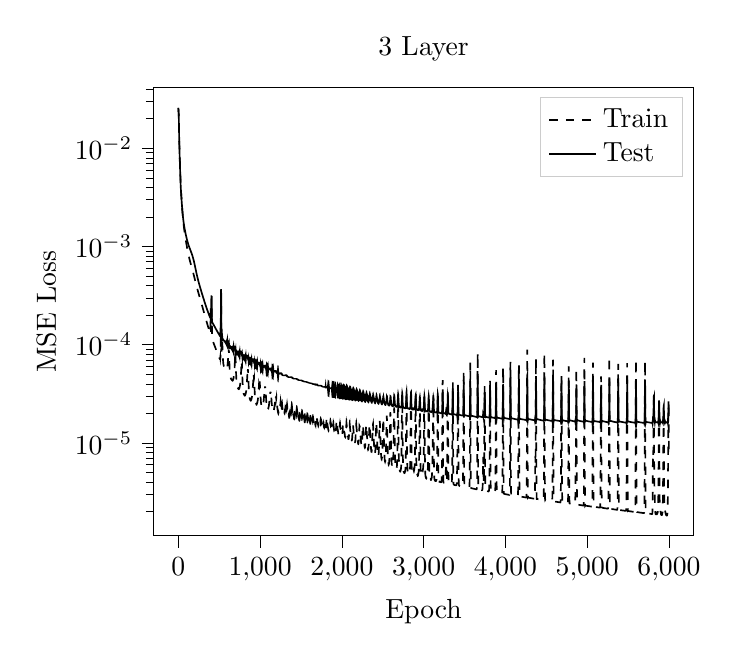
\begin{tikzpicture}

\begin{axis}[
legend cell align={left},
legend style={fill opacity=0.8, draw opacity=1, text opacity=1, draw=white!80!black},
log basis y={10},
tick align=outside,
tick pos=left,
title={3 Layer},
x grid style={white!69.0196078431373!black},
xlabel={Epoch},
xmin=-299.95, xmax=6298.95,
xtick style={color=black},
y grid style={white!69.0196078431373!black},
ylabel={MSE Loss},
ymin=1.1322611307076e-06, ymax=0.0414940584245964,
ymode=log,
ytick style={color=black}
]
\addplot [semithick, black, dashed]
table {%
0 0.0257342011900619
1 0.0250534330261871
2 0.0243807227816433
3 0.0236867136554793
4 0.0229335811454803
5 0.0220618403982371
6 0.0209819102892652
7 0.0195935298106633
8 0.0178730810876004
9 0.0160049086553045
10 0.0143510933266953
11 0.0130772785632871
12 0.0120223690173589
13 0.0110923240426928
14 0.0102946101978887
15 0.00961181169259362
16 0.00902244105236605
17 0.00850598374381661
18 0.00803963237558492
19 0.0076074312091805
20 0.00720134160656016
21 0.00681713726953603
22 0.00645199058635626
23 0.00610390958900098
24 0.00577234654338099
25 0.00545848625188228
26 0.00516461393272039
27 0.00489319404005073
28 0.00464610291237477
29 0.00442401424515992
30 0.00422599769080989
31 0.00404961021558847
32 0.00389153647120111
33 0.00374838919378817
34 0.00361722805246245
35 0.0034957248280989
36 0.00338214098883327
37 0.0032752261904534
38 0.00317409046692774
39 0.00307809177320451
40 0.00298675865633413
41 0.00289973020699108
42 0.00281672010896727
43 0.00273749200277962
44 0.00266184830252314
45 0.00258961624786025
46 0.00252064352389425
47 0.0024547912471462
48 0.00239193128072657
49 0.00233194071915932
50 0.00227470204845304
51 0.00222010019933805
52 0.00216802088834811
53 0.00211835093068657
54 0.00207097737438744
55 0.00202578732569236
56 0.00198266881488962
57 0.00194151108735241
58 0.00190220491640503
59 0.00186464419675758
60 0.00182872558070812
61 0.00179434962046798
62 0.0017614209355088
63 0.00172984863456804
64 0.00169954731245525
65 0.00167043599503813
66 0.00164243840117706
67 0.00161548366304487
68 0.00158950620971154
69 0.00156444446474779
70 0.0015402412172989
71 0.0015168438294495
72 0.00149420372326858
73 0.0014722753658134
74 0.00145101774978684
75 0.00143039195245365
76 0.00141036292916397
77 0.00139089737058384
78 0.00137196565265185
79 0.00135353971563745
80 0.00133559358437196
81 0.00131810383754782
82 0.00130104826530442
83 0.00128440642220085
84 0.00126815941257519
85 0.00125228989782045
86 0.00123678181626019
87 0.00122161967374268
88 0.00120678969324217
89 0.00119227900358965
90 0.00117807552669547
91 0.00116416771197692
92 0.00115054511479684
93 0.00113719810542534
94 0.00112411724330741
95 0.00111129405922838
96 0.00109872037501191
97 0.00108638869642164
98 0.0010742922204372
99 0.00106242415495217
100 0.00105077835542033
101 0.00103934907383518
102 0.00102813086050446
103 0.00101711866955156
104 0.00100630778615596
105 0.000995693797449348
106 0.000985272374236956
107 0.000975039783952525
108 0.00096499247229076
109 0.00095512705956935
110 0.000945440409850562
111 0.000935929663683055
112 0.000926592118048575
113 0.000917424989893334
114 0.000908426074602176
115 0.000899593062058557
116 0.000890923765837215
117 0.000882416006788844
118 0.000874067794939037
119 0.000865876983880298
120 0.00085784170369152
121 0.000849959866172867
122 0.000842229437694186
123 0.000834648148156703
124 0.000827213832963025
125 0.000819924094685121
126 0.000812776248494629
127 0.000805767840574845
128 0.000798895875050221
129 0.000792157337855315
130 0.000785549178544898
131 0.000779067951953039
132 0.000772710118326358
133 0.00076647219248116
134 0.00076035043275624
135 0.000754340702769696
136 0.000748439337257878
137 0.000742642085242551
138 0.000736945032258518
139 0.000731344229279784
140 0.000725835539924446
141 0.00072041501152853
142 0.000715078913344769
143 0.000709823239958496
144 0.000704644369761809
145 0.000699538812114042
146 0.000694502889018622
147 0.00068953330264776
148 0.000684626827933243
149 0.000679780592690804
150 0.000674991420964943
151 0.000670256695229909
152 0.000665573606966063
153 0.000660939658700954
154 0.000656352465739474
155 0.000651809661576408
156 0.000647308987026918
157 0.000642848450297606
158 0.000638426083241939
159 0.000634039839496836
160 0.000629688001936302
161 0.000625368742475985
162 0.000621080323981005
163 0.00061682125851803
164 0.00061259002177394
165 0.000608385020314017
166 0.000604204862611368
167 0.000600048299020273
168 0.0005959139270999
169 0.000591800657275598
170 0.000587707190788933
171 0.000583632521738764
172 0.000579575629672036
173 0.000575535541429417
174 0.000571511382077006
175 0.000567502236663131
176 0.000563507332117297
177 0.000559526077267947
178 0.000555557800907991
179 0.000551601962797577
180 0.00054765814638813
181 0.000543726107935072
182 0.000539805418156902
183 0.000535895866050851
184 0.000531997509824578
185 0.00052811029854638
186 0.000524234386830358
187 0.000520369869263959
188 0.000516517166033736
189 0.000512676695507253
190 0.000508848881509039
191 0.000505034380694269
192 0.000501233944305568
193 0.000497448159876512
194 0.000493678076963988
195 0.000489924559587962
196 0.00048618868822814
197 0.00048247153245029
198 0.000478774216389866
199 0.000475097860544338
200 0.000471443685455597
201 0.000467813026261865
202 0.0004642069889087
203 0.000460626870335545
204 0.000457073952929932
205 0.000453549295343691
206 0.00045005407082499
207 0.000446589452621993
208 0.000443156350229401
209 0.000439755795014207
210 0.000436388601883664
211 0.000433055571193108
212 0.00042975731594197
213 0.000426494545536116
214 0.000423267524638504
215 0.000420076700720529
216 0.000416922362092009
217 0.000413804579693533
218 0.000410723402637814
219 0.000407678809096979
220 0.00040467051712767
221 0.000401698287532781
222 0.000398761825636029
223 0.000395860620301391
224 0.000392994268622715
225 0.000390162120311288
226 0.00038736361420888
227 0.000384598112759704
228 0.00038186476649571
229 0.000379162928766164
230 0.000376491903807619
231 0.000373850818505161
232 0.000371238913430716
233 0.000368655358215619
234 0.000366099450729962
235 0.000363570209628961
236 0.000361067027370154
237 0.000358589093593764
238 0.000356135554284265
239 0.000353705774614355
240 0.000351298953319201
241 0.00034891455743491
242 0.000346551798429573
243 0.000344210016919533
244 0.00034188855534012
245 0.000339586955306004
246 0.000337304551976558
247 0.000335040874233528
248 0.000332795368194638
249 0.000330567575474561
250 0.0003283570831627
251 0.000326163397403434
252 0.000323986071634863
253 0.000321824802085757
254 0.000319679124913819
255 0.000317548732709838
256 0.000315433360810857
257 0.000313332655423437
258 0.000311246360979567
259 0.00030917419007892
260 0.000307115864416119
261 0.000305071165712434
262 0.00030303988387459
263 0.000301021814266278
264 0.000299016704957467
265 0.000297024449537275
266 0.000295044791528198
267 0.000293077639071271
268 0.000291122861199256
269 0.000289180263280286
270 0.000287249648863508
271 0.000285331070699613
272 0.000283424260487664
273 0.000281529102721834
274 0.000279645671071194
275 0.000277773636298662
276 0.000275913005680195
277 0.000274063766482868
278 0.000272225672233617
279 0.000270398804786964
280 0.000268583035904157
281 0.000266778268269263
282 0.000264984535533586
283 0.000263201722191297
284 0.000261429672718805
285 0.00025966857901949
286 0.000257918190072814
287 0.000256178440395161
288 0.000254449580097571
289 0.000252731180808041
290 0.000251023393502692
291 0.000249326341872802
292 0.000247639643930597
293 0.000245963529778237
294 0.000244298101279128
295 0.0002426428382023
296 0.000240998197114095
297 0.000239364136177755
298 0.000237740066040715
299 0.000236126757044985
300 0.000234523821745825
301 0.000232930821312038
302 0.000231348680244992
303 0.000229776686410332
304 0.000228214645176195
305 0.000226663557441498
306 0.000225122361371177
307 0.000223591208396101
308 0.000222071061671159
309 0.000220560540128645
310 0.000219060171275487
311 0.000217570808217715
312 0.00021609085615637
313 0.000214621225040901
314 0.000213162505588116
315 0.000211713032967964
316 0.00021027408001828
317 0.000208845868655771
318 0.000207426797715016
319 0.000206018314656831
320 0.000204620456770499
321 0.000203231687464722
322 0.000201853523776663
323 0.000200485907043912
324 0.000199127264295385
325 0.000197779280824761
326 0.000196441694242822
327 0.000195113055724505
328 0.000193794971437455
329 0.000192487254480511
330 0.000191188365988637
331 0.000189899998076726
332 0.000188621859706473
333 0.000187352525244933
334 0.000186093547654309
335 0.000184844762316061
336 0.000183604697213013
337 0.000182374808446184
338 0.000181155005066103
339 0.000179943895091128
340 0.000178742732714454
341 0.000177551580236468
342 0.000176369084329053
343 0.000175196261352539
344 0.000174033347775548
345 0.000172879048477625
346 0.000171734172909055
347 0.000170599007560668
348 0.000169472490142653
349 0.000168355120422348
350 0.000167247270837834
351 0.000166148032803903
352 0.000165057674166746
353 0.000163976589192316
354 0.000162904103490291
355 0.000161840272994596
356 0.000160785447405942
357 0.000159739146965876
358 0.000158701305736031
359 0.000157672173372703
360 0.000156651465658797
361 0.000155639054810308
362 0.000154635071339726
363 0.000153639356994972
364 0.000152651755342958
365 0.000151672312313167
366 0.000150700978338136
367 0.000149737574247411
368 0.000148782118230883
369 0.000147834514336864
370 0.000146894704357692
371 0.00014596258642996
372 0.000145038111440954
373 0.000144121234825434
374 0.00014321185699373
375 0.000142309883813141
376 0.000141415298912762
377 0.000140528060910583
378 0.000139647973810497
379 0.000138775262257695
380 0.000137909406930703
381 0.000137051364163199
382 0.000136199751523236
383 0.000135357629005739
384 0.000134521907511953
385 0.000133702362290933
386 0.00013289415574036
387 0.000132131217924325
388 0.000131421692913136
389 0.000130901471038669
390 0.000130723516349462
391 0.000131504047658382
392 0.000134452139718633
393 0.000141959292704996
394 0.000159789150075085
395 0.000183729076070449
396 0.000209984394132334
397 0.00019467357560643
398 0.000155132316194795
399 0.000135474273520231
400 0.000151874043694988
401 0.000162282878591213
402 0.000151219304143524
403 0.000167452612458874
404 0.000208101244425052
405 0.000204737946660316
406 0.000185874585667989
407 0.000226431963710638
408 0.000257331765624258
409 0.000251543120612041
410 0.000199560425244272
411 0.000151622683461028
412 0.000125941510304983
413 0.00011630080894065
414 0.000115426520324036
415 0.00011497593823151
416 0.000113856452344407
417 0.000112972625629482
418 0.000112051587620954
419 0.000111188194750866
420 0.000110518482870248
421 0.000109881622393004
422 0.000109302940700218
423 0.000108700483451685
424 0.000108131251636223
425 0.000107546656408886
426 0.000106988089555671
427 0.000106422778344495
428 0.000105871499499699
429 0.0001053204443906
430 0.000104775458794393
431 0.000104234240325241
432 0.000103696436099199
433 0.000103162949244506
434 0.000102632534435543
435 0.000102106115946299
436 0.000101582915931431
437 0.000101063240208532
438 0.000100546953262892
439 0.000100033932767474
440 9.95242739918467e-05
441 9.90177607036458e-05
442 9.85145513823227e-05
443 9.80144718596421e-05
444 9.7517524864088e-05
445 9.70237072124291e-05
446 9.6532931593174e-05
447 9.60452216531849e-05
448 9.55605219132849e-05
449 9.5078820550043e-05
450 9.46000914154865e-05
451 9.41242592489289e-05
452 9.36513959004515e-05
453 9.31813656279701e-05
454 9.27142311866191e-05
455 9.22499207263172e-05
456 9.17884112823231e-05
457 9.13297394617985e-05
458 9.08737906684109e-05
459 9.04206272025476e-05
460 8.99701847174583e-05
461 8.9522436610423e-05
462 8.90774040271936e-05
463 8.86350014752679e-05
464 8.81952807958442e-05
465 8.77581821896456e-05
466 8.7323690422636e-05
467 8.68918111791572e-05
468 8.6462459194081e-05
469 8.60357160945568e-05
470 8.56114645557682e-05
471 8.51897530083079e-05
472 8.47705755404604e-05
473 8.43537941364048e-05
474 8.39396159335593e-05
475 8.35277458008932e-05
476 8.31184192975343e-05
477 8.27114956791775e-05
478 8.23068771751423e-05
479 8.19048595985805e-05
480 8.15049329503381e-05
481 8.11076215541107e-05
482 8.07125502433337e-05
483 8.03196908236714e-05
484 7.9929514640753e-05
485 7.95410448972689e-05
486 7.91555023624824e-05
487 7.8771871585559e-05
488 7.83904260970303e-05
489 7.80119039518468e-05
490 7.7634196713916e-05
491 7.7260515126909e-05
492 7.6887983141205e-05
493 7.65181134738668e-05
494 7.61513747420395e-05
495 7.57831210194126e-05
496 7.54223999592796e-05
497 7.50618346501142e-05
498 7.47070362194791e-05
499 7.43542664167762e-05
500 7.39914639780181e-05
501 7.36487074846082e-05
502 7.33134928623258e-05
503 7.30042767145278e-05
504 7.26832371356068e-05
505 7.23075445421273e-05
506 7.20062852224146e-05
507 7.18219445161594e-05
508 7.18117819360486e-05
509 7.16677204763982e-05
510 7.11601982175125e-05
511 7.10404690380528e-05
512 7.20982352504507e-05
513 7.4475138148955e-05
514 7.55935309371125e-05
515 7.39788023338406e-05
516 7.52205552316809e-05
517 8.65430265548639e-05
518 0.000107620057178792
519 0.000115739651846525
520 0.000104466257880631
521 0.000117498063332278
522 0.000189804152569195
523 0.000302426214147999
524 0.000267279727268033
525 0.00019526713367668
526 0.000133291887550513
527 9.0811433892668e-05
528 8.08694624083728e-05
529 9.17515635592281e-05
530 9.71001763900858e-05
531 0.000104436886999792
532 0.000101709522027704
533 0.000105483328411538
534 0.000103221039012169
535 0.000108111753434059
536 0.000104686050462988
537 0.000106951230577579
538 0.000100446798228404
539 9.95934728962311e-05
540 9.25552242279082e-05
541 9.02375435316571e-05
542 8.40051392287933e-05
543 8.12812506865157e-05
544 7.65197086138869e-05
545 7.42365984933713e-05
546 7.09939823764216e-05
547 6.93679952519233e-05
548 6.72384402378157e-05
549 6.61374280070959e-05
550 6.47243324465308e-05
551 6.3976891283346e-05
552 6.30014415037294e-05
553 6.24734072971478e-05
554 6.17601913290855e-05
555 6.13649806382455e-05
556 6.08115757358973e-05
557 6.04984385290663e-05
558 6.00457253767672e-05
559 5.97852887267436e-05
560 5.93986021613091e-05
561 5.91739284345749e-05
562 5.88325871149209e-05
563 5.86339842811867e-05
564 5.83254605999173e-05
565 5.81476382421897e-05
566 5.78642063828738e-05
567 5.77044858118825e-05
568 5.74414129914658e-05
569 5.72989836200577e-05
570 5.70536410577915e-05
571 5.69290614294005e-05
572 5.67001241051912e-05
573 5.65950898590017e-05
574 5.63823762149696e-05
575 5.62996609687616e-05
576 5.61038525574986e-05
577 5.60473799851025e-05
578 5.58699341581814e-05
579 5.5844872349553e-05
580 5.56879416535594e-05
581 5.57007963379874e-05
582 5.55672389737083e-05
583 5.5626282232879e-05
584 5.55194775415657e-05
585 5.56348707050347e-05
586 5.55585922938917e-05
587 5.57426816385487e-05
588 5.57010365582755e-05
589 5.59690279260394e-05
590 5.59662910291081e-05
591 5.63368557777721e-05
592 5.63772675832297e-05
593 5.68735493970962e-05
594 5.69614047662981e-05
595 5.76127828253448e-05
596 5.77527016503154e-05
597 5.85974402156353e-05
598 5.87947375834119e-05
599 5.98837084453407e-05
600 6.014476252858e-05
601 6.15463625308621e-05
602 6.18777352201505e-05
603 6.36827739981527e-05
604 6.40870587176323e-05
605 6.64102516338971e-05
606 6.68735049202951e-05
607 6.98437216897219e-05
608 7.03080128232614e-05
609 7.40309735647315e-05
610 7.43438056360901e-05
611 7.88144654961798e-05
612 7.86604452969186e-05
613 8.36151650673855e-05
614 8.24830196961557e-05
615 8.72616795959402e-05
616 8.45721546056666e-05
617 8.81975054198847e-05
618 8.36869854765609e-05
619 8.53469007324748e-05
620 7.94745595840141e-05
621 7.91189453366314e-05
622 7.29696846519801e-05
623 7.13462145540689e-05
624 6.59757222365442e-05
625 6.40249588741426e-05
626 5.99283895326153e-05
627 5.82429083806346e-05
628 5.53715734668003e-05
629 5.41268602773926e-05
630 5.21872718763916e-05
631 5.13314377030838e-05
632 5.00191562196051e-05
633 4.94412950047263e-05
634 4.85281921100977e-05
635 4.81321725942507e-05
636 4.74691655085735e-05
637 4.71886988293591e-05
638 4.66838588408791e-05
639 4.64772762143184e-05
640 4.60749064927768e-05
641 4.59169619944078e-05
642 4.55831977319576e-05
643 4.54588968636926e-05
644 4.51729063115636e-05
645 4.50735712433925e-05
646 4.48222473323767e-05
647 4.47430736016941e-05
648 4.45181884174417e-05
649 4.4456872842602e-05
650 4.42532314650634e-05
651 4.42092594425958e-05
652 4.40238141550253e-05
653 4.39980519217897e-05
654 4.38291646673861e-05
655 4.38235850310775e-05
656 4.36707640574241e-05
657 4.36884946566352e-05
658 4.35521889698975e-05
659 4.35975042023529e-05
660 4.34789392329549e-05
661 4.35574839912078e-05
662 4.34586217465949e-05
663 4.35774523452892e-05
664 4.35008304862095e-05
665 4.36688449099165e-05
666 4.361762927374e-05
667 4.38457714153628e-05
668 4.38234464468223e-05
669 4.41252379346224e-05
670 4.4135724976968e-05
671 4.45278361098644e-05
672 4.45751722395471e-05
673 4.50783238079566e-05
674 4.5166574977884e-05
675 4.58068270745571e-05
676 4.59403270269831e-05
677 4.67512966224604e-05
678 4.6934648480601e-05
679 4.7960465963115e-05
680 4.81987544844742e-05
681 4.94979525456074e-05
682 4.97960888878879e-05
683 5.14461485181528e-05
684 5.18059021032968e-05
685 5.39057424475686e-05
686 5.43171181561775e-05
687 5.69823116620682e-05
688 5.74041210938958e-05
689 6.07431131811609e-05
690 6.10647791745578e-05
691 6.5117178564833e-05
692 6.51033383292088e-05
693 6.97257763704329e-05
694 6.89721363187346e-05
695 7.37016041512106e-05
696 7.16901790838165e-05
697 7.57233714807626e-05
698 7.20841529755489e-05
699 7.45696133321871e-05
700 6.94686499969066e-05
701 7.00478120165826e-05
702 6.42971839965867e-05
703 6.3376560603956e-05
704 5.80029754360112e-05
705 5.64092115382664e-05
706 5.20809593922422e-05
707 5.0502329088431e-05
708 4.73552129847121e-05
709 4.61065857280119e-05
710 4.3943763785137e-05
711 4.30613717412598e-05
712 4.15998825928909e-05
713 4.10069941949587e-05
714 4.00070570663047e-05
715 3.9613737669697e-05
716 3.89080393006225e-05
717 3.86448900826508e-05
718 3.81264522957281e-05
719 3.79472693907701e-05
720 3.75500629274939e-05
721 3.74260553144268e-05
722 3.71095609352778e-05
723 3.7023273421255e-05
724 3.67624047044046e-05
725 3.67035632962143e-05
726 3.64826115628603e-05
727 3.64454332952846e-05
728 3.62544962513311e-05
729 3.62361243446685e-05
730 3.60690034426625e-05
731 3.60686429417001e-05
732 3.59216313654542e-05
733 3.59400745537641e-05
734 3.58112333742611e-05
735 3.5850611936894e-05
736 3.57393276431139e-05
737 3.58030495704043e-05
738 3.57098372205655e-05
739 3.58027360789492e-05
740 3.57291152113248e-05
741 3.5857650516391e-05
742 3.58060381131509e-05
743 3.5978597054509e-05
744 3.59522527446643e-05
745 3.61794359378109e-05
746 3.61824716605952e-05
747 3.64777600339039e-05
748 3.65148583227892e-05
749 3.68951851328347e-05
750 3.69715761507905e-05
751 3.74581667301754e-05
752 3.75793812850134e-05
753 3.81990449227487e-05
754 3.83704433488674e-05
755 3.91568957525124e-05
756 3.93832066265531e-05
757 4.03794416570236e-05
758 4.06641660788409e-05
759 4.19251382481889e-05
760 4.22688882508737e-05
761 4.38640250877143e-05
762 4.42606585693284e-05
763 4.62739137674362e-05
764 4.67017770233724e-05
765 4.92242704126511e-05
766 4.9628200827101e-05
767 5.27334602793417e-05
768 5.29935186932562e-05
769 5.66816071341236e-05
770 5.65729731079045e-05
771 6.06784102501479e-05
772 5.98519116010721e-05
773 6.39517990066452e-05
774 6.20046221229131e-05
775 6.54387854410743e-05
776 6.21336292283559e-05
777 6.42568582520653e-05
778 5.97931420998066e-05
779 6.03664779532664e-05
780 5.54140522126545e-05
781 5.47669326920186e-05
782 5.01287954079999e-05
783 4.88958824576002e-05
784 4.50995792107278e-05
785 4.38228689176867e-05
786 4.09959103535584e-05
787 3.99475092649482e-05
788 3.79544731003989e-05
789 3.71898473758847e-05
790 3.58131033522113e-05
791 3.52879415004281e-05
792 3.433172264522e-05
793 3.39804955160616e-05
794 3.33013902604762e-05
795 3.30686702909588e-05
796 3.25710252013778e-05
797 3.24177249808599e-05
798 3.20404989224699e-05
799 3.19412105795891e-05
800 3.16458235829487e-05
801 3.15846521630192e-05
802 3.13467218688857e-05
803 3.1314160310103e-05
804 3.11182158725387e-05
805 3.11089514752894e-05
806 3.09451751832057e-05
807 3.0956744865307e-05
808 3.08190079181259e-05
809 3.08510956301689e-05
810 3.07359402995644e-05
811 3.0789943025411e-05
812 3.069569896752e-05
813 3.07744969063606e-05
814 3.07009718767404e-05
815 3.08091340457395e-05
816 3.07574237012886e-05
817 3.09012908701334e-05
818 3.0873634841555e-05
819 3.10616260321694e-05
820 3.1061283436884e-05
821 3.13043669279978e-05
822 3.13355802745718e-05
823 3.1647815433189e-05
824 3.17156074629565e-05
825 3.21148812076899e-05
826 3.22249193231983e-05
827 3.27339007526462e-05
828 3.28919982166553e-05
829 3.35389699444022e-05
830 3.37501818989949e-05
831 3.45703585935553e-05
832 3.48380930290659e-05
833 3.58750323812274e-05
834 3.61991847626086e-05
835 3.750578105155e-05
836 3.78794172775088e-05
837 3.95172565959001e-05
838 3.99205014218751e-05
839 4.19547895944561e-05
840 4.23438677330523e-05
841 4.4829019145709e-05
842 4.51182783081094e-05
843 4.80654344414688e-05
844 4.81033246728657e-05
845 5.1426189884296e-05
846 5.09791921672331e-05
847 5.4431246724107e-05
848 5.32105686943396e-05
849 5.63669453299553e-05
850 5.41381152174836e-05
851 5.64997076253348e-05
852 5.32592179069979e-05
853 5.44860718321161e-05
854 5.05703102362531e-05
855 5.06843786638456e-05
856 4.66597993806772e-05
857 4.60142191798241e-05
858 4.24049462708354e-05
859 4.14481450263793e-05
860 3.85344307574087e-05
861 3.75961986947004e-05
862 3.54063963641238e-05
863 3.46394735970534e-05
864 3.30582051901729e-05
865 3.2489840037897e-05
866 3.13638290947438e-05
867 3.09649267080658e-05
868 3.01588875686321e-05
869 2.9887566540765e-05
870 2.93005508922306e-05
871 2.91204767393083e-05
872 2.86828727666943e-05
873 2.85673810935805e-05
874 2.82330185825685e-05
875 2.81641373192087e-05
876 2.79028016052507e-05
877 2.78691202311165e-05
878 2.7661172595117e-05
879 2.7655896133183e-05
880 2.74886337763292e-05
881 2.7508270790122e-05
882 2.7373641074746e-05
883 2.74172524825644e-05
884 2.73104637074084e-05
885 2.73791184213223e-05
886 2.72976716075846e-05
887 2.73941930402088e-05
888 2.73373468075988e-05
889 2.74665100334914e-05
890 2.74350688584946e-05
891 2.7603642251961e-05
892 2.75996625305197e-05
893 2.78167493092951e-05
894 2.78433988682991e-05
895 2.81209744912303e-05
896 2.81824198395952e-05
897 2.85357973837108e-05
898 2.86368274373672e-05
899 2.90853833746496e-05
900 2.9230985404638e-05
901 2.97988969464313e-05
902 2.99933641372263e-05
903 3.07102075680632e-05
904 3.09559872562204e-05
905 3.18573951290091e-05
906 3.215291980041e-05
907 3.32801710669628e-05
908 3.36165860517212e-05
909 3.50148642382919e-05
910 3.53708167040168e-05
911 3.70839392189737e-05
912 3.7417591954636e-05
913 3.94762378732594e-05
914 3.9713948865483e-05
915 4.2113836855151e-05
916 4.2137634750361e-05
917 4.48064142801741e-05
918 4.44488199491389e-05
919 4.72113818545949e-05
920 4.62759650190492e-05
921 4.88470078039427e-05
922 4.71744604624291e-05
923 4.92175812780715e-05
924 4.67872116587387e-05
925 4.80457492813002e-05
926 4.50469287329724e-05
927 4.54727403678135e-05
928 4.22650702773808e-05
929 4.20357704911112e-05
930 3.90016203368759e-05
931 3.84077707451524e-05
932 3.58087989695832e-05
933 3.51126730606666e-05
934 3.30428732979726e-05
935 3.24060231093881e-05
936 3.08331913174698e-05
937 3.03203439386834e-05
938 2.91537290877386e-05
939 2.87706924382292e-05
940 2.79111265797383e-05
941 2.76387921758214e-05
942 2.70018808521399e-05
943 2.68160037819598e-05
944 2.6338043596752e-05
945 2.62175842919987e-05
946 2.58533506496406e-05
947 2.5782611288605e-05
948 2.55009607030843e-05
949 2.5469189637306e-05
950 2.52490867751476e-05
951 2.52496631389931e-05
952 2.50771425100993e-05
953 2.51066175565029e-05
954 2.49725525236499e-05
955 2.50299225399431e-05
956 2.49286659368408e-05
957 2.50151571492552e-05
958 2.49436388344293e-05
959 2.50624713657999e-05
960 2.50195897990579e-05
961 2.51760467051554e-05
962 2.51622188329748e-05
963 2.53637288949449e-05
964 2.53807064893863e-05
965 2.56373099318807e-05
966 2.56878138884531e-05
967 2.60124311637355e-05
968 2.60997324232903e-05
969 2.65086655133473e-05
970 2.66362040122203e-05
971 2.71495156027868e-05
972 2.73199518687761e-05
973 2.79617719911585e-05
974 2.81756156539359e-05
975 2.89739351728713e-05
976 2.92275004198927e-05
977 3.02130977161141e-05
978 3.04954502894361e-05
979 3.16994605782384e-05
980 3.19882462349597e-05
981 3.34367344976272e-05
982 3.36922425390185e-05
983 3.53967915884823e-05
984 3.55557057787337e-05
985 3.74987311602126e-05
986 3.74688043507376e-05
987 3.95844311356086e-05
988 3.92464816059146e-05
989 4.14045793490914e-05
990 4.0630675414377e-05
991 4.26395087060882e-05
992 4.13339713531968e-05
993 4.29775460588644e-05
994 4.11318437443242e-05
995 4.22421730092992e-05
996 3.99725306579057e-05
997 4.04996125382695e-05
998 3.80277713531996e-05
999 3.80569668720909e-05
1000 3.56352389303538e-05
1001 3.53371160599636e-05
1002 3.31641776938341e-05
1003 3.27169211971068e-05
1004 3.08953345609098e-05
1005 3.04309515115619e-05
1006 2.89751972673002e-05
1007 2.85662177930135e-05
1008 2.74366451549213e-05
1009 2.71095711354974e-05
1010 2.62456057100735e-05
1011 2.60009016699314e-05
1012 2.53423436333833e-05
1013 2.51696062605333e-05
1014 2.46658331093386e-05
1015 2.45524439890232e-05
1016 2.41644055449797e-05
1017 2.40993113038712e-05
1018 2.37984101545408e-05
1019 2.37733841004228e-05
1020 2.35392669480916e-05
1021 2.35489111162224e-05
1022 2.33674643652648e-05
1023 2.34089832815698e-05
1024 2.32707042471247e-05
1025 2.33436895200612e-05
1026 2.3242470859941e-05
1027 2.33484817613316e-05
1028 2.32806754354442e-05
1029 2.342325174709e-05
1030 2.33871607235869e-05
1031 2.35719583940863e-05
1032 2.35673947770465e-05
1033 2.38022398946214e-05
1034 2.38300145269932e-05
1035 2.41251260320041e-05
1036 2.41867047634514e-05
1037 2.45549413193658e-05
1038 2.46518140443186e-05
1039 2.5108745774105e-05
1040 2.524153825334e-05
1041 2.58054302832988e-05
1042 2.59728791718317e-05
1043 2.66641778239318e-05
1044 2.68610764067034e-05
1045 2.77010188369786e-05
1046 2.79160194054384e-05
1047 2.89241764050985e-05
1048 2.91364810323103e-05
1049 3.03264013155058e-05
1050 3.05025041029694e-05
1051 3.18751957593122e-05
1052 3.19654503755373e-05
1053 3.35002567908305e-05
1054 3.34377916715312e-05
1055 3.50827956481226e-05
1056 3.47874067188059e-05
1057 3.64530581578038e-05
1058 3.58440416334815e-05
1059 3.74075864328915e-05
1060 3.64271159583041e-05
1061 3.77538683267176e-05
1062 3.63952905502174e-05
1063 3.73756114413482e-05
1064 3.57028387725222e-05
1065 3.62891207998928e-05
1066 3.44303194026452e-05
1067 3.4651747313319e-05
1068 3.27643954562973e-05
1069 3.27095277157241e-05
1070 3.09356621528423e-05
1071 3.07149863374434e-05
1072 2.9148980871696e-05
1073 2.88600316196153e-05
1074 2.75415765429443e-05
1075 2.72519161228502e-05
1076 2.61781123640503e-05
1077 2.59249503642422e-05
1078 2.5068288920238e-05
1079 2.48664439936874e-05
1080 2.41904465383413e-05
1081 2.40418737860182e-05
1082 2.35105925128209e-05
1083 2.3411369426185e-05
1084 2.29939741984708e-05
1085 2.29385715044828e-05
1086 2.26105085516792e-05
1087 2.25939477900283e-05
1088 2.23365175031631e-05
1089 2.23552469265087e-05
1090 2.21547220746743e-05
1091 2.22069808444303e-05
1092 2.20536146855466e-05
1093 2.21393690651439e-05
1094 2.20264080610377e-05
1095 2.21474429054069e-05
1096 2.20705273079602e-05
1097 2.22303624468623e-05
1098 2.21868410505976e-05
1099 2.23908205327916e-05
1100 2.23793082625434e-05
1101 2.26346193699101e-05
1102 2.26544720760558e-05
1103 2.29702048955005e-05
1104 2.30209818710136e-05
1105 2.34081314829382e-05
1106 2.34888581474024e-05
1107 2.39601025384673e-05
1108 2.40683273773357e-05
1109 2.46373519132703e-05
1110 2.47677971287885e-05
1111 2.54483763626467e-05
1112 2.55913605258229e-05
1113 2.63953563433006e-05
1114 2.65347287609075e-05
1115 2.74692722541658e-05
1116 2.75805614364799e-05
1117 2.86439384353798e-05
1118 2.86926735952875e-05
1119 2.98695684364247e-05
1120 2.98113596386429e-05
1121 3.1067952079411e-05
1122 3.08513149889222e-05
1123 3.21327240442315e-05
1124 3.17064582304738e-05
1125 3.29390885553948e-05
1126 3.22638563261535e-05
1127 3.33650203003799e-05
1128 3.24279476160427e-05
1129 3.33235965115364e-05
1130 3.21495537036753e-05
1131 3.27932025356859e-05
1132 3.14456198680091e-05
1133 3.18308249518395e-05
1134 3.03998908748326e-05
1135 3.0559576231326e-05
1136 2.91408488237721e-05
1137 2.91331996322697e-05
1138 2.78062395864254e-05
1139 2.76958386109527e-05
1140 2.65122327789413e-05
1141 2.63550524550737e-05
1142 2.53371431711003e-05
1143 2.51735139329412e-05
1144 2.43209258883326e-05
1145 2.41753696172964e-05
1146 2.34738106712484e-05
1147 2.33587624336451e-05
1148 2.27878460634656e-05
1149 2.27080035983818e-05
1150 2.22464275623224e-05
1151 2.22023530511706e-05
1152 2.18308294108738e-05
1153 2.18214131848526e-05
1154 2.15236391909457e-05
1155 2.15476404434867e-05
1156 2.13107190631945e-05
1157 2.13675080829034e-05
1158 2.11814681563283e-05
1159 2.12714580243301e-05
1160 2.11288931950548e-05
1161 2.1253693972767e-05
1162 2.11491427535293e-05
1163 2.13116458098739e-05
1164 2.12412623739056e-05
1165 2.14458110292526e-05
1166 2.1406775175592e-05
1167 2.1658937129132e-05
1168 2.1648965798704e-05
1169 2.19556560239198e-05
1170 2.19724756505002e-05
1171 2.23415824791573e-05
1172 2.23821769225196e-05
1173 2.28223590568177e-05
1174 2.28823508052756e-05
1175 2.34022488712071e-05
1176 2.34745921545709e-05
1177 2.40816760594953e-05
1178 2.41556516300534e-05
1179 2.48545932208799e-05
1180 2.49146585247217e-05
1181 2.57051778191908e-05
1182 2.57300701207441e-05
1183 2.66044779380081e-05
1184 2.65670614680857e-05
1185 2.75076221498693e-05
1186 2.7376320105077e-05
1187 2.83538131498062e-05
1188 2.8095628920255e-05
1189 2.90695659259654e-05
1190 2.86555907678121e-05
1191 2.95776987115914e-05
1192 2.89899593326481e-05
1193 2.9811019430781e-05
1194 2.90492272085885e-05
1195 2.9728266042639e-05
1196 2.88138937776239e-05
1197 2.93270383906474e-05
1198 2.83018154902948e-05
1199 2.86469474701789e-05
1200 2.75656067003638e-05
1201 2.77610353975888e-05
1202 2.66807990954021e-05
1203 2.67586545419363e-05
1204 2.57290425622614e-05
1205 2.57265417644703e-05
1206 2.47830285786677e-05
1207 2.47350860433926e-05
1208 2.38973619559602e-05
1209 2.38317918501707e-05
1210 2.31057038888594e-05
1211 2.30421694027427e-05
1212 2.24239223030054e-05
1213 2.23749233612125e-05
1214 2.18552195008215e-05
1215 2.18280167700868e-05
1216 2.1395119489398e-05
1217 2.13934673354288e-05
1218 2.10353676379782e-05
1219 2.10610811564038e-05
1220 2.0766806926531e-05
1221 2.08210947505449e-05
1222 2.05812666536076e-05
1223 2.06652698011567e-05
1224 2.04721069962943e-05
1225 2.05873485015218e-05
1226 2.0434601509578e-05
1227 2.05833107145281e-05
1228 2.04659550604447e-05
1229 2.06511710132418e-05
1230 2.05651479632252e-05
1231 2.07906361140431e-05
1232 2.07322925405151e-05
1233 2.10024257683017e-05
1234 2.09682339118444e-05
1235 2.12881087406913e-05
1236 2.127425491949e-05
1237 2.1649082981412e-05
1238 2.16506423953433e-05
1239 2.20852546135575e-05
1240 2.20956329428645e-05
1241 2.25936651645497e-05
1242 2.26039280164514e-05
1243 2.31668680328312e-05
1244 2.31651811759548e-05
1245 2.37910583962275e-05
1246 2.37622951146932e-05
1247 2.44443359065372e-05
1248 2.4370298518761e-05
1249 2.50958215985975e-05
1250 2.49563038607903e-05
1251 2.57061571744543e-05
1252 2.54807257817902e-05
1253 2.62297733968353e-05
1254 2.59008791658744e-05
1255 2.66200882208523e-05
1256 2.61765826508054e-05
1257 2.68364909175034e-05
1258 2.62768368770594e-05
1259 2.68517183030781e-05
1260 2.61859149759402e-05
1261 2.66583892312156e-05
1262 2.59080320859084e-05
1263 2.62715873304842e-05
1264 2.54666457237818e-05
1265 2.57261446563462e-05
1266 2.49005503007993e-05
1267 2.50701402535469e-05
1268 2.42566471513328e-05
1269 2.43561125046199e-05
1270 2.3581932396155e-05
1271 2.36326333151737e-05
1272 2.29171820080865e-05
1273 2.29389306127814e-05
1274 2.22933387306057e-05
1275 2.23024721321963e-05
1276 2.17308950709594e-05
1277 2.17399758071224e-05
1278 2.12414097973124e-05
1279 2.12593555488638e-05
1280 2.08293573109586e-05
1281 2.08622353596866e-05
1282 2.04946661028771e-05
1283 2.05466503615526e-05
1284 2.02348053051082e-05
1285 2.03088183070577e-05
1286 2.00460614792064e-05
1287 2.01444322129873e-05
1288 1.9924754923295e-05
1289 2.00497242985875e-05
1290 1.98677243474776e-05
1291 2.00214833512291e-05
1292 1.98723514301946e-05
1293 2.00574223470085e-05
1294 1.99369143274453e-05
1295 2.01561062738165e-05
1296 2.00601873530104e-05
1297 2.03164395031763e-05
1298 2.02409429732597e-05
1299 2.05372443815577e-05
1300 2.04776610246427e-05
1301 2.08167445805429e-05
1302 2.07678137087441e-05
1303 2.11516831427616e-05
1304 2.11069016984311e-05
1305 2.15362504434324e-05
1306 2.1487651025609e-05
1307 2.19613718570599e-05
1308 2.18993597229655e-05
1309 2.24137195061758e-05
1310 2.23270087076344e-05
1311 2.2875025393887e-05
1312 2.27510950878695e-05
1313 2.33223572365659e-05
1314 2.31484481219013e-05
1315 2.37291904170434e-05
1316 2.34934796878861e-05
1317 2.40671892584032e-05
1318 2.37604752442167e-05
1319 2.43094803238364e-05
1320 2.39271045074929e-05
1321 2.44344095392535e-05
1322 2.39774259966907e-05
1323 2.44289805664266e-05
1324 2.39048681294207e-05
1325 2.42912721830635e-05
1326 2.37133295115655e-05
1327 2.40309614412126e-05
1328 2.34169205839407e-05
1329 2.36681459000465e-05
1330 2.30378158505573e-05
1331 2.32298686739796e-05
1332 2.26026589302819e-05
1333 2.27460593578144e-05
1334 2.21390366164087e-05
1335 2.22459478607107e-05
1336 2.16724243671251e-05
1337 2.17548233365505e-05
1338 2.12238148549204e-05
1339 2.12925436073874e-05
1340 2.08090995954535e-05
1341 2.0873312536196e-05
1342 2.04391659508474e-05
1343 2.05062181919402e-05
1344 2.01205919267977e-05
1345 2.01961748871327e-05
1346 1.98565878406498e-05
1347 1.99450197158058e-05
1348 1.96480566501123e-05
1349 1.97528054712848e-05
1350 1.94946354383774e-05
1351 1.96185406764471e-05
1352 1.93951412370552e-05
1353 1.95405990552899e-05
1354 1.93479944243791e-05
1355 1.95172692372125e-05
1356 1.93515978708092e-05
1357 1.95467477510647e-05
1358 1.94041072063555e-05
1359 1.96270458729941e-05
1360 1.95034873229361e-05
1361 1.97559860453111e-05
1362 1.9647368560527e-05
1363 1.99307640684765e-05
1364 1.98324346740719e-05
1365 2.01475606047552e-05
1366 2.00544523067947e-05
1367 2.04012869744474e-05
1368 2.03073927025343e-05
1369 2.06845624859398e-05
1370 2.05830511674776e-05
1371 2.09875840084806e-05
1372 2.08709320759226e-05
1373 2.12981593108452e-05
1374 2.11584207079341e-05
1375 2.16018496246306e-05
1376 2.14311072568307e-05
1377 2.18824660862538e-05
1378 2.16734324283152e-05
1379 2.21229502983533e-05
1380 2.18698102685266e-05
1381 2.2307087107265e-05
1382 2.20064178506618e-05
1383 2.24213188175781e-05
1384 2.2072738602219e-05
1385 2.24564490736157e-05
1386 2.20629827367702e-05
1387 2.24088173013115e-05
1388 2.19767061366838e-05
1389 2.22809053127548e-05
1390 2.18191524936628e-05
1391 2.20808350945845e-05
1392 2.16002299566753e-05
1393 2.18216219423084e-05
1394 2.1333727062256e-05
1395 2.15193970234395e-05
1396 2.10352463625441e-05
1397 2.11912700365247e-05
1398 2.07206070115262e-05
1399 2.08539609332092e-05
1400 2.04045925897844e-05
1401 2.05222256965953e-05
1402 2.00998055106538e-05
1403 2.02083786291496e-05
1404 1.98165484448509e-05
1405 1.99219970227205e-05
1406 1.95624592151944e-05
1407 1.96698052974398e-05
1408 1.93427342480845e-05
1409 1.94561977480134e-05
1410 1.91607490478418e-05
1411 1.9283866549813e-05
1412 1.90182501569325e-05
1413 1.91538860576657e-05
1414 1.89158476757711e-05
1415 1.90664239028138e-05
1416 1.88533635991917e-05
1417 1.90209273398523e-05
1418 1.88299530066161e-05
1419 1.90161987063675e-05
1420 1.88443413549066e-05
1421 1.9050704622714e-05
1422 1.88946741559448e-05
1423 1.91221323007085e-05
1424 1.8978415738502e-05
1425 1.92275871313541e-05
1426 1.90923600484894e-05
1427 1.93632601508398e-05
1428 1.92324205272598e-05
1429 1.95244121812266e-05
1430 1.9393438321913e-05
1431 1.97049883183809e-05
1432 1.95690151372219e-05
1433 1.98976496790237e-05
1434 1.97516083346727e-05
1435 2.00938995362776e-05
1436 1.99327642746994e-05
1437 2.02842459202657e-05
1438 2.01031469657664e-05
1439 2.04585278424929e-05
1440 2.02532706907732e-05
1441 2.06067540773347e-05
1442 2.03742390851858e-05
1443 2.07197657857705e-05
1444 2.04580925071696e-05
1445 2.07898973201281e-05
1446 2.04990798522431e-05
1447 2.08122274045763e-05
1448 2.04939732668663e-05
1449 2.07847012347884e-05
1450 2.044245869115e-05
1451 2.07083999441693e-05
1452 2.03470365818248e-05
1453 2.05874474943357e-05
1454 2.02128433102189e-05
1455 2.04284140181699e-05
1456 2.00469744982001e-05
1457 2.0239829041202e-05
1458 1.98580008827776e-05
1459 2.00312513527479e-05
1460 1.96549932240941e-05
1461 1.98123706809383e-05
1462 1.94467847904889e-05
1463 1.95923208536897e-05
1464 1.92415350284136e-05
1465 1.93792907907664e-05
1466 1.90462575915262e-05
1467 1.91801029245653e-05
1468 1.88668191469787e-05
1469 1.90003479758616e-05
1470 1.87078094882054e-05
1471 1.88441704835896e-05
1472 1.85724726975423e-05
1473 1.87144009373696e-05
1474 1.84629855084495e-05
1475 1.86127779784329e-05
1476 1.83805780693547e-05
1477 1.85402398074075e-05
1478 1.83257398873593e-05
1479 1.84968501741878e-05
1480 1.82981552256933e-05
1481 1.84819292599059e-05
1482 1.82969169770786e-05
1483 1.84942579437575e-05
1484 1.83204791426306e-05
1485 1.85318616843233e-05
1486 1.83666505222391e-05
1487 1.85920855813038e-05
1488 1.84325762688786e-05
1489 1.86716952725874e-05
1490 1.85148165030569e-05
1491 1.87666308306689e-05
1492 1.86091881744233e-05
1493 1.88722457892254e-05
1494 1.87110121885325e-05
1495 1.89833168349196e-05
1496 1.88151161921724e-05
1497 1.90941646280862e-05
1498 1.89160085142248e-05
1499 1.91988517599384e-05
1500 1.90080312165719e-05
1501 1.92913656746896e-05
1502 1.90857596180649e-05
1503 1.93662163781028e-05
1504 1.91444578945266e-05
1505 1.94187786348721e-05
1506 1.91802720621581e-05
1507 1.94454568998026e-05
1508 1.91905220958688e-05
1509 1.94440829091036e-05
1510 1.91740071784352e-05
1511 1.94142050133905e-05
1512 1.91310928130406e-05
1513 1.93569462965115e-05
1514 1.90635685441976e-05
1515 1.92747924927517e-05
1516 1.89743454654945e-05
1517 1.91714962056722e-05
1518 1.88674035825898e-05
1519 1.90516339273472e-05
1520 1.87473966377638e-05
1521 1.89203934155557e-05
1522 1.86192045532607e-05
1523 1.87830650872911e-05
1524 1.84879131097659e-05
1525 1.86449022123725e-05
1526 1.83581228156982e-05
1527 1.85105573393685e-05
1528 1.8234032950204e-05
1529 1.83841450507316e-05
1530 1.81190741841419e-05
1531 1.826898278523e-05
1532 1.80162242315873e-05
1533 1.81680102286919e-05
1534 1.79278369500935e-05
1535 1.80831348188804e-05
1536 1.78552815555122e-05
1537 1.80155258249215e-05
1538 1.7799357920012e-05
1539 1.79657614296502e-05
1540 1.77604069619974e-05
1541 1.79338778139027e-05
1542 1.77381422474809e-05
1543 1.79192811344819e-05
1544 1.77317079987915e-05
1545 1.79208300608025e-05
1546 1.77397546679003e-05
1547 1.79368813633118e-05
1548 1.77605874114306e-05
1549 1.79654524856687e-05
1550 1.77920330486359e-05
1551 1.80040040334006e-05
1552 1.78315551409014e-05
1553 1.80497476662822e-05
1554 1.78763336293741e-05
1555 1.80995820926455e-05
1556 1.79233863946138e-05
1557 1.81502242355691e-05
1558 1.79695368842658e-05
1559 1.81984088385434e-05
1560 1.8011784106875e-05
1561 1.82409414435369e-05
1562 1.80472111424024e-05
1563 1.82748613895001e-05
1564 1.8073190318546e-05
1565 1.82977381371074e-05
1566 1.80878335527268e-05
1567 1.83077866324766e-05
1568 1.8089648563091e-05
1569 1.83037913643602e-05
1570 1.80779220499971e-05
1571 1.82853436001551e-05
1572 1.80525847213175e-05
1573 1.82527455763193e-05
1574 1.80142911858638e-05
1575 1.82069685195074e-05
1576 1.79641560293931e-05
1577 1.81495762774375e-05
1578 1.79040731325131e-05
1579 1.80827744316048e-05
1580 1.78362303415724e-05
1581 1.80090610797379e-05
1582 1.77630857649547e-05
1583 1.79310226542384e-05
1584 1.7687125506427e-05
1585 1.7851299475069e-05
1586 1.76107785136992e-05
1587 1.77723537717611e-05
1588 1.75363126970751e-05
1589 1.76963617661841e-05
1590 1.74655835110116e-05
1591 1.76251596428756e-05
1592 1.740022801755e-05
1593 1.75602021386112e-05
1594 1.73412971662401e-05
1595 1.75022740904751e-05
1596 1.72893458056933e-05
1597 1.74518805522439e-05
1598 1.72447813326926e-05
1599 1.74092384668256e-05
1600 1.72076322257908e-05
1601 1.73742705840141e-05
1602 1.71776804052115e-05
1603 1.73466278567957e-05
1604 1.71545182183763e-05
1605 1.7325760239828e-05
1606 1.71375706372601e-05
1607 1.73110671539689e-05
1608 1.7126303276882e-05
1609 1.73020319209627e-05
1610 1.71202316039398e-05
1611 1.72980086290409e-05
1612 1.71185260455786e-05
1613 1.729808226969e-05
1614 1.71204476089315e-05
1615 1.73014928748216e-05
1616 1.7125116698935e-05
1617 1.73072025972942e-05
1618 1.71313460839428e-05
1619 1.73138392085548e-05
1620 1.71377273545659e-05
1621 1.73199860284967e-05
1622 1.71426245003659e-05
1623 1.73238297236367e-05
1624 1.71441745351331e-05
1625 1.73238219076666e-05
1626 1.71410611642386e-05
1627 1.73190892951425e-05
1628 1.7132733461267e-05
1629 1.73098114260029e-05
1630 1.71199548049117e-05
1631 1.72977171644106e-05
1632 1.71052607242927e-05
1633 1.72863035174942e-05
1634 1.70927683029731e-05
1635 1.72801053111016e-05
1636 1.70872249043441e-05
1637 1.72836664091847e-05
1638 1.7092691535936e-05
1639 1.7299633697121e-05
1640 1.71104744026707e-05
1641 1.73268507523971e-05
1642 1.71373688147014e-05
1643 1.73584590754672e-05
1644 1.71637249479772e-05
1645 1.73801541336616e-05
1646 1.71723155801828e-05
1647 1.73700686332268e-05
1648 1.71393933499076e-05
1649 1.73017435542988e-05
1650 1.7040046003558e-05
1651 1.71526003782674e-05
1652 1.68584311666109e-05
1653 1.69162495353703e-05
1654 1.66004503796557e-05
1655 1.66140097803691e-05
1656 1.6300636161759e-05
1657 1.62960106422361e-05
1658 1.60183170976325e-05
1659 1.60322608451224e-05
1660 1.58276507420396e-05
1661 1.59021890340227e-05
1662 1.58123398534826e-05
1663 1.59908829857613e-05
1664 1.6063066453853e-05
1665 1.63718474368579e-05
1666 1.66289580363355e-05
1667 1.6999060562739e-05
1668 1.73203941926658e-05
1669 1.74858846833104e-05
1670 1.75295062661007e-05
1671 1.72485425764535e-05
1672 1.68379113176798e-05
1673 1.63407574405028e-05
1674 1.57997291410084e-05
1675 1.54925985214049e-05
1676 1.51594438477787e-05
1677 1.51662515150974e-05
1678 1.50925212381026e-05
1679 1.53585123001676e-05
1680 1.54699475274356e-05
1681 1.59220495845602e-05
1682 1.61308677775196e-05
1683 1.66998436554877e-05
1684 1.69130961751307e-05
1685 1.75147886238847e-05
1686 1.76329386647467e-05
1687 1.8170259153294e-05
1688 1.81139136543607e-05
1689 1.85105782861683e-05
1690 1.82603936309533e-05
1691 1.84965761889089e-05
1692 1.81022399772246e-05
1693 1.82131387305162e-05
1694 1.77571798474219e-05
1695 1.77978546105351e-05
1696 1.73497457751637e-05
1697 1.73627573474278e-05
1698 1.69577805877452e-05
1699 1.69633497080213e-05
1700 1.66075385550357e-05
1701 1.66103957042196e-05
1702 1.62957927045682e-05
1703 1.62959105125537e-05
1704 1.60131768609517e-05
1705 1.60128664390413e-05
1706 1.5757281033757e-05
1707 1.57626010945933e-05
1708 1.55341357981342e-05
1709 1.55530663903392e-05
1710 1.53536804248233e-05
1711 1.53935218349943e-05
1712 1.52245727917943e-05
1713 1.5290558195602e-05
1714 1.51516279345287e-05
1715 1.52467883651752e-05
1716 1.51355941113707e-05
1717 1.52610526242825e-05
1718 1.51737095848148e-05
1719 1.53291460947003e-05
1720 1.52606050392023e-05
1721 1.54442917335018e-05
1722 1.5388373441283e-05
1723 1.5597075559981e-05
1724 1.55466690046069e-05
1725 1.57754948020283e-05
1726 1.57227951262939e-05
1727 1.59653032767437e-05
1728 1.5902280949831e-05
1729 1.61507660152438e-05
1730 1.60700848823581e-05
1731 1.63164466187027e-05
1732 1.62125958809156e-05
1733 1.64495602916759e-05
1734 1.63199118503599e-05
1735 1.65420866835575e-05
1736 1.63874261147612e-05
1737 1.65920049539636e-05
1738 1.64160537394764e-05
1739 1.66024457826097e-05
1740 1.64107889304432e-05
1741 1.65798560090025e-05
1742 1.63782191293649e-05
1743 1.65309400586011e-05
1744 1.6323668859286e-05
1745 1.64600934624559e-05
1746 1.62491861885883e-05
1747 1.63681771141455e-05
1748 1.61534789242523e-05
1749 1.62538586891969e-05
1750 1.60345809661067e-05
1751 1.61170240176034e-05
1752 1.58937342007448e-05
1753 1.59626602851404e-05
1754 1.57390269919233e-05
1755 1.58032062529401e-05
1756 1.55859501091982e-05
1757 1.56570326055316e-05
1758 1.54545262205374e-05
1759 1.55447373799689e-05
1760 1.53642967575252e-05
1761 1.54834997090347e-05
1762 1.53292664037963e-05
1763 1.54831776626452e-05
1764 1.53547065906423e-05
1765 1.55434626663009e-05
1766 1.54348246610425e-05
1767 1.5651450041787e-05
1768 1.55505680936585e-05
1769 1.57798102975448e-05
1770 1.56687026162672e-05
1771 1.58870085442686e-05
1772 1.57443537034396e-05
1773 1.59234153329635e-05
1774 1.57311214650235e-05
1775 1.5847022922344e-05
1776 1.56000713218418e-05
1777 1.56447473784738e-05
1778 1.53581378867784e-05
1779 1.53460644298775e-05
1780 1.50527559128477e-05
1781 1.50171520232334e-05
1782 1.4757547546651e-05
1783 1.47390213953713e-05
1784 1.4550481068909e-05
1785 1.45868556558071e-05
1786 1.45000338420687e-05
1787 1.46207012505783e-05
1788 1.46591077907487e-05
1789 1.48746957790991e-05
1790 1.50417525048852e-05
1791 1.53129029456522e-05
1792 1.55469063543023e-05
1793 1.57404984122422e-05
1794 1.58695324898872e-05
1795 1.58074224714255e-05
1796 1.56520961809292e-05
1797 1.53234682613856e-05
1798 1.49313905524195e-05
1799 1.45597018104127e-05
1800 1.4172159580994e-05
1801 1.39744925888863e-05
1802 1.37653019010031e-05
1803 1.38161269092052e-05
1804 1.38222773955476e-05
1805 1.41189041613643e-05
1806 1.43144972071241e-05
1807 1.48372175203804e-05
1808 1.51686728884215e-05
1809 1.58716654254931e-05
1810 1.62371702572273e-05
1811 1.70065287647958e-05
1812 1.72393102673141e-05
1813 1.78872428762133e-05
1814 1.7817998582359e-05
1815 1.81782389176988e-05
1816 1.77687471705212e-05
1817 1.78253096123626e-05
1818 1.72132733951003e-05
1819 1.70926004727789e-05
1820 1.64704418352812e-05
1821 1.63116788201023e-05
1822 1.5796812760982e-05
1823 1.5667888533244e-05
1824 1.52805901052488e-05
1825 1.51844737672491e-05
1826 1.48902941816687e-05
1827 1.48040369083446e-05
1828 1.45583981066011e-05
1829 1.44646429021122e-05
1830 1.42396567355263e-05
1831 1.41399712845214e-05
1832 1.3931206495954e-05
1833 1.38421515742948e-05
1834 1.36598212350236e-05
1835 1.36011055786867e-05
1836 1.3457497800573e-05
1837 1.34439025032407e-05
1838 1.33462557414532e-05
1839 1.33862087636771e-05
1840 1.33359571918845e-05
1841 1.34335511177142e-05
1842 1.34280718668833e-05
1843 1.35852823461846e-05
1844 1.36192687705261e-05
1845 1.38362235446721e-05
1846 1.39013764908213e-05
1847 1.41749681290548e-05
1848 1.42584999593964e-05
1849 1.4579674569859e-05
1850 1.46626695141094e-05
1851 1.50137825301044e-05
1852 1.50712667448261e-05
1853 1.54257556346238e-05
1854 1.54302725263733e-05
1855 1.57567754968113e-05
1856 1.56864970222159e-05
1857 1.59579753642447e-05
1858 1.58063669459807e-05
1859 1.60103120094846e-05
1860 1.57911924247855e-05
1861 1.59338177070367e-05
1862 1.56767728469731e-05
1863 1.57776935054699e-05
1864 1.55163985482432e-05
1865 1.55971578408298e-05
1866 1.53566523124482e-05
1867 1.54293415448592e-05
1868 1.52177879044757e-05
1869 1.52789934304565e-05
1870 1.5086250158447e-05
1871 1.51195279158856e-05
1872 1.49235928006419e-05
1873 1.49112464669088e-05
1874 1.46924979276264e-05
1875 1.46321751230971e-05
1876 1.43892622759267e-05
1877 1.43028836987469e-05
1878 1.40572837779018e-05
1879 1.3983512417326e-05
1880 1.37680267755513e-05
1881 1.37456956394999e-05
1882 1.35885625525134e-05
1883 1.3645749021407e-05
1884 1.35625226675984e-05
1885 1.37150163652677e-05
1886 1.37081345314982e-05
1887 1.39607093672112e-05
1888 1.4019495068851e-05
1889 1.43624163086997e-05
1890 1.44579169898407e-05
1891 1.48565770672349e-05
1892 1.49336790684629e-05
1893 1.53184107176685e-05
1894 1.52994383029181e-05
1895 1.55761283338052e-05
1896 1.53944996270639e-05
1897 1.54922020954018e-05
1898 1.51463419797437e-05
1899 1.50721246825469e-05
1900 1.46421057252155e-05
1901 1.44795982066626e-05
1902 1.40772254724197e-05
1903 1.39269761234573e-05
1904 1.36343703047714e-05
1905 1.35630529598529e-05
1906 1.34145178094514e-05
1907 1.34451767337396e-05
1908 1.34383189731579e-05
1909 1.35556845748397e-05
1910 1.36557750636257e-05
1911 1.38033134078341e-05
1912 1.39328282955375e-05
1913 1.4016444652043e-05
1914 1.40641130599306e-05
1915 1.40031842477129e-05
1916 1.38939053897502e-05
1917 1.37010531489068e-05
1918 1.34707943573176e-05
1919 1.32524580180871e-05
1920 1.30151825885605e-05
1921 1.28829158825283e-05
1922 1.27350845104957e-05
1923 1.2749999612538e-05
1924 1.27333280488529e-05
1925 1.29178804115782e-05
1926 1.30375151741191e-05
1927 1.3399097014144e-05
1928 1.36395815388823e-05
1929 1.41711424817004e-05
1930 1.44882033055183e-05
1931 1.51443570359788e-05
1932 1.54433115540087e-05
1933 1.61121028554589e-05
1934 1.62492719368856e-05
1935 1.67671062172303e-05
1936 1.66186877379459e-05
1937 1.68627722700876e-05
1938 1.64302830114593e-05
1939 1.64145632197688e-05
1940 1.5838665319734e-05
1941 1.56887327023014e-05
1942 1.51392686973395e-05
1943 1.49797726578527e-05
1944 1.45530906365821e-05
1945 1.44384437419376e-05
1946 1.41422463855179e-05
1947 1.40617639203811e-05
1948 1.38494343104867e-05
1949 1.37631292318474e-05
1950 1.35750422316505e-05
1951 1.34519745813577e-05
1952 1.32506405066124e-05
1953 1.30931548767421e-05
1954 1.28797350384957e-05
1955 1.2720105473818e-05
1956 1.25226702891723e-05
1957 1.2399990225731e-05
1958 1.22488183933456e-05
1959 1.21911911463712e-05
1960 1.21043285332689e-05
1961 1.21266472206116e-05
1962 1.21101099352927e-05
1963 1.22200005279183e-05
1964 1.22729660461118e-05
1965 1.24756995205644e-05
1966 1.2593132041161e-05
1967 1.28911643884067e-05
1968 1.30609421375993e-05
1969 1.34477979827352e-05
1970 1.36438161746355e-05
1971 1.40934459125219e-05
1972 1.42683549029243e-05
1973 1.47264009200399e-05
1974 1.48144993943333e-05
1975 1.5204577636041e-05
1976 1.51453181445049e-05
1977 1.53998981602399e-05
1978 1.51764155305045e-05
1979 1.52770046497608e-05
1980 1.49358594399018e-05
1981 1.49244872318377e-05
1982 1.4552307447957e-05
1983 1.4500688962471e-05
1984 1.41774833366526e-05
1985 1.4143995969107e-05
1986 1.39118924380455e-05
1987 1.391728329736e-05
1988 1.37736205658712e-05
1989 1.37972784557405e-05
1990 1.37006264253614e-05
1991 1.36932739565054e-05
1992 1.35810941230829e-05
1993 1.3496219935405e-05
1994 1.33211952686452e-05
1995 1.31551389586093e-05
1996 1.29214115816012e-05
1997 1.27237036338101e-05
1998 1.24833575227967e-05
1999 1.23234546407502e-05
2000 1.21364532219559e-05
2001 1.20671986536536e-05
2002 1.19715498101414e-05
2003 1.20216245136362e-05
2004 1.20322065271239e-05
2005 1.22168011387203e-05
2006 1.23349225873426e-05
2007 1.26627951857472e-05
2008 1.28771879843725e-05
2009 1.33431429674147e-05
2010 1.36165768083174e-05
2011 1.4177798945525e-05
2012 1.44260860963641e-05
2013 1.49776435875992e-05
2014 1.50724559944138e-05
2015 1.54646856600493e-05
2016 1.52994670941098e-05
2017 1.54286948941262e-05
2018 1.50167162473736e-05
2019 1.49143565977283e-05
2020 1.4396293011032e-05
2021 1.41971397908947e-05
2022 1.37336756722561e-05
2023 1.35638578342423e-05
2024 1.32437816944275e-05
2025 1.31577505726455e-05
2026 1.29894696669908e-05
2027 1.29750523569783e-05
2028 1.29129006722906e-05
2029 1.29155132526648e-05
2030 1.28833680150819e-05
2031 1.28363711553448e-05
2032 1.27586598352991e-05
2033 1.26259195383227e-05
2034 1.24713788807185e-05
2035 1.2276600301675e-05
2036 1.20767989528758e-05
2037 1.18848098225044e-05
2038 1.17023743371192e-05
2039 1.15746747013645e-05
2040 1.14600222502759e-05
2041 1.14333221006291e-05
2042 1.14113191500564e-05
2043 1.15043120416658e-05
2044 1.15833303055979e-05
2045 1.18094153407355e-05
2046 1.19900696802233e-05
2047 1.23604771857799e-05
2048 1.26326193168325e-05
2049 1.31454134333353e-05
2050 1.347186048406e-05
2051 1.40869085072381e-05
2052 1.43826748058018e-05
2053 1.49973548815296e-05
2054 1.51331639983709e-05
2055 1.55987091261522e-05
2056 1.54652724972948e-05
2057 1.56717186712285e-05
2058 1.527424481651e-05
2059 1.52373028186048e-05
2060 1.47085095534294e-05
2061 1.45481981235207e-05
2062 1.40496308347338e-05
2063 1.3887227368059e-05
2064 1.35135739753878e-05
2065 1.34031166396653e-05
2066 1.31630486350787e-05
2067 1.30900655221922e-05
2068 1.29329068840889e-05
2069 1.28457581922703e-05
2070 1.2699440162578e-05
2071 1.25529187471329e-05
2072 1.23675343957075e-05
2073 1.21605031893068e-05
2074 1.19382982859406e-05
2075 1.1715196762907e-05
2076 1.14991340751658e-05
2077 1.13163603856492e-05
2078 1.115279582109e-05
2079 1.10497592231695e-05
2080 1.09659712848043e-05
2081 1.09625807169778e-05
2082 1.09687791223223e-05
2083 1.10765518428479e-05
2084 1.11758817098462e-05
2085 1.14066385492606e-05
2086 1.15992042708513e-05
2087 1.19643568297079e-05
2088 1.22410290259722e-05
2089 1.27388691453234e-05
2090 1.30639589883685e-05
2091 1.36547249667274e-05
2092 1.39455892025353e-05
2093 1.45285807207074e-05
2094 1.46604654673865e-05
2095 1.50921066079945e-05
2096 1.49621365324037e-05
2097 1.51402620360841e-05
2098 1.47583847081023e-05
2099 1.470460418318e-05
2100 1.42028455627496e-05
2101 1.40381038136184e-05
2102 1.35732798014487e-05
2103 1.34165074143766e-05
2104 1.30796305199965e-05
2105 1.29828017065847e-05
2106 1.2781856185029e-05
2107 1.2728252869465e-05
2108 1.26113758938118e-05
2109 1.25434221160958e-05
2110 1.24323231887047e-05
2111 1.2294785051381e-05
2112 1.21300222701848e-05
2113 1.1915188281364e-05
2114 1.16955056341794e-05
2115 1.14515169968854e-05
2116 1.12266371559144e-05
2117 1.10195376663569e-05
2118 1.08457829384179e-05
2119 1.07223949754598e-05
2120 1.06333660454538e-05
2121 1.06167957483194e-05
2122 1.06253240943488e-05
2123 1.07286086006297e-05
2124 1.08394419129354e-05
2125 1.10768729513211e-05
2126 1.12924831512373e-05
2127 1.16795311555506e-05
2128 1.1992970087249e-05
2129 1.25314137164878e-05
2130 1.29047349730627e-05
2131 1.35516149128989e-05
2132 1.38888736955778e-05
2133 1.45261166295541e-05
2134 1.46779875933589e-05
2135 1.51350305657161e-05
2136 1.49813171788082e-05
2137 1.51433851840466e-05
2138 1.47068261355798e-05
2139 1.46126974414074e-05
2140 1.4057892457231e-05
2141 1.38544347692005e-05
2142 1.33582183252656e-05
2143 1.31727450707331e-05
2144 1.28223049955523e-05
2145 1.26975728278467e-05
2146 1.24847798872452e-05
2147 1.23913101219841e-05
2148 1.22502642057043e-05
2149 1.21281513827398e-05
2150 1.19808594831738e-05
2151 1.17898507028258e-05
2152 1.15946033645287e-05
2153 1.1348189303817e-05
2154 1.11223065175636e-05
2155 1.08754462075922e-05
2156 1.06696419379659e-05
2157 1.04776529070705e-05
2158 1.03354222460439e-05
2159 1.02309437721715e-05
2160 1.01736478796965e-05
2161 1.01717047584771e-05
2162 1.02067117779825e-05
2163 1.03185353168556e-05
2164 1.04505186442339e-05
2165 1.06921447127206e-05
2166 1.09263465759568e-05
2167 1.13171174973559e-05
2168 1.16509476129067e-05
2169 1.21986719960887e-05
2170 1.2599514676026e-05
2171 1.32686927543091e-05
2172 1.36442270104453e-05
2173 1.43213731007563e-05
2174 1.45179846811061e-05
2175 1.50261468689905e-05
2176 1.49080865128326e-05
2177 1.5113922458454e-05
2178 1.46874187407775e-05
2179 1.461368725586e-05
2180 1.40424812968831e-05
2181 1.3835782112892e-05
2182 1.33097741468191e-05
2183 1.31065815480724e-05
2184 1.27248042645078e-05
2185 1.25742589602851e-05
2186 1.23315327016371e-05
2187 1.22052384767812e-05
2188 1.20333290567487e-05
2189 1.18726727293961e-05
2190 1.16938866483451e-05
2191 1.14651802363142e-05
2192 1.12441254316309e-05
2193 1.09695227479278e-05
2194 1.07300927254528e-05
2195 1.04674622320999e-05
2196 1.02602504341576e-05
2197 1.00608484387976e-05
2198 9.92397238519516e-06
2199 9.81453867154869e-06
2200 9.76409093311759e-06
2201 9.755836387626e-06
2202 9.79666926070877e-06
2203 9.89957604247138e-06
2204 1.00366104902605e-05
2205 1.02678340141438e-05
2206 1.05091027506887e-05
2207 1.08921384480709e-05
2208 1.1240781660149e-05
2209 1.17913400146108e-05
2210 1.22225574727963e-05
2211 1.29155895365329e-05
2212 1.33420400345585e-05
2213 1.40694090333682e-05
2214 1.43289517922085e-05
2215 1.49011436860746e-05
2216 1.48314857426612e-05
2217 1.50862212962011e-05
2218 1.46698027947423e-05
2219 1.46106175122895e-05
2220 1.40146788680795e-05
2221 1.37945891935942e-05
2222 1.32312653420286e-05
2223 1.30028675755511e-05
2224 1.25875014020949e-05
2225 1.24082525871927e-05
2226 1.21382540783088e-05
2227 1.19801499067762e-05
2228 1.1783483785166e-05
2229 1.15882998272809e-05
2230 1.13861638055823e-05
2231 1.11255566110913e-05
2232 1.08871563497814e-05
2233 1.05899109001939e-05
2234 1.03434435629879e-05
2235 1.00683257358014e-05
2236 9.86293096616464e-06
2237 9.6566410121568e-06
2238 9.52530290021514e-06
2239 9.40912219959955e-06
2240 9.36335530354881e-06
2241 9.34485370862603e-06
2242 9.38733101918388e-06
2243 9.47495014713695e-06
2244 9.61063999227463e-06
2245 9.82192179321828e-06
2246 1.0061447611065e-05
2247 1.04233830882094e-05
2248 1.07763983834275e-05
2249 1.13142482405237e-05
2250 1.17684477487501e-05
2251 1.24748572147837e-05
2252 1.29579682379699e-05
2253 1.37439613752122e-05
2254 1.40960853372007e-05
2255 1.4770751036508e-05
2256 1.47983393787854e-05
2257 1.51593893633617e-05
2258 1.47929447962269e-05
2259 1.47938435759443e-05
2260 1.41797177377612e-05
2261 1.39616972774093e-05
2262 1.33378068198908e-05
2263 1.30763495462816e-05
2264 1.2592929266475e-05
2265 1.23688122357635e-05
2266 1.20403803407498e-05
2267 1.1836304793178e-05
2268 1.15932983533185e-05
2269 1.1355549105474e-05
2270 1.11186787137285e-05
2271 1.08234870026536e-05
2272 1.05629960955866e-05
2273 1.02421217746951e-05
2274 9.98585633738003e-06
2275 9.6962876057205e-06
2276 9.4891139781339e-06
2277 9.27220145285901e-06
2278 9.14130899332122e-06
2279 9.01316666102048e-06
2280 8.96571087594111e-06
2281 8.93021788783699e-06
2282 8.96652565529621e-06
2283 9.02980860928437e-06
2284 9.15427955305859e-06
2285 9.3328515120561e-06
2286 9.55773498390045e-06
2287 9.88054677009131e-06
2288 1.02221534490354e-05
2289 1.07238195852233e-05
2290 1.11854626112518e-05
2291 1.18810586968721e-05
2292 1.24159229386578e-05
2293 1.3249909287083e-05
2294 1.37161803053232e-05
2295 1.45142747669524e-05
2296 1.46914970287071e-05
2297 1.52106873940738e-05
2298 1.49513504084098e-05
2299 1.50641576084354e-05
2300 1.445804616651e-05
2301 1.42665516875695e-05
2302 1.35730611248164e-05
2303 1.32794760361321e-05
2304 1.27054379959191e-05
2305 1.24312605578325e-05
2306 1.20271589594267e-05
2307 1.17761154001528e-05
2308 1.14803420103726e-05
2309 1.12028456271673e-05
2310 1.09308190019419e-05
2311 1.06018869701074e-05
2312 1.0317569660856e-05
2313 9.96846510759042e-06
2314 9.69602665179536e-06
2315 9.38334903821669e-06
2316 9.16521844374074e-06
2317 8.92834241028595e-06
2318 8.78858732278331e-06
2319 8.64002581124623e-06
2320 8.58243564039185e-06
2321 8.52223794822748e-06
2322 8.544190635007e-06
2323 8.57467265547029e-06
2324 8.67838301132906e-06
2325 8.81273691533124e-06
2326 9.01006301035068e-06
2327 9.27603029055035e-06
2328 9.58752528390505e-06
2329 1.0025608546016e-05
2330 1.04699415572895e-05
2331 1.11176180581651e-05
2332 1.16811498145353e-05
2333 1.2528953291735e-05
2334 1.31117131019209e-05
2335 1.40345869255043e-05
2336 1.44176442802291e-05
2337 1.51586056631459e-05
2338 1.5103101617342e-05
2339 1.5425396341584e-05
2340 1.48996543885005e-05
2341 1.48026497015508e-05
2342 1.40464127866835e-05
2343 1.3736632695327e-05
2344 1.3034574124049e-05
2345 1.26975970147214e-05
2346 1.21738335394639e-05
2347 1.18596412335137e-05
2348 1.14802584505469e-05
2349 1.1153200958347e-05
2350 1.08298734744494e-05
2351 1.04618365099896e-05
2352 1.01451497585003e-05
2353 9.7625370329979e-06
2354 9.46703346471622e-06
2355 9.12487352877633e-06
2356 8.88866358650375e-06
2357 8.62523796740788e-06
2358 8.46976534774058e-06
2359 8.29499734322781e-06
2360 8.22091331542651e-06
2361 8.13072058036823e-06
2362 8.13185715742293e-06
2363 8.12364222468887e-06
2364 8.19859538836454e-06
2365 8.28007711817236e-06
2366 8.4377283116055e-06
2367 8.63155860031384e-06
2368 8.89261836789501e-06
2369 9.23859785473269e-06
2370 9.63173371815174e-06
2371 1.01817550159922e-05
2372 1.07256885968354e-05
2373 1.15172215942039e-05
2374 1.21742066454544e-05
2375 1.31640014870982e-05
2376 1.37706159790696e-05
2377 1.47548749538373e-05
2378 1.50210456126842e-05
2379 1.56768665959817e-05
2380 1.53855551445758e-05
2381 1.55237502781347e-05
2382 1.47821378959634e-05
2383 1.45259915029783e-05
2384 1.3677292400871e-05
2385 1.3282532137282e-05
2386 1.25832637820622e-05
2387 1.21909905885786e-05
2388 1.16821559288383e-05
2389 1.12942547332295e-05
2390 1.08942795691291e-05
2391 1.04792390942521e-05
2392 1.01154218157262e-05
2393 9.68821781555107e-06
2394 9.35557231684925e-06
2395 8.96933447336323e-06
2396 8.7004053881401e-06
2397 8.39655714912624e-06
2398 8.2126060902965e-06
2399 8.00115149957037e-06
2400 7.90099146286138e-06
2401 7.77393468354148e-06
2402 7.74716193774339e-06
2403 7.69572424985654e-06
2404 7.73559861499962e-06
2405 7.75990020684958e-06
2406 7.86957210863193e-06
2407 7.98337519114511e-06
2408 8.17856940216188e-06
2409 8.41323543454564e-06
2410 8.72319088784934e-06
2411 9.13030443427942e-06
2412 9.5926775998123e-06
2413 1.02374782855463e-05
2414 1.08740245821082e-05
2415 1.17985171925739e-05
2416 1.25513691102697e-05
2417 1.36845123677176e-05
2418 1.43294101206948e-05
2419 1.53934214637275e-05
2420 1.55710653189089e-05
2421 1.61803646818726e-05
2422 1.56951531948835e-05
2423 1.57008622068133e-05
2424 1.47803135917002e-05
2425 1.43997544057584e-05
2426 1.34608660289359e-05
2427 1.29764734140281e-05
2428 1.22444363341856e-05
2429 1.17665552181734e-05
2430 1.12248978041407e-05
2431 1.07428439832802e-05
2432 1.0297032872586e-05
2433 9.80827586261057e-06
2434 9.41565325263127e-06
2435 8.96550862705681e-06
2436 8.64341929229795e-06
2437 8.27968365513243e-06
2438 8.05005521442581e-06
2439 7.7874145745227e-06
2440 7.64908551786903e-06
2441 7.4768512376977e-06
2442 7.41496874212544e-06
2443 7.31727826774886e-06
2444 7.31826352051712e-06
2445 7.28611416178637e-06
2446 7.3451635529409e-06
2447 7.38118378507124e-06
2448 7.50508668545535e-06
2449 7.626659169091e-06
2450 7.83592957986912e-06
2451 8.07992049800532e-06
2452 8.41082390223846e-06
2453 8.83857463662707e-06
2454 9.34004962260815e-06
2455 1.00338423720814e-05
2456 1.07423963982001e-05
2457 1.17665690737567e-05
2458 1.26302839902337e-05
2459 1.39209666940587e-05
2460 1.46809761361055e-05
2461 1.59125689407347e-05
2462 1.61225559907052e-05
2463 1.68134759235272e-05
2464 1.62243607917389e-05
2465 1.61879846700685e-05
2466 1.50950186821319e-05
2467 1.46079356966311e-05
2468 1.35241671443964e-05
2469 1.29237097041823e-05
2470 1.2092367370542e-05
2471 1.15002806637676e-05
2472 1.08815105193116e-05
2473 1.0299858516305e-05
2474 9.79735082751176e-06
2475 9.2499202679619e-06
2476 8.83667375717323e-06
2477 8.37661563934944e-06
2478 8.06842115252948e-06
2479 7.72451916475347e-06
2480 7.52407716220205e-06
2481 7.28806526240078e-06
2482 7.17734076260967e-06
2483 7.02594898172038e-06
2484 6.9828921667181e-06
2485 6.89629204941866e-06
2486 6.90612551323966e-06
2487 6.87464056170484e-06
2488 6.9331056593569e-06
2489 6.95888316215587e-06
2490 7.07316610970565e-06
2491 7.17237925584868e-06
2492 7.36323035255282e-06
2493 7.57141361873437e-06
2494 7.87726831674718e-06
2495 8.25775811108542e-06
2496 8.73721132421679e-06
2497 9.3866421337907e-06
2498 1.01047037333046e-05
2499 1.11312751869264e-05
2500 1.20924421622703e-05
2501 1.35123063529363e-05
2502 1.45074812962775e-05
2503 1.60440887100322e-05
2504 1.65506585005915e-05
2505 1.7598890437398e-05
2506 1.71370702730655e-05
2507 1.72754944003373e-05
2508 1.60376872884171e-05
2509 1.5495906581009e-05
2510 1.41520464183031e-05
2511 1.33989254038624e-05
2512 1.23484527989604e-05
2513 1.16031753236712e-05
2514 1.08382056680512e-05
2515 1.01366690614668e-05
2516 9.54665793528875e-06
2517 8.92598390578314e-06
2518 8.47223554956145e-06
2519 7.98239011601254e-06
2520 7.66588898670761e-06
2521 7.31811773846403e-06
2522 7.12343236841662e-06
2523 6.8919978346571e-06
2524 6.78802535247769e-06
2525 6.63948847545726e-06
2526 6.59792331703102e-06
2527 6.50763399789867e-06
2528 6.51086139669133e-06
2529 6.46592729225404e-06
2530 6.50735219664966e-06
2531 6.50582623507034e-06
2532 6.58899396199786e-06
2533 6.64036798525558e-06
2534 6.78015374688812e-06
2535 6.90933491398482e-06
2536 7.13640768879031e-06
2537 7.39267222371609e-06
2538 7.76094602628064e-06
2539 8.2317063530013e-06
2540 8.82330413531918e-06
2541 9.64334883946094e-06
2542 1.05467153872496e-05
2543 1.18613274224799e-05
2544 1.30592390519269e-05
2545 1.48491589726518e-05
2546 1.59763782221489e-05
2547 1.77553203428715e-05
2548 1.80382053542871e-05
2549 1.89544968804967e-05
2550 1.79494984990924e-05
2551 1.76932526017026e-05
2552 1.60008085572372e-05
2553 1.51149678515594e-05
2554 1.35929046791716e-05
2555 1.26176536525691e-05
2556 1.15235829412086e-05
2557 1.06276190479093e-05
2558 9.84465037845439e-06
2559 9.07705067731968e-06
2560 8.50762612003564e-06
2561 7.91780531983477e-06
2562 7.53339087111726e-06
2563 7.12721568163488e-06
2564 6.89581543156237e-06
2565 6.63331356065555e-06
2566 6.50904772925287e-06
2567 6.34217180106589e-06
2568 6.28540024649737e-06
2569 6.17923512891139e-06
2570 6.16500342687232e-06
2571 6.09956801156386e-06
2572 6.11565066321873e-06
2573 6.08223566445076e-06
2574 6.12573421676643e-06
2575 6.12444442538163e-06
2576 6.20054328948072e-06
2577 6.24082873912357e-06
2578 6.36448194057948e-06
2579 6.46950998373086e-06
2580 6.67089244643648e-06
2581 6.88777903690152e-06
2582 7.22271990127865e-06
2583 7.64099527117423e-06
2584 8.20443894866685e-06
2585 8.97978468827887e-06
2586 9.90339660233985e-06
2587 1.12521051534031e-05
2588 1.2612730401429e-05
2589 1.46556249518426e-05
2590 1.61676360193042e-05
2591 1.8489689111334e-05
2592 1.91874910058232e-05
2593 2.0633259140368e-05
2594 1.96176140434545e-05
2595 1.94477641173307e-05
2596 1.7313296126531e-05
2597 1.61668482974164e-05
2598 1.41967350657524e-05
2599 1.29235677945871e-05
2600 1.1555446718603e-05
2601 1.04475351463407e-05
2602 9.52773470430657e-06
2603 8.65431486829493e-06
2604 8.03982518959856e-06
2605 7.42867246117385e-06
2606 7.05180026727703e-06
2607 6.66506473834261e-06
2608 6.45776570706857e-06
2609 6.22254368209951e-06
2610 6.11907718450766e-06
2611 5.97379592903735e-06
2612 5.92879629834897e-06
2613 5.8355935195209e-06
2614 5.82393293058203e-06
2615 5.76275277097693e-06
2616 5.77257985412416e-06
2617 5.73409586834828e-06
2618 5.7615286053192e-06
2619 5.74323526336684e-06
2620 5.79002283629393e-06
2621 5.79529331545814e-06
2622 5.86918666201086e-06
2623 5.90922552490269e-06
2624 6.02709539521129e-06
2625 6.12676030442572e-06
2626 6.32203737893633e-06
2627 6.5328061786829e-06
2628 6.86992648724072e-06
2629 7.29527940990238e-06
2630 7.89238632137312e-06
2631 8.72777626170773e-06
2632 9.76955345777242e-06
2633 1.13215085519869e-05
2634 1.29635709384956e-05
2635 1.54721452076956e-05
2636 1.74016731619986e-05
2637 2.03698283343101e-05
2638 2.12174832654455e-05
2639 2.29566457221608e-05
2640 2.14134148848188e-05
2641 2.08973567339399e-05
2642 1.80274399212976e-05
2643 1.63727961819404e-05
2644 1.39952793745124e-05
2645 1.23836260002008e-05
2646 1.08703781620534e-05
2647 9.61219322448414e-06
2648 8.67482597755043e-06
2649 7.8031972776671e-06
2650 7.24590408651693e-06
2651 6.71186559486614e-06
2652 6.41281194191379e-06
2653 6.10803751754929e-06
2654 5.96223716087252e-06
2655 5.78721454758124e-06
2656 5.72163115464264e-06
2657 5.61495581052895e-06
2658 5.5896415318557e-06
2659 5.51969756656945e-06
2660 5.51559208261665e-06
2661 5.46708739435076e-06
2662 5.47586341781425e-06
2663 5.44171687266726e-06
2664 5.46053327354912e-06
2665 5.43818785914141e-06
2666 5.46764343312134e-06
2667 5.45791931827466e-06
2668 5.50189144021829e-06
2669 5.5096429854018e-06
2670 5.5768574434012e-06
2671 5.61384574737644e-06
2672 5.72203964210871e-06
2673 5.81390097309509e-06
2674 5.99896936748223e-06
2675 6.20088927405504e-06
2676 6.53588271148919e-06
2677 6.96618080908706e-06
2678 7.59584133191993e-06
2679 8.4976737966258e-06
2680 9.67483099145738e-06
2681 1.14757839639879e-05
2682 1.34710393666637e-05
2683 1.65920491497218e-05
2684 1.90659198153753e-05
2685 2.28940605921935e-05
2686 2.38504204332912e-05
2687 2.58497376250943e-05
2688 2.34243532588607e-05
2689 2.22670017819837e-05
2690 1.84445069635331e-05
2691 1.61338413420253e-05
2692 1.33879562440598e-05
2693 1.14763553540342e-05
2694 9.91680533957151e-06
2695 8.61710493893497e-06
2696 7.75094343907767e-06
2697 6.96993230064891e-06
2698 6.51829229525447e-06
2699 6.09641032411901e-06
2700 5.88365588072293e-06
2701 5.66214079356087e-06
2702 5.56926949712988e-06
2703 5.44604021257555e-06
2704 5.40824601102941e-06
2705 5.33239397526586e-06
2706 5.31990001917393e-06
2707 5.26834363157036e-06
2708 5.26839435721627e-06
2709 5.23063909696475e-06
2710 5.23794234652541e-06
2711 5.20908085022143e-06
2712 5.22173342432097e-06
2713 5.19959957046012e-06
2714 5.2175834568402e-06
2715 5.20180681462534e-06
2716 5.22670573488426e-06
2717 5.21871909597849e-06
2718 5.25425773645338e-06
2719 5.25831440256752e-06
2720 5.31206761067438e-06
2721 5.33791863333022e-06
2722 5.4252231329599e-06
2723 5.49456372311852e-06
2724 5.64747022835377e-06
2725 5.80915239112301e-06
2726 6.09648028415677e-06
2727 6.46213251087602e-06
2728 7.03153766323794e-06
2729 7.85233432765153e-06
2730 8.99802765985669e-06
2731 1.07851170128015e-05
2732 1.29391442627025e-05
2733 1.64051555486822e-05
2734 1.95136959177944e-05
2735 2.44026691262889e-05
2736 2.61474970102427e-05
2737 2.91630926483322e-05
2738 2.63041234234151e-05
2739 2.48217808689333e-05
2740 1.97909320149847e-05
2741 1.67173060958703e-05
2742 1.33427650439444e-05
2743 1.10900319896245e-05
2744 9.40672731530867e-06
2745 8.06560873911621e-06
2746 7.23914253342173e-06
2747 6.51135393781033e-06
2748 6.1187605666646e-06
2749 5.75361594457036e-06
2750 5.58124504834723e-06
2751 5.39818553590976e-06
2752 5.32682498999293e-06
2753 5.22650304191075e-06
2754 5.19864194714614e-06
2755 5.1362656421361e-06
2756 5.12750143144558e-06
2757 5.08409737065563e-06
2758 5.08443359592547e-06
2759 5.05164666719793e-06
2760 5.05693981267541e-06
2761 5.03078157265691e-06
2762 5.03936584550502e-06
2763 5.01783734918604e-06
2764 5.0292822351139e-06
2765 5.01147847487005e-06
2766 5.02619841213914e-06
2767 5.01208031877809e-06
2768 5.03138136309644e-06
2769 5.02192475693164e-06
2770 5.04848708260397e-06
2771 5.04640255272193e-06
2772 5.08547503486056e-06
2773 5.09703721007781e-06
2774 5.1591923444505e-06
2775 5.19859336378659e-06
2776 5.30611968940775e-06
2777 5.40615809185852e-06
2778 5.60810478233975e-06
2779 5.84670764425255e-06
2780 6.25397416698092e-06
2781 6.81882379183207e-06
2782 7.67812063884321e-06
2783 9.00591562924546e-06
2784 1.07977589181019e-05
2785 1.37415544969599e-05
2786 1.69729239019034e-05
2787 2.22876316513521e-05
2788 2.57601502937632e-05
2789 3.11880150150046e-05
2790 3.0089417975887e-05
2791 3.00911591466502e-05
2792 2.38661661455808e-05
2793 1.98882232211872e-05
2794 1.48900433032395e-05
2795 1.18666880837281e-05
2796 9.63926362373968e-06
2797 8.12054156540398e-06
2798 7.24375472316297e-06
2799 6.49968062305106e-06
2800 6.12282514111939e-06
2801 5.74187168922435e-06
2802 5.56631774628613e-06
2803 5.36274732354514e-06
2804 5.28023739576611e-06
2805 5.16330300470713e-06
2806 5.12582050049559e-06
2807 5.05166725872641e-06
2808 5.03640141857886e-06
2809 4.98467683840431e-06
2810 4.98084139621824e-06
2811 4.94194750189081e-06
2812 4.94441123066736e-06
2813 4.91350840192695e-06
2814 4.91985165496089e-06
2815 4.89431404915308e-06
2816 4.90347076720354e-06
2817 4.88182899971434e-06
2818 4.89352968102708e-06
2819 4.87502848400823e-06
2820 4.88960892042201e-06
2821 4.87408505023268e-06
2822 4.89254144753204e-06
2823 4.88054242708813e-06
2824 4.90485185977718e-06
2825 4.8980280560329e-06
2826 4.93188188244176e-06
2827 4.93407109658506e-06
2828 4.98454876307619e-06
2829 5.00423617211254e-06
2830 5.08551331179774e-06
2831 5.14178438493218e-06
2832 5.28365192664637e-06
2833 5.4205898898374e-06
2834 5.68825032942755e-06
2835 6.01064923344552e-06
2836 6.54947491085522e-06
2837 7.30812050520058e-06
2838 8.43043405041044e-06
2839 1.01940942158762e-05
2840 1.24531649206006e-05
2841 1.62424503571401e-05
2842 1.99704170995574e-05
2843 2.62548981169175e-05
2844 2.9212693249292e-05
2845 3.41097968146187e-05
2846 3.07818730220788e-05
2847 2.84284164990822e-05
2848 2.07913622034539e-05
2849 1.56808016527066e-05
2850 1.09932264820145e-05
2851 8.33843552072722e-06
2852 6.80235670813545e-06
2853 5.93717486196965e-06
2854 5.58232069636233e-06
2855 5.32772554606709e-06
2856 5.28029585922241e-06
2857 5.19332438386755e-06
2858 5.21671604758467e-06
2859 5.17297972990605e-06
2860 5.21325056723754e-06
2861 5.17969466429236e-06
2862 5.22451163220694e-06
2863 5.19204577287269e-06
2864 5.23802778928939e-06
2865 5.20412705284912e-06
2866 5.25001808071579e-06
2867 5.21413276999283e-06
2868 5.25937384665554e-06
2869 5.22162950389315e-06
2870 5.26602729067349e-06
2871 5.22685521175958e-06
2872 5.27054512033942e-06
2873 5.2306622251308e-06
2874 5.27412315776132e-06
2875 5.23447956979339e-06
2876 5.27854088971935e-06
2877 5.24041948324339e-06
2878 5.28642946662217e-06
2879 5.25162562325932e-06
2880 5.30170591517276e-06
2881 5.27291803464891e-06
2882 5.33051460394063e-06
2883 5.31222143962395e-06
2884 5.38322213827769e-06
2885 5.38350138512556e-06
2886 5.4787015919544e-06
2887 5.51332378506686e-06
2888 5.65385400363994e-06
2889 5.75579684181093e-06
2890 5.98539733687176e-06
2891 6.22724633458915e-06
2892 6.63983988147265e-06
2893 7.18603440219567e-06
2894 7.98195106455069e-06
2895 9.19660445219961e-06
2896 1.07544555305594e-05
2897 1.33240321460448e-05
2898 1.60472728083505e-05
2899 2.05828855541768e-05
2900 2.36005350870983e-05
2901 2.83499776116969e-05
2902 2.77419093208664e-05
2903 2.79294806944108e-05
2904 2.25220148308836e-05
2905 1.89044582725728e-05
2906 1.4156012582589e-05
2907 1.13245723696309e-05
2908 9.16408916395994e-06
2909 7.77355835168692e-06
2910 6.94720800709092e-06
2911 6.27210301473724e-06
2912 5.92639950269813e-06
2913 5.57066613993129e-06
2914 5.40876661858647e-06
2915 5.20828053396372e-06
2916 5.13000460955482e-06
2917 5.00799528779794e-06
2918 4.97179226499611e-06
2919 4.89070494325006e-06
2920 4.87699017881482e-06
2921 4.81877838609535e-06
2922 4.81801719232067e-06
2923 4.77382680585947e-06
2924 4.78144974991324e-06
2925 4.74677606021601e-06
2926 4.76080510836141e-06
2927 4.73336646678035e-06
2928 4.75340965877535e-06
2929 4.73239639831036e-06
2930 4.75934740862272e-06
2931 4.74525019455996e-06
2932 4.7814783350475e-06
2933 4.77649240337996e-06
2934 4.82656168898643e-06
2935 4.83570780218656e-06
2936 4.90806287700707e-06
2937 4.94172296683359e-06
2938 5.0520780092711e-06
2939 5.13144613023542e-06
2940 5.30968552325817e-06
2941 5.47845542087089e-06
2942 5.78222924474403e-06
2943 6.13095727786117e-06
2944 6.66983768127238e-06
2945 7.38208427009113e-06
2946 8.34715329034452e-06
2947 9.761379054396e-06
2948 1.13997670752042e-05
2949 1.39747525764733e-05
2950 1.62755075336918e-05
2951 2.00372910654778e-05
2952 2.1845991597047e-05
2953 2.50557565664167e-05
2954 2.39515711939475e-05
2955 2.37448764721648e-05
2956 1.95520557326745e-05
2957 1.65746679954282e-05
2958 1.2607840488954e-05
2959 1.00189762122227e-05
2960 7.98335963736463e-06
2961 6.70902861088507e-06
2962 5.96735178248764e-06
2963 5.46029311010443e-06
2964 5.23552809994499e-06
2965 5.03166118193121e-06
2966 4.97499127760648e-06
2967 4.87836851448264e-06
2968 4.87510704161309e-06
2969 4.81790256756653e-06
2970 4.83437041154389e-06
2971 4.79394471142314e-06
2972 4.82043567728851e-06
2973 4.78887578836407e-06
2974 4.82267531154434e-06
2975 4.79703904687767e-06
2976 4.83772799597659e-06
2977 4.81686905473566e-06
2978 4.8649069519513e-06
2979 4.84845095627406e-06
2980 4.90468584501969e-06
2981 4.89254251334614e-06
2982 4.95792305343912e-06
2983 4.95012377044191e-06
2984 5.02544187597209e-06
2985 5.02195010554374e-06
2986 5.10762983552127e-06
2987 5.10845365297996e-06
2988 5.20451941099509e-06
2989 5.21030583655602e-06
2990 5.31712851525867e-06
2991 5.33088753584821e-06
2992 5.45137700314058e-06
2993 5.48252805643301e-06
2994 5.62769563572374e-06
2995 5.70102712416087e-06
2996 5.9020673504051e-06
2997 6.0779904842434e-06
2998 6.41348138685771e-06
2999 6.83726390349193e-06
3000 7.49500012631188e-06
3001 8.51410028701594e-06
3002 9.90596981154113e-06
3003 1.22735964964704e-05
3004 1.50332847255186e-05
3005 1.97371504384591e-05
3006 2.34381085135738e-05
3007 2.90914071854331e-05
3008 2.91126889067073e-05
3009 2.96837459927701e-05
3010 2.36160678923625e-05
3011 1.95820469173213e-05
3012 1.43418325251332e-05
3013 1.1327029056929e-05
3014 9.04315052707716e-06
3015 7.51259170783669e-06
3016 6.56591839742759e-06
3017 5.79989357873956e-06
3018 5.39207555050325e-06
3019 5.03727598299974e-06
3020 4.87606840238186e-06
3021 4.7128983524658e-06
3022 4.65296687579553e-06
3023 4.56751060085026e-06
3024 4.5462537308083e-06
3025 4.49331092511329e-06
3026 4.48779762862728e-06
3027 4.45053049347166e-06
3028 4.45235518142795e-06
3029 4.42384379439886e-06
3030 4.42971613168197e-06
3031 4.40669924017811e-06
3032 4.41534016459855e-06
3033 4.39614549208045e-06
3034 4.40724218364608e-06
3035 4.39105404126394e-06
3036 4.40493395714725e-06
3037 4.39155328635366e-06
3038 4.40918056554551e-06
3039 4.39909099014812e-06
3040 4.42234491515592e-06
3041 4.41706505327488e-06
3042 4.44940308952368e-06
3043 4.45237640889218e-06
3044 4.5002835058483e-06
3045 4.51899709474901e-06
3046 4.59510079053871e-06
3047 4.64580340420184e-06
3048 4.77563216705335e-06
3049 4.89437068651455e-06
3050 5.13118914113875e-06
3051 5.39914905672845e-06
3052 5.85456772128623e-06
3053 6.45306585767003e-06
3054 7.34854093309423e-06
3055 8.65484972933928e-06
3056 1.03449015327328e-05
3057 1.29766528971231e-05
3058 1.56545616505355e-05
3059 1.99466246471047e-05
3060 2.24841942895182e-05
3061 2.67200100836362e-05
3062 2.60201229593804e-05
3063 2.63825544948304e-05
3064 2.16035027733597e-05
3065 1.81468621178738e-05
3066 1.32883764365488e-05
3067 1.01130793268567e-05
3068 7.6645407034448e-06
3069 6.19874710139356e-06
3070 5.3904870398469e-06
3071 4.88354564964766e-06
3072 4.67020357319825e-06
3073 4.49756541698321e-06
3074 4.44616145856003e-06
3075 4.37485745052868e-06
3076 4.36412463500346e-06
3077 4.32530289629085e-06
3078 4.32588488408214e-06
3079 4.29951267832962e-06
3080 4.30419139618721e-06
3081 4.28374688254962e-06
3082 4.29053287476222e-06
3083 4.27349568710156e-06
3084 4.2818603454009e-06
3085 4.26710544942921e-06
3086 4.27710436667894e-06
3087 4.26412312393154e-06
3088 4.2762039704769e-06
3089 4.26489778249106e-06
3090 4.27996369722905e-06
3091 4.27067368846679e-06
3092 4.29031171833572e-06
3093 4.28406499253242e-06
3094 4.31107178755497e-06
3095 4.31014280977138e-06
3096 4.34956670503084e-06
3097 4.35868619774737e-06
3098 4.4198792714667e-06
3099 4.44867003679406e-06
3100 4.54927936743843e-06
3101 4.61683585228911e-06
3102 4.7896620607446e-06
3103 4.93145889279845e-06
3104 5.23260120743885e-06
3105 5.5047668219288e-06
3106 6.0091448297328e-06
3107 6.4718202921199e-06
3108 7.22122933893843e-06
3109 7.89677063295358e-06
3110 8.82672797786199e-06
3111 9.78472714763257e-06
3112 1.09117964086636e-05
3113 1.26760815746252e-05
3114 1.45745754167592e-05
3115 1.82985408514469e-05
3116 2.15444817683874e-05
3117 2.7221110471487e-05
3118 2.87254513580137e-05
3119 3.07090377020813e-05
3120 2.53032603438896e-05
3121 2.11858422289879e-05
3122 1.5102188910987e-05
3123 1.16113776584825e-05
3124 8.87584374709149e-06
3125 7.17549089301883e-06
3126 6.09766199488604e-06
3127 5.3165723485904e-06
3128 4.90999306634876e-06
3129 4.59674006947353e-06
3130 4.46634120976341e-06
3131 4.34209369970517e-06
3132 4.30403119011658e-06
3133 4.24527700815247e-06
3134 4.23544088334893e-06
3135 4.20089016373026e-06
3136 4.20032786507818e-06
3137 4.1763709219822e-06
3138 4.1793454386152e-06
3139 4.16088440502449e-06
3140 4.16551651127861e-06
3141 4.15031862033288e-06
3142 4.15599630443353e-06
3143 4.14294390438386e-06
3144 4.14957036909414e-06
3145 4.13807791588283e-06
3146 4.14586585506527e-06
3147 4.13568092838545e-06
3148 4.14515598023968e-06
3149 4.1363460674404e-06
3150 4.14847610130664e-06
3151 4.14156959749334e-06
3152 4.15812184684228e-06
3153 4.15455325963876e-06
3154 4.17885189918366e-06
3155 4.18197742391158e-06
3156 4.22063968130715e-06
3157 4.23827628992512e-06
3158 4.3051893570123e-06
3159 4.35590932923446e-06
3160 4.48184247048289e-06
3161 4.61108832894297e-06
3162 4.86695511270341e-06
3163 5.18850670516713e-06
3164 5.73997244757152e-06
3165 6.5379915170638e-06
3166 7.75161306165728e-06
3167 9.68114692057043e-06
3168 1.21824415515448e-05
3169 1.63348916899508e-05
3170 2.02312026118534e-05
3171 2.6552515649314e-05
3172 2.85995117508264e-05
3173 3.2125328488064e-05
3174 2.75437556638281e-05
3175 2.42265895167293e-05
3176 1.72302820828918e-05
3177 1.26464006768856e-05
3178 8.80924355328716e-06
3179 6.61253970690723e-06
3180 5.38282316142613e-06
3181 4.6958633888039e-06
3182 4.40925266786962e-06
3183 4.22115897791286e-06
3184 4.16494875921103e-06
3185 4.10620091528813e-06
3186 4.09599671868932e-06
3187 4.07019001613662e-06
3188 4.06902925931263e-06
3189 4.05326816022011e-06
3190 4.05425726413e-06
3191 4.04257583497269e-06
3192 4.04420591948451e-06
3193 4.03466840381839e-06
3194 4.03647823787878e-06
3195 4.02827170020714e-06
3196 4.03009796201559e-06
3197 4.02278796585165e-06
3198 4.02459352599749e-06
3199 4.01790832071924e-06
3200 4.01971684382829e-06
3201 4.01346846956585e-06
3202 4.01534634164591e-06
3203 4.00940157163632e-06
3204 4.0114636981059e-06
3205 4.00572650249842e-06
3206 4.0081542422854e-06
3207 4.00256863031245e-06
3208 4.00565373936956e-06
3209 4.00023730051657e-06
3210 4.00448895732097e-06
3211 3.99942586071234e-06
3212 4.00579763848441e-06
3213 4.00169871994649e-06
3214 4.01212957612529e-06
3215 4.01074279920977e-06
3216 4.02953608613643e-06
3217 4.03575814189594e-06
3218 4.07324955276067e-06
3219 4.10107363890688e-06
3220 4.18409853608637e-06
3221 4.27487995580123e-06
3222 4.4777705205945e-06
3223 4.75832363733275e-06
3224 5.29594644760323e-06
3225 6.16330030211998e-06
3226 7.64801420416461e-06
3227 1.02930577874361e-05
3228 1.41661037105223e-05
3229 2.12928832823422e-05
3230 2.84186387489171e-05
3231 4.02782243895672e-05
3232 4.15995457387908e-05
3233 4.35757449395169e-05
3234 3.06345904164118e-05
3235 2.14347074347643e-05
3236 1.24176114582042e-05
3237 7.93819259570228e-06
3238 5.67883623148191e-06
3239 4.66559482958928e-06
3240 4.27359740129418e-06
3241 4.07019550863197e-06
3242 4.00423066437838e-06
3243 3.96721482331941e-06
3244 3.95567861488644e-06
3245 3.94925294600057e-06
3246 3.9468901391615e-06
3247 3.94383385682318e-06
3248 3.94369472545009e-06
3249 3.94021487082341e-06
3250 3.94129220993022e-06
3251 3.93729691694489e-06
3252 3.93945950349917e-06
3253 3.93522747188513e-06
3254 3.93869807524538e-06
3255 3.93456107516954e-06
3256 3.9399761568859e-06
3257 3.93643118457021e-06
3258 3.94509303802693e-06
3259 3.94317597240956e-06
3260 3.95767578709183e-06
3261 3.95972543643097e-06
3262 3.98538008283822e-06
3263 3.99672746809188e-06
3264 4.0447293656598e-06
3265 4.07721162076768e-06
3266 4.17102999605845e-06
3267 4.24868048298777e-06
3268 4.43346885958817e-06
3269 4.59326206936339e-06
3270 4.93195304684946e-06
3271 5.18336906196737e-06
3272 5.67501900405887e-06
3273 5.8712541530781e-06
3274 6.27518111784298e-06
3275 6.11944118489305e-06
3276 6.10554862134904e-06
3277 5.62093701361732e-06
3278 5.30489805683487e-06
3279 4.85074778922012e-06
3280 4.56424239203557e-06
3281 4.30153632891006e-06
3282 4.15890752947234e-06
3283 4.0817671589366e-06
3284 4.09951690727439e-06
3285 4.2428527002869e-06
3286 4.51540818247054e-06
3287 5.04852881633155e-06
3288 5.8893558829709e-06
3289 7.23419947945558e-06
3290 9.42428144412588e-06
3291 1.23320334992627e-05
3292 1.72032819349965e-05
3293 2.17175360148758e-05
3294 2.88649633404248e-05
3295 3.03882791286014e-05
3296 3.27421232384495e-05
3297 2.60984746205395e-05
3298 2.10306726273757e-05
3299 1.40100812586752e-05
3300 9.83258189535263e-06
3301 7.01108842804388e-06
3302 5.45947320063078e-06
3303 4.68286029331466e-06
3304 4.22579288539282e-06
3305 4.04354952365793e-06
3306 3.92664759019112e-06
3307 3.890332550327e-06
3308 3.86615637637533e-06
3309 3.85790527701602e-06
3310 3.85513714462604e-06
3311 3.84936444319806e-06
3312 3.85088841881043e-06
3313 3.84413400311701e-06
3314 3.84642423512105e-06
3315 3.83908556855772e-06
3316 3.84144706799816e-06
3317 3.83407316206785e-06
3318 3.83635830303319e-06
3319 3.82923250796807e-06
3320 3.83141189530534e-06
3321 3.82464266124316e-06
3322 3.82672110887938e-06
3323 3.82032569135049e-06
3324 3.8223282956551e-06
3325 3.81628015233559e-06
3326 3.81826206918845e-06
3327 3.81252183956349e-06
3328 3.81457071796376e-06
3329 3.80909427732945e-06
3330 3.81135727423043e-06
3331 3.80611999517555e-06
3332 3.80884403128334e-06
3333 3.80387740861465e-06
3334 3.8075071415733e-06
3335 3.80298396152057e-06
3336 3.80837948199542e-06
3337 3.80486784834488e-06
3338 3.81382703551481e-06
3339 3.81297192575403e-06
3340 3.82958976175019e-06
3341 3.83613424759233e-06
3342 3.87053164629947e-06
3343 3.89834037051173e-06
3344 3.9774734794662e-06
3345 4.06853650503081e-06
3346 4.26894536076361e-06
3347 4.5548787497296e-06
3348 5.10265678244082e-06
3349 6.00305197195894e-06
3350 7.55160021626011e-06
3351 1.03337124741643e-05
3352 1.43981779459068e-05
3353 2.1827181427625e-05
3354 2.89443097898356e-05
3355 4.04332835302057e-05
3356 4.05495186726057e-05
3357 4.1274434636307e-05
3358 2.8666466789673e-05
3359 2.0016342659801e-05
3360 1.18533785098407e-05
3361 7.67276674196182e-06
3362 5.47133507211583e-06
3363 4.4711048303725e-06
3364 4.07731758400587e-06
3365 3.89209712636784e-06
3366 3.82651152008862e-06
3367 3.79679159934199e-06
3368 3.77653682193113e-06
3369 3.77190127309746e-06
3370 3.75983044875738e-06
3371 3.75924401652128e-06
3372 3.75092441373681e-06
3373 3.75105405581166e-06
3374 3.74503813560523e-06
3375 3.74510691614205e-06
3376 3.74046228657221e-06
3377 3.74029145078225e-06
3378 3.73645899642838e-06
3379 3.73606690118322e-06
3380 3.73273351428338e-06
3381 3.73217514493263e-06
3382 3.72916935376111e-06
3383 3.72849375906981e-06
3384 3.72571194517946e-06
3385 3.72496611689144e-06
3386 3.72234242007607e-06
3387 3.72158018180357e-06
3388 3.7190717740998e-06
3389 3.71835749390925e-06
3390 3.71594237691397e-06
3391 3.71538152776907e-06
3392 3.71307142543742e-06
3393 3.71284738776012e-06
3394 3.71072170324283e-06
3395 3.71120952635806e-06
3396 3.70953928907625e-06
3397 3.71155146083879e-06
3398 3.71112556507569e-06
3399 3.71659990960893e-06
3400 3.71967545476082e-06
3401 3.73357840288691e-06
3402 3.74666513636157e-06
3403 3.78250073396202e-06
3404 3.82448035551874e-06
3405 3.92021009432142e-06
3406 4.04380221397105e-06
3407 4.30240023163719e-06
3408 4.63075746992558e-06
3409 5.27181864029558e-06
3410 5.93382818436794e-06
3411 7.09300094925425e-06
3412 7.74002809222907e-06
3413 8.83637793336334e-06
3414 9.09170744378685e-06
3415 1.02641254713376e-05
3416 1.2055791522414e-05
3417 1.62761426523161e-05
3418 2.14820512383085e-05
3419 3.07551573541787e-05
3420 3.42730857028073e-05
3421 3.90436673001204e-05
3422 3.05827882129961e-05
3423 2.35644124018108e-05
3424 1.45580273169799e-05
3425 9.46176089655637e-06
3426 6.43398453803457e-06
3427 4.96707862396306e-06
3428 4.29949776759031e-06
3429 3.96418242942786e-06
3430 3.82904767448622e-06
3431 3.75400736629672e-06
3432 3.71567610102375e-06
3433 3.69866788219042e-06
3434 3.68084572244243e-06
3435 3.67690054403624e-06
3436 3.66549631181101e-06
3437 3.66463144629847e-06
3438 3.65651457912008e-06
3439 3.65644569200185e-06
3440 3.6504824407757e-06
3441 3.65044586203567e-06
3442 3.64592640167416e-06
3443 3.6456537273466e-06
3444 3.64210423953182e-06
3445 3.64153172327519e-06
3446 3.6386497477281e-06
3447 3.63778811163229e-06
3448 3.63537664682667e-06
3449 3.63426156013702e-06
3450 3.63219110610657e-06
3451 3.63086579824312e-06
3452 3.62905092998744e-06
3453 3.62754781235708e-06
3454 3.6259316331666e-06
3455 3.62428036382312e-06
3456 3.62282695576255e-06
3457 3.62104487905412e-06
3458 3.61973450679898e-06
3459 3.61783387603509e-06
3460 3.61666542048056e-06
3461 3.61464792675292e-06
3462 3.61363701628648e-06
3463 3.61149598404609e-06
3464 3.61068958554256e-06
3465 3.60841502100584e-06
3466 3.60791383968717e-06
3467 3.605497672865e-06
3468 3.60551278077992e-06
3469 3.6029942833693e-06
3470 3.60398015430974e-06
3471 3.60158812284794e-06
3472 3.60461489634645e-06
3473 3.60324824022484e-06
3474 3.61108965307722e-06
3475 3.61395175652035e-06
3476 3.63448915408071e-06
3477 3.65285971426488e-06
3478 3.71052961511964e-06
3479 3.78494686792408e-06
3480 3.96129032154136e-06
3481 4.24208181826202e-06
3482 4.82272127300121e-06
3483 5.87892401071599e-06
3484 7.8510716186031e-06
3485 1.17273631516923e-05
3486 1.778429351873e-05
3487 2.945642948049e-05
3488 3.97170483239506e-05
3489 5.4778959054147e-05
3490 4.72988587034706e-05
3491 4.00614831050916e-05
3492 2.27859265464758e-05
3493 1.37548199177218e-05
3494 8.48636301498118e-06
3495 6.04782137259008e-06
3496 4.80703512550917e-06
3497 4.11433862979038e-06
3498 3.8036670702013e-06
3499 3.6598999564319e-06
3500 3.60478150085441e-06
3501 3.58852040349689e-06
3502 3.57642362658339e-06
3503 3.57416844209979e-06
3504 3.56853335681251e-06
3505 3.56705835002913e-06
3506 3.56385767474876e-06
3507 3.56232938436563e-06
3508 3.56020626846032e-06
3509 3.55851977928978e-06
3510 3.55682499275645e-06
3511 3.55504456805988e-06
3512 3.55352400127629e-06
3513 3.55172449495456e-06
3514 3.55027607135128e-06
3515 3.5484941243169e-06
3516 3.54707728078552e-06
3517 3.54532641466676e-06
3518 3.54391948320654e-06
3519 3.54220122211757e-06
3520 3.54079386255535e-06
3521 3.53911006456542e-06
3522 3.53769592820186e-06
3523 3.53604307967714e-06
3524 3.53461808799693e-06
3525 3.53299320288158e-06
3526 3.53155502708091e-06
3527 3.52995512997722e-06
3528 3.52850343965372e-06
3529 3.52692756955264e-06
3530 3.52545800552662e-06
3531 3.52390580005135e-06
3532 3.52241822199062e-06
3533 3.52088754063118e-06
3534 3.51938024856224e-06
3535 3.51787255503666e-06
3536 3.51634012218938e-06
3537 3.51485967264864e-06
3538 3.5132989797404e-06
3539 3.5118498491471e-06
3540 3.51025160050256e-06
3541 3.50884381461469e-06
3542 3.50719833974722e-06
3543 3.50585035491235e-06
3544 3.50413818139828e-06
3545 3.50288042483271e-06
3546 3.50107372248942e-06
3547 3.4999669029645e-06
3548 3.49802789223475e-06
3549 3.49719072012533e-06
3550 3.49507479491251e-06
3551 3.49477602235027e-06
3552 3.49249193298817e-06
3553 3.4934009232046e-06
3554 3.49127739696087e-06
3555 3.49528132659316e-06
3556 3.49514075281832e-06
3557 3.50830840112337e-06
3558 3.51853479862996e-06
3559 3.56266595247234e-06
3560 3.62050702662486e-06
3561 3.78142495804923e-06
3562 4.05423332416888e-06
3563 4.69022881688375e-06
3564 5.9365594573535e-06
3565 8.5128111102506e-06
3566 1.38700901146649e-05
3567 2.26252397297344e-05
3568 3.90862929577906e-05
3569 5.04505066203365e-05
3570 6.57429727084491e-05
3571 5.16826983130159e-05
3572 4.04898382839747e-05
3573 2.13729514939587e-05
3574 1.13462527906449e-05
3575 6.26489944011155e-06
3576 4.73935875788811e-06
3577 4.17376512729106e-06
3578 3.78464648420618e-06
3579 3.57007385076713e-06
3580 3.49307567937274e-06
3581 3.47388930777015e-06
3582 3.47475738848857e-06
3583 3.47287527624474e-06
3584 3.46880558055318e-06
3585 3.46698841191539e-06
3586 3.46309191101568e-06
3587 3.46199297496241e-06
3588 3.45896260967038e-06
3589 3.45786259003944e-06
3590 3.45543499946643e-06
3591 3.45423218739427e-06
3592 3.45219176089984e-06
3593 3.45089101649876e-06
3594 3.44908828431301e-06
3595 3.44771477855943e-06
3596 3.44606412383541e-06
3597 3.4446426635526e-06
3598 3.44308953792449e-06
3599 3.44164378063283e-06
3600 3.44015272801812e-06
3601 3.43869504071392e-06
3602 3.43724394902267e-06
3603 3.43578402883793e-06
3604 3.43435846517082e-06
3605 3.43289858406592e-06
3606 3.43148895787238e-06
3607 3.43003413227905e-06
3608 3.42863413038685e-06
3609 3.42718301205025e-06
3610 3.42578897516432e-06
3611 3.42434134203984e-06
3612 3.4229499892291e-06
3613 3.42150769405691e-06
3614 3.42011697007649e-06
3615 3.41867708009147e-06
3616 3.41728640229633e-06
3617 3.4158504060855e-06
3618 3.41445684703956e-06
3619 3.41302182427228e-06
3620 3.41162646222415e-06
3621 3.41019365990292e-06
3622 3.40879503468727e-06
3623 3.40736318804602e-06
3624 3.4059608946535e-06
3625 3.40452836233851e-06
3626 3.40312483437799e-06
3627 3.40168870316404e-06
3628 3.4002834805591e-06
3629 3.39884381261868e-06
3630 3.3974397108949e-06
3631 3.39599243481814e-06
3632 3.39459271181397e-06
3633 3.3931313438984e-06
3634 3.39174634511608e-06
3635 3.39026004958498e-06
3636 3.38890157891569e-06
3637 3.38737701710556e-06
3638 3.38607464733798e-06
3639 3.38448164427518e-06
3640 3.38329758520217e-06
3641 3.38159992807618e-06
3642 3.38067440530665e-06
3643 3.3788386364364e-06
3644 3.37855787968522e-06
3645 3.37671353101143e-06
3646 3.37827838592375e-06
3647 3.37755669832518e-06
3648 3.38534444210836e-06
3649 3.39215828937256e-06
3650 3.42434565148153e-06
3651 3.47237537212663e-06
3652 3.61245452751291e-06
3653 3.87901845755323e-06
3654 4.53648988241184e-06
3655 5.97031095139755e-06
3656 9.1472544632154e-06
3657 1.65402505594159e-05
3658 2.94859227594202e-05
3659 5.62289366712321e-05
3660 7.04079664899382e-05
3661 8.27517623633867e-05
3662 4.68456971702835e-05
3663 2.60700272747272e-05
3664 1.36529854444234e-05
3665 9.01485992699236e-06
3666 6.17047111006741e-06
3667 4.34861091491712e-06
3668 3.58555428192631e-06
3669 3.39421081285707e-06
3670 3.39336433974324e-06
3671 3.39960469375455e-06
3672 3.39394053661124e-06
3673 3.37927042792785e-06
3674 3.37412057582753e-06
3675 3.3652369779702e-06
3676 3.36394472810753e-06
3677 3.35819071928256e-06
3678 3.35719775712562e-06
3679 3.35292575570634e-06
3680 3.35216228997126e-06
3681 3.34873262630708e-06
3682 3.34809932489577e-06
3683 3.34515275035585e-06
3684 3.34452875883073e-06
3685 3.34190454864824e-06
3686 3.34124458589713e-06
3687 3.33885509640197e-06
3688 3.33814841368962e-06
3689 3.33593209767002e-06
3690 3.33518527817489e-06
3691 3.33309269784365e-06
3692 3.33231884752649e-06
3693 3.33031383270566e-06
3694 3.32952562054345e-06
3695 3.32757918819482e-06
3696 3.32679298686855e-06
3697 3.32487775800416e-06
3698 3.32411464931681e-06
3699 3.32220935739258e-06
3700 3.32149333459597e-06
3701 3.31957208921096e-06
3702 3.31894004368394e-06
3703 3.31697722266711e-06
3704 3.31648740292678e-06
3705 3.31445845525025e-06
3706 3.31420376653568e-06
3707 3.31208695136809e-06
3708 3.31224114802353e-06
3709 3.31004277320801e-06
3710 3.31094033256818e-06
3711 3.30877200127588e-06
3712 3.31112194373873e-06
3713 3.30942500781362e-06
3714 3.3148646139125e-06
3715 3.31510119799816e-06
3716 3.32773183941981e-06
3717 3.33454008938361e-06
3718 3.36542612444646e-06
3719 3.39311973007739e-06
3720 3.47350767526677e-06
3721 3.56427266900994e-06
3722 3.78052136085216e-06
3723 4.0387377886475e-06
3724 4.58137854764118e-06
3725 5.1240052911794e-06
3726 6.10413805901544e-06
3727 6.54001464184262e-06
3728 7.21284005678058e-06
3729 6.64976579756171e-06
3730 6.28193036078528e-06
3731 5.40883010913262e-06
3732 4.89447005946886e-06
3733 4.45399837190052e-06
3734 4.18663077361714e-06
3735 3.99265816497518e-06
3736 3.89049377957917e-06
3737 3.9539282337131e-06
3738 4.21897852831421e-06
3739 4.92024355125409e-06
3740 6.21812274559375e-06
3741 8.4424589772425e-06
3742 1.2408911430839e-05
3743 1.7516538775908e-05
3744 2.61815513624697e-05
3745 3.16057287790272e-05
3746 3.88163575735234e-05
3747 3.30245978830135e-05
3748 2.78266474822431e-05
3749 1.75587724697834e-05
3750 1.1506793953231e-05
3751 7.44657248219482e-06
3752 5.37349748697125e-06
3753 4.34964135820337e-06
3754 3.79879327994104e-06
3755 3.56319520378179e-06
3756 3.43393702095796e-06
3757 3.37287809237807e-06
3758 3.34349446440285e-06
3759 3.31483549942391e-06
3760 3.30640411227989e-06
3761 3.28636758872847e-06
3762 3.2837521892759e-06
3763 3.26913863979428e-06
3764 3.26882294210407e-06
3765 3.2583096594152e-06
3766 3.25880418294844e-06
3767 3.25121753697033e-06
3768 3.25179844473666e-06
3769 3.24624042136179e-06
3770 3.24659158046359e-06
3771 3.24245031713133e-06
3772 3.24245228533471e-06
3773 3.23932665935445e-06
3774 3.23895136489227e-06
3775 3.23658183809528e-06
3776 3.2358405395172e-06
3777 3.2340540663256e-06
3778 3.23297628135322e-06
3779 3.23166470472813e-06
3780 3.23027634863138e-06
3781 3.2293781639936e-06
3782 3.22770321758981e-06
3783 3.22719627199319e-06
3784 3.22525005991281e-06
3785 3.22516066830758e-06
3786 3.22295634269665e-06
3787 3.22336900637765e-06
3788 3.22092543747488e-06
3789 3.22203666591747e-06
3790 3.21941236691714e-06
3791 3.22162657795388e-06
3792 3.21901541511238e-06
3793 3.22319236545354e-06
3794 3.22120684792537e-06
3795 3.22929226470592e-06
3796 3.22980836919839e-06
3797 3.24655662176099e-06
3798 3.25533413558787e-06
3799 3.29333790816122e-06
3800 3.32845837647255e-06
3801 3.42371112793671e-06
3802 3.54385675827018e-06
3803 3.80582889114578e-06
3804 4.20764208008961e-06
3805 4.97934061272076e-06
3806 6.32432730895971e-06
3807 8.61814544350636e-06
3808 1.28969127466405e-05
3809 1.86973227798148e-05
3810 2.90868013692602e-05
3811 3.58016885115831e-05
3812 4.50628688497545e-05
3813 3.73098400814342e-05
3814 3.0573952699342e-05
3815 1.82015227210286e-05
3816 1.12242116756534e-05
3817 6.9277031400361e-06
3818 4.91851513118036e-06
3819 4.00665181388149e-06
3820 3.55269236607114e-06
3821 3.36728374250583e-06
3822 3.27337709293829e-06
3823 3.22958911702642e-06
3824 3.21335648933996e-06
3825 3.19840725815368e-06
3826 3.19600595943825e-06
3827 3.1885047651059e-06
3828 3.18811514077311e-06
3829 3.18359888673569e-06
3830 3.18327418824538e-06
3831 3.18024694401231e-06
3832 3.17966893703669e-06
3833 3.1774282476249e-06
3834 3.17660876270054e-06
3835 3.17480863820663e-06
3836 3.17380620629137e-06
3837 3.17227359936112e-06
3838 3.17114160708343e-06
3839 3.16978326075912e-06
3840 3.16855587456644e-06
3841 3.16731866156772e-06
3842 3.16601851046983e-06
3843 3.16487211726724e-06
3844 3.16351595408548e-06
3845 3.1624370251393e-06
3846 3.16103606223805e-06
3847 3.16001416145184e-06
3848 3.1585712019222e-06
3849 3.15759942282057e-06
3850 3.15611792167658e-06
3851 3.15519431737243e-06
3852 3.15367086045626e-06
3853 3.15280030704912e-06
3854 3.15123094374314e-06
3855 3.15042103871122e-06
3856 3.14879658880329e-06
3857 3.14806613488372e-06
3858 3.14636760023745e-06
3859 3.14575251714189e-06
3860 3.14395871825468e-06
3861 3.14352111274729e-06
3862 3.14159922965018e-06
3863 3.14145319890713e-06
3864 3.13937409579523e-06
3865 3.13975477439499e-06
3866 3.13752639691245e-06
3867 3.13894688730443e-06
3868 3.13677180230343e-06
3869 3.14047028027176e-06
3870 3.13931439599457e-06
3871 3.14864939277015e-06
3872 3.15235137016145e-06
3873 3.17741682032135e-06
3874 3.20067565695581e-06
3875 3.27479187056667e-06
3876 3.37450948606488e-06
3877 3.61622493905145e-06
3878 4.01811669625829e-06
3879 4.86570626634375e-06
3880 6.46586630637103e-06
3881 9.44068522201746e-06
3882 1.53540241889516e-05
3883 2.36869819332242e-05
3884 3.87365216738544e-05
3885 4.6083731717772e-05
3886 5.52987218043199e-05
3887 4.03773528887541e-05
3888 2.87285567992512e-05
3889 1.50490068904219e-05
3890 8.51372874421941e-06
3891 5.34225820558731e-06
3892 4.12601147203873e-06
3893 3.62619099547601e-06
3894 3.35254284244968e-06
3895 3.21498826671984e-06
3896 3.15706308207098e-06
3897 3.12732198892718e-06
3898 3.12227285981237e-06
3899 3.11609911207711e-06
3900 3.11488449433739e-06
3901 3.1123117221199e-06
3902 3.11053959833885e-06
3903 3.10908417056055e-06
3904 3.10726945151885e-06
3905 3.10615792642466e-06
3906 3.10445922480085e-06
3907 3.10339654419067e-06
3908 3.1018323252141e-06
3909 3.10075281007016e-06
3910 3.09930409159165e-06
3911 3.09819848709481e-06
3912 3.09683841770436e-06
3913 3.09571234424766e-06
3914 3.09441995938187e-06
3915 3.09327679381965e-06
3916 3.09203568171768e-06
3917 3.0908778132499e-06
3918 3.0896775751188e-06
3919 3.08850755637025e-06
3920 3.08733889298196e-06
3921 3.08615777022681e-06
3922 3.08501368806446e-06
3923 3.0838250584253e-06
3924 3.08269896898139e-06
3925 3.08150259442641e-06
3926 3.08039328089649e-06
3927 3.07918835318333e-06
3928 3.0780919590967e-06
3929 3.07688060097178e-06
3930 3.07579526648283e-06
3931 3.07457457537907e-06
3932 3.07349995054551e-06
3933 3.07227151274958e-06
3934 3.07120646247938e-06
3935 3.06996701482376e-06
3936 3.06891518597752e-06
3937 3.06766085955701e-06
3938 3.06662304261351e-06
3939 3.06535236838101e-06
3940 3.06433397057049e-06
3941 3.06303755515103e-06
3942 3.06204878697258e-06
3943 3.06071665079344e-06
3944 3.05977461323437e-06
3945 3.05838580771933e-06
3946 3.05752029738926e-06
3947 3.05604848982455e-06
3948 3.05531762556654e-06
3949 3.05371455588954e-06
3950 3.05323236382549e-06
3951 3.05143731615942e-06
3952 3.05145841572596e-06
3953 3.0494221512356e-06
3954 3.05056555127692e-06
3955 3.04846111909285e-06
3956 3.05245391807318e-06
3957 3.05164248537437e-06
3958 3.06400907135185e-06
3959 3.07145141142939e-06
3960 3.11220716397997e-06
3961 3.16066774530555e-06
3962 3.3099445939655e-06
3963 3.55178535116352e-06
3964 4.14963915496003e-06
3965 5.27929757332402e-06
3966 7.69526901933659e-06
3967 1.23795427846574e-05
3968 2.00062548998403e-05
3969 3.29006184998093e-05
3970 4.27022935269861e-05
3971 5.84138861086103e-05
3972 5.32437368292449e-05
3973 4.68028497380146e-05
3974 2.4077428236069e-05
3975 1.19765004455985e-05
3976 6.85456851101662e-06
3977 5.1492525230401e-06
3978 4.08859474987366e-06
3979 3.44078355851707e-06
3980 3.16944580447398e-06
3981 3.07325319681695e-06
3982 3.04458502498051e-06
3983 3.03913126487032e-06
3984 3.03918161925765e-06
3985 3.03595885675634e-06
3986 3.03396128131794e-06
3987 3.03044496341442e-06
3988 3.02922086881097e-06
3989 3.0263115515794e-06
3990 3.0254580725142e-06
3991 3.02316229294775e-06
3992 3.02226378678938e-06
3993 3.02044373334809e-06
3994 3.01941737035349e-06
3995 3.01788071332965e-06
3996 3.01678306691144e-06
3997 3.01540691793889e-06
3998 3.01427526849807e-06
3999 3.01299906446673e-06
4000 3.01185171913687e-06
4001 3.01064237362425e-06
4002 3.0094878340492e-06
4003 3.00832445176979e-06
4004 3.00716896539654e-06
4005 3.00603731950844e-06
4006 3.00488577842373e-06
4007 3.00377402595586e-06
4008 3.00262770380755e-06
4009 3.00153043575335e-06
4010 3.00038962564031e-06
4011 2.99930244374025e-06
4012 2.99816696802679e-06
4013 2.99708719353475e-06
4014 2.99595530606211e-06
4015 2.99488076116461e-06
4016 2.99375318135731e-06
4017 2.99268136316755e-06
4018 2.99155654381877e-06
4019 2.99048737417706e-06
4020 2.98936440401576e-06
4021 2.98829632328079e-06
4022 2.98717420221806e-06
4023 2.98610790494536e-06
4024 2.98498504847089e-06
4025 2.98392033748485e-06
4026 2.98279665855716e-06
4027 2.98173313417749e-06
4028 2.98060433756575e-06
4029 2.97954607653139e-06
4030 2.97840923657589e-06
4031 2.97735942744737e-06
4032 2.9762111690701e-06
4033 2.97517382286117e-06
4034 2.9740054632299e-06
4035 2.9729926165345e-06
4036 2.9717915879246e-06
4037 2.97082334732579e-06
4038 2.9695668555263e-06
4039 2.96868446092446e-06
4040 2.96733709959085e-06
4041 2.96662432752726e-06
4042 2.9651364457095e-06
4043 2.96479225170287e-06
4044 2.96313351277888e-06
4045 2.96368776631084e-06
4046 2.96206619943007e-06
4047 2.96515772113537e-06
4048 2.96516483544451e-06
4049 2.97669720161764e-06
4050 2.98703030843228e-06
4051 3.03112030586306e-06
4052 3.09636875961417e-06
4053 3.28159348761403e-06
4054 3.6315365292694e-06
4055 4.47623263788444e-06
4056 6.30505877907694e-06
4057 1.02024465569173e-05
4058 1.90818579319796e-05
4059 3.29142329675847e-05
4060 5.91164113927789e-05
4061 6.49683432243364e-05
4062 6.71300347505621e-05
4063 3.60749369292535e-05
4064 1.9412898268456e-05
4065 1.02458029118679e-05
4066 6.79958139926384e-06
4067 4.85266959415753e-06
4068 3.67134736833918e-06
4069 3.14913187615673e-06
4070 2.98762823724985e-06
4071 2.96537453969847e-06
4072 2.96799462695674e-06
4073 2.96728400428492e-06
4074 2.95857292975654e-06
4075 2.95475897260644e-06
4076 2.94852661220091e-06
4077 2.94715982818161e-06
4078 2.94412754620055e-06
4079 2.94313398185864e-06
4080 2.94126921929205e-06
4081 2.94015735136099e-06
4082 2.93870374434846e-06
4083 2.93755203450985e-06
4084 2.93625787328722e-06
4085 2.93511782523126e-06
4086 2.93390248984338e-06
4087 2.93278489316151e-06
4088 2.93161739328696e-06
4089 2.93052096544955e-06
4090 2.9293890619897e-06
4091 2.92830843839909e-06
4092 2.92720417682801e-06
4093 2.92613615471282e-06
4094 2.92505282217803e-06
4095 2.92399411172539e-06
4096 2.92292949133355e-06
4097 2.92187779926678e-06
4098 2.92082397912452e-06
4099 2.91977971578206e-06
4100 2.91873616120597e-06
4101 2.91769674731768e-06
4102 2.91666109220046e-06
4103 2.91562500187581e-06
4104 2.91459502754776e-06
4105 2.91356188597547e-06
4106 2.91253555140258e-06
4107 2.91150488607173e-06
4108 2.91048165301788e-06
4109 2.90945351189009e-06
4110 2.90843155603682e-06
4111 2.90740469566231e-06
4112 2.90638294764278e-06
4113 2.90535794178481e-06
4114 2.90433683503011e-06
4115 2.90331082730688e-06
4116 2.90228992483321e-06
4117 2.90126433988291e-06
4118 2.90024082261198e-06
4119 2.89921602458776e-06
4120 2.898190178513e-06
4121 2.89716539114693e-06
4122 2.89613913473374e-06
4123 2.89511367412842e-06
4124 2.89408345111042e-06
4125 2.89305797984696e-06
4126 2.89202393055632e-06
4127 2.89099958195038e-06
4128 2.88996320563228e-06
4129 2.88893530964174e-06
4130 2.88789515856536e-06
4131 2.88686895366652e-06
4132 2.88582310048469e-06
4133 2.88479750132353e-06
4134 2.88374606682851e-06
4135 2.88272009640878e-06
4136 2.88166313922034e-06
4137 2.8806391689784e-06
4138 2.8795755966371e-06
4139 2.8785551933197e-06
4140 2.87748567373569e-06
4141 2.87647352870124e-06
4142 2.87540480670145e-06
4143 2.87441561042101e-06
4144 2.87337675963784e-06
4145 2.87247184438399e-06
4146 2.87159430101269e-06
4147 2.87102682605678e-06
4148 2.87090624340181e-06
4149 2.87188926328952e-06
4150 2.8753432381734e-06
4151 2.88395654557405e-06
4152 2.90508793199251e-06
4153 2.95347834189386e-06
4154 3.06605972788532e-06
4155 3.32989613482937e-06
4156 3.91628479512462e-06
4157 5.30197142722955e-06
4158 7.89572196069344e-06
4159 1.32761426741013e-05
4160 1.89652157622788e-05
4161 2.81824694496891e-05
4162 3.41756656752068e-05
4163 4.97461091129026e-05
4164 5.57003208712104e-05
4165 6.39686109025206e-05
4166 3.8794023794253e-05
4167 2.13736689715915e-05
4168 1.17129961267892e-05
4169 7.9230638050376e-06
4170 5.58302912168074e-06
4171 4.05029798855594e-06
4172 3.26892791235878e-06
4173 2.95045988352172e-06
4174 2.87468970938676e-06
4175 2.86904081647776e-06
4176 2.87114891683871e-06
4177 2.86617586375826e-06
4178 2.8638969915562e-06
4179 2.85890342510697e-06
4180 2.85751681339264e-06
4181 2.85458550308704e-06
4182 2.8536984046923e-06
4183 2.85183985759829e-06
4184 2.85080065687282e-06
4185 2.8494268935475e-06
4186 2.8482868223989e-06
4187 2.84710278641853e-06
4188 2.84596714195118e-06
4189 2.84485912338539e-06
4190 2.84375219194999e-06
4191 2.84268525518883e-06
4192 2.84160828378788e-06
4193 2.84056515376108e-06
4194 2.83951555246631e-06
4195 2.83849078108744e-06
4196 2.83746221718673e-06
4197 2.83645123033693e-06
4198 2.83543901602457e-06
4199 2.83443922199922e-06
4200 2.83344062701474e-06
4201 2.83244915699754e-06
4202 2.83146004775858e-06
4203 2.8304768662224e-06
4204 2.82949602770088e-06
4205 2.8285171307374e-06
4206 2.82754329816726e-06
4207 2.82657028982669e-06
4208 2.8256001058935e-06
4209 2.82462976919362e-06
4210 2.82366286619151e-06
4211 2.82269575180294e-06
4212 2.82173116872286e-06
4213 2.82076635294004e-06
4214 2.81980404359672e-06
4215 2.81883980868258e-06
4216 2.81787836442504e-06
4217 2.81691469083967e-06
4218 2.81595429818537e-06
4219 2.8149912871811e-06
4220 2.81403031365812e-06
4221 2.81306809313264e-06
4222 2.812106414396e-06
4223 2.81114382261194e-06
4224 2.8101802751479e-06
4225 2.80921726059091e-06
4226 2.80825226184334e-06
4227 2.80728785639894e-06
4228 2.80632152005467e-06
4229 2.80535855345931e-06
4230 2.80438846189668e-06
4231 2.80342279168622e-06
4232 2.802451069428e-06
4233 2.80148435116701e-06
4234 2.80051024326156e-06
4235 2.7995430418315e-06
4236 2.79856360307917e-06
4237 2.79759693455617e-06
4238 2.79661265167874e-06
4239 2.79564692995393e-06
4240 2.7946543088575e-06
4241 2.79369457700795e-06
4242 2.79268817493517e-06
4243 2.79174230932711e-06
4244 2.79071024955613e-06
4245 2.78979679713132e-06
4246 2.78871818970572e-06
4247 2.78787791074819e-06
4248 2.78671256737084e-06
4249 2.78604677639294e-06
4250 2.78474180959165e-06
4251 2.78454698054986e-06
4252 2.78312471024833e-06
4253 2.78443470769218e-06
4254 2.78377671669716e-06
4255 2.79095808153329e-06
4256 2.79780657308493e-06
4257 2.83258767197481e-06
4258 2.89127334163197e-06
4259 3.07499536589262e-06
4260 3.4720419694878e-06
4261 4.52770017034254e-06
4262 7.12026817950573e-06
4263 1.31655110493512e-05
4264 2.83460779151312e-05
4265 5.10154269193208e-05
4266 8.94080040296785e-05
4267 7.40261390319574e-05
4268 5.39475769869568e-05
4269 2.28849020231792e-05
4270 1.32703086137553e-05
4271 9.26749460461451e-06
4272 5.93434850770791e-06
4273 3.80726399740183e-06
4274 2.95335006761377e-06
4275 2.81652986977576e-06
4276 2.82572061216513e-06
4277 2.82487617297988e-06
4278 2.80343203939992e-06
4279 2.79310141415579e-06
4280 2.78279772736312e-06
4281 2.77996146635928e-06
4282 2.77590019770457e-06
4283 2.77419303174042e-06
4284 2.772132932094e-06
4285 2.77081156774273e-06
4286 2.76930924769658e-06
4287 2.76810977162256e-06
4288 2.76675945798388e-06
4289 2.76563072709735e-06
4290 2.76438165869308e-06
4291 2.76330344739506e-06
4292 2.76213824257354e-06
4293 2.76109112995471e-06
4294 2.75999221699408e-06
4295 2.75897078871878e-06
4296 2.7579195336358e-06
4297 2.75692048568033e-06
4298 2.75590466713993e-06
4299 2.75492283918766e-06
4300 2.7539354050532e-06
4301 2.75296857843443e-06
4302 2.75200060606551e-06
4303 2.75104777536228e-06
4304 2.75009623429412e-06
4305 2.74915269216081e-06
4306 2.74821418599913e-06
4307 2.74727915439144e-06
4308 2.74635058872263e-06
4309 2.74542264477873e-06
4310 2.7445009038729e-06
4311 2.74357957685822e-06
4312 2.74266300692716e-06
4313 2.74174636949454e-06
4314 2.74083408058345e-06
4315 2.73992149857349e-06
4316 2.73901195235737e-06
4317 2.73810217521486e-06
4318 2.73719552090768e-06
4319 2.73628839586593e-06
4320 2.73538342021595e-06
4321 2.7344763857684e-06
4322 2.73357220947901e-06
4323 2.73266693717744e-06
4324 2.73176266674113e-06
4325 2.7308587267072e-06
4326 2.72995388250763e-06
4327 2.72905050735517e-06
4328 2.72814633639484e-06
4329 2.72724028782534e-06
4330 2.72633545783663e-06
4331 2.72543029566918e-06
4332 2.72452540883705e-06
4333 2.72361728548276e-06
4334 2.72271204870833e-06
4335 2.72180032467872e-06
4336 2.72089806507836e-06
4337 2.71998209022684e-06
4338 2.71908038129709e-06
4339 2.71815755858995e-06
4340 2.71726203493472e-06
4341 2.71632802828492e-06
4342 2.71544223195974e-06
4343 2.71449134281454e-06
4344 2.71362390336094e-06
4345 2.71264615747668e-06
4346 2.7118173679952e-06
4347 2.71079356650716e-06
4348 2.71004471130709e-06
4349 2.7089472371955e-06
4350 2.70838226335002e-06
4351 2.70718795469804e-06
4352 2.70709901961652e-06
4353 2.70592036422102e-06
4354 2.70727763407308e-06
4355 2.70708712157841e-06
4356 2.71363058246266e-06
4357 2.72012902691188e-06
4358 2.74821416823556e-06
4359 2.79179212370195e-06
4360 2.91745976710445e-06
4361 3.14560782221918e-06
4362 3.68322779031871e-06
4363 4.55397618637221e-06
4364 5.97541498947862e-06
4365 6.96675597211538e-06
4366 7.38646626174955e-06
4367 6.31112592586192e-06
4368 6.10987397742235e-06
4369 7.85994794227918e-06
4370 1.40260571583894e-05
4371 2.59777124185234e-05
4372 4.99592755005551e-05
4373 6.21346091804753e-05
4374 7.2460371256966e-05
4375 4.12171445987042e-05
4376 2.19879975702497e-05
4377 1.13207321987829e-05
4378 7.80978140824118e-06
4379 5.70856365555983e-06
4380 3.99715131393918e-06
4381 3.08128334935986e-06
4382 2.75618648792886e-06
4383 2.70515661782156e-06
4384 2.70753116282663e-06
4385 2.71074458702003e-06
4386 2.70195990381694e-06
4387 2.69854838386152e-06
4388 2.69296875821112e-06
4389 2.69161525601191e-06
4390 2.68922579316211e-06
4391 2.68808634196205e-06
4392 2.68659455215925e-06
4393 2.68540328995925e-06
4394 2.68420570215255e-06
4395 2.6830426431701e-06
4396 2.68195618779998e-06
4397 2.68086019872271e-06
4398 2.67981840806897e-06
4399 2.67878068349603e-06
4400 2.67777033080563e-06
4401 2.67677683574163e-06
4402 2.67579386559191e-06
4403 2.67483108551403e-06
4404 2.67387160768351e-06
4405 2.6729309379192e-06
4406 2.67199201964274e-06
4407 2.67106989149113e-06
4408 2.67014777399766e-06
4409 2.66923747105352e-06
4410 2.66832986639542e-06
4411 2.66743072430131e-06
4412 2.66653404423778e-06
4413 2.66564388340385e-06
4414 2.66475580446013e-06
4415 2.66387133684987e-06
4416 2.66299211126864e-06
4417 2.6621122604098e-06
4418 2.66123908509996e-06
4419 2.66036520280011e-06
4420 2.65949553401867e-06
4421 2.65862555970386e-06
4422 2.65775923047329e-06
4423 2.65689167910921e-06
4424 2.65602770355144e-06
4425 2.65516182906822e-06
4426 2.6542999957968e-06
4427 2.65343625294179e-06
4428 2.65257672715791e-06
4429 2.65171306956802e-06
4430 2.65085301798251e-06
4431 2.64999074239824e-06
4432 2.64913045455728e-06
4433 2.64826953966235e-06
4434 2.64740723743273e-06
4435 2.64654670267817e-06
4436 2.64568431695977e-06
4437 2.64482375555986e-06
4438 2.64395881721669e-06
4439 2.6430995632154e-06
4440 2.64223207757652e-06
4441 2.64137245764573e-06
4442 2.64050203213628e-06
4443 2.63964274616058e-06
4444 2.63876836292809e-06
4445 2.63791141108527e-06
4446 2.63703096692325e-06
4447 2.63617647711101e-06
4448 2.63528952437753e-06
4449 2.63443942039032e-06
4450 2.6335396903221e-06
4451 2.63270425726603e-06
4452 2.63178188752988e-06
4453 2.63097110320132e-06
4454 2.6300128972423e-06
4455 2.62925667016134e-06
4456 2.6282286711421e-06
4457 2.62759188274231e-06
4458 2.62644745596674e-06
4459 2.62608998546909e-06
4460 2.6247780180455e-06
4461 2.62516858740014e-06
4462 2.62384337723631e-06
4463 2.62660848449059e-06
4464 2.62693557218086e-06
4465 2.63879137385459e-06
4466 2.65163550317027e-06
4467 2.70455941020487e-06
4468 2.79508974010412e-06
4469 3.05747388651412e-06
4470 3.61612509713893e-06
4471 5.01850404255322e-06
4472 8.36313456176185e-06
4473 1.55465499851459e-05
4474 3.24192014709013e-05
4475 5.25155427624213e-05
4476 8.14179005459437e-05
4477 6.04618897455111e-05
4478 4.069357055414e-05
4479 1.83906689699143e-05
4480 1.12943916974473e-05
4481 8.12154635809748e-06
4482 5.58209812595578e-06
4483 3.8266423132427e-06
4484 2.91962312282124e-06
4485 2.66201536547328e-06
4486 2.62907406245461e-06
4487 2.63801673483499e-06
4488 2.63165910041607e-06
4489 2.62746502777134e-06
4490 2.6199217995071e-06
4491 2.61827469039133e-06
4492 2.61532396272912e-06
4493 2.61421312508503e-06
4494 2.61254685796075e-06
4495 2.61129947887184e-06
4496 2.61008963775566e-06
4497 2.60889226488814e-06
4498 2.60783383509988e-06
4499 2.60673344598672e-06
4500 2.60572335797349e-06
4501 2.60470529767076e-06
4502 2.60372629057315e-06
4503 2.60276241270674e-06
4504 2.60181469613485e-06
4505 2.60088774517442e-06
4506 2.59996733475987e-06
4507 2.59906456534509e-06
4508 2.59816865977314e-06
4509 2.59728534324211e-06
4510 2.59640569133524e-06
4511 2.59553681836167e-06
4512 2.59467329399854e-06
4513 2.59381677381043e-06
4514 2.59296361448946e-06
4515 2.59211602404719e-06
4516 2.59127248014579e-06
4517 2.59043192052388e-06
4518 2.58959653187674e-06
4519 2.5887615748843e-06
4520 2.5879316254418e-06
4521 2.58710091571857e-06
4522 2.5862738208815e-06
4523 2.58544926445836e-06
4524 2.58462474533872e-06
4525 2.58380308260087e-06
4526 2.5829795724519e-06
4527 2.58216018167445e-06
4528 2.58133962738327e-06
4529 2.5805222829689e-06
4530 2.57970115491446e-06
4531 2.57888492605218e-06
4532 2.57806549797124e-06
4533 2.57724829921813e-06
4534 2.57643002221641e-06
4535 2.57561296201914e-06
4536 2.5747940437526e-06
4537 2.57397568681483e-06
4538 2.57315749685461e-06
4539 2.57233821265856e-06
4540 2.57151911497999e-06
4541 2.57069921616448e-06
4542 2.5698788306272e-06
4543 2.56905682149977e-06
4544 2.56823699373854e-06
4545 2.56741168058738e-06
4546 2.56659102149115e-06
4547 2.5657633990761e-06
4548 2.56494334571755e-06
4549 2.56411175669768e-06
4550 2.56329095726926e-06
4551 2.5624547994596e-06
4552 2.56163606948689e-06
4553 2.56079362159767e-06
4554 2.55997762899085e-06
4555 2.55912670965586e-06
4556 2.5583179130706e-06
4557 2.55745135113727e-06
4558 2.55665771931035e-06
4559 2.5557671641252e-06
4560 2.55500662227348e-06
4561 2.55407180738132e-06
4562 2.5533846113035e-06
4563 2.5523728552912e-06
4564 2.55185850228656e-06
4565 2.55073509336512e-06
4566 2.55068959198468e-06
4567 2.54953425660176e-06
4568 2.55097039136842e-06
4569 2.55078110100726e-06
4570 2.55788731351458e-06
4571 2.5653156985328e-06
4572 2.59807488589558e-06
4573 2.65342187333317e-06
4574 2.81770151033811e-06
4575 3.16405726330515e-06
4576 4.05526988167537e-06
4577 6.16278619958166e-06
4578 1.09796301579479e-05
4579 2.2497706620328e-05
4580 4.03065738083797e-05
4581 7.03182882233477e-05
4582 6.60790547328816e-05
4583 5.76177422431101e-05
4584 2.96608329790615e-05
4585 1.76223973085143e-05
4586 1.13493119329178e-05
4587 7.07197770566381e-06
4588 4.60356970677367e-06
4589 3.29567522427965e-06
4590 2.78299850897668e-06
4591 2.60071868396494e-06
4592 2.56416719324193e-06
4593 2.55777318258765e-06
4594 2.55776380875261e-06
4595 2.55194944998038e-06
4596 2.54871902605203e-06
4597 2.54418860023975e-06
4598 2.54278644540307e-06
4599 2.54035516888962e-06
4600 2.5394573111015e-06
4601 2.53786814852219e-06
4602 2.53693602481064e-06
4603 2.53570432207084e-06
4604 2.53473242928237e-06
4605 2.53367345059985e-06
4606 2.53271069716732e-06
4607 2.53173983999488e-06
4608 2.53080881051915e-06
4609 2.52988600202286e-06
4610 2.52898900576781e-06
4611 2.52809704903711e-06
4612 2.52722683669049e-06
4613 2.52635866537787e-06
4614 2.52550831625342e-06
4615 2.5246613244434e-06
4616 2.52382582210942e-06
4617 2.52299370195885e-06
4618 2.52217209784078e-06
4619 2.52135220080163e-06
4620 2.52053849614242e-06
4621 2.51972809017786e-06
4622 2.51892275748844e-06
4623 2.51812048368549e-06
4624 2.51732071099298e-06
4625 2.51652530991464e-06
4626 2.51572977560954e-06
4627 2.51493804803715e-06
4628 2.51414691376795e-06
4629 2.51335904977168e-06
4630 2.51257088734747e-06
4631 2.5117852828771e-06
4632 2.51099919168496e-06
4633 2.51021509889426e-06
4634 2.50943149282534e-06
4635 2.50864865591893e-06
4636 2.50786568223305e-06
4637 2.50708442983694e-06
4638 2.5063021453775e-06
4639 2.50552067626586e-06
4640 2.50473799745521e-06
4641 2.50395663314862e-06
4642 2.50317551753199e-06
4643 2.50239358301485e-06
4644 2.50161058090725e-06
4645 2.50082951858133e-06
4646 2.50004558388639e-06
4647 2.49926304540793e-06
4648 2.49847868438735e-06
4649 2.49769487581375e-06
4650 2.49690814868586e-06
4651 2.49612411273858e-06
4652 2.49533653295941e-06
4653 2.4945516425845e-06
4654 2.49376084759945e-06
4655 2.49297616505828e-06
4656 2.49218152070796e-06
4657 2.4913974101537e-06
4658 2.49059680434982e-06
4659 2.48981807438042e-06
4660 2.48900554034037e-06
4661 2.48823901927153e-06
4662 2.48740742669895e-06
4663 2.48666982116674e-06
4664 2.48580060180359e-06
4665 2.48513410205931e-06
4666 2.48420337101152e-06
4667 2.48372618116832e-06
4668 2.48272471203848e-06
4669 2.48283409298722e-06
4670 2.48202561081712e-06
4671 2.48430338523065e-06
4672 2.48582586692692e-06
4673 2.49771581373182e-06
4674 2.51548112295552e-06
4675 2.57674391335172e-06
4676 2.69718289835907e-06
4677 3.03662189082843e-06
4678 3.77709124244063e-06
4679 5.6519638782504e-06
4680 9.39675425826181e-06
4681 1.65391894810796e-05
4682 2.54680339537572e-05
4683 3.33649396395685e-05
4684 4.53923667080858e-05
4685 4.67547440621274e-05
4686 4.86075453238755e-05
4687 2.94924007562258e-05
4688 1.65601450703434e-05
4689 9.01071075531945e-06
4690 6.37848378914896e-06
4691 4.98885820832129e-06
4692 3.92080333355693e-06
4693 3.26066658118407e-06
4694 2.85217019246886e-06
4695 2.63772590081146e-06
4696 2.55040746388602e-06
4697 2.50271890855913e-06
4698 2.48983933559543e-06
4699 2.47782723761247e-06
4700 2.47576674006211e-06
4701 2.47184340373963e-06
4702 2.47102565253954e-06
4703 2.46912003376565e-06
4704 2.46833273465086e-06
4705 2.46707673667856e-06
4706 2.46617829269269e-06
4707 2.46518706603638e-06
4708 2.46424297856151e-06
4709 2.46336001019642e-06
4710 2.46242647605754e-06
4711 2.46159191519268e-06
4712 2.46068304754488e-06
4713 2.45987513380896e-06
4714 2.45899159523333e-06
4715 2.45819834354677e-06
4716 2.45734005588361e-06
4717 2.45655492037145e-06
4718 2.45571831491986e-06
4719 2.45493651540585e-06
4720 2.45412105748244e-06
4721 2.45334035042788e-06
4722 2.4525429509481e-06
4723 2.45176160085236e-06
4724 2.45097896289792e-06
4725 2.45019682409975e-06
4726 2.44942698834905e-06
4727 2.448642440811e-06
4728 2.44788441250421e-06
4729 2.44709810637289e-06
4730 2.44634906998442e-06
4731 2.44556069084467e-06
4732 2.44481840283584e-06
4733 2.44402859728154e-06
4734 2.44329192788939e-06
4735 2.44250132475088e-06
4736 2.44176862551626e-06
4737 2.44097541113319e-06
4738 2.44024751161476e-06
4739 2.43945148348246e-06
4740 2.43872928251676e-06
4741 2.43792756293715e-06
4742 2.43721102144434e-06
4743 2.43640314501192e-06
4744 2.43569532720755e-06
4745 2.43487551010446e-06
4746 2.43418229928238e-06
4747 2.43334342897583e-06
4748 2.43267534827396e-06
4749 2.43180673642485e-06
4750 2.43118265252917e-06
4751 2.4302610164284e-06
4752 2.42972175179546e-06
4753 2.42871551670021e-06
4754 2.42834182273555e-06
4755 2.42720272858321e-06
4756 2.42718941834141e-06
4757 2.42588515675379e-06
4758 2.42673363715085e-06
4759 2.42545306505804e-06
4760 2.42869299427184e-06
4761 2.4288550761753e-06
4762 2.43984594305857e-06
4763 2.44908892454987e-06
4764 2.48916049727654e-06
4765 2.54597717663785e-06
4766 2.70880274477747e-06
4767 3.00775476524962e-06
4768 3.73067027581442e-06
4769 5.26509819565035e-06
4770 8.54060667165868e-06
4771 1.59221613920124e-05
4772 2.7705581032933e-05
4773 5.02391428440774e-05
4774 5.7218554161409e-05
4775 6.03563333925194e-05
4776 3.29640679410659e-05
4777 1.77089369799432e-05
4778 9.6874362611743e-06
4779 6.6000153111645e-06
4780 4.73454911542603e-06
4781 3.39695231232895e-06
4782 2.73453895971443e-06
4783 2.4913887628486e-06
4784 2.43490053364326e-06
4785 2.42966897090469e-06
4786 2.42799958982687e-06
4787 2.4231809501174e-06
4788 2.4208931321823e-06
4789 2.41708750081671e-06
4790 2.41628237773739e-06
4791 2.41421047775248e-06
4792 2.41350370444593e-06
4793 2.41213773222171e-06
4794 2.41130500810982e-06
4795 2.41024261882217e-06
4796 2.40937537299146e-06
4797 2.40844987864364e-06
4798 2.40759280956127e-06
4799 2.40673133156122e-06
4800 2.40589706557159e-06
4801 2.40507235815812e-06
4802 2.40425748998518e-06
4803 2.40345807256404e-06
4804 2.40266053808114e-06
4805 2.40187932831759e-06
4806 2.40109664240151e-06
4807 2.40032906440035e-06
4808 2.39955952174853e-06
4809 2.39880277064231e-06
4810 2.39804168344904e-06
4811 2.39729372353281e-06
4812 2.39654182188076e-06
4813 2.39579889793617e-06
4814 2.39505358123893e-06
4815 2.39431669513124e-06
4816 2.39357697040532e-06
4817 2.39284258185535e-06
4818 2.39210731223238e-06
4819 2.39137597901617e-06
4820 2.39064395479716e-06
4821 2.38991609080585e-06
4822 2.38918706685354e-06
4823 2.38846020650385e-06
4824 2.38773406557868e-06
4825 2.38700799570779e-06
4826 2.38628228110827e-06
4827 2.38555813680819e-06
4828 2.38483209002993e-06
4829 2.38411054453991e-06
4830 2.38338273561567e-06
4831 2.38266333951742e-06
4832 2.3819325747354e-06
4833 2.38121736728658e-06
4834 2.38048169975968e-06
4835 2.37977199191164e-06
4836 2.37902793109868e-06
4837 2.37832941962779e-06
4838 2.37757093835e-06
4839 2.37689461890511e-06
4840 2.37611262399184e-06
4841 2.37548175441304e-06
4842 2.3746623920573e-06
4843 2.37413469506009e-06
4844 2.37327477847771e-06
4845 2.37301685501734e-06
4846 2.37219652454712e-06
4847 2.37275377834578e-06
4848 2.37256401725006e-06
4849 2.37600542973837e-06
4850 2.37965507388083e-06
4851 2.39480686481386e-06
4852 2.41875678064218e-06
4853 2.48596794705236e-06
4854 2.61040091764642e-06
4855 2.90537975899952e-06
4856 3.43309500827615e-06
4857 4.39404652929909e-06
4858 5.45880644686747e-06
4859 6.29902464943655e-06
4860 5.94480915871998e-06
4861 5.43660631180387e-06
4862 5.67687972008457e-06
4863 8.37154421340358e-06
4864 1.45407342984072e-05
4865 2.76202025943917e-05
4866 4.04618070604101e-05
4867 5.77163782651269e-05
4868 4.49560241122526e-05
4869 3.22205997349556e-05
4870 1.58413522513001e-05
4871 8.91701643013221e-06
4872 6.05474153303476e-06
4873 4.52280350771161e-06
4874 3.48132597594031e-06
4875 2.80624070114754e-06
4876 2.49754520531553e-06
4877 2.3939237348003e-06
4878 2.36874676495802e-06
4879 2.36522337537792e-06
4880 2.36505144357579e-06
4881 2.36240510886887e-06
4882 2.36163432276726e-06
4883 2.35931658743027e-06
4884 2.35853863372881e-06
4885 2.35704374063062e-06
4886 2.35619033261969e-06
4887 2.35508683665842e-06
4888 2.35416975691294e-06
4889 2.35325137687425e-06
4890 2.35232129952578e-06
4891 2.3514930447277e-06
4892 2.3505855022421e-06
4893 2.3497969028341e-06
4894 2.34892511130624e-06
4895 2.34815571786839e-06
4896 2.34731971993085e-06
4897 2.34656015152268e-06
4898 2.34575591662178e-06
4899 2.3450027857308e-06
4900 2.34422401312884e-06
4901 2.34347653815803e-06
4902 2.34271830912292e-06
4903 2.34197455029062e-06
4904 2.341232656633e-06
4905 2.34049344172149e-06
4906 2.33976439467654e-06
4907 2.33902876090042e-06
4908 2.33831026541509e-06
4909 2.33757801026968e-06
4910 2.33686647810316e-06
4911 2.33613840450175e-06
4912 2.33543205752085e-06
4913 2.33470824895221e-06
4914 2.33400481519652e-06
4915 2.33328369958485e-06
4916 2.33258401216574e-06
4917 2.33186534259744e-06
4918 2.33116813852519e-06
4919 2.33045170539015e-06
4920 2.32975435388028e-06
4921 2.32904018204749e-06
4922 2.32834360325285e-06
4923 2.32763006025039e-06
4924 2.32693436608145e-06
4925 2.32622275753158e-06
4926 2.3255257026733e-06
4927 2.3248149272348e-06
4928 2.32411783507303e-06
4929 2.32340645922591e-06
4930 2.32270890698771e-06
4931 2.32199686855949e-06
4932 2.32129869459641e-06
4933 2.32058514981759e-06
4934 2.31988790666549e-06
4935 2.31917159609907e-06
4936 2.31847539033936e-06
4937 2.3177539407726e-06
4938 2.31706296283107e-06
4939 2.31633232594675e-06
4940 2.31565046426851e-06
4941 2.31490357727182e-06
4942 2.3142430674028e-06
4943 2.31346380097364e-06
4944 2.31284820984001e-06
4945 2.3120125440812e-06
4946 2.31149190810243e-06
4947 2.3105561037795e-06
4948 2.31025800978557e-06
4949 2.30916797328007e-06
4950 2.30945950008277e-06
4951 2.30828751135448e-06
4952 2.31042933940273e-06
4953 2.31032803554854e-06
4954 2.31948443207841e-06
4955 2.32847279768578e-06
4956 2.36931479768998e-06
4957 2.43694001511585e-06
4958 2.64076773248689e-06
4959 3.07003438315689e-06
4960 4.17630922200374e-06
4961 6.80789774776258e-06
4962 1.26728921472363e-05
4963 2.65742497802535e-05
4964 4.51701530224113e-05
4965 7.35908168820743e-05
4966 5.96013916265292e-05
4967 4.34560920439253e-05
4968 1.95853835975868e-05
4969 1.13001626687037e-05
4970 7.85862508223545e-06
4971 5.43863059476735e-06
4972 3.68030467257086e-06
4973 2.68796347846489e-06
4974 2.36915951035144e-06
4975 2.31454162502587e-06
4976 2.32353862195112e-06
4977 2.3182251833731e-06
4978 2.31507156378541e-06
4979 2.3075658983629e-06
4980 2.3058598248582e-06
4981 2.30326255312718e-06
4982 2.30217635710517e-06
4983 2.30078546081813e-06
4984 2.29964867237697e-06
4985 2.29862000189485e-06
4986 2.2975840554551e-06
4987 2.29668209072997e-06
4988 2.2957478318375e-06
4989 2.29488940561851e-06
4990 2.29403150875385e-06
4991 2.29320172095981e-06
4992 2.29239313931373e-06
4993 2.29159403986046e-06
4994 2.29081657110441e-06
4995 2.29004475293948e-06
4996 2.28928927725747e-06
4997 2.28853965111853e-06
4998 2.28780195854483e-06
4999 2.28707081539881e-06
5000 2.28634548449236e-06
5001 2.28562866233517e-06
5002 2.28491513709628e-06
5003 2.28420861780876e-06
5004 2.28350530306898e-06
5005 2.28280672409653e-06
5006 2.28211075992135e-06
5007 2.28142028291245e-06
5008 2.28073016295127e-06
5009 2.28004473612486e-06
5010 2.27935984575822e-06
5011 2.27867947444338e-06
5012 2.27799785434968e-06
5013 2.27732170010597e-06
5014 2.27664280139095e-06
5015 2.27596899193827e-06
5016 2.27529346297217e-06
5017 2.27462020241376e-06
5018 2.27394824570126e-06
5019 2.27327687873924e-06
5020 2.27260469820578e-06
5021 2.27193460666797e-06
5022 2.27126452045923e-06
5023 2.27059477175828e-06
5024 2.26992488094879e-06
5025 2.26925619273288e-06
5026 2.26858538532326e-06
5027 2.2679174893625e-06
5028 2.26724547403023e-06
5029 2.2665776509001e-06
5030 2.26590651131175e-06
5031 2.26523809310208e-06
5032 2.26456405094666e-06
5033 2.26389579438546e-06
5034 2.26322062246709e-06
5035 2.26255293966915e-06
5036 2.26187444418713e-06
5037 2.26120801016805e-06
5038 2.26052547880329e-06
5039 2.25986080693019e-06
5040 2.25917379736984e-06
5041 2.25851209201267e-06
5042 2.25781680107673e-06
5043 2.2571614071154e-06
5044 2.25645398366225e-06
5045 2.2558124523897e-06
5046 2.25508440898636e-06
5047 2.25446847501587e-06
5048 2.25370523665447e-06
5049 2.25314348689665e-06
5050 2.25231952022398e-06
5051 2.25187489277801e-06
5052 2.25095630490557e-06
5053 2.25079485716151e-06
5054 2.24977304341678e-06
5055 2.25040352397343e-06
5056 2.24958640160366e-06
5057 2.25283654842201e-06
5058 2.25449208812734e-06
5059 2.26806243297517e-06
5060 2.28560061721339e-06
5061 2.34616895156137e-06
5062 2.45604016768652e-06
5063 2.75379284353505e-06
5064 3.39488061662507e-06
5065 4.9448493975035e-06
5066 8.555169717539e-06
5067 1.59241840904656e-05
5068 3.17046353330852e-05
5069 4.75640194395055e-05
5070 6.59335803305794e-05
5071 4.78404950285949e-05
5072 3.50771629769042e-05
5073 2.04902502218829e-05
5074 1.22542805911507e-05
5075 7.73847054347243e-06
5076 5.03499458659462e-06
5077 3.65845148664334e-06
5078 2.83726141958596e-06
5079 2.4411180277184e-06
5080 2.28917581424071e-06
5081 2.25440646950403e-06
5082 2.25122338015638e-06
5083 2.25043638302225e-06
5084 2.24744936971888e-06
5085 2.24612291077619e-06
5086 2.24351128963463e-06
5087 2.24277460958433e-06
5088 2.24110709545755e-06
5089 2.24033498064102e-06
5090 2.23919713882026e-06
5091 2.23834900303643e-06
5092 2.23744487826139e-06
5093 2.236579973669e-06
5094 2.23578281222103e-06
5095 2.23494532924917e-06
5096 2.23419631950605e-06
5097 2.23339576699289e-06
5098 2.23267081800316e-06
5099 2.23190579085042e-06
5100 2.23119455355913e-06
5101 2.23045822522749e-06
5102 2.22975849695217e-06
5103 2.22904633773169e-06
5104 2.22835355856432e-06
5105 2.22765948443282e-06
5106 2.22697415352968e-06
5107 2.22629364721172e-06
5108 2.2256141392063e-06
5109 2.22494401569406e-06
5110 2.22426958629285e-06
5111 2.2236070318371e-06
5112 2.22293755491876e-06
5113 2.22228041479866e-06
5114 2.22161592056125e-06
5115 2.22096306323749e-06
5116 2.22030158880671e-06
5117 2.21965207636288e-06
5118 2.21899440333573e-06
5119 2.21834687152977e-06
5120 2.21769174046926e-06
5121 2.2170449991421e-06
5122 2.21639226616333e-06
5123 2.21574560299587e-06
5124 2.21509485598403e-06
5125 2.21444944870086e-06
5126 2.2137994850624e-06
5127 2.21315313453374e-06
5128 2.2125056062805e-06
5129 2.21185780624467e-06
5130 2.21121135268731e-06
5131 2.21056359528404e-06
5132 2.20991772259538e-06
5133 2.2092677429697e-06
5134 2.20862258615284e-06
5135 2.20797095096259e-06
5136 2.20732630218379e-06
5137 2.2066735159143e-06
5138 2.20602764677835e-06
5139 2.20537420503319e-06
5140 2.20472655065862e-06
5141 2.20407402728995e-06
5142 2.20342194801049e-06
5143 2.20277321894002e-06
5144 2.20211315671293e-06
5145 2.20147307494756e-06
5146 2.200800659935e-06
5147 2.2001825943363e-06
5148 2.19948380220103e-06
5149 2.19892309694103e-06
5150 2.19818005042782e-06
5151 2.1977720958688e-06
5152 2.19698695858028e-06
5153 2.19703629866785e-06
5154 2.19640315002323e-06
5155 2.19804349121944e-06
5156 2.19898779185712e-06
5157 2.20711457288303e-06
5158 2.21817995971207e-06
5159 2.25664265585124e-06
5160 2.32716064729743e-06
5161 2.52238939602023e-06
5162 2.93604267476155e-06
5163 3.97177492139633e-06
5164 6.23527695786663e-06
5165 1.10720164165912e-05
5166 1.99570045573694e-05
5167 3.09972204064479e-05
5168 4.58281956241535e-05
5169 4.62861764560785e-05
5170 4.77119380661861e-05
5171 2.90231048438727e-05
5172 1.65397670457423e-05
5173 9.01778253137309e-06
5174 6.39573073613064e-06
5175 4.91509141653523e-06
5176 3.66586074562747e-06
5177 2.89100452199875e-06
5178 2.47178701329176e-06
5179 2.28623919618087e-06
5180 2.22369047442328e-06
5181 2.19976538495814e-06
5182 2.19552389246758e-06
5183 2.19187171524027e-06
5184 2.19040913762569e-06
5185 2.18907237403698e-06
5186 2.18782061445211e-06
5187 2.18690189335291e-06
5188 2.18593587497651e-06
5189 2.18500828808033e-06
5190 2.18420595921032e-06
5191 2.18329542178708e-06
5192 2.18255367911979e-06
5193 2.18169074983621e-06
5194 2.1809788837146e-06
5195 2.18016180753011e-06
5196 2.17946555203241e-06
5197 2.17868998930726e-06
5198 2.17800202584328e-06
5199 2.17726201867663e-06
5200 2.17657798629034e-06
5201 2.17587004947006e-06
5202 2.17518784850768e-06
5203 2.17450369177641e-06
5204 2.1738246935854e-06
5205 2.17315764494685e-06
5206 2.17248283185256e-06
5207 2.17183048434322e-06
5208 2.17115951528513e-06
5209 2.17051729833884e-06
5210 2.16984997614134e-06
5211 2.16921483975341e-06
5212 2.16855405810179e-06
5213 2.16792250817832e-06
5214 2.16726446033988e-06
5215 2.16663662122585e-06
5216 2.16598508018251e-06
5217 2.16535643993154e-06
5218 2.16471240044314e-06
5219 2.16408315445449e-06
5220 2.16344229464482e-06
5221 2.16281156362186e-06
5222 2.16217757653681e-06
5223 2.16154386301071e-06
5224 2.16091390470297e-06
5225 2.16027804711416e-06
5226 2.15965284233732e-06
5227 2.15901186884082e-06
5228 2.15839324368972e-06
5229 2.15774808332014e-06
5230 2.15713314233312e-06
5231 2.15648257473333e-06
5232 2.15587343710411e-06
5233 2.1552164124472e-06
5234 2.15461419905694e-06
5235 2.15394823754878e-06
5236 2.1533544618535e-06
5237 2.15267671244135e-06
5238 2.15209590770371e-06
5239 2.15140315162898e-06
5240 2.15083898957857e-06
5241 2.15012496163069e-06
5242 2.14959224464906e-06
5243 2.1488427712768e-06
5244 2.14836175338462e-06
5245 2.14756604677291e-06
5246 2.14718321345231e-06
5247 2.14632631134748e-06
5248 2.14614842164451e-06
5249 2.14524935504556e-06
5250 2.14556283673062e-06
5251 2.14483060112514e-06
5252 2.1465295887424e-06
5253 2.14707018830751e-06
5254 2.15336336495398e-06
5255 2.16041014144963e-06
5256 2.18415152808404e-06
5257 2.22167823960007e-06
5258 2.31724597554717e-06
5259 2.48810858138881e-06
5260 2.86264057081098e-06
5261 3.46890013425138e-06
5262 4.47056923391642e-06
5263 5.33518855405646e-06
5264 6.00877890200024e-06
5265 5.81655550924154e-06
5266 6.70705886385292e-06
5267 1.06097401939564e-05
5268 2.25973443903627e-05
5269 4.25156176504515e-05
5270 7.55932357492384e-05
5271 6.35712732446336e-05
5272 4.59626855331408e-05
5273 1.92307539919057e-05
5274 1.0668008144421e-05
5275 7.57998908795798e-06
5276 4.94840131537444e-06
5277 3.1234868309582e-06
5278 2.31126611716093e-06
5279 2.16448915679734e-06
5280 2.17252632239706e-06
5281 2.17986126571645e-06
5282 2.16035217981414e-06
5283 2.1509074858983e-06
5284 2.14306631463046e-06
5285 2.14134341369743e-06
5286 2.13930677084306e-06
5287 2.13791468883784e-06
5288 2.13675447202633e-06
5289 2.13560875561569e-06
5290 2.1346167544678e-06
5291 2.13369253732054e-06
5292 2.13274691507337e-06
5293 2.13190808029395e-06
5294 2.13102966828416e-06
5295 2.13023379735944e-06
5296 2.12941870891825e-06
5297 2.12865408588669e-06
5298 2.12788704967437e-06
5299 2.12714842540151e-06
5300 2.12641773700284e-06
5301 2.12570259972011e-06
5302 2.12499725638082e-06
5303 2.1243031174123e-06
5304 2.12361880702616e-06
5305 2.1229419511215e-06
5306 2.12227283125088e-06
5307 2.12161083368301e-06
5308 2.12095605878204e-06
5309 2.12030599655577e-06
5310 2.11966183005785e-06
5311 2.11902187441382e-06
5312 2.11838611985371e-06
5313 2.11775525560398e-06
5314 2.11712724951241e-06
5315 2.11650385217865e-06
5316 2.11588115561767e-06
5317 2.11526362292602e-06
5318 2.11464627231095e-06
5319 2.11403324001935e-06
5320 2.11342121581026e-06
5321 2.11281131612395e-06
5322 2.11220344858987e-06
5323 2.11159706786646e-06
5324 2.11099107261248e-06
5325 2.11038825526089e-06
5326 2.10978463055511e-06
5327 2.10918337462118e-06
5328 2.10858212934539e-06
5329 2.10798097111109e-06
5330 2.1073818370354e-06
5331 2.10678103229611e-06
5332 2.10618340634738e-06
5333 2.10558308566533e-06
5334 2.10498686481486e-06
5335 2.10438638070798e-06
5336 2.10379084997214e-06
5337 2.10318950699673e-06
5338 2.10259509003663e-06
5339 2.10199324257587e-06
5340 2.10139858669578e-06
5341 2.10079543627728e-06
5342 2.10020079549622e-06
5343 2.09959717434316e-06
5344 2.09900245806693e-06
5345 2.09839606135631e-06
5346 2.09780334436971e-06
5347 2.09719367472161e-06
5348 2.09660196404116e-06
5349 2.09598662159749e-06
5350 2.09539994155961e-06
5351 2.09477681334391e-06
5352 2.09419664898292e-06
5353 2.09356104097225e-06
5354 2.0929959791971e-06
5355 2.09233847048296e-06
5356 2.09180218657679e-06
5357 2.09110527649159e-06
5358 2.09063348943772e-06
5359 2.0898690253901e-06
5360 2.08953424163383e-06
5361 2.08866200690494e-06
5362 2.08866442008571e-06
5363 2.08768683762628e-06
5364 2.0886470686321e-06
5365 2.08797830225649e-06
5366 2.09216632285347e-06
5367 2.09476011736598e-06
5368 2.11191992693927e-06
5369 2.1352332479907e-06
5370 2.21256269217207e-06
5371 2.35689400795991e-06
5372 2.7423381290248e-06
5373 3.58829870172883e-06
5374 5.60232424895446e-06
5375 1.03283103491947e-05
5376 1.94078530704189e-05
5377 3.80629557454881e-05
5378 5.14037666903278e-05
5379 6.39508828470525e-05
5380 3.99398609829404e-05
5381 2.36220986096214e-05
5382 1.20842254887066e-05
5383 8.38505596334471e-06
5384 6.41341034679499e-06
5385 4.51973060933142e-06
5386 3.1866702947525e-06
5387 2.43379840902946e-06
5388 2.16334472558088e-06
5389 2.0987694373531e-06
5390 2.09182489729898e-06
5391 2.08831267567433e-06
5392 2.08737534546088e-06
5393 2.08431244619334e-06
5394 2.08339535134883e-06
5395 2.08188410599774e-06
5396 2.08089830699976e-06
5397 2.07992439449356e-06
5398 2.07885449121648e-06
5399 2.07810339158954e-06
5400 2.07709719646232e-06
5401 2.07643081928666e-06
5402 2.07553738817978e-06
5403 2.07488024361879e-06
5404 2.07408603181136e-06
5405 2.07342336899785e-06
5406 2.07270061380882e-06
5407 2.07203886315455e-06
5408 2.07136129670715e-06
5409 2.0707061549885e-06
5410 2.07005994035114e-06
5411 2.0694126590115e-06
5412 2.0687868520497e-06
5413 2.06814983272352e-06
5414 2.06753723475117e-06
5415 2.06691010884441e-06
5416 2.06630719379319e-06
5417 2.06568995864131e-06
5418 2.06509254052634e-06
5419 2.06448452733099e-06
5420 2.06389030221743e-06
5421 2.06329034746489e-06
5422 2.06269777347501e-06
5423 2.06210493924885e-06
5424 2.06151434500867e-06
5425 2.06092756727116e-06
5426 2.06033900873592e-06
5427 2.05975501987865e-06
5428 2.05916685747098e-06
5429 2.05858675172976e-06
5430 2.05800042607507e-06
5431 2.05742215353411e-06
5432 2.05683612808372e-06
5433 2.05625962390599e-06
5434 2.05567344124802e-06
5435 2.0550988546475e-06
5436 2.05451343582297e-06
5437 2.05393696095513e-06
5438 2.05335443048682e-06
5439 2.05277744935728e-06
5440 2.05219479187946e-06
5441 2.05161540289822e-06
5442 2.05103479000712e-06
5443 2.05045397549952e-06
5444 2.04987289809111e-06
5445 2.04929116698338e-06
5446 2.04870955489156e-06
5447 2.04812565218759e-06
5448 2.04754462718171e-06
5449 2.04695901473428e-06
5450 2.04637723211221e-06
5451 2.04578766727082e-06
5452 2.04520844437894e-06
5453 2.04461567232528e-06
5454 2.0440363881491e-06
5455 2.04343916632155e-06
5456 2.04286152438726e-06
5457 2.04226015210196e-06
5458 2.04168325090848e-06
5459 2.04107639500961e-06
5460 2.04050409102763e-06
5461 2.03988851588122e-06
5462 2.03932261122475e-06
5463 2.0386971062436e-06
5464 2.03814499677435e-06
5465 2.0375089846425e-06
5466 2.03698033107713e-06
5467 2.03633699680239e-06
5468 2.03586653135801e-06
5469 2.03525176445396e-06
5470 2.03494267303483e-06
5471 2.03452731195597e-06
5472 2.03477223692516e-06
5473 2.03534337650524e-06
5474 2.03782975916056e-06
5475 2.04306855611236e-06
5476 2.05578680390062e-06
5477 2.08364242215708e-06
5478 2.14712127633021e-06
5479 2.28783428735113e-06
5480 2.61140948865091e-06
5481 3.28844265595762e-06
5482 4.79442973144728e-06
5483 7.27138997547172e-06
5484 1.21173282838782e-05
5485 1.79444782304472e-05
5486 3.05756019471914e-05
5487 4.37745687804636e-05
5488 6.50919822504648e-05
5489 5.24835912187882e-05
5490 3.8653007436551e-05
5491 1.88790432389396e-05
5492 1.09103232261987e-05
5493 7.56386123157426e-06
5494 5.08002251820017e-06
5495 3.41397712944058e-06
5496 2.46811126736191e-06
5497 2.11783263015519e-06
5498 2.04666581993251e-06
5499 2.05052137225437e-06
5500 2.04585905105859e-06
5501 2.04297300676615e-06
5502 2.03582107172195e-06
5503 2.03446446089828e-06
5504 2.03184574765203e-06
5505 2.03064910575534e-06
5506 2.029376655166e-06
5507 2.02818106931346e-06
5508 2.02722062692118e-06
5509 2.02619599853904e-06
5510 2.0253351991073e-06
5511 2.02444011776493e-06
5512 2.02363297496788e-06
5513 2.02281919392533e-06
5514 2.02205093025043e-06
5515 2.02129515347593e-06
5516 2.02056166731523e-06
5517 2.01984561076785e-06
5518 2.01914525277402e-06
5519 2.01845866065753e-06
5520 2.01778320629842e-06
5521 2.01712020952982e-06
5522 2.01646743036576e-06
5523 2.01582408010381e-06
5524 2.01518841080883e-06
5525 2.01455980697318e-06
5526 2.01393897114599e-06
5527 2.01332390048492e-06
5528 2.0127157505101e-06
5529 2.01211026151782e-06
5530 2.01151213374828e-06
5531 2.01091525120489e-06
5532 2.01032589686179e-06
5533 2.00973675390514e-06
5534 2.00915360881737e-06
5535 2.00857095489226e-06
5536 2.00799287508602e-06
5537 2.00741593037179e-06
5538 2.00684218309988e-06
5539 2.00626986934793e-06
5540 2.00569950070673e-06
5541 2.00512981862744e-06
5542 2.00456317678288e-06
5543 2.00399633243364e-06
5544 2.00343083101018e-06
5545 2.00286670626326e-06
5546 2.00230388180955e-06
5547 2.0017407917905e-06
5548 2.00117898696561e-06
5549 2.00061709509924e-06
5550 2.00005622907895e-06
5551 1.99949561174861e-06
5552 1.99893494023939e-06
5553 1.99837511871692e-06
5554 1.99781492238316e-06
5555 1.99725403149387e-06
5556 1.99669390177348e-06
5557 1.99613393370157e-06
5558 1.99557295754715e-06
5559 1.99501261199941e-06
5560 1.99445072635029e-06
5561 1.99389118904492e-06
5562 1.99332680228537e-06
5563 1.99276735823872e-06
5564 1.99220235419517e-06
5565 1.99164307534971e-06
5566 1.99107439957658e-06
5567 1.99051633043013e-06
5568 1.98994372446748e-06
5569 1.98938728068754e-06
5570 1.98880848234495e-06
5571 1.98825964758953e-06
5572 1.98766729031519e-06
5573 1.98713274635054e-06
5574 1.98651908345227e-06
5575 1.98601788614639e-06
5576 1.98535930628907e-06
5577 1.98493542757916e-06
5578 1.9841999394643e-06
5579 1.9839664853194e-06
5580 1.98312359422914e-06
5581 1.9834426812082e-06
5582 1.98265040207701e-06
5583 1.98491151515157e-06
5584 1.98582990496021e-06
5585 1.99641193887601e-06
5586 2.01051596082635e-06
5587 2.06319981366221e-06
5588 2.16483550907753e-06
5589 2.45626543371458e-06
5590 3.12761047904786e-06
5591 4.84085716578875e-06
5592 9.10912200957625e-06
5593 1.81498015798809e-05
5594 3.82507812766164e-05
5595 5.53595281616026e-05
5596 7.14071249063863e-05
5597 4.22255575927011e-05
5598 2.33789282049202e-05
5599 1.21116496529794e-05
5600 8.81501162552922e-06
5601 6.59254737911397e-06
5602 4.23258039816687e-06
5603 2.7773129360753e-06
5604 2.14684269206344e-06
5605 2.00501493718974e-06
5606 1.99181020210659e-06
5607 1.99715937299061e-06
5608 1.98913261328926e-06
5609 1.98653341332289e-06
5610 1.9823322636725e-06
5611 1.98111269078538e-06
5612 1.97940974278055e-06
5613 1.97820022407313e-06
5614 1.97714827265827e-06
5615 1.97607936147648e-06
5616 1.97528342482656e-06
5617 1.97437944216006e-06
5618 1.97366116339026e-06
5619 1.97287540260049e-06
5620 1.97217937536465e-06
5621 1.97147092872996e-06
5622 1.9707975136285e-06
5623 1.97013387648326e-06
5624 1.96948668484964e-06
5625 1.96885224212906e-06
5626 1.96822781539652e-06
5627 1.96761486837005e-06
5628 1.96700857912901e-06
5629 1.96641209093684e-06
5630 1.96582112099719e-06
5631 1.96523778139834e-06
5632 1.96465947333024e-06
5633 1.9640853690106e-06
5634 1.96351619941026e-06
5635 1.9629515293218e-06
5636 1.96239061889258e-06
5637 1.96183287837215e-06
5638 1.9612762827137e-06
5639 1.96072450098228e-06
5640 1.9601740346431e-06
5641 1.95962675864081e-06
5642 1.95908000222289e-06
5643 1.95853651163702e-06
5644 1.95799173763334e-06
5645 1.95745136011283e-06
5646 1.95690997628617e-06
5647 1.95637238409319e-06
5648 1.95583228190799e-06
5649 1.95529611346501e-06
5650 1.95475741637807e-06
5651 1.95422359983155e-06
5652 1.95368485478298e-06
5653 1.95315235096416e-06
5654 1.95261447988315e-06
5655 1.95208186060114e-06
5656 1.95154414761589e-06
5657 1.95101229216732e-06
5658 1.95047537498994e-06
5659 1.94994196522913e-06
5660 1.94940529407717e-06
5661 1.94887168447622e-06
5662 1.94833506661496e-06
5663 1.94779987161553e-06
5664 1.94726329283412e-06
5665 1.94672625486447e-06
5666 1.94618950288827e-06
5667 1.9456525111039e-06
5668 1.94511383178053e-06
5669 1.94457480251486e-06
5670 1.94403671471832e-06
5671 1.94349482374179e-06
5672 1.94295684519119e-06
5673 1.94241297712949e-06
5674 1.94187300817106e-06
5675 1.94132930175783e-06
5676 1.94078642046236e-06
5677 1.94024184185793e-06
5678 1.93969616990586e-06
5679 1.9391512671163e-06
5680 1.93860199360074e-06
5681 1.93805810777548e-06
5682 1.93750155297323e-06
5683 1.93696481165517e-06
5684 1.93639562606762e-06
5685 1.93587388253036e-06
5686 1.93528069836191e-06
5687 1.93479741561475e-06
5688 1.93415834104371e-06
5689 1.93377237245329e-06
5690 1.93305449158743e-06
5691 1.93294281825018e-06
5692 1.93215843413697e-06
5693 1.93295328010379e-06
5694 1.93262420733475e-06
5695 1.93703986983706e-06
5696 1.94133062692003e-06
5697 1.96316317069289e-06
5698 2.00027942121039e-06
5699 2.11859335497167e-06
5700 2.3761085552465e-06
5701 3.0777183077646e-06
5702 4.81042716415914e-06
5703 9.0198530280361e-06
5704 1.96718984142308e-05
5705 3.74394648403609e-05
5706 6.86910699272403e-05
5707 6.29117487846997e-05
5708 4.94928681860074e-05
5709 2.16706072251327e-05
5710 1.26673534168731e-05
5711 9.37177409809919e-06
5712 6.08093097298479e-06
5713 3.68065389722005e-06
5714 2.44941094074136e-06
5715 2.08461554684902e-06
5716 1.99098044006973e-06
5717 1.9627759169083e-06
5718 1.9435110472088e-06
5719 1.93748573273922e-06
5720 1.93371672185805e-06
5721 1.93236480061643e-06
5722 1.93021346728273e-06
5723 1.92905404006183e-06
5724 1.92768595486115e-06
5725 1.92683702326946e-06
5726 1.92587535430278e-06
5727 1.92511106167359e-06
5728 1.92430425549617e-06
5729 1.92358241424273e-06
5730 1.92286777167539e-06
5731 1.92218212458073e-06
5732 1.92152521005795e-06
5733 1.92087359884852e-06
5734 1.92025235623561e-06
5735 1.91963064199996e-06
5736 1.91903331980825e-06
5737 1.91843630226174e-06
5738 1.91785715752957e-06
5739 1.91727919940377e-06
5740 1.91671406923888e-06
5741 1.91615141176271e-06
5742 1.91559719020518e-06
5743 1.91504533564313e-06
5744 1.91450137254634e-06
5745 1.91395898863078e-06
5746 1.91342143196493e-06
5747 1.91288648654364e-06
5748 1.9123547163602e-06
5749 1.91182606101847e-06
5750 1.91129912963106e-06
5751 1.91077531042083e-06
5752 1.91025168572168e-06
5753 1.90973187486065e-06
5754 1.90921115450493e-06
5755 1.90869437410868e-06
5756 1.90817595147053e-06
5757 1.90766073426829e-06
5758 1.90714610415199e-06
5759 1.90663167209948e-06
5760 1.90611773831506e-06
5761 1.9056041891119e-06
5762 1.90509338082734e-06
5763 1.90457976412262e-06
5764 1.90406774702723e-06
5765 1.90355613405302e-06
5766 1.9030447315771e-06
5767 1.90253256704409e-06
5768 1.9020215873411e-06
5769 1.90150954271218e-06
5770 1.90099906571817e-06
5771 1.90048553339039e-06
5772 1.89997438670986e-06
5773 1.89945996087459e-06
5774 1.89894906377219e-06
5775 1.89843499409648e-06
5776 1.89792179750015e-06
5777 1.89740765588198e-06
5778 1.89689190843723e-06
5779 1.89637947123344e-06
5780 1.89585988064067e-06
5781 1.89534993833007e-06
5782 1.89482414647557e-06
5783 1.89431994712663e-06
5784 1.89378531789686e-06
5785 1.89329215416478e-06
5786 1.8927427376525e-06
5787 1.89228005798014e-06
5788 1.89170761899504e-06
5789 1.89132834815808e-06
5790 1.89074651046894e-06
5791 1.89064019195939e-06
5792 1.89023593666349e-06
5793 1.89121271265691e-06
5794 1.89229361424736e-06
5795 1.89839505271294e-06
5796 1.90915592668262e-06
5797 1.94272210407576e-06
5798 2.01303430813482e-06
5799 2.20222985891638e-06
5800 2.60631884074769e-06
5801 3.54822933523735e-06
5802 5.0185151927451e-06
5803 7.12675250014172e-06
5804 7.55747900171855e-06
5805 7.27797338839764e-06
5806 5.90965026425749e-06
5807 6.06181161799668e-06
5808 7.33200381652921e-06
5809 9.15922877631203e-06
5810 1.15692056823491e-05
5811 1.4088601364648e-05
5812 1.89805806627419e-05
5813 2.22861430145826e-05
5814 2.73693173440392e-05
5815 2.42266928012214e-05
5816 2.04915009760498e-05
5817 1.31888959629123e-05
5818 8.59753360771265e-06
5819 5.80459011700896e-06
5820 4.48191946134102e-06
5821 3.91810860733699e-06
5822 3.61514386071349e-06
5823 3.44130299367862e-06
5824 3.24915454541497e-06
5825 3.04441138254674e-06
5826 2.84146619300429e-06
5827 2.62297179531856e-06
5828 2.45978630175614e-06
5829 2.28980824878988e-06
5830 2.1864471797528e-06
5831 2.07808406038623e-06
5832 2.02229565715584e-06
5833 1.96230907967276e-06
5834 1.93587552033136e-06
5835 1.90743551975459e-06
5836 1.89658993221542e-06
5837 1.88682669222118e-06
5838 1.88315534987993e-06
5839 1.88371936360454e-06
5840 1.88261069045126e-06
5841 1.88847816140481e-06
5842 1.88763157993321e-06
5843 1.89592355059887e-06
5844 1.89433756503377e-06
5845 1.90347902506716e-06
5846 1.90084886675379e-06
5847 1.91004588057098e-06
5848 1.90642618758119e-06
5849 1.91535878002469e-06
5850 1.91098891288988e-06
5851 1.91965694718021e-06
5852 1.9148734615726e-06
5853 1.92350304573097e-06
5854 1.91873336685688e-06
5855 1.92779906882379e-06
5856 1.92360004369618e-06
5857 1.93394003655811e-06
5858 1.93116711955099e-06
5859 1.94425202693083e-06
5860 1.94445298706825e-06
5861 1.96309791711258e-06
5862 1.96951885378382e-06
5863 1.99954838109306e-06
5864 2.01972883306922e-06
5865 2.07426248088893e-06
5866 2.12709460623017e-06
5867 2.23785889286177e-06
5868 2.37348727427644e-06
5869 2.62126477679203e-06
5870 2.97731006781987e-06
5871 3.56957458969021e-06
5872 4.51772987375421e-06
5873 5.93484323552218e-06
5874 8.3295926263105e-06
5875 1.12212678580192e-05
5876 1.59325443966907e-05
5877 1.90165457567559e-05
5878 2.3118979896708e-05
5879 2.09606614873792e-05
5880 1.87304179917192e-05
5881 1.29542254683201e-05
5882 8.88859347014659e-06
5883 5.77779840682524e-06
5884 4.01071932287778e-06
5885 3.11379289286151e-06
5886 2.66357350042767e-06
5887 2.47464577363132e-06
5888 2.39262447987443e-06
5889 2.33845001496036e-06
5890 2.31278488271869e-06
5891 2.25886783233875e-06
5892 2.229260703146e-06
5893 2.16715334211415e-06
5894 2.13542778126907e-06
5895 2.07659447148956e-06
5896 2.04949915350028e-06
5897 2.0008728665033e-06
5898 1.98079048807642e-06
5899 1.94385692253718e-06
5900 1.9301956681872e-06
5901 1.90372778074988e-06
5902 1.89490402746628e-06
5903 1.87691326569706e-06
5904 1.8713585339114e-06
5905 1.85997946644534e-06
5906 1.85649441508673e-06
5907 1.85027638011093e-06
5908 1.84807364345119e-06
5909 1.84606685937894e-06
5910 1.84475035158727e-06
5911 1.84651661427893e-06
5912 1.84608640019235e-06
5913 1.8517961288822e-06
5914 1.85278444764236e-06
5915 1.86348587849494e-06
5916 1.86734155160906e-06
5917 1.88564042069572e-06
5918 1.89573815312372e-06
5919 1.92742342974839e-06
5920 1.95154446736012e-06
5921 2.00945980477485e-06
5922 2.06610825870257e-06
5923 2.17966469229225e-06
5924 2.31433167385831e-06
5925 2.55271162785675e-06
5926 2.87954312749861e-06
5927 3.40418985445012e-06
5928 4.20205510742733e-06
5929 5.34918615002766e-06
5930 7.19749264277425e-06
5931 9.38131588057445e-06
5932 1.28523948035308e-05
5933 1.53528213147069e-05
5934 1.8849949768196e-05
5935 1.81837890522729e-05
5936 1.75452084079097e-05
5937 1.32428957897446e-05
5938 9.90733046535297e-06
5939 6.63563645275644e-06
5940 4.56737006970798e-06
5941 3.33065343482986e-06
5942 2.64127099569578e-06
5943 2.32758793927701e-06
5944 2.18595579148939e-06
5945 2.13460923070841e-06
5946 2.1326407209088e-06
5947 2.12211273087348e-06
5948 2.13336445931134e-06
5949 2.11272986128108e-06
5950 2.11308032938007e-06
5951 2.08086437325505e-06
5952 2.07264617735348e-06
5953 2.03617474170414e-06
5954 2.02478242528059e-06
5955 1.98974423959442e-06
5956 1.97863654527453e-06
5957 1.94792006613653e-06
5958 1.93857836094935e-06
5959 1.91312196129445e-06
5960 1.9058482907397e-06
5961 1.88556506053317e-06
5962 1.88013176050106e-06
5963 1.86448430472552e-06
5964 1.86049564110391e-06
5965 1.8488663577898e-06
5966 1.84593768004504e-06
5967 1.8377603927533e-06
5968 1.83558810107343e-06
5969 1.83045782087277e-06
5970 1.82886761646017e-06
5971 1.82659969016896e-06
5972 1.82558866779203e-06
5973 1.8263373995353e-06
5974 1.82619983402077e-06
5975 1.83070101389404e-06
5976 1.83233289963169e-06
5977 1.84249749146659e-06
5978 1.84822710913579e-06
5979 1.8686270282231e-06
5980 1.88446669291409e-06
5981 1.92628357886804e-06
5982 1.96838783761422e-06
5983 2.06038579086965e-06
5984 2.1741273945608e-06
5985 2.39380133315592e-06
5986 2.71038534727097e-06
5987 3.26818755169711e-06
5988 4.15859518376749e-06
5989 5.5683461948064e-06
5990 7.91322380244708e-06
5991 1.09155598870814e-05
5992 1.56532094308659e-05
5993 1.90572288616409e-05
5994 2.36010513674501e-05
5995 2.2156522263117e-05
5996 2.11514558259296e-05
5997 1.57174261516957e-05
5998 1.14832585040858e-05
5999 7.47786603483291e-06
};
\addlegendentry{Train}
\addplot [semithick, black]
table {%
0 0.0257353205233812
1 0.0250521469861269
2 0.024360241368413
3 0.0236276909708977
4 0.0228054076433182
5 0.0218153428286314
6 0.0205493364483118
7 0.0189204700291157
8 0.0169959366321564
9 0.0150987831875682
10 0.0135642280802131
11 0.0123464781790972
12 0.011298606172204
13 0.0104176830500364
14 0.00967841781675816
15 0.00904077757149935
16 0.00848342850804329
17 0.00798776093870401
18 0.00753711303696036
19 0.00712008727714419
20 0.00672903284430504
21 0.00635939091444016
22 0.00600897986441851
23 0.00567729445174336
24 0.00536532001569867
25 0.00507518742233515
26 0.0048095085658133
27 0.00457056099548936
28 0.00435943203046918
29 0.00417530722916126
30 0.00401523103937507
31 0.00387468165718019
32 0.00374877033755183
33 0.00363334501162171
34 0.00352541846223176
35 0.003423061221838
36 0.00332514569163322
37 0.00323108513839543
38 0.0031405899208039
39 0.00305351475253701
40 0.00296979025006294
41 0.00288938079029322
42 0.00281225796788931
43 0.00273838895373046
44 0.00266773323528469
45 0.00260023609735072
46 0.00253582559525967
47 0.00247441977262497
48 0.00241592293605208
49 0.00236023357138038
50 0.00230724364519119
51 0.00225684233009815
52 0.00220891763456166
53 0.00216335640288889
54 0.00212004571221769
55 0.00207887357100844
56 0.00203972798772156
57 0.0020024988334626
58 0.00196707807481289
59 0.0019333598902449
60 0.00190124253276736
61 0.00187062693294138
62 0.00184141844511032
63 0.00181352568324655
64 0.00178686366416514
65 0.00176135043147951
66 0.00173690833617002
67 0.00171346485149115
68 0.00169095303863287
69 0.00166930828709155
70 0.00164847145788372
71 0.00162838737014681
72 0.00160900480113924
73 0.00159027543850243
74 0.001572156092152
75 0.00155460566747934
76 0.00153758702799678
77 0.0015210653655231
78 0.00150500982999802
79 0.00148939096834511
80 0.00147418270353228
81 0.00145936105400324
82 0.00144490390084684
83 0.00143079156987369
84 0.00141700601670891
85 0.00140353082679212
86 0.00139035121537745
87 0.00137745344545692
88 0.00136482657399029
89 0.0013524581445381
90 0.00134033954236656
91 0.00132846122141927
92 0.00131681538186967
93 0.00130539457313716
94 0.0012941921595484
95 0.0012832023203373
96 0.00127241935115308
97 0.00126183894462883
98 0.00125145597849041
99 0.00124126626178622
100 0.00123126641847193
101 0.00122145283967257
102 0.00121182226575911
103 0.00120237155351788
104 0.00119309802539647
105 0.00118399923667312
106 0.00117507216054946
107 0.00116631528362632
108 0.00115772592835128
109 0.00114930199924856
110 0.00114104140084237
111 0.00113294250331819
112 0.00112500297836959
113 0.00111722073052078
114 0.00110959389712662
115 0.00110212061554193
116 0.00109479785896838
117 0.00108762411400676
118 0.00108059647027403
119 0.00107371236663312
120 0.00106696912553161
121 0.00106036372017115
122 0.00105389254167676
123 0.00104755267966539
124 0.00104134005960077
125 0.00103525025770068
126 0.00102927989792079
127 0.00102342350874096
128 0.00101767713204026
129 0.00101203541271389
130 0.00100649334490299
131 0.00100104557350278
132 0.000995686859823763
133 0.000990411732345819
134 0.0009852146031335
135 0.000980090000666678
136 0.000975032860878855
137 0.0009700374212116
138 0.000965098734013736
139 0.000960211735218763
140 0.000955371826421469
141 0.000950574001763016
142 0.000945814128499478
143 0.000941087782848626
144 0.000936391530558467
145 0.000931721297092736
146 0.000927073648199439
147 0.000922445266041905
148 0.000917833123821765
149 0.000913234485778958
150 0.000908646441530436
151 0.000904066429939121
152 0.00089949241373688
153 0.00089492165716365
154 0.000890352064743638
155 0.000885781366378069
156 0.000881207757629454
157 0.000876629026606679
158 0.000872043485287577
159 0.000867448863573372
160 0.000862843415234238
161 0.000858225044794381
162 0.000853592297062278
163 0.000848942843731493
164 0.00084427505498752
165 0.000839587184600532
166 0.000834877195302397
167 0.000830143340863287
168 0.000825384049676359
169 0.000820597226265818
170 0.000815781590063125
171 0.000810935394838452
172 0.000806056952569634
173 0.000801144749857485
174 0.000796197797171772
175 0.00079121405724436
176 0.000786192656960338
177 0.000781132664997131
178 0.00077603297540918
179 0.000770892598666251
180 0.000765711476560682
181 0.000760488561354578
182 0.000755223853047937
183 0.000749917468056083
184 0.000744569173548371
185 0.000739179784432054
186 0.00073374982457608
187 0.000728280516341329
188 0.000722772558219731
189 0.000717227929271758
190 0.000711648259311914
191 0.000706035410985351
192 0.000700392120052129
193 0.000694720714818686
194 0.000689024454914033
195 0.000683306134305894
196 0.000677569827530533
197 0.0006718187360093
198 0.000666056934278458
199 0.00066028896253556
200 0.000654518487863243
201 0.000648750574328005
202 0.000642989412881434
203 0.000637240300420672
204 0.000631507311481982
205 0.000625795626547188
206 0.000620109844021499
207 0.00061445462051779
208 0.000608834670856595
209 0.000603254418820143
210 0.00059771811356768
211 0.000592229887843132
212 0.000586793583352119
213 0.000581412808969617
214 0.000576091173570603
215 0.000570831354707479
216 0.000565636262763292
217 0.000560508517082781
218 0.000555450154934078
219 0.000550462689716369
220 0.000545548158697784
221 0.000540707202162594
222 0.000535940926056355
223 0.000531249912455678
224 0.000526634510606527
225 0.000522094545885921
226 0.000517630018293858
227 0.000513240171130747
228 0.000508924422319978
229 0.000504682131577283
230 0.000500512134749442
231 0.000496413151267916
232 0.000492384133394808
233 0.000488423393107951
234 0.000484529475215822
235 0.000480700953630731
236 0.000476935849292204
237 0.000473232823424041
238 0.000469590042484924
239 0.000466005498310551
240 0.000462477910332382
241 0.000459005241282284
242 0.000455585744930431
243 0.000452217936981469
244 0.000448899838374928
245 0.000445630023023114
246 0.00044240677380003
247 0.000439228606410325
248 0.000436094094766304
249 0.000433001521741971
250 0.000429949548561126
251 0.000426937011070549
252 0.000423962308559567
253 0.000421024393290281
254 0.000418121897382662
255 0.00041525368578732
256 0.000412418827181682
257 0.000409615982789546
258 0.000406844366807491
259 0.000404102989705279
260 0.000401390687329695
261 0.000398706964915618
262 0.000396050716517493
263 0.000393421272747219
264 0.000390817935112864
265 0.000388239888707176
266 0.000385686435038224
267 0.000383157137548551
268 0.000380651181330904
269 0.000378168129827827
270 0.000375707430066541
271 0.000373268441762775
272 0.000370850990293548
273 0.000368454289855435
274 0.000366077932994813
275 0.000363721890607849
276 0.00036138531868346
277 0.000359067984391004
278 0.000356769887730479
279 0.000354490184690803
280 0.000352228875271976
281 0.000349985843058676
282 0.000347760418662801
283 0.000345552660292014
284 0.000343362218700349
285 0.000341188599122688
286 0.000339032267220318
287 0.000336892495397478
288 0.000334768963512033
289 0.000332662079017609
290 0.000330571259837598
291 0.000328496156726032
292 0.000326437409967184
293 0.000324394030030817
294 0.000322366278851405
295 0.000320354418363422
296 0.000318357313517481
297 0.000316375633701682
298 0.000314409582642838
299 0.000312457705149427
300 0.00031052139820531
301 0.000308600021526217
302 0.000306692701997235
303 0.000304800778394565
304 0.000302923494018614
305 0.000301059801131487
306 0.000299211737001315
307 0.000297377613605931
308 0.000295557052595541
309 0.000293752178549767
310 0.00029196051764302
311 0.000290182564640418
312 0.000288420094875619
313 0.00028667040169239
314 0.000284934474620968
315 0.000283213856164366
316 0.000281505519524217
317 0.000279811123618856
318 0.00027813168708235
319 0.000276464183116332
320 0.000274810678092763
321 0.000273171695880592
322 0.000271544558927417
323 0.000269931362709031
324 0.000268332369159907
325 0.000266744900727645
326 0.00026517134392634
327 0.000263611698755994
328 0.000262063316768035
329 0.000260528729995713
330 0.000259007647400722
331 0.000257497769780457
332 0.000256001454545185
333 0.00025451832334511
334 0.000253046309808269
335 0.000251587392995134
336 0.000250141572905704
337 0.000248706608545035
338 0.000247284478973597
339 0.0002458750968799
340 0.000244476395891979
341 0.000243090296862647
342 0.000241716494201683
343 0.000240353430854157
344 0.00023900241649244
345 0.000237663451116532
346 0.000236335079534911
347 0.000235018393141218
348 0.000233713406487368
349 0.000232418984523974
350 0.000231135723879561
351 0.000229863871936686
352 0.000228602453717031
353 0.000227351833018474
354 0.000226112242671661
355 0.000224882925976999
356 0.000223664115765132
357 0.000222455870243721
358 0.000221257796511054
359 0.000220069909119047
360 0.000218892237171531
361 0.00021772446052637
362 0.00021656665194314
363 0.000215418636798859
364 0.000214280415093526
365 0.000213151637581177
366 0.000212032595300116
367 0.000210922808037139
368 0.000209822552278638
369 0.000208731318707578
370 0.000207649587537162
371 0.000206576441996731
372 0.00020551290072035
373 0.000204457537620328
374 0.000203411880647764
375 0.000202373645151965
376 0.000201345814275555
377 0.000200324197066948
378 0.000199314235942438
379 0.000198308232938871
380 0.000197316752746701
381 0.000196325010620058
382 0.000195353975868784
383 0.000194373962585814
384 0.000193429150385782
385 0.000192458304809406
386 0.000191558850929141
387 0.000190605176612735
388 0.000189829937880859
389 0.000188992111361586
390 0.000188734775292687
391 0.000188693142263219
392 0.000191039842320606
393 0.000194737775018439
394 0.000207370758289471
395 0.000211826511076652
396 0.000234548439038917
397 0.000212922182981856
398 0.000194925480172969
399 0.000202020426513627
400 0.00022720055130776
401 0.000222392365685664
402 0.000190995502634905
403 0.000236997890169732
404 0.000317757658194751
405 0.00027827825397253
406 0.000194934167666361
407 0.000203562871320173
408 0.000308676564600319
409 0.000313110795104876
410 0.000228338758461177
411 0.000182372896233574
412 0.000173552267369814
413 0.000171779713127762
414 0.000170225874171592
415 0.000169610691955313
416 0.000169143022503704
417 0.000168431375641376
418 0.000167425474501215
419 0.000166826284839772
420 0.000166195080964826
421 0.000165711346198805
422 0.000165128367370926
423 0.000164615383255295
424 0.000164038894581608
425 0.000163505261298269
426 0.000162941432790831
427 0.000162393655045889
428 0.000161832402227446
429 0.000161273666890338
430 0.000160714378580451
431 0.000160153344040737
432 0.000159592862473801
433 0.000159031653311104
434 0.000158471797476523
435 0.00015791215992067
436 0.000157353759277612
437 0.000156796595547348
438 0.000156240770593286
439 0.000155686706420965
440 0.000155134286615066
441 0.00015458399138879
442 0.000154035617015325
443 0.000153489425429143
444 0.000152945489389822
445 0.000152403808897361
446 0.000151864573126659
447 0.000151327694766223
448 0.000150793333887123
449 0.000150261519593187
450 0.000149732222780585
451 0.000149205501656979
452 0.000148681370774284
453 0.000148159902892075
454 0.000147641039802693
455 0.000147124752402306
456 0.000146611200761981
457 0.000146100283018313
458 0.000145591999171302
459 0.000145086378324777
460 0.000144583435030654
461 0.000144083096529357
462 0.000143585421028547
463 0.000143090408528224
464 0.000142598000820726
465 0.00014210821245797
466 0.000141621014336124
467 0.00014113646466285
468 0.000140654461574741
469 0.000140175136039034
470 0.000139698226121254
471 0.000139223950100131
472 0.000138752264319919
473 0.00013828300870955
474 0.000137816401547752
475 0.000137352093588561
476 0.000136890463181771
477 0.000136431306600571
478 0.0001359743764624
479 0.000135520269395784
480 0.000135068126837723
481 0.000134618821903132
482 0.000134171845274977
483 0.000133726862259209
484 0.000133285109768622
485 0.000132844463223591
486 0.000132407352793962
487 0.000131972279632464
488 0.000131538603454828
489 0.00013110954023432
490 0.000130678949062712
491 0.000130254527903162
492 0.000129831547383219
493 0.000129408566863276
494 0.000128993880935013
495 0.000128569343360141
496 0.000128159925225191
497 0.000127752879052423
498 0.000127343533677049
499 0.000126949322293513
500 0.000126514743897133
501 0.000126130078569986
502 0.000125773309264332
503 0.000125419712276198
504 0.000125066653708927
505 0.000124536294606514
506 0.000124225174658932
507 0.000124215148389339
508 0.00012431270442903
509 0.000124048499856144
510 0.000122855271911249
511 0.000122977115097456
512 0.000125839185784571
513 0.000129730760818347
514 0.000129220905364491
515 0.00012325965508353
516 0.000126729282783344
517 0.000152144930325449
518 0.000186722129001282
519 0.000183098629349843
520 0.000143603392643854
521 0.000140827934956178
522 0.000255280727287754
523 0.000368106731912121
524 0.000348874775227159
525 0.000210353653528728
526 0.000140221280162223
527 0.000121013457828667
528 0.000118853138701525
529 0.000119083226309158
530 0.000126224389532581
531 0.000123989695566706
532 0.000126085069496185
533 0.00012115699792048
534 0.000122603116324171
535 0.000119014308438636
536 0.000120505152153783
537 0.000117021816549823
538 0.000117627401778009
539 0.000115043803816661
540 0.000115384405944496
541 0.000113904010504484
542 0.000114128612040076
543 0.000113228816189803
544 0.000113359827082604
545 0.000112737390736584
546 0.000112824272946455
547 0.000112330053525511
548 0.000112394045572728
549 0.000111955509055406
550 0.000111999936052598
551 0.000111586807179265
552 0.000111613888293505
553 0.00011121009447379
554 0.000111222361738328
555 0.000110818524262868
556 0.000110819550172891
557 0.000110410881461576
558 0.000110405344457831
559 0.000109989043266978
560 0.000109981847344898
561 0.000109556101961061
562 0.000109551961941179
563 0.000109115273517091
564 0.00010911902791122
565 0.000108669752080459
566 0.000108686232124455
567 0.000108222622657195
568 0.0001082568851416
569 0.000107776781078428
570 0.000107834290247411
571 0.00010733518138295
572 0.00010742215818027
573 0.000106901192339137
574 0.000107024592580274
575 0.00010647843737388
576 0.000106646461063065
577 0.000106071493064519
578 0.000106293533463031
579 0.000105685634480324
580 0.000105972787423525
581 0.000105327439086977
582 0.000105692648503464
583 0.00010500486678211
584 0.000105463193904143
585 0.000104727405414451
586 0.000105295919638593
587 0.000104505823401269
588 0.000105203791463282
589 0.000104351973277517
590 0.000105200953839812
591 0.000104278493381571
592 0.000105301922303624
593 0.000104297614598181
594 0.000105520564829931
595 0.000104420003481209
596 0.00010586905409582
597 0.000104653357993811
598 0.000106356281321496
599 0.000104999824543484
600 0.000106984662124887
601 0.000105451821582392
602 0.000107745145214722
603 0.000105984414403792
604 0.00010860463953577
605 0.000106540202978067
606 0.000109484637505375
607 0.000107006788311992
608 0.000110226508695632
609 0.000107191306597088
610 0.000110558408778161
611 0.000106823623355012
612 0.000110108994704206
613 0.000105644758150447
614 0.000108552980236709
615 0.000103617487184238
616 0.000105910396086983
617 0.000101121302577667
618 0.000102754471299704
619 9.88171814242378e-05
620 9.9932643934153e-05
621 9.71724221017212e-05
622 9.7953736258205e-05
623 9.6193776698783e-05
624 9.6770680102054e-05
625 9.56371222855523e-05
626 9.60885517997667e-05
627 9.52872360358015e-05
628 9.5660740043968e-05
629 9.50275571085513e-05
630 9.53482012846507e-05
631 9.48011438595131e-05
632 9.50812318478711e-05
633 9.45785141084343e-05
634 9.48257875279523e-05
635 9.43451304920018e-05
636 9.45666979532689e-05
637 9.40955869737081e-05
638 9.42988044698723e-05
639 9.3829796242062e-05
640 9.40218669711612e-05
641 9.35500938794576e-05
642 9.37378863454796e-05
643 9.32596594793722e-05
644 9.34497220441699e-05
645 9.29617381189018e-05
646 9.316042996943e-05
647 9.26593857002445e-05
648 9.2872985987924e-05
649 9.23554398468696e-05
650 9.25904387258925e-05
651 9.20527163543738e-05
652 9.23160769161768e-05
653 9.1754031018354e-05
654 9.20534221222624e-05
655 9.14625925361179e-05
656 9.18065779842436e-05
657 9.1182067990303e-05
658 9.15803975658491e-05
659 9.09167720237747e-05
660 9.13808253244497e-05
661 9.06721543287858e-05
662 9.12148607312702e-05
663 9.04546977835707e-05
664 9.10908784135245e-05
665 9.02722313185222e-05
666 9.10189846763387e-05
667 9.01340536074713e-05
668 9.10105300135911e-05
669 9.00507293408737e-05
670 9.10782255232334e-05
671 9.00337327038869e-05
672 9.12357354536653e-05
673 9.00950326467864e-05
674 9.14967604330741e-05
675 9.02458632481284e-05
676 9.18739387998357e-05
677 9.04955813894048e-05
678 9.23777697607875e-05
679 9.08494839677587e-05
680 9.30138121475466e-05
681 9.13055846467614e-05
682 9.37785298447125e-05
683 9.18483710847795e-05
684 9.46505315368995e-05
685 9.24382547964342e-05
686 9.55740106292069e-05
687 9.29939487832598e-05
688 9.64326391112991e-05
689 9.33699120650999e-05
690 9.70169276115485e-05
691 9.33470073505305e-05
692 9.70162218436599e-05
693 9.26765278563835e-05
694 9.60976540227421e-05
695 9.12261020857841e-05
696 9.41262842388824e-05
697 8.91771051101387e-05
698 9.14165793801658e-05
699 8.70453586685471e-05
700 8.86810958036222e-05
701 8.53601450216956e-05
702 8.65571564645506e-05
703 8.43053057906218e-05
704 8.52147859404795e-05
705 8.37369516375475e-05
706 8.44602618599311e-05
707 8.34382881294005e-05
708 8.4039376815781e-05
709 8.32629011711106e-05
710 8.37796469568275e-05
711 8.31337383715436e-05
712 8.35873433970846e-05
713 8.30118005978875e-05
714 8.34156744531356e-05
715 8.28780757728964e-05
716 8.32432633615099e-05
717 8.27256444608793e-05
718 8.30623976071365e-05
719 8.25539318611845e-05
720 8.28719566925429e-05
721 8.23656446300447e-05
722 8.26737377792597e-05
723 8.21643407107331e-05
724 8.24707312858663e-05
725 8.19536580820568e-05
726 8.22661531856284e-05
727 8.1736987340264e-05
728 8.20630739326589e-05
729 8.15173698356375e-05
730 8.18646658444777e-05
731 8.12975849839859e-05
732 8.16742031020112e-05
733 8.10807250672951e-05
734 8.1495447375346e-05
735 8.08698969194666e-05
736 8.13325968920253e-05
737 8.06688694865443e-05
738 8.11907812021673e-05
739 8.04821829660796e-05
740 8.10762649052776e-05
741 8.03155853645876e-05
742 8.09967823443003e-05
743 8.0175967013929e-05
744 8.09615012258291e-05
745 8.00719499238767e-05
746 8.09817138360813e-05
747 8.00137495389208e-05
748 8.10703058959916e-05
749 8.00131892901845e-05
750 8.12416910775937e-05
751 8.00832131062634e-05
752 8.15112434793264e-05
753 8.02369540906511e-05
754 8.18939515738748e-05
755 8.04858282208443e-05
756 8.24017042759806e-05
757 8.08367694844492e-05
758 8.30403077998199e-05
759 8.12881189631298e-05
760 8.38038031361066e-05
761 8.1823076470755e-05
762 8.46652546897531e-05
763 8.23991140350699e-05
764 8.55620455695316e-05
765 8.29340206109919e-05
766 8.63751556607895e-05
767 8.32917576190084e-05
768 8.6909145466052e-05
769 8.32831574371085e-05
770 8.68993156473152e-05
771 8.27142284833826e-05
772 8.60906729940325e-05
773 8.15040475572459e-05
774 8.44136011437513e-05
775 7.98223263700493e-05
776 8.21510984678753e-05
777 7.80780756031163e-05
778 7.98667533672415e-05
779 7.6678057666868e-05
780 7.80546761234291e-05
781 7.57765374146402e-05
782 7.68663958297111e-05
783 7.52821797505021e-05
784 7.61747360229492e-05
785 7.50305189285427e-05
786 7.57848465582356e-05
787 7.48964084777981e-05
788 7.55503060645424e-05
789 7.48073507566005e-05
790 7.53849672037177e-05
791 7.47253725421615e-05
792 7.52439154894091e-05
793 7.46324367355555e-05
794 7.51061379560269e-05
795 7.45221914257854e-05
796 7.49636310501955e-05
797 7.4394469265826e-05
798 7.48149759601802e-05
799 7.42517513572238e-05
800 7.46617079130374e-05
801 7.40975810913369e-05
802 7.45064098737203e-05
803 7.39354436518624e-05
804 7.43520795367658e-05
805 7.37685768399388e-05
806 7.42016927688383e-05
807 7.35999492462724e-05
808 7.40584946470335e-05
809 7.34325512894429e-05
810 7.39260285627097e-05
811 7.32696353225037e-05
812 7.38084272597916e-05
813 7.31147883925587e-05
814 7.37105510779656e-05
815 7.29722742107697e-05
816 7.36383299226873e-05
817 7.28474697098136e-05
818 7.35992653062567e-05
819 7.27470833226107e-05
820 7.36022193450481e-05
821 7.26791840861551e-05
822 7.36580623197369e-05
823 7.2653783718124e-05
824 7.37793525331654e-05
825 7.26820580894127e-05
826 7.39803290343843e-05
827 7.27766819181852e-05
828 7.42756528779864e-05
829 7.29498569853604e-05
830 7.46788209653459e-05
831 7.32113257981837e-05
832 7.51987099647522e-05
833 7.35647772671655e-05
834 7.58354581193998e-05
835 7.4002608016599e-05
836 7.65725344535895e-05
837 7.44977951399051e-05
838 7.73663632571697e-05
839 7.49942191760056e-05
840 7.81330672907643e-05
841 7.53971617086791e-05
842 7.8735793067608e-05
843 7.55719665903598e-05
844 7.89852274465375e-05
845 7.53661224734969e-05
846 7.8677199780941e-05
847 7.46732112020254e-05
848 7.76888919062912e-05
849 7.35257854103111e-05
850 7.61027768021449e-05
851 7.21424294169992e-05
852 7.42423726478592e-05
853 7.08393272361718e-05
854 7.25209029042162e-05
855 6.98487710906193e-05
856 7.12088294676505e-05
857 6.92178000463173e-05
858 7.03429104760289e-05
859 6.88627405907027e-05
860 6.98161165928468e-05
861 6.86726707499474e-05
862 6.94984410074539e-05
863 6.85639461153187e-05
864 6.92927933414467e-05
865 6.84856859152205e-05
866 6.9140012783464e-05
867 6.84107944834977e-05
868 6.90083033987321e-05
869 6.83268153807148e-05
870 6.88826185069047e-05
871 6.8229746830184e-05
872 6.87572101014666e-05
873 6.81200253893621e-05
874 6.86312050675042e-05
875 6.79999939166009e-05
876 6.85056656948291e-05
877 6.78725918987766e-05
878 6.83828620822169e-05
879 6.77407588227652e-05
880 6.82655809214339e-05
881 6.760756514268e-05
882 6.81567253195681e-05
883 6.74759430694394e-05
884 6.80598677718081e-05
885 6.73491813358851e-05
886 6.79790609865449e-05
887 6.7230939748697e-05
888 6.79192889947444e-05
889 6.71257002977654e-05
890 6.78864962537773e-05
891 6.7038883571513e-05
892 6.78881115163676e-05
893 6.69770524837077e-05
894 6.79329605191015e-05
895 6.69482760713436e-05
896 6.80315934005193e-05
897 6.69619694235735e-05
898 6.8195782660041e-05
899 6.70285953674465e-05
900 6.84380138409324e-05
901 6.71585876261815e-05
902 6.87698411638848e-05
903 6.73608883516863e-05
904 6.91994137014262e-05
905 6.76396957715042e-05
906 6.97271898388863e-05
907 6.79897493682802e-05
908 7.03395780874416e-05
909 6.83905309415422e-05
910 7.10009771864861e-05
911 6.87986903358251e-05
912 7.16444847057573e-05
913 6.91425084369257e-05
914 7.21653195796534e-05
915 6.93229667376727e-05
916 7.2424860263709e-05
917 6.9230460212566e-05
918 7.22775002941489e-05
919 6.87844149069861e-05
920 7.1630027377978e-05
921 6.79895238135941e-05
922 7.05148704582825e-05
923 6.69687360641547e-05
924 6.91203604219481e-05
925 6.59261204418726e-05
926 6.77212301525287e-05
927 6.50466972729191e-05
928 6.65443294565193e-05
929 6.4414445660077e-05
930 6.56800038996153e-05
931 6.40110520180315e-05
932 6.50990114081651e-05
933 6.37699486105703e-05
934 6.47216802462935e-05
935 6.36242402833886e-05
936 6.44707033643499e-05
937 6.35254036751576e-05
938 6.42904269625433e-05
939 6.34437164990231e-05
940 6.41466249362566e-05
941 6.33634917903692e-05
942 6.40206199022941e-05
943 6.32777082500979e-05
944 6.39034624327905e-05
945 6.31845905445516e-05
946 6.37917473795824e-05
947 6.30847789580002e-05
948 6.36850454611704e-05
949 6.29802452749573e-05
950 6.35845426586457e-05
951 6.28734487690963e-05
952 6.34923781035468e-05
953 6.27669433015399e-05
954 6.34112293482758e-05
955 6.26637120149098e-05
956 6.33445015409961e-05
957 6.2566927226726e-05
958 6.32961018709466e-05
959 6.24804815743119e-05
960 6.32711671642028e-05
961 6.24089007033035e-05
962 6.32756564300507e-05
963 6.23575542704202e-05
964 6.33166637271643e-05
965 6.23329833615571e-05
966 6.3402701925952e-05
967 6.23426749370992e-05
968 6.35429678368382e-05
969 6.23947926214896e-05
970 6.37471457594074e-05
971 6.2497507315129e-05
972 6.40238722553477e-05
973 6.2657411035616e-05
974 6.43786261207424e-05
975 6.28772104391828e-05
976 6.48101049591787e-05
977 6.31517759757116e-05
978 6.53054739814252e-05
979 6.34641037322581e-05
980 6.58342250972055e-05
981 6.37800112599507e-05
982 6.63425817037933e-05
983 6.40453290543519e-05
984 6.67511121719144e-05
985 6.4188898249995e-05
986 6.69606815790758e-05
987 6.41354927211069e-05
988 6.68727880110964e-05
989 6.38312703813426e-05
990 6.6426866396796e-05
991 6.32762967143208e-05
992 6.56408883514814e-05
993 6.25420070718974e-05
994 6.46265398245305e-05
995 6.17529003648087e-05
996 6.3554871303495e-05
997 6.10351125942543e-05
998 6.25851462245919e-05
999 6.0465739807114e-05
1000 6.18070480413735e-05
1001 6.00587227381766e-05
1002 6.12329095019959e-05
1003 5.97854486841243e-05
1004 6.08272712270264e-05
1005 5.96038807998411e-05
1006 6.05413406447042e-05
1007 5.94766133872326e-05
1008 6.03325825068168e-05
1009 5.93772165302653e-05
1010 6.0170659708092e-05
1011 5.92894139117561e-05
1012 6.00365638092626e-05
1013 5.92044525546953e-05
1014 5.99198101554066e-05
1015 5.91186508245301e-05
1016 5.98152037127875e-05
1017 5.90311574342195e-05
1018 5.97207545069978e-05
1019 5.89426381338853e-05
1020 5.96366044192109e-05
1021 5.88547227380332e-05
1022 5.95640522078611e-05
1023 5.87695649301168e-05
1024 5.95052697462961e-05
1025 5.86898204346653e-05
1026 5.94633456785232e-05
1027 5.86185742577072e-05
1028 5.9442114434205e-05
1029 5.85594825679436e-05
1030 5.9446036175359e-05
1031 5.8516761782812e-05
1032 5.94806660956237e-05
1033 5.84954905207269e-05
1034 5.95522797084413e-05
1035 5.8501409512246e-05
1036 5.96677418798208e-05
1037 5.85404923185706e-05
1038 5.98339429416228e-05
1039 5.86185669817496e-05
1040 6.00565763306804e-05
1041 5.87400827498641e-05
1042 6.03387707087677e-05
1043 5.89064220548607e-05
1044 6.0678201407427e-05
1045 5.911307016504e-05
1046 6.10636780038476e-05
1047 5.93469412706327e-05
1048 6.14712334936485e-05
1049 5.9583006077446e-05
1050 6.18612029938959e-05
1051 5.97834077780135e-05
1052 6.21774161118083e-05
1053 5.9899924963247e-05
1054 6.23525920673274e-05
1055 5.98823171458207e-05
1056 6.23216910753399e-05
1057 5.9693895309465e-05
1058 6.20431164861657e-05
1059 5.93289005337283e-05
1060 6.15210810792632e-05
1061 5.88229922868777e-05
1062 6.0814472817583e-05
1063 5.8246347180102e-05
1064 6.00228122493718e-05
1065 5.76797283429187e-05
1066 5.92516335018445e-05
1067 5.71856253372971e-05
1068 5.85773705097381e-05
1069 5.67925671930425e-05
1070 5.80330342927482e-05
1071 5.64986694371328e-05
1072 5.76152415305842e-05
1073 5.62845707463566e-05
1074 5.73011857341044e-05
1075 5.61265405849554e-05
1076 5.706378215109e-05
1077 5.60040170967113e-05
1078 5.68796967854723e-05
1079 5.59022300876677e-05
1080 5.67318420507945e-05
1081 5.58116771571804e-05
1082 5.66091475775465e-05
1083 5.57270614081062e-05
1084 5.65050759178121e-05
1085 5.56461018277332e-05
1086 5.64163747185376e-05
1087 5.55681981495582e-05
1088 5.63418507226743e-05
1089 5.54940088477451e-05
1090 5.62819113838486e-05
1091 5.54250327695627e-05
1092 5.62380046176258e-05
1093 5.53632708033547e-05
1094 5.62124405405484e-05
1095 5.5311327741947e-05
1096 5.62081913813017e-05
1097 5.52722485736012e-05
1098 5.62290879315697e-05
1099 5.52496894670185e-05
1100 5.62793466087896e-05
1101 5.52476085431408e-05
1102 5.63636058359407e-05
1103 5.52702877030242e-05
1104 5.64863730687648e-05
1105 5.53215795662254e-05
1106 5.66513590456452e-05
1107 5.54045436729211e-05
1108 5.68603245483246e-05
1109 5.55201331735589e-05
1110 5.7111381465802e-05
1111 5.56654667889234e-05
1112 5.73967190575786e-05
1113 5.58322062715888e-05
1114 5.77005739614833e-05
1115 5.60047847102396e-05
1116 5.79973675485235e-05
1117 5.61594351893291e-05
1118 5.82509273954201e-05
1119 5.62655986868776e-05
1120 5.84180343139451e-05
1121 5.62903405807447e-05
1122 5.84552763029933e-05
1123 5.62063323741313e-05
1124 5.83300461585168e-05
1125 5.60012922505848e-05
1126 5.80331543460488e-05
1127 5.56851737201214e-05
1128 5.75858211959712e-05
1129 5.52906931261532e-05
1130 5.70378761040047e-05
1131 5.48643765796442e-05
1132 5.64529764233157e-05
1133 5.44520844414365e-05
1134 5.58905812795274e-05
1135 5.4086707677925e-05
1136 5.53915197087917e-05
1137 5.37833075213712e-05
1138 5.49735887034331e-05
1139 5.35414073965512e-05
1140 5.46361661690753e-05
1141 5.33514648850542e-05
1142 5.43684691365343e-05
1143 5.32010526512749e-05
1144 5.41562367288861e-05
1145 5.30786128365435e-05
1146 5.39863212907221e-05
1147 5.29750941495877e-05
1148 5.38485219294671e-05
1149 5.28845521330368e-05
1150 5.37355408596341e-05
1151 5.280311597744e-05
1152 5.36429797648452e-05
1153 5.27290976606309e-05
1154 5.35683138878085e-05
1155 5.26618059666362e-05
1156 5.35107719770167e-05
1157 5.2601801144192e-05
1158 5.34706268808804e-05
1159 5.25502618984319e-05
1160 5.34490318386815e-05
1161 5.25088398717344e-05
1162 5.34479258931242e-05
1163 5.24797178513836e-05
1164 5.34697173861787e-05
1165 5.24654496985022e-05
1166 5.35171675437596e-05
1167 5.2468716603471e-05
1168 5.35929611942265e-05
1169 5.24921815667767e-05
1170 5.369959762902e-05
1171 5.25379291502759e-05
1172 5.38381100341212e-05
1173 5.26069852639921e-05
1174 5.40079527127091e-05
1175 5.26984440512024e-05
1176 5.42051784577779e-05
1177 5.28084019606467e-05
1178 5.44213689863682e-05
1179 5.29287681274582e-05
1180 5.46423107152805e-05
1181 5.30468205397483e-05
1182 5.48477983102202e-05
1183 5.31451805727556e-05
1184 5.50119984836783e-05
1185 5.32033918716479e-05
1186 5.51066987100057e-05
1187 5.32012272742577e-05
1188 5.51061784790363e-05
1189 5.31236983078998e-05
1190 5.49935575691052e-05
1191 5.29654971614946e-05
1192 5.47667732462287e-05
1193 5.27342708664946e-05
1194 5.44409485883079e-05
1195 5.24495953868609e-05
1196 5.40459986950736e-05
1197 5.21384208695963e-05
1198 5.36194565938786e-05
1199 5.18278211529832e-05
1200 5.31970799784176e-05
1201 5.15391693625133e-05
1202 5.28059354110155e-05
1203 5.12848127982579e-05
1204 5.24613678862806e-05
1205 5.10685713379644e-05
1206 5.21683068654966e-05
1207 5.08882403664757e-05
1208 5.19244422321208e-05
1209 5.07385120727122e-05
1210 5.17238004249521e-05
1211 5.06132346345112e-05
1212 5.15593055752106e-05
1213 5.05069110658951e-05
1214 5.14249077241402e-05
1215 5.04153103975113e-05
1216 5.13155209773686e-05
1217 5.03354895045049e-05
1218 5.1227802032372e-05
1219 5.02657640026882e-05
1220 5.11595826537814e-05
1221 5.02053917443845e-05
1222 5.11098260176368e-05
1223 5.01544709550217e-05
1224 5.10784302605316e-05
1225 5.01135218655691e-05
1226 5.10660029249266e-05
1227 5.00837668369059e-05
1228 5.10735153511632e-05
1229 5.00664937135298e-05
1230 5.11022917635273e-05
1231 5.00632559123915e-05
1232 5.11535945406649e-05
1233 5.00754576933105e-05
1234 5.12282895215321e-05
1235 5.01040922245011e-05
1236 5.13264458277263e-05
1237 5.0149392336607e-05
1238 5.14468665642198e-05
1239 5.02102593600284e-05
1240 5.15860920131672e-05
1241 5.02837283420376e-05
1242 5.17378684889991e-05
1243 5.0364229537081e-05
1244 5.18925517098978e-05
1245 5.04435520269908e-05
1246 5.20369394507725e-05
1247 5.05107564094942e-05
1248 5.21548972756136e-05
1249 5.05533571413253e-05
1250 5.22289192304015e-05
1251 5.05586140207015e-05
1252 5.22426889801864e-05
1253 5.05163880006876e-05
1254 5.21845031471457e-05
1255 5.04214622196741e-05
1256 5.20502362633124e-05
1257 5.02752664033324e-05
1258 5.18451452080626e-05
1259 5.00861351611093e-05
1260 5.1583192544058e-05
1261 4.98677836731076e-05
1262 5.12844417244196e-05
1263 4.96360917168204e-05
1264 5.097072062199e-05
1265 4.94059422635473e-05
1266 5.06617543578614e-05
1267 4.91887985845096e-05
1268 5.03723604197148e-05
1269 4.89917547383811e-05
1270 5.01114955113735e-05
1271 4.88177211082075e-05
1272 4.98829940625001e-05
1273 4.86664539494086e-05
1274 4.96868196933065e-05
1275 4.85359996673651e-05
1276 4.95207896165084e-05
1277 4.84236879856326e-05
1278 4.93821135023609e-05
1279 4.83270086988341e-05
1280 4.92677208967507e-05
1281 4.82436807942577e-05
1282 4.91751488880254e-05
1283 4.81722017866559e-05
1284 4.91025057272054e-05
1285 4.81115966977086e-05
1286 4.90484708279837e-05
1287 4.80613744002767e-05
1288 4.90124730276875e-05
1289 4.80216622236185e-05
1290 4.89942867716309e-05
1291 4.79927002743352e-05
1292 4.89940066472627e-05
1293 4.79750633530784e-05
1294 4.90117963636294e-05
1295 4.79692680528387e-05
1296 4.90478341816925e-05
1297 4.79757909488399e-05
1298 4.91017126478255e-05
1299 4.79946320410818e-05
1300 4.91725149913691e-05
1301 4.80250928376336e-05
1302 4.92581129947212e-05
1303 4.80655762657989e-05
1304 4.93548723170534e-05
1305 4.81130955449771e-05
1306 4.94572668685578e-05
1307 4.81631686852779e-05
1308 4.95579697599169e-05
1309 4.82098294014577e-05
1310 4.96477478009183e-05
1311 4.82457762700506e-05
1312 4.97159890073817e-05
1313 4.82632531202398e-05
1314 4.97523105877917e-05
1315 4.82548493891954e-05
1316 4.97474284202326e-05
1317 4.82148716400843e-05
1318 4.9694994231686e-05
1319 4.8140536819119e-05
1320 4.95932290505152e-05
1321 4.80327726108953e-05
1322 4.94454070576467e-05
1323 4.78961337648798e-05
1324 4.92593462695368e-05
1325 4.77380162919872e-05
1326 4.90462989546359e-05
1327 4.7567329602316e-05
1328 4.88186633447185e-05
1329 4.73929467261769e-05
1330 4.85884484078269e-05
1331 4.72224346594885e-05
1332 4.83657422591932e-05
1333 4.70613704237621e-05
1334 4.8157584387809e-05
1335 4.69131518912036e-05
1336 4.79685149912257e-05
1337 4.67793579446152e-05
1338 4.78005822515115e-05
1339 4.66602177766617e-05
1340 4.76542263641022e-05
1341 4.65552147943527e-05
1342 4.75289380119648e-05
1343 4.64633885712828e-05
1344 4.74236403533723e-05
1345 4.63837604911532e-05
1346 4.73371728730854e-05
1347 4.63154319731984e-05
1348 4.72684369015042e-05
1349 4.62578063888941e-05
1350 4.72166284453124e-05
1351 4.6210436266847e-05
1352 4.71810417366214e-05
1353 4.61731651739683e-05
1354 4.71612438559532e-05
1355 4.61459312646184e-05
1356 4.71567873319145e-05
1357 4.61286144854967e-05
1358 4.71671846753452e-05
1359 4.61211129731964e-05
1360 4.71914536319673e-05
1361 4.61230520159006e-05
1362 4.72286374133546e-05
1363 4.61335766885895e-05
1364 4.72766696475446e-05
1365 4.61514609924052e-05
1366 4.73330946988426e-05
1367 4.61746640212368e-05
1368 4.73942163807806e-05
1369 4.6200326323742e-05
1370 4.74552325613331e-05
1371 4.62246753158979e-05
1372 4.75104425277095e-05
1373 4.62433490611147e-05
1374 4.75535234727431e-05
1375 4.62516254629008e-05
1376 4.75781453133095e-05
1377 4.62450261693448e-05
1378 4.7578381781932e-05
1379 4.62196294392925e-05
1380 4.75498054584023e-05
1381 4.61728923255578e-05
1382 4.7490084398305e-05
1383 4.61040654045064e-05
1384 4.73993932246231e-05
1385 4.6014476538403e-05
1386 4.72807114419993e-05
1387 4.59071743534878e-05
1388 4.71391358587425e-05
1389 4.57866226497572e-05
1390 4.69812184746843e-05
1391 4.5657747250516e-05
1392 4.6814060624456e-05
1393 4.55255794804543e-05
1394 4.6644559915876e-05
1395 4.53947104688268e-05
1396 4.64786207885481e-05
1397 4.52686399512459e-05
1398 4.63209980807733e-05
1399 4.51499581686221e-05
1400 4.61748932139017e-05
1401 4.50401748821605e-05
1402 4.60422998003196e-05
1403 4.49402396043297e-05
1404 4.5924538426334e-05
1405 4.48504033556674e-05
1406 4.58218382846098e-05
1407 4.47706843260676e-05
1408 4.57342466688715e-05
1409 4.47007769253105e-05
1410 4.56614652648568e-05
1411 4.46404519607313e-05
1412 4.56028901680838e-05
1413 4.45893383584917e-05
1414 4.55581139249261e-05
1415 4.45471559942234e-05
1416 4.55264780612197e-05
1417 4.45136756752618e-05
1418 4.55074768979102e-05
1419 4.4488439016277e-05
1420 4.5500182750402e-05
1421 4.44711222371552e-05
1422 4.5503766159527e-05
1423 4.44610122940503e-05
1424 4.55167937616352e-05
1425 4.44573015556671e-05
1426 4.5537635742221e-05
1427 4.44586439698469e-05
1428 4.55640583822969e-05
1429 4.44635334133636e-05
1430 4.55933513876516e-05
1431 4.44698453065939e-05
1432 4.56222624052316e-05
1433 4.4475105823949e-05
1434 4.56471389043145e-05
1435 4.44765973952599e-05
1436 4.56641610071529e-05
1437 4.44714714831207e-05
1438 4.56694106105715e-05
1439 4.44569777755532e-05
1440 4.56595516880043e-05
1441 4.44309043814428e-05
1442 4.56320340163074e-05
1443 4.43916469521355e-05
1444 4.55852750746999e-05
1445 4.43386197730433e-05
1446 4.551924939733e-05
1447 4.42721284343861e-05
1448 4.54351938969921e-05
1449 4.41936645074748e-05
1450 4.53355423815083e-05
1451 4.41053198301233e-05
1452 4.5223772758618e-05
1453 4.40098592662252e-05
1454 4.51036758022383e-05
1455 4.39100367657375e-05
1456 4.49793224106543e-05
1457 4.38087881775573e-05
1458 4.48545470135286e-05
1459 4.37085618614219e-05
1460 4.47327111032791e-05
1461 4.36115624324884e-05
1462 4.46165031462442e-05
1463 4.35192741861101e-05
1464 4.45079422206618e-05
1465 4.34329267591238e-05
1466 4.44085053459276e-05
1467 4.33532222814392e-05
1468 4.43191383965313e-05
1469 4.32807282777503e-05
1470 4.4240354327485e-05
1471 4.32155648013577e-05
1472 4.41723568656016e-05
1473 4.31578046118375e-05
1474 4.41150368715171e-05
1475 4.31073822255712e-05
1476 4.40681251347996e-05
1477 4.3064086639788e-05
1478 4.40313197032083e-05
1479 4.30275649705436e-05
1480 4.40038638771512e-05
1481 4.29975007136818e-05
1482 4.39850991824642e-05
1483 4.29732899647206e-05
1484 4.39740215369966e-05
1485 4.29542960773688e-05
1486 4.39693649241235e-05
1487 4.29396022809669e-05
1488 4.39696705143433e-05
1489 4.29281790275127e-05
1490 4.39732284576166e-05
1491 4.29186438850593e-05
1492 4.39779396401718e-05
1493 4.29095744038932e-05
1494 4.39817340520676e-05
1495 4.28992789238691e-05
1496 4.39822033513337e-05
1497 4.28861239925027e-05
1498 4.39771101810038e-05
1499 4.28684143116698e-05
1500 4.39643299614545e-05
1501 4.2844647396123e-05
1502 4.39420473412611e-05
1503 4.28136518166866e-05
1504 4.39090363215655e-05
1505 4.2774681787705e-05
1506 4.3864576582564e-05
1507 4.27274208050221e-05
1508 4.38087445218116e-05
1509 4.26720798714086e-05
1510 4.37422713730484e-05
1511 4.26094920840114e-05
1512 4.36665141023695e-05
1513 4.25407051807269e-05
1514 4.35833171650302e-05
1515 4.24672070948873e-05
1516 4.34947251051199e-05
1517 4.23905948991887e-05
1518 4.34030735050328e-05
1519 4.23124256485607e-05
1520 4.33104250987526e-05
1521 4.22342782258056e-05
1522 4.32188317063265e-05
1523 4.21574295614846e-05
1524 4.31301123171579e-05
1525 4.2083138396265e-05
1526 4.30457548645791e-05
1527 4.20123506046366e-05
1528 4.29667925345711e-05
1529 4.19457319367211e-05
1530 4.2894094804069e-05
1531 4.18836789322086e-05
1532 4.28281855420209e-05
1533 4.18266172346193e-05
1534 4.27693412348162e-05
1535 4.1774725104915e-05
1536 4.27176892117132e-05
1537 4.1727860661922e-05
1538 4.267296026228e-05
1539 4.16859184042551e-05
1540 4.26349106419366e-05
1541 4.16486909671221e-05
1542 4.26030092057772e-05
1543 4.16157527070027e-05
1544 4.25765683758073e-05
1545 4.15866379626095e-05
1546 4.25547696067952e-05
1547 4.15606918977574e-05
1548 4.25366670242511e-05
1549 4.15373106079642e-05
1550 4.25211546826176e-05
1551 4.15155263908673e-05
1552 4.25070320488885e-05
1553 4.14945534430444e-05
1554 4.24929567088839e-05
1555 4.14733622164931e-05
1556 4.2477659008e-05
1557 4.145101775066e-05
1558 4.24597928940784e-05
1559 4.14265814470127e-05
1560 4.24381978518795e-05
1561 4.13991401728708e-05
1562 4.24118916271254e-05
1563 4.13680172641762e-05
1564 4.23799683630932e-05
1565 4.13326852140017e-05
1566 4.23420133301988e-05
1567 4.12928638979793e-05
1568 4.22978700953536e-05
1569 4.12484623666387e-05
1570 4.22476150561124e-05
1571 4.1199669794878e-05
1572 4.21918302890845e-05
1573 4.11469372920692e-05
1574 4.21310833189636e-05
1575 4.10907741752453e-05
1576 4.20664655393921e-05
1577 4.10319480579346e-05
1578 4.19989519286901e-05
1579 4.09712592954747e-05
1580 4.19297575717792e-05
1581 4.0909642848419e-05
1582 4.18600102420896e-05
1583 4.0847880882211e-05
1584 4.17909177485853e-05
1585 4.07868392358068e-05
1586 4.1723316826392e-05
1587 4.07271072617732e-05
1588 4.16581751778722e-05
1589 4.06693434342742e-05
1590 4.15960857935715e-05
1591 4.06140752602369e-05
1592 4.15375907323323e-05
1593 4.05615210183896e-05
1594 4.14830319641624e-05
1595 4.05119244533125e-05
1596 4.14323367294855e-05
1597 4.04653510486241e-05
1598 4.13856869272422e-05
1599 4.04217753384728e-05
1600 4.13429625041317e-05
1601 4.03811209253035e-05
1602 4.13037996622734e-05
1603 4.03432895836886e-05
1604 4.12681438319851e-05
1605 4.03080412070267e-05
1606 4.12355075241067e-05
1607 4.02751211368013e-05
1608 4.12055669585243e-05
1609 4.02442892664112e-05
1610 4.11778601119295e-05
1611 4.02151854359545e-05
1612 4.11518303735647e-05
1613 4.01874021918047e-05
1614 4.11269102187362e-05
1615 4.01603974751197e-05
1616 4.11023502238095e-05
1617 4.01336401409935e-05
1618 4.1077277273871e-05
1619 4.01063480239827e-05
1620 4.10507600463461e-05
1621 4.00776189053431e-05
1622 4.10217544413172e-05
1623 4.00466960854828e-05
1624 4.09891727031209e-05
1625 4.00125136366114e-05
1626 4.09521635447163e-05
1627 3.99744858441409e-05
1628 4.09102358389646e-05
1629 3.99321688746568e-05
1630 4.08633750339504e-05
1631 3.98856136598624e-05
1632 4.08121522923466e-05
1633 3.98354277422186e-05
1634 4.07575535064097e-05
1635 3.97823678213172e-05
1636 4.07006045861635e-05
1637 3.97273943235632e-05
1638 4.06421240768395e-05
1639 3.96709365304559e-05
1640 4.05820028390735e-05
1641 3.96128161810338e-05
1642 4.05192440666724e-05
1643 3.95521092286799e-05
1644 4.04517268179916e-05
1645 3.94870912714396e-05
1646 4.03768717660569e-05
1647 3.9416325307684e-05
1648 4.02926452807151e-05
1649 3.93389091186691e-05
1650 4.01988763769623e-05
1651 3.92560577893164e-05
1652 4.0098781028064e-05
1653 3.91714565921575e-05
1654 3.99996461055707e-05
1655 3.90919849451166e-05
1656 3.99134987674188e-05
1657 3.9027385355439e-05
1658 3.98556148866192e-05
1659 3.89900596928783e-05
1660 3.9843038393883e-05
1661 3.89941305911634e-05
1662 3.98919037252199e-05
1663 3.90540917578619e-05
1664 4.00100980186835e-05
1665 3.917727372027e-05
1666 4.01795005018357e-05
1667 3.93394220736809e-05
1668 4.03326484956779e-05
1669 3.94529706682079e-05
1670 4.03505146095995e-05
1671 3.93911068385933e-05
1672 4.01354882342275e-05
1673 3.91156172554474e-05
1674 3.97603871533647e-05
1675 3.87686486646999e-05
1676 3.94279450119939e-05
1677 3.85236053261906e-05
1678 3.92642177757807e-05
1679 3.84366285288706e-05
1680 3.92775873478968e-05
1681 3.84837330784649e-05
1682 3.9425565773854e-05
1683 3.86220090149436e-05
1684 3.96523719246034e-05
1685 3.88061198464129e-05
1686 3.98942829633597e-05
1687 3.89845554309431e-05
1688 4.00835378968623e-05
1689 3.91045978176408e-05
1690 4.01667457481381e-05
1691 3.91313369618729e-05
1692 4.01281213271432e-05
1693 3.90652276109904e-05
1694 3.99940654460806e-05
1695 3.89368688047398e-05
1696 3.98112024413422e-05
1697 3.87842628697399e-05
1698 3.96194736822508e-05
1699 3.86332831112668e-05
1700 3.94397466152441e-05
1701 3.84940394724254e-05
1702 3.9277525502257e-05
1703 3.83672158932313e-05
1704 3.9131617086241e-05
1705 3.82510588678997e-05
1706 3.90006716770586e-05
1707 3.81453755835537e-05
1708 3.88857042707969e-05
1709 3.80520905309822e-05
1710 3.87893014703877e-05
1711 3.79737648472656e-05
1712 3.87141699320637e-05
1713 3.79125121980906e-05
1714 3.86618667107541e-05
1715 3.78692784579471e-05
1716 3.86325409635901e-05
1717 3.78438162442762e-05
1718 3.86249339499045e-05
1719 3.7834881368326e-05
1720 3.86366955353878e-05
1721 3.78405275114346e-05
1722 3.86645915568806e-05
1723 3.78580698452424e-05
1724 3.87043583032209e-05
1725 3.7883990444243e-05
1726 3.87510008295067e-05
1727 3.79142620658968e-05
1728 3.87987784051802e-05
1729 3.79442572011612e-05
1730 3.88418375223409e-05
1731 3.79693556169514e-05
1732 3.88747866963968e-05
1733 3.7985581002431e-05
1734 3.8893489545444e-05
1735 3.79900338884909e-05
1736 3.88956286769826e-05
1737 3.79814919142518e-05
1738 3.88808839488775e-05
1739 3.79600860469509e-05
1740 3.8850397686474e-05
1741 3.79270022676792e-05
1742 3.88060398108792e-05
1743 3.78833792638034e-05
1744 3.8749316445319e-05
1745 3.78301956516225e-05
1746 3.8680896977894e-05
1747 3.7767273170175e-05
1748 3.86006831831764e-05
1749 3.76941898139194e-05
1750 3.85085913876537e-05
1751 3.7610898289131e-05
1752 3.84058002964593e-05
1753 3.75188756152056e-05
1754 3.82957514375448e-05
1755 3.74218398064841e-05
1756 3.81840691261459e-05
1757 3.73250222764909e-05
1758 3.80775745725259e-05
1759 3.72343165508937e-05
1760 3.79825032723602e-05
1761 3.71543646906503e-05
1762 3.79028970201034e-05
1763 3.70876332453918e-05
1764 3.78397453459911e-05
1765 3.70341294910759e-05
1766 3.77908763766754e-05
1767 3.69912449968979e-05
1768 3.77511023543775e-05
1769 3.69542831322178e-05
1770 3.7713376514148e-05
1771 3.69176450476516e-05
1772 3.76703719666693e-05
1773 3.68757573596667e-05
1774 3.76164789486211e-05
1775 3.68252658518031e-05
1776 3.75506897398736e-05
1777 3.67666107194964e-05
1778 3.74781047867145e-05
1779 3.67055181413889e-05
1780 3.74106566596311e-05
1781 3.66527528967708e-05
1782 3.73646871594246e-05
1783 3.66224267054349e-05
1784 3.73580405721441e-05
1785 3.66293315892108e-05
1786 3.7406018236652e-05
1787 3.6685960367322e-05
1788 3.75162526324857e-05
1789 3.67971406376455e-05
1790 3.76784519175999e-05
1791 3.6946490581613e-05
1792 3.78473705495708e-05
1793 3.70772468158975e-05
1794 3.79343546228483e-05
1795 3.70946581824683e-05
1796 3.78424992959481e-05
1797 3.69294830306899e-05
1798 3.75588570022956e-05
1799 3.66246058547404e-05
1800 3.71992791770026e-05
1801 3.63146064046305e-05
1802 3.69104200217407e-05
1803 3.6107754567638e-05
1804 3.67691536666825e-05
1805 3.60362282663118e-05
1806 3.67842840205412e-05
1807 3.60894300683867e-05
1808 3.6934856325388e-05
1809 3.62449536623899e-05
1810 3.71839232684579e-05
1811 3.64694278687239e-05
1812 3.74705487047322e-05
1813 3.67044485756196e-05
1814 3.77045653294772e-05
1815 3.68670007446781e-05
1816 3.77958967874292e-05
1817 3.68898836313747e-05
1818 3.77141004719306e-05
1819 3.67744505638257e-05
1820 3.75112576875836e-05
1821 3.65844898624346e-05
1822 3.72713184333406e-05
1823 3.63875478797127e-05
1824 3.70505877071992e-05
1825 3.62155660695862e-05
1826 3.68629225704353e-05
1827 3.60679623554461e-05
1828 3.6698085750686e-05
1829 3.59322330041323e-05
1830 3.65429805242456e-05
1831 3.57999742846005e-05
1832 3.6394310882315e-05
1833 3.56731106876396e-05
1834 3.62589162250515e-05
1835 3.55603733623866e-05
1836 3.61478450940922e-05
1837 3.54711482941639e-05
1838 3.60703197657131e-05
1839 3.54118092218414e-05
1840 3.60315752914175e-05
1841 3.5384906368563e-05
1842 3.60327903763391e-05
1843 3.53904833900742e-05
1844 3.60726007784251e-05
1845 3.5427015973255e-05
1846 3.61476049874909e-05
1847 3.54913754563313e-05
1848 3.62518476322293e-05
1849 3.55782103724778e-05
1850 3.6375698982738e-05
1851 3.56784876203164e-05
1852 3.65053347195499e-05
1853 3.57796852767933e-05
1854 3.6623368941946e-05
1855 3.58666038664524e-05
1856 3.67120373994112e-05
1857 3.59250443580095e-05
1858 3.67583561455831e-05
1859 3.59463992936071e-05
1860 3.67589927918743e-05
1861 3.59312798536848e-05
1862 3.67212414857931e-05
1863 3.58886063622776e-05
1864 3.66591666534077e-05
1865 3.58307370333932e-05
1866 3.65860323654488e-05
1867 3.57667668140493e-05
1868 3.6507670301944e-05
1869 3.56977288902272e-05
1870 3.64197439921554e-05
1871 3.56161108356901e-05
1872 3.63107719749678e-05
1873 3.55107658833731e-05
1874 3.617032780312e-05
1875 3.53752511728089e-05
1876 3.59983423550148e-05
1877 3.52152383129578e-05
1878 3.58094403054565e-05
1879 3.50485206581652e-05
1880 3.56276977981906e-05
1881 3.48971880157478e-05
1882 3.5476427001413e-05
1883 3.47786517522763e-05
1884 3.5370270779822e-05
1885 3.47011919075157e-05
1886 3.53135619661771e-05
1887 3.46650849678554e-05
1888 3.53019240719732e-05
1889 3.46644992532674e-05
1890 3.53241666743997e-05
1891 3.46891138178762e-05
1892 3.53636605723295e-05
1893 3.47239838447422e-05
1894 3.53990835719742e-05
1895 3.475037010503e-05
1896 3.54085859726183e-05
1897 3.47493696608581e-05
1898 3.537826705724e-05
1899 3.47121422237251e-05
1900 3.53128780261613e-05
1901 3.46492233802564e-05
1902 3.523831765051e-05
1903 3.45877961080987e-05
1904 3.51886592397932e-05
1905 3.45569096680265e-05
1906 3.51900926034432e-05
1907 3.457473940216e-05
1908 3.52509086951613e-05
1909 3.46423512382898e-05
1910 3.5356712032808e-05
1911 3.47380846505985e-05
1912 3.546548759914e-05
1913 3.48140820278786e-05
1914 3.55127413058653e-05
1915 3.48090325132944e-05
1916 3.54417279595509e-05
1917 3.46881497534923e-05
1918 3.52507595380303e-05
1919 3.4479278838262e-05
1920 3.50038644683082e-05
1921 3.42563980666455e-05
1922 3.47852292179596e-05
1923 3.40869955834933e-05
1924 3.4651475289138e-05
1925 3.40036785928532e-05
1926 3.46234301105142e-05
1927 3.40125370712485e-05
1928 3.46997330780141e-05
1929 3.41072336595971e-05
1930 3.48660250892863e-05
1931 3.42728671967052e-05
1932 3.50924128724728e-05
1933 3.44791988027282e-05
1934 3.53267860191409e-05
1935 3.46732413163409e-05
1936 3.54977419192437e-05
1937 3.47889654221945e-05
1938 3.55441006831825e-05
1939 3.47838213201612e-05
1940 3.54566873284057e-05
1941 3.46721935784444e-05
1942 3.52854112861678e-05
1943 3.4511016565375e-05
1944 3.50961854564957e-05
1945 3.43524043273646e-05
1946 3.49275724147446e-05
1947 3.42156636179425e-05
1948 3.47805616911501e-05
1949 3.4090546250809e-05
1950 3.46349479514174e-05
1951 3.39565885951743e-05
1952 3.44715044775512e-05
1953 3.38025274686515e-05
1954 3.42886814905796e-05
1955 3.36357479682192e-05
1956 3.41042359650601e-05
1957 3.34769138135016e-05
1958 3.39430916937999e-05
1959 3.33470925397705e-05
1960 3.38250865752343e-05
1961 3.32593190250918e-05
1962 3.37604724336416e-05
1963 3.32185300067067e-05
1964 3.37520068569575e-05
1965 3.32249837811105e-05
1966 3.37983838107903e-05
1967 3.32769159285817e-05
1968 3.38951758749317e-05
1969 3.33703319483902e-05
1970 3.4033611882478e-05
1971 3.34966280206572e-05
1972 3.41971499437932e-05
1973 3.36392440658528e-05
1974 3.43598767358344e-05
1975 3.37727105943486e-05
1976 3.44893451256212e-05
1977 3.3867487218231e-05
1978 3.45574517268687e-05
1979 3.39024518325459e-05
1980 3.45552507496905e-05
1981 3.38782883773092e-05
1982 3.45000553352293e-05
1983 3.38178215315565e-05
1984 3.44246509484947e-05
1985 3.37512392434292e-05
1986 3.43575338774826e-05
1987 3.3697891922202e-05
1988 3.43071224051528e-05
1989 3.36560187861323e-05
1990 3.42577259289101e-05
1991 3.36031553160865e-05
1992 3.41769991791807e-05
1993 3.35082986566704e-05
1994 3.40357728418894e-05
1995 3.33532952936366e-05
1996 3.38314239343163e-05
1997 3.31504888890777e-05
1998 3.35949516738765e-05
1999 3.29380818584468e-05
2000 3.33733951265458e-05
2001 3.27570342051331e-05
2002 3.32047820847947e-05
2003 3.26326844515279e-05
2004 3.31078699673526e-05
2005 3.25735272781458e-05
2006 3.30863294948358e-05
2007 3.25786168104969e-05
2008 3.31354676745832e-05
2009 3.2642601581756e-05
2010 3.32446106767748e-05
2011 3.27554917021189e-05
2012 3.33939606207423e-05
2013 3.28973146679346e-05
2014 3.35507247655187e-05
2015 3.30335387843661e-05
2016 3.36700977641158e-05
2017 3.31199917127378e-05
2018 3.37128221872263e-05
2019 3.31278388330247e-05
2020 3.36733028234448e-05
2021 3.3068561606342e-05
2022 3.35874647134915e-05
2023 3.29847971443087e-05
2024 3.35038785124198e-05
2025 3.29171125486027e-05
2026 3.34514952555764e-05
2027 3.28801033901982e-05
2028 3.34272735926788e-05
2029 3.28592723235488e-05
2030 3.3400869142497e-05
2031 3.28199494106229e-05
2032 3.33310490532313e-05
2033 3.27272246067878e-05
2034 3.3192009141203e-05
2035 3.25712499034125e-05
2036 3.29944232362323e-05
2037 3.23775384458713e-05
2038 3.2780590117909e-05
2039 3.21903098665643e-05
2040 3.25976034218911e-05
2041 3.20463950629346e-05
2042 3.24768298014533e-05
2043 3.19646533171181e-05
2044 3.24318170896731e-05
2045 3.19508653774392e-05
2046 3.24656721204519e-05
2047 3.2005333196139e-05
2048 3.25761175190564e-05
2049 3.21258157782722e-05
2050 3.27545203617774e-05
2051 3.23031563311815e-05
2052 3.29796530422755e-05
2053 3.25136825267691e-05
2054 3.32104573317338e-05
2055 3.27126872434746e-05
2056 3.3388383599231e-05
2057 3.28424939652905e-05
2058 3.34608303091954e-05
2059 3.28643654938787e-05
2060 3.3416388760088e-05
2061 3.2788360840641e-05
2062 3.32945746777114e-05
2063 3.2663439924363e-05
2064 3.31519950123038e-05
2065 3.25370929203928e-05
2066 3.30230104736984e-05
2067 3.24267566611525e-05
2068 3.2906151318457e-05
2069 3.23186141031329e-05
2070 3.27753041347023e-05
2071 3.21853076457046e-05
2072 3.26041335938498e-05
2073 3.20103281410411e-05
2074 3.23899184877519e-05
2075 3.18041857099161e-05
2076 3.21586230711546e-05
2077 3.15987672365736e-05
2078 3.19484279316384e-05
2079 3.14267672365531e-05
2080 3.17889316647779e-05
2081 3.13077798637096e-05
2082 3.16947516694199e-05
2083 3.12484335154295e-05
2084 3.16700134135317e-05
2085 3.12495103571564e-05
2086 3.17144695145544e-05
2087 3.13106866087765e-05
2088 3.18260317726526e-05
2089 3.14306089421734e-05
2090 3.19978898914997e-05
2091 3.16023542836774e-05
2092 3.22125379170757e-05
2093 3.18057063850574e-05
2094 3.24347092828248e-05
2095 3.20009166898672e-05
2096 3.26129083987325e-05
2097 3.21356783388183e-05
2098 3.26991430483758e-05
2099 3.21735969919246e-05
2100 3.26815788866952e-05
2101 3.21226762025617e-05
2102 3.25942346535157e-05
2103 3.20272301905788e-05
2104 3.24882093991619e-05
2105 3.1930972909322e-05
2106 3.23948734148871e-05
2107 3.18497186526656e-05
2108 3.23107997246552e-05
2109 3.17674202960916e-05
2110 3.22063133353367e-05
2111 3.16518562613055e-05
2112 3.20491126331035e-05
2113 3.14809112751391e-05
2114 3.1832361855777e-05
2115 3.1264095014194e-05
2116 3.15848083118908e-05
2117 3.10388932120986e-05
2118 3.13523196382448e-05
2119 3.08458620565943e-05
2120 3.11717994918581e-05
2121 3.07098634948488e-05
2122 3.10615905618761e-05
2123 3.0639461328974e-05
2124 3.10269751935266e-05
2125 3.06357615045272e-05
2126 3.10683899442665e-05
2127 3.06990041281097e-05
2128 3.11848161800299e-05
2129 3.08294038404711e-05
2130 3.13712007482536e-05
2131 3.10215727949981e-05
2132 3.1610547011951e-05
2133 3.12547308567446e-05
2134 3.18643324135337e-05
2135 3.14827302645426e-05
2136 3.20714898407459e-05
2137 3.16411860694643e-05
2138 3.21724292007275e-05
2139 3.16844052576926e-05
2140 3.21508305205498e-05
2141 3.16217046929523e-05
2142 3.20460640068632e-05
2143 3.1505071092397e-05
2144 3.19157879857812e-05
2145 3.13832206302322e-05
2146 3.17926860589068e-05
2147 3.12710581056308e-05
2148 3.16717887471896e-05
2149 3.11512922053225e-05
2150 3.15249562845565e-05
2151 3.09962124447338e-05
2152 3.13293312501628e-05
2153 3.07949812849984e-05
2154 3.10908653773367e-05
2155 3.05671819660347e-05
2156 3.0843926651869e-05
2157 3.03502310998738e-05
2158 3.06285437545739e-05
2159 3.01762902381597e-05
2160 3.04714740195777e-05
2161 3.00613282888662e-05
2162 3.038388058485e-05
2163 3.0009603506187e-05
2164 3.03686465485953e-05
2165 3.0022049031686e-05
2166 3.04271488857921e-05
2167 3.0100907679298e-05
2168 3.05610701616388e-05
2169 3.02491189358989e-05
2170 3.07686023006681e-05
2171 3.04645582218654e-05
2172 3.10356954287272e-05
2173 3.07281479763333e-05
2174 3.13243690470699e-05
2175 3.09923125314526e-05
2176 3.15692450385541e-05
2177 3.11854237224907e-05
2178 3.17008125421125e-05
2179 3.12507072521839e-05
2180 3.16923906211741e-05
2181 3.11905860144179e-05
2182 3.1580675567966e-05
2183 3.10591094603296e-05
2184 3.14284625346772e-05
2185 3.09114730043802e-05
2186 3.1274939829018e-05
2187 3.07679038087372e-05
2188 3.11190851789434e-05
2189 3.06140609609429e-05
2190 3.09361166728195e-05
2191 3.0425566365011e-05
2192 3.07079208141658e-05
2193 3.01968721032608e-05
2194 3.04460936604301e-05
2195 2.99517978419317e-05
2196 3.01870786643121e-05
2197 2.97276601486374e-05
2198 2.99682760669384e-05
2199 2.95529116556281e-05
2200 2.98118939099368e-05
2201 2.94393466901965e-05
2202 2.97254609904485e-05
2203 2.93888388114283e-05
2204 2.97104324999964e-05
2205 2.94017791020451e-05
2206 2.9768505555694e-05
2207 2.94815690722317e-05
2208 2.99034854833735e-05
2209 2.96338821499376e-05
2210 3.01174241030822e-05
2211 2.98607410513796e-05
2212 3.04015156871174e-05
2213 3.01482723443769e-05
2214 3.07220507238526e-05
2215 3.04507429973455e-05
2216 3.10116702166852e-05
2217 3.06893889501225e-05
2218 3.11882140522357e-05
2219 3.07913178403396e-05
2220 3.12083102471661e-05
2221 3.07461341435555e-05
2222 3.11012991005555e-05
2223 3.06077745335642e-05
2224 3.09349306917284e-05
2225 3.0439521651715e-05
2226 3.07567715935875e-05
2227 3.02687221847009e-05
2228 3.05717148876283e-05
2229 3.00853535009082e-05
2230 3.03588985843817e-05
2231 2.98688883049181e-05
2232 3.01049258268904e-05
2233 2.96182624879293e-05
2234 2.98255472443998e-05
2235 2.93601660814602e-05
2236 2.95581830869196e-05
2237 2.91310279862955e-05
2238 2.93375069304602e-05
2239 2.89558574877447e-05
2240 2.91817905235803e-05
2241 2.8843085601693e-05
2242 2.90957941615488e-05
2243 2.87927268800559e-05
2244 2.9079883461236e-05
2245 2.88049395749113e-05
2246 2.91364103759406e-05
2247 2.88843511953019e-05
2248 2.92714521492599e-05
2249 2.90394782496151e-05
2250 2.94915898848558e-05
2251 2.92775712296134e-05
2252 2.97946389764547e-05
2253 2.95918634947157e-05
2254 3.01538584608352e-05
2255 2.99420771625591e-05
2256 3.05027660942869e-05
2257 3.02442058455199e-05
2258 3.07445334328804e-05
2259 3.04032619169448e-05
2260 3.08090857288335e-05
2261 3.03838842228288e-05
2262 3.07086520479061e-05
2263 3.0234199584811e-05
2264 3.05158609990031e-05
2265 3.00299034279305e-05
2266 3.02945718431147e-05
2267 2.9814040317433e-05
2268 3.00632054859307e-05
2269 2.95869940600824e-05
2270 2.98092290904606e-05
2271 2.93344728561351e-05
2272 2.9524098863476e-05
2273 2.90588632196886e-05
2274 2.922558451246e-05
2275 2.8787057090085e-05
2276 2.89492745650932e-05
2277 2.85523583443137e-05
2278 2.87254806607962e-05
2279 2.83751178358216e-05
2280 2.85679216176504e-05
2281 2.82603050436592e-05
2282 2.84785510302754e-05
2283 2.82061100733699e-05
2284 2.84564193862025e-05
2285 2.82120072370162e-05
2286 2.8504007786978e-05
2287 2.82830769720022e-05
2288 2.86289796349593e-05
2289 2.84301931969821e-05
2290 2.88422997982707e-05
2291 2.86661670543253e-05
2292 2.91502765321638e-05
2293 2.8994425520068e-05
2294 2.95385762001388e-05
2295 2.93877837975742e-05
2296 2.99504863505717e-05
2297 2.97662554658018e-05
2298 3.02808457490755e-05
2299 3.00128867820604e-05
2300 3.04247041640338e-05
2301 3.00523806799902e-05
2302 3.03591132251313e-05
2303 2.99113453365862e-05
2304 3.015292895725e-05
2305 2.96767520922003e-05
2306 2.98906797979726e-05
2307 2.94147484964924e-05
2308 2.961237441923e-05
2309 2.9142465791665e-05
2310 2.93166831397684e-05
2311 2.88524624920683e-05
2312 2.89988129225094e-05
2313 2.85487167275278e-05
2314 2.86765534838196e-05
2315 2.82572091236943e-05
2316 2.83840108750155e-05
2317 2.80092772300122e-05
2318 2.81488773907768e-05
2319 2.78226034424733e-05
2320 2.79819778370438e-05
2321 2.76994378509698e-05
2322 2.78826046269387e-05
2323 2.76356659014709e-05
2324 2.78479383268859e-05
2325 2.76292594207916e-05
2326 2.78793140751077e-05
2327 2.76846021733945e-05
2328 2.79849009530153e-05
2329 2.78135448752437e-05
2330 2.81789052678505e-05
2331 2.80336007563164e-05
2332 2.84763355011819e-05
2333 2.83597528323298e-05
2334 2.8879199817311e-05
2335 2.87844941340154e-05
2336 2.93512039206689e-05
2337 2.92465501843253e-05
2338 2.97931073873769e-05
2339 2.96180242003174e-05
2340 3.006479346368e-05
2341 2.976860923809e-05
2342 3.00814226648072e-05
2343 2.96722191706067e-05
2344 2.98826689686393e-05
2345 2.94140845653601e-05
2346 2.95748995995382e-05
2347 2.90942898573121e-05
2348 2.92346776404884e-05
2349 2.87610873783706e-05
2350 2.88836472464027e-05
2351 2.84216457657749e-05
2352 2.85236419585999e-05
2353 2.80818403552985e-05
2354 2.81710672425106e-05
2355 2.77648032351863e-05
2356 2.78566803899594e-05
2357 2.74985304713482e-05
2358 2.76051905530039e-05
2359 2.72978359134868e-05
2360 2.74244339379948e-05
2361 2.71621938736644e-05
2362 2.73107525572414e-05
2363 2.70847904175753e-05
2364 2.72587021754589e-05
2365 2.70612054009689e-05
2366 2.72674860752886e-05
2367 2.70936816377798e-05
2368 2.73437726718839e-05
2369 2.71930384769803e-05
2370 2.75025540759088e-05
2371 2.73785353783751e-05
2372 2.77650196949253e-05
2373 2.76744831353426e-05
2374 2.81497086689342e-05
2375 2.80962285614805e-05
2376 2.86506292468403e-05
2377 2.86186623270623e-05
2378 2.92007025564089e-05
2379 2.91355063382071e-05
2380 2.96509733743733e-05
2381 2.9471491870936e-05
2382 2.98371105600381e-05
2383 2.95042082143482e-05
2384 2.97152928396827e-05
2385 2.92694439849583e-05
2386 2.93864177365322e-05
2387 2.88975352304988e-05
2388 2.89780437014997e-05
2389 2.8489845135482e-05
2390 2.85562800854677e-05
2391 2.8084357836633e-05
2392 2.81390930467751e-05
2393 2.76933242275845e-05
2394 2.77416584140155e-05
2395 2.73364184977254e-05
2396 2.73912992270198e-05
2397 2.7038582629757e-05
2398 2.71108146989718e-05
2399 2.68129097094061e-05
2400 2.6906223865808e-05
2401 2.66566439677263e-05
2402 2.67707873717882e-05
2403 2.65597100224113e-05
2404 2.66954957623966e-05
2405 2.65138442046009e-05
2406 2.66757488134317e-05
2407 2.65175658569206e-05
2408 2.67146278929431e-05
2409 2.65780654444825e-05
2410 2.68243456957862e-05
2411 2.67122741206549e-05
2412 2.70269501925213e-05
2413 2.69474821834592e-05
2414 2.73516579909483e-05
2415 2.73160621873103e-05
2416 2.78225652436959e-05
2417 2.78356255876133e-05
2418 2.84268171526492e-05
2419 2.84627840301255e-05
2420 2.90634834527737e-05
2421 2.90410862362478e-05
2422 2.95281224680366e-05
2423 2.93449538730783e-05
2424 2.96316975436639e-05
2425 2.92618915409548e-05
2426 2.93727443931857e-05
2427 2.88875035039382e-05
2428 2.89095696643926e-05
2429 2.83937952190172e-05
2430 2.83915996988071e-05
2431 2.78903899015859e-05
2432 2.78861698461697e-05
2433 2.74178055406082e-05
2434 2.74175217782613e-05
2435 2.6996329324902e-05
2436 2.70088930847123e-05
2437 2.66467559413286e-05
2438 2.66811475739814e-05
2439 2.63805559370667e-05
2440 2.64391837845324e-05
2441 2.61929380940273e-05
2442 2.62732028204482e-05
2443 2.60697888734285e-05
2444 2.61692075582687e-05
2445 2.59977514360799e-05
2446 2.61173336184584e-05
2447 2.59698899753857e-05
2448 2.61149361904245e-05
2449 2.59874941548333e-05
2450 2.61683962889947e-05
2451 2.60612960119033e-05
2452 2.62941794062499e-05
2453 2.62132689385908e-05
2454 2.65208236669423e-05
2455 2.64783557213377e-05
2456 2.68871244770708e-05
2457 2.69002848654054e-05
2458 2.74291178357089e-05
2459 2.75080619758228e-05
2460 2.81394586636452e-05
2461 2.82551100099226e-05
2462 2.88963910861639e-05
2463 2.89429590338841e-05
2464 2.94342953566229e-05
2465 2.92747463390697e-05
2466 2.95073914458044e-05
2467 2.91121541522443e-05
2468 2.91291707981145e-05
2469 2.85986297967611e-05
2470 2.85209534922615e-05
2471 2.79659689113032e-05
2472 2.78776460618246e-05
2473 2.73547193501145e-05
2474 2.72843717539217e-05
2475 2.68169333139667e-05
2476 2.67720806732541e-05
2477 2.63737874774961e-05
2478 2.63598376477603e-05
2479 2.60348497249652e-05
2480 2.60527958744206e-05
2481 2.57935807894683e-05
2482 2.58382315223571e-05
2483 2.56309922406217e-05
2484 2.56957409874303e-05
2485 2.55265404121019e-05
2486 2.56077582889702e-05
2487 2.54656479228288e-05
2488 2.55641571129672e-05
2489 2.54420810961165e-05
2490 2.55630784522509e-05
2491 2.54579299507895e-05
2492 2.56115126830991e-05
2493 2.55245104199275e-05
2494 2.57271403825143e-05
2495 2.56653056567302e-05
2496 2.59415628534043e-05
2497 2.59198277490214e-05
2498 2.63025158346863e-05
2499 2.63442871073494e-05
2500 2.68657022388652e-05
2501 2.6994368454325e-05
2502 2.76569844572805e-05
2503 2.78618026641198e-05
2504 2.85825244645821e-05
2505 2.87560342258075e-05
2506 2.93377906928072e-05
2507 2.92853164864937e-05
2508 2.95428180834278e-05
2509 2.91710166493431e-05
2510 2.91215528704925e-05
2511 2.85435107798548e-05
2512 2.83555946225533e-05
2513 2.77365343208658e-05
2514 2.75452366622631e-05
2515 2.69762658717809e-05
2516 2.68309595412575e-05
2517 2.63448655459797e-05
2518 2.62525009020464e-05
2519 2.5859515517368e-05
2520 2.58169711742084e-05
2521 2.55118684435729e-05
2522 2.55105169344461e-05
2523 2.52767385973129e-05
2524 2.53045072895475e-05
2525 2.51227229455253e-05
2526 2.51694382313872e-05
2527 2.5023542548297e-05
2528 2.50838784268126e-05
2529 2.49623444688041e-05
2530 2.50358225457603e-05
2531 2.49314707616577e-05
2532 2.50216835411265e-05
2533 2.49311015068088e-05
2534 2.50458106165752e-05
2535 2.49693057412514e-05
2536 2.51219262281666e-05
2537 2.50647353823297e-05
2538 2.5276982341893e-05
2539 2.52520439971704e-05
2540 2.55571958405199e-05
2541 2.5588857170078e-05
2542 2.60318302025553e-05
2543 2.61565019172849e-05
2544 2.67787636403227e-05
2545 2.70277323579649e-05
2546 2.78156330750789e-05
2547 2.81514276139205e-05
2548 2.89460531348595e-05
2549 2.91683700197609e-05
2550 2.966705505969e-05
2551 2.95072659355355e-05
2552 2.95366244245088e-05
2553 2.89805939246435e-05
2554 2.86967988358811e-05
2555 2.79808209597832e-05
2556 2.76391583611257e-05
2557 2.69625306827947e-05
2558 2.669408240763e-05
2559 2.61321001744363e-05
2560 2.59591924987035e-05
2561 2.55244376603514e-05
2562 2.54325204878114e-05
2563 2.51116889558034e-05
2564 2.50789507845184e-05
2565 2.48455071414355e-05
2566 2.48505293711787e-05
2567 2.46771269303281e-05
2568 2.47036477958318e-05
2569 2.45692845055601e-05
2570 2.4608143576188e-05
2571 2.44989096245263e-05
2572 2.45468581852037e-05
2573 2.44541224674322e-05
2574 2.45119681494543e-05
2575 2.44307902903529e-05
2576 2.45025985350367e-05
2577 2.44311177084455e-05
2578 2.45244555117097e-05
2579 2.44639850279782e-05
2580 2.45920000452315e-05
2581 2.45484898186987e-05
2582 2.47333318839082e-05
2583 2.47211701207561e-05
2584 2.4999468223541e-05
2585 2.50472039624583e-05
2586 2.54746373684611e-05
2587 2.56303246715106e-05
2588 2.62726662185742e-05
2589 2.65931721514789e-05
2590 2.74716676358366e-05
2591 2.7953356038779e-05
2592 2.89128183794674e-05
2593 2.93336270260625e-05
2594 2.99624607578153e-05
2595 2.99061121040722e-05
2596 2.98852010018891e-05
2597 2.92513668682659e-05
2598 2.87791244772961e-05
2599 2.79139094345737e-05
2600 2.7389853130444e-05
2601 2.66063743765699e-05
2602 2.62260600720765e-05
2603 2.5623934561736e-05
2604 2.54006499744719e-05
2605 2.49728709604824e-05
2606 2.48638716584537e-05
2607 2.45719711529091e-05
2608 2.45332721533487e-05
2609 2.43332106037997e-05
2610 2.43324266193667e-05
2611 2.41890575125581e-05
2612 2.42066053033341e-05
2613 2.40973731706617e-05
2614 2.41237030422781e-05
2615 2.40352073888062e-05
2616 2.40670615312411e-05
2617 2.39915134443436e-05
2618 2.40290664805798e-05
2619 2.3962067643879e-05
2620 2.40077679336537e-05
2621 2.39471719396533e-05
2622 2.40057197515853e-05
2623 2.39514738495927e-05
2624 2.40310837398283e-05
2625 2.39859327848535e-05
2626 2.41008983721258e-05
2627 2.4072794985841e-05
2628 2.4248452973552e-05
2629 2.42556889133994e-05
2630 2.45365972659783e-05
2631 2.46170657192124e-05
2632 2.50766115641454e-05
2633 2.52981499215821e-05
2634 2.6032315872726e-05
2635 2.64832124230452e-05
2636 2.75356396741699e-05
2637 2.82265064015519e-05
2638 2.93783596134745e-05
2639 2.99800449283794e-05
2640 3.06096808344591e-05
2641 3.04884342767764e-05
2642 3.01894651784096e-05
2643 2.92942277155817e-05
2644 2.85031910607358e-05
2645 2.74314461421454e-05
2646 2.67308641923591e-05
2647 2.58819127338938e-05
2648 2.54514561675023e-05
2649 2.48775213549379e-05
2650 2.46630970650585e-05
2651 2.42989535763627e-05
2652 2.42111873376416e-05
2653 2.39829496422317e-05
2654 2.39579876506468e-05
2655 2.38086577155627e-05
2656 2.3811264327378e-05
2657 2.37054246099433e-05
2658 2.3718941520201e-05
2659 2.36375108215725e-05
2660 2.36552914429922e-05
2661 2.35880670516053e-05
2662 2.36082451010589e-05
2663 2.35495808738051e-05
2664 2.35725092352368e-05
2665 2.3519258320448e-05
2666 2.35465231526177e-05
2667 2.34970593737671e-05
2668 2.35315710597206e-05
2669 2.34854032896692e-05
2670 2.35320803767536e-05
2671 2.34901635849383e-05
2672 2.35575080296258e-05
2673 2.35235929721966e-05
2674 2.36270625464385e-05
2675 2.36108262470225e-05
2676 2.37792373809498e-05
2677 2.38034990616143e-05
2678 2.4091257728287e-05
2679 2.42057194554945e-05
2680 2.4709612262086e-05
2681 2.50093089562142e-05
2682 2.5868039301713e-05
2683 2.64864320342895e-05
2684 2.77741310128476e-05
2685 2.87415386992507e-05
2686 3.01293985103257e-05
2687 3.09363567794207e-05
2688 3.14745411742479e-05
2689 3.1164843676379e-05
2690 3.04190689348616e-05
2691 2.91386204480659e-05
2692 2.79826581390807e-05
2693 2.6709160010796e-05
2694 2.58907220995752e-05
2695 2.50398952630349e-05
2696 2.46255731326528e-05
2697 2.41280486079631e-05
2698 2.39586752286414e-05
2699 2.36752712226007e-05
2700 2.36196028708946e-05
2701 2.34531398746185e-05
2702 2.34423077927204e-05
2703 2.33354094234528e-05
2704 2.33404261962278e-05
2705 2.32636066357372e-05
2706 2.32735328609124e-05
2707 2.32127822528128e-05
2708 2.32239090109942e-05
2709 2.31723006436368e-05
2710 2.31839476327877e-05
2711 2.31377380259801e-05
2712 2.31502835958963e-05
2713 2.31074682233157e-05
2714 2.3121889171307e-05
2715 2.30812820518622e-05
2716 2.30992336582858e-05
2717 2.30602327064844e-05
2718 2.30842997552827e-05
2719 2.30469195230398e-05
2720 2.30814621318132e-05
2721 2.3046879505273e-05
2722 2.30995792662725e-05
2723 2.30713631026447e-05
2724 2.31566991715226e-05
2725 2.3144246370066e-05
2726 2.32905131269945e-05
2727 2.33171031140955e-05
2728 2.35811530728824e-05
2729 2.37011427088873e-05
2730 2.41938814724563e-05
2731 2.45211649598787e-05
2732 2.54253682214767e-05
2733 2.61441873590229e-05
2734 2.76131977443583e-05
2735 2.88385745079722e-05
2736 3.05472858599387e-05
2737 3.17266276397277e-05
2738 3.23863750963937e-05
2739 3.20879407809116e-05
2740 3.09780225506984e-05
2741 2.93205011985265e-05
2742 2.77741546597099e-05
2743 2.62555422523292e-05
2744 2.53029284067452e-05
2745 2.44245184148895e-05
2746 2.40157096413895e-05
2747 2.35654879361391e-05
2748 2.34259696298977e-05
2749 2.31891226576408e-05
2750 2.31515277846484e-05
2751 2.30178502533818e-05
2752 2.3012717065285e-05
2753 2.29277247854043e-05
2754 2.29323431994999e-05
2755 2.28702574531781e-05
2756 2.28774351853644e-05
2757 2.28271455853246e-05
2758 2.28344106290024e-05
2759 2.27908385568298e-05
2760 2.27977216127329e-05
2761 2.27581967919832e-05
2762 2.27650580200134e-05
2763 2.27280288527254e-05
2764 2.27354757953435e-05
2765 2.27000818995293e-05
2766 2.27090076805325e-05
2767 2.2674694264424e-05
2768 2.26863376155961e-05
2769 2.26528318307828e-05
2770 2.26692209253088e-05
2771 2.26365627895575e-05
2772 2.26610954996431e-05
2773 2.26300708163762e-05
2774 2.26686534006149e-05
2775 2.26418815145735e-05
2776 2.27058990276419e-05
2777 2.26904139708495e-05
2778 2.28022145165596e-05
2779 2.28162043640623e-05
2780 2.30225687118946e-05
2781 2.31109188462142e-05
2782 2.35097359109204e-05
2783 2.3776055968483e-05
2784 2.45559731411049e-05
2785 2.51996443694225e-05
2786 2.66131937678438e-05
2787 2.78656625596341e-05
2788 2.98476024909178e-05
2789 3.14921453536954e-05
2790 3.28236019413453e-05
2791 3.32381168846041e-05
2792 3.22971682180651e-05
2793 3.05264729831833e-05
2794 2.85036712739384e-05
2795 2.65312610281399e-05
2796 2.52596491918666e-05
2797 2.41841044044122e-05
2798 2.37022868532222e-05
2799 2.32198763114866e-05
2800 2.30847908824217e-05
2801 2.28451717703138e-05
2802 2.28177596000023e-05
2803 2.26810971071245e-05
2804 2.26795727940043e-05
2805 2.2592093955609e-05
2806 2.25969833991257e-05
2807 2.2532603907166e-05
2808 2.25401799980318e-05
2809 2.24871637328761e-05
2810 2.24955838348251e-05
2811 2.24491614062572e-05
2812 2.24574614549056e-05
2813 2.24153645831393e-05
2814 2.2423431801144e-05
2815 2.23842944251373e-05
2816 2.23925471800612e-05
2817 2.23554034164408e-05
2818 2.2364396500052e-05
2819 2.23286788241239e-05
2820 2.23391980398446e-05
2821 2.23044189624488e-05
2822 2.23176066356245e-05
2823 2.22835533350008e-05
2824 2.23012775677489e-05
2825 2.22679973376216e-05
2826 2.22931739699561e-05
2827 2.22612889047014e-05
2828 2.22989856411004e-05
2829 2.22705530177336e-05
2830 2.23299521167064e-05
2831 2.23104852921097e-05
2832 2.24090654228348e-05
2833 2.24123832595069e-05
2834 2.25852727453457e-05
2835 2.2644841010333e-05
2836 2.29643792408751e-05
2837 2.3158305339166e-05
2838 2.37688454944873e-05
2839 2.42582991631934e-05
2840 2.54011629294837e-05
2841 2.64188274741173e-05
2842 2.8256716177566e-05
2843 2.98076029139338e-05
2844 3.16993537126109e-05
2845 3.28698079101741e-05
2846 3.30094408127479e-05
2847 3.20943909173366e-05
2848 3.00084830087144e-05
2849 2.7633854188025e-05
2850 2.57135143328924e-05
2851 2.41310826822883e-05
2852 2.34106373682152e-05
2853 2.27940363402013e-05
2854 2.26564698095899e-05
2855 2.24260802497156e-05
2856 2.24390987568768e-05
2857 2.23165079660248e-05
2858 2.23628776439e-05
2859 2.22746748477221e-05
2860 2.23295828618575e-05
2861 2.22561993723502e-05
2862 2.23134356929222e-05
2863 2.22458711505169e-05
2864 2.23045262828236e-05
2865 2.22382896026829e-05
2866 2.22983853745973e-05
2867 2.2231961338548e-05
2868 2.22932540054899e-05
2869 2.22265516640618e-05
2870 2.22886355913943e-05
2871 2.22219641727861e-05
2872 2.22845228563529e-05
2873 2.22182770812651e-05
2874 2.22811813728185e-05
2875 2.22158541873796e-05
2876 2.22792568820296e-05
2877 2.22154922084883e-05
2878 2.22798753384268e-05
2879 2.22185572056333e-05
2880 2.22849721467355e-05
2881 2.22274775296682e-05
2882 2.22978833335219e-05
2883 2.22461731027579e-05
2884 2.23240676859859e-05
2885 2.22815069719218e-05
2886 2.23729493882274e-05
2887 2.23453607759438e-05
2888 2.24613777390914e-05
2889 2.245961331937e-05
2890 2.26208376261638e-05
2891 2.26661268243333e-05
2892 2.29119777941378e-05
2893 2.30466230277671e-05
2894 2.34524086408783e-05
2895 2.37565182032995e-05
2896 2.44521288550459e-05
2897 2.50489592872327e-05
2898 2.61788718489697e-05
2899 2.71540902758716e-05
2900 2.8611219022423e-05
2901 2.97318092634669e-05
2902 3.06883666780777e-05
2903 3.08875678456388e-05
2904 3.02210719382856e-05
2905 2.87559832941042e-05
2906 2.71980879915645e-05
2907 2.54964379564626e-05
2908 2.4455446691718e-05
2909 2.34689432545565e-05
2910 2.3045351554174e-05
2911 2.25789008254651e-05
2912 2.24465566134313e-05
2913 2.22041326196631e-05
2914 2.21755617531016e-05
2915 2.20289311982924e-05
2916 2.20314886973938e-05
2917 2.19329649553401e-05
2918 2.19439480133587e-05
2919 2.1870431737625e-05
2920 2.18845143535873e-05
2921 2.18241148104426e-05
2922 2.18398508877726e-05
2923 2.17871292989003e-05
2924 2.1804013158544e-05
2925 2.17564374906942e-05
2926 2.17745528061641e-05
2927 2.17308424907969e-05
2928 2.17509386857273e-05
2929 2.17103151953779e-05
2930 2.17337237700121e-05
2931 2.16959451790899e-05
2932 2.17246742977295e-05
2933 2.16901335079456e-05
2934 2.17275173781672e-05
2935 2.16976513911504e-05
2936 2.17489923670655e-05
2937 2.17272372537991e-05
2938 2.18017703446094e-05
2939 2.1795412976644e-05
2940 2.19095854845364e-05
2941 2.19340217881836e-05
2942 2.21178052015603e-05
2943 2.22041562665254e-05
2944 2.25117328227498e-05
2945 2.2719701519236e-05
2946 2.32418424275238e-05
2947 2.36679534282302e-05
2948 2.45210048888111e-05
2949 2.52579120569862e-05
2950 2.64613026956795e-05
2951 2.74140165856807e-05
2952 2.85815913230181e-05
2953 2.9206084946054e-05
2954 2.94826113531599e-05
2955 2.90332136501092e-05
2956 2.80684216704685e-05
2957 2.66759689111495e-05
2958 2.53851503657643e-05
2959 2.40883964579552e-05
2960 2.33284790738253e-05
2961 2.25995318032801e-05
2962 2.23286315303994e-05
2963 2.1984620616422e-05
2964 2.19257817661855e-05
2965 2.17467513721203e-05
2966 2.17578908632277e-05
2967 2.16418848140165e-05
2968 2.16764710785355e-05
2969 2.15868858504109e-05
2970 2.16303778870497e-05
2971 2.15533600567142e-05
2972 2.16012667806353e-05
2973 2.15306627069367e-05
2974 2.15821492020041e-05
2975 2.15149939322146e-05
2976 2.15706786548253e-05
2977 2.15056552406168e-05
2978 2.15664731513243e-05
2979 2.15032123378478e-05
2980 2.15701384149725e-05
2981 2.15087020478677e-05
2982 2.15828349610092e-05
2983 2.15237778320443e-05
2984 2.16060016100528e-05
2985 2.15502914215904e-05
2986 2.16413372982061e-05
2987 2.15903037315002e-05
2988 2.1690568246413e-05
2989 2.16461921809241e-05
2990 2.17560445889831e-05
2991 2.17212163988734e-05
2992 2.18415843846742e-05
2993 2.18209261220181e-05
2994 2.19554876821348e-05
2995 2.19574667426059e-05
2996 2.21167138079181e-05
2997 2.21577847696608e-05
2998 2.23667975660646e-05
2999 2.24802552111214e-05
3000 2.27933487622067e-05
3001 2.30447985813953e-05
3002 2.35664410865866e-05
3003 2.40685658354778e-05
3004 2.49424356297823e-05
3005 2.58249401667854e-05
3006 2.70588298008079e-05
3007 2.83116150967544e-05
3008 2.93554767267779e-05
3009 3.00025967590045e-05
3010 2.95665904559428e-05
3011 2.82451110251714e-05
3012 2.67260311375139e-05
3013 2.49232653004583e-05
3014 2.38518805417698e-05
3015 2.2807656932855e-05
3016 2.23332535824738e-05
3017 2.18744353333022e-05
3018 2.16993266803911e-05
3019 2.14882747968659e-05
3020 2.14400461118203e-05
3021 2.13250386877917e-05
3022 2.13205712498166e-05
3023 2.12481827475131e-05
3024 2.12538088817382e-05
3025 2.12022459891159e-05
3026 2.12089180422481e-05
3027 2.11678070627386e-05
3028 2.11739916267106e-05
3029 2.11385049624369e-05
3030 2.11440838029375e-05
3031 2.11120204767212e-05
3032 2.11172609851928e-05
3033 2.1087584173074e-05
3034 2.10929683817085e-05
3035 2.1065037799417e-05
3036 2.10712314583361e-05
3037 2.10447833524086e-05
3038 2.1052705051261e-05
3039 2.10276175494073e-05
3040 2.10387188417371e-05
3041 2.10153248190181e-05
3042 2.10318266908871e-05
3043 2.10111466003582e-05
3044 2.10369926207932e-05
3045 2.10214129765518e-05
3046 2.10637790587498e-05
3047 2.10591333598131e-05
3048 2.11316109925974e-05
3049 2.11511705856537e-05
3050 2.1280902728904e-05
3051 2.13549883483211e-05
3052 2.15964464587159e-05
3053 2.17919168790104e-05
3054 2.22505350393476e-05
3055 2.26992451644037e-05
3056 2.3545009753434e-05
3057 2.44323236984201e-05
3058 2.57913052337244e-05
3059 2.71230874204775e-05
3060 2.86356771539431e-05
3061 2.97013339149999e-05
3062 3.02025182463694e-05
3063 2.97766255243914e-05
3064 2.86142130789813e-05
3065 2.68262610916281e-05
3066 2.51833844231442e-05
3067 2.35771422012476e-05
3068 2.26496358664008e-05
3069 2.18430086533772e-05
3070 2.1552439648076e-05
3071 2.12256873055594e-05
3072 2.11747938010376e-05
3073 2.10273792617954e-05
3074 2.10335783776827e-05
3075 2.09478766919347e-05
3076 2.09645495488076e-05
3077 2.09036697924603e-05
3078 2.09210011234973e-05
3079 2.08719211514108e-05
3080 2.08875480893767e-05
3081 2.08447745535523e-05
3082 2.08587116503622e-05
3083 2.08195961022284e-05
3084 2.08326091524214e-05
3085 2.07957436941797e-05
3086 2.08086748898495e-05
3087 2.07731827686075e-05
3088 2.07869670703076e-05
3089 2.07522680284455e-05
3090 2.0767987734871e-05
3091 2.07336706807837e-05
3092 2.07528592000017e-05
3093 2.07186731131515e-05
3094 2.0743602362927e-05
3095 2.07098055398092e-05
3096 2.07441298698541e-05
3097 2.0711751858471e-05
3098 2.07615994440857e-05
3099 2.07336015591864e-05
3100 2.08097389986506e-05
3101 2.0793464500457e-05
3102 2.09148365684086e-05
3103 2.09263471333543e-05
3104 2.11251572181936e-05
3105 2.119601231243e-05
3106 2.15203672269126e-05
3107 2.17003453144571e-05
3108 2.22014296014095e-05
3109 2.2539252313436e-05
3110 2.32258535106666e-05
3111 2.37162748817354e-05
3112 2.45148094109027e-05
3113 2.50736284215236e-05
3114 2.58998024946777e-05
3115 2.64374066318851e-05
3116 2.72175548161613e-05
3117 2.77981871477095e-05
3118 2.83282806776697e-05
3119 2.88763039861806e-05
3120 2.85500482277712e-05
3121 2.75265683740145e-05
3122 2.62507674051449e-05
3123 2.43515387410298e-05
3124 2.33889913943131e-05
3125 2.21895134018268e-05
3126 2.1731812012149e-05
3127 2.12430531973951e-05
3128 2.10509351745714e-05
3129 2.08652454602998e-05
3130 2.08110050152754e-05
3131 2.07160355785163e-05
3132 2.07168031920446e-05
3133 2.06544445973122e-05
3134 2.06646345759509e-05
3135 2.06207805604208e-05
3136 2.06274617085001e-05
3137 2.05943451874191e-05
3138 2.0597581169568e-05
3139 2.05698997888248e-05
3140 2.05712913157186e-05
3141 2.05464330065297e-05
3142 2.05467549676541e-05
3143 2.05237593036145e-05
3144 2.05234355235007e-05
3145 2.0501864128164e-05
3146 2.05012638616608e-05
3147 2.04808766284259e-05
3148 2.04805091925664e-05
3149 2.04611678782385e-05
3150 2.04617281269748e-05
3151 2.04434727493208e-05
3152 2.04460138775175e-05
3153 2.04292646230897e-05
3154 2.0435481928871e-05
3155 2.04213702090783e-05
3156 2.04345869860845e-05
3157 2.04258649318945e-05
3158 2.04526477318723e-05
3159 2.04560601559933e-05
3160 2.05104806809686e-05
3161 2.05424785235664e-05
3162 2.06562453968218e-05
3163 2.07575103559066e-05
3164 2.10035741474712e-05
3165 2.12721588468412e-05
3166 2.18125151150161e-05
3167 2.24584218813106e-05
3168 2.35840725508751e-05
3169 2.49089098360855e-05
3170 2.6801906642504e-05
3171 2.87119910353795e-05
3172 3.04865679936484e-05
3173 3.14485077979043e-05
3174 3.10863542836159e-05
3175 2.93495795631316e-05
3176 2.7148651497555e-05
3177 2.45786213781685e-05
3178 2.2997865016805e-05
3179 2.16464341065148e-05
3180 2.11398692044895e-05
3181 2.06944587262115e-05
3182 2.06148652068805e-05
3183 2.04660009330837e-05
3184 2.04753996513318e-05
3185 2.04001353267813e-05
3186 2.04185835173121e-05
3187 2.03677554964088e-05
3188 2.0382613001857e-05
3189 2.03441850317176e-05
3190 2.03537074412452e-05
3191 2.03222771233413e-05
3192 2.03272538783494e-05
3193 2.03000927285757e-05
3194 2.03018571482971e-05
3195 2.02774790523108e-05
3196 2.02770825126208e-05
3197 2.02547253138619e-05
3198 2.02527717192424e-05
3199 2.02319624804659e-05
3200 2.02288720174693e-05
3201 2.02092978724977e-05
3202 2.02053579414496e-05
3203 2.01867696887348e-05
3204 2.01822276721941e-05
3205 2.01644452317851e-05
3206 2.01596230908763e-05
3207 2.01424809347373e-05
3208 2.01375623873901e-05
3209 2.01210532395635e-05
3210 2.01163911697222e-05
3211 2.01004604605259e-05
3212 2.00965823751176e-05
3213 2.00814010895556e-05
3214 2.00793365365826e-05
3215 2.00654449145077e-05
3216 2.00671511265682e-05
3217 2.00563736143522e-05
3218 2.00662416318664e-05
3219 2.00636186491465e-05
3220 2.00925314857159e-05
3221 2.01127022592118e-05
3222 2.01898510567844e-05
3223 2.02757273655152e-05
3224 2.04830339498585e-05
3225 2.07600678550079e-05
3226 2.13271086977329e-05
3227 2.21256796066882e-05
3228 2.35852603509557e-05
3229 2.54941369348671e-05
3230 2.82931086985627e-05
3231 3.14026365231257e-05
3232 3.36455523211043e-05
3233 3.50329792127013e-05
3234 3.27621164615266e-05
3235 2.910164585046e-05
3236 2.54090755333891e-05
3237 2.23797051148722e-05
3238 2.11919032153673e-05
3239 2.03784311452182e-05
3240 2.02850096684415e-05
3241 2.01783350348705e-05
3242 2.0181834770483e-05
3243 2.01694547286024e-05
3244 2.01571092475206e-05
3245 2.01442726392997e-05
3246 2.01365128305042e-05
3247 2.01193251996301e-05
3248 2.01175025722478e-05
3249 2.00977410713676e-05
3250 2.00978392967954e-05
3251 2.00767553906189e-05
3252 2.00774811673909e-05
3253 2.00552494789008e-05
3254 2.00572812900646e-05
3255 2.00335343834013e-05
3256 2.00378271983936e-05
3257 2.00120884983335e-05
3258 2.00197900994681e-05
3259 1.9991541194031e-05
3260 2.0004355974379e-05
3261 1.99729893211043e-05
3262 1.99939659069059e-05
3263 1.99587775568943e-05
3264 1.99935911950888e-05
3265 1.99538826564094e-05
3266 2.0013785615447e-05
3267 1.99687965505291e-05
3268 2.00759786821436e-05
3269 2.00229242182104e-05
3270 2.02153260033811e-05
3271 2.01443763216957e-05
3272 2.04595417017117e-05
3273 2.03508097911254e-05
3274 2.07480479730293e-05
3275 2.05850228667259e-05
3276 2.08702531381277e-05
3277 2.06699842237867e-05
3278 2.06760687433416e-05
3279 2.04955667868489e-05
3280 2.0293071429478e-05
3281 2.01769107661676e-05
3282 1.99263631657232e-05
3283 1.98913785425248e-05
3284 1.96953642443987e-05
3285 1.976693602046e-05
3286 1.96914461412234e-05
3287 1.99410496861674e-05
3288 2.00875292648561e-05
3289 2.06832391995704e-05
3290 2.12481045309687e-05
3291 2.24976320168935e-05
3292 2.3725900973659e-05
3293 2.58124382526148e-05
3294 2.76244627457345e-05
3295 2.95899444608949e-05
3296 3.06756810459774e-05
3297 3.02849966828944e-05
3298 2.85764926957199e-05
3299 2.62955236394191e-05
3300 2.3742204575683e-05
3301 2.22717972064856e-05
3302 2.09467434615362e-05
3303 2.05010146601126e-05
3304 2.00802314793691e-05
3305 1.99901696760207e-05
3306 1.9890496332664e-05
3307 1.9867678929586e-05
3308 1.98487850866513e-05
3309 1.98329362319782e-05
3310 1.98307679966092e-05
3311 1.98139150597854e-05
3312 1.98145680769812e-05
3313 1.97960107470863e-05
3314 1.97965837287484e-05
3315 1.97770295926603e-05
3316 1.97767785721226e-05
3317 1.97572371689603e-05
3318 1.97557837964268e-05
3319 1.97370500245597e-05
3320 1.97343488252955e-05
3321 1.97167482838267e-05
3322 1.97128065337893e-05
3323 1.96964047063375e-05
3324 1.96913169929758e-05
3325 1.96761611732654e-05
3326 1.96700202650391e-05
3327 1.96560140466318e-05
3328 1.9648956367746e-05
3329 1.96361434063874e-05
3330 1.96282544493442e-05
3331 1.96165965462569e-05
3332 1.96079745364841e-05
3333 1.95975171664031e-05
3334 1.95883221749682e-05
3335 1.95792108570458e-05
3336 1.95696975424653e-05
3337 1.95622833416564e-05
3338 1.95530938071897e-05
3339 1.95481516129803e-05
3340 1.95406191778602e-05
3341 1.95402008102974e-05
3342 1.95379107026383e-05
3343 1.95475186046679e-05
3344 1.95601642190013e-05
3345 1.95956126844976e-05
3346 1.965132287296e-05
3347 1.97600238607265e-05
3348 1.99433925445192e-05
3349 2.02691790036624e-05
3350 2.08296787604922e-05
3351 2.17750184674514e-05
3352 2.33118407777511e-05
3353 2.56667808571365e-05
3354 2.86909271380864e-05
3355 3.25971850543283e-05
3356 3.49116817233153e-05
3357 3.60039266524836e-05
3358 3.345865115989e-05
3359 2.876081452996e-05
3360 2.51066321652615e-05
3361 2.1756093701697e-05
3362 2.05998239835026e-05
3363 1.98372326849494e-05
3364 1.96970777324168e-05
3365 1.96899145521456e-05
3366 1.9636840079329e-05
3367 1.9689294276759e-05
3368 1.9633265765151e-05
3369 1.96592318388866e-05
3370 1.9620252714958e-05
3371 1.96307537407847e-05
3372 1.96041764866095e-05
3373 1.96076798602007e-05
3374 1.95856446225662e-05
3375 1.9585855625337e-05
3376 1.95658158190781e-05
3377 1.95641096070176e-05
3378 1.95455777429743e-05
3379 1.95423963305075e-05
3380 1.95251468539936e-05
3381 1.95208322111284e-05
3382 1.95045777218184e-05
3383 1.94994518096792e-05
3384 1.94838903553318e-05
3385 1.94783260667464e-05
3386 1.9463142962195e-05
3387 1.94573694898281e-05
3388 1.9442417396931e-05
3389 1.94367039512144e-05
3390 1.9421719116508e-05
3391 1.94163003470749e-05
3392 1.94010208360851e-05
3393 1.93962805496994e-05
3394 1.93803371075774e-05
3395 1.9376684576855e-05
3396 1.9359609723324e-05
3397 1.93577816389734e-05
3398 1.9338780475664e-05
3399 1.93398936971789e-05
3400 1.93178384506609e-05
3401 1.93238956853747e-05
3402 1.92968782357639e-05
3403 1.93120449694106e-05
3404 1.92762763617793e-05
3405 1.93103423953289e-05
3406 1.92561328731244e-05
3407 1.93353625945747e-05
3408 1.92297029570909e-05
3409 1.94203821592964e-05
3410 1.91647486644797e-05
3411 1.95748325495515e-05
3412 1.90431383089162e-05
3413 1.96359742403729e-05
3414 1.90554437722312e-05
3415 1.95560078282142e-05
3416 2.00287395273335e-05
3417 2.09714035008801e-05
3418 2.39634009631118e-05
3419 2.6370262276032e-05
3420 3.08608396153431e-05
3421 3.30949551425874e-05
3422 3.32560666720383e-05
3423 3.09558454318903e-05
3424 2.68740586761851e-05
3425 2.35927109315526e-05
3426 2.1376403310569e-05
3427 2.00642371055437e-05
3428 1.96853670786368e-05
3429 1.93941468751291e-05
3430 1.94018120964756e-05
3431 1.93763335119002e-05
3432 1.93622381630121e-05
3433 1.93787254829658e-05
3434 1.93490741366986e-05
3435 1.93606701941462e-05
3436 1.93381874851184e-05
3437 1.93416344700381e-05
3438 1.9324532331666e-05
3439 1.9323022570461e-05
3440 1.93078158190474e-05
3441 1.93036794371437e-05
3442 1.9289946067147e-05
3443 1.92839052033378e-05
3444 1.92716415767791e-05
3445 1.92641655303305e-05
3446 1.92530442291172e-05
3447 1.92445459106239e-05
3448 1.92342613445362e-05
3449 1.9225024516345e-05
3450 1.92153347597923e-05
3451 1.92056595551549e-05
3452 1.91963099496206e-05
3453 1.91864000953501e-05
3454 1.91773433471099e-05
3455 1.91673116205493e-05
3456 1.91584149433766e-05
3457 1.91483686649008e-05
3458 1.91395629371982e-05
3459 1.9129582142341e-05
3460 1.91208036994794e-05
3461 1.91109502338804e-05
3462 1.91021863429341e-05
3463 1.90925184142543e-05
3464 1.90836708497955e-05
3465 1.90743503480917e-05
3466 1.90653081517667e-05
3467 1.90564278454985e-05
3468 1.90471328096464e-05
3469 1.90389146155212e-05
3470 1.90292503248202e-05
3471 1.90221526281675e-05
3472 1.90119626495289e-05
3473 1.90068694791989e-05
3474 1.89961938303895e-05
3475 1.89952643268043e-05
3476 1.89850470633246e-05
3477 1.89938382391119e-05
3478 1.89888451131992e-05
3479 1.90236369235208e-05
3480 1.90439895959571e-05
3481 1.91568196896696e-05
3482 1.92834995687008e-05
3483 1.96481669263449e-05
3484 2.01863967959071e-05
3485 2.13381590583595e-05
3486 2.31760132010095e-05
3487 2.62662488239584e-05
3488 3.02442967949901e-05
3489 3.61461825377773e-05
3490 3.8447069528047e-05
3491 3.861277946271e-05
3492 3.34352262143511e-05
3493 2.68345884251175e-05
3494 2.30169953283621e-05
3495 2.02745595743181e-05
3496 1.95641005120706e-05
3497 1.9285966118332e-05
3498 1.91752897080733e-05
3499 1.92649858945515e-05
3500 1.91946382983588e-05
3501 1.92326788237551e-05
3502 1.91955477930605e-05
3503 1.91975268535316e-05
3504 1.91824310604716e-05
3505 1.9176415662514e-05
3506 1.91667677427176e-05
3507 1.91593571798876e-05
3508 1.91496492334409e-05
3509 1.91409199032933e-05
3510 1.91313283721684e-05
3511 1.91215967788594e-05
3512 1.91124436241807e-05
3513 1.91021408681991e-05
3514 1.90931368706515e-05
3515 1.90826776815811e-05
3516 1.90736354852561e-05
3517 1.90632199519314e-05
3518 1.90540540643269e-05
3519 1.90437440323876e-05
3520 1.903449629026e-05
3521 1.90243117685895e-05
3522 1.90150294656632e-05
3523 1.90049504453782e-05
3524 1.89956354006426e-05
3525 1.89857528312132e-05
3526 1.89763995877001e-05
3527 1.89666261576349e-05
3528 1.89572692761431e-05
3529 1.89476395462407e-05
3530 1.89383026736323e-05
3531 1.89287893590517e-05
3532 1.89194670383586e-05
3533 1.89100883289939e-05
3534 1.89007805602159e-05
3535 1.88915455510141e-05
3536 1.88822450581938e-05
3537 1.88731428352185e-05
3538 1.88638859981438e-05
3539 1.88549038284691e-05
3540 1.88456688192673e-05
3541 1.8836801245925e-05
3542 1.88276098924689e-05
3543 1.88188932952471e-05
3544 1.8809720131685e-05
3545 1.88010581041453e-05
3546 1.87920068128733e-05
3547 1.87834648386342e-05
3548 1.8774493582896e-05
3549 1.87660334631801e-05
3550 1.87571877177106e-05
3551 1.87488349183695e-05
3552 1.87402893061517e-05
3553 1.87321202247404e-05
3554 1.87242385436548e-05
3555 1.87167024705559e-05
3556 1.87107089004712e-05
3557 1.87055229616817e-05
3558 1.87057139555691e-05
3559 1.87103487405693e-05
3560 1.87332971108845e-05
3561 1.87795776582789e-05
3562 1.8894641470979e-05
3563 1.91200706467498e-05
3564 1.96240744116949e-05
3565 2.05877004191279e-05
3566 2.2586738850805e-05
3567 2.58414147538133e-05
3568 3.14697972498834e-05
3569 3.70283814845607e-05
3570 4.29019200964831e-05
3571 4.19835305365268e-05
3572 3.59189070877619e-05
3573 2.93103985313792e-05
3574 2.29191027756315e-05
3575 2.02112369152019e-05
3576 1.91287581401411e-05
3577 1.89113761734916e-05
3578 1.90146583918249e-05
3579 1.89280090125976e-05
3580 1.89929851330817e-05
3581 1.8929444195237e-05
3582 1.89384063560283e-05
3583 1.8922033632407e-05
3584 1.89105448953342e-05
3585 1.89133661478991e-05
3586 1.88964295375627e-05
3587 1.88985904969741e-05
3588 1.88830217666691e-05
3589 1.88808153325226e-05
3590 1.88679878192488e-05
3591 1.886276913865e-05
3592 1.88519152288791e-05
3593 1.8844919395633e-05
3594 1.88351623364724e-05
3595 1.88272042578319e-05
3596 1.88179201359162e-05
3597 1.88094836630626e-05
3598 1.8800452380674e-05
3599 1.87917521543568e-05
3600 1.87828300113324e-05
3601 1.87739879038418e-05
3602 1.87651712622028e-05
3603 1.87562582141254e-05
3604 1.87474906852003e-05
3605 1.87385885510594e-05
3606 1.87298883247422e-05
3607 1.87209643627284e-05
3608 1.87123241630616e-05
3609 1.87034547707299e-05
3610 1.86948273039889e-05
3611 1.86860197572969e-05
3612 1.86774395842804e-05
3613 1.86686866072705e-05
3614 1.86601373570738e-05
3615 1.86514844244812e-05
3616 1.86429788300302e-05
3617 1.8634373191162e-05
3618 1.86259094334673e-05
3619 1.86173947440693e-05
3620 1.86089873750461e-05
3621 1.86005236173514e-05
3622 1.85921562660951e-05
3623 1.85838398465421e-05
3624 1.85754852282116e-05
3625 1.85672161023831e-05
3626 1.8558948795544e-05
3627 1.85507433343446e-05
3628 1.85425196832512e-05
3629 1.8534414266469e-05
3630 1.85262179002166e-05
3631 1.8518223441788e-05
3632 1.85100452654297e-05
3633 1.85021872312063e-05
3634 1.84939763130387e-05
3635 1.84862692549359e-05
3636 1.84780274139484e-05
3637 1.84705259016482e-05
3638 1.84621512744343e-05
3639 1.84550026460784e-05
3640 1.84463206096552e-05
3641 1.84397849807283e-05
3642 1.84303935384378e-05
3643 1.84251130121993e-05
3644 1.84142008947674e-05
3645 1.84115287993336e-05
3646 1.83975334948627e-05
3647 1.84008531505242e-05
3648 1.83807042049011e-05
3649 1.83988304343075e-05
3650 1.83684223884484e-05
3651 1.84280379471602e-05
3652 1.83922220458044e-05
3653 1.85872067959281e-05
3654 1.86366869456833e-05
3655 1.93350551853655e-05
3656 2.00861231860472e-05
3657 2.25256135308882e-05
3658 2.63254642050015e-05
3659 3.24929133057594e-05
3660 4.07889965572394e-05
3661 5.0365058996249e-05
3662 4.66508790850639e-05
3663 3.62606297130696e-05
3664 2.61381774180336e-05
3665 2.0746883819811e-05
3666 1.90869795915205e-05
3667 1.88047488336451e-05
3668 1.86698398465523e-05
3669 1.87360765266931e-05
3670 1.87409568752628e-05
3671 1.87217337952461e-05
3672 1.87450132216327e-05
3673 1.87066452781437e-05
3674 1.87213408935349e-05
3675 1.86961515282746e-05
3676 1.870537562354e-05
3677 1.86849374586018e-05
3678 1.86915658559883e-05
3679 1.86706747626886e-05
3680 1.86750821740134e-05
3681 1.8655013263924e-05
3682 1.86569941433845e-05
3683 1.86389843293e-05
3684 1.86384677363094e-05
3685 1.86224388016853e-05
3686 1.86199031304568e-05
3687 1.86053384823026e-05
3688 1.8601436750032e-05
3689 1.85878507181769e-05
3690 1.85830813279608e-05
3691 1.85701210284606e-05
3692 1.85648295882856e-05
3693 1.85523203981575e-05
3694 1.85466888069641e-05
3695 1.85344870260451e-05
3696 1.85286389751127e-05
3697 1.85166318260599e-05
3698 1.85107073775725e-05
3699 1.84988348337356e-05
3700 1.84928976523224e-05
3701 1.84811324288603e-05
3702 1.84752971108537e-05
3703 1.84634536708472e-05
3704 1.84578748303466e-05
3705 1.84458531293785e-05
3706 1.8440667190589e-05
3707 1.84283544513164e-05
3708 1.8423714209348e-05
3709 1.8411012206343e-05
3710 1.84071450348711e-05
3711 1.8393888240098e-05
3712 1.83911906788126e-05
3713 1.8377255400992e-05
3714 1.83763004315551e-05
3715 1.83617594302632e-05
3716 1.83638112503104e-05
3717 1.83492811629549e-05
3718 1.83575011760695e-05
3719 1.8344819181948e-05
3720 1.83688134711701e-05
3721 1.83612919499865e-05
3722 1.8432652723277e-05
3723 1.84275813808199e-05
3724 1.8640133930603e-05
3725 1.85958324436797e-05
3726 1.91299077414442e-05
3727 1.89457441592822e-05
3728 1.98003654077183e-05
3729 1.94143067346886e-05
3730 1.99454480025452e-05
3731 1.95165284821996e-05
3732 1.93274372577434e-05
3733 1.91498329513706e-05
3734 1.85536919161677e-05
3735 1.87170608114684e-05
3736 1.80802362592658e-05
3737 1.8491642549634e-05
3738 1.80986335180933e-05
3739 1.87091354746372e-05
3740 1.88505437108688e-05
3741 1.99117257579928e-05
3742 2.09765512408921e-05
3743 2.31275480473414e-05
3744 2.54472251981497e-05
3745 2.87465263681952e-05
3746 3.15177130687516e-05
3747 3.29030845023226e-05
3748 3.16808946081437e-05
3749 2.88012488454115e-05
3750 2.4599119569757e-05
3751 2.21077771129785e-05
3752 1.98889265448088e-05
3753 1.91437429748476e-05
3754 1.86534034583019e-05
3755 1.84987311513396e-05
3756 1.85067419806728e-05
3757 1.84386826731497e-05
3758 1.8491047740099e-05
3759 1.84400869329693e-05
3760 1.84702039405238e-05
3761 1.84320415428374e-05
3762 1.84480086318217e-05
3763 1.8417160390527e-05
3764 1.84259242814733e-05
3765 1.83997963176807e-05
3766 1.84035307029262e-05
3767 1.83817955985432e-05
3768 1.83816155185923e-05
3769 1.83638567250455e-05
3770 1.83606116479496e-05
3771 1.83459433173994e-05
3772 1.83404463314218e-05
3773 1.83280099008698e-05
3774 1.83209122042172e-05
3775 1.83101019501919e-05
3776 1.83018892130349e-05
3777 1.82922667590901e-05
3778 1.82833191502141e-05
3779 1.82745625352254e-05
3780 1.82650983333588e-05
3781 1.82569892785978e-05
3782 1.82472394953948e-05
3783 1.82395579031436e-05
3784 1.82297590072267e-05
3785 1.82223029696615e-05
3786 1.82126477739075e-05
3787 1.82052281161305e-05
3788 1.81959821929922e-05
3789 1.81884097401053e-05
3790 1.81799277925165e-05
3791 1.8171969713876e-05
3792 1.81648520083399e-05
3793 1.81562118086731e-05
3794 1.81515333679272e-05
3795 1.81418890861096e-05
3796 1.81418326974381e-05
3797 1.8131104297936e-05
3798 1.81404975592159e-05
3799 1.81300583790289e-05
3800 1.81603591045132e-05
3801 1.81574359885417e-05
3802 1.8238870325149e-05
3803 1.82729218067834e-05
3804 1.84909513336606e-05
3805 1.86711076821666e-05
3806 1.9272840290796e-05
3807 1.99591559066903e-05
3808 2.15681993722683e-05
3809 2.35762890952174e-05
3810 2.70624841505196e-05
3811 3.04879176837858e-05
3812 3.45181579177734e-05
3813 3.53322975570336e-05
3814 3.28876049024984e-05
3815 2.90468960884027e-05
3816 2.35255774896359e-05
3817 2.11767182918265e-05
3818 1.90568425750826e-05
3819 1.86401630344335e-05
3820 1.83882239070954e-05
3821 1.82949333975557e-05
3822 1.83754546014825e-05
3823 1.82836138264975e-05
3824 1.83460251719225e-05
3825 1.82853182195686e-05
3826 1.83118736458709e-05
3827 1.82810144906398e-05
3828 1.82881358341547e-05
3829 1.82698568096384e-05
3830 1.82685198524268e-05
3831 1.82543153641745e-05
3832 1.82496896741213e-05
3833 1.82373423740501e-05
3834 1.8231072317576e-05
3835 1.82198946276912e-05
3836 1.8212460417999e-05
3837 1.82021994987736e-05
3838 1.81939631147543e-05
3839 1.81843442987883e-05
3840 1.81755422090646e-05
3841 1.81664581759833e-05
3842 1.81573122972623e-05
3843 1.81485520442948e-05
3844 1.81391969817923e-05
3845 1.8130707758246e-05
3846 1.81212762981886e-05
3847 1.81130199052859e-05
3848 1.81035302375676e-05
3849 1.80954430106794e-05
3850 1.80859824467916e-05
3851 1.80780498340027e-05
3852 1.80686238309136e-05
3853 1.80608094524359e-05
3854 1.80514725798275e-05
3855 1.80437509698095e-05
3856 1.80345050466713e-05
3857 1.80268962139962e-05
3858 1.80177830770845e-05
3859 1.80101997102611e-05
3860 1.80012812052155e-05
3861 1.79936778295087e-05
3862 1.79850521817571e-05
3863 1.79773851414211e-05
3864 1.79692233359674e-05
3865 1.79612834472209e-05
3866 1.79538874363061e-05
3867 1.79455400939332e-05
3868 1.79395374289015e-05
3869 1.79305498022586e-05
3870 1.79273392859614e-05
3871 1.79175258381292e-05
3872 1.79207982000662e-05
3873 1.7911052054842e-05
3874 1.7930664398591e-05
3875 1.79277394636301e-05
3876 1.79938451765338e-05
3877 1.80300794454524e-05
3878 1.82436851901002e-05
3879 1.84578220796539e-05
3880 1.9167364371242e-05
3881 2.00729791686172e-05
3882 2.22880353248911e-05
3883 2.5034027203219e-05
3884 3.00186566164484e-05
3885 3.3861357223941e-05
3886 3.78039658244234e-05
3887 3.65077503374778e-05
3888 3.06898218696006e-05
3889 2.59471471508732e-05
3890 2.06008062377805e-05
3891 1.9115333998343e-05
3892 1.82615331141278e-05
3893 1.80342176463455e-05
3894 1.8277531125932e-05
3895 1.80438128154492e-05
3896 1.82191815838451e-05
3897 1.80838378582848e-05
3898 1.81339692062465e-05
3899 1.81029136001598e-05
3900 1.81002669705776e-05
3901 1.81015311682131e-05
3902 1.80874976649648e-05
3903 1.80882252607262e-05
3904 1.80761871888535e-05
3905 1.80727220140398e-05
3906 1.80630850081798e-05
3907 1.80576062120963e-05
3908 1.80487513716798e-05
3909 1.80425613507396e-05
3910 1.8033859305433e-05
3911 1.80272927536862e-05
3912 1.80186943907756e-05
3913 1.80118186108302e-05
3914 1.80033730430296e-05
3915 1.79962207766948e-05
3916 1.7987986211665e-05
3917 1.79805829247925e-05
3918 1.79725138877984e-05
3919 1.79649359779432e-05
3920 1.7957037925953e-05
3921 1.79493454197655e-05
3922 1.79415674210759e-05
3923 1.7933814888238e-05
3924 1.79261533048702e-05
3925 1.79183571162866e-05
3926 1.79108046722831e-05
3927 1.79029793798691e-05
3928 1.78955106093781e-05
3929 1.78876816789852e-05
3930 1.78803238668479e-05
3931 1.78725331352325e-05
3932 1.78652262547985e-05
3933 1.78574500750983e-05
3934 1.78502523340285e-05
3935 1.78425216290634e-05
3936 1.78353875526227e-05
3937 1.78277241502656e-05
3938 1.78206591954222e-05
3939 1.78130267158849e-05
3940 1.78060508915223e-05
3941 1.77985093614552e-05
3942 1.77915553649655e-05
3943 1.77841357071884e-05
3944 1.77771798917092e-05
3945 1.77698912011692e-05
3946 1.77628880919656e-05
3947 1.77558777068043e-05
3948 1.77487127075437e-05
3949 1.77421079570195e-05
3950 1.77345227712067e-05
3951 1.77287929545855e-05
3952 1.77202491613571e-05
3953 1.77162783074891e-05
3954 1.7705766367726e-05
3955 1.77055353560718e-05
3956 1.76910689333454e-05
3957 1.76992598426295e-05
3958 1.76773719431367e-05
3959 1.77060483110836e-05
3960 1.76724606717471e-05
3961 1.7755939552444e-05
3962 1.77174988493789e-05
3963 1.79643575393129e-05
3964 1.80132883542683e-05
3965 1.87861587619409e-05
3966 1.94468193512876e-05
3967 2.17578290175879e-05
3968 2.47772277361946e-05
3969 2.96597772830864e-05
3970 3.56352429662365e-05
3971 3.83042242901865e-05
3972 3.9685815863777e-05
3973 3.62221253453754e-05
3974 3.05263456539251e-05
3975 2.40058179770131e-05
3976 2.07573757506907e-05
3977 1.83326919795945e-05
3978 1.83742649824126e-05
3979 1.81066207005642e-05
3980 1.79145426955074e-05
3981 1.81886989594204e-05
3982 1.79547059815377e-05
3983 1.80423376150429e-05
3984 1.80228107637959e-05
3985 1.79789331014035e-05
3986 1.80160295712994e-05
3987 1.79797443706775e-05
3988 1.79879607458133e-05
3989 1.79754933924414e-05
3990 1.79687285708496e-05
3991 1.79606013261946e-05
3992 1.79535672941711e-05
3993 1.79441176442197e-05
3994 1.79375765583245e-05
3995 1.79283288161969e-05
3996 1.79210292117205e-05
3997 1.79123762791278e-05
3998 1.79045346158091e-05
3999 1.78961436176905e-05
4000 1.78881073225057e-05
4001 1.78798036358785e-05
4002 1.78716945811175e-05
4003 1.78635109477909e-05
4004 1.78553927980829e-05
4005 1.78472764673643e-05
4006 1.78391619556351e-05
4007 1.78311347553972e-05
4008 1.78230529854773e-05
4009 1.78151294676354e-05
4010 1.78071277332492e-05
4011 1.77992642420577e-05
4012 1.77913116203854e-05
4013 1.77835227077594e-05
4014 1.77756937773665e-05
4015 1.77679557964439e-05
4016 1.77601996256271e-05
4017 1.77525671460899e-05
4018 1.77449055627221e-05
4019 1.77373349288246e-05
4020 1.77297843038104e-05
4021 1.77222991624149e-05
4022 1.77148012880934e-05
4023 1.77074252860621e-05
4024 1.77000565599883e-05
4025 1.7692726032692e-05
4026 1.76854591700248e-05
4027 1.76782159542199e-05
4028 1.76710309460759e-05
4029 1.76638695847942e-05
4030 1.7656810086919e-05
4031 1.76496923813829e-05
4032 1.7642732927925e-05
4033 1.76356516021769e-05
4034 1.76288594957441e-05
4035 1.7621818187763e-05
4036 1.76151679625036e-05
4037 1.76080866367556e-05
4038 1.76017092599068e-05
4039 1.7594435121282e-05
4040 1.75884924829006e-05
4041 1.75808727362892e-05
4042 1.75756322278176e-05
4043 1.75672885234235e-05
4044 1.75634286279092e-05
4045 1.7553520592628e-05
4046 1.75525710801594e-05
4047 1.75395725818817e-05
4048 1.75452441908419e-05
4049 1.75266432052013e-05
4050 1.75490604306106e-05
4051 1.75230888999067e-05
4052 1.75942750502145e-05
4053 1.75766435859259e-05
4054 1.78139180206927e-05
4055 1.79425987880677e-05
4056 1.88187841558829e-05
4057 1.98604611796327e-05
4058 2.29720535571687e-05
4059 2.7069860152551e-05
4060 3.50161317328457e-05
4061 4.07162224291824e-05
4062 4.64316071884241e-05
4063 4.07614570576698e-05
4064 2.9098959203111e-05
4065 2.32082966249436e-05
4066 1.85906174010597e-05
4067 1.80339502549032e-05
4068 1.80431015905924e-05
4069 1.77014826476807e-05
4070 1.8044645912596e-05
4071 1.7810092685977e-05
4072 1.78962400241289e-05
4073 1.78766749741044e-05
4074 1.78332848008722e-05
4075 1.78779537236551e-05
4076 1.78307782334741e-05
4077 1.78553018486127e-05
4078 1.78315895027481e-05
4079 1.78326008608565e-05
4080 1.78220561792841e-05
4081 1.78144255187362e-05
4082 1.78069476532983e-05
4083 1.77982092282036e-05
4084 1.77902693394572e-05
4085 1.77818419615505e-05
4086 1.77732763404492e-05
4087 1.77650163095677e-05
4088 1.7756223314791e-05
4089 1.77479141711956e-05
4090 1.77391339093447e-05
4091 1.77307483681943e-05
4092 1.77220754267182e-05
4093 1.77136043930659e-05
4094 1.77050624188269e-05
4095 1.76966059370898e-05
4096 1.76881221705116e-05
4097 1.76797329913825e-05
4098 1.76713274413487e-05
4099 1.76629782799864e-05
4100 1.76546363945818e-05
4101 1.76463800016791e-05
4102 1.76381872734055e-05
4103 1.76300018210895e-05
4104 1.76218782144133e-05
4105 1.76137655216735e-05
4106 1.76057455973933e-05
4107 1.759773476806e-05
4108 1.75898185261758e-05
4109 1.75819059222704e-05
4110 1.75741079146974e-05
4111 1.75663153640926e-05
4112 1.75585701072123e-05
4113 1.75508776010247e-05
4114 1.7543261492392e-05
4115 1.7535661754664e-05
4116 1.75281511474168e-05
4117 1.75206641870318e-05
4118 1.751325908117e-05
4119 1.75058412423823e-05
4120 1.74985325429589e-05
4121 1.74912511283765e-05
4122 1.74840261024656e-05
4123 1.74768483702792e-05
4124 1.74697270267643e-05
4125 1.74626620719209e-05
4126 1.7455608031014e-05
4127 1.74486267496832e-05
4128 1.74416836671298e-05
4129 1.74348406289937e-05
4130 1.74279484781437e-05
4131 1.74212036654353e-05
4132 1.7414382455172e-05
4133 1.74077977135312e-05
4134 1.74009801412467e-05
4135 1.73945591086522e-05
4136 1.73877324414207e-05
4137 1.73815933521837e-05
4138 1.73746011569165e-05
4139 1.73688404174754e-05
4140 1.73614971572533e-05
4141 1.7356487660436e-05
4142 1.73482112586498e-05
4143 1.73447770066559e-05
4144 1.73344069480663e-05
4145 1.73342687048716e-05
4146 1.73191638168646e-05
4147 1.7326359738945e-05
4148 1.73003554664319e-05
4149 1.73244879988488e-05
4150 1.7272999684792e-05
4151 1.73371663549915e-05
4152 1.72255386132747e-05
4153 1.73862990777707e-05
4154 1.71361352840904e-05
4155 1.75236982613569e-05
4156 1.70040984812658e-05
4157 1.77799884113483e-05
4158 1.70766834344249e-05
4159 1.77973324753111e-05
4160 1.84495238499949e-05
4161 1.9385275663808e-05
4162 2.47537154791644e-05
4163 2.90509342448786e-05
4164 3.68801956938114e-05
4165 4.49162180302665e-05
4166 4.1157389205182e-05
4167 3.31957562593743e-05
4168 2.49560907832347e-05
4169 1.94087970157852e-05
4170 1.79970411409158e-05
4171 1.78003392647952e-05
4172 1.72771560755791e-05
4173 1.77138172148261e-05
4174 1.75046716321958e-05
4175 1.75504355865996e-05
4176 1.75952791323652e-05
4177 1.75382065208396e-05
4178 1.7570031559444e-05
4179 1.7556085367687e-05
4180 1.75591994775459e-05
4181 1.75554905581521e-05
4182 1.75564164237585e-05
4183 1.75488949025748e-05
4184 1.75474251591368e-05
4185 1.75413697434124e-05
4186 1.7536482118885e-05
4187 1.753161814122e-05
4188 1.75256882357644e-05
4189 1.75204240804305e-05
4190 1.75143668457167e-05
4191 1.7508553355583e-05
4192 1.75023815245368e-05
4193 1.74962369783316e-05
4194 1.74898996192496e-05
4195 1.74836004589451e-05
4196 1.74771757883718e-05
4197 1.74707474798197e-05
4198 1.74642736965325e-05
4199 1.74577362486161e-05
4200 1.74511988006998e-05
4201 1.74446577148046e-05
4202 1.74380948010366e-05
4203 1.74314754985971e-05
4204 1.74249234987656e-05
4205 1.74183314811671e-05
4206 1.74117521964945e-05
4207 1.74051674548537e-05
4208 1.73986099980539e-05
4209 1.73920216184342e-05
4210 1.73855150933377e-05
4211 1.73789703694638e-05
4212 1.73724529304309e-05
4213 1.73659864231013e-05
4214 1.73594835359836e-05
4215 1.73530643223785e-05
4216 1.73465996340383e-05
4217 1.73401913343696e-05
4218 1.7333819414489e-05
4219 1.73274474946084e-05
4220 1.73211101355264e-05
4221 1.73148000612855e-05
4222 1.73085227288539e-05
4223 1.7302258129348e-05
4224 1.72960371855879e-05
4225 1.72898344317218e-05
4226 1.72836498677498e-05
4227 1.72775035025552e-05
4228 1.72714117070427e-05
4229 1.72652835317422e-05
4230 1.72592262970284e-05
4231 1.72531963471556e-05
4232 1.72471809491981e-05
4233 1.72412146639545e-05
4234 1.72352611116366e-05
4235 1.72293275682023e-05
4236 1.72234740603017e-05
4237 1.72175987245282e-05
4238 1.72117925103521e-05
4239 1.72059408214409e-05
4240 1.7200234651682e-05
4241 1.7194397514686e-05
4242 1.71887968463125e-05
4243 1.7182930605486e-05
4244 1.71775391208939e-05
4245 1.71715091710212e-05
4246 1.71664560184581e-05
4247 1.71600659086835e-05
4248 1.71556730492739e-05
4249 1.71484716702253e-05
4250 1.71455521922326e-05
4251 1.7136313545052e-05
4252 1.71367828443181e-05
4253 1.71229203260737e-05
4254 1.7131729691755e-05
4255 1.71074261743343e-05
4256 1.71383653650992e-05
4257 1.70927996805403e-05
4258 1.71901956491638e-05
4259 1.71194515132811e-05
4260 1.74538436112925e-05
4261 1.75026179931592e-05
4262 1.88122266990831e-05
4263 2.01839920919156e-05
4264 2.47475909418426e-05
4265 3.0613380658906e-05
4266 4.31581211159937e-05
4267 4.91584723931737e-05
4268 4.95529930049088e-05
4269 3.6750021536136e-05
4270 2.39080327446572e-05
4271 1.95247903320706e-05
4272 1.8028238628176e-05
4273 1.72945437952876e-05
4274 1.78534264705377e-05
4275 1.73738753801445e-05
4276 1.76166358869523e-05
4277 1.75628010765649e-05
4278 1.75137465703301e-05
4279 1.7582215150469e-05
4280 1.75079967448255e-05
4281 1.75546083482914e-05
4282 1.75198038050439e-05
4283 1.7533200662001e-05
4284 1.75187851709779e-05
4285 1.75171790033346e-05
4286 1.75088753167074e-05
4287 1.75027034856612e-05
4288 1.74957403942244e-05
4289 1.74886408785824e-05
4290 1.74812703335192e-05
4291 1.74742635863367e-05
4292 1.74663327925373e-05
4293 1.74593205883866e-05
4294 1.74512097146362e-05
4295 1.74440410773968e-05
4296 1.74359265656676e-05
4297 1.74285414686892e-05
4298 1.74205652001547e-05
4299 1.74129763763631e-05
4300 1.74051110661821e-05
4301 1.7397429473931e-05
4302 1.7389640561305e-05
4303 1.73819171322975e-05
4304 1.73741736944066e-05
4305 1.73664848261978e-05
4306 1.7358777768095e-05
4307 1.73511270986637e-05
4308 1.7343474610243e-05
4309 1.7335865777568e-05
4310 1.73282951436704e-05
4311 1.73207190528046e-05
4312 1.73132393683773e-05
4313 1.73057615029393e-05
4314 1.72983163793106e-05
4315 1.72909130924381e-05
4316 1.72835407283856e-05
4317 1.72762120200787e-05
4318 1.72689469764009e-05
4319 1.72616655618185e-05
4320 1.72544896486215e-05
4321 1.72473264683504e-05
4322 1.72402360476553e-05
4323 1.72331601788756e-05
4324 1.72261316038202e-05
4325 1.72191575984471e-05
4326 1.72122418007348e-05
4327 1.72053369169589e-05
4328 1.71985211636638e-05
4329 1.71916999534005e-05
4330 1.71849333128193e-05
4331 1.71782576217083e-05
4332 1.71716037584702e-05
4333 1.71649717231048e-05
4334 1.7158414266305e-05
4335 1.71519041032298e-05
4336 1.71453993971227e-05
4337 1.71389983734116e-05
4338 1.71325882547535e-05
4339 1.71262945514172e-05
4340 1.71199098986108e-05
4341 1.71137453435222e-05
4342 1.71073970705038e-05
4343 1.71014289662708e-05
4344 1.70950042956974e-05
4345 1.70893672475358e-05
4346 1.70826551766368e-05
4347 1.70775983860949e-05
4348 1.70702005561907e-05
4349 1.70664043253055e-05
4350 1.70573875948321e-05
4351 1.70562416315079e-05
4352 1.70434323081281e-05
4353 1.7048290828825e-05
4354 1.70268067449797e-05
4355 1.70453859027475e-05
4356 1.7003982065944e-05
4357 1.70547100424301e-05
4358 1.69686645676848e-05
4359 1.7093050701078e-05
4360 1.69215727510164e-05
4361 1.71772662724834e-05
4362 1.69635914062383e-05
4363 1.71626888914034e-05
4364 1.75622899405425e-05
4365 1.67286871146644e-05
4366 1.88139529200271e-05
4367 1.63247823365964e-05
4368 1.87509867828339e-05
4369 1.68991173268296e-05
4370 1.98424586415058e-05
4371 2.28482113016071e-05
4372 2.83108911389718e-05
4373 3.81611753255129e-05
4374 4.44013567175716e-05
4375 4.31147673225496e-05
4376 3.32676718244329e-05
4377 2.40570843743626e-05
4378 1.98263078345917e-05
4379 1.79355920408852e-05
4380 1.76994853973156e-05
4381 1.74740052898414e-05
4382 1.75917830347316e-05
4383 1.7480642782175e-05
4384 1.75485929503338e-05
4385 1.75229342858074e-05
4386 1.74975539266597e-05
4387 1.75175755430246e-05
4388 1.74866727320477e-05
4389 1.7494909116067e-05
4390 1.74816850631032e-05
4391 1.74746091943234e-05
4392 1.74663637153571e-05
4393 1.74557226273464e-05
4394 1.74470187630504e-05
4395 1.74366196006304e-05
4396 1.74273518496193e-05
4397 1.74171600519912e-05
4398 1.74075194081524e-05
4399 1.73975531652104e-05
4400 1.73877178895054e-05
4401 1.73779208125779e-05
4402 1.73680800799048e-05
4403 1.73583703144686e-05
4404 1.73486587300431e-05
4405 1.73390762938652e-05
4406 1.73294920386979e-05
4407 1.73200696735876e-05
4408 1.73106218426256e-05
4409 1.73013449966675e-05
4410 1.72921063494869e-05
4411 1.72829895745963e-05
4412 1.72739346453454e-05
4413 1.72649524756707e-05
4414 1.72561140061589e-05
4415 1.72473191923928e-05
4416 1.72386135091074e-05
4417 1.72300042322604e-05
4418 1.72214913618518e-05
4419 1.7213076716871e-05
4420 1.72047039086465e-05
4421 1.71964584296802e-05
4422 1.71882747963537e-05
4423 1.71801839314867e-05
4424 1.71721603692276e-05
4425 1.71642805071315e-05
4426 1.71564406628022e-05
4427 1.71486772160279e-05
4428 1.71410047187237e-05
4429 1.71334104379639e-05
4430 1.7125856174971e-05
4431 1.71184274222469e-05
4432 1.71110441442579e-05
4433 1.71037227119086e-05
4434 1.7096530427807e-05
4435 1.70893490576418e-05
4436 1.70822841027984e-05
4437 1.70752573467325e-05
4438 1.70683415490203e-05
4439 1.70614384842338e-05
4440 1.70546263689175e-05
4441 1.70478797372198e-05
4442 1.70411858562147e-05
4443 1.70345720107434e-05
4444 1.70280036400072e-05
4445 1.70215171237942e-05
4446 1.70150742633268e-05
4447 1.70086586877005e-05
4448 1.70023886312265e-05
4449 1.69960439961869e-05
4450 1.6989932191791e-05
4451 1.69835984706879e-05
4452 1.6977721315925e-05
4453 1.69713493960444e-05
4454 1.69657705555437e-05
4455 1.69592112797545e-05
4456 1.6954138118308e-05
4457 1.69470895343693e-05
4458 1.69429877132643e-05
4459 1.69348277268e-05
4460 1.69326740433462e-05
4461 1.69219638337381e-05
4462 1.6924248484429e-05
4463 1.69078830367653e-05
4464 1.69206487043994e-05
4465 1.68923088494921e-05
4466 1.69324430316919e-05
4467 1.68820279213833e-05
4468 1.70034018083243e-05
4469 1.69370450748829e-05
4470 1.73443841049448e-05
4471 1.74591968971072e-05
4472 1.89954007510096e-05
4473 2.05519572773483e-05
4474 2.56113908108091e-05
4475 3.09163042402361e-05
4476 4.32262422691565e-05
4477 4.63126161776017e-05
4478 4.24796635343228e-05
4479 3.30781367665622e-05
4480 2.22964044951368e-05
4481 1.90709233720554e-05
4482 1.78803620656254e-05
4483 1.69942904904019e-05
4484 1.76715730049182e-05
4485 1.70933544723084e-05
4486 1.73502303368878e-05
4487 1.72835170815233e-05
4488 1.72264662978705e-05
4489 1.73027274286142e-05
4490 1.72363343153847e-05
4491 1.72688742168248e-05
4492 1.72532945725834e-05
4493 1.72468990058405e-05
4494 1.72470990946749e-05
4495 1.72345844475785e-05
4496 1.7232265236089e-05
4497 1.72230029420462e-05
4498 1.72172385646263e-05
4499 1.72096406458877e-05
4500 1.72025793290231e-05
4501 1.71951196534792e-05
4502 1.71877018146915e-05
4503 1.7180167560582e-05
4504 1.71725732798222e-05
4505 1.71650135598611e-05
4506 1.71573628904298e-05
4507 1.71497758856276e-05
4508 1.71420597325778e-05
4509 1.7134492736659e-05
4510 1.7126816601376e-05
4511 1.71192405105103e-05
4512 1.71116225828882e-05
4513 1.71040592249483e-05
4514 1.7096503142966e-05
4515 1.70889979926869e-05
4516 1.708154741209e-05
4517 1.70740713656414e-05
4518 1.70666935446206e-05
4519 1.70593175425893e-05
4520 1.70520324900281e-05
4521 1.70447383425198e-05
4522 1.70375351444818e-05
4523 1.70303592312848e-05
4524 1.70232269738335e-05
4525 1.70161147252657e-05
4526 1.70090843312209e-05
4527 1.70021121448372e-05
4528 1.69951854331885e-05
4529 1.6988291463349e-05
4530 1.69814611581387e-05
4531 1.69746926985681e-05
4532 1.69679860846372e-05
4533 1.69613285834203e-05
4534 1.69546929100761e-05
4535 1.69481318152975e-05
4536 1.69416271091904e-05
4537 1.6935156963882e-05
4538 1.69287468452239e-05
4539 1.69223731063539e-05
4540 1.6916063032113e-05
4541 1.69098275364377e-05
4542 1.69036120496457e-05
4543 1.68974547705147e-05
4544 1.6891348423087e-05
4545 1.68852930073626e-05
4546 1.68792830663733e-05
4547 1.68733386090025e-05
4548 1.6867426893441e-05
4549 1.68615551956464e-05
4550 1.68557016877457e-05
4551 1.68499864230398e-05
4552 1.68441947607789e-05
4553 1.68385886354372e-05
4554 1.6832858818816e-05
4555 1.68273709277855e-05
4556 1.68216320162173e-05
4557 1.68163569469471e-05
4558 1.68105543707497e-05
4559 1.68056267284555e-05
4560 1.67994967341656e-05
4561 1.67951693583746e-05
4562 1.67883972608251e-05
4563 1.67852813319769e-05
4564 1.67768812389113e-05
4565 1.67763555509737e-05
4566 1.6764393876656e-05
4567 1.67696762218839e-05
4568 1.67493763001403e-05
4569 1.67683429026511e-05
4570 1.67290891113225e-05
4571 1.67819471244002e-05
4572 1.67002253874671e-05
4573 1.68435926752863e-05
4574 1.66773916134844e-05
4575 1.709014759399e-05
4576 1.68407805176685e-05
4577 1.81357445399044e-05
4578 1.84063665074063e-05
4579 2.20316760533024e-05
4580 2.55398481385782e-05
4581 3.45695298165083e-05
4582 4.33828936365899e-05
4583 4.83714866277296e-05
4584 4.12049012084026e-05
4585 2.95299141725991e-05
4586 2.21386926568812e-05
4587 1.89810634765308e-05
4588 1.69802897289628e-05
4589 1.74093402165454e-05
4590 1.6931771824602e-05
4591 1.7115908121923e-05
4592 1.71470837813104e-05
4593 1.70467974385247e-05
4594 1.71408337337198e-05
4595 1.70773892023135e-05
4596 1.71031533682253e-05
4597 1.71036263054702e-05
4598 1.70937964867335e-05
4599 1.7102867786889e-05
4600 1.70926923601655e-05
4601 1.70916446222691e-05
4602 1.70877210621256e-05
4603 1.70816965692211e-05
4604 1.70789498952217e-05
4605 1.70725397765636e-05
4606 1.70682815223699e-05
4607 1.7062471670215e-05
4608 1.70570529007819e-05
4609 1.7051392205758e-05
4610 1.70454550243448e-05
4611 1.70396288012853e-05
4612 1.70335624716245e-05
4613 1.70275270647835e-05
4614 1.70213479577797e-05
4615 1.70151615748182e-05
4616 1.70089097082382e-05
4617 1.70026141859125e-05
4618 1.69963168445975e-05
4619 1.69899940374307e-05
4620 1.69836494023912e-05
4621 1.69772811204894e-05
4622 1.69709055626299e-05
4623 1.69645209098235e-05
4624 1.69581617228687e-05
4625 1.69518007169245e-05
4626 1.69454651768319e-05
4627 1.69391241797712e-05
4628 1.69328268384561e-05
4629 1.69265185832046e-05
4630 1.69202448887518e-05
4631 1.69139821082354e-05
4632 1.6907755707507e-05
4633 1.69015456776833e-05
4634 1.68953956745099e-05
4635 1.68892274814425e-05
4636 1.68831247719936e-05
4637 1.6877045709407e-05
4638 1.6871010302566e-05
4639 1.68649912666297e-05
4640 1.68590177054284e-05
4641 1.68530659721e-05
4642 1.68471397046233e-05
4643 1.68412825587438e-05
4644 1.68354217748856e-05
4645 1.68296337506035e-05
4646 1.68238511832897e-05
4647 1.68181377375731e-05
4648 1.68124151969096e-05
4649 1.68067726917798e-05
4650 1.68011429195758e-05
4651 1.67955713550327e-05
4652 1.67900216183625e-05
4653 1.67844955285545e-05
4654 1.67790421983227e-05
4655 1.67736070579849e-05
4656 1.67681791936047e-05
4657 1.67628604685888e-05
4658 1.67574653460179e-05
4659 1.67522448464297e-05
4660 1.67468569998164e-05
4661 1.67418002092745e-05
4662 1.67363141372334e-05
4663 1.67315756698372e-05
4664 1.67258258443326e-05
4665 1.67216876434395e-05
4666 1.67152138601523e-05
4667 1.67123162100324e-05
4668 1.67040889209602e-05
4669 1.67041707754834e-05
4670 1.66917943715816e-05
4671 1.66989939316409e-05
4672 1.66768531926209e-05
4673 1.67023081303341e-05
4674 1.66585505212424e-05
4675 1.67338403116446e-05
4676 1.66542668011971e-05
4677 1.68704118550522e-05
4678 1.68452042998979e-05
4679 1.73619482666254e-05
4680 1.84045329660876e-05
4681 1.91694471141091e-05
4682 2.52579029620392e-05
4683 2.69131232926156e-05
4684 3.58966790372506e-05
4685 3.74198352801614e-05
4686 3.75472482119221e-05
4687 3.78136573999655e-05
4688 2.80655767710414e-05
4689 2.32821876124945e-05
4690 1.95693846762879e-05
4691 1.7397145711584e-05
4692 1.74831329786684e-05
4693 1.68695441971067e-05
4694 1.71541978488676e-05
4695 1.69175200426253e-05
4696 1.71031842910452e-05
4697 1.69314462254988e-05
4698 1.70487910509109e-05
4699 1.69688501046039e-05
4700 1.70005132531514e-05
4701 1.69870781974168e-05
4702 1.69802260643337e-05
4703 1.69799532159232e-05
4704 1.69713930517901e-05
4705 1.69671984622255e-05
4706 1.69612212630454e-05
4707 1.69551603903528e-05
4708 1.69489576364867e-05
4709 1.69429713423597e-05
4710 1.6936071915552e-05
4711 1.69301329151494e-05
4712 1.69230261235498e-05
4713 1.69168415595777e-05
4714 1.69098038895754e-05
4715 1.69033828569809e-05
4716 1.68963797477772e-05
4717 1.68898750416702e-05
4718 1.68828955793288e-05
4719 1.68762744578999e-05
4720 1.68694186868379e-05
4721 1.68627720995573e-05
4722 1.68559672601987e-05
4723 1.68493006640347e-05
4724 1.68425503943581e-05
4725 1.68359183589928e-05
4726 1.68292917805957e-05
4727 1.68226688401774e-05
4728 1.68161113833776e-05
4729 1.68095721164718e-05
4730 1.68031256180257e-05
4731 1.67966118169716e-05
4732 1.67902871908154e-05
4733 1.67838607012527e-05
4734 1.67775542649906e-05
4735 1.67712441907497e-05
4736 1.67650632647565e-05
4737 1.67588241311023e-05
4738 1.67526741279289e-05
4739 1.67465732374694e-05
4740 1.67405105457874e-05
4741 1.67345515365014e-05
4742 1.67285252246074e-05
4743 1.67227099154843e-05
4744 1.67166926985374e-05
4745 1.6711061107344e-05
4746 1.67050693562487e-05
4747 1.6699679690646e-05
4748 1.66935333254514e-05
4749 1.66884929058142e-05
4750 1.66821064340184e-05
4751 1.66776444530115e-05
4752 1.66706759046065e-05
4753 1.66672198247397e-05
4754 1.66591071319999e-05
4755 1.66575155162718e-05
4756 1.66470708791167e-05
4757 1.66491590789519e-05
4758 1.66338613780681e-05
4759 1.66435238497797e-05
4760 1.66183563123923e-05
4761 1.66444569913438e-05
4762 1.65990022651386e-05
4763 1.66630325111328e-05
4764 1.6577079804847e-05
4765 1.67356793099316e-05
4766 1.65803721756674e-05
4767 1.70006260304945e-05
4768 1.68013484653784e-05
4769 1.80192491825437e-05
4770 1.82877865881892e-05
4771 2.17293254536344e-05
4772 2.46383115154458e-05
4773 3.15672223223373e-05
4774 3.85254970751703e-05
4775 4.29648353019729e-05
4776 4.02038494939916e-05
4777 2.91270043817349e-05
4778 2.24008817895083e-05
4779 1.86386096174829e-05
4780 1.69817813002737e-05
4781 1.74059969140217e-05
4782 1.67973339557648e-05
4783 1.7179630958708e-05
4784 1.69590348377824e-05
4785 1.70384337252472e-05
4786 1.70107123267371e-05
4787 1.69981249200646e-05
4788 1.70107687154086e-05
4789 1.6991987649817e-05
4790 1.69989925780101e-05
4791 1.69839058798971e-05
4792 1.69837967405329e-05
4793 1.69709965121001e-05
4794 1.69675313372863e-05
4795 1.69567665579962e-05
4796 1.6951140423771e-05
4797 1.69417726283427e-05
4798 1.69346749316901e-05
4799 1.6926029275055e-05
4800 1.69181821547681e-05
4801 1.69098475453211e-05
4802 1.690176941338e-05
4803 1.68935803230852e-05
4804 1.68854112416739e-05
4805 1.68772767210612e-05
4806 1.68691476574168e-05
4807 1.68610513355816e-05
4808 1.68529895745451e-05
4809 1.68449932971271e-05
4810 1.68370297615184e-05
4811 1.68291408044752e-05
4812 1.68212536664214e-05
4813 1.68134829436895e-05
4814 1.68057249538833e-05
4815 1.67980451806216e-05
4816 1.67904108820949e-05
4817 1.6782883903943e-05
4818 1.67753223649925e-05
4819 1.67679299920565e-05
4820 1.67605649039615e-05
4821 1.67532944033155e-05
4822 1.67460311786272e-05
4823 1.67389007401653e-05
4824 1.67317848536186e-05
4825 1.67247781064361e-05
4826 1.67177768162219e-05
4827 1.67109210451599e-05
4828 1.67040816450026e-05
4829 1.66973422892625e-05
4830 1.66906211234163e-05
4831 1.66840018209768e-05
4832 1.66774534591241e-05
4833 1.66709378390806e-05
4834 1.66645586432423e-05
4835 1.66580975928809e-05
4836 1.66519457707182e-05
4837 1.6645490177325e-05
4838 1.6639634850435e-05
4839 1.66330519277835e-05
4840 1.66276804520749e-05
4841 1.6620662790956e-05
4842 1.66162571986206e-05
4843 1.66080772032728e-05
4844 1.66056870511966e-05
4845 1.65948749781819e-05
4846 1.65967321663629e-05
4847 1.65798574016662e-05
4848 1.65913006640039e-05
4849 1.65604978974443e-05
4850 1.6594014596194e-05
4851 1.65317051141756e-05
4852 1.66155950864777e-05
4853 1.64879656949779e-05
4854 1.66712943610037e-05
4855 1.64647681231145e-05
4856 1.66945119417505e-05
4857 1.67306807270506e-05
4858 1.63627282745438e-05
4859 1.7696394934319e-05
4860 1.58823422680143e-05
4861 1.82014337042347e-05
4862 1.59895898832474e-05
4863 1.84846212505363e-05
4864 1.88842059287708e-05
4865 2.29864890570752e-05
4866 2.8705777367577e-05
4867 3.41988852596842e-05
4868 3.93793197872583e-05
4869 3.47375425917562e-05
4870 2.892317934311e-05
4871 2.23163115151692e-05
4872 1.87970599654363e-05
4873 1.7763417417882e-05
4874 1.70576913660625e-05
4875 1.7230426237802e-05
4876 1.70059483934892e-05
4877 1.71527772181435e-05
4878 1.70395633176668e-05
4879 1.70803923538188e-05
4880 1.70525690919021e-05
4881 1.70403527590679e-05
4882 1.7045045751729e-05
4883 1.70245693880133e-05
4884 1.70230614457978e-05
4885 1.70078928931616e-05
4886 1.69985050888499e-05
4887 1.69871036632685e-05
4888 1.69757659023162e-05
4889 1.69653412740445e-05
4890 1.695382707112e-05
4891 1.69435170391807e-05
4892 1.69321556313662e-05
4893 1.69219110830454e-05
4894 1.69108006957686e-05
4895 1.69006016221829e-05
4896 1.6889915059437e-05
4897 1.68797960213851e-05
4898 1.68694605235942e-05
4899 1.68595306604402e-05
4900 1.68494843819644e-05
4901 1.68397473316872e-05
4902 1.68300502991769e-05
4903 1.68205133377342e-05
4904 1.68110909726238e-05
4905 1.68018123076763e-05
4906 1.67926846188493e-05
4907 1.67836333275773e-05
4908 1.67747366504045e-05
4909 1.676596730249e-05
4910 1.67573452927172e-05
4911 1.67487924045417e-05
4912 1.6740414139349e-05
4913 1.67321013577748e-05
4914 1.67239213624271e-05
4915 1.67158632393694e-05
4916 1.67079415405169e-05
4917 1.670009442023e-05
4918 1.66924182849471e-05
4919 1.66847494256217e-05
4920 1.66772369993851e-05
4921 1.66698519024067e-05
4922 1.6662528651068e-05
4923 1.66553218150511e-05
4924 1.66482059285045e-05
4925 1.6641180991428e-05
4926 1.66342433658428e-05
4927 1.66274367074948e-05
4928 1.66206591529772e-05
4929 1.66140198416542e-05
4930 1.66073969012359e-05
4931 1.66009485838003e-05
4932 1.65945020853542e-05
4933 1.65881992870709e-05
4934 1.65819019457558e-05
4935 1.65757883223705e-05
4936 1.65696092153667e-05
4937 1.656365202507e-05
4938 1.65575565915788e-05
4939 1.65518213179894e-05
4940 1.65457913681166e-05
4941 1.65402907441603e-05
4942 1.65342298714677e-05
4943 1.65291148732649e-05
4944 1.65228429978015e-05
4945 1.65183009812608e-05
4946 1.65114670380717e-05
4947 1.65080437000142e-05
4948 1.6499901903444e-05
4949 1.64987377502257e-05
4950 1.64875564223621e-05
4951 1.64914963534102e-05
4952 1.64734392456012e-05
4953 1.64893644978292e-05
4954 1.64559114637086e-05
4955 1.65021119755693e-05
4956 1.64364428201225e-05
4957 1.65674755407963e-05
4958 1.64506254805019e-05
4959 1.6857686205185e-05
4960 1.67800972121768e-05
4961 1.82138701347867e-05
4962 1.90487498912262e-05
4963 2.37164786085486e-05
4964 2.76302507700166e-05
4965 3.8786354707554e-05
4966 4.26470760430675e-05
4967 4.09486892749555e-05
4968 3.3811156754382e-05
4969 2.23546612687642e-05
4970 1.92252846318297e-05
4971 1.76082430698443e-05
4972 1.65493038366549e-05
4973 1.73834796441952e-05
4974 1.66090321727097e-05
4975 1.69966224348173e-05
4976 1.68605183716863e-05
4977 1.68193055287702e-05
4978 1.69077848113375e-05
4979 1.68231617863057e-05
4980 1.68720980582293e-05
4981 1.68476599355927e-05
4982 1.68428941833554e-05
4983 1.68443111761007e-05
4984 1.68284477695124e-05
4985 1.6828860680107e-05
4986 1.6817375581013e-05
4987 1.68125061463797e-05
4988 1.68042879522545e-05
4989 1.67969701578841e-05
4990 1.67894140759017e-05
4991 1.67816269822652e-05
4992 1.67739599419292e-05
4993 1.67660946317483e-05
4994 1.67583930306137e-05
4995 1.6750465874793e-05
4996 1.67427115229657e-05
4997 1.67348644026788e-05
4998 1.6727080947021e-05
4999 1.67193229572149e-05
5000 1.67115758813452e-05
5001 1.67038906511152e-05
5002 1.6696172679076e-05
5003 1.66885674843797e-05
5004 1.6680991393514e-05
5005 1.66735153470654e-05
5006 1.66660283866804e-05
5007 1.6658634194755e-05
5008 1.66512927535223e-05
5009 1.66439931490459e-05
5010 1.66367917699972e-05
5011 1.66296322277049e-05
5012 1.66225327120628e-05
5013 1.66155459737638e-05
5014 1.66085901582846e-05
5015 1.66017052833922e-05
5016 1.65948513313197e-05
5017 1.65881428983994e-05
5018 1.65814526553731e-05
5019 1.65748424478807e-05
5020 1.65682777151233e-05
5021 1.6561803931836e-05
5022 1.65554065461038e-05
5023 1.65490528161172e-05
5024 1.65428300533677e-05
5025 1.65365872817347e-05
5026 1.65304481924977e-05
5027 1.65243800438475e-05
5028 1.6518382835784e-05
5029 1.65124019986251e-05
5030 1.65065430337563e-05
5031 1.65006877068663e-05
5032 1.64949524332769e-05
5033 1.6489228073624e-05
5034 1.64835873874836e-05
5035 1.64779739861842e-05
5036 1.64724860951537e-05
5037 1.64669509103987e-05
5038 1.64616139954887e-05
5039 1.64562079589814e-05
5040 1.64509583555628e-05
5041 1.64455941558117e-05
5042 1.64405228133546e-05
5043 1.64351586136036e-05
5044 1.64303346537054e-05
5045 1.64248558576219e-05
5046 1.6420421161456e-05
5047 1.64146676979726e-05
5048 1.64108478202252e-05
5049 1.64044504344929e-05
5050 1.64017837960273e-05
5051 1.63938966579735e-05
5052 1.63937038450968e-05
5053 1.63823860930279e-05
5054 1.63874447025592e-05
5055 1.63687145686708e-05
5056 1.63854801940033e-05
5057 1.63499462360051e-05
5058 1.63938930199947e-05
5059 1.63203167176107e-05
5060 1.64305802172748e-05
5061 1.62723426910816e-05
5062 1.65547971846536e-05
5063 1.62267169798724e-05
5064 1.69919403560925e-05
5065 1.64720313478028e-05
5066 1.85697954293573e-05
5067 1.87209097930463e-05
5068 2.31472549785394e-05
5069 2.79088726529153e-05
5070 3.6830530007137e-05
5071 4.30731815868057e-05
5072 3.94015951314941e-05
5073 3.25708751915954e-05
5074 2.47296593443025e-05
5075 1.92356947081862e-05
5076 1.79998878593324e-05
5077 1.64733064593747e-05
5078 1.68890328495763e-05
5079 1.66135068866424e-05
5080 1.67259913723683e-05
5081 1.67169764608843e-05
5082 1.66947247635107e-05
5083 1.67133966897381e-05
5084 1.67030211741803e-05
5085 1.6710326235625e-05
5086 1.67116140801227e-05
5087 1.67093785421457e-05
5088 1.67081507242983e-05
5089 1.67037051141961e-05
5090 1.6700576452422e-05
5091 1.66962599905673e-05
5092 1.66922272910597e-05
5093 1.6687365132384e-05
5094 1.66827412613202e-05
5095 1.66773024830036e-05
5096 1.66722529684193e-05
5097 1.66665158758406e-05
5098 1.66611062013544e-05
5099 1.66552272276022e-05
5100 1.66494937730022e-05
5101 1.66435183928115e-05
5102 1.66375830303878e-05
5103 1.66315367096104e-05
5104 1.66254776559072e-05
5105 1.66193658515112e-05
5106 1.66132085723802e-05
5107 1.66070894920267e-05
5108 1.66009176609805e-05
5109 1.65948149515316e-05
5110 1.65886012837291e-05
5111 1.65824894793332e-05
5112 1.65763285622234e-05
5113 1.65702494996367e-05
5114 1.6564134057262e-05
5115 1.65580968314316e-05
5116 1.65520195878344e-05
5117 1.65460278367391e-05
5118 1.65400197147392e-05
5119 1.65340352396015e-05
5120 1.65281344379764e-05
5121 1.65222845680546e-05
5122 1.65164201462176e-05
5123 1.65106212079991e-05
5124 1.65048677445156e-05
5125 1.64991433848627e-05
5126 1.6493460861966e-05
5127 1.6487812899868e-05
5128 1.64822267834097e-05
5129 1.64766188390786e-05
5130 1.64711618708679e-05
5131 1.64656594279222e-05
5132 1.64602679433301e-05
5133 1.64548309840029e-05
5134 1.64495795615949e-05
5135 1.6444202628918e-05
5136 1.64390166901285e-05
5137 1.64337507158052e-05
5138 1.6428633898613e-05
5139 1.64234279509401e-05
5140 1.64184020832181e-05
5141 1.64132925419835e-05
5142 1.64083394338377e-05
5143 1.64033463079249e-05
5144 1.63984386745142e-05
5145 1.63935601449339e-05
5146 1.6388683434343e-05
5147 1.63839431479573e-05
5148 1.63789809448645e-05
5149 1.63745407917304e-05
5150 1.6369427612517e-05
5151 1.63654331117868e-05
5152 1.63597869686782e-05
5153 1.63568183779716e-05
5154 1.63500371854752e-05
5155 1.6349193174392e-05
5156 1.63401091413107e-05
5157 1.63445110956673e-05
5158 1.63318545673974e-05
5159 1.63505337695824e-05
5160 1.63399217854021e-05
5161 1.64029170264257e-05
5162 1.64674147526966e-05
5163 1.66611243912484e-05
5164 1.73687785718357e-05
5165 1.77663478098111e-05
5166 2.19025314436294e-05
5167 2.30340301641263e-05
5168 3.35988625010941e-05
5169 3.52509923686739e-05
5170 3.84305931220297e-05
5171 3.89399865525775e-05
5172 2.74538633675547e-05
5173 2.36708292504773e-05
5174 1.9033694115933e-05
5175 1.68173846759601e-05
5176 1.75628920260351e-05
5177 1.64066514116712e-05
5178 1.70463281392585e-05
5179 1.66713907674421e-05
5180 1.68139486049768e-05
5181 1.67319449246861e-05
5182 1.67700563906692e-05
5183 1.67390680871904e-05
5184 1.6748617781559e-05
5185 1.67368798429379e-05
5186 1.67272992257494e-05
5187 1.67227099154843e-05
5188 1.67112175404327e-05
5189 1.67039142979775e-05
5190 1.6695285012247e-05
5191 1.66854115377646e-05
5192 1.66776590049267e-05
5193 1.66674308275105e-05
5194 1.66593545145588e-05
5195 1.6649524695822e-05
5196 1.66411082318518e-05
5197 1.66316203831229e-05
5198 1.66230784088839e-05
5199 1.66138561326079e-05
5200 1.66052686836338e-05
5201 1.65962883329485e-05
5202 1.65877336257836e-05
5203 1.65790279424982e-05
5204 1.65705459949095e-05
5205 1.65620822372148e-05
5206 1.65536876011174e-05
5207 1.65454857778968e-05
5208 1.65372330229729e-05
5209 1.65292312885867e-05
5210 1.65211204148363e-05
5211 1.65133060363587e-05
5212 1.65054352692096e-05
5213 1.64977973327041e-05
5214 1.64901011885377e-05
5215 1.6482674254803e-05
5216 1.64751836564392e-05
5217 1.64679277077084e-05
5218 1.64606062753592e-05
5219 1.64535304065794e-05
5220 1.64464290719479e-05
5221 1.64395187312039e-05
5222 1.64325811056187e-05
5223 1.6425834473921e-05
5224 1.64191187650431e-05
5225 1.64125322044129e-05
5226 1.64059583767084e-05
5227 1.63995409820927e-05
5228 1.63932145369472e-05
5229 1.63869026437169e-05
5230 1.63807326316601e-05
5231 1.63745717145503e-05
5232 1.63685908773914e-05
5233 1.63625954883173e-05
5234 1.63567001436604e-05
5235 1.63508830155479e-05
5236 1.6345100448234e-05
5237 1.63394797709771e-05
5238 1.63337535923347e-05
5239 1.63283784786472e-05
5240 1.63226868608035e-05
5241 1.63175736815901e-05
5242 1.631174927752e-05
5243 1.63070999406045e-05
5244 1.63009608513676e-05
5245 1.62970973178744e-05
5246 1.62901524163317e-05
5247 1.62876513059018e-05
5248 1.62790875037899e-05
5249 1.62792166520376e-05
5250 1.62672567967093e-05
5251 1.62727046699729e-05
5252 1.62536816787906e-05
5253 1.62700980581576e-05
5254 1.6236626834143e-05
5255 1.62759988597827e-05
5256 1.62141077453271e-05
5257 1.63002805493306e-05
5258 1.61923544510501e-05
5259 1.63502663781401e-05
5260 1.62407759489724e-05
5261 1.633245665289e-05
5262 1.66342961165356e-05
5263 1.59623396029929e-05
5264 1.75451696122764e-05
5265 1.54131594172213e-05
5266 1.82840794877848e-05
5267 1.64731773111271e-05
5268 2.17054275708506e-05
5269 2.57360752584646e-05
5270 3.46172710123938e-05
5271 4.47949860244989e-05
5272 4.06901453970931e-05
5273 3.25585715472698e-05
5274 2.28103490371723e-05
5275 1.77929432538804e-05
5276 1.78203936229693e-05
5277 1.66557420016034e-05
5278 1.69411541719455e-05
5279 1.68261976796202e-05
5280 1.68095248227473e-05
5281 1.68535207194509e-05
5282 1.68043643498095e-05
5283 1.68210281117354e-05
5284 1.67920370586216e-05
5285 1.67993421200663e-05
5286 1.67867492564255e-05
5287 1.67783819051692e-05
5288 1.6771276932559e-05
5289 1.67577982210787e-05
5290 1.6749212591094e-05
5291 1.67381549545098e-05
5292 1.67276102729375e-05
5293 1.67176804097835e-05
5294 1.67066682479344e-05
5295 1.66966401593527e-05
5296 1.66859554155963e-05
5297 1.6675785445841e-05
5298 1.66653808264527e-05
5299 1.66552636073902e-05
5300 1.66451172844972e-05
5301 1.66351128427777e-05
5302 1.66252411872847e-05
5303 1.6615447748336e-05
5304 1.66057889146032e-05
5305 1.65962428582134e-05
5306 1.65868314070394e-05
5307 1.65775290952297e-05
5308 1.65683322848054e-05
5309 1.65592882694909e-05
5310 1.65503843163606e-05
5311 1.6541551303817e-05
5312 1.65328492585104e-05
5313 1.65242909133667e-05
5314 1.6515845345566e-05
5315 1.65075234690448e-05
5316 1.64993034559302e-05
5317 1.64912344189361e-05
5318 1.64832654263591e-05
5319 1.64753710123478e-05
5320 1.64676639542449e-05
5321 1.64600460266229e-05
5322 1.64524990395876e-05
5323 1.64450484589906e-05
5324 1.64377634064294e-05
5325 1.64305347425397e-05
5326 1.64234388648765e-05
5327 1.64164266607258e-05
5328 1.64094799401937e-05
5329 1.64027060236549e-05
5330 1.63959775818512e-05
5331 1.6389314623666e-05
5332 1.63828171935165e-05
5333 1.63763525051763e-05
5334 1.63699605764123e-05
5335 1.63637068908429e-05
5336 1.6357500498998e-05
5337 1.63513868756127e-05
5338 1.63453478307929e-05
5339 1.63393815455493e-05
5340 1.63334752869559e-05
5341 1.63276872626739e-05
5342 1.63219392561587e-05
5343 1.63163131219335e-05
5344 1.63106833497295e-05
5345 1.63051663548686e-05
5346 1.62996730068699e-05
5347 1.62943088071188e-05
5348 1.62888863997068e-05
5349 1.62837059178855e-05
5350 1.62783744599437e-05
5351 1.62733831530204e-05
5352 1.62680717039621e-05
5353 1.62632677529473e-05
5354 1.62579381139949e-05
5355 1.62534270202741e-05
5356 1.62479536811588e-05
5357 1.62438918778207e-05
5358 1.62380129040685e-05
5359 1.6234824215644e-05
5360 1.62279648066033e-05
5361 1.6226376828854e-05
5362 1.62174310389673e-05
5363 1.62193264259258e-05
5364 1.62056767294416e-05
5365 1.62152064149268e-05
5366 1.61913249030476e-05
5367 1.62188262038399e-05
5368 1.61729440151248e-05
5369 1.62460673891474e-05
5370 1.61564457812347e-05
5371 1.6359366782126e-05
5372 1.62111209647264e-05
5373 1.68434762599645e-05
5374 1.68038131960202e-05
5375 1.89749898709124e-05
5376 2.00600115931593e-05
5377 2.64961599896196e-05
5378 3.02156859106617e-05
5379 4.07799198001157e-05
5380 4.14150817960035e-05
5381 3.29676695400849e-05
5382 2.77293147519231e-05
5383 1.98718789761188e-05
5384 1.76683297468117e-05
5385 1.74566375790164e-05
5386 1.61049683811143e-05
5387 1.7087686501327e-05
5388 1.63359109137673e-05
5389 1.66713434737176e-05
5390 1.65557084983448e-05
5391 1.65401652338915e-05
5392 1.65916753758211e-05
5393 1.65488654602086e-05
5394 1.65682213264517e-05
5395 1.65582277986687e-05
5396 1.65482852025889e-05
5397 1.65499768627342e-05
5398 1.65364326676354e-05
5399 1.65366200235439e-05
5400 1.65254677995108e-05
5401 1.65224300872069e-05
5402 1.65130313689588e-05
5403 1.65080073202262e-05
5404 1.64996145031182e-05
5405 1.64935245265951e-05
5406 1.64857792697148e-05
5407 1.64790380949853e-05
5408 1.64716930157738e-05
5409 1.64645462064072e-05
5410 1.64573757501785e-05
5411 1.64501088875113e-05
5412 1.64430784934666e-05
5413 1.64358407346299e-05
5414 1.64288703672355e-05
5415 1.64216835401021e-05
5416 1.64147859322838e-05
5417 1.64077282533981e-05
5418 1.64008815772831e-05
5419 1.63939821504755e-05
5420 1.63872373377671e-05
5421 1.63804288604297e-05
5422 1.6373822290916e-05
5423 1.63671302289004e-05
5424 1.63606273417827e-05
5425 1.63541008078028e-05
5426 1.63476870511658e-05
5427 1.63413169502746e-05
5428 1.63350323418854e-05
5429 1.63288150361041e-05
5430 1.63226577569731e-05
5431 1.63165914273122e-05
5432 1.63105505635031e-05
5433 1.6304591554217e-05
5434 1.62986907525919e-05
5435 1.62928863574052e-05
5436 1.62871328939218e-05
5437 1.62814521900145e-05
5438 1.62757805810543e-05
5439 1.62702526722569e-05
5440 1.62647247634595e-05
5441 1.62592950800899e-05
5442 1.62539054144872e-05
5443 1.62485775945242e-05
5444 1.62432934303069e-05
5445 1.62380983965704e-05
5446 1.62329542945372e-05
5447 1.62278320203768e-05
5448 1.62227952387184e-05
5449 1.62178148457315e-05
5450 1.62128835654585e-05
5451 1.62079832080053e-05
5452 1.62031556101283e-05
5453 1.61983516591135e-05
5454 1.61936168296961e-05
5455 1.61889020091621e-05
5456 1.61842781380983e-05
5457 1.61796797328861e-05
5458 1.61750922416104e-05
5459 1.61705956998048e-05
5460 1.61661173478933e-05
5461 1.6161635358003e-05
5462 1.61572897923179e-05
5463 1.61528787430143e-05
5464 1.61486441356828e-05
5465 1.61442294484004e-05
5466 1.6140184015967e-05
5467 1.61356674652779e-05
5468 1.61320240295026e-05
5469 1.61269890668336e-05
5470 1.61243697220925e-05
5471 1.61178795679007e-05
5472 1.61179177666781e-05
5473 1.61072039190913e-05
5474 1.61145417223452e-05
5475 1.6092300938908e-05
5476 1.61198513524141e-05
5477 1.60654490173329e-05
5478 1.61516236403259e-05
5479 1.60045092343353e-05
5480 1.62724172696471e-05
5481 1.58316252054647e-05
5482 1.6683245121385e-05
5483 1.54185327119194e-05
5484 1.79440394276753e-05
5485 1.64883476827526e-05
5486 2.18662426050287e-05
5487 2.66498554992722e-05
5488 3.50483060174156e-05
5489 4.41935299022589e-05
5490 3.9454287616536e-05
5491 3.22581727232318e-05
5492 2.39337114180671e-05
5493 1.79124635906192e-05
5494 1.78142181539442e-05
5495 1.64130924531491e-05
5496 1.662342583586e-05
5497 1.65501387527911e-05
5498 1.6549876818317e-05
5499 1.65282690431923e-05
5500 1.65647852554685e-05
5501 1.65264045790536e-05
5502 1.65334167832043e-05
5503 1.65381061378866e-05
5504 1.65237652254291e-05
5505 1.65280143846758e-05
5506 1.65190867846832e-05
5507 1.65108122018864e-05
5508 1.65077926794766e-05
5509 1.64974753715796e-05
5510 1.64931552717462e-05
5511 1.64847078849562e-05
5512 1.64780904015061e-05
5513 1.64706598297926e-05
5514 1.64633183885599e-05
5515 1.64560406119563e-05
5516 1.64486609719461e-05
5517 1.64412995218299e-05
5518 1.64339307957562e-05
5519 1.64266584761208e-05
5520 1.6419375242549e-05
5521 1.641211383685e-05
5522 1.64048960868968e-05
5523 1.63977747433819e-05
5524 1.63906734087504e-05
5525 1.63836448336951e-05
5526 1.63766744663008e-05
5527 1.63697986863554e-05
5528 1.6362950191251e-05
5529 1.63561853696592e-05
5530 1.63494842126966e-05
5531 1.63428594532888e-05
5532 1.63363147294149e-05
5533 1.632983367017e-05
5534 1.63234581123106e-05
5535 1.63170934683876e-05
5536 1.63108616106911e-05
5537 1.63046533998568e-05
5538 1.6298501577694e-05
5539 1.6292466170853e-05
5540 1.6286488971673e-05
5541 1.62805590662174e-05
5542 1.6274701920338e-05
5543 1.62689375429181e-05
5544 1.6263216821244e-05
5545 1.62575561262202e-05
5546 1.62519809236983e-05
5547 1.62464439199539e-05
5548 1.62409742188174e-05
5549 1.6235608200077e-05
5550 1.62302440003259e-05
5551 1.62249507411616e-05
5552 1.62197411555098e-05
5553 1.62145643116673e-05
5554 1.62094402185176e-05
5555 1.62043834279757e-05
5556 1.61993975780206e-05
5557 1.61944390129065e-05
5558 1.61895040946547e-05
5559 1.61846655828413e-05
5560 1.61798707267735e-05
5561 1.61750922416104e-05
5562 1.6170375602087e-05
5563 1.61656971613411e-05
5564 1.61610987561289e-05
5565 1.61564857990015e-05
5566 1.6151989257196e-05
5567 1.61474381457083e-05
5568 1.61430270964047e-05
5569 1.61385141836945e-05
5570 1.61342577484902e-05
5571 1.61297175509389e-05
5572 1.6125661204569e-05
5573 1.61210191436112e-05
5574 1.61172993102809e-05
5575 1.61123680300079e-05
5576 1.61092393682338e-05
5577 1.61035331984749e-05
5578 1.6101712390082e-05
5579 1.60942963702837e-05
5580 1.60952586156782e-05
5581 1.60838026204146e-05
5582 1.60913041327149e-05
5583 1.60705094458535e-05
5584 1.60940071509685e-05
5585 1.60514227900421e-05
5586 1.61168027261738e-05
5587 1.60260260599898e-05
5588 1.62124542839592e-05
5589 1.60375857376494e-05
5590 1.66299905686174e-05
5591 1.64775901794201e-05
5592 1.85789795068558e-05
5593 1.9480105038383e-05
5594 2.58974305324955e-05
5595 2.98560644296231e-05
5596 4.27799677709118e-05
5597 4.34549328929279e-05
5598 3.40405495080631e-05
5599 2.77963808912318e-05
5600 1.96980199689278e-05
5601 1.72927848325344e-05
5602 1.75129607669078e-05
5603 1.59406063175993e-05
5604 1.69647264556261e-05
5605 1.6312596926582e-05
5606 1.6506803149241e-05
5607 1.65244327945402e-05
5608 1.64221219165483e-05
5609 1.65092678798828e-05
5610 1.64595294336323e-05
5611 1.64694283739664e-05
5612 1.64708926604362e-05
5613 1.64513076015282e-05
5614 1.6457770470879e-05
5615 1.64419525390258e-05
5616 1.64417469932232e-05
5617 1.64313623827184e-05
5618 1.6426663933089e-05
5619 1.64184257300803e-05
5620 1.64119792316342e-05
5621 1.64043958648108e-05
5622 1.6397338185925e-05
5623 1.63899676408619e-05
5624 1.63826698553748e-05
5625 1.63753720698878e-05
5626 1.63680160767399e-05
5627 1.63607346621575e-05
5628 1.63534296007128e-05
5629 1.63461991178337e-05
5630 1.63389850058593e-05
5631 1.63318181876093e-05
5632 1.63246331794653e-05
5633 1.63175664056325e-05
5634 1.63105432875454e-05
5635 1.63035856530769e-05
5636 1.62966935022268e-05
5637 1.62898613780271e-05
5638 1.62830856424989e-05
5639 1.62763881235151e-05
5640 1.6269770640065e-05
5641 1.62631931743817e-05
5642 1.62566775543382e-05
5643 1.62502474267967e-05
5644 1.62439228006406e-05
5645 1.62376436492195e-05
5646 1.62314572662581e-05
5647 1.62252981681377e-05
5648 1.62192482093815e-05
5649 1.62132564582862e-05
5650 1.62073265528306e-05
5651 1.62014875968453e-05
5652 1.6195721400436e-05
5653 1.61900188686559e-05
5654 1.61843290698016e-05
5655 1.61788066179724e-05
5656 1.6173260519281e-05
5657 1.61678271979326e-05
5658 1.61624338943511e-05
5659 1.61571515491232e-05
5660 1.61518801178318e-05
5661 1.61467160069151e-05
5662 1.61415518959984e-05
5663 1.61364641826367e-05
5664 1.61314383149147e-05
5665 1.61265124916099e-05
5666 1.61215739353793e-05
5667 1.611672269064e-05
5668 1.61119241965935e-05
5669 1.61071511683986e-05
5670 1.61024545377586e-05
5671 1.60978106578114e-05
5672 1.60931795107899e-05
5673 1.60886283993023e-05
5674 1.60841136676027e-05
5675 1.60796207637759e-05
5676 1.60752388183028e-05
5677 1.60707804752747e-05
5678 1.60665185831022e-05
5679 1.60620838869363e-05
5680 1.60579784278525e-05
5681 1.60535382747184e-05
5682 1.60496183525538e-05
5683 1.60450745170237e-05
5684 1.60414747369941e-05
5685 1.60366344061913e-05
5686 1.60336767294211e-05
5687 1.60280142154079e-05
5688 1.60264244186692e-05
5689 1.60188301379094e-05
5690 1.60203853738494e-05
5691 1.60081563080894e-05
5692 1.60171184688807e-05
5693 1.59936189447762e-05
5694 1.60208692250308e-05
5695 1.59696610353421e-05
5696 1.60437648446532e-05
5697 1.59244391397806e-05
5698 1.61251118697692e-05
5699 1.58450384333264e-05
5700 1.64151715580374e-05
5701 1.58293387357844e-05
5702 1.75660370587138e-05
5703 1.69860886671813e-05
5704 2.16513981285971e-05
5705 2.39590517594479e-05
5706 3.31260125676636e-05
5707 4.22810189775191e-05
5708 4.38054958067369e-05
5709 3.71796631952748e-05
5710 2.54085534834303e-05
5711 1.91290637303609e-05
5712 1.80199240276124e-05
5713 1.60097442858387e-05
5714 1.66965710377553e-05
5715 1.62031756190117e-05
5716 1.63514687301358e-05
5717 1.63684217113769e-05
5718 1.63216482178541e-05
5719 1.63396325660869e-05
5720 1.63513213919941e-05
5721 1.63340555445757e-05
5722 1.63565364346141e-05
5723 1.63420845638029e-05
5724 1.63441709446488e-05
5725 1.63425229402492e-05
5726 1.63349650392774e-05
5727 1.63362619787222e-05
5728 1.63288386829663e-05
5729 1.632684507058e-05
5730 1.63214372150833e-05
5731 1.63168078870513e-05
5732 1.63123859238112e-05
5733 1.6306741599692e-05
5734 1.63021268235752e-05
5735 1.6296360627166e-05
5736 1.62913038366241e-05
5737 1.62855503731407e-05
5738 1.6280133422697e-05
5739 1.62743835971924e-05
5740 1.62687865667976e-05
5741 1.62630149134202e-05
5742 1.62573123816401e-05
5743 1.6251515262411e-05
5744 1.62457545229699e-05
5745 1.62399937835289e-05
5746 1.62342530529713e-05
5747 1.62284959515091e-05
5748 1.62227424880257e-05
5749 1.62169908435317e-05
5750 1.62113028636668e-05
5751 1.62056458066218e-05
5752 1.61999869305873e-05
5753 1.61943717102986e-05
5754 1.61888092407025e-05
5755 1.6183284969884e-05
5756 1.61777788889594e-05
5757 1.61723128258018e-05
5758 1.61668795044534e-05
5759 1.61615007527871e-05
5760 1.61561802087817e-05
5761 1.6150885130628e-05
5762 1.61456482601352e-05
5763 1.6140400475706e-05
5764 1.61352509167045e-05
5765 1.61301286425442e-05
5766 1.61250554810977e-05
5767 1.61200296133757e-05
5768 1.61150564963464e-05
5769 1.61100779223489e-05
5770 1.61052048497368e-05
5771 1.61003590619657e-05
5772 1.60955751198344e-05
5773 1.60908002726501e-05
5774 1.60860981850419e-05
5775 1.60813815455185e-05
5776 1.60767704073805e-05
5777 1.60721265274333e-05
5778 1.60676318046171e-05
5779 1.6063033399405e-05
5780 1.60586168931331e-05
5781 1.60540494107408e-05
5782 1.60498293553246e-05
5783 1.60452073032502e-05
5784 1.60411982506048e-05
5785 1.60363870236324e-05
5786 1.60328745550942e-05
5787 1.60275631060358e-05
5788 1.60250074259238e-05
5789 1.60182989930036e-05
5790 1.60180443344871e-05
5791 1.60080271598417e-05
5792 1.60132585733663e-05
5793 1.59949231601786e-05
5794 1.60139516083291e-05
5795 1.59750961756799e-05
5796 1.60296949616168e-05
5797 1.59419923875248e-05
5798 1.60879553732229e-05
5799 1.59070896188496e-05
5800 1.62335636559874e-05
5801 1.60579184012022e-05
5802 1.63639924721792e-05
5803 1.70723706105491e-05
5804 1.67335383594036e-05
5805 1.8552498659119e-05
5806 1.76548455783632e-05
5807 1.81336199602811e-05
5808 1.86424258572515e-05
5809 1.77587662619771e-05
5810 2.0780622435268e-05
5811 1.94872463907814e-05
5812 2.42088281083852e-05
5813 2.47208372456953e-05
5814 2.81950979115209e-05
5815 3.09889474010561e-05
5816 2.85099358734442e-05
5817 2.87854127236642e-05
5818 2.30371551879216e-05
5819 2.1149959138711e-05
5820 1.84097516466863e-05
5821 1.70779876498273e-05
5822 1.68257174664177e-05
5823 1.61984207807109e-05
5824 1.66593526955694e-05
5825 1.6300877177855e-05
5826 1.67396192409797e-05
5827 1.6445852452307e-05
5828 1.67332909768447e-05
5829 1.6480298654642e-05
5830 1.66499739862047e-05
5831 1.64537377713714e-05
5832 1.65478249982698e-05
5833 1.64123830472818e-05
5834 1.64598404808203e-05
5835 1.63757085829275e-05
5836 1.6395282727899e-05
5837 1.63481017807499e-05
5838 1.63516160682775e-05
5839 1.63285003509372e-05
5840 1.63230288308114e-05
5841 1.6314521417371e-05
5842 1.63043532666052e-05
5843 1.63038075697841e-05
5844 1.62915494001936e-05
5845 1.62946289492538e-05
5846 1.62820269906661e-05
5847 1.62857013492612e-05
5848 1.62740561790997e-05
5849 1.62763626576634e-05
5850 1.62667547556339e-05
5851 1.6266300008283e-05
5852 1.62597862072289e-05
5853 1.62555461429292e-05
5854 1.62533578986768e-05
5855 1.62442793225637e-05
5856 1.62479846039787e-05
5857 1.62328924488975e-05
5858 1.62449759955052e-05
5859 1.62220840138616e-05
5860 1.62466167239472e-05
5861 1.62129745149286e-05
5862 1.62569904205156e-05
5863 1.62080395966768e-05
5864 1.62843080033781e-05
5865 1.62130054377485e-05
5866 1.63458189490484e-05
5867 1.62432679644553e-05
5868 1.64807734108763e-05
5869 1.63420754688559e-05
5870 1.6782554666861e-05
5871 1.66331192303915e-05
5872 1.74717060872354e-05
5873 1.74524284375366e-05
5874 1.90024784387788e-05
5875 1.95196571439737e-05
5876 2.19167886825744e-05
5877 2.34405179071473e-05
5878 2.55397499131504e-05
5879 2.71389362751506e-05
5880 2.59876997006359e-05
5881 2.56249295489397e-05
5882 2.19415269384626e-05
5883 2.06644763238728e-05
5884 1.82288822543342e-05
5885 1.74701181094861e-05
5886 1.67456528288312e-05
5887 1.64133998623583e-05
5888 1.64537668752018e-05
5889 1.6246214727289e-05
5890 1.64708671945846e-05
5891 1.62899450515397e-05
5892 1.65014735102886e-05
5893 1.63379227160476e-05
5894 1.64943248819327e-05
5895 1.63534350576811e-05
5896 1.64602879522135e-05
5897 1.63452659762697e-05
5898 1.64161410793895e-05
5899 1.63258973771008e-05
5900 1.6371690435335e-05
5901 1.63026998052374e-05
5902 1.63312015502015e-05
5903 1.62793858180521e-05
5904 1.62961114256177e-05
5905 1.62575561262202e-05
5906 1.62665564857889e-05
5907 1.62377491506049e-05
5908 1.62422002176754e-05
5909 1.62199066835456e-05
5910 1.62226024258416e-05
5911 1.62039214046672e-05
5912 1.62076103151776e-05
5913 1.61897933139699e-05
5914 1.6197682271013e-05
5915 1.61777079483727e-05
5916 1.61942116392311e-05
5917 1.61684893100755e-05
5918 1.62004125741078e-05
5919 1.61643893079599e-05
5920 1.62232045113342e-05
5921 1.61710668180604e-05
5922 1.6277361282846e-05
5923 1.62028391059721e-05
5924 1.63950098794885e-05
5925 1.62965607160004e-05
5926 1.66479167091893e-05
5927 1.65471610671375e-05
5928 1.71917345141992e-05
5929 1.71856245287927e-05
5930 1.83196334546665e-05
5931 1.86621728062164e-05
5932 2.03569234145107e-05
5933 2.13502135011367e-05
5934 2.29261422646232e-05
5935 2.41634334088303e-05
5936 2.37886197282933e-05
5937 2.40142817347078e-05
5938 2.1413829017547e-05
5939 2.07949815376196e-05
5940 1.84310520126019e-05
5941 1.79499347723322e-05
5942 1.68558326549828e-05
5943 1.66554691531928e-05
5944 1.63790409715148e-05
5945 1.62747637659777e-05
5946 1.63267523021204e-05
5947 1.62241049110889e-05
5948 1.63687418535119e-05
5949 1.62523883773247e-05
5950 1.64004159159958e-05
5951 1.62794585776282e-05
5952 1.64037483045831e-05
5953 1.62894320965279e-05
5954 1.63857366715092e-05
5955 1.62848973559448e-05
5956 1.63559143402381e-05
5957 1.62710657605203e-05
5958 1.63211661856622e-05
5959 1.62524611369008e-05
5960 1.62858304975089e-05
5961 1.62319956871215e-05
5962 1.62522082973737e-05
5963 1.62115084094694e-05
5964 1.62214237207081e-05
5965 1.61919251695508e-05
5966 1.61938605742762e-05
5967 1.61736243171617e-05
5968 1.6169640730368e-05
5969 1.61567731993273e-05
5970 1.6148838767549e-05
5971 1.61413554451428e-05
5972 1.61315965669928e-05
5973 1.61272109835409e-05
5974 1.61185980687151e-05
5975 1.61142470460618e-05
5976 1.61114003276452e-05
5977 1.61023635882884e-05
5978 1.61133175424766e-05
5979 1.60921917995438e-05
5980 1.61315801960882e-05
5981 1.60863073688233e-05
5982 1.61818588821916e-05
5983 1.60943181981565e-05
5984 1.62988962983945e-05
5985 1.61495063366601e-05
5986 1.65602177730761e-05
5987 1.63632903422695e-05
5988 1.71295196196297e-05
5989 1.70746225194307e-05
5990 1.82839394256007e-05
5991 1.90613754966762e-05
5992 2.02884129976155e-05
5993 2.29848556045908e-05
5994 2.29524866881547e-05
5995 2.64521713688737e-05
5996 2.41366178670432e-05
5997 2.45314495259663e-05
5998 2.21354384848382e-05
5999 1.99121714103967e-05
};
\addlegendentry{Test}
\end{axis}
%\node [draw] (0,0) {0.0359}
\end{tikzpicture}
}
	\scalebox{.9}{% This file was created by tikzplotlib v0.9.6.
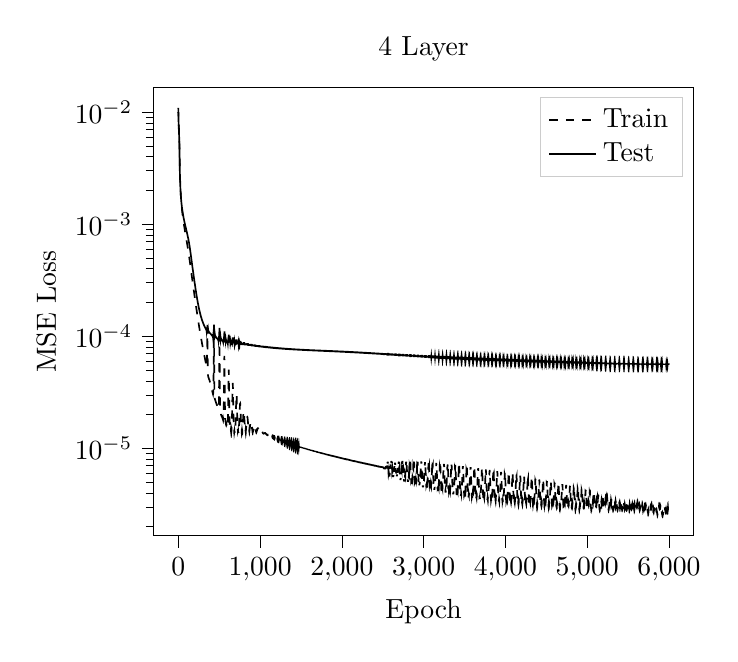
\begin{tikzpicture}

\begin{axis}[
legend cell align={left},
legend style={fill opacity=0.8, draw opacity=1, text opacity=1, draw=white!80!black},
log basis y={10},
tick align=outside,
tick pos=left,
title={4 Layer},
x grid style={white!69.0196078431373!black},
xlabel={Epoch},
xmin=-299.95, xmax=6298.95,
xtick style={color=black},
y grid style={white!69.0196078431373!black},
ylabel={MSE Loss},
ymin=1.65367011152804e-06, ymax=0.0165378276495926,
ymode=log,
ytick style={color=black}
]
\addplot [semithick, black, dashed]
table {%
0 0.0108807525830343
1 0.0101366702001542
2 0.00951129267923534
3 0.00896586285671219
4 0.00848299410426989
5 0.00804959743982181
6 0.0076601826294791
7 0.00731919275131077
8 0.00702948632533662
9 0.00677695525519084
10 0.00653317247633822
11 0.00626083150564227
12 0.00592074132873677
13 0.00549599970690906
14 0.00501126745075453
15 0.00451707903994247
16 0.00405622101243353
17 0.00365415004489478
18 0.00332527412683703
19 0.00306600953626912
20 0.0028547305992106
21 0.00267690898181172
22 0.00252717886905884
23 0.00240042659061146
24 0.00229278705955949
25 0.00219888157880632
26 0.00211530186788877
27 0.00203969597350806
28 0.00197128686704673
29 0.00190890697558643
30 0.00185191870332346
31 0.00179952520556981
32 0.0017512430640636
33 0.00170656959380722
34 0.00166509461996611
35 0.00162647633987945
36 0.00159040083053696
37 0.00155661881035485
38 0.00152489739593875
39 0.0014950280838093
40 0.00146682939339371
41 0.00144013650060515
42 0.00141480442835018
43 0.00139070413024456
44 0.00136772051155276
45 0.00134575171614415
46 0.00132470842800103
47 0.00130451083896332
48 0.0012850891907874
49 0.0012663818342844
50 0.00124833433801541
51 0.00123089828957745
52 0.00121403107368678
53 0.0011976944952039
54 0.0011818545171991
55 0.00116648037510458
56 0.00115154481682112
57 0.00113702255657699
58 0.00112289114804298
59 0.00110912960371934
60 0.00109571864777536
61 0.00108264104346745
62 0.00106988013249065
63 0.00105742070991255
64 0.00104524846028653
65 0.00103335010135197
66 0.00102171305661614
67 0.00101032509701326
68 0.000999175215838477
69 0.000988252628303599
70 0.000977547180809779
71 0.000967049327300629
72 0.000956749736360507
73 0.00094663966774533
74 0.000936710838686849
75 0.000926955152863229
76 0.00091736524427688
77 0.000907933666894678
78 0.000898653704098251
79 0.000889518699295877
80 0.000880522368788661
81 0.000871658894538996
82 0.000862922588567017
83 0.000854307928420894
84 0.000845809764541627
85 0.000837423113807745
86 0.000829143488772388
87 0.000820966375613352
88 0.000812887476058677
89 0.000804902681011299
90 0.000797008270637889
91 0.000789200598774187
92 0.000781476145675697
93 0.000773831250626245
94 0.000766263086006802
95 0.000758768612286076
96 0.000751344756281469
97 0.000743988863177947
98 0.000736698131731828
99 0.000729470169062552
100 0.000722302491340088
101 0.000715192760253558
102 0.000708138752997911
103 0.000701138549629832
104 0.000694189828209346
105 0.000687290779751493
106 0.000680439556163037
107 0.000673634390295774
108 0.000666873542286339
109 0.000660155473269697
110 0.000653478638014349
111 0.000646841438538104
112 0.00064024259972939
113 0.000633680719147378
114 0.000627154571702704
115 0.000620662994151644
116 0.000614204896010051
117 0.000607779444180778
118 0.000601385461777681
119 0.000595022197558137
120 0.000588688963944151
121 0.000582384989684215
122 0.000576109782741696
123 0.00056986280651472
124 0.000563643886380305
125 0.000557452578505035
126 0.000551289015675138
127 0.000545153033272072
128 0.000539044905963237
129 0.000532964910235023
130 0.00052691334985866
131 0.00052089097971475
132 0.00051489834277163
133 0.00050893670777441
134 0.000503006845065102
135 0.000497110037031234
136 0.00049124768065667
137 0.000485421203848091
138 0.000479632138194575
139 0.000473882605092513
140 0.000468174344860017
141 0.000462509263343236
142 0.000456889503311686
143 0.000451317128863593
144 0.000445794271399791
145 0.000440322949998517
146 0.000434905424299359
147 0.000429543601512705
148 0.000424239532549109
149 0.000418994811298035
150 0.000413811180351331
151 0.000408689978485199
152 0.000403632451252633
153 0.000398639587274374
154 0.000393711864489887
155 0.000388849987302819
156 0.000384054109417775
157 0.000379324201276177
158 0.000374660130091797
159 0.000370061228295526
160 0.000365526981113362
161 0.000361056685051153
162 0.000356649252353236
163 0.000352303602539905
164 0.000348018658769433
165 0.000343793157298933
166 0.000339625865308335
167 0.000335515681854304
168 0.000331461171299452
169 0.000327461154483899
170 0.000323514481806342
171 0.00031962000321073
172 0.00031577660865878
173 0.000311983168103325
174 0.000308238782963599
175 0.000304542437334021
176 0.00030089306710579
177 0.000297290032449382
178 0.000293732328373153
179 0.000290219240469014
180 0.000286750072064024
181 0.000283324203337543
182 0.000279940969903691
183 0.000276599680091749
184 0.000273299659511395
185 0.000270040366558533
186 0.000266821390141558
187 0.000263642057234392
188 0.0002605018844406
189 0.000257400375176076
190 0.000254337062870036
191 0.000251311590091063
192 0.000248323447067378
193 0.000245372275003319
194 0.000242457605054369
195 0.00023957895609783
196 0.000236736116676184
197 0.000233928698435193
198 0.000231156257086695
199 0.000228418572532973
200 0.00022571524095838
201 0.000223045990878745
202 0.000220410361635004
203 0.000217808089473692
204 0.000215238669170503
205 0.000212702061162418
206 0.000210197849810356
207 0.000207725862310326
208 0.000205285687798096
209 0.000202877164156234
210 0.000200499878928895
211 0.000198153629980879
212 0.000195838340914634
213 0.000193553441249605
214 0.000191298829804509
215 0.000189074183708726
216 0.000186879333341494
217 0.00018471391285857
218 0.000182577729901823
219 0.00018047050707537
220 0.000178392027692098
221 0.000176341916358069
222 0.000174320039150189
223 0.000172325988160082
224 0.000170359691992417
225 0.000168420806403446
226 0.000166508944857924
227 0.000164623852015211
228 0.000162765300274259
229 0.000160932930157287
230 0.000159126454263969
231 0.000157345604293369
232 0.000155590068061429
233 0.000153859489500974
234 0.000152153563476531
235 0.000150472025779891
236 0.000148814552176191
237 0.000147180697922522
238 0.00014557027839146
239 0.000143982894314831
240 0.000142418203722627
241 0.000140875936267548
242 0.000139355716783029
243 0.000137857129402619
244 0.000136379895593564
245 0.000134923673385856
246 0.000133488068286169
247 0.000132072949782014
248 0.00013067778900222
249 0.00012930220987073
250 0.000127946111206256
251 0.000126608911159565
252 0.000125290369169306
253 0.000123990284464526
254 0.000122708180469999
255 0.000121443680882294
256 0.000120196724310517
257 0.000118966818490662
258 0.000117753636914131
259 0.000116556909915744
260 0.000115376360781738
261 0.000114211821710342
262 0.000113062961645483
263 0.000111929548666012
264 0.00011081109278166
265 0.000109707495539624
266 0.000108618562080665
267 0.000107543922467812
268 0.000106483440504235
269 0.000105436754893162
270 0.000104403786167495
271 0.000103384238627768
272 0.000102377808957499
273 0.000101384394270099
274 0.000100403751503109
275 9.94357056924855e-05
276 9.84800452670243e-05
277 9.75365234126002e-05
278 9.66049080943776e-05
279 9.56851506543899e-05
280 9.47770245147694e-05
281 9.38803531198573e-05
282 9.29950505224042e-05
283 9.21207841884097e-05
284 9.12574823814793e-05
285 9.04050637018372e-05
286 8.95632844049032e-05
287 8.87319301909884e-05
288 8.79109170455195e-05
289 8.71000231654762e-05
290 8.62992272914198e-05
291 8.55082760153891e-05
292 8.47270997610394e-05
293 8.39554742242399e-05
294 8.31932028404481e-05
295 8.24403662136319e-05
296 8.16965990679819e-05
297 8.09618106814014e-05
298 8.02359554654686e-05
299 7.95188988149675e-05
300 7.88103906188553e-05
301 7.81103391318538e-05
302 7.74186901253415e-05
303 7.67353498076773e-05
304 7.60599166369502e-05
305 7.53925173739844e-05
306 7.47328299439687e-05
307 7.40808075079258e-05
308 7.34364208483385e-05
309 7.27992934344002e-05
310 7.21694715366539e-05
311 7.15467793952484e-05
312 7.09311611899466e-05
313 7.03222083302535e-05
314 6.97200550803245e-05
315 6.9124328547332e-05
316 6.85351689071467e-05
317 6.79520187532034e-05
318 6.73752668944871e-05
319 6.68039461970693e-05
320 6.62389487615656e-05
321 6.56788336073078e-05
322 6.51248980148011e-05
323 6.45751482579726e-05
324 6.4031701526801e-05
325 6.34915055570673e-05
326 6.29578308348755e-05
327 6.2426005058569e-05
328 6.19015501115427e-05
329 6.137674523643e-05
330 6.08611463803754e-05
331 6.03416543754065e-05
332 5.98344936406647e-05
333 5.93179846077874e-05
334 5.88198125228701e-05
335 5.83025356490907e-05
336 5.78151858121601e-05
337 5.72918543753076e-05
338 5.68202336808099e-05
339 5.62821527410051e-05
340 5.58373838543957e-05
341 5.52711121599714e-05
342 5.48803409969878e-05
343 5.4268112421596e-05
344 5.39994425139412e-05
345 5.33347239866089e-05
346 5.33757915377464e-05
347 5.27556974816434e-05
348 5.36745599788446e-05
349 5.37351568254962e-05
350 5.73008562128052e-05
351 6.08821681566951e-05
352 7.13391222006976e-05
353 8.5812010297559e-05
354 0.000100979233593534
355 0.000120043855531549
356 0.000108146332536307
357 9.90131588878285e-05
358 7.56350518145155e-05
359 6.19437393538647e-05
360 5.3461360437268e-05
361 4.89202299149838e-05
362 4.68736961920513e-05
363 4.52995966497838e-05
364 4.46415640453779e-05
365 4.38918942222699e-05
366 4.36185752050733e-05
367 4.32168962447577e-05
368 4.30100105290876e-05
369 4.27376282345904e-05
370 4.25410022444339e-05
371 4.23232027628728e-05
372 4.21435810267212e-05
373 4.19543190446348e-05
374 4.17876813685325e-05
375 4.16113875871815e-05
376 4.14452979953239e-05
377 4.12675487950764e-05
378 4.10905735748202e-05
379 4.09003783943263e-05
380 4.07057866596006e-05
381 4.04977956804942e-05
382 4.02838562649777e-05
383 4.00577473556041e-05
384 3.98263894680895e-05
385 3.95850478867033e-05
386 3.93399865856736e-05
387 3.90872930893238e-05
388 3.88325771609743e-05
389 3.85721814950557e-05
390 3.8311522132517e-05
391 3.80469432457176e-05
392 3.77833748643752e-05
393 3.75170358211108e-05
394 3.72531692391931e-05
395 3.69875656929253e-05
396 3.67255492506047e-05
397 3.64623893460703e-05
398 3.62039796186764e-05
399 3.59448148117281e-05
400 3.56914336521186e-05
401 3.54371909168094e-05
402 3.51899626025443e-05
403 3.49414079607868e-05
404 3.47010441430484e-05
405 3.445835412208e-05
406 3.42255273153569e-05
407 3.39886725555516e-05
408 3.37638593350675e-05
409 3.35324509421753e-05
410 3.33163055188379e-05
411 3.30893668092358e-05
412 3.28826320981079e-05
413 3.26588142911532e-05
414 3.24631447199408e-05
415 3.22404580401781e-05
416 3.20587521400739e-05
417 3.18340568412623e-05
418 3.16722959610161e-05
419 3.14416355706726e-05
420 3.13123481987532e-05
421 3.10718756679762e-05
422 3.10034697577066e-05
423 3.07568388961954e-05
424 3.08200557412874e-05
425 3.06094295012826e-05
426 3.09989503648467e-05
427 3.1031520364877e-05
428 3.23255243586118e-05
429 3.34581890797381e-05
430 3.73788374474771e-05
431 4.2709020874554e-05
432 5.3219188885123e-05
433 7.0129861796886e-05
434 8.60424368056556e-05
435 0.00011046530380554
436 0.000100550253137044
437 9.61731279858213e-05
438 6.76536903370106e-05
439 5.21722228086219e-05
440 4.01035765094093e-05
441 3.44453078753304e-05
442 3.15704360787095e-05
443 3.00149088729995e-05
444 2.91883591501119e-05
445 2.84477294201224e-05
446 2.81009586728942e-05
447 2.76809811907697e-05
448 2.75160054457046e-05
449 2.72618115104706e-05
450 2.71422539981359e-05
451 2.69502309890868e-05
452 2.68335300859235e-05
453 2.66625961273803e-05
454 2.6544508614279e-05
455 2.63841658352248e-05
456 2.62661708916312e-05
457 2.61134736945223e-05
458 2.59960263520043e-05
459 2.58493084572819e-05
460 2.57330766260111e-05
461 2.55913155911003e-05
462 2.54768509648784e-05
463 2.53391887099497e-05
464 2.522696536289e-05
465 2.50925440354877e-05
466 2.49828951837117e-05
467 2.4851112016222e-05
468 2.47443433067929e-05
469 2.46145861524383e-05
470 2.4511056267329e-05
471 2.43826592054575e-05
472 2.42828418919316e-05
473 2.41550795436751e-05
474 2.40596020972816e-05
475 2.39316475898477e-05
476 2.38414501581019e-05
477 2.3712133099707e-05
478 2.36287809087798e-05
479 2.34965852285995e-05
480 2.34224074944223e-05
481 2.32853778214803e-05
482 2.32242964415263e-05
483 2.3079745616883e-05
484 2.30385218742413e-05
485 2.2883361566528e-05
486 2.28743917460861e-05
487 2.27060363044984e-05
488 2.2753305145784e-05
489 2.25742306554366e-05
490 2.27280659288454e-05
491 2.2560786803183e-05
492 2.2934721826573e-05
493 2.28711931953285e-05
494 2.37384408450225e-05
495 2.40943623452949e-05
496 2.61300095871775e-05
497 2.78893306244754e-05
498 3.26321728039147e-05
499 3.83710778919522e-05
500 4.79660172914009e-05
501 6.1358341667983e-05
502 7.19407737506117e-05
503 8.70407359343517e-05
504 8.00157342837338e-05
505 7.72379562476999e-05
506 5.74159916482131e-05
507 4.59310081737385e-05
508 3.52111405277356e-05
509 2.93519194087821e-05
510 2.60239986005217e-05
511 2.39707813420864e-05
512 2.29555648445512e-05
513 2.2037409834752e-05
514 2.16422160121965e-05
515 2.11056841550317e-05
516 2.09424301260697e-05
517 2.06061374825595e-05
518 2.0534493728519e-05
519 2.03058811791834e-05
520 2.02644559408327e-05
521 2.00898038258401e-05
522 2.0055675832964e-05
523 1.99083729626182e-05
524 1.98752486539888e-05
525 1.97430267832033e-05
526 1.97097585754591e-05
527 1.95864040364313e-05
528 1.95535168074912e-05
529 1.94354907989691e-05
530 1.94040125620631e-05
531 1.92888009422632e-05
532 1.92600945609911e-05
533 1.91457183120747e-05
534 1.91214599567502e-05
535 1.90060774087897e-05
536 1.89884211749813e-05
537 1.8870146647032e-05
538 1.88621653478549e-05
539 1.87389732246857e-05
540 1.87451681910034e-05
541 1.86148905356731e-05
542 1.86423054486795e-05
543 1.85028524839481e-05
544 1.85632065381469e-05
545 1.84137934695627e-05
546 1.85275315516265e-05
547 1.83716593369354e-05
548 1.85767281379867e-05
549 1.84310379722774e-05
550 1.88015641811035e-05
551 1.87190844087581e-05
552 1.94065629557372e-05
553 1.95369348716667e-05
554 2.08566800523613e-05
555 2.15914826355856e-05
556 2.41710792607819e-05
557 2.64272702565904e-05
558 3.12607093064798e-05
559 3.66637287925187e-05
560 4.40643370893667e-05
561 5.33882408717545e-05
562 5.89572252920334e-05
563 6.67869326207438e-05
564 6.15469841704908e-05
565 5.91835570276089e-05
566 4.72029497018411e-05
567 3.97198220412065e-05
568 3.18509235057718e-05
569 2.69153288172674e-05
570 2.37144591608285e-05
571 2.14333263670596e-05
572 2.02787487779688e-05
573 1.91432453817697e-05
574 1.8693258653002e-05
575 1.80049484015399e-05
576 1.78243460311478e-05
577 1.73612656340083e-05
578 1.73028316368118e-05
579 1.69721624416752e-05
580 1.69698300709342e-05
581 1.67173569423085e-05
582 1.67400876875945e-05
583 1.65331543513503e-05
584 1.65679115866624e-05
585 1.63872846314916e-05
586 1.64298605795921e-05
587 1.62642670886726e-05
588 1.63146999199171e-05
589 1.61569701901954e-05
590 1.62179429992193e-05
591 1.60633412065181e-05
592 1.61395469859826e-05
593 1.59847539720204e-05
594 1.60836104470263e-05
595 1.59267660393425e-05
596 1.60597552536501e-05
597 1.59012140272807e-05
598 1.60868690102234e-05
599 1.59318024657296e-05
600 1.62012089361951e-05
601 1.6065347764993e-05
602 1.64725889959527e-05
603 1.63955215981559e-05
604 1.7037333918779e-05
605 1.71113194227246e-05
606 1.81612532088593e-05
607 1.85883316987656e-05
608 2.03428214291534e-05
609 2.15275586299413e-05
610 2.44067806249859e-05
611 2.70094563745715e-05
612 3.12659894916578e-05
613 3.5843477007802e-05
614 4.04819114123711e-05
615 4.60402787894054e-05
616 4.76159710842694e-05
617 5.03728898593181e-05
618 4.61593655245451e-05
619 4.37075824493149e-05
620 3.70593097045457e-05
621 3.25178933167081e-05
622 2.7749895167517e-05
623 2.43014318925816e-05
624 2.19047186362786e-05
625 1.98831254749621e-05
626 1.88299116672397e-05
627 1.7635357565382e-05
628 1.71855978408075e-05
629 1.6402293240958e-05
630 1.62257362603668e-05
631 1.56658709755675e-05
632 1.56265009252365e-05
633 1.52023363710896e-05
634 1.52379928408664e-05
635 1.48999319975474e-05
636 1.49802350080108e-05
637 1.4697276220943e-05
638 1.48085907483164e-05
639 1.4561109125566e-05
640 1.46997891334877e-05
641 1.44758251607868e-05
642 1.46449766873502e-05
643 1.44380950573009e-05
644 1.46469010218198e-05
645 1.44558319519206e-05
646 1.4720610138852e-05
647 1.45506070197143e-05
648 1.48979120240256e-05
649 1.47645846482192e-05
650 1.52372115991284e-05
651 1.51748971006782e-05
652 1.58411778841128e-05
653 1.59182846459771e-05
654 1.68846001287193e-05
655 1.72276218677325e-05
656 1.8646371131581e-05
657 1.9466271822921e-05
658 2.15071533204991e-05
659 2.30857662870676e-05
660 2.57869747599671e-05
661 2.83030211107871e-05
662 3.12038534957537e-05
663 3.42611392056824e-05
664 3.60474990657167e-05
665 3.82572990247354e-05
666 3.74675048533391e-05
667 3.73399897171112e-05
668 3.42485337796461e-05
669 3.2039051063748e-05
670 2.8574766076872e-05
671 2.5873113884245e-05
672 2.3373863911047e-05
673 2.12110193729131e-05
674 1.97781604640568e-05
675 1.82780929947057e-05
676 1.75493471061827e-05
677 1.65140874059944e-05
678 1.6178702296088e-05
679 1.54290338372221e-05
680 1.5310907670596e-05
681 1.47395342082746e-05
682 1.47492338555821e-05
683 1.42951845418793e-05
684 1.43878029206235e-05
685 1.40146061795576e-05
686 1.41685697059302e-05
687 1.38538633649432e-05
688 1.40616185007048e-05
689 1.37927852108533e-05
690 1.40570597295664e-05
691 1.38298472052156e-05
692 1.4162299564191e-05
693 1.39811969290804e-05
694 1.4403433212351e-05
695 1.42841116286263e-05
696 1.48297732636138e-05
697 1.48040579261988e-05
698 1.55216139177128e-05
699 1.56444481547169e-05
700 1.65972693935146e-05
701 1.6953033906475e-05
702 1.82083984157089e-05
703 1.89064102755765e-05
704 2.04957376297443e-05
705 2.16294868096156e-05
706 2.34565828804989e-05
707 2.49928581865788e-05
708 2.67070898303245e-05
709 2.83230652939892e-05
710 2.93092967922348e-05
711 3.03700549579844e-05
712 3.00998868283386e-05
713 3.00433503070963e-05
714 2.86159767597383e-05
715 2.74818303864777e-05
716 2.56044117463716e-05
717 2.3968199684532e-05
718 2.23214642289804e-05
719 2.07359221349179e-05
720 1.95859441873836e-05
721 1.82873487233337e-05
722 1.75940917301887e-05
723 1.6590503577163e-05
724 1.62245708992259e-05
725 1.54503084957014e-05
726 1.53008494123696e-05
727 1.46916823098309e-05
728 1.46868313919413e-05
729 1.4196982078829e-05
730 1.42951602981611e-05
731 1.38950576911157e-05
732 1.40748672947666e-05
733 1.37468470455815e-05
734 1.40003124897703e-05
735 1.37361595022867e-05
736 1.40652437892186e-05
737 1.38653224865948e-05
738 1.42804334188895e-05
739 1.41543247735854e-05
740 1.46733775778785e-05
741 1.46409965395833e-05
742 1.52879516690518e-05
743 1.53806873015583e-05
744 1.61810463623624e-05
745 1.64399247921665e-05
746 1.7409668515711e-05
747 1.78753304282964e-05
748 1.8997482868599e-05
749 1.96848265829885e-05
750 2.08741561493753e-05
751 2.17280202150505e-05
752 2.28005089297767e-05
753 2.36528792925128e-05
754 2.43472751435547e-05
755 2.49314222742214e-05
756 2.50284327876216e-05
757 2.51012664875816e-05
758 2.45847811015665e-05
759 2.40896335412799e-05
760 2.3182583106518e-05
761 2.22840200194696e-05
762 2.12985979715086e-05
763 2.02488738523243e-05
764 1.9410763485439e-05
765 1.84027464911196e-05
766 1.77985924381119e-05
767 1.69208951774635e-05
768 1.65436754571147e-05
769 1.58117351816145e-05
770 1.56198291563214e-05
771 1.50181693072682e-05
772 1.4969085100347e-05
773 1.44757973714604e-05
774 1.45378082123671e-05
775 1.41345150268535e-05
776 1.42875780682061e-05
777 1.39620634342918e-05
778 1.41957776804702e-05
779 1.39421112521632e-05
780 1.42535087803708e-05
781 1.40719226067176e-05
782 1.44634965550949e-05
783 1.43601029094498e-05
784 1.48376392559157e-05
785 1.48237260759743e-05
786 1.53932939497281e-05
787 1.54835373109563e-05
788 1.61458238210344e-05
789 1.63534185446679e-05
790 1.70954457985317e-05
791 1.74230574430112e-05
792 1.8206992820069e-05
793 1.86328519191648e-05
794 1.93864586037762e-05
795 1.98505329649379e-05
796 2.04694301828567e-05
797 2.08709184335021e-05
798 2.12445351053248e-05
799 2.14653992998137e-05
800 2.15245061667702e-05
801 2.14772214235381e-05
802 2.12356130759872e-05
803 2.09070620371676e-05
804 2.04603776978729e-05
805 1.9914770973628e-05
806 1.93935749166485e-05
807 1.87333782264432e-05
808 1.82484463380206e-05
809 1.75676600520092e-05
810 1.71833184765546e-05
811 1.65433658310121e-05
812 1.62816352826667e-05
813 1.57117433445819e-05
814 1.55693368242282e-05
815 1.50777606506836e-05
816 1.50412693642465e-05
817 1.46262636917527e-05
818 1.46813493131503e-05
819 1.43382369515166e-05
820 1.44732949820536e-05
821 1.4198066935478e-05
822 1.44052787902638e-05
823 1.41960755684067e-05
824 1.44706991704879e-05
825 1.43281963573827e-05
826 1.46672926746305e-05
827 1.45941335745192e-05
828 1.49947051397703e-05
829 1.49943798248842e-05
830 1.54506278136068e-05
831 1.55251019862135e-05
832 1.60250330623057e-05
833 1.61708294683649e-05
834 1.66923361462068e-05
835 1.68959883524167e-05
836 1.74043637457544e-05
837 1.76380453069669e-05
838 1.80870542294542e-05
839 1.83075897552953e-05
840 1.86468539027373e-05
841 1.88018138373991e-05
842 1.89908784307136e-05
843 1.90317438182319e-05
844 1.90555168444462e-05
845 1.89539530310867e-05
846 1.88305903350283e-05
847 1.85882780669999e-05
848 1.8363630232443e-05
849 1.80096807866903e-05
850 1.77412993878079e-05
851 1.73193712385e-05
852 1.70590612640353e-05
853 1.66126391150101e-05
854 1.63966199124843e-05
855 1.59595767286191e-05
856 1.58075524439028e-05
857 1.54019857632193e-05
858 1.53206752031565e-05
859 1.49586987276962e-05
860 1.49473083865814e-05
861 1.46344997915548e-05
862 1.46887493883696e-05
863 1.44272933368939e-05
864 1.45418446209078e-05
865 1.43324522241528e-05
866 1.45020354125336e-05
867 1.4345027437912e-05
868 1.4564541118034e-05
869 1.44601947624778e-05
870 1.47240321837216e-05
871 1.46721204998812e-05
872 1.49732439922445e-05
873 1.49721854825202e-05
874 1.53006767220631e-05
875 1.53459610601203e-05
876 1.56879202961591e-05
877 1.57708251151689e-05
878 1.61077542770727e-05
879 1.62136711026051e-05
880 1.65230528921256e-05
881 1.6631541541301e-05
882 1.68893068916987e-05
883 1.69758401966646e-05
884 1.71608055552497e-05
885 1.72007683545417e-05
886 1.73000329368733e-05
887 1.72741018218403e-05
888 1.72871839936306e-05
889 1.71863653122273e-05
890 1.71258180614586e-05
891 1.69531368214848e-05
892 1.68414119627869e-05
893 1.66103600918177e-05
894 1.64741373680499e-05
895 1.62042842362098e-05
896 1.60686935544163e-05
897 1.57806463505494e-05
898 1.56655059129207e-05
899 1.5377490086621e-05
900 1.52959255501628e-05
901 1.50221370347481e-05
902 1.49814547683036e-05
903 1.47316794141261e-05
904 1.4734484921064e-05
905 1.45150461321464e-05
906 1.45608441641798e-05
907 1.43756290924557e-05
908 1.44623625430995e-05
909 1.43135075632017e-05
910 1.44374464525754e-05
911 1.43257306888245e-05
912 1.44824118422093e-05
913 1.44075945343047e-05
914 1.45912874245369e-05
915 1.45516933116596e-05
916 1.47553428462288e-05
917 1.47477975644961e-05
918 1.49625339531667e-05
919 1.49816639805067e-05
920 1.51970135391366e-05
921 1.52348362121302e-05
922 1.54387936674993e-05
923 1.54848427200704e-05
924 1.56649377913709e-05
925 1.57070264492631e-05
926 1.5851846995929e-05
927 1.58771472911212e-05
928 1.59783593289831e-05
929 1.59755985009724e-05
930 1.60293772637488e-05
931 1.59904617476059e-05
932 1.59986986716376e-05
933 1.59204844010219e-05
934 1.58905843363755e-05
935 1.57749737468293e-05
936 1.57180119515488e-05
937 1.55713293850113e-05
938 1.55002810231508e-05
939 1.53315823467892e-05
940 1.52592005235874e-05
941 1.50787339805447e-05
942 1.50158235499021e-05
943 1.48333510878729e-05
944 1.47880417387114e-05
945 1.46120942474681e-05
946 1.45897475363199e-05
947 1.44269718020951e-05
948 1.44302977105326e-05
949 1.42857628020465e-05
950 1.43154809677526e-05
951 1.4192486361253e-05
952 1.42475939810538e-05
953 1.41480934132687e-05
954 1.42262513520564e-05
955 1.41509900970505e-05
956 1.42488771359695e-05
957 1.4197475650235e-05
958 1.43106496466316e-05
959 1.42814331525187e-05
960 1.44046513810281e-05
961 1.43947595745431e-05
962 1.45218675129399e-05
963 1.45271455664897e-05
964 1.46512715843983e-05
965 1.46662482620741e-05
966 1.47806219388258e-05
967 1.4798907130853e-05
968 1.48969797351128e-05
969 1.49118544925386e-05
970 1.49883647964089e-05
971 1.49932461681601e-05
972 1.50446751092659e-05
973 1.50340778475311e-05
974 1.50592865963972e-05
975 1.50295109051513e-05
976 1.50301056862645e-05
977 1.49797534447771e-05
978 1.49597152017122e-05
979 1.48896326379599e-05
980 1.48544743012735e-05
981 1.47677037602989e-05
982 1.47241551644584e-05
983 1.46251194905744e-05
984 1.45797176003271e-05
985 1.44735408866836e-05
986 1.44322469282088e-05
987 1.43241973660224e-05
988 1.42917302241585e-05
989 1.41866986496098e-05
990 1.41665688886405e-05
991 1.40687799330408e-05
992 1.40630114344731e-05
993 1.39757384829409e-05
994 1.39851835569971e-05
995 1.39108972234681e-05
996 1.39351074039951e-05
997 1.3875297412369e-05
998 1.39129951719497e-05
999 1.38681881765024e-05
1000 1.39170846580328e-05
1001 1.38869990848889e-05
1002 1.39442894067088e-05
1003 1.39278648418895e-05
1004 1.39900667761594e-05
1005 1.39852092218007e-05
1006 1.40485919644107e-05
1007 1.40526732934632e-05
1008 1.41131982047682e-05
1009 1.4122978427622e-05
1010 1.41768522610164e-05
1011 1.41886289668491e-05
1012 1.42324296348306e-05
1013 1.42425062961138e-05
1014 1.42735804331551e-05
1015 1.42785195293982e-05
1016 1.42953331021545e-05
1017 1.42923564112607e-05
1018 1.4294545849225e-05
1019 1.42817398796069e-05
1020 1.42702988625842e-05
1021 1.42468748265401e-05
1022 1.4223736883423e-05
1023 1.41900756887026e-05
1024 1.41581830632731e-05
1025 1.41156378674623e-05
1026 1.40783822359936e-05
1027 1.40290905221718e-05
1028 1.39898841950981e-05
1029 1.39365328095664e-05
1030 1.38987472837471e-05
1031 1.38440890680158e-05
1032 1.38104271627526e-05
1033 1.37572268386066e-05
1034 1.3729738782331e-05
1035 1.36805443844423e-05
1036 1.36607040985837e-05
1037 1.3617549313949e-05
1038 1.36058746988965e-05
1039 1.35703624266625e-05
1040 1.35667837923847e-05
1041 1.35398774716577e-05
1042 1.35436693824431e-05
1043 1.3525764387623e-05
1044 1.35357113322243e-05
1045 1.35268285816892e-05
1046 1.35412329029805e-05
1047 1.35406300785235e-05
1048 1.35574753699075e-05
1049 1.35640688370131e-05
1050 1.35811180257406e-05
1051 1.35933041747194e-05
1052 1.36082625488143e-05
1053 1.36240961126077e-05
1054 1.36348725447988e-05
1055 1.36524126332915e-05
1056 1.36572361952858e-05
1057 1.36744791632282e-05
1058 1.36719494321369e-05
1059 1.36870038147663e-05
1060 1.36763572129439e-05
1061 1.36877143290803e-05
1062 1.36686556118093e-05
1063 1.36752941841678e-05
1064 1.36484080996979e-05
1065 1.36498588290124e-05
1066 1.36161258126322e-05
1067 1.36123856862014e-05
1068 1.35732183537129e-05
1069 1.35649316916897e-05
1070 1.352208590788e-05
1071 1.35102369256401e-05
1072 1.34656403929512e-05
1073 1.34515296110749e-05
1074 1.34069537978121e-05
1075 1.3392110759014e-05
1076 1.33490895848354e-05
1077 1.3335073106191e-05
1078 1.32949236615332e-05
1079 1.32832243195935e-05
1080 1.32467465903119e-05
1081 1.32385584095118e-05
1082 1.32062404532007e-05
1083 1.32025024868199e-05
1084 1.31743305757936e-05
1085 1.31757391272913e-05
1086 1.31513842802633e-05
1087 1.31582653182249e-05
1088 1.31370667588726e-05
1089 1.31493841593056e-05
1090 1.31304402088972e-05
1091 1.31479659728484e-05
1092 1.31301043211351e-05
1093 1.31522025981212e-05
1094 1.31342285101255e-05
1095 1.31599701376217e-05
1096 1.3140562288072e-05
1097 1.31689953377645e-05
1098 1.3147096154853e-05
1099 1.31771356848276e-05
1100 1.31516781891605e-05
1101 1.31821931859122e-05
1102 1.31524083428758e-05
1103 1.31823830997746e-05
1104 1.31477677030034e-05
1105 1.31762932085167e-05
1106 1.31367579285779e-05
1107 1.31632806983362e-05
1108 1.31190713545948e-05
1109 1.31432709338242e-05
1110 1.3094819678372e-05
1111 1.3116637433086e-05
1112 1.30646809282098e-05
1113 1.30842966541422e-05
1114 1.30297545126723e-05
1115 1.30477116897509e-05
1116 1.29915425475247e-05
1117 1.30084461886781e-05
1118 1.29515925664236e-05
1119 1.29682803162723e-05
1120 1.29117368317111e-05
1121 1.29289331596283e-05
1122 1.28733647102308e-05
1123 1.28920029283108e-05
1124 1.28379907096132e-05
1125 1.28587762446841e-05
1126 1.28065746594075e-05
1127 1.2829995824859e-05
1128 1.27796791105084e-05
1129 1.28062290798425e-05
1130 1.27577172008841e-05
1131 1.27876427313822e-05
1132 1.27406160004284e-05
1133 1.27740414370692e-05
1134 1.27280173387589e-05
1135 1.27647371357398e-05
1136 1.27190495504692e-05
1137 1.27588042744264e-05
1138 1.27128612064098e-05
1139 1.27552225137606e-05
1140 1.27082830942982e-05
1141 1.27527619611101e-05
1142 1.27042328301741e-05
1143 1.27501301108168e-05
1144 1.26993946594212e-05
1145 1.27461627812409e-05
1146 1.26927858161707e-05
1147 1.27398371034815e-05
1148 1.26834783600316e-05
1149 1.27302611190316e-05
1150 1.26708412153675e-05
1151 1.27171048802666e-05
1152 1.26546957517348e-05
1153 1.27000720056003e-05
1154 1.26349110018964e-05
1155 1.2679395183568e-05
1156 1.2611826889497e-05
1157 1.26554608641527e-05
1158 1.25859363606651e-05
1159 1.26289253614686e-05
1160 1.25580183691909e-05
1161 1.26007676044537e-05
1162 1.25289780612547e-05
1163 1.2571806678352e-05
1164 1.24996140868916e-05
1165 1.25429449155945e-05
1166 1.24707506472532e-05
1167 1.25150524468154e-05
1168 1.24432687869103e-05
1169 1.24889640460424e-05
1170 1.24177600184794e-05
1171 1.24652335955489e-05
1172 1.23947019687876e-05
1173 1.24441971536271e-05
1174 1.23743930089404e-05
1175 1.24261655685132e-05
1176 1.23568421201981e-05
1177 1.24108547083779e-05
1178 1.23418265047803e-05
1179 1.23980956914238e-05
1180 1.23289802331783e-05
1181 1.23873734594326e-05
1182 1.23178837725391e-05
1183 1.23781592549221e-05
1184 1.23077894045309e-05
1185 1.23696484024549e-05
1186 1.2298150920742e-05
1187 1.2361308989739e-05
1188 1.22883508879568e-05
1189 1.23525800290736e-05
1190 1.22778826607828e-05
1191 1.23427264782094e-05
1192 1.22661093939769e-05
1193 1.23313674293968e-05
1194 1.2252758580189e-05
1195 1.23181065418976e-05
1196 1.2237498168588e-05
1197 1.23028929976954e-05
1198 1.22203470880322e-05
1199 1.22855845177128e-05
1200 1.2201242412857e-05
1201 1.2266419844309e-05
1202 1.2180628459646e-05
1203 1.22457779809793e-05
1204 1.21587358137276e-05
1205 1.2223995952354e-05
1206 1.21359789773123e-05
1207 1.2201572047843e-05
1208 1.21129339447634e-05
1209 1.21790949663136e-05
1210 1.20900697879733e-05
1211 1.21570949147554e-05
1212 1.20678229507121e-05
1213 1.21359023523837e-05
1214 1.20465533939296e-05
1215 1.21158540480337e-05
1216 1.20265561633914e-05
1217 1.20972865147451e-05
1218 1.20079588157296e-05
1219 1.20802402818754e-05
1220 1.19908951887737e-05
1221 1.20647638084392e-05
1222 1.19752500324921e-05
1223 1.20506996950098e-05
1224 1.19608688464723e-05
1225 1.20378959707068e-05
1226 1.19475345456976e-05
1227 1.2025983409103e-05
1228 1.19348880218695e-05
1229 1.20146979725178e-05
1230 1.19227570962721e-05
1231 1.20038021691471e-05
1232 1.19107338889535e-05
1233 1.1992711364428e-05
1234 1.18984385721888e-05
1235 1.19811988383844e-05
1236 1.18855640209858e-05
1237 1.19690124904537e-05
1238 1.18719811155188e-05
1239 1.19558755500293e-05
1240 1.18574035354868e-05
1241 1.19416397126315e-05
1242 1.18417326859799e-05
1243 1.19263449107621e-05
1244 1.18251147398496e-05
1245 1.19100269841965e-05
1246 1.180758118835e-05
1247 1.18928333563417e-05
1248 1.17893237927547e-05
1249 1.18750114381783e-05
1250 1.1770575014225e-05
1251 1.18567561173677e-05
1252 1.1751518343317e-05
1253 1.18383150322643e-05
1254 1.17325151904879e-05
1255 1.18200259464629e-05
1256 1.17137652182464e-05
1257 1.18021567914184e-05
1258 1.16954593636365e-05
1259 1.17848009608679e-05
1260 1.167768527921e-05
1261 1.17680732216741e-05
1262 1.1660673408187e-05
1263 1.17522799882863e-05
1264 1.16445786204622e-05
1265 1.17374065951026e-05
1266 1.16292866891854e-05
1267 1.17233251444304e-05
1268 1.16147583639759e-05
1269 1.17100174463758e-05
1270 1.16008151564984e-05
1271 1.16972057924158e-05
1272 1.15873768891106e-05
1273 1.16848448783458e-05
1274 1.15741954971327e-05
1275 1.16726664032285e-05
1276 1.15612164961476e-05
1277 1.16606841800149e-05
1278 1.15482876879014e-05
1279 1.16486134515981e-05
1280 1.15351706426736e-05
1281 1.16362275264237e-05
1282 1.15216912490723e-05
1283 1.16234306801744e-05
1284 1.15077490363547e-05
1285 1.16100119669227e-05
1286 1.14932701364978e-05
1287 1.15960570781226e-05
1288 1.14781623210547e-05
1289 1.15814150944971e-05
1290 1.14625798346424e-05
1291 1.15664135194038e-05
1292 1.14466675711355e-05
1293 1.15510631815141e-05
1294 1.14304710905344e-05
1295 1.15354422405289e-05
1296 1.14140372033944e-05
1297 1.15196423848829e-05
1298 1.13976086311141e-05
1299 1.15039208026246e-05
1300 1.1381222577711e-05
1301 1.14882609523193e-05
1302 1.13650285129552e-05
1303 1.14729676852221e-05
1304 1.1349196881838e-05
1305 1.14579952708027e-05
1306 1.13336940330555e-05
1307 1.14434031104338e-05
1308 1.13186171120105e-05
1309 1.14293107742469e-05
1310 1.13040027258648e-05
1311 1.14156503627783e-05
1312 1.12898008808315e-05
1313 1.14024597621665e-05
1314 1.12760819490632e-05
1315 1.13897362439275e-05
1316 1.12626964323681e-05
1317 1.13773129442052e-05
1318 1.12495640109955e-05
1319 1.13650772561869e-05
1320 1.12365676727677e-05
1321 1.13529438579008e-05
1322 1.12236382676656e-05
1323 1.13407692765577e-05
1324 1.12106237963872e-05
1325 1.13285417739917e-05
1326 1.1197486543324e-05
1327 1.13160985506511e-05
1328 1.11840940633101e-05
1329 1.13033474917756e-05
1330 1.11704655409994e-05
1331 1.12903207991621e-05
1332 1.11565928193613e-05
1333 1.12770889870717e-05
1334 1.11424891144907e-05
1335 1.1263608655554e-05
1336 1.11282012937863e-05
1337 1.12498808562123e-05
1338 1.1113749536662e-05
1339 1.1236079842547e-05
1340 1.10991326494059e-05
1341 1.12220935761798e-05
1342 1.10844752327921e-05
1343 1.12080666951897e-05
1344 1.1069797210439e-05
1345 1.1194158332728e-05
1346 1.10552568060029e-05
1347 1.11802980597986e-05
1348 1.10408242903759e-05
1349 1.11666180657721e-05
1350 1.10265430635081e-05
1351 1.11531339257454e-05
1352 1.10125133119254e-05
1353 1.11399241689014e-05
1354 1.09988081078427e-05
1355 1.11270808247355e-05
1356 1.0985368078309e-05
1357 1.11144820778009e-05
1358 1.09721505623384e-05
1359 1.1102097857929e-05
1360 1.09591582031499e-05
1361 1.10899319167856e-05
1362 1.09463617832262e-05
1363 1.10779203623679e-05
1364 1.09336926072956e-05
1365 1.10660354550873e-05
1366 1.09210710377283e-05
1367 1.10542192715002e-05
1368 1.09085972042067e-05
1369 1.10424609829352e-05
1370 1.08960692273286e-05
1371 1.10306457941078e-05
1372 1.08834844922967e-05
1373 1.10187073403267e-05
1374 1.08708031518745e-05
1375 1.10066676484166e-05
1376 1.08579522759555e-05
1377 1.09944244002236e-05
1378 1.08449347067108e-05
1379 1.09819931140009e-05
1380 1.08317585727491e-05
1381 1.096944995993e-05
1382 1.08185494127611e-05
1383 1.09568302946172e-05
1384 1.08052711595974e-05
1385 1.09441900235652e-05
1386 1.07919408094403e-05
1387 1.09314897827062e-05
1388 1.07785967600194e-05
1389 1.09187548105183e-05
1390 1.07652869019148e-05
1391 1.09061521129661e-05
1392 1.07520512813153e-05
1393 1.08935772971108e-05
1394 1.07388915751017e-05
1395 1.0881123046147e-05
1396 1.07258743184957e-05
1397 1.08688114721645e-05
1398 1.07130252899879e-05
1399 1.08567070071786e-05
1400 1.07003645837267e-05
1401 1.08447785862609e-05
1402 1.06878406995747e-05
1403 1.08329485044578e-05
1404 1.06754537512188e-05
1405 1.08213194209839e-05
1406 1.06632331835499e-05
1407 1.08098442694882e-05
1408 1.06511571402734e-05
1409 1.07984425596896e-05
1410 1.06391285896734e-05
1411 1.07871115062608e-05
1412 1.06271111235401e-05
1413 1.0775747284697e-05
1414 1.06151845500335e-05
1415 1.07644874560719e-05
1416 1.06032370865705e-05
1417 1.07531859043775e-05
1418 1.05912718311174e-05
1419 1.07418651111857e-05
1420 1.05792462079535e-05
1421 1.07304170455791e-05
1422 1.05671630308279e-05
1423 1.07188483582377e-05
1424 1.05548923556853e-05
1425 1.07072307287126e-05
1426 1.05426703385092e-05
1427 1.06955778846896e-05
1428 1.05303917052879e-05
1429 1.0683881470186e-05
1430 1.05181044034452e-05
1431 1.06722157795502e-05
1432 1.05058414021642e-05
1433 1.06605608607424e-05
1434 1.04935899685188e-05
1435 1.06489157474243e-05
1436 1.0481405581686e-05
1437 1.06373175299268e-05
1438 1.04692399816031e-05
1439 1.06257649008512e-05
1440 1.04571433041656e-05
1441 1.06142996401104e-05
1442 1.04451421236718e-05
1443 1.06029387723083e-05
1444 1.04332353600967e-05
1445 1.05916348900337e-05
1446 1.04213942790921e-05
1447 1.05805134182901e-05
1448 1.04097813107273e-05
1449 1.05695276886308e-05
1450 1.0398241471421e-05
1451 1.05586121037504e-05
1452 1.03867555480974e-05
1453 1.0547735058708e-05
1454 1.03753292250985e-05
1455 1.05369749121564e-05
1456 1.03639891619878e-05
1457 1.05262120371208e-05
1458 1.03526514578789e-05
1459 1.05154470873003e-05
1460 1.03413354111126e-05
1461 1.05047315344109e-05
1462 1.03299904310461e-05
1463 1.04939209961685e-05
1464 1.03186503110919e-05
1465 1.0483189015531e-05
1466 1.03073730883807e-05
1467 1.04724983316373e-05
1468 1.02960455024004e-05
1469 1.04616854628148e-05
1470 1.02846647394017e-05
1471 1.04508591789454e-05
1472 1.027326314329e-05
1473 1.04399779843334e-05
1474 1.02618258495113e-05
1475 1.04290615468017e-05
1476 1.02503255448028e-05
1477 1.04181386006985e-05
1478 1.0238913489502e-05
1479 1.04072460658244e-05
1480 1.02275456868028e-05
1481 1.03964401603207e-05
1482 1.02162173334364e-05
1483 1.03856898761023e-05
1484 1.02049312999952e-05
1485 1.03749687809795e-05
1486 1.01937231136162e-05
1487 1.03643184559132e-05
1488 1.01826198317667e-05
1489 1.03537782933927e-05
1490 1.01715812093062e-05
1491 1.03433542903986e-05
1492 1.01606646296659e-05
1493 1.03329467151525e-05
1494 1.0149705758522e-05
1495 1.03225336545165e-05
1496 1.01387850577339e-05
1497 1.03121406311857e-05
1498 1.01279292721301e-05
1499 1.03018520860587e-05
1500 1.01171492019603e-05
1501 1.02916356752303e-05
1502 1.01064518673866e-05
1503 1.02814991009836e-05
1504 1.00958023665498e-05
1505 1.02713999297066e-05
1506 1.00851680429059e-05
1507 1.02612648618106e-05
1508 1.00745467079832e-05
1509 1.02511784803028e-05
1510 1.00639363722621e-05
1511 1.02410711235734e-05
1512 1.00532885198845e-05
1513 1.02309163025893e-05
1514 1.0042652888842e-05
1515 1.02207168310997e-05
1516 1.00318976592462e-05
1517 1.02104371535461e-05
1518 1.00211242397563e-05
1519 1.02001378934347e-05
1520 1.00103539750762e-05
1521 1.01898553737101e-05
1522 9.99958015768243e-06
1523 1.01795521914028e-05
1524 9.98884272007672e-06
1525 1.01692665737119e-05
1526 9.97813768321976e-06
1527 1.01590846668387e-05
1528 9.96749841419842e-06
1529 1.01489664245946e-05
1530 9.95698914607601e-06
1531 1.01389693725196e-05
1532 9.94654831742992e-06
1533 1.01290269753918e-05
1534 9.93616549749277e-06
1535 1.01191588441907e-05
1536 9.92587433756853e-06
1537 1.01094367721544e-05
1538 9.915717015474e-06
1539 1.00997461913721e-05
1540 9.90556992519487e-06
1541 1.00900458903652e-05
1542 9.89542812135369e-06
1543 1.00804156772938e-05
1544 9.88530928225373e-06
1545 1.00707477770356e-05
1546 9.8752001918001e-06
1547 1.00610978677196e-05
1548 9.86507265565706e-06
1549 1.00514380676486e-05
1550 9.85496805583352e-06
1551 1.00417547344023e-05
1552 9.84487684263513e-06
1553 1.00321486797839e-05
1554 9.83481763228156e-06
1555 1.00225519190644e-05
1556 9.82473571298215e-06
1557 1.0012868983722e-05
1558 9.81464566507384e-06
1559 1.00031473380113e-05
1560 9.80447046572408e-06
1561 9.99340878138355e-06
1562 9.79429933067877e-06
1563 9.98365302962156e-06
1564 9.78412796825978e-06
1565 9.97396975321863e-06
1566 9.77406079982757e-06
1567 9.96433820432685e-06
1568 9.76401616981093e-06
1569 9.95472242948381e-06
1570 9.75403020220256e-06
1571 9.94519004393624e-06
1572 9.74409351783834e-06
1573 9.93569219076562e-06
1574 9.73421381900152e-06
1575 9.92625834328464e-06
1576 9.72436993151859e-06
1577 9.91682665585358e-06
1578 9.71454807086047e-06
1579 9.90742103113007e-06
1580 9.70476935435727e-06
1581 9.89807085716166e-06
1582 9.69504270642574e-06
1583 9.88877005170252e-06
1584 9.68535729839459e-06
1585 9.87956443054827e-06
1586 9.67576619359534e-06
1587 9.87031489785295e-06
1588 9.66613478681211e-06
1589 9.86113667522659e-06
1590 9.65657761753391e-06
1591 9.85195165981168e-06
1592 9.64698918437534e-06
1593 9.84275780524513e-06
1594 9.63739685744258e-06
1595 9.83356946449021e-06
1596 9.62780984536948e-06
1597 9.82437671837033e-06
1598 9.61824775913556e-06
1599 9.81515364628649e-06
1600 9.60866475452349e-06
1601 9.80601151923111e-06
1602 9.5991754278657e-06
1603 9.7968693353323e-06
1604 9.58962311869982e-06
1605 9.78772436610598e-06
1606 9.58013143304015e-06
1607 9.7785343484702e-06
1608 9.57059694428608e-06
1609 9.7693981899738e-06
1610 9.56112981498336e-06
1611 9.76038279532077e-06
1612 9.55174598971098e-06
1613 9.7513392631754e-06
1614 9.54231248329052e-06
1615 9.74224204242091e-06
1616 9.53288261484886e-06
1617 9.73319018271468e-06
1618 9.52349893168503e-06
1619 9.72414778743769e-06
1620 9.51414668293182e-06
1621 9.71514381831184e-06
1622 9.50479471839571e-06
1623 9.70616383710876e-06
1624 9.49549928463966e-06
1625 9.69721543242485e-06
1626 9.48624233387818e-06
1627 9.68837071013695e-06
1628 9.47705464682258e-06
1629 9.67952027508545e-06
1630 9.46786977351621e-06
1631 9.67068879731414e-06
1632 9.45870172586183e-06
1633 9.66189915629911e-06
1634 9.4495986502352e-06
1635 9.65311576806016e-06
1636 9.44049816098413e-06
1637 9.64433280614685e-06
1638 9.43138365983032e-06
1639 9.63557587851938e-06
1640 9.4223095459256e-06
1641 9.62681090754813e-06
1642 9.41325433245765e-06
1643 9.61809575983352e-06
1644 9.40417356787293e-06
1645 9.6093513377582e-06
1646 9.39511633646362e-06
1647 9.60057548127224e-06
1648 9.38605103328882e-06
1649 9.59183495297111e-06
1650 9.3769992020043e-06
1651 9.58314589638576e-06
1652 9.36798568318409e-06
1653 9.57443106130995e-06
1654 9.35902488663487e-06
1655 9.56578324462498e-06
1656 9.35008816327354e-06
1657 9.55715253780909e-06
1658 9.34118611439771e-06
1659 9.54855306645186e-06
1660 9.3322765621906e-06
1661 9.53996462271789e-06
1662 9.32337420067597e-06
1663 9.53135852910236e-06
1664 9.3145127095795e-06
1665 9.52278685417696e-06
1666 9.30559818357324e-06
1667 9.51412411609454e-06
1668 9.29670139271366e-06
1669 9.5055574718117e-06
1670 9.28785223663908e-06
1671 9.49700418573229e-06
1672 9.27905793446371e-06
1673 9.48850092186149e-06
1674 9.27028261799023e-06
1675 9.48002195855224e-06
1676 9.26150903524103e-06
1677 9.47157693076406e-06
1678 9.25288523490053e-06
1679 9.46322887784845e-06
1680 9.24421365766648e-06
1681 9.45484165981725e-06
1682 9.23559701959675e-06
1683 9.44651318945944e-06
1684 9.22695724625555e-06
1685 9.43813685694295e-06
1686 9.21833500910907e-06
1687 9.42973559858729e-06
1688 9.20967491424562e-06
1689 9.42133971193471e-06
1690 9.20103073553946e-06
1691 9.41297827239396e-06
1692 9.19240380881092e-06
1693 9.40465196208606e-06
1694 9.1838372213715e-06
1695 9.39634455221494e-06
1696 9.1752697812808e-06
1697 9.38802517680415e-06
1698 9.16675946882606e-06
1699 9.37974337489322e-06
1700 9.1581966898957e-06
1701 9.37148413981959e-06
1702 9.14972125087843e-06
1703 9.36324951794631e-06
1704 9.14126454176767e-06
1705 9.35501574872433e-06
1706 9.13278887537672e-06
1707 9.34683583864171e-06
1708 9.12439463718329e-06
1709 9.33863529439805e-06
1710 9.11596339392418e-06
1711 9.33049031459632e-06
1712 9.10756554617365e-06
1713 9.3222959378636e-06
1714 9.09914226099318e-06
1715 9.31414388105622e-06
1716 9.09072792865118e-06
1717 9.30591787096091e-06
1718 9.08227113427529e-06
1719 9.2976593180083e-06
1720 9.07379751424742e-06
1721 9.2894215981687e-06
1722 9.0654117457234e-06
1723 9.28126843291466e-06
1724 9.05703402054314e-06
1725 9.27311751297566e-06
1726 9.04869315832002e-06
1727 9.26499831166439e-06
1728 9.04034698123724e-06
1729 9.25686205732745e-06
1730 9.03205797442297e-06
1731 9.24882010622241e-06
1732 9.02383671075313e-06
1733 9.24088422493696e-06
1734 9.01570705025279e-06
1735 9.232959740757e-06
1736 9.00758419675185e-06
1737 9.22507058476185e-06
1738 8.99945834476057e-06
1739 9.21712705803657e-06
1740 8.99133220855219e-06
1741 9.20917528901555e-06
1742 8.98322338116486e-06
1743 9.20129062365049e-06
1744 8.97510173558658e-06
1745 9.19339422011944e-06
1746 8.96700919383875e-06
1747 9.18548076356274e-06
1748 8.95890286756185e-06
1749 9.17755676255183e-06
1750 8.9507863236804e-06
1751 9.16963301733631e-06
1752 8.94264705664227e-06
1753 9.16165399189595e-06
1754 8.93450474848123e-06
1755 9.15370239340518e-06
1756 8.92638283289671e-06
1757 9.14577475441547e-06
1758 8.9183075431265e-06
1759 9.13785515876953e-06
1760 8.91022438054279e-06
1761 9.12998541480192e-06
1762 8.90220563576349e-06
1763 9.12216484039163e-06
1764 8.89422554450903e-06
1765 9.1143670317706e-06
1766 8.88626702533202e-06
1767 9.10659201736053e-06
1768 8.87833633100854e-06
1769 9.09882569999354e-06
1770 8.87037752761444e-06
1771 9.09102794821592e-06
1772 8.8624287144512e-06
1773 9.08324761894619e-06
1774 8.85449823329054e-06
1775 9.07549332396229e-06
1776 8.84659098687735e-06
1777 9.06778544162989e-06
1778 8.83868786161202e-06
1779 9.06001949374513e-06
1780 8.83082242353339e-06
1781 9.05231922843086e-06
1782 8.82297175053282e-06
1783 9.04465883877492e-06
1784 8.81515013873013e-06
1785 9.03698466458991e-06
1786 8.80734768315961e-06
1787 9.02937233604462e-06
1788 8.79961342548086e-06
1789 9.02177663419934e-06
1790 8.79181243362837e-06
1791 9.0140526367577e-06
1792 8.78399585246825e-06
1793 9.00641796874879e-06
1794 8.77621113204441e-06
1795 8.99877048254893e-06
1796 8.7684014857814e-06
1797 8.99106962037877e-06
1798 8.76056074616827e-06
1799 8.98339717991803e-06
1800 8.75279410195162e-06
1801 8.97574679470381e-06
1802 8.7450225549901e-06
1803 8.9681687711618e-06
1804 8.73735959316946e-06
1805 8.96061749244836e-06
1806 8.72964477593996e-06
1807 8.95305421977355e-06
1808 8.72202350876705e-06
1809 8.94553849661861e-06
1810 8.71438238903011e-06
1811 8.93800915946485e-06
1812 8.70670052677269e-06
1813 8.93050614081403e-06
1814 8.69909260359236e-06
1815 8.92301130761552e-06
1816 8.69147058324415e-06
1817 8.91552861048694e-06
1818 8.68388175945256e-06
1819 8.90805904418812e-06
1820 8.67630984657808e-06
1821 8.9006181269724e-06
1822 8.6687766867044e-06
1823 8.89323288788546e-06
1824 8.66127605547717e-06
1825 8.88580453306531e-06
1826 8.65374694569709e-06
1827 8.8784076410775e-06
1828 8.64621308949154e-06
1829 8.87095947632588e-06
1830 8.63868262968026e-06
1831 8.86354723661498e-06
1832 8.63117782046174e-06
1833 8.85613548007314e-06
1834 8.62365649823005e-06
1835 8.84872113715574e-06
1836 8.61615566805085e-06
1837 8.84134720990915e-06
1838 8.60867204721671e-06
1839 8.8339469073162e-06
1840 8.60118780110497e-06
1841 8.82656763678824e-06
1842 8.59374425488113e-06
1843 8.81920415451987e-06
1844 8.58627387856359e-06
1845 8.81182847933815e-06
1846 8.57879541626971e-06
1847 8.80444711981454e-06
1848 8.57134918419433e-06
1849 8.7970893076772e-06
1850 8.56392331627376e-06
1851 8.78980678464814e-06
1852 8.55658555565242e-06
1853 8.78254795111388e-06
1854 8.54921049153745e-06
1855 8.77524391285078e-06
1856 8.54184726506446e-06
1857 8.76797930970952e-06
1858 8.5344990310432e-06
1859 8.76069977095995e-06
1860 8.52710343224317e-06
1861 8.75336729677656e-06
1862 8.5197209926946e-06
1863 8.74606692491398e-06
1864 8.51236025312119e-06
1865 8.73878624929603e-06
1866 8.50499445448349e-06
1867 8.73149458868738e-06
1868 8.49772116851e-06
1869 8.72433501797332e-06
1870 8.49046379869378e-06
1871 8.71713338312929e-06
1872 8.48320220825372e-06
1873 8.70998694324499e-06
1874 8.47599083897421e-06
1875 8.70285528264958e-06
1876 8.4688116999132e-06
1877 8.69573501915966e-06
1878 8.46160889977909e-06
1879 8.68859922320553e-06
1880 8.45443008756774e-06
1881 8.6814863351492e-06
1882 8.44727125581812e-06
1883 8.67442294349985e-06
1884 8.44016173573436e-06
1885 8.66738636773334e-06
1886 8.43305383568804e-06
1887 8.66032790725058e-06
1888 8.4259109200957e-06
1889 8.65322569154614e-06
1890 8.41877618995568e-06
1891 8.64614194995283e-06
1892 8.4116524305955e-06
1893 8.63904627124157e-06
1894 8.40448582550835e-06
1895 8.63193346845037e-06
1896 8.3973007036775e-06
1897 8.62479025443008e-06
1898 8.3901532264008e-06
1899 8.61766810089648e-06
1900 8.38293885863095e-06
1901 8.61051793776824e-06
1902 8.3758040432258e-06
1903 8.60342801445313e-06
1904 8.3686608007838e-06
1905 8.596368317626e-06
1906 8.36155102490466e-06
1907 8.5893023680228e-06
1908 8.35447191604999e-06
1909 8.58222743715942e-06
1910 8.34736987087581e-06
1911 8.57523306763142e-06
1912 8.34033788521538e-06
1913 8.56821492334348e-06
1914 8.33335242589328e-06
1915 8.56128190207528e-06
1916 8.32638856707035e-06
1917 8.55435466462495e-06
1918 8.3194246229823e-06
1919 8.54741472267051e-06
1920 8.31244945231902e-06
1921 8.54049916654276e-06
1922 8.30552970398912e-06
1923 8.53365523312277e-06
1924 8.29863392937114e-06
1925 8.52678526541695e-06
1926 8.29179336392372e-06
1927 8.51999472217813e-06
1928 8.28492409254977e-06
1929 8.51315155614429e-06
1930 8.27805560277284e-06
1931 8.50627152715333e-06
1932 8.2711415814174e-06
1933 8.49939739566707e-06
1934 8.26422908062341e-06
1935 8.49249592249635e-06
1936 8.25729364350991e-06
1937 8.48550287457783e-06
1938 8.25028679685147e-06
1939 8.47855899621663e-06
1940 8.24335992888336e-06
1941 8.47164579909077e-06
1942 8.23642875502628e-06
1943 8.46471503734847e-06
1944 8.22948753409491e-06
1945 8.45780824931808e-06
1946 8.22260109600847e-06
1947 8.45098469426375e-06
1948 8.21578936438527e-06
1949 8.44415528433728e-06
1950 8.20897609798976e-06
1951 8.43738526157267e-06
1952 8.20220908792635e-06
1953 8.43066558786632e-06
1954 8.19547875607896e-06
1955 8.4239445214962e-06
1956 8.18874548258464e-06
1957 8.4172232277524e-06
1958 8.18202370567178e-06
1959 8.41050430722134e-06
1960 8.17527586605138e-06
1961 8.40378862676516e-06
1962 8.16861607688679e-06
1963 8.39712841127493e-06
1964 8.16195840513956e-06
1965 8.39046766998308e-06
1966 8.15524410313628e-06
1967 8.38374636202843e-06
1968 8.14851802033445e-06
1969 8.3770181760201e-06
1970 8.14180550889887e-06
1971 8.37030064815281e-06
1972 8.13505278074445e-06
1973 8.36351492239373e-06
1974 8.12828071161675e-06
1975 8.35676063104529e-06
1976 8.12150710771675e-06
1977 8.34996065179894e-06
1978 8.11474853890104e-06
1979 8.34319753550972e-06
1980 8.10803445006059e-06
1981 8.33646559783574e-06
1982 8.10129145634164e-06
1983 8.32968974862069e-06
1984 8.09453517547354e-06
1985 8.32296839803348e-06
1986 8.08788378492409e-06
1987 8.31629908759624e-06
1988 8.08122310047565e-06
1989 8.3096400658178e-06
1990 8.07457831797365e-06
1991 8.30297503284783e-06
1992 8.06797410746185e-06
1993 8.29639674293503e-06
1994 8.06140762676932e-06
1995 8.28984364886765e-06
1996 8.0548673793146e-06
1997 8.28329677915463e-06
1998 8.04835582357555e-06
1999 8.27679296833139e-06
2000 8.04189464531646e-06
2001 8.27031188066485e-06
2002 8.03545134431261e-06
2003 8.26387602614886e-06
2004 8.02901011809354e-06
2005 8.25741476262465e-06
2006 8.02257754628499e-06
2007 8.25096158507677e-06
2008 8.01614976353449e-06
2009 8.24451878145283e-06
2010 8.00972701142655e-06
2011 8.23806864502785e-06
2012 8.00325376815181e-06
2013 8.23155716034307e-06
2014 7.99677773954954e-06
2015 8.22503926656282e-06
2016 7.99027219500204e-06
2017 8.2184776459826e-06
2018 7.98374284727288e-06
2019 8.21192070077359e-06
2020 7.9772087673291e-06
2021 8.20533121270728e-06
2022 7.9706471751706e-06
2023 8.19874134094789e-06
2024 7.96408730252551e-06
2025 8.19214706382354e-06
2026 7.95752896465274e-06
2027 8.18556287640604e-06
2028 7.9509961921076e-06
2029 8.17897593208272e-06
2030 7.94447245766605e-06
2031 8.17246180417897e-06
2032 7.93805330090436e-06
2033 8.16605822251404e-06
2034 7.93170619317607e-06
2035 8.15969966083685e-06
2036 7.92540554073184e-06
2037 8.15337895687662e-06
2038 7.91914391129467e-06
2039 8.14707954077676e-06
2040 7.91283603973625e-06
2041 8.140705091364e-06
2042 7.90654743809682e-06
2043 8.13442383673646e-06
2044 7.90028470021298e-06
2045 8.12807226679979e-06
2046 7.8939718264337e-06
2047 8.12175750297683e-06
2048 7.88769315818172e-06
2049 8.11542615508642e-06
2050 7.88140128804571e-06
2051 8.10907680204309e-06
2052 7.87508091093514e-06
2053 8.10272234730292e-06
2054 7.8688159135254e-06
2055 8.09642010324296e-06
2056 7.86252036277801e-06
2057 8.09006948543356e-06
2058 7.85626093602332e-06
2059 8.08376822192258e-06
2060 7.84998904634904e-06
2061 8.07745946929117e-06
2062 7.84371879092305e-06
2063 8.07113715950436e-06
2064 7.83746607169178e-06
2065 8.06483016901893e-06
2066 7.83119784841801e-06
2067 8.0585442674419e-06
2068 7.82498234741524e-06
2069 8.05226389388736e-06
2070 7.81874430799689e-06
2071 8.04592552583472e-06
2072 7.8124616891273e-06
2073 8.03961921747032e-06
2074 7.80621458318365e-06
2075 8.03334104659825e-06
2076 7.8000145151691e-06
2077 8.02709024583237e-06
2078 7.79381717563865e-06
2079 8.02082408313254e-06
2080 7.78761582864718e-06
2081 8.01459339072608e-06
2082 7.78150408109468e-06
2083 8.00842076387198e-06
2084 7.77537017881968e-06
2085 8.00222187535837e-06
2086 7.76923208434255e-06
2087 7.99603920142999e-06
2088 7.7630992336708e-06
2089 7.98983934657826e-06
2090 7.75695691856981e-06
2091 7.98365978482707e-06
2092 7.75086928683777e-06
2093 7.97752096559634e-06
2094 7.74480244558617e-06
2095 7.97140910435701e-06
2096 7.73875039783434e-06
2097 7.96535003644294e-06
2098 7.73277344023882e-06
2099 7.9592924038252e-06
2100 7.72678167493268e-06
2101 7.95322009139454e-06
2102 7.72074010058077e-06
2103 7.94712818219523e-06
2104 7.71471064808793e-06
2105 7.94101781309564e-06
2106 7.70865294441592e-06
2107 7.9349170931664e-06
2108 7.70264172444968e-06
2109 7.92880226185844e-06
2110 7.69659304467041e-06
2111 7.92264576432444e-06
2112 7.69050259918913e-06
2113 7.91648606934814e-06
2114 7.68435720033267e-06
2115 7.91025871649254e-06
2116 7.67825598302352e-06
2117 7.90409086448562e-06
2118 7.67217603936388e-06
2119 7.89795308264729e-06
2120 7.66610884284091e-06
2121 7.8918184556187e-06
2122 7.66010420250041e-06
2123 7.88578471144774e-06
2124 7.65415254022628e-06
2125 7.87979250560511e-06
2126 7.64824500265604e-06
2127 7.87381647171514e-06
2128 7.64236942529806e-06
2129 7.86788920947856e-06
2130 7.63649434531999e-06
2131 7.86192939017383e-06
2132 7.63063968634015e-06
2133 7.85600416008947e-06
2134 7.62479307070407e-06
2135 7.8500963809347e-06
2136 7.61895027778792e-06
2137 7.84419397348302e-06
2138 7.61312323049879e-06
2139 7.83828960493338e-06
2140 7.60727533588579e-06
2141 7.83242084878566e-06
2142 7.60147096912078e-06
2143 7.82648521635565e-06
2144 7.59562036023453e-06
2145 7.82055492720701e-06
2146 7.58974898928955e-06
2147 7.8145999964363e-06
2148 7.58388596011628e-06
2149 7.80864340299559e-06
2150 7.57802895634541e-06
2151 7.8027185566043e-06
2152 7.57215366320452e-06
2153 7.79673746365006e-06
2154 7.56624453401855e-06
2155 7.79074186141315e-06
2156 7.56035016991063e-06
2157 7.78474610285684e-06
2158 7.55445135780519e-06
2159 7.7787610877067e-06
2160 7.5485475719006e-06
2161 7.77278035002382e-06
2162 7.54264290492301e-06
2163 7.76677019587169e-06
2164 7.53678573062189e-06
2165 7.76088923259977e-06
2166 7.53101001293999e-06
2167 7.7550435548801e-06
2168 7.52529820147174e-06
2169 7.74926513713581e-06
2170 7.51963226264252e-06
2171 7.74356259114484e-06
2172 7.51397031706347e-06
2173 7.73781506779869e-06
2174 7.50835626206481e-06
2175 7.73212374838295e-06
2176 7.5027122221627e-06
2177 7.72639438650913e-06
2178 7.49707419345214e-06
2179 7.7206839819155e-06
2180 7.49143777056815e-06
2181 7.71493533591183e-06
2182 7.48577285492047e-06
2183 7.70917529280268e-06
2184 7.48008029916036e-06
2185 7.70340348310583e-06
2186 7.4744083775613e-06
2187 7.69762463903589e-06
2188 7.46870949797085e-06
2189 7.69180854831575e-06
2190 7.46296279885428e-06
2191 7.68596859757054e-06
2192 7.45723856709901e-06
2193 7.68015688379364e-06
2194 7.45154349601762e-06
2195 7.67436335991079e-06
2196 7.4458444174752e-06
2197 7.66857971257195e-06
2198 7.44013222231388e-06
2199 7.66278857611269e-06
2200 7.43449407991648e-06
2201 7.65707396510606e-06
2202 7.42889697846749e-06
2203 7.65137869507271e-06
2204 7.42328003866533e-06
2205 7.64564873634299e-06
2206 7.41765276757178e-06
2207 7.6399720541076e-06
2208 7.41206805798811e-06
2209 7.63428980121716e-06
2210 7.40650430941514e-06
2211 7.62860716463365e-06
2212 7.40090288786632e-06
2213 7.62292191325287e-06
2214 7.39533479077181e-06
2215 7.61727177689409e-06
2216 7.3897757317809e-06
2217 7.6115910445651e-06
2218 7.38420250456784e-06
2219 7.6059679656737e-06
2220 7.37869693523407e-06
2221 7.60036451197266e-06
2222 7.37316246102182e-06
2223 7.59474855271947e-06
2224 7.36767493947355e-06
2225 7.58912177900584e-06
2226 7.36215510244165e-06
2227 7.58351104934718e-06
2228 7.35663054740598e-06
2229 7.57787724126047e-06
2230 7.35108730509637e-06
2231 7.57223594405332e-06
2232 7.34554426173872e-06
2233 7.56658256761966e-06
2234 7.3400550917313e-06
2235 7.56104317645168e-06
2236 7.3346217419612e-06
2237 7.55550917119763e-06
2238 7.32915938783663e-06
2239 7.54994242413431e-06
2240 7.32371555045574e-06
2241 7.54436116778834e-06
2242 7.31823442379209e-06
2243 7.53879066905938e-06
2244 7.31275689247468e-06
2245 7.53320209412323e-06
2246 7.30729483677806e-06
2247 7.52765093636754e-06
2248 7.30182902941579e-06
2249 7.5220609119242e-06
2250 7.29634514584632e-06
2251 7.51650362929013e-06
2252 7.29095853557737e-06
2253 7.51101603668758e-06
2254 7.28555434648115e-06
2255 7.50548272776541e-06
2256 7.28014346407235e-06
2257 7.49996829085831e-06
2258 7.27466532168819e-06
2259 7.49436755143051e-06
2260 7.26919805060788e-06
2261 7.48881666368106e-06
2262 7.26377021464941e-06
2263 7.48325362565083e-06
2264 7.25835775483574e-06
2265 7.47774787157596e-06
2266 7.25294864878379e-06
2267 7.47225581676503e-06
2268 7.24755432202073e-06
2269 7.46672708373808e-06
2270 7.24213317937483e-06
2271 7.46122337602628e-06
2272 7.23680152248107e-06
2273 7.45576180349872e-06
2274 7.23142569825086e-06
2275 7.45031616133929e-06
2276 7.22610516845634e-06
2277 7.44485492987224e-06
2278 7.22074895520564e-06
2279 7.43936472247242e-06
2280 7.21541869097564e-06
2281 7.43397357894082e-06
2282 7.21010481186113e-06
2283 7.42854344082389e-06
2284 7.20477905247208e-06
2285 7.42312244028653e-06
2286 7.19948499749989e-06
2287 7.4176558371164e-06
2288 7.1941454109492e-06
2289 7.4122194746451e-06
2290 7.18881454986331e-06
2291 7.4067733208949e-06
2292 7.18346727524022e-06
2293 7.40130468557254e-06
2294 7.17814636175262e-06
2295 7.39590534237777e-06
2296 7.17286708606935e-06
2297 7.39049490050547e-06
2298 7.16756522933792e-06
2299 7.385083790723e-06
2300 7.16227744135267e-06
2301 7.37968903763431e-06
2302 7.15701504816479e-06
2303 7.37430423214391e-06
2304 7.15173742094066e-06
2305 7.36889973040888e-06
2306 7.14646142796482e-06
2307 7.36350793317797e-06
2308 7.14117120992341e-06
2309 7.3580799409001e-06
2310 7.13585784239967e-06
2311 7.35266598894668e-06
2312 7.13059834822616e-06
2313 7.34727468909568e-06
2314 7.12530903967945e-06
2315 7.34186649253843e-06
2316 7.12005004288585e-06
2317 7.33650692552601e-06
2318 7.11483168913674e-06
2319 7.33115662399086e-06
2320 7.10961005268018e-06
2321 7.32582996931797e-06
2322 7.10437555540011e-06
2323 7.32049029750215e-06
2324 7.09916390917442e-06
2325 7.31509543072661e-06
2326 7.09389198050303e-06
2327 7.30973644635924e-06
2328 7.088663934951e-06
2329 7.30440140728206e-06
2330 7.08347221234362e-06
2331 7.29904397189785e-06
2332 7.07824324308604e-06
2333 7.29366365703754e-06
2334 7.07296658220002e-06
2335 7.28829657248298e-06
2336 7.06772704006653e-06
2337 7.2829173802802e-06
2338 7.06247837456431e-06
2339 7.27753852913793e-06
2340 7.05722573002276e-06
2341 7.27216979612422e-06
2342 7.05195246553103e-06
2343 7.26673364681574e-06
2344 7.04667888840049e-06
2345 7.26134535966594e-06
2346 7.04143609198127e-06
2347 7.25598037831787e-06
2348 7.03622482944866e-06
2349 7.25064194284641e-06
2350 7.03100506882492e-06
2351 7.24530077889085e-06
2352 7.02582890710346e-06
2353 7.24004161156699e-06
2354 7.0207091340535e-06
2355 7.23482133935249e-06
2356 7.01560674087887e-06
2357 7.22957129539736e-06
2358 7.0104845235619e-06
2359 7.22432234567805e-06
2360 7.00536836006904e-06
2361 7.21911207790527e-06
2362 7.00031304745607e-06
2363 7.21395720404416e-06
2364 6.99530924919145e-06
2365 7.20883045346454e-06
2366 6.99031710382769e-06
2367 7.20371515683382e-06
2368 6.98532542742214e-06
2369 7.19859070841267e-06
2370 6.98029889178997e-06
2371 7.19344899380303e-06
2372 6.97528483328824e-06
2373 7.18827162415892e-06
2374 6.97023689610887e-06
2375 7.18308278635504e-06
2376 6.9651624414746e-06
2377 7.17786862480807e-06
2378 6.96006451050835e-06
2379 7.17262706473321e-06
2380 6.95493187663487e-06
2381 7.16733225658572e-06
2382 6.94975332748982e-06
2383 7.16196305461381e-06
2384 6.94452317873129e-06
2385 7.15658384820017e-06
2386 6.93927481165701e-06
2387 7.151160090757e-06
2388 6.93398109774535e-06
2389 7.14568999171661e-06
2390 6.92862396078908e-06
2391 7.1401698136242e-06
2392 6.923275805093e-06
2393 7.13470920743475e-06
2394 6.91799132823689e-06
2395 7.1292622862984e-06
2396 6.91272073538585e-06
2397 7.12385421763884e-06
2398 6.90741029529818e-06
2399 7.11834466926575e-06
2400 6.90209488141136e-06
2401 7.11295548683211e-06
2402 6.89685602139889e-06
2403 7.10757623778591e-06
2404 6.89163927347636e-06
2405 7.10221296174041e-06
2406 6.88648775337697e-06
2407 7.09703944323792e-06
2408 6.88152445604828e-06
2409 7.0919901702382e-06
2410 6.87662057430316e-06
2411 7.08702833662755e-06
2412 6.87184389391859e-06
2413 7.08215671352264e-06
2414 6.86713546826923e-06
2415 7.07739933147877e-06
2416 6.86257085646957e-06
2417 7.07276389277922e-06
2418 6.85807027878127e-06
2419 7.06817525042425e-06
2420 6.8536000981112e-06
2421 7.06357754154396e-06
2422 6.84905565151439e-06
2423 7.05892104235772e-06
2424 6.84453259225393e-06
2425 7.054270753315e-06
2426 6.84000178807764e-06
2427 7.04959950326156e-06
2428 6.83538418400076e-06
2429 7.04484314439924e-06
2430 6.83074529206351e-06
2431 7.04001146800692e-06
2432 6.82598827950187e-06
2433 7.03503562249352e-06
2434 6.82107810234811e-06
2435 7.02989068201987e-06
2436 6.81598200458211e-06
2437 7.02452862810787e-06
2438 6.81069370500609e-06
2439 7.01898096622244e-06
2440 6.80521625895381e-06
2441 7.01314314710544e-06
2442 6.79945742376731e-06
2443 7.00711849788149e-06
2444 6.79357955846172e-06
2445 7.00094766159509e-06
2446 6.7875458000799e-06
2447 6.99463632258812e-06
2448 6.78141408627653e-06
2449 6.98821294520258e-06
2450 6.77514827884806e-06
2451 6.98170600799131e-06
2452 6.76889933970415e-06
2453 6.97522781933912e-06
2454 6.76261953458379e-06
2455 6.96879726547195e-06
2456 6.75649684467317e-06
2457 6.962545981537e-06
2458 6.7505638980947e-06
2459 6.95653585580658e-06
2460 6.74492157770601e-06
2461 6.95092742830639e-06
2462 6.73961157815484e-06
2463 6.94568764458836e-06
2464 6.73472214884896e-06
2465 6.94096058850846e-06
2466 6.73033645171017e-06
2467 6.93675181651088e-06
2468 6.72644122801103e-06
2469 6.93309009136556e-06
2470 6.72304703641657e-06
2471 6.92994493078913e-06
2472 6.72017893066368e-06
2473 6.92732980667188e-06
2474 6.71770879989708e-06
2475 6.92509378552586e-06
2476 6.71561909371121e-06
2477 6.92326278795008e-06
2478 6.71384243844386e-06
2479 6.92164752535973e-06
2480 6.71222409209804e-06
2481 6.92013074399256e-06
2482 6.71071383351318e-06
2483 6.91868299895759e-06
2484 6.70917560796624e-06
2485 6.91716240908136e-06
2486 6.70754185705391e-06
2487 6.91538201635922e-06
2488 6.70563120763745e-06
2489 6.9133037783331e-06
2490 6.703401098207e-06
2491 6.91079971204545e-06
2492 6.70075532127612e-06
2493 6.90774437828168e-06
2494 6.69751101156635e-06
2495 6.90395270908084e-06
2496 6.69350252735512e-06
2497 6.8992497972431e-06
2498 6.68850918827957e-06
2499 6.89336928871853e-06
2500 6.68224272715179e-06
2501 6.88595918063584e-06
2502 6.67436228241058e-06
2503 6.87663717258147e-06
2504 6.66445578190178e-06
2505 6.86498091795329e-06
2506 6.652180033484e-06
2507 6.85066783034927e-06
2508 6.63723579918951e-06
2509 6.83340067553218e-06
2510 6.61939338897355e-06
2511 6.81302724103716e-06
2512 6.59869593278017e-06
2513 6.78980306645371e-06
2514 6.57555267480348e-06
2515 6.76432203761124e-06
2516 6.55077020894623e-06
2517 6.73778990289975e-06
2518 6.52574368587011e-06
2519 6.71193029688766e-06
2520 6.50234717625153e-06
2521 6.6890687975274e-06
2522 6.48287755211641e-06
2523 6.67183783775727e-06
2524 6.4700629991421e-06
2525 6.66342775446083e-06
2526 6.46696257433632e-06
2527 6.66711362384831e-06
2528 6.47640062823029e-06
2529 6.68564733530275e-06
2530 6.50046911232494e-06
2531 6.72074385477117e-06
2532 6.53992509569434e-06
2533 6.77201623489054e-06
2534 6.59260646784787e-06
2535 6.83470223350469e-06
2536 6.65134793109701e-06
2537 6.8976595315462e-06
2538 6.70262616608852e-06
2539 6.94313754934228e-06
2540 6.72882693208976e-06
2541 6.95286469465373e-06
2542 6.7173863840253e-06
2543 6.92068195462525e-06
2544 6.67305413060149e-06
2545 6.86330440657912e-06
2546 6.62171370890974e-06
2547 6.81641108712938e-06
2548 6.59941120773055e-06
2549 6.81720064221736e-06
2550 6.63424013680469e-06
2551 6.88741448584551e-06
2552 6.73556557728716e-06
2553 7.02676017283466e-06
2554 6.89216336979825e-06
2555 7.21351916865842e-06
2556 7.07417372325381e-06
2557 7.40668794207977e-06
2558 7.23592411588925e-06
2559 7.55073914149307e-06
2560 7.32389206348216e-06
2561 7.58861243355113e-06
2562 7.29362611195938e-06
2563 7.48511124015749e-06
2564 7.13146245345797e-06
2565 7.24790695016964e-06
2566 6.86475864597469e-06
2567 6.92581116368274e-06
2568 6.54845041481167e-06
2569 6.58343834913921e-06
2570 6.23887210338125e-06
2571 6.2739594852701e-06
2572 5.97521528789002e-06
2573 6.02742687760838e-06
2574 5.77600860651728e-06
2575 5.85385558338203e-06
2576 5.64476660258606e-06
2577 5.75134625080409e-06
2578 5.57737462258956e-06
2579 5.71281756833741e-06
2580 5.56655632522052e-06
2581 5.72985503310974e-06
2582 5.60466263266335e-06
2583 5.79454459170847e-06
2584 5.68497024744374e-06
2585 5.90049843651741e-06
2586 5.80234561198267e-06
2587 6.04317625629847e-06
2588 5.95330689634466e-06
2589 6.21980298376457e-06
2590 6.13550088246484e-06
2591 6.42798420358304e-06
2592 6.3458704318009e-06
2593 6.66350749156663e-06
2594 6.57836731932093e-06
2595 6.91757720971964e-06
2596 6.82130311702167e-06
2597 7.17445797704386e-06
2598 7.05603403616806e-06
2599 7.41058430264729e-06
2600 7.25737010043304e-06
2601 7.59674338723926e-06
2602 7.39716068665075e-06
2603 7.7033925407477e-06
2604 7.45092353326982e-06
2605 7.70879799460999e-06
2606 7.40521298325802e-06
2607 7.60665628263268e-06
2608 7.26296676134552e-06
2609 7.4094217268339e-06
2610 7.0435484360587e-06
2611 7.14498148113307e-06
2612 6.77705892826452e-06
2613 6.84839022824235e-06
2614 6.4960020580429e-06
2615 6.55285002437722e-06
2616 6.22815598205761e-06
2617 6.28384648848623e-06
2618 5.99309056781294e-06
2619 6.05731749203642e-06
2620 5.80200374145079e-06
2621 5.88122262001889e-06
2622 5.65982692535272e-06
2623 5.75802343405485e-06
2624 5.56748686619812e-06
2625 5.68730392558336e-06
2626 5.52398080344574e-06
2627 5.6671569836908e-06
2628 5.52746863036191e-06
2629 5.69551437479277e-06
2630 5.57605909534686e-06
2631 5.77036642823714e-06
2632 5.66783586464226e-06
2633 5.88962964798156e-06
2634 5.80047299081343e-06
2635 6.05049373803013e-06
2636 5.97055125695078e-06
2637 6.24836221163605e-06
2638 6.17217017406801e-06
2639 6.4754324569094e-06
2640 6.39574217586869e-06
2641 6.71924215112085e-06
2642 6.62672705686873e-06
2643 6.96159139579322e-06
2644 6.84525915062295e-06
2645 7.17879977685243e-06
2646 7.02722770995479e-06
2647 7.34388183332157e-06
2648 7.14768226828255e-06
2649 7.43148206083788e-06
2650 7.18641811658927e-06
2651 7.42466265535313e-06
2652 7.13402849328304e-06
2653 7.32091416466574e-06
2654 6.99611317145354e-06
2655 7.13457302481402e-06
2656 6.79276695336739e-06
2657 6.89339682935497e-06
2658 6.55321005638143e-06
2659 6.63090490604645e-06
2660 6.30817308433507e-06
2661 6.37813921855468e-06
2662 6.0835123747438e-06
2663 6.15851766383457e-06
2664 5.89683125440388e-06
2665 5.98596217571412e-06
2666 5.75743511888049e-06
2667 5.86617230169395e-06
2668 5.66773167065548e-06
2669 5.79837437442166e-06
2670 5.62492984101937e-06
2671 5.77727875850087e-06
2672 5.62269715942421e-06
2673 5.79476265727408e-06
2674 5.65303085409141e-06
2675 5.84209068676955e-06
2676 5.70841338287664e-06
2677 5.9124574534053e-06
2678 5.78459984978963e-06
2679 6.00409150308678e-06
2680 5.8827725268884e-06
2681 6.1209712072241e-06
2682 6.00880444778795e-06
2683 6.27105964667862e-06
2684 6.17021306936749e-06
2685 6.46166489559619e-06
2686 6.37093201305561e-06
2687 6.69365587668835e-06
2688 6.60644822403356e-06
2689 6.95665563910097e-06
2690 6.85963053115302e-06
2691 7.22525811625019e-06
2692 7.09908337626075e-06
2693 7.45875324525969e-06
2694 7.2813153764173e-06
2695 7.60622341999806e-06
2696 7.35933515727538e-06
2697 7.62044496127601e-06
2698 7.29912683539169e-06
2699 7.47803508716061e-06
2700 7.09663460440879e-06
2701 7.1946678446011e-06
2702 6.78428325784353e-06
2703 6.82214935920911e-06
2704 6.41882482455003e-06
2705 6.42649638393777e-06
2706 6.05857289315281e-06
2707 6.06384553236694e-06
2708 5.74616913695536e-06
2709 5.76825593157082e-06
2710 5.50364468665521e-06
2711 5.55299394022768e-06
2712 5.33694789339734e-06
2713 5.41768545758714e-06
2714 5.24236524768185e-06
2715 5.35490366360136e-06
2716 5.21165547695546e-06
2717 5.35434222115327e-06
2718 5.23482403025355e-06
2719 5.404977798662e-06
2720 5.30188799530151e-06
2721 5.49683758777064e-06
2722 5.40460926856667e-06
2723 5.62267253201298e-06
2724 5.53811599957044e-06
2725 5.77960855707715e-06
2726 5.70188102244629e-06
2727 5.96936654062574e-06
2728 5.8989669184939e-06
2729 6.19613339836178e-06
2730 6.13261806847731e-06
2731 6.46214863309069e-06
2732 6.40144934038744e-06
2733 6.76197250015775e-06
2734 6.69417312337828e-06
2735 7.07715796011144e-06
2736 6.98578719493526e-06
2737 7.37372386083734e-06
2738 7.23760346943436e-06
2739 7.60445409753174e-06
2740 7.4028841083873e-06
2741 7.71883037486987e-06
2742 7.4396405693733e-06
2743 7.67994356465351e-06
2744 7.3272295537663e-06
2745 7.48186484145208e-06
2746 7.07769390828616e-06
2747 7.15581036558888e-06
2748 6.73357311598011e-06
2749 6.75871811495199e-06
2750 6.35142315275061e-06
2751 6.35173741159178e-06
2752 5.98281630459496e-06
2753 5.9821114746228e-06
2754 5.66273016033847e-06
2755 5.67688792330046e-06
2756 5.40830585293861e-06
2757 5.44582603367871e-06
2758 5.22358224941399e-06
2759 5.2880459193716e-06
2760 5.10540839115947e-06
2761 5.19777696439405e-06
2762 5.04783994870195e-06
2763 5.16796531258024e-06
2764 5.04452451366433e-06
2765 5.19210244931401e-06
2766 5.0901073791465e-06
2767 5.26533898437265e-06
2768 5.18095264112617e-06
2769 5.38471854838463e-06
2770 5.3151384378225e-06
2771 5.54920869433317e-06
2772 5.49236166591527e-06
2773 5.7589598299046e-06
2774 5.71237477231534e-06
2775 6.01346053485941e-06
2776 5.97328956075671e-06
2777 6.30893622144413e-06
2778 6.26818312809974e-06
2779 6.63443138648745e-06
2780 6.58142104725812e-06
2781 6.96792371002175e-06
2782 6.88593544850846e-06
2783 7.27421488022628e-06
2784 7.1428278829444e-06
2785 7.50676190364175e-06
2786 7.30670927850952e-06
2787 7.61689427974943e-06
2788 7.33755732085228e-06
2789 7.57004006857187e-06
2790 7.21690415161902e-06
2791 7.36267492129627e-06
2792 6.95903784730945e-06
2793 7.02842442024121e-06
2794 6.6087305867768e-06
2795 6.62676495721826e-06
2796 6.22480925471791e-06
2797 6.22093570257221e-06
2798 5.86035936578355e-06
2799 5.85935903529844e-06
2800 5.55098242216445e-06
2801 5.56921712302483e-06
2802 5.31363693312414e-06
2803 5.35965443759778e-06
2804 5.15143524637551e-06
2805 5.22842571371029e-06
2806 5.05957520147149e-06
2807 5.16732741573378e-06
2808 5.0290546909082e-06
2809 5.16541533102099e-06
2810 5.04933389322559e-06
2811 5.21104308859321e-06
2812 5.10974673773035e-06
2813 5.29365991042141e-06
2814 5.20189747987843e-06
2815 5.40637628887453e-06
2816 5.32192112245866e-06
2817 5.54827947496506e-06
2818 5.47224924218881e-06
2819 5.72509338780947e-06
2820 5.66040645821886e-06
2821 5.94654697749775e-06
2822 5.89524847782741e-06
2823 6.22078131584658e-06
2824 6.1804291107137e-06
2825 6.54729306859281e-06
2826 6.50795364265377e-06
2827 6.90957094207079e-06
2828 6.85181409210145e-06
2829 7.26936301020942e-06
2830 7.1650496664688e-06
2831 7.56612011798552e-06
2832 7.38433550395712e-06
2833 7.72726221498488e-06
2834 7.44606290936645e-06
2835 7.69321714244597e-06
2836 7.31400203335397e-06
2837 7.44908194860727e-06
2838 7.00236957129619e-06
2839 7.03970842153012e-06
2840 6.57438754103623e-06
2841 6.55094500245923e-06
2842 6.11333152278348e-06
2843 6.06990697349374e-06
2844 5.68874830264576e-06
2845 5.65579385636283e-06
2846 5.34032648147331e-06
2847 5.3345025818885e-06
2848 5.08096914586531e-06
2849 5.1086283789914e-06
2850 4.90748860215717e-06
2851 4.96920873871431e-06
2852 4.80975609207235e-06
2853 4.90361426130903e-06
2854 4.77613187399584e-06
2855 4.8995766874782e-06
2856 4.79605192538202e-06
2857 4.94680227802746e-06
2858 4.861243439791e-06
2859 5.03819232733349e-06
2860 4.96684396011915e-06
2861 5.17063996596789e-06
2862 5.11197650610029e-06
2863 5.34545819164123e-06
2864 5.29958924744278e-06
2865 5.56728664946604e-06
2866 5.53446496098786e-06
2867 5.84128042646626e-06
2868 5.8198175167945e-06
2869 6.16881875714625e-06
2870 6.15221692612522e-06
2871 6.54100341535013e-06
2872 6.5156268078681e-06
2873 6.93291630682324e-06
2874 6.87666089049799e-06
2875 7.29891779371883e-06
2876 7.18337173566397e-06
2877 7.57545217311417e-06
2878 7.37317719767816e-06
2879 7.69519162702181e-06
2880 7.39195164101147e-06
2881 7.6131754127573e-06
2882 7.21928054758791e-06
2883 7.33260161212002e-06
2884 6.88346318611366e-06
2885 6.90912732181914e-06
2886 6.45202048588089e-06
2887 6.42666830685812e-06
2888 6.00222747948465e-06
2889 5.96258644236514e-06
2890 5.59435250124807e-06
2891 5.56665827389224e-06
2892 5.26113225873814e-06
2893 5.25951440977224e-06
2894 5.01241649430995e-06
2895 5.04221541319794e-06
2896 4.84451497584359e-06
2897 4.90606865355403e-06
2898 4.74784344817181e-06
2899 4.83945255780327e-06
2900 4.7117302699462e-06
2901 4.83113527849355e-06
2902 4.72659957040378e-06
2903 4.87195995901857e-06
2904 4.78524765412658e-06
2905 4.9558455685883e-06
2906 4.88374264762115e-06
2907 5.0808387612733e-06
2908 5.02230322751984e-06
2909 5.24919526867507e-06
2910 5.20466876707815e-06
2911 5.46639068943477e-06
2912 5.43644064521231e-06
2913 5.73844059204021e-06
2914 5.72142891996918e-06
2915 6.06730276331291e-06
2916 6.05693402633278e-06
2917 6.44501862723246e-06
2918 6.42746840640029e-06
2919 6.846767433899e-06
2920 6.79903631350953e-06
2921 7.22554676713116e-06
2922 7.11712668532982e-06
2923 7.51341848115317e-06
2924 7.31379432750145e-06
2925 7.63600881725779e-06
2926 7.32858040919382e-06
2927 7.54254627111095e-06
2928 7.13828839593589e-06
2929 7.23658888546197e-06
2930 6.77537093451974e-06
2931 6.782079466916e-06
2932 6.31679358775727e-06
2933 6.27414075893284e-06
2934 5.84892556787509e-06
2935 5.79742939521566e-06
2936 5.43571394473474e-06
2937 5.40267384963045e-06
2938 5.10894187755184e-06
2939 5.10773671891229e-06
2940 4.87525034031933e-06
2941 4.90981155820691e-06
2942 4.72755813518688e-06
2943 4.79689860100052e-06
2944 4.65340342969967e-06
2945 4.75436550573249e-06
2946 4.63930707894633e-06
2947 4.76802641458107e-06
2948 4.67278968585561e-06
2949 4.82571002180521e-06
2950 4.74406930095483e-06
2951 4.91919597322976e-06
2952 4.84792411725721e-06
2953 5.04597686301622e-06
2954 4.98511930402401e-06
2955 5.21009890519508e-06
2956 5.16223103375069e-06
2957 5.42100450218186e-06
2958 5.38908790304049e-06
2959 5.68938500578042e-06
2960 5.67369603743373e-06
2961 6.02106838698546e-06
2962 6.0158720458503e-06
2963 6.40977285115696e-06
2964 6.40006840058049e-06
2965 6.82884106595338e-06
2966 6.78869493242473e-06
2967 7.22549755494128e-06
2968 7.12008686321042e-06
2969 7.52266281267566e-06
2970 7.31765840100707e-06
2971 7.6373299577881e-06
2972 7.31554838750981e-06
2973 7.51650193819842e-06
2974 7.09336894999524e-06
2975 7.1718157101941e-06
2976 6.69418896848128e-06
2977 6.68059749386885e-06
2978 6.20629023728725e-06
2979 6.1476258821358e-06
2980 5.72106601737232e-06
2981 5.65884293735053e-06
2982 5.30079870486588e-06
2983 5.26053908345148e-06
2984 4.9724017827657e-06
2985 4.9651621552016e-06
2986 4.73812146140062e-06
2987 4.76606728483375e-06
2988 4.58827877736212e-06
2989 4.64958150558914e-06
2990 4.50973940502308e-06
2991 4.60139298041895e-06
2992 4.49008971514786e-06
2993 4.60914109368105e-06
2994 4.51913555821193e-06
2995 4.66369421303625e-06
2996 4.590161850615e-06
2997 4.75987792469823e-06
2998 4.70029941368466e-06
2999 4.89703468531388e-06
3000 4.85117624293707e-06
3001 5.07904954361038e-06
3002 5.04790862976279e-06
3003 5.31276253923352e-06
3004 5.29707516250255e-06
3005 5.60486247991321e-06
3006 5.60267925209246e-06
3007 5.956827180853e-06
3008 5.96058326607363e-06
3009 6.35836997275874e-06
3010 6.35204388288457e-06
3011 6.77995851106061e-06
3012 6.73750123780792e-06
3013 7.16759569741043e-06
3014 7.05549986435017e-06
3015 7.44578854039446e-06
3016 7.23261499047112e-06
3017 7.53686266818931e-06
3018 7.20942108500822e-06
3019 7.39570629093578e-06
3020 6.97232837865158e-06
3021 7.0402717824436e-06
3022 6.56826117051423e-06
3023 6.54955925938339e-06
3024 6.08482277186795e-06
3025 6.02545014771749e-06
3026 5.60998900311915e-06
3027 5.54968912780396e-06
3028 5.20256307368072e-06
3029 5.16566520047945e-06
3030 4.88754739080832e-06
3031 4.88451432545389e-06
3032 4.66649760255677e-06
3033 4.69928999535796e-06
3034 4.52955177365766e-06
3035 4.59622358306433e-06
3036 4.46330049186372e-06
3037 4.56034272389161e-06
3038 4.45436180029901e-06
3039 4.57807177411951e-06
3040 4.49107872668719e-06
3041 4.63839108988395e-06
3042 4.56482594302088e-06
3043 4.73429507508172e-06
3044 4.67143755145116e-06
3045 4.86427556722901e-06
3046 4.81242521743752e-06
3047 5.03298282694686e-06
3048 4.99465087955286e-06
3049 5.24988516303893e-06
3050 5.22784885959027e-06
3051 5.52559693289822e-06
3052 5.52010575916029e-06
3053 5.86613242603562e-06
3054 5.87128096185552e-06
3055 6.26517442015029e-06
3056 6.26574001216795e-06
3057 6.69577396195109e-06
3058 6.664885162877e-06
3059 7.10328127695448e-06
3060 7.00411445109239e-06
3061 7.40599678294984e-06
3062 7.20175867741091e-06
3063 7.51507458573997e-06
3064 7.187480008497e-06
3065 7.37430946173845e-06
3066 6.94108544507799e-06
3067 6.99940734705251e-06
3068 6.5128403576864e-06
3069 6.47821427435247e-06
3070 6.00087160762541e-06
3071 5.92507483077043e-06
3072 5.50282554456771e-06
3073 5.42924661317556e-06
3074 5.08131594756378e-06
3075 5.03496004000681e-06
3076 4.76018896478081e-06
3077 4.7505386291391e-06
3078 4.53806103450916e-06
3079 4.56597413034388e-06
3080 4.40263828949128e-06
3081 4.46520913044424e-06
3082 4.33892742535136e-06
3083 4.43228110214022e-06
3084 4.33302199098762e-06
3085 4.45337045817951e-06
3086 4.37332649738664e-06
3087 4.51780740462482e-06
3088 4.45159982120913e-06
3089 4.61906743964846e-06
3090 4.5640556578519e-06
3091 4.75587458481641e-06
3092 4.71219560438385e-06
3093 4.9326317679288e-06
3094 4.90245231787867e-06
3095 5.15818240387489e-06
3096 5.14384088035058e-06
3097 5.4423157820338e-06
3098 5.4436319061324e-06
3099 5.79023547686575e-06
3100 5.80114651427266e-06
3101 6.19502455379006e-06
3102 6.20011417140631e-06
3103 6.62925367578282e-06
3104 6.60170123012449e-06
3105 7.03806148294461e-06
3106 6.94139782808634e-06
3107 7.3403426057439e-06
3108 7.13831076382121e-06
3109 7.44832259158557e-06
3110 7.12328908036852e-06
3111 7.30728736186848e-06
3112 6.87719008851673e-06
3113 6.93349642233443e-06
3114 6.45014553413148e-06
3115 6.41397055289872e-06
3116 5.93931012815574e-06
3117 5.86178690298311e-06
3118 5.44142264402581e-06
3119 5.36552840912918e-06
3120 5.01878238878817e-06
3121 4.96940811700597e-06
3122 4.69539902070437e-06
3123 4.68214694393509e-06
3124 4.47025618655061e-06
3125 4.4940137158278e-06
3126 4.33132588284479e-06
3127 4.38938020153046e-06
3128 4.26398156605501e-06
3129 4.35255922326405e-06
3130 4.25451809604738e-06
3131 4.3700012639647e-06
3132 4.29150276204382e-06
3133 4.43095799340654e-06
3134 4.36649806090372e-06
3135 4.5286038954373e-06
3136 4.47527743574483e-06
3137 4.66110129337949e-06
3138 4.61876325630328e-06
3139 4.83222960667717e-06
3140 4.80290928805971e-06
3141 5.05048929255736e-06
3142 5.03679549979097e-06
3143 5.32614835435652e-06
3144 5.3286051837631e-06
3145 5.66591475603673e-06
3146 5.67978976562244e-06
3147 6.0658928475732e-06
3148 6.07752632220127e-06
3149 6.5027049629407e-06
3150 6.48659377588956e-06
3151 6.92510650424083e-06
3152 6.84464683331498e-06
3153 7.25266039580674e-06
3154 7.06874106981559e-06
3155 7.39224071821809e-06
3156 7.08175889485574e-06
3157 7.27794950705629e-06
3158 6.85392987520572e-06
3159 6.91560147458858e-06
3160 6.42927643923485e-06
3161 6.39035573613e-06
3162 5.90764454955206e-06
3163 5.82207098887011e-06
3164 5.39353105466489e-06
3165 5.30830159561901e-06
3166 4.95612192707995e-06
3167 4.89851176155298e-06
3168 4.6224291097019e-06
3169 4.60286626946527e-06
3170 4.39166607435482e-06
3171 4.41099490444685e-06
3172 4.25094219735911e-06
3173 4.30605103218795e-06
3174 4.18440768612527e-06
3175 4.27104532008116e-06
3176 4.17720069378902e-06
3177 4.29109427102503e-06
3178 4.21651867554829e-06
3179 4.35404290044517e-06
3180 4.29250201250397e-06
3181 4.45148120320482e-06
3182 4.39950588315696e-06
3183 4.58026245553356e-06
3184 4.53759329843706e-06
3185 4.74374549241929e-06
3186 4.71284471359468e-06
3187 4.95113654608303e-06
3188 4.93558934522298e-06
3189 5.21441107537157e-06
3190 5.2162361896535e-06
3191 5.54324596180322e-06
3192 5.55939922719517e-06
3193 5.93735151710462e-06
3194 5.95575656348046e-06
3195 6.37719718099561e-06
3196 6.3735474071791e-06
3197 6.81485528275516e-06
3198 6.7522406510534e-06
3199 7.17044443376835e-06
3200 7.00699463607179e-06
3201 7.34609001540321e-06
3202 7.05342546325483e-06
3203 7.26541767903655e-06
3204 6.85112522091913e-06
3205 6.92298711157946e-06
3206 6.43645186926278e-06
3207 6.39942018665351e-06
3208 5.90933352384582e-06
3209 5.81889176487493e-06
3210 5.38037571118366e-06
3211 5.28668218180428e-06
3212 4.92528766926625e-06
3213 4.85813248474187e-06
3214 4.57485442240113e-06
3215 4.54565086016601e-06
3216 4.32929043370223e-06
3217 4.33904498464699e-06
3218 4.1753970876357e-06
3219 4.22087003215665e-06
3220 4.09698161973893e-06
3221 4.17396391583225e-06
3222 4.07913606181864e-06
3223 4.18352698261515e-06
3224 4.10937845174431e-06
3225 4.23781716563099e-06
3226 4.17822874965168e-06
3227 4.32884265677558e-06
3228 4.28025863641324e-06
3229 4.45335018639526e-06
3230 4.41501495629382e-06
3231 4.61371749338468e-06
3232 4.58732705510556e-06
3233 4.81770049987063e-06
3234 4.8062606339272e-06
3235 5.07623089163189e-06
3236 5.08166851886926e-06
3237 5.39870444526969e-06
3238 5.41875019166582e-06
3239 5.78640087667281e-06
3240 5.81075050831714e-06
3241 6.2236957631967e-06
3242 6.23047698411483e-06
3243 6.66835715890102e-06
3244 6.62280504570845e-06
3245 7.04605568557781e-06
3246 6.90616303700153e-06
3247 7.25975087334518e-06
3248 6.99289437022799e-06
3249 7.22512274364817e-06
3250 6.83133860945873e-06
3251 6.9215672624523e-06
3252 6.44429117357959e-06
3253 6.4172817957342e-06
3254 5.92510671992841e-06
3255 5.83530123776654e-06
3256 5.38816536277409e-06
3257 5.28897943041784e-06
3258 4.91770634880595e-06
3259 4.8427170113996e-06
3260 4.55129858778491e-06
3261 4.51434638648607e-06
3262 4.29254252054534e-06
3263 4.29561114145827e-06
3264 4.12901880508798e-06
3265 4.16904935462981e-06
3266 4.04417710342386e-06
3267 4.11667172528496e-06
3268 4.02210390859636e-06
3269 4.12253945825114e-06
3270 4.04910932871871e-06
3271 4.17339038705222e-06
3272 4.11410950817981e-06
3273 4.25933967562742e-06
3274 4.20980393300852e-06
3275 4.37526001206834e-06
3276 4.33417575607109e-06
3277 4.52230776204487e-06
3278 4.4915157673131e-06
3279 4.70819398401545e-06
3280 4.6915392175606e-06
3281 4.94524655891837e-06
3282 4.94628301339617e-06
3283 5.24599974482953e-06
3284 5.26472365436348e-06
3285 5.61650890062992e-06
3286 5.64540094671884e-06
3287 6.04738373510827e-06
3288 6.06738292674436e-06
3289 6.50354793663155e-06
3290 6.48152489191034e-06
3291 6.91582306444616e-06
3292 6.80785268514228e-06
3293 7.185099221374e-06
3294 6.95147973317489e-06
3295 7.21347667820282e-06
3296 6.84378294124599e-06
3297 6.95890528845666e-06
3298 6.4891741970996e-06
3299 6.47408018039641e-06
3300 5.97420338976917e-06
3301 5.88308468252308e-06
3302 5.4204749346809e-06
3303 5.31180463525516e-06
3304 4.92436852539413e-06
3305 4.8370428729072e-06
3306 4.53250122944837e-06
3307 4.48325260293814e-06
3308 4.25197745812511e-06
3309 4.24361353879021e-06
3310 4.07065851248944e-06
3311 4.10001720041464e-06
3312 3.97106484228971e-06
3313 4.03343486965468e-06
3314 3.93662141817686e-06
3315 4.02726387704888e-06
3316 3.95310348721978e-06
3317 4.06798450569568e-06
3318 4.00937994982087e-06
3319 4.14564292583464e-06
3320 4.09799088885165e-06
3321 4.25473874798854e-06
3322 4.21626096169803e-06
3323 4.39548841768556e-06
3324 4.36739290421428e-06
3325 4.57428861722065e-06
3326 4.55989714964744e-06
3327 4.8023433976141e-06
3328 4.80507578970446e-06
3329 5.09184265240492e-06
3330 5.11243473511058e-06
3331 5.45021158870895e-06
3332 5.48290397262008e-06
3333 5.87185922995559e-06
3334 5.90048406934329e-06
3335 6.3281434847795e-06
3336 6.32275897771706e-06
3337 6.7577778395389e-06
3338 6.67634171236386e-06
3339 7.06722974541663e-06
3340 6.86735515387227e-06
3341 7.15448294386078e-06
3342 6.81729501650352e-06
3343 6.96105342967712e-06
3344 6.51235926341087e-06
3345 6.51877383006649e-06
3346 6.02365851420927e-06
3347 5.94132131936931e-06
3348 5.47065661749002e-06
3349 5.35985081739909e-06
3350 4.95884295048654e-06
3351 4.86345118133613e-06
3352 4.54535374672105e-06
3353 4.48617503678861e-06
3354 4.24391580367001e-06
3355 4.22580696834984e-06
3356 4.04492225669628e-06
3357 4.06543937003789e-06
3358 3.93122936515056e-06
3359 3.98567253512283e-06
3360 3.8856534914089e-06
3361 3.96909057798212e-06
3362 3.89322165261774e-06
3363 4.00114304710542e-06
3364 3.9415573809265e-06
3365 4.07043466310597e-06
3366 4.02168768687261e-06
3367 4.16974653205671e-06
3368 4.12935888505217e-06
3369 4.29771660748202e-06
3370 4.26646440132572e-06
3371 4.45966826845279e-06
3372 4.4408725869971e-06
3373 4.66659224684918e-06
3374 4.66460024028947e-06
3375 4.93222079001043e-06
3376 4.94940881878847e-06
3377 5.26723356131242e-06
3378 5.30058839842695e-06
3379 5.6718908183484e-06
3380 5.70881944383927e-06
3381 6.125923235345e-06
3382 6.14018460964871e-06
3383 6.5773648287859e-06
3384 6.52844248349993e-06
3385 6.93820722119654e-06
3386 6.77976524343649e-06
3387 7.10019969574205e-06
3388 6.80223875804131e-06
3389 6.98277686694837e-06
3390 6.55791367876191e-06
3391 6.59077079490089e-06
3392 6.09842160770313e-06
3393 6.02541975069926e-06
3394 5.54166909694231e-06
3395 5.42614887422133e-06
3396 5.00605642628216e-06
3397 4.89898459221649e-06
3398 4.56300428197665e-06
3399 4.49052362228031e-06
3400 4.23447204411787e-06
3401 4.20389321220682e-06
3402 4.01337138100644e-06
3403 4.0227593842701e-06
3404 3.88227351066917e-06
3405 3.92674717630825e-06
3406 3.82295803547095e-06
3407 3.89724537797065e-06
3408 3.81939992166735e-06
3409 3.91869934901479e-06
3410 3.85845717687516e-06
3411 3.97887936998131e-06
3412 3.93031626089169e-06
3413 4.06965058630249e-06
3414 4.02964849399723e-06
3415 4.1883333707915e-06
3416 4.15702150746711e-06
3417 4.33885237072218e-06
3418 4.31914834564395e-06
3419 4.53115520571146e-06
3420 4.52740324874412e-06
3421 4.77883222060882e-06
3422 4.79433799682738e-06
3423 5.09420354433132e-06
3424 5.12782595762928e-06
3425 5.48125241550679e-06
3426 5.52330378411625e-06
3427 5.92618272321488e-06
3428 5.95432932470885e-06
3429 6.38636755923017e-06
3430 6.36350894467341e-06
3431 6.78275820575891e-06
3432 6.66220940104267e-06
3433 7.00864464420192e-06
3434 6.7531088063788e-06
3435 6.96976466940669e-06
3436 6.57864988795609e-06
3437 6.6444037116753e-06
3438 6.16671495379251e-06
3439 6.11245705783858e-06
3440 5.62422646055438e-06
3441 5.51160905359893e-06
3442 5.07591560960918e-06
3443 4.96139551131591e-06
3444 4.60730790763364e-06
3445 4.52312253429454e-06
3446 4.25114833291218e-06
3447 4.20820713031844e-06
3448 4.00543345335791e-06
3449 4.00321788873725e-06
3450 3.85391778934263e-06
3451 3.88778386906097e-06
3452 3.77798576067789e-06
3453 3.84252502527715e-06
3454 3.76086400422082e-06
3455 3.85102828914796e-06
3456 3.78857374982999e-06
3457 3.90011725670547e-06
3458 3.85034923766625e-06
3459 3.980487655042e-06
3460 3.93950188737335e-06
3461 4.08782583605216e-06
3462 4.05496594169108e-06
3463 4.22435556401979e-06
3464 4.20202954387605e-06
3465 4.3988337523615e-06
3466 4.39142051789077e-06
3467 4.62461773054201e-06
3468 4.63619076640498e-06
3469 4.91531488933106e-06
3470 4.94665701467056e-06
3471 5.27874668421191e-06
3472 5.3235331876067e-06
3473 5.70836294855326e-06
3474 5.74860342794636e-06
3475 6.17189859042355e-06
3476 6.1748227579983e-06
3477 6.60141165553796e-06
3478 6.52121462962896e-06
3479 6.89443677970303e-06
3480 6.68691667726762e-06
3481 6.94422804770056e-06
3482 6.59415599102431e-06
3483 6.69968443389735e-06
3484 6.24223972067739e-06
3485 6.21236867459629e-06
3486 5.72121190600683e-06
3487 5.61396725373697e-06
3488 5.16093905389425e-06
3489 5.03864595913228e-06
3490 4.66353115058382e-06
3491 4.56623747879803e-06
3492 4.27591851348552e-06
3493 4.21938854344717e-06
3494 4.00287153468071e-06
3495 3.98837887161108e-06
3496 3.82964757505988e-06
3497 3.85284381820838e-06
3498 3.73698830458125e-06
3499 3.79221652480055e-06
3500 3.70700736596064e-06
3501 3.78879676077304e-06
3502 3.72453231989311e-06
3503 3.82811900578872e-06
3504 3.77742276214121e-06
3505 3.8993015749611e-06
3506 3.85752272080708e-06
3507 3.99641857029565e-06
3508 3.96204880814821e-06
3509 4.11988079918046e-06
3510 4.09476575669032e-06
3511 4.27714598316697e-06
3512 4.26563120470291e-06
3513 4.48117472728882e-06
3514 4.48811684350403e-06
3515 4.74678972750553e-06
3516 4.77460753245396e-06
3517 5.08500370699494e-06
3518 5.1300812486943e-06
3519 5.494914631754e-06
3520 5.54343752412478e-06
3521 5.95371848532977e-06
3522 5.97746816310973e-06
3523 6.40494873493935e-06
3524 6.36086194560903e-06
3525 6.75432644925422e-06
3526 6.59444174289092e-06
3527 6.88946774118904e-06
3528 6.58602516523388e-06
3529 6.73449200405685e-06
3530 6.3067268456507e-06
3531 6.30873215357042e-06
3532 5.82304434715297e-06
3533 5.72838457202351e-06
3534 5.26216265939183e-06
3535 5.1363483919431e-06
3536 4.74036167474878e-06
3537 4.63127191352442e-06
3538 4.3206130726503e-06
3539 4.24997141834638e-06
3540 4.01695505303223e-06
3541 3.98882194474481e-06
3542 3.81787901915231e-06
3543 3.82863272108125e-06
3544 3.70417649264709e-06
3545 3.74810005610016e-06
3546 3.65713464134387e-06
3547 3.72855607366773e-06
3548 3.66073570745584e-06
3549 3.75461193158344e-06
3550 3.70200854149516e-06
3551 3.81447161146298e-06
3552 3.77171743792815e-06
3553 3.90076094447522e-06
3554 3.86556884990341e-06
3555 4.01226460411408e-06
3556 3.98562006864722e-06
3557 4.15456722180352e-06
3558 4.14028015427448e-06
3559 4.33924974885258e-06
3560 4.34223913714504e-06
3561 4.58103720291092e-06
3562 4.60484588415966e-06
3563 4.89283057447665e-06
3564 4.93631482356705e-06
3565 5.27882087908438e-06
3566 5.33202870656169e-06
3567 5.72474029070236e-06
3568 5.76460347190277e-06
3569 6.18643628058635e-06
3570 6.17436658956194e-06
3571 6.58140349685254e-06
3572 6.4688065322116e-06
3573 6.79842207773618e-06
3574 6.54700151869747e-06
3575 6.74136002487558e-06
3576 6.35296633788585e-06
3577 6.39438040650475e-06
3578 5.92302320967519e-06
3579 5.84837182771025e-06
3580 5.37338611650284e-06
3581 5.24830443993096e-06
3582 4.83182982691233e-06
3583 4.71230671195144e-06
3584 4.37981009326904e-06
3585 4.29509871224809e-06
3586 4.04403272113996e-06
3587 4.00222821639318e-06
3588 3.81806683691366e-06
3589 3.81679179639605e-06
3590 3.683372000296e-06
3591 3.71701546697523e-06
3592 3.62036801959675e-06
3593 3.68290066177224e-06
3594 3.6117812172165e-06
3595 3.69765957941581e-06
3596 3.64325630641815e-06
3597 3.74787364876283e-06
3598 3.70389000892146e-06
3599 3.82438906143534e-06
3600 3.78752196894538e-06
3601 3.92379858737968e-06
3602 3.89417998292174e-06
3603 4.04980380608322e-06
3604 4.03088536415908e-06
3605 4.21302082997954e-06
3606 4.2100232917619e-06
3607 4.42838137360013e-06
3608 4.44598910576133e-06
3609 4.71071875551843e-06
3610 4.7500286086688e-06
3611 5.06853767490156e-06
3612 5.12323677526183e-06
3613 5.4954925445827e-06
3614 5.54744234193549e-06
3615 5.95895582478079e-06
3616 5.97443737149206e-06
3617 6.389113110572e-06
3618 6.32087045460139e-06
3619 6.68019637828365e-06
3620 6.48246155776633e-06
3621 6.7224982984726e-06
3622 6.38045447942659e-06
3623 6.46652993907537e-06
3624 6.0182254060237e-06
3625 5.9708840183248e-06
3626 5.49303265984236e-06
3627 5.37405820466574e-06
3628 4.9386425615694e-06
3629 4.81075030478451e-06
3630 4.45508914737047e-06
3631 4.35614607141588e-06
3632 4.08458706857573e-06
3633 4.02780294450622e-06
3634 3.82788091712882e-06
3635 3.81283729922188e-06
3636 3.66812187024834e-06
3637 3.68950111351296e-06
3638 3.58512295406399e-06
3639 3.63671988878878e-06
3640 3.56066129825194e-06
3641 3.63666429592513e-06
3642 3.57942037965131e-06
3643 3.67482669361152e-06
3644 3.62942709841718e-06
3645 3.74082315346413e-06
3646 3.70312613284796e-06
3647 3.82953829358712e-06
3648 3.79874557410176e-06
3649 3.9426812605825e-06
3650 3.92138434790468e-06
3651 4.08891687442292e-06
3652 4.0819704452133e-06
3653 4.28217155956645e-06
3654 4.29470929930176e-06
3655 4.53773536435165e-06
3656 4.57237293005619e-06
3657 4.86689609147106e-06
3658 4.92030181931113e-06
3659 5.2694771284223e-06
3660 5.3281613929812e-06
3661 5.7233441026483e-06
3662 5.75938587132896e-06
3663 6.17272623060217e-06
3664 6.14285364974876e-06
3665 6.52298587056066e-06
3666 6.37817903736959e-06
3667 6.65986732428792e-06
3668 6.37102995426631e-06
3669 6.50567271520686e-06
3670 6.09214130520286e-06
3671 6.08109674260504e-06
3672 5.61044902269714e-06
3673 5.50572777768821e-06
3674 5.05626158542327e-06
3675 4.9245881399429e-06
3676 4.5463437245985e-06
3677 4.43473734179634e-06
3678 4.14138351345628e-06
3679 4.06994328017163e-06
3680 3.85278296022307e-06
3681 3.82418636490911e-06
3682 3.66710359145372e-06
3683 3.6767799684867e-06
3684 3.5641498996597e-06
3685 3.60580976632718e-06
3686 3.52462055985825e-06
3687 3.59202982735951e-06
3688 3.53189530954978e-06
3689 3.61956345074077e-06
3690 3.5725570128875e-06
3691 3.67621534991258e-06
3692 3.63713885320749e-06
3693 3.75467140401042e-06
3694 3.72163090389677e-06
3695 3.85434121596973e-06
3696 3.82913540875052e-06
3697 3.98209714802533e-06
3698 3.9693654656503e-06
3699 4.15101737161194e-06
3700 4.15643243911745e-06
3701 4.37709746847759e-06
3702 4.40479696806051e-06
3703 4.67432479922536e-06
3704 4.72369703174991e-06
3705 5.04790799027433e-06
3706 5.10978075851654e-06
3707 5.48530522337387e-06
3708 5.53728385455088e-06
3709 5.94396666997454e-06
3710 5.94761434058455e-06
3711 6.34216878836469e-06
3712 6.24800078696808e-06
3713 6.56725612202536e-06
3714 6.33487765355767e-06
3715 6.51954312047565e-06
3716 6.14885486527328e-06
3717 6.18052148126935e-06
3718 5.7254357130887e-06
3719 5.64204971453819e-06
3720 5.18303895091776e-06
3721 5.05174893561389e-06
3722 4.65136245253461e-06
3723 4.52818385809906e-06
3724 4.2113041729408e-06
3725 4.12455214870988e-06
3726 3.88785249327839e-06
3727 3.84432782141175e-06
3728 3.67275757895413e-06
3729 3.66918879990408e-06
3730 3.54646126510261e-06
3731 3.57660815097915e-06
3732 3.48879014211434e-06
3733 3.54616832964894e-06
3734 3.4820627590193e-06
3735 3.56080288099747e-06
3736 3.51170596246675e-06
3737 3.60700387602719e-06
3738 3.56689480440764e-06
3739 3.67587993110874e-06
3740 3.64184665357925e-06
3741 3.76464566897994e-06
3742 3.73744489223782e-06
3743 3.87797889089825e-06
3744 3.86152439091347e-06
3745 4.02724794668075e-06
3746 4.02719693681775e-06
3747 4.22798753874076e-06
3748 4.24927419828691e-06
3749 4.49531540880344e-06
3750 4.53938044131519e-06
3751 4.83830601183399e-06
3752 4.89952941506999e-06
3753 5.25202470669228e-06
3754 5.31338652365321e-06
3755 5.70619269524286e-06
3756 5.73524340552467e-06
3757 6.1339435148966e-06
3758 6.08397841972419e-06
3759 6.43137327926979e-06
3760 6.25568571877011e-06
3761 6.48750433640544e-06
3762 6.16847864876036e-06
3763 6.24857628395148e-06
3764 5.8216500775643e-06
3765 5.76931680029702e-06
3766 5.31034351070048e-06
3767 5.18723432918478e-06
3768 4.76866173926282e-06
3769 4.63783398885198e-06
3770 4.29746293661992e-06
3771 4.19654562477945e-06
3772 3.93880714710804e-06
3773 3.88045426547023e-06
3774 3.69283495871287e-06
3775 3.67601836614995e-06
3776 3.5420462651814e-06
3777 3.56093053710538e-06
3778 3.46574545773137e-06
3779 3.51366686146548e-06
3780 3.44517759032215e-06
3781 3.51587778624207e-06
3782 3.46448285881706e-06
3783 3.55249012784498e-06
3784 3.51109133589489e-06
3785 3.61253466252265e-06
3786 3.57708349696395e-06
3787 3.69085385898416e-06
3788 3.66098948489935e-06
3789 3.78975917669777e-06
3790 3.76868112539341e-06
3791 3.91892867668275e-06
3792 3.91219870721216e-06
3793 4.0933051934644e-06
3794 4.10670331518759e-06
3795 4.32914947623431e-06
3796 4.36589350272243e-06
3797 4.63881555390344e-06
3798 4.69646602141438e-06
3799 5.02379887734605e-06
3800 5.0901284680549e-06
3801 5.4647708225275e-06
3802 5.51345593180486e-06
3803 5.90959027135796e-06
3804 5.89838013809185e-06
3805 6.26655754842886e-06
3806 6.14578699753565e-06
3807 6.42102256165344e-06
3808 6.15839233830684e-06
3809 6.28986587969393e-06
3810 5.90052890458992e-06
3811 5.88681984936557e-06
3812 5.43625404247905e-06
3813 5.32833903577057e-06
3814 4.89540707349079e-06
3815 4.76044127140085e-06
3816 4.39652009021074e-06
3817 4.2821342773891e-06
3818 4.00161896862983e-06
3819 3.92776460245159e-06
3820 3.72206189069857e-06
3821 3.69091044660763e-06
3822 3.5439214727262e-06
3823 3.55044063837795e-06
3824 3.44646626615486e-06
3825 3.48387048632048e-06
3826 3.40987855196317e-06
3827 3.47160700187032e-06
3828 3.41718318708217e-06
3829 3.49733743121305e-06
3830 3.45455334382905e-06
3831 3.54853628437013e-06
3832 3.51227296846446e-06
3833 3.61791884984086e-06
3834 3.58664454580548e-06
3835 3.70531256521645e-06
3836 3.68121234828322e-06
3837 3.81818932027045e-06
3838 3.80633440499878e-06
3839 3.97018081343958e-06
3840 3.97662401496746e-06
3841 4.17764306348545e-06
3842 4.20687300106692e-06
3843 4.45492628387001e-06
3844 4.50696995812905e-06
3845 4.80834070515357e-06
3846 4.87508562230232e-06
3847 5.22749856202154e-06
3848 5.28849372471996e-06
3849 5.67407526830266e-06
3850 5.69302447672726e-06
3851 6.07132442098646e-06
3852 5.99975295756394e-06
3853 6.30978937010696e-06
3854 6.10558785751891e-06
3855 6.28753979015073e-06
3856 5.94594499148116e-06
3857 5.97811072111654e-06
3858 5.54835327193359e-06
3859 5.46529032163789e-06
3860 5.02618470932248e-06
3861 4.89386566471239e-06
3862 4.50902577853185e-06
3863 4.38403667857301e-06
3864 4.08007577590297e-06
3865 3.99122180994027e-06
3866 3.76567589199794e-06
3867 3.71988183900385e-06
3868 3.55821386932575e-06
3869 3.55199188817323e-06
3870 3.43796293122978e-06
3871 3.46474853785139e-06
3872 3.38439268432467e-06
3873 3.43735521823874e-06
3874 3.37940235084488e-06
3875 3.45218583674978e-06
3876 3.40774151652568e-06
3877 3.49501167562494e-06
3878 3.457838424481e-06
3879 3.55630803028362e-06
3880 3.52357987054575e-06
3881 3.63318162044379e-06
3882 3.60595723947199e-06
3883 3.73070577097678e-06
3884 3.71348470906696e-06
3885 3.86104756699979e-06
3886 3.86001678975845e-06
3887 4.04041335144711e-06
3888 4.06112381767798e-06
3889 4.28474945834978e-06
3890 4.3293233602526e-06
3891 4.60421900072561e-06
3892 4.6681655305747e-06
3893 4.99599849490551e-06
3894 5.06415830159312e-06
3895 5.43399956143276e-06
3896 5.47631648828428e-06
3897 5.85687784848687e-06
3898 5.82846152497041e-06
3899 6.1654578615844e-06
3900 6.01862424787214e-06
3901 6.24809050009389e-06
3902 5.96055487278591e-06
3903 6.04292934269779e-06
3904 5.64413575432354e-06
3905 5.59406710465282e-06
3906 5.15676086365602e-06
3907 5.03368577398078e-06
3908 4.63117125093504e-06
3909 4.4985941300979e-06
3910 4.17082696202442e-06
3911 4.06744999281727e-06
3912 3.82045292468547e-06
3913 3.75943623254216e-06
3914 3.58131532607331e-06
3915 3.56154009750753e-06
3916 3.4359841265541e-06
3917 3.45135441648381e-06
3918 3.36351354945919e-06
3919 3.40703320489411e-06
3920 3.34470578167156e-06
3921 3.40966462175629e-06
3922 3.36310981907673e-06
3923 3.44363147775084e-06
3924 3.40563848766351e-06
3925 3.49745084093911e-06
3926 3.46391484384867e-06
3927 3.56566339831943e-06
3928 3.53644394834873e-06
3929 3.65075966612949e-06
3930 3.62941051434973e-06
3931 3.76283624348162e-06
3932 3.75535437058261e-06
3933 3.91729027882093e-06
3934 3.92984046015954e-06
3935 4.13081671268856e-06
3936 4.16716714823906e-06
3937 4.41636461800954e-06
3938 4.47491004251788e-06
3939 4.77688385558395e-06
3940 4.84704983705342e-06
3941 5.19643862162411e-06
3942 5.25438893816954e-06
3943 5.62852228824795e-06
3944 5.63476643833383e-06
3945 5.98797876705248e-06
3946 5.89387754246218e-06
3947 6.16356713578625e-06
3948 5.9338316020785e-06
3949 6.06755175169837e-06
3950 5.71078223288168e-06
3951 5.70199279081862e-06
3952 5.27796781568668e-06
3953 5.17318965620461e-06
3954 4.7595027723446e-06
3955 4.62488104346903e-06
3956 4.27493871058005e-06
3957 4.15907936712756e-06
3958 3.88960102526426e-06
3959 3.81349646261242e-06
3960 3.61720099562035e-06
3961 3.58340645334465e-06
3962 3.44472666569118e-06
3963 3.44818847253237e-06
3964 3.35158552644543e-06
3965 3.38531364008077e-06
3966 3.31769830808071e-06
3967 3.37475297129686e-06
3968 3.32551336867937e-06
3969 3.39947122540707e-06
3970 3.36040343995592e-06
3971 3.44615810377036e-06
3972 3.41196155062562e-06
3973 3.50686155314861e-06
3974 3.47600100525369e-06
3975 3.58117096510568e-06
3976 3.55612286284668e-06
3977 3.67686546098867e-06
3978 3.66321496869659e-06
3979 3.8082055411337e-06
3980 3.81252037584545e-06
3981 3.99214153645744e-06
3982 4.01949699835313e-06
3983 4.24371697249626e-06
3984 4.29492999387548e-06
3985 4.57050771274226e-06
3986 4.63894724589409e-06
3987 4.96502380542552e-06
3988 5.03253819772453e-06
3989 5.39399917443006e-06
3990 5.42722632701498e-06
3991 5.78765563830075e-06
3992 5.74014050869209e-06
3993 6.04193074593695e-06
3994 5.87002938345904e-06
3995 6.05318355439977e-06
3996 5.74620344195864e-06
3997 5.78430746145386e-06
3998 5.38425935303621e-06
3999 5.30617543148537e-06
4000 4.88880009186232e-06
4001 4.75823375722939e-06
4002 4.38868833896322e-06
4003 4.26286684529487e-06
4004 3.97036258448225e-06
4005 3.87948517754921e-06
4006 3.66351129343911e-06
4007 3.61522709368955e-06
4008 3.46191834665888e-06
4009 3.45284249192446e-06
4010 3.34624010633888e-06
4011 3.36965698011227e-06
4012 3.2958123981075e-06
4013 3.34457983086622e-06
4014 3.29203803062228e-06
4015 3.35936041295781e-06
4016 3.31898532834884e-06
4017 3.39899692392009e-06
4018 3.36437030057368e-06
4019 3.45326897388532e-06
4020 3.42145739296029e-06
4021 3.51890979999325e-06
4022 3.49116221087797e-06
4023 3.60108231234335e-06
4024 3.58224532703844e-06
4025 3.71232864893045e-06
4026 3.7090943436624e-06
4027 3.86938939556103e-06
4028 3.88774797954738e-06
4029 4.0885933572099e-06
4030 4.13127446563522e-06
4031 4.38088530074765e-06
4032 4.44448983216716e-06
4033 4.74544782491648e-06
4034 4.8167911472774e-06
4035 5.16024564944928e-06
4036 5.21228727734524e-06
4037 5.57079187046838e-06
4038 5.56160115650073e-06
4039 5.88511551313786e-06
4040 5.76763690673943e-06
4041 5.99444538806893e-06
4042 5.74232394967567e-06
4043 5.830022672626e-06
4044 5.46507419585396e-06
4045 5.42222501564993e-06
4046 5.01145972009454e-06
4047 4.89295202044104e-06
4048 4.50903659299229e-06
4049 4.37768218120027e-06
4050 4.06310498846096e-06
4051 3.95887624193847e-06
4052 3.72211655275123e-06
4053 3.65925806988798e-06
4054 3.48972277208759e-06
4055 3.46759486546944e-06
4056 3.34958044589939e-06
4057 3.36215312302102e-06
4058 3.28096086832375e-06
4059 3.32106355926953e-06
4060 3.26440202513822e-06
4061 3.32492476928792e-06
4062 3.28281732464575e-06
4063 3.35730302936099e-06
4064 3.32223337551341e-06
4065 3.40584084312923e-06
4066 3.37348343748545e-06
4067 3.46441638754413e-06
4068 3.43464292029694e-06
4069 3.53529892294091e-06
4070 3.51201673964852e-06
4071 3.62894596150909e-06
4072 3.61865152598284e-06
4073 3.76135579216452e-06
4074 3.77073384072446e-06
4075 3.94968989070321e-06
4076 3.98302873350076e-06
4077 4.2074990602714e-06
4078 4.26413257059721e-06
4079 4.53925397891908e-06
4080 4.61021338082901e-06
4081 4.93223232922446e-06
4082 4.99633316053405e-06
4083 5.3457615933894e-06
4084 5.36681562834929e-06
4085 5.70254618992294e-06
4086 5.63388114471763e-06
4087 5.89682375107259e-06
4088 5.70107251007812e-06
4089 5.83803867471033e-06
4090 5.51691300643142e-06
4091 5.5157987333132e-06
4092 5.12182290890451e-06
4093 5.02340520824873e-06
4094 4.6314814028392e-06
4095 4.49978397654149e-06
4096 4.16501693933924e-06
4097 4.04943344278763e-06
4098 3.79126020533249e-06
4099 3.71406456167733e-06
4100 3.52700648420523e-06
4101 3.49147730815957e-06
4102 3.3607539080549e-06
4103 3.36200784545326e-06
4104 3.2723741441032e-06
4105 3.30337931586655e-06
4106 3.24176744470606e-06
4107 3.29525443021339e-06
4108 3.25091099284691e-06
4109 3.31995109092986e-06
4110 3.28432361129671e-06
4111 3.36317327764846e-06
4112 3.33066545010752e-06
4113 3.4161436488489e-06
4114 3.3851325440537e-06
4115 3.4780757616204e-06
4116 3.45130118262205e-06
4117 3.55694439946319e-06
4118 3.54042959571643e-06
4119 3.66755477188008e-06
4120 3.6684153741362e-06
4121 3.827380631094e-06
4122 3.8511529396601e-06
4123 4.05189298646746e-06
4124 4.10002029127554e-06
4125 4.34947051530798e-06
4126 4.41654482585818e-06
4127 4.71483647856985e-06
4128 4.7849326136884e-06
4129 5.11945513892442e-06
4130 5.16244841719526e-06
4131 5.5009689816643e-06
4132 5.47348444968065e-06
4133 5.76291824927466e-06
4134 5.62147930338597e-06
4135 5.80354604551303e-06
4136 5.53257423518971e-06
4137 5.57734168182833e-06
4138 5.21103861217398e-06
4139 5.14111533789219e-06
4140 4.74999968957945e-06
4141 4.62485188279516e-06
4142 4.27385138834779e-06
4143 4.15028063116551e-06
4144 3.87108788402202e-06
4145 3.78042059168138e-06
4146 3.57473280132581e-06
4147 3.52559267469132e-06
4148 3.38080641881788e-06
4149 3.37024744823111e-06
4150 3.27096543628613e-06
4151 3.29235523111038e-06
4152 3.22480424586047e-06
4153 3.27083473194989e-06
4154 3.22353729131919e-06
4155 3.28698065743538e-06
4156 3.25051332339399e-06
4157 3.32492808752249e-06
4158 3.29248249641978e-06
4159 3.37341613487752e-06
4160 3.34184855432795e-06
4161 3.42855019397348e-06
4162 3.3992171708519e-06
4163 3.49540651001234e-06
4164 3.47361033448124e-06
4165 3.58709877446017e-06
4166 3.58001485523118e-06
4167 3.72088889122324e-06
4168 3.73503439732303e-06
4169 3.91356380902153e-06
4170 3.95219194615493e-06
4171 4.17659587981234e-06
4172 4.23723685116784e-06
4173 4.5106580017773e-06
4174 4.58189988705726e-06
4175 4.89732798314435e-06
4176 4.95494664676244e-06
4177 5.28842656422057e-06
4178 5.29398037940609e-06
4179 5.60030734675365e-06
4180 5.50865152604274e-06
4181 5.72944179566548e-06
4182 5.51152979255676e-06
4183 5.60325993603783e-06
4184 5.27384507620354e-06
4185 5.23935543128573e-06
4186 4.85847290576658e-06
4187 4.74715657361457e-06
4188 4.38518678436139e-06
4189 4.25787917635034e-06
4190 3.95898809557593e-06
4191 3.85633497046456e-06
4192 3.63132084402196e-06
4193 3.56859698058543e-06
4194 3.40853735991686e-06
4195 3.38576874980845e-06
4196 3.27575428116234e-06
4197 3.28711745822829e-06
4198 3.21275990700087e-06
4199 3.25098670117541e-06
4200 3.20007993082072e-06
4201 3.25777777732128e-06
4202 3.22015688425381e-06
4203 3.2903466617995e-06
4204 3.25809561729784e-06
4205 3.33524111795214e-06
4206 3.3037673574654e-06
4207 3.38552754897137e-06
4208 3.35463005285419e-06
4209 3.44310426214633e-06
4210 3.41704218698169e-06
4211 3.51886538396684e-06
4212 3.50468049958863e-06
4213 3.62940776454934e-06
4214 3.63427878369293e-06
4215 3.79237086178819e-06
4216 3.82106343010946e-06
4217 4.02168647894996e-06
4218 4.07416864334209e-06
4219 4.32262498861746e-06
4220 4.3912390310652e-06
4221 4.68486194904472e-06
4222 4.75078337558443e-06
4223 5.0729073848288e-06
4224 5.10338405490529e-06
4225 5.41728488201443e-06
4226 5.36868495260023e-06
4227 5.61988694869342e-06
4228 5.45461301726391e-06
4229 5.59118225851307e-06
4230 5.30568985368518e-06
4231 5.31174859474959e-06
4232 4.95092825758547e-06
4233 4.86108640274097e-06
4234 4.4951248412417e-06
4235 4.36955740923395e-06
4236 4.0535701373301e-06
4237 3.94127603442485e-06
4238 3.69687218437775e-06
4239 3.62102042572587e-06
4240 3.44464049106818e-06
4241 3.40931742215389e-06
4242 3.28734524401852e-06
4243 3.28806834204443e-06
4244 3.2057825052334e-06
4245 3.23558522552503e-06
4246 3.1801966713374e-06
4247 3.23168563909348e-06
4248 3.19234867873774e-06
4249 3.25816957769121e-06
4250 3.22604023494932e-06
4251 3.29978819735288e-06
4252 3.26888940804793e-06
4253 3.34674221136311e-06
4254 3.31526609897992e-06
4255 3.39764800116882e-06
4256 3.3685363831637e-06
4257 3.4606177834462e-06
4258 3.44039363397997e-06
4259 3.55102667271012e-06
4260 3.54731329821334e-06
4261 3.68692348473587e-06
4262 3.70570322161257e-06
4263 3.88403102391521e-06
4264 3.92723195830058e-06
4265 4.1511964923302e-06
4266 4.21440654463368e-06
4267 4.48477493364408e-06
4268 4.5538759820829e-06
4269 4.85998413068955e-06
4270 4.90796273311389e-06
4271 5.22143658088225e-06
4272 5.20840116280397e-06
4273 5.48103601261118e-06
4274 5.36520823857245e-06
4275 5.54188663670629e-06
4276 5.30456826197678e-06
4277 5.35371921728256e-06
4278 5.02200086316407e-06
4279 4.96053233689508e-06
4280 4.59858908641309e-06
4281 4.48096223948369e-06
4282 4.15182061175301e-06
4283 4.03307092966543e-06
4284 3.76991300754526e-06
4285 3.68182657695115e-06
4286 3.48834304730872e-06
4287 3.44031285237634e-06
4288 3.30528911263173e-06
4289 3.29494269379893e-06
4290 3.20379020735118e-06
4291 3.22471917968414e-06
4292 3.16405090217131e-06
4293 3.20892501548542e-06
4294 3.16730790217434e-06
4295 3.22861488655235e-06
4296 3.19643078938725e-06
4297 3.26709390918722e-06
4298 3.23713265260039e-06
4299 3.31202900838434e-06
4300 3.2808667853601e-06
4301 3.35864829992261e-06
4302 3.32765766586363e-06
4303 3.41189690544752e-06
4304 3.38673581268267e-06
4305 3.48526906179814e-06
4306 3.47368482067623e-06
4307 3.59666375260304e-06
4308 3.6056493399883e-06
4309 3.76328484463784e-06
4310 3.79654292714804e-06
4311 3.99691619890064e-06
4312 4.05265942049482e-06
4313 4.29912833510571e-06
4314 4.36728414854315e-06
4315 4.65414899508687e-06
4316 4.71312910121924e-06
4317 5.019389632821e-06
4318 5.03424494979754e-06
4319 5.31943916826094e-06
4320 5.24787292022211e-06
4321 5.45799508699929e-06
4322 5.27023748020383e-06
4323 5.36242797011255e-06
4324 5.06750937745437e-06
4325 5.04032394843534e-06
4326 4.69109077982921e-06
4327 4.58814877646319e-06
4328 4.25115695179556e-06
4329 4.13016770295371e-06
4330 3.84977111167473e-06
4331 3.75094364812867e-06
4332 3.53981397438474e-06
4333 3.47911567644132e-06
4334 3.32994665797059e-06
4335 3.30803536741087e-06
4336 3.2068782545025e-06
4337 3.21828693472526e-06
4338 3.15135488193619e-06
4339 3.18896416473535e-06
4340 3.14432380577045e-06
4341 3.20063276859628e-06
4342 3.16803475897132e-06
4343 3.23557603820745e-06
4344 3.20678027776466e-06
4345 3.27932644950124e-06
4346 3.24930968531589e-06
4347 3.32382817447296e-06
4348 3.29219429318073e-06
4349 3.37042412468236e-06
4350 3.34168307603022e-06
4351 3.43017308068738e-06
4352 3.41182502694437e-06
4353 3.52022701122223e-06
4354 3.5199921342155e-06
4355 3.65870352680986e-06
4356 3.6817323092464e-06
4357 3.85975262418015e-06
4358 3.90655445414723e-06
4359 4.12919990822047e-06
4360 4.19314829969153e-06
4361 4.45853412145425e-06
4362 4.52291344288369e-06
4363 4.81660956097585e-06
4364 4.85198768274131e-06
4365 5.14148523222957e-06
4366 5.10771594974813e-06
4367 5.34346544611708e-06
4368 5.20408369197867e-06
4369 5.3367897123735e-06
4370 5.08448047753518e-06
4371 5.09577070317846e-06
4372 4.76816477146258e-06
4373 4.68686801013973e-06
4374 4.34855066799855e-06
4375 4.23039529096059e-06
4376 3.93522035579963e-06
4377 3.8277762683947e-06
4378 3.59885604694909e-06
4379 3.52576015671957e-06
4380 3.36133711442699e-06
4381 3.32736460961769e-06
4382 3.21502680833419e-06
4383 3.21623932109105e-06
4384 3.14204695683884e-06
4385 3.17169420327446e-06
4386 3.12321886752898e-06
4387 3.17394245996638e-06
4388 3.14041768945117e-06
4389 3.20460070213358e-06
4390 3.17698334839633e-06
4391 3.24759264458407e-06
4392 3.21939758407552e-06
4393 3.29181031588632e-06
4394 3.26082540169637e-06
4395 3.33483366432574e-06
4396 3.30394296810255e-06
4397 3.38444426972728e-06
4398 3.36052136873377e-06
4399 3.45635820053758e-06
4400 3.44755646608519e-06
4401 3.56916555688258e-06
4402 3.58199335437348e-06
4403 3.73906116379885e-06
4404 3.77596923328838e-06
4405 3.97532715368243e-06
4406 4.03266474791053e-06
4407 4.27546223136233e-06
4408 4.34083399625251e-06
4409 4.61809034391081e-06
4410 4.66744033644773e-06
4411 4.95433928904276e-06
4412 4.95152806934129e-06
4413 5.20489250277478e-06
4414 5.11060777341754e-06
4415 5.27938580319187e-06
4416 5.07305242081202e-06
4417 5.12505933869534e-06
4418 4.82714672500606e-06
4419 4.77401214027395e-06
4420 4.44178148484298e-06
4421 4.33234267660509e-06
4422 4.02598700333101e-06
4423 3.91286812373437e-06
4424 3.66642748872437e-06
4425 3.58148199097741e-06
4426 3.40063156301085e-06
4427 3.35408035567752e-06
4428 3.22911144223781e-06
4429 3.21922033919009e-06
4430 3.13643276683706e-06
4431 3.15716572174551e-06
4432 3.10373830814115e-06
4433 3.14797276246281e-06
4434 3.11271226394183e-06
4435 3.17288512263758e-06
4436 3.14612294971539e-06
4437 3.21471544140195e-06
4438 3.18877256688666e-06
4439 3.25984250082456e-06
4440 3.23067740737315e-06
4441 3.30203041443156e-06
4442 3.27062355154339e-06
4443 3.3452049024163e-06
4444 3.31729226843436e-06
4445 3.40272601562219e-06
4446 3.38647461006758e-06
4447 3.49290020551507e-06
4448 3.49586706249738e-06
4449 3.63347481879828e-06
4450 3.65993030015943e-06
4451 3.83677441817554e-06
4452 3.88568406606282e-06
4453 4.10532851446987e-06
4454 4.16809619707692e-06
4455 4.42605004025154e-06
4456 4.4836538677373e-06
4457 4.76201647359176e-06
4458 4.78335837783561e-06
4459 5.04656358657485e-06
4460 4.9926787255572e-06
4461 5.19167076618032e-06
4462 5.03260804407546e-06
4463 5.12560197307721e-06
4464 4.86473069827298e-06
4465 4.84576645476409e-06
4466 4.5279673628329e-06
4467 4.43413057382713e-06
4468 4.1214124522071e-06
4469 4.00662587907163e-06
4470 3.74358808130637e-06
4471 3.6478974578813e-06
4472 3.44944227492761e-06
4473 3.38988033377063e-06
4474 3.25060754136075e-06
4475 3.2286567659412e-06
4476 3.13574371801906e-06
4477 3.14650146293616e-06
4478 3.08682699312612e-06
4479 3.12354275422422e-06
4480 3.08554341899026e-06
4481 3.14085879438153e-06
4482 3.11437873534715e-06
4483 3.18059421289263e-06
4484 3.15703282893764e-06
4485 3.22721128753756e-06
4486 3.20082425986357e-06
4487 3.27087877138865e-06
4488 3.24052219013993e-06
4489 3.31114105733832e-06
4490 3.28087615031336e-06
4491 3.35802399575869e-06
4492 3.33555538389874e-06
4493 3.42875782877172e-06
4494 3.4224018037321e-06
4495 3.54210253306064e-06
4496 3.55778404070861e-06
4497 3.71302220969483e-06
4498 3.75204248825867e-06
4499 3.94835116424019e-06
4500 4.00545488332682e-06
4501 4.24199847515183e-06
4502 4.30290943143063e-06
4503 4.56787000757686e-06
4504 4.60686300129964e-06
4505 4.87248311742405e-06
4506 4.85333691813139e-06
4507 5.07559239792954e-06
4508 4.96310138942135e-06
4509 5.09529706960166e-06
4510 4.87750050126579e-06
4511 4.89767821676423e-06
4512 4.60349110653624e-06
4513 4.53297349167769e-06
4514 4.22048485404503e-06
4515 4.10963496477734e-06
4516 3.83199756015529e-06
4517 3.72761743250294e-06
4518 3.5105776561295e-06
4519 3.43775845834671e-06
4520 3.28216681566573e-06
4521 3.24710563859298e-06
4522 3.14208986651465e-06
4523 3.14157107084156e-06
4524 3.07395676912847e-06
4525 3.10179669327226e-06
4526 3.05960747226663e-06
4527 3.10879008935672e-06
4528 3.08156147355021e-06
4529 3.14450078064965e-06
4530 3.12297518689775e-06
4531 3.19214530009049e-06
4532 3.16913033771016e-06
4533 3.2387822130886e-06
4534 3.21096237598795e-06
4535 3.2794846376305e-06
4536 3.24878048019173e-06
4537 3.31997073033108e-06
4538 3.29296886292241e-06
4539 3.37514153159191e-06
4540 3.36043576965039e-06
4541 3.46398137196502e-06
4542 3.46889677871332e-06
4543 3.60364500551213e-06
4544 3.63166897443534e-06
4545 3.80477461447981e-06
4546 3.85369965272275e-06
4547 4.06725077795045e-06
4548 4.12704032726197e-06
4549 4.37447185674955e-06
4550 4.42475226236638e-06
4551 4.68580546453268e-06
4552 4.69498172606109e-06
4553 4.93270295010007e-06
4554 4.86403857280493e-06
4555 5.03152870123813e-06
4556 4.86117865250435e-06
4557 4.92391770023914e-06
4558 4.66286459754883e-06
4559 4.62392606692674e-06
4560 4.32028764407733e-06
4561 4.22069450678464e-06
4562 3.93223797345854e-06
4563 3.82262215481433e-06
4564 3.58658647314769e-06
4565 3.50083105615795e-06
4566 3.32670710889715e-06
4567 3.277382766953e-06
4568 3.1578285870637e-06
4569 3.14452617544703e-06
4570 3.06685204520818e-06
4571 3.0842937164266e-06
4572 3.03618040220499e-06
4573 3.07773669305789e-06
4574 3.04838703613086e-06
4575 3.10679420323368e-06
4576 3.08651845415397e-06
4577 3.15409481999041e-06
4578 3.13465281465142e-06
4579 3.20446912382977e-06
4580 3.18049070102688e-06
4581 3.24860741329758e-06
4582 3.21948990489318e-06
4583 3.28710629560192e-06
4584 3.25758880137528e-06
4585 3.3311646348011e-06
4586 3.30942491189035e-06
4587 3.39878118893466e-06
4588 3.39322363629435e-06
4589 3.50874261556555e-06
4590 3.52491164790081e-06
4591 3.67510286025663e-06
4592 3.71363039164407e-06
4593 3.90307828013192e-06
4594 3.95781577822163e-06
4595 4.18428369641788e-06
4596 4.24001090948423e-06
4597 4.49011781711306e-06
4598 4.52070922563053e-06
4599 4.76562756546173e-06
4600 4.73615335749855e-06
4601 4.93281896751796e-06
4602 4.81182904366051e-06
4603 4.91804316737898e-06
4604 4.69926339974336e-06
4605 4.70003346464409e-06
4606 4.41602144007902e-06
4607 4.33720606451971e-06
4608 4.04428612910124e-06
4609 3.93515608010375e-06
4610 3.68088515756426e-06
4611 3.5836036218484e-06
4612 3.38862849247334e-06
4613 3.32405271308289e-06
4614 3.18688128686517e-06
4615 3.15898348901555e-06
4616 3.06845907260822e-06
4617 3.07353007400479e-06
4618 3.01714557338073e-06
4619 3.04909913495521e-06
4620 3.01566686999877e-06
4621 3.06770684943558e-06
4622 3.04731226918875e-06
4623 3.11199229230397e-06
4624 3.09566067357991e-06
4625 3.16537657596427e-06
4626 3.14608107032655e-06
4627 3.21498892219552e-06
4628 3.18952960753904e-06
4629 3.25596399619599e-06
4630 3.22643317218763e-06
4631 3.29423671985296e-06
4632 3.26750200230208e-06
4633 3.34515497968368e-06
4634 3.33005368702288e-06
4635 3.42802039909884e-06
4636 3.43195283392106e-06
4637 3.55989883615848e-06
4638 3.58618514439968e-06
4639 3.75081653203324e-06
4640 3.79692563967637e-06
4641 3.99957793462136e-06
4642 4.05514809642682e-06
4643 4.28855622658375e-06
4644 4.33331966576134e-06
4645 4.57686890342757e-06
4646 4.58020298310657e-06
4647 4.79784019091767e-06
4648 4.72542022578182e-06
4649 4.87299674745145e-06
4650 4.70424383536283e-06
4651 4.7515300209966e-06
4652 4.49978871586154e-06
4653 4.45312751651272e-06
4654 4.16556826365877e-06
4655 4.06576212697018e-06
4656 3.79646639458997e-06
4657 3.69113874398863e-06
4658 3.47350975715699e-06
4659 3.3932857235186e-06
4660 3.23485675579605e-06
4661 3.19042632668243e-06
4662 3.08345541810695e-06
4663 3.0738690668386e-06
4664 3.0061604334719e-06
4665 3.02618106928776e-06
4666 2.98609533899707e-06
4667 3.0294457857849e-06
4668 3.00678399867138e-06
4669 3.06647765313528e-06
4670 3.0519767193482e-06
4671 3.12045867900679e-06
4672 3.10593790686653e-06
4673 3.17603013400003e-06
4674 3.15586420640557e-06
4675 3.22317018941476e-06
4676 3.19641267765292e-06
4677 3.26154919605415e-06
4678 3.23266805679623e-06
4679 3.30179004492948e-06
4680 3.27901224750349e-06
4681 3.36181701499072e-06
4682 3.35382362948167e-06
4683 3.46076659951677e-06
4684 3.47341368467369e-06
4685 3.61295645490145e-06
4686 3.64717445222595e-06
4687 3.82376732943612e-06
4688 3.87374413435282e-06
4689 4.08517293948307e-06
4690 4.13650053587844e-06
4691 4.3699746683501e-06
4692 4.39793002726674e-06
4693 4.626202510849e-06
4694 4.59794145513115e-06
4695 4.78048978891366e-06
4696 4.66643223262508e-06
4697 4.76370210122923e-06
4698 4.55765965057253e-06
4699 4.55541395893988e-06
4700 4.28758104931148e-06
4701 4.2100891306518e-06
4702 3.93348395277826e-06
4703 3.82738156901041e-06
4704 3.58736509298296e-06
4705 3.4930015573309e-06
4706 3.30960798322621e-06
4707 3.24699422549202e-06
4708 3.11900623017891e-06
4709 3.09211173998847e-06
4710 3.00898260263693e-06
4711 3.01425744453354e-06
4712 2.96407025501821e-06
4713 2.99584963414645e-06
4714 2.96800410382048e-06
4715 3.01996218610157e-06
4716 3.00502035344152e-06
4717 3.07006233413176e-06
4718 3.05926311483518e-06
4719 3.12974467675531e-06
4720 3.11570946109896e-06
4721 3.18514344144205e-06
4722 3.16382680409788e-06
4723 3.22938574015552e-06
4724 3.20183524138429e-06
4725 3.26621858448561e-06
4726 3.23871217489113e-06
4727 3.30970822659538e-06
4728 3.29113573371842e-06
4729 3.37914147507945e-06
4730 3.3775586771867e-06
4731 3.49246724340446e-06
4732 3.51204342052824e-06
4733 3.66091808956526e-06
4734 3.70018095452451e-06
4735 3.88505656445659e-06
4736 3.93516049257414e-06
4737 4.15006627463299e-06
4738 4.192907240963e-06
4739 4.41989441668511e-06
4740 4.42770328845654e-06
4741 4.63429791608405e-06
4742 4.57465644387867e-06
4743 4.7196348944567e-06
4744 4.57077571525133e-06
4745 4.62318287475227e-06
4746 4.3932699185234e-06
4747 4.35470888504597e-06
4748 4.08510555871544e-06
4749 3.99138000517496e-06
4750 3.73379729978751e-06
4751 3.63058003216565e-06
4752 3.41971554718157e-06
4753 3.338564354749e-06
4754 3.1843009082877e-06
4755 3.13736298807044e-06
4756 3.03353663611006e-06
4757 3.0207923771286e-06
4758 2.95596252897212e-06
4759 2.97280617189699e-06
4760 2.93587661559513e-06
4761 2.97659437364928e-06
4762 2.95784717962988e-06
4763 3.01610659647622e-06
4764 3.00666361141566e-06
4765 3.07525090903482e-06
4766 3.0668337913653e-06
4767 3.13827247566678e-06
4768 3.12430853455226e-06
4769 3.19276719551453e-06
4770 3.17049859432927e-06
4771 3.23454754891372e-06
4772 3.20667336239921e-06
4773 3.2705991657167e-06
4774 3.24455388778233e-06
4775 3.31725522073612e-06
4776 3.30217196164995e-06
4777 3.3941837713769e-06
4778 3.39722625142258e-06
4779 3.51780267493496e-06
4780 3.54165780436233e-06
4781 3.69637488262242e-06
4782 3.7375100276904e-06
4783 3.92617520361682e-06
4784 3.97316921407764e-06
4785 4.18643084287851e-06
4786 4.21855142462846e-06
4787 4.43425823704047e-06
4788 4.42217044849258e-06
4789 4.60487674303067e-06
4790 4.51874025486632e-06
4791 4.62949932966694e-06
4792 4.45632743151236e-06
4793 4.47408420711781e-06
4794 4.23335316668272e-06
4795 4.17198206292824e-06
4796 3.91007687028377e-06
4797 3.81059602716505e-06
4798 3.5741994039995e-06
4799 3.47798248157005e-06
4800 3.29250242714352e-06
4801 3.22364775229289e-06
4802 3.09230143358263e-06
4803 3.05775692766019e-06
4804 2.9720027967528e-06
4805 2.96972270064089e-06
4806 2.9183052348003e-06
4807 2.94341944595544e-06
4808 2.91612190039814e-06
4809 2.96308293457059e-06
4810 2.95096561586661e-06
4811 3.01355312615215e-06
4812 3.00816707721197e-06
4813 3.07910394070632e-06
4814 3.07251734454894e-06
4815 3.14440504922686e-06
4816 3.13065741863738e-06
4817 3.19824875560926e-06
4818 3.17552629525153e-06
4819 3.23834775883824e-06
4820 3.2103541940387e-06
4821 3.27362569407796e-06
4822 3.24840487309075e-06
4823 3.32154144899732e-06
4824 3.3081513421962e-06
4825 3.4017009653553e-06
4826 3.40671670073789e-06
4827 3.52928681479625e-06
4828 3.55425838449719e-06
4829 3.71029996415473e-06
4830 3.75026438348414e-06
4831 3.93780784690989e-06
4832 3.97978365640483e-06
4833 4.18710546057355e-06
4834 4.20893722719029e-06
4835 4.41145100182894e-06
4836 4.38392960688816e-06
4837 4.54543892658421e-06
4838 4.44209268835039e-06
4839 4.52727898903049e-06
4840 4.3420807713801e-06
4841 4.33787159437315e-06
4842 4.0968822432319e-06
4843 4.02439364677321e-06
4844 3.77456202471649e-06
4845 3.67555715996559e-06
4846 3.45810839519345e-06
4847 3.36940259160201e-06
4848 3.20335115588932e-06
4849 3.14387546040962e-06
4850 3.02884763669908e-06
4851 3.00272886732955e-06
4852 2.92939763113509e-06
4853 2.93378085558516e-06
4854 2.89146620247038e-06
4855 2.92161406179048e-06
4856 2.90089957388773e-06
4857 2.95157662577594e-06
4858 2.94414410006993e-06
4859 3.00934140540221e-06
4860 3.00717154289032e-06
4861 3.07971423296749e-06
4862 3.07513467134868e-06
4863 3.14769400233672e-06
4864 3.13496421711079e-06
4865 3.20237119666444e-06
4866 3.17990747333852e-06
4867 3.24181325339623e-06
4868 3.21354228560722e-06
4869 3.27536640298831e-06
4870 3.24943645324538e-06
4871 3.3207250780265e-06
4872 3.30621664090813e-06
4873 3.3974418798266e-06
4874 3.40072139692893e-06
4875 3.52019741001186e-06
4876 3.54247583800316e-06
4877 3.69415276679774e-06
4878 3.73009542897762e-06
4879 3.91128378396388e-06
4880 3.94766355782394e-06
4881 4.14589161579215e-06
4882 4.16066978914387e-06
4883 4.35098215234575e-06
4884 4.31617439744514e-06
4885 4.463518784803e-06
4886 4.35541956278485e-06
4887 4.42760620700255e-06
4888 4.24339617666192e-06
4889 4.23129877447082e-06
4890 3.99843002441003e-06
4891 3.92496307455303e-06
4892 3.68824859009464e-06
4893 3.5933266531174e-06
4894 3.39001902460723e-06
4895 3.3072036345061e-06
4896 3.15333976885768e-06
4897 3.09911734319712e-06
4898 2.99328665676057e-06
4899 2.9708787110394e-06
4900 2.90408048897461e-06
4901 2.91071132352272e-06
4902 2.87296528966863e-06
4903 2.90432723204503e-06
4904 2.8869664348008e-06
4905 2.9383370758751e-06
4906 2.93369458859161e-06
4907 2.99954928095758e-06
4908 3.00004830933176e-06
4909 3.07357317552714e-06
4910 3.07174178715286e-06
4911 3.14561084735487e-06
4912 3.13543464613986e-06
4913 3.20391765029626e-06
4914 3.18305749402725e-06
4915 3.24485576186362e-06
4916 3.21637411815345e-06
4917 3.27596635685268e-06
4918 3.24747999513875e-06
4919 3.3139108026603e-06
4920 3.2945515684446e-06
4921 3.3783075394922e-06
4922 3.37501474234614e-06
4923 3.48475266065407e-06
4924 3.49960779999492e-06
4925 3.6397757057216e-06
4926 3.66853961963898e-06
4927 3.83726462871437e-06
4928 3.86810241082003e-06
4929 4.05432421501928e-06
4930 4.06725196455682e-06
4931 4.24839012680422e-06
4932 4.21752962154187e-06
4933 4.3611796840537e-06
4934 4.26375828510572e-06
4935 4.33909284680567e-06
4936 4.17050161161114e-06
4937 4.16677584524905e-06
4938 3.95011055331906e-06
4939 3.88613880630828e-06
4940 3.66208242041921e-06
4941 3.57422258190354e-06
4942 3.37856342724763e-06
4943 3.29908008467328e-06
4944 3.14877072327135e-06
4945 3.09475741033793e-06
4946 2.98994756064985e-06
4947 2.96561955082097e-06
4948 2.89846929746318e-06
4949 2.90191715635046e-06
4950 2.86331396637252e-06
4951 2.8909448630543e-06
4952 2.8728923524568e-06
4953 2.92075753804966e-06
4954 2.91624811410429e-06
4955 2.97970273521742e-06
4956 2.98187011082973e-06
4957 3.05499126085351e-06
4958 3.05676028489188e-06
4959 3.13248695960056e-06
4960 3.12726514550832e-06
4961 3.19894039080282e-06
4962 3.18261734122416e-06
4963 3.24665827378112e-06
4964 3.21977488937364e-06
4965 3.27796168164696e-06
4966 3.24624465974921e-06
4967 3.30577470464277e-06
4968 3.27803236643831e-06
4969 3.34899946352607e-06
4970 3.33339399105625e-06
4971 3.42541550679698e-06
4972 3.42636471373226e-06
4973 3.54570691740719e-06
4974 3.56189131878182e-06
4975 3.70933982907218e-06
4976 3.73260103003759e-06
4977 3.90116295534426e-06
4978 3.91578834069151e-06
4979 4.08833389542451e-06
4980 4.07222123044448e-06
4981 4.22169082270329e-06
4982 4.15216752003289e-06
4983 4.24853507752232e-06
4984 4.11443051007154e-06
4985 4.14001620896443e-06
4986 3.95309522360776e-06
4987 3.91524347520544e-06
4988 3.7077301158206e-06
4989 3.63484389254154e-06
4990 3.44195902357569e-06
4991 3.36573705794763e-06
4992 3.2093638395736e-06
4993 3.15065046407881e-06
4994 3.03626811870572e-06
4995 3.00321272561632e-06
4996 2.92615330721446e-06
4997 2.91913894301388e-06
4998 2.87159023315553e-06
4999 2.88822748473194e-06
5000 2.86279590255845e-06
5001 2.9001604957557e-06
5002 2.89057714297769e-06
5003 2.94541252543468e-06
5004 2.94585424143179e-06
5005 3.01394560153767e-06
5006 3.01832348270636e-06
5007 3.09396672548701e-06
5008 3.0957596237613e-06
5009 3.17218317746892e-06
5010 3.1653836742862e-06
5011 3.23634716892229e-06
5012 3.21744698794646e-06
5013 3.27986849413264e-06
5014 3.24990309508166e-06
5015 3.30599879561078e-06
5016 3.27083335349698e-06
5017 3.32795851676337e-06
5018 3.29619633276934e-06
5019 3.36426506208909e-06
5020 3.34368846210964e-06
5021 3.43174627914777e-06
5022 3.4261339862951e-06
5023 3.53954063569972e-06
5024 3.54691475479285e-06
5025 3.68518986704203e-06
5026 3.69697814051051e-06
5027 3.85185846596414e-06
5028 3.85275555458975e-06
5029 4.00671255107454e-06
5030 3.97690060083278e-06
5031 4.10489484181653e-06
5032 4.02648619513002e-06
5033 4.10407083961672e-06
5034 3.97163495335917e-06
5035 3.98793756062332e-06
5036 3.81557697437529e-06
5037 3.78074727080957e-06
5038 3.59670423222269e-06
5039 3.53561755872533e-06
5040 3.36755986296566e-06
5041 3.30542191306904e-06
5042 3.16935904010052e-06
5043 3.12218355702498e-06
5044 3.02148759345755e-06
5045 2.99561019545536e-06
5046 2.92633374954221e-06
5047 2.92244755684123e-06
5048 2.87840262558348e-06
5049 2.89508836459618e-06
5050 2.87049621761071e-06
5051 2.90590991625095e-06
5052 2.89585555890426e-06
5053 2.94783250609498e-06
5054 2.94766714148409e-06
5055 3.01323098028661e-06
5056 3.01805781788289e-06
5057 3.09286844668577e-06
5058 3.09705820455974e-06
5059 3.17523640802619e-06
5060 3.17277621775247e-06
5061 3.24775617599471e-06
5062 3.23374040078761e-06
5063 3.30041807217185e-06
5064 3.27313472325841e-06
5065 3.33052038570258e-06
5066 3.29304745605441e-06
5067 3.34555537051529e-06
5068 3.30513902468965e-06
5069 3.36143521195709e-06
5070 3.32663875468597e-06
5071 3.3963730103892e-06
5072 3.37341541012393e-06
5073 3.46385263583215e-06
5074 3.45406870394527e-06
5075 3.56759305475407e-06
5076 3.56630174280781e-06
5077 3.69864534377484e-06
5078 3.69495033680778e-06
5079 3.83396028524885e-06
5080 3.81218387701665e-06
5081 3.93854394076243e-06
5082 3.88251530125672e-06
5083 3.97468192403494e-06
5084 3.87519580158369e-06
5085 3.91870170801667e-06
5086 3.78054717486975e-06
5087 3.77602648882203e-06
5088 3.61763418510463e-06
5089 3.58028537306154e-06
5090 3.42469792258271e-06
5091 3.3751374530766e-06
5092 3.23980552963121e-06
5093 3.19484102817569e-06
5094 3.08749812205633e-06
5095 3.05652849874605e-06
5096 2.97720438879878e-06
5097 2.96375435482332e-06
5098 2.90873950348214e-06
5099 2.91327193480129e-06
5100 2.8780769909531e-06
5101 2.89996959423888e-06
5102 2.88052799390925e-06
5103 2.91890702897035e-06
5104 2.91168704791289e-06
5105 2.96527842635896e-06
5106 2.96676409305974e-06
5107 3.03341565199844e-06
5108 3.03945527235783e-06
5109 3.11552442866514e-06
5110 3.12103715316425e-06
5111 3.20108217977122e-06
5112 3.20017659305449e-06
5113 3.27749945228106e-06
5114 3.26464230937518e-06
5115 3.33323210810477e-06
5116 3.3055581809549e-06
5117 3.36288395885731e-06
5118 3.32220982102172e-06
5119 3.3713094822474e-06
5120 3.32427114813072e-06
5121 3.37317989362873e-06
5122 3.32874659392246e-06
5123 3.38742125194358e-06
5124 3.35300874354516e-06
5125 3.42954162135811e-06
5126 3.40790498398746e-06
5127 3.50564904039175e-06
5128 3.49363497775812e-06
5129 3.60955561973242e-06
5130 3.59799609839229e-06
5131 3.72187182762218e-06
5132 3.69729726656942e-06
5133 3.81259871318207e-06
5134 3.7608522589494e-06
5135 3.84893073146486e-06
5136 3.76139954738619e-06
5137 3.80897756002696e-06
5138 3.68832432684485e-06
5139 3.69418476964256e-06
5140 3.55439298260762e-06
5141 3.52949763993138e-06
5142 3.38934042076744e-06
5143 3.35029870512926e-06
5144 3.22516110884408e-06
5145 3.18674315735734e-06
5146 3.08460509046427e-06
5147 3.05616392637376e-06
5148 2.97843057239788e-06
5149 2.96429766422079e-06
5150 2.90863697216537e-06
5151 2.910212934637e-06
5152 2.87320470704344e-06
5153 2.89057579294649e-06
5154 2.86886425726607e-06
5155 2.90180277318086e-06
5156 2.89245409845762e-06
5157 2.94036250636509e-06
5158 2.9404683203893e-06
5159 3.00213241644087e-06
5160 3.00841082179204e-06
5161 3.0814143627822e-06
5162 3.08966676954014e-06
5163 3.1698051898843e-06
5164 3.17460151677551e-06
5165 3.25573448378691e-06
5166 3.25097674647168e-06
5167 3.32601772612406e-06
5168 3.3065833378032e-06
5169 3.36996266270262e-06
5170 3.33421965592606e-06
5171 3.38485337181282e-06
5172 3.33639854943613e-06
5173 3.37917968096235e-06
5174 3.32621121401644e-06
5175 3.37047087128894e-06
5176 3.32228673016743e-06
5177 3.37801978389507e-06
5178 3.34107757282709e-06
5179 3.41508832235604e-06
5180 3.3904505229998e-06
5181 3.48404342531694e-06
5182 3.46673659379348e-06
5183 3.57464232081384e-06
5184 3.55450339384333e-06
5185 3.66480692548521e-06
5186 3.62875531578766e-06
5187 3.72510769608425e-06
5188 3.66180930910787e-06
5189 3.72867680908939e-06
5190 3.63411107429101e-06
5191 3.66356437098148e-06
5192 3.54429627691388e-06
5193 3.53967752175777e-06
5194 3.41033905471022e-06
5195 3.38379940956202e-06
5196 3.26026241737054e-06
5197 3.22625822235523e-06
5198 3.11965295196615e-06
5199 3.08952395755568e-06
5200 3.00458307123108e-06
5201 2.98495992723247e-06
5202 2.92156568804103e-06
5203 2.91543155839236e-06
5204 2.87111787145022e-06
5205 2.87942932430951e-06
5206 2.85120050591559e-06
5207 2.87415497979282e-06
5208 2.85922342868616e-06
5209 2.89674027698084e-06
5210 2.8925776192068e-06
5211 2.94426527602809e-06
5212 2.94831414038299e-06
5213 3.01310780059794e-06
5214 3.02227651616249e-06
5215 3.09784030605442e-06
5216 3.10802911229757e-06
5217 3.19014076666235e-06
5218 3.19593587505551e-06
5219 3.27825227941503e-06
5220 3.27331749616633e-06
5221 3.34826326309212e-06
5222 3.32711424277932e-06
5223 3.38845837433155e-06
5224 3.34909556443108e-06
5225 3.39528489945451e-06
5226 3.34137245516786e-06
5227 3.37729249366703e-06
5228 3.31750118931495e-06
5229 3.35291423425588e-06
5230 3.29729326864481e-06
5231 3.34272333901708e-06
5232 3.29847152613638e-06
5233 3.36124391253634e-06
5234 3.3299188686442e-06
5235 3.41160137651286e-06
5236 3.38869337923597e-06
5237 3.48439031938597e-06
5238 3.46050182997715e-06
5239 3.55932362339217e-06
5240 3.52263659664231e-06
5241 3.60989738368289e-06
5242 3.55033596832754e-06
5243 3.61244383384474e-06
5244 3.52664516611867e-06
5245 3.55681255825857e-06
5246 3.45041994620487e-06
5247 3.45139150681462e-06
5248 3.33667559715423e-06
5249 3.31842940681781e-06
5250 3.2086397041553e-06
5251 3.18310775782038e-06
5252 3.08758412614907e-06
5253 3.06438445818458e-06
5254 2.98735020720642e-06
5255 2.97244145741615e-06
5256 2.91410026420635e-06
5257 2.91040807098852e-06
5258 2.8688434881019e-06
5259 2.87756687811225e-06
5260 2.85033072344731e-06
5261 2.87192012393689e-06
5262 2.85664614096959e-06
5263 2.89127160613134e-06
5264 2.88585233221283e-06
5265 2.93347033419877e-06
5266 2.93586897726072e-06
5267 2.99599600595002e-06
5268 3.00376657946799e-06
5269 3.07490197570814e-06
5270 3.08475495813809e-06
5271 3.16373271402881e-06
5272 3.17104866809359e-06
5273 3.25249044408338e-06
5274 3.25132313605536e-06
5275 3.32796624036291e-06
5276 3.31214177151651e-06
5277 3.37652053161719e-06
5278 3.34203865293148e-06
5279 3.38992169446328e-06
5280 3.3376590096168e-06
5281 3.37085914026147e-06
5282 3.30764763134539e-06
5283 3.33423953691181e-06
5284 3.27038084435571e-06
5285 3.30130852432831e-06
5286 3.24606101997915e-06
5287 3.29059648151997e-06
5288 3.24850351773875e-06
5289 3.31108151385706e-06
5290 3.28071032384969e-06
5291 3.35968135800613e-06
5292 3.3343491381288e-06
5293 3.42219366444851e-06
5294 3.39191591081089e-06
5295 3.47680629175784e-06
5296 3.431565986034e-06
5297 3.50076110322561e-06
5298 3.43467688423971e-06
5299 3.47929337607411e-06
5300 3.39355768375071e-06
5301 3.41199818620908e-06
5302 3.31455319013685e-06
5303 3.31233468386927e-06
5304 3.21396498748072e-06
5305 3.20027343292395e-06
5306 3.11028523469759e-06
5307 3.09395311148819e-06
5308 3.01790143453218e-06
5309 3.00546136600133e-06
5310 2.9451261340796e-06
5311 2.94041882398233e-06
5312 2.89515801199514e-06
5313 2.90021893789572e-06
5314 2.86834596607832e-06
5315 2.88420708471904e-06
5316 2.86377794367354e-06
5317 2.890989300397e-06
5318 2.88021508509928e-06
5319 2.91914286520978e-06
5320 2.91636548865881e-06
5321 2.96707758451475e-06
5322 2.97052581288426e-06
5323 3.03257394307366e-06
5324 3.03995000905388e-06
5325 3.11167461575224e-06
5326 3.11965272459247e-06
5327 3.19750647292949e-06
5328 3.20125352004652e-06
5329 3.27925981480348e-06
5330 3.27258315735435e-06
5331 3.34295874182544e-06
5332 3.31975689249475e-06
5333 3.37515923121146e-06
5334 3.33221359483105e-06
5335 3.36948023971217e-06
5336 3.30933024628166e-06
5337 3.3321831693911e-06
5338 3.26332679634334e-06
5339 3.28141953076511e-06
5340 3.21484241538883e-06
5341 3.23955727310477e-06
5342 3.18398132748143e-06
5343 3.22381318085263e-06
5344 3.18245808017537e-06
5345 3.24042728294671e-06
5346 3.21053730090171e-06
5347 3.28361371515484e-06
5348 3.25783440047189e-06
5349 3.33784088013545e-06
5350 3.30653036684225e-06
5351 3.38216007378378e-06
5352 3.33680178243867e-06
5353 3.39714892305665e-06
5354 3.33389466788958e-06
5355 3.37259133686985e-06
5356 3.29403637522319e-06
5357 3.31126311436947e-06
5358 3.22514890171988e-06
5359 3.2264988760744e-06
5360 3.14191887440529e-06
5361 3.13522362205276e-06
5362 3.05933188826657e-06
5363 3.05149558954554e-06
5364 2.98800480180716e-06
5365 2.98387117680932e-06
5366 2.93362869996372e-06
5367 2.93608713519689e-06
5368 2.89824306776154e-06
5369 2.90880511499836e-06
5370 2.88181213647931e-06
5371 2.90136334513136e-06
5372 2.88354560495918e-06
5373 2.91261747520366e-06
5374 2.9024890793039e-06
5375 2.94148524915272e-06
5376 2.93769473813654e-06
5377 2.9868220536855e-06
5378 2.98794702757732e-06
5379 3.04693273989187e-06
5380 3.05104947528889e-06
5381 3.1184385491656e-06
5382 3.12263551904834e-06
5383 3.19524638570101e-06
5384 3.19514438729129e-06
5385 3.26739177580748e-06
5386 3.25719869209706e-06
5387 3.32159848426272e-06
5388 3.295482471799e-06
5389 3.3448662222213e-06
5390 3.29962061584865e-06
5391 3.33081087688925e-06
5392 3.26878255663132e-06
5393 3.28530875037814e-06
5394 3.21475607023558e-06
5395 3.22604827829309e-06
5396 3.15776424031355e-06
5397 3.17503634050809e-06
5398 3.1177195012333e-06
5399 3.1494538106358e-06
5400 3.10660210089964e-06
5401 3.15610586199e-06
5402 3.12553388681636e-06
5403 3.19039745733107e-06
5404 3.1654388905622e-06
5405 3.23848504990565e-06
5406 3.21042852391429e-06
5407 3.28161205942479e-06
5408 3.24250650862723e-06
5409 3.30194833253472e-06
5410 3.2478308185091e-06
5411 3.28934184778973e-06
5412 3.2219126424593e-06
5413 3.24496698311805e-06
5414 3.17052202092327e-06
5415 3.17944211758459e-06
5416 3.1057476519436e-06
5417 3.10691109461914e-06
5418 3.04019813768264e-06
5419 3.03945741109146e-06
5420 2.98308996349306e-06
5421 2.98473430859758e-06
5422 2.93963389452756e-06
5423 2.94630478947511e-06
5424 2.91178730549291e-06
5425 2.92498395282337e-06
5426 2.89968944144903e-06
5427 2.92029054804743e-06
5428 2.90276402381551e-06
5429 2.93134571194287e-06
5430 2.92023630521498e-06
5431 2.95728199262157e-06
5432 2.95145049733492e-06
5433 2.9973442039477e-06
5434 2.99568223738333e-06
5435 3.05039758075054e-06
5436 3.05138407696859e-06
5437 3.11394516927521e-06
5438 3.11523194795882e-06
5439 3.18299475310369e-06
5440 3.18070721760932e-06
5441 3.24858489619828e-06
5442 3.23725408435394e-06
5443 3.29796264963989e-06
5444 3.27160163493545e-06
5445 3.31766318595328e-06
5446 3.27249051679246e-06
5447 3.29996191794635e-06
5448 3.23750129638256e-06
5449 3.24900558723584e-06
5450 3.17689320894488e-06
5451 3.1814361278748e-06
5452 3.11052166779291e-06
5453 3.11945303366201e-06
5454 3.0589792174851e-06
5455 3.08129711612537e-06
5456 3.03549312974383e-06
5457 3.0751010697827e-06
5458 3.04255523531083e-06
5459 3.09786856433902e-06
5460 3.07282491007754e-06
5461 3.13779174376805e-06
5462 3.11239029571198e-06
5463 3.17827121421033e-06
5464 3.1452091917572e-06
5465 3.20326049774167e-06
5466 3.15847566412231e-06
5467 3.20290102706622e-06
5468 3.14718333527253e-06
5469 3.17681934802749e-06
5470 3.11494508054011e-06
5471 3.13272462904024e-06
5472 3.0709266525264e-06
5473 3.0816482450291e-06
5474 3.02502388649373e-06
5475 3.0331919163018e-06
5476 2.9844973425952e-06
5477 2.99338113762815e-06
5478 2.95328262467365e-06
5479 2.96492314788566e-06
5480 2.93284595187515e-06
5481 2.94844626580471e-06
5482 2.92326517126185e-06
5483 2.94362029507056e-06
5484 2.92414888036774e-06
5485 2.94995601990422e-06
5486 2.93523216043923e-06
5487 2.96713498215695e-06
5488 2.95641184777651e-06
5489 2.99511221868443e-06
5490 2.98780988572389e-06
5491 3.03387763267438e-06
5492 3.02930739337626e-06
5493 3.08270213622563e-06
5494 3.079502171488e-06
5495 3.13889415792801e-06
5496 3.13443926813761e-06
5497 3.19637378964899e-06
5498 3.18629647466651e-06
5499 3.2446989877144e-06
5500 3.22317006862249e-06
5501 3.27040925185429e-06
5502 3.2321884688713e-06
5503 3.2621876897565e-06
5504 3.20586583768545e-06
5505 3.21788544965784e-06
5506 3.14821215852135e-06
5507 3.1486182763274e-06
5508 3.07547792033347e-06
5509 3.07519817255297e-06
5510 3.00918915741022e-06
5511 3.01888555043206e-06
5512 2.96693759338496e-06
5513 2.99321430929922e-06
5514 2.9565786405783e-06
5515 3.00053640245324e-06
5516 2.97541657090505e-06
5517 3.0331562541619e-06
5518 3.01251038337114e-06
5519 3.07662349996463e-06
5520 3.05269307432354e-06
5521 3.11436598110504e-06
5522 3.08136288396099e-06
5523 3.1334196393118e-06
5524 3.08972636275939e-06
5525 3.12886237452403e-06
5526 3.07749210293196e-06
5527 3.10495192934468e-06
5528 3.05146182455474e-06
5529 3.07113119646374e-06
5530 3.02092589521408e-06
5531 3.03706782744939e-06
5532 2.99338093867618e-06
5533 3.0091181173475e-06
5534 2.97285555461713e-06
5535 2.98999398040678e-06
5536 2.96046874836975e-06
5537 2.97986761665925e-06
5538 2.95573231312574e-06
5539 2.97782093383603e-06
5540 2.95764233015916e-06
5541 2.98273835852569e-06
5542 2.96536893529264e-06
5543 2.99392130642673e-06
5544 2.97866237986e-06
5545 3.011321176416e-06
5546 2.99788165136761e-06
5547 3.03544432256331e-06
5548 3.02369118543311e-06
5549 3.06674139949337e-06
5550 3.05629206565072e-06
5551 3.10466773356666e-06
5552 3.09422671307402e-06
5553 3.14607036244752e-06
5554 3.13280335006993e-06
5555 3.18394153708823e-06
5556 3.16328777216768e-06
5557 3.20745942872236e-06
5558 3.1743341537549e-06
5559 3.20520592822504e-06
5560 3.15650648019528e-06
5561 3.17110492886741e-06
5562 3.10847067908071e-06
5563 3.10974414929888e-06
5564 3.04023259189989e-06
5565 3.03654265820796e-06
5566 2.96967930779601e-06
5567 2.97105106028539e-06
5568 2.91477032021703e-06
5569 2.92890116782019e-06
5570 2.88669235715133e-06
5571 2.91687977949096e-06
5572 2.88750408117266e-06
5573 2.93250791116861e-06
5574 2.91126946905251e-06
5575 2.96630283713739e-06
5576 2.94692348035142e-06
5577 3.00526843233229e-06
5578 2.98199923065567e-06
5579 3.03703335191585e-06
5580 3.00664078878299e-06
5581 3.05389928456634e-06
5582 3.01661083312865e-06
5583 3.0548332929925e-06
5584 3.01367419552889e-06
5585 3.04429481445823e-06
5586 3.00326410496154e-06
5587 3.02887259806539e-06
5588 2.99097509781632e-06
5589 3.01381643907916e-06
5590 2.98040477986206e-06
5591 3.00204899872369e-06
5592 2.97312978858599e-06
5593 2.99446955409621e-06
5594 2.96936426025241e-06
5595 2.99111089674398e-06
5596 2.96899671781148e-06
5597 2.99185098384669e-06
5598 2.97203304455707e-06
5599 2.99680242221712e-06
5600 2.97882284172601e-06
5601 3.00648631679223e-06
5602 2.99026884675868e-06
5603 3.02199170931772e-06
5604 3.00766260608043e-06
5605 3.04463601707994e-06
5606 3.03234015319731e-06
5607 3.07526045872919e-06
5608 3.06451256193441e-06
5609 3.11287422505302e-06
5610 3.10187052576794e-06
5611 3.15288796315372e-06
5612 3.13776765636931e-06
5613 3.18577061619862e-06
5614 3.16087819385302e-06
5615 3.19823551819809e-06
5616 3.15801970174334e-06
5617 3.1783079066372e-06
5618 3.12088976528457e-06
5619 3.12318237405407e-06
5620 3.05306733849875e-06
5621 3.04368459325133e-06
5622 2.97066091548004e-06
5623 2.96065034177673e-06
5624 2.89532417951932e-06
5625 2.8952957862316e-06
5626 2.84441552622638e-06
5627 2.8606996309577e-06
5628 2.82538847073965e-06
5629 2.85889400686301e-06
5630 2.83542612322663e-06
5631 2.8824526125959e-06
5632 2.86441743924115e-06
5633 2.91834194143803e-06
5634 2.89898663652366e-06
5635 2.9525171783007e-06
5636 2.92723923678295e-06
5637 2.97494031542556e-06
5638 2.94293014491132e-06
5639 2.98290706979287e-06
5640 2.94717887072693e-06
5641 2.98106551355204e-06
5642 2.94630200414758e-06
5643 2.97734829501906e-06
5644 2.94727333027822e-06
5645 2.97813455318874e-06
5646 2.9540896520075e-06
5647 2.98581823443556e-06
5648 2.96681683664701e-06
5649 2.99893573441068e-06
5650 2.98268118115175e-06
5651 3.01403720470717e-06
5652 2.99809966008979e-06
5653 3.02754405367978e-06
5654 3.0100296726232e-06
5655 3.03694125847187e-06
5656 3.01690062798343e-06
5657 3.04144812446339e-06
5658 3.0188853017421e-06
5659 3.04202059453473e-06
5660 3.01777751587906e-06
5661 3.04116692717571e-06
5662 3.01668773516894e-06
5663 3.04237194370671e-06
5664 3.01912172062657e-06
5665 3.04885665514121e-06
5666 3.02758324011165e-06
5667 3.0618728033005e-06
5668 3.04175546972374e-06
5669 3.07887611228352e-06
5670 3.05700181257862e-06
5671 3.09260124708999e-06
5672 3.06424715290632e-06
5673 3.09211893778638e-06
5674 3.05247672116593e-06
5675 3.06726163046278e-06
5676 3.01431843041655e-06
5677 3.01488746856649e-06
5678 2.95180337417378e-06
5679 2.94301857195478e-06
5680 2.87755885608476e-06
5681 2.86835606999603e-06
5682 2.80943201147466e-06
5683 2.80901062410521e-06
5684 2.76287249079132e-06
5685 2.77730762832107e-06
5686 2.74576427017337e-06
5687 2.77684436156278e-06
5688 2.75753912148957e-06
5689 2.80308346134461e-06
5690 2.79091737809267e-06
5691 2.84583472165423e-06
5692 2.83476546769634e-06
5693 2.89260395902602e-06
5694 2.877596735118e-06
5695 2.93258840855515e-06
5696 2.91140742092466e-06
5697 2.96018733081382e-06
5698 2.9339302614062e-06
5699 2.97617730637967e-06
5700 2.94816766199801e-06
5701 2.98565482381719e-06
5702 2.9593331447586e-06
5703 2.99413891013955e-06
5704 2.9713445499624e-06
5705 3.00473456604777e-06
5706 2.98550241240036e-06
5707 3.01778541000886e-06
5708 3.00085692117591e-06
5709 3.03180880223408e-06
5710 3.0156424912775e-06
5711 3.04506347958977e-06
5712 3.02818969544205e-06
5713 3.05603627026585e-06
5714 3.03741233409482e-06
5715 3.06394748150751e-06
5716 3.04314025356689e-06
5717 3.06899723767629e-06
5718 3.04623745250865e-06
5719 3.07252069831065e-06
5720 3.0486305888644e-06
5721 3.07657415987705e-06
5722 3.05242077303092e-06
5723 3.08274112370555e-06
5724 3.05838022285343e-06
5725 3.09030476586258e-06
5726 3.06422851537036e-06
5727 3.09469865555911e-06
5728 3.06357502211085e-06
5729 3.08768040468976e-06
5730 3.04752121138563e-06
5731 3.06038560893285e-06
5732 3.00896272875661e-06
5733 3.00882966541849e-06
5734 2.94794891431138e-06
5735 2.93806674989128e-06
5736 2.87372947127551e-06
5737 2.86140832628234e-06
5738 2.80129938090568e-06
5739 2.79465411523461e-06
5740 2.74471245376162e-06
5741 2.7495309780079e-06
5742 2.71202650736768e-06
5743 2.73036030762341e-06
5744 2.7039823393693e-06
5745 2.73460795341407e-06
5746 2.71581499333706e-06
5747 2.75524808301952e-06
5748 2.73977710207873e-06
5749 2.78374062645526e-06
5750 2.76820316003068e-06
5751 2.81304112093039e-06
5752 2.7959363961827e-06
5753 2.83959060709549e-06
5754 2.82152308983541e-06
5755 2.8637813613841e-06
5756 2.84662779392875e-06
5757 2.88838908346634e-06
5758 2.87388461117644e-06
5759 2.91589512357859e-06
5760 2.90453695583892e-06
5761 2.94656374677515e-06
5762 2.93721727473439e-06
5763 2.97791468995001e-06
5764 2.96839218094647e-06
5765 3.00575784706325e-06
5766 2.99373014911453e-06
5767 3.02608393809578e-06
5768 3.00995358770706e-06
5769 3.03643933818876e-06
5770 3.01566878846415e-06
5771 3.03667291490228e-06
5772 3.01192665830285e-06
5773 3.02894323311875e-06
5774 3.00172901290807e-06
5775 3.01721304651892e-06
5776 2.98965574074828e-06
5777 3.00662458840861e-06
5778 2.98099555351428e-06
5779 3.00247877049742e-06
5780 2.98059599401768e-06
5781 3.00887539594896e-06
5782 2.99133436243437e-06
5783 3.02679069363876e-06
5784 3.01194298657492e-06
5785 3.05159914404385e-06
5786 3.03473618146199e-06
5787 3.07169268864982e-06
5788 3.0455301072152e-06
5789 3.07043913494454e-06
5790 3.02801760909688e-06
5791 3.03358635278528e-06
5792 2.97310641172999e-06
5793 2.95955153717387e-06
5794 2.88748456966914e-06
5795 2.86390624637534e-06
5796 2.79247171164343e-06
5797 2.77238525114853e-06
5798 2.7132097883964e-06
5799 2.70795582224537e-06
5800 2.66698784656683e-06
5801 2.68186362006873e-06
5802 2.65823698697432e-06
5803 2.69213278869529e-06
5804 2.67977934953478e-06
5805 2.72655283595213e-06
5806 2.71702022303089e-06
5807 2.76794170872563e-06
5808 2.75374473091006e-06
5809 2.80087733273149e-06
5810 2.77881332522156e-06
5811 2.81854791239766e-06
5812 2.7914647802163e-06
5813 2.82598553269509e-06
5814 2.80103915173413e-06
5815 2.83623285923795e-06
5816 2.82043941979282e-06
5817 2.86190378062656e-06
5818 2.85838827807083e-06
5819 2.90828418059164e-06
5820 2.91510545480378e-06
5821 2.97154502959529e-06
5822 2.98298202494607e-06
5823 3.04109606474867e-06
5824 3.04990855681808e-06
5825 3.10356697497127e-06
5826 3.10316625018459e-06
5827 3.14681988555776e-06
5828 3.13280344244049e-06
5829 3.16275264822252e-06
5830 3.13385113059894e-06
5831 3.14924481870094e-06
5832 3.10742736786551e-06
5833 3.11037397437985e-06
5834 3.06015009243765e-06
5835 3.055160675558e-06
5836 3.00221737603579e-06
5837 2.99476269560728e-06
5838 2.94429904812432e-06
5839 2.93930335004688e-06
5840 2.89475646297888e-06
5841 2.89525038965621e-06
5842 2.85753542783596e-06
5843 2.86381543190828e-06
5844 2.83116460764177e-06
5845 2.84095774816251e-06
5846 2.80976502153862e-06
5847 2.81907450272456e-06
5848 2.78529966379892e-06
5849 2.79028068206344e-06
5850 2.75139981198436e-06
5851 2.75040464714493e-06
5852 2.70687377934564e-06
5853 2.70161135773606e-06
5854 2.65694860246413e-06
5855 2.65195171067489e-06
5856 2.6111661526329e-06
5857 2.61200078455204e-06
5858 2.57953431770375e-06
5859 2.59080614029017e-06
5860 2.56909370222047e-06
5861 2.59353736709045e-06
5862 2.58266438635246e-06
5863 2.62075688794994e-06
5864 2.61877551110956e-06
5865 2.66899736800497e-06
5866 2.67261430053622e-06
5867 2.73187241361939e-06
5868 2.73725935073799e-06
5869 2.80151465403833e-06
5870 2.80510090533426e-06
5871 2.8700438292617e-06
5872 2.86929511617018e-06
5873 2.93100897863496e-06
5874 2.92453097472389e-06
5875 2.97987692476909e-06
5876 2.9673173216338e-06
5877 3.0139569844323e-06
5878 2.9954774092289e-06
5879 3.03213727192997e-06
5880 3.00869115932301e-06
5881 3.03573926885292e-06
5882 3.00931100838397e-06
5883 3.02924005524119e-06
5884 3.00272041897642e-06
5885 3.01960236726018e-06
5886 2.995749419199e-06
5887 3.01379792233547e-06
5888 2.99411903625924e-06
5889 3.01641572519884e-06
5890 3.00067637226675e-06
5891 3.02845322863732e-06
5892 3.01501204091892e-06
5893 3.0478402237577e-06
5894 3.03443228943934e-06
5895 3.07052290793308e-06
5896 3.05457815130694e-06
5897 3.09085362459882e-06
5898 3.06958436624427e-06
5899 3.1017295896163e-06
5900 3.07203475102824e-06
5901 3.09473753645761e-06
5902 3.0537249742224e-06
5903 3.06241046388323e-06
5904 3.00899824878798e-06
5905 3.00236676764598e-06
5906 2.9391800637768e-06
5907 2.92100742171897e-06
5908 2.8543232488687e-06
5909 2.83229777409133e-06
5910 2.76958791545212e-06
5911 2.75182159725773e-06
5912 2.69846237443971e-06
5913 2.69019734133735e-06
5914 2.64770395830283e-06
5915 2.65015423650539e-06
5916 2.61677908497404e-06
5917 2.62807567708023e-06
5918 2.60057620948828e-06
5919 2.6175801934869e-06
5920 2.59317399553538e-06
5921 2.61322658445806e-06
5922 2.59087453713391e-06
5923 2.61298732340265e-06
5924 2.59366699850716e-06
5925 2.61873733364837e-06
5926 2.60471492197212e-06
5927 2.63473105377443e-06
5928 2.62826313246478e-06
5929 2.66523316128087e-06
5930 2.66740291010592e-06
5931 2.71223746750593e-06
5932 2.72232323794697e-06
5933 2.77428040362793e-06
5934 2.78963936750642e-06
5935 2.84627353153155e-06
5936 2.8627791124336e-06
5937 2.92002572166439e-06
5938 2.93276669083298e-06
5939 2.9856706191822e-06
5940 2.98980800295112e-06
5941 3.03333811046969e-06
5942 3.02516308181566e-06
5943 3.05532825706223e-06
5944 3.03319242789257e-06
5945 3.0480768842267e-06
5946 3.0128845054378e-06
5947 3.01323462537084e-06
5948 2.96828120127657e-06
5949 2.95734365352018e-06
5950 2.90750986664534e-06
5951 2.89037137690684e-06
5952 2.84108642745196e-06
5953 2.82368237947139e-06
5954 2.78004368681195e-06
5955 2.76820576061709e-06
5956 2.73424885222084e-06
5957 2.73313083454241e-06
5958 2.71149005470761e-06
5959 2.72482481022962e-06
5960 2.71632324455595e-06
5961 2.74561232060933e-06
5962 2.74836752112151e-06
5963 2.79126506086413e-06
5964 2.79934936031623e-06
5965 2.84768059088947e-06
5966 2.85011996936646e-06
5967 2.88972341166982e-06
5968 2.87275434374124e-06
5969 2.88846200646731e-06
5970 2.84307687081764e-06
5971 2.82864787948256e-06
5972 2.75927370552154e-06
5973 2.72446671090165e-06
5974 2.64925495940815e-06
5975 2.61530180267755e-06
5976 2.55568940588091e-06
5977 2.54369680163791e-06
5978 2.51343931267911e-06
5979 2.53607142042256e-06
5980 2.53715318621062e-06
5981 2.59635832833283e-06
5982 2.61959178970983e-06
5983 2.70570754423716e-06
5984 2.73222836000286e-06
5985 2.82386117333999e-06
5986 2.83003313228392e-06
5987 2.90077242937059e-06
5988 2.87155893374802e-06
5989 2.90706012862074e-06
5990 2.85108983177906e-06
5991 2.86250836012414e-06
5992 2.80945909736374e-06
5993 2.82523155448189e-06
5994 2.80394147011975e-06
5995 2.8481299736427e-06
5996 2.86839322427568e-06
5997 2.94754885743487e-06
5998 2.99864958464013e-06
5999 3.10251888180346e-06
};
\addlegendentry{Train}
\addplot [semithick, black]
table {%
0 0.00999894831329584
1 0.00935298576951027
2 0.00879323296248913
3 0.00830067414790392
4 0.00786033272743225
5 0.00746296672150493
6 0.00711149256676435
7 0.00681747868657112
8 0.00657858699560165
9 0.00636787666007876
10 0.00614802306517959
11 0.00587832927703857
12 0.00552552100270987
13 0.00508976029232144
14 0.00460967235267162
15 0.00413321750238538
16 0.00370392436161637
17 0.00335555570200086
18 0.00309385312721133
19 0.00289257057011127
20 0.0027198875322938
21 0.00256551778875291
22 0.00243125902488828
23 0.00231711007654667
24 0.00222012517042458
25 0.00213569100014865
26 0.00206122547388077
27 0.00199484941549599
28 0.00193526304792613
29 0.00188115076161921
30 0.00183183513581753
31 0.00178678112570196
32 0.00174552155658603
33 0.00170750729739666
34 0.0016722537111491
35 0.00163942598737776
36 0.00160878256428987
37 0.00158012192696333
38 0.00155324547085911
39 0.00152796856127679
40 0.00150412821676582
41 0.00148157658986747
42 0.00146018026862293
43 0.0014398229541257
44 0.00142040499486029
45 0.00140183919575065
46 0.0013840482570231
47 0.00136696454137564
48 0.0013505294919014
49 0.00133469246793538
50 0.00131940725259483
51 0.00130463449750096
52 0.00129033869598061
53 0.00127648818306625
54 0.00126305513549596
55 0.00125001475680619
56 0.00123734446242452
57 0.00122502387966961
58 0.00121303484775126
59 0.00120136025361717
60 0.00118998473044485
61 0.00117889349348843
62 0.0011680731549859
63 0.00115751172415912
64 0.00114719709381461
65 0.00113711785525084
66 0.00112726364750415
67 0.00111762422602624
68 0.00110819027759135
69 0.00109895248897374
70 0.00108990166336298
71 0.00108102965168655
72 0.00107232842128724
73 0.00106379005592316
74 0.00105540687218308
75 0.00104717176873237
76 0.00103907787706703
77 0.00103111832868308
78 0.0010232871863991
79 0.00101557769812644
80 0.00100798415951431
81 0.00100050098262727
82 0.000993122695945203
83 0.000985843944363296
84 0.00097865960560739
85 0.000971565023064613
86 0.000964555307291448
87 0.000957626150920987
88 0.000950773304793984
89 0.000943992403335869
90 0.000937279488425702
91 0.0009306306601502
92 0.000924041902180761
93 0.000917510013096035
94 0.000911031034775078
95 0.000904601824004203
96 0.000898218888323754
97 0.000891878851689398
98 0.000885578396264464
99 0.00087931496091187
100 0.000873084529303014
101 0.000866884598508477
102 0.000860712199937552
103 0.000854564073961228
104 0.000848437659442425
105 0.000842329580336809
106 0.000836237333714962
107 0.000830157834570855
108 0.000824088288936764
109 0.000818025786429644
110 0.000811967940535396
111 0.000805911025963724
112 0.000799853063654155
113 0.000793791085015982
114 0.000787722296081483
115 0.000781644019298255
116 0.000775553635321558
117 0.000769448408391327
118 0.000763325777370483
119 0.000757183413952589
120 0.000751018524169922
121 0.000744828896131366
122 0.000738612550776452
123 0.000732366926968098
124 0.000726090103853494
125 0.000719780509825796
126 0.000713436340447515
127 0.000707056140527129
128 0.000700638745911419
129 0.000694183050654829
130 0.000687688589096069
131 0.000681154779158533
132 0.000674581970088184
133 0.000667970278300345
134 0.000661320344079286
135 0.000654633797239512
136 0.00064791162731126
137 0.000641156104393303
138 0.000634369906038046
139 0.000627556000836194
140 0.000620717706624418
141 0.000613859097938985
142 0.0006069844821468
143 0.000600098865106702
144 0.000593207194469869
145 0.000586314941756427
146 0.00057942810235545
147 0.000572552788071334
148 0.000565695052500814
149 0.000558861356694251
150 0.000552057754248381
151 0.000545290764421225
152 0.000538566207978874
153 0.000531889847479761
154 0.000525267561897635
155 0.000518703716807067
156 0.000512203900143504
157 0.000505771895404905
158 0.00049941154429689
159 0.000493126106448472
160 0.000486918346723542
161 0.000480790302390233
162 0.000474743836093694
163 0.000468780111987144
164 0.000462899770354852
165 0.000457103247754276
166 0.000451390718808398
167 0.000445761659648269
168 0.000440215662820265
169 0.0004347518843133
170 0.000429369247285649
171 0.000424066762207076
172 0.000418843177612871
173 0.000413697183830664
174 0.000408627412980422
175 0.000403632497182116
176 0.000398710981244221
177 0.000393861555494368
178 0.000389082648325711
179 0.000384373182896525
180 0.000379731878638268
181 0.0003751574549824
182 0.000370648602256551
183 0.000366204098099843
184 0.000361822865670547
185 0.000357504148269072
186 0.000353246432496235
187 0.000349049048963934
188 0.000344910949934274
189 0.000340831058565527
190 0.000336808909196407
191 0.000332843395881355
192 0.00032893379102461
193 0.000325079279718921
194 0.000321279221680015
195 0.000317532947519794
196 0.000313839700538665
197 0.000310198898660019
198 0.000306609726976603
199 0.000303071836242452
200 0.000299584673484787
201 0.000296147627523169
202 0.000292760028969496
203 0.000289421441266313
204 0.000286131544271484
205 0.000282889464870095
206 0.000279695232165977
207 0.000276548031251878
208 0.000273447745712474
209 0.000270393647952005
210 0.000267385592451319
211 0.000264423375483602
212 0.00026150603662245
213 0.000258633837802336
214 0.000255806255154312
215 0.000253022939432412
216 0.00025028336676769
217 0.0002475873043295
218 0.00024493457749486
219 0.000242324866121635
220 0.000239757675444707
221 0.000237232845393009
222 0.000234749881201424
223 0.000232308666454628
224 0.000229908793698996
225 0.000227549899136648
226 0.000225231589865871
227 0.000222953545744531
228 0.000220715330215171
229 0.000218516681343317
230 0.000216357220779173
231 0.000214236511965282
232 0.000212154147448018
233 0.000210109632462263
234 0.000208102384931408
235 0.000206132361199707
236 0.000204198760911822
237 0.000202301263925619
238 0.000200439259060659
239 0.00019861246983055
240 0.000196820168639533
241 0.000195061977137811
242 0.000193337225937285
243 0.000191645478480496
244 0.000189986167242751
245 0.000188358666491695
246 0.000186762583325617
247 0.000185197262908332
248 0.0001836620940594
249 0.00018215668387711
250 0.000180680275661871
251 0.000179232287337072
252 0.000177812296897173
253 0.000176419707713649
254 0.000175053777638823
255 0.000173714346601628
256 0.000172400425071828
257 0.000171111736563034
258 0.000169847611687146
259 0.000168607570230961
260 0.00016739108832553
261 0.000166197525686584
262 0.000165026547620073
263 0.000163877542945556
264 0.0001627501915209
265 0.000161643751198426
266 0.000160557799972594
267 0.000159492046805099
268 0.000158445836859755
269 0.000157418849994428
270 0.000156410707859322
271 0.000155420813825913
272 0.000154448847752064
273 0.000153494213009253
274 0.000152556778630242
275 0.000151636137161404
276 0.000150731735629961
277 0.000149843384861015
278 0.000148970662849024
279 0.000148113002069294
280 0.000147270358866081
281 0.00014644228213001
282 0.000145628480822779
283 0.000144828707561828
284 0.000144042438478209
285 0.000143269542604685
286 0.000142509627039544
287 0.000141762604471296
288 0.000141027965582907
289 0.000140305492095649
290 0.000139595009386539
291 0.000138896226417273
292 0.0001382088084938
293 0.000137532522785477
294 0.000136867238325067
295 0.000136212605866604
296 0.000135568436235189
297 0.000134934496600181
298 0.000134310452267528
299 0.000133696259581484
300 0.000133091569296084
301 0.000132496352307498
302 0.000131910303025506
303 0.000131333072204143
304 0.000130764645291492
305 0.00013020473124925
306 0.000129653184558265
307 0.000129109830595553
308 0.000128574480186217
309 0.000128046856843866
310 0.000127526960568503
311 0.000127014456666075
312 0.000126509286928922
313 0.000126011233078316
314 0.000125520033179782
315 0.000125035658129491
316 0.000124557889648713
317 0.000124086669529788
318 0.000123621488455683
319 0.000123162724776193
320 0.000122709563584067
321 0.000122262834338471
322 0.000121820958156604
323 0.000121385666716378
324 0.000120954202429857
325 0.000120530181447975
326 0.000120108197734226
327 0.000119695425382815
328 0.00011928153980989
329 0.000118880481750239
330 0.00011847276618937
331 0.000118084877613001
332 0.000117680043331347
333 0.000117308612971101
334 0.000116900730063207
335 0.000116553026600741
336 0.000116131115646567
337 0.000115822047519032
338 0.000115364069642965
339 0.000115124414151069
340 0.000114586611744016
341 0.000114480382762849
342 0.000113772985059768
343 0.000113936002890114
344 0.000112874244223349
345 0.000113598129246384
346 0.000111806628410704
347 0.000113723224785645
348 0.000110495639091823
349 0.000114898371975869
350 0.000109304070065264
351 0.000117972791485954
352 0.000110841916466597
353 0.000121190583740827
354 0.000119640011689626
355 0.000117227551527321
356 0.000126145096146502
357 0.00010657221719157
358 0.000120999000500888
359 0.000105536433693487
360 0.000117108720587566
361 0.000108851694676559
362 0.000115375041787047
363 0.000110167333332356
364 0.000114046830276493
365 0.000111001332697924
366 0.000112763184006326
367 0.000111310670035891
368 0.000111745961476117
369 0.000111051529529504
370 0.000110966015199665
371 0.000110497945570387
372 0.00011027302389266
373 0.000109875691123307
374 0.000109619963041041
375 0.000109273787529673
376 0.000109017142676748
377 0.000108717365947086
378 0.000108473825093824
379 0.000108210777398199
380 0.000107985222712159
381 0.000107748768641613
382 0.000107539017335512
383 0.000107320964161772
384 0.00010712201037677
385 0.000106915402284358
386 0.000106722451164387
387 0.000106522304122336
388 0.000106331724964548
389 0.000106134721136186
390 0.000105944294773508
391 0.000105747960333247
392 0.000105556151538622
393 0.000105359358713031
394 0.000105165359855164
395 0.000104967366496567
396 0.000104770588222891
397 0.000104571074189153
398 0.000104371065390296
399 0.000104170045233332
400 0.000103966522146948
401 0.000103764461528044
402 0.000103557082184125
403 0.000103354519524146
404 0.000103143189335242
405 0.000102941594377626
406 0.000102725214674138
407 0.000102526588307228
408 0.000102303740277421
409 0.000102111109299585
410 0.000101878809800837
411 0.000101697296486236
412 0.000101450568763539
413 0.000101288387668319
414 0.000101017445558682
415 0.0001008889375953
416 0.000100575955002569
417 0.000100506731541827
418 0.000100119315902703
419 0.000100156350526959
420 9.96333546936512e-05
421 9.98659379547462e-05
422 9.90929693216458e-05
423 9.96952512650751e-05
424 9.84570142463781e-05
425 9.97777897282504e-05
426 9.76791125140153e-05
427 0.00010042727808468
428 9.68185413512401e-05
429 0.000102375626738649
430 9.66217194218189e-05
431 0.000106940038676839
432 0.000100509423646145
433 0.00011370985157555
434 0.000114463167847134
435 0.000113724679977167
436 0.000126709783216938
437 0.000100557786936406
438 0.000117657822556794
439 9.43255072343163e-05
440 0.000107447216578294
441 9.78920361376368e-05
442 0.000104947037470993
443 9.9476681498345e-05
444 0.000104097271105275
445 9.99998810584657e-05
446 0.000103065132861957
447 0.000100460289104376
448 0.000102002974017523
449 0.000100580436992459
450 0.000101178069598973
451 0.000100359138741624
452 0.000100547178590205
453 9.99743133434094e-05
454 0.000100000412203372
455 9.95388036244549e-05
456 9.94822985376231e-05
457 9.90900953183882e-05
458 9.89820546237752e-05
459 9.86387458397076e-05
460 9.84981306828558e-05
461 9.81888370006345e-05
462 9.80290278675966e-05
463 9.77441304712556e-05
464 9.75732400547713e-05
465 9.73070782492869e-05
466 9.71297631622292e-05
467 9.68791136983782e-05
468 9.6697942353785e-05
469 9.64609571383335e-05
470 9.62771664489992e-05
471 9.6053488960024e-05
472 9.58667733357288e-05
473 9.56568328547291e-05
474 9.54661009018309e-05
475 9.52714763116091e-05
476 9.50739122345112e-05
477 9.4898248789832e-05
478 9.46887812460773e-05
479 9.45384745136835e-05
480 9.4308823463507e-05
481 9.41946927923709e-05
482 9.39306555665098e-05
483 9.38717857934535e-05
484 9.35491625568829e-05
485 9.35787029447965e-05
486 9.31567919906229e-05
487 9.33331975829788e-05
488 9.27426663110964e-05
489 9.31704853428528e-05
490 9.22927574720234e-05
491 9.31637405301444e-05
492 9.17998913791962e-05
493 9.34694107854739e-05
494 9.13100448087789e-05
495 9.44299317779951e-05
496 9.10959570319392e-05
497 9.67528176261112e-05
498 9.22263716347516e-05
499 0.000101488250948023
500 9.76878945948556e-05
501 0.000107787025626749
502 0.000110056942503434
503 0.000107087515061721
504 0.000118652162200306
505 9.65056533459574e-05
506 0.00011229123629164
507 9.0628040197771e-05
508 0.000103019214293454
509 9.20817401492968e-05
510 9.96108428807929e-05
511 9.36877404456027e-05
512 9.85918959486298e-05
513 9.42836413742043e-05
514 9.77369709289633e-05
515 9.45767169469036e-05
516 9.67908126767725e-05
517 9.46757863857783e-05
518 9.59347089519724e-05
519 9.45555220823735e-05
520 9.52286427491345e-05
521 9.42792612477206e-05
522 9.46364816627465e-05
523 9.39244491746649e-05
524 9.41083053476177e-05
525 9.3538015789818e-05
526 9.36178548727185e-05
527 9.31422109715641e-05
528 9.31543618207797e-05
529 9.27465225686319e-05
530 9.27126966416836e-05
531 9.2356392997317e-05
532 9.22892795642838e-05
533 9.19748490559869e-05
534 9.1881440312136e-05
535 9.16047574719414e-05
536 9.14870979613625e-05
537 9.12484392756596e-05
538 9.11037786863744e-05
539 9.09087248146534e-05
540 9.07289868337102e-05
541 9.05895867617801e-05
542 9.03600084711798e-05
543 9.02983083506115e-05
544 8.99931619642302e-05
545 9.00471932254732e-05
546 8.96248238859698e-05
547 8.98600119398907e-05
548 8.9253080659546e-05
549 8.97806021384895e-05
550 8.88852882781066e-05
551 8.98953439900652e-05
552 8.85599220055155e-05
553 9.03730033314787e-05
554 8.84117762325332e-05
555 9.15389973670244e-05
556 8.88513604877517e-05
557 9.39503734116443e-05
558 9.09634618437849e-05
559 9.81098055490293e-05
560 9.67016749200411e-05
561 0.0001022912983899
562 0.000105755425465759
563 0.000100521036074497
564 0.000110586064693052
565 9.34930212679319e-05
566 0.000106446073914412
567 8.9179004135076e-05
568 9.9890647106804e-05
569 8.92151438165456e-05
570 9.65422514127567e-05
571 9.02279061847366e-05
572 9.52207556110807e-05
573 9.07516950974241e-05
574 9.43585837376304e-05
575 9.09480513655581e-05
576 9.35147763811983e-05
577 9.09720183699392e-05
578 9.27099754335359e-05
579 9.08547881408595e-05
580 9.20004677027464e-05
581 9.06292189029045e-05
582 9.13872936507687e-05
583 9.03353211469948e-05
584 9.08459624042735e-05
585 9.00067752809264e-05
586 9.03541513253003e-05
587 8.96644778549671e-05
588 8.98978614713997e-05
589 8.93222895683721e-05
590 8.9468841906637e-05
591 8.89884759089909e-05
592 8.90619994606823e-05
593 8.86710331542417e-05
594 8.86738926055841e-05
595 8.8377928477712e-05
596 8.83026950759813e-05
597 8.81212836247869e-05
598 8.79482395248488e-05
599 8.79199142218567e-05
600 8.76150079420768e-05
601 8.78053833730519e-05
602 8.73167227837257e-05
603 8.78334394656122e-05
604 8.70906005729921e-05
605 8.81007872521877e-05
606 8.70294097694568e-05
607 8.87740461621433e-05
608 8.73519602464512e-05
609 9.01070234249346e-05
610 8.85320478118956e-05
611 9.2352885985747e-05
612 9.13827680051327e-05
613 9.5209019491449e-05
614 9.6417817985639e-05
615 9.66778316069394e-05
616 0.000101769801403861
617 9.44898492889479e-05
618 0.000103429898445029
619 9.0476605691947e-05
620 0.000100520999694709
621 8.80161169334315e-05
622 9.65835934039205e-05
623 8.76436970429495e-05
624 9.40801983233541e-05
625 8.79982835613191e-05
626 9.27436776692048e-05
627 8.82682070368901e-05
628 9.18436708161607e-05
629 8.83595566847362e-05
630 9.10581147763878e-05
631 8.83217435330153e-05
632 9.03334439499304e-05
633 8.8189794041682e-05
634 8.96803539944813e-05
635 8.79893414094113e-05
636 8.91007657628506e-05
637 8.77454367582686e-05
638 8.85845074662939e-05
639 8.74803008628078e-05
640 8.81194573594257e-05
641 8.72121454449371e-05
642 8.76966369105503e-05
643 8.69569630594924e-05
644 8.73113458510488e-05
645 8.67307680891827e-05
646 8.69639625307173e-05
647 8.65530091687106e-05
648 8.66611590026878e-05
649 8.64513567648828e-05
650 8.64202593220398e-05
651 8.64675021148287e-05
652 8.6278589151334e-05
653 8.66650516400114e-05
654 8.63115274114534e-05
655 8.71371739776805e-05
656 8.6662192188669e-05
657 8.79990184330381e-05
658 8.75807163538411e-05
659 8.93235846888274e-05
660 8.94063196028583e-05
661 9.09332957235165e-05
662 9.23103943932801e-05
663 9.20824095373973e-05
664 9.5654271717649e-05
665 9.17279612622224e-05
666 9.77852396317758e-05
667 8.98786965990439e-05
668 9.74907743511721e-05
669 8.78606952028349e-05
670 9.54532297328115e-05
671 8.67192138684914e-05
672 9.32608600123785e-05
673 8.6407337221317e-05
674 9.16692588361911e-05
675 8.6424384790007e-05
676 9.05911438167095e-05
677 8.64629910211079e-05
678 8.97724385140464e-05
679 8.64400353748351e-05
680 8.90731098479591e-05
681 8.63529276102781e-05
682 8.84492474142462e-05
683 8.62165034050122e-05
684 8.78920109244063e-05
685 8.60480795381591e-05
686 8.73979879543185e-05
687 8.58650673762895e-05
688 8.69631840032525e-05
689 8.5685882368125e-05
690 8.65852125571109e-05
691 8.55293401400559e-05
692 8.62662200233899e-05
693 8.54168392834254e-05
694 8.6015228589531e-05
695 8.53745950735174e-05
696 8.5852705524303e-05
697 8.54363534017466e-05
698 8.58161874930374e-05
699 8.56453189044259e-05
700 8.59699939610437e-05
701 8.60500076669268e-05
702 8.64131870912388e-05
703 8.6685577116441e-05
704 8.72765886015259e-05
705 8.75241094036028e-05
706 8.86679772520438e-05
707 8.83894390426576e-05
708 9.05263950699009e-05
709 8.89113944140263e-05
710 9.24315172596835e-05
711 8.87180649442598e-05
712 9.36678407015279e-05
713 8.78292194101959e-05
714 9.37354197958484e-05
715 8.67163471411914e-05
716 9.28096487768926e-05
717 8.5859646787867e-05
718 9.15059790713713e-05
719 8.53958554216661e-05
720 9.03034815564752e-05
721 8.51985896588303e-05
722 8.93415926839225e-05
723 8.51087097544223e-05
724 8.85752233443782e-05
725 8.50365977385081e-05
726 8.79351136973128e-05
727 8.49504067446105e-05
728 8.73807439347729e-05
729 8.48464260343462e-05
730 8.68953065946698e-05
731 8.47318369778804e-05
732 8.64739122334868e-05
733 8.4618957771454e-05
734 8.61163935041986e-05
735 8.45223403302953e-05
736 8.58269049786031e-05
737 8.44593450892717e-05
738 8.5614163253922e-05
739 8.4449362475425e-05
740 8.54947720654309e-05
741 8.45144022605382e-05
742 8.54953832458705e-05
743 8.46769762574695e-05
744 8.56548722367734e-05
745 8.49558491609059e-05
746 8.60228756209835e-05
747 8.5351915913634e-05
748 8.66484770085663e-05
749 8.58286439324729e-05
750 8.75478508532979e-05
751 8.62880406202748e-05
752 8.86512352735735e-05
753 8.65732799866237e-05
754 8.97562495083548e-05
755 8.65396141307428e-05
756 9.05636916286312e-05
757 8.61636508489028e-05
758 9.08335641724989e-05
759 8.55855323607102e-05
760 9.05442429939285e-05
761 8.5009443864692e-05
762 8.98862926987931e-05
763 8.45678077894263e-05
764 8.9103625214193e-05
765 8.42808149172924e-05
766 8.8355693151243e-05
767 8.41034416225739e-05
768 8.76992926350795e-05
769 8.39836720842868e-05
770 8.71349548106082e-05
771 8.38881387608126e-05
772 8.6648840806447e-05
773 8.38017658679746e-05
774 8.62297820276581e-05
775 8.37222905829549e-05
776 8.58739440445788e-05
777 8.36540057207458e-05
778 8.55820544529706e-05
779 8.36057006381452e-05
780 8.53586170705967e-05
781 8.35878236102872e-05
782 8.52125813253224e-05
783 8.36122562759556e-05
784 8.51569056976587e-05
785 8.36902399896644e-05
786 8.52091325214133e-05
787 8.38296473375522e-05
788 8.53887686389498e-05
789 8.40301145217381e-05
790 8.57136692502536e-05
791 8.42770677991211e-05
792 8.61878361320123e-05
793 8.45337854116224e-05
794 8.67865819600411e-05
795 8.47425326355733e-05
796 8.74398610903881e-05
797 8.48363342811354e-05
798 8.80335792317055e-05
799 8.47698247525841e-05
800 8.84397377376445e-05
801 8.45484682940878e-05
802 8.85715853655711e-05
803 8.42297740746289e-05
804 8.84244072949514e-05
805 8.38923515402712e-05
806 8.80682782735676e-05
807 8.35959144751541e-05
808 8.76026388141327e-05
809 8.33643862279132e-05
810 8.7110573076643e-05
811 8.31935612950474e-05
812 8.66404370754026e-05
813 8.30673452583142e-05
814 8.62139931996353e-05
815 8.29707205411978e-05
816 8.58377534314059e-05
817 8.28945558168925e-05
818 8.55136458994821e-05
819 8.28352349344641e-05
820 8.52434022817761e-05
821 8.27934491098858e-05
822 8.50300275487825e-05
823 8.27732001198456e-05
824 8.48783602123149e-05
825 8.27785625006072e-05
826 8.47951305331662e-05
827 8.28143674880266e-05
828 8.47875198815018e-05
829 8.2882987044286e-05
830 8.48633862915449e-05
831 8.29833807074465e-05
832 8.50272481329739e-05
833 8.31072175060399e-05
834 8.52770172059536e-05
835 8.32385630928911e-05
836 8.55987600516528e-05
837 8.33533558761701e-05
838 8.596195402788e-05
839 8.34231686894782e-05
840 8.63185996422544e-05
841 8.34240272524767e-05
842 8.66116242832504e-05
843 8.33459125715308e-05
844 8.67899580043741e-05
845 8.31985380500555e-05
846 8.68252463988028e-05
847 8.30071876407601e-05
848 8.67207636474632e-05
849 8.28038100735284e-05
850 8.6506268416997e-05
851 8.26132818474434e-05
852 8.62227461766452e-05
853 8.24494927655905e-05
854 8.59095380292274e-05
855 8.23161972220987e-05
856 8.55954058351927e-05
857 8.22103829705156e-05
858 8.52993616717868e-05
859 8.21277353679761e-05
860 8.50323485792615e-05
861 8.20646964712068e-05
862 8.48009949550033e-05
863 8.20190762169659e-05
864 8.46106995595619e-05
865 8.19908600533381e-05
866 8.44648602651432e-05
867 8.19802298792638e-05
868 8.43680099933408e-05
869 8.19880733615719e-05
870 8.43232628540136e-05
871 8.20146160549484e-05
872 8.43333109514788e-05
873 8.20578134153038e-05
874 8.43988309497945e-05
875 8.21129506221041e-05
876 8.45163813210092e-05
877 8.21729772724211e-05
878 8.46776310936548e-05
879 8.22268848423846e-05
880 8.4867569967173e-05
881 8.22621950646862e-05
882 8.50645519676618e-05
883 8.2267630205024e-05
884 8.52424927870743e-05
885 8.22356523713097e-05
886 8.53750098031014e-05
887 8.21654539322481e-05
888 8.54424579301849e-05
889 8.206346683437e-05
890 8.54350801091641e-05
891 8.19412816781551e-05
892 8.53564633871429e-05
893 8.18121334305033e-05
894 8.52192824822851e-05
895 8.16870597191155e-05
896 8.50415453896858e-05
897 8.15734383650124e-05
898 8.48422205308452e-05
899 8.14753511804156e-05
900 8.46372931846417e-05
901 8.13936567283235e-05
902 8.44393143779598e-05
903 8.13275037216954e-05
904 8.42579320305958e-05
905 8.12760699773207e-05
906 8.40995198814198e-05
907 8.123874431476e-05
908 8.39693238958716e-05
909 8.12144644442014e-05
910 8.38705891510472e-05
911 8.12026773928665e-05
912 8.38058549561538e-05
913 8.12020662124269e-05
914 8.37767438497394e-05
915 8.12115540611558e-05
916 8.37826082715765e-05
917 8.12281141406856e-05
918 8.38215491967276e-05
919 8.12479920568876e-05
920 8.38886699057184e-05
921 8.12662328826264e-05
922 8.39764688862488e-05
923 8.12767830211669e-05
924 8.40742577565834e-05
925 8.12742000562139e-05
926 8.41694418340921e-05
927 8.12545331427827e-05
928 8.42489607748576e-05
929 8.12154248706065e-05
930 8.43011803226545e-05
931 8.11576683190651e-05
932 8.43176458147354e-05
933 8.10847777756862e-05
934 8.42950539663434e-05
935 8.10019846539944e-05
936 8.42351364553906e-05
937 8.09150151326321e-05
938 8.41436049086042e-05
939 8.08295080787502e-05
940 8.40288121253252e-05
941 8.07493997854181e-05
942 8.39000640553422e-05
943 8.06772004580125e-05
944 8.37663901620544e-05
945 8.06146490504034e-05
946 8.36350809549913e-05
947 8.05618255981244e-05
948 8.35129685583524e-05
949 8.0519042967353e-05
950 8.34049205877818e-05
951 8.04854716989212e-05
952 8.33146550576203e-05
953 8.04606170277111e-05
954 8.32445075502619e-05
955 8.04436785983853e-05
956 8.31962679512799e-05
957 8.04334486019798e-05
958 8.31697907415219e-05
959 8.04279043222778e-05
960 8.3164544776082e-05
961 8.04254596005194e-05
962 8.3177859778516e-05
963 8.04228548076935e-05
964 8.32060322863981e-05
965 8.04179508122616e-05
966 8.32438236102462e-05
967 8.04074516054243e-05
968 8.3285201981198e-05
969 8.0389560025651e-05
970 8.33232770673931e-05
971 8.036193321459e-05
972 8.3351471403148e-05
973 8.03241855464876e-05
974 8.33642116049305e-05
975 8.02771173766814e-05
976 8.33580124890432e-05
977 8.02229114924558e-05
978 8.33310550660826e-05
979 8.01631176727824e-05
980 8.32842924864963e-05
981 8.01014539320022e-05
982 8.32202422316186e-05
983 8.0039884778671e-05
984 8.3142876974307e-05
985 7.99808331066743e-05
986 8.30571370897815e-05
987 7.9926110629458e-05
988 8.29677010187879e-05
989 7.987685239641e-05
990 8.2878912508022e-05
991 7.98333858256228e-05
992 8.2795180787798e-05
993 7.97962202341296e-05
994 8.27190524432808e-05
995 7.97647808212787e-05
996 8.26537579996511e-05
997 7.97388274804689e-05
998 8.26003015390597e-05
999 7.97173051978461e-05
1000 8.25599054223858e-05
1001 7.96995736891404e-05
1002 8.25326496851631e-05
1003 7.96845852164552e-05
1004 8.25170500320382e-05
1005 7.96704989625141e-05
1006 8.25123788672499e-05
1007 7.96562671894208e-05
1008 8.25154638732783e-05
1009 7.96401072875597e-05
1010 8.25233437353745e-05
1011 7.96205204096623e-05
1012 8.25328679638915e-05
1013 7.95965461293235e-05
1014 8.25402821647003e-05
1015 7.95677988207899e-05
1016 8.25419556349516e-05
1017 7.9533587268088e-05
1018 8.25354145490564e-05
1019 7.94948209659196e-05
1020 8.25187671580352e-05
1021 7.94519728515297e-05
1022 8.24914313852787e-05
1023 7.94066218077205e-05
1024 8.24533053673804e-05
1025 7.93597573647276e-05
1026 8.24057860882021e-05
1027 7.93129875091836e-05
1028 8.23506998131052e-05
1029 7.92675782577135e-05
1030 8.22906222310849e-05
1031 7.92243808973581e-05
1032 8.2227932580281e-05
1033 7.91840284364298e-05
1034 8.216541755246e-05
1035 7.91472557466477e-05
1036 8.21051871753298e-05
1037 7.91138736531138e-05
1038 8.20492641651072e-05
1039 7.90840495028533e-05
1040 8.19992419565096e-05
1041 7.90575941209681e-05
1042 8.19559936644509e-05
1043 7.90337508078665e-05
1044 8.19201595732011e-05
1045 7.90120320743881e-05
1046 8.18917833385058e-05
1047 7.89917903603055e-05
1048 8.18701519165188e-05
1049 7.8972036135383e-05
1050 8.18546250229701e-05
1051 7.89521218393929e-05
1052 8.18432163214311e-05
1053 7.89308614912443e-05
1054 8.18348999018781e-05
1055 7.89081168477423e-05
1056 8.18271219031885e-05
1057 7.88828474469483e-05
1058 8.18184344097972e-05
1059 7.88549514254555e-05
1060 8.18070548120886e-05
1061 7.88243778515607e-05
1062 8.17911277408712e-05
1063 7.87912358646281e-05
1064 8.17701657069847e-05
1065 7.875631126808e-05
1066 8.17434265627526e-05
1067 7.87195313023403e-05
1068 8.17110922071151e-05
1069 7.86821547080763e-05
1070 8.16733445390128e-05
1071 7.86446325946599e-05
1072 8.16314786789007e-05
1073 7.86078526289202e-05
1074 8.15866296761669e-05
1075 7.85721786087379e-05
1076 8.15399180282839e-05
1077 7.85382508183829e-05
1078 8.14932354842313e-05
1079 7.8506040154025e-05
1080 8.14475788502023e-05
1081 7.84760777605698e-05
1082 8.14040758996271e-05
1083 7.84480216680095e-05
1084 8.1363643403165e-05
1085 7.84218063927256e-05
1086 8.13269216450863e-05
1087 7.83973373472691e-05
1088 8.12944999779575e-05
1089 7.83741270424798e-05
1090 8.12661892268807e-05
1091 7.83516661613248e-05
1092 8.12416401458904e-05
1093 7.83295836299658e-05
1094 8.12205908005126e-05
1095 7.83074137871154e-05
1096 8.12019643490203e-05
1097 7.82848583185114e-05
1098 8.1185091403313e-05
1099 7.82613715273328e-05
1100 8.11688369140029e-05
1101 7.82366114435717e-05
1102 8.11522113508545e-05
1103 7.82103161327541e-05
1104 8.11344070825726e-05
1105 7.81827402533963e-05
1106 8.11142817838117e-05
1107 7.81539783929475e-05
1108 8.10915953479707e-05
1109 7.81239286880009e-05
1110 8.10661003924906e-05
1111 7.80931950430386e-05
1112 8.10372730484232e-05
1113 7.80619593570009e-05
1114 8.10058336355723e-05
1115 7.80305635998957e-05
1116 8.09719567769207e-05
1117 7.79996335040778e-05
1118 8.09363336884417e-05
1119 7.79692272772081e-05
1120 8.08994300314225e-05
1121 7.79395704739727e-05
1122 8.08624245109968e-05
1123 7.79112524469383e-05
1124 8.08257318567485e-05
1125 7.7883931226097e-05
1126 8.07901960797608e-05
1127 7.7857643191237e-05
1128 8.07562901172787e-05
1129 7.78327157604508e-05
1130 8.072435593931e-05
1131 7.78086759964935e-05
1132 8.06945899967104e-05
1133 7.77854875195771e-05
1134 8.06672760518268e-05
1135 7.77626773924567e-05
1136 8.06420066510327e-05
1137 7.77403110987507e-05
1138 8.06187017587945e-05
1139 7.7717995736748e-05
1140 8.05970921646804e-05
1141 7.76953384047374e-05
1142 8.05764502729289e-05
1143 7.76723754825071e-05
1144 8.05564122856595e-05
1145 7.76486485847272e-05
1146 8.05363670224324e-05
1147 7.76244851294905e-05
1148 8.05158633738756e-05
1149 7.75994558352977e-05
1150 8.04943338152952e-05
1151 7.75737498770468e-05
1152 8.04713563411497e-05
1153 7.75474618421867e-05
1154 8.04469600552693e-05
1155 7.75208027334884e-05
1156 8.04208175395615e-05
1157 7.74937361711636e-05
1158 8.03933799033985e-05
1159 7.74666186771356e-05
1160 8.03644725237973e-05
1161 7.74399013607763e-05
1162 8.03346410975792e-05
1163 7.74132713559084e-05
1164 8.03041184553877e-05
1165 7.73870415287092e-05
1166 8.02734066382982e-05
1167 7.7361568401102e-05
1168 8.02425274741836e-05
1169 7.73367719375528e-05
1170 8.02123104222119e-05
1171 7.73125575506128e-05
1172 8.01828864496201e-05
1173 7.72892090026289e-05
1174 8.015452476684e-05
1175 7.72663188399747e-05
1176 8.01273054094054e-05
1177 7.72438652347773e-05
1178 8.01017085905187e-05
1179 7.72220082581043e-05
1180 8.00772468210198e-05
1181 7.7200194937177e-05
1182 8.00539128249511e-05
1183 7.71784034441225e-05
1184 8.00313428044319e-05
1185 7.71566992625594e-05
1186 8.00097695901059e-05
1187 7.71347840782255e-05
1188 7.99883855506778e-05
1189 7.7112803410273e-05
1190 7.99673071014695e-05
1191 7.70902406657115e-05
1192 7.99459812697023e-05
1193 7.70675032981671e-05
1194 7.99242116045207e-05
1195 7.70441838540137e-05
1196 7.99019180703908e-05
1197 7.70208862377331e-05
1198 7.987892604433e-05
1199 7.69969410612248e-05
1200 7.98550390754826e-05
1201 7.69733087508939e-05
1202 7.9830213508103e-05
1203 7.69495018175803e-05
1204 7.98048713477328e-05
1205 7.69255639170296e-05
1206 7.97790780779906e-05
1207 7.69021644373424e-05
1208 7.97523825895041e-05
1209 7.68787649576552e-05
1210 7.97259344835766e-05
1211 7.68558238632977e-05
1212 7.96993990661576e-05
1213 7.68331592553295e-05
1214 7.96730382717215e-05
1215 7.68110112403519e-05
1216 7.96472522779368e-05
1217 7.67892342992127e-05
1218 7.96219101175666e-05
1219 7.67678575357422e-05
1220 7.95973246567883e-05
1221 7.67468445701525e-05
1222 7.95733940321952e-05
1223 7.67258970881812e-05
1224 7.95501546235755e-05
1225 7.67053934396245e-05
1226 7.95276646385901e-05
1227 7.66846860642545e-05
1228 7.95057276263833e-05
1229 7.66642915550619e-05
1230 7.94843144831248e-05
1231 7.66438242862932e-05
1232 7.94631487224251e-05
1233 7.66232478781603e-05
1234 7.94422812759876e-05
1235 7.66024968470447e-05
1236 7.94212101027369e-05
1237 7.65815493650734e-05
1238 7.940021896502e-05
1239 7.65605072956532e-05
1240 7.93789586168714e-05
1241 7.65394142945297e-05
1242 7.93572253314778e-05
1243 7.65179938753136e-05
1244 7.93353392509744e-05
1245 7.64968499424867e-05
1246 7.93129001976922e-05
1247 7.64753785915673e-05
1248 7.92901846580207e-05
1249 7.64541473472491e-05
1250 7.92670471128076e-05
1251 7.64328797231428e-05
1252 7.92437422205694e-05
1253 7.64119176892564e-05
1254 7.9220328188967e-05
1255 7.63911957619712e-05
1256 7.91969068814069e-05
1257 7.6370604801923e-05
1258 7.91737402323633e-05
1259 7.63502030167729e-05
1260 7.91505735833198e-05
1261 7.63302086852491e-05
1262 7.91276543168351e-05
1263 7.63105344958603e-05
1264 7.91053171269596e-05
1265 7.62908312026411e-05
1266 7.90833510109223e-05
1267 7.62714480515569e-05
1268 7.90617341408506e-05
1269 7.62520867283456e-05
1270 7.90406265878119e-05
1271 7.62329291319475e-05
1272 7.90198901086114e-05
1273 7.62138515710831e-05
1274 7.89994301158004e-05
1275 7.61947958380915e-05
1276 7.89791956776753e-05
1277 7.61758128646761e-05
1278 7.89590922067873e-05
1279 7.61565897846594e-05
1280 7.89391560829245e-05
1281 7.61375777074136e-05
1282 7.89193363743834e-05
1283 7.6118296419736e-05
1284 7.88991674198769e-05
1285 7.60989787522703e-05
1286 7.88791876402684e-05
1287 7.60797411203384e-05
1288 7.88587640272453e-05
1289 7.60602924856357e-05
1290 7.88382094469853e-05
1291 7.604112761328e-05
1292 7.88176257628947e-05
1293 7.60219263611361e-05
1294 7.87968601798639e-05
1295 7.60027833166532e-05
1296 7.87759199738503e-05
1297 7.59837057557888e-05
1298 7.87550088716671e-05
1299 7.59647737140767e-05
1300 7.87340322858654e-05
1301 7.59460162953474e-05
1302 7.87132230470888e-05
1303 7.59273389121518e-05
1304 7.86924283602275e-05
1305 7.59087924961932e-05
1306 7.86719974712469e-05
1307 7.58906026021577e-05
1308 7.8651552030351e-05
1309 7.58725363994017e-05
1310 7.86313466960564e-05
1311 7.58544338168576e-05
1312 7.86115051596425e-05
1313 7.58367023081519e-05
1314 7.85919182817452e-05
1315 7.58188543841243e-05
1316 7.85724914749153e-05
1317 7.58011228754185e-05
1318 7.85534721217118e-05
1319 7.57835150579922e-05
1320 7.85345109761693e-05
1321 7.57659217924811e-05
1322 7.85156735219061e-05
1323 7.57482484914362e-05
1324 7.84970325184986e-05
1325 7.57305897423066e-05
1326 7.84784424467944e-05
1327 7.57129746489227e-05
1328 7.84598232712597e-05
1329 7.56954177631997e-05
1330 7.84410221967846e-05
1331 7.56778463255614e-05
1332 7.84222429501824e-05
1333 7.56601148168556e-05
1334 7.84034564276226e-05
1335 7.56425361032598e-05
1336 7.83847717684694e-05
1337 7.56252266000956e-05
1338 7.83658615546301e-05
1339 7.5607757025864e-05
1340 7.83470386522822e-05
1341 7.55902874516323e-05
1342 7.8328164818231e-05
1343 7.55731234676205e-05
1344 7.83092327765189e-05
1345 7.5555763032753e-05
1346 7.82903443905525e-05
1347 7.55387882236391e-05
1348 7.82715796958655e-05
1349 7.55216969992034e-05
1350 7.82530041760765e-05
1351 7.55049550207332e-05
1352 7.82343340688385e-05
1353 7.54881766624749e-05
1354 7.82160714152269e-05
1355 7.54715292714536e-05
1356 7.81977723818272e-05
1357 7.54549109842628e-05
1358 7.81797134550288e-05
1359 7.54384527681395e-05
1360 7.81617927714251e-05
1361 7.542207458755e-05
1362 7.81442504376173e-05
1363 7.54059365135618e-05
1364 7.81265116529539e-05
1365 7.53894782974385e-05
1366 7.81090566306375e-05
1367 7.5373420258984e-05
1368 7.80916452640668e-05
1369 7.53570202505216e-05
1370 7.80744958319701e-05
1371 7.53409112803638e-05
1372 7.80572299845517e-05
1373 7.53247222746722e-05
1374 7.80401314841583e-05
1375 7.53084386815317e-05
1376 7.80228874646127e-05
1377 7.52923442632891e-05
1378 7.80058689997531e-05
1379 7.52762643969618e-05
1380 7.79885303927585e-05
1381 7.52602427382953e-05
1382 7.79713591327891e-05
1383 7.52442283555865e-05
1384 7.7954180596862e-05
1385 7.52282940084115e-05
1386 7.7937133028172e-05
1387 7.52123814891092e-05
1388 7.79198453528807e-05
1389 7.51964980736375e-05
1390 7.79026813688688e-05
1391 7.51807383494452e-05
1392 7.78857138357125e-05
1393 7.51651605241932e-05
1394 7.78686880948953e-05
1395 7.51495026634075e-05
1396 7.78517132857814e-05
1397 7.51340267015621e-05
1398 7.78348330641165e-05
1399 7.5118696258869e-05
1400 7.78182729845867e-05
1401 7.51032348489389e-05
1402 7.78016546973959e-05
1403 7.50880790292285e-05
1404 7.77852183091454e-05
1405 7.50727485865355e-05
1406 7.77688983362168e-05
1407 7.50576728023589e-05
1408 7.77527311583981e-05
1409 7.50426479498856e-05
1410 7.77365639805794e-05
1411 7.50275139580481e-05
1412 7.7720447734464e-05
1413 7.50125909689814e-05
1414 7.77045715949498e-05
1415 7.49975733924657e-05
1416 7.76887609390542e-05
1417 7.49825485399924e-05
1418 7.76728629716672e-05
1419 7.496758189518e-05
1420 7.76570232119411e-05
1421 7.49527680454776e-05
1422 7.76413799030706e-05
1423 7.49377941247076e-05
1424 7.76255110395141e-05
1425 7.49230966903269e-05
1426 7.76096931076609e-05
1427 7.49082391848788e-05
1428 7.75940206949599e-05
1429 7.48935344745405e-05
1430 7.75783410063013e-05
1431 7.48787861084566e-05
1432 7.75627268012613e-05
1433 7.48642341932282e-05
1434 7.75470325606875e-05
1435 7.48496022424661e-05
1436 7.7531483839266e-05
1437 7.48351885704324e-05
1438 7.75158769101836e-05
1439 7.4820731242653e-05
1440 7.75004518800415e-05
1441 7.48062884667888e-05
1442 7.74850268498994e-05
1443 7.4792027589865e-05
1444 7.74696673033759e-05
1445 7.47775920899585e-05
1446 7.74545187596232e-05
1447 7.47636586311273e-05
1448 7.743934111204e-05
1449 7.47494705137797e-05
1450 7.74244035710581e-05
1451 7.47352314647287e-05
1452 7.74094660300761e-05
1453 7.47212616261095e-05
1454 7.73944993852638e-05
1455 7.4707182648126e-05
1456 7.73797873989679e-05
1457 7.46932928450406e-05
1458 7.73648935137317e-05
1459 7.46793812140822e-05
1460 7.73502470110543e-05
1461 7.46652003726922e-05
1462 7.73356805439107e-05
1463 7.4651550676208e-05
1464 7.73210995248519e-05
1465 7.46377554605715e-05
1466 7.73064966779202e-05
1467 7.46238220017403e-05
1468 7.72919956943952e-05
1469 7.46100558899343e-05
1470 7.72774947108701e-05
1471 7.45962825021707e-05
1472 7.72631246945821e-05
1473 7.45825600461103e-05
1474 7.72485873312689e-05
1475 7.45687648304738e-05
1476 7.72341954871081e-05
1477 7.45551951695234e-05
1478 7.72197163314559e-05
1479 7.45415891287848e-05
1480 7.72054991102777e-05
1481 7.452821591869e-05
1482 7.71912600612268e-05
1483 7.45146826375276e-05
1484 7.71770064602606e-05
1485 7.45011202525347e-05
1486 7.71629347582348e-05
1487 7.44879725971259e-05
1488 7.71487902966328e-05
1489 7.44745339034125e-05
1490 7.71346676629037e-05
1491 7.4461248004809e-05
1492 7.71207487559877e-05
1493 7.44479330023751e-05
1494 7.71069899201393e-05
1495 7.44347053114325e-05
1496 7.70929545979016e-05
1497 7.44215212762356e-05
1498 7.70792248658836e-05
1499 7.44085773476399e-05
1500 7.70654805819504e-05
1501 7.43953714845702e-05
1502 7.70518090575933e-05
1503 7.43823184166104e-05
1504 7.70382976043038e-05
1505 7.43693963158876e-05
1506 7.70245314924978e-05
1507 7.43562413845211e-05
1508 7.70111801102757e-05
1509 7.43433920433745e-05
1510 7.69977414165623e-05
1511 7.43302953196689e-05
1512 7.69843172747642e-05
1513 7.4317395046819e-05
1514 7.69708203733899e-05
1515 7.43044729460962e-05
1516 7.69574835430831e-05
1517 7.42916236049496e-05
1518 7.69440521253273e-05
1519 7.42788179195486e-05
1520 7.69307152950205e-05
1521 7.42659176466987e-05
1522 7.6917429396417e-05
1523 7.42532065487467e-05
1524 7.69040707382374e-05
1525 7.42405027267523e-05
1526 7.68908212194219e-05
1527 7.42277698009275e-05
1528 7.68776080803946e-05
1529 7.4215218774043e-05
1530 7.68643658375368e-05
1531 7.42024785722606e-05
1532 7.68513273214921e-05
1533 7.41900366847403e-05
1534 7.68382597016171e-05
1535 7.4177558417432e-05
1536 7.6825286669191e-05
1537 7.41651383577846e-05
1538 7.68123572925106e-05
1539 7.41525291232392e-05
1540 7.67995588830672e-05
1541 7.41401090635918e-05
1542 7.67866949900053e-05
1543 7.41277181077749e-05
1544 7.67739402363077e-05
1545 7.41154362913221e-05
1546 7.67612436902709e-05
1547 7.41030307835899e-05
1548 7.67486562835984e-05
1549 7.40907053113915e-05
1550 7.67359815654345e-05
1551 7.40784016670659e-05
1552 7.67232486396097e-05
1553 7.40661489544436e-05
1554 7.6710588473361e-05
1555 7.40537725505419e-05
1556 7.66981320339255e-05
1557 7.40416799089871e-05
1558 7.66855082474649e-05
1559 7.40293689887039e-05
1560 7.66730372561142e-05
1561 7.4017167207785e-05
1562 7.6660347986035e-05
1563 7.4004965426866e-05
1564 7.66479643061757e-05
1565 7.39929091650993e-05
1566 7.66355369705707e-05
1567 7.39808456273749e-05
1568 7.66229350119829e-05
1569 7.39686729502864e-05
1570 7.66106459195726e-05
1571 7.39567112759687e-05
1572 7.65982113080099e-05
1573 7.39446186344139e-05
1574 7.65860168030486e-05
1575 7.39328388590366e-05
1576 7.65738222980872e-05
1577 7.39208408049308e-05
1578 7.65613804105669e-05
1579 7.39088136469945e-05
1580 7.65492659411393e-05
1581 7.38969465601258e-05
1582 7.65371369197965e-05
1583 7.38850940251723e-05
1584 7.65250515541993e-05
1585 7.38732196623459e-05
1586 7.65130025683902e-05
1587 7.3861432611011e-05
1588 7.65009972383268e-05
1589 7.38496964913793e-05
1590 7.64889555284753e-05
1591 7.38377857487649e-05
1592 7.64769865782e-05
1593 7.38261078367941e-05
1594 7.64650758355856e-05
1595 7.3814153438434e-05
1596 7.64531578170136e-05
1597 7.38026137696579e-05
1598 7.64411888667382e-05
1599 7.37908194423653e-05
1600 7.64293727115728e-05
1601 7.37791633582674e-05
1602 7.64173237257637e-05
1603 7.37674708943814e-05
1604 7.64055585023016e-05
1605 7.37558002583683e-05
1606 7.63937423471361e-05
1607 7.37442605895922e-05
1608 7.63819334679283e-05
1609 7.37326336093247e-05
1610 7.63702410040423e-05
1611 7.37210648367181e-05
1612 7.63584248488769e-05
1613 7.37093068892136e-05
1614 7.63467614888214e-05
1615 7.36978254280984e-05
1616 7.63350253691897e-05
1617 7.36863585188985e-05
1618 7.63234493206255e-05
1619 7.36748916096985e-05
1620 7.63117204769515e-05
1621 7.36632355256006e-05
1622 7.63002171879634e-05
1623 7.36519941710867e-05
1624 7.62883864808828e-05
1625 7.36403817427345e-05
1626 7.6276992331259e-05
1627 7.36290894565172e-05
1628 7.62654526624829e-05
1629 7.36176443751901e-05
1630 7.62539712013677e-05
1631 7.36060828785412e-05
1632 7.62425115681253e-05
1633 7.35948269721121e-05
1634 7.62310228310525e-05
1635 7.35834546503611e-05
1636 7.62197014410049e-05
1637 7.35721841920167e-05
1638 7.62082781875506e-05
1639 7.35608045943081e-05
1640 7.61967894504778e-05
1641 7.35494686523452e-05
1642 7.6185584475752e-05
1643 7.35381618142128e-05
1644 7.61740520829335e-05
1645 7.35267603886314e-05
1646 7.6162708865013e-05
1647 7.35155335860327e-05
1648 7.61514893383719e-05
1649 7.35042412998155e-05
1650 7.61402043281123e-05
1651 7.34929562895559e-05
1652 7.61288247304037e-05
1653 7.34818240744062e-05
1654 7.61175324441865e-05
1655 7.34705754439346e-05
1656 7.61063056415878e-05
1657 7.3459479608573e-05
1658 7.6095195254311e-05
1659 7.34482382540591e-05
1660 7.60839320719242e-05
1661 7.34369532437995e-05
1662 7.60727125452831e-05
1663 7.34259010641836e-05
1664 7.60616239858791e-05
1665 7.34144996386021e-05
1666 7.60503535275348e-05
1667 7.34033892513253e-05
1668 7.60391558287665e-05
1669 7.33923152438365e-05
1670 7.6028001785744e-05
1671 7.33811466488987e-05
1672 7.60169641580433e-05
1673 7.33701454009861e-05
1674 7.60058828745969e-05
1675 7.33590131858364e-05
1676 7.599477248732e-05
1677 7.33481283532456e-05
1678 7.59837203077041e-05
1679 7.33369597583078e-05
1680 7.59727117838338e-05
1681 7.33258493710309e-05
1682 7.59617614676245e-05
1683 7.33148481231183e-05
1684 7.59507456677966e-05
1685 7.3303708632011e-05
1686 7.59398171794601e-05
1687 7.3292656452395e-05
1688 7.59287431719713e-05
1689 7.32816333766095e-05
1690 7.59179092710838e-05
1691 7.32707412680611e-05
1692 7.59069080231711e-05
1693 7.32597181922756e-05
1694 7.58959286031313e-05
1695 7.32487751520239e-05
1696 7.58849928388372e-05
1697 7.32377811800689e-05
1698 7.58741589379497e-05
1699 7.32266998966224e-05
1700 7.5863157690037e-05
1701 7.3215676820837e-05
1702 7.58522946853191e-05
1703 7.3204813816119e-05
1704 7.58413516450673e-05
1705 7.3193761636503e-05
1706 7.5830590503756e-05
1707 7.31829204596579e-05
1708 7.58196183596738e-05
1709 7.31720065232366e-05
1710 7.58088353904895e-05
1711 7.31609470676631e-05
1712 7.57979942136444e-05
1713 7.31500404071994e-05
1714 7.57873131078668e-05
1715 7.31391046429053e-05
1716 7.57763991714455e-05
1717 7.31281834305264e-05
1718 7.57655434426852e-05
1719 7.31171894585714e-05
1720 7.57546731620096e-05
1721 7.31063919374719e-05
1722 7.57438101572916e-05
1723 7.30954416212626e-05
1724 7.57329908083193e-05
1725 7.30844840290956e-05
1726 7.57223242544569e-05
1727 7.30736355762929e-05
1728 7.57112939027138e-05
1729 7.30626779841259e-05
1730 7.5700598245021e-05
1731 7.30519386706874e-05
1732 7.56898516556248e-05
1733 7.30410174583085e-05
1734 7.56790759623982e-05
1735 7.30301544535905e-05
1736 7.56683366489597e-05
1737 7.30193860363215e-05
1738 7.56576264393516e-05
1739 7.30083847884089e-05
1740 7.56468361942098e-05
1741 7.29974708519876e-05
1742 7.56362569518387e-05
1743 7.29867533664219e-05
1744 7.56255176384002e-05
1745 7.29758030502126e-05
1746 7.56149747758172e-05
1747 7.2965027356986e-05
1748 7.56041263230145e-05
1749 7.29541861801408e-05
1750 7.55934161134064e-05
1751 7.29431849322282e-05
1752 7.55827204557136e-05
1753 7.29322928236797e-05
1754 7.55720320739783e-05
1755 7.29215680621564e-05
1756 7.5561307312455e-05
1757 7.29106977814808e-05
1758 7.55503788241185e-05
1759 7.28997547412291e-05
1760 7.55398214096203e-05
1761 7.28890154277906e-05
1762 7.5529060268309e-05
1763 7.28780942154117e-05
1764 7.55184300942346e-05
1765 7.28673330741003e-05
1766 7.55076835048385e-05
1767 7.28563900338486e-05
1768 7.54970387788489e-05
1769 7.28455852367915e-05
1770 7.54863285692409e-05
1771 7.2834751335904e-05
1772 7.54756401875056e-05
1773 7.28239247109741e-05
1774 7.5464959081728e-05
1775 7.28130326024257e-05
1776 7.5454285251908e-05
1777 7.28022132534534e-05
1778 7.54435750422999e-05
1779 7.2791452112142e-05
1780 7.54328575567342e-05
1781 7.27804726921022e-05
1782 7.54222346586175e-05
1783 7.27697188267484e-05
1784 7.54115026211366e-05
1785 7.27588194422424e-05
1786 7.5400821515359e-05
1787 7.27479564375244e-05
1788 7.53902641008608e-05
1789 7.27372244000435e-05
1790 7.53795029595494e-05
1791 7.27262377040461e-05
1792 7.53688800614327e-05
1793 7.27154983906075e-05
1794 7.53581698518246e-05
1795 7.27045553503558e-05
1796 7.53474014345556e-05
1797 7.26936341379769e-05
1798 7.53369167796336e-05
1799 7.26828584447503e-05
1800 7.53260683268309e-05
1801 7.26719663362019e-05
1802 7.53153217374347e-05
1803 7.26611688151024e-05
1804 7.53046697354876e-05
1805 7.26502621546388e-05
1806 7.52939376980066e-05
1807 7.26394719094969e-05
1808 7.52831547288224e-05
1809 7.26286525605246e-05
1810 7.52725682104938e-05
1811 7.2617651312612e-05
1812 7.52617706893943e-05
1813 7.26067301002331e-05
1814 7.52511332393624e-05
1815 7.25958598195575e-05
1816 7.52404303057119e-05
1817 7.25849968148395e-05
1818 7.5229698268231e-05
1819 7.25741338101216e-05
1820 7.52189516788349e-05
1821 7.25632271496579e-05
1822 7.52083142288029e-05
1823 7.25523423170671e-05
1824 7.51975894672796e-05
1825 7.25413483451121e-05
1826 7.51867628423497e-05
1827 7.25304780644365e-05
1828 7.51761472201906e-05
1829 7.2519585955888e-05
1830 7.51653060433455e-05
1831 7.25086065358482e-05
1832 7.51546831452288e-05
1833 7.24977871868759e-05
1834 7.51437619328499e-05
1835 7.24867422832176e-05
1836 7.51330226194113e-05
1837 7.24758865544572e-05
1838 7.51222687540576e-05
1839 7.24649798939936e-05
1840 7.51114712329581e-05
1841 7.24539640941657e-05
1842 7.51006446080282e-05
1843 7.24429191905074e-05
1844 7.50898980186321e-05
1845 7.24320052540861e-05
1846 7.50791150494479e-05
1847 7.24210185580887e-05
1848 7.50682665966451e-05
1849 7.24099882063456e-05
1850 7.50573890400119e-05
1851 7.23990888218395e-05
1852 7.50466351746581e-05
1853 7.23881676094607e-05
1854 7.50356557546183e-05
1855 7.23770572221838e-05
1856 7.50248073018156e-05
1857 7.23659031791613e-05
1858 7.50140752643347e-05
1859 7.23550328984857e-05
1860 7.5003168603871e-05
1861 7.23438643035479e-05
1862 7.49922110117041e-05
1863 7.23328339518048e-05
1864 7.49814134906046e-05
1865 7.23219127394259e-05
1866 7.49703758629039e-05
1867 7.23109114915133e-05
1868 7.4959454650525e-05
1869 7.22999102436006e-05
1870 7.4948591645807e-05
1871 7.22888362361118e-05
1872 7.49376195017248e-05
1873 7.22777112969197e-05
1874 7.49267055653036e-05
1875 7.2266673669219e-05
1876 7.4915871664416e-05
1877 7.22556578693911e-05
1878 7.49049941077828e-05
1879 7.22445620340295e-05
1880 7.48939637560397e-05
1881 7.22334007150494e-05
1882 7.4882926128339e-05
1883 7.22223485354334e-05
1884 7.487215771107e-05
1885 7.22114200470969e-05
1886 7.48611419112422e-05
1887 7.22001277608797e-05
1888 7.48500533518381e-05
1889 7.218899554573e-05
1890 7.48390302760527e-05
1891 7.21778633305803e-05
1892 7.48281818232499e-05
1893 7.21666947356425e-05
1894 7.4817071435973e-05
1895 7.21554242772982e-05
1896 7.48059610486962e-05
1897 7.21443648217246e-05
1898 7.47949088690802e-05
1899 7.21330943633802e-05
1900 7.47838275856338e-05
1901 7.21220130799338e-05
1902 7.47726880945265e-05
1903 7.21107790013775e-05
1904 7.47614976717159e-05
1905 7.20995521987788e-05
1906 7.47505182516761e-05
1907 7.20883108442649e-05
1908 7.47392477933317e-05
1909 7.20770185580477e-05
1910 7.4728210165631e-05
1911 7.20659154467285e-05
1912 7.47169979149476e-05
1913 7.20546959200874e-05
1914 7.47056838008575e-05
1915 7.20434472896159e-05
1916 7.46947116567753e-05
1917 7.20321913831867e-05
1918 7.46834703022614e-05
1919 7.20209209248424e-05
1920 7.46722798794508e-05
1921 7.20096431905404e-05
1922 7.46611185604706e-05
1923 7.19983945600688e-05
1924 7.46497389627621e-05
1925 7.19870440661907e-05
1926 7.463861402357e-05
1927 7.19758390914649e-05
1928 7.46274017728865e-05
1929 7.19643940101378e-05
1930 7.46161749702878e-05
1931 7.19530071364716e-05
1932 7.46049117879011e-05
1933 7.19416857464239e-05
1934 7.45937140891328e-05
1935 7.19302988727577e-05
1936 7.45823417673819e-05
1937 7.19188174116425e-05
1938 7.45709257898852e-05
1939 7.19075760571286e-05
1940 7.45595461921766e-05
1941 7.18960945960134e-05
1942 7.45482393540442e-05
1943 7.18847659300081e-05
1944 7.45366705814376e-05
1945 7.18733863322996e-05
1946 7.45252764318138e-05
1947 7.1862006734591e-05
1948 7.45138968341053e-05
1949 7.18505252734758e-05
1950 7.45024590287358e-05
1951 7.18390801921487e-05
1952 7.44910867069848e-05
1953 7.18277296982706e-05
1954 7.44797071092762e-05
1955 7.18162191333249e-05
1956 7.44681601645425e-05
1957 7.18047376722097e-05
1958 7.44567587389611e-05
1959 7.17933144187555e-05
1960 7.44452336221002e-05
1961 7.17818984412588e-05
1962 7.4433846748434e-05
1963 7.17703951522708e-05
1964 7.44224016671069e-05
1965 7.17587899998762e-05
1966 7.44108983781189e-05
1967 7.17473012628034e-05
1968 7.43993587093428e-05
1969 7.17357543180697e-05
1970 7.43878263165243e-05
1971 7.17241200618446e-05
1972 7.43761120247655e-05
1973 7.17125440132804e-05
1974 7.43644704925828e-05
1975 7.17009897925891e-05
1976 7.43529453757219e-05
1977 7.16894137440249e-05
1978 7.43411801522598e-05
1979 7.16777431080118e-05
1980 7.43294804124162e-05
1981 7.16662252671085e-05
1982 7.43178243283182e-05
1983 7.16545109753497e-05
1984 7.43060300010256e-05
1985 7.16429203748703e-05
1986 7.42943011573516e-05
1987 7.16313006705604e-05
1988 7.42825577617623e-05
1989 7.16195936547592e-05
1990 7.42709016776644e-05
1991 7.16079666744918e-05
1992 7.42589836590923e-05
1993 7.15963615220971e-05
1994 7.42472475394607e-05
1995 7.15846035745926e-05
1996 7.42354968679138e-05
1997 7.15730639058165e-05
1998 7.42236734367907e-05
1999 7.15613641659729e-05
2000 7.42118572816253e-05
2001 7.15496862540022e-05
2002 7.42000920581631e-05
2003 7.15379064786248e-05
2004 7.41881740395911e-05
2005 7.15261703589931e-05
2006 7.41764742997475e-05
2007 7.15143178240396e-05
2008 7.41646290407516e-05
2009 7.15027344995178e-05
2010 7.41526237106882e-05
2011 7.14909183443524e-05
2012 7.41407638997771e-05
2013 7.14791312930174e-05
2014 7.41289695724845e-05
2015 7.14672860340215e-05
2016 7.41170151741244e-05
2017 7.14555571903475e-05
2018 7.41049370844848e-05
2019 7.14436973794363e-05
2020 7.40929608582519e-05
2021 7.14317866368219e-05
2022 7.4080984632019e-05
2023 7.14199995854869e-05
2024 7.40689356462099e-05
2025 7.14081033947878e-05
2026 7.40568284527399e-05
2027 7.13961853762157e-05
2028 7.40447358111851e-05
2029 7.13843837729655e-05
2030 7.403246127069e-05
2031 7.13724948582239e-05
2032 7.40203613531776e-05
2033 7.136061321944e-05
2034 7.4008152296301e-05
2035 7.13487388566136e-05
2036 7.39960887585767e-05
2037 7.13368281139992e-05
2038 7.39840033929795e-05
2039 7.13248082320206e-05
2040 7.39717797841877e-05
2041 7.13130211806856e-05
2042 7.39596580388024e-05
2043 7.13011104380712e-05
2044 7.39474489819258e-05
2045 7.1288930485025e-05
2046 7.39351962693036e-05
2047 7.12770051904954e-05
2048 7.39230308681726e-05
2049 7.12650362402201e-05
2050 7.3910690844059e-05
2051 7.12530454620719e-05
2052 7.38985108910128e-05
2053 7.12410328560509e-05
2054 7.38861635909416e-05
2055 7.12290420779027e-05
2056 7.3873859946616e-05
2057 7.12170731276274e-05
2058 7.3861563578248e-05
2059 7.12050532456487e-05
2060 7.38492381060496e-05
2061 7.11930115357973e-05
2062 7.38368325983174e-05
2063 7.11809043423273e-05
2064 7.38244852982461e-05
2065 7.11689208401367e-05
2066 7.38120070309378e-05
2067 7.11568427504972e-05
2068 7.37995869712904e-05
2069 7.11447355570272e-05
2070 7.37871523597278e-05
2071 7.11325265001506e-05
2072 7.37746668164618e-05
2073 7.11204265826382e-05
2074 7.37620866857469e-05
2075 7.11082830093801e-05
2076 7.3749506555032e-05
2077 7.10961903678253e-05
2078 7.37370428396389e-05
2079 7.10840613464825e-05
2080 7.37244772608392e-05
2081 7.10719905328006e-05
2082 7.37119553377852e-05
2083 7.10598105797544e-05
2084 7.36992442398332e-05
2085 7.10475651430897e-05
2086 7.36868096282706e-05
2087 7.10353706381284e-05
2088 7.367418584181e-05
2089 7.10231543052942e-05
2090 7.36614820198156e-05
2091 7.10109670762904e-05
2092 7.36488291295245e-05
2093 7.09987434674986e-05
2094 7.3636147135403e-05
2095 7.09864252712578e-05
2096 7.36235087970272e-05
2097 7.09742598701268e-05
2098 7.36107322154567e-05
2099 7.09619853296317e-05
2100 7.35980574972928e-05
2101 7.09497326170094e-05
2102 7.35854337108321e-05
2103 7.09374799043871e-05
2104 7.35725989216007e-05
2105 7.09250889485702e-05
2106 7.35598514438607e-05
2107 7.09128507878631e-05
2108 7.35471257939935e-05
2109 7.09006562829018e-05
2110 7.35342473490164e-05
2111 7.08882289472967e-05
2112 7.35213761799969e-05
2113 7.08758307155222e-05
2114 7.35085341148078e-05
2115 7.08634979673661e-05
2116 7.34955465304665e-05
2117 7.08511943230405e-05
2118 7.34825516701676e-05
2119 7.0838796091266e-05
2120 7.34696513973176e-05
2121 7.08264706190675e-05
2122 7.34566710889339e-05
2123 7.08142324583605e-05
2124 7.34436616767198e-05
2125 7.08016232238151e-05
2126 7.34307614038698e-05
2127 7.07893268554471e-05
2128 7.3417802923359e-05
2129 7.07768558640964e-05
2130 7.34047425794415e-05
2131 7.07644794601947e-05
2132 7.33917040633969e-05
2133 7.07520157448016e-05
2134 7.33786437194794e-05
2135 7.07395156496204e-05
2136 7.33654960640706e-05
2137 7.0727059210185e-05
2138 7.33525594114326e-05
2139 7.07146245986223e-05
2140 7.33394699636847e-05
2141 7.07020662957802e-05
2142 7.33263223082758e-05
2143 7.06895807525143e-05
2144 7.33132983441465e-05
2145 7.0677138864994e-05
2146 7.33001070329919e-05
2147 7.06644786987454e-05
2148 7.3286886618007e-05
2149 7.06519786035642e-05
2150 7.32738844817504e-05
2151 7.06394857843406e-05
2152 7.32605476514436e-05
2153 7.06268983776681e-05
2154 7.32471307856031e-05
2155 7.06143255229108e-05
2156 7.323387399083e-05
2157 7.06017963238992e-05
2158 7.32205153326504e-05
2159 7.05890852259472e-05
2160 7.32072730897926e-05
2161 7.05764832673594e-05
2162 7.31938634999096e-05
2163 7.05639249645174e-05
2164 7.31804029783234e-05
2165 7.05512356944382e-05
2166 7.31670515961014e-05
2167 7.05387355992571e-05
2168 7.31537220417522e-05
2169 7.05261481925845e-05
2170 7.31403852114454e-05
2171 7.05133643350564e-05
2172 7.31268883100711e-05
2173 7.05006532371044e-05
2174 7.31135078240186e-05
2175 7.04880003468134e-05
2176 7.31000982341357e-05
2177 7.04753038007766e-05
2178 7.30866668163799e-05
2179 7.046245445963e-05
2180 7.30732572264969e-05
2181 7.04497360857204e-05
2182 7.30597967049107e-05
2183 7.0437032263726e-05
2184 7.30462415958755e-05
2185 7.04242920619436e-05
2186 7.30328538338654e-05
2187 7.04114208929241e-05
2188 7.3019225965254e-05
2189 7.0398637035396e-05
2190 7.30056053726003e-05
2191 7.0385925937444e-05
2192 7.29918610886671e-05
2193 7.03731275280006e-05
2194 7.29783641872928e-05
2195 7.03603218425997e-05
2196 7.29646635591052e-05
2197 7.03474361216649e-05
2198 7.29510429664515e-05
2199 7.03347541275434e-05
2200 7.29371240595356e-05
2201 7.0321824750863e-05
2202 7.29234598111361e-05
2203 7.03090190654621e-05
2204 7.29097228031605e-05
2205 7.02961406204849e-05
2206 7.28960731066763e-05
2207 7.02831821399741e-05
2208 7.28824015823193e-05
2209 7.02703109709546e-05
2210 7.28685336071067e-05
2211 7.02572942827828e-05
2212 7.28548184270039e-05
2213 7.02443576301448e-05
2214 7.28410086594522e-05
2215 7.02314573572949e-05
2216 7.28272352716886e-05
2217 7.02184333931655e-05
2218 7.2813309088815e-05
2219 7.02054239809513e-05
2220 7.27994993212633e-05
2221 7.01924436725676e-05
2222 7.27856167941354e-05
2223 7.01793687767349e-05
2224 7.27718725102022e-05
2225 7.01663811923936e-05
2226 7.27579463273287e-05
2227 7.01533208484761e-05
2228 7.27439837646671e-05
2229 7.01402095728554e-05
2230 7.27301594452001e-05
2231 7.01272365404293e-05
2232 7.27160731912591e-05
2233 7.01141616445966e-05
2234 7.27021033526398e-05
2235 7.0101217716001e-05
2236 7.26880389265716e-05
2237 7.00879463693127e-05
2238 7.26740545360371e-05
2239 7.00748860253952e-05
2240 7.26600410416722e-05
2241 7.0061709266156e-05
2242 7.26460348232649e-05
2243 7.00485470588319e-05
2244 7.26319922250696e-05
2245 7.00354066793807e-05
2246 7.26179787307046e-05
2247 7.00223536114208e-05
2248 7.26036887499504e-05
2249 7.00091841281392e-05
2250 7.25895224604756e-05
2251 6.99959637131542e-05
2252 7.25754798622802e-05
2253 6.99827651260421e-05
2254 7.25612117093988e-05
2255 6.99694865033962e-05
2256 7.25471400073729e-05
2257 6.99560987413861e-05
2258 7.2532900958322e-05
2259 6.99428273946978e-05
2260 7.25187492207624e-05
2261 6.99295487720519e-05
2262 7.25044883438386e-05
2263 6.99162264936604e-05
2264 7.24902783986181e-05
2265 6.99028969393112e-05
2266 7.24760539014824e-05
2267 6.98894655215554e-05
2268 7.24617129890248e-05
2269 6.98760195518844e-05
2270 7.24474666640162e-05
2271 6.98627918609418e-05
2272 7.24331475794315e-05
2273 6.98493822710589e-05
2274 7.24189158063382e-05
2275 6.98359872330911e-05
2276 7.24045166862197e-05
2277 6.98225485393777e-05
2278 7.23901612218469e-05
2279 6.98090370860882e-05
2280 7.23759658285417e-05
2281 6.97956347721629e-05
2282 7.23616685718298e-05
2283 6.97821378707886e-05
2284 7.23472985555418e-05
2285 6.97687792126089e-05
2286 7.23328776075505e-05
2287 6.97552677593194e-05
2288 7.23184421076439e-05
2289 6.97418072377332e-05
2290 7.23040939192288e-05
2291 6.97282084729522e-05
2292 7.22895929357037e-05
2293 6.97147115715779e-05
2294 7.22750046406873e-05
2295 6.97013165336102e-05
2296 7.22606637282297e-05
2297 6.96877905284055e-05
2298 7.22462064004503e-05
2299 6.96742572472431e-05
2300 7.22315307939425e-05
2301 6.96606584824622e-05
2302 7.22171535016969e-05
2303 6.96470378898084e-05
2304 7.22024924471043e-05
2305 6.96333663654514e-05
2306 7.21879478078336e-05
2307 6.961973849684e-05
2308 7.21734686521813e-05
2309 6.96060305926949e-05
2310 7.21588730812073e-05
2311 6.95923590683378e-05
2312 7.21443066140637e-05
2313 6.95786002324894e-05
2314 7.21295655239373e-05
2315 6.95650887791999e-05
2316 7.2115013608709e-05
2317 6.95513081154786e-05
2318 7.21003307262436e-05
2319 6.95375056238845e-05
2320 7.20858297427185e-05
2321 6.9523615820799e-05
2322 7.20712341717444e-05
2323 6.95098206051625e-05
2324 7.20566749805585e-05
2325 6.9495989009738e-05
2326 7.20420430297963e-05
2327 6.94820846547373e-05
2328 7.20274183549918e-05
2329 6.94683185429312e-05
2330 7.20127936801873e-05
2331 6.94544214638881e-05
2332 7.19980089343153e-05
2333 6.94405389367603e-05
2334 7.19834642950445e-05
2335 6.94266927894205e-05
2336 7.19689196557738e-05
2337 6.94129194016568e-05
2338 7.19541276339442e-05
2339 6.93990659783594e-05
2340 7.19394083716907e-05
2341 6.93850961397402e-05
2342 7.19247327651829e-05
2343 6.93712790962309e-05
2344 7.19099407433532e-05
2345 6.93575639161281e-05
2346 7.18950614100322e-05
2347 6.93436450092122e-05
2348 7.1880262112245e-05
2349 6.932980613783e-05
2350 7.18654700904153e-05
2351 6.93160109221935e-05
2352 7.18505907570943e-05
2353 6.93022739142179e-05
2354 7.18356459401548e-05
2355 6.9288260419853e-05
2356 7.1820875746198e-05
2357 6.92743778927252e-05
2358 7.1806127380114e-05
2359 6.92605462973006e-05
2360 7.17911098035984e-05
2361 6.92465255269781e-05
2362 7.17762304702774e-05
2363 6.9232628447935e-05
2364 7.17613293090835e-05
2365 6.92185276420787e-05
2366 7.17464572517201e-05
2367 6.92045068717562e-05
2368 7.1731730713509e-05
2369 6.91903187544085e-05
2370 7.17168222763576e-05
2371 6.9176108809188e-05
2372 7.17020739102736e-05
2373 6.9161964347586e-05
2374 7.16872527846135e-05
2375 6.91476307110861e-05
2376 7.16725626261905e-05
2377 6.91333043505438e-05
2378 7.16578651918098e-05
2379 6.91189779900014e-05
2380 7.16431604814716e-05
2381 6.91046807332896e-05
2382 7.16283684596419e-05
2383 6.90902306814678e-05
2384 7.16135182301514e-05
2385 6.90758533892222e-05
2386 7.15987625881098e-05
2387 6.90616507199593e-05
2388 7.15840578777716e-05
2389 6.90472370479256e-05
2390 7.15693313395604e-05
2391 6.90331216901541e-05
2392 7.15544083504938e-05
2393 6.90190281602554e-05
2394 7.15394926373847e-05
2395 6.90048982505687e-05
2396 7.15247369953431e-05
2397 6.89907537889667e-05
2398 7.15097557986155e-05
2399 6.89769221935421e-05
2400 7.14947018423118e-05
2401 6.8963025114499e-05
2402 7.14797133696266e-05
2403 6.89492080709897e-05
2404 7.14644193067215e-05
2405 6.89354637870565e-05
2406 7.14492634870112e-05
2407 6.89217849867418e-05
2408 7.14340276317671e-05
2409 6.89080261508934e-05
2410 7.14188427082263e-05
2411 6.88943109707907e-05
2412 7.1403592301067e-05
2413 6.88805230311118e-05
2414 7.13882909622043e-05
2415 6.8866676883772e-05
2416 7.1373040555045e-05
2417 6.88527361489832e-05
2418 7.13578920112923e-05
2419 6.88386498950422e-05
2420 7.13427798473276e-05
2421 6.88243526383303e-05
2422 7.13276167516597e-05
2423 6.88098953105509e-05
2424 7.13126428308897e-05
2425 6.87954307068139e-05
2426 7.12977052899078e-05
2427 6.87806095811538e-05
2428 7.12828259565867e-05
2429 6.87656502122991e-05
2430 7.12682376615703e-05
2431 6.87504725647159e-05
2432 7.12536057108082e-05
2433 6.87351348460652e-05
2434 7.1239162934944e-05
2435 6.87196807120927e-05
2436 7.12248438503593e-05
2437 6.87041319906712e-05
2438 7.12106266291812e-05
2439 6.86886269249953e-05
2440 7.11964457877912e-05
2441 6.86729981680401e-05
2442 7.11822503944859e-05
2443 6.86575222061947e-05
2444 7.11681132088415e-05
2445 6.86422208673321e-05
2446 7.11539178155363e-05
2447 6.86272032908164e-05
2448 7.11398097337224e-05
2449 6.86125131323934e-05
2450 7.1125388785731e-05
2451 6.85981285641901e-05
2452 7.1111018769443e-05
2453 6.85841150698252e-05
2454 7.10962121956982e-05
2455 6.85706763761118e-05
2456 7.10813037585467e-05
2457 6.85576887917705e-05
2458 7.10660242475569e-05
2459 6.85452032485045e-05
2460 7.10505701135844e-05
2461 6.8533314333763e-05
2462 7.10347885615192e-05
2463 6.85217091813684e-05
2464 7.1018461312633e-05
2465 6.85107224853709e-05
2466 7.10021122358739e-05
2467 6.84998740325682e-05
2468 7.09852756699547e-05
2469 6.84893675497733e-05
2470 7.09681044099852e-05
2471 6.84787519276142e-05
2472 7.09506130078807e-05
2473 6.84680708218366e-05
2474 7.09328742232174e-05
2475 6.84569458826445e-05
2476 7.09150917828083e-05
2477 6.84452679706737e-05
2478 7.08974184817635e-05
2479 6.84328624629416e-05
2480 7.08794832462445e-05
2481 6.8419445597101e-05
2482 7.08620573277585e-05
2483 6.84046826791018e-05
2484 7.0845075242687e-05
2485 6.83886246406473e-05
2486 7.08287916495465e-05
2487 6.8370791268535e-05
2488 7.08133375155739e-05
2489 6.83513717376627e-05
2490 7.07990620867349e-05
2491 6.83301404933445e-05
2492 7.07859871909022e-05
2493 6.83069956721738e-05
2494 7.07744256942533e-05
2495 6.82821628288366e-05
2496 7.07646977389231e-05
2497 6.82558675180189e-05
2498 7.07564249751158e-05
2499 6.82282552588731e-05
2500 7.0749971200712e-05
2501 6.81997407809831e-05
2502 7.07447761669755e-05
2503 6.81707097101025e-05
2504 7.07408107700758e-05
2505 6.81419260217808e-05
2506 7.07376893842593e-05
2507 6.81138772051781e-05
2508 7.07348954165354e-05
2509 6.80876910337247e-05
2510 7.07316648913547e-05
2511 6.80640951031819e-05
2512 7.07276340108365e-05
2513 6.80443190503865e-05
2514 7.07219369360246e-05
2515 6.8029279645998e-05
2516 7.07138315192424e-05
2517 6.80202720104717e-05
2518 7.07028157194145e-05
2519 6.80178636685014e-05
2520 7.0688605774194e-05
2521 6.80230150464922e-05
2522 7.06711070961319e-05
2523 6.8036220909562e-05
2524 7.06498685758561e-05
2525 6.80576777085662e-05
2526 7.06250793882646e-05
2527 6.80869561620057e-05
2528 7.05967540852726e-05
2529 6.81238307151943e-05
2530 7.05641359672882e-05
2531 6.81670644553378e-05
2532 7.05253187334165e-05
2533 6.82156896800734e-05
2534 7.04771737218834e-05
2535 6.82668396621011e-05
2536 7.04151170793921e-05
2537 6.83166363160126e-05
2538 7.03356345184147e-05
2539 6.8357250711415e-05
2540 7.02388642821461e-05
2541 6.83783073327504e-05
2542 7.01326789567247e-05
2543 6.83679172652774e-05
2544 7.00319214956835e-05
2545 6.83195466990583e-05
2546 6.99549345881678e-05
2547 6.82350291754119e-05
2548 6.99164229445159e-05
2549 6.81233359500766e-05
2550 6.99248266755603e-05
2551 6.79944496368989e-05
2552 6.99819574947469e-05
2553 6.78532960591838e-05
2554 7.00857199262828e-05
2555 6.77004572935402e-05
2556 7.02305696904659e-05
2557 6.75354604027234e-05
2558 7.04052581568249e-05
2559 6.73653485137038e-05
2560 7.05876300344244e-05
2561 6.72085880069062e-05
2562 7.07440049154684e-05
2563 6.70917215757072e-05
2564 7.08375227986835e-05
2565 6.70379449729808e-05
2566 7.08450388628989e-05
2567 6.70553999952972e-05
2568 7.07678846083581e-05
2569 6.71331727062352e-05
2570 7.06293358234689e-05
2571 6.72492606099695e-05
2572 7.04595076967962e-05
2573 6.73810573061928e-05
2574 7.02833276591264e-05
2575 6.7511158704292e-05
2576 7.01167446095496e-05
2577 6.76297058816999e-05
2578 6.99682204867713e-05
2579 6.7732238676399e-05
2580 6.98419171385467e-05
2581 6.78174401400611e-05
2582 6.97395153110847e-05
2583 6.78848155075684e-05
2584 6.96626084391028e-05
2585 6.79340228089131e-05
2586 6.96127171977423e-05
2587 6.79647637298331e-05
2588 6.95913331583142e-05
2589 6.79760705679655e-05
2590 6.96002825861797e-05
2591 6.79671065881848e-05
2592 6.96406787028536e-05
2593 6.79369841236621e-05
2594 6.97119467076845e-05
2595 6.78845899528824e-05
2596 6.98118601576425e-05
2597 6.78096839692444e-05
2598 6.99340453138575e-05
2599 6.77127682138234e-05
2600 7.00690943631344e-05
2601 6.75974151818082e-05
2602 7.0202411734499e-05
2603 6.74715483910404e-05
2604 7.03174810041673e-05
2605 6.73472532071173e-05
2606 7.03980549587868e-05
2607 6.72380920150317e-05
2608 7.04318954376504e-05
2609 6.715657946188e-05
2610 7.04141930327751e-05
2611 6.71093075652607e-05
2612 7.03485929989256e-05
2613 6.70963418087922e-05
2614 7.02450852259062e-05
2615 6.71122325002216e-05
2616 7.01164317433722e-05
2617 6.71480520395562e-05
2618 6.99758020346053e-05
2619 6.7195258452557e-05
2620 6.98340736562386e-05
2621 6.72464375384152e-05
2622 6.96996285114437e-05
2623 6.72963869874366e-05
2624 6.95784328854643e-05
2625 6.73421600367874e-05
2626 6.94746995577589e-05
2627 6.73819158691913e-05
2628 6.93913898430765e-05
2629 6.74147231620736e-05
2630 6.9330919359345e-05
2631 6.74401744618081e-05
2632 6.92954999976791e-05
2633 6.74571929266676e-05
2634 6.92866815370508e-05
2635 6.74650145811029e-05
2636 6.93057081662118e-05
2637 6.74612310831435e-05
2638 6.93531837896444e-05
2639 6.74434559186921e-05
2640 6.94284462952055e-05
2641 6.74086331855506e-05
2642 6.9528105086647e-05
2643 6.73543181619607e-05
2644 6.9646535848733e-05
2645 6.72800015308894e-05
2646 6.97744108038023e-05
2647 6.71885863994248e-05
2648 6.98987278155982e-05
2649 6.70875087962486e-05
2650 7.00045566190965e-05
2651 6.69882792863064e-05
2652 7.00773889548145e-05
2653 6.69042419758625e-05
2654 7.01063036103733e-05
2655 6.6846921981778e-05
2656 7.00872042216361e-05
2657 6.68226712150499e-05
2658 7.00230084476061e-05
2659 6.6831307776738e-05
2660 6.99226584401913e-05
2661 6.68674547341652e-05
2662 6.97983632562682e-05
2663 6.69230939820409e-05
2664 6.96617353241891e-05
2665 6.69899018248543e-05
2666 6.95223570801318e-05
2667 6.70611843816005e-05
2668 6.93867332302034e-05
2669 6.71315428917296e-05
2670 6.92594185238704e-05
2671 6.71969464747235e-05
2672 6.91430541337468e-05
2673 6.7253815359436e-05
2674 6.90400411258452e-05
2675 6.72982714604586e-05
2676 6.89533044351265e-05
2677 6.73263421049342e-05
2678 6.88868531142361e-05
2679 6.73348185955547e-05
2680 6.88457730575465e-05
2681 6.73215690767393e-05
2682 6.88354266458191e-05
2683 6.72862879582681e-05
2684 6.8860943429172e-05
2685 6.72291134833358e-05
2686 6.89256412442774e-05
2687 6.71499728923663e-05
2688 6.90307424520142e-05
2689 6.70469962642528e-05
2690 6.91742752678692e-05
2691 6.69183355057612e-05
2692 6.93485271767713e-05
2693 6.6765263909474e-05
2694 6.95391136105172e-05
2695 6.65968254907057e-05
2696 6.97223804309033e-05
2697 6.64328908897005e-05
2698 6.98678268236108e-05
2699 6.63002138026059e-05
2700 6.99460797477514e-05
2701 6.62229795125313e-05
2702 6.99401934980415e-05
2703 6.62123275105841e-05
2704 6.98535513947718e-05
2705 6.62618476781063e-05
2706 6.97059585945681e-05
2707 6.6353524744045e-05
2708 6.95247872499749e-05
2709 6.64667240926065e-05
2710 6.93338006385602e-05
2711 6.65847328491509e-05
2712 6.91489767632447e-05
2713 6.6697110014502e-05
2714 6.89798253006302e-05
2715 6.67983840685338e-05
2716 6.88306099618785e-05
2717 6.68864013277926e-05
2718 6.87032879795879e-05
2719 6.69598884996958e-05
2720 6.8599299993366e-05
2721 6.70173540129326e-05
2722 6.85203485772945e-05
2723 6.70567824272439e-05
2724 6.84690603520721e-05
2725 6.70761146466248e-05
2726 6.84492479194887e-05
2727 6.70734007144347e-05
2728 6.84648402966559e-05
2729 6.70477020321414e-05
2730 6.85195409459993e-05
2731 6.69977889629081e-05
2732 6.861532892799e-05
2733 6.69220098643564e-05
2734 6.87517240294255e-05
2735 6.68180946377106e-05
2736 6.89226071699522e-05
2737 6.66847554384731e-05
2738 6.91158275003545e-05
2739 6.65262050461024e-05
2740 6.93104520905763e-05
2741 6.63549799355678e-05
2742 6.94791160640307e-05
2743 6.61931408103555e-05
2744 6.95933194947429e-05
2745 6.6065855207853e-05
2746 6.96322676958516e-05
2747 6.59925062791444e-05
2748 6.95903290761635e-05
2749 6.59787037875503e-05
2750 6.94781847414561e-05
2751 6.60159566905349e-05
2752 6.93177789798938e-05
2753 6.60875957692042e-05
2754 6.91327222739346e-05
2755 6.61761951050721e-05
2756 6.89424923621118e-05
2757 6.62679085507989e-05
2758 6.87606880092062e-05
2759 6.63543250993825e-05
2760 6.85951308696531e-05
2761 6.64314138703048e-05
2762 6.84501064824872e-05
2763 6.64975013933145e-05
2764 6.83286853018217e-05
2765 6.65523766656406e-05
2766 6.82324898662046e-05
2767 6.65961269987747e-05
2768 6.81634919601493e-05
2769 6.66287014610134e-05
2770 6.81240271660499e-05
2771 6.66493651806377e-05
2772 6.81166857248172e-05
2773 6.6656393755693e-05
2774 6.81445744703524e-05
2775 6.66472333250567e-05
2776 6.82100799167529e-05
2777 6.66181658743881e-05
2778 6.83147663949057e-05
2779 6.65637489873916e-05
2780 6.8457520683296e-05
2781 6.64792605675757e-05
2782 6.86322891851887e-05
2783 6.63615937810391e-05
2784 6.88271538820118e-05
2785 6.62138336338103e-05
2786 6.90216184011661e-05
2787 6.60496007185429e-05
2788 6.91893583280034e-05
2789 6.58920180285349e-05
2790 6.93025067448616e-05
2791 6.57680866424926e-05
2792 6.93403417244554e-05
2793 6.56988850096241e-05
2794 6.92967878421769e-05
2795 6.56907868687995e-05
2796 6.91826935508288e-05
2797 6.5735490352381e-05
2798 6.90198867232539e-05
2799 6.58159915474243e-05
2800 6.88319923938252e-05
2801 6.59142970107496e-05
2802 6.86387065798044e-05
2803 6.60166115267202e-05
2804 6.84530095895752e-05
2805 6.61143858451396e-05
2806 6.82821482769214e-05
2807 6.62032325635664e-05
2808 6.81294914102182e-05
2809 6.62809834466316e-05
2810 6.79967852192931e-05
2811 6.63460741634481e-05
2812 6.78851938573644e-05
2813 6.6396598413121e-05
2814 6.77973730489612e-05
2815 6.64298131596297e-05
2816 6.77365969750099e-05
2817 6.6443724790588e-05
2818 6.77079151500948e-05
2819 6.64363251416944e-05
2820 6.77170828566886e-05
2821 6.64073813823052e-05
2822 6.7769389715977e-05
2823 6.63554383208975e-05
2824 6.78693904774264e-05
2825 6.62773454678245e-05
2826 6.80191078572534e-05
2827 6.61679005133919e-05
2828 6.82158788549714e-05
2829 6.60218283883296e-05
2830 6.84490805724636e-05
2831 6.5840722527355e-05
2832 6.8695328081958e-05
2833 6.56389602227136e-05
2834 6.89191074343398e-05
2835 6.54471514280885e-05
2836 6.90777887939475e-05
2837 6.53037786833011e-05
2838 6.91369641572237e-05
2839 6.52371600153856e-05
2840 6.9086003350094e-05
2841 6.52524104225449e-05
2842 6.8942470534239e-05
2843 6.53319875709713e-05
2844 6.87406209181063e-05
2845 6.54478353681043e-05
2846 6.85152263031341e-05
2847 6.55747135169804e-05
2848 6.82910322211683e-05
2849 6.56958727631718e-05
2850 6.80826487950981e-05
2851 6.58030694467016e-05
2852 6.78969954606146e-05
2853 6.58939388813451e-05
2854 6.77365605952218e-05
2855 6.59686193102971e-05
2856 6.76027120789513e-05
2857 6.60278674331494e-05
2858 6.74962357152253e-05
2859 6.60721998428926e-05
2860 6.74191906000488e-05
2861 6.61017984384671e-05
2862 6.73741669743322e-05
2863 6.61160447634757e-05
2864 6.73652612022124e-05
2865 6.61141748423688e-05
2866 6.73964386805892e-05
2867 6.60943987895735e-05
2868 6.74718830850907e-05
2869 6.60533260088414e-05
2870 6.75952396704815e-05
2871 6.59852084936574e-05
2872 6.77664575050585e-05
2873 6.58830758766271e-05
2874 6.79794829920866e-05
2875 6.57420750940219e-05
2876 6.82192039676011e-05
2877 6.55662443023175e-05
2878 6.84583792462945e-05
2879 6.53733804938383e-05
2880 6.86596977175213e-05
2881 6.51951559120789e-05
2882 6.87857464072295e-05
2883 6.50666916044429e-05
2884 6.88115687808022e-05
2885 6.50108704576269e-05
2886 6.87360952724703e-05
2887 6.50279471301474e-05
2888 6.85809864080511e-05
2889 6.51004593237303e-05
2890 6.83780963299796e-05
2891 6.52033704682253e-05
2892 6.8157423811499e-05
2893 6.53150418656878e-05
2894 6.79398872307502e-05
2895 6.54213799862191e-05
2896 6.7737782956101e-05
2897 6.55155963613652e-05
2898 6.75569826853462e-05
2899 6.55953699606471e-05
2900 6.73997710691765e-05
2901 6.56607589917257e-05
2902 6.72680253046565e-05
2903 6.5712483774405e-05
2904 6.71627858537249e-05
2905 6.57505224808119e-05
2906 6.70861190883443e-05
2907 6.57752316328697e-05
2908 6.70412991894409e-05
2909 6.57862474326976e-05
2910 6.70319568598643e-05
2911 6.57826531096362e-05
2912 6.70630470267497e-05
2913 6.57624914310873e-05
2914 6.71388843329623e-05
2915 6.57216805848293e-05
2916 6.72636524541304e-05
2917 6.56537304166704e-05
2918 6.74385519232601e-05
2919 6.55501644359902e-05
2920 6.76587369525805e-05
2921 6.5405220084358e-05
2922 6.79097720421851e-05
2923 6.52221569907852e-05
2924 6.81638193782419e-05
2925 6.50209622108378e-05
2926 6.83807447785512e-05
2927 6.48374043521471e-05
2928 6.85177801642567e-05
2929 6.47113629383966e-05
2930 6.85459963278845e-05
2931 6.46671978756785e-05
2932 6.84636906953529e-05
2933 6.47032866254449e-05
2934 6.82962490827776e-05
2935 6.47970518912189e-05
2936 6.8079934862908e-05
2937 6.49193243589252e-05
2938 6.78480573697016e-05
2939 6.50465226499364e-05
2940 6.76224372000434e-05
2941 6.51643858873285e-05
2942 6.74146140227094e-05
2943 6.52670933050103e-05
2944 6.72296446282417e-05
2945 6.53533061267808e-05
2946 6.70686713419855e-05
2947 6.5423191699665e-05
2948 6.69330329401419e-05
2949 6.54771502013318e-05
2950 6.68232532916591e-05
2951 6.55149124213494e-05
2952 6.67419881210662e-05
2953 6.55355761409737e-05
2954 6.66929699946195e-05
2955 6.55391631880775e-05
2956 6.6681022872217e-05
2957 6.55253024888225e-05
2958 6.67116983095184e-05
2959 6.54933683108538e-05
2960 6.67906060698442e-05
2961 6.54403993394226e-05
2962 6.69222790747881e-05
2963 6.53601382509805e-05
2964 6.71086891088635e-05
2965 6.52441449346952e-05
2966 6.73448594170623e-05
2967 6.50859947199933e-05
2968 6.76147028570995e-05
2969 6.48900459054857e-05
2970 6.78860742482357e-05
2971 6.46789558231831e-05
2972 6.81129458826035e-05
2973 6.44928950350732e-05
2974 6.82485188008286e-05
2975 6.43740495434031e-05
2976 6.82638492435217e-05
2977 6.43440216663294e-05
2978 6.81626843288541e-05
2979 6.43958774162456e-05
2980 6.79764925735071e-05
2981 6.45017717033625e-05
2982 6.77462667226791e-05
2983 6.4629981352482e-05
2984 6.75054398016073e-05
2985 6.4757201471366e-05
2986 6.7275293986313e-05
2987 6.48706482024863e-05
2988 6.70663284836337e-05
2989 6.49661378702149e-05
2990 6.68826687615365e-05
2991 6.50437796139158e-05
2992 6.67256172164343e-05
2993 6.51048176223412e-05
2994 6.65955885779113e-05
2995 6.51510781608522e-05
2996 6.64938997942954e-05
2997 6.51836162433028e-05
2998 6.64222607156262e-05
2999 6.52030066703446e-05
3000 6.63837636238895e-05
3001 6.52094313409179e-05
3002 6.63826212985441e-05
3003 6.52019953122362e-05
3004 6.64234175928868e-05
3005 6.51787995593622e-05
3006 6.6511427576188e-05
3007 6.51347945677117e-05
3008 6.66508422000334e-05
3009 6.50624351692386e-05
3010 6.68427310301922e-05
3011 6.49523062747903e-05
3012 6.70807785354555e-05
3013 6.47986380499788e-05
3014 6.7347617004998e-05
3015 6.46071493974887e-05
3016 6.76105119055137e-05
3017 6.44020983600058e-05
3018 6.78250871715136e-05
3019 6.42235827399418e-05
3020 6.79476215736941e-05
3021 6.41119477222674e-05
3022 6.79531731293537e-05
3023 6.40872822259553e-05
3024 6.78475335007533e-05
3025 6.41414662823081e-05
3026 6.76614363328554e-05
3027 6.42467202851549e-05
3028 6.74340917612426e-05
3029 6.43730600131676e-05
3030 6.71972884447314e-05
3031 6.44981264485978e-05
3032 6.69707078486681e-05
3033 6.46101907477714e-05
3034 6.67642016196623e-05
3035 6.47052802378312e-05
3036 6.65815459797159e-05
3037 6.47833148832433e-05
3038 6.64237086311914e-05
3039 6.48453788016923e-05
3040 6.62910169921815e-05
3041 6.48922869004309e-05
3042 6.61847516312264e-05
3043 6.49242283543572e-05
3044 6.61070225760341e-05
3045 6.49411085760221e-05
3046 6.60612204228528e-05
3047 6.49427311145701e-05
3048 6.60524383420125e-05
3049 6.49290450382978e-05
3050 6.60858349874616e-05
3051 6.48987479507923e-05
3052 6.61677549942397e-05
3053 6.48478089715354e-05
3054 6.63035025354475e-05
3055 6.47690394544043e-05
3056 6.64953477098607e-05
3057 6.46524058538489e-05
3058 6.67397180222906e-05
3059 6.44904866931029e-05
3060 6.70201916364022e-05
3061 6.42880986561067e-05
3062 6.73036847729236e-05
3063 6.40703365206718e-05
3064 6.75411720294505e-05
3065 6.38818382867612e-05
3066 6.76814088365063e-05
3067 6.37683260720223e-05
3068 6.7693974415306e-05
3069 6.37515622656792e-05
3070 6.75839837640524e-05
3071 6.38203200651333e-05
3072 6.73870454193093e-05
3073 6.39418067294173e-05
3074 6.7147244408261e-05
3075 6.40816942905076e-05
3076 6.68997017783113e-05
3077 6.42156737740152e-05
3078 6.6665539634414e-05
3079 6.43325402052142e-05
3080 6.6454304032959e-05
3081 6.442928861361e-05
3082 6.62691236357205e-05
3083 6.4507097704336e-05
3084 6.61104495520703e-05
3085 6.45678519504145e-05
3086 6.59782526781783e-05
3087 6.46132757537998e-05
3088 6.58735880278982e-05
3089 6.46442858851515e-05
3090 6.57981290714815e-05
3091 6.46611078991555e-05
3092 6.5754989918787e-05
3093 6.46636908641085e-05
3094 6.57487762509845e-05
3095 6.46518092253245e-05
3096 6.57850105199032e-05
3097 6.46240659989417e-05
3098 6.58692370052449e-05
3099 6.45760665065609e-05
3100 6.60071600577794e-05
3101 6.44999454380013e-05
3102 6.62009842926636e-05
3103 6.43858147668652e-05
3104 6.64468534523621e-05
3105 6.42265076749027e-05
3106 6.67276253807358e-05
3107 6.40263388049789e-05
3108 6.70100926072337e-05
3109 6.38103592791595e-05
3110 6.72456808388233e-05
3111 6.36227850918658e-05
3112 6.73845133860596e-05
3113 6.35085525573231e-05
3114 6.73970280331559e-05
3115 6.34897660347633e-05
3116 6.72885507810861e-05
3117 6.35553224128671e-05
3118 6.70939407427795e-05
3119 6.36730983387679e-05
3120 6.68565480737016e-05
3121 6.38089622952975e-05
3122 6.66108462610282e-05
3123 6.39394056634046e-05
3124 6.63777027511969e-05
3125 6.40531579847448e-05
3126 6.61666999803856e-05
3127 6.41472215647809e-05
3128 6.59813158563338e-05
3129 6.42228769720532e-05
3130 6.58219360047951e-05
3131 6.42820159555413e-05
3132 6.56886768410914e-05
3133 6.43265739199705e-05
3134 6.55818221275695e-05
3135 6.4357474911958e-05
3136 6.55034891678952e-05
3137 6.43749008304439e-05
3138 6.54563918942586e-05
3139 6.43789317109622e-05
3140 6.54450195725076e-05
3141 6.43692401354201e-05
3142 6.54750183457509e-05
3143 6.43440798739903e-05
3144 6.5552128944546e-05
3145 6.42995801172219e-05
3146 6.56825286569074e-05
3147 6.42279992462136e-05
3148 6.58700300846249e-05
3149 6.41188016743399e-05
3150 6.61124577163719e-05
3151 6.39632344245911e-05
3152 6.63955725030974e-05
3153 6.37632620055228e-05
3154 6.66885680402629e-05
3155 6.35420510661788e-05
3156 6.69424989609979e-05
3157 6.33445961284451e-05
3158 6.71033267281018e-05
3159 6.32200681138784e-05
3160 6.71348316245712e-05
3161 6.31954899290577e-05
3162 6.70377921778709e-05
3163 6.32620794931427e-05
3164 6.68459397275001e-05
3165 6.33858726359904e-05
3166 6.66054838802665e-05
3167 6.35294927633367e-05
3168 6.63544342387468e-05
3169 6.3667306676507e-05
3170 6.61156082060188e-05
3171 6.37869816273451e-05
3172 6.58993885735981e-05
3173 6.38853380223736e-05
3174 6.57093114568852e-05
3175 6.39641948509961e-05
3176 6.55453986837529e-05
3177 6.40257785562426e-05
3178 6.54074901831336e-05
3179 6.40720973024145e-05
3180 6.52956587146036e-05
3181 6.41040969640017e-05
3182 6.5211410401389e-05
3183 6.41217557131313e-05
3184 6.51577356620692e-05
3185 6.41252408968285e-05
3186 6.51391383144073e-05
3187 6.41142323729582e-05
3188 6.51612062938511e-05
3189 6.40878570266068e-05
3190 6.52306189294904e-05
3191 6.4043233578559e-05
3192 6.53535753372125e-05
3193 6.39733189018443e-05
3194 6.55353287584148e-05
3195 6.38675774098374e-05
3196 6.57751807011664e-05
3197 6.37157936580479e-05
3198 6.60614023217931e-05
3199 6.35177711956203e-05
3200 6.63645623717457e-05
3201 6.32936644251458e-05
3202 6.66357518639416e-05
3203 6.30876747891307e-05
3204 6.68174761813134e-05
3205 6.29519709036686e-05
3206 6.6868458816316e-05
3207 6.29181231488474e-05
3208 6.67840649839491e-05
3209 6.29799324087799e-05
3210 6.65972183924168e-05
3211 6.31031798548065e-05
3212 6.63558676023968e-05
3213 6.32487426628359e-05
3214 6.61009398754686e-05
3215 6.33885356364772e-05
3216 6.58572025713511e-05
3217 6.35089381830767e-05
3218 6.56364427413791e-05
3219 6.36071054032072e-05
3220 6.54421965009533e-05
3221 6.36848490103148e-05
3222 6.52750459266827e-05
3223 6.37450866634026e-05
3224 6.51344453217462e-05
3225 6.37902849121019e-05
3226 6.50201909593306e-05
3227 6.38220735709183e-05
3228 6.49334688205272e-05
3229 6.3841012888588e-05
3230 6.48768473183736e-05
3231 6.38472047285177e-05
3232 6.48542336421087e-05
3233 6.38408091617748e-05
3234 6.48708228254691e-05
3235 6.3820778450463e-05
3236 6.49331923341379e-05
3237 6.37838384136558e-05
3238 6.50476285954937e-05
3239 6.37231642031111e-05
3240 6.52197122690268e-05
3241 6.36282857158221e-05
3242 6.54507530271076e-05
3243 6.348828173941e-05
3244 6.57315104035661e-05
3245 6.32997471257113e-05
3246 6.60361329209991e-05
3247 6.30788563285023e-05
3248 6.63189857732505e-05
3249 6.28666748525575e-05
3250 6.65220577502623e-05
3251 6.27168046776205e-05
3252 6.65990082779899e-05
3253 6.26665714662522e-05
3254 6.65376501274295e-05
3255 6.27162080490962e-05
3256 6.636531179538e-05
3257 6.28343477728777e-05
3258 6.61298035993241e-05
3259 6.29801361355931e-05
3260 6.5874686697498e-05
3261 6.31230868748389e-05
3262 6.56274642096832e-05
3263 6.32475930615328e-05
3264 6.54019313515164e-05
3265 6.33496310911141e-05
3266 6.52022208669223e-05
3267 6.34305906714872e-05
3268 6.50293368380517e-05
3269 6.34935495327227e-05
3270 6.48823479423299e-05
3271 6.3541105191689e-05
3272 6.47608612780459e-05
3273 6.35746109765023e-05
3274 6.46656844764948e-05
3275 6.35943943052553e-05
3276 6.45993277430534e-05
3277 6.36008335277438e-05
3278 6.45656473352574e-05
3279 6.35938122286461e-05
3280 6.45698746666312e-05
3281 6.35732576483861e-05
3282 6.46184998913668e-05
3283 6.35370743111707e-05
3284 6.47189444862306e-05
3285 6.34799216641113e-05
3286 6.48775894660503e-05
3287 6.33916351944208e-05
3288 6.5098334744107e-05
3289 6.3260507886298e-05
3290 6.53756942483597e-05
3291 6.30795111646876e-05
3292 6.56882984912954e-05
3293 6.28593843430281e-05
3294 6.59930010442622e-05
3295 6.26375840511173e-05
3296 6.62295351503417e-05
3297 6.24695894657634e-05
3298 6.6342472564429e-05
3299 6.24007079750299e-05
3300 6.63093887851574e-05
3301 6.24387757852674e-05
3302 6.61520316498354e-05
3303 6.2554216128774e-05
3304 6.59195648040622e-05
3305 6.2703707953915e-05
3306 6.56599004287273e-05
3307 6.28523121122271e-05
3308 6.54053583275527e-05
3309 6.298185326159e-05
3310 6.51719165034592e-05
3311 6.30871145403944e-05
3312 6.49653666187078e-05
3313 6.31698057986796e-05
3314 6.47863489575684e-05
3315 6.32332812529057e-05
3316 6.4634186855983e-05
3317 6.32809169474058e-05
3318 6.45080435788259e-05
3319 6.33145464234985e-05
3320 6.44084066152573e-05
3321 6.33352174190804e-05
3322 6.43370949546807e-05
3323 6.33435920462944e-05
3324 6.429754284909e-05
3325 6.33398740319535e-05
3326 6.42945306026377e-05
3327 6.33239615126513e-05
3328 6.43342573312111e-05
3329 6.32941810181364e-05
3330 6.44236934022047e-05
3331 6.32454830338247e-05
3332 6.45700929453596e-05
3333 6.31687726126984e-05
3334 6.47781707812101e-05
3335 6.30516951787286e-05
3336 6.50449801469222e-05
3337 6.28852139925584e-05
3338 6.53534953016788e-05
3339 6.26751643721946e-05
3340 6.56653573969379e-05
3341 6.24524909653701e-05
3342 6.59230427118018e-05
3343 6.22708030277863e-05
3344 6.60673031234182e-05
3345 6.21801009401679e-05
3346 6.60668301861733e-05
3347 6.21971121290699e-05
3348 6.5934429585468e-05
3349 6.22992592980154e-05
3350 6.57152049825527e-05
3351 6.24436506768689e-05
3352 6.54592076898552e-05
3353 6.25927568762563e-05
3354 6.52024027658626e-05
3355 6.27253175480291e-05
3356 6.49641006020829e-05
3357 6.28340494586155e-05
3358 6.47514898446389e-05
3359 6.29196292720735e-05
3360 6.45660111331381e-05
3361 6.29857167950831e-05
3362 6.44070751150139e-05
3363 6.30352587904781e-05
3364 6.42738596070558e-05
3365 6.30704962532036e-05
3366 6.41660735709593e-05
3367 6.30926369922236e-05
3368 6.40853613731451e-05
3369 6.31022703601047e-05
3370 6.40350626781583e-05
3371 6.3099549151957e-05
3372 6.40195139567368e-05
3373 6.30849972367287e-05
3374 6.40447105979547e-05
3375 6.30576178082265e-05
3376 6.41179503872991e-05
3377 6.30140202702023e-05
3378 6.4246982219629e-05
3379 6.29461137577891e-05
3380 6.44382307655178e-05
3381 6.28416601102799e-05
3382 6.46926200715825e-05
3383 6.26891851425171e-05
3384 6.49983412586153e-05
3385 6.24883250566199e-05
3386 6.53230017633177e-05
3387 6.22633815510198e-05
3388 6.56111733405851e-05
3389 6.20648424956016e-05
3390 6.57984346617013e-05
3391 6.19491547695361e-05
3392 6.58404242130928e-05
3393 6.19440179434605e-05
3394 6.57378914183937e-05
3395 6.20344944763929e-05
3396 6.55323019600473e-05
3397 6.21778672211803e-05
3398 6.52773669571616e-05
3399 6.2332175730262e-05
3400 6.50147558189929e-05
3401 6.24714157311246e-05
3402 6.47680353722535e-05
3403 6.25858665443957e-05
3404 6.45469044684432e-05
3405 6.26756736892276e-05
3406 6.43537205178291e-05
3407 6.27443150733598e-05
3408 6.41876031295396e-05
3409 6.27955523668788e-05
3410 6.40474463580176e-05
3411 6.28321286058053e-05
3412 6.3932835473679e-05
3413 6.28555644652806e-05
3414 6.38448545942083e-05
3415 6.28664856776595e-05
3416 6.37860066490248e-05
3417 6.28655398031697e-05
3418 6.37608391116373e-05
3419 6.28532361588441e-05
3420 6.37746416032314e-05
3421 6.28296329523437e-05
3422 6.38343990431167e-05
3423 6.27919434919022e-05
3424 6.39479258097708e-05
3425 6.27333138254471e-05
3426 6.4122628828045e-05
3427 6.26422624918632e-05
3428 6.43617822788656e-05
3429 6.25063548795879e-05
3430 6.46579283056781e-05
3431 6.2320519646164e-05
3432 6.49845387670211e-05
3433 6.2101476942189e-05
3434 6.52913222438656e-05
3435 6.1893391830381e-05
3436 6.55131516396068e-05
3437 6.17544064880349e-05
3438 6.55967378406785e-05
3439 6.17222103755921e-05
3440 6.55304102110676e-05
3441 6.17920377408154e-05
3442 6.53471943223849e-05
3443 6.19256315985695e-05
3444 6.5100823121611e-05
3445 6.20787759544328e-05
3446 6.48376662866212e-05
3447 6.22211882728152e-05
3448 6.45855543552898e-05
3449 6.23398591415025e-05
3450 6.43574676360004e-05
3451 6.24333333689719e-05
3452 6.41568985884078e-05
3453 6.25047396169975e-05
3454 6.39835125184618e-05
3455 6.25579195911996e-05
3456 6.38359415461309e-05
3457 6.25962129561231e-05
3458 6.37137636658736e-05
3459 6.26210530754179e-05
3460 6.36173863313161e-05
3461 6.26335895503871e-05
3462 6.35491451248527e-05
3463 6.26345790806226e-05
3464 6.35125834378414e-05
3465 6.26247710897587e-05
3466 6.35128672001883e-05
3467 6.26043183729053e-05
3468 6.35569231235422e-05
3469 6.25719330855645e-05
3470 6.36522163404152e-05
3471 6.25218963250518e-05
3472 6.38072524452582e-05
3473 6.24440217507072e-05
3474 6.40272846794687e-05
3475 6.23252271907404e-05
3476 6.43099410808645e-05
3477 6.21562357991934e-05
3478 6.4635714807082e-05
3479 6.19455968262628e-05
3480 6.49609573883936e-05
3481 6.17298937868327e-05
3482 6.52211674605496e-05
3483 6.15668031969108e-05
3484 6.53540337225422e-05
3485 6.15044773439877e-05
3486 6.53322349535301e-05
3487 6.15511235082522e-05
3488 6.51775044389069e-05
3489 6.16744146100245e-05
3490 6.49424400762655e-05
3491 6.18278500041924e-05
3492 6.4678410126362e-05
3493 6.19761776761152e-05
3494 6.44198007648811e-05
3495 6.21017461526208e-05
3496 6.41829537926242e-05
3497 6.22010411461815e-05
3498 6.39734716969542e-05
3499 6.22768347966485e-05
3500 6.37915363768116e-05
3501 6.23332598479465e-05
3502 6.36359109194018e-05
3503 6.23737651039846e-05
3504 6.35053584119305e-05
3505 6.24005406280048e-05
3506 6.34003372397274e-05
3507 6.24147069174796e-05
3508 6.33223171462305e-05
3509 6.2416831497103e-05
3510 6.32746086921543e-05
3511 6.24082822469063e-05
3512 6.32620067335665e-05
3513 6.23896994511597e-05
3514 6.32908195257187e-05
3515 6.23604646534659e-05
3516 6.33687450317666e-05
3517 6.23168889433146e-05
3518 6.35043761576526e-05
3519 6.22501684119925e-05
3520 6.37048215139657e-05
3521 6.21474246145226e-05
3522 6.39709542156197e-05
3523 6.19967977399938e-05
3524 6.4290092268493e-05
3525 6.1799306422472e-05
3526 6.46258122287691e-05
3527 6.15827448200434e-05
3528 6.49175053695217e-05
3529 6.14005621173419e-05
3530 6.50971414870583e-05
3531 6.13081647315994e-05
3532 6.51232112431899e-05
3533 6.13265365245752e-05
3534 6.50038127787411e-05
3535 6.14330492680892e-05
3536 6.47863344056532e-05
3537 6.15820827079006e-05
3538 6.45260661258362e-05
3539 6.17329715169035e-05
3540 6.42627128399909e-05
3541 6.18638514424674e-05
3542 6.40182333881967e-05
3543 6.19682759861462e-05
3544 6.38001802144572e-05
3545 6.20478022028692e-05
3546 6.36099503026344e-05
3547 6.21071012574248e-05
3548 6.34466559858993e-05
3549 6.2149585573934e-05
3550 6.33084637229331e-05
3551 6.21779763605446e-05
3552 6.31954317213967e-05
3553 6.21937579126097e-05
3554 6.31085713393986e-05
3555 6.21979634161107e-05
3556 6.30507202004083e-05
3557 6.21916333329864e-05
3558 6.30260692560114e-05
3559 6.21758881607093e-05
3560 6.30404902040027e-05
3561 6.21511717326939e-05
3562 6.31009170319885e-05
3563 6.2114508182276e-05
3564 6.32163719274104e-05
3565 6.20587597950362e-05
3566 6.33947202004492e-05
3567 6.1972088587936e-05
3568 6.36404656688683e-05
3569 6.18411359027959e-05
3570 6.39462668914348e-05
3571 6.16610050201416e-05
3572 6.42846716800705e-05
3573 6.14492964814417e-05
3574 6.46016196697019e-05
3575 6.12526855547912e-05
3576 6.48271452519111e-05
3577 6.11299838055857e-05
3578 6.4906693296507e-05
3579 6.11160794505849e-05
3580 6.48313143756241e-05
3581 6.12008952884935e-05
3582 6.46391345071606e-05
3583 6.13421143498272e-05
3584 6.43870080239139e-05
3585 6.14953387412243e-05
3586 6.41214282950386e-05
3587 6.16326578892767e-05
3588 6.38694473309442e-05
3589 6.17439218331128e-05
3590 6.36423210380599e-05
3591 6.18291451246478e-05
3592 6.3443229009863e-05
3593 6.18928097537719e-05
3594 6.32710653007962e-05
3595 6.19385609752499e-05
3596 6.31242146482691e-05
3597 6.19696147623472e-05
3598 6.30019421805628e-05
3599 6.1987382650841e-05
3600 6.29052810836583e-05
3601 6.19930870016105e-05
3602 6.28360867267475e-05
3603 6.19878046563827e-05
3604 6.27984263701364e-05
3605 6.19729325990193e-05
3606 6.27977860858664e-05
3607 6.19496859144419e-05
3608 6.28406924079172e-05
3609 6.19167840341106e-05
3610 6.29356800345704e-05
3611 6.18689082330093e-05
3612 6.30915819783695e-05
3613 6.17956175119616e-05
3614 6.33151867077686e-05
3615 6.16828401689418e-05
3616 6.36046752333641e-05
3617 6.15214594290592e-05
3618 6.394054798875e-05
3619 6.13196825725026e-05
3620 6.42764425720088e-05
3621 6.11148934694938e-05
3622 6.45441032247618e-05
3623 6.09655144216958e-05
3624 6.46783810225315e-05
3625 6.09180569881573e-05
3626 6.46524567855522e-05
3627 6.09768867434468e-05
3628 6.44920801278204e-05
3629 6.11061695963144e-05
3630 6.42527666059323e-05
3631 6.12589574302547e-05
3632 6.39869540464133e-05
3633 6.14017262705602e-05
3634 6.37284174445085e-05
3635 6.1519502196461e-05
3636 6.34925745544024e-05
3637 6.1610400734935e-05
3638 6.32842638879083e-05
3639 6.16779580013826e-05
3640 6.31034563411959e-05
3641 6.17265468463302e-05
3642 6.2948529375717e-05
3643 6.17597470409237e-05
3644 6.2818537116982e-05
3645 6.1779523093719e-05
3646 6.27132758381777e-05
3647 6.17870682617649e-05
3648 6.26346009084955e-05
3649 6.17838304606266e-05
3650 6.25859393039718e-05
3651 6.17711484665051e-05
3652 6.25719476374798e-05
3653 6.17508485447615e-05
3654 6.25988104729913e-05
3655 6.17222249275073e-05
3656 6.26745022600517e-05
3657 6.16818942944519e-05
3658 6.28080088063143e-05
3659 6.16209872532636e-05
3660 6.30077556706965e-05
3661 6.15263634244911e-05
3662 6.3275670981966e-05
3663 6.13858719589189e-05
3664 6.35997785138898e-05
3665 6.11996001680382e-05
3666 6.39437639620155e-05
3667 6.09942435403354e-05
3668 6.4244624809362e-05
3669 6.08236296102405e-05
3670 6.44315950921737e-05
3671 6.07418769504875e-05
3672 6.44611791358329e-05
3673 6.07689253229182e-05
3674 6.43421299173497e-05
3675 6.08800037298352e-05
3676 6.41240840195678e-05
3677 6.10285787843168e-05
3678 6.38633136986755e-05
3679 6.11754876445048e-05
3680 6.36004551779479e-05
3681 6.13002266618423e-05
3682 6.33566596661694e-05
3683 6.13978118053637e-05
3684 6.31392249488272e-05
3685 6.14708260400221e-05
3686 6.29495261819102e-05
3687 6.15235912846401e-05
3688 6.27858171355911e-05
3689 6.15601529716514e-05
3690 6.26466862740926e-05
3691 6.15825774730183e-05
3692 6.2532075389754e-05
3693 6.15921089774929e-05
3694 6.24428212177008e-05
3695 6.15904427831993e-05
3696 6.23820524197072e-05
3697 6.15786848356947e-05
3698 6.23539235675707e-05
3699 6.15590251982212e-05
3700 6.23641462880187e-05
3701 6.15322787780315e-05
3702 6.24203166808002e-05
3703 6.14965174463578e-05
3704 6.25311877229251e-05
3705 6.14448726992123e-05
3706 6.27059635007754e-05
3707 6.13655647612177e-05
3708 6.29505229881033e-05
3709 6.12446456216276e-05
3710 6.32591181783937e-05
3711 6.10762726864778e-05
3712 6.36050099274144e-05
3713 6.08764094067737e-05
3714 6.39330683043227e-05
3715 6.06904613960069e-05
3716 6.41703009023331e-05
3717 6.05769273533951e-05
3718 6.42585291643627e-05
3719 6.05701898166444e-05
3720 6.41874939901754e-05
3721 6.06588109803852e-05
3722 6.39968056930229e-05
3723 6.07999536441639e-05
3724 6.37449993519112e-05
3725 6.09497583354823e-05
3726 6.3479550590273e-05
3727 6.10813513048925e-05
3728 6.32280207355507e-05
3729 6.11860232311301e-05
3730 6.3001352827996e-05
3731 6.12645235378295e-05
3732 6.280231900746e-05
3733 6.13213633187115e-05
3734 6.26302280579694e-05
3735 6.13609299762174e-05
3736 6.24828535364941e-05
3737 6.13856682321057e-05
3738 6.23598680249415e-05
3739 6.13976226304658e-05
3740 6.2261700804811e-05
3741 6.13977681496181e-05
3742 6.21904982835986e-05
3743 6.13878728472628e-05
3744 6.21501822024584e-05
3745 6.13700103713199e-05
3746 6.21459039393812e-05
3747 6.13455194979906e-05
3748 6.21842627879232e-05
3749 6.1314036429394e-05
3750 6.22738734818995e-05
3751 6.12704825471155e-05
3752 6.24241583864205e-05
3753 6.12047588219866e-05
3754 6.26428809482604e-05
3755 6.11031719017774e-05
3756 6.29299029242247e-05
3757 6.09552007517777e-05
3758 6.32673618383706e-05
3759 6.07676083745901e-05
3760 6.36100667179562e-05
3761 6.05750319664367e-05
3762 6.38886049273424e-05
3763 6.04342094447929e-05
3764 6.40346115687862e-05
3765 6.03914122621063e-05
3766 6.40187863609754e-05
3767 6.04512206336949e-05
3768 6.38653509668075e-05
3769 6.0578702687053e-05
3770 6.36301774648018e-05
3771 6.07276051596273e-05
3772 6.33668314549141e-05
3773 6.08649716014042e-05
3774 6.31097209407017e-05
3775 6.09768867434468e-05
3776 6.28747293376364e-05
3777 6.10619681538083e-05
3778 6.26668115728535e-05
3779 6.1124112107791e-05
3780 6.24857493676245e-05
3781 6.11676659900695e-05
3782 6.23298474238254e-05
3783 6.11957511864603e-05
3784 6.21979052084498e-05
3785 6.12102594459429e-05
3786 6.20901118963957e-05
3787 6.12125877523795e-05
3788 6.2007995438762e-05
3789 6.12041330896318e-05
3790 6.19550119154155e-05
3791 6.11870418651961e-05
3792 6.19357379036956e-05
3793 6.11634022789076e-05
3794 6.19564088992774e-05
3795 6.1133861890994e-05
3796 6.20249702478759e-05
3797 6.1095597629901e-05
3798 6.21507788309827e-05
3799 6.10404604231007e-05
3800 6.23429732513614e-05
3801 6.09555099799763e-05
3802 6.26055480097421e-05
3803 6.08277478022501e-05
3804 6.29289861535653e-05
3805 6.06559988227673e-05
3806 6.32786832284182e-05
3807 6.04636879870668e-05
3808 6.3591571233701e-05
3809 6.03018197580241e-05
3810 6.37940756860189e-05
3811 6.02242398599628e-05
3812 6.38378769508563e-05
3813 6.02519394306e-05
3814 6.37291304883547e-05
3815 6.03613589191809e-05
3816 6.35169635643251e-05
3817 6.05066416028421e-05
3818 6.3259358284995e-05
3819 6.06489411438815e-05
3820 6.29980568191968e-05
3821 6.07685324212071e-05
3822 6.27548579359427e-05
3823 6.08605841989629e-05
3824 6.25378379481845e-05
3825 6.09281414654106e-05
3826 6.23478772467934e-05
3827 6.09758353675716e-05
3828 6.21835788479075e-05
3829 6.10071401752066e-05
3830 6.20434366283007e-05
3831 6.10244242125191e-05
3832 6.19268903392367e-05
3833 6.10290990152862e-05
3834 6.18351914454252e-05
3835 6.10226379649248e-05
3836 6.17711266386323e-05
3837 6.10069910180755e-05
3838 6.17384357610717e-05
3839 6.09845010330901e-05
3840 6.1743201513309e-05
3841 6.09568596701138e-05
3842 6.17925034021027e-05
3843 6.09227172390092e-05
3844 6.18951671640389e-05
3845 6.08758782618679e-05
3846 6.20610007899813e-05
3847 6.08055161137599e-05
3848 6.22967636445537e-05
3849 6.06976500421297e-05
3850 6.25994289293885e-05
3851 6.05451095907483e-05
3852 6.29446294624358e-05
3853 6.03607622906566e-05
3854 6.32797018624842e-05
3855 6.01859610469546e-05
3856 6.35304168099537e-05
3857 6.00771527388133e-05
3858 6.36351833236404e-05
3859 6.00693820160814e-05
3860 6.35794858681038e-05
3861 6.01540123170707e-05
3862 6.33997042314149e-05
3863 6.0290203691693e-05
3864 6.31546936347149e-05
3865 6.04344822932035e-05
3866 6.28930283710361e-05
3867 6.05610475759022e-05
3868 6.26434411969967e-05
3869 6.06604335189331e-05
3870 6.24178719590418e-05
3871 6.07343317824416e-05
3872 6.22191437287256e-05
3873 6.078688238631e-05
3874 6.20463106315583e-05
3875 6.08220434514806e-05
3876 6.18977064732462e-05
3877 6.08426271355711e-05
3878 6.17723344475962e-05
3879 6.0850154113723e-05
3880 6.1670842114836e-05
3881 6.08457739872392e-05
3882 6.15953977103345e-05
3883 6.0831520386273e-05
3884 6.15496610407718e-05
3885 6.08096161158755e-05
3886 6.15387762081809e-05
3887 6.07827641943004e-05
3888 6.15693279542029e-05
3889 6.07507099630311e-05
3890 6.16495453868993e-05
3891 6.07099573244341e-05
3892 6.1789331084583e-05
3893 6.06512185186148e-05
3894 6.199751078384e-05
3895 6.05609457124956e-05
3896 6.22758743702434e-05
3897 6.04283668508288e-05
3898 6.26098626526073e-05
3899 6.0256767028477e-05
3900 6.29572678008117e-05
3901 6.00768180447631e-05
3902 6.3249324739445e-05
3903 5.99420163780451e-05
3904 6.34142124908976e-05
3905 5.98988117417321e-05
3906 6.34168754913844e-05
3907 5.99546401645057e-05
3908 6.32776209386066e-05
3909 6.00770654273219e-05
3910 6.30511640338227e-05
3911 6.02210384386126e-05
3912 6.27925765002146e-05
3913 6.03537409915589e-05
3914 6.25379107077606e-05
3915 6.04610650043469e-05
3916 6.23040032223798e-05
3917 6.05417117185425e-05
3918 6.20965074631386e-05
3919 6.05995519435965e-05
3920 6.19150887359865e-05
3921 6.06388603046071e-05
3922 6.17582409176975e-05
3923 6.06628818786703e-05
3924 6.16247270954773e-05
3925 6.06732573942281e-05
3926 6.15142707829364e-05
3927 6.06713510933332e-05
3928 6.1428509070538e-05
3929 6.06586909270845e-05
3930 6.13709562458098e-05
3931 6.0637899878202e-05
3932 6.13457887084223e-05
3933 6.06115281698294e-05
3934 6.13593001617119e-05
3935 6.05811947025359e-05
3936 6.14189120824449e-05
3937 6.05446512054186e-05
3938 6.15339959040284e-05
3939 6.04948145337403e-05
3940 6.17143887211569e-05
3941 6.04200395173393e-05
3942 6.19656493654475e-05
3943 6.03071675868705e-05
3944 6.22808584012091e-05
3945 6.01526007812936e-05
3946 6.26291803200729e-05
3947 5.99757768213749e-05
3948 6.29503847449087e-05
3949 5.98227234149817e-05
3950 6.31695947959088e-05
3951 5.97460129938554e-05
3952 6.32338778814301e-05
3953 5.9768801293103e-05
3954 6.31433867965825e-05
3955 5.98714941588696e-05
3956 6.29442583885975e-05
3957 6.0010304878233e-05
3958 6.2694562075194e-05
3959 6.01470819674432e-05
3960 6.24377134954557e-05
3961 6.02617437834851e-05
3962 6.219695933396e-05
3963 6.03496519033797e-05
3964 6.19809870840982e-05
3965 6.0413312894525e-05
3966 6.17912519373931e-05
3967 6.04572633164935e-05
3968 6.16262186667882e-05
3969 6.04850647505373e-05
3970 6.14843738730997e-05
3971 6.04989145358559e-05
3972 6.13649972365238e-05
3973 6.04997367190663e-05
3974 6.12695293966681e-05
3975 6.04892593401019e-05
3976 6.12003423157148e-05
3977 6.04695051151793e-05
3978 6.11616851529106e-05
3979 6.04435117566027e-05
3980 6.11588911851868e-05
3981 6.04137167101726e-05
3982 6.11988507444039e-05
3983 6.03796106588561e-05
3984 6.12905278103426e-05
3985 6.03364169364795e-05
3986 6.1443803133443e-05
3987 6.02740255999379e-05
3988 6.16667603026144e-05
3989 6.01790779910516e-05
3990 6.1958642618265e-05
3991 6.00433086219709e-05
3992 6.22992447461002e-05
3993 5.98756196268369e-05
3994 6.26389228273183e-05
3995 5.97123653278686e-05
3996 6.29048809059896e-05
3997 5.9606561990222e-05
3998 6.30311260465533e-05
3999 5.95950696151704e-05
4000 6.29962378297932e-05
4001 5.96730169490911e-05
4002 6.28322595730424e-05
4003 5.98024525970686e-05
4004 6.25973480055109e-05
4005 5.9941339713987e-05
4006 6.234145257622e-05
4007 6.00631101406179e-05
4008 6.2094972236082e-05
4009 6.01584615651518e-05
4010 6.18709964328445e-05
4011 6.02284526394214e-05
4012 6.16730030742474e-05
4013 6.02773907303344e-05
4014 6.15000099060126e-05
4015 6.03093176323455e-05
4016 6.13502634223551e-05
4017 6.03265871177427e-05
4018 6.12227449892089e-05
4019 6.03305452386849e-05
4020 6.11179129919037e-05
4021 6.03224507358391e-05
4022 6.10382267041132e-05
4023 6.0304122598609e-05
4024 6.098712401581e-05
4025 6.02787258685566e-05
4026 6.09693997830618e-05
4027 6.02491600147914e-05
4028 6.09915077802725e-05
4029 6.02163054281846e-05
4030 6.10614297329448e-05
4031 6.01776337134652e-05
4032 6.11890645814128e-05
4033 6.01248066232074e-05
4034 6.13835800322704e-05
4035 6.00457460677717e-05
4036 6.16486431681551e-05
4037 5.99289414822124e-05
4038 6.19733546045609e-05
4039 5.97752077737823e-05
4040 6.23195082880557e-05
4041 5.96101199334953e-05
4042 6.26212931820191e-05
4043 5.94822886341717e-05
4044 6.28051056992263e-05
4045 5.9437286836328e-05
4046 6.28299821983092e-05
4047 5.9486130339792e-05
4048 6.27098779659718e-05
4049 5.96003919781651e-05
4050 6.2497187172994e-05
4051 5.97375983488746e-05
4052 6.22472289251164e-05
4053 5.98647638980765e-05
4054 6.19974816800095e-05
4055 5.9967533161398e-05
4056 6.17666082689539e-05
4057 6.00443927396554e-05
4058 6.15606259088963e-05
4059 6.00987186771818e-05
4060 6.13799566053785e-05
4061 6.01348729105666e-05
4062 6.12224321230315e-05
4063 6.01560350332875e-05
4064 6.10872230026871e-05
4065 6.01633073529229e-05
4066 6.09737726335879e-05
4067 6.01580650254618e-05
4068 6.08840928180143e-05
4069 6.01417777943425e-05
4070 6.08210611972027e-05
4071 6.01170286245178e-05
4072 6.07894216955174e-05
4073 6.00875137024559e-05
4074 6.07947113167029e-05
4075 6.00551829847973e-05
4076 6.0844326071674e-05
4077 6.00190251134336e-05
4078 6.09475428063888e-05
4079 5.99733830313198e-05
4080 6.11142531852238e-05
4081 5.9907299146289e-05
4082 6.13511438132264e-05
4083 5.98083352087997e-05
4084 6.16542602074333e-05
4085 5.96712561673485e-05
4086 6.19972124695778e-05
4087 5.95112178416457e-05
4088 6.2323386373464e-05
4089 5.93685144849587e-05
4090 6.25584361841902e-05
4091 5.92930882703513e-05
4092 6.26447217655368e-05
4093 5.9310481447028e-05
4094 6.25754910288379e-05
4095 5.94050288782455e-05
4096 6.23927844571881e-05
4097 5.95364799664821e-05
4098 6.21538929408416e-05
4099 5.96674472035374e-05
4100 6.19038473814726e-05
4101 5.977753244224e-05
4102 6.1667240515817e-05
4103 5.98612896283157e-05
4104 6.14537930232473e-05
4105 5.992153819534e-05
4106 6.12653966527432e-05
4107 5.99625345785171e-05
4108 6.11006980761886e-05
4109 5.99874765612185e-05
4110 6.09578819421586e-05
4111 5.99984887230676e-05
4112 6.08364316576626e-05
4113 5.99964005232323e-05
4114 6.07374458923005e-05
4115 5.99823833908886e-05
4116 6.06636276643258e-05
4117 5.99588674958795e-05
4118 6.06189823884051e-05
4119 5.99293889536057e-05
4120 6.06087414780632e-05
4121 5.98969199927524e-05
4122 6.06397261435632e-05
4123 5.98620281380136e-05
4124 6.07203583058435e-05
4125 5.98209844611119e-05
4126 6.08605005254503e-05
4127 5.97650760028046e-05
4128 6.10687930020504e-05
4129 5.96819918428082e-05
4130 6.1346625443548e-05
4131 5.95626115682535e-05
4132 6.16774632362649e-05
4133 5.94128941884264e-05
4134 6.20160135440528e-05
4135 5.92638716625515e-05
4136 6.22921361355111e-05
4137 5.91635143791791e-05
4138 6.24373205937445e-05
4139 5.91488897043746e-05
4140 6.24243912170641e-05
4141 5.9218979004072e-05
4142 6.2279672420118e-05
4143 5.93400582147297e-05
4144 6.20585778960958e-05
4145 5.94718512729742e-05
4146 6.1812112107873e-05
4147 5.95881683693733e-05
4148 6.15716489846818e-05
4149 5.96792342548724e-05
4150 6.13519077887759e-05
4151 5.97454309172463e-05
4152 6.11564464634284e-05
4153 5.97913858655374e-05
4154 6.09846028964967e-05
4155 5.98205660935491e-05
4156 6.08347509114537e-05
4157 5.98352889937814e-05
4158 6.07058500463609e-05
4159 5.98365295445547e-05
4160 6.05984059802722e-05
4161 5.98252881900407e-05
4162 6.05143541179132e-05
4163 5.98034675931558e-05
4164 6.04577035119291e-05
4165 5.97744437982328e-05
4166 6.04332853981759e-05
4167 5.97416437813081e-05
4168 6.04470478720032e-05
4169 5.97070320509374e-05
4170 6.0506663430715e-05
4171 5.96688551013358e-05
4172 6.06215980951674e-05
4173 5.96204554312862e-05
4174 6.08016234764364e-05
4175 5.95506717218086e-05
4176 6.10517818131484e-05
4177 5.94483244640287e-05
4178 6.13634547335096e-05
4179 5.9312424127711e-05
4180 6.1703787650913e-05
4181 5.91636890021618e-05
4182 6.20100763626397e-05
4183 5.9045290981885e-05
4184 6.22090083197691e-05
4185 5.90004783589393e-05
4186 6.22551306150854e-05
4187 5.90429299336392e-05
4188 6.21558137936518e-05
4189 5.91489879298024e-05
4190 6.19594648014754e-05
4191 5.92784199398011e-05
4192 6.17212426732294e-05
4193 5.9399662859505e-05
4194 6.14796590525657e-05
4195 5.94977900618687e-05
4196 6.12543663010001e-05
4197 5.95707278989721e-05
4198 6.10522620263509e-05
4199 5.96219106228091e-05
4200 6.08737682341598e-05
4201 5.96554637013469e-05
4202 6.07174624747131e-05
4203 5.96741301706061e-05
4204 6.05815803282894e-05
4205 5.96790196141228e-05
4206 6.04662163823377e-05
4207 5.96710888203233e-05
4208 6.03729422437027e-05
4209 5.96514582866803e-05
4210 6.03051485086326e-05
4211 5.96232202951796e-05
4212 6.02672444074415e-05
4213 5.95901110500563e-05
4214 6.02651234657969e-05
4215 5.95551464357413e-05
4216 6.03054140810855e-05
4217 5.95184319536202e-05
4218 6.03970802330878e-05
4219 5.94749544688966e-05
4220 6.05499299126677e-05
4221 5.94155462749768e-05
4222 6.07715010119136e-05
4223 5.93285258219112e-05
4224 6.10598581261002e-05
4225 5.92080759815872e-05
4226 6.13921438343823e-05
4227 5.90655727137346e-05
4228 6.17167461314239e-05
4229 5.89359733567107e-05
4230 6.19614074821584e-05
4231 5.88649199926294e-05
4232 6.20658247498795e-05
4233 5.88783113926183e-05
4234 6.20176579104736e-05
4235 5.89647352171596e-05
4236 6.18535195826553e-05
4237 5.90879426454194e-05
4238 6.16289689787664e-05
4239 5.92120522924233e-05
4240 6.13893353147432e-05
4241 5.93167751503643e-05
4242 6.11601790296845e-05
4243 5.93963923165575e-05
4244 6.09522103331983e-05
4245 5.94531884416938e-05
4246 6.07677211519331e-05
4247 5.94913108216133e-05
4248 6.06050889473408e-05
4249 5.95140736550093e-05
4250 6.04629021836445e-05
4251 5.9522848459892e-05
4252 6.03403059358243e-05
4253 5.95183046243619e-05
4254 6.02385152888019e-05
4255 5.95015626458917e-05
4256 6.01605752308387e-05
4257 5.94746816204861e-05
4258 6.0110538470326e-05
4259 5.94417797401547e-05
4260 6.00932580709923e-05
4261 5.94061239098664e-05
4262 6.01157298660837e-05
4263 5.93695040151943e-05
4264 6.01857755100355e-05
4265 5.93292570556514e-05
4266 6.0312984714983e-05
4267 5.92777469137218e-05
4268 6.05061031819787e-05
4269 5.92039286857471e-05
4270 6.076800491428e-05
4271 5.90988965996075e-05
4272 6.10850765951909e-05
4273 5.89665032748599e-05
4274 6.14168093306944e-05
4275 5.88326365686953e-05
4276 6.16967663518153e-05
4277 5.87403956160415e-05
4278 6.18563135503791e-05
4279 5.87249305681325e-05
4280 6.1863123846706e-05
4281 5.87883332627825e-05
4282 6.17381301708519e-05
4283 5.89010742260143e-05
4284 6.15335593465716e-05
4285 5.90256204304751e-05
4286 6.1299630033318e-05
4287 5.91359348618425e-05
4288 6.10688148299232e-05
4289 5.92224459978752e-05
4290 6.08558038948104e-05
4291 5.92851574765518e-05
4292 6.06654793955386e-05
4293 5.93281802139245e-05
4294 6.04972592554986e-05
4295 5.93552103964612e-05
4296 6.03492408117745e-05
4297 5.93680124438833e-05
4298 6.02202344452962e-05
4299 5.9367226640461e-05
4300 6.01108367845882e-05
4301 5.93536715314258e-05
4302 6.00233433942776e-05
4303 5.93288896197919e-05
4304 5.99618360865861e-05
4305 5.92962860537227e-05
4306 5.99310624238569e-05
4307 5.92602591495961e-05
4308 5.9936926845694e-05
4309 5.92231335758697e-05
4310 5.99869126745034e-05
4311 5.91844072914682e-05
4312 6.00898893026169e-05
4313 5.91382595303003e-05
4314 6.02553955104668e-05
4315 5.90751697018277e-05
4316 6.04892848059535e-05
4317 5.89845949434675e-05
4318 6.07853507972322e-05
4319 5.88647344557103e-05
4320 6.11144641879946e-05
4321 5.87321737839375e-05
4322 6.14186355960555e-05
4323 5.86247479077429e-05
4324 6.16268807789311e-05
4325 5.85827292525209e-05
4326 6.16902616457082e-05
4327 5.86205242143478e-05
4328 6.16107499809004e-05
4329 5.8718585933093e-05
4330 6.14327072980814e-05
4331 5.8840298152063e-05
4332 6.12091680523008e-05
4333 5.89549927099142e-05
4334 6.09788112342358e-05
4335 5.90481613471638e-05
4336 6.07623333053198e-05
4337 5.91172502026893e-05
4338 6.05669374635909e-05
4339 5.91654243180528e-05
4340 6.03932967351284e-05
4341 5.9196725487709e-05
4342 6.0239926824579e-05
4343 5.9213529311819e-05
4344 6.01054416620173e-05
4345 5.92168617004063e-05
4346 5.99892664467916e-05
4347 5.92069263802841e-05
4348 5.98933875153307e-05
4349 5.9184996644035e-05
4350 5.98213773628231e-05
4351 5.91536263527814e-05
4352 5.97776925133076e-05
4353 5.91172429267317e-05
4354 5.9768161008833e-05
4355 5.90793060837314e-05
4356 5.97996331634931e-05
4357 5.90408308198676e-05
4358 5.98798687860835e-05
4359 5.89982628298458e-05
4360 6.00189086981118e-05
4361 5.89432347624097e-05
4362 6.02242471359205e-05
4363 5.88656184845604e-05
4364 6.04954220762011e-05
4365 5.87590875511523e-05
4366 6.08131886110641e-05
4367 5.86326932534575e-05
4368 6.11306313658133e-05
4369 5.85163470532279e-05
4370 6.13787706242874e-05
4371 5.84510416956618e-05
4372 6.14975579082966e-05
4373 5.84620211157016e-05
4374 6.14689051872119e-05
4375 5.85413326916751e-05
4376 6.13242737017572e-05
4377 5.86563801334705e-05
4378 6.11163413850591e-05
4379 5.87736249144655e-05
4380 6.08898808422964e-05
4381 5.88731272728182e-05
4382 6.067114736652e-05
4383 5.89488445257302e-05
4384 6.04713677603286e-05
4385 5.90025483688805e-05
4386 6.02931067987811e-05
4387 5.90385061514098e-05
4388 6.01349711359944e-05
4389 5.9059606428491e-05
4390 5.99951672484167e-05
4391 5.90670642850455e-05
4392 5.98732112848666e-05
4393 5.90613126405515e-05
4394 5.97697835473809e-05
4395 5.90427334827837e-05
4396 5.9688125475077e-05
4397 5.90135859965812e-05
4398 5.96326353843324e-05
4399 5.89775081607513e-05
4400 5.96084937569685e-05
4401 5.89387527725194e-05
4402 5.96223799220752e-05
4403 5.8899873693008e-05
4404 5.9681562561309e-05
4405 5.88589355174918e-05
4406 5.97952530370094e-05
4407 5.88099210290238e-05
4408 5.99722770857625e-05
4409 5.87430113228038e-05
4410 6.02159780100919e-05
4411 5.86496826144867e-05
4412 6.05157765676267e-05
4413 5.85324742132798e-05
4414 6.0836027842015e-05
4415 5.84128065383993e-05
4416 6.11148789175786e-05
4417 5.83285800530575e-05
4418 6.12851727055386e-05
4419 5.83129258302506e-05
4420 6.13106312812306e-05
4421 5.83700057177339e-05
4422 6.12063304288313e-05
4423 5.84743793297093e-05
4424 6.10202550888062e-05
4425 5.85916131967679e-05
4426 6.08012960583437e-05
4427 5.86966380069498e-05
4428 6.05821696808562e-05
4429 5.87789982091635e-05
4430 6.03788248554338e-05
4431 5.88389557378832e-05
4432 6.01959436608013e-05
4433 5.88797556702048e-05
4434 6.00335115450434e-05
4435 5.89051705901511e-05
4436 5.9889251133427e-05
4437 5.89171031606384e-05
4438 5.97620346525218e-05
4439 5.89157680224162e-05
4440 5.96521167608444e-05
4441 5.8901343436446e-05
4442 5.95617457292974e-05
4443 5.88750517636072e-05
4444 5.94952252868097e-05
4445 5.88402253924869e-05
4446 5.94575503782835e-05
4447 5.8801280829357e-05
4448 5.94546909269411e-05
4449 5.87614922551438e-05
4450 5.94938974245451e-05
4451 5.87212671234738e-05
4452 5.95836390857585e-05
4453 5.86761707381811e-05
4454 5.97328216827009e-05
4455 5.86177811783273e-05
4456 5.99476697971113e-05
4457 5.85370216867886e-05
4458 6.02242871536873e-05
4459 5.84307963436004e-05
4460 6.05381901550572e-05
4461 5.83126638957765e-05
4462 6.08368500252254e-05
4463 5.82147004024591e-05
4464 6.10523056820966e-05
4465 5.81737440370489e-05
4466 6.11339200986549e-05
4467 5.82056854909752e-05
4468 6.10769347986206e-05
4469 5.82953362027183e-05
4470 6.09194867138285e-05
4471 5.84090812481008e-05
4472 6.07127658440731e-05
4473 5.85182060603984e-05
4474 6.04957313043997e-05
4475 5.86074093007483e-05
4476 6.02896907366812e-05
4477 5.86739042773843e-05
4478 6.01026877120603e-05
4479 5.87203248869628e-05
4480 5.99358827457763e-05
4481 5.87503891438246e-05
4482 5.97874641243834e-05
4483 5.87668873777147e-05
4484 5.96556710661389e-05
4485 5.87701906624716e-05
4486 5.95400924794376e-05
4487 5.87604736210778e-05
4488 5.94421071582474e-05
4489 5.87380636716262e-05
4490 5.9365396737121e-05
4491 5.87055001233239e-05
4492 5.93148470215965e-05
4493 5.86667774769012e-05
4494 5.92963078815956e-05
4495 5.86263595323544e-05
4496 5.93164550082292e-05
4497 5.85858106205706e-05
4498 5.93830918660387e-05
4499 5.85428570047952e-05
4500 5.95050660194829e-05
4501 5.84912049816921e-05
4502 5.9690180933103e-05
4503 5.84212357352953e-05
4504 5.99398044869304e-05
4505 5.83271357754711e-05
4506 6.02387117396574e-05
4507 5.82145694352221e-05
4508 6.05463428655639e-05
4509 5.81083331780974e-05
4510 6.0799196944572e-05
4511 5.80450287088752e-05
4512 6.09360322414432e-05
4513 5.80500600335654e-05
4514 6.09324379183818e-05
4515 5.81197855353821e-05
4516 6.08119298703969e-05
4517 5.82261709496379e-05
4518 6.06236135354266e-05
4519 5.83373948757071e-05
4520 6.04118140472565e-05
4521 5.84333647566382e-05
4522 6.02044674451463e-05
4523 5.85067864449229e-05
4524 6.00136372668203e-05
4525 5.85593370487913e-05
4526 5.98424412601162e-05
4527 5.85944981139619e-05
4528 5.9690009948099e-05
4529 5.86155510973185e-05
4530 5.95541823713575e-05
4531 5.86237474635709e-05
4532 5.94337907386944e-05
4533 5.86190581088886e-05
4534 5.9329282521503e-05
4535 5.86014975851867e-05
4536 5.92433243582491e-05
4537 5.85722009418532e-05
4538 5.91808784520254e-05
4539 5.85350026085507e-05
4540 5.91473071835935e-05
4541 5.84941735723987e-05
4542 5.9149071603315e-05
4543 5.8452773373574e-05
4544 5.91934476688039e-05
4545 5.84109766350593e-05
4546 5.92890501138754e-05
4547 5.83638720854651e-05
4548 5.94441407884005e-05
4549 5.83033070142847e-05
4550 5.96635254623834e-05
4551 5.82211832806934e-05
4552 5.99404302192852e-05
4553 5.81176136620343e-05
4554 6.02458931098226e-05
4555 5.80087762500625e-05
4556 6.0525540902745e-05
4557 5.79272491449956e-05
4558 6.07141118962318e-05
4559 5.79046754864976e-05
4560 6.07690089964308e-05
4561 5.79500047024339e-05
4562 6.06945250183344e-05
4563 5.80438354518265e-05
4564 6.05322566116229e-05
4565 5.81540516577661e-05
4566 6.03305670665577e-05
4567 5.82556349399965e-05
4568 6.01239298703149e-05
4569 5.83367436775006e-05
4570 5.99298837187234e-05
4571 5.839612276759e-05
4572 5.97543512412813e-05
4573 5.84370063734241e-05
4574 5.95980272919405e-05
4575 5.84630579396617e-05
4576 5.94582488702144e-05
4577 5.84763511142228e-05
4578 5.93336080783047e-05
4579 5.84770314162597e-05
4580 5.92235774092842e-05
4581 5.84648223593831e-05
4582 5.91296193306334e-05
4583 5.84402550884988e-05
4584 5.90560885029845e-05
4585 5.84056251682341e-05
4586 5.90081544942223e-05
4587 5.83653200010303e-05
4588 5.89922310609836e-05
4589 5.83233450015541e-05
4590 5.90149393246975e-05
4591 5.82813081564382e-05
4592 5.9084461099701e-05
4593 5.82370375923347e-05
4594 5.92093674640637e-05
4595 5.81837630306836e-05
4596 5.93965341977309e-05
4597 5.81130625505466e-05
4598 5.96452919126023e-05
4599 5.80205705773551e-05
4600 5.99380546191242e-05
4601 5.79142615606543e-05
4602 6.02322579652537e-05
4603 5.78200197196566e-05
4604 6.04653214395512e-05
4605 5.77712271478958e-05
4606 6.05810564593412e-05
4607 5.77883656660561e-05
4608 6.05622735747602e-05
4609 5.78632934775669e-05
4610 6.04365814069752e-05
4611 5.79679581278469e-05
4612 6.02517538936809e-05
4613 5.80734122195281e-05
4614 6.0048965679016e-05
4615 5.81623426114675e-05
4616 5.98525512032211e-05
4617 5.8229601563653e-05
4618 5.96728132222779e-05
4619 5.82770408072975e-05
4620 5.9511701692827e-05
4621 5.83086293772794e-05
4622 5.9368132497184e-05
4623 5.83270775678102e-05
4624 5.92397154832724e-05
4625 5.8333418564871e-05
4626 5.91248208365869e-05
4627 5.83272922085598e-05
4628 5.90241470490582e-05
4629 5.83083601668477e-05
4630 5.89408737141639e-05
4631 5.82778448006138e-05
4632 5.88795992371161e-05
4633 5.82393149670679e-05
4634 5.88465009059291e-05
4635 5.81972453801427e-05
4636 5.8848199842032e-05
4637 5.81547501496971e-05
4638 5.88921720918734e-05
4639 5.81117092224304e-05
4640 5.89868468523491e-05
4641 5.80635278311092e-05
4642 5.91400130360853e-05
4643 5.80028208787553e-05
4644 5.93557633692399e-05
4645 5.79225707042497e-05
4646 5.96257195866201e-05
4647 5.78237522859126e-05
4648 5.99208688072395e-05
4649 5.77231985516846e-05
4650 6.01873434789013e-05
4651 5.76519487367477e-05
4652 6.03627231612336e-05
4653 5.76382044528145e-05
4654 6.04085653321818e-05
4655 5.76876154809725e-05
4656 6.03318330831826e-05
4657 5.77803111809772e-05
4658 6.01737883698661e-05
4659 5.78862891416065e-05
4660 5.99802660872228e-05
4661 5.79823827138171e-05
4662 5.97834514337592e-05
4663 5.80584382987581e-05
4664 5.95993333263323e-05
4665 5.81137028348166e-05
4666 5.94334342167713e-05
4667 5.81516906095203e-05
4668 5.92853066336829e-05
4669 5.81756976316683e-05
4670 5.9152916946914e-05
4671 5.81877466174774e-05
4672 5.9034071455244e-05
4673 5.81879248784389e-05
4674 5.89279406995047e-05
4675 5.81754793529399e-05
4676 5.88360999245197e-05
4677 5.8150810218649e-05
4678 5.87627291679382e-05
4679 5.81159110879526e-05
4680 5.87133145018015e-05
4681 5.80748237553053e-05
4682 5.86945279792417e-05
4683 5.80317464482505e-05
4684 5.87135364185087e-05
4685 5.79886655032169e-05
4686 5.87780050409492e-05
4687 5.79437546548434e-05
4688 5.88964103371836e-05
4689 5.78909748583101e-05
4690 5.90750496485271e-05
4691 5.78226790821645e-05
4692 5.93135264352895e-05
4693 5.77350365347229e-05
4694 5.95951423747465e-05
4695 5.76357233512681e-05
4696 5.98793449171353e-05
4697 5.75484336877707e-05
4698 6.01066385570448e-05
4699 5.75040867261123e-05
4700 6.02224281465169e-05
4701 5.75218655285425e-05
4702 6.02089639869519e-05
4703 5.75938793190289e-05
4704 6.00919011048973e-05
4705 5.76943675696384e-05
4706 5.99168706685305e-05
4707 5.77954815526027e-05
4708 5.97236976318527e-05
4709 5.78807521378621e-05
4710 5.95364035689272e-05
4711 5.79453226237092e-05
4712 5.93648474023212e-05
4713 5.79909356019925e-05
4714 5.92113356105983e-05
4715 5.80212217755616e-05
4716 5.90745621593669e-05
4717 5.80391024413984e-05
4718 5.89518531342037e-05
4719 5.80456944589969e-05
4720 5.8841204008786e-05
4721 5.80405212531332e-05
4722 5.87427894060966e-05
4723 5.80229279876221e-05
4724 5.86588721489534e-05
4725 5.7993416703539e-05
4726 5.85945817874745e-05
4727 5.79552324779797e-05
4728 5.85561501793563e-05
4729 5.79124680371024e-05
4730 5.85504531045444e-05
4731 5.78687904635444e-05
4732 5.85850684728939e-05
4733 5.78250037506223e-05
4734 5.86681526328903e-05
4735 5.77777354919817e-05
4736 5.88072362006642e-05
4737 5.77200808038469e-05
4738 5.90066520089749e-05
4739 5.76456222916022e-05
4740 5.92602955293842e-05
4741 5.75543162995018e-05
4742 5.95435230934527e-05
4743 5.7460019888822e-05
4744 5.98070837440901e-05
4745 5.73902580072172e-05
4746 5.99911909375805e-05
4747 5.73723373236135e-05
4748 6.00541279709432e-05
4749 5.74143377889413e-05
4750 5.99966806476004e-05
4751 5.74998593947385e-05
4752 5.98548867856152e-05
4753 5.76010024815332e-05
4754 5.96736645093188e-05
4755 5.76947204535827e-05
4756 5.94860612181947e-05
4757 5.77698738197796e-05
4758 5.93091826885939e-05
4759 5.78249309910461e-05
4760 5.91493771935347e-05
4761 5.78628532821313e-05
4762 5.90069757890888e-05
4763 5.78872313781176e-05
4764 5.88799157412723e-05
4765 5.79002953600138e-05
4766 5.87653266848065e-05
4767 5.79023580939975e-05
4768 5.86617679800838e-05
4769 5.78926556045189e-05
4770 5.85697453061584e-05
4771 5.78704930376261e-05
4772 5.8492696553003e-05
4773 5.78376275370829e-05
4774 5.84359986532945e-05
4775 5.77971077291295e-05
4776 5.84067456657067e-05
4777 5.77533064642921e-05
4778 5.84120243729558e-05
4779 5.77091923332773e-05
4780 5.84594345127698e-05
4781 5.76646089029964e-05
4782 5.85573725402355e-05
4783 5.76148631807882e-05
4784 5.87121940043289e-05
4785 5.75533849769272e-05
4786 5.89258779655211e-05
4787 5.74752084503416e-05
4788 5.91870812058914e-05
4789 5.73842407902703e-05
4790 5.94638804614078e-05
4791 5.72989192733075e-05
4792 5.97027574258391e-05
4793 5.724721995648e-05
4794 5.9847781813005e-05
4795 5.72507851757109e-05
4796 5.98703591094818e-05
4797 5.73088509554509e-05
4798 5.9784284530906e-05
4799 5.74002260691486e-05
4800 5.96304053033236e-05
4801 5.74982404941693e-05
4802 5.94498487771489e-05
4803 5.75842241232749e-05
4804 5.92697324464098e-05
4805 5.76507263758685e-05
4806 5.91030002397019e-05
4807 5.7698354794411e-05
4808 5.89534865866881e-05
4809 5.77305072511081e-05
4810 5.88204311497975e-05
4811 5.77502942178398e-05
4812 5.87016256758943e-05
4813 5.77593127673026e-05
4814 5.85939633310772e-05
4815 5.775794852525e-05
4816 5.84961526328698e-05
4817 5.77447026444133e-05
4818 5.8409284974914e-05
4819 5.77197315578815e-05
4820 5.83373293920886e-05
4821 5.76842758164275e-05
4822 5.82859975111205e-05
4823 5.76423080929089e-05
4824 5.82629181735683e-05
4825 5.7597837439971e-05
4826 5.82753600610886e-05
4827 5.75534322706517e-05
4828 5.83311848458834e-05
4829 5.75079175177962e-05
4830 5.84381923545152e-05
4831 5.74566365685314e-05
4832 5.86021596973296e-05
4833 5.73933211853728e-05
4834 5.88223665545229e-05
4835 5.73148827243131e-05
4836 5.90839263168164e-05
4837 5.72276803723071e-05
4838 5.93505501456093e-05
4839 5.71523160033394e-05
4840 5.95677229284775e-05
4841 5.71153868804686e-05
4842 5.96847930864897e-05
4843 5.71331365790684e-05
4844 5.96827449044213e-05
4845 5.71995733480435e-05
4846 5.95824531046674e-05
4847 5.72917560930364e-05
4848 5.94256744079757e-05
4849 5.73852521483786e-05
4850 5.92495780438185e-05
4851 5.7464527344564e-05
4852 5.9077465266455e-05
4853 5.75245067011565e-05
4854 5.89195005886722e-05
4855 5.75667145312764e-05
4856 5.8778630773304e-05
4857 5.75945705350023e-05
4858 5.86535097681917e-05
4859 5.76109996472951e-05
4860 5.85414745728485e-05
4861 5.76173770241439e-05
4862 5.84396220801864e-05
4863 5.76133716094773e-05
4864 5.83464716328308e-05
4865 5.75981066504028e-05
4866 5.8263358369004e-05
4867 5.75713129364885e-05
4868 5.81940403208137e-05
4869 5.75346348341554e-05
4870 5.81450221943669e-05
4871 5.74917467019986e-05
4872 5.81237072765362e-05
4873 5.74468358536251e-05
4874 5.81380954827182e-05
4875 5.74019759369548e-05
4876 5.81957283429801e-05
4877 5.73562720092013e-05
4878 5.83039145567454e-05
4879 5.73052493564319e-05
4880 5.84679219173267e-05
4881 5.72430653846823e-05
4882 5.86858805036172e-05
4883 5.71676719118841e-05
4884 5.89414448768366e-05
4885 5.7086694141617e-05
4886 5.91979296586942e-05
4887 5.70199008507188e-05
4888 5.94022603763733e-05
4889 5.6991855672095e-05
4890 5.95076307945419e-05
4891 5.70152878935914e-05
4892 5.94990960962605e-05
4893 5.70828233321663e-05
4894 5.93988879700191e-05
4895 5.71720629523043e-05
4896 5.92470023548231e-05
4897 5.72609169466887e-05
4898 5.90781201026402e-05
4899 5.73353099753149e-05
4900 5.8913414250128e-05
4901 5.73910765524488e-05
4902 5.87627037020866e-05
4903 5.74299665458966e-05
4904 5.86282403673977e-05
4905 5.74551086174324e-05
4906 5.85091329412535e-05
4907 5.74691875954159e-05
4908 5.84025183343329e-05
4909 5.74737714487128e-05
4910 5.83054279559292e-05
4911 5.74687182961497e-05
4912 5.82160464546178e-05
4913 5.74527475691866e-05
4914 5.81347703700885e-05
4915 5.74261430301704e-05
4916 5.80654123041313e-05
4917 5.73894976696465e-05
4918 5.80143605475314e-05
4919 5.73465622437652e-05
4920 5.79891384404618e-05
4921 5.73011966480408e-05
4922 5.79978877794929e-05
4923 5.72561730223242e-05
4924 5.80480664211791e-05
4925 5.72111348446924e-05
4926 5.81468993914314e-05
4927 5.71622222196311e-05
4928 5.82991451665293e-05
4929 5.71047930861823e-05
4930 5.85038651479408e-05
4931 5.70363699807785e-05
4932 5.87471477047075e-05
4933 5.69631192774978e-05
4934 5.89956143812742e-05
4935 5.69019139220472e-05
4936 5.92004835198168e-05
4937 5.68747673241887e-05
4938 5.93154909438454e-05
4939 5.68943614780437e-05
4940 5.9322570450604e-05
4941 5.69554322282784e-05
4942 5.92389333178289e-05
4943 5.70387128391303e-05
4944 5.91009593335912e-05
4945 5.71232230868191e-05
4946 5.89422634220682e-05
4947 5.71949931327254e-05
4948 5.87846989219543e-05
4949 5.7249406381743e-05
4950 5.86388559895568e-05
4951 5.72871831536759e-05
4952 5.85083362238947e-05
4953 5.73112338315696e-05
4954 5.83929395361338e-05
4955 5.73243560211267e-05
4956 5.82901229790878e-05
4957 5.73284014535602e-05
4958 5.81969143240713e-05
4959 5.73234538023826e-05
4960 5.81106723984703e-05
4961 5.7309112889925e-05
4962 5.80305095354561e-05
4963 5.72844619455282e-05
4964 5.79589104745537e-05
4965 5.72501157876104e-05
4966 5.79012012167368e-05
4967 5.72086682950612e-05
4968 5.78651161049493e-05
4969 5.71635355299804e-05
4970 5.78586696065031e-05
4971 5.71184100408573e-05
4972 5.78896506340243e-05
4973 5.70741285628174e-05
4974 5.79648731218185e-05
4975 5.70290503674187e-05
4976 5.80901723878924e-05
4977 5.69790827285033e-05
4978 5.82663451496046e-05
4979 5.6921475334093e-05
4980 5.84852023166604e-05
4981 5.68583527638111e-05
4982 5.87229660595767e-05
4983 5.68010800634511e-05
4984 5.89389310334809e-05
4985 5.6767701607896e-05
4986 5.90871677559335e-05
4987 5.67725946893916e-05
4988 5.91391799389385e-05
4989 5.68171126360539e-05
4990 5.90979507251177e-05
4991 5.68880859646015e-05
4992 5.89908231631853e-05
4993 5.69668154639658e-05
4994 5.8851048379438e-05
4995 5.70381198485848e-05
4996 5.87026297580451e-05
4997 5.70944903302006e-05
4998 5.85606685490347e-05
4999 5.71345444768667e-05
5000 5.84309636906255e-05
5001 5.71605487493798e-05
5002 5.83155197091401e-05
5003 5.71750970266294e-05
5004 5.82134707656223e-05
5005 5.71802229387686e-05
5006 5.81222629989497e-05
5007 5.71773271076381e-05
5008 5.80386040383019e-05
5009 5.71662603761069e-05
5010 5.79601146455389e-05
5011 5.71467389818281e-05
5012 5.78862309339456e-05
5013 5.71184136788361e-05
5014 5.7820067013381e-05
5015 5.70818228879943e-05
5016 5.77674254600424e-05
5017 5.70394695387222e-05
5018 5.773620432592e-05
5019 5.69946678297129e-05
5020 5.77346327190753e-05
5021 5.69503645238001e-05
5022 5.77701975998934e-05
5023 5.69075928069651e-05
5024 5.78489452891517e-05
5025 5.68647956242785e-05
5026 5.79751285840757e-05
5027 5.68192117498256e-05
5028 5.81475142098498e-05
5029 5.67694114579353e-05
5030 5.83557666686829e-05
5031 5.67190618312452e-05
5032 5.85752241022419e-05
5033 5.66781636734959e-05
5034 5.87680442549754e-05
5035 5.66604940104298e-05
5036 5.8895704569295e-05
5037 5.66752351005562e-05
5038 5.89373630646151e-05
5039 5.67209099244792e-05
5040 5.88986440561712e-05
5041 5.67856295674574e-05
5042 5.8803259889828e-05
5043 5.68544746784028e-05
5044 5.86784226470627e-05
5045 5.69157273275778e-05
5046 5.85445741307922e-05
5047 5.69633120903745e-05
5048 5.84146364417393e-05
5049 5.69967087358236e-05
5050 5.8294663176639e-05
5051 5.7017539802473e-05
5052 5.8187262766296e-05
5053 5.70277916267514e-05
5054 5.8092235121876e-05
5055 5.70296397199854e-05
5056 5.80074593017343e-05
5057 5.70243937545456e-05
5058 5.79302468395326e-05
5059 5.70124248042703e-05
5060 5.78577491978649e-05
5061 5.69935182284098e-05
5062 5.77882201469038e-05
5063 5.69674011785537e-05
5064 5.77227801841218e-05
5065 5.69340518268291e-05
5066 5.76661805098411e-05
5067 5.68946416024119e-05
5068 5.76255733903963e-05
5069 5.68516297789756e-05
5070 5.76091442781035e-05
5071 5.68080067750998e-05
5072 5.76250167796388e-05
5073 5.67660317756236e-05
5074 5.7679364545038e-05
5075 5.67258684895933e-05
5076 5.7776353060035e-05
5077 5.6686327297939e-05
5078 5.7916793593904e-05
5079 5.66461494599935e-05
5080 5.80948326387443e-05
5081 5.66065900784452e-05
5082 5.82937354920432e-05
5083 5.65729351365007e-05
5084 5.84855661145411e-05
5085 5.65544833079912e-05
5086 5.8636211178964e-05
5087 5.65594236832112e-05
5088 5.87198555876967e-05
5089 5.65897098567802e-05
5090 5.87292706768494e-05
5091 5.66397538932506e-05
5092 5.86767419008538e-05
5093 5.66986018384341e-05
5094 5.8583162171999e-05
5095 5.67555289308075e-05
5096 5.84688641538378e-05
5097 5.68033319723327e-05
5098 5.83491964789573e-05
5099 5.68389295949601e-05
5100 5.82331631449051e-05
5101 5.68626273889095e-05
5102 5.81259664613754e-05
5103 5.68759423913434e-05
5104 5.80296509724576e-05
5105 5.68807226954959e-05
5106 5.79444640607107e-05
5107 5.68784562346991e-05
5108 5.78684084757697e-05
5109 5.6870405387599e-05
5110 5.77989158045966e-05
5111 5.68568102607969e-05
5112 5.77331520617008e-05
5113 5.68375289731193e-05
5114 5.76689599256497e-05
5115 5.68122013646644e-05
5116 5.76067541260272e-05
5117 5.67803472222295e-05
5118 5.75505364395212e-05
5119 5.6742373999441e-05
5120 5.75075719098095e-05
5121 5.67002389288973e-05
5122 5.74863406654913e-05
5123 5.66568669455592e-05
5124 5.74947225686628e-05
5125 5.6615041103214e-05
5126 5.75392405153252e-05
5127 5.65755108254962e-05
5128 5.76239435758907e-05
5129 5.65385198569857e-05
5130 5.77494720346294e-05
5131 5.65032351005357e-05
5132 5.79106090299319e-05
5133 5.6470453273505e-05
5134 5.80936284677591e-05
5135 5.64444053452462e-05
5136 5.82742068218067e-05
5137 5.64312904316466e-05
5138 5.84231129323598e-05
5139 5.64374058740214e-05
5140 5.85156412853394e-05
5141 5.64645742997527e-05
5142 5.85425950703211e-05
5143 5.65086156711914e-05
5144 5.85107663937379e-05
5145 5.65612535865512e-05
5146 5.84365188842639e-05
5147 5.66137168789282e-05
5148 5.83378168812487e-05
5149 5.66588969377335e-05
5150 5.82293505431153e-05
5151 5.6693908845773e-05
5152 5.81211206736043e-05
5153 5.67178831261117e-05
5154 5.80189080210403e-05
5155 5.67319984838832e-05
5156 5.79259794903919e-05
5157 5.67376955586951e-05
5158 5.78433064220008e-05
5159 5.67367351322901e-05
5160 5.77700957364868e-05
5161 5.67300303373486e-05
5162 5.77042919758242e-05
5163 5.67181996302679e-05
5164 5.76428756176028e-05
5165 5.67013848922215e-05
5166 5.75829726585653e-05
5167 5.66793023608625e-05
5168 5.75228841626085e-05
5169 5.66512026125565e-05
5170 5.74642654100899e-05
5171 5.66166090720799e-05
5172 5.74124933336861e-05
5173 5.65765731153078e-05
5174 5.73755678487942e-05
5175 5.65333248232491e-05
5176 5.73623183299787e-05
5177 5.64898946322501e-05
5178 5.73803117731586e-05
5179 5.64488691452425e-05
5180 5.74347359361127e-05
5181 5.64112961001229e-05
5182 5.75282974750735e-05
5183 5.63772300665732e-05
5184 5.76593993173447e-05
5185 5.63464491278864e-05
5186 5.78199978917837e-05
5187 5.6320903240703e-05
5188 5.79934931010939e-05
5189 5.63048415642697e-05
5190 5.81554413656704e-05
5191 5.63036555831786e-05
5192 5.82794418733101e-05
5193 5.6320488511119e-05
5194 5.83479850320145e-05
5195 5.63549911021255e-05
5196 5.83574219490401e-05
5197 5.6401524489047e-05
5198 5.83172259212006e-05
5199 5.64523434150033e-05
5200 5.82430839131121e-05
5201 5.6500230130041e-05
5202 5.81501954002306e-05
5203 5.65401060157456e-05
5204 5.80503619858064e-05
5205 5.65699010621756e-05
5206 5.79519255552441e-05
5207 5.65895606996492e-05
5208 5.78596227569506e-05
5209 5.660044553224e-05
5210 5.77762111788616e-05
5211 5.66035269002896e-05
5212 5.77022256038617e-05
5213 5.6600463722134e-05
5214 5.76369748159777e-05
5215 5.6591958127683e-05
5216 5.75779413338751e-05
5217 5.6578832300147e-05
5218 5.75222366023809e-05
5219 5.65609661862254e-05
5220 5.7466506405035e-05
5221 5.65381633350626e-05
5222 5.7408706197748e-05
5223 5.6509641581215e-05
5224 5.73504548810888e-05
5225 5.64748224860523e-05
5226 5.72970493522007e-05
5227 5.64343899895903e-05
5228 5.72570133954287e-05
5229 5.63905996386893e-05
5230 5.72396857023705e-05
5231 5.6347042118432e-05
5232 5.72528115299065e-05
5233 5.63064131711144e-05
5234 5.73014476685785e-05
5235 5.62702771276236e-05
5236 5.73876859562006e-05
5237 5.62391251150984e-05
5238 5.75095509702805e-05
5239 5.62129716854542e-05
5240 5.76591373828705e-05
5241 5.61934466531966e-05
5242 5.78212966502178e-05
5243 5.61837769055273e-05
5244 5.79739207751118e-05
5245 5.61876586289145e-05
5246 5.80936757614836e-05
5247 5.62072491447907e-05
5248 5.81644744670484e-05
5249 5.62415116291959e-05
5250 5.8182416978525e-05
5251 5.62855711905286e-05
5252 5.81548629270401e-05
5253 5.63330395380035e-05
5254 5.80942360102199e-05
5255 5.63777794013731e-05
5256 5.80138803343289e-05
5257 5.64152833248954e-05
5258 5.79247389396187e-05
5259 5.64435540582053e-05
5260 5.78344915993512e-05
5261 5.64622096135281e-05
5262 5.77485079702456e-05
5263 5.64722395210993e-05
5264 5.76693346374668e-05
5265 5.64749389013741e-05
5266 5.75985759496689e-05
5267 5.64715483051259e-05
5268 5.75358390051406e-05
5269 5.64630427106749e-05
5270 5.74794466956519e-05
5271 5.64501642656978e-05
5272 5.7426790590398e-05
5273 5.64333895454183e-05
5274 5.73743345739786e-05
5275 5.64123838557862e-05
5276 5.73194265598431e-05
5277 5.63869398320094e-05
5278 5.72616736462805e-05
5279 5.63559042348061e-05
5280 5.72049539186992e-05
5281 5.6319055147469e-05
5282 5.71565360587556e-05
5283 5.6277793191839e-05
5284 5.71260425203945e-05
5285 5.6235323427245e-05
5286 5.71216551179532e-05
5287 5.61949709663168e-05
5288 5.71497184864711e-05
5289 5.61591077712364e-05
5290 5.72130193177145e-05
5291 5.61292508791666e-05
5292 5.73111865378451e-05
5293 5.61054584977683e-05
5294 5.74392070120666e-05
5295 5.60885491722729e-05
5296 5.75862868572585e-05
5297 5.60801236133557e-05
5298 5.77351929678116e-05
5299 5.60830230824649e-05
5300 5.78654326091055e-05
5301 5.60988519282546e-05
5302 5.79595543968026e-05
5303 5.61272972845472e-05
5304 5.80082160013262e-05
5305 5.61655979254283e-05
5306 5.801219958812e-05
5307 5.62089444429148e-05
5308 5.7979592384072e-05
5309 5.62519890081603e-05
5310 5.79213483433705e-05
5311 5.62901732337195e-05
5312 5.78476174268872e-05
5313 5.63208341191057e-05
5314 5.77669961785432e-05
5315 5.63425892323721e-05
5316 5.76858983549755e-05
5317 5.63556641282048e-05
5318 5.76080528844614e-05
5319 5.6360808230238e-05
5320 5.75361773371696e-05
5321 5.63593966944609e-05
5322 5.74708865315188e-05
5323 5.63525318284519e-05
5324 5.74120640521869e-05
5325 5.63411413168069e-05
5326 5.73578327021096e-05
5327 5.6326090998482e-05
5328 5.7305416703457e-05
5329 5.63077192055061e-05
5330 5.72513563383836e-05
5331 5.62857494514901e-05
5332 5.71935161133297e-05
5333 5.62594286748208e-05
5334 5.71329583181068e-05
5335 5.6227610912174e-05
5336 5.70744159631431e-05
5337 5.61901433684397e-05
5338 5.70265037822537e-05
5339 5.61492597626057e-05
5340 5.69989242649172e-05
5341 5.61080632905941e-05
5342 5.69994808756746e-05
5343 5.60702428629156e-05
5344 5.70329066249542e-05
5345 5.60383050469682e-05
5346 5.71008422411978e-05
5347 5.60132975806482e-05
5348 5.72011631447822e-05
5349 5.59953914489597e-05
5350 5.73278703086544e-05
5351 5.59854197490495e-05
5352 5.74688783672173e-05
5353 5.59848704142496e-05
5354 5.76078382437117e-05
5355 5.59951949981041e-05
5356 5.77262690057978e-05
5357 5.60168919037096e-05
5358 5.78101498831529e-05
5359 5.60485459573101e-05
5360 5.78531326027587e-05
5361 5.6087075790856e-05
5362 5.78570579818916e-05
5363 5.61280285182875e-05
5364 5.78294384467881e-05
5365 5.61668603040744e-05
5366 5.77790415263735e-05
5367 5.62001259822864e-05
5368 5.77145510760602e-05
5369 5.6225988373626e-05
5370 5.7643042964628e-05
5371 5.62431960133836e-05
5372 5.75697631575167e-05
5373 5.62520835956093e-05
5374 5.74982623220421e-05
5375 5.62536515644751e-05
5376 5.74305086047389e-05
5377 5.62488785362802e-05
5378 5.73678371438291e-05
5379 5.62390487175435e-05
5380 5.73098768654745e-05
5381 5.62252498639282e-05
5382 5.72552889934741e-05
5383 5.62085842830129e-05
5384 5.72016215301119e-05
5385 5.61893211852293e-05
5386 5.7145873142872e-05
5387 5.61674751224928e-05
5388 5.70863412576728e-05
5389 5.61421184102073e-05
5390 5.7024066336453e-05
5391 5.61122651561163e-05
5392 5.69638941669837e-05
5393 5.60775697522331e-05
5394 5.69141775486059e-05
5395 5.60396911168937e-05
5396 5.68846226087771e-05
5397 5.60017142561264e-05
5398 5.68823670619167e-05
5399 5.59674481337424e-05
5400 5.69118055864237e-05
5401 5.59392319701146e-05
5402 5.69740805076435e-05
5403 5.59180953132454e-05
5404 5.70674274058547e-05
5405 5.59045074624009e-05
5406 5.71859236515593e-05
5407 5.58988213015255e-05
5408 5.7319371990161e-05
5409 5.59019426873419e-05
5410 5.74530349695124e-05
5411 5.59149266337045e-05
5412 5.75705053051934e-05
5413 5.59378386242315e-05
5414 5.76584970986005e-05
5415 5.59691288799513e-05
5416 5.77102509851102e-05
5417 5.60061271244194e-05
5418 5.77263454033528e-05
5419 5.60446969757322e-05
5420 5.77118626097217e-05
5421 5.60815933567937e-05
5422 5.76741076656617e-05
5423 5.61132364964578e-05
5424 5.76206293771975e-05
5425 5.61375854886137e-05
5426 5.75575977563858e-05
5427 5.61535925953649e-05
5428 5.74903133383486e-05
5429 5.61615051992703e-05
5430 5.7422039390076e-05
5431 5.61615706828889e-05
5432 5.73555444134399e-05
5433 5.61550587008242e-05
5434 5.72920980630443e-05
5435 5.61434862902388e-05
5436 5.7231944083469e-05
5437 5.61281303816941e-05
5438 5.717418025597e-05
5439 5.61100350751076e-05
5440 5.71169766772073e-05
5441 5.6090055295499e-05
5442 5.70578631595708e-05
5443 5.60682237846777e-05
5444 5.69951225770637e-05
5445 5.6044060329441e-05
5446 5.69296571484301e-05
5447 5.60159896849655e-05
5448 5.68661926081404e-05
5449 5.59835316380486e-05
5450 5.68130963074509e-05
5451 5.59477739443537e-05
5452 5.67794959351886e-05
5453 5.59117943339515e-05
5454 5.6772529205773e-05
5455 5.58794417884201e-05
5456 5.67963834328111e-05
5457 5.5853342928458e-05
5458 5.68517498322763e-05
5459 5.58349238417577e-05
5460 5.69363764952868e-05
5461 5.58244682906661e-05
5462 5.70451375097036e-05
5463 5.58223218831699e-05
5464 5.71688105992507e-05
5465 5.58286301384214e-05
5466 5.72948338231072e-05
5467 5.58438041480258e-05
5468 5.74091318412684e-05
5469 5.58675856154878e-05
5470 5.74999212403782e-05
5471 5.5898151913425e-05
5472 5.7560366258258e-05
5473 5.5932661780389e-05
5474 5.75896738155279e-05
5475 5.59679720026907e-05
5476 5.75910926272627e-05
5477 5.60008083994035e-05
5478 5.75699195906054e-05
5479 5.6028879043879e-05
5480 5.7531437050784e-05
5481 5.60501503059641e-05
5482 5.74809164390899e-05
5483 5.60637636226602e-05
5484 5.7422774261795e-05
5485 5.60695625608787e-05
5486 5.73602665099315e-05
5487 5.60680127819069e-05
5488 5.72962017031386e-05
5489 5.60601984034292e-05
5490 5.72326280234847e-05
5491 5.60474800295196e-05
5492 5.71704149479046e-05
5493 5.60312255402096e-05
5494 5.71097843931057e-05
5495 5.60127409698907e-05
5496 5.7049921451835e-05
5497 5.59933541808277e-05
5498 5.69891672057565e-05
5499 5.59734507987741e-05
5500 5.6925302487798e-05
5501 5.59526088181883e-05
5502 5.68583782296628e-05
5503 5.59295767743606e-05
5504 5.67910938116256e-05
5505 5.5902903113747e-05
5506 5.67307943128981e-05
5507 5.58721876586787e-05
5508 5.66861599509139e-05
5509 5.58399297005963e-05
5510 5.66655035072472e-05
5511 5.5809232435422e-05
5512 5.66738308407366e-05
5513 5.57835446670651e-05
5514 5.67133538424969e-05
5515 5.57651728740893e-05
5516 5.6782901083352e-05
5517 5.57546227355488e-05
5518 5.68792202102486e-05
5519 5.57523999304976e-05
5520 5.69950207136571e-05
5521 5.57584389753174e-05
5522 5.71201562706847e-05
5523 5.57732382731047e-05
5524 5.72412936890032e-05
5525 5.5796579545131e-05
5526 5.73458164581098e-05
5527 5.58270075998735e-05
5528 5.74248406337574e-05
5529 5.58619358344004e-05
5530 5.74748009967152e-05
5531 5.5898151913425e-05
5532 5.74969708395656e-05
5533 5.59322579647414e-05
5534 5.74949663132429e-05
5535 5.59614163648803e-05
5536 5.74730256630573e-05
5537 5.59837571927346e-05
5538 5.74357836740091e-05
5539 5.59979671379551e-05
5540 5.73867800994776e-05
5541 5.60035987291485e-05
5542 5.73293546040077e-05
5543 5.60010194021743e-05
5544 5.72662356717046e-05
5545 5.59913023607805e-05
5546 5.71999880776275e-05
5547 5.5975924624363e-05
5548 5.71324744669255e-05
5549 5.59566142328549e-05
5550 5.70650008739904e-05
5551 5.5935302953003e-05
5552 5.69980729778763e-05
5553 5.59135187359061e-05
5554 5.69312906009145e-05
5555 5.58923456992488e-05
5556 5.68639698030893e-05
5557 5.58719984837808e-05
5558 5.6795612181304e-05
5559 5.58514475414995e-05
5560 5.67281349503901e-05
5561 5.58291794732213e-05
5562 5.66663256904576e-05
5563 5.58042556804139e-05
5564 5.66176640859339e-05
5565 5.57771672902163e-05
5566 5.658937516273e-05
5567 5.57506900804583e-05
5568 5.65866685064975e-05
5569 5.57277671759948e-05
5570 5.66120252187829e-05
5571 5.57110579393338e-05
5572 5.66647104278672e-05
5573 5.5701701057842e-05
5574 5.67425195185933e-05
5575 5.57002058485523e-05
5576 5.68406103411689e-05
5577 5.57062303414568e-05
5578 5.69515505048912e-05
5579 5.57199819013476e-05
5580 5.70657939533703e-05
5581 5.57409039174672e-05
5582 5.71728814975359e-05
5583 5.57678322365973e-05
5584 5.72637654840946e-05
5585 5.57988969376311e-05
5586 5.73329780308995e-05
5587 5.58312167413533e-05
5588 5.7378438214073e-05
5589 5.58621140953619e-05
5590 5.74009281990584e-05
5591 5.58894025743939e-05
5592 5.74022815271746e-05
5593 5.59114159841556e-05
5594 5.73847828491125e-05
5595 5.59270265512168e-05
5596 5.73514444113243e-05
5597 5.5935339332791e-05
5598 5.73051511310041e-05
5599 5.59361433261074e-05
5600 5.72488170291763e-05
5601 5.59297077415977e-05
5602 5.71855998714454e-05
5603 5.5917236750247e-05
5604 5.71178352402057e-05
5605 5.589990541921e-05
5606 5.70479860471096e-05
5607 5.58796382392757e-05
5608 5.69775511394255e-05
5609 5.58579376956914e-05
5610 5.69067233300302e-05
5611 5.5836615501903e-05
5612 5.68349641980603e-05
5613 5.58163374080323e-05
5614 5.67616516491398e-05
5615 5.57967468921561e-05
5616 5.66870185139123e-05
5617 5.57762250537053e-05
5618 5.66148446523584e-05
5619 5.57530802325346e-05
5620 5.65521586395334e-05
5621 5.57265630050097e-05
5622 5.65077716601081e-05
5623 5.56986560695805e-05
5624 5.64889996894635e-05
5625 5.56729901290964e-05
5626 5.64994552405551e-05
5627 5.56530576432124e-05
5628 5.65399168408476e-05
5629 5.56410413992126e-05
5630 5.66079834243283e-05
5631 5.56375598534942e-05
5632 5.66993876418564e-05
5633 5.56428894924466e-05
5634 5.68068971915636e-05
5635 5.56568265892565e-05
5636 5.69210096728057e-05
5637 5.56793092982844e-05
5638 5.70308475289494e-05
5639 5.57091771042906e-05
5640 5.71266464248765e-05
5641 5.57442763238214e-05
5642 5.72027965972666e-05
5643 5.57811290491372e-05
5644 5.72574244870339e-05
5645 5.58159590582363e-05
5646 5.72920325794257e-05
5647 5.58454739802983e-05
5648 5.730879274779e-05
5649 5.58674037165474e-05
5650 5.73094839637633e-05
5651 5.58806168555748e-05
5652 5.72951612411998e-05
5653 5.58847896172665e-05
5654 5.72663302591536e-05
5655 5.58803258172702e-05
5656 5.72240278415848e-05
5657 5.58681422262453e-05
5658 5.71698656131048e-05
5659 5.58499559701886e-05
5660 5.71063137613237e-05
5661 5.58275096409488e-05
5662 5.70359516132157e-05
5663 5.58029278181493e-05
5664 5.69621442991775e-05
5665 5.57782150281128e-05
5666 5.68874093005434e-05
5667 5.57552921236493e-05
5668 5.68133873457555e-05
5669 5.57355997443665e-05
5670 5.67409006180242e-05
5671 5.57194798602723e-05
5672 5.66695562156383e-05
5673 5.57062485313509e-05
5674 5.66003182029817e-05
5675 5.56940904061776e-05
5676 5.65356640436221e-05
5677 5.56805134692695e-05
5678 5.64810252399184e-05
5679 5.56644008611329e-05
5680 5.64430447411723e-05
5681 5.56465856789146e-05
5682 5.64273832424078e-05
5683 5.56295963178854e-05
5684 5.64372821827419e-05
5685 5.56163759029005e-05
5686 5.64738838875201e-05
5687 5.56091290491167e-05
5688 5.65355767321307e-05
5689 5.56089144083671e-05
5690 5.6619832321303e-05
5691 5.56160011910833e-05
5692 5.67217830393929e-05
5693 5.5630302085774e-05
5694 5.68343493796419e-05
5695 5.56518316443544e-05
5696 5.69480580452364e-05
5697 5.56797604076564e-05
5698 5.70537195017096e-05
5699 5.57126404601149e-05
5700 5.71438540646341e-05
5701 5.57477178517729e-05
5702 5.72139324503951e-05
5703 5.57817074877676e-05
5704 5.72627286601346e-05
5705 5.58120300411247e-05
5706 5.72902499698102e-05
5707 5.58361643925309e-05
5708 5.72971403016709e-05
5709 5.58525207452476e-05
5710 5.7284163631266e-05
5711 5.58602660021279e-05
5712 5.72526805626694e-05
5713 5.5858585255919e-05
5714 5.72047829336952e-05
5715 5.58478350285441e-05
5716 5.71428863622714e-05
5717 5.58290485059842e-05
5718 5.70699448871892e-05
5719 5.58039355382789e-05
5720 5.69893345527817e-05
5721 5.57752355234697e-05
5722 5.69042531424202e-05
5723 5.57454222871456e-05
5724 5.68176837987266e-05
5725 5.57170133106411e-05
5726 5.67318311368581e-05
5727 5.56917366338894e-05
5728 5.66482412978075e-05
5729 5.56700324523263e-05
5730 5.65690861549228e-05
5731 5.5651104048593e-05
5732 5.64975416637026e-05
5733 5.56333834538236e-05
5734 5.64387119084131e-05
5735 5.56157574465033e-05
5736 5.6398468586849e-05
5737 5.55984479433391e-05
5738 5.63813482585829e-05
5739 5.55835104023572e-05
5740 5.63891408091877e-05
5741 5.5573123972863e-05
5742 5.64214860787615e-05
5743 5.55689512111712e-05
5744 5.64758411201183e-05
5745 5.55720325792208e-05
5746 5.65482951060403e-05
5747 5.55823316972237e-05
5748 5.66335766052362e-05
5749 5.55993829038925e-05
5750 5.67260140087456e-05
5751 5.56226004846394e-05
5752 5.68189861951396e-05
5753 5.56506965949666e-05
5754 5.69063777220435e-05
5755 5.56819832127076e-05
5756 5.69843286939431e-05
5757 5.57136700081173e-05
5758 5.70503325434402e-05
5759 5.57427265448496e-05
5760 5.71041819057427e-05
5761 5.57664134248625e-05
5762 5.71457494515926e-05
5763 5.57829262106679e-05
5764 5.71740747545846e-05
5765 5.57914645469282e-05
5766 5.71876626054291e-05
5767 5.57921266590711e-05
5768 5.71848031540867e-05
5769 5.57857601961587e-05
5770 5.716390296584e-05
5771 5.57735438633244e-05
5772 5.71256496186834e-05
5773 5.57564380869735e-05
5774 5.70716947549954e-05
5775 5.57360144739505e-05
5776 5.70054507988971e-05
5777 5.57133789698128e-05
5778 5.69311960134655e-05
5779 5.56902377866209e-05
5780 5.68526193092111e-05
5781 5.56682098249439e-05
5782 5.67729694012087e-05
5783 5.5648633860983e-05
5784 5.66936287214048e-05
5785 5.56327431695536e-05
5786 5.66143098694738e-05
5787 5.56208105990663e-05
5788 5.65343907510396e-05
5789 5.56113482161891e-05
5790 5.64548827242106e-05
5791 5.56012928427663e-05
5792 5.63806206628215e-05
5793 5.55874103156384e-05
5794 5.63203866477124e-05
5795 5.55689621251076e-05
5796 5.62837230972946e-05
5797 5.55485603399575e-05
5798 5.62773202545941e-05
5799 5.5530690588057e-05
5800 5.63038083782885e-05
5801 5.55194346816279e-05
5802 5.63619541935623e-05
5803 5.55168990103994e-05
5804 5.64482143090572e-05
5805 5.55237820663024e-05
5806 5.65560803806875e-05
5807 5.55404949409422e-05
5808 5.6675653468119e-05
5809 5.55672522750683e-05
5810 5.67943206988275e-05
5811 5.56041704840027e-05
5812 5.689961835742e-05
5813 5.56494524062146e-05
5814 5.69836593058426e-05
5815 5.56987979507539e-05
5816 5.70457195863128e-05
5817 5.57463499717414e-05
5818 5.70901138416957e-05
5819 5.57858438696712e-05
5820 5.71226446481887e-05
5821 5.58123974769842e-05
5822 5.71462187508587e-05
5823 5.58229439775459e-05
5824 5.71604468859732e-05
5825 5.58169813302811e-05
5826 5.71616110391915e-05
5827 5.5795899243094e-05
5828 5.7144949096255e-05
5829 5.57628991373349e-05
5830 5.71072087041102e-05
5831 5.57220337213948e-05
5832 5.70479205634911e-05
5833 5.56779668841045e-05
5834 5.69704279769212e-05
5835 5.56351988052484e-05
5836 5.68809628020972e-05
5837 5.55974365852308e-05
5838 5.67864954064135e-05
5839 5.55671686015557e-05
5840 5.66939561394975e-05
5841 5.55459737370256e-05
5842 5.66084199817851e-05
5843 5.55340411665384e-05
5844 5.65321897738613e-05
5845 5.55301849090029e-05
5846 5.64661859243643e-05
5847 5.55326223548036e-05
5848 5.64102156204171e-05
5849 5.55386104679201e-05
5850 5.63646317459643e-05
5851 5.55450169485994e-05
5852 5.63307439733762e-05
5853 5.55497936147731e-05
5854 5.63106113986578e-05
5855 5.55523147340864e-05
5856 5.63061475986615e-05
5857 5.55536316824146e-05
5858 5.63187095394824e-05
5859 5.55553415324539e-05
5860 5.63488756597508e-05
5861 5.55593906028662e-05
5862 5.63967259950005e-05
5863 5.55670558242127e-05
5864 5.64618458156474e-05
5865 5.55787300982047e-05
5866 5.65428344998509e-05
5867 5.55943042854778e-05
5868 5.6637596571818e-05
5869 5.56133381905966e-05
5870 5.67427377973218e-05
5871 5.56352351850364e-05
5872 5.68529940210283e-05
5873 5.56585109734442e-05
5874 5.69621442991775e-05
5875 5.56816812604666e-05
5876 5.70628399145789e-05
5877 5.57032690267079e-05
5878 5.71468699490651e-05
5879 5.57226048840676e-05
5880 5.72068092878908e-05
5881 5.57397215743549e-05
5882 5.72364442632534e-05
5883 5.5754844652256e-05
5884 5.72337958146818e-05
5885 5.57667372049764e-05
5886 5.72010430914816e-05
5887 5.57733037567232e-05
5888 5.71438285987824e-05
5889 5.57721468794625e-05
5890 5.70688935113139e-05
5891 5.5761182011338e-05
5892 5.69819785596337e-05
5893 5.57404018763918e-05
5894 5.68873510928825e-05
5895 5.57110834051855e-05
5896 5.67874776606914e-05
5897 5.56757549929898e-05
5898 5.66842318221461e-05
5899 5.56373815925326e-05
5900 5.65799346077256e-05
5901 5.559890269069e-05
5902 5.64782967558131e-05
5903 5.55624828848522e-05
5904 5.63854446227197e-05
5905 5.55296210222878e-05
5906 5.63095418328885e-05
5907 5.55015431018546e-05
5908 5.62594323127996e-05
5909 5.54800499230623e-05
5910 5.62398599868175e-05
5911 5.54668295080774e-05
5912 5.62520071980543e-05
5913 5.54628350073472e-05
5914 5.62918830837589e-05
5915 5.54681209905539e-05
5916 5.63527319172863e-05
5917 5.54821999685373e-05
5918 5.64265828870703e-05
5919 5.55036931473296e-05
5920 5.65057016501669e-05
5921 5.55315600649919e-05
5922 5.65825139346998e-05
5923 5.55642545805313e-05
5924 5.66517810511868e-05
5925 5.56001905351877e-05
5926 5.67108363611624e-05
5927 5.56365848751739e-05
5928 5.67600218346342e-05
5929 5.56708073418122e-05
5930 5.68015457247384e-05
5931 5.56997038074769e-05
5932 5.68388022657018e-05
5933 5.57204039068893e-05
5934 5.6874177971622e-05
5935 5.57306739210617e-05
5936 5.69091498618945e-05
5937 5.57289931748528e-05
5938 5.69425319554284e-05
5939 5.57152379769832e-05
5940 5.697082815459e-05
5941 5.56905906705651e-05
5942 5.69894655200187e-05
5943 5.56574996153358e-05
5944 5.69931326026563e-05
5945 5.56199411221314e-05
5946 5.69782496313564e-05
5947 5.5581760534551e-05
5948 5.69436888326891e-05
5949 5.55462938791607e-05
5950 5.68913746974431e-05
5951 5.55160877411254e-05
5952 5.68259274587035e-05
5953 5.54922444280237e-05
5954 5.67533788853325e-05
5955 5.54753532924224e-05
5956 5.6679651606828e-05
5957 5.54652251594234e-05
5958 5.66098096896894e-05
5959 5.54615726287011e-05
5960 5.65464615647215e-05
5961 5.54645412194077e-05
5962 5.64895126444753e-05
5963 5.54746184207033e-05
5964 5.6435506849084e-05
5965 5.54918151465245e-05
5966 5.63784888072405e-05
5967 5.55141778022517e-05
5968 5.63135981792584e-05
5969 5.55362203158438e-05
5970 5.62415771128144e-05
5971 5.55492915736977e-05
5972 5.61721899430268e-05
5973 5.5547683587065e-05
5974 5.61205597477965e-05
5975 5.5532727856189e-05
5976 5.61004490009509e-05
5977 5.55126280232798e-05
5978 5.61210617888719e-05
5979 5.54954276594799e-05
5980 5.61874730919953e-05
5981 5.54856815142557e-05
5982 5.63026551390067e-05
5983 5.5484280892415e-05
5984 5.64644069527276e-05
5985 5.54925827600528e-05
5986 5.66590788366739e-05
5987 5.55162041564472e-05
5988 5.68547111470252e-05
5989 5.55630685994402e-05
5990 5.70104275539052e-05
5991 5.56359082111157e-05
5992 5.71007585676853e-05
5993 5.57257590116933e-05
5994 5.71324162592646e-05
5995 5.58151768927928e-05
5996 5.71339951420669e-05
5997 5.58844003535341e-05
5998 5.71327909710817e-05
5999 5.59178115508985e-05
};
\addlegendentry{Test}
\end{axis}
%\node [draw] (0,0) {0.0421}
\end{tikzpicture}
}
	\caption{Three convolutional networks with differing depth and with identical kernel evolution for $\rare$.}
\end{figure}
\begin{figure}
	\scalebox{1}{% This file was created by tikzplotlib v0.9.6.
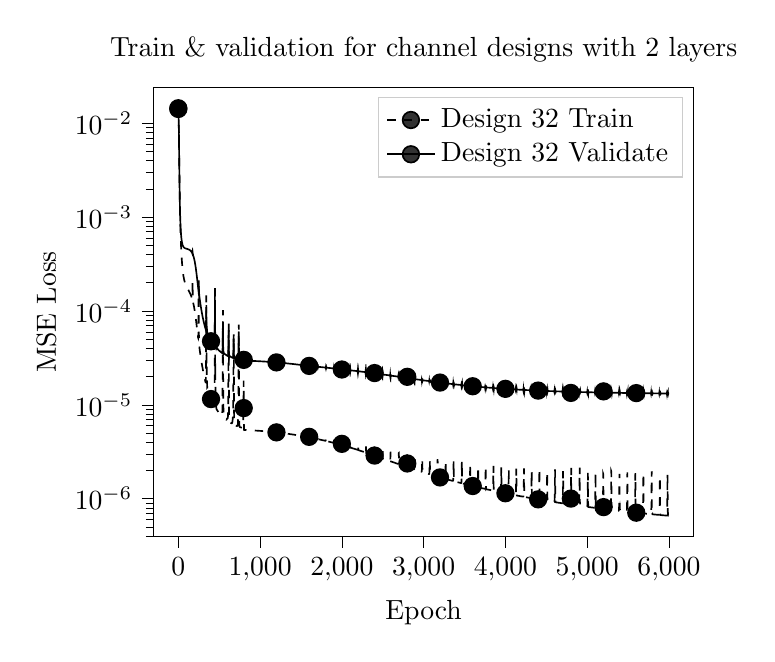
\begin{tikzpicture}

\begin{axis}[
legend cell align={left},
legend style={fill opacity=0.8, draw opacity=1, text opacity=1, draw=white!80!black},
log basis y={10},
tick align=outside,
tick pos=left,
title={Train \& validation for channel designs with 2 layers},
x grid style={white!69.0196078431373!black},
xlabel={Epoch},
xmin=-299.95, xmax=6298.95,
xtick style={color=black},
y grid style={white!69.0196078431373!black},
ylabel={MSE Loss},
ymin=3.98976029687765e-07, ymax=0.0238127097613253,
ymode=log,
ytick style={color=black}
]
\addplot [semithick, black, dashed, mark=*, mark size=3, mark repeat=400, mark options={solid}]
table {%
0 0.0144452207023278
1 0.0137455552176107
2 0.0130890246946365
3 0.0124103963898961
4 0.0116477863921318
5 0.0107490205264185
6 0.00970690316171385
7 0.00857851712498814
8 0.00744941645825747
9 0.00638116928894306
10 0.00540587675641291
11 0.00454513872682583
12 0.00381435750750825
13 0.00321529700886458
14 0.00273237821238581
15 0.00234269463544479
16 0.00202676386834355
17 0.00176918654324254
18 0.00155822073793388
19 0.00138439545480651
20 0.0012401694257278
21 0.00111974674473458
22 0.00101840483876003
23 0.000932521781578544
24 0.00085921402569511
25 0.00079618718882557
26 0.00074161831435049
27 0.000694022276547912
28 0.000652222963253735
29 0.000615261683378776
30 0.000582374082114256
31 0.000552934681763873
32 0.000526439451277838
33 0.000502472887092154
34 0.000480695485748583
35 0.000460824289802986
36 0.000442625932919327
37 0.000425904166149849
38 0.000410494532843586
39 0.000396257520151266
40 0.000383074532237515
41 0.000370843321434222
42 0.0003594760728447
43 0.000348895770002855
44 0.000339035320394032
45 0.000329835318552796
46 0.000321243028793106
47 0.000313211201046215
48 0.000305697507883451
49 0.000298663470857718
50 0.0002920741858361
51 0.000285897698176996
52 0.00028010470305162
53 0.000274668301699421
54 0.000269563631263736
55 0.000264767711314562
56 0.000260259220794978
57 0.000256018433901772
58 0.000252026775569902
59 0.000248267282131565
60 0.000244724020149079
61 0.000241382042759142
62 0.000238227520412693
63 0.000235247548516782
64 0.000232429967354619
65 0.0002297635942341
66 0.000227237859689922
67 0.00022484298915515
68 0.000222569843799647
69 0.000220409923713305
70 0.000218355215338306
71 0.000216398461361678
72 0.000214532750760554
73 0.000212751681374357
74 0.000211049442214062
75 0.000209420543797023
76 0.000207859757665574
77 0.000206362574317609
78 0.00020492467922395
79 0.000203541829819187
80 0.000202210468273734
81 0.000200927240939563
82 0.000199688837483336
83 0.000198492368440384
84 0.00019733523697596
85 0.000196214802940631
86 0.000195128800555722
87 0.000194075093304491
88 0.00019305170599182
89 0.000192056708669952
90 0.000191088463566302
91 0.000190145385090545
92 0.000189225942563098
93 0.000188328712624752
94 0.00018745242289242
95 0.00018659589568415
96 0.000185757871804526
97 0.000184937347967207
98 0.000184133294737876
99 0.000183344736456093
100 0.000182570716901864
101 0.000181810384674463
102 0.000181062955107336
103 0.000180327618636511
104 0.000179603715309895
105 0.000178890441475232
106 0.000178187079086456
107 0.000177493038677312
108 0.000176807655861921
109 0.000176130377326444
110 0.000175460631567148
111 0.000174797836393736
112 0.000174141425532071
113 0.000173490904387563
114 0.000172845752842932
115 0.000172205586238761
116 0.000171569807548622
117 0.000170938012615807
118 0.00017030975260468
119 0.000169684582999707
120 0.000169062095551453
121 0.000168441871949199
122 0.000167823555784707
123 0.000167206710500523
124 0.000166590906644615
125 0.000165975811569297
126 0.000165361070799008
127 0.000164746301209107
128 0.000164131161625392
129 0.00016351530632619
130 0.000162898302164649
131 0.000162279869925896
132 0.000161659696914285
133 0.000161037378973106
134 0.000160412615912264
135 0.000159785041546456
136 0.000159154355969804
137 0.000158520201864576
138 0.000157882254768538
139 0.000157240201474451
140 0.000156593701888141
141 0.000155942432115808
142 0.000155286028302726
143 0.000154624176218476
144 0.00015395653935002
145 0.000153282792950904
146 0.000152602589764683
147 0.000151915639946765
148 0.000151221527914913
149 0.000150520048066483
150 0.000149810613550017
151 0.000149093292634461
152 0.000148367146664441
153 0.000147632634423189
154 0.000146888244103138
155 0.000146135351201337
156 0.000145371105190861
157 0.000144598942881657
158 0.00014381275912001
159 0.000143020910456926
160 0.000142209963030382
161 0.000141400107679601
162 0.000140560020554403
163 0.000139739979942988
164 0.000138865113626707
165 0.000138067138919951
166 0.000137169240588264
167 0.000136547007087984
168 0.000135831762605676
169 0.000136262242335761
170 0.000137512074786628
171 0.000144274944375411
172 0.000158319106617455
173 0.000186759930386415
174 0.000209175900067748
175 0.000190471132441417
176 0.000152358855132206
177 0.000127799339395551
178 0.000129235075860379
179 0.000128325334685542
180 0.000124387639800716
181 0.000123206567508305
182 0.000121988624499636
183 0.000120924295771374
184 0.000119881962035606
185 0.000118704843856676
186 0.000117675155081542
187 0.000116559612507672
188 0.000115439843881404
189 0.000114326449278224
190 0.00011318061214638
191 0.000112035956107093
192 0.000110869500360877
193 0.000109693113728326
194 0.000108505309441398
195 0.00010730361179867
196 0.00010609149299512
197 0.000104866723205532
198 0.000103631826135597
199 0.000102386292525125
200 0.000101131091298612
201 9.98667994451807e-05
202 9.8594053014267e-05
203 9.73137766777654e-05
204 9.60266904712626e-05
205 9.47337512400281e-05
206 9.3435782986262e-05
207 9.21338532862137e-05
208 9.08289063943357e-05
209 8.95219827157234e-05
210 8.82141629574562e-05
211 8.69065598294583e-05
212 8.56002938576239e-05
213 8.42964635410226e-05
214 8.29962129387241e-05
215 8.17007049249696e-05
216 8.04109981231704e-05
217 7.91282508600943e-05
218 7.78535657843804e-05
219 7.65879850916917e-05
220 7.53325664675231e-05
221 7.40882674392651e-05
222 7.28560802087941e-05
223 7.16368668349787e-05
224 7.04314825838992e-05
225 6.92407444660148e-05
226 6.80653344602433e-05
227 6.69059501774427e-05
228 6.57632433274102e-05
229 6.46376540203164e-05
230 6.35298026736564e-05
231 6.24398296338313e-05
232 6.1368587665811e-05
233 6.03155893372787e-05
234 5.92823608940307e-05
235 5.82671742677121e-05
236 5.72736250603612e-05
237 5.62970972168841e-05
238 5.53481291092339e-05
239 5.44160255913084e-05
240 5.35375748427214e-05
241 5.27009148925117e-05
242 5.2067833877345e-05
243 5.17584007582172e-05
244 5.26900282693532e-05
245 5.65062510702319e-05
246 6.87593953330179e-05
247 0.000100074577744635
248 0.000150361912744756
249 0.000183971543719963
250 0.000120349388225804
251 6.34924668077019e-05
252 5.42553786715416e-05
253 5.54723184222894e-05
254 4.76710314103457e-05
255 4.42069278108193e-05
256 4.38129881814575e-05
257 4.21366211185159e-05
258 4.09168434032381e-05
259 4.02762931202005e-05
260 3.96506210478265e-05
261 3.89639892262039e-05
262 3.83690557441696e-05
263 3.7830419501006e-05
264 3.72826431913609e-05
265 3.6749602017494e-05
266 3.62267011979611e-05
267 3.57212790049743e-05
268 3.52291399678961e-05
269 3.47423286655157e-05
270 3.42679592790773e-05
271 3.38053180968245e-05
272 3.33520091828632e-05
273 3.29082611330023e-05
274 3.2473624273166e-05
275 3.20484705724766e-05
276 3.16322680049552e-05
277 3.12245117726206e-05
278 3.08251531606629e-05
279 3.04339773009588e-05
280 3.00507758055346e-05
281 2.96753227644331e-05
282 2.93073882602357e-05
283 2.8946805372243e-05
284 2.8593400969612e-05
285 2.82469937644692e-05
286 2.79073952214048e-05
287 2.75744482109985e-05
288 2.7247989208945e-05
289 2.69278632458736e-05
290 2.66139337696814e-05
291 2.63060355365496e-05
292 2.60040279158602e-05
293 2.57077752081614e-05
294 2.54171576443696e-05
295 2.51320387150145e-05
296 2.48522885613056e-05
297 2.45777881104914e-05
298 2.43084016204875e-05
299 2.40440321448432e-05
300 2.37845801080994e-05
301 2.3529914741971e-05
302 2.32799480244239e-05
303 2.30345577563185e-05
304 2.2793644035346e-05
305 2.25571301655236e-05
306 2.23249022752725e-05
307 2.20968829012236e-05
308 2.1872958569702e-05
309 2.16530703767148e-05
310 2.14371018074644e-05
311 2.12250092346267e-05
312 2.10166706793302e-05
313 2.08120491507202e-05
314 2.06110253131442e-05
315 2.04135675616612e-05
316 2.02195507341685e-05
317 2.00289692244837e-05
318 1.98416652139599e-05
319 1.96577009390353e-05
320 1.94768563090975e-05
321 1.92992400940284e-05
322 1.91245987934963e-05
323 1.89531092686934e-05
324 1.87844310275409e-05
325 1.86188611266402e-05
326 1.84560145299884e-05
327 1.82962564707623e-05
328 1.81394702494231e-05
329 1.7985967964762e-05
330 1.7837397209064e-05
331 1.76940519764912e-05
332 1.75666547548303e-05
333 1.74606885678941e-05
334 1.74342411938255e-05
335 1.75548155141314e-05
336 1.81521731477119e-05
337 1.98514173206377e-05
338 2.45809345358339e-05
339 3.71800844902737e-05
340 6.436267469212e-05
341 0.00012075733883421
342 0.000146468174989423
343 0.000123785084269912
344 4.4538113741055e-05
345 2.76563143302155e-05
346 3.60455753138922e-05
347 2.50642777359644e-05
348 2.04791913773761e-05
349 2.1193476683834e-05
350 1.74825337566631e-05
351 1.70974974906812e-05
352 1.67309577534525e-05
353 1.54998346459934e-05
354 1.55519609847943e-05
355 1.53032321605906e-05
356 1.49389725550009e-05
357 1.48754242275118e-05
358 1.47616123840066e-05
359 1.46180673894492e-05
360 1.4512971148406e-05
361 1.44169751763457e-05
362 1.43180135125931e-05
363 1.42181374513939e-05
364 1.41218699027945e-05
365 1.403072869266e-05
366 1.39396400129499e-05
367 1.38491349517267e-05
368 1.37611804476023e-05
369 1.36750059880342e-05
370 1.35900580602311e-05
371 1.35062744135439e-05
372 1.34238865854286e-05
373 1.33428796047497e-05
374 1.32630477480689e-05
375 1.31843453132774e-05
376 1.31067794484352e-05
377 1.30303303933488e-05
378 1.29549612069013e-05
379 1.28806122816627e-05
380 1.28072729310702e-05
381 1.27349221514805e-05
382 1.26635417743159e-05
383 1.25930953416287e-05
384 1.25235640311416e-05
385 1.24549339659552e-05
386 1.23871869917025e-05
387 1.23203072917022e-05
388 1.22542650444757e-05
389 1.21890610351727e-05
390 1.212466760947e-05
391 1.20610762550655e-05
392 1.19982700965693e-05
393 1.19362346389096e-05
394 1.18749606308199e-05
395 1.18144310015111e-05
396 1.17546310143268e-05
397 1.16955526721085e-05
398 1.16371847695973e-05
399 1.15795192598966e-05
400 1.15225365711069e-05
401 1.14662372148189e-05
402 1.1410598130368e-05
403 1.13556181666752e-05
404 1.13012807361201e-05
405 1.12475788007771e-05
406 1.11945108400846e-05
407 1.11420601314194e-05
408 1.10902141514657e-05
409 1.10389666758692e-05
410 1.09883146315326e-05
411 1.09382563096005e-05
412 1.08887636010024e-05
413 1.08398380795904e-05
414 1.07914747822235e-05
415 1.07436685752305e-05
416 1.06964076103111e-05
417 1.06496946408186e-05
418 1.06035151183903e-05
419 1.05578675686502e-05
420 1.0512739610391e-05
421 1.04681310340027e-05
422 1.04240249036991e-05
423 1.03804414841591e-05
424 1.03373366115989e-05
425 1.0294760432572e-05
426 1.02526364926803e-05
427 1.02110809940825e-05
428 1.01698975534248e-05
429 1.01293700041083e-05
430 1.00890748910842e-05
431 1.0049679680435e-05
432 1.00101494595606e-05
433 9.97222588949853e-06
434 9.93327142140288e-06
435 9.89802263262618e-06
436 9.85990479307475e-06
437 9.83262929565853e-06
438 9.80099540370816e-06
439 9.80981740283937e-06
440 9.83598966186605e-06
441 1.0056098584954e-05
442 1.05529560769924e-05
443 1.21899733223074e-05
444 1.64124404875565e-05
445 2.7638425322607e-05
446 5.7980918739986e-05
447 0.000106705730900103
448 0.000186141390372541
449 0.000135292456320713
450 5.61496464115407e-05
451 1.85072074430082e-05
452 2.76366901346137e-05
453 2.35059928996861e-05
454 1.3392234592402e-05
455 1.66843033326813e-05
456 1.46379900982652e-05
457 1.09154838412451e-05
458 1.24235312490839e-05
459 1.1205479346188e-05
460 9.7794653015626e-06
461 1.03219900573492e-05
462 9.78676852270155e-06
463 9.29478602884615e-06
464 9.41274656085511e-06
465 9.24421931358665e-06
466 9.08570678248566e-06
467 9.07379883940962e-06
468 9.02858720763788e-06
469 8.96922500359665e-06
470 8.93513180599825e-06
471 8.90793913299603e-06
472 8.87457898457455e-06
473 8.84246520271859e-06
474 8.81374912964361e-06
475 8.78594225284246e-06
476 8.7575433056486e-06
477 8.72943808261084e-06
478 8.70273175124225e-06
479 8.67634290102615e-06
480 8.65015403661573e-06
481 8.62444627713899e-06
482 8.599361247974e-06
483 8.57464675263486e-06
484 8.55039958480575e-06
485 8.52650461524718e-06
486 8.50317428913172e-06
487 8.48013746690413e-06
488 8.45756455802871e-06
489 8.43513664960938e-06
490 8.4130146582595e-06
491 8.39084927761746e-06
492 8.36878289334209e-06
493 8.34648997738441e-06
494 8.32421773466763e-06
495 8.3017432856991e-06
496 8.27941883585481e-06
497 8.25717797958703e-06
498 8.2354645218885e-06
499 8.21432568542946e-06
500 8.19432855081459e-06
501 8.17560295374165e-06
502 8.15874593840249e-06
503 8.14365520085403e-06
504 8.13038518465703e-06
505 8.11783711185399e-06
506 8.10506432458169e-06
507 8.09055390327273e-06
508 8.07430068228143e-06
509 8.05690794969394e-06
510 8.04052548808443e-06
511 8.02605519645283e-06
512 8.01351337642586e-06
513 7.99960422348533e-06
514 7.9818924483277e-06
515 7.95822281141056e-06
516 7.93064695159273e-06
517 7.90138061468326e-06
518 7.87367206278589e-06
519 7.84902273665011e-06
520 7.82852994163363e-06
521 7.81244967207329e-06
522 7.80070535988386e-06
523 7.79267595518718e-06
524 7.78671616430415e-06
525 7.78048620375671e-06
526 7.77141726437947e-06
527 7.75813484032994e-06
528 7.74035645356719e-06
529 7.72035266649596e-06
530 7.6989106769787e-06
531 7.68139468476647e-06
532 7.66589954181995e-06
533 7.66301743482245e-06
534 7.66707916710629e-06
535 7.70491821278085e-06
536 7.77363323933855e-06
537 7.95240701911837e-06
538 8.28927062457296e-06
539 9.04390968869961e-06
540 1.06022771291236e-05
541 1.38028881835339e-05
542 2.08706639170941e-05
543 3.29310716438158e-05
544 5.83873158745973e-05
545 7.91082537716647e-05
546 0.000101982185412908
547 7.12641426048322e-05
548 3.50287759260937e-05
549 1.09516323902881e-05
550 9.9648341347347e-06
551 1.03193508635968e-05
552 8.57187722402841e-06
553 7.75615229997584e-06
554 7.48313831877567e-06
555 7.45709538030326e-06
556 7.39937362936871e-06
557 7.3607085955274e-06
558 7.3346990348e-06
559 7.29600071736058e-06
560 7.2769922052629e-06
561 7.25636686027542e-06
562 7.23695702475879e-06
563 7.21884237897541e-06
564 7.20077284555032e-06
565 7.18485158301974e-06
566 7.16911312181878e-06
567 7.1538317545361e-06
568 7.13898382720402e-06
569 7.12453188533857e-06
570 7.11058309299517e-06
571 7.09683062183331e-06
572 7.08342746591484e-06
573 7.07022084789344e-06
574 7.05734850470208e-06
575 7.04468696888227e-06
576 7.03235381749323e-06
577 7.02025416643437e-06
578 7.00856078061918e-06
579 6.99720087560252e-06
580 6.98640522855953e-06
581 6.9761631316112e-06
582 6.96684913137346e-06
583 6.95853576004879e-06
584 6.95183817178702e-06
585 6.94700669967574e-06
586 6.94501246734092e-06
587 6.94628899822192e-06
588 6.95216843737967e-06
589 6.96292642921037e-06
590 6.97980990693736e-06
591 7.00185527691133e-06
592 7.02928014639781e-06
593 7.05864843730808e-06
594 7.08920108039024e-06
595 7.11574788780922e-06
596 7.13923456174825e-06
597 7.15542477003339e-06
598 7.16940750855599e-06
599 7.17745354528176e-06
600 7.18646958475233e-06
601 7.18928355958326e-06
602 7.19422827089033e-06
603 7.19495902501421e-06
604 7.21152950156068e-06
605 7.25183047123323e-06
606 7.36183782557021e-06
607 7.58550585011619e-06
608 8.04903251605538e-06
609 8.90622830951315e-06
610 1.06400559616304e-05
611 1.36455548442882e-05
612 1.98971095102252e-05
613 2.89662889656483e-05
614 4.69036723416139e-05
615 6.00008708602218e-05
616 7.57630227212758e-05
617 5.92300729067574e-05
618 3.6562504703852e-05
619 1.42618141012463e-05
620 8.53989219962159e-06
621 7.57251664929015e-06
622 7.46835539899848e-06
623 7.03018861614169e-06
624 6.77284607952799e-06
625 6.69730483160436e-06
626 6.61831838222326e-06
627 6.6122695088211e-06
628 6.58631370775709e-06
629 6.56612532701217e-06
630 6.54945554678932e-06
631 6.53324220500906e-06
632 6.52157154235056e-06
633 6.50911226252049e-06
634 6.49784770523354e-06
635 6.486866768185e-06
636 6.47659638630671e-06
637 6.46690637395864e-06
638 6.45740472826617e-06
639 6.44830699947363e-06
640 6.43936875910356e-06
641 6.4308292380133e-06
642 6.42245875503988e-06
643 6.41443297055844e-06
644 6.40658510775438e-06
645 6.39912493838324e-06
646 6.39192305662561e-06
647 6.3852314049484e-06
648 6.37893955257596e-06
649 6.37344449394561e-06
650 6.36861512504083e-06
651 6.36514915264286e-06
652 6.36287972710647e-06
653 6.36313324520188e-06
654 6.36574950085844e-06
655 6.37313842588583e-06
656 6.38518796058918e-06
657 6.40589054690111e-06
658 6.43479412154591e-06
659 6.4770617314025e-06
660 6.53025376173844e-06
661 6.59867122365654e-06
662 6.6768710258458e-06
663 6.76879184702273e-06
664 6.87442915925374e-06
665 7.00392355490465e-06
666 7.17991906107329e-06
667 7.41589919250885e-06
668 7.78904609433084e-06
669 8.31253444744107e-06
670 9.25498400050628e-06
671 1.06391949259432e-05
672 1.33943344309273e-05
673 1.73100624607514e-05
674 2.5281567758384e-05
675 3.40076321663219e-05
676 4.95737220376213e-05
677 5.425246985169e-05
678 5.64387922850074e-05
679 3.92533522131089e-05
680 2.3473026345755e-05
681 1.10422593735393e-05
682 7.95543836673573e-06
683 6.82500729354274e-06
684 6.61536547674757e-06
685 6.38437480837695e-06
686 6.2616326168552e-06
687 6.20509463189478e-06
688 6.16123602448226e-06
689 6.14720332769991e-06
690 6.12786219722494e-06
691 6.11482950674258e-06
692 6.10230326358874e-06
693 6.09107660753949e-06
694 6.08176652683312e-06
695 6.07260008145261e-06
696 6.06448350204403e-06
697 6.05631974526233e-06
698 6.04879171017814e-06
699 6.04128096615142e-06
700 6.03419044953313e-06
701 6.02711237807085e-06
702 6.02033523033896e-06
703 6.01357736407238e-06
704 6.0070706782156e-06
705 6.00059258815122e-06
706 5.99434210801775e-06
707 5.9881662934913e-06
708 5.98223010683796e-06
709 5.97644952193832e-06
710 5.97096950638587e-06
711 5.96581028133869e-06
712 5.96109622019725e-06
713 5.95701534233939e-06
714 5.95367165612259e-06
715 5.95147476722957e-06
716 5.95047408857852e-06
717 5.95126342606278e-06
718 5.95363984068342e-06
719 5.95814919801541e-06
720 5.96400195895797e-06
721 5.97146535596949e-06
722 5.97952370373633e-06
723 5.98903457760258e-06
724 6.00093471092578e-06
725 6.01921517873194e-06
726 6.05001427800289e-06
727 6.10353234975491e-06
728 6.19514970701118e-06
729 6.34736971072414e-06
730 6.60601333635213e-06
731 7.03904574628211e-06
732 7.84911151541223e-06
733 9.26740612783306e-06
734 1.22244158689e-05
735 1.7149487007373e-05
736 2.78768345083336e-05
737 4.1090469125038e-05
738 6.62039256553726e-05
739 7.15940409463656e-05
740 6.95326534128071e-05
741 3.96830512841007e-05
742 1.79552699961505e-05
743 7.76895690890456e-06
744 7.11001948872081e-06
745 6.67191729775141e-06
746 6.34113585995522e-06
747 6.07836776644888e-06
748 5.90737029693145e-06
749 5.89794718042214e-06
750 5.86155871484806e-06
751 5.84132760472755e-06
752 5.823402312366e-06
753 5.80540426398102e-06
754 5.79685986146217e-06
755 5.78722056765457e-06
756 5.78078710500307e-06
757 5.77424852998831e-06
758 5.76913293137693e-06
759 5.76487668979553e-06
760 5.76141603492175e-06
761 5.75858862195133e-06
762 5.75639668909389e-06
763 5.75450114848053e-06
764 5.75303966954266e-06
765 5.75130031243987e-06
766 5.74954429666263e-06
767 5.7467989593718e-06
768 5.74358747407189e-06
769 5.73889550015139e-06
770 5.7336441496858e-06
771 5.72693229017318e-06
772 5.72010287758218e-06
773 5.71233033763718e-06
774 5.70524158494123e-06
775 5.69788827586848e-06
776 5.69205830291963e-06
777 5.68658622324136e-06
778 5.68345901719169e-06
779 5.68131872125122e-06
780 5.68257388167126e-06
781 5.68574201054162e-06
782 5.69394245175658e-06
783 5.70549579137491e-06
784 5.72449241786899e-06
785 5.74842993650293e-06
786 5.78245148386003e-06
787 5.82194227316535e-06
788 5.87459789791467e-06
789 5.93446178509538e-06
790 6.01902120855868e-06
791 6.12465343863278e-06
792 6.29054699885501e-06
793 6.51490719327796e-06
794 6.89253891295039e-06
795 7.4431317820256e-06
796 8.48387638541226e-06
797 1.01056192534088e-05
798 1.33994953159799e-05
799 1.813548958296e-05
800 9.24407520841442e-06
801 7.00000610009965e-06
802 6.38104098271697e-06
803 5.65929499796169e-06
804 5.47034848530359e-06
805 5.47855763244343e-06
806 5.41935781939173e-06
807 5.42111343992957e-06
808 5.40640400625847e-06
809 5.40439967267048e-06
810 5.40258014769535e-06
811 5.4015396289131e-06
812 5.40067009069389e-06
813 5.39986746161958e-06
814 5.3993253379403e-06
815 5.39872099736272e-06
816 5.39807208355114e-06
817 5.39745961436466e-06
818 5.39688070677613e-06
819 5.39630002016622e-06
820 5.39573197677612e-06
821 5.39517187991834e-06
822 5.39462064264029e-06
823 5.39406595390091e-06
824 5.39351856687631e-06
825 5.39297534896122e-06
826 5.39243137520629e-06
827 5.39189041415256e-06
828 5.39135288590842e-06
829 5.39081879225023e-06
830 5.39028172408251e-06
831 5.38975019459542e-06
832 5.38921530957026e-06
833 5.38868192201392e-06
834 5.38815355533018e-06
835 5.38762070245724e-06
836 5.38708769681762e-06
837 5.38656122905934e-06
838 5.38602489630335e-06
839 5.38549586526216e-06
840 5.38496308166714e-06
841 5.38442840714026e-06
842 5.3838957363439e-06
843 5.38336055733168e-06
844 5.38282662088108e-06
845 5.38228948343544e-06
846 5.3817557708058e-06
847 5.38121687654325e-06
848 5.38067932076558e-06
849 5.38014059170422e-06
850 5.37960468172116e-06
851 5.37906254027831e-06
852 5.37851976822878e-06
853 5.37797777511173e-06
854 5.37743549600123e-06
855 5.37688937995995e-06
856 5.37634378705576e-06
857 5.37579731041404e-06
858 5.37524948018842e-06
859 5.374701451899e-06
860 5.37415155754672e-06
861 5.3736005538596e-06
862 5.37304766901059e-06
863 5.3724942770117e-06
864 5.37193634198019e-06
865 5.37138477874066e-06
866 5.37082326701466e-06
867 5.37026601143964e-06
868 5.36970382647439e-06
869 5.36914315230064e-06
870 5.36858031185972e-06
871 5.3680192984018e-06
872 5.36745118129289e-06
873 5.36688472330127e-06
874 5.36631324798975e-06
875 5.36574837717296e-06
876 5.36517693561223e-06
877 5.36460553224316e-06
878 5.364031325783e-06
879 5.36345735291377e-06
880 5.36287991081963e-06
881 5.36230513592528e-06
882 5.36172581266925e-06
883 5.36114435512047e-06
884 5.36056366673421e-06
885 5.35998012729522e-06
886 5.35939693602216e-06
887 5.35881014140926e-06
888 5.35822328817659e-06
889 5.35763760645125e-06
890 5.35704529980308e-06
891 5.35645134114304e-06
892 5.35586158623147e-06
893 5.35526618694604e-06
894 5.35467042528381e-06
895 5.3540706339561e-06
896 5.35347557040211e-06
897 5.35287314651356e-06
898 5.35227200249011e-06
899 5.35166903592454e-06
900 5.35106531351914e-06
901 5.35045440930304e-06
902 5.34984987954346e-06
903 5.34924167183704e-06
904 5.34862957746185e-06
905 5.34801793161677e-06
906 5.34740355728758e-06
907 5.34678900532271e-06
908 5.34616857272852e-06
909 5.34555324982477e-06
910 5.34493554038562e-06
911 5.34431161547388e-06
912 5.34369051674588e-06
913 5.3430664124221e-06
914 5.3424386257106e-06
915 5.34181155043001e-06
916 5.34118499384562e-06
917 5.34055349898921e-06
918 5.33992014695173e-06
919 5.33928748058798e-06
920 5.3386557379298e-06
921 5.33801569790882e-06
922 5.33737765717746e-06
923 5.33673783920108e-06
924 5.3360971774552e-06
925 5.33545424818982e-06
926 5.33481070075226e-06
927 5.33416263692743e-06
928 5.33351458731346e-06
929 5.33286453396897e-06
930 5.33221727661015e-06
931 5.33156524795686e-06
932 5.33091060095359e-06
933 5.33025532956088e-06
934 5.32959877830308e-06
935 5.32894058302702e-06
936 5.32827864763163e-06
937 5.3276163356486e-06
938 5.32695387089888e-06
939 5.32628800442581e-06
940 5.32562311938989e-06
941 5.3249551958956e-06
942 5.32428434674159e-06
943 5.32361214844457e-06
944 5.32293767907532e-06
945 5.32226124594359e-06
946 5.3215856921085e-06
947 5.32091054328276e-06
948 5.3202311525169e-06
949 5.31954895865994e-06
950 5.31886757393352e-06
951 5.31818298199482e-06
952 5.31749369070411e-06
953 5.31680962545522e-06
954 5.31611950460587e-06
955 5.31543109438815e-06
956 5.31473713039077e-06
957 5.31404345149866e-06
958 5.31334802822414e-06
959 5.31265077086118e-06
960 5.3119516500999e-06
961 5.31124990654774e-06
962 5.31054839569833e-06
963 5.30984626756492e-06
964 5.30914027496721e-06
965 5.30843163915051e-06
966 5.30772280438185e-06
967 5.3070136072364e-06
968 5.30629942030458e-06
969 5.30558679567861e-06
970 5.3048691430746e-06
971 5.30415499877535e-06
972 5.30343482019191e-06
973 5.3027153690266e-06
974 5.3019939336707e-06
975 5.30127324616103e-06
976 5.30054253822243e-06
977 5.29981631913756e-06
978 5.29908727830986e-06
979 5.29835609075491e-06
980 5.29762613066254e-06
981 5.29689373074405e-06
982 5.29615786692972e-06
983 5.29542085381252e-06
984 5.2946821043065e-06
985 5.29394330683886e-06
986 5.29319946718232e-06
987 5.29245693936531e-06
988 5.29171044494348e-06
989 5.29096440882171e-06
990 5.29021290951448e-06
991 5.28946622058157e-06
992 5.28871291116673e-06
993 5.28795903509405e-06
994 5.2872046270025e-06
995 5.28644392261413e-06
996 5.28568858815248e-06
997 5.28492749207743e-06
998 5.28416235567875e-06
999 5.28340103223002e-06
1000 5.28263527765915e-06
1001 5.28186938986153e-06
1002 5.28109813746624e-06
1003 5.28033038893483e-06
1004 5.27955568774274e-06
1005 5.27878320433217e-06
1006 5.2780083628079e-06
1007 5.27722766641148e-06
1008 5.2764505200642e-06
1009 5.27566914865218e-06
1010 5.27488684642918e-06
1011 5.27410384520977e-06
1012 5.27331556465782e-06
1013 5.27252830284652e-06
1014 5.27173968833949e-06
1015 5.27094894664515e-06
1016 5.27015739137937e-06
1017 5.26936226208363e-06
1018 5.2685653999518e-06
1019 5.26777046161442e-06
1020 5.26696764691081e-06
1021 5.2661653882069e-06
1022 5.26536503731023e-06
1023 5.26455939819925e-06
1024 5.26375438081317e-06
1025 5.26294499270108e-06
1026 5.26213440199541e-06
1027 5.26132442768557e-06
1028 5.26051068483468e-06
1029 5.25969611775423e-06
1030 5.25887880087339e-06
1031 5.25806259510375e-06
1032 5.25724099276204e-06
1033 5.25641733162274e-06
1034 5.25559507824624e-06
1035 5.25476796742197e-06
1036 5.25394327599571e-06
1037 5.25311511623272e-06
1038 5.25228225978225e-06
1039 5.25145170815478e-06
1040 5.25061599621068e-06
1041 5.24978041482882e-06
1042 5.24894402342824e-06
1043 5.24810274171728e-06
1044 5.2472645268864e-06
1045 5.24641978039142e-06
1046 5.24557618319932e-06
1047 5.24473149088323e-06
1048 5.24388390754638e-06
1049 5.24303393945047e-06
1050 5.24218022679435e-06
1051 5.2413303262e-06
1052 5.24047335748179e-06
1053 5.23961676979212e-06
1054 5.23875998315049e-06
1055 5.23789760631388e-06
1056 5.23703571886358e-06
1057 5.23617288283873e-06
1058 5.23530983276288e-06
1059 5.23444259137307e-06
1060 5.23357272808056e-06
1061 5.23270455499159e-06
1062 5.23183088407819e-06
1063 5.2309557316832e-06
1064 5.23007966890532e-06
1065 5.22920313805741e-06
1066 5.22832130567252e-06
1067 5.22744058084612e-06
1068 5.22655829016117e-06
1069 5.22567447358568e-06
1070 5.22479117393004e-06
1071 5.22389940460499e-06
1072 5.22301229466393e-06
1073 5.22211901898828e-06
1074 5.22122752855125e-06
1075 5.22032893268687e-06
1076 5.21943192310914e-06
1077 5.21853714552378e-06
1078 5.21763584515611e-06
1079 5.2167335748976e-06
1080 5.21582917745178e-06
1081 5.21492521166067e-06
1082 5.21401751285566e-06
1083 5.21310385881435e-06
1084 5.21219675952977e-06
1085 5.21128112040969e-06
1086 5.21036983780476e-06
1087 5.2094519427115e-06
1088 5.20853377850017e-06
1089 5.20761407329928e-06
1090 5.20669341597113e-06
1091 5.2057707700115e-06
1092 5.20484599597637e-06
1093 5.20391877856241e-06
1094 5.20298993045287e-06
1095 5.20205867360346e-06
1096 5.20112917712368e-06
1097 5.2001912225208e-06
1098 5.19925593778225e-06
1099 5.19831725842579e-06
1100 5.19737992110691e-06
1101 5.19643615959353e-06
1102 5.19549625010995e-06
1103 5.19454927250251e-06
1104 5.19360451978201e-06
1105 5.19265517073819e-06
1106 5.19170572754746e-06
1107 5.19075343508035e-06
1108 5.18980003771929e-06
1109 5.18884384259621e-06
1110 5.18788802406078e-06
1111 5.18692912709895e-06
1112 5.18596781784453e-06
1113 5.18500591706328e-06
1114 5.18403975124926e-06
1115 5.18307212082902e-06
1116 5.18210623745574e-06
1117 5.18113741865278e-06
1118 5.18016744610605e-06
1119 5.17919188514071e-06
1120 5.17821876844238e-06
1121 5.17724028181732e-06
1122 5.17625941132138e-06
1123 5.17528168142434e-06
1124 5.1742985061054e-06
1125 5.17331417348998e-06
1126 5.17233016505969e-06
1127 5.17134420796594e-06
1128 5.17034983715803e-06
1129 5.16936003958079e-06
1130 5.16836859354441e-06
1131 5.16737326439198e-06
1132 5.16637659053742e-06
1133 5.16537981365417e-06
1134 5.16437628661492e-06
1135 5.16337499423258e-06
1136 5.1623728847261e-06
1137 5.16136626327324e-06
1138 5.16036024400535e-06
1139 5.15935083722496e-06
1140 5.15833862113624e-06
1141 5.15732710049122e-06
1142 5.15631233710678e-06
1143 5.15529405742399e-06
1144 5.15427596514684e-06
1145 5.15325737726613e-06
1146 5.15223457231428e-06
1147 5.15121004962538e-06
1148 5.15018450197857e-06
1149 5.14915903071511e-06
1150 5.14812690965982e-06
1151 5.14709691756821e-06
1152 5.14606384260929e-06
1153 5.14503124549037e-06
1154 5.14399330775461e-06
1155 5.1429543761472e-06
1156 5.141915246476e-06
1157 5.14087283498554e-06
1158 5.13982905392396e-06
1159 5.13878394059475e-06
1160 5.13773477095469e-06
1161 5.1366850142287e-06
1162 5.13563785364823e-06
1163 5.13458432838121e-06
1164 5.13352994246929e-06
1165 5.13246967415171e-06
1166 5.13141350655388e-06
1167 5.13035633442627e-06
1168 5.1292906695366e-06
1169 5.1282280475462e-06
1170 5.12716353373577e-06
1171 5.12609456038149e-06
1172 5.12502517135971e-06
1173 5.12395549723266e-06
1174 5.12288136711447e-06
1175 5.1218086563054e-06
1176 5.12073078962061e-06
1177 5.1196537960152e-06
1178 5.11857502871749e-06
1179 5.11749203635503e-06
1180 5.11640625333598e-06
1181 5.11531978997226e-06
1182 5.11423347315798e-06
1183 5.11314421114406e-06
1184 5.11205354225552e-06
1185 5.11095844490939e-06
1186 5.10986610624542e-06
1187 5.10876775372537e-06
1188 5.1076690237295e-06
1189 5.10656859376013e-06
1190 5.10546917276145e-06
1191 5.10436369083322e-06
1192 5.10325668479084e-06
1193 5.10215009086323e-06
1194 5.1010403989693e-06
1195 5.09992782671276e-06
1196 5.09881569144e-06
1197 5.09770031964507e-06
1198 5.09658265102075e-06
1199 5.09546561389129e-06
1200 5.09434348128224e-06
1201 5.09322200326068e-06
1202 5.0920981307101e-06
1203 5.09097018941418e-06
1204 5.08984309099958e-06
1205 5.08871283866341e-06
1206 5.08758080552951e-06
1207 5.0864493204017e-06
1208 5.08531169973736e-06
1209 5.08417604816458e-06
1210 5.08303707213997e-06
1211 5.08189723191776e-06
1212 5.08075377592121e-06
1213 5.07960757900605e-06
1214 5.07846244168775e-06
1215 5.07731383336818e-06
1216 5.07616532985367e-06
1217 5.07501195290416e-06
1218 5.07385835835095e-06
1219 5.0727039173637e-06
1220 5.07154710938096e-06
1221 5.0703876723901e-06
1222 5.0692250761486e-06
1223 5.06806186795217e-06
1224 5.06689665513704e-06
1225 5.06573120340192e-06
1226 5.0645622247103e-06
1227 5.06339264116917e-06
1228 5.06221886631408e-06
1229 5.06104560216158e-06
1230 5.05986864762775e-06
1231 5.05869107758627e-06
1232 5.05751044066471e-06
1233 5.05633131719918e-06
1234 5.05514658932782e-06
1235 5.05396120598078e-06
1236 5.05277271756199e-06
1237 5.05158433128372e-06
1238 5.050393971473e-06
1239 5.04919875243814e-06
1240 5.04800681699891e-06
1241 5.04680819801706e-06
1242 5.04561034642137e-06
1243 5.04441169812964e-06
1244 5.04320623306853e-06
1245 5.04200468043337e-06
1246 5.04079751717512e-06
1247 5.03958896036494e-06
1248 5.03838333898443e-06
1249 5.03717197997133e-06
1250 5.03595678136293e-06
1251 5.03474110757907e-06
1252 5.03352684244618e-06
1253 5.03230796677911e-06
1254 5.03108418481446e-06
1255 5.02986078476653e-06
1256 5.02863770801554e-06
1257 5.02741337093937e-06
1258 5.02618362130391e-06
1259 5.02495413279291e-06
1260 5.02372199040479e-06
1261 5.02248867650934e-06
1262 5.02125357915162e-06
1263 5.02001552060705e-06
1264 5.01877704905951e-06
1265 5.01753398562954e-06
1266 5.01629129789904e-06
1267 5.01504592520519e-06
1268 5.0138020188939e-06
1269 5.01255043339199e-06
1270 5.01130056829169e-06
1271 5.01005119968312e-06
1272 5.0087935976606e-06
1273 5.00753907672902e-06
1274 5.00628121358204e-06
1275 5.00502231215449e-06
1276 5.00375788359264e-06
1277 5.00249907187111e-06
1278 5.00122910018774e-06
1279 4.99996089597943e-06
1280 4.99869483761017e-06
1281 4.99742245985146e-06
1282 4.99614785987035e-06
1283 4.99487286997891e-06
1284 4.99359853467496e-06
1285 4.99231745454409e-06
1286 4.99103823958791e-06
1287 4.98975805207635e-06
1288 4.98847232588417e-06
1289 4.98718505959062e-06
1290 4.98590071718041e-06
1291 4.98461087783397e-06
1292 4.98331494647175e-06
1293 4.98202534426895e-06
1294 4.98073010390954e-06
1295 4.97942863297851e-06
1296 4.97813419642057e-06
1297 4.97683304612195e-06
1298 4.975525119022e-06
1299 4.97422180867346e-06
1300 4.97291877277206e-06
1301 4.97160816337328e-06
1302 4.97029738699695e-06
1303 4.96898818447278e-06
1304 4.96767174773538e-06
1305 4.96635298308234e-06
1306 4.96503805091919e-06
1307 4.96372043468085e-06
1308 4.96239574143686e-06
1309 4.96107327130346e-06
1310 4.95974879566319e-06
1311 4.95841881154035e-06
1312 4.95709167847025e-06
1313 4.95576300352241e-06
1314 4.9544313309724e-06
1315 4.95309294556989e-06
1316 4.95176317727442e-06
1317 4.95042326154049e-06
1318 4.94908250292525e-06
1319 4.94774057546721e-06
1320 4.94640022985493e-06
1321 4.94505303283432e-06
1322 4.94370489256823e-06
1323 4.94235815562405e-06
1324 4.94100711723178e-06
1325 4.93964989267681e-06
1326 4.93830005687812e-06
1327 4.93694220971008e-06
1328 4.93558363068303e-06
1329 4.93422556147038e-06
1330 4.93286260727643e-06
1331 4.9314974504e-06
1332 4.9301303661764e-06
1333 4.928766458967e-06
1334 4.92739634516681e-06
1335 4.92602505630657e-06
1336 4.92465448775903e-06
1337 4.92327787338098e-06
1338 4.92190021539329e-06
1339 4.92052390921316e-06
1340 4.91914409916916e-06
1341 4.91775881261702e-06
1342 4.91637673061263e-06
1343 4.91499393451278e-06
1344 4.91360445664668e-06
1345 4.91221295639832e-06
1346 4.91082545206467e-06
1347 4.9094318201881e-06
1348 4.90803804886752e-06
1349 4.90663929664237e-06
1350 4.90524437779527e-06
1351 4.90384463258664e-06
1352 4.90243998108042e-06
1353 4.90103876060743e-06
1354 4.89963486582923e-06
1355 4.89822630633796e-06
1356 4.89681632487304e-06
1357 4.89540550585588e-06
1358 4.89399664793666e-06
1359 4.8925796098942e-06
1360 4.89116267132772e-06
1361 4.88974732082426e-06
1362 4.88832791756266e-06
1363 4.88690307776096e-06
1364 4.88548018751089e-06
1365 4.88405928500413e-06
1366 4.88262981512833e-06
1367 4.88120112862589e-06
1368 4.87977158059039e-06
1369 4.878340076786e-06
1370 4.87690812445152e-06
1371 4.87547347827189e-06
1372 4.87403361493222e-06
1373 4.87259448078703e-06
1374 4.87115586356168e-06
1375 4.86971186219876e-06
1376 4.8682684257173e-06
1377 4.86682163014507e-06
1378 4.86537610200344e-06
1379 4.86392720411288e-06
1380 4.86247520381511e-06
1381 4.86102387764475e-06
1382 4.85956855378333e-06
1383 4.85811152461935e-06
1384 4.85665030058868e-06
1385 4.85519019921554e-06
1386 4.85373413283696e-06
1387 4.8522681961316e-06
1388 4.85080539203153e-06
1389 4.84933610955807e-06
1390 4.8478680083619e-06
1391 4.8463980233393e-06
1392 4.84492741570364e-06
1393 4.84345021067867e-06
1394 4.84197380501428e-06
1395 4.84049737448089e-06
1396 4.83901960546262e-06
1397 4.83754083724364e-06
1398 4.83605738565984e-06
1399 4.83457155109335e-06
1400 4.83308392507098e-06
1401 4.83159711350822e-06
1402 4.8301103374726e-06
1403 4.82862031692122e-06
1404 4.82712139238117e-06
1405 4.82562957238031e-06
1406 4.8241278065575e-06
1407 4.82263259637961e-06
1408 4.82113503164072e-06
1409 4.8196326654093e-06
1410 4.8181273184511e-06
1411 4.81661913376286e-06
1412 4.81511191630091e-06
1413 4.81360071180603e-06
1414 4.81209432745544e-06
1415 4.81057934287321e-06
1416 4.80906515054613e-06
1417 4.80754927600913e-06
1418 4.80602797470198e-06
1419 4.8045073537395e-06
1420 4.8029893919832e-06
1421 4.80146580716934e-06
1422 4.79994091939773e-06
1423 4.79840963762967e-06
1424 4.79688201338035e-06
1425 4.79535288899768e-06
1426 4.79381807849677e-06
1427 4.79227776484237e-06
1428 4.79074119841272e-06
1429 4.78920305369002e-06
1430 4.78766011102749e-06
1431 4.78612025833769e-06
1432 4.78457687425049e-06
1433 4.78302980422285e-06
1434 4.78147748772528e-06
1435 4.77992869019062e-06
1436 4.77837379797563e-06
1437 4.77681900168392e-06
1438 4.77526162345754e-06
1439 4.77370310658642e-06
1440 4.77214499561285e-06
1441 4.77057796022251e-06
1442 4.76901763946103e-06
1443 4.76744674671181e-06
1444 4.76587721109922e-06
1445 4.76430658036264e-06
1446 4.76273330285437e-06
1447 4.76115463410309e-06
1448 4.75957975787367e-06
1449 4.75800089017042e-06
1450 4.75641753716616e-06
1451 4.75483100004226e-06
1452 4.75324497273277e-06
1453 4.75165290581003e-06
1454 4.75006749756091e-06
1455 4.74847427334169e-06
1456 4.74687709939303e-06
1457 4.7452799698533e-06
1458 4.74367933289699e-06
1459 4.7420783451102e-06
1460 4.74047647891496e-06
1461 4.73887023577646e-06
1462 4.73726259553331e-06
1463 4.73565216285721e-06
1464 4.73403834089225e-06
1465 4.73242142629005e-06
1466 4.73080326912623e-06
1467 4.72918484817342e-06
1468 4.72756570069066e-06
1469 4.72593626188456e-06
1470 4.72431184306288e-06
1471 4.72267948392613e-06
1472 4.72105100968179e-06
1473 4.71941732449466e-06
1474 4.71778409139034e-06
1475 4.7161394176598e-06
1476 4.71450192129907e-06
1477 4.71285686476364e-06
1478 4.71122060030638e-06
1479 4.70956370968167e-06
1480 4.70792643003648e-06
1481 4.70626132109686e-06
1482 4.70462098434155e-06
1483 4.70294745724686e-06
1484 4.70131095653414e-06
1485 4.6996282048184e-06
1486 4.69799103353097e-06
1487 4.69629309041153e-06
1488 4.6946663401215e-06
1489 4.69295844052198e-06
1490 4.69135082159511e-06
1491 4.68962096356051e-06
1492 4.68804595676886e-06
1493 4.68630377348234e-06
1494 4.68480524062898e-06
1495 4.68307793166645e-06
1496 4.68176804524489e-06
1497 4.68017318677738e-06
1498 4.67935578285505e-06
1499 4.67833737261003e-06
1500 4.67897582101529e-06
1501 4.68005761700141e-06
1502 4.6852716213408e-06
1503 4.69354613219508e-06
1504 4.7131762643815e-06
1505 4.74291130103666e-06
1506 4.80080815101758e-06
1507 4.86932153620501e-06
1508 4.96876206312891e-06
1509 4.99871012760167e-06
1510 4.99557058475375e-06
1511 4.86070291572105e-06
1512 4.76491413081703e-06
1513 4.67213873101002e-06
1514 4.65535489002633e-06
1515 4.64340129902041e-06
1516 4.64373062136758e-06
1517 4.64259711385751e-06
1518 4.63974539943734e-06
1519 4.6390201591251e-06
1520 4.63642322223734e-06
1521 4.63536537509412e-06
1522 4.63342505518938e-06
1523 4.6320117590426e-06
1524 4.63037278652934e-06
1525 4.62880454410453e-06
1526 4.62723339378357e-06
1527 4.62562796510468e-06
1528 4.62406188894704e-06
1529 4.62245244658988e-06
1530 4.6208779140855e-06
1531 4.61927831540976e-06
1532 4.61768877091373e-06
1533 4.61608478019571e-06
1534 4.61449011979198e-06
1535 4.61288510322788e-06
1536 4.61128017903434e-06
1537 4.60967573800986e-06
1538 4.60806757196508e-06
1539 4.60646274103027e-06
1540 4.60484937914174e-06
1541 4.60323272744034e-06
1542 4.60161687954042e-06
1543 4.59999551338797e-06
1544 4.59837651067829e-06
1545 4.59675151365246e-06
1546 4.59513305894887e-06
1547 4.59350451365026e-06
1548 4.59187620194257e-06
1549 4.5902405059195e-06
1550 4.58860622210011e-06
1551 4.58696924532376e-06
1552 4.5853336638757e-06
1553 4.58369153299998e-06
1554 4.58205315911897e-06
1555 4.58040491402301e-06
1556 4.57875726134205e-06
1557 4.57710847712178e-06
1558 4.57545504062296e-06
1559 4.57380482199454e-06
1560 4.57214836480091e-06
1561 4.57048735569288e-06
1562 4.56882355326371e-06
1563 4.56715858998535e-06
1564 4.5654948488405e-06
1565 4.56382695723789e-06
1566 4.56215735056276e-06
1567 4.56048217767346e-06
1568 4.55880796224051e-06
1569 4.55712545743836e-06
1570 4.55544675492803e-06
1571 4.55376087771242e-06
1572 4.5520813678479e-06
1573 4.55039012248193e-06
1574 4.5487042461545e-06
1575 4.54700264906904e-06
1576 4.54531758986576e-06
1577 4.54361056601016e-06
1578 4.54191908971779e-06
1579 4.54020263518373e-06
1580 4.53851112247605e-06
1581 4.53678281342462e-06
1582 4.53509372366767e-06
1583 4.53335601768856e-06
1584 4.53167548819522e-06
1585 4.52991941735092e-06
1586 4.52825364760656e-06
1587 4.52648502857755e-06
1588 4.52485425483928e-06
1589 4.52307717413447e-06
1590 4.52153047003634e-06
1591 4.51979065196895e-06
1592 4.518443542878e-06
1593 4.51690129210647e-06
1594 4.5161409332195e-06
1595 4.51539570445192e-06
1596 4.51646207455525e-06
1597 4.51860666661474e-06
1598 4.52568345110649e-06
1599 4.53772150521559e-06
1600 4.56415283167644e-06
1601 4.60513526334694e-06
1602 4.68052856739121e-06
1603 4.7638198399369e-06
1604 4.86793127052465e-06
1605 4.86456490644827e-06
1606 4.81192170909139e-06
1607 4.6473835020322e-06
1608 4.55682414823855e-06
1609 4.49073544039891e-06
1610 4.48537537423022e-06
1611 4.48053319956898e-06
1612 4.47944702841596e-06
1613 4.47856177565598e-06
1614 4.47520464419426e-06
1615 4.47432265815451e-06
1616 4.47188776409035e-06
1617 4.4706083297541e-06
1618 4.46877291171432e-06
1619 4.46717787383477e-06
1620 4.4655193480736e-06
1621 4.46383738683664e-06
1622 4.46220645500262e-06
1623 4.46051780755852e-06
1624 4.45887578859328e-06
1625 4.45719433539438e-06
1626 4.45553437433688e-06
1627 4.45385333858184e-06
1628 4.45218393885227e-06
1629 4.45050667341462e-06
1630 4.44883152361797e-06
1631 4.44714877367858e-06
1632 4.44546522970768e-06
1633 4.44377981967392e-06
1634 4.44208978134242e-06
1635 4.44040270242141e-06
1636 4.43871054311984e-06
1637 4.43701666341667e-06
1638 4.43532262828228e-06
1639 4.43362059865393e-06
1640 4.43191769239348e-06
1641 4.43021440954539e-06
1642 4.42850820903118e-06
1643 4.42679909617993e-06
1644 4.42508823095267e-06
1645 4.42337277473115e-06
1646 4.42165779546144e-06
1647 4.41993855559986e-06
1648 4.41821809182841e-06
1649 4.41649578153402e-06
1650 4.41477113266586e-06
1651 4.41304525455877e-06
1652 4.41131485917623e-06
1653 4.40958079561682e-06
1654 4.40784430288943e-06
1655 4.40610733587476e-06
1656 4.40436828519353e-06
1657 4.40262546597125e-06
1658 4.40088224085144e-06
1659 4.39913527916502e-06
1660 4.3973839218836e-06
1661 4.39562935827809e-06
1662 4.39387770345689e-06
1663 4.39211866165579e-06
1664 4.39035698462931e-06
1665 4.38859517526424e-06
1666 4.38683002457196e-06
1667 4.3850624820152e-06
1668 4.38329219143441e-06
1669 4.38152165216366e-06
1670 4.37974404920993e-06
1671 4.37796567265281e-06
1672 4.37618238269266e-06
1673 4.37439698774966e-06
1674 4.3726109986153e-06
1675 4.37082465154504e-06
1676 4.3690303268562e-06
1677 4.36723590890864e-06
1678 4.36543501347586e-06
1679 4.36364006617396e-06
1680 4.36183133789569e-06
1681 4.360029516981e-06
1682 4.3582147277732e-06
1683 4.35641028495581e-06
1684 4.35458702252589e-06
1685 4.35277730215233e-06
1686 4.35094504513955e-06
1687 4.34913653624136e-06
1688 4.34729736653594e-06
1689 4.34549126637762e-06
1690 4.34364390056174e-06
1691 4.34185645303842e-06
1692 4.3400139784211e-06
1693 4.33828316914742e-06
1694 4.33649436182293e-06
1695 4.33493927420869e-06
1696 4.33343116679197e-06
1697 4.33250925713224e-06
1698 4.33215115425156e-06
1699 4.33362429319573e-06
1700 4.33785283515675e-06
1701 4.34867931886629e-06
1702 4.37036536027335e-06
1703 4.41551249164007e-06
1704 4.49067836516548e-06
1705 4.61970271459222e-06
1706 4.7381596477436e-06
1707 4.8289103791177e-06
1708 4.70398878782419e-06
1709 4.53833529689973e-06
1710 4.35753878669232e-06
1711 4.31348049634295e-06
1712 4.29864967976812e-06
1713 4.29923472022864e-06
1714 4.29812749835889e-06
1715 4.2929794563662e-06
1716 4.29217270525584e-06
1717 4.28918066752715e-06
1718 4.28781058925409e-06
1719 4.28596775314816e-06
1720 4.28417097886324e-06
1721 4.28253880357943e-06
1722 4.28069458635605e-06
1723 4.27900002630821e-06
1724 4.27721848339502e-06
1725 4.2754795099853e-06
1726 4.27371949207611e-06
1727 4.27196279861874e-06
1728 4.27020520454846e-06
1729 4.26843980250169e-06
1730 4.26667580644136e-06
1731 4.2649060123523e-06
1732 4.26313348800278e-06
1733 4.26135982145581e-06
1734 4.2595854283789e-06
1735 4.25780822421729e-06
1736 4.25602805176339e-06
1737 4.25424440120281e-06
1738 4.2524596448601e-06
1739 4.25066998666068e-06
1740 4.24888291483683e-06
1741 4.24708878288271e-06
1742 4.24529367837323e-06
1743 4.24349585070871e-06
1744 4.24169549884112e-06
1745 4.23989667730496e-06
1746 4.23809006466769e-06
1747 4.23628367673956e-06
1748 4.2344743187428e-06
1749 4.23266095062047e-06
1750 4.23084429268528e-06
1751 4.22902615415666e-06
1752 4.22720675175015e-06
1753 4.22538767352876e-06
1754 4.22356446350136e-06
1755 4.22173509129209e-06
1756 4.21990824417406e-06
1757 4.21807668349317e-06
1758 4.21624172464163e-06
1759 4.21440454978494e-06
1760 4.21256418370319e-06
1761 4.21072186895799e-06
1762 4.20887833652017e-06
1763 4.20702984360588e-06
1764 4.20518291299743e-06
1765 4.20332829875747e-06
1766 4.20147433377593e-06
1767 4.19961197373198e-06
1768 4.19775779469944e-06
1769 4.19589560873845e-06
1770 4.19403631291004e-06
1771 4.19216223779273e-06
1772 4.190293735995e-06
1773 4.18841580529516e-06
1774 4.18654670131247e-06
1775 4.18466292906317e-06
1776 4.18278842317932e-06
1777 4.18089651965659e-06
1778 4.17901940075183e-06
1779 4.17712011557825e-06
1780 4.17524001861125e-06
1781 4.17333419999721e-06
1782 4.17145129993912e-06
1783 4.16953465265379e-06
1784 4.1676546995717e-06
1785 4.16572378014735e-06
1786 4.16384601908959e-06
1787 4.16190564944685e-06
1788 4.16003954839539e-06
1789 4.15808303344534e-06
1790 4.15624021954386e-06
1791 4.1542714486198e-06
1792 4.15249382434979e-06
1793 4.15055659974684e-06
1794 4.14893626032864e-06
1795 4.14714894692025e-06
1796 4.14598596343296e-06
1797 4.14482140076444e-06
1798 4.14510064228324e-06
1799 4.14625012457037e-06
1800 4.15135534215239e-06
1801 4.16066956887562e-06
1802 4.18194447071585e-06
1803 4.21698345665078e-06
1804 4.28421651310629e-06
1805 4.36975194872957e-06
1806 4.49051691120417e-06
1807 4.53017027446379e-06
1808 4.51434547699137e-06
1809 4.34613915434312e-06
1810 4.22487454354581e-06
1811 4.12842874464303e-06
1812 4.11463769278697e-06
1813 4.10726514488147e-06
1814 4.10663843641856e-06
1815 4.10539114525932e-06
1816 4.10157008312595e-06
1817 4.10044899279427e-06
1818 4.09774536702656e-06
1819 4.09625511821332e-06
1820 4.09424105196621e-06
1821 4.09242033949653e-06
1822 4.09058862338441e-06
1823 4.08869302237491e-06
1824 4.08687255237794e-06
1825 4.08498598858387e-06
1826 4.08313698585516e-06
1827 4.08126451212354e-06
1828 4.07940079760749e-06
1829 4.07752724207455e-06
1830 4.07565411464361e-06
1831 4.07377534550335e-06
1832 4.07189889806148e-06
1833 4.07002111391108e-06
1834 4.06813794828764e-06
1835 4.06624923598997e-06
1836 4.06436385969045e-06
1837 4.06247210449351e-06
1838 4.06058167623513e-06
1839 4.05868727071379e-06
1840 4.05678815251775e-06
1841 4.05488775712115e-06
1842 4.05298346350946e-06
1843 4.05108027301537e-06
1844 4.04917516139136e-06
1845 4.04726511415987e-06
1846 4.04535483422563e-06
1847 4.04344007254309e-06
1848 4.04152005284431e-06
1849 4.03960171890816e-06
1850 4.03768079859645e-06
1851 4.03575592322625e-06
1852 4.03382698088706e-06
1853 4.03190060893621e-06
1854 4.02996762449703e-06
1855 4.02803704346866e-06
1856 4.02609840222112e-06
1857 4.0241591596768e-06
1858 4.02221799333802e-06
1859 4.02027078560963e-06
1860 4.01832717322748e-06
1861 4.01637954627887e-06
1862 4.01442705744159e-06
1863 4.01247470183108e-06
1864 4.01051589093981e-06
1865 4.00855752058504e-06
1866 4.00659312660423e-06
1867 4.00462952487857e-06
1868 4.00266484223977e-06
1869 4.00069538741832e-06
1870 3.99872187628603e-06
1871 3.99674929507654e-06
1872 3.99477018486749e-06
1873 3.99279019713816e-06
1874 3.99080468138635e-06
1875 3.98882275298718e-06
1876 3.98683084945617e-06
1877 3.9848460975378e-06
1878 3.98284507863167e-06
1879 3.98085773412049e-06
1880 3.9788499472948e-06
1881 3.97685530639791e-06
1882 3.97484061309683e-06
1883 3.97284862785341e-06
1884 3.97082109326874e-06
1885 3.96883470887843e-06
1886 3.96679582514992e-06
1887 3.96482022591016e-06
1888 3.9627675851861e-06
1889 3.96082699971601e-06
1890 3.9587854114842e-06
1891 3.95693840271605e-06
1892 3.95497668481681e-06
1893 3.95339470404821e-06
1894 3.95180769263703e-06
1895 3.95110972473134e-06
1896 3.95099756245187e-06
1897 3.95343020542782e-06
1898 3.95892100879536e-06
1899 3.97273299057588e-06
1900 3.99812573714797e-06
1901 4.05009071879903e-06
1902 4.12923055925773e-06
1903 4.25896843569973e-06
1904 4.35708738866225e-06
1905 4.41722979260817e-06
1906 4.27594716434498e-06
1907 4.11941289257811e-06
1908 3.9633771766745e-06
1909 3.92691387141042e-06
1910 3.91331740834389e-06
1911 3.91361436902216e-06
1912 3.9122819535109e-06
1913 3.90759551338604e-06
1914 3.90641224345956e-06
1915 3.90335842004319e-06
1916 3.90178407982944e-06
1917 3.89971815861756e-06
1918 3.89775544906712e-06
1919 3.89590332350309e-06
1920 3.893880744954e-06
1921 3.89198796169055e-06
1922 3.89000966727338e-06
1923 3.88807495932397e-06
1924 3.88612632962193e-06
1925 3.88417008911901e-06
1926 3.88221631686392e-06
1927 3.88025882225307e-06
1928 3.87830249204413e-06
1929 3.87633951826061e-06
1930 3.87437391946577e-06
1931 3.87240418620038e-06
1932 3.87043708904855e-06
1933 3.86846794420137e-06
1934 3.86649511163739e-06
1935 3.86451646328112e-06
1936 3.86253873196907e-06
1937 3.86055821399722e-06
1938 3.85857409979096e-06
1939 3.85659074098044e-06
1940 3.85460192697806e-06
1941 3.85261091295774e-06
1942 3.85062058061436e-06
1943 3.8486268438831e-06
1944 3.8466295895212e-06
1945 3.84462879710057e-06
1946 3.84262747976649e-06
1947 3.84062362090987e-06
1948 3.83862201225327e-06
1949 3.83661336122998e-06
1950 3.83460317809892e-06
1951 3.83258860026103e-06
1952 3.83057262887121e-06
1953 3.82855512004454e-06
1954 3.82653341901573e-06
1955 3.82451273184259e-06
1956 3.82249048946903e-06
1957 3.82046580327255e-06
1958 3.81843703944895e-06
1959 3.81640886715218e-06
1960 3.81437183172295e-06
1961 3.81233675295078e-06
1962 3.81029931872945e-06
1963 3.80826060464301e-06
1964 3.80621914164436e-06
1965 3.80417374223896e-06
1966 3.80212693240622e-06
1967 3.80007284217498e-06
1968 3.79802139960361e-06
1969 3.79596460042819e-06
1970 3.79391331417622e-06
1971 3.79185239651747e-06
1972 3.78979419757286e-06
1973 3.78772502962477e-06
1974 3.7856631287525e-06
1975 3.78359014518992e-06
1976 3.78152807289922e-06
1977 3.77944304652544e-06
1978 3.77737598533656e-06
1979 3.77528660866489e-06
1980 3.77321885292048e-06
1981 3.77112262039958e-06
1982 3.7690523901901e-06
1983 3.76694487069784e-06
1984 3.7648788859812e-06
1985 3.76276018432264e-06
1986 3.76070618823832e-06
1987 3.75858005696728e-06
1988 3.75656370632527e-06
1989 3.75444089062427e-06
1990 3.75250845774389e-06
1991 3.75046773815058e-06
1992 3.74880578490888e-06
1993 3.74712781248121e-06
1994 3.74634023536657e-06
1995 3.74611504083688e-06
1996 3.74842250838725e-06
1997 3.75371519689693e-06
1998 3.76729477657989e-06
1999 3.79234196978828e-06
2000 3.84400357944514e-06
2001 3.92334721244225e-06
2002 4.05494843302989e-06
2003 4.15807962816928e-06
2004 4.22535600108631e-06
2005 4.08624326464491e-06
2006 3.92486727118779e-06
2007 3.76180257877223e-06
2008 3.72180653940291e-06
2009 3.70755107681475e-06
2010 3.70783877423619e-06
2011 3.70645246405843e-06
2012 3.70158132545484e-06
2013 3.7002795547636e-06
2014 3.69714889503214e-06
2015 3.69548164469435e-06
2016 3.69336944494592e-06
2017 3.69131140764978e-06
2018 3.68940574890786e-06
2019 3.68730627364755e-06
2020 3.68534905570428e-06
2021 3.68329675559664e-06
2022 3.68129350691859e-06
2023 3.67927560329662e-06
2024 3.6772537215235e-06
2025 3.67523403710379e-06
2026 3.67320066674282e-06
2027 3.67117759925151e-06
2028 3.66914359295478e-06
2029 3.66711311361456e-06
2030 3.66507981874875e-06
2031 3.6630439819163e-06
2032 3.66100616622234e-06
2033 3.65896612741778e-06
2034 3.65692431048004e-06
2035 3.65487901499151e-06
2036 3.65283196579469e-06
2037 3.65078516706419e-06
2038 3.64873408864597e-06
2039 3.64668314656313e-06
2040 3.64462902036067e-06
2041 3.64257008955704e-06
2042 3.64051197099258e-06
2043 3.63845301309951e-06
2044 3.63638963030155e-06
2045 3.63432425887211e-06
2046 3.63225636057507e-06
2047 3.63018667037807e-06
2048 3.62812016918568e-06
2049 3.6260482141337e-06
2050 3.62397137942949e-06
2051 3.62189537339574e-06
2052 3.61981441665549e-06
2053 3.61773241186469e-06
2054 3.6156519751529e-06
2055 3.61357032518939e-06
2056 3.61148632377351e-06
2057 3.60939273003069e-06
2058 3.60730430504219e-06
2059 3.6052104550599e-06
2060 3.60311736757879e-06
2061 3.60102114838057e-06
2062 3.59892610601875e-06
2063 3.59682743633627e-06
2064 3.59472490618629e-06
2065 3.59262181959252e-06
2066 3.59051631360074e-06
2067 3.58840512904024e-06
2068 3.58629743102412e-06
2069 3.58418492396595e-06
2070 3.58207026396329e-06
2071 3.57995325295235e-06
2072 3.57783747118035e-06
2073 3.57571437836768e-06
2074 3.57360092539949e-06
2075 3.57146924212515e-06
2076 3.56934648859664e-06
2077 3.56721060557064e-06
2078 3.56508762955343e-06
2079 3.56294108172506e-06
2080 3.56082308661243e-06
2081 3.55866724621734e-06
2082 3.55655653905274e-06
2083 3.55439077459607e-06
2084 3.55229251702838e-06
2085 3.55011595232213e-06
2086 3.54804685365195e-06
2087 3.54587669093576e-06
2088 3.54389680623513e-06
2089 3.54179917705366e-06
2090 3.54008126723926e-06
2091 3.53833031940809e-06
2092 3.53745370063052e-06
2093 3.53707684030979e-06
2094 3.53916098205787e-06
2095 3.54406255809181e-06
2096 3.556959511819e-06
2097 3.58089370999792e-06
2098 3.63077226328556e-06
2099 3.70855130249481e-06
2100 3.84008195553065e-06
2101 3.95024841370883e-06
2102 4.03087827294257e-06
2103 3.9016021640137e-06
2104 3.73698213174123e-06
2105 3.5618453679831e-06
2106 3.51455082991947e-06
2107 3.4980404759466e-06
2108 3.49853215997342e-06
2109 3.49716825054358e-06
2110 3.49215421957538e-06
2111 3.49077012540278e-06
2112 3.48751722523133e-06
2113 3.48581138664983e-06
2114 3.48367030822416e-06
2115 3.48156563489965e-06
2116 3.4796341723542e-06
2117 3.4774855963704e-06
2118 3.4754947542126e-06
2119 3.47340369577509e-06
2120 3.47136842826501e-06
2121 3.46931225170266e-06
2122 3.46724955146982e-06
2123 3.46519770832998e-06
2124 3.46313153398725e-06
2125 3.46107188997635e-06
2126 3.4590090338682e-06
2127 3.4569427223019e-06
2128 3.45487446873349e-06
2129 3.45280600422271e-06
2130 3.45073214269576e-06
2131 3.44865862267341e-06
2132 3.44658326056901e-06
2133 3.44451020239944e-06
2134 3.44243349292839e-06
2135 3.44035267829668e-06
2136 3.4382708662406e-06
2137 3.43618784404143e-06
2138 3.43410290382096e-06
2139 3.43201897434753e-06
2140 3.42992917135021e-06
2141 3.42784038220856e-06
2142 3.42574837297605e-06
2143 3.42365653915877e-06
2144 3.42156653054815e-06
2145 3.41946902526757e-06
2146 3.41737046127832e-06
2147 3.4152717809377e-06
2148 3.41317094054716e-06
2149 3.41107194534729e-06
2150 3.40896921491307e-06
2151 3.40686134814305e-06
2152 3.40475565563381e-06
2153 3.40264611109475e-06
2154 3.40053684677599e-06
2155 3.39842380459032e-06
2156 3.39631488088799e-06
2157 3.39420065520457e-06
2158 3.39208919175604e-06
2159 3.38996926929624e-06
2160 3.38785277209652e-06
2161 3.38573003277887e-06
2162 3.38360915108638e-06
2163 3.38148389422699e-06
2164 3.37936319061427e-06
2165 3.37723153531755e-06
2166 3.37511067760587e-06
2167 3.37297553665294e-06
2168 3.37084871793181e-06
2169 3.36870753558927e-06
2170 3.36658382193988e-06
2171 3.36443659065822e-06
2172 3.3623114421566e-06
2173 3.36015986279747e-06
2174 3.35803613005226e-06
2175 3.35587848043772e-06
2176 3.35375715776465e-06
2177 3.35158694886317e-06
2178 3.3494764295483e-06
2179 3.34729281936674e-06
2180 3.34520516309667e-06
2181 3.34301526772052e-06
2182 3.34098271626004e-06
2183 3.33881254199753e-06
2184 3.33691162390792e-06
2185 3.3348624017826e-06
2186 3.33335019764291e-06
2187 3.33181311473751e-06
2188 3.33153438081268e-06
2189 3.33200782209886e-06
2190 3.33599560686793e-06
2191 3.34387404077319e-06
2192 3.36286185564916e-06
2193 3.3958470413431e-06
2194 3.46175783416669e-06
2195 3.55392770146068e-06
2196 3.69488265405948e-06
2197 3.77063929679622e-06
2198 3.78588700833404e-06
2199 3.60685991473986e-06
2200 3.4489537590332e-06
2201 3.32212304510193e-06
2202 3.29961287892644e-06
2203 3.29196891168948e-06
2204 3.29108241192699e-06
2205 3.2896060888632e-06
2206 3.2848992157497e-06
2207 3.2834985761454e-06
2208 3.28058740706183e-06
2209 3.27881012873732e-06
2210 3.27670838817795e-06
2211 3.27459224092053e-06
2212 3.27263778077125e-06
2213 3.27050603310397e-06
2214 3.26850957721447e-06
2215 3.26642316617054e-06
2216 3.26438449116395e-06
2217 3.26232687175576e-06
2218 3.2602684609806e-06
2219 3.25821142688199e-06
2220 3.25615011353975e-06
2221 3.2540898375899e-06
2222 3.25202702589067e-06
2223 3.24996311729109e-06
2224 3.24789857675256e-06
2225 3.24583324484706e-06
2226 3.24376723126463e-06
2227 3.24169544363428e-06
2228 3.23962899351216e-06
2229 3.23755585363017e-06
2230 3.23548576242061e-06
2231 3.23341138619426e-06
2232 3.23133539392728e-06
2233 3.22925955664743e-06
2234 3.22718096867902e-06
2235 3.22510371653095e-06
2236 3.22302599897739e-06
2237 3.22094490678992e-06
2238 3.21886211640532e-06
2239 3.21678174897144e-06
2240 3.21469590769397e-06
2241 3.21261066993372e-06
2242 3.21052385165999e-06
2243 3.20843565537743e-06
2244 3.20634882378101e-06
2245 3.20426049471578e-06
2246 3.20217163096714e-06
2247 3.2000786638342e-06
2248 3.19798574732744e-06
2249 3.19588955388639e-06
2250 3.19379504620798e-06
2251 3.19170186147133e-06
2252 3.18960548861824e-06
2253 3.18750633887532e-06
2254 3.18540850186011e-06
2255 3.18330874948813e-06
2256 3.18120788334042e-06
2257 3.17910788805165e-06
2258 3.17700276086796e-06
2259 3.17490240986373e-06
2260 3.17279468298182e-06
2261 3.17069049993179e-06
2262 3.16858012228138e-06
2263 3.16647609777121e-06
2264 3.16436238945172e-06
2265 3.16225573593343e-06
2266 3.16013916235036e-06
2267 3.15803337969101e-06
2268 3.15591307975538e-06
2269 3.15380555937494e-06
2270 3.15168252207343e-06
2271 3.14957862146414e-06
2272 3.14744378071552e-06
2273 3.14534388534682e-06
2274 3.14320282512881e-06
2275 3.14111367449854e-06
2276 3.13896718040496e-06
2277 3.13689977948783e-06
2278 3.13475341640057e-06
2279 3.13274356100735e-06
2280 3.1306360535055e-06
2281 3.128798471419e-06
2282 3.1269011420143e-06
2283 3.12561260340516e-06
2284 3.12460592200026e-06
2285 3.12526983936579e-06
2286 3.12779319688872e-06
2287 3.13583592159716e-06
2288 3.15192621469507e-06
2289 3.18733837723073e-06
2290 3.24865737066915e-06
2291 3.36329803296564e-06
2292 3.49771383945097e-06
2293 3.65132335033991e-06
2294 3.61655474012679e-06
2295 3.47806782130533e-06
2296 3.23657173773029e-06
2297 3.12946966207761e-06
2298 3.0872383409708e-06
2299 3.08872636001212e-06
2300 3.08799815718075e-06
2301 3.08262494241873e-06
2302 3.08101168089436e-06
2303 3.07707920654821e-06
2304 3.07550471534412e-06
2305 3.07337695604204e-06
2306 3.07130571908232e-06
2307 3.06946314676537e-06
2308 3.06729928878369e-06
2309 3.06537852612365e-06
2310 3.0633194483265e-06
2311 3.06133601402081e-06
2312 3.05933012212378e-06
2313 3.05731089644823e-06
2314 3.0553099885644e-06
2315 3.0532901846847e-06
2316 3.05128377986463e-06
2317 3.04926902439107e-06
2318 3.04725802013905e-06
2319 3.04524222993763e-06
2320 3.04322670885426e-06
2321 3.04120802718799e-06
2322 3.03919038202594e-06
2323 3.03717182159602e-06
2324 3.03515470534421e-06
2325 3.03313555294338e-06
2326 3.03111285715474e-06
2327 3.02909223881542e-06
2328 3.02706942623132e-06
2329 3.02504837979001e-06
2330 3.02302194254978e-06
2331 3.0209972354811e-06
2332 3.0189735009678e-06
2333 3.01694898929838e-06
2334 3.01492306320483e-06
2335 3.01289368609403e-06
2336 3.01086455944954e-06
2337 3.00883577208921e-06
2338 3.00680759135474e-06
2339 3.00477853176773e-06
2340 3.0027470856453e-06
2341 3.00071989656203e-06
2342 2.99868925113245e-06
2343 2.99665509873037e-06
2344 2.99462032726794e-06
2345 2.99258923286416e-06
2346 2.99055519636937e-06
2347 2.98851985958137e-06
2348 2.9864840649374e-06
2349 2.98445082247412e-06
2350 2.98241490126472e-06
2351 2.98037676449425e-06
2352 2.97834125673191e-06
2353 2.97630330914345e-06
2354 2.97426550455171e-06
2355 2.97223031386906e-06
2356 2.97019167971868e-06
2357 2.96815436628961e-06
2358 2.96611203953745e-06
2359 2.96407132616139e-06
2360 2.96202748550911e-06
2361 2.95998725841073e-06
2362 2.95794690874374e-06
2363 2.95590368004639e-06
2364 2.95386303417189e-06
2365 2.95181822496104e-06
2366 2.94977543324748e-06
2367 2.94772884590344e-06
2368 2.94568179848298e-06
2369 2.94363489539151e-06
2370 2.94159153657603e-06
2371 2.93954218077985e-06
2372 2.9374990595521e-06
2373 2.93544513807475e-06
2374 2.93340069212888e-06
2375 2.93134342266299e-06
2376 2.92930097423039e-06
2377 2.92724375983155e-06
2378 2.92520811129293e-06
2379 2.92314458905096e-06
2380 2.92112122046717e-06
2381 2.91906402383191e-06
2382 2.91708814925684e-06
2383 2.91508124705686e-06
2384 2.91325288470645e-06
2385 2.91150317721645e-06
2386 2.91024701404297e-06
2387 2.90962237148307e-06
2388 2.91074680802694e-06
2389 2.9149938445272e-06
2390 2.92640597709948e-06
2391 2.95124471483277e-06
2392 3.00523956475729e-06
2393 3.10266675551674e-06
2394 3.27882358153175e-06
2395 3.45624967401648e-06
2396 3.58956166479629e-06
2397 3.40828428235795e-06
2398 3.14875882878596e-06
2399 2.92445670879715e-06
2400 2.88359268418859e-06
2401 2.88137145698641e-06
2402 2.8770603659467e-06
2403 2.87378863950138e-06
2404 2.86703065643934e-06
2405 2.86589404696613e-06
2406 2.86355770029445e-06
2407 2.86143474292899e-06
2408 2.85978231584494e-06
2409 2.85757512452633e-06
2410 2.85584541881434e-06
2411 2.85384000120459e-06
2412 2.85192737647932e-06
2413 2.85003069899759e-06
2414 2.84809143114018e-06
2415 2.84619990020829e-06
2416 2.84426670660309e-06
2417 2.84235445313641e-06
2418 2.84043408704804e-06
2419 2.83851478766195e-06
2420 2.83659629651822e-06
2421 2.83467585582287e-06
2422 2.83275482582113e-06
2423 2.83083387930816e-06
2424 2.82891216896175e-06
2425 2.82698886699961e-06
2426 2.82506931847948e-06
2427 2.82314165422903e-06
2428 2.82121952821512e-06
2429 2.81929392986768e-06
2430 2.81737177010299e-06
2431 2.81544611047124e-06
2432 2.81352007647229e-06
2433 2.81159562476319e-06
2434 2.80967043808644e-06
2435 2.80774385075233e-06
2436 2.80581653777645e-06
2437 2.80389003659565e-06
2438 2.80196580337844e-06
2439 2.80003760533276e-06
2440 2.79810828773819e-06
2441 2.79618160581308e-06
2442 2.79425289573254e-06
2443 2.79232621824832e-06
2444 2.79039669770498e-06
2445 2.78847030399376e-06
2446 2.78653819796304e-06
2447 2.78461206715264e-06
2448 2.78268356757039e-06
2449 2.7807549010106e-06
2450 2.77882450472333e-06
2451 2.77689373540113e-06
2452 2.77496711120762e-06
2453 2.77303765727765e-06
2454 2.77111125557283e-06
2455 2.76918152630756e-06
2456 2.76725444914305e-06
2457 2.76532082654768e-06
2458 2.76339632154787e-06
2459 2.76146624056395e-06
2460 2.75953817441277e-06
2461 2.75760584722562e-06
2462 2.75567957119804e-06
2463 2.75374977665166e-06
2464 2.75182241393779e-06
2465 2.74989307991191e-06
2466 2.74796808685807e-06
2467 2.74603802097317e-06
2468 2.74411312561895e-06
2469 2.74217853357683e-06
2470 2.74025062507732e-06
2471 2.73831877706243e-06
2472 2.73639601022779e-06
2473 2.73446308440839e-06
2474 2.73254099569797e-06
2475 2.73060655020529e-06
2476 2.72868580886154e-06
2477 2.72674650458882e-06
2478 2.72482995367085e-06
2479 2.72288966307599e-06
2480 2.72098696330048e-06
2481 2.71904053184002e-06
2482 2.71715769439851e-06
2483 2.71521373518269e-06
2484 2.71338453083914e-06
2485 2.71148779695807e-06
2486 2.70982156669319e-06
2487 2.70815102920707e-06
2488 2.70704773264185e-06
2489 2.70635795374119e-06
2490 2.70740107488621e-06
2491 2.71080213476438e-06
2492 2.72050168170779e-06
2493 2.74053367688154e-06
2494 2.78445418722129e-06
2495 2.86278416528063e-06
2496 3.00876131920091e-06
2497 3.17544864802954e-06
2498 3.34328747442214e-06
2499 3.25441737913934e-06
2500 3.04292934139028e-06
2501 2.78078318860508e-06
2502 2.69411322939561e-06
2503 2.67502056416902e-06
2504 2.67592202662925e-06
2505 2.67409058407608e-06
2506 2.66729882403283e-06
2507 2.66590752273643e-06
2508 2.66288148731419e-06
2509 2.66121873870873e-06
2510 2.65955935763174e-06
2511 2.65752700734367e-06
2512 2.65592605774856e-06
2513 2.65397294541003e-06
2514 2.65221973805296e-06
2515 2.65040421787432e-06
2516 2.64859988474697e-06
2517 2.64681834627467e-06
2518 2.64499532498519e-06
2519 2.64320370080284e-06
2520 2.64139311845213e-06
2521 2.63959311164186e-06
2522 2.63779240539108e-06
2523 2.63598995742242e-06
2524 2.63418468149368e-06
2525 2.63237937048189e-06
2526 2.6305771543278e-06
2527 2.62877069667766e-06
2528 2.62696669395268e-06
2529 2.62516412119496e-06
2530 2.62336126732876e-06
2531 2.62155656916008e-06
2532 2.6197521134641e-06
2533 2.61794794376158e-06
2534 2.61614370922203e-06
2535 2.61433945114575e-06
2536 2.61253321420796e-06
2537 2.61072839036203e-06
2538 2.60892488190834e-06
2539 2.60712251476392e-06
2540 2.60532070983643e-06
2541 2.60351745806631e-06
2542 2.60170979515806e-06
2543 2.59990823758827e-06
2544 2.59810428593354e-06
2545 2.59630153109924e-06
2546 2.594502395592e-06
2547 2.59269872593393e-06
2548 2.59089876708529e-06
2549 2.58909469108559e-06
2550 2.58729212276876e-06
2551 2.58549072329473e-06
2552 2.58369004990655e-06
2553 2.58189043611523e-06
2554 2.58008917075614e-06
2555 2.57829093186501e-06
2556 2.57649268631255e-06
2557 2.5746950162997e-06
2558 2.57289744132194e-06
2559 2.57109632872954e-06
2560 2.56929852415766e-06
2561 2.56750038651887e-06
2562 2.56570502443765e-06
2563 2.56390846820054e-06
2564 2.56211343563351e-06
2565 2.56031736522999e-06
2566 2.5585237057868e-06
2567 2.55672639193349e-06
2568 2.55493574963239e-06
2569 2.55313911923238e-06
2570 2.55135042515064e-06
2571 2.54955081357977e-06
2572 2.54776418495695e-06
2573 2.54596469906332e-06
2574 2.54418538858658e-06
2575 2.54238356856007e-06
2576 2.54060946058843e-06
2577 2.53879977085703e-06
2578 2.53704041330849e-06
2579 2.5352269079626e-06
2580 2.53348933165753e-06
2581 2.53168417607696e-06
2582 2.53001093053484e-06
2583 2.52825203217455e-06
2584 2.52675318934692e-06
2585 2.525226174388e-06
2586 2.52432372693789e-06
2587 2.52380043797018e-06
2588 2.52513099852081e-06
2589 2.52878949469348e-06
2590 2.53901088509423e-06
2591 2.55956132244606e-06
2592 2.60452705003189e-06
2593 2.68390128566054e-06
2594 2.83174660520302e-06
2595 3.00055783775122e-06
2596 3.17161667595656e-06
2597 3.08616113997573e-06
2598 2.87270283294561e-06
2599 2.60624743475546e-06
2600 2.51456575650622e-06
2601 2.4944214382927e-06
2602 2.49561759124717e-06
2603 2.49394234996814e-06
2604 2.48734783525606e-06
2605 2.48597220409152e-06
2606 2.48303548033846e-06
2607 2.48151368786864e-06
2608 2.47997429303481e-06
2609 2.47808713327302e-06
2610 2.47661034480373e-06
2611 2.47478677772861e-06
2612 2.47316668744446e-06
2613 2.47148204257641e-06
2614 2.4698118585853e-06
2615 2.46815832261049e-06
2616 2.46647232815533e-06
2617 2.46481392363052e-06
2618 2.46313361706996e-06
2619 2.46147029780985e-06
2620 2.45979809987418e-06
2621 2.45812929700051e-06
2622 2.456460096667e-06
2623 2.45479095095646e-06
2624 2.45312221869298e-06
2625 2.45145375110667e-06
2626 2.44978287433639e-06
2627 2.44811456528993e-06
2628 2.44644457403353e-06
2629 2.44477579425251e-06
2630 2.44310779473622e-06
2631 2.44144160621573e-06
2632 2.43977125080619e-06
2633 2.43810568134606e-06
2634 2.43644105690777e-06
2635 2.43477186856467e-06
2636 2.43310397074481e-06
2637 2.43143901057508e-06
2638 2.42977279585332e-06
2639 2.42810778727787e-06
2640 2.42644086467791e-06
2641 2.42477647205419e-06
2642 2.42311260301165e-06
2643 2.42144788664689e-06
2644 2.41978542536714e-06
2645 2.41812249601736e-06
2646 2.4164604179866e-06
2647 2.41479880092044e-06
2648 2.4131382487802e-06
2649 2.41147885748916e-06
2650 2.40981766763682e-06
2651 2.40816001140232e-06
2652 2.40649830862694e-06
2653 2.40484364155691e-06
2654 2.4031872656316e-06
2655 2.40153101094265e-06
2656 2.39987443606537e-06
2657 2.39822075576157e-06
2658 2.39656611622507e-06
2659 2.3949097922582e-06
2660 2.39325700857052e-06
2661 2.39160526271931e-06
2662 2.38995140522391e-06
2663 2.38830191667816e-06
2664 2.38665282425998e-06
2665 2.38500298888056e-06
2666 2.38335285063229e-06
2667 2.38170623712008e-06
2668 2.3800559718623e-06
2669 2.37841195849242e-06
2670 2.37676367254025e-06
2671 2.37512102962967e-06
2672 2.37347318643444e-06
2673 2.37183581885958e-06
2674 2.37018786553023e-06
2675 2.36855452007134e-06
2676 2.36690462740441e-06
2677 2.36527464059222e-06
2678 2.3636248585035e-06
2679 2.36200567327316e-06
2680 2.36035480360997e-06
2681 2.35875985188372e-06
2682 2.35712259177845e-06
2683 2.35559223549231e-06
2684 2.35403692139258e-06
2685 2.35273280235759e-06
2686 2.35156038019824e-06
2687 2.3511348974381e-06
2688 2.35169914386546e-06
2689 2.35505142098802e-06
2690 2.36337490155947e-06
2691 2.38348194780968e-06
2692 2.42509098669075e-06
2693 2.5138038850514e-06
2694 2.66312848840045e-06
2695 2.90757875731629e-06
2696 3.06937049820988e-06
2697 3.07465442794808e-06
2698 2.74143964595908e-06
2699 2.4607633477558e-06
2700 2.33046546282978e-06
2701 2.33069114230489e-06
2702 2.33270877192382e-06
2703 2.32255040977236e-06
2704 2.31940120221097e-06
2705 2.31497750702303e-06
2706 2.31398712857711e-06
2707 2.31269478323526e-06
2708 2.31070443934556e-06
2709 2.30942490819785e-06
2710 2.30767602316106e-06
2711 2.30624462904672e-06
2712 2.30472807150051e-06
2713 2.30317118798951e-06
2714 2.30168142634213e-06
2715 2.30013114732586e-06
2716 2.29862875888998e-06
2717 2.29710191934629e-06
2718 2.29558499853511e-06
2719 2.29406316343272e-06
2720 2.29253934858065e-06
2721 2.29102369964096e-06
2722 2.28950075564782e-06
2723 2.28798307011502e-06
2724 2.28646090905116e-06
2725 2.2849425960203e-06
2726 2.2834237785041e-06
2727 2.28190635764847e-06
2728 2.28038557947841e-06
2729 2.27886843928715e-06
2730 2.27734961288917e-06
2731 2.27583110312679e-06
2732 2.2743120506874e-06
2733 2.27279387265966e-06
2734 2.27127757357337e-06
2735 2.26976144279689e-06
2736 2.26824575344509e-06
2737 2.26673230052654e-06
2738 2.26521476953678e-06
2739 2.26369978539864e-06
2740 2.26218404453249e-06
2741 2.26067232755867e-06
2742 2.25915990359482e-06
2743 2.25764557582053e-06
2744 2.25613394411184e-06
2745 2.25462126168807e-06
2746 2.2531121106617e-06
2747 2.25159979327927e-06
2748 2.25008984022779e-06
2749 2.24858129049821e-06
2750 2.2470725897783e-06
2751 2.24556448280566e-06
2752 2.24405739013278e-06
2753 2.24255127578843e-06
2754 2.24104663182345e-06
2755 2.23954322864373e-06
2756 2.23803767740449e-06
2757 2.2365335894392e-06
2758 2.23503039986639e-06
2759 2.2335283493824e-06
2760 2.23202770754938e-06
2761 2.23052741565866e-06
2762 2.22903077773395e-06
2763 2.22753225553873e-06
2764 2.22603688770917e-06
2765 2.22453804044065e-06
2766 2.22304420116615e-06
2767 2.22154659024199e-06
2768 2.22005537242609e-06
2769 2.21856162241352e-06
2770 2.21707345593458e-06
2771 2.21558116653142e-06
2772 2.21409662515271e-06
2773 2.21260364430265e-06
2774 2.21111890619241e-06
2775 2.20962436525696e-06
2776 2.20814657225787e-06
2777 2.20665223293892e-06
2778 2.20518439597583e-06
2779 2.2036912659118e-06
2780 2.2022315868675e-06
2781 2.20073481838057e-06
2782 2.19930134637281e-06
2783 2.19781588750578e-06
2784 2.19644383436801e-06
2785 2.19502775822278e-06
2786 2.19387008781879e-06
2787 2.1927859283899e-06
2788 2.19241318166752e-06
2789 2.19280504243358e-06
2790 2.19570024206917e-06
2791 2.20264534922521e-06
2792 2.21972473202214e-06
2793 2.25475639403783e-06
2794 2.33030313978588e-06
2795 2.4615694798058e-06
2796 2.68912995871062e-06
2797 2.8829533604835e-06
2798 2.96651766795719e-06
2799 2.68628017963124e-06
2800 2.37532678859509e-06
2801 2.18842215016224e-06
2802 2.1734836881393e-06
2803 2.17744643382645e-06
2804 2.16867226132678e-06
2805 2.16475974035291e-06
2806 2.15963518535034e-06
2807 2.15886554988387e-06
2808 2.15755890442537e-06
2809 2.15576576545473e-06
2810 2.15463006014716e-06
2811 2.15300190209433e-06
2812 2.15174227458093e-06
2813 2.15033776962414e-06
2814 2.14893182182152e-06
2815 2.14758640160184e-06
2816 2.14618209826156e-06
2817 2.14482651017533e-06
2818 2.14343734006306e-06
2819 2.14206416160323e-06
2820 2.14068672788059e-06
2821 2.13930992387645e-06
2822 2.13793499614923e-06
2823 2.13655801317714e-06
2824 2.13518110880884e-06
2825 2.13380620994741e-06
2826 2.13243136526486e-06
2827 2.13105706414751e-06
2828 2.12968476898112e-06
2829 2.12830891044291e-06
2830 2.12693336365533e-06
2831 2.12556270318132e-06
2832 2.12418992528995e-06
2833 2.12281651501556e-06
2834 2.12144280231641e-06
2835 2.12006990674141e-06
2836 2.11869968103073e-06
2837 2.11732746446813e-06
2838 2.11595552412902e-06
2839 2.11458537924258e-06
2840 2.11321367826756e-06
2841 2.11184405607412e-06
2842 2.11047758780225e-06
2843 2.10911019893345e-06
2844 2.10774429643124e-06
2845 2.1063771886709e-06
2846 2.10500851238749e-06
2847 2.10364344033209e-06
2848 2.10227779495753e-06
2849 2.10091418573199e-06
2850 2.09955002494766e-06
2851 2.09819071583794e-06
2852 2.0968264609067e-06
2853 2.09546583063158e-06
2854 2.09410517237885e-06
2855 2.09274634777046e-06
2856 2.09138753515248e-06
2857 2.09003137863206e-06
2858 2.08866998940849e-06
2859 2.08731781059512e-06
2860 2.08595839179537e-06
2861 2.08460981721004e-06
2862 2.08325080786054e-06
2863 2.08190384132223e-06
2864 2.0805472615848e-06
2865 2.07920435135733e-06
2866 2.07784672889844e-06
2867 2.07651257122521e-06
2868 2.07514715100388e-06
2869 2.07382081374163e-06
2870 2.07245527938937e-06
2871 2.07113981076645e-06
2872 2.06976963834649e-06
2873 2.06847399697452e-06
2874 2.06710146066769e-06
2875 2.06584560746848e-06
2876 2.06447524808695e-06
2877 2.06330526308918e-06
2878 2.06199655528039e-06
2879 2.06105553957059e-06
2880 2.06001470681727e-06
2881 2.05980333412015e-06
2882 2.05987725188095e-06
2883 2.06219785159334e-06
2884 2.06669128921533e-06
2885 2.07841629062955e-06
2886 2.09990478250432e-06
2887 2.14617393190508e-06
2888 2.22417337347736e-06
2889 2.3678536527072e-06
2890 2.53224896340498e-06
2891 2.70481056219296e-06
2892 2.64732189947381e-06
2893 2.45192071091083e-06
2894 2.18164149234923e-06
2895 2.06678906167213e-06
2896 2.03571952539505e-06
2897 2.03777268215077e-06
2898 2.03730840064864e-06
2899 2.03206212479046e-06
2900 2.03065477766273e-06
2901 2.02780270441849e-06
2902 2.02677627347825e-06
2903 2.02552788319821e-06
2904 2.02416430816754e-06
2905 2.02305577978734e-06
2906 2.0216511207316e-06
2907 2.02045616459756e-06
2908 2.01916872910601e-06
2909 2.0179280135757e-06
2910 2.01667609900369e-06
2911 2.01541077116119e-06
2912 2.01416074618876e-06
2913 2.01289946355487e-06
2914 2.01165085389476e-06
2915 2.01039396952041e-06
2916 2.00914180092937e-06
2917 2.00788721294032e-06
2918 2.00663407268209e-06
2919 2.00538059447197e-06
2920 2.00412785256177e-06
2921 2.00287736795701e-06
2922 2.00162517183244e-06
2923 2.00037489817007e-06
2924 1.99912472620412e-06
2925 1.99787363408532e-06
2926 1.99662226796349e-06
2927 1.99537296774466e-06
2928 1.9941224258524e-06
2929 1.99287370472589e-06
2930 1.99162683811593e-06
2931 1.99037914683231e-06
2932 1.98913362714492e-06
2933 1.98788639149683e-06
2934 1.98664057915465e-06
2935 1.98539393991837e-06
2936 1.98415183794154e-06
2937 1.98290790320854e-06
2938 1.98166564224778e-06
2939 1.98042265653342e-06
2940 1.97918272837327e-06
2941 1.97794048073519e-06
2942 1.97670029589148e-06
2943 1.97545989077952e-06
2944 1.97422230385769e-06
2945 1.97298604120988e-06
2946 1.97175133065386e-06
2947 1.97051446759744e-06
2948 1.96928011231279e-06
2949 1.96804735441702e-06
2950 1.96681484387895e-06
2951 1.96557928422436e-06
2952 1.96435027888242e-06
2953 1.96312011357946e-06
2954 1.96189538304026e-06
2955 1.96066297419861e-06
2956 1.95943931302622e-06
2957 1.95820925119605e-06
2958 1.95699141736227e-06
2959 1.95576418970944e-06
2960 1.95455155216351e-06
2961 1.95332003327664e-06
2962 1.95211157816289e-06
2963 1.95087905430213e-06
2964 1.9496846079825e-06
2965 1.94845102141628e-06
2966 1.94728045421755e-06
2967 1.94605061709652e-06
2968 1.94493035321486e-06
2969 1.94373345774324e-06
2970 1.94275362330742e-06
2971 1.94173708889522e-06
2972 1.94123506158661e-06
2973 1.94100852457524e-06
2974 1.9423188755141e-06
2975 1.94550526622095e-06
2976 1.95422707038873e-06
2977 1.97189680983811e-06
2978 2.01128528676264e-06
2979 2.08481270647098e-06
2980 2.22965412799425e-06
2981 2.42671909855829e-06
2982 2.66996467956915e-06
2983 2.67329954795059e-06
2984 2.46773071665984e-06
2985 2.12015612977012e-06
2986 1.95818817338989e-06
2987 1.92328184622781e-06
2988 1.9264128869878e-06
2989 1.9238860136106e-06
2990 1.91644682256964e-06
2991 1.91484652489748e-06
2992 1.91235381530319e-06
2993 1.91131310245396e-06
2994 1.91039223196299e-06
2995 1.90898128682448e-06
2996 1.90800563659721e-06
2997 1.90671182132007e-06
2998 1.905615210962e-06
2999 1.90449032944073e-06
3000 1.90333711458379e-06
3001 1.9022201693808e-06
3002 1.9010596430391e-06
3003 1.89993477395234e-06
3004 1.89879414103089e-06
3005 1.89766164027105e-06
3006 1.89652458271183e-06
3007 1.89538642425546e-06
3008 1.89424969976315e-06
3009 1.89311377063461e-06
3010 1.89198094480147e-06
3011 1.89084467505651e-06
3012 1.88971039083441e-06
3013 1.8885750572295e-06
3014 1.88743982842965e-06
3015 1.88630613928709e-06
3016 1.88517281518585e-06
3017 1.88403849410435e-06
3018 1.88290686153891e-06
3019 1.88177554161228e-06
3020 1.88064310568947e-06
3021 1.87951046770607e-06
3022 1.87838062037926e-06
3023 1.8772494994046e-06
3024 1.87611918711639e-06
3025 1.87498988291068e-06
3026 1.87386092420638e-06
3027 1.87273137086663e-06
3028 1.87160157016919e-06
3029 1.8704763236066e-06
3030 1.86934893031676e-06
3031 1.86822497383332e-06
3032 1.8670975263646e-06
3033 1.86597253559739e-06
3034 1.86484817721322e-06
3035 1.86372470922791e-06
3036 1.86260279866346e-06
3037 1.86148066338987e-06
3038 1.86035793303674e-06
3039 1.85923871010019e-06
3040 1.85811794484181e-06
3041 1.85700068078276e-06
3042 1.85588142853632e-06
3043 1.85476698622011e-06
3044 1.85364652205422e-06
3045 1.85253468876212e-06
3046 1.85141778397124e-06
3047 1.85030934174435e-06
3048 1.84919320789234e-06
3049 1.84808800840486e-06
3050 1.84697050986671e-06
3051 1.84586893592353e-06
3052 1.84475084941127e-06
3053 1.84365993716185e-06
3054 1.84254181467836e-06
3055 1.84145776982447e-06
3056 1.84033520866933e-06
3057 1.83926826569092e-06
3058 1.8381436168724e-06
3059 1.8371098087222e-06
3060 1.83599605518836e-06
3061 1.83503973216759e-06
3062 1.83399182462907e-06
3063 1.83326282376939e-06
3064 1.83252768826137e-06
3065 1.83256584929126e-06
3066 1.83311724688551e-06
3067 1.83602982728459e-06
3068 1.84194151708894e-06
3069 1.85629858862058e-06
3070 1.88390836841634e-06
3071 1.94278731857622e-06
3072 2.04483156096558e-06
3073 2.22922810522164e-06
3074 2.42749870604797e-06
3075 2.59456761675381e-06
3076 2.45212699567787e-06
3077 2.16894087046171e-06
3078 1.89948950080066e-06
3079 1.82403521353791e-06
3080 1.81821579614549e-06
3081 1.81720649816697e-06
3082 1.81406105026483e-06
3083 1.80834187268886e-06
3084 1.8073295469101e-06
3085 1.8056156165791e-06
3086 1.80454870246649e-06
3087 1.80367640156831e-06
3088 1.80244034542199e-06
3089 1.80154483997441e-06
3090 1.80040033015416e-06
3091 1.79939225075643e-06
3092 1.79836296210212e-06
3093 1.79731961136298e-06
3094 1.79630055585633e-06
3095 1.79525363908084e-06
3096 1.79422816248831e-06
3097 1.79319108140064e-06
3098 1.79216247975234e-06
3099 1.79112888476496e-06
3100 1.79009467338176e-06
3101 1.78906487624531e-06
3102 1.78803336448041e-06
3103 1.78700204367388e-06
3104 1.78596956601496e-06
3105 1.78493837310612e-06
3106 1.78390792271443e-06
3107 1.78287846575031e-06
3108 1.78184850962992e-06
3109 1.78081765200844e-06
3110 1.77978963122882e-06
3111 1.77876138085509e-06
3112 1.77773247100887e-06
3113 1.7767030286997e-06
3114 1.77567607373419e-06
3115 1.77464789796744e-06
3116 1.7736220843112e-06
3117 1.77259501832339e-06
3118 1.77156701486325e-06
3119 1.7705436134996e-06
3120 1.76951914365731e-06
3121 1.76849634359044e-06
3122 1.76747108282527e-06
3123 1.76644790306213e-06
3124 1.76542603513852e-06
3125 1.76440471522099e-06
3126 1.76338295299061e-06
3127 1.76236300974963e-06
3128 1.76134416030038e-06
3129 1.76032409182625e-06
3130 1.75930459445084e-06
3131 1.75828660786692e-06
3132 1.75727281437332e-06
3133 1.75625654863509e-06
3134 1.75524329604215e-06
3135 1.75422804815639e-06
3136 1.75321423068198e-06
3137 1.75220009657195e-06
3138 1.7511898984246e-06
3139 1.75017975667657e-06
3140 1.74917202500069e-06
3141 1.74816355080765e-06
3142 1.74715875500553e-06
3143 1.7461494241644e-06
3144 1.74514593309638e-06
3145 1.74413937559237e-06
3146 1.74314178158497e-06
3147 1.74213640002918e-06
3148 1.74113949968913e-06
3149 1.74013644338444e-06
3150 1.73914423751143e-06
3151 1.73814229365021e-06
3152 1.73715789131279e-06
3153 1.73615655851833e-06
3154 1.73518564494657e-06
3155 1.73418755089472e-06
3156 1.73324333907487e-06
3157 1.7322746774795e-06
3158 1.73141894066475e-06
3159 1.73058637997769e-06
3160 1.73005935488746e-06
3161 1.72985902224809e-06
3162 1.73072794895646e-06
3163 1.73345798692992e-06
3164 1.74073953163045e-06
3165 1.75716531369829e-06
3166 1.7943909425e-06
3167 1.87071236767977e-06
3168 2.0283595612014e-06
3169 2.26937714309372e-06
3170 2.58883448189806e-06
3171 2.631916688145e-06
3172 2.37432961647244e-06
3173 1.93685071270266e-06
3174 1.74792432083848e-06
3175 1.72929830277724e-06
3176 1.72840070167268e-06
3177 1.7179449076643e-06
3178 1.7087290569151e-06
3179 1.70769188034825e-06
3180 1.70642361663198e-06
3181 1.70524313558573e-06
3182 1.70460358495106e-06
3183 1.7032834094266e-06
3184 1.70242392627529e-06
3185 1.70144485478474e-06
3186 1.70050921122211e-06
3187 1.69963483287461e-06
3188 1.69865617793974e-06
3189 1.69774057878769e-06
3190 1.69680050055021e-06
3191 1.69587380405289e-06
3192 1.69494659862934e-06
3193 1.69401210925457e-06
3194 1.69308319053485e-06
3195 1.69214915235472e-06
3196 1.69121940007955e-06
3197 1.69028991647835e-06
3198 1.68935904198975e-06
3199 1.68842872616537e-06
3200 1.68749920126388e-06
3201 1.68656866206263e-06
3202 1.6856384554842e-06
3203 1.68470938888277e-06
3204 1.68378117271217e-06
3205 1.68285151858072e-06
3206 1.68192293426017e-06
3207 1.68099325881244e-06
3208 1.68006429879242e-06
3209 1.6791374086722e-06
3210 1.67820863516965e-06
3211 1.67728186717397e-06
3212 1.67635347381179e-06
3213 1.67542535267629e-06
3214 1.67449809040932e-06
3215 1.673571822014e-06
3216 1.67264656480981e-06
3217 1.67172162601759e-06
3218 1.67079543622606e-06
3219 1.66987192207202e-06
3220 1.6689464192865e-06
3221 1.6680227923338e-06
3222 1.66709989324332e-06
3223 1.66617491936805e-06
3224 1.66525247013993e-06
3225 1.66432995385435e-06
3226 1.66340916507579e-06
3227 1.66248780653078e-06
3228 1.6615681790455e-06
3229 1.66064780415809e-06
3230 1.65972906174261e-06
3231 1.65881216096508e-06
3232 1.65789415040862e-06
3233 1.6569784926368e-06
3234 1.65606126278917e-06
3235 1.65514584082871e-06
3236 1.65423063291925e-06
3237 1.65331595436413e-06
3238 1.65240158311875e-06
3239 1.65149241126983e-06
3240 1.65058010503927e-06
3241 1.64967242222147e-06
3242 1.64876095132271e-06
3243 1.64785436274073e-06
3244 1.64694399140686e-06
3245 1.64604149022196e-06
3246 1.64513024847324e-06
3247 1.64423337034592e-06
3248 1.64332412166956e-06
3249 1.64243337019698e-06
3250 1.64152395054629e-06
3251 1.64064008378872e-06
3252 1.6397321962458e-06
3253 1.63886447390738e-06
3254 1.63796375218794e-06
3255 1.63713762724171e-06
3256 1.63628009319794e-06
3257 1.63557971921691e-06
3258 1.63492289928513e-06
3259 1.63468752889528e-06
3260 1.63491715365893e-06
3261 1.63661008523164e-06
3262 1.64079984887877e-06
3263 1.65103641069919e-06
3264 1.67293261288393e-06
3265 1.72107514018194e-06
3266 1.8149627045716e-06
3267 1.99905326869754e-06
3268 2.24833496709209e-06
3269 2.52213503237897e-06
3270 2.45964151801559e-06
3271 2.1366684634927e-06
3272 1.75991487605387e-06
3273 1.63817880238781e-06
3274 1.63487878701574e-06
3275 1.63025703514563e-06
3276 1.62174122264602e-06
3277 1.61490307037937e-06
3278 1.61411675714263e-06
3279 1.61299748491217e-06
3280 1.61188942549018e-06
3281 1.61127970255137e-06
3282 1.61015981658963e-06
3283 1.60939034099528e-06
3284 1.60848454466844e-06
3285 1.60764332779451e-06
3286 1.60684209049577e-06
3287 1.60596625331522e-06
3288 1.60513594105183e-06
3289 1.60427992135226e-06
3290 1.60344318800298e-06
3291 1.60260162784809e-06
3292 1.6017560504622e-06
3293 1.6009148442464e-06
3294 1.60006899907472e-06
3295 1.59922790698985e-06
3296 1.5983836409994e-06
3297 1.59754125306222e-06
3298 1.59669820165576e-06
3299 1.59585644565752e-06
3300 1.59501490104574e-06
3301 1.59417066125656e-06
3302 1.59332887106345e-06
3303 1.59248728337502e-06
3304 1.59164666024836e-06
3305 1.59080480877094e-06
3306 1.58996255672506e-06
3307 1.58912067016459e-06
3308 1.58828042806647e-06
3309 1.58744074152395e-06
3310 1.58659969562436e-06
3311 1.58575827269303e-06
3312 1.5849185945882e-06
3313 1.58407969230723e-06
3314 1.58324041699132e-06
3315 1.58240148007138e-06
3316 1.58156205820603e-06
3317 1.5807249238442e-06
3318 1.57988692572886e-06
3319 1.57905023812077e-06
3320 1.57821264901159e-06
3321 1.57737705386296e-06
3322 1.5765394678624e-06
3323 1.57570371017712e-06
3324 1.5748674067062e-06
3325 1.57403417810897e-06
3326 1.57320077187606e-06
3327 1.5723679642754e-06
3328 1.57153502833296e-06
3329 1.57070359163569e-06
3330 1.56987157451383e-06
3331 1.56904144299475e-06
3332 1.5682117133764e-06
3333 1.56738219470043e-06
3334 1.56655182514953e-06
3335 1.56572434084623e-06
3336 1.56489750713362e-06
3337 1.56407283435911e-06
3338 1.5632459637871e-06
3339 1.56242328541722e-06
3340 1.56159862108041e-06
3341 1.56077815693934e-06
3342 1.55995340422876e-06
3343 1.55913814037234e-06
3344 1.55831504722315e-06
3345 1.55750182884162e-06
3346 1.55667934631509e-06
3347 1.55586885908221e-06
3348 1.55504725452005e-06
3349 1.55424688452754e-06
3350 1.55343143948272e-06
3351 1.55264759849061e-06
3352 1.55184501604566e-06
3353 1.55110296296002e-06
3354 1.55036288074228e-06
3355 1.5497709777712e-06
3356 1.54931305740291e-06
3357 1.54932796236906e-06
3358 1.55013696767625e-06
3359 1.55284883929241e-06
3360 1.55946980306965e-06
3361 1.57472181916418e-06
3362 1.60793549497384e-06
3363 1.68000373435007e-06
3364 1.81789599551507e-06
3365 2.07226612669587e-06
3366 2.35158853634232e-06
3367 2.53507406000608e-06
3368 2.26132339342655e-06
3369 1.83903634365379e-06
3370 1.57389234090033e-06
3371 1.55048989602946e-06
3372 1.55786172451045e-06
3373 1.54109945338377e-06
3374 1.53368586142122e-06
3375 1.53023683857612e-06
3376 1.52991713209261e-06
3377 1.52931448038629e-06
3378 1.52797199826082e-06
3379 1.52738170244859e-06
3380 1.52648921991627e-06
3381 1.52574587675147e-06
3382 1.52497910521632e-06
3383 1.52418322807435e-06
3384 1.52346035786621e-06
3385 1.52267493769287e-06
3386 1.5219163076452e-06
3387 1.52114622187227e-06
3388 1.52038211087557e-06
3389 1.51962256156324e-06
3390 1.51885496402215e-06
3391 1.51809174298023e-06
3392 1.51732573394625e-06
3393 1.51656187741267e-06
3394 1.51579843343796e-06
3395 1.51503481538029e-06
3396 1.51426994499104e-06
3397 1.51350697530361e-06
3398 1.51274357174103e-06
3399 1.51197898157207e-06
3400 1.51121515656882e-06
3401 1.51045066321132e-06
3402 1.50968829970566e-06
3403 1.50892352612786e-06
3404 1.50816029487189e-06
3405 1.50739727944327e-06
3406 1.50663517484162e-06
3407 1.50587337444108e-06
3408 1.50511024976652e-06
3409 1.50434889256701e-06
3410 1.50358555961461e-06
3411 1.50282419753012e-06
3412 1.50206183002766e-06
3413 1.501301437834e-06
3414 1.50053985281673e-06
3415 1.49977994956529e-06
3416 1.49901845780676e-06
3417 1.49825974959938e-06
3418 1.49749903810559e-06
3419 1.49673970417652e-06
3420 1.49598056919942e-06
3421 1.49522137649072e-06
3422 1.49446574004841e-06
3423 1.493708301048e-06
3424 1.49295034868047e-06
3425 1.49219163159131e-06
3426 1.49143595695733e-06
3427 1.49068164390087e-06
3428 1.4899254914269e-06
3429 1.48917304354512e-06
3430 1.48841829084034e-06
3431 1.48766453733629e-06
3432 1.48691106716115e-06
3433 1.48615915929184e-06
3434 1.48540857169976e-06
3435 1.48465863736291e-06
3436 1.48390958010225e-06
3437 1.48316028658613e-06
3438 1.4824126477464e-06
3439 1.4816643330029e-06
3440 1.48091811924544e-06
3441 1.48017349044238e-06
3442 1.47942955086577e-06
3443 1.47868588262767e-06
3444 1.47794708693638e-06
3445 1.47720374954474e-06
3446 1.47646525672229e-06
3447 1.47572315034594e-06
3448 1.4749889705179e-06
3449 1.47424988794498e-06
3450 1.47352249113553e-06
3451 1.47278660067585e-06
3452 1.47207000589233e-06
3453 1.47135240746721e-06
3454 1.47066999289791e-06
3455 1.47002462602686e-06
3456 1.46947763157712e-06
3457 1.46914184195879e-06
3458 1.46920773635983e-06
3459 1.47030220798428e-06
3460 1.47335852140884e-06
3461 1.48135239408376e-06
3462 1.49945536564999e-06
3463 1.54080702197135e-06
3464 1.63133046093833e-06
3465 1.80764793444865e-06
3466 2.12480580508156e-06
3467 2.42942272521418e-06
3468 2.53080203549416e-06
3469 2.10942813438919e-06
3470 1.65548176767061e-06
3471 1.47643082604176e-06
3472 1.48831552282402e-06
3473 1.48153504531123e-06
3474 1.45781472049578e-06
3475 1.45315759070286e-06
3476 1.45205756707512e-06
3477 1.45131494377893e-06
3478 1.45073928914385e-06
3479 1.4494309379387e-06
3480 1.44887701791774e-06
3481 1.44819964065235e-06
3482 1.4474533980291e-06
3483 1.44678491453831e-06
3484 1.44606019514271e-06
3485 1.44539895430285e-06
3486 1.44470015950304e-06
3487 1.44400409185508e-06
3488 1.44331494134065e-06
3489 1.4426214698382e-06
3490 1.44193464457487e-06
3491 1.44123938650154e-06
3492 1.4405479027424e-06
3493 1.43985743594754e-06
3494 1.43916590245041e-06
3495 1.43847401989916e-06
3496 1.43778324446231e-06
3497 1.43709146360749e-06
3498 1.43640063843264e-06
3499 1.43570760657852e-06
3500 1.43501650118338e-06
3501 1.43432473365124e-06
3502 1.43363416649223e-06
3503 1.43294350385403e-06
3504 1.4322515631271e-06
3505 1.43155918896909e-06
3506 1.43086859161201e-06
3507 1.43017757547881e-06
3508 1.42948676362664e-06
3509 1.42879524211992e-06
3510 1.42810487924194e-06
3511 1.42741373432287e-06
3512 1.42672396652443e-06
3513 1.42603324526647e-06
3514 1.42534319680365e-06
3515 1.42465189600927e-06
3516 1.42396435665049e-06
3517 1.4232756528898e-06
3518 1.42258537616513e-06
3519 1.42189530194514e-06
3520 1.42120605506335e-06
3521 1.42051732821002e-06
3522 1.4198301077073e-06
3523 1.41914372386864e-06
3524 1.41845678358621e-06
3525 1.4177692126971e-06
3526 1.41708075496183e-06
3527 1.41639479522837e-06
3528 1.415707790553e-06
3529 1.41502232997581e-06
3530 1.41433691691617e-06
3531 1.41365268069293e-06
3532 1.41296927491652e-06
3533 1.41228592154263e-06
3534 1.4116011581855e-06
3535 1.41091960248474e-06
3536 1.41023700805931e-06
3537 1.40955715943747e-06
3538 1.40887598165662e-06
3539 1.40819621785582e-06
3540 1.40751641808379e-06
3541 1.40683861626911e-06
3542 1.40616028376783e-06
3543 1.40548209692781e-06
3544 1.40480538357579e-06
3545 1.40413120597316e-06
3546 1.40345602162029e-06
3547 1.40278362259494e-06
3548 1.40210908439187e-06
3549 1.40144031979261e-06
3550 1.40076906030018e-06
3551 1.40010479654507e-06
3552 1.39943704668966e-06
3553 1.39877790683585e-06
3554 1.39811890376151e-06
3555 1.39748165883802e-06
3556 1.39686456979149e-06
3557 1.3963004645845e-06
3558 1.39584841951645e-06
3559 1.39559283995894e-06
3560 1.39586421443738e-06
3561 1.39705188528794e-06
3562 1.4006676858358e-06
3563 1.40889209632178e-06
3564 1.42838707795079e-06
3565 1.47104919179242e-06
3566 1.56195351941335e-06
3567 1.74713139244886e-06
3568 2.03376161067581e-06
3569 2.38570757460366e-06
3570 2.39249562739019e-06
3571 2.03460451153603e-06
3572 1.56815568441715e-06
3573 1.41270195186394e-06
3574 1.41818982068997e-06
3575 1.40512705426588e-06
3576 1.38762731127784e-06
3577 1.3806781993253e-06
3578 1.38000010529993e-06
3579 1.37937577981972e-06
3580 1.37841379643788e-06
3581 1.37797679711227e-06
3582 1.37707216651961e-06
3583 1.37641390196563e-06
3584 1.37582574577522e-06
3585 1.37519011333964e-06
3586 1.37458541082935e-06
3587 1.37392117549595e-06
3588 1.37330217153675e-06
3589 1.37267865119028e-06
3590 1.37204948558178e-06
3591 1.37142112155431e-06
3592 1.37078895701137e-06
3593 1.37016356527297e-06
3594 1.36953643359305e-06
3595 1.36890754864893e-06
3596 1.3682772523893e-06
3597 1.36764934044464e-06
3598 1.36702047370818e-06
3599 1.36639257952709e-06
3600 1.36576337306238e-06
3601 1.36513325754706e-06
3602 1.36450442544955e-06
3603 1.36387612759137e-06
3604 1.36324880717353e-06
3605 1.36262078820337e-06
3606 1.36199155909011e-06
3607 1.36136215589389e-06
3608 1.3607329774068e-06
3609 1.36010622187044e-06
3610 1.35947812296422e-06
3611 1.35884898844196e-06
3612 1.3582206936924e-06
3613 1.35759195130092e-06
3614 1.35696494574233e-06
3615 1.3563376666248e-06
3616 1.35570999137968e-06
3617 1.35508123877415e-06
3618 1.3544541164201e-06
3619 1.35382823440722e-06
3620 1.35320073724188e-06
3621 1.35257416911116e-06
3622 1.35194659867111e-06
3623 1.35131945855349e-06
3624 1.35069419027189e-06
3625 1.35006794588222e-06
3626 1.34944227569989e-06
3627 1.34881836411083e-06
3628 1.34819342179071e-06
3629 1.34757062397739e-06
3630 1.34694584374984e-06
3631 1.34632166703952e-06
3632 1.34569736731649e-06
3633 1.34507498739111e-06
3634 1.34445267629957e-06
3635 1.34383147276651e-06
3636 1.34320802569476e-06
3637 1.34258910788887e-06
3638 1.34196768231121e-06
3639 1.34135032459071e-06
3640 1.34072998836388e-06
3641 1.34011421204505e-06
3642 1.33949398284372e-06
3643 1.33888023601259e-06
3644 1.33826201276221e-06
3645 1.337649997879e-06
3646 1.33703206861568e-06
3647 1.33642454036575e-06
3648 1.33580951544587e-06
3649 1.33521110567969e-06
3650 1.33460531115404e-06
3651 1.33402714252995e-06
3652 1.3334562156686e-06
3653 1.33294294935027e-06
3654 1.33250175293753e-06
3655 1.33222988152326e-06
3656 1.33230771393045e-06
3657 1.33303182403566e-06
3658 1.33527126111588e-06
3659 1.34032819509855e-06
3660 1.35188711514189e-06
3661 1.37625361595894e-06
3662 1.4273609165727e-06
3663 1.53127199897796e-06
3664 1.71269884408076e-06
3665 1.99990573435116e-06
3666 2.21421247559306e-06
3667 2.2079457870916e-06
3668 1.82562610007153e-06
3669 1.472115568113e-06
3670 1.33412148395351e-06
3671 1.33713912831013e-06
3672 1.33565670479285e-06
3673 1.3231012734316e-06
3674 1.31921009449698e-06
3675 1.31717744400461e-06
3676 1.31689809945712e-06
3677 1.3164582113312e-06
3678 1.31548126347525e-06
3679 1.3149784927613e-06
3680 1.3143352841638e-06
3681 1.31379009760124e-06
3682 1.31321086893621e-06
3683 1.31261189828535e-06
3684 1.31205378961496e-06
3685 1.31146748083566e-06
3686 1.31089766464143e-06
3687 1.3103158020833e-06
3688 1.30973992007455e-06
3689 1.30916422991234e-06
3690 1.30858715596816e-06
3691 1.30801099329503e-06
3692 1.30743375192921e-06
3693 1.30685730415081e-06
3694 1.30627991623555e-06
3695 1.30570231915428e-06
3696 1.30512503426772e-06
3697 1.30454950397763e-06
3698 1.30397229858303e-06
3699 1.3033952388497e-06
3700 1.30281802945831e-06
3701 1.30224094618825e-06
3702 1.30166502954054e-06
3703 1.30108706564158e-06
3704 1.30051096158823e-06
3705 1.29993460618039e-06
3706 1.29935830006644e-06
3707 1.2987829696165e-06
3708 1.2982059329758e-06
3709 1.29762919032217e-06
3710 1.29705406193281e-06
3711 1.29647824520518e-06
3712 1.29590185160566e-06
3713 1.29532633508234e-06
3714 1.29475055699046e-06
3715 1.29417604277648e-06
3716 1.29360110845411e-06
3717 1.29302686691091e-06
3718 1.29245268265521e-06
3719 1.2918782439364e-06
3720 1.29130501536068e-06
3721 1.29073173793515e-06
3722 1.29015727790005e-06
3723 1.28958512179977e-06
3724 1.28901143847671e-06
3725 1.28844050228949e-06
3726 1.28786829067806e-06
3727 1.28729784965032e-06
3728 1.28672546440001e-06
3729 1.28615651506792e-06
3730 1.28558626899533e-06
3731 1.28501745999543e-06
3732 1.28444859104349e-06
3733 1.28388074527308e-06
3734 1.28331238924417e-06
3735 1.28274771782344e-06
3736 1.28217845007939e-06
3737 1.2816167935803e-06
3738 1.28105087915387e-06
3739 1.28049206349345e-06
3740 1.27992932119625e-06
3741 1.27937654026411e-06
3742 1.27882166900406e-06
3743 1.27828262641572e-06
3744 1.27775805935926e-06
3745 1.27726576426568e-06
3746 1.27684820494522e-06
3747 1.27653729808941e-06
3748 1.27653482451251e-06
3749 1.27696999818738e-06
3750 1.27865259536009e-06
3751 1.28236017671313e-06
3752 1.29123935233011e-06
3753 1.30964134958944e-06
3754 1.34939164597725e-06
3755 1.43057570056726e-06
3756 1.58155372975699e-06
3757 1.84024049509901e-06
3758 2.10122604649143e-06
3759 2.22399261140538e-06
3760 1.93059129927065e-06
3761 1.52805926667554e-06
3762 1.29903585222024e-06
3763 1.28047986436286e-06
3764 1.28533318255464e-06
3765 1.27187222931369e-06
3766 1.26557361479485e-06
3767 1.2627902283846e-06
3768 1.26252797016946e-06
3769 1.26205175288163e-06
3770 1.26115902165935e-06
3771 1.26072370276731e-06
3772 1.26010217504913e-06
3773 1.25959103591811e-06
3774 1.25904550873912e-06
3775 1.2585057613812e-06
3776 1.2579971073734e-06
3777 1.25745407775213e-06
3778 1.25692885033502e-06
3779 1.25639318770965e-06
3780 1.25586487120799e-06
3781 1.25533491512897e-06
3782 1.25480344381756e-06
3783 1.25427410768708e-06
3784 1.25374319415172e-06
3785 1.25321248845012e-06
3786 1.25268200390494e-06
3787 1.25215212110064e-06
3788 1.25162086872521e-06
3789 1.2510896816309e-06
3790 1.25055862421064e-06
3791 1.25002776485417e-06
3792 1.24949707336341e-06
3793 1.24896590891765e-06
3794 1.24843520588058e-06
3795 1.24790421773824e-06
3796 1.24737431095312e-06
3797 1.24684362745597e-06
3798 1.24631354525562e-06
3799 1.24578295368494e-06
3800 1.24525203260006e-06
3801 1.24472185714097e-06
3802 1.24419163460843e-06
3803 1.24366104259366e-06
3804 1.24313082183747e-06
3805 1.24260188627545e-06
3806 1.24207095009155e-06
3807 1.24154166369905e-06
3808 1.24101262155563e-06
3809 1.24048431082713e-06
3810 1.2399546927e-06
3811 1.23942561991441e-06
3812 1.23889852776671e-06
3813 1.23837108390035e-06
3814 1.23784247785252e-06
3815 1.23731500112356e-06
3816 1.23678730856724e-06
3817 1.2362607075822e-06
3818 1.23573352261985e-06
3819 1.23520639716546e-06
3820 1.23468113155667e-06
3821 1.23415608843658e-06
3822 1.23363302062529e-06
3823 1.23310894828421e-06
3824 1.23258482620514e-06
3825 1.23206077784488e-06
3826 1.23153793429864e-06
3827 1.23101737914411e-06
3828 1.23049585187829e-06
3829 1.22997528118063e-06
3830 1.22945462921464e-06
3831 1.22893479614916e-06
3832 1.22841539651475e-06
3833 1.22789792467159e-06
3834 1.22738218699681e-06
3835 1.22686872083833e-06
3836 1.22635930610571e-06
3837 1.2258478534477e-06
3838 1.22535677293811e-06
3839 1.22486179288117e-06
3840 1.22442828009994e-06
3841 1.22400313884441e-06
3842 1.22378457900751e-06
3843 1.22368770227865e-06
3844 1.22434290217299e-06
3845 1.22582747330569e-06
3846 1.23034175514292e-06
3847 1.23956677366976e-06
3848 1.26183997695151e-06
3849 1.30845955270686e-06
3850 1.40797695058481e-06
3851 1.60368190371685e-06
3852 1.89927096450049e-06
3853 2.23451220016102e-06
3854 2.20801904404766e-06
3855 1.82196659714862e-06
3856 1.37669699462606e-06
3857 1.24095774589605e-06
3858 1.24887835273313e-06
3859 1.23445509458975e-06
3860 1.2176422239385e-06
3861 1.21192610480492e-06
3862 1.21127234686824e-06
3863 1.21072044967363e-06
3864 1.20999827091239e-06
3865 1.2096345671786e-06
3866 1.20892837562891e-06
3867 1.20840998674154e-06
3868 1.20795656854966e-06
3869 1.20747131759913e-06
3870 1.2069950798832e-06
3871 1.2064843391002e-06
3872 1.2060052232421e-06
3873 1.20552220828074e-06
3874 1.20503695200114e-06
3875 1.20454880425669e-06
3876 1.20406012937835e-06
3877 1.20357618627054e-06
3878 1.2030892562187e-06
3879 1.20260237990166e-06
3880 1.20211539966775e-06
3881 1.20162780481436e-06
3882 1.20114137036609e-06
3883 1.20065428221849e-06
3884 1.20016582938476e-06
3885 1.19967831757606e-06
3886 1.19919139729419e-06
3887 1.19870562231839e-06
3888 1.19821890232075e-06
3889 1.1977306679789e-06
3890 1.19724262681586e-06
3891 1.19675466381253e-06
3892 1.19626837724596e-06
3893 1.19578110924223e-06
3894 1.19529309960953e-06
3895 1.19480553983919e-06
3896 1.19431796896663e-06
3897 1.19383021601749e-06
3898 1.1933428640809e-06
3899 1.19285697586236e-06
3900 1.1923697749161e-06
3901 1.19188262681647e-06
3902 1.19139665777368e-06
3903 1.19090895811524e-06
3904 1.19042196322638e-06
3905 1.18993541153856e-06
3906 1.18944832383505e-06
3907 1.18896294720727e-06
3908 1.18847633734376e-06
3909 1.18798975945467e-06
3910 1.18750431310488e-06
3911 1.18701882412253e-06
3912 1.186534285047e-06
3913 1.18605017629392e-06
3914 1.18556559236538e-06
3915 1.18508132773698e-06
3916 1.18459578102303e-06
3917 1.18411257199469e-06
3918 1.18362925149995e-06
3919 1.18314674768527e-06
3920 1.1826639512158e-06
3921 1.18218179201435e-06
3922 1.18169927221246e-06
3923 1.18121822945128e-06
3924 1.18073748733849e-06
3925 1.18025768847119e-06
3926 1.17977745039965e-06
3927 1.17929888965307e-06
3928 1.1788210403374e-06
3929 1.17834397261873e-06
3930 1.1778702373455e-06
3931 1.17739616101176e-06
3932 1.17693168943944e-06
3933 1.1764615477361e-06
3934 1.17602040905496e-06
3935 1.17557123591183e-06
3936 1.1752105626428e-06
3937 1.17485556927477e-06
3938 1.17477664574039e-06
3939 1.17485118300564e-06
3940 1.17588830006454e-06
3941 1.1779469293316e-06
3942 1.18368943713421e-06
3943 1.19501729489713e-06
3944 1.22141598479786e-06
3945 1.27509044522967e-06
3946 1.38512069502994e-06
3947 1.59117787124075e-06
3948 1.87692990749611e-06
3949 2.15692545779689e-06
3950 2.06670626212713e-06
3951 1.67512245319301e-06
3952 1.28994394454907e-06
3953 1.18608056665082e-06
3954 1.19248338714684e-06
3955 1.18086852296528e-06
3956 1.16840917829819e-06
3957 1.16362705471218e-06
3958 1.16308554964917e-06
3959 1.16255111937136e-06
3960 1.16191591192916e-06
3961 1.16156304752479e-06
3962 1.16093608282242e-06
3963 1.16047164278044e-06
3964 1.16002652683633e-06
3965 1.15958661517368e-06
3966 1.15915139620171e-06
3967 1.15868325156754e-06
3968 1.15823746948962e-06
3969 1.15778896336849e-06
3970 1.15734386296751e-06
3971 1.15689360091764e-06
3972 1.15644259057746e-06
3973 1.15599499572738e-06
3974 1.15554538826501e-06
3975 1.15509774634148e-06
3976 1.15464803540632e-06
3977 1.15419708102138e-06
3978 1.15374740339291e-06
3979 1.15329733096914e-06
3980 1.15284832746809e-06
3981 1.15239940212675e-06
3982 1.15194950023323e-06
3983 1.15149959967198e-06
3984 1.15105043940744e-06
3985 1.15059970395848e-06
3986 1.15014973633976e-06
3987 1.14969879660975e-06
3988 1.14924956085005e-06
3989 1.14880012347385e-06
3990 1.14835070563757e-06
3991 1.14790080951721e-06
3992 1.14745054169418e-06
3993 1.14699929643081e-06
3994 1.14655140137643e-06
3995 1.14610284907002e-06
3996 1.14565226461139e-06
3997 1.14520224370196e-06
3998 1.14475197676711e-06
3999 1.14430360786955e-06
4000 1.14385520211258e-06
4001 1.143406146209e-06
4002 1.14295627051675e-06
4003 1.14250792337955e-06
4004 1.14206003853923e-06
4005 1.14161201114626e-06
4006 1.14116378879814e-06
4007 1.14071556156503e-06
4008 1.14026762876307e-06
4009 1.13982078087105e-06
4010 1.1393730696696e-06
4011 1.13892807940275e-06
4012 1.13848131233496e-06
4013 1.13803685763969e-06
4014 1.13759020159421e-06
4015 1.13714510163732e-06
4016 1.13669961354645e-06
4017 1.13625550302032e-06
4018 1.13581340333013e-06
4019 1.13536927104363e-06
4020 1.13492893971667e-06
4021 1.13448697991458e-06
4022 1.13405189106075e-06
4023 1.13361025100289e-06
4024 1.13318676886465e-06
4025 1.13275199664642e-06
4026 1.13236200727229e-06
4027 1.13195458695259e-06
4028 1.13166979165413e-06
4029 1.13138553237135e-06
4030 1.13146487867866e-06
4031 1.13172353621849e-06
4032 1.13317976779825e-06
4033 1.13584247518617e-06
4034 1.1428819925996e-06
4035 1.15631802843907e-06
4036 1.18674439608668e-06
4037 1.24680962843016e-06
4038 1.36538093498118e-06
4039 1.57681036849766e-06
4040 1.84653864820916e-06
4041 2.07301315846564e-06
4042 1.93742626564131e-06
4043 1.55564838522082e-06
4044 1.22160071924782e-06
4045 1.1384981193352e-06
4046 1.14299357845127e-06
4047 1.13443426252857e-06
4048 1.12513988392848e-06
4049 1.12096687709951e-06
4050 1.1204115182295e-06
4051 1.11985471562548e-06
4052 1.11930325052967e-06
4053 1.11896058951899e-06
4054 1.11840751637615e-06
4055 1.11799028967852e-06
4056 1.11755588649842e-06
4057 1.11715270501023e-06
4058 1.11674930725059e-06
4059 1.11631939159196e-06
4060 1.11590475970758e-06
4061 1.11548658043858e-06
4062 1.11507539957145e-06
4063 1.11465767238528e-06
4064 1.11423949977763e-06
4065 1.11382280199024e-06
4066 1.11340673170091e-06
4067 1.11299103400242e-06
4068 1.11257415014165e-06
4069 1.11215780362883e-06
4070 1.11174039529871e-06
4071 1.11132312508033e-06
4072 1.11090641885525e-06
4073 1.1104890238478e-06
4074 1.11007205072511e-06
4075 1.10965568600463e-06
4076 1.10923896601278e-06
4077 1.10882155235359e-06
4078 1.10840474976115e-06
4079 1.10798770114329e-06
4080 1.10756999571748e-06
4081 1.10715298617947e-06
4082 1.10673528208594e-06
4083 1.1063175491266e-06
4084 1.10590143442835e-06
4085 1.10548444354208e-06
4086 1.1050680623903e-06
4087 1.10465071534449e-06
4088 1.10423398957948e-06
4089 1.10381764306666e-06
4090 1.10340175751844e-06
4091 1.10298472799641e-06
4092 1.10256839436218e-06
4093 1.10215181692297e-06
4094 1.10173614142894e-06
4095 1.10132101616145e-06
4096 1.10090556892928e-06
4097 1.10048968959831e-06
4098 1.10007450437877e-06
4099 1.09965829375724e-06
4100 1.09924481472845e-06
4101 1.09883158039281e-06
4102 1.09841780471243e-06
4103 1.09800328784715e-06
4104 1.09758872479659e-06
4105 1.09717578933299e-06
4106 1.09676295023675e-06
4107 1.09635227074634e-06
4108 1.09594083275155e-06
4109 1.09553108318394e-06
4110 1.0951179807428e-06
4111 1.09470946219048e-06
4112 1.09429736783184e-06
4113 1.09389374625124e-06
4114 1.09348097598883e-06
4115 1.09308667894936e-06
4116 1.09267453973771e-06
4117 1.09230250355807e-06
4118 1.09189747821148e-06
4119 1.09159054106911e-06
4120 1.09123353553287e-06
4121 1.09113857060805e-06
4122 1.09103818424217e-06
4123 1.09173675788554e-06
4124 1.0928948079858e-06
4125 1.09685542204474e-06
4126 1.10407964371007e-06
4127 1.12229542414966e-06
4128 1.15828965974174e-06
4129 1.23732598256154e-06
4130 1.39098733686893e-06
4131 1.64645126510266e-06
4132 1.98178983445985e-06
4133 2.09461337341565e-06
4134 1.84937182368117e-06
4135 1.37953458434481e-06
4136 1.13492249642633e-06
4137 1.10735317848665e-06
4138 1.10847122947177e-06
4139 1.0917946013933e-06
4140 1.08240331053722e-06
4141 1.0811595534399e-06
4142 1.0805963173155e-06
4143 1.08023767442234e-06
4144 1.07988184927521e-06
4145 1.0792099283119e-06
4146 1.07882803068726e-06
4147 1.07846581842708e-06
4148 1.07808428650991e-06
4149 1.07769886903419e-06
4150 1.07729585052674e-06
4151 1.07691988926462e-06
4152 1.07653759928716e-06
4153 1.07615261324412e-06
4154 1.07576436736423e-06
4155 1.07537990290396e-06
4156 1.07499595447536e-06
4157 1.07461043308277e-06
4158 1.074225184583e-06
4159 1.07384037106861e-06
4160 1.07345412736493e-06
4161 1.07306831687026e-06
4162 1.07268224258661e-06
4163 1.0722966727883e-06
4164 1.07191051545996e-06
4165 1.07152429218438e-06
4166 1.0711380644679e-06
4167 1.07075201127849e-06
4168 1.07036628538282e-06
4169 1.0699804586789e-06
4170 1.06959320333999e-06
4171 1.06920727005466e-06
4172 1.06882017569809e-06
4173 1.06843387936983e-06
4174 1.06804667421301e-06
4175 1.06766103935563e-06
4176 1.06727458693001e-06
4177 1.06688866852167e-06
4178 1.06650159503729e-06
4179 1.06611580674709e-06
4180 1.06572972824459e-06
4181 1.06534251487211e-06
4182 1.06495708829257e-06
4183 1.06457105064628e-06
4184 1.06418497014538e-06
4185 1.06380024655905e-06
4186 1.06341312955394e-06
4187 1.0630274167589e-06
4188 1.06264177968107e-06
4189 1.0622564778906e-06
4190 1.06187064141672e-06
4191 1.06148567136088e-06
4192 1.06110141517846e-06
4193 1.06071774763628e-06
4194 1.06033260616201e-06
4195 1.05994753507588e-06
4196 1.05956371143634e-06
4197 1.05918002879513e-06
4198 1.05879740064374e-06
4199 1.05841499209447e-06
4200 1.05803328120935e-06
4201 1.05765040503414e-06
4202 1.05726821209018e-06
4203 1.05688519225211e-06
4204 1.0565062322776e-06
4205 1.05612368361818e-06
4206 1.05574754449833e-06
4207 1.05536319017219e-06
4208 1.05499467162318e-06
4209 1.0546084543428e-06
4210 1.05425264163017e-06
4211 1.05386560678156e-06
4212 1.05354367851973e-06
4213 1.05316694343216e-06
4214 1.05294728536265e-06
4215 1.05264990724052e-06
4216 1.05277684903093e-06
4217 1.05291903507165e-06
4218 1.05437921371632e-06
4219 1.05671794869977e-06
4220 1.06380898357017e-06
4221 1.07691976714008e-06
4222 1.10892512150684e-06
4223 1.17253562592623e-06
4224 1.30501580297704e-06
4225 1.54501186511169e-06
4226 1.85874936242669e-06
4227 2.10541371892248e-06
4228 1.91586315878567e-06
4229 1.4582916705308e-06
4230 1.12036865207443e-06
4231 1.0687570632939e-06
4232 1.07801915438799e-06
4233 1.05786516080286e-06
4234 1.04628202146628e-06
4235 1.04365509767668e-06
4236 1.04319491134319e-06
4237 1.04271843803794e-06
4238 1.04213342200232e-06
4239 1.04184287552656e-06
4240 1.04138478085325e-06
4241 1.0409901478603e-06
4242 1.04065175721146e-06
4243 1.04030002168187e-06
4244 1.03994905953364e-06
4245 1.03958033603746e-06
4246 1.03922478134066e-06
4247 1.0388707769593e-06
4248 1.03851629407181e-06
4249 1.03815674479257e-06
4250 1.03779875959553e-06
4251 1.03744339541301e-06
4252 1.03708737442254e-06
4253 1.03673017970429e-06
4254 1.03637182435889e-06
4255 1.03601453349533e-06
4256 1.03565725528831e-06
4257 1.03530005346464e-06
4258 1.03494283809624e-06
4259 1.03458522282551e-06
4260 1.03422587049984e-06
4261 1.03386910921266e-06
4262 1.03351115265937e-06
4263 1.03315344013311e-06
4264 1.03279496710407e-06
4265 1.03243633953198e-06
4266 1.03207776058767e-06
4267 1.0317192660203e-06
4268 1.03136088736022e-06
4269 1.03100341819484e-06
4270 1.03064463474745e-06
4271 1.03028636111446e-06
4272 1.02992892392351e-06
4273 1.02957036651752e-06
4274 1.02921196010186e-06
4275 1.02885259134489e-06
4276 1.02849419936213e-06
4277 1.02813578983785e-06
4278 1.02777834798395e-06
4279 1.02742021246272e-06
4280 1.02706264937247e-06
4281 1.02670502166724e-06
4282 1.02634739151952e-06
4283 1.0259895473208e-06
4284 1.0256319908919e-06
4285 1.02527529577401e-06
4286 1.02491703168894e-06
4287 1.02456067940793e-06
4288 1.02420280323479e-06
4289 1.02384591826876e-06
4290 1.02348878083802e-06
4291 1.02313341376892e-06
4292 1.02277650282367e-06
4293 1.02242181454493e-06
4294 1.02206584884357e-06
4295 1.02171198657075e-06
4296 1.0213557630756e-06
4297 1.02100327126209e-06
4298 1.02064611695596e-06
4299 1.02029917958824e-06
4300 1.01994156165297e-06
4301 1.01959815057562e-06
4302 1.01923697592987e-06
4303 1.01890661730053e-06
4304 1.01854250256217e-06
4305 1.0182476923859e-06
4306 1.01788940121139e-06
4307 1.0176838858289e-06
4308 1.0173825040205e-06
4309 1.01746758773835e-06
4310 1.01749090930525e-06
4311 1.01863448587203e-06
4312 1.02027834847362e-06
4313 1.02568423288041e-06
4314 1.03511607463247e-06
4315 1.05878283340743e-06
4316 1.1043940193467e-06
4317 1.20263839598067e-06
4318 1.38533987747991e-06
4319 1.66453215832973e-06
4320 1.97143234714758e-06
4321 1.97403081081404e-06
4322 1.62803164194258e-06
4323 1.1997176700973e-06
4324 1.04001038803148e-06
4325 1.03755905600522e-06
4326 1.03074054758068e-06
4327 1.01539782582094e-06
4328 1.00938596037103e-06
4329 1.00861620100368e-06
4330 1.0081348411628e-06
4331 1.00778185685435e-06
4332 1.00746388409512e-06
4333 1.0069342735175e-06
4334 1.00658876900361e-06
4335 1.00627410071219e-06
4336 1.00595116947488e-06
4337 1.00561917193431e-06
4338 1.00527383084525e-06
4339 1.00494697341524e-06
4340 1.0046181191381e-06
4341 1.00428779559181e-06
4342 1.00395351498861e-06
4343 1.00362185584402e-06
4344 1.00329034746771e-06
4345 1.00295862059951e-06
4346 1.00262668634166e-06
4347 1.00229419253139e-06
4348 1.0019617473489e-06
4349 1.00162959060235e-06
4350 1.00129670355109e-06
4351 1.00096409449968e-06
4352 1.00063151209362e-06
4353 1.00029973437721e-06
4354 9.99966918824313e-07
4355 9.99633680498491e-07
4356 9.99300455495344e-07
4357 9.98967889298541e-07
4358 9.98634442694879e-07
4359 9.98301054710993e-07
4360 9.97968228944046e-07
4361 9.9763459937563e-07
4362 9.97301564220621e-07
4363 9.96967431277085e-07
4364 9.96634422989473e-07
4365 9.96301678934941e-07
4366 9.9596949620917e-07
4367 9.95635557998753e-07
4368 9.95302885442584e-07
4369 9.94969311829408e-07
4370 9.94635156903456e-07
4371 9.9430212574525e-07
4372 9.93969364815328e-07
4373 9.93635775436985e-07
4374 9.93302978091748e-07
4375 9.929696893618e-07
4376 9.92637235519567e-07
4377 9.92305517533154e-07
4378 9.9197324399114e-07
4379 9.91640939140837e-07
4380 9.91307971709432e-07
4381 9.90976839476687e-07
4382 9.9064371905655e-07
4383 9.90312383875036e-07
4384 9.89981397747641e-07
4385 9.89650962512911e-07
4386 9.89319638211583e-07
4387 9.88989284689268e-07
4388 9.88658034106749e-07
4389 9.88330457474262e-07
4390 9.87999263735162e-07
4391 9.87672180707833e-07
4392 9.87339178415425e-07
4393 9.87016057552026e-07
4394 9.86682912262893e-07
4395 9.86363499988485e-07
4396 9.86028184213339e-07
4397 9.85719391000117e-07
4398 9.85378236117995e-07
4399 9.85089718463783e-07
4400 9.84744281895544e-07
4401 9.84518116142752e-07
4402 9.84184420627088e-07
4403 9.84140956061808e-07
4404 9.83953153621542e-07
4405 9.84568955031406e-07
4406 9.8525821989881e-07
4407 9.88571748683498e-07
4408 9.93949297978247e-07
4409 1.00934864977198e-06
4410 1.03878701329663e-06
4411 1.10891275184599e-06
4412 1.247539466398e-06
4413 1.50332126835906e-06
4414 1.87321460032308e-06
4415 2.08333370288472e-06
4416 1.89825079388584e-06
4417 1.37568781255482e-06
4418 1.05384552639975e-06
4419 1.01314185352308e-06
4420 1.01767400817465e-06
4421 9.90899321262617e-07
4422 9.77646743782756e-07
4423 9.76468706781475e-07
4424 9.75860187102384e-07
4425 9.75331371888544e-07
4426 9.74946889442663e-07
4427 9.74411352938631e-07
4428 9.74149668930835e-07
4429 9.73881408183885e-07
4430 9.73530481784834e-07
4431 9.73216008892663e-07
4432 9.72912860719433e-07
4433 9.72613848571058e-07
4434 9.72306309909854e-07
4435 9.71994374543428e-07
4436 9.71687291961842e-07
4437 9.71382869474624e-07
4438 9.7107584773326e-07
4439 9.70767048746879e-07
4440 9.70459962168491e-07
4441 9.7015203359696e-07
4442 9.69844920817309e-07
4443 9.69537701456247e-07
4444 9.69229353664502e-07
4445 9.68920230715042e-07
4446 9.68612078988684e-07
4447 9.68304266102393e-07
4448 9.67996802048177e-07
4449 9.676883321319e-07
4450 9.67378627647619e-07
4451 9.67070110657886e-07
4452 9.66760904663744e-07
4453 9.66452343487134e-07
4454 9.66143165914701e-07
4455 9.65833885535616e-07
4456 9.65525373874954e-07
4457 9.65216543580283e-07
4458 9.6490739687205e-07
4459 9.64597434149894e-07
4460 9.64288382698797e-07
4461 9.63978424417533e-07
4462 9.63669281928148e-07
4463 9.63360415662251e-07
4464 9.6305136931818e-07
4465 9.62741781407317e-07
4466 9.62432263884594e-07
4467 9.62123591019548e-07
4468 9.61814206945633e-07
4469 9.61504131424817e-07
4470 9.61195091964129e-07
4471 9.60885882417273e-07
4472 9.60576628017407e-07
4473 9.60267294569661e-07
4474 9.59958054824739e-07
4475 9.59648460918672e-07
4476 9.59340132222763e-07
4477 9.59030995950627e-07
4478 9.5872380767581e-07
4479 9.58414578589029e-07
4480 9.58106620707611e-07
4481 9.57797755773981e-07
4482 9.5749053885541e-07
4483 9.5718200898709e-07
4484 9.56876309965438e-07
4485 9.56566897913902e-07
4486 9.56263094931131e-07
4487 9.55952141890037e-07
4488 9.55651318079731e-07
4489 9.55339373387432e-07
4490 9.55044626049784e-07
4491 9.54728494928503e-07
4492 9.54444341338956e-07
4493 9.5412161460473e-07
4494 9.53862324015731e-07
4495 9.53533904723969e-07
4496 9.53339185816304e-07
4497 9.53023848726531e-07
4498 9.53014819948805e-07
4499 9.52836931134016e-07
4500 9.53453014096439e-07
4501 9.54053747115324e-07
4502 9.57049169469926e-07
4503 9.61563451973291e-07
4504 9.74498979955385e-07
4505 9.9791858243492e-07
4506 1.05333031541477e-06
4507 1.1594050466357e-06
4508 1.36083095902961e-06
4509 1.67008166940263e-06
4510 1.92879330640494e-06
4511 1.91276894945247e-06
4512 1.49631866186439e-06
4513 1.09975350337521e-06
4514 9.67535357165872e-07
4515 9.7674658938729e-07
4516 9.65958767196184e-07
4517 9.49485091883417e-07
4518 9.45871752033867e-07
4519 9.45194217338852e-07
4520 9.44960117710281e-07
4521 9.44559456650396e-07
4522 9.44007104042299e-07
4523 9.43760576799235e-07
4524 9.43474674164335e-07
4525 9.43163144251358e-07
4526 9.42873195519667e-07
4527 9.42587587760002e-07
4528 9.42309453799695e-07
4529 9.4202051847958e-07
4530 9.41731288506276e-07
4531 9.41444489477306e-07
4532 9.41160685163922e-07
4533 9.40874443244866e-07
4534 9.40586863951154e-07
4535 9.40299748730666e-07
4536 9.40013254790983e-07
4537 9.39726311877109e-07
4538 9.39439320557511e-07
4539 9.39152083212491e-07
4540 9.38864862298772e-07
4541 9.38577071174507e-07
4542 9.38289813845472e-07
4543 9.38002448380715e-07
4544 9.377154639445e-07
4545 9.37427131475488e-07
4546 9.37138623147149e-07
4547 9.36850967026004e-07
4548 9.365635829095e-07
4549 9.36276072893705e-07
4550 9.35987367611801e-07
4551 9.356992796139e-07
4552 9.35410338298581e-07
4553 9.35122157930124e-07
4554 9.34834206489654e-07
4555 9.34545868913617e-07
4556 9.34257177842568e-07
4557 9.33969193539497e-07
4558 9.33680190051689e-07
4559 9.3339106066459e-07
4560 9.33103375677646e-07
4561 9.3281548996238e-07
4562 9.32527654429194e-07
4563 9.32239327511297e-07
4564 9.31950375537838e-07
4565 9.31661755521063e-07
4566 9.31373008494774e-07
4567 9.31085184507907e-07
4568 9.30797503517766e-07
4569 9.30510310137578e-07
4570 9.30222353368038e-07
4571 9.29935480842303e-07
4572 9.29647942404799e-07
4573 9.29359898371729e-07
4574 9.29071706234907e-07
4575 9.2878472024438e-07
4576 9.28498272712019e-07
4577 9.28212366302361e-07
4578 9.27926070426466e-07
4579 9.27641413905889e-07
4580 9.27354778079703e-07
4581 9.2707020615812e-07
4582 9.26782526056158e-07
4583 9.26500197673263e-07
4584 9.26212652574421e-07
4585 9.25934060536093e-07
4586 9.25644290994398e-07
4587 9.25371723914381e-07
4588 9.25076914626288e-07
4589 9.24815130476375e-07
4590 9.24511426747543e-07
4591 9.24278859448791e-07
4592 9.23964597498994e-07
4593 9.23806543706718e-07
4594 9.23497555538333e-07
4595 9.23573675981615e-07
4596 9.2343211166579e-07
4597 9.24381145628317e-07
4598 9.25385572614346e-07
4599 9.3005710088967e-07
4600 9.37647454346546e-07
4601 9.59782054277269e-07
4602 1.00290790072677e-06
4603 1.10610005510381e-06
4604 1.30800552167187e-06
4605 1.64947844893959e-06
4606 2.04675497528228e-06
4607 2.06624264365018e-06
4608 1.61277398724735e-06
4609 1.09994340213859e-06
4610 9.61752613548583e-07
4611 9.82807716765066e-07
4612 9.50520326004067e-07
4613 9.23482431414158e-07
4614 9.19845910107853e-07
4615 9.17368951469655e-07
4616 9.16042203868983e-07
4617 9.15625086639338e-07
4618 9.1529673507118e-07
4619 9.14919590089269e-07
4620 9.14675384544594e-07
4621 9.14461593559679e-07
4622 9.14153450048971e-07
4623 9.13870911389836e-07
4624 9.13622587361829e-07
4625 9.1336225338523e-07
4626 9.13092879306632e-07
4627 9.12824568155557e-07
4628 9.12562151400564e-07
4629 9.12300660793619e-07
4630 9.12034139100015e-07
4631 9.11766965927541e-07
4632 9.11502466616199e-07
4633 9.11237982625934e-07
4634 9.10972761003492e-07
4635 9.10705965750935e-07
4636 9.10439972523491e-07
4637 9.10174818180565e-07
4638 9.09909079416238e-07
4639 9.09642816404599e-07
4640 9.09376074442747e-07
4641 9.09109886704229e-07
4642 9.08842990421377e-07
4643 9.08576357927515e-07
4644 9.08309719660494e-07
4645 9.08043049419049e-07
4646 9.07776576353214e-07
4647 9.07509336345313e-07
4648 9.07241349157317e-07
4649 9.06974565229035e-07
4650 9.0670785013458e-07
4651 9.06441327996887e-07
4652 9.06173512671415e-07
4653 9.05905417347697e-07
4654 9.05636936998633e-07
4655 9.05369911263776e-07
4656 9.05102782500222e-07
4657 9.04834031034696e-07
4658 9.04566662462969e-07
4659 9.04298610659993e-07
4660 9.04031951964868e-07
4661 9.03763738291374e-07
4662 9.0349667458689e-07
4663 9.03228612569862e-07
4664 9.02960120008345e-07
4665 9.02691618342999e-07
4666 9.02424130977408e-07
4667 9.02156436888291e-07
4668 9.01889804838518e-07
4669 9.01622012605685e-07
4670 9.01354044069436e-07
4671 9.01086060434153e-07
4672 9.00819443261369e-07
4673 9.00550893412344e-07
4674 9.0028412724763e-07
4675 9.00015604710092e-07
4676 8.99750376204267e-07
4677 8.99483633354237e-07
4678 8.99219645189575e-07
4679 8.9895093768888e-07
4680 8.9868690955619e-07
4681 8.98416770978017e-07
4682 8.98155185558025e-07
4683 8.97884325778975e-07
4684 8.9762776411817e-07
4685 8.97352770756754e-07
4686 8.97103149544165e-07
4687 8.96820507634288e-07
4688 8.96588536969389e-07
4689 8.96296965091636e-07
4690 8.96107850145711e-07
4691 8.95804149081414e-07
4692 8.95719646232251e-07
4693 8.9544176429257e-07
4694 8.95685686952419e-07
4695 8.95681999013576e-07
4696 8.97112174547132e-07
4697 8.98731425724719e-07
4698 9.05003308515617e-07
4699 9.15168601789418e-07
4700 9.42847034224314e-07
4701 9.95283670146563e-07
4702 1.11333564900562e-06
4703 1.32995487689413e-06
4704 1.65707826038641e-06
4705 1.9696865116714e-06
4706 1.88795901401306e-06
4707 1.43297030064105e-06
4708 1.01623399029194e-06
4709 9.21874420800606e-07
4710 9.34561534604583e-07
4711 9.11188082763914e-07
4712 8.9321034213441e-07
4713 8.90020170674077e-07
4714 8.8906755357776e-07
4715 8.88420850664318e-07
4716 8.88097134499333e-07
4717 8.87846168584616e-07
4718 8.87475146926775e-07
4719 8.87216722533779e-07
4720 8.87005759286907e-07
4721 8.86747457240489e-07
4722 8.86487447226969e-07
4723 8.86239403641298e-07
4724 8.85998817867772e-07
4725 8.85754310564479e-07
4726 8.85504702896611e-07
4727 8.85255897475901e-07
4728 8.85010059903379e-07
4729 8.84763753150608e-07
4730 8.84516733634655e-07
4731 8.84269018452954e-07
4732 8.84020414204656e-07
4733 8.83772985904585e-07
4734 8.83525309802735e-07
4735 8.83277271768179e-07
4736 8.83028965725785e-07
4737 8.82780670785621e-07
4738 8.8253257946036e-07
4739 8.82284207692763e-07
4740 8.82035627647326e-07
4741 8.81787017181779e-07
4742 8.81538179120511e-07
4743 8.81289302867572e-07
4744 8.81040539191247e-07
4745 8.80791927393432e-07
4746 8.80542607495371e-07
4747 8.80292456484355e-07
4748 8.80043699913458e-07
4749 8.79794450403537e-07
4750 8.79545551946137e-07
4751 8.79296510269967e-07
4752 8.79046529123073e-07
4753 8.78796955650074e-07
4754 8.78547274929531e-07
4755 8.78298176409942e-07
4756 8.78048095565021e-07
4757 8.77798767229265e-07
4758 8.77548990363408e-07
4759 8.77300206703069e-07
4760 8.77049542324926e-07
4761 8.76800075655382e-07
4762 8.76550692696654e-07
4763 8.76301260221979e-07
4764 8.76050937348438e-07
4765 8.75801815958255e-07
4766 8.75552135681801e-07
4767 8.75303456826515e-07
4768 8.75054960935984e-07
4769 8.74805746509111e-07
4770 8.7455574671047e-07
4771 8.7430709561076e-07
4772 8.74057901167902e-07
4773 8.73809304691164e-07
4774 8.73561214032037e-07
4775 8.73313626748029e-07
4776 8.73064702089366e-07
4777 8.72817850439134e-07
4778 8.72567960108483e-07
4779 8.72322763356692e-07
4780 8.72072768887122e-07
4781 8.718296353738e-07
4782 8.71578273331508e-07
4783 8.71339271624194e-07
4784 8.71084925968546e-07
4785 8.70853804180172e-07
4786 8.70591746471305e-07
4787 8.7037653351274e-07
4788 8.70101167338433e-07
4789 8.69925105950742e-07
4790 8.69633201228126e-07
4791 8.69565297767494e-07
4792 8.69284705329321e-07
4793 8.69566332495353e-07
4794 8.69555880189665e-07
4795 8.71188940321233e-07
4796 8.73062160788862e-07
4797 8.80710318229561e-07
4798 8.93689768410866e-07
4799 9.30440954505229e-07
4800 1.003527537069e-06
4801 1.17083973050214e-06
4802 1.47771577019284e-06
4803 1.8855541075169e-06
4804 2.13435681040153e-06
4805 1.79126727495316e-06
4806 1.19888706429094e-06
4807 9.16102749659586e-07
4808 9.35038492855256e-07
4809 9.1958541581505e-07
4810 8.74465694078452e-07
4811 8.69080290399893e-07
4812 8.67369672308271e-07
4813 8.63250103844138e-07
4814 8.62597391293463e-07
4815 8.62385948874334e-07
4816 8.62039082338839e-07
4817 8.6173762481323e-07
4818 8.61500796256465e-07
4819 8.61324493950377e-07
4820 8.61077000813282e-07
4821 8.60823262227584e-07
4822 8.60609387975941e-07
4823 8.60386032197624e-07
4824 8.60152556292348e-07
4825 8.59922105744815e-07
4826 8.59694602173278e-07
4827 8.59468070268932e-07
4828 8.59238606931712e-07
4829 8.59008887799106e-07
4830 8.58779993118119e-07
4831 8.58550772253608e-07
4832 8.58321958618902e-07
4833 8.58091890654222e-07
4834 8.5786286407874e-07
4835 8.57633371209587e-07
4836 8.57402727039158e-07
4837 8.57172486767865e-07
4838 8.56942509619429e-07
4839 8.56712294661222e-07
4840 8.56481950695098e-07
4841 8.56251191283519e-07
4842 8.56021257211736e-07
4843 8.55790266651724e-07
4844 8.55559489032487e-07
4845 8.55327854321075e-07
4846 8.55097354923728e-07
4847 8.54866935462439e-07
4848 8.54635386460245e-07
4849 8.54403788608238e-07
4850 8.54172073738724e-07
4851 8.53941015011017e-07
4852 8.53709491543952e-07
4853 8.5347807909919e-07
4854 8.53245790688462e-07
4855 8.53014163748611e-07
4856 8.52782501059579e-07
4857 8.52551320429384e-07
4858 8.5231908042438e-07
4859 8.52086472491465e-07
4860 8.51854116357131e-07
4861 8.51622846242961e-07
4862 8.5139090200137e-07
4863 8.51158522552353e-07
4864 8.5092615242921e-07
4865 8.50693927079149e-07
4866 8.50462202883762e-07
4867 8.5023095297565e-07
4868 8.49998334828683e-07
4869 8.4976601821829e-07
4870 8.49533629887489e-07
4871 8.49301611927089e-07
4872 8.4907029895831e-07
4873 8.48838939360164e-07
4874 8.48606843684152e-07
4875 8.48375215856123e-07
4876 8.48144014797825e-07
4877 8.47913627977093e-07
4878 8.47682131155381e-07
4879 8.47450848162623e-07
4880 8.47218611044198e-07
4881 8.46988629010781e-07
4882 8.46756801342607e-07
4883 8.46529452092071e-07
4884 8.46296469569907e-07
4885 8.46070061566451e-07
4886 8.45834642992926e-07
4887 8.45611300537286e-07
4888 8.45373542279759e-07
4889 8.45159952023167e-07
4890 8.44913913500278e-07
4891 8.44717436887521e-07
4892 8.44457031856649e-07
4893 8.44299978375318e-07
4894 8.44019175660904e-07
4895 8.43972862041298e-07
4896 8.43695368013542e-07
4897 8.44009065747997e-07
4898 8.43991256660459e-07
4899 8.45703922003338e-07
4900 8.47608885301554e-07
4901 8.55636226537726e-07
4902 8.69228208077999e-07
4903 9.08376914798836e-07
4904 9.86622789245217e-07
4905 1.16720263720893e-06
4906 1.49675241178926e-06
4907 1.9223488525455e-06
4908 2.14360423633764e-06
4909 1.74024125598748e-06
4910 1.13429282500022e-06
4911 8.91864418761656e-07
4912 9.25538601315168e-07
4913 8.95227509456475e-07
4914 8.48439316136762e-07
4915 8.47151966132387e-07
4916 8.43573705111567e-07
4917 8.38135101099979e-07
4918 8.37783098006639e-07
4919 8.37451013646628e-07
4920 8.36906459467102e-07
4921 8.36629441280934e-07
4922 8.36443588614344e-07
4923 8.36271341730921e-07
4924 8.36031445627938e-07
4925 8.35796969633762e-07
4926 8.35608622740125e-07
4927 8.35399092569133e-07
4928 8.3517756155338e-07
4929 8.34966238816293e-07
4930 8.34757441836587e-07
4931 8.34546473926778e-07
4932 8.34333490296046e-07
4933 8.34119893822205e-07
4934 8.33908714525933e-07
4935 8.33695744439922e-07
4936 8.33483042805838e-07
4937 8.33270119349194e-07
4938 8.33058181326507e-07
4939 8.32844621490025e-07
4940 8.32631679825724e-07
4941 8.32418291185633e-07
4942 8.32205707901323e-07
4943 8.3199157274727e-07
4944 8.3177808529733e-07
4945 8.31564649361738e-07
4946 8.31350563057498e-07
4947 8.3113693638559e-07
4948 8.30922392225375e-07
4949 8.30707823862298e-07
4950 8.30493562364865e-07
4951 8.30279910601917e-07
4952 8.30065360002408e-07
4953 8.29851418027161e-07
4954 8.29635890653435e-07
4955 8.29420835568584e-07
4956 8.29205403451994e-07
4957 8.2899086661925e-07
4958 8.28776589134606e-07
4959 8.28560508425724e-07
4960 8.28345414038978e-07
4961 8.28129681718082e-07
4962 8.27915004997237e-07
4963 8.27699598637821e-07
4964 8.27484372356579e-07
4965 8.2726799810473e-07
4966 8.27052590413047e-07
4967 8.26836463962977e-07
4968 8.26621500360503e-07
4969 8.26405574416711e-07
4970 8.26190127867221e-07
4971 8.25973341944675e-07
4972 8.25758110334363e-07
4973 8.25542177507188e-07
4974 8.25327461706493e-07
4975 8.25110408220198e-07
4976 8.24895998174924e-07
4977 8.24679304844977e-07
4978 8.24465311133338e-07
4979 8.24247374353604e-07
4980 8.24034224855552e-07
4981 8.2381625587935e-07
4982 8.23604603183981e-07
4983 8.23385109427477e-07
4984 8.23176406594683e-07
4985 8.22954457024849e-07
4986 8.22749654627586e-07
4987 8.22522252086344e-07
4988 8.22326730709477e-07
4989 8.22092040664302e-07
4990 8.21913805015839e-07
4991 8.21662906602683e-07
4992 8.21520929061847e-07
4993 8.21251356031283e-07
4994 8.21202470246973e-07
4995 8.20928267364351e-07
4996 8.21140194062764e-07
4997 8.20999720430038e-07
4998 8.22063154659602e-07
4999 8.22857434856772e-07
5000 8.27153603610853e-07
5001 8.33026496449563e-07
5002 8.50919572359388e-07
5003 8.82226466103475e-07
5004 9.5818605272413e-07
5005 1.09904220479962e-06
5006 1.35675770085442e-06
5007 1.69973654706723e-06
5008 1.88368650277937e-06
5009 1.67357651292832e-06
5010 1.18506441193489e-06
5011 8.87804687543792e-07
5012 8.50638357974276e-07
5013 8.55195711135792e-07
5014 8.29089550791196e-07
5015 8.17172388645204e-07
5016 8.16200604214501e-07
5017 8.1556389863735e-07
5018 8.15173925916568e-07
5019 8.14821554895317e-07
5020 8.14482010502715e-07
5021 8.14343595667566e-07
5022 8.14149377914575e-07
5023 8.13908988206435e-07
5024 8.13708261215851e-07
5025 8.13518942210933e-07
5026 8.13323506987373e-07
5027 8.13121035392328e-07
5028 8.12919668247147e-07
5029 8.1272317231651e-07
5030 8.12526432136806e-07
5031 8.12325674726111e-07
5032 8.12125851901158e-07
5033 8.11926152088915e-07
5034 8.11727890237535e-07
5035 8.11528226174474e-07
5036 8.11329030625529e-07
5037 8.11129706734803e-07
5038 8.10929295491647e-07
5039 8.10729587019665e-07
5040 8.10529540151705e-07
5041 8.10329863210058e-07
5042 8.10129151318506e-07
5043 8.09928179412722e-07
5044 8.09727880524136e-07
5045 8.09527666456589e-07
5046 8.09326739403815e-07
5047 8.09127175482871e-07
5048 8.08926245321473e-07
5049 8.08725154399781e-07
5050 8.08523440198883e-07
5051 8.08323708856307e-07
5052 8.08122414319712e-07
5053 8.07920330636591e-07
5054 8.0771919153122e-07
5055 8.07517511747236e-07
5056 8.07316348216958e-07
5057 8.07115157819283e-07
5058 8.06913761808303e-07
5059 8.06711361045487e-07
5060 8.06510432660446e-07
5061 8.06309179646192e-07
5062 8.06107434581094e-07
5063 8.05905883138891e-07
5064 8.05704202688773e-07
5065 8.05502519574119e-07
5066 8.05301010764481e-07
5067 8.05098351763789e-07
5068 8.04898178330404e-07
5069 8.0469579599729e-07
5070 8.04495178918785e-07
5071 8.04292579204002e-07
5072 8.04092716188975e-07
5073 8.03889468103947e-07
5074 8.03690330952733e-07
5075 8.03485947553639e-07
5076 8.03288159989535e-07
5077 8.03081960709662e-07
5078 8.02887148099174e-07
5079 8.02678185696237e-07
5080 8.02489074969159e-07
5081 8.02275912814565e-07
5082 8.0209503172668e-07
5083 8.01872585443064e-07
5084 8.01710215991847e-07
5085 8.01472193057151e-07
5086 8.01348442047711e-07
5087 8.01087918000931e-07
5088 8.01061248223434e-07
5089 8.0079004449729e-07
5090 8.01043997800122e-07
5091 8.0091011689376e-07
5092 8.020939834541e-07
5093 8.02981010128434e-07
5094 8.07767803312487e-07
5095 8.1436946919311e-07
5096 8.34654665604617e-07
5097 8.70553784615424e-07
5098 9.57927428046901e-07
5099 1.12007513841661e-06
5100 1.40867650433307e-06
5101 1.76656244121887e-06
5102 1.89359347757545e-06
5103 1.58557514673419e-06
5104 1.0825915710555e-06
5105 8.47459300068465e-07
5106 8.41536411444466e-07
5107 8.34586724618447e-07
5108 8.05785915769519e-07
5109 7.97408474584316e-07
5110 7.96615274634149e-07
5111 7.95689729438109e-07
5112 7.95293060962265e-07
5113 7.94990260732931e-07
5114 7.94689878125254e-07
5115 7.94563536521409e-07
5116 7.94385792035612e-07
5117 7.9415762277435e-07
5118 7.93969247681048e-07
5119 7.93793294873169e-07
5120 7.93610389626664e-07
5121 7.93421078837397e-07
5122 7.9323352175642e-07
5123 7.93049383496225e-07
5124 7.92865882282001e-07
5125 7.92677911976014e-07
5126 7.92490995715767e-07
5127 7.92305515417979e-07
5128 7.92119399184443e-07
5129 7.91933101096376e-07
5130 7.91746348260958e-07
5131 7.9156050580842e-07
5132 7.91374131559053e-07
5133 7.91187294790774e-07
5134 7.90999604705078e-07
5135 7.90812803241892e-07
5136 7.90625961144542e-07
5137 7.90438882569688e-07
5138 7.90251285076593e-07
5139 7.90064318190176e-07
5140 7.89876604789796e-07
5141 7.89689086566625e-07
5142 7.89501355180633e-07
5143 7.89313305604722e-07
5144 7.89125057742979e-07
5145 7.88937144946544e-07
5146 7.88748793389971e-07
5147 7.88561544506905e-07
5148 7.88373007765131e-07
5149 7.88184534750158e-07
5150 7.87996411899528e-07
5151 7.87807678426233e-07
5152 7.87619466091627e-07
5153 7.87430632254171e-07
5154 7.87241394295535e-07
5155 7.87053591189135e-07
5156 7.86864853496994e-07
5157 7.86676855435431e-07
5158 7.8648769008538e-07
5159 7.86298787636142e-07
5160 7.86109097816734e-07
5161 7.85921343782192e-07
5162 7.85732264141359e-07
5163 7.85544463033361e-07
5164 7.85354201449096e-07
5165 7.85166519801095e-07
5166 7.8497615940698e-07
5167 7.8479020015898e-07
5168 7.84599517134055e-07
5169 7.84414118326637e-07
5170 7.84222983662985e-07
5171 7.8403879522071e-07
5172 7.83845251817183e-07
5173 7.8366400968477e-07
5174 7.83466879150652e-07
5175 7.83292324779694e-07
5176 7.83089210587562e-07
5177 7.82925290154779e-07
5178 7.82711852886919e-07
5179 7.82569186341675e-07
5180 7.82338215099543e-07
5181 7.82246027952738e-07
5182 7.8199123243472e-07
5183 7.82018919176508e-07
5184 7.81760106427498e-07
5185 7.82136728494365e-07
5186 7.82073471317091e-07
5187 7.83628183897989e-07
5188 7.84924810703913e-07
5189 7.91083131224113e-07
5190 7.99864692480057e-07
5191 8.25880545285429e-07
5192 8.72450168554195e-07
5193 9.82383523417951e-07
5194 1.18107162450087e-06
5195 1.50313569058369e-06
5196 1.832876561636e-06
5197 1.82121736180818e-06
5198 1.3944002663635e-06
5199 9.451678728567e-07
5200 8.1437730958811e-07
5201 8.2596867989615e-07
5202 8.05062145836644e-07
5203 7.82635076079785e-07
5204 7.78600160789011e-07
5205 7.77579097110959e-07
5206 7.76742358654658e-07
5207 7.76490696408061e-07
5208 7.76245343114823e-07
5209 7.75964372312643e-07
5210 7.75825164778254e-07
5211 7.75668609120927e-07
5212 7.75465457847346e-07
5213 7.75282704479352e-07
5214 7.75116938633857e-07
5215 7.74947803483528e-07
5216 7.74772337397422e-07
5217 7.7459453429185e-07
5218 7.74421311966478e-07
5219 7.74250105806118e-07
5220 7.74076179155259e-07
5221 7.73900754147405e-07
5222 7.73726193337154e-07
5223 7.73552779609332e-07
5224 7.73378317164841e-07
5225 7.73203718162918e-07
5226 7.7302905721055e-07
5227 7.72853748776114e-07
5228 7.72679292104783e-07
5229 7.72503966350868e-07
5230 7.72328963449809e-07
5231 7.72153157413413e-07
5232 7.71978281743912e-07
5233 7.7180258095666e-07
5234 7.71627429729804e-07
5235 7.71451320824568e-07
5236 7.71276075894889e-07
5237 7.71099518681595e-07
5238 7.70924186044297e-07
5239 7.70748339595784e-07
5240 7.70572586406004e-07
5241 7.70396198612744e-07
5242 7.70219520163096e-07
5243 7.70043105724483e-07
5244 7.69867153360693e-07
5245 7.69690647439703e-07
5246 7.69514160614548e-07
5247 7.69337612060994e-07
5248 7.69161267344387e-07
5249 7.68984366406045e-07
5250 7.68807818962713e-07
5251 7.68631527092722e-07
5252 7.68454945676567e-07
5253 7.68277932383654e-07
5254 7.68100817172268e-07
5255 7.67923530542447e-07
5256 7.67746881624731e-07
5257 7.67569889870146e-07
5258 7.67392764222663e-07
5259 7.67216686625716e-07
5260 7.67039638693845e-07
5261 7.66863467616119e-07
5262 7.66686774955616e-07
5263 7.66510866334613e-07
5264 7.66333078772163e-07
5265 7.66157242759746e-07
5266 7.65978949157642e-07
5267 7.65804247571111e-07
5268 7.65626492427174e-07
5269 7.6545227623015e-07
5270 7.65273504788055e-07
5271 7.65102625477354e-07
5272 7.64921427309773e-07
5273 7.64753381510275e-07
5274 7.64567148925366e-07
5275 7.644071726709e-07
5276 7.64212752413229e-07
5277 7.6406939708562e-07
5278 7.63859133279254e-07
5279 7.63752281418562e-07
5280 7.63513922974468e-07
5281 7.63499458322769e-07
5282 7.63234321299322e-07
5283 7.63493623656686e-07
5284 7.63324249142272e-07
5285 7.64546911558028e-07
5286 7.6538953952543e-07
5287 7.70631708668645e-07
5288 7.78019835001587e-07
5289 8.0219299336548e-07
5290 8.47015354743519e-07
5291 9.60648620651483e-07
5292 1.17855259240685e-06
5293 1.55709708415941e-06
5294 1.9688539527607e-06
5295 1.95792326351807e-06
5296 1.42831963856338e-06
5297 9.17080360984812e-07
5298 8.21171187936898e-07
5299 8.46144976307528e-07
5300 7.95761180061305e-07
5301 7.68900725978128e-07
5302 7.67670568668777e-07
5303 7.61413293970392e-07
5304 7.59157178453762e-07
5305 7.58683220469791e-07
5306 7.5799513465924e-07
5307 7.57780424187615e-07
5308 7.57667052209143e-07
5309 7.57491727565451e-07
5310 7.57278646457138e-07
5311 7.57137330165136e-07
5312 7.56997066364562e-07
5313 7.56818301139717e-07
5314 7.56652276168168e-07
5315 7.56497160026015e-07
5316 7.56337467766599e-07
5317 7.5617363770597e-07
5318 7.56010565039489e-07
5319 7.55850274591907e-07
5320 7.55689075315757e-07
5321 7.55526903262194e-07
5322 7.5536431265455e-07
5323 7.55202231861318e-07
5324 7.55039678335123e-07
5325 7.54877754749472e-07
5326 7.54715355100188e-07
5327 7.54553044490791e-07
5328 7.54389425816626e-07
5329 7.54226607169173e-07
5330 7.54063485430834e-07
5331 7.53900553984721e-07
5332 7.53737311676161e-07
5333 7.53574068701468e-07
5334 7.53410730691684e-07
5335 7.53247431095616e-07
5336 7.53083508664432e-07
5337 7.52919836699562e-07
5338 7.52756301958257e-07
5339 7.52591861719054e-07
5340 7.52427755434937e-07
5341 7.52263222159044e-07
5342 7.52099214240687e-07
5343 7.51935106624302e-07
5344 7.51770817153385e-07
5345 7.51605812254752e-07
5346 7.51441102231354e-07
5347 7.51277088761881e-07
5348 7.51112705366097e-07
5349 7.5094777840512e-07
5350 7.50782497505043e-07
5351 7.50617795697295e-07
5352 7.50452117337375e-07
5353 7.50287813655603e-07
5354 7.50122359782779e-07
5355 7.49957107970545e-07
5356 7.497916569843e-07
5357 7.49627166785061e-07
5358 7.49461559923503e-07
5359 7.49297468072285e-07
5360 7.49131167543382e-07
5361 7.48966468622214e-07
5362 7.48799421579349e-07
5363 7.48635279324006e-07
5364 7.48469306754984e-07
5365 7.48305939657357e-07
5366 7.48138987427538e-07
5367 7.47976051096444e-07
5368 7.47806693235376e-07
5369 7.47645920951001e-07
5370 7.47475570550549e-07
5371 7.47317674854031e-07
5372 7.47143541479645e-07
5373 7.46991821509724e-07
5374 7.46810874696635e-07
5375 7.46669759577046e-07
5376 7.46478969748665e-07
5377 7.46358638448186e-07
5378 7.46147328589686e-07
5379 7.46073280044612e-07
5380 7.45832305693028e-07
5381 7.45871879148652e-07
5382 7.45608597307879e-07
5383 7.45969606086305e-07
5384 7.45841332694397e-07
5385 7.4727133303476e-07
5386 7.48259816996111e-07
5387 7.53826861377149e-07
5388 7.61286619299639e-07
5389 7.84743310555669e-07
5390 8.25853744501615e-07
5391 9.26588646255055e-07
5392 1.11030400429257e-06
5393 1.4273840589496e-06
5394 1.78243976733938e-06
5395 1.84014418636025e-06
5396 1.44565939130814e-06
5397 9.57290367864516e-07
5398 7.85644252321305e-07
5399 7.96637928957011e-07
5400 7.77426365061729e-07
5401 7.49110395270591e-07
5402 7.43886341858513e-07
5403 7.4264345273356e-07
5404 7.4135571193068e-07
5405 7.40981826785614e-07
5406 7.40729723780476e-07
5407 7.40501060469967e-07
5408 7.40415797562122e-07
5409 7.40261682397048e-07
5410 7.40064046045319e-07
5411 7.39915311687156e-07
5412 7.39775643854301e-07
5413 7.39623333023687e-07
5414 7.39467165722374e-07
5415 7.39314579556449e-07
5416 7.39165333607517e-07
5417 7.39014649031589e-07
5418 7.38861499316457e-07
5419 7.38708732628268e-07
5420 7.38557153434627e-07
5421 7.38405362188388e-07
5422 7.38253059351379e-07
5423 7.38100378816497e-07
5424 7.37947483786527e-07
5425 7.37794842109452e-07
5426 7.37642821935225e-07
5427 7.37489925795032e-07
5428 7.37337062295396e-07
5429 7.37183159849053e-07
5430 7.370301344789e-07
5431 7.3687701718228e-07
5432 7.36723512417825e-07
5433 7.36570214376897e-07
5434 7.36416548186014e-07
5435 7.36263293665829e-07
5436 7.36109592169853e-07
5437 7.35956023678597e-07
5438 7.358022922066e-07
5439 7.35648423955126e-07
5440 7.35493727255232e-07
5441 7.35339081403552e-07
5442 7.35184544131684e-07
5443 7.35030169396467e-07
5444 7.34876068442247e-07
5445 7.34721555373241e-07
5446 7.34567428217758e-07
5447 7.34412762160019e-07
5448 7.34257977752506e-07
5449 7.34103269284248e-07
5450 7.33948846365351e-07
5451 7.33793950935535e-07
5452 7.33639420102961e-07
5453 7.33483904280519e-07
5454 7.33328981317172e-07
5455 7.33173620037775e-07
5456 7.33019063670071e-07
5457 7.32863902230818e-07
5458 7.32709978468193e-07
5459 7.32554442883782e-07
5460 7.32401537861804e-07
5461 7.32243913947883e-07
5462 7.32089945332248e-07
5463 7.31932187303386e-07
5464 7.31780852802899e-07
5465 7.3162304237151e-07
5466 7.31473339676825e-07
5467 7.31313479329643e-07
5468 7.31166782008685e-07
5469 7.31001907006146e-07
5470 7.30860491238161e-07
5471 7.3068893446937e-07
5472 7.30559752248894e-07
5473 7.30374932089717e-07
5474 7.30271113802416e-07
5475 7.30063313580942e-07
5476 7.30016887162677e-07
5477 7.29775468055749e-07
5478 7.29874020111154e-07
5479 7.29617455563769e-07
5480 7.30146028082856e-07
5481 7.30121726633115e-07
5482 7.32165330363799e-07
5483 7.3392952404383e-07
5484 7.42180284118987e-07
5485 7.54365099275844e-07
5486 7.90567467490177e-07
5487 8.57028535250492e-07
5488 1.01172440825081e-06
5489 1.28242523178557e-06
5490 1.66221586184179e-06
5491 1.91328682852543e-06
5492 1.66515956578905e-06
5493 1.11239322997392e-06
5494 7.91394765720099e-07
5495 7.83375612378734e-07
5496 7.80321311566468e-07
5497 7.4048286569095e-07
5498 7.30473202148474e-07
5499 7.29127925147566e-07
5500 7.26133593920153e-07
5501 7.25324886374779e-07
5502 7.2515381721594e-07
5503 7.24945362629015e-07
5504 7.24728578038736e-07
5505 7.24609622970718e-07
5506 7.24494227055672e-07
5507 7.24320452505367e-07
5508 7.24170154953185e-07
5509 7.24041275379506e-07
5510 7.23900482668682e-07
5511 7.23755029463646e-07
5512 7.2361123981679e-07
5513 7.23471302199741e-07
5514 7.23330360274943e-07
5515 7.23187617346355e-07
5516 7.23045295636382e-07
5517 7.22903077843284e-07
5518 7.22760559179747e-07
5519 7.22617779613799e-07
5520 7.22474990277888e-07
5521 7.2233292724988e-07
5522 7.22190206081663e-07
5523 7.22046510359675e-07
5524 7.21903251399425e-07
5525 7.21760587074627e-07
5526 7.21617457344337e-07
5527 7.21474489040475e-07
5528 7.21330831510159e-07
5529 7.21186703911414e-07
5530 7.21042946461026e-07
5531 7.20899366646321e-07
5532 7.20755848560017e-07
5533 7.2061231293219e-07
5534 7.2046724097774e-07
5535 7.203225966812e-07
5536 7.20178072732836e-07
5537 7.20034557533111e-07
5538 7.19890435485482e-07
5539 7.19746000799049e-07
5540 7.19601433774031e-07
5541 7.19456891840053e-07
5542 7.19312619246182e-07
5543 7.19166925122749e-07
5544 7.19022305029071e-07
5545 7.18877166683285e-07
5546 7.18732504179087e-07
5547 7.18587894077416e-07
5548 7.18443130542923e-07
5549 7.18297576307592e-07
5550 7.1815138169562e-07
5551 7.18006018640693e-07
5552 7.17860739074538e-07
5553 7.17715181286493e-07
5554 7.17571020603103e-07
5555 7.17424996077298e-07
5556 7.17280997264425e-07
5557 7.17134504224504e-07
5558 7.1699011772175e-07
5559 7.16842742942703e-07
5560 7.16699226188666e-07
5561 7.16551781021479e-07
5562 7.16409436218868e-07
5563 7.16260718958139e-07
5564 7.16120594157488e-07
5565 7.15968826447977e-07
5566 7.15833210263028e-07
5567 7.15676192752923e-07
5568 7.15547161078689e-07
5569 7.15382261429198e-07
5570 7.15267020723331e-07
5571 7.15087585589913e-07
5572 7.1500179044115e-07
5573 7.14795192147122e-07
5574 7.14776958510299e-07
5575 7.14534235335407e-07
5576 7.14691837711001e-07
5577 7.14442313753949e-07
5578 7.15127867145782e-07
5579 7.15206424306558e-07
5580 7.17795455962289e-07
5581 7.20252857355774e-07
5582 7.30751316790901e-07
5583 7.46850203681149e-07
5584 7.93040072277762e-07
5585 8.78455686414981e-07
5586 1.06895101215088e-06
5587 1.38403271066068e-06
5588 1.7561414118461e-06
5589 1.87772178250611e-06
5590 1.48461887050644e-06
5591 9.56450172395762e-07
5592 7.54708534334014e-07
5593 7.76391507306684e-07
5594 7.51746346949744e-07
5595 7.18098289720359e-07
5596 7.15184023558635e-07
5597 7.1324786943272e-07
5598 7.10697224182155e-07
5599 7.1026546866193e-07
5600 7.10135784176558e-07
5601 7.09979738111599e-07
5602 7.09775437757187e-07
5603 7.0964097842463e-07
5604 7.09541371879396e-07
5605 7.09387871333789e-07
5606 7.09243944907456e-07
5607 7.0911984062505e-07
5608 7.0898931725516e-07
5609 7.0885479508398e-07
5610 7.08719843478534e-07
5611 7.0858827694309e-07
5612 7.08455889508741e-07
5613 7.08321147735447e-07
5614 7.08188455211811e-07
5615 7.08054794351654e-07
5616 7.07921874898432e-07
5617 7.07787871645493e-07
5618 7.07654153941917e-07
5619 7.07520249054738e-07
5620 7.07386654363873e-07
5621 7.07253281273523e-07
5622 7.07118583465061e-07
5623 7.06984137899269e-07
5624 7.06849122567021e-07
5625 7.06715447940098e-07
5626 7.06581459786193e-07
5627 7.06446312337405e-07
5628 7.06311485521027e-07
5629 7.06176978004791e-07
5630 7.0604169777333e-07
5631 7.05906537001866e-07
5632 7.05771341369399e-07
5633 7.05636420406108e-07
5634 7.05501194353531e-07
5635 7.05366119291284e-07
5636 7.0523056794336e-07
5637 7.05094547859275e-07
5638 7.04958582842252e-07
5639 7.0482287295448e-07
5640 7.04687760144651e-07
5641 7.04551921471008e-07
5642 7.04415318075746e-07
5643 7.04279876417857e-07
5644 7.04143880980723e-07
5645 7.04008240592913e-07
5646 7.03872547802575e-07
5647 7.03735618445833e-07
5648 7.03598470153111e-07
5649 7.03462448958803e-07
5650 7.03326297424312e-07
5651 7.03190609741e-07
5652 7.03053645523255e-07
5653 7.02917403838654e-07
5654 7.0278029018489e-07
5655 7.02645042149896e-07
5656 7.02507607863723e-07
5657 7.02372785488237e-07
5658 7.02234701943638e-07
5659 7.02100663829697e-07
5660 7.01960823024095e-07
5661 7.01827855831283e-07
5662 7.01686386994638e-07
5663 7.01557300253342e-07
5664 7.01413906289972e-07
5665 7.01289285531814e-07
5666 7.01138122893852e-07
5667 7.01022324411937e-07
5668 7.00859622781991e-07
5669 7.00765345973409e-07
5670 7.00582087009849e-07
5671 7.00531203490229e-07
5672 7.00314046087058e-07
5673 7.00369267692125e-07
5674 7.00114237250915e-07
5675 7.00464140468426e-07
5676 7.00279090271039e-07
5677 7.01600852304196e-07
5678 7.02304582045343e-07
5679 7.07409806510739e-07
5680 7.13779064298592e-07
5681 7.35589246625423e-07
5682 7.73249748675653e-07
5683 8.70258300533777e-07
5684 1.05001983552455e-06
5685 1.37841464731281e-06
5686 1.76749622582406e-06
5687 1.87107772120498e-06
5688 1.47069498268593e-06
5689 9.39892601081738e-07
5690 7.50299224527851e-07
5691 7.67903135079351e-07
5692 7.42338078563165e-07
5693 7.06619911916562e-07
5694 7.01872003849857e-07
5695 6.99473957643804e-07
5696 6.96926060861358e-07
5697 6.96280255896298e-07
5698 6.9598774254942e-07
5699 6.9582212880448e-07
5700 6.95756718016582e-07
5701 6.9560402971014e-07
5702 6.95429866803821e-07
5703 6.953340461191e-07
5704 6.95218379975771e-07
5705 6.95079161783241e-07
5706 6.94952978719243e-07
5707 6.94832039904725e-07
5708 6.94709752835365e-07
5709 6.94584208593696e-07
5710 6.94457340966181e-07
5711 6.94333251338719e-07
5712 6.94209240315047e-07
5713 6.9408395320103e-07
5714 6.93958404296424e-07
5715 6.93833017928469e-07
5716 6.93708299914775e-07
5717 6.9358264931374e-07
5718 6.9345711084523e-07
5719 6.93331491552485e-07
5720 6.93206525292922e-07
5721 6.93080698166426e-07
5722 6.9295443561046e-07
5723 6.9282806536286e-07
5724 6.92702084137409e-07
5725 6.92575665484085e-07
5726 6.92449887207403e-07
5727 6.92322932538403e-07
5728 6.92196099771891e-07
5729 6.92069942909157e-07
5730 6.91943201847067e-07
5731 6.91816658404676e-07
5732 6.9168965666222e-07
5733 6.91562534571588e-07
5734 6.9143524727977e-07
5735 6.9130795266048e-07
5736 6.91180891188026e-07
5737 6.9105416478088e-07
5738 6.90927059121549e-07
5739 6.90799314417845e-07
5740 6.9067161212466e-07
5741 6.90544387671466e-07
5742 6.90416751103484e-07
5743 6.90289487348394e-07
5744 6.90161316319049e-07
5745 6.90034021477715e-07
5746 6.89905995443496e-07
5747 6.89777784002032e-07
5748 6.89650589302815e-07
5749 6.89522432262279e-07
5750 6.89394224151485e-07
5751 6.89265858389021e-07
5752 6.8913849715635e-07
5753 6.89010575483096e-07
5754 6.88884235211518e-07
5755 6.88756008671021e-07
5756 6.88630026557391e-07
5757 6.88503082546532e-07
5758 6.88378722024652e-07
5759 6.88253619873791e-07
5760 6.88131962744976e-07
5761 6.88009945681856e-07
5762 6.8789202600783e-07
5763 6.87775576491134e-07
5764 6.87664043264036e-07
5765 6.87557186296317e-07
5766 6.87450844027993e-07
5767 6.8735523828245e-07
5768 6.87251351827456e-07
5769 6.87172519775459e-07
5770 6.87067728710744e-07
5771 6.87020787815129e-07
5772 6.86912480007962e-07
5773 6.86932609461621e-07
5774 6.86813433015132e-07
5775 6.86966195706518e-07
5776 6.86829418894419e-07
5777 6.87313801428502e-07
5778 6.87263165266572e-07
5779 6.88804774329199e-07
5780 6.89703919753981e-07
5781 6.95431228825427e-07
5782 7.02745973857333e-07
5783 7.28016036788404e-07
5784 7.73496543260421e-07
5785 8.92966842691578e-07
5786 1.12135902252675e-06
5787 1.52754826743262e-06
5788 1.95854668483264e-06
5789 1.93081897137404e-06
5790 1.34536867157919e-06
5791 8.29853880723874e-07
5792 7.66309729893777e-07
5793 7.91455453175161e-07
5794 7.24008206276494e-07
5795 7.00250539997782e-07
5796 7.00182998691901e-07
5797 6.87939746057964e-07
5798 6.8540595821176e-07
5799 6.8441696221555e-07
5800 6.82427924392215e-07
5801 6.82372734983616e-07
5802 6.82066528145953e-07
5803 6.81736782359721e-07
5804 6.81644658495628e-07
5805 6.81557648762876e-07
5806 6.81426857829237e-07
5807 6.81283693015899e-07
5808 6.8118397722472e-07
5809 6.81077727326951e-07
5810 6.8095091920739e-07
5811 6.80834384425566e-07
5812 6.80722072043949e-07
5813 6.8060672031578e-07
5814 6.80489162352416e-07
5815 6.8037279143951e-07
5816 6.80256757146225e-07
5817 6.80140916253791e-07
5818 6.80023718224732e-07
5819 6.79907357747922e-07
5820 6.79790409963132e-07
5821 6.79673936687664e-07
5822 6.79556853899754e-07
5823 6.79439910999946e-07
5824 6.7932218561495e-07
5825 6.79205110154513e-07
5826 6.79088051569465e-07
5827 6.78970917045163e-07
5828 6.78853396163248e-07
5829 6.7873549469688e-07
5830 6.78617652294378e-07
5831 6.78500199358112e-07
5832 6.783816062228e-07
5833 6.7826375915736e-07
5834 6.78145270605057e-07
5835 6.78027588962848e-07
5836 6.77908863710996e-07
5837 6.777907226585e-07
5838 6.77672336246715e-07
5839 6.77553446681856e-07
5840 6.77434798701526e-07
5841 6.77315826758118e-07
5842 6.77196906995192e-07
5843 6.77078744182324e-07
5844 6.76958557876972e-07
5845 6.76840163249537e-07
5846 6.76719988712549e-07
5847 6.76601909832542e-07
5848 6.76481354489056e-07
5849 6.76363645091271e-07
5850 6.76242851493924e-07
5851 6.76125248233461e-07
5852 6.7600351028041e-07
5853 6.75885490242223e-07
5854 6.75763598190215e-07
5855 6.75645466019503e-07
5856 6.75523037063641e-07
5857 6.75406326200445e-07
5858 6.75283265527682e-07
5859 6.75167356689599e-07
5860 6.75043865694391e-07
5861 6.74928646082762e-07
5862 6.74802427713672e-07
5863 6.74689191848543e-07
5864 6.74560279634306e-07
5865 6.74451818616362e-07
5866 6.74318130444718e-07
5867 6.74217610185934e-07
5868 6.74074625228727e-07
5869 6.739871740713e-07
5870 6.73828170372204e-07
5871 6.73768503878236e-07
5872 6.7358402855433e-07
5873 6.73582591259603e-07
5874 6.73358231617627e-07
5875 6.73490482272499e-07
5876 6.73231034697963e-07
5877 6.73722127420007e-07
5878 6.73570930143086e-07
5879 6.75180827247601e-07
5880 6.76050101899861e-07
5881 6.81718888007055e-07
5882 6.88428389628015e-07
5883 7.10606041343098e-07
5884 7.46700404175016e-07
5885 8.36725300157326e-07
5886 9.94067223203388e-07
5887 1.27533400373636e-06
5888 1.60152547756809e-06
5889 1.72069833936916e-06
5890 1.42104954825584e-06
5891 9.53149445592771e-07
5892 7.22607237158002e-07
5893 7.1150824720867e-07
5894 7.07724009618715e-07
5895 6.79805405745526e-07
5896 6.71598877177715e-07
5897 6.7115246116245e-07
5898 6.7018217841941e-07
5899 6.69839086642199e-07
5900 6.69562624677766e-07
5901 6.69397148822526e-07
5902 6.69363686478519e-07
5903 6.6922283226134e-07
5904 6.6907957618767e-07
5905 6.68975483009149e-07
5906 6.68873219256128e-07
5907 6.6876254822823e-07
5908 6.68647905710529e-07
5909 6.68537521342216e-07
5910 6.68430906625161e-07
5911 6.68320567998038e-07
5912 6.68209423793087e-07
5913 6.68098848244369e-07
5914 6.67989371816446e-07
5915 6.67878895077578e-07
5916 6.67767984463552e-07
5917 6.67657077624284e-07
5918 6.67546672827868e-07
5919 6.67436526935461e-07
5920 6.67325772862881e-07
5921 6.67214434146857e-07
5922 6.67103241980271e-07
5923 6.66992000297739e-07
5924 6.66881248223561e-07
5925 6.66769501833642e-07
5926 6.66658616088611e-07
5927 6.66547071759283e-07
5928 6.66435289398137e-07
5929 6.6632336226391e-07
5930 6.66211865452127e-07
5931 6.66099743140691e-07
5932 6.65987575532156e-07
5933 6.65875631300494e-07
5934 6.65764374963018e-07
5935 6.65652049480769e-07
5936 6.65539663824433e-07
5937 6.6542700305483e-07
5938 6.65315212033946e-07
5939 6.6520224684119e-07
5940 6.65090458262796e-07
5941 6.64977590547622e-07
5942 6.64864622246242e-07
5943 6.64752302759197e-07
5944 6.64639294489788e-07
5945 6.64526618177064e-07
5946 6.64413300821565e-07
5947 6.64301186059646e-07
5948 6.64187224330703e-07
5949 6.64075660239405e-07
5950 6.63961498448273e-07
5951 6.6384996211255e-07
5952 6.63734763151069e-07
5953 6.63623830332583e-07
5954 6.63508092912934e-07
5955 6.63399027045486e-07
5956 6.63281303658891e-07
5957 6.63174090309582e-07
5958 6.63053817184789e-07
5959 6.62950895291559e-07
5960 6.62826060260358e-07
5961 6.62730076150808e-07
5962 6.62595941447464e-07
5963 6.62515062588298e-07
5964 6.62366623993549e-07
5965 6.62315835286975e-07
5966 6.62140245966114e-07
5967 6.62155145159105e-07
5968 6.61937833656978e-07
5969 6.62110322569021e-07
5970 6.61859359984973e-07
5971 6.62482447788548e-07
5972 6.62406536067195e-07
5973 6.64538908790036e-07
5974 6.66048404429631e-07
5975 6.74189301719252e-07
5976 6.85241105635725e-07
5977 7.19909483359871e-07
5978 7.8109572765328e-07
5979 9.27754918667034e-07
5980 1.18169988017058e-06
5981 1.55790843248127e-06
5982 1.82888575928075e-06
5983 1.63479206705119e-06
5984 1.08999254422315e-06
5985 7.39276962313795e-07
5986 7.16244515919229e-07
5987 7.17889474310951e-07
5988 6.7735381037437e-07
5989 6.64525295457352e-07
5990 6.62994135813832e-07
5991 6.59717768414225e-07
5992 6.58701629019376e-07
5993 6.5847642605199e-07
5994 6.58261894326273e-07
5995 6.58098456618461e-07
5996 6.58045669732488e-07
5997 6.57945679494176e-07
5998 6.57800319991964e-07
5999 6.5770545099042e-07
};
\addlegendentry{Design 32 Train}
\addplot [semithick, black, mark=*, mark size=3, mark repeat=400, mark options={solid}]
table {%
0 0.0141961574554443
1 0.0135205686092377
2 0.0128523055464029
3 0.0121346600353718
4 0.0113065904006362
5 0.010330568999052
6 0.00922629702836275
7 0.00806818343698978
8 0.00693596946075559
9 0.00588292814791203
10 0.00494291493669152
11 0.00413854839280248
12 0.00347760762088001
13 0.00294985435903072
14 0.0025306495372206
15 0.00219494919292629
16 0.00192461616825312
17 0.00170551904011518
18 0.00152692128904164
19 0.00138028943911195
20 0.00125893671065569
21 0.00115814979653805
22 0.00107404787559062
23 0.00100351520814002
24 0.000943925348110497
25 0.000893138174433261
26 0.000849509669933468
27 0.000811734586022794
28 0.000778801215346903
29 0.000749881088268012
30 0.000724322686437517
31 0.000701598590239882
32 0.000681289995554835
33 0.000663050916045904
34 0.000646600965410471
35 0.000631707080174237
36 0.000618177524302155
37 0.000605850422289222
38 0.000594590965192765
39 0.000584284658543766
40 0.000574834120925516
41 0.000566155242267996
42 0.000558175728656352
43 0.000550832075532526
44 0.000544068694580346
45 0.000537836225703359
46 0.000532090663909912
47 0.000526792311575264
48 0.000521905720233917
49 0.000517398293595761
50 0.000513240112923086
51 0.000509404460899532
52 0.000505866075400263
53 0.00050260208081454
54 0.000499591405969113
55 0.000496814318466932
56 0.000494252832140774
57 0.000491890008561313
58 0.000489710480906069
59 0.000487699784571305
60 0.000485844793729484
61 0.000484132702695206
62 0.000482552190078422
63 0.000481092691188678
64 0.000479744077892974
65 0.000478497211588547
66 0.000477343535749242
67 0.000476275250548497
68 0.000475284847198054
69 0.000474365515401587
70 0.000473511114250869
71 0.000472715852083638
72 0.000471974170068279
73 0.000471281411591917
74 0.00047063292004168
75 0.000470024300739169
76 0.000469452177640051
77 0.000468912767246366
78 0.000468402809929103
79 0.000467919715447351
80 0.000467460718937218
81 0.000467023171950132
82 0.000466605182737112
83 0.000466204539407045
84 0.000465819524833933
85 0.000465448654722422
86 0.000465090153738856
87 0.000464742828626186
88 0.00046440536971204
89 0.000464076874777675
90 0.00046375603415072
91 0.000463442120235413
92 0.000463134172605351
93 0.000462831492768601
94 0.000462533353129402
95 0.000462239055195823
96 0.000461947987787426
97 0.000461659714346752
98 0.00046137350727804
99 0.000461088930023834
100 0.000460805633338168
101 0.000460522918729112
102 0.000460240640677512
103 0.000459958100691438
104 0.000459675065940246
105 0.000459391012554988
106 0.000459105562185869
107 0.000458818482002243
108 0.000458529277238995
109 0.000458237540442497
110 0.000457942864159122
111 0.000457644928246737
112 0.000457343325251713
113 0.000457037618616596
114 0.000456727400887758
115 0.000456412293715402
116 0.000456091860542074
117 0.000455765664810315
118 0.000455433299066499
119 0.000455094268545508
120 0.000454748136689886
121 0.000454394437838346
122 0.000454032706329599
123 0.000453662389190868
124 0.000453282962553203
125 0.000452894106274471
126 0.000452495005447417
127 0.000452085339929909
128 0.000451664294814691
129 0.000451231462648138
130 0.000450786203145981
131 0.000450327905127779
132 0.000449855899205431
133 0.000449369574198499
134 0.000448868173407391
135 0.000448350998340175
136 0.000447817408712581
137 0.000447266618721187
138 0.000446697842562571
139 0.000446110323537141
140 0.000445503217633814
141 0.000444875709945336
142 0.000444226927356794
143 0.000443555909441784
144 0.000442861841293052
145 0.000442143616965041
146 0.000441400508861989
147 0.000440631381934509
148 0.000439835217548534
149 0.000439010706031695
150 0.000438157294411212
151 0.000437273120041937
152 0.000436357950093225
153 0.000435409252531826
154 0.000434427958680317
155 0.000433409295510501
156 0.000432357541285455
157 0.000431262858910486
158 0.000430136860813946
159 0.000428958068368956
160 0.000427756924182177
161 0.000426481332397088
162 0.000425211241235957
163 0.000423815276008099
164 0.000422505312599242
165 0.000420938158640638
166 0.000419692660216242
167 0.000417855626437813
168 0.000417074945289642
169 0.000414932059356943
170 0.000416333699831739
171 0.000414861104218289
172 0.000423045683419332
173 0.000421632284997031
174 0.00042689178371802
175 0.000423759076511487
176 0.00040101699414663
177 0.000407154468121007
178 0.000400605000322685
179 0.000395688257412985
180 0.000396007380913943
181 0.000391748617403209
182 0.000389984663343057
183 0.000387855747248977
184 0.000385049788746983
185 0.000383030390366912
186 0.000380404380848631
187 0.000377920747268945
188 0.000375391507986933
189 0.000372670707292855
190 0.000369977613445371
191 0.000367150758393109
192 0.000364280276698992
193 0.000361333746695891
194 0.000358310557203367
195 0.000355226831743494
196 0.000352066359482706
197 0.00034884293563664
198 0.000345549109624699
199 0.000342190265655518
200 0.000338766229106113
201 0.000335278775310144
202 0.000331729796016589
203 0.000328120979247615
204 0.000324454973451793
205 0.000320733815897256
206 0.000316960533382371
207 0.000313137861667201
208 0.000309269089484587
209 0.000305357592878863
210 0.000301406922517344
211 0.000297420920105651
212 0.000293403514660895
213 0.000289358984446153
214 0.000285291607724503
215 0.000281205720966682
216 0.000277105980785564
217 0.000272996927378699
218 0.000268883275566623
219 0.000264769681962207
220 0.000260660774074495
221 0.000256561412243173
222 0.000252475787419826
223 0.000248409050982445
224 0.000244364666286856
225 0.000240348046645522
226 0.000236361622228287
227 0.000232411766774021
228 0.00022849852393847
229 0.000224630537559278
230 0.000220803514821455
231 0.000217031469219364
232 0.000213300751056522
233 0.000209638470550999
234 0.000206009382964112
235 0.000202473063836806
236 0.00019894223078154
237 0.000195557848201133
238 0.00019210233585909
239 0.000188929407158867
240 0.000185483819223009
241 0.000182698888238519
242 0.000179137015948072
243 0.000177421708940528
244 0.000173904278199188
245 0.000176588509930298
246 0.000176247049239464
247 0.000193620551726781
248 0.000192579813301563
249 0.000211520004086196
250 0.000191483064554632
251 0.000163903954671696
252 0.000169493549037725
253 0.000159911010996439
254 0.000150435153045692
255 0.000151471540448256
256 0.000147756378282793
257 0.000143399985972792
258 0.000142225544550456
259 0.000140216710860841
260 0.000137533512315713
261 0.000135788432089612
262 0.000133952285978012
263 0.000131914130179211
264 0.000130061962408945
265 0.000128238607430831
266 0.000126460581668653
267 0.00012470711953938
268 0.00012298503133934
269 0.000121326047519688
270 0.000119695934699848
271 0.000118099887913559
272 0.000116544128104579
273 0.00011502380220918
274 0.000113539499579929
275 0.000112087625893764
276 0.000110669156129006
277 0.000109283610072453
278 0.000107929205114488
279 0.000106605526525527
280 0.000105311475635972
281 0.00010404663044028
282 0.000102810132375453
283 0.000101601217465941
284 0.000100419063528534
285 9.92631539702415e-05
286 9.81327757472172e-05
287 9.70272740232758e-05
288 9.59459212026559e-05
289 9.48882297961973e-05
290 9.38535376917571e-05
291 9.28412118810229e-05
292 9.18507284950465e-05
293 9.08815418370068e-05
294 8.99330771062523e-05
295 8.900482498575e-05
296 8.80962252267636e-05
297 8.72068267199211e-05
298 8.63361347001046e-05
299 8.54836325743236e-05
300 8.46488546812907e-05
301 8.38314372231252e-05
302 8.30307908472605e-05
303 8.22466099634767e-05
304 8.14783925306983e-05
305 8.072578930296e-05
306 7.99883855506778e-05
307 7.92658029240556e-05
308 7.85576194175519e-05
309 7.78635294409469e-05
310 7.71831255406141e-05
311 7.651617488591e-05
312 7.58621536078863e-05
313 7.52209889469668e-05
314 7.45919969631359e-05
315 7.39753522793762e-05
316 7.33701599529013e-05
317 7.27769220247865e-05
318 7.21942924428731e-05
319 7.16233917046338e-05
320 7.10620734025724e-05
321 7.05127531546168e-05
322 6.99713491485454e-05
323 6.94431437295862e-05
324 6.8919820478186e-05
325 6.84130282024853e-05
326 6.79051227052696e-05
327 6.74217808409594e-05
328 6.69241562718526e-05
329 6.64708204567432e-05
330 6.59729703329504e-05
331 6.55685653327964e-05
332 6.50494985166006e-05
333 6.47542910883203e-05
334 6.4188803662546e-05
335 6.42348240944557e-05
336 6.37506382190622e-05
337 6.52786256978288e-05
338 6.64290710119531e-05
339 7.51845946069807e-05
340 8.28572301543318e-05
341 0.00010998995276168
342 9.73132846411318e-05
343 0.000102522702945862
344 8.03686198196374e-05
345 7.93657745816745e-05
346 7.56099470891058e-05
347 6.68599095661193e-05
348 6.68280554236844e-05
349 6.27402623649687e-05
350 6.28188281552866e-05
351 6.11395589658059e-05
352 5.9173416957492e-05
353 6.01721258135512e-05
354 5.88975526625291e-05
355 5.80848100071307e-05
356 5.83126056881156e-05
357 5.77388018427882e-05
358 5.72573808312882e-05
359 5.70693664485589e-05
360 5.67433453397825e-05
361 5.63947178306989e-05
362 5.60958142159507e-05
363 5.5805216106819e-05
364 5.55167316633742e-05
365 5.52208875888027e-05
366 5.49383876204956e-05
367 5.46667906746734e-05
368 5.43938695045654e-05
369 5.41255103598814e-05
370 5.38636195415165e-05
371 5.36064835614525e-05
372 5.33528909727465e-05
373 5.31031109858304e-05
374 5.28578275407199e-05
375 5.26164403709117e-05
376 5.23786839039531e-05
377 5.21445726917591e-05
378 5.19139975949656e-05
379 5.16869476996362e-05
380 5.14631901751272e-05
381 5.12427141075023e-05
382 5.10253994434606e-05
383 5.08111952512991e-05
384 5.06000324094202e-05
385 5.03918054164387e-05
386 5.01864124089479e-05
387 4.99838351970538e-05
388 4.97840119351167e-05
389 4.95868698635604e-05
390 4.93923544127028e-05
391 4.92003382532857e-05
392 4.90108759549912e-05
393 4.88238511024974e-05
394 4.86392236780375e-05
395 4.84569063701201e-05
396 4.82769210066181e-05
397 4.80991548101883e-05
398 4.79236041428521e-05
399 4.77502253488638e-05
400 4.75789529446047e-05
401 4.7409746912308e-05
402 4.72425526822917e-05
403 4.70773848064709e-05
404 4.6914163249312e-05
405 4.67528807348572e-05
406 4.65934608655516e-05
407 4.64358599856496e-05
408 4.62800962850451e-05
409 4.61261333839502e-05
410 4.59739239886403e-05
411 4.58234062534757e-05
412 4.56745729024988e-05
413 4.55274130217731e-05
414 4.5381901145447e-05
415 4.52379790658597e-05
416 4.50956613349263e-05
417 4.49548751930706e-05
418 4.4815617002314e-05
419 4.46778576588258e-05
420 4.4541600800585e-05
421 4.44067773059942e-05
422 4.42734344687779e-05
423 4.41413758380804e-05
424 4.40109142800793e-05
425 4.38815295638051e-05
426 4.37539274571463e-05
427 4.36270565842278e-05
428 4.35023757745512e-05
429 4.33776767749805e-05
430 4.3256237404421e-05
431 4.31331136496738e-05
432 4.3015676055802e-05
433 4.28928360634018e-05
434 4.27815321017988e-05
435 4.26560472988058e-05
436 4.25567086494993e-05
437 4.24226163886487e-05
438 4.23535639129113e-05
439 4.22051198256668e-05
440 4.22385783167556e-05
441 4.21287368226331e-05
442 4.26436054112855e-05
443 4.32167544204276e-05
444 4.65984521724749e-05
445 5.23757553310134e-05
446 7.04147169017233e-05
447 8.03660514065996e-05
448 0.00013020695769228
449 8.28929041745141e-05
450 5.86526512051933e-05
451 5.90882045798935e-05
452 5.97917678533122e-05
453 4.57049100077711e-05
454 4.96381617267616e-05
455 4.9652939196676e-05
456 4.2474472138565e-05
457 4.59708608104847e-05
458 4.45243713329546e-05
459 4.13697343901731e-05
460 4.34780158684589e-05
461 4.22703305957839e-05
462 4.10042448493186e-05
463 4.19099305872805e-05
464 4.13178786402568e-05
465 4.07797997468151e-05
466 4.10445099987555e-05
467 4.08272717322689e-05
468 4.05467981181573e-05
469 4.0550519770477e-05
470 4.04474412789568e-05
471 4.02837395085953e-05
472 4.01981960749254e-05
473 4.01070501538925e-05
474 3.9997321437113e-05
475 3.98940428567585e-05
476 3.97996409446932e-05
477 3.97066032746807e-05
478 3.96090872527566e-05
479 3.95158167521004e-05
480 3.9426246075891e-05
481 3.93359914596658e-05
482 3.92468609788921e-05
483 3.91597495763563e-05
484 3.90738568967208e-05
485 3.89889646612573e-05
486 3.89050801459234e-05
487 3.88225307688117e-05
488 3.8740905438317e-05
489 3.86603751394432e-05
490 3.85806742997374e-05
491 3.85021303372923e-05
492 3.84242739528418e-05
493 3.83475235139485e-05
494 3.82713733415585e-05
495 3.81962927349377e-05
496 3.81216814275831e-05
497 3.80482051696163e-05
498 3.79751436412334e-05
499 3.79031334887259e-05
500 3.78315380658023e-05
501 3.77608412236441e-05
502 3.76907919417135e-05
503 3.76212628907524e-05
504 3.75528470613062e-05
505 3.74843621102627e-05
506 3.74177579942625e-05
507 3.73502007278148e-05
508 3.72852009604685e-05
509 3.72184076695703e-05
510 3.71543646906503e-05
511 3.70884226867929e-05
512 3.70255329471547e-05
513 3.69606241292786e-05
514 3.68999499187339e-05
515 3.68348191841505e-05
516 3.67763641406782e-05
517 3.67103311873507e-05
518 3.66533313354012e-05
519 3.65879095625132e-05
520 3.65315681847278e-05
521 3.64681218343321e-05
522 3.64118641300593e-05
523 3.6350767913973e-05
524 3.62945720553398e-05
525 3.62356695404742e-05
526 3.6180153983878e-05
527 3.61220445483923e-05
528 3.60687408829108e-05
529 3.60086414730176e-05
530 3.59606601705309e-05
531 3.58962715836242e-05
532 3.58592296834104e-05
533 3.57888930011541e-05
534 3.57766948582139e-05
535 3.57023600372486e-05
536 3.57581120624673e-05
537 3.57087192242034e-05
538 3.59888945240527e-05
539 3.61427919415291e-05
540 3.72857903130352e-05
541 3.84717022825498e-05
542 4.30651707574725e-05
543 4.71196508442517e-05
544 6.18822814431041e-05
545 5.93390795984305e-05
546 7.69390317145735e-05
547 5.56358791072853e-05
548 4.11797700508032e-05
549 4.01426550524775e-05
550 3.81252975785173e-05
551 3.63212748197839e-05
552 3.67964421457145e-05
553 3.55616211891174e-05
554 3.58159668394364e-05
555 3.57653480023146e-05
556 3.55708216375206e-05
557 3.56288946932182e-05
558 3.54634030372836e-05
559 3.54462390532717e-05
560 3.53601499227807e-05
561 3.52780771208927e-05
562 3.52253118762746e-05
563 3.51468988810666e-05
564 3.50862319464795e-05
565 3.5020086215809e-05
566 3.49581459886394e-05
567 3.48973408108577e-05
568 3.48371540894732e-05
569 3.47797031281516e-05
570 3.47221830452327e-05
571 3.4666525607463e-05
572 3.46117667504586e-05
573 3.45580156135838e-05
574 3.45054213539697e-05
575 3.44533327734098e-05
576 3.44026157108601e-05
577 3.43521205650177e-05
578 3.43029605573975e-05
579 3.42538660333958e-05
580 3.42062121490017e-05
581 3.41582963301335e-05
582 3.41120430675801e-05
583 3.40650913130958e-05
584 3.40201913786586e-05
585 3.39740327035543e-05
586 3.39305624947883e-05
587 3.38849567924626e-05
588 3.38430218107533e-05
589 3.37977689923719e-05
590 3.37576057063416e-05
591 3.37124292855151e-05
592 3.3674525184324e-05
593 3.36290358973201e-05
594 3.35941404046025e-05
595 3.35474360326771e-05
596 3.35164404532406e-05
597 3.34669057338033e-05
598 3.34410833602306e-05
599 3.33871648763306e-05
600 3.33693897118792e-05
601 3.3310818253085e-05
602 3.33072057401296e-05
603 3.32454474119004e-05
604 3.32703748426866e-05
605 3.32153394992929e-05
606 3.33126699842978e-05
607 3.3313874155283e-05
608 3.36339835484978e-05
609 3.38863501383457e-05
610 3.49763795384206e-05
611 3.61168022209313e-05
612 3.98566080548335e-05
613 4.26714359491598e-05
614 5.3041563660372e-05
615 5.10697173012886e-05
616 6.24631866230629e-05
617 4.85937780467793e-05
618 3.8894791941857e-05
619 3.69077170034871e-05
620 3.39119942509569e-05
621 3.39050820912234e-05
622 3.38043537340127e-05
623 3.31177398038562e-05
624 3.35264121531509e-05
625 3.31558112520725e-05
626 3.32560703100171e-05
627 3.31638439092785e-05
628 3.31002775055822e-05
629 3.30805160047021e-05
630 3.29951944877394e-05
631 3.29641770804301e-05
632 3.29018221236765e-05
633 3.28553614963312e-05
634 3.28053065459244e-05
635 3.27576526615303e-05
636 3.27122979797423e-05
637 3.26659974234644e-05
638 3.26228982885368e-05
639 3.25792425428517e-05
640 3.25375549437013e-05
641 3.2496278436156e-05
642 3.24559077853337e-05
643 3.24165230267681e-05
644 3.23774365824647e-05
645 3.23396307067014e-05
646 3.23016611218918e-05
647 3.22652122122236e-05
648 3.22282321576495e-05
649 3.21930419886485e-05
650 3.21568077197298e-05
651 3.21228544635233e-05
652 3.20872313750442e-05
653 3.20545259455685e-05
654 3.20193175866734e-05
655 3.19880600727629e-05
656 3.19530226988718e-05
657 3.19236896757502e-05
658 3.18887214234564e-05
659 3.1862138712313e-05
660 3.18275961035397e-05
661 3.18055790557992e-05
662 3.17733465635683e-05
663 3.17595549859107e-05
664 3.17351587000303e-05
665 3.1738389225211e-05
666 3.1739502446726e-05
667 3.1789684726391e-05
668 3.18797283398453e-05
669 3.20716681017075e-05
670 3.24684551742394e-05
671 3.30770781147294e-05
672 3.45110711350571e-05
673 3.60975172952749e-05
674 4.05849386879709e-05
675 4.23731326009147e-05
676 5.1823601097567e-05
677 4.64510085294023e-05
678 5.00602182000875e-05
679 4.16086440964136e-05
680 3.39997241098899e-05
681 3.37263882101979e-05
682 3.1704443244962e-05
683 3.2059437216958e-05
684 3.19434184348211e-05
685 3.17255944537465e-05
686 3.18685451929923e-05
687 3.16813348035794e-05
688 3.17356389132328e-05
689 3.16521472996101e-05
690 3.16255682264455e-05
691 3.15861398121342e-05
692 3.15361721732188e-05
693 3.15026227326598e-05
694 3.14563221763819e-05
695 3.14211283694021e-05
696 3.13792261295021e-05
697 3.13441742036957e-05
698 3.13057098537683e-05
699 3.12713273160625e-05
700 3.12353258777875e-05
701 3.12020201818086e-05
702 3.11678340949584e-05
703 3.11357325699646e-05
704 3.11029616568703e-05
705 3.10719551634975e-05
706 3.10404029733036e-05
707 3.10103278025053e-05
708 3.09798233502079e-05
709 3.09505303448532e-05
710 3.09209353872575e-05
711 3.08922608383e-05
712 3.08635862893425e-05
713 3.08353846776299e-05
714 3.08075977955014e-05
715 3.07796872220933e-05
716 3.07528898702003e-05
717 3.07251393678598e-05
718 3.06994406855665e-05
719 3.06717629428022e-05
720 3.06473702949006e-05
721 3.06199472106528e-05
722 3.05971152556594e-05
723 3.05705507344101e-05
724 3.05503344861791e-05
725 3.05261783069e-05
726 3.05128469335614e-05
727 3.04972345475107e-05
728 3.05062130792066e-05
729 3.05249013763387e-05
730 3.06132023979444e-05
731 3.07694899674971e-05
732 3.11608309857547e-05
733 3.18427846650593e-05
734 3.34518153977115e-05
735 3.57903882104438e-05
736 4.18072704633232e-05
737 4.53255961474497e-05
738 6.04672532062978e-05
739 4.98565823363606e-05
740 5.43103924428578e-05
741 4.1646504541859e-05
742 3.27998423017561e-05
743 3.21799925586674e-05
744 3.09718343487475e-05
745 3.07419250020757e-05
746 3.12284355459269e-05
747 3.06098736473359e-05
748 3.08846465486567e-05
749 3.06816000374965e-05
750 3.06964284391142e-05
751 3.06624751829077e-05
752 3.058631773456e-05
753 3.05758185277227e-05
754 3.05120047414675e-05
755 3.04814275295939e-05
756 3.04376862914069e-05
757 3.03998695017071e-05
758 3.03634096781025e-05
759 3.03266569972038e-05
760 3.02928256132873e-05
761 3.02583921438782e-05
762 3.02261614706367e-05
763 3.01939235214377e-05
764 3.0163197152433e-05
765 3.01325544569409e-05
766 3.01032177958405e-05
767 3.00738029181957e-05
768 3.00456449622288e-05
769 3.00173032883322e-05
770 2.99899875244591e-05
771 2.99626553896815e-05
772 2.99357943731593e-05
773 2.99095972877694e-05
774 2.98828235827386e-05
775 2.9857998015359e-05
776 2.98309169011191e-05
777 2.98078321065987e-05
778 2.97801070701098e-05
779 2.97591195703717e-05
780 2.97304377454566e-05
781 2.9712080504396e-05
782 2.96820326184388e-05
783 2.96672042168211e-05
784 2.96352773148101e-05
785 2.96257130685262e-05
786 2.95915215247078e-05
787 2.95907302643172e-05
788 2.95547324640211e-05
789 2.95700283459155e-05
790 2.95359004667262e-05
791 2.95843346975744e-05
792 2.95691479550442e-05
793 2.96990037895739e-05
794 2.97700880764751e-05
795 3.01199634122895e-05
796 3.05257563013583e-05
797 3.14701683237217e-05
798 3.30860966641922e-05
799 3.52834940713365e-05
800 3.01596446661279e-05
801 3.08003836835269e-05
802 2.93721495836508e-05
803 2.94466608465882e-05
804 2.95012141577899e-05
805 2.95288373308722e-05
806 2.9483269827324e-05
807 2.94436558760935e-05
808 2.94302790280199e-05
809 2.94155652227346e-05
810 2.94194160233019e-05
811 2.94318633677904e-05
812 2.94407309411326e-05
813 2.94439905701438e-05
814 2.9445816835505e-05
815 2.94466244668001e-05
816 2.944665538962e-05
817 2.94473229587311e-05
818 2.94487854262115e-05
819 2.94502551696496e-05
820 2.9451482987497e-05
821 2.94526271318318e-05
822 2.94536112050992e-05
823 2.94544388452778e-05
824 2.94552028208273e-05
825 2.94559522444615e-05
826 2.94566507363925e-05
827 2.94572819257155e-05
828 2.94578603643458e-05
829 2.94583587674424e-05
830 2.94588317046873e-05
831 2.94592373393243e-05
832 2.94595884042792e-05
833 2.94599049084354e-05
834 2.94601468340261e-05
835 2.94603487418499e-05
836 2.94605124508962e-05
837 2.9460619771271e-05
838 2.94606797979213e-05
839 2.94606925308472e-05
840 2.94606525130803e-05
841 2.94605670205783e-05
842 2.94604524242459e-05
843 2.94602632493479e-05
844 2.94600540655665e-05
845 2.94597921310924e-05
846 2.9459470169968e-05
847 2.94591063720873e-05
848 2.94587098323973e-05
849 2.94582841888769e-05
850 2.94578185275896e-05
851 2.94572873826837e-05
852 2.94567453238415e-05
853 2.94561432383489e-05
854 2.94554993161e-05
855 2.94548535748618e-05
856 2.94541223411215e-05
857 2.94533965643495e-05
858 2.94526071229484e-05
859 2.94517813017592e-05
860 2.94509281957289e-05
861 2.94500277959742e-05
862 2.94491037493572e-05
863 2.94481560558779e-05
864 2.94471610686742e-05
865 2.94461242447142e-05
866 2.94450874207541e-05
867 2.94439905701438e-05
868 2.94428518827772e-05
869 2.94417186523788e-05
870 2.9440498110489e-05
871 2.94392757496098e-05
872 2.94380479317624e-05
873 2.94367509923177e-05
874 2.94354613288306e-05
875 2.94341025437461e-05
876 2.94327437586617e-05
877 2.94313358608633e-05
878 2.94299115921604e-05
879 2.94284509436693e-05
880 2.942698483821e-05
881 2.94254714390263e-05
882 2.94239307550015e-05
883 2.94223900709767e-05
884 2.94208221021108e-05
885 2.94192195724463e-05
886 2.94175788440043e-05
887 2.94159399345517e-05
888 2.94142573693534e-05
889 2.94125402433565e-05
890 2.94108176603913e-05
891 2.94090677925851e-05
892 2.94072797260014e-05
893 2.94054862024495e-05
894 2.94036890409188e-05
895 2.94018500426318e-05
896 2.93999873974826e-05
897 2.93981011054711e-05
898 2.93962057185126e-05
899 2.93942957796389e-05
900 2.93923549179453e-05
901 2.93903813144425e-05
902 2.9388391340035e-05
903 2.9386412279564e-05
904 2.93844041152624e-05
905 2.9382355933194e-05
906 2.93803150270833e-05
907 2.93782468361314e-05
908 2.93761477223597e-05
909 2.93740231427364e-05
910 2.93719040200813e-05
911 2.93697739834897e-05
912 2.93676184810465e-05
913 2.93654338747729e-05
914 2.9363243811531e-05
915 2.93610482913209e-05
916 2.93587982014287e-05
917 2.93565626634518e-05
918 2.93542907456867e-05
919 2.93520024570171e-05
920 2.93497287202626e-05
921 2.93474131467519e-05
922 2.93450975732412e-05
923 2.93427674478153e-05
924 2.93404154945165e-05
925 2.93380435323343e-05
926 2.9335671570152e-05
927 2.93332595902029e-05
928 2.93308403342962e-05
929 2.93284228973789e-05
930 2.93259872705676e-05
931 2.93235298158834e-05
932 2.9321075999178e-05
933 2.93185785267269e-05
934 2.93160792352865e-05
935 2.93135926767718e-05
936 2.93110515485751e-05
937 2.93085322482511e-05
938 2.93059820251074e-05
939 2.93034609057941e-05
940 2.93008670269046e-05
941 2.92982749670045e-05
942 2.92956829071045e-05
943 2.9293070838321e-05
944 2.92904569505481e-05
945 2.92878321488388e-05
946 2.92851855192566e-05
947 2.92825334327063e-05
948 2.92798631562619e-05
949 2.92771692329552e-05
950 2.92744934995426e-05
951 2.92717813863419e-05
952 2.92690619971836e-05
953 2.92663335130783e-05
954 2.92635941150365e-05
955 2.92608583549736e-05
956 2.92580898531014e-05
957 2.92553086183034e-05
958 2.92525201075478e-05
959 2.92497188638663e-05
960 2.92469376290683e-05
961 2.92441363853868e-05
962 2.92413114948431e-05
963 2.92384920612676e-05
964 2.92356326099252e-05
965 2.92327786155511e-05
966 2.92299228021875e-05
967 2.92270324280253e-05
968 2.92241511488101e-05
969 2.92212353087962e-05
970 2.9218354029581e-05
971 2.92154400085565e-05
972 2.92125314445002e-05
973 2.92095974145923e-05
974 2.92066379188327e-05
975 2.92036766040837e-05
976 2.92007134703454e-05
977 2.91977612505434e-05
978 2.91947599180276e-05
979 2.91917858703528e-05
980 2.91887699859217e-05
981 2.91857704723952e-05
982 2.91827527689748e-05
983 2.91797332465649e-05
984 2.91766882583033e-05
985 2.9173630537116e-05
986 2.91705600830028e-05
987 2.91675150947412e-05
988 2.9164435545681e-05
989 2.91613505396526e-05
990 2.91582582576666e-05
991 2.91551459667971e-05
992 2.91520500468323e-05
993 2.91489377559628e-05
994 2.91457999992417e-05
995 2.91426713374676e-05
996 2.91395099338843e-05
997 2.91363776341313e-05
998 2.91332180495374e-05
999 2.91300439130282e-05
1000 2.9126860681572e-05
1001 2.91236774501158e-05
1002 2.91204833047232e-05
1003 2.91172727884259e-05
1004 2.91140495392028e-05
1005 2.91108244709903e-05
1006 2.91076048597461e-05
1007 2.9104372515576e-05
1008 2.91011201625224e-05
1009 2.90978550765431e-05
1010 2.90946154564153e-05
1011 2.90913121716585e-05
1012 2.90880379907321e-05
1013 2.90847619908163e-05
1014 2.90814568870701e-05
1015 2.90781408693874e-05
1016 2.90748284896836e-05
1017 2.90715088340221e-05
1018 2.90681509795832e-05
1019 2.9064814953017e-05
1020 2.90614807454403e-05
1021 2.9058121072012e-05
1022 2.90547668555519e-05
1023 2.90513926302083e-05
1024 2.90480165858753e-05
1025 2.90446278086165e-05
1026 2.90412426693365e-05
1027 2.90378302452154e-05
1028 2.90344196400838e-05
1029 2.90310144919204e-05
1030 2.90275802399265e-05
1031 2.90241296170279e-05
1032 2.9020695365034e-05
1033 2.90172447421355e-05
1034 2.9013775929343e-05
1035 2.90103216684656e-05
1036 2.90068473987048e-05
1037 2.90033513010712e-05
1038 2.89998606604058e-05
1039 2.8996377295698e-05
1040 2.8992861189181e-05
1041 2.89893469016533e-05
1042 2.89858398900833e-05
1043 2.89823201455874e-05
1044 2.89787822111975e-05
1045 2.89752424578182e-05
1046 2.89716972474707e-05
1047 2.89681247522822e-05
1048 2.89645395241678e-05
1049 2.89609815808944e-05
1050 2.89573981717695e-05
1051 2.89537965727504e-05
1052 2.8950193154742e-05
1053 2.89465951937018e-05
1054 2.8942999051651e-05
1055 2.89393719867803e-05
1056 2.89357358269626e-05
1057 2.89321214950178e-05
1058 2.8928458050359e-05
1059 2.89248037006473e-05
1060 2.89211620838614e-05
1061 2.8917473173351e-05
1062 2.89138242806075e-05
1063 2.89101299131289e-05
1064 2.89064428216079e-05
1065 2.89027557300869e-05
1066 2.88990468106931e-05
1067 2.88953287963523e-05
1068 2.88916162389796e-05
1069 2.88878727587871e-05
1070 2.88841420115205e-05
1071 2.88804221781902e-05
1072 2.88766677840613e-05
1073 2.88728879240807e-05
1074 2.88691371679306e-05
1075 2.88653536699712e-05
1076 2.88615810859483e-05
1077 2.88577903120313e-05
1078 2.8853975891252e-05
1079 2.88501851173351e-05
1080 2.8846367058577e-05
1081 2.8842548999819e-05
1082 2.88387254840927e-05
1083 2.88348837784724e-05
1084 2.88310402538627e-05
1085 2.88272021862213e-05
1086 2.8823351385654e-05
1087 2.88194769382244e-05
1088 2.88155879388796e-05
1089 2.88117280433653e-05
1090 2.88078299490735e-05
1091 2.88039373117499e-05
1092 2.88000464934157e-05
1093 2.87961411231663e-05
1094 2.87922102870652e-05
1095 2.878829218389e-05
1096 2.8784370442736e-05
1097 2.87804305116879e-05
1098 2.87764814856928e-05
1099 2.87725288217189e-05
1100 2.87685743387556e-05
1101 2.8764587113983e-05
1102 2.87606180791045e-05
1103 2.87566272163531e-05
1104 2.87526745523792e-05
1105 2.87486545857973e-05
1106 2.87446455331519e-05
1107 2.87406146526337e-05
1108 2.87366110569565e-05
1109 2.87325819954276e-05
1110 2.87285383819835e-05
1111 2.87244911305606e-05
1112 2.87204256892437e-05
1113 2.87163675238844e-05
1114 2.87123202724615e-05
1115 2.87082184513565e-05
1116 2.87041420961032e-05
1117 2.87000566459028e-05
1118 2.86959457298508e-05
1119 2.86918329948094e-05
1120 2.86877420876408e-05
1121 2.86835929728113e-05
1122 2.86794838757487e-05
1123 2.8675347493845e-05
1124 2.86711947410367e-05
1125 2.8667040169239e-05
1126 2.86628837784519e-05
1127 2.86587164737284e-05
1128 2.86545455310261e-05
1129 2.86503600364085e-05
1130 2.86461818177486e-05
1131 2.86419926851522e-05
1132 2.86377780867042e-05
1133 2.86335816781502e-05
1134 2.8629379812628e-05
1135 2.86251597572118e-05
1136 2.86209069599863e-05
1137 2.86166832665913e-05
1138 2.86124195554294e-05
1139 2.86081685771933e-05
1140 2.86039048660314e-05
1141 2.85996284219436e-05
1142 2.85953574348241e-05
1143 2.85910955426516e-05
1144 2.85867863567546e-05
1145 2.8582488084794e-05
1146 2.85781825368758e-05
1147 2.85738587990636e-05
1148 2.85695405182196e-05
1149 2.85652095044497e-05
1150 2.85608857666375e-05
1151 2.85565256490372e-05
1152 2.85521746263839e-05
1153 2.85478254227201e-05
1154 2.85434543911833e-05
1155 2.85390724457102e-05
1156 2.85346923192265e-05
1157 2.85302958218381e-05
1158 2.85258884105133e-05
1159 2.85214809991885e-05
1160 2.85170663119061e-05
1161 2.85126552626025e-05
1162 2.85082278423943e-05
1163 2.85037931462284e-05
1164 2.84993457171367e-05
1165 2.84949055640027e-05
1166 2.84904435829958e-05
1167 2.84859761450207e-05
1168 2.8481501431088e-05
1169 2.84770248981658e-05
1170 2.84725429082755e-05
1171 2.84680500044487e-05
1172 2.84635352727491e-05
1173 2.84590241790283e-05
1174 2.84545167232864e-05
1175 2.84500001725974e-05
1176 2.84454690699931e-05
1177 2.84409125015372e-05
1178 2.84363832179224e-05
1179 2.84318084595725e-05
1180 2.84272609860636e-05
1181 2.84226643998409e-05
1182 2.84181060123956e-05
1183 2.84135039692046e-05
1184 2.84089164779289e-05
1185 2.84043253486743e-05
1186 2.83997087535681e-05
1187 2.83950921584619e-05
1188 2.83904573734617e-05
1189 2.83858353213873e-05
1190 2.83811859844718e-05
1191 2.83765421045246e-05
1192 2.83718763967045e-05
1193 2.8367227059789e-05
1194 2.83625595329795e-05
1195 2.83578665403184e-05
1196 2.83531662716996e-05
1197 2.83484696410596e-05
1198 2.83437930193031e-05
1199 2.83390745607903e-05
1200 2.83343397313729e-05
1201 2.83296303678071e-05
1202 2.83249046333367e-05
1203 2.83201570709934e-05
1204 2.83154240605654e-05
1205 2.83106674032751e-05
1206 2.83059107459849e-05
1207 2.83011249848641e-05
1208 2.82963355857646e-05
1209 2.82915552816121e-05
1210 2.82867658825126e-05
1211 2.82819655694766e-05
1212 2.82771379715996e-05
1213 2.82723249256378e-05
1214 2.82675082416972e-05
1215 2.82626770058414e-05
1216 2.82578348560492e-05
1217 2.82529999822145e-05
1218 2.82481450994965e-05
1219 2.8243279302842e-05
1220 2.82384062302299e-05
1221 2.82335331576178e-05
1222 2.82286582660163e-05
1223 2.82237579085631e-05
1224 2.82188611890888e-05
1225 2.8213944460731e-05
1226 2.82090350083308e-05
1227 2.8204109185026e-05
1228 2.81991888186894e-05
1229 2.81942393485224e-05
1230 2.8189297154313e-05
1231 2.81843476841459e-05
1232 2.81793982139789e-05
1233 2.81744178209919e-05
1234 2.81694337900262e-05
1235 2.8164469767944e-05
1236 2.8159462090116e-05
1237 2.81544798781397e-05
1238 2.81494794762693e-05
1239 2.8144460884505e-05
1240 2.81394386547618e-05
1241 2.81344291579444e-05
1242 2.81293778243707e-05
1243 2.81243428617017e-05
1244 2.81192897091387e-05
1245 2.81142347375862e-05
1246 2.81091597571503e-05
1247 2.81040865957038e-05
1248 2.80990061582997e-05
1249 2.80939220829168e-05
1250 2.80888252746081e-05
1251 2.80837084574159e-05
1252 2.80786025541602e-05
1253 2.80735002888832e-05
1254 2.80683816527016e-05
1255 2.80632339126896e-05
1256 2.80580898106564e-05
1257 2.80529457086232e-05
1258 2.80477852356853e-05
1259 2.80426174867898e-05
1260 2.80374497378943e-05
1261 2.80322783510201e-05
1262 2.80271196970716e-05
1263 2.80219010164728e-05
1264 2.80167150776833e-05
1265 2.80115091300104e-05
1266 2.80063086393056e-05
1267 2.80010626738658e-05
1268 2.79958367173094e-05
1269 2.79906143987319e-05
1270 2.79853575193556e-05
1271 2.79801370197674e-05
1272 2.79748783214018e-05
1273 2.79696068901103e-05
1274 2.79643463727552e-05
1275 2.79590567515697e-05
1276 2.79537853202783e-05
1277 2.79484793281881e-05
1278 2.79431842500344e-05
1279 2.79378709819866e-05
1280 2.79325413430342e-05
1281 2.79272371699335e-05
1282 2.79219075309811e-05
1283 2.79165797110181e-05
1284 2.79112209682353e-05
1285 2.79058804153465e-05
1286 2.79005344054895e-05
1287 2.78951702057384e-05
1288 2.78898078249767e-05
1289 2.78844108834164e-05
1290 2.78790230368031e-05
1291 2.78736115433276e-05
1292 2.78681873169262e-05
1293 2.78628067462705e-05
1294 2.78573988907738e-05
1295 2.78519619314466e-05
1296 2.78465267911088e-05
1297 2.78411025647074e-05
1298 2.78356401395286e-05
1299 2.78301831713179e-05
1300 2.7824711651192e-05
1301 2.78192401310662e-05
1302 2.78137704299297e-05
1303 2.78083025477827e-05
1304 2.78028310276568e-05
1305 2.77973249467323e-05
1306 2.77918097708607e-05
1307 2.7786325517809e-05
1308 2.77808012469904e-05
1309 2.77752751571825e-05
1310 2.77697345154593e-05
1311 2.77642066066619e-05
1312 2.77586714219069e-05
1313 2.77530907624168e-05
1314 2.77475828625029e-05
1315 2.77420131169492e-05
1316 2.7736436095438e-05
1317 2.77308718068525e-05
1318 2.77252911473624e-05
1319 2.77197032119147e-05
1320 2.77141025435412e-05
1321 2.77085000561783e-05
1322 2.77028902928578e-05
1323 2.76972696156008e-05
1324 2.76916434813756e-05
1325 2.76860282610869e-05
1326 2.76803930319147e-05
1327 2.76747450698167e-05
1328 2.76691152976127e-05
1329 2.76634509646101e-05
1330 2.7657775717671e-05
1331 2.76521077466896e-05
1332 2.76464397757081e-05
1333 2.76407481578644e-05
1334 2.76350674539572e-05
1335 2.76293631031876e-05
1336 2.76236551144393e-05
1337 2.76179689535638e-05
1338 2.76122627838049e-05
1339 2.76065275102155e-05
1340 2.76008067885414e-05
1341 2.75950696959626e-05
1342 2.7589338060352e-05
1343 2.75835809588898e-05
1344 2.7577834771364e-05
1345 2.7572092221817e-05
1346 2.7566331482376e-05
1347 2.75605380011257e-05
1348 2.7554769985727e-05
1349 2.75489983323496e-05
1350 2.75432103080675e-05
1351 2.75374222837854e-05
1352 2.75316142506199e-05
1353 2.75258171313908e-05
1354 2.75200181931723e-05
1355 2.75141792371869e-05
1356 2.75083748420002e-05
1357 2.750255043793e-05
1358 2.74967187579023e-05
1359 2.74908707069699e-05
1360 2.74850353889633e-05
1361 2.74791837000521e-05
1362 2.74733411060879e-05
1363 2.74674766842509e-05
1364 2.7461599529488e-05
1365 2.74557405646192e-05
1366 2.74498634098563e-05
1367 2.74439917120617e-05
1368 2.74381036433624e-05
1369 2.74322028417373e-05
1370 2.74263129540486e-05
1371 2.74204012384871e-05
1372 2.7414500436862e-05
1373 2.74085869023111e-05
1374 2.7402686100686e-05
1375 2.73967580142198e-05
1376 2.73908317467431e-05
1377 2.73848763754359e-05
1378 2.73789519269485e-05
1379 2.73729965556413e-05
1380 2.73670702881645e-05
1381 2.73611240118043e-05
1382 2.73551759164548e-05
1383 2.73492059932323e-05
1384 2.73432397079887e-05
1385 2.73372770607239e-05
1386 2.73313089564908e-05
1387 2.73253263003426e-05
1388 2.73193345492473e-05
1389 2.73133628070354e-05
1390 2.7307383788866e-05
1391 2.73013702098979e-05
1392 2.7295371182845e-05
1393 2.72893776127603e-05
1394 2.72833731287392e-05
1395 2.7277341359877e-05
1396 2.72713477897923e-05
1397 2.72653178399196e-05
1398 2.72592988039833e-05
1399 2.725323975028e-05
1400 2.72472316282801e-05
1401 2.72411944024498e-05
1402 2.72351608145982e-05
1403 2.72291181317996e-05
1404 2.72230627160752e-05
1405 2.72170054813614e-05
1406 2.72109446086688e-05
1407 2.72048946499126e-05
1408 2.71988392341882e-05
1409 2.71927765425062e-05
1410 2.71867029368877e-05
1411 2.71806238743011e-05
1412 2.71745611826191e-05
1413 2.71684766630642e-05
1414 2.71623957814882e-05
1415 2.71563039859757e-05
1416 2.7150224923389e-05
1417 2.71441331278766e-05
1418 2.71380413323641e-05
1419 2.71319404419046e-05
1420 2.71258613793179e-05
1421 2.7119749574922e-05
1422 2.71136395895155e-05
1423 2.71075241471408e-05
1424 2.71014214376919e-05
1425 2.70953078143066e-05
1426 2.70891687250696e-05
1427 2.70830423687585e-05
1428 2.70769378403202e-05
1429 2.70708187599666e-05
1430 2.70646833087085e-05
1431 2.70585296675563e-05
1432 2.7052434234065e-05
1433 2.70462987828068e-05
1434 2.70401415036758e-05
1435 2.70339842245448e-05
1436 2.70278451353079e-05
1437 2.70216987701133e-05
1438 2.70155542239081e-05
1439 2.70094151346711e-05
1440 2.70032523985719e-05
1441 2.69970878434833e-05
1442 2.69909342023311e-05
1443 2.69847751042107e-05
1444 2.69786105491221e-05
1445 2.69724696408957e-05
1446 2.69663087237859e-05
1447 2.69601241598139e-05
1448 2.69539377768524e-05
1449 2.6947778678732e-05
1450 2.6941603209707e-05
1451 2.69354422925971e-05
1452 2.69292668235721e-05
1453 2.69230840785895e-05
1454 2.69168958766386e-05
1455 2.69107331405394e-05
1456 2.69045322056627e-05
1457 2.68983658315847e-05
1458 2.68921721726656e-05
1459 2.68859967036406e-05
1460 2.68797994067427e-05
1461 2.68736202997388e-05
1462 2.68674211838515e-05
1463 2.68612257059431e-05
1464 2.68550302280346e-05
1465 2.68488583969884e-05
1466 2.68426174443448e-05
1467 2.68364601652138e-05
1468 2.68302464974113e-05
1469 2.68240692093968e-05
1470 2.68178391706897e-05
1471 2.68116709776223e-05
1472 2.68054482148727e-05
1473 2.67992854787735e-05
1474 2.67930045083631e-05
1475 2.6786896341946e-05
1476 2.67806044575991e-05
1477 2.67744981101714e-05
1478 2.67681862169411e-05
1479 2.67621217062697e-05
1480 2.67557443294208e-05
1481 2.67497562163044e-05
1482 2.67432751570595e-05
1483 2.67374143732013e-05
1484 2.67307805188466e-05
1485 2.67250925389817e-05
1486 2.67182222160045e-05
1487 2.67128725681687e-05
1488 2.67055984295439e-05
1489 2.67007708316669e-05
1490 2.66927800112171e-05
1491 2.66889001068193e-05
1492 2.66796614596387e-05
1493 2.66774532065028e-05
1494 2.66660445049638e-05
1495 2.66667957475875e-05
1496 2.66515035036718e-05
1497 2.6657724447432e-05
1498 2.66353690676624e-05
1499 2.66518291027751e-05
1500 2.66167935478734e-05
1501 2.66526567429537e-05
1502 2.65954004134983e-05
1503 2.66677488980349e-05
1504 2.6575782612781e-05
1505 2.67089126282372e-05
1506 2.65801063505933e-05
1507 2.67653049377259e-05
1508 2.66417428065324e-05
1509 2.67336981778499e-05
1510 2.66881197603652e-05
1511 2.65826220129384e-05
1512 2.66338938672561e-05
1513 2.65162161667831e-05
1514 2.65776870946866e-05
1515 2.65243015746819e-05
1516 2.654254421941e-05
1517 2.6527457521297e-05
1518 2.65222461166559e-05
1519 2.65199141722405e-05
1520 2.65100716205779e-05
1521 2.65080034296261e-05
1522 2.64996760961367e-05
1523 2.64956579485442e-05
1524 2.64890695689246e-05
1525 2.64837908616755e-05
1526 2.64780119323405e-05
1527 2.64723003056133e-05
1528 2.64667032752186e-05
1529 2.64609116129577e-05
1530 2.64553000306478e-05
1531 2.64495665760478e-05
1532 2.64439167949604e-05
1533 2.64381869783392e-05
1534 2.64325171883684e-05
1535 2.64268219325459e-05
1536 2.64211139437975e-05
1537 2.6415409593028e-05
1538 2.64097088802373e-05
1539 2.64040081674466e-05
1540 2.63982892647618e-05
1541 2.63926140178228e-05
1542 2.63868914771592e-05
1543 2.63811762124533e-05
1544 2.63754300249275e-05
1545 2.63697074842639e-05
1546 2.63640213233884e-05
1547 2.63582751358626e-05
1548 2.63525780610507e-05
1549 2.63468355115037e-05
1550 2.6341098418925e-05
1551 2.63353813352296e-05
1552 2.63296533375978e-05
1553 2.63238907791674e-05
1554 2.6318155505578e-05
1555 2.63124165940098e-05
1556 2.63066740444629e-05
1557 2.63009387708735e-05
1558 2.6295167117496e-05
1559 2.62894445768325e-05
1560 2.62836801994126e-05
1561 2.62779412878444e-05
1562 2.62721678154776e-05
1563 2.62664307228988e-05
1564 2.62606463365955e-05
1565 2.62548983300803e-05
1566 2.62491212197347e-05
1567 2.62433786701877e-05
1568 2.62375615420751e-05
1569 2.62318426393904e-05
1570 2.6225994588458e-05
1571 2.62202829617308e-05
1572 2.62144312728196e-05
1573 2.62087869487004e-05
1574 2.62028297584038e-05
1575 2.61972309090197e-05
1576 2.61912573478185e-05
1577 2.61857258010423e-05
1578 2.61795903497841e-05
1579 2.6174198865192e-05
1580 2.61678978858981e-05
1581 2.61627246800344e-05
1582 2.61561617662665e-05
1583 2.61513650912093e-05
1584 2.61442692135461e-05
1585 2.61401582974941e-05
1586 2.61321602010867e-05
1587 2.61292207142105e-05
1588 2.61196546489373e-05
1589 2.61188615695573e-05
1590 2.61064760707086e-05
1591 2.61095847235993e-05
1592 2.6092022380908e-05
1593 2.61023924394976e-05
1594 2.6075398636749e-05
1595 2.60995257121976e-05
1596 2.60552405961789e-05
1597 2.61059340118663e-05
1598 2.6031157176476e-05
1599 2.61317600234179e-05
1600 2.60101460298756e-05
1601 2.61899767792784e-05
1602 2.60257620539051e-05
1603 2.62475896306569e-05
1604 2.61153309111251e-05
1605 2.61610566667514e-05
1606 2.61552140727872e-05
1607 2.59841381193837e-05
1608 2.60850847553229e-05
1609 2.59554617514368e-05
1610 2.60198758041952e-05
1611 2.59755724982824e-05
1612 2.59845928667346e-05
1613 2.5978117264458e-05
1614 2.59677472058684e-05
1615 2.59682747127954e-05
1616 2.59578973782482e-05
1617 2.59560220001731e-05
1618 2.59485350397881e-05
1619 2.59442440437851e-05
1620 2.59383286902448e-05
1621 2.59330972767202e-05
1622 2.59277603618102e-05
1623 2.59222433669493e-05
1624 2.5916986487573e-05
1625 2.59115149674471e-05
1626 2.59061562246643e-05
1627 2.59007156273583e-05
1628 2.58953423326602e-05
1629 2.58899381151423e-05
1630 2.58845448115608e-05
1631 2.58791478700005e-05
1632 2.58737527474295e-05
1633 2.58683285210282e-05
1634 2.5862918846542e-05
1635 2.585749643913e-05
1636 2.58520831266651e-05
1637 2.58466807281366e-05
1638 2.58412837865762e-05
1639 2.58358413702808e-05
1640 2.58304207818583e-05
1641 2.58249929174781e-05
1642 2.58195577771403e-05
1643 2.58141353697283e-05
1644 2.58087093243375e-05
1645 2.58032669080421e-05
1646 2.57978135778103e-05
1647 2.57923948083771e-05
1648 2.57869360211771e-05
1649 2.57814899669029e-05
1650 2.57760457316181e-05
1651 2.57705924013862e-05
1652 2.5765155442059e-05
1653 2.57596511801239e-05
1654 2.57542069448391e-05
1655 2.57487536146073e-05
1656 2.57433057413436e-05
1657 2.5737821488292e-05
1658 2.57323863479542e-05
1659 2.57268966379343e-05
1660 2.57214596786071e-05
1661 2.57159463217249e-05
1662 2.57104948104825e-05
1663 2.57049905485474e-05
1664 2.56995226664003e-05
1665 2.56940184044652e-05
1666 2.56885705312015e-05
1667 2.56830717262346e-05
1668 2.56775765592465e-05
1669 2.56720650213538e-05
1670 2.56665880442597e-05
1671 2.56610746873775e-05
1672 2.56556213571457e-05
1673 2.56500479736133e-05
1674 2.56445910054026e-05
1675 2.56390467257006e-05
1676 2.56335661106277e-05
1677 2.56279909081059e-05
1678 2.56225757766515e-05
1679 2.56169132626383e-05
1680 2.56115781667177e-05
1681 2.56058210652554e-05
1682 2.56006023846567e-05
1683 2.55946742981905e-05
1684 2.5589668439352e-05
1685 2.55834802374011e-05
1686 2.55788199865492e-05
1687 2.55720970017137e-05
1688 2.55681570706656e-05
1689 2.55604609264992e-05
1690 2.55578452197369e-05
1691 2.55483082582941e-05
1692 2.55482609645696e-05
1693 2.55351715168217e-05
1694 2.55401992035331e-05
1695 2.55201302934438e-05
1696 2.55352879321435e-05
1697 2.55014892900363e-05
1698 2.5537287001498e-05
1699 2.54765654972289e-05
1700 2.55549875873839e-05
1701 2.54440601565875e-05
1702 2.56072216870962e-05
1703 2.54197530011879e-05
1704 2.57097690337105e-05
1705 2.54781534749782e-05
1706 2.57448937190929e-05
1707 2.56414259638404e-05
1708 2.55047671089415e-05
1709 2.56229486694792e-05
1710 2.53498510573991e-05
1711 2.55050854320871e-05
1712 2.54035458056023e-05
1713 2.54284968832508e-05
1714 2.54226506513078e-05
1715 2.54038986895466e-05
1716 2.54139777098317e-05
1717 2.53979578701546e-05
1718 2.539833803894e-05
1719 2.53909311140887e-05
1720 2.53861235250952e-05
1721 2.53815105679678e-05
1722 2.53757207246963e-05
1723 2.53709749813424e-05
1724 2.53655362030258e-05
1725 2.53605630859965e-05
1726 2.53553207585355e-05
1727 2.53501966653857e-05
1728 2.53450270975009e-05
1729 2.53398611675948e-05
1730 2.53347152465722e-05
1731 2.53295420407085e-05
1732 2.53243506449508e-05
1733 2.53191992669599e-05
1734 2.53140260610962e-05
1735 2.53088583122008e-05
1736 2.53037051152205e-05
1737 2.52985137194628e-05
1738 2.52933496085461e-05
1739 2.52881582127884e-05
1740 2.52829777309671e-05
1741 2.52778045251034e-05
1742 2.52725985774305e-05
1743 2.52674271905562e-05
1744 2.52622485277243e-05
1745 2.52570116572315e-05
1746 2.5251834813389e-05
1747 2.52466379606631e-05
1748 2.52414338319795e-05
1749 2.5236238798243e-05
1750 2.52310092037078e-05
1751 2.52258178079501e-05
1752 2.52205991273513e-05
1753 2.52153949986678e-05
1754 2.52101599471644e-05
1755 2.52049649134278e-05
1756 2.51997407758608e-05
1757 2.51945421041455e-05
1758 2.51892852247693e-05
1759 2.51840465352871e-05
1760 2.51788078458048e-05
1761 2.51735855272273e-05
1762 2.51683250098722e-05
1763 2.5163113605231e-05
1764 2.51578330789926e-05
1765 2.51526416832348e-05
1766 2.51473084063036e-05
1767 2.51421206485247e-05
1768 2.51367982855299e-05
1769 2.51316123467404e-05
1770 2.51262954407139e-05
1771 2.51211040449562e-05
1772 2.51157216553111e-05
1773 2.51105666393414e-05
1774 2.51051842496963e-05
1775 2.51000092248432e-05
1776 2.50946104642935e-05
1777 2.50895282079e-05
1778 2.50839875661768e-05
1779 2.50789853453171e-05
1780 2.5073337383219e-05
1781 2.50685116043314e-05
1782 2.50626108027063e-05
1783 2.50580633291975e-05
1784 2.50517841777764e-05
1785 2.50477132794913e-05
1786 2.50408465944929e-05
1787 2.50375524046831e-05
1788 2.50296016020002e-05
1789 2.50277462328086e-05
1790 2.50178927672096e-05
1791 2.50185476033948e-05
1792 2.50053108175052e-05
1793 2.50106531893834e-05
1794 2.49911790888291e-05
1795 2.50051907642046e-05
1796 2.49741497100331e-05
1797 2.50047651206842e-05
1798 2.49521563091548e-05
1799 2.50147604674567e-05
1800 2.49228523898637e-05
1801 2.50464763666969e-05
1802 2.48894539254252e-05
1803 2.51158999162726e-05
1804 2.4884328013286e-05
1805 2.51969177043065e-05
1806 2.49832264671568e-05
1807 2.51147594099166e-05
1808 2.51016190304654e-05
1809 2.48694195761345e-05
1810 2.50451030296972e-05
1811 2.48217165790265e-05
1812 2.49418717430672e-05
1813 2.48689793806989e-05
1814 2.48860596911982e-05
1815 2.48817505053012e-05
1816 2.48660999204731e-05
1817 2.48721316893352e-05
1818 2.48587602982298e-05
1819 2.48586657107808e-05
1820 2.48511805693852e-05
1821 2.48469295911491e-05
1822 2.48417854891159e-05
1823 2.48365267907502e-05
1824 2.48317082878202e-05
1825 2.4826469598338e-05
1826 2.48215128522133e-05
1827 2.48164051299682e-05
1828 2.48113774432568e-05
1829 2.48062697210116e-05
1830 2.48012347583426e-05
1831 2.47961434070021e-05
1832 2.47910775215132e-05
1833 2.47859952651197e-05
1834 2.47809293796308e-05
1835 2.47758343903115e-05
1836 2.4770770323812e-05
1837 2.47656807914609e-05
1838 2.47606039920356e-05
1839 2.47555326495785e-05
1840 2.47504467552062e-05
1841 2.4745329938014e-05
1842 2.47402513195993e-05
1843 2.47351636062376e-05
1844 2.47300758928759e-05
1845 2.47249554377049e-05
1846 2.47199113800889e-05
1847 2.47147672780557e-05
1848 2.47096377279377e-05
1849 2.47045518335653e-05
1850 2.46994459303096e-05
1851 2.46942945523188e-05
1852 2.46892050199676e-05
1853 2.46840882027755e-05
1854 2.46789513766998e-05
1855 2.4673818188603e-05
1856 2.46686977334321e-05
1857 2.46635700023035e-05
1858 2.4658420443302e-05
1859 2.46532781602582e-05
1860 2.4648134058225e-05
1861 2.46429644903401e-05
1862 2.46378513111267e-05
1863 2.46327090280829e-05
1864 2.46275230892934e-05
1865 2.46223462454509e-05
1866 2.46172239712905e-05
1867 2.46120252995752e-05
1868 2.46069012064254e-05
1869 2.46016643359326e-05
1870 2.45965784415603e-05
1871 2.45912997343112e-05
1872 2.45861974690342e-05
1873 2.45809242187534e-05
1874 2.45758637902327e-05
1875 2.45705050474498e-05
1876 2.45655119215371e-05
1877 2.45600767811993e-05
1878 2.45551909756614e-05
1879 2.45495666604256e-05
1880 2.45449136855314e-05
1881 2.45389528572559e-05
1882 2.45346873271046e-05
1883 2.45282353716902e-05
1884 2.4524619220756e-05
1885 2.45173232542584e-05
1886 2.45148567046272e-05
1887 2.45059236476664e-05
1888 2.45056035055313e-05
1889 2.44937345996732e-05
1890 2.44975217356114e-05
1891 2.44801012740936e-05
1892 2.44916336669121e-05
1893 2.44636830757372e-05
1894 2.44902948907111e-05
1895 2.44420843955595e-05
1896 2.44985330937197e-05
1897 2.44115944951773e-05
1898 2.45273440668825e-05
1899 2.43705035245512e-05
1900 2.45968967647059e-05
1901 2.43394933931995e-05
1902 2.47074149228865e-05
1903 2.44104139710544e-05
1904 2.46916024480015e-05
1905 2.46029230765998e-05
1906 2.43910471908748e-05
1907 2.46013405558188e-05
1908 2.42633395828307e-05
1909 2.44626662606606e-05
1910 2.43414997385116e-05
1911 2.43725826294394e-05
1912 2.43688482441939e-05
1913 2.43454469455173e-05
1914 2.43601207330357e-05
1915 2.43412323470693e-05
1916 2.43434897129191e-05
1917 2.43355007114587e-05
1918 2.43307113123592e-05
1919 2.43266094912542e-05
1920 2.43206013692543e-05
1921 2.43162812694209e-05
1922 2.43108315771678e-05
1923 2.43060458160471e-05
1924 2.43009599216748e-05
1925 2.42959558818256e-05
1926 2.42909318330931e-05
1927 2.42858859564876e-05
1928 2.42809164774371e-05
1929 2.42759051616304e-05
1930 2.42708429141203e-05
1931 2.42658315983135e-05
1932 2.42608057305915e-05
1933 2.42557780438801e-05
1934 2.42507667280734e-05
1935 2.42457135755103e-05
1936 2.42406786128413e-05
1937 2.42356418311829e-05
1938 2.42305995925562e-05
1939 2.42255882767495e-05
1940 2.4220533305197e-05
1941 2.42154746956658e-05
1942 2.42104324570391e-05
1943 2.42053974943701e-05
1944 2.42003334278706e-05
1945 2.41952602664242e-05
1946 2.41901889239671e-05
1947 2.41851557802875e-05
1948 2.41800898947986e-05
1949 2.41750258282991e-05
1950 2.4169954485842e-05
1951 2.41648540395545e-05
1952 2.41597863350762e-05
1953 2.41546931647463e-05
1954 2.41496145463316e-05
1955 2.41445086430758e-05
1956 2.41394373006187e-05
1957 2.41343295783736e-05
1958 2.41292600549059e-05
1959 2.41241777985124e-05
1960 2.41190300585004e-05
1961 2.41139532590751e-05
1962 2.41088328039041e-05
1963 2.41037123487331e-05
1964 2.40985991695197e-05
1965 2.4093484171317e-05
1966 2.40883455262519e-05
1967 2.4083252355922e-05
1968 2.4078019123408e-05
1969 2.40729514189297e-05
1970 2.40677618421614e-05
1971 2.40627305174712e-05
1972 2.40574590861797e-05
1973 2.40524532273412e-05
1974 2.40471053984948e-05
1975 2.40422014030628e-05
1976 2.40367317019263e-05
1977 2.4031929569901e-05
1978 2.40262834267924e-05
1979 2.40217086684424e-05
1980 2.40157241933048e-05
1981 2.40115878114011e-05
1982 2.40050339925801e-05
1983 2.40016124735121e-05
1984 2.39941145991907e-05
1985 2.39919791056309e-05
1986 2.39826440520119e-05
1987 2.39829623751575e-05
1988 2.39703858824214e-05
1989 2.39751771005103e-05
1990 2.39563905779505e-05
1991 2.39698038058123e-05
1992 2.39393066294724e-05
1993 2.39695309574017e-05
1994 2.39162745856447e-05
1995 2.39797882386483e-05
1996 2.38830834859982e-05
1997 2.40124845731771e-05
1998 2.38366064877482e-05
1999 2.40891858993564e-05
2000 2.37971307797125e-05
2001 2.42090136453044e-05
2002 2.3866765332059e-05
2003 2.41882062255172e-05
2004 2.40890785789816e-05
2005 2.38511765928706e-05
2006 2.41090911003994e-05
2007 2.3712256734143e-05
2008 2.39513537962921e-05
2009 2.38094835367519e-05
2010 2.38452139456058e-05
2011 2.38438242377015e-05
2012 2.38153279497055e-05
2013 2.38348256971221e-05
2014 2.38128541241167e-05
2015 2.38164684560616e-05
2016 2.38080938288476e-05
2017 2.38029915635707e-05
2018 2.37993681366788e-05
2019 2.37929361901479e-05
2020 2.37889253185131e-05
2021 2.37831955018919e-05
2022 2.37785116041778e-05
2023 2.37733765970916e-05
2024 2.37683671002742e-05
2025 2.37633685173932e-05
2026 2.37582626141375e-05
2027 2.37532731262036e-05
2028 2.37482054217253e-05
2029 2.37431813729927e-05
2030 2.37381063925568e-05
2031 2.3733067791909e-05
2032 2.3728069209028e-05
2033 2.37229942285921e-05
2034 2.37179483519867e-05
2035 2.37128751905402e-05
2036 2.37078602367546e-05
2037 2.37027616094565e-05
2038 2.36977084568935e-05
2039 2.36926480283728e-05
2040 2.36875948758097e-05
2041 2.36825035244692e-05
2042 2.36774230870651e-05
2043 2.36723808484385e-05
2044 2.3667289497098e-05
2045 2.36622327065561e-05
2046 2.36571195273427e-05
2047 2.36520354519598e-05
2048 2.36469713854603e-05
2049 2.36418927670456e-05
2050 2.3636823243578e-05
2051 2.36317100643646e-05
2052 2.36265441344585e-05
2053 2.3621470973012e-05
2054 2.36163359659258e-05
2055 2.36112573475111e-05
2056 2.36061332543613e-05
2057 2.36010237131268e-05
2058 2.35959014389664e-05
2059 2.3590770069859e-05
2060 2.35855895880377e-05
2061 2.35804491239833e-05
2062 2.35753486776957e-05
2063 2.3570233679493e-05
2064 2.35650168178836e-05
2065 2.35599600273417e-05
2066 2.35547031479655e-05
2067 2.35495972447097e-05
2068 2.35443858400686e-05
2069 2.35393399634631e-05
2070 2.35340285144048e-05
2071 2.35290099226404e-05
2072 2.35236038861331e-05
2073 2.35187108046375e-05
2074 2.35131919907872e-05
2075 2.35084098676452e-05
2076 2.35026564041618e-05
2077 2.34981307585258e-05
2078 2.3492055333918e-05
2079 2.34879935305798e-05
2080 2.34812559938291e-05
2081 2.34779436141253e-05
2082 2.34702110901708e-05
2083 2.34683429880533e-05
2084 2.34586532315006e-05
2085 2.34593771892833e-05
2086 2.34461167565314e-05
2087 2.34516883210745e-05
2088 2.3431772206095e-05
2089 2.34466915571829e-05
2090 2.34139952226542e-05
2091 2.34470462601166e-05
2092 2.33898135775235e-05
2093 2.34587387240026e-05
2094 2.33540922636166e-05
2095 2.34942435781704e-05
2096 2.33026148634963e-05
2097 2.35763836826663e-05
2098 2.32536931434879e-05
2099 2.37056210607989e-05
2100 2.33162427321076e-05
2101 2.36891100939829e-05
2102 2.35667066590395e-05
2103 2.33195896726102e-05
2104 2.36185624089558e-05
2105 2.3156078896136e-05
2106 2.34437848121161e-05
2107 2.32726870308397e-05
2108 2.33175087487325e-05
2109 2.33162718359381e-05
2110 2.32830789173022e-05
2111 2.33079663303215e-05
2112 2.32820111705223e-05
2113 2.32875481742667e-05
2114 2.32783368119271e-05
2115 2.3273134502233e-05
2116 2.32699367188616e-05
2117 2.32629226957215e-05
2118 2.32591592066456e-05
2119 2.32532129302854e-05
2120 2.32485672313487e-05
2121 2.32433612836758e-05
2122 2.32382335525472e-05
2123 2.3233211322804e-05
2124 2.32280181080569e-05
2125 2.32229776884196e-05
2126 2.32178299484076e-05
2127 2.32127549679717e-05
2128 2.32076308748219e-05
2129 2.32025140576297e-05
2130 2.31974208872998e-05
2131 2.31922822422348e-05
2132 2.31871599680744e-05
2133 2.31820122280624e-05
2134 2.31769354286371e-05
2135 2.31718204304343e-05
2136 2.31666617764859e-05
2137 2.31615322263679e-05
2138 2.31563972192816e-05
2139 2.31513222388458e-05
2140 2.3146130843088e-05
2141 2.3141010387917e-05
2142 2.31358590099262e-05
2143 2.31307203648612e-05
2144 2.31255598919233e-05
2145 2.31204176088795e-05
2146 2.3115249859984e-05
2147 2.31100912060356e-05
2148 2.3104896172299e-05
2149 2.30997793551069e-05
2150 2.30945934163174e-05
2151 2.30894274864113e-05
2152 2.30842360906536e-05
2153 2.30790556088323e-05
2154 2.30738551181275e-05
2155 2.30686891882215e-05
2156 2.30634486797499e-05
2157 2.30583118536742e-05
2158 2.3053082259139e-05
2159 2.30479217862012e-05
2160 2.30426485359203e-05
2161 2.30374971579295e-05
2162 2.30321929848287e-05
2163 2.30270561587531e-05
2164 2.30217265198007e-05
2165 2.3016638806439e-05
2166 2.30112036661012e-05
2167 2.30062050832203e-05
2168 2.30006353376666e-05
2169 2.29957822739379e-05
2170 2.29900615522638e-05
2171 2.29853740165709e-05
2172 2.29793186008465e-05
2173 2.29750185098965e-05
2174 2.29684919759165e-05
2175 2.29648412641836e-05
2176 2.29574761760887e-05
2177 2.29548932111356e-05
2178 2.29460838454543e-05
2179 2.29453617066611e-05
2180 2.29339184443234e-05
2181 2.29367706197081e-05
2182 2.29205506911967e-05
2183 2.29299294005614e-05
2184 2.29048418987077e-05
2185 2.29265824600589e-05
2186 2.28847675316501e-05
2187 2.29302186198765e-05
2188 2.28564695134992e-05
2189 2.29483684961451e-05
2190 2.28143835556693e-05
2191 2.29964025493246e-05
2192 2.27561085921479e-05
2193 2.3096768927644e-05
2194 2.271593803016e-05
2195 2.32176862482447e-05
2196 2.28311710088747e-05
2197 2.30988771363627e-05
2198 2.30908426601673e-05
2199 2.26985230256105e-05
2200 2.30789719353197e-05
2201 2.26391803153092e-05
2202 2.28877815970918e-05
2203 2.27572509174934e-05
2204 2.2780764993513e-05
2205 2.27907257794868e-05
2206 2.27545333473245e-05
2207 2.27774908125866e-05
2208 2.27537439059233e-05
2209 2.27579312195303e-05
2210 2.27495165745495e-05
2211 2.27438467845786e-05
2212 2.27404398174258e-05
2213 2.27335185627453e-05
2214 2.27296077355277e-05
2215 2.2723595975549e-05
2216 2.27188666030997e-05
2217 2.27135078603169e-05
2218 2.2708347387379e-05
2219 2.27031523536425e-05
2220 2.26979318540543e-05
2221 2.26927804760635e-05
2222 2.2687509044772e-05
2223 2.26823867706116e-05
2224 2.26771207962884e-05
2225 2.26719494094141e-05
2226 2.26666943490272e-05
2227 2.26614829443861e-05
2228 2.26562715397449e-05
2229 2.26510583161144e-05
2230 2.2645850549452e-05
2231 2.26406245928956e-05
2232 2.2635393179371e-05
2233 2.26301272050478e-05
2234 2.26249158004066e-05
2235 2.26197062147548e-05
2236 2.26144493353786e-05
2237 2.26091833610553e-05
2238 2.26039501285413e-05
2239 2.25987241719849e-05
2240 2.25935036723968e-05
2241 2.25882049562642e-05
2242 2.2582948076888e-05
2243 2.25776420847978e-05
2244 2.25724252231885e-05
2245 2.25671192310983e-05
2246 2.25618514377857e-05
2247 2.2556574549526e-05
2248 2.25512831093511e-05
2249 2.25459443754517e-05
2250 2.25407293328317e-05
2251 2.25353924179217e-05
2252 2.25301173486514e-05
2253 2.25247949856566e-05
2254 2.25194744416513e-05
2255 2.25141411647201e-05
2256 2.2508880647365e-05
2257 2.25035073526669e-05
2258 2.24982322833966e-05
2259 2.24928189709317e-05
2260 2.24875784624601e-05
2261 2.2482092390419e-05
2262 2.24768918997142e-05
2263 2.24713676288957e-05
2264 2.24662526306929e-05
2265 2.24605864787009e-05
2266 2.24555788008729e-05
2267 2.24497216549935e-05
2268 2.2444950445788e-05
2269 2.24387349589961e-05
2270 2.2434407583205e-05
2271 2.24276591325179e-05
2272 2.24239902308909e-05
2273 2.24162922677351e-05
2274 2.24139075726271e-05
2275 2.24044251808664e-05
2276 2.24044360948028e-05
2277 2.23916376853595e-05
2278 2.2396219719667e-05
2279 2.23771148739615e-05
2280 2.23904753511306e-05
2281 2.23592342081247e-05
2282 2.23897932301043e-05
2283 2.23348379222443e-05
2284 2.23998067667708e-05
2285 2.2298145267996e-05
2286 2.24326777242823e-05
2287 2.22410435526399e-05
2288 2.25126404984621e-05
2289 2.2167634597281e-05
2290 2.26616703002946e-05
2291 2.21673290070612e-05
2292 2.27387790801004e-05
2293 2.24381656153128e-05
2294 2.23650604311842e-05
2295 2.26570318773156e-05
2296 2.20132660615491e-05
2297 2.24813247768907e-05
2298 2.21588397835148e-05
2299 2.22681810555514e-05
2300 2.22487124119652e-05
2301 2.2207859728951e-05
2302 2.22500730160391e-05
2303 2.22081871470436e-05
2304 2.22224407480098e-05
2305 2.22092094190884e-05
2306 2.22044600377558e-05
2307 2.22023936657934e-05
2308 2.21934478759067e-05
2309 2.21907903323881e-05
2310 2.2183929104358e-05
2311 2.21794362005312e-05
2312 2.21739464905113e-05
2313 2.21686259465059e-05
2314 2.21634763875045e-05
2315 2.21579994104104e-05
2316 2.21528171095997e-05
2317 2.21474765567109e-05
2318 2.21422378672287e-05
2319 2.21369118662551e-05
2320 2.21316095121438e-05
2321 2.21262980630854e-05
2322 2.21209975279635e-05
2323 2.21156624320429e-05
2324 2.21103728108574e-05
2325 2.2105070456746e-05
2326 2.20997499127407e-05
2327 2.20944166358095e-05
2328 2.20891306526028e-05
2329 2.20837864617351e-05
2330 2.20784368138993e-05
2331 2.20731144509045e-05
2332 2.20677811739733e-05
2333 2.20624751818832e-05
2334 2.20571164391004e-05
2335 2.20517777052009e-05
2336 2.20464189624181e-05
2337 2.20410402107518e-05
2338 2.20357142097782e-05
2339 2.20303409150802e-05
2340 2.20249748963397e-05
2341 2.20196325244615e-05
2342 2.20142537727952e-05
2343 2.20089077629382e-05
2344 2.20034962694626e-05
2345 2.19981156988069e-05
2346 2.19927223952254e-05
2347 2.19873090827605e-05
2348 2.19819175981684e-05
2349 2.19765188376186e-05
2350 2.19711128011113e-05
2351 2.19657467823708e-05
2352 2.1960293452139e-05
2353 2.19548874156317e-05
2354 2.19494486373151e-05
2355 2.19440389628289e-05
2356 2.19385965465335e-05
2357 2.19331559492275e-05
2358 2.1927744455752e-05
2359 2.19222583837109e-05
2360 2.19167486648075e-05
2361 2.19113317143638e-05
2362 2.19058038055664e-05
2363 2.19003995880485e-05
2364 2.18948844121769e-05
2365 2.18894856516272e-05
2366 2.18838649743702e-05
2367 2.18785462493543e-05
2368 2.18728127947543e-05
2369 2.18675104406429e-05
2370 2.18616987694986e-05
2371 2.18566019611899e-05
2372 2.18505010707304e-05
2373 2.18457225855673e-05
2374 2.18391833186615e-05
2375 2.1835016013938e-05
2376 2.18274872167967e-05
2377 2.18246332224226e-05
2378 2.18153436435387e-05
2379 2.18148998101242e-05
2380 2.18021214095643e-05
2381 2.18066088564228e-05
2382 2.17868746403838e-05
2383 2.18014083657181e-05
2384 2.17673641600413e-05
2385 2.1802719857078e-05
2386 2.17390261241235e-05
2387 2.18184995901538e-05
2388 2.16932639887091e-05
2389 2.18672594201053e-05
2390 2.16174685192527e-05
2391 2.19866560655646e-05
2392 2.15227446460631e-05
2393 2.21978625631891e-05
2394 2.15833024412859e-05
2395 2.21903083001962e-05
2396 2.20340298255906e-05
2397 2.15584204852348e-05
2398 2.21515419980278e-05
2399 2.13763996725902e-05
2400 2.18136610783404e-05
2401 2.16398566408316e-05
2402 2.16140560951317e-05
2403 2.16788339457707e-05
2404 2.16003318200819e-05
2405 2.16474090848351e-05
2406 2.16193730011582e-05
2407 2.16152420762228e-05
2408 2.16162461583735e-05
2409 2.16030111914733e-05
2410 2.16044754779432e-05
2411 2.15953587030526e-05
2412 2.15910004044417e-05
2413 2.15858144656522e-05
2414 2.15799609577516e-05
2415 2.15753043448785e-05
2416 2.15693762584124e-05
2417 2.15642830880824e-05
2418 2.15587879210943e-05
2419 2.15534964809194e-05
2420 2.15481049963273e-05
2421 2.15427389775869e-05
2422 2.15373856917722e-05
2423 2.15319687413285e-05
2424 2.15266245504608e-05
2425 2.15212130569853e-05
2426 2.15158197534038e-05
2427 2.15104391827481e-05
2428 2.15050258702831e-05
2429 2.14996180147864e-05
2430 2.14942410821095e-05
2431 2.14888623304432e-05
2432 2.14834599319147e-05
2433 2.14780593523756e-05
2434 2.14726624108152e-05
2435 2.14671927096788e-05
2436 2.14618066820549e-05
2437 2.14563897316111e-05
2438 2.14509655052098e-05
2439 2.14455249079037e-05
2440 2.14400733966613e-05
2441 2.14347091969103e-05
2442 2.14292467717314e-05
2443 2.14237625186797e-05
2444 2.14183419302572e-05
2445 2.14129358937498e-05
2446 2.14074480027193e-05
2447 2.14020001294557e-05
2448 2.13965195143828e-05
2449 2.13911171158543e-05
2450 2.13856092159403e-05
2451 2.13801577046979e-05
2452 2.13746625377098e-05
2453 2.1369209207478e-05
2454 2.13637267734157e-05
2455 2.13582534343004e-05
2456 2.13527237065136e-05
2457 2.13472339964937e-05
2458 2.13417188206222e-05
2459 2.13362964132102e-05
2460 2.13307230296778e-05
2461 2.13252187677426e-05
2462 2.13196417462314e-05
2463 2.13141938729677e-05
2464 2.13086095754988e-05
2465 2.13031926250551e-05
2466 2.12975519389147e-05
2467 2.12921349884709e-05
2468 2.12864670174895e-05
2469 2.12810427910881e-05
2470 2.12752238439862e-05
2471 2.1269985154504e-05
2472 2.1263949747663e-05
2473 2.12589657166973e-05
2474 2.12526283576153e-05
2475 2.12480954360217e-05
2476 2.1241159629426e-05
2477 2.12372469832189e-05
2478 2.12293089134619e-05
2479 2.12268696486717e-05
2480 2.12169707083376e-05
2481 2.12172199098859e-05
2482 2.12035902222851e-05
2483 2.12089144042693e-05
2484 2.11881215363974e-05
2485 2.12036611628719e-05
2486 2.11684782698285e-05
2487 2.1204648874118e-05
2488 2.11405749723781e-05
2489 2.12191971513676e-05
2490 2.10964408324799e-05
2491 2.12634804483969e-05
2492 2.1024181478424e-05
2493 2.13705043279333e-05
2494 2.09279860428069e-05
2495 2.15664476854727e-05
2496 2.09406971407589e-05
2497 2.1624668079312e-05
2498 2.13354232982965e-05
2499 2.10703401535284e-05
2500 2.15736381505849e-05
2501 2.07345892704325e-05
2502 2.12923587241676e-05
2503 2.09914087463403e-05
2504 2.10381494980538e-05
2505 2.1071600713185e-05
2506 2.09977297345176e-05
2507 2.10561738640536e-05
2508 2.10123689612374e-05
2509 2.10201778827468e-05
2510 2.10141988645773e-05
2511 2.10038324439665e-05
2512 2.10053767659701e-05
2513 2.09946174436482e-05
2514 2.09918889595428e-05
2515 2.09854661079589e-05
2516 2.0980251065339e-05
2517 2.09752852242673e-05
2518 2.0969397155568e-05
2519 2.09642912523123e-05
2520 2.09586596611189e-05
2521 2.0953386410838e-05
2522 2.09479312616168e-05
2523 2.09425379580352e-05
2524 2.09370973607292e-05
2525 2.09316949622007e-05
2526 2.09262598218629e-05
2527 2.09207573789172e-05
2528 2.09153313335264e-05
2529 2.09099562198389e-05
2530 2.09045465453528e-05
2531 2.08990477403859e-05
2532 2.08936053240905e-05
2533 2.08881483558798e-05
2534 2.08827277674573e-05
2535 2.08772598853102e-05
2536 2.08718302019406e-05
2537 2.08663168450585e-05
2538 2.08608762477525e-05
2539 2.0855415641563e-05
2540 2.08499623113312e-05
2541 2.08444944291841e-05
2542 2.08390192710795e-05
2543 2.0833531380049e-05
2544 2.08280416700291e-05
2545 2.08225847018184e-05
2546 2.08171368285548e-05
2547 2.08116343856091e-05
2548 2.08061355806421e-05
2549 2.08006440516328e-05
2550 2.07950924959732e-05
2551 2.07896264328156e-05
2552 2.07840912480606e-05
2553 2.07786233659135e-05
2554 2.07730772672221e-05
2555 2.07675329875201e-05
2556 2.0762037820532e-05
2557 2.07565535674803e-05
2558 2.07510074687889e-05
2559 2.07455341296736e-05
2560 2.0739878891618e-05
2561 2.07343800866511e-05
2562 2.07287957891822e-05
2563 2.07233351829927e-05
2564 2.07176271942444e-05
2565 2.07122830033768e-05
2566 2.07065168069676e-05
2567 2.07011435122695e-05
2568 2.06952790904325e-05
2569 2.06901258934522e-05
2570 2.06839868042152e-05
2571 2.06790791708045e-05
2572 2.06726181204431e-05
2573 2.06680851988494e-05
2574 2.06610766326776e-05
2575 2.06574077310506e-05
2576 2.06491586141055e-05
2577 2.06470340344822e-05
2578 2.06367258215323e-05
2579 2.06374188564951e-05
2580 2.06231616175501e-05
2581 2.06293807423208e-05
2582 2.06073673325591e-05
2583 2.06245113076875e-05
2584 2.05872602236923e-05
2585 2.06262484425679e-05
2586 2.05583874048898e-05
2587 2.06421809707535e-05
2588 2.05123960768105e-05
2589 2.06892273126869e-05
2590 2.04369007406058e-05
2591 2.08012061193585e-05
2592 2.03359923034441e-05
2593 2.10043126571691e-05
2594 2.0346706151031e-05
2595 2.1062463929411e-05
2596 2.07574048545212e-05
2597 2.04850257432554e-05
2598 2.10184953175485e-05
2599 2.01327020477038e-05
2600 2.07276698347414e-05
2601 2.04050302272663e-05
2602 2.04578627744922e-05
2603 2.04912812478142e-05
2604 2.04153766389936e-05
2605 2.04772186407354e-05
2606 2.04305524675874e-05
2607 2.04401749215322e-05
2608 2.04332845896715e-05
2609 2.04233056138037e-05
2610 2.04250845854403e-05
2611 2.04139814741211e-05
2612 2.04116258828435e-05
2613 2.04050320462557e-05
2614 2.03999170480529e-05
2615 2.03948875423521e-05
2616 2.03890886041336e-05
2617 2.03840354515705e-05
2618 2.03783856704831e-05
2619 2.03731815417996e-05
2620 2.03676536330022e-05
2621 2.03622694243677e-05
2622 2.03568761207862e-05
2623 2.0351524653961e-05
2624 2.03461349883582e-05
2625 2.03407053049887e-05
2626 2.03352792595979e-05
2627 2.03298768610694e-05
2628 2.03245326702017e-05
2629 2.03190284082666e-05
2630 2.03136787604308e-05
2631 2.0308234525146e-05
2632 2.03027848328929e-05
2633 2.02973860723432e-05
2634 2.0291949113016e-05
2635 2.02865467144875e-05
2636 2.02810606424464e-05
2637 2.02756509679602e-05
2638 2.02701939997496e-05
2639 2.02647624973906e-05
2640 2.02593255380634e-05
2641 2.02538994926726e-05
2642 2.02484479814302e-05
2643 2.02429673663573e-05
2644 2.02375413209666e-05
2645 2.02320843527559e-05
2646 2.02266292035347e-05
2647 2.02211813302711e-05
2648 2.02156934392406e-05
2649 2.02102710318286e-05
2650 2.02048122446286e-05
2651 2.01993243535981e-05
2652 2.01938091777265e-05
2653 2.018833947659e-05
2654 2.01828679564642e-05
2655 2.01774200832006e-05
2656 2.0171904907329e-05
2657 2.01663988264045e-05
2658 2.01609509531409e-05
2659 2.01553921215236e-05
2660 2.01499242393766e-05
2661 2.01443763216957e-05
2662 2.01389248104533e-05
2663 2.01333568838891e-05
2664 2.01279217435513e-05
2665 2.01223228941672e-05
2666 2.01168477360625e-05
2667 2.01111870410386e-05
2668 2.01058719540015e-05
2669 2.01000293600373e-05
2670 2.00948506972054e-05
2671 2.0088880773983e-05
2672 2.00838567252504e-05
2673 2.00775048142532e-05
2674 2.00730446522357e-05
2675 2.00660288101062e-05
2676 2.00624253920978e-05
2677 2.00541617232375e-05
2678 2.00522972590989e-05
2679 2.00416216102894e-05
2680 2.00430422410136e-05
2681 2.00275826500729e-05
2682 2.00358390429756e-05
2683 2.00105841940967e-05
2684 2.00330741790822e-05
2685 1.99874812096823e-05
2686 2.00400609173812e-05
2687 1.99513142433716e-05
2688 2.00688464246923e-05
2689 1.98892175831133e-05
2690 2.01475431822473e-05
2691 1.97846311493777e-05
2692 2.03294566745171e-05
2693 1.96759137907065e-05
2694 2.05879787245067e-05
2695 1.98816887859721e-05
2696 2.033597411355e-05
2697 2.0485249478952e-05
2698 1.95226039068075e-05
2699 2.04173284146236e-05
2700 1.96548789972439e-05
2701 1.99339392565889e-05
2702 1.99171936401399e-05
2703 1.98120451386785e-05
2704 1.99094229174079e-05
2705 1.98294274014188e-05
2706 1.98592842934886e-05
2707 1.98503603314748e-05
2708 1.98357629415113e-05
2709 1.98417692445219e-05
2710 1.98269608517876e-05
2711 1.98275592993014e-05
2712 1.9820625311695e-05
2713 1.98149173229467e-05
2714 1.98107845790219e-05
2715 1.98043580894591e-05
2716 1.97999179363251e-05
2717 1.97942572413012e-05
2718 1.97891822608653e-05
2719 1.97838326130295e-05
2720 1.97785102500347e-05
2721 1.97733061213512e-05
2722 1.97680146811763e-05
2723 1.9762721422012e-05
2724 1.97573826881126e-05
2725 1.97521349036833e-05
2726 1.97468525584554e-05
2727 1.97415793081746e-05
2728 1.97362678591162e-05
2729 1.97309855138883e-05
2730 1.97257268155226e-05
2731 1.97204171854537e-05
2732 1.97151057363953e-05
2733 1.97097742784536e-05
2734 1.97045046661515e-05
2735 1.96991550183157e-05
2736 1.96938563021831e-05
2737 1.96885521290824e-05
2738 1.96832243091194e-05
2739 1.96779456018703e-05
2740 1.96726323338225e-05
2741 1.96673317987006e-05
2742 1.9661969417939e-05
2743 1.96566925296793e-05
2744 1.9651331967907e-05
2745 1.96460186998593e-05
2746 1.96406617760658e-05
2747 1.96353466890287e-05
2748 1.96300261450233e-05
2749 1.96247310668696e-05
2750 1.96194068848854e-05
2751 1.96140335901873e-05
2752 1.96087094082031e-05
2753 1.96033834072296e-05
2754 1.95980301214149e-05
2755 1.9592711396399e-05
2756 1.95873399206903e-05
2757 1.95820084627485e-05
2758 1.9576633349061e-05
2759 1.95712927961722e-05
2760 1.95659249584423e-05
2761 1.95605480257655e-05
2762 1.95551747310674e-05
2763 1.95498851098819e-05
2764 1.95444881683215e-05
2765 1.9539180357242e-05
2766 1.95337015611585e-05
2767 1.95284392248141e-05
2768 1.9522876755218e-05
2769 1.95177490240894e-05
2770 1.95121119759278e-05
2771 1.95070861082058e-05
2772 1.95012562471675e-05
2773 1.94965050468454e-05
2774 1.94902277144138e-05
2775 1.9485914890538e-05
2776 1.94789990928257e-05
2777 1.94755666598212e-05
2778 1.94674885278801e-05
2779 1.94657695828937e-05
2780 1.94552831089823e-05
2781 1.94568801816786e-05
2782 1.94416752492543e-05
2783 1.94499261851888e-05
2784 1.9425217033131e-05
2785 1.9447141312412e-05
2786 1.9402945326874e-05
2787 1.94535004993668e-05
2788 1.93685173144331e-05
2789 1.94801796169486e-05
2790 1.93096111615887e-05
2791 1.95528118638322e-05
2792 1.92087682080455e-05
2793 1.97226818272611e-05
2794 1.90894279512577e-05
2795 1.99911955860443e-05
2796 1.92268162209075e-05
2797 1.98518555407645e-05
2798 1.98510788322892e-05
2799 1.90054979611887e-05
2800 1.99019577848958e-05
2801 1.89974980457919e-05
2802 1.94095719052712e-05
2803 1.93242613022448e-05
2804 1.92297356989002e-05
2805 1.93308533198433e-05
2806 1.92421139217913e-05
2807 1.92855404748116e-05
2808 1.92672250705073e-05
2809 1.92559800780145e-05
2810 1.92616880667629e-05
2811 1.92466486623744e-05
2812 1.92488932952983e-05
2813 1.92405404959572e-05
2814 1.92357765627094e-05
2815 1.9231605620007e-05
2816 1.92253774002893e-05
2817 1.92212446563644e-05
2818 1.92155894183088e-05
2819 1.92107181646861e-05
2820 1.9205524949939e-05
2821 1.92004790733336e-05
2822 1.91954277397599e-05
2823 1.91902909136843e-05
2824 1.9185195924365e-05
2825 1.91800136235543e-05
2826 1.91749331861502e-05
2827 1.9169843653799e-05
2828 1.91647668543737e-05
2829 1.91595900105312e-05
2830 1.91545241250424e-05
2831 1.91493800230091e-05
2832 1.9144299585605e-05
2833 1.91391900443705e-05
2834 1.91340204764856e-05
2835 1.91289309441345e-05
2836 1.91237922990695e-05
2837 1.9118710042676e-05
2838 1.91136332432507e-05
2839 1.91084254765883e-05
2840 1.91033250303008e-05
2841 1.90981663763523e-05
2842 1.90930404642131e-05
2843 1.90879309229786e-05
2844 1.90828650374897e-05
2845 1.90776427189121e-05
2846 1.90725641004974e-05
2847 1.90673963516019e-05
2848 1.90622868103674e-05
2849 1.90570972335991e-05
2850 1.9052044081036e-05
2851 1.90468508662889e-05
2852 1.90417704288848e-05
2853 1.90365190064767e-05
2854 1.90315113286488e-05
2855 1.90262671821984e-05
2856 1.9021284970222e-05
2857 1.90159371413756e-05
2858 1.90110058611026e-05
2859 1.90056343853939e-05
2860 1.9000748579856e-05
2861 1.89952188520692e-05
2862 1.89905313163763e-05
2863 1.89848451555008e-05
2864 1.89803649845999e-05
2865 1.89743441296741e-05
2866 1.89702986972407e-05
2867 1.89638067240594e-05
2868 1.8960343368235e-05
2869 1.89529564522672e-05
2870 1.89505899470532e-05
2871 1.89417951332871e-05
2872 1.89414040505653e-05
2873 1.89299371413654e-05
2874 1.89331167348428e-05
2875 1.89167694770731e-05
2876 1.89266102097463e-05
2877 1.89011570910225e-05
2878 1.89238126040436e-05
2879 1.88807371159783e-05
2880 1.89282600331353e-05
2881 1.88507310667774e-05
2882 1.8948087017634e-05
2883 1.88028006959939e-05
2884 1.90006139746401e-05
2885 1.87245514098322e-05
2886 1.91190902114613e-05
2887 1.86208126251586e-05
2888 1.93256782949902e-05
2889 1.86263205250725e-05
2890 1.9390639863559e-05
2891 1.90365553862648e-05
2892 1.88184694707161e-05
2893 1.93543219211278e-05
2894 1.84088767127832e-05
2895 1.90816372196423e-05
2896 1.86827310244553e-05
2897 1.87814148375764e-05
2898 1.87917921721237e-05
2899 1.87268378795125e-05
2900 1.87899113370804e-05
2901 1.87367313628783e-05
2902 1.87551740964409e-05
2903 1.87419282156043e-05
2904 1.87372043001233e-05
2905 1.87372734217206e-05
2906 1.87267505680211e-05
2907 1.87257501238491e-05
2908 1.87185996765038e-05
2909 1.87148525583325e-05
2910 1.87098285095999e-05
2911 1.87047280633124e-05
2912 1.87000168807572e-05
2913 1.86948855116498e-05
2914 1.8690203432925e-05
2915 1.86851430044044e-05
2916 1.86803208634956e-05
2917 1.86753968591802e-05
2918 1.8670496501727e-05
2919 1.86655634024646e-05
2920 1.86607176146936e-05
2921 1.86558118002722e-05
2922 1.86508987098932e-05
2923 1.86460129043553e-05
2924 1.86411652975949e-05
2925 1.86362140084384e-05
2926 1.86312663572608e-05
2927 1.86263841897016e-05
2928 1.86214383575134e-05
2929 1.86165561899543e-05
2930 1.86116449185647e-05
2931 1.86067281902069e-05
2932 1.86018205567962e-05
2933 1.85968965524808e-05
2934 1.85920125659322e-05
2935 1.85871158464579e-05
2936 1.85821500053862e-05
2937 1.85772769327741e-05
2938 1.85723456525011e-05
2939 1.85674925887724e-05
2940 1.8562532204669e-05
2941 1.85576591320569e-05
2942 1.85526932909852e-05
2943 1.85477765626274e-05
2944 1.85428289114498e-05
2945 1.85379649337847e-05
2946 1.85330463864375e-05
2947 1.852818968473e-05
2948 1.85232001967961e-05
2949 1.85184198926436e-05
2950 1.85133503691759e-05
2951 1.85085245902883e-05
2952 1.85034114110749e-05
2953 1.84987784450641e-05
2954 1.84935506695183e-05
2955 1.84890177479247e-05
2956 1.84835644176928e-05
2957 1.84792661457323e-05
2958 1.8473490854376e-05
2959 1.84696855285438e-05
2960 1.84633972821757e-05
2961 1.84603031812003e-05
2962 1.84528435056563e-05
2963 1.845124643296e-05
2964 1.84417822310934e-05
2965 1.8442939108354e-05
2966 1.84296859515598e-05
2967 1.84362324944232e-05
2968 1.84154378075618e-05
2969 1.8432652723277e-05
2970 1.83967949851649e-05
2971 1.84356977115385e-05
2972 1.83692009159131e-05
2973 1.84530872502364e-05
2974 1.8323480617255e-05
2975 1.85024964594049e-05
2976 1.82438270712737e-05
2977 1.86217876034789e-05
2978 1.81226496351883e-05
2979 1.8859573174268e-05
2980 1.80773986357963e-05
2981 1.90275150089292e-05
2982 1.85164572030772e-05
2983 1.84243763214909e-05
2984 1.89864003914408e-05
2985 1.78329664777266e-05
2986 1.86800261872122e-05
2987 1.81995528691914e-05
2988 1.82641269930173e-05
2989 1.83294851012761e-05
2990 1.82306466740556e-05
2991 1.83100491994992e-05
2992 1.82527710421709e-05
2993 1.82647454494145e-05
2994 1.82623516593594e-05
2995 1.82510393642588e-05
2996 1.82549301825929e-05
2997 1.82425792445429e-05
2998 1.82421827048529e-05
2999 1.82363364729099e-05
3000 1.8231779904454e-05
3001 1.82278636202682e-05
3002 1.82222629518947e-05
3003 1.82183193828678e-05
3004 1.8213308067061e-05
3005 1.8208895198768e-05
3006 1.8204293155577e-05
3007 1.81995637831278e-05
3008 1.81949453690322e-05
3009 1.81903160410002e-05
3010 1.81857376446715e-05
3011 1.81810755748302e-05
3012 1.81764844455756e-05
3013 1.81718405656284e-05
3014 1.81671584869036e-05
3015 1.81625091499882e-05
3016 1.81578980118502e-05
3017 1.81532868737122e-05
3018 1.81486357178073e-05
3019 1.81440373125952e-05
3020 1.81394134415314e-05
3021 1.81347804755205e-05
3022 1.81301820703084e-05
3023 1.81255491042975e-05
3024 1.81209506990854e-05
3025 1.81162868102547e-05
3026 1.8111717508873e-05
3027 1.81069808604661e-05
3028 1.81023897312116e-05
3029 1.80978058779147e-05
3030 1.80931838258402e-05
3031 1.80885272129672e-05
3032 1.80839451786596e-05
3033 1.80793049366912e-05
3034 1.80746555997757e-05
3035 1.80700353666907e-05
3036 1.8065475160256e-05
3037 1.80607876245631e-05
3038 1.8056225599139e-05
3039 1.8051519873552e-05
3040 1.80469869519584e-05
3041 1.80422539415304e-05
3042 1.80378210643539e-05
3043 1.80330061994027e-05
3044 1.80285514943535e-05
3045 1.80236129381228e-05
3046 1.80194019776536e-05
3047 1.80143106263131e-05
3048 1.80102815647842e-05
3049 1.80049919435987e-05
3050 1.80012721102685e-05
3051 1.79954040504526e-05
3052 1.7992286302615e-05
3053 1.7985750673688e-05
3054 1.79836988536408e-05
3055 1.79756243596785e-05
3056 1.79755988938268e-05
3057 1.79648541234201e-05
3058 1.79684539034497e-05
3059 1.79526559804799e-05
3060 1.79633188963635e-05
3061 1.7937727534445e-05
3062 1.79621602001134e-05
3063 1.79172984644538e-05
3064 1.79695452970918e-05
3065 1.78858845174545e-05
3066 1.79951111931587e-05
3067 1.7832751836977e-05
3068 1.80603674380109e-05
3069 1.77423480636207e-05
3070 1.8208264009445e-05
3071 1.76244411704829e-05
3072 1.84605705726426e-05
3073 1.76734174601734e-05
3074 1.84719374374254e-05
3075 1.82253243110608e-05
3076 1.77173915290041e-05
3077 1.84831787919393e-05
3078 1.74280648934655e-05
3079 1.80713759618811e-05
3080 1.77986385097029e-05
3081 1.77835590875475e-05
3082 1.78593927557813e-05
3083 1.77726415131474e-05
3084 1.78353129740572e-05
3085 1.77948386408389e-05
3086 1.77996807906311e-05
3087 1.77974088728661e-05
3088 1.7787726392271e-05
3089 1.77906240423908e-05
3090 1.77802739926847e-05
3091 1.77791025635088e-05
3092 1.77736219484359e-05
3093 1.77694400917972e-05
3094 1.77656147570815e-05
3095 1.77605706994655e-05
3096 1.77567180799088e-05
3097 1.77520832949085e-05
3098 1.77479269041214e-05
3099 1.77435067598708e-05
3100 1.773911753844e-05
3101 1.77348647412146e-05
3102 1.77304955286672e-05
3103 1.7726180885802e-05
3104 1.77217643795302e-05
3105 1.77174661075696e-05
3106 1.77131478267256e-05
3107 1.77088113559876e-05
3108 1.77044821612071e-05
3109 1.77001202246174e-05
3110 1.76957837538794e-05
3111 1.76914636540459e-05
3112 1.76871290022973e-05
3113 1.76828089024639e-05
3114 1.76784978975775e-05
3115 1.76741359609878e-05
3116 1.76698886207305e-05
3117 1.76655466930242e-05
3118 1.76612011273392e-05
3119 1.76568482856965e-05
3120 1.76525754795875e-05
3121 1.76482590177329e-05
3122 1.76438770722598e-05
3123 1.76396024471615e-05
3124 1.76352405105717e-05
3125 1.76309276866959e-05
3126 1.76265912159579e-05
3127 1.76222893060185e-05
3128 1.76179964910261e-05
3129 1.76136600202881e-05
3130 1.7609305359656e-05
3131 1.76050034497166e-05
3132 1.76007233676501e-05
3133 1.75964232767001e-05
3134 1.75921231857501e-05
3135 1.75878103618743e-05
3136 1.75834629771998e-05
3137 1.75791883521015e-05
3138 1.75748027686495e-05
3139 1.75705645233393e-05
3140 1.75662098627072e-05
3141 1.75620225491002e-05
3142 1.75575332832523e-05
3143 1.75534696609247e-05
3144 1.75488112290623e-05
3145 1.75449149537599e-05
3146 1.75401200976921e-05
3147 1.75365421455353e-05
3148 1.75312325154664e-05
3149 1.75282002601307e-05
3150 1.75221175595652e-05
3151 1.75202239915961e-05
3152 1.7512578779133e-05
3153 1.75129280250985e-05
3154 1.75020813912852e-05
3155 1.75069435499609e-05
3156 1.74897286342457e-05
3157 1.75038512679748e-05
3158 1.74731576407794e-05
3159 1.7507101802039e-05
3160 1.74477081600344e-05
3161 1.75248278537765e-05
3162 1.74030483321985e-05
3163 1.75757886609063e-05
3164 1.73196985997492e-05
3165 1.7705049685901e-05
3166 1.71791780303465e-05
3167 1.79866729013156e-05
3168 1.70966359291924e-05
3169 1.82479016075376e-05
3170 1.76177800312871e-05
3171 1.75477671291446e-05
3172 1.82359071914107e-05
3173 1.68009992194129e-05
3174 1.78323534782976e-05
3175 1.73406424437417e-05
3176 1.72703057614854e-05
3177 1.74514734680997e-05
3178 1.73179269040702e-05
3179 1.7385313185514e-05
3180 1.73489006556338e-05
3181 1.7341513739666e-05
3182 1.73575390363112e-05
3183 1.73395819729194e-05
3184 1.73421194631374e-05
3185 1.73335465660784e-05
3186 1.7331592971459e-05
3187 1.73288244695868e-05
3188 1.73229545907816e-05
3189 1.73201970028458e-05
3190 1.73152657225728e-05
3191 1.73118169186637e-05
3192 1.73077787621878e-05
3193 1.73035441548564e-05
3194 1.72998225025367e-05
3195 1.72955660673324e-05
3196 1.729166979203e-05
3197 1.72877134900773e-05
3198 1.72837007994531e-05
3199 1.72796917468077e-05
3200 1.72756790561834e-05
3201 1.72717263922095e-05
3202 1.72676882357337e-05
3203 1.72637028299505e-05
3204 1.72597974597011e-05
3205 1.72557738551404e-05
3206 1.72518466570182e-05
3207 1.72477448359132e-05
3208 1.72437794390135e-05
3209 1.72398358699866e-05
3210 1.72358595591504e-05
3211 1.72319050761871e-05
3212 1.72279160324251e-05
3213 1.72238887898857e-05
3214 1.72198833752191e-05
3215 1.7215961634065e-05
3216 1.72119562193984e-05
3217 1.72079908224987e-05
3218 1.72039981407579e-05
3219 1.72000854945509e-05
3220 1.71960818988737e-05
3221 1.71921819855925e-05
3222 1.71881820278941e-05
3223 1.71842293639202e-05
3224 1.71802494151052e-05
3225 1.71762785612373e-05
3226 1.71723659150302e-05
3227 1.71683477674378e-05
3228 1.71644423971884e-05
3229 1.71604187926278e-05
3230 1.71564934134949e-05
3231 1.71525043697329e-05
3232 1.71486353792716e-05
3233 1.71446499734884e-05
3234 1.71407591551542e-05
3235 1.71367173606995e-05
3236 1.71328447322594e-05
3237 1.71287629200378e-05
3238 1.71249466802692e-05
3239 1.71208594110794e-05
3240 1.71171213878551e-05
3241 1.71129522641422e-05
3242 1.71093561220914e-05
3243 1.7104950529756e-05
3244 1.71015726664336e-05
3245 1.70968924066983e-05
3246 1.70939165400341e-05
3247 1.70886996784247e-05
3248 1.70864550455008e-05
3249 1.70802832144545e-05
3250 1.70794482983183e-05
3251 1.70711900864262e-05
3252 1.70731891557807e-05
3253 1.70610728673637e-05
3254 1.70685871125897e-05
3255 1.70486819115467e-05
3256 1.7067393855541e-05
3257 1.70314415299799e-05
3258 1.70735984283965e-05
3259 1.70039620570606e-05
3260 1.70963521668455e-05
3261 1.69551512954058e-05
3262 1.7157246475108e-05
3263 1.68653205037117e-05
3264 1.7304286302533e-05
3265 1.67250691447407e-05
3266 1.75991899595829e-05
3267 1.67000380315585e-05
3268 1.77644251380116e-05
3269 1.7308690075879e-05
3270 1.69490012922324e-05
3271 1.77693800651468e-05
3272 1.64212615345605e-05
3273 1.7291538824793e-05
3274 1.69520935742185e-05
3275 1.68473561643623e-05
3276 1.70065759448335e-05
3277 1.68971055245493e-05
3278 1.6955147657427e-05
3279 1.69244049175177e-05
3280 1.69163085956825e-05
3281 1.6928368495428e-05
3282 1.69145787367597e-05
3283 1.69166778505314e-05
3284 1.69081977219321e-05
3285 1.69066806847695e-05
3286 1.69037248269888e-05
3287 1.68989172379952e-05
3288 1.68961032613879e-05
3289 1.68914593814407e-05
3290 1.68884671438718e-05
3291 1.68846127053257e-05
3292 1.68809547176352e-05
3293 1.68773185578175e-05
3294 1.68735223269323e-05
3295 1.68699589266907e-05
3296 1.68662518262863e-05
3297 1.68626102095004e-05
3298 1.685892129899e-05
3299 1.68552687682677e-05
3300 1.68516344274394e-05
3301 1.68479746207595e-05
3302 1.68443202710478e-05
3303 1.68406950251665e-05
3304 1.68370988831157e-05
3305 1.68334099726053e-05
3306 1.68297901836922e-05
3307 1.68260921782348e-05
3308 1.68224323715549e-05
3309 1.6818885342218e-05
3310 1.68152291735169e-05
3311 1.68115366250277e-05
3312 1.68079259310616e-05
3313 1.68042988661909e-05
3314 1.68007190950448e-05
3315 1.67970501934178e-05
3316 1.67934431374306e-05
3317 1.67897796927718e-05
3318 1.67861344380071e-05
3319 1.67825401149457e-05
3320 1.67789839906618e-05
3321 1.67753623827593e-05
3322 1.67717207659734e-05
3323 1.67680555023253e-05
3324 1.67644502653275e-05
3325 1.67608322954038e-05
3326 1.67572306963848e-05
3327 1.67536290973658e-05
3328 1.67500493262196e-05
3329 1.67464313562959e-05
3330 1.67428825079696e-05
3331 1.67392136063427e-05
3332 1.67357029567938e-05
3333 1.67320304171881e-05
3334 1.67284524650313e-05
3335 1.67247635545209e-05
3336 1.67212838277919e-05
3337 1.67175803653663e-05
3338 1.67141879501287e-05
3339 1.67103135026991e-05
3340 1.67070575116668e-05
3341 1.67030630109366e-05
3342 1.67000143846963e-05
3343 1.66957197507145e-05
3344 1.66931295098038e-05
3345 1.66882746270858e-05
3346 1.66864665516187e-05
3347 1.66803711181274e-05
3348 1.6680161934346e-05
3349 1.66718746186234e-05
3350 1.66748213814571e-05
3351 1.6662226698827e-05
3352 1.66714817169122e-05
3353 1.66497211466776e-05
3354 1.66722056746949e-05
3355 1.66314002854051e-05
3356 1.66820882441243e-05
3357 1.66004629136296e-05
3358 1.67128873727052e-05
3359 1.65427973115584e-05
3360 1.67927519214572e-05
3361 1.64354023581836e-05
3362 1.69836748682428e-05
3363 1.62840970006073e-05
3364 1.73310418176698e-05
3365 1.63799213623861e-05
3366 1.73071566678118e-05
3367 1.71889969351469e-05
3368 1.62476717378013e-05
3369 1.73749122041045e-05
3370 1.61458865477471e-05
3371 1.66931513376767e-05
3372 1.66633817570983e-05
3373 1.64430821314454e-05
3374 1.65998480952112e-05
3375 1.65261535585159e-05
3376 1.6548141502426e-05
3377 1.6547199265915e-05
3378 1.65261390066007e-05
3379 1.65381643455476e-05
3380 1.6528547348571e-05
3381 1.65276669576997e-05
3382 1.65226538229035e-05
3383 1.65192177519202e-05
3384 1.65173623827286e-05
3385 1.65128258231562e-05
3386 1.65102082974045e-05
3387 1.65061919688014e-05
3388 1.65031688084127e-05
3389 1.64999000844546e-05
3390 1.64963657880435e-05
3391 1.64931971085025e-05
3392 1.64897192007629e-05
3393 1.64864468388259e-05
3394 1.64831126312492e-05
3395 1.6479798432556e-05
3396 1.647643148317e-05
3397 1.64731645782012e-05
3398 1.6469832189614e-05
3399 1.64665234478889e-05
3400 1.64632056112168e-05
3401 1.64599096024176e-05
3402 1.64566481544171e-05
3403 1.64532593771582e-05
3404 1.64500070241047e-05
3405 1.64466528076446e-05
3406 1.64433677127818e-05
3407 1.64401262736646e-05
3408 1.64368648256641e-05
3409 1.64335142471828e-05
3410 1.64301927725319e-05
3411 1.64269004017115e-05
3412 1.64236407727003e-05
3413 1.64203393069329e-05
3414 1.64170160132926e-05
3415 1.6413745470345e-05
3416 1.64105022122385e-05
3417 1.64072116604075e-05
3418 1.64039465744281e-05
3419 1.64006887644064e-05
3420 1.63973636517767e-05
3421 1.63941385835642e-05
3422 1.63909317052457e-05
3423 1.63877029990545e-05
3424 1.63843396876473e-05
3425 1.63810345839011e-05
3426 1.63778004207416e-05
3427 1.63745735335397e-05
3428 1.63713029905921e-05
3429 1.63680506375385e-05
3430 1.63648473971989e-05
3431 1.63615404744633e-05
3432 1.63583044923143e-05
3433 1.63550867000595e-05
3434 1.63518179761013e-05
3435 1.63485747179948e-05
3436 1.63453187269624e-05
3437 1.63421918841777e-05
3438 1.63388158398448e-05
3439 1.63357035489753e-05
3440 1.63322474691086e-05
3441 1.63293170771794e-05
3442 1.63257409440121e-05
3443 1.63229560712352e-05
3444 1.63191543833818e-05
3445 1.63167442224221e-05
3446 1.63123677339172e-05
3447 1.63106960826553e-05
3448 1.63052791322116e-05
3449 1.63051154231653e-05
3450 1.62976411957061e-05
3451 1.63004970090697e-05
3452 1.62886008183705e-05
3453 1.62978176376782e-05
3454 1.62766900757561e-05
3455 1.62996002472937e-05
3456 1.62583946803352e-05
3457 1.6311569197569e-05
3458 1.62259184435243e-05
3459 1.63474196597235e-05
3460 1.61624993779697e-05
3461 1.64410375873558e-05
3462 1.60402159963269e-05
3463 1.66693025676068e-05
3464 1.58746224769857e-05
3465 1.70709463418461e-05
3466 1.60705913003767e-05
3467 1.69008271768689e-05
3468 1.7027254216373e-05
3469 1.56844107550569e-05
3470 1.70282255567145e-05
3471 1.5896755940048e-05
3472 1.61734515131684e-05
3473 1.63696731760865e-05
3474 1.60783383762464e-05
3475 1.62050691869808e-05
3476 1.61849402502412e-05
3477 1.61681655299617e-05
3478 1.61873067554552e-05
3479 1.61625739565352e-05
3480 1.61698317242553e-05
3481 1.6167508874787e-05
3482 1.61620573635446e-05
3483 1.61596944963094e-05
3484 1.61558600666467e-05
3485 1.6154252080014e-05
3486 1.61504594871076e-05
3487 1.61475891218288e-05
3488 1.61443967954256e-05
3489 1.61413991008885e-05
3490 1.61386997206137e-05
3491 1.61353964358568e-05
3492 1.61324860528111e-05
3493 1.61295120051363e-05
3494 1.61264924827265e-05
3495 1.61234911502106e-05
3496 1.61205261974828e-05
3497 1.61175648827339e-05
3498 1.61145599122392e-05
3499 1.61115021910518e-05
3500 1.610851904843e-05
3501 1.61055631906493e-05
3502 1.61026091518579e-05
3503 1.60997005878016e-05
3504 1.609668652236e-05
3505 1.60936924658017e-05
3506 1.60907857207349e-05
3507 1.60878407768905e-05
3508 1.60848303494276e-05
3509 1.60818963195197e-05
3510 1.60789240908343e-05
3511 1.6075997336884e-05
3512 1.60730469360715e-05
3513 1.60700856213225e-05
3514 1.60670988407219e-05
3515 1.60641757247504e-05
3516 1.60612780746305e-05
3517 1.60583513206802e-05
3518 1.60554282047087e-05
3519 1.60524705279386e-05
3520 1.60494710144121e-05
3521 1.60465715453029e-05
3522 1.60436356964055e-05
3523 1.60407544171903e-05
3524 1.60378294822294e-05
3525 1.60348463396076e-05
3526 1.60319796123076e-05
3527 1.60290383064421e-05
3528 1.60261042765342e-05
3529 1.60232066264143e-05
3530 1.60202580445912e-05
3531 1.60173804033548e-05
3532 1.60144772962667e-05
3533 1.60115414473694e-05
3534 1.60086710820906e-05
3535 1.60057479661191e-05
3536 1.60028612299357e-05
3537 1.59999181050807e-05
3538 1.59971295943251e-05
3539 1.59941064339364e-05
3540 1.59913452080218e-05
3541 1.59882638399722e-05
3542 1.59856735990616e-05
3543 1.59824612637749e-05
3544 1.59799401444616e-05
3545 1.5976575014065e-05
3546 1.59743740368867e-05
3547 1.597052141733e-05
3548 1.59689370775595e-05
3549 1.59643113875063e-05
3550 1.59638220793568e-05
3551 1.59576775331516e-05
3552 1.59594965225551e-05
3553 1.59500214067521e-05
3554 1.59564606292406e-05
3555 1.59402752615279e-05
3556 1.59565788635518e-05
3557 1.5926194464555e-05
3558 1.59636529133422e-05
3559 1.59023129526759e-05
3560 1.59864448505687e-05
3561 1.58571419888176e-05
3562 1.60468807735015e-05
3563 1.57682388817193e-05
3564 1.61970438057324e-05
3565 1.56147543748375e-05
3566 1.65241090144264e-05
3567 1.55437737703323e-05
3568 1.68019014381571e-05
3569 1.62036776600871e-05
3570 1.59459541464457e-05
3571 1.68333335750503e-05
3572 1.52231032188865e-05
3573 1.62933356477879e-05
3574 1.59236697072629e-05
3575 1.56752976181451e-05
3576 1.59565915964777e-05
3577 1.58343154907925e-05
3578 1.58447019202868e-05
3579 1.58511174959131e-05
3580 1.58315233420581e-05
3581 1.58513139467686e-05
3582 1.5837238606764e-05
3583 1.5832807548577e-05
3584 1.58329185069306e-05
3585 1.58303810167126e-05
3586 1.58280363393715e-05
3587 1.5823914509383e-05
3588 1.58219318109332e-05
3589 1.58190759975696e-05
3590 1.58165366883622e-05
3591 1.58137136168079e-05
3592 1.58108505274868e-05
3593 1.58083166752476e-05
3594 1.58055754582165e-05
3595 1.5802963389433e-05
3596 1.58001876116032e-05
3597 1.57974900503177e-05
3598 1.57948597916402e-05
3599 1.57921749632806e-05
3600 1.57895647134865e-05
3601 1.57868325914023e-05
3602 1.57840895553818e-05
3603 1.57814283738844e-05
3604 1.57788654178148e-05
3605 1.57762278831797e-05
3606 1.57735703396611e-05
3607 1.57708855113015e-05
3608 1.57682297867723e-05
3609 1.57655922521371e-05
3610 1.57629820023431e-05
3611 1.57604044943582e-05
3612 1.57576778292423e-05
3613 1.57550202857237e-05
3614 1.57524245878449e-05
3615 1.57497925101779e-05
3616 1.57471822603839e-05
3617 1.5744464690215e-05
3618 1.5741899915156e-05
3619 1.57392878463725e-05
3620 1.57366812345572e-05
3621 1.57340728037525e-05
3622 1.57314279931597e-05
3623 1.57288195623551e-05
3624 1.57262329594232e-05
3625 1.5723559045e-05
3626 1.57209724420682e-05
3627 1.57183021656238e-05
3628 1.57158192450879e-05
3629 1.57131307787495e-05
3630 1.5710622392362e-05
3631 1.57079775817692e-05
3632 1.57054419105407e-05
3633 1.5702711607446e-05
3634 1.57002887135604e-05
3635 1.56975020217942e-05
3636 1.56951155076968e-05
3637 1.56923033500789e-05
3638 1.56900223373668e-05
3639 1.56870355567662e-05
3640 1.56850292114541e-05
3641 1.56817641254747e-05
3642 1.5680079741287e-05
3643 1.56763308041263e-05
3644 1.56752921611769e-05
3645 1.56707319547422e-05
3646 1.5670848370064e-05
3647 1.56646801769966e-05
3648 1.56670321302954e-05
3649 1.56577698362526e-05
3650 1.56643691298086e-05
3651 1.56491096277023e-05
3652 1.56643418449676e-05
3653 1.56370479089674e-05
3654 1.56696551130153e-05
3655 1.56174428411759e-05
3656 1.56866553879809e-05
3657 1.55823472596239e-05
3658 1.57301146828104e-05
3659 1.55160887516104e-05
3660 1.58339280460496e-05
3661 1.53981764015043e-05
3662 1.60637318913359e-05
3663 1.52749325934565e-05
3664 1.6390955352108e-05
3665 1.55465440911939e-05
3666 1.60963409143733e-05
3667 1.63318691193126e-05
3668 1.50900614244165e-05
3669 1.62597079906845e-05
3670 1.53273813339183e-05
3671 1.55727957462659e-05
3672 1.56824135046918e-05
3673 1.54955178004457e-05
3674 1.56014102685731e-05
3675 1.55520283442456e-05
3676 1.55625039042206e-05
3677 1.55706857185578e-05
3678 1.55525358422892e-05
3679 1.5558187442366e-05
3680 1.55530015035765e-05
3681 1.55524630827131e-05
3682 1.55489597091218e-05
3683 1.55463076225715e-05
3684 1.55443431140156e-05
3685 1.55415254994296e-05
3686 1.55395591718843e-05
3687 1.5536537830485e-05
3688 1.55343641381478e-05
3689 1.55318939505378e-05
3690 1.55294492287794e-05
3691 1.55270772665972e-05
3692 1.55246307258494e-05
3693 1.55222478497308e-05
3694 1.55198576976545e-05
3695 1.5517434803769e-05
3696 1.55149937199894e-05
3697 1.55126126628602e-05
3698 1.55102461576462e-05
3699 1.55078505486017e-05
3700 1.55054149217904e-05
3701 1.55031120812055e-05
3702 1.5500707377214e-05
3703 1.54982681124238e-05
3704 1.54959943756694e-05
3705 1.54935423779534e-05
3706 1.549117405375e-05
3707 1.54888275574194e-05
3708 1.54864628711948e-05
3709 1.54841036419384e-05
3710 1.54817462316714e-05
3711 1.54793742694892e-05
3712 1.54770823428407e-05
3713 1.54746685439022e-05
3714 1.54723529703915e-05
3715 1.54699537233682e-05
3716 1.5467667253688e-05
3717 1.54653262143256e-05
3718 1.54630106408149e-05
3719 1.5460604117834e-05
3720 1.54583340190584e-05
3721 1.54559911607066e-05
3722 1.54537228809204e-05
3723 1.54513199959183e-05
3724 1.54490589920897e-05
3725 1.54466088133631e-05
3726 1.54444187501213e-05
3727 1.54419631144265e-05
3728 1.5439783965121e-05
3729 1.54372846736806e-05
3730 1.54352655954426e-05
3731 1.543258986203e-05
3732 1.54307963384781e-05
3733 1.54277913679834e-05
3734 1.54263543663546e-05
3735 1.54229510371806e-05
3736 1.54220142576378e-05
3737 1.54179124365328e-05
3738 1.54180506797275e-05
3739 1.54125264089089e-05
3740 1.54146218847018e-05
3741 1.54063873196719e-05
3742 1.54122408275725e-05
3743 1.53986784425797e-05
3744 1.54121335071977e-05
3745 1.53879464050988e-05
3746 1.54166991706006e-05
3747 1.53706787386909e-05
3748 1.54313947859919e-05
3749 1.53398304973962e-05
3750 1.5468996934942e-05
3751 1.52810844156193e-05
3752 1.55588786583394e-05
3753 1.51731946971267e-05
3754 1.57623435370624e-05
3755 1.50359182953252e-05
3756 1.61003026732942e-05
3757 1.5187423741736e-05
3758 1.60023118951358e-05
3759 1.59840492415242e-05
3760 1.49725638038944e-05
3761 1.61063071573153e-05
3762 1.49542356666643e-05
3763 1.54283879965078e-05
3764 1.5436389730894e-05
3765 1.52246830111835e-05
3766 1.53679284267128e-05
3767 1.5305897250073e-05
3768 1.53223681991221e-05
3769 1.53255696204724e-05
3770 1.53066466737073e-05
3771 1.53166201926069e-05
3772 1.53108212543884e-05
3773 1.53094642882934e-05
3774 1.5306190107367e-05
3775 1.53041637531715e-05
3776 1.53025321196765e-05
3777 1.52999182319036e-05
3778 1.52979482663795e-05
3779 1.52953416545643e-05
3780 1.5293442629627e-05
3781 1.52910997712752e-05
3782 1.52889315359062e-05
3783 1.52867833094206e-05
3784 1.52846023411257e-05
3785 1.52824522956507e-05
3786 1.52803022501757e-05
3787 1.52781340148067e-05
3788 1.52759894262999e-05
3789 1.52738339238567e-05
3790 1.52717057062546e-05
3791 1.52695538417902e-05
3792 1.5267425624188e-05
3793 1.52652792166919e-05
3794 1.52631509990897e-05
3795 1.52609882206889e-05
3796 1.52588727360126e-05
3797 1.52567536133574e-05
3798 1.52546608660487e-05
3799 1.52525108205737e-05
3800 1.52503844219609e-05
3801 1.52483189594932e-05
3802 1.52461616380606e-05
3803 1.52440588863101e-05
3804 1.52419770529377e-05
3805 1.52398806676501e-05
3806 1.52377724589314e-05
3807 1.52356233229511e-05
3808 1.52335942402715e-05
3809 1.52314760271111e-05
3810 1.52293941937387e-05
3811 1.52272932609776e-05
3812 1.522519687569e-05
3813 1.52231268657488e-05
3814 1.52210723172175e-05
3815 1.52189486470888e-05
3816 1.52168913700734e-05
3817 1.52147977132699e-05
3818 1.52127677210956e-05
3819 1.52106204041047e-05
3820 1.5208582226478e-05
3821 1.52064649228123e-05
3822 1.52045167851611e-05
3823 1.52023612827179e-05
3824 1.52004595292965e-05
3825 1.51981530507328e-05
3826 1.51963822645484e-05
3827 1.5193971194094e-05
3828 1.51923559315037e-05
3829 1.51897602336248e-05
3830 1.51885105879046e-05
3831 1.51853646457312e-05
3832 1.51848134919419e-05
3833 1.51806634676177e-05
3834 1.51814501805347e-05
3835 1.51756084960653e-05
3836 1.51788590301294e-05
3837 1.51694548549131e-05
3838 1.51777649080032e-05
3839 1.51611366163706e-05
3840 1.51800541061675e-05
3841 1.51480398926651e-05
3842 1.51896920215222e-05
3843 1.51247068060911e-05
3844 1.52160564539372e-05
3845 1.50790447150939e-05
3846 1.52819593495224e-05
3847 1.4988615475886e-05
3848 1.54414356074994e-05
3849 1.48359476952464e-05
3850 1.57780468725832e-05
3851 1.47890232256032e-05
3852 1.60257386596641e-05
3853 1.54907611431554e-05
3854 1.5126448488445e-05
3855 1.60722229338717e-05
3856 1.44750529216253e-05
3857 1.54960398504045e-05
3858 1.51876547533902e-05
3859 1.49107809193083e-05
3860 1.51954227476381e-05
3861 1.50848254634184e-05
3862 1.5084030565049e-05
3863 1.5099202755664e-05
3864 1.50775640577194e-05
3865 1.50970126924221e-05
3866 1.50858841152512e-05
3867 1.50801861309446e-05
3868 1.50824062075117e-05
3869 1.50801024574321e-05
3870 1.50780551848584e-05
3871 1.50752748595551e-05
3872 1.50736123032402e-05
3873 1.50717269207234e-05
3874 1.50698779179947e-05
3875 1.50676869452582e-05
3876 1.50657442645752e-05
3877 1.50639116327511e-05
3878 1.50618816405768e-05
3879 1.50599680637242e-05
3880 1.50580344779883e-05
3881 1.50560526890331e-05
3882 1.50541827679262e-05
3883 1.50522701005684e-05
3884 1.50503210534225e-05
3885 1.50483638208243e-05
3886 1.5046431144583e-05
3887 1.50445875988225e-05
3888 1.50426894833799e-05
3889 1.50408177432837e-05
3890 1.50388950714841e-05
3891 1.50369478433277e-05
3892 1.50351324919029e-05
3893 1.50332416524179e-05
3894 1.50313253470813e-05
3895 1.50294627019321e-05
3896 1.50275509440689e-05
3897 1.50256901179091e-05
3898 1.50237492562155e-05
3899 1.50219284478226e-05
3900 1.50200867210515e-05
3901 1.50181767821778e-05
3902 1.50163677972159e-05
3903 1.50144351209747e-05
3904 1.50126170410658e-05
3905 1.50107589433901e-05
3906 1.50088726513786e-05
3907 1.50070054587559e-05
3908 1.50052219396457e-05
3909 1.50032519741217e-05
3910 1.5001506653789e-05
3911 1.49995503306855e-05
3912 1.49977622641018e-05
3913 1.49959232658148e-05
3914 1.49941743075033e-05
3915 1.49922216223786e-05
3916 1.49904262798373e-05
3917 1.4988493603596e-05
3918 1.49868365042494e-05
3919 1.49848574437783e-05
3920 1.49832249007886e-05
3921 1.49811294249957e-05
3922 1.49796705954941e-05
3923 1.4977344108047e-05
3924 1.49761854117969e-05
3925 1.4973580618971e-05
3926 1.49727829921176e-05
3927 1.49695570144104e-05
3928 1.49696315929759e-05
3929 1.49652896652697e-05
3930 1.4966914022807e-05
3931 1.49604511534562e-05
3932 1.49650923049194e-05
3933 1.4954407561163e-05
3934 1.49649767990923e-05
3935 1.49459328895318e-05
3936 1.49686120494152e-05
3937 1.49322549987119e-05
3938 1.49802863234072e-05
3939 1.4907414879417e-05
3940 1.5010100469226e-05
3941 1.48594226629939e-05
3942 1.50819205373409e-05
3943 1.47665732583846e-05
3944 1.52497523231432e-05
3945 1.46209195008851e-05
3946 1.55809339048574e-05
3947 1.4620813090005e-05
3948 1.57458889589179e-05
3949 1.53363434947096e-05
3950 1.48268236443982e-05
3951 1.57964423124213e-05
3952 1.43310571729671e-05
3953 1.52126949615194e-05
3954 1.49747811519774e-05
3955 1.47381178976502e-05
3956 1.49696943481104e-05
3957 1.48735716720694e-05
3958 1.48881072163931e-05
3959 1.48919580169604e-05
3960 1.48725030157948e-05
3961 1.48908357004984e-05
3962 1.4881023162161e-05
3963 1.4877162357152e-05
3964 1.48772833199473e-05
3965 1.48755871123285e-05
3966 1.48742637975374e-05
3967 1.48717444972135e-05
3968 1.48700319186901e-05
3969 1.48682647704845e-05
3970 1.48667595567531e-05
3971 1.48647604873986e-05
3972 1.48630106195924e-05
3973 1.48613180499524e-05
3974 1.48595772770932e-05
3975 1.48578938024002e-05
3976 1.4856177585898e-05
3977 1.48544158946606e-05
3978 1.48526332850452e-05
3979 1.48509798236773e-05
3980 1.48492417793022e-05
3981 1.48476192407543e-05
3982 1.48458520925487e-05
3983 1.48441849887604e-05
3984 1.48424924191204e-05
3985 1.48408144013956e-05
3986 1.48391209222609e-05
3987 1.48373601405183e-05
3988 1.48357266880339e-05
3989 1.48340732266661e-05
3990 1.48323933899519e-05
3991 1.48307190102059e-05
3992 1.48290946526686e-05
3993 1.4827309314569e-05
3994 1.48256949614733e-05
3995 1.482408879383e-05
3996 1.48224362419569e-05
3997 1.48207091115182e-05
3998 1.48191002153908e-05
3999 1.48174167406978e-05
4000 1.48158342199167e-05
4001 1.48140952660469e-05
4002 1.48125182022341e-05
4003 1.48107883433113e-05
4004 1.48092203744454e-05
4005 1.48075187098584e-05
4006 1.48060016726959e-05
4007 1.48042481669108e-05
4008 1.48027211253066e-05
4009 1.48009203257971e-05
4010 1.47995051520411e-05
4011 1.47975861182204e-05
4012 1.47962718983763e-05
4013 1.47943064803258e-05
4014 1.47931796163903e-05
4015 1.47908822327736e-05
4016 1.47901055242983e-05
4017 1.47874352478539e-05
4018 1.47872178786201e-05
4019 1.4783793631068e-05
4020 1.47846058098366e-05
4021 1.4779856428504e-05
4022 1.47824921441497e-05
4023 1.47751952681574e-05
4024 1.47812406794401e-05
4025 1.47691607708111e-05
4026 1.47820528582088e-05
4027 1.4760469639441e-05
4028 1.47869104694109e-05
4029 1.4746075066796e-05
4030 1.48005228766124e-05
4031 1.47199616549187e-05
4032 1.48335157064139e-05
4033 1.46699376273318e-05
4034 1.49103907460812e-05
4035 1.45758358485182e-05
4036 1.50844243762549e-05
4037 1.44391924550291e-05
4038 1.54049557750113e-05
4039 1.44815949170152e-05
4040 1.54942226799903e-05
4041 1.51906369865173e-05
4042 1.45807907756534e-05
4043 1.5552841432509e-05
4044 1.42096068884712e-05
4045 1.49783427332295e-05
4046 1.47846185427625e-05
4047 1.45899102790281e-05
4048 1.47789151014877e-05
4049 1.46912179843639e-05
4050 1.47173614095664e-05
4051 1.47135224324302e-05
4052 1.46969805427943e-05
4053 1.47125865623821e-05
4054 1.47042719618184e-05
4055 1.47022810779163e-05
4056 1.47007385749021e-05
4057 1.46995225804858e-05
4058 1.46984466482536e-05
4059 1.46963857332594e-05
4060 1.46947322718916e-05
4061 1.46930187838734e-05
4062 1.46917500387644e-05
4063 1.46899728861172e-05
4064 1.46884349305765e-05
4065 1.46868005685974e-05
4066 1.46852962643607e-05
4067 1.46837974170921e-05
4068 1.46822358146892e-05
4069 1.46807096825796e-05
4070 1.46791217048303e-05
4071 1.4677637409477e-05
4072 1.46761149153463e-05
4073 1.46745978781837e-05
4074 1.46730244523496e-05
4075 1.46715074151871e-05
4076 1.46700322147808e-05
4077 1.4668561561848e-05
4078 1.4667049072159e-05
4079 1.46655856951838e-05
4080 1.46640122693498e-05
4081 1.46625425259117e-05
4082 1.46610409501591e-05
4083 1.4659519365523e-05
4084 1.46580568980426e-05
4085 1.46565880640992e-05
4086 1.46551519719651e-05
4087 1.46536076499615e-05
4088 1.46521151691559e-05
4089 1.46507136378204e-05
4090 1.46491847772268e-05
4091 1.46477605085238e-05
4092 1.46462425618665e-05
4093 1.46448028317536e-05
4094 1.46433048939798e-05
4095 1.46418951771921e-05
4096 1.46404217957752e-05
4097 1.46389929795987e-05
4098 1.46374486575951e-05
4099 1.4636082596553e-05
4100 1.46345819302951e-05
4101 1.46332740769139e-05
4102 1.46316597238183e-05
4103 1.46304064401193e-05
4104 1.46286529343342e-05
4105 1.46275333463564e-05
4106 1.46256797961541e-05
4107 1.46247812153888e-05
4108 1.46227293953416e-05
4109 1.46221873364993e-05
4110 1.46195798151894e-05
4111 1.46196625792072e-05
4112 1.46161191878491e-05
4113 1.46175862028031e-05
4114 1.4612246559409e-05
4115 1.461617739551e-05
4116 1.46074025906273e-05
4117 1.46162092278246e-05
4118 1.46005895658163e-05
4119 1.4619260582549e-05
4120 1.45894437082461e-05
4121 1.46288912219461e-05
4122 1.45691774378065e-05
4123 1.46531901918934e-05
4124 1.4529484360537e-05
4125 1.47115551953902e-05
4126 1.4450613889494e-05
4127 1.4849398212391e-05
4128 1.43128245326807e-05
4129 1.51455651575816e-05
4130 1.42240605782717e-05
4131 1.54584049596451e-05
4132 1.4752110473637e-05
4133 1.48087419802323e-05
4134 1.54897952597821e-05
4135 1.39135745484964e-05
4136 1.51086032929015e-05
4137 1.45256362884538e-05
4138 1.43944080264191e-05
4139 1.46851161844097e-05
4140 1.45149706440861e-05
4141 1.45493950185482e-05
4142 1.45558797157719e-05
4143 1.45364247146063e-05
4144 1.45595431604306e-05
4145 1.45428120958968e-05
4146 1.45409312608535e-05
4147 1.45443345900276e-05
4148 1.45411577250343e-05
4149 1.45400845212862e-05
4150 1.45378289744258e-05
4151 1.45366675496916e-05
4152 1.45355934364488e-05
4153 1.45340454764664e-05
4154 1.45323538163211e-05
4155 1.4531097804138e-05
4156 1.45297181006754e-05
4157 1.45282365338062e-05
4158 1.45268732012482e-05
4159 1.45255353345419e-05
4160 1.4524156540574e-05
4161 1.45227159009664e-05
4162 1.45213689393131e-05
4163 1.45200338010909e-05
4164 1.45187013913528e-05
4165 1.45173398777843e-05
4166 1.45159538078588e-05
4167 1.45146250360995e-05
4168 1.45132626130362e-05
4169 1.4511936569761e-05
4170 1.45105923365918e-05
4171 1.45092217280762e-05
4172 1.45079220601474e-05
4173 1.45065660035471e-05
4174 1.4505242688756e-05
4175 1.45039330163854e-05
4176 1.45026306199725e-05
4177 1.45013063956867e-05
4178 1.44999503390864e-05
4179 1.44986070154118e-05
4180 1.44973510032287e-05
4181 1.44959803947131e-05
4182 1.44946961881942e-05
4183 1.44933874253184e-05
4184 1.44920968523365e-05
4185 1.44908271977329e-05
4186 1.44895193443517e-05
4187 1.44881869346136e-05
4188 1.44868999996106e-05
4189 1.4485581232293e-05
4190 1.44842997542582e-05
4191 1.44829318742268e-05
4192 1.44817495311145e-05
4193 1.44804353112704e-05
4194 1.44792447827058e-05
4195 1.4477765034826e-05
4196 1.44766181620071e-05
4197 1.44751547850319e-05
4198 1.447415434086e-05
4199 1.44726127473405e-05
4200 1.44717150760698e-05
4201 1.44699761222e-05
4202 1.44692921821843e-05
4203 1.44672267197166e-05
4204 1.44669738801895e-05
4205 1.44643272506073e-05
4206 1.44649711728562e-05
4207 1.44611476571299e-05
4208 1.44633741001599e-05
4209 1.44573086799937e-05
4210 1.4462644685409e-05
4211 1.44522482514731e-05
4212 1.44638597703306e-05
4213 1.44445621117484e-05
4214 1.44689975059009e-05
4215 1.44312407428515e-05
4216 1.44830146382446e-05
4217 1.4405710317078e-05
4218 1.45170834002784e-05
4219 1.43544893944636e-05
4220 1.45982467074646e-05
4221 1.42540975502925e-05
4222 1.47878317875438e-05
4223 1.4101847227721e-05
4224 1.51511994772591e-05
4225 1.41553400681005e-05
4226 1.52446218635305e-05
4227 1.49882725963835e-05
4228 1.41861928568687e-05
4229 1.53299060912104e-05
4230 1.38891546157538e-05
4231 1.46155953189009e-05
4232 1.45601361509762e-05
4233 1.42341286846204e-05
4234 1.44674622788443e-05
4235 1.44080695463344e-05
4236 1.43888155434979e-05
4237 1.44124978760374e-05
4238 1.43880333780544e-05
4239 1.44042796819122e-05
4240 1.43997131090146e-05
4241 1.43922579809441e-05
4242 1.43952620419441e-05
4243 1.43933857543743e-05
4244 1.43922025017673e-05
4245 1.43905663207988e-05
4246 1.43890492836363e-05
4247 1.43879933602875e-05
4248 1.43868828672566e-05
4249 1.43853440022212e-05
4250 1.43840788950911e-05
4251 1.43829047374311e-05
4252 1.43816823765519e-05
4253 1.43804354593158e-05
4254 1.43791703521856e-05
4255 1.43779634527164e-05
4256 1.43767156259855e-05
4257 1.43755196404527e-05
4258 1.43743272928987e-05
4259 1.43731713251327e-05
4260 1.43718771141721e-05
4261 1.43707156894379e-05
4262 1.43694996950217e-05
4263 1.43683400892769e-05
4264 1.43671331898076e-05
4265 1.43659435707377e-05
4266 1.43647384902579e-05
4267 1.43635616041138e-05
4268 1.43623828989803e-05
4269 1.43612633110024e-05
4270 1.4360035493155e-05
4271 1.43588758874102e-05
4272 1.43576771733933e-05
4273 1.43565293910797e-05
4274 1.43553788802819e-05
4275 1.43541737998021e-05
4276 1.43530005516368e-05
4277 1.43518873301218e-05
4278 1.43506840686314e-05
4279 1.43495644806535e-05
4280 1.43484085128875e-05
4281 1.4347272554005e-05
4282 1.43460847539245e-05
4283 1.43449587994837e-05
4284 1.43437264341628e-05
4285 1.4342685972224e-05
4286 1.434149362467e-05
4287 1.43404558912152e-05
4288 1.43391662277281e-05
4289 1.43381894304184e-05
4290 1.43368451972492e-05
4291 1.4335942978505e-05
4292 1.43345178003074e-05
4293 1.43337929330301e-05
4294 1.43321640280192e-05
4295 1.43316538014915e-05
4296 1.43297311296919e-05
4297 1.43296374517377e-05
4298 1.4327117241919e-05
4299 1.4327892131405e-05
4300 1.43243069032906e-05
4301 1.43265360748046e-05
4302 1.43208890222013e-05
4303 1.43259221658809e-05
4304 1.43162815220421e-05
4305 1.43270162880071e-05
4306 1.43094057420967e-05
4307 1.43316428875551e-05
4308 1.42977669383981e-05
4309 1.43436236612615e-05
4310 1.42757562571205e-05
4311 1.43724546433077e-05
4312 1.42320659506368e-05
4313 1.44399355122005e-05
4314 1.41461459861603e-05
4315 1.45962976603187e-05
4316 1.40050124173285e-05
4317 1.4915057363396e-05
4318 1.39675357786473e-05
4319 1.51514732351643e-05
4320 1.46139645949006e-05
4321 1.43402367029921e-05
4322 1.52004013216356e-05
4323 1.36600583573454e-05
4324 1.46943211802864e-05
4325 1.43223278428195e-05
4326 1.41021610033931e-05
4327 1.43777751873131e-05
4328 1.42525177579955e-05
4329 1.42659664561506e-05
4330 1.42779954330763e-05
4331 1.42565040732734e-05
4332 1.42786711876397e-05
4333 1.42661119753029e-05
4334 1.42621629493078e-05
4335 1.42657308970229e-05
4336 1.42631733979215e-05
4337 1.42624885484111e-05
4338 1.42605567816645e-05
4339 1.42594808494323e-05
4340 1.42586150104762e-05
4341 1.42574617711944e-05
4342 1.42561848406331e-05
4343 1.42550788950757e-05
4344 1.42539247462992e-05
4345 1.42528169817524e-05
4346 1.42517410495202e-05
4347 1.42506414704258e-05
4348 1.42495446198154e-05
4349 1.42484213938587e-05
4350 1.42473545565736e-05
4351 1.42462322401116e-05
4352 1.42451162901125e-05
4353 1.4244144949771e-05
4354 1.42430671985494e-05
4355 1.42419812618755e-05
4356 1.42409144245903e-05
4357 1.42398603202309e-05
4358 1.42387762025464e-05
4359 1.42377639349434e-05
4360 1.42367089210893e-05
4361 1.42356657306664e-05
4362 1.42346098073176e-05
4363 1.42335429700324e-05
4364 1.42324715852737e-05
4365 1.42313865580945e-05
4366 1.42304206747212e-05
4367 1.42293656608672e-05
4368 1.42283806781052e-05
4369 1.42273365781875e-05
4370 1.42262779263547e-05
4371 1.42252574732993e-05
4372 1.42242543006432e-05
4373 1.42232147481991e-05
4374 1.42221942951437e-05
4375 1.42211347338161e-05
4376 1.42200970003614e-05
4377 1.4219137483451e-05
4378 1.42180406328407e-05
4379 1.42170620165416e-05
4380 1.42160042742034e-05
4381 1.42151384352474e-05
4382 1.42139997478807e-05
4383 1.42130402309704e-05
4384 1.42119088195614e-05
4385 1.42110920933192e-05
4386 1.42098751894082e-05
4387 1.42091239467845e-05
4388 1.42078115459299e-05
4389 1.42072030939744e-05
4390 1.42057806442608e-05
4391 1.42054523166735e-05
4392 1.42034841701388e-05
4393 1.42037415571394e-05
4394 1.42010940180626e-05
4395 1.4202373677108e-05
4396 1.41983009598334e-05
4397 1.42015933306538e-05
4398 1.4194645700627e-05
4399 1.42019980557961e-05
4400 1.41892132887733e-05
4401 1.42051721923053e-05
4402 1.41799773700768e-05
4403 1.42141634569271e-05
4404 1.4162459592626e-05
4405 1.42365333886119e-05
4406 1.41266073114821e-05
4407 1.42905528264237e-05
4408 1.40523179652519e-05
4409 1.44206669574487e-05
4410 1.39131097967038e-05
4411 1.47163655128679e-05
4412 1.37857705340139e-05
4413 1.51080093928613e-05
4414 1.42605358632863e-05
4415 1.45598123708623e-05
4416 1.51633466884959e-05
4417 1.34574229377904e-05
4418 1.48411390910042e-05
4419 1.4104619367572e-05
4420 1.39455169119174e-05
4421 1.43499910336686e-05
4422 1.41071986945462e-05
4423 1.41187274493859e-05
4424 1.41762338898843e-05
4425 1.41364753289963e-05
4426 1.41579830597038e-05
4427 1.41441460073111e-05
4428 1.41404907481046e-05
4429 1.41502687256434e-05
4430 1.41426398840849e-05
4431 1.41417485792772e-05
4432 1.4141804058454e-05
4433 1.41404325404437e-05
4434 1.41397022161982e-05
4435 1.41382188303396e-05
4436 1.41371529025491e-05
4437 1.41363498187275e-05
4438 1.41352784339688e-05
4439 1.41342425195035e-05
4440 1.41332147904905e-05
4441 1.41321834234986e-05
4442 1.41312402774929e-05
4443 1.41303180498653e-05
4444 1.41292957778205e-05
4445 1.41282944241539e-05
4446 1.41273094413918e-05
4447 1.4126354471955e-05
4448 1.41254722620943e-05
4449 1.41245300255832e-05
4450 1.41235314004007e-05
4451 1.41225928018684e-05
4452 1.41216323754634e-05
4453 1.41207228807616e-05
4454 1.41197888297029e-05
4455 1.41187902045203e-05
4456 1.41178543344722e-05
4457 1.41169366543181e-05
4458 1.41160662678885e-05
4459 1.41151331263245e-05
4460 1.41141827043612e-05
4461 1.41132504722918e-05
4462 1.41123018693179e-05
4463 1.41113996505737e-05
4464 1.41105138027342e-05
4465 1.41096079460112e-05
4466 1.41087020892883e-05
4467 1.41077616717666e-05
4468 1.41069167511887e-05
4469 1.41058917506598e-05
4470 1.41050277306931e-05
4471 1.41041482493165e-05
4472 1.41032451210776e-05
4473 1.41022946991143e-05
4474 1.41015079861972e-05
4475 1.41004456963856e-05
4476 1.40996098707546e-05
4477 1.40986576298019e-05
4478 1.40979154821252e-05
4479 1.40968259074725e-05
4480 1.40961437864462e-05
4481 1.40950287459418e-05
4482 1.4094403013587e-05
4483 1.40931724672555e-05
4484 1.40927277243463e-05
4485 1.40911815833533e-05
4486 1.40912325150566e-05
4487 1.40892043418717e-05
4488 1.4089688193053e-05
4489 1.40869169626967e-05
4490 1.40886959343334e-05
4491 1.40843749250052e-05
4492 1.40881984407315e-05
4493 1.40808133437531e-05
4494 1.40888241730863e-05
4495 1.40756965265609e-05
4496 1.40920665216981e-05
4497 1.40669835673179e-05
4498 1.41006075864425e-05
4499 1.40508154800045e-05
4500 1.41211330628721e-05
4501 1.40187648867141e-05
4502 1.41687687573722e-05
4503 1.3954014320916e-05
4504 1.42797080115997e-05
4505 1.38336426971364e-05
4506 1.45273488669773e-05
4507 1.37029446705128e-05
4508 1.48966610140633e-05
4509 1.40015035867691e-05
4510 1.46064412547275e-05
4511 1.48835324580432e-05
4512 1.34966667246772e-05
4513 1.48021126733511e-05
4514 1.38088762469124e-05
4515 1.39806561492151e-05
4516 1.42246390169021e-05
4517 1.39491303343675e-05
4518 1.40535321406787e-05
4519 1.4054083294468e-05
4520 1.40284219014575e-05
4521 1.40546499096672e-05
4522 1.40313995871111e-05
4523 1.40377014758997e-05
4524 1.40414203997352e-05
4525 1.40347419801401e-05
4526 1.40358470162028e-05
4527 1.40342872327892e-05
4528 1.40336960612331e-05
4529 1.40329775604187e-05
4530 1.40315496537369e-05
4531 1.40306292450987e-05
4532 1.40299198392313e-05
4533 1.40289275805117e-05
4534 1.40279853440006e-05
4535 1.40270976771717e-05
4536 1.4026206372364e-05
4537 1.40253350764397e-05
4538 1.40245147122187e-05
4539 1.40236315928632e-05
4540 1.40227193696774e-05
4541 1.40218980959617e-05
4542 1.40210449899314e-05
4543 1.40201773319859e-05
4544 1.40193342303974e-05
4545 1.4018478395883e-05
4546 1.40176080094534e-05
4547 1.40167840072536e-05
4548 1.40159809234319e-05
4549 1.4015154192748e-05
4550 1.4014300177223e-05
4551 1.40134852699703e-05
4552 1.40126339829294e-05
4553 1.40117808768991e-05
4554 1.40109805215616e-05
4555 1.40101474244148e-05
4556 1.40093288791832e-05
4557 1.4008539437782e-05
4558 1.40076963361935e-05
4559 1.4006828678248e-05
4560 1.40060255944263e-05
4561 1.40052761707921e-05
4562 1.4004498552822e-05
4563 1.400365090376e-05
4564 1.40028341775178e-05
4565 1.40020310936961e-05
4566 1.40012380143162e-05
4567 1.40004049171694e-05
4568 1.39995881909272e-05
4569 1.39988223963883e-05
4570 1.39980375024606e-05
4571 1.39972680699429e-05
4572 1.39964831760153e-05
4573 1.39956891871407e-05
4574 1.39948333526263e-05
4575 1.39940575536457e-05
4576 1.39932035381207e-05
4577 1.39925778057659e-05
4578 1.39915910040145e-05
4579 1.39910034704371e-05
4580 1.39900412250427e-05
4581 1.39896183100063e-05
4582 1.39883331939927e-05
4583 1.39881931318087e-05
4584 1.39865405799355e-05
4585 1.39869644044666e-05
4586 1.3984575161885e-05
4587 1.39860503622913e-05
4588 1.39821677294094e-05
4589 1.39857320391457e-05
4590 1.39787398438784e-05
4591 1.39868434416712e-05
4592 1.3973382920085e-05
4593 1.39910498546669e-05
4594 1.3963529454486e-05
4595 1.40022139021312e-05
4596 1.39435560413403e-05
4597 1.40298243422876e-05
4598 1.39011917781318e-05
4599 1.40973534143995e-05
4600 1.38113746288582e-05
4601 1.42632970892009e-05
4602 1.36479930006317e-05
4603 1.46335751196602e-05
4604 1.35741911435616e-05
4605 1.49702636917937e-05
4606 1.4359032320499e-05
4607 1.40073443617439e-05
4608 1.50659052451374e-05
4609 1.32222439788166e-05
4610 1.44021123560378e-05
4611 1.41390173666878e-05
4612 1.36369117171853e-05
4613 1.40898800964351e-05
4614 1.39873664011247e-05
4615 1.38648338179337e-05
4616 1.39681042128359e-05
4617 1.39436051540542e-05
4618 1.39377161758603e-05
4619 1.39412595672184e-05
4620 1.39311787279439e-05
4621 1.39418207254494e-05
4622 1.39369094540598e-05
4623 1.39326702992548e-05
4624 1.39351068355609e-05
4625 1.39337644213811e-05
4626 1.39326002681628e-05
4627 1.39315634442028e-05
4628 1.39306675919215e-05
4629 1.39302364914329e-05
4630 1.39292715175543e-05
4631 1.39282819873188e-05
4632 1.39276080517448e-05
4633 1.39268395287218e-05
4634 1.39260555442888e-05
4635 1.39252424560254e-05
4636 1.3924392987974e-05
4637 1.39236926770536e-05
4638 1.39228995976737e-05
4639 1.3922157449997e-05
4640 1.39214271257515e-05
4641 1.39205976665835e-05
4642 1.39198564284015e-05
4643 1.39190997288097e-05
4644 1.39183812279953e-05
4645 1.39176663651597e-05
4646 1.39169269459671e-05
4647 1.39161766128382e-05
4648 1.39153644340695e-05
4649 1.39146804940538e-05
4650 1.39139201564831e-05
4651 1.39132052936475e-05
4652 1.39125586429145e-05
4653 1.39117728394922e-05
4654 1.39109579322394e-05
4655 1.39102812681813e-05
4656 1.39095582198934e-05
4657 1.39088288051425e-05
4658 1.39081148518017e-05
4659 1.39073235914111e-05
4660 1.39066778501729e-05
4661 1.39059347930015e-05
4662 1.39052344820811e-05
4663 1.39045559990336e-05
4664 1.39038484121556e-05
4665 1.39030898935744e-05
4666 1.39023541123606e-05
4667 1.39016237881151e-05
4668 1.39010189741384e-05
4669 1.39002795549459e-05
4670 1.38996092573507e-05
4671 1.38988252729177e-05
4672 1.38982231874252e-05
4673 1.3897372809879e-05
4674 1.38968043756904e-05
4675 1.38959103423986e-05
4676 1.38953864734503e-05
4677 1.38944978971267e-05
4678 1.38941550176241e-05
4679 1.38930927278125e-05
4680 1.38928917294834e-05
4681 1.38914847411797e-05
4682 1.38916830110247e-05
4683 1.38897503347835e-05
4684 1.3890758054913e-05
4685 1.38878922371077e-05
4686 1.38902514663641e-05
4687 1.3885238331568e-05
4688 1.38903851620853e-05
4689 1.38815812533721e-05
4690 1.38923105623689e-05
4691 1.38756031446974e-05
4692 1.3897900316806e-05
4693 1.38644809339894e-05
4694 1.39113635668764e-05
4695 1.3842191947333e-05
4696 1.39431294883252e-05
4697 1.37960641950485e-05
4698 1.40180018206593e-05
4699 1.37023771458189e-05
4700 1.41948394229985e-05
4701 1.35481323013664e-05
4702 1.45575222632033e-05
4703 1.35413165480713e-05
4704 1.47724995258613e-05
4705 1.43399711305392e-05
4706 1.37793585963664e-05
4707 1.48558538057841e-05
4708 1.3233688150649e-05
4709 1.41829068525112e-05
4710 1.40194233608781e-05
4711 1.36194585138583e-05
4712 1.39521353048622e-05
4713 1.38728946694755e-05
4714 1.38130963023286e-05
4715 1.38675895868801e-05
4716 1.38414316097624e-05
4717 1.38553614306147e-05
4718 1.38505483846529e-05
4719 1.38407967824605e-05
4720 1.38500117827789e-05
4721 1.38463556140778e-05
4722 1.38443765536067e-05
4723 1.38442273964756e-05
4724 1.38432114908937e-05
4725 1.38429477374302e-05
4726 1.38419472932583e-05
4727 1.38410250656307e-05
4728 1.3840368410456e-05
4729 1.38396799229668e-05
4730 1.38389705170994e-05
4731 1.38382465593168e-05
4732 1.38374798552832e-05
4733 1.38367913677939e-05
4734 1.38361301651457e-05
4735 1.38354480441194e-05
4736 1.38347350002732e-05
4737 1.38340437842999e-05
4738 1.38333343784325e-05
4739 1.38326759042684e-05
4740 1.38320010591997e-05
4741 1.38313334900886e-05
4742 1.38306595545146e-05
4743 1.38300001708558e-05
4744 1.3829358977091e-05
4745 1.38287286972627e-05
4746 1.38280893224874e-05
4747 1.38273589982418e-05
4748 1.38266859721625e-05
4749 1.38260656967759e-05
4750 1.38254445118946e-05
4751 1.3824799680151e-05
4752 1.38241884997115e-05
4753 1.38235236590845e-05
4754 1.3822854270984e-05
4755 1.38222330861026e-05
4756 1.38215564220445e-05
4757 1.382099071634e-05
4758 1.38202931339038e-05
4759 1.38197092383052e-05
4760 1.38190443976782e-05
4761 1.38184122988605e-05
4762 1.38177556436858e-05
4763 1.38171490107197e-05
4764 1.38164950840292e-05
4765 1.38158720801584e-05
4766 1.38152508952771e-05
4767 1.3814635167364e-05
4768 1.38140121634933e-05
4769 1.38134510052623e-05
4770 1.38127461468684e-05
4771 1.38122049975209e-05
4772 1.3811481949233e-05
4773 1.3810902601108e-05
4774 1.38101604534313e-05
4775 1.38097175295115e-05
4776 1.38089953907183e-05
4777 1.38085661092191e-05
4778 1.38076629809802e-05
4779 1.38074183269055e-05
4780 1.38063114718534e-05
4781 1.38063996928395e-05
4782 1.38048080771114e-05
4783 1.38054965646006e-05
4784 1.38030945890932e-05
4785 1.38050791065325e-05
4786 1.38008126668865e-05
4787 1.38053355840384e-05
4788 1.37973875098396e-05
4789 1.38074383357889e-05
4790 1.37913893922814e-05
4791 1.38133555083186e-05
4792 1.37797233037418e-05
4793 1.38284021886648e-05
4794 1.37549877763377e-05
4795 1.38652831083164e-05
4796 1.37010119942715e-05
4797 1.39562398544513e-05
4798 1.35870868689381e-05
4799 1.41805048770038e-05
4800 1.34049259941094e-05
4801 1.46348220368964e-05
4802 1.35082855194923e-05
4803 1.46992979352945e-05
4804 1.46127486004843e-05
4805 1.33420371639659e-05
4806 1.48446943057934e-05
4807 1.33214525703806e-05
4808 1.38062805490335e-05
4809 1.41237342177192e-05
4810 1.35361306092818e-05
4811 1.37716888275463e-05
4812 1.38782497742795e-05
4813 1.37024790092255e-05
4814 1.37666520458879e-05
4815 1.37842953336076e-05
4816 1.37585484480951e-05
4817 1.37682372951531e-05
4818 1.37599736262928e-05
4819 1.37648012241698e-05
4820 1.37654433274292e-05
4821 1.37595616251929e-05
4822 1.37614333652891e-05
4823 1.37612105390872e-05
4824 1.37596398417372e-05
4825 1.37590968734003e-05
4826 1.37583010655362e-05
4827 1.37578053909237e-05
4828 1.37571241793921e-05
4829 1.37563838507049e-05
4830 1.37557981361169e-05
4831 1.37551260195323e-05
4832 1.37545430334285e-05
4833 1.37538963826955e-05
4834 1.37532679218566e-05
4835 1.37526985781733e-05
4836 1.37520455609774e-05
4837 1.37513570734882e-05
4838 1.37507940962678e-05
4839 1.37502320285421e-05
4840 1.37496053866926e-05
4841 1.37489796543377e-05
4842 1.37484275910538e-05
4843 1.37478791657486e-05
4844 1.37472570713726e-05
4845 1.37466486194171e-05
4846 1.37460438054404e-05
4847 1.37455072035664e-05
4848 1.3744928764936e-05
4849 1.37443139465177e-05
4850 1.37437418743502e-05
4851 1.37432061819709e-05
4852 1.37426031869836e-05
4853 1.37420929604559e-05
4854 1.37415045173839e-05
4855 1.37408669615979e-05
4856 1.37402948894305e-05
4857 1.37398001243128e-05
4858 1.37392680699122e-05
4859 1.37386441565468e-05
4860 1.37380211526761e-05
4861 1.37374827318126e-05
4862 1.37369270305499e-05
4863 1.37363667818136e-05
4864 1.37357856146991e-05
4865 1.373520353809e-05
4866 1.37346296469332e-05
4867 1.37341139634373e-05
4868 1.37335837280261e-05
4869 1.37330525831203e-05
4870 1.37324504976277e-05
4871 1.37318775159656e-05
4872 1.37313254526816e-05
4873 1.37308106786804e-05
4874 1.3730229511566e-05
4875 1.37297092805966e-05
4876 1.37291053761146e-05
4877 1.37286178869545e-05
4878 1.37280012495467e-05
4879 1.37275756060262e-05
4880 1.37268452817807e-05
4881 1.37264814839e-05
4882 1.37257093228982e-05
4883 1.37255128720426e-05
4884 1.37244951474713e-05
4885 1.37246579470229e-05
4886 1.37232027555001e-05
4887 1.37238503157278e-05
4888 1.37215656650369e-05
4889 1.37234465000802e-05
4890 1.37195029310533e-05
4891 1.37239321702509e-05
4892 1.3716197827307e-05
4893 1.37261031341041e-05
4894 1.37103615998058e-05
4895 1.37322958835284e-05
4896 1.36986518555204e-05
4897 1.37478018586989e-05
4898 1.36735179694369e-05
4899 1.37858360176324e-05
4900 1.36179232868017e-05
4901 1.38805353344651e-05
4902 1.34992815219448e-05
4903 1.41164809974725e-05
4904 1.33113617266645e-05
4905 1.45934191095876e-05
4906 1.3447506717057e-05
4907 1.46175398185733e-05
4908 1.46150759974262e-05
4909 1.31910228446941e-05
4910 1.47816326716566e-05
4911 1.33010044010007e-05
4912 1.36566786750336e-05
4913 1.40912443384877e-05
4914 1.34658002934884e-05
4915 1.36591761474847e-05
4916 1.38324976433069e-05
4917 1.36180051413248e-05
4918 1.36741964524845e-05
4919 1.37213164634886e-05
4920 1.36766902869567e-05
4921 1.3685454177903e-05
4922 1.36857388497447e-05
4923 1.36863463922055e-05
4924 1.36870457936311e-05
4925 1.36813605422503e-05
4926 1.36835933517432e-05
4927 1.36838580147014e-05
4928 1.36815278892755e-05
4929 1.36812641358119e-05
4930 1.36808539537014e-05
4931 1.36803118948592e-05
4932 1.36796497827163e-05
4933 1.36789076350396e-05
4934 1.36784610731411e-05
4935 1.36778407977545e-05
4936 1.36772096084314e-05
4937 1.36767357616918e-05
4938 1.36761900648708e-05
4939 1.36756325446186e-05
4940 1.36751114041544e-05
4941 1.36744865812943e-05
4942 1.36740145535441e-05
4943 1.36734433908714e-05
4944 1.36728458528523e-05
4945 1.36723992909538e-05
4946 1.36718390422175e-05
4947 1.36713515530573e-05
4948 1.3670843145519e-05
4949 1.36702446980053e-05
4950 1.36697799462127e-05
4951 1.3669226973434e-05
4952 1.36687121994328e-05
4953 1.36682865559123e-05
4954 1.36677617774694e-05
4955 1.36671833388391e-05
4956 1.3666662198375e-05
4957 1.36661110445857e-05
4958 1.36656890390441e-05
4959 1.36652142828098e-05
4960 1.36646922328509e-05
4961 1.36641619974398e-05
4962 1.36636563183856e-05
4963 1.36631615532679e-05
4964 1.36626749736024e-05
4965 1.36621229103184e-05
4966 1.36616326926742e-05
4967 1.36611097332207e-05
4968 1.36606540763751e-05
4969 1.36601356643951e-05
4970 1.36597036544117e-05
4971 1.36591561386012e-05
4972 1.36586486405577e-05
4973 1.36580674734432e-05
4974 1.36577036755625e-05
4975 1.36571125040064e-05
4976 1.3656714145327e-05
4977 1.36560793180251e-05
4978 1.36558346639504e-05
4979 1.36550470415386e-05
4980 1.36549197122804e-05
4981 1.36539920276846e-05
4982 1.36540174935362e-05
4983 1.3652871530212e-05
4984 1.36532271426404e-05
4985 1.36516482598381e-05
4986 1.36526659844094e-05
4987 1.36501112137921e-05
4988 1.36524258778081e-05
4989 1.36481921799714e-05
4990 1.36528433358762e-05
4991 1.36453800223535e-05
4992 1.36545859277248e-05
4993 1.36404678414692e-05
4994 1.36591952468734e-05
4995 1.36315384224872e-05
4996 1.36700846269378e-05
4997 1.36140697577503e-05
4998 1.36950502565014e-05
4999 1.35778382173157e-05
5000 1.37525466925581e-05
5001 1.35034797494882e-05
5002 1.38867653731722e-05
5003 1.33687462948728e-05
5004 1.41814225571579e-05
5005 1.32641844174941e-05
5006 1.45430576594663e-05
5007 1.37548595375847e-05
5008 1.39908070195816e-05
5009 1.45901203723042e-05
5010 1.29518375615589e-05
5011 1.42770895763533e-05
5012 1.3576766832557e-05
5013 1.34208239614964e-05
5014 1.38218665597378e-05
5015 1.35785976453917e-05
5016 1.35889868033701e-05
5017 1.36533672048245e-05
5018 1.36097014546976e-05
5019 1.36319868033752e-05
5020 1.36177641252289e-05
5021 1.36163498609676e-05
5022 1.36265516630374e-05
5023 1.36175467559951e-05
5024 1.36183880385943e-05
5025 1.36187009047717e-05
5026 1.36176986416103e-05
5027 1.36175149236806e-05
5028 1.36162934722961e-05
5029 1.36159160319949e-05
5030 1.36155867949128e-05
5031 1.36148892124766e-05
5032 1.36143653435283e-05
5033 1.36138178277179e-05
5034 1.36132657644339e-05
5035 1.36128182930406e-05
5036 1.3612283510156e-05
5037 1.36117769216071e-05
5038 1.36112594191218e-05
5039 1.36107619255199e-05
5040 1.36102489705081e-05
5041 1.36098160510301e-05
5042 1.36093449327745e-05
5043 1.36088110593846e-05
5044 1.36083626784966e-05
5045 1.36079161165981e-05
5046 1.36073731482611e-05
5047 1.36069756990764e-05
5048 1.36065327751567e-05
5049 1.36060534714488e-05
5050 1.36055914481403e-05
5051 1.36050921355491e-05
5052 1.36046446641558e-05
5053 1.36041580844903e-05
5054 1.36037633637898e-05
5055 1.36032012960641e-05
5056 1.36028211272787e-05
5057 1.3602396393253e-05
5058 1.36019616547856e-05
5059 1.36014441523002e-05
5060 1.3601014870801e-05
5061 1.36005637614289e-05
5062 1.36001526698237e-05
5063 1.35996860990417e-05
5064 1.35992495415849e-05
5065 1.35987802423188e-05
5066 1.35983818836394e-05
5067 1.35977861646097e-05
5068 1.35974732984323e-05
5069 1.35969303300953e-05
5070 1.3596644748759e-05
5071 1.35960353873088e-05
5072 1.35957889142446e-05
5073 1.35951067932183e-05
5074 1.35949685500236e-05
5075 1.35941681946861e-05
5076 1.35941991175059e-05
5077 1.35931595650618e-05
5078 1.35935270009213e-05
5079 1.35919444801402e-05
5080 1.35930204123724e-05
5081 1.35905975184869e-05
5082 1.35928685267572e-05
5083 1.35887412398006e-05
5084 1.3593381481769e-05
5085 1.35859609144973e-05
5086 1.35953396238619e-05
5087 1.35811551444931e-05
5088 1.36002745421138e-05
5089 1.35719383251853e-05
5090 1.36118633236038e-05
5091 1.35534610308241e-05
5092 1.36385615405743e-05
5093 1.35148166009458e-05
5094 1.37007755256491e-05
5095 1.3434752872854e-05
5096 1.38477635118761e-05
5097 1.32911200125818e-05
5098 1.41691562021151e-05
5099 1.32020204546279e-05
5100 1.4518594070978e-05
5101 1.38013774630963e-05
5102 1.38150971906725e-05
5103 1.45896474350593e-05
5104 1.28593856061343e-05
5105 1.41479722515214e-05
5106 1.36152784762089e-05
5107 1.33124749481794e-05
5108 1.37522483782959e-05
5109 1.35531954583712e-05
5110 1.35129121190403e-05
5111 1.35980944833136e-05
5112 1.35556147142779e-05
5113 1.35710552058299e-05
5114 1.35628370117047e-05
5115 1.35572627186775e-05
5116 1.35692562253098e-05
5117 1.35608443088131e-05
5118 1.35604705064907e-05
5119 1.35617028718116e-05
5120 1.35604122988298e-05
5121 1.35602367663523e-05
5122 1.35591681100777e-05
5123 1.35587624754407e-05
5124 1.35585160023766e-05
5125 1.35579075504211e-05
5126 1.35572963699815e-05
5127 1.35567988763796e-05
5128 1.35564232550678e-05
5129 1.35558984766249e-05
5130 1.35553864311078e-05
5131 1.35550208142377e-05
5132 1.35545760713285e-05
5133 1.35541104100412e-05
5134 1.35536220113863e-05
5135 1.35532491185586e-05
5136 1.35527770908084e-05
5137 1.35523614517297e-05
5138 1.35519630930503e-05
5139 1.35515165311517e-05
5140 1.35510681502637e-05
5141 1.35507107188459e-05
5142 1.35502777993679e-05
5143 1.35498548843316e-05
5144 1.3549390132539e-05
5145 1.35490354296053e-05
5146 1.35485242935829e-05
5147 1.35481923280167e-05
5148 1.35477748699486e-05
5149 1.35473474074388e-05
5150 1.35469581437064e-05
5151 1.35465097628185e-05
5152 1.35461568788742e-05
5153 1.35457512442372e-05
5154 1.35452328322572e-05
5155 1.35449226945639e-05
5156 1.35444552142872e-05
5157 1.35441268866998e-05
5158 1.35437094286317e-05
5159 1.35433092509629e-05
5160 1.35428399516968e-05
5161 1.35424816107843e-05
5162 1.35419750222354e-05
5163 1.35417740239063e-05
5164 1.35411910378025e-05
5165 1.35409036374767e-05
5166 1.3540357031161e-05
5167 1.35401733132312e-05
5168 1.35395102915936e-05
5169 1.35394357130281e-05
5170 1.35386699184892e-05
5171 1.35388590933871e-05
5172 1.35377167680417e-05
5173 1.35382451844634e-05
5174 1.35365899041062e-05
5175 1.3537880477088e-05
5176 1.35352265715483e-05
5177 1.35378832055721e-05
5178 1.35333175421692e-05
5179 1.35385926114395e-05
5180 1.35303698698408e-05
5181 1.35410509756184e-05
5182 1.35251220854116e-05
5183 1.35469554152223e-05
5184 1.35149221023312e-05
5185 1.35603559101583e-05
5186 1.3494166523742e-05
5187 1.35910495373537e-05
5188 1.34505671667284e-05
5189 1.36625940285739e-05
5190 1.33613657453679e-05
5191 1.3831076103088e-05
5192 1.32106088130968e-05
5193 1.41838781928527e-05
5194 1.31780261654058e-05
5195 1.44501218528603e-05
5196 1.39269232022343e-05
5197 1.35379668790847e-05
5198 1.4534251022269e-05
5199 1.2849853192165e-05
5200 1.39230960485293e-05
5201 1.366294145555e-05
5202 1.32538289108197e-05
5203 1.36451326397946e-05
5204 1.35335139930248e-05
5205 1.34603478727513e-05
5206 1.35368854898843e-05
5207 1.35050795506686e-05
5208 1.35173077069339e-05
5209 1.35122099891305e-05
5210 1.35033606056822e-05
5211 1.35151949507417e-05
5212 1.35092541313497e-05
5213 1.35076843434945e-05
5214 1.35087111630128e-05
5215 1.35077534650918e-05
5216 1.35077334562084e-05
5217 1.35067011797219e-05
5218 1.35061472974485e-05
5219 1.35059754029498e-05
5220 1.35054706333904e-05
5221 1.35049931486719e-05
5222 1.35045138449641e-05
5223 1.35041173052741e-05
5224 1.35037034851848e-05
5225 1.35032787511591e-05
5226 1.35029122247943e-05
5227 1.350242200715e-05
5228 1.35020391098806e-05
5229 1.35016553031164e-05
5230 1.35012605824159e-05
5231 1.3500842214853e-05
5232 1.35004756884882e-05
5233 1.35000746013247e-05
5234 1.34997098939493e-05
5235 1.34992997118388e-05
5236 1.34989750222303e-05
5237 1.34985111799324e-05
5238 1.34981328301365e-05
5239 1.34977872221498e-05
5240 1.34974361571949e-05
5241 1.34970496219466e-05
5242 1.34966549012461e-05
5243 1.3496273822966e-05
5244 1.34958918351913e-05
5245 1.34955607791198e-05
5246 1.34951324071153e-05
5247 1.3494813174475e-05
5248 1.34944848468876e-05
5249 1.34940974021447e-05
5250 1.34936981339706e-05
5251 1.3493370715878e-05
5252 1.34929905470926e-05
5253 1.34926885948516e-05
5254 1.34922920551617e-05
5255 1.34918682306306e-05
5256 1.34915344460751e-05
5257 1.34911324494169e-05
5258 1.3490772289515e-05
5259 1.3490427591023e-05
5260 1.34900183184072e-05
5261 1.34897063617245e-05
5262 1.34893580252538e-05
5263 1.34890415210975e-05
5264 1.34886095111142e-05
5265 1.34883384816931e-05
5266 1.34878455355647e-05
5267 1.34876654556138e-05
5268 1.34870551846689e-05
5269 1.34870433612377e-05
5270 1.34862148115644e-05
5271 1.34864640131127e-05
5272 1.34853362396825e-05
5273 1.34860738398856e-05
5274 1.34841438921285e-05
5275 1.34859083118499e-05
5276 1.34825850182096e-05
5277 1.34864239953458e-05
5278 1.34801175590837e-05
5279 1.34883239297778e-05
5280 1.34756292027305e-05
5281 1.34933061417541e-05
5282 1.34665870064055e-05
5283 1.35053796839202e-05
5284 1.34472575155087e-05
5285 1.35344616865041e-05
5286 1.34045239974512e-05
5287 1.36052249217755e-05
5288 1.33115199787426e-05
5289 1.37810047817766e-05
5290 1.31406068248907e-05
5291 1.41790569614386e-05
5292 1.30766165966634e-05
5293 1.45296744449297e-05
5294 1.39585190481739e-05
5295 1.34719603011035e-05
5296 1.46511920320336e-05
5297 1.27249659271911e-05
5298 1.38927944135503e-05
5299 1.37575980261317e-05
5300 1.30873240777873e-05
5301 1.36219450723729e-05
5302 1.35668724396965e-05
5303 1.33265375552583e-05
5304 1.35004665935412e-05
5305 1.34921820063028e-05
5306 1.34353440444102e-05
5307 1.34636993607273e-05
5308 1.34608744701836e-05
5309 1.34617312141927e-05
5310 1.34583324324922e-05
5311 1.34550236907671e-05
5312 1.34599722514395e-05
5313 1.34576694108546e-05
5314 1.34556084958604e-05
5315 1.34564779727953e-05
5316 1.34559713842464e-05
5317 1.34553711177432e-05
5318 1.34548336063745e-05
5319 1.34544043248752e-05
5320 1.34541451188852e-05
5321 1.3453700375976e-05
5322 1.3453258361551e-05
5323 1.34529436763842e-05
5324 1.34524834720651e-05
5325 1.34520942083327e-05
5326 1.34517740661977e-05
5327 1.34514120873064e-05
5328 1.34510291900369e-05
5329 1.34506253743893e-05
5330 1.34503006847808e-05
5331 1.34499396153842e-05
5332 1.34495876409346e-05
5333 1.34493020595983e-05
5334 1.34488700496149e-05
5335 1.34485453600064e-05
5336 1.34481906570727e-05
5337 1.34478623294854e-05
5338 1.34475467348238e-05
5339 1.34471947603743e-05
5340 1.34468700707657e-05
5341 1.34465390146943e-05
5342 1.34461606648983e-05
5343 1.34458732645726e-05
5344 1.34455440274905e-05
5345 1.34451993289986e-05
5346 1.34448282551602e-05
5347 1.34445144794881e-05
5348 1.34442088892683e-05
5349 1.34439078465221e-05
5350 1.34435322252102e-05
5351 1.34432548293262e-05
5352 1.34428601086256e-05
5353 1.34425772557734e-05
5354 1.34422598421224e-05
5355 1.34418960442417e-05
5356 1.34415276988875e-05
5357 1.34412475745194e-05
5358 1.34408546728082e-05
5359 1.34406191136804e-05
5360 1.34402334879269e-05
5361 1.34400152091985e-05
5362 1.34395686472999e-05
5363 1.34393267217092e-05
5364 1.34388737933477e-05
5365 1.34386718855239e-05
5366 1.34382153191837e-05
5367 1.34382380565512e-05
5368 1.34374258777825e-05
5369 1.34375895868288e-05
5370 1.34365900521516e-05
5371 1.34370893647429e-05
5372 1.34356869239127e-05
5373 1.34369101942866e-05
5374 1.3434484571917e-05
5375 1.34369129227707e-05
5376 1.3432886589726e-05
5377 1.34377805807162e-05
5378 1.34302208607551e-05
5379 1.34400870592799e-05
5380 1.34253914438887e-05
5381 1.34455531224376e-05
5382 1.34159799927147e-05
5383 1.34581350721419e-05
5384 1.33965459099272e-05
5385 1.3486963325704e-05
5386 1.33556004584534e-05
5387 1.35543432406848e-05
5388 1.32703689814662e-05
5389 1.37140095830546e-05
5390 1.31206807054696e-05
5391 1.40590127557516e-05
5392 1.30580656332313e-05
5393 1.43807646963978e-05
5394 1.37581773742568e-05
5395 1.3547102753364e-05
5396 1.44654241012176e-05
5397 1.27104158309521e-05
5398 1.39143467094982e-05
5399 1.35481041070307e-05
5400 1.31288761622272e-05
5401 1.35860664158827e-05
5402 1.34352922032122e-05
5403 1.33442208607448e-05
5404 1.34506999529549e-05
5405 1.34119864014792e-05
5406 1.34162182803266e-05
5407 1.34153779072221e-05
5408 1.34076190079213e-05
5409 1.34200927277561e-05
5410 1.34120818984229e-05
5411 1.34107403937378e-05
5412 1.34131878439803e-05
5413 1.34117090055952e-05
5414 1.34114188767853e-05
5415 1.3410599422059e-05
5416 1.34102965603233e-05
5417 1.34101383082452e-05
5418 1.34096026158659e-05
5419 1.3409190614766e-05
5420 1.34087958940654e-05
5421 1.34084730234463e-05
5422 1.34081583382795e-05
5423 1.34077690745471e-05
5424 1.34073998196982e-05
5425 1.34070842250367e-05
5426 1.34067322505871e-05
5427 1.34064384837984e-05
5428 1.34061392600415e-05
5429 1.34057872855919e-05
5430 1.34053670990397e-05
5431 1.34050942506292e-05
5432 1.34048432300915e-05
5433 1.34045121740201e-05
5434 1.34041838464327e-05
5435 1.34038846226758e-05
5436 1.34035644805408e-05
5437 1.34032488858793e-05
5438 1.34029551190906e-05
5439 1.3402670447249e-05
5440 1.34023575810716e-05
5441 1.3402005606622e-05
5442 1.34016972879181e-05
5443 1.34014189825393e-05
5444 1.34010833789944e-05
5445 1.34007523229229e-05
5446 1.34005213112687e-05
5447 1.34001993501442e-05
5448 1.33998901219456e-05
5449 1.33996099975775e-05
5450 1.33993471536087e-05
5451 1.33990060930955e-05
5452 1.3398751434579e-05
5453 1.33984203785076e-05
5454 1.33981675389805e-05
5455 1.3397809198068e-05
5456 1.33975327116787e-05
5457 1.33971570903668e-05
5458 1.33969588205218e-05
5459 1.33965804707259e-05
5460 1.33963985717855e-05
5461 1.33959720187704e-05
5462 1.33958519654698e-05
5463 1.33952689793659e-05
5464 1.33952371470514e-05
5465 1.33946341520641e-05
5466 1.33948487928137e-05
5467 1.33938874569139e-05
5468 1.33945131892688e-05
5469 1.33930207084632e-05
5470 1.33943558466854e-05
5471 1.33918310893932e-05
5472 1.33945386551204e-05
5473 1.33900339278625e-05
5474 1.33955800265539e-05
5475 1.33870616991771e-05
5476 1.33984385684016e-05
5477 1.3381444659899e-05
5478 1.34053079818841e-05
5479 1.33701187223778e-05
5480 1.34211759359459e-05
5481 1.33462845042231e-05
5482 1.34579449877492e-05
5483 1.3294821656018e-05
5484 1.35455275085405e-05
5485 1.31887554744026e-05
5486 1.37552715386846e-05
5487 1.30223897940596e-05
5488 1.41732971314923e-05
5489 1.31015522129019e-05
5490 1.42832977871876e-05
5491 1.40925076266285e-05
5492 1.30645767058013e-05
5493 1.44136083690682e-05
5494 1.28578449221095e-05
5495 1.35100408442668e-05
5496 1.36814724100986e-05
5497 1.31206625155755e-05
5498 1.34218480525305e-05
5499 1.34628562591388e-05
5500 1.33046860355535e-05
5501 1.338786114502e-05
5502 1.338330184808e-05
5503 1.33689800350112e-05
5504 1.3377455616137e-05
5505 1.3366540770221e-05
5506 1.33756384457229e-05
5507 1.33734638438909e-05
5508 1.33689545691595e-05
5509 1.33715284391656e-05
5510 1.33708172143088e-05
5511 1.33701441882295e-05
5512 1.33696312332177e-05
5513 1.33691428345628e-05
5514 1.33690546135767e-05
5515 1.33686153276358e-05
5516 1.33682588057127e-05
5517 1.33678995553055e-05
5518 1.33675448523718e-05
5519 1.33672665469931e-05
5520 1.33668736452819e-05
5521 1.33665798784932e-05
5522 1.33663324959343e-05
5523 1.33659987113788e-05
5524 1.33656694742967e-05
5525 1.33653520606458e-05
5526 1.3365107406571e-05
5527 1.33648545670439e-05
5528 1.33645862661069e-05
5529 1.33642133732792e-05
5530 1.33639268824481e-05
5531 1.33636203827336e-05
5532 1.33633548102807e-05
5533 1.33631438075099e-05
5534 1.33628009280073e-05
5535 1.33624607769889e-05
5536 1.33621506392956e-05
5537 1.336195418844e-05
5538 1.3361713172344e-05
5539 1.33613757498097e-05
5540 1.33611365527031e-05
5541 1.33608518808614e-05
5542 1.33605508381152e-05
5543 1.33603170979768e-05
5544 1.33600469780504e-05
5545 1.33596986415796e-05
5546 1.33595258375863e-05
5547 1.3359200238483e-05
5548 1.33589282995672e-05
5549 1.33586954689235e-05
5550 1.33584253489971e-05
5551 1.33580697365687e-05
5552 1.3357843272388e-05
5553 1.33575031213695e-05
5554 1.33572857521358e-05
5555 1.33569656100008e-05
5556 1.33567773445975e-05
5557 1.33564644784201e-05
5558 1.33563025883632e-05
5559 1.33558087327401e-05
5560 1.33557614390156e-05
5561 1.33552312036045e-05
5562 1.33552848637919e-05
5563 1.33546009237762e-05
5564 1.33548674057238e-05
5565 1.33538887894247e-05
5566 1.33545781864086e-05
5567 1.33530165840057e-05
5568 1.33544863274437e-05
5569 1.33517905851477e-05
5570 1.33548610392609e-05
5571 1.33499052026309e-05
5572 1.33561952679884e-05
5573 1.33466519400827e-05
5574 1.33595340230386e-05
5575 1.33404746520682e-05
5576 1.33675002871314e-05
5577 1.33278872453957e-05
5578 1.33855846797815e-05
5579 1.3300857062859e-05
5580 1.34277788674808e-05
5581 1.32430222947733e-05
5582 1.3528560884879e-05
5583 1.31258721012273e-05
5584 1.37676443046075e-05
5585 1.29623003886081e-05
5586 1.42055032483768e-05
5587 1.31590959426831e-05
5588 1.4131950592855e-05
5589 1.42096787385526e-05
5590 1.28309247884317e-05
5591 1.43057868626784e-05
5592 1.29887757793767e-05
5593 1.32914201458334e-05
5594 1.36647313411231e-05
5595 1.31506794787128e-05
5596 1.33217572511057e-05
5597 1.34304073071689e-05
5598 1.32860131998314e-05
5599 1.33389949041884e-05
5600 1.33447156258626e-05
5601 1.33313742480823e-05
5602 1.33402400024352e-05
5603 1.33288585857372e-05
5604 1.33357716549654e-05
5605 1.33359790197574e-05
5606 1.33313978949445e-05
5607 1.33331386678037e-05
5608 1.33327439471032e-05
5609 1.33321564135258e-05
5610 1.33317480504047e-05
5611 1.33312323669088e-05
5612 1.33311923491419e-05
5613 1.3330692127056e-05
5614 1.33303256006911e-05
5615 1.33300864035846e-05
5616 1.33297735374072e-05
5617 1.33294815896079e-05
5618 1.33291541715153e-05
5619 1.33288513097796e-05
5620 1.33285402625916e-05
5621 1.33283583636512e-05
5622 1.33280782392831e-05
5623 1.33277662826004e-05
5624 1.33274434119812e-05
5625 1.33272078528535e-05
5626 1.33270332298707e-05
5627 1.33266867123893e-05
5628 1.33263702082331e-05
5629 1.33261646624305e-05
5630 1.33259081849246e-05
5631 1.33256344270194e-05
5632 1.33253688545665e-05
5633 1.33251160150394e-05
5634 1.33248686324805e-05
5635 1.33246239784057e-05
5636 1.33244257085607e-05
5637 1.33241264848039e-05
5638 1.33237863337854e-05
5639 1.33235644170782e-05
5640 1.3323345228855e-05
5641 1.33231069412432e-05
5642 1.3322835911822e-05
5643 1.33225776153267e-05
5644 1.33223038574215e-05
5645 1.33220546558732e-05
5646 1.33219000417739e-05
5647 1.33216753965826e-05
5648 1.33213025037549e-05
5649 1.33210451167542e-05
5650 1.33208241095417e-05
5651 1.33206413011067e-05
5652 1.3320347534318e-05
5653 1.33201192511478e-05
5654 1.3319743629836e-05
5655 1.33196035676519e-05
5656 1.33192561406759e-05
5657 1.3319173376658e-05
5658 1.33187422761694e-05
5659 1.33187468236429e-05
5660 1.33182302306523e-05
5661 1.33182966237655e-05
5662 1.3317462617124e-05
5663 1.33178882606444e-05
5664 1.33168041429599e-05
5665 1.33178200485418e-05
5666 1.3315882824827e-05
5667 1.33179746626411e-05
5668 1.33143821585691e-05
5669 1.33187168103177e-05
5670 1.33120593091007e-05
5671 1.33208304760046e-05
5672 1.33077464852249e-05
5673 1.33259118229034e-05
5674 1.32990771817276e-05
5675 1.33378589453059e-05
5676 1.32808536363882e-05
5677 1.33653193188366e-05
5678 1.32413606479531e-05
5679 1.34302463266067e-05
5680 1.3157342436898e-05
5681 1.35875106934691e-05
5682 1.30031548906118e-05
5683 1.39400017360458e-05
5684 1.29161326185567e-05
5685 1.43146662594518e-05
5686 1.36220896820305e-05
5687 1.34919000629452e-05
5688 1.44186333272955e-05
5689 1.25452770589618e-05
5690 1.38642726597027e-05
5691 1.3464691619447e-05
5692 1.29587642732076e-05
5693 1.35137379402295e-05
5694 1.33395933517022e-05
5695 1.31889637486893e-05
5696 1.33554694912164e-05
5697 1.330831037194e-05
5698 1.32869981825934e-05
5699 1.33044359245105e-05
5700 1.32965396915097e-05
5701 1.3305166248756e-05
5702 1.32972772917128e-05
5703 1.32960185510456e-05
5704 1.33006633404875e-05
5705 1.32978047986398e-05
5706 1.32969453261467e-05
5707 1.32971226776135e-05
5708 1.3296797988005e-05
5709 1.3296651559358e-05
5710 1.32960003611515e-05
5711 1.32957393361721e-05
5712 1.32955456138006e-05
5713 1.32952109197504e-05
5714 1.3294888958626e-05
5715 1.32946161102154e-05
5716 1.32943714561407e-05
5717 1.32941067931824e-05
5718 1.32938221213408e-05
5719 1.32935010697111e-05
5720 1.32932900669402e-05
5721 1.32931136249681e-05
5722 1.32928162202006e-05
5723 1.32925297293696e-05
5724 1.32923196360935e-05
5725 1.32921159092803e-05
5726 1.32918530653114e-05
5727 1.32916147776996e-05
5728 1.32913082779851e-05
5729 1.32911027321825e-05
5730 1.32908398882137e-05
5731 1.32906125145382e-05
5732 1.32904051497462e-05
5733 1.32901113829575e-05
5734 1.32899276650278e-05
5735 1.32896720970166e-05
5736 1.32894292619312e-05
5737 1.32892146211816e-05
5738 1.32890072563896e-05
5739 1.32888135340181e-05
5740 1.32884979393566e-05
5741 1.32883369587944e-05
5742 1.32880359160481e-05
5743 1.32878849399276e-05
5744 1.32876284624217e-05
5745 1.32873801703681e-05
5746 1.32871819005231e-05
5747 1.32868999571656e-05
5748 1.3286712601257e-05
5749 1.3286462490214e-05
5750 1.3286227840581e-05
5751 1.32859731820645e-05
5752 1.32857621792937e-05
5753 1.32854620460421e-05
5754 1.32853001559852e-05
5755 1.32850282170693e-05
5756 1.32848153953091e-05
5757 1.32845707412343e-05
5758 1.32843506435165e-05
5759 1.32840823425795e-05
5760 1.32838658828405e-05
5761 1.32836667035008e-05
5762 1.32834047690267e-05
5763 1.32832465169486e-05
5764 1.32828645291738e-05
5765 1.32828636196791e-05
5766 1.32822224259144e-05
5767 1.32825816763216e-05
5768 1.32814684548066e-05
5769 1.32826462504454e-05
5770 1.3280347957334e-05
5771 1.32831819428247e-05
5772 1.32782379296259e-05
5773 1.32850091176806e-05
5774 1.32743043650407e-05
5775 1.32899358504801e-05
5776 1.32658178699785e-05
5777 1.33019011627766e-05
5778 1.32469886011677e-05
5779 1.3330996807781e-05
5780 1.32042760014883e-05
5781 1.3402938748186e-05
5782 1.31093202071497e-05
5783 1.35846848934307e-05
5784 1.29313821162214e-05
5785 1.40046713568154e-05
5786 1.28665833472041e-05
5787 1.43821443998604e-05
5788 1.38160376081942e-05
5789 1.32580562421936e-05
5790 1.45139692904195e-05
5791 1.25160777315614e-05
5792 1.36964081320912e-05
5793 1.36423759613535e-05
5794 1.28372012113687e-05
5795 1.34425217765965e-05
5796 1.34348956635222e-05
5797 1.30713133330573e-05
5798 1.33174444272299e-05
5799 1.33388512040256e-05
5800 1.32042705445201e-05
5801 1.32701306938543e-05
5802 1.32873055918026e-05
5803 1.32559143821709e-05
5804 1.32612403831445e-05
5805 1.3266764653963e-05
5806 1.32657642097911e-05
5807 1.32627510538441e-05
5808 1.3261693311506e-05
5809 1.32639906951226e-05
5810 1.32629020299646e-05
5811 1.32615859911311e-05
5812 1.32619306896231e-05
5813 1.32617169583682e-05
5814 1.32613085952471e-05
5815 1.32609065985889e-05
5816 1.32607601699419e-05
5817 1.32605582621181e-05
5818 1.32602363009937e-05
5819 1.32599825519719e-05
5820 1.32597624542541e-05
5821 1.32594741444336e-05
5822 1.32592331283377e-05
5823 1.32590666908072e-05
5824 1.32587847474497e-05
5825 1.32585191749968e-05
5826 1.32583363665617e-05
5827 1.32581390062114e-05
5828 1.32579098135466e-05
5829 1.32576651594718e-05
5830 1.32573914015666e-05
5831 1.3257255886856e-05
5832 1.32570412461064e-05
5833 1.32568102344521e-05
5834 1.32565764943138e-05
5835 1.32563691295218e-05
5836 1.32561663122033e-05
5837 1.32559625853901e-05
5838 1.32557688630186e-05
5839 1.32555478558061e-05
5840 1.32552650029538e-05
5841 1.32550649141194e-05
5842 1.32548475448857e-05
5843 1.32547302200692e-05
5844 1.32544428197434e-05
5845 1.32542963910964e-05
5846 1.32539898913819e-05
5847 1.32538734760601e-05
5848 1.32535978991655e-05
5849 1.32534350996139e-05
5850 1.32531849885709e-05
5851 1.32530376504292e-05
5852 1.32527529785875e-05
5853 1.32526483866968e-05
5854 1.32523218780989e-05
5855 1.32522254716605e-05
5856 1.32518407554016e-05
5857 1.32517589008785e-05
5858 1.32513278003898e-05
5859 1.32513641801779e-05
5860 1.32508694150602e-05
5861 1.32511104311561e-05
5862 1.32504237626563e-05
5863 1.3250787560537e-05
5864 1.32497489175876e-05
5865 1.32505683723139e-05
5866 1.32490049509215e-05
5867 1.32506065710913e-05
5868 1.32480226966436e-05
5869 1.32509539980674e-05
5870 1.32465092974599e-05
5871 1.32520281113102e-05
5872 1.32438690343406e-05
5873 1.32547047542175e-05
5874 1.32392297018669e-05
5875 1.32604654936586e-05
5876 1.32300401674001e-05
5877 1.32730274344794e-05
5878 1.32113627842045e-05
5879 1.33010071294848e-05
5880 1.31726783365593e-05
5881 1.3364500773605e-05
5882 1.30939342852798e-05
5883 1.35113323267433e-05
5884 1.29570107674226e-05
5885 1.38237619466963e-05
5886 1.28846759253065e-05
5887 1.41493137562065e-05
5888 1.34645624711993e-05
5889 1.34836582219577e-05
5890 1.42073222377803e-05
5891 1.25598335216637e-05
5892 1.38046452775598e-05
5893 1.32658778966288e-05
5894 1.29981563077308e-05
5895 1.3426290024654e-05
5896 1.32169152493589e-05
5897 1.3186573596613e-05
5898 1.32734685394098e-05
5899 1.32258919620654e-05
5900 1.3244700312498e-05
5901 1.32337981995079e-05
5902 1.32315763039514e-05
5903 1.32427030621329e-05
5904 1.32330269480008e-05
5905 1.323449305346e-05
5906 1.32353925437201e-05
5907 1.32343766381382e-05
5908 1.32343993755057e-05
5909 1.32334316731431e-05
5910 1.32334853333305e-05
5911 1.32333198052947e-05
5912 1.3232852325018e-05
5913 1.32326194943744e-05
5914 1.32323084471864e-05
5915 1.32321401906665e-05
5916 1.32318909891183e-05
5917 1.32316345116124e-05
5918 1.32313989524846e-05
5919 1.32311643028515e-05
5920 1.32309478431125e-05
5921 1.32306586237974e-05
5922 1.32304621729418e-05
5923 1.32302220663405e-05
5924 1.32300256154849e-05
5925 1.32298200696823e-05
5926 1.32296454466996e-05
5927 1.32294053400983e-05
5928 1.32292188936844e-05
5929 1.3228982425062e-05
5930 1.32288032546057e-05
5931 1.32286113512237e-05
5932 1.32284158098628e-05
5933 1.3228189345682e-05
5934 1.32279765239218e-05
5935 1.32278382807272e-05
5936 1.32275799842319e-05
5937 1.32273789859028e-05
5938 1.32271943584783e-05
5939 1.32269724417711e-05
5940 1.32267696244526e-05
5941 1.32266513901413e-05
5942 1.32263758132467e-05
5943 1.32262048282428e-05
5944 1.32259428937687e-05
5945 1.32258082885528e-05
5946 1.32255536300363e-05
5947 1.32254526761244e-05
5948 1.32251561808516e-05
5949 1.32250152091729e-05
5950 1.32247323563206e-05
5951 1.32246595967445e-05
5952 1.3224294889369e-05
5953 1.32242703330121e-05
5954 1.32238028527354e-05
5955 1.32239038066473e-05
5956 1.3223334462964e-05
5957 1.32236300487421e-05
5958 1.32227478388813e-05
5959 1.32234663396957e-05
5960 1.3222056622908e-05
5961 1.32235136334202e-05
5962 1.32209743242129e-05
5963 1.3223861969891e-05
5964 1.3219415450294e-05
5965 1.32251470859046e-05
5966 1.3216686056694e-05
5967 1.32281675178092e-05
5968 1.32114228108549e-05
5969 1.323501146544e-05
5970 1.32004988699919e-05
5971 1.3250458323455e-05
5972 1.31775004774681e-05
5973 1.32862151076552e-05
5974 1.31280121422606e-05
5975 1.33706562337466e-05
5976 1.3025794942223e-05
5977 1.35721411425038e-05
5978 1.28631245388533e-05
5979 1.39795802169829e-05
5980 1.29179534269497e-05
5981 1.41369127959479e-05
5982 1.38696341309696e-05
5983 1.29739491967484e-05
5984 1.42579101520823e-05
5985 1.26481563711422e-05
5986 1.34073061417439e-05
5987 1.35108321046573e-05
5988 1.29300487969886e-05
5989 1.32831928567612e-05
5990 1.33020275825402e-05
5991 1.31267515826039e-05
5992 1.32306704472285e-05
5993 1.32227241920191e-05
5994 1.3203258276917e-05
5995 1.32131590362405e-05
5996 1.32041377582937e-05
5997 1.32135000967537e-05
5998 1.32095574372215e-05
5999 1.32058321469231e-05
};
\addlegendentry{Design 32 Validate}
\end{axis}

\end{tikzpicture}
}\\
	\scalebox{1}{% This file was created by tikzplotlib v0.9.6.
\begin{tikzpicture}

\begin{axis}[
legend cell align={left},
legend style={fill opacity=0.8, draw opacity=1, text opacity=1, draw=white!80!black},
log basis y={10},
tick align=outside,
tick pos=left,
title={Train \& validation for channel designs with 3 layers},
x grid style={white!69.0196078431373!black},
xlabel={Epoch},
xmin=-299.95, xmax=6298.95,
xtick style={color=black},
y grid style={white!69.0196078431373!black},
ylabel={MSE Loss},
ymin=4.64707560816731e-06, ymax=0.0317010608037559,
ymode=log,
ytick style={color=black}
]
\addplot [semithick, black, dashed, mark=*, mark size=3, mark repeat=400, mark options={solid}]
table {%
0 0.0136085418635048
1 0.0134384715347551
2 0.0132751815544907
3 0.013115007779561
4 0.0129570106219035
5 0.0128007344901562
6 0.0126458929444198
7 0.0124922844406683
8 0.0123397708812263
9 0.0121882625389844
10 0.012037692591548
11 0.0118880135414656
12 0.011739178764401
13 0.0115911329048686
14 0.0114438178716227
15 0.0112971563066822
16 0.0111510536225978
17 0.0110054153337842
18 0.0108601583197014
19 0.0107152305427007
20 0.0105706174654188
21 0.010426349224872
22 0.0102824980567675
23 0.0101391790667549
24 0.0099965535919182
25 0.00985482026590034
26 0.00971421404392458
27 0.0095750100153964
28 0.00943752800230868
29 0.00930213458195794
30 0.00916921622410882
31 0.00903915098024299
32 0.00891227619285928
33 0.00878886671853252
34 0.00866914793732576
35 0.00855330927151954
36 0.00844150775083108
37 0.00833386427984806
38 0.00823046893492574
39 0.00813137532531982
40 0.00803659895609599
41 0.00794611684978008
42 0.00785986108530778
43 0.00777772329456639
44 0.00769955282157753
45 0.0076251678110566
46 0.00755436306644697
47 0.00748691671469714
48 0.00742260199331213
49 0.00736119115754263
50 0.00730246305465698
51 0.0072462036187062
52 0.0071922112692846
53 0.0071402940156986
54 0.00709027425909881
55 0.00704198384482879
56 0.00699526791868266
57 0.00694998209655751
58 0.00690599305380601
59 0.00686317536019487
60 0.00682141299330397
61 0.00678059799975017
62 0.00674062959296862
63 0.00670141284354031
64 0.00666285849001724
65 0.00662488177476916
66 0.00658740384096745
67 0.00655034583905945
68 0.00651363613724243
69 0.00647720273263985
70 0.0064409758997499
71 0.00640488835051656
72 0.00636887225118699
73 0.0063328630203614
74 0.00629679355915869
75 0.0062605981802335
76 0.0062242088970379
77 0.00618755925825099
78 0.0061505796329584
79 0.00611319978634128
80 0.00607534677692456
81 0.00603694625897333
82 0.00599791858257959
83 0.00595818527654046
84 0.00591765999706695
85 0.00587625530170044
86 0.00583387861115625
87 0.0057904320929083
88 0.00574581301771104
89 0.00569991415250115
90 0.00565262130112387
91 0.00560381502873497
92 0.00555336831166642
93 0.005501149695192
94 0.00544701929175062
95 0.0053908333502477
96 0.00533244176040171
97 0.0052716901191161
98 0.0052084233466303
99 0.0051424863995635
100 0.00507372754509561
101 0.00500200737587875
102 0.00492720003967406
103 0.00484920689632418
104 0.00476796707516769
105 0.00468347241985612
106 0.00459578319714637
107 0.00450505111803068
108 0.00441154388681753
109 0.00431566639235825
110 0.00421798581373878
111 0.00411924673608155
112 0.00402037367894081
113 0.00392245622788323
114 0.00382669805549085
115 0.00373433707136428
116 0.00364653048018226
117 0.00356422286859015
118 0.00348802273583715
119 0.00341812722945178
120 0.00335432309111638
121 0.00329607341700466
122 0.00324266061579692
123 0.0031933313493937
124 0.00314740551584691
125 0.00310431915750087
126 0.00306361897492025
127 0.00302493804338155
128 0.00298797283539898
129 0.00295246799942106
130 0.00291820995335001
131 0.00288502186958794
132 0.00285275954593089
133 0.00282130599225638
134 0.0027905680508411
135 0.00276047088482301
136 0.00273095464217477
137 0.00270197234021907
138 0.00267348708439386
139 0.00264547002370819
140 0.00261789716751082
141 0.00259075091162231
142 0.00256401596197975
143 0.00253768023139855
144 0.00251173437027319
145 0.00248616950011638
146 0.00246097876151907
147 0.00243615573890565
148 0.00241169517721573
149 0.00238759197782201
150 0.00236384125491895
151 0.00234043849013688
152 0.00231737928879738
153 0.00229465953270847
154 0.00227227488358039
155 0.00225022115773754
156 0.00222849411147763
157 0.00220708945016668
158 0.00218600295556826
159 0.00216523073868302
160 0.00214476810469932
161 0.00212461102637462
162 0.00210475540734478
163 0.00208519672014518
164 0.00206593102484476
165 0.00204695374850417
166 0.00202826109489251
167 0.00200984832008544
168 0.00199171163512801
169 0.00197384698731184
170 0.00195624993830279
171 0.00193891656090273
172 0.00192184250590799
173 0.00190502413170179
174 0.00188845722914266
175 0.00187213773642725
176 0.00185606186096265
177 0.00184022537177952
178 0.00182462483826384
179 0.00180925634231244
180 0.00179411586577771
181 0.00177919982706953
182 0.00176450444087095
183 0.00175002634750854
184 0.00173576159977529
185 0.00172170684345474
186 0.00170785829686793
187 0.00169421275131754
188 0.00168076672343886
189 0.00166751704637136
190 0.00165446002574754
191 0.00164159259838925
192 0.00162891141735599
193 0.00161641370505095
194 0.00160409578711551
195 0.00159195502965304
196 0.00157998805661919
197 0.00156819210315007
198 0.00155656412243843
199 0.0015451013296115
200 0.00153380097708578
201 0.00152266004897683
202 0.00151167578769673
203 0.00150084570122999
204 0.00149016693012527
205 0.00147963689596509
206 0.00146925300668954
207 0.00145901267751469
208 0.00144891357649612
209 0.00143895295968832
210 0.00142912880892254
211 0.00141943810467637
212 0.00140987906797818
213 0.00140044899580971
214 0.00139114573721599
215 0.00138196724219597
216 0.00137291097962589
217 0.0013639748103742
218 0.00135515660349483
219 0.00134645437447034
220 0.0013378658104557
221 0.00132938886417833
222 0.00132102164297976
223 0.00131276205956965
224 0.00130460808122734
225 0.00129655782802729
226 0.00128860938002617
227 0.00128076091277762
228 0.00127301032625837
229 0.00126535615800094
230 0.00125779613608756
231 0.00125032888536225
232 0.00124295245859685
233 0.00123566517504514
234 0.00122846541216859
235 0.0012213513318784
236 0.00121432144987921
237 0.00120737398174242
238 0.00120050753866963
239 0.00119372038534493
240 0.00118701107021479
241 0.00118037824904604
242 0.00117382016378542
243 0.00116733534923696
244 0.00116092258031131
245 0.00115458032723836
246 0.00114830714301206
247 0.00114210181527596
248 0.00113596285609674
249 0.00112988915770984
250 0.00112387933222635
251 0.00111793204814603
252 0.00111204637778428
253 0.00110622063129995
254 0.00110045402743708
255 0.00109474531745946
256 0.00108909322443651
257 0.00108349671972974
258 0.00107795483472728
259 0.00107246638162906
260 0.00106703030633071
261 0.00106164582302881
262 0.00105631157384778
263 0.00105102685847669
264 0.00104579072467459
265 0.00104060206740542
266 0.00103546027912671
267 0.00103036399377743
268 0.00102531278480456
269 0.00102030575999379
270 0.0010153419461858
271 0.0010104208085977
272 0.00100554119762819
273 0.00100070260305074
274 0.000995904303636053
275 0.000991145351690648
276 0.000986425319752016
277 0.000981743414740777
278 0.00097709886085795
279 0.000972491182437807
280 0.000967919736467593
281 0.000963383741691359
282 0.000958882740633271
283 0.000954416194872465
284 0.000949983509599406
285 0.000945583955399343
286 0.000941217336730915
287 0.000936882874157163
288 0.000932580097469327
289 0.000928308531911171
290 0.000924067699088482
291 0.000919857126064016
292 0.000915676469048776
293 0.000911525140509184
294 0.000907402692064352
295 0.000903308886336163
296 0.000899243276762718
297 0.000895205273991451
298 0.000891194594260014
299 0.00088721106567391
300 0.000883254047039372
301 0.000879323225490225
302 0.000875418366376834
303 0.000871539082254458
304 0.000867685073899338
305 0.000863855957504711
306 0.000860051520248817
307 0.000856271355587523
308 0.000852515207043325
309 0.000848782796310843
310 0.000845073851451161
311 0.000841388025946799
312 0.000837725206110917
313 0.000834085013593722
314 0.000830467201012652
315 0.00082687143185467
316 0.000823297675196955
317 0.000819745590888488
318 0.000816214900623891
319 0.000812705377484235
320 0.000809216795005341
321 0.000805749061328243
322 0.000802301794010418
323 0.000798874885731493
324 0.000795468145952327
325 0.00079208134820874
326 0.00078871426603655
327 0.000785366712534596
328 0.000782038596753409
329 0.000778729548073898
330 0.000775439601966355
331 0.000772168365074322
332 0.000768915863318398
333 0.000765681786106143
334 0.000762466056130506
335 0.000759268500587496
336 0.000756088932575949
337 0.000752927282974269
338 0.000749783324863529
339 0.000746656900901144
340 0.000743547943329759
341 0.000740456331641326
342 0.000737381893031852
343 0.000734324523818941
344 0.000731283974801045
345 0.00072826044379326
346 0.000725253560176498
347 0.000722263384432154
348 0.000719289779226528
349 0.000716332468073233
350 0.000713391666977259
351 0.0007104671281013
352 0.000707558775957295
353 0.00070466669740199
354 0.000701790719176643
355 0.000698930790804297
356 0.0006960869473005
357 0.000693259052241046
358 0.000690447160650365
359 0.00068765137984883
360 0.000684871419252886
361 0.000682107559441647
362 0.000679359628975362
363 0.000676627713346534
364 0.00067391193988442
365 0.000671212296765589
366 0.00066852867439593
367 0.000665861357902031
368 0.000663210325456021
369 0.000660575632991822
370 0.000657957414659904
371 0.000655355758681253
372 0.000652770818760473
373 0.000650202675842593
374 0.000647651448161923
375 0.000645117299427511
376 0.000642600323317311
377 0.000640100721284398
378 0.000637618688870134
379 0.000635154295196116
380 0.000632707826298429
381 0.000630279423603497
382 0.000627869187610486
383 0.000625477395715279
384 0.000623104288024479
385 0.00062074995958028
386 0.00061841469596402
387 0.000616098597674863
388 0.000613801897998201
389 0.000611524817941245
390 0.000609267535764957
391 0.000607030253377161
392 0.000604813100380852
393 0.000602616260039213
394 0.000600439871959679
395 0.000598284163515928
396 0.000596149212015007
397 0.000594035183439701
398 0.000591942184655636
399 0.000589870262956538
400 0.000588182019782835
401 0.000587974579957518
402 0.00058776764490176
403 0.000587562038163014
404 0.000587356969390385
405 0.000587151755098603
406 0.000586946313433145
407 0.000586740603921498
408 0.000586534806188865
409 0.000586328716508433
410 0.000586122436288861
411 0.000585915925967129
412 0.000585709231927467
413 0.00058550227095111
414 0.000585295143537223
415 0.000585087764193304
416 0.000584880124279152
417 0.000584672272907483
418 0.000584464230087178
419 0.000584255984449555
420 0.000584047498250584
421 0.000583838768307032
422 0.000583629830089194
423 0.00058342072634332
424 0.000583211334287626
425 0.000583001830364083
426 0.000582792024943046
427 0.00058258202034267
428 0.000582371811105986
429 0.000582161433158035
430 0.000581950807827525
431 0.00058173999968858
432 0.000581528964175959
433 0.000581317667638359
434 0.000581106307890877
435 0.000580894678023469
436 0.000580682793497544
437 0.000580470783006604
438 0.000580258471018169
439 0.000580046077629959
440 0.000579833440951916
441 0.000579620608277764
442 0.000579407570057811
443 0.000579194364945579
444 0.000578981009311974
445 0.000578767386741674
446 0.000578553574996477
447 0.000578339565890928
448 0.000578125482661562
449 0.000577911011077958
450 0.000577696443542663
451 0.00057748178141992
452 0.000577266814161703
453 0.000577051683194441
454 0.000576836415802973
455 0.000576621037453151
456 0.000576405381707445
457 0.000576189589992282
458 0.000575973564991727
459 0.000575757376736874
460 0.000575541042508121
461 0.000575324530018406
462 0.000575107867462066
463 0.000574891038013448
464 0.00057467395436106
465 0.000574456863887463
466 0.000574239487377781
467 0.000574021983993589
468 0.000573804255054711
469 0.000573586422433436
470 0.000573368434288568
471 0.000573150257878297
472 0.000572931983242597
473 0.000572713528981694
474 0.000572494863263273
475 0.000572276092043467
476 0.000572057180306729
477 0.00057183811759387
478 0.000571618908452365
479 0.000571399531509087
480 0.000571180043607455
481 0.00057096036061921
482 0.000570740558487159
483 0.000570520632663829
484 0.000570300563140336
485 0.00057008031899386
486 0.000569860027098912
487 0.000569639528748667
488 0.000569418933991983
489 0.000569198180528474
490 0.000568977328839537
491 0.000568756260690861
492 0.000568535166621587
493 0.000568313867006509
494 0.00056809252646417
495 0.000567871018120059
496 0.000567649382901436
497 0.00056742763854345
498 0.000567205800962256
499 0.000566983807402721
500 0.000566761733807652
501 0.000566539568808366
502 0.000566317242828518
503 0.000566094826353947
504 0.000565872317565663
505 0.000565649665531964
506 0.000565426889806986
507 0.000565204047688894
508 0.000564981167372025
509 0.000564758078780869
510 0.000564534951536189
511 0.000564311728794564
512 0.000564088380087924
513 0.00056386496498817
514 0.000563641427561379
515 0.000563417828288948
516 0.000563194183541782
517 0.000562970384180517
518 0.000562746522518864
519 0.000562522563996026
520 0.00056229853817058
521 0.000562074373192445
522 0.00056185020821431
523 0.000561625962745893
524 0.000561401579034282
525 0.000561177180770756
526 0.000560952727937547
527 0.000560728205073246
528 0.000560503486212838
529 0.000560278848297457
530 0.00056005406577242
531 0.000559829192752659
532 0.000559604299724015
533 0.000559379354399425
534 0.000559154384518479
535 0.000558929301860189
536 0.000558704206014227
537 0.000558479043320403
538 0.00055825379649832
539 0.000558028510113218
540 0.000557803212359431
541 0.000557577870040404
542 0.000557352444502612
543 0.000557126903458993
544 0.000556901434720203
545 0.000556675942789298
546 0.00055645035172347
547 0.000556224715182907
548 0.000555999087737291
549 0.000555773384803615
550 0.000555547629573994
551 0.000555321822503174
552 0.000555096068183047
553 0.000554870274299901
554 0.000554644439944241
555 0.000554418556930614
556 0.000554192751678784
557 0.000553966751795087
558 0.000553740831492178
559 0.000553514865259785
560 0.000553288917672035
561 0.000553062893686729
562 0.000552836988845229
563 0.000552610970316891
564 0.000552384921775229
565 0.000552158950085868
566 0.000551932850157755
567 0.000551706836631638
568 0.000551480833109963
569 0.000551254750007502
570 0.000551028746031079
571 0.000550802735233447
572 0.000550576652585733
573 0.000550350643607089
574 0.000550124586425227
575 0.000549898545159522
576 0.000549672535726131
577 0.000549446520381025
578 0.000549220519587834
579 0.000548994578821294
580 0.000548768641237984
581 0.000548542662727414
582 0.000548316747426725
583 0.000548090817574121
584 0.00054786493865322
585 0.000547639022897783
586 0.000547413257208973
587 0.000547187416032102
588 0.000546961576219473
589 0.00054673582644682
590 0.000546510062122252
591 0.00054628439283988
592 0.000546058674899541
593 0.000545833067008061
594 0.000545607431376993
595 0.000545381901702058
596 0.000545156341104303
597 0.000544930800060683
598 0.000544705370430165
599 0.000544479950349341
600 0.000544254597571125
601 0.000544029295269866
602 0.000543804010703752
603 0.000543578772067121
604 0.000543353617104003
605 0.000543128481240274
606 0.000542903392670269
607 0.000542678372312366
608 0.000542453420166567
609 0.000542228502581565
610 0.000542003638202004
611 0.000541778825208894
612 0.000541554094525054
613 0.000541329451152706
614 0.000541104854164587
615 0.000540880232620111
616 0.000540655801614776
617 0.000540431377885398
618 0.000540207006906712
619 0.000539982711416087
620 0.000539758521881595
621 0.000539534350991744
622 0.000539310343810939
623 0.000539086343451345
624 0.000538862376288307
625 0.000538638557372906
626 0.000538414803941123
627 0.000538191092800844
628 0.000537967473974277
629 0.000537744032499177
630 0.000537520555099036
631 0.000537297163191397
632 0.000537073938630783
633 0.000536850750904705
634 0.000536627646852139
635 0.000536404610556929
636 0.000536181701590976
637 0.000535958883574494
638 0.000535736096480832
639 0.000535513504019036
640 0.000535290918833198
641 0.000535068470981059
642 0.000534846151822421
643 0.000534623884504981
644 0.000534401696768327
645 0.000534179648184363
646 0.000533957697825826
647 0.000533735841145244
648 0.0005335140808711
649 0.000533292434283794
650 0.000533070890469389
651 0.000532849466253538
652 0.000532628132532409
653 0.000532406909314886
654 0.000532185808879149
655 0.000531964778474503
656 0.000531743882220326
657 0.000531523084646324
658 0.00053130239029997
659 0.000531081830104085
660 0.000530861414063111
661 0.000530641127625131
662 0.000530420931681874
663 0.000530200833964045
664 0.000529980880401126
665 0.000529761018697172
666 0.000529541314790549
667 0.00052932168409825
668 0.000529102174368745
669 0.000528882840171718
670 0.000528663610566582
671 0.000528444443261833
672 0.000528225459675014
673 0.000528006593867758
674 0.000527787870851171
675 0.000527569269252126
676 0.000527350741322152
677 0.000527132394836372
678 0.000526914235706499
679 0.000526696128417825
680 0.000526478190749913
681 0.000526260365859343
682 0.000526042674664495
683 0.000525825113072642
684 0.000525607682902773
685 0.000525390433267603
686 0.000525173263667966
687 0.000524956262779597
688 0.000524739386037254
689 0.000524522669820726
690 0.000524306048646395
691 0.000524089582086162
692 0.000523873276506492
693 0.000523657077337703
694 0.000523441057339369
695 0.000523225154665852
696 0.000523009410244413
697 0.000522793796790211
698 0.000522578388427064
699 0.000522363064192177
700 0.000522147923220473
701 0.00052193286273905
702 0.000521717991432524
703 0.000521503315212613
704 0.000521288719028234
705 0.000521074252901599
706 0.000520859999596723
707 0.000520645830874855
708 0.000520431855420611
709 0.000520218063684297
710 0.000520004410645925
711 0.000519790875841863
712 0.000519577546128858
713 0.000519364293268154
714 0.000519151264143147
715 0.000518938372806588
716 0.000518725607889792
717 0.000518513037150115
718 0.000518300623753021
719 0.000518088340868417
720 0.000517876228514069
721 0.00051766429669442
722 0.000517452523581596
723 0.0005172408573344
724 0.000517029344337061
725 0.00051681802051462
726 0.000516606888595561
727 0.000516395837166783
728 0.000516185040396522
729 0.000515974384143192
730 0.000515763821113069
731 0.0005155534804544
732 0.00051534323620217
733 0.000515133172939386
734 0.000514923361151887
735 0.00051471363985911
736 0.00051450408909659
737 0.000514294718414021
738 0.00051408554372756
739 0.000513876463173801
740 0.000513667591349076
741 0.000513458914156217
742 0.000513250418407551
743 0.000513042008606135
744 0.000512833836182836
745 0.000512625802457478
746 0.000512417927438946
747 0.000512210216129461
748 0.000512002720824967
749 0.000511795374222856
750 0.000511588167228183
751 0.000511381117121346
752 0.000511174276653037
753 0.000510967623540637
754 0.000510761069563159
755 0.000510554727497947
756 0.000510348559146223
757 0.000510142570419703
758 0.000509936722664861
759 0.000509731102283695
760 0.00050952559831785
761 0.000509320273522462
762 0.000509115138356719
763 0.000508910194184864
764 0.000508705417814781
765 0.000508500813339197
766 0.000508296337102365
767 0.000508092054587905
768 0.000507887962157838
769 0.000507684028434596
770 0.000507480287524231
771 0.000507276745338459
772 0.000507073370954458
773 0.000506870109802549
774 0.000506667097852187
775 0.000506464198224421
776 0.000506261520058615
777 0.000506058989230951
778 0.000505856698964635
779 0.000505654556945956
780 0.000505452539528051
781 0.000505250729929685
782 0.000505049134517321
783 0.000504847633237659
784 0.000504646378885809
785 0.000504445261412911
786 0.000504244362218742
787 0.000504043614455441
788 0.00050384303813189
789 0.000503642650528491
790 0.00050344244846201
791 0.000503242398735892
792 0.000503042551827093
793 0.000502842884543497
794 0.000502643407799042
795 0.000502444080666464
796 0.000502244954532216
797 0.000502045938901574
798 0.000501847164741775
799 0.000501648549288802
800 0.000501450119372748
801 0.000501251834521099
802 0.000501053777497873
803 0.00050085589327864
804 0.000500658197779558
805 0.000500460678722447
806 0.000500263276080659
807 0.000500066135828092
808 0.00049986914063993
809 0.00049967235281656
810 0.000499475700053154
811 0.000499279231462424
812 0.000499083005252032
813 0.000498886893183226
814 0.000498690959375381
815 0.000498495232022833
816 0.00049829972022053
817 0.000498104322105064
818 0.000497909122259443
819 0.000497714117045689
820 0.000497519273721991
821 0.000497324606840266
822 0.00049713013231667
823 0.000496935855608172
824 0.000496741702590953
825 0.000496547786497104
826 0.000496354038659774
827 0.000496160438615334
828 0.000495967064580327
829 0.000495773820603063
830 0.000495580841743504
831 0.000495387979299267
832 0.000495195322400832
833 0.000495002832394675
834 0.000494810450163641
835 0.0004946183780703
836 0.000494426433760964
837 0.000494234663619864
838 0.00049404299534217
839 0.000493851620831265
840 0.000493660405027185
841 0.000493469339289732
842 0.00049327846363667
843 0.000493087723043573
844 0.000492897231197276
845 0.000492706879413163
846 0.000492516776375851
847 0.000492326821586175
848 0.00049213699730899
849 0.000491947380396596
850 0.000491757985400909
851 0.000491568765482953
852 0.000491379641971434
853 0.000491190805405495
854 0.000491002067974478
855 0.000490813542000978
856 0.000490625162910874
857 0.000490436971631425
858 0.000490249008180399
859 0.000490061143864295
860 0.000489873512833583
861 0.000489686038235959
862 0.00048949874826576
863 0.000489311623368849
864 0.00048912469037532
865 0.000488937924274069
866 0.000488751339617011
867 0.000488564936404146
868 0.000488378718273452
869 0.000488192706143309
870 0.000488006804062024
871 0.000487821094793617
872 0.000487635572881118
873 0.000487450280161283
874 0.00048726509021435
875 0.00048708015901866
876 0.00048689534969526
877 0.000486710725454031
878 0.00048652623900125
879 0.000486342005842744
880 0.000486157913201168
881 0.000485973987451871
882 0.000485790262700903
883 0.000485606687561813
884 0.000485423300688126
885 0.00048524011617701
886 0.000485057105379383
887 0.000484874232370203
888 0.00048469157263753
889 0.000484509031139169
890 0.00048432671064802
891 0.00048414457569379
892 0.000483962617181533
893 0.000483780805097922
894 0.000483599199469609
895 0.000483417704799649
896 0.000483236433410639
897 0.000483055355289252
898 0.000482874392673693
899 0.000482693635603937
900 0.000482513037695753
901 0.000482332655337814
902 0.000482152409858827
903 0.000481972361740191
904 0.000481792451864749
905 0.000481612772091466
906 0.000481433206459769
907 0.000481253840916906
908 0.000481074635445111
909 0.000480895634154876
910 0.000480716752008448
911 0.000480538107694883
912 0.000480359638459049
913 0.000480181322473072
914 0.000480003163829679
915 0.000479825158436142
916 0.000479647367228608
917 0.000479469773381425
918 0.000479292281852395
919 0.000479115041343903
920 0.000478937889056397
921 0.0004787609154846
922 0.000478584164284257
923 0.0004784075099451
924 0.000478231073429924
925 0.000478054801988037
926 0.000477878732908721
927 0.000477702793887147
928 0.00047752701675563
929 0.000477351458357589
930 0.000477175995456491
931 0.000477000775845227
932 0.000476825688565441
933 0.000476650775908638
934 0.000476476044696028
935 0.000476301480375696
936 0.000476127044748864
937 0.000475952846500149
938 0.000475778733289189
939 0.00047560483790221
940 0.000475431117138214
941 0.000475257560083264
942 0.00047508415991615
943 0.000474910915272631
944 0.000474737821605231
945 0.000474564932119392
946 0.00047439224408663
947 0.000474219642910612
948 0.000474047269108269
949 0.000473875003990543
950 0.000473702965791745
951 0.000473531069019373
952 0.000473359324587364
953 0.000473187762963789
954 0.000473016400974302
955 0.000472845134936506
956 0.000472674104457838
957 0.000472503196760954
958 0.000472332417302823
959 0.000472161874313315
960 0.000471991451831855
961 0.000471821202609135
962 0.000471651142561313
963 0.000471481229851634
964 0.000471311487217463
965 0.000471141861908109
966 0.000470972428047389
967 0.000470803208372672
968 0.00047063410966075
969 0.000470465194212011
970 0.000470296366074763
971 0.000470127793960273
972 0.000469959313704749
973 0.000469791020805133
974 0.000469622868422448
975 0.00046945493977546
976 0.000469287077976333
977 0.000469119445824617
978 0.000468951946913876
979 0.000468784637178032
980 0.000468617455226195
981 0.000468450456992286
982 0.000468283588816121
983 0.000468116891624959
984 0.000467950349047896
985 0.000467783982003311
986 0.000467617761842121
987 0.00046745170993745
988 0.000467285855393129
989 0.000467120145003719
990 0.000466954518287821
991 0.000466789116217114
992 0.000466623877855454
993 0.000466458727260033
994 0.000466293814042729
995 0.000466128983589442
996 0.000465964385057305
997 0.000465799934318056
998 0.000465635589080193
999 0.000465471430288744
1000 0.000465307440208562
1001 0.000465143585188343
1002 0.000464979912521812
1003 0.000464816397652612
1004 0.000464652993287018
1005 0.000464489725345629
1006 0.000464326703877305
1007 0.00046416380428127
1008 0.000464001055206609
1009 0.00046383843618969
1010 0.000463675974970101
1011 0.000463513689737738
1012 0.000463351551388769
1013 0.000463189559013699
1014 0.000463027754449286
1015 0.000462866033103637
1016 0.000462704510027834
1017 0.000462543137928151
1018 0.000462381943179935
1019 0.000462220838016947
1020 0.000462059941128246
1021 0.000461899122456089
1022 0.000461738558442448
1023 0.000461578041722532
1024 0.000461417734641145
1025 0.000461257589449815
1026 0.000461097572951985
1027 0.000460937733350875
1028 0.000460778023807507
1029 0.000460618475699448
1030 0.000460459109945077
1031 0.000460299816950283
1032 0.000460140723134828
1033 0.000459981760741357
1034 0.000459822951597744
1035 0.000459664299341966
1036 0.000459505766229995
1037 0.000459347404103028
1038 0.000459189207958843
1039 0.000459031137779675
1040 0.000458873185380071
1041 0.000458715442618995
1042 0.000458557834463136
1043 0.000458400320439978
1044 0.000458243011053128
1045 0.000458085854916135
1046 0.000457928788819117
1047 0.00045777192872265
1048 0.000457615187315241
1049 0.000457458600976679
1050 0.000457302076938504
1051 0.000457145807558845
1052 0.000456989691883791
1053 0.000456833648513566
1054 0.00045667774611502
1055 0.000456521988326131
1056 0.00045636644199476
1057 0.000456210984339123
1058 0.000456055730865046
1059 0.000455900536053377
1060 0.000455745530871354
1061 0.000455590677574946
1062 0.000455435947060323
1063 0.000455281374797778
1064 0.00045512692668126
1065 0.000454972616807936
1066 0.000454818488378805
1067 0.000454664516382763
1068 0.00045451064079316
1069 0.000454356893897057
1070 0.000454203312983736
1071 0.000454049859854422
1072 0.000453896614544647
1073 0.000453743422440311
1074 0.000453590435427031
1075 0.00045343754482019
1076 0.000453284835202794
1077 0.000453132226994057
1078 0.000452979815236176
1079 0.000452827456683735
1080 0.000452675266842562
1081 0.000452523223430035
1082 0.000452371390110784
1083 0.000452219578619406
1084 0.000452067919468391
1085 0.000451916494967008
1086 0.000451765099114709
1087 0.000451613916538918
1088 0.000451462846285722
1089 0.000451311901997542
1090 0.00045116110050003
1091 0.000451010385404516
1092 0.000450859887223487
1093 0.000450709510460001
1094 0.000450559266027994
1095 0.00045040917393635
1096 0.000450259163244482
1097 0.000450109355369932
1098 0.000449959607067285
1099 0.000449810069312662
1100 0.000449660646609118
1101 0.000449511337592412
1102 0.000449362180461321
1103 0.000449213192496245
1104 0.000449064267741051
1105 0.000448915524430049
1106 0.000448766905265074
1107 0.000448618422979052
1108 0.000448470034370985
1109 0.000448321779458638
1110 0.000448173712811695
1111 0.000448025757123105
1112 0.000447877907845395
1113 0.000447730222731479
1114 0.000447582649940159
1115 0.000447435211754055
1116 0.000447287914994376
1117 0.000447140791948186
1118 0.000446993694367848
1119 0.000446846759587061
1120 0.000446700023985613
1121 0.000446553362507984
1122 0.000446406872924854
1123 0.000446260473381699
1124 0.000446114256646979
1125 0.00044596811176234
1126 0.000445822100573423
1127 0.000445676227172953
1128 0.000445530497017899
1129 0.000445384922841185
1130 0.000445239432337985
1131 0.000445094101905852
1132 0.000444948840140569
1133 0.00044480379392553
1134 0.000444658829110267
1135 0.000444513997081231
1136 0.000444369248725707
1137 0.000444224659531756
1138 0.000444080224951904
1139 0.000443935877228796
1140 0.000443791718225839
1141 0.000443647643805889
1142 0.000443503645783494
1143 0.000443359897417395
1144 0.00044321619634502
1145 0.000443072663983912
1146 0.000442929197106423
1147 0.000442785861650918
1148 0.000442642646703462
1149 0.000442499618202419
1150 0.000442356706116698
1151 0.000442213915903267
1152 0.000442071204361127
1153 0.000441928629243193
1154 0.000441786197825422
1155 0.000441643896920141
1156 0.000441501678778877
1157 0.000441359643446049
1158 0.000441217739080457
1159 0.000441075825165171
1160 0.000440934152720729
1161 0.000440792523932032
1162 0.000440651097051159
1163 0.000440509762029251
1164 0.000440368508407118
1165 0.000440227431681706
1166 0.000440086495927972
1167 0.000439945592916047
1168 0.000439804910456587
1169 0.000439664308032661
1170 0.000439523839759204
1171 0.000439383413322503
1172 0.000439243241089571
1173 0.0004391031097839
1174 0.000438963098076783
1175 0.000438823214608419
1176 0.000438683466200018
1177 0.000438543827385729
1178 0.000438404270425963
1179 0.00043826484170495
1180 0.00043812557032652
1181 0.000437986386714329
1182 0.000437847391822288
1183 0.000437708432400541
1184 0.000437569638052082
1185 0.000437430949205009
1186 0.000437292350397911
1187 0.000437153876646335
1188 0.000437015538409469
1189 0.000436877359334176
1190 0.000436739207543724
1191 0.000436601200362929
1192 0.000436463356891181
1193 0.000436325598457188
1194 0.000436187932791654
1195 0.000436050464031723
1196 0.000435913035289559
1197 0.000435775708410802
1198 0.00043563857616391
1199 0.000435501509400638
1200 0.000435364567692886
1201 0.000435227736943489
1202 0.000435091005783761
1203 0.000434954401953291
1204 0.000434817892255523
1205 0.000434681535807613
1206 0.000434545278494625
1207 0.0004344091389612
1208 0.000434273069913615
1209 0.000434137160482351
1210 0.00043400133790783
1211 0.000433865669947409
1212 0.000433730089298479
1213 0.000433594612786692
1214 0.000433459235864575
1215 0.000433323993547674
1216 0.000433188864917611
1217 0.000433053840424691
1218 0.000432918927344872
1219 0.00043278415387249
1220 0.000432649486810988
1221 0.000432514897056535
1222 0.000432380430083867
1223 0.000432246081800258
1224 0.000432111840382277
1225 0.00043197770446568
1226 0.000431843717706215
1227 0.000431709824169957
1228 0.000431576003848022
1229 0.000431442325407261
1230 0.000431308732459001
1231 0.000431175255471317
1232 0.000431041892625217
1233 0.000430908625730808
1234 0.000430775445693143
1235 0.000430642427090788
1236 0.000430509515808808
1237 0.00043037671230195
1238 0.000430243955179321
1239 0.000430111380410381
1240 0.00042997888795071
1241 0.000429846490533237
1242 0.000429714179972507
1243 0.000429582008564466
1244 0.000429449931743875
1245 0.000429317966336384
1246 0.000429186113706237
1247 0.00042905438112939
1248 0.000428922749506455
1249 0.000428791209287738
1250 0.000428659763656469
1251 0.000428528495376668
1252 0.000428397223913635
1253 0.000428266101607733
1254 0.000428135114816541
1255 0.00042800421215361
1256 0.000427873453190841
1257 0.000427742716510693
1258 0.000427612161729485
1259 0.000427481711540167
1260 0.000427351309099322
1261 0.000427221055815608
1262 0.000427090867106017
1263 0.00042696079799498
1264 0.000426830844389769
1265 0.000426700982643524
1266 0.000426571215939475
1267 0.000426441565196001
1268 0.000426312035415322
1269 0.000426182546107157
1270 0.000426053202318144
1271 0.000425923963121022
1272 0.000425794809416402
1273 0.000425665771672357
1274 0.000425536829880002
1275 0.000425407966304192
1276 0.000425279226419661
1277 0.000425150623868831
1278 0.000425022075887682
1279 0.000424893639319635
1280 0.000424765333718824
1281 0.000424637051310128
1282 0.000424508959440573
1283 0.000424380900312826
1284 0.000424252933498792
1285 0.000424125114477647
1286 0.000423997417328792
1287 0.000423869784299313
1288 0.000423742238126579
1289 0.00042361480427644
1290 0.000423487471380213
1291 0.000423360226250225
1292 0.000423233086166874
1293 0.000423106037032994
1294 0.000422979090217268
1295 0.000422852281644737
1296 0.000422725522184919
1297 0.000422598840941646
1298 0.00042247231976944
1299 0.000422345824063086
1300 0.000422219533902535
1301 0.000422093232828047
1302 0.000421967074998975
1303 0.000421841010393109
1304 0.000421715046741156
1305 0.000421589154939284
1306 0.000421463354541629
1307 0.000421337692387169
1308 0.000421212140281568
1309 0.000421086611368082
1310 0.00042096123797819
1311 0.000420835904151318
1312 0.0004207107754155
1313 0.000420585605752422
1314 0.000420460612986062
1315 0.000420335714352404
1316 0.000420210852553282
1317 0.000420086152644217
1318 0.000419961536408664
1319 0.000419836991568445
1320 0.00041971257314799
1321 0.000419588204749743
1322 0.000419463960952271
1323 0.000419339814470732
1324 0.000419215745750989
1325 0.000419091776620917
1326 0.000418967886162136
1327 0.000418844104842719
1328 0.000418720437210141
1329 0.000418596801409876
1330 0.000418473289300891
1331 0.000418349856317946
1332 0.000418226555211731
1333 0.000418103292304295
1334 0.000417980157180864
1335 0.00041785711346165
1336 0.000417734159782412
1337 0.000417611247485183
1338 0.000417488518905884
1339 0.000417365812154458
1340 0.000417243213178153
1341 0.000417120710608287
1342 0.000416998299442639
1343 0.000416875930568494
1344 0.000416753733134101
1345 0.000416631572534243
1346 0.00041650953471617
1347 0.000416387567838683
1348 0.000416265688272688
1349 0.000416143928305246
1350 0.000416022216995771
1351 0.00041590060618546
1352 0.000415779074955935
1353 0.000415657676967385
1354 0.000415536334912758
1355 0.00041541512018739
1356 0.000415293920923432
1357 0.000415172881730541
1358 0.000415051865275018
1359 0.000414930967053806
1360 0.000414810135225707
1361 0.000414689445733529
1362 0.000414568776704982
1363 0.00041444826820225
1364 0.00041432782109041
1365 0.000414207449011883
1366 0.000414087106037186
1367 0.000413966921314568
1368 0.000413846790252137
1369 0.000413726771967049
1370 0.000413606868733041
1371 0.000413486973229737
1372 0.000413367192322767
1373 0.000413247501001024
1374 0.000413127897900267
1375 0.000413008425312
1376 0.000412888975461101
1377 0.000412769620652398
1378 0.000412650396356185
1379 0.000412531231177127
1380 0.000412412136938656
1381 0.000412293118642992
1382 0.000412174217672145
1383 0.000412055370816233
1384 0.000411936629461707
1385 0.000411817953136051
1386 0.000411699379128549
1387 0.00041158086833093
1388 0.000411462407100771
1389 0.000411344104122691
1390 0.000411225889365596
1391 0.000411107710078795
1392 0.000410989630381664
1393 0.000410871656185918
1394 0.000410753780670348
1395 0.00041063592516366
1396 0.000410518161515938
1397 0.000410400526106969
1398 0.000410282922530314
1399 0.000410165418543329
1400 0.000410048063713475
1401 0.000409930693876959
1402 0.000409813467740605
1403 0.000409696248880209
1404 0.000409579167353513
1405 0.000409462161314877
1406 0.000409345235766523
1407 0.000409228386615723
1408 0.000409111609315005
1409 0.000408994952977082
1410 0.000408878299367643
1411 0.000408761822654924
1412 0.000408645373681793
1413 0.000408528997013491
1414 0.000408412688102544
1415 0.000408296539717412
1416 0.000408180347903908
1417 0.000408064315479351
1418 0.00040794836081659
1419 0.000407832524388141
1420 0.00040771668227535
1421 0.000407600990456558
1422 0.000407485350024217
1423 0.000407369761887821
1424 0.000407254282663416
1425 0.00040713890666666
1426 0.000407023565458076
1427 0.000406908276318063
1428 0.000406793141564776
1429 0.000406678013860073
1430 0.000406562996204229
1431 0.000406448059720788
1432 0.000406333169621576
1433 0.000406218391844959
1434 0.000406103663181057
1435 0.000405989070486612
1436 0.000405874473244694
1437 0.000405760025159907
1438 0.00040564562777945
1439 0.000405531272235748
1440 0.000405417041520195
1441 0.000405302863100587
1442 0.000405188797003575
1443 0.000405074736818278
1444 0.000404960810101329
1445 0.000404846978199203
1446 0.000404733188361206
1447 0.000404619484470459
1448 0.000404505830147173
1449 0.000404392243808616
1450 0.000404278782752954
1451 0.000404165381723942
1452 0.000404052025032797
1453 0.000403938780209501
1454 0.000403825604507801
1455 0.000403712449951854
1456 0.000403599403398403
1457 0.000403486444383816
1458 0.000403373557446685
1459 0.000403260771690839
1460 0.000403147973202067
1461 0.0004030353413782
1462 0.000402922720013521
1463 0.000402810182777102
1464 0.0004026977758258
1465 0.000402585386154897
1466 0.000402473085841848
1467 0.000402360844873328
1468 0.000402248705768216
1469 0.000402136613729454
1470 0.000402024605364204
1471 0.000401912654751868
1472 0.000401800783265571
1473 0.000401688984311477
1474 0.000401577251977869
1475 0.00040146563583221
1476 0.000401354071073001
1477 0.000401242518591971
1478 0.000401131119133424
1479 0.000401019761739008
1480 0.000400908465053362
1481 0.000400797251586482
1482 0.000400686107695947
1483 0.000400575054754881
1484 0.000400464038420978
1485 0.000400353069380799
1486 0.000400242203113521
1487 0.000400131401875115
1488 0.000400020673623658
1489 0.000399909999941883
1490 0.000399799449724014
1491 0.000399688942025023
1492 0.00039957845592653
1493 0.000399468109890222
1494 0.000399357840024095
1495 0.000399247562654637
1496 0.00039913741966302
1497 0.000399027327830481
1498 0.000398917280563182
1499 0.000398807339024643
1500 0.000398697470018305
1501 0.000398587617382873
1502 0.000398477878889025
1503 0.000398368179276076
1504 0.000398258594486833
1505 0.000398149025613748
1506 0.00039803952654438
1507 0.000397930151166292
1508 0.000397820761463663
1509 0.000397711526147759
1510 0.000397602260363783
1511 0.000397493187392683
1512 0.000397384084635632
1513 0.000397275069190073
1514 0.000397166174252561
1515 0.000397057290911107
1516 0.000396948463276203
1517 0.000396839737049959
1518 0.000396731082219048
1519 0.000396622453308737
1520 0.000396513952864552
1521 0.000396405495166618
1522 0.000396297079760188
1523 0.000396188726881519
1524 0.000396080471318783
1525 0.00039597230261279
1526 0.000395864151869318
1527 0.00039575607684128
1528 0.000395648073208577
1529 0.000395540118006465
1530 0.000395432283539776
1531 0.000395324437704403
1532 0.00039521674284515
1533 0.000395109063447308
1534 0.000395001413608043
1535 0.000394893900875104
1536 0.000394786431343164
1537 0.000394678988413943
1538 0.000394571659398935
1539 0.000394464317878374
1540 0.000394357138247869
1541 0.000394249976807259
1542 0.000394142858340274
1543 0.000394035804674786
1544 0.000393928857874926
1545 0.000393821941997885
1546 0.000393715102291026
1547 0.000393608342392326
1548 0.000393501637290683
1549 0.000393394967204586
1550 0.000393288425357241
1551 0.00039318188123616
1552 0.000393075394640618
1553 0.000392968967162233
1554 0.000392862697935925
1555 0.000392756413020834
1556 0.000392650206094913
1557 0.000392544075339174
1558 0.000392438009612306
1559 0.000392331993680273
1560 0.000392225997757123
1561 0.000392120099604654
1562 0.000392014270119034
1563 0.000391908555002374
1564 0.000391802790318252
1565 0.00039169714500531
1566 0.000391591531752056
1567 0.000391486004900798
1568 0.000391380543305786
1569 0.000391275118317935
1570 0.000391169782460565
1571 0.000391064513223682
1572 0.000390959285823556
1573 0.000390854123224926
1574 0.000390749017924463
1575 0.00039064400357347
1576 0.000390538985584499
1577 0.000390434102882864
1578 0.000390329222227592
1579 0.000390224375223625
1580 0.000390119640542252
1581 0.000390014982031062
1582 0.000389910337389665
1583 0.000389805777331276
1584 0.000389701237963891
1585 0.000389596816148696
1586 0.000389492409794912
1587 0.000389388131452506
1588 0.000389283853110101
1589 0.000389179620015057
1590 0.000389075510156545
1591 0.000388971404845506
1592 0.000388867357287381
1593 0.000388763385672064
1594 0.000388659482268849
1595 0.000388555603649365
1596 0.000388451813023494
1597 0.000388348054912058
1598 0.000388244415262307
1599 0.000388140774475687
1600 0.000388037218044701
1601 0.000387933707543198
1602 0.000387830260933697
1603 0.000387726830922475
1604 0.000387623529377379
1605 0.000387520245340056
1606 0.000387417027468473
1607 0.000387313846886173
1608 0.00038721071382497
1609 0.000387107690130506
1610 0.000387004690765025
1611 0.000386901771435078
1612 0.000386798901445218
1613 0.000386696079431204
1614 0.00038659331130475
1615 0.000386490593655253
1616 0.000386387923754228
1617 0.000386285326840152
1618 0.000386182775628185
1619 0.000386080267617217
1620 0.000385977846235619
1621 0.000385875452820983
1622 0.000385773141033496
1623 0.000385670879722966
1624 0.00038556869048989
1625 0.000385466513762367
1626 0.000385364410476541
1627 0.000385262399277053
1628 0.000385160378982619
1629 0.0003850584803331
1630 0.000384956603966202
1631 0.000384854769890808
1632 0.0003847530153962
1633 0.000384651327976826
1634 0.000384549658065225
1635 0.000384448057047848
1636 0.000384346500140964
1637 0.000384245001441741
1638 0.00038414357095462
1639 0.000384042152063557
1640 0.00038394082753257
1641 0.000383839529149554
1642 0.00038373827533178
1643 0.000383637131562864
1644 0.000383536000754248
1645 0.00038343490882653
1646 0.000383333915351614
1647 0.000383232933700128
1648 0.000383132053002555
1649 0.000383031170485992
1650 0.000382930389832836
1651 0.000382829615546143
1652 0.000382728952217803
1653 0.000382628302077137
1654 0.0003825276983207
1655 0.000382427179374645
1656 0.00038232668771343
1657 0.000382226243118566
1658 0.00038212587014641
1659 0.000382025516273643
1660 0.000381925266083272
1661 0.000381825031126937
1662 0.000381724848466547
1663 0.000381624678311709
1664 0.000381524650720166
1665 0.000381424607894587
1666 0.000381324646696157
1667 0.000381224733018826
1668 0.000381124855493908
1669 0.000381025023216353
1670 0.000380925273248067
1671 0.000380825577849464
1672 0.000380725962259021
1673 0.0003806263127899
1674 0.000380526712433493
1675 0.000380427237587355
1676 0.000380327775019396
1677 0.000380228352241829
1678 0.000380129004042828
1679 0.000380029700181694
1680 0.000379930421104291
1681 0.000379831240707063
1682 0.000379732067358418
1683 0.00037963296244925
1684 0.000379533898012596
1685 0.000379434905653397
1686 0.00037933591647743
1687 0.00037923702052467
1688 0.000379138179823713
1689 0.000379039345716592
1690 0.000378940595510358
1691 0.00037884186986048
1692 0.000378743178998775
1693 0.000378644557713415
1694 0.000378545986450263
1695 0.00037844747635063
1696 0.000378349009451995
1697 0.000378250610083342
1698 0.000378152211851557
1699 0.00037805386546097
1700 0.000377955578642286
1701 0.00037785733434248
1702 0.00037775914120175
1703 0.000377661010134034
1704 0.000377562919311458
1705 0.000377464897837854
1706 0.000377366924794842
1707 0.000377268970623845
1708 0.00037717105738011
1709 0.000377073211211609
1710 0.000376975400740776
1711 0.000376877659164165
1712 0.000376779904854629
1713 0.000376682268779405
1714 0.000376584640434885
1715 0.000376487077119236
1716 0.000376389535631461
1717 0.000376292073724471
1718 0.000376194649788886
1719 0.000376097230400774
1720 0.000375999925154247
1721 0.000375902605355805
1722 0.000375805367866633
1723 0.000375708170167854
1724 0.000375611002937148
1725 0.000375513902781677
1726 0.000375416856059019
1727 0.00037531981297434
1728 0.000375222845150347
1729 0.000375125922118968
1730 0.000375029062752219
1731 0.000374932191789412
1732 0.000374835440425159
1733 0.000374738708842415
1734 0.000374641992266334
1735 0.000374545361410128
1736 0.00037444874465109
1737 0.000374352191329308
1738 0.000374255674842061
1739 0.000374159229750148
1740 0.000374062812625198
1741 0.000373966436427509
1742 0.000373870081830319
1743 0.000373773804312805
1744 0.000373677588413557
1745 0.000373581360463504
1746 0.00037348525802372
1747 0.000373389138076163
1748 0.000373293073607783
1749 0.00037319703801586
1750 0.000373101046989177
1751 0.000373005129404191
1752 0.000372909265479393
1753 0.000372813388594295
1754 0.000372717584696147
1755 0.000372621826954855
1756 0.000372526085811842
1757 0.000372430421293757
1758 0.000372334807707375
1759 0.00037223919821372
1760 0.000372143655113177
1761 0.000372048154758886
1762 0.000371952706018419
1763 0.000371857297750466
1764 0.000371761898122713
1765 0.000371666592627662
1766 0.000371571281448269
1767 0.000371476049394914
1768 0.000371380847582259
1769 0.000371285684650502
1770 0.000371190542182376
1771 0.000371095477248673
1772 0.000371000424365775
1773 0.000370905443105585
1774 0.000370810469803473
1775 0.0003707155842676
1776 0.000370620715557379
1777 0.000370525862308568
1778 0.000370431059991461
1779 0.000370336330661303
1780 0.000370241621340028
1781 0.000370146981140351
1782 0.000370052336847948
1783 0.000369957783732389
1784 0.000369863208106835
1785 0.000369768692507932
1786 0.00036967427899981
1787 0.000369579862081082
1788 0.000369485481087395
1789 0.000369391140566222
1790 0.000369296839153321
1791 0.000369202612318986
1792 0.000369108374343341
1793 0.000369014186389904
1794 0.000368920089385938
1795 0.000368825998066313
1796 0.000368731905155073
1797 0.000368637892961488
1798 0.000368543954209599
1799 0.000368449997949938
1800 0.000368356135822978
1801 0.000368262280971976
1802 0.000368168467730356
1803 0.000368074678590347
1804 0.000367980973351223
1805 0.000367887243555742
1806 0.000367793606528721
1807 0.00036770000042452
1808 0.000367606410691224
1809 0.000367512868933773
1810 0.000367419378562772
1811 0.000367325940715091
1812 0.000367232507642257
1813 0.00036713909730679
1814 0.000367045749044337
1815 0.000366952468084492
1816 0.000366859202131309
1817 0.000366765940498226
1818 0.000366672795735212
1819 0.000366579608680695
1820 0.000366486508255548
1821 0.000366393450121905
1822 0.000366300416544618
1823 0.000366207410252173
1824 0.000366114462167388
1825 0.000366021513400483
1826 0.000365928639894264
1827 0.000365835799129854
1828 0.000365742983149175
1829 0.000365650210596868
1830 0.000365557474424349
1831 0.000365464783044445
1832 0.000365372112810292
1833 0.000365279517154704
1834 0.000365186952421936
1835 0.000365094380185838
1836 0.000365001870477499
1837 0.000364909389645618
1838 0.000364816929504741
1839 0.000364724532801119
1840 0.000364632166565571
1841 0.000364539830798094
1842 0.000364447533002021
1843 0.000364355293640983
1844 0.000364263077926807
1845 0.000364170895409188
1846 0.000364078758593678
1847 0.000363986640195435
1848 0.000363894577276369
1849 0.000363802505262356
1850 0.000363710522378824
1851 0.000363618548590239
1852 0.000363526640057898
1853 0.000363434733344548
1854 0.000363342874152295
1855 0.000363251046792357
1856 0.00036315924239716
1857 0.000363067496209624
1858 0.000362975768666729
1859 0.000362884070227665
1860 0.000362792437499593
1861 0.000362700849336761
1862 0.000362609257081203
1863 0.000362517703706544
1864 0.000362426258334381
1865 0.000362334741794257
1866 0.000362243298013709
1867 0.000362151884701234
1868 0.000362060514817131
1869 0.000361969182677058
1870 0.000361877921704945
1871 0.00036178664140607
1872 0.000361695386573047
1873 0.000361604211093436
1874 0.000361513083817044
1875 0.000361421936077022
1876 0.000361330812438609
1877 0.000361239747462605
1878 0.000361148742058504
1879 0.000361057756208538
1880 0.000360966787411598
1881 0.000360875875458078
1882 0.000360784972599504
1883 0.000360694089067692
1884 0.000360603290118888
1885 0.000360512492989074
1886 0.000360421758841767
1887 0.000360331044021223
1888 0.000360240315785632
1889 0.000360149690322942
1890 0.000360059057811668
1891 0.000359968455541093
1892 0.000359877877372128
1893 0.00035978735036224
1894 0.000359696883606375
1895 0.000359606442998484
1896 0.000359516018761497
1897 0.000359425643864597
1898 0.000359335262828608
1899 0.000359244907940592
1900 0.000359154608986501
1901 0.000359064369831685
1902 0.000358974144091917
1903 0.000358883984745262
1904 0.000358793815848912
1905 0.000358703621486711
1906 0.000358613552634779
1907 0.000358523499926378
1908 0.000358433421979498
1909 0.000358343419065932
1910 0.000358253489821436
1911 0.000358163536247957
1912 0.000358073593815789
1913 0.000357983743015211
1914 0.000357893867203529
1915 0.000357804090072023
1916 0.000357714257916086
1917 0.000357624521939215
1918 0.000357534782324365
1919 0.000357445084318897
1920 0.000357355434971396
1921 0.000357265807906515
1922 0.000357176231091216
1923 0.000357086616531888
1924 0.00035699711770576
1925 0.000356907614332158
1926 0.000356818128011582
1927 0.000356728673750695
1928 0.000356639262236058
1929 0.000356549888465452
1930 0.000356460526290903
1931 0.000356371222778762
1932 0.00035628192972581
1933 0.000356192640765585
1934 0.000356103405238173
1935 0.000356014185854292
1936 0.000355925011717773
1937 0.00035583588191912
1938 0.000355746748709862
1939 0.000355657641875951
1940 0.000355568631903225
1941 0.000355479593054042
1942 0.000355390591266769
1943 0.000355301627223525
1944 0.000355212668182503
1945 0.000355123791223377
1946 0.000355034916083241
1947 0.000354946076186025
1948 0.000354857250385976
1949 0.000354768461193089
1950 0.000354679733845842
1951 0.000354591016048289
1952 0.000354502299160231
1953 0.000354413645936802
1954 0.000354324985437415
1955 0.000354236380417206
1956 0.000354147769712654
1957 0.000354059234041415
1958 0.000353970690412098
1959 0.000353882203626199
1960 0.000353793761178167
1961 0.000353705265524695
1962 0.000353616900383713
1963 0.000353528520918189
1964 0.000353440181243059
1965 0.000353351829517123
1966 0.00035326354100107
1967 0.00035317526135259
1968 0.000353087006260466
1969 0.000352998778907931
1970 0.00035291061612952
1971 0.000352822434251721
1972 0.000352734301259261
1973 0.000352646233977794
1974 0.000352558143276838
1975 0.00035247010691819
1976 0.000352382071923785
1977 0.00035229411309956
1978 0.000352206123125143
1979 0.000352118183855055
1980 0.000352030283011118
1981 0.000351942408769901
1982 0.000351854527252726
1983 0.000351766729409064
1984 0.000351678903143693
1985 0.000351591137587093
1986 0.000351503390675134
1987 0.000351415687873669
1988 0.000351327968246551
1989 0.000351240296595279
1990 0.000351152654957332
1991 0.000351065053791899
1992 0.000350977472407976
1993 0.00035088994218313
1994 0.000350802396724248
1995 0.000350714898786464
1996 0.000350627419948069
1997 0.000350539966348151
1998 0.000350452523889544
1999 0.000350365137819608
2000 0.000350277737425131
2001 0.000350190388644478
2002 0.000350103070104524
2003 0.000350015761569011
2004 0.000349928487821671
2005 0.000349841247725635
2006 0.000349754022181514
2007 0.000349666823467487
2008 0.000349579652265675
2009 0.000349492494251535
2010 0.000349405360111632
2011 0.000349318314192715
2012 0.000349231220980073
2013 0.000349144204164986
2014 0.000349057134371833
2015 0.000348970188042586
2016 0.000348883218293849
2017 0.000348796302432675
2018 0.000348709380205037
2019 0.000348622464116488
2020 0.000348535633747815
2021 0.000348448807244495
2022 0.000348361987789758
2023 0.000348275185160674
2024 0.000348188411408046
2025 0.000348101701547421
2026 0.000348014972814781
2027 0.000347928290466371
2028 0.000347841631310075
2029 0.000347754998074379
2030 0.000347668368021914
2031 0.000347581783898931
2032 0.000347495210917259
2033 0.000347408667039417
2034 0.000347322146581064
2035 0.000347235634990284
2036 0.00034714917637757
2037 0.00034706273527263
2038 0.000346976300079405
2039 0.000346889895581626
2040 0.000346803524962525
2041 0.000346717197317048
2042 0.000346630839203499
2043 0.00034654456521821
2044 0.000346458279636863
2045 0.00034637202952581
2046 0.000346285793057177
2047 0.000346199598652674
2048 0.000346113389241509
2049 0.000346027199611854
2050 0.000345941086379753
2051 0.000345855019304508
2052 0.000345768877195951
2053 0.000345682788292834
2054 0.000345596774650403
2055 0.000345510740771715
2056 0.000345424746228673
2057 0.000345338782153704
2058 0.000345252805118434
2059 0.000345166885608705
2060 0.000345080983834123
2061 0.000344995067962373
2062 0.000344909233263024
2063 0.000344823409022865
2064 0.000344737568639175
2065 0.00034465180465304
2066 0.000344566047715489
2067 0.000344480287594706
2068 0.000344394565217954
2069 0.000344308859666853
2070 0.00034422317685312
2071 0.000344137550655432
2072 0.000344051882620988
2073 0.000343966283708141
2074 0.000343880695709231
2075 0.000343795110211431
2076 0.000343709592925734
2077 0.000343624037441259
2078 0.000343538548122524
2079 0.000343453073355704
2080 0.0003433676001805
2081 0.000343282177936999
2082 0.000343196754101882
2083 0.000343111352549386
2084 0.000343026013297276
2085 0.000342940682230619
2086 0.000342855329790837
2087 0.000342770000770543
2088 0.000342684764518708
2089 0.00034259947915416
2090 0.000342514230396773
2091 0.000342429020520285
2092 0.000342343831334802
2093 0.000342258653290628
2094 0.000342173498211196
2095 0.000342088349952974
2096 0.000342003233981814
2097 0.000341918160529531
2098 0.000341833071843212
2099 0.000341747994298203
2100 0.000341662997698222
2101 0.000341577991775921
2102 0.000341492978577662
2103 0.000341408032909385
2104 0.000341323094971813
2105 0.00034123818363696
2106 0.000341153257295446
2107 0.000341068398029165
2108 0.000340983492378655
2109 0.000340898669719536
2110 0.000340813843649812
2111 0.000340729016897967
2112 0.000340644236530352
2113 0.000340559485039194
2114 0.000340474736276519
2115 0.000340390018891412
2116 0.000340305314011857
2117 0.000340220655061785
2118 0.000340135966780508
2119 0.00034005136194537
2120 0.000339966679348436
2121 0.000339882089065213
2122 0.000339797525157337
2123 0.000339712957838856
2124 0.0003396284162136
2125 0.000339543896416217
2126 0.000339459407541653
2127 0.000339374920940827
2128 0.00033929047140191
2129 0.000339206026865213
2130 0.000339121623710525
2131 0.000339037205776549
2132 0.000338952795573277
2133 0.000338868433118478
2134 0.00033878410295074
2135 0.000338699756412097
2136 0.000338615480586668
2137 0.000338531205215986
2138 0.00033844692961793
2139 0.000338362654701996
2140 0.000338278432536754
2141 0.000338194193773234
2142 0.000338110001393943
2143 0.000338025820155963
2144 0.000337941690077059
2145 0.00033785755158533
2146 0.000337773424689658
2147 0.000337689322122969
2148 0.00033760523433557
2149 0.000337521135861607
2150 0.000337437099005911
2151 0.000337353111945049
2152 0.000337269095098236
2153 0.000337185070748092
2154 0.000337101145760244
2155 0.000337017193714928
2156 0.000336933256448901
2157 0.000336849340783374
2158 0.000336765474003187
2159 0.000336681588123611
2160 0.00033659771679595
2161 0.000336513882302825
2162 0.000336430049628689
2163 0.000336346289259382
2164 0.000336262471364535
2165 0.000336178698944423
2166 0.000336094981776114
2167 0.000336011225499533
2168 0.000335927511514456
2169 0.000335843848915829
2170 0.000335760128564289
2171 0.00033567649984434
2172 0.000335592875899238
2173 0.000335509212845864
2174 0.000335425640514586
2175 0.000335342060452604
2176 0.000335258471295674
2177 0.000335174939436911
2178 0.000335091415081479
2179 0.000335007852982017
2180 0.000334924327489716
2181 0.000334840879531839
2182 0.000334757431119215
2183 0.000334673996349011
2184 0.000334590567263149
2185 0.000334507175239196
2186 0.000334423769345449
2187 0.000334340353902007
2188 0.000334257028043794
2189 0.000334173650571756
2190 0.000334090322439806
2191 0.000334007038873096
2192 0.000333923720063467
2193 0.000333840446728573
2194 0.000333757197495288
2195 0.000333673954173719
2196 0.000333590734499012
2197 0.000333507534378441
2198 0.000333424365862811
2199 0.000333341158693656
2200 0.000333258052933161
2201 0.000333174871684605
2202 0.00033309175296381
2203 0.000333008652205535
2204 0.000332925568272913
2205 0.000332842516854726
2206 0.000332759430648366
2207 0.00033267643743784
2208 0.000332593413304494
2209 0.000332510390308016
2210 0.000332427381181333
2211 0.000332344405933327
2212 0.000332261468201978
2213 0.000332178520238813
2214 0.000332095606154326
2215 0.000332012676835802
2216 0.000331929807089182
2217 0.000331846903691257
2218 0.000331764049633421
2219 0.000331681191710231
2220 0.000331598387674603
2221 0.000331515574544028
2222 0.000331432763232442
2223 0.000331350011265386
2224 0.000331267244291666
2225 0.00033118453438874
2226 0.000331101730353112
2227 0.000331019057512094
2228 0.000330936330101395
2229 0.000330853665218456
2230 0.00033077098692047
2231 0.000330688343410657
2232 0.000330605703993569
2233 0.000330523120055659
2234 0.000330440473589988
2235 0.000330357880102383
2236 0.000330275316628104
2237 0.000330192739966151
2238 0.000330110186723687
2239 0.000330027706013425
2240 0.000329945152543587
2241 0.000329862627495459
2242 0.000329780135189139
2243 0.000329697687220687
2244 0.000329615213786383
2245 0.000329532752857631
2246 0.000329450375602391
2247 0.000329367947415449
2248 0.000329285537645774
2249 0.000329203136288925
2250 0.000329120770402369
2251 0.00032903842406995
2252 0.000328956125940749
2253 0.000328873788248529
2254 0.000328791487390845
2255 0.000328709191762755
2256 0.000328626911823449
2257 0.000328544677586251
2258 0.000328462417883202
2259 0.000328380192513578
2260 0.000328297970327185
2261 0.000328215746549176
2262 0.000328133565290045
2263 0.000328051426322418
2264 0.000327969257114091
2265 0.000327887083585665
2266 0.000327804972812373
2267 0.000327722888414428
2268 0.00032764076058811
2269 0.000327558688468343
2270 0.000327476615211708
2271 0.000327394560144967
2272 0.000327312524177614
2273 0.000327230504581166
2274 0.000327148499764007
2275 0.000327066515865226
2276 0.000326984534467556
2277 0.000326902594906642
2278 0.000326820625105029
2279 0.000326738685089367
2280 0.000326656802599246
2281 0.000326574834389248
2282 0.000326492997146488
2283 0.000326411133301008
2284 0.000326329219433319
2285 0.000326247357634202
2286 0.000326165538581336
2287 0.000326083708841907
2288 0.000326001918438124
2289 0.00032592013417343
2290 0.000325838340359041
2291 0.000325756606116556
2292 0.000325674851183066
2293 0.000325593095340082
2294 0.000325511369055675
2295 0.00032542964345339
2296 0.000325347958550992
2297 0.000325266291838489
2298 0.000325184588291449
2299 0.000325102943406819
2300 0.000325021295793704
2301 0.000324939646588973
2302 0.000324858058320387
2303 0.000324776457091502
2304 0.000324694852224638
2305 0.000324613278735342
2306 0.000324531710703013
2307 0.000324450151310884
2308 0.000324368644214701
2309 0.000324287116654887
2310 0.000324205602737493
2311 0.000324124126791503
2312 0.000324042637430466
2313 0.00032396118831457
2314 0.000323879716006559
2315 0.000323798297813482
2316 0.000323716865523238
2317 0.000323635451422888
2318 0.000323554047099606
2319 0.000323472642776323
2320 0.000323391297342823
2321 0.000323309939858518
2322 0.000323228571460277
2323 0.000323147223298292
2324 0.000323065901284281
2325 0.000322984613603694
2326 0.000322903323421997
2327 0.000322822025736968
2328 0.000322740763976981
2329 0.000322659503353862
2330 0.000322578249551952
2331 0.000322497019851653
2332 0.00032241580106529
2333 0.000322334595011853
2334 0.000322253417152751
2335 0.000322172242704255
2336 0.000322091094176358
2337 0.00032200993200604
2338 0.00032192881735682
2339 0.000321847680197607
2340 0.000321766578508687
2341 0.000321685483413603
2342 0.000321604369673878
2343 0.000321523321645145
2344 0.000321442243830461
2345 0.000321361206260917
2346 0.000321280178923189
2347 0.000321199137488293
2348 0.000321118117653896
2349 0.000321037094408894
2350 0.000320956147561446
2351 0.000320875142051591
2352 0.000320794187246065
2353 0.000320713242672355
2354 0.000320632312877933
2355 0.000320551374898059
2356 0.000320470499900694
2357 0.000320389549642641
2358 0.000320308681693859
2359 0.000320227786005489
2360 0.00032014692624216
2361 0.000320066076028525
2362 0.000319985242185794
2363 0.000319904406069327
2364 0.000319823625432036
2365 0.000319742801366374
2366 0.000319662012088884
2367 0.000319581216672304
2368 0.000319500455134403
2369 0.000319419716106495
2370 0.00031933900322656
2371 0.000319258266927136
2372 0.000319177561550532
2373 0.000319096861176149
2374 0.000319016162393382
2375 0.000318935504537876
2376 0.000318854808710967
2377 0.000318774186325754
2378 0.000318693517556312
2379 0.000318612882438174
2380 0.000318532249139025
2381 0.000318451656994512
2382 0.000318371072580703
2383 0.00031829050089982
2384 0.000318209935130653
2385 0.000318129377319565
2386 0.000318048827239181
2387 0.000317968306035254
2388 0.000317887780738602
2389 0.000317807246119628
2390 0.00031772674401509
2391 0.000317646287840034
2392 0.000317565792556707
2393 0.000317485334562662
2394 0.00031740488111609
2395 0.000317324464731428
2396 0.000317244036523334
2397 0.000317163598083425
2398 0.000317083201707646
2399 0.000317002807832978
2400 0.000316922438969414
2401 0.000316842051688582
2402 0.000316761705335011
2403 0.000316681383537798
2404 0.000316601041276954
2405 0.000316520704700451
2406 0.00031644042883272
2407 0.000316360091346723
2408 0.00031627984935767
2409 0.000316199534154293
2410 0.000316119244871516
2411 0.000316039009248925
2412 0.000315958797045823
2413 0.000315878543233339
2414 0.000315798327164885
2415 0.000315718148158339
2416 0.000315637926178169
2417 0.000315557730118599
2418 0.000315477571575684
2419 0.000315397404165196
2420 0.000315317280637828
2421 0.000315237109589361
2422 0.000315157017666934
2423 0.000315076864580988
2424 0.000314996776069165
2425 0.000314916688239464
2426 0.000314836608595215
2427 0.000314756505758851
2428 0.000314676451580453
2429 0.000314596414682455
2430 0.000314516360276684
2431 0.000314436328608281
2432 0.000314356317858255
2433 0.000314276337121555
2434 0.000314196347972029
2435 0.000314116342906345
2436 0.000314036390136607
2437 0.000313956432137275
2438 0.000313876460950269
2439 0.000313796538875977
2440 0.00031371660725199
2441 0.000313636706550824
2442 0.000313556790388247
2443 0.000313476899009402
2444 0.000313397018771866
2445 0.000313317167410787
2446 0.000313237314230719
2447 0.000313157429218336
2448 0.000313077601958867
2449 0.000312997784021718
2450 0.000312917967448811
2451 0.000312838218178513
2452 0.000312758401150859
2453 0.000312678609134309
2454 0.000312598833943412
2455 0.000312519084445739
2456 0.000312439355411698
2457 0.000312359598410694
2458 0.000312279868239784
2459 0.00031220016194311
2460 0.000312120470880473
2461 0.000312040796188739
2462 0.000311961084435097
2463 0.000311881448851636
2464 0.000311801776206266
2465 0.0003117221415323
2466 0.000311642545284485
2467 0.000311562915157992
2468 0.000311483275709179
2469 0.000311403657406117
2470 0.000311324056838203
2471 0.000311244499926033
2472 0.00031116493164518
2473 0.000311085376552001
2474 0.000311005831463262
2475 0.000310926248630494
2476 0.000310846737875181
2477 0.000310767230303099
2478 0.000310687714318192
2479 0.00031060823334883
2480 0.000310528721229275
2481 0.000310449272319602
2482 0.000310369790213372
2483 0.000310290363358945
2484 0.000310210941506739
2485 0.000310131526703117
2486 0.000310052072336475
2487 0.000309972682543957
2488 0.000309893287294472
2489 0.00030981389477347
2490 0.000309734554775787
2491 0.000309655172031853
2492 0.00030957583635427
2493 0.000309496493173356
2494 0.000309417158405267
2495 0.000309337833641621
2496 0.000309258560946546
2497 0.000309179240957747
2498 0.00030909996075934
2499 0.00030902068465366
2500 0.000308941407865859
2501 0.000308862159727141
2502 0.000308782921820239
2503 0.000308703673226773
2504 0.000308624434865123
2505 0.000308545248117298
2506 0.000308466044998568
2507 0.000308386821416207
2508 0.000308307669911301
2509 0.000308228518861142
2510 0.000308149295506155
2511 0.000308070201299415
2512 0.000307991059798951
2513 0.000307911905338187
2514 0.00030783280817559
2515 0.000307753698280067
2516 0.000307674613850395
2517 0.000307595485764978
2518 0.000307516407701769
2519 0.000307437351693807
2520 0.000307358292729987
2521 0.000307279259004645
2522 0.00030720021209163
2523 0.000307121195874061
2524 0.000307042169424676
2525 0.000306963164803165
2526 0.000306884172005084
2527 0.000306805209447703
2528 0.000306726203916696
2529 0.000306647265688298
2530 0.000306568302448795
2531 0.000306489380591302
2532 0.000306410461462292
2533 0.000306331540741667
2534 0.000306252637983562
2535 0.000306173752960603
2536 0.000306094846337146
2537 0.000306015973592366
2538 0.000305937124949196
2539 0.00030585822833018
2540 0.000305779414020435
2541 0.000305700574472212
2542 0.000305621771303777
2543 0.00030554296495211
2544 0.000305464141547418
2545 0.000305385373621903
2546 0.000305306557947915
2547 0.000305227786611795
2548 0.0003051490323287
2549 0.000305070319882361
2550 0.000304991546499878
2551 0.000304912819046876
2552 0.000304834116604979
2553 0.000304755393699452
2554 0.000304676687392202
2555 0.000304598007005552
2556 0.000304519368228284
2557 0.00030444070057456
2558 0.000304362000633773
2559 0.000304283378454784
2560 0.000304204752637816
2561 0.000304126116361658
2562 0.000304047507825089
2563 0.000303968923617504
2564 0.00030389034077416
2565 0.000303811766116269
2566 0.000303733189184641
2567 0.000303654665231079
2568 0.000303576113537929
2569 0.00030349760277204
2570 0.000303419077908984
2571 0.000303340565324106
2572 0.000303262059333065
2573 0.000303183578807875
2574 0.000303105115790459
2575 0.000303026637993753
2576 0.000302948206353904
2577 0.000302869733104671
2578 0.0003027913223832
2579 0.000302712874372446
2580 0.00030263446706158
2581 0.000302556061569703
2582 0.000302477664490652
2583 0.00030239930379139
2584 0.00030232091603466
2585 0.000302242592169932
2586 0.000302164241475111
2587 0.000302085886914938
2588 0.000302007577374752
2589 0.000301929241913967
2590 0.000301850956475391
2591 0.000301772660577626
2592 0.000301694366953598
2593 0.000301616084698253
2594 0.000301537804944019
2595 0.000301459571574014
2596 0.000301381336157647
2597 0.000301303109154105
2598 0.000301224886698037
2599 0.000301146694710042
2600 0.000301068494991341
2601 0.000300990297319004
2602 0.000300912143757159
2603 0.00030083394722169
2604 0.00030075583595135
2605 0.000300677671475569
2606 0.000300599560659975
2607 0.00030052143733883
2608 0.000300443303785869
2609 0.000300365232305921
2610 0.00030028714513719
2611 0.000300209068655022
2612 0.000300130989671743
2613 0.000300052965940267
2614 0.000299974891049715
2615 0.000299896882097528
2616 0.000299818851544842
2617 0.000299740856689823
2618 0.000299662870020256
2619 0.000299584859476454
2620 0.000299506871442645
2621 0.000299428912967414
2622 0.000299350964041878
2623 0.000299273033306235
2624 0.000299195073466763
2625 0.000299117146596473
2626 0.000299039261790313
2627 0.000298961377211526
2628 0.000298883443292652
2629 0.000298805568036187
2630 0.000298727719382441
2631 0.000298649834803655
2632 0.000298571991379504
2633 0.000298494200933419
2634 0.000298416344094221
2635 0.000298338522497943
2636 0.000298260767976899
2637 0.000298182961842031
2638 0.00029810516298312
2639 0.000298027399139755
2640 0.000297949643481843
2641 0.000297871903740088
2642 0.000297794198331758
2643 0.00029771645472465
2644 0.000297638745678341
2645 0.000297561030492943
2646 0.000297483376925811
2647 0.000297405688343133
2648 0.000297328002943686
2649 0.000297250314588382
2650 0.00029717270558649
2651 0.000297095068162889
2652 0.00029701743392252
2653 0.000296939864711021
2654 0.000296862261166098
2655 0.000296784655120064
2656 0.000296707120696738
2657 0.000296629531476356
2658 0.000296551967721825
2659 0.000296474412834868
2660 0.000296396912744967
2661 0.000296319403787493
2662 0.000296241881414971
2663 0.000296164390420017
2664 0.000296086910111626
2665 0.000296009435487576
2666 0.000295931954724438
2667 0.000295854524893002
2668 0.000295777075280057
2669 0.000295699639082159
2670 0.0002956222560897
2671 0.000295544814662208
2672 0.000295467451906006
2673 0.00029539006595769
2674 0.000295312705475226
2675 0.00029523539251386
2676 0.000295158021117459
2677 0.000295080719070029
2678 0.000295003389510384
2679 0.000294926070864676
2680 0.000294848796556835
2681 0.000294771502694857
2682 0.000294694243166305
2683 0.000294616980909268
2684 0.000294539710921526
2685 0.00029446248640852
2686 0.000294385269853592
2687 0.000294308037382507
2688 0.000294230848339794
2689 0.000294153688628285
2690 0.000294076501404561
2691 0.000293999334871842
2692 0.000293922163564275
2693 0.000293845024543771
2694 0.000293767901894171
2695 0.000293690821081327
2696 0.00029361371775849
2697 0.000293536585559195
2698 0.000293459510430694
2699 0.000293382473500969
2700 0.000293305377908837
2701 0.000293228351438302
2702 0.000293151322921403
2703 0.000293074285536932
2704 0.000292997288852348
2705 0.000292920288302412
2706 0.000292843252509556
2707 0.000292766378606757
2708 0.000292689361458542
2709 0.000292612383873347
2710 0.000292535477456113
2711 0.000292458526473638
2712 0.000292381632561955
2713 0.000292304742060878
2714 0.000292227834279402
2715 0.000292151006306085
2716 0.000292074120579855
2717 0.000291997282602097
2718 0.00029192044780757
2719 0.000291843622790111
2720 0.000291766813916183
2721 0.000291690019139423
2722 0.000291613219360443
2723 0.00029153644049984
2724 0.000291459691879936
2725 0.000291382965770026
2726 0.00029130622874618
2727 0.000291229497406675
2728 0.000291152784257065
2729 0.000291076110215727
2730 0.000290999423441463
2731 0.000290922752583356
2732 0.000290846087182217
2733 0.000290769439743599
2734 0.000290692813678106
2735 0.00029061619852655
2736 0.000290539593606809
2737 0.000290462980728989
2738 0.000290386412643784
2739 0.000290309845695447
2740 0.00029023329670963
2741 0.000290156782739359
2742 0.000290080244894853
2743 0.000290003761620028
2744 0.000289927252197231
2745 0.000289850784156442
2746 0.000289774295197276
2747 0.000289697841935777
2748 0.000289621392312256
2749 0.000289544953375298
2750 0.000289468517394198
2751 0.000289392125750965
2752 0.000289315724330663
2753 0.000289239345647729
2754 0.000289162967192169
2755 0.000289086622387913
2756 0.000289010246433463
2757 0.000288933931187785
2758 0.000288857610939885
2759 0.000288781295012086
2760 0.00028870502137579
2761 0.000288628787302514
2762 0.00028855247296633
2763 0.000288476245941638
2764 0.000288399994133215
2765 0.000288323815539115
2766 0.000288247581011092
2767 0.000288171375359525
2768 0.0002880951840325
2769 0.000288019018171326
2770 0.000287942860268231
2771 0.000287866706230488
2772 0.000287790549009515
2773 0.000287714440673881
2774 0.000287638349163899
2775 0.000287562269022601
2776 0.000287486198885745
2777 0.000287410126702525
2778 0.000287334044287491
2779 0.000287258021671732
2780 0.000287182002239206
2781 0.000287106014184246
2782 0.000287030009303635
2783 0.000286954034208975
2784 0.000286878079577946
2785 0.000286802166328926
2786 0.00028672619396275
2787 0.000286650304815339
2788 0.000286574380879756
2789 0.000286498478772046
2790 0.000286422595308977
2791 0.000286346739130749
2792 0.000286270909782615
2793 0.000286195061335093
2794 0.000286119257225437
2795 0.000286043422420335
2796 0.000285967657873698
2797 0.000285891860585252
2798 0.000285816089899527
2799 0.000285740341496421
2800 0.000285664621742399
2801 0.000285588872202425
2802 0.000285513209064447
2803 0.000285437509319308
2804 0.000285361821170227
2805 0.000285286155758513
2806 0.000285210529000324
2807 0.000285134888827088
2808 0.000285059239786278
2809 0.000284983638493941
2810 0.000284908050389276
2811 0.000284832456145523
2812 0.000284756911696604
2813 0.000284681375887885
2814 0.000284605842580277
2815 0.000284530323824583
2816 0.000284454832581105
2817 0.000284379341565
2818 0.000284303878515857
2819 0.000284228419786814
2820 0.000284152994709075
2821 0.000284077567357599
2822 0.000284002147282081
2823 0.000283926772681298
2824 0.000283851366930321
2825 0.000283776025071347
2826 0.00028370066752359
2827 0.00028362534817461
2828 0.000283550025415025
2829 0.000283474692423624
2830 0.000283399439240384
2831 0.000283324166957755
2832 0.000283248903087951
2833 0.000283173655361679
2834 0.000283098442196206
2835 0.000283023225620127
2836 0.000282948054518783
2837 0.000282872849766136
2838 0.000282797689351355
2839 0.00028272253484829
2840 0.000282647415815518
2841 0.000282572305877693
2842 0.000282497190937647
2843 0.000282422094187496
2844 0.000282347057009247
2845 0.000282271968444547
2846 0.000282196914895394
2847 0.000282121928194101
2848 0.000282046896700194
2849 0.000281971912954759
2850 0.000281896943306492
2851 0.00028182203709548
2852 0.000281747040162372
2853 0.000281672116898335
2854 0.000281597217735907
2855 0.000281522326986305
2856 0.000281447448742256
2857 0.000281372583685879
2858 0.000281297747051212
2859 0.000281222937701386
2860 0.00028114808128521
2861 0.000281073309224666
2862 0.00028099854807806
2863 0.000280923746913686
2864 0.000280849051250698
2865 0.000280774290104091
2866 0.000280699576251209
2867 0.000280624882634584
2868 0.000280550205161489
2869 0.000280475545650916
2870 0.000280400910014578
2871 0.000280326288248034
2872 0.000280251669209974
2873 0.000280177075410393
2874 0.000280102495480605
2875 0.000280027940334548
2876 0.000279953405879496
2877 0.000279878881201512
2878 0.000279804380397763
2879 0.000279729882095126
2880 0.000279655406075108
2881 0.000279580934602564
2882 0.000279506491551729
2883 0.000279432058960083
2884 0.000279357683211856
2885 0.000279283242889505
2886 0.000279208900110461
2887 0.000279134532775061
2888 0.000279060205912174
2889 0.000278985866771109
2890 0.000278911589930431
2891 0.000278837299902079
2892 0.000278763028745743
2893 0.000278688789649095
2894 0.000278614557828405
2895 0.000278540324870846
2896 0.000278466117833887
2897 0.000278391954452673
2898 0.00027831778743348
2899 0.000278243649290744
2900 0.000278169516150228
2901 0.000278095403018597
2902 0.000278021315125443
2903 0.000277947246104304
2904 0.000277873216191438
2905 0.000277799164678072
2906 0.000277725149771868
2907 0.00027765112349698
2908 0.000277577158158238
2909 0.000277503173720106
2910 0.000277429229981863
2911 0.000277355310572602
2912 0.000277281383660011
2913 0.000277207530643864
2914 0.000277133610552482
2915 0.000277059796871981
2916 0.000276985922255335
2917 0.000276912132676443
2918 0.000276838323998163
2919 0.000276764538966745
2920 0.000276690735745433
2921 0.000276616996870871
2922 0.000276543291420239
2923 0.000276469585060113
2924 0.000276395875971502
2925 0.000276322251011152
2926 0.000276248573754856
2927 0.00027617493174148
2928 0.00027610130746325
2929 0.000276027721611172
2930 0.000275954154176361
2931 0.000275880616300128
2932 0.000275807064099354
2933 0.000275733560329172
2934 0.000275660063607575
2935 0.000275586572342945
2936 0.000275513110182146
2937 0.000275439668257604
2938 0.000275366249752551
2939 0.000275292821925177
2940 0.000275219432751328
2941 0.00027514606904333
2942 0.000275072741942495
2943 0.00027499939324116
2944 0.00027492609251567
2945 0.000274852811799065
2946 0.000274779517894785
2947 0.00027470627992443
2948 0.000274633059234475
2949 0.000274559808531194
2950 0.000274486627176884
2951 0.000274413478564384
2952 0.000274340317446331
2953 0.000274267199301903
2954 0.000274194088433433
2955 0.000274121010306771
2956 0.000274047914899711
2957 0.000273974882247785
2958 0.000273901870968984
2959 0.000273828854687963
2960 0.000273755850912494
2961 0.000273682899660344
2962 0.000273609943178599
2963 0.000273537024668258
2964 0.000273464116389732
2965 0.000273391180144245
2966 0.000273318326435401
2967 0.000273245493872309
2968 0.000273172631295893
2969 0.000273099844207536
2970 0.000273027063485642
2971 0.000272954311640206
2972 0.000272881535693159
2973 0.000272808807949332
2974 0.000272736117722161
2975 0.000272663440910037
2976 0.000272590773420234
2977 0.000272518089104778
2978 0.000272445494601925
2979 0.000272372899644324
2980 0.000272300294909655
2981 0.00027222771450397
2982 0.000272155207085234
2983 0.000272082696938014
2984 0.000272010204071194
2985 0.000271937712113868
2986 0.000271865268132387
2987 0.000271792790272229
2988 0.000271720405180531
2989 0.000271648016905601
2990 0.000271575645456323
2991 0.000271503271278561
2992 0.000271430957582197
2993 0.000271358645932196
2994 0.000271286357019562
2995 0.000271214108124695
2996 0.000271141867415281
2997 0.000271069640348287
2998 0.000270997444204113
2999 0.000270925298536895
3000 0.000270853109896052
3001 0.000270780989239938
3002 0.000270708874950287
3003 0.000270636802724766
3004 0.00027056473390985
3005 0.000270492660774835
3006 0.00027042065266869
3007 0.000270348663661935
3008 0.000270276684432247
3009 0.000270204705429933
3010 0.000270132793502853
3011 0.000270060854518306
3012 0.000269988980790004
3013 0.000269917109335438
3014 0.00026984526743945
3015 0.000269773473064561
3016 0.000269701668003108
3017 0.000269629873400845
3018 0.000269558116769986
3019 0.000269486375373162
3020 0.000269414642616539
3021 0.00026934296829495
3022 0.000269271320348707
3023 0.000269199669446607
3024 0.000269128043782985
3025 0.000269056459956118
3026 0.000268984856575116
3027 0.000268913312766017
3028 0.000268841783281459
3029 0.000268770309503452
3030 0.000268698821400903
3031 0.000268627344667038
3032 0.000268555916363766
3033 0.000268484500338673
3034 0.000268413101366605
3035 0.000268341743094425
3036 0.000268270394826686
3037 0.000268199091578936
3038 0.000268127786966943
3039 0.000268056482809698
3040 0.000267985222762945
3041 0.00026791401819537
3042 0.000267842818630015
3043 0.000267771622702639
3044 0.000267700455879094
3045 0.000267629317932006
3046 0.000267558206587637
3047 0.000267487117071141
3048 0.000267416065071302
3049 0.000267345040583677
3050 0.000267273992903938
3051 0.000267203013436301
3052 0.000267132032377049
3053 0.000267061103386368
3054 0.000266990183035887
3055 0.000266919280647926
3056 0.000266848429419042
3057 0.000266777563183496
3058 0.000266706723095922
3059 0.000266635957586914
3060 0.000266565167521549
3061 0.000266494407924256
3062 0.000266423714265329
3063 0.000266352964445105
3064 0.000266282284428598
3065 0.00026621162965057
3066 0.000266140998746778
3067 0.000266070408997621
3068 0.000265999848352294
3069 0.000265929267698084
3070 0.000265858746843151
3071 0.000265788239403264
3072 0.000265717765842055
3073 0.00026564730615064
3074 0.000265576870333462
3075 0.00026550645043244
3076 0.000265436072822922
3077 0.000265365688846941
3078 0.000265295390136089
3079 0.000265225058910801
3080 0.000265154793396505
3081 0.00026508452606322
3082 0.000265014307160527
3083 0.000264944081436624
3084 0.000264873900960083
3085 0.000264803730487984
3086 0.000264733592302946
3087 0.000264663473672044
3088 0.000264593411429814
3089 0.000264523343730616
3090 0.000264453317186053
3091 0.000264383295188964
3092 0.000264313321395093
3093 0.000264243369429096
3094 0.000264173445202687
3095 0.000264103547806371
3096 0.000264033655412277
3097 0.000263963797351607
3098 0.000263893963847295
3099 0.000263824168769133
3100 0.000263754397110461
3101 0.000263684665242181
3102 0.000263614926780065
3103 0.000263545250163588
3104 0.000263475559904691
3105 0.000263405918076387
3106 0.000263336299212824
3107 0.000263266699676024
3108 0.00026319714447709
3109 0.000263127606558555
3110 0.000263058087284662
3111 0.000262988613712878
3112 0.000262919155147756
3113 0.000262849742284743
3114 0.000262780326693246
3115 0.000262710916558717
3116 0.000262641575545786
3117 0.00026257224544679
3118 0.000262502941495768
3119 0.00026243368051837
3120 0.000262364427953798
3121 0.000262295198581342
3122 0.000262226016957356
3123 0.000262156838061856
3124 0.000262087708733816
3125 0.000262018574858303
3126 0.000261949497144087
3127 0.00026188042488684
3128 0.000261811426980785
3129 0.000261742408383725
3130 0.000261673439808874
3131 0.00026160444758716
3132 0.000261535528125023
3133 0.000261466657548226
3134 0.000261397784470319
3135 0.000261328930037052
3136 0.000261260107436101
3137 0.000261191324398169
3138 0.000261122544543468
3139 0.000261053803342293
3140 0.000260985119894031
3141 0.00026091642848769
3142 0.000260847792105778
3143 0.000260779156633362
3144 0.000260710561633459
3145 0.000260641991189914
3146 0.000260573472132819
3147 0.000260504933748962
3148 0.000260436453345392
3149 0.000260367978171416
3150 0.000260299544152076
3151 0.000260231135598588
3152 0.000260162773656702
3153 0.000260094424902491
3154 0.000260026091154941
3155 0.000259957780144759
3156 0.000259889495509924
3157 0.000259821273402849
3158 0.000259753055843248
3159 0.000259684891943834
3160 0.000259616744187952
3161 0.000259548630310746
3162 0.000259480515978794
3163 0.000259412455761776
3164 0.000259344395772132
3165 0.000259276393990149
3166 0.000259208419947754
3167 0.000259140462503638
3168 0.000259072517565073
3169 0.000259004624240333
3170 0.000258936758427808
3171 0.000258868918990629
3172 0.000258801098652839
3173 0.000258733325608773
3174 0.000258665535966429
3175 0.000258597812944572
3176 0.00025853010629362
3177 0.000258462460806186
3178 0.000258394793718253
3179 0.00025832718665697
3180 0.000258259607107902
3181 0.000258192068486096
3182 0.000258124518040859
3183 0.00025805702875914
3184 0.00025798956107792
3185 0.000257922116134068
3186 0.000257854713709094
3187 0.000257787320151692
3188 0.000257719986848315
3189 0.000257652663776753
3190 0.000257585380722958
3191 0.00025751810062502
3192 0.000257450863273334
3193 0.000257383655025478
3194 0.000257316460420043
3195 0.000257249334708831
3196 0.000257182180803284
3197 0.000257115091244486
3198 0.000257048062621834
3199 0.000256981018992519
3200 0.000256914013107234
3201 0.000256847019954876
3202 0.00025678008023533
3203 0.000256713180533552
3204 0.000256646304251262
3205 0.000256579432971193
3206 0.000256512607847981
3207 0.000256445840250308
3208 0.000256379045367794
3209 0.000256312314149909
3210 0.000256245578611924
3211 0.000256178932886542
3212 0.000256112273518738
3213 0.000256045652577086
3214 0.0002559790802934
3215 0.000255912505963352
3216 0.000255846017580552
3217 0.000255779475082818
3218 0.000255713019214454
3219 0.000255646577443258
3220 0.000255580173188719
3221 0.000255513809406693
3222 0.000255447440622447
3223 0.000255381127317378
3224 0.000255314853802702
3225 0.00025524861644044
3226 0.000255182354521821
3227 0.000255116176504089
3228 0.000255050002351709
3229 0.000254983870263459
3230 0.000254917775009744
3231 0.000254851705449255
3232 0.000254785633160282
3233 0.000254719667736936
3234 0.000254653678439354
3235 0.000254587718245602
3236 0.000254521783517703
3237 0.000254455872209292
3238 0.000254390051395603
3239 0.000254324203297074
3240 0.000254258438644683
3241 0.000254192648981189
3242 0.000254126908885155
3243 0.000254061250643645
3244 0.000253995527373263
3245 0.000253929913242246
3246 0.000253864292062644
3247 0.000253798716812526
3248 0.000253733163845027
3249 0.000253667632478027
3250 0.000253602146585763
3251 0.000253536684567734
3252 0.000253471256655757
3253 0.000253405875355384
3254 0.000253340499057231
3255 0.000253275162322097
3256 0.00025320986492261
3257 0.000253144586622511
3258 0.00025307934220109
3259 0.000253014139389052
3260 0.000252948960678623
3261 0.000252883794928493
3262 0.000252818679882694
3263 0.000252753578251941
3264 0.000252688544378543
3265 0.000252623542110086
3266 0.000252558545525972
3267 0.000252493573043466
3268 0.000252428657177006
3269 0.000252363747677009
3270 0.000252298879104274
3271 0.000252234040772237
3272 0.000252169281793613
3273 0.000252104498031258
3274 0.000252039755196165
3275 0.000251975035780561
3276 0.00025191036547767
3277 0.000251845696993769
3278 0.000251781098086212
3279 0.000251716504862998
3280 0.000251651955750276
3281 0.000251587438697243
3282 0.000251522939834103
3283 0.000251458505545088
3284 0.000251394066026478
3285 0.000251329656748567
3286 0.000251265330462047
3287 0.000251201000310175
3288 0.000251136698580012
3289 0.000251072430501154
3290 0.000251008187433399
3291 0.000250943968922002
3292 0.000250879792474734
3293 0.000250815679009975
3294 0.000250751566909457
3295 0.00025068749687307
3296 0.000250623450483545
3297 0.000250559456389965
3298 0.000250495442060128
3299 0.000250431515269156
3300 0.000250367565286069
3301 0.000250303673738017
3302 0.000250239860179136
3303 0.000250176030021976
3304 0.000250112229878141
3305 0.000250048474299547
3306 0.00024998476123983
3307 0.000249921066597381
3308 0.000249857405833609
3309 0.000249793781676999
3310 0.000249730172754425
3311 0.000249666654781322
3312 0.000249603120892061
3313 0.000249539610649663
3314 0.000249476148155736
3315 0.000249412744551591
3316 0.000249349315254221
3317 0.000249285966447133
3318 0.000249222640377411
3319 0.000249159323857384
3320 0.000249096079187439
3321 0.00024903282132982
3322 0.000248969657832276
3323 0.000248906489332512
3324 0.000248843325152848
3325 0.000248780256697501
3326 0.000248717151862365
3327 0.000248654132064985
3328 0.000248591124318409
3329 0.00024852812748577
3330 0.000248465221829974
3331 0.000248402298439032
3332 0.000248339436438982
3333 0.000248276574211559
3334 0.000248213764280081
3335 0.000248151002551822
3336 0.000248088246053157
3337 0.000248025546625286
3338 0.000247962845605798
3339 0.000247900216209018
3340 0.000247837610459101
3341 0.000247775007665041
3342 0.000247712440341274
3343 0.000247649960556373
3344 0.000247587472813393
3345 0.00024752500962677
3346 0.000247462591914882
3347 0.000247400219450356
3348 0.000247337866312591
3349 0.000247275567289762
3350 0.000247213271450164
3351 0.000247151020630554
3352 0.00024708879368518
3353 0.000247026620399993
3354 0.000246964466668942
3355 0.000246902339085864
3356 0.000246840257204894
3357 0.000246778201471898
3358 0.000246716164156169
3359 0.000246654199600016
3360 0.00024659223049639
3361 0.000246530287085989
3362 0.000246468418936274
3363 0.000246406565793222
3364 0.000246344718561886
3365 0.000246282911348317
3366 0.000246221149382109
3367 0.000246159448352046
3368 0.000246097748686225
3369 0.000246036122916848
3370 0.000245974490326262
3371 0.000245912899117684
3372 0.000245851346335257
3373 0.000245789818791309
3374 0.000245728331719874
3375 0.000245666871933281
3376 0.00024560546239627
3377 0.000245544066046932
3378 0.000245482716309198
3379 0.000245421411364077
3380 0.000245360118924509
3381 0.000245298865593213
3382 0.000245237632952922
3383 0.000245176442604134
3384 0.000245115283178166
3385 0.000245054179231374
3386 0.00024499308688064
3387 0.000244932037276158
3388 0.000244870997448743
3389 0.000244810009007779
3390 0.000244749087414675
3391 0.000244688123075321
3392 0.00024462726537422
3393 0.000244566416768066
3394 0.000244505582941201
3395 0.00024444481118735
3396 0.000244384034658651
3397 0.00024432333839286
3398 0.000244262630076264
3399 0.000244201976784097
3400 0.000244141353960003
3401 0.000244080763650345
3402 0.000244020225409258
3403 0.000243959694444129
3404 0.000243899216457066
3405 0.00024383875370404
3406 0.000243778337107869
3407 0.00024371795461775
3408 0.000243657613737014
3409 0.000243597295366271
3410 0.000243537005871985
3411 0.000243476750256377
3412 0.000243416535795404
3413 0.000243356374085124
3414 0.000243296211920097
3415 0.000243236076357789
3416 0.00024317601742041
3417 0.000243115966213736
3418 0.000243055950932103
3419 0.000242995985217931
3420 0.000242936030417695
3421 0.000242876085167154
3422 0.000242816242462141
3423 0.00024275638634208
3424 0.000242696563873324
3425 0.000242636784150818
3426 0.000242577054677895
3427 0.000242517352717186
3428 0.000242457668491625
3429 0.000242398018372114
3430 0.000242338409407239
3431 0.000242278840914878
3432 0.000242219296978874
3433 0.000242159783283569
3434 0.000242100330524408
3435 0.000242040886178074
3436 0.000241981459112139
3437 0.00024192210230467
3438 0.000241862774601032
3439 0.000241803480093949
3440 0.000241744211052719
3441 0.000241684966113098
3442 0.000241625773696796
3443 0.000241566604245236
3444 0.000241507474129321
3445 0.000241448359929564
3446 0.000241389284383331
3447 0.000241330261815165
3448 0.000241271271306687
3449 0.000241212318314865
3450 0.000241153365323044
3451 0.000241094467583025
3452 0.000241035610315521
3453 0.000240976786244573
3454 0.000240917981273014
3455 0.000240859191990239
3456 0.000240800477968151
3457 0.000240741805555444
3458 0.000240683138599707
3459 0.000240624498019315
3460 0.000240565925423653
3461 0.000240507342141427
3462 0.000240448828208173
3463 0.000240390351109454
3464 0.000240331881968814
3465 0.000240273461258766
3466 0.000240215062831339
3467 0.000240156695554106
3468 0.00024009838261918
3469 0.000240040071275871
3470 0.000239981816321233
3471 0.000239923590243052
3472 0.000239865414641827
3473 0.000239807261323222
3474 0.000239749137563194
3475 0.000239691045862855
3476 0.000239632981902105
3477 0.000239574961142353
3478 0.000239516974943399
3479 0.000239459009662824
3480 0.000239401099634051
3481 0.000239343207567799
3482 0.000239285367115372
3483 0.000239227530983044
3484 0.000239169751921509
3485 0.00023911199923532
3486 0.000239054303619923
3487 0.000238996608914022
3488 0.000238938948768919
3489 0.000238881332961682
3490 0.000238823752852113
3491 0.000238766199800011
3492 0.000238708699043855
3493 0.000238651208064766
3494 0.000238593748463245
3495 0.000238536344340901
3496 0.000238478948858756
3497 0.000238421580661452
3498 0.000238364303186245
3499 0.000238307008658012
3500 0.000238249754602293
3501 0.000238192538745352
3502 0.00023813536245143
3503 0.000238078225493155
3504 0.000238021117411336
3505 0.000237964027064663
3506 0.0002379069651397
3507 0.00023784996892573
3508 0.000237792995449126
3509 0.000237736054486959
3510 0.000237679146266601
3511 0.000237622248278058
3512 0.000237565390534655
3513 0.000237508611235171
3514 0.000237451830571445
3515 0.000237395080830538
3516 0.000237338366787299
3517 0.000237281720728788
3518 0.000237225059890989
3519 0.000237168433613988
3520 0.000237111866681516
3521 0.000237055308843992
3522 0.000236998818536449
3523 0.000236942331412138
3524 0.00023688591318205
3525 0.000236829490404489
3526 0.000236773119922873
3527 0.000236716776043977
3528 0.000236660464224769
3529 0.000236604170140708
3530 0.000236547949725718
3531 0.000236491725445376
3532 0.000236435550959868
3533 0.000236379417174248
3534 0.000236323315448317
3535 0.000236267246009447
3536 0.000236211178389567
3537 0.000236155188986231
3538 0.000236099221410768
3539 0.000236043249742579
3540 0.000235987373571334
3541 0.000235931471252115
3542 0.000235875656699136
3543 0.000235819845556762
3544 0.00023576405374115
3545 0.000235708310356131
3546 0.000235652588116864
3547 0.000235596918173542
3548 0.000235541275515061
3549 0.000235485661960411
3550 0.000235430087741406
3551 0.000235374528756438
3552 0.000235318987051869
3553 0.000235263537888386
3554 0.000235208071444504
3555 0.000235152652976467
3556 0.000235097283621144
3557 0.000235041941323288
3558 0.000234986604255027
3559 0.000234931347904421
3560 0.000234876084959978
3561 0.000234820864307039
3562 0.000234765669574699
3563 0.000234710531685778
3564 0.000234655398116956
3565 0.000234600334351853
3566 0.000234545279454323
3567 0.000234490260027087
3568 0.000234435269931055
3569 0.000234380340998541
3570 0.000234325400015223
3571 0.00023427051814906
3572 0.000234215672435312
3573 0.000234160844911457
3574 0.000234106033758508
3575 0.000234051297411497
3576 0.000233996557653882
3577 0.000233941881333521
3578 0.000233887199328819
3579 0.000233832574167536
3580 0.000233777989478767
3581 0.000233723400469898
3582 0.000233668877854143
3583 0.000233614373655655
3584 0.000233559913795034
3585 0.000233505459391381
3586 0.000233451087069625
3587 0.000233396691101007
3588 0.000233342368801459
3589 0.000233288054914738
3590 0.000233233784911135
3591 0.000233179544920858
3592 0.000233125352224306
3593 0.000233071177035526
3594 0.000233017016398662
3595 0.000232962933523595
3596 0.00023290884337257
3597 0.000232854805517491
3598 0.000232800783805942
3599 0.000232746797337313
3600 0.000232692865893114
3601 0.000232638935585783
3602 0.000232585072808433
3603 0.000232531208666842
3604 0.000232477398640185
3605 0.000232423617262612
3606 0.000232369844525238
3607 0.00023231612226482
3608 0.000232262440931663
3609 0.000232208769830322
3610 0.000232155147159574
3611 0.000232101547226193
3612 0.000232047995041285
3613 0.000231994442174255
3614 0.000231940950015996
3615 0.000231887502195605
3616 0.000231834028681988
3617 0.00023178065657703
3618 0.000231727273558135
3619 0.000231673921916808
3620 0.000231620608246885
3621 0.000231567356422602
3622 0.000231514092774887
3623 0.000231460902341496
3624 0.000231407711225984
3625 0.000231354555353391
3626 0.000231301454277855
3627 0.000231248380941906
3628 0.000231195303967979
3629 0.000231142269740303
3630 0.000231089280759988
3631 0.000231036343166124
3632 0.00023098339443095
3633 0.000230930525958684
3634 0.000230877634976423
3635 0.000230824829486664
3636 0.000230771997848933
3637 0.000230719258070167
3638 0.000230666510105948
3639 0.000230613833991811
3640 0.000230561151738584
3641 0.000230508486538383
3642 0.000230455876362612
3643 0.000230403299610771
3644 0.00023035074764266
3645 0.000230298225687875
3646 0.000230245745342472
3647 0.000230193287734437
3648 0.000230140868325179
3649 0.000230088462785716
3650 0.00023003611340755
3651 0.000229983777217058
3652 0.000229931480816958
3653 0.000229879236940178
3654 0.000229826998065619
3655 0.000229774794661353
3656 0.000229722623089401
3657 0.000229670484031885
3658 0.000229618361572648
3659 0.000229566285042893
3660 0.000229514244438178
3661 0.000229462244078604
3662 0.000229410241445294
3663 0.000229358270416924
3664 0.000229306369419646
3665 0.000229254495479836
3666 0.00022920260698811
3667 0.000229150777158793
3668 0.000229098983936638
3669 0.000229047207767508
3670 0.000228995469115034
3671 0.00022894375456417
3672 0.0002288920754836
3673 0.000228840421414134
3674 0.000228788800768598
3675 0.000228737230145271
3676 0.000228685673619111
3677 0.000228634135964967
3678 0.000228582659929089
3679 0.000228531204811588
3680 0.000228479777206303
3681 0.000228428354148491
3682 0.00022837700043965
3683 0.000228325666284945
3684 0.000228274341907309
3685 0.000228223084604906
3686 0.000228171829348867
3687 0.000228120624342409
3688 0.000228069435934231
3689 0.000228018278221498
3690 0.000227967158025422
3691 0.000227916056701361
3692 0.00022786500244365
3693 0.000227813967512702
3694 0.000227762939175591
3695 0.000227712000196334
3696 0.000227661031658499
3697 0.000227610124966304
3698 0.000227559264658339
3699 0.000227508400485021
3700 0.000227457617256732
3701 0.000227406822205012
3702 0.000227356086270447
3703 0.000227305352609619
3704 0.000227254679202815
3705 0.000227204013071969
3706 0.000227153390824242
3707 0.000227102764029041
3708 0.000227052219770485
3709 0.000227001665280113
3710 0.00022695116513205
3711 0.000226900671123076
3712 0.000226850228273179
3713 0.000226799791562371
3714 0.000226749401463167
3715 0.00022669903660244
3716 0.000226648703119281
3717 0.000226598375547837
3718 0.000226548115051628
3719 0.00022649785523754
3720 0.000226447655450102
3721 0.000226397438382264
3722 0.000226347295892992
3723 0.000226297184099167
3724 0.000226247097316445
3725 0.000226197015081198
3726 0.000226146959903417
3727 0.000226096965434408
3728 0.00022604697846873
3729 0.000225997025609104
3730 0.000225947124818049
3731 0.000225897214932047
3732 0.000225847350066033
3733 0.000225797545454043
3734 0.000225747746299021
3735 0.000225697974201466
3736 0.000225648230070874
3737 0.000225598515271486
3738 0.000225548859361879
3739 0.000225499217549441
3740 0.000225449580739223
3741 0.000225399994178588
3742 0.000225350419441384
3743 0.000225300890406288
3744 0.000225251386382297
3745 0.000225201918738094
3746 0.000225152467464795
3747 0.000225103034154017
3748 0.000225053671556452
3749 0.000225004296908082
3750 0.000224954961140611
3751 0.000224905668346764
3752 0.000224856391923822
3753 0.00022480714892481
3754 0.000224757923888319
3755 0.000224708772293525
3756 0.000224659604327826
3757 0.000224610486611709
3758 0.000224561397089929
3759 0.000224512323029558
3760 0.000224463287167964
3761 0.000224414262220307
3762 0.000224365274561933
3763 0.000224316336016273
3764 0.000224267393832633
3765 0.000224218503717566
3766 0.000224169656348749
3767 0.000224120805569328
3768 0.000224072023456756
3769 0.000224023224518533
3770 0.000223974481514233
3771 0.000223925753289222
3772 0.000223877062126121
3773 0.000223828402340587
3774 0.000223779777570599
3775 0.000223731162805052
3776 0.000223682597152219
3777 0.000223634050144028
3778 0.000223585517687752
3779 0.000223537033207322
3780 0.000223488559640828
3781 0.000223440134959674
3782 0.000223391740519219
3783 0.000223343358584316
3784 0.000223294989382339
3785 0.000223246680889133
3786 0.000223198393769053
3787 0.000223150132796945
3788 0.000223101885467258
3789 0.000223053690433517
3790 0.000223005493353412
3791 0.000222957353798847
3792 0.00022290923698165
3793 0.000222861144038689
3794 0.000222813075197337
3795 0.000222765032731331
3796 0.000222717034375819
3797 0.000222669052163837
3798 0.000222621093598718
3799 0.000222573162545814
3800 0.000222525287881581
3801 0.000222477408215127
3802 0.000222429560608361
3803 0.000222381766889157
3804 0.000222333974306821
3805 0.000222286222651746
3806 0.000222238512151307
3807 0.000222190779595621
3808 0.00022214310297386
3809 0.000222095480012285
3810 0.000222047846136775
3811 0.00022200025409802
3812 0.000221952694801075
3813 0.000221905150738166
3814 0.000221857659198577
3815 0.000221810177436055
3816 0.0002217627313712
3817 0.000221715310772197
3818 0.000221667888581578
3819 0.000221620505044484
3820 0.000221573190628988
3821 0.000221525850975013
3822 0.00022147856338961
3823 0.000221431314912479
3824 0.000221384091219079
3825 0.000221336880258605
3826 0.000221289689534387
3827 0.000221242546331268
3828 0.000221195394715323
3829 0.000221148304035523
3830 0.000221101217675823
3831 0.000221054192024894
3832 0.000221007165464471
3833 0.000220960193246356
3834 0.000220913239445508
3835 0.000220866279960319
3836 0.000220819376636427
3837 0.000220772490365562
3838 0.000220725651843168
3839 0.000220678821960973
3840 0.000220632009359178
3841 0.00022058524973545
3842 0.000220538505118384
3843 0.000220491783011312
3844 0.000220445108425338
3845 0.000220398431338253
3846 0.000220351772441063
3847 0.000220305163566081
3848 0.000220258590843514
3849 0.000220212023577915
3850 0.000220165499740688
3851 0.000220118987272144
3852 0.000220072520278336
3853 0.000220026058514122
3854 0.000219979623352629
3855 0.000219933241851322
3856 0.000219886863305874
3857 0.000219840528416171
3858 0.000219794210579494
3859 0.000219747925939373
3860 0.000219701663354499
3861 0.00021965541282043
3862 0.000219609205487359
3863 0.000219563005657619
3864 0.000219516853121604
3865 0.000219470727188309
3866 0.000219424621263897
3867 0.00021937852056908
3868 0.000219332456936172
3869 0.00021928644127911
3870 0.000219240447222546
3871 0.000219194444980531
3872 0.00021914849685345
3873 0.000219102586470399
3874 0.000219056661080685
3875 0.000219010807768427
3876 0.000218964956729906
3877 0.000218919131384609
3878 0.000218873325820823
3879 0.000218827581647929
3880 0.000218781824514735
3881 0.000218736109218298
3882 0.000218690423480439
3883 0.000218644749111263
3884 0.000218599128174901
3885 0.000218553493596119
3886 0.000218507905174192
3887 0.000218462360635385
3888 0.000218416821098799
3889 0.000218371306573317
3890 0.00021832584184267
3891 0.000218280390299697
3892 0.000218234941712581
3893 0.000218189515862832
3894 0.000218144145947008
3895 0.000218098806499256
3896 0.000218053468188373
3897 0.000218008156480209
3898 0.000217962865917798
3899 0.000217917626059716
3900 0.000217872397570318
3901 0.000217827200913234
3902 0.000217782013351098
3903 0.000217736869899454
3904 0.000217691730085789
3905 0.000217646625969792
3906 0.000217601573467618
3907 0.000217556504821914
3908 0.000217511493474376
3909 0.000217466480762596
3910 0.000217421512388682
3911 0.000217376568116379
3912 0.0002173316452172
3913 0.000217286735278321
3914 0.000217241868995188
3915 0.000217197009533265
3916 0.000217152181221536
3917 0.0002171073970203
3918 0.000217062598267148
3919 0.000217017854083679
3920 0.000216973131273335
3921 0.00021692842756238
3922 0.000216883765233433
3923 0.000216839099721255
3924 0.000216794487414518
3925 0.000216749887613332
3926 0.000216705294405983
3927 0.00021666074053428
3928 0.000216616217812771
3929 0.000216571724649839
3930 0.000216527232169028
3931 0.000216482775158511
3932 0.000216438350662429
3933 0.000216393934579173
3934 0.000216349569882368
3935 0.000216305200183342
3936 0.000216260875959051
3937 0.000216216572880512
3938 0.000216172290265604
3939 0.000216128035390284
3940 0.000216083819395863
3941 0.00021603960954053
3942 0.000215995413782366
3943 0.000215951271002268
3944 0.000215907133451765
3945 0.000215863023186103
3946 0.000215818938613666
3947 0.000215774862908802
3948 0.000215730836089278
3949 0.00021568681449935
3950 0.000215642827924967
3951 0.00021559885408351
3952 0.000215554905480531
3953 0.000215511009855618
3954 0.000215467118778179
3955 0.000215423239296797
3956 0.000215379399605808
3957 0.000215335565144414
3958 0.000215291755239377
3959 0.00021524798921746
3960 0.000215204252981493
3961 0.000215160513789669
3962 0.000215116803246929
3963 0.000215073129538723
3964 0.000215029468108696
3965 0.000214985830325531
3966 0.000214942234151749
3967 0.000214898638205341
3968 0.000214855073863873
3969 0.000214811541127347
3970 0.000214768021805867
3971 0.000214724541365285
3972 0.000214681074339751
3973 0.000214637604813106
3974 0.000214594199178464
3975 0.000214550814916947
3976 0.000214507449527446
3977 0.000214464099144607
3978 0.000214420755582978
3979 0.000214377462725679
3980 0.0002143341835108
3981 0.000214290946587425
3982 0.000214247686699309
3983 0.000214204486155722
3984 0.000214161283338399
3985 0.000214118138728736
3986 0.000214074992300084
3987 0.000214031863379205
3988 0.00021398876810963
3989 0.000213945682389749
3990 0.000213902629184304
3991 0.000213859590985521
3992 0.000213816603036321
3993 0.000213773614405
3994 0.000213730658288114
3995 0.000213687737414148
3996 0.000213644807672608
3997 0.000213601923633178
3998 0.000213559058693136
3999 0.000213516202393293
4000 0.000213473409075959
4001 0.00021343060370782
4002 0.000213387832218359
4003 0.00021334508005566
4004 0.000213302342899624
4005 0.000213259636439034
4006 0.000213216964084495
4007 0.000213174288319351
4008 0.000213131663258537
4009 0.000213089050703275
4010 0.000213046457929522
4011 0.000213003895623842
4012 0.000212961338547757
4013 0.000212918805800655
4014 0.000212876306250109
4015 0.000212833821251479
4016 0.000212791373769505
4017 0.000212748942431062
4018 0.000212706509046257
4019 0.000212664131595375
4020 0.000212621762784693
4021 0.00021257942671582
4022 0.000212537095421794
4023 0.000212494786637762
4024 0.000212452510140793
4025 0.000212410250469475
4026 0.000212367993754015
4027 0.000212325795246215
4028 0.000212283603332253
4029 0.000212241443250605
4030 0.000212199292263904
4031 0.000212157137639224
4032 0.000212115051908768
4033 0.000212072952535891
4034 0.000212030910233807
4035 0.000211988870887581
4036 0.00021194685541559
4037 0.000211904871775914
4038 0.000211862880405533
4039 0.000211820922686456
4040 0.00021177899657232
4041 0.000211737097970399
4042 0.000211695217103625
4043 0.000211653338283213
4044 0.000211611514941978
4045 0.000211569699104075
4046 0.000211527901910813
4047 0.000211486115404114
4048 0.000211444355272761
4049 0.000211402621062007
4050 0.000211360907314884
4051 0.000211319225172701
4052 0.000211277561220413
4053 0.000211235923416098
4054 0.000211194287885519
4055 0.000211152668725845
4056 0.000211111095495653
4057 0.000211069534316266
4058 0.000211028006560809
4059 0.000210986490856158
4060 0.000210944971968274
4061 0.000210903504921589
4062 0.000210862035601167
4063 0.000210820610845985
4064 0.00021077918836454
4065 0.000210737785891979
4066 0.000210696433669
4067 0.000210655084856626
4068 0.000210613757872125
4069 0.000210572416790455
4070 0.000210531141419779
4071 0.000210489866276475
4072 0.000210448623647608
4073 0.000210407422173375
4074 0.000210366179317134
4075 0.000210325010812085
4076 0.000210283816841184
4077 0.000210242702223695
4078 0.000210201602612869
4079 0.000210160486631139
4080 0.000210119404982834
4081 0.000210078349255127
4082 0.000210037309670952
4083 0.000209996294643133
4084 0.000209955292575614
4085 0.000209914325978389
4086 0.000209873356880053
4087 0.000209832424161505
4088 0.000209791553970717
4089 0.000209750622843785
4090 0.000209709770160771
4091 0.000209668908610183
4092 0.000209628093443825
4093 0.000209587267818279
4094 0.000209546489486456
4095 0.000209505702287061
4096 0.000209464981480778
4097 0.000209424238164502
4098 0.000209383514857109
4099 0.00020934284748364
4100 0.000209302166013003
4101 0.000209261532290839
4102 0.000209220894248574
4103 0.000209180305546397
4104 0.000209139721391693
4105 0.000209099154290016
4106 0.000209058596965406
4107 0.000209018081477552
4108 0.000208977572356162
4109 0.00020893708483527
4110 0.000208896622325483
4111 0.000208856184144679
4112 0.000208815757559933
4113 0.000208775373494063
4114 0.000208734977604763
4115 0.000208694615366767
4116 0.000208654284733711
4117 0.000208613952963788
4118 0.000208573639611132
4119 0.000208533357408669
4120 0.000208493107720642
4121 0.000208452871675036
4122 0.000208412642223266
4123 0.000208372451879768
4124 0.000208332250167587
4125 0.000208292098022866
4126 0.000208251961112182
4127 0.000208211841709272
4128 0.000208171737995144
4129 0.000208131640420106
4130 0.000208091584681824
4131 0.000208051545314447
4132 0.000208011517315754
4133 0.000207971514328165
4134 0.000207931537261175
4135 0.000207891552690853
4136 0.000207851614959509
4137 0.000207811683367254
4138 0.000207771794975997
4139 0.000207731903856256
4140 0.000207692025469441
4141 0.000207652191647867
4142 0.000207612363510634
4143 0.000207572555609659
4144 0.000207532770900798
4145 0.000207492998015368
4146 0.000207453237408117
4147 0.000207413522957722
4148 0.000207373798957633
4149 0.000207334120432279
4150 0.000207294443043793
4151 0.000207254800443479
4152 0.000207215143973372
4153 0.000207175550031025
4154 0.000207135951768578
4155 0.000207096373969762
4156 0.000207056813678719
4157 0.00020701726975858
4158 0.000206977757670757
4159 0.000206938246492427
4160 0.000206898771011765
4161 0.000206859294848982
4162 0.000206819859158713
4163 0.00020678043188127
4164 0.000206741048259573
4165 0.00020670166054515
4166 0.00020666229966082
4167 0.000206622955147395
4168 0.000206583623821643
4169 0.000206544307957301
4170 0.000206505020742043
4171 0.000206465761266372
4172 0.000206426512477265
4173 0.000206387254820584
4174 0.000206348050141969
4175 0.000206308870929206
4176 0.00020626969399018
4177 0.000206230541607511
4178 0.000206191380129894
4179 0.000206152272994586
4180 0.000206113169497257
4181 0.000206074085099317
4182 0.000206035036626417
4183 0.000205995994519981
4184 0.000205956962645359
4185 0.000205917973289615
4186 0.000205878948918325
4187 0.000205839992986512
4188 0.000205801046149645
4189 0.00020576210681611
4190 0.000205723207272968
4191 0.000205684302045483
4192 0.000205645417509004
4193 0.000205606573217665
4194 0.000205567732564305
4195 0.000205528907144981
4196 0.000205490103326156
4197 0.00020545131678773
4198 0.000205412565492225
4199 0.000205373816925203
4200 0.000205335088821812
4201 0.000205296400508814
4202 0.000205257684910976
4203 0.000205219006829793
4204 0.000205180377406577
4205 0.000205141717970037
4206 0.000205103111284188
4207 0.000205064504825714
4208 0.000205025935883896
4209 0.000204987374445409
4210 0.000204948815735406
4211 0.000204910289312465
4212 0.00020487179540396
4213 0.000204833287170914
4214 0.000204794825322097
4215 0.000204756379389437
4216 0.000204717932774656
4217 0.000204679519129058
4218 0.000204641121854365
4219 0.000204602744815929
4220 0.000204564379146177
4221 0.00020452603234844
4222 0.000204487712835544
4223 0.000204449391503658
4224 0.000204411113145397
4225 0.000204372835469258
4226 0.000204334571662912
4227 0.000204296351057565
4228 0.000204258129542723
4229 0.000204219929401006
4230 0.000204181729486663
4231 0.000204143579367155
4232 0.000204105440388958
4233 0.000204067300956012
4234 0.000204029176302356
4235 0.000203991076659804
4236 0.000203953006803204
4237 0.000203914952180639
4238 0.000203876912337364
4239 0.000203838887955499
4240 0.00020380088130878
4241 0.000203762893079329
4242 0.00020372491485432
4243 0.00020368697437334
4244 0.000203649051627508
4245 0.000203611121605718
4246 0.000203573228418463
4247 0.000203535347282013
4248 0.000203497487746063
4249 0.000203459655040206
4250 0.000203421786409308
4251 0.000203383973712334
4252 0.000203346182161113
4253 0.000203308411983016
4254 0.00020327067522885
4255 0.000203232903459138
4256 0.000203195179437898
4257 0.000203157484975236
4258 0.000203119807110852
4259 0.000203082118787279
4260 0.000203044476620562
4261 0.000203006839910813
4262 0.00020296921775298
4263 0.000202931630383318
4264 0.000202894045969515
4265 0.000202856464511569
4266 0.000202818919433412
4267 0.000202781374582628
4268 0.0002027438845289
4269 0.000202706355821647
4270 0.000202668892825386
4271 0.00020263142209842
4272 0.000202593955464181
4273 0.000202556538170029
4274 0.000202519121557998
4275 0.000202481724954851
4276 0.000202444355636544
4277 0.000202406977905412
4278 0.000202369662019919
4279 0.000202332309754638
4280 0.000202295011604292
4281 0.000202257702312636
4282 0.000202220441678946
4283 0.000202183188775962
4284 0.00020214592427692
4285 0.000202108712073823
4286 0.000202071511466784
4287 0.000202034327003275
4288 0.000201997128897347
4289 0.000201959992409684
4290 0.000201922852966163
4291 0.000201885717842742
4292 0.000201848620690726
4293 0.00020181153968224
4294 0.000201774481411121
4295 0.000201737416091419
4296 0.000201700377829184
4297 0.000201663349344017
4298 0.000201626350190054
4299 0.000201589347398112
4300 0.000201552393264137
4301 0.000201515417529663
4302 0.000201478486815176
4303 0.000201441572698968
4304 0.00020140467154306
4305 0.000201367768795535
4306 0.000201330908794262
4307 0.000201294036060062
4308 0.000201257205162619
4309 0.000201220376311539
4310 0.000201183567014596
4311 0.000201146784092998
4312 0.000201110012767458
4313 0.000201073258494944
4314 0.000201036511953134
4315 0.000200999791559298
4316 0.000200963065708493
4317 0.000200926388060907
4318 0.000200889731559073
4319 0.000200853083697439
4320 0.000200816435381057
4321 0.000200779806164064
4322 0.000200743193317976
4323 0.000200706602981882
4324 0.000200670032427297
4325 0.000200633480972101
4326 0.000200596933154884
4327 0.000200560390112514
4328 0.000200523905505179
4329 0.000200487402480576
4330 0.000200450921056472
4331 0.000200414456003273
4332 0.00020037802846673
4333 0.000200341592744735
4334 0.000200305191810912
4335 0.000200268760409017
4336 0.000200232392444377
4337 0.000200196047671852
4338 0.000200159687892665
4339 0.000200123375179828
4340 0.000200087036319019
4341 0.000200050758394354
4342 0.000200014446591013
4343 0.000199978193904826
4344 0.000199941925529856
4345 0.00019990571308881
4346 0.000199869469724945
4347 0.000199833271153693
4348 0.000199797093046072
4349 0.000199760907207747
4350 0.000199724749109009
4351 0.000199688621023597
4352 0.000199652473384049
4353 0.000199616389181756
4354 0.000199580258595233
4355 0.000199544198949297
4356 0.000199508138621241
4357 0.000199472081931162
4358 0.000199436038201384
4359 0.000199400047222298
4360 0.000199364030322613
4361 0.000199328053668069
4362 0.000199292089064329
4363 0.000199256144014726
4364 0.000199220207832695
4365 0.000199184259599861
4366 0.000199148379351755
4367 0.000199112498194154
4368 0.000199076592252823
4369 0.000199040761344804
4370 0.000199004898604471
4371 0.000198969095663415
4372 0.00019893326930287
4373 0.000198897482050597
4374 0.000198861712533471
4375 0.000198825924599078
4376 0.000198790181912045
4377 0.000198754455823291
4378 0.000198718730416658
4379 0.000198683021608304
4380 0.000198647330535096
4381 0.000198611671976323
4382 0.000198576005004725
4383 0.000198540375322409
4384 0.00019850474359373
4385 0.000198469136876156
4386 0.000198433555169686
4387 0.000198397960048169
4388 0.000198362401533814
4389 0.000198326861436726
4390 0.000198291313154186
4391 0.000198255790110125
4392 0.000198220306856456
4393 0.000198184817236324
4394 0.000198149344669218
4395 0.000198113876649586
4396 0.00019807842818409
4397 0.000198043028831307
4398 0.000198007604240047
4399 0.000197972201476659
4400 0.000197936829863465
4401 0.000197901465298855
4402 0.000197866118242018
4403 0.00019783077050306
4404 0.000197795482336005
4405 0.000197760160062899
4406 0.000197724876443317
4407 0.000197689601009188
4408 0.0001976543442197
4409 0.00019761909970839
4410 0.000197583878843943
4411 0.000197548646383439
4412 0.000197513467583121
4413 0.000197478261725337
4414 0.000197443103161277
4415 0.00019740794232348
4416 0.000197372821276076
4417 0.000197337698182309
4418 0.000197302560991375
4419 0.000197267479734364
4420 0.000197232418940985
4421 0.000197197335637611
4422 0.000197162287804531
4423 0.000197127259752961
4424 0.000197092249436537
4425 0.000197057215700625
4426 0.000197022223119347
4427 0.00019698726327988
4428 0.000196952309579501
4429 0.000196917352695891
4430 0.000196882447880853
4431 0.000196847529650768
4432 0.00019681261869664
4433 0.000196777745486543
4434 0.000196742875004929
4435 0.000196708001567458
4436 0.000196673162236038
4437 0.000196638342913502
4438 0.00019660350653794
4439 0.000196568728142665
4440 0.00019653393610497
4441 0.00019649915179798
4442 0.000196464396140072
4443 0.000196429667312259
4444 0.000196394925069399
4445 0.000196360214658853
4446 0.000196325502429318
4447 0.000196290841131486
4448 0.000196256158915276
4449 0.000196221507849259
4450 0.000196186855646374
4451 0.000196152231637825
4452 0.000196117613768365
4453 0.000196083015453041
4454 0.000196048418956707
4455 0.000196013852246324
4456 0.000195979326008455
4457 0.000195944762026556
4458 0.000195910233969698
4459 0.000195875726149097
4460 0.000195841231061422
4461 0.000195806735519
4462 0.000195772274764749
4463 0.000195737791955253
4464 0.000195703369627154
4465 0.00019566893774936
4466 0.000195634505871567
4467 0.000195600128790829
4468 0.000195565738295045
4469 0.000195531373492486
4470 0.000195497004824574
4471 0.000195462669580593
4472 0.000195428332290248
4473 0.000195394019556261
4474 0.000195359712733989
4475 0.000195325440927263
4476 0.000195291142517817
4477 0.000195256903907648
4478 0.000195222644606474
4479 0.000195188430325288
4480 0.000195154209222892
4481 0.000195120001308169
4482 0.000195085833183839
4483 0.000195051639593657
4484 0.000195017486248616
4485 0.000194983341998523
4486 0.000194949216165696
4487 0.000194915084193781
4488 0.000194880984281554
4489 0.00019484689823912
4490 0.000194812816289414
4491 0.00019477877663121
4492 0.000194744704003824
4493 0.000194710683217636
4494 0.000194676646060543
4495 0.000194642648693844
4496 0.000194608674746632
4497 0.000194574688748617
4498 0.00019454068660707
4499 0.00019450674676591
4500 0.000194472826933634
4501 0.000194438881862879
4502 0.00019440498408585
4503 0.000194371078123368
4504 0.000194337191715022
4505 0.000194303312810007
4506 0.000194269474832254
4507 0.000194235622302585
4508 0.000194201786825943
4509 0.000194167972949799
4510 0.000194134162711634
4511 0.000194100390899621
4512 0.000194066600215592
4513 0.00019403284454711
4514 0.000193999100019937
4515 0.000193965366861448
4516 0.00019393164302528
4517 0.000193897927374564
4518 0.000193864220364048
4519 0.00019383055587241
4520 0.000193796875691987
4521 0.00019376323416509
4522 0.000193729596048797
4523 0.000193695972257046
4524 0.000193662343235701
4525 0.000193628756960607
4526 0.000193595165683291
4527 0.000193561590549507
4528 0.000193528037243595
4529 0.000193494460518195
4530 0.000193460921536825
4531 0.000193427419389991
4532 0.000193393923154872
4533 0.0001933604273745
4534 0.000193326945236549
4535 0.000193293494476166
4536 0.000193260034166087
4537 0.000193226576811867
4538 0.000193193172663086
4539 0.000193159739183102
4540 0.000193126343901895
4541 0.000193092956124019
4542 0.000193059602452195
4543 0.000193026221722903
4544 0.000192992883739862
4545 0.000192959540072479
4546 0.000192926224826806
4547 0.00019289290139568
4548 0.000192859606613638
4549 0.000192826309557859
4550 0.000192793042742778
4551 0.000192759795936581
4552 0.000192726530030995
4553 0.000192693307099034
4554 0.0001926600882598
4555 0.000192626867601575
4556 0.00019259368150415
4557 0.000192560507912276
4558 0.000192527330227676
4559 0.000192494182556402
4560 0.000192461031019775
4561 0.000192427908359605
4562 0.000192394782288829
4563 0.000192361676681685
4564 0.000192328586763324
4565 0.000192295496162842
4566 0.000192262437622048
4567 0.000192229392041554
4568 0.000192196338730355
4569 0.000192163329074901
4570 0.000192130310551875
4571 0.000192097309991368
4572 0.000192064312614093
4573 0.000192031331152975
4574 0.00019199838015993
4575 0.000191965415524464
4576 0.000191932469078893
4577 0.000191899552646646
4578 0.000191866617797132
4579 0.000191833720464274
4580 0.000191800842003431
4581 0.000191767958312994
4582 0.000191735106000124
4583 0.000191702249821901
4584 0.000191669410241957
4585 0.00019163658657817
4586 0.000191603767461856
4587 0.000191570968127053
4588 0.000191538179706185
4589 0.000191505401062386
4590 0.000191472625601818
4591 0.000191439885156797
4592 0.000191407158808943
4593 0.000191374413816447
4594 0.000191341707477477
4595 0.000191308987950833
4596 0.000191276315717914
4597 0.000191243636663785
4598 0.000191210975572176
4599 0.000191178317436425
4600 0.000191145691587735
4601 0.000191113058690462
4602 0.000191080441254599
4603 0.000191047822681867
4604 0.000191015263908412
4605 0.000190982672165774
4606 0.00019095008997283
4607 0.00019091755007139
4608 0.000190884994253793
4609 0.000190852460946189
4610 0.000190819942190501
4611 0.00019078744617218
4612 0.000190754951063354
4613 0.000190722468914828
4614 0.000190689988812665
4615 0.000190657522580295
4616 0.000190625086815999
4617 0.000190592652870691
4618 0.000190560220744374
4619 0.00019052781794926
4620 0.000190495429478688
4621 0.000190463029412058
4622 0.000190430648672191
4623 0.000190398300219385
4624 0.000190365954949812
4625 0.000190333610134985
4626 0.000190301294196615
4627 0.000190268973483398
4628 0.00019023666754947
4629 0.000190204402770178
4630 0.000190172108204933
4631 0.000190139843880388
4632 0.000190107602520584
4633 0.000190075359114417
4634 0.000190043134580264
4635 0.000190010921414796
4636 0.000189978717799022
4637 0.000189946523050821
4638 0.000189914354677967
4639 0.000189882165841482
4640 0.000189849998150748
4641 0.000189817850468899
4642 0.000189785736438353
4643 0.000189753603081044
4644 0.000189721505194029
4645 0.000189689402759541
4646 0.000189657314194847
4647 0.000189625231541868
4648 0.000189593165941915
4649 0.00018956111011903
4650 0.000189529075896644
4651 0.000189497035989916
4652 0.000189465011317225
4653 0.000189433021205332
4654 0.000189401030183944
4655 0.000189369033250841
4656 0.000189337084975705
4657 0.000189305117828553
4658 0.000189273160913217
4659 0.000189241231737469
4660 0.000189209318932626
4661 0.000189177405673036
4662 0.000189145485364861
4663 0.000189113589840417
4664 0.000189081727285156
4665 0.000189049844948386
4666 0.000189017993534435
4667 0.000188986150078563
4668 0.000188954325722079
4669 0.000188922502957212
4670 0.000188890682920828
4671 0.000188858871979392
4672 0.000188827099009359
4673 0.000188795322856095
4674 0.000188763548976567
4675 0.000188731809657838
4676 0.000188700070793857
4677 0.00018866833966058
4678 0.000188636595339631
4679 0.000188604897175537
4680 0.00018857320560528
4681 0.000188541513125529
4682 0.000188509837244055
4683 0.000188478184554697
4684 0.000188446514130192
4685 0.000188414891454158
4686 0.000188383257182068
4687 0.00018835162495634
4688 0.000188320031156763
4689 0.000188288427125372
4690 0.000188256861520131
4691 0.000188225280226106
4692 0.000188193705753292
4693 0.000188162161521177
4694 0.00018813060978573
4695 0.00018809908442563
4696 0.000188067557019167
4697 0.000188036059171282
4698 0.000188004560186528
4699 0.000187973076663184
4700 0.00018794160428115
4701 0.000187910135309721
4702 0.000187878673386876
4703 0.000187847248071193
4704 0.000187815806839353
4705 0.000187784367426502
4706 0.000187752979172728
4707 0.000187721589554712
4708 0.000187690199481949
4709 0.000187658837376148
4710 0.000187627460945805
4711 0.000187596104524346
4712 0.000187564769930759
4713 0.000187533425787478
4714 0.000187502109383786
4715 0.000187470780474541
4716 0.000187439494084174
4717 0.000187408209058049
4718 0.000187376947906159
4719 0.00018734566265266
4720 0.00018731439831754
4721 0.000187283156037665
4722 0.000187251931492938
4723 0.000187220698762758
4724 0.000187189487405703
4725 0.000187158286507838
4726 0.000187127102662998
4727 0.000187095925866743
4728 0.000187064743158771
4729 0.000187033584779783
4730 0.000187002444363316
4731 0.000186971308721695
4732 0.000186940169669469
4733 0.00018690906131269
4734 0.000186877957958131
4735 0.000186846854376199
4736 0.000186815767847293
4737 0.000186784694960807
4738 0.000186753626621794
4739 0.000186722598982669
4740 0.000186691532917393
4741 0.000186660519375437
4742 0.000186629490599444
4743 0.000186598472964761
4744 0.000186567486480271
4745 0.000186536504998003
4746 0.000186505514193414
4747 0.000186474551810534
4748 0.000186443594884622
4749 0.000186412648190526
4750 0.000186381706271277
4751 0.00018635078981788
4752 0.000186319866770646
4753 0.000186288961003811
4754 0.000186258069106771
4755 0.000186227193580635
4756 0.000186196286676932
4757 0.000186165452987552
4758 0.000186134598607168
4759 0.000186103744681532
4760 0.000186072925544067
4761 0.000186042099585393
4762 0.000186011288178634
4763 0.000185980490186921
4764 0.000185949698106924
4765 0.000185918908755411
4766 0.000185888150326718
4767 0.000185857396672873
4768 0.000185826632559838
4769 0.000185795900506491
4770 0.000185765180958697
4771 0.000185734463684639
4772 0.000185703745273713
4773 0.000185673042778944
4774 0.000185642365977401
4775 0.000185611698270804
4776 0.000185581020105019
4777 0.000185550363312359
4778 0.000185519713795657
4779 0.000185489090881674
4780 0.00018545845364315
4781 0.000185427830501794
4782 0.000185397228960937
4783 0.00018536665152169
4784 0.00018533605907578
4785 0.000185305470722597
4786 0.000185274903969912
4787 0.000185244346084801
4788 0.000185213815257157
4789 0.000185183284656887
4790 0.000185152750191264
4791 0.000185122220273115
4792 0.000185091716730312
4793 0.000185061210686399
4794 0.000185030743296011
4795 0.000185000262945323
4796 0.000184969803740387
4797 0.000184939339305856
4798 0.000184908891014857
4799 0.000184878451364057
4800 0.000184848001936189
4801 0.000184817604576892
4802 0.000184787204489112
4803 0.000184756802809716
4804 0.000184726397037593
4805 0.00018469602582627
4806 0.000184665666893125
4807 0.000184635301366143
4808 0.000184604960168144
4809 0.000184574621926004
4810 0.000184544285275479
4811 0.000184513971134947
4812 0.000184483667908353
4813 0.000184453363772263
4814 0.000184423078053442
4815 0.000184392791652499
4816 0.000184362545269323
4817 0.000184332275921406
4818 0.000184302022262273
4819 0.000184271779744449
4820 0.000184241561328236
4821 0.000184211349505858
4822 0.00018418113450025
4823 0.000184150945869987
4824 0.000184120740868821
4825 0.000184090557240779
4826 0.000184060393848995
4827 0.000184030252285083
4828 0.000184000085937441
4829 0.000183969952558982
4830 0.000183939794396792
4831 0.000183909673296512
4832 0.000183879571977741
4833 0.000183849469749475
4834 0.000183819389576456
4835 0.000183789288485059
4836 0.000183759216042745
4837 0.00018372914973952
4838 0.000183699101171442
4839 0.00018366905669609
4840 0.000183639009492254
4841 0.000183608989573258
4842 0.000183578961241437
4843 0.00018354894677941
4844 0.000183518965741314
4845 0.000183488977654633
4846 0.000183459013669562
4847 0.000183429042863281
4848 0.00018339906955589
4849 0.000183369111255161
4850 0.000183339178647657
4851 0.000183309271278631
4852 0.000183279342763853
4853 0.000183249416750186
4854 0.000183219538257617
4855 0.000183189630888592
4856 0.00018315974421057
4857 0.000183129885044764
4858 0.000183100013600779
4859 0.000183070135790331
4860 0.000183040315505423
4861 0.000183010480213852
4862 0.000182980648105513
4863 0.000182950831003836
4864 0.00018292103868589
4865 0.000182891224085324
4866 0.000182861453140504
4867 0.000182831661959426
4868 0.000182801895107332
4869 0.000182772138714427
4870 0.000182742380957279
4871 0.000182712651621841
4872 0.000182682919557919
4873 0.00018265319999955
4874 0.000182623499540568
4875 0.000182593775434725
4876 0.000182564097030991
4877 0.000182534419991498
4878 0.000182504744770995
4879 0.000182475079100186
4880 0.000182445444124824
4881 0.000182415767767452
4882 0.000182386149617741
4883 0.000182356528512173
4884 0.000182326888989337
4885 0.000182297298579215
4886 0.000182267682475867
4887 0.000182238124807554
4888 0.000182208510977944
4889 0.000182178954219125
4890 0.000182149393140207
4891 0.000182119834107652
4892 0.000182090287125902
4893 0.000182060770157477
4894 0.000182031222948353
4895 0.000182001717121238
4896 0.000181972222435434
4897 0.000181942726840134
4898 0.000181913233291198
4899 0.000181883738832767
4900 0.00018185428052675
4901 0.000181824819719623
4902 0.000181795369826432
4903 0.000181765918341625
4904 0.000181736490503681
4905 0.000181707072897552
4906 0.000181677656428292
4907 0.000181648235638932
4908 0.000181618860779054
4909 0.000181589487283418
4910 0.000181560081728094
4911 0.000181530715508416
4912 0.00018150134451389
4913 0.000181472013991879
4914 0.000181442674829668
4915 0.000181413331802105
4916 0.000181384009920293
4917 0.000181354709411607
4918 0.000181325397761611
4919 0.000181296108848983
4920 0.000181266806748681
4921 0.000181237541255541
4922 0.000181208270305433
4923 0.000181179010496635
4924 0.000181149753188947
4925 0.000181120514298527
4926 0.000181091280637702
4927 0.000181062066303639
4928 0.000181032851060081
4929 0.000181003633997534
4930 0.00018097443876286
4931 0.000180945269676158
4932 0.000180916077624715
4933 0.000180886909220135
4934 0.000180857761051811
4935 0.000180828603333794
4936 0.000180799467443649
4937 0.000180770352926629
4938 0.000180741199301337
4939 0.000180712088877044
4940 0.000180682995505776
4941 0.000180653906227235
4942 0.00018062481240122
4943 0.000180595735400857
4944 0.000180566671588167
4945 0.000180537620735777
4946 0.000180508562834802
4947 0.000180479513346654
4948 0.000180450485913752
4949 0.000180421468257919
4950 0.000180392441734512
4951 0.000180363453409882
4952 0.000180334453261821
4953 0.000180305462663455
4954 0.000180276489345488
4955 0.000180247531034183
4956 0.000180218552259248
4957 0.000180189581215018
4958 0.000180160641320981
4959 0.000180131709385023
4960 0.000180102799276938
4961 0.000180073872570574
4962 0.000180044973603799
4963 0.000180016075091771
4964 0.000179987159299344
4965 0.000179958302169325
4966 0.000179929431624259
4967 0.000179900550165257
4968 0.00017987170303968
4969 0.000179842871602887
4970 0.000179814037892356
4971 0.000179785195541626
4972 0.000179756372517659
4973 0.000179727569275201
4974 0.000179698749661839
4975 0.000179669966428264
4976 0.000179641178192469
4977 0.00017961241201192
4978 0.000179583635144809
4979 0.000179554872829613
4980 0.000179526143483599
4981 0.000179497394356076
4982 0.00017946865614249
4983 0.000179439921112134
4984 0.000179411231329141
4985 0.000179382546548368
4986 0.000179353838802854
4987 0.000179325160615917
4988 0.000179296473788781
4989 0.000179267807197903
4990 0.000179239132648945
4991 0.000179210480837355
4992 0.000179181846988286
4993 0.000179153199496795
4994 0.000179124592023072
4995 0.000179095960675113
4996 0.000179067355929874
4997 0.000179038764599682
4998 0.00017901016462929
4999 0.000178981588987881
5000 0.000178953027216266
5001 0.000178924435203953
5002 0.000178895894350717
5003 0.00017886734235617
5004 0.000178838798092329
5005 0.000178810259512829
5006 0.00017878175003716
5007 0.000178753245563712
5008 0.000178724747229353
5009 0.000178696225930253
5010 0.000178667746467909
5011 0.000178639273826775
5012 0.000178610801413015
5013 0.000178582329681376
5014 0.000178553881369226
5015 0.000178525435785559
5016 0.000178496997705224
5017 0.000178468568265089
5018 0.000178440153376869
5019 0.000178411749629959
5020 0.000178383343836686
5021 0.000178354951003712
5022 0.000178326564309828
5023 0.000178298187393011
5024 0.000178269817752152
5025 0.00017824146584644
5026 0.000178213106210023
5027 0.000178184767037237
5028 0.000178156433776167
5029 0.000178128108927922
5030 0.000178099799541087
5031 0.000178071492882736
5032 0.000178043168489239
5033 0.000178014889343103
5034 0.000177986608377978
5035 0.000177958338781536
5036 0.000177930063728127
5037 0.000177901792085322
5038 0.00017787355091059
5039 0.000177845327698378
5040 0.000177817091525867
5041 0.000177788870360018
5042 0.000177760630322155
5043 0.000177732438260136
5044 0.000177704232328324
5045 0.000177676032990348
5046 0.000177647857299235
5047 0.000177619700025389
5048 0.000177591538204069
5049 0.000177563384795576
5050 0.000177535242869453
5051 0.000177507100488583
5052 0.000177478946966403
5053 0.000177450832779869
5054 0.000177422725869292
5055 0.000177394631577954
5056 0.000177366529442224
5057 0.000177338448793307
5058 0.000177310362801109
5059 0.000177282295112491
5060 0.000177254228447055
5061 0.000177226169057576
5062 0.000177198115238753
5063 0.000177170090069012
5064 0.00017714206853725
5065 0.00017711404120746
5066 0.000177086026155848
5067 0.000177058028498323
5068 0.000177030028339686
5069 0.000177002053987962
5070 0.000176974082478409
5071 0.000176946102442344
5072 0.000176918140027738
5073 0.000176890185343836
5074 0.000176862258399524
5075 0.000176834308035723
5076 0.000176806385525197
5077 0.000176778471995931
5078 0.000176750567447925
5079 0.000176722658125072
5080 0.000176694765968932
5081 0.000176666867218955
5082 0.000176638983248267
5083 0.000176611126789794
5084 0.000176583259644758
5085 0.000176555402504164
5086 0.000176527572875784
5087 0.000176499730514479
5088 0.000176471908275744
5089 0.000176444076259941
5090 0.000176416262434032
5091 0.000176388474528721
5092 0.000176360666273467
5093 0.000176332875867047
5094 0.000176305099444107
5095 0.000176277346440656
5096 0.000176249576156806
5097 0.000176221817355326
5098 0.000176194057871726
5099 0.000176166326355087
5100 0.000176138595065822
5101 0.000176110894926751
5102 0.000176083161022689
5103 0.000176055457700386
5104 0.000176027766883635
5105 0.000176000092551476
5106 0.000175972407078007
5107 0.000175944740362866
5108 0.000175917074443532
5109 0.000175889425577225
5110 0.000175861774778241
5111 0.000175834146830312
5112 0.000175806506604204
5113 0.000175778867060217
5114 0.000175751268898239
5115 0.000175723663346616
5116 0.000175696076894383
5117 0.000175668483961999
5118 0.000175640897168705
5119 0.000175613339592928
5120 0.000175585746774232
5121 0.000175558210116833
5122 0.000175530660044387
5123 0.000175503122022747
5124 0.000175475587184337
5125 0.00017544807383274
5126 0.000175420538084836
5127 0.000175393039398841
5128 0.000175365535255878
5129 0.000175338045210083
5130 0.000175310558688579
5131 0.000175283087969547
5132 0.000175255604972335
5133 0.000175228153580065
5134 0.000175200717649204
5135 0.000175173263073702
5136 0.000175145821799561
5137 0.000175118392917284
5138 0.000175090975062631
5139 0.000175063564256561
5140 0.000175036158111652
5141 0.00017500874992038
5142 0.000174981371742433
5143 0.000174953996065597
5144 0.000174926601061998
5145 0.000174899251987881
5146 0.000174871889271344
5147 0.000174844553498588
5148 0.000174817205675026
5149 0.000174789863194746
5150 0.000174762556753194
5151 0.000174735222003619
5152 0.000174707918517925
5153 0.000174680620375511
5154 0.000174653317912998
5155 0.000174626030570835
5156 0.000174598754824729
5157 0.000174571490106246
5158 0.000174544224364581
5159 0.00017451697647175
5160 0.000174489718460791
5161 0.000174462485574622
5162 0.000174435259964412
5163 0.000174408023440265
5164 0.000174380814542019
5165 0.000174353597117261
5166 0.000174326414139614
5167 0.000174299208083539
5168 0.000174272031358669
5169 0.000174244868730966
5170 0.00017421769257453
5171 0.000174190532106877
5172 0.000174163374140335
5173 0.000174136240048028
5174 0.000174109090494312
5175 0.000174081956288319
5176 0.000174054829017223
5177 0.000174027735624804
5178 0.000174000621882442
5179 0.000173973533264871
5180 0.00017394643418811
5181 0.000173919364442554
5182 0.000173892295720179
5183 0.000173865210172153
5184 0.000173838158161743
5185 0.000173811114791533
5186 0.000173784063917992
5187 0.000173757037373434
5188 0.000173729998891758
5189 0.000173702994857194
5190 0.000173675975929655
5191 0.000173648984400643
5192 0.000173621970020577
5193 0.00017359499088343
5194 0.000173568014588454
5195 0.000173541042386205
5196 0.000173514079165216
5197 0.000173487127767658
5198 0.000173460165683537
5199 0.000173433237023346
5200 0.000173406300177703
5201 0.000173379368561655
5202 0.000173352458318732
5203 0.000173325541481972
5204 0.000173298658296517
5205 0.00017327175896753
5206 0.000173244859183797
5207 0.000173217991232377
5208 0.000173191113276516
5209 0.000173164251577873
5210 0.000173137388856048
5211 0.000173110528635334
5212 0.00017308369285729
5213 0.000173056869471111
5214 0.000173030038922661
5215 0.000173003210875322
5216 0.00017297640522429
5217 0.00017294959695846
5218 0.000172922806882525
5219 0.00017289600384629
5220 0.000172869233210804
5221 0.00017284246609961
5222 0.000172815697055739
5223 0.000172788932673029
5224 0.000172762186025466
5225 0.000172735436080984
5226 0.000172708696936752
5227 0.000172681980188827
5228 0.000172655262645094
5229 0.000172628545442421
5230 0.000172601835060959
5231 0.000172575136616615
5232 0.000172548444652421
5233 0.000172521781223622
5234 0.000172495090396296
5235 0.000172468425262196
5236 0.000172441757968045
5237 0.000172415096812983
5238 0.00017238846987766
5239 0.000172361821682898
5240 0.000172335192587525
5241 0.000172308584183156
5242 0.000172281950199249
5243 0.000172255348729777
5244 0.000172228759538484
5245 0.000172202146359268
5246 0.000172175580132716
5247 0.000172148997648947
5248 0.000172122410617703
5249 0.000172095845982767
5250 0.000172069312611711
5251 0.000172042741610312
5252 0.000172016208352943
5253 0.000171989659520477
5254 0.000171963152979515
5255 0.000171936630977143
5256 0.000171910118751839
5257 0.000171883629832337
5258 0.000171857116583851
5259 0.000171830628801217
5260 0.000171804148635601
5261 0.000171777673585893
5262 0.000171751203083659
5263 0.000171724749293389
5264 0.000171698289818778
5265 0.000171671842508658
5266 0.000171645399291265
5267 0.00017161897301321
5268 0.000171592540027632
5269 0.00017156614023861
5270 0.000171539724306058
5271 0.000171513308600879
5272 0.00017148691699731
5273 0.000171460539490909
5274 0.000171434173694252
5275 0.000171407802895374
5276 0.000171381440395635
5277 0.000171355066754586
5278 0.000171328713236107
5279 0.000171302370631565
5280 0.000171276042919999
5281 0.000171249730442469
5282 0.000171223400457166
5283 0.000171197088093322
5284 0.000171170786074981
5285 0.000171144484397701
5286 0.000171118192952235
5287 0.000171091910601717
5288 0.000171065645304225
5289 0.000171039375118198
5290 0.000171013101294193
5291 0.00017098684929806
5292 0.000170960593436575
5293 0.000170934356333419
5294 0.00017090813548748
5295 0.000170881887129326
5296 0.000170855676515203
5297 0.000170829458511434
5298 0.000170803276887455
5299 0.000170777064795402
5300 0.000170750872598546
5301 0.000170724682789114
5302 0.00017069850957796
5303 0.000170672332501454
5304 0.000170646178958123
5305 0.000170620009498634
5306 0.000170593879033731
5307 0.000170567736859084
5308 0.000170541590136963
5309 0.000170515460126808
5310 0.000170489345919123
5311 0.000170463238760021
5312 0.000170437141605362
5313 0.000170411031149342
5314 0.000170384936382106
5315 0.000170358863442743
5316 0.000170332768789194
5317 0.000170306707900636
5318 0.000170280654515409
5319 0.000170254597037456
5320 0.000170228548881823
5321 0.000170202507774775
5322 0.000170176452229498
5323 0.000170150438748351
5324 0.00017012441605857
5325 0.000170098375406269
5326 0.000170072386026732
5327 0.000170046392099721
5328 0.000170020387258774
5329 0.000169994408565799
5330 0.000169968422142119
5331 0.000169942459365302
5332 0.000169916489880961
5333 0.000169890525398841
5334 0.000169864580584544
5335 0.000169838631222774
5336 0.000169812675380854
5337 0.000169786752621803
5338 0.000169760826111087
5339 0.00016973491221961
5340 0.000169709017200148
5341 0.000169683108993013
5342 0.000169657206242846
5343 0.000169631320204644
5344 0.000169605415067053
5345 0.000169579549265109
5346 0.000169553677778822
5347 0.000169527815387482
5348 0.000169501960613161
5349 0.000169476127211965
5350 0.000169450274938754
5351 0.000169424435398469
5352 0.000169398595289749
5353 0.000169372792015565
5354 0.000169346992151986
5355 0.000169321173530079
5356 0.000169295362638877
5357 0.000169269572552366
5358 0.000169243788718632
5359 0.000169218009318683
5360 0.000169192236057825
5361 0.000169166468140247
5362 0.000169140683624391
5363 0.000169114940376858
5364 0.000169089193832406
5365 0.000169063460248253
5366 0.000169037706427844
5367 0.000169012000355906
5368 0.000168986274616145
5369 0.000168960555356534
5370 0.000168934862244896
5371 0.00016890915719614
5372 0.000168883465107683
5373 0.000168857770063369
5374 0.000168832100939653
5375 0.000168806421356749
5376 0.000168780756212072
5377 0.000168755094478001
5378 0.000168729447523219
5379 0.000168703794656722
5380 0.000168678169188752
5381 0.000168652519278112
5382 0.00016862691222741
5383 0.000168601265954749
5384 0.000168575659472481
5385 0.000168550053786021
5386 0.00016852444957749
5387 0.00016849887049375
5388 0.000168473263556734
5389 0.000168447694477436
5390 0.000168422119145362
5391 0.0001683965480197
5392 0.000168370975757171
5393 0.000168345425890948
5394 0.000168319882732249
5395 0.000168294347190567
5396 0.000168268803577121
5397 0.000168243269627055
5398 0.000168217768191425
5399 0.000168192235378228
5400 0.00016816672382447
5401 0.000168141238873432
5402 0.000168115739143104
5403 0.000168090253509945
5404 0.000168064768672593
5405 0.000168039304867307
5406 0.000168013818893087
5407 0.000167988366115424
5408 0.000167962899922713
5409 0.000167937450669342
5410 0.000167912014944704
5411 0.000167886572853604
5412 0.000167861140425885
5413 0.000167835725051191
5414 0.000167810308880689
5415 0.000167784889640643
5416 0.00016775947926817
5417 0.000167734076057968
5418 0.000167708685353318
5419 0.000167683314430178
5420 0.000167657918723307
5421 0.000167632564171072
5422 0.000167607171420059
5423 0.000167581828463881
5424 0.000167556463907204
5425 0.000167531113106634
5426 0.000167505773674748
5427 0.000167480436743972
5428 0.000167455109931325
5429 0.000167429810062458
5430 0.000167404481317135
5431 0.000167379166214232
5432 0.000167353869642284
5433 0.000167328562611146
5434 0.000167303283660658
5435 0.000167277984473913
5436 0.000167252715300492
5437 0.000167227445217577
5438 0.000167202174566228
5439 0.000167176923696388
5440 0.000167151681694122
5441 0.000167126414112317
5442 0.00016710117358798
5443 0.000167075957165252
5444 0.000167050712775563
5445 0.000167025490327433
5446 0.000167000278565865
5447 0.000166975063166319
5448 0.000166949867207222
5449 0.000166924647260203
5450 0.000166899470627868
5451 0.000166874293086039
5452 0.000166849108723
5453 0.000166823936410765
5454 0.00016679877955994
5455 0.000166773594401093
5456 0.000166748450851628
5457 0.00016672330025358
5458 0.000166698159205225
5459 0.000166673031912978
5460 0.000166647906667095
5461 0.000166622787446613
5462 0.000166597674365221
5463 0.000166572550369892
5464 0.000166547457297384
5465 0.000166522359336341
5466 0.000166497262057419
5467 0.000166472182741018
5468 0.000166447086598964
5469 0.000166422030702051
5470 0.000166396958547921
5471 0.0001663718975351
5472 0.000166346820606122
5473 0.000166321768347188
5474 0.000166296735756077
5475 0.000166271710099863
5476 0.000166246670460168
5477 0.000166221662880162
5478 0.000166196626310011
5479 0.000166171616456268
5480 0.000166146624906105
5481 0.000166121616985038
5482 0.000166096628049672
5483 0.000166071630133047
5484 0.000166046652111618
5485 0.00016602166579105
5486 0.000165996706073201
5487 0.000165971744877424
5488 0.000165946781180537
5489 0.000165921828738647
5490 0.000165896874136706
5491 0.000165871930335015
5492 0.000165847010521247
5493 0.000165822082522027
5494 0.000165797133490742
5495 0.000165772225727778
5496 0.000165747313076281
5497 0.000165722415886194
5498 0.000165697505281059
5499 0.000165672608545719
5500 0.000165647716016792
5501 0.000165622840654578
5502 0.000165597954492114
5503 0.000165573094022875
5504 0.000165548228551415
5505 0.00016552336830955
5506 0.00016549850033698
5507 0.000165473667493643
5508 0.00016544881975733
5509 0.000165423987937174
5510 0.000165399172715297
5511 0.000165374336688728
5512 0.000165349517374125
5513 0.000165324700901692
5514 0.000165299892387338
5515 0.000165275095127981
5516 0.000165250295367514
5517 0.000165225494811239
5518 0.000165200708465818
5519 0.000165175942470341
5520 0.000165151165219868
5521 0.000165126400247573
5522 0.00016510164095962
5523 0.000165076880648485
5524 0.00016505213363871
5525 0.000165027409934737
5526 0.000165002670314607
5527 0.000164977920462661
5528 0.000164953199828233
5529 0.000164928484878146
5530 0.000164903773338665
5531 0.000164879070325696
5532 0.000164854366971667
5533 0.000164829669074606
5534 0.000164804984592593
5535 0.000164780282830179
5536 0.000164755616765433
5537 0.000164730949450131
5538 0.000164706273835691
5539 0.000164681601404482
5540 0.000164656947617914
5541 0.000164632293149225
5542 0.000164607659598914
5543 0.000164583014566233
5544 0.000164558377719004
5545 0.000164533750989904
5546 0.000164509128808277
5547 0.0001644845087867
5548 0.000164459884331336
5549 0.000164435290571419
5550 0.000164410691695593
5551 0.000164386080996337
5552 0.0001643615185003
5553 0.000164336926331998
5554 0.000164312347919804
5555 0.000164287753250392
5556 0.000164263207352633
5557 0.000164238644629222
5558 0.000164214085998537
5559 0.000164189528732095
5560 0.0001641649762405
5561 0.000164140450806372
5562 0.000164115913889873
5563 0.000164091393457966
5564 0.000164066853358236
5565 0.000164042344408699
5566 0.000164017821475682
5567 0.000163993303544885
5568 0.000163968808692516
5569 0.000163944298151364
5570 0.000163919805572732
5571 0.000163895325272279
5572 0.000163870848837178
5573 0.000163846372856824
5574 0.000163821905402983
5575 0.000163797432833235
5576 0.000163772974929088
5577 0.000163748528507313
5578 0.00016372407515064
5579 0.000163699627250935
5580 0.000163675197427438
5581 0.000163650766239698
5582 0.000163626337439382
5583 0.000163601923304668
5584 0.000163577505418289
5585 0.000163553093898372
5586 0.000163528684538505
5587 0.000163504292800098
5588 0.000163479901516439
5589 0.000163455520805655
5590 0.000163431133159975
5591 0.000163406745173234
5592 0.00016338238208391
5593 0.000163357994665603
5594 0.000163333629643603
5595 0.000163309288836899
5596 0.000163284928134999
5597 0.000163260587555669
5598 0.000163236246066845
5599 0.000163211908557059
5600 0.000163187571160961
5601 0.000163163253546372
5602 0.000163138926268402
5603 0.000163114606834824
5604 0.000163090297633062
5605 0.000163065985930189
5606 0.000163041690029786
5607 0.000163017403338017
5608 0.000162993125741195
5609 0.000162968820177412
5610 0.000162944537805743
5611 0.000162920276352452
5612 0.000162896012852798
5613 0.000162871756742788
5614 0.000162847487445106
5615 0.000162823230311915
5616 0.000162798974429279
5617 0.000162774739806082
5618 0.00016275050211334
5619 0.000162726247140199
5620 0.000162702032866946
5621 0.000162677814273593
5622 0.000162653579536709
5623 0.000162629369697243
5624 0.000162605165769492
5625 0.000162580957862701
5626 0.000162556770419542
5627 0.00016253258343113
5628 0.000162508386097215
5629 0.000162484195811885
5630 0.000162460030992406
5631 0.000162435864581312
5632 0.00016241169771547
5633 0.000162387530281194
5634 0.000162363371487118
5635 0.000162339223038543
5636 0.000162315063107599
5637 0.000162290935122655
5638 0.000162266806000844
5639 0.000162242659257572
5640 0.000162218547529847
5641 0.000162194428185103
5642 0.000162170307476117
5643 0.00016214618608501
5644 0.000162122095616724
5645 0.000162097988777532
5646 0.000162073894216519
5647 0.000162049788627883
5648 0.000162025714757874
5649 0.000162001628950748
5650 0.000161977546213166
5651 0.000161953460974473
5652 0.000161929411206074
5653 0.000161905346431013
5654 0.000161881282224385
5655 0.000161857240186691
5656 0.000161833179959103
5657 0.000161809153382819
5658 0.000161785122259062
5659 0.000161761084655154
5660 0.000161737047733368
5661 0.000161713016723297
5662 0.000161689000947263
5663 0.000161664991765065
5664 0.000161640988153522
5665 0.00016161698488304
5666 0.00016159297683771
5667 0.000161568978569449
5668 0.00016154499098775
5669 0.000161521008749332
5670 0.000161497032650004
5671 0.000161473048819971
5672 0.000161449080565035
5673 0.000161425121405046
5674 0.000161401158834451
5675 0.000161377199788149
5676 0.000161353247335683
5677 0.000161329306365587
5678 0.000161305358346908
5679 0.000161281414648329
5680 0.000161257485046917
5681 0.000161233570679542
5682 0.000161209637667525
5683 0.000161185726938129
5684 0.000161161809955956
5685 0.000161137895929642
5686 0.000161114003617513
5687 0.000161090108349526
5688 0.000161066202167603
5689 0.000161042321678906
5690 0.000161018434027937
5691 0.000160994550810756
5692 0.000160970685669781
5693 0.000160946814389717
5694 0.000160922939357988
5695 0.000160899078196053
5696 0.000160875220444723
5697 0.000160851388386618
5698 0.000160827520289786
5699 0.000160803685503197
5700 0.000160779850830295
5701 0.000160756010473051
5702 0.000160732173412725
5703 0.000160708337830329
5704 0.000160684525553734
5705 0.000160660714527694
5706 0.000160636900659483
5707 0.000160613086222838
5708 0.000160589276561041
5709 0.00016056547599419
5710 0.000160541688046578
5711 0.00016051789816629
5712 0.000160494111014486
5713 0.000160470340460961
5714 0.000160446563882033
5715 0.000160422793669568
5716 0.000160399032438363
5717 0.000160375263817514
5718 0.00016035150758853
5719 0.000160327746698385
5720 0.000160304004225509
5721 0.000160280271870761
5722 0.000160256536219094
5723 0.000160232781126979
5724 0.000160209037403547
5725 0.000160185325398743
5726 0.000160161600888387
5727 0.000160137891953127
5728 0.000160114174946102
5729 0.000160090463623419
5730 0.000160066748776444
5731 0.000160043061896431
5732 0.000160019353074858
5733 0.000159995665512724
5734 0.000159971991479324
5735 0.000159948283567246
5736 0.000159924618287732
5737 0.000159900935614132
5738 0.00015987726237654
5739 0.000159853590616876
5740 0.000159829919539334
5741 0.000159806262786333
5742 0.000159782611831361
5743 0.000159758963036438
5744 0.000159735321744847
5745 0.000159711679316388
5746 0.000159688040980654
5747 0.000159664400371184
5748 0.000159640790002413
5749 0.000159617159852132
5750 0.000159593528792357
5751 0.000159569933657622
5752 0.000159546302597846
5753 0.000159522697686043
5754 0.000159499105848226
5755 0.000159475505142836
5756 0.000159451903982699
5757 0.000159428334427503
5758 0.000159404749524583
5759 0.000159381162347927
5760 0.000159357573579655
5761 0.000159334019599555
5762 0.000159310449021177
5763 0.000159286878897547
5764 0.000159263318550984
5765 0.000159239752520079
5766 0.000159216201723211
5767 0.000159192657406493
5768 0.000159169122184721
5769 0.000159145575253206
5770 0.000159122041736737
5771 0.00015909849662421
5772 0.000159074974249052
5773 0.000159051468131111
5774 0.000159027944505397
5775 0.000159004430543064
5776 0.000158980919081841
5777 0.000158957410576477
5778 0.000158933913439796
5779 0.000158910411187208
5780 0.000158886915755829
5781 0.000158863411911625
5782 0.000158839928417365
5783 0.000158816435828157
5784 0.000158792955971876
5785 0.000158769483959986
5786 0.000158745999783605
5787 0.00015872254664373
5788 0.000158699081225677
5789 0.000158675626607874
5790 0.000158652162099315
5791 0.000158628703275099
5792 0.000158605265255574
5793 0.000158581825644433
5794 0.000158558364205419
5795 0.000158534942102051
5796 0.000158511501012981
5797 0.00015848807652219
5798 0.000158464647370238
5799 0.000158441228791162
5800 0.000158417814532186
5801 0.000158394404593309
5802 0.000158370989993273
5803 0.000158347582896567
5804 0.00015832420103834
5805 0.000158300790985777
5806 0.00015827738036478
5807 0.000158253990662161
5808 0.000158230634383472
5809 0.000158207241042874
5810 0.000158183860776262
5811 0.00015816046902728
5812 0.000158137116272883
5813 0.000158113748398137
5814 0.000158090368927333
5815 0.000158067013899199
5816 0.000158043662054297
5817 0.000158020303501871
5818 0.000157996949496919
5819 0.00015797361550085
5820 0.000157950266611806
5821 0.000157926930342001
5822 0.000157903592707953
5823 0.000157880272013244
5824 0.000157856947907931
5825 0.000157833605044289
5826 0.000157810311065987
5827 0.00015778698957547
5828 0.000157763683773737
5829 0.000157740364556958
5830 0.000157717064894314
5831 0.000157693749088139
5832 0.00015767045249504
5833 0.000157647152491336
5834 0.000157623861014144
5835 0.000157600577949779
5836 0.000157577290451627
5837 0.000157554035240537
5838 0.000157530737624256
5839 0.000157507454673578
5840 0.000157484183773704
5841 0.000157460923105646
5842 0.000157437665279758
5843 0.000157414385512311
5844 0.000157391148491115
5845 0.000157367901692851
5846 0.000157344649323932
5847 0.000157321402753041
5848 0.000157298168005582
5849 0.000157274922344186
5850 0.000157251690552584
5851 0.000157228472744464
5852 0.00015720523742857
5853 0.000157182006205403
5854 0.000157158802380764
5855 0.000157135576500878
5856 0.000157112339138621
5857 0.000157089152367007
5858 0.000157065935468381
5859 0.000157042731188994
5860 0.000157019530320213
5861 0.000156996343775972
5862 0.000156973146317796
5863 0.000156949960796737
5864 0.000156926772774568
5865 0.000156903594302094
5866 0.000156880414579064
5867 0.000156857224283158
5868 0.00015683407218603
5869 0.00015681088632391
5870 0.00015678772422234
5871 0.000156764560188094
5872 0.000156741410592076
5873 0.000156718253265353
5874 0.000156695095824944
5875 0.00015667194679736
5876 0.000156648783786295
5877 0.000156625650788556
5878 0.000156602510628545
5879 0.000156579375016008
5880 0.000156556232127514
5881 0.000156533101744571
5882 0.000156509975795416
5883 0.000156486844730352
5884 0.000156463724238165
5885 0.000156440598743757
5886 0.000156417498033079
5887 0.000156394388227454
5888 0.000156371282969303
5889 0.000156348181235444
5890 0.000156325075181485
5891 0.000156301970264394
5892 0.00015627886511993
5893 0.000156255782144399
5894 0.000156232701215231
5895 0.000156209618353387
5896 0.000156186519234325
5897 0.000156163444785307
5898 0.000156140369995228
5899 0.000156117296910452
5900 0.000156094219619263
5901 0.000156071158357918
5902 0.000156048098574502
5903 0.000156025034812046
5904 0.000156001960590402
5905 0.000155978910925114
5906 0.000155955868876845
5907 0.000155932816142013
5908 0.00015590978500768
5909 0.000155886730112798
5910 0.000155863689201396
5911 0.000155840650450045
5912 0.000155817624545307
5913 0.000155794597731074
5914 0.000155771556478612
5915 0.000155748531255995
5916 0.000155725510467164
5917 0.000155702493429999
5918 0.00015567947832551
5919 0.000155656456627185
5920 0.000155633439248959
5921 0.000155610429374065
5922 0.000155587427002501
5923 0.000155564422925636
5924 0.000155541418962457
5925 0.000155518426822709
5926 0.000155495445710585
5927 0.000155472450501293
5928 0.000155449454496193
5929 0.000155426458491092
5930 0.000155403496592044
5931 0.00015538050070063
5932 0.000155357525272848
5933 0.00015533456871708
5934 0.000155311594198793
5935 0.00015528862741121
5936 0.000155265659032011
5937 0.000155242687924328
5938 0.000155219731368561
5939 0.000155196784248801
5940 0.000155173831103639
5941 0.000155150881710142
5942 0.000155127937205179
5943 0.000155104970758657
5944 0.000155082044557275
5945 0.000155059104940847
5946 0.000155036165665479
5947 0.000155013216954103
5948 0.000154990283363077
5949 0.000154967369439873
5950 0.0001549444397142
5951 0.000154921520220341
5952 0.000154898597884312
5953 0.000154875668613386
5954 0.000154852754576495
5955 0.000154829829398295
5956 0.000154806934915541
5957 0.000154784020992338
5958 0.00015476109535939
5959 0.000154738200194515
5960 0.000154715306962316
5961 0.000154692400315071
5962 0.000154669503103833
5963 0.000154646616238097
5964 0.000154623715275193
5965 0.000154600820906126
5966 0.000154577945863821
5967 0.00015455505376849
5968 0.000154532186343204
5969 0.000154509306867112
5970 0.000154486422502487
5971 0.000154463561216289
5972 0.000154440690607771
5973 0.000154417811245366
5974 0.000154394956098258
5975 0.000154372088331911
5976 0.000154349227614148
5977 0.000154326367464819
5978 0.000154303526073818
5979 0.000154280663423378
5980 0.00015425781225531
5981 0.000154234949945931
5982 0.000154212110828666
5983 0.000154189264890192
5984 0.000154166414290557
5985 0.000154143572899557
5986 0.000154120746628905
5987 0.000154097896711392
5988 0.000154075048385494
5989 0.000154052240304736
5990 0.000154029414261458
5991 0.000154006576622123
5992 0.000153983762061216
5993 0.00015396093021991
5994 0.000153938110884155
5995 0.000153915298483298
5996 0.000153892473008455
5997 0.000153869664245576
5998 0.000153846849912043
5999 0.00015382402693831
};
\addlegendentry{Design 2 Train}
\addplot [semithick, black, mark=*, mark size=3, mark repeat=400, mark options={solid}]
table {%
0 0.0136329075321555
1 0.0134629718959332
2 0.0132968258112669
3 0.0131331859156489
4 0.0129714282229543
5 0.0128112016245723
6 0.0126522639766335
7 0.0124944364652038
8 0.0123376054689288
9 0.0121816862374544
10 0.0120266145095229
11 0.0118723316118121
12 0.0117187853902578
13 0.0115659004077315
14 0.0114136040210724
15 0.0112617937847972
16 0.0111103625968099
17 0.0109591977670789
18 0.0108082136139274
19 0.010657356120646
20 0.0105066141113639
21 0.0103560164570808
22 0.0102056423202157
23 0.0100556062534451
24 0.00990606844425201
25 0.00975722167640924
26 0.00960929598659277
27 0.0094625735655427
28 0.00931738317012787
29 0.00917410384863615
30 0.00903312955051661
31 0.00889483653008938
32 0.0087595647200942
33 0.00862761866301298
34 0.00849926564842463
35 0.00837476924061775
36 0.00825436785817146
37 0.00813827756792307
38 0.00802667811512947
39 0.00791970361024141
40 0.00781744346022606
41 0.00771992281079292
42 0.00762710813432932
43 0.00753890303894877
44 0.00745515758171678
45 0.00737567199394107
46 0.00730021903291345
47 0.00722854444757104
48 0.00716038607060909
49 0.00709547661244869
50 0.00703355483710766
51 0.00697437068447471
52 0.00691768573597074
53 0.00686327461153269
54 0.00681092543527484
55 0.00676044868305326
56 0.00671166134998202
57 0.00666439952328801
58 0.00661851186305285
59 0.00657385727390647
60 0.00653030537068844
61 0.00648773740977049
62 0.00644604209810495
63 0.0064051179215312
64 0.00636486569419503
65 0.00632519694045186
66 0.00628602551296353
67 0.00624726992100477
68 0.00620885146781802
69 0.00617069704458117
70 0.00613273261114955
71 0.00609488738700747
72 0.00605709291994572
73 0.00601927889510989
74 0.00598137872293591
75 0.00594332441687584
76 0.00590504473075271
77 0.00586647260934114
78 0.00582753540948033
79 0.00578816281631589
80 0.00574827939271927
81 0.00570780923590064
82 0.00566667318344116
83 0.00562478927895427
84 0.00558207184076309
85 0.00553843285888433
86 0.00549377920106053
87 0.00544801307842135
88 0.00540103204548359
89 0.00535272993147373
90 0.00530299404636025
91 0.00525170750916004
92 0.00519874785095453
93 0.00514398654922843
94 0.00508729228749871
95 0.0050285286270082
96 0.00496755680069327
97 0.00490423617884517
98 0.00483843078836799
99 0.00477000651881099
100 0.00469884276390076
101 0.00462483195587993
102 0.00454789632931352
103 0.00446799118071795
104 0.00438512256368995
105 0.00429936312139034
106 0.0042108716443181
107 0.00411991495639086
108 0.0040268930606544
109 0.00393235823139548
110 0.00383703759871423
111 0.00374183733947575
112 0.00364783219993114
113 0.00355622870847583
114 0.00346829299814999
115 0.00338524696417153
116 0.00330813368782401
117 0.00323768774978817
118 0.00317422789521515
119 0.00311762816272676
120 0.00306737050414085
121 0.00302267330698669
122 0.00298265111632645
123 0.00294644897803664
124 0.00291332043707371
125 0.0028826470952481
126 0.00285392557270825
127 0.00282674399204552
128 0.00280076591297984
129 0.00277571729384363
130 0.00275138067081571
131 0.00272758631035686
132 0.0027042031288147
133 0.00268113240599632
134 0.00265829917043447
135 0.00263565080240369
136 0.00261314702220261
137 0.00259076221846044
138 0.00256848055869341
139 0.00254629435949028
140 0.00252420152537525
141 0.00250220578163862
142 0.00248031411319971
143 0.0024585360661149
144 0.00243688351474702
145 0.00241536949761212
146 0.00239400751888752
147 0.0023728113155812
148 0.00235179462470114
149 0.00233097095042467
150 0.00231035333126783
151 0.00228995294310153
152 0.00226978119462729
153 0.00224984809756279
154 0.00223016180098057
155 0.00221073045395315
156 0.00219156057573855
157 0.00217265635728836
158 0.00215402361936867
159 0.00213566375896335
160 0.00211758050136268
161 0.00209977477788925
162 0.00208224612288177
163 0.00206499523483217
164 0.00204802025109529
165 0.00203132047317922
166 0.00201489333994687
167 0.00199873605743051
168 0.0019828462973237
169 0.00196722010150552
170 0.00195185432676226
171 0.00193674548063427
172 0.00192188855726272
173 0.00190728052984923
174 0.00189291685819626
175 0.00187879276927561
176 0.00186490453779697
177 0.00185124715790153
178 0.00183781678788364
179 0.00182460923679173
180 0.00181161914952099
181 0.00179884256795049
182 0.00178627565037459
183 0.00177391362376511
184 0.00176175218075514
185 0.00174978736322373
186 0.00173801474738866
187 0.00172643049154431
188 0.00171503063756973
189 0.00170381122734398
190 0.00169276830274612
191 0.00168189790565521
192 0.00167119654361159
193 0.00166066037490964
194 0.00165028590708971
195 0.00164006976410747
196 0.00163000868633389
197 0.00162009871564806
198 0.00161033740732819
199 0.00160072080325335
200 0.00159124610945582
201 0.0015819106483832
202 0.0015727108111605
203 0.0015636442694813
204 0.0015547078801319
205 0.00154589884914458
206 0.00153721473179758
207 0.00152865250129253
208 0.00152021029498428
209 0.00151188496965915
210 0.00150367454625666
211 0.00149557623080909
212 0.00148758827708662
213 0.00147970777470618
214 0.00147193274460733
215 0.00146426144056022
216 0.0014566914178431
217 0.0014492206973955
218 0.00144184718374163
219 0.00143456913065165
220 0.00142738432623446
221 0.00142029114067554
222 0.00141328759491444
223 0.00140637182630599
224 0.00139954267069697
225 0.00139279756695032
226 0.00138613523449749
227 0.00137955415993929
228 0.00137305248063058
229 0.00136662903241813
230 0.00136028160341084
231 0.00135400891304016
232 0.00134780979715288
233 0.00134168239310384
234 0.0013356254203245
235 0.00132963748183101
236 0.00132371671497822
237 0.00131786230485886
238 0.00131207262165844
239 0.00130634661763906
240 0.00130068277940154
241 0.00129507959354669
242 0.00128953624516726
243 0.00128405098803341
244 0.00127862312365323
245 0.00127325090579689
246 0.0012679334031418
247 0.00126266980078071
248 0.00125745823606849
249 0.00125229812692851
250 0.00124718819279224
251 0.00124212726950645
252 0.00123711454216391
253 0.0012321489630267
254 0.00122722913511097
255 0.00122235435992479
256 0.00121752382256091
257 0.00121273624245077
258 0.00120799080468714
259 0.00120328681077808
260 0.00119862344581634
261 0.00119399954564869
262 0.00118941441178322
263 0.00118486722931266
264 0.00118035753257573
265 0.00117588392458856
266 0.00117144652176648
267 0.00116704404354095
268 0.0011626755585894
269 0.00115834083408117
270 0.00115403952077031
271 0.00114977033808827
272 0.0011455329367891
273 0.00114132685121149
274 0.00113715149927884
275 0.00113300594966859
276 0.00112889055162668
277 0.00112480414099991
278 0.00112074613571167
279 0.0011167167685926
280 0.00111271475907415
281 0.00110874057281762
282 0.00110479281283915
283 0.00110087171196938
284 0.00109697703737766
285 0.00109310774132609
286 0.00108926417306066
287 0.00108544575050473
288 0.00108165212441236
289 0.00107788271270692
290 0.00107413809746504
291 0.00107041723094881
292 0.00106671988032758
293 0.00106304604560137
294 0.00105939561035484
295 0.00105576787609607
296 0.0010521630756557
297 0.00104858097620308
298 0.00104502122849226
299 0.00104148336686194
300 0.00103796762414277
301 0.00103447388391942
302 0.00103100191336125
303 0.0010275513632223
304 0.00102412223350257
305 0.00102071429137141
306 0.00101732753682882
307 0.0010139619698748
308 0.00101061724126339
309 0.00100729346740991
310 0.00100399041548371
311 0.00100070773623884
312 0.000997445662505925
313 0.000994204310700297
314 0.00099098333157599
315 0.000987782492302358
316 0.00098460225854069
317 0.000981442048214376
318 0.000978301861323416
319 0.000975181872490793
320 0.000972082023508847
321 0.000969002256169915
322 0.000965942395851016
323 0.000962902267929167
324 0.000959882163442671
325 0.000956882198806852
326 0.000953902024775743
327 0.000950941583141685
328 0.000948000990319997
329 0.000945080537348986
330 0.000942179467529058
331 0.000939298421144485
332 0.000936437107156962
333 0.000933595933020115
334 0.000930773850996047
335 0.00092797219986096
336 0.000925190281122923
337 0.000922428036574274
338 0.00091968581546098
339 0.000916963384952396
340 0.000914261152502149
341 0.00091157853603363
342 0.000908915826585144
343 0.000906273373402655
344 0.000903650769032538
345 0.00090104847913608
346 0.000898466329090297
347 0.000895904144272208
348 0.000893362332135439
349 0.000890840718057007
350 0.000888339534867555
351 0.000885858898982406
352 0.000883398519363254
353 0.000880958861671388
354 0.000878539867699146
355 0.000876141362823546
356 0.000873764045536518
357 0.000871407333761454
358 0.000869072042405605
359 0.000866757589392364
360 0.000864464382175356
361 0.000862192420754582
362 0.000859941937960684
363 0.000857713108416647
364 0.000855506048537791
365 0.000853320583701134
366 0.000851157179567963
367 0.000849015836138278
368 0.00084689655341208
369 0.00084479950601235
370 0.000842724984977394
371 0.000840672990307212
372 0.000838643463794142
373 0.000836636812891811
374 0.000834653212223202
375 0.000832692428957671
376 0.000830754870548844
377 0.0008288404205814
378 0.000826949311885983
379 0.00082508142804727
380 0.000823237234726548
381 0.000821416499093175
382 0.000819619279354811
383 0.000817845750134438
384 0.000816095736809075
385 0.000814369414001703
386 0.000812666723504663
387 0.00081098749069497
388 0.00080933200661093
389 0.000807699980214238
390 0.000806091411504894
391 0.000804506009444594
392 0.000802943774033338
393 0.000801404472440481
394 0.000799888046458364
395 0.000798394088633358
396 0.000796922598965466
397 0.000795473111793399
398 0.000794045277871192
399 0.000792639155406505
400 0.0007925636600703
401 0.000792528910096735
402 0.000792482635006309
403 0.000792405102401972
404 0.000792296777945012
405 0.000792167207691818
406 0.000792026752606034
407 0.000791883212514222
408 0.000791740720160306
409 0.000791600614320487
410 0.000791462720371783
411 0.000791326456237584
412 0.000791190715972334
413 0.000791054975707084
414 0.000790918886195868
415 0.000790782505646348
416 0.000790645484812558
417 0.000790508347563446
418 0.000790370744653046
419 0.000790232967119664
420 0.000790095189586282
421 0.000789957062806934
422 0.000789818703196943
423 0.000789680401794612
424 0.000789541692938656
425 0.000789402984082699
426 0.000789264042396098
427 0.000789124984294176
428 0.000788985751569271
429 0.000788846460636705
430 0.000788706704042852
431 0.000788567063864321
432 0.000788427190855145
433 0.000788287143222988
434 0.00078814709559083
435 0.000788006698712707
436 0.000787866185419261
437 0.000787725497502834
438 0.000787584634963423
439 0.000787443714216352
440 0.000787302677053958
441 0.000787161290645599
442 0.000787019787821919
443 0.000786878284998238
444 0.000786736549343914
445 0.000786594639066607
446 0.000786452670581639
447 0.00078631064388901
448 0.000786168267950416
449 0.00078602583380416
450 0.000785883399657905
451 0.000785740558058023
452 0.000785597658250481
453 0.000785454700235277
454 0.000785311567597091
455 0.000785168202128261
456 0.000785024894867092
457 0.000784881296567619
458 0.000784737814683467
459 0.00078459398355335
460 0.000784450268838555
461 0.000784306204877794
462 0.000784162082709372
463 0.000784017785917968
464 0.000783873489126563
465 0.000783729017712176
466 0.000783584429882467
467 0.000783439725637436
468 0.000783294963184744
469 0.00078315002610907
470 0.000783004972618073
471 0.000782859802711755
472 0.000782714574597776
473 0.000782569230068475
474 0.000782423710916191
475 0.000782278249971569
476 0.000782132672611624
477 0.000781986920628697
478 0.000781840935815126
479 0.000781695009209216
480 0.000781549024395645
481 0.00078140280675143
482 0.000781256530899554
483 0.000781110196840018
484 0.00078096374636516
485 0.00078081717947498
486 0.000780670496169478
487 0.000780523580033332
488 0.000780376838520169
489 0.000780229922384024
490 0.000780082889832556
491 0.000779935740865767
492 0.000779788533691317
493 0.000779641268309206
494 0.00077949371188879
495 0.000779346155468374
496 0.000779198599047959
497 0.000779050984419882
498 0.000778903195168823
499 0.000778755464125425
500 0.000778607383836061
501 0.00077845947816968
502 0.000778311397880316
503 0.000778163084760308
504 0.000778014829847962
505 0.000777866458520293
506 0.000777718087192625
507 0.000777569599449635
508 0.000777421169914305
509 0.00077727239113301
510 0.000777123786974698
511 0.000776974891778082
512 0.000776826171204448
513 0.000776677334215492
514 0.000776528322603554
515 0.000776379369199276
516 0.000776230182964355
517 0.000776080996729434
518 0.000775931810494512
519 0.000775782391428947
520 0.000775633030571043
521 0.000775483495090157
522 0.000775333901401609
523 0.000775184365920722
524 0.000775034830439836
525 0.000774885178543627
526 0.000774735352024436
527 0.000774585641920567
528 0.000774435757193714
529 0.000774285814259201
530 0.000774135754909366
531 0.000773985753767192
532 0.000773835752625018
533 0.000773685576859862
534 0.000773535226471722
535 0.000773385050706565
536 0.000773234700318426
537 0.000773084349930286
538 0.000772933883126825
539 0.000772783299908042
540 0.000772632891312242
541 0.000772482133470476
542 0.00077233137562871
543 0.000772180675994605
544 0.000772030034568161
545 0.000771879218518734
546 0.000771728344261646
547 0.000771577528212219
548 0.000771426653955132
549 0.0007712755468674
550 0.000771124672610313
551 0.000770973565522581
552 0.00077082245843485
553 0.000770671293139458
554 0.000770520244259387
555 0.000770368904341012
556 0.000770217680837959
557 0.000770066399127245
558 0.000769915117416531
559 0.000769763777498156
560 0.00076961237937212
561 0.000769460981246084
562 0.000769309350289404
563 0.000769158010371029
564 0.000769006321206689
565 0.00076885474845767
566 0.000768703117500991
567 0.000768551661167294
568 0.000768399855587631
569 0.000768248224630952
570 0.000768096535466611
571 0.00076794478809461
572 0.000767793098930269
573 0.000767641235142946
574 0.000767489313147962
575 0.000767337565775961
576 0.000767185643780977
577 0.000767033605370671
578 0.000766881857998669
579 0.000766729819588363
580 0.000766577839385718
581 0.000766425742767751
582 0.000766273762565106
583 0.000766121607739478
584 0.00076596939470619
585 0.000765817356295884
586 0.000765665143262595
587 0.000765512872021645
588 0.000765360833611339
589 0.00076520856237039
590 0.000765056465752423
591 0.000764904136303812
592 0.000764752039685845
593 0.000764599768444896
594 0.000764447438996285
595 0.000764295284170657
596 0.000764142954722047
597 0.000763990567065775
598 0.000763838179409504
599 0.000763685675337911
600 0.000763533404096961
601 0.000763380841817707
602 0.000763228570576757
603 0.000763076182920486
604 0.000762923562433571
605 0.000762771058361977
606 0.000762618670705706
607 0.000762466283049434
608 0.000762313778977841
609 0.000762161216698587
610 0.000762008829042315
611 0.000761856383178383
612 0.00076170387910679
613 0.000761551375035197
614 0.000761398812755942
615 0.00076124636689201
616 0.000761093688197434
617 0.00076094112591818
618 0.000760788447223604
619 0.000760635768529028
620 0.000760483148042113
621 0.000760330643970519
622 0.000760178023483604
623 0.000760025577619672
624 0.000759872840717435
625 0.00075972022023052
626 0.000759567425120622
627 0.000759414804633707
628 0.000759262125939131
629 0.000759109505452216
630 0.000758956884965301
631 0.000758804322686046
632 0.000758651585783809
633 0.000758499023504555
634 0.000758346111979336
635 0.00075819349149242
636 0.000758040929213166
637 0.000757888308726251
638 0.000757735630031675
639 0.000757582893129438
640 0.000757430214434862
641 0.000757277652155608
642 0.000757124973461032
643 0.000756972294766456
644 0.000756819732487202
645 0.000756667170207947
646 0.000756514433305711
647 0.000756361987441778
648 0.000756209250539541
649 0.000756056688260287
650 0.000755904067773372
651 0.000755751330871135
652 0.00075559871038422
653 0.000755446206312627
654 0.000755293644033372
655 0.000755141023546457
656 0.000754988344851881
657 0.000754835782572627
658 0.000754683162085712
659 0.000754530658014119
660 0.000754378212150186
661 0.00075422553345561
662 0.000754072912968695
663 0.000753920408897102
664 0.000753767846617848
665 0.000753615226130933
666 0.000753462722059339
667 0.000753310101572424
668 0.00075315753929317
669 0.000753005093429238
670 0.000752852472942322
671 0.000752700085286051
672 0.000752547523006797
673 0.000752395018935204
674 0.000752242573071271
675 0.000752090068999678
676 0.000751937564928085
677 0.000751785119064152
678 0.000751632731407881
679 0.000751480343751609
680 0.000751328014302999
681 0.000751175568439066
682 0.000751023238990456
683 0.000750870909541845
684 0.000750718580093235
685 0.000750566076021641
686 0.000750413804780692
687 0.000750261475332081
688 0.000750109204091132
689 0.000749956874642521
690 0.000749804603401572
691 0.000749652448575944
692 0.000749500119127333
693 0.000749347906094044
694 0.000749195751268417
695 0.000749043596442789
696 0.000748891325201839
697 0.000748739286791533
698 0.000748587015550584
699 0.000748434860724956
700 0.000748282647691667
701 0.000748130667489022
702 0.000747978512663394
703 0.000747826357837766
704 0.0007476742612198
705 0.000747522106394172
706 0.000747370126191527
707 0.000747218087781221
708 0.000747066107578576
709 0.000746914127375931
710 0.000746761914342642
711 0.000746610050555319
712 0.000746458128560334
713 0.00074630620656535
714 0.000746154226362705
715 0.000746002304367721
716 0.000745850440580398
717 0.000745698576793075
718 0.00074554665479809
719 0.000745394732803106
720 0.000745242810808122
721 0.000745091179851443
722 0.000744939432479441
723 0.00074478768510744
724 0.000744635821320117
725 0.000744483957532793
726 0.000744332326576114
727 0.000744180579204112
728 0.000744029064662755
729 0.000743877375498414
730 0.000743725628126413
731 0.000743574055377394
732 0.000743422424420714
733 0.000743270793464035
734 0.000743119220715016
735 0.000742967647965997
736 0.00074281613342464
737 0.000742664677090943
738 0.000742513104341924
739 0.00074236182263121
740 0.000742210366297513
741 0.000742059084586799
742 0.000741907628253102
743 0.000741756171919405
744 0.000741604890208691
745 0.000741453608497977
746 0.000741302210371941
747 0.000741150928661227
748 0.000740999646950513
749 0.00074084842344746
750 0.000740697141736746
751 0.000740545918233693
752 0.0007403947529383
753 0.000740243645850569
754 0.000740092480555177
755 0.000739941315259784
756 0.000739790266379714
757 0.000739639159291983
758 0.00073948799399659
759 0.000739337061531842
760 0.000739186070859432
761 0.000739035196602345
762 0.000738884322345257
763 0.000738733389880508
764 0.00073858245741576
765 0.000738431524951011
766 0.000738280650693923
767 0.000738129718229175
768 0.00073797901859507
769 0.000737828260753304
770 0.000737677561119199
771 0.00073752662865445
772 0.000737375929020345
773 0.00073722522938624
774 0.000737074587959796
775 0.000736923946533352
776 0.00073677342152223
777 0.000736622663680464
778 0.000736471964046359
779 0.000736321439035237
780 0.000736170972231776
781 0.000736020330805331
782 0.000735869805794209
783 0.000735719338990748
784 0.000735568930394948
785 0.000735418288968503
786 0.000735267763957381
787 0.00073511729715392
788 0.000734967004973441
789 0.00073481653816998
790 0.000734666304197162
791 0.000734516128432006
792 0.000734365778043866
793 0.00073421566048637
794 0.000734065368305892
795 0.000733915134333074
796 0.000733764958567917
797 0.0007336147245951
798 0.000733464548829943
799 0.000733314489480108
800 0.000733164430130273
801 0.000733014370780438
802 0.000732864369638264
803 0.000732714310288429
804 0.000732564367353916
805 0.000732414599042386
806 0.000732264772523195
807 0.000732114829588681
808 0.000731964944861829
809 0.000731815118342638
810 0.000731665291823447
811 0.000731515290681273
812 0.000731365696992725
813 0.000731216045096517
814 0.000731066218577325
815 0.000730916683096439
816 0.000730766972992569
817 0.000730617321096361
818 0.000730467727407813
819 0.000730318075511605
820 0.000730168540030718
821 0.000730019004549831
822 0.000729869585484266
823 0.00072972010821104
824 0.000729570572730154
825 0.00072942121187225
826 0.000729271792806685
827 0.00072912237374112
828 0.000728973129298538
829 0.000728823710232973
830 0.000728674291167408
831 0.000728525104932487
832 0.000728375802282244
833 0.000728226616047323
834 0.000728077488020062
835 0.000727928127162158
836 0.000727779057342559
837 0.000727630045730621
838 0.000727480859495699
839 0.000727331847883761
840 0.00072718266164884
841 0.000727033650036901
842 0.000726884813047945
843 0.000726735801436007
844 0.000726586731616408
845 0.00072643777821213
846 0.000726288999430835
847 0.000726140046026558
848 0.000725991325452924
849 0.000725842546671629
850 0.000725693826097995
851 0.000725545105524361
852 0.000725396443158388
853 0.000725247722584754
854 0.000725099118426442
855 0.00072495051426813
856 0.000724801851902157
857 0.000724653364159167
858 0.000724504818208516
859 0.000724356330465525
860 0.000724207959137857
861 0.000724059413187206
862 0.000723910925444216
863 0.000723762612324208
864 0.00072361424099654
865 0.00072346581146121
866 0.000723317556548864
867 0.000723169127013534
868 0.00072302104672417
869 0.000722872617188841
870 0.000722724362276495
871 0.00072257622377947
872 0.000722428027074784
873 0.000722280004993081
874 0.000722131633665413
875 0.000721983727999032
876 0.000721835589502007
877 0.000721687509212643
878 0.00072153948713094
879 0.000721391697879881
880 0.000721243617590517
881 0.000721095711924136
882 0.000720947748050094
883 0.000720800017006695
884 0.000720652111340314
885 0.000720504322089255
886 0.000720356591045856
887 0.000720208860002458
888 0.00072006112895906
889 0.000719913339708
890 0.000719765783287585
891 0.000719618110451847
892 0.000719470379408449
893 0.000719322881195694
894 0.0007191754411906
895 0.000719027884770185
896 0.00071888038655743
897 0.000718732771929353
898 0.000718585273716599
899 0.000718437775503844
900 0.000718290393706411
901 0.000718143011908978
902 0.000717995630111545
903 0.000717848190106452
904 0.000717701041139662
905 0.00071755371754989
906 0.000717406568583101
907 0.000717259244993329
908 0.000717112037818879
909 0.000716965005267411
910 0.0007168177398853
911 0.000716670707333833
912 0.000716523791197687
913 0.000716376584023237
914 0.000716229726094753
915 0.000716082693543285
916 0.0007159358356148
917 0.000715788919478655
918 0.000715642003342509
919 0.000715495145414025
920 0.000715348462108523
921 0.000715201545972377
922 0.000715054804459214
923 0.00071490800473839
924 0.00071476143784821
925 0.000714614696335047
926 0.000714468013029546
927 0.000714321504347026
928 0.000714174821041524
929 0.000714028254151344
930 0.000713881803676486
931 0.000713735178578645
932 0.000713588728103787
933 0.000713442219421268
934 0.00071329582715407
935 0.000713149434886873
936 0.000713003042619675
937 0.0007128567667678
938 0.000712710432708263
939 0.000712564215064049
940 0.000712418055627495
941 0.000712271721567959
942 0.000712125562131405
943 0.00071197934448719
944 0.000711833185050637
945 0.000711686967406422
946 0.000711540866177529
947 0.000711394881363958
948 0.000711248780135065
949 0.000711102853529155
950 0.000710956926923245
951 0.000710811058524996
952 0.000710665073711425
953 0.000710519321728498
954 0.00071037351153791
955 0.000710227701347321
956 0.000710081949364394
957 0.000709936313796788
958 0.0007097905036062
959 0.000709644809830934
960 0.000709499116055667
961 0.000709353538695723
962 0.000709208019543439
963 0.000709062383975834
964 0.000708916748408228
965 0.000708771229255944
966 0.000708625768311322
967 0.000708480481989682
968 0.000708334962837398
969 0.000708189560100436
970 0.000708044215571135
971 0.000707898929249495
972 0.000707753584720194
973 0.000707608298398554
974 0.000707462895661592
975 0.000707317609339952
976 0.000707172497641295
977 0.000707027269527316
978 0.000706881983205676
979 0.000706737046130002
980 0.000706591934431344
981 0.000706446822732687
982 0.000706301769241691
983 0.000706156773958355
984 0.00070601177867502
985 0.000705866783391684
986 0.00070572184631601
987 0.000705576909240335
988 0.000705432146787643
989 0.00070528726791963
990 0.000705142447259277
991 0.000704997568391263
992 0.000704852922353894
993 0.000704708101693541
994 0.000704563455656171
995 0.000704418867826462
996 0.000704274163581431
997 0.000704129575751722
998 0.000703984929714352
999 0.000703840341884643
1000 0.000703695870470256
1001 0.000703551340848207
1002 0.000703406927641481
1003 0.000703262572642416
1004 0.000703118159435689
1005 0.000702973804436624
1006 0.000702829449437559
1007 0.000702685152646154
1008 0.00070254085585475
1009 0.000702396733686328
1010 0.000702252495102584
1011 0.000702108431141824
1012 0.000701964250765741
1013 0.000701820128597319
1014 0.000701676064636558
1015 0.000701531884260476
1016 0.000701387878507376
1017 0.000701243930961937
1018 0.000701099983416498
1019 0.000700956035871059
1020 0.00070081208832562
1021 0.000700668315403163
1022 0.000700524367857724
1023 0.000700380594935268
1024 0.000700236822012812
1025 0.000700093107298017
1026 0.000699949392583221
1027 0.000699805736076087
1028 0.000699662137776613
1029 0.000699518597684801
1030 0.000699375057592988
1031 0.000699231401085854
1032 0.000699087860994041
1033 0.000698944262694567
1034 0.000698800780810416
1035 0.000698657298926264
1036 0.000698513875249773
1037 0.000698370567988604
1038 0.000698227260727435
1039 0.000698083837050945
1040 0.000697940471582115
1041 0.000697797222528607
1042 0.000697653973475099
1043 0.00069751066621393
1044 0.000697367591783404
1045 0.000697224459145218
1046 0.000697081442922354
1047 0.000696938252076507
1048 0.000696795061230659
1049 0.000696652103215456
1050 0.000696509145200253
1051 0.000696366187185049
1052 0.000696223112754524
1053 0.000696080212946981
1054 0.0006959373713471
1055 0.000695794529747218
1056 0.000695651746354997
1057 0.000695508962962776
1058 0.000695366237778217
1059 0.000695223570801318
1060 0.00069508096203208
1061 0.000694938353262842
1062 0.000694795628078282
1063 0.000694653077516705
1064 0.000694510526955128
1065 0.000694367859978229
1066 0.000694225425831974
1067 0.000694082933478057
1068 0.000693940557539463
1069 0.000693798065185547
1070 0.000693655631039292
1071 0.000693513196893036
1072 0.000693370879162103
1073 0.00069322861963883
1074 0.000693086301907897
1075 0.000692943984176964
1076 0.000692801841069013
1077 0.00069265958154574
1078 0.00069251743843779
1079 0.000692375237122178
1080 0.000692233152221888
1081 0.000692091067321599
1082 0.000691948982421309
1083 0.000691807013936341
1084 0.000691665045451373
1085 0.000691522960551083
1086 0.000691381050273776
1087 0.000691239139996469
1088 0.000691097287926823
1089 0.000690955494064838
1090 0.00069081352557987
1091 0.000690671789925545
1092 0.00069052999606356
1093 0.000690388376824558
1094 0.000690246582962573
1095 0.00069010496372357
1096 0.000689963344484568
1097 0.000689821841660887
1098 0.000689680222421885
1099 0.000689538661390543
1100 0.000689397042151541
1101 0.000689255597535521
1102 0.00068911409471184
1103 0.000688972708303481
1104 0.000688831263687462
1105 0.000688689935486764
1106 0.000688548665493727
1107 0.000688407279085368
1108 0.000688266009092331
1109 0.000688124680891633
1110 0.000687983527313918
1111 0.000687842315528542
1112 0.000687701103743166
1113 0.000687560008373111
1114 0.000687418913003057
1115 0.000687277817633003
1116 0.000687136722262949
1117 0.000686995859723538
1118 0.000686854880768806
1119 0.000686713901814073
1120 0.00068657286465168
1121 0.000686432002112269
1122 0.00068629119778052
1123 0.000686150335241109
1124 0.000686009530909359
1125 0.000685868668369949
1126 0.000685728038661182
1127 0.000685587292537093
1128 0.000685446662828326
1129 0.000685306033119559
1130 0.000685165345203131
1131 0.000685024715494365
1132 0.000684884202200919
1133 0.000684743747115135
1134 0.000684603175614029
1135 0.000684462662320584
1136 0.0006843222072348
1137 0.000684181752149016
1138 0.000684041471686214
1139 0.000683901191223413
1140 0.00068376085255295
1141 0.000683620572090149
1142 0.000683480291627347
1143 0.000683340185787529
1144 0.000683200021740049
1145 0.000683059857692569
1146 0.000682919810060412
1147 0.000682779587805271
1148 0.000682639656588435
1149 0.000682499667163938
1150 0.00068235961953178
1151 0.000682219688314945
1152 0.000682079815305769
1153 0.000681939884088933
1154 0.000681799894664437
1155 0.000681660021655262
1156 0.000681520206853747
1157 0.000681380508467555
1158 0.000681240577250719
1159 0.000681100878864527
1160 0.000680961180478334
1161 0.000680821540299803
1162 0.00068068178370595
1163 0.000680542143527418
1164 0.000680402561556548
1165 0.000680262979585677
1166 0.000680123397614807
1167 0.00067998404847458
1168 0.000679844408296049
1169 0.000679705000948161
1170 0.000679565535392612
1171 0.000679426128044724
1172 0.000679286720696837
1173 0.00067914737155661
1174 0.000679008080624044
1175 0.000678868789691478
1176 0.000678729440551251
1177 0.000678590266034007
1178 0.000678451033309102
1179 0.000678311800584197
1180 0.000678172800689936
1181 0.000678033567965031
1182 0.00067789462627843
1183 0.000677755568176508
1184 0.000677616510074586
1185 0.000677477451972663
1186 0.000677338568493724
1187 0.000677199626807123
1188 0.000677060743328184
1189 0.000676921976264566
1190 0.000676783092785627
1191 0.000676644325722009
1192 0.000676505558658391
1193 0.000676366733387113
1194 0.000676228082738817
1195 0.000676089432090521
1196 0.000675950723234564
1197 0.000675812247209251
1198 0.000675673596560955
1199 0.000675535120535642
1200 0.000675396469887346
1201 0.000675257993862033
1202 0.000675119459629059
1203 0.000674980983603746
1204 0.000674842449370772
1205 0.000674703973345459
1206 0.000674565613735467
1207 0.000674427370540798
1208 0.000674288952723145
1209 0.000674150651320815
1210 0.000674012291710824
1211 0.000673873990308493
1212 0.000673735805321485
1213 0.000673597562126815
1214 0.000673459435347468
1215 0.000673321250360459
1216 0.000673183123581111
1217 0.000673044996801764
1218 0.000672907044645399
1219 0.00067276885965839
1220 0.000672630965709686
1221 0.00067249295534566
1222 0.000672355003189296
1223 0.000672217225655913
1224 0.000672079215291888
1225 0.000671941437758505
1226 0.000671803660225123
1227 0.000671665882691741
1228 0.000671528221573681
1229 0.000671390502247959
1230 0.000671252724714577
1231 0.000671115063596517
1232 0.000670977286063135
1233 0.000670839566737413
1234 0.000670702080242336
1235 0.000670564535539597
1236 0.000670426990836859
1237 0.00067028944613412
1238 0.000670151843223721
1239 0.000670014356728643
1240 0.000669876986648887
1241 0.000669739616569132
1242 0.000669602130074054
1243 0.000669464759994298
1244 0.000669327564537525
1245 0.000669190136250108
1246 0.000669052882585675
1247 0.000668915628921241
1248 0.000668778317049146
1249 0.000668641179800034
1250 0.0006685039261356
1251 0.000668366730678827
1252 0.000668229651637375
1253 0.000668092514388263
1254 0.000667955435346812
1255 0.000667818414513022
1256 0.000667681451886892
1257 0.000667544489260763
1258 0.000667407526634634
1259 0.000667270564008504
1260 0.000667133659590036
1261 0.000666996813379228
1262 0.000666859850753099
1263 0.00066672294633463
1264 0.000666586332954466
1265 0.00066644954495132
1266 0.000666312698740512
1267 0.000666176143568009
1268 0.000666039355564862
1269 0.000665902683977038
1270 0.000665766070596874
1271 0.00066562945721671
1272 0.000665492902044207
1273 0.000665356288664043
1274 0.000665219908114523
1275 0.00066508335294202
1276 0.000664946855977178
1277 0.000664810359012336
1278 0.000664673978462815
1279 0.000664537597913295
1280 0.000664401159156114
1281 0.000664264836814255
1282 0.000664128572680056
1283 0.000663992308545858
1284 0.000663855986203998
1285 0.000663719780277461
1286 0.000663583516143262
1287 0.000663447310216725
1288 0.000663311162497848
1289 0.000663175131194293
1290 0.000663039041683078
1291 0.000662902952171862
1292 0.000662766920868307
1293 0.000662630889564753
1294 0.000662494858261198
1295 0.000662358768749982
1296 0.000662222970277071
1297 0.000662087055388838
1298 0.000661951082292944
1299 0.00066181510919705
1300 0.0006616793689318
1301 0.000661543512251228
1302 0.000661407771985978
1303 0.000661271915305406
1304 0.000661136175040156
1305 0.000661000376567245
1306 0.000660864636301994
1307 0.000660729070659727
1308 0.000660593330394477
1309 0.000660457590129226
1310 0.000660322140902281
1311 0.000660186400637031
1312 0.000660050893202424
1313 0.000659915385767817
1314 0.000659779761917889
1315 0.000659644312690943
1316 0.000659508747048676
1317 0.000659373356029391
1318 0.000659237906802446
1319 0.000659102632198483
1320 0.000658967299386859
1321 0.000658831908367574
1322 0.000658696633763611
1323 0.000658561300951988
1324 0.000658426142763346
1325 0.000658290868159384
1326 0.00065815553534776
1327 0.000658020377159119
1328 0.000657885277178138
1329 0.000657750060781837
1330 0.000657615019008517
1331 0.000657479860819876
1332 0.000657344702631235
1333 0.000657209835480899
1334 0.000657074677292258
1335 0.00065693975193426
1336 0.000656804535537958
1337 0.000656669784802943
1338 0.000656534743029624
1339 0.000656399759463966
1340 0.00065626495052129
1341 0.000656129908747971
1342 0.000655995099805295
1343 0.00065586029086262
1344 0.000655725540127605
1345 0.000655590847600251
1346 0.000655456096865237
1347 0.000655321404337883
1348 0.00065518677001819
1349 0.000655052019283175
1350 0.000654917384963483
1351 0.00065478275064379
1352 0.000654648232739419
1353 0.000654513540212065
1354 0.000654378964100033
1355 0.000654244446195662
1356 0.000654109928291291
1357 0.000653975352179259
1358 0.00065384095069021
1359 0.000653706549201161
1360 0.000653572089504451
1361 0.00065343762980774
1362 0.000653303286526352
1363 0.000653168885037303
1364 0.000653034425340593
1365 0.000652900256682187
1366 0.000652765913400799
1367 0.000652631686534733
1368 0.000652497343253344
1369 0.000652363058179617
1370 0.00065222883131355
1371 0.000652094837278128
1372 0.0006519605522044
1373 0.000651826383545995
1374 0.000651692214887589
1375 0.000651558046229184
1376 0.000651423935778439
1377 0.000651289883535355
1378 0.000651155831292272
1379 0.000651021779049188
1380 0.000650887843221426
1381 0.000650753849186003
1382 0.000650619913358241
1383 0.000650486152153462
1384 0.0006503522163257
1385 0.000650218222290277
1386 0.000650084461085498
1387 0.000649950699880719
1388 0.000649816996883601
1389 0.000649683061055839
1390 0.000649549416266382
1391 0.000649415771476924
1392 0.000649281952064484
1393 0.000649148190859705
1394 0.000649014604277909
1395 0.000648881075903773
1396 0.000648747256491333
1397 0.000648613669909537
1398 0.000648480199743062
1399 0.000648346496745944
1400 0.000648213026579469
1401 0.000648079323582351
1402 0.000647946028038859
1403 0.000647812441457063
1404 0.000647678971290588
1405 0.000647545501124114
1406 0.000647412030957639
1407 0.000647278618998826
1408 0.000647145148832351
1409 0.000647011736873537
1410 0.000646878441330045
1411 0.000646744971163571
1412 0.000646611617412418
1413 0.000646478496491909
1414 0.000646345200948417
1415 0.000646211847197264
1416 0.000646078726276755
1417 0.000645945372525603
1418 0.000645812309812754
1419 0.000645679072476923
1420 0.000645545893348753
1421 0.000645412830635905
1422 0.000645279709715396
1423 0.00064514676341787
1424 0.0006450135842897
1425 0.000644880579784513
1426 0.000644747517071664
1427 0.000644614512566477
1428 0.000644481449853629
1429 0.000644348561763763
1430 0.000644215557258576
1431 0.000644082669168711
1432 0.000643949722871184
1433 0.000643816718365997
1434 0.000643683888483793
1435 0.000643551000393927
1436 0.000643418228719383
1437 0.000643285282421857
1438 0.000643152452539653
1439 0.000643019564449787
1440 0.000642886792775244
1441 0.000642753962893039
1442 0.000642621307633817
1443 0.000642488594166934
1444 0.000642355938907713
1445 0.000642223341856152
1446 0.000642090628389269
1447 0.000641957973130047
1448 0.000641825317870826
1449 0.000641692662611604
1450 0.000641560065560043
1451 0.000641427526716143
1452 0.000641294987872243
1453 0.000641162507236004
1454 0.000641029910184443
1455 0.000640897313132882
1456 0.000640764948911965
1457 0.000640632468275726
1458 0.000640499929431826
1459 0.000640367507003248
1460 0.00064023508457467
1461 0.000640102487523109
1462 0.000639970297925174
1463 0.000639837933704257
1464 0.000639705453068018
1465 0.000639573088847101
1466 0.000639440899249166
1467 0.000639308535028249
1468 0.000639176229014993
1469 0.000639043923001736
1470 0.00063891161698848
1471 0.000638779369182885
1472 0.00063864717958495
1473 0.000638514931779355
1474 0.000638382800389081
1475 0.000638250610791147
1476 0.000638118654023856
1477 0.0006379863480106
1478 0.000637854333035648
1479 0.000637722085230052
1480 0.00063759001204744
1481 0.000637457938864827
1482 0.000637325923889875
1483 0.000637194025330245
1484 0.000637061835732311
1485 0.000636929820757359
1486 0.000636797805782408
1487 0.000636665790807456
1488 0.000636533834040165
1489 0.000636401819065213
1490 0.000636269745882601
1491 0.000636138080153614
1492 0.000636006123386323
1493 0.000635874108411372
1494 0.000635742326267064
1495 0.000635610369499773
1496 0.000635478645563126
1497 0.000635346863418818
1498 0.000635214964859188
1499 0.00063508318271488
1500 0.000634951516985893
1501 0.000634819618426263
1502 0.000634687952697277
1503 0.000634556170552969
1504 0.000634424388408661
1505 0.000634292722679675
1506 0.000634160940535367
1507 0.000634029391221702
1508 0.000633897667285055
1509 0.00063376605976373
1510 0.000633634510450065
1511 0.000633502786513418
1512 0.000633371237199754
1513 0.00063323974609375
1514 0.000633108080364764
1515 0.000632976472843438
1516 0.000632845039945096
1517 0.000632713548839092
1518 0.000632581824902445
1519 0.000632450450211763
1520 0.000632318900898099
1521 0.000632187467999756
1522 0.000632055976893753
1523 0.000631924660410732
1524 0.000631793227512389
1525 0.000631661736406386
1526 0.000631530361715704
1527 0.000631399045232683
1528 0.000631267670542002
1529 0.00063113629585132
1530 0.000631004862952977
1531 0.000630873662885278
1532 0.000630742229986936
1533 0.000630611029919237
1534 0.000630479713436216
1535 0.000630348455160856
1536 0.000630217196885496
1537 0.000630085938610137
1538 0.000629954738542438
1539 0.000629823422059417
1540 0.000629692280199379
1541 0.000629560963716358
1542 0.000629429705440998
1543 0.000629298679996282
1544 0.000629167479928583
1545 0.000629036279860884
1546 0.000628905254416168
1547 0.000628774228971452
1548 0.000628643087111413
1549 0.000628512003459036
1550 0.000628380861598998
1551 0.000628249777946621
1552 0.000628118636086583
1553 0.000627987668849528
1554 0.00062785652698949
1555 0.000627725559752434
1556 0.000627594592515379
1557 0.000627463567070663
1558 0.00062733271624893
1559 0.000627201690804213
1560 0.000627070781774819
1561 0.000626939698122442
1562 0.000626808789093047
1563 0.000626677821855992
1564 0.00062654702924192
1565 0.000626415945589542
1566 0.00062628515297547
1567 0.000626154243946075
1568 0.000626023393124342
1569 0.000625892425887287
1570 0.000625761575065553
1571 0.000625630666036159
1572 0.000625499815214425
1573 0.000625368964392692
1574 0.000625238113570958
1575 0.000625107262749225
1576 0.000624976528342813
1577 0.000624845735728741
1578 0.000624715001322329
1579 0.000624584383331239
1580 0.000624453532509506
1581 0.000624322798103094
1582 0.000624192063696682
1583 0.000624061445705593
1584 0.00062393065309152
1585 0.000623799976892769
1586 0.000623669242486358
1587 0.000623538624495268
1588 0.000623407890088856
1589 0.000623277272097766
1590 0.000623146479483694
1591 0.000623015861492604
1592 0.000622885301709175
1593 0.000622754625510424
1594 0.000622624007519335
1595 0.000622493331320584
1596 0.000622362829744816
1597 0.000622232211753726
1598 0.000622101593762636
1599 0.000621971033979207
1600 0.000621840474195778
1601 0.000621709856204689
1602 0.000621579238213599
1603 0.00062144867843017
1604 0.000621318176854402
1605 0.000621187558863312
1606 0.000621056999079883
1607 0.000620926555711776
1608 0.000620795937720686
1609 0.000620665436144918
1610 0.000620534876361489
1611 0.000620404432993382
1612 0.000620273989625275
1613 0.000620143429841846
1614 0.000620012811850756
1615 0.000619882543105632
1616 0.000619752041529864
1617 0.000619621539954096
1618 0.00061949115479365
1619 0.000619360711425543
1620 0.000619230384472758
1621 0.00061909988289699
1622 0.000618969439528883
1623 0.000618839054368436
1624 0.00061870866920799
1625 0.000618578284047544
1626 0.000618447957094759
1627 0.000618317571934313
1628 0.000618187303189188
1629 0.000618056859821081
1630 0.000617926300037652
1631 0.00061779614770785
1632 0.000617665820755064
1633 0.000617535435594618
1634 0.000617405050434172
1635 0.000617274781689048
1636 0.000617144512943923
1637 0.000617014127783477
1638 0.000616883859038353
1639 0.000616753590293229
1640 0.000616623321548104
1641 0.000616492994595319
1642 0.000616362784057856
1643 0.000616232573520392
1644 0.000616102188359946
1645 0.000615971919614822
1646 0.000615841709077358
1647 0.000615711440332234
1648 0.00061558117158711
1649 0.000615451019257307
1650 0.000615320750512183
1651 0.00061519059818238
1652 0.000615060387644917
1653 0.000614930177107453
1654 0.00061479996656999
1655 0.000614669756032526
1656 0.000614539661910385
1657 0.000614409567788243
1658 0.000614279415458441
1659 0.000614149437751621
1660 0.000614019227214158
1661 0.000613889016676694
1662 0.000613759038969874
1663 0.000613628886640072
1664 0.000613498676102608
1665 0.000613368640188128
1666 0.000613238546065986
1667 0.000613108451943845
1668 0.000612978357821703
1669 0.000612848263699561
1670 0.000612718053162098
1671 0.000612588017247617
1672 0.000612457923125476
1673 0.000612327887210995
1674 0.000612197851296514
1675 0.000612067698966712
1676 0.000611937663052231
1677 0.000611807452514768
1678 0.000611677474807948
1679 0.000611547380685806
1680 0.000611417286563665
1681 0.000611287308856845
1682 0.000611157214734703
1683 0.000611027120612562
1684 0.000610897084698081
1685 0.000610766932368279
1686 0.000610636896453798
1687 0.000610506860539317
1688 0.000610376882832497
1689 0.000610246846918017
1690 0.000610116752795875
1691 0.000609986658673733
1692 0.000609856680966914
1693 0.000609726703260094
1694 0.000609596667345613
1695 0.000609466573223472
1696 0.000609336595516652
1697 0.000609206326771528
1698 0.00060907646548003
1699 0.000608946254942566
1700 0.000608816335443407
1701 0.000608686183113605
1702 0.000608556147199124
1703 0.000608426053076982
1704 0.000608296017162502
1705 0.00060816592304036
1706 0.000608036003541201
1707 0.000607906025834382
1708 0.000607775873504579
1709 0.000607645837590098
1710 0.000607515859883279
1711 0.000607385823968798
1712 0.000607255729846656
1713 0.000607125752139837
1714 0.000606995716225356
1715 0.000606865854933858
1716 0.000606735760811716
1717 0.000606605841312557
1718 0.000606475805398077
1719 0.000606345885898918
1720 0.000606215908192098
1721 0.000606085988692939
1722 0.00060595601098612
1723 0.000605826091486961
1724 0.000605696113780141
1725 0.000605566194280982
1726 0.000605436158366501
1727 0.000605306122452021
1728 0.000605176202952862
1729 0.000605046167038381
1730 0.0006049161311239
1731 0.000604786153417081
1732 0.000604656233917922
1733 0.000604526256211102
1734 0.000604396220296621
1735 0.000604266242589802
1736 0.000604136264882982
1737 0.00060400617076084
1738 0.000603876134846359
1739 0.000603746215347201
1740 0.000603616237640381
1741 0.000603486259933561
1742 0.000603356340434402
1743 0.000603226362727582
1744 0.000603096443228424
1745 0.000602966407313943
1746 0.000602836487814784
1747 0.000602706626523286
1748 0.000602576707024127
1749 0.000602446729317307
1750 0.00060231686802581
1751 0.000602186715696007
1752 0.00060205691261217
1753 0.00060192693490535
1754 0.00060179695719853
1755 0.000601666863076389
1756 0.000601537001784891
1757 0.000601407024078071
1758 0.000601277046371251
1759 0.000601147010456771
1760 0.000601017149165273
1761 0.000600887171458453
1762 0.000600757193751633
1763 0.000600627157837152
1764 0.000600497121922672
1765 0.000600367144215852
1766 0.000600237108301371
1767 0.000600107072386891
1768 0.00059997703647241
1769 0.000599847116973251
1770 0.000599716964643449
1771 0.000599586928728968
1772 0.000599456951022148
1773 0.000599326915107667
1774 0.000599196937400848
1775 0.000599066843278706
1776 0.000598936923779547
1777 0.000598806829657406
1778 0.000598676851950586
1779 0.000598546816036105
1780 0.000598416780121624
1781 0.000598286685999483
1782 0.000598156650085002
1783 0.000598026730585843
1784 0.000597896694671363
1785 0.000597766658756882
1786 0.000597636622842401
1787 0.000597506586927921
1788 0.000597376492805779
1789 0.000597246340475976
1790 0.000597116304561496
1791 0.000596986094024032
1792 0.000596856058109552
1793 0.000596726022195071
1794 0.000596595928072929
1795 0.000596465775743127
1796 0.000596335798036307
1797 0.000596205703914165
1798 0.000596075609792024
1799 0.00059594539925456
1800 0.000595815305132419
1801 0.000595685152802616
1802 0.000595555058680475
1803 0.000595424964558333
1804 0.000595294695813209
1805 0.000595164659898728
1806 0.000595034449361265
1807 0.000594904297031462
1808 0.000594774202909321
1809 0.000594643992371857
1810 0.000594513723626733
1811 0.000594383687712252
1812 0.000594253418967128
1813 0.000594123324844986
1814 0.000593993114307523
1815 0.000593862845562398
1816 0.000593732809647918
1817 0.000593602424487472
1818 0.000593472213950008
1819 0.000593342061620206
1820 0.000593211851082742
1821 0.000593081640545279
1822 0.000592951371800154
1823 0.000592821161262691
1824 0.000592690950725228
1825 0.000592560681980103
1826 0.00059243047144264
1827 0.000592300144489855
1828 0.00059216987574473
1829 0.000592039606999606
1830 0.000591909454669803
1831 0.000591779127717018
1832 0.000591648858971894
1833 0.000591518473811448
1834 0.000591388263273984
1835 0.000591257819905877
1836 0.000591127609368414
1837 0.000590997224207968
1838 0.000590866897255182
1839 0.00059073674492538
1840 0.000590606359764934
1841 0.000590476091019809
1842 0.000590345705859363
1843 0.000590215320698917
1844 0.000590085051953793
1845 0.000589954725001007
1846 0.000589824223425239
1847 0.000589693896472454
1848 0.000589563394896686
1849 0.000589433126151562
1850 0.000589302740991116
1851 0.000589172297623008
1852 0.000589041912462562
1853 0.000588911585509777
1854 0.00058878114214167
1855 0.000588650582358241
1856 0.000588520255405456
1857 0.000588389753829688
1858 0.00058825925225392
1859 0.000588128808885813
1860 0.000587998365517706
1861 0.000587867805734277
1862 0.00058773736236617
1863 0.000587606802582741
1864 0.000587476301006973
1865 0.000587345683015883
1866 0.000587215239647776
1867 0.000587084621656686
1868 0.000586954061873257
1869 0.000586823502089828
1870 0.000586693058721721
1871 0.000586562440730631
1872 0.000586431764531881
1873 0.000586301262956113
1874 0.000586170586757362
1875 0.000586039910558611
1876 0.000585909292567521
1877 0.000585778674576432
1878 0.000585648056585342
1879 0.000585517380386591
1880 0.000585386587772518
1881 0.000585255969781429
1882 0.000585125293582678
1883 0.000584994617383927
1884 0.000584863824769855
1885 0.000584733206778765
1886 0.000584602472372353
1887 0.000584471737965941
1888 0.000584341061767191
1889 0.00058421038556844
1890 0.000584079418331385
1891 0.000583948683924973
1892 0.0005838178913109
1893 0.00058368721511215
1894 0.000583556306082755
1895 0.000583425455261022
1896 0.000583294662646949
1897 0.000583163870032877
1898 0.000583033019211143
1899 0.00058290216838941
1900 0.000582771433982998
1901 0.000582640583161265
1902 0.00058250967413187
1903 0.000582378706894815
1904 0.000582247972488403
1905 0.000582117063459009
1906 0.000581986154429615
1907 0.00058185524540022
1908 0.000581724336370826
1909 0.00058159336913377
1910 0.000581462401896715
1911 0.000581331551074982
1912 0.000581200525630265
1913 0.000581069674808532
1914 0.000580938649363816
1915 0.00058080768212676
1916 0.000580676773097366
1917 0.000580545689444989
1918 0.000580414722207934
1919 0.000580283638555557
1920 0.000580152671318501
1921 0.000580021645873785
1922 0.000579890562221408
1923 0.000579759478569031
1924 0.000579628394916654
1925 0.000579497369471937
1926 0.00057936628581956
1927 0.000579235143959522
1928 0.000579104002099484
1929 0.000578972976654768
1930 0.000578841660171747
1931 0.00057871057651937
1932 0.000578579376451671
1933 0.000578448176383972
1934 0.000578316859900951
1935 0.000578185659833252
1936 0.000578054459765553
1937 0.000577923201490194
1938 0.000577791826799512
1939 0.000577660568524152
1940 0.000577529252041131
1941 0.00057739787735045
1942 0.00057726661907509
1943 0.000577135302592069
1944 0.000577003927901387
1945 0.000576872495003045
1946 0.000576741120312363
1947 0.00057660968741402
1948 0.000576478312723339
1949 0.000576346879824996
1950 0.000576215446926653
1951 0.000576084014028311
1952 0.000575952522922307
1953 0.000575820973608643
1954 0.000575689598917961
1955 0.000575558107811958
1956 0.000575426616705954
1957 0.000575295183807611
1958 0.000575163576286286
1959 0.000575032201595604
1960 0.000574900535866618
1961 0.000574769044760615
1962 0.000574637437239289
1963 0.000574505829717964
1964 0.000574374222196639
1965 0.000574242672882974
1966 0.000574111007153988
1967 0.000573979516047984
1968 0.000573847850318998
1969 0.000573716184590012
1970 0.000573584577068686
1971 0.000573452853132039
1972 0.000573321187403053
1973 0.000573189405258745
1974 0.000573057739529759
1975 0.000572925957385451
1976 0.000572794175241143
1977 0.000572662393096834
1978 0.000572530552744865
1979 0.000572398712392896
1980 0.000572266988456249
1981 0.00057213514810428
1982 0.00057200324954465
1983 0.000571871525608003
1984 0.000571739568840712
1985 0.000571607728488743
1986 0.000571475771721452
1987 0.000571343989577144
1988 0.000571212032809854
1989 0.000571080134250224
1990 0.000570948119275272
1991 0.000570816220715642
1992 0.000570684322156012
1993 0.000570552248973399
1994 0.000570420292206109
1995 0.000570288393646479
1996 0.000570156320463866
1997 0.000570024189073592
1998 0.000569892290513963
1999 0.000569760159123689
2000 0.000569628027733415
2001 0.000569496012758464
2002 0.000569363764952868
2003 0.000569231691770256
2004 0.000569099676795304
2005 0.000568967428989708
2006 0.000568835355807096
2007 0.0005687031080015
2008 0.000568570976611227
2009 0.000568438787013292
2010 0.000568306481000036
2011 0.000568174291402102
2012 0.000568042043596506
2013 0.000567909853998572
2014 0.000567777606192976
2015 0.000567645241972059
2016 0.000567512877751142
2017 0.000567380571737885
2018 0.00056724832393229
2019 0.000567115901503712
2020 0.000566983537282795
2021 0.000566851173061877
2022 0.000566718692425638
2023 0.000566586328204721
2024 0.000566453963983804
2025 0.000566321541555226
2026 0.000566189119126648
2027 0.000566056463867426
2028 0.000565924099646509
2029 0.000565791677217931
2030 0.000565659021958709
2031 0.00056552654132247
2032 0.000565393944270909
2033 0.000565261405427009
2034 0.000565128750167787
2035 0.000564996153116226
2036 0.000564863614272326
2037 0.000564731017220765
2038 0.000564598303753883
2039 0.000564465648494661
2040 0.000564332935027778
2041 0.000564200337976217
2042 0.000564067624509335
2043 0.000563934911042452
2044 0.000563802139367908
2045 0.000563669367693365
2046 0.00056353653781116
2047 0.000563403766136616
2048 0.000563270878046751
2049 0.000563138222787529
2050 0.000563005276490003
2051 0.000562872388400137
2052 0.000562739500310272
2053 0.000562606554012746
2054 0.00056247366592288
2055 0.000562340661417693
2056 0.000562207715120167
2057 0.000562074827030301
2058 0.000561941706109792
2059 0.000561808701604605
2060 0.000561675813514739
2061 0.000561542809009552
2062 0.000561409688089043
2063 0.000561276625376195
2064 0.000561143562663347
2065 0.000561010499950498
2066 0.000560877262614667
2067 0.000560744141694158
2068 0.000560610962565988
2069 0.000560477783437818
2070 0.000560344604309648
2071 0.000560211366973817
2072 0.000560078187845647
2073 0.000559944892302155
2074 0.000559811654966325
2075 0.000559678243007511
2076 0.00055954500567168
2077 0.000559411593712866
2078 0.000559278239961714
2079 0.0005591448280029
2080 0.000559011474251747
2081 0.000558878062292933
2082 0.00055874465033412
2083 0.000558611180167645
2084 0.000558477826416492
2085 0.000558344239834696
2086 0.0005582106532529
2087 0.000558077299501747
2088 0.000557943829335272
2089 0.000557810126338154
2090 0.000557676597964019
2091 0.000557543011382222
2092 0.000557409541215748
2093 0.00055727589642629
2094 0.000557142193429172
2095 0.000557008490432054
2096 0.000556874845642596
2097 0.000556741200853139
2098 0.000556607323233038
2099 0.000556473562028259
2100 0.000556339917238802
2101 0.000556206156034023
2102 0.000556072278413922
2103 0.000555938575416803
2104 0.000555804756004363
2105 0.00055567076196894
2106 0.00055553688434884
2107 0.000555403064936399
2108 0.000555269070900977
2109 0.000555135193280876
2110 0.000555001141037792
2111 0.00055486720521003
2112 0.000554733152966946
2113 0.000554599158931524
2114 0.00055446510668844
2115 0.000554331054445356
2116 0.000554197002202272
2117 0.00055406300816685
2118 0.000553928781300783
2119 0.000553794845473021
2120 0.000553660676814616
2121 0.00055352650815621
2122 0.000553392339497805
2123 0.00055325822904706
2124 0.000553124002180994
2125 0.000552989775314927
2126 0.000552855606656522
2127 0.000552721321582794
2128 0.000552587094716728
2129 0.000552452809643
2130 0.000552318466361612
2131 0.000552184181287885
2132 0.000552049896214157
2133 0.000551915494725108
2134 0.00055178115144372
2135 0.000551646808162332
2136 0.0005515122320503
2137 0.000551377714145929
2138 0.00055124337086454
2139 0.000551108736544847
2140 0.000550974335055798
2141 0.000550839642528445
2142 0.000550705124624074
2143 0.000550570490304381
2144 0.000550435914192349
2145 0.000550301338080317
2146 0.000550166645552963
2147 0.000550032127648592
2148 0.000549897376913577
2149 0.000549762742593884
2150 0.00054962799185887
2151 0.000549493415746838
2152 0.000549358723219484
2153 0.000549223797861487
2154 0.000549089105334133
2155 0.000548954238183796
2156 0.000548819429241121
2157 0.000548684562090784
2158 0.000548549636732787
2159 0.000548414827790111
2160 0.000548279902432114
2161 0.000548145035281777
2162 0.000548010051716119
2163 0.0005478750099428
2164 0.000547740142792463
2165 0.000547604984603822
2166 0.000547470059245825
2167 0.000547334959264845
2168 0.000547199859283864
2169 0.000547064817510545
2170 0.000546929833944887
2171 0.000546794675756246
2172 0.000546659517567605
2173 0.000546524359378964
2174 0.000546389201190323
2175 0.000546253984794021
2176 0.000546118768397719
2177 0.000545983610209078
2178 0.000545848277397454
2179 0.000545713119208813
2180 0.000545577786397189
2181 0.000545442511793226
2182 0.000545307178981602
2183 0.000545171787962317
2184 0.000545036396943033
2185 0.000544901064131409
2186 0.000544765731319785
2187 0.000544630282092839
2188 0.000544494891073555
2189 0.000544359441846609
2190 0.000544224050827324
2191 0.000544088601600379
2192 0.000543953094165772
2193 0.000543817586731166
2194 0.000543682079296559
2195 0.000543546571861953
2196 0.000543410948012024
2197 0.000543275382369757
2198 0.000543139816727489
2199 0.000543004018254578
2200 0.000542868452612311
2201 0.000542732886970043
2202 0.000542597030289471
2203 0.000542461406439543
2204 0.000542325666174293
2205 0.000542189925909042
2206 0.000542054243851453
2207 0.000541918503586203
2208 0.000541782646905631
2209 0.000541646790225059
2210 0.000541510991752148
2211 0.000541375193279237
2212 0.000541239220183343
2213 0.000541103363502771
2214 0.000540967390406877
2215 0.000540831300895661
2216 0.00054069550242275
2217 0.000540559471119195
2218 0.00054042338160798
2219 0.000540287292096764
2220 0.000540151260793209
2221 0.000540015171281993
2222 0.000539879023563117
2223 0.00053974287584424
2224 0.000539606786333025
2225 0.000539470522198826
2226 0.000539334374479949
2227 0.000539198226761073
2228 0.000539061904419214
2229 0.000538925756700337
2230 0.000538789434358478
2231 0.000538653112016618
2232 0.000538516731467098
2233 0.0005383804673329
2234 0.000538244028575718
2235 0.000538107706233859
2236 0.000537971267476678
2237 0.000537834828719497
2238 0.000537698389962316
2239 0.000537561892997473
2240 0.000537425396032631
2241 0.000537288782652467
2242 0.000537152402102947
2243 0.000537015846930444
2244 0.00053687923355028
2245 0.000536742561962456
2246 0.000536605948582292
2247 0.000536469335202128
2248 0.000536332605406642
2249 0.000536195875611156
2250 0.00053605914581567
2251 0.000535922474227846
2252 0.00053578574443236
2253 0.000535649072844535
2254 0.000535512284841388
2255 0.000535375496838242
2256 0.000535238592419773
2257 0.000535101804416627
2258 0.000534964783582836
2259 0.000534827937372029
2260 0.00053469103295356
2261 0.000534554128535092
2262 0.000534417224116623
2263 0.000534280319698155
2264 0.000534143473487347
2265 0.000534006510861218
2266 0.000533869490027428
2267 0.000533732410985976
2268 0.000533595390152186
2269 0.000533458485733718
2270 0.000533321406692266
2271 0.000533184269443154
2272 0.000533047132194042
2273 0.000532910169567913
2274 0.000532773032318801
2275 0.000532635778654367
2276 0.000532498699612916
2277 0.000532361387740821
2278 0.000532224250491709
2279 0.000532086938619614
2280 0.00053194968495518
2281 0.000531812431290746
2282 0.00053167506121099
2283 0.000531537749338895
2284 0.000531400379259139
2285 0.000531263067387044
2286 0.000531125580891967
2287 0.000530988210812211
2288 0.000530850898940116
2289 0.000530713296029717
2290 0.0005305758677423
2291 0.000530438264831901
2292 0.000530300836544484
2293 0.000530163408257067
2294 0.000530025805346668
2295 0.00052988831885159
2296 0.00052975065773353
2297 0.000529612996615469
2298 0.000529475451912731
2299 0.000529337616171688
2300 0.000529200071468949
2301 0.000529062352143228
2302 0.000528924632817507
2303 0.000528786855284125
2304 0.000528649077750742
2305 0.00052851130021736
2306 0.000528373464476317
2307 0.000528235745150596
2308 0.000528097967617214
2309 0.000527960131876171
2310 0.000527822179719806
2311 0.000527684343978763
2312 0.00052754650823772
2313 0.000527408672496676
2314 0.000527270662132651
2315 0.000527132768183947
2316 0.000526994816027582
2317 0.000526856863871217
2318 0.000526718737091869
2319 0.000526580784935504
2320 0.000526442832779139
2321 0.000526304647792131
2322 0.000526166753843427
2323 0.000526028568856418
2324 0.000525890500284731
2325 0.000525752431713045
2326 0.000525614246726036
2327 0.000525476119946688
2328 0.00052533793495968
2329 0.00052519969176501
2330 0.00052506139036268
2331 0.000524923321790993
2332 0.000524785020388663
2333 0.000524646777193993
2334 0.000524508359376341
2335 0.000524370174389333
2336 0.000524231698364019
2337 0.000524093338754028
2338 0.000523954979144037
2339 0.000523816503118724
2340 0.000523678085301071
2341 0.000523539609275758
2342 0.000523401075042784
2343 0.000523262715432793
2344 0.000523124064784497
2345 0.000522985530551523
2346 0.00052284705452621
2347 0.000522708578500897
2348 0.00052256986964494
2349 0.000522431277204305
2350 0.000522292801178992
2351 0.000522154150530696
2352 0.0005220154998824
2353 0.000521876791026443
2354 0.000521738140378147
2355 0.000521599431522191
2356 0.000521460780873895
2357 0.000521322130225599
2358 0.00052118330495432
2359 0.000521044537890702
2360 0.000520905829034746
2361 0.000520767003763467
2362 0.000520628236699849
2363 0.000520489411428571
2364 0.000520350527949631
2365 0.000520211760886014
2366 0.000520072877407074
2367 0.000519934052135795
2368 0.000519795052241534
2369 0.000519656168762594
2370 0.000519517285283655
2371 0.000519378227181733
2372 0.000519239285495132
2373 0.000519100285600871
2374 0.000518961169291288
2375 0.000518822169397026
2376 0.000518683169502765
2377 0.000518544053193182
2378 0.000518404936883599
2379 0.000518265936989337
2380 0.000518126762472093
2381 0.00051798764616251
2382 0.000517848471645266
2383 0.0005177091807127
2384 0.000517569947987795
2385 0.00051743071526289
2386 0.000517291540745646
2387 0.000517152191605419
2388 0.000517012842465192
2389 0.000516873667947948
2390 0.000516734318807721
2391 0.000516595086082816
2392 0.000516455736942589
2393 0.000516316387802362
2394 0.000516177038662136
2395 0.000516037631314248
2396 0.00051589822396636
2397 0.000515758874826133
2398 0.000515619467478245
2399 0.000515480001922697
2400 0.000515340594574809
2401 0.000515201070811599
2402 0.00051506154704839
2403 0.000514922081492841
2404 0.000514782499521971
2405 0.000514642975758761
2406 0.00051450333558023
2407 0.000514363753609359
2408 0.000514224171638489
2409 0.000514084415044636
2410 0.000513944774866104
2411 0.000513805076479912
2412 0.000513665378093719
2413 0.000513525796122849
2414 0.000513385981321335
2415 0.000513246224727482
2416 0.000513106526341289
2417 0.000512966711539775
2418 0.000512826896738261
2419 0.000512687081936747
2420 0.000512547325342894
2421 0.00051240756874904
2422 0.000512267753947526
2423 0.000512127939146012
2424 0.000511988007929176
2425 0.000511848134920001
2426 0.000511708203703165
2427 0.000511568388901651
2428 0.000511428457684815
2429 0.000511288410052657
2430 0.000511148595251143
2431 0.000511008605826646
2432 0.000510868616402149
2433 0.000510728626977652
2434 0.000510588637553155
2435 0.000510448589920998
2436 0.000510308425873518
2437 0.000510168436449021
2438 0.000510028272401541
2439 0.000509888282977045
2440 0.000509748177137226
2441 0.000509608013089746
2442 0.000509467907249928
2443 0.000509327626787126
2444 0.000509187462739646
2445 0.000509047298692167
2446 0.000508907134644687
2447 0.000508766912389547
2448 0.000508626748342067
2449 0.000508486409671605
2450 0.000508346129208803
2451 0.000508205790538341
2452 0.000508065510075539
2453 0.000507925171405077
2454 0.000507784832734615
2455 0.000507644435856491
2456 0.00050750415539369
2457 0.000507363700307906
2458 0.000507223361637443
2459 0.000507082906551659
2460 0.000506942451465875
2461 0.000506801996380091
2462 0.000506661599501967
2463 0.000506521028000861
2464 0.000506380631122738
2465 0.000506240059621632
2466 0.000506099488120526
2467 0.000505959033034742
2468 0.000505818461533636
2469 0.000505677948240191
2470 0.000505537318531424
2471 0.000505396805237979
2472 0.00050525605911389
2473 0.000505115487612784
2474 0.000504974799696356
2475 0.000504834169987589
2476 0.0005046934238635
2477 0.000504552677739412
2478 0.000504411989822984
2479 0.000504271360114217
2480 0.000504130672197789
2481 0.000503989867866039
2482 0.000503849121741951
2483 0.000503708375617862
2484 0.000503567571286112
2485 0.000503426766954362
2486 0.000503286020830274
2487 0.000503145274706185
2488 0.000503004353959113
2489 0.000502863666042686
2490 0.000502722628880292
2491 0.000502581824548542
2492 0.000502441020216793
2493 0.000502300215885043
2494 0.000502159236930311
2495 0.000502018257975578
2496 0.00050187757005915
2497 0.000501736474689096
2498 0.000501595612149686
2499 0.000501454574987292
2500 0.000501313654240221
2501 0.000501172675285488
2502 0.000501031579915434
2503 0.000500890659168363
2504 0.000500749622005969
2505 0.000500608643051237
2506 0.000500467605888844
2507 0.000500326452311128
2508 0.000500185298733413
2509 0.000500044203363359
2510 0.000499903107993305
2511 0.00049976195441559
2512 0.000499620800837874
2513 0.00049947970546782
2514 0.000499338551890105
2515 0.000499197223689407
2516 0.000499056128319353
2517 0.000498915032949299
2518 0.000498773821163923
2519 0.000498632551170886
2520 0.000498491281177849
2521 0.000498350011184812
2522 0.000498208741191775
2523 0.000498067412991077
2524 0.000497926201205701
2525 0.000497784873005003
2526 0.000497643486596644
2527 0.000497502158395946
2528 0.000497360830195248
2529 0.000497219560202211
2530 0.000497078115586191
2531 0.000496936787385494
2532 0.000496795342769474
2533 0.000496653956361115
2534 0.000496512511745095
2535 0.000496371008921415
2536 0.000496229564305395
2537 0.000496088119689375
2538 0.000495946675073355
2539 0.000495805114042014
2540 0.000495663553010672
2541 0.000495522166602314
2542 0.000495380547363311
2543 0.00049523904453963
2544 0.000495097483508289
2545 0.000494955980684608
2546 0.000494814477860928
2547 0.000494672975037247
2548 0.000494531414005905
2549 0.000494389794766903
2550 0.0004942481755279
2551 0.000494106556288898
2552 0.000493964995257556
2553 0.000493823434226215
2554 0.000493681698571891
2555 0.00049354019574821
2556 0.000493398518301547
2557 0.000493256899062544
2558 0.000493115221615881
2559 0.000492973544169217
2560 0.000492831866722554
2561 0.000492690247483552
2562 0.000492548511829227
2563 0.000492406776174903
2564 0.000492265040520579
2565 0.000492123304866254
2566 0.000491981685627252
2567 0.000491839833557606
2568 0.000491698039695621
2569 0.000491556362248957
2570 0.000491414510179311
2571 0.000491272716317326
2572 0.000491130922455341
2573 0.000490989186801016
2574 0.000490847276523709
2575 0.000490705599077046
2576 0.000490563630592078
2577 0.000490421836730093
2578 0.000490279926452786
2579 0.00049013807438314
2580 0.000489996164105833
2581 0.000489854312036186
2582 0.000489712401758879
2583 0.000489570433273911
2584 0.000489428639411926
2585 0.000489286554511636
2586 0.000489144586026669
2587 0.000489002675749362
2588 0.000488860765472054
2589 0.000488718680571765
2590 0.000488576770294458
2591 0.000488434860017151
2592 0.0004882927169092
2593 0.000488150835735723
2594 0.000488008779939264
2595 0.000487866927869618
2596 0.000487724842969328
2597 0.000487582816276699
2598 0.000487440818687901
2599 0.000487298733787611
2600 0.000487156736198813
2601 0.000487014709506184
2602 0.000486872624605894
2603 0.000486730568809435
2604 0.000486588425701484
2605 0.000486446282593533
2606 0.000486304285004735
2607 0.000486162141896784
2608 0.000486019911477342
2609 0.000485877884784713
2610 0.000485735712572932
2611 0.000485593511257321
2612 0.000485451280837879
2613 0.000485309166833758
2614 0.000485166965518147
2615 0.000485024880617857
2616 0.000484882650198415
2617 0.000484740507090464
2618 0.000484598363982514
2619 0.000484456191770732
2620 0.00048431396135129
2621 0.000484171760035679
2622 0.000484029587823898
2623 0.000483887328300625
2624 0.000483745156088844
2625 0.000483603012980893
2626 0.00048346072435379
2627 0.000483318377519026
2628 0.000483176176203415
2629 0.000483033858472481
2630 0.000482891744468361
2631 0.000482749514048919
2632 0.000482607167214155
2633 0.000482464936794713
2634 0.00048232264816761
2635 0.000482180417748168
2636 0.000482038070913404
2637 0.000481895782286301
2638 0.000481753493659198
2639 0.000481611205032095
2640 0.000481468829093501
2641 0.000481326540466398
2642 0.000481184251839295
2643 0.000481041905004531
2644 0.000480899558169767
2645 0.000480757298646495
2646 0.00048061489360407
2647 0.000480472663184628
2648 0.000480330316349864
2649 0.000480188085930422
2650 0.000480045651784167
2651 0.000479903304949403
2652 0.000479760987218469
2653 0.000479618611279875
2654 0.00047947617713362
2655 0.000479333917610347
2656 0.000479191599879414
2657 0.000479049107525498
2658 0.000478906760690734
2659 0.000478764355648309
2660 0.000478621950605884
2661 0.000478479632874951
2662 0.000478337227832526
2663 0.000478194910101593
2664 0.000478052417747676
2665 0.000477910041809082
2666 0.000477767665870488
2667 0.000477625173516572
2668 0.000477482855785638
2669 0.000477340305224061
2670 0.000477197871077806
2671 0.000477055553346872
2672 0.000476913060992956
2673 0.000476770626846701
2674 0.000476628221804276
2675 0.000476485816761851
2676 0.000476343382615596
2677 0.000476200948469341
2678 0.000476058630738407
2679 0.000475916109280661
2680 0.000475773675134405
2681 0.000475631182780489
2682 0.000475488748634234
2683 0.000475346285384148
2684 0.000475203763926402
2685 0.000475061271572486
2686 0.000474918895633891
2687 0.000474776374176145
2688 0.000474633940029889
2689 0.000474491418572143
2690 0.000474348926218227
2691 0.00047420640476048
2692 0.000474063970614225
2693 0.000473921536467969
2694 0.000473778956802562
2695 0.000473636639071628
2696 0.000473494204925373
2697 0.000473351683467627
2698 0.000473209249321371
2699 0.000473066756967455
2700 0.000472924381028861
2701 0.000472781859571114
2702 0.000472639425424859
2703 0.000472496991278604
2704 0.000472354469820857
2705 0.000472212035674602
2706 0.000472069601528347
2707 0.000471927167382091
2708 0.000471784529509023
2709 0.000471642153570428
2710 0.000471499719424173
2711 0.000471357197966427
2712 0.000471214763820171
2713 0.000471072242362425
2714 0.000470929808216169
2715 0.000470787374069914
2716 0.000470644852612168
2717 0.000470502505777404
2718 0.000470359984319657
2719 0.000470217608381063
2720 0.000470075116027147
2721 0.000469932652777061
2722 0.000469790218630806
2723 0.000469647842692211
2724 0.000469505350338295
2725 0.000469362974399701
2726 0.000469220365630463
2727 0.000469077873276547
2728 0.000468935526441783
2729 0.000468793063191697
2730 0.000468650629045442
2731 0.000468508136691526
2732 0.000468365760752931
2733 0.000468223297502846
2734 0.000468080892460421
2735 0.000467938429210335
2736 0.000467796053271741
2737 0.000467653764644638
2738 0.000467511272290722
2739 0.000467368925455958
2740 0.000467226491309702
2741 0.000467084115371108
2742 0.000466941681224853
2743 0.000466799247078598
2744 0.000466656929347664
2745 0.000466514495201409
2746 0.000466372119262815
2747 0.000466229830635712
2748 0.000466087338281795
2749 0.00046594487503171
2750 0.000465802528196946
2751 0.000465660152258351
2752 0.000465517718112096
2753 0.000465375429484993
2754 0.000465232937131077
2755 0.000465090561192483
2756 0.000464948185253888
2757 0.000464805896626785
2758 0.000464663549792022
2759 0.000464521173853427
2760 0.000464378943433985
2761 0.00046423650928773
2762 0.000464094220660627
2763 0.000463951932033524
2764 0.00046380958519876
2765 0.000463667238363996
2766 0.000463524920633063
2767 0.00046338263200596
2768 0.000463240430690348
2769 0.000463098054751754
2770 0.000462955766124651
2771 0.000462813419289887
2772 0.000462671130662784
2773 0.000462528900243342
2774 0.0004623866698239
2775 0.000462244410300627
2776 0.000462102034362033
2777 0.000461959803942591
2778 0.000461817602626979
2779 0.000461675372207537
2780 0.000461533170891926
2781 0.000461390882264823
2782 0.000461248680949211
2783 0.0004611064796336
2784 0.000460964336525649
2785 0.000460822047898546
2786 0.000460679904790595
2787 0.000460537732578814
2788 0.000460395618574694
2789 0.000460253388155252
2790 0.000460111245047301
2791 0.000459969043731689
2792 0.000459826842416078
2793 0.000459684757515788
2794 0.000459542643511668
2795 0.000459400471299887
2796 0.000459258415503427
2797 0.000459116359706968
2798 0.000458974216599017
2799 0.000458832160802558
2800 0.000458690105006099
2801 0.000458548020105809
2802 0.000458405935205519
2803 0.00045826390851289
2804 0.000458121881820261
2805 0.000457979913335294
2806 0.000457837973954156
2807 0.000457695830846205
2808 0.000457553920568898
2809 0.00045741195208393
2810 0.000457270041806623
2811 0.000457127986010164
2812 0.000456986104836687
2813 0.00045684419455938
2814 0.000456702284282073
2815 0.000456560286693275
2816 0.000456418463727459
2817 0.000456276553450152
2818 0.000456134555861354
2819 0.000455992732895538
2820 0.000455850851722062
2821 0.000455709028756246
2822 0.0004555671766866
2823 0.000455425353720784
2824 0.000455283559858799
2825 0.000455141795100644
2826 0.000454999972134829
2827 0.000454858149169013
2828 0.000454716355307028
2829 0.000454574590548873
2830 0.000454432825790718
2831 0.000454291061032563
2832 0.000454149238066748
2833 0.000454007589723915
2834 0.000453865970484912
2835 0.000453724205726758
2836 0.000453582440968603
2837 0.000453440850833431
2838 0.000453299202490598
2839 0.000453157437732443
2840 0.000453015905804932
2841 0.000452874141046777
2842 0.000452732550911605
2843 0.000452590902568772
2844 0.000452449428848922
2845 0.000452307751402259
2846 0.000452166132163256
2847 0.000452024687547237
2848 0.000451883068308234
2849 0.000451741507276893
2850 0.00045159988803789
2851 0.000451458501629531
2852 0.00045131694059819
2853 0.000451175437774509
2854 0.000451033964054659
2855 0.000450892490334809
2856 0.000450751162134111
2857 0.000450609688414261
2858 0.000450468243798241
2859 0.000450326915597543
2860 0.000450185529189184
2861 0.000450044200988486
2862 0.000449902901891619
2863 0.000449761428171769
2864 0.000449620187282562
2865 0.000449478859081864
2866 0.000449337530881166
2867 0.000449196377303451
2868 0.000449055049102753
2869 0.000448913779109716
2870 0.000448772625532001
2871 0.000448631442850456
2872 0.000448490201961249
2873 0.000448348990175873
2874 0.000448207865701988
2875 0.000448066653916612
2876 0.000447925616754219
2877 0.000447784463176504
2878 0.00044764342601411
2879 0.000447502272436395
2880 0.000447361235274002
2881 0.000447220169007778
2882 0.000447079131845385
2883 0.000446938123786822
2884 0.00044679717393592
2885 0.000446656136773527
2886 0.000446515186922625
2887 0.000446374324383214
2888 0.000446233403636143
2889 0.000446092570200562
2890 0.000445951649453491
2891 0.00044581075781025
2892 0.00044566992437467
2893 0.000445529178250581
2894 0.00044538831571117
2895 0.000445247540483251
2896 0.000445106881670654
2897 0.000444966164650396
2898 0.000444825418526307
2899 0.000444684730609879
2900 0.000444544042693451
2901 0.000444403354777023
2902 0.000444262695964426
2903 0.000444122182670981
2904 0.000443981465650722
2905 0.000443840923253447
2906 0.000443700264440849
2907 0.000443559780251235
2908 0.00044341926695779
2909 0.000443278753664345
2910 0.00044313826947473
2911 0.000442997756181285
2912 0.000442857301095501
2913 0.000442716846009716
2914 0.000442576449131593
2915 0.0004424360813573
2916 0.000442295655375347
2917 0.000442155374912545
2918 0.000442015065345913
2919 0.00044187469757162
2920 0.000441734446212649
2921 0.000441594136646017
2922 0.000441453885287046
2923 0.000441313633928075
2924 0.000441173469880596
2925 0.000441033305833116
2926 0.000440893025370315
2927 0.000440752890426666
2928 0.000440612842794508
2929 0.000440472707850859
2930 0.00044033260201104
2931 0.000440192612586543
2932 0.000440052564954385
2933 0.00043991266284138
2934 0.000439772557001561
2935 0.000439632654888555
2936 0.000439492665464059
2937 0.000439352763351053
2938 0.000439212861238047
2939 0.000439073046436533
2940 0.000438933086115867
2941 0.000438793242210522
2942 0.000438653369201347
2943 0.000438513612607494
2944 0.000438373943325132
2945 0.000438234186731279
2946 0.000438094517448917
2947 0.000437954964581877
2948 0.000437815149780363
2949 0.000437675567809492
2950 0.000437536044046283
2951 0.000437396520283073
2952 0.000437256909208372
2953 0.000437117443652824
2954 0.000436977861681953
2955 0.000436838425230235
2956 0.000436698959674686
2957 0.000436559523222968
2958 0.000436420203186572
2959 0.000436280824942514
2960 0.000436141504906118
2961 0.000436002155765891
2962 0.000435862864833325
2963 0.000435723486589268
2964 0.000435584224760532
2965 0.000435444962931797
2966 0.000435305846622214
2967 0.000435166643001139
2968 0.000435027555795386
2969 0.000434888410381973
2970 0.000434749235864729
2971 0.000434610119555146
2972 0.000434471090557054
2973 0.000434332032455131
2974 0.00043419303256087
2975 0.000434054149081931
2976 0.0004339151782915
2977 0.000433776236604899
2978 0.000433637294918299
2979 0.000433498324127868
2980 0.00043335952796042
2981 0.00043322061537765
2982 0.000433081906521693
2983 0.000432943110354245
2984 0.000432804285082966
2985 0.000432665576227009
2986 0.000432526867371053
2987 0.000432388216722757
2988 0.00043224953697063
2989 0.000432110973633826
2990 0.00043197235208936
2991 0.000431833788752556
2992 0.000431695312727243
2993 0.000431556749390438
2994 0.000431418273365125
2995 0.000431279797339812
2996 0.000431141525041312
2997 0.000431003049015999
2998 0.000430864776717499
2999 0.000430726388003677
3000 0.000430588115705177
3001 0.000430449872510508
3002 0.000430311629315838
3003 0.000430173502536491
3004 0.000430035317549482
3005 0.000429897103458643
3006 0.000429759063990787
3007 0.0004296209954191
3008 0.000429482926847413
3009 0.000429344887379557
3010 0.000429206935223192
3011 0.000429068983066827
3012 0.000428931089118123
3013 0.00042879325337708
3014 0.000428655388532206
3015 0.000428517523687333
3016 0.000428379775257781
3017 0.00042824205593206
3018 0.000428104249294847
3019 0.000427966646384448
3020 0.000427828985266387
3021 0.000427691265940666
3022 0.000427553663030267
3023 0.000427416089223698
3024 0.00042727857362479
3025 0.000427141087129712
3026 0.000427003484219313
3027 0.000426866055931896
3028 0.000426728627644479
3029 0.000426591257564723
3030 0.000426453887484968
3031 0.000426316546509042
3032 0.000426179263740778
3033 0.000426042039180174
3034 0.000425904785515741
3035 0.000425767560955137
3036 0.000425630365498364
3037 0.000425493199145421
3038 0.00042535609100014
3039 0.000425218953751028
3040 0.000425081962021068
3041 0.000424945028498769
3042 0.000424807978561148
3043 0.000424671015935019
3044 0.000424534169724211
3045 0.000424397265305743
3046 0.000424260419094935
3047 0.000424123514676467
3048 0.000423986813984811
3049 0.000423849967774004
3050 0.000423713267082348
3051 0.000423576653702185
3052 0.000423439894802868
3053 0.000423303310526535
3054 0.000423166697146371
3055 0.000423030200181529
3056 0.000422893674112856
3057 0.000422757089836523
3058 0.000422620621975511
3059 0.000422484212322161
3060 0.000422347773564979
3061 0.00042221145122312
3062 0.000422075128881261
3063 0.00042193874833174
3064 0.000421802513301373
3065 0.000421666278271005
3066 0.000421530014136806
3067 0.00042139392462559
3068 0.000421257747802883
3069 0.000421121745603159
3070 0.000420985685195774
3071 0.000420849566580728
3072 0.000420713651692495
3073 0.000420577707700431
3074 0.00042044188012369
3075 0.000420305907027796
3076 0.000420170166762546
3077 0.000420034310081974
3078 0.000419898657128215
3079 0.000419762887759134
3080 0.000419627234805375
3081 0.000419491523643956
3082 0.000419355928897858
3083 0.000419220392359421
3084 0.000419084826717153
3085 0.000418949406594038
3086 0.000418813957367092
3087 0.000418678566347808
3088 0.000418543204432353
3089 0.00041840787162073
3090 0.000418272509705275
3091 0.000418137205997482
3092 0.000418001931393519
3093 0.000417866714997217
3094 0.000417731527704746
3095 0.000417596340412274
3096 0.000417461240431294
3097 0.000417326111346483
3098 0.000417191185988486
3099 0.000417056173318997
3100 0.00041692127706483
3101 0.000416786293499172
3102 0.000416651484556496
3103 0.000416516588302329
3104 0.000416381779359654
3105 0.0004162470868323
3106 0.000416112277889624
3107 0.00041597752715461
3108 0.000415843009250239
3109 0.000415708433138207
3110 0.000415573827922344
3111 0.000415439222706482
3112 0.000415304792113602
3113 0.000415170274209231
3114 0.000415035872720182
3115 0.000414901413023472
3116 0.000414767040638253
3117 0.000414632784668356
3118 0.000414498412283137
3119 0.000414364243624732
3120 0.000414230074966326
3121 0.00041409587720409
3122 0.000413961708545685
3123 0.000413827656302601
3124 0.000413693574955687
3125 0.000413559580920264
3126 0.000413425441365689
3127 0.000413291592849419
3128 0.000413157715229318
3129 0.000413023808505386
3130 0.000412889901781455
3131 0.000412756169680506
3132 0.000412622321164235
3133 0.000412488647270948
3134 0.000412354944273829
3135 0.000412221299484372
3136 0.000412087683798745
3137 0.00041195415542461
3138 0.000411820656154305
3139 0.00041168718598783
3140 0.000411553774029016
3141 0.000411420449381694
3142 0.000411287066526711
3143 0.000411153683671728
3144 0.000411020388128236
3145 0.000410887150792405
3146 0.000410753971664235
3147 0.000410620792536065
3148 0.000410487642511725
3149 0.000410354521591216
3150 0.000410221517086029
3151 0.000410088599892333
3152 0.000409955508075655
3153 0.00040982264908962
3154 0.000409689819207415
3155 0.00040955696022138
3156 0.000409424217650667
3157 0.000409291445976123
3158 0.000409158761613071
3159 0.000409026193665341
3160 0.000408893538406119
3161 0.000408761028666049
3162 0.000408628402510658
3163 0.000408495950978249
3164 0.000408363528549671
3165 0.000408231077017263
3166 0.000408098683692515
3167 0.000407966377679259
3168 0.000407834100769833
3169 0.000407701823860407
3170 0.000407569692470133
3171 0.000407437502872199
3172 0.000407305487897247
3173 0.000407173356506974
3174 0.000407041399739683
3175 0.000406909384764731
3176 0.000406777486205101
3177 0.00040664552943781
3178 0.000406513776397333
3179 0.000406381994253024
3180 0.000406250241212547
3181 0.000406118488172069
3182 0.000405986880650744
3183 0.000405855273129418
3184 0.000405723578296602
3185 0.000405592058086768
3186 0.000405460596084595
3187 0.000405329134082422
3188 0.000405197672080249
3189 0.000405066239181906
3190 0.000404934835387394
3191 0.000404803518904373
3192 0.000404672202421352
3193 0.000404541002353653
3194 0.000404409831389785
3195 0.000404278718633577
3196 0.0004041476349812
3197 0.000404016580432653
3198 0.000403885613195598
3199 0.000403754558647051
3200 0.000403623736929148
3201 0.000403492798795924
3202 0.000403361977078021
3203 0.000403231184463948
3204 0.000403100479161367
3205 0.000402969744754955
3206 0.000402839126763865
3207 0.000402708479668945
3208 0.000402577978093177
3209 0.000402447418309748
3210 0.000402316945837811
3211 0.000402186502469704
3212 0.000402056088205427
3213 0.000401925848564133
3214 0.000401795521611348
3215 0.000401665252866223
3216 0.00040153504232876
3217 0.000401404860895127
3218 0.000401274737669155
3219 0.000401144614443183
3220 0.000401014578528702
3221 0.000400884571718052
3222 0.000400754681322724
3223 0.000400624761823565
3224 0.000400494871428236
3225 0.000400365010136738
3226 0.000400235323468223
3227 0.000400105520384386
3228 0.000399975804612041
3229 0.000399846147047356
3230 0.000399716518586501
3231 0.000399587006540969
3232 0.000399457407183945
3233 0.000399327924242243
3234 0.000399198441300541
3235 0.000399069191189483
3236 0.000398939766455442
3237 0.000398810487240553
3238 0.000398681149818003
3239 0.000398552045226097
3240 0.000398422795115039
3241 0.000398293719626963
3242 0.000398164673242718
3243 0.000398035655962303
3244 0.00039790675509721
3245 0.000397777854232118
3246 0.000397648953367025
3247 0.000397520198021084
3248 0.000397391326259822
3249 0.000397262629121542
3250 0.000397133873775601
3251 0.000397005293052644
3252 0.000396876595914364
3253 0.000396748073399067
3254 0.000396619638195261
3255 0.000396491057472304
3256 0.000396362651372328
3257 0.000396234216168523
3258 0.000396105897380039
3259 0.000395977549487725
3260 0.000395849347114563
3261 0.000395721115637571
3262 0.0003955930005759
3263 0.000395464856410399
3264 0.000395336799556389
3265 0.000395208830013871
3266 0.000395080831367522
3267 0.000394952861825004
3268 0.000394825066905469
3269 0.000394697213778272
3270 0.000394569447962567
3271 0.000394441711250693
3272 0.000394314061850309
3273 0.000394186412449926
3274 0.000394058763049543
3275 0.000393931259168312
3276 0.000393803726183251
3277 0.000393676280509681
3278 0.00039354883483611
3279 0.000393421534681693
3280 0.000393294205423445
3281 0.000393166992580518
3282 0.0003930396924261
3283 0.000392912479583174
3284 0.0003927854122594
3285 0.000392658286727965
3286 0.000392531277611852
3287 0.00039240435580723
3288 0.000392277404898778
3289 0.000392150541301817
3290 0.000392023735912517
3291 0.000391896959627047
3292 0.000391770299756899
3293 0.00039164355257526
3294 0.000391516921808943
3295 0.000391390291042626
3296 0.0003912637475878
3297 0.000391137262340635
3298 0.00039101077709347
3299 0.000390884437365457
3300 0.000390758068533614
3301 0.000390631757909432
3302 0.00039050544728525
3303 0.000390379253076389
3304 0.00039025314617902
3305 0.00039012698107399
3306 0.000390000903280452
3307 0.000389874883694574
3308 0.000389748893212527
3309 0.000389622990041971
3310 0.000389497174182907
3311 0.000389371329220012
3312 0.000389245571568608
3313 0.000389119872124866
3314 0.000388994085369632
3315 0.000388868415029719
3316 0.00038874291931279
3317 0.000388617336284369
3318 0.000388491811463609
3319 0.000388366373954341
3320 0.000388241023756564
3321 0.000388115702662617
3322 0.00038799038156867
3323 0.000387865147786215
3324 0.000387740030419081
3325 0.000387614854844287
3326 0.000387489679269493
3327 0.00038736464921385
3328 0.000387239764677361
3329 0.00038711482193321
3330 0.00038698990829289
3331 0.000386865140171722
3332 0.000386740313842893
3333 0.000386615574825555
3334 0.000386490923119709
3335 0.000386366242310032
3336 0.000386241648811847
3337 0.000386117055313662
3338 0.000385992549126968
3339 0.000385868130251765
3340 0.000385743653168902
3341 0.000385619350709021
3342 0.000385495106456801
3343 0.000385370833100751
3344 0.000385246559744701
3345 0.000385122402803972
3346 0.000384998333174735
3347 0.000384874234441668
3348 0.000384750281227753
3349 0.000384626328013837
3350 0.000384502549422905
3351 0.00038437862531282
3352 0.000384254846721888
3353 0.000384131068130955
3354 0.000384007376851514
3355 0.000383883772883564
3356 0.000383760198019445
3357 0.000383636623155326
3358 0.000383513164706528
3359 0.000383389735361561
3360 0.000383266335120425
3361 0.000383143022190779
3362 0.000383019709261134
3363 0.00038289648364298
3364 0.000382773287128657
3365 0.000382650090614334
3366 0.000382526981411502
3367 0.000382403959520161
3368 0.000382280937628821
3369 0.000382158003048971
3370 0.000382035097572953
3371 0.000381912279408425
3372 0.000381789519451559
3373 0.000381666817702353
3374 0.000381544115953147
3375 0.000381421501515433
3376 0.000381298887077719
3377 0.000381176418159157
3378 0.000381053891032934
3379 0.000380931509425864
3380 0.000380809186026454
3381 0.000380686891730875
3382 0.000380564597435296
3383 0.000380442390451208
3384 0.000380320299882442
3385 0.000380198122002184
3386 0.000380076089641079
3387 0.000379954086383805
3388 0.000379832112230361
3389 0.000379710254492238
3390 0.000379588425857946
3391 0.000379466684535146
3392 0.000379344885004684
3393 0.000379223230993375
3394 0.000379101664293557
3395 0.000378980039386079
3396 0.000378858530893922
3397 0.000378737051505595
3398 0.000378615688532591
3399 0.000378494325559586
3400 0.000378372991690412
3401 0.00037825177423656
3402 0.000378130585886538
3403 0.000378009426640347
3404 0.000377888354705647
3405 0.000377767311874777
3406 0.000377646327251568
3407 0.00037752534262836
3408 0.000377404416212812
3409 0.000377283664420247
3410 0.000377162941731513
3411 0.000377042160835117
3412 0.000376921525457874
3413 0.000376800919184461
3414 0.000376680312911049
3415 0.000376559852156788
3416 0.000376439391402528
3417 0.000376319047063589
3418 0.000376198615413159
3419 0.000376078358385712
3420 0.000375958188669756
3421 0.000375837960746139
3422 0.000375717849237844
3423 0.000375597737729549
3424 0.000375477713532746
3425 0.000375357689335942
3426 0.000375237868865952
3427 0.00037511796108447
3428 0.000374998198822141
3429 0.00037487837835215
3430 0.000374758819816634
3431 0.000374639086658135
3432 0.000374519469914958
3433 0.000374399969587103
3434 0.000374280469259247
3435 0.000374161085346714
3436 0.000374041730538011
3437 0.000373922433936968
3438 0.000373803195543587
3439 0.000373684015357867
3440 0.000373564835172147
3441 0.000373445858713239
3442 0.00037332676583901
3443 0.000373207818483934
3444 0.000373088929336518
3445 0.000372970069292933
3446 0.000372851325664669
3447 0.000372732523828745
3448 0.000372613867511973
3449 0.000372495269402862
3450 0.000372376758605242
3451 0.000372258364222944
3452 0.000372139824321494
3453 0.000372021546354517
3454 0.00037190318107605
3455 0.000371784903109074
3456 0.000371666683349758
3457 0.000371548550901935
3458 0.000371430476661772
3459 0.000371312460629269
3460 0.000371194415492937
3461 0.000371076515875757
3462 0.000370958674466237
3463 0.000370840803952888
3464 0.00037072304985486
3465 0.000370605353964493
3466 0.000370487745385617
3467 0.000370370107702911
3468 0.000370252557331696
3469 0.000370135094271973
3470 0.00037001766031608
3471 0.000369900342775509
3472 0.000369783025234938
3473 0.000369665765902027
3474 0.000369548593880609
3475 0.000369431392755359
3476 0.000369314337149262
3477 0.000369197310646996
3478 0.00036908034235239
3479 0.000368963432265446
3480 0.000368846522178501
3481 0.000368729786714539
3482 0.000368613109458238
3483 0.000368496344890445
3484 0.000368379725841805
3485 0.000368263106793165
3486 0.000368146575056016
3487 0.000368030130630359
3488 0.000367913715308532
3489 0.000367797416402027
3490 0.000367681204807013
3491 0.000367564964108169
3492 0.000367448868928477
3493 0.000367332773748785
3494 0.000367216678569093
3495 0.000367100728908554
3496 0.000366984837455675
3497 0.000366868916898966
3498 0.000366753112757578
3499 0.000366637366823852
3500 0.000366521679097787
3501 0.000366405991371721
3502 0.000366290420060977
3503 0.000366174848750234
3504 0.000366059364750981
3505 0.000365943880751729
3506 0.000365828571375459
3507 0.00036571326199919
3508 0.000365598039934412
3509 0.000365482817869633
3510 0.000365367712220177
3511 0.000365252693882212
3512 0.000365137617336586
3513 0.000365022686310112
3514 0.000364907871698961
3515 0.000364793027983978
3516 0.000364678300684318
3517 0.000364563573384658
3518 0.000364448962500319
3519 0.000364334380719811
3520 0.000364219798939303
3521 0.000364105362677947
3522 0.000363990984624252
3523 0.000363876664778218
3524 0.000363762344932184
3525 0.000363648141501471
3526 0.000363534025382251
3527 0.00036341990926303
3528 0.000363305909559131
3529 0.000363191880751401
3530 0.000363077910151333
3531 0.000362963968655095
3532 0.000362850201781839
3533 0.000362736522220075
3534 0.000362622842658311
3535 0.000362509192200378
3536 0.000362395687261596
3537 0.000362282124115154
3538 0.000362168706487864
3539 0.000362055317964405
3540 0.000361941958544776
3541 0.000361828570021316
3542 0.000361715472536162
3543 0.000361602258635685
3544 0.00036148916115053
3545 0.000361376150976866
3546 0.000361263111699373
3547 0.000361150217941031
3548 0.000361037265975028
3549 0.000360924430424348
3550 0.000360811711288989
3551 0.000360699050361291
3552 0.000360586418537423
3553 0.000360473874025047
3554 0.000360361416824162
3555 0.000360248988727108
3556 0.000360136647941545
3557 0.000360024336259812
3558 0.00035991208278574
3559 0.000359799945726991
3560 0.000359687837772071
3561 0.000359575729817152
3562 0.000359463680069894
3563 0.000359351746737957
3564 0.000359239842509851
3565 0.000359128054697067
3566 0.000359016237780452
3567 0.00035890459548682
3568 0.000358792982297018
3569 0.000358681427314878
3570 0.000358569901436567
3571 0.000358458491973579
3572 0.000358347111614421
3573 0.000358235876774415
3574 0.00035812464193441
3575 0.000358013436198235
3576 0.000357902375981212
3577 0.000357791286660358
3578 0.000357680284650996
3579 0.000357569399056956
3580 0.000357458513462916
3581 0.000357347715180367
3582 0.000357236975105479
3583 0.000357126264134422
3584 0.000357015669578686
3585 0.00035690501681529
3586 0.000356794480467215
3587 0.000356683973222971
3588 0.000356573582394049
3589 0.000356463249772787
3590 0.000356352946255356
3591 0.000356242700945586
3592 0.000356132572051138
3593 0.00035602247226052
3594 0.000355912401573732
3595 0.000355802447302267
3596 0.000355692493030801
3597 0.000355582655174658
3598 0.000355472846422344
3599 0.000355363095877692
3600 0.00035525337443687
3601 0.00035514376941137
3602 0.000355034251697361
3603 0.000354924792191014
3604 0.000354815361788496
3605 0.000354706047801301
3606 0.000354596762917936
3607 0.000354487478034571
3608 0.000354378396878019
3609 0.000354269228409976
3610 0.000354160205461085
3611 0.000354051211616024
3612 0.000353942305082455
3613 0.000353833427652717
3614 0.00035372469574213
3615 0.000353615876520053
3616 0.000353507261024788
3617 0.000353398587321863
3618 0.00035329011734575
3619 0.000353181589161977
3620 0.000353073177393526
3621 0.000352964823832735
3622 0.000352856412064284
3623 0.000352748174918815
3624 0.000352639995981008
3625 0.000352531875250861
3626 0.000352423783624545
3627 0.00035231580841355
3628 0.000352207862306386
3629 0.000352100003510714
3630 0.000351992202922702
3631 0.000351884431438521
3632 0.000351776747265831
3633 0.000351669150404632
3634 0.000351561611751094
3635 0.000351454102201387
3636 0.000351346679963171
3637 0.000351239286828786
3638 0.000351132039213553
3639 0.000351024733390659
3640 0.000350917543983087
3641 0.000350810470990837
3642 0.000350703368894756
3643 0.000350596412317827
3644 0.000350489426637068
3645 0.000350382528267801
3646 0.000350275775417686
3647 0.000350169051671401
3648 0.000350062357028946
3649 0.000349955691490322
3650 0.00034984911326319
3651 0.000349742622347549
3652 0.000349636218743399
3653 0.00034952987334691
3654 0.00034942346974276
3655 0.000349317269865423
3656 0.000349211040884256
3657 0.000349104986526072
3658 0.000348998932167888
3659 0.000348892965121195
3660 0.000348787027178332
3661 0.00034868108923547
3662 0.000348575267707929
3663 0.00034846956259571
3664 0.000348363886587322
3665 0.000348258181475103
3666 0.000348152650985867
3667 0.000348047149600461
3668 0.000347941648215055
3669 0.00034783617593348
3670 0.000347730878274888
3671 0.000347625580616295
3672 0.000347520341165364
3673 0.000347415218129754
3674 0.000347310065990314
3675 0.000347205030266196
3676 0.000347100140061229
3677 0.000346995220752433
3678 0.000346890388755128
3679 0.000346785585861653
3680 0.000346680957591161
3681 0.000346576300216839
3682 0.000346471701050177
3683 0.000346367189195007
3684 0.000346262764651328
3685 0.00034615836921148
3686 0.000346054002875462
3687 0.000345949782058597
3688 0.000345845532137901
3689 0.000345741456840187
3690 0.000345637323334813
3691 0.000345533306244761
3692 0.000345429289154708
3693 0.000345325388479978
3694 0.0003452216333244
3695 0.000345117849064991
3696 0.000345014210324734
3697 0.000344910513376817
3698 0.000344807020155713
3699 0.00034470358514227
3700 0.000344600091921166
3701 0.000344496715115383
3702 0.000344393425621092
3703 0.000344290194334462
3704 0.000344186963047832
3705 0.000344083848176524
3706 0.000343980733305216
3707 0.00034387779305689
3708 0.000343774794600904
3709 0.000343671912560239
3710 0.000343569059623405
3711 0.000343466264894232
3712 0.00034336355747655
3713 0.00034326096647419
3714 0.000343158288160339
3715 0.00034305578446947
3716 0.000342953280778602
3717 0.000342850864399225
3718 0.000342748477123678
3719 0.000342646177159622
3720 0.000342543877195567
3721 0.000342441693646833
3722 0.000342339568305761
3723 0.000342237530276179
3724 0.000342135463142768
3725 0.000342033541528508
3726 0.00034193173632957
3727 0.000341829902026802
3728 0.000341728096827865
3729 0.00034162646625191
3730 0.000341524719260633
3731 0.00034142323420383
3732 0.000341321720043197
3733 0.000341220322297886
3734 0.000341118982760236
3735 0.000341017614118755
3736 0.000340916390996426
3737 0.000340815196977928
3738 0.000340714061167091
3739 0.000340612983563915
3740 0.000340511935064569
3741 0.000340411032084376
3742 0.000340310070896521
3743 0.000340209255227819
3744 0.000340108497766778
3745 0.000340007798513398
3746 0.000339907157467678
3747 0.000339806545525789
3748 0.0003397059335839
3749 0.000339605496264994
3750 0.000339505088049918
3751 0.000339404738042504
3752 0.000339304417138919
3753 0.000339204241754487
3754 0.000339104066370055
3755 0.000339004007400945
3756 0.000338904035743326
3757 0.000338803947670385
3758 0.000338704121531919
3759 0.000338604237185791
3760 0.000338504440151155
3761 0.00033840470132418
3762 0.000338305078912526
3763 0.000338205398293212
3764 0.00033810583408922
3765 0.000338006357196718
3766 0.000337906851200387
3767 0.000337807432515547
3768 0.000337708101142198
3769 0.00033760885708034
3770 0.000337509642122313
3771 0.000337410514475778
3772 0.000337311386829242
3773 0.000337212375598028
3774 0.000337113451678306
3775 0.000337014498654753
3776 0.000336915691150352
3777 0.000336816941853613
3778 0.000336718221660703
3779 0.000336619617883116
3780 0.000336521014105529
3781 0.000336422526743263
3782 0.000336324039380997
3783 0.000336225697537884
3784 0.000336127268383279
3785 0.000336029072059318
3786 0.000335930817527696
3787 0.000335832679411396
3788 0.000335734657710418
3789 0.000335636606905609
3790 0.000335538585204631
3791 0.000335440767230466
3792 0.00033534292015247
3793 0.000335245073074475
3794 0.000335147371515632
3795 0.000335049669956788
3796 0.000334952143020928
3797 0.000334854616085067
3798 0.000334757118253037
3799 0.000334659707732499
3800 0.00033456229721196
3801 0.000334465061314404
3802 0.000334367767209187
3803 0.000334270647726953
3804 0.000334173499140888
3805 0.000334076408762485
3806 0.000333979405695572
3807 0.000333882460836321
3808 0.0003337855450809
3809 0.000333688803948462
3810 0.000333592004608363
3811 0.000333495379891247
3812 0.0003333987260703
3813 0.000333302130457014
3814 0.000333205593051389
3815 0.000333109201164916
3816 0.000333012751070783
3817 0.00033291638828814
3818 0.00033282014192082
3819 0.000332723837345839
3820 0.00033262770739384
3821 0.000332531606545672
3822 0.000332435563905165
3823 0.000332339608576149
3824 0.000332243740558624
3825 0.000332147814333439
3826 0.000332052004523575
3827 0.000331956252921373
3828 0.000331860588630661
3829 0.000331764982547611
3830 0.000331669405568391
3831 0.000331573857693002
3832 0.000331478397129104
3833 0.000331382936565205
3834 0.00033128765062429
3835 0.000331192364683375
3836 0.00033109713695012
3837 0.000331001938320696
3838 0.000330906885210425
3839 0.000330811832100153
3840 0.000330716895405203
3841 0.000330621958710253
3842 0.000330527080222964
3843 0.000330432376358658
3844 0.00033033758518286
3845 0.000330242968630046
3846 0.00033014829386957
3847 0.000330053706420586
3848 0.000329959177179262
3849 0.000329864793457091
3850 0.00032977040973492
3851 0.00032967611332424
3852 0.000329581933328882
3853 0.000329487666022032
3854 0.000329393544234335
3855 0.00032929950975813
3856 0.000329205446178094
3857 0.00032911155722104
3858 0.000329017610056326
3859 0.000328923808410764
3860 0.000328829977661371
3861 0.000328736263327301
3862 0.00032864254899323
3863 0.000328549009282142
3864 0.000328455469571054
3865 0.000328361958963796
3866 0.0003282685065642
3867 0.000328175141476095
3868 0.000328081747284159
3869 0.000327988615026698
3870 0.000327895395457745
3871 0.000327802204992622
3872 0.000327709130942822
3873 0.000327616173308343
3874 0.000327523128362373
3875 0.000327430258039385
3876 0.000327337445924059
3877 0.000327244633808732
3878 0.000327151938108727
3879 0.000327059242408723
3880 0.000326966634020209
3881 0.000326874083839357
3882 0.000326781620969996
3883 0.000326689158100635
3884 0.000326596782542765
3885 0.000326504523400217
3886 0.000326412206050009
3887 0.000326320034218952
3888 0.000326227891491726
3889 0.0003261357487645
3890 0.000326043809764087
3891 0.000325951783452183
3892 0.00032585984445177
3893 0.000325767934555188
3894 0.000325676199281588
3895 0.000325584493111819
3896 0.000325492845149711
3897 0.000325401168083772
3898 0.000325309607433155
3899 0.000325218104990199
3900 0.000325126718962565
3901 0.00032503527472727
3902 0.000324943917803466
3903 0.000324852648191154
3904 0.000324761524097994
3905 0.000324670370901003
3906 0.000324579217704013
3907 0.000324488210026175
3908 0.000324397202348337
3909 0.00032430631108582
3910 0.000324215478030965
3911 0.000324124644976109
3912 0.000324033957440406
3913 0.000323943269904703
3914 0.000323852669680491
3915 0.00032376209856011
3916 0.000323671585647389
3917 0.00032358116004616
3918 0.000323490821756423
3919 0.000323400570778176
3920 0.000323310232488438
3921 0.000323220039717853
3922 0.000323129905154929
3923 0.000323039828799665
3924 0.000322949810652062
3925 0.00032285982160829
3926 0.000322769890772179
3927 0.000322680076351389
3928 0.00032259029103443
3929 0.000322500505717471
3930 0.000322410836815834
3931 0.000322321197018027
3932 0.000322231673635542
3933 0.000322142150253057
3934 0.000322052655974403
3935 0.000321963336318731
3936 0.000321873929351568
3937 0.000321784667903557
3938 0.000321695464663208
3939 0.000321606348734349
3940 0.00032151723280549
3941 0.000321428204188123
3942 0.000321339146466926
3943 0.00032125023426488
3944 0.000321161351166666
3945 0.000321072526276112
3946 0.000320983817800879
3947 0.000320895138429478
3948 0.000320806517265737
3949 0.000320717896101996
3950 0.000320629362249747
3951 0.000320540915708989
3952 0.000320452469168231
3953 0.000320364168146625
3954 0.000320275838021189
3955 0.000320187624311075
3956 0.000320099439704791
3957 0.000320011400617659
3958 0.000319923303322867
3959 0.000319835235131904
3960 0.000319747312460095
3961 0.000319659389788285
3962 0.000319571554427966
3963 0.000319483719067648
3964 0.000319396000122651
3965 0.000319308281177655
3966 0.000319220707751811
3967 0.000319133163429797
3968 0.000319045619107783
3969 0.00031895816209726
3970 0.000318870734190568
3971 0.000318783393595368
3972 0.000318696169415489
3973 0.00031860891613178
3974 0.000318521750159562
3975 0.000318434584187344
3976 0.000318347563734278
3977 0.000318260514177382
3978 0.000318173551931977
3979 0.000318086618790403
3980 0.00031799974385649
3981 0.000317912927130237
3982 0.000317826226819307
3983 0.000317739526508376
3984 0.000317652884405106
3985 0.000317566300509498
3986 0.000317479833029211
3987 0.000317393307341263
3988 0.000317306985380128
3989 0.000317220605211332
3990 0.000317134370561689
3991 0.000317048077704385
3992 0.000316961872158572
3993 0.000316875783028081
3994 0.000316789781209081
3995 0.000316703750286251
3996 0.000316617835778743
3997 0.000316531921271235
3998 0.000316446094075218
3999 0.000316360295983031
4000 0.000316274526994675
4001 0.000316188903525472
4002 0.000316103280056268
4003 0.000316017714794725
4004 0.000315932236844674
4005 0.000315846787998453
4006 0.000315761397359893
4007 0.000315676123136654
4008 0.000315590819809586
4009 0.000315505545586348
4010 0.000315420416882262
4011 0.000315335288178176
4012 0.000315250275889412
4013 0.000315165176289156
4014 0.000315080251311883
4015 0.000314995442749932
4016 0.000314910488668829
4017 0.000314825825626031
4018 0.000314741075271741
4019 0.000314656383125111
4020 0.000314571749186143
4021 0.000314487231662497
4022 0.000314402714138851
4023 0.000314318225719035
4024 0.000314233911922202
4025 0.000314149510813877
4026 0.000314065255224705
4027 0.000313980970531702
4028 0.000313896773150191
4029 0.000313812663080171
4030 0.000313728582113981
4031 0.000313644559355453
4032 0.000313560594804585
4033 0.000313476659357548
4034 0.000313392811222002
4035 0.000313309050397947
4036 0.000313225231366232
4037 0.00031314164516516
4038 0.000313057971652597
4039 0.000312974443659186
4040 0.000312890886561945
4041 0.000312807416776195
4042 0.000312724005198106
4043 0.000312640680931509
4044 0.000312557356664911
4045 0.000312474119709805
4046 0.000312390882754698
4047 0.000312307733111084
4048 0.00031222467077896
4049 0.000312141608446836
4050 0.000312058633426204
4051 0.000311975658405572
4052 0.000311892828904092
4053 0.000311809912091121
4054 0.000311727169901133
4055 0.000311644544126466
4056 0.000311561772832647
4057 0.000311479176161811
4058 0.000311396608594805
4059 0.000311314128339291
4060 0.000311231648083776
4061 0.000311149226035923
4062 0.000311066803988069
4063 0.000310984556563199
4064 0.000310902338242158
4065 0.000310820178128779
4066 0.00031073807622306
4067 0.000310655945213512
4068 0.000310573930619285
4069 0.000310491945128888
4070 0.000310409988742322
4071 0.000310328090563416
4072 0.000310246308799833
4073 0.00031016452703625
4074 0.000310082803480327
4075 0.000310001167235896
4076 0.000309919560095295
4077 0.000309837982058525
4078 0.000309756520437077
4079 0.000309675058815628
4080 0.000309593684505671
4081 0.000309512339299545
4082 0.000309430994093418
4083 0.000309349823510274
4084 0.00030926865292713
4085 0.000309187482343987
4086 0.000309106399072334
4087 0.000309025344904512
4088 0.000308944378048182
4089 0.000308863440295681
4090 0.000308782589854673
4091 0.000308701739413664
4092 0.000308621005387977
4093 0.00030854030046612
4094 0.000308459595544264
4095 0.000308378977933899
4096 0.000308298447635025
4097 0.000308217946439981
4098 0.000308137474348769
4099 0.000308057031361386
4100 0.000307976733893156
4101 0.000307896378217265
4102 0.000307816109852865
4103 0.000307735870592296
4104 0.000307655718643218
4105 0.000307575624901801
4106 0.000307495560264215
4107 0.000307415524730459
4108 0.000307335605612025
4109 0.000307255744701251
4110 0.000307175854686648
4111 0.000307096022879705
4112 0.000307016336591914
4113 0.000306936562992632
4114 0.000306856964016333
4115 0.000306777394143865
4116 0.000306697911582887
4117 0.00030661842902191
4118 0.000306538975564763
4119 0.000306459638522938
4120 0.000306380301481113
4121 0.000306301051750779
4122 0.000306221860228106
4123 0.000306142639601603
4124 0.000306063506286591
4125 0.00030598443117924
4126 0.00030590538517572
4127 0.00030582636827603
4128 0.000305747496895492
4129 0.000305668596411124
4130 0.000305589783238247
4131 0.000305511028273031
4132 0.000305432331515476
4133 0.000305353663861752
4134 0.000305275025311857
4135 0.000305196503177285
4136 0.000305117951938882
4137 0.000305039458908141
4138 0.00030496105318889
4139 0.000304882705677301
4140 0.000304804358165711
4141 0.000304726068861783
4142 0.000304647895973176
4143 0.000304569664876908
4144 0.000304491550195962
4145 0.000304413522826508
4146 0.000304335437249392
4147 0.000304257497191429
4148 0.000304179586237296
4149 0.000304101675283164
4150 0.000304023851640522
4151 0.000303946057101712
4152 0.000303868378978223
4153 0.000303790700854734
4154 0.000303713022731245
4155 0.000303635490126908
4156 0.000303557928418741
4157 0.000303480424918234
4158 0.000303402979625389
4159 0.000303325592540205
4160 0.000303248292766511
4161 0.000303170992992818
4162 0.000303093751426786
4163 0.000303016597172245
4164 0.000302939355606213
4165 0.000302862317766994
4166 0.000302785309031606
4167 0.000302708183880895
4168 0.000302631291560829
4169 0.000302554341033101
4170 0.000302477448713034
4171 0.00030240067280829
4172 0.000302323926007375
4173 0.000302247179206461
4174 0.000302170548820868
4175 0.000302093976642936
4176 0.000302017404465005
4177 0.000301940861390904
4178 0.000301864318316802
4179 0.000301787862554193
4180 0.000301711523206905
4181 0.000301635242067277
4182 0.000301559019135311
4183 0.000301482767099515
4184 0.00030140663147904
4185 0.000301330495858565
4186 0.000301254476653412
4187 0.000301178457448259
4188 0.000301102467346936
4189 0.000301026535453275
4190 0.000300950661767274
4191 0.000300874817185104
4192 0.000300799030810595
4193 0.000300723360851407
4194 0.000300647661788389
4195 0.000300571991829202
4196 0.000300496380077675
4197 0.000300420826533809
4198 0.000300345360301435
4199 0.000300269923172891
4200 0.000300194515148178
4201 0.000300119165331125
4202 0.000300043786410242
4203 0.000299968553008512
4204 0.000299893290502951
4205 0.00029981808620505
4206 0.000299742940114811
4207 0.000299667852232233
4208 0.000299592822557315
4209 0.000299517821986228
4210 0.000299442908726633
4211 0.000299367966363207
4212 0.000299293140415102
4213 0.000299218343570828
4214 0.000299143634038046
4215 0.000299068866297603
4216 0.000298994273180142
4217 0.000298919621855021
4218 0.000298845086945221
4219 0.000298770581139252
4220 0.000298696104437113
4221 0.000298621715046465
4222 0.000298547325655818
4223 0.000298472965369001
4224 0.000298398750601336
4225 0.000298324477626011
4226 0.000298250204650685
4227 0.000298176164506003
4228 0.000298102007946
4229 0.000298027938697487
4230 0.000297953927656636
4231 0.000297880003927276
4232 0.000297806051094085
4233 0.000297732127364725
4234 0.000297658290946856
4235 0.000297584512736648
4236 0.000297510763630271
4237 0.000297437014523894
4238 0.000297363381832838
4239 0.000297289778245613
4240 0.000297216203762218
4241 0.000297142658382654
4242 0.000297069258522242
4243 0.000296995771350339
4244 0.000296922371489927
4245 0.000296849029837176
4246 0.000296775717288256
4247 0.000296702492050827
4248 0.000296629237709567
4249 0.000296556041575968
4250 0.000296482932753861
4251 0.000296409882139415
4252 0.000296336860628799
4253 0.000296263839118183
4254 0.000296190846711397
4255 0.000296118058031425
4256 0.000296045211143792
4257 0.000295972335152328
4258 0.000295899604680017
4259 0.000295826874207705
4260 0.000295754231046885
4261 0.000295681587886065
4262 0.000295609032036737
4263 0.000295536476187408
4264 0.00029546397854574
4265 0.000295391597319394
4266 0.000295319157885388
4267 0.000295246805762872
4268 0.000295174511848018
4269 0.000295102217933163
4270 0.00029503004043363
4271 0.000294957833830267
4272 0.000294885743642226
4273 0.000294813566142693
4274 0.000294741563266143
4275 0.000294669618597254
4276 0.000294597673928365
4277 0.000294525758363307
4278 0.000294453871902078
4279 0.000294382043648511
4280 0.000294310302706435
4281 0.00029423859086819
4282 0.000294166879029945
4283 0.00029409522539936
4284 0.000294023659080267
4285 0.000293952121865004
4286 0.000293880555545911
4287 0.00029380910564214
4288 0.000293737655738369
4289 0.000293666264042258
4290 0.000293594959657639
4291 0.00029352362616919
4292 0.000293452379992232
4293 0.000293381162919104
4294 0.000293309945845976
4295 0.000293238845188171
4296 0.000293167802738026
4297 0.000293096760287881
4298 0.000293025746941566
4299 0.000292954791802913
4300 0.00029288389487192
4301 0.000292812968837097
4302 0.000292742217425257
4303 0.000292671407805756
4304 0.000292600685497746
4305 0.000292530021397397
4306 0.000292459328193218
4307 0.000292388693196699
4308 0.000292318116407841
4309 0.000292247568722814
4310 0.000292177079245448
4311 0.000292106618871912
4312 0.000292036216706038
4313 0.000291965843643993
4314 0.000291895441478118
4315 0.000291825184831396
4316 0.000291754928184673
4317 0.000291684758849442
4318 0.000291614589514211
4319 0.000291544478386641
4320 0.000291474396362901
4321 0.00029140428523533
4322 0.000291334348730743
4323 0.000291264383122325
4324 0.000291194446617737
4325 0.000291124568320811
4326 0.000291054748231545
4327 0.00029098495724611
4328 0.000290915282675996
4329 0.000290845549898222
4330 0.000290775875328109
4331 0.000290706288069487
4332 0.000290636671707034
4333 0.000290567142656073
4334 0.000290497671812773
4335 0.000290428171865642
4336 0.000290358817437664
4337 0.000290289463009685
4338 0.000290220108581707
4339 0.000290150899672881
4340 0.000290081661660224
4341 0.000290012452751398
4342 0.000289943331154063
4343 0.000289874209556729
4344 0.000289805233478546
4345 0.000289736170088872
4346 0.000289667164906859
4347 0.000289598217932507
4348 0.000289529329165816
4349 0.000289460498606786
4350 0.000289391638943925
4351 0.000289322866592556
4352 0.000289254123345017
4353 0.000289185350993648
4354 0.000289116753265262
4355 0.000289048039121553
4356 0.000288979470496997
4357 0.000288910930976272
4358 0.000288842420559376
4359 0.000288773910142481
4360 0.000288705457933247
4361 0.000288637034827843
4362 0.000288568699033931
4363 0.000288500392343849
4364 0.000288432085653767
4365 0.000288363895379007
4366 0.000288295734208077
4367 0.000288227543933317
4368 0.000288159499177709
4369 0.000288091425318271
4370 0.000288023380562663
4371 0.000287955394014716
4372 0.00028788746567443
4373 0.000287819566437975
4374 0.00028775172540918
4375 0.000287683855276555
4376 0.000287616072455421
4377 0.000287548318738118
4378 0.000287480652332306
4379 0.000287412956822664
4380 0.000287345465039834
4381 0.000287277856841683
4382 0.000287210277747363
4383 0.000287142815068364
4384 0.000287075294181705
4385 0.000287007918814197
4386 0.00028694054344669
4387 0.000286873138975352
4388 0.000286805850919336
4389 0.00028673856286332
4390 0.000286671362118796
4391 0.000286604161374271
4392 0.000286536960629746
4393 0.000286469876300544
4394 0.000286402791971341
4395 0.000286335765849799
4396 0.000286268768832088
4397 0.000286201771814376
4398 0.000286134920315817
4399 0.000286068010609597
4400 0.000286001159111038
4401 0.00028593436582014
4402 0.000285867572529241
4403 0.000285800837446004
4404 0.000285734189674258
4405 0.000285667571006343
4406 0.000285601010546088
4407 0.000285534420982003
4408 0.000285467860521749
4409 0.000285401358269155
4410 0.000285334914224222
4411 0.000285268557490781
4412 0.00028520222986117
4413 0.00028513593133539
4414 0.000285069603705779
4415 0.000285003363387659
4416 0.000284937181277201
4417 0.000284870970062912
4418 0.000284804787952453
4419 0.000284738751361147
4420 0.00028467271476984
4421 0.000284606678178534
4422 0.000284540699794888
4423 0.000284474750515074
4424 0.000284408830339089
4425 0.000284342968370765
4426 0.000284277106402442
4427 0.00028421136084944
4428 0.000284145586192608
4429 0.000284079782431945
4430 0.000284014182398096
4431 0.000283948436845094
4432 0.000283882865915075
4433 0.000283817294985056
4434 0.000283751753158867
4435 0.00028368626954034
4436 0.000283620815025643
4437 0.000283555389614776
4438 0.00028349002241157
4439 0.000283424713416025
4440 0.000283359346212819
4441 0.000283294095424935
4442 0.000283228873740882
4443 0.000283163681160659
4444 0.000283098517684266
4445 0.000283033383311704
4446 0.000282968336250633
4447 0.000282903289189562
4448 0.000282838242128491
4449 0.000282773311482742
4450 0.000282708351733163
4451 0.000282643508398905
4452 0.000282578635960817
4453 0.00028251379262656
4454 0.000282449036603794
4455 0.000282384309684858
4456 0.000282319524558261
4457 0.000282254826743156
4458 0.000282190274447203
4459 0.000282125605735928
4460 0.000282061053439975
4461 0.000281996501144022
4462 0.00028193200705573
4463 0.000281867571175098
4464 0.000281803135294467
4465 0.000281738699413836
4466 0.000281674350844696
4467 0.000281610031379387
4468 0.000281545741017908
4469 0.00028148150886409
4470 0.000281417305814102
4471 0.000281353131867945
4472 0.000281289016129449
4473 0.000281224929494783
4474 0.000281160871963948
4475 0.000281096901744604
4476 0.00028103290242143
4477 0.000280968990409747
4478 0.000280905020190403
4479 0.000280841166386381
4480 0.000280777341686189
4481 0.000280713575193658
4482 0.000280649808701128
4483 0.000280586042208597
4484 0.000280522333923727
4485 0.000280458654742688
4486 0.000280395004665479
4487 0.000280331383692101
4488 0.000280267820926383
4489 0.000280204316368327
4490 0.0002801408409141
4491 0.000280077365459874
4492 0.000280013948213309
4493 0.000279950618278235
4494 0.0002798872301355
4495 0.000279823958408087
4496 0.000279760628473014
4497 0.000279697473160923
4498 0.00027963423053734
4499 0.000279571104329079
4500 0.000279507949016988
4501 0.000279444822808728
4502 0.000279381667496637
4503 0.000279318657703698
4504 0.000279255677014589
4505 0.000279192696325481
4506 0.000279129802947864
4507 0.000279066909570247
4508 0.00027900401619263
4509 0.000278941181022674
4510 0.000278878404060379
4511 0.000278815627098083
4512 0.000278752995654941
4513 0.000278690276900306
4514 0.000278627616353333
4515 0.000278565043117851
4516 0.000278502469882369
4517 0.000278439896646887
4518 0.000278377410722896
4519 0.000278314983006567
4520 0.000278252555290237
4521 0.000278190214885399
4522 0.0002781278162729
4523 0.000278065504971892
4524 0.000278003106359392
4525 0.000277940969681367
4526 0.000277878774795681
4527 0.000277816521702334
4528 0.000277754385024309
4529 0.000277692248346284
4530 0.000277630140772089
4531 0.000277568033197895
4532 0.000277506071142852
4533 0.00027744413819164
4534 0.000277382147032768
4535 0.000277320272289217
4536 0.000277258426649496
4537 0.000277196493698284
4538 0.000277134706266224
4539 0.000277072977041826
4540 0.000277011189609766
4541 0.000276949518593028
4542 0.00027688784757629
4543 0.000276826176559553
4544 0.000276764592854306
4545 0.00027670303825289
4546 0.000276641454547644
4547 0.000276579899946228
4548 0.000276518490863964
4549 0.000276456994470209
4550 0.000276395585387945
4551 0.000276334234513342
4552 0.000276272854534909
4553 0.000276211532764137
4554 0.000276150240097195
4555 0.000276089005637914
4556 0.000276027712970972
4557 0.000275966565823182
4558 0.000275905360467732
4559 0.000275844300631434
4560 0.000275783182587475
4561 0.000275722064543515
4562 0.000275661033811048
4563 0.00027560003218241
4564 0.000275539088761434
4565 0.000275478145340458
4566 0.000275417260127142
4567 0.000275356404017657
4568 0.000275295577012002
4569 0.000275234808214009
4570 0.000275174010312185
4571 0.000275113299721852
4572 0.00027505261823535
4573 0.000274991965852678
4574 0.000274931342573836
4575 0.000274870719294995
4576 0.000274810154223815
4577 0.000274749618256465
4578 0.000274689082289115
4579 0.000274628662737086
4580 0.000274568214081228
4581 0.000274507852736861
4582 0.000274447462288663
4583 0.000274387188255787
4584 0.000274326885119081
4585 0.000274266581982374
4586 0.000274206337053329
4587 0.000274146121228114
4588 0.000274085934506729
4589 0.000274025776889175
4590 0.000273965619271621
4591 0.000273905548965558
4592 0.000273845565970987
4593 0.000273785437457263
4594 0.000273725483566523
4595 0.000273665558779612
4596 0.000273605633992702
4597 0.000273545680101961
4598 0.000273485900834203
4599 0.000273426092462614
4600 0.000273366225883365
4601 0.000273306475719437
4602 0.00027324675465934
4603 0.000273187004495412
4604 0.000273127399850637
4605 0.0002730677369982
4606 0.000273008074145764
4607 0.000272948469500989
4608 0.000272888952167705
4609 0.000272829434834421
4610 0.000272769917501137
4611 0.000272710429271683
4612 0.00027265099924989
4613 0.000272591598331928
4614 0.000272532168310136
4615 0.000272472825599834
4616 0.000272413482889533
4617 0.000272354227490723
4618 0.000272294913884252
4619 0.000272235716693103
4620 0.000272176490398124
4621 0.000272117293206975
4622 0.000272058183327317
4623 0.000271999044343829
4624 0.000271940021775663
4625 0.000271880970103666
4626 0.000271821918431669
4627 0.000271762954071164
4628 0.000271704018814489
4629 0.000271645083557814
4630 0.0002715862065088
4631 0.000271527300355956
4632 0.000271468510618433
4633 0.000271409749984741
4634 0.000271350960247219
4635 0.000271292228717357
4636 0.000271233526291326
4637 0.000271174823865294
4638 0.000271116150543094
4639 0.000271057593636215
4640 0.000270998949417844
4641 0.000270940421614796
4642 0.000270881806500256
4643 0.000270823366008699
4644 0.000270764896413311
4645 0.000270706426817924
4646 0.000270648044534028
4647 0.000270589662250131
4648 0.000270531250862405
4649 0.000270472926786169
4650 0.000270414660917595
4651 0.000270356395049021
4652 0.000270298129180446
4653 0.000270239921519533
4654 0.00027018174296245
4655 0.000270123593509197
4656 0.000270065502263606
4657 0.000270007381914183
4658 0.000269949348876253
4659 0.000269891344942153
4660 0.000269833311904222
4661 0.000269775337073952
4662 0.000269717420451343
4663 0.000269659532932565
4664 0.000269601587206125
4665 0.000269543699687347
4666 0.000269485841272399
4667 0.000269428099272773
4668 0.000269370299065486
4669 0.000269312527962029
4670 0.000269254815066233
4671 0.000269197131274268
4672 0.000269139418378472
4673 0.000269081792794168
4674 0.000269024225417525
4675 0.000268966628937051
4676 0.000268909090664238
4677 0.000268851552391425
4678 0.000268794072326273
4679 0.000268736592261121
4680 0.00026867919950746
4681 0.000268621777649969
4682 0.000268564355792478
4683 0.000268506992142648
4684 0.000268449686700478
4685 0.000268392410362139
4686 0.000268335163127631
4687 0.000268277915893123
4688 0.000268220668658614
4689 0.000268163479631767
4690 0.00026810634881258
4691 0.000268049247097224
4692 0.000267992174485698
4693 0.000267935101874173
4694 0.000267878116574138
4695 0.000267821102170274
4696 0.000267764116870239
4697 0.000267707131570205
4698 0.000267650262685493
4699 0.00026759336469695
4700 0.000267536466708407
4701 0.000267479685135186
4702 0.000267422874458134
4703 0.000267366063781083
4704 0.000267309340415522
4705 0.000267252587946132
4706 0.000267195864580572
4707 0.000267139199422672
4708 0.000267082534264773
4709 0.000267025898210704
4710 0.000266969291260466
4711 0.000266912771621719
4712 0.000266856164671481
4713 0.000266799674136564
4714 0.000266743212705478
4715 0.000266686693066731
4716 0.000266630260739475
4717 0.00026657385751605
4718 0.000266517454292625
4719 0.00026646108017303
4720 0.000266404735157266
4721 0.000266348390141502
4722 0.000266292103333399
4723 0.000266235874732956
4724 0.000266179675236344
4725 0.000266123388428241
4726 0.00026606724713929
4727 0.000266011105850339
4728 0.000265954935457557
4729 0.000265898852376267
4730 0.000265842798398808
4731 0.000265786715317518
4732 0.000265730690443888
4733 0.00026567472377792
4734 0.000265618815319613
4735 0.000265562819549814
4736 0.000265506969299167
4737 0.000265451002633199
4738 0.000265395152382553
4739 0.000265339331235737
4740 0.000265283510088921
4741 0.000265227776253596
4742 0.000265172042418271
4743 0.000265116279479116
4744 0.000265060603851452
4745 0.000265004870016128
4746 0.000264949223492295
4747 0.000264893576968461
4748 0.000264837959548458
4749 0.000264782400336117
4750 0.000264726870227605
4751 0.000264671340119094
4752 0.000264615839114413
4753 0.000264560367213562
4754 0.000264504895312712
4755 0.000264449510723352
4756 0.000264394067926332
4757 0.000264338683336973
4758 0.000264283356955275
4759 0.000264228001469746
4760 0.000264172733295709
4761 0.000264117465121672
4762 0.000264062196947634
4763 0.000264007016085088
4764 0.000263951806118712
4765 0.000263896654359996
4766 0.00026384147349745
4767 0.000263786409050226
4768 0.000263731344603002
4769 0.000263676251051947
4770 0.000263621215708554
4771 0.00026356615126133
4772 0.000263511203229427
4773 0.000263456196989864
4774 0.000263401336269453
4775 0.000263346417341381
4776 0.000263291469309479
4777 0.000263236608589068
4778 0.000263181776972488
4779 0.000263126945355907
4780 0.000263072201050818
4781 0.000263017427641898
4782 0.000262962683336809
4783 0.00026290790992789
4784 0.000262853282038122
4785 0.000262798537733033
4786 0.000262743997154757
4787 0.000262689311057329
4788 0.000262634741375223
4789 0.000262580142589286
4790 0.00026252557290718
4791 0.000262471090536565
4792 0.00026241660816595
4793 0.000262362125795335
4794 0.00026230770163238
4795 0.000262253248365596
4796 0.000262198824202642
4797 0.000262144458247349
4798 0.000262090121395886
4799 0.000262035784544423
4800 0.00026198141858913
4801 0.000261927198152989
4802 0.000261872948613018
4803 0.000261818699073046
4804 0.000261764507740736
4805 0.000261710316408426
4806 0.000261656154179946
4807 0.000261602021055296
4808 0.000261547917034477
4809 0.000261493813013658
4810 0.0002614397672005
4811 0.000261385692283511
4812 0.000261331733781844
4813 0.000261277746176347
4814 0.000261223816778511
4815 0.000261169858276844
4816 0.000261115957982838
4817 0.000261062057688832
4818 0.000261008157394826
4819 0.000260954315308481
4820 0.000260900502325967
4821 0.000260846660239622
4822 0.000260792905464768
4823 0.000260739179793745
4824 0.000260685454122722
4825 0.000260631699347869
4826 0.000260578002780676
4827 0.000260524364421144
4828 0.000260470755165443
4829 0.000260417116805911
4830 0.000260363565757871
4831 0.00026031001470983
4832 0.00026025646366179
4833 0.00026020294171758
4834 0.0002601494488772
4835 0.000260096014244482
4836 0.000260042521404102
4837 0.000259989144979045
4838 0.000259935797657818
4839 0.000259882392128929
4840 0.000259829103015363
4841 0.000259775755694136
4842 0.000259722437476739
4843 0.000259669235674664
4844 0.000259615917457268
4845 0.000259562686551362
4846 0.000259509455645457
4847 0.000259456312051043
4848 0.000259403139352798
4849 0.000259350024862215
4850 0.000259296881267801
4851 0.000259243737673387
4852 0.000259190710494295
4853 0.000259137683315203
4854 0.00025908462703228
4855 0.000259031628957018
4856 0.000258978630881757
4857 0.000258925661910325
4858 0.000258872722042724
4859 0.000258819840382785
4860 0.000258766900515184
4861 0.000258714077062905
4862 0.000258661224506795
4863 0.000258608401054516
4864 0.000258555606706068
4865 0.000258502812357619
4866 0.000258450105320662
4867 0.000258397427387536
4868 0.000258344662142918
4869 0.000258292013313621
4870 0.000258239364484325
4871 0.000258186686551198
4872 0.000258134066825733
4873 0.000258081534411758
4874 0.000258028943790123
4875 0.000257976440479979
4876 0.000257923878962174
4877 0.00025787137565203
4878 0.000257818901445717
4879 0.000257766456343234
4880 0.000257714040344581
4881 0.000257661595242098
4882 0.000257609266554937
4883 0.000257556879660115
4884 0.000257504521869123
4885 0.000257452222285792
4886 0.000257399893598631
4887 0.000257347652222961
4888 0.000257295381743461
4889 0.000257243169471622
4890 0.000257190957199782
4891 0.000257138832239434
4892 0.000257086619967595
4893 0.000257034524111077
4894 0.00025698242825456
4895 0.000256930361501873
4896 0.000256878294749185
4897 0.00025682631530799
4898 0.000256774277659133
4899 0.000256722298217937
4900 0.000256670347880572
4901 0.000256618426647037
4902 0.000256566534517333
4903 0.000256514613283798
4904 0.000256462779361755
4905 0.000256410916335881
4906 0.000256359111517668
4907 0.000256307335803285
4908 0.000256255530985072
4909 0.00025620378437452
4910 0.000256152037763968
4911 0.000256100378464907
4912 0.000256048631854355
4913 0.000255997001659125
4914 0.000255945313256234
4915 0.000255893741268665
4916 0.000255842140177265
4917 0.000255790568189695
4918 0.000255738996202126
4919 0.000255687482422218
4920 0.00025563602684997
4921 0.000255584513070062
4922 0.000255533086601645
4923 0.000255481660133228
4924 0.000255430233664811
4925 0.000255378894507885
4926 0.000255327526247129
4927 0.000255276187090203
4928 0.000255224877037108
4929 0.000255173596087843
4930 0.000255122315138578
4931 0.000255071063293144
4932 0.000255019869655371
4933 0.000254968676017597
4934 0.000254917511483654
4935 0.000254866346949711
4936 0.000254815211519599
4937 0.000254764076089486
4938 0.000254713027970865
4939 0.000254661979852244
4940 0.000254610931733623
4941 0.000254559912718832
4942 0.000254508981015533
4943 0.000254457962000743
4944 0.000254407030297443
4945 0.000254356098594144
4946 0.000254305195994675
4947 0.000254254351602867
4948 0.000254203449003398
4949 0.000254152633715421
4950 0.000254101818427444
4951 0.000254051032243297
4952 0.000254000216955319
4953 0.000253949488978833
4954 0.000253898731898516
4955 0.000253848062129691
4956 0.000253797421464697
4957 0.00025374666438438
4958 0.000253696023719385
4959 0.00025364535395056
4960 0.000253594771493226
4961 0.000253544247243553
4962 0.000253493635682389
4963 0.000253443140536547
4964 0.000253392616286874
4965 0.000253342092037201
4966 0.000253291655099019
4967 0.000253241218160838
4968 0.000253190781222656
4969 0.000253140373388305
4970 0.000253089994657785
4971 0.000253039615927264
4972 0.000252989324508235
4973 0.000252939003985375
4974 0.000252888683462515
4975 0.000252838479354978
4976 0.000252788187935948
4977 0.000252737983828411
4978 0.000252687779720873
4979 0.000252637575613335
4980 0.000252587458817288
4981 0.000252537342021242
4982 0.000252487225225195
4983 0.000252437108429149
4984 0.000252387049840763
4985 0.000252336991252378
4986 0.000252287019975483
4987 0.000252236961387098
4988 0.000252186990110204
4989 0.000252137018833309
4990 0.000252087105764076
4991 0.000252037192694843
4992 0.00025198727962561
4993 0.000251937424764037
4994 0.000251887569902465
4995 0.000251837744144723
4996 0.000251787918386981
4997 0.00025173817994073
4998 0.000251688412390649
4999 0.000251638615736738
5000 0.000251588906394318
5001 0.000251539197051898
5002 0.000251489545917138
5003 0.00025143995299004
5004 0.000251390301855281
5005 0.000251340708928183
5006 0.000251291057793424
5007 0.000251241523073986
5008 0.000251191959250718
5009 0.000251142453635111
5010 0.000251093006227165
5011 0.000251043500611559
5012 0.000250994111411273
5013 0.000250944664003327
5014 0.000250895245699212
5015 0.000250845827395096
5016 0.000250796554610133
5017 0.000250747165409848
5018 0.000250697863521054
5019 0.000250648561632261
5020 0.000250599288847297
5021 0.000250549986958504
5022 0.000250500743277371
5023 0.000250451557803899
5024 0.000250402401434258
5025 0.000250353186856955
5026 0.000250304088694975
5027 0.000250254990532994
5028 0.000250205892371014
5029 0.000250156794209033
5030 0.000250107754254714
5031 0.000250058743404225
5032 0.000250009645242244
5033 0.000249960721703246
5034 0.000249911681748927
5035 0.000249862787313759
5036 0.000249813805567101
5037 0.000249764969339594
5038 0.000249716045800596
5039 0.000249667151365429
5040 0.000249618315137923
5041 0.000249569478910416
5042 0.00024952067178674
5043 0.000249471922870725
5044 0.00024942317395471
5045 0.000249374395934865
5046 0.000249325734330341
5047 0.000249277014518157
5048 0.000249228352913633
5049 0.000249179691309109
5050 0.000249131058808416
5051 0.000249082426307723
5052 0.000249033852014691
5053 0.000248985306825489
5054 0.000248936761636287
5055 0.000248888245550916
5056 0.000248839700361714
5057 0.000248791300691664
5058 0.000248742813710123
5059 0.000248694414040074
5060 0.000248645985266194
5061 0.000248597585596144
5062 0.000248549244133756
5063 0.000248500931775197
5064 0.00024845264852047
5065 0.000248404394369572
5066 0.000248356082011014
5067 0.000248307886067778
5068 0.000248259661020711
5069 0.000248211435973644
5070 0.000248163240030408
5071 0.000248115102294832
5072 0.000248066964559257
5073 0.000248018855927512
5074 0.000247970718191937
5075 0.000247922696871683
5076 0.000247874559136108
5077 0.000247826566919684
5078 0.000247778545599431
5079 0.000247730553383008
5080 0.000247682532062754
5081 0.000247634627157822
5082 0.00024758666404523
5083 0.000247538788244128
5084 0.000247490825131536
5085 0.000247442949330434
5086 0.000247395131736994
5087 0.000247347285039723
5088 0.000247299496550113
5089 0.000247251708060503
5090 0.000247203977778554
5091 0.000247156247496605
5092 0.000247108488110825
5093 0.000247060786932707
5094 0.000247013143962249
5095 0.000246965442784131
5096 0.000246917828917503
5097 0.000246870156843215
5098 0.000246822630288079
5099 0.000246775016421452
5100 0.000246727460762486
5101 0.00024667996331118
5102 0.000246632378548384
5103 0.000246584910200909
5104 0.000246537470957264
5105 0.00024649006081745
5106 0.000246442621573806
5107 0.000246395240537822
5108 0.0002463479177095
5109 0.000246300565777346
5110 0.000246253184741363
5111 0.000246205920120701
5112 0.000246158568188548
5113 0.000246111332671717
5114 0.000246064097154886
5115 0.000246016861638054
5116 0.000245969626121223
5117 0.000245922419708222
5118 0.000245875213295221
5119 0.000245828035986051
5120 0.000245780975092202
5121 0.000245733855990693
5122 0.000245686707785353
5123 0.000245639617787674
5124 0.000245592556893826
5125 0.000245545583311468
5126 0.000245498580625281
5127 0.000245451548835263
5128 0.000245404487941414
5129 0.000245357601670548
5130 0.000245310628088191
5131 0.000245263683609664
5132 0.000245216826442629
5133 0.000245169940171763
5134 0.000245123083004728
5135 0.000245076313149184
5136 0.000245029485085979
5137 0.000244982686126605
5138 0.000244935945374891
5139 0.000244889204623178
5140 0.000244842463871464
5141 0.000244795752223581
5142 0.000244749040575698
5143 0.000244702445343137
5144 0.000244655762799084
5145 0.000244609138462692
5146 0.000244562543230131
5147 0.0002445159771014
5148 0.0002444694400765
5149 0.000244422844843939
5150 0.000244376336922869
5151 0.00024432985810563
5152 0.000244283291976899
5153 0.00024423684226349
5154 0.000244190392550081
5155 0.000244144001044333
5156 0.000244097609538585
5157 0.000244051247136667
5158 0.000244004870182835
5159 0.000243958551436663
5160 0.000243912189034745
5161 0.000243865870288573
5162 0.000243819595198147
5163 0.00024377329100389
5164 0.00024372708867304
5165 0.00024368085723836
5166 0.00024363468401134
5167 0.000243588467128575
5168 0.000243542293901555
5169 0.000243496135226451
5170 0.000243450049310923
5171 0.000243403934291564
5172 0.000243357877479866
5173 0.000243311791564338
5174 0.000243265778408386
5175 0.000243219736148603
5176 0.000243173722992651
5177 0.000243127709836699
5178 0.000243081754888408
5179 0.000243035814492032
5180 0.000242989917751402
5181 0.000242944021010771
5182 0.000242898153373972
5183 0.000242852285737172
5184 0.000242806432652287
5185 0.000242760608671233
5186 0.000242714828345925
5187 0.00024266900436487
5188 0.000242623282247223
5189 0.00024257754557766
5190 0.000242531794356182
5191 0.00024248611589428
5192 0.000242440437432379
5193 0.000242394758970477
5194 0.000242349153268151
5195 0.00024230353301391
5196 0.000242257898207754
5197 0.000242212336161174
5198 0.000242166788666509
5199 0.000242121226619929
5200 0.000242075708229095
5201 0.000242030218942091
5202 0.000241984729655087
5203 0.000241939284023829
5204 0.000241893794736825
5205 0.000241848349105567
5206 0.000241802961681969
5207 0.000241757559706457
5208 0.000241712230490521
5209 0.000241666872170754
5210 0.000241621542954817
5211 0.000241576213738881
5212 0.000241530942730606
5213 0.00024148567172233
5214 0.0002414404443698
5215 0.000241395144257694
5216 0.00024134996056091
5217 0.000241304762312211
5218 0.000241259549511597
5219 0.000241214438574389
5220 0.000241169254877605
5221 0.000241124100284651
5222 0.000241079018451273
5223 0.000241033965721726
5224 0.000240988796576858
5225 0.000240943787503056
5226 0.000240898749325424
5227 0.000240853711147793
5228 0.000240808803937398
5229 0.000240763809415512
5230 0.000240718858549371
5231 0.000240673922235146
5232 0.000240629058680497
5233 0.000240584166022018
5234 0.000240539258811623
5235 0.000240494438912719
5236 0.000240449619013816
5237 0.000240404770011082
5238 0.000240359950112179
5239 0.000240315202972852
5240 0.000240270441281609
5241 0.000240225694142282
5242 0.000240181019762531
5243 0.000240136287175119
5244 0.000240091583691537
5245 0.000240046982071362
5246 0.000240002395003103
5247 0.000239957720623352
5248 0.000239913104451261
5249 0.000239868517383002
5250 0.000239823872107081
5251 0.000239779401454143
5252 0.000239734843489714
5253 0.000239690358284861
5254 0.000239645785768516
5255 0.000239601344219409
5256 0.000239556931774132
5257 0.000239512461121194
5258 0.000239468048675917
5259 0.000239423708990216
5260 0.000239379281993024
5261 0.000239334913203493
5262 0.000239290573517792
5263 0.000239246292039752
5264 0.000239201996009797
5265 0.000239157670876011
5266 0.000239113447605632
5267 0.000239069180679508
5268 0.000239024942857213
5269 0.000238980821450241
5270 0.000238936569076031
5271 0.000238892462220974
5272 0.000238848311710171
5273 0.000238804190303199
5274 0.000238760083448142
5275 0.000238716034800746
5276 0.000238671942497604
5277 0.000238627908402123
5278 0.000238583874306642
5279 0.000238539883866906
5280 0.000238495922531001
5281 0.000238451902987435
5282 0.000238407999859191
5283 0.000238364053075202
5284 0.000238320106291212
5285 0.000238276246818714
5286 0.0002382323727943
5287 0.000238188527873717
5288 0.00023814472660888
5289 0.000238100881688297
5290 0.00023805710952729
5291 0.000238013308262452
5292 0.0002379694924457
5293 0.000237925793044269
5294 0.000237882035435177
5295 0.000237838394241408
5296 0.000237794738495722
5297 0.000237751009990461
5298 0.000237707397900522
5299 0.000237663771258667
5300 0.000237620115512982
5301 0.000237576561630704
5302 0.00023753302230034
5303 0.000237489468418062
5304 0.000237445943639614
5305 0.000237402462516911
5306 0.000237358995946124
5307 0.000237315485719591
5308 0.000237272048252635
5309 0.000237228625337593
5310 0.000237185216974467
5311 0.000237141823163256
5312 0.000237098429352045
5313 0.00023705510830041
5314 0.000237011787248775
5315 0.000236968422541395
5316 0.00023692513059359
5317 0.000236881853197701
5318 0.000236838634009473
5319 0.000236795371165499
5320 0.000236752151977271
5321 0.000236708976444788
5322 0.00023666572815273
5323 0.000236622552620247
5324 0.000236579435295425
5325 0.000236536259762943
5326 0.000236493156990036
5327 0.00023645005421713
5328 0.000236406951444224
5329 0.000236363935982808
5330 0.000236320876865648
5331 0.000236277788644657
5332 0.000236234860494733
5333 0.000236191845033318
5334 0.000236148858675733
5335 0.000236105872318149
5336 0.000236063031479716
5337 0.000236020059674047
5338 0.000235977131524123
5339 0.00023593426158186
5340 0.000235891362535767
5341 0.000235848550801165
5342 0.000235805724514648
5343 0.000235762883676216
5344 0.000235720086493529
5345 0.000235677318414673
5346 0.000235634564887732
5347 0.000235591796808876
5348 0.000235549072385766
5349 0.000235506347962655
5350 0.00023546366719529
5351 0.000235421015531756
5352 0.000235378334764391
5353 0.000235335712204687
5354 0.000235293075093068
5355 0.00023525049618911
5356 0.000235207917285152
5357 0.000235165352933109
5358 0.000235122817684896
5359 0.000235080311540514
5360 0.000235037834499963
5361 0.000234995342907496
5362 0.000234952836763114
5363 0.000234910417930223
5364 0.000234867999097332
5365 0.000234825565712526
5366 0.000234783146879636
5367 0.000234740786254406
5368 0.000234698367421515
5369 0.000234656050452031
5370 0.000234613704378717
5371 0.000234571431064978
5372 0.000234529114095494
5373 0.000234486840781756
5374 0.000234444567468017
5375 0.000234402323258109
5376 0.000234360093600117
5377 0.000234317922149785
5378 0.000234275721595623
5379 0.000234233550145291
5380 0.000234191422350705
5381 0.000234149309108034
5382 0.000234107210417278
5383 0.000234065097174607
5384 0.000234023042139597
5385 0.000233981016208418
5386 0.000233938975725323
5387 0.000233896964346059
5388 0.00023385496751871
5389 0.000233812970691361
5390 0.000233770988415927
5391 0.000233729049796239
5392 0.000233687140280381
5393 0.000233645245316438
5394 0.000233603335800581
5395 0.000233561440836638
5396 0.000233519604080357
5397 0.00023347778187599
5398 0.000233435988775454
5399 0.000233394152019173
5400 0.000233352373470552
5401 0.000233310609473847
5402 0.000233268830925226
5403 0.000233227139688097
5404 0.000233185433899052
5405 0.000233143728110008
5406 0.000233102065976709
5407 0.00023306040384341
5408 0.000233018727158196
5409 0.000232977152336389
5410 0.00023293551930692
5411 0.000232893944485113
5412 0.000232852384215221
5413 0.000232810780289583
5414 0.000232769249123521
5415 0.00023272774706129
5416 0.000232686303206719
5417 0.000232644801144488
5418 0.000232603328186087
5419 0.000232561898883432
5420 0.000232520455028862
5421 0.000232479054830037
5422 0.000232437654631212
5423 0.000232396298088133
5424 0.000232354926993139
5425 0.000232313614105806
5426 0.000232272272114642
5427 0.000232230973779224
5428 0.000232189704547636
5429 0.000232148435316049
5430 0.000232107166084461
5431 0.000232065969612449
5432 0.000232024758588523
5433 0.000231983562116511
5434 0.00023194239474833
5435 0.000231901212828234
5436 0.000231860132771544
5437 0.000231818979955278
5438 0.000231777885346673
5439 0.000231736805289984
5440 0.000231695725233294
5441 0.000231654674280435
5442 0.000231613637879491
5443 0.000231572630582377
5444 0.000231531637837179
5445 0.000231490630540065
5446 0.000231449681450613
5447 0.00023140873236116
5448 0.000231367826927453
5449 0.000231326936045662
5450 0.000231286030611955
5451 0.000231245154282078
5452 0.000231204336159863
5453 0.000231163459829986
5454 0.000231122641707771
5455 0.000231081896345131
5456 0.000231041121878661
5457 0.000231000332860276
5458 0.000230959529289976
5459 0.000230918856686912
5460 0.000230878140428104
5461 0.000230837409617379
5462 0.000230796737014316
5463 0.000230756093515083
5464 0.000230715377256274
5465 0.000230674791964702
5466 0.00023063420667313
5467 0.000230593592277728
5468 0.000230553006986156
5469 0.000230512407142669
5470 0.000230471923714504
5471 0.000230431338422932
5472 0.000230390854994766
5473 0.000230350371566601
5474 0.000230309888138436
5475 0.000230269462917931
5476 0.000230228994041681
5477 0.000230188627028838
5478 0.000230148201808333
5479 0.000230107849347405
5480 0.000230067438678816
5481 0.000230027100769803
5482 0.00022998679196462
5483 0.000229946512263268
5484 0.00022990615980234
5485 0.000229865880100988
5486 0.000229825687711127
5487 0.00022978539345786
5488 0.000229745142860338
5489 0.000229704921366647
5490 0.00022966468532104
5491 0.000229624536586925
5492 0.00022958435874898
5493 0.000229544210014865
5494 0.00022950409038458
5495 0.000229463941650465
5496 0.000229423807468265
5497 0.000229383760597557
5498 0.000229343670071103
5499 0.000229303652304225
5500 0.000229263663641177
5501 0.000229223602218553
5502 0.000229183628107421
5503 0.000229143668548204
5504 0.000229103679885156
5505 0.00022906374942977
5506 0.000229023818974383
5507 0.000228983903070912
5508 0.000228944016271271
5509 0.000228904100367799
5510 0.000228864286327735
5511 0.000228824428631924
5512 0.000228784629143775
5513 0.000228744771447964
5514 0.000228705030167475
5515 0.000228665230679326
5516 0.000228625489398837
5517 0.000228585820877925
5518 0.000228546094149351
5519 0.000228506352868862
5520 0.00022846668434795
5521 0.000228426986723207
5522 0.00022838733275421
5523 0.000228347707889043
5524 0.000228308126679622
5525 0.0002282685454702
5526 0.000228228920605034
5527 0.000228189368499443
5528 0.000228149816393852
5529 0.000228110307944007
5530 0.000228070814046077
5531 0.000228031349251978
5532 0.000227991884457879
5533 0.000227952390559949
5534 0.000227912998525426
5535 0.000227873606490903
5536 0.000227834170800634
5537 0.000227794793318026
5538 0.000227755401283503
5539 0.00022771606745664
5540 0.000227676748181693
5541 0.000227637385251001
5542 0.000227598051424138
5543 0.000227558775804937
5544 0.00022751948563382
5545 0.000227480239118449
5546 0.000227441007154994
5547 0.000227401731535792
5548 0.000227362586883828
5549 0.000227323369472288
5550 0.000227284195716493
5551 0.000227245051064529
5552 0.000227205877308734
5553 0.00022716679086443
5554 0.000227127675316297
5555 0.000227088588871993
5556 0.000227049487875775
5557 0.000227010415983386
5558 0.000226971358642913
5559 0.000226932315854356
5560 0.000226893360377289
5561 0.000226854317588732
5562 0.00022681534755975
5563 0.000226776392082684
5564 0.000226737451157533
5565 0.000226698539336212
5566 0.000226659627514891
5567 0.000226620744797401
5568 0.000226581876631826
5569 0.000226542993914336
5570 0.000226504154852591
5571 0.000226465373998508
5572 0.000226426534936763
5573 0.000226387768634595
5574 0.000226349002332427
5575 0.000226310279686004
5576 0.000226271513383836
5577 0.000226232819841243
5578 0.000226194169954397
5579 0.000226155418204144
5580 0.000226116753765382
5581 0.000226078205741942
5582 0.000226039555855095
5583 0.000226000935072079
5584 0.000225962328840978
5585 0.000225923751713708
5586 0.000225885203690268
5587 0.000225846670218743
5588 0.000225808136747219
5589 0.000225769588723779
5590 0.000225731113459915
5591 0.000225692623644136
5592 0.000225654192036018
5593 0.000225615716772154
5594 0.000225577285164036
5595 0.000225538868107833
5596 0.000225500494707376
5597 0.000225462077651173
5598 0.000225423718802631
5599 0.000225385374506004
5600 0.000225347015657462
5601 0.000225308729568496
5602 0.00022527038527187
5603 0.000225232128286734
5604 0.000225193856749684
5605 0.000225155585212633
5606 0.000225117371883243
5607 0.000225079129450023
5608 0.000225040916120633
5609 0.000225002790102735
5610 0.000224964576773345
5611 0.000224926407099701
5612 0.000224888324737549
5613 0.000224850155063905
5614 0.000224812101805583
5615 0.000224774004891515
5616 0.000224735922529362
5617 0.000224697825615294
5618 0.000224659772356972
5619 0.00022462174820248
5620 0.000224583767703734
5621 0.000224545743549243
5622 0.000224507763050497
5623 0.00022446975344792
5624 0.000224431874812581
5625 0.000224393894313835
5626 0.00022435600112658
5627 0.000224318078835495
5628 0.000224280243855901
5629 0.000224242379772477
5630 0.000224204544792883
5631 0.000224166651605628
5632 0.000224128845729865
5633 0.000224091083509848
5634 0.000224053306737915
5635 0.000224015544517897
5636 0.000223977782297879
5637 0.000223940063733608
5638 0.00022390230151359
5639 0.000223864626605064
5640 0.000223826937144622
5641 0.000223789233132266
5642 0.0002237516164314
5643 0.000223713941522874
5644 0.000223676368477754
5645 0.000223638766328804
5646 0.000223601193283685
5647 0.000223563620238565
5648 0.000223526018089615
5649 0.000223488503252156
5650 0.000223450944758952
5651 0.000223413488129154
5652 0.00022337598784361
5653 0.000223338502109982
5654 0.000223301060032099
5655 0.000223263603402302
5656 0.000223226146772504
5657 0.000223188806558028
5658 0.000223151379032061
5659 0.000223113995161839
5660 0.000223076684051193
5661 0.000223039343836717
5662 0.000223002003622241
5663 0.000222964721615426
5664 0.000222927454160526
5665 0.000222890157601796
5666 0.000222852919250727
5667 0.000222815680899657
5668 0.000222778442548588
5669 0.000222741247853264
5670 0.000222704082261771
5671 0.000222666887566447
5672 0.000222629692871124
5673 0.000222592585487291
5674 0.000222555419895798
5675 0.00022251829796005
5676 0.000222481205128133
5677 0.000222444112296216
5678 0.000222407034016214
5679 0.000222369999391958
5680 0.000222332950215787
5681 0.000222295944695361
5682 0.000222258880967274
5683 0.000222221948206425
5684 0.000222184971789829
5685 0.00022214803902898
5686 0.00022211110626813
5687 0.000222074129851535
5688 0.000222037240746431
5689 0.000222000366193242
5690 0.000221963506191969
5691 0.000221926646190695
5692 0.000221889829845168
5693 0.00022185301349964
5694 0.000221816226257943
5695 0.00022177942446433
5696 0.000221742637222633
5697 0.000221705908188596
5698 0.00022166915005073
5699 0.000221632406464778
5700 0.000221595721086487
5701 0.000221559006604366
5702 0.00022152227757033
5703 0.000221485664951615
5704 0.00022144902322907
5705 0.000221412323298864
5706 0.000221375725232065
5707 0.00022133911261335
5708 0.000221302514546551
5709 0.000221265960135497
5710 0.000221229391172528
5711 0.000221192909521051
5712 0.000221156340558082
5713 0.000221119815250859
5714 0.000221083304495551
5715 0.000221046808292158
5716 0.00022101032664068
5717 0.000220973903196864
5718 0.000220937494304962
5719 0.000220901041757315
5720 0.000220864603761584
5721 0.000220828194869682
5722 0.000220791916945018
5723 0.000220755478949286
5724 0.000220719171920791
5725 0.000220682864892296
5726 0.000220646528759971
5727 0.000220610236283392
5728 0.000220573943806812
5729 0.000220537680434063
5730 0.000220501446165144
5731 0.000220465211896226
5732 0.000220428948523477
5733 0.000220392757910304
5734 0.000220356581849046
5735 0.000220320347580127
5736 0.00022028417151887
5737 0.000220248010009527
5738 0.000220211906707846
5739 0.000220175788854249
5740 0.000220139700104482
5741 0.000220103596802801
5742 0.000220067566260695
5743 0.00022003150661476
5744 0.0002199955197284
5745 0.000219959518290125
5746 0.000219923473196104
5747 0.00021988750086166
5748 0.0002198515139753
5749 0.000219815541640855
5750 0.000219779627514072
5751 0.000219743698835373
5752 0.000219707799260505
5753 0.000219671899685636
5754 0.000219636014662683
5755 0.00021960012963973
5756 0.000219564288272522
5757 0.0002195284323534
5758 0.000219492605538107
5759 0.000219456836930476
5760 0.000219421024667099
5761 0.000219385314267129
5762 0.000219349502003752
5763 0.000219313762499951
5764 0.00021927805209998
5765 0.000219242327148095
5766 0.000219206645851955
5767 0.0002191709500039
5768 0.000219135254155844
5769 0.000219099645619281
5770 0.000219063978875056
5771 0.000219028326682746
5772 0.000218992761801928
5773 0.000218957138713449
5774 0.000218921559280716
5775 0.000218885994399898
5776 0.000218850444070995
5777 0.000218814951949753
5778 0.00021877937251702
5779 0.000218743865843862
5780 0.00021870837372262
5781 0.000218672925257124
5782 0.000218637447687797
5783 0.000218601984670386
5784 0.000218566608964466
5785 0.000218531175050884
5786 0.000218495755689219
5787 0.000218460423639044
5788 0.000218424989725463
5789 0.000218389599467628
5790 0.000218354325625114
5791 0.00021831899357494
5792 0.00021828367607668
5793 0.000218248373130336
5794 0.000218213099287823
5795 0.000218177839997225
5796 0.000218142580706626
5797 0.000218107365071774
5798 0.000218072178540751
5799 0.000218036933802068
5800 0.0002180017036153
5801 0.000217966560740024
5802 0.000217931417864747
5803 0.000217896289541386
5804 0.00021786120487377
5805 0.000217826076550409
5806 0.000217790962778963
5807 0.000217755965422839
5808 0.000217720837099478
5809 0.000217685796087608
5810 0.000217650769627653
5811 0.000217615728615783
5812 0.000217580745811574
5813 0.00021754574845545
5814 0.000217510751099326
5815 0.000217475768295117
5816 0.000217440872802399
5817 0.000217405933653936
5818 0.000217371009057388
5819 0.000217336128116585
5820 0.000217301276279613
5821 0.000217266366234981
5822 0.000217231514398009
5823 0.000217196720768698
5824 0.000217161868931726
5825 0.00021712708985433
5826 0.000217092252569273
5827 0.000217057473491877
5828 0.000217022679862566
5829 0.000216987915337086
5830 0.00021695316536352
5831 0.000216918415389955
5832 0.000216883679968305
5833 0.000216848915442824
5834 0.00021681425278075
5835 0.000216779561014846
5836 0.000216744898352772
5837 0.000216710264794528
5838 0.00021667561668437
5839 0.000216641026781872
5840 0.000216606349567883
5841 0.000216571788769215
5842 0.000216537213418633
5843 0.000216502623516135
5844 0.000216468091821298
5845 0.000216433531022631
5846 0.000216398999327794
5847 0.000216364525840618
5848 0.000216329979593866
5849 0.000216295477002859
5850 0.000216261032619514
5851 0.000216226602788083
5852 0.000216192172956653
5853 0.000216157772229053
5854 0.000216123386053368
5855 0.000216088956221938
5856 0.000216054540942423
5857 0.000216020227526315
5858 0.00021598587045446
5859 0.000215951542486437
5860 0.000215917258174159
5861 0.000215882973861881
5862 0.000215848660445772
5863 0.000215814405237325
5864 0.000215780164580792
5865 0.000215745894820429
5866 0.000215711683267727
5867 0.000215677471715026
5868 0.000215643260162324
5869 0.000215609077713452
5870 0.000215574880712666
5871 0.000215540712815709
5872 0.000215506559470668
5873 0.000215472406125627
5874 0.000215438296436332
5875 0.000215404201298952
5876 0.000215370077057742
5877 0.000215335981920362
5878 0.000215301901334897
5879 0.000215267893509008
5880 0.000215233856579289
5881 0.000215199834201485
5882 0.000215165782719851
5883 0.000215131803997792
5884 0.000215097810723819
5885 0.000215063832001761
5886 0.000215029882383533
5887 0.000214996005524881
5888 0.000214962070458569
5889 0.000214928120840341
5890 0.00021489427308552
5891 0.000214860367123038
5892 0.000214826490264386
5893 0.000214792700717226
5894 0.000214758794754744
5895 0.000214725019759499
5896 0.000214691215660423
5897 0.000214657382457517
5898 0.000214623622014187
5899 0.000214589803363197
5900 0.000214556028367952
5901 0.000214522267924622
5902 0.000214488551137038
5903 0.000214454834349453
5904 0.0002144211466657
5905 0.000214387458981946
5906 0.000214353771298192
5907 0.0002143201418221
5908 0.000214286570553668
5909 0.000214252882869914
5910 0.000214219282497652
5911 0.000214185696677305
5912 0.000214152067201212
5913 0.000214118481380865
5914 0.000214084953768179
5915 0.000214051440707408
5916 0.00021401782578323
5917 0.00021398434182629
5918 0.000213950843317434
5919 0.000213917344808578
5920 0.000213883831747808
5921 0.000213850376894698
5922 0.000213816922041588
5923 0.000213783481740393
5924 0.000213750055991113
5925 0.000213716572034173
5926 0.000213683175388724
5927 0.000213649778743275
5928 0.000213616396649741
5929 0.000213583014556207
5930 0.000213549661566503
5931 0.000213516352232546
5932 0.000213483028346673
5933 0.000213449689908884
5934 0.000213416409678757
5935 0.00021338312944863
5936 0.000213349849218503
5937 0.00021331655443646
5938 0.000213283317862079
5939 0.000213250139495358
5940 0.000213216873817146
5941 0.00021318371000234
5942 0.000213150473427959
5943 0.000213117295061238
5944 0.000213084145798348
5945 0.000213050967431627
5946 0.000213017774512991
5947 0.000212984683457762
5948 0.000212951606954448
5949 0.000212918443139642
5950 0.000212885337532498
5951 0.000212852290133014
5952 0.000212819199077785
5953 0.000212786151678301
5954 0.000212753147934563
5955 0.000212720158742741
5956 0.000212687111343257
5957 0.00021265413670335
5958 0.000212621147511527
5959 0.000212588143767789
5960 0.000212555241887458
5961 0.000212522310903296
5962 0.000212489336263388
5963 0.000212456419831142
5964 0.00021242351795081
5965 0.000212390616070479
5966 0.000212357728742063
5967 0.000212324855965562
5968 0.000212291983189061
5969 0.000212259168620221
5970 0.000212226368603297
5971 0.000212193539482541
5972 0.000212160710361786
5973 0.000212127881241031
5974 0.000212095139431767
5975 0.000212062339414842
5976 0.000212029583053663
5977 0.00021199687034823
5978 0.000211964128538966
5979 0.000211931415833533
5980 0.00021189873223193
5981 0.000211866092286073
5982 0.000211833365028724
5983 0.000211800725082867
5984 0.000211768056033179
5985 0.000211735386983491
5986 0.000211702776141465
5987 0.000211670208955184
5988 0.000211637539905496
5989 0.000211604972719215
5990 0.000211572405532934
5991 0.000211539838346653
5992 0.000211507271160372
5993 0.000211474733077921
5994 0.000211442238651216
5995 0.00021140965691302
5996 0.000211377191590145
5997 0.00021134466805961
5998 0.000211312246392481
5999 0.000211279751965776
};
\addlegendentry{Design 2 Validate}
\addplot [semithick, black, dashed, mark=x, mark size=3, mark repeat=400, mark options={solid}]
table {%
0 0.0210876230848953
1 0.020797320175916
2 0.0205163637874648
3 0.0202416166430339
4 0.0199719608062878
5 0.0197061516810209
6 0.0194426831440069
7 0.0191796961589716
8 0.0189149244106375
9 0.0186456490191631
10 0.0183686622767709
11 0.0180802156100981
12 0.017775957880076
13 0.0174510469078086
14 0.017100598779507
15 0.0167206939659081
16 0.0163097924669273
17 0.0158700649626553
18 0.015407862898428
19 0.0149326521204785
20 0.0144545228686184
21 0.0139816111768596
22 0.0135189505526796
23 0.0130690008518286
24 0.0126327574835159
25 0.0122105582850054
26 0.0118024054972921
27 0.0114080650091637
28 0.0110271019220818
29 0.0106589191418607
30 0.0103028021694627
31 0.00995797070208937
32 0.00962365226587281
33 0.00929914246080443
34 0.00898384192259982
35 0.00867727483273484
36 0.00837910739937797
37 0.00808915404195432
38 0.00780739501351491
39 0.00753398900269531
40 0.00726927525829524
41 0.00701375346397981
42 0.00676803161331918
43 0.00653272800263949
44 0.00630833498144057
45 0.00609507290937472
46 0.00589279101404827
47 0.00570096766750794
48 0.00551882474974263
49 0.00534549079020508
50 0.00518014188855886
51 0.00502207486715633
52 0.00487072624673601
53 0.00472564905066974
54 0.00458647852065042
55 0.00445291164214723
56 0.00432468910003081
57 0.00420158501947299
58 0.00408340038120514
59 0.00396995820483426
60 0.00386110194813227
61 0.00375669135246426
62 0.00365660001261858
63 0.00356070919224294
64 0.00346890764194541
65 0.00338108654250391
66 0.00329713713290403
67 0.00321694737795042
68 0.00314040239754831
69 0.0030673778092023
70 0.00299774589075241
71 0.00293137030530488
72 0.00286810902616708
73 0.00280781562469201
74 0.00275033907382749
75 0.00269552694226149
76 0.00264322796283523
77 0.00259329189429991
78 0.00254557201697025
79 0.0024999273737194
80 0.00245622311922489
81 0.00241433082919684
82 0.00237413030845346
83 0.00233550883058342
84 0.00229836186554166
85 0.00226259255214245
86 0.00222811141429702
87 0.00219483612090698
88 0.00216269082011422
89 0.00213160608473117
90 0.00210151754436083
91 0.00207236662026844
92 0.00204409887373913
93 0.00201666447901516
94 0.00199001808505272
95 0.00196411617798731
96 0.00193892012248398
97 0.00191439347327105
98 0.00189050269909785
99 0.00186721638965537
100 0.001844505637564
101 0.00182234333260567
102 0.001800704478228
103 0.00177956592960982
104 0.00175890528043965
105 0.00173870273283683
106 0.00171893902370357
107 0.00169959651611862
108 0.00168065866819234
109 0.00166210977113224
110 0.00164393534214469
111 0.00162612174608512
112 0.00160865608268068
113 0.00159152624109993
114 0.00157472087812494
115 0.00155822903616354
116 0.00154204068530817
117 0.00152614599755907
118 0.00151053575063997
119 0.00149520116610802
120 0.00148013367470412
121 0.00146532568214752
122 0.00145076933949895
123 0.00143645741627552
124 0.00142238272928807
125 0.00140853858465562
126 0.00139491841036943
127 0.00138151629835193
128 0.00136832574207801
129 0.00135534146829741
130 0.00134255794000637
131 0.00132996967295185
132 0.00131757194321835
133 0.00130536005963222
134 0.00129332922551839
135 0.00128147520808852
136 0.00126979437663977
137 0.00125828233649372
138 0.00124693583529734
139 0.00123575133329723
140 0.00122472594193823
141 0.00121385650709271
142 0.00120314019659418
143 0.00119257480946544
144 0.00118215781185427
145 0.00117188686454028
146 0.00116176008123148
147 0.00115177537918498
148 0.00114193128320039
149 0.0011322258378641
150 0.00112265770985687
151 0.00111322533302882
152 0.00110392735041387
153 0.00109476265606645
154 0.00108572976387222
155 0.00107682773159468
156 0.00106805527866527
157 0.00105941145739052
158 0.00105089498902089
159 0.00104250504591619
160 0.00103424035478383
161 0.00102610014982929
162 0.00101808315594099
163 0.00101018854184076
164 0.00100241513791843
165 0.00099476193463488
166 0.000987227822406567
167 0.000979811791694374
168 0.000972512563748751
169 0.000965329139944515
170 0.000958260281549883
171 0.00095130487352435
172 0.000944461602557567
173 0.000937729257202591
174 0.0009311065023212
175 0.000924592270166613
176 0.000918184747206396
177 0.00091188307851553
178 0.00090568567156879
179 0.000899591051165771
180 0.000893597939466417
181 0.000887704743036011
182 0.000881910050338774
183 0.000876212348885019
184 0.00087061015983636
185 0.000865101891577069
186 0.000859686040712404
187 0.000854361024721584
188 0.000849125186505262
189 0.000843977181830269
190 0.000838915206259117
191 0.000833937749121105
192 0.000829043210615055
193 0.000824229895442841
194 0.000819496330223046
195 0.000814840825114516
196 0.000810261803962931
197 0.000805757745183655
198 0.000801326945293113
199 0.000796967944552307
200 0.000792679104051786
201 0.000788458919487312
202 0.000784305695560761
203 0.000780218169893487
204 0.00077619444073207
205 0.000772233463067096
206 0.000768333280575462
207 0.000764492779126158
208 0.000760710360736994
209 0.000756984600229771
210 0.000753314142457384
211 0.000749697594983445
212 0.000746133559005102
213 0.000742620703022112
214 0.000739157610951224
215 0.000735743221412122
216 0.000732376152882352
217 0.000729054884686775
218 0.000725778681044176
219 0.000722545995813562
220 0.000719355793989962
221 0.00071620689050178
222 0.000713098184860428
223 0.000710028698449605
224 0.00070699702064303
225 0.000704002412931004
226 0.000701043835761084
227 0.000698120114975609
228 0.000695230448400252
229 0.000692373826495896
230 0.000689549320668448
231 0.000686756052346027
232 0.000683993108395953
233 0.000681259773955389
234 0.000678554992191494
235 0.000675878226502391
236 0.000673228480081889
237 0.000670605086270371
238 0.000668007335661969
239 0.000665434480652038
240 0.000662885807287239
241 0.000660360719848541
242 0.000657858356134966
243 0.000655378335068235
244 0.00065292000908812
245 0.000650482710625511
246 0.000648065824861987
247 0.000645668838842539
248 0.000643291211417818
249 0.000640932429632812
250 0.000638592017821793
251 0.000636269444839854
252 0.000633964233202278
253 0.00063167595089908
254 0.000629404148639878
255 0.000627148324383597
256 0.00062490816344507
257 0.000622683170149685
258 0.00062047305800661
259 0.000618277315879823
260 0.000616095700934238
261 0.000613927677477477
262 0.000611773102718871
263 0.000609631578299741
264 0.000607502642196778
265 0.000605386242568784
266 0.000603281866460748
267 0.000601189265580615
268 0.000599108198002796
269 0.000597038329942734
270 0.000594979404013429
271 0.00059293119738868
272 0.000590893424487149
273 0.000588865866120614
274 0.000586848223974812
275 0.000584840268857079
276 0.000582841870709672
277 0.000580852611165028
278 0.00057887254479283
279 0.000576901269596419
280 0.000574938650061085
281 0.00057298440606246
282 0.000571038423913706
283 0.00056910045168479
284 0.000567170324757171
285 0.000565247945814917
286 0.000563333040190628
287 0.000561425455089193
288 0.00055952501406864
289 0.00055763147520338
290 0.000555744872144714
291 0.000553864866560616
292 0.000551991398424434
293 0.000550124221263104
294 0.000548263314158248
295 0.000546408416084887
296 0.000544559380159626
297 0.000542716139534605
298 0.00054087851958684
299 0.000539046289304679
300 0.000537219523721433
301 0.000535397887688305
302 0.000533581304352992
303 0.0005317696613929
304 0.000529962856489874
305 0.000528160705471237
306 0.00052636314967458
307 0.000524570029938332
308 0.000522781231666158
309 0.000520996615705371
310 0.000519216083375795
311 0.000517439378654672
312 0.000515666715273255
313 0.000513897756263759
314 0.000512132277890487
315 0.00051037041203017
316 0.000508611884470156
317 0.000506856693846203
318 0.000505104720559757
319 0.000503355860473675
320 0.000501609964430827
321 0.00049986698286375
322 0.000498126847105596
323 0.000496389344334602
324 0.000494654516387527
325 0.000492922226385417
326 0.000491192347908509
327 0.000489464902329928
328 0.000487739632717421
329 0.000486016643662879
330 0.000484295812839264
331 0.000482576939248247
332 0.000480860086554458
333 0.000479145168810646
334 0.000477432132356626
335 0.000475720884878683
336 0.000474011440928734
337 0.000472303615879355
338 0.000470597512503446
339 0.000468892919798236
340 0.000467189905975829
341 0.000465488415557047
342 0.000463788449906133
343 0.000462089901247964
344 0.000460392950117239
345 0.000458697244539508
346 0.000457003043720761
347 0.000455310253983043
348 0.000453618821666169
349 0.000451928943675739
350 0.000450240413556457
351 0.000448553285878006
352 0.000446867670234496
353 0.000445183502506552
354 0.000443500939127262
355 0.00044181992598169
356 0.000440140536284161
357 0.000438462842794252
358 0.000436786810041667
359 0.000435112643117463
360 0.000433440391134354
361 0.00043177006773476
362 0.00043010177614633
363 0.000428435705543961
364 0.000426771827733319
365 0.000425110300511733
366 0.000423451288042997
367 0.000421794840349321
368 0.000420141099766624
369 0.000418490253196069
370 0.000416842374761472
371 0.000415197730035288
372 0.000413556280363991
373 0.000411918302233971
374 0.000410283961628011
375 0.00040865333585316
376 0.000407026729590143
377 0.000405404191951675
378 0.000403786026708985
379 0.000402172240683285
380 0.000400563223593053
381 0.00039895890859043
382 0.0003973596758442
383 0.000395765672692505
384 0.000394177066482371
385 0.000392593989090528
386 0.000391016704725189
387 0.000389445322070969
388 0.000387880111702543
389 0.000386321137739287
390 0.000384768657113455
391 0.000383222797154303
392 0.000381683753857942
393 0.00038015167501726
394 0.000378626632482337
395 0.000377108890006639
396 0.000375598578102654
397 0.000374095677670994
398 0.000372600463379058
399 0.000371113102573872
400 0.000369314473573468
401 0.000369169724308449
402 0.000369028941804572
403 0.000368880952009931
404 0.000368730262835015
405 0.000368580362192006
406 0.000368432376035344
407 0.00036828523980148
408 0.000368137446912442
409 0.000367988983725809
410 0.000367840141279885
411 0.000367691224255395
412 0.000367542243566277
413 0.000367392965927138
414 0.000367243366781622
415 0.000367093420663878
416 0.000366943268545583
417 0.000366792845397867
418 0.000366642174867593
419 0.000366491216027498
420 0.000366339999800402
421 0.000366188507086918
422 0.0003660367797238
423 0.00036588478315025
424 0.000365732528280205
425 0.000365579996923771
426 0.00036542721773003
427 0.000365274171144847
428 0.000365120843980549
429 0.000364967296718532
430 0.000364813448868517
431 0.000364659337265039
432 0.000364504976005264
433 0.000364350374184141
434 0.000364195494512387
435 0.000364040340173233
436 0.000363884955731919
437 0.000363729309356131
438 0.000363573368758807
439 0.0003634171334852
440 0.000363260732683557
441 0.000363104011285031
442 0.000362947037046979
443 0.000362789836799493
444 0.000362632385076722
445 0.000362474640951405
446 0.000362316659902717
447 0.000362158417374303
448 0.000361999958840897
449 0.000361841162884957
450 0.000361682152743015
451 0.00036152283564661
452 0.000361363374850043
453 0.000361203563898016
454 0.000361043508746661
455 0.000360883243047283
456 0.000360722689947579
457 0.000360561901288747
458 0.000360400867975841
459 0.000360239576366439
460 0.000360078005087416
461 0.000359916250545211
462 0.000359754177679861
463 0.000359591885626287
464 0.000359429287072999
465 0.000359266514806222
466 0.000359103449227405
467 0.000358940193564194
468 0.000358776610028144
469 0.000358612834133964
470 0.000358448793576827
471 0.000358284511094098
472 0.000358119985321537
473 0.000357955183517333
474 0.000357790187081264
475 0.000357624905518605
476 0.000357459363840462
477 0.000357293627075705
478 0.000357127642473642
479 0.000356961411853263
480 0.000356794901563262
481 0.000356628170266049
482 0.000356461199771729
483 0.000356293995992019
484 0.000356126527094602
485 0.000355958851741889
486 0.000355790919911669
487 0.00035562275797929
488 0.000355454370037478
489 0.000355285716523213
490 0.000355116820628609
491 0.000354947714185982
492 0.000354778367182007
493 0.000354608768702747
494 0.000354438934209611
495 0.000354268871888053
496 0.000354098588104534
497 0.000353928075128351
498 0.000353757287939516
499 0.000353586307483056
500 0.000353415066456364
501 0.00035324357349964
502 0.000353071894096502
503 0.000352899968675047
504 0.000352727847712231
505 0.000352555459357973
506 0.000352382837263576
507 0.000352210028268019
508 0.000352036964159197
509 0.000351863704963762
510 0.000351690176557895
511 0.000351516430782794
512 0.000351342480826133
513 0.000351168268480251
514 0.000350993873325933
515 0.000350819256254908
516 0.000350644401351019
517 0.000350469320892444
518 0.000350294006238983
519 0.000350118509686581
520 0.000349942759385158
521 0.000349766777617333
522 0.00034959062895723
523 0.000349414211086696
524 0.000349237580394401
525 0.00034906073460661
526 0.000348883683727763
527 0.000348706395470799
528 0.000348528912127222
529 0.000348351246884704
530 0.000348173316979228
531 0.00034799518653017
532 0.000347816829162184
533 0.00034763827579809
534 0.000347459486874868
535 0.000347280524692906
536 0.000347101314446263
537 0.000346921921391186
538 0.00034674233484111
539 0.000346562490676661
540 0.00034638243982954
541 0.000346202238006299
542 0.000346021779250805
543 0.00034584117815939
544 0.000345660330822284
545 0.000345479265888571
546 0.000345297953799673
547 0.000345116515745758
548 0.000344934821896459
549 0.000344752948876703
550 0.000344570923743959
551 0.000344388623716441
552 0.000344206164072602
553 0.000344023490924883
554 0.000343840618143076
555 0.000343657538451225
556 0.000343474273222455
557 0.000343290821774644
558 0.000343107166827394
559 0.000342923265634454
560 0.000342739217103372
561 0.000342554964163355
562 0.000342370489306631
563 0.000342185879389945
564 0.000342001063700081
565 0.000341816001991901
566 0.000341630807042748
567 0.000341445419962838
568 0.000341259771630575
569 0.000341073959361893
570 0.000340887994070727
571 0.000340701854156578
572 0.000340515475500069
573 0.000340328941774715
574 0.000340142202730931
575 0.000339955269282655
576 0.000339768197591184
577 0.00033958086714847
578 0.000339393415288214
579 0.000339205803584264
580 0.000339017953592702
581 0.000338829931251894
582 0.000338641704047404
583 0.0003384533206372
584 0.000338264791480469
585 0.000338075996296539
586 0.000337887104478796
587 0.000337697985514751
588 0.000337508754910232
589 0.000337319297614158
590 0.000337129642730361
591 0.000336939841190542
592 0.000336749884581877
593 0.000336559733341346
594 0.000336369419756011
595 0.000336178912675678
596 0.000335988259394071
597 0.000335797419211303
598 0.000335606387352527
599 0.000335415232257219
600 0.000335223863885403
601 0.00033503233544252
602 0.000334840661253111
603 0.000334648820853545
604 0.000334456778318781
605 0.000334264619823443
606 0.000334072266014118
607 0.000333879742811405
608 0.000333687049305809
609 0.000333494235292164
610 0.00033330121709696
611 0.000333108068844012
612 0.00033291471117991
613 0.000332721214590492
614 0.000332527578393638
615 0.000332333728010781
616 0.00033213979327229
617 0.000331945644575171
618 0.000331751366729804
619 0.000331556923811149
620 0.000331362307633754
621 0.000331167579588509
622 0.000330972656001904
623 0.000330777603949173
624 0.000330582397509716
625 0.000330387009398692
626 0.000330191499870125
627 0.000329995826859886
628 0.000329799989685853
629 0.00032960403314064
630 0.000329407895833356
631 0.000329211621874492
632 0.00032901522490647
633 0.000328818633306582
634 0.000328621929156725
635 0.000328425098587104
636 0.000328228087937532
637 0.000328030959963144
638 0.000327833652363552
639 0.000327636214933591
640 0.00032743866245255
641 0.000327240922160854
642 0.000327043044535458
643 0.000326845041627166
644 0.000326646950270515
645 0.000326448627674836
646 0.000326250216630797
647 0.000326051668480432
648 0.00032585295230092
649 0.000325654162452338
650 0.000325455236861671
651 0.000325256105952576
652 0.000325056839301396
653 0.000324857485111352
654 0.000324657994724475
655 0.000324458380873693
656 0.000324258601267502
657 0.000324058692285689
658 0.000323858630281393
659 0.00032365850847782
660 0.000323458214097627
661 0.000323257815580291
662 0.000323057283367234
663 0.000322856635420976
664 0.000322655807167394
665 0.000322454911838577
666 0.000322253857348187
667 0.000322052698038533
668 0.000321851408443763
669 0.000321650000159934
670 0.000321448490467446
671 0.000321246785460971
672 0.000321045044756829
673 0.000320843152849193
674 0.000320641147027345
675 0.000320439029110275
676 0.00032023675862547
677 0.000320034388550994
678 0.000319831963679462
679 0.000319629358500606
680 0.000319426662144906
681 0.000319223828228132
682 0.0003190208756223
683 0.00031881781796983
684 0.000318614672551121
685 0.000318411379339523
686 0.000318208008593501
687 0.000318004507107617
688 0.000317800908533172
689 0.000317597196044517
690 0.000317393372370134
691 0.000317189457746281
692 0.000316985444897
693 0.000316781294714019
694 0.0003165770524447
695 0.00031637269694329
696 0.000316168269819173
697 0.000315963733783065
698 0.000315759081104261
699 0.000315554324743061
700 0.00031534944514533
701 0.000315144497108122
702 0.000314939464260533
703 0.000314734334097011
704 0.000314529091610893
705 0.000314323712018449
706 0.00031411830423167
707 0.000313912781848558
708 0.000313707121676998
709 0.000313501410573735
710 0.00031329558487414
711 0.000313089692326685
712 0.000312883700416933
713 0.000312677620513568
714 0.000312471449660734
715 0.000312265148522783
716 0.000312058799181614
717 0.000311852359800469
718 0.000311645841975405
719 0.000311439234110367
720 0.000311232558033225
721 0.000311025770088236
722 0.000310818884145192
723 0.000310611937720751
724 0.000310404926722185
725 0.000310197820908797
726 0.00030999061550574
727 0.000309783369402794
728 0.000309575986420896
729 0.000309368565922341
730 0.000309161062659769
731 0.000308953484363883
732 0.000308745834672663
733 0.000308538073795717
734 0.000308330268353529
735 0.00030812239720035
736 0.000307914418954169
737 0.000307706430703547
738 0.000307498315805788
739 0.000307290133150673
740 0.000307081905248197
741 0.000306873567296861
742 0.000306665204789169
743 0.000306456764064933
744 0.000306248259903441
745 0.0003060396568344
746 0.000305831034665971
747 0.00030562232086595
748 0.0003054135520415
749 0.000305204693859196
750 0.000304995814076392
751 0.000304786836295534
752 0.000304577842825893
753 0.000304368751130824
754 0.000304159609868293
755 0.000303950395391439
756 0.000303741164316307
757 0.000303531841154836
758 0.000303322489799029
759 0.000303113070458494
760 0.000302903622468875
761 0.000302694068750498
762 0.000302484492522126
763 0.000302274836030847
764 0.000302065203641178
765 0.000301855449379218
766 0.000301645687386554
767 0.000301435825349472
768 0.000301225960356533
769 0.000301016029879975
770 0.000300806081440896
771 0.000300596078886883
772 0.000300386033586619
773 0.000300175907341327
774 0.000299965795420576
775 0.000299755595051465
776 0.000299545354891961
777 0.000299335106092258
778 0.000299124808634588
779 0.000298914455925114
780 0.000298704104807257
781 0.00029849370116608
782 0.000298283218171491
783 0.000298072741088617
784 0.000297862206480204
785 0.000297651654136644
786 0.000297441061547943
787 0.000297230438945917
788 0.000297019771551277
789 0.000296809092105832
790 0.000296598392196756
791 0.000296387662274356
792 0.000296176881192878
793 0.000295966105795742
794 0.000295755255592667
795 0.000295544408118076
796 0.000295333565190958
797 0.000295122664510927
798 0.000294911736546055
799 0.000294700790618663
800 0.000294489843327028
801 0.000294278871024289
802 0.000294067872346204
803 0.000293856831149242
804 0.000293645796318742
805 0.000293434756258648
806 0.000293223703920376
807 0.000293012578367779
808 0.000292801496243555
809 0.00029259038433338
810 0.000292379279017041
811 0.000292168148462224
812 0.000291957005856602
813 0.000291745834829271
814 0.000291534662665072
815 0.000291323513010866
816 0.000291112341983535
817 0.000290901120933995
818 0.000290689936718991
819 0.00029047875023025
820 0.000290267545778988
821 0.000290056359972368
822 0.000289845142788181
823 0.000289633918328036
824 0.000289422744799595
825 0.000289211529207023
826 0.000289000311113341
827 0.000288789108026322
828 0.000288577902438192
829 0.000288366708900867
830 0.000288155524458489
831 0.000287944333877022
832 0.000287733148070402
833 0.000287521962263781
834 0.000287310797830287
835 0.000287099645447597
836 0.000286888519895001
837 0.000286677363874333
838 0.00028646622990891
839 0.000286255100490962
840 0.000286044019276233
841 0.000285832908048178
842 0.00028562184729708
843 0.000285410786773355
844 0.000285199745576392
845 0.000284988729845281
846 0.000284777719116391
847 0.000284566727032143
848 0.00028435576564334
849 0.000284144816532717
850 0.000283933893342692
851 0.00028372297038004
852 0.000283512101987071
853 0.000283301240642686
854 0.000283090413859099
855 0.00028287958753026
856 0.000282668815998477
857 0.000282458051742651
858 0.000282247332734187
859 0.000282036644421169
860 0.000281825989759454
861 0.000281615353969755
862 0.00028140474501015
863 0.000281194193121337
864 0.000280983651464339
865 0.000280773128451983
866 0.000280562670468498
867 0.000280352252048033
868 0.000280141862731398
869 0.000279931500926978
870 0.000279721167544267
871 0.000279510903283153
872 0.000279300655620318
873 0.000279090445928887
874 0.000278880293080874
875 0.000278670200486886
876 0.000278460163599448
877 0.000278250125347768
878 0.000278040139619407
879 0.000277830184813865
880 0.000277620336419204
881 0.000277410474382123
882 0.000277200710343095
883 0.000276990964493962
884 0.000276781257525727
885 0.000276571624226563
886 0.000276362026852439
887 0.000276152505421123
888 0.000275943020142222
889 0.000275733599892192
890 0.00027552421170185
891 0.000275314928558146
892 0.000275105673836151
893 0.000274896440487282
894 0.000274687314913535
895 0.000274478229357555
896 0.000274269188139442
897 0.000274060239007667
898 0.000273851332167396
899 0.000273642515367101
900 0.000273433712891347
901 0.000273225027058288
902 0.000273016401706627
903 0.000272807788633145
904 0.000272599305390031
905 0.000272390865347916
906 0.000272182479648109
907 0.00027197417489333
908 0.000271765926981971
909 0.000271557758878771
910 0.000271349649665353
911 0.00027114164709019
912 0.000270933689762387
913 0.000270725816790218
914 0.000270518014758636
915 0.000270310280484409
916 0.000270102616696022
917 0.000269895059773262
918 0.000269687536501806
919 0.000269480148062939
920 0.000269272787363661
921 0.000269065560587478
922 0.000268858369054215
923 0.0002686512764285
924 0.000268444249286404
925 0.00026823731445802
926 0.000268030462621027
927 0.000267823719468652
928 0.000267617042482016
929 0.000267410431888493
930 0.000267203912017067
931 0.000266997497192278
932 0.000266791178319181
933 0.000266584946757575
934 0.000266378778178478
935 0.000266172737610759
936 0.000265966778215443
937 0.000265760891807076
938 0.000265555118176053
939 0.000265349426399553
940 0.000265143842625548
941 0.000264938325472031
942 0.000264732917230504
943 0.000264527638364598
944 0.000264322417024232
945 0.000264117298229394
946 0.000263912279251599
947 0.000263707337580854
948 0.000263502535290172
949 0.00026329783509027
950 0.000263093238572765
951 0.000262888703218778
952 0.000262684314748185
953 0.000262479992215958
954 0.000262275796330869
955 0.000262071716406354
956 0.000261867740391608
957 0.000261663820538161
958 0.000261460074170827
959 0.000261256401017818
960 0.00026105285792255
961 0.0002608494062315
962 0.000260646038441337
963 0.000260442838452946
964 0.000260239695990094
965 0.000260036721556389
966 0.000259833803738729
967 0.000259631027574869
968 0.000259428390108951
969 0.000259225848822098
970 0.000259023423723193
971 0.000258821115949104
972 0.000258618925045084
973 0.00025841683714134
974 0.000258214857467465
975 0.000258013007169211
976 0.000257811279425368
977 0.000257609679010784
978 0.000257408206152832
979 0.000257206829473944
980 0.000257005590810877
981 0.00025680444309728
982 0.000256603483421713
983 0.000256402565355529
984 0.000256201831462022
985 0.00025600122535252
986 0.000255800705190268
987 0.000255600341006357
988 0.000255400113019277
989 0.000255199975754294
990 0.000255000000834116
991 0.00025480013619017
992 0.000254600371363267
993 0.000254400788890052
994 0.000254201301686408
995 0.000254001946132121
996 0.000253802752922638
997 0.000253603676810599
998 0.000253404725981454
999 0.00025320593226752
1000 0.000253007233595781
1001 0.000252808689538142
1002 0.000252610271900267
1003 0.000252412003192148
1004 0.000252213840212789
1005 0.000252015841397224
1006 0.000251817992420911
1007 0.000251620243943762
1008 0.000251422675773938
1009 0.000251225211968631
1010 0.000251027914373481
1011 0.000250830735012642
1012 0.000250633715495496
1013 0.000250436829446699
1014 0.000250240075047259
1015 0.000250043477763029
1016 0.000249846998940484
1017 0.000249650682690117
1018 0.000249454497406987
1019 0.000249258490839566
1020 0.00024906259409363
1021 0.000248866875494969
1022 0.000248671258646027
1023 0.0002484758152832
1024 0.000248280530854572
1025 0.000248085370003537
1026 0.000247890362402359
1027 0.000247695495431799
1028 0.000247500800469425
1029 0.000247306219307575
1030 0.000247111827320623
1031 0.000246917552544801
1032 0.000246723446252872
1033 0.00024652948172843
1034 0.000246335657493546
1035 0.000246141992761295
1036 0.000245948480483094
1037 0.000245755136347725
1038 0.00024556195819514
1039 0.000245368890091413
1040 0.000245175980694512
1041 0.000244983244670038
1042 0.000244790667238703
1043 0.000244598238737126
1044 0.0002444059816753
1045 0.000244213840915108
1046 0.000244021892285673
1047 0.000243830121462452
1048 0.000243638452957384
1049 0.000243446971239791
1050 0.000243255649706953
1051 0.000243064482333466
1052 0.000242873456613779
1053 0.000242682631665048
1054 0.000242491934614009
1055 0.0002423014126407
1056 0.000242111066768302
1057 0.000241920843564003
1058 0.000241730823631769
1059 0.000241540941033236
1060 0.000241351226577535
1061 0.000241161662984268
1062 0.000240972262758987
1063 0.000240783063645722
1064 0.000240593992543836
1065 0.000240405090380591
1066 0.000240216357724421
1067 0.0002400277861625
1068 0.000239839387745633
1069 0.000239651137803776
1070 0.000239463076695756
1071 0.0002392751420075
1072 0.00023908744401524
1073 0.000238899823216343
1074 0.000238712420923548
1075 0.000238525201552875
1076 0.000238338123722315
1077 0.000238151213693527
1078 0.000237964505117816
1079 0.000237777933989491
1080 0.000237591548284399
1081 0.00023740530161831
1082 0.000237219239238584
1083 0.000237033347048055
1084 0.000236847638575455
1085 0.000236662100860485
1086 0.00023647672082916
1087 0.000236291522242027
1088 0.000236106506349643
1089 0.000235921652915749
1090 0.000235736956597066
1091 0.000235552447406917
1092 0.000235368107382783
1093 0.00023518396324107
1094 0.000234999935742053
1095 0.000234816135503024
1096 0.000234632462593254
1097 0.000234449025469985
1098 0.000234265716926529
1099 0.000234082575957473
1100 0.000233899659519921
1101 0.000233716836760323
1102 0.000233534257517931
1103 0.000233351830502215
1104 0.000233169575153624
1105 0.000232987524100281
1106 0.000232805611517506
1107 0.000232623904025786
1108 0.00023244237831932
1109 0.000232260998018319
1110 0.000232079806778529
1111 0.000231898824722521
1112 0.000231717970450518
1113 0.000231537300692253
1114 0.0002313568519412
1115 0.000231176536544808
1116 0.000230996421919372
1117 0.000230816466910255
1118 0.000230636684364072
1119 0.000230457121801919
1120 0.000230277704531545
1121 0.000230098499969245
1122 0.000229919431717462
1123 0.000229740589929861
1124 0.00022956187683576
1125 0.00022938336644529
1126 0.000229205048754011
1127 0.00022902686771431
1128 0.00022884891711783
1129 0.000228671126706104
1130 0.000228493508984684
1131 0.000228316080324475
1132 0.000228138855959514
1133 0.000227961778136887
1134 0.000227784924845764
1135 0.000227608210821018
1136 0.000227431672897183
1137 0.000227255346317179
1138 0.000227079182991474
1139 0.000226903206339557
1140 0.000226727422159456
1141 0.000226551813057085
1142 0.000226376382897797
1143 0.00022620111769811
1144 0.000226026060886397
1145 0.000225851169034286
1146 0.000225676463742275
1147 0.000225501929662641
1148 0.000225327613065929
1149 0.000225153461997252
1150 0.000224979485665244
1151 0.00022480568429728
1152 0.00022463208915724
1153 0.000224458659204174
1154 0.000224285423200854
1155 0.000224112382284147
1156 0.000223939506099669
1157 0.000223766809426706
1158 0.000223594296812735
1159 0.000223421986561334
1160 0.000223249857526753
1161 0.000223077873670263
1162 0.000222906098656495
1163 0.000222734530666457
1164 0.000222563121610619
1165 0.000222391911279374
1166 0.000222220862610811
1167 0.00022205001880593
1168 0.000221879332912067
1169 0.000221708845401736
1170 0.000221538535129184
1171 0.000221368413122036
1172 0.000221198481881402
1173 0.000221028718101479
1174 0.000220859141677465
1175 0.000220689783077432
1176 0.00022052055351196
1177 0.000220351549728548
1178 0.000220182708631
1179 0.000220014067281227
1180 0.00021984561908539
1181 0.000219677316749767
1182 0.000219509221778935
1183 0.000219341276761043
1184 0.00021917358230894
1185 0.000219006038946645
1186 0.000218838684759248
1187 0.000218671507695944
1188 0.000218504503322947
1189 0.0002183376876701
1190 0.000218171065057504
1191 0.00021800460558552
1192 0.000217838362345901
1193 0.000217672254393619
1194 0.000217506340391083
1195 0.000217340642052477
1196 0.000217175111515644
1197 0.000217009785046685
1198 0.000216844616147682
1199 0.000216679635741457
1200 0.000216514819271652
1201 0.000216350213804617
1202 0.000216185792623946
1203 0.000216021529240606
1204 0.000215857464013425
1205 0.000215693603990985
1206 0.000215529900060574
1207 0.000215366380416526
1208 0.000215203051311619
1209 0.000215039901149794
1210 0.000214876925383578
1211 0.000214714147546147
1212 0.000214551527506046
1213 0.000214389095390288
1214 0.000214226880302704
1215 0.000214064808233161
1216 0.000213902916812003
1217 0.00021374123662099
1218 0.000213579700698574
1219 0.000213418363728124
1220 0.000213257233212971
1221 0.000213096267543733
1222 0.000212935477406972
1223 0.000212774857459408
1224 0.000212614419297097
1225 0.000212454174629784
1226 0.000212294116295197
1227 0.00021213422337496
1228 0.000211974530202497
1229 0.000211814984936609
1230 0.000211655648172382
1231 0.000211496476140383
1232 0.000211337504879339
1233 0.000211178683798607
1234 0.000211020042115706
1235 0.000210861630534964
1236 0.000210703337529594
1237 0.000210545250183714
1238 0.000210387338938745
1239 0.000210229598792466
1240 0.0002100720390672
1241 0.000209914645097342
1242 0.000209757438710767
1243 0.000209600431958279
1244 0.000209443611765892
1245 0.000209286927088215
1246 0.000209130451821693
1247 0.000208974128895534
1248 0.000208817992756849
1249 0.000208662030445339
1250 0.000208506263106756
1251 0.000208350659590906
1252 0.00020819522740112
1253 0.00020803998950214
1254 0.000207884931683111
1255 0.00020773002529495
1256 0.000207575282843209
1257 0.000207420753099541
1258 0.000207266377174165
1259 0.00020711218883207
1260 0.000206958170451799
1261 0.000206804315780573
1262 0.000206650630047989
1263 0.000206497139402018
1264 0.000206343824629585
1265 0.00020619069471195
1266 0.000206037727139119
1267 0.000205884917477306
1268 0.000205732273116155
1269 0.000205579819862578
1270 0.00020542754100461
1271 0.000205275429152607
1272 0.000205123499085857
1273 0.000204971719654168
1274 0.000204820125873084
1275 0.000204668728429169
1276 0.000204517470251631
1277 0.000204366400680556
1278 0.000204215495614335
1279 0.000204064759600442
1280 0.000203914192752563
1281 0.000203763810191049
1282 0.000203613568260153
1283 0.000203463531533998
1284 0.000203313644078662
1285 0.000203163908736315
1286 0.000203014373710175
1287 0.000202864994662377
1288 0.000202715787168017
1289 0.000202566739744725
1290 0.000202417868081284
1291 0.000202269146825529
1292 0.000202120620656387
1293 0.000201972270360784
1294 0.000201824057626254
1295 0.000201676028495967
1296 0.000201528137495188
1297 0.000201380451699151
1298 0.000201232912672822
1299 0.000201085548610536
1300 0.000200938342800328
1301 0.000200791300926539
1302 0.000200644443680176
1303 0.000200497719447412
1304 0.000200351166427026
1305 0.000200204797465631
1306 0.000200058566065309
1307 0.000199912518155543
1308 0.000199766632249521
1309 0.000199620903686082
1310 0.00019947535679421
1311 0.000199329958604721
1312 0.000199184729694935
1313 0.000199039661310962
1314 0.000198894729464882
1315 0.000198749985088398
1316 0.00019860539794081
1317 0.000198460972001158
1318 0.000198316695787071
1319 0.000198172596810764
1320 0.000198028652221183
1321 0.000197884862586761
1322 0.00019774122574745
1323 0.000197597781948389
1324 0.000197454476392522
1325 0.000197311308056669
1326 0.00019716833082839
1327 0.000197025506395221
1328 0.000196882838622514
1329 0.000196740305341336
1330 0.00019659795930238
1331 0.000196455745822277
1332 0.000196313706396722
1333 0.000196171828747538
1334 0.000196030094684829
1335 0.000195888522284804
1336 0.00019574710370307
1337 0.000195605842918667
1338 0.000195464721514327
1339 0.000195323760976862
1340 0.00019518295061971
1341 0.000195042319660388
1342 0.000194901803979519
1343 0.000194761473721883
1344 0.000194621301602638
1345 0.000194481248513512
1346 0.000194341350606919
1347 0.000194201622548462
1348 0.000194062038417542
1349 0.000193922631410715
1350 0.000193783335475928
1351 0.000193644218143163
1352 0.000193505237461977
1353 0.000193366420944585
1354 0.000193227761201342
1355 0.000193089221170339
1356 0.000192950858149743
1357 0.000192812640989359
1358 0.000192674571621865
1359 0.0001925366237856
1360 0.000192398858985143
1361 0.000192261221400258
1362 0.000192123742294825
1363 0.000191986392565013
1364 0.000191849220186668
1365 0.000191712161154101
1366 0.000191575274925526
1367 0.000191438530805499
1368 0.000191301929248766
1369 0.000191165456385534
1370 0.000191029145753419
1371 0.00019089297438768
1372 0.00019075694183357
1373 0.000190621070032648
1374 0.000190485323514622
1375 0.000190349745935237
1376 0.000190214289432333
1377 0.000190078988680398
1378 0.000189943814348226
1379 0.000189808790878487
1380 0.000189673909517296
1381 0.000189539174698439
1382 0.000189404553452732
1383 0.000189270093073901
1384 0.000189135787422856
1385 0.000189001607850514
1386 0.000188867573683638
1387 0.000188733659570062
1388 0.000188599897683162
1389 0.000188466285067079
1390 0.000188332796426494
1391 0.000188199451656601
1392 0.000188066256612274
1393 0.000187933187419276
1394 0.000187800261130633
1395 0.00018766746768506
1396 0.000187534789006349
1397 0.000187402305812157
1398 0.000187269889011077
1399 0.000187137655359493
1400 0.00018700554443285
1401 0.000186873558334355
1402 0.000186741723666728
1403 0.000186610029459189
1404 0.000186478449563765
1405 0.000186347004216714
1406 0.000186215705184622
1407 0.000186084520009899
1408 0.00018595347904693
1409 0.000185822592641216
1410 0.000185691818387568
1411 0.000185561155149117
1412 0.000185430648457441
1413 0.00018530028251007
1414 0.000185170011150149
1415 0.000185039891164251
1416 0.000184909912206876
1417 0.000184780058702927
1418 0.000184650322410107
1419 0.000184520721347781
1420 0.000184391238747139
1421 0.000184261894446536
1422 0.000184132696404049
1423 0.000184003602328175
1424 0.000183874649792415
1425 0.00018374583152081
1426 0.00018361711892112
1427 0.00018348856309558
1428 0.000183360105836528
1429 0.000183231775793047
1430 0.000183103580638999
1431 0.00018297550184343
1432 0.000182847595738167
1433 0.000182719743690996
1434 0.000182592055296027
1435 0.000182464481042643
1436 0.000182337026217283
1437 0.00018220969803906
1438 0.000182082523622284
1439 0.000181955421510338
1440 0.000181828467930245
1441 0.000181701646795318
1442 0.000181574941791496
1443 0.000181448353430369
1444 0.000181321870798001
1445 0.000181195528284661
1446 0.000181069328050398
1447 0.000180943214616036
1448 0.000180817220950757
1449 0.000180691371895136
1450 0.00018056563231994
1451 0.000180439997905069
1452 0.000180314486897259
1453 0.000180189102991335
1454 0.000180063818220333
1455 0.000179938680730629
1456 0.000179813654028749
1457 0.000179688724699645
1458 0.000179563946517192
1459 0.000179439265536985
1460 0.000179314714500833
1461 0.000179190245887639
1462 0.000179065940073997
1463 0.000178941722481341
1464 0.000178817615164917
1465 0.000178693630857651
1466 0.000178569766035253
1467 0.000178446007737421
1468 0.000178322353576732
1469 0.000178198842604615
1470 0.000178075423605151
1471 0.000177952125795855
1472 0.000177828927860446
1473 0.000177705874534695
1474 0.000177582898061246
1475 0.000177460069323843
1476 0.000177337319541948
1477 0.000177214700897821
1478 0.000177092190142503
1479 0.000176969795006698
1480 0.000176847491275112
1481 0.000176725300434555
1482 0.000176603242891815
1483 0.00017648128135761
1484 0.00017635944044514
1485 0.000176237705886706
1486 0.000176116068189458
1487 0.000175994556173009
1488 0.000175873125215276
1489 0.000175751820336245
1490 0.000175630642047508
1491 0.00017550955533352
1492 0.000175388557693168
1493 0.000175267698864445
1494 0.000175146908418355
1495 0.00017502626951682
1496 0.000174905711844531
1497 0.000174785280648848
1498 0.00017466494762175
1499 0.000174544707817859
1500 0.000174424566750986
1501 0.000174304549602766
1502 0.000174184616412276
1503 0.000174064797818119
1504 0.000173945102915241
1505 0.000173825516412762
1506 0.000173706017051245
1507 0.000173586603693821
1508 0.000173467281967987
1509 0.000173348097575854
1510 0.000173229010613341
1511 0.000173110020170952
1512 0.000172991131876188
1513 0.000172872360508336
1514 0.000172753681908944
1515 0.000172635114495279
1516 0.000172516620068563
1517 0.000172398256154338
1518 0.000172279953915222
1519 0.000172161797991066
1520 0.000172043723182469
1521 0.000171925751942581
1522 0.000171807873073249
1523 0.00017169008771134
1524 0.000171572426324929
1525 0.000171454840028673
1526 0.000171337375775238
1527 0.0001712199806434
1528 0.000171102693514058
1529 0.000170985514330368
1530 0.000170868446332406
1531 0.000170751454902529
1532 0.00017063454873778
1533 0.000170517782009938
1534 0.000170401072921322
1535 0.000170284478201665
1536 0.000170167958287948
1537 0.000170051556494855
1538 0.000169935258156784
1539 0.00016981901978852
1540 0.000169702908124236
1541 0.000169586891217932
1542 0.000169470944399563
1543 0.000169355114906011
1544 0.00016923938369473
1545 0.000169123720070274
1546 0.00016900818582144
1547 0.000168892719898395
1548 0.000168777348960703
1549 0.000168662082444371
1550 0.000168546905285893
1551 0.000168431819645321
1552 0.000168316833935478
1553 0.000168201924793721
1554 0.000168087118709082
1555 0.0001679724036876
1556 0.000167857781207204
1557 0.000167743240865548
1558 0.000167628805172626
1559 0.00016751446401031
1560 0.000167400187081057
1561 0.0001672860311146
1562 0.000167171961834356
1563 0.000167057969292728
1564 0.000166944082820919
1565 0.000166830252510408
1566 0.000166716538274159
1567 0.000166602910155689
1568 0.000166489373043532
1569 0.00016637592693769
1570 0.000166262550919782
1571 0.000166149267499804
1572 0.000166036102200451
1573 0.000165923006818502
1574 0.000165810001362843
1575 0.000165697067473047
1576 0.000165584244996353
1577 0.000165471493573932
1578 0.000165358828098761
1579 0.000165246263975405
1580 0.000165133776931725
1581 0.000165021375380547
1582 0.000164909057275509
1583 0.000164796825231406
1584 0.00016468470619202
1585 0.000164572636435878
1586 0.000164460674000111
1587 0.000164348796033664
1588 0.000164236995544798
1589 0.000164125290154971
1590 0.000164013667983909
1591 0.000163902122039872
1592 0.000163790648684881
1593 0.000163679268041506
1594 0.000163567969821088
1595 0.000163456780569504
1596 0.000163345639748513
1597 0.000163234615286001
1598 0.000163123640106733
1599 0.000163012789926142
1600 0.000162901984197106
1601 0.000162791266347995
1602 0.000162680648884361
1603 0.000162570096733816
1604 0.000162459628427314
1605 0.000162349260904193
1606 0.000162238943005377
1607 0.000162128721797217
1608 0.000162018596029156
1609 0.000161908527275045
1610 0.000161798568910854
1611 0.000161688670971216
1612 0.000161578854090294
1613 0.00016146911565329
1614 0.000161359454068588
1615 0.000161249901964311
1616 0.000161140400109616
1617 0.000161030975561971
1618 0.000160921655037782
1619 0.00016081239829191
1620 0.000160703210610791
1621 0.000160594127919467
1622 0.000160485114122366
1623 0.000160376167514187
1624 0.00016026729809937
1625 0.00016015851457496
1626 0.000160049808187068
1627 0.000159941192066526
1628 0.00015983263506314
1629 0.000159724176796772
1630 0.000159615752465925
1631 0.000159507436478634
1632 0.000159399194160414
1633 0.000159291033867248
1634 0.000159182952870651
1635 0.000159074946850524
1636 0.000158967014613154
1637 0.000158859135069633
1638 0.000158751382230093
1639 0.000158643659233348
1640 0.000158536022752287
1641 0.000158428464146709
1642 0.000158320990919947
1643 0.000158213575730315
1644 0.00015810625842505
1645 0.000157998993643105
1646 0.000157891810601996
1647 0.000157784723626264
1648 0.000157677697302461
1649 0.000157570719466094
1650 0.000157463836728766
1651 0.000157357013335968
1652 0.000157250294080313
1653 0.000157143622459444
1654 0.000157037022802342
1655 0.000156930512503095
1656 0.000156824055125071
1657 0.000156717697620934
1658 0.000156611384113603
1659 0.000156505170480159
1660 0.000156399012382735
1661 0.000156292910446609
1662 0.000156186903211619
1663 0.00015608099624842
1664 0.000155975110487816
1665 0.000155869312607138
1666 0.000155763586178637
1667 0.000155657944389986
1668 0.000155552365129097
1669 0.000155446853511876
1670 0.00015534138771045
1671 0.000155236039859119
1672 0.000155130736004594
1673 0.000155025498429495
1674 0.000154920354702881
1675 0.000154815264181707
1676 0.000154710249375967
1677 0.000154605294596877
1678 0.000154500429232485
1679 0.000154395602748991
1680 0.000154290856869466
1681 0.000154186188524363
1682 0.000154081589869293
1683 0.000153977058118926
1684 0.000153872590999526
1685 0.000153768175721325
1686 0.00015366385531479
1687 0.000153559585271523
1688 0.000153455404188207
1689 0.000153351260905765
1690 0.000153247228183773
1691 0.000153143230591013
1692 0.000153039301721947
1693 0.000152935440439705
1694 0.00015283165390656
1695 0.000152727930242236
1696 0.000152624290080894
1697 0.000152520681353963
1698 0.000152417161473295
1699 0.000152313704973039
1700 0.000152210325779834
1701 0.000152106984216971
1702 0.000152003722291738
1703 0.000151900542505246
1704 0.000151797393641573
1705 0.000151694342264364
1706 0.000151591342330448
1707 0.000151488403787425
1708 0.000151385550566374
1709 0.000151282752028692
1710 0.000151180016644048
1711 0.00015107733372588
1712 0.000150974733003295
1713 0.000150872190545215
1714 0.000150769706181109
1715 0.000150667298100871
1716 0.000150564942146048
1717 0.000150462655085448
1718 0.000150360435270613
1719 0.000150258281053084
1720 0.000150156175266147
1721 0.000150054159348656
1722 0.00014995217128444
1723 0.000149850257116668
1724 0.000149748423723395
1725 0.000149646644047152
1726 0.000149544913142563
1727 0.00014944325033639
1728 0.000149341653582269
1729 0.000149240125608685
1730 0.000149138653796399
1731 0.000149037235075866
1732 0.000148935901108871
1733 0.000148834595449898
1734 0.000148733375567645
1735 0.000148632203320176
1736 0.000148531093373094
1737 0.000148430072044903
1738 0.000148329071919306
1739 0.000148228141426898
1740 0.000148127298984946
1741 0.000148026497925002
1742 0.000147925761950773
1743 0.000147825082194686
1744 0.000147724463090526
1745 0.000147623906684657
1746 0.00014752342195834
1747 0.000147422978670875
1748 0.000147322590237309
1749 0.000147222264160973
1750 0.000147122005500933
1751 0.0001470218184636
1752 0.000146921665532318
1753 0.000146821585701673
1754 0.000146721550663642
1755 0.000146621572525873
1756 0.000146521675048916
1757 0.000146421827935228
1758 0.000146322023681478
1759 0.000146222291448339
1760 0.000146122625153566
1761 0.000146023024115038
1762 0.000145923437287365
1763 0.000145823953459967
1764 0.000145724494416299
1765 0.000145625116431347
1766 0.000145525789662315
1767 0.00014542650473004
1768 0.000145327281472873
1769 0.0001452281355796
1770 0.00014512902231445
1771 0.000145029963846355
1772 0.000144930973135615
1773 0.000144832055809729
1774 0.000144733162187549
1775 0.000144634349567241
1776 0.000144535569745585
1777 0.000144436866492015
1778 0.000144338218490248
1779 0.000144239608459884
1780 0.000144141076930282
1781 0.000144042570752845
1782 0.00014394417053154
1783 0.000143845778723062
1784 0.000143747442905351
1785 0.000143649180586181
1786 0.000143550964878614
1787 0.000143452794929999
1788 0.000143354699844167
1789 0.000143256646538248
1790 0.000143158648597819
1791 0.000143060689595131
1792 0.000142962830295801
1793 0.000142864993222247
1794 0.000142767212707895
1795 0.000142669485001079
1796 0.000142571808794401
1797 0.00014247420637048
1798 0.000142376642259023
1799 0.000142279131694067
1800 0.000142181673652431
1801 0.000142084265007725
1802 0.000141986917185477
1803 0.000141889625524527
1804 0.000141792385988992
1805 0.000141695188403901
1806 0.000141598036350388
1807 0.000141500955749052
1808 0.000141403912039095
1809 0.000141306944271946
1810 0.000141209999526382
1811 0.000141113112420044
1812 0.000141016274710637
1813 0.0001409195119777
1814 0.000140822784487682
1815 0.000140726113727396
1816 0.000140629487816568
1817 0.000140532919203906
1818 0.000140436405672517
1819 0.00014033994006013
1820 0.000140243529813233
1821 0.000140147153331327
1822 0.000140050842958317
1823 0.000139954582209612
1824 0.000139858369152535
1825 0.000139762209983019
1826 0.000139666089467028
1827 0.000139570009991985
1828 0.000139474013565177
1829 0.000139378049709649
1830 0.000139282128316154
1831 0.000139186266835623
1832 0.000139090469644998
1833 0.00013899468552836
1834 0.000138898978093493
1835 0.000138803321931391
1836 0.000138707706639707
1837 0.000138612129489957
1838 0.000138516619415441
1839 0.000138421155270407
1840 0.000138325731313671
1841 0.000138230366530934
1842 0.000138135048473487
1843 0.000138039763555753
1844 0.000137944550999691
1845 0.000137849366524279
1846 0.000137754242700794
1847 0.000137659154745506
1848 0.000137564126305278
1849 0.000137469138792312
1850 0.00013737420920279
1851 0.000137279318380479
1852 0.000137184465245355
1853 0.00013708969356685
1854 0.000136994951844827
1855 0.00013690024780999
1856 0.000136805596469003
1857 0.000136710998049239
1858 0.000136616451413829
1859 0.000136521935644396
1860 0.000136427471431944
1861 0.000136333067473515
1862 0.000136238697109548
1863 0.000136144378245717
1864 0.000136050114690534
1865 0.000135955883024508
1866 0.000135861696151096
1867 0.000135767556912469
1868 0.000135673478439458
1869 0.000135579454138224
1870 0.000135485442342542
1871 0.000135391506660199
1872 0.000135297610029284
1873 0.000135203752904545
1874 0.000135109948246281
1875 0.000135016192530202
1876 0.000134922480867772
1877 0.000134828804561948
1878 0.000134735176800405
1879 0.000134641596730489
1880 0.000134548051960337
1881 0.000134454559542974
1882 0.000134361128743876
1883 0.000134267729947624
1884 0.00013417438134411
1885 0.000134081059513846
1886 0.000133987813399017
1887 0.000133894593147943
1888 0.000133801425420188
1889 0.000133708275029676
1890 0.000133615196887149
1891 0.00013352215927398
1892 0.000133429169977717
1893 0.000133336220471847
1894 0.000133243311893239
1895 0.000133150441627095
1896 0.000133057635309797
1897 0.000132964873841956
1898 0.0001328721237428
1899 0.000132779432874486
1900 0.000132686790550451
1901 0.000132594203535064
1902 0.000132501644770855
1903 0.000132409137393097
1904 0.000132316662529774
1905 0.000132224236210732
1906 0.000132131857583317
1907 0.000132039523521144
1908 0.000131947221518658
1909 0.000131854979656509
1910 0.000131762764112864
1911 0.000131670612006474
1912 0.000131578484683814
1913 0.00013148640084637
1914 0.000131394359527803
1915 0.000131302380964371
1916 0.000131210425649897
1917 0.000131118527917806
1918 0.000131026660653788
1919 0.000130934848527886
1920 0.000130843063914199
1921 0.000130751324377343
1922 0.000130659632475272
1923 0.000130567979397256
1924 0.0001304763815142
1925 0.00013038481483818
1926 0.000130293288350458
1927 0.000130201810861763
1928 0.00013011036099897
1929 0.000130018970480705
1930 0.00012992761219266
1931 0.00012983629324026
1932 0.000129745014135096
1933 0.00012965380597052
1934 0.000129562603831346
1935 0.000129471458649277
1936 0.000129380346834296
1937 0.00012928929396594
1938 0.000129198263380204
1939 0.000129107288387331
1940 0.000129016349262656
1941 0.00012892544503984
1942 0.000128834594249838
1943 0.000128743769892026
1944 0.000128652989076272
1945 0.000128562276927369
1946 0.000128471574782907
1947 0.000128380914873105
1948 0.000128290307884527
1949 0.000128199737559953
1950 0.000128109207196303
1951 0.000128018720033651
1952 0.000127928291874468
1953 0.000127837868376446
1954 0.000127747510589415
1955 0.000127657191683284
1956 0.000127566892274444
1957 0.000127476677107552
1958 0.000127386447331901
1959 0.000127296305890923
1960 0.000127206170816407
1961 0.000127116089629453
1962 0.000127026052552992
1963 0.000126936041283443
1964 0.000126846079581355
1965 0.000126756168413067
1966 0.00012666629368141
1967 0.000126576436173309
1968 0.000126486643580392
1969 0.00012639688480931
1970 0.000126307151617766
1971 0.000126217475667545
1972 0.00012612784604471
1973 0.000126038229893766
1974 0.000125948675702148
1975 0.000125859160107211
1976 0.000125769655141994
1977 0.000125680223334257
1978 0.000125590831942191
1979 0.000125501447143961
1980 0.000125412132945257
1981 0.000125322863880228
1982 0.000125233588732954
1983 0.000125144406581512
1984 0.000125055242961025
1985 0.000124966100088386
1986 0.000124877009056945
1987 0.000124787990841924
1988 0.000124698950912716
1989 0.000124609988120028
1990 0.00012452107836225
1991 0.000124432154223086
1992 0.000124343306083574
1993 0.000124254520130762
1994 0.000124165710985835
1995 0.00012407699580308
1996 0.000123988308757816
1997 0.00012389962597581
1998 0.000123811010496411
1999 0.000123722441458085
2000 0.000123633887938013
2001 0.00012354538313275
2002 0.000123456962228374
2003 0.000123368504659993
2004 0.000123280093703215
2005 0.000123191781199239
2006 0.000123103466250996
2007 0.000123015178587593
2008 0.000122926991139138
2009 0.000122838757420141
2010 0.000122750581624587
2011 0.000122662528440287
2012 0.000122574413580878
2013 0.000122486332713834
2014 0.000122398402311319
2015 0.0001223104179644
2016 0.000122222437255459
2017 0.00012213462133559
2018 0.000122046755507199
2019 0.000121958867907779
2020 0.000121871193243805
2021 0.000121783460201641
2022 0.00012169566537068
2023 0.000121608104677762
2024 0.000121520518632678
2025 0.000121432788660059
2026 0.000121345359616498
2027 0.000121257918578976
2028 0.000121170278362115
2029 0.00012108296346014
2030 0.000120995673341895
2031 0.000120908073427017
2032 0.000120820874144556
2033 0.000120733772178028
2034 0.000120646241157374
2035 0.000120559118954588
2036 0.000120472243906988
2037 0.000120384741876478
2038 0.00012029769959554
2039 0.000120211056923836
2040 0.000120123601220712
2041 0.00012003659412585
2042 0.000119950247551515
2043 0.000119862819531136
2044 0.000119775794473753
2045 0.000119689802716039
2046 0.000119602432164356
2047 0.000119515276253424
2048 0.000119429729977583
2049 0.000119342462312488
2050 0.000119255080903713
2051 0.000119170030700388
2052 0.000119082971878015
2053 0.000118995183186144
2054 0.000118910684648199
2055 0.000118824073069845
2056 0.000118735636760903
2057 0.000118651701541239
2058 0.000118565897196277
2059 0.000118476519219257
2060 0.000118393098318847
2061 0.000118308738592532
2062 0.000118218030536354
2063 0.000118135000093389
2064 0.000118053061839873
2065 0.000117960544173457
2066 0.000117877711659276
2067 0.000117799715383171
2068 0.000117704756689818
2069 0.000117622087202562
2070 0.00011755005169789
2071 0.000117451957180492
2072 0.000117370181158094
2073 0.000117306424670005
2074 0.000117204511468572
2075 0.000117125946133001
2076 0.000117072336706769
2077 0.000116966078564928
2078 0.000116895346536694
2079 0.00011685144357898
2080 0.000116739633710949
2081 0.000116681272004371
2082 0.00011664009599599
2083 0.000116517680282868
2084 0.00011646809201693
2085 0.000116411304418307
2086 0.000116272010018292
2087 0.000116217149468412
2088 0.000116129419041044
2089 0.000115984223896248
2090 0.000115918948722538
2091 0.00011581623954271
2092 0.000115689317397027
2093 0.000115616419691378
2094 0.00011551920721331
2095 0.000115417139284091
2096 0.000115338287685063
2097 0.000115246732434571
2098 0.000115158945050098
2099 0.000115077115083295
2100 0.000114988264272142
2101 0.000114905245141017
2102 0.000114822215323329
2103 0.000114735249951536
2104 0.000114653194543735
2105 0.000114569551612931
2106 0.000114484025914408
2107 0.000114401852442825
2108 0.000114317913244122
2109 0.000114233409306053
2110 0.000114150966908255
2111 0.000114066927039858
2112 0.000113983100618498
2113 0.000113900404755896
2114 0.000113816428836344
2115 0.000113733004013739
2116 0.00011365014910325
2117 0.000113566297386569
2118 0.000113483166558126
2119 0.00011340018232886
2120 0.000113316515296447
2121 0.000113233584386307
2122 0.000113150526544814
2123 0.000113067044992476
2124 0.000112984215661527
2125 0.000112901154182055
2126 0.000112817844865276
2127 0.000112735125014751
2128 0.000112652065752172
2129 0.000112568942199687
2130 0.000112486295336112
2131 0.000112403272737538
2132 0.000112320317157355
2133 0.000112237749192445
2134 0.000112154774058126
2135 0.000112072002764307
2136 0.000111989473623453
2137 0.000111906572385578
2138 0.0001118239497373
2139 0.000111741504042584
2140 0.00011165867431373
2141 0.000111576207075359
2142 0.000111493801853157
2143 0.000111411051079813
2144 0.000111328746584149
2145 0.000111246377343832
2146 0.000111163738722553
2147 0.00011108158503248
2148 0.000110999244498089
2149 0.000110916714277209
2150 0.000110834706333662
2151 0.000110752417128879
2152 0.000110669990078804
2153 0.000110588127427036
2154 0.000110505872328304
2155 0.000110423560158779
2156 0.000110341874858477
2157 0.000110259600262452
2158 0.000110177467661288
2159 0.000110095899117368
2160 0.000110013646178686
2161 0.000109931650172257
2162 0.000109850236924558
2163 0.000109767949425077
2164 0.000109686159305511
2165 0.000109604901922467
2166 0.000109522566390297
2167 0.000109440998869559
2168 0.000109359907924045
2169 0.000109277459785062
2170 0.000109196157893621
2171 0.000109115206214483
2172 0.000109032644957097
2173 0.00010895166519731
2174 0.000108870875180855
2175 0.000108788121394809
2176 0.000108707570007027
2177 0.000108626904932407
2178 0.000108543913313497
2179 0.000108463903075062
2180 0.000108383349299856
2181 0.000108300020485785
2182 0.000108220747677024
2183 0.00010814027490369
2184 0.000108056539318113
2185 0.000107978271898901
2186 0.000107897806515211
2187 0.000107813673025703
2188 0.000107736805830427
2189 0.000107656218460761
2190 0.000107571780915805
2191 0.000107496913130944
2192 0.000107416020966866
2193 0.000107331705919478
2194 0.000107259819515093
2195 0.000107178181167455
2196 0.000107095234113785
2197 0.000107027868068599
2198 0.000106944612298321
2199 0.000106865715622462
2200 0.000106805480356797
2201 0.000106718510664905
2202 0.00010664864919363
2203 0.000106599162791099
2204 0.000106503826259541
2205 0.000106448810129223
2206 0.000106411699448472
2207 0.000106300050958907
2208 0.000106257853076386
2209 0.00010622118190895
2210 0.00010608751745167
2211 0.00010604028778971
2212 0.00010597363677789
2213 0.000105829534049917
2214 0.000105766460478662
2215 0.000105668457933916
2216 0.000105541720699875
2217 0.000105467532534931
2218 0.000105369910670561
2219 0.000105273700341968
2220 0.000105193374452028
2221 0.000105102722272932
2222 0.000105023760227141
2223 0.000104942806217423
2224 0.000104857024780358
2225 0.000104781603909032
2226 0.000104701156999454
2227 0.000104619257115246
2228 0.000104543175893923
2229 0.000104462925946791
2230 0.000104383463906288
2231 0.000104306385026121
2232 0.000104226357166226
2233 0.000104148109585367
2234 0.000104070338863949
2235 0.000103990725676795
2236 0.000103912974395826
2237 0.000103834760750487
2238 0.000103755645682213
2239 0.000103678045832112
2240 0.000103599597935045
2241 0.000103520957566161
2242 0.000103443366128886
2243 0.000103364819437957
2244 0.000103286579019368
2245 0.00010320892801019
2246 0.000103130417528519
2247 0.000103052500207923
2248 0.000102974758931396
2249 0.000102896361852345
2250 0.000102818689981632
2251 0.00010274089277118
2252 0.000102662668211906
2253 0.00010258517170314
2254 0.000102507314807099
2255 0.00010242929585047
2256 0.000102351934799572
2257 0.000102274043399575
2258 0.000102196273928712
2259 0.000102118985125799
2260 0.000102041108334561
2261 0.00010196356453207
2262 0.00010188633314101
2263 0.000101808499550771
2264 0.000101731187669429
2265 0.000101653969466042
2266 0.0001015762049974
2267 0.00010149915334523
2268 0.000101421918998312
2269 0.000101344250651891
2270 0.000101267433990415
2271 0.000101190151895025
2272 0.000101112659763203
2273 0.000101036060698334
2274 0.000100958686687136
2275 0.000100881415733056
2276 0.000100804991632231
2277 0.000100727535084388
2278 0.000100650538342961
2279 0.000100574271300502
2280 0.000100496687366558
2281 0.000100420051296624
2282 0.000100343883786991
2283 0.000100266164963614
2284 0.000100189975853482
2285 0.000100113796634105
2286 0.000100035980494795
2287 9.99603425384521e-05
2288 9.98840254169409e-05
2289 9.98061890413737e-05
2290 9.97312033632625e-05
2291 9.96545636553492e-05
2292 9.95768536427022e-05
2293 9.95026811665412e-05
2294 9.94254153283691e-05
2295 9.93480819602155e-05
2296 9.92749372699109e-05
2297 9.91966150536427e-05
2298 9.91200812450188e-05
2299 9.90483135865361e-05
2300 9.89683759939908e-05
2301 9.88932360428407e-05
2302 9.88234152146106e-05
2303 9.87412961990231e-05
2304 9.86683096471097e-05
2305 9.86012925636714e-05
2306 9.85168116471868e-05
2307 9.8446896004134e-05
2308 9.8383780198219e-05
2309 9.82981271704375e-05
2310 9.82322845288763e-05
2311 9.81735194045541e-05
2312 9.80912947170509e-05
2313 9.80309966962523e-05
2314 9.79732029122715e-05
2315 9.79038103992025e-05
2316 9.78519211685125e-05
2317 9.77821919718735e-05
2318 9.77335116090217e-05
2319 9.7691573330394e-05
2320 9.7590305358608e-05
2321 9.75489153347553e-05
2322 9.7499796027023e-05
2323 9.73683108895784e-05
2324 9.73104473587227e-05
2325 9.72242120838018e-05
2326 9.70924517105232e-05
2327 9.70252494880697e-05
2328 9.69257388305778e-05
2329 9.68199020690008e-05
2330 9.67466392012284e-05
2331 9.66579844998705e-05
2332 9.65779507851039e-05
2333 9.65014998541847e-05
2334 9.64193873755903e-05
2335 9.63481361964114e-05
2336 9.6272128473629e-05
2337 9.61944576260976e-05
2338 9.61234091505503e-05
2339 9.6047855663528e-05
2340 9.59731876832848e-05
2341 9.59010418455364e-05
2342 9.58258372634191e-05
2343 9.57526535216857e-05
2344 9.56796983473396e-05
2345 9.56050452032287e-05
2346 9.55323943117037e-05
2347 9.54589543766815e-05
2348 9.53849392431039e-05
2349 9.53123781073373e-05
2350 9.52387251800246e-05
2351 9.51652729099806e-05
2352 9.50926288965093e-05
2353 9.50189718764705e-05
2354 9.49459551975451e-05
2355 9.48731830590077e-05
2356 9.47996704780962e-05
2357 9.4726958479896e-05
2358 9.46540591257872e-05
2359 9.45807830703416e-05
2360 9.45082775274386e-05
2361 9.44352919987068e-05
2362 9.43623077205302e-05
2363 9.42899090432547e-05
2364 9.42169081099564e-05
2365 9.41442231692236e-05
2366 9.40718447282052e-05
2367 9.3998897284564e-05
2368 9.39264908197401e-05
2369 9.38541207915478e-05
2370 9.37812915822178e-05
2371 9.37091282366964e-05
2372 9.3636715178036e-05
2373 9.3564084920672e-05
2374 9.34921321800175e-05
2375 9.34196671664722e-05
2376 9.33472886686104e-05
2377 9.32754856535212e-05
2378 9.32029826685721e-05
2379 9.31308994722713e-05
2380 9.30591835412997e-05
2381 9.29866787942046e-05
2382 9.29149250623595e-05
2383 9.28432215800967e-05
2384 9.27707639561959e-05
2385 9.26993759549077e-05
2386 9.26275873780469e-05
2387 9.25552832882204e-05
2388 9.24842548784e-05
2389 9.24122655874271e-05
2390 9.23402554349195e-05
2391 9.2269550407309e-05
2392 9.21972867331533e-05
2393 9.21257179129498e-05
2394 9.20552618026704e-05
2395 9.19826502467913e-05
2396 9.19117113653556e-05
2397 9.18413764452453e-05
2398 9.17684423598075e-05
2399 9.16983172487562e-05
2400 9.16278572731244e-05
2401 9.15547709610109e-05
2402 9.14857162683802e-05
2403 9.14146686454842e-05
2404 9.13418714958425e-05
2405 9.12742091259133e-05
2406 9.12018708731921e-05
2407 9.1130075475121e-05
2408 9.10643979636916e-05
2409 9.0989782449924e-05
2410 9.09200163619062e-05
2411 9.085736058978e-05
2412 9.07795966327285e-05
2413 9.07129400502527e-05
2414 9.06548408465824e-05
2415 9.05744628880711e-05
2416 9.05117614706796e-05
2417 9.04592666302051e-05
2418 9.03810481531764e-05
2419 9.03232803466381e-05
2420 9.02729765925869e-05
2421 9.0208993754004e-05
2422 9.0160293154895e-05
2423 9.00971251667215e-05
2424 9.00598713542422e-05
2425 9.00288870866461e-05
2426 8.99303785786287e-05
2427 8.9903809396219e-05
2428 8.98769561104018e-05
2429 8.97465602065495e-05
2430 8.96942005965684e-05
2431 8.96185275109929e-05
2432 8.9487957552592e-05
2433 8.94205950885407e-05
2434 8.93201417966338e-05
2435 8.92169892381389e-05
2436 8.91426977318588e-05
2437 8.90563539428513e-05
2438 8.89831828772003e-05
2439 8.8908038549107e-05
2440 8.88305669946021e-05
2441 8.87653948780098e-05
2442 8.86933170818338e-05
2443 8.86218531945815e-05
2444 8.85556389107478e-05
2445 8.84849561657575e-05
2446 8.84167050685392e-05
2447 8.83491753711496e-05
2448 8.82794067820214e-05
2449 8.82121552194803e-05
2450 8.81439547697482e-05
2451 8.80750990859269e-05
2452 8.80079216472041e-05
2453 8.79394879689244e-05
2454 8.78713856877766e-05
2455 8.7804055340257e-05
2456 8.77356588375733e-05
2457 8.76680792885054e-05
2458 8.76005281043035e-05
2459 8.75323876243783e-05
2460 8.74650834248314e-05
2461 8.73974200317207e-05
2462 8.73296054351158e-05
2463 8.72624428325253e-05
2464 8.71947450491461e-05
2465 8.71272757194674e-05
2466 8.70601384690417e-05
2467 8.6992518504303e-05
2468 8.69253404403025e-05
2469 8.68582125121975e-05
2470 8.67907452288819e-05
2471 8.67238305772844e-05
2472 8.66566794570645e-05
2473 8.65894426169689e-05
2474 8.65226854216417e-05
2475 8.64555464659134e-05
2476 8.63885692297117e-05
2477 8.63219375446533e-05
2478 8.62548501459059e-05
2479 8.6188152295108e-05
2480 8.61215705754148e-05
2481 8.60545885075226e-05
2482 8.59881791370753e-05
2483 8.59215980995032e-05
2484 8.5854787982953e-05
2485 8.57886254266305e-05
2486 8.57220023249283e-05
2487 8.56554680126465e-05
2488 8.55894912206168e-05
2489 8.55228262253149e-05
2490 8.54566284260727e-05
2491 8.539075815861e-05
2492 8.53240811125033e-05
2493 8.52582833203996e-05
2494 8.51923926461495e-05
2495 8.51258045599934e-05
2496 8.50604345714601e-05
2497 8.49943929210895e-05
2498 8.49280361308047e-05
2499 8.48631064513938e-05
2500 8.4796751821159e-05
2501 8.47308281208825e-05
2502 8.46662717322033e-05
2503 8.4599493220594e-05
2504 8.45342644879565e-05
2505 8.44698954551859e-05
2506 8.44027212565379e-05
2507 8.43384434574546e-05
2508 8.42739322592934e-05
2509 8.42066301629529e-05
2510 8.41436503264958e-05
2511 8.40783253579502e-05
2512 8.40115767459793e-05
2513 8.39503729253011e-05
2514 8.38831674627727e-05
2515 8.38180873188321e-05
2516 8.37596099927396e-05
2517 8.3689306393353e-05
2518 8.36271283901624e-05
2519 8.35728926062984e-05
2520 8.34996013168166e-05
2521 8.3441122626482e-05
2522 8.33922116498798e-05
2523 8.3320705357437e-05
2524 8.3266830017692e-05
2525 8.32194775739481e-05
2526 8.31632269751026e-05
2527 8.31200292168432e-05
2528 8.30582424669046e-05
2529 8.30325724336944e-05
2530 8.30167713274932e-05
2531 8.29192514402166e-05
2532 8.29063541232244e-05
2533 8.29099316774773e-05
2534 8.27851496296717e-05
2535 8.27376136385283e-05
2536 8.26778292548624e-05
2537 8.25530459565016e-05
2538 8.24838865582933e-05
2539 8.23813414854158e-05
2540 8.22804688027645e-05
2541 8.22023915816317e-05
2542 8.21175241298988e-05
2543 8.20512891550607e-05
2544 8.19770419298038e-05
2545 8.19043434034938e-05
2546 8.18450250221758e-05
2547 8.17777737438519e-05
2548 8.17131327721654e-05
2549 8.16518462443128e-05
2550 8.1587002341621e-05
2551 8.15253943642347e-05
2552 8.14630240029146e-05
2553 8.13995450243965e-05
2554 8.1338326367586e-05
2555 8.12756473465015e-05
2556 8.121321178578e-05
2557 8.11517467695921e-05
2558 8.10891320952578e-05
2559 8.10273400020378e-05
2560 8.09656290243765e-05
2561 8.09033047630692e-05
2562 8.08418317319592e-05
2563 8.07799787025942e-05
2564 8.07180423407772e-05
2565 8.06566904429928e-05
2566 8.05948300239834e-05
2567 8.05332485924737e-05
2568 8.0471913065594e-05
2569 8.04101841254123e-05
2570 8.03488937890506e-05
2571 8.02875492240673e-05
2572 8.02260429964008e-05
2573 8.01649683808137e-05
2574 8.01036529765042e-05
2575 8.00423940745532e-05
2576 7.99814369543128e-05
2577 7.99202079520001e-05
2578 7.98592170099255e-05
2579 7.97983454958739e-05
2580 7.97372426291076e-05
2581 7.96764975348196e-05
2582 7.96156858768882e-05
2583 7.95547600773716e-05
2584 7.94942334891857e-05
2585 7.94334609395264e-05
2586 7.93727890027185e-05
2587 7.93124119127242e-05
2588 7.92517004697402e-05
2589 7.91912948443496e-05
2590 7.91310148429147e-05
2591 7.90704219753025e-05
2592 7.90102970427142e-05
2593 7.89500589917225e-05
2594 7.88896335279787e-05
2595 7.88297667213556e-05
2596 7.87695121289289e-05
2597 7.87093614462719e-05
2598 7.86497042781775e-05
2599 7.858943138217e-05
2600 7.85296161893712e-05
2601 7.84700931149018e-05
2602 7.84098210147022e-05
2603 7.83504204946439e-05
2604 7.8290879287124e-05
2605 7.82307015469996e-05
2606 7.81717839117846e-05
2607 7.81120388637646e-05
2608 7.80521808110279e-05
2609 7.79937069523839e-05
2610 7.79335944685045e-05
2611 7.78742860916282e-05
2612 7.78161719381387e-05
2613 7.77555914623917e-05
2614 7.76971497202794e-05
2615 7.76391298131784e-05
2616 7.75782483515286e-05
2617 7.75210183405761e-05
2618 7.74624529071843e-05
2619 7.74018961919865e-05
2620 7.73463785890272e-05
2621 7.72861346263198e-05
2622 7.72271075675235e-05
2623 7.71742825804722e-05
2624 7.71109769175382e-05
2625 7.70547872548377e-05
2626 7.70062994206455e-05
2627 7.69400518834118e-05
2628 7.68874505183703e-05
2629 7.68442214393872e-05
2630 7.67810568618188e-05
2631 7.67332953159894e-05
2632 7.66897499602237e-05
2633 7.66461187708956e-05
2634 7.66132372405082e-05
2635 7.65498229498007e-05
2636 7.65407382345984e-05
2637 7.65488952083615e-05
2638 7.64485475883703e-05
2639 7.6442451472758e-05
2640 7.64723867519024e-05
2641 7.63573285667007e-05
2642 7.63040438869211e-05
2643 7.62371155929031e-05
2644 7.61217787044188e-05
2645 7.60480118060514e-05
2646 7.59451200451622e-05
2647 7.58545901931029e-05
2648 7.57717767214672e-05
2649 7.56925367113581e-05
2650 7.5636431233761e-05
2651 7.55676793460225e-05
2652 7.55033163386543e-05
2653 7.54489811924941e-05
2654 7.53888773488143e-05
2655 7.53324565039293e-05
2656 7.52763789364508e-05
2657 7.52186617205552e-05
2658 7.51637347775613e-05
2659 7.51073132505553e-05
2660 7.50509666431753e-05
2661 7.49958184655952e-05
2662 7.49394983472484e-05
2663 7.48839103152932e-05
2664 7.48284739415794e-05
2665 7.47724799907701e-05
2666 7.47172171600141e-05
2667 7.46616696574165e-05
2668 7.46060602523357e-05
2669 7.45509021840007e-05
2670 7.44953856610664e-05
2671 7.44401102679149e-05
2672 7.43849954574216e-05
2673 7.43296266136895e-05
2674 7.42746062769584e-05
2675 7.42195342127161e-05
2676 7.41644000754604e-05
2677 7.41095382181811e-05
2678 7.40545414146254e-05
2679 7.39996434617751e-05
2680 7.39449180287011e-05
2681 7.38900271812781e-05
2682 7.38353600127084e-05
2683 7.37807332029661e-05
2684 7.37260236860493e-05
2685 7.36715468860893e-05
2686 7.36170032382688e-05
2687 7.35624868752893e-05
2688 7.35081803213689e-05
2689 7.34537512698807e-05
2690 7.33994633606017e-05
2691 7.33452781673805e-05
2692 7.32909788325742e-05
2693 7.32369005618239e-05
2694 7.31828271227641e-05
2695 7.31286916675344e-05
2696 7.30748279238469e-05
2697 7.30208419668088e-05
2698 7.29669105226094e-05
2699 7.2913220776627e-05
2700 7.28593102508057e-05
2701 7.28056350567385e-05
2702 7.27520688883487e-05
2703 7.26982783021413e-05
2704 7.26448615182562e-05
2705 7.25913511701037e-05
2706 7.25377452113207e-05
2707 7.24845745594394e-05
2708 7.2431098431025e-05
2709 7.23777383200286e-05
2710 7.2324774862409e-05
2711 7.2271293902304e-05
2712 7.22182679169237e-05
2713 7.21654100175328e-05
2714 7.21119749869104e-05
2715 7.20593600362918e-05
2716 7.20064714982982e-05
2717 7.19531805088991e-05
2718 7.19009993304098e-05
2719 7.1847919002721e-05
2720 7.17949908448645e-05
2721 7.17432165515675e-05
2722 7.16897484949186e-05
2723 7.1637466703578e-05
2724 7.15859561637444e-05
2725 7.1532119989115e-05
2726 7.14808001589518e-05
2727 7.14291077201779e-05
2728 7.13752798446876e-05
2729 7.13253418211934e-05
2730 7.12725444600437e-05
2731 7.12196775225493e-05
2732 7.11718648744863e-05
2733 7.11166293285714e-05
2734 7.10660192453361e-05
2735 7.10216854145074e-05
2736 7.0963612927244e-05
2737 7.09161152485649e-05
2738 7.08762141243824e-05
2739 7.08199287373645e-05
2740 7.07767853214136e-05
2741 7.07368137682352e-05
2742 7.06973546584777e-05
2743 7.066881511264e-05
2744 7.06112479633703e-05
2745 7.06060097286354e-05
2746 7.06255688669444e-05
2747 7.0535576412567e-05
2748 7.05394062947562e-05
2749 7.06092192785945e-05
2750 7.05165537624453e-05
2751 7.04690173733979e-05
2752 7.04322055185003e-05
2753 7.03359182807617e-05
2754 7.02588672538695e-05
2755 7.01466963164421e-05
2756 7.00499118693187e-05
2757 6.99564800470398e-05
2758 6.98746403600126e-05
2759 6.98229644058301e-05
2760 6.97553427926323e-05
2761 6.96953153465074e-05
2762 6.96462429345956e-05
2763 6.95927580522948e-05
2764 6.9543204006095e-05
2765 6.9493089313255e-05
2766 6.94424272751348e-05
2767 6.93939106781727e-05
2768 6.93440402415035e-05
2769 6.92946013600704e-05
2770 6.92457378477229e-05
2771 6.91961838015231e-05
2772 6.91472420726313e-05
2773 6.90981979118988e-05
2774 6.9048995214871e-05
2775 6.90002081000785e-05
2776 6.89511983864577e-05
2777 6.89023000290945e-05
2778 6.88535868675899e-05
2779 6.8804701982117e-05
2780 6.87560363417106e-05
2781 6.87073944050098e-05
2782 6.86586964775415e-05
2783 6.86101939777473e-05
2784 6.85616442410719e-05
2785 6.85131495856695e-05
2786 6.84647787352333e-05
2787 6.84163587152398e-05
2788 6.83680576685219e-05
2789 6.83198021533826e-05
2790 6.8271530722086e-05
2791 6.8223403218326e-05
2792 6.81752663922452e-05
2793 6.81271598068633e-05
2794 6.80791897593735e-05
2795 6.80311791825261e-05
2796 6.79832639320921e-05
2797 6.79354165527002e-05
2798 6.78875552466707e-05
2799 6.78398110949274e-05
2800 6.77920899647688e-05
2801 6.7744387933999e-05
2802 6.76968077186757e-05
2803 6.76492151114871e-05
2804 6.76016857710238e-05
2805 6.75542457315714e-05
2806 6.7506782613691e-05
2807 6.74594386396166e-05
2808 6.74121322958854e-05
2809 6.7364818050919e-05
2810 6.73176504051298e-05
2811 6.72704607040941e-05
2812 6.72233172736014e-05
2813 6.71763103810008e-05
2814 6.71292282277136e-05
2815 6.70822790880266e-05
2816 6.70354152703112e-05
2817 6.69884673811794e-05
2818 6.69417191261346e-05
2819 6.68949568876087e-05
2820 6.68481550292199e-05
2821 6.68016010081374e-05
2822 6.67549406330181e-05
2823 6.67083309622285e-05
2824 6.66619540083957e-05
2825 6.66153382553603e-05
2826 6.65689847778594e-05
2827 6.65227413492175e-05
2828 6.64762081328263e-05
2829 6.64301444999182e-05
2830 6.63839297203594e-05
2831 6.63375485032702e-05
2832 6.62918029092907e-05
2833 6.62455228734871e-05
2834 6.61994130837229e-05
2835 6.61539527868626e-05
2836 6.61074962522434e-05
2837 6.60618601386886e-05
2838 6.6016522339396e-05
2839 6.59699387597357e-05
2840 6.5924997898037e-05
2841 6.58794424452935e-05
2842 6.58329876728203e-05
2843 6.57890096249503e-05
2844 6.57426184034193e-05
2845 6.56969124293028e-05
2846 6.56542733850074e-05
2847 6.56063513133631e-05
2848 6.55621935266026e-05
2849 6.55211742355277e-05
2850 6.54721302453254e-05
2851 6.54304119507287e-05
2852 6.5389925339332e-05
2853 6.53438301583265e-05
2854 6.53074001775167e-05
2855 6.52617508194453e-05
2856 6.52278146731078e-05
2857 6.52097403417429e-05
2858 6.51491666303627e-05
2859 6.51324580758228e-05
2860 6.5164328134415e-05
2861 6.51015274684141e-05
2862 6.50812077651608e-05
2863 6.51588946425363e-05
2864 6.51568686294013e-05
2865 6.51166957936766e-05
2866 6.50810777642619e-05
2867 6.50815516110015e-05
2868 6.50253423373215e-05
2869 6.48838292818255e-05
2870 6.47940416342863e-05
2871 6.46666291004294e-05
2872 6.45569417656588e-05
2873 6.45062763737769e-05
2874 6.44353139023224e-05
2875 6.43748134621092e-05
2876 6.43266428141942e-05
2877 6.42797626255742e-05
2878 6.42373092887283e-05
2879 6.41928258460212e-05
2880 6.41492927115905e-05
2881 6.41068636468844e-05
2882 6.40636459365851e-05
2883 6.40209693756333e-05
2884 6.39782767279939e-05
2885 6.39354686313709e-05
2886 6.3892930484144e-05
2887 6.38503043433047e-05
2888 6.38077373764645e-05
2889 6.37652789805543e-05
2890 6.3722785967002e-05
2891 6.36803761722149e-05
2892 6.3638014580647e-05
2893 6.35956576502394e-05
2894 6.3553401844274e-05
2895 6.35111548490386e-05
2896 6.3468947189449e-05
2897 6.3426810186229e-05
2898 6.33846859159348e-05
2899 6.33426340073129e-05
2900 6.33006189900698e-05
2901 6.32586259712298e-05
2902 6.32167104299697e-05
2903 6.31748194450665e-05
2904 6.31329662610369e-05
2905 6.30911762868891e-05
2906 6.30494198503584e-05
2907 6.30077078653812e-05
2908 6.29660459026127e-05
2909 6.29244157153153e-05
2910 6.28828395861092e-05
2911 6.28413024514884e-05
2912 6.27998142590513e-05
2913 6.27583760888228e-05
2914 6.27169710583075e-05
2915 6.26756214501256e-05
2916 6.26342965119875e-05
2917 6.25930287014853e-05
2918 6.25518069341524e-05
2919 6.25106274014797e-05
2920 6.24694830548833e-05
2921 6.2428391913727e-05
2922 6.2387341813519e-05
2923 6.23463355964304e-05
2924 6.23053828121556e-05
2925 6.2264466293982e-05
2926 6.2223592067312e-05
2927 6.21827614963877e-05
2928 6.21419749222696e-05
2929 6.21012313786196e-05
2930 6.20605467247515e-05
2931 6.20198948695361e-05
2932 6.19792816110021e-05
2933 6.19387221263423e-05
2934 6.18981981119759e-05
2935 6.18577364548401e-05
2936 6.18173017983281e-05
2937 6.17769061932449e-05
2938 6.17365698190042e-05
2939 6.16962747130856e-05
2940 6.16560119510723e-05
2941 6.16158188222471e-05
2942 6.15756433717252e-05
2943 6.15355236277537e-05
2944 6.1495448221649e-05
2945 6.14553982813959e-05
2946 6.14154138247613e-05
2947 6.13754717164738e-05
2948 6.13355570635576e-05
2949 6.12957231282962e-05
2950 6.12558896477822e-05
2951 6.12161090884911e-05
2952 6.1176412941677e-05
2953 6.11367074725422e-05
2954 6.10970749903572e-05
2955 6.10575027621962e-05
2956 6.10179106956821e-05
2957 6.09784362382015e-05
2958 6.09389796863979e-05
2959 6.0899505172074e-05
2960 6.08602038028039e-05
2961 6.08208233643381e-05
2962 6.07815053967897e-05
2963 6.07423783662853e-05
2964 6.07030422656862e-05
2965 6.06639183047264e-05
2966 6.0624942193499e-05
2967 6.05856319566556e-05
2968 6.05468055709935e-05
2969 6.05078671469528e-05
2970 6.04686026690615e-05
2971 6.04301945941188e-05
2972 6.03910760332838e-05
2973 6.03520587105777e-05
2974 6.03141361352755e-05
2975 6.02745749915812e-05
2976 6.02361377559646e-05
2977 6.01987350705713e-05
2978 6.01585772983526e-05
2979 6.01212954620678e-05
2980 6.00839380808793e-05
2981 6.00439583422485e-05
2982 6.00090396005726e-05
2983 5.99697990537607e-05
2984 5.99327576082942e-05
2985 5.99044940940985e-05
2986 5.98595249812206e-05
2987 5.98287812181297e-05
2988 5.9820219746598e-05
2989 5.97732761207226e-05
2990 5.97458582092258e-05
2991 5.97749524899882e-05
2992 5.9776369539577e-05
2993 5.97543916569521e-05
2994 5.97789172047669e-05
2995 5.99227901716404e-05
2996 5.99784232804268e-05
2997 5.98594812686315e-05
2998 5.99239388066053e-05
2999 5.99270118755157e-05
3000 5.97164657278881e-05
3001 5.96053017147824e-05
3002 5.94189365301645e-05
3003 5.92650085309288e-05
3004 5.92021956435929e-05
3005 5.91528963695964e-05
3006 5.91089460613148e-05
3007 5.90674140426017e-05
3008 5.90308044365884e-05
3009 5.89941353723589e-05
3010 5.89580225209829e-05
3011 5.89216779758317e-05
3012 5.88852769283221e-05
3013 5.88492317206146e-05
3014 5.88128712593061e-05
3015 5.87767698903008e-05
3016 5.87406543104407e-05
3017 5.87045084898818e-05
3018 5.86684896006773e-05
3019 5.8632455420593e-05
3020 5.85964677384254e-05
3021 5.85605231435693e-05
3022 5.85246089599423e-05
3023 5.84887227432773e-05
3024 5.84528820013475e-05
3025 5.84170791171346e-05
3026 5.83812980039511e-05
3027 5.83455613423212e-05
3028 5.83098565130058e-05
3029 5.82741967036782e-05
3030 5.82385636107574e-05
3031 5.82029758220415e-05
3032 5.81674143518285e-05
3033 5.81318816443854e-05
3034 5.80963975380655e-05
3035 5.80609421376721e-05
3036 5.80255267550456e-05
3037 5.79901407604666e-05
3038 5.79547992742846e-05
3039 5.79194864940291e-05
3040 5.78842140157576e-05
3041 5.78489762119716e-05
3042 5.78137613160834e-05
3043 5.77786076974007e-05
3044 5.77434685737899e-05
3045 5.7708366909992e-05
3046 5.76733108346161e-05
3047 5.76382898316297e-05
3048 5.76032914523239e-05
3049 5.75683404235861e-05
3050 5.75334219661272e-05
3051 5.7498538467371e-05
3052 5.74636906094383e-05
3053 5.74288800407885e-05
3054 5.73941047150583e-05
3055 5.73593600847744e-05
3056 5.73246473436484e-05
3057 5.72899803614746e-05
3058 5.72553430515654e-05
3059 5.72207516711387e-05
3060 5.71861848470689e-05
3061 5.71516457057442e-05
3062 5.71171609067278e-05
3063 5.70826984471751e-05
3064 5.70482824855389e-05
3065 5.70138954003596e-05
3066 5.69795325873201e-05
3067 5.69452244008062e-05
3068 5.69109449202188e-05
3069 5.68766915307606e-05
3070 5.68424806601797e-05
3071 5.68083079315329e-05
3072 5.67741670352007e-05
3073 5.67400713293864e-05
3074 5.67059924492241e-05
3075 5.66719643302349e-05
3076 5.66379684414642e-05
3077 5.66039913678651e-05
3078 5.65700763672794e-05
3079 5.65361813755771e-05
3080 5.65023092917727e-05
3081 5.6468517925623e-05
3082 5.64347058684689e-05
3083 5.64009520189757e-05
3084 5.63672732027953e-05
3085 5.63335343031213e-05
3086 5.62999264275277e-05
3087 5.62663219625392e-05
3088 5.62326908379873e-05
3089 5.61992347343221e-05
3090 5.61656780178055e-05
3091 5.61321793952629e-05
3092 5.609885550939e-05
3093 5.60653274419565e-05
3094 5.60320222007249e-05
3095 5.5998783011546e-05
3096 5.59652837068825e-05
3097 5.59322389221961e-05
3098 5.589895505409e-05
3099 5.58655855229517e-05
3100 5.58328443958089e-05
3101 5.57993644179078e-05
3102 5.57663242943818e-05
3103 5.57338260023243e-05
3104 5.57000464596058e-05
3105 5.56676228029573e-05
3106 5.56350593114985e-05
3107 5.56012626020674e-05
3108 5.55699061806081e-05
3109 5.55363833996125e-05
3110 5.55034579861058e-05
3111 5.54740997245062e-05
3112 5.54384842530453e-05
3113 5.54074096612567e-05
3114 5.53815497710275e-05
3115 5.53456386569451e-05
3116 5.53170964963101e-05
3117 5.52928577803868e-05
3118 5.52691461166432e-05
3119 5.52524943486787e-05
3120 5.52143756635814e-05
3121 5.52231293795558e-05
3122 5.52690469817207e-05
3123 5.52092944303695e-05
3124 5.52244229652388e-05
3125 5.53921749997244e-05
3126 5.54046490037763e-05
3127 5.53559789295832e-05
3128 5.53881670839473e-05
3129 5.54166721826732e-05
3130 5.53290264520001e-05
3131 5.51662546968146e-05
3132 5.50329313000475e-05
3133 5.48739901091722e-05
3134 5.4773828424004e-05
3135 5.47337471061837e-05
3136 5.46829901963974e-05
3137 5.46410525430474e-05
3138 5.46070057794168e-05
3139 5.45754368204143e-05
3140 5.45444424915331e-05
3141 5.45133814853216e-05
3142 5.44825144288552e-05
3143 5.44514836633425e-05
3144 5.44207219945747e-05
3145 5.43897984925934e-05
3146 5.43589800940936e-05
3147 5.43282155263114e-05
3148 5.4297403835335e-05
3149 5.42666926435231e-05
3150 5.42359744031273e-05
3151 5.4205274409469e-05
3152 5.41746362046069e-05
3153 5.41439981134317e-05
3154 5.41134057812087e-05
3155 5.40828405632965e-05
3156 5.40522910341679e-05
3157 5.40217820343969e-05
3158 5.39912926456054e-05
3159 5.39608392386981e-05
3160 5.39304062385781e-05
3161 5.39000123467304e-05
3162 5.38696344847267e-05
3163 5.38392923203901e-05
3164 5.38089752240012e-05
3165 5.37786889367453e-05
3166 5.37484241363018e-05
3167 5.37182062885222e-05
3168 5.36879969672555e-05
3169 5.36578253900188e-05
3170 5.36276763227761e-05
3171 5.35975617594886e-05
3172 5.35674740262948e-05
3173 5.35374138053157e-05
3174 5.35073788796581e-05
3175 5.34773734557348e-05
3176 5.34473970787985e-05
3177 5.34174441781943e-05
3178 5.33875311816701e-05
3179 5.33576410930436e-05
3180 5.33277789145359e-05
3181 5.3297940610264e-05
3182 5.32681391973711e-05
3183 5.32383664904046e-05
3184 5.32086137354781e-05
3185 5.31788933813004e-05
3186 5.31492016193624e-05
3187 5.31195379949168e-05
3188 5.30899021100595e-05
3189 5.30602895025822e-05
3190 5.3030711910651e-05
3191 5.3001165497335e-05
3192 5.29716398602886e-05
3193 5.29421456576529e-05
3194 5.29126808999081e-05
3195 5.28832417785452e-05
3196 5.28538393780309e-05
3197 5.28244507620457e-05
3198 5.27950988384873e-05
3199 5.27657754503252e-05
3200 5.27364810523068e-05
3201 5.27072142233465e-05
3202 5.26779742244798e-05
3203 5.26487636705042e-05
3204 5.26195701411325e-05
3205 5.25904242749675e-05
3206 5.25612923638619e-05
3207 5.25321927682398e-05
3208 5.25031219638095e-05
3209 5.24740837875015e-05
3210 5.24450680359223e-05
3211 5.24160915631455e-05
3212 5.23871317454905e-05
3213 5.23581996390021e-05
3214 5.23292963237054e-05
3215 5.23004310934994e-05
3216 5.22715887427694e-05
3217 5.22427624787269e-05
3218 5.22139758629692e-05
3219 5.21852192321148e-05
3220 5.21564794553342e-05
3221 5.21277896439187e-05
3222 5.20991066252918e-05
3223 5.20704495556856e-05
3224 5.20418542180323e-05
3225 5.2013235602999e-05
3226 5.19846885822517e-05
3227 5.19561590976991e-05
3228 5.19276121053736e-05
3229 5.18991774924871e-05
3230 5.18707167884713e-05
3231 5.18422517075123e-05
3232 5.18139311793675e-05
3233 5.17854968791198e-05
3234 5.17571601221789e-05
3235 5.17289458628056e-05
3236 5.17005043718655e-05
3237 5.16723779355743e-05
3238 5.16441858167127e-05
3239 5.16157698200459e-05
3240 5.1587928879826e-05
3241 5.15595947092606e-05
3242 5.1531358082002e-05
3243 5.15038864250528e-05
3244 5.14751639570932e-05
3245 5.14474259034614e-05
3246 5.14202447448042e-05
3247 5.13912096664626e-05
3248 5.13645209707647e-05
3249 5.13368045744755e-05
3250 5.13086521891637e-05
3251 5.12847517484261e-05
3252 5.12541883779249e-05
3253 5.12289692835566e-05
3254 5.12137935402279e-05
3255 5.11810595753559e-05
3256 5.11576781434542e-05
3257 5.11592309067055e-05
3258 5.11536526630607e-05
3259 5.11388740278562e-05
3260 5.11306046462323e-05
3261 5.12334117104274e-05
3262 5.13397268946392e-05
3263 5.1251588189416e-05
3264 5.13906426533595e-05
3265 5.17131263961801e-05
3266 5.15881624778558e-05
3267 5.14593934894947e-05
3268 5.12989391836527e-05
3269 5.10465436036611e-05
3270 5.09096725807012e-05
3271 5.08241836882917e-05
3272 5.07481186389214e-05
3273 5.06870910044199e-05
3274 5.06538558795455e-05
3275 5.0626998614689e-05
3276 5.06010746619268e-05
3277 5.05745899204157e-05
3278 5.05481570485244e-05
3279 5.05221659068411e-05
3280 5.04956040856541e-05
3281 5.04695018435086e-05
3282 5.04432463515059e-05
3283 5.04170214128408e-05
3284 5.03908960354238e-05
3285 5.03647331129287e-05
3286 5.03386207242329e-05
3287 5.03125237401036e-05
3288 5.0286443126879e-05
3289 5.02603885763619e-05
3290 5.02343499704239e-05
3291 5.02083417472932e-05
3292 5.01823388106004e-05
3293 5.01563720263221e-05
3294 5.01304211297793e-05
3295 5.01044972622822e-05
3296 5.00785892540989e-05
3297 5.00527027611497e-05
3298 5.00268386929292e-05
3299 5.00010028758879e-05
3300 4.99751760401068e-05
3301 4.99493752101898e-05
3302 4.99235979987134e-05
3303 4.98978380392145e-05
3304 4.98721064730034e-05
3305 4.98463922724568e-05
3306 4.9820699217662e-05
3307 4.97950175031292e-05
3308 4.97693779379915e-05
3309 4.97437485478258e-05
3310 4.97181423781967e-05
3311 4.96925518689295e-05
3312 4.96669924530124e-05
3313 4.9641450971194e-05
3314 4.96159353531311e-05
3315 4.95904312458606e-05
3316 4.95649592835434e-05
3317 4.95395011625988e-05
3318 4.95140698717478e-05
3319 4.94886558612961e-05
3320 4.94632668335271e-05
3321 4.94378968483034e-05
3322 4.9412547269867e-05
3323 4.93872146591912e-05
3324 4.93619188830507e-05
3325 4.93366449063615e-05
3326 4.9311377694039e-05
3327 4.92861395287036e-05
3328 4.92609287334744e-05
3329 4.92357338544025e-05
3330 4.92105591547443e-05
3331 4.91854030144623e-05
3332 4.91602800707369e-05
3333 4.9135167643044e-05
3334 4.91100807664679e-05
3335 4.90850183609837e-05
3336 4.9059976532817e-05
3337 4.90349533492918e-05
3338 4.90099542105327e-05
3339 4.89849741427406e-05
3340 4.89600116964084e-05
3341 4.89350823045243e-05
3342 4.8910165247662e-05
3343 4.88852698197206e-05
3344 4.88604001134263e-05
3345 4.88355553613928e-05
3346 4.88107260707693e-05
3347 4.87859234681309e-05
3348 4.87611464166093e-05
3349 4.873637305991e-05
3350 4.87116464569226e-05
3351 4.86869198539353e-05
3352 4.8662218375739e-05
3353 4.86375604396017e-05
3354 4.86128804197961e-05
3355 4.85882727900844e-05
3356 4.85636589075966e-05
3357 4.85390457356516e-05
3358 4.85145268953602e-05
3359 4.84899478863099e-05
3360 4.84654163415144e-05
3361 4.84409725061141e-05
3362 4.84164112606322e-05
3363 4.8392017504284e-05
3364 4.83675971167941e-05
3365 4.83430896167647e-05
3366 4.83188385658195e-05
3367 4.82943642055034e-05
3368 4.82699905433037e-05
3369 4.82458738986224e-05
3370 4.82212936674387e-05
3371 4.81971958663507e-05
3372 4.81730482704279e-05
3373 4.81484563579215e-05
3374 4.81247862467171e-05
3375 4.81002747960702e-05
3376 4.80759993308766e-05
3377 4.80529504045535e-05
3378 4.80277268479767e-05
3379 4.8004214932007e-05
3380 4.79815933829286e-05
3381 4.79564965303325e-05
3382 4.79346807651382e-05
3383 4.79103460691022e-05
3384 4.78883388268514e-05
3385 4.78730281940898e-05
3386 4.78436806758964e-05
3387 4.7825140597979e-05
3388 4.78279129083603e-05
3389 4.78098078531275e-05
3390 4.77902694342447e-05
3391 4.77990918454907e-05
3392 4.78626630524559e-05
3393 4.79083613242892e-05
3394 4.78474800331696e-05
3395 4.79767256535979e-05
3396 4.82463794355681e-05
3397 4.81679345512021e-05
3398 4.80923270629319e-05
3399 4.80834149811926e-05
3400 4.7940439372951e-05
3401 4.78010643405469e-05
3402 4.76704575191889e-05
3403 4.75435773807931e-05
3404 4.74423920024947e-05
3405 4.73946800241265e-05
3406 4.73708090851233e-05
3407 4.73454635709913e-05
3408 4.73216014711397e-05
3409 4.72986953354848e-05
3410 4.72762850733943e-05
3411 4.72533048139212e-05
3412 4.72307487200396e-05
3413 4.72080825204557e-05
3414 4.71853363137598e-05
3415 4.71627883200654e-05
3416 4.71401204436006e-05
3417 4.7117533739538e-05
3418 4.70949589725933e-05
3419 4.7072377810764e-05
3420 4.70498407878495e-05
3421 4.70273040207303e-05
3422 4.70047888541103e-05
3423 4.69822938953257e-05
3424 4.6959804620883e-05
3425 4.69373349289981e-05
3426 4.69148793342811e-05
3427 4.68924535255155e-05
3428 4.68700287399315e-05
3429 4.68476368098436e-05
3430 4.682524661348e-05
3431 4.68028805755694e-05
3432 4.6780527327428e-05
3433 4.67581949123996e-05
3434 4.67358799767226e-05
3435 4.67135783139838e-05
3436 4.66912880767723e-05
3437 4.66690243854373e-05
3438 4.66467758712952e-05
3439 4.66245346615324e-05
3440 4.66023170133667e-05
3441 4.65801199140969e-05
3442 4.6557933785607e-05
3443 4.65357645680342e-05
3444 4.65136131140298e-05
3445 4.64914800204497e-05
3446 4.64693614219414e-05
3447 4.64472572900831e-05
3448 4.64251789651371e-05
3449 4.64031154194799e-05
3450 4.63810566202483e-05
3451 4.63590253048096e-05
3452 4.63370078875869e-05
3453 4.63150115876942e-05
3454 4.62930254627736e-05
3455 4.62710583803982e-05
3456 4.62491137227516e-05
3457 4.62271788421731e-05
3458 4.62052649936595e-05
3459 4.61833610074791e-05
3460 4.61614774280861e-05
3461 4.61396137723113e-05
3462 4.61177710633365e-05
3463 4.60959394104066e-05
3464 4.60741177334967e-05
3465 4.60523251604172e-05
3466 4.60305458034327e-05
3467 4.60087812825805e-05
3468 4.59870318820776e-05
3469 4.59653092548251e-05
3470 4.59435976267741e-05
3471 4.59218938999584e-05
3472 4.59002162358502e-05
3473 4.58785548573815e-05
3474 4.58569177510526e-05
3475 4.58352865564393e-05
3476 4.58136768202166e-05
3477 4.57920831422598e-05
3478 4.57705027940847e-05
3479 4.57489436200831e-05
3480 4.57274026075538e-05
3481 4.57058749248063e-05
3482 4.56843720542111e-05
3483 4.56628744132104e-05
3484 4.56414043696896e-05
3485 4.5619950924447e-05
3486 4.55984955181066e-05
3487 4.55770863538874e-05
3488 4.55556719884953e-05
3489 4.5534283373172e-05
3490 4.55129250838127e-05
3491 4.5491550196175e-05
3492 4.5470226012867e-05
3493 4.54489122319046e-05
3494 4.54275733545728e-05
3495 4.54063367669733e-05
3496 4.53850314272586e-05
3497 4.53637684074693e-05
3498 4.53425994635381e-05
3499 4.53212952038484e-05
3500 4.53001476046211e-05
3501 4.52790042402285e-05
3502 4.52577048122293e-05
3503 4.52367385719299e-05
3504 4.52154981758213e-05
3505 4.51943132588895e-05
3506 4.51735519959584e-05
3507 4.51521001139099e-05
3508 4.51312353106914e-05
3509 4.5110508807511e-05
3510 4.50889649812325e-05
3511 4.50687822137752e-05
3512 4.5047439556356e-05
3513 4.50264310813964e-05
3514 4.50078360074713e-05
3515 4.49850965651422e-05
3516 4.49651227825143e-05
3517 4.49491002996183e-05
3518 4.49283343186835e-05
3519 4.49109691373906e-05
3520 4.48920345377246e-05
3521 4.48859443622496e-05
3522 4.48931175469625e-05
3523 4.48593279713805e-05
3524 4.4863266396078e-05
3525 4.49618740674396e-05
3526 4.49918072717992e-05
3527 4.49623206577598e-05
3528 4.5080765687544e-05
3529 4.53691478412566e-05
3530 4.54344594800205e-05
3531 4.52708144678127e-05
3532 4.52592292390364e-05
3533 4.51626724213838e-05
3534 4.49268947875225e-05
3535 4.48109768171889e-05
3536 4.46692550895023e-05
3537 4.45581710835086e-05
3538 4.45150348298284e-05
3539 4.44936908081672e-05
3540 4.44730459321363e-05
3541 4.4453540823497e-05
3542 4.44340428771284e-05
3543 4.44138884176937e-05
3544 4.43944906862725e-05
3545 4.43745689153729e-05
3546 4.43548681801076e-05
3547 4.43352234071881e-05
3548 4.43155153959651e-05
3549 4.42959004942622e-05
3550 4.42762589898393e-05
3551 4.42566364142749e-05
3552 4.42370302096151e-05
3553 4.42174336683365e-05
3554 4.41978533842757e-05
3555 4.41782811435587e-05
3556 4.41587225452622e-05
3557 4.41391785273026e-05
3558 4.41196409610711e-05
3559 4.4100119396262e-05
3560 4.40806071253519e-05
3561 4.40611174781225e-05
3562 4.40416288824963e-05
3563 4.40221546398334e-05
3564 4.40026930164095e-05
3565 4.39832485028546e-05
3566 4.39638082809779e-05
3567 4.39443881816715e-05
3568 4.3924974249876e-05
3569 4.39055694982926e-05
3570 4.3886195385312e-05
3571 4.38668178333046e-05
3572 4.38474569364189e-05
3573 4.38281086303505e-05
3574 4.38087676570831e-05
3575 4.37894513254378e-05
3576 4.37701353916964e-05
3577 4.37508370225714e-05
3578 4.3731546725212e-05
3579 4.37122790799549e-05
3580 4.36930185685469e-05
3581 4.36737677205201e-05
3582 4.36545324191684e-05
3583 4.36353112149845e-05
3584 4.36160958372511e-05
3585 4.35969020600169e-05
3586 4.35777114375924e-05
3587 4.35585461957544e-05
3588 4.35393812949769e-05
3589 4.35202341861896e-05
3590 4.35011075126113e-05
3591 4.34819826580224e-05
3592 4.34628684047311e-05
3593 4.34437767466989e-05
3594 4.34246920804071e-05
3595 4.34056226765733e-05
3596 4.33865719458026e-05
3597 4.33675237729858e-05
3598 4.33484887594204e-05
3599 4.33294668198414e-05
3600 4.33104640933379e-05
3601 4.32914739576518e-05
3602 4.32724909273929e-05
3603 4.32535271954748e-05
3604 4.32345755143615e-05
3605 4.32156295460118e-05
3606 4.31967104645992e-05
3607 4.3177789876836e-05
3608 4.31588765081869e-05
3609 4.31399999740734e-05
3610 4.3121113833422e-05
3611 4.31022523912361e-05
3612 4.30834026019511e-05
3613 4.30645550864028e-05
3614 4.30457453717281e-05
3615 4.3026927386336e-05
3616 4.30081201159283e-05
3617 4.29893662499126e-05
3618 4.29705501971966e-05
3619 4.29518169937637e-05
3620 4.29330777933501e-05
3621 4.29143015878708e-05
3622 4.28956410303272e-05
3623 4.28768888980358e-05
3624 4.28581853668675e-05
3625 4.28395838127926e-05
3626 4.28208096820981e-05
3627 4.2802229671679e-05
3628 4.27836052665498e-05
3629 4.27648585343832e-05
3630 4.27464453593984e-05
3631 4.27276888785855e-05
3632 4.27090970163135e-05
3633 4.26908057136188e-05
3634 4.26718789583447e-05
3635 4.2653645266455e-05
3636 4.26351657552004e-05
3637 4.26163455244932e-05
3638 4.25987660719329e-05
3639 4.25795427361209e-05
3640 4.25612749381798e-05
3641 4.25446749545699e-05
3642 4.25250771058927e-05
3643 4.25078764862974e-05
3644 4.24906571367956e-05
3645 4.24741086533231e-05
3646 4.24624329014023e-05
3647 4.24398300822304e-05
3648 4.24271908059382e-05
3649 4.2435476530045e-05
3650 4.24225639221731e-05
3651 4.24055749022045e-05
3652 4.24211338838631e-05
3653 4.24934850400405e-05
3654 4.25486746848946e-05
3655 4.24905846045931e-05
3656 4.26040979846221e-05
3657 4.29088143221179e-05
3658 4.28830304315397e-05
3659 4.27803772709012e-05
3660 4.27590857441373e-05
3661 4.26500791093076e-05
3662 4.25061733437815e-05
3663 4.23724266909176e-05
3664 4.22557957620029e-05
3665 4.21493824092067e-05
3666 4.20953824686876e-05
3667 4.20754495848996e-05
3668 4.20562508054445e-05
3669 4.20375414478258e-05
3670 4.20200469193333e-05
3671 4.20028648875359e-05
3672 4.19851878916688e-05
3673 4.1967946629029e-05
3674 4.19505280717658e-05
3675 4.19330695251574e-05
3676 4.19157856299535e-05
3677 4.18983665610995e-05
3678 4.18810426197069e-05
3679 4.18637091001983e-05
3680 4.18463678499847e-05
3681 4.18290621553297e-05
3682 4.18117494405124e-05
3683 4.17944491175604e-05
3684 4.17771609591e-05
3685 4.17598745912073e-05
3686 4.1742603741568e-05
3687 4.17253451416855e-05
3688 4.17080893839739e-05
3689 4.1690845677067e-05
3690 4.16736135093743e-05
3691 4.1656381881694e-05
3692 4.16391711723918e-05
3693 4.1621963561056e-05
3694 4.16047655846796e-05
3695 4.15875815065192e-05
3696 4.1570398678914e-05
3697 4.15532313411404e-05
3698 4.15360731551573e-05
3699 4.15189201419253e-05
3700 4.15017794068717e-05
3701 4.14846521721302e-05
3702 4.14675312754298e-05
3703 4.14504208947619e-05
3704 4.14333134983735e-05
3705 4.14162217055036e-05
3706 4.1399137614917e-05
3707 4.13820679909804e-05
3708 4.13650040798075e-05
3709 4.13479492067381e-05
3710 4.13309060434131e-05
3711 4.13138724866258e-05
3712 4.12968449268192e-05
3713 4.12798332263264e-05
3714 4.12628232311363e-05
3715 4.12458300047547e-05
3716 4.12288494544555e-05
3717 4.12118692452168e-05
3718 4.11949109206944e-05
3719 4.11779502371701e-05
3720 4.11610049013689e-05
3721 4.11440726963974e-05
3722 4.11271398661484e-05
3723 4.11102212183323e-05
3724 4.10933198224939e-05
3725 4.10764211835613e-05
3726 4.1059540308197e-05
3727 4.10426561643362e-05
3728 4.10257943030956e-05
3729 4.10089367335331e-05
3730 4.09920824893106e-05
3731 4.09752476855374e-05
3732 4.09584231420013e-05
3733 4.09416032027821e-05
3734 4.0924803101916e-05
3735 4.09079985956851e-05
3736 4.08912177078946e-05
3737 4.08744445508091e-05
3738 4.08576662493942e-05
3739 4.08409223098261e-05
3740 4.0824169161624e-05
3741 4.0807428632661e-05
3742 4.07907272688135e-05
3743 4.07739811691954e-05
3744 4.07572843243997e-05
3745 4.07406044189429e-05
3746 4.07238845525626e-05
3747 4.0707251088179e-05
3748 4.06905618888231e-05
3749 4.06738925562422e-05
3750 4.06573095403928e-05
3751 4.06406018953476e-05
3752 4.06240230859112e-05
3753 4.06074373699994e-05
3754 4.05907284175555e-05
3755 4.05742989073588e-05
3756 4.05576041657696e-05
3757 4.05410054895583e-05
3758 4.05246936736603e-05
3759 4.05078392873293e-05
3760 4.04915263629846e-05
3761 4.04751081362065e-05
3762 4.04582921476049e-05
3763 4.04425661031382e-05
3764 4.04254996908548e-05
3765 4.04091209986746e-05
3766 4.03943661240191e-05
3767 4.03769118406672e-05
3768 4.03614522213047e-05
3769 4.03462266547194e-05
3770 4.03315794983428e-05
3771 4.03215206290497e-05
3772 4.03012794265578e-05
3773 4.02898037918931e-05
3774 4.02993930492812e-05
3775 4.02909691956665e-05
3776 4.02753759942698e-05
3777 4.02878365548531e-05
3778 4.03673824109774e-05
3779 4.04411801468996e-05
3780 4.03820062615523e-05
3781 4.04800144053752e-05
3782 4.08242298135519e-05
3783 4.08455465787938e-05
3784 4.07227717573733e-05
3785 4.06745322152346e-05
3786 4.0560783077126e-05
3787 4.04035953067705e-05
3788 4.02636034380066e-05
3789 4.01540167729308e-05
3790 4.00482079214726e-05
3791 3.99930266610227e-05
3792 3.9974304684165e-05
3793 3.99581246881553e-05
3794 3.99418057384082e-05
3795 3.99263911674552e-05
3796 3.99111373496908e-05
3797 3.98952981583989e-05
3798 3.98799724052878e-05
3799 3.98644069719012e-05
3800 3.98488523671858e-05
3801 3.98334355224961e-05
3802 3.98179071794402e-05
3803 3.98024621688364e-05
3804 3.97870044821502e-05
3805 3.97715456017522e-05
3806 3.97561059912732e-05
3807 3.9740664050214e-05
3808 3.97252290156302e-05
3809 3.97098044970789e-05
3810 3.96943909493075e-05
3811 3.96789761509808e-05
3812 3.96635666390921e-05
3813 3.96481754876277e-05
3814 3.96327822329567e-05
3815 3.96173982721848e-05
3816 3.96020209620929e-05
3817 3.95866525195743e-05
3818 3.95712830822958e-05
3819 3.95559289074754e-05
3820 3.95405768074397e-05
3821 3.95252309033367e-05
3822 3.95098990111364e-05
3823 3.94945692789861e-05
3824 3.94792453732862e-05
3825 3.9463927066663e-05
3826 3.94486223171953e-05
3827 3.94333216320319e-05
3828 3.94180225384844e-05
3829 3.94027404979624e-05
3830 3.93874555868479e-05
3831 3.93721861655649e-05
3832 3.9356919188549e-05
3833 3.93416603117203e-05
3834 3.93264121782977e-05
3835 3.93111597816187e-05
3836 3.92959293549211e-05
3837 3.92806977345117e-05
3838 3.92654796712577e-05
3839 3.92502596184841e-05
3840 3.92350500817429e-05
3841 3.9219851572625e-05
3842 3.92046592878614e-05
3843 3.91894732274523e-05
3844 3.91742965462072e-05
3845 3.91591235029409e-05
3846 3.91439592704046e-05
3847 3.91288043317672e-05
3848 3.91136518089752e-05
3849 3.9098511621205e-05
3850 3.90833827736969e-05
3851 3.90682538693454e-05
3852 3.9053135907352e-05
3853 3.90380259034373e-05
3854 3.90229221807203e-05
3855 3.90078302530128e-05
3856 3.89927367052678e-05
3857 3.89776519966745e-05
3858 3.89625867569521e-05
3859 3.89475084148216e-05
3860 3.89324595744256e-05
3861 3.8917409710848e-05
3862 3.89023595630533e-05
3863 3.88873351937491e-05
3864 3.88722982052059e-05
3865 3.88572863414538e-05
3866 3.88422842547698e-05
3867 3.88272612212859e-05
3868 3.88122788308465e-05
3869 3.87972883686416e-05
3870 3.878228898202e-05
3871 3.87673478314809e-05
3872 3.87523542713097e-05
3873 3.87374038837152e-05
3874 3.87224739597514e-05
3875 3.87074830143774e-05
3876 3.86926073190352e-05
3877 3.86776476375417e-05
3878 3.86627075386059e-05
3879 3.86478935752166e-05
3880 3.86328783861245e-05
3881 3.86180526277258e-05
3882 3.86032099015665e-05
3883 3.85881869533478e-05
3884 3.85735799852682e-05
3885 3.85585226752028e-05
3886 3.85436485146329e-05
3887 3.85292460691744e-05
3888 3.85139586569494e-05
3889 3.84995241802244e-05
3890 3.84848504495494e-05
3891 3.84698276150175e-05
3892 3.84566326943059e-05
3893 3.8440717986532e-05
3894 3.84263762782666e-05
3895 3.8415585322582e-05
3896 3.84007732350256e-05
3897 3.83879795151643e-05
3898 3.83747891419262e-05
3899 3.83699837129825e-05
3900 3.83767076641561e-05
3901 3.8354597364787e-05
3902 3.83484139092616e-05
3903 3.84114047164985e-05
3904 3.8463280986889e-05
3905 3.84537282229758e-05
3906 3.84674024473952e-05
3907 3.87124323992794e-05
3908 3.89566982619272e-05
3909 3.88267244488816e-05
3910 3.87968851498499e-05
3911 3.88787407530344e-05
3912 3.87063677464994e-05
3913 3.85387224639544e-05
3914 3.83826850907099e-05
3915 3.82210087082058e-05
3916 3.81271482865486e-05
3917 3.80937130159964e-05
3918 3.80793216834263e-05
3919 3.8064398751203e-05
3920 3.80500389951521e-05
3921 3.80360575604755e-05
3922 3.80224711591381e-05
3923 3.80082131812287e-05
3924 3.79943635948621e-05
3925 3.79804511396742e-05
3926 3.79664371337185e-05
3927 3.79525976370587e-05
3928 3.79386776785395e-05
3929 3.79247838395713e-05
3930 3.7910905462013e-05
3931 3.78970173358084e-05
3932 3.78831416583125e-05
3933 3.7869269760904e-05
3934 3.78554070152859e-05
3935 3.7841537107397e-05
3936 3.78276786818788e-05
3937 3.78138263386063e-05
3938 3.77999837439802e-05
3939 3.77861351239517e-05
3940 3.77722943198933e-05
3941 3.77584576938261e-05
3942 3.7744629679537e-05
3943 3.77308071506377e-05
3944 3.77169873218008e-05
3945 3.77031671803252e-05
3946 3.76893614486562e-05
3947 3.76755534432505e-05
3948 3.76617514916688e-05
3949 3.76479593171553e-05
3950 3.7634170041656e-05
3951 3.76203799419272e-05
3952 3.76066043372703e-05
3953 3.75928289884087e-05
3954 3.75790579880686e-05
3955 3.75652937805171e-05
3956 3.75515346888733e-05
3957 3.75377769330498e-05
3958 3.75240325922732e-05
3959 3.75102837892882e-05
3960 3.74965520677506e-05
3961 3.74828129849902e-05
3962 3.7469087089903e-05
3963 3.74553648896381e-05
3964 3.74416493968965e-05
3965 3.74279391621712e-05
3966 3.74142275347822e-05
3967 3.74005292655966e-05
3968 3.73868368228614e-05
3969 3.73731389800014e-05
3970 3.73594554901047e-05
3971 3.73457750129091e-05
3972 3.73321028348528e-05
3973 3.7318435488487e-05
3974 3.73047658115411e-05
3975 3.72911085548822e-05
3976 3.72774642016793e-05
3977 3.72638089629618e-05
3978 3.72501754100085e-05
3979 3.72365346095194e-05
3980 3.72229087588494e-05
3981 3.72092869156404e-05
3982 3.71956602691625e-05
3983 3.71820556495095e-05
3984 3.71684459707922e-05
3985 3.71548368036656e-05
3986 3.71412489812428e-05
3987 3.71276458963621e-05
3988 3.71140733932407e-05
3989 3.71004879582415e-05
3990 3.70869108792249e-05
3991 3.70733548891167e-05
3992 3.70597794585592e-05
3993 3.7046231881277e-05
3994 3.7032684673477e-05
3995 3.70191253011853e-05
3996 3.70056079361802e-05
3997 3.69920548735081e-05
3998 3.69785230702746e-05
3999 3.69650387881393e-05
4000 3.69514789611003e-05
4001 3.69380029781041e-05
4002 3.69244983460248e-05
4003 3.69109592952555e-05
4004 3.68975499327462e-05
4005 3.68839831423884e-05
4006 3.68705203754871e-05
4007 3.68571383546623e-05
4008 3.68435228210728e-05
4009 3.68302223137107e-05
4010 3.68167118267593e-05
4011 3.68031565471938e-05
4012 3.67901016034011e-05
4013 3.67763127826493e-05
4014 3.67630437949629e-05
4015 3.67499913522806e-05
4016 3.6736212877031e-05
4017 3.67237630030104e-05
4018 3.67097975129127e-05
4019 3.66965854254886e-05
4020 3.66862194596251e-05
4021 3.66718616930939e-05
4022 3.66592782086173e-05
4023 3.66490911574147e-05
4024 3.66413262895549e-05
4025 3.66389254224941e-05
4026 3.66198341055224e-05
4027 3.66164457830109e-05
4028 3.66577706927274e-05
4029 3.66732020040672e-05
4030 3.66559405051703e-05
4031 3.66900777635237e-05
4032 3.68785733826371e-05
4033 3.70468085293396e-05
4034 3.695165153772e-05
4035 3.70192480545484e-05
4036 3.73299367879554e-05
4037 3.72532740584575e-05
4038 3.70527128836784e-05
4039 3.68478698078434e-05
4040 3.66059290968224e-05
4041 3.64645613899484e-05
4042 3.64142542537138e-05
4043 3.63932816469514e-05
4044 3.63714127331605e-05
4045 3.63553274382866e-05
4046 3.63426326259741e-05
4047 3.63304355346372e-05
4048 3.6317445790246e-05
4049 3.63048480664929e-05
4050 3.62922930889908e-05
4051 3.62794999944072e-05
4052 3.62670025140233e-05
4053 3.62543728158471e-05
4054 3.62417735289e-05
4055 3.62292096838246e-05
4056 3.62166088905269e-05
4057 3.6204033648346e-05
4058 3.61914616746617e-05
4059 3.61788867166979e-05
4060 3.61663184378358e-05
4061 3.61537548769775e-05
4062 3.61411903782027e-05
4063 3.61286281815865e-05
4064 3.61160748525435e-05
4065 3.61035196192461e-05
4066 3.60909716619062e-05
4067 3.60784237045664e-05
4068 3.60658820852677e-05
4069 3.60533429670795e-05
4070 3.60408058952544e-05
4071 3.6028271097166e-05
4072 3.60157391412486e-05
4073 3.60032178150504e-05
4074 3.59906921971742e-05
4075 3.59781713257235e-05
4076 3.59656579860257e-05
4077 3.5953148653789e-05
4078 3.59406403447338e-05
4079 3.59281330872818e-05
4080 3.59156305762554e-05
4081 3.590313323798e-05
4082 3.58906477799792e-05
4083 3.58781498732696e-05
4084 3.58656666890056e-05
4085 3.58531873416723e-05
4086 3.58407046405773e-05
4087 3.58282253216657e-05
4088 3.58157558650873e-05
4089 3.58032869485214e-05
4090 3.57908239152493e-05
4091 3.57783648894383e-05
4092 3.57659113205955e-05
4093 3.57534568991014e-05
4094 3.57410139599779e-05
4095 3.57285643133309e-05
4096 3.57161287354302e-05
4097 3.57036859099935e-05
4098 3.56912571248813e-05
4099 3.56788295050592e-05
4100 3.56664074274704e-05
4101 3.56539833035185e-05
4102 3.56415657449816e-05
4103 3.56291520517971e-05
4104 3.56167485335845e-05
4105 3.56043409794893e-05
4106 3.55919421224371e-05
4107 3.55795482107624e-05
4108 3.55671487000109e-05
4109 3.55547667538758e-05
4110 3.5542382732956e-05
4111 3.55300064427411e-05
4112 3.55176319430939e-05
4113 3.55052565907954e-05
4114 3.54928917545294e-05
4115 3.54805263498292e-05
4116 3.546816711264e-05
4117 3.5455816458807e-05
4118 3.54434637017675e-05
4119 3.54311227397375e-05
4120 3.54187865809763e-05
4121 3.54064419525457e-05
4122 3.53941136950198e-05
4123 3.53817837890347e-05
4124 3.53694556167738e-05
4125 3.5357151119797e-05
4126 3.53448267844669e-05
4127 3.53325216906342e-05
4128 3.53202244696149e-05
4129 3.53079032890946e-05
4130 3.52956318181441e-05
4131 3.52833232852845e-05
4132 3.52710327149452e-05
4133 3.52587876761845e-05
4134 3.52464516026885e-05
4135 3.52342242138093e-05
4136 3.52219608146243e-05
4137 3.52096294307103e-05
4138 3.51975022567785e-05
4139 3.51851359710054e-05
4140 3.51729015335422e-05
4141 3.5160819891189e-05
4142 3.51483507472494e-05
4143 3.51363769084401e-05
4144 3.51240742588743e-05
4145 3.5111704562496e-05
4146 3.51002745730966e-05
4147 3.50874846901661e-05
4148 3.5075497038406e-05
4149 3.50643399542605e-05
4150 3.505211387278e-05
4151 3.50420791335182e-05
4152 3.50287117498738e-05
4153 3.50181426256313e-05
4154 3.50166934595109e-05
4155 3.50054770592578e-05
4156 3.49932809626807e-05
4157 3.49952738645243e-05
4158 3.50220289249137e-05
4159 3.5055029798059e-05
4160 3.50226051466507e-05
4161 3.50628683349896e-05
4162 3.53047145722485e-05
4163 3.5425165435754e-05
4164 3.53616077006791e-05
4165 3.54693212614166e-05
4166 3.57973134157419e-05
4167 3.58111551577167e-05
4168 3.55215029230749e-05
4169 3.52952035598264e-05
4170 3.5014720538129e-05
4171 3.48379576848856e-05
4172 3.48044052600471e-05
4173 3.47840999097571e-05
4174 3.4764997764114e-05
4175 3.47530051669764e-05
4176 3.47423592756968e-05
4177 3.4730145443973e-05
4178 3.47189490810251e-05
4179 3.47072655983993e-05
4180 3.46955759766843e-05
4181 3.46842319913776e-05
4182 3.46727279918468e-05
4183 3.46613079784674e-05
4184 3.46498914041149e-05
4185 3.46384614431372e-05
4186 3.46270348074995e-05
4187 3.4615620677414e-05
4188 3.46041960312959e-05
4189 3.45927767000376e-05
4190 3.45813677427032e-05
4191 3.4569948581975e-05
4192 3.45585414720517e-05
4193 3.45471332536817e-05
4194 3.45357251774203e-05
4195 3.45243154526997e-05
4196 3.4512915618734e-05
4197 3.45015124025849e-05
4198 3.44901155528987e-05
4199 3.4478720124298e-05
4200 3.44673256904571e-05
4201 3.44559269365163e-05
4202 3.44445365385582e-05
4203 3.44331537576181e-05
4204 3.44217660597224e-05
4205 3.44103774523319e-05
4206 3.43989997588778e-05
4207 3.43876210422422e-05
4208 3.43762443151263e-05
4209 3.43648687248788e-05
4210 3.43534971136705e-05
4211 3.43421243087505e-05
4212 3.43307642083346e-05
4213 3.43193955245624e-05
4214 3.43080336620005e-05
4215 3.42966698951841e-05
4216 3.42853150243627e-05
4217 3.42739598124808e-05
4218 3.4262603520574e-05
4219 3.42512612974133e-05
4220 3.42399121961989e-05
4221 3.42285670171805e-05
4222 3.4217225845623e-05
4223 3.4205885128813e-05
4224 3.41945469699567e-05
4225 3.41832152912502e-05
4226 3.41718879326436e-05
4227 3.4160556168672e-05
4228 3.41492282132094e-05
4229 3.41379059705105e-05
4230 3.41265841825589e-05
4231 3.41152661178512e-05
4232 3.41039493036988e-05
4233 3.40926408455289e-05
4234 3.40813283230545e-05
4235 3.40700284198192e-05
4236 3.40587229743505e-05
4237 3.40474200299923e-05
4238 3.40361219173246e-05
4239 3.40248290058298e-05
4240 3.40135409260256e-05
4241 3.40022462808065e-05
4242 3.39909623789936e-05
4243 3.39796765160827e-05
4244 3.39684024481812e-05
4245 3.39571226959379e-05
4246 3.39458545681737e-05
4247 3.39345832287563e-05
4248 3.39233050112853e-05
4249 3.39120530838954e-05
4250 3.39007899583521e-05
4251 3.38895262927963e-05
4252 3.3878282039268e-05
4253 3.38670212727266e-05
4254 3.38557787245009e-05
4255 3.38445390752895e-05
4256 3.38332798435204e-05
4257 3.38220660012212e-05
4258 3.38108181097141e-05
4259 3.37995781762856e-05
4260 3.37883846555087e-05
4261 3.3777115106659e-05
4262 3.37659226090636e-05
4263 3.37547099604762e-05
4264 3.3743439786349e-05
4265 3.37323254484545e-05
4266 3.37210375107588e-05
4267 3.37098529712421e-05
4268 3.36987501441399e-05
4269 3.36873895889767e-05
4270 3.36763958159736e-05
4271 3.36651231407359e-05
4272 3.36538410294906e-05
4273 3.36431316441121e-05
4274 3.36315536628717e-05
4275 3.36206089173174e-05
4276 3.36097944853009e-05
4277 3.35984123296384e-05
4278 3.35887607150198e-05
4279 3.35766971488738e-05
4280 3.35657745154094e-05
4281 3.35590557085652e-05
4282 3.35486316487277e-05
4283 3.35393101522641e-05
4284 3.35293134696713e-05
4285 3.35295235345257e-05
4286 3.35463145120229e-05
4287 3.35317272117663e-05
4288 3.35213150322033e-05
4289 3.35902473977967e-05
4290 3.36923286567981e-05
4291 3.37216156367504e-05
4292 3.3684339427964e-05
4293 3.39121435217749e-05
4294 3.4313542784048e-05
4295 3.42279057008454e-05
4296 3.40765057558201e-05
4297 3.40001759582265e-05
4298 3.37963400340868e-05
4299 3.3632262784522e-05
4300 3.35177166164158e-05
4301 3.34216488511174e-05
4302 3.33473532521111e-05
4303 3.33142611452786e-05
4304 3.33029501859983e-05
4305 3.32927732245025e-05
4306 3.32819498964909e-05
4307 3.32714498085807e-05
4308 3.32611746500788e-05
4309 3.32503333311251e-05
4310 3.32400082641016e-05
4311 3.32294703468961e-05
4312 3.32189490848123e-05
4313 3.32085180332342e-05
4314 3.31980140231281e-05
4315 3.31875543508886e-05
4316 3.31770902164408e-05
4317 3.31666218755799e-05
4318 3.31561570021677e-05
4319 3.3145688746572e-05
4320 3.31352272553431e-05
4321 3.31247663609702e-05
4322 3.31143094172148e-05
4323 3.31038473007084e-05
4324 3.30933972918501e-05
4325 3.30829345784878e-05
4326 3.30724822106276e-05
4327 3.3062028620634e-05
4328 3.30515724158431e-05
4329 3.30411228901539e-05
4330 3.30306781961553e-05
4331 3.30202299210214e-05
4332 3.30097772405225e-05
4333 3.29993364971415e-05
4334 3.29888884209595e-05
4335 3.29784485870732e-05
4336 3.29680077584271e-05
4337 3.2957569771952e-05
4338 3.29471311317775e-05
4339 3.29366961580035e-05
4340 3.29262630884841e-05
4341 3.2915834395908e-05
4342 3.29054024916786e-05
4343 3.28949735148854e-05
4344 3.2884543372802e-05
4345 3.28741213877493e-05
4346 3.2863691728835e-05
4347 3.28532740070386e-05
4348 3.28428522777813e-05
4349 3.28324332201646e-05
4350 3.28220182836958e-05
4351 3.28116031198533e-05
4352 3.28011916508331e-05
4353 3.27907823987061e-05
4354 3.27803704749385e-05
4355 3.27699680440219e-05
4356 3.27595602982456e-05
4357 3.27491567873039e-05
4358 3.27387630250087e-05
4359 3.27283570129566e-05
4360 3.27179589874049e-05
4361 3.27075669872556e-05
4362 3.26971755271188e-05
4363 3.26867848627899e-05
4364 3.26763961027154e-05
4365 3.26660083089791e-05
4366 3.26556279617307e-05
4367 3.26452438912384e-05
4368 3.26348666419563e-05
4369 3.26244908990247e-05
4370 3.26141138202729e-05
4371 3.26037364288823e-05
4372 3.25933730209726e-05
4373 3.25830004896943e-05
4374 3.25726361438683e-05
4375 3.25622664547609e-05
4376 3.2551905036371e-05
4377 3.25415524287109e-05
4378 3.25311877418244e-05
4379 3.25208392268905e-05
4380 3.25104818443833e-05
4381 3.2500130828339e-05
4382 3.24897939094626e-05
4383 3.24794314394694e-05
4384 3.24691015407552e-05
4385 3.24587598470316e-05
4386 3.24484148848114e-05
4387 3.24381028917742e-05
4388 3.24277399386119e-05
4389 3.24174324362048e-05
4390 3.24071105239909e-05
4391 3.23967481392629e-05
4392 3.23864897211479e-05
4393 3.23761138361078e-05
4394 3.23658117906689e-05
4395 3.23555665033837e-05
4396 3.23451396013752e-05
4397 3.2334977845494e-05
4398 3.23246001130428e-05
4399 3.23142238300989e-05
4400 3.23042570187226e-05
4401 3.22936619738812e-05
4402 3.22835623762785e-05
4403 3.2273464029231e-05
4404 3.22629402376151e-05
4405 3.22537934778211e-05
4406 3.22428261938512e-05
4407 3.22326109483129e-05
4408 3.22250990905104e-05
4409 3.22152160947553e-05
4410 3.22069433877914e-05
4411 3.21963825626881e-05
4412 3.21918787733466e-05
4413 3.22019917575744e-05
4414 3.21920114458862e-05
4415 3.2179482303718e-05
4416 3.22124656690903e-05
4417 3.22876840357367e-05
4418 3.2337248200065e-05
4419 3.22920365363188e-05
4420 3.24208985773566e-05
4421 3.28327872978207e-05
4422 3.29031139187919e-05
4423 3.27665382826581e-05
4424 3.27809198381601e-05
4425 3.27542127251945e-05
4426 3.25803030420957e-05
4427 3.23764706706697e-05
4428 3.2221621069084e-05
4429 3.2075074614113e-05
4430 3.20048353330549e-05
4431 3.1990871917742e-05
4432 3.19818342404687e-05
4433 3.19714231693524e-05
4434 3.19619479682842e-05
4435 3.19524779115454e-05
4436 3.19422809127445e-05
4437 3.19328803186636e-05
4438 3.19231514822604e-05
4439 3.19134688027134e-05
4440 3.19038973657371e-05
4441 3.18942574040193e-05
4442 3.18846441871301e-05
4443 3.18750390135847e-05
4444 3.18654304010124e-05
4445 3.18558176672923e-05
4446 3.18462094242022e-05
4447 3.18365998168701e-05
4448 3.18269878221145e-05
4449 3.18173813980138e-05
4450 3.18077718191034e-05
4451 3.17981644286647e-05
4452 3.17885622393987e-05
4453 3.17789545931646e-05
4454 3.17693499596317e-05
4455 3.17597450418816e-05
4456 3.17501398399145e-05
4457 3.17405305736429e-05
4458 3.17309317381387e-05
4459 3.17213329878996e-05
4460 3.17117311112725e-05
4461 3.17021285241026e-05
4462 3.16925324170825e-05
4463 3.16829305688771e-05
4464 3.16733376735101e-05
4465 3.16637404011999e-05
4466 3.16541447773488e-05
4467 3.16445521093556e-05
4468 3.16349583613373e-05
4469 3.16253626522212e-05
4470 3.16157756117263e-05
4471 3.16061819205515e-05
4472 3.15965921231509e-05
4473 3.15870048268607e-05
4474 3.15774152852555e-05
4475 3.15678317122092e-05
4476 3.15582493612965e-05
4477 3.15486638839957e-05
4478 3.15390792025028e-05
4479 3.15294957431433e-05
4480 3.15199148985812e-05
4481 3.15103363845992e-05
4482 3.15007593769678e-05
4483 3.14911796976958e-05
4484 3.14816068680557e-05
4485 3.14720335836682e-05
4486 3.14624576560618e-05
4487 3.14528896581123e-05
4488 3.14433157200256e-05
4489 3.14337467273162e-05
4490 3.1424180860995e-05
4491 3.14146120388159e-05
4492 3.14050477356886e-05
4493 3.13954845125863e-05
4494 3.13859196978683e-05
4495 3.1376362045421e-05
4496 3.13667989360056e-05
4497 3.13572502648185e-05
4498 3.1347687354355e-05
4499 3.13381310945715e-05
4500 3.13285895572335e-05
4501 3.13190327005941e-05
4502 3.13094838872985e-05
4503 3.12999388540902e-05
4504 3.12903812869081e-05
4505 3.12808552962451e-05
4506 3.1271298809088e-05
4507 3.12617608813071e-05
4508 3.12522326169073e-05
4509 3.12426711275293e-05
4510 3.12331644920505e-05
4511 3.1223621050458e-05
4512 3.12140780067693e-05
4513 3.12045822568052e-05
4514 3.11950063007771e-05
4515 3.11855131371885e-05
4516 3.11759903581788e-05
4517 3.11664232413023e-05
4518 3.11569944244638e-05
4519 3.11473886824842e-05
4520 3.11378995832001e-05
4521 3.11284698852887e-05
4522 3.11188082378067e-05
4523 3.11095079439383e-05
4524 3.10998821930752e-05
4525 3.1090306151782e-05
4526 3.10812239661118e-05
4527 3.10713643898453e-05
4528 3.10621681478551e-05
4529 3.10527846352215e-05
4530 3.10431274499479e-05
4531 3.10352029941896e-05
4532 3.10248735786445e-05
4533 3.10154937608331e-05
4534 3.10088967978572e-05
4535 3.1000874628262e-05
4536 3.09952424686344e-05
4537 3.09837158170012e-05
4538 3.09794380370931e-05
4539 3.09962071582959e-05
4540 3.09957649449188e-05
4541 3.09834960603439e-05
4542 3.09997823251251e-05
4543 3.10908787639619e-05
4544 3.12008552043608e-05
4545 3.11564302535317e-05
4546 3.11913375981021e-05
4547 3.1559619287691e-05
4548 3.17628413881721e-05
4549 3.16390181751558e-05
4550 3.14934510754483e-05
4551 3.13797599744703e-05
4552 3.12179889476738e-05
4553 3.10475866172055e-05
4554 3.09638142255153e-05
4555 3.08735212968259e-05
4556 3.08121423984176e-05
4557 3.07925777178752e-05
4558 3.07827460801491e-05
4559 3.07736036404549e-05
4560 3.07648940349736e-05
4561 3.07560800649753e-05
4562 3.07468450841952e-05
4563 3.0738163644628e-05
4564 3.07290923444725e-05
4565 3.07201992484352e-05
4566 3.07113273265713e-05
4567 3.07023718164601e-05
4568 3.06934988714147e-05
4569 3.06845848569992e-05
4570 3.06756838597266e-05
4571 3.06667899678814e-05
4572 3.06578874642582e-05
4573 3.06489916113151e-05
4574 3.06400884824143e-05
4575 3.06311896167699e-05
4576 3.06222959522984e-05
4577 3.06133921412766e-05
4578 3.06044928208848e-05
4579 3.05955967121463e-05
4580 3.05866969370072e-05
4581 3.05777967639642e-05
4582 3.05689041510959e-05
4583 3.05600057117772e-05
4584 3.05511092335564e-05
4585 3.05422170185921e-05
4586 3.05333201140456e-05
4587 3.05244248295367e-05
4588 3.05155345756702e-05
4589 3.05066363353035e-05
4590 3.04977426424102e-05
4591 3.04888476421183e-05
4592 3.04799560240099e-05
4593 3.04710647185402e-05
4594 3.04621751467948e-05
4595 3.04532847223982e-05
4596 3.04443954917133e-05
4597 3.04355036178094e-05
4598 3.04266138755338e-05
4599 3.04177250711746e-05
4600 3.04088357268029e-05
4601 3.0399952265725e-05
4602 3.03910617560632e-05
4603 3.03821803981918e-05
4604 3.03732937254608e-05
4605 3.036441270865e-05
4606 3.03555347898055e-05
4607 3.03466457296508e-05
4608 3.03377678676497e-05
4609 3.03288859413442e-05
4610 3.03200074540655e-05
4611 3.03111297910164e-05
4612 3.03022453920221e-05
4613 3.02933773355107e-05
4614 3.02844997577267e-05
4615 3.02756257894998e-05
4616 3.02667542371182e-05
4617 3.02578789614927e-05
4618 3.02490061017124e-05
4619 3.02401427063614e-05
4620 3.02312654696379e-05
4621 3.02224069343993e-05
4622 3.02135374283807e-05
4623 3.02046747435725e-05
4624 3.0195809046063e-05
4625 3.01869431496016e-05
4626 3.0178088024968e-05
4627 3.01692207358428e-05
4628 3.01603635364245e-05
4629 3.01515145508802e-05
4630 3.01426426858598e-05
4631 3.01337972814508e-05
4632 3.01249469885079e-05
4633 3.0116077027742e-05
4634 3.01072547870262e-05
4635 3.00983738554805e-05
4636 3.00895336238227e-05
4637 3.00807136000003e-05
4638 3.00718203902761e-05
4639 3.00630326535156e-05
4640 3.00541562694434e-05
4641 3.00452958867936e-05
4642 3.00365502994282e-05
4643 3.00275914071335e-05
4644 3.00188579274163e-05
4645 3.00100204242426e-05
4646 3.00010706837384e-05
4647 2.99925489457564e-05
4648 2.99834683232802e-05
4649 2.9974719097936e-05
4650 2.99662034706216e-05
4651 2.99570947674965e-05
4652 2.99490987742956e-05
4653 2.99398077459045e-05
4654 2.99309727438413e-05
4655 2.99245143935423e-05
4656 2.991554157461e-05
4657 2.99078595276114e-05
4658 2.98994607987879e-05
4659 2.98945822692076e-05
4660 2.98995999230556e-05
4661 2.98896602259902e-05
4662 2.98795453090861e-05
4663 2.9900792526405e-05
4664 2.99464552711015e-05
4665 2.99803143661848e-05
4666 2.99468222522137e-05
4667 3.00212132628985e-05
4668 3.03258417204688e-05
4669 3.0446354145397e-05
4670 3.03561491818982e-05
4671 3.04139462627973e-05
4672 3.06224518453746e-05
4673 3.0592465236623e-05
4674 3.03232187377489e-05
4675 3.01203369872383e-05
4676 2.98949262287351e-05
4677 2.97548033927342e-05
4678 2.97276219498599e-05
4679 2.97171322642953e-05
4680 2.97062922527402e-05
4681 2.96981182827949e-05
4682 2.96903320418096e-05
4683 2.96814977787108e-05
4684 2.96735533424908e-05
4685 2.9665088419506e-05
4686 2.96567357338517e-05
4687 2.9648553294237e-05
4688 2.96402357378156e-05
4689 2.96320163215569e-05
4690 2.96237720931458e-05
4691 2.96155237151652e-05
4692 2.96072814478521e-05
4693 2.95990434437954e-05
4694 2.95907917404747e-05
4695 2.95825511500425e-05
4696 2.9574297968793e-05
4697 2.95660576625778e-05
4698 2.95578148836739e-05
4699 2.95495652267164e-05
4700 2.95413208277751e-05
4701 2.95330802089211e-05
4702 2.95248308646023e-05
4703 2.95165847603585e-05
4704 2.95083364960647e-05
4705 2.9500093887691e-05
4706 2.94918443444203e-05
4707 2.94835989222975e-05
4708 2.94753526191016e-05
4709 2.94671064011709e-05
4710 2.94588611495783e-05
4711 2.94506142211048e-05
4712 2.94423669799926e-05
4713 2.94341196820369e-05
4714 2.94258734925279e-05
4715 2.94176280135616e-05
4716 2.9409383643042e-05
4717 2.94011397556915e-05
4718 2.93928925998443e-05
4719 2.93846482861682e-05
4720 2.93764052230472e-05
4721 2.93681554524028e-05
4722 2.93599152314528e-05
4723 2.93516732767785e-05
4724 2.93434279967641e-05
4725 2.93351863547286e-05
4726 2.93269430073906e-05
4727 2.93187015074636e-05
4728 2.9310457136944e-05
4729 2.93022190192005e-05
4730 2.92939767518874e-05
4731 2.92857343993091e-05
4732 2.92774965089393e-05
4733 2.92692568564235e-05
4734 2.92610173460162e-05
4735 2.9252775476607e-05
4736 2.92445444927125e-05
4737 2.92362996106021e-05
4738 2.92280685414426e-05
4739 2.92198292584089e-05
4740 2.92115972797546e-05
4741 2.92033616062781e-05
4742 2.91951234885346e-05
4743 2.91868944088947e-05
4744 2.91786592185872e-05
4745 2.91704247104008e-05
4746 2.91621992403179e-05
4747 2.91539658974216e-05
4748 2.91457401431217e-05
4749 2.9137508590793e-05
4750 2.91292731731119e-05
4751 2.91210595833036e-05
4752 2.91128213802949e-05
4753 2.91045974734061e-05
4754 2.90963792792809e-05
4755 2.90881382909447e-05
4756 2.90799386561957e-05
4757 2.90717020163811e-05
4758 2.90634763473463e-05
4759 2.905528290853e-05
4760 2.90470213428762e-05
4761 2.9038842853879e-05
4762 2.90306141437213e-05
4763 2.90223660783795e-05
4764 2.90142306198504e-05
4765 2.90059324470349e-05
4766 2.89977698457733e-05
4767 2.89895942842122e-05
4768 2.89812715834614e-05
4769 2.8973266154253e-05
4770 2.89648986893098e-05
4771 2.89567008167069e-05
4772 2.89487691986778e-05
4773 2.89402925375271e-05
4774 2.893252505487e-05
4775 2.89241292534825e-05
4776 2.891582198572e-05
4777 2.89090034186756e-05
4778 2.89002735200938e-05
4779 2.88925647566884e-05
4780 2.88851090601838e-05
4781 2.88782779875874e-05
4782 2.88762243769725e-05
4783 2.88661967147164e-05
4784 2.88579892355756e-05
4785 2.88656958105094e-05
4786 2.88775782166795e-05
4787 2.88853510141962e-05
4788 2.88671722898926e-05
4789 2.89026039013152e-05
4790 2.9052319348466e-05
4791 2.91182065268458e-05
4792 2.9075551196911e-05
4793 2.91783757973008e-05
4794 2.95592871566441e-05
4795 2.97583141559699e-05
4796 2.95274272730239e-05
4797 2.93723141169266e-05
4798 2.91983802753748e-05
4799 2.89626339338156e-05
4800 2.88643631449759e-05
4801 2.87968443615227e-05
4802 2.8737587967953e-05
4803 2.8704676367397e-05
4804 2.86909282181114e-05
4805 2.8683241851013e-05
4806 2.86758499044026e-05
4807 2.86679577072846e-05
4808 2.86600926102665e-05
4809 2.86525937696069e-05
4810 2.86446663864126e-05
4811 2.86371028721533e-05
4812 2.86293923039693e-05
4813 2.86216957761098e-05
4814 2.86140554095482e-05
4815 2.86063661718572e-05
4816 2.85987071464433e-05
4817 2.85910332280537e-05
4818 2.85833602191587e-05
4819 2.85756878071197e-05
4820 2.85680159208823e-05
4821 2.85603421872338e-05
4822 2.85526710399608e-05
4823 2.85449923893566e-05
4824 2.8537325903244e-05
4825 2.85296488016229e-05
4826 2.85219810081117e-05
4827 2.8514302201188e-05
4828 2.85066308265414e-05
4829 2.84989522043588e-05
4830 2.84912763390821e-05
4831 2.8483602662277e-05
4832 2.84759273085911e-05
4833 2.84682486579868e-05
4834 2.84605749953926e-05
4835 2.84528990306399e-05
4836 2.8445219854234e-05
4837 2.84375406067738e-05
4838 2.84298692321272e-05
4839 2.84221899278236e-05
4840 2.8414509657182e-05
4841 2.8406837628836e-05
4842 2.83991583955867e-05
4843 2.83914786933792e-05
4844 2.83838042776097e-05
4845 2.83761267496629e-05
4846 2.83684498896264e-05
4847 2.8360776241243e-05
4848 2.83530972211565e-05
4849 2.83454197074207e-05
4850 2.83377418952568e-05
4851 2.83300695826938e-05
4852 2.83223942858513e-05
4853 2.83147133046668e-05
4854 2.8307044985354e-05
4855 2.82993659936892e-05
4856 2.82916890625984e-05
4857 2.82840147747265e-05
4858 2.82763416095122e-05
4859 2.82686692969492e-05
4860 2.82609920674304e-05
4861 2.82533175521849e-05
4862 2.82456463196468e-05
4863 2.82379700990987e-05
4864 2.82303002308026e-05
4865 2.82226256729246e-05
4866 2.82149578225699e-05
4867 2.82072874995265e-05
4868 2.81996087210246e-05
4869 2.8191944679179e-05
4870 2.81842694391798e-05
4871 2.81765979366355e-05
4872 2.81689346905978e-05
4873 2.81612595500746e-05
4874 2.81536008799321e-05
4875 2.81459286952668e-05
4876 2.81382569653488e-05
4877 2.81306028426798e-05
4878 2.81229204830424e-05
4879 2.81152684351582e-05
4880 2.81076023753712e-05
4881 2.80999229289591e-05
4882 2.809229141576e-05
4883 2.80845949731656e-05
4884 2.80769449290119e-05
4885 2.80693073477778e-05
4886 2.8061595301665e-05
4887 2.8053999571398e-05
4888 2.80463014661336e-05
4889 2.8038632436278e-05
4890 2.8031062043965e-05
4891 2.80232858784757e-05
4892 2.80157521501678e-05
4893 2.80080652999004e-05
4894 2.8000317612964e-05
4895 2.79929917752497e-05
4896 2.79850688400529e-05
4897 2.79775712641595e-05
4898 2.79701283147915e-05
4899 2.79622729806306e-05
4900 2.79557227287341e-05
4901 2.79474661510903e-05
4902 2.79398192617464e-05
4903 2.79345219666993e-05
4904 2.79276875403411e-05
4905 2.79226892274664e-05
4906 2.79137102978666e-05
4907 2.79097090043479e-05
4908 2.79220781465028e-05
4909 2.79218615446553e-05
4910 2.79122612880656e-05
4911 2.7921379441409e-05
4912 2.79927643163091e-05
4913 2.809856157171e-05
4914 2.8072967225512e-05
4915 2.80770260729923e-05
4916 2.84054232224662e-05
4917 2.872770417639e-05
4918 2.86776001985345e-05
4919 2.85126017729453e-05
4920 2.84716047076472e-05
4921 2.83613650964298e-05
4922 2.81302497455727e-05
4923 2.80093559013039e-05
4924 2.78848170864876e-05
4925 2.77920976827772e-05
4926 2.77620622739505e-05
4927 2.77530049146435e-05
4928 2.77456488362304e-05
4929 2.7738786457121e-05
4930 2.77314845220644e-05
4931 2.77238683850101e-05
4932 2.77169555715773e-05
4933 2.77095867318167e-05
4934 2.77025146431242e-05
4935 2.76953832667459e-05
4936 2.76882213086083e-05
4937 2.7681111347988e-05
4938 2.76739789910607e-05
4939 2.76668538958802e-05
4940 2.76597238837439e-05
4941 2.76525941131922e-05
4942 2.76454614720478e-05
4943 2.76383342736608e-05
4944 2.76312006519674e-05
4945 2.76240680392448e-05
4946 2.76169392208203e-05
4947 2.7609802273787e-05
4948 2.76026727732415e-05
4949 2.75955332398325e-05
4950 2.75883969464985e-05
4951 2.75812603405257e-05
4952 2.75741207218516e-05
4953 2.7566990837613e-05
4954 2.75598496699558e-05
4955 2.75527117423735e-05
4956 2.75455713563133e-05
4957 2.75384371946075e-05
4958 2.75312957427332e-05
4959 2.75241543619131e-05
4960 2.75170145158654e-05
4961 2.75098718418576e-05
4962 2.75027315268517e-05
4963 2.7495594807192e-05
4964 2.74884472304393e-05
4965 2.74813080807235e-05
4966 2.74741612429352e-05
4967 2.74670206010796e-05
4968 2.74598780976021e-05
4969 2.74527342156716e-05
4970 2.74455873494617e-05
4971 2.74384493792468e-05
4972 2.74313002535109e-05
4973 2.74241619280247e-05
4974 2.74170148060193e-05
4975 2.7409871691475e-05
4976 2.74027294722146e-05
4977 2.7395579337508e-05
4978 2.73884343613418e-05
4979 2.73812895699166e-05
4980 2.73741417800011e-05
4981 2.73669990491499e-05
4982 2.73598513160778e-05
4983 2.73527104752702e-05
4984 2.73455617332274e-05
4985 2.73384204660942e-05
4986 2.73312727756547e-05
4987 2.73241239483468e-05
4988 2.73169815585561e-05
4989 2.73098359429014e-05
4990 2.73026918762298e-05
4991 2.72955484064141e-05
4992 2.72884021086384e-05
4993 2.72812597046368e-05
4994 2.72741117726127e-05
4995 2.72669662990666e-05
4996 2.7259827120929e-05
4997 2.72526783788862e-05
4998 2.72455384049408e-05
4999 2.72383984878388e-05
5000 2.72312448430512e-05
5001 2.72241114487315e-05
5002 2.72169574344616e-05
5003 2.72098139362242e-05
5004 2.72026867804698e-05
5005 2.71955262860502e-05
5006 2.71884002529532e-05
5007 2.71812561152274e-05
5008 2.71740937307641e-05
5009 2.71669950109299e-05
5010 2.71598136549756e-05
5011 2.71526956225898e-05
5012 2.71455783860119e-05
5013 2.71383840129147e-05
5014 2.71313358553016e-05
5015 2.71241274134582e-05
5016 2.7116988192688e-05
5017 2.71099668225361e-05
5018 2.71026789278039e-05
5019 2.70957380337222e-05
5020 2.70885193458525e-05
5021 2.70812958405031e-05
5022 2.70746671304778e-05
5023 2.70671915671983e-05
5024 2.70603423615512e-05
5025 2.70533933388606e-05
5026 2.70462510485459e-05
5027 2.70412061240677e-05
5028 2.70332490970304e-05
5029 2.70261081851686e-05
5030 2.70228110537118e-05
5031 2.70197385390247e-05
5032 2.70195871081569e-05
5033 2.70087982983114e-05
5034 2.70078728732415e-05
5035 2.70442942564841e-05
5036 2.70704169906821e-05
5037 2.70643715651886e-05
5038 2.70673510414099e-05
5039 2.72215225720629e-05
5040 2.74844653915807e-05
5041 2.74728406566283e-05
5042 2.74166047660174e-05
5043 2.7706807031791e-05
5044 2.79524286526112e-05
5045 2.78068793591046e-05
5046 2.75268286884511e-05
5047 2.72651440553773e-05
5048 2.70184620632108e-05
5049 2.69022912249284e-05
5050 2.68869042372444e-05
5051 2.68751094125719e-05
5052 2.68644137833007e-05
5053 2.68579867963581e-05
5054 2.6851977224851e-05
5055 2.68446599136496e-05
5056 2.68382533050726e-05
5057 2.68314155391636e-05
5058 2.68246135135541e-05
5059 2.68180487950076e-05
5060 2.68113521002533e-05
5061 2.68047326130727e-05
5062 2.67981000092732e-05
5063 2.67914633838018e-05
5064 2.67848229213996e-05
5065 2.67781931029276e-05
5066 2.67715489599141e-05
5067 2.67649101743928e-05
5068 2.67582679640554e-05
5069 2.6751626350574e-05
5070 2.67449846376167e-05
5071 2.67383392014153e-05
5072 2.67317002595746e-05
5073 2.67250498922067e-05
5074 2.67184061186754e-05
5075 2.6711757655562e-05
5076 2.67051144078323e-05
5077 2.66984675505455e-05
5078 2.66918111577752e-05
5079 2.66851678958346e-05
5080 2.66785123557156e-05
5081 2.66718629973184e-05
5082 2.66652071871931e-05
5083 2.66585588519774e-05
5084 2.66519044060942e-05
5085 2.66452505002235e-05
5086 2.66385952443216e-05
5087 2.66319402726367e-05
5088 2.66252857414884e-05
5089 2.66186279560543e-05
5090 2.66119697869271e-05
5091 2.6605314261019e-05
5092 2.6598654216059e-05
5093 2.65919930626524e-05
5094 2.658533530564e-05
5095 2.65786745643481e-05
5096 2.65720129988267e-05
5097 2.65653548012779e-05
5098 2.65586937047146e-05
5099 2.65520315991807e-05
5100 2.65453650030167e-05
5101 2.65387031106457e-05
5102 2.65320378076694e-05
5103 2.65253823528155e-05
5104 2.65187119055099e-05
5105 2.6512047256233e-05
5106 2.65053864580977e-05
5107 2.64987215103929e-05
5108 2.64920577279781e-05
5109 2.64853913307661e-05
5110 2.64787269799172e-05
5111 2.64720592326739e-05
5112 2.64653945265536e-05
5113 2.64587269214189e-05
5114 2.64520596005013e-05
5115 2.64453981912993e-05
5116 2.64387275024092e-05
5117 2.64320617731073e-05
5118 2.64253948785154e-05
5119 2.64187277565497e-05
5120 2.64120616435548e-05
5121 2.64053954879273e-05
5122 2.63987256232667e-05
5123 2.63920634182568e-05
5124 2.63853876845133e-05
5125 2.63787253373948e-05
5126 2.63720622797337e-05
5127 2.63653874128522e-05
5128 2.6358727978959e-05
5129 2.63520532968187e-05
5130 2.63453872122454e-05
5131 2.63387281620453e-05
5132 2.63320484350515e-05
5133 2.63253906638283e-05
5134 2.63187230444828e-05
5135 2.63120392389737e-05
5136 2.63054065356982e-05
5137 2.62987110204449e-05
5138 2.62920545566203e-05
5139 2.62854061503504e-05
5140 2.62786996501063e-05
5141 2.62720988928322e-05
5142 2.626538859829e-05
5143 2.6258717696237e-05
5144 2.62521440532737e-05
5145 2.62453553006026e-05
5146 2.62388347636033e-05
5147 2.62321176478508e-05
5148 2.62253708456228e-05
5149 2.62190836366472e-05
5150 2.62121408241001e-05
5151 2.62056995552484e-05
5152 2.61991795724725e-05
5153 2.61924205631203e-05
5154 2.61872938978058e-05
5155 2.61799796419382e-05
5156 2.61733195827674e-05
5157 2.61693423766474e-05
5158 2.61652821080816e-05
5159 2.61640878136404e-05
5160 2.61546721134209e-05
5161 2.61515466633e-05
5162 2.61761582009967e-05
5163 2.61956840716948e-05
5164 2.61933274146031e-05
5165 2.61882583316719e-05
5166 2.62978999501229e-05
5167 2.65283049429854e-05
5168 2.65537007066996e-05
5169 2.64936207514666e-05
5170 2.67726575486904e-05
5171 2.71815489440996e-05
5172 2.71398568827408e-05
5173 2.68304237920347e-05
5174 2.6563801796442e-05
5175 2.62666238484144e-05
5176 2.60902024677989e-05
5177 2.60598481531815e-05
5178 2.60403640623963e-05
5179 2.60240703937598e-05
5180 2.60167193459893e-05
5181 2.60113716592514e-05
5182 2.60044602384824e-05
5183 2.59985121005002e-05
5184 2.59919709293399e-05
5185 2.59855341653292e-05
5186 2.59794116885814e-05
5187 2.59731409499864e-05
5188 2.59669853193145e-05
5189 2.59608013521984e-05
5190 2.59546138323685e-05
5191 2.59484260141107e-05
5192 2.59422466939441e-05
5193 2.59360578098722e-05
5194 2.59298739280212e-05
5195 2.59236826849474e-05
5196 2.59174912287108e-05
5197 2.5911305172599e-05
5198 2.59051083588702e-05
5199 2.5898915879452e-05
5200 2.58927226468586e-05
5201 2.588652982638e-05
5202 2.58803314920897e-05
5203 2.58741300740439e-05
5204 2.5867936983559e-05
5205 2.58617315438414e-05
5206 2.58555372596447e-05
5207 2.58493340226096e-05
5208 2.58431313113761e-05
5209 2.58369279748649e-05
5210 2.58307238993893e-05
5211 2.5824520776041e-05
5212 2.58183136594425e-05
5213 2.58121086744723e-05
5214 2.58058994546673e-05
5215 2.57996897801149e-05
5216 2.57934837435414e-05
5217 2.57872687399185e-05
5218 2.57810619501697e-05
5219 2.57748476286679e-05
5220 2.57686390909839e-05
5221 2.57624201367435e-05
5222 2.57562097516484e-05
5223 2.57499940516936e-05
5224 2.57437803838911e-05
5225 2.57375606054211e-05
5226 2.57313470086729e-05
5227 2.57251266759795e-05
5228 2.57189111607659e-05
5229 2.57126931444418e-05
5230 2.57064766344683e-05
5231 2.57002557617625e-05
5232 2.56940339653511e-05
5233 2.56878097246727e-05
5234 2.56815924046805e-05
5235 2.56753681071586e-05
5236 2.56691494939787e-05
5237 2.56629249548723e-05
5238 2.56567034710997e-05
5239 2.56504779798661e-05
5240 2.56442487085451e-05
5241 2.56380308485404e-05
5242 2.56318053857285e-05
5243 2.56255782034032e-05
5244 2.56193586380959e-05
5245 2.56131264819714e-05
5246 2.56069016870697e-05
5247 2.56006751442328e-05
5248 2.55944426612587e-05
5249 2.55882239770244e-05
5250 2.55819886376685e-05
5251 2.55757633880194e-05
5252 2.55695405400047e-05
5253 2.55632953098939e-05
5254 2.55570883496148e-05
5255 2.55508435458296e-05
5256 2.55446187082953e-05
5257 2.55384021130567e-05
5258 2.5532148455909e-05
5259 2.55259461283686e-05
5260 2.55196999034979e-05
5261 2.55134600308793e-05
5262 2.55072755948049e-05
5263 2.55009798308947e-05
5264 2.54948079145834e-05
5265 2.54885654555892e-05
5266 2.54822822824963e-05
5267 2.54762003635278e-05
5268 2.54698313852941e-05
5269 2.54636796768182e-05
5270 2.54575181344308e-05
5271 2.54511362811627e-05
5272 2.54453319001868e-05
5273 2.54388120737303e-05
5274 2.54326187416609e-05
5275 2.54269843509292e-05
5276 2.54206177316973e-05
5277 2.54155591647987e-05
5278 2.54086882165439e-05
5279 2.5402637348293e-05
5280 2.5400825933275e-05
5281 2.5396251373877e-05
5282 2.53919325530205e-05
5283 2.5385284885715e-05
5284 2.53891321335686e-05
5285 2.54152748908609e-05
5286 2.54182009200576e-05
5287 2.54050637948922e-05
5288 2.5438853484161e-05
5289 2.55725443167876e-05
5290 2.57192986623522e-05
5291 2.56707443355708e-05
5292 2.56915692347093e-05
5293 2.60951218251648e-05
5294 2.63568090872468e-05
5295 2.62081875064268e-05
5296 2.59672295044311e-05
5297 2.57362313362819e-05
5298 2.551098586423e-05
5299 2.53711411772883e-05
5300 2.53325011669858e-05
5301 2.52941438958487e-05
5302 2.52668063609462e-05
5303 2.52562792297795e-05
5304 2.52503769360146e-05
5305 2.52441788575197e-05
5306 2.52385274990274e-05
5307 2.52325268803588e-05
5308 2.52264513989076e-05
5309 2.52207820636841e-05
5310 2.52148264934249e-05
5311 2.52090866581511e-05
5312 2.52032699279425e-05
5313 2.51974507108343e-05
5314 2.51916577838074e-05
5315 2.51858459705545e-05
5316 2.51800421011694e-05
5317 2.5174230728453e-05
5318 2.51684216152626e-05
5319 2.51626105267633e-05
5320 2.51567958287069e-05
5321 2.51509834185981e-05
5322 2.51451695021387e-05
5323 2.51393548609258e-05
5324 2.51335371075356e-05
5325 2.51277211305023e-05
5326 2.51218990570123e-05
5327 2.51160811757245e-05
5328 2.51102553932014e-05
5329 2.51044361192498e-05
5330 2.50986123830899e-05
5331 2.50927873963747e-05
5332 2.50869594111691e-05
5333 2.50811298627696e-05
5334 2.50753034976015e-05
5335 2.50694769192705e-05
5336 2.50636466461174e-05
5337 2.50578167424464e-05
5338 2.50519848634667e-05
5339 2.50461499575749e-05
5340 2.50403199970606e-05
5341 2.50344804868519e-05
5342 2.50286462204485e-05
5343 2.50228111724482e-05
5344 2.50169710795944e-05
5345 2.50111331894232e-05
5346 2.50052943897572e-05
5347 2.49994529895048e-05
5348 2.49936160656716e-05
5349 2.49877757454442e-05
5350 2.49819277229335e-05
5351 2.49760868911153e-05
5352 2.49702429755416e-05
5353 2.49643964878032e-05
5354 2.49585556701959e-05
5355 2.49527072924138e-05
5356 2.49468604351932e-05
5357 2.49410143879913e-05
5358 2.4935165058082e-05
5359 2.49293186840305e-05
5360 2.49234655171904e-05
5361 2.49176185889155e-05
5362 2.49117648394304e-05
5363 2.49059126957718e-05
5364 2.49000638774532e-05
5365 2.48942060920854e-05
5366 2.48883588085391e-05
5367 2.48825070201519e-05
5368 2.48766457247029e-05
5369 2.48708012691168e-05
5370 2.48649380409915e-05
5371 2.48590846609886e-05
5372 2.4853234876332e-05
5373 2.48473653954306e-05
5374 2.48415269936686e-05
5375 2.48356521979076e-05
5376 2.48297980931511e-05
5377 2.48239556270846e-05
5378 2.48180674446985e-05
5379 2.48122425148267e-05
5380 2.48063709165081e-05
5381 2.48004897258625e-05
5382 2.47946830995716e-05
5383 2.4788763468564e-05
5384 2.47829560180435e-05
5385 2.47770894503674e-05
5386 2.47711692793473e-05
5387 2.47654622000937e-05
5388 2.47594624198655e-05
5389 2.47536697344231e-05
5390 2.47479051438404e-05
5391 2.47418857952653e-05
5392 2.47364839367492e-05
5393 2.47303264444554e-05
5394 2.47244742297426e-05
5395 2.47193513729371e-05
5396 2.4713435706758e-05
5397 2.47088121199113e-05
5398 2.47022708776967e-05
5399 2.46967617272276e-05
5400 2.46963486887353e-05
5401 2.46928361775645e-05
5402 2.46888059791672e-05
5403 2.46827417100803e-05
5404 2.46907337810853e-05
5405 2.4725332011144e-05
5406 2.4731409283163e-05
5407 2.47160871964525e-05
5408 2.47614722894696e-05
5409 2.4933294767493e-05
5410 2.5109057418149e-05
5411 2.5047489316421e-05
5412 2.50650867030799e-05
5413 2.54688634697686e-05
5414 2.56737244654914e-05
5415 2.54851193517425e-05
5416 2.52201940611485e-05
5417 2.49489787051971e-05
5418 2.47196322646914e-05
5419 2.46138855288791e-05
5420 2.45956196209818e-05
5421 2.45776585643398e-05
5422 2.45643731915379e-05
5423 2.45582545801426e-05
5424 2.45533536542553e-05
5425 2.45473722202405e-05
5426 2.4542089249735e-05
5427 2.45364301747486e-05
5428 2.45307789867866e-05
5429 2.4525416009169e-05
5430 2.45198726531726e-05
5431 2.45144530879315e-05
5432 2.45090017045868e-05
5433 2.45035399473181e-05
5434 2.44980872992073e-05
5435 2.44926334147522e-05
5436 2.44871757928422e-05
5437 2.44817181567214e-05
5438 2.44762602648052e-05
5439 2.44707987633319e-05
5440 2.44653393366434e-05
5441 2.44598738277091e-05
5442 2.44544096119625e-05
5443 2.44489433214312e-05
5444 2.44434745866329e-05
5445 2.44380078981976e-05
5446 2.44325343174978e-05
5447 2.44270648863676e-05
5448 2.44215886908705e-05
5449 2.44161140727783e-05
5450 2.44106418421097e-05
5451 2.44051633018216e-05
5452 2.43996849178529e-05
5453 2.43942043880452e-05
5454 2.43887230482187e-05
5455 2.43832433710622e-05
5456 2.43777587343175e-05
5457 2.43722772381716e-05
5458 2.43667893187194e-05
5459 2.43613062735903e-05
5460 2.43558142329903e-05
5461 2.43503295820346e-05
5462 2.43448367740484e-05
5463 2.43393488119636e-05
5464 2.43338574250629e-05
5465 2.43283617038514e-05
5466 2.43228712264454e-05
5467 2.43173759741921e-05
5468 2.43118843741286e-05
5469 2.43063847449321e-05
5470 2.43008884552864e-05
5471 2.42953891387288e-05
5472 2.42898895663757e-05
5473 2.42843861570918e-05
5474 2.42788873379141e-05
5475 2.4273386884488e-05
5476 2.42678805051355e-05
5477 2.4262380094342e-05
5478 2.42568714696745e-05
5479 2.42513671224742e-05
5480 2.42458604873264e-05
5481 2.42403520616108e-05
5482 2.42348453269869e-05
5483 2.42293331638166e-05
5484 2.42238260312888e-05
5485 2.42183177050492e-05
5486 2.42128045186973e-05
5487 2.42072957092887e-05
5488 2.420177742124e-05
5489 2.41962689102593e-05
5490 2.41907527112062e-05
5491 2.41852350910676e-05
5492 2.41797262106047e-05
5493 2.41742084767793e-05
5494 2.41686852291423e-05
5495 2.41631765618422e-05
5496 2.41576534136811e-05
5497 2.41521329371608e-05
5498 2.41466172639093e-05
5499 2.41410860724045e-05
5500 2.41355829757595e-05
5501 2.41300493257768e-05
5502 2.41245315208971e-05
5503 2.41190174676831e-05
5504 2.41134757743566e-05
5505 2.41079804510491e-05
5506 2.41024346223639e-05
5507 2.40969147711212e-05
5508 2.40914166056427e-05
5509 2.40858476416861e-05
5510 2.40803744873119e-05
5511 2.40748217379405e-05
5512 2.4069274772387e-05
5513 2.40638503612445e-05
5514 2.40582055539562e-05
5515 2.40527990911232e-05
5516 2.40472516566115e-05
5517 2.40416324714943e-05
5518 2.4036515171133e-05
5519 2.40307281131891e-05
5520 2.40253593517537e-05
5521 2.40200773333754e-05
5522 2.40146074617087e-05
5523 2.40108209084156e-05
5524 2.40046429240692e-05
5525 2.39990376087462e-05
5526 2.39970841988679e-05
5527 2.3996072599175e-05
5528 2.39975716453955e-05
5529 2.39885322486089e-05
5530 2.39879419439148e-05
5531 2.40260168453688e-05
5532 2.40654254923811e-05
5533 2.40694444215706e-05
5534 2.40564640279217e-05
5535 2.42056267154567e-05
5536 2.45473151920805e-05
5537 2.46166646604706e-05
5538 2.45098252520393e-05
5539 2.4687652583566e-05
5540 2.49941131897913e-05
5541 2.49099483085047e-05
5542 2.45777259237911e-05
5543 2.43048276189484e-05
5544 2.40317329058826e-05
5545 2.3899332035171e-05
5546 2.38852637153286e-05
5547 2.38821897511343e-05
5548 2.38751559749062e-05
5549 2.38701331483071e-05
5550 2.38645829995221e-05
5551 2.38585290901483e-05
5552 2.38536300400938e-05
5553 2.38484399659455e-05
5554 2.38432858026272e-05
5555 2.38382390591596e-05
5556 2.38331383712875e-05
5557 2.38280248083811e-05
5558 2.38229521016819e-05
5559 2.38178404146083e-05
5560 2.38127422846901e-05
5561 2.38076501659634e-05
5562 2.38025396726016e-05
5563 2.37974391836815e-05
5564 2.37923304382548e-05
5565 2.37872290540508e-05
5566 2.3782120223359e-05
5567 2.37770059925424e-05
5568 2.37718972897483e-05
5569 2.37667837552635e-05
5570 2.37616661280526e-05
5571 2.37565515703864e-05
5572 2.37514326926203e-05
5573 2.3746317353357e-05
5574 2.37411917680674e-05
5575 2.37360696218047e-05
5576 2.37309460970891e-05
5577 2.37258163480192e-05
5578 2.37206933491052e-05
5579 2.3715564211102e-05
5580 2.37104380715891e-05
5581 2.37053028513401e-05
5582 2.3700172036456e-05
5583 2.36950373846412e-05
5584 2.36899042533878e-05
5585 2.36847686920783e-05
5586 2.36796296633202e-05
5587 2.36744864992033e-05
5588 2.36693500852425e-05
5589 2.36642044910695e-05
5590 2.36590637001655e-05
5591 2.36539156333038e-05
5592 2.36487695417509e-05
5593 2.36436232938786e-05
5594 2.36384793481648e-05
5595 2.36333254264309e-05
5596 2.36281751426759e-05
5597 2.36230227272927e-05
5598 2.36178683650223e-05
5599 2.36127130364139e-05
5600 2.36075563293525e-05
5601 2.36024018533953e-05
5602 2.35972437678811e-05
5603 2.35920837496906e-05
5604 2.35869233620178e-05
5605 2.35817632017188e-05
5606 2.35766006255744e-05
5607 2.35714358183259e-05
5608 2.35662736969289e-05
5609 2.35611091881083e-05
5610 2.35559403591878e-05
5611 2.3550772553449e-05
5612 2.35456062824824e-05
5613 2.35404340998002e-05
5614 2.35352658251031e-05
5615 2.35300917665882e-05
5616 2.35249156617101e-05
5617 2.35197464348857e-05
5618 2.35145682552229e-05
5619 2.35093990283985e-05
5620 2.35042232930027e-05
5621 2.34990386189793e-05
5622 2.34938735843571e-05
5623 2.34886858976324e-05
5624 2.34835053873894e-05
5625 2.34783334320809e-05
5626 2.34731423631729e-05
5627 2.34679698820628e-05
5628 2.34627814137411e-05
5629 2.34575960575967e-05
5630 2.34524249691503e-05
5631 2.34472133087138e-05
5632 2.344205439897e-05
5633 2.34368589957512e-05
5634 2.34316539149404e-05
5635 2.34265139198442e-05
5636 2.34212705834125e-05
5637 2.341612699297e-05
5638 2.34109329682042e-05
5639 2.34056881396327e-05
5640 2.34006342907378e-05
5641 2.33953225148298e-05
5642 2.33901949400206e-05
5643 2.33850779380873e-05
5644 2.33797581472572e-05
5645 2.3374981239499e-05
5646 2.33695192974892e-05
5647 2.33643553713136e-05
5648 2.3359761513575e-05
5649 2.33546154930764e-05
5650 2.33507215341433e-05
5651 2.33448170519068e-05
5652 2.3339829411384e-05
5653 2.33395334845454e-05
5654 2.33376254215045e-05
5655 2.33354524965534e-05
5656 2.33283102915038e-05
5657 2.33342343278764e-05
5658 2.33711645023504e-05
5659 2.33892266692237e-05
5660 2.33769943065454e-05
5661 2.33967048757222e-05
5662 2.35636610455003e-05
5663 2.38049763368053e-05
5664 2.37860310789983e-05
5665 2.37342826068243e-05
5666 2.40459878995125e-05
5667 2.43543872073815e-05
5668 2.42299698527404e-05
5669 2.39282810525765e-05
5670 2.36513691760365e-05
5671 2.33868698416018e-05
5672 2.32568674505274e-05
5673 2.32401388444714e-05
5674 2.32308757972532e-05
5675 2.32218178268795e-05
5676 2.32171571070694e-05
5677 2.32129103068246e-05
5678 2.32074941663996e-05
5679 2.32029214828344e-05
5680 2.31978729203774e-05
5681 2.31929295892996e-05
5682 2.3188162501242e-05
5683 2.3183290693396e-05
5684 2.31784981821193e-05
5685 2.31736903515412e-05
5686 2.31688726728407e-05
5687 2.31640588168602e-05
5688 2.31592434545291e-05
5689 2.3154420176752e-05
5690 2.31496078271221e-05
5691 2.31447838814347e-05
5692 2.31399589978309e-05
5693 2.31351328210394e-05
5694 2.31303097848468e-05
5695 2.31254815190596e-05
5696 2.31206509226922e-05
5697 2.31158183936486e-05
5698 2.31109872572688e-05
5699 2.31061511613007e-05
5700 2.31013173817018e-05
5701 2.30964753598073e-05
5702 2.3091638013284e-05
5703 2.30867967445647e-05
5704 2.30819570674612e-05
5705 2.30771087359471e-05
5706 2.30722612428735e-05
5707 2.3067416776712e-05
5708 2.30625683315111e-05
5709 2.30577175699409e-05
5710 2.3052868442619e-05
5711 2.30480160468005e-05
5712 2.30431638215123e-05
5713 2.30383074324436e-05
5714 2.30334474053961e-05
5715 2.30285919968765e-05
5716 2.30237297813574e-05
5717 2.30188673526754e-05
5718 2.30140089172437e-05
5719 2.30091463322424e-05
5720 2.3004276513916e-05
5721 2.29994105325204e-05
5722 2.29945432721479e-05
5723 2.29896731980261e-05
5724 2.2984806193449e-05
5725 2.2979934968248e-05
5726 2.29750591671518e-05
5727 2.29701851282016e-05
5728 2.29653095686899e-05
5729 2.2960431095953e-05
5730 2.29555524953184e-05
5731 2.29506781010969e-05
5732 2.29457974825209e-05
5733 2.29409124159474e-05
5734 2.29360323515948e-05
5735 2.293115142038e-05
5736 2.2926264648504e-05
5737 2.29213785019056e-05
5738 2.29164904652635e-05
5739 2.29116022865128e-05
5740 2.29067125161464e-05
5741 2.29018231863165e-05
5742 2.2896930687466e-05
5743 2.28920414002687e-05
5744 2.2887146670314e-05
5745 2.28822507182258e-05
5746 2.28773545387639e-05
5747 2.28724566539995e-05
5748 2.28675579450055e-05
5749 2.28626659009024e-05
5750 2.28577611238734e-05
5751 2.28528624148794e-05
5752 2.28479616026789e-05
5753 2.28430553903536e-05
5754 2.28381617546347e-05
5755 2.28332455236568e-05
5756 2.2828350026316e-05
5757 2.28234457608778e-05
5758 2.28185232487021e-05
5759 2.28136366331455e-05
5760 2.28087103266716e-05
5761 2.28038075391623e-05
5762 2.27989143866125e-05
5763 2.27939679717792e-05
5764 2.27891087689613e-05
5765 2.27841592703726e-05
5766 2.27792401972238e-05
5767 2.27743993548302e-05
5768 2.27693927001837e-05
5769 2.27645993788883e-05
5770 2.27596249544604e-05
5771 2.27546619839814e-05
5772 2.27500501637223e-05
5773 2.27449430099114e-05
5774 2.27402623806938e-05
5775 2.2735332350976e-05
5776 2.27304470712397e-05
5777 2.27270733290652e-05
5778 2.27218832975495e-05
5779 2.27170691573519e-05
5780 2.27135032844217e-05
5781 2.27121687998988e-05
5782 2.2716018534652e-05
5783 2.27099020548849e-05
5784 2.27038679412317e-05
5785 2.2723289916371e-05
5786 2.27666577501395e-05
5787 2.28029951472308e-05
5788 2.277624521696e-05
5789 2.28191033073699e-05
5790 2.31098558316489e-05
5791 2.33668207982873e-05
5792 2.33255083088579e-05
5793 2.32718321484526e-05
5794 2.35704762587829e-05
5795 2.37822384576702e-05
5796 2.34593226764446e-05
5797 2.31825577401423e-05
5798 2.28915684488129e-05
5799 2.26720324434382e-05
5800 2.26167747854333e-05
5801 2.26130973430827e-05
5802 2.2607926680962e-05
5803 2.2603263019505e-05
5804 2.25976819479001e-05
5805 2.25919239369432e-05
5806 2.25873510117935e-05
5807 2.25826424866682e-05
5808 2.25781359972643e-05
5809 2.25736642534002e-05
5810 2.25691220094859e-05
5811 2.25645939337937e-05
5812 2.25601018257748e-05
5813 2.25555554038692e-05
5814 2.25510439406662e-05
5815 2.25465190766272e-05
5816 2.2541986993474e-05
5817 2.25374693911817e-05
5818 2.25329333289892e-05
5819 2.25284008621429e-05
5820 2.2523866206825e-05
5821 2.25193288088121e-05
5822 2.25147952335192e-05
5823 2.25102524922249e-05
5824 2.25057145826213e-05
5825 2.25011699654942e-05
5826 2.24966254052106e-05
5827 2.24920796796368e-05
5828 2.24875319361217e-05
5829 2.24829798298742e-05
5830 2.24784300115743e-05
5831 2.247387779164e-05
5832 2.24693196457793e-05
5833 2.2464762821528e-05
5834 2.24602054856859e-05
5835 2.24556472261384e-05
5836 2.24510856412508e-05
5837 2.24465190541423e-05
5838 2.24419573982004e-05
5839 2.24373903705555e-05
5840 2.24328209839086e-05
5841 2.24282532315101e-05
5842 2.24236842285563e-05
5843 2.24191079070124e-05
5844 2.24145343423743e-05
5845 2.24099565571123e-05
5846 2.24053808466351e-05
5847 2.24008024218847e-05
5848 2.23962210981199e-05
5849 2.23916414086034e-05
5850 2.23870561200101e-05
5851 2.23824719824961e-05
5852 2.23778826295984e-05
5853 2.23732968152035e-05
5854 2.23687076896795e-05
5855 2.23641190899571e-05
5856 2.23595240811392e-05
5857 2.23549327671435e-05
5858 2.23503379714884e-05
5859 2.23457416268502e-05
5860 2.2341140393678e-05
5861 2.23365462659331e-05
5862 2.23319450327608e-05
5863 2.232733866947e-05
5864 2.23227405342641e-05
5865 2.23181351373114e-05
5866 2.23135298398347e-05
5867 2.230892091859e-05
5868 2.23043155358482e-05
5869 2.22997060177477e-05
5870 2.2295095334357e-05
5871 2.22904854325634e-05
5872 2.22858683969207e-05
5873 2.22812549282025e-05
5874 2.22766429800458e-05
5875 2.22720206011218e-05
5876 2.22674111967081e-05
5877 2.22627883488258e-05
5878 2.22581647904008e-05
5879 2.22535511653632e-05
5880 2.22489196914921e-05
5881 2.22443051853816e-05
5882 2.22396786710988e-05
5883 2.22350417686812e-05
5884 2.22304420276487e-05
5885 2.22257816204774e-05
5886 2.22211760245727e-05
5887 2.22165476770897e-05
5888 2.22118862041043e-05
5889 2.22073160927039e-05
5890 2.22026259564245e-05
5891 2.21980214831774e-05
5892 2.21934210884456e-05
5893 2.21887119238318e-05
5894 2.21842247754012e-05
5895 2.21794757067073e-05
5896 2.21748522335474e-05
5897 2.21703946010621e-05
5898 2.21656236902845e-05
5899 2.21613824322731e-05
5900 2.21565000515511e-05
5901 2.21518483130012e-05
5902 2.21482676465712e-05
5903 2.21437615692821e-05
5904 2.21400960640494e-05
5905 2.21348965823154e-05
5906 2.21313949566593e-05
5907 2.21340971791051e-05
5908 2.2132801547059e-05
5909 2.21287512260915e-05
5910 2.21254672538862e-05
5911 2.21441643333264e-05
5912 2.21937849858023e-05
5913 2.22044232742746e-05
5914 2.21846714367757e-05
5915 2.22537953789015e-05
5916 2.2497274258626e-05
5917 2.27185578012268e-05
5918 2.26322971030868e-05
5919 2.26213172993539e-05
5920 2.29589865767821e-05
5921 2.3074261292777e-05
5922 2.28560659962795e-05
5923 2.25836102174526e-05
5924 2.23169407149726e-05
5925 2.21155366091352e-05
5926 2.20413936062869e-05
5927 2.20353938829021e-05
5928 2.20305234819307e-05
5929 2.20247147098007e-05
5930 2.20207349457269e-05
5931 2.20166171516212e-05
5932 2.20117480296267e-05
5933 2.20076516654899e-05
5934 2.20032376319068e-05
5935 2.19988747574007e-05
5936 2.19946257828951e-05
5937 2.19903003824129e-05
5938 2.19860116033033e-05
5939 2.19817288780177e-05
5940 2.19774291423391e-05
5941 2.19731314388127e-05
5942 2.19688345879376e-05
5943 2.19645322516726e-05
5944 2.19602306117395e-05
5945 2.19559227616628e-05
5946 2.19516169153167e-05
5947 2.19473108700186e-05
5948 2.19430015704347e-05
5949 2.19386855633275e-05
5950 2.1934371332577e-05
5951 2.19300543449208e-05
5952 2.19257382241267e-05
5953 2.1921419033788e-05
5954 2.19170972428628e-05
5955 2.19127759777393e-05
5956 2.19084495398647e-05
5957 2.19041271662945e-05
5958 2.1899796124103e-05
5959 2.18954687625228e-05
5960 2.18911381892894e-05
5961 2.18868037791253e-05
5962 2.18824695537023e-05
5963 2.18781338503504e-05
5964 2.18737912973666e-05
5965 2.18694557077015e-05
5966 2.18651103836009e-05
5967 2.18607655426695e-05
5968 2.18564265850318e-05
5969 2.18520799393218e-05
5970 2.1847728476132e-05
5971 2.18433843883759e-05
5972 2.18390304951299e-05
5973 2.18346778382283e-05
5974 2.18303224670535e-05
5975 2.18259703785861e-05
5976 2.18216089109546e-05
5977 2.18172511523562e-05
5978 2.18128929105887e-05
5979 2.18085317129635e-05
5980 2.18041681989689e-05
5981 2.17998041591727e-05
5982 2.17954356998007e-05
5983 2.17910666293619e-05
5984 2.17867011258477e-05
5985 2.17823322117283e-05
5986 2.17779551690001e-05
5987 2.17735843932587e-05
5988 2.17692115569434e-05
5989 2.1764833945781e-05
5990 2.17604631416179e-05
5991 2.1756080883506e-05
5992 2.17517015812518e-05
5993 2.17473223216302e-05
5994 2.17429425504179e-05
5995 2.17385536274151e-05
5996 2.17341680013305e-05
5997 2.1729784918989e-05
5998 2.17253985823618e-05
5999 2.17210066750795e-05
};
\addlegendentry{Design 4 Train}
\addplot [semithick, black, mark=x, mark size=3, mark repeat=400, mark options={solid}]
table {%
0 0.0212229564785957
1 0.0209329910576344
2 0.0206497646868229
3 0.02037213742733
4 0.0200989488512278
5 0.0198287926614285
6 0.0195599496364594
7 0.0192902851849794
8 0.0190172120928764
9 0.0187376365065575
10 0.0184478871524334
11 0.0181436464190483
12 0.0178199354559183
13 0.0174713749438524
14 0.0170929282903671
15 0.0166812725365162
16 0.0162363797426224
17 0.0157626364380121
18 0.0152685958892107
19 0.0147650577127934
20 0.0142622329294682
21 0.0137676661834121
22 0.0132858715951443
23 0.0128191020339727
24 0.0123682329431176
25 0.0119333183392882
26 0.0115139428526163
27 0.0111094312742352
28 0.0107190180569887
29 0.0103419041261077
30 0.00997729506343603
31 0.00962440669536591
32 0.00928249955177307
33 0.00895092356950045
34 0.00862915068864822
35 0.00831679813563824
36 0.0080136563628912
37 0.00771969091147184
38 0.00743505777791142
39 0.00716010062023997
40 0.00689534237608314
41 0.00664143124595284
42 0.00639905221760273
43 0.00616878969594836
44 0.00595094589516521
45 0.00574539927765727
46 0.00555153703317046
47 0.00536834541708231
48 0.00519461696967483
49 0.00502917915582657
50 0.00487108388915658
51 0.00471965270116925
52 0.00457444414496422
53 0.00443516252562404
54 0.00430158991366625
55 0.00417354749515653
56 0.00405087741091847
57 0.00393342971801758
58 0.00382105517201126
59 0.00371360313147306
60 0.0036109306383878
61 0.00351289752870798
62 0.00341937015764415
63 0.00333022000268102
64 0.00324531830847263
65 0.00316453655250371
66 0.0030877438839525
67 0.0030148031655699
68 0.00294557097367942
69 0.00287989596836269
70 0.00281762052327394
71 0.00275858002714813
72 0.00270260730758309
73 0.00264953123405576
74 0.00259918114170432
75 0.00255138729698956
76 0.00250598601996899
77 0.00246281619183719
78 0.00242172414436936
79 0.00238256598822773
80 0.00234520272351801
81 0.00230950699187815
82 0.00227535958401859
83 0.00224264990538359
84 0.0022112769074738
85 0.00218114699237049
86 0.00215217587538064
87 0.00212428532540798
88 0.00209740456193686
89 0.00207146862521768
90 0.00204641884192824
91 0.00202219956554472
92 0.00199876260012388
93 0.00197606161236763
94 0.00195405445992947
95 0.0019327022600919
96 0.00191196938976645
97 0.00189182267058641
98 0.00187223067041487
99 0.00185316510032862
100 0.00183459871914238
101 0.00181650696322322
102 0.0017988660838455
103 0.00178165419492871
104 0.00176485057454556
105 0.0017484367126599
106 0.00173239386640489
107 0.00171670527197421
108 0.00170135474763811
109 0.00168632750865072
110 0.00167160911951214
111 0.00165718630887568
112 0.0016430466203019
113 0.00162917771376669
114 0.00161556818056852
115 0.00160220719408244
116 0.00158908485900611
117 0.00157619058154523
118 0.001563515746966
119 0.00155105092562735
120 0.00153878785204142
121 0.00152671802788973
122 0.00151483423542231
123 0.00150312890764326
124 0.00149159505963326
125 0.00148022582288831
126 0.00146901502739638
127 0.00145795708522201
128 0.00144704547710717
129 0.00143627624493092
130 0.0014256436843425
131 0.00141514360439032
132 0.00140477169770747
133 0.00139452470466495
134 0.00138439855072647
135 0.00137439102400094
136 0.00136449909768999
137 0.00135472044348717
138 0.00134505319874734
139 0.00133549585007131
140 0.00132604711689055
141 0.00131670583505183
142 0.00130747118964791
143 0.00129834329709411
144 0.00128932157531381
145 0.00128040579147637
146 0.0012715965276584
147 0.00126289401669055
148 0.00125429860781878
149 0.00124581123236567
150 0.00123743270523846
151 0.00122916349209845
152 0.00122100475709885
153 0.00121295754797757
154 0.0012050224468112
155 0.00119720038492233
156 0.00118949299212545
157 0.00118190061766654
158 0.00117442430928349
159 0.00116706499829888
160 0.00115982326678932
161 0.00115269981324673
162 0.00114569568540901
163 0.00113881088327616
164 0.00113204622175545
165 0.00112540193367749
166 0.00111887801904231
167 0.00111247494351119
168 0.00110619224142283
169 0.00110003037843853
170 0.00109398853965104
171 0.0010880664922297
172 0.00108226423617452
173 0.00107658060733229
174 0.00107101502362639
175 0.00106556667014956
176 0.00106023461557925
177 0.00105501781217754
178 0.0010499149793759
179 0.00104492472019047
180 0.0010400457540527
181 0.00103527680039406
182 0.00103061611298472
183 0.00102606194559485
184 0.00102161231916398
185 0.00101726583670825
186 0.00101302028633654
187 0.00100887380540371
188 0.00100482441484928
189 0.00100086990278214
190 0.000997008057311177
191 0.000993236666545272
192 0.000989553635008633
193 0.000985956634394825
194 0.000982443219982088
195 0.00097901129629463
196 0.00097565830219537
197 0.000972381967585534
198 0.000969180313404649
199 0.000966050254646689
200 0.000962989986874163
201 0.000959996890742332
202 0.000957068812567741
203 0.000954203482251614
204 0.000951398455072194
205 0.000948651402723044
206 0.000945960229728371
207 0.000943322840612382
208 0.000940737081691623
209 0.000938200566451997
210 0.000935711315833032
211 0.000933267234358937
212 0.000930866634007543
213 0.000928507535718381
214 0.000926187727600336
215 0.00092390546342358
216 0.000921659113373607
217 0.000919446756597608
218 0.000917266821488738
219 0.000915117852855474
220 0.000912997929845005
221 0.000910905713681132
222 0.000908839690964669
223 0.000906798581127077
224 0.00090478069614619
225 0.000902785104699433
226 0.000900810351595283
227 0.00089885521447286
228 0.00089691870380193
229 0.000894999597221613
230 0.000893096905201674
231 0.000891209288965911
232 0.000889336515683681
233 0.000887476897332817
234 0.000885629968252033
235 0.000883794797118753
236 0.00088197086006403
237 0.00088015670189634
238 0.000878352380823344
239 0.000876556674484164
240 0.000874769291840494
241 0.000872989476192743
242 0.000871216761879623
243 0.000869450566824526
244 0.000867690367158502
245 0.000865935639012605
246 0.000864185916725546
247 0.00086244085105136
248 0.000860700034536421
249 0.000858963001519442
250 0.000857229519169778
251 0.000855499296449125
252 0.000853771809488535
253 0.000852046883665025
254 0.000850324227940291
255 0.000848603725899011
256 0.000846884737256914
257 0.000845167436636984
258 0.000843451474793255
259 0.000841736677102745
260 0.000840022752527148
261 0.000838309584651142
262 0.000836597057059407
263 0.000834884762298316
264 0.000833172874990851
265 0.000831461220514029
266 0.000829749274998903
267 0.000828037329483777
268 0.000826325034722686
269 0.000824612332507968
270 0.000822899222839624
271 0.000821185472887009
272 0.000819471082650125
273 0.000817755586467683
274 0.000816039391793311
275 0.000814322265796363
276 0.000812603859230876
277 0.00081088428851217
278 0.000809163379017264
279 0.000807441247161478
280 0.000805717252660543
281 0.000803991861175746
282 0.000802264898084104
283 0.00080053589772433
284 0.000798805267550051
285 0.000797072483692318
286 0.000795337720774114
287 0.0007936010370031
288 0.000791861559264362
289 0.000790120335295796
290 0.000788376259151846
291 0.000786629796493798
292 0.00078488071449101
293 0.000783128722105175
294 0.000781373935751617
295 0.000779616006184369
296 0.000777855224441737
297 0.000776091008447111
298 0.000774323416408151
299 0.000772552331909537
300 0.00077077787136659
301 0.000768999569118023
302 0.000767217308748513
303 0.000765431090258062
304 0.000763640855439007
305 0.000761846255045384
306 0.000760047230869532
307 0.000758243724703789
308 0.000756435561925173
309 0.000754622393287718
310 0.000752804393414408
311 0.000750981096643955
312 0.000749152735807002
313 0.000747318670619279
314 0.00074547907570377
315 0.000743633601814508
316 0.000741782307159156
317 0.000739924667868763
318 0.000738060916773975
319 0.000736190646421164
320 0.000734313623979688
321 0.000732430198695511
322 0.000730539497453719
323 0.000728641636669636
324 0.00072673661634326
325 0.000724824145436287
326 0.000722903816495091
327 0.000720975978765637
328 0.000719039933755994
329 0.000717095972504467
330 0.000715143512934446
331 0.000713182613253593
332 0.000711213040631264
333 0.000709234736859798
334 0.000707247760146856
335 0.000705251412000507
336 0.000703245867043734
337 0.000701230892445892
338 0.000699206604622304
339 0.000697172537911683
340 0.000695128925144672
341 0.000693075184244663
342 0.000691011839080602
343 0.00068893819116056
344 0.000686854356899858
345 0.000684760394506156
346 0.00068265589652583
347 0.000680541270412505
348 0.000678416283335537
349 0.000676280644256622
350 0.000674134586006403
351 0.000671977933961898
352 0.000669810804538429
353 0.000667633314151317
354 0.000665445229969919
355 0.000663246843032539
356 0.000661038036923856
357 0.000658818753436208
358 0.000656589341815561
359 0.000654349918477237
360 0.000652100483421236
361 0.000649840920232236
362 0.000647571869194508
363 0.00064529333030805
364 0.000643005361780524
365 0.000640708254650235
366 0.000638402241747826
367 0.000636087672319263
368 0.000633764662779868
369 0.000631433620583266
370 0.000629094487521797
371 0.000626748253125697
372 0.000624394800979644
373 0.000622034480329603
374 0.000619667815044522
375 0.000617295212578028
376 0.000614916847553104
377 0.00061253341846168
378 0.000610145332757384
379 0.000607752823270857
380 0.000605356530286372
381 0.000602957152295858
382 0.000600554689299315
383 0.000598150014411658
384 0.000595743651501834
385 0.000593335833400488
386 0.000590927375014871
387 0.000588518567383289
388 0.000586110283620656
389 0.000583702698349953
390 0.000581296510063112
391 0.000578892300836742
392 0.00057649053633213
393 0.000574091915041208
394 0.000571696786209941
395 0.000569305731914937
396 0.000566919159609824
397 0.000564537709578872
398 0.000562161905691028
399 0.00055979227181524
400 0.000559568230528384
401 0.00055930478265509
402 0.000559009669814259
403 0.000558722706045955
404 0.000558463740162551
405 0.000558227475266904
406 0.000558001396711916
407 0.000557776947971433
408 0.000557552266400307
409 0.000557328283321112
410 0.000557104358449578
411 0.000556879793293774
412 0.000556653598323464
413 0.000556426064576954
414 0.000556197483092546
415 0.000555968435946852
416 0.000555738806724548
417 0.000555508944671601
418 0.000555278442334384
419 0.000555047416128218
420 0.000554815924260765
421 0.000554584083147347
422 0.000554351834580302
423 0.000554119178559631
424 0.00055388588225469
425 0.000553652294911444
426 0.000553418125491589
427 0.00055318366503343
428 0.000552948680706322
429 0.000552713230717927
430 0.000552477256860584
431 0.000552240875549614
432 0.000552004086785018
433 0.000551767006982118
434 0.000551529286894947
435 0.000551291101146489
436 0.000551052624359727
437 0.000550813798326999
438 0.000550574332010001
439 0.000550334632862359
440 0.00055009446805343
441 0.000549853895790875
442 0.000549612857867032
443 0.000549371412489563
444 0.000549129617866129
445 0.000548887182958424
446 0.000548644515220076
447 0.00054840138182044
448 0.000548157840967178
449 0.00054791389266029
450 0.000547669536899775
451 0.000547424773685634
452 0.000547179486602545
453 0.000546933966688812
454 0.000546687806490809
455 0.000546441529877484
456 0.00054619467118755
457 0.000545947346836329
458 0.000545699847862124
459 0.00054545170860365
460 0.000545203278306872
461 0.000544954498764127
462 0.000544705253560096
463 0.000544455659110099
464 0.000544205598998815
465 0.000543955247849226
466 0.000543704547453672
467 0.000543453439604491
468 0.000543201749678701
469 0.000542949885129929
470 0.000542697496712208
471 0.000542444759048522
472 0.000542191613931209
473 0.000541938177775592
474 0.000541684217751026
475 0.000541429966688156
476 0.000541175366379321
477 0.000540920358616859
478 0.00054066488519311
479 0.000540409120731056
480 0.000540152774192393
481 0.000539896369446069
482 0.000539639499038458
483 0.00053938222117722
484 0.000539124594070017
485 0.000538866559509188
486 0.000538608350325376
487 0.000538349442649633
488 0.00053809053497389
489 0.000537830987013876
490 0.000537571089807898
491 0.000537310959771276
492 0.000537050364073366
493 0.000536789477337152
494 0.000536528183147311
495 0.000536266539711505
496 0.000536004547029734
497 0.000535742146894336
498 0.000535479339305311
499 0.000535216357093304
500 0.000534952851012349
501 0.000534689228516072
502 0.000534425082150847
503 0.000534160586539656
504 0.000533895799890161
505 0.000533630605787039
506 0.000533365120645612
507 0.000533099344465882
508 0.000532833044417202
509 0.000532566569745541
510 0.000532299804035574
511 0.00053203251445666
512 0.000531765050254762
513 0.000531497178599238
514 0.000531228899490088
515 0.000530960387550294
516 0.000530691526364535
517 0.00053042231593281
518 0.000530152814462781
519 0.000529882905539125
520 0.000529612705577165
521 0.000529342098161578
522 0.000529071257915348
523 0.000528800243046135
524 0.000528528762515634
525 0.000528256990946829
526 0.000527984870132059
527 0.000527712516486645
528 0.000527439697179943
529 0.00052716676145792
530 0.000526893301866949
531 0.000526619784068316
532 0.000526345742400736
533 0.00052607140969485
534 0.000525796785950661
535 0.000525521871168166
536 0.000525246723555028
537 0.000524971226695925
538 0.000524695380590856
539 0.000524419185239822
540 0.000524142815265805
541 0.000523866154253483
542 0.000523589202202857
543 0.000523311900906265
544 0.000523034308571368
545 0.000522756483405828
546 0.000522478425409645
547 0.000522200076375157
548 0.00052192120347172
549 0.000521642155945301
550 0.000521362933795899
551 0.000521083304192871
552 0.000520803558174521
553 0.000520523346494883
554 0.000520242901984602
555 0.000519962166436017
556 0.000519681256264448
557 0.000519399996846914
558 0.000519118446391076
559 0.000518836546689272
560 0.000518554472364485
561 0.000518272048793733
562 0.00051798956701532
563 0.00051770661957562
564 0.000517423497512937
565 0.000517140084411949
566 0.000516856380272657
567 0.000516572443302721
568 0.000516288157086819
569 0.000516003579832613
570 0.000515718827955425
571 0.000515433959662914
572 0.000515148625709116
573 0.000514863117132336
574 0.000514577317517251
575 0.000514291401486844
576 0.000514005194418132
577 0.000513718579895794
578 0.000513431674335152
579 0.00051314482698217
580 0.000512857455760241
581 0.00051257002633065
582 0.000512282247655094
583 0.000511994294356555
584 0.000511706224642694
585 0.000511417747475207
586 0.000511128921061754
587 0.000510840211063623
588 0.000510551035404205
589 0.000510261626914144
590 0.000509971927385777
591 0.000509682111442089
592 0.000509392004460096
593 0.000509101781062782
594 0.000508811208419502
595 0.000508520461153239
596 0.000508229481056333
597 0.000507938384544104
598 0.000507646822370589
599 0.000507355376612395
600 0.000507063465192914
601 0.000506771495565772
602 0.000506479176692665
603 0.000506186799611896
604 0.000505894015077502
605 0.000505601055920124
606 0.000505307805724442
607 0.000505014497321099
608 0.000504720956087112
609 0.000504427123814821
610 0.00050413329154253
611 0.000503839051816612
612 0.000503544695675373
613 0.000503250164911151
614 0.000502955343108624
615 0.000502660172060132
616 0.000502365117426962
617 0.000502069655340165
618 0.000501774076838046
619 0.000501478381920606
620 0.0005011823377572
621 0.000500886118970811
622 0.00050058972556144
623 0.000500293215736747
624 0.00049999647308141
625 0.00049969955580309
626 0.000499402405694127
627 0.000499105197377503
628 0.000498807814437896
629 0.000498510140459985
630 0.000498212350066751
631 0.000497914326842874
632 0.000497616128996015
633 0.000497317756526172
634 0.000497019151225686
635 0.000496720429509878
636 0.000496421649586409
637 0.000496122578624636
638 0.000495823274832219
639 0.000495523796416819
640 0.000495224318001419
641 0.000494924606755376
642 0.00049462472088635
643 0.000494324660394341
644 0.000494024250656366
645 0.000493723957333714
646 0.000493423489388078
647 0.000493122730404139
648 0.000492821913212538
649 0.000492520863190293
650 0.000492219580337405
651 0.000491918239276856
652 0.000491616723593324
653 0.000491315091494471
654 0.000491013284772635
655 0.000490711303427815
656 0.000490409263875335
657 0.000490106991492212
658 0.000489804486278445
659 0.000489501981064677
660 0.000489199359435588
661 0.000488896504975855
662 0.000488593592308462
663 0.000488290505018085
664 0.000487987272208557
665 0.000487683806568384
666 0.000487380399135873
667 0.000487076758872718
668 0.000486772856675088
669 0.000486469041788951
670 0.000486164906760678
671 0.000485860684420913
672 0.000485556316561997
673 0.00048525189049542
674 0.000484947202494368
675 0.000484642543597147
676 0.000484337710076943
677 0.000484032672829926
678 0.000483727548271418
679 0.000483422365505248
680 0.000483116862596944
681 0.000482811505207792
682 0.000482505944091827
683 0.000482200324768201
684 0.000481894356198609
685 0.000481588445836678
686 0.000481282419059426
687 0.000480976159451529
688 0.00048066969611682
689 0.000480363407405093
690 0.000480056914966553
691 0.000479750306112692
692 0.000479443551739678
693 0.000479136739159003
694 0.000478829810163006
695 0.000478522735647857
696 0.000478215661132708
697 0.000477908411994576
698 0.000477601133752614
699 0.000477293680887669
700 0.000476986169815063
701 0.000476678600534797
702 0.000476370798423886
703 0.000476062967209145
704 0.000475755077786744
705 0.000475446926429868
706 0.000475138804176822
707 0.000474830565508455
708 0.000474522297736257
709 0.000474213942652568
710 0.000473905383842066
711 0.000473596825031564
712 0.0004732882080134
713 0.000472979416372254
714 0.000472670595627278
715 0.000472361716674641
716 0.000472052663099021
717 0.000471743638627231
718 0.000471434410428628
719 0.000471125211333856
720 0.000470815837616101
721 0.000470506580313668
722 0.00047019706107676
723 0.000469887541839853
724 0.000469577993499115
725 0.000469268212327734
726 0.000468958460260183
727 0.000468648708192632
728 0.000468338781502098
729 0.000468028883915395
730 0.000467718753498048
731 0.000467408652184531
732 0.000467098434455693
733 0.000466788245830685
734 0.000466477969894186
735 0.000466167635750026
736 0.000465857185190544
737 0.00046554661821574
738 0.000465235993033275
739 0.000464925484266132
740 0.000464614917291328
741 0.000464304117485881
742 0.000463993404991925
743 0.000463682605186477
744 0.000463371659861878
745 0.000463060656329617
746 0.000462749681901187
747 0.000462438678368926
748 0.000462127500213683
749 0.000461816409369931
750 0.000461505114799365
751 0.000461193849332631
752 0.000460882554762065
753 0.00046057123108767
754 0.000460259907413274
755 0.000459948525531217
756 0.000459637172752991
757 0.000459325645351782
758 0.000459014117950574
759 0.000458702561445534
760 0.000458390917629004
761 0.000458079302916303
762 0.00045776748447679
763 0.000457455811556429
764 0.000457144109532237
765 0.000456832320196554
766 0.00045652047265321
767 0.000456208566902205
768 0.000455896748462692
769 0.000455584900919348
770 0.000455272966064513
771 0.000454960914794356
772 0.00045464897993952
773 0.000454336841357872
774 0.000454024935606867
775 0.000453712738817558
776 0.00045340065844357
777 0.000453088607173413
778 0.000452776439487934
779 0.000452464300906286
780 0.000452152016805485
781 0.000451839936431497
782 0.000451527652330697
783 0.000451215368229896
784 0.000450903142336756
785 0.000450590887339786
786 0.000450278515927494
787 0.000449966231826693
788 0.000449654005933553
789 0.000449341692728922
790 0.000449029204901308
791 0.000448716891696677
792 0.000448404462076724
793 0.000448092090664431
794 0.00044777974835597
795 0.000447467318736017
796 0.000447155034635216
797 0.000446842575911433
798 0.00044653020449914
799 0.000446217774879187
800 0.000445905345259234
801 0.000445593032054603
802 0.000445280515123159
803 0.000444968260126188
804 0.000444655801402405
805 0.000444343429990113
806 0.000444031058577821
807 0.00044371877447702
808 0.000443406344857067
809 0.000443094118963927
810 0.000442781776655465
811 0.000442469463450834
812 0.000442157092038542
813 0.00044184474973008
814 0.000441532523836941
815 0.000441220152424648
816 0.000440907810116187
817 0.000440595613326877
818 0.000440283387433738
819 0.000439971103332937
820 0.000439658935647458
821 0.000439346797065809
822 0.0004390346002765
823 0.000438722432591021
824 0.000438410294009373
825 0.000438098184531555
826 0.000437786162365228
827 0.000437474111095071
828 0.000437162030721083
829 0.000436850066762418
830 0.000436538073699921
831 0.000436226167948917
832 0.00043591417488642
833 0.000435602269135416
834 0.000435290392488241
835 0.000434978632256389
836 0.000434666813816875
837 0.000434355111792684
838 0.000434043322457001
839 0.000433731649536639
840 0.000433419976616278
841 0.000433108420111239
842 0.000432796921813861
843 0.000432485336204991
844 0.000432173867011443
845 0.000431862397817895
846 0.000431550928624347
847 0.000431239604949951
848 0.000430928426794708
849 0.000430617044912651
850 0.000430305808549747
851 0.000429994688602164
852 0.000429683597758412
853 0.000429372448706999
854 0.000429061357863247
855 0.000428750325227156
856 0.000428439467214048
857 0.000428128521889448
858 0.000427817722084001
859 0.000427506834967062
860 0.000427196122473106
861 0.000426885380875319
862 0.000426574813900515
863 0.000426264188718051
864 0.000425953679950908
865 0.000425643258495256
866 0.000425332778831944
867 0.000425022561103106
868 0.000424712168751284
869 0.000424402009230107
870 0.000424091966124251
871 0.000423781864810735
872 0.000423471821704879
873 0.000423162040533498
874 0.000422852142946795
875 0.000422542478190735
876 0.000422232667915523
877 0.000421923003159463
878 0.000421613454818726
879 0.000421304139308631
880 0.000420994649175555
881 0.000420685391873121
882 0.000420375930843875
883 0.000420066877268255
884 0.000419757736381143
885 0.000419448770117015
886 0.000419139716541395
887 0.000418830924900249
888 0.000418522133259103
889 0.000418213312514126
890 0.000417904666392133
891 0.000417596136685461
892 0.000417287636082619
893 0.0004169792518951
894 0.000416670896811411
895 0.000416362716350704
896 0.000416054477682337
897 0.000415746500948444
898 0.00041543849511072
899 0.000415130576584488
900 0.000414822861785069
901 0.000414515263400972
902 0.000414207548601553
903 0.000413900183048099
904 0.000413592759286985
905 0.000413285451941192
906 0.000412978377426043
907 0.000412671273807064
908 0.000412364344811067
909 0.00041205738671124
910 0.000411750748753548
911 0.000411443994380534
912 0.000411137472838163
913 0.000410831067711115
914 0.000410524691687897
915 0.000410218490287662
916 0.000409912288887426
917 0.000409606203902513
918 0.000409300235332921
919 0.000408994586905465
920 0.000408688792958856
921 0.00040838323184289
922 0.000408077728934586
923 0.000407772400649264
924 0.000407467130571604
925 0.000407162006013095
926 0.000406856881454587
927 0.000406551989726722
928 0.000406247127102688
929 0.000405942351790145
930 0.000405637780204415
931 0.000405333412345499
932 0.000405029015382752
933 0.000404724734835327
934 0.000404420658014715
935 0.000404116668505594
936 0.000403812882723287
937 0.000403509184252471
938 0.000403205631300807
939 0.000402902165660635
940 0.000402598903747275
941 0.000402295670937747
942 0.00040199255454354
943 0.000401689612772316
944 0.000401386932935566
945 0.000401084223994985
946 0.000400781631469727
947 0.000400479271775112
948 0.000400177057599649
949 0.000399874930735677
950 0.000399572949390858
951 0.000399271084461361
952 0.000398969394154847
953 0.000398667849367484
954 0.000398366450099275
955 0.000398065167246386
956 0.000397763942601159
957 0.000397463038098067
958 0.000397162075387314
959 0.000396861345507205
960 0.000396560790250078
961 0.000396260322304443
962 0.00039596005808562
963 0.00039565991028212
964 0.000395360024413094
965 0.000395060167647898
966 0.000394760485505685
967 0.000394460948882625
968 0.000394161557778716
969 0.000393862428609282
970 0.000393563328543678
971 0.000393264461308718
972 0.00039296573959291
973 0.000392667163396254
974 0.000392368732718751
975 0.0003920704475604
976 0.000391772278817371
977 0.000391474401112646
978 0.000391176639823243
979 0.000390878994949162
980 0.000390581466490403
981 0.000390284170862287
982 0.000389987078960985
983 0.000389690103475004
984 0.000389393389923498
985 0.0003890965890605
986 0.000388800195651129
987 0.000388503802241758
988 0.000388207699870691
989 0.000387911801226437
990 0.000387615931686014
991 0.000387320265872404
992 0.000387024920200929
993 0.000386729720048606
994 0.000386434578103945
995 0.000386139698093757
996 0.000385845021810383
997 0.000385550520149991
998 0.00038525604759343
999 0.000384962040698156
1000 0.000384668033802882
1001 0.000384374201530591
1002 0.000384080660296604
1003 0.000383787206374109
1004 0.000383493956178427
1005 0.000383200938813388
1006 0.000382907979656011
1007 0.000382615340640768
1008 0.000382322759833187
1009 0.00038203049916774
1010 0.000381738354917616
1011 0.000381446443498135
1012 0.000381154706701636
1013 0.00038086311542429
1014 0.000380571786081418
1015 0.000380280631361529
1016 0.000379989534849301
1017 0.000379698845790699
1018 0.000379408244043589
1019 0.000379117933334783
1020 0.000378827709937468
1021 0.000378537690266967
1022 0.00037824793253094
1023 0.000377958378521726
1024 0.000377668999135494
1025 0.000377379852579907
1026 0.000377090822439641
1027 0.000376801996026188
1028 0.000376513344235718
1029 0.000376224983483553
1030 0.00037593676825054
1031 0.000375648814952001
1032 0.000375361065380275
1033 0.000375073490431532
1034 0.000374786119209602
1035 0.000374498951714486
1036 0.000374212075257674
1037 0.000373925315216184
1038 0.000373638729797676
1039 0.000373352551832795
1040 0.000373066432075575
1041 0.000372780516045168
1042 0.000372494745533913
1043 0.000372209440683946
1044 0.00037192422314547
1045 0.000371639092918485
1046 0.000371354311937466
1047 0.00037106973468326
1048 0.000370785390259698
1049 0.000370501220459118
1050 0.000370217283489183
1051 0.000369933608453721
1052 0.000369650108041242
1053 0.000369366782251745
1054 0.000369083776604384
1055 0.000368800916476175
1056 0.000368518347386271
1057 0.00036823598202318
1058 0.000367953849490732
1059 0.000367671949788928
1060 0.000367390253813937
1061 0.000367108848877251
1062 0.000366827647667378
1063 0.000366546621080488
1064 0.000366265856428072
1065 0.00036598535371013
1066 0.00036570499651134
1067 0.000365424872143194
1068 0.000365145155228674
1069 0.000364865496521816
1070 0.000364586157957092
1071 0.000364307023119181
1072 0.000364028179319575
1073 0.00036374939372763
1074 0.000363471044693142
1075 0.000363192870281637
1076 0.000362914928700775
1077 0.000362637161742896
1078 0.000362359773134813
1079 0.000362082559149712
1080 0.000361805490683764
1081 0.000361528829671443
1082 0.000361252255970612
1083 0.000360975944204256
1084 0.000360699981683865
1085 0.000360424193786457
1086 0.000360148609615862
1087 0.000359873403795063
1088 0.000359598372597247
1089 0.000359323516022414
1090 0.000359049008693546
1091 0.000358774675987661
1092 0.000358500692527741
1093 0.000358226883690804
1094 0.000357953365892172
1095 0.000357680168235675
1096 0.000357407028786838
1097 0.000357134354999289
1098 0.000356861768523231
1099 0.000356589356670156
1100 0.000356317381374538
1101 0.000356045638909563
1102 0.000355774041963741
1103 0.000355502881575376
1104 0.000355231750290841
1105 0.000354960997356102
1106 0.000354690535459667
1107 0.000354420277290046
1108 0.00035415031015873
1109 0.000353880517650396
1110 0.000353610987076536
1111 0.000353341805748641
1112 0.000353072886355221
1113 0.000352804112480953
1114 0.000352535746060312
1115 0.000352267583366483
1116 0.00035199971171096
1117 0.000351732014678419
1118 0.000351464637788013
1119 0.000351197435520589
1120 0.000350930582499132
1121 0.000350663962308317
1122 0.00035039774957113
1123 0.000350131740560755
1124 0.000349865906173363
1125 0.000349600304616615
1126 0.000349335052305833
1127 0.000349069974618033
1128 0.000348805275280029
1129 0.000348540721461177
1130 0.000348276545992121
1131 0.00034801266156137
1132 0.000347748980857432
1133 0.000347485591191798
1134 0.00034722249256447
1135 0.000346959684975445
1136 0.000346697081113234
1137 0.000346434797393158
1138 0.000346172775607556
1139 0.000345910957548767
1140 0.000345649634255096
1141 0.000345388456480578
1142 0.000345127540640533
1143 0.000344866915838793
1144 0.000344606436556205
1145 0.000344346393831074
1146 0.000344086525728926
1147 0.000343827035976574
1148 0.000343567749951035
1149 0.000343308813171461
1150 0.00034305002191104
1151 0.000342791550792754
1152 0.000342533370712772
1153 0.000342275510774925
1154 0.000342017854563892
1155 0.000341760518494993
1156 0.000341503560775891
1157 0.000341246748575941
1158 0.000340990285621956
1159 0.000340733997290954
1160 0.000340478145517409
1161 0.000340222468366846
1162 0.000339967111358419
1163 0.000339711958076805
1164 0.000339457095833495
1165 0.000339202611939982
1166 0.000338948448188603
1167 0.000338694459060207
1168 0.000338440760970116
1169 0.00033818741212599
1170 0.000337934325216338
1171 0.00033768150024116
1172 0.000337428995408118
1173 0.00033717681071721
1174 0.000336924858856946
1175 0.000336673081619665
1176 0.000336421799147502
1177 0.000336170778609812
1178 0.000335919903591275
1179 0.000335669319611043
1180 0.000335419055772945
1181 0.000335169170284644
1182 0.000334919488523155
1183 0.000334670097799972
1184 0.000334420998115093
1185 0.000334172247676179
1186 0.000333923759171739
1187 0.000333675445290282
1188 0.000333427567966282
1189 0.000333179923472926
1190 0.000332932628225535
1191 0.000332685536704957
1192 0.000332438765326515
1193 0.000332192168571055
1194 0.000331946066580713
1195 0.000331700168317184
1196 0.000331454502884299
1197 0.00033120927400887
1198 0.000330964161548764
1199 0.000330719398334622
1200 0.000330474984366447
1201 0.000330230832332745
1202 0.000329986942233518
1203 0.000329743401380256
1204 0.000329500122461468
1205 0.000329257076373324
1206 0.000329014350427315
1207 0.000328771944623441
1208 0.000328529829857871
1209 0.000328287947922945
1210 0.000328046502545476
1211 0.00032780523179099
1212 0.000327564281178638
1213 0.000327323563396931
1214 0.000327083194861189
1215 0.000326843204675242
1216 0.00032660344731994
1217 0.000326363951899111
1218 0.000326124747516587
1219 0.000325885775964707
1220 0.000325647153658792
1221 0.000325408851495013
1222 0.000325170927681029
1223 0.000324933207593858
1224 0.000324695807648823
1225 0.000324458669638261
1226 0.000324221822666004
1227 0.00032398515031673
1228 0.000323749030940235
1229 0.000323513027979061
1230 0.000323277403367683
1231 0.000323042011586949
1232 0.00032280693994835
1233 0.000322572159348056
1234 0.000322337727993727
1235 0.00032210347126238
1236 0.000321869534673169
1237 0.000321636005537584
1238 0.000321402709232643
1239 0.000321169587550685
1240 0.000320936815114692
1241 0.000320704450132325
1242 0.000320472259772941
1243 0.000320240476867184
1244 0.000320008839480579
1245 0.000319777522236109
1246 0.000319546583341435
1247 0.000319315964588895
1248 0.000319085433147848
1249 0.000318855396471918
1250 0.000318625621730462
1251 0.000318396196234971
1252 0.000318167032673955
1253 0.000317938072839752
1254 0.000317709345836192
1255 0.00031748105539009
1256 0.000317253026878461
1257 0.000317025260301307
1258 0.000316797842970118
1259 0.000316570745781064
1260 0.000316343881422654
1261 0.000316117191687226
1262 0.000315890967613086
1263 0.00031566497636959
1264 0.000315439305268228
1265 0.000315213896101341
1266 0.000314988719765097
1267 0.000314763892674819
1268 0.000314539414830506
1269 0.000314315140713006
1270 0.000314091215841472
1271 0.000313867523800582
1272 0.000313644122797996
1273 0.000313421041937545
1274 0.000313198281219229
1275 0.000312975666020066
1276 0.00031275354558602
1277 0.000312531599774957
1278 0.000312309945002198
1279 0.000312088581267744
1280 0.000311867479467764
1281 0.00031164669780992
1282 0.000311426352709532
1283 0.000311206153128296
1284 0.000310986157273874
1285 0.00031076671439223
1286 0.000310547242406756
1287 0.000310328206978738
1288 0.000310109520796686
1289 0.000309891038341448
1290 0.000309672759613022
1291 0.000309454975649714
1292 0.000309237337205559
1293 0.000309019989799708
1294 0.000308803020743653
1295 0.000308586197206751
1296 0.000308369693811983
1297 0.00030815351055935
1298 0.000307937531033531
1299 0.000307721900753677
1300 0.000307506619719788
1301 0.000307291542412713
1302 0.000307076785247773
1303 0.000306862348224968
1304 0.000306648085825145
1305 0.000306434143567458
1306 0.000306220608763397
1307 0.000306007161270827
1308 0.000305794092128053
1309 0.000305581314023584
1310 0.000305368768749759
1311 0.000305156485410407
1312 0.000304944638628513
1313 0.00030473290826194
1314 0.000304521468933672
1315 0.000304310407955199
1316 0.000304099638015032
1317 0.000303889071801677
1318 0.000303678883938119
1319 0.000303468812489882
1320 0.000303259206702933
1321 0.000303049659123644
1322 0.000302840577205643
1323 0.000302631728118286
1324 0.000302423082757741
1325 0.000302214815746993
1326 0.000302006781566888
1327 0.000301799009321257
1328 0.000301591528113931
1329 0.00030138436704874
1330 0.000301177438814193
1331 0.000300970685202628
1332 0.000300764368148521
1333 0.000300558196613565
1334 0.000300352345220745
1335 0.000300146784866229
1336 0.000299941515550017
1337 0.00029973650816828
1338 0.000299531762721017
1339 0.000299327250104398
1340 0.000299123028526083
1341 0.000298919010674581
1342 0.000298715342069045
1343 0.000298511964501813
1344 0.000298308819765225
1345 0.000298105936963111
1346 0.000297903345199302
1347 0.000297701015369967
1348 0.000297498918371275
1349 0.000297297054203227
1350 0.000297095568384975
1351 0.000296894344501197
1352 0.000296693295240402
1353 0.000296492537017912
1354 0.000296292098937556
1355 0.000296091835480183
1356 0.000295891863061115
1357 0.000295692123472691
1358 0.000295492791337892
1359 0.000295293546514586
1360 0.000295094621833414
1361 0.000294896017294377
1362 0.000294697587378323
1363 0.000294499477604404
1364 0.000294301629764959
1365 0.000294104014756158
1366 0.00029390660347417
1367 0.000293709512334317
1368 0.000293512654025108
1369 0.000293316115858033
1370 0.000293119868729264
1371 0.000292923708911985
1372 0.000292727956548333
1373 0.000292532378807664
1374 0.00029233712120913
1375 0.000292142067337409
1376 0.000291947333607823
1377 0.00029175283270888
1378 0.000291558593744412
1379 0.000291364529402927
1380 0.000291170785203576
1381 0.000290977215627208
1382 0.000290783966192976
1383 0.000290591007797047
1384 0.000290398194920272
1385 0.000290205731289461
1386 0.000290013442281634
1387 0.000289821444312111
1388 0.000289629650069401
1389 0.000289438117761165
1390 0.000289246760075912
1391 0.000289055722532794
1392 0.00028886491782032
1393 0.00028867440414615
1394 0.000288484065094963
1395 0.000288293900666758
1396 0.000288104231003672
1397 0.000287914532236755
1398 0.000287725211819634
1399 0.000287536124233156
1400 0.000287347385892645
1401 0.000287158676655963
1402 0.000286970403976738
1403 0.000286782218609005
1404 0.000286594353383407
1405 0.000286406604573131
1406 0.00028621920500882
1407 0.000286032067378983
1408 0.000285845075268298
1409 0.000285658432403579
1410 0.000285471876850352
1411 0.000285285641439259
1412 0.000285099726170301
1413 0.000284913927316666
1414 0.000284728448605165
1415 0.000284543173620477
1416 0.000284358102362603
1417 0.000284173263935372
1418 0.000283988716546446
1419 0.000283804285572842
1420 0.000283620203845203
1421 0.000283436354948208
1422 0.000283252622466534
1423 0.000283069122815505
1424 0.00028288597241044
1425 0.000282702967524529
1426 0.000282520253676921
1427 0.000282337772659957
1428 0.000282155466265976
1429 0.000281973334494978
1430 0.000281791493762285
1431 0.000281609798548743
1432 0.000281428452581167
1433 0.000281247281236574
1434 0.000281066284514964
1435 0.000280885520623997
1436 0.000280704989563674
1437 0.000280524749541655
1438 0.000280344655038789
1439 0.000280164793366566
1440 0.000279985164524987
1441 0.000279805768514052
1442 0.000279626547126099
1443 0.000279447616776451
1444 0.000279268919257447
1445 0.000279090367257595
1446 0.000278912077192217
1447 0.000278734019957483
1448 0.00027855607913807
1449 0.000278378400253132
1450 0.000278200925095007
1451 0.000278023682767525
1452 0.000277846702374518
1453 0.000277669896604493
1454 0.000277493236353621
1455 0.000277316867141053
1456 0.000277140643447638
1457 0.000276964681688696
1458 0.000276789010968059
1459 0.000276613369351253
1460 0.00027643796056509
1461 0.000276262842817232
1462 0.000276088016107678
1463 0.000275913189398125
1464 0.000275738741038367
1465 0.00027556435088627
1466 0.000275390280876309
1467 0.000275216472800821
1468 0.000275042664725333
1469 0.000274869234999642
1470 0.000274695892585441
1471 0.000274522841209546
1472 0.000274349964456633
1473 0.000274177407845855
1474 0.000274004880338907
1475 0.000273832643870264
1476 0.000273660611128435
1477 0.000273488694801927
1478 0.000273317098617554
1479 0.000273145677056164
1480 0.000272974371910095
1481 0.000272803299594671
1482 0.000272632401902229
1483 0.000272461620625108
1484 0.000272291217697784
1485 0.000272120843874291
1486 0.000271950848400593
1487 0.000271780882030725
1488 0.000271611177595332
1489 0.000271441676886752
1490 0.000271272379904985
1491 0.000271103315753862
1492 0.000270934426225722
1493 0.000270765682216734
1494 0.000270597112830728
1495 0.000270428718067706
1496 0.000270260585239157
1497 0.000270092685241252
1498 0.0002699249307625
1499 0.000269757263595238
1500 0.000269589887466282
1501 0.000269422715064138
1502 0.000269255746388808
1503 0.000269088865024969
1504 0.000268922187387943
1505 0.000268755829893053
1506 0.000268589472398162
1507 0.000268423376837745
1508 0.000268257485004142
1509 0.000268091738689691
1510 0.000267926166998222
1511 0.000267760799033567
1512 0.000267595547484234
1513 0.000267430557869375
1514 0.00026726583018899
1515 0.000267101131612435
1516 0.000266936694970354
1517 0.000266772374743596
1518 0.000266608200035989
1519 0.000266444345470518
1520 0.000266280665528029
1521 0.000266117131104693
1522 0.000265953771304339
1523 0.000265790615230799
1524 0.000265627633780241
1525 0.000265464652329683
1526 0.000265302049228922
1527 0.000265139591647312
1528 0.000264977250481024
1529 0.00026481511304155
1530 0.00026465326664038
1531 0.000264491362031549
1532 0.000264329748461023
1533 0.000264168280409649
1534 0.000264006986981258
1535 0.00026384589727968
1536 0.000263685011304915
1537 0.000263524299953133
1538 0.000263363617705181
1539 0.000263203226495534
1540 0.000263042980805039
1541 0.000262882909737527
1542 0.000262723042396829
1543 0.000262563320575282
1544 0.000262403686065227
1545 0.000262244342593476
1546 0.000262085115537047
1547 0.00026192600489594
1548 0.000261767068877816
1549 0.000261608278378844
1550 0.000261449837125838
1551 0.000261291483184323
1552 0.00026113327476196
1553 0.000260975124547258
1554 0.0002608172071632
1555 0.000260659580817446
1556 0.000260501925367862
1557 0.000260344531852752
1558 0.000260187342064455
1559 0.000260030297795311
1560 0.000259873369941488
1561 0.000259716587606817
1562 0.00025955997989513
1563 0.000259403488598764
1564 0.000259247288340703
1565 0.000259091058978811
1566 0.000258935120655224
1567 0.000258779356954619
1568 0.000258623651461676
1569 0.000258468207903206
1570 0.000258312880760059
1571 0.000258157728239894
1572 0.00025800260482356
1573 0.00025784777244553
1574 0.000257693085586652
1575 0.000257538456935436
1576 0.000257384148426354
1577 0.000257229839917272
1578 0.000257075822446495
1579 0.000256921834079549
1580 0.000256767991231754
1581 0.000256614410318434
1582 0.000256460916716605
1583 0.00025630762684159
1584 0.000256154366070405
1585 0.000256001367233694
1586 0.000255848543019965
1587 0.000255695835221559
1588 0.000255543185630813
1589 0.000255390797974542
1590 0.000255238584941253
1591 0.000255086371907964
1592 0.000254934391705319
1593 0.000254782557021827
1594 0.000254630780545995
1595 0.000254479353316128
1596 0.00025432783877477
1597 0.000254176673479378
1598 0.000254025566391647
1599 0.000253874546615407
1600 0.000253723672358319
1601 0.000253573118243366
1602 0.000253422622336075
1603 0.000253272213740274
1604 0.000253122008871287
1605 0.000252971920417622
1606 0.000252821948379278
1607 0.000252672063652426
1608 0.000252522411756217
1609 0.000252372876275331
1610 0.000252223515417427
1611 0.000252074270974845
1612 0.000251925172051415
1613 0.000251776218647137
1614 0.000251627410762012
1615 0.000251478690188378
1616 0.000251330173341557
1617 0.000251181802013889
1618 0.000251033488893881
1619 0.000250885495916009
1620 0.000250737444730476
1621 0.000250589597271755
1622 0.000250441895332187
1623 0.000250294309807941
1624 0.000250146986218169
1625 0.000249999633524567
1626 0.000249852455453947
1627 0.000249705481110141
1628 0.000249558594077826
1629 0.000249411881668493
1630 0.000249265227466822
1631 0.000249118747888133
1632 0.000248972413828596
1633 0.000248826167080551
1634 0.00024868015316315
1635 0.000248534168349579
1636 0.000248388358158991
1637 0.000248242606176063
1638 0.00024809708702378
1639 0.000247951596975327
1640 0.000247806281549856
1641 0.000247661053435877
1642 0.000247516058152542
1643 0.000247371179284528
1644 0.000247226387728006
1645 0.000247081741690636
1646 0.000246937212068588
1647 0.000246792827965692
1648 0.000246648560278118
1649 0.000246504379902035
1650 0.000246360432356596
1651 0.000246216543018818
1652 0.000246072828304023
1653 0.000245929084485397
1654 0.000245785544393584
1655 0.000245642149820924
1656 0.000245498929871246
1657 0.00024535582633689
1658 0.000245212693698704
1659 0.000245069968514144
1660 0.000244927156018093
1661 0.000244784518145025
1662 0.000244642025791109
1663 0.000244499649852514
1664 0.000244357361225411
1665 0.000244215276325122
1666 0.000244073176872917
1667 0.000243931222939864
1668 0.000243789530941285
1669 0.000243647868046537
1670 0.000243506379774772
1671 0.000243364906054921
1672 0.000243223694269545
1673 0.000243082598899491
1674 0.000242941445321776
1675 0.000242800597334281
1676 0.00024265970569104
1677 0.000242519003222696
1678 0.00024237843172159
1679 0.000242237976635806
1680 0.000242097637965344
1681 0.000241957444814034
1682 0.000241817309870385
1683 0.000241677262238227
1684 0.000241537432884797
1685 0.000241397690842859
1686 0.000241257948800921
1687 0.000241118483245373
1688 0.000240979003137909
1689 0.000240839726757258
1690 0.000240700508584268
1691 0.000240561435930431
1692 0.000240422537899576
1693 0.000240283625316806
1694 0.000240144872805104
1695 0.000240006353124045
1696 0.000239867644268088
1697 0.000239729241002351
1698 0.000239591099671088
1699 0.000239452885580249
1700 0.000239314744248986
1701 0.000239176777540706
1702 0.000239038898143917
1703 0.000238901178818196
1704 0.000238763590459712
1705 0.000238626103964634
1706 0.000238488602917641
1707 0.000238351276493631
1708 0.000238214139244519
1709 0.000238077001995407
1710 0.000237940024817362
1711 0.000237803178606555
1712 0.000237666434259154
1713 0.000237529806327075
1714 0.000237393192946911
1715 0.000237256739637814
1716 0.000237120460951701
1717 0.000236984182265587
1718 0.000236848063650541
1719 0.000236712032346986
1720 0.000236576073803008
1721 0.000236440275330096
1722 0.000236304491409101
1723 0.000236168882111087
1724 0.000236033418332227
1725 0.000235898012761027
1726 0.000235762665397488
1727 0.00023562743444927
1728 0.000235492450883612
1729 0.000235357380006462
1730 0.000235222483752295
1731 0.000235087747569196
1732 0.000234952996834181
1733 0.000234818391618319
1734 0.000234683917369694
1735 0.000234549515880644
1736 0.000234415201703086
1737 0.000234281062148511
1738 0.000234146980801597
1739 0.000234012986766174
1740 0.000233879109146073
1741 0.000233745246077888
1742 0.00023361160128843
1743 0.000233477971050888
1744 0.000233344500884414
1745 0.000233211190789007
1746 0.000233077807934023
1747 0.000232944556046277
1748 0.00023281155154109
1749 0.000232678430620581
1750 0.000232545688049868
1751 0.000232412843615748
1752 0.000232280057389289
1753 0.000232147358474322
1754 0.000232014892389998
1755 0.000231882426305674
1756 0.000231749989325181
1757 0.000231617901590653
1758 0.000231485653785057
1759 0.000231353551498614
1760 0.000231221652938984
1761 0.000231089885346591
1762 0.000230957986786962
1763 0.000230826335609891
1764 0.000230694626225159
1765 0.000230563164222986
1766 0.000230431702220812
1767 0.000230300502153113
1768 0.000230169200222008
1769 0.000230038072913885
1770 0.000229907032917254
1771 0.000229776094784029
1772 0.000229645258514211
1773 0.000229514480452053
1774 0.000229383702389896
1775 0.000229253200814128
1776 0.000229122713790275
1777 0.000228992314077914
1778 0.000228861972573213
1779 0.000228731703828089
1780 0.000228601580602117
1781 0.000228471486479975
1782 0.000228341508773156
1783 0.000228211647481658
1784 0.000228081873501651
1785 0.000227952215936966
1786 0.000227822543820366
1787 0.000227692959015258
1788 0.000227563592488877
1789 0.000227434225962497
1790 0.000227304990403354
1791 0.000227175740292296
1792 0.00022704663570039
1793 0.000226917647523805
1794 0.000226788761210628
1795 0.000226659889449365
1796 0.00022653114865534
1797 0.000226402524276637
1798 0.000226273943553679
1799 0.000226145362830721
1800 0.000226016971282661
1801 0.000225888652494177
1802 0.000225760391913354
1803 0.000225632189540192
1804 0.000225504190893844
1805 0.000225376148591749
1806 0.000225248193601146
1807 0.000225120471441187
1808 0.000224992705625482
1809 0.000224865012569353
1810 0.000224737406824715
1811 0.000224609975703061
1812 0.000224482515477575
1813 0.000224355128011666
1814 0.000224227886064909
1815 0.000224100658670068
1816 0.000223973605898209
1817 0.000223846625885926
1818 0.000223719645873643
1819 0.000223592709517106
1820 0.000223465947783552
1821 0.000223339317017235
1822 0.000223212671699002
1823 0.000223086113692261
1824 0.000222959686652757
1825 0.000222833303268999
1826 0.000222707036300562
1827 0.000222580769332126
1828 0.000222454575123265
1829 0.000222328526433557
1830 0.000222202565055341
1831 0.000222076647332869
1832 0.00022195084602572
1833 0.000221825073822401
1834 0.000221699359826744
1835 0.000221573704038747
1836 0.000221448208321817
1837 0.000221322799916379
1838 0.000221197347855195
1839 0.00022107208496891
1840 0.00022094686573837
1841 0.000220821762923151
1842 0.000220696660107933
1843 0.000220571688259952
1844 0.000220446774619631
1845 0.000220321948290803
1846 0.000220197136513889
1847 0.000220072412048467
1848 0.000219947833102196
1849 0.000219823341467418
1850 0.000219698733417317
1851 0.00021957435819786
1852 0.000219450070289895
1853 0.000219325826037675
1854 0.000219201756408438
1855 0.000219077730434947
1856 0.000218953515286557
1857 0.000218829591176473
1858 0.000218705827137455
1859 0.000218582004890777
1860 0.00021845824085176
1861 0.000218334622331895
1862 0.000218211149331182
1863 0.000218087530811317
1864 0.000217964130570181
1865 0.00021784077398479
1866 0.000217717402847484
1867 0.000217594235436991
1868 0.000217471097130328
1869 0.000217348031583242
1870 0.000217224980588071
1871 0.000217102104215883
1872 0.00021697924239561
1873 0.000216856438782997
1874 0.000216733737033792
1875 0.000216611166251823
1876 0.000216488435398787
1877 0.00021636595192831
1878 0.00021624359942507
1879 0.000216121203266084
1880 0.000215998821659014
1881 0.000215876600123011
1882 0.000215754480450414
1883 0.000215632462641224
1884 0.000215510372072458
1885 0.000215388339711353
1886 0.000215266583836637
1887 0.000215144755202346
1888 0.000215023013879545
1889 0.000214901403523982
1890 0.000214779764064588
1891 0.000214658255572431
1892 0.000214536717976443
1893 0.000214415456866845
1894 0.000214294050238095
1895 0.000214172789128497
1896 0.00021405158622656
1897 0.000213930470636114
1898 0.000213809398701414
1899 0.000213688414078206
1900 0.000213567545870319
1901 0.000213446735870093
1902 0.000213325925869867
1903 0.000213205072213896
1904 0.000213084553251974
1905 0.000212963932426646
1906 0.000212843340705149
1907 0.00021272299636621
1908 0.000212602608371526
1909 0.000212482191273011
1910 0.00021236197790131
1911 0.000212241953704506
1912 0.000212121725780889
1913 0.00021200162882451
1914 0.000211881691939197
1915 0.00021176171139814
1916 0.000211641905480064
1917 0.000211522143217735
1918 0.000211402351851575
1919 0.000211282735108398
1920 0.000211163132917136
1921 0.00021104360348545
1922 0.000210924219572917
1923 0.000210804792004637
1924 0.000210685495403595
1925 0.000210566257010214
1926 0.000210447120480239
1927 0.000210327983950265
1928 0.000210208920179866
1929 0.000210089798201807
1930 0.000209970981813967
1931 0.000209852049010806
1932 0.000209733247174881
1933 0.000209614561754279
1934 0.0002094958035741
1935 0.000209377190913074
1936 0.000209258621907793
1937 0.000209140140214004
1938 0.000209021716727875
1939 0.000208903453312814
1940 0.000208785058930516
1941 0.000208666824619286
1942 0.000208548692171462
1943 0.000208430501515977
1944 0.000208312412723899
1945 0.000208194513106719
1946 0.000208076526178047
1947 0.000207958655664697
1948 0.000207841032533906
1949 0.000207723147468641
1950 0.000207605451578274
1951 0.000207488017622381
1952 0.000207370423595421
1953 0.000207252931431867
1954 0.00020713554113172
1955 0.000207018092623912
1956 0.000206900833291002
1957 0.000206783573958091
1958 0.000206666372832842
1959 0.000206549404538237
1960 0.000206432247068733
1961 0.000206315235118382
1962 0.000206198426894844
1963 0.00020608157501556
1964 0.000205964664928615
1965 0.000205848162295297
1966 0.000205731339519843
1967 0.000205614618607797
1968 0.000205498290597461
1969 0.000205381729756482
1970 0.000205265037948266
1971 0.000205149000976235
1972 0.000205032629310153
1973 0.000204916097573005
1974 0.000204800293431617
1975 0.000204684110940434
1976 0.000204567666514777
1977 0.000204452007892542
1978 0.000204336101887748
1979 0.000204219788429327
1980 0.000204104406293482
1981 0.000203988718567416
1982 0.000203872506972402
1983 0.000203757314011455
1984 0.000203641771804541
1985 0.000203525822144002
1986 0.000203410745598376
1987 0.000203295378014445
1988 0.00020317969028838
1989 0.00020306468650233
1990 0.000202949595404789
1991 0.000202833907678723
1992 0.000202719209482893
1993 0.000202604293008335
1994 0.000202488750801422
1995 0.000202374212676659
1996 0.000202259703655727
1997 0.000202144146896899
1998 0.000202029754291289
1999 0.000201915521756746
2000 0.000201800066861324
2001 0.000201685805222951
2002 0.000201571820070967
2003 0.000201456525246613
2004 0.000201342409127392
2005 0.000201228787773289
2006 0.000201113434741274
2007 0.00020099947869312
2008 0.000200886250240728
2009 0.000200770926312543
2010 0.000200657086679712
2011 0.000200544338440523
2012 0.000200428941752762
2013 0.000200315145775676
2014 0.000200202848645858
2015 0.000200087568373419
2016 0.000199973655981012
2017 0.000199861984583549
2018 0.000199746689759195
2019 0.000199632559088059
2020 0.000199521746253595
2021 0.000199406407773495
2022 0.0001992920297198
2023 0.000199181988136843
2024 0.000199066766072065
2025 0.000198951762286015
2026 0.000198842841200531
2027 0.000198727837414481
2028 0.000198611945961602
2029 0.000198504247236997
2030 0.00019838944717776
2031 0.000198272377019748
2032 0.000198166104382835
2033 0.000198052075575106
2034 0.000197932997252792
2035 0.000197828412638046
2036 0.000197715620743111
2037 0.000197593777556904
2038 0.0001974909537239
2039 0.000197380344616249
2040 0.000197254747035913
2041 0.000197153625776991
2042 0.000197046480025165
2043 0.000196915978449397
2044 0.000196816021343693
2045 0.000196714318008162
2046 0.000196577355382033
2047 0.00019647776207421
2048 0.000196384353330359
2049 0.000196239299839363
2050 0.000196138076717034
2051 0.000196056978893466
2052 0.000195902306586504
2053 0.000195795990293846
2054 0.000195732383872382
2055 0.000195567336049862
2056 0.000195450120372698
2057 0.000195410961168818
2058 0.000195236367289908
2059 0.000195098909898661
2060 0.000195092186913826
2061 0.000194911961443722
2062 0.000194740234292112
2063 0.000194775362615474
2064 0.000194599197129719
2065 0.000194371736142784
2066 0.000194458247278817
2067 0.000194304782780819
2068 0.000193991392734461
2069 0.000194137508515269
2070 0.000194037886103615
2071 0.000193598491023295
2072 0.000193809639313258
2073 0.000193807936739177
2074 0.000193195082829334
2075 0.000193473257240839
2076 0.00019362015882507
2077 0.000192789375432767
2078 0.000193130850675516
2079 0.000193464118638076
2080 0.000192400926607661
2081 0.000192781604710035
2082 0.000193289190065116
2083 0.000192068138858303
2084 0.000192418112419546
2085 0.000192975960089825
2086 0.000191812505363487
2087 0.000192081526620314
2088 0.000192450563190505
2089 0.000191558836377226
2090 0.000191814862773754
2091 0.000191871004062705
2092 0.000191283703316003
2093 0.00019153427274432
2094 0.000191380211617798
2095 0.000191034312592819
2096 0.000191199273103848
2097 0.000190975333680399
2098 0.000190787788596936
2099 0.000190841776202433
2100 0.000190624239621684
2101 0.000190517312148586
2102 0.000190487175132148
2103 0.000190299877431244
2104 0.00019022315973416
2105 0.000190142876817845
2106 0.000189985716133378
2107 0.000189913989743218
2108 0.000189807949936949
2109 0.000189674043213017
2110 0.000189597325515933
2111 0.000189479964319617
2112 0.000189361831871793
2113 0.000189277314348146
2114 0.000189156358828768
2115 0.000189048398169689
2116 0.000188956226338632
2117 0.000188835794688202
2118 0.000188733640243299
2119 0.000188635051017627
2120 0.000188516947673634
2121 0.00018841796554625
2122 0.000188314574188553
2123 0.000188199453987181
2124 0.00018810159235727
2125 0.000187994708539918
2126 0.000187882702448405
2127 0.000187784971785732
2128 0.000187675774213858
2129 0.0001875665911939
2130 0.000187468191143125
2131 0.000187357480172068
2132 0.000187250931048766
2133 0.000187151439604349
2134 0.00018703994282987
2135 0.000186935692909174
2136 0.000186834862688556
2137 0.000186723162187263
2138 0.000186620833119377
2139 0.00018651838763617
2140 0.000186406934517436
2141 0.000186306293471716
2142 0.00018620234914124
2143 0.000186091332579963
2144 0.000185992219485343
2145 0.000185886485269293
2146 0.000185776530997828
2147 0.00018567853840068
2148 0.000185570912435651
2149 0.000185462093213573
2150 0.000185365162906237
2151 0.000185255659744143
2152 0.00018514841212891
2153 0.000185052078450099
2154 0.000184940523467958
2155 0.000184835502295755
2156 0.0001847396051744
2157 0.000184625678230077
2158 0.000184523276402615
2159 0.000184427335625514
2160 0.000184310963959433
2161 0.00018421170534566
2162 0.000184115444426425
2163 0.000183996424311772
2164 0.000183901269338094
2165 0.000183803756954148
2166 0.000183681841008365
2167 0.000183591953828
2168 0.00018349225865677
2169 0.000183367272256874
2170 0.000183283962542191
2171 0.000183180600288324
2172 0.00018305255798623
2173 0.000182977746590041
2174 0.000182868767296895
2175 0.000182737552677281
2176 0.00018267375708092
2177 0.000182556294021197
2178 0.000182422285433859
2179 0.00018237266340293
2180 0.00018224238010589
2181 0.000182106668944471
2182 0.000182075673365034
2183 0.000181926137884147
2184 0.000181790775968693
2185 0.000181784373125993
2186 0.00018160609761253
2187 0.000181474781129509
2188 0.000181500829057768
2189 0.000181280105607584
2190 0.000181159819476306
2191 0.000181229042937048
2192 0.000180944800376892
2193 0.000180847418960184
2194 0.000180973976966925
2195 0.000180595292476937
2196 0.000180541857844219
2197 0.000180743401870131
2198 0.000180225528310984
2199 0.000180249960976653
2200 0.000180546936462633
2201 0.000179831098648719
2202 0.000179979091626592
2203 0.000180389775778167
2204 0.000179422801011242
2205 0.000179724258487113
2206 0.000180243092472665
2207 0.000179057198693044
2208 0.000179457492777146
2209 0.000179977636435069
2210 0.00017880616360344
2211 0.00017920222308021
2212 0.000179450216819532
2213 0.000178577392944135
2214 0.000179004215169698
2215 0.000178847287315875
2216 0.000178310699993744
2217 0.000178729387698695
2218 0.000178373855305836
2219 0.000178106100065634
2220 0.000178351780050434
2221 0.000178004193003289
2222 0.000177914058440365
2223 0.000177963665919378
2224 0.000177696769242175
2225 0.000177675727172755
2226 0.000177604233613238
2227 0.000177417547092773
2228 0.000177397072548047
2229 0.000177273454028182
2230 0.000177143199834973
2231 0.000177098554559052
2232 0.000176961737452075
2233 0.000176864152308553
2234 0.000176793488208205
2235 0.000176661444129422
2236 0.000176578789250925
2237 0.000176488203578629
2238 0.000176366927917115
2239 0.000176288216607645
2240 0.0001761849707691
2241 0.000176074943738058
2242 0.000175994166056626
2243 0.000175884459167719
2244 0.000175783818122
2245 0.000175698078237474
2246 0.000175586479599588
2247 0.000175492648850195
2248 0.000175400884472765
2249 0.000175290580955334
2250 0.000175201028469019
2251 0.000175103559740819
2252 0.000174996370333247
2253 0.000174908796907403
2254 0.000174806613358669
2255 0.000174703498487361
2256 0.000174615954165347
2257 0.000174510234501213
2258 0.000174411819898523
2259 0.000174322558450513
2260 0.000174214772414416
2261 0.000174120767042041
2262 0.000174028653418645
2263 0.000173920256202109
2264 0.000173830427229404
2265 0.000173734413692728
2266 0.000173626860487275
2267 0.000173540494870394
2268 0.000173439853824675
2269 0.000173334818100557
2270 0.000173250737134367
2271 0.00017314511933364
2272 0.000173043983522803
2273 0.000172961095813662
2274 0.000172850064700469
2275 0.000172754793311469
2276 0.000172671090695076
2277 0.000172555228346027
2278 0.000172467320226133
2279 0.000172380256117322
2280 0.000172260610270314
2281 0.000172181709785946
2282 0.000172088446561247
2283 0.000171966690686531
2284 0.000171898122061975
2285 0.000171794861671515
2286 0.00017167410987895
2287 0.000171616702573374
2288 0.000171498715644702
2289 0.000171383711858653
2290 0.000171337407664396
2291 0.000171199120813981
2292 0.000171096660778858
2293 0.00017106015002355
2294 0.000170894738403149
2295 0.000170814993907697
2296 0.00017078421660699
2297 0.000170584637089632
2298 0.000170541476109065
2299 0.000170508385053836
2300 0.000170267972862348
2301 0.000170279905432835
2302 0.00017022987594828
2303 0.00016994567704387
2304 0.000170035709743388
2305 0.000169943363289349
2306 0.000169621693203226
2307 0.000169816659763455
2308 0.000169639301020652
2309 0.000169307764736004
2310 0.000169632941833697
2311 0.000169300168636255
2312 0.000169025021023117
2313 0.000169498292962089
2314 0.000168903119629249
2315 0.000168793863849714
2316 0.000169421080499887
2317 0.000168452796060592
2318 0.0001685845782049
2319 0.000169343955349177
2320 0.000168069251230918
2321 0.000168332015164196
2322 0.00016902489005588
2323 0.000167853169841692
2324 0.000168143233167939
2325 0.000168376456713304
2326 0.00016761475126259
2327 0.000168007638421841
2328 0.000167790436535142
2329 0.000167387450346723
2330 0.00016772148956079
2331 0.000167375939781778
2332 0.000167227728525177
2333 0.000167352423886769
2334 0.000167061050888151
2335 0.000167037491337396
2336 0.000166997167980298
2337 0.0001667971664574
2338 0.000166792291565798
2339 0.000166675919899717
2340 0.000166547353728674
2341 0.000166516096214764
2342 0.000166380865266547
2343 0.000166293422807939
2344 0.000166229248861782
2345 0.000166101192007773
2346 0.000166030862601474
2347 0.000165942168678157
2348 0.000165829362231307
2349 0.000165760808158666
2350 0.000165658377227373
2351 0.000165560195455328
2352 0.000165485864272341
2353 0.00016537873307243
2354 0.000165291436132975
2355 0.000165208417456597
2356 0.000165102785103954
2357 0.000165021527209319
2358 0.00016493043221999
2359 0.00016482942737639
2360 0.000164750192197971
2361 0.000164652839885093
2362 0.000164558106916957
2363 0.0001644774019951
2364 0.000164376469911076
2365 0.00016428780509159
2366 0.000164203403983265
2367 0.000164101700647734
2368 0.000164018172654323
2369 0.000163928663823754
2370 0.000163828721269965
2371 0.000163748467457481
2372 0.000163653414347209
2373 0.0001635575608816
2374 0.000163478282047436
2375 0.000163378397701308
2376 0.000163288103067316
2377 0.000163207456353121
2378 0.000163103934028186
2379 0.000163020187756047
2380 0.00016293533553835
2381 0.000162830619956367
2382 0.000162753480253741
2383 0.00016266196325887
2384 0.000162559110322036
2385 0.000162487544002943
2386 0.000162387193995528
2387 0.000162289943546057
2388 0.000162221767823212
2389 0.000162111216923222
2390 0.00016202378901653
2391 0.0001619549584575
2392 0.000161834468599409
2393 0.00016176124336198
2394 0.00016168603906408
2395 0.000161557909450494
2396 0.000161503034178168
2397 0.00016141336527653
2398 0.000161282849148847
2399 0.000161249277880415
2400 0.000161134666996077
2401 0.000161012023454532
2402 0.000160999828949571
2403 0.00016084749950096
2404 0.000160748910275288
2405 0.000160753828822635
2406 0.000160549709107727
2407 0.00016049861733336
2408 0.000160508148837835
2409 0.000160241033881903
2410 0.000160267853061669
2411 0.000160256546223536
2412 0.000159925752086565
2413 0.000160064897499979
2414 0.000159986346261576
2415 0.0001596179936314
2416 0.000159900708240457
2417 0.00015967407671269
2418 0.000159347138833255
2419 0.0001597906666575
2420 0.000159286093548872
2421 0.000159145682118833
2422 0.000159751696628518
2423 0.000158818656927906
2424 0.000158988434122875
2425 0.000159738992806524
2426 0.000158421986270696
2427 0.00015878479462117
2428 0.000159464063472115
2429 0.000158251554239541
2430 0.000158648428623565
2431 0.000158771639689803
2432 0.000158032707986422
2433 0.000158552793436684
2434 0.000158185022883117
2435 0.000157828893861733
2436 0.000158226626808755
2437 0.000157802744070068
2438 0.000157721966388635
2439 0.000157826478243805
2440 0.000157526475959457
2441 0.00015755528875161
2442 0.000157476213644259
2443 0.000157303002197295
2444 0.000157315618707798
2445 0.000157178539666347
2446 0.000157083995873109
2447 0.000157046830281615
2448 0.000156912807142362
2449 0.000156851237989031
2450 0.000156774811330251
2451 0.000156662063091062
2452 0.000156604844960384
2453 0.000156508234795183
2454 0.00015641599020455
2455 0.000156350171891972
2456 0.000156248366693035
2457 0.000156169262481853
2458 0.000156092137331143
2459 0.000155993591761217
2460 0.000155920439283364
2461 0.000155833738972433
2462 0.00015574213466607
2463 0.000155668967636302
2464 0.000155576766701415
2465 0.00015549233648926
2466 0.000155415531480685
2467 0.000155321831698529
2468 0.000155243033077568
2469 0.000155161018483341
2470 0.000155069152242504
2471 0.000154993394971825
2472 0.000154906214447692
2473 0.000154818393639289
2474 0.000154742927406915
2475 0.0001546518469695
2476 0.000154569206642918
2477 0.000154491513967514
2478 0.000154398643644527
2479 0.000154321009176783
2480 0.000154238950926811
2481 0.000154147084685974
2482 0.000154073248268105
2483 0.000153985747601837
2484 0.000153897533891723
2485 0.000153825254528783
2486 0.000153732238686644
2487 0.000153650224092416
2488 0.000153576300363056
2489 0.000153479151776992
2490 0.000153404878801666
2491 0.000153325672727078
2492 0.000153227461851202
2493 0.000153161163325422
2494 0.000153072891407646
2495 0.000152978376718238
2496 0.000152918248204514
2497 0.000152818058268167
2498 0.00015273284225259
2499 0.000152674634591676
2500 0.000152561187860556
2501 0.000152492139022797
2502 0.000152428532601334
2503 0.000152303895447403
2504 0.00015225718379952
2505 0.000152177060954273
2506 0.000152048611198552
2507 0.000152028456795961
2508 0.000151916814502329
2509 0.000151799627928995
2510 0.000151805215864442
2511 0.000151644228026271
2512 0.00015156295557972
2513 0.000151584332343191
2514 0.000151357598952018
2515 0.000151346379425377
2516 0.000151358966832049
2517 0.000151060594362207
2518 0.000151159387314692
2519 0.000151114494656213
2520 0.000150768813909963
2521 0.000151012791320682
2522 0.00015082344179973
2523 0.00015051566879265
2524 0.000150922089233063
2525 0.000150446765474044
2526 0.000150342690176331
2527 0.000150907566421665
2528 0.000149979357956909
2529 0.000150234758621082
2530 0.000150933265103959
2531 0.000149595434777439
2532 0.00015009475464467
2533 0.000150682622916065
2534 0.000149487779708579
2535 0.0001500317157479
2536 0.000149950021295808
2537 0.00014928076416254
2538 0.000149966494063847
2539 0.000149393948959187
2540 0.000149099651025608
2541 0.000149560408317484
2542 0.000149053725181147
2543 0.000149050611071289
2544 0.000149121304275468
2545 0.000148821040056646
2546 0.000148897408507764
2547 0.000148781662574038
2548 0.000148640872794203
2549 0.000148658713442273
2550 0.000148513136082329
2551 0.000148449355037883
2552 0.00014840041694697
2553 0.000148278995766304
2554 0.000148233462823555
2555 0.000148148494190536
2556 0.000148055973113514
2557 0.000148002218338661
2558 0.000147906685015187
2559 0.000147832703078166
2560 0.000147764847497456
2561 0.000147672588354908
2562 0.000147605984238908
2563 0.000147527069202624
2564 0.000147442609886639
2565 0.000147375671076588
2566 0.000147290978929959
2567 0.000147214130265638
2568 0.000147142869536765
2569 0.000147057638969272
2570 0.000146985708852299
2571 0.000146909136674367
2572 0.000146826641866937
2573 0.00014675639977213
2574 0.000146675563883036
2575 0.000146597332786769
2576 0.000146525999298319
2577 0.000146443184348755
2578 0.000146369187859818
2579 0.000146294783917256
2580 0.000146212274557911
2581 0.000146141173900105
2582 0.000146063015563414
2583 0.000145983023685403
2584 0.000145912941661663
2585 0.000145831334521063
2586 0.000145755373523571
2587 0.000145683938171715
2588 0.000145600453834049
2589 0.000145528902066872
2590 0.000145454134326428
2591 0.000145370955578983
2592 0.000145303041790612
2593 0.000145223370054737
2594 0.000145143349072896
2595 0.000145077225170098
2596 0.000144992154673673
2597 0.0001449180272175
2598 0.000144850389915518
2599 0.000144761259434745
2600 0.000144694946357049
2601 0.000144621677463874
2602 0.000144531790283509
2603 0.000144473786349408
2604 0.000144390316563658
2605 0.00014430531882681
2606 0.000144253222970292
2607 0.00014415624900721
2608 0.000144083562190644
2609 0.000144031408126466
2610 0.000143920056871139
2611 0.000143868033774197
2612 0.000143805023981258
2613 0.000143684272188693
2614 0.000143659781315364
2615 0.000143569952342659
2616 0.000143453580676578
2617 0.000143458295497112
2618 0.000143321580253541
2619 0.000143235098221339
2620 0.000143260593176819
2621 0.000143056648084894
2622 0.000143038429087028
2623 0.000143058467074297
2624 0.00014277920126915
2625 0.000142874399898574
2626 0.000142834120197222
2627 0.000142507953569293
2628 0.000142755088745616
2629 0.000142554112244397
2630 0.000142284581670538
2631 0.000142697099363431
2632 0.000142173070344143
2633 0.000142157718073577
2634 0.000142722492455505
2635 0.000141703189001419
2636 0.000142102420795709
2637 0.000142771285027266
2638 0.000141392665682361
2639 0.000142021221108735
2640 0.000142424905789085
2641 0.000141371128847823
2642 0.000142070362926461
2643 0.000141638942295685
2644 0.000141120050102472
2645 0.000141939715831541
2646 0.000141198368510231
2647 0.000141023396281525
2648 0.000141413300298154
2649 0.000140913485665806
2650 0.000141005613841116
2651 0.000140983698656783
2652 0.000140743039082736
2653 0.000140829695737921
2654 0.00014068660675548
2655 0.000140598087455146
2656 0.000140590578666888
2657 0.000140460135298781
2658 0.000140419477247633
2659 0.000140352887683548
2660 0.000140257994644344
2661 0.000140214469865896
2662 0.000140128904604353
2663 0.000140057905809954
2664 0.000139999508974142
2665 0.000139915020554326
2666 0.000139853393193334
2667 0.000139783165650442
2668 0.00013970625877846
2669 0.000139644587761723
2670 0.000139568990562111
2671 0.00013949882122688
2672 0.000139433293952607
2673 0.000139357405714691
2674 0.000139291165396571
2675 0.000139221316203475
2676 0.000139147799927741
2677 0.00013908241817262
2678 0.00013900974590797
2679 0.000138939576572739
2680 0.000138872856041417
2681 0.000138799325213768
2682 0.000138731760671362
2683 0.000138662799145095
2684 0.000138590257847682
2685 0.000138524046633393
2686 0.000138452727696858
2687 0.000138382252771407
2688 0.000138315910589881
2689 0.000138243267429061
2690 0.000138175309984945
2691 0.000138107410748489
2692 0.000138034738483839
2693 0.000137968716444448
2694 0.00013789847434964
2695 0.000137827213620767
2696 0.000137762297526933
2697 0.000137689668918028
2698 0.000137621187604964
2699 0.000137555427500047
2700 0.00013748137280345
2701 0.000137416151119396
2702 0.00013734791718889
2703 0.000137274211738259
2704 0.000137211813125759
2705 0.000137139635626227
2706 0.000137068651383743
2707 0.000137007373268716
2708 0.00013693084474653
2709 0.000136865157401189
2710 0.000136802060296759
2711 0.000136722475872375
2712 0.000136663715238683
2713 0.000136594870127738
2714 0.000136515751364641
2715 0.000136464033857919
2716 0.000136384987854399
2717 0.000136312213726342
2718 0.000136264381580986
2719 0.000136172311613336
2720 0.000136114016640931
2721 0.000136062342789955
2722 0.000135958238388412
2723 0.000135922615299933
2724 0.000135853755637072
2725 0.000135746740852483
2726 0.000135738475364633
2727 0.000135633599711582
2728 0.000135544178192504
2729 0.000135559297632426
2730 0.000135397582198493
2731 0.000135360605781898
2732 0.00013537795166485
2733 0.000135146779939532
2734 0.000135207374114543
2735 0.000135177848278545
2736 0.000134896559757181
2737 0.000135096604935825
2738 0.000134926653117873
2739 0.000134686750243418
2740 0.000135042690089904
2741 0.000134577770950273
2742 0.000134574380354024
2743 0.000135066657094285
2744 0.000134127549245022
2745 0.00013456548913382
2746 0.000135137772304006
2747 0.000133808876853436
2748 0.000134564470499754
2749 0.000134873014758341
2750 0.000133860259666108
2751 0.000134698871988803
2752 0.000134062138386071
2753 0.000133615714730695
2754 0.000134633024572395
2755 0.000133669571368955
2756 0.000133509442093782
2757 0.000133985406137072
2758 0.000133401816128753
2759 0.00013354820839595
2760 0.000133519119117409
2761 0.00013327160559129
2762 0.000133380235638469
2763 0.00013323528401088
2764 0.000133162320707925
2765 0.0001331524545094
2766 0.000133036388433538
2767 0.000133002060465515
2768 0.000132937042508274
2769 0.000132858447614126
2770 0.000132814282551408
2771 0.000132738408865407
2772 0.000132677727378905
2773 0.000132619941723533
2774 0.00013254840450827
2775 0.00013249165203888
2776 0.000132426474010572
2777 0.000132360932184383
2778 0.000132302142446861
2779 0.000132235305500217
2780 0.000132173590827733
2781 0.000132111556013115
2782 0.000132045810460113
2783 0.000131985289044678
2784 0.000131921202410012
2785 0.000131857479573227
2786 0.000131796376081184
2787 0.000131731532746926
2788 0.000131669512484223
2789 0.00013160721573513
2790 0.000131542808958329
2791 0.000131481545395218
2792 0.000131418069940992
2793 0.000131354812765494
2794 0.000131293476442806
2795 0.000131229506223463
2796 0.000131167311337776
2797 0.000131105218315497
2798 0.000131041480926797
2799 0.000130980188259855
2800 0.000130917222122662
2801 0.00013085400860291
2802 0.000130793036078103
2803 0.000130729269585572
2804 0.000130667322082445
2805 0.000130605767481029
2806 0.000130541986436583
2807 0.000130480999359861
2808 0.00013041848433204
2809 0.000130355285364203
2810 0.000130294982227497
2811 0.000130231404909864
2812 0.00013016935554333
2813 0.000130108979647048
2814 0.000130044427351095
2815 0.000129984109662473
2816 0.000129922598716803
2817 0.000129858133732341
2818 0.000129799416754395
2819 0.000129736043163575
2820 0.000129672916955315
2821 0.00012961492757313
2822 0.000129549109260552
2823 0.000129488995298743
2824 0.000129430118249729
2825 0.000129362495499663
2826 0.000129306412418373
2827 0.000129244130221196
2828 0.00012917687126901
2829 0.000129125008243136
2830 0.000129056468722411
2831 0.00012899364810437
2832 0.000128943473100662
2833 0.00012886720651295
2834 0.000128813917399384
2835 0.000128760002553463
2836 0.000128677420434542
2837 0.000128638872411102
2838 0.000128571628010832
2839 0.000128490253700875
2840 0.000128468163893558
2841 0.00012837495887652
2842 0.0001283109158976
2843 0.000128298706840724
2844 0.000128168016090058
2845 0.000128147075884044
2846 0.000128122657770291
2847 0.000127954175695777
2848 0.000128006911836565
2849 0.000127924024127424
2850 0.000127748935483396
2851 0.000127897132188082
2852 0.000127676408737898
2853 0.000127586143207736
2854 0.000127821680507623
2855 0.000127353545394726
2856 0.000127510778838769
2857 0.000127775463624857
2858 0.000126987200928852
2859 0.000127546372823417
2860 0.000127690931549296
2861 0.00012679815699812
2862 0.000127694336697459
2863 0.000127270119264722
2864 0.000126930739497766
2865 0.000128078143461607
2866 0.000126575876493007
2867 0.000126647486467846
2868 0.000127967781736515
2869 0.000126497965538874
2870 0.000126580431242473
2871 0.000126980623463169
2872 0.000126251223264262
2873 0.000126611179439351
2874 0.000126461280160584
2875 0.000126219281810336
2876 0.0001263730955543
2877 0.000126198967336677
2878 0.000126158571220003
2879 0.000126138533232734
2880 0.000126039347378537
2881 0.000126009414088912
2882 0.000125946302432567
2883 0.000125884616863914
2884 0.000125836944789626
2885 0.000125773774925619
2886 0.000125720107462257
2887 0.000125664053484797
2888 0.000125605351058766
2889 0.000125550985103473
2890 0.000125493184896186
2891 0.000125436694361269
2892 0.000125380902318284
2893 0.000125323291285895
2894 0.000125267397379503
2895 0.000125210659462027
2896 0.000125153863336891
2897 0.000125097823911346
2898 0.000125040896818973
2899 0.000124984537251294
2900 0.000124928206787445
2901 0.000124871483421884
2902 0.000124815225717612
2903 0.00012475874973461
2904 0.000124702200992033
2905 0.000124646001495421
2906 0.000124589510960504
2907 0.000124533253256232
2908 0.000124476951896213
2909 0.000124420606880449
2910 0.000124364349176176
2911 0.000124308135127649
2912 0.000124251819215715
2913 0.000124195692478679
2914 0.000124139536637813
2915 0.000124083264381625
2916 0.000124027181300335
2917 0.000123971127322875
2918 0.000123914971482009
2919 0.000123858961160295
2920 0.000123802907182835
2921 0.000123746853205375
2922 0.000123690915643238
2923 0.000123634890769608
2924 0.000123578982311301
2925 0.000123523073852994
2926 0.00012346709263511
2927 0.000123411329695955
2928 0.000123355464893393
2929 0.000123299614642747
2930 0.000123243953566998
2931 0.000123187943245284
2932 0.000123132325825281
2933 0.000123076708405279
2934 0.000123020799946971
2935 0.000122965371701866
2936 0.000122909739729948
2937 0.000122853904031217
2938 0.000122798650409095
2939 0.00012274288746994
2940 0.000122687284601852
2941 0.000122632045531645
2942 0.000122576224384829
2943 0.000122520999866538
2944 0.000122465688036755
2945 0.000122409866889939
2946 0.000122355035273358
2947 0.000122299432405271
2948 0.000122243844089098
2949 0.000122189288958907
2950 0.000122133220429532
2951 0.000122078185086139
2952 0.000122023549920414
2953 0.000121967175800819
2954 0.000121913144539576
2955 0.000121857854537666
2956 0.000121801451314241
2957 0.00012174854055047
2958 0.00012169178808108
2959 0.00012163649807917
2960 0.000121584191219881
2961 0.000121525372378528
2962 0.000121472585306037
2963 0.000121419514471199
2964 0.000121358658361714
2965 0.000121310404210817
2966 0.000121253528050147
2967 0.000121192730148323
2968 0.000121150100312661
2969 0.000121084776765201
2970 0.000121029319416266
2971 0.000120990764116868
2972 0.000120911761769094
2973 0.000120872151455842
2974 0.000120829128718469
2975 0.000120734832307789
2976 0.000120725679153111
2977 0.000120657816296443
2978 0.000120559379865881
2979 0.000120593809697311
2980 0.000120464072097093
2981 0.000120400873129256
2982 0.000120476630399935
2983 0.000120230957691092
2984 0.000120289267215412
2985 0.000120364107715432
2986 0.000119955038826447
2987 0.000120264878205489
2988 0.000120220538519789
2989 0.000119709278806113
2990 0.00012037003034493
2991 0.000119932163215708
2992 0.000119730473670643
2993 0.000120708260510582
2994 0.000119285854452755
2995 0.000119968273793347
2996 0.000121422192023601
2997 0.000119037344120443
2998 0.000119552933028899
2999 0.00012073120160494
3000 0.000119179545436054
3001 0.000119677504699212
3002 0.000119610747788101
3003 0.000118901465611998
3004 0.00011936961527681
3005 0.000119158503366634
3006 0.000119017015094869
3007 0.000119086435006466
3008 0.000118985757580958
3009 0.000118932010082062
3010 0.000118901145469863
3011 0.000118846786790527
3012 0.000118789837870281
3013 0.000118750343972351
3014 0.00011869594163727
3015 0.000118645366455894
3016 0.000118599200504832
3017 0.000118546333396807
3018 0.00011849777365569
3019 0.00011844806431327
3020 0.000118397358164657
3021 0.000118348048999906
3022 0.000118297699373215
3023 0.000118247808131855
3024 0.000118197916890495
3025 0.000118147727334872
3026 0.000118097843369469
3027 0.00011804770474555
3028 0.000117997762572486
3029 0.000117947747639846
3030 0.000117897638119757
3031 0.000117847659566905
3032 0.000117797637358308
3033 0.000117747571493965
3034 0.000117697622044943
3035 0.000117647585284431
3036 0.000117597570351791
3037 0.000117547620902769
3038 0.000117497620522045
3039 0.000117447612865362
3040 0.000117397699796129
3041 0.000117347728519235
3042 0.000117297771794256
3043 0.000117247902380768
3044 0.000117198011139408
3045 0.00011714795982698
3046 0.000117098257760517
3047 0.000117048308311496
3048 0.000116998446173966
3049 0.000116948627692182
3050 0.000116898700071033
3051 0.000116849041660316
3052 0.000116799172246829
3053 0.000116749310109299
3054 0.000116699680802412
3055 0.000116649833216798
3056 0.000116600022010971
3057 0.000116550385428127
3058 0.00011650054511847
3059 0.000116450930363499
3060 0.000116401191917248
3061 0.000116351351607591
3062 0.000116302035166882
3063 0.000116252136649564
3064 0.000116202449135017
3065 0.000116153110866435
3066 0.000116103219625074
3067 0.000116053830424789
3068 0.000116004252049606
3069 0.000115954484499525
3070 0.000115905299026053
3071 0.000115855422336608
3072 0.000115805974928662
3073 0.000115756738523487
3074 0.000115706709038932
3075 0.000115657734568231
3076 0.000115608287160285
3077 0.000115558221295942
3078 0.00011550982890185
3079 0.000115459683001973
3080 0.000115410279249772
3081 0.000115361915959511
3082 0.000115311013360042
3083 0.000115262795588933
3084 0.000115213668323122
3085 0.000115162612928543
3086 0.000115115741209593
3087 0.000115064867713954
3088 0.000115015005576424
3089 0.000114968839625362
3090 0.000114915565063711
3091 0.00011486866424093
3092 0.000114821101306006
3093 0.000114766189653892
3094 0.000114724054583348
3095 0.00011467156582512
3096 0.000114618298539426
3097 0.000114580143417697
3098 0.000114519199996721
3099 0.000114473950816318
3100 0.00011443518451415
3101 0.000114364447654225
3102 0.000114335802209098
3103 0.000114284739538562
3104 0.000114210823085159
3105 0.00011420468945289
3106 0.000114122274680994
3107 0.000114066970127169
3108 0.000114077440230176
3109 0.000113942238385789
3110 0.00011394708417356
3111 0.000113940754090436
3112 0.000113749912998173
3113 0.000113867012260016
3114 0.000113764035631903
3115 0.000113580725155771
3116 0.000113839043478947
3117 0.000113492467789911
3118 0.000113514957774896
3119 0.00011387462291168
3120 0.000113090041850228
3121 0.000113625683297869
3122 0.000113969435915351
3123 0.000112799047201406
3124 0.000113848684122786
3125 0.000113773872726597
3126 0.000113141366455238
3127 0.000114343500172254
3128 0.000112849280412775
3129 0.000112828172859736
3130 0.00011441429523984
3131 0.000112816560431384
3132 0.00011271312541794
3133 0.000113247559056617
3134 0.00011252721742494
3135 0.00011280440230621
3136 0.000112754867586773
3137 0.000112552741484251
3138 0.000112632296804804
3139 0.000112546971649863
3140 0.00011249437375227
3141 0.000112468173028901
3142 0.000112417925265618
3143 0.00011236997670494
3144 0.000112331304990221
3145 0.00011228470975766
3146 0.000112238725705538
3147 0.000112197099952027
3148 0.000112150264612865
3149 0.000112106419692282
3150 0.000112062094558496
3151 0.000112016401544679
3152 0.00011197248386452
3153 0.000111927234684117
3154 0.000111882458440959
3155 0.000111837849544827
3156 0.000111792636744212
3157 0.000111747955088504
3158 0.000111703113361727
3159 0.000111658097011968
3160 0.000111613306216896
3161 0.000111568304419052
3162 0.000111523426312488
3163 0.000111478570033796
3164 0.000111433553684037
3165 0.00011138862464577
3166 0.000111343797470909
3167 0.000111298919364344
3168 0.000111253953946289
3169 0.000111209046735894
3170 0.000111164117697626
3171 0.000111119232315104
3172 0.000111074376036413
3173 0.000111029388790485
3174 0.000110984590719454
3175 0.000110939654405229
3176 0.000110894798126537
3177 0.00011085005098721
3178 0.000110805056465324
3179 0.000110760214738548
3180 0.000110715387563687
3181 0.000110670414869674
3182 0.000110625645902473
3183 0.00011058082600357
3184 0.000110535969724879
3185 0.000110491142550018
3186 0.000110446344478987
3187 0.000110401502752211
3188 0.000110356748336926
3189 0.000110311950265896
3190 0.000110267101263162
3191 0.000110222288640216
3192 0.000110177563328762
3193 0.000110132823465392
3194 0.000110088098153938
3195 0.000110043263703119
3196 0.000109998574771453
3197 0.000109953871287871
3198 0.000109909036837053
3199 0.000109864449768793
3200 0.000109819709905423
3201 0.000109774911834393
3202 0.000109730317490175
3203 0.000109685599454679
3204 0.000109640910523012
3205 0.000109596374386456
3206 0.000109551598143298
3207 0.000109506952867378
3208 0.000109462453110609
3209 0.000109417676867452
3210 0.000109373257146217
3211 0.000109328531834763
3212 0.000109283879282884
3213 0.00010923945956165
3214 0.000109194668766577
3215 0.000109150263597257
3216 0.00010910582204815
3217 0.00010906092938967
3218 0.000109016822534613
3219 0.00010897200263571
3220 0.00010892741556745
3221 0.000108883476059418
3222 0.000108838161395397
3223 0.000108794200059492
3224 0.000108750013168901
3225 0.000108704451122321
3226 0.000108661355625372
3227 0.000108616171928588
3228 0.00010857106099138
3229 0.000108528736745939
3230 0.000108481872302946
3231 0.000108438514871523
3232 0.000108395921415649
3233 0.00010834721615538
3234 0.000108307431219146
3235 0.000108261869172566
3236 0.000108212778286543
3237 0.000108178006485105
3238 0.000108124884718563
3239 0.000108081090729684
3240 0.000108049083792139
3241 0.000107983782072552
3242 0.000107955966086593
3243 0.00010791611566674
3244 0.000107840169221163
3245 0.000107841719000135
3246 0.000107769665191881
3247 0.000107703723188024
3248 0.000107738975202665
3249 0.000107595966255758
3250 0.000107597144960891
3251 0.000107636908069253
3252 0.000107387815660331
3253 0.000107555220893119
3254 0.000107499086880125
3255 0.000107187952380627
3256 0.000107612242572941
3257 0.000107231018773746
3258 0.000107169318653177
3259 0.000107826504972763
3260 0.000106677172880154
3261 0.000107507956272457
3262 0.000108410895336419
3263 0.000106301748019177
3264 0.000107596730231307
3265 0.000108422646007966
3266 0.000106961895653512
3267 0.000107843363366555
3268 0.000107097766886
3269 0.000106221661553718
3270 0.000107278821815271
3271 0.000106673302070703
3272 0.000106489584140945
3273 0.000106729326944333
3274 0.000106508792669047
3275 0.000106497922388371
3276 0.000106498060631566
3277 0.000106436338683125
3278 0.000106389197753742
3279 0.000106372332083993
3280 0.000106319072074257
3281 0.000106281724583823
3282 0.000106248153315391
3283 0.000106202831375413
3284 0.000106166575278621
3285 0.000106126710306853
3286 0.000106086423329543
3287 0.000106047627923544
3288 0.000106007551949006
3289 0.000105967854324263
3290 0.000105928214907181
3291 0.000105888342659455
3292 0.000105848514067475
3293 0.000105808743683156
3294 0.000105768820503727
3295 0.000105728911876213
3296 0.000105688988696784
3297 0.000105649101897143
3298 0.000105609105958138
3299 0.00010556908819126
3300 0.000105529237771407
3301 0.00010548912541708
3302 0.000105449071270414
3303 0.000105409184470773
3304 0.000105369115772191
3305 0.000105329134385101
3306 0.00010528906568652
3307 0.000105249026091769
3308 0.000105209030152764
3309 0.000105168983282056
3310 0.000105128827271983
3311 0.000105088773125317
3312 0.000105048762634397
3313 0.000105008759419434
3314 0.000104968610685319
3315 0.000104928622022271
3316 0.000104888567875605
3317 0.000104848491901066
3318 0.000104808415926527
3319 0.000104768405435607
3320 0.000104728351288941
3321 0.000104688333522063
3322 0.000104648184787948
3323 0.00010460816702107
3324 0.000104568054666743
3325 0.000104528044175822
3326 0.000104488011857029
3327 0.000104447892226744
3328 0.00010440780170029
3329 0.00010436779120937
3330 0.000104327678855043
3331 0.000104287704743911
3332 0.000104247614217456
3333 0.00010420753096696
3334 0.000104167571407743
3335 0.000104127444501501
3336 0.000104087492218241
3337 0.000104047467175405
3338 0.00010400728933746
3339 0.00010396746074548
3340 0.000103927362943068
3341 0.000103887257864699
3342 0.000103847458376549
3343 0.000103807164123282
3344 0.000103767350083217
3345 0.000103727434179746
3346 0.000103686987131368
3347 0.000103647493233439
3348 0.000103607228084002
3349 0.000103567173937336
3350 0.00010352776007494
3351 0.000103486905572936
3352 0.000103447615401819
3353 0.000103407597634941
3354 0.000103366779512726
3355 0.000103328260593116
3356 0.000103287027741317
3357 0.000103247191873379
3358 0.000103208709333558
3359 0.000103166152257472
3360 0.000103128477348946
3361 0.000103088357718661
3362 0.000103045713331085
3363 0.000103010628663469
3364 0.000102966449048836
3365 0.000102926824183669
3366 0.000102892292488832
3367 0.000102843056083657
3368 0.000102811121905688
3369 0.000102771082310937
3370 0.000102720259747002
3371 0.000102698861155659
3372 0.000102643767604604
3373 0.00010260316048516
3374 0.000102586687717121
3375 0.00010250871127937
3376 0.00010249883052893
3377 0.000102465019153897
3378 0.000102372410765383
3379 0.000102412472188007
3380 0.000102316356787924
3381 0.000102257421531249
3382 0.000102338781289291
3383 0.000102122459793463
3384 0.000102202786365524
3385 0.000102248777693603
3386 0.000101905287010595
3387 0.000102244055597112
3388 0.000102058758784551
3389 0.00010181417746935
3390 0.000102411067928188
3391 0.000101600191555917
3392 0.000102065896498971
3393 0.000102842546766624
3394 0.000101080557215028
3395 0.000102292106021196
3396 0.000103084741567727
3397 0.00010166566062253
3398 0.000102561833045911
3399 0.000101775847724639
3400 0.000101132965937722
3401 0.000102433885331266
3402 0.000101472476671916
3403 0.000101226592960302
3404 0.000101630270364694
3405 0.000101226971310098
3406 0.000101311168691609
3407 0.000101314559287857
3408 0.000101215693575796
3409 0.000101207348052412
3410 0.000101181278296281
3411 0.000101130710390862
3412 0.000101101504696999
3413 0.000101070916571189
3414 0.000101027537311893
3415 0.000100997734989505
3416 0.000100960554846097
3417 0.000100923774880357
3418 0.000100889934401494
3419 0.000100852812465746
3420 0.000100817596830893
3421 0.000100781726359855
3422 0.000100745521194767
3423 0.000100709905382246
3424 0.000100673714769073
3425 0.000100637713330798
3426 0.000100601791928057
3427 0.000100565644970629
3428 0.000100529614428524
3429 0.000100493467471097
3430 0.000100457356893457
3431 0.000100421217211988
3432 0.000100385084806476
3433 0.000100348937849049
3434 0.000100312754511833
3435 0.000100276520242915
3436 0.000100240373285487
3437 0.000100204182672314
3438 0.000100167882919777
3439 0.000100131663202774
3440 0.000100095472589601
3441 0.000100059165561106
3442 0.000100022960396018
3443 9.99867697828449e-05
3444 9.99503754428588e-05
3445 9.99142139335163e-05
3446 9.98779869405553e-05
3447 9.9841614428442e-05
3448 9.98053656076081e-05
3449 9.97690585791133e-05
3450 9.97328315861523e-05
3451 9.96965318336152e-05
3452 9.96602029772475e-05
3453 9.96238595689647e-05
3454 9.95875452645123e-05
3455 9.95513109955937e-05
3456 9.95149384834804e-05
3457 9.94785950751975e-05
3458 9.94424408418126e-05
3459 9.94060101220384e-05
3460 9.93697467492893e-05
3461 9.93334761005826e-05
3462 9.92969726212323e-05
3463 9.92607965599746e-05
3464 9.92244604276493e-05
3465 9.9188087915536e-05
3466 9.91518463706598e-05
3467 9.91154738585465e-05
3468 9.90791886579245e-05
3469 9.90429034573026e-05
3470 9.90064581856132e-05
3471 9.89702457445674e-05
3472 9.89338659564964e-05
3473 9.88975880318321e-05
3474 9.88613101071678e-05
3475 9.88247993518598e-05
3476 9.8788681498263e-05
3477 9.87522726063617e-05
3478 9.87158564385027e-05
3479 9.86797822406515e-05
3480 9.86431623459794e-05
3481 9.86070299404673e-05
3482 9.85708538792096e-05
3483 9.85341030173004e-05
3484 9.84982616500929e-05
3485 9.84616344794631e-05
3486 9.84252546913922e-05
3487 9.83894933597185e-05
3488 9.83522622846067e-05
3489 9.8316690127831e-05
3490 9.82803903752938e-05
3491 9.82430865406059e-05
3492 9.82083802227862e-05
3493 9.81707344180904e-05
3494 9.81344055617228e-05
3495 9.8100004834123e-05
3496 9.80604672804475e-05
3497 9.80269323918037e-05
3498 9.79906108113937e-05
3499 9.79505057330243e-05
3500 9.79207034106366e-05
3501 9.78789103101008e-05
3502 9.78426251094788e-05
3503 9.78144380496815e-05
3504 9.77643067017198e-05
3505 9.77397212409414e-05
3506 9.77039308054373e-05
3507 9.76496376097202e-05
3508 9.76435039774515e-05
3509 9.75824441411532e-05
3510 9.7544034360908e-05
3511 9.75496805040166e-05
3512 9.74447029875591e-05
3513 9.7463300335221e-05
3514 9.74407812464051e-05
3515 9.73014030023478e-05
3516 9.7421565442346e-05
3517 9.72775960690342e-05
3518 9.72057387116365e-05
3519 9.74170034169219e-05
3520 9.70081382547505e-05
3521 9.725534619065e-05
3522 9.74227004917338e-05
3523 9.66982624959201e-05
3524 9.7497999377083e-05
3525 9.72919078776613e-05
3526 9.68776803347282e-05
3527 9.80050972430035e-05
3528 9.64779974310659e-05
3529 9.73695714492351e-05
3530 9.91201668512076e-05
3531 9.65306026046164e-05
3532 9.67264641076326e-05
3533 9.77197851170786e-05
3534 9.63815182331018e-05
3535 9.69743050518446e-05
3536 9.68519671005197e-05
3537 9.63469065027311e-05
3538 9.66545339906588e-05
3539 9.6527837740723e-05
3540 9.64502978604287e-05
3541 9.64731079875492e-05
3542 9.64376158663072e-05
3543 9.63810743996873e-05
3544 9.63734564720653e-05
3545 9.63353159022518e-05
3546 9.62977428571321e-05
3547 9.6274830866605e-05
3548 9.62377234827727e-05
3549 9.62069752858952e-05
3550 9.61759433266707e-05
3551 9.61428668233566e-05
3552 9.61112236836925e-05
3553 9.60790130193345e-05
3554 9.60466932156123e-05
3555 9.60144825512543e-05
3556 9.5982220955193e-05
3557 9.59497701842338e-05
3558 9.59173776209354e-05
3559 9.58850578172132e-05
3560 9.58525779424235e-05
3561 9.58202217589132e-05
3562 9.57876836764626e-05
3563 9.5755145594012e-05
3564 9.57226293394342e-05
3565 9.5690083981026e-05
3566 9.56575677264482e-05
3567 9.56249205046333e-05
3568 9.55923169385642e-05
3569 9.5559676992707e-05
3570 9.55271752900444e-05
3571 9.54945935518481e-05
3572 9.54618517425843e-05
3573 9.54292190726846e-05
3574 9.53965936787426e-05
3575 9.53638518694788e-05
3576 9.53312483034097e-05
3577 9.5298484666273e-05
3578 9.52657428570092e-05
3579 9.52331101871096e-05
3580 9.52003465499729e-05
3581 9.51676411204971e-05
3582 9.51349284150638e-05
3583 9.51022302615456e-05
3584 9.50694520724937e-05
3585 9.50367248151451e-05
3586 9.50038884184323e-05
3587 9.49711902649142e-05
3588 9.49384120758623e-05
3589 9.49056120589375e-05
3590 9.48728775256313e-05
3591 9.48400047491305e-05
3592 9.48073284234852e-05
3593 9.47745866142213e-05
3594 9.47416410781443e-05
3595 9.4708964752499e-05
3596 9.46761429077014e-05
3597 9.46432191994973e-05
3598 9.46105210459791e-05
3599 9.45775827858597e-05
3600 9.45447682170197e-05
3601 9.45121646509506e-05
3602 9.44789862842299e-05
3603 9.44463899941184e-05
3604 9.44135463214479e-05
3605 9.43804770940915e-05
3606 9.43480263231322e-05
3607 9.43146951613016e-05
3608 9.42820915952325e-05
3609 9.42494880291633e-05
3610 9.42160040722229e-05
3611 9.41839025472291e-05
3612 9.41505713853985e-05
3613 9.41175312618725e-05
3614 9.40855970839038e-05
3615 9.405142191099e-05
3616 9.40195677685551e-05
3617 9.3986775027588e-05
3618 9.39524688874371e-05
3619 9.39218953135423e-05
3620 9.38871307880618e-05
3621 9.38543525990099e-05
3622 9.38237717491575e-05
3623 9.37868535402231e-05
3624 9.37576478463598e-05
3625 9.37240693019703e-05
3626 9.36873911996372e-05
3627 9.36618889681995e-05
3628 9.36217256821692e-05
3629 9.35910138650797e-05
3630 9.35647403821349e-05
3631 9.35175849008374e-05
3632 9.34997879085131e-05
3633 9.34614145080559e-05
3634 9.34165800572373e-05
3635 9.34121198952198e-05
3636 9.33473420445807e-05
3637 9.33284536586143e-05
3638 9.33189221541397e-05
3639 9.32259645196609e-05
3640 9.32621114770882e-05
3641 9.31995673454367e-05
3642 9.31206959648989e-05
3643 9.32150287553668e-05
3644 9.30286405491643e-05
3645 9.30786045501009e-05
3646 9.31569302338175e-05
3647 9.28217996261083e-05
3648 9.31392205529846e-05
3649 9.29972520680167e-05
3650 9.27484798012301e-05
3651 9.33202245505527e-05
3652 9.2547204985749e-05
3653 9.30466485442594e-05
3654 9.37527511268854e-05
3655 9.20981692615896e-05
3656 9.33115152292885e-05
3657 9.38457524171099e-05
3658 9.28130612010136e-05
3659 9.37986187636852e-05
3660 9.25968852243386e-05
3661 9.21526589081623e-05
3662 9.35105344979092e-05
3663 9.24374617170542e-05
3664 9.2336158559192e-05
3665 9.26594802876934e-05
3666 9.2237998615019e-05
3667 9.23804327612743e-05
3668 9.23578336369246e-05
3669 9.22706312849186e-05
3670 9.22766630537808e-05
3671 9.22508479561657e-05
3672 9.22064355108887e-05
3673 9.21880273381248e-05
3674 9.21601458685473e-05
3675 9.21244645724073e-05
3676 9.21021492104046e-05
3677 9.20697930268943e-05
3678 9.2040812887717e-05
3679 9.20130551094189e-05
3680 9.19823214644566e-05
3681 9.19539306778461e-05
3682 9.1924324806314e-05
3683 9.18947262107395e-05
3684 9.18656078283675e-05
3685 9.18358709895983e-05
3686 9.18065270525403e-05
3687 9.17769939405844e-05
3688 9.17473807930946e-05
3689 9.17177894734778e-05
3690 9.16881326702423e-05
3691 9.16585049708374e-05
3692 9.16288772714324e-05
3693 9.159908950096e-05
3694 9.15694981813431e-05
3695 9.15396594791673e-05
3696 9.15099153644405e-05
3697 9.14802367333323e-05
3698 9.14504416869022e-05
3699 9.14207194000483e-05
3700 9.13909243536182e-05
3701 9.13610201678239e-05
3702 9.13313051569276e-05
3703 9.13013936951756e-05
3704 9.1271627752576e-05
3705 9.12417599465698e-05
3706 9.12118557607755e-05
3707 9.11819734028541e-05
3708 9.11521492525935e-05
3709 9.11222014110535e-05
3710 9.10923190531321e-05
3711 9.10624585230835e-05
3712 9.1032539785374e-05
3713 9.10026210476644e-05
3714 9.09726804820821e-05
3715 9.09427253645845e-05
3716 9.09127629711293e-05
3717 9.08827933017164e-05
3718 9.08529327716678e-05
3719 9.08229267224669e-05
3720 9.07929643290117e-05
3721 9.07629728317261e-05
3722 9.07329304027371e-05
3723 9.07030553207733e-05
3724 9.06730638234876e-05
3725 9.06429559108801e-05
3726 9.06131172087044e-05
3727 9.05829219846055e-05
3728 9.05530323507264e-05
3729 9.05230481293984e-05
3730 9.04927801457234e-05
3731 9.04631524463184e-05
3732 9.04327243915759e-05
3733 9.04027983779088e-05
3734 9.03731197468005e-05
3735 9.03424224816263e-05
3736 9.03128893696703e-05
3737 9.02826141100377e-05
3738 9.02522515389137e-05
3739 9.02230240171775e-05
3740 9.01919775060378e-05
3741 9.01624080142938e-05
3742 9.01326493476517e-05
3743 9.01012317626737e-05
3744 9.00729719433002e-05
3745 9.00415689102374e-05
3746 9.00112281669863e-05
3747 8.99833612493239e-05
3748 8.99499209481291e-05
3749 8.99224760360084e-05
3750 8.98922880878672e-05
3751 8.9858629507944e-05
3752 8.98347789188847e-05
3753 8.97988575161435e-05
3754 8.9769899204839e-05
3755 8.97460267879069e-05
3756 8.97033314686269e-05
3757 8.96859346539713e-05
3758 8.96519122761674e-05
3759 8.96103010745719e-05
3760 8.96058409125544e-05
3761 8.95476550795138e-05
3762 8.95291304914281e-05
3763 8.95210177986883e-05
3764 8.94357362994924e-05
3765 8.94691183930263e-05
3766 8.94112163223326e-05
3767 8.93390097189695e-05
3768 8.94274926395155e-05
3769 8.92509924597107e-05
3770 8.93052128958516e-05
3771 8.93724063644186e-05
3772 8.90579467522912e-05
3773 8.9373548689764e-05
3774 8.92092939466238e-05
3775 8.90103037818335e-05
3776 8.95582634257153e-05
3777 8.87520800461061e-05
3778 8.9344939624425e-05
3779 8.99905717233196e-05
3780 8.83837274159305e-05
3781 8.96384299267083e-05
3782 8.99644946912304e-05
3783 8.92042371560819e-05
3784 9.02800893527456e-05
3785 8.87983769644052e-05
3786 8.83999382494949e-05
3787 8.97671488928609e-05
3788 8.86786074261181e-05
3789 8.86558700585738e-05
3790 8.89234579517506e-05
3791 8.85197296156548e-05
3792 8.86645430000499e-05
3793 8.86396301211789e-05
3794 8.85619592736475e-05
3795 8.85645567905158e-05
3796 8.8546505139675e-05
3797 8.8501168647781e-05
3798 8.84874316398054e-05
3799 8.84612818481401e-05
3800 8.8428525486961e-05
3801 8.84088876773603e-05
3802 8.83790344232693e-05
3803 8.83530810824595e-05
3804 8.83274697116576e-05
3805 8.82998429005966e-05
3806 8.82738604559563e-05
3807 8.82469685166143e-05
3808 8.82202002685517e-05
3809 8.8193453848362e-05
3810 8.81665619090199e-05
3811 8.81398227647878e-05
3812 8.81128871697001e-05
3813 8.80859079188667e-05
3814 8.80590087035671e-05
3815 8.80320221767761e-05
3816 8.80050574778579e-05
3817 8.79779909155332e-05
3818 8.79509243532084e-05
3819 8.79239232745022e-05
3820 8.78967839526013e-05
3821 8.7869651906658e-05
3822 8.78425998962484e-05
3823 8.78154969541356e-05
3824 8.77882630447857e-05
3825 8.77611819305457e-05
3826 8.77339625731111e-05
3827 8.77067650435492e-05
3828 8.76796184456907e-05
3829 8.76523117767647e-05
3830 8.76250778674148e-05
3831 8.75979603733867e-05
3832 8.75706391525455e-05
3833 8.75433834153228e-05
3834 8.75160840223543e-05
3835 8.74888501130044e-05
3836 8.74615434440784e-05
3837 8.743424405111e-05
3838 8.74069155543111e-05
3839 8.73795870575123e-05
3840 8.73522440087982e-05
3841 8.73249446158297e-05
3842 8.72976015671156e-05
3843 8.72701857588254e-05
3844 8.72428936418146e-05
3845 8.7215485109482e-05
3846 8.71880765771493e-05
3847 8.71608208399266e-05
3848 8.71332667884417e-05
3849 8.71059455676004e-05
3850 8.70785952429287e-05
3851 8.70510411914438e-05
3852 8.70237563503906e-05
3853 8.69962677825242e-05
3854 8.69688228704035e-05
3855 8.69414361659437e-05
3856 8.69137147674337e-05
3857 8.68865317897871e-05
3858 8.6859057773836e-05
3859 8.68313436512835e-05
3860 8.68043571244925e-05
3861 8.6776381067466e-05
3862 8.67490234668367e-05
3863 8.67219350766391e-05
3864 8.66936825332232e-05
3865 8.66669433889911e-05
3866 8.66391055751592e-05
3867 8.66112022777088e-05
3868 8.65847832756117e-05
3869 8.65558758960105e-05
3870 8.65292167873122e-05
3871 8.65020192577504e-05
3872 8.64727117004804e-05
3873 8.64477988216095e-05
3874 8.64181565702893e-05
3875 8.63905879668891e-05
3876 8.63660243339837e-05
3877 8.6333391664084e-05
3878 8.63104214658961e-05
3879 8.62819288158789e-05
3880 8.6249528976623e-05
3881 8.62317538121715e-05
3882 8.61939697642811e-05
3883 8.61701773828827e-05
3884 8.61509033711627e-05
3885 8.6103354988154e-05
3886 8.60986692714505e-05
3887 8.60600994201377e-05
3888 8.60186628415249e-05
3889 8.60322688822635e-05
3890 8.59521387610584e-05
3891 8.59564752317965e-05
3892 8.59541032696143e-05
3893 8.58362254803069e-05
3894 8.5930063505657e-05
3895 8.58264756971039e-05
3896 8.57640479807742e-05
3897 8.59289793879725e-05
3898 8.56090628076345e-05
3899 8.58191924635321e-05
3900 8.59002393553965e-05
3901 8.54009122122079e-05
3902 8.60253494465724e-05
3903 8.56429396662861e-05
3904 8.5651692643296e-05
3905 8.649833034724e-05
3906 8.4894105384592e-05
3907 8.61055450513959e-05
3908 8.73653261805885e-05
3909 8.5414998466149e-05
3910 8.60250802361406e-05
3911 8.59117353684269e-05
3912 8.50932265166193e-05
3913 8.6234460468404e-05
3914 8.54491154314019e-05
3915 8.50376018206589e-05
3916 8.54947429616004e-05
3917 8.51589575177059e-05
3918 8.51912773214281e-05
3919 8.52316079544835e-05
3920 8.5155654232949e-05
3921 8.51373115438037e-05
3922 8.51372606121004e-05
3923 8.5094005044084e-05
3924 8.50749565870501e-05
3925 8.50578799145296e-05
3926 8.50254582474008e-05
3927 8.50067808642052e-05
3928 8.49815842229873e-05
3929 8.49566495162435e-05
3930 8.49336720420979e-05
3931 8.49088683025911e-05
3932 8.48846975713968e-05
3933 8.48604977363721e-05
3934 8.48360723466612e-05
3935 8.48116833367385e-05
3936 8.47872506710701e-05
3937 8.47627234179527e-05
3938 8.47383489599451e-05
3939 8.47137998789549e-05
3940 8.46891416586004e-05
3941 8.46645998535678e-05
3942 8.46400362206623e-05
3943 8.46153270686045e-05
3944 8.45906761242077e-05
3945 8.4566003351938e-05
3946 8.45413669594564e-05
3947 8.45166068756953e-05
3948 8.44918467919342e-05
3949 8.44671449158341e-05
3950 8.44423557282425e-05
3951 8.44176029204391e-05
3952 8.439280645689e-05
3953 8.43680172692984e-05
3954 8.43431771500036e-05
3955 8.43183006509207e-05
3956 8.42935842229053e-05
3957 8.42686567921191e-05
3958 8.42437148094177e-05
3959 8.42189183458686e-05
3960 8.41940127429552e-05
3961 8.41690925881267e-05
3962 8.41441724332981e-05
3963 8.41191140352748e-05
3964 8.40942811919376e-05
3965 8.40693392092362e-05
3966 8.40443462948315e-05
3967 8.40194261400029e-05
3968 8.39944768813439e-05
3969 8.39694403111935e-05
3970 8.39444546727464e-05
3971 8.39193526189774e-05
3972 8.38944542920217e-05
3973 8.3869461377617e-05
3974 8.38443083921447e-05
3975 8.38194173411466e-05
3976 8.37942570797168e-05
3977 8.3769227785524e-05
3978 8.37442712509073e-05
3979 8.37189363664947e-05
3980 8.36941762827337e-05
3981 8.36689141578972e-05
3982 8.36438193800859e-05
3983 8.36189137771726e-05
3984 8.35934406495653e-05
3985 8.35687533253804e-05
3986 8.3543432992883e-05
3987 8.35181272123009e-05
3988 8.34934908198193e-05
3989 8.34678066894412e-05
3990 8.34430611575954e-05
3991 8.3417966379784e-05
3992 8.33921221783385e-05
3993 8.33679587231018e-05
3994 8.33419981063344e-05
3995 8.33169106044807e-05
3996 8.32926962175407e-05
3997 8.32656951388344e-05
3998 8.32423538668081e-05
3999 8.32164296298288e-05
4000 8.31899742479436e-05
4001 8.31679499242455e-05
4002 8.31389261293225e-05
4003 8.31158613436855e-05
4004 8.30922363093123e-05
4005 8.30612698337063e-05
4006 8.30437711556442e-05
4007 8.30129938549362e-05
4008 8.2986596680712e-05
4009 8.29715718282387e-05
4010 8.29298587632366e-05
4011 8.29187847557478e-05
4012 8.28926713438705e-05
4013 8.28485281090252e-05
4014 8.28581614769064e-05
4015 8.27985059004277e-05
4016 8.27833864605054e-05
4017 8.27932090032846e-05
4018 8.26906762085855e-05
4019 8.27502153697424e-05
4020 8.26936811790802e-05
4021 8.26052346383221e-05
4022 8.27459371066652e-05
4023 8.25164970592596e-05
4024 8.26194955152459e-05
4025 8.27303229016252e-05
4026 8.22988658910617e-05
4027 8.27758340165019e-05
4028 8.25616152724251e-05
4029 8.23860609671101e-05
4030 8.31085781101137e-05
4031 8.19334236439317e-05
4032 8.29237760626711e-05
4033 8.39206404634751e-05
4034 8.19944762042724e-05
4035 8.29199852887541e-05
4036 8.30843564472161e-05
4037 8.23568916530348e-05
4038 8.34759921417572e-05
4039 8.24037124402821e-05
4040 8.17971376818605e-05
4041 8.25198731035925e-05
4042 8.20238710730337e-05
4043 8.20703062345274e-05
4044 8.21605353849009e-05
4045 8.20328932604752e-05
4046 8.20416171336547e-05
4047 8.20412242319435e-05
4048 8.19967608549632e-05
4049 8.19800407043658e-05
4050 8.19688139017671e-05
4051 8.19344131741673e-05
4052 8.19203487480991e-05
4053 8.18971020635217e-05
4054 8.18733606138267e-05
4055 8.18536427686922e-05
4056 8.18302723928355e-05
4057 8.180857548723e-05
4058 8.1786623923108e-05
4059 8.17641339381225e-05
4060 8.1742080510594e-05
4061 8.17197869764641e-05
4062 8.16974206827581e-05
4063 8.1675112596713e-05
4064 8.16526808193885e-05
4065 8.16302926978096e-05
4066 8.16077954368666e-05
4067 8.15854073152877e-05
4068 8.15628736745566e-05
4069 8.15403254819103e-05
4070 8.15178718767129e-05
4071 8.14952363725752e-05
4072 8.14725790405646e-05
4073 8.14501327113248e-05
4074 8.14274462754838e-05
4075 8.14047307358123e-05
4076 8.13821461633779e-05
4077 8.13593578641303e-05
4078 8.13367951195687e-05
4079 8.13140577520244e-05
4080 8.12912257970311e-05
4081 8.12686121207662e-05
4082 8.12457801657729e-05
4083 8.12230500741862e-05
4084 8.1200290878769e-05
4085 8.11774953035638e-05
4086 8.11547433841042e-05
4087 8.1131947808899e-05
4088 8.11091813375242e-05
4089 8.10863130027428e-05
4090 8.10634301160462e-05
4091 8.10406418167986e-05
4092 8.10177298262715e-05
4093 8.0994883319363e-05
4094 8.0972007708624e-05
4095 8.09490666142665e-05
4096 8.09261691756546e-05
4097 8.09033517725766e-05
4098 8.08803888503462e-05
4099 8.08574768598191e-05
4100 8.08345866971649e-05
4101 8.08116383268498e-05
4102 8.07887117844075e-05
4103 8.07656906545162e-05
4104 8.07427641120739e-05
4105 8.07197575340979e-05
4106 8.06967655080371e-05
4107 8.06738025858067e-05
4108 8.06507960078306e-05
4109 8.06278621894307e-05
4110 8.06047100923024e-05
4111 8.05817398941144e-05
4112 8.05587333161384e-05
4113 8.05356175987981e-05
4114 8.05127347121015e-05
4115 8.04895898909308e-05
4116 8.04665760369971e-05
4117 8.04436058388092e-05
4118 8.0420337326359e-05
4119 8.03975781309418e-05
4120 8.03742441348732e-05
4121 8.03510338300839e-05
4122 8.03284056019038e-05
4123 8.03047223598696e-05
4124 8.02820723038167e-05
4125 8.02590293460526e-05
4126 8.02352005848661e-05
4127 8.02132053649984e-05
4128 8.01889909780584e-05
4129 8.01662099547684e-05
4130 8.01441492512822e-05
4131 8.01187052275054e-05
4132 8.00980778876692e-05
4133 8.00737470854074e-05
4134 8.00490597612225e-05
4135 8.00303532741964e-05
4136 8.00014531705528e-05
4137 7.99819972598925e-05
4138 7.99605913925916e-05
4139 7.99288463895209e-05
4140 7.99184053903446e-05
4141 7.98851033323444e-05
4142 7.98611945356242e-05
4143 7.98547334852628e-05
4144 7.98023320385255e-05
4145 7.98064793343656e-05
4146 7.97790853539482e-05
4147 7.97228785813786e-05
4148 7.97661632532254e-05
4149 7.96729364083149e-05
4150 7.96776366769336e-05
4151 7.9719909990672e-05
4152 7.9536868724972e-05
4153 7.97007960500196e-05
4154 7.96061794972047e-05
4155 7.9465469752904e-05
4156 7.97917818999849e-05
4157 7.93095823610201e-05
4158 7.96579988673329e-05
4159 7.99553090473637e-05
4160 7.89762198110111e-05
4161 8.0054385762196e-05
4162 7.99239496700466e-05
4163 7.97204993432388e-05
4164 8.08691765996628e-05
4165 7.87982498877682e-05
4166 7.95068481238559e-05
4167 8.14266968518496e-05
4168 7.94035149738193e-05
4169 7.92854916653596e-05
4170 7.96944805188105e-05
4171 7.88674224168062e-05
4172 7.92530772741884e-05
4173 7.92173741501756e-05
4174 7.90591147961095e-05
4175 7.91279817349277e-05
4176 7.91124693932943e-05
4177 7.9054429079406e-05
4178 7.90604390203953e-05
4179 7.90422709542327e-05
4180 7.90079720900394e-05
4181 7.9001700214576e-05
4182 7.897646719357e-05
4183 7.89564728620462e-05
4184 7.89385812822729e-05
4185 7.89174373494461e-05
4186 7.88975376053713e-05
4187 7.88779288996011e-05
4188 7.88574252510443e-05
4189 7.88373217801563e-05
4190 7.8817261965014e-05
4191 7.87967946962453e-05
4192 7.87767203291878e-05
4193 7.87562967161648e-05
4194 7.87359313108027e-05
4195 7.87155659054406e-05
4196 7.86951932241209e-05
4197 7.86747259553522e-05
4198 7.8654229582753e-05
4199 7.86337332101539e-05
4200 7.86132659413852e-05
4201 7.85927113611251e-05
4202 7.85721640568227e-05
4203 7.85516458563507e-05
4204 7.85310694482177e-05
4205 7.85104493843392e-05
4206 7.84898438723758e-05
4207 7.84691947046667e-05
4208 7.84485673648305e-05
4209 7.84278599894606e-05
4210 7.84072835813276e-05
4211 7.83864888944663e-05
4212 7.83658106229268e-05
4213 7.83451614552177e-05
4214 7.8324337664526e-05
4215 7.83036521170288e-05
4216 7.82828792580403e-05
4217 7.82620409154333e-05
4218 7.8241340816021e-05
4219 7.82205097493716e-05
4220 7.81997368903831e-05
4221 7.81789058237337e-05
4222 7.81581038609147e-05
4223 7.81372727942653e-05
4224 7.81164271757007e-05
4225 7.80956615926698e-05
4226 7.80747213866562e-05
4227 7.80538321123458e-05
4228 7.80330155976117e-05
4229 7.80121263233013e-05
4230 7.79911861172877e-05
4231 7.79703623265959e-05
4232 7.79493930167519e-05
4233 7.79285110183991e-05
4234 7.79075489845127e-05
4235 7.7886572398711e-05
4236 7.78656467446126e-05
4237 7.78446410549805e-05
4238 7.78237299527973e-05
4239 7.78028042986989e-05
4240 7.77817258494906e-05
4241 7.77609311626293e-05
4242 7.77397726778872e-05
4243 7.77187815401703e-05
4244 7.76979941292666e-05
4245 7.76766610215418e-05
4246 7.76558226789348e-05
4247 7.76347806095146e-05
4248 7.76134911575355e-05
4249 7.75929511291906e-05
4250 7.7571407018695e-05
4251 7.75506050558761e-05
4252 7.75297012296505e-05
4253 7.75079606682993e-05
4254 7.74878426454961e-05
4255 7.74659638409503e-05
4256 7.74449072196148e-05
4257 7.74248401285149e-05
4258 7.74018844822422e-05
4259 7.73826832300983e-05
4260 7.73607825976796e-05
4261 7.73383799241856e-05
4262 7.7320626587607e-05
4263 7.72952480474487e-05
4264 7.7276912634261e-05
4265 7.7256845543161e-05
4266 7.72298371884972e-05
4267 7.7217657235451e-05
4268 7.71888371673413e-05
4269 7.71684499341063e-05
4270 7.71572958910838e-05
4271 7.71169652580284e-05
4272 7.71155246184207e-05
4273 7.70873593864962e-05
4274 7.7049968240317e-05
4275 7.70689803175628e-05
4276 7.69988691899925e-05
4277 7.70066981203854e-05
4278 7.70103870308958e-05
4279 7.69020261941478e-05
4280 7.7000840974506e-05
4281 7.6897740655113e-05
4282 7.68586178310215e-05
4283 7.70155529608019e-05
4284 7.66935263527557e-05
4285 7.69552425481379e-05
4286 7.6980832091067e-05
4287 7.65626464271918e-05
4288 7.71906052250415e-05
4289 7.66328885219991e-05
4290 7.69993639551103e-05
4291 7.7782926382497e-05
4292 7.60044931666926e-05
4293 7.73109204601496e-05
4294 7.82871502451599e-05
4295 7.70408296375535e-05
4296 7.76643064455129e-05
4297 7.67496094340459e-05
4298 7.61287083150819e-05
4299 7.72809435147792e-05
4300 7.65030563343316e-05
4301 7.63914795243181e-05
4302 7.66453740652651e-05
4303 7.636866212124e-05
4304 7.64389405958354e-05
4305 7.6442702265922e-05
4306 7.63887073844671e-05
4307 7.63796924729832e-05
4308 7.63782372814603e-05
4309 7.63406787882559e-05
4310 7.63335046940483e-05
4311 7.63150310376659e-05
4312 7.62925046728924e-05
4313 7.62787603889592e-05
4314 7.625826401636e-05
4315 7.62403942644596e-05
4316 7.62223935453221e-05
4317 7.62035924708471e-05
4318 7.61852643336169e-05
4319 7.61667615734041e-05
4320 7.6148149673827e-05
4321 7.61295596021228e-05
4322 7.61109113227576e-05
4323 7.60922703193501e-05
4324 7.60736147640273e-05
4325 7.60548282414675e-05
4326 7.6036092650611e-05
4327 7.60172843001783e-05
4328 7.59984759497456e-05
4329 7.59797330829315e-05
4330 7.59608665248379e-05
4331 7.59420581744052e-05
4332 7.5923147960566e-05
4333 7.59042450226843e-05
4334 7.58853202569298e-05
4335 7.58663009037264e-05
4336 7.58474270696752e-05
4337 7.5828458648175e-05
4338 7.58094392949715e-05
4339 7.57905800128356e-05
4340 7.57715897634625e-05
4341 7.57524612708949e-05
4342 7.57334855734371e-05
4343 7.57144371164031e-05
4344 7.5695410487242e-05
4345 7.56763474782929e-05
4346 7.5657299021259e-05
4347 7.56381996325217e-05
4348 7.56191147956997e-05
4349 7.56000663386658e-05
4350 7.55809087422676e-05
4351 7.55617584218271e-05
4352 7.55426663090475e-05
4353 7.55235232645646e-05
4354 7.55043511162512e-05
4355 7.54851789679378e-05
4356 7.54659995436668e-05
4357 7.54468055674806e-05
4358 7.54276406951249e-05
4359 7.54084321670234e-05
4360 7.53892454667948e-05
4361 7.53700223867781e-05
4362 7.53507483750582e-05
4363 7.53316126065329e-05
4364 7.53123676986434e-05
4365 7.52930645830929e-05
4366 7.52739142626524e-05
4367 7.52545092836954e-05
4368 7.52353298594244e-05
4369 7.52160558477044e-05
4370 7.51966872485355e-05
4371 7.51775369280949e-05
4372 7.51580519136041e-05
4373 7.51389234210365e-05
4374 7.51195475459099e-05
4375 7.51000625314191e-05
4376 7.50810577301309e-05
4377 7.50613326090388e-05
4378 7.5042167736683e-05
4379 7.50230101402849e-05
4380 7.50031613279134e-05
4381 7.4984498496633e-05
4382 7.49645769246854e-05
4383 7.4945273809135e-05
4384 7.49265673221089e-05
4385 7.49057799112052e-05
4386 7.48878446756862e-05
4387 7.48678139643744e-05
4388 7.48476159060374e-05
4389 7.48305610613897e-05
4390 7.48080492485315e-05
4391 7.47907906770706e-05
4392 7.47719386708923e-05
4393 7.47484300518408e-05
4394 7.47354933992028e-05
4395 7.47101075830869e-05
4396 7.46919249650091e-05
4397 7.46791556593962e-05
4398 7.46457153582014e-05
4399 7.46416699257679e-05
4400 7.46151417843066e-05
4401 7.45857687434182e-05
4402 7.45953366276808e-05
4403 7.45375073165633e-05
4404 7.45445067877881e-05
4405 7.4537172622513e-05
4406 7.44565113564022e-05
4407 7.45303404983133e-05
4408 7.44348944863304e-05
4409 7.44206699891947e-05
4410 7.45235229260288e-05
4411 7.42702031857334e-05
4412 7.44922581361607e-05
4413 7.44496646802872e-05
4414 7.41863477742299e-05
4415 7.46719451854005e-05
4416 7.41030889912508e-05
4417 7.45402867323719e-05
4418 7.5089672463946e-05
4419 7.36558940843679e-05
4420 7.49501487007365e-05
4421 7.53319473005831e-05
4422 7.47667727409862e-05
4423 7.57019297452644e-05
4424 7.401382754324e-05
4425 7.38206072128378e-05
4426 7.5313844718039e-05
4427 7.40802424843423e-05
4428 7.40308823878877e-05
4429 7.4314208177384e-05
4430 7.38754315534607e-05
4431 7.40338800824247e-05
4432 7.40334726287983e-05
4433 7.39553797757253e-05
4434 7.39640090614557e-05
4435 7.39666720619425e-05
4436 7.39211172913201e-05
4437 7.39224706194364e-05
4438 7.39043607609347e-05
4439 7.38820745027624e-05
4440 7.38714225008152e-05
4441 7.38523522159085e-05
4442 7.38357121008448e-05
4443 7.38198796170764e-05
4444 7.38026283215731e-05
4445 7.37856898922473e-05
4446 7.37691661925055e-05
4447 7.37520458642393e-05
4448 7.37351583666168e-05
4449 7.37181762815453e-05
4450 7.37011578166857e-05
4451 7.36841393518262e-05
4452 7.36670699552633e-05
4453 7.36499860067852e-05
4454 7.36327856429853e-05
4455 7.36156434868462e-05
4456 7.35985304345377e-05
4457 7.35812645871192e-05
4458 7.35640351194888e-05
4459 7.35468420316465e-05
4460 7.35295689082704e-05
4461 7.35123248887248e-05
4462 7.34950008336455e-05
4463 7.34777204343118e-05
4464 7.346040365519e-05
4465 7.34430213924497e-05
4466 7.3425704613328e-05
4467 7.34083441784605e-05
4468 7.33908964321017e-05
4469 7.33735651010647e-05
4470 7.33561755623668e-05
4471 7.33387496438809e-05
4472 7.33213237253949e-05
4473 7.33037886675447e-05
4474 7.3286471888423e-05
4475 7.32689804863185e-05
4476 7.32514236005954e-05
4477 7.32340049580671e-05
4478 7.32164553483017e-05
4479 7.31990730855614e-05
4480 7.31813997845165e-05
4481 7.31639156583697e-05
4482 7.31464897398837e-05
4483 7.3128794610966e-05
4484 7.311136869248e-05
4485 7.30936953914352e-05
4486 7.30761312297545e-05
4487 7.30586689314805e-05
4488 7.30409228708595e-05
4489 7.30234532966278e-05
4490 7.30057654436678e-05
4491 7.29881721781567e-05
4492 7.29706443962641e-05
4493 7.29527528164908e-05
4494 7.29353632777929e-05
4495 7.29176317690872e-05
4496 7.28998566046357e-05
4497 7.2882539825514e-05
4498 7.28644226910546e-05
4499 7.28471713955514e-05
4500 7.28294035070576e-05
4501 7.28113518562168e-05
4502 7.27943042875268e-05
4503 7.27759106666781e-05
4504 7.27585284039378e-05
4505 7.27411679690704e-05
4506 7.2722599725239e-05
4507 7.27059741620906e-05
4508 7.26873913663439e-05
4509 7.26696525816806e-05
4510 7.26530197425745e-05
4511 7.26333164493553e-05
4512 7.26175276213326e-05
4513 7.25988502381369e-05
4514 7.25799764040858e-05
4515 7.25654026609845e-05
4516 7.25434438209049e-05
4517 7.25286445231177e-05
4518 7.25113713997416e-05
4519 7.24884084775113e-05
4520 7.24791389075108e-05
4521 7.24533383618109e-05
4522 7.24378405720927e-05
4523 7.2427443228662e-05
4524 7.23927078070119e-05
4525 7.23946650396101e-05
4526 7.23657285561785e-05
4527 7.23395351087674e-05
4528 7.23540215403773e-05
4529 7.22891782061197e-05
4530 7.23091725376435e-05
4531 7.22951735951938e-05
4532 7.22166878404096e-05
4533 7.23046105122194e-05
4534 7.21836840966716e-05
4535 7.22053591744043e-05
4536 7.22950062481686e-05
4537 7.20257230568677e-05
4538 7.22990007488988e-05
4539 7.21803517080843e-05
4540 7.20295793144032e-05
4541 7.2490845923312e-05
4542 7.1761038270779e-05
4543 7.24267156329006e-05
4544 7.29020102880895e-05
4545 7.1676644438412e-05
4546 7.27554288459942e-05
4547 7.24457495380193e-05
4548 7.26080252206884e-05
4549 7.38737726351246e-05
4550 7.18870142009109e-05
4551 7.16376234777272e-05
4552 7.26863290765323e-05
4553 7.17136790626682e-05
4554 7.19944073352963e-05
4555 7.20100433682092e-05
4556 7.16919821570627e-05
4557 7.18740557204001e-05
4558 7.18051087460481e-05
4559 7.17661387170665e-05
4560 7.17810980859213e-05
4561 7.17625516699627e-05
4562 7.17329457984306e-05
4563 7.17344591976143e-05
4564 7.17110669938847e-05
4565 7.16957802069373e-05
4566 7.16844588168897e-05
4567 7.16652575647458e-05
4568 7.16519061825238e-05
4569 7.16359936632216e-05
4570 7.16201320756227e-05
4571 7.16049908078276e-05
4572 7.1589121944271e-05
4573 7.1573507739231e-05
4574 7.1557929913979e-05
4575 7.15420901542529e-05
4576 7.15263304300606e-05
4577 7.15105998096988e-05
4578 7.14946872903965e-05
4579 7.14789930498227e-05
4580 7.14631023583934e-05
4581 7.14471607352607e-05
4582 7.14312991476618e-05
4583 7.14153793524019e-05
4584 7.13994450052269e-05
4585 7.13834815542214e-05
4586 7.13674671715125e-05
4587 7.13514600647613e-05
4588 7.13354893377982e-05
4589 7.13194240233861e-05
4590 7.13034241925925e-05
4591 7.12873370503075e-05
4592 7.12713153916411e-05
4593 7.12552573531866e-05
4594 7.12391338311136e-05
4595 7.12230175849982e-05
4596 7.12069013388827e-05
4597 7.11908069206402e-05
4598 7.11746542947367e-05
4599 7.11585307726637e-05
4600 7.11424581822939e-05
4601 7.11262255208567e-05
4602 7.11100365151651e-05
4603 7.10939348209649e-05
4604 7.10775784682482e-05
4605 7.1061534981709e-05
4606 7.1045222284738e-05
4607 7.10290260030888e-05
4608 7.10128515493125e-05
4609 7.09965243004262e-05
4610 7.09803643985651e-05
4611 7.09640225977637e-05
4612 7.09477753844112e-05
4613 7.09316154825501e-05
4614 7.09151572664268e-05
4615 7.08989828126505e-05
4616 7.08826846675947e-05
4617 7.08662773831747e-05
4618 7.08502411725931e-05
4619 7.08336810930632e-05
4620 7.08174557075836e-05
4621 7.08012958057225e-05
4622 7.07845829310827e-05
4623 7.07686631358229e-05
4624 7.07520157448016e-05
4625 7.07356448401697e-05
4626 7.07197250449099e-05
4627 7.07026265445165e-05
4628 7.06869032001123e-05
4629 7.06703285686672e-05
4630 7.06535065546632e-05
4631 7.06381906638853e-05
4632 7.062048825901e-05
4633 7.06049249856733e-05
4634 7.05887287040241e-05
4635 7.05707425368018e-05
4636 7.05568891135044e-05
4637 7.05380225554109e-05
4638 7.05222846590914e-05
4639 7.05079874023795e-05
4640 7.04867270542309e-05
4641 7.04759149812162e-05
4642 7.04560152371414e-05
4643 7.04377089277841e-05
4644 7.04296035110019e-05
4645 7.04004778526723e-05
4646 7.0394846261479e-05
4647 7.03771656844765e-05
4648 7.03471378074028e-05
4649 7.03573314240202e-05
4650 7.03117693774402e-05
4651 7.03094337950461e-05
4652 7.03121186234057e-05
4653 7.02396719134413e-05
4654 7.02967954566702e-05
4655 7.02305405866355e-05
4656 7.02015749993734e-05
4657 7.02930483384989e-05
4658 7.00936870998703e-05
4659 7.02521647326648e-05
4660 7.02329998603091e-05
4661 7.00110467732884e-05
4662 7.03898112988099e-05
4663 6.99516021995805e-05
4664 7.02633042237721e-05
4665 7.06655191606842e-05
4666 6.95873750373721e-05
4667 7.06560167600401e-05
4668 7.0733978645876e-05
4669 7.05191705492325e-05
4670 7.15127680450678e-05
4671 6.95852140779607e-05
4672 6.99567244737409e-05
4673 7.15840433258563e-05
4674 7.00299933669157e-05
4675 7.00355594744906e-05
4676 7.02345132594928e-05
4677 6.9619549321942e-05
4678 6.99379888828844e-05
4679 6.98769363225438e-05
4680 6.9782581704203e-05
4681 6.98335788911209e-05
4682 6.98164585628547e-05
4683 6.97752402629703e-05
4684 6.97860596119426e-05
4685 6.97656796546653e-05
4686 6.97455616318621e-05
4687 6.97407085681334e-05
4688 6.97211726219393e-05
4689 6.97085270076059e-05
4690 6.96951465215534e-05
4691 6.96799470460974e-05
4692 6.96660645189695e-05
4693 6.96518836775795e-05
4694 6.9637295382563e-05
4695 6.96230126777664e-05
4696 6.96086572133936e-05
4697 6.95940325385891e-05
4698 6.95797061780468e-05
4699 6.95650523994118e-05
4700 6.9550565967802e-05
4701 6.95360213285312e-05
4702 6.95213166181929e-05
4703 6.95068083587103e-05
4704 6.94921691319905e-05
4705 6.94774571456946e-05
4706 6.94628615747206e-05
4707 6.94480841048062e-05
4708 6.94334230502136e-05
4709 6.94187110639177e-05
4710 6.94039481459185e-05
4711 6.9389192503877e-05
4712 6.93744223099202e-05
4713 6.93596302880906e-05
4714 6.93448382662609e-05
4715 6.93300753482617e-05
4716 6.9315246946644e-05
4717 6.93004549248144e-05
4718 6.9285582867451e-05
4719 6.92707180860452e-05
4720 6.92558678565547e-05
4721 6.92409157636575e-05
4722 6.92260728101246e-05
4723 6.92111425451003e-05
4724 6.91962486598641e-05
4725 6.91813693265431e-05
4726 6.91664099576883e-05
4727 6.91514869686216e-05
4728 6.91365203238092e-05
4729 6.91215682309121e-05
4730 6.91066379658878e-05
4731 6.9091642217245e-05
4732 6.90767265041359e-05
4733 6.90617816871963e-05
4734 6.90467059030198e-05
4735 6.90317756379955e-05
4736 6.90167216816917e-05
4737 6.90016895532608e-05
4738 6.8986693804618e-05
4739 6.89714943291619e-05
4740 6.89567095832899e-05
4741 6.89415319357067e-05
4742 6.89264415996149e-05
4743 6.89115840941668e-05
4744 6.88962245476432e-05
4745 6.88814470777288e-05
4746 6.88661966705695e-05
4747 6.88509462634102e-05
4748 6.88363652443513e-05
4749 6.88206637278199e-05
4750 6.88059444655664e-05
4751 6.87908977852203e-05
4752 6.87752035446465e-05
4753 6.87609717715532e-05
4754 6.87449864926748e-05
4755 6.87301289872266e-05
4756 6.87156280037016e-05
4757 6.86989806126803e-05
4758 6.86856292304583e-05
4759 6.86692073941231e-05
4760 6.86537532601506e-05
4761 6.86408311594278e-05
4762 6.86219646013342e-05
4763 6.86102430336177e-05
4764 6.85939667164348e-05
4765 6.85758641338907e-05
4766 6.85674822307192e-05
4767 6.85439736116678e-05
4768 6.85341219650581e-05
4769 6.85212216922082e-05
4770 6.84941041981801e-05
4771 6.84973056195304e-05
4772 6.84655460645445e-05
4773 6.84538172208704e-05
4774 6.84571641613729e-05
4775 6.84023543726653e-05
4776 6.84321421431378e-05
4777 6.83941034367308e-05
4778 6.83567996020429e-05
4779 6.84199330862612e-05
4780 6.82909303577617e-05
4781 6.83699618093669e-05
4782 6.83718753862195e-05
4783 6.82020981912501e-05
4784 6.84481710777618e-05
4785 6.81849633110687e-05
4786 6.83088946971111e-05
4787 6.85726117808372e-05
4788 6.78812357364222e-05
4789 6.86224302626215e-05
4790 6.85676495777443e-05
4791 6.83365942677483e-05
4792 6.92207613610663e-05
4793 6.76260169711895e-05
4794 6.87125721015036e-05
4795 7.03106561559252e-05
4796 6.83997059240937e-05
4797 6.84330007061362e-05
4798 6.84911574353464e-05
4799 6.76981653668918e-05
4800 6.84123078826815e-05
4801 6.80716839269735e-05
4802 6.79023651173338e-05
4803 6.80912708048709e-05
4804 6.79540098644793e-05
4805 6.79622316965833e-05
4806 6.79745280649513e-05
4807 6.79436270729639e-05
4808 6.79282893543132e-05
4809 6.7930253862869e-05
4810 6.79039367241785e-05
4811 6.78973228787072e-05
4812 6.78844298818149e-05
4813 6.78685682942159e-05
4814 6.7858025431633e-05
4815 6.78435171721503e-05
4816 6.78306896588765e-05
4817 6.78174183121882e-05
4818 6.78040232742205e-05
4819 6.77907592034899e-05
4820 6.77773205097765e-05
4821 6.77639254718088e-05
4822 6.77504212944768e-05
4823 6.77369898767211e-05
4824 6.77234929753467e-05
4825 6.77099960739724e-05
4826 6.76964118611068e-05
4827 6.76828713039868e-05
4828 6.76692943670787e-05
4829 6.76556664984673e-05
4830 6.76420313538983e-05
4831 6.76284835208207e-05
4832 6.76147174090147e-05
4833 6.7601096816361e-05
4834 6.75873961881734e-05
4835 6.75737246638164e-05
4836 6.75600313115865e-05
4837 6.75463161314838e-05
4838 6.75325791235082e-05
4839 6.75187548040412e-05
4840 6.75050250720233e-05
4841 6.74912371323444e-05
4842 6.74774564686231e-05
4843 6.7463653977029e-05
4844 6.74498733133078e-05
4845 6.74360489938408e-05
4846 6.74222683301196e-05
4847 6.74084003549069e-05
4848 6.73945978633128e-05
4849 6.73806935083121e-05
4850 6.73668255330995e-05
4851 6.73530230415054e-05
4852 6.73390677548014e-05
4853 6.73252579872496e-05
4854 6.73113609082066e-05
4855 6.72973765176721e-05
4856 6.72835885779932e-05
4857 6.72695605317131e-05
4858 6.72557216603309e-05
4859 6.72417590976693e-05
4860 6.72277456033044e-05
4861 6.72140013193712e-05
4862 6.71998714096844e-05
4863 6.71859670546837e-05
4864 6.71720554237254e-05
4865 6.71579473419115e-05
4866 6.71441885060631e-05
4867 6.71299494570121e-05
4868 6.71160669298843e-05
4869 6.71022135065868e-05
4870 6.70878944220021e-05
4871 6.70742010697722e-05
4872 6.70599620207213e-05
4873 6.70459266984835e-05
4874 6.70322988298722e-05
4875 6.70176013954915e-05
4876 6.7004184529651e-05
4877 6.69898363412358e-05
4878 6.69754299451597e-05
4879 6.69624205329455e-05
4880 6.69469736749306e-05
4881 6.69339206069708e-05
4882 6.6919885284733e-05
4883 6.69043947709724e-05
4884 6.68927459628321e-05
4885 6.68760840198956e-05
4886 6.68631400913e-05
4887 6.68505454086699e-05
4888 6.68319771648385e-05
4889 6.68238426442258e-05
4890 6.68051070533693e-05
4891 6.6790780692827e-05
4892 6.67839049128816e-05
4893 6.67566127958708e-05
4894 6.67559943394735e-05
4895 6.67364511173218e-05
4896 6.67125568725169e-05
4897 6.67247295496054e-05
4898 6.66758569423109e-05
4899 6.66869673295878e-05
4900 6.66803607600741e-05
4901 6.66154228383675e-05
4902 6.6684493503999e-05
4903 6.65924890199676e-05
4904 6.660458893748e-05
4905 6.66773994453251e-05
4906 6.64628751110286e-05
4907 6.66852065478452e-05
4908 6.65767220198177e-05
4909 6.64696854073554e-05
4910 6.6843000240624e-05
4911 6.62183374515735e-05
4912 6.68291613692418e-05
4913 6.71435554977506e-05
4914 6.6206899646204e-05
4915 6.72137466608547e-05
4916 6.66162522975355e-05
4917 6.72295573167503e-05
4918 6.85906124999747e-05
4919 6.63336541038007e-05
4920 6.62450838717632e-05
4921 6.72072565066628e-05
4922 6.6182306909468e-05
4923 6.66114065097645e-05
4924 6.64961698930711e-05
4925 6.61397352814674e-05
4926 6.63749524392188e-05
4927 6.62798120174557e-05
4928 6.62442835164256e-05
4929 6.62719903630204e-05
4930 6.62517122691497e-05
4931 6.62229940644465e-05
4932 6.62330712657422e-05
4933 6.62089660181664e-05
4934 6.61989761283621e-05
4935 6.61904196022078e-05
4936 6.61748053971678e-05
4937 6.6164560848847e-05
4938 6.61522062728181e-05
4939 6.61396334180608e-05
4940 6.61277081235312e-05
4941 6.6115397203248e-05
4942 6.61029480397701e-05
4943 6.60907753626816e-05
4944 6.60782679915428e-05
4945 6.60659643472172e-05
4946 6.60535006318241e-05
4947 6.60410296404734e-05
4948 6.60286532365717e-05
4949 6.60160148981959e-05
4950 6.60035220789723e-05
4951 6.5991043811664e-05
4952 6.59783690935001e-05
4953 6.59658762742765e-05
4954 6.59532452118583e-05
4955 6.59406068734825e-05
4956 6.59280194668099e-05
4957 6.59153156448156e-05
4958 6.59026773064397e-05
4959 6.58900316921063e-05
4960 6.58773424220271e-05
4961 6.58646167721599e-05
4962 6.58519711578265e-05
4963 6.58392527839169e-05
4964 6.58264543744735e-05
4965 6.58137432765216e-05
4966 6.58009666949511e-05
4967 6.57882119412534e-05
4968 6.57754280837253e-05
4969 6.57626442261972e-05
4970 6.57499404042028e-05
4971 6.57370474073105e-05
4972 6.57242781016976e-05
4973 6.57114942441694e-05
4974 6.56986085232347e-05
4975 6.56857882859185e-05
4976 6.56729462207295e-05
4977 6.56601041555405e-05
4978 6.56472766422667e-05
4979 6.56342890579253e-05
4980 6.56215343042277e-05
4981 6.56085976515897e-05
4982 6.55956828268245e-05
4983 6.55828553135507e-05
4984 6.5569780417718e-05
4985 6.55569892842323e-05
4986 6.55439944239333e-05
4987 6.55309777357616e-05
4988 6.55182448099367e-05
4989 6.55050680506974e-05
4990 6.54922696412541e-05
4991 6.54793184367009e-05
4992 6.54662217129953e-05
4993 6.54534742352553e-05
4994 6.54403120279312e-05
4995 6.54273753752932e-05
4996 6.54144314466976e-05
4997 6.54011892038397e-05
4998 6.53886090731248e-05
4999 6.53752285870723e-05
5000 6.53622482786886e-05
5001 6.53496172162704e-05
5002 6.53357565170154e-05
5003 6.53236347716302e-05
5004 6.53101305942982e-05
5005 6.52967210044153e-05
5006 6.52849557809532e-05
5007 6.52700473438017e-05
5008 6.52585149509832e-05
5009 6.5245149016846e-05
5010 6.52304515824653e-05
5011 6.52207672828808e-05
5012 6.52038434054703e-05
5013 6.51930022286251e-05
5014 6.51812952128239e-05
5015 6.51623122394085e-05
5016 6.51579393888824e-05
5017 6.51371956337243e-05
5018 6.51254813419655e-05
5019 6.51211521471851e-05
5020 6.50895162834786e-05
5021 6.50977162877098e-05
5022 6.50728616164997e-05
5023 6.50503934593871e-05
5024 6.50731890345924e-05
5025 6.50063666398637e-05
5026 6.50395304546691e-05
5027 6.50257497909479e-05
5028 6.49484063615091e-05
5029 6.50580550427549e-05
5030 6.49111607344821e-05
5031 6.49766516289674e-05
5032 6.50647416478023e-05
5033 6.47600099910051e-05
5034 6.51240261504427e-05
5035 6.49175708531402e-05
5036 6.49153080303222e-05
5037 6.54096074867994e-05
5038 6.44014435238205e-05
5039 6.54269024380483e-05
5040 6.59889483358711e-05
5041 6.50072252028622e-05
5042 6.58264325466007e-05
5043 6.47319830022752e-05
5044 6.50692236376926e-05
5045 6.6652282839641e-05
5046 6.49682551738806e-05
5047 6.46171902189963e-05
5048 6.51091322652064e-05
5049 6.44942410872318e-05
5050 6.47280539851636e-05
5051 6.47431588731706e-05
5052 6.46278931526467e-05
5053 6.46726621198468e-05
5054 6.46720145596191e-05
5055 6.46297776256688e-05
5056 6.46393673378043e-05
5057 6.46275802864693e-05
5058 6.46072658128105e-05
5059 6.46057160338387e-05
5060 6.45900654490106e-05
5061 6.45794061711058e-05
5062 6.45694672130048e-05
5063 6.45572799840011e-05
5064 6.45461841486394e-05
5065 6.45352047285996e-05
5066 6.45234467810951e-05
5067 6.45121690467931e-05
5068 6.45008913124911e-05
5069 6.44892643322237e-05
5070 6.44778701825999e-05
5071 6.44663159619085e-05
5072 6.44548053969629e-05
5073 6.44431711407378e-05
5074 6.44315805402584e-05
5075 6.44200335955247e-05
5076 6.44084138912149e-05
5077 6.43967869109474e-05
5078 6.43850362394005e-05
5079 6.43733801553026e-05
5080 6.43617240712047e-05
5081 6.4349987951573e-05
5082 6.43382736598141e-05
5083 6.43265375401825e-05
5084 6.43147504888475e-05
5085 6.43029852653854e-05
5086 6.4291205490008e-05
5087 6.4279418438673e-05
5088 6.42676386632957e-05
5089 6.42558443360031e-05
5090 6.424402090488e-05
5091 6.42321319901384e-05
5092 6.42203303868882e-05
5093 6.42084633000195e-05
5094 6.41965598333627e-05
5095 6.41847800579853e-05
5096 6.41728693153709e-05
5097 6.41609221929684e-05
5098 6.41490842099302e-05
5099 6.41371079836972e-05
5100 6.41252481727861e-05
5101 6.41133083263412e-05
5102 6.41014266875573e-05
5103 6.40894140815362e-05
5104 6.40774160274304e-05
5105 6.40655925963074e-05
5106 6.40535508864559e-05
5107 6.40415601083077e-05
5108 6.40296129859053e-05
5109 6.40176076558419e-05
5110 6.40056823613122e-05
5111 6.39935824437998e-05
5112 6.39816425973549e-05
5113 6.39696590951644e-05
5114 6.39575664536096e-05
5115 6.394564115908e-05
5116 6.39334975858219e-05
5117 6.39214849798009e-05
5118 6.39095305814408e-05
5119 6.38972633169033e-05
5120 6.38854107819498e-05
5121 6.38731944491155e-05
5122 6.38611454633065e-05
5123 6.38492492726073e-05
5124 6.38368583167903e-05
5125 6.3825114921201e-05
5126 6.38127967249602e-05
5127 6.38006240478717e-05
5128 6.37888661003672e-05
5129 6.37762277619913e-05
5130 6.37646444374695e-05
5131 6.37522607576102e-05
5132 6.3739760662429e-05
5133 6.37285702396184e-05
5134 6.37151388218626e-05
5135 6.37040284345858e-05
5136 6.3691804825794e-05
5137 6.36783152003773e-05
5138 6.36687545920722e-05
5139 6.36536860838532e-05
5140 6.36430704616942e-05
5141 6.36321201454848e-05
5142 6.36153781670146e-05
5143 6.36098920949735e-05
5144 6.35919059277512e-05
5145 6.35805481579155e-05
5146 6.35754040558822e-05
5147 6.35486139799468e-05
5148 6.35531032457948e-05
5149 6.35316100670025e-05
5150 6.35120450169779e-05
5151 6.35283140582033e-05
5152 6.34731622994877e-05
5153 6.34985335636884e-05
5154 6.34842144791037e-05
5155 6.34215466561727e-05
5156 6.35089018032886e-05
5157 6.33850359008648e-05
5158 6.34408061159775e-05
5159 6.35035030427389e-05
5160 6.32582814432681e-05
5161 6.35616088402458e-05
5162 6.33575109532103e-05
5163 6.33824020042084e-05
5164 6.37850607745349e-05
5165 6.29204005235806e-05
5166 6.38457640889101e-05
5167 6.41811784589663e-05
5168 6.34699390502647e-05
5169 6.43609964754432e-05
5170 6.30347421974875e-05
5171 6.37861230643466e-05
5172 6.55147596262395e-05
5173 6.35290707577951e-05
5174 6.31895090918988e-05
5175 6.36553813819773e-05
5176 6.29134083283134e-05
5177 6.32582959951833e-05
5178 6.32308874628507e-05
5179 6.30918293609284e-05
5180 6.31695729680359e-05
5181 6.31543589406647e-05
5182 6.31128423265181e-05
5183 6.31284055998549e-05
5184 6.31149086984806e-05
5185 6.30941067356616e-05
5186 6.30962167633697e-05
5187 6.30792783340439e-05
5188 6.3070488977246e-05
5189 6.30612048553303e-05
5190 6.30497088422999e-05
5191 6.30395807093009e-05
5192 6.30294889560901e-05
5193 6.30185168120079e-05
5194 6.30082140560262e-05
5195 6.29976275376976e-05
5196 6.29868955002166e-05
5197 6.29764108452946e-05
5198 6.29656569799408e-05
5199 6.29549467703328e-05
5200 6.29442729405127e-05
5201 6.29334608674981e-05
5202 6.29227433819324e-05
5203 6.29119749646634e-05
5204 6.29011774435639e-05
5205 6.2890350818634e-05
5206 6.28794878139161e-05
5207 6.28686539130285e-05
5208 6.28577618044801e-05
5209 6.28468987997621e-05
5210 6.28359703114256e-05
5211 6.282510003075e-05
5212 6.28142151981592e-05
5213 6.28032139502466e-05
5214 6.27922636340372e-05
5215 6.27813351457007e-05
5216 6.27703193458728e-05
5217 6.27593326498754e-05
5218 6.27483386779204e-05
5219 6.27374247414991e-05
5220 6.27263434580527e-05
5221 6.27153785899282e-05
5222 6.27043336862698e-05
5223 6.26932669547386e-05
5224 6.26822220510803e-05
5225 6.26711698714644e-05
5226 6.26601758995093e-05
5227 6.2649036408402e-05
5228 6.26380351604894e-05
5229 6.26269247732125e-05
5230 6.26158143859357e-05
5231 6.2604813138023e-05
5232 6.25935790594667e-05
5233 6.25825196038932e-05
5234 6.25713510089554e-05
5235 6.25602042418905e-05
5236 6.25491666141897e-05
5237 6.25378452241421e-05
5238 6.2526814872399e-05
5239 6.25156390015036e-05
5240 6.2504353991244e-05
5241 6.24933891231194e-05
5242 6.24820313532837e-05
5243 6.24709646217525e-05
5244 6.245981057873e-05
5245 6.24483509454876e-05
5246 6.24375243205577e-05
5247 6.24259191681631e-05
5248 6.24149470240809e-05
5249 6.24037566012703e-05
5250 6.23921296210028e-05
5251 6.23815722065046e-05
5252 6.23696250841022e-05
5253 6.2358689319808e-05
5254 6.23478263150901e-05
5255 6.23354208073579e-05
5256 6.23256564722396e-05
5257 6.23131927568465e-05
5258 6.23020750936121e-05
5259 6.22920852038078e-05
5260 6.22781662968919e-05
5261 6.22698935330845e-05
5262 6.22566803940572e-05
5263 6.224459502846e-05
5264 6.22373627265915e-05
5265 6.22194929746911e-05
5266 6.22144507360645e-05
5267 6.22009247308597e-05
5268 6.21846702415496e-05
5269 6.21857107034884e-05
5270 6.21583822066896e-05
5271 6.2158789660316e-05
5272 6.21494618826546e-05
5273 6.21172584942542e-05
5274 6.21421204414219e-05
5275 6.20934588368982e-05
5276 6.20993741904385e-05
5277 6.21156286797486e-05
5278 6.20274731772952e-05
5279 6.21179497102275e-05
5280 6.20342252659611e-05
5281 6.20223727310076e-05
5282 6.21470171608962e-05
5283 6.18763006059453e-05
5284 6.21444341959432e-05
5285 6.20898281340487e-05
5286 6.1897881096229e-05
5287 6.2370891100727e-05
5288 6.16615652688779e-05
5289 6.23935193289071e-05
5290 6.29479909548536e-05
5291 6.17531550233252e-05
5292 6.26579858362675e-05
5293 6.22238003415987e-05
5294 6.25650136498734e-05
5295 6.38730416540056e-05
5296 6.20416030869819e-05
5297 6.16436809650622e-05
5298 6.23226369498298e-05
5299 6.1613172874786e-05
5300 6.19041165919043e-05
5301 6.18833728367463e-05
5302 6.17188416072167e-05
5303 6.18182093603536e-05
5304 6.17815167061053e-05
5305 6.17546465946361e-05
5306 6.17656987742521e-05
5307 6.17526238784194e-05
5308 6.17335535935126e-05
5309 6.17365585640073e-05
5310 6.17189143667929e-05
5311 6.17120022070594e-05
5312 6.17030746070668e-05
5313 6.16916877334006e-05
5314 6.16831675870344e-05
5315 6.16728575550951e-05
5316 6.1663035012316e-05
5317 6.16532561252825e-05
5318 6.16432735114358e-05
5319 6.16333491052501e-05
5320 6.16234101471491e-05
5321 6.16133474977687e-05
5322 6.16033357800916e-05
5323 6.15933240624145e-05
5324 6.15832177572884e-05
5325 6.15731478319503e-05
5326 6.15630415268242e-05
5327 6.15529206697829e-05
5328 6.15427707089111e-05
5329 6.15326207480393e-05
5330 6.15224198554642e-05
5331 6.15122771705501e-05
5332 6.15020180703141e-05
5333 6.14917880739085e-05
5334 6.14816235611215e-05
5335 6.14713135291822e-05
5336 6.14610908087343e-05
5337 6.14508608123288e-05
5338 6.14405289525166e-05
5339 6.14302844041958e-05
5340 6.14200180280022e-05
5341 6.1409649788402e-05
5342 6.13993397564627e-05
5343 6.13890806562267e-05
5344 6.13787051406689e-05
5345 6.13682859693654e-05
5346 6.13580268691294e-05
5347 6.13476004218683e-05
5348 6.13372976658866e-05
5349 6.13268712186255e-05
5350 6.13164811511524e-05
5351 6.13061783951707e-05
5352 6.12956428085454e-05
5353 6.12853182246909e-05
5354 6.1274942709133e-05
5355 6.12643925705925e-05
5356 6.12540679867379e-05
5357 6.1243525124155e-05
5358 6.12331277807243e-05
5359 6.12227449892089e-05
5360 6.12121875747107e-05
5361 6.12018484389409e-05
5362 6.11912400927395e-05
5363 6.11808427493088e-05
5364 6.11704017501324e-05
5365 6.11596624366939e-05
5366 6.11494833719917e-05
5367 6.11386130913161e-05
5368 6.11283467151225e-05
5369 6.11179566476494e-05
5370 6.11068826401606e-05
5371 6.10970964771695e-05
5372 6.10859133303165e-05
5373 6.10755523666739e-05
5374 6.10655333730392e-05
5375 6.10538045293652e-05
5376 6.10446586506441e-05
5377 6.10330098425038e-05
5378 6.10224196861964e-05
5379 6.10134011367336e-05
5380 6.09999588050414e-05
5381 6.09924500167836e-05
5382 6.09802009421401e-05
5383 6.09683047514409e-05
5384 6.09624621574767e-05
5385 6.09448325121775e-05
5386 6.0940466937609e-05
5387 6.09283197263721e-05
5388 6.09114940743893e-05
5389 6.09147500654217e-05
5390 6.08870504947845e-05
5391 6.08880291110836e-05
5392 6.08813170401845e-05
5393 6.08464724791702e-05
5394 6.08756854489911e-05
5395 6.08255868428387e-05
5396 6.08313966949936e-05
5397 6.08540540270042e-05
5398 6.07568326813634e-05
5399 6.08581467531621e-05
5400 6.0772192227887e-05
5401 6.07569272688124e-05
5402 6.09002308920026e-05
5403 6.05995592195541e-05
5404 6.09010749030858e-05
5405 6.08588452450931e-05
5406 6.0643124015769e-05
5407 6.1161226767581e-05
5408 6.03849475737661e-05
5409 6.12100557191297e-05
5410 6.18879712419584e-05
5411 6.05838176852558e-05
5412 6.13937663729303e-05
5413 6.09746530244593e-05
5414 6.11653085798025e-05
5415 6.24547465122305e-05
5416 6.08328336966224e-05
5417 6.03926491749007e-05
5418 6.09764574619476e-05
5419 6.03819971729536e-05
5420 6.05972709308844e-05
5421 6.06151334068272e-05
5422 6.0494177887449e-05
5423 6.05512796028052e-05
5424 6.05415043537505e-05
5425 6.0508322349051e-05
5426 6.05180684942752e-05
5427 6.05076238571201e-05
5428 6.04900706093758e-05
5429 6.0491085605463e-05
5430 6.04763372393791e-05
5431 6.04689375904854e-05
5432 6.04605629632715e-05
5433 6.04503911745269e-05
5434 6.04418855800759e-05
5435 6.04325905442238e-05
5436 6.04232554906048e-05
5437 6.0414142353693e-05
5438 6.04048473178409e-05
5439 6.03954867983703e-05
5440 6.03862172283698e-05
5441 6.03767985012382e-05
5442 6.03674525336828e-05
5443 6.03579683229327e-05
5444 6.03485568717588e-05
5445 6.03390617470723e-05
5446 6.03296393819619e-05
5447 6.03201551712118e-05
5448 6.03106600465253e-05
5449 6.03011249040719e-05
5450 6.02915715717245e-05
5451 6.02820146013983e-05
5452 6.02724867349025e-05
5453 6.02628642809577e-05
5454 6.02533582423348e-05
5455 6.02437212364748e-05
5456 6.02341133344453e-05
5457 6.02245345362462e-05
5458 6.02148720645346e-05
5459 6.0205245972611e-05
5460 6.01956053287722e-05
5461 6.01859101152513e-05
5462 6.01762549194973e-05
5463 6.01665560679976e-05
5464 6.01568863203283e-05
5465 6.01471911068074e-05
5466 6.01374922553077e-05
5467 6.01277642999776e-05
5468 6.0118025430711e-05
5469 6.01082974753808e-05
5470 6.00985295022838e-05
5471 6.00888488406781e-05
5472 6.0079062677687e-05
5473 6.0069276514696e-05
5474 6.00595594733022e-05
5475 6.00497078266926e-05
5476 6.00399907852989e-05
5477 6.00302155362442e-05
5478 6.00203820795286e-05
5479 6.00106177444104e-05
5480 6.00007297180127e-05
5481 5.9990994486725e-05
5482 5.99811719439458e-05
5483 5.99712548137177e-05
5484 5.99615159444511e-05
5485 5.99515915382653e-05
5486 5.99417871853802e-05
5487 5.99319682805799e-05
5488 5.99219856667332e-05
5489 5.99122759012971e-05
5490 5.99022932874504e-05
5491 5.98924270889256e-05
5492 5.98827064095531e-05
5493 5.98724654992111e-05
5494 5.98629121668637e-05
5495 5.98529150011018e-05
5496 5.98427759541664e-05
5497 5.98333062953316e-05
5498 5.98227816226427e-05
5499 5.98132792219985e-05
5500 5.98033184360247e-05
5501 5.97927937633358e-05
5502 5.97839134570677e-05
5503 5.97727885178756e-05
5504 5.97635225858539e-05
5505 5.97539365116972e-05
5506 5.97422658756841e-05
5507 5.97349462623242e-05
5508 5.97224825469311e-05
5509 5.97132457187399e-05
5510 5.97054022364318e-05
5511 5.96901372773573e-05
5512 5.96868703723885e-05
5513 5.9671943745343e-05
5514 5.96612153458409e-05
5515 5.96600766584743e-05
5516 5.96341487835161e-05
5517 5.96408826822881e-05
5518 5.96234494878445e-05
5519 5.96025929553434e-05
5520 5.96251957176719e-05
5521 5.95687743043527e-05
5522 5.95977471675724e-05
5523 5.95891942793969e-05
5524 5.95202509430237e-05
5525 5.96219470025972e-05
5526 5.94878547417466e-05
5527 5.95582678215578e-05
5528 5.96318532188889e-05
5529 5.93572367506567e-05
5530 5.97108373767696e-05
5531 5.94762204855215e-05
5532 5.95719866396394e-05
5533 6.00108032813296e-05
5534 5.89921946811955e-05
5535 6.00797175138723e-05
5536 6.05214227107354e-05
5537 5.9980357036693e-05
5538 6.07498586759903e-05
5539 5.90994823141955e-05
5540 5.95340789004695e-05
5541 6.12191288382746e-05
5542 5.95978635828942e-05
5543 5.9410733229015e-05
5544 5.96965328441001e-05
5545 5.91321768297348e-05
5546 5.93599361309316e-05
5547 5.93728618696332e-05
5548 5.92727192270104e-05
5549 5.93085933360271e-05
5550 5.93174918321893e-05
5551 5.92727592447773e-05
5552 5.92889373365324e-05
5553 5.927683741902e-05
5554 5.92628130107187e-05
5555 5.92605902056675e-05
5556 5.92505275562871e-05
5557 5.92410906392615e-05
5558 5.92344695178326e-05
5559 5.92251963098533e-05
5560 5.92166143178474e-05
5561 5.92086435062811e-05
5562 5.91996504226699e-05
5563 5.91912321397103e-05
5564 5.91826974414289e-05
5565 5.91739844821859e-05
5566 5.91653806623071e-05
5567 5.91566677030642e-05
5568 5.91479292779695e-05
5569 5.91392345086206e-05
5570 5.91304051340558e-05
5571 5.91216376051307e-05
5572 5.91128664382268e-05
5573 5.9104037063662e-05
5574 5.90952040511183e-05
5575 5.90863710385747e-05
5576 5.90774907323066e-05
5577 5.9068639529869e-05
5578 5.90597519476432e-05
5579 5.90508534514811e-05
5580 5.90419404034037e-05
5581 5.9033034631284e-05
5582 5.90241361351218e-05
5583 5.90151248616166e-05
5584 5.90061681577936e-05
5585 5.89972260058858e-05
5586 5.8988243836211e-05
5587 5.89792653045151e-05
5588 5.89702322031371e-05
5589 5.89612718613353e-05
5590 5.89522715017665e-05
5591 5.89432420383673e-05
5592 5.89341943850741e-05
5593 5.89251867495477e-05
5594 5.8916109992424e-05
5595 5.89070368732791e-05
5596 5.88980074098799e-05
5597 5.88888397032861e-05
5598 5.887977022212e-05
5599 5.88707152928691e-05
5600 5.88615730521269e-05
5601 5.88525363127701e-05
5602 5.88434049859643e-05
5603 5.88342772971373e-05
5604 5.88251823501196e-05
5605 5.88159673498012e-05
5606 5.88068978686351e-05
5607 5.87977483519353e-05
5608 5.87885006098077e-05
5609 5.87795148021542e-05
5610 5.87701688345987e-05
5611 5.8761073887581e-05
5612 5.87519098189659e-05
5613 5.87426293350291e-05
5614 5.8733559853863e-05
5615 5.8724224800244e-05
5616 5.87151480431203e-05
5617 5.870596942259e-05
5618 5.86965070397127e-05
5619 5.86876230954658e-05
5620 5.86780552112032e-05
5621 5.86689784540795e-05
5622 5.8659898058977e-05
5623 5.86501373618376e-05
5624 5.86415226280224e-05
5625 5.86317255510949e-05
5626 5.86226233281195e-05
5627 5.86137721256819e-05
5628 5.86034584557638e-05
5629 5.85954658163246e-05
5630 5.85851921641733e-05
5631 5.85758316447027e-05
5632 5.85680136282463e-05
5633 5.85560483159497e-05
5634 5.85495472478215e-05
5635 5.85386987950187e-05
5636 5.85282687097788e-05
5637 5.85232264711522e-05
5638 5.85074594710022e-05
5639 5.85039779252838e-05
5640 5.84929330216255e-05
5641 5.84782428632025e-05
5642 5.84815788897686e-05
5643 5.84559384151362e-05
5644 5.84585795877501e-05
5645 5.84511763008777e-05
5646 5.84206027269829e-05
5647 5.84487606829498e-05
5648 5.83993969485164e-05
5649 5.84110093768686e-05
5650 5.84271438128781e-05
5651 5.83393230044749e-05
5652 5.84396584599745e-05
5653 5.83434230065905e-05
5654 5.8353860367788e-05
5655 5.84752306167502e-05
5656 5.81870481255464e-05
5657 5.84998670092318e-05
5658 5.83993205509614e-05
5659 5.82972243137192e-05
5660 5.87685572099872e-05
5661 5.79107872908935e-05
5662 5.88293005421292e-05
5663 5.94187731621787e-05
5664 5.8452886150917e-05
5665 5.91879797866568e-05
5666 5.81859785597771e-05
5667 5.86384230700787e-05
5668 6.01732390350662e-05
5669 5.84794033784419e-05
5670 5.81447493459564e-05
5671 5.85505076742265e-05
5672 5.79604638915043e-05
5673 5.82132634008303e-05
5674 5.8208555856254e-05
5675 5.8105360949412e-05
5676 5.81580025027506e-05
5677 5.81529857299756e-05
5678 5.81168424105272e-05
5679 5.81322310608812e-05
5680 5.8119429013459e-05
5681 5.81053864152636e-05
5682 5.81061358388979e-05
5683 5.80933628953062e-05
5684 5.80868363613263e-05
5685 5.80795640416909e-05
5686 5.80707965127658e-05
5687 5.8063174947165e-05
5688 5.80553241888992e-05
5689 5.80469386477489e-05
5690 5.8039091527462e-05
5691 5.80308660573792e-05
5692 5.80226951569784e-05
5693 5.80146624997724e-05
5694 5.80063060624525e-05
5695 5.7998131524073e-05
5696 5.79898660362232e-05
5697 5.79815969103947e-05
5698 5.79733859922271e-05
5699 5.79650695726741e-05
5700 5.79566949454602e-05
5701 5.794840035378e-05
5702 5.79400475544389e-05
5703 5.7931691117119e-05
5704 5.79232764721382e-05
5705 5.79149418626912e-05
5706 5.79065126657952e-05
5707 5.7898105296772e-05
5708 5.7889730669558e-05
5709 5.78812723688316e-05
5710 5.78728031541687e-05
5711 5.78643630433362e-05
5712 5.78559083805885e-05
5713 5.78474464418832e-05
5714 5.78389335714746e-05
5715 5.78304570808541e-05
5716 5.78219478484243e-05
5717 5.78134240640793e-05
5718 5.78049257455859e-05
5719 5.7796420151135e-05
5720 5.77878599870019e-05
5721 5.77792779949959e-05
5722 5.77707542106509e-05
5723 5.77622231503483e-05
5724 5.77536302444059e-05
5725 5.77450518903788e-05
5726 5.77365281060338e-05
5727 5.77279279241338e-05
5728 5.77193386561703e-05
5729 5.77107311983127e-05
5730 5.77021019125823e-05
5731 5.76935344724916e-05
5732 5.76848869968671e-05
5733 5.76762540731579e-05
5734 5.76676320633851e-05
5735 5.76589882257394e-05
5736 5.76503443880938e-05
5737 5.76416496187449e-05
5738 5.76330530748237e-05
5739 5.76243401155807e-05
5740 5.76156671741046e-05
5741 5.7607059716247e-05
5742 5.75982267037034e-05
5743 5.75896629015915e-05
5744 5.75808626308572e-05
5745 5.75720951019321e-05
5746 5.75635058339685e-05
5747 5.75545855099335e-05
5748 5.7546109019313e-05
5749 5.75372469029389e-05
5750 5.75283775106072e-05
5751 5.75200210732874e-05
5752 5.75107696931809e-05
5753 5.75023696001153e-05
5754 5.74935729673598e-05
5755 5.74844198126812e-05
5756 5.74764490011148e-05
5757 5.74666264583357e-05
5758 5.74585428694263e-05
5759 5.74499172216747e-05
5760 5.74397927266546e-05
5761 5.74333025724627e-05
5762 5.74221121496521e-05
5763 5.74144723941572e-05
5764 5.74068981222808e-05
5765 5.73939323658124e-05
5766 5.73911202081945e-05
5767 5.73769575566985e-05
5768 5.73692923353519e-05
5769 5.73663601244334e-05
5770 5.73444231122267e-05
5771 5.73516263102647e-05
5772 5.73319084651303e-05
5773 5.73198849451728e-05
5774 5.73346369492356e-05
5775 5.72848366573453e-05
5776 5.73183606320526e-05
5777 5.72937133256346e-05
5778 5.72542739973869e-05
5779 5.73326724406797e-05
5780 5.71998352825176e-05
5781 5.73006618651561e-05
5782 5.73088691453449e-05
5783 5.71320888411719e-05
5784 5.74233818042558e-05
5785 5.70973388676066e-05
5786 5.73738107050303e-05
5787 5.76515485590789e-05
5788 5.68466130062006e-05
5789 5.77520841034129e-05
5790 5.7575529353926e-05
5791 5.79685256525408e-05
5792 5.89688825129997e-05
5793 5.67394963582046e-05
5794 5.72798890061677e-05
5795 5.86550995649304e-05
5796 5.73596844333224e-05
5797 5.76310158066917e-05
5798 5.74057412450202e-05
5799 5.68233735975809e-05
5800 5.71855489397421e-05
5801 5.70826996408869e-05
5802 5.70081101614051e-05
5803 5.70749216421973e-05
5804 5.70541669731028e-05
5805 5.70176962355617e-05
5806 5.70431220694445e-05
5807 5.7021934480872e-05
5808 5.70140182389878e-05
5809 5.70128322578967e-05
5810 5.70021911698859e-05
5811 5.69948206248228e-05
5812 5.69894182262942e-05
5813 5.69804433325771e-05
5814 5.69736475881655e-05
5815 5.69664662180003e-05
5816 5.69584663026035e-05
5817 5.69513249502052e-05
5818 5.69436560908798e-05
5819 5.69360381632578e-05
5820 5.69285039091483e-05
5821 5.6920795032056e-05
5822 5.69131079828367e-05
5823 5.69054536754265e-05
5824 5.68977411603555e-05
5825 5.68900177313481e-05
5826 5.68822906643618e-05
5827 5.68745199416298e-05
5828 5.68667128391098e-05
5829 5.68589166505262e-05
5830 5.6851131375879e-05
5831 5.68432733416557e-05
5832 5.68354953429662e-05
5833 5.68276227568276e-05
5834 5.68197683605831e-05
5835 5.68118921364658e-05
5836 5.68039758945815e-05
5837 5.67960923945066e-05
5838 5.67881870665587e-05
5839 5.67802890145686e-05
5840 5.67723582207691e-05
5841 5.67644128750544e-05
5842 5.67564202356152e-05
5843 5.6748503993731e-05
5844 5.67404749745037e-05
5845 5.67325514566619e-05
5846 5.67245733691379e-05
5847 5.67165552638471e-05
5848 5.6708675401751e-05
5849 5.67005918128416e-05
5850 5.66925627936143e-05
5851 5.66846247238573e-05
5852 5.66765083931386e-05
5853 5.66685957892332e-05
5854 5.6660453992663e-05
5855 5.66523849556688e-05
5856 5.66443814022932e-05
5857 5.66362614335958e-05
5858 5.66283342777751e-05
5859 5.66201015317347e-05
5860 5.66120870644227e-05
5861 5.66040325793438e-05
5862 5.65957780054305e-05
5863 5.6587829021737e-05
5864 5.65796362934634e-05
5865 5.65715017728508e-05
5866 5.65635091334116e-05
5867 5.65551563340705e-05
5868 5.65472473681439e-05
5869 5.65389200346544e-05
5870 5.65307600481901e-05
5871 5.6522880186094e-05
5872 5.65143163839821e-05
5873 5.65065311093349e-05
5874 5.6498174672015e-05
5875 5.64898473385256e-05
5876 5.64821493753698e-05
5877 5.64732144994196e-05
5878 5.64657202630769e-05
5879 5.6457214668626e-05
5880 5.6448709074175e-05
5881 5.64414513064548e-05
5882 5.64318434044253e-05
5883 5.64248621230945e-05
5884 5.64162510272581e-05
5885 5.64069996471517e-05
5886 5.64010988455266e-05
5887 5.6389813835267e-05
5888 5.63839384994935e-05
5889 5.63755638722796e-05
5890 5.63641733606346e-05
5891 5.63619250897318e-05
5892 5.63467438041698e-05
5893 5.63428002351429e-05
5894 5.63364264962729e-05
5895 5.63182657060679e-05
5896 5.63259309274144e-05
5897 5.63016765227076e-05
5898 5.6300366850337e-05
5899 5.63033354410436e-05
5900 5.62634122616146e-05
5901 5.62983695999719e-05
5902 5.62548630114179e-05
5903 5.62520690436941e-05
5904 5.62927707505878e-05
5905 5.61823180760257e-05
5906 5.62933564651757e-05
5907 5.62232962693088e-05
5908 5.61860688321758e-05
5909 5.63633984711487e-05
5910 5.60305670660455e-05
5911 5.63657886232249e-05
5912 5.63755820621736e-05
5913 5.61081214982551e-05
5914 5.66718881600536e-05
5915 5.58414030820131e-05
5916 5.67727729503531e-05
5917 5.7653302064864e-05
5918 5.62595851079095e-05
5919 5.68275863770396e-05
5920 5.63642679480836e-05
5921 5.63762587262318e-05
5922 5.76223428652156e-05
5923 5.62966124562081e-05
5924 5.5934888223419e-05
5925 5.63466201128904e-05
5926 5.59086038265377e-05
5927 5.60504922759719e-05
5928 5.60826410946902e-05
5929 5.60011030756868e-05
5930 5.60267144464888e-05
5931 5.60343032702804e-05
5932 5.60004518774804e-05
5933 5.60116750421003e-05
5934 5.60019980184734e-05
5935 5.59901782253291e-05
5936 5.59891886950936e-05
5937 5.59793879801873e-05
5938 5.59727777726948e-05
5939 5.59666150365956e-05
5940 5.59589389013126e-05
5941 5.59519830858335e-05
5942 5.59451109438669e-05
5943 5.59376530873124e-05
5944 5.59306863578968e-05
5945 5.5923421314219e-05
5946 5.59162144782022e-05
5947 5.59090440219734e-05
5948 5.5901677114889e-05
5949 5.58944229851477e-05
5950 5.58871033717878e-05
5951 5.58797582925763e-05
5952 5.58723513677251e-05
5953 5.58650317543652e-05
5954 5.58576757612173e-05
5955 5.58502797503024e-05
5956 5.58428655494936e-05
5957 5.58354258828331e-05
5958 5.58279643882997e-05
5959 5.58205174456816e-05
5960 5.58131105208304e-05
5961 5.58055980945937e-05
5962 5.57981002202723e-05
5963 5.57906205358449e-05
5964 5.57831226615235e-05
5965 5.57756247872021e-05
5966 5.57680978090502e-05
5967 5.5760501709301e-05
5968 5.57530656806193e-05
5969 5.57454113732092e-05
5970 5.57379171368666e-05
5971 5.57303428649902e-05
5972 5.57227504032198e-05
5973 5.57152161491103e-05
5974 5.57075691176578e-05
5975 5.57000203116331e-05
5976 5.56923878320958e-05
5977 5.56847589905374e-05
5978 5.56771701667458e-05
5979 5.56694867555052e-05
5980 5.56618797418196e-05
5981 5.5654214520473e-05
5982 5.5646596592851e-05
5983 5.56389095436316e-05
5984 5.56312625121791e-05
5985 5.56236627744511e-05
5986 5.56158665858675e-05
5987 5.5608255934203e-05
5988 5.56005579710472e-05
5989 5.55928163521457e-05
5990 5.55851584067568e-05
5991 5.55774095118977e-05
5992 5.55697006348055e-05
5993 5.55619481019676e-05
5994 5.55542283109389e-05
5995 5.55466067453381e-05
5996 5.55387086933479e-05
5997 5.55311016796622e-05
5998 5.55233345949091e-05
5999 5.5515472922707e-05
};
\addlegendentry{Design 4 Validate}
\addplot [semithick, black, dashed, mark=triangle*, mark size=3, mark repeat=400, mark options={solid,rotate=180}]
table {%
0 0.0163672030321322
1 0.0159532519173808
2 0.0155512015917338
3 0.015152768290136
4 0.0147536629228853
5 0.0143482471466996
6 0.0139278273272794
7 0.0134807791037019
8 0.0129980571218766
9 0.0124846312974114
10 0.0119687574333511
11 0.011490782344481
12 0.0110709050204605
13 0.0107004728051834
14 0.010365123511292
15 0.0100567562622018
16 0.00977048685308546
17 0.00950220454251394
18 0.00924840368679725
19 0.00900604117487092
20 0.00877237322856672
21 0.00854500314744655
22 0.00832198459829669
23 0.00810182410350535
24 0.00788341886072885
25 0.00766594581364188
26 0.0074487649690127
27 0.00723132617713418
28 0.00701309661963023
29 0.00679351267172024
30 0.00657195155508816
31 0.00634775053185876
32 0.00612026489397977
33 0.0058889639476547
34 0.00565355818253011
35 0.00541415192128625
36 0.00517142903117929
37 0.00492685864446685
38 0.00468289130367339
39 0.0044430638445192
40 0.00421187685424229
41 0.00399427436786937
42 0.00379466605954804
43 0.00361575762508437
44 0.00345781710348092
45 0.00331891867972445
46 0.00319598532223608
47 0.0030858716199873
48 0.00298595133790514
49 0.00289421468914952
50 0.00280918178759748
51 0.00272979408327956
52 0.00265529566968326
53 0.00258512100481312
54 0.0025188230756612
55 0.00245603754592594
56 0.00239646388217807
57 0.00233984820442856
58 0.00228596910164924
59 0.00223463365909993
60 0.0021856704770471
61 0.00213892517422209
62 0.0020942569935869
63 0.00205153711067396
64 0.00201064610882895
65 0.00197147341168602
66 0.00193391578068258
67 0.00189787729323143
68 0.00186326755647315
69 0.00183000287142931
70 0.00179800409750897
71 0.00176719759110711
72 0.00173751379043097
73 0.00170888881621067
74 0.00168126203789143
75 0.00165457703042193
76 0.00162878149785683
77 0.00160382608009968
78 0.00157966506230878
79 0.00155625602201326
80 0.00153355885049677
81 0.00151153685510508
82 0.00149015550414333
83 0.00146938225225313
84 0.00144918748992495
85 0.00142954315379029
86 0.00141042303766881
87 0.0013918028162152
88 0.00137365955924906
89 0.00135597229018458
90 0.00133872082005837
91 0.00132188655697973
92 0.00130545212232391
93 0.00128940060676541
94 0.00127371719281655
95 0.0012583867955982
96 0.00124339610192692
97 0.00122873193504347
98 0.00121438220048731
99 0.00120033542407327
100 0.00118658057181165
101 0.0011731075210264
102 0.00115990614176553
103 0.00114696730452124
104 0.00113428218355693
105 0.00112184210775013
106 0.00110963942643139
107 0.0010976661596942
108 0.00108591526623059
109 0.0010743796992756
110 0.0010630527012836
111 0.0010519277639105
112 0.00104099916643463
113 0.00103026060423872
114 0.00101970686773711
115 0.0010093321907334
116 0.000999131683784071
117 0.000989100273727672
118 0.000979233302132343
119 0.000969526117842179
120 0.000959974333454738
121 0.000950573548834655
122 0.000941319980483968
123 0.000932209646634874
124 0.00092323868193489
125 0.000914403439310263
126 0.000905700671864906
127 0.000897126741620013
128 0.000888678754563443
129 0.000880353311004001
130 0.00087214768245758
131 0.000864058902152465
132 0.00085608423796657
133 0.000848221018713957
134 0.00084046685242356
135 0.00083281914703548
136 0.000825275715214957
137 0.000817834245935956
138 0.000810492737400637
139 0.000803248868578521
140 0.000796100905063213
141 0.000789047060607118
142 0.000782085264290799
143 0.000775213943597919
144 0.000768431400501868
145 0.00076173606703378
146 0.000755126609874424
147 0.000748601396480808
148 0.000742159351830196
149 0.000735798825189704
150 0.000729518788830319
151 0.000723317874872009
152 0.000717195188371988
153 0.000711149394192034
154 0.000705179595570371
155 0.000699284800248279
156 0.00069346399322967
157 0.000687716267748328
158 0.000682040636093006
159 0.000676436375215417
160 0.000670902435558673
161 0.000665438165015075
162 0.0006600426404475
163 0.000654715034215769
164 0.000649454676931782
165 0.000644260621811554
166 0.000639132148535282
167 0.000634068498584384
168 0.000629068828857271
169 0.000624132400844246
170 0.000619258278675261
171 0.000614445700193755
172 0.000609693802289257
173 0.000605001825533691
174 0.000600368900450121
175 0.000595794011132966
176 0.00059127648910362
177 0.000586815293900145
178 0.000582409635171643
179 0.000578058444261842
180 0.000573760967199632
181 0.000569516132600256
182 0.000565323013688612
183 0.000561180754630186
184 0.000557088412278972
185 0.000553044956177473
186 0.000549049448636652
187 0.000545101000170689
188 0.000541198747669114
189 0.000537341586095863
190 0.000533528796950122
191 0.000529759267010377
192 0.000526032285961264
193 0.00052234695340303
194 0.000518702301633311
195 0.000515097673087439
196 0.000511532099153555
197 0.000508004965922737
198 0.000504515331158473
199 0.000501062552757503
200 0.000497645877658215
201 0.000494264620101603
202 0.000490918148898345
203 0.000487605751004594
204 0.000484326904370391
205 0.000481080976896919
206 0.000477867365589191
207 0.000474685665722063
208 0.000471535232918541
209 0.000468415693831048
210 0.000465326508219732
211 0.000462267307284492
212 0.000459237691757153
213 0.000456237154594419
214 0.000453265511623613
215 0.000450322246706492
216 0.00044740707926394
217 0.000444519772827334
218 0.000441659992702625
219 0.000438827394646069
220 0.000436021824953059
221 0.000433242932103894
222 0.000430490591952548
223 0.000427764397954888
224 0.000425064297360223
225 0.000422390050516697
226 0.00041974134683187
227 0.000417118124460103
228 0.000414520090089354
229 0.000411947124575818
230 0.000409398996907839
231 0.00040687566570341
232 0.000404376746246271
233 0.000401902226258244
234 0.000399451922476146
235 0.000397025557958841
236 0.000394623057218269
237 0.000392244206068426
238 0.000389888839890773
239 0.000387556788155052
240 0.000385247846224956
241 0.000382961895866174
242 0.000380698696517356
243 0.000378458095838141
244 0.000376239824618096
245 0.000374043798728962
246 0.000371869710306783
247 0.000369717391095037
248 0.000367586718766688
249 0.000365477378636569
250 0.000363389132417069
251 0.000361321880518517
252 0.000359275323717156
253 0.000357249177795893
254 0.000355243343619804
255 0.000353257516053418
256 0.000351291419519839
257 0.000349344853475486
258 0.000347417521425086
259 0.000345509241924447
260 0.000343619716204557
261 0.000341748696428112
262 0.000339895986144256
263 0.000338061245656718
264 0.000336244267600705
265 0.000334444766849629
266 0.000332662467371847
267 0.000330897150888632
268 0.000329148506807542
269 0.000327416337768227
270 0.000325700300436438
271 0.000324000252931
272 0.000322315836456255
273 0.000320646831369231
274 0.000318992980282928
275 0.000317354042635998
276 0.000315729729663872
277 0.000314119792619749
278 0.000312524060518626
279 0.000310942264150071
280 0.000309374020162068
281 0.000307819346289762
282 0.000306277853269421
283 0.000304749292808992
284 0.000303233447084494
285 0.000301730237879383
286 0.000300239318221429
287 0.00029876040025556
288 0.000297293464427639
289 0.000295838231522794
290 0.000294394365027983
291 0.000292961765808286
292 0.000291540374746546
293 0.000290129823497409
294 0.0002887298933274
295 0.000287340632439737
296 0.000285961685676739
297 0.000284592811112816
298 0.000283233940081118
299 0.000281885060303466
300 0.000280545698387868
301 0.00027921577611778
302 0.000277895447197807
303 0.000276584228686261
304 0.000275281877748057
305 0.000273988591743546
306 0.000272704271992552
307 0.000271428255928186
308 0.000270160698164545
309 0.00026890186518358
310 0.000267651113290412
311 0.000266408128709372
312 0.000265173521029283
313 0.000263946927361758
314 0.000262727563267617
315 0.000261515946249347
316 0.000260312384398276
317 0.000259115837934587
318 0.000257926220456284
319 0.000256744457828972
320 0.000255569909995756
321 0.000254401564916407
322 0.000253240493975682
323 0.000252086901355142
324 0.000250939298894082
325 0.000249797968081111
326 0.000248664205628302
327 0.000247536780761948
328 0.000246414714411003
329 0.000245299607058769
330 0.000244191463252719
331 0.000243088404886294
332 0.000241991125676577
333 0.000240901146980832
334 0.000239816755083666
335 0.000238736969095044
336 0.000237663929283372
337 0.000236597504681413
338 0.000235535253295893
339 0.000234478388392745
340 0.00023342864596998
341 0.000232383878710607
342 0.000231343056157129
343 0.000230308752861674
344 0.000229280675739574
345 0.000228256225909718
346 0.000227236744422044
347 0.000226224128937247
348 0.000225216009994256
349 0.000224211404884045
350 0.000223213015033252
351 0.00022222047437026
352 0.000221231251771314
353 0.000220246590970419
354 0.000219268282762641
355 0.000218294366732152
356 0.000217323791503077
357 0.000216358738043709
358 0.000215399180206077
359 0.000214443053664581
360 0.000213491153090217
361 0.000212544772011825
362 0.000211602743547701
363 0.000210664275527961
364 0.000209730566211874
365 0.00020880177885374
366 0.000207876739523272
367 0.000206955692647171
368 0.000206039412205428
369 0.000205127375011216
370 0.000204219061288313
371 0.000203314975351532
372 0.000202415258399924
373 0.000201519469783307
374 0.00020062755629624
375 0.000199739803065313
376 0.000198856069800968
377 0.000197976158688107
378 0.000197100208424672
379 0.000196228130562304
380 0.00019535990395525
381 0.000194495497453318
382 0.000193634902188933
383 0.000192778049722619
384 0.000191924971659319
385 0.00019107559251097
386 0.000190229918189289
387 0.000189387841146527
388 0.000188549474842148
389 0.000187714721732846
390 0.000186883537480753
391 0.000186055887979819
392 0.000185231799832763
393 0.000184411195277789
394 0.00018359407204116
395 0.000182780447403275
396 0.000181970220637595
397 0.000181163454271882
398 0.000180360039848892
399 0.000179560001924983
400 0.000178849003305004
401 0.000178768013711306
402 0.000178681950501414
403 0.000178597786771206
404 0.000178518991788224
405 0.000178439706360223
406 0.000178358292032499
407 0.000178277082568457
408 0.000178196647311779
409 0.000178115780272492
410 0.000178034355940326
411 0.000177952838839701
412 0.00017787124716051
413 0.000177789349208979
414 0.000177707164311869
415 0.000177624802972787
416 0.000177542249730323
417 0.000177459471842667
418 0.000177376452938915
419 0.00017729323394633
420 0.000177209802814104
421 0.000177126109974779
422 0.000177042221821466
423 0.000176958119027404
424 0.000176873795226129
425 0.000176789275201372
426 0.000176704485056689
427 0.000176619495277919
428 0.000176534285401431
429 0.000176448860429446
430 0.000176363192849749
431 0.000176277339051012
432 0.000176191227410527
433 0.000176104914771713
434 0.000176018358615693
435 0.000175931612602653
436 0.000175844625800892
437 0.000175757414581312
438 0.000175670007365625
439 0.000175582339124958
440 0.000175494476934546
441 0.000175406403968736
442 0.000175318083165621
443 0.000175229531123477
444 0.000175140781038863
445 0.000175051807673299
446 0.000174962620803853
447 0.000174873180867507
448 0.000174783538341217
449 0.000174693660028424
450 0.000174603577079324
451 0.000174513288811795
452 0.000174422737700297
453 0.000174331985817844
454 0.000174241000877373
455 0.000174149813346958
456 0.000174058393213272
457 0.000173966745478538
458 0.00017387488969689
459 0.000173782830415803
460 0.000173690498968426
461 0.000173597980392515
462 0.00017350523148707
463 0.000173412253843708
464 0.000173319057921617
465 0.000173225651224129
466 0.00017313202170044
467 0.000173038166849437
468 0.000172944100540917
469 0.0001728498104967
470 0.000172755289895576
471 0.000172660552152593
472 0.000172565608409059
473 0.000172470403867919
474 0.00017237501810996
475 0.000172279417256505
476 0.000172183578570184
477 0.000172087499549889
478 0.000171991206570965
479 0.000171894712138965
480 0.00017179800897793
481 0.000171701054910045
482 0.000171603901208073
483 0.000171506531046361
484 0.000171408932942541
485 0.000171311103258631
486 0.000171213077010179
487 0.000171114811223561
488 0.000171016354670428
489 0.000170917668128823
490 0.000170818751030311
491 0.000170719623156401
492 0.000170620295193658
493 0.000170520714732447
494 0.000170420934523463
495 0.000170320947972868
496 0.00017022072859163
497 0.000170120285247322
498 0.000170019651591247
499 0.000169918776350642
500 0.000169817700907515
501 0.000169716390246322
502 0.000169614878473112
503 0.000169513158084555
504 0.000169411200772629
505 0.000169309046327726
506 0.000169206674740963
507 0.000169104078736382
508 0.000169001275594383
509 0.00016889823280053
510 0.000168795016293188
511 0.00016869156706889
512 0.000168587905250206
513 0.000168484003665981
514 0.000168379930187257
515 0.00016827561307764
516 0.000168171120208171
517 0.000168066376204479
518 0.000167961448937604
519 0.000167856283837864
520 0.000167750898071972
521 0.000167645326655474
522 0.000167539546851003
523 0.000167433530236849
524 0.000167327323310928
525 0.000167220890034514
526 0.000167114255077649
527 0.00016700741105069
528 0.00016690035783995
529 0.00016679311261214
530 0.000166685638873787
531 0.000166577966751902
532 0.000166470061685686
533 0.000166361968013007
534 0.000166253667316596
535 0.000166145134130602
536 0.000166036430755412
537 0.000165927499097052
538 0.000165818349955771
539 0.0001657090210756
540 0.000165599470278721
541 0.000165489720075129
542 0.000165379764553109
543 0.000165269584158523
544 0.000165159228913581
545 0.000165048666872281
546 0.000164937881663718
547 0.000164826917853134
548 0.000164715738947052
549 0.000164604335282093
550 0.000164492764611168
551 0.000164380961223287
552 0.00016426896968369
553 0.000164156776349955
554 0.000164044390885465
555 0.000163931798965677
556 0.000163819009799226
557 0.000163706003263542
558 0.000163592825288106
559 0.00016347940390915
560 0.000163365828711903
561 0.000163252042284512
562 0.000163138048151268
563 0.000163023861318834
564 0.000162909471100647
565 0.000162794899893015
566 0.000162680129847104
567 0.000162565159030237
568 0.000162450006882864
569 0.000162334623382776
570 0.000162219083108539
571 0.000162103323873453
572 0.000161987377850892
573 0.000161871234467981
574 0.00016175488508452
575 0.000161638376084738
576 0.000161521681661725
577 0.000161404764980944
578 0.000161287663786425
579 0.000161170375918118
580 0.000161052892394764
581 0.000160935224585046
582 0.000160817374649014
583 0.000160699318939805
584 0.000160581081786404
585 0.000160462680128148
586 0.000160344058940609
587 0.000160225253353019
588 0.000160106266434923
589 0.000159987106371773
590 0.000159867739625952
591 0.000159748215878608
592 0.000159628493747732
593 0.000159508602678216
594 0.000159388492193102
595 0.000159268231527676
596 0.000159147761678469
597 0.000159027128688649
598 0.000158906306523932
599 0.000158785300754971
600 0.000158664121613583
601 0.000158542776262038
602 0.000158421237529183
603 0.000158299524173344
604 0.000158177629145939
605 0.00015805554983217
606 0.000157933297600721
607 0.000157810872337905
608 0.000157688244826204
609 0.000157565455538133
610 0.000157442530394292
611 0.000157319411641765
612 0.000157196106329138
613 0.00015707262275555
614 0.000156948974336046
615 0.000156825146518713
616 0.000156701145101579
617 0.000156576988956658
618 0.000156452657620321
619 0.000156328139155448
620 0.000156203470169203
621 0.000156078642589819
622 0.000155953638227402
623 0.000155828462766294
624 0.000155703105406246
625 0.00015557760275442
626 0.000155451900923254
627 0.000155326075173434
628 0.000155200062977201
629 0.000155073901396463
630 0.000154947552800877
631 0.000154821064825228
632 0.00015469441575533
633 0.000154567588651844
634 0.000154440595906635
635 0.000154313457187527
636 0.000154186165673309
637 0.000154058707039439
638 0.00015393107116779
639 0.000153803296484512
640 0.000153675363776529
641 0.000153547292825351
642 0.000153419017465239
643 0.000153290631033087
644 0.000153162075662294
645 0.000153033346919074
646 0.000152904497440431
647 0.000152775475271483
648 0.000152646306105453
649 0.000152516974480932
650 0.000152387490174988
651 0.000152257873764938
652 0.000152128106947202
653 0.000151998178353097
654 0.000151868099123931
655 0.00015173791257439
656 0.000151607518660057
657 0.000151477023564439
658 0.000151346358506999
659 0.000151215552932626
660 0.000151084598428497
661 0.000150953502952689
662 0.000150822272075857
663 0.000150690910459161
664 0.000150559393432559
665 0.000150427733956349
666 0.000150295926687249
667 0.000150164005390252
668 0.000150031896396285
669 0.000149899712255319
670 0.000149767336665718
671 0.000149634848980895
672 0.000149502219642272
673 0.000149369463770199
674 0.000149236577385636
675 0.000149103545140861
676 0.000148970366353751
677 0.000148837063420615
678 0.000148703636227765
679 0.00014857010387459
680 0.000148436396443685
681 0.000148302578963921
682 0.000148168626765255
683 0.000148034540188746
684 0.000147900339243279
685 0.000147766007216887
686 0.00014763154740649
687 0.000147496953218251
688 0.000147362256484485
689 0.000147227422644391
690 0.00014709245499489
691 0.000146957389347335
692 0.00014682218602502
693 0.000146686860716727
694 0.000146551424336394
695 0.000146415848803372
696 0.000146280175840729
697 0.000146144354175703
698 0.000146008453953073
699 0.000145872415714621
700 0.000145736265039886
701 0.000145600009204827
702 0.00014546361990142
703 0.000145327145446572
704 0.000145190523312522
705 0.000145053818414453
706 0.000144916974136322
707 0.000144780040841397
708 0.000144642989653221
709 0.000144505837170072
710 0.000144368551559637
711 0.000144231165450037
712 0.000144093705785053
713 0.000143956102078846
714 0.000143818419360286
715 0.000143680616133679
716 0.000143542724231338
717 0.000143404699997518
718 0.000143266585382662
719 0.000143128383570001
720 0.000142990055451264
721 0.000142851646160125
722 0.000142713119430482
723 0.000142574514939042
724 0.000142435782095163
725 0.000142296994795288
726 0.000142158096082312
727 0.000142019090162648
728 0.00014188000352533
729 0.000141740808430768
730 0.000141601536029157
731 0.000141462154942928
732 0.000141322692229551
733 0.00014118312537903
734 0.00014104348656474
735 0.000140903736792097
736 0.000140763928698107
737 0.000140624014534296
738 0.000140484017833842
739 0.000140343912676144
740 0.000140203749424472
741 0.000140063500907672
742 0.000139923155416
743 0.000139782734095206
744 0.000139642235012616
745 0.000139501638955153
746 0.00013936096991074
747 0.000139220227310943
748 0.00013907940945046
749 0.00013893849222768
750 0.000138797517820421
751 0.00013865645541955
752 0.000138515316621124
753 0.000138374120183471
754 0.000138232827453066
755 0.00013809146901167
756 0.000137950034741152
757 0.000137808544423024
758 0.000137666957812144
759 0.00013752533141087
760 0.000137383600758767
761 0.000137241813945366
762 0.000137099965854759
763 0.00013695805421321
764 0.000136816080271274
765 0.000136674024133754
766 0.000136531906377968
767 0.00013638972723129
768 0.00013624748089569
769 0.000136105184310509
770 0.000135962816557367
771 0.000135820393325048
772 0.000135677909270271
773 0.00013553534699895
774 0.00013539275516905
775 0.000135250095127049
776 0.000135107362552844
777 0.000134964591438802
778 0.000134821774508964
779 0.000134678880954198
780 0.000134535950678583
781 0.000134392954350915
782 0.000134249910615836
783 0.000134106808104661
784 0.000133963668986326
785 0.000133820466544421
786 0.000133677230110152
787 0.00013353394092519
788 0.000133390607174988
789 0.000133247224425759
790 0.000133103763005238
791 0.000132960306586938
792 0.000132816788550372
793 0.000132673220946344
794 0.000132529612528742
795 0.000132385955453174
796 0.000132242285417306
797 0.000132098543872416
798 0.00013195477527006
799 0.000131810958578171
800 0.000131667111531897
801 0.000131523220829877
802 0.000131379316144375
803 0.000131235373828531
804 0.000131091386833759
805 0.000130947357547484
806 0.000130803311435557
807 0.000130659209162332
808 0.000130515119280972
809 0.000130370960846449
810 0.000130226787632637
811 0.000130082579175905
812 0.000129938350823977
813 0.000129794088934432
814 0.000129649796463127
815 0.000129505483073444
816 0.000129361143649476
817 0.000129216797859044
818 0.000129072402160091
819 0.000128928003391593
820 0.000128783577679314
821 0.000128639131844466
822 0.000128494666455481
823 0.000128350179693371
824 0.000128205678265658
825 0.000128061149666792
826 0.000127916614133028
827 0.000127772064161036
828 0.000127627487472637
829 0.000127482906691512
830 0.000127338304309887
831 0.000127193680327764
832 0.000127049056345641
833 0.000126904411445139
834 0.000126759782006047
835 0.000126615134604435
836 0.000126470456621064
837 0.000126325787164205
838 0.000126181119298963
839 0.000126036424148879
840 0.000125891745256013
841 0.000125747032939216
842 0.000125602343246101
843 0.000125457632293546
844 0.000125312934187605
845 0.000125168221529748
846 0.000125023506939215
847 0.000124878788369642
848 0.000124734074233857
849 0.000124589373626804
850 0.000124444666880663
851 0.000124299955587048
852 0.000124155269872972
853 0.000124010573813393
854 0.000123865871728412
855 0.000123721197496707
856 0.000123576518035406
857 0.000123431846418498
858 0.000123287185033405
859 0.000123142528877906
860 0.000122997901826238
861 0.000122853272387147
862 0.000122708635785784
863 0.000122564031926231
864 0.000122419429317233
865 0.000122274840805403
866 0.000122130281283717
867 0.000121985728924301
868 0.0001218411954369
869 0.00012169667957096
870 0.00012155219098986
871 0.000121407697065479
872 0.00012126324043038
873 0.000121118776178264
874 0.000120974360697801
875 0.000120829955449153
876 0.000120685581237012
877 0.000120541212936587
878 0.000120396887950847
879 0.000120252582746616
880 0.000120108296300714
881 0.000119964037935461
882 0.000119819809128785
883 0.000119675590667612
884 0.000119531437348996
885 0.000119387264589932
886 0.000119243165499938
887 0.000119099071184792
888 0.000118955017001099
889 0.000118810984417905
890 0.000118666986850258
891 0.000118523029641437
892 0.000118379112791445
893 0.000118235214813467
894 0.000118091366175577
895 0.000117947553576414
896 0.000117803776674918
897 0.000117660031605737
898 0.000117516320869981
899 0.000117372659815373
900 0.000117229037186917
901 0.000117085453211985
902 0.000116941914711788
903 0.000116798411340824
904 0.000116654934231519
905 0.000116511546252696
906 0.000116368171688919
907 0.000116224856810732
908 0.000116081555916026
909 0.000115938331077814
910 0.000115795154783882
911 0.000115652010435952
912 0.00011550893407275
913 0.000115365891247166
914 0.000115222900149092
915 0.000115079979423172
916 0.000114937060970988
917 0.000114794251999228
918 0.000114651464286908
919 0.000114508739216035
920 0.000114366060302018
921 0.000114223436867178
922 0.000114080860271315
923 0.000113938365075228
924 0.000113795917286552
925 0.000113653526284452
926 0.000113511190590998
927 0.000113368928793989
928 0.000113226706048408
929 0.000113084561746746
930 0.000112942469911559
931 0.000112800430827065
932 0.000112658470357019
933 0.000112516587250866
934 0.000112374743366672
935 0.000112232963260794
936 0.000112091273649639
937 0.000111949605809514
938 0.000111808040514916
939 0.000111666529676313
940 0.000111525085969788
941 0.000111383713431223
942 0.000111242422121904
943 0.000111101187883378
944 0.000110960012420946
945 0.00011081893097753
946 0.000110677926272729
947 0.000110536965792107
948 0.000110396102854793
949 0.00011025530096731
950 0.000110114590427202
951 0.00010997394650758
952 0.00010983336596837
953 0.00010969287387752
954 0.000109552459605311
955 0.000109412129688735
956 0.000109271865881055
957 0.000109131690919639
958 0.000108991583317675
959 0.000108851575191693
960 0.000108711635562031
961 0.000108571778810074
962 0.000108431991463931
963 0.000108292324910053
964 0.000108152717757548
965 0.000108013200417645
966 0.000107873760953225
967 0.000107734416815219
968 0.000107595154076989
969 0.00010745597614914
970 0.000107316886783337
971 0.000107177899167255
972 0.000107038980502239
973 0.00010690016853232
974 0.000106761432050462
975 0.000106622790895017
976 0.000106484237448967
977 0.000106345795472862
978 0.000106207431258554
979 0.000106069158789523
980 0.000105930986876501
981 0.000105792908129843
982 0.000105654914932529
983 0.000105517032750413
984 0.000105379239130343
985 0.000105241538051359
986 0.00010510393747154
987 0.000104966451999644
988 0.000104829031272402
989 0.000104691736339646
990 0.000104554526728862
991 0.000104417433988147
992 0.000104280440211824
993 0.000104143535509138
994 0.000104006741764806
995 0.000103870043972165
996 0.000103733452704091
997 0.000103596963583641
998 0.00010346058900268
999 0.000103324313897701
1000 0.00010318813667709
1001 0.000103052072006449
1002 0.000102916121079488
1003 0.000102780266900027
1004 0.000102644519415662
1005 0.000102508900113207
1006 0.000102373373238152
1007 0.000102237948169659
1008 0.000102102641278634
1009 0.000101967446653362
1010 0.000101832364464371
1011 0.000101697396985401
1012 0.000101562530517185
1013 0.000101427785637043
1014 0.000101293159843863
1015 0.000101158636539367
1016 0.000101024214018253
1017 0.000100889942643789
1018 0.00010075576295776
1019 0.000100621725607652
1020 0.000100487788074588
1021 0.000100353955645005
1022 0.000100220254410033
1023 0.00010008666589556
1024 9.995320976941e-05
1025 9.98198454453814e-05
1026 9.96866302784838e-05
1027 9.95535070273945e-05
1028 9.94205165625317e-05
1029 9.92876574628099e-05
1030 9.9154916824773e-05
1031 9.90222848713529e-05
1032 9.88897987781456e-05
1033 9.87574191526619e-05
1034 9.8625161513155e-05
1035 9.84930537129003e-05
1036 9.83610435127957e-05
1037 9.82291705895477e-05
1038 9.80974170943227e-05
1039 9.79658067308264e-05
1040 9.78342977759894e-05
1041 9.77029239948024e-05
1042 9.75716810103222e-05
1043 9.74405745637341e-05
1044 9.73095778249444e-05
1045 9.71787295043214e-05
1046 9.70479968032123e-05
1047 9.69173942735324e-05
1048 9.67869311239156e-05
1049 9.66565870044178e-05
1050 9.65263795933424e-05
1051 9.63963125855116e-05
1052 9.62663778523165e-05
1053 9.61365554985605e-05
1054 9.60068923063773e-05
1055 9.58773528054735e-05
1056 9.57479341536782e-05
1057 9.56186682401494e-05
1058 9.5489523289416e-05
1059 9.53605274958136e-05
1060 9.523164607117e-05
1061 9.51029215343624e-05
1062 9.49743218257026e-05
1063 9.48458638845295e-05
1064 9.47175526562205e-05
1065 9.45893697235078e-05
1066 9.44613259434846e-05
1067 9.43334208045599e-05
1068 9.42056573762784e-05
1069 9.40780233804617e-05
1070 9.39505384849326e-05
1071 9.38232002454242e-05
1072 9.36959947921423e-05
1073 9.35689319589983e-05
1074 9.34419949203402e-05
1075 9.33152402922133e-05
1076 9.31885927570875e-05
1077 9.30621000634346e-05
1078 9.29357485688342e-05
1079 9.28095408880836e-05
1080 9.26834729852999e-05
1081 9.25575427004333e-05
1082 9.24317753288051e-05
1083 9.23061445519124e-05
1084 9.21806588394247e-05
1085 9.20553103469501e-05
1086 9.19301155022367e-05
1087 9.18050673703874e-05
1088 9.16801682819823e-05
1089 9.15554209086622e-05
1090 9.14308162691668e-05
1091 9.13063528855673e-05
1092 9.11820463329605e-05
1093 9.10578751813773e-05
1094 9.09338664314419e-05
1095 9.08099966068221e-05
1096 9.06862945271314e-05
1097 9.05627177871793e-05
1098 9.04393064615761e-05
1099 9.03160429857053e-05
1100 9.0192925199517e-05
1101 9.00699630506097e-05
1102 8.99471468187585e-05
1103 8.98244819040883e-05
1104 8.97019668855137e-05
1105 8.95796160307327e-05
1106 8.94573985306124e-05
1107 8.933534360267e-05
1108 8.92134520995569e-05
1109 8.90917134483971e-05
1110 8.89701039454849e-05
1111 8.88486743519934e-05
1112 8.87274037495445e-05
1113 8.86062587710512e-05
1114 8.8485277728978e-05
1115 8.83644745499623e-05
1116 8.82437957443472e-05
1117 8.81232788287889e-05
1118 8.8002921415864e-05
1119 8.78827173096397e-05
1120 8.77626790156683e-05
1121 8.7642795051579e-05
1122 8.75230507517699e-05
1123 8.74034735147688e-05
1124 8.72840631132021e-05
1125 8.71648006750547e-05
1126 8.70457069481745e-05
1127 8.69267512371152e-05
1128 8.68079692963875e-05
1129 8.66893307716055e-05
1130 8.65708664719023e-05
1131 8.64525669612703e-05
1132 8.63344073422923e-05
1133 8.62164158661471e-05
1134 8.60985890085431e-05
1135 8.59809030657743e-05
1136 8.58633902680594e-05
1137 8.57460462384552e-05
1138 8.56288336308353e-05
1139 8.55118104823305e-05
1140 8.53949346719673e-05
1141 8.52782255265083e-05
1142 8.51616712225223e-05
1143 8.50452798317747e-05
1144 8.49290346991438e-05
1145 8.48129751602755e-05
1146 8.46970615953069e-05
1147 8.45813133878437e-05
1148 8.44657315042241e-05
1149 8.43503042347038e-05
1150 8.42350539755898e-05
1151 8.4119951111461e-05
1152 8.40050169585993e-05
1153 8.38902427631183e-05
1154 8.37756335272388e-05
1155 8.36611887962135e-05
1156 8.35469027151703e-05
1157 8.34327823895364e-05
1158 8.33188183833045e-05
1159 8.32050327517209e-05
1160 8.30914067933008e-05
1161 8.29779187938584e-05
1162 8.28646204240613e-05
1163 8.2751487184396e-05
1164 8.26385028176446e-05
1165 8.25256838083988e-05
1166 8.24130369210252e-05
1167 8.23005498773455e-05
1168 8.21882282480146e-05
1169 8.20760719193458e-05
1170 8.19640759459617e-05
1171 8.18522480017236e-05
1172 8.17405850170871e-05
1173 8.16290868215219e-05
1174 8.15177555750779e-05
1175 8.14065864460645e-05
1176 8.12955782976132e-05
1177 8.11847425552514e-05
1178 8.10740684755729e-05
1179 8.09635682230692e-05
1180 8.08532156497677e-05
1181 8.07430405700416e-05
1182 8.06330056946081e-05
1183 8.0523158970891e-05
1184 8.04134834027082e-05
1185 8.03039484935653e-05
1186 8.01946042940926e-05
1187 8.00854167550824e-05
1188 7.99763911913942e-05
1189 7.98675391422421e-05
1190 7.9758849949485e-05
1191 7.96503123865477e-05
1192 7.95419474570735e-05
1193 7.94337548200019e-05
1194 7.93257308941975e-05
1195 7.92178647373021e-05
1196 7.91101720096776e-05
1197 7.90026230959029e-05
1198 7.88952637833518e-05
1199 7.87880539405705e-05
1200 7.86810234103541e-05
1201 7.85741567312925e-05
1202 7.84674456610901e-05
1203 7.83609230836646e-05
1204 7.82545397726153e-05
1205 7.81483302603192e-05
1206 7.8042287043445e-05
1207 7.79364062850618e-05
1208 7.78306944084761e-05
1209 7.77251532042555e-05
1210 7.76197607024187e-05
1211 7.75145478257855e-05
1212 7.74095007329834e-05
1213 7.73046168092151e-05
1214 7.71998948891905e-05
1215 7.70953447215561e-05
1216 7.69909593145712e-05
1217 7.68867272427087e-05
1218 7.67826649905601e-05
1219 7.66787736665719e-05
1220 7.65750500590912e-05
1221 7.64714867784733e-05
1222 7.63680930901955e-05
1223 7.62648468253246e-05
1224 7.61617768034739e-05
1225 7.60588832804387e-05
1226 7.59561332586145e-05
1227 7.58535538238903e-05
1228 7.57511333517868e-05
1229 7.56488936417554e-05
1230 7.55468107342949e-05
1231 7.54448930422313e-05
1232 7.53431351085965e-05
1233 7.52415596991796e-05
1234 7.51401326226642e-05
1235 7.50388675214708e-05
1236 7.49377721547262e-05
1237 7.48368370011576e-05
1238 7.47360669208774e-05
1239 7.46354515683834e-05
1240 7.45350209285789e-05
1241 7.44347404122436e-05
1242 7.4334628266115e-05
1243 7.42346702793384e-05
1244 7.41348844996992e-05
1245 7.40352489856377e-05
1246 7.39357920735983e-05
1247 7.38364849723894e-05
1248 7.37373544268394e-05
1249 7.36383723278777e-05
1250 7.35395656761284e-05
1251 7.34409057940866e-05
1252 7.33424117242976e-05
1253 7.32440855699679e-05
1254 7.31459272458324e-05
1255 7.30479390256278e-05
1256 7.29500785610071e-05
1257 7.28524060491509e-05
1258 7.27548967915936e-05
1259 7.26575270277863e-05
1260 7.25603336206859e-05
1261 7.24632983235551e-05
1262 7.23664213921893e-05
1263 7.22697224659896e-05
1264 7.21731621808885e-05
1265 7.20767734208039e-05
1266 7.19805503877069e-05
1267 7.18844836455901e-05
1268 7.17885696701615e-05
1269 7.16928160500174e-05
1270 7.15972448688262e-05
1271 7.15018188088834e-05
1272 7.14065468798708e-05
1273 7.1311447413791e-05
1274 7.12164777780799e-05
1275 7.11216963509287e-05
1276 7.10270680599479e-05
1277 7.09325963441643e-05
1278 7.08382849552436e-05
1279 7.07441207907777e-05
1280 7.06501477054644e-05
1281 7.05563057579184e-05
1282 7.04626163781086e-05
1283 7.03690967327475e-05
1284 7.02757336057402e-05
1285 7.01825234159514e-05
1286 7.00894803173924e-05
1287 6.99965807768876e-05
1288 6.99038430695964e-05
1289 6.98112733346079e-05
1290 6.97188436902252e-05
1291 6.96265835813392e-05
1292 6.95344583050428e-05
1293 6.94425195035819e-05
1294 6.93507203379795e-05
1295 6.92590797939374e-05
1296 6.91675976156603e-05
1297 6.90762665271905e-05
1298 6.89850924402435e-05
1299 6.88940770601221e-05
1300 6.88032159814611e-05
1301 6.8712507015789e-05
1302 6.86219570980029e-05
1303 6.85315566784084e-05
1304 6.84413079170554e-05
1305 6.8351222836327e-05
1306 6.82612845253061e-05
1307 6.81715168866504e-05
1308 6.80818789362547e-05
1309 6.79923993800458e-05
1310 6.79030796675306e-05
1311 6.78139103342801e-05
1312 6.77249134071189e-05
1313 6.76360467082304e-05
1314 6.75473457079079e-05
1315 6.74587755042921e-05
1316 6.73703874838338e-05
1317 6.72821358307374e-05
1318 6.71940312599872e-05
1319 6.71060853676408e-05
1320 6.70182870692315e-05
1321 6.69306403437986e-05
1322 6.68431346184661e-05
1323 6.67558030329474e-05
1324 6.66686129875416e-05
1325 6.65815538525294e-05
1326 6.64946770996266e-05
1327 6.64079288412722e-05
1328 6.6321335992825e-05
1329 6.62348951721015e-05
1330 6.61486000126388e-05
1331 6.60624638726404e-05
1332 6.59764623094361e-05
1333 6.58906202488652e-05
1334 6.5804917198875e-05
1335 6.57193668587297e-05
1336 6.56339719569132e-05
1337 6.55487076812733e-05
1338 6.5463611093719e-05
1339 6.53786532325284e-05
1340 6.52938424821059e-05
1341 6.52091886479411e-05
1342 6.51246702432218e-05
1343 6.50403044630821e-05
1344 6.49560814167671e-05
1345 6.48720126719127e-05
1346 6.47880884514507e-05
1347 6.47042913328733e-05
1348 6.46206719068232e-05
1349 6.45371796963445e-05
1350 6.44538286564966e-05
1351 6.43706368919084e-05
1352 6.42875727692171e-05
1353 6.42046680923158e-05
1354 6.41219056376485e-05
1355 6.40392865136619e-05
1356 6.3956812368815e-05
1357 6.3874481043058e-05
1358 6.3792287249953e-05
1359 6.37102411928936e-05
1360 6.36283401433957e-05
1361 6.35465861762441e-05
1362 6.34649795188125e-05
1363 6.33834956715873e-05
1364 6.33021773808196e-05
1365 6.32209875561784e-05
1366 6.31399431654245e-05
1367 6.30590463970293e-05
1368 6.29782846317539e-05
1369 6.28976740699727e-05
1370 6.28171953565015e-05
1371 6.27368507934989e-05
1372 6.26566482537783e-05
1373 6.25765991344451e-05
1374 6.24966913278513e-05
1375 6.24169121294926e-05
1376 6.23372887105234e-05
1377 6.22577902902322e-05
1378 6.21784340921749e-05
1379 6.20992149151789e-05
1380 6.20201430194811e-05
1381 6.19412051321433e-05
1382 6.18624077901586e-05
1383 6.17837560241696e-05
1384 6.17052246241201e-05
1385 6.16268537214637e-05
1386 6.15486111712471e-05
1387 6.14705032546681e-05
1388 6.13925376455882e-05
1389 6.13147062438202e-05
1390 6.12370209864821e-05
1391 6.11594604720267e-05
1392 6.10820399060685e-05
1393 6.10047566738103e-05
1394 6.09276133900494e-05
1395 6.08506034609491e-05
1396 6.07737287339205e-05
1397 6.06969927900991e-05
1398 6.06203876429845e-05
1399 6.05439098535498e-05
1400 6.04675824149581e-05
1401 6.03913820498292e-05
1402 6.03153282270341e-05
1403 6.02393946849133e-05
1404 6.01635937300671e-05
1405 6.00879401417842e-05
1406 6.00124085963216e-05
1407 5.99370154361623e-05
1408 5.9861756170676e-05
1409 5.97866282134873e-05
1410 5.97116344067672e-05
1411 5.96367787863983e-05
1412 5.95620360002158e-05
1413 5.94874454407091e-05
1414 5.94129859337045e-05
1415 5.93386444052157e-05
1416 5.92644433936584e-05
1417 5.91903713313968e-05
1418 5.9116430747963e-05
1419 5.90426195117288e-05
1420 5.89689507819458e-05
1421 5.88953997180397e-05
1422 5.88219782855504e-05
1423 5.87486914298552e-05
1424 5.86755416236429e-05
1425 5.86025093696207e-05
1426 5.85296117492362e-05
1427 5.84568459203183e-05
1428 5.83842176808957e-05
1429 5.83116957955099e-05
1430 5.82393182924079e-05
1431 5.81670711881088e-05
1432 5.80949339337167e-05
1433 5.80229407489696e-05
1434 5.79510798104366e-05
1435 5.7879334150357e-05
1436 5.78077159616441e-05
1437 5.77362381477542e-05
1438 5.76648764933907e-05
1439 5.75936350344364e-05
1440 5.75225380146094e-05
1441 5.74515469224934e-05
1442 5.73806973420687e-05
1443 5.73099711971281e-05
1444 5.72393573463614e-05
1445 5.71688812840421e-05
1446 5.70985230865517e-05
1447 5.70282935257183e-05
1448 5.69581909815042e-05
1449 5.68882102811585e-05
1450 5.68183594680249e-05
1451 5.67486266334072e-05
1452 5.66790340883472e-05
1453 5.66095421277168e-05
1454 5.6540179429021e-05
1455 5.64709513923844e-05
1456 5.64018313866654e-05
1457 5.63328514147088e-05
1458 5.62639722261338e-05
1459 5.61952334692251e-05
1460 5.61266144245565e-05
1461 5.60581104025459e-05
1462 5.59897298444412e-05
1463 5.59214727218205e-05
1464 5.58533346577406e-05
1465 5.57853143448028e-05
1466 5.57174217590273e-05
1467 5.56496461854294e-05
1468 5.55819990495365e-05
1469 5.5514464463613e-05
1470 5.5447048566748e-05
1471 5.53797624149865e-05
1472 5.53125869373616e-05
1473 5.52455341278346e-05
1474 5.51785986715458e-05
1475 5.51117783231803e-05
1476 5.50450849345907e-05
1477 5.49785050623086e-05
1478 5.49120492507882e-05
1479 5.48456977753631e-05
1480 5.47794838325899e-05
1481 5.4713365130965e-05
1482 5.46473921758661e-05
1483 5.45815066175237e-05
1484 5.45157539306729e-05
1485 5.44501218939786e-05
1486 5.43845982008406e-05
1487 5.43191914346153e-05
1488 5.42539152093013e-05
1489 5.41887326619417e-05
1490 5.41236759374897e-05
1491 5.40587331840925e-05
1492 5.39939128714195e-05
1493 5.39291988843615e-05
1494 5.38646046663871e-05
1495 5.38001360723683e-05
1496 5.37357691996476e-05
1497 5.36715104146879e-05
1498 5.36073763157674e-05
1499 5.35433474908587e-05
1500 5.34794387476722e-05
1501 5.34156314131451e-05
1502 5.33519615828482e-05
1503 5.32883917969684e-05
1504 5.32249322304779e-05
1505 5.31615920920103e-05
1506 5.30983620024017e-05
1507 5.30352448890881e-05
1508 5.2972245384808e-05
1509 5.29093476302478e-05
1510 5.28465700995184e-05
1511 5.27838861898999e-05
1512 5.27213376244617e-05
1513 5.26588900129354e-05
1514 5.2596544236394e-05
1515 5.25343168078507e-05
1516 5.24722026398194e-05
1517 5.24101976679958e-05
1518 5.23482937921926e-05
1519 5.2286502835841e-05
1520 5.22248411698456e-05
1521 5.21632605909872e-05
1522 5.21018042718424e-05
1523 5.20404607300406e-05
1524 5.19792243096617e-05
1525 5.19180789240181e-05
1526 5.18570593044387e-05
1527 5.17961569812542e-05
1528 5.17353337841087e-05
1529 5.16746273717672e-05
1530 5.16140509887464e-05
1531 5.15535656973043e-05
1532 5.14931846566924e-05
1533 5.1432916251315e-05
1534 5.13727584063872e-05
1535 5.13126922783158e-05
1536 5.12527462603884e-05
1537 5.11929112008147e-05
1538 5.1133164561179e-05
1539 5.10735204670709e-05
1540 5.10140035885343e-05
1541 5.09545827753755e-05
1542 5.08952557538578e-05
1543 5.08360484445802e-05
1544 5.07769533726332e-05
1545 5.07179381656897e-05
1546 5.06590393456463e-05
1547 5.06002505176184e-05
1548 5.05415561633527e-05
1549 5.04829694989439e-05
1550 5.04244895580541e-05
1551 5.03661211439521e-05
1552 5.03078328790707e-05
1553 5.02496651790807e-05
1554 5.01916009056913e-05
1555 5.01336260754215e-05
1556 5.00757587929002e-05
1557 5.00179985181148e-05
1558 4.99603492301048e-05
1559 4.99027810860753e-05
1560 4.98453225077355e-05
1561 4.97879664322909e-05
1562 4.97307156166471e-05
1563 4.96735610227006e-05
1564 4.96165088037515e-05
1565 4.95595598692944e-05
1566 4.95027095723799e-05
1567 4.94459547439874e-05
1568 4.93893005852897e-05
1569 4.93327489010653e-05
1570 4.92763087294179e-05
1571 4.92199421273654e-05
1572 4.91636938591e-05
1573 4.91075474116087e-05
1574 4.90514938746855e-05
1575 4.89955338451864e-05
1576 4.89396777254569e-05
1577 4.88839106367323e-05
1578 4.88282525310524e-05
1579 4.87726901496899e-05
1580 4.87172220431376e-05
1581 4.86618650370474e-05
1582 4.86065866738272e-05
1583 4.8551412490383e-05
1584 4.84963352533896e-05
1585 4.84413619261659e-05
1586 4.83864890981067e-05
1587 4.83316948276524e-05
1588 4.82770010705735e-05
1589 4.82224096032269e-05
1590 4.81679118990996e-05
1591 4.81135096492835e-05
1592 4.80592032232607e-05
1593 4.80049906883551e-05
1594 4.79508768052028e-05
1595 4.78968495514209e-05
1596 4.78429337391617e-05
1597 4.77890944523551e-05
1598 4.77353662091673e-05
1599 4.76817163530541e-05
1600 4.76281736325745e-05
1601 4.75747159640605e-05
1602 4.75213571888844e-05
1603 4.74680849436027e-05
1604 4.74149132969615e-05
1605 4.73618314487112e-05
1606 4.73088287975543e-05
1607 4.72559452759924e-05
1608 4.72031399425532e-05
1609 4.71504186663196e-05
1610 4.70978040993941e-05
1611 4.70452742860061e-05
1612 4.69928470323566e-05
1613 4.69405010363744e-05
1614 4.68882544026883e-05
1615 4.68360845076177e-05
1616 4.6784021336066e-05
1617 4.67320402606219e-05
1618 4.66801443934628e-05
1619 4.66283426590053e-05
1620 4.65766489554653e-05
1621 4.6525026789368e-05
1622 4.64734997507321e-05
1623 4.64220675837623e-05
1624 4.63707173850025e-05
1625 4.6319457936761e-05
1626 4.62682906174905e-05
1627 4.62172192072785e-05
1628 4.61662175581523e-05
1629 4.61153166924078e-05
1630 4.60645046160835e-05
1631 4.60137812439143e-05
1632 4.59631433926688e-05
1633 4.59125939897831e-05
1634 4.58621317989127e-05
1635 4.58117636839006e-05
1636 4.5761478361328e-05
1637 4.57112762859424e-05
1638 4.56611619910063e-05
1639 4.56111451256902e-05
1640 4.55612046010856e-05
1641 4.5511354457517e-05
1642 4.54615899627697e-05
1643 4.54119206381165e-05
1644 4.53623291889471e-05
1645 4.5312818116372e-05
1646 4.52633986611772e-05
1647 4.52140702122961e-05
1648 4.5164810714482e-05
1649 4.51156498684213e-05
1650 4.50665753106705e-05
1651 4.50175859469937e-05
1652 4.49686590400233e-05
1653 4.49198459762101e-05
1654 4.48711091536325e-05
1655 4.48224330114044e-05
1656 4.47738658095886e-05
1657 4.47253921862512e-05
1658 4.46769752784348e-05
1659 4.46286555444431e-05
1660 4.45804381286052e-05
1661 4.45322774424994e-05
1662 4.44841929549966e-05
1663 4.4436216043664e-05
1664 4.43883146203916e-05
1665 4.43404717884732e-05
1666 4.42927423591755e-05
1667 4.42450991187116e-05
1668 4.41975026603814e-05
1669 4.41500000789574e-05
1670 4.41026128754629e-05
1671 4.40552706635344e-05
1672 4.40080104908702e-05
1673 4.39608554358983e-05
1674 4.39137831165226e-05
1675 4.38667496780454e-05
1676 4.38198312195937e-05
1677 4.37730098212796e-05
1678 4.37262085029033e-05
1679 4.36795285594371e-05
1680 4.3632945931904e-05
1681 4.35864120760243e-05
1682 4.35399390141811e-05
1683 4.34936052613466e-05
1684 4.34473211328168e-05
1685 4.34010843122223e-05
1686 4.33549696055024e-05
1687 4.33089469566994e-05
1688 4.32629497311154e-05
1689 4.32170465956006e-05
1690 4.31712769852766e-05
1691 4.312553110708e-05
1692 4.30798329773552e-05
1693 4.30342906980741e-05
1694 4.29888117849941e-05
1695 4.29433327298057e-05
1696 4.28980007853852e-05
1697 4.28527906848331e-05
1698 4.28075366016856e-05
1699 4.27624111125624e-05
1700 4.27174374380002e-05
1701 4.26724622712982e-05
1702 4.26275145599675e-05
1703 4.25827723660177e-05
1704 4.25380705735279e-05
1705 4.24933225247059e-05
1706 4.24487710120047e-05
1707 4.24043608830971e-05
1708 4.23598416574578e-05
1709 4.23154517932289e-05
1710 4.22712994918584e-05
1711 4.22270530577862e-05
1712 4.2182821587744e-05
1713 4.213888686877e-05
1714 4.20949512260904e-05
1715 4.2050889192069e-05
1716 4.20071265949673e-05
1717 4.19635133965812e-05
1718 4.19196648380193e-05
1719 4.18760176899013e-05
1720 4.18326910391897e-05
1721 4.17891369721701e-05
1722 4.17455795371779e-05
1723 4.17024928083265e-05
1724 4.16592967837914e-05
1725 4.16158593736782e-05
1726 4.15729176239665e-05
1727 4.15300969933696e-05
1728 4.148683920846e-05
1729 4.14439391818178e-05
1730 4.14015077296881e-05
1731 4.13585535170569e-05
1732 4.13156292893291e-05
1733 4.1273481244275e-05
1734 4.12309532720201e-05
1735 4.11880388782038e-05
1736 4.11460065095071e-05
1737 4.11040125669615e-05
1738 4.10611829124718e-05
1739 4.1019096272521e-05
1740 4.09776400971396e-05
1741 4.09350992072177e-05
1742 4.08928036392808e-05
1743 4.08517713594847e-05
1744 4.08097681798836e-05
1745 4.0767220710336e-05
1746 4.07263533475088e-05
1747 4.06851098802008e-05
1748 4.06424484253876e-05
1749 4.06014029010748e-05
1750 4.05610354761166e-05
1751 4.05185486300752e-05
1752 4.04769774888791e-05
1753 4.04373750058085e-05
1754 4.03955209691276e-05
1755 4.03532278880903e-05
1756 4.03140346492137e-05
1757 4.02732930524508e-05
1758 4.02303651725333e-05
1759 4.01909355645103e-05
1760 4.01516991104245e-05
1761 4.01085515591149e-05
1762 4.00681445995588e-05
1763 4.00305066676765e-05
1764 3.99879095880351e-05
1765 3.99459188002993e-05
1766 3.99094339655903e-05
1767 3.98683712461434e-05
1768 3.9824619278761e-05
1769 3.97882761262736e-05
1770 3.97497365014488e-05
1771 3.97047228801739e-05
1772 3.96669683766504e-05
1773 3.96316853965573e-05
1774 3.95865699971409e-05
1775 3.95457845741021e-05
1776 3.9513765244692e-05
1777 3.94702474437736e-05
1778 3.94254453368603e-05
1779 3.93954573922883e-05
1780 3.93555768454235e-05
1781 3.93070571362841e-05
1782 3.92762711669548e-05
1783 3.924225376295e-05
1784 3.91916851754104e-05
1785 3.91561936368134e-05
1786 3.91299164732573e-05
1787 3.90798777800683e-05
1788 3.90362661448762e-05
1789 3.90180250917638e-05
1790 3.89714433310928e-05
1791 3.89189006995139e-05
1792 3.89055142022698e-05
1793 3.8865965237278e-05
1794 3.88071605641471e-05
1795 3.87910608452557e-05
1796 3.87635683836152e-05
1797 3.87027727839495e-05
1798 3.86746195459864e-05
1799 3.8664821673251e-05
1800 3.86044469138369e-05
1801 3.85591005738206e-05
1802 3.85687530126688e-05
1803 3.85083547058684e-05
1804 3.84492504537093e-05
1805 3.84706919192013e-05
1806 3.84108831497088e-05
1807 3.83465253861459e-05
1808 3.83639593337648e-05
1809 3.83097220435502e-05
1810 3.82451787857008e-05
1811 3.82453363272361e-05
1812 3.8202626541306e-05
1813 3.81368900974621e-05
1814 3.81181035749023e-05
1815 3.80878262689066e-05
1816 3.80194992430916e-05
1817 3.79888903410119e-05
1818 3.79667394554417e-05
1819 3.78979437414273e-05
1820 3.78629214310422e-05
1821 3.78436961767648e-05
1822 3.77779335565265e-05
1823 3.77421977759695e-05
1824 3.77226144507858e-05
1825 3.76619360906716e-05
1826 3.76263066641513e-05
1827 3.76050739987477e-05
1828 3.75497323261698e-05
1829 3.75140792243656e-05
1830 3.74909454308181e-05
1831 3.74402651601713e-05
1832 3.74043686974801e-05
1833 3.73795231070062e-05
1834 3.73325940756786e-05
1835 3.72963473012078e-05
1836 3.72700893080946e-05
1837 3.72260922176793e-05
1838 3.71895406914291e-05
1839 3.71621365644614e-05
1840 3.71204131823788e-05
1841 3.70836196452728e-05
1842 3.70552913864231e-05
1843 3.70153794051475e-05
1844 3.69784250153771e-05
1845 3.69493527045961e-05
1846 3.6910887345698e-05
1847 3.68738311635752e-05
1848 3.6844165833827e-05
1849 3.68068932914412e-05
1850 3.67697842449388e-05
1851 3.67396261680142e-05
1852 3.67033619568247e-05
1853 3.66662667801165e-05
1854 3.66356895824538e-05
1855 3.66003029625972e-05
1856 3.65632376144731e-05
1857 3.65322997879503e-05
1858 3.64976881002121e-05
1859 3.64607010681084e-05
1860 3.64294328250026e-05
1861 3.63955147548722e-05
1862 3.63586429728002e-05
1863 3.63270667236293e-05
1864 3.6293794323683e-05
1865 3.62570533525286e-05
1866 3.6225187244554e-05
1867 3.61925137042363e-05
1868 3.61559350494645e-05
1869 3.61237717498852e-05
1870 3.60916668711297e-05
1871 3.60552907210376e-05
1872 3.60228190317002e-05
1873 3.59912508258731e-05
1874 3.59551162034677e-05
1875 3.5922322538795e-05
1876 3.58912662079547e-05
1877 3.58554186874471e-05
1878 3.58222889644821e-05
1879 3.5791703879795e-05
1880 3.57561913943982e-05
1881 3.57226943918931e-05
1882 3.56925491047377e-05
1883 3.56574457356373e-05
1884 3.56235677259065e-05
1885 3.5593801570144e-05
1886 3.55591954246393e-05
1887 3.55248956225296e-05
1888 3.54954497083781e-05
1889 3.5461412579707e-05
1890 3.54266934010639e-05
1891 3.53974733684481e-05
1892 3.53641269157379e-05
1893 3.53289592425199e-05
1894 3.52998690686945e-05
1895 3.52673197596687e-05
1896 3.52317210570163e-05
1897 3.52026218592982e-05
1898 3.51710028496655e-05
1899 3.51349992939731e-05
1900 3.51057248906272e-05
1901 3.50751722493214e-05
1902 3.50388199734653e-05
1903 3.50091624170545e-05
1904 3.49798265233403e-05
1905 3.49432049517873e-05
1906 3.49129277452676e-05
1907 3.48849541751406e-05
1908 3.48482004284278e-05
1909 3.48170388804192e-05
1910 3.4790548781416e-05
1911 3.47538339582343e-05
1912 3.47215176219606e-05
1913 3.4696583583127e-05
1914 3.46601654257483e-05
1915 3.46264028365795e-05
1916 3.460305502756e-05
1917 3.4567244327377e-05
1918 3.45317798320366e-05
1919 3.45099232390567e-05
1920 3.44751279897082e-05
1921 3.44377637162552e-05
1922 3.44171506441171e-05
1923 3.43838935634722e-05
1924 3.43445180988056e-05
1925 3.4324702937738e-05
1926 3.42936234147828e-05
1927 3.4252265777468e-05
1928 3.42325329825144e-05
1929 3.42044271235409e-05
1930 3.416127323419e-05
1931 3.414063668572e-05
1932 3.41164765558233e-05
1933 3.4071814326353e-05
1934 3.40490680770245e-05
1935 3.40299770584807e-05
1936 3.39841775200966e-05
1937 3.39579598573891e-05
1938 3.39451409274716e-05
1939 3.3898522943332e-05
1940 3.38676155848816e-05
1941 3.38621627093971e-05
1942 3.3814841884805e-05
1943 3.37784994002277e-05
1944 3.3781012405143e-05
1945 3.37328466883946e-05
1946 3.369110648066e-05
1947 3.37012476023801e-05
1948 3.36518390753326e-05
1949 3.36056936589557e-05
1950 3.36217733547528e-05
1951 3.35707397454144e-05
1952 3.35218631875023e-05
1953 3.35408665961268e-05
1954 3.34881078885019e-05
1955 3.34383274207539e-05
1956 3.34566185813401e-05
1957 3.34025855295295e-05
1958 3.33532593685959e-05
1959 3.33677863153525e-05
1960 3.33133901904148e-05
1961 3.32653334425004e-05
1962 3.3274503621783e-05
1963 3.32209398692385e-05
1964 3.31745755062229e-05
1965 3.31783401463781e-05
1966 3.31267399502622e-05
1967 3.30823733065699e-05
1968 3.30815037301591e-05
1969 3.30326074617915e-05
1970 3.29903963489642e-05
1971 3.29857840455361e-05
1972 3.29398569931527e-05
1973 3.28998044665241e-05
1974 3.28921122161319e-05
1975 3.28490250183222e-05
1976 3.28109650382657e-05
1977 3.28006972694084e-05
1978 3.2760082092409e-05
1979 3.27237713833028e-05
1980 3.27113252183153e-05
1981 3.26727626855927e-05
1982 3.26379139039545e-05
1983 3.26236404504243e-05
1984 3.25867266610658e-05
1985 3.25530759823778e-05
1986 3.25373078453595e-05
1987 3.25017147702056e-05
1988 3.24690253705739e-05
1989 3.24520647012605e-05
1990 3.24175051105158e-05
1991 3.23855773274317e-05
1992 3.23676840849885e-05
1993 3.23339564403113e-05
1994 3.23026264226201e-05
1995 3.22840305670979e-05
1996 3.22509857113573e-05
1997 3.22201271245603e-05
1998 3.22009953777069e-05
1999 3.21685026705154e-05
2000 3.21379982608505e-05
2001 3.21185170122362e-05
2002 3.20864688205802e-05
2003 3.20562360229815e-05
2004 3.20365312376225e-05
2005 3.2004858212531e-05
2006 3.19748136803355e-05
2007 3.19550178033978e-05
2008 3.19236573034232e-05
2009 3.1893722393761e-05
2010 3.18739464688633e-05
2011 3.18428462406928e-05
2012 3.1812952471455e-05
2013 3.17933016447114e-05
2014 3.17624179047016e-05
2015 3.17325072813901e-05
2016 3.17130680116406e-05
2017 3.16823842467784e-05
2018 3.16523752275089e-05
2019 3.16332597236624e-05
2020 3.16027310702793e-05
2021 3.15725626478525e-05
2022 3.1553860992517e-05
2023 3.15234859442626e-05
2024 3.14930741893704e-05
2025 3.14748883596394e-05
2026 3.14446507445609e-05
2027 3.14139090988874e-05
2028 3.1396353918467e-05
2029 3.13662518465208e-05
2030 3.13350782192856e-05
2031 3.13182864459804e-05
2032 3.12883082074222e-05
2033 3.1256591526585e-05
2034 3.12406830147438e-05
2035 3.12108647051446e-05
2036 3.11784897633061e-05
2037 3.1163605640927e-05
2038 3.11339539109667e-05
2039 3.11007875524183e-05
2040 3.10870869242308e-05
2041 3.10576454722877e-05
2042 3.10235437979145e-05
2043 3.10111922772194e-05
2044 3.09819906760822e-05
2045 3.09468239265698e-05
2046 3.0935994843162e-05
2047 3.09070844792814e-05
2048 3.08707211189585e-05
2049 3.08615856852157e-05
2050 3.08330091343123e-05
2051 3.07953598337463e-05
2052 3.07880713279474e-05
2053 3.0759873311581e-05
2054 3.07208702139405e-05
2055 3.0715571298856e-05
2056 3.06877461326849e-05
2057 3.06474035198789e-05
2058 3.06441665145485e-05
2059 3.06166631531823e-05
2060 3.05750825049245e-05
2061 3.05738936532407e-05
2062 3.0546575118251e-05
2063 3.05039410903873e-05
2064 3.05046823143584e-05
2065 3.04772677708343e-05
2066 3.04338251879699e-05
2067 3.04362395695534e-05
2068 3.0408261551429e-05
2069 3.03643234360607e-05
2070 3.03680364055481e-05
2071 3.03388639224522e-05
2072 3.02947655512753e-05
2073 3.02993107084149e-05
2074 3.02681824280171e-05
2075 3.02242630567662e-05
2076 3.02291924896281e-05
2077 3.0195397741295e-05
2078 3.01520876746508e-05
2079 3.01570399869888e-05
2080 3.01202029646674e-05
2081 3.00779471871238e-05
2082 3.00826322074954e-05
2083 3.00429357622534e-05
2084 3.00022091010987e-05
2085 3.00063672113993e-05
2086 2.99645303556417e-05
2087 2.99257302884826e-05
2088 2.99289806804381e-05
2089 2.98860947651747e-05
2090 2.98494692003715e-05
2091 2.98513282217527e-05
2092 2.98084759862149e-05
2093 2.97741553225706e-05
2094 2.97741218417968e-05
2095 2.97321483060387e-05
2096 2.97001171247757e-05
2097 2.96977998033299e-05
2098 2.9657170784958e-05
2099 2.96273781117407e-05
2100 2.9622578651356e-05
2101 2.95834816199658e-05
2102 2.95557586156292e-05
2103 2.95484734351703e-05
2104 2.95108824701629e-05
2105 2.94850538864466e-05
2106 2.9475425648684e-05
2107 2.94391958846063e-05
2108 2.94150712818464e-05
2109 2.94033162759888e-05
2110 2.93682716971944e-05
2111 2.93456551645477e-05
2112 2.933202752331e-05
2113 2.92979786991054e-05
2114 2.92767029890229e-05
2115 2.92614538608404e-05
2116 2.92282381479936e-05
2117 2.92081579971182e-05
2118 2.91915073660221e-05
2119 2.91589687293481e-05
2120 2.91399794889458e-05
2121 2.9122114753477e-05
2122 2.90901280664002e-05
2123 2.90721512925529e-05
2124 2.90532239972663e-05
2125 2.90216726739345e-05
2126 2.90046670414768e-05
2127 2.8984792820097e-05
2128 2.89535740023439e-05
2129 2.89375396960168e-05
2130 2.89167955713765e-05
2131 2.88858208534748e-05
2132 2.88707706488367e-05
2133 2.88492249751471e-05
2134 2.88184080829978e-05
2135 2.88043961091944e-05
2136 2.87820642910219e-05
2137 2.87513301486797e-05
2138 2.87384340111885e-05
2139 2.87153139595375e-05
2140 2.86845938006763e-05
2141 2.86729268452746e-05
2142 2.86490003986728e-05
2143 2.86182145856628e-05
2144 2.86079312985521e-05
2145 2.85831322202057e-05
2146 2.85522205416555e-05
2147 2.85434909699234e-05
2148 2.85177546146542e-05
2149 2.84866360260594e-05
2150 2.84796815606114e-05
2151 2.84529024696667e-05
2152 2.8421515267496e-05
2153 2.84165929542723e-05
2154 2.83886346608142e-05
2155 2.83569269612371e-05
2156 2.83543025147992e-05
2157 2.83250209918151e-05
2158 2.82929456290049e-05
2159 2.82928953083683e-05
2160 2.82621162455143e-05
2161 2.82296533811177e-05
2162 2.8232456600108e-05
2163 2.81999934372834e-05
2164 2.81671579926979e-05
2165 2.81729934954456e-05
2166 2.81386654279459e-05
2167 2.81055365149996e-05
2168 2.81144341727213e-05
2169 2.80780774204459e-05
2170 2.80448308558334e-05
2171 2.80565607937433e-05
2172 2.80180817924247e-05
2173 2.79849955404643e-05
2174 2.79989520777235e-05
2175 2.79583534279482e-05
2176 2.79258624402701e-05
2177 2.79409264010155e-05
2178 2.78984201287358e-05
2179 2.78671046771706e-05
2180 2.78816318939334e-05
2181 2.78376944891079e-05
2182 2.78082713265349e-05
2183 2.78202246732917e-05
2184 2.77756095528048e-05
2185 2.77489277209497e-05
2186 2.77561188397613e-05
2187 2.77118428044787e-05
2188 2.7688748161836e-05
2189 2.7689352549487e-05
2190 2.76464549955335e-05
2191 2.76276731199232e-05
2192 2.76206375531274e-05
2193 2.75799274760402e-05
2194 2.7565842216859e-05
2195 2.75511324758781e-05
2196 2.75130295790404e-05
2197 2.75034868906232e-05
2198 2.74820335022241e-05
2199 2.74465660510259e-05
2200 2.74408222367128e-05
2201 2.7414151148264e-05
2202 2.73811386790612e-05
2203 2.73780089656839e-05
2204 2.73478399890337e-05
2205 2.73170695948011e-05
2206 2.73152002421284e-05
2207 2.72830644405531e-05
2208 2.72544385495621e-05
2209 2.72525506801458e-05
2210 2.72196266166702e-05
2211 2.71931076980536e-05
2212 2.71901796793372e-05
2213 2.7157246194065e-05
2214 2.71328753882472e-05
2215 2.71281904389298e-05
2216 2.70957001902161e-05
2217 2.70735308589565e-05
2218 2.70666415502774e-05
2219 2.70348181317104e-05
2220 2.70148757692823e-05
2221 2.70055658972979e-05
2222 2.69744868148791e-05
2223 2.69567667032788e-05
2224 2.69449857626114e-05
2225 2.69146321727476e-05
2226 2.68991153546949e-05
2227 2.68848869495741e-05
2228 2.68552131643673e-05
2229 2.6841841659575e-05
2230 2.68252696713489e-05
2231 2.67962089139928e-05
2232 2.67849075044069e-05
2233 2.6766115610144e-05
2234 2.67376107956352e-05
2235 2.67282957366888e-05
2236 2.67074221653729e-05
2237 2.66794313290575e-05
2238 2.66720045374313e-05
2239 2.66491777836109e-05
2240 2.66216978985767e-05
2241 2.66160395483439e-05
2242 2.65913893855441e-05
2243 2.65644446812985e-05
2244 2.65604072353653e-05
2245 2.65340821812288e-05
2246 2.65077378429623e-05
2247 2.65051445467179e-05
2248 2.64772647398104e-05
2249 2.64516610997134e-05
2250 2.64502465796568e-05
2251 2.6420967373042e-05
2252 2.63963066942097e-05
2253 2.63957315809193e-05
2254 2.63652238743362e-05
2255 2.63418202735011e-05
2256 2.63416023926766e-05
2257 2.63100648965064e-05
2258 2.62883507105016e-05
2259 2.62878385655085e-05
2260 2.62555049630464e-05
2261 2.62360418616936e-05
2262 2.6234416353077e-05
2263 2.62014956433632e-05
2264 2.61850254901219e-05
2265 2.61812665911521e-05
2266 2.61479930827591e-05
2267 2.6135349187939e-05
2268 2.61282674216545e-05
2269 2.60948248325121e-05
2270 2.60869337438407e-05
2271 2.60752843672662e-05
2272 2.60418063362522e-05
2273 2.60394655100527e-05
2274 2.60221061836319e-05
2275 2.59886590185943e-05
2276 2.59923706238396e-05
2277 2.59685372441254e-05
2278 2.59351696314525e-05
2279 2.5944815291723e-05
2280 2.59143958345476e-05
2281 2.58812125082386e-05
2282 2.58958068286574e-05
2283 2.58595574536002e-05
2284 2.58268427586472e-05
2285 2.58444109988432e-05
2286 2.580398829366e-05
2287 2.57723535384002e-05
2288 2.57900237699005e-05
2289 2.57476894205411e-05
2290 2.5718125314711e-05
2291 2.57326222765641e-05
2292 2.56907045610433e-05
2293 2.56644842266951e-05
2294 2.56728602181511e-05
2295 2.56331555164024e-05
2296 2.56115738466178e-05
2297 2.56118543688899e-05
2298 2.55752744351412e-05
2299 2.55592456994691e-05
2300 2.55508951170214e-05
2301 2.55174890924081e-05
2302 2.55071697381481e-05
2303 2.54909544281645e-05
2304 2.54602991134334e-05
2305 2.54549958356165e-05
2306 2.54325768196395e-05
2307 2.54041721348131e-05
2308 2.54024667043495e-05
2309 2.53758375805546e-05
2310 2.53493821844586e-05
2311 2.53495009161497e-05
2312 2.53205156752756e-05
2313 2.5296023551391e-05
2314 2.52961725379919e-05
2315 2.52662761823785e-05
2316 2.5244000809721e-05
2317 2.52426565481301e-05
2318 2.52128179454303e-05
2319 2.51931399759542e-05
2320 2.51891562044193e-05
2321 2.51599246610112e-05
2322 2.51431970497151e-05
2323 2.51358493414955e-05
2324 2.51074589812106e-05
2325 2.50939573476217e-05
2326 2.50829015016052e-05
2327 2.50553737970449e-05
2328 2.50452008572211e-05
2329 2.5030416310301e-05
2330 2.50037004150272e-05
2331 2.49967739875956e-05
2332 2.49784707619938e-05
2333 2.49524905484577e-05
2334 2.49485176766484e-05
2335 2.49271057697342e-05
2336 2.49018663680545e-05
2337 2.49003436181283e-05
2338 2.48763239625305e-05
2339 2.48519544499004e-05
2340 2.48521868826401e-05
2341 2.48261253261717e-05
2342 2.48029128613325e-05
2343 2.4803988864619e-05
2344 2.47764834711006e-05
2345 2.47548858425262e-05
2346 2.47557354526862e-05
2347 2.47273298299433e-05
2348 2.47080446911241e-05
2349 2.47074411987569e-05
2350 2.46785810134043e-05
2351 2.46624990012378e-05
2352 2.46591700516774e-05
2353 2.46301967479212e-05
2354 2.46183396228616e-05
2355 2.46110088539808e-05
2356 2.45820746158643e-05
2357 2.45755209959952e-05
2358 2.45631141524427e-05
2359 2.45341887676886e-05
2360 2.45338369069259e-05
2361 2.45156432470139e-05
2362 2.44865822054408e-05
2363 2.44928663732935e-05
2364 2.44687514054931e-05
2365 2.44394085058275e-05
2366 2.44519682155442e-05
2367 2.44224884085043e-05
2368 2.43929152929923e-05
2369 2.44102844249028e-05
2370 2.43767196224098e-05
2371 2.43474471375293e-05
2372 2.43668604298364e-05
2373 2.43310436616184e-05
2374 2.43032378506314e-05
2375 2.43208689880703e-05
2376 2.42847937244051e-05
2377 2.4260306446422e-05
2378 2.42718992495838e-05
2379 2.42372015293313e-05
2380 2.42182395311374e-05
2381 2.42202019506976e-05
2382 2.41877768019094e-05
2383 2.41762869848117e-05
2384 2.41667059412976e-05
2385 2.41365642636993e-05
2386 2.41334032295981e-05
2387 2.41127540476782e-05
2388 2.40843666432511e-05
2389 2.40886592166589e-05
2390 2.4059557460987e-05
2391 2.40324522309265e-05
2392 2.40414790795285e-05
2393 2.40077014552753e-05
2394 2.39820214460451e-05
2395 2.39919150430978e-05
2396 2.39570962747848e-05
2397 2.39337735479239e-05
2398 2.39406065531966e-05
2399 2.39072886358827e-05
2400 2.38876754252715e-05
2401 2.3888569785413e-05
2402 2.38578848410498e-05
2403 2.38432069181727e-05
2404 2.38368133267386e-05
2405 2.3808782600554e-05
2406 2.37995539862368e-05
2407 2.37860498515374e-05
2408 2.3760166115494e-05
2409 2.37559879820992e-05
2410 2.37366326416577e-05
2411 2.37123816049234e-05
2412 2.37119843831124e-05
2413 2.36885406934562e-05
2414 2.36657469230295e-05
2415 2.36672791800174e-05
2416 2.36415392862455e-05
2417 2.36204875108115e-05
2418 2.36218905200758e-05
2419 2.35952998650646e-05
2420 2.35766229224055e-05
2421 2.35759741826769e-05
2422 2.35495267588703e-05
2423 2.35340717864574e-05
2424 2.35298292778907e-05
2425 2.35040028968569e-05
2426 2.34925822439891e-05
2427 2.34837717982828e-05
2428 2.34586764236155e-05
2429 2.34518498132275e-05
2430 2.34381079735613e-05
2431 2.34136245467198e-05
2432 2.34115238981758e-05
2433 2.33930887532097e-05
2434 2.33690795710118e-05
2435 2.33712315207413e-05
2436 2.33488661223191e-05
2437 2.33253760200114e-05
2438 2.33306419517021e-05
2439 2.33054648219877e-05
2440 2.32829295470083e-05
2441 2.32895477267903e-05
2442 2.32627974980915e-05
2443 2.3242148174063e-05
2444 2.32478122086377e-05
2445 2.3220627483056e-05
2446 2.32033305707091e-05
2447 2.32054996160969e-05
2448 2.31786597311157e-05
2449 2.31665204779574e-05
2450 2.31628222593372e-05
2451 2.31365839624686e-05
2452 2.31314545118266e-05
2453 2.31201822913363e-05
2454 2.3094259518075e-05
2455 2.30974230674974e-05
2456 2.30780259329322e-05
2457 2.30518558907988e-05
2458 2.30633191762308e-05
2459 2.30366813980254e-05
2460 2.30098620050967e-05
2461 2.3027799159081e-05
2462 2.2996143400178e-05
2463 2.29690608932742e-05
2464 2.29895690466719e-05
2465 2.29559241802235e-05
2466 2.29301260006309e-05
2467 2.29478255278082e-05
2468 2.29150569737158e-05
2469 2.28932586736619e-05
2470 2.29026174309865e-05
2471 2.28724522486345e-05
2472 2.28578277301494e-05
2473 2.28549350040907e-05
2474 2.28275595759442e-05
2475 2.28224165539359e-05
2476 2.28064291434293e-05
2477 2.27808492780923e-05
2478 2.27852720513511e-05
2479 2.27586465797458e-05
2480 2.27337941467454e-05
2481 2.27449963006165e-05
2482 2.2712374338596e-05
2483 2.26881486327102e-05
2484 2.27011527087484e-05
2485 2.26674046501785e-05
2486 2.26451194720312e-05
2487 2.2654421236723e-05
2488 2.26229138178269e-05
2489 2.26048245792754e-05
2490 2.26063181543168e-05
2491 2.2578264463391e-05
2492 2.25664003110637e-05
2493 2.25584858810635e-05
2494 2.25334582495407e-05
2495 2.25285401072028e-05
2496 2.25120990648975e-05
2497 2.24890765068153e-05
2498 2.24900635856784e-05
2499 2.24676043458771e-05
2500 2.24459334532412e-05
2501 2.24502567292006e-05
2502 2.2424742411431e-05
2503 2.24046435803871e-05
2504 2.24090329652427e-05
2505 2.23829377432594e-05
2506 2.23654292952347e-05
2507 2.23667595093957e-05
2508 2.23415709754704e-05
2509 2.23280332605214e-05
2510 2.2324081768943e-05
2511 2.23002761572388e-05
2512 2.22918796239924e-05
2513 2.22816830444117e-05
2514 2.22590574736614e-05
2515 2.22562341107846e-05
2516 2.22400780671705e-05
2517 2.22182214386635e-05
2518 2.22203659347997e-05
2519 2.21995454552371e-05
2520 2.21783239595652e-05
2521 2.21837121827662e-05
2522 2.21600315057913e-05
2523 2.21399371156394e-05
2524 2.21459780789246e-05
2525 2.21212562152573e-05
2526 2.21035400258529e-05
2527 2.21072217740925e-05
2528 2.20827884191976e-05
2529 2.20693034265196e-05
2530 2.20678216109604e-05
2531 2.20442243588082e-05
2532 2.20369940606702e-05
2533 2.20283853025194e-05
2534 2.20054063433395e-05
2535 2.20059199875777e-05
2536 2.19896424127342e-05
2537 2.19665921505907e-05
2538 2.1975041420319e-05
2539 2.19521488489249e-05
2540 2.1928520162362e-05
2541 2.19431526673475e-05
2542 2.19160500520843e-05
2543 2.189223404514e-05
2544 2.19091906288327e-05
2545 2.18808805527715e-05
2546 2.18587079956478e-05
2547 2.18726005343228e-05
2548 2.18455971108256e-05
2549 2.1828299288984e-05
2550 2.18336035118227e-05
2551 2.18089616907946e-05
2552 2.18002385281579e-05
2553 2.17931961117301e-05
2554 2.17702392077967e-05
2555 2.1772608477022e-05
2556 2.17527287418307e-05
2557 2.17298014320022e-05
2558 2.17428254671859e-05
2559 2.17132254078933e-05
2560 2.16891876760883e-05
2561 2.17085982185949e-05
2562 2.16747357484337e-05
2563 2.16503570769078e-05
2564 2.16689760321742e-05
2565 2.16362346208143e-05
2566 2.16145262115219e-05
2567 2.16249312998684e-05
2568 2.1596333866114e-05
2569 2.15813313673152e-05
2570 2.15789032154134e-05
2571 2.15544581720906e-05
2572 2.15490031294507e-05
2573 2.15335703472874e-05
2574 2.15114741450861e-05
2575 2.15153035512117e-05
2576 2.14905883666461e-05
2577 2.14692942037686e-05
2578 2.14787065146993e-05
2579 2.14500624551306e-05
2580 2.14296854892382e-05
2581 2.14390169688272e-05
2582 2.14109511418314e-05
2583 2.13933492005935e-05
2584 2.13973043372562e-05
2585 2.13720442090448e-05
2586 2.13596979676822e-05
2587 2.13552244119342e-05
2588 2.13328012961256e-05
2589 2.13273184002105e-05
2590 2.13141969638286e-05
2591 2.12935620709231e-05
2592 2.12946505087075e-05
2593 2.12749521182332e-05
2594 2.1255250437946e-05
2595 2.12605734191129e-05
2596 2.12373979167069e-05
2597 2.12188021606607e-05
2598 2.12246806299277e-05
2599 2.12008688365017e-05
2600 2.11847394453457e-05
2601 2.11873255722139e-05
2602 2.11645917502779e-05
2603 2.11529415921063e-05
2604 2.11493363337922e-05
2605 2.11280706636785e-05
2606 2.11226815736154e-05
2607 2.11117130390903e-05
2608 2.10913622353814e-05
2609 2.10928453654446e-05
2610 2.10752350469079e-05
2611 2.10550833159573e-05
2612 2.10622858318743e-05
2613 2.10402095035533e-05
2614 2.10202608101895e-05
2615 2.10301363381404e-05
2616 2.10063611518763e-05
2617 2.09879067654128e-05
2618 2.09961539567871e-05
2619 2.09729801952108e-05
2620 2.09585740833518e-05
2621 2.09607793451028e-05
2622 2.09391884880006e-05
2623 2.09320116653089e-05
2624 2.09250546987505e-05
2625 2.09045268277919e-05
2626 2.09069815397811e-05
2627 2.08902268212796e-05
2628 2.08693358416667e-05
2629 2.08815452467093e-05
2630 2.08571755422327e-05
2631 2.08349347374792e-05
2632 2.08536416650418e-05
2633 2.08258274483342e-05
2634 2.08030589305963e-05
2635 2.08218813000371e-05
2636 2.07949760095971e-05
2637 2.07749462362017e-05
2638 2.07862339109965e-05
2639 2.07626993713461e-05
2640 2.07502852731523e-05
2641 2.07481644451946e-05
2642 2.07275872554646e-05
2643 2.07268796756921e-05
2644 2.07099094708951e-05
2645 2.06898518086973e-05
2646 2.07013311097626e-05
2647 2.0673252549841e-05
2648 2.06516365608422e-05
2649 2.06706401613133e-05
2650 2.06383529572918e-05
2651 2.06157833488874e-05
2652 2.06337754846686e-05
2653 2.06036878225291e-05
2654 2.05838398130709e-05
2655 2.0592291107846e-05
2656 2.0567279683803e-05
2657 2.05550815195465e-05
2658 2.05494838425579e-05
2659 2.05285581742487e-05
2660 2.05268897062183e-05
2661 2.05084219118135e-05
2662 2.04889584551893e-05
2663 2.04964112313633e-05
2664 2.04704309041404e-05
2665 2.04510266712532e-05
2666 2.04621150743378e-05
2667 2.04347810210948e-05
2668 2.04166114485815e-05
2669 2.04244806738529e-05
2670 2.03997813486012e-05
2671 2.03858812000135e-05
2672 2.03854110196744e-05
2673 2.0364188351607e-05
2674 2.03573846562222e-05
2675 2.03470470694356e-05
2676 2.03280329458266e-05
2677 2.03289747631175e-05
2678 2.0310706325688e-05
2679 2.02924603058818e-05
2680 2.02988753486011e-05
2681 2.02765136876337e-05
2682 2.02589201308001e-05
2683 2.02663531112535e-05
2684 2.0243598733316e-05
2685 2.02283017003424e-05
2686 2.02318413968783e-05
2687 2.0210803683085e-05
2688 2.02004611864481e-05
2689 2.01966051562863e-05
2690 2.01774295831569e-05
2691 2.0174266623485e-05
2692 2.01620634001642e-05
2693 2.01436863846993e-05
2694 2.01480671719878e-05
2695 2.01291819976746e-05
2696 2.01106583688215e-05
2697 2.01202915803833e-05
2698 2.00980576678944e-05
2699 2.00798278129355e-05
2700 2.00901113984742e-05
2701 2.0067918150346e-05
2702 2.00523162376953e-05
2703 2.00577998867857e-05
2704 2.00375583077061e-05
2705 2.00282325408807e-05
2706 2.00245962176382e-05
2707 2.00060889170572e-05
2708 2.00063359514502e-05
2709 1.99922087844584e-05
2710 1.99736778938586e-05
2711 1.99843278068101e-05
2712 1.99619409926299e-05
2713 1.99418221740189e-05
2714 1.99596955923198e-05
2715 1.99338571249541e-05
2716 1.99127803313104e-05
2717 1.99308668555886e-05
2718 1.99065183963398e-05
2719 1.98881677277996e-05
2720 1.98980524785952e-05
2721 1.98776395805567e-05
2722 1.98676583380575e-05
2723 1.98632947530086e-05
2724 1.98456317903606e-05
2725 1.98484855218339e-05
2726 1.98292898261343e-05
2727 1.98110922724481e-05
2728 1.98264861381858e-05
2729 1.97976846934012e-05
2730 1.97768534420106e-05
2731 1.97982390446327e-05
2732 1.97678251296907e-05
2733 1.97461413193878e-05
2734 1.97631280514088e-05
2735 1.9737168841516e-05
2736 1.97200495009042e-05
2737 1.97237280730178e-05
2738 1.9703352464262e-05
2739 1.9696589035334e-05
2740 1.96842096471528e-05
2741 1.96664936140678e-05
2742 1.96718605707247e-05
2743 1.96476473064422e-05
2744 1.96294374887884e-05
2745 1.96425338501172e-05
2746 1.9614364383358e-05
2747 1.95955882702492e-05
2748 1.96079998957543e-05
2749 1.95823675497309e-05
2750 1.95664533251261e-05
2751 1.95703379404222e-05
2752 1.95494416246333e-05
2753 1.95407989025398e-05
2754 1.95328106045167e-05
2755 1.95151002344573e-05
2756 1.95156946318775e-05
2757 1.94977982488354e-05
2758 1.94808386240197e-05
2759 1.9488400873513e-05
2760 1.94657093786077e-05
2761 1.9448880387074e-05
2762 1.94577720975531e-05
2763 1.94352844928858e-05
2764 1.94205587860097e-05
2765 1.94245694729034e-05
2766 1.94047935551112e-05
2767 1.93955414999891e-05
2768 1.9390739439018e-05
2769 1.93733591657974e-05
2770 1.93720282766208e-05
2771 1.93582168819262e-05
2772 1.93415444869061e-05
2773 1.93477166234857e-05
2774 1.93279235602972e-05
2775 1.93109941264424e-05
2776 1.9320895319197e-05
2777 1.92994534700119e-05
2778 1.92834471377523e-05
2779 1.92912529470846e-05
2780 1.92714305100594e-05
2781 1.92596516939147e-05
2782 1.92599122570414e-05
2783 1.92424936216185e-05
2784 1.92387627038215e-05
2785 1.92288626337245e-05
2786 1.92123390121424e-05
2787 1.9218562258061e-05
2788 1.91998610006294e-05
2789 1.91822712309886e-05
2790 1.919639539949e-05
2791 1.91734240573282e-05
2792 1.91546371794971e-05
2793 1.91704539034276e-05
2794 1.91483739016007e-05
2795 1.91315339392872e-05
2796 1.91408362582024e-05
2797 1.91224560239789e-05
2798 1.91131476512396e-05
2799 1.91096297186277e-05
2800 1.90939133233314e-05
2801 1.90970784856859e-05
2802 1.90796741534882e-05
2803 1.90631786267659e-05
2804 1.90791057477213e-05
2805 1.90527358512327e-05
2806 1.90330729452626e-05
2807 1.90553440901908e-05
2808 1.90279808265359e-05
2809 1.90070717209778e-05
2810 1.90246358826585e-05
2811 1.90022728432382e-05
2812 1.89864504918091e-05
2813 1.8989429911187e-05
2814 1.89725346046998e-05
2815 1.89687013616435e-05
2816 1.89541302333396e-05
2817 1.89386655975454e-05
2818 1.89487506716546e-05
2819 1.89220162525316e-05
2820 1.89041835128023e-05
2821 1.89222569986214e-05
2822 1.8893007492693e-05
2823 1.88735241337668e-05
2824 1.88885771095215e-05
2825 1.88641648790622e-05
2826 1.88484331928862e-05
2827 1.88510334808711e-05
2828 1.88326605368161e-05
2829 1.88266689207239e-05
2830 1.88143610131419e-05
2831 1.87986676323249e-05
2832 1.88039106205906e-05
2833 1.878149586787e-05
2834 1.87652264571625e-05
2835 1.87768020865064e-05
2836 1.8752056028859e-05
2837 1.873561093646e-05
2838 1.87450379485199e-05
2839 1.87235267290475e-05
2840 1.87108010081261e-05
2841 1.87110750005104e-05
2842 1.86937707624679e-05
2843 1.86889699591575e-05
2844 1.86780904130046e-05
2845 1.86627451057575e-05
2846 1.86668574002624e-05
2847 1.86479945583073e-05
2848 1.86324426962869e-05
2849 1.86418423524515e-05
2850 1.86205220913394e-05
2851 1.86052152315597e-05
2852 1.86132918145177e-05
2853 1.85938832970578e-05
2854 1.85821005018738e-05
2855 1.85826872964867e-05
2856 1.85662950045185e-05
2857 1.8562007724654e-05
2858 1.85524755664801e-05
2859 1.85374231591595e-05
2860 1.85423159422271e-05
2861 1.85245957240454e-05
2862 1.85088088286989e-05
2863 1.85203087426089e-05
2864 1.84993098173436e-05
2865 1.84829504661366e-05
2866 1.84946026209332e-05
2867 1.84751545688755e-05
2868 1.84616447711505e-05
2869 1.84660083206722e-05
2870 1.84499616011635e-05
2871 1.84445503137454e-05
2872 1.84370633178332e-05
2873 1.84226500152818e-05
2874 1.84289253510883e-05
2875 1.84104641007821e-05
2876 1.83944987810492e-05
2877 1.84109039267355e-05
2878 1.83872293675336e-05
2879 1.83687142580879e-05
2880 1.83876186525822e-05
2881 1.83657113126401e-05
2882 1.83483154998498e-05
2883 1.83591936320227e-05
2884 1.83425866850939e-05
2885 1.83334774916943e-05
2886 1.83287410564503e-05
2887 1.83154237802796e-05
2888 1.83204958830174e-05
2889 1.83002476745742e-05
2890 1.82852808734424e-05
2891 1.83035977769919e-05
2892 1.8275588793415e-05
2893 1.82565074879903e-05
2894 1.82786309537164e-05
2895 1.82527068872673e-05
2896 1.82332382934192e-05
2897 1.82461044246907e-05
2898 1.82272863824551e-05
2899 1.8215562725743e-05
2900 1.82107640185336e-05
2901 1.81968015837697e-05
2902 1.8198960013649e-05
2903 1.81779951589078e-05
2904 1.81633780158563e-05
2905 1.81775337040335e-05
2906 1.81497334281744e-05
2907 1.81322161694197e-05
2908 1.81484438357415e-05
2909 1.8123560458605e-05
2910 1.81069922859933e-05
2911 1.8113918414997e-05
2912 1.80956581132818e-05
2913 1.80868195371886e-05
2914 1.80790326211877e-05
2915 1.80647348244634e-05
2916 1.80672458611753e-05
2917 1.80478131497352e-05
2918 1.80333103543262e-05
2919 1.80439039496605e-05
2920 1.80206579472042e-05
2921 1.80052058880165e-05
2922 1.80154675675226e-05
2923 1.79950139127527e-05
2924 1.7982262200178e-05
2925 1.79840976457513e-05
2926 1.7968142046243e-05
2927 1.79630128229746e-05
2928 1.79533979718371e-05
2929 1.79395674564375e-05
2930 1.79438498406626e-05
2931 1.7925770926297e-05
2932 1.79113871396908e-05
2933 1.7921559255285e-05
2934 1.79010995609019e-05
2935 1.78864785951305e-05
2936 1.78952385070374e-05
2937 1.7877266586197e-05
2938 1.7866219792495e-05
2939 1.78666143071382e-05
2940 1.78520633369317e-05
2941 1.78493046831818e-05
2942 1.78387207085962e-05
2943 1.78251958757869e-05
2944 1.78324548016917e-05
2945 1.78137927875355e-05
2946 1.77987939338209e-05
2947 1.78123516221262e-05
2948 1.77917722510301e-05
2949 1.7776031334904e-05
2950 1.77877529523585e-05
2951 1.7770384502569e-05
2952 1.77587405474355e-05
2953 1.7760360250918e-05
2954 1.77469512934181e-05
2955 1.77456183720892e-05
2956 1.77337124895871e-05
2957 1.77208499536619e-05
2958 1.77324674623947e-05
2959 1.77107013641375e-05
2960 1.76947245762449e-05
2961 1.77145673987411e-05
2962 1.76911997584739e-05
2963 1.76729310865653e-05
2964 1.76899298409694e-05
2965 1.76718163658052e-05
2966 1.76578566808416e-05
2967 1.76608616513363e-05
2968 1.76484654588194e-05
2969 1.76471502157938e-05
2970 1.76323603753303e-05
2971 1.76203875028591e-05
2972 1.76345193452221e-05
2973 1.76081122660321e-05
2974 1.75916792173325e-05
2975 1.76139349790105e-05
2976 1.75872699088586e-05
2977 1.75679496123848e-05
2978 1.7584266402082e-05
2979 1.75650305038744e-05
2980 1.75510421556169e-05
2981 1.75502261967608e-05
2982 1.75374232611603e-05
2983 1.7536866870671e-05
2984 1.75183354542696e-05
2985 1.7505673326923e-05
2986 1.751853564258e-05
2987 1.74916394755087e-05
2988 1.74754758646145e-05
2989 1.74920311408755e-05
2990 1.74678029267739e-05
2991 1.74515490272142e-05
2992 1.74592691095654e-05
2993 1.7442257181699e-05
2994 1.74334026752376e-05
2995 1.74259478953331e-05
2996 1.7413185950943e-05
2997 1.74161122927785e-05
2998 1.7396709168338e-05
2999 1.73833590011441e-05
3000 1.73945675712162e-05
3001 1.73719187870347e-05
3002 1.73572100266028e-05
3003 1.73673970920163e-05
3004 1.73484820180647e-05
3005 1.73367577218642e-05
3006 1.7337347607338e-05
3007 1.73232805309453e-05
3008 1.73199745887587e-05
3009 1.73086146944001e-05
3010 1.72961475328748e-05
3011 1.73025470147081e-05
3012 1.72836023821787e-05
3013 1.7269939291964e-05
3014 1.72810528056289e-05
3015 1.72615189555358e-05
3016 1.72479199278541e-05
3017 1.72552389940961e-05
3018 1.72395152233662e-05
3019 1.72309458434938e-05
3020 1.72278600842901e-05
3021 1.72154050659401e-05
3022 1.72166193834755e-05
3023 1.720247369974e-05
3024 1.71898323628739e-05
3025 1.72007325787149e-05
3026 1.71808160800424e-05
3027 1.71660747199098e-05
3028 1.71801838746433e-05
3029 1.71615325186281e-05
3030 1.71475302366275e-05
3031 1.71551366605627e-05
3032 1.71413190415137e-05
3033 1.71347022686064e-05
3034 1.71289945640751e-05
3035 1.71179205850081e-05
3036 1.71241581128356e-05
3037 1.71058757700848e-05
3038 1.70927245335406e-05
3039 1.71103537027761e-05
3040 1.70872790690169e-05
3041 1.70703532944572e-05
3042 1.70895378914793e-05
3043 1.70705036097729e-05
3044 1.70548567481887e-05
3045 1.70627706665982e-05
3046 1.70506588048625e-05
3047 1.70455430961169e-05
3048 1.70352595034728e-05
3049 1.70253796198949e-05
3050 1.70363469962354e-05
3051 1.70120333464752e-05
3052 1.69979337769632e-05
3053 1.7019869659407e-05
3054 1.69933817062429e-05
3055 1.69747835201406e-05
3056 1.6993374259755e-05
3057 1.69743581679427e-05
3058 1.6959287869156e-05
3059 1.69611269740244e-05
3060 1.69496754054421e-05
3061 1.69478279943291e-05
3062 1.69305586865676e-05
3063 1.69196421637707e-05
3064 1.69325475027904e-05
3065 1.69057129468797e-05
3066 1.68904420121407e-05
3067 1.6908178849917e-05
3068 1.68842605674513e-05
3069 1.68679355425638e-05
3070 1.68764617711759e-05
3071 1.68607098558482e-05
3072 1.68519174010839e-05
3073 1.68440191075092e-05
3074 1.68327710667882e-05
3075 1.68366471129389e-05
3076 1.68163109535158e-05
3077 1.68038097783096e-05
3078 1.68161905449438e-05
3079 1.67935332413549e-05
3080 1.67791772227588e-05
3081 1.67893172857703e-05
3082 1.67717410235468e-05
3083 1.67609212908815e-05
3084 1.67597838114375e-05
3085 1.67474365824205e-05
3086 1.67461046416406e-05
3087 1.67325544708774e-05
3088 1.6721119393992e-05
3089 1.67295158419734e-05
3090 1.67097565224594e-05
3091 1.66965874441871e-05
3092 1.67078317687697e-05
3093 1.66895747355511e-05
3094 1.66772349388111e-05
3095 1.66819168683219e-05
3096 1.66684602334044e-05
3097 1.66629239757299e-05
3098 1.66557156049407e-05
3099 1.66447575438156e-05
3100 1.6649847978556e-05
3101 1.66328570472274e-05
3102 1.66204846792084e-05
3103 1.66333557132248e-05
3104 1.66138690786966e-05
3105 1.65997724010936e-05
3106 1.66114476130019e-05
3107 1.65959258282555e-05
3108 1.65852635163333e-05
3109 1.65862982228759e-05
3110 1.65754765149018e-05
3111 1.6575323904533e-05
3112 1.65625392369861e-05
3113 1.655195492134e-05
3114 1.65646593401902e-05
3115 1.65434534054043e-05
3116 1.65291006837265e-05
3117 1.65480247815708e-05
3118 1.65280310682192e-05
3119 1.65121213271391e-05
3120 1.65244743470794e-05
3121 1.65114955024137e-05
3122 1.6502653060968e-05
3123 1.64983536237173e-05
3124 1.64898157564153e-05
3125 1.64961488593462e-05
3126 1.64757351654998e-05
3127 1.6464382632364e-05
3128 1.64845560064464e-05
3129 1.64587530377958e-05
3130 1.6441667149536e-05
3131 1.64628446697179e-05
3132 1.64433193887703e-05
3133 1.64269569822295e-05
3134 1.64335243368896e-05
3135 1.64228421439816e-05
3136 1.64183464548273e-05
3137 1.64043312835815e-05
3138 1.63955216336831e-05
3139 1.64074982009765e-05
3140 1.638102226309e-05
3141 1.6367129873629e-05
3142 1.63869598992505e-05
3143 1.63621746764875e-05
3144 1.63451472161569e-05
3145 1.63569522371176e-05
3146 1.63413993448103e-05
3147 1.63308811238494e-05
3148 1.6324737138973e-05
3149 1.63149235987703e-05
3150 1.63182219452551e-05
3151 1.62974315998099e-05
3152 1.62860707320078e-05
3153 1.62996619295086e-05
3154 1.6275986311598e-05
3155 1.62615618322093e-05
3156 1.62732353814476e-05
3157 1.62557411513831e-05
3158 1.62443854918592e-05
3159 1.62434810917489e-05
3160 1.62322398296055e-05
3161 1.62311011067118e-05
3162 1.62165901329558e-05
3163 1.62061527930746e-05
3164 1.62153809739607e-05
3165 1.61949530905758e-05
3166 1.61822457442895e-05
3167 1.61936156999332e-05
3168 1.61759761638791e-05
3169 1.61643165625946e-05
3170 1.61675426966212e-05
3171 1.61554539204189e-05
3172 1.61514635763638e-05
3173 1.6142052992052e-05
3174 1.61320677705135e-05
3175 1.61388137982499e-05
3176 1.61207837692245e-05
3177 1.61088487118377e-05
3178 1.61215549780991e-05
3179 1.61032354384361e-05
3180 1.60903182262473e-05
3181 1.6098865465608e-05
3182 1.60856690953892e-05
3183 1.60780814297823e-05
3184 1.60743230708249e-05
3185 1.60649169629323e-05
3186 1.60688802282039e-05
3187 1.60528533896809e-05
3188 1.60420595634037e-05
3189 1.60567768787701e-05
3190 1.603637625891e-05
3191 1.60220764868768e-05
3192 1.60379126157295e-05
3193 1.60219818070573e-05
3194 1.60093279575335e-05
3195 1.60138933864573e-05
3196 1.6004590399632e-05
3197 1.60028924867106e-05
3198 1.59906294996404e-05
3199 1.59823067775733e-05
3200 1.59960612720056e-05
3201 1.59729831352706e-05
3202 1.59594709927546e-05
3203 1.59814205957787e-05
3204 1.59599565776603e-05
3205 1.59430377095759e-05
3206 1.59574137157392e-05
3207 1.59451151588996e-05
3208 1.59352071733565e-05
3209 1.59300163886655e-05
3210 1.59231876182275e-05
3211 1.59298094217775e-05
3212 1.59070263165972e-05
3213 1.58965759382568e-05
3214 1.59170012494769e-05
3215 1.58904208191757e-05
3216 1.58736710815788e-05
3217 1.58923983022419e-05
3218 1.58744118934351e-05
3219 1.58596900803332e-05
3220 1.58611957132848e-05
3221 1.58520908968285e-05
3222 1.58506629830413e-05
3223 1.58327492201238e-05
3224 1.58238938610111e-05
3225 1.58371268241808e-05
3226 1.58114153165911e-05
3227 1.57975069612348e-05
3228 1.58136010668386e-05
3229 1.57933027935542e-05
3230 1.57791586232747e-05
3231 1.57834695357906e-05
3232 1.577187068591e-05
3233 1.57670925275966e-05
3234 1.57548175607758e-05
3235 1.5745875408868e-05
3236 1.57537802962793e-05
3237 1.57324197047615e-05
3238 1.57205989950171e-05
3239 1.5733503040849e-05
3240 1.57142254693099e-05
3241 1.57016425959e-05
3242 1.57072922561952e-05
3243 1.56948544685065e-05
3244 1.56889956812734e-05
3245 1.56809833455895e-05
3246 1.56719144328576e-05
3247 1.56772212704936e-05
3248 1.56593624538459e-05
3249 1.5648525604206e-05
3250 1.56605793719677e-05
3251 1.56421432606635e-05
3252 1.56298459756954e-05
3253 1.563801253468e-05
3254 1.56250879399522e-05
3255 1.56176679837472e-05
3256 1.56136240505589e-05
3257 1.56047734236608e-05
3258 1.56083480788993e-05
3259 1.55926167053622e-05
3260 1.55825420264932e-05
3261 1.55957669036866e-05
3262 1.55766305525162e-05
3263 1.55635864871329e-05
3264 1.55765897460469e-05
3265 1.5562313919304e-05
3266 1.55518237079377e-05
3267 1.55532470316189e-05
3268 1.55448421210735e-05
3269 1.55455053203468e-05
3270 1.5531812252334e-05
3271 1.55233529213206e-05
3272 1.55377894444086e-05
3273 1.55163065329589e-05
3274 1.55029259332196e-05
3275 1.55223268194504e-05
3276 1.55046058054609e-05
3277 1.54899718936008e-05
3278 1.54992279775001e-05
3279 1.5490186328293e-05
3280 1.54851549041268e-05
3281 1.54752335745911e-05
3282 1.54691309930399e-05
3283 1.54811119799092e-05
3284 1.54572376303008e-05
3285 1.54455410594778e-05
3286 1.54682726574151e-05
3287 1.54450724068056e-05
3288 1.54280504958137e-05
3289 1.54440151263202e-05
3290 1.54312945284119e-05
3291 1.54200237147961e-05
3292 1.54153767581988e-05
3293 1.54094408202354e-05
3294 1.54147336104415e-05
3295 1.53917345357968e-05
3296 1.53823300053091e-05
3297 1.54013371087558e-05
3298 1.53752394496109e-05
3299 1.53594907530419e-05
3300 1.53758626737499e-05
3301 1.53592516767276e-05
3302 1.53461098761909e-05
3303 1.53449346456114e-05
3304 1.53368405548804e-05
3305 1.53371289712823e-05
3306 1.53182854063516e-05
3307 1.53096323671775e-05
3308 1.53228634118818e-05
3309 1.52990470567715e-05
3310 1.52857800870265e-05
3311 1.52990743274017e-05
3312 1.5282066051725e-05
3313 1.5270365025799e-05
3314 1.52705744937975e-05
3315 1.52611976460548e-05
3316 1.52599848632917e-05
3317 1.52452630857169e-05
3318 1.52367006904797e-05
3319 1.52467478997664e-05
3320 1.52263255372986e-05
3321 1.52146046232815e-05
3322 1.5226243824884e-05
3323 1.52101966151008e-05
3324 1.51995504396041e-05
3325 1.52011638263616e-05
3326 1.51915541195535e-05
3327 1.51897698046355e-05
3328 1.51778804777791e-05
3329 1.51695546932729e-05
3330 1.51787862705532e-05
3331 1.51600670434959e-05
3332 1.51488213475659e-05
3333 1.51615395154181e-05
3334 1.5145604436384e-05
3335 1.51344351024818e-05
3336 1.5138937691006e-05
3337 1.51293756545101e-05
3338 1.51263465539841e-05
3339 1.51167275959097e-05
3340 1.51091613673771e-05
3341 1.51187336356884e-05
3342 1.50998207359976e-05
3343 1.50887218381968e-05
3344 1.51050365246874e-05
3345 1.5087533917324e-05
3346 1.50743961810917e-05
3347 1.50841255290857e-05
3348 1.50742588402863e-05
3349 1.50682341981678e-05
3350 1.50615959668698e-05
3351 1.50556288573966e-05
3352 1.50646901531104e-05
3353 1.50443618167628e-05
3354 1.50342800964154e-05
3355 1.50547760426889e-05
3356 1.50335402011592e-05
3357 1.50182034630575e-05
3358 1.50346079408337e-05
3359 1.50227467230479e-05
3360 1.50119544528593e-05
3361 1.50096002684563e-05
3362 1.50048603302366e-05
3363 1.50102679157271e-05
3364 1.49890484806292e-05
3365 1.49810066076839e-05
3366 1.5001767373235e-05
3367 1.49761782211044e-05
3368 1.49605441563949e-05
3369 1.49802722972936e-05
3370 1.49644624514167e-05
3371 1.4950223324206e-05
3372 1.4951260446594e-05
3373 1.49451891289232e-05
3374 1.49455399736098e-05
3375 1.49258152504217e-05
3376 1.49187248084104e-05
3377 1.49348250175763e-05
3378 1.49086470884185e-05
3379 1.48947081726192e-05
3380 1.49117695684708e-05
3381 1.48939799231584e-05
3382 1.48803597568303e-05
3383 1.48818278447038e-05
3384 1.48737099792129e-05
3385 1.48720524109081e-05
3386 1.48554217531682e-05
3387 1.4847961175235e-05
3388 1.4859705380843e-05
3389 1.48368387371534e-05
3390 1.48247427560477e-05
3391 1.48379301592172e-05
3392 1.48213456228063e-05
3393 1.48100073005253e-05
3394 1.4810928931297e-05
3395 1.48022080708188e-05
3396 1.48008661682297e-05
3397 1.47868968412013e-05
3398 1.47791579649947e-05
3399 1.47891715158721e-05
3400 1.47694308907376e-05
3401 1.47583326963741e-05
3402 1.47700046468913e-05
3403 1.47549102322841e-05
3404 1.47447972551618e-05
3405 1.47461140187488e-05
3406 1.47376166808044e-05
3407 1.47367218161776e-05
3408 1.4724308520897e-05
3409 1.47167089394884e-05
3410 1.47270790833431e-05
3411 1.47084044215262e-05
3412 1.4697391492291e-05
3413 1.47105227554789e-05
3414 1.46957543449844e-05
3415 1.46851488480593e-05
3416 1.46885395295726e-05
3417 1.46805906027225e-05
3418 1.46793669131284e-05
3419 1.46677817198793e-05
3420 1.46609800211195e-05
3421 1.4673032637802e-05
3422 1.46532784839337e-05
3423 1.46419255173669e-05
3424 1.46591752070435e-05
3425 1.46431352732179e-05
3426 1.46304256460894e-05
3427 1.46378880359066e-05
3428 1.46304839958589e-05
3429 1.46273149326248e-05
3430 1.46165324679259e-05
3431 1.46114562014077e-05
3432 1.46247296370916e-05
3433 1.4602172029754e-05
3434 1.45910108670932e-05
3435 1.46129732030431e-05
3436 1.4593691872733e-05
3437 1.45782850040632e-05
3438 1.45905082220565e-05
3439 1.45824294719432e-05
3440 1.45755838616424e-05
3441 1.45659614432248e-05
3442 1.45623387979299e-05
3443 1.45738701675668e-05
3444 1.4548716507079e-05
3445 1.45385379966001e-05
3446 1.45611610591345e-05
3447 1.45383155185641e-05
3448 1.4521970747694e-05
3449 1.45354854410584e-05
3450 1.45251030616578e-05
3451 1.45157566606713e-05
3452 1.45069183759006e-05
3453 1.4502550655493e-05
3454 1.45105426554437e-05
3455 1.44859061350644e-05
3456 1.44763541527482e-05
3457 1.4494821996891e-05
3458 1.4472072713545e-05
3459 1.44573888647415e-05
3460 1.44677932141235e-05
3461 1.44563549042687e-05
3462 1.44480753903053e-05
3463 1.44393606902327e-05
3464 1.44335300120702e-05
3465 1.44398490178332e-05
3466 1.44183504815487e-05
3467 1.44089717792895e-05
3468 1.44233218435375e-05
3469 1.44037038936062e-05
3470 1.43913669745643e-05
3471 1.4398465935983e-05
3472 1.43878459368807e-05
3473 1.43819418028102e-05
3474 1.43733258681777e-05
3475 1.43668649741358e-05
3476 1.4373373772969e-05
3477 1.43545687905089e-05
3478 1.43452493688301e-05
3479 1.43580596443371e-05
3480 1.43410136104194e-05
3481 1.43299494510529e-05
3482 1.43358563349238e-05
3483 1.4326319522695e-05
3484 1.43219615580392e-05
3485 1.43134876680051e-05
3486 1.43071193789979e-05
3487 1.43148762177248e-05
3488 1.42968909528918e-05
3489 1.42873988977499e-05
3490 1.4301448757692e-05
3491 1.42852369720003e-05
3492 1.42739441670869e-05
3493 1.42809910528285e-05
3494 1.4272380219893e-05
3495 1.42683435342406e-05
3496 1.42599628887297e-05
3497 1.42544494252661e-05
3498 1.42642157925366e-05
3499 1.42450278062256e-05
3500 1.4235278378294e-05
3501 1.42530808844299e-05
3502 1.42358713972612e-05
3503 1.42229227293456e-05
3504 1.42331866825884e-05
3505 1.42253129311598e-05
3506 1.42200527903924e-05
3507 1.42117499990491e-05
3508 1.42078852576333e-05
3509 1.42193199224039e-05
3510 1.41972554885683e-05
3511 1.41876245933759e-05
3512 1.42097201631941e-05
3513 1.41897659418078e-05
3514 1.41745931045989e-05
3515 1.41883203426119e-05
3516 1.41802086659482e-05
3517 1.41724648798913e-05
3518 1.41639598538745e-05
3519 1.41613115260952e-05
3520 1.41721685693597e-05
3521 1.41471795558346e-05
3522 1.41379276499265e-05
3523 1.41606019141705e-05
3524 1.41379533999952e-05
3525 1.4121939791778e-05
3526 1.41353459639504e-05
3527 1.41258361736618e-05
3528 1.41168937375369e-05
3529 1.41073352608601e-05
3530 1.41038032666074e-05
3531 1.41126271699932e-05
3532 1.40876295020576e-05
3533 1.40782582533916e-05
3534 1.40969469342167e-05
3535 1.40751898882741e-05
3536 1.40607664462777e-05
3537 1.40698041093401e-05
3538 1.40600008577962e-05
3539 1.40531071011196e-05
3540 1.40423460521788e-05
3541 1.40372489170204e-05
3542 1.40453737884627e-05
3543 1.4023255964446e-05
3544 1.40136745798713e-05
3545 1.40281735667713e-05
3546 1.40100412551192e-05
3547 1.39981778559672e-05
3548 1.40030059512242e-05
3549 1.39943091639338e-05
3550 1.39905700748955e-05
3551 1.39791876065942e-05
3552 1.39732571611262e-05
3553 1.39820783431333e-05
3554 1.3962678281132e-05
3555 1.39529872384969e-05
3556 1.39655822337659e-05
3557 1.39504718461581e-05
3558 1.39403372116931e-05
3559 1.3943005384931e-05
3560 1.39355634445337e-05
3561 1.39343204992315e-05
3562 1.39223109201225e-05
3563 1.39161648533559e-05
3564 1.39268914054469e-05
3565 1.3908362724635e-05
3566 1.38982025106316e-05
3567 1.39115960848812e-05
3568 1.38980208177486e-05
3569 1.38881869702345e-05
3570 1.38904754152236e-05
3571 1.38843941641653e-05
3572 1.38849625201942e-05
3573 1.3871609787941e-05
3574 1.38657950827792e-05
3575 1.38798569793153e-05
3576 1.38601377415171e-05
3577 1.38489225136595e-05
3578 1.3865573698979e-05
3579 1.3852369477263e-05
3580 1.38413377399615e-05
3581 1.38443543136191e-05
3582 1.38400243798742e-05
3583 1.38416235202499e-05
3584 1.38258755697507e-05
3585 1.38209735638384e-05
3586 1.38389413706363e-05
3587 1.38162042873091e-05
3588 1.38035873291642e-05
3589 1.38241349461055e-05
3590 1.38102555808928e-05
3591 1.37970999745107e-05
3592 1.38004430425553e-05
3593 1.37974432021792e-05
3594 1.37989043551556e-05
3595 1.37800395023646e-05
3596 1.37757379619075e-05
3597 1.37952773329175e-05
3598 1.37694937052402e-05
3599 1.37559000847887e-05
3600 1.37765596193162e-05
3601 1.37617237569998e-05
3602 1.37477756112503e-05
3603 1.37486722877611e-05
3604 1.37452350017497e-05
3605 1.37465885927668e-05
3606 1.37256378138773e-05
3607 1.37202805063907e-05
3608 1.37378124946963e-05
3609 1.37125984309705e-05
3610 1.3699152901836e-05
3611 1.37147184062769e-05
3612 1.37009993750326e-05
3613 1.3689564994479e-05
3614 1.36860137160966e-05
3615 1.36814722253575e-05
3616 1.3684583834106e-05
3617 1.36641023189554e-05
3618 1.36570873863207e-05
3619 1.36718262382374e-05
3620 1.36507821508758e-05
3621 1.36386834270752e-05
3622 1.36484091868283e-05
3623 1.36375000394651e-05
3624 1.36301512227988e-05
3625 1.36231329008751e-05
3626 1.36180489960225e-05
3627 1.36238048895621e-05
3628 1.36048969920921e-05
3629 1.35968143268883e-05
3630 1.3610066609715e-05
3631 1.35930310563026e-05
3632 1.35823109559396e-05
3633 1.35883494181144e-05
3634 1.35798864207004e-05
3635 1.35759816117798e-05
3636 1.3566706350332e-05
3637 1.35615132919042e-05
3638 1.35701420873602e-05
3639 1.35518883652708e-05
3640 1.3542950703993e-05
3641 1.35567241770218e-05
3642 1.35420368039263e-05
3643 1.35318273137841e-05
3644 1.35362505275793e-05
3645 1.35297480881036e-05
3646 1.35284643434375e-05
3647 1.35169703838756e-05
3648 1.351203714961e-05
3649 1.35244506935805e-05
3650 1.35051615828274e-05
3651 1.34950349561791e-05
3652 1.35114866566255e-05
3653 1.34979051793493e-05
3654 1.34870167016743e-05
3655 1.34910000255672e-05
3656 1.34866374636999e-05
3657 1.34874570179022e-05
3658 1.34728003402529e-05
3659 1.34685235479992e-05
3660 1.34856120013183e-05
3661 1.3463618500964e-05
3662 1.34517878294105e-05
3663 1.34718295896619e-05
3664 1.34586043429863e-05
3665 1.34461364140748e-05
3666 1.34491689394167e-05
3667 1.34468347994243e-05
3668 1.34491173966467e-05
3669 1.34301933343295e-05
3670 1.34261984641171e-05
3671 1.344652896762e-05
3672 1.34215434783869e-05
3673 1.34079924691832e-05
3674 1.34284598871659e-05
3675 1.34153858653008e-05
3676 1.34022387499044e-05
3677 1.34015675214982e-05
3678 1.33995797924058e-05
3679 1.34030868181867e-05
3680 1.3380615250469e-05
3681 1.33752249595886e-05
3682 1.33947544043167e-05
3683 1.33699953224209e-05
3684 1.33559376109815e-05
3685 1.33710453624758e-05
3686 1.33594569717843e-05
3687 1.33489349636307e-05
3688 1.33426051291963e-05
3689 1.33394317742841e-05
3690 1.33452007986534e-05
3691 1.33225790861502e-05
3692 1.33150567052098e-05
3693 1.33313399075519e-05
3694 1.33110214335375e-05
3695 1.32984769294353e-05
3696 1.3306367641519e-05
3697 1.32975834361559e-05
3698 1.32920174849005e-05
3699 1.32814655309232e-05
3700 1.32770702521157e-05
3701 1.32855647265728e-05
3702 1.32651985680354e-05
3703 1.32563465840008e-05
3704 1.32697117010139e-05
3705 1.32543773290195e-05
3706 1.32442048084158e-05
3707 1.32467133298064e-05
3708 1.32402857673242e-05
3709 1.32394261882496e-05
3710 1.32263514096564e-05
3711 1.32210490129125e-05
3712 1.32322590715717e-05
3713 1.32137806119204e-05
3714 1.32040860165716e-05
3715 1.32161093375771e-05
3716 1.32042786802344e-05
3717 1.31960241347429e-05
3718 1.31949696076106e-05
3719 1.31902938846906e-05
3720 1.31936599245819e-05
3721 1.31781306116352e-05
3722 1.31720500142762e-05
3723 1.31869083475067e-05
3724 1.31689895184195e-05
3725 1.31580559745714e-05
3726 1.31704155137413e-05
3727 1.3161227997216e-05
3728 1.31542097534521e-05
3729 1.3150043919552e-05
3730 1.31471861521959e-05
3731 1.31551094852966e-05
3732 1.31360207404896e-05
3733 1.31289993490213e-05
3734 1.31487676142683e-05
3735 1.3130348676782e-05
3736 1.31173933972661e-05
3737 1.31305310731022e-05
3738 1.31239168226216e-05
3739 1.31177105231473e-05
3740 1.31093808093397e-05
3741 1.31082676695371e-05
3742 1.31207948399492e-05
3743 1.30970715161993e-05
3744 1.30885216229615e-05
3745 1.31120211506186e-05
3746 1.30930418436037e-05
3747 1.30780539926434e-05
3748 1.30891726044524e-05
3749 1.30845945811586e-05
3750 1.30797505946134e-05
3751 1.30656545103136e-05
3752 1.30644174376471e-05
3753 1.3079752225309e-05
3754 1.30530541895268e-05
3755 1.30423180024763e-05
3756 1.30639415978351e-05
3757 1.30464907428518e-05
3758 1.30318966462539e-05
3759 1.30360448871158e-05
3760 1.30322512106318e-05
3761 1.30309382697646e-05
3762 1.30120590391414e-05
3763 1.30082478051463e-05
3764 1.30238225359847e-05
3765 1.29993299609055e-05
3766 1.29873729264318e-05
3767 1.30021315598583e-05
3768 1.2989116292772e-05
3769 1.29786189511094e-05
3770 1.29747557551241e-05
3771 1.29710276581818e-05
3772 1.29748046049372e-05
3773 1.29548796081735e-05
3774 1.29483693029897e-05
3775 1.29627984044589e-05
3776 1.29437425471224e-05
3777 1.29325724884666e-05
3778 1.29403178092957e-05
3779 1.29317576025301e-05
3780 1.29267141417699e-05
3781 1.29174089451567e-05
3782 1.29132790398501e-05
3783 1.29215706756725e-05
3784 1.29026269064525e-05
3785 1.28943526505054e-05
3786 1.29075840042958e-05
3787 1.28933170344681e-05
3788 1.28837917543478e-05
3789 1.28863641855048e-05
3790 1.28807872492587e-05
3791 1.28808027781702e-05
3792 1.28677365154317e-05
3793 1.28629063809171e-05
3794 1.28754032608924e-05
3795 1.28572005060335e-05
3796 1.28474490743713e-05
3797 1.28603852935782e-05
3798 1.2849671264803e-05
3799 1.28417135485392e-05
3800 1.28401191226146e-05
3801 1.28368139939994e-05
3802 1.28420155576237e-05
3803 1.28250365598603e-05
3804 1.28191725252691e-05
3805 1.28367088017001e-05
3806 1.28185502319411e-05
3807 1.28068481650701e-05
3808 1.28200316602545e-05
3809 1.28126422360708e-05
3810 1.28062156790065e-05
3811 1.27997580499084e-05
3812 1.2798519499313e-05
3813 1.28096089859753e-05
3814 1.27877632039031e-05
3815 1.27801070526345e-05
3816 1.28026160020056e-05
3817 1.27845410560212e-05
3818 1.27705306915971e-05
3819 1.2781984199961e-05
3820 1.27779068996858e-05
3821 1.27736612896001e-05
3822 1.27604014856786e-05
3823 1.275979265003e-05
3824 1.27760571935198e-05
3825 1.27500053466179e-05
3826 1.27395157463184e-05
3827 1.27625011323573e-05
3828 1.27460817225256e-05
3829 1.27314196731731e-05
3830 1.2735997398039e-05
3831 1.27338119852993e-05
3832 1.27335092336978e-05
3833 1.27134977283561e-05
3834 1.27104574438874e-05
3835 1.27284769959601e-05
3836 1.27030424224017e-05
3837 1.26903162218639e-05
3838 1.2706672048779e-05
3839 1.26945469851591e-05
3840 1.26835383582602e-05
3841 1.26785271419294e-05
3842 1.26761908347817e-05
3843 1.26814246037554e-05
3844 1.26592180400564e-05
3845 1.26526025532314e-05
3846 1.26688329444846e-05
3847 1.2649278950505e-05
3848 1.26372997364399e-05
3849 1.26444714254603e-05
3850 1.2637094950918e-05
3851 1.26326917673225e-05
3852 1.26209190653981e-05
3853 1.26172768091237e-05
3854 1.26271926603749e-05
3855 1.26070104400355e-05
3856 1.25981698140265e-05
3857 1.2611096199322e-05
3858 1.25979020602074e-05
3859 1.25888823383491e-05
3860 1.25885709785223e-05
3861 1.25840482070316e-05
3862 1.25861813522476e-05
3863 1.25707506306583e-05
3864 1.2565400144382e-05
3865 1.25786139655304e-05
3866 1.25612499246586e-05
3867 1.25513775550701e-05
3868 1.25611441497142e-05
3869 1.25526952849953e-05
3870 1.25473306091806e-05
3871 1.25410811300242e-05
3872 1.25379368292045e-05
3873 1.25463712485896e-05
3874 1.25282506218127e-05
3875 1.25208561101431e-05
3876 1.25372576462723e-05
3877 1.25224450115979e-05
3878 1.25118434013416e-05
3879 1.25185324542088e-05
3880 1.25140933100454e-05
3881 1.25130668351403e-05
3882 1.25006822848661e-05
3883 1.24980160052246e-05
3884 1.25135410122823e-05
3885 1.24926662330438e-05
3886 1.24824549097013e-05
3887 1.25016872800643e-05
3888 1.24898537912088e-05
3889 1.24787990074537e-05
3890 1.24806212369322e-05
3891 1.24799053793367e-05
3892 1.24844426743209e-05
3893 1.24647486110518e-05
3894 1.24610424130367e-05
3895 1.24830937231479e-05
3896 1.24604759967895e-05
3897 1.24468679381096e-05
3898 1.24650054225128e-05
3899 1.24569698911614e-05
3900 1.24471949192184e-05
3901 1.24404960182289e-05
3902 1.24412624948889e-05
3903 1.24517264943336e-05
3904 1.24259659024517e-05
3905 1.24187787555741e-05
3906 1.24418692770689e-05
3907 1.24213611272239e-05
3908 1.24063224333781e-05
3909 1.24158519234641e-05
3910 1.24113127846215e-05
3911 1.24066978131054e-05
3912 1.23907016700286e-05
3913 1.23890462866427e-05
3914 1.24035299648995e-05
3915 1.23781105756393e-05
3916 1.23673418563897e-05
3917 1.23841715655715e-05
3918 1.23701821337363e-05
3919 1.23587121549917e-05
3920 1.23566387344454e-05
3921 1.23537951211006e-05
3922 1.23568625163273e-05
3923 1.23367761943882e-05
3924 1.23312570856626e-05
3925 1.23463134329427e-05
3926 1.2327000096235e-05
3927 1.23158898297504e-05
3928 1.23238427924832e-05
3929 1.23161948479833e-05
3930 1.23115398729112e-05
3931 1.23012123296462e-05
3932 1.22979043872817e-05
3933 1.23073056421674e-05
3934 1.22879730248826e-05
3935 1.2279717847008e-05
3936 1.22927727730371e-05
3937 1.2279968082396e-05
3938 1.22712453283214e-05
3939 1.22713821752995e-05
3940 1.22673341884649e-05
3941 1.22698027418267e-05
3942 1.22545809304597e-05
3943 1.22495769545594e-05
3944 1.22634966039925e-05
3945 1.22464248555332e-05
3946 1.22365788932655e-05
3947 1.22467175103225e-05
3948 1.22391289174573e-05
3949 1.22342028774369e-05
3950 1.22273544000961e-05
3951 1.22249470919655e-05
3952 1.22348571807152e-05
3953 1.2216034381396e-05
3954 1.22084673286338e-05
3955 1.22261788355615e-05
3956 1.22120260961367e-05
3957 1.22012282091077e-05
3958 1.22072184360889e-05
3959 1.22043152437357e-05
3960 1.22048203436975e-05
3961 1.21902784968597e-05
3962 1.21879204151298e-05
3963 1.22060136682478e-05
3964 1.21844756932887e-05
3965 1.21732829327925e-05
3966 1.21927186107484e-05
3967 1.21828160217774e-05
3968 1.21723269401741e-05
3969 1.21707666558279e-05
3970 1.21715499652453e-05
3971 1.21793540088788e-05
3972 1.21565651127753e-05
3973 1.21516176392333e-05
3974 1.21755214372854e-05
3975 1.21541100526201e-05
3976 1.21394514600581e-05
3977 1.21538960051737e-05
3978 1.21489721180978e-05
3979 1.21421846870362e-05
3980 1.21294959782858e-05
3981 1.21300163833382e-05
3982 1.21446418042126e-05
3983 1.21177314866827e-05
3984 1.21079518180522e-05
3985 1.21293720667381e-05
3986 1.21131663242124e-05
3987 1.20992707408618e-05
3988 1.21012986049607e-05
3989 1.20994045751388e-05
3990 1.21004290818405e-05
3991 1.20795295153187e-05
3992 1.20756902788344e-05
3993 1.20927428746143e-05
3994 1.20701774122267e-05
3995 1.20579973028612e-05
3996 1.20694761740481e-05
3997 1.20607775215831e-05
3998 1.20536258485515e-05
3999 1.20440203765781e-05
4000 1.2041780063754e-05
4001 1.20506251555241e-05
4002 1.20293085892342e-05
4003 1.20213669703162e-05
4004 1.2035716540737e-05
4005 1.20213742178521e-05
4006 1.20115781605534e-05
4007 1.20124105400521e-05
4008 1.20083701808937e-05
4009 1.20098351281683e-05
4010 1.19941045042538e-05
4011 1.19894767749429e-05
4012 1.20027477130691e-05
4013 1.19852487081573e-05
4014 1.19756344219013e-05
4015 1.19847262745054e-05
4016 1.19770768165495e-05
4017 1.19724876235239e-05
4018 1.19647748739737e-05
4019 1.19620172185364e-05
4020 1.19714106183721e-05
4021 1.19532401541278e-05
4022 1.19456657117212e-05
4023 1.19607312285552e-05
4024 1.19480311866482e-05
4025 1.19388208261739e-05
4026 1.1941476067534e-05
4027 1.19385199717215e-05
4028 1.19410095358319e-05
4029 1.19258999369265e-05
4030 1.19221180305829e-05
4031 1.19391188668772e-05
4032 1.19205717226123e-05
4033 1.19097835984405e-05
4034 1.192427891894e-05
4035 1.19171762662518e-05
4036 1.19105510414386e-05
4037 1.19045939079854e-05
4038 1.19046307069937e-05
4039 1.19163056808702e-05
4040 1.18944121858533e-05
4041 1.18872261971603e-05
4042 1.19100965072505e-05
4043 1.18939116759975e-05
4044 1.18805280848733e-05
4045 1.18893239502427e-05
4046 1.18881218789113e-05
4047 1.18873932137831e-05
4048 1.18702743883148e-05
4049 1.18696911819427e-05
4050 1.18901205823363e-05
4051 1.18648603368854e-05
4052 1.18525239862777e-05
4053 1.1873577072663e-05
4054 1.18631128600555e-05
4055 1.18510787885384e-05
4056 1.18471785732766e-05
4057 1.18484551556719e-05
4058 1.1856309619418e-05
4059 1.18308428476155e-05
4060 1.18249718958907e-05
4061 1.18469581344982e-05
4062 1.18261309545176e-05
4063 1.18117187639655e-05
4064 1.1820517357819e-05
4065 1.1816188145275e-05
4066 1.1812105977782e-05
4067 1.1795781183821e-05
4068 1.17940405388595e-05
4069 1.18083942126646e-05
4070 1.17845124023574e-05
4071 1.17739178087106e-05
4072 1.17884301147342e-05
4073 1.17769732916884e-05
4074 1.17676122144417e-05
4075 1.17624419111451e-05
4076 1.17603652896037e-05
4077 1.17662869705271e-05
4078 1.17459881145976e-05
4079 1.17396150542959e-05
4080 1.17544380024981e-05
4081 1.17384444529023e-05
4082 1.17282645355488e-05
4083 1.17321195105546e-05
4084 1.17273826063524e-05
4085 1.17268017874039e-05
4086 1.17129487229306e-05
4087 1.1709285214323e-05
4088 1.17218623003623e-05
4089 1.1703863229684e-05
4090 1.16946965071918e-05
4091 1.17054141917095e-05
4092 1.16969462276018e-05
4093 1.16912892877963e-05
4094 1.16854062994776e-05
4095 1.16830812295632e-05
4096 1.16915213439484e-05
4097 1.1673592652528e-05
4098 1.16667031413442e-05
4099 1.16823922340359e-05
4100 1.16691255094281e-05
4101 1.16596230483879e-05
4102 1.16635898095296e-05
4103 1.1660765352417e-05
4104 1.16626030397526e-05
4105 1.16479341372155e-05
4106 1.16447574960432e-05
4107 1.1661953593034e-05
4108 1.16431635532876e-05
4109 1.16324750258912e-05
4110 1.16476133733556e-05
4111 1.16407313264233e-05
4112 1.16339730773518e-05
4113 1.16279568374011e-05
4114 1.16285169333707e-05
4115 1.16407147352504e-05
4116 1.16184387835006e-05
4117 1.16112027299664e-05
4118 1.16345078104985e-05
4119 1.16189045265003e-05
4120 1.16055026850859e-05
4121 1.16132602023811e-05
4122 1.16130429006489e-05
4123 1.16135683292384e-05
4124 1.15949266081827e-05
4125 1.15940693774519e-05
4126 1.16158084395579e-05
4127 1.15909942586256e-05
4128 1.15779117955128e-05
4129 1.15976038763677e-05
4130 1.15891840408722e-05
4131 1.15784768546234e-05
4132 1.15713001989093e-05
4133 1.15730121059698e-05
4134 1.15836392389213e-05
4135 1.15571686940541e-05
4136 1.15498053432361e-05
4137 1.15717519548753e-05
4138 1.15534727491706e-05
4139 1.15392921919977e-05
4140 1.15441471528754e-05
4141 1.15418810686663e-05
4142 1.15411395960052e-05
4143 1.15216632750048e-05
4144 1.15188556009116e-05
4145 1.15352961991277e-05
4146 1.1512880654152e-05
4147 1.1501258669e-05
4148 1.15129249707024e-05
4149 1.15046896418391e-05
4150 1.14978826850631e-05
4151 1.14881293882263e-05
4152 1.14863671072385e-05
4153 1.14958729788839e-05
4154 1.14749270032632e-05
4155 1.14669792168343e-05
4156 1.14810363101014e-05
4157 1.14682678074018e-05
4158 1.14592667195268e-05
4159 1.14582391752549e-05
4160 1.145537968128e-05
4161 1.14589919846253e-05
4162 1.14421165804401e-05
4163 1.14370961910026e-05
4164 1.14513469924304e-05
4165 1.14354738443012e-05
4166 1.14259476511336e-05
4167 1.14325718776342e-05
4168 1.14274087827937e-05
4169 1.14256958916314e-05
4170 1.14144515670489e-05
4171 1.1411768888081e-05
4172 1.14245011708647e-05
4173 1.14064331562247e-05
4174 1.1397650620637e-05
4175 1.14113984892583e-05
4176 1.14024583730554e-05
4177 1.13954720113441e-05
4178 1.13921867601618e-05
4179 1.13911394592492e-05
4180 1.13995913864073e-05
4181 1.13809559181277e-05
4182 1.13749267107721e-05
4183 1.13942418273894e-05
4184 1.13794030198733e-05
4185 1.1368183979954e-05
4186 1.13759244726452e-05
4187 1.13742057337163e-05
4188 1.13746056094044e-05
4189 1.13594460344757e-05
4190 1.13582631904308e-05
4191 1.13780914894335e-05
4192 1.13562685761792e-05
4193 1.13446353253721e-05
4194 1.13640945116344e-05
4195 1.13566642703233e-05
4196 1.13472953415794e-05
4197 1.13418615264038e-05
4198 1.134431847305e-05
4199 1.13564387831389e-05
4200 1.13311610405731e-05
4201 1.1324278432312e-05
4202 1.13494005837822e-05
4203 1.13318991701306e-05
4204 1.13169606485997e-05
4205 1.13244060564455e-05
4206 1.13243217505499e-05
4207 1.13240329646658e-05
4208 1.13033950768227e-05
4209 1.13021397254442e-05
4210 1.132275695781e-05
4211 1.12977937973824e-05
4212 1.12844669111212e-05
4213 1.13003295076908e-05
4214 1.12925984510071e-05
4215 1.12836747696576e-05
4216 1.1273127523026e-05
4217 1.12733270185572e-05
4218 1.12845262876249e-05
4219 1.12597302859285e-05
4220 1.12511148095962e-05
4221 1.12684606499158e-05
4222 1.12542144954375e-05
4223 1.12429684548943e-05
4224 1.12419098385885e-05
4225 1.12400426814929e-05
4226 1.12434796406546e-05
4227 1.12238679754739e-05
4228 1.121890509026e-05
4229 1.12342417928346e-05
4230 1.12169528279082e-05
4231 1.12065042259246e-05
4232 1.12123063402692e-05
4233 1.12074393463502e-05
4234 1.12057908481233e-05
4235 1.11925948083069e-05
4236 1.11896614463092e-05
4237 1.12021998148748e-05
4238 1.11840160101906e-05
4239 1.11750379012676e-05
4240 1.11860183800161e-05
4241 1.11779957165936e-05
4242 1.11725309501765e-05
4243 1.11661207284897e-05
4244 1.11642633982001e-05
4245 1.11734671115471e-05
4246 1.11554393171787e-05
4247 1.11483841607196e-05
4248 1.11637453201752e-05
4249 1.11519221093204e-05
4250 1.11431573124321e-05
4251 1.11447110313634e-05
4252 1.11430143370228e-05
4253 1.1147350743812e-05
4254 1.11309817114602e-05
4255 1.11269196096941e-05
4256 1.11451558169051e-05
4257 1.11284066939277e-05
4258 1.11174856947116e-05
4259 1.11288208550775e-05
4260 1.11252030770004e-05
4261 1.11224009309296e-05
4262 1.11110353593347e-05
4263 1.1111021507304e-05
4264 1.11280836740946e-05
4265 1.11061530638779e-05
4266 1.10961590173986e-05
4267 1.11172403656212e-05
4268 1.11077145561467e-05
4269 1.10970031492741e-05
4270 1.10954710343947e-05
4271 1.10979865013405e-05
4272 1.110744331001e-05
4273 1.10836060862596e-05
4274 1.10784449560697e-05
4275 1.11038554813092e-05
4276 1.10850585812727e-05
4277 1.10701181625927e-05
4278 1.10805609203624e-05
4279 1.10800766179864e-05
4280 1.10781267501636e-05
4281 1.10591681661276e-05
4282 1.10591641053759e-05
4283 1.10797882015845e-05
4284 1.10540696312e-05
4285 1.10410200697686e-05
4286 1.10589444375364e-05
4287 1.10507819641725e-05
4288 1.10407977054194e-05
4289 1.10313696382036e-05
4290 1.10323932567269e-05
4291 1.10435524476316e-05
4292 1.10180313583896e-05
4293 1.10096316419117e-05
4294 1.1028236354349e-05
4295 1.10135659170396e-05
4296 1.10016307459659e-05
4297 1.10009930196497e-05
4298 1.09996687989167e-05
4299 1.1003139935184e-05
4300 1.09827541052709e-05
4301 1.09779004766608e-05
4302 1.09939451213847e-05
4303 1.09764505893395e-05
4304 1.09656153384208e-05
4305 1.09711538378576e-05
4306 1.0966848357441e-05
4307 1.09655785500706e-05
4308 1.09513696067154e-05
4309 1.09484505692592e-05
4310 1.0961624852257e-05
4311 1.09434666200059e-05
4312 1.09341956573417e-05
4313 1.09443408859988e-05
4314 1.09372495415982e-05
4315 1.09326270063548e-05
4316 1.09244913311102e-05
4317 1.09226559423803e-05
4318 1.09330455906331e-05
4319 1.09149228997296e-05
4320 1.09072686633738e-05
4321 1.09215963597364e-05
4322 1.09113913140391e-05
4323 1.09036718534128e-05
4324 1.09022778644885e-05
4325 1.09010652700192e-05
4326 1.0907800920279e-05
4327 1.08903472124666e-05
4328 1.08850366942193e-05
4329 1.09030733632665e-05
4330 1.08886483793924e-05
4331 1.08781777790057e-05
4332 1.08852850289054e-05
4333 1.08835693097831e-05
4334 1.08845652100342e-05
4335 1.08697433880423e-05
4336 1.08681028301305e-05
4337 1.08875563888944e-05
4338 1.08677022865322e-05
4339 1.08562754199681e-05
4340 1.08732720995874e-05
4341 1.08681115911224e-05
4342 1.08613320790596e-05
4343 1.08530604769896e-05
4344 1.08553269448919e-05
4345 1.08708925772305e-05
4346 1.0846423531774e-05
4347 1.08376521517073e-05
4348 1.08622252774637e-05
4349 1.08494955100014e-05
4350 1.08359632946531e-05
4351 1.08379610281872e-05
4352 1.08407684109579e-05
4353 1.08467994870409e-05
4354 1.08225372059678e-05
4355 1.08188930454389e-05
4356 1.08436288321911e-05
4357 1.08223763248816e-05
4358 1.08071691293787e-05
4359 1.0818531073653e-05
4360 1.08165959353812e-05
4361 1.08128111264705e-05
4362 1.07947030905109e-05
4363 1.07945046821101e-05
4364 1.08126784112983e-05
4365 1.07876453192546e-05
4366 1.07753798310739e-05
4367 1.07909703501718e-05
4368 1.07827074096178e-05
4369 1.07739048544886e-05
4370 1.0764073916647e-05
4371 1.07640440560886e-05
4372 1.0774757139842e-05
4373 1.07514864176039e-05
4374 1.07430249194351e-05
4375 1.0758888667084e-05
4376 1.07464894583131e-05
4377 1.0736655735144e-05
4378 1.07338570600746e-05
4379 1.07324630427286e-05
4380 1.07378853932971e-05
4381 1.07185968225565e-05
4382 1.07128831352554e-05
4383 1.07279884460354e-05
4384 1.07134730171765e-05
4385 1.0703821239133e-05
4386 1.07066102472686e-05
4387 1.07036898420176e-05
4388 1.0705361201957e-05
4389 1.06901423002626e-05
4390 1.06863734536944e-05
4391 1.07009141032677e-05
4392 1.06848459964226e-05
4393 1.06753922928249e-05
4394 1.06835076145728e-05
4395 1.06789164675547e-05
4396 1.0677032125983e-05
4397 1.06660268279768e-05
4398 1.0664097992219e-05
4399 1.06779611499519e-05
4400 1.06600722062922e-05
4401 1.06510387070102e-05
4402 1.066510652592e-05
4403 1.06580040544202e-05
4404 1.06519206646283e-05
4405 1.06464322584543e-05
4406 1.06465462827998e-05
4407 1.06582861114646e-05
4408 1.06385029070566e-05
4409 1.06311268375237e-05
4410 1.0651399811934e-05
4411 1.06398621717574e-05
4412 1.0629150526853e-05
4413 1.06317312607018e-05
4414 1.06331726854592e-05
4415 1.06395933592296e-05
4416 1.06193701405743e-05
4417 1.06157786738947e-05
4418 1.06399132491219e-05
4419 1.06216011062088e-05
4420 1.06077679404848e-05
4421 1.06203779211e-05
4422 1.06200341178919e-05
4423 1.06178957111069e-05
4424 1.06010642824117e-05
4425 1.0602100196877e-05
4426 1.06240694890403e-05
4427 1.05990259200439e-05
4428 1.05859416414944e-05
4429 1.06063651443833e-05
4430 1.05998151163078e-05
4431 1.05896598938671e-05
4432 1.05802059628957e-05
4433 1.05831481107543e-05
4434 1.05971360326862e-05
4435 1.05699260757319e-05
4436 1.05606804972069e-05
4437 1.05827295193706e-05
4438 1.05690187304219e-05
4439 1.05555945779656e-05
4440 1.05539647563546e-05
4441 1.0554953718156e-05
4442 1.05606154825466e-05
4443 1.05367993228356e-05
4444 1.05312322133955e-05
4445 1.05503284402175e-05
4446 1.05328036994479e-05
4447 1.05202410338734e-05
4448 1.05241087666741e-05
4449 1.05219433663706e-05
4450 1.05224626061329e-05
4451 1.05042995954818e-05
4452 1.05008423041397e-05
4453 1.05163887340609e-05
4454 1.04981878408239e-05
4455 1.04875652731096e-05
4456 1.04950415540372e-05
4457 1.04903854527549e-05
4458 1.04880992992662e-05
4459 1.04752050944512e-05
4460 1.04728611169946e-05
4461 1.04859017540093e-05
4462 1.04679712293887e-05
4463 1.04588539464601e-05
4464 1.04695064884197e-05
4465 1.04629083708119e-05
4466 1.04584108129302e-05
4467 1.04501866822204e-05
4468 1.0448744898639e-05
4469 1.04599946268991e-05
4470 1.04420495219415e-05
4471 1.04340919122592e-05
4472 1.04484754324119e-05
4473 1.0439705853571e-05
4474 1.04326261265442e-05
4475 1.04294689293738e-05
4476 1.04290799036733e-05
4477 1.04381811354415e-05
4478 1.04198548456225e-05
4479 1.04135071801181e-05
4480 1.04322372429522e-05
4481 1.04201284081284e-05
4482 1.04099444904193e-05
4483 1.04135026006702e-05
4484 1.04139364793809e-05
4485 1.0419081601043e-05
4486 1.04009316963527e-05
4487 1.03975626863928e-05
4488 1.04198701826874e-05
4489 1.04026044951411e-05
4490 1.03898325285456e-05
4491 1.0402026401124e-05
4492 1.04015303428184e-05
4493 1.0400047017356e-05
4494 1.03843517607061e-05
4495 1.03851412873723e-05
4496 1.04072549973466e-05
4497 1.03838424436731e-05
4498 1.03709248371331e-05
4499 1.03913117577292e-05
4500 1.03862714233571e-05
4501 1.03771684081266e-05
4502 1.03672956761613e-05
4503 1.03708823324666e-05
4504 1.03871689596247e-05
4505 1.03599798997323e-05
4506 1.03499686225916e-05
4507 1.03737662477954e-05
4508 1.03617419000557e-05
4509 1.03480094111319e-05
4510 1.03453460091885e-05
4511 1.03480088249341e-05
4512 1.03559946822429e-05
4513 1.03301628229246e-05
4514 1.03238152746599e-05
4515 1.03454394988489e-05
4516 1.03283965735557e-05
4517 1.03145389296344e-05
4518 1.0317358746903e-05
4519 1.03168679608245e-05
4520 1.03188296236567e-05
4521 1.02978784113361e-05
4522 1.02938955208742e-05
4523 1.03114743268407e-05
4524 1.02930937160295e-05
4525 1.02812354256798e-05
4526 1.02873499869816e-05
4527 1.02841142748389e-05
4528 1.02830592290104e-05
4529 1.02673216950677e-05
4530 1.02645197337381e-05
4531 1.0279050250972e-05
4532 1.02611325552004e-05
4533 1.02511151176543e-05
4534 1.0259711270777e-05
4535 1.02546955496052e-05
4536 1.02518761977421e-05
4537 1.02404415187607e-05
4538 1.02384361397867e-05
4539 1.02512648396669e-05
4540 1.02337129987973e-05
4541 1.02248038125197e-05
4542 1.02363123453131e-05
4543 1.0229874593648e-05
4544 1.0225183025625e-05
4545 1.02175816643069e-05
4546 1.02165787652098e-05
4547 1.02283652338997e-05
4548 1.02103695560629e-05
4549 1.02022827519477e-05
4550 1.02177607637088e-05
4551 1.02094444862644e-05
4552 1.02020916266099e-05
4553 1.01989456098295e-05
4554 1.01993596324235e-05
4555 1.02095706644434e-05
4556 1.01904626639282e-05
4557 1.0183777433781e-05
4558 1.02040940497261e-05
4559 1.01925240407752e-05
4560 1.01817429047912e-05
4561 1.0184774254185e-05
4562 1.01865144515045e-05
4563 1.01931315548143e-05
4564 1.01731980315378e-05
4565 1.01693664511515e-05
4566 1.01936837744177e-05
4567 1.01768399538571e-05
4568 1.0163004208863e-05
4569 1.01738842630539e-05
4570 1.01751935446259e-05
4571 1.01754184314018e-05
4572 1.01566582983992e-05
4573 1.01567060291075e-05
4574 1.0181030059897e-05
4575 1.01579878517555e-05
4576 1.01434413437573e-05
4577 1.01612303993193e-05
4578 1.0158686560402e-05
4579 1.01517516597482e-05
4580 1.0137155594947e-05
4581 1.01396808389609e-05
4582 1.01588156731225e-05
4583 1.01321080911987e-05
4584 1.01197177393431e-05
4585 1.01400141225838e-05
4586 1.01318304288611e-05
4587 1.01207212743759e-05
4588 1.01117379998072e-05
4589 1.01138523795896e-05
4590 1.01260901317346e-05
4591 1.01003768264718e-05
4592 1.00910909957008e-05
4593 1.01099358253975e-05
4594 1.00979599082507e-05
4595 1.00864746990226e-05
4596 1.00822766704312e-05
4597 1.00826109061813e-05
4598 1.00899812274236e-05
4599 1.00679626378053e-05
4600 1.00610673037238e-05
4601 1.00776434486249e-05
4602 1.00643923452992e-05
4603 1.00540429670559e-05
4604 1.0053368459495e-05
4605 1.00522609756126e-05
4606 1.00569943377593e-05
4607 1.00386252981366e-05
4608 1.00332457400043e-05
4609 1.00486361880314e-05
4610 1.00350690850348e-05
4611 1.00255097592594e-05
4612 1.00278509123086e-05
4613 1.00259921751444e-05
4614 1.00290477575982e-05
4615 1.00132698257482e-05
4616 1.00090500758654e-05
4617 1.00246700363016e-05
4618 1.00104166413928e-05
4619 1.0000785973574e-05
4620 1.00066312960223e-05
4621 1.00044536779365e-05
4622 1.00057092744521e-05
4623 9.99173271409859e-06
4624 9.98893840531423e-06
4625 1.00058668621728e-05
4626 9.98989011335993e-06
4627 9.97952946590885e-06
4628 9.99016956981791e-06
4629 9.98761304060736e-06
4630 9.9860503688376e-06
4631 9.97389139811844e-06
4632 9.9733290070958e-06
4633 9.99163014014925e-06
4634 9.97255550672094e-06
4635 9.96153762500285e-06
4636 9.97847200423507e-06
4637 9.97455510898249e-06
4638 9.96859406754425e-06
4639 9.95939359782483e-06
4640 9.96181248069661e-06
4641 9.97966225213531e-06
4642 9.95653795854423e-06
4643 9.94604882009753e-06
4644 9.96932977059828e-06
4645 9.96181791990125e-06
4646 9.9505505311015e-06
4647 9.94608205928671e-06
4648 9.95071457055019e-06
4649 9.96451080226279e-06
4650 9.93826048301116e-06
4651 9.93004483618165e-06
4652 9.95638790612929e-06
4653 9.94326474668128e-06
4654 9.9282028607206e-06
4655 9.92901983210004e-06
4656 9.93297242146696e-06
4657 9.9402083968414e-06
4658 9.91416461459949e-06
4659 9.90866686123582e-06
4660 9.93298310092428e-06
4661 9.91526736981996e-06
4662 9.89986020982769e-06
4663 9.90428718949943e-06
4664 9.9052375119868e-06
4665 9.9071944816842e-06
4666 9.8846901437355e-06
4667 9.88087733944099e-06
4668 9.9007173801624e-06
4669 9.88183119332575e-06
4670 9.86847016193337e-06
4671 9.87449671185914e-06
4672 9.8726932051818e-06
4673 9.87228278148677e-06
4674 9.85425189625744e-06
4675 9.8511395094647e-06
4676 9.8673792230386e-06
4677 9.8495515565844e-06
4678 9.83839127499664e-06
4679 9.8453479751015e-06
4680 9.8420517389286e-06
4681 9.84085753330532e-06
4682 9.82646135128107e-06
4683 9.82376825930942e-06
4684 9.83823827382935e-06
4685 9.82155166084908e-06
4686 9.81168830094248e-06
4687 9.82003967564538e-06
4688 9.81609277062034e-06
4689 9.81427473334406e-06
4690 9.80243740045239e-06
4691 9.80036492137515e-06
4692 9.81459283622144e-06
4693 9.7980551814203e-06
4694 9.78858050615372e-06
4695 9.79948267243458e-06
4696 9.79515232302219e-06
4697 9.79208240892149e-06
4698 9.78222936254269e-06
4699 9.78134008278175e-06
4700 9.79625385255645e-06
4701 9.77853114747518e-06
4702 9.7689099085585e-06
4703 9.78393199346783e-06
4704 9.77894067588636e-06
4705 9.77343918862061e-06
4706 9.76582136757997e-06
4707 9.76694965260094e-06
4708 9.78245483906903e-06
4709 9.76218550619024e-06
4710 9.7526224571709e-06
4711 9.77311728433961e-06
4712 9.76635202221132e-06
4713 9.75705770400737e-06
4714 9.75274094727752e-06
4715 9.75637478006774e-06
4716 9.77072927454969e-06
4717 9.74719712942829e-06
4718 9.73874220377979e-06
4719 9.76432056987164e-06
4720 9.75382573997763e-06
4721 9.74026908551195e-06
4722 9.74037776302339e-06
4723 9.74540918363687e-06
4724 9.75566620553536e-06
4725 9.72987983516305e-06
4726 9.72360326301214e-06
4727 9.75073939457616e-06
4728 9.73525025216304e-06
4729 9.71913392433521e-06
4730 9.72324098214017e-06
4731 9.72691105616263e-06
4732 9.73157088424159e-06
4733 9.70646961562238e-06
4734 9.7021650837803e-06
4735 9.72633844043003e-06
4736 9.70749619000344e-06
4737 9.69183449939237e-06
4738 9.69783844695371e-06
4739 9.69848802512274e-06
4740 9.69929507022016e-06
4741 9.67753036817953e-06
4742 9.67409922481011e-06
4743 9.69369412473498e-06
4744 9.67480253422082e-06
4745 9.66141182701108e-06
4746 9.6676980376742e-06
4747 9.66601228569175e-06
4748 9.66557793802281e-06
4749 9.64772871725472e-06
4750 9.64453109020269e-06
4751 9.66082775022414e-06
4752 9.643591827313e-06
4753 9.63238400331079e-06
4754 9.63877922899314e-06
4755 9.63605367587661e-06
4756 9.63556785293918e-06
4757 9.62072141774684e-06
4758 9.61770290786035e-06
4759 9.63262592179603e-06
4760 9.61678017930012e-06
4761 9.60675366457053e-06
4762 9.61399314647338e-06
4763 9.61102631436006e-06
4764 9.61049160252969e-06
4765 9.59749525009101e-06
4766 9.59492783181304e-06
4767 9.61013277134271e-06
4768 9.59455427107514e-06
4769 9.58465702538547e-06
4770 9.59395399391383e-06
4771 9.59114762721924e-06
4772 9.58994973032645e-06
4773 9.57799814216287e-06
4774 9.57643369048355e-06
4775 9.59315773130243e-06
4776 9.57644888899267e-06
4777 9.56590978518079e-06
4778 9.57884167362977e-06
4779 9.57623444364231e-06
4780 9.57326388473234e-06
4781 9.56209038349698e-06
4782 9.56241841620908e-06
4783 9.58111070659129e-06
4784 9.56173006017025e-06
4785 9.55027012849996e-06
4786 9.56827810938421e-06
4787 9.56525237683081e-06
4788 9.55900515720032e-06
4789 9.54902997918339e-06
4790 9.55196443186423e-06
4791 9.57142248836362e-06
4792 9.54817862464097e-06
4793 9.53637769285365e-06
4794 9.5594280864475e-06
4795 9.55433104365966e-06
4796 9.54382688433952e-06
4797 9.53585406548996e-06
4798 9.54076347881028e-06
4799 9.55807312408297e-06
4800 9.53139142367831e-06
4801 9.52038773860409e-06
4802 9.54553044607565e-06
4803 9.53677752946192e-06
4804 9.5231084564773e-06
4805 9.51739560406395e-06
4806 9.52199120263231e-06
4807 9.5348439579368e-06
4808 9.5075229609165e-06
4809 9.49798194582741e-06
4810 9.52101162710051e-06
4811 9.50928061982381e-06
4812 9.49535917627031e-06
4813 9.49126008720214e-06
4814 9.49376743264452e-06
4815 9.50280542966198e-06
4816 9.47805351003694e-06
4817 9.46983964311698e-06
4818 9.48900188291191e-06
4819 9.47673497364576e-06
4820 9.46476461649581e-06
4821 9.46158669634656e-06
4822 9.46217991071308e-06
4823 9.46948730273789e-06
4824 9.44836558147699e-06
4825 9.44107780043169e-06
4826 9.45731873613909e-06
4827 9.44602397368044e-06
4828 9.4361884990235e-06
4829 9.43368423378388e-06
4830 9.43334515213223e-06
4831 9.44034530903082e-06
4832 9.42196911779547e-06
4833 9.41521102504339e-06
4834 9.43038099521232e-06
4835 9.42011924465191e-06
4836 9.41147391841923e-06
4837 9.40975505869801e-06
4838 9.40935711568613e-06
4839 9.41673637910867e-06
4840 9.39959202028717e-06
4841 9.39309564884638e-06
4842 9.4090979807504e-06
4843 9.3993107981305e-06
4844 9.39063387761507e-06
4845 9.39007622946519e-06
4846 9.39041000691532e-06
4847 9.39843682346009e-06
4848 9.38102823866416e-06
4849 9.37471100570519e-06
4850 9.39338967853587e-06
4851 9.38328970079283e-06
4852 9.37332069028685e-06
4853 9.37460082184316e-06
4854 9.37645761922568e-06
4855 9.38489600699199e-06
4856 9.36589238520469e-06
4857 9.36005467622181e-06
4858 9.38282640561283e-06
4859 9.37129575717677e-06
4860 9.35885391228908e-06
4861 9.36285398722703e-06
4862 9.36664445561064e-06
4863 9.37436787040724e-06
4864 9.35291296144669e-06
4865 9.34816889852641e-06
4866 9.37491483199437e-06
4867 9.36052001065946e-06
4868 9.34515737327501e-06
4869 9.35220440467788e-06
4870 9.35709534388707e-06
4871 9.36226331305079e-06
4872 9.33865691976621e-06
4873 9.33528035318432e-06
4874 9.36316811461779e-06
4875 9.3452005103245e-06
4876 9.32802527842114e-06
4877 9.33678331804799e-06
4878 9.3405568506455e-06
4879 9.34232080496145e-06
4880 9.31841590201543e-06
4881 9.31563847217376e-06
4882 9.34069823088635e-06
4883 9.32081339755086e-06
4884 9.3041630933044e-06
4885 9.31221375211067e-06
4886 9.31347987176423e-06
4887 9.313388364518e-06
4888 9.29143550010281e-06
4889 9.28825043899906e-06
4890 9.30885799377279e-06
4891 9.29006897365525e-06
4892 9.2757208669525e-06
4893 9.28180169168513e-06
4894 9.28120644161368e-06
4895 9.28143755274391e-06
4896 9.26239180643051e-06
4897 9.25857702327448e-06
4898 9.27583772991625e-06
4899 9.25969805365412e-06
4900 9.24779179456436e-06
4901 9.25224415126991e-06
4902 9.25096854587082e-06
4903 9.25246244420919e-06
4904 9.23579468903313e-06
4905 9.23157693577537e-06
4906 9.24738425922556e-06
4907 9.233542563436e-06
4908 9.22319544827133e-06
4909 9.2269386620103e-06
4910 9.22581195084149e-06
4911 9.22859411645049e-06
4912 9.21309143109283e-06
4913 9.20869266352042e-06
4914 9.22488172960811e-06
4915 9.21230320827249e-06
4916 9.20233555845584e-06
4917 9.20635185153174e-06
4918 9.20598839115883e-06
4919 9.20987321606503e-06
4920 9.19425410828012e-06
4921 9.18989044507157e-06
4922 9.20821639738278e-06
4923 9.19582259584217e-06
4924 9.18503354796485e-06
4925 9.19029460177967e-06
4926 9.19136337884652e-06
4927 9.19598828375001e-06
4928 9.17902164232487e-06
4929 9.17504802089297e-06
4930 9.19701194490585e-06
4931 9.18366175284291e-06
4932 9.17092365426697e-06
4933 9.17836760905288e-06
4934 9.18134573169027e-06
4935 9.1858799748934e-06
4936 9.16659159244659e-06
4937 9.16350625246309e-06
4938 9.18947770145451e-06
4939 9.17389933263735e-06
4940 9.15855823890865e-06
4941 9.16845651843801e-06
4942 9.17290317659081e-06
4943 9.17594770299957e-06
4944 9.15410414847884e-06
4945 9.15202062401477e-06
4946 9.17996254301556e-06
4947 9.1614047477151e-06
4948 9.14404709817518e-06
4949 9.15501188814005e-06
4950 9.15907980925112e-06
4951 9.15979802940114e-06
4952 9.13657057211026e-06
4953 9.13461349938416e-06
4954 9.16068068335107e-06
4955 9.14040372279601e-06
4956 9.12303050171204e-06
4957 9.13242056554964e-06
4958 9.13445656181011e-06
4959 9.13399959401318e-06
4960 9.11154296900918e-06
4961 9.10859337466263e-06
4962 9.1304614571186e-06
4963 9.1114181515195e-06
4964 9.09607294374837e-06
4965 9.10237509188505e-06
4966 9.10259636910382e-06
4967 9.10302287948639e-06
4968 9.08289488066316e-06
4969 9.07878422751196e-06
4970 9.09696232653801e-06
4971 9.08100915708587e-06
4972 9.06837403746863e-06
4973 9.07197543398297e-06
4974 9.07143322237403e-06
4975 9.07375192582549e-06
4976 9.05596616362914e-06
4977 9.05106411508427e-06
4978 9.06724249460922e-06
4979 9.05425443065155e-06
4980 9.04370999421644e-06
4981 9.04563212955622e-06
4982 9.04512624089193e-06
4983 9.04940915802399e-06
4984 9.03294936094312e-06
4985 9.02750484854664e-06
4986 9.0434938151418e-06
4987 9.03252036366098e-06
4988 9.02295467142267e-06
4989 9.02408202207994e-06
4990 9.02423388282614e-06
4991 9.03046943889763e-06
4992 9.0140007458217e-06
4993 9.00807190618025e-06
4994 9.02565714966386e-06
4995 9.01583341672563e-06
4996 9.00606850606778e-06
4997 9.00700623063244e-06
4998 9.00852741025915e-06
4999 9.01683451814961e-06
5000 8.99895398731587e-06
5001 8.99247753238797e-06
5002 9.01336345293657e-06
5003 9.00400229753018e-06
5004 8.99282945709956e-06
5005 8.993985940009e-06
5006 8.99762652295522e-06
5007 9.00790433888687e-06
5008 8.98724643505489e-06
5009 8.98025388096357e-06
5010 9.00541722259618e-06
5011 8.99573228352324e-06
5012 8.98212417865807e-06
5013 8.98347470723593e-06
5014 8.98937027216107e-06
5015 9.000698483419e-06
5016 8.97645590214324e-06
5017 8.9689822786454e-06
5018 8.99721174363322e-06
5019 8.98631498458258e-06
5020 8.97023329926583e-06
5021 8.97094586349567e-06
5022 8.97765408680584e-06
5023 8.98846385055663e-06
5024 8.96151944118628e-06
5025 8.95338053297223e-06
5026 8.98084806877364e-06
5027 8.96873742917137e-06
5028 8.95199422501491e-06
5029 8.95062331096597e-06
5030 8.95580686233188e-06
5031 8.96541183692534e-06
5032 8.93861902540038e-06
5033 8.92970208710153e-06
5034 8.95274839507465e-06
5035 8.94110674209969e-06
5036 8.92648418826525e-06
5037 8.92242788452791e-06
5038 8.92509103422867e-06
5039 8.93440929772282e-06
5040 8.91060224361695e-06
5041 8.90127315145151e-06
5042 8.9192331742538e-06
5043 8.90978180123625e-06
5044 8.89884399768448e-06
5045 8.89271466419927e-06
5046 8.89344341814535e-06
5047 8.90353021887336e-06
5048 8.8834368590085e-06
5049 8.8741046369023e-06
5050 8.88839585044821e-06
5051 8.88145904553994e-06
5052 8.87394911686101e-06
5053 8.86645883468873e-06
5054 8.86610861883241e-06
5055 8.87758236345348e-06
5056 8.86022430535149e-06
5057 8.85082633672596e-06
5058 8.86323625337582e-06
5059 8.8584356383592e-06
5060 8.85343650836035e-06
5061 8.84475426587983e-06
5062 8.84397397982184e-06
5063 8.85756043089714e-06
5064 8.8415340684378e-06
5065 8.83158205056134e-06
5066 8.84370234643939e-06
5067 8.84085914520938e-06
5068 8.83754013969451e-06
5069 8.82730639872875e-06
5070 8.82664121348853e-06
5071 8.84342367868385e-06
5072 8.82741501939677e-06
5073 8.81612655234676e-06
5074 8.82927490053476e-06
5075 8.82860633666382e-06
5076 8.82631396237343e-06
5077 8.81375115469041e-06
5078 8.81366068483658e-06
5079 8.83472277379838e-06
5080 8.81757767245972e-06
5081 8.80409876202748e-06
5082 8.81901728178036e-06
5083 8.82077521424662e-06
5084 8.8188281353041e-06
5085 8.80302043526626e-06
5086 8.80367145228433e-06
5087 8.82902300958222e-06
5088 8.80987303730763e-06
5089 8.79373739337552e-06
5090 8.80972202210728e-06
5091 8.81332431035275e-06
5092 8.81110333494917e-06
5093 8.79160333511209e-06
5094 8.79221608940384e-06
5095 8.81954411369179e-06
5096 8.79859222635559e-06
5097 8.78047143970662e-06
5098 8.79474910675526e-06
5099 8.79843368295496e-06
5100 8.79620439775408e-06
5101 8.77399592269512e-06
5102 8.77291603273989e-06
5103 8.798428471124e-06
5104 8.77788201592011e-06
5105 8.7599152891471e-06
5106 8.76941233940443e-06
5107 8.77180886860174e-06
5108 8.77121514974988e-06
5109 8.74875982148637e-06
5110 8.74508180714884e-06
5111 8.7666530497188e-06
5112 8.74942875483953e-06
5113 8.73392945166529e-06
5114 8.73797927525288e-06
5115 8.73915167787231e-06
5116 8.74163578501452e-06
5117 8.72103647253653e-06
5118 8.71527901225022e-06
5119 8.73320786709542e-06
5120 8.72038043908674e-06
5121 8.70823535592535e-06
5122 8.7081190898175e-06
5123 8.70862335133893e-06
5124 8.71438011884607e-06
5125 8.69602390807245e-06
5126 8.68895892125465e-06
5127 8.70455161106065e-06
5128 8.69545067416766e-06
5129 8.68620374916418e-06
5130 8.68320330837946e-06
5131 8.68347059324037e-06
5132 8.69232226818895e-06
5133 8.67540365234731e-06
5134 8.66728025172847e-06
5135 8.68200771364513e-06
5136 8.67576582663787e-06
5137 8.66858342973842e-06
5138 8.66325578741112e-06
5139 8.66368881347057e-06
5140 8.67594539144534e-06
5141 8.65932461735497e-06
5142 8.64985648618699e-06
5143 8.66509815722338e-06
5144 8.66140103994439e-06
5145 8.65555734108625e-06
5146 8.64770548147931e-06
5147 8.64873032213609e-06
5148 8.66527959431096e-06
5149 8.64784793463969e-06
5150 8.63636133274781e-06
5151 8.65316365405988e-06
5152 8.65221094059621e-06
5153 8.64717326365394e-06
5154 8.63600377343232e-06
5155 8.63788474703142e-06
5156 8.65947527017852e-06
5157 8.64033543734877e-06
5158 8.62607817708749e-06
5159 8.64440536574307e-06
5160 8.64624962915173e-06
5161 8.64163063951651e-06
5162 8.62615255314836e-06
5163 8.6284127860381e-06
5164 8.65424475904319e-06
5165 8.63318797783563e-06
5166 8.61600712198651e-06
5167 8.63371124992796e-06
5168 8.63732367761827e-06
5169 8.63324064326321e-06
5170 8.61327377776888e-06
5171 8.61419453457302e-06
5172 8.64101575004383e-06
5173 8.61946628916144e-06
5174 8.60072068675777e-06
5175 8.61397857576662e-06
5176 8.61748820568664e-06
5177 8.61520488015799e-06
5178 8.59256813612319e-06
5179 8.59036267897295e-06
5180 8.61449791145219e-06
5181 8.59554419818664e-06
5182 8.57797781605996e-06
5183 8.58449393348337e-06
5184 8.58687857530072e-06
5185 8.5881238192087e-06
5186 8.56588668085578e-06
5187 8.5605138764322e-06
5188 8.5805284726348e-06
5189 8.56640177815393e-06
5190 8.55224341833605e-06
5191 8.55278228684142e-06
5192 8.55409768973914e-06
5193 8.55941173227848e-06
5194 8.53951441115441e-06
5195 8.53207457396365e-06
5196 8.54849584541739e-06
5197 8.53909871523229e-06
5198 8.52883768587276e-06
5199 8.52518445171313e-06
5200 8.52567929143788e-06
5201 8.53461746430639e-06
5202 8.51711532945387e-06
5203 8.50840515909113e-06
5204 8.52239157467238e-06
5205 8.51666165502252e-06
5206 8.50977790278762e-06
5207 8.50302953736559e-06
5208 8.50292602905256e-06
5209 8.51535599721842e-06
5210 8.49943644709583e-06
5211 8.48951887277849e-06
5212 8.50225285020656e-06
5213 8.49956294146637e-06
5214 8.49551850734542e-06
5215 8.4857788493764e-06
5216 8.48524733854106e-06
5217 8.50182404121824e-06
5218 8.48664999253401e-06
5219 8.47502018785917e-06
5220 8.48729697011663e-06
5221 8.48774059036828e-06
5222 8.48640935302569e-06
5223 8.47298894157689e-06
5224 8.47200081821597e-06
5225 8.49377882516933e-06
5226 8.47884481913752e-06
5227 8.46470117110698e-06
5228 8.47652182045522e-06
5229 8.48047645618522e-06
5230 8.48202386549701e-06
5231 8.46381968244714e-06
5232 8.46188256531377e-06
5233 8.48903641781362e-06
5234 8.47425221905951e-06
5235 8.45712413166666e-06
5236 8.46701054513233e-06
5237 8.47402050752066e-06
5238 8.4785072758109e-06
5239 8.45504824908971e-06
5240 8.45093108736705e-06
5241 8.48087780624951e-06
5242 8.46675118282292e-06
5243 8.44760318940985e-06
5244 8.45264641924359e-06
5245 8.4603449010956e-06
5246 8.46757111716556e-06
5247 8.44065452199061e-06
5248 8.43308681552912e-06
5249 8.46065653092865e-06
5250 8.44863697579967e-06
5251 8.43055456911657e-06
5252 8.42864711003699e-06
5253 8.43414745688165e-06
5254 8.44403518485137e-06
5255 8.41784856930872e-06
5256 8.40717613570519e-06
5257 8.42843589055065e-06
5258 8.42012978807816e-06
5259 8.40665977364097e-06
5260 8.39872562607979e-06
5261 8.40091759002348e-06
5262 8.41324028399981e-06
5263 8.39136292540843e-06
5264 8.37942200604402e-06
5265 8.39389353757269e-06
5266 8.38945003067693e-06
5267 8.38201674469019e-06
5268 8.37055620550586e-06
5269 8.36983264207447e-06
5270 8.38395911628709e-06
5271 8.3671185855394e-06
5272 8.35538173760142e-06
5273 8.36439329177097e-06
5274 8.36280471716577e-06
5275 8.36095891543209e-06
5276 8.34756628265154e-06
5277 8.34452598752478e-06
5278 8.36010510951724e-06
5279 8.34743783073577e-06
5280 8.33635381169984e-06
5281 8.34122086601496e-06
5282 8.34165677332521e-06
5283 8.3448230405736e-06
5284 8.3298410906707e-06
5285 8.32468414913023e-06
5286 8.34206154110007e-06
5287 8.33280151368854e-06
5288 8.32221951085899e-06
5289 8.32347943102718e-06
5290 8.32568455422233e-06
5291 8.33408000033842e-06
5292 8.31712429061326e-06
5293 8.30952631147852e-06
5294 8.3293716137689e-06
5295 8.32346916723736e-06
5296 8.31319789895701e-06
5297 8.3103978631982e-06
5298 8.31437565551596e-06
5299 8.32888983026692e-06
5300 8.30941928597895e-06
5301 8.29855409278935e-06
5302 8.32089618185705e-06
5303 8.31881184737426e-06
5304 8.3089444196105e-06
5305 8.30074340640863e-06
5306 8.30589275224725e-06
5307 8.32696133912236e-06
5308 8.30498832016247e-06
5309 8.29003560554042e-06
5310 8.3127792720461e-06
5311 8.31449926153027e-06
5312 8.30586263589339e-06
5313 8.29087491638347e-06
5314 8.29502688404204e-06
5315 8.32072114675952e-06
5316 8.29780757882759e-06
5317 8.27915051715422e-06
5318 8.29746565855771e-06
5319 8.30145331676135e-06
5320 8.29593480133894e-06
5321 8.27483407306318e-06
5322 8.27491675181591e-06
5323 8.30081910052627e-06
5324 8.28051023660237e-06
5325 8.26100045259182e-06
5326 8.27049796825463e-06
5327 8.27451878393504e-06
5328 8.27433978045633e-06
5329 8.25094716461194e-06
5330 8.24589347203641e-06
5331 8.26813557353034e-06
5332 8.25368622514588e-06
5333 8.23729580901045e-06
5334 8.23785689263445e-06
5335 8.24055701897919e-06
5336 8.24630925322367e-06
5337 8.22483415419129e-06
5338 8.21619989466171e-06
5339 8.23344256417613e-06
5340 8.22519282550616e-06
5341 8.21413561169493e-06
5342 8.20835484560689e-06
5343 8.20920671529279e-06
5344 8.21969623032714e-06
5345 8.20188207839578e-06
5346 8.19153158815311e-06
5347 8.20410532753613e-06
5348 8.20050577488018e-06
5349 8.19496033699352e-06
5350 8.18507807665014e-06
5351 8.18395400870031e-06
5352 8.19802874829634e-06
5353 8.1837724579259e-06
5354 8.1726680853933e-06
5355 8.18129908353171e-06
5356 8.18102942545806e-06
5357 8.18075600861334e-06
5358 8.16766351974252e-06
5359 8.1643995102354e-06
5360 8.18184706119496e-06
5361 8.17080747950172e-06
5362 8.15915219476437e-06
5363 8.16405092862738e-06
5364 8.16657605895443e-06
5365 8.17202528580196e-06
5366 8.15568336065553e-06
5367 8.149710609473e-06
5368 8.1708480692555e-06
5369 8.16329747976852e-06
5370 8.15114667673811e-06
5371 8.15154315958466e-06
5372 8.15663434750036e-06
5373 8.16892587351958e-06
5374 8.14904537449479e-06
5375 8.13928302179079e-06
5376 8.16368324052519e-06
5377 8.16043252527265e-06
5378 8.14827823347741e-06
5379 8.14231881562932e-06
5380 8.1489305259197e-06
5381 8.16868498532131e-06
5382 8.14575193430755e-06
5383 8.1310913273569e-06
5384 8.15566717804472e-06
5385 8.15693723765776e-06
5386 8.14636472412644e-06
5387 8.13226401064071e-06
5388 8.13736043525637e-06
5389 8.16253817959023e-06
5390 8.13903794494308e-06
5391 8.11999253258477e-06
5392 8.13876582483886e-06
5393 8.14294790529857e-06
5394 8.13672955857214e-06
5395 8.1154719637766e-06
5396 8.11536709477423e-06
5397 8.14102861923516e-06
5398 8.12135240835232e-06
5399 8.10148409158273e-06
5400 8.10982936627624e-06
5401 8.11425756097606e-06
5402 8.11486054885791e-06
5403 8.09129499046435e-06
5404 8.08522365858266e-06
5405 8.10693574493371e-06
5406 8.09423406877841e-06
5407 8.0782443632188e-06
5408 8.07676240555111e-06
5409 8.07953102466286e-06
5410 8.08690872133866e-06
5411 8.06592437285758e-06
5412 8.0560723176859e-06
5413 8.07210860287455e-06
5414 8.06598715996643e-06
5415 8.05629845501699e-06
5416 8.04827550737741e-06
5417 8.04856784597519e-06
5418 8.06076598891536e-06
5419 8.04424262668135e-06
5420 8.03294224382967e-06
5421 8.04341399884834e-06
5422 8.04179225255552e-06
5423 8.03859396114603e-06
5424 8.02662241738972e-06
5425 8.02418672662952e-06
5426 8.03959771644713e-06
5427 8.02748185080304e-06
5428 8.01602306665927e-06
5429 8.02144277045613e-06
5430 8.02270016109219e-06
5431 8.02590055215546e-06
5432 8.01113703374767e-06
5433 8.00569386072425e-06
5434 8.02368522911934e-06
5435 8.01588850407597e-06
5436 8.00494218822223e-06
5437 8.00515987009476e-06
5438 8.00838906656054e-06
5439 8.01870113065206e-06
5440 8.00157534897039e-06
5441 7.99240514126609e-06
5442 8.01253389326462e-06
5443 8.00967198699709e-06
5444 8.00009114954037e-06
5445 7.99390890193763e-06
5446 7.99817004448755e-06
5447 8.01680293704976e-06
5448 7.99793075145772e-06
5449 7.98395132406426e-06
5450 8.00447610416199e-06
5451 8.00734705919126e-06
5452 8.00072309559141e-06
5453 7.98638015098163e-06
5454 7.98950085467709e-06
5455 8.01620712920226e-06
5456 7.99730893419337e-06
5457 7.97824350229348e-06
5458 7.99465401968291e-06
5459 8.00234277065215e-06
5460 8.00088061225779e-06
5461 7.97812187158797e-06
5462 7.9765173808255e-06
5463 8.00681370805023e-06
5464 7.99092767422849e-06
5465 7.96935954028299e-06
5466 7.97589327916626e-06
5467 7.98446899707983e-06
5468 7.98982317107289e-06
5469 7.9627325000331e-06
5470 7.95420214672049e-06
5471 7.98057315876122e-06
5472 7.97061331780924e-06
5473 7.95226938876681e-06
5474 7.94729539421724e-06
5475 7.95244870488432e-06
5476 7.96410661862978e-06
5477 7.93964136391878e-06
5478 7.92633522550545e-06
5479 7.94390298253234e-06
5480 7.94016500549333e-06
5481 7.92982784503238e-06
5482 7.91725989657266e-06
5483 7.91739918781786e-06
5484 7.93268912246958e-06
5485 7.91510257514005e-06
5486 7.90115309001749e-06
5487 7.90957981067208e-06
5488 7.90969505004568e-06
5489 7.90820178053764e-06
5490 7.89271075873899e-06
5491 7.88834258003135e-06
5492 7.90436564201968e-06
5493 7.89378640320137e-06
5494 7.88202677526328e-06
5495 7.88287211150873e-06
5496 7.884272093861e-06
5497 7.89043962612368e-06
5498 7.87469972607369e-06
5499 7.86673351882428e-06
5500 7.88178879673751e-06
5501 7.87702845528315e-06
5502 7.86888444537226e-06
5503 7.8633903051184e-06
5504 7.86436610056285e-06
5505 7.87739918095554e-06
5506 7.8627104507234e-06
5507 7.85160178651267e-06
5508 7.86461810875494e-06
5509 7.86501072980172e-06
5510 7.86184075707297e-06
5511 7.85026029603841e-06
5512 7.84936571207595e-06
5513 7.86929456353391e-06
5514 7.8569135411044e-06
5515 7.8428417431553e-06
5516 7.85213492449088e-06
5517 7.85746741627236e-06
5518 7.86130044971856e-06
5519 7.84339624715358e-06
5520 7.83865336728695e-06
5521 7.8649459211988e-06
5522 7.85680507675579e-06
5523 7.84051506741434e-06
5524 7.84290681110633e-06
5525 7.85193629937453e-06
5526 7.86486988246793e-06
5527 7.84136613063424e-06
5528 7.83036494667044e-06
5529 7.85919205625873e-06
5530 7.85705469397158e-06
5531 7.84121543162541e-06
5532 7.83304287566011e-06
5533 7.84157503730398e-06
5534 7.86312280354196e-06
5535 7.83768893342085e-06
5536 7.81975568386883e-06
5537 7.84297885303431e-06
5538 7.84621076377334e-06
5539 7.83562653694503e-06
5540 7.81677959693639e-06
5541 7.81907831637341e-06
5542 7.84416658916598e-06
5543 7.82317259151455e-06
5544 7.80229462904458e-06
5545 7.81288607143438e-06
5546 7.818033729734e-06
5547 7.81679408490277e-06
5548 7.79330060041161e-06
5549 7.78747748952924e-06
5550 7.80960295188038e-06
5551 7.7974081342802e-06
5552 7.78033864534677e-06
5553 7.77843176180681e-06
5554 7.78186929295543e-06
5555 7.7896997829896e-06
5556 7.76881612196689e-06
5557 7.7578301862502e-06
5558 7.77327352352586e-06
5559 7.76897715937253e-06
5560 7.75977107991821e-06
5561 7.74993305796556e-06
5562 7.74973043604632e-06
5563 7.763161594454e-06
5564 7.74810075299115e-06
5565 7.7357211480944e-06
5566 7.74374839807024e-06
5567 7.74405516779098e-06
5568 7.74328463748475e-06
5569 7.72955555206067e-06
5570 7.72525995884621e-06
5571 7.74115288493249e-06
5572 7.73219807470582e-06
5573 7.72096397838595e-06
5574 7.7218998804085e-06
5575 7.72407253180063e-06
5576 7.7314855175814e-06
5577 7.71624981865671e-06
5578 7.7077769944367e-06
5579 7.72408607474517e-06
5580 7.7211064493099e-06
5581 7.7129739182169e-06
5582 7.706737449098e-06
5583 7.70872051347737e-06
5584 7.72463723208716e-06
5585 7.70974967068128e-06
5586 7.69688899282528e-06
5587 7.7114492320618e-06
5588 7.71469608551456e-06
5589 7.71220327067113e-06
5590 7.69811359546679e-06
5591 7.69746164053231e-06
5592 7.7220212233442e-06
5593 7.70999895749469e-06
5594 7.69297839653404e-06
5595 7.70204469446867e-06
5596 7.71098837404338e-06
5597 7.71733460425139e-06
5598 7.69543954604046e-06
5599 7.68878227574987e-06
5600 7.71905155261265e-06
5601 7.71291346168823e-06
5602 7.69412377010781e-06
5603 7.69251243681879e-06
5604 7.70330191812718e-06
5605 7.72003201632288e-06
5606 7.69363541053281e-06
5607 7.67854989192074e-06
5608 7.70602071753501e-06
5609 7.70686142814725e-06
5610 7.69189691141037e-06
5611 7.67719437888559e-06
5612 7.68279130980432e-06
5613 7.70629211288565e-06
5614 7.68277006812923e-06
5615 7.66200535196049e-06
5616 7.67713078531074e-06
5617 7.68204718681886e-06
5618 7.6769415926492e-06
5619 7.65436237060158e-06
5620 7.6507733552944e-06
5621 7.67370902821085e-06
5622 7.65941449998309e-06
5623 7.64060295921354e-06
5624 7.64136868980358e-06
5625 7.64565245603421e-06
5626 7.65145278691648e-06
5627 7.62985530045057e-06
5628 7.61941115001719e-06
5629 7.63613945409247e-06
5630 7.63109868984202e-06
5631 7.62016647115615e-06
5632 7.61116336889245e-06
5633 7.61167268592544e-06
5634 7.62452354408083e-06
5635 7.60890203466147e-06
5636 7.59619460311001e-06
5637 7.60482623718417e-06
5638 7.60521524867386e-06
5639 7.60361161766809e-06
5640 7.58996758420949e-06
5641 7.58579412973859e-06
5642 7.60143885258913e-06
5643 7.5926486395872e-06
5644 7.58118197552449e-06
5645 7.58184259552763e-06
5646 7.58408521406295e-06
5647 7.59143691553277e-06
5648 7.57651560334693e-06
5649 7.56772925214477e-06
5650 7.58317366233996e-06
5651 7.58094287078848e-06
5652 7.57340436763343e-06
5653 7.56630468856656e-06
5654 7.56768433163302e-06
5655 7.5838158934971e-06
5656 7.57020398367558e-06
5657 7.55706391331046e-06
5658 7.5694565033757e-06
5659 7.57357301850448e-06
5660 7.57307094190196e-06
5661 7.55815631237056e-06
5662 7.5557273575555e-06
5663 7.58005861456468e-06
5664 7.57090954195405e-06
5665 7.55448296629879e-06
5666 7.55964574850054e-06
5667 7.56884538688496e-06
5668 7.57906465409519e-06
5669 7.55738937385786e-06
5670 7.54764277388631e-06
5671 7.57635798365186e-06
5672 7.5749247336887e-06
5673 7.5586980052833e-06
5674 7.55164071364334e-06
5675 7.56115381861378e-06
5676 7.58329854022577e-06
5677 7.55927901252562e-06
5678 7.54049506923593e-06
5679 7.56416520530934e-06
5680 7.57046666421957e-06
5681 7.5606836453801e-06
5682 7.54034033079165e-06
5683 7.5424748331443e-06
5684 7.57073360091454e-06
5685 7.5519099596022e-06
5686 7.52863491015887e-06
5687 7.53746857995452e-06
5688 7.54598503860393e-06
5689 7.54767359012476e-06
5690 7.52153481897722e-06
5691 7.51301843493479e-06
5692 7.53710662948492e-06
5693 7.52843383722279e-06
5694 7.51023112144367e-06
5695 7.50381263969757e-06
5696 7.50812254324273e-06
5697 7.51990688030446e-06
5698 7.49843939473749e-06
5699 7.48393706473394e-06
5700 7.49755097473326e-06
5701 7.49693430179832e-06
5702 7.48986612109093e-06
5703 7.47541989198908e-06
5704 7.47313142213102e-06
5705 7.48898684932442e-06
5706 7.4766062923004e-06
5707 7.46274552554382e-06
5708 7.46553082109358e-06
5709 7.46767400983117e-06
5710 7.47154869173983e-06
5711 7.45581672845219e-06
5712 7.44787935857971e-06
5713 7.46250618988142e-06
5714 7.45827677306465e-06
5715 7.44935195484686e-06
5716 7.44341070557653e-06
5717 7.44423792298221e-06
5718 7.45664836188098e-06
5719 7.44349969750147e-06
5720 7.43185975338179e-06
5721 7.44195283175486e-06
5722 7.44372878713762e-06
5723 7.44252088225039e-06
5724 7.42996285651998e-06
5725 7.42674160036927e-06
5726 7.44538660768512e-06
5727 7.43751263243553e-06
5728 7.42445711665596e-06
5729 7.42719648272328e-06
5730 7.43272808634288e-06
5731 7.4420260069985e-06
5732 7.42510431095411e-06
5733 7.41545682103606e-06
5734 7.43724648799571e-06
5735 7.43728793040077e-06
5736 7.42641450557358e-06
5737 7.41860750608225e-06
5738 7.42425987354522e-06
5739 7.44619558545878e-06
5740 7.4287682885199e-06
5741 7.4112071750676e-06
5742 7.4298527401595e-06
5743 7.43882927523032e-06
5744 7.435706894654e-06
5745 7.41565417428092e-06
5746 7.41524950953476e-06
5747 7.44694435894644e-06
5748 7.43486807763816e-06
5749 7.4118428230463e-06
5750 7.41800964476624e-06
5751 7.43114556911451e-06
5752 7.44041076927715e-06
5753 7.41251482949679e-06
5754 7.40072010430026e-06
5755 7.43065104202856e-06
5756 7.42788522956062e-06
5757 7.40813191413281e-06
5758 7.39719668985117e-06
5759 7.40467032045444e-06
5760 7.42407588916194e-06
5761 7.39945746275339e-06
5762 7.37936898431713e-06
5763 7.39529035342912e-06
5764 7.39924220383159e-06
5765 7.39193053078679e-06
5766 7.37102867631734e-06
5767 7.36769748499455e-06
5768 7.38857157855932e-06
5769 7.37543763662529e-06
5770 7.35718828082099e-06
5771 7.3572382532916e-06
5772 7.36128045986106e-06
5773 7.36721967697918e-06
5774 7.34754159026352e-06
5775 7.33655607731976e-06
5776 7.35132018547802e-06
5777 7.34842889826837e-06
5778 7.33920569828683e-06
5779 7.3291231501571e-06
5780 7.32864583241621e-06
5781 7.34221001863489e-06
5782 7.32944323189599e-06
5783 7.31650237639769e-06
5784 7.32224094690537e-06
5785 7.32425658611646e-06
5786 7.32571243844404e-06
5787 7.3116204752921e-06
5788 7.30539322901791e-06
5789 7.32082972731973e-06
5790 7.31590222002865e-06
5791 7.30571619200759e-06
5792 7.30230703283041e-06
5793 7.30456045872074e-06
5794 7.3161297002855e-06
5795 7.30255795033941e-06
5796 7.29108254304833e-06
5797 7.30388050840247e-06
5798 7.30619936106791e-06
5799 7.30297841400329e-06
5800 7.29108570318715e-06
5801 7.28963460261411e-06
5802 7.3100716626584e-06
5803 7.30122328462812e-06
5804 7.28627355428557e-06
5805 7.2917125741867e-06
5806 7.29956589395897e-06
5807 7.30796867287609e-06
5808 7.28946681505249e-06
5809 7.2802819879314e-06
5810 7.3058294596251e-06
5811 7.30601843201839e-06
5812 7.29196121440623e-06
5813 7.28473853861544e-06
5814 7.29319472014822e-06
5815 7.31620050586912e-06
5816 7.29626194129196e-06
5817 7.27697430846774e-06
5818 7.2983024210771e-06
5819 7.30857555453213e-06
5820 7.30293601947096e-06
5821 7.28113976933287e-06
5822 7.28143358230682e-06
5823 7.31381177487833e-06
5824 7.30050661701398e-06
5825 7.27550204260297e-06
5826 7.28071478661718e-06
5827 7.29373583396864e-06
5828 7.30200884291321e-06
5829 7.27341256379077e-06
5830 7.26033834830275e-06
5831 7.28744028322126e-06
5832 7.28509756342532e-06
5833 7.2663345456192e-06
5834 7.25337335971687e-06
5835 7.25836578041594e-06
5836 7.27675986311738e-06
5837 7.25505955401218e-06
5838 7.23519743317524e-06
5839 7.24633655124762e-06
5840 7.2504279273744e-06
5841 7.24649891026274e-06
5842 7.22626429805473e-06
5843 7.22038209666209e-06
5844 7.23886881104363e-06
5845 7.22988871970642e-06
5846 7.21444195406207e-06
5847 7.21078985144175e-06
5848 7.21360785149727e-06
5849 7.22237861694452e-06
5850 7.20568327849946e-06
5851 7.19360563294913e-06
5852 7.20492745820422e-06
5853 7.20484493044182e-06
5854 7.19964280904151e-06
5855 7.18780425579268e-06
5856 7.18515322439828e-06
5857 7.19985432340309e-06
5858 7.19088822265235e-06
5859 7.17852763365556e-06
5860 7.18032233315569e-06
5861 7.18326646520495e-06
5862 7.18923298137497e-06
5863 7.17520398652027e-06
5864 7.16637283204591e-06
5865 7.18103122565594e-06
5866 7.18020398338126e-06
5867 7.17271293737554e-06
5868 7.16500495734351e-06
5869 7.16603780404057e-06
5870 7.18230984020352e-06
5871 7.17113245229939e-06
5872 7.1573125381974e-06
5873 7.16655296173485e-06
5874 7.17266753014201e-06
5875 7.17532983429692e-06
5876 7.15956380226146e-06
5877 7.15401492357159e-06
5878 7.17779184711276e-06
5879 7.17462380706024e-06
5880 7.15958341501732e-06
5881 7.15751528979069e-06
5882 7.16664014177582e-06
5883 7.18427461166016e-06
5884 7.16492829866411e-06
5885 7.1490123421114e-06
5886 7.17246674142302e-06
5887 7.180679677532e-06
5888 7.17204790134929e-06
5889 7.15458559952253e-06
5890 7.15811841800473e-06
5891 7.1893592661354e-06
5892 7.17492117630059e-06
5893 7.1503411795959e-06
5894 7.16037662229496e-06
5895 7.17522686954908e-06
5896 7.18108909225634e-06
5897 7.15286675045945e-06
5898 7.1422961482881e-06
5899 7.1734580764371e-06
5900 7.17066249578124e-06
5901 7.14869482365543e-06
5902 7.13814617192554e-06
5903 7.1467235613909e-06
5904 7.1657931250968e-06
5905 7.14131142487417e-06
5906 7.12001232550108e-06
5907 7.13523255058135e-06
5908 7.14065554419108e-06
5909 7.13357780668389e-06
5910 7.11176608803044e-06
5911 7.10721062624486e-06
5912 7.12797504931473e-06
5913 7.11719956925094e-06
5914 7.09867629211658e-06
5915 7.09597983927779e-06
5916 7.10022488803475e-06
5917 7.10814236271062e-06
5918 7.08942312144245e-06
5919 7.07653834375321e-06
5920 7.08902856771942e-06
5921 7.08888841671751e-06
5922 7.08196498067082e-06
5923 7.06949892048669e-06
5924 7.06710590669957e-06
5925 7.08164205676098e-06
5926 7.07217585471653e-06
5927 7.05908595755034e-06
5928 7.06050166954242e-06
5929 7.06340228262547e-06
5930 7.06884341639125e-06
5931 7.05482696972126e-06
5932 7.04570468279542e-06
5933 7.05904130704482e-06
5934 7.05841396708706e-06
5935 7.05144387325163e-06
5936 7.04314943433815e-06
5937 7.04314356525515e-06
5938 7.05830862202106e-06
5939 7.04857055211505e-06
5940 7.03540298374605e-06
5941 7.04183299049532e-06
5942 7.04719451150027e-06
5943 7.05133056300156e-06
5944 7.03657269696123e-06
5945 7.0293854879111e-06
5946 7.04980618237983e-06
5947 7.04893017200448e-06
5948 7.03689538106289e-06
5949 7.03169249405278e-06
5950 7.03792952450044e-06
5951 7.05687114432862e-06
5952 7.04153334751823e-06
5953 7.02486216574982e-06
5954 7.04232430770446e-06
5955 7.05245310683722e-06
5956 7.05002416623302e-06
5957 7.03113351008255e-06
5958 7.02979583699914e-06
5959 7.06127961436209e-06
5960 7.05412163881647e-06
5961 7.03135942181632e-06
5962 7.03400329804538e-06
5963 7.04933381356909e-06
5964 7.06410207129693e-06
5965 7.03751116049034e-06
5966 7.02127668184005e-06
5967 7.05083799701356e-06
5968 7.05661067357255e-06
5969 7.03964367332333e-06
5970 7.02176383704511e-06
5971 7.02791892770449e-06
5972 7.0552610047514e-06
5973 7.03523017264729e-06
5974 7.00935942887781e-06
5975 7.01941480407697e-06
5976 7.03025614257058e-06
5977 7.03025784787314e-06
5978 7.00349453452986e-06
5979 6.99347782706639e-06
5980 7.01694873583847e-06
5981 7.01167001082581e-06
5982 6.99270051285339e-06
5983 6.98278234878558e-06
5984 6.98670258714174e-06
5985 7.00046090962303e-06
5986 6.98181151292943e-06
5987 6.96452237392009e-06
5988 6.97345090827639e-06
5989 6.97664497906203e-06
5990 6.97363177337706e-06
5991 6.95676747675122e-06
5992 6.95056489874446e-06
5993 6.96614698547648e-06
5994 6.96019668922077e-06
5995 6.94743551221677e-06
5996 6.94287333402599e-06
5997 6.94488960029105e-06
5998 6.95462523481183e-06
5999 6.94140925006081e-06
};
\addlegendentry{Design 6 Train}
\addplot [semithick, black, mark=triangle*, mark size=3, mark repeat=400, mark options={solid,rotate=180}]
table {%
0 0.0163175407797098
1 0.0159022118896246
2 0.0154924662783742
3 0.0150839537382126
4 0.0146718854084611
5 0.0142490677535534
6 0.0138045195490122
7 0.0133256316184998
8 0.01280721090734
9 0.0122647266834974
10 0.0117369703948498
11 0.0112602496519685
12 0.0108408341184258
13 0.0104672946035862
14 0.0101294964551926
15 0.00981980934739113
16 0.00953150261193514
17 0.00925945118069649
18 0.00900015793740749
19 0.00875100120902061
20 0.00850972253829241
21 0.00827431678771973
22 0.00804307404905558
23 0.007814628072083
24 0.00758795021101832
25 0.00736228423193097
26 0.0071370592340827
27 0.00691178906708956
28 0.00668600015342236
29 0.00645917747169733
30 0.00623076036572456
31 0.00600017793476582
32 0.00576693378388882
33 0.00553071638569236
34 0.0052915383130312
35 0.00504990853369236
36 0.00480703124776483
37 0.00456501264125109
38 0.00432701781392097
39 0.00409727590158582
40 0.00388076063245535
41 0.00368240545503795
42 0.00350592960603535
43 0.00335271679796278
44 0.00322142476215959
45 0.0031086232047528
46 0.00301009835675359
47 0.00292208278551698
48 0.00284182815812528
49 0.00276749581098557
50 0.00269785127602518
51 0.00263207731768489
52 0.0025696640368551
53 0.00251027825288475
54 0.00245365616865456
55 0.00239957706071436
56 0.00234786723740399
57 0.0022983904927969
58 0.00225102948024869
59 0.00220568035729229
60 0.00216225162148476
61 0.00212065991945565
62 0.00208082306198776
63 0.00204266095533967
64 0.00200609490275383
65 0.00197104876860976
66 0.00193744467105716
67 0.00190520891919732
68 0.00187426945194602
69 0.00184455723501742
70 0.00181600439827889
71 0.00178854679688811
72 0.00176212459336966
73 0.00173667981289327
74 0.00171215878799558
75 0.00168850971385837
76 0.00166568451095372
77 0.00164363847579807
78 0.00162232900038362
79 0.00160171603783965
80 0.00158176303375512
81 0.00156243529636413
82 0.00154370057862252
83 0.00152552826330066
84 0.00150789006147534
85 0.00149076036177576
86 0.00147411355283111
87 0.00145792763214558
88 0.0014421803643927
89 0.00142685242462903
90 0.00141192472074181
91 0.00139737967401743
92 0.00138320098631084
93 0.00136937329079956
94 0.001355882268399
95 0.00134271441493183
96 0.00132985704112798
97 0.00131729803979397
98 0.00130502646788955
99 0.00129303126595914
100 0.00128130312077701
101 0.00126983236987144
102 0.00125860993284732
103 0.00124762754421681
104 0.00123687682207674
105 0.00122635054867715
106 0.00121604162268341
107 0.00120594259351492
108 0.00119604775682092
109 0.00118635047692806
110 0.00117684435099363
111 0.00116752448957413
112 0.00115838483907282
113 0.00114942051004618
114 0.0011406266130507
115 0.00113199767656624
116 0.00112352997530252
117 0.00111521850340068
118 0.0011070593027398
119 0.00109904818236828
120 0.00109118141699582
121 0.00108345504850149
122 0.00107586511876434
123 0.00106840895023197
124 0.00106108270119876
125 0.00105388299562037
126 0.00104680703952909
127 0.00103985145688057
128 0.00103301391936839
129 0.00102629093453288
130 0.00101968017406762
131 0.00101317907683551
132 0.00100678484886885
133 0.00100049539469182
134 0.000994308036752045
135 0.000988220446743071
136 0.000982230878435075
137 0.000976336363237351
138 0.000970535387750715
139 0.000964825507253408
140 0.000959205033723265
141 0.000953671464230865
142 0.000948223285377026
143 0.00094285822706297
144 0.000937574484851211
145 0.000932370021473616
146 0.000927242857869714
147 0.000922191247809678
148 0.000917213270440698
149 0.000912306422833353
150 0.000907468958757818
151 0.000902699190191925
152 0.000897994614206254
153 0.000893353368155658
154 0.000888773065526038
155 0.000884251960087568
156 0.0008797871414572
157 0.000875376805197448
158 0.000871018331963569
159 0.000866709335241467
160 0.000862447370309383
161 0.000858229643199593
162 0.000854054000228643
163 0.000849917531013489
164 0.00084581773262471
165 0.000841751869302243
166 0.000837717147078365
167 0.000833710771985352
168 0.000829730124678463
169 0.000825772352982312
170 0.000821834953967482
171 0.000817914959043264
172 0.000814010156318545
173 0.000810117460787296
174 0.000806234427727759
175 0.000802359019871801
176 0.000798488385044038
177 0.000794620777014643
178 0.000790753518231213
179 0.000786884920671582
180 0.000783013296313584
181 0.000779136491473764
182 0.000775253167375922
183 0.000771361810620874
184 0.00076746114064008
185 0.000763550167903304
186 0.00075962784467265
187 0.000755693123210222
188 0.000751745596062392
189 0.000747784972190857
190 0.000743810262065381
191 0.000739821814931929
192 0.000735819223336875
193 0.000731802661903203
194 0.000727772538084537
195 0.000723728735465556
196 0.000719671952538192
197 0.000715602713171393
198 0.000711521366611123
199 0.000707428844179958
200 0.00070332590257749
201 0.00069921335671097
202 0.000695091963279992
203 0.000690963002853096
204 0.000686827232129872
205 0.0006826858734712
206 0.000678539916407317
207 0.000674390466883779
208 0.000670238805469126
209 0.000666086096316576
210 0.000661933387164026
211 0.000657781900372356
212 0.000653632858302444
213 0.000649487366899848
214 0.000645346823148429
215 0.000641212158370763
216 0.000637084653135389
217 0.000632965355180204
218 0.000628855603281409
219 0.000624756212346256
220 0.000620668462943286
221 0.000616593402810395
222 0.000612532079685479
223 0.000608485366683453
224 0.000604454486165196
225 0.000600440194830298
226 0.000596443540416658
227 0.000592465454246849
228 0.000588506751228124
229 0.000584568246267736
230 0.00058065087068826
231 0.000576755497604609
232 0.000572882767301053
233 0.000569033436477184
234 0.000565208203624934
235 0.000561407825443894
236 0.000557632884010673
237 0.000553884077817202
238 0.00055016198894009
239 0.000546467199455947
240 0.000542800349649042
241 0.000539161846973002
242 0.000535552098881453
243 0.000531971803866327
244 0.000528421136550605
245 0.000524900737218559
246 0.00052141078049317
247 0.000517951848451048
248 0.000514524057507515
249 0.000511127931531519
250 0.000507763412315398
251 0.000504431023728102
252 0.000501130882184952
253 0.00049786304589361
254 0.0004946279223077
255 0.000491425453219563
256 0.000488255871459842
257 0.000485119147924706
258 0.000482015428133309
259 0.000478944537462667
260 0.000475906854262576
261 0.000472901971079409
262 0.000469930120743811
263 0.000466991128632799
264 0.00046408484922722
265 0.000461211253423244
266 0.00045837031211704
267 0.000455561646958813
268 0.000452785257948563
269 0.000450040854047984
270 0.000447328173322603
271 0.000444647273980081
272 0.0004419976612553
273 0.000439379131421447
274 0.000436791480751708
275 0.000434234330896288
276 0.000431707478128374
277 0.00042921066051349
278 0.000426743412390351
279 0.000424305588239804
280 0.00042189663508907
281 0.000419516407418996
282 0.000417164614191279
283 0.000414840498706326
284 0.000412544060964137
285 0.000410274893511087
286 0.000408032559789717
287 0.000405816594138741
288 0.000403626880142838
289 0.000401462806621566
290 0.000399324024328962
291 0.000397210184019059
292 0.000395120965549722
293 0.000393055874155834
294 0.000391014502383769
295 0.000388996617402881
296 0.000387001840863377
297 0.000385029445169494
298 0.000383079517632723
299 0.000381151476176456
300 0.000379244680516422
301 0.000377359101548791
302 0.000375494419131428
303 0.000373650167603046
304 0.000371825590264052
305 0.000370021007256582
306 0.000368235836504027
307 0.000366469204891473
308 0.000364721287041903
309 0.000362992024747655
310 0.000361280370270833
311 0.000359586090780795
312 0.000357909535523504
313 0.000356250006007031
314 0.000354606454493478
315 0.000352979521267116
316 0.000351369119016454
317 0.000349773734342307
318 0.000348193570971489
319 0.000346629414707422
320 0.000345079810358584
321 0.000343543972121552
322 0.000342023005941883
323 0.000340516649885103
324 0.000339022983098403
325 0.000337542645866051
326 0.000336076773237437
327 0.000334623269736767
328 0.00033318146597594
329 0.000331753253703937
330 0.000330337847117335
331 0.000328932888805866
332 0.000327539892168716
333 0.000326160050462931
334 0.000324790511513129
335 0.000323430896969512
336 0.000322083971695974
337 0.000320748047670349
338 0.000319420709274709
339 0.00031810425571166
340 0.000316799822030589
341 0.00031550379935652
342 0.000314216304104775
343 0.000312940508592874
344 0.000311674433760345
345 0.000310415372950956
346 0.000309166091028601
347 0.000307927693938836
348 0.000306696427287534
349 0.000305472523905337
350 0.000304259243421257
351 0.000303054606774822
352 0.000301855936413631
353 0.000300665938993916
354 0.000299485604045913
355 0.000298311730148271
356 0.000297144375508651
357 0.000295986188575625
358 0.00029483565595001
359 0.000293690798571333
360 0.000292553537292406
361 0.000291424483293667
362 0.000290301599306986
363 0.000289184798020869
364 0.000288075505523011
365 0.000286973168840632
366 0.000285876507405192
367 0.000284786248812452
368 0.000283702887827531
369 0.000282625609543175
370 0.000281553890090436
371 0.000280488631688058
372 0.000279429455986246
373 0.00027837575180456
374 0.000277327868388966
375 0.000276285863947123
376 0.000275249418336898
377 0.000274218356935307
378 0.000273192825261503
379 0.000272172677796334
380 0.000271157827228308
381 0.000270148128038272
382 0.000269143609330058
383 0.000268144212896004
384 0.000267149793216959
385 0.000266160466708243
386 0.000265175913227722
387 0.000264196190983057
388 0.000263221183558926
389 0.000262251036474481
390 0.000261285400483757
391 0.000260324421105906
392 0.000259367952821776
393 0.000258415995631367
394 0.000257468491327018
395 0.000256525294389576
396 0.000255586492130533
397 0.000254651880823076
398 0.000253721489571035
399 0.00025279531837441
400 0.00025267616729252
401 0.000252605881541967
402 0.000252510013524443
403 0.000252395489951596
404 0.000252305442700163
405 0.00025222942349501
406 0.00025214662309736
407 0.000252059078775346
408 0.000251974066486582
409 0.000251888850471005
410 0.000251800316618755
411 0.000251710182055831
412 0.000251619931077585
413 0.00025152915623039
414 0.000251437537372112
415 0.000251345394644886
416 0.000251252989983186
417 0.00025116017786786
418 0.000251066812779754
419 0.000250973069341853
420 0.000250878976657987
421 0.000250784476520494
422 0.000250689568929374
423 0.00025059434119612
424 0.0002504987642169
425 0.000250402779784054
426 0.000250306504312903
427 0.000250209908699617
428 0.000250113022048026
429 0.00025001578615047
430 0.00024991825921461
431 0.000249820499448106
432 0.000249722332227975
433 0.00024962384486571
434 0.00024952509556897
435 0.000249426084337756
436 0.000249326811172068
437 0.000249227159656584
438 0.000249127333518118
439 0.000249027187237516
440 0.000248926720814779
441 0.000248825992457569
442 0.000248725002165884
443 0.000248623691732064
444 0.0002485221484676
445 0.000248420314164832
446 0.00024831821792759
447 0.000248215830652043
448 0.000248113181442022
449 0.000248010299401358
450 0.000247907126322389
451 0.000247803662205115
452 0.000247699965257198
453 0.000247595948167145
454 0.000247491785557941
455 0.000247387302806601
456 0.000247282529016957
457 0.000247177522396669
458 0.000247072253841907
459 0.000246966723352671
460 0.00024686090182513
461 0.000246754818363115
462 0.000246648560278118
463 0.000246541982050985
464 0.000246435141889378
465 0.000246328039793298
466 0.000246220733970404
467 0.000246113166213036
468 0.000246005278313532
469 0.000245897186687216
470 0.000245788891334087
471 0.000245680217631161
472 0.000245571369305253
473 0.000245462259044871
474 0.000245352857746184
475 0.000245243310928345
476 0.000245133502176031
477 0.000245023315073922
478 0.000244912982452661
479 0.000244802358793095
480 0.000244691502302885
481 0.000244580383878201
482 0.000244469032622874
483 0.000244357448536903
484 0.000244245602516457
485 0.000244133450905792
486 0.000244021226535551
487 0.000243908565607853
488 0.000243795773712918
489 0.000243682690779679
490 0.00024356933136005
491 0.000243455797317438
492 0.000243342001340352
493 0.000243227914324962
494 0.000243113609030843
495 0.000242999100009911
496 0.00024288434360642
497 0.000242769296164624
498 0.000242654059547931
499 0.000242538575548679
500 0.000242422844166867
501 0.000242306879954413
502 0.000242190653807484
503 0.000242074253037572
504 0.00024195751757361
505 0.000241840651142411
506 0.000241723508224823
507 0.000241606161580421
508 0.000241488523897715
509 0.000241370682488196
510 0.000241252637351863
511 0.000241134330281056
512 0.000241015746723861
513 0.000240896944887936
514 0.000240778012084775
515 0.000240658788243309
516 0.000240539287915453
517 0.000240419525653124
518 0.000240299632423557
519 0.000240179448155686
520 0.000240059016505256
521 0.000239938468439505
522 0.000239817527472042
523 0.000239696455537342
524 0.000239575194427744
525 0.000239453671383671
526 0.000239331930060871
527 0.000239209941355512
528 0.000239087719819508
529 0.000238965323660523
530 0.000238842607359402
531 0.000238719818298705
532 0.000238596679992042
533 0.000238473367062397
534 0.000238349792198278
535 0.000238226086366922
536 0.000238102074945346
537 0.000237977903452702
538 0.000237853426369838
539 0.000237728789215907
540 0.000237603948335163
541 0.000237478903727606
542 0.000237353538977914
543 0.000237228057812899
544 0.000237102300161496
545 0.00023697636788711
546 0.000236850144574419
547 0.000236723833950236
548 0.000236597174080089
549 0.000236470412346534
550 0.000236343403230421
551 0.000236216161283664
552 0.000236088686506264
553 0.000235961051657796
554 0.000235833125771023
555 0.000235705039813183
556 0.00023557675012853
557 0.000235448213061318
558 0.000235319501371123
559 0.000235190585954115
560 0.000235061437706463
561 0.000234932085731998
562 0.00023480253003072
563 0.000234672785154544
564 0.000234542821999639
565 0.000234412669669837
566 0.000234282299061306
567 0.000234151695622131
568 0.000234020917559974
569 0.000233889964874834
570 0.000233758808462881
571 0.000233627288253047
572 0.000233495738939382
573 0.000233363942243159
574 0.000233231956372038
575 0.000233099723118357
576 0.00023296735889744
577 0.000232834761845879
578 0.000232701917411759
579 0.000232568927458487
580 0.000232435704674572
581 0.000232302350923419
582 0.000232168720685877
583 0.000232034915825352
584 0.000231900907238014
585 0.000231766724027693
586 0.00023163239529822
587 0.000231497819186188
588 0.000231363053899258
589 0.000231228143093176
590 0.000231093028560281
591 0.000230957681196742
592 0.000230822115554474
593 0.000230686375289224
594 0.000230550474952906
595 0.000230414370889775
596 0.000230278092203662
597 0.000230141682550311
598 0.000230005054618232
599 0.000229868150199763
600 0.000229731100262143
601 0.000229593919357285
602 0.000229456491069868
603 0.000229318902711384
604 0.000229181096074171
605 0.000229043245781213
606 0.000228905060794204
607 0.000228766744839959
608 0.000228628181503154
609 0.00022848961816635
610 0.00022835070558358
611 0.000228211662033573
612 0.000228072458412498
613 0.000227933080168441
614 0.000227793556405231
615 0.000227653770707548
616 0.000227513868594542
617 0.000227373719098978
618 0.000227233438636176
619 0.000227092954446562
620 0.00022695233928971
621 0.000226811578613706
622 0.00022667070152238
623 0.000226529547944665
624 0.000226388161536306
625 0.000226246760576032
626 0.000226105068577453
627 0.000225963216507807
628 0.000225821204367094
629 0.000225679090362974
630 0.000225536758080125
631 0.000225394265726209
632 0.00022525162785314
633 0.000225108815357089
634 0.000224965784582309
635 0.000224822710151784
636 0.000224679373786785
637 0.000224535891902633
638 0.000224392220843583
639 0.000224248477024958
640 0.000224104529479519
641 0.000223960378207266
642 0.000223816081415862
643 0.000223671697312966
644 0.000223527051275596
645 0.000223382303374819
646 0.000223237366299145
647 0.000223092312808149
648 0.000222947099246085
649 0.000222801711061038
650 0.000222656133701093
651 0.000222510498133488
652 0.000222364571527578
653 0.000222218630369753
654 0.000222072456381284
655 0.000221926195081323
656 0.000221779773710296
657 0.000221633148612455
658 0.000221486348891631
659 0.000221339534618892
660 0.000221192472963594
661 0.000221045280341059
662 0.000220897956751287
663 0.000220750516746193
664 0.000220602887566201
665 0.000220455127418973
666 0.000220307236304507
667 0.000220159126911312
668 0.000220010944758542
669 0.000219862602534704
670 0.000219714143895544
671 0.000219565466977656
672 0.000219416731852107
673 0.000219267851207405
674 0.000219118781387806
675 0.000218969653360546
676 0.000218820263398811
677 0.000218670887988992
678 0.000218521279748529
679 0.000218371540540829
680 0.000218221670365892
681 0.000218071727431379
682 0.000217921638977714
683 0.000217771390452981
684 0.000217621010961011
685 0.000217470529605635
686 0.00021731988817919
687 0.000217169115785509
688 0.000217018270632252
689 0.000216867236304097
690 0.000216716100112535
691 0.000216564818401821
692 0.000216413478483446
693 0.000216261862078682
694 0.000216110274777748
695 0.000215958527405746
696 0.000215806561755016
697 0.000215654567000456
698 0.000215502426726744
699 0.000215350170037709
700 0.000215197782381438
701 0.000215045336517505
702 0.000214892745134421
703 0.000214740037336014
704 0.00021458716946654
705 0.00021443419973366
706 0.000214281084481627
707 0.000214127896470018
708 0.000213974577491172
709 0.000213821171200834
710 0.000213667648495175
711 0.000213514023926109
712 0.000213360312045552
713 0.000213206454645842
714 0.000213052466278896
715 0.000212898390600458
716 0.000212744183954783
717 0.000212589948205277
718 0.000212435581488535
719 0.000212281011044979
720 0.000212126426049508
721 0.000211971739190631
722 0.000211816935916431
723 0.00021166198712308
724 0.000211506965570152
725 0.000211351842153817
726 0.000211196689633653
727 0.00021104137704242
728 0.000210885933483951
729 0.000210730388062075
730 0.000210574842640199
731 0.000210419108043425
732 0.000210263257031329
733 0.000210107391467318
734 0.00020995139493607
735 0.0002097952819895
736 0.0002096391399391
737 0.000209482866921462
738 0.000209326506592333
739 0.000209170000744052
740 0.000209013509447686
741 0.000208856887184083
742 0.00020870020671282
743 0.000208543366170488
744 0.000208386511076242
745 0.000208229495910928
746 0.000208072495297529
747 0.000207915305509232
748 0.000207758072065189
749 0.000207600780413486
750 0.000207443401450291
751 0.000207285906071775
752 0.000207128279726021
753 0.000206970711587928
754 0.000206812997930683
755 0.000206655167858116
756 0.000206497265025973
757 0.000206339318538085
758 0.000206181357498281
759 0.000206023163627833
760 0.000205865071620792
761 0.000205706790438853
762 0.000205548436497338
763 0.000205390053451993
764 0.000205231612198986
765 0.000205073069082573
766 0.00020491449686233
767 0.000204755837330595
768 0.000204597046831623
769 0.000204438256332651
770 0.000204279378522187
771 0.000204120427952148
772 0.000203961419174448
773 0.000203802352189086
774 0.000203643154236488
775 0.000203483912628144
776 0.0002033246710198
777 0.000203165371203795
778 0.000203005940420553
779 0.000202846509637311
780 0.000202687049750239
781 0.000202527473447844
782 0.000202367824385874
783 0.000202208117116243
784 0.000202048395294696
785 0.000201888615265489
786 0.000201728791580535
787 0.000201568909687921
788 0.000201408882276155
789 0.00020124891307205
790 0.000201088885660283
791 0.000200928741833195
792 0.000200768641661853
793 0.000200608425075188
794 0.000200448208488524
795 0.000200287933694199
796 0.000200127527932636
797 0.000199967136722989
798 0.000199806701857597
799 0.000199646237888373
800 0.000199485701159574
801 0.000199325135326944
802 0.000199164467630908
803 0.000199003858142532
804 0.000198843204998411
805 0.000198682391783223
806 0.000198521665879525
807 0.000198360838112421
808 0.000198199995793402
809 0.000198039109818637
810 0.000197878180188127
811 0.000197717221453786
812 0.000197556219063699
813 0.000197395202121697
814 0.000197234112420119
815 0.000197073051822372
816 0.000196911976672709
817 0.000196750843315385
818 0.000196589666302316
819 0.000196428460185416
820 0.000196267137653194
821 0.000196105902432464
822 0.000195944638107903
823 0.000195783286471851
824 0.000195622007595375
825 0.000195460612303577
826 0.000195299260667525
827 0.000195137792616151
828 0.000194976324564777
829 0.000194814914721064
830 0.000194653432117775
831 0.000194491993170232
832 0.000194330437807366
833 0.000194168867892586
834 0.000194007297977805
835 0.000193845815374516
836 0.000193684143596329
837 0.000193522573681548
838 0.000193360989214852
839 0.000193199331988581
840 0.000193037718418054
841 0.000192876046639867
842 0.00019271437486168
843 0.000192552703083493
844 0.000192391002201475
845 0.000192229301319458
846 0.00019206760043744
847 0.000191905885003507
848 0.000191744155017659
849 0.000191582468687557
850 0.000191420680494048
851 0.000191259037819691
852 0.000191097264178097
853 0.000190935534192249
854 0.000190773818758316
855 0.000190612045116723
856 0.000190450300578959
857 0.000190288526937366
858 0.000190126767847687
859 0.000189965052413754
860 0.000189803322427906
861 0.000189641548786312
862 0.00018947986245621
863 0.000189318103366531
864 0.000189156358828768
865 0.000188994687050581
866 0.000188832913408987
867 0.000188671285286546
868 0.000188509584404528
869 0.000188347868970595
870 0.000188186226296239
871 0.000188024554518051
872 0.00018786292639561
873 0.000187701283721253
874 0.000187539626494981
875 0.000187378012924455
876 0.000187216443009675
877 0.000187054858542979
878 0.000186893244972453
879 0.000186731762369163
880 0.000186570148798637
881 0.000186408637091517
882 0.000186247169040143
883 0.000186085715540685
884 0.00018592421838548
885 0.000185762764886022
886 0.000185601369594224
887 0.000185439959750511
888 0.000185278535354882
889 0.000185117271030322
890 0.000184955890290439
891 0.000184794596862048
892 0.000184633347089402
893 0.000184472126420587
894 0.000184310803888366
895 0.000184149699634872
896 0.000183988537173718
897 0.000183827374712564
898 0.000183666270459071
899 0.000183505195309408
900 0.000183344178367406
901 0.000183183190529235
902 0.000183022188139148
903 0.000182861273060553
904 0.000182700401637703
905 0.000182539501111023
906 0.00018237870244775
907 0.000182217889232561
908 0.000182057148776948
909 0.000181896437425166
910 0.000181735784281045
911 0.000181575131136924
912 0.000181414507096633
913 0.000181253955815919
914 0.00018109347729478
915 0.000180933013325557
916 0.000180772578460164
917 0.000180612201802433
918 0.000180451883352362
919 0.000180291579454206
920 0.00018013127555605
921 0.000179971088073216
922 0.000179810915142298
923 0.000179650873178616
924 0.000179490787559189
925 0.000179330789251253
926 0.000179170805495232
927 0.000179010923602618
928 0.00017885108536575
929 0.000178691290784627
930 0.00017853153985925
931 0.000178371861693449
932 0.000178212212631479
933 0.000178052636329085
934 0.00017789306002669
935 0.000177733614691533
936 0.000177574198460206
937 0.000177414825884625
938 0.000177255511516705
939 0.000177096284460276
940 0.000176937086507678
941 0.000176778019522317
942 0.000176618923433125
943 0.000176459972863086
944 0.000176301007741131
945 0.000176142144482583
946 0.000175983368535526
947 0.000175824636244215
948 0.000175665962160565
949 0.000175507375388406
950 0.000175348788616247
951 0.000175190318259411
952 0.000175031891558319
953 0.000174873624928296
954 0.000174715270986781
955 0.000174557120772079
956 0.000174399014213122
957 0.000174240951309912
958 0.000174082975718193
959 0.000173925058334135
960 0.000173767213709652
961 0.000173609500052407
962 0.000173451786395162
963 0.000173294174601324
964 0.000173136679222807
965 0.000172979169292375
966 0.000172821790329181
967 0.000172664498677477
968 0.00017250725068152
969 0.000172350104548968
970 0.000172193031175993
971 0.00017203604511451
972 0.000171879190020263
973 0.000171722291270271
974 0.000171565538039431
975 0.000171408959431574
976 0.00017125230806414
977 0.00017109583131969
978 0.000170939470990561
979 0.000170783139765263
980 0.00017062688129954
981 0.00017047073924914
982 0.000170314699062146
983 0.000170158717082813
984 0.000170002836966887
985 0.000169847029610537
986 0.000169691353221424
987 0.000169535691384226
988 0.00016938014596235
989 0.000169224731507711
990 0.000169069389812648
991 0.000168914149980992
992 0.000168758982908912
993 0.000168603917700239
994 0.000168448954354972
995 0.000168294078321196
996 0.000168139289598912
997 0.000167984631843865
998 0.000167830017744564
999 0.000167675549164414
1000 0.000167521240655333
1001 0.000167366830282845
1002 0.000167212652741
1003 0.000167058577062562
1004 0.000166904588695616
1005 0.000166750702192076
1006 0.000166596961207688
1007 0.000166443205671385
1008 0.00016628963930998
1009 0.000166136160260066
1010 0.000165982797625475
1011 0.000165829449542798
1012 0.00016567634884268
1013 0.000165523277246393
1014 0.000165370307513513
1015 0.000165217439644039
1016 0.000165064731845632
1017 0.000164912082254887
1018 0.000164759519975632
1019 0.000164607146871276
1020 0.000164454788318835
1021 0.000164302604389377
1022 0.000164150522323325
1023 0.000163998571224511
1024 0.000163846692885272
1025 0.000163694945513271
1026 0.000163543241797015
1027 0.000163391756359488
1028 0.000163240314577706
1029 0.000163089018315077
1030 0.000162937809363939
1031 0.000162786745931953
1032 0.00016263582801912
1033 0.000162484953762032
1034 0.000162334225024097
1035 0.000162183612701483
1036 0.000162033102242276
1037 0.000161882751854137
1038 0.000161732430569828
1039 0.000161582356668077
1040 0.000161432340973988
1041 0.00016128238348756
1042 0.00016113261517603
1043 0.000160982977831736
1044 0.00016083344235085
1045 0.0001606840378372
1046 0.000160534691531211
1047 0.00016038550529629
1048 0.000160236464580521
1049 0.000160087511176243
1050 0.000159938717843033
1051 0.000159789997269399
1052 0.000159641451318748
1053 0.000159493007231504
1054 0.000159344679559581
1055 0.000159196526510641
1056 0.000159048489877023
1057 0.000158900613314472
1058 0.000158752765855752
1059 0.000158605078468099
1060 0.000158457580255345
1061 0.000158310154802166
1062 0.000158162845764309
1063 0.000158015638589859
1064 0.000157868664246053
1065 0.000157721733557992
1066 0.000157574992044829
1067 0.000157428294187412
1068 0.000157281814608723
1069 0.000157135480549186
1070 0.000156989219249226
1071 0.000156843118020333
1072 0.000156697147758678
1073 0.000156551308464259
1074 0.000156405585585162
1075 0.000156260066432878
1076 0.00015611459093634
1077 0.0001559693046147
1078 0.000155824120156467
1079 0.000155679124873132
1080 0.000155534231453203
1081 0.000155389454448596
1082 0.000155244808411226
1083 0.00015510042430833
1084 0.000154956054757349
1085 0.000154811830725521
1086 0.000154667810420506
1087 0.000154523819219321
1088 0.00015438006084878
1089 0.000154236477101222
1090 0.000154092907905579
1091 0.000153949527884834
1092 0.000153806322487071
1093 0.000153663233504631
1094 0.000153520304593258
1095 0.000153377433889546
1096 0.000153234810568392
1097 0.000153092318214476
1098 0.000152949913172051
1099 0.000152807755512185
1100 0.00015266565605998
1101 0.000152523673023097
1102 0.000152381893713027
1103 0.000152240245370194
1104 0.000152098684338853
1105 0.00015195734158624
1106 0.000151816158904694
1107 0.000151675005326979
1108 0.000151534099131823
1109 0.000151393280248158
1110 0.000151252694195136
1111 0.000151112180901691
1112 0.000150971813127398
1113 0.000150831663631834
1114 0.000150691601447761
1115 0.00015055168478284
1116 0.000150411928188987
1117 0.000150272258906625
1118 0.000150132851558737
1119 0.000149993575178087
1120 0.000149854342453182
1121 0.000149715357110836
1122 0.000149576502735727
1123 0.000149437764775939
1124 0.000149299259646796
1125 0.000149160783621483
1126 0.000149022584082559
1127 0.000148884457303211
1128 0.000148746490594931
1129 0.000148608698509634
1130 0.000148471066495404
1131 0.000148333521792665
1132 0.000148196195368655
1133 0.000148058956256136
1134 0.000147921935422346
1135 0.000147785001900047
1136 0.000147648286656477
1137 0.000147511746035889
1138 0.000147375234519131
1139 0.000147238984936848
1140 0.000147102851769887
1141 0.000146966864122078
1142 0.000146831065649167
1143 0.000146695383591577
1144 0.000146559876156971
1145 0.000146424514241517
1146 0.00014628934150096
1147 0.00014615424151998
1148 0.000146019388921559
1149 0.000145884652738459
1150 0.000145750047522597
1151 0.000145615631481633
1152 0.000145481317304075
1153 0.00014534720685333
1154 0.000145213241921738
1155 0.000145079393405467
1156 0.000144945763167925
1157 0.00014481223479379
1158 0.000144678866490722
1159 0.000144545716466382
1160 0.000144412711961195
1161 0.000144279823871329
1162 0.000144147066748701
1163 0.000144014571560547
1164 0.000143882192787714
1165 0.000143749959534034
1166 0.000143617842695676
1167 0.000143485885928385
1168 0.000143354161991738
1169 0.000143222539918497
1170 0.000143091136123985
1171 0.000142959805089049
1172 0.000142828648677096
1173 0.00014269768144004
1174 0.000142566859722137
1175 0.000142436183523387
1176 0.000142305667395703
1177 0.000142175384098664
1178 0.000142045159009285
1179 0.00014191513764672
1180 0.000141785247251391
1181 0.000141655531479046
1182 0.000141525946673937
1183 0.000141396594699472
1184 0.000141267344588414
1185 0.000141138298204169
1186 0.000141009295475669
1187 0.000140880554681644
1188 0.00014075193030294
1189 0.00014062348054722
1190 0.000140495219966397
1191 0.000140367104904726
1192 0.000140239106258377
1193 0.000140111267683096
1194 0.000139983632834628
1195 0.000139856158057228
1196 0.00013972885790281
1197 0.000139601630507968
1198 0.00013947460683994
1199 0.000139347743242979
1200 0.000139221054269001
1201 0.000139094539918005
1202 0.000138968127430417
1203 0.000138841933221556
1204 0.000138715899083763
1205 0.000138589995913208
1206 0.000138464223709889
1207 0.000138338626129553
1208 0.00013821323227603
1209 0.000138087954837829
1210 0.000137962852022611
1211 0.000137837894726545
1212 0.000137713097501546
1213 0.000137588518555276
1214 0.000137463997816667
1215 0.000137339695356786
1216 0.000137215567519888
1217 0.000137091570650227
1218 0.000136967748403549
1219 0.000136844057124108
1220 0.000136720525915734
1221 0.000136597169330344
1222 0.000136474001919851
1223 0.000136350936372764
1224 0.000136228030896746
1225 0.000136105343699455
1226 0.000135982758365571
1227 0.000135860376758501
1228 0.000135738140670583
1229 0.000135616006446071
1230 0.000135494119604118
1231 0.000135372363729402
1232 0.000135250724270009
1233 0.000135129303089343
1234 0.000135007983772084
1235 0.000134886868181638
1236 0.00013476588355843
1237 0.000134645044454373
1238 0.00013452440907713
1239 0.000134403890115209
1240 0.000134283560328186
1241 0.000134163361508399
1242 0.000134043308207765
1243 0.000133923487737775
1244 0.000133803740027361
1245 0.000133684152388014
1246 0.000133564797579311
1247 0.000133445515530184
1248 0.000133326495415531
1249 0.000133207533508539
1250 0.000133088760776445
1251 0.000132970148115419
1252 0.000132851680973545
1253 0.000132733388454653
1254 0.000132615226902999
1255 0.000132497269078158
1256 0.000132379427668639
1257 0.000132261746330187
1258 0.000132144239614718
1259 0.00013202684931457
1260 0.000131909662741236
1261 0.000131792578031309
1262 0.000131675682496279
1263 0.000131558961584233
1264 0.000131442371639423
1265 0.000131325956317596
1266 0.000131209642859176
1267 0.000131093547679484
1268 0.000130977612570859
1269 0.000130861779325642
1270 0.000130746106151491
1271 0.000130630607600324
1272 0.000130515269120224
1273 0.000130400090711191
1274 0.000130285072373226
1275 0.000130170199554414
1276 0.000130055457702838
1277 0.000129940890474245
1278 0.000129826468764804
1279 0.000129712163470685
1280 0.000129598018247634
1281 0.000129484164062887
1282 0.000129370324430056
1283 0.000129256630316377
1284 0.000129143139929511
1285 0.000129029795061797
1286 0.000128916639368981
1287 0.000128803541883826
1288 0.0001286906626774
1289 0.000128577928990126
1290 0.000128465311718173
1291 0.000128352898173034
1292 0.000128240659250878
1293 0.000128128463984467
1294 0.000128016559756361
1295 0.000127904684632085
1296 0.000127793027786538
1297 0.000127681487356313
1298 0.0001275701506529
1299 0.000127458974020556
1300 0.000127347899251617
1301 0.000127236984553747
1302 0.000127126215375029
1303 0.000127015548059717
1304 0.000126905128126964
1305 0.000126794839161448
1306 0.000126684593851678
1307 0.000126574581372552
1308 0.000126464728964493
1309 0.000126354992971756
1310 0.000126245446153916
1311 0.00012613607395906
1312 0.00012602680362761
1313 0.000125917693367228
1314 0.000125808684970252
1315 0.000125699836644344
1316 0.000125591235700995
1317 0.000125482692965306
1318 0.00012537426664494
1319 0.000125266029499471
1320 0.000125157981528901
1321 0.000125050079077482
1322 0.000124942263937555
1323 0.000124834608868696
1324 0.000124727099318989
1325 0.000124619749840349
1326 0.000124512502225116
1327 0.000124405472888611
1328 0.000124298574519344
1329 0.000124191778013483
1330 0.00012408517068252
1331 0.000123978694318794
1332 0.00012387236347422
1333 0.000123766192700714
1334 0.000123660152894445
1335 0.000123554244055413
1336 0.000123448553495109
1337 0.000123342921142466
1338 0.000123237463412806
1339 0.000123132151202299
1340 0.000123026969959028
1341 0.00012292196333874
1342 0.000122817058581859
1343 0.00012271232844796
1344 0.000122607729281299
1345 0.000122503319289535
1346 0.000122398996609263
1347 0.000122294790344313
1348 0.000122190802358091
1349 0.000122086916235276
1350 0.000121983146527782
1351 0.000121879551443271
1352 0.000121776130981743
1353 0.000121672783279791
1354 0.000121569573821034
1355 0.000121466589916963
1356 0.000121363722428214
1357 0.000121260978630744
1358 0.000121158336696681
1359 0.00012105584028177
1360 0.000120953533041757
1361 0.000120851371320896
1362 0.000120749304187484
1363 0.000120647360745352
1364 0.000120545664685778
1365 0.000120443990454078
1366 0.000120342483569402
1367 0.000120241187687498
1368 0.000120139935461339
1369 0.000120038879686035
1370 0.000119937954877969
1371 0.000119837139209267
1372 0.000119736483611632
1373 0.000119635988085065
1374 0.00011953563807765
1375 0.000119435346277896
1376 0.000119335236377083
1377 0.00011923533747904
1378 0.00011913546040887
1379 0.000119035801617429
1380 0.000118936215585563
1381 0.00011883677507285
1382 0.00011873748007929
1383 0.000118638359708712
1384 0.000118539319373667
1385 0.000118440497317351
1386 0.000118341718916781
1387 0.000118243107863236
1388 0.000118144627776928
1389 0.000118046307761688
1390 0.000117948125989642
1391 0.000117850089736748
1392 0.000117752133519389
1393 0.000117654322821181
1394 0.000117556664918084
1395 0.00011745911615435
1396 0.000117361698357854
1397 0.000117264477012213
1398 0.000117167328426149
1399 0.000117070318083279
1400 0.000116973445983604
1401 0.000116876748506911
1402 0.000116780174721498
1403 0.000116683710075449
1404 0.000116587325464934
1405 0.000116491079097614
1406 0.000116394985525403
1407 0.000116299066576175
1408 0.000116203249490354
1409 0.000116107585199643
1410 0.000116012037324253
1411 0.000115916613140143
1412 0.000115821370854974
1413 0.00011572617222555
1414 0.000115631184598897
1415 0.000115536306111608
1416 0.000115441478556022
1417 0.000115346840175334
1418 0.000115252376417629
1419 0.00011515792721184
1420 0.000115063667180948
1421 0.000114969661808573
1422 0.000114875663712155
1423 0.000114781723823398
1424 0.000114688016765285
1425 0.000114594433398452
1426 0.000114500900963321
1427 0.000114407550427131
1428 0.000114314374513924
1429 0.00011422124953242
1430 0.000114128270070069
1431 0.000114035436126869
1432 0.000113942769530695
1433 0.000113850139314309
1434 0.000113757654617075
1435 0.000113665402750485
1436 0.000113573136331979
1437 0.000113480986328796
1438 0.000113389076432213
1439 0.00011329726112308
1440 0.000113205554953311
1441 0.000113113965198863
1442 0.000113022491859738
1443 0.000112931156763807
1444 0.000112839952635113
1445 0.000112748850369826
1446 0.000112657893623691
1447 0.000112566995085217
1448 0.000112476314825471
1449 0.000112385729153175
1450 0.0001122952598962
1451 0.00011220489977859
1452 0.000112114670628216
1453 0.000112024557893164
1454 0.00011193460522918
1455 0.000111844754428603
1456 0.000111755012767389
1457 0.000111665431177244
1458 0.000111575922346674
1459 0.000111486544483341
1460 0.000111397326691076
1461 0.000111308181658387
1462 0.000111219145765062
1463 0.00011113028449472
1464 0.000111041532363743
1465 0.000110952867544256
1466 0.00011086435551988
1467 0.000110775959910825
1468 0.00011068768799305
1469 0.000110599517938681
1470 0.000110511420643888
1471 0.000110423505248036
1472 0.000110335757199209
1473 0.000110248001874425
1474 0.000110160435724538
1475 0.000110073029645719
1476 0.000109985659946688
1477 0.000109898435766809
1478 0.000109811378933955
1479 0.000109724351204932
1480 0.000109637461719103
1481 0.000109550746856257
1482 0.000109464082925115
1483 0.00010937760816887
1484 0.000109291198896244
1485 0.00010920493514277
1486 0.000109118780528661
1487 0.000109032676846255
1488 0.000108946762338746
1489 0.000108861044282094
1490 0.000108775304397568
1491 0.000108689651824534
1492 0.000108604195702355
1493 0.000108518885099329
1494 0.000108433618152048
1495 0.000108348474896047
1496 0.000108263469883241
1497 0.000108178566733841
1498 0.000108093772723805
1499 0.000108009146060795
1500 0.000107924577605445
1501 0.000107840118289459
1502 0.000107755789940711
1503 0.00010767162166303
1504 0.000107587446109392
1505 0.000107503452454694
1506 0.000107419655250851
1507 0.000107335887150839
1508 0.000107252228190191
1509 0.000107168743852526
1510 0.000107085310446564
1511 0.000107001993455924
1512 0.000106918763776775
1513 0.000106835686892737
1514 0.00010675275552785
1515 0.000106669809611049
1516 0.00010658706742106
1517 0.000106504441646393
1518 0.00010642186680343
1519 0.000106339452031534
1520 0.000106257175502833
1521 0.000106174993561581
1522 0.000106092811620329
1523 0.000106010818853974
1524 0.00010592900798656
1525 0.00010584724805085
1526 0.000105765488115139
1527 0.000105684004665818
1528 0.000105602608527988
1529 0.000105521139630582
1530 0.000105439976323396
1531 0.000105358958535362
1532 0.000105277860711794
1533 0.000105196930235252
1534 0.00010511621076148
1535 0.000105035593151115
1536 0.000104954859125428
1537 0.000104874467069749
1538 0.000104794176877476
1539 0.000104713799373712
1540 0.00010463366197655
1541 0.000104553713754285
1542 0.000104473780083936
1543 0.000104393839137629
1544 0.000104314160125796
1545 0.0001042346120812
1546 0.000104155027656816
1547 0.000104075588751584
1548 0.000103996346297208
1549 0.000103917169326451
1550 0.000103837992355693
1551 0.00010375910642324
1552 0.00010368024231866
1553 0.000103601421869826
1554 0.000103522703284398
1555 0.000103444239357486
1556 0.000103365695395041
1557 0.000103287289675791
1558 0.000103209087683354
1559 0.000103130951174535
1560 0.000103052901977208
1561 0.000102974940091372
1562 0.000102897094620857
1563 0.000102819372841623
1564 0.000102741745649837
1565 0.000102664140285924
1566 0.000102586767752655
1567 0.000102509475254919
1568 0.000102432146377396
1569 0.000102355035778601
1570 0.000102278056147043
1571 0.0001022010910674
1572 0.000102124264230952
1573 0.000102047582913656
1574 0.000101970945252106
1575 0.000101894424005877
1576 0.000101817931863479
1577 0.000101741650723852
1578 0.000101665449619759
1579 0.000101589321275242
1580 0.000101513251138385
1581 0.000101437362900469
1582 0.000101361561974045
1583 0.000101285848359112
1584 0.000101210200227797
1585 0.000101134719443507
1586 0.000101059304142836
1587 0.000100983990705572
1588 0.000100908720924053
1589 0.000100833633041475
1590 0.000100758574262727
1591 0.000100683668279089
1592 0.000100608835055027
1593 0.000100534096418414
1594 0.000100459430541378
1595 0.000100384902907535
1596 0.000100310418929439
1597 0.000100236080470495
1598 0.000100161894806661
1599 0.000100087680038996
1600 0.000100013639894314
1601 9.99397016130388e-05
1602 9.98658360913396e-05
1603 9.97920578811318e-05
1604 9.97183597064577e-05
1605 9.96448652585968e-05
1606 9.95713635347784e-05
1607 9.9497934570536e-05
1608 9.94247166090645e-05
1609 9.93515277514234e-05
1610 9.92783971014433e-05
1611 9.92053974187002e-05
1612 9.91325068753213e-05
1613 9.9059718195349e-05
1614 9.89869513432495e-05
1615 9.89143227343448e-05
1616 9.8841788712889e-05
1617 9.87693638307974e-05
1618 9.86969971563667e-05
1619 9.86247396213003e-05
1620 9.85525766736828e-05
1621 9.84805446933024e-05
1622 9.84085563686676e-05
1623 9.83367062872276e-05
1624 9.82649435172789e-05
1625 9.81932316790335e-05
1626 9.81216217041947e-05
1627 9.80501281446777e-05
1628 9.79787146206945e-05
1629 9.79073738562874e-05
1630 9.78361786110327e-05
1631 9.77650706772693e-05
1632 9.76939700194634e-05
1633 9.76230730884708e-05
1634 9.75522343651392e-05
1635 9.74814029177651e-05
1636 9.74107169895433e-05
1637 9.73401547526009e-05
1638 9.72696434473619e-05
1639 9.71991757978685e-05
1640 9.71288900473155e-05
1641 9.7058669780381e-05
1642 9.69885004451498e-05
1643 9.69184693531133e-05
1644 9.6848547400441e-05
1645 9.67786399996839e-05
1646 9.6708805358503e-05
1647 9.6639218099881e-05
1648 9.65696308412589e-05
1649 9.64999853749759e-05
1650 9.64306309469976e-05
1651 9.63614002102986e-05
1652 9.62919875746593e-05
1653 9.62227932177484e-05
1654 9.61539117270149e-05
1655 9.60848774411716e-05
1656 9.60158795351163e-05
1657 9.59471726673655e-05
1658 9.58785167313181e-05
1659 9.58097371039912e-05
1660 9.57412048592232e-05
1661 9.56729199970141e-05
1662 9.56044314079918e-05
1663 9.5536102890037e-05
1664 9.5468079962302e-05
1665 9.53999187913723e-05
1666 9.53317357925698e-05
1667 9.52639747993089e-05
1668 9.51961555983871e-05
1669 9.51281690504402e-05
1670 9.50605754042044e-05
1671 9.49931345530786e-05
1672 9.4925460871309e-05
1673 9.48579763644375e-05
1674 9.4790848379489e-05
1675 9.47235530475155e-05
1676 9.46561849559657e-05
1677 9.4589326181449e-05
1678 9.45223728194833e-05
1679 9.44551939028315e-05
1680 9.43884879234247e-05
1681 9.43219783948734e-05
1682 9.42550323088653e-05
1683 9.41883772611618e-05
1684 9.41222388064489e-05
1685 9.40556783461943e-05
1686 9.39891106099822e-05
1687 9.39231249503791e-05
1688 9.38571101869456e-05
1689 9.37906515900977e-05
1690 9.3724753241986e-05
1691 9.36592332436703e-05
1692 9.35930802370422e-05
1693 9.35271673370153e-05
1694 9.34619529289193e-05
1695 9.33962874114513e-05
1696 9.33302871999331e-05
1697 9.32652910705656e-05
1698 9.320025856141e-05
1699 9.31343456613831e-05
1700 9.30692767724395e-05
1701 9.3004826339893e-05
1702 9.29393208934925e-05
1703 9.28740410017781e-05
1704 9.28099907469004e-05
1705 9.27450746530667e-05
1706 9.26795692066662e-05
1707 9.26156499190256e-05
1708 9.25515851122327e-05
1709 9.24860869417898e-05
1710 9.2421963927336e-05
1711 9.23587431316264e-05
1712 9.22935578273609e-05
1713 9.22289109439589e-05
1714 9.21663013286889e-05
1715 9.2101916379761e-05
1716 9.20367820071988e-05
1717 9.19742524274625e-05
1718 9.19110898394138e-05
1719 9.18455989449285e-05
1720 9.17826837394387e-05
1721 9.17208380997181e-05
1722 9.16555654839613e-05
1723 9.15916461963207e-05
1724 9.15308992261998e-05
1725 9.14666743483394e-05
1726 9.14014381123707e-05
1727 9.13410549401306e-05
1728 9.12786854314618e-05
1729 9.12124523892999e-05
1730 9.11513634491712e-05
1731 9.10913004190661e-05
1732 9.10249509615824e-05
1733 9.09620139282197e-05
1734 9.09039663383737e-05
1735 9.08389192773029e-05
1736 9.07734356587753e-05
1737 9.07163848751225e-05
1738 9.0654197265394e-05
1739 9.05861597857438e-05
1740 9.05282649910077e-05
1741 9.04701155377552e-05
1742 9.04009066289291e-05
1743 9.03399995877407e-05
1744 9.02860556379892e-05
1745 9.02180036064237e-05
1746 9.01522289495915e-05
1747 9.0100962552242e-05
1748 9.00370869203471e-05
1749 8.99658771231771e-05
1750 8.9914356067311e-05
1751 8.98575235623866e-05
1752 8.97821810212918e-05
1753 8.97263671504334e-05
1754 8.96779383765534e-05
1755 8.96020937943831e-05
1756 8.95377379492857e-05
1757 8.94965342013165e-05
1758 8.94259792403318e-05
1759 8.935035293689e-05
1760 8.93117830855772e-05
1761 8.92530297278427e-05
1762 8.91661620698869e-05
1763 8.91231102286838e-05
1764 8.90810406417586e-05
1765 8.89877192093991e-05
1766 8.89314396772534e-05
1767 8.89065122464672e-05
1768 8.88167414814234e-05
1769 8.87391579453833e-05
1770 8.8725944806356e-05
1771 8.86535490280949e-05
1772 8.85497793206014e-05
1773 8.8536886323709e-05
1774 8.84955516085029e-05
1775 8.83681059349328e-05
1776 8.83392640389502e-05
1777 8.83366665220819e-05
1778 8.8199318270199e-05
1779 8.8136330305133e-05
1780 8.816863555694e-05
1781 8.80478110047989e-05
1782 8.79330982570536e-05
1783 8.79838553373702e-05
1784 8.79140789038502e-05
1785 8.77366474014707e-05
1786 8.77797938301228e-05
1787 8.77906277310103e-05
1788 8.75564801390283e-05
1789 8.75609766808338e-05
1790 8.76606573001482e-05
1791 8.74051402206533e-05
1792 8.73361059348099e-05
1793 8.75031473697163e-05
1794 8.72947639436461e-05
1795 8.71141164680012e-05
1796 8.73053504619747e-05
1797 8.72264208737761e-05
1798 8.6902582552284e-05
1799 8.70719450176693e-05
1800 8.71790907694958e-05
1801 8.67126727825962e-05
1802 8.68238203111105e-05
1803 8.71126758283935e-05
1804 8.6559281044174e-05
1805 8.65834226715378e-05
1806 8.69899522513151e-05
1807 8.64489702507854e-05
1808 8.6362320871558e-05
1809 8.68006827658974e-05
1810 8.63659079186618e-05
1811 8.61623630044051e-05
1812 8.6565050878562e-05
1813 8.627896750113e-05
1814 8.5982566815801e-05
1815 8.63161112647504e-05
1816 8.61641310621053e-05
1817 8.58213170431554e-05
1818 8.60781146911904e-05
1819 8.60179497976787e-05
1820 8.56743063195609e-05
1821 8.5860192484688e-05
1822 8.58508501551114e-05
1823 8.5534957179334e-05
1824 8.5661027696915e-05
1825 8.56744954944588e-05
1826 8.53974343044683e-05
1827 8.54758327477612e-05
1828 8.54965401231311e-05
1829 8.52583034429699e-05
1830 8.52998709888197e-05
1831 8.53204255690798e-05
1832 8.51161530590616e-05
1833 8.51298973429948e-05
1834 8.51470467750914e-05
1835 8.49710195325315e-05
1836 8.49637654027902e-05
1837 8.49765565362759e-05
1838 8.48233321448788e-05
1839 8.48001945996657e-05
1840 8.48084964673035e-05
1841 8.4673723904416e-05
1842 8.46384791657329e-05
1843 8.46425245981663e-05
1844 8.45227332320064e-05
1845 8.4478007920552e-05
1846 8.44782261992805e-05
1847 8.43707166495733e-05
1848 8.43186571728438e-05
1849 8.4315390267875e-05
1850 8.42181034386158e-05
1851 8.41599830891937e-05
1852 8.41536675579846e-05
1853 8.40652792248875e-05
1854 8.40021530166268e-05
1855 8.39929343783297e-05
1856 8.39122076286003e-05
1857 8.384496322833e-05
1858 8.38329287944362e-05
1859 8.37591505842283e-05
1860 8.36883555166423e-05
1861 8.36736726341769e-05
1862 8.36062608868815e-05
1863 8.35323808132671e-05
1864 8.35150785860606e-05
1865 8.34536040201783e-05
1866 8.33769518067129e-05
1867 8.33569429232739e-05
1868 8.33012090879492e-05
1869 8.32222140161321e-05
1870 8.31992729217745e-05
1871 8.31490979180671e-05
1872 8.3068101957906e-05
1873 8.30419812700711e-05
1874 8.29973796498962e-05
1875 8.29147247713991e-05
1876 8.28850534162484e-05
1877 8.28459087642841e-05
1878 8.27621042844839e-05
1879 8.27284093247727e-05
1880 8.26947944005951e-05
1881 8.26103059807792e-05
1882 8.25720562716015e-05
1883 8.25438546598889e-05
1884 8.24593735160306e-05
1885 8.24159142212011e-05
1886 8.23931331979111e-05
1887 8.23094160296023e-05
1888 8.2260143244639e-05
1889 8.22424408397637e-05
1890 8.21606663521379e-05
1891 8.21045905468054e-05
1892 8.20916975499131e-05
1893 8.20129716885276e-05
1894 8.19494161987677e-05
1895 8.19406850496307e-05
1896 8.18666376289912e-05
1897 8.17947075120173e-05
1898 8.17892650957219e-05
1899 8.17216714494862e-05
1900 8.16404644865543e-05
1901 8.16372412373312e-05
1902 8.15782041172497e-05
1903 8.14869781606831e-05
1904 8.14844388514757e-05
1905 8.14362356322818e-05
1906 8.13344086054713e-05
1907 8.13305086921901e-05
1908 8.12958023743704e-05
1909 8.11831341707148e-05
1910 8.11753634479828e-05
1911 8.11566278571263e-05
1912 8.103356231004e-05
1913 8.1018813943956e-05
1914 8.10184865258634e-05
1915 8.08861732366495e-05
1916 8.08607946964912e-05
1917 8.08808617875911e-05
1918 8.07417527539656e-05
1919 8.07013566372916e-05
1920 8.07430915301666e-05
1921 8.06011521490291e-05
1922 8.05406234576367e-05
1923 8.06041643954813e-05
1924 8.04653973318636e-05
1925 8.03788934717886e-05
1926 8.04627561592497e-05
1927 8.03356379037723e-05
1928 8.02166759967804e-05
1929 8.03176953922957e-05
1930 8.02130743977614e-05
1931 8.00545094534755e-05
1932 8.01677597337402e-05
1933 8.00986235844903e-05
1934 7.98931214376353e-05
1935 8.00120978965424e-05
1936 7.99926201580092e-05
1937 7.97336033429019e-05
1938 7.98505279817618e-05
1939 7.98943219706416e-05
1940 7.95772284618579e-05
1941 7.96838066889904e-05
1942 7.98013716121204e-05
1943 7.94255684013478e-05
1944 7.95136875240132e-05
1945 7.9709971032571e-05
1946 7.92803766671568e-05
1947 7.9342738899868e-05
1948 7.96147141954862e-05
1949 7.91429774835706e-05
1950 7.91737766121514e-05
1951 7.95096784713678e-05
1952 7.90131889516488e-05
1953 7.90092308307067e-05
1954 7.93902872828767e-05
1955 7.88890611147508e-05
1956 7.885109516792e-05
1957 7.92540813563392e-05
1958 7.87672761362046e-05
1959 7.87006429163739e-05
1960 7.91018173913471e-05
1961 7.86446835263632e-05
1962 7.85586453275755e-05
1963 7.89372861618176e-05
1964 7.85195370553993e-05
1965 7.84249059506692e-05
1966 7.87658864283003e-05
1967 7.83917275839485e-05
1968 7.82979041105136e-05
1969 7.859318429837e-05
1970 7.82620991230942e-05
1971 7.81753988121636e-05
1972 7.84233270678669e-05
1973 7.81316994107328e-05
1974 7.80547488830052e-05
1975 7.82583229010925e-05
1976 7.80010959715582e-05
1977 7.79341280576773e-05
1978 7.80989503255114e-05
1979 7.7870579843875e-05
1980 7.78124594944529e-05
1981 7.79448237153701e-05
1982 7.7740362030454e-05
1983 7.76893502916209e-05
1984 7.77954774093814e-05
1985 7.76103261159733e-05
1986 7.756471313769e-05
1987 7.76500455685891e-05
1988 7.74804066168144e-05
1989 7.74387517594732e-05
1990 7.75078442529775e-05
1991 7.73505453253165e-05
1992 7.73117790231481e-05
1993 7.7368225902319e-05
1994 7.72208513808437e-05
1995 7.71839549997821e-05
1996 7.72309067542665e-05
1997 7.70911574363708e-05
1998 7.70555780036375e-05
1999 7.70953774917871e-05
2000 7.69615726312622e-05
2001 7.69268153817393e-05
2002 7.69614780438133e-05
2003 7.68320824136026e-05
2004 7.67977398936637e-05
2005 7.68289974075742e-05
2006 7.67026576795615e-05
2007 7.66683515394107e-05
2008 7.66977100283839e-05
2009 7.65733566367999e-05
2010 7.6538861321751e-05
2011 7.65676086302847e-05
2012 7.64442374929786e-05
2013 7.64092401368544e-05
2014 7.64386204537004e-05
2015 7.63152493163943e-05
2016 7.62795098125935e-05
2017 7.6310672739055e-05
2018 7.61864866944961e-05
2019 7.61496630730107e-05
2020 7.61839037295431e-05
2021 7.60579059715383e-05
2022 7.60196926421486e-05
2023 7.60581242502667e-05
2024 7.59296744945459e-05
2025 7.58894821046852e-05
2026 7.59334870963357e-05
2027 7.58017049520276e-05
2028 7.57590823923238e-05
2029 7.58101450628601e-05
2030 7.56741064833477e-05
2031 7.56283552618697e-05
2032 7.56880472181365e-05
2033 7.55469081923366e-05
2034 7.54972352297045e-05
2035 7.55672954255715e-05
2036 7.54202919779345e-05
2037 7.53657368477434e-05
2038 7.5448006100487e-05
2039 7.52943233237602e-05
2040 7.52336272853427e-05
2041 7.53302301745862e-05
2042 7.51691186451353e-05
2043 7.51009865780361e-05
2044 7.5214120442979e-05
2045 7.50449471524917e-05
2046 7.4967640102841e-05
2047 7.50997278373688e-05
2048 7.49219107092358e-05
2049 7.48337042750791e-05
2050 7.49870741856284e-05
2051 7.48003221815452e-05
2052 7.46993973734789e-05
2053 7.48761958675459e-05
2054 7.46802688809112e-05
2055 7.45647776057012e-05
2056 7.47670346754603e-05
2057 7.4561896326486e-05
2058 7.44303324609064e-05
2059 7.46594232623465e-05
2060 7.44449062040076e-05
2061 7.42964766686782e-05
2062 7.45533106965013e-05
2063 7.43287891964428e-05
2064 7.41639742045663e-05
2065 7.44482822483405e-05
2066 7.42124102544039e-05
2067 7.40335308364592e-05
2068 7.43439013604075e-05
2069 7.40943287382834e-05
2070 7.39058086764999e-05
2071 7.42394477128983e-05
2072 7.39727474865504e-05
2073 7.37813679734245e-05
2074 7.41336261853576e-05
2075 7.38465605536476e-05
2076 7.36606525606476e-05
2077 7.40248215151951e-05
2078 7.3715862527024e-05
2079 7.35440917196684e-05
2080 7.39109600544907e-05
2081 7.35821158741601e-05
2082 7.34321583877318e-05
2083 7.37902664695866e-05
2084 7.34480490791611e-05
2085 7.3325187258888e-05
2086 7.36623915145174e-05
2087 7.33158885850571e-05
2088 7.32229236746207e-05
2089 7.35280918888748e-05
2090 7.31872205506079e-05
2091 7.31244072085246e-05
2092 7.33895576559007e-05
2093 7.30625179130584e-05
2094 7.30279061826877e-05
2095 7.32493426767178e-05
2096 7.29415623936802e-05
2097 7.29318562662229e-05
2098 7.31094478396699e-05
2099 7.28236773284152e-05
2100 7.28350132703781e-05
2101 7.29713356122375e-05
2102 7.27082515368238e-05
2103 7.27365913917311e-05
2104 7.28357917978428e-05
2105 7.25945719750598e-05
2106 7.26363505236804e-05
2107 7.27030419511721e-05
2108 7.24821657058783e-05
2109 7.25343561498448e-05
2110 7.25730569683947e-05
2111 7.23705961718224e-05
2112 7.24308993085288e-05
2113 7.24455239833333e-05
2114 7.2259601438418e-05
2115 7.23263074178249e-05
2116 7.2320195613429e-05
2117 7.21488759154454e-05
2118 7.22208496881649e-05
2119 7.21967371646315e-05
2120 7.20383395673707e-05
2121 7.21148753655143e-05
2122 7.20747702871449e-05
2123 7.19278905307874e-05
2124 7.2008726419881e-05
2125 7.19541276339442e-05
2126 7.18174924259074e-05
2127 7.19026356819086e-05
2128 7.1834510890767e-05
2129 7.17071307008155e-05
2130 7.17968141543679e-05
2131 7.17156872269697e-05
2132 7.15967107680626e-05
2133 7.16915310476907e-05
2134 7.15974165359512e-05
2135 7.14863781468011e-05
2136 7.15870264684781e-05
2137 7.1479516918771e-05
2138 7.13760091457516e-05
2139 7.14833586243913e-05
2140 7.13617992005311e-05
2141 7.12657565600239e-05
2142 7.13808985892683e-05
2143 7.12441033101641e-05
2144 7.11556713213213e-05
2145 7.12798209860921e-05
2146 7.11261454853229e-05
2147 7.10457607056014e-05
2148 7.11804168531671e-05
2149 7.10078456904739e-05
2150 7.09362357156351e-05
2151 7.10828171577305e-05
2152 7.08889929228462e-05
2153 7.08271909388714e-05
2154 7.09873420419171e-05
2155 7.07693616277538e-05
2156 7.07188155502081e-05
2157 7.08941734046675e-05
2158 7.06487626302987e-05
2159 7.06113496562466e-05
2160 7.08034058334306e-05
2161 7.05271886545233e-05
2162 7.05051061231643e-05
2163 7.0714988396503e-05
2164 7.04046688042581e-05
2165 7.0400521508418e-05
2166 7.06284117768519e-05
2167 7.02813413226977e-05
2168 7.02979086781852e-05
2169 7.05426282365806e-05
2170 7.01578246662393e-05
2171 7.01979006407782e-05
2172 7.04557896824554e-05
2173 7.00350137776695e-05
2174 7.01011085766368e-05
2175 7.03651603544131e-05
2176 6.99142547091469e-05
2177 7.00084347045049e-05
2178 7.02669713064097e-05
2179 6.97971117915586e-05
2180 6.99207739671692e-05
2181 7.01574899721891e-05
2182 6.96848364896141e-05
2183 6.98388903401792e-05
2184 7.0033929659985e-05
2185 6.95779308443889e-05
2186 6.97626383043826e-05
2187 6.98961885063909e-05
2188 6.94762711646035e-05
2189 6.96904317010194e-05
2190 6.97477953508496e-05
2191 6.93791007506661e-05
2192 6.96187926223502e-05
2193 6.9594505475834e-05
2194 6.92859684932046e-05
2195 6.95436028763652e-05
2196 6.94426416885108e-05
2197 6.91967652528547e-05
2198 6.94613554514945e-05
2199 6.92968460498378e-05
2200 6.91113164066337e-05
2201 6.93702604621649e-05
2202 6.91593450028449e-05
2203 6.90291490172967e-05
2204 6.92704343236983e-05
2205 6.9030538725201e-05
2206 6.89494772814214e-05
2207 6.91633395035751e-05
2208 6.89095977577381e-05
2209 6.8871202529408e-05
2210 6.90509696141817e-05
2211 6.87952124280855e-05
2212 6.8793335231021e-05
2213 6.89352964400314e-05
2214 6.8685993028339e-05
2215 6.87149731675163e-05
2216 6.88178042764775e-05
2217 6.85808918206021e-05
2218 6.86356725054793e-05
2219 6.86996136209927e-05
2220 6.84789119986817e-05
2221 6.85551131027751e-05
2222 6.85815030010417e-05
2223 6.83794132783078e-05
2224 6.84732949594036e-05
2225 6.84638289385475e-05
2226 6.82819445501082e-05
2227 6.83902180753648e-05
2228 6.83469406794757e-05
2229 6.81861129123718e-05
2230 6.8305991590023e-05
2231 6.82307072565891e-05
2232 6.8091758294031e-05
2233 6.8220826506149e-05
2234 6.81151213939302e-05
2235 6.79987497278489e-05
2236 6.81349192745984e-05
2237 6.80002485751174e-05
2238 6.79070726619102e-05
2239 6.80483208270743e-05
2240 6.78859287290834e-05
2241 6.78168798913248e-05
2242 6.79610384395346e-05
2243 6.77721109241247e-05
2244 6.77281714160927e-05
2245 6.78730575600639e-05
2246 6.76586932968348e-05
2247 6.76411364111118e-05
2248 6.77842253935523e-05
2249 6.75459014018998e-05
2250 6.75562623655424e-05
2251 6.7694294557441e-05
2252 6.74337861710228e-05
2253 6.74737457302399e-05
2254 6.76026756991632e-05
2255 6.7322762333788e-05
2256 6.73941758577712e-05
2257 6.75087139825337e-05
2258 6.72132591716945e-05
2259 6.73180766170844e-05
2260 6.74113543936983e-05
2261 6.71059387968853e-05
2262 6.72460009809583e-05
2263 6.73092727083713e-05
2264 6.70013832859695e-05
2265 6.71786619932391e-05
2266 6.72010355629027e-05
2267 6.69005603413098e-05
2268 6.71163943479769e-05
2269 6.70854569762014e-05
2270 6.68038701405749e-05
2271 6.70592344249599e-05
2272 6.69617074890994e-05
2273 6.67116692056879e-05
2274 6.70060835545883e-05
2275 6.68305583531037e-05
2276 6.66239357087761e-05
2277 6.6954227804672e-05
2278 6.66943524265662e-05
2279 6.6540676925797e-05
2280 6.68989232508466e-05
2281 6.65576080791652e-05
2282 6.6462300310377e-05
2283 6.68334469082765e-05
2284 6.64256440359168e-05
2285 6.63901955704205e-05
2286 6.67511849314906e-05
2287 6.63029786664993e-05
2288 6.63260143483058e-05
2289 6.66476698825136e-05
2290 6.61917729303241e-05
2291 6.62704187561758e-05
2292 6.65231345919892e-05
2293 6.60916703054681e-05
2294 6.62217280478217e-05
2295 6.63827449898235e-05
2296 6.60006480757147e-05
2297 6.61756930639967e-05
2298 6.62344973534346e-05
2299 6.5916588937398e-05
2300 6.61266822135076e-05
2301 6.60864607198164e-05
2302 6.58382850815542e-05
2303 6.60697551211342e-05
2304 6.59446668578312e-05
2305 6.5765023464337e-05
2306 6.60018267808482e-05
2307 6.58121934975497e-05
2308 6.5696302044671e-05
2309 6.59221477690153e-05
2310 6.56898482702672e-05
2311 6.56312477076426e-05
2312 6.5831518440973e-05
2313 6.55769763397984e-05
2314 6.55689655104652e-05
2315 6.57319178571925e-05
2316 6.54723116895184e-05
2317 6.55082985758781e-05
2318 6.56254851492122e-05
2319 6.53744282317348e-05
2320 6.54481555102393e-05
2321 6.55144249321893e-05
2322 6.52820963296108e-05
2323 6.53875395073555e-05
2324 6.54004907119088e-05
2325 6.51944501441903e-05
2326 6.53255847282708e-05
2327 6.52852031635121e-05
2328 6.51108202873729e-05
2329 6.52615708531812e-05
2330 6.51697991997935e-05
2331 6.50306246825494e-05
2332 6.5194872149732e-05
2333 6.50551737635396e-05
2334 6.49537032586522e-05
2335 6.51248556096107e-05
2336 6.49420908303e-05
2337 6.48800923954695e-05
2338 6.50508809485473e-05
2339 6.48311761324294e-05
2340 6.48097557132132e-05
2341 6.49723806418478e-05
2342 6.47231281618588e-05
2343 6.47430497338064e-05
2344 6.48884670226835e-05
2345 6.46184416837059e-05
2346 6.46802509436384e-05
2347 6.47982742520981e-05
2348 6.45177424303256e-05
2349 6.46217449684627e-05
2350 6.47010238026269e-05
2351 6.44216197542846e-05
2352 6.45679683657363e-05
2353 6.45959589746781e-05
2354 6.43304374534637e-05
2355 6.45188338239677e-05
2356 6.44828542135656e-05
2357 6.42445156699978e-05
2358 6.44741085125133e-05
2359 6.43622115603648e-05
2360 6.41639708192088e-05
2361 6.44322644802742e-05
2362 6.423557351809e-05
2363 6.40888029010966e-05
2364 6.4390515035484e-05
2365 6.41062288195826e-05
2366 6.40191792626865e-05
2367 6.43440871499479e-05
2368 6.39785503153689e-05
2369 6.39559439150617e-05
2370 6.42862942186184e-05
2371 6.3857740315143e-05
2372 6.39006175333634e-05
2373 6.42096856608987e-05
2374 6.37481934973039e-05
2375 6.38553974567913e-05
2376 6.41084043309093e-05
2377 6.36517943348736e-05
2378 6.38213750789873e-05
2379 6.39811551081948e-05
2380 6.35674150544219e-05
2381 6.37964476482011e-05
2382 6.38335186522454e-05
2383 6.34923344478011e-05
2384 6.37738266959786e-05
2385 6.36769473203458e-05
2386 6.34242242085747e-05
2387 6.37431512586772e-05
2388 6.35243341093883e-05
2389 6.33630479569547e-05
2390 6.3693973061163e-05
2391 6.33855670457706e-05
2392 6.33102172287181e-05
2393 6.36202021269128e-05
2394 6.32647061138414e-05
2395 6.32663141004741e-05
2396 6.35217875242233e-05
2397 6.31610309937969e-05
2398 6.32296651019715e-05
2399 6.34040843578987e-05
2400 6.30712820566259e-05
2401 6.31962684565224e-05
2402 6.3275067077484e-05
2403 6.29920541541651e-05
2404 6.31609582342207e-05
2405 6.31427319603972e-05
2406 6.29208952886984e-05
2407 6.31188813713379e-05
2408 6.30133363301866e-05
2409 6.28563429927453e-05
2410 6.30665745120496e-05
2411 6.28908310318366e-05
2412 6.27974950475618e-05
2413 6.3002087699715e-05
2414 6.27771587460302e-05
2415 6.27437402727082e-05
2416 6.29250280326232e-05
2417 6.2672741478309e-05
2418 6.26943874522112e-05
2419 6.28361885901541e-05
2420 6.25772372586653e-05
2421 6.26484688837081e-05
2422 6.27372646704316e-05
2423 6.24897729721852e-05
2424 6.26048713456839e-05
2425 6.2630271713715e-05
2426 6.24093809165061e-05
2427 6.25619504717179e-05
2428 6.2517799960915e-05
2429 6.23353480477817e-05
2430 6.25178872724064e-05
2431 6.24024542048573e-05
2432 6.2267150497064e-05
2433 6.24704916845076e-05
2434 6.22868683421984e-05
2435 6.22046136413701e-05
2436 6.24171007075347e-05
2437 6.21738145127892e-05
2438 6.21480066911317e-05
2439 6.23551022727042e-05
2440 6.20656574028544e-05
2441 6.20978680672124e-05
2442 6.22817897237837e-05
2443 6.19645725237206e-05
2444 6.20549326413311e-05
2445 6.21947256149724e-05
2446 6.18719786871225e-05
2447 6.20197533862665e-05
2448 6.2092520238366e-05
2449 6.1788538005203e-05
2450 6.19921847828664e-05
2451 6.19754428043962e-05
2452 6.17139376117848e-05
2453 6.19704442215152e-05
2454 6.18464109720662e-05
2455 6.16473917034455e-05
2456 6.19502825429663e-05
2457 6.17112527834252e-05
2458 6.15881945122965e-05
2459 6.19240963715129e-05
2460 6.15783355897292e-05
2461 6.15369281149469e-05
2462 6.18815829511732e-05
2463 6.1456230469048e-05
2464 6.14958989899606e-05
2465 6.18120902800001e-05
2466 6.13512165728025e-05
2467 6.14681994193234e-05
2468 6.17089244769886e-05
2469 6.12643343629315e-05
2470 6.14547097939067e-05
2471 6.15736935287714e-05
2472 6.1192229622975e-05
2473 6.14506716374308e-05
2474 6.14180753473192e-05
2475 6.11303184996359e-05
2476 6.14440941717476e-05
2477 6.12595758866519e-05
2478 6.10763963777572e-05
2479 6.14196324022487e-05
2480 6.11145442235284e-05
2481 6.10321476415265e-05
2482 6.13648662692867e-05
2483 6.09916860412341e-05
2484 6.09998096479103e-05
2485 6.12759249634109e-05
2486 6.08915870543569e-05
2487 6.09787821304053e-05
2488 6.11583309364505e-05
2489 6.08098089287523e-05
2490 6.09637900197413e-05
2491 6.10239039815497e-05
2492 6.07412948738784e-05
2493 6.09463022556156e-05
2494 6.08856607868802e-05
2495 6.06827961746603e-05
2496 6.09177659498528e-05
2497 6.07537731411867e-05
2498 6.06327412242536e-05
2499 6.08717855357099e-05
2500 6.06344656262081e-05
2501 6.05907189310528e-05
2502 6.08056616329122e-05
2503 6.05297500442248e-05
2504 6.05559544055723e-05
2505 6.07200963713694e-05
2506 6.04389133513905e-05
2507 6.05265631747898e-05
2508 6.0618494899245e-05
2509 6.03601984039415e-05
2510 6.04997585469391e-05
2511 6.05060085945297e-05
2512 6.02914697083179e-05
2513 6.04717388341669e-05
2514 6.03884873271454e-05
2515 6.02311738475692e-05
2516 6.04381675657351e-05
2517 6.02713953412604e-05
2518 6.01785141043365e-05
2519 6.03946209594142e-05
2520 6.01593565079384e-05
2521 6.01334759267047e-05
2522 6.03372463956475e-05
2523 6.00560233579017e-05
2524 6.0096281231381e-05
2525 6.02632717345841e-05
2526 5.99633531237487e-05
2527 6.00671337451786e-05
2528 6.0171507357154e-05
2529 5.98820370214526e-05
2530 6.00455387029797e-05
2531 6.00630883127451e-05
2532 5.9811478422489e-05
2533 6.00292987655848e-05
2534 5.99417617195286e-05
2535 5.97505932091735e-05
2536 6.00139028392732e-05
2537 5.98140541114844e-05
2538 5.9698497352656e-05
2539 5.99921659159008e-05
2540 5.96882346144412e-05
2541 5.96556055825204e-05
2542 5.99546365265269e-05
2543 5.95728706684895e-05
2544 5.96237914578523e-05
2545 5.98914739384782e-05
2546 5.94741286477074e-05
2547 5.96059144299943e-05
2548 5.97957805439364e-05
2549 5.93939003010746e-05
2550 5.96031241002493e-05
2551 5.96677418798208e-05
2552 5.93294935242739e-05
2553 5.96114805375692e-05
2554 5.95174024056178e-05
2555 5.9276102547301e-05
2556 5.96187346673105e-05
2557 5.93627992202528e-05
2558 5.92314463574439e-05
2559 5.96062018303201e-05
2560 5.9223089920124e-05
2561 5.91981879551895e-05
2562 5.95555538893677e-05
2563 5.91099815210328e-05
2564 5.91813222854398e-05
2565 5.9458427131176e-05
2566 5.90239033044782e-05
2567 5.91815405641682e-05
2568 5.9322192100808e-05
2569 5.89579176448751e-05
2570 5.91902426094748e-05
2571 5.91665266256314e-05
2572 5.89048431720585e-05
2573 5.91912503296044e-05
2574 5.90140771237202e-05
2575 5.88623151998036e-05
2576 5.91677307966165e-05
2577 5.88807997701224e-05
2578 5.8831472415477e-05
2579 5.91100215387996e-05
2580 5.87724098295439e-05
2581 5.88130787946284e-05
2582 5.90184499742463e-05
2583 5.86866990488488e-05
2584 5.8803958381759e-05
2585 5.89018454775214e-05
2586 5.86184251005761e-05
2587 5.87969116168097e-05
2588 5.87733811698854e-05
2589 5.85630114073865e-05
2590 5.87826543778647e-05
2591 5.86456553719472e-05
2592 5.85179732297547e-05
2593 5.87524700677022e-05
2594 5.85279776714742e-05
2595 5.84825575060677e-05
2596 5.8700556110125e-05
2597 5.84251574764494e-05
2598 5.84565277677029e-05
2599 5.86250789638143e-05
2600 5.83382789045572e-05
2601 5.84386762056965e-05
2602 5.85283232794609e-05
2603 5.82660068175755e-05
2604 5.84258959861472e-05
2605 5.84160334256012e-05
2606 5.820591468364e-05
2607 5.84129702474456e-05
2608 5.82962456974201e-05
2609 5.81562053412199e-05
2610 5.83928958803881e-05
2611 5.81776512262877e-05
2612 5.81162494199816e-05
2613 5.835797128384e-05
2614 5.80679188715294e-05
2615 5.80867963435594e-05
2616 5.83012151764706e-05
2617 5.79723237024155e-05
2618 5.80688647460192e-05
2619 5.8218229241902e-05
2620 5.78930303163361e-05
2621 5.80627856834326e-05
2622 5.81093954679091e-05
2623 5.78289582335856e-05
2624 5.80656997044571e-05
2625 5.79809202463366e-05
2626 5.77774990233593e-05
2627 5.80699925194494e-05
2628 5.78445906285197e-05
2629 5.77366590732709e-05
2630 5.80627201998141e-05
2631 5.77151586185209e-05
2632 5.77072860323824e-05
2633 5.80280793656129e-05
2634 5.76053571421653e-05
2635 5.76932798139751e-05
2636 5.79525585635565e-05
2637 5.75208250666037e-05
2638 5.76984930376057e-05
2639 5.78326580580324e-05
2640 5.74585901631508e-05
2641 5.77202081331052e-05
2642 5.76801066927146e-05
2643 5.74110017623752e-05
2644 5.77441678615287e-05
2645 5.75192498217802e-05
2646 5.73733523197006e-05
2647 5.77464161324315e-05
2648 5.73760880797636e-05
2649 5.73484794585966e-05
2650 5.77035352762323e-05
2651 5.72654244024307e-05
2652 5.73427423660178e-05
2653 5.76065176574048e-05
2654 5.7186476624338e-05
2655 5.7356315664947e-05
2656 5.74662735743914e-05
2657 5.71293603570666e-05
2658 5.73770957998931e-05
2659 5.73090510442853e-05
2660 5.70859738218132e-05
2661 5.73841680306941e-05
2662 5.71613200008869e-05
2663 5.70548181713093e-05
2664 5.73582874494605e-05
2665 5.70391239307355e-05
2666 5.7037927035708e-05
2667 5.72907556488644e-05
2668 5.69456278753933e-05
2669 5.7035191275645e-05
2670 5.71864620724227e-05
2671 5.68756586289965e-05
2672 5.7040320825763e-05
2673 5.70600022911094e-05
2674 5.68225441384129e-05
2675 5.70420015719719e-05
2676 5.6928867707029e-05
2677 5.67821080039721e-05
2678 5.70274896745104e-05
2679 5.6807399232639e-05
2680 5.67532879358623e-05
2681 5.69870098843239e-05
2682 5.67038587178104e-05
2683 5.67362294532359e-05
2684 5.69166368222795e-05
2685 5.66203343623783e-05
2686 5.67297283851076e-05
2687 5.68192117498256e-05
2688 5.65546470170375e-05
2689 5.6729400967015e-05
2690 5.670328027918e-05
2691 5.65033078601118e-05
2692 5.6727458286332e-05
2693 5.6580756790936e-05
2694 5.64639194635674e-05
2695 5.67135102755856e-05
2696 5.64637703064363e-05
2697 5.64361216675024e-05
2698 5.66769194847438e-05
2699 5.63616740691941e-05
2700 5.64212678000331e-05
2701 5.6610100727994e-05
2702 5.62790410185698e-05
2703 5.64203219255432e-05
2704 5.65114241908304e-05
2705 5.62153691134881e-05
2706 5.64309484616388e-05
2707 5.63871690246742e-05
2708 5.61672750336584e-05
2709 5.64451947866473e-05
2710 5.62512323085684e-05
2711 5.61314591323026e-05
2712 5.64482870686334e-05
2713 5.61215347261168e-05
2714 5.61082670174073e-05
2715 5.64218098588753e-05
2716 5.60134394618217e-05
2717 5.61018641747069e-05
2718 5.63503963348921e-05
2719 5.59336185688153e-05
2720 5.61165797989815e-05
2721 5.62306413485203e-05
2722 5.58782230655197e-05
2723 5.61489832762163e-05
2724 5.60769440198783e-05
2725 5.58383289899211e-05
2726 5.61817723792046e-05
2727 5.59180334676057e-05
2728 5.58092579012737e-05
2729 5.61866399948485e-05
2730 5.57826824660879e-05
2731 5.57955499971285e-05
2732 5.61371925869025e-05
2733 5.56850391149055e-05
2734 5.58051760890521e-05
2735 5.602591772913e-05
2736 5.56204431632068e-05
2737 5.58360407012515e-05
2738 5.58715692022815e-05
2739 5.5576008890057e-05
2740 5.58693172933999e-05
2741 5.57087259949185e-05
2742 5.55442347831558e-05
2743 5.58763567823917e-05
2744 5.55680380784906e-05
2745 5.55273290956393e-05
2746 5.58351057406981e-05
2747 5.54628786630929e-05
2748 5.5529351811856e-05
2749 5.57421190023888e-05
2750 5.53897189092822e-05
2751 5.55467486265115e-05
2752 5.56129161850549e-05
2753 5.53386853425764e-05
2754 5.55655897187535e-05
2755 5.54725702386349e-05
2756 5.53027348360047e-05
2757 5.55670558242127e-05
2758 5.53434620087501e-05
2759 5.52802921447437e-05
2760 5.55357983103022e-05
2761 5.52380042790901e-05
2762 5.52723540749867e-05
2763 5.54659418412484e-05
2764 5.51581433683168e-05
2765 5.52772289665882e-05
2766 5.53630779904779e-05
2767 5.50996664969716e-05
2768 5.52880337636452e-05
2769 5.52411984244827e-05
2770 5.50571276107803e-05
2771 5.52927667740732e-05
2772 5.51172852283344e-05
2773 5.50277654838283e-05
2774 5.52775563846808e-05
2775 5.50060394743923e-05
2776 5.50117729289923e-05
2777 5.52311248611659e-05
2778 5.49157739442308e-05
2779 5.50103723071516e-05
2780 5.51490920770448e-05
2781 5.48477364645805e-05
2782 5.50220611330587e-05
2783 5.50363838556223e-05
2784 5.47983836440835e-05
2785 5.50396980543155e-05
2786 5.49069227417931e-05
2787 5.47636336705182e-05
2788 5.50492841284722e-05
2789 5.47793752048165e-05
2790 5.47421259398106e-05
2791 5.50327531527728e-05
2792 5.46705850865692e-05
2793 5.47369345440529e-05
2794 5.49741816939786e-05
2795 5.45894909009803e-05
2796 5.47521121916361e-05
2797 5.48680836800486e-05
2798 5.45343937119469e-05
2799 5.47855779586826e-05
2800 5.47256095160265e-05
2801 5.44973845535424e-05
2802 5.48229400010314e-05
2803 5.45729926670901e-05
2804 5.44727263331879e-05
2805 5.48369753232691e-05
2806 5.44403010280803e-05
2807 5.44636968697887e-05
2808 5.4798336350359e-05
2809 5.43453643331304e-05
2810 5.44792164873797e-05
2811 5.46934898011386e-05
2812 5.42860580026172e-05
2813 5.45204056834336e-05
2814 5.45375805813819e-05
2815 5.42482011951506e-05
2816 5.45682669326197e-05
2817 5.43690039194189e-05
2818 5.42224952368997e-05
2819 5.45876500837039e-05
2820 5.42264824616723e-05
2821 5.42129710083827e-05
2822 5.45473885722458e-05
2823 5.41271074325778e-05
2824 5.4227883083513e-05
2825 5.4441476095235e-05
2826 5.40646724402905e-05
2827 5.42633424629457e-05
2828 5.42931738891639e-05
2829 5.40244800504297e-05
2830 5.42978705198038e-05
2831 5.4139531130204e-05
2832 5.39989996468648e-05
2833 5.43027745152358e-05
2834 5.40100736543536e-05
2835 5.39899410796352e-05
2836 5.42585003131535e-05
2837 5.39157335879281e-05
2838 5.39996726729441e-05
2839 5.41646913916338e-05
2840 5.38519925612491e-05
2841 5.40224500582553e-05
2842 5.40389046363998e-05
2843 5.38093809154816e-05
2844 5.40429828106426e-05
2845 5.39062093594112e-05
2846 5.37821215402801e-05
2847 5.40417204319965e-05
2848 5.3788120567333e-05
2849 5.37697196705267e-05
2850 5.40035907761194e-05
2851 5.36957195436116e-05
2852 5.37732848897576e-05
2853 5.39242610102519e-05
2854 5.36294392077252e-05
2855 5.37901833013166e-05
2856 5.38122185389511e-05
2857 5.35839244548697e-05
2858 5.38104468432721e-05
2859 5.36855986865703e-05
2860 5.35540748387575e-05
2861 5.38178392162081e-05
2862 5.35649014636874e-05
2863 5.35386134288274e-05
2864 5.37945379619487e-05
2865 5.34656865056604e-05
2866 5.35401704837568e-05
2867 5.37284722668119e-05
2868 5.33938000444323e-05
2869 5.35601429874077e-05
2870 5.36200532224029e-05
2871 5.33460006408859e-05
2872 5.35928920726292e-05
2873 5.34844111825805e-05
2874 5.33153070136905e-05
2875 5.3621522965841e-05
2876 5.33471829839982e-05
2877 5.32987432961818e-05
2878 5.3620617109118e-05
2879 5.32332851435058e-05
2880 5.33006677869707e-05
2881 5.35665567440446e-05
2882 5.3154999477556e-05
2883 5.33277852809988e-05
2884 5.34521459485404e-05
2885 5.31079458596651e-05
2886 5.33773127244785e-05
2887 5.32961385033559e-05
2888 5.30791803612374e-05
2889 5.34267601324245e-05
2890 5.31372425029986e-05
2891 5.3062874940224e-05
2892 5.34381797479e-05
2893 5.30119905306492e-05
2894 5.30666293343529e-05
2895 5.33791826455854e-05
2896 5.29331991856452e-05
2897 5.31005025550257e-05
2898 5.32479753019288e-05
2899 5.28886557731312e-05
2900 5.31562509422656e-05
2901 5.30788238393143e-05
2902 5.28613090864383e-05
2903 5.32008161826525e-05
2904 5.29204298800323e-05
2905 5.28479831700679e-05
2906 5.31941586814355e-05
2907 5.28041418874636e-05
2908 5.28575583302882e-05
2909 5.31169789610431e-05
2910 5.27319389220793e-05
2911 5.2892071835231e-05
2912 5.29838689544704e-05
2913 5.26890398759861e-05
2914 5.2934748964617e-05
2915 5.28320560988504e-05
2916 5.26634976267815e-05
2917 5.29555327375419e-05
2918 5.26976109540556e-05
2919 5.26544390595518e-05
2920 5.29289063706528e-05
2921 5.25983523402829e-05
2922 5.26651783729903e-05
2923 5.28482669324148e-05
2924 5.2533043344738e-05
2925 5.26923904544674e-05
2926 5.27284137206152e-05
2927 5.24920214957092e-05
2928 5.27211414009798e-05
2929 5.2596180466935e-05
2930 5.24677707289811e-05
2931 5.27295051142573e-05
2932 5.24772476637736e-05
2933 5.24595197930466e-05
2934 5.26986004842911e-05
2935 5.23859634995461e-05
2936 5.24692222825252e-05
2937 5.26213480043225e-05
2938 5.23236994922627e-05
2939 5.24945789948106e-05
2940 5.25069299328607e-05
2941 5.22840782650746e-05
2942 5.25241630384699e-05
2943 5.23770977451932e-05
2944 5.2260951633798e-05
2945 5.25375908182468e-05
2946 5.22569644090254e-05
2947 5.22538321092725e-05
2948 5.25128198205493e-05
2949 5.21642505191267e-05
2950 5.22667105542496e-05
2951 5.24367387697566e-05
2952 5.21031142852735e-05
2953 5.23008347954601e-05
2954 5.23143353348132e-05
2955 5.20665598742198e-05
2956 5.23457347298972e-05
2957 5.21698166267015e-05
2958 5.20462708664127e-05
2959 5.23760209034663e-05
2960 5.20366593264043e-05
2961 5.20419307576958e-05
2962 5.23591443197802e-05
2963 5.19399036420509e-05
2964 5.20621179020964e-05
2965 5.22738519066479e-05
2966 5.18833985552192e-05
2967 5.21116198797245e-05
2968 5.21282017871272e-05
2969 5.18531196576077e-05
2970 5.2174709708197e-05
2971 5.19612840435002e-05
2972 5.18363231094554e-05
2973 5.22118025401141e-05
2974 5.18204979016446e-05
2975 5.18367596669123e-05
2976 5.21801302966196e-05
2977 5.17304761160631e-05
2978 5.18679553351831e-05
2979 5.20658722962253e-05
2980 5.16829204570968e-05
2981 5.19279128639027e-05
2982 5.18994020239916e-05
2983 5.1656854338944e-05
2984 5.19850145792589e-05
2985 5.17352527822368e-05
2986 5.16448271810077e-05
2987 5.19935711054131e-05
2988 5.16135878569912e-05
2989 5.16558393428568e-05
2990 5.1926814194303e-05
2991 5.15405226906296e-05
2992 5.16946238349192e-05
2993 5.17967564519495e-05
2994 5.15001047460828e-05
2995 5.17445150762796e-05
2996 5.16439795319457e-05
2997 5.14782077516429e-05
2998 5.17721309734043e-05
2999 5.1509625336621e-05
3000 5.14738458150532e-05
3001 5.17479165864643e-05
3002 5.1413840992609e-05
3003 5.14912317157723e-05
3004 5.16647705808282e-05
3005 5.13544146087952e-05
3006 5.15263127454091e-05
3007 5.15407009515911e-05
3008 5.13198247062974e-05
3009 5.15608298883308e-05
3010 5.14074963575695e-05
3011 5.13025042891968e-05
3012 5.15690189786255e-05
3013 5.12933984282427e-05
3014 5.13028790010139e-05
3015 5.15304018335883e-05
3016 5.12117258040234e-05
3017 5.13232407683972e-05
3018 5.14411913172808e-05
3019 5.11605030624196e-05
3020 5.13586710439995e-05
3021 5.13172744831536e-05
3022 5.11310645379126e-05
3023 5.13920131197665e-05
3024 5.11870093760081e-05
3025 5.11181133333594e-05
3026 5.13975755893625e-05
3027 5.1077480748063e-05
3028 5.11239340994507e-05
3029 5.13529012096114e-05
3030 5.10021855006926e-05
3031 5.11530051880982e-05
3032 5.12518417963292e-05
3033 5.09584679093678e-05
3034 5.12014266860206e-05
3035 5.11124671902508e-05
3036 5.09355013491586e-05
3037 5.12478036398534e-05
3038 5.09703277202789e-05
3039 5.09280725964345e-05
3040 5.1257276936667e-05
3041 5.08595112478361e-05
3042 5.09427445649635e-05
3043 5.11989055667073e-05
3044 5.07932891196106e-05
3045 5.09885503561236e-05
3046 5.10693207615986e-05
3047 5.07606273458805e-05
3048 5.10570062033366e-05
3049 5.09027959196828e-05
3050 5.07444638060406e-05
3051 5.11113394168206e-05
3052 5.07523254782427e-05
3053 5.07436343468726e-05
3054 5.11019643454347e-05
3055 5.0653445214266e-05
3056 5.07728291267995e-05
3057 5.10033714817837e-05
3058 5.06037285958882e-05
3059 5.08363409608137e-05
3060 5.08395569340792e-05
3061 5.05796269862913e-05
3062 5.09049459651578e-05
3063 5.06696414959151e-05
3064 5.0569258746691e-05
3065 5.09270175825804e-05
3066 5.05432362842839e-05
3067 5.0582271796884e-05
3068 5.08673438162077e-05
3069 5.04706513311248e-05
3070 5.06268843309954e-05
3071 5.0735365221044e-05
3072 5.04337949678302e-05
3073 5.06859360029921e-05
3074 5.05774733028375e-05
3075 5.04159615957178e-05
3076 5.07203876622953e-05
3077 5.04416748299263e-05
3078 5.04167437611613e-05
3079 5.06955038872547e-05
3080 5.03501651110128e-05
3081 5.04421659570653e-05
3082 5.06048854731489e-05
3083 5.02976945426781e-05
3084 5.04862655361649e-05
3085 5.04731906403322e-05
3086 5.02700167999137e-05
3087 5.05254756717477e-05
3088 5.03387527714949e-05
3089 5.02599541505333e-05
3090 5.0529222789919e-05
3091 5.02316652273294e-05
3092 5.02698530908674e-05
3093 5.04776180605404e-05
3094 5.01613903907128e-05
3095 5.03012997796759e-05
3096 5.03738228871953e-05
3097 5.01214490213897e-05
3098 5.03440969623625e-05
3099 5.02429975313134e-05
3100 5.01016256748699e-05
3101 5.03740448039025e-05
3102 5.01186950714327e-05
3103 5.00993774039671e-05
3104 5.03623305121437e-05
3105 5.00254936923739e-05
3106 5.01192225783598e-05
3107 5.02916736877523e-05
3108 4.99689958814997e-05
3109 5.01628164784051e-05
3110 5.01690337841865e-05
3111 4.99399975524284e-05
3112 5.02162984048482e-05
3113 5.00258101965301e-05
3114 4.99285451951437e-05
3115 5.02478069392964e-05
3116 4.99014604429249e-05
3117 4.9936083087232e-05
3118 5.02209295518696e-05
3119 4.98204171890393e-05
3120 4.99726702400949e-05
3121 5.01188769703731e-05
3122 4.97801229357719e-05
3123 5.00385212944821e-05
3124 4.9962993216468e-05
3125 4.97626497235615e-05
3126 5.01060349051841e-05
3127 4.98046501888894e-05
3128 4.9759320972953e-05
3129 5.01248287037015e-05
3130 4.96912398375571e-05
3131 4.97819019074086e-05
3132 5.00548376294319e-05
3133 4.96332795592025e-05
3134 4.98426779813599e-05
3135 4.99032539664768e-05
3136 4.96087959618308e-05
3137 4.99224915984087e-05
3138 4.97265173180494e-05
3139 4.95983586006332e-05
3140 4.99676752951927e-05
3141 4.95870881422888e-05
3142 4.96086795465089e-05
3143 4.99282541568391e-05
3144 4.95079148095101e-05
3145 4.96544962516055e-05
3146 4.98013541800901e-05
3147 4.94714186061174e-05
3148 4.97242363053374e-05
3149 4.96353532071225e-05
3150 4.94551823067013e-05
3151 4.97739856655244e-05
3152 4.94900123158004e-05
3153 4.94573796459008e-05
3154 4.97586406709161e-05
3155 4.93952902616002e-05
3156 4.94874766445719e-05
3157 4.96666543767788e-05
3158 4.93451370857656e-05
3159 4.95405765832402e-05
3160 4.95273961860221e-05
3161 4.93212646688335e-05
3162 4.95880231028423e-05
3163 4.9388145271223e-05
3164 4.93157203891315e-05
3165 4.95928397867829e-05
3166 4.92828548885882e-05
3167 4.93323459522799e-05
3168 4.95341992063913e-05
3169 4.92189792566933e-05
3170 4.93720835947897e-05
3171 4.94213381898589e-05
3172 4.91858045279514e-05
3173 4.94197556690779e-05
3174 4.92875042255037e-05
3175 4.91724749736022e-05
3176 4.94453561259434e-05
3177 4.91697464894969e-05
3178 4.91783212055452e-05
3179 4.94195010105614e-05
3180 4.90888996864669e-05
3181 4.92082872369792e-05
3182 4.93319603265263e-05
3183 4.90443817398045e-05
3184 4.92589497298468e-05
3185 4.92009894514922e-05
3186 4.90241218358278e-05
3187 4.93081388412975e-05
3188 4.90650309075136e-05
3189 4.90214952151291e-05
3190 4.93196603201795e-05
3191 4.89602534798905e-05
3192 4.90420825371984e-05
3193 4.92632898385637e-05
3194 4.89001649839338e-05
3195 4.9093236157205e-05
3196 4.91381651954725e-05
3197 4.88737387058791e-05
3198 4.9163823859999e-05
3199 4.89810445287731e-05
3200 4.88652331114281e-05
3201 4.92144645249937e-05
3202 4.88452496938407e-05
3203 4.88753721583635e-05
3204 4.91951941512525e-05
3205 4.87634351884481e-05
3206 4.89196972921491e-05
3207 4.90837956022006e-05
3208 4.87290672026575e-05
3209 4.89990998175927e-05
3210 4.89126214233693e-05
3211 4.87163706566207e-05
3212 4.90748607262503e-05
3213 4.87498436996248e-05
3214 4.87179386254866e-05
3215 4.90841557621025e-05
3216 4.86455610371195e-05
3217 4.87514153064694e-05
3218 4.89918857056182e-05
3219 4.85988166474272e-05
3220 4.88238947582431e-05
3221 4.88264377054293e-05
3222 4.85803248011507e-05
3223 4.89004851260688e-05
3224 4.86584140162449e-05
3225 4.85771161038429e-05
3226 4.89213707624003e-05
3227 4.85417549498379e-05
3228 4.86012977489736e-05
3229 4.88514706376009e-05
3230 4.84819865960162e-05
3231 4.86588687635958e-05
3232 4.87111501570325e-05
3233 4.845602234127e-05
3234 4.87237412016839e-05
3235 4.85571254102979e-05
3236 4.84488409711048e-05
3237 4.87492070533335e-05
3238 4.84381271235179e-05
3239 4.84645170217846e-05
3240 4.87029064970557e-05
3241 4.83681506011635e-05
3242 4.85076161567122e-05
3243 4.85909113194793e-05
3244 4.83341864310205e-05
3245 4.8562931624474e-05
3246 4.84521406178828e-05
3247 4.83217845612671e-05
3248 4.85959426441696e-05
3249 4.83306430396624e-05
3250 4.83293588331435e-05
3251 4.85732052766252e-05
3252 4.82496434415225e-05
3253 4.83619842270855e-05
3254 4.84854463138618e-05
3255 4.82069335703272e-05
3256 4.84145275549963e-05
3257 4.83554031234235e-05
3258 4.81890565424692e-05
3259 4.84615629829932e-05
3260 4.82244613522198e-05
3261 4.81898532598279e-05
3262 4.84662559756543e-05
3263 4.81272618344519e-05
3264 4.82149225717876e-05
3265 4.84027586935554e-05
3266 4.80734488519374e-05
3267 4.82684408780187e-05
3268 4.82771829410922e-05
3269 4.80508570035454e-05
3270 4.83343173982576e-05
3271 4.81293864140753e-05
3272 4.80466660519596e-05
3273 4.83720796182752e-05
3274 4.800829992746e-05
3275 4.80642374895979e-05
3276 4.8337438784074e-05
3277 4.79393966088537e-05
3278 4.811662438442e-05
3279 4.82174727949314e-05
3280 4.79126210848335e-05
3281 4.819850801141e-05
3282 4.8050260375021e-05
3283 4.79052323498763e-05
3284 4.8266549129039e-05
3285 4.79020964121446e-05
3286 4.79150367027614e-05
3287 4.82588729937561e-05
3288 4.78156434837729e-05
3289 4.79615737276617e-05
3290 4.81470633530989e-05
3291 4.77826142741833e-05
3292 4.80472190247383e-05
3293 4.79701884614769e-05
3294 4.77718931506388e-05
3295 4.81266833958216e-05
3296 4.78066431242041e-05
3297 4.77765825053211e-05
3298 4.81315837532748e-05
3299 4.77073190268129e-05
3300 4.781601819559e-05
3301 4.80316557514016e-05
3302 4.76653294754215e-05
3303 4.78923866467085e-05
3304 4.78660149383359e-05
3305 4.76501409139019e-05
3306 4.79637783428188e-05
3307 4.77082721772604e-05
3308 4.76526220154483e-05
3309 4.79709669889417e-05
3310 4.76053101010621e-05
3311 4.76850364066195e-05
3312 4.78889487567358e-05
3313 4.75554734293837e-05
3314 4.77472494821995e-05
3315 4.77471949125174e-05
3316 4.75357373943552e-05
3317 4.78071051475126e-05
3318 4.76033928862307e-05
3319 4.75354318041354e-05
3320 4.78185247629881e-05
3321 4.74998487334233e-05
3322 4.756033376907e-05
3323 4.77560788567644e-05
3324 4.7443503717659e-05
3325 4.76115601486526e-05
3326 4.76345667266287e-05
3327 4.74191874673124e-05
3328 4.76677632832434e-05
3329 4.74980151921045e-05
3330 4.74150911031757e-05
3331 4.76903333037626e-05
3332 4.73891013825778e-05
3333 4.74335829494521e-05
3334 4.7647630708525e-05
3335 4.73245745524764e-05
3336 4.74796979688108e-05
3337 4.75392953376286e-05
3338 4.72957399324514e-05
3339 4.75415108667221e-05
3340 4.73997788503766e-05
3341 4.7288467612816e-05
3342 4.75836859550327e-05
3343 4.72768188046757e-05
3344 4.73018590128049e-05
3345 4.75643173558637e-05
3346 4.72001447633374e-05
3347 4.73458894703072e-05
3348 4.74658445455134e-05
3349 4.71670064143836e-05
3350 4.74185508210212e-05
3351 4.7315133997472e-05
3352 4.71581042802427e-05
3353 4.74863336421549e-05
3354 4.71700077468995e-05
3355 4.71668572572526e-05
3356 4.749366780743e-05
3357 4.70771701657213e-05
3358 4.72078754683025e-05
3359 4.74041444249451e-05
3360 4.70397098979447e-05
3361 4.72893370897509e-05
3362 4.72396386612672e-05
3363 4.70300838060211e-05
3364 4.73775507998653e-05
3365 4.70723789476324e-05
3366 4.70345294161234e-05
3367 4.74032167403493e-05
3368 4.6964967623353e-05
3369 4.70712948299479e-05
3370 4.7318320866907e-05
3371 4.69221813546028e-05
3372 4.71532948722597e-05
3373 4.71483544970397e-05
3374 4.69098013127223e-05
3375 4.72432802780531e-05
3376 4.69754086225294e-05
3377 4.6912031393731e-05
3378 4.72685860586353e-05
3379 4.68637663288973e-05
3380 4.6946184738772e-05
3381 4.71872335765511e-05
3382 4.68154539703391e-05
3383 4.70200284325983e-05
3384 4.70299310109112e-05
3385 4.67992686026264e-05
3386 4.70961495011579e-05
3387 4.68710168206599e-05
3388 4.68012876808643e-05
3389 4.71136736450717e-05
3390 4.67640420538373e-05
3391 4.68323960376438e-05
3392 4.70417107862886e-05
3393 4.67122772533912e-05
3394 4.68946454930119e-05
3395 4.6905261115171e-05
3396 4.66930432594381e-05
3397 4.69576953037176e-05
3398 4.67625468445476e-05
3399 4.66940437036101e-05
3400 4.69737351522781e-05
3401 4.66592537122779e-05
3402 4.67207355541177e-05
3403 4.69141305075027e-05
3404 4.66045530629344e-05
3405 4.67751960968599e-05
3406 4.67926438432187e-05
3407 4.65829762106296e-05
3408 4.68354191980325e-05
3409 4.66555793536827e-05
3410 4.65820667159278e-05
3411 4.6859680878697e-05
3412 4.65487792098429e-05
3413 4.66051278635859e-05
3414 4.6813551307423e-05
3415 4.64892546006013e-05
3416 4.6658100472996e-05
3417 4.66983146907296e-05
3418 4.64659715362359e-05
3419 4.67263889731839e-05
3420 4.65545708721038e-05
3421 4.64637596451212e-05
3422 4.67684913019184e-05
3423 4.64352742710616e-05
3424 4.64841832581442e-05
3425 4.67382706119679e-05
3426 4.63685100839939e-05
3427 4.65394332422875e-05
3428 4.66229466837831e-05
3429 4.63449832750484e-05
3430 4.66224701085594e-05
3431 4.64625663880724e-05
3432 4.63424985355232e-05
3433 4.66877427243162e-05
3434 4.63245160062797e-05
3435 4.6360059059225e-05
3436 4.66726160084363e-05
3437 4.62498828710523e-05
3438 4.64174772787374e-05
3439 4.65520097350236e-05
3440 4.62269053969067e-05
3441 4.65131925011519e-05
3442 4.6373053919524e-05
3443 4.62237803731114e-05
3444 4.65928424091544e-05
3445 4.62205571238883e-05
3446 4.6238874347182e-05
3447 4.65805787825957e-05
3448 4.6141638449626e-05
3449 4.62971984234173e-05
3450 4.64525692223106e-05
3451 4.61172567156609e-05
3452 4.63938267785124e-05
3453 4.62694260932039e-05
3454 4.61124618595932e-05
3455 4.64663680759259e-05
3456 4.61201561847702e-05
3457 4.61285490018781e-05
3458 4.64440672658384e-05
3459 4.6042932808632e-05
3460 4.61859599454328e-05
3461 4.63182077510282e-05
3462 4.60157898487523e-05
3463 4.62706848338712e-05
3464 4.61514973721933e-05
3465 4.60104929516092e-05
3466 4.63249925815035e-05
3467 4.60178962384816e-05
3468 4.60287228634115e-05
3469 4.62952593807131e-05
3470 4.59452312497888e-05
3471 4.60815790574998e-05
3472 4.61810086562764e-05
3473 4.59167458757292e-05
3474 4.61528543382883e-05
3475 4.60335941170342e-05
3476 4.59116345155053e-05
3477 4.61956369690597e-05
3478 4.59121256426442e-05
3479 4.59297116321977e-05
3480 4.61665586044546e-05
3481 4.58420436189044e-05
3482 4.59783841506578e-05
3483 4.60621631646063e-05
3484 4.58132344647311e-05
3485 4.60447554360144e-05
3486 4.59229668194894e-05
3487 4.58081703982316e-05
3488 4.60886149085127e-05
3489 4.58028807770461e-05
3490 4.58254871773534e-05
3491 4.60662886325736e-05
3492 4.57314199593384e-05
3493 4.58739996247459e-05
3494 4.59656039311085e-05
3495 4.57028436358087e-05
3496 4.59461261925753e-05
3497 4.58212416560855e-05
3498 4.56985544587951e-05
3499 4.60028932138812e-05
3500 4.56916895927861e-05
3501 4.57155692856759e-05
3502 4.59915136161726e-05
3503 4.56155903520994e-05
3504 4.57673413620796e-05
3505 4.58882132079452e-05
3506 4.55887930002064e-05
3507 4.58528229501098e-05
3508 4.57275273220148e-05
3509 4.55862136732321e-05
3510 4.59286166005768e-05
3511 4.55819390481338e-05
3512 4.56025773019064e-05
3513 4.59264483652078e-05
3514 4.55015651823487e-05
3515 4.56587404187303e-05
3516 4.58126123703551e-05
3517 4.54779583378695e-05
3518 4.57573187304661e-05
3519 4.5632306864718e-05
3520 4.54760920547415e-05
3521 4.58434878964908e-05
3522 4.54764885944314e-05
3523 4.54921901109628e-05
3524 4.5835546188755e-05
3525 4.53974280389957e-05
3526 4.5553006202681e-05
3527 4.57066125818528e-05
3528 4.53751708846539e-05
3529 4.56539382867049e-05
3530 4.55213812529109e-05
3531 4.53724860562943e-05
3532 4.57278983958531e-05
3533 4.5374188630376e-05
3534 4.53920583822764e-05
3535 4.5700537157245e-05
3536 4.53022585134022e-05
3537 4.54555593023542e-05
3538 4.55673980468418e-05
3539 4.5279593905434e-05
3540 4.55445042462088e-05
3541 4.53991269750986e-05
3542 4.52779459010344e-05
3543 4.55947847513016e-05
3544 4.52719286840875e-05
3545 4.53022730653174e-05
3546 4.55531444458757e-05
3547 4.52082422270905e-05
3548 4.53631619166117e-05
3549 4.54278670076746e-05
3550 4.51863415946718e-05
3551 4.54374239780009e-05
3552 4.5279481128091e-05
3553 4.51867454103194e-05
3554 4.54717373941094e-05
3555 4.51672822237015e-05
3556 4.52131716883741e-05
3557 4.54254077340011e-05
3558 4.51093183073681e-05
3559 4.52714739367366e-05
3560 4.53063803433906e-05
3561 4.50892766821198e-05
3562 4.53402353741694e-05
3563 4.51660416729283e-05
3564 4.50914376415312e-05
3565 4.53717293567024e-05
3566 4.50584921054542e-05
3567 4.51194064226002e-05
3568 4.53252214356326e-05
3569 4.50033512606751e-05
3570 4.51805099146441e-05
3571 4.52037020295393e-05
3572 4.49862527602818e-05
3573 4.52561289421283e-05
3574 4.50572406407446e-05
3575 4.49903382104822e-05
3576 4.52955500804819e-05
3577 4.49456420028582e-05
3578 4.50209445261862e-05
3579 4.52489803137723e-05
3580 4.48926984972786e-05
3581 4.50908919447102e-05
3582 4.51145679107867e-05
3583 4.48802602477372e-05
3584 4.51824926130939e-05
3585 4.49512226623483e-05
3586 4.48862592747901e-05
3587 4.5233522541821e-05
3588 4.48327664344106e-05
3589 4.49200197181199e-05
3590 4.51800697192084e-05
3591 4.47845523012802e-05
3592 4.50019069830887e-05
3593 4.50236366305035e-05
3594 4.47768325102516e-05
3595 4.51078631158452e-05
3596 4.48440587206278e-05
3597 4.47834026999772e-05
3598 4.51572523161303e-05
3599 4.47269230789971e-05
3600 4.48222053819336e-05
3601 4.5082691940479e-05
3602 4.4685755710816e-05
3603 4.49135513918009e-05
3604 4.49081853730604e-05
3605 4.4679080019705e-05
3606 4.50153893325478e-05
3607 4.47327038273215e-05
3608 4.46877857029904e-05
3609 4.50396910309792e-05
3610 4.46303092758171e-05
3611 4.47350248578005e-05
3612 4.49420294899028e-05
3613 4.45951300207525e-05
3614 4.48253376816865e-05
3615 4.47718957730103e-05
3616 4.45886180386879e-05
3617 4.4903685193276e-05
3618 4.46207923232578e-05
3619 4.46034719061572e-05
3620 4.48982864327263e-05
3621 4.4536998757394e-05
3622 4.46561643911991e-05
3623 4.47922066086903e-05
3624 4.45067416876554e-05
3625 4.47363636340015e-05
3626 4.46391968580429e-05
3627 4.45028199465014e-05
3628 4.47916936536785e-05
3629 4.45112273155246e-05
3630 4.45230944023933e-05
3631 4.47685597464442e-05
3632 4.4440745114116e-05
3633 4.45773403043859e-05
3634 4.46611811639741e-05
3635 4.44154029537458e-05
3636 4.46509111498017e-05
3637 4.45182486146223e-05
3638 4.4414813601179e-05
3639 4.46958729298785e-05
3640 4.44013603555504e-05
3641 4.44390607299283e-05
3642 4.46643716713879e-05
3643 4.43387216364499e-05
3644 4.44973702542484e-05
3645 4.45514415332582e-05
3646 4.43185963376891e-05
3647 4.4574924686458e-05
3648 4.44050747319125e-05
3649 4.43216122221202e-05
3650 4.46217054559384e-05
3651 4.42888340330683e-05
3652 4.43504941358697e-05
3653 4.45842815679498e-05
3654 4.42320924776141e-05
3655 4.44186116510537e-05
3656 4.44561992480885e-05
3657 4.42186028521974e-05
3658 4.45103214588016e-05
3659 4.42946220573504e-05
3660 4.42252821812872e-05
3661 4.45642544946168e-05
3662 4.41754127677996e-05
3663 4.4259664718993e-05
3664 4.45147234131582e-05
3665 4.41269439761527e-05
3666 4.4342359615257e-05
3667 4.43607314082328e-05
3668 4.41205993411131e-05
3669 4.44498000433668e-05
3670 4.41824922745582e-05
3671 4.41292795585468e-05
3672 4.44997094746213e-05
3673 4.40680596511811e-05
3674 4.41715637862217e-05
3675 4.44221186626237e-05
3676 4.4030985009158e-05
3677 4.42684940935578e-05
3678 4.42430064140353e-05
3679 4.4027459807694e-05
3680 4.43741810158826e-05
3681 4.40676813013852e-05
3682 4.40392941527534e-05
3683 4.43937278760131e-05
3684 4.39719187852461e-05
3685 4.40937983512413e-05
3686 4.42834534624126e-05
3687 4.39436917076819e-05
3688 4.41931806562934e-05
3689 4.41041156591382e-05
3690 4.39410978287924e-05
3691 4.42718301201239e-05
3692 4.39558789366856e-05
3693 4.39617833762895e-05
3694 4.42525342805311e-05
3695 4.38823080912698e-05
3696 4.40251824329607e-05
3697 4.41282427345868e-05
3698 4.38601928181015e-05
3699 4.41124248027336e-05
3700 4.3968506361125e-05
3701 4.3861786252819e-05
3702 4.41596930613741e-05
3703 4.38490933447611e-05
3704 4.38911847595591e-05
3705 4.41147531091701e-05
3706 4.37920643889811e-05
3707 4.39569994341582e-05
3708 4.39885552623309e-05
3709 4.37758317275438e-05
3710 4.40322692156769e-05
3711 4.38447423221078e-05
3712 4.378267476568e-05
3713 4.40598378190771e-05
3714 4.37430935562588e-05
3715 4.38188690168317e-05
3716 4.39994983025827e-05
3717 4.36974405602086e-05
3718 4.38888127973769e-05
3719 4.38676615885925e-05
3720 4.36874179285951e-05
3721 4.39624272985384e-05
3722 4.37271628470626e-05
3723 4.36995906056836e-05
3724 4.39811810792889e-05
3725 4.36344307672698e-05
3726 4.37439339293633e-05
3727 4.3905405618716e-05
3728 4.35989204561338e-05
3729 4.38256756751798e-05
3730 4.37572780356277e-05
3731 4.35958245361689e-05
3732 4.39080031355843e-05
3733 4.36102891399059e-05
3734 4.36133668699767e-05
3735 4.39204050053377e-05
3736 4.35251167800743e-05
3737 4.36695190728642e-05
3738 4.38200950156897e-05
3739 4.35016117990017e-05
3740 4.37699745816644e-05
3741 4.36461741628591e-05
3742 4.35044858022593e-05
3743 4.38610331912059e-05
3744 4.34941830462776e-05
3745 4.35273577750195e-05
3746 4.38536626461428e-05
3747 4.34232970292214e-05
3748 4.35996480518952e-05
3749 4.3715990614146e-05
3750 4.34111352660693e-05
3751 4.37154667451978e-05
3752 4.35234724136535e-05
3753 4.34161083830986e-05
3754 4.37924209109042e-05
3755 4.33855057053734e-05
3756 4.34486901212949e-05
3757 4.37417947978247e-05
3758 4.33344139310066e-05
3759 4.3537380406633e-05
3760 4.35741858382244e-05
3761 4.33268651249819e-05
3762 4.36453992733732e-05
3763 4.33945861004759e-05
3764 4.33362693001982e-05
3765 4.36788213846739e-05
3766 4.32883207395207e-05
3767 4.33844652434345e-05
3768 4.35869296779856e-05
3769 4.32529704994522e-05
3770 4.34765461250208e-05
3771 4.3420193833299e-05
3772 4.32487904618029e-05
3773 4.35545443906449e-05
3774 4.32741289841942e-05
3775 4.32682609243784e-05
3776 4.35444744653068e-05
3777 4.31969892815687e-05
3778 4.33273671660572e-05
3779 4.34330504504032e-05
3780 4.31726875831373e-05
3781 4.34109970228747e-05
3782 4.32810484198853e-05
3783 4.31744265370071e-05
3784 4.34603825851809e-05
3785 4.31626649515238e-05
3786 4.32036722486373e-05
3787 4.34218200098258e-05
3788 4.31050721090287e-05
3789 4.32693523180205e-05
3790 4.32996748713776e-05
3791 4.30898653576151e-05
3792 4.33474815508816e-05
3793 4.31556109106168e-05
3794 4.30983855039813e-05
3795 4.3379495764384e-05
3796 4.30533727922011e-05
3797 4.31372136517894e-05
3798 4.33192508353386e-05
3799 4.30102227255702e-05
3800 4.32135275332257e-05
3801 4.31811968155671e-05
3802 4.3003965402022e-05
3803 4.32956439908594e-05
3804 4.30347499786876e-05
3805 4.30195395892952e-05
3806 4.33163331763353e-05
3807 4.29438841820229e-05
3808 4.30710133514367e-05
3809 4.32295455539133e-05
3810 4.29154970333911e-05
3811 4.31657317676581e-05
3812 4.30656182288658e-05
3813 4.29176106990781e-05
3814 4.32564957009163e-05
3815 4.29144456575159e-05
3816 4.29403298767284e-05
3817 4.32576671300922e-05
3818 4.28396924689878e-05
3819 4.30099025834352e-05
3820 4.31305124948267e-05
3821 4.28267157985829e-05
3822 4.31253756687511e-05
3823 4.29408573836554e-05
3824 4.28334060416091e-05
3825 4.32090055255685e-05
3826 4.28001840191428e-05
3827 4.28663806815166e-05
3828 4.31654661952052e-05
3829 4.27493141614832e-05
3830 4.29580140917096e-05
3831 4.29955798608717e-05
3832 4.2744697566377e-05
3833 4.30753389082383e-05
3834 4.28085004386958e-05
3835 4.27552658948116e-05
3836 4.31156258855481e-05
3837 4.27009435952641e-05
3838 4.2807063437067e-05
3839 4.30172331107315e-05
3840 4.26700134994462e-05
3841 4.29095089202747e-05
3842 4.28371640737168e-05
3843 4.26686747232452e-05
3844 4.29953724960797e-05
3845 4.2685820517363e-05
3846 4.26915103162173e-05
3847 4.29788487963378e-05
3848 4.26133956352714e-05
3849 4.2759802454384e-05
3850 4.2851381294895e-05
3851 4.25946273026057e-05
3852 4.28517887485214e-05
3853 4.26904916821513e-05
3854 4.26003025495447e-05
3855 4.2896132072201e-05
3856 4.25769285357092e-05
3857 4.26372243964579e-05
3858 4.28395287599415e-05
3859 4.25287507823668e-05
3860 4.27123231929727e-05
3861 4.27030718128663e-05
3862 4.25195321440697e-05
3863 4.2788808059413e-05
3864 4.25616926804651e-05
3865 4.2534349631751e-05
3866 4.28014682256617e-05
3867 4.2473944631638e-05
3868 4.25837533839513e-05
3869 4.27170452894643e-05
3870 4.24427162215579e-05
3871 4.26656115450896e-05
3872 4.25715661549475e-05
3873 4.24425707024056e-05
3874 4.27334052801598e-05
3875 4.24408026447054e-05
3876 4.24674108217005e-05
3877 4.2721105273813e-05
3878 4.23722121922765e-05
3879 4.25325160904322e-05
3880 4.2606803617673e-05
3881 4.23560850322247e-05
3882 4.26281876571011e-05
3883 4.24453464802355e-05
3884 4.23645142291207e-05
3885 4.26910919486545e-05
3886 4.23227320425212e-05
3887 4.2401698010508e-05
3888 4.26469996455126e-05
3889 4.22751254518516e-05
3890 4.24896134063601e-05
3891 4.24926656705793e-05
3892 4.22728044213727e-05
3893 4.26015285484027e-05
3894 4.23168567067478e-05
3895 4.2287716496503e-05
3896 4.26453552790917e-05
3897 4.22136472479906e-05
3898 4.2342933738837e-05
3899 4.2549134377623e-05
3900 4.21895638282876e-05
3901 4.24565805587918e-05
3902 4.23566671088338e-05
3903 4.21937729697675e-05
3904 4.25630933023058e-05
3905 4.21923650719691e-05
3906 4.22178527514916e-05
3907 4.25520702265203e-05
3908 4.21232980443165e-05
3909 4.22987031925004e-05
3910 4.23993842559867e-05
3911 4.21133954660036e-05
3912 4.24180834670551e-05
3913 4.22072189394385e-05
3914 4.21213553636335e-05
3915 4.24760582973249e-05
3916 4.20856886194088e-05
3917 4.21660733991303e-05
3918 4.23982528445777e-05
3919 4.20462165493518e-05
3920 4.22626690124162e-05
3921 4.22276316385251e-05
3922 4.20428114011884e-05
3923 4.23524215875659e-05
3924 4.20732867496554e-05
3925 4.2063431465067e-05
3926 4.23484270868357e-05
3927 4.1994579078164e-05
3928 4.21275180997327e-05
3929 4.22323391831014e-05
3930 4.1973042243626e-05
3931 4.22185366915073e-05
3932 4.20747383031994e-05
3933 4.19783609686419e-05
3934 4.22679586336017e-05
3935 4.19588650402147e-05
3936 4.20143442170229e-05
3937 4.22182929469272e-05
3938 4.19088828493841e-05
3939 4.20894757553469e-05
3940 4.20845099142753e-05
3941 4.19000825786497e-05
3942 4.21691911469679e-05
3943 4.19417847297154e-05
3944 4.19159914599732e-05
3945 4.2185558413621e-05
3946 4.18533891206607e-05
3947 4.1967628931161e-05
3948 4.21003278461285e-05
3949 4.18240269937087e-05
3950 4.20544965891168e-05
3951 4.1950297600124e-05
3952 4.18263662140816e-05
3953 4.21267941419501e-05
3954 4.1817420424195e-05
3955 4.18545023421757e-05
3956 4.21116383222397e-05
3957 4.17526425735559e-05
3958 4.19267307734117e-05
3959 4.19866846641526e-05
3960 4.1741608583834e-05
3961 4.20309734181501e-05
3962 4.18175113736652e-05
3963 4.1753490222618e-05
3964 4.20925571233965e-05
3965 4.16991861129645e-05
3966 4.17978990299162e-05
3967 4.20314718212467e-05
3968 4.16616421716753e-05
3969 4.18987692683004e-05
3970 4.18587042076979e-05
3971 4.16644106735475e-05
3972 4.20144860981964e-05
3973 4.16837283410132e-05
3974 4.16842813137919e-05
3975 4.20374526584055e-05
3976 4.15972754126415e-05
3977 4.17543305957224e-05
3978 4.19091593357734e-05
3979 4.15842405345757e-05
3980 4.18795898440294e-05
3981 4.17075571021996e-05
3982 4.15914473705925e-05
3983 4.19680291088298e-05
3984 4.15641916333698e-05
3985 4.16283801314421e-05
3986 4.19149873778224e-05
3987 4.15168651670683e-05
3988 4.17275114159565e-05
3989 4.1737574065337e-05
3990 4.15137837990187e-05
3991 4.18400632042903e-05
3992 4.15603681176435e-05
3993 4.15303438785486e-05
3994 4.18577910750173e-05
3995 4.14691858168226e-05
3996 4.15944996348117e-05
3997 4.17407754866872e-05
3998 4.14463720517233e-05
3999 4.16981056332588e-05
4000 4.15670765505638e-05
4001 4.14509086112957e-05
4002 4.17617338825949e-05
4003 4.14397181884851e-05
4004 4.14870301028714e-05
4005 4.17136143369135e-05
4006 4.13875968661159e-05
4007 4.15675094700418e-05
4008 4.15719696320593e-05
4009 4.13792440667748e-05
4010 4.16521907027345e-05
4011 4.14244059356861e-05
4012 4.13963098253589e-05
4013 4.16655675508082e-05
4014 4.13373600167688e-05
4015 4.14512323914096e-05
4016 4.15735994465649e-05
4017 4.13099223806057e-05
4018 4.15382710343692e-05
4019 4.14240239479113e-05
4020 4.13135894632433e-05
4021 4.16006078012288e-05
4022 4.13001907872967e-05
4023 4.1345767385792e-05
4024 4.15707472711802e-05
4025 4.12429835705552e-05
4026 4.14205060224049e-05
4027 4.14421447203495e-05
4028 4.12339250033256e-05
4029 4.15145113947801e-05
4030 4.12864865211304e-05
4031 4.12492590839975e-05
4032 4.15531976614147e-05
4033 4.11856162827462e-05
4034 4.13013804063667e-05
4035 4.14747046306729e-05
4036 4.11560067732353e-05
4037 4.14022651966661e-05
4038 4.13070083595812e-05
4039 4.11612418247387e-05
4040 4.1500370571157e-05
4041 4.11534310842399e-05
4042 4.11893997807056e-05
4043 4.14971364079975e-05
4044 4.1085273551289e-05
4045 4.12710287491791e-05
4046 4.13545203628018e-05
4047 4.10798857046757e-05
4048 4.13974994444288e-05
4049 4.11599939980078e-05
4050 4.10926513723098e-05
4051 4.14695387007669e-05
4052 4.10364809795283e-05
4053 4.11423789046239e-05
4054 4.13891430071089e-05
4055 4.1006274841493e-05
4056 4.1258470446337e-05
4057 4.11924229410943e-05
4058 4.10104657930788e-05
4059 4.137431824347e-05
4060 4.10197608289309e-05
4061 4.10350730817299e-05
4062 4.13673114962876e-05
4063 4.09483473049477e-05
4064 4.11190994782373e-05
4065 4.12129484175239e-05
4066 4.0938950405689e-05
4067 4.12393346778117e-05
4068 4.10235661547631e-05
4069 4.09499734814744e-05
4070 4.12887711718213e-05
4071 4.09103013225831e-05
4072 4.10024149459787e-05
4073 4.11994660680648e-05
4074 4.08769956266042e-05
4075 4.11035071010701e-05
4076 4.10284847021103e-05
4077 4.08778832934331e-05
4078 4.11835862905718e-05
4079 4.08871492254548e-05
4080 4.09075182687957e-05
4081 4.11584842368029e-05
4082 4.08233063353691e-05
4083 4.09828317060601e-05
4084 4.1027284169104e-05
4085 4.08107953262515e-05
4086 4.10735847253818e-05
4087 4.08742380386684e-05
4088 4.08247942687012e-05
4089 4.11023866035976e-05
4090 4.07772458856925e-05
4091 4.08757623517886e-05
4092 4.10224492952693e-05
4093 4.07448605983518e-05
4094 4.09636777476408e-05
4095 4.08733794756699e-05
4096 4.07471525250003e-05
4097 4.10346692660823e-05
4098 4.07427723985165e-05
4099 4.07775623898488e-05
4100 4.10147440561559e-05
4101 4.06806902901735e-05
4102 4.08520209020935e-05
4103 4.08889609389007e-05
4104 4.0670893213246e-05
4105 4.09504173148889e-05
4106 4.07293664466124e-05
4107 4.06864310207311e-05
4108 4.09952881454956e-05
4109 4.06249600928277e-05
4110 4.07393417845014e-05
4111 4.09181702707428e-05
4112 4.05955070164055e-05
4113 4.08438281738199e-05
4114 4.07467414333951e-05
4115 4.06020917580463e-05
4116 4.09454223699868e-05
4117 4.05914179282263e-05
4118 4.06323597417213e-05
4119 4.09391323046293e-05
4120 4.05262653657701e-05
4121 4.07193365390413e-05
4122 4.07883235311601e-05
4123 4.05237660743296e-05
4124 4.08502055506688e-05
4125 4.05916580348276e-05
4126 4.05385762860533e-05
4127 4.09154381486587e-05
4128 4.047551919939e-05
4129 4.05955579481088e-05
4130 4.08188607252669e-05
4131 4.04521124437451e-05
4132 4.07199549954385e-05
4133 4.06146318709943e-05
4134 4.04585152864456e-05
4135 4.08297237299848e-05
4136 4.04516176786274e-05
4137 4.04900929424912e-05
4138 4.08005435019732e-05
4139 4.03931044274941e-05
4140 4.0586124669062e-05
4141 4.06294784625061e-05
4142 4.03888152504805e-05
4143 4.07057159463875e-05
4144 4.04458151024301e-05
4145 4.04054735554382e-05
4146 4.07330808229744e-05
4147 4.03496669605374e-05
4148 4.047082256875e-05
4149 4.0618560888106e-05
4150 4.03270023525693e-05
4151 4.05781429435592e-05
4152 4.04432721552439e-05
4153 4.03336489398498e-05
4154 4.06422150263097e-05
4155 4.03179219574668e-05
4156 4.03748126700521e-05
4157 4.05874416173901e-05
4158 4.02706500608474e-05
4159 4.04620295739733e-05
4160 4.0439121221425e-05
4161 4.02667283196934e-05
4162 4.05466489610262e-05
4163 4.02945843234193e-05
4164 4.02903751819395e-05
4165 4.05466889787931e-05
4166 4.02181940444279e-05
4167 4.03564408770762e-05
4168 4.04367274313699e-05
4169 4.02001060137991e-05
4170 4.04498059651814e-05
4171 4.02823170588817e-05
4172 4.02112927986309e-05
4173 4.04992642870639e-05
4174 4.01719807996415e-05
4175 4.02570440201089e-05
4176 4.04390630137641e-05
4177 4.01327088184189e-05
4178 4.03481062676292e-05
4179 4.02878104068805e-05
4180 4.01345459977165e-05
4181 4.04392703785561e-05
4182 4.01400393457152e-05
4183 4.01624602091033e-05
4184 4.0440951124765e-05
4185 4.00678109144792e-05
4186 4.02391196985263e-05
4187 4.03142112190835e-05
4188 4.00590906792786e-05
4189 4.03560952690896e-05
4190 4.01337711082306e-05
4191 4.00746939703822e-05
4192 4.04239654017147e-05
4193 4.00148346670903e-05
4194 4.01279030484147e-05
4195 4.03480844397563e-05
4196 3.99864002247341e-05
4197 4.02457590098493e-05
4198 4.01558900193777e-05
4199 3.99950076825917e-05
4200 4.03647536586504e-05
4201 3.99861855839845e-05
4202 4.00253011321183e-05
4203 4.03553203796037e-05
4204 3.9922942960402e-05
4205 4.01212637370918e-05
4206 4.01851830247324e-05
4207 3.99223972635809e-05
4208 4.02587756980211e-05
4209 3.9982780435821e-05
4210 3.99382042814977e-05
4211 4.03078556701075e-05
4212 3.98767879232764e-05
4213 4.00048629671801e-05
4214 4.01881770812906e-05
4215 3.98576958104968e-05
4216 4.01309807784855e-05
4217 3.99873351852875e-05
4218 3.98651936848182e-05
4219 4.02147888962645e-05
4220 3.98476040572859e-05
4221 3.99081218347419e-05
4222 4.01545112254098e-05
4223 3.98022129957099e-05
4224 4.00092358177062e-05
4225 3.99836826545652e-05
4226 3.98008778574876e-05
4227 4.01064062316436e-05
4228 3.98272459278814e-05
4229 3.98273259634152e-05
4230 4.00989956688136e-05
4231 3.97539661207702e-05
4232 3.99029413529206e-05
4233 3.99709097109735e-05
4234 3.97399671783205e-05
4235 4.00012577301823e-05
4236 3.98112133552786e-05
4237 3.97544536099304e-05
4238 4.00369535782374e-05
4239 3.971038677264e-05
4240 3.98082411265932e-05
4241 3.99556593038142e-05
4242 3.96790019294713e-05
4243 3.99014206777792e-05
4244 3.98019401472993e-05
4245 3.96838840970304e-05
4246 3.99727032345254e-05
4247 3.9672933780821e-05
4248 3.9719816413708e-05
4249 3.99425880459603e-05
4250 3.96175346395466e-05
4251 3.98027041228488e-05
4252 3.98054326069541e-05
4253 3.96130417357199e-05
4254 3.9901802665554e-05
4255 3.96482137148269e-05
4256 3.96350988012273e-05
4257 3.99285090679768e-05
4258 3.95588976971339e-05
4259 3.9701655623503e-05
4260 3.98245247197337e-05
4261 3.95416755054612e-05
4262 3.98160045733675e-05
4263 3.9645437936997e-05
4264 3.95547031075694e-05
4265 3.99000928155147e-05
4266 3.95116403524298e-05
4267 3.9600687159691e-05
4268 3.98489391955081e-05
4269 3.94722083001398e-05
4270 3.97113508370239e-05
4271 3.96665382140782e-05
4272 3.94793969462626e-05
4273 3.98386946471874e-05
4274 3.94863272958901e-05
4275 3.95066163036972e-05
4276 3.98509000660852e-05
4277 3.94114249502309e-05
4278 3.95963215851225e-05
4279 3.96929535781965e-05
4280 3.94092894566711e-05
4281 3.97385520045646e-05
4282 3.94833805330563e-05
4283 3.94244416384026e-05
4284 3.9803831896279e-05
4285 3.93670925404876e-05
4286 3.94877752114553e-05
4287 3.9693244616501e-05
4288 3.93461705243681e-05
4289 3.96178875234909e-05
4290 3.94862763641868e-05
4291 3.93539085052907e-05
4292 3.97126204916276e-05
4293 3.93385198549367e-05
4294 3.93962764064781e-05
4295 3.96562318201177e-05
4296 3.92919719161e-05
4297 3.95016832044348e-05
4298 3.94791495637037e-05
4299 3.929157537641e-05
4300 3.96054128941614e-05
4301 3.93173431803007e-05
4302 3.93194241041783e-05
4303 3.95971837860998e-05
4304 3.92448528145906e-05
4305 3.93998561776243e-05
4306 3.94615126424469e-05
4307 3.92330002796371e-05
4308 3.95023271266837e-05
4309 3.92983129131608e-05
4310 3.92499787267298e-05
4311 3.95333154301625e-05
4312 3.92012152587995e-05
4313 3.93094451283105e-05
4314 3.94411690649576e-05
4315 3.91743633372243e-05
4316 3.94068629248068e-05
4317 3.92831425415352e-05
4318 3.9182479667943e-05
4319 3.94711605622433e-05
4320 3.91608700738288e-05
4321 3.92247748095542e-05
4322 3.94246453652158e-05
4323 3.91142602893524e-05
4324 3.93144764530007e-05
4325 3.92778456443921e-05
4326 3.91143366869073e-05
4327 3.94079033867456e-05
4328 3.9128412026912e-05
4329 3.91427529393695e-05
4330 3.94123999285512e-05
4331 3.90541499655228e-05
4332 3.92202273360454e-05
4333 3.9287842810154e-05
4334 3.90451205021236e-05
4335 3.93354093830567e-05
4336 3.91117973777e-05
4337 3.90634013456292e-05
4338 3.93956142943352e-05
4339 3.89996930607595e-05
4340 3.91232752008364e-05
4341 3.93098744098097e-05
4342 3.89762026316021e-05
4343 3.92459151044022e-05
4344 3.91169705835637e-05
4345 3.89882588933688e-05
4346 3.9356487832265e-05
4347 3.89600172638893e-05
4348 3.90285094908904e-05
4349 3.93240225093905e-05
4350 3.89117994927801e-05
4351 3.91404137189966e-05
4352 3.91354733437765e-05
4353 3.89182241633534e-05
4354 3.92805013689213e-05
4355 3.89403467124794e-05
4356 3.89426750189159e-05
4357 3.93014124711044e-05
4358 3.88582302548457e-05
4359 3.90319000871386e-05
4360 3.91424255212769e-05
4361 3.88536645914428e-05
4362 3.91740068153013e-05
4363 3.89327287848573e-05
4364 3.88688313250896e-05
4365 3.92334659409244e-05
4366 3.88182852475438e-05
4367 3.89347551390529e-05
4368 3.91202374885324e-05
4369 3.87960681109689e-05
4370 3.90603709092829e-05
4371 3.89228589483537e-05
4372 3.88047919841483e-05
4373 3.91408866562415e-05
4374 3.87868785765022e-05
4375 3.88523294532206e-05
4376 3.90757486457005e-05
4377 3.87443578802049e-05
4378 3.89562774216756e-05
4379 3.8905804103706e-05
4380 3.87459294870496e-05
4381 3.90470959246159e-05
4382 3.87581676477566e-05
4383 3.87794534617569e-05
4384 3.90250643249601e-05
4385 3.86950014217291e-05
4386 3.8863712688908e-05
4387 3.88864136766642e-05
4388 3.86875435651746e-05
4389 3.89608539990149e-05
4390 3.87313739338424e-05
4391 3.87101426895242e-05
4392 3.89779233955778e-05
4393 3.86456922569778e-05
4394 3.87778345611878e-05
4395 3.88719090551604e-05
4396 3.86270585295279e-05
4397 3.88796797778923e-05
4398 3.87105537811294e-05
4399 3.86411957151722e-05
4400 3.89354172511958e-05
4401 3.85978237318341e-05
4402 3.86940446333028e-05
4403 3.88672160624992e-05
4404 3.85639832529705e-05
4405 3.87974505429156e-05
4406 3.87024447263684e-05
4407 3.85719649784733e-05
4408 3.8891736039659e-05
4409 3.85563325835392e-05
4410 3.86106257792562e-05
4411 3.88706430385355e-05
4412 3.85002749681007e-05
4413 3.87085274269339e-05
4414 3.87116269848775e-05
4415 3.85032944905106e-05
4416 3.88355438190047e-05
4417 3.85290404665284e-05
4418 3.85295425076038e-05
4419 3.88688458770048e-05
4420 3.84411796403583e-05
4421 3.86126339435577e-05
4422 3.87312247767113e-05
4423 3.84365484933369e-05
4424 3.87565851269756e-05
4425 3.85196835850365e-05
4426 3.84538907383103e-05
4427 3.88391927117482e-05
4428 3.83938677259721e-05
4429 3.85167404601816e-05
4430 3.87378167943098e-05
4431 3.83742044505198e-05
4432 3.86567189707421e-05
4433 3.85188686777838e-05
4434 3.83852020604536e-05
4435 3.87687905458733e-05
4436 3.83611259167083e-05
4437 3.84303530154284e-05
4438 3.87096624763217e-05
4439 3.83192964363843e-05
4440 3.85513230867218e-05
4441 3.85095590900164e-05
4442 3.83236838388257e-05
4443 3.86708161386196e-05
4444 3.8336653233273e-05
4445 3.83567821700126e-05
4446 3.86506035283674e-05
4447 3.8272060919553e-05
4448 3.84547129215207e-05
4449 3.8485861296067e-05
4450 3.82677390007302e-05
4451 3.85693238058593e-05
4452 3.83127626264468e-05
4453 3.82922225981019e-05
4454 3.85813400498591e-05
4455 3.82285761588719e-05
4456 3.83696133212652e-05
4457 3.84549821319524e-05
4458 3.82138241548091e-05
4459 3.84770864911843e-05
4460 3.82875368813984e-05
4461 3.82308135158382e-05
4462 3.85166677006055e-05
4463 3.81853897124529e-05
4464 3.82917387469206e-05
4465 3.8426456740126e-05
4466 3.81584941351321e-05
4467 3.83938568120357e-05
4468 3.82646467187442e-05
4469 3.81688769266475e-05
4470 3.84602826670744e-05
4471 3.8142239645822e-05
4472 3.82164216716774e-05
4473 3.8406466046581e-05
4474 3.81002682843246e-05
4475 3.83144542865921e-05
4476 3.82500511477701e-05
4477 3.81050231226254e-05
4478 3.84088489226997e-05
4479 3.81024583475664e-05
4480 3.81411009584554e-05
4481 3.83964106731582e-05
4482 3.8040063373046e-05
4483 3.82329890271649e-05
4484 3.82494472432882e-05
4485 3.80397505068686e-05
4486 3.83541519113351e-05
4487 3.80722631234676e-05
4488 3.8066144043114e-05
4489 3.83897749998141e-05
4490 3.7981582863722e-05
4491 3.81466852559242e-05
4492 3.82619509764481e-05
4493 3.79746561520733e-05
4494 3.82861762773246e-05
4495 3.80569144908804e-05
4496 3.79937409888953e-05
4497 3.83696460630745e-05
4498 3.79310840799008e-05
4499 3.80578894692007e-05
4500 3.8272439269349e-05
4501 3.79123557650018e-05
4502 3.82000835088547e-05
4503 3.80526544176973e-05
4504 3.79258854081854e-05
4505 3.83172555302735e-05
4506 3.78936347260606e-05
4507 3.79736338800285e-05
4508 3.82562939194031e-05
4509 3.78560107492376e-05
4510 3.81031859433278e-05
4511 3.80444835172966e-05
4512 3.78636577806901e-05
4513 3.82320686185267e-05
4514 3.78661607101094e-05
4515 3.78997210646048e-05
4516 3.82049875042867e-05
4517 3.78072763851378e-05
4518 3.80091441911645e-05
4519 3.80211822630372e-05
4520 3.7807385524502e-05
4521 3.81334066332784e-05
4522 3.78407166863326e-05
4523 3.78357981389854e-05
4524 3.81344216293655e-05
4525 3.77637043129653e-05
4526 3.79252087441273e-05
4527 3.79863377020229e-05
4528 3.7754958611913e-05
4529 3.80398450943176e-05
4530 3.78127915610094e-05
4531 3.77770666091237e-05
4532 3.80646852136124e-05
4533 3.77208416466601e-05
4534 3.78497170459013e-05
4535 3.79504199372604e-05
4536 3.77025935449637e-05
4537 3.79571720259264e-05
4538 3.77836913685314e-05
4539 3.77187207050156e-05
4540 3.80048986698966e-05
4541 3.76764073735103e-05
4542 3.77781798306387e-05
4543 3.79216035071295e-05
4544 3.76475254597608e-05
4545 3.78824515792076e-05
4546 3.77581236534752e-05
4547 3.7658403016394e-05
4548 3.79556040570606e-05
4549 3.76311618310865e-05
4550 3.77069482055958e-05
4551 3.79043849534355e-05
4552 3.7589059502352e-05
4553 3.78099903173279e-05
4554 3.77418873540591e-05
4555 3.75958625227213e-05
4556 3.7911824620096e-05
4557 3.75888266717084e-05
4558 3.76345051336102e-05
4559 3.78981094399933e-05
4560 3.75287490896881e-05
4561 3.7734233046649e-05
4562 3.77390206267592e-05
4563 3.75324052583892e-05
4564 3.78644363081548e-05
4565 3.75549097952899e-05
4566 3.75618219550233e-05
4567 3.78940712835174e-05
4568 3.74704795831349e-05
4569 3.76527932530735e-05
4570 3.77459655283019e-05
4571 3.74699411622714e-05
4572 3.78026634280104e-05
4573 3.75328709196765e-05
4574 3.7491674447665e-05
4575 3.78730219381396e-05
4576 3.74198098143097e-05
4577 3.756854130188e-05
4578 3.77452488464769e-05
4579 3.74105038645212e-05
4580 3.77221404050943e-05
4581 3.75176678062417e-05
4582 3.74261871911585e-05
4583 3.78183467546478e-05
4584 3.73795846826397e-05
4585 3.74888913938776e-05
4586 3.77174801542424e-05
4587 3.73561961168889e-05
4588 3.76308635168243e-05
4589 3.74977244064212e-05
4590 3.7367037293734e-05
4591 3.77348151232582e-05
4592 3.73462244169787e-05
4593 3.74188530258834e-05
4594 3.76631905965041e-05
4595 3.73073744412977e-05
4596 3.754185672733e-05
4597 3.74677729269024e-05
4598 3.73136026610155e-05
4599 3.76437637896743e-05
4600 3.73135226254817e-05
4601 3.73569164366927e-05
4602 3.75999588868581e-05
4603 3.72613576473668e-05
4604 3.74615920009091e-05
4605 3.74323681171518e-05
4606 3.72625290765427e-05
4607 3.75611707568169e-05
4608 3.7278459785739e-05
4609 3.72983267880045e-05
4610 3.75429262930993e-05
4611 3.72142276319209e-05
4612 3.73889342881739e-05
4613 3.73987895727623e-05
4614 3.72100366803352e-05
4615 3.74907358491328e-05
4616 3.72418253391515e-05
4617 3.72391041310038e-05
4618 3.74983101210091e-05
4619 3.71639616787434e-05
4620 3.73198126908392e-05
4621 3.7373167288024e-05
4622 3.71542300854344e-05
4623 3.74295341316611e-05
4624 3.72068607248366e-05
4625 3.71778442058712e-05
4626 3.7466666981345e-05
4627 3.71108726540115e-05
4628 3.72505601262674e-05
4629 3.7359815905802e-05
4630 3.70951747754589e-05
4631 3.73717048205435e-05
4632 3.71782043657731e-05
4633 3.71146379620768e-05
4634 3.74438350263517e-05
4635 3.70577145076822e-05
4636 3.71788046322763e-05
4637 3.73590119124856e-05
4638 3.70345878764056e-05
4639 3.73100447177421e-05
4640 3.71598689525854e-05
4641 3.70512716472149e-05
4642 3.74191004084423e-05
4643 3.70092493540142e-05
4644 3.71048154192977e-05
4645 3.73611073882785e-05
4646 3.6975514376536e-05
4647 3.72392350982409e-05
4648 3.71492715203203e-05
4649 3.69895678886678e-05
4650 3.73770308215171e-05
4651 3.69697045243811e-05
4652 3.70320740330499e-05
4653 3.7345595046645e-05
4654 3.6921352148056e-05
4655 3.71602218365297e-05
4656 3.71342175640166e-05
4657 3.69308181689121e-05
4658 3.73083385056816e-05
4659 3.69380250049289e-05
4660 3.69652298104484e-05
4661 3.72971735487226e-05
4662 3.68738801626023e-05
4663 3.70804555132054e-05
4664 3.71030982933007e-05
4665 3.68765286111739e-05
4666 3.72213035007007e-05
4667 3.69079243682791e-05
4668 3.69066401617602e-05
4669 3.72242284356616e-05
4670 3.68312321370468e-05
4671 3.70068082702346e-05
4672 3.70582201867364e-05
4673 3.68268156307749e-05
4674 3.71333881048486e-05
4675 3.68745750165544e-05
4676 3.68537985195871e-05
4677 3.71483001799788e-05
4678 3.67894099326804e-05
4679 3.69400695490185e-05
4680 3.70105517504271e-05
4681 3.67786051356234e-05
4682 3.70552224921994e-05
4683 3.68379587598611e-05
4684 3.68020773748867e-05
4685 3.70833258784842e-05
4686 3.6745062971022e-05
4687 3.68773326044902e-05
4688 3.69689914805349e-05
4689 3.67284374078736e-05
4690 3.69881163351238e-05
4691 3.68006840290036e-05
4692 3.67482934962027e-05
4693 3.70334346371237e-05
4694 3.66969215974677e-05
4695 3.68155197065789e-05
4696 3.69385379599407e-05
4697 3.66745007340796e-05
4698 3.6928802728653e-05
4699 3.67664579243865e-05
4700 3.66914355254266e-05
4701 3.69974295608699e-05
4702 3.66460953955539e-05
4703 3.6752171581611e-05
4704 3.69219487765804e-05
4705 3.6617126170313e-05
4706 3.6872188502457e-05
4707 3.67393004125915e-05
4708 3.66323038178962e-05
4709 3.69702829630114e-05
4710 3.65954583685379e-05
4711 3.66861386282835e-05
4712 3.69171903003007e-05
4713 3.65584091923665e-05
4714 3.68127184628975e-05
4715 3.67211832781322e-05
4716 3.6572713725036e-05
4717 3.6941775761079e-05
4718 3.65493615390733e-05
4719 3.66183812730014e-05
4720 3.69131994375493e-05
4721 3.65017222065944e-05
4722 3.67464162991382e-05
4723 3.67070679203607e-05
4724 3.65144187526312e-05
4725 3.68978871847503e-05
4726 3.65106570825446e-05
4727 3.65518462785985e-05
4728 3.6889443435939e-05
4729 3.64504230674356e-05
4730 3.66746171494015e-05
4731 3.66839740308933e-05
4732 3.64585976058152e-05
4733 3.68307737517171e-05
4734 3.64772931789048e-05
4735 3.64906009053811e-05
4736 3.68334076483734e-05
4737 3.64053266821429e-05
4738 3.66034255421255e-05
4739 3.6643206840381e-05
4740 3.64069201168604e-05
4741 3.67481443390716e-05
4742 3.64435363735538e-05
4743 3.64368279406335e-05
4744 3.67562424798962e-05
4745 3.63639228453394e-05
4746 3.65376617992297e-05
4747 3.65906598744914e-05
4748 3.63593971997034e-05
4749 3.66658496204764e-05
4750 3.64061415893957e-05
4751 3.63878898497205e-05
4752 3.66793356079143e-05
4753 3.63221697625704e-05
4754 3.64773259207141e-05
4755 3.65379164577462e-05
4756 3.63129984179977e-05
4757 3.65934392903e-05
4758 3.63656217814423e-05
4759 3.63393082807306e-05
4760 3.6615467251977e-05
4761 3.62771570507903e-05
4762 3.64199804607779e-05
4763 3.64926818292588e-05
4764 3.62642931577284e-05
4765 3.65324231097475e-05
4766 3.63239669241011e-05
4767 3.62881546607241e-05
4768 3.65681735274848e-05
4769 3.62278333341237e-05
4770 3.63631661457475e-05
4771 3.64588886441197e-05
4772 3.62118262273725e-05
4773 3.64803927368484e-05
4774 3.62840582965873e-05
4775 3.62336468242574e-05
4776 3.65364721801598e-05
4777 3.61748825525865e-05
4778 3.6304809327703e-05
4779 3.64384468412027e-05
4780 3.61561396857724e-05
4781 3.64329498552252e-05
4782 3.62487189704552e-05
4783 3.6176588764647e-05
4784 3.65161540685222e-05
4785 3.61208185495343e-05
4786 3.624376404332e-05
4787 3.6429482861422e-05
4788 3.60992708010599e-05
4789 3.6384524719324e-05
4790 3.62196187779773e-05
4791 3.61187412636355e-05
4792 3.64967854693532e-05
4793 3.60696540155914e-05
4794 3.61800885002594e-05
4795 3.64212028216571e-05
4796 3.60442500095814e-05
4797 3.63294093403965e-05
4798 3.61932434316259e-05
4799 3.60616613761522e-05
4800 3.64620282198302e-05
4801 3.60249250661582e-05
4802 3.61168313247617e-05
4803 3.63941326213535e-05
4804 3.59933546860702e-05
4805 3.62660321115982e-05
4806 3.6160785384709e-05
4807 3.60069680027664e-05
4808 3.64009028999135e-05
4809 3.59862642653752e-05
4810 3.60584454028867e-05
4811 3.63373510481324e-05
4812 3.59471196134109e-05
4813 3.61987986252643e-05
4814 3.61167767550796e-05
4815 3.59569457941689e-05
4816 3.63206563633867e-05
4817 3.59490732080303e-05
4818 3.60073208867107e-05
4819 3.62624159606639e-05
4820 3.59040059265681e-05
4821 3.61337952199392e-05
4822 3.60654121323023e-05
4823 3.59114128514193e-05
4824 3.62395985575859e-05
4825 3.59094847226515e-05
4826 3.59604673576541e-05
4827 3.61893326044083e-05
4828 3.58609395334497e-05
4829 3.60739213647321e-05
4830 3.60139274562243e-05
4831 3.58669531124178e-05
4832 3.61700149369426e-05
4833 3.58661818609107e-05
4834 3.59137666237075e-05
4835 3.61292841262184e-05
4836 3.58149918611161e-05
4837 3.60191625077277e-05
4838 3.59669611498248e-05
4839 3.58201577910222e-05
4840 3.61153797712177e-05
4841 3.58193829015363e-05
4842 3.58645993401296e-05
4843 3.60858393833041e-05
4844 3.57646385964472e-05
4845 3.59680780093186e-05
4846 3.59269979526289e-05
4847 3.57698299922049e-05
4848 3.60744998033624e-05
4849 3.57702301698737e-05
4850 3.58122852048837e-05
4851 3.60589692718349e-05
4852 3.57102835550904e-05
4853 3.59186342393514e-05
4854 3.58954712282866e-05
4855 3.57166682078969e-05
4856 3.60439989890438e-05
4857 3.5720720916288e-05
4858 3.57568860636093e-05
4859 3.60456870112102e-05
4860 3.56540513166692e-05
4861 3.58680917997845e-05
4862 3.58718134521041e-05
4863 3.56625932909083e-05
4864 3.6016648664372e-05
4865 3.56735872628633e-05
4866 3.56994823960122e-05
4867 3.60354933945928e-05
4868 3.55996562575456e-05
4869 3.58143188350368e-05
4870 3.58490215148777e-05
4871 3.56093842128757e-05
4872 3.59812293027062e-05
4873 3.56304408342112e-05
4874 3.5642024158733e-05
4875 3.60087833541911e-05
4876 3.55507145286538e-05
4877 3.5757759178523e-05
4878 3.58137913281098e-05
4879 3.55580377799924e-05
4880 3.59278783435002e-05
4881 3.55897318513598e-05
4882 3.55881893483456e-05
4883 3.59509249392431e-05
4884 3.55076117557473e-05
4885 3.57019525836222e-05
4886 3.5759021557169e-05
4887 3.55098709405866e-05
4888 3.58584002242424e-05
4889 3.55481788574252e-05
4890 3.55410084011964e-05
4891 3.58699871867429e-05
4892 3.54674666596111e-05
4893 3.56495984306093e-05
4894 3.56932978320401e-05
4895 3.54656694980804e-05
4896 3.57850876753218e-05
4897 3.55039010173641e-05
4898 3.54990697815083e-05
4899 3.57880126102827e-05
4900 3.54266085196286e-05
4901 3.5600402043201e-05
4902 3.56290147465188e-05
4903 3.54232142854016e-05
4904 3.57191493094433e-05
4905 3.54571311618201e-05
4906 3.5457756894175e-05
4907 3.57194912794512e-05
4908 3.53824943886138e-05
4909 3.55534612026531e-05
4910 3.55728661816102e-05
4911 3.53789582732134e-05
4912 3.56652963091619e-05
4913 3.54083022102714e-05
4914 3.5413871955825e-05
4915 3.56687560270075e-05
4916 3.53337891283445e-05
4917 3.55078518623486e-05
4918 3.55264273821376e-05
4919 3.53312861989252e-05
4920 3.56238233507611e-05
4921 3.53579780494329e-05
4922 3.53663890564349e-05
4923 3.56358214048669e-05
4924 3.5280674637761e-05
4925 3.54629191861022e-05
4926 3.5489985748427e-05
4927 3.52805182046723e-05
4928 3.55929005309008e-05
4929 3.5307282814756e-05
4930 3.53156829078216e-05
4931 3.56180571543518e-05
4932 3.52250353898853e-05
4933 3.54173644154798e-05
4934 3.54620606231038e-05
4935 3.5228567867307e-05
4936 3.55679912900086e-05
4937 3.52577444573399e-05
4938 3.52627466781996e-05
4939 3.56071141141001e-05
4940 3.51703602063935e-05
4941 3.53699542756658e-05
4942 3.54358489857987e-05
4943 3.51774287992157e-05
4944 3.55398224201053e-05
4945 3.52105889760423e-05
4946 3.52089955413248e-05
4947 3.55849078914616e-05
4948 3.512075272738e-05
4949 3.53205941792112e-05
4950 3.53979157807771e-05
4951 3.51279086316936e-05
4952 3.54974945366848e-05
4953 3.5165070585208e-05
4954 3.51575254171621e-05
4955 3.55328847945202e-05
4956 3.50773916579783e-05
4957 3.52718925569206e-05
4958 3.53392715624068e-05
4959 3.50808695657179e-05
4960 3.54374933522195e-05
4961 3.51193120877724e-05
4962 3.51123126165476e-05
4963 3.54530748154502e-05
4964 3.50375630659983e-05
4965 3.5225908504799e-05
4966 3.52673851011787e-05
4967 3.50376794813201e-05
4968 3.53686737071257e-05
4969 3.50720438291319e-05
4970 3.50733389495872e-05
4971 3.53668146999553e-05
4972 3.49976908182725e-05
4973 3.51822418451775e-05
4974 3.51962553395424e-05
4975 3.49971269315574e-05
4976 3.53037357854191e-05
4977 3.50231093761977e-05
4978 3.50362424796913e-05
4979 3.52920360455755e-05
4980 3.49551773979329e-05
4981 3.51402413798496e-05
4982 3.51329326804262e-05
4983 3.49557703884784e-05
4984 3.52499737346079e-05
4985 3.49721776728984e-05
4986 3.49970905517694e-05
4987 3.5234716051491e-05
4988 3.49083711626008e-05
4989 3.51001181115862e-05
4990 3.50787086063065e-05
4991 3.49113834090531e-05
4992 3.52096576534677e-05
4993 3.49189795088023e-05
4994 3.49545698554721e-05
4995 3.51952476194128e-05
4996 3.48572721122764e-05
4997 3.50621921825223e-05
4998 3.50324880855624e-05
4999 3.48638641298749e-05
5000 3.5182609281037e-05
5001 3.48636858689133e-05
5002 3.49089386872947e-05
5003 3.51715279975906e-05
5004 3.48033609043341e-05
5005 3.50262271240354e-05
5006 3.49925394402817e-05
5007 3.48146058968268e-05
5008 3.51656635757536e-05
5009 3.48077737726271e-05
5010 3.48607645719312e-05
5011 3.51570342900231e-05
5012 3.47498862538487e-05
5013 3.49905276380014e-05
5014 3.49544134223834e-05
5015 3.4765325835906e-05
5016 3.51497183146421e-05
5017 3.47538480127696e-05
5018 3.48112189385574e-05
5019 3.51355702150613e-05
5020 3.4700602554949e-05
5021 3.49530164385214e-05
5022 3.4909084206447e-05
5023 3.4716726077022e-05
5024 3.51194066752214e-05
5025 3.47043824149296e-05
5026 3.47634850186296e-05
5027 3.50866503140423e-05
5028 3.46566193911713e-05
5029 3.49124165950343e-05
5030 3.48496905644424e-05
5031 3.4669843444135e-05
5032 3.50639929820318e-05
5033 3.46591550623998e-05
5034 3.47220375260804e-05
5035 3.50067602994386e-05
5036 3.46161396009848e-05
5037 3.4869066439569e-05
5038 3.47804889315739e-05
5039 3.46277156495489e-05
5040 3.49904985341709e-05
5041 3.46153174177743e-05
5042 3.46875203831587e-05
5043 3.49160036421381e-05
5044 3.45770276908297e-05
5045 3.48244611814152e-05
5046 3.4711501939455e-05
5047 3.45902953995392e-05
5048 3.49169204127975e-05
5049 3.45701482729055e-05
5050 3.46553824783769e-05
5051 3.48339381162077e-05
5052 3.45370572176762e-05
5053 3.47818386217114e-05
5054 3.46474225807469e-05
5055 3.45535263477359e-05
5056 3.48554167430848e-05
5057 3.45219705195632e-05
5058 3.462213135208e-05
5059 3.47672903444618e-05
5060 3.4494252759032e-05
5061 3.47443528880831e-05
5062 3.45878615917172e-05
5063 3.45142398145981e-05
5064 3.4810360375559e-05
5065 3.44698455592152e-05
5066 3.45870212186128e-05
5067 3.47156492352951e-05
5068 3.44478612532839e-05
5069 3.47142631653696e-05
5070 3.45308326359373e-05
5071 3.44717518601101e-05
5072 3.47821696777828e-05
5073 3.44141553796362e-05
5074 3.45507287420332e-05
5075 3.46763736160938e-05
5076 3.43991159752477e-05
5077 3.46922461176291e-05
5078 3.44748732459266e-05
5079 3.44266372849233e-05
5080 3.47679961123504e-05
5081 3.43568754033186e-05
5082 3.45137268595863e-05
5083 3.46442393492907e-05
5084 3.43505053024273e-05
5085 3.46760061802343e-05
5086 3.44190375471953e-05
5087 3.43800347764045e-05
5088 3.47579225490335e-05
5089 3.43020947184414e-05
5090 3.44764921464957e-05
5091 3.46076594723854e-05
5092 3.43039209838025e-05
5093 3.46578890457749e-05
5094 3.43626998073887e-05
5095 3.4332973882556e-05
5096 3.47314671671484e-05
5097 3.4254106139997e-05
5098 3.44403233611956e-05
5099 3.45513471984304e-05
5100 3.42592611559667e-05
5101 3.46265333064366e-05
5102 3.43062201864086e-05
5103 3.428886338952e-05
5104 3.46704218827654e-05
5105 3.42129424097948e-05
5106 3.44070722348988e-05
5107 3.44722720910795e-05
5108 3.42167804774363e-05
5109 3.45763764926232e-05
5110 3.42511157214176e-05
5111 3.42525017913431e-05
5112 3.45817097695544e-05
5113 3.41747836500872e-05
5114 3.4375800169073e-05
5115 3.43854808306787e-05
5116 3.41781669703778e-05
5117 3.45150328939781e-05
5118 3.41977975040209e-05
5119 3.42228995577898e-05
5120 3.44898035109509e-05
5121 3.41361919709016e-05
5122 3.43442479788791e-05
5123 3.43051360687241e-05
5124 3.41423328791279e-05
5125 3.44559921359178e-05
5126 3.41450213454664e-05
5127 3.41946579283103e-05
5128 3.44111540471204e-05
5129 3.40952174155973e-05
5130 3.4313172363909e-05
5131 3.42344465025235e-05
5132 3.41058839694597e-05
5133 3.44079489877913e-05
5134 3.4090979170287e-05
5135 3.41645136359148e-05
5136 3.43491883540992e-05
5137 3.40507831424475e-05
5138 3.42854400514625e-05
5139 3.41707564075477e-05
5140 3.40667575073894e-05
5141 3.43744759447873e-05
5142 3.40342885465361e-05
5143 3.41323902830482e-05
5144 3.43021129083354e-05
5145 3.40034093824215e-05
5146 3.42638850270305e-05
5147 3.4110478736693e-05
5148 3.40250480803661e-05
5149 3.43560823239386e-05
5150 3.39752041327301e-05
5151 3.409929558984e-05
5152 3.42656749126036e-05
5153 3.39551152137574e-05
5154 3.4249598684255e-05
5155 3.40507758664899e-05
5156 3.39817197527736e-05
5157 3.43484243785497e-05
5158 3.3916538086487e-05
5159 3.40662845701445e-05
5160 3.42308521794621e-05
5161 3.39087928296067e-05
5162 3.42396633641329e-05
5163 3.39895595971029e-05
5164 3.39375546900555e-05
5165 3.43366446031723e-05
5166 3.38632271450479e-05
5167 3.40346705343109e-05
5168 3.41818667948246e-05
5169 3.38654208462685e-05
5170 3.42247549269814e-05
5171 3.39267353410833e-05
5172 3.38939898938406e-05
5173 3.42970524798147e-05
5174 3.38185309374239e-05
5175 3.40065635100473e-05
5176 3.41066843247972e-05
5177 3.38235950039234e-05
5178 3.41925588145386e-05
5179 3.38650788762607e-05
5180 3.38561549142469e-05
5181 3.42193561664317e-05
5182 3.37799028784502e-05
5183 3.39820035151206e-05
5184 3.40138540195767e-05
5185 3.37844358000439e-05
5186 3.41406703228131e-05
5187 3.38074569299351e-05
5188 3.38275494868867e-05
5189 3.41222366841976e-05
5190 3.37427845806815e-05
5191 3.39572798111476e-05
5192 3.39228427037597e-05
5193 3.37497222062666e-05
5194 3.40805308951531e-05
5195 3.37532255798578e-05
5196 3.38041827490088e-05
5197 3.4030348615488e-05
5198 3.37046876666136e-05
5199 3.39309190167114e-05
5200 3.38426107191481e-05
5201 3.37168748956174e-05
5202 3.40254809998441e-05
5203 3.36998346028849e-05
5204 3.37806595780421e-05
5205 3.39539183187298e-05
5206 3.3664171496639e-05
5207 3.3905900636455e-05
5208 3.37713208864443e-05
5209 3.3682823413983e-05
5210 3.39827893185429e-05
5211 3.36449666065164e-05
5212 3.37556848535314e-05
5213 3.38923455274198e-05
5214 3.36208504450042e-05
5215 3.38865975209046e-05
5216 3.37043529725634e-05
5217 3.36463308485691e-05
5218 3.39549187629018e-05
5219 3.35878939949907e-05
5220 3.37306883011479e-05
5221 3.38415047735907e-05
5222 3.35759687004611e-05
5223 3.38765094056726e-05
5224 3.36380180669948e-05
5225 3.36080520355608e-05
5226 3.39401631208602e-05
5227 3.35304175678175e-05
5228 3.37075871357229e-05
5229 3.379454210517e-05
5230 3.35317599819973e-05
5231 3.3875312510645e-05
5232 3.3570802770555e-05
5233 3.3568765502423e-05
5234 3.3928568882402e-05
5235 3.34770156769082e-05
5236 3.36876619257964e-05
5237 3.37404089805204e-05
5238 3.34895521518774e-05
5239 3.38745303452015e-05
5240 3.35046788677573e-05
5241 3.35297154379077e-05
5242 3.38979298248887e-05
5243 3.34319192916155e-05
5244 3.36709599650931e-05
5245 3.36677148879971e-05
5246 3.34480610035826e-05
5247 3.38557656505145e-05
5248 3.34444448526483e-05
5249 3.34956093865912e-05
5250 3.38270438078325e-05
5251 3.33937568939291e-05
5252 3.36543489538599e-05
5253 3.35787663061637e-05
5254 3.34083815687336e-05
5255 3.38053032464813e-05
5256 3.33924544975162e-05
5257 3.34717915393412e-05
5258 3.37238489009906e-05
5259 3.33581665472593e-05
5260 3.36319935740903e-05
5261 3.34895703417715e-05
5262 3.33754505845718e-05
5263 3.3732081647031e-05
5264 3.33457937813364e-05
5265 3.3455577067798e-05
5266 3.36172488459852e-05
5267 3.33234675053973e-05
5268 3.36025877913926e-05
5269 3.34102878696285e-05
5270 3.33485913870391e-05
5271 3.36572156811599e-05
5272 3.33003408741206e-05
5273 3.3440283004893e-05
5274 3.35243312292732e-05
5275 3.32886120304465e-05
5276 3.35721197188832e-05
5277 3.33396601490676e-05
5278 3.33229872921947e-05
5279 3.35934455506504e-05
5280 3.32536146743223e-05
5281 3.34241522068623e-05
5282 3.34456599375699e-05
5283 3.32521194650326e-05
5284 3.35476543114055e-05
5285 3.32727686327416e-05
5286 3.32960953528527e-05
5287 3.35436416207813e-05
5288 3.32049785356503e-05
5289 3.34101387124974e-05
5290 3.33756433974486e-05
5291 3.32138733938336e-05
5292 3.35341137542855e-05
5293 3.3206248190254e-05
5294 3.3268348488491e-05
5295 3.35055010509677e-05
5296 3.3155800338136e-05
5297 3.34020296577364e-05
5298 3.33082170982379e-05
5299 3.31748051394243e-05
5300 3.3532538509462e-05
5301 3.31398368871305e-05
5302 3.32411837007385e-05
5303 3.34715186909307e-05
5304 3.31094342982396e-05
5305 3.34017859131563e-05
5306 3.32378112943843e-05
5307 3.31357405229937e-05
5308 3.35346448991913e-05
5309 3.30779985233676e-05
5310 3.3216809242731e-05
5311 3.34255601046607e-05
5312 3.30682851199526e-05
5313 3.34053329424933e-05
5314 3.31619958160445e-05
5315 3.30964794557076e-05
5316 3.3517037081765e-05
5317 3.30269140249584e-05
5318 3.31983610522002e-05
5319 3.33489333570469e-05
5320 3.30302573274821e-05
5321 3.3398719097022e-05
5322 3.30858056258876e-05
5323 3.30608236254193e-05
5324 3.34550277329981e-05
5325 3.29868234985042e-05
5326 3.31874143739697e-05
5327 3.3244246878894e-05
5328 3.29933427565265e-05
5329 3.33669013343751e-05
5330 3.30177681462374e-05
5331 3.30362163367681e-05
5332 3.33548414346296e-05
5333 3.2951487810351e-05
5334 3.31777300743852e-05
5335 3.31366245518439e-05
5336 3.29609829350375e-05
5337 3.33124262397178e-05
5338 3.29594477079809e-05
5339 3.30219118040986e-05
5340 3.32475028699264e-05
5341 3.29168542521074e-05
5342 3.31629344145767e-05
5343 3.30428738379851e-05
5344 3.29338326992001e-05
5345 3.32518247887492e-05
5346 3.29065369442105e-05
5347 3.30104303429835e-05
5348 3.31526789523195e-05
5349 3.28816058754455e-05
5350 3.31449773511849e-05
5351 3.29622489516623e-05
5352 3.29082868120167e-05
5353 3.31978699250612e-05
5354 3.28549904224928e-05
5355 3.29986978613306e-05
5356 3.30720904457849e-05
5357 3.28448368236423e-05
5358 3.31306364387274e-05
5359 3.28882706526201e-05
5360 3.28821661241818e-05
5361 3.31552691932302e-05
5362 3.28032219840679e-05
5363 3.29891336150467e-05
5364 3.30000220856164e-05
5365 3.28070746036246e-05
5366 3.31257833749987e-05
5367 3.28160422213841e-05
5368 3.28558780893218e-05
5369 3.31223636749201e-05
5370 3.27524503518362e-05
5371 3.29859540215693e-05
5372 3.29292997776065e-05
5373 3.27694797306322e-05
5374 3.31320152326953e-05
5375 3.27448979078326e-05
5376 3.28310306940693e-05
5377 3.30903276335448e-05
5378 3.27064262819476e-05
5379 3.29918984789401e-05
5380 3.28530186379794e-05
5381 3.27325033140369e-05
5382 3.31398987327702e-05
5383 3.26799745380413e-05
5384 3.28103960782755e-05
5385 3.30400143866427e-05
5386 3.26674598909449e-05
5387 3.30027833115309e-05
5388 3.27691232087091e-05
5389 3.26955705531873e-05
5390 3.31227893184405e-05
5391 3.26284243783448e-05
5392 3.27981397276744e-05
5393 3.2952750188997e-05
5394 3.26318040606566e-05
5395 3.30025250150356e-05
5396 3.26862136716954e-05
5397 3.26633671647869e-05
5398 3.3054908271879e-05
5399 3.25895380228758e-05
5400 3.27951347571798e-05
5401 3.28373789670877e-05
5402 3.25970140693244e-05
5403 3.29730646626558e-05
5404 3.26154695358127e-05
5405 3.26444351230748e-05
5406 3.29474278260022e-05
5407 3.25556320603937e-05
5408 3.2792187994346e-05
5409 3.2724336051615e-05
5410 3.25677174259908e-05
5411 3.29177746607456e-05
5412 3.25572655128781e-05
5413 3.26365952787455e-05
5414 3.28349815390538e-05
5415 3.25226174027193e-05
5416 3.27817142533604e-05
5417 3.26288209180348e-05
5418 3.25444671034347e-05
5419 3.28550740960054e-05
5420 3.25056898873299e-05
5421 3.26312801917084e-05
5422 3.27360685332678e-05
5423 3.2489489967702e-05
5424 3.27668676618487e-05
5425 3.25475812132936e-05
5426 3.25235232594423e-05
5427 3.27978596033063e-05
5428 3.24562897731084e-05
5429 3.262636528234e-05
5430 3.26503250107635e-05
5431 3.24556494888384e-05
5432 3.27555135299917e-05
5433 3.24731408909429e-05
5434 3.25030814565253e-05
5435 3.27496163663454e-05
5436 3.24077882396523e-05
5437 3.26256413245574e-05
5438 3.25706823787186e-05
5439 3.24214706779458e-05
5440 3.27533562085591e-05
5441 3.24012144119479e-05
5442 3.24845532304607e-05
5443 3.27066190948244e-05
5444 3.23619715345558e-05
5445 3.26344015775248e-05
5446 3.24900283885654e-05
5447 3.23878994095139e-05
5448 3.27597663272172e-05
5449 3.23334279528353e-05
5450 3.24707725667395e-05
5451 3.26575100189075e-05
5452 3.23218700941652e-05
5453 3.26541703543626e-05
5454 3.24045649904292e-05
5455 3.23550157190766e-05
5456 3.27592897519935e-05
5457 3.2276631827699e-05
5458 3.24655993608758e-05
5459 3.25839464494493e-05
5460 3.22868254443165e-05
5461 3.26738809235394e-05
5462 3.2319705496775e-05
5463 3.23244858009275e-05
5464 3.27193811244797e-05
5465 3.22353444062173e-05
5466 3.2470819860464e-05
5467 3.2478117645951e-05
5468 3.22517989843618e-05
5469 3.26659574056976e-05
5470 3.22481391776819e-05
5471 3.23049789585639e-05
5472 3.26215267705265e-05
5473 3.2202839065576e-05
5474 3.24776410707273e-05
5475 3.23616986861452e-05
5476 3.22201813105494e-05
5477 3.2612504583085e-05
5478 3.21937841363251e-05
5479 3.23018975905143e-05
5480 3.24932916555554e-05
5481 3.21723491651937e-05
5482 3.24708234984428e-05
5483 3.22610321745742e-05
5484 3.21997031278443e-05
5485 3.25303299177904e-05
5486 3.21493607771117e-05
5487 3.23056083288975e-05
5488 3.23724016197957e-05
5489 3.2143736461876e-05
5490 3.24488464684691e-05
5491 3.21801016980316e-05
5492 3.21874758810736e-05
5493 3.24452448694501e-05
5494 3.21085208270233e-05
5495 3.2307823857991e-05
5496 3.22698178933933e-05
5497 3.21167171932757e-05
5498 3.24216089211404e-05
5499 3.21110310324002e-05
5500 3.21783736580983e-05
5501 3.23681415466126e-05
5502 3.20686995110009e-05
5503 3.23102103720885e-05
5504 3.21796505886596e-05
5505 3.20903200190514e-05
5506 3.23978347296361e-05
5507 3.20475264743436e-05
5508 3.21722072840203e-05
5509 3.22973173751961e-05
5510 3.20299113809597e-05
5511 3.23194253724068e-05
5512 3.20940453093499e-05
5513 3.20648250635713e-05
5514 3.23802305501886e-05
5515 3.1988511182135e-05
5516 3.21729712595697e-05
5517 3.22254018101376e-05
5518 3.19937826134264e-05
5519 3.23400927300099e-05
5520 3.20096005452797e-05
5521 3.20417530019768e-05
5522 3.23610729537904e-05
5523 3.1938026950229e-05
5524 3.21856605296489e-05
5525 3.21419465763029e-05
5526 3.19605496770237e-05
5527 3.23655112879351e-05
5528 3.19313767249696e-05
5529 3.2024003303377e-05
5530 3.23174062941689e-05
5531 3.18999300361611e-05
5532 3.22100713674445e-05
5533 3.20425606332719e-05
5534 3.19275422953069e-05
5535 3.23668828059454e-05
5536 3.18708225677256e-05
5537 3.20180697599426e-05
5538 3.22241030517034e-05
5539 3.18685997626744e-05
5540 3.22299783874769e-05
5541 3.19411083182786e-05
5542 3.18982019962277e-05
5543 3.23080494126771e-05
5544 3.18299607897643e-05
5545 3.20277940772939e-05
5546 3.20917533827014e-05
5547 3.18373276968487e-05
5548 3.22174819302745e-05
5549 3.1858424335951e-05
5550 3.18851671181619e-05
5551 3.21948355122004e-05
5552 3.1797775591258e-05
5553 3.20400795317255e-05
5554 3.19626851705834e-05
5555 3.18117636197712e-05
5556 3.21672305290122e-05
5557 3.17967169394251e-05
5558 3.18877901008818e-05
5559 3.20699255098589e-05
5560 3.17678495775908e-05
5561 3.20404797093943e-05
5562 3.18582278850954e-05
5563 3.17950652970467e-05
5564 3.20997460221406e-05
5565 3.17466328851879e-05
5566 3.18947313644458e-05
5567 3.19583414238878e-05
5568 3.17393096338492e-05
5569 3.20308281516191e-05
5570 3.17735903081484e-05
5571 3.17835765599739e-05
5572 3.20319522870705e-05
5573 3.17015874315985e-05
5574 3.19024984491989e-05
5575 3.18604215863161e-05
5576 3.17116900987457e-05
5577 3.20199942507315e-05
5578 3.16994373861235e-05
5579 3.17756785079837e-05
5580 3.19675491482485e-05
5581 3.16596670018043e-05
5582 3.19159480568487e-05
5583 3.17682788590901e-05
5584 3.16853984259069e-05
5585 3.20134313369635e-05
5586 3.16319092235062e-05
5587 3.17744124913588e-05
5588 3.1900894100545e-05
5589 3.16220939566847e-05
5590 3.19413338729646e-05
5591 3.16761797876097e-05
5592 3.1661635148339e-05
5593 3.20069666486233e-05
5594 3.15740835503675e-05
5595 3.17853264277801e-05
5596 3.18206075462513e-05
5597 3.15897377731744e-05
5598 3.19766913889907e-05
5599 3.15871729981154e-05
5600 3.16424084303435e-05
5601 3.19788232445717e-05
5602 3.15318939101417e-05
5603 3.18121419695672e-05
5604 3.17174890369643e-05
5605 3.15588222292718e-05
5606 3.19972969009541e-05
5607 3.15147808578331e-05
5608 3.16343175654765e-05
5609 3.18965867336374e-05
5610 3.15017387038097e-05
5611 3.1843959732214e-05
5612 3.16033947456162e-05
5613 3.15288634737954e-05
5614 3.1959203624865e-05
5615 3.14675453410018e-05
5616 3.16458099405281e-05
5617 3.17608391924296e-05
5618 3.1472332921112e-05
5619 3.18492493533995e-05
5620 3.15073957608547e-05
5621 3.15137876896188e-05
5622 3.18533711833879e-05
5623 3.1434577977052e-05
5624 3.16665100399405e-05
5625 3.16192054015119e-05
5626 3.14466924464796e-05
5627 3.18102938763332e-05
5628 3.14386816171464e-05
5629 3.15187207888812e-05
5630 3.17229532811325e-05
5631 3.14054632326588e-05
5632 3.16759214911144e-05
5633 3.15044890157878e-05
5634 3.14312310365494e-05
5635 3.17440899380017e-05
5636 3.13868185912725e-05
5637 3.15310971927829e-05
5638 3.160283449688e-05
5639 3.13785567414016e-05
5640 3.16707737511024e-05
5641 3.14147291646805e-05
5642 3.14233038807288e-05
5643 3.16718142130412e-05
5644 3.13426717184484e-05
5645 3.15443830913864e-05
5646 3.14977660309523e-05
5647 3.13535820168909e-05
5648 3.16599289362784e-05
5649 3.13393211399671e-05
5650 3.14205572067294e-05
5651 3.16000077873468e-05
5652 3.13028976961505e-05
5653 3.15623838105239e-05
5654 3.14004828396719e-05
5655 3.1330891943071e-05
5656 3.16495861625299e-05
5657 3.12730080622714e-05
5658 3.14261051244102e-05
5659 3.15242141368799e-05
5660 3.12679694616236e-05
5661 3.15914112434257e-05
5662 3.13054442813154e-05
5663 3.13121272483841e-05
5664 3.1635685445508e-05
5665 3.12181146000512e-05
5666 3.1446419598069e-05
5667 3.14341195917223e-05
5668 3.12381998810451e-05
5669 3.16295700031333e-05
5670 3.12166703224648e-05
5671 3.13005839416292e-05
5672 3.15973957185633e-05
5673 3.11795083689503e-05
5674 3.14853496092837e-05
5675 3.13243690470699e-05
5676 3.12100310111418e-05
5677 3.16499827022199e-05
5678 3.11489602609072e-05
5679 3.13040727633052e-05
5680 3.1504372600466e-05
5681 3.11517105728853e-05
5682 3.15274883178063e-05
5683 3.12116535496898e-05
5684 3.11846924887504e-05
5685 3.16031437250786e-05
5686 3.11085968860425e-05
5687 3.13289456244092e-05
5688 3.13612035824917e-05
5689 3.11227195197716e-05
5690 3.15305405820254e-05
5691 3.11253352265339e-05
5692 3.11789917759597e-05
5693 3.14793433062732e-05
5694 3.10804753098637e-05
5695 3.13568780256901e-05
5696 3.12200863845646e-05
5697 3.11001676891465e-05
5698 3.1473500712309e-05
5699 3.10686518787406e-05
5700 3.11958974634763e-05
5701 3.13318341795821e-05
5702 3.10548566631041e-05
5703 3.13616656058002e-05
5704 3.11130024783779e-05
5705 3.10933137370739e-05
5706 3.1382885936182e-05
5707 3.10269970213994e-05
5708 3.12172778649256e-05
5709 3.12021511490457e-05
5710 3.10333198285662e-05
5711 3.13428536173888e-05
5712 3.1033850973472e-05
5713 3.10970608552452e-05
5714 3.12870615744032e-05
5715 3.09916322294157e-05
5716 3.12346637656447e-05
5717 3.10938339680433e-05
5718 3.1016086722957e-05
5719 3.1312712962972e-05
5720 3.09703646053094e-05
5721 3.11075964418706e-05
5722 3.11934491037391e-05
5723 3.09599054162391e-05
5724 3.12524352921173e-05
5725 3.09983042825479e-05
5726 3.10036266455427e-05
5727 3.12771226163022e-05
5728 3.09172501147259e-05
5729 3.11286385112908e-05
5730 3.1096838938538e-05
5731 3.09321112581529e-05
5732 3.12758420477621e-05
5733 3.09115421259776e-05
5734 3.09993629343808e-05
5735 3.12301162921358e-05
5736 3.0875646189088e-05
5737 3.11673538817558e-05
5738 3.09912466036621e-05
5739 3.09083152387757e-05
5740 3.12980773742311e-05
5741 3.08398557535838e-05
5742 3.10101968352683e-05
5743 3.11535077344161e-05
5744 3.08460439555347e-05
5745 3.12220618070569e-05
5746 3.0882190912962e-05
5747 3.08885028061923e-05
5748 3.12856827804353e-05
5749 3.07940354105085e-05
5750 3.10438190354034e-05
5751 3.10326868202537e-05
5752 3.08192538795993e-05
5753 3.12596348521765e-05
5754 3.07940244965721e-05
5755 3.08822054648772e-05
5756 3.11933472403325e-05
5757 3.07674890791532e-05
5758 3.10896793962456e-05
5759 3.08929847960826e-05
5760 3.07921873172745e-05
5761 3.12233569275122e-05
5762 3.07415539282374e-05
5763 3.09038696286734e-05
5764 3.1035302527016e-05
5765 3.07420559693128e-05
5766 3.11062431137543e-05
5767 3.07824811898172e-05
5768 3.07845366478432e-05
5769 3.11099902319256e-05
5770 3.07086629618425e-05
5771 3.09373390336987e-05
5772 3.08805902022868e-05
5773 3.07216178043745e-05
5774 3.10715186060406e-05
5775 3.07098453049548e-05
5776 3.07997906929813e-05
5777 3.09740353259258e-05
5778 3.06816509691998e-05
5779 3.09556744468864e-05
5780 3.07619884551968e-05
5781 3.07131194858812e-05
5782 3.10051982523873e-05
5783 3.06587753584608e-05
5784 3.0822709959466e-05
5785 3.08495182252955e-05
5786 3.06584261124954e-05
5787 3.09559254674241e-05
5788 3.067210491281e-05
5789 3.07141453959048e-05
5790 3.09278439090122e-05
5791 3.0618019081885e-05
5792 3.08477319777012e-05
5793 3.07387344946619e-05
5794 3.06392175843939e-05
5795 3.09462484437972e-05
5796 3.0599538149545e-05
5797 3.07246591546573e-05
5798 3.08437702187803e-05
5799 3.05842477246188e-05
5800 3.08794114971533e-05
5801 3.06352449115366e-05
5802 3.06255460600369e-05
5803 3.09287024720106e-05
5804 3.05412722809706e-05
5805 3.07508817058988e-05
5806 3.07466507365461e-05
5807 3.05570974887814e-05
5808 3.09206589008681e-05
5809 3.05397079500835e-05
5810 3.06216570606921e-05
5811 3.08899070660118e-05
5812 3.05008143186569e-05
5813 3.08004964608699e-05
5814 3.06310103042051e-05
5815 3.05344765365589e-05
5816 3.09542265313212e-05
5817 3.04659643006744e-05
5818 3.06364672724158e-05
5819 3.08020280499477e-05
5820 3.04754375974881e-05
5821 3.08647759084124e-05
5822 3.05119519907748e-05
5823 3.05155754176667e-05
5824 3.09280258079525e-05
5825 3.04257955576759e-05
5826 3.06789625028614e-05
5827 3.0657622119179e-05
5828 3.04494205920491e-05
5829 3.08927810692694e-05
5830 3.04249551845714e-05
5831 3.05174198729219e-05
5832 3.08028793369886e-05
5833 3.04022287309635e-05
5834 3.07275295199361e-05
5835 3.05090361507609e-05
5836 3.04276345559629e-05
5837 3.08307317027356e-05
5838 3.03772503684741e-05
5839 3.05507674056571e-05
5840 3.06304500554688e-05
5841 3.03790093312273e-05
5842 3.07341178995557e-05
5843 3.04045952361776e-05
5844 3.04316854453646e-05
5845 3.07046902889851e-05
5846 3.03463093587197e-05
5847 3.05866633425467e-05
5848 3.04824206978083e-05
5849 3.03645811072784e-05
5850 3.069073864026e-05
5851 3.03381748381071e-05
5852 3.04547520499909e-05
5853 3.05707799270749e-05
5854 3.03212855214952e-05
5855 3.06032197840977e-05
5856 3.03725864796434e-05
5857 3.036225825781e-05
5858 3.06214169540908e-05
5859 3.029104846064e-05
5860 3.04830282402691e-05
5861 3.04496279568411e-05
5862 3.03009419440059e-05
5863 3.06031324726064e-05
5864 3.02884691336658e-05
5865 3.03703345707618e-05
5866 3.05402900266927e-05
5867 3.02541557175573e-05
5868 3.05159010167699e-05
5869 3.03386514133308e-05
5870 3.02862554235617e-05
5871 3.05920402752236e-05
5872 3.02219777950086e-05
5873 3.03926790365949e-05
5874 3.04460972984089e-05
5875 3.02256048598792e-05
5876 3.05579196719918e-05
5877 3.02351763821207e-05
5878 3.02806311083259e-05
5879 3.0563518521376e-05
5880 3.01741802104516e-05
5881 3.04379973385949e-05
5882 3.0332368623931e-05
5883 3.0203818823793e-05
5884 3.0602026527049e-05
5885 3.01489926641807e-05
5886 3.02920379908755e-05
5887 3.04935820167884e-05
5888 3.01461732306052e-05
5889 3.05080411635572e-05
5890 3.02062417176785e-05
5891 3.01858690363588e-05
5892 3.06068977806717e-05
5893 3.00977735605557e-05
5894 3.03331235045334e-05
5895 3.03608358080965e-05
5896 3.01237487292383e-05
5897 3.05654721159954e-05
5898 3.01036652672337e-05
5899 3.01827221846906e-05
5900 3.05119338008808e-05
5901 3.00742631225148e-05
5902 3.03955039271386e-05
5903 3.02015505440067e-05
5904 3.00990104733501e-05
5905 3.05349458358251e-05
5906 3.00487699860241e-05
5907 3.0215727747418e-05
5908 3.03356373478891e-05
5909 3.00516367133241e-05
5910 3.04228342429269e-05
5911 3.00830306514399e-05
5912 3.00987176160561e-05
5913 3.04091117868666e-05
5914 3.00187475659186e-05
5915 3.02622738672653e-05
5916 3.01692107314011e-05
5917 3.00356987281702e-05
5918 3.03831166093005e-05
5919 3.00131378025981e-05
5920 3.01267355098389e-05
5921 3.02582411677577e-05
5922 2.99956318485783e-05
5923 3.02845946862362e-05
5924 3.00500814773841e-05
5925 3.00365391012747e-05
5926 3.03021788568003e-05
5927 2.99682524200762e-05
5928 3.01614818454254e-05
5929 3.01239761029137e-05
5930 2.99785588140367e-05
5931 3.02790140267462e-05
5932 2.99660441669403e-05
5933 3.0050987334107e-05
5934 3.02062362607103e-05
5935 2.99349449051078e-05
5936 3.01949585264083e-05
5937 3.00087995128706e-05
5938 2.99688363156747e-05
5939 3.0254104785854e-05
5940 2.99037419608794e-05
5941 3.00792271445971e-05
5942 3.01006766676437e-05
5943 2.99095445370767e-05
5944 3.02298030874226e-05
5945 2.99082093988545e-05
5946 2.99703860946465e-05
5947 3.02081880363403e-05
5948 2.98597224173136e-05
5949 3.01285945170093e-05
5950 2.99824841931695e-05
5951 2.9891398298787e-05
5952 3.02612243103795e-05
5953 2.98277373076417e-05
5954 2.99924158753129e-05
5955 3.01252184726764e-05
5956 2.98331833619159e-05
5957 3.02014759654412e-05
5958 2.98598588415189e-05
5959 2.98809591186e-05
5960 3.02565786114428e-05
5961 2.97811093332712e-05
5962 3.00478841381846e-05
5963 2.99913172057131e-05
5964 2.98128252325114e-05
5965 3.0263930966612e-05
5966 2.97659044008469e-05
5967 2.98901086352998e-05
5968 3.01597538054921e-05
5969 2.97608585242415e-05
5970 3.01254476653412e-05
5971 2.98397753795143e-05
5972 2.97915466944687e-05
5973 3.0232238714234e-05
5974 2.9722141334787e-05
5975 2.99382536468329e-05
5976 2.99788080155849e-05
5977 2.97379137919052e-05
5978 3.01541058433941e-05
5979 2.97354945359984e-05
5980 2.97997321467847e-05
5981 3.0083292585914e-05
5982 2.96993966912851e-05
5983 2.99940875265747e-05
5984 2.9811200874974e-05
5985 2.97240858344594e-05
5986 3.00876326946309e-05
5987 2.9681708838325e-05
5988 2.9842496587662e-05
5989 2.99063976854086e-05
5990 2.96803864330286e-05
5991 3.00049632642185e-05
5992 2.97026836051373e-05
5993 2.97372462227941e-05
5994 2.99686435027979e-05
5995 2.96491289191181e-05
5996 2.98841532639926e-05
5997 2.97631122521125e-05
5998 2.96714133583009e-05
5999 2.99696530419169e-05
};
\addlegendentry{Design 6 Validate}
\end{axis}

\end{tikzpicture}
}\\
	\scalebox{1}{% This file was created by tikzplotlib v0.9.6.
\begin{tikzpicture}

\begin{axis}[
legend cell align={left},
legend style={fill opacity=0.8, draw opacity=1, text opacity=1, draw=white!80!black},
log basis y={10},
tick align=outside,
tick pos=left,
title={Train \& validation for channel designs with 4 layers},
x grid style={white!69.0196078431373!black},
xlabel={Epoch},
xmin=-299.95, xmax=6298.95,
xtick style={color=black},
y grid style={white!69.0196078431373!black},
ylabel={MSE Loss},
ymin=2.16166102110042e-06, ymax=0.0620432634414065,
ymode=log,
ytick style={color=black}
]
\addplot [semithick, black, dashed, mark=*, mark size=3, mark repeat=400, mark options={solid}]
table {%
0 0.0387501013465226
1 0.0379731557331979
2 0.0372118428349495
3 0.0364622657652944
4 0.0357237779535353
5 0.0349957428406924
6 0.0342773557640612
7 0.0335676411632448
8 0.0328655166085809
9 0.0321699080523103
10 0.0314797118771821
11 0.0307936798781157
12 0.030110279796645
13 0.0294274936895818
14 0.0287426441209391
15 0.0280522661050782
16 0.0273520454065874
17 0.0266371730249375
18 0.0259035347262397
19 0.0251496544806287
20 0.024378661881201
21 0.0235995250986889
22 0.0228268939536065
23 0.0220790938474238
24 0.0213744104839861
25 0.0207268164958805
26 0.0201430185697973
27 0.0196220588404685
28 0.0191573576303199
29 0.0187399068381637
30 0.0183609736850485
31 0.018013505032286
32 0.0176923548569903
33 0.0173938719090074
34 0.0171153922565281
35 0.0168548524961807
36 0.0166105279349722
37 0.0163809136720374
38 0.0161646557971835
39 0.0159605276421644
40 0.0157673957874067
41 0.0155842219828628
42 0.0154100528452545
43 0.0152440171223134
44 0.0150853109662421
45 0.0149332121363841
46 0.0147870581713505
47 0.0146462501143105
48 0.014510246401187
49 0.0143785633845255
50 0.0142507650889456
51 0.0141264682170004
52 0.0140053314971738
53 0.0138870585942641
54 0.0137713950243779
55 0.0136581240221858
56 0.0135470565292053
57 0.0134380423114635
58 0.0133309515658766
59 0.0132256813230924
60 0.0131221439805813
61 0.013020271610003
62 0.0129200030351058
63 0.0128212870913558
64 0.0127240797155537
65 0.0126283370773308
66 0.0125340188387781
67 0.0124410864082165
68 0.0123494996805675
69 0.0122592172701843
70 0.0121701996540651
71 0.0120824050391093
72 0.0119957888964564
73 0.011910310771782
74 0.0118259265436791
75 0.0117425951757468
76 0.0116602703346871
77 0.0115789110423066
78 0.0114984720130451
79 0.0114189098821953
80 0.0113401829148643
81 0.0112622478045523
82 0.0111850612447597
83 0.0111085787648335
84 0.0110327580478042
85 0.0109575549722649
86 0.0108829276869074
87 0.0108088305569254
88 0.0107352224877104
89 0.0106620590086095
90 0.0105892969586421
91 0.0105168912268709
92 0.0104447978083044
93 0.010372971824836
94 0.0103013693878893
95 0.0102299442805815
96 0.0101586511300411
97 0.010087444272358
98 0.0100162771996111
99 0.00994510267628357
100 0.00987387372879311
101 0.00980254326714203
102 0.0097310628334526
103 0.00965938466833904
104 0.00958746156538837
105 0.00951524410629645
106 0.00944268473540433
107 0.00936973679927178
108 0.00929635594366118
109 0.00922249682480469
110 0.00914811666007154
111 0.00907317563542165
112 0.00899763786583208
113 0.0089214715117123
114 0.0088446503796149
115 0.00876715447520837
116 0.00868897265172563
117 0.00861010202788748
118 0.00853055313928053
119 0.00845034822123125
120 0.00836952548706904
121 0.00828814058331773
122 0.00820626752101816
123 0.00812400100403465
124 0.00804145418806002
125 0.0079587665386498
126 0.00787609387771226
127 0.00779361391323619
128 0.00771151852677576
129 0.00763001071754843
130 0.00754929988761432
131 0.00746958979289047
132 0.00739107621484436
133 0.00731393424212001
134 0.00723831207142211
135 0.00716432408080436
136 0.00709204844315536
137 0.00702152325538918
138 0.00695275104953907
139 0.00688570048077963
140 0.00682031500036828
141 0.0067565195786301
142 0.00669422355713323
143 0.00663333386182785
144 0.00657375631271861
145 0.00651539984392002
146 0.00645817967597395
147 0.00640201848000288
148 0.00634684565011412
149 0.00629259773995727
150 0.00623921913211234
151 0.00618665956426412
152 0.0061348740127869
153 0.00608381972415373
154 0.00603346002753824
155 0.00598376095877029
156 0.0059346912894398
157 0.00588622140639927
158 0.00583832510164939
159 0.00579097826266661
160 0.00574415827577468
161 0.005697844128008
162 0.0056520173093304
163 0.00560666000819765
164 0.00556175742531195
165 0.00551729497965425
166 0.00547326078230981
167 0.00542964314809069
168 0.00538643132313155
169 0.005343616445316
170 0.00530119072936941
171 0.00525914707395714
172 0.00521747955644969
173 0.00517618222511373
174 0.00513524930283893
175 0.00509467694791965
176 0.00505446037277579
177 0.00501459623046685
178 0.00497508121770807
179 0.00493591224949341
180 0.00489708701206837
181 0.00485860129992943
182 0.00482045365788508
183 0.00478264152479824
184 0.00474516267422587
185 0.00470801460323855
186 0.00467119505628943
187 0.0046347025927389
188 0.00459853500069585
189 0.00456268977723084
190 0.00452716517611407
191 0.00449195988767315
192 0.00445707069593482
193 0.00442249620391522
194 0.00438823453441728
195 0.00435428359196521
196 0.00432064123742748
197 0.004287306626793
198 0.00425427660229616
199 0.00422154953412246
200 0.0041891232249327
201 0.00415699607401621
202 0.00412516557844356
203 0.00409363022481557
204 0.00406238816503901
205 0.00403143676521722
206 0.0040007739153225
207 0.00397039818926714
208 0.00394030795723666
209 0.00391049985773861
210 0.00388097279937938
211 0.00385172449750826
212 0.00382275340962224
213 0.0037940566544421
214 0.00376563299505506
215 0.00373747965932125
216 0.00370959525753278
217 0.00368197762145428
218 0.00365462469198974
219 0.00362753399531357
220 0.00360070438182447
221 0.0035741336614592
222 0.00354781965870643
223 0.003521760168951
224 0.00349595371517353
225 0.00347039803455118
226 0.00344509120623115
227 0.00342003150581149
228 0.00339521651039831
229 0.00337064461200498
230 0.00334631368605187
231 0.00332222157157958
232 0.00329836650780635
233 0.00327474637015257
234 0.00325135941238841
235 0.00322820366272936
236 0.00320527698931983
237 0.00318257734033978
238 0.0031601026566932
239 0.00313785059552174
240 0.00311581975256559
241 0.00309400775586255
242 0.00307241250266088
243 0.00305103194114054
244 0.00302986384485848
245 0.00300890596554382
246 0.00298815665155416
247 0.00296761330537265
248 0.0029472738460754
249 0.00292713613453088
250 0.0029071979370201
251 0.00288745677244151
252 0.00286791061807889
253 0.00284855715290178
254 0.00282939408498351
255 0.00281041945709148
256 0.00279163003142457
257 0.00277302422182402
258 0.00275459944532486
259 0.00273635328630917
260 0.00271828339464264
261 0.00270038710004883
262 0.00268266270722961
263 0.00266510653455043
264 0.00264771771617234
265 0.00263049262866843
266 0.00261342964222422
267 0.00259652588283643
268 0.00257977900764672
269 0.00256318660831312
270 0.00254674621101003
271 0.00253045548743103
272 0.00251431208744179
273 0.00249831376277143
274 0.00248245744296582
275 0.00246674152003834
276 0.00245116333098849
277 0.00243572080216836
278 0.00242041131423321
279 0.00240523310640128
280 0.00239018325373763
281 0.00237525996635668
282 0.00236046109421295
283 0.00234578434174182
284 0.00233122736608493
285 0.00231678842828842
286 0.00230246512001031
287 0.00228825589874759
288 0.00227415845074574
289 0.002260170847876
290 0.00224629126751097
291 0.00223251780334977
292 0.00221884898201097
293 0.00220528247155016
294 0.00219181668944657
295 0.00217845015140483
296 0.00216518126035226
297 0.00215200814636773
298 0.00213892945248517
299 0.00212594351251028
300 0.002113049133186
301 0.00210024462649017
302 0.00208752887192531
303 0.0020749002796947
304 0.00206235802397714
305 0.00204990032943897
306 0.00203752618472208
307 0.00202523470943561
308 0.00201302437199047
309 0.00200089468125952
310 0.0019888443457603
311 0.00197687248146394
312 0.00196497813885799
313 0.00195316038298188
314 0.0019414187008806
315 0.00192975175741594
316 0.00191815935249906
317 0.00190664048932376
318 0.00189519479681621
319 0.00188382139822352
320 0.00187251991519588
321 0.00186128940549679
322 0.00185012985457433
323 0.00183904052391881
324 0.00182802091148915
325 0.00181707080992055
326 0.00180618994636461
327 0.00179537764779525
328 0.00178463384509087
329 0.00177395818536752
330 0.00176335007927264
331 0.00175280990151805
332 0.00174233726284001
333 0.00173193171940511
334 0.00172159325302346
335 0.00171132174364175
336 0.00170111706393072
337 0.00169097919206251
338 0.00168090789520647
339 0.00167090327522601
340 0.00166096501925495
341 0.00165109332010616
342 0.00164128787946538
343 0.00163154906476848
344 0.00162187676687608
345 0.00161227074204362
346 0.00160273108485853
347 0.00159325794447795
348 0.00158385124450433
349 0.00157451102859341
350 0.00156872599654889
351 0.00156778672680957
352 0.00156682553279097
353 0.0015658714746678
354 0.00156492345922743
355 0.00156398163744598
356 0.00156304588199419
357 0.00156211238936521
358 0.00156117707228987
359 0.00156023827912577
360 0.00155929617540096
361 0.00155835149416816
362 0.00155740492118639
363 0.00155645671839011
364 0.00155550677118299
365 0.00155455517233349
366 0.00155360161807039
367 0.00155264639397501
368 0.00155168922537996
369 0.00155073031055508
370 0.00154976936210005
371 0.00154880678928748
372 0.00154784208461933
373 0.00154687563917832
374 0.00154590753845696
375 0.0015449375132448
376 0.00154396586003713
377 0.00154299230962351
378 0.00154201685109001
379 0.00154103968998243
380 0.00154006078810198
381 0.00153908009815495
382 0.00153809762923629
383 0.001537113379527
384 0.00153612734357012
385 0.00153513973054942
386 0.00153415012209734
387 0.00153315896568529
388 0.00153216600665473
389 0.00153117130685132
390 0.00153017488992191
391 0.00152917692867049
392 0.00152817698835861
393 0.00152717532728275
394 0.00152617211097095
395 0.00152516707748873
396 0.00152416051241744
397 0.0015231521865644
398 0.00152214213994739
399 0.00152113055264635
400 0.00152011724458134
401 0.00151910221211438
402 0.00151808552072907
403 0.00151706721590017
404 0.00151604741040501
405 0.00151502583685215
406 0.00151400260074297
407 0.00151297785669158
408 0.00151195147736871
409 0.00151092349551618
410 0.00150989397843659
411 0.00150886272604112
412 0.00150782997297938
413 0.00150679552280053
414 0.00150575959924026
415 0.00150472206951235
416 0.00150368294816872
417 0.00150264235890063
418 0.00150160014345602
419 0.00150055643644009
420 0.0014995112469478
421 0.00149846456952218
422 0.00149741617860855
423 0.00149636649803142
424 0.0014953152713133
425 0.00149426246389339
426 0.00149320829405042
427 0.00149215245619416
428 0.00149109525409585
429 0.00149003650767554
430 0.00148897651888547
431 0.00148791489482392
432 0.00148685188105446
433 0.00148578738117067
434 0.00148472146065615
435 0.00148365411587292
436 0.00148258541958057
437 0.00148151533903729
438 0.00148044381421641
439 0.0014793709578953
440 0.00147829666275356
441 0.00147722108340531
442 0.00147614411980612
443 0.00147506569555844
444 0.00147398611625249
445 0.00147290497625363
446 0.00147182270666235
447 0.00147073898187955
448 0.00146965391832055
449 0.0014685675232613
450 0.00146748004590336
451 0.00146639100057655
452 0.00146530083839025
453 0.00146420945566206
454 0.00146311663593224
455 0.00146202262294537
456 0.00146092744398629
457 0.00145983096990676
458 0.00145873325163848
459 0.00145763435830304
460 0.00145653412437241
461 0.00145543293183437
462 0.00145433025318198
463 0.00145322658681835
464 0.00145212162169628
465 0.00145101562520722
466 0.00144990838998638
467 0.00144879998151737
468 0.0014476903124887
469 0.00144657960845507
470 0.00144546790215827
471 0.00144435501533735
472 0.00144324114626215
473 0.00144212599661842
474 0.00144100975740002
475 0.00143989249954757
476 0.00143877425034589
477 0.00143765482789604
478 0.00143653432678548
479 0.00143541285251558
480 0.00143429035415465
481 0.00143316679896088
482 0.00143204228879767
483 0.00143091667268891
484 0.00142979013980948
485 0.00142866249007056
486 0.00142753393993189
487 0.00142640443664277
488 0.00142527402203996
489 0.00142414252150047
490 0.00142301013329416
491 0.00142187681558426
492 0.00142074269570003
493 0.00141960752989689
494 0.00141847146551299
495 0.00141733453892812
496 0.00141619669921056
497 0.00141505815008713
498 0.00141391858596762
499 0.00141277813236229
500 0.00141163696207514
501 0.00141049496050982
502 0.00140935211675242
503 0.00140820841806999
504 0.00140706389720435
505 0.00140591858325934
506 0.00140477252716664
507 0.00140362575257313
508 0.00140247812669259
509 0.00140132976594032
510 0.00140018052297819
511 0.00139903049603163
512 0.00139787989792239
513 0.00139672862496809
514 0.00139557655893441
515 0.0013944238962722
516 0.00139327035867609
517 0.00139211620080459
518 0.00139096153361606
519 0.00138980576957692
520 0.00138864977088815
521 0.00138749304460362
522 0.00138633572714753
523 0.00138517764571588
524 0.00138401887852524
525 0.00138285975299368
526 0.00138170001082472
527 0.00138053964110441
528 0.00137937868021254
529 0.00137821716089093
530 0.00137705507404462
531 0.0013758924742433
532 0.00137472937058192
533 0.00137356562481727
534 0.00137240148796991
535 0.00137123675085604
536 0.00137007167722913
537 0.00136890601970663
538 0.00136773993835959
539 0.00136657342227409
540 0.00136540638595761
541 0.00136423880212533
542 0.0013630707799166
543 0.00136190245393664
544 0.00136073369321821
545 0.00135956461417663
546 0.00135839513859537
547 0.00135722517006798
548 0.0013560548377427
549 0.00135488406158402
550 0.00135371299074905
551 0.00135254155611619
552 0.00135137000506802
553 0.00135019795925473
554 0.00134902575518936
555 0.00134785316731723
556 0.00134668015743955
557 0.00134550694929203
558 0.00134433339735551
559 0.00134315964896814
560 0.00134198551313602
561 0.00134081128089747
562 0.00133963685766503
563 0.00133846217795508
564 0.00133728712171433
565 0.00133611210549134
566 0.00133493674002239
567 0.00133376119993045
568 0.00133258541427494
569 0.00133140953403199
570 0.00133023359921935
571 0.00132905750433565
572 0.00132788122573402
573 0.00132670466155105
574 0.00132552801551356
575 0.0013243513458292
576 0.00132317447059904
577 0.00132199761355878
578 0.00132082071468176
579 0.00131964368301851
580 0.00131846666408819
581 0.00131728960877808
582 0.00131611243159568
583 0.0013149350797903
584 0.00131375774981279
585 0.00131258053988859
586 0.0013114032917656
587 0.00131022596906405
588 0.00130904868638027
589 0.00130787159469037
590 0.00130669428290275
591 0.00130551715665206
592 0.00130433995400381
593 0.00130316301329003
594 0.0013019858924963
595 0.00130080895178253
596 0.00129963198742189
597 0.00129845523042604
598 0.00129727853345685
599 0.00129610204567143
600 0.00129492568521528
601 0.0012937493793288
602 0.00129257321350451
603 0.00129139719319937
604 0.00129022128749057
605 0.00128904580742528
606 0.00128787019821175
607 0.00128669492914923
608 0.00128551972011337
609 0.00128434476391703
610 0.00128316990048916
611 0.00128199538630724
612 0.00128082109586103
613 0.00127964700004668
614 0.0012784731661668
615 0.00127729964151513
616 0.00127612632968521
617 0.00127495328524674
618 0.00127378055185545
619 0.00127260809495056
620 0.00127143594545487
621 0.00127026397967711
622 0.00126909243044793
623 0.0012679212486546
624 0.00126675046158198
625 0.00126557987641718
626 0.001264409698706
627 0.00126323984295595
628 0.00126207042740134
629 0.001260901308342
630 0.00125973246213107
631 0.00125856409795233
632 0.00125739609575248
633 0.00125622850828222
634 0.00125506129006681
635 0.00125389450658986
636 0.00125272819786915
637 0.00125156231297296
638 0.00125039679551264
639 0.00124923176917946
640 0.00124806727399118
641 0.00124690315533371
642 0.00124573944958684
643 0.00124457633683051
644 0.00124341377886594
645 0.00124225146282697
646 0.00124108995805727
647 0.00123992877342971
648 0.00123876816905977
649 0.00123760811584361
650 0.00123644856284955
651 0.00123528957556118
652 0.00123413106848602
653 0.00123297308891779
654 0.00123181566959829
655 0.00123065877050976
656 0.0012295024953346
657 0.00122834677495121
658 0.00122719175851671
659 0.00122603728414106
660 0.00122488335546223
661 0.00122373017620703
662 0.00122257756629551
663 0.0012214256603329
664 0.00122027425823035
665 0.00121912350005005
666 0.00121797331848938
667 0.00121682368626352
668 0.00121567495625641
669 0.00121452684834367
670 0.00121337931341259
671 0.00121223244241264
672 0.00121108649545931
673 0.00120994109238381
674 0.00120879653695738
675 0.00120765243082133
676 0.00120650917051535
677 0.00120536670328875
678 0.00120422481631977
679 0.00120308374789602
680 0.00120194327610079
681 0.0012008034682367
682 0.00119966455167742
683 0.00119852631723916
684 0.00119738895227783
685 0.00119625232582621
686 0.00119511642697034
687 0.0011939813321078
688 0.00119284689935739
689 0.00119171337792068
690 0.00119058060772659
691 0.00118944860696502
692 0.00118831749568926
693 0.00118718724297651
694 0.00118605761599611
695 0.0011849290021928
696 0.00118380116146
697 0.00118267411380657
698 0.00118154785741353
699 0.00118042234134919
700 0.00117929784937587
701 0.00117817421960353
702 0.00117705128559464
703 0.00117592929382226
704 0.00117480818062177
705 0.001173688057861
706 0.00117256873454608
707 0.00117145023887133
708 0.00117033267815714
709 0.00116921593780717
710 0.00116810020608682
711 0.00116698538840865
712 0.00116587139928015
713 0.00116475830964191
714 0.00116364611039899
715 0.00116253486248752
716 0.00116142456226953
717 0.00116031523157289
718 0.0011592067003221
719 0.00115809921317123
720 0.00115699258276436
721 0.0011558869637156
722 0.0011547822105058
723 0.00115367853595671
724 0.00115257588095119
725 0.00115147409087513
726 0.00115037314390065
727 0.00114927328104386
728 0.00114817450503324
729 0.00114707656211976
730 0.00114597954961937
731 0.0011448836485215
732 0.0011437887651482
733 0.00114269482128293
734 0.0011416019870012
735 0.00114051004857174
736 0.00113941927247652
737 0.0011383294213374
738 0.00113724069251475
739 0.00113615285954438
740 0.00113506608522584
741 0.00113398038411106
742 0.00113289561068086
743 0.00113181200413237
744 0.00113072939075209
745 0.00112964785239456
746 0.00112856716077658
747 0.00112748778155947
748 0.00112640919815021
749 0.00112533173614793
750 0.00112425537827221
751 0.00112318010724266
752 0.00112210577117366
753 0.00112103253104578
754 0.00111996037412609
755 0.00111888921037462
756 0.001117819272622
757 0.00111675025073055
758 0.00111568240845372
759 0.00111461568030791
760 0.00111354995897273
761 0.00111248540088127
762 0.00111142193509295
763 0.00111035955251282
764 0.00110929837410367
765 0.0011082381624874
766 0.00110717914867564
767 0.00110612101343577
768 0.00110506422424805
769 0.00110400849280268
770 0.00110295375270653
771 0.00110190028772195
772 0.00110084793686838
773 0.00109979669105087
774 0.0010987465539074
775 0.00109769755363232
776 0.00109664964566036
777 0.00109560291184607
778 0.00109455728761532
779 0.00109351276205416
780 0.00109246941974561
781 0.00109142718974908
782 0.00109038622940716
783 0.00108934624677204
784 0.00108830752742506
785 0.00108726992766606
786 0.00108623343203362
787 0.00108519815239561
788 0.00108416404782474
789 0.00108313110013114
790 0.00108209932295722
791 0.00108106870993652
792 0.0010800391637531
793 0.00107901082083117
794 0.00107798367571377
795 0.00107695760016213
796 0.00107593281427398
797 0.00107490907157626
798 0.00107388662581798
799 0.00107286527691031
800 0.00107184515672998
801 0.001070826178875
802 0.00106980843338533
803 0.00106879177201336
804 0.00106777633754973
805 0.00106676218547364
806 0.0010657491211532
807 0.00106473724372336
808 0.00106372644586372
809 0.00106271691493021
810 0.00106170869821653
811 0.00106070146921411
812 0.0010596955244182
813 0.00105869077833631
814 0.00105768712091958
815 0.00105668477863219
816 0.00105568364415376
817 0.00105468368383299
818 0.00105368487038504
819 0.00105268737570441
820 0.00105169096968893
821 0.00105069581150019
822 0.00104970179199881
823 0.00104870902850962
824 0.00104771740916476
825 0.00104672705401754
826 0.00104573786120454
827 0.00104474985982961
828 0.00104376308445353
829 0.0010427776232973
830 0.00104179329082399
831 0.00104081004883483
832 0.00103982817745418
833 0.00103884753389138
834 0.00103786803174444
835 0.00103688971375959
836 0.00103591271272307
837 0.00103493683400302
838 0.00103396221766161
839 0.00103298877365887
840 0.0010320165720259
841 0.00103104564732348
842 0.00103007591587811
843 0.00102910743225948
844 0.00102813999001228
845 0.00102717385288997
846 0.00102620898360328
847 0.00102524523390457
848 0.00102428273658006
849 0.00102332147253037
850 0.00102236143266055
851 0.00102140260059969
852 0.00102044493905851
853 0.00101948855353839
854 0.00101853341584501
855 0.00101757957872906
856 0.00101662685938209
857 0.00101567539240932
858 0.00101472512960754
859 0.00101377603732544
860 0.00101282828927651
861 0.00101188168991939
862 0.00101093635930738
863 0.00100999214191688
864 0.00100904922874179
865 0.00100810755429848
866 0.00100716694942093
867 0.00100622778882098
868 0.0010052897659989
869 0.00100435290096357
870 0.00100341727193154
871 0.00100248291164462
872 0.00100154970004951
873 0.00100061781722616
874 0.000999687115836423
875 0.000998757531306182
876 0.000997829240986903
877 0.000996902197584859
878 0.000995976208287175
879 0.00099505159414548
880 0.00099412816871336
881 0.000993205863778712
882 0.000992284875792393
883 0.000991365184745518
884 0.000990446536889067
885 0.000989529161415703
886 0.000988613000117766
887 0.000987698093013023
888 0.000986784446467937
889 0.000985871983175457
890 0.000984960701316595
891 0.000984050702754757
892 0.000983141811957466
893 0.00098223431086808
894 0.000981327836598211
895 0.00098042272747989
896 0.0009795188834687
897 0.000978616087195405
898 0.000977714624241344
899 0.000976814305431617
900 0.000975915238996095
901 0.000975017401287914
902 0.000974120745013352
903 0.000973225241978071
904 0.000972331134107662
905 0.000971438041233341
906 0.000970546247117454
907 0.000969655679000425
908 0.000968766319601855
909 0.000967878228948393
910 0.000966991337918444
911 0.000966105632869585
912 0.000965221164733521
913 0.00096433790622541
914 0.000963455721830542
915 0.000962574853474507
916 0.000961695210207836
917 0.000960816775659623
918 0.000959939496169682
919 0.000959063382651948
920 0.000958188499680546
921 0.000957314837251033
922 0.000956442358983622
923 0.000955571079430229
924 0.000954701027694682
925 0.000953832171035174
926 0.000952964518546651
927 0.000952098076595576
928 0.000951232741499553
929 0.000950368597841589
930 0.000949505762946501
931 0.000948643969422847
932 0.000947783532865287
933 0.000946924154050066
934 0.000946066069445806
935 0.000945209118981438
936 0.000944353324484837
937 0.000943498860578984
938 0.000942645454415469
939 0.000941793273341318
940 0.000940942300076131
941 0.00094009255826677
942 0.000939243920583976
943 0.000938396506171557
944 0.000937550242269936
945 0.000936705179810815
946 0.000935861326070153
947 0.000935018641939678
948 0.000934177130147873
949 0.000933336766138382
950 0.000932497612666339
951 0.000931659641537408
952 0.000930822847294621
953 0.00092998719355819
954 0.000929152750359208
955 0.000928319560443924
956 0.000927487424633
957 0.000926656533010828
958 0.000925826735510782
959 0.000924998137634248
960 0.000924170671169122
961 0.000923344496186473
962 0.000922519529922283
963 0.000921695608667505
964 0.000920872878850787
965 0.000920051300454361
966 0.000919230893487111
967 0.000918411627935711
968 0.000917593595659127
969 0.000916776695703447
970 0.000915960923521197
971 0.00091514624273259
972 0.000914332794309303
973 0.000913520540962054
974 0.000912709384465415
975 0.000911899460334098
976 0.0009110906657952
977 0.000910283030862047
978 0.000909476513697882
979 0.000908671204342681
980 0.00090786699365708
981 0.000907063840713818
982 0.000906262001080904
983 0.000905461293768894
984 0.000904661690583453
985 0.000903863220628409
986 0.000903065878446796
987 0.000902269692232949
988 0.00090147474566038
989 0.000900680827726319
990 0.00089988815398101
991 0.000899096486136841
992 0.000898306012459216
993 0.000897516695658851
994 0.000896728412044467
995 0.000895941417184076
996 0.00089515544459573
997 0.000894370609785256
998 0.000893586990059703
999 0.000892804408977099
1000 0.000892023120286467
1001 0.000891242861143837
1002 0.000890463762516447
1003 0.000889685737092805
1004 0.000888908959495893
1005 0.000888133187800122
1006 0.000887358644831693
1007 0.000886585125954298
1008 0.000885812689375598
1009 0.000885041523360997
1010 0.000884271349605115
1011 0.000883502305441652
1012 0.000882734347214864
1013 0.000881967659552174
1014 0.000881202019627381
1015 0.000880437478372187
1016 0.000879674032148614
1017 0.000878911798281479
1018 0.000878150609423756
1019 0.000877390539244516
1020 0.00087663155318296
1021 0.000875873637596669
1022 0.000875116843417345
1023 0.000874361187925388
1024 0.000873606561071938
1025 0.000872853160217346
1026 0.000872100775268336
1027 0.000871349523549725
1028 0.000870599264999328
1029 0.000869850148774276
1030 0.000869102161232149
1031 0.000868355296006484
1032 0.000867609551278292
1033 0.000866864910676668
1034 0.000866121311446477
1035 0.000865378793605487
1036 0.000864637354425213
1037 0.000863896981172729
1038 0.000863157720232266
1039 0.000862419573422812
1040 0.000861682540744368
1041 0.00086094663492986
1042 0.000860211728650029
1043 0.000859478003803815
1044 0.000858745283949247
1045 0.000858013615470554
1046 0.000857283065670345
1047 0.000856553577250452
1048 0.000855825119288056
1049 0.000855097873682098
1050 0.000854371459354297
1051 0.000853646279210807
1052 0.000852922100420983
1053 0.00085219910761225
1054 0.000851477133437584
1055 0.000850756307954725
1056 0.000850036514748354
1057 0.000849317802021687
1058 0.000848600152494328
1059 0.000847883585265663
1060 0.000847168081236305
1061 0.000846453578560613
1062 0.000845740139993723
1063 0.000845027854666114
1064 0.000844316470647755
1065 0.00084360619985091
1066 0.000842897015900235
1067 0.000842188966089452
1068 0.000841481949464651
1069 0.000840775882352318
1070 0.000840070942103921
1071 0.000839366969557886
1072 0.000838664052935201
1073 0.000837962198602327
1074 0.000837261346532614
1075 0.000836561584947049
1076 0.00083586288656079
1077 0.000835165152238915
1078 0.000834468556604406
1079 0.00083377294595266
1080 0.0008330783675774
1081 0.000832384937893949
1082 0.000831692437714082
1083 0.000831001128972275
1084 0.00083031068334094
1085 0.00082962129090447
1086 0.000828933075354144
1087 0.000828245701995911
1088 0.000827559410026879
1089 0.000826874115773535
1090 0.000826189874715055
1091 0.00082550667320902
1092 0.000824824523988354
1093 0.000824143364752672
1094 0.000823463206870656
1095 0.000822784084448358
1096 0.000822105957013264
1097 0.000821428958261095
1098 0.00082075277578042
1099 0.000820077641492389
1100 0.000819403671357577
1101 0.000818730647097254
1102 0.000818058714230574
1103 0.000817387684037385
1104 0.000816717765246722
1105 0.000816048797332769
1106 0.000815380865333282
1107 0.000814713956060586
1108 0.000814048044958326
1109 0.000813383099284692
1110 0.000812719199529965
1111 0.000812056237919023
1112 0.000811394371339702
1113 0.000810733442904166
1114 0.000810073628599639
1115 0.000809414647392259
1116 0.000808756770766195
1117 0.000808099842743104
1118 0.00080744391789267
1119 0.000806789061243762
1120 0.000806135029051802
1121 0.000805482075520558
1122 0.000804830107881571
1123 0.000804179060651222
1124 0.000803529034328676
1125 0.000802880119408655
1126 0.000802232130808989
1127 0.000801585080807854
1128 0.000800939071268658
1129 0.000800294036253035
1130 0.00079964990982262
1131 0.000799006902525434
1132 0.000798364676938945
1133 0.000797723613231938
1134 0.000797083405814192
1135 0.000796444261595752
1136 0.000795805984580511
1137 0.000795168731201557
1138 0.000794532460531627
1139 0.000793897105722863
1140 0.000793262739989586
1141 0.000792629345141904
1142 0.000791996849329735
1143 0.000791365447184944
1144 0.000790734894962952
1145 0.000790105311352818
1146 0.00078947678230179
1147 0.000788849055879837
1148 0.000788222395385674
1149 0.000787596736699925
1150 0.000786971960224037
1151 0.000786348173278384
1152 0.000785725390869629
1153 0.000785103502948914
1154 0.00078448255726471
1155 0.000783862506523292
1156 0.000783243446676352
1157 0.00078262532770168
1158 0.000782008159148972
1159 0.000781391965574585
1160 0.000780776623287238
1161 0.000780162280989316
1162 0.000779548815444286
1163 0.000778936315327883
1164 0.000778324789280305
1165 0.000777714173182176
1166 0.00077710446294077
1167 0.000776495721765968
1168 0.000775887920099194
1169 0.000775281064761657
1170 0.000774675156208104
1171 0.000774070151237538
1172 0.000773466123973776
1173 0.00077286291616474
1174 0.00077226072198755
1175 0.000771659448218998
1176 0.000771059106682515
1177 0.000770459696468606
1178 0.000769861178014253
1179 0.000769263593156211
1180 0.0007686668441238
1181 0.000768071029142448
1182 0.000767476224609709
1183 0.000766882204061403
1184 0.000766289214425342
1185 0.00076569704378926
1186 0.000765105949540157
1187 0.000764515693390422
1188 0.000763926291256212
1189 0.000763337870466785
1190 0.000762750353260344
1191 0.000762163651870651
1192 0.00076157792000231
1193 0.000760993134008459
1194 0.000760409188387712
1195 0.00075982619637216
1196 0.000759244103846868
1197 0.000758662871703564
1198 0.000758082539505267
1199 0.000757503080421884
1200 0.000756924463985342
1201 0.000756346803882479
1202 0.000755770056912297
1203 0.000755194153498451
1204 0.000754619072722562
1205 0.000754045031499118
1206 0.000753471748339507
1207 0.000752899395592976
1208 0.000752327925056306
1209 0.00075175732081334
1210 0.00075118764925719
1211 0.000750618810798187
1212 0.000750050874103181
1213 0.000749483862819034
1214 0.000748917647797498
1215 0.000748352368191263
1216 0.00074778797579711
1217 0.000747224383303546
1218 0.00074666172167781
1219 0.000746099931347999
1220 0.000745538914998178
1221 0.000744978866805468
1222 0.000744419655802631
1223 0.000743861232422205
1224 0.000743303771287174
1225 0.000742747074127692
1226 0.000742191284643923
1227 0.000741636337806995
1228 0.000741082231797918
1229 0.000740529090307973
1230 0.000739976716886304
1231 0.000739425259780546
1232 0.000738874633043451
1233 0.000738324881695007
1234 0.000737776046207728
1235 0.000737228006073565
1236 0.000736680851332494
1237 0.00073613448330434
1238 0.000735588984753122
1239 0.000735044287011988
1240 0.000734500427370222
1241 0.000733957470856694
1242 0.00073341532061022
1243 0.000732874038021691
1244 0.000732333583982836
1245 0.000731793948489212
1246 0.000731255120172136
1247 0.000730717079477472
1248 0.000730179937363573
1249 0.000729643616978137
1250 0.000729108073301177
1251 0.000728573381366004
1252 0.000728039535715652
1253 0.000727506523162447
1254 0.000726974345980125
1255 0.000726442916857195
1256 0.000725912449070165
1257 0.000725382749351411
1258 0.000724853920473834
1259 0.000724325833289186
1260 0.000723798571016232
1261 0.000723272164577793
1262 0.000722746536212071
1263 0.000722221745945717
1264 0.000721697798780951
1265 0.000721174635145871
1266 0.000720652255495224
1267 0.000720130721219903
1268 0.000719610032774654
1269 0.00071909007465365
1270 0.000718571017841896
1271 0.00071805270454206
1272 0.000717535224339372
1273 0.000717018539035053
1274 0.000716502647264861
1275 0.000715987521289208
1276 0.000715473270702205
1277 0.000714959751348943
1278 0.000714447096470394
1279 0.000713935176008818
1280 0.000713424091827619
1281 0.000712913792085601
1282 0.000712404259957111
1283 0.000711895467702561
1284 0.000711387506271421
1285 0.000710880333826935
1286 0.00071037394582163
1287 0.000709868273133907
1288 0.000709363466739887
1289 0.000708859440237575
1290 0.000708356158611423
1291 0.000707853685071314
1292 0.000707352045083098
1293 0.000706851129052666
1294 0.000706350965629099
1295 0.000705851659404289
1296 0.00070535309441766
1297 0.000704855282492645
1298 0.0007043582395454
1299 0.000703862007412681
1300 0.000703366565630859
1301 0.000702871748217149
1302 0.000702377845755109
1303 0.000701884606769454
1304 0.000701392200880946
1305 0.000700900488027401
1306 0.000700409637374833
1307 0.000699919509315805
1308 0.000699430169333937
1309 0.000698941500559158
1310 0.000698453655786579
1311 0.000697966516327142
1312 0.000697480169492337
1313 0.000696994634381554
1314 0.000696509812769364
1315 0.000696025742399797
1316 0.000695542392804782
1317 0.000695059809004306
1318 0.000694578013735736
1319 0.000694096890583751
1320 0.000693616588705481
1321 0.000693136996687826
1322 0.000692658170009963
1323 0.000692180067289883
1324 0.000691702737185551
1325 0.000691226116487087
1326 0.000690750248395489
1327 0.000690275108354399
1328 0.000689800724103407
1329 0.000689327038799092
1330 0.000688854112468107
1331 0.000688381896452483
1332 0.000687910450324125
1333 0.000687439713146887
1334 0.00068696967264259
1335 0.000686500380652433
1336 0.000686031767145323
1337 0.000685563961724256
1338 0.000685096910274297
1339 0.000684630459545588
1340 0.000684164814629185
1341 0.000683699825913209
1342 0.000683235704400431
1343 0.000682772163600021
1344 0.000682309311287099
1345 0.000681847216583265
1346 0.000681385913594568
1347 0.000680925222241058
1348 0.000680465296227339
1349 0.000680006065977068
1350 0.000679547499657929
1351 0.000679089635013952
1352 0.000678632522522093
1353 0.000678176091241767
1354 0.000677720387102454
1355 0.0006772653337066
1356 0.000676811037010339
1357 0.000676357315569476
1358 0.000675904497711599
1359 0.00067545228966992
1360 0.000675000715091301
1361 0.000674549894483789
1362 0.000674099826028396
1363 0.000673650433327566
1364 0.000673201674544543
1365 0.000672753595154063
1366 0.000672306306569226
1367 0.000671859672820574
1368 0.000671413693908107
1369 0.000670968319809617
1370 0.000670523766984843
1371 0.000670079844894644
1372 0.00066963659674002
1373 0.000669194076635904
1374 0.000668752211367973
1375 0.000668311059598636
1376 0.000667870528559433
1377 0.000667430730118213
1378 0.000666991556954599
1379 0.00066655308683039
1380 0.000666115262902167
1381 0.00066567812109497
1382 0.000665241662773042
1383 0.000664805905216781
1384 0.000664370742924802
1385 0.000663936305954849
1386 0.000663502485622303
1387 0.000663069414713391
1388 0.000662636963170371
1389 0.000662205161006568
1390 0.000661774057334696
1391 0.000661343545743875
1392 0.000660913767205784
1393 0.000660484564377839
1394 0.000660056118704233
1395 0.000659628245102795
1396 0.000659201117741759
1397 0.000658774569728848
1398 0.000658348718843627
1399 0.00065792340774351
1400 0.000657498872897122
1401 0.000657074961964099
1402 0.0006566516562998
1403 0.000656229004562192
1404 0.000655807047223789
1405 0.000655385743812076
1406 0.000654965067042212
1407 0.000654545024644904
1408 0.000654125592973287
1409 0.000653706817502098
1410 0.000653288706416788
1411 0.000652871221063833
1412 0.000652454290047899
1413 0.000652038145744882
1414 0.000651622574878274
1415 0.000651207607461401
1416 0.000650793282602535
1417 0.000650379583476024
1418 0.000649966506898636
1419 0.000649554077881476
1420 0.000649142275051418
1421 0.000648731073397357
1422 0.000648320643449551
1423 0.000647910703264643
1424 0.000647501430648845
1425 0.000647092710096331
1426 0.000646684698494937
1427 0.000646277265786921
1428 0.000645870435164397
1429 0.000645464190256462
1430 0.000645058694317413
1431 0.000644653653125715
1432 0.000644249343622505
1433 0.00064384562028863
1434 0.000643442433101882
1435 0.000643039982151095
1436 0.000642638065073697
1437 0.000642236751900782
1438 0.000641836080831126
1439 0.000641436026853626
1440 0.000641036559954955
1441 0.00064063767058542
1442 0.000640239440599544
1443 0.000639841754946247
1444 0.000639444704574998
1445 0.000639048201264814
1446 0.000638652342331625
1447 0.000638257117316243
1448 0.000637862412531831
1449 0.000637468381228246
1450 0.000637074861060682
1451 0.000636681964351737
1452 0.000636289605154161
1453 0.000635897924439632
1454 0.000635506818071008
1455 0.000635116260582436
1456 0.000634726279713504
1457 0.000634336942312075
1458 0.000633948121958383
1459 0.000633559898233216
1460 0.0006331722406685
1461 0.000632785248853907
1462 0.000632398780453514
1463 0.000632012849564489
1464 0.000631627517122979
1465 0.000631242813142308
1466 0.000630858615295438
1467 0.00063047508820091
1468 0.000630092000392324
1469 0.000629709605163953
1470 0.000629327712431405
1471 0.00062894635811972
1472 0.000628565700480976
1473 0.000628185489404132
1474 0.000627805903604894
1475 0.000627426906248729
1476 0.000627048471415037
1477 0.000626670520432526
1478 0.000626293186087423
1479 0.000625916383341973
1480 0.000625540270903002
1481 0.000625164522261912
1482 0.000624789437551954
1483 0.000624414867161249
1484 0.000624040870206954
1485 0.000623667460786237
1486 0.00062329462798516
1487 0.000622922244474466
1488 0.000622550474872696
1489 0.000622179234596842
1490 0.000621808548658009
1491 0.000621438446160028
1492 0.000621068832515448
1493 0.000620699798673741
1494 0.00062033133872319
1495 0.000619963424014713
1496 0.00061959601680428
1497 0.000619229228504992
1498 0.000618862880401139
1499 0.000618497163941356
1500 0.00061813190814064
1501 0.000617767249877943
1502 0.000617403077740164
1503 0.000617039495409699
1504 0.000616676456502319
1505 0.000616313929640455
1506 0.000615951920281077
1507 0.000615590426150447
1508 0.000615229483173607
1509 0.000614869036326127
1510 0.000614509224760695
1511 0.000614149872490088
1512 0.000613790980878548
1513 0.000613432705904415
1514 0.000613074926150148
1515 0.000612717675721797
1516 0.0006123609309725
1517 0.000612004723279824
1518 0.000611649046277307
1519 0.000611293871315866
1520 0.000610939215221151
1521 0.000610585073900438
1522 0.00061023150328765
1523 0.000609878363775351
1524 0.000609525750860485
1525 0.000609173670454766
1526 0.000608822079811944
1527 0.000608470957104146
1528 0.000608120401466294
1529 0.000607770375154359
1530 0.00060742077357645
1531 0.000607071710874152
1532 0.000606723180226254
1533 0.000606375118422875
1534 0.000606027574121981
1535 0.000605680524586205
1536 0.000605333971634536
1537 0.000604987900715059
1538 0.000604642344114836
1539 0.000604297346853855
1540 0.000603952845722233
1541 0.000603608786605037
1542 0.000603265195422864
1543 0.000602922115376714
1544 0.000602579543283355
1545 0.000602237460498145
1546 0.000601895872478053
1547 0.000601554787863279
1548 0.000601214141170203
1549 0.000600874002884666
1550 0.000600534353907278
1551 0.000600195147399063
1552 0.000599856463395554
1553 0.000599518253238784
1554 0.000599180558310763
1555 0.000598843264469906
1556 0.000598506538153742
1557 0.000598170250668772
1558 0.000597834495238203
1559 0.000597499101331778
1560 0.000597164228111069
1561 0.000596829859205172
1562 0.000596495984154899
1563 0.000596162549754808
1564 0.000595829617395793
1565 0.000595497102949594
1566 0.000595165146023646
1567 0.000594833600189304
1568 0.000594502573676436
1569 0.000594171856391768
1570 0.000593841733007139
1571 0.000593512103023386
1572 0.000593182849115692
1573 0.000592854111346242
1574 0.000592525816955458
1575 0.00059219798004051
1576 0.000591870622884016
1577 0.000591543682730844
1578 0.000591217198689264
1579 0.000590891194860887
1580 0.000590565585753211
1581 0.000590240454585
1582 0.000589915864566137
1583 0.000589591629250208
1584 0.000589267904615554
1585 0.000588944584706041
1586 0.000588621710448933
1587 0.000588299366881984
1588 0.000587977427585429
1589 0.000587655971230561
1590 0.000587334947340423
1591 0.000587014406391972
1592 0.000586694221510697
1593 0.000586374567774328
1594 0.000586055311941891
1595 0.000585736489483679
1596 0.000585418104037672
1597 0.00058510016560831
1598 0.000584782678743068
1599 0.000584465662996081
1600 0.000584149041969795
1601 0.000583832853408239
1602 0.00058351709640192
1603 0.000583201782774267
1604 0.000582886923439219
1605 0.000582572426992556
1606 0.000582258427584748
1607 0.000581944818350166
1608 0.000581631692966766
1609 0.000581318949116394
1610 0.000581006654101657
1611 0.000580694768814283
1612 0.000580383290525788
1613 0.000580072172851942
1614 0.000579761666358536
1615 0.000579451488647464
1616 0.000579141711568809
1617 0.000578832351493475
1618 0.000578523427066102
1619 0.000578214922825282
1620 0.000577906855596666
1621 0.000577599141706742
1622 0.000577291939862334
1623 0.00057698511182025
1624 0.000576678648940288
1625 0.000576372627165256
1626 0.000576067038309702
1627 0.000575761838717881
1628 0.000575457061131601
1629 0.000575152684632485
1630 0.00057484869421387
1631 0.000574545135805238
1632 0.000574242048060114
1633 0.000573939255900768
1634 0.000573636928493215
1635 0.000573334998989594
1636 0.000573033489217778
1637 0.000572732342789095
1638 0.000572431645196048
1639 0.000572131355966121
1640 0.000571831413253676
1641 0.000571531845253048
1642 0.000571232724269066
1643 0.000570933953440544
1644 0.000570635635540384
1645 0.00057033769599002
1646 0.000570040132515715
1647 0.000569742965126352
1648 0.000569446228382731
1649 0.000569149817238213
1650 0.000568853875392961
1651 0.000568558308714273
1652 0.000568263039895101
1653 0.00056796825992933
1654 0.000567673800105695
1655 0.000567379790027189
1656 0.000567086077808199
1657 0.000566792825793527
1658 0.000566499962587841
1659 0.00056620741088409
1660 0.000565915315746679
1661 0.000565623641250568
1662 0.000565332217320247
1663 0.000565041227218899
1664 0.000564750605008157
1665 0.000564460354326002
1666 0.000564170562029176
1667 0.00056388108214378
1668 0.000563591975605959
1669 0.000563303236503998
1670 0.0005630148984892
1671 0.000562726951102377
1672 0.0005624393133985
1673 0.000562152112252079
1674 0.000561865243525972
1675 0.000561578696760989
1676 0.00056129255972337
1677 0.000561006810585241
1678 0.000560721357942384
1679 0.000560436364594352
1680 0.000560151658646646
1681 0.000559867341962672
1682 0.000559583393169305
1683 0.000559299799988366
1684 0.00055901653422552
1685 0.000558733673642564
1686 0.00055845123324616
1687 0.000558169102077954
1688 0.000557887284685421
1689 0.000557605855192378
1690 0.000557324769943079
1691 0.00055704406258883
1692 0.000556763759504975
1693 0.000556483702439436
1694 0.000556204098757007
1695 0.000555924766558746
1696 0.000555645828171691
1697 0.00055536725312777
1698 0.000555089063709602
1699 0.00055481112894995
1700 0.000554533577997063
1701 0.000554256401755993
1702 0.00055397955384251
1703 0.000553703051991761
1704 0.000553426903934451
1705 0.000553151079202507
1706 0.000552875590983604
1707 0.000552600447008444
1708 0.000552325616808957
1709 0.000552051198155823
1710 0.000551777103282802
1711 0.000551503331280401
1712 0.00055122988533185
1713 0.000550956743609277
1714 0.000550683990695688
1715 0.000550411532003636
1716 0.000550139425286034
1717 0.000549867702829943
1718 0.000549596264590946
1719 0.000549325215160934
1720 0.000549054457678722
1721 0.000548784045349748
1722 0.000548513983176235
1723 0.000548244233414152
1724 0.000547974787878047
1725 0.000547705707504065
1726 0.000547436978649785
1727 0.000547168533103104
1728 0.000546900384051696
1729 0.000546632574696559
1730 0.000546365122772841
1731 0.000546097938240564
1732 0.000545831152066967
1733 0.000545564641470264
1734 0.000545298434644792
1735 0.000545032608442853
1736 0.000544767029623472
1737 0.000544501830518129
1738 0.000544236909718165
1739 0.000543972328614473
1740 0.000543708092664019
1741 0.000543444133654702
1742 0.000543180541171751
1743 0.000542917223356199
1744 0.000542654185210267
1745 0.000542391523140395
1746 0.000542129071163799
1747 0.000541867091669701
1748 0.000541605269518186
1749 0.00054134384754434
1750 0.000541082655217906
1751 0.000540821806225722
1752 0.000540561307388998
1753 0.000540301123237441
1754 0.000540041143267445
1755 0.000539781540283002
1756 0.000539522248800495
1757 0.000539263299742743
1758 0.000539004586698866
1759 0.000538746142865421
1760 0.000538488151050842
1761 0.00053823033840672
1762 0.000537972873644321
1763 0.000537715673090133
1764 0.000537458837243321
1765 0.00053720219511888
1766 0.000536945932708477
1767 0.00053668997134082
1768 0.000536434321475099
1769 0.000536178943093546
1770 0.000535923809366068
1771 0.000535669033524755
1772 0.000535414573278103
1773 0.00053516034677159
1774 0.000534906467237306
1775 0.000534652908754651
1776 0.000534399570369715
1777 0.000534146581685491
1778 0.000533893831743626
1779 0.000533641424681264
1780 0.000533389278189134
1781 0.000533137394086225
1782 0.000532885827396967
1783 0.000532634564024193
1784 0.000532383600784669
1785 0.000532132891294168
1786 0.000531882484210655
1787 0.000531632292677386
1788 0.000531382486315124
1789 0.000531132881405938
1790 0.00053088360300535
1791 0.000530634633378213
1792 0.000530385887486773
1793 0.000530137395344354
1794 0.000529889252447902
1795 0.000529641349203303
1796 0.000529393770648312
1797 0.000529146412645787
1798 0.000528899389792059
1799 0.000528652596585744
1800 0.000528406053035724
1801 0.000528159871464595
1802 0.000527913874975638
1803 0.000527668214544974
1804 0.000527422780123743
1805 0.000527177657659195
1806 0.000526932803950331
1807 0.000526688199443015
1808 0.000526443906437635
1809 0.000526199866726529
1810 0.000525956113961001
1811 0.00052571262449419
1812 0.000525469390140643
1813 0.000525226417266822
1814 0.000524983732702822
1815 0.000524741237768467
1816 0.000524499036600901
1817 0.000524257205142931
1818 0.000524015477822104
1819 0.000523774141583999
1820 0.000523532999523013
1821 0.000523292163961742
1822 0.000523051575328282
1823 0.000522811243627075
1824 0.000522571192959731
1825 0.000522331353749905
1826 0.000522091858329077
1827 0.000521852591646166
1828 0.000521613505497953
1829 0.000521374770414695
1830 0.000521136236784514
1831 0.000520897964179312
1832 0.000520660015354224
1833 0.000520422295721801
1834 0.000520184733886708
1835 0.000519947536304244
1836 0.000519710598382517
1837 0.000519473843269225
1838 0.000519237416028773
1839 0.000519001189331902
1840 0.000518765187280223
1841 0.000518529479904828
1842 0.00051829402354997
1843 0.00051805886459988
1844 0.000517823919381044
1845 0.000517589235187188
1846 0.000517354792464175
1847 0.000517120554832218
1848 0.000516886550940399
1849 0.000516652839905873
1850 0.000516419361247245
1851 0.000516186166350963
1852 0.000515953127433022
1853 0.000515720439125289
1854 0.000515487886332266
1855 0.000515255625032296
1856 0.00051502363066902
1857 0.000514791846853768
1858 0.000514560357714799
1859 0.0005143289940861
1860 0.000514097957420745
1861 0.000513867165409465
1862 0.000513636625328218
1863 0.000513406255777227
1864 0.000513176140884752
1865 0.000512946322487551
1866 0.000512716681896563
1867 0.000512487276409956
1868 0.000512258139679034
1869 0.00051202925897087
1870 0.000511800539698015
1871 0.000511572098730539
1872 0.000511343911512085
1873 0.000511115945300844
1874 0.000510888242388319
1875 0.000510660741383617
1876 0.000510433458202897
1877 0.00051020639921262
1878 0.000509979588969145
1879 0.000509753009737324
1880 0.00050952670380866
1881 0.000509300599333073
1882 0.000509074709498236
1883 0.000508849002471834
1884 0.000508623530549812
1885 0.00050839833329519
1886 0.000508173378875654
1887 0.000507948643189593
1888 0.000507724098042672
1889 0.000507499782997911
1890 0.000507275698510057
1891 0.000507051869135466
1892 0.000506828226662037
1893 0.000506604877955397
1894 0.00050638165566852
1895 0.000506158681673696
1896 0.000505935970522842
1897 0.000505713486290915
1898 0.000505491168496519
1899 0.000505269061704894
1900 0.00050504717773947
1901 0.000504825517509744
1902 0.000504604149682564
1903 0.000504382911458379
1904 0.000504161947901594
1905 0.00050394118488839
1906 0.000503720569213328
1907 0.000503500252307276
1908 0.000503280143220763
1909 0.000503060284245294
1910 0.000502840603985533
1911 0.000502621077430376
1912 0.000502401846915745
1913 0.000502182773288951
1914 0.000501964004342881
1915 0.000501745354995364
1916 0.000501526958487375
1917 0.000501308776620135
1918 0.000501090787565772
1919 0.00050087306271962
1920 0.000500655482937873
1921 0.000500438119615865
1922 0.000500220977301069
1923 0.000500004080549843
1924 0.000499787357057357
1925 0.000499570898682578
1926 0.000499354597195634
1927 0.000499138503528229
1928 0.000498922636779753
1929 0.000498706954658701
1930 0.000498491483085672
1931 0.000498276235248341
1932 0.000498061156122276
1933 0.000497846282087266
1934 0.000497631630423712
1935 0.000497417219776253
1936 0.00049720300376066
1937 0.000496988951454114
1938 0.000496775111059833
1939 0.000496561472118628
1940 0.000496348064643826
1941 0.000496134800869186
1942 0.000495921779474884
1943 0.000495708928156091
1944 0.000495496313760668
1945 0.000495283856707829
1946 0.000495071620662202
1947 0.000494859554237337
1948 0.000494647703817463
1949 0.000494436026201583
1950 0.000494224613703409
1951 0.000494013318984798
1952 0.000493802312576008
1953 0.000493591418944561
1954 0.000493380771786178
1955 0.000493170303798252
1956 0.000492960014526034
1957 0.000492749933073355
1958 0.000492540079903847
1959 0.000492330390898132
1960 0.000492120945182251
1961 0.000491911643166532
1962 0.000491702465296839
1963 0.000491493540266674
1964 0.000491284792133229
1965 0.000491076280923153
1966 0.000490867967528175
1967 0.000490659766001045
1968 0.000490451784571633
1969 0.000490244038701348
1970 0.000490036426981533
1971 0.000489829052639834
1972 0.000489621872475254
1973 0.000489414848289016
1974 0.000489208003727981
1975 0.000489001357436791
1976 0.000488794882585353
1977 0.000488588593725581
1978 0.000488382527692011
1979 0.000488176629460213
1980 0.000487970902668167
1981 0.000487765311845578
1982 0.00048755998705019
1983 0.000487354808683449
1984 0.000487149816763122
1985 0.000486945004922745
1986 0.00048674038862373
1987 0.000486535964682844
1988 0.000486331698084541
1989 0.000486127629756083
1990 0.000485923741052829
1991 0.000485720043343463
1992 0.000485516545268183
1993 0.000485313127683185
1994 0.000485109985220333
1995 0.000484907006466528
1996 0.000484704188693286
1997 0.000484501565551909
1998 0.000484299064282823
1999 0.000484096822219726
2000 0.000483894767967286
2001 0.000483692800116842
2002 0.000483491097838851
2003 0.000483289516523655
2004 0.000483088128476084
2005 0.000482886931877147
2006 0.000482685952647444
2007 0.000482485057546
2008 0.000482284386635001
2009 0.000482083846691239
2010 0.000481883557313267
2011 0.000481683357065776
2012 0.000481483371913782
2013 0.000481283612316474
2014 0.00048108391911228
2015 0.000480884425087424
2016 0.000480685132060898
2017 0.000480486009564629
2018 0.000480287042591954
2019 0.000480088261610945
2020 0.00047988962069212
2021 0.000479691163491225
2022 0.000479492918657343
2023 0.000479294756132731
2024 0.000479096785966249
2025 0.000478899099107366
2026 0.000478701437714335
2027 0.000478504012335179
2028 0.0004783067711287
2029 0.000478109649520775
2030 0.000477912702535832
2031 0.000477715956094471
2032 0.000477519383821345
2033 0.00047732296434333
2034 0.000477126652640436
2035 0.000476930592412828
2036 0.000476734642234078
2037 0.000476538878501742
2038 0.000476343238460686
2039 0.000476147844892694
2040 0.000475952520901046
2041 0.000475757391086518
2042 0.000475562505471316
2043 0.000475367656690651
2044 0.000475173099403037
2045 0.000474978616693988
2046 0.000474784279049345
2047 0.000474590177418577
2048 0.000474396166282531
2049 0.000474202344776131
2050 0.000474008725632302
2051 0.000473815218811069
2052 0.00047362188979605
2053 0.000473428663099185
2054 0.000473235673325689
2055 0.00047304275631177
2056 0.000472850101232325
2057 0.000472657556201739
2058 0.000472465148504853
2059 0.000472272949991748
2060 0.000472080876079417
2061 0.000471888941319776
2062 0.000471697258490167
2063 0.000471505581572274
2064 0.00047131417250057
2065 0.0004711228521046
2066 0.000470931730887969
2067 0.000470740747459786
2068 0.000470549919555197
2069 0.000470359258997632
2070 0.000470168746232957
2071 0.000469978399451065
2072 0.000469788135433191
2073 0.000469598078780109
2074 0.000469408198568999
2075 0.0004692184452324
2076 0.000469028821044049
2077 0.000468839392851805
2078 0.000468650079710642
2079 0.000468460923457314
2080 0.000468271903173445
2081 0.000468083069335989
2082 0.000467894349640119
2083 0.000467705755909265
2084 0.000467517313609278
2085 0.00046732906048419
2086 0.000467140980617842
2087 0.000466952973056323
2088 0.000466765108285472
2089 0.000466577489987685
2090 0.000466389933080791
2091 0.000466202570351015
2092 0.000466015363599581
2093 0.000465828248252365
2094 0.000465641321170551
2095 0.000465454491859418
2096 0.000465267848994699
2097 0.000465081384390942
2098 0.000464895027107559
2099 0.000464708818981308
2100 0.000464522736365325
2101 0.000464336795175768
2102 0.000464151052710804
2103 0.000463965451672266
2104 0.000463779944766429
2105 0.000463594581560756
2106 0.000463409406165738
2107 0.000463224339910084
2108 0.00046303942144732
2109 0.000462854686702485
2110 0.000462670070191962
2111 0.000462485566913529
2112 0.000462301218703942
2113 0.000462116999642603
2114 0.000461932933376374
2115 0.00046174904309737
2116 0.000461565266050457
2117 0.000461381617242296
2118 0.000461198142147623
2119 0.000461014845313912
2120 0.000460831576219789
2121 0.000460648502667027
2122 0.000460465551441303
2123 0.000460282769381593
2124 0.000460100075542869
2125 0.000459917567241064
2126 0.000459735180356802
2127 0.000459552959455323
2128 0.000459370910448342
2129 0.00045918891328256
2130 0.000459007123026822
2131 0.000458825433724996
2132 0.00045864384583183
2133 0.000458462413917005
2134 0.000458281203009392
2135 0.000458100051673682
2136 0.00045791902948622
2137 0.000457738179193257
2138 0.000457557410300069
2139 0.000457376836948242
2140 0.000457196398656379
2141 0.000457016018572176
2142 0.000456835910426889
2143 0.000456655803191097
2144 0.000456475825103553
2145 0.000456296091215336
2146 0.000456116420991748
2147 0.000455936904472765
2148 0.000455757456620631
2149 0.000455578267974488
2150 0.000455399108886922
2151 0.000455220098501741
2152 0.000455041242730658
2153 0.000454862537935696
2154 0.000454683973657666
2155 0.000454505484867695
2156 0.000454327146599098
2157 0.000454148971130053
2158 0.000453970864327857
2159 0.000453792923963192
2160 0.00045361509637587
2161 0.00045343743840931
2162 0.000453259885489388
2163 0.000453082442163577
2164 0.000452905149813887
2165 0.000452727991159918
2166 0.000452550907539262
2167 0.000452373994448863
2168 0.000452197172762681
2169 0.000452020540251397
2170 0.000451844008694025
2171 0.000451667581728543
2172 0.000451491274816362
2173 0.000451315091595461
2174 0.00045113908345229
2175 0.000450963234015944
2176 0.000450787485988258
2177 0.000450611815267621
2178 0.000450436312348756
2179 0.00045026092311673
2180 0.000450085698048497
2181 0.000449910455245117
2182 0.000449735464826517
2183 0.00044956056490264
2184 0.00044938578912479
2185 0.000449211112027115
2186 0.000449036613190401
2187 0.000448862191660737
2188 0.000448687897460331
2189 0.000448513741048373
2190 0.000448339694685274
2191 0.000448165760190022
2192 0.000447991981673113
2193 0.0004478182722778
2194 0.000447644784799195
2195 0.000447471363713703
2196 0.00044729799947163
2197 0.000447124817583244
2198 0.000446951814865315
2199 0.000446778826244554
2200 0.000446606023160712
2201 0.000446433325123508
2202 0.000446260754870309
2203 0.000446088311036874
2204 0.000445915980435529
2205 0.000445743743512139
2206 0.000445571715317783
2207 0.000445399698946858
2208 0.000445227820819127
2209 0.000445056034095614
2210 0.000444884476110019
2211 0.000444712981334305
2212 0.000444541571141599
2213 0.000444370322384202
2214 0.00044419919640859
2215 0.000444028092715598
2216 0.000443857156369631
2217 0.000443686358266859
2218 0.000443515654296789
2219 0.000443345070380019
2220 0.000443174646079569
2221 0.00044300423542154
2222 0.00044283398801781
2223 0.000442663883404748
2224 0.000442493919308617
2225 0.000442323969309655
2226 0.000442154210759327
2227 0.000441984575445531
2228 0.000441815033354942
2229 0.000441645590854023
2230 0.000441476279775088
2231 0.000441307047822193
2232 0.000441137986399553
2233 0.000440969030933047
2234 0.000440800124124507
2235 0.000440631401033897
2236 0.000440462795722851
2237 0.000440294244981487
2238 0.000440125845670991
2239 0.000439957593243889
2240 0.000439789445863425
2241 0.000439621365330822
2242 0.000439453399849299
2243 0.000439285578522686
2244 0.00043911780221606
2245 0.00043895020189666
2246 0.000438782704804908
2247 0.000438615289112931
2248 0.000438448036220507
2249 0.000438280824710091
2250 0.000438113771906501
2251 0.000437946843248938
2252 0.000437780001902865
2253 0.000437613239682832
2254 0.000437446714840917
2255 0.000437280189089506
2256 0.00043711377065847
2257 0.000436947506386787
2258 0.000436781313965184
2259 0.000436615244325367
2260 0.000436449263361283
2261 0.000436283432009077
2262 0.000436117717981688
2263 0.000435952101270232
2264 0.000435786573689256
2265 0.000435621186170465
2266 0.000435455880506197
2267 0.000435290681707556
2268 0.000435125606600195
2269 0.000434960658822092
2270 0.000434795761066198
2271 0.000434630947893311
2272 0.000434466268870892
2273 0.000434301770383172
2274 0.00043413732373665
2275 0.000433972965311114
2276 0.000433808721936657
2277 0.000433644604981964
2278 0.000433480570336542
2279 0.000433316628004832
2280 0.000433152858931862
2281 0.000432989096225356
2282 0.000432825508596579
2283 0.000432662040566356
2284 0.000432498607551679
2285 0.000432335282766871
2286 0.000432172146702214
2287 0.000432009004725842
2288 0.000431846030551242
2289 0.000431683135047933
2290 0.000431520360962168
2291 0.000431357655997999
2292 0.000431195064720669
2293 0.000431032660799247
2294 0.00043087023868793
2295 0.000430707987106871
2296 0.000430545809194882
2297 0.000430383729963069
2298 0.000430221763508598
2299 0.000430059909831471
2300 0.000429898129823414
2301 0.000429736478963605
2302 0.000429574949066591
2303 0.00042941350284309
2304 0.000429252168487437
2305 0.000429090909165097
2306 0.000428929760346364
2307 0.000428768728852447
2308 0.000428607750109222
2309 0.000428446875048394
2310 0.000428286119131371
2311 0.000428125478720176
2312 0.000427964939262893
2313 0.000427804496212048
2314 0.000427644195951871
2315 0.000427483882504021
2316 0.000427323751409858
2317 0.00042716363168438
2318 0.000427003687491379
2319 0.000426843825152901
2320 0.000426684053309145
2321 0.000426524391514249
2322 0.00042636481430236
2323 0.000426205368057708
2324 0.00042604594864315
2325 0.000425886699304101
2326 0.00042572753955028
2327 0.000425568467562698
2328 0.00042540949607428
2329 0.00042525059552645
2330 0.000425091830948077
2331 0.000424933126396354
2332 0.000424774537350459
2333 0.000424616068812611
2334 0.000424457676217571
2335 0.000424299360474834
2336 0.000424141150233481
2337 0.000423983035034325
2338 0.000423825060352101
2339 0.00042366712796138
2340 0.000423509334268601
2341 0.000423351613790146
2342 0.000423194006998528
2343 0.000423036495249107
2344 0.0004228790239722
2345 0.000422721716859087
2346 0.000422564462496666
2347 0.000422407269070391
2348 0.000422250240717403
2349 0.000422093275119551
2350 0.000421936418661062
2351 0.00042177960904155
2352 0.000421622943122202
2353 0.000421466359966871
2354 0.000421309884131915
2355 0.000421153445131495
2356 0.000420997158016689
2357 0.000420840931838029
2358 0.000420684813889238
2359 0.00042052880189658
2360 0.000420372828557447
2361 0.000420217018472613
2362 0.000420061238401104
2363 0.000419905562011991
2364 0.000419750017044862
2365 0.000419594501181564
2366 0.000419439127199439
2367 0.000419283813698712
2368 0.000419128616613307
2369 0.000418973459090921
2370 0.000418818427078804
2371 0.000418663448272127
2372 0.000418508636357728
2373 0.000418353877648769
2374 0.000418199218984228
2375 0.000418044632169767
2376 0.000417890124026599
2377 0.000417735769133287
2378 0.000417581477449858
2379 0.000417427293086803
2380 0.00041727311008799
2381 0.000417119106714381
2382 0.000416965172007622
2383 0.000416811329159827
2384 0.000416657595451397
2385 0.000416503900851239
2386 0.000416350356772455
2387 0.000416196793139534
2388 0.000416043459154025
2389 0.000415890100157412
2390 0.000415736903050856
2391 0.000415583780068118
2392 0.000415430699376884
2393 0.000415277734191477
2394 0.000415124880419171
2395 0.000414972089401999
2396 0.000414819388424803
2397 0.000414666740653047
2398 0.000414514192016213
2399 0.000414361736147839
2400 0.00041420940988246
2401 0.000414057124089595
2402 0.000413904883771465
2403 0.000413752813528845
2404 0.000413600796036917
2405 0.000413448833569419
2406 0.000413296990245726
2407 0.000413145234233525
2408 0.000412993510053639
2409 0.000412841920933715
2410 0.000412690438679419
2411 0.000412539010540058
2412 0.000412387641517853
2413 0.000412236404372379
2414 0.000412085239986482
2415 0.000411934166550054
2416 0.000411783190884307
2417 0.000411632286159147
2418 0.000411481443279627
2419 0.000411330752740469
2420 0.000411180071296258
2421 0.000411029498991411
2422 0.000410879003993614
2423 0.000410728605402255
2424 0.000410578301853093
2425 0.000410428052873613
2426 0.000410277894388855
2427 0.000410127858685883
2428 0.000409977846175025
2429 0.000409827981457056
2430 0.000409678160394833
2431 0.000409528393902292
2432 0.000409378768836177
2433 0.00040922922835307
2434 0.000409079713790561
2435 0.000408930368394067
2436 0.000408781043006456
2437 0.000408631849950325
2438 0.000408482690545497
2439 0.000408333679843054
2440 0.000408184674597578
2441 0.000408035793952877
2442 0.000407886953325942
2443 0.000407738225931098
2444 0.000407589544465736
2445 0.000407440992148622
2446 0.000407292524869263
2447 0.000407144067139598
2448 0.000406995779940189
2449 0.00040684750138098
2450 0.00040669937925486
2451 0.00040655129487277
2452 0.000406403290980961
2453 0.000406255398957001
2454 0.000406107515118492
2455 0.000405959771796915
2456 0.000405812104872894
2457 0.000405664484787849
2458 0.00040551694428359
2459 0.00040536951746617
2460 0.000405222139761463
2461 0.000405074865284405
2462 0.000404927702220448
2463 0.000404780591452436
2464 0.000404633513426234
2465 0.000404486605930288
2466 0.000404339738452109
2467 0.000404192951009463
2468 0.000404046222683974
2469 0.000403899530283525
2470 0.000403752944748703
2471 0.000403606505187781
2472 0.000403460068355344
2473 0.000403313752485701
2474 0.000403167489366751
2475 0.000403021293095662
2476 0.000402875190502527
2477 0.000402729199322494
2478 0.000402583283175773
2479 0.000402437390221166
2480 0.000402291633690766
2481 0.000402145887619554
2482 0.000402000253870938
2483 0.000401854708343308
2484 0.000401709235120506
2485 0.000401563856030407
2486 0.000401418511501106
2487 0.000401273268835212
2488 0.000401128052999411
2489 0.000400982984047005
2490 0.000400837968754786
2491 0.000400693053052237
2492 0.000400548217385222
2493 0.000400403372168512
2494 0.000400258698391553
2495 0.000400114058720646
2496 0.00039996950818022
2497 0.000399825059048453
2498 0.000399680629470822
2499 0.000399536337226891
2500 0.000399392126382736
2501 0.000399247943278169
2502 0.000399103875224682
2503 0.000398959850826941
2504 0.000398815911921702
2505 0.00039867204213806
2506 0.000398528276946308
2507 0.000398384529489704
2508 0.000398240901176905
2509 0.000398097337892978
2510 0.000397953872834478
2511 0.000397810472350102
2512 0.000397667121433187
2513 0.000397523850551806
2514 0.000397380678805348
2515 0.000397237568449782
2516 0.000397094549498433
2517 0.000396951585571514
2518 0.000396808652567415
2519 0.000396665879634384
2520 0.000396523110339331
2521 0.000396380473830504
2522 0.000396237853237835
2523 0.000396095354972203
2524 0.000395952889448381
2525 0.000395810467125557
2526 0.00039566817576997
2527 0.000395525968087895
2528 0.000395383809063787
2529 0.000395241731894203
2530 0.000395099732941162
2531 0.000394957787193562
2532 0.000394815896925138
2533 0.000394674127164762
2534 0.000394532398786396
2535 0.000394390736801142
2536 0.000394249120290624
2537 0.000394107607007754
2538 0.000393966153296788
2539 0.000393824783259333
2540 0.00039368347825075
2541 0.000393542235997302
2542 0.000393401054225251
2543 0.000393259939755808
2544 0.000393118952160876
2545 0.000392977983210585
2546 0.00039283706473725
2547 0.000392696290873573
2548 0.00039255554383999
2549 0.000392414883208403
2550 0.000392274299429118
2551 0.000392133786135673
2552 0.000391993331504636
2553 0.000391852963275596
2554 0.00039171266826088
2555 0.00039157248193078
2556 0.000391432283777249
2557 0.000391292196127324
2558 0.000391152190331923
2559 0.000391012227282772
2560 0.000390872340631176
2561 0.000390732615869638
2562 0.000390592881103657
2563 0.000390453230465937
2564 0.000390313639400119
2565 0.000390174130188825
2566 0.000390034674637718
2567 0.000389895319585776
2568 0.000389756032745936
2569 0.000389616797292547
2570 0.000389477606404398
2571 0.000389338490094815
2572 0.000389199484288838
2573 0.000389060556699405
2574 0.000388921658213803
2575 0.000388782830668788
2576 0.000388644082704559
2577 0.000388505385672033
2578 0.000388366784591199
2579 0.000388228261272161
2580 0.000388089745683828
2581 0.000387951387438079
2582 0.00038781302919233
2583 0.000387674749617872
2584 0.000387536583275505
2585 0.000387398409202433
2586 0.000387260374736798
2587 0.000387122362099035
2588 0.000386984416309133
2589 0.000386846536457597
2590 0.000386708735277352
2591 0.000386571020499105
2592 0.000386433343464887
2593 0.000386295732823783
2594 0.000386158202218212
2595 0.000386020724363334
2596 0.000385883356557315
2597 0.000385745995117759
2598 0.000385608720989694
2599 0.000385471563731699
2600 0.000385334428301576
2601 0.000385197386549407
2602 0.000385060392545711
2603 0.000384923444471497
2604 0.000384786607810383
2605 0.000384649801162595
2606 0.000384513077733573
2607 0.000384376389774843
2608 0.000384239818686183
2609 0.000384103291253268
2610 0.000383966838398919
2611 0.000383830424198095
2612 0.000383694107767951
2613 0.0003835578527287
2614 0.000383421689548413
2615 0.000383285533189337
2616 0.000383149461413268
2617 0.00038301345648506
2618 0.000382877542506321
2619 0.000382741681733023
2620 0.000382605856884766
2621 0.000382470108434063
2622 0.000382334407277085
2623 0.000382198783427157
2624 0.000382063264169119
2625 0.000381927775833901
2626 0.000381792347980081
2627 0.000381657024263404
2628 0.000381521678264107
2629 0.00038138650234032
2630 0.000381251366889046
2631 0.000381116258722614
2632 0.000380981279704429
2633 0.000380846305233717
2634 0.000380711435809644
2635 0.000380576604584348
2636 0.000380441846573376
2637 0.0003803071749644
2638 0.000380172553377633
2639 0.000380037984541559
2640 0.000379903504835966
2641 0.000379769016035425
2642 0.000379634661385353
2643 0.000379500365397689
2644 0.000379366120341729
2645 0.00037923194531686
2646 0.000379097847144294
2647 0.000378963782168285
2648 0.000378829814508208
2649 0.000378695843210153
2650 0.000378562009700545
2651 0.000378428219391935
2652 0.000378294475467555
2653 0.000378160825675877
2654 0.000378027168608241
2655 0.000377893635231885
2656 0.000377760165520158
2657 0.000377626724457514
2658 0.000377493336145562
2659 0.00037736006470368
2660 0.000377226800992503
2661 0.000377093627776048
2662 0.000376960470475751
2663 0.000376827463696827
2664 0.000376694458282145
2665 0.000376561495613714
2666 0.000376428664367268
2667 0.00037629583493981
2668 0.000376163069176982
2669 0.000376030368443026
2670 0.000375897775484191
2671 0.000375765237549786
2672 0.000375632749637589
2673 0.000375500325390021
2674 0.000375367953438399
2675 0.000375235634692217
2676 0.000375103392798337
2677 0.000374971203200403
2678 0.00037483908363356
2679 0.000374707037735789
2680 0.000374575042314973
2681 0.000374443079181219
2682 0.000374311220639356
2683 0.000374179413483944
2684 0.000374047637706099
2685 0.000373915913314704
2686 0.000373784311250347
2687 0.000373652735561336
2688 0.000373521233086649
2689 0.000373389759261045
2690 0.000373258368199458
2691 0.000373127058537648
2692 0.000372995833004097
2693 0.000372864607470547
2694 0.000372733452422835
2695 0.000372602406514488
2696 0.000372471335595037
2697 0.00037234036517475
2698 0.000372209497072618
2699 0.000372078647615126
2700 0.000371947849089338
2701 0.000371817161521903
2702 0.000371686492144363
2703 0.000371555865058326
2704 0.000371425345747411
2705 0.000371294886917894
2706 0.000371164438092819
2707 0.000371034043837426
2708 0.000370903759630892
2709 0.000370773503163946
2710 0.000370643316728092
2711 0.000370513178495457
2712 0.000370383140761987
2713 0.000370253131222853
2714 0.0003701231848936
2715 0.000369993301319482
2716 0.000369863446394447
2717 0.000369733699244534
2718 0.000369603980288957
2719 0.000369474324543262
2720 0.000369344737919164
2721 0.000369215184491622
2722 0.000369085708825878
2723 0.000368956300007994
2724 0.00036882693939333
2725 0.000368697625617642
2726 0.000368568386875268
2727 0.000368439243629837
2728 0.000368310122212279
2729 0.00036818101125391
2730 0.000368052037174493
2731 0.000367923064914066
2732 0.000367794197700277
2733 0.000367665350495372
2734 0.000367536566955096
2735 0.000367407847988943
2736 0.000367279200418125
2737 0.000367150591500831
2738 0.000367022039881704
2739 0.00036689353737529
2740 0.000366765088983811
2741 0.000366636717444635
2742 0.000366508415481803
2743 0.000366380172636127
2744 0.000366251977084175
2745 0.000366123824733222
2746 0.000365995719675993
2747 0.000365867695563793
2748 0.000365739716926328
2749 0.000365611813322175
2750 0.000365483948371548
2751 0.000365356147995044
2752 0.000365228410373675
2753 0.000365100735052692
2754 0.000364973116120382
2755 0.000364845534477354
2756 0.000364718033324607
2757 0.000364590593108005
2758 0.000364463207461085
2759 0.000364335860922438
2760 0.000364208585324377
2761 0.000364081433417596
2762 0.000363954241947795
2763 0.00036382713005878
2764 0.000363700112302467
2765 0.000363573083177471
2766 0.000363446183655469
2767 0.000363319292773667
2768 0.000363192491477093
2769 0.000363065714736877
2770 0.000362939027581888
2771 0.000362812342245888
2772 0.000362685723303002
2773 0.000362559149834851
2774 0.000362432665951928
2775 0.000362306242550403
2776 0.000362179830517562
2777 0.000362053512617422
2778 0.000361927273843321
2779 0.00036180099050398
2780 0.00036167483904137
2781 0.000361548742148443
2782 0.000361422724836302
2783 0.00036129668023932
2784 0.000361170767064323
2785 0.000361044858891546
2786 0.00036091903302804
2787 0.000360793233085133
2788 0.000360667540007853
2789 0.000360541850568552
2790 0.000360416242529027
2791 0.000360290692242415
2792 0.00036016519925397
2793 0.000360039723091177
2794 0.00035991432650917
2795 0.00035978902315037
2796 0.000359663719336822
2797 0.000359538490556588
2798 0.000359413320893509
2799 0.000359288187155471
2800 0.000359163123448525
2801 0.000359038116584998
2802 0.000358913144737016
2803 0.000358788241101138
2804 0.000358663401129888
2805 0.000358538606178627
2806 0.000358413873527752
2807 0.000358289167706971
2808 0.000358164544195461
2809 0.000358039972525148
2810 0.000357915422227961
2811 0.000357790981524886
2812 0.000357666532636358
2813 0.000357542202436889
2814 0.000357417894974787
2815 0.000357293666183978
2816 0.000357169463768514
2817 0.000357045310011017
2818 0.000356921229467844
2819 0.000356797235326667
2820 0.000356673234819027
2821 0.000356549266598449
2822 0.000356425400696025
2823 0.000356301582996821
2824 0.000356177818503056
2825 0.000356054075837164
2826 0.000355930410023575
2827 0.000355806794686941
2828 0.000355683226644032
2829 0.000355559686340712
2830 0.000355436266545439
2831 0.00035531286675905
2832 0.000355189543370216
2833 0.000355066243173496
2834 0.000354943008915143
2835 0.000354819816493546
2836 0.000354696706381219
2837 0.000354573627191712
2838 0.000354450605300372
2839 0.000354327607055893
2840 0.000354204715222295
2841 0.000354081857494748
2842 0.000353959039330221
2843 0.000353836284830322
2844 0.000353713555341528
2845 0.000353590886788879
2846 0.000353468282810354
2847 0.000353345741132216
2848 0.000353223256752244
2849 0.000353100773736514
2850 0.000352978390310454
2851 0.000352856058270845
2852 0.000352733748513856
2853 0.000352611524249369
2854 0.000352489292708924
2855 0.000352367196228442
2856 0.000352245096109982
2857 0.000352123071479582
2858 0.000352001091414422
2859 0.000351879156823998
2860 0.000351757259977603
2861 0.000351635462720878
2862 0.000351513677742332
2863 0.000351391960975889
2864 0.000351270266492065
2865 0.000351148658410239
2866 0.000351027088527189
2867 0.000350905576851801
2868 0.00035078412065559
2869 0.000350662707660376
2870 0.000350541325587983
2871 0.000350420049471722
2872 0.000350298757894052
2873 0.000350177568634535
2874 0.000350056429397227
2875 0.000349935311078298
2876 0.000349814236415114
2877 0.000349693232692516
2878 0.000349572322193126
2879 0.000349451396687073
2880 0.0003493305689517
2881 0.000349209788964799
2882 0.000349089059000107
2883 0.000348968377693382
2884 0.000348847727764223
2885 0.000348727150594641
2886 0.000348606565239606
2887 0.000348486119037261
2888 0.0003483656842036
2889 0.0003482452989374
2890 0.000348124970969366
2891 0.000348004715760908
2892 0.00034788451375789
2893 0.000347764322214061
2894 0.000347644240719092
2895 0.000347524132848775
2896 0.00034740411410894
2897 0.000347284179497365
2898 0.000347164242612052
2899 0.000347044371665106
2900 0.000346924563928042
2901 0.000346804817581869
2902 0.000346685083513876
2903 0.000346565404015564
2904 0.000346445790910366
2905 0.000346326224644145
2906 0.000346206682024786
2907 0.00034608719715834
2908 0.000345967769135314
2909 0.000345848397500959
2910 0.000345729086348001
2911 0.000345609788382717
2912 0.000345490586823871
2913 0.000345371420735319
2914 0.000345252272381913
2915 0.00034513318360041
2916 0.000345014142112632
2917 0.000344895168836956
2918 0.000344776268775604
2919 0.000344657375535462
2920 0.000344538566878327
2921 0.000344419793691486
2922 0.000344301076438569
2923 0.000344182366461609
2924 0.00034406379381835
2925 0.000343945209806407
2926 0.000343826692187577
2927 0.000343708212767524
2928 0.000343589814747247
2929 0.000343471422183939
2930 0.000343353071002639
2931 0.000343234818046767
2932 0.000343116565545643
2933 0.000342998427186103
2934 0.000342880280641111
2935 0.000342762226864579
2936 0.000342644149895932
2937 0.00034252618024766
2938 0.000342408281085227
2939 0.00034229038783451
2940 0.000342172555974685
2941 0.000342054820066551
2942 0.000341937062330544
2943 0.000341819395998755
2944 0.000341701740126155
2945 0.000341584181569488
2946 0.000341466618465347
2947 0.000341349153586634
2948 0.000341231711900036
2949 0.00034111434888473
2950 0.000340996984959929
2951 0.000340879704708641
2952 0.000340762498126423
2953 0.000340645302003395
2954 0.000340528191827616
2955 0.000340411075285374
2956 0.000340294051511592
2957 0.000340177088673954
2958 0.000340060159032873
2959 0.000339943226208561
2960 0.000339826407525834
2961 0.000339709598392801
2962 0.000339592827458546
2963 0.000339476147473761
2964 0.000339359527060878
2965 0.000339242909831228
2966 0.000339126355356711
2967 0.000339009862273087
2968 0.000338893368734716
2969 0.000338776995704393
2970 0.000338660595843976
2971 0.000338544324222312
2972 0.000338428032591764
2973 0.000338311824179982
2974 0.000338195695803734
2975 0.000338079562425264
2976 0.000337963477250014
2977 0.000337847456648888
2978 0.000337731521995011
2979 0.000337615590069618
2980 0.000337499716351886
2981 0.000337383861733542
2982 0.0003372681098881
2983 0.000337152378506289
2984 0.000337036680775782
2985 0.000336921052166872
2986 0.000336805455845024
2987 0.000336689922733058
2988 0.000336574428729364
2989 0.00033645897065071
2990 0.000336343583967391
2991 0.000336228236847091
2992 0.000336112960212631
2993 0.00033599768539716
2994 0.000335882461058645
2995 0.000335767302658496
2996 0.000335652188823587
2997 0.000335537104092509
2998 0.000335422092121007
2999 0.000335307117438788
3000 0.000335192206875945
3001 0.000335077321324206
3002 0.00033496251262477
3003 0.00033484774576209
3004 0.000334733000727283
3005 0.000334618328906799
3006 0.00033450375758548
3007 0.000334389155341341
3008 0.000334274634496978
3009 0.00033416009728171
3010 0.000334045697400143
3011 0.000333931294335343
3012 0.000333816953116184
3013 0.000333702662828728
3014 0.000333588414832775
3015 0.000333474200488126
3016 0.000333360057538812
3017 0.000333245962792716
3018 0.000333131938077713
3019 0.000333017906086752
3020 0.00033290396868324
3021 0.000332790083120926
3022 0.000332676176185487
3023 0.000332562339735887
3024 0.000332448584686063
3025 0.000332334869199258
3026 0.000332221205098904
3027 0.000332107566009654
3028 0.000331994011048664
3029 0.000331880423800612
3030 0.000331766968429292
3031 0.000331653499415552
3032 0.00033154012680825
3033 0.000331426761476905
3034 0.000331313433889591
3035 0.000331200155869738
3036 0.000331086974256323
3037 0.000330973797645129
3038 0.000330860669691901
3039 0.000330747572661494
3040 0.000330634537931473
3041 0.000330521524119831
3042 0.000330408608078869
3043 0.000330295726598706
3044 0.000330182861944195
3045 0.000330070078689459
3046 0.000329957304074924
3047 0.000329844619955111
3048 0.000329731939473277
3049 0.000329619323110819
3050 0.000329506755406328
3051 0.00032939424045253
3052 0.000329281772337708
3053 0.000329169366978022
3054 0.00032905698299146
3055 0.000328944651300844
3056 0.000328832373725163
3057 0.000328720116613113
3058 0.000328607965911942
3059 0.000328495780649973
3060 0.000328383666328591
3061 0.00032827164113769
3062 0.000328159624586988
3063 0.000328047635775874
3064 0.000327935775658261
3065 0.000327823915995396
3066 0.000327712065427477
3067 0.000327600329001143
3068 0.000327488585298852
3069 0.000327376891618769
3070 0.000327265267515031
3071 0.000327153689340776
3072 0.000327042138906108
3073 0.000326930619849009
3074 0.000326819211295515
3075 0.00032670776681698
3076 0.000326596428294579
3077 0.000326485095683893
3078 0.000326373840835004
3079 0.000326262595990556
3080 0.00032615143163639
3081 0.000326040336858568
3082 0.000325929257542157
3083 0.000325818197325134
3084 0.00032570725579717
3085 0.000325596287893859
3086 0.000325485371376999
3087 0.000325374553540314
3088 0.00032526374934605
3089 0.000325153017001867
3090 0.000325042296481115
3091 0.000324931636441761
3092 0.000324821005506237
3093 0.000324710465974931
3094 0.000324599920077162
3095 0.000324489471495326
3096 0.0003243790297347
3097 0.000324268617077905
3098 0.000324158275361697
3099 0.000324048009133548
3100 0.000323937714256317
3101 0.000323827553074807
3102 0.000323717427818337
3103 0.000323607285281469
3104 0.000323497246881743
3105 0.000323387244861806
3106 0.000323277261031762
3107 0.000323167359056242
3108 0.000323057453897491
3109 0.000322947610129631
3110 0.000322837796375097
3111 0.000322728088121949
3112 0.000322618347126991
3113 0.000322508733006543
3114 0.000322399099786708
3115 0.000322289568430278
3116 0.000322180067541922
3117 0.00032207060530709
3118 0.000321961210374866
3119 0.000321851849548693
3120 0.000321742541473213
3121 0.000321633226121776
3122 0.000321524019000208
3123 0.000321414841437218
3124 0.000321305646139081
3125 0.000321196573167981
3126 0.000321087538850406
3127 0.000320978541367367
3128 0.000320869547977054
3129 0.00032076061825137
3130 0.000320651762194757
3131 0.000320542898407439
3132 0.000320434147852211
3133 0.000320325369557395
3134 0.000320216715408606
3135 0.000320108052164869
3136 0.000319999420753447
3137 0.000319890878472506
3138 0.000319782347105502
3139 0.000319673888498073
3140 0.000319565448080539
3141 0.000319457094974496
3142 0.000319348761422589
3143 0.000319240435146639
3144 0.000319132221193286
3145 0.000319024022246595
3146 0.000318915872412617
3147 0.000318807761232165
3148 0.000318699704166647
3149 0.000318591658924561
3150 0.000318483694172755
3151 0.000318375761253264
3152 0.000318267857892351
3153 0.000318160036385962
3154 0.000318052220791287
3155 0.00031794448295841
3156 0.000317836765134416
3157 0.000317729080506979
3158 0.000317621470912854
3159 0.000317513903155486
3160 0.000317406383601337
3161 0.000317298897243745
3162 0.000317191477734013
3163 0.000317084068683471
3164 0.000316976712838368
3165 0.000316869398830022
3166 0.000316762142574589
3167 0.000316654905418545
3168 0.000316547739657835
3169 0.000316440616643376
3170 0.000316333513637801
3171 0.000316226473842107
3172 0.000316119517719926
3173 0.000316012525672704
3174 0.000315905646402825
3175 0.000315798747124063
3176 0.000315691971991328
3177 0.000315585198222834
3178 0.000315478462653118
3179 0.000315371776196116
3180 0.000315265147492028
3181 0.000315158553803485
3182 0.0003150519846713
3183 0.000314945476475259
3184 0.000314839007387491
3185 0.000314732614697277
3186 0.000314626232011506
3187 0.000314519920721068
3188 0.00031441364899365
3189 0.000314307426151572
3190 0.00031420123832504
3191 0.000314095073235876
3192 0.0003139889445265
3193 0.000313882930413456
3194 0.00031377689015244
3195 0.000313670888544948
3196 0.000313564941507138
3197 0.000313459032668106
3198 0.000313353247975101
3199 0.00031324741530625
3200 0.000313141670631012
3201 0.000313035978479093
3202 0.000312930320887972
3203 0.000312824678758261
3204 0.000312719095063585
3205 0.000312613569121822
3206 0.000312508088654795
3207 0.000312402677991486
3208 0.00031229725391313
3209 0.000312191934426664
3210 0.000312086628127872
3211 0.000311981363438463
3212 0.000311876171508629
3213 0.000311770965709002
3214 0.000311665819481277
3215 0.000311560732598082
3216 0.000311455716655473
3217 0.000311350707988822
3218 0.000311245720467923
3219 0.000311140822986999
3220 0.000311035972345053
3221 0.000310931131934922
3222 0.000310826345639725
3223 0.000310721637106326
3224 0.000310616906062933
3225 0.000310512248461237
3226 0.000310407682945879
3227 0.00031030312288749
3228 0.000310198607394341
3229 0.000310094131691585
3230 0.000309989717152348
3231 0.000309885276465138
3232 0.00030978095219325
3233 0.000309676653841962
3234 0.00030957238936935
3235 0.000309468210161867
3236 0.0003093640411862
3237 0.000309259909499815
3238 0.000309155830336749
3239 0.000309051775502667
3240 0.000308947792518666
3241 0.000308843851598795
3242 0.000308739976844663
3243 0.000308636130512241
3244 0.000308532326243949
3245 0.000308428541302419
3246 0.000308324802290372
3247 0.000308221086015692
3248 0.00030811748592896
3249 0.000308013912217575
3250 0.000307910366245778
3251 0.000307806857108517
3252 0.000307703370481249
3253 0.000307599949564974
3254 0.000307496575487676
3255 0.000307393253024202
3256 0.000307289979218694
3257 0.000307186737245502
3258 0.00030708355780007
3259 0.000306980370623933
3260 0.000306877258935856
3261 0.000306774188175041
3262 0.000306671166072192
3263 0.000306568197629531
3264 0.00030646520508526
3265 0.000306362336232269
3266 0.000306259492163008
3267 0.000306156638544053
3268 0.000306053871781842
3269 0.000305951165046281
3270 0.000305848463767688
3271 0.000305745839341398
3272 0.000305643170349867
3273 0.000305540681438288
3274 0.000305438165469241
3275 0.000305335666325846
3276 0.000305233220160517
3277 0.000305130833339717
3278 0.000305028492675774
3279 0.000304926211128986
3280 0.000304823962551382
3281 0.000304721751717807
3282 0.000304619592043309
3283 0.000304517473523447
3284 0.000304415402524683
3285 0.000304313370634191
3286 0.000304211362163187
3287 0.000304109405533382
3288 0.000304007489830838
3289 0.000303905608916466
3290 0.000303803766882993
3291 0.000303701983966675
3292 0.000303600256529535
3293 0.000303498575021877
3294 0.000303396890558361
3295 0.000303295298635931
3296 0.000303193709669358
3297 0.00030309217913782
3298 0.000302990695900007
3299 0.000302889260183292
3300 0.000302787866530707
3301 0.000302686477425596
3302 0.000302585189729143
3303 0.000302483900895822
3304 0.000302382697100256
3305 0.000302281521271652
3306 0.000302180381822836
3307 0.000302079302855418
3308 0.000301978246625367
3309 0.000301877230867831
3310 0.00030177624580574
3311 0.000301675343052921
3312 0.0003015744619006
3313 0.00030147363895594
3314 0.000301372806234212
3315 0.000301272069464176
3316 0.000301171381806853
3317 0.000301070725981845
3318 0.00030097008584562
3319 0.000300869516877356
3320 0.000300768969509591
3321 0.000300668447835051
3322 0.000300567997783219
3323 0.000300467567285523
3324 0.000300367224781439
3325 0.000300266875910893
3326 0.000300166602073659
3327 0.000300066381896613
3328 0.000299966164902798
3329 0.000299865970191604
3330 0.000299765854606449
3331 0.000299665758120682
3332 0.000299565733030249
3333 0.000299465727493953
3334 0.000299365807222784
3335 0.000299265872399701
3336 0.000299166011473062
3337 0.000299066188972574
3338 0.0002989664328652
3339 0.000298866684261156
3340 0.000298766992045785
3341 0.000298667340985048
3342 0.000298567711524811
3343 0.000298468155733644
3344 0.000298368651328929
3345 0.000298269184895616
3346 0.000298169749157751
3347 0.000298070337066747
3348 0.000297971010695619
3349 0.000297871710472464
3350 0.000297772397516383
3351 0.000297673194154413
3352 0.000297574002161127
3353 0.000297474902481554
3354 0.000297375803711475
3355 0.000297276733590479
3356 0.000297177744414512
3357 0.00029707880321439
3358 0.000296979908171124
3359 0.000296881008125638
3360 0.000296782179020738
3361 0.000296683388114616
3362 0.00029658465018656
3363 0.000296485919079714
3364 0.000296387247999519
3365 0.000296288619438201
3366 0.000296190043400202
3367 0.000296091499194517
3368 0.000295992990231753
3369 0.000295894524924734
3370 0.000295796097589118
3371 0.000295697735737122
3372 0.000295599373657751
3373 0.000295501124583097
3374 0.000295402832080072
3375 0.00029530462211369
3376 0.000295206458986286
3377 0.000295108347472706
3378 0.000295010253012151
3379 0.000294912217896126
3380 0.00029481419323929
3381 0.000294716223606883
3382 0.000294618321277085
3383 0.000294520427132738
3384 0.000294422598244637
3385 0.00029432476344482
3386 0.000294227028234673
3387 0.00029412930257422
3388 0.000294031648536475
3389 0.000293933999955698
3390 0.000293836433911565
3391 0.00029373886400208
3392 0.000293641380267218
3393 0.000293543905627303
3394 0.000293446497835248
3395 0.000293349119601771
3396 0.00029325176524253
3397 0.000293154498876902
3398 0.00029305721250239
3399 0.000292959997523212
3400 0.000292862824835538
3401 0.000292765690119268
3402 0.000292668609972679
3403 0.000292571544150633
3404 0.000292474531988773
3405 0.00029237758826639
3406 0.000292280616122298
3407 0.000292183759029285
3408 0.000292086933768587
3409 0.000291990112600615
3410 0.000291893333951521
3411 0.00029179664466028
3412 0.000291699964691361
3413 0.000291603323830714
3414 0.000291506718212986
3415 0.000291410168074435
3416 0.000291313702973639
3417 0.000291217196490834
3418 0.00029112082620486
3419 0.00029102441840223
3420 0.000290928082904429
3421 0.000290831766506017
3422 0.000290735516500717
3423 0.000290639295371875
3424 0.000290543095843532
3425 0.000290446980670822
3426 0.000290350862769628
3427 0.000290254827632452
3428 0.000290158817961128
3429 0.00029006283216404
3430 0.000289966897298655
3431 0.000289871021095678
3432 0.000289775165128958
3433 0.000289679319621428
3434 0.00028958359553144
3435 0.00028948782187399
3436 0.000289392158038027
3437 0.000289296486698731
3438 0.00028920090653628
3439 0.000289105348656449
3440 0.00028900982306368
3441 0.000288914326802114
3442 0.00028881891103083
3443 0.000288723503217625
3444 0.000288628150428849
3445 0.000288532845161171
3446 0.00028843756626884
3447 0.00028834236354669
3448 0.000288247138087172
3449 0.000288151996983288
3450 0.000288056901126765
3451 0.000287961825733873
3452 0.000287866789904001
3453 0.000287771800230985
3454 0.000287676850120988
3455 0.000287581924794722
3456 0.000287487064497327
3457 0.000287392206473669
3458 0.000287297418708476
3459 0.000287202682102361
3460 0.000287107963458766
3461 0.00028701328619718
3462 0.000286918666006386
3463 0.000286824088561843
3464 0.000286729503159222
3465 0.000286635011661929
3466 0.000286540569049976
3467 0.000286446163272558
3468 0.000286351786826344
3469 0.00028625746540456
3470 0.000286163157397823
3471 0.00028606895170924
3472 0.000285974703729153
3473 0.000285880520550563
3474 0.000285786395807008
3475 0.000285692307897989
3476 0.000285598245682195
3477 0.000285504285557181
3478 0.000285410279730058
3479 0.000285316355757459
3480 0.000285222476804847
3481 0.000285128660834744
3482 0.000285034833268583
3483 0.000284941058680488
3484 0.000284847356397222
3485 0.000284753624555378
3486 0.00028466001367633
3487 0.000284566415302834
3488 0.000284472826933779
3489 0.000284379329968942
3490 0.000284285845964405
3491 0.000284192408116724
3492 0.00028409900414772
3493 0.000284005605180937
3494 0.00028391228511282
3495 0.000283819005517216
3496 0.000283725767076248
3497 0.000283632565242442
3498 0.000283539428664881
3499 0.000283446292314693
3500 0.000283353200529746
3501 0.000283260167179833
3502 0.000283167165889608
3503 0.000283074205071898
3504 0.000282981290638418
3505 0.000282888361653022
3506 0.000282795548400827
3507 0.000282702733329643
3508 0.000282609933037747
3509 0.000282517263940463
3510 0.000282424566194095
3511 0.000282331965081539
3512 0.000282239331681922
3513 0.000282146781046322
3514 0.000282054257468189
3515 0.000281961785503881
3516 0.000281869347872998
3517 0.000281776934116351
3518 0.000281684601532106
3519 0.000281592278270182
3520 0.000281500002074608
3521 0.000281407772035891
3522 0.000281315570646257
3523 0.000281223440197209
3524 0.000281131291785641
3525 0.000281039212495671
3526 0.000280947183227909
3527 0.00028085516532883
3528 0.00028076323019377
3529 0.000280671302107294
3530 0.000280579423360905
3531 0.000280487580312183
3532 0.000280395780919207
3533 0.000280304047464597
3534 0.000280212335837859
3535 0.000280120636489301
3536 0.000280029006489713
3537 0.000279937425375465
3538 0.000279845863360606
3539 0.000279754313396552
3540 0.000279662851653484
3541 0.000279571433338788
3542 0.000279480034578228
3543 0.000279388686749371
3544 0.000279297358019903
3545 0.000279206059076387
3546 0.000279114818795279
3547 0.000279023597613559
3548 0.000278932441688085
3549 0.00027884133214684
3550 0.000278750241022863
3551 0.000278659168316153
3552 0.000278568151315994
3553 0.000278477222764195
3554 0.000278386278523612
3555 0.000278295364978476
3556 0.000278204511232616
3557 0.000278113699323512
3558 0.000278022941756717
3559 0.000277932236485867
3560 0.000277841506886034
3561 0.000277750891882533
3562 0.000277660298252158
3563 0.000277569726222282
3564 0.000277479216720167
3565 0.000277388734730266
3566 0.000277298267974402
3567 0.000277207871477003
3568 0.000277117507039293
3569 0.000277027168976929
3570 0.000276936879345158
3571 0.000276846655197005
3572 0.000276756419907542
3573 0.00027666624714584
3574 0.000276576089845548
3575 0.00027648605214381
3576 0.000276395997843792
3577 0.000276305950592359
3578 0.000276215999747365
3579 0.000276126058452064
3580 0.000276036189688966
3581 0.0002759463068287
3582 0.000275856514235784
3583 0.00027576670572671
3584 0.000275676994533569
3585 0.000275587292662749
3586 0.000275497610800812
3587 0.000275408021025214
3588 0.000275318406238512
3589 0.000275228882173906
3590 0.000275139371296973
3591 0.000275049927950022
3592 0.000274960478236608
3593 0.000274871102647012
3594 0.000274781743200947
3595 0.000274692434231838
3596 0.000274603180741906
3597 0.0002745139227045
3598 0.000274424725148492
3599 0.000274335563290151
3600 0.000274246466915429
3601 0.000274157371222827
3602 0.000274068336921118
3603 0.000273979331950613
3604 0.000273890326752735
3605 0.000273801460707546
3606 0.000273712546459137
3607 0.00027362371520212
3608 0.000273534903044492
3609 0.000273446122719179
3610 0.000273357420610409
3611 0.000273268727596587
3612 0.000273180066642453
3613 0.000273091457984265
3614 0.000273002874109807
3615 0.00027291434844301
3616 0.000272825801630461
3617 0.000272737376235455
3618 0.000272648932650554
3619 0.000272560576604519
3620 0.000272472243750599
3621 0.000272383927722331
3622 0.000272295639433651
3623 0.000272207449143025
3624 0.000272119260671388
3625 0.000272031134045392
3626 0.000271942988320006
3627 0.000271854929451365
3628 0.00027176688149666
3629 0.000271678882882043
3630 0.000271590942475086
3631 0.00027150301571055
3632 0.000271415165116196
3633 0.000271327284963263
3634 0.000271239501671516
3635 0.000271151720426133
3636 0.000271063978289021
3637 0.000270976300953407
3638 0.000270888670002023
3639 0.000270801045417102
3640 0.000270713468353279
3641 0.000270625916755307
3642 0.000270538421546007
3643 0.000270450963171243
3644 0.000270363565277876
3645 0.000270276170340367
3646 0.00027018881883123
3647 0.000270101509613596
3648 0.000270014252237161
3649 0.000269927047611418
3650 0.000269839831616991
3651 0.000269752682470425
3652 0.000269665605401315
3653 0.000269578519009883
3654 0.000269491453309456
3655 0.000269404458776989
3656 0.000269317537913594
3657 0.000269230590902225
3658 0.000269143703690133
3659 0.000269056871275097
3660 0.000268970075467223
3661 0.00026888332058661
3662 0.000268796604586896
3663 0.000268709929969191
3664 0.000268623264446433
3665 0.000268536673956987
3666 0.000268450127350661
3667 0.000268363586428677
3668 0.000268277089617186
3669 0.000268190654878708
3670 0.000268104231963662
3671 0.000268017845655777
3672 0.000267931538473931
3673 0.000267845241523901
3674 0.000267758962763764
3675 0.000267672741529168
3676 0.000267586547579413
3677 0.000267500418885902
3678 0.00026741429564936
3679 0.000267328231075226
3680 0.000267242164682102
3681 0.000267156183781481
3682 0.000267070234258426
3683 0.000266984308609608
3684 0.000266898423660678
3685 0.000266812575091535
3686 0.000266726794052374
3687 0.000266641013013214
3688 0.000266555294956561
3689 0.000266469597590913
3690 0.000266383939106163
3691 0.000266298312908475
3692 0.000266212754013395
3693 0.000266127213762957
3694 0.000266041697841501
3695 0.000265956249904775
3696 0.000265870795601586
3697 0.000265785398369189
3698 0.000265700024328908
3699 0.000265614733052644
3700 0.000265529468151726
3701 0.000265444183924046
3702 0.000265359009745225
3703 0.000265273837840141
3704 0.000265188702542218
3705 0.000265103609535799
3706 0.000265018530399175
3707 0.0002649335242495
3708 0.000264848544929919
3709 0.00026476358243599
3710 0.000264678706344057
3711 0.000264593810697988
3712 0.000264508969166855
3713 0.000264424181978029
3714 0.000264339392742841
3715 0.000264254697185606
3716 0.000264170022774124
3717 0.000264085364506172
3718 0.000264000754214067
3719 0.00026391618530397
3720 0.000263831615257004
3721 0.000263747111375778
3722 0.000263662695942912
3723 0.000263578301655798
3724 0.000263493944657966
3725 0.000263409549233984
3726 0.00026332531024309
3727 0.000263241032826045
3728 0.000263156799292119
3729 0.00026307258599445
3730 0.000262988437725653
3731 0.000262904339024317
3732 0.000262820243733586
3733 0.000262736201875668
3734 0.000262652224364501
3735 0.000262568227526572
3736 0.000262484320955991
3737 0.000262400408701069
3738 0.000262316543285124
3739 0.000262232693785336
3740 0.000262148917499871
3741 0.000262065199649442
3742 0.000261981486119112
3743 0.000261897801465238
3744 0.000261814157283879
3745 0.000261730528109183
3746 0.000261646946682959
3747 0.000261563430285605
3748 0.000261479935488751
3749 0.000261396507539757
3750 0.000261313077544401
3751 0.00026122968688469
3752 0.000261146346247187
3753 0.000261063041307352
3754 0.000260979794802552
3755 0.000260896538748057
3756 0.000260813348404554
3757 0.000260730197851444
3758 0.00026064707981277
3759 0.00026056398860419
3760 0.000260480963106602
3761 0.00026039794602184
3762 0.000260314981460397
3763 0.000260232060554699
3764 0.000260149179439395
3765 0.000260066331520648
3766 0.000259983513160478
3767 0.000259900744822517
3768 0.00025981800399677
3769 0.000259735303416164
3770 0.000259652636259489
3771 0.000259569988884323
3772 0.00025948738311854
3773 0.00025940484874809
3774 0.000259322333022283
3775 0.000259239828892532
3776 0.000259157373193375
3777 0.000259074970017537
3778 0.000258992574572403
3779 0.00025891023483382
3780 0.000258827888501401
3781 0.000258745638575419
3782 0.000258663414570037
3783 0.000258581254001911
3784 0.000258499074334395
3785 0.000258416951737672
3786 0.000258334859381648
3787 0.00025825282182268
3788 0.000258170792676538
3789 0.000258088816735835
3790 0.00025800686285038
3791 0.000257924938750875
3792 0.000257843098779631
3793 0.000257761286547975
3794 0.000257679476590056
3795 0.000257597711879498
3796 0.000257515986277213
3797 0.000257434313880367
3798 0.000257352663311394
3799 0.000257271037298779
3800 0.000257189510193712
3801 0.000257107970128345
3802 0.000257026462804788
3803 0.000256944972534257
3804 0.000256863617323688
3805 0.000256782221413232
3806 0.000256700900308715
3807 0.00025661957806733
3808 0.000256538295388964
3809 0.000256457050454628
3810 0.000256375875551385
3811 0.000256294663358858
3812 0.000256213560305696
3813 0.000256132459753644
3814 0.000256051385804312
3815 0.000255970339139822
3816 0.000255889347272387
3817 0.000255808420433823
3818 0.00025572745221325
3819 0.000255646602226989
3820 0.000255565783618295
3821 0.000255484969784447
3822 0.000255404197105236
3823 0.000255323449664502
3824 0.000255242777484455
3825 0.000255162093026229
3826 0.000255081492014142
3827 0.000255000882816603
3828 0.000254920327961372
3829 0.000254839806075324
3830 0.000254759311246744
3831 0.000254678878945924
3832 0.000254598471428835
3833 0.000254518062092757
3834 0.000254437749845238
3835 0.000254357443964182
3836 0.000254277184467355
3837 0.00025419692565265
3838 0.000254116740507015
3839 0.000254036581736727
3840 0.000253956495498642
3841 0.000253876367196426
3842 0.000253796296192377
3843 0.000253716287261341
3844 0.000253636284924141
3845 0.000253556341704098
3846 0.000253476390753349
3847 0.000253396549396712
3848 0.000253316698717754
3849 0.000253236869184548
3850 0.000253157097176882
3851 0.000253077325851336
3852 0.000252997624102136
3853 0.000252917907118899
3854 0.000252838286769475
3855 0.00025275871098529
3856 0.000252679121103938
3857 0.000252599623081551
3858 0.000252520133017242
3859 0.000252440681379085
3860 0.000252361307957472
3861 0.000252281933626364
3862 0.000252202598403528
3863 0.000252123268865034
3864 0.000252044013905106
3865 0.000251964738254173
3866 0.00025188557947331
3867 0.00025180638749589
3868 0.000251727263048451
3869 0.000251648179073527
3870 0.000251569139209096
3871 0.00025149010525638
3872 0.000251411122007994
3873 0.000251332195148279
3874 0.000251253270789675
3875 0.00025117438099187
3876 0.00025109553735092
3877 0.000251016752145006
3878 0.000250937989676459
3879 0.000250859234256495
3880 0.000250780544320151
3881 0.000250701868480974
3882 0.000250623232204816
3883 0.000250544658001672
3884 0.000250466092211354
3885 0.000250387564847188
3886 0.000250309094553813
3887 0.000250230665187701
3888 0.00025015221490321
3889 0.000250073833058195
3890 0.000249995491458321
3891 0.00024991718464662
3892 0.00024983890330077
3893 0.000249760660835818
3894 0.000249682439061871
3895 0.000249604250484481
3896 0.000249526120569499
3897 0.000249447993383001
3898 0.000249369915081843
3899 0.000249291890213499
3900 0.000249213861479802
3901 0.000249135902777198
3902 0.00024905795498853
3903 0.000248980042215408
3904 0.000248902183329847
3905 0.000248824368782152
3906 0.000248746568786373
3907 0.000248668806079877
3908 0.000248591094987205
3909 0.000248513403676043
3910 0.000248435730554775
3911 0.00024835811950652
3912 0.000248280569849157
3913 0.000248202995862812
3914 0.000248125513735431
3915 0.000248048014100277
3916 0.0002479705656242
3917 0.000247893168534574
3918 0.000247815786906358
3919 0.000247738434381972
3920 0.000247661123921716
3921 0.000247583879854574
3922 0.000247506651021467
3923 0.000247429468572591
3924 0.000247352288170077
3925 0.000247275155743409
3926 0.000247198032639062
3927 0.000247121017082463
3928 0.000247044019261011
3929 0.000246967005978149
3930 0.000246890048401838
3931 0.000246813105604815
3932 0.000246736244207568
3933 0.000246659361891943
3934 0.000246582548015795
3935 0.000246505761424487
3936 0.000246429020762662
3937 0.0002463522864673
3938 0.000246275579002031
3939 0.00024619896043987
3940 0.000246122321868825
3941 0.000246045743551804
3942 0.000245969197294471
3943 0.000245892693556016
3944 0.000245816204142102
3945 0.000245739790898369
3946 0.000245663346049696
3947 0.00024558700556554
3948 0.000245510624154122
3949 0.000245434328917327
3950 0.000245358085066982
3951 0.000245281829620581
3952 0.000245205643977897
3953 0.000245129459017335
3954 0.00024505334135938
3955 0.000244977248257783
3956 0.000244901181304158
3957 0.000244825148911332
3958 0.000244749135163147
3959 0.000244673182805855
3960 0.000244597247274214
3961 0.000244521384274776
3962 0.000244445474208987
3963 0.000244369681695389
3964 0.000244293894411385
3965 0.000244218146008279
3966 0.000244142438759809
3967 0.000244066725599623
3968 0.000243991101797292
3969 0.000243915469127387
3970 0.000243839894210396
3971 0.000243764332253704
3972 0.000243688794398622
3973 0.000243613343627658
3974 0.00024353788649023
3975 0.000243462452999665
3976 0.000243387081809487
3977 0.000243311754957176
3978 0.000243236445157891
3979 0.000243161159005467
3980 0.000243085927422726
3981 0.000243010724716441
3982 0.000242935547703382
3983 0.00024286037046295
3984 0.000242785260979872
3985 0.000242710182419614
3986 0.000242635137055913
3987 0.000242560111018975
3988 0.000242485115677482
3989 0.000242410199916776
3990 0.00024233527983597
3991 0.000242260395452831
3992 0.00024218556723099
3993 0.000242110759927527
3994 0.000242035956944164
3995 0.000241961247184008
3996 0.000241886534240621
3997 0.00024181184585359
3998 0.000241737245232798
3999 0.000241662608459592
4000 0.000241588030576168
4001 0.000241513474975363
4002 0.000241438973716868
4003 0.000241364504745434
4004 0.00024129008465934
4005 0.000241215662754257
4006 0.000241141309970772
4007 0.000241066949229207
4008 0.000240992652834393
4009 0.000240918402596435
4010 0.000240844130075857
4011 0.000240769918718797
4012 0.000240695773754851
4013 0.000240621634929994
4014 0.000240547537259772
4015 0.000240473458234192
4016 0.000240399438780514
4017 0.000240325421145826
4018 0.00024025145989981
4019 0.000240177557543575
4020 0.000240103654050472
4021 0.000240029761243932
4022 0.000239955943925452
4023 0.000239882164123628
4024 0.00023980841865523
4025 0.000239734667275115
4026 0.000239660986608214
4027 0.000239587333908275
4028 0.000239513696442373
4029 0.000239440113546152
4030 0.000239366575897293
4031 0.000239293016420561
4032 0.00023921951515149
4033 0.000239146092098963
4034 0.000239072669046436
4035 0.000238999260545825
4036 0.000238925897292575
4037 0.000238852586107896
4038 0.000238779268784128
4039 0.000238706001027822
4040 0.000238632778291503
4041 0.000238559592162346
4042 0.000238486405123695
4043 0.000238413280612804
4044 0.000238340192936448
4045 0.000238267115719282
4046 0.000238194098074018
4047 0.000238121073380171
4048 0.000238048131677715
4049 0.000237975186792028
4050 0.000237902267144818
4051 0.000237829409115875
4052 0.000237756559499758
4053 0.000237683752402518
4054 0.000237610968270019
4055 0.000237538216197208
4056 0.000237465520967817
4057 0.000237392841654582
4058 0.000237320235555671
4059 0.000237247590575862
4060 0.000237175008805934
4061 0.000237102495020736
4062 0.000237029978734427
4063 0.000236957472452559
4064 0.000236885046433599
4065 0.000236812648836349
4066 0.000236740263062529
4067 0.000236667913895872
4068 0.000236595583601229
4069 0.0002365233024193
4070 0.000236451090358969
4071 0.000236378870340559
4072 0.00023630667760699
4073 0.000236234508975031
4074 0.000236162393775885
4075 0.000236090348607831
4076 0.000236018284567763
4077 0.000235946307384438
4078 0.000235874361123933
4079 0.000235802407360097
4080 0.000235730460417471
4081 0.000235658612382394
4082 0.000235586748203787
4083 0.000235514950873039
4084 0.000235443169913196
4085 0.000235371436247078
4086 0.000235299727592064
4087 0.000235228052360981
4088 0.000235156407370596
4089 0.000235084792393536
4090 0.000235013193787381
4091 0.000234941634289498
4092 0.000234870105487062
4093 0.000234798623523602
4094 0.000234727184988515
4095 0.000234655743724943
4096 0.000234584331792576
4097 0.000234512977158374
4098 0.000234441658903961
4099 0.000234370370662873
4100 0.000234299110616121
4101 0.000234227892860872
4102 0.000234156669193908
4103 0.000234085537840656
4104 0.000234014429224771
4105 0.00023394331151394
4106 0.000233872254057133
4107 0.000233801232980113
4108 0.000233730230775109
4109 0.000233659258128682
4110 0.000233588323226286
4111 0.000233517442438824
4112 0.000233446558695505
4113 0.000233375764764787
4114 0.000233304941502865
4115 0.000233234170764263
4116 0.000233163433676964
4117 0.000233092739108542
4118 0.000233022064549004
4119 0.000232951428870365
4120 0.000232880769772237
4121 0.000232810223678825
4122 0.000232739675311677
4123 0.000232669152637754
4124 0.000232598653838068
4125 0.000232528219157757
4126 0.000232457801530472
4127 0.000232387422101965
4128 0.000232317085874456
4129 0.000232246732139174
4130 0.000232176468898615
4131 0.000232106194971493
4132 0.000232035988119605
4133 0.00023196580923468
4134 0.000231895671959137
4135 0.000231825571518129
4136 0.000231755480626816
4137 0.000231685435210238
4138 0.000231615402071839
4139 0.000231545436463421
4140 0.000231475471537124
4141 0.000231405547992836
4142 0.000231335649687026
4143 0.000231265797310698
4144 0.000231195924243366
4145 0.000231126126891468
4146 0.000231056374332184
4147 0.000230986618589668
4148 0.000230916915370472
4149 0.000230847246712074
4150 0.000230777586239128
4151 0.00023070801034919
4152 0.00023063839785209
4153 0.000230568865845271
4154 0.000230499327017242
4155 0.000230429869588988
4156 0.000230360403975283
4157 0.00023029100043459
4158 0.00023022158461572
4159 0.000230152245421777
4160 0.000230082936695908
4161 0.00023001360455055
4162 0.000229944406328286
4163 0.000229875129207358
4164 0.000229805933258831
4165 0.000229736766868882
4166 0.0002296676577771
4167 0.000229598529813302
4168 0.00022952946528676
4169 0.000229460466016462
4170 0.000229391447192029
4171 0.000229322495897577
4172 0.000229253558245546
4173 0.000229184639692903
4174 0.000229115760930654
4175 0.000229046930826371
4176 0.000228978110499156
4177 0.000228909303586988
4178 0.000228840568070154
4179 0.00022877186529513
4180 0.000228703177754142
4181 0.000228634539780614
4182 0.000228565907036682
4183 0.000228497296802743
4184 0.000228428763193733
4185 0.000228360260052796
4186 0.000228291756002363
4187 0.000228223309250097
4188 0.000228154896149135
4189 0.00022808648532191
4190 0.000228018144071029
4191 0.000227949798500049
4192 0.000227881523414908
4193 0.000227813266064913
4194 0.000227745026904813
4195 0.000227676851636716
4196 0.000227608702516591
4197 0.000227540542709903
4198 0.000227472462711376
4199 0.000227404374754769
4200 0.000227336359785113
4201 0.000227268361641109
4202 0.000227200377139525
4203 0.000227132468580749
4204 0.000227064551609146
4205 0.000226996678065916
4206 0.000226928845677321
4207 0.000226861033524983
4208 0.000226793259116675
4209 0.000226725480160894
4210 0.000226657765551863
4211 0.000226590075499189
4212 0.000226522435696097
4213 0.00022645478998129
4214 0.000226387197017175
4215 0.000226319648390927
4216 0.000226252114771341
4217 0.00022618459070145
4218 0.000226117125521341
4219 0.000226049688308194
4220 0.000225982282927362
4221 0.000225914895736423
4222 0.000225847539240931
4223 0.000225780226855932
4224 0.000225712959263547
4225 0.000225645716227518
4226 0.000225578440677054
4227 0.000225511265398382
4228 0.000225444105126371
4229 0.000225376985326875
4230 0.000225309862116774
4231 0.000225242817123217
4232 0.000225175760533602
4233 0.000225108766244375
4234 0.000225041780595348
4235 0.00022497484383166
4236 0.000224907976416944
4237 0.000224841088311223
4238 0.000224774229991453
4239 0.000224707433972071
4240 0.000224640648639252
4241 0.000224573900823088
4242 0.000224507188022471
4243 0.000224440522288205
4244 0.00022437383313445
4245 0.000224307209691688
4246 0.000224240650368301
4247 0.000224174092409157
4248 0.000224107542635466
4249 0.000224041088358717
4250 0.000223974616574196
4251 0.000223908195721378
4252 0.00022384178782886
4253 0.000223775439053497
4254 0.000223709103238434
4255 0.00022364280198417
4256 0.000223576507551115
4257 0.000223510291334605
4258 0.000223444095354353
4259 0.000223377892098142
4260 0.000223311728632325
4261 0.000223245588585996
4262 0.000223179493104908
4263 0.000223113455604107
4264 0.000223047406052501
4265 0.000222981414708556
4266 0.000222915445419858
4267 0.000222849522742763
4268 0.000222783607568999
4269 0.00022271771308624
4270 0.000222651873400537
4271 0.000222586077370579
4272 0.000222520287479711
4273 0.000222454541244588
4274 0.000222388847760158
4275 0.000222323131083613
4276 0.000222257501945933
4277 0.000222191845296038
4278 0.000222126259131983
4279 0.000222060714804684
4280 0.000221995190258895
4281 0.000221929678673405
4282 0.000221864184140941
4283 0.000221798764414416
4284 0.000221733350599607
4285 0.000221667970663475
4286 0.000221602630517737
4287 0.000221537328343402
4288 0.000221472036173509
4289 0.000221406761738763
4290 0.000221341531869257
4291 0.000221276369302359
4292 0.000221211209009198
4293 0.000221146106696324
4294 0.000221080989149414
4295 0.000221015905481181
4296 0.000220950874563641
4297 0.000220885855469533
4298 0.000220820901631669
4299 0.000220755961890973
4300 0.000220691049435118
4301 0.000220626189957329
4302 0.000220561317519241
4303 0.000220496505562551
4304 0.000220431722937064
4305 0.000220366981693587
4306 0.000220302255456772
4307 0.000220237570601967
4308 0.000220172910303518
4309 0.000220108282519504
4310 0.000220043682702453
4311 0.000219979121311553
4312 0.000219914587205494
4313 0.000219850098346797
4314 0.000219785615854562
4315 0.000219721170878984
4316 0.000219656766830667
4317 0.000219592378698508
4318 0.000219528057868956
4319 0.000219463730218195
4320 0.000219399452817015
4321 0.000219335165866141
4322 0.000219270950992723
4323 0.000219206764086266
4324 0.000219142625837776
4325 0.000219078486225044
4326 0.000219014372760284
4327 0.000218950279304408
4328 0.000218886249740535
4329 0.000218822243141403
4330 0.000218758285882359
4331 0.000218694323848467
4332 0.000218630374547502
4333 0.000218566510056917
4334 0.000218502642610474
4335 0.000218438824958866
4336 0.000218375026861395
4337 0.0002183112842431
4338 0.000218247537759453
4339 0.000218183823790241
4340 0.000218120148019807
4341 0.000218056532503397
4342 0.000217992895159114
4343 0.000217929325117439
4344 0.000217865796230399
4345 0.000217802295765068
4346 0.000217738825995184
4347 0.000217675361227521
4348 0.000217611929883788
4349 0.00021754854401479
4350 0.000217485213170221
4351 0.000217421864817879
4352 0.000217358565350878
4353 0.000217295277479934
4354 0.00021723205827584
4355 0.000217168833614778
4356 0.000217105644196636
4357 0.000217042514123023
4358 0.000216979371543857
4359 0.000216916289218716
4360 0.000216853238498516
4361 0.000216790207559825
4362 0.000216727166616693
4363 0.000216664259369281
4364 0.000216601308011377
4365 0.000216538402810329
4366 0.000216475541947148
4367 0.000216412669715282
4368 0.000216349911170255
4369 0.000216287133980586
4370 0.000216224344740112
4371 0.000216161628031841
4372 0.000216098950659216
4373 0.000216036277834064
4374 0.000215973654576374
4375 0.000215911085433618
4376 0.000215848504922178
4377 0.000215785978070926
4378 0.000215723478731888
4379 0.00021566099667325
4380 0.000215598582144594
4381 0.000215536135328875
4382 0.000215473759453744
4383 0.000215411427689105
4384 0.000215349141853949
4385 0.000215286850334451
4386 0.000215224549947379
4387 0.000215162338918162
4388 0.000215100127661572
4389 0.00021503798257072
4390 0.000214975877952384
4391 0.000214913737181632
4392 0.000214851656892279
4393 0.000214789644587654
4394 0.000214727645015955
4395 0.00021466565681294
4396 0.000214603669064672
4397 0.000214541756804465
4398 0.000214479893884345
4399 0.00021441803869493
4400 0.000214356183732889
4401 0.000214294380612046
4402 0.000214232638882095
4403 0.000214170897834265
4404 0.000214109200669554
4405 0.000214047488043434
4406 0.000213985851132747
4407 0.000213924258787301
4408 0.000213862679856902
4409 0.000213801130485081
4410 0.000213739609080221
4411 0.00021367809745243
4412 0.000213616662449567
4413 0.000213555226991957
4414 0.000213493833371103
4415 0.000213432445434592
4416 0.000213371117297356
4417 0.000213309799846684
4418 0.000213248541967914
4419 0.000213187309327623
4420 0.000213126086464399
4421 0.000213064910440153
4422 0.000213003743510853
4423 0.000212942586131248
4424 0.00021288149105203
4425 0.000212820406659375
4426 0.000212759411624575
4427 0.000212698373843523
4428 0.00021263741086841
4429 0.000212576450167035
4430 0.000212515559496751
4431 0.000212454684969998
4432 0.000212393830679503
4433 0.000212332989349306
4434 0.000212272165754257
4435 0.000212211403095353
4436 0.000212150719789861
4437 0.000212090019886091
4438 0.000212029321573937
4439 0.000211968702160448
4440 0.000211908069331912
4441 0.000211847461287107
4442 0.000211786891441079
4443 0.00021172639821998
4444 0.00021166590181565
4445 0.000211605462482112
4446 0.000211545013598879
4447 0.000211484602914425
4448 0.000211424245890157
4449 0.000211363913194873
4450 0.000211303590276657
4451 0.000211243304875097
4452 0.000211183090641498
4453 0.000211122861855984
4454 0.000211062667631268
4455 0.000211002528430981
4456 0.000210942389230695
4457 0.000210882297551507
4458 0.000210822226563323
4459 0.000210762200595127
4460 0.000210702168942589
4461 0.000210642197089328
4462 0.000210582244335455
4463 0.000210522337283692
4464 0.000210462450468185
4465 0.000210402598668225
4466 0.000210342762557048
4467 0.00021028297464909
4468 0.000210223228577888
4469 0.00021016348023295
4470 0.000210103747349422
4471 0.000210044078130522
4472 0.00020998441982556
4473 0.000209924813134421
4474 0.000209865226452166
4475 0.000209805669101115
4476 0.0002097461356243
4477 0.000209686669677467
4478 0.000209627177810034
4479 0.000209567731644711
4480 0.000209508330272001
4481 0.000209448953683022
4482 0.000209389594374443
4483 0.000209330242569195
4484 0.000209270987625132
4485 0.000209211723358749
4486 0.000209152511615684
4487 0.000209093303055852
4488 0.000209034155659538
4489 0.000208975027135239
4490 0.000208915913162855
4491 0.000208856823519454
4492 0.000208797799132299
4493 0.00020873877519989
4494 0.000208679792194744
4495 0.000208620854891706
4496 0.000208561907356852
4497 0.000208502994610171
4498 0.000208444130294083
4499 0.000208385305313641
4500 0.000208326473739362
4501 0.000208267734706169
4502 0.000208208982485303
4503 0.000208150297112297
4504 0.000208091605600202
4505 0.00020803294205507
4506 0.00020797434240194
4507 0.000207915739338205
4508 0.000207857159921332
4509 0.000207798624160205
4510 0.000207740138421286
4511 0.000207681639722068
4512 0.000207623206506469
4513 0.000207564795800863
4514 0.000207506396918689
4515 0.000207448029641455
4516 0.000207389734441676
4517 0.000207331431283819
4518 0.000207273156775045
4519 0.000207214956162716
4520 0.000207156735541503
4521 0.00020709853970402
4522 0.000207040414125004
4523 0.000206982280815282
4524 0.000206924213443926
4525 0.000206866163807717
4526 0.000206808129632918
4527 0.000206750149118307
4528 0.000206692184747226
4529 0.000206634263122396
4530 0.000206576366963418
4531 0.000206518489449081
4532 0.000206460645131301
4533 0.000206402811500084
4534 0.000206345031756427
4535 0.000206287300898111
4536 0.000206229549121417
4537 0.000206171842364711
4538 0.00020611418358385
4539 0.000206056545039246
4540 0.000205998910132621
4541 0.000205941355943651
4542 0.0002058838369976
4543 0.000205826297587919
4544 0.000205768814794283
4545 0.000205711332682768
4546 0.000205653893999624
4547 0.000205596516934747
4548 0.000205539149874312
4549 0.000205481797138418
4550 0.000205424484875039
4551 0.000205367205353468
4552 0.000205309979037338
4553 0.000205252735668182
4554 0.000205195578473649
4555 0.000205138428782448
4556 0.000205081301373866
4557 0.000205024195793158
4558 0.000204967147965363
4559 0.000204910116963219
4560 0.000204853094146529
4561 0.00020479612589952
4562 0.000204739196306036
4563 0.00020468228944992
4564 0.000204625357355326
4565 0.000204568531216864
4566 0.000204511690526488
4567 0.000204454858931058
4568 0.000204398133973882
4569 0.000204341371045302
4570 0.000204284655410447
4571 0.000204227987069316
4572 0.00020417132145667
4573 0.000204114720645521
4574 0.000204058128019824
4575 0.000204001578367752
4576 0.000203945053272037
4577 0.000203888525220464
4578 0.00020383208993735
4579 0.000203775639420201
4580 0.000203719224828092
4581 0.000203662827516382
4582 0.000203606509558085
4583 0.000203550150217779
4584 0.000203493877506844
4585 0.000203437600475809
4586 0.000203381355504462
4587 0.000203325160782697
4588 0.000203268994710015
4589 0.000203212842279754
4590 0.000203156743737054
4591 0.000203100673161316
4592 0.000203044614181636
4593 0.000202988574983465
4594 0.000202932590354976
4595 0.000202876594585177
4596 0.000202820675895055
4597 0.000202764760615537
4598 0.000202708868073387
4599 0.000202653059659497
4600 0.000202597216684808
4601 0.000202541433054648
4602 0.000202485692625487
4603 0.000202429930141079
4604 0.000202374239734127
4605 0.000202318562514847
4606 0.00020226290030223
4607 0.000202207300162627
4608 0.00020215170229676
4609 0.000202096169459764
4610 0.000202040616841259
4611 0.000201985125158899
4612 0.000201929641434617
4613 0.000201874209096786
4614 0.000201818787445518
4615 0.000201763448785641
4616 0.000201708107169907
4617 0.000201652795567497
4618 0.000201597473051152
4619 0.00020154220896984
4620 0.000201486963305797
4621 0.00020143177493992
4622 0.000201376616587368
4623 0.000201321449594616
4624 0.000201266368776487
4625 0.00020121125589867
4626 0.000201156226466992
4627 0.000201101213633592
4628 0.000201046223310186
4629 0.000200991257997885
4630 0.000200936344299407
4631 0.000200881422642851
4632 0.000200826579884961
4633 0.000200771688014356
4634 0.000200716892095443
4635 0.000200662109364202
4636 0.000200607353235682
4637 0.000200552635533313
4638 0.000200497911237107
4639 0.000200443270159667
4640 0.000200388599978396
4641 0.000200334004830438
4642 0.000200279418550053
4643 0.000200224864329357
4644 0.000200170335574512
4645 0.000200115855477634
4646 0.000200061379246108
4647 0.000200006951899923
4648 0.000199952558887162
4649 0.000199898201344695
4650 0.000199843873815553
4651 0.000199789575162868
4652 0.000199735272190082
4653 0.000199681069034341
4654 0.000199626835183153
4655 0.000199572630435796
4656 0.000199518484805594
4657 0.000199464353499934
4658 0.000199410257437194
4659 0.000199356183202326
4660 0.000199302132159573
4661 0.000199248129774787
4662 0.000199194131710101
4663 0.000199140189579339
4664 0.000199086263592108
4665 0.000199032370574059
4666 0.000198978517573778
4667 0.000198924653886934
4668 0.000198870863869161
4669 0.000198817050431899
4670 0.000198763321122897
4671 0.000198709589994905
4672 0.000198655899566802
4673 0.000198602220734756
4674 0.000198548600792492
4675 0.000198494990627296
4676 0.000198441415477646
4677 0.000198387868522332
4678 0.000198334342712769
4679 0.00019828087215501
4680 0.000198227392502304
4681 0.000198173960370696
4682 0.000198120552340697
4683 0.000198067211385933
4684 0.000198013854969759
4685 0.000197960568357303
4686 0.000197907286974441
4687 0.000197854011958043
4688 0.000197800768319212
4689 0.000197747597439957
4690 0.000197694422240602
4691 0.000197641267732251
4692 0.000197588178025399
4693 0.00019753508490794
4694 0.000197482046360165
4695 0.000197429023046425
4696 0.000197376055211862
4697 0.000197323047132159
4698 0.000197270151829798
4699 0.000197217229242597
4700 0.000197164355085988
4701 0.000197111528905225
4702 0.000197058686808305
4703 0.000197005908376013
4704 0.000196953132444833
4705 0.000196900420178281
4706 0.000196847729739602
4707 0.000196795069768996
4708 0.000196742442767572
4709 0.00019668980530696
4710 0.000196637224235019
4711 0.00019658465998873
4712 0.000196532148038386
4713 0.000196479674514194
4714 0.00019642720212687
4715 0.000196374754523276
4716 0.000196322358533507
4717 0.000196269957541517
4718 0.000196217629536477
4719 0.000196165298348205
4720 0.00019611299785538
4721 0.000196060731241232
4722 0.000196008485545462
4723 0.000195956313064016
4724 0.000195904108295508
4725 0.000195851977423445
4726 0.000195799860875923
4727 0.000195747772977484
4728 0.000195695712363886
4729 0.000195643690631186
4730 0.000195591694819086
4731 0.00019553972151698
4732 0.000195487795281224
4733 0.000195435871546579
4734 0.000195383998061516
4735 0.000195332140037863
4736 0.000195280303614709
4737 0.000195228503116596
4738 0.000195176746274228
4739 0.000195125006257513
4740 0.000195073318764116
4741 0.000195021636955062
4742 0.000194969982658222
4743 0.000194918386796417
4744 0.00019486680321279
4745 0.000194815227587242
4746 0.000194763685385624
4747 0.000194712193433588
4748 0.000194660729675888
4749 0.000194609279333235
4750 0.000194557886288749
4751 0.000194506489378909
4752 0.000194455127484616
4753 0.000194403822206368
4754 0.000194352511471152
4755 0.000194301222791182
4756 0.000194249987316653
4757 0.000194198792769384
4758 0.000194147606862316
4759 0.000194096447785341
4760 0.000194045354646732
4761 0.000193994231949546
4762 0.00019394316746002
4763 0.000193892141624019
4764 0.000193841146028717
4765 0.000193790139746852
4766 0.00019373919053578
4767 0.000193688277249748
4768 0.000193637373058664
4769 0.000193586509340093
4770 0.000193535694734237
4771 0.000193484858300508
4772 0.000193434072343734
4773 0.000193383311625439
4774 0.000193332579328853
4775 0.000193281918200228
4776 0.000193231241382819
4777 0.000193180579344698
4778 0.000193129985518681
4779 0.00019307941192892
4780 0.000193028861303901
4781 0.000192978331369886
4782 0.000192927831903944
4783 0.000192877370409406
4784 0.000192826965303539
4785 0.000192776559742924
4786 0.000192726153727563
4787 0.000192675800008146
4788 0.000192625494037202
4789 0.000192575199434941
4790 0.000192524933936511
4791 0.00019247469867878
4792 0.000192424491160637
4793 0.000192374322296018
4794 0.000192324180488868
4795 0.0001922740630107
4796 0.000192224001921204
4797 0.000192173909908888
4798 0.000192123888382412
4799 0.000192073892094413
4800 0.000192023906720351
4801 0.000191973983191929
4802 0.000191924047840075
4803 0.000191874150004878
4804 0.000191824296280174
4805 0.00019177447097718
4806 0.000191724674550642
4807 0.000191674896541372
4808 0.000191625162869968
4809 0.000191575438293512
4810 0.000191525729178466
4811 0.000191476074178354
4812 0.000191426441006115
4813 0.000191376830116496
4814 0.000191327263564744
4815 0.000191277711792281
4816 0.000191228159110324
4817 0.000191178666455016
4818 0.000191129212680607
4819 0.00019107975958832
4820 0.000191030358109856
4821 0.000190980961860987
4822 0.00019093160221928
4823 0.000190882285551197
4824 0.000190832991847856
4825 0.00019078371769865
4826 0.000190734519947
4827 0.000190685269899404
4828 0.000190636130582789
4829 0.000190586959206485
4830 0.000190537860135009
4831 0.000190488757198182
4832 0.000190439682910437
4833 0.000190390655689043
4834 0.00019034162232856
4835 0.000190292646266244
4836 0.000190243696806647
4837 0.000190194796687138
4838 0.00019014592203348
4839 0.000190097044196591
4840 0.000190048196373027
4841 0.000189999397889551
4842 0.0001899506294194
4843 0.000189901885278232
4844 0.000189853150004637
4845 0.000189804461115273
4846 0.000189755758356114
4847 0.000189707129948147
4848 0.000189658526778658
4849 0.000189609961125825
4850 0.000189561376373604
4851 0.000189512873021158
4852 0.000189464364439118
4853 0.000189415888826261
4854 0.000189367458460765
4855 0.000189319051969505
4856 0.000189270672763087
4857 0.000189222334711303
4858 0.000189173980061241
4859 0.000189125704082471
4860 0.00018907742492047
4861 0.000189029175999167
4862 0.000188980963685026
4863 0.000188932781611584
4864 0.000188884632279951
4865 0.000188836481356702
4866 0.000188788393643335
4867 0.000188740294106537
4868 0.000188692272104163
4869 0.000188644226454926
4870 0.000188596244925066
4871 0.000188548285223078
4872 0.000188500343256237
4873 0.000188452444263021
4874 0.000188404547316168
4875 0.000188356701073644
4876 0.000188308883480204
4877 0.000188261082030294
4878 0.000188213301271389
4879 0.000188165573717924
4880 0.000188117847983449
4881 0.000188070163176235
4882 0.000188022517022546
4883 0.000187974896334708
4884 0.000187927270872024
4885 0.000187879710210836
4886 0.000187832168649038
4887 0.000187784655736323
4888 0.000187737167834712
4889 0.000187689705398952
4890 0.000187642273886013
4891 0.000187594874660135
4892 0.000187547489076678
4893 0.000187500145102604
4894 0.000187452812497213
4895 0.000187405513543126
4896 0.000187358247785596
4897 0.000187310997262102
4898 0.000187263802445159
4899 0.000187216596714279
4900 0.000187169450327929
4901 0.000187122283705321
4902 0.000187075206895315
4903 0.000187028100526732
4904 0.000186981064643987
4905 0.000186934063322042
4906 0.000186887067457064
4907 0.000186840090009355
4908 0.00018679313575376
4909 0.000186746244935421
4910 0.000186699365031018
4911 0.000186652526963371
4912 0.000186605704129761
4913 0.000186558881523524
4914 0.000186512125310401
4915 0.000186465365686672
4916 0.000186418667226462
4917 0.000186371959216558
4918 0.000186325324648351
4919 0.00018627869667398
4920 0.000186232093255967
4921 0.000186185500069769
4922 0.000186138967819716
4923 0.000186092437161278
4924 0.00018604593242344
4925 0.000185999469977105
4926 0.00018595303595248
4927 0.000185906629894816
4928 0.000185860223609779
4929 0.000185813886901087
4930 0.000185767566108552
4931 0.000185721259640559
4932 0.000185674959539028
4933 0.000185628718554653
4934 0.000185582487119973
4935 0.000185536296157807
4936 0.000185490137027955
4937 0.000185443972441135
4938 0.000185397851510061
4939 0.000185351774462106
4940 0.000185305715376671
4941 0.00018525967198002
4942 0.000185213653594474
4943 0.000185167671133968
4944 0.000185121708909719
4945 0.000185075790795963
4946 0.000185029897011191
4947 0.000184984020961565
4948 0.000184938170832538
4949 0.000184892375955314
4950 0.00018484657607587
4951 0.000184800790520967
4952 0.000184755066129583
4953 0.000184709354925872
4954 0.000184663664867912
4955 0.000184618014600346
4956 0.000184572378657322
4957 0.000184526773864491
4958 0.000184481237511136
4959 0.000184435659093651
4960 0.000184390167760284
4961 0.000184344644367229
4962 0.000184299212151018
4963 0.000184253781526422
4964 0.000184208371138084
4965 0.000184162982122871
4966 0.000184117614708157
4967 0.000184072291176562
4968 0.000184026991064457
4969 0.000183981720510928
4970 0.000183936475423252
4971 0.000183891264214253
4972 0.000183846062554949
4973 0.000183800894319575
4974 0.000183755761781867
4975 0.000183710625151434
4976 0.000183665552867751
4977 0.000183620507186788
4978 0.000183575471510267
4979 0.000183530440381219
4980 0.000183485464049227
4981 0.000183440492037334
4982 0.000183395574822498
4983 0.000183350673978566
4984 0.000183305808832301
4985 0.000183260921176043
4986 0.000183216102414008
4987 0.000183171317303277
4988 0.000183126546289714
4989 0.000183081792101802
4990 0.000183037081797011
4991 0.000182992386953629
4992 0.000182947729854277
4993 0.000182903085715225
4994 0.000182858476591718
4995 0.000182813895207801
4996 0.000182769354069023
4997 0.000182724819296709
4998 0.000182680328862261
4999 0.000182635851388113
5000 0.000182591400289311
5001 0.000182546973519493
5002 0.000182502571988152
5003 0.000182458217068415
5004 0.000182413846914642
5005 0.000182369541107619
5006 0.000182325258037963
5007 0.000182280985427496
5008 0.000182236751925302
5009 0.000182192555257643
5010 0.000182148346993927
5011 0.000182104197847366
5012 0.000182060048928179
5013 0.000182015919790501
5014 0.000181971845677253
5015 0.000181927798166726
5016 0.000181883762707002
5017 0.000181839769766157
5018 0.000181795771140969
5019 0.000181751826175969
5020 0.000181707907131567
5021 0.00018166399081565
5022 0.000181620132934768
5023 0.000181576285967822
5024 0.000181532468559453
5025 0.000181488658427043
5026 0.000181444892859872
5027 0.000181401153668048
5028 0.000181357451538133
5029 0.000181313744633371
5030 0.000181270078883244
5031 0.00018122644542018
5032 0.000181182815822467
5033 0.000181139216692827
5034 0.000181095655989338
5035 0.000181052125071801
5036 0.000181008625759205
5037 0.000180965111212572
5038 0.000180921667379152
5039 0.000180878240598759
5040 0.000180834822003817
5041 0.000180791465936636
5042 0.000180748093725924
5043 0.00018070477767651
5044 0.000180661462536591
5045 0.000180618185140702
5046 0.000180574934347533
5047 0.000180531711748699
5048 0.000180488523483291
5049 0.000180445335445256
5050 0.000180402206297003
5051 0.000180359086925819
5052 0.000180315968691502
5053 0.000180272899342526
5054 0.000180229860006875
5055 0.000180186844090713
5056 0.000180143856141513
5057 0.000180100876150391
5058 0.000180057931629563
5059 0.000180015021214786
5060 0.000179972126943539
5061 0.000179929279511271
5062 0.000179886428668397
5063 0.000179843616706421
5064 0.000179800817363684
5065 0.000179758057015533
5066 0.000179715320314244
5067 0.000179672597596436
5068 0.000179629914327961
5069 0.000179587256297964
5070 0.000179544653178709
5071 0.000179501992761288
5072 0.000179459414425764
5073 0.000179416855303316
5074 0.000179374292315515
5075 0.000179331808453753
5076 0.000179289292873364
5077 0.000179246834477453
5078 0.000179204396886234
5079 0.000179161981350262
5080 0.00017911958809691
5081 0.00017907724509314
5082 0.000179034892880736
5083 0.000178992585460946
5084 0.00017895027360737
5085 0.000178908025759483
5086 0.000178865787574978
5087 0.000178823567466679
5088 0.00017878140238281
5089 0.000178739231159852
5090 0.000178697087335422
5091 0.000178655019681173
5092 0.000178612911781784
5093 0.00017857085686046
5094 0.000178528830133473
5095 0.000178486833192437
5096 0.000178444846483217
5097 0.000178402895016916
5098 0.000178360959353085
5099 0.000178319063593335
5100 0.000178277188638276
5101 0.00017823533300998
5102 0.000178193507963442
5103 0.00017815169098867
5104 0.000178109898115508
5105 0.000178068161062583
5106 0.000178026424464406
5107 0.000177984716856372
5108 0.000177943037783734
5109 0.000177901367010236
5110 0.000177859757741317
5111 0.000177818124825535
5112 0.000177776549662667
5113 0.000177734981548383
5114 0.00017769345151919
5115 0.000177651931721812
5116 0.000177610433070186
5117 0.000177568997514754
5118 0.000177527565142555
5119 0.000177486152097117
5120 0.000177444767700763
5121 0.000177403392626729
5122 0.000177362044951224
5123 0.000177320725128993
5124 0.000177279447598266
5125 0.000177238188712181
5126 0.000177196939603164
5127 0.000177155711412524
5128 0.000177114530970357
5129 0.000177073367126468
5130 0.000177032218516615
5131 0.00017699109696423
5132 0.000176949991555375
5133 0.000176908918774643
5134 0.000176867866571229
5135 0.000176826848246492
5136 0.000176785831627058
5137 0.000176744848658927
5138 0.000176703912757148
5139 0.000176662974922692
5140 0.000176622069261612
5141 0.000176581176333457
5142 0.000176540345137255
5143 0.000176499497570148
5144 0.000176458697751514
5145 0.000176417891680103
5146 0.000176377130173933
5147 0.000176336395270482
5148 0.000176295687879247
5149 0.000176254997541037
5150 0.000176214329144386
5151 0.000176173695763282
5152 0.000176133095919795
5153 0.000176092501988023
5154 0.000176051946709777
5155 0.000176011415533139
5156 0.000175970906639122
5157 0.000175930413661263
5158 0.000175889935349005
5159 0.000175849506604209
5160 0.000175809090137591
5161 0.000175768691065059
5162 0.000175728304725453
5163 0.00017568796647538
5164 0.000175647650053179
5165 0.000175607337951078
5166 0.00017556706745836
5167 0.000175526828343209
5168 0.000175486612420173
5169 0.000175446376260879
5170 0.000175406202743034
5171 0.000175366067310279
5172 0.000175325930058534
5173 0.000175285809746129
5174 0.000175245731043105
5175 0.00017520566609619
5176 0.000175165625364571
5177 0.000175125590772041
5178 0.000175085604496417
5179 0.000175045637206495
5180 0.000175005689925456
5181 0.000174965755718404
5182 0.000174925849137253
5183 0.00017488596745352
5184 0.000174846106801851
5185 0.000174806275708761
5186 0.000174766469967835
5187 0.000174726683781046
5188 0.000174686911350364
5189 0.000174647186099719
5190 0.000174607468693466
5191 0.000174567781641599
5192 0.000174528086063219
5193 0.000174488472111989
5194 0.000174448847701569
5195 0.000174409232954531
5196 0.000174369662090612
5197 0.000174330098388964
5198 0.000174290580275738
5199 0.000174251068642661
5200 0.000174211590206141
5201 0.000174172119500327
5202 0.000174132686765915
5203 0.000174093272107712
5204 0.000174053885984904
5205 0.000174014531125977
5206 0.000173975178654473
5207 0.000173935866314423
5208 0.000173896573073762
5209 0.000173857293702895
5210 0.000173818045595908
5211 0.000173778833186589
5212 0.000173739627598479
5213 0.000173700440768698
5214 0.000173661271560377
5215 0.000173622140550833
5216 0.00017358301238346
5217 0.000173543934124609
5218 0.000173504856775253
5219 0.0001734658130772
5220 0.000173426784272124
5221 0.000173387779000223
5222 0.000173348799762607
5223 0.000173309834394786
5224 0.000173270907112055
5225 0.000173231990174827
5226 0.000173193119962889
5227 0.000173154252934182
5228 0.00017311541955678
5229 0.000173076591977406
5230 0.000173037783383734
5231 0.000172999022879594
5232 0.00017296027260727
5233 0.000172921529838277
5234 0.000172882836977806
5235 0.000172844155031271
5236 0.000172805491388317
5237 0.00017276685196066
5238 0.00017272825357395
5239 0.000172689647911284
5240 0.000172651069306085
5241 0.000172612514461434
5242 0.00017257401441384
5243 0.000172535484580294
5244 0.000172497001926786
5245 0.000172458540987463
5246 0.00017242011028884
5247 0.000172381678908096
5248 0.000172343289250421
5249 0.000172304909483501
5250 0.0001722665692796
5251 0.000172228259316398
5252 0.000172189944123602
5253 0.000172151663491604
5254 0.000172113401845309
5255 0.000172075160662644
5256 0.000172036954836585
5257 0.000171998759242342
5258 0.000171960585021225
5259 0.000171922442746109
5260 0.000171884315250281
5261 0.000171846188891323
5262 0.000171808151435471
5263 0.000171770087604273
5264 0.00017173203150378
5265 0.000171694020764335
5266 0.000171656030829581
5267 0.000171618056015177
5268 0.000171580104051827
5269 0.000171542183124984
5270 0.000171504252648447
5271 0.000171466371625684
5272 0.000171428491057668
5273 0.000171390656305448
5274 0.000171352820302673
5275 0.000171315023294483
5276 0.000171277241747703
5277 0.000171239467931628
5278 0.00017120173913554
5279 0.00017116401045314
5280 0.000171126325312798
5281 0.000171088662568764
5282 0.000171051015172452
5283 0.000171013380395379
5284 0.000170975771197845
5285 0.000170938192695758
5286 0.000170900637726845
5287 0.000170863104358432
5288 0.000170825563259314
5289 0.000170788074797201
5290 0.000170750580196
5291 0.000170713134252765
5292 0.000170675703202505
5293 0.000170638302165571
5294 0.000170600901128637
5295 0.000170563539995783
5296 0.000170526205693022
5297 0.000170488877643038
5298 0.0001704515673282
5299 0.000170414266221997
5300 0.000170377020367596
5301 0.000170339786791374
5302 0.000170302568108127
5303 0.000170265354199728
5304 0.000170228180195409
5305 0.000170191013580734
5306 0.000170153895282965
5307 0.000170116785511709
5308 0.000170079685744895
5309 0.000170042612012367
5310 0.000170005584436694
5311 0.000169968521845476
5312 0.000169931524396816
5313 0.000169894524105985
5314 0.000169857567129839
5315 0.000169820607652582
5316 0.000169783674891733
5317 0.000169746768278856
5318 0.000169709904866977
5319 0.00016967300939541
5320 0.000169636168834586
5321 0.000169599338505577
5322 0.000169562515225152
5323 0.000169525761521072
5324 0.000169488987467048
5325 0.000169452250474933
5326 0.000169415525306249
5327 0.000169378849022905
5328 0.000169342174217491
5329 0.000169305501572126
5330 0.000169268867693972
5331 0.000169232242683393
5332 0.000169195644048159
5333 0.000169159076790493
5334 0.00016912250509904
5335 0.000169085964330407
5336 0.000169049456189896
5337 0.0001690129669214
5338 0.000168976480495076
5339 0.000168940058529188
5340 0.000168903632811634
5341 0.000168867225056601
5342 0.00016883085174868
5343 0.000168794468550004
5344 0.000168758137647274
5345 0.00016872179389793
5346 0.000168685482549336
5347 0.000168649200873006
5348 0.000168612930565359
5349 0.000168576685609878
5350 0.000168540466233935
5351 0.000168504266525815
5352 0.00016846807238835
5353 0.000168431899396637
5354 0.000168395744026384
5355 0.000168359640269955
5356 0.000168323535376658
5357 0.000168287465612593
5358 0.000168251384934592
5359 0.000168215333815169
5360 0.000168179320553463
5361 0.000168143339692506
5362 0.000168107333024636
5363 0.000168071372172562
5364 0.000168035441902248
5365 0.000167999518339457
5366 0.000167963588296516
5367 0.000167927691904879
5368 0.000167891839623735
5369 0.000167855994050115
5370 0.000167820169394872
5371 0.000167784358495737
5372 0.000167748575563564
5373 0.000167712810934972
5374 0.000167677069043748
5375 0.000167641345456104
5376 0.000167605663364156
5377 0.000167569958648528
5378 0.000167534293950666
5379 0.000167498658584009
5380 0.000167463038906135
5381 0.000167427449014212
5382 0.000167391855825372
5383 0.000167356313113487
5384 0.000167320765399381
5385 0.000167285226552849
5386 0.000167249716014339
5387 0.000167214223779411
5388 0.000167178761898867
5389 0.000167143307294282
5390 0.000167107875881811
5391 0.000167072462545548
5392 0.000167037083997457
5393 0.000167001713293757
5394 0.000166966368283283
5395 0.000166931002240744
5396 0.00016689572123596
5397 0.000166860393051138
5398 0.000166825135693216
5399 0.000166789898230491
5400 0.000166754633596611
5401 0.000166719425010342
5402 0.000166684244504722
5403 0.000166649045809208
5404 0.000166613887245148
5405 0.000166578755965929
5406 0.000166543627528881
5407 0.000166508529332532
5408 0.000166473464901173
5409 0.000166438386941081
5410 0.000166403368893953
5411 0.000166368337545464
5412 0.000166333340644087
5413 0.000166298356134575
5414 0.00016626338435799
5415 0.000166228432476601
5416 0.000166193506856871
5417 0.000166158616366374
5418 0.000166123725875877
5419 0.000166088849709922
5420 0.000166054005376282
5421 0.000166019200037226
5422 0.000165984377076711
5423 0.000165949588563308
5424 0.000165914811418588
5425 0.00016588008600138
5426 0.000165845335914128
5427 0.000165810631074237
5428 0.000165775943059998
5429 0.000165741268119746
5430 0.000165706617167416
5431 0.000165671983609172
5432 0.000165637341183356
5433 0.000165602742868032
5434 0.000165568148645434
5435 0.000165533595463785
5436 0.00016549903602936
5437 0.000165464483643518
5438 0.000165429982075693
5439 0.000165395501426246
5440 0.00016536100565645
5441 0.000165326551496037
5442 0.000165292120641425
5443 0.00016525771650322
5444 0.000165223309409157
5445 0.000165188931532612
5446 0.00016515455172339
5447 0.000165120209544511
5448 0.000165085903176987
5449 0.000165051580438558
5450 0.000165017272820478
5451 0.000164983006925468
5452 0.000164948759220351
5453 0.00016491453504841
5454 0.00016488031303652
5455 0.000164846113875683
5456 0.00016481194370499
5457 0.000164777771715308
5458 0.000164743626555719
5459 0.000164709508453598
5460 0.000164675420251115
5461 0.000164641333867621
5462 0.000164607271699424
5463 0.000164573211691277
5464 0.000164539200795843
5465 0.000164505172620011
5466 0.000164471201514971
5467 0.000164437243597604
5468 0.000164403268399838
5469 0.000164369336516756
5470 0.000164335431350082
5471 0.000164301534823608
5472 0.000164267637273952
5473 0.000164233790769686
5474 0.000164199927780828
5475 0.000164166114927866
5476 0.000164132308896114
5477 0.000164098499681131
5478 0.000164064715818313
5479 0.000164030978908158
5480 0.000163997230970381
5481 0.000163963515433352
5482 0.00016392981115132
5483 0.000163896123353879
5484 0.000163862455792696
5485 0.000163828807217214
5486 0.000163795170351477
5487 0.000163761547810282
5488 0.000163727966423721
5489 0.000163694400839631
5490 0.000163660834459733
5491 0.000163627287747659
5492 0.000163593771048909
5493 0.000163560250939554
5494 0.000163526763685695
5495 0.000163493299851325
5496 0.000163459837494884
5497 0.000163426413223533
5498 0.000163392992476474
5499 0.000163359585485523
5500 0.000163326191341184
5501 0.000163292841193652
5502 0.000163259496616774
5503 0.000163226170002417
5504 0.000163192848958715
5505 0.000163159543603797
5506 0.000163126267239022
5507 0.000163093003266113
5508 0.000163059766919105
5509 0.000163026529094168
5510 0.000162993316621396
5511 0.000162960168950121
5512 0.000162926967050225
5513 0.000162893822562182
5514 0.000162860687169086
5515 0.000162827557005585
5516 0.000162794463108185
5517 0.00016276137546356
5518 0.000162728314307969
5519 0.000162695261906265
5520 0.000162662254979296
5521 0.000162629224973898
5522 0.000162596246696012
5523 0.000162563255230452
5524 0.000162530291618168
5525 0.000162497328460631
5526 0.000162464409640961
5527 0.000162431509352245
5528 0.000162398585757728
5529 0.000162365727192082
5530 0.000162332884769967
5531 0.000162300042461538
5532 0.000162267230848556
5533 0.000162234388199067
5534 0.000162201624789304
5535 0.000162168839779042
5536 0.000162136092285436
5537 0.000162103342972841
5538 0.000162070643682455
5539 0.000162037939503534
5540 0.000162005258061981
5541 0.000161972596970372
5542 0.00016193992917124
5543 0.000161907299343511
5544 0.000161874706691378
5545 0.000161842078568952
5546 0.000161809504902521
5547 0.000161776920094781
5548 0.000161744394745256
5549 0.000161711840519274
5550 0.000161679347115751
5551 0.000161646834158091
5552 0.000161614381340769
5553 0.000161581913062037
5554 0.000161549465246935
5555 0.000161517033689051
5556 0.00016148461895682
5557 0.000161452233442105
5558 0.000161419850087441
5559 0.000161387460821061
5560 0.000161355132945573
5561 0.000161322795179331
5562 0.00016129047423874
5563 0.000161258185926272
5564 0.000161225894771633
5565 0.000161193640565216
5566 0.000161161357709716
5567 0.000161129129764959
5568 0.000161096917167924
5569 0.000161064712870029
5570 0.000161032557002727
5571 0.000161000387038257
5572 0.000160968231739389
5573 0.000160936107135967
5574 0.000160904026643038
5575 0.000160871905677595
5576 0.000160839832915372
5577 0.000160807787437989
5578 0.000160775732865659
5579 0.000160743712854128
5580 0.000160711695002647
5581 0.000160679708187672
5582 0.000160647721259011
5583 0.00016061576991433
5584 0.000160583805609349
5585 0.000160551886665417
5586 0.000160519979203855
5587 0.000160488071742293
5588 0.000160456192702441
5589 0.000160424339014753
5590 0.000160392460770709
5591 0.000160360639256396
5592 0.000160328842412127
5593 0.000160297026809531
5594 0.000160265251679448
5595 0.000160233473707194
5596 0.000160201702783525
5597 0.000160169988362213
5598 0.000160138273372468
5599 0.00016010655019727
5600 0.000160074875566352
5601 0.000160043203777605
5602 0.000160011541538552
5603 0.000159979901695806
5604 0.000159948280270328
5605 0.000159916653046821
5606 0.000159885078801381
5607 0.000159853502964324
5608 0.000159821926786208
5609 0.000159790390966918
5610 0.000159758850259095
5611 0.000159727345589999
5612 0.000159695842057772
5613 0.000159664359671297
5614 0.000159632898089512
5615 0.000159601454470248
5616 0.00015957004802658
5617 0.000159538624529887
5618 0.000159507237071921
5619 0.000159475862915315
5620 0.000159444484438609
5621 0.000159413162691635
5622 0.000159381819116788
5623 0.000159350491344412
5624 0.000159319182785111
5625 0.000159287903670702
5626 0.000159256633764926
5627 0.000159225392167173
5628 0.000159194152047348
5629 0.000159162925797318
5630 0.000159131730470108
5631 0.000159100549353752
5632 0.000159069367668963
5633 0.000159038210313156
5634 0.000159007079446383
5635 0.000158975947670115
5636 0.000158944838403841
5637 0.000158913766426849
5638 0.000158882663527038
5639 0.00015885160723883
5640 0.000158820540491433
5641 0.000158789520810387
5642 0.000158758509542167
5643 0.000158727515099599
5644 0.000158696531229907
5645 0.000158665560888949
5646 0.00015863461931076
5647 0.000158603656359446
5648 0.00015857275207054
5649 0.000158541832320225
5650 0.000158510940877932
5651 0.00015848007024033
5652 0.000158449207788181
5653 0.000158418360911128
5654 0.000158387520968972
5655 0.000158356679548888
5656 0.000158325909751511
5657 0.00015829511960419
5658 0.00015826436253974
5659 0.000158233588308576
5660 0.000158202858870027
5661 0.000158172148076119
5662 0.000158141431256809
5663 0.000158110746497186
5664 0.000158080097321545
5665 0.000158049413130357
5666 0.000158018775891833
5667 0.000157988134560583
5668 0.000157957536998765
5669 0.000157926923066043
5670 0.000157896338009778
5671 0.000157865752157704
5672 0.000157835212235113
5673 0.000157804671289341
5674 0.00015777416876972
5675 0.000157743613613093
5676 0.000157713144176341
5677 0.000157682665303582
5678 0.000157652213260917
5679 0.000157621768039462
5680 0.000157591334641438
5681 0.000157560931825174
5682 0.00015753053833123
5683 0.000157500130512744
5684 0.000157469761347784
5685 0.000157439418103422
5686 0.000157409077928605
5687 0.000157378744688685
5688 0.000157348424295378
5689 0.000157318145170393
5690 0.000157287860361066
5691 0.000157257607384054
5692 0.000157227347813205
5693 0.000157197109615481
5694 0.000157166904500627
5695 0.000157136702682692
5696 0.000157106517690409
5697 0.000157076359073471
5698 0.000157046214440015
5699 0.000157016064576965
5700 0.000156985948365218
5701 0.000156955817601556
5702 0.000156925731744195
5703 0.000156895638156129
5704 0.000156865574581389
5705 0.000156835515213061
5706 0.000156805503024771
5707 0.000156775448658664
5708 0.000156745434878758
5709 0.000156715471234747
5710 0.000156685485876551
5711 0.000156655510409109
5712 0.000156625540398636
5713 0.000156595608700627
5714 0.000156565700194733
5715 0.000156535783844447
5716 0.000156505905920312
5717 0.000156476017195928
5718 0.00015644615484689
5719 0.000156416297841133
5720 0.000156386480739457
5721 0.000156356644652078
5722 0.000156326830961007
5723 0.000156297039666242
5724 0.000156267278612177
5725 0.00015623749709448
5726 0.000156207743998493
5727 0.000156178019665276
5728 0.000156148297264735
5729 0.000156118592826715
5730 0.00015608890760177
5731 0.000156059246023688
5732 0.000156029580580253
5733 0.000155999943331153
5734 0.000155970293008068
5735 0.00015594069884628
5736 0.000155911103547623
5737 0.00015588151245538
5738 0.000155851934437123
5739 0.000155822393708149
5740 0.000155792839223068
5741 0.000155763316797675
5742 0.000155733805058844
5743 0.000155704298208548
5744 0.000155674826487484
5745 0.000155645352833744
5746 0.000155615903850048
5747 0.000155586462369683
5748 0.000155557043626686
5749 0.000155527647166309
5750 0.000155498231947604
5751 0.000155468862544694
5752 0.000155439504396782
5753 0.000155410143406698
5754 0.000155380804244487
5755 0.00015535148327217
5756 0.000155322174236971
5757 0.000155292865542833
5758 0.000155263598458077
5759 0.000155234324552112
5760 0.000155205076225684
5761 0.000155175840973243
5762 0.000155146597535349
5763 0.000155117373765279
5764 0.00015508818194121
5765 0.000155058996710977
5766 0.000155029826828468
5767 0.000155000651375303
5768 0.00015497152514854
5769 0.00015494238186875
5770 0.000154913271785517
5771 0.000154884175231018
5772 0.00015485508367874
5773 0.000154826003608832
5774 0.000154796970491589
5775 0.000154767906110465
5776 0.000154738886180894
5777 0.000154709855337387
5778 0.00015468085757675
5779 0.000154651887669388
5780 0.000154622910713442
5781 0.000154593963770822
5782 0.000154565010802798
5783 0.000154536071249822
5784 0.000154507159891182
5785 0.000154478262174962
5786 0.000154449359570208
5787 0.00015442048515979
5788 0.000154391614728411
5789 0.000154362766920713
5790 0.000154333933551243
5791 0.000154305112346265
5792 0.00015427631115017
5793 0.000154247494833726
5794 0.000154218712395959
5795 0.0001541899393942
5796 0.000154161174805267
5797 0.000154132450347788
5798 0.000154103717022736
5799 0.000154075005639243
5800 0.00015404630323701
5801 0.000154017637328252
5802 0.000153988954821216
5803 0.000153960300963263
5804 0.000153931675413332
5805 0.000153903033606184
5806 0.000153874423858724
5807 0.000153845828094745
5808 0.000153817236309806
5809 0.000153788651005016
5810 0.000153760087869159
5811 0.000153731560658343
5812 0.000153703006958494
5813 0.000153674495436462
5814 0.000153645988120843
5815 0.000153617497176128
5816 0.000153589022829692
5817 0.000153560551325427
5818 0.000153532112335597
5819 0.000153503675278444
5820 0.000153475235606493
5821 0.00015344684561569
5822 0.000153418440049791
5823 0.000153390061200298
5824 0.000153361693946863
5825 0.000153333356138319
5826 0.000153304996388215
5827 0.000153276679839109
5828 0.000153248374772375
5829 0.000153220048218827
5830 0.00015319175292916
5831 0.0001531634973162
5832 0.000153135215327893
5833 0.000153106972447858
5834 0.000153078726384592
5835 0.000153050506582986
5836 0.000153022288941429
5837 0.000152994106201731
5838 0.000152965923575721
5839 0.000152937750158344
5840 0.000152909587313843
5841 0.00015288143208636
5842 0.000152853305507961
5843 0.000152825167788251
5844 0.000152797088958323
5845 0.000152768987504714
5846 0.000152740905036808
5847 0.000152712845761016
5848 0.000152684776821843
5849 0.000152656753698466
5850 0.000152628753426143
5851 0.000152600727119534
5852 0.00015257273514635
5853 0.00015254475022175
5854 0.000152516779053258
5855 0.000152488838239151
5856 0.000152460874232929
5857 0.000152432965705884
5858 0.000152405052176618
5859 0.000152377144900129
5860 0.000152349234326721
5861 0.00015232135081078
5862 0.000152293487190036
5863 0.000152265622318737
5864 0.000152237799852628
5865 0.000152209974999096
5866 0.000152182175384041
5867 0.000152154385318681
5868 0.000152126576494993
5869 0.000152098807348011
5870 0.000152071050479208
5871 0.000152043310549743
5872 0.000152015583807952
5873 0.000151987855133484
5874 0.000151960143853103
5875 0.000151932466678772
5876 0.000151904773247225
5877 0.000151877087887442
5878 0.0001518494470929
5879 0.000151821799477148
5880 0.000151794174939823
5881 0.000151766534486342
5882 0.000151738923250377
5883 0.00015171132758951
5884 0.000151683768649491
5885 0.000151656193338567
5886 0.000151628644744051
5887 0.000151601095240039
5888 0.000151573580296827
5889 0.000151546061943009
5890 0.000151518554957875
5891 0.000151491071846976
5892 0.000151463585893907
5893 0.000151436133251082
5894 0.000151408658666696
5895 0.000151381211026091
5896 0.000151353794990428
5897 0.000151326382706429
5898 0.000151298987589144
5899 0.000151271590880242
5900 0.000151244211906487
5901 0.000151216857602776
5902 0.000151189493863058
5903 0.000151162179236053
5904 0.000151134835505218
5905 0.000151107523606697
5906 0.000151080236264534
5907 0.000151052951878228
5908 0.000151025653849501
5909 0.000150998417893788
5910 0.000150971157722779
5911 0.000150943906419343
5912 0.000150916688312464
5913 0.000150889474525684
5914 0.000150862281884656
5915 0.000150835108911451
5916 0.000150807919794715
5917 0.000150780765238778
5918 0.000150753631260159
5919 0.000150726472270435
5920 0.000150699368305141
5921 0.000150672241488792
5922 0.000150645140138295
5923 0.000150618065390518
5924 0.000150590996668143
5925 0.000150563915440216
5926 0.00015053688991884
5927 0.000150509856098324
5928 0.000150482811250185
5929 0.000150455821767537
5930 0.000150428806591663
5931 0.00015040183916426
5932 0.000150374858321811
5933 0.000150347876910928
5934 0.000150320942339022
5935 0.000150293999013229
5936 0.000150267072285715
5937 0.000150240163861781
5938 0.000150213264078047
5939 0.000150186383052642
5940 0.000150159500549307
5941 0.000150132628391475
5942 0.000150105785905907
5943 0.000150078963997657
5944 0.000150052110598153
5945 0.000150025325865499
5946 0.000149998499409776
5947 0.000149971713199193
5948 0.000149944962345216
5949 0.000149918186707509
5950 0.000149891435739846
5951 0.000149864681475265
5952 0.000149837969956934
5953 0.000149811257642796
5954 0.00014978455135406
5955 0.000149757864505773
5956 0.000149731197097935
5957 0.00014970453321439
5958 0.000149677875128873
5959 0.000149651240917592
5960 0.000149624610230603
5961 0.000149597996482953
5962 0.000149571407973781
5963 0.00014954480036522
5964 0.000149518223906853
5965 0.00014949164187783
5966 0.000149465107369906
5967 0.0001494385675187
5968 0.000149412035284513
5969 0.000149385507825173
5970 0.000149358999692595
5971 0.000149332524983947
5972 0.000149306033790708
5973 0.000149279566699079
5974 0.000149253102335933
5975 0.000149226660255408
5976 0.000149200241139624
5977 0.000149173798035918
5978 0.00014914738733296
5979 0.000149121001300045
5980 0.000149094587186482
5981 0.000149068229006843
5982 0.000149041859344834
5983 0.000149015512761252
5984 0.000148989174931557
5985 0.000148962832781763
5986 0.000148936509276609
5987 0.000148910202483421
5988 0.000148883912856945
5989 0.000148857634144406
5990 0.000148831363958379
5991 0.000148805112530681
5992 0.00014877886155773
5993 0.00014875260444569
5994 0.000148726394513687
5995 0.000148700177419414
5996 0.00014867400420826
5997 0.000148647809851354
5998 0.000148621651078429
5999 0.000148595479004143
};
\addlegendentry{Design 2 Train}
\addplot [semithick, black, mark=*, mark size=3, mark repeat=400, mark options={solid}]
table {%
0 0.0389101132750511
1 0.0381330326199532
2 0.0373679846525192
3 0.0366142503917217
4 0.0358712747693062
5 0.0351383239030838
6 0.0344144776463509
7 0.0336986631155014
8 0.0329897478222847
9 0.0322866328060627
10 0.0315880924463272
11 0.0308926925063133
12 0.0301985684782267
13 0.0295032523572445
14 0.028803488239646
15 0.0280951224267483
16 0.0273731835186481
17 0.0266326479613781
18 0.0258701108396053
19 0.0250860527157784
20 0.0242865663021803
21 0.0234840176999569
22 0.0226958971470594
23 0.0219417717307806
24 0.0212389156222343
25 0.0205984394997358
26 0.0200235713273287
27 0.0195106454193592
28 0.0190518908202648
29 0.0186384860426188
30 0.0182625278830528
31 0.0179177857935429
32 0.01759959384799
33 0.0173044297844172
34 0.0170295555144548
35 0.0167727470397949
36 0.0165321230888367
37 0.0163060612976551
38 0.0160931386053562
39 0.0158920809626579
40 0.0157017335295677
41 0.0155210569500923
42 0.0153490900993347
43 0.0151849677786231
44 0.0150278881192207
45 0.0148771265521646
46 0.0147320264950395
47 0.01459198910743
48 0.0144564751535654
49 0.0143250152468681
50 0.0141971753910184
51 0.0140725886449218
52 0.013950927183032
53 0.0138319134712219
54 0.0137153118848801
55 0.0136009193956852
56 0.0134885739535093
57 0.0133781349286437
58 0.0132694970816374
59 0.0131625663489103
60 0.0130572719499469
61 0.0129535580053926
62 0.0128513714298606
63 0.0127506703138351
64 0.0126514174044132
65 0.012553577311337
66 0.012457113713026
67 0.0123619930818677
68 0.0122681809589267
69 0.0121756400913
70 0.0120843350887299
71 0.0119942249730229
72 0.0119052724912763
73 0.011817435733974
74 0.011730675585568
75 0.0116449501365423
76 0.0115602156147361
77 0.0114764291793108
78 0.0113935489207506
79 0.0113115319982171
80 0.0112303346395493
81 0.0111499140039086
82 0.0110702253878117
83 0.0109912259504199
84 0.0109128700569272
85 0.0108351167291403
86 0.010757920332253
87 0.0106812370941043
88 0.0106050260365009
89 0.0105292405933142
90 0.010453836992383
91 0.010378772392869
92 0.010304001159966
93 0.0102294785901904
94 0.0101551618427038
95 0.0100810043513775
96 0.0100069604814053
97 0.00993298832327127
98 0.00985903944820166
99 0.00978507101535797
100 0.00971103366464376
101 0.00963688548654318
102 0.00956257991492748
103 0.0094880722463131
104 0.00941331870853901
105 0.00933827366679907
106 0.00926289614289999
107 0.00918714236468077
108 0.00911097787320614
109 0.00903436448425055
110 0.0089572686702013
111 0.00887966156005859
112 0.00880151893943548
113 0.00872282218188047
114 0.00864356476813555
115 0.0085637429729104
116 0.00848336424678564
117 0.00840245373547077
118 0.00832104403525591
119 0.00823918543756008
120 0.00815695058554411
121 0.00807442609220743
122 0.00799172185361385
123 0.0079089691862464
124 0.00782632082700729
125 0.00774395139887929
126 0.00766205508261919
127 0.00758083956316113
128 0.00750052463263273
129 0.00742133473977447
130 0.0073434840887785
131 0.00726717803627253
132 0.00719259772449732
133 0.00711988983675838
134 0.00704916147515178
135 0.00698047317564487
136 0.00691384263336658
137 0.00684923818334937
138 0.00678659323602915
139 0.00672580767422915
140 0.00666676228865981
141 0.0066093229688704
142 0.00655335607007146
143 0.00649873353540897
144 0.00644533149898052
145 0.00639304192736745
146 0.00634176936000586
147 0.00629142904654145
148 0.0062419455498457
149 0.00619325321167707
150 0.00614529429003596
151 0.00609801476821303
152 0.00605136528611183
153 0.00600530067458749
154 0.00595977762714028
155 0.00591475609689951
156 0.00587019836530089
157 0.00582607043907046
158 0.00578233972191811
159 0.00573897734284401
160 0.00569595769047737
161 0.00565325748175383
162 0.00561085669323802
163 0.00556873949244618
164 0.00552689144387841
165 0.00548530090600252
166 0.00544396042823792
167 0.00540286302566528
168 0.00536200264468789
169 0.00532137835398316
170 0.00528098875656724
171 0.00524083338677883
172 0.00520091457292438
173 0.00516123231500387
174 0.00512178987264633
175 0.00508258957415819
176 0.00504363421350718
177 0.00500492798164487
178 0.004966473672539
179 0.00492827501147985
180 0.00489033572375774
181 0.00485265720635653
182 0.00481524365022779
183 0.00477809784933925
184 0.00474122166633606
185 0.00470461836084723
186 0.00466828886419535
187 0.00463223643600941
188 0.00459646200761199
189 0.00456096697598696
190 0.00452575273811817
191 0.00449082115665078
192 0.00445617130026221
193 0.00442180596292019
194 0.00438772421330214
195 0.00435392651706934
196 0.00432041380554438
197 0.00428718701004982
198 0.00425424473360181
199 0.00422158744186163
200 0.00418921513482928
201 0.00415712781250477
202 0.00412532454356551
203 0.00409380486235023
204 0.00406256876885891
205 0.00403161533176899
206 0.00400094455108047
207 0.0039705540984869
208 0.00394044583663344
209 0.0039106160402298
210 0.00388106680475175
211 0.00385179556906223
212 0.00382280140183866
213 0.0037940836045891
214 0.00376564101316035
215 0.00373747292906046
216 0.00370957795530558
217 0.00368195492774248
218 0.00365460244938731
219 0.00362751982174814
220 0.00360070611350238
221 0.00357415876351297
222 0.00354787730611861
223 0.00352186034433544
224 0.00349610671401024
225 0.00347061455249786
226 0.00344538269564509
227 0.00342040928080678
228 0.00339569360949099
229 0.00337123242206872
230 0.00334702641703188
231 0.0033230718690902
232 0.00329936831258237
233 0.00327591318637133
234 0.00325270532630384
235 0.00322974310256541
236 0.00320702395401895
237 0.00318454648368061
238 0.00316230836324394
239 0.00314030819572508
240 0.00311854411847889
241 0.003097013104707
242 0.00307571375742555
243 0.00305464421398938
244 0.00303380168043077
245 0.00301318406127393
246 0.00299278926104307
247 0.00297261495143175
248 0.00295265903696418
249 0.00293291849084198
250 0.00291339191608131
251 0.00289407605305314
252 0.00287496903911233
253 0.00285606808029115
254 0.00283737014979124
255 0.00281887385062873
256 0.00280057545751333
257 0.00278247334063053
258 0.00276456424035132
259 0.00274684582836926
260 0.00272931507788599
261 0.00271196966059506
262 0.0026948070153594
263 0.00267782388255
264 0.00266101839952171
265 0.00264438707381487
266 0.0026279273442924
267 0.00261163688264787
268 0.00259551266208291
269 0.00257955212146044
270 0.00256375269964337
271 0.00254811136983335
272 0.00253262557089329
273 0.00251729250885546
274 0.00250211032107472
275 0.00248707528226078
276 0.00247218552976847
277 0.00245743850246072
278 0.00244283140636981
279 0.00242836191318929
280 0.00241402722895145
281 0.0023998252581805
282 0.00238575367256999
283 0.00237180944532156
284 0.00235799071379006
285 0.00234429538249969
286 0.00233072112314403
287 0.00231726537458599
288 0.00230392650701106
289 0.00229070195928216
290 0.0022775896359235
291 0.00226458837278187
292 0.00225169537588954
293 0.00223890878260136
294 0.00222622673027217
295 0.00221364758908749
296 0.00220116972923279
297 0.00218879152089357
298 0.00217651086859405
299 0.00216432637535036
300 0.00215223641134799
301 0.00214024004526436
302 0.00212833471596241
303 0.00211652019061148
304 0.00210479437373579
305 0.00209315633401275
306 0.00208160444162786
307 0.00207013799808919
308 0.00205875537358224
309 0.00204745563678443
310 0.00203623832203448
311 0.00202510179951787
312 0.00201404490508139
313 0.0020030674058944
314 0.00199216813780367
315 0.00198134616948664
316 0.00197060126811266
317 0.00195993180386722
318 0.00194933789316565
319 0.00193881872110069
320 0.00192837347276509
321 0.00191800156608224
322 0.00190770300105214
323 0.00189747638069093
324 0.00188732182141393
325 0.00187723874114454
326 0.00186722748912871
327 0.00185728643555194
328 0.00184741627890617
329 0.00183761608786881
330 0.00182788632810116
331 0.00181822548620403
332 0.00180863449349999
333 0.00179911265149713
334 0.00178966007661074
335 0.00178027630317956
336 0.00177096109837294
337 0.00176171469502151
338 0.00175253674387932
339 0.00174342724494636
340 0.00173438596539199
341 0.00172541313804686
342 0.001716508413665
343 0.00170767167583108
344 0.00169890304096043
345 0.00169020262546837
346 0.00168156996369362
347 0.00167300540488213
348 0.00166450859978795
349 0.00165607943199575
350 0.00165576720610261
351 0.00165595696307719
352 0.00165594788268209
353 0.00165551260579377
354 0.00165474659297615
355 0.00165384099818766
356 0.00165293843019754
357 0.00165209348779172
358 0.00165130000095814
359 0.00165052863303572
360 0.00164975330699235
361 0.00164896144997329
362 0.00164815247990191
363 0.00164733116980642
364 0.00164650345686823
365 0.00164567213505507
366 0.00164483871776611
367 0.00164400273934007
368 0.00164316361770034
369 0.00164232158567756
370 0.00164147606119514
371 0.0016406278591603
372 0.00163977651391178
373 0.00163892284035683
374 0.0016380671877414
375 0.00163720909040421
376 0.00163634866476059
377 0.00163548637647182
378 0.00163462199270725
379 0.00163375586271286
380 0.00163288763724267
381 0.00163201743271202
382 0.0016311458311975
383 0.00163027190137655
384 0.00162939680740237
385 0.00162851938512176
386 0.00162764091510326
387 0.00162676046602428
388 0.00162587850354612
389 0.00162499456200749
390 0.00162410922348499
391 0.00162322225514799
392 0.00162233388982713
393 0.0016214435454458
394 0.00162055203691125
395 0.00161965866573155
396 0.00161876389756799
397 0.00161786726675928
398 0.00161696947179735
399 0.00161607016343623
400 0.00161516934167594
401 0.00161426689010113
402 0.00161336327437311
403 0.00161245802883059
404 0.00161155126988888
405 0.00161064299754798
406 0.00160973332822323
407 0.00160882261116058
408 0.00160790991503745
409 0.00160699593834579
410 0.00160608056467026
411 0.0016051639104262
412 0.00160424574278295
413 0.00160332641098648
414 0.00160240556579083
415 0.00160148332361132
416 0.00160055980086327
417 0.00159963453188539
418 0.00159870833158493
419 0.00159778085071594
420 0.00159685185644776
421 0.00159592181444168
422 0.0015949901426211
423 0.0015940573066473
424 0.00159312319010496
425 0.00159218779299408
426 0.00159125134814531
427 0.00159031327348202
428 0.00158937415108085
429 0.00158843398094177
430 0.00158749218098819
431 0.00158654921688139
432 0.0015856052050367
433 0.00158466002903879
434 0.00158371322322637
435 0.0015827656025067
436 0.00158181658480316
437 0.00158086640294641
438 0.00157991505693644
439 0.00157896266318858
440 0.00157800922170281
441 0.00157705449964851
442 0.00157609872985631
443 0.00157514167949557
444 0.00157418358139694
445 0.00157322443556041
446 0.00157226424198598
447 0.00157130288425833
448 0.00157034036237746
449 0.00156937655992806
450 0.00156841217540205
451 0.00156744639389217
452 0.00156647968105972
453 0.00156551180407405
454 0.00156454311218113
455 0.00156357313971967
456 0.00156260235235095
457 0.00156163075007498
458 0.0015606579836458
459 0.00155968416947871
460 0.00155870942398906
461 0.0015577336307615
462 0.00155675713904202
463 0.00155577948316932
464 0.00155480089597404
465 0.00155382114462554
466 0.00155284081120044
467 0.00155185931362212
468 0.00155087711755186
469 0.00154989375732839
470 0.00154890993144363
471 0.00154792482499033
472 0.0015469390200451
473 0.00154595251660794
474 0.00154496484901756
475 0.00154397671576589
476 0.00154298765119165
477 0.00154199753887951
478 0.00154100661166012
479 0.0015400149859488
480 0.00153902266174555
481 0.00153802952263504
482 0.00153703556861728
483 0.00153604103252292
484 0.00153504544869065
485 0.00153404904995114
486 0.00153305206913501
487 0.00153205438982695
488 0.00153105612844229
489 0.00153005693573505
490 0.00152905692812055
491 0.00152805633842945
492 0.0015270549338311
493 0.00152605306357145
494 0.00152505049481988
495 0.00152404722757638
496 0.00152304361108691
497 0.00152203894685954
498 0.00152103404980153
499 0.00152002822142094
500 0.00151902204379439
501 0.00151801505126059
502 0.00151700770948082
503 0.0015159995527938
504 0.00151499081403017
505 0.00151398172602057
506 0.0015129717066884
507 0.00151196168735623
508 0.00151095073670149
509 0.00150993932038546
510 0.00150892720557749
511 0.00150791485793889
512 0.00150690192822367
513 0.00150588853284717
514 0.00150487490464002
515 0.00150386081077158
516 0.00150284566916525
517 0.0015018304111436
518 0.00150081480387598
519 0.00149979849811643
520 0.00149878184311092
521 0.00149776472244412
522 0.00149674736894667
523 0.00149572954978794
524 0.00149471126496792
525 0.00149369274731725
526 0.0014926737640053
527 0.00149165454786271
528 0.00149063521530479
529 0.00148961518425494
530 0.00148859480395913
531 0.00148757395800203
532 0.00148655276279896
533 0.0014855315675959
534 0.00148450990673155
535 0.00148348836228251
536 0.00148246646858752
537 0.00148144387640059
538 0.00148042128421366
539 0.00147939834278077
540 0.00147837528493255
541 0.00147735234349966
542 0.00147632881999016
543 0.00147530506365001
544 0.00147428119089454
545 0.00147325685247779
546 0.00147223239764571
547 0.00147120794281363
548 0.00147018313873559
549 0.00146915833465755
550 0.00146813318133354
551 0.00146710814442486
552 0.00146608287468553
553 0.00146505772136152
554 0.0014640319859609
555 0.00146300636697561
556 0.00146198086440563
557 0.00146095524542034
558 0.0014599293936044
559 0.00145890342537314
560 0.00145787745714188
561 0.00145685148891062
562 0.00145582528784871
563 0.00145479931961745
564 0.00145377323497087
565 0.00145274715032429
566 0.00145172094926238
567 0.0014506948646158
568 0.00144966877996922
569 0.00144864246249199
570 0.00144761637784541
571 0.00144659040961415
572 0.00144556444138288
573 0.00144453858956695
574 0.00144351273775101
575 0.00144248676951975
576 0.00144146080128849
577 0.00144043518230319
578 0.00143940956331789
579 0.00143838406074792
580 0.00143735879100859
581 0.00143633363768458
582 0.00143530825152993
583 0.00143428344745189
584 0.0014332584105432
585 0.0014322338392958
586 0.00143120950087905
587 0.00143018516246229
588 0.00142916105687618
589 0.00142813695129007
590 0.0014271130785346
591 0.00142608943860978
592 0.0014250660315156
593 0.00142404262442142
594 0.00142301979940385
595 0.00142199697438627
596 0.00142097473144531
597 0.00141995237208903
598 0.00141893036197871
599 0.00141790858469903
600 0.00141688704025
601 0.00141586572863162
602 0.00141484476625919
603 0.00141382438596338
604 0.00141280423849821
605 0.00141178397461772
606 0.00141076417639852
607 0.0014097448438406
608 0.00140872586052865
609 0.00140770699363202
610 0.001406688708812
611 0.00140567065682262
612 0.00140465295407921
613 0.00140363548416644
614 0.00140261859633029
615 0.00140160205774009
616 0.00140058586839586
617 0.0013995700282976
618 0.00139855488669127
619 0.00139754009433091
620 0.00139652553480119
621 0.00139551144093275
622 0.00139449769631028
623 0.0013934844173491
624 0.00139247183687985
625 0.00139145937282592
626 0.00139044760726392
627 0.00138943619094789
628 0.00138842535670847
629 0.00138741510454565
630 0.00138640485238284
631 0.00138539541512728
632 0.001384386443533
633 0.00138337793760002
634 0.00138237001374364
635 0.00138136232271791
636 0.00138035509735346
637 0.00137934880331159
638 0.00137834309134632
639 0.00137733737938106
640 0.00137633283156902
641 0.00137532874941826
642 0.00137432490009815
643 0.00137332174926996
644 0.00137231941334903
645 0.00137131742667407
646 0.00137031590566039
647 0.00136931508313864
648 0.00136831507552415
649 0.00136731541715562
650 0.0013663163408637
651 0.00136531807947904
652 0.00136432028375566
653 0.00136332318652421
654 0.0013623267877847
655 0.00136133097112179
656 0.00136033573653549
657 0.00135934096761048
658 0.00135834747925401
659 0.00135735422372818
660 0.00135636166669428
661 0.00135536957532167
662 0.00135437841527164
663 0.00135338783729821
664 0.00135239760857075
665 0.00135140831116587
666 0.00135041982866824
667 0.00134943192824721
668 0.00134844495914876
669 0.00134745880495757
670 0.00134647323284298
671 0.00134548800997436
672 0.00134450395125896
673 0.00134352047462016
674 0.0013425376964733
675 0.00134155561681837
676 0.00134057446848601
677 0.00133959401864558
678 0.00133861438371241
679 0.00133763533085585
680 0.00133665709290653
681 0.0013356797862798
682 0.00133470306172967
683 0.00133372703567147
684 0.00133275194093585
685 0.00133177766110748
686 0.00133080407977104
687 0.00132983131334186
688 0.00132885936181992
689 0.00132788822520524
690 0.00132691767066717
691 0.001325948163867
692 0.0013249795883894
693 0.00132401171140373
694 0.00132304488215595
695 0.00132207863498479
696 0.0013211133191362
697 0.00132014893461019
698 0.00131918501574546
699 0.00131822226103395
700 0.00131726008839905
701 0.00131629884708673
702 0.00131533830426633
703 0.00131437892559916
704 0.00131342047825456
705 0.00131246272940189
706 0.00131150579545647
707 0.00131054956000298
708 0.00130959425587207
709 0.00130864011589438
710 0.00130768655799329
711 0.00130673416424543
712 0.00130578246898949
713 0.00130483170505613
714 0.00130388175603002
715 0.00130293250549585
716 0.00130198465194553
717 0.00130103772971779
718 0.0013000916223973
719 0.00129914621356875
720 0.00129820173606277
721 0.00129725830629468
722 0.00129631569143385
723 0.00129537400789559
724 0.00129443325567991
725 0.00129349355120212
726 0.00129255454521626
727 0.00129161681979895
728 0.00129067956004292
729 0.00128974358085543
730 0.00128880864940584
731 0.00128787430003285
732 0.00128694111481309
733 0.00128600897733122
734 0.00128507742192596
735 0.00128414737991989
736 0.0012832178035751
737 0.00128228927496821
738 0.00128136179409921
739 0.00128043536096811
740 0.00127950962632895
741 0.001278585055843
742 0.0012776613002643
743 0.00127673870883882
744 0.00127581693232059
745 0.00127489643637091
746 0.00127397652249783
747 0.00127305812202394
748 0.00127214042004198
749 0.00127122364938259
750 0.0012703079264611
751 0.00126939325127751
752 0.00126847927458584
753 0.00126756657846272
754 0.00126665469724685
755 0.00126574386376888
756 0.00126483384519815
757 0.0012639252236113
758 0.00126301741693169
759 0.00126211054157466
760 0.00126120483037084
761 0.00126029981765896
762 0.00125939608551562
763 0.00125849305186421
764 0.00125759141519666
765 0.00125669047702104
766 0.00125579058658332
767 0.00125489151105285
768 0.00125399371609092
769 0.00125309708528221
770 0.00125220126938075
771 0.00125130638480186
772 0.0012504126643762
773 0.00124951964244246
774 0.00124862801749259
775 0.00124773732386529
776 0.00124684744514525
777 0.00124595907982439
778 0.0012450716458261
779 0.00124418525956571
780 0.00124329968821257
781 0.00124241516459733
782 0.00124153157230467
783 0.00124064914416522
784 0.00123976776376367
785 0.00123888743110001
786 0.00123800791334361
787 0.00123712955974042
788 0.0012362526031211
789 0.00123537646140903
790 0.00123450148385018
791 0.00123362720478326
792 0.00123275397345424
793 0.00123188190627843
794 0.0012310107704252
795 0.00123014068230987
796 0.00122927164193243
797 0.00122840376570821
798 0.00122753693722188
799 0.00122667104005814
800 0.00122580642346293
801 0.00122494273819029
802 0.00122408010065556
803 0.00122321839444339
804 0.00122235773596913
805 0.00122149812523276
806 0.0012206396786496
807 0.00121978227980435
808 0.00121892581228167
809 0.00121807062532753
810 0.00121721613686532
811 0.001216362696141
812 0.00121551030315459
813 0.00121465907432139
814 0.00121380877681077
815 0.00121295941062272
816 0.00121211144141853
817 0.00121126428712159
818 0.0012104184133932
819 0.00120957347098738
820 0.00120872934348881
821 0.00120788661297411
822 0.00120704481378198
823 0.00120620394591242
824 0.0012053643586114
825 0.00120452558621764
826 0.0012036879779771
827 0.00120285141747445
828 0.00120201578829437
829 0.00120118132326752
830 0.00120034767314792
831 0.00119951507076621
832 0.00119868374895304
833 0.00119785347487777
834 0.00119702378287911
835 0.00119619560427964
836 0.00119536835700274
837 0.00119454215746373
838 0.00119371712207794
839 0.00119289301801473
840 0.00119206996168941
841 0.00119124795310199
842 0.00119042687583715
843 0.00118960696272552
844 0.00118878798093647
845 0.00118797027971596
846 0.0011871533934027
847 0.00118633743841201
848 0.00118552276398987
849 0.0011847090208903
850 0.00118389632552862
851 0.00118308479432017
852 0.00118227431084961
853 0.00118146475870162
854 0.00118065613787621
855 0.00117984868120402
856 0.00117904227226973
857 0.00117823679465801
858 0.00117743236478418
859 0.00117662898264825
860 0.00117582664825022
861 0.00117502536159009
862 0.00117422500625253
863 0.00117342604789883
864 0.00117262755520642
865 0.00117183057591319
866 0.00117103406228125
867 0.00117023906204849
868 0.00116944499313831
869 0.00116865197196603
870 0.00116785999853164
871 0.00116706907283515
872 0.00116627896204591
873 0.00116548989899457
874 0.00116470200009644
875 0.00116391503252089
876 0.00116312887985259
877 0.00116234377492219
878 0.00116155960131437
879 0.0011607768246904
880 0.00115999509580433
881 0.00115921441465616
882 0.00115843466483057
883 0.0011576556134969
884 0.00115687772631645
885 0.00115610100328922
886 0.00115532521158457
887 0.00115455046761781
888 0.00115377688780427
889 0.00115300400648266
890 0.00115223217289895
891 0.00115146127063781
892 0.00115069153252989
893 0.00114992284215987
894 0.00114915519952774
895 0.00114838860463351
896 0.00114762282464653
897 0.00114685785956681
898 0.00114609394222498
899 0.00114533130545169
900 0.00114456960000098
901 0.00114380847662687
902 0.00114304863382131
903 0.00114228972233832
904 0.00114153185859323
905 0.00114077504258603
906 0.00114001915790141
907 0.00113926432095468
908 0.00113851041533053
909 0.00113775744102895
910 0.00113700563088059
911 0.00113625486847013
912 0.00113550492096692
913 0.00113475602120161
914 0.00113400805275887
915 0.00113326113205403
916 0.00113251514267176
917 0.00113177043385804
918 0.00113102642353624
919 0.00113028334453702
920 0.00112954131327569
921 0.00112880021333694
922 0.00112805992830545
923 0.00112732080742717
924 0.00112658273428679
925 0.0011258457088843
926 0.00112510949838907
927 0.00112437421921641
928 0.00112363998778164
929 0.00112290668766946
930 0.00112217431887984
931 0.00112144276499748
932 0.00112071225885302
933 0.00111998268403113
934 0.00111925427336246
935 0.00111852691043168
936 0.00111780047882348
937 0.00111707474570721
938 0.00111634994391352
939 0.0011156260734424
940 0.0011149033671245
941 0.00111418170854449
942 0.00111346074845642
943 0.00111274071969092
944 0.00111202185507864
945 0.00111130392178893
946 0.00111058680340648
947 0.00110987073276192
948 0.00110915582627058
949 0.00110844150185585
950 0.00110772822517902
951 0.00110701576340944
952 0.00110630434937775
953 0.001105593633838
954 0.00110488408245146
955 0.00110417557880282
956 0.00110346789006144
957 0.00110276124905795
958 0.00110205530654639
959 0.00110135041177273
960 0.00110064633190632
961 0.00109994329977781
962 0.00109924166463315
963 0.00109854061156511
964 0.00109784048981965
965 0.00109714118298143
966 0.00109644280746579
967 0.00109574547968805
968 0.00109504908323288
969 0.00109435350168496
970 0.00109365885145962
971 0.00109296524897218
972 0.00109227257780731
973 0.00109158072154969
974 0.001090889563784
975 0.00109019945375621
976 0.001089510275051
977 0.00108882191125304
978 0.00108813459519297
979 0.0010874483268708
980 0.00108676275704056
981 0.0010860781185329
982 0.00108539441134781
983 0.00108471163548529
984 0.00108402967453003
985 0.00108334876131266
986 0.00108266866300255
987 0.00108198949601501
988 0.00108131114393473
989 0.00108063395600766
990 0.00107995746657252
991 0.00107928190845996
992 0.00107860716525465
993 0.00107793346978724
994 0.0010772607056424
995 0.00107658875640482
996 0.00107591750565916
997 0.00107524730265141
998 0.00107457826379687
999 0.00107390969060361
1000 0.0010732423979789
1001 0.0010725756874308
1002 0.00107190990820527
1003 0.00107124517671764
1004 0.00107058126013726
1005 0.00106991804204881
1006 0.00106925575528294
1007 0.00106859439983964
1008 0.00106793409213424
1009 0.00106727459933609
1010 0.00106661568861455
1011 0.0010659578256309
1012 0.00106530077755451
1013 0.00106464477721602
1014 0.00106398947536945
1015 0.00106333533767611
1016 0.00106268213130534
1017 0.00106202950701118
1018 0.00106137793045491
1019 0.00106072705239058
1020 0.00106007710564882
1021 0.00105942785739899
1022 0.00105877965688705
1023 0.0010581323876977
1024 0.00105748604983091
1025 0.00105684029404074
1026 0.00105619546957314
1027 0.00105555157642812
1028 0.00105490838177502
1029 0.00105426635127515
1030 0.00105362513568252
1031 0.00105298461858183
1032 0.00105234491638839
1033 0.00105170614551753
1034 0.00105106842238456
1035 0.0010504312813282
1036 0.00104979483876377
1037 0.00104915944393724
1038 0.00104852521326393
1039 0.00104789179749787
1040 0.00104725931305438
1041 0.00104662752710283
1042 0.00104599632322788
1043 0.00104536605067551
1044 0.00104473659303039
1045 0.00104410806670785
1046 0.00104348035529256
1047 0.00104285345878452
1048 0.00104222749359906
1049 0.00104160257615149
1050 0.00104097835719585
1051 0.00104035506956279
1052 0.00103973248042166
1053 0.00103911058977246
1054 0.00103848963044584
1055 0.00103786960244179
1056 0.00103725050576031
1057 0.00103663210757077
1058 0.0010360146407038
1059 0.00103539787232876
1060 0.00103478203527629
1061 0.00103416701313108
1062 0.0010335526894778
1063 0.0010329392971471
1064 0.00103232671972364
1065 0.00103171507362276
1066 0.00103110400959849
1067 0.00103049410972744
1068 0.00102988490834832
1069 0.00102927640546113
1070 0.00102866895031184
1071 0.00102806219365448
1072 0.00102745601907372
1073 0.00102685100864619
1074 0.00102624704595655
1075 0.00102564366534352
1076 0.00102504075039178
1077 0.00102443899959326
1078 0.00102383806370199
1079 0.00102323782630265
1080 0.00102263852022588
1081 0.00102203991264105
1082 0.00102144223637879
1083 0.00102084537502378
1084 0.00102024921216071
1085 0.00101965398062021
1086 0.00101905933115631
1087 0.001018465613015
1088 0.00101787270978093
1089 0.00101728073786944
1090 0.00101668934803456
1091 0.00101609888952225
1092 0.0010155092459172
1093 0.00101492053363472
1094 0.00101433240342885
1095 0.00101374532096088
1096 0.00101315870415419
1097 0.00101257301867008
1098 0.00101198814809322
1099 0.00101140409242362
1100 0.00101082108449191
1101 0.00101023865863681
1102 0.00100965704768896
1103 0.00100907625164837
1104 0.00100849638693035
1105 0.00100791733711958
1106 0.00100733898580074
1107 0.00100676121655852
1108 0.00100618449505419
1109 0.00100560847204179
1110 0.00100503326393664
1111 0.00100445887073874
1112 0.00100388505961746
1113 0.00100331229623407
1114 0.00100274011492729
1115 0.00100216886494309
1116 0.00100159854628146
1117 0.00100102880969644
1118 0.00100046000443399
1119 0.000999891781248152
1120 0.000999324372969568
1121 0.000998757779598236
1122 0.000998191884718835
1123 0.000997626921162009
1124 0.000997062888927758
1125 0.000996499438770115
1126 0.000995936919935048
1127 0.000995374983176589
1128 0.000994813861325383
1129 0.00099425355438143
1130 0.00099369406234473
1131 0.000993135385215282
1132 0.00099257763940841
1133 0.000992020359262824
1134 0.000991464010439813
1135 0.000990908243693411
1136 0.000990353524684906
1137 0.000989799504168332
1138 0.00098924629855901
1139 0.000988693907856941
1140 0.000988141866400838
1141 0.000987590756267309
1142 0.000987040693871677
1143 0.000986491329967976
1144 0.000985942897386849
1145 0.00098539493046701
1146 0.000984847778454423
1147 0.000984301324933767
1148 0.000983755686320364
1149 0.000983210746198893
1150 0.000982666737399995
1151 0.000982123543508351
1152 0.000981581048108637
1153 0.000981039251200855
1154 0.000980498269200325
1155 0.000979957985691726
1156 0.00097941851709038
1157 0.000978879863396287
1158 0.000978341791778803
1159 0.000977804767899215
1160 0.000977267976850271
1161 0.000976732466369867
1162 0.000976197712589055
1163 0.000975663657300174
1164 0.000975130125880241
1165 0.000974597409367561
1166 0.000974065391346812
1167 0.000973534362856299
1168 0.000973004032857716
1169 0.000972474284935743
1170 0.000971945468336344
1171 0.000971417233813554
1172 0.000970889814198017
1173 0.000970363093074411
1174 0.000969836954027414
1175 0.000969311862718314
1176 0.000968787353485823
1177 0.000968263775575906
1178 0.000967741012573242
1179 0.000967218831647187
1180 0.000966697291005403
1181 0.000966176565270871
1182 0.000965656654443592
1183 0.000965137558523566
1184 0.000964619044680148
1185 0.000964101403951645
1186 0.000963584228884429
1187 0.000963067985139787
1188 0.000962552730925381
1189 0.000962037942372262
1190 0.000961523677688092
1191 0.000961010344326496
1192 0.000960497709456831
1193 0.000959985831286758
1194 0.000959474942646921
1195 0.000958964636083692
1196 0.000958454853389412
1197 0.000957945827394724
1198 0.000957437790930271
1199 0.000956930220127106
1200 0.000956423522438854
1201 0.000955917523242533
1202 0.000955412280745804
1203 0.000954907678533345
1204 0.0009544039494358
1205 0.000953900860622525
1206 0.000953398703131825
1207 0.000952897244133055
1208 0.000952396250795573
1209 0.000951896072365344
1210 0.000951396650634706
1211 0.000950897752773017
1212 0.000950399553403258
1213 0.000949902110733092
1214 0.000949405482970178
1215 0.000948909728322178
1216 0.000948414613958448
1217 0.000947920372709632
1218 0.000947426888160408
1219 0.000946933927480131
1220 0.000946441607084125
1221 0.000945950101595372
1222 0.000945459236390889
1223 0.000944968953263015
1224 0.000944479543250054
1225 0.000943990657106042
1226 0.000943502876907587
1227 0.000943015271332115
1228 0.000942529004532844
1229 0.000942043086979538
1230 0.000941557751502842
1231 0.000941073230933398
1232 0.000940589525271207
1233 0.000940106576308608
1234 0.000939624209422618
1235 0.000939142773859203
1236 0.000938661745749414
1237 0.000938181299716234
1238 0.000937701610382646
1239 0.000937222852371633
1240 0.00093674473464489
1241 0.000936267257202417
1242 0.000935790594667196
1243 0.000935314514208585
1244 0.000934839306864887
1245 0.000934364565182477
1246 0.000933890580199659
1247 0.000933417468331754
1248 0.000932945054955781
1249 0.000932473165448755
1250 0.000932002032641321
1251 0.000931531423702836
1252 0.000931061746086925
1253 0.000930592708755285
1254 0.000930124137084931
1255 0.000929656380321831
1256 0.000929189263843
1257 0.000928722904063761
1258 0.000928257417399436
1259 0.000927792338188738
1260 0.000927328073885292
1261 0.000926864624489099
1262 0.000926401524338871
1263 0.000925939239095896
1264 0.000925477594137192
1265 0.00092501676408574
1266 0.000924556516110897
1267 0.000924097141250968
1268 0.000923638581298292
1269 0.000923180370591581
1270 0.00092272280016914
1271 0.000922265870030969
1272 0.000921809463761747
1273 0.000921353872399777
1274 0.000920898979529738
1275 0.000920445017982274
1276 0.000919991754926741
1277 0.000919539132155478
1278 0.000919087207876146
1279 0.000918635516427457
1280 0.000918184639886022
1281 0.000917734578251839
1282 0.000917285215109587
1283 0.000916836434043944
1284 0.000916388293262571
1285 0.000915941142011434
1286 0.000915494340006262
1287 0.00091504817828536
1288 0.000914602831471711
1289 0.000914158008527011
1290 0.000913714116904885
1291 0.000913270749151707
1292 0.000912828021682799
1293 0.000912385818082839
1294 0.000911944371182472
1295 0.000911503389943391
1296 0.00091106299078092
1297 0.000910623639356345
1298 0.000910184811800718
1299 0.000909746740944684
1300 0.00090930936858058
1301 0.000908872403670102
1302 0.000908436195459217
1303 0.00090800056932494
1304 0.000907565758097917
1305 0.000907131528947502
1306 0.000906697823666036
1307 0.000906265049707144
1308 0.000905832624994218
1309 0.000905401131603867
1310 0.000904970336705446
1311 0.00090453983284533
1312 0.000904110143892467
1313 0.000903680978808552
1314 0.000903252570424229
1315 0.000902824744116515
1316 0.00090239749988541
1317 0.000901971012353897
1318 0.000901545048691332
1319 0.000901119667105377
1320 0.000900695216841996
1321 0.00090027111582458
1322 0.000899847771506757
1323 0.00089942489285022
1324 0.000899003120139241
1325 0.000898581696674228
1326 0.000898160913493484
1327 0.000897740828804672
1328 0.000897321267984807
1329 0.000896902463864535
1330 0.000896484241820872
1331 0.000896066660061479
1332 0.000895649718586355
1333 0.000895233126357198
1334 0.000894817523658276
1335 0.000894402386620641
1336 0.000893987831659615
1337 0.000893573916982859
1338 0.000893160817213356
1339 0.000892748241312802
1340 0.000892336363904178
1341 0.00089192483574152
1342 0.000891514006070793
1343 0.000891103816684335
1344 0.00089069438399747
1345 0.000890285591594875
1346 0.000889877381268889
1347 0.000889469811227173
1348 0.000889062765054405
1349 0.000888656184542924
1350 0.000888250535354018
1351 0.000887845118995756
1352 0.000887440633960068
1353 0.000887036498170346
1354 0.000886633060872555
1355 0.000886230322066694
1356 0.000885828398168087
1357 0.000885427056346089
1358 0.000885026121977717
1359 0.000884625769685954
1360 0.000884226232301444
1361 0.000883826985955238
1362 0.000883428438100964
1363 0.000883030472323298
1364 0.000882633205037564
1365 0.000882236345205456
1366 0.000881840183865279
1367 0.000881445012055337
1368 0.00088105007307604
1369 0.000880655832588673
1370 0.000880262174177915
1371 0.000879869272466749
1372 0.000879476720001549
1373 0.000879084866028279
1374 0.000878693361300975
1375 0.000878302729688585
1376 0.000877912680152804
1377 0.000877523212693632
1378 0.000877134327311069
1379 0.000876746140420437
1380 0.000876358419191092
1381 0.000875971221830696
1382 0.000875584490131587
1383 0.000875198631547391
1384 0.000874813238624483
1385 0.000874428544193506
1386 0.000874044199008495
1387 0.000873660610523075
1388 0.000873277662321925
1389 0.00087289500515908
1390 0.000872512988280505
1391 0.000872131728101522
1392 0.000871750991791487
1393 0.000871370837558061
1394 0.000870991381816566
1395 0.00087061250815168
1396 0.000870234100148082
1397 0.000869856332428753
1398 0.000869478972163051
1399 0.000869102193973958
1400 0.000868726114276797
1401 0.000868350674863905
1402 0.0008679757011123
1403 0.000867601193021983
1404 0.000867227325215936
1405 0.000866854155901819
1406 0.00086648139404133
1407 0.000866109330672771
1408 0.000865737674757838
1409 0.000865366717334837
1410 0.000864996225573123
1411 0.000864626315888017
1412 0.000864256813656539
1413 0.000863888126332313
1414 0.000863520021084696
1415 0.000863152206875384
1416 0.000862785149365664
1417 0.000862418732140213
1418 0.00086205278057605
1419 0.000861687236465514
1420 0.000861322565469891
1421 0.000860958243720233
1422 0.000860594562254846
1423 0.000860231404658407
1424 0.000859868596307933
1425 0.000859506777487695
1426 0.00085914513329044
1427 0.000858784187585115
1428 0.000858423474710435
1429 0.000858063693158329
1430 0.000857704435475171
1431 0.000857345759868622
1432 0.00085698754992336
1433 0.00085663003847003
1434 0.000856272759847343
1435 0.00085591635433957
1436 0.00085556018166244
1437 0.000855204532854259
1438 0.000854849582538009
1439 0.000854494865052402
1440 0.000854140846058726
1441 0.000853787583764642
1442 0.000853434845339507
1443 0.000853082456160337
1444 0.000852730649057776
1445 0.00085237919120118
1446 0.000852028431836516
1447 0.000851678079925478
1448 0.00085132842650637
1449 0.00085097923874855
1450 0.000850630749482661
1451 0.000850282551255077
1452 0.000849934935104102
1453 0.000849588017445058
1454 0.000849241449031979
1455 0.000848895404487848
1456 0.000848550000227988
1457 0.000848204945214093
1458 0.000847860588692129
1459 0.000847516523208469
1460 0.000847173272632062
1461 0.000846830545924604
1462 0.000846488168463111
1463 0.000846146489493549
1464 0.000845805159769952
1465 0.000845464703161269
1466 0.000845124304760247
1467 0.000844784721266478
1468 0.000844445370603353
1469 0.000844106776639819
1470 0.00084376847371459
1471 0.000843430869281292
1472 0.00084309367230162
1473 0.000842756940983236
1474 0.000842420675326139
1475 0.000842085049953312
1476 0.000841750123072416
1477 0.000841415370814502
1478 0.000841081200633198
1479 0.000840747612528503
1480 0.000840414431877434
1481 0.000840081833302975
1482 0.000839749875012785
1483 0.000839418033137918
1484 0.000839087064377964
1485 0.000838756561279297
1486 0.000838426582049578
1487 0.000838096952065825
1488 0.00083776778774336
1489 0.000837439205497503
1490 0.000837111088912934
1491 0.00083678332157433
1492 0.000836456078104675
1493 0.000836129358503968
1494 0.000835803395602852
1495 0.000835477723740041
1496 0.00083515263395384
1497 0.000834827951621264
1498 0.000834503793157637
1499 0.000834180042147636
1500 0.000833856640383601
1501 0.000833534053526819
1502 0.000833211874123663
1503 0.000832889985758811
1504 0.000832568912301213
1505 0.000832248071674258
1506 0.000831927638500929
1507 0.000831607787404209
1508 0.000831288518384099
1509 0.000830969482194632
1510 0.000830650853458792
1511 0.000830333097837865
1512 0.000830015516839921
1513 0.000829698517918587
1514 0.000829382101073861
1515 0.00082906597526744
1516 0.000828750198706985
1517 0.000828434946015477
1518 0.00082812033360824
1519 0.00082780618686229
1520 0.000827492505777627
1521 0.000827179115731269
1522 0.000826866249553859
1523 0.000826553732622415
1524 0.000826241972390562
1525 0.000825930386781693
1526 0.000825619383249432
1527 0.00082530896179378
1528 0.000824998831376433
1529 0.000824689341243356
1530 0.00082438049139455
1531 0.000824071757961065
1532 0.00082376366481185
1533 0.000823455979116261
1534 0.000823148700874299
1535 0.000822841888293624
1536 0.000822535890620202
1537 0.000822229951154441
1538 0.000821924593765289
1539 0.000821619585622102
1540 0.000821315159555525
1541 0.000821011140942574
1542 0.000820707704406232
1543 0.000820404500700533
1544 0.000820101704448462
1545 0.000819799490272999
1546 0.000819497683551162
1547 0.000819196284282953
1548 0.000818895292468369
1549 0.000818594824522734
1550 0.000818294705823064
1551 0.000817995052784681
1552 0.000817695807199925
1553 0.000817397085484117
1554 0.000817098771221936
1555 0.000816800864413381
1556 0.000816503481473774
1557 0.000816206738818437
1558 0.000815910112578422
1559 0.000815613835584372
1560 0.000815318082459271
1561 0.000815023027826101
1562 0.00081472797319293
1563 0.000814433384221047
1564 0.000814139319118112
1565 0.000813845719676465
1566 0.000813552527688444
1567 0.000813259684946388
1568 0.000812967366073281
1569 0.000812675571069121
1570 0.000812384125310928
1571 0.000812093028798699
1572 0.000811802456155419
1573 0.000811512174550444
1574 0.000811222416814417
1575 0.000810933066532016
1576 0.000810644298326224
1577 0.000810355937574059
1578 0.000810067926067859
1579 0.000809780263807625
1580 0.000809493067208678
1581 0.000809206103440374
1582 0.00080891972174868
1583 0.000808633689302951
1584 0.000808348064310849
1585 0.000808063021395355
1586 0.000807778036687523
1587 0.000807493575848639
1588 0.000807209347840399
1589 0.000806925934739411
1590 0.000806642579846084
1591 0.000806359865237027
1592 0.000806077383458614
1593 0.000805795541964471
1594 0.000805514049716294
1595 0.00080523279029876
1596 0.000804952229373157
1597 0.000804671843070537
1598 0.000804391922429204
1599 0.000804112409241498
1600 0.000803833187092096
1601 0.000803554488811642
1602 0.000803276256192476
1603 0.000802998431026936
1604 0.0008027208968997
1605 0.000802443770226091
1606 0.000802167109213769
1607 0.000801890855655074
1608 0.000801614718511701
1609 0.000801339221652597
1610 0.000801064074039459
1611 0.000800789450295269
1612 0.000800515175797045
1613 0.000800240959506482
1614 0.000799967325292528
1615 0.000799694040324539
1616 0.000799421221017838
1617 0.000799148692749441
1618 0.000798876455519348
1619 0.000798604800365865
1620 0.000798333436250687
1621 0.000798062712419778
1622 0.000797792105004191
1623 0.000797522079665214
1624 0.000797252403572202
1625 0.000796983076725155
1626 0.000796714040916413
1627 0.000796445470768958
1628 0.000796177017036825
1629 0.00079590902896598
1630 0.000795641564764082
1631 0.00079537439160049
1632 0.00079510745126754
1633 0.000794841151218861
1634 0.000794575025793165
1635 0.000794309307821095
1636 0.000794043997302651
1637 0.000793778977822512
1638 0.000793514307588339
1639 0.000793249986600131
1640 0.000792986189480871
1641 0.000792722799815238
1642 0.00079245975939557
1643 0.000792197010014206
1644 0.000791934493463486
1645 0.000791672617197037
1646 0.000791411090176553
1647 0.000791149621363729
1648 0.000790888618212193
1649 0.000790628138929605
1650 0.00079036777606234
1651 0.000790107995271683
1652 0.000789848505519331
1653 0.000789589365012944
1654 0.000789330573752522
1655 0.000789071957115084
1656 0.000788813980761915
1657 0.000788556062616408
1658 0.000788298610132188
1659 0.000788041448686272
1660 0.000787784636486322
1661 0.000787528289947659
1662 0.000787272467277944
1663 0.000787016644608229
1664 0.000786761287599802
1665 0.00078650627983734
1666 0.000786251504905522
1667 0.000785997253842652
1668 0.000785743410233408
1669 0.000785490032285452
1670 0.000785236770752817
1671 0.000784983916673809
1672 0.000784731179010123
1673 0.000784478848800063
1674 0.000784227100666612
1675 0.000783975643571466
1676 0.000783724477514625
1677 0.000783473835326731
1678 0.000783223367761821
1679 0.000782973249442875
1680 0.000782723305746913
1681 0.000782473653089255
1682 0.000782224407885224
1683 0.000781975511927158
1684 0.000781727023422718
1685 0.000781478942371905
1686 0.000781231268774718
1687 0.000780983711592853
1688 0.000780736387241632
1689 0.000780489586759359
1690 0.000780242844484746
1691 0.000779996684286743
1692 0.000779750698711723
1693 0.000779505062382668
1694 0.00077925983350724
1695 0.000779014837462455
1696 0.000778770132455975
1697 0.000778525834903121
1698 0.000778281886596233
1699 0.000778038229327649
1700 0.000777794746682048
1701 0.000777551671490073
1702 0.000777309120167047
1703 0.000777066859882325
1704 0.000776824832428247
1705 0.000776583154220134
1706 0.000776341534219682
1707 0.00077610049629584
1708 0.00077585963299498
1709 0.000775619118940085
1710 0.000775378895923495
1711 0.000775138905737549
1712 0.000774899264797568
1713 0.00077465979848057
1714 0.000774420739617199
1715 0.000774182088207453
1716 0.000773943727836013
1717 0.000773705542087555
1718 0.000773467822000384
1719 0.000773230334743857
1720 0.000772993080317974
1721 0.000772756175138056
1722 0.000772519444581121
1723 0.000772283179685473
1724 0.000772047322243452
1725 0.000771811755839735
1726 0.000771576422266662
1727 0.000771341612562537
1728 0.000771106919273734
1729 0.000770872400607914
1730 0.000770638231188059
1731 0.000770404702052474
1732 0.000770171347539872
1733 0.00076993799302727
1734 0.00076970475492999
1735 0.000769472157116979
1736 0.000769239966757596
1737 0.000769007834605873
1738 0.000768776051700115
1739 0.000768544850870967
1740 0.000768313533626497
1741 0.000768082856666297
1742 0.000767852237913758
1743 0.000767621793784201
1744 0.000767391757108271
1745 0.000767161895055324
1746 0.000766932498663664
1747 0.000766703276894987
1748 0.000766474346164614
1749 0.000766245706472546
1750 0.000766017299611121
1751 0.000765789300203323
1752 0.000765561475418508
1753 0.000765333999879658
1754 0.000765106582548469
1755 0.000764879572670907
1756 0.00076465291203931
1757 0.000764426658861339
1758 0.00076420052209869
1759 0.000763974618166685
1760 0.000763749179895967
1761 0.000763523858040571
1762 0.000763298943638802
1763 0.000763074262067676
1764 0.000762849813327193
1765 0.000762625481002033
1766 0.00076240167254582
1767 0.000762177922297269
1768 0.000761954521294683
1769 0.000761731411330402
1770 0.000761508708819747
1771 0.000761286064516753
1772 0.000761063769459724
1773 0.000760841998271644
1774 0.000760620343498886
1775 0.000760398572310805
1776 0.000760177499614656
1777 0.000759956543333828
1778 0.000759735994506627
1779 0.000759515562094748
1780 0.000759295420721173
1781 0.000759075570385903
1782 0.000758856011088938
1783 0.000758636626414955
1784 0.000758417416363955
1785 0.000758198730181903
1786 0.000757980160415173
1787 0.000757761823479086
1788 0.000757543835788965
1789 0.000757326022721827
1790 0.000757108500692993
1791 0.000756891269702464
1792 0.000756674271542579
1793 0.00075645768083632
1794 0.000756241206545383
1795 0.000756024965085089
1796 0.000755808781832457
1797 0.000755593064241111
1798 0.00075537757948041
1799 0.000755162385758013
1800 0.000754947308450937
1801 0.000754732580389827
1802 0.000754518317990005
1803 0.000754304172005504
1804 0.000754090375266969
1805 0.000753876694943756
1806 0.000753663131035864
1807 0.000753449916373938
1808 0.000753236818127334
1809 0.000753024069126695
1810 0.000752811494749039
1811 0.000752599386032671
1812 0.000752387510146946
1813 0.000752175750676543
1814 0.000751964340452105
1815 0.000751753046642989
1816 0.000751541985664517
1817 0.000751331506762654
1818 0.000751120911445469
1819 0.000750910607166588
1820 0.000750700535718352
1821 0.00075049081351608
1822 0.000750281033106148
1823 0.000750071601942182
1824 0.000749862578231841
1825 0.000749653729144484
1826 0.000749444938264787
1827 0.000749236554838717
1828 0.00074902840424329
1829 0.000748820486478508
1830 0.000748612801544368
1831 0.000748405465856194
1832 0.000748198304791003
1833 0.000747991376556456
1834 0.000747784564737231
1835 0.00074757804395631
1836 0.000747371814213693
1837 0.000747165875509381
1838 0.000746959936805069
1839 0.000746754347346723
1840 0.000746548932511359
1841 0.000746343866921961
1842 0.000746139150578529
1843 0.000745934492442757
1844 0.00074573012534529
1845 0.000745525874663144
1846 0.000745321798603982
1847 0.000745118013583124
1848 0.00074491451960057
1849 0.000744711200240999
1850 0.000744508171919733
1851 0.000744305201806128
1852 0.000744102580938488
1853 0.000743900309316814
1854 0.000743698095902801
1855 0.000743496231734753
1856 0.000743294367566705
1857 0.000743092910852283
1858 0.000742891745176166
1859 0.000742690754123032
1860 0.000742490054108202
1861 0.000742289295885712
1862 0.000742088886909187
1863 0.000741888594347984
1864 0.000741688709240407
1865 0.000741488882340491
1866 0.000741289288271219
1867 0.000741089868824929
1868 0.000740890682209283
1869 0.000740691844839603
1870 0.000740493065677583
1871 0.000740294461138546
1872 0.000740096264053136
1873 0.000739898299798369
1874 0.000739700510166585
1875 0.000739502778742462
1876 0.000739305221941322
1877 0.000739107956178486
1878 0.000738910981453955
1879 0.000738714239560068
1880 0.000738517672289163
1881 0.000738321163225919
1882 0.00073812494520098
1883 0.000737928960006684
1884 0.000737733033020049
1885 0.000737537629902363
1886 0.000737342284992337
1887 0.000737146998289973
1888 0.000736952177248895
1889 0.000736757239792496
1890 0.00073656253516674
1891 0.000736368354409933
1892 0.000736174348276109
1893 0.000735980342142284
1894 0.000735786627046764
1895 0.000735593086574227
1896 0.00073539960430935
1897 0.000735206704121083
1898 0.000735013745725155
1899 0.000734820903744549
1900 0.000734628352802247
1901 0.000734435801859945
1902 0.000734243891201913
1903 0.000734052038751543
1904 0.000733860128093511
1905 0.000733668508473784
1906 0.000733476947061718
1907 0.000733285851310939
1908 0.000733094871975482
1909 0.000732904067263007
1910 0.000732713553588837
1911 0.00073252321453765
1912 0.00073233328294009
1913 0.000732143176719546
1914 0.000731953303329647
1915 0.000731763720978051
1916 0.000731574429664761
1917 0.00073138513835147
1918 0.000731196254491806
1919 0.000731007487047464
1920 0.000730818894226104
1921 0.000730630476027727
1922 0.000730442232452333
1923 0.0007302540470846
1924 0.000730066385585815
1925 0.000729878782294691
1926 0.00072969141183421
1927 0.000729503983166069
1928 0.000729316903743893
1929 0.000729130173567683
1930 0.000728943210560828
1931 0.000728756655007601
1932 0.000728570332285017
1933 0.000728384067770094
1934 0.000728198152501136
1935 0.000728012470062822
1936 0.000727826962247491
1937 0.000727641745470464
1938 0.000727456528693438
1939 0.000727271544747055
1940 0.000727086735423654
1941 0.000726902042515576
1942 0.000726717640645802
1943 0.000726533296983689
1944 0.000726349244359881
1945 0.000726165366359055
1946 0.000725981604773551
1947 0.000725798192434013
1948 0.000725614838302135
1949 0.000725431542377919
1950 0.000725248537492007
1951 0.000725065590813756
1952 0.000724882760550827
1953 0.000724700337741524
1954 0.000724517914932221
1955 0.000724335841368884
1956 0.000724153942428529
1957 0.000723972450941801
1958 0.000723791017662734
1959 0.000723609584383667
1960 0.00072342820931226
1961 0.000723247067071497
1962 0.000723066215869039
1963 0.000722885597497225
1964 0.00072270497912541
1965 0.0007225246517919
1966 0.000722344557289034
1967 0.000722164462786168
1968 0.000721984775736928
1969 0.000721805088687688
1970 0.000721625576261431
1971 0.000721446238458157
1972 0.000721267133485526
1973 0.000721088028512895
1974 0.000720909389201552
1975 0.000720730808097869
1976 0.000720552343409508
1977 0.000720374053344131
1978 0.000720195937901735
1979 0.000720017997082323
1980 0.000719840230885893
1981 0.000719662581104785
1982 0.000719484989531338
1983 0.000719307688996196
1984 0.000719130563084036
1985 0.000718953495379537
1986 0.000718776660505682
1987 0.000718600116670132
1988 0.000718423805665225
1989 0.000718247669283301
1990 0.000718071649316698
1991 0.000717895571142435
1992 0.000717719900421798
1993 0.000717544346116483
1994 0.000717368850018829
1995 0.00071719370316714
1996 0.000717018789146096
1997 0.000716843875125051
1998 0.000716669135726988
1999 0.000716494570951909
2000 0.000716320239007473
2001 0.000716146198101342
2002 0.000715971982572228
2003 0.000715797999873757
2004 0.000715624075382948
2005 0.000715450616553426
2006 0.000715277099516243
2007 0.000715103698894382
2008 0.000714930589310825
2009 0.000714757712557912
2010 0.00071458489401266
2011 0.000714412075467408
2012 0.000714239664375782
2013 0.000714067195076495
2014 0.000713895016815513
2015 0.000713722954969853
2016 0.000713550951331854
2017 0.000713379180524498
2018 0.000713207700755447
2019 0.000713036220986396
2020 0.000712864741217345
2021 0.000712693552486598
2022 0.000712522771209478
2023 0.000712351989932358
2024 0.000712181383278221
2025 0.000712010776624084
2026 0.000711840344592929
2027 0.000711670203600079
2028 0.00071150012081489
2029 0.000711330212652683
2030 0.000711160362698138
2031 0.000710990803781897
2032 0.0007108214776963
2033 0.000710652268026024
2034 0.00071048317477107
2035 0.0007103142561391
2036 0.000710145337507129
2037 0.000709976709913462
2038 0.000709808024112135
2039 0.000709639629349113
2040 0.000709471583832055
2041 0.000709303596522659
2042 0.000709135783836246
2043 0.000708968087565154
2044 0.000708800507709384
2045 0.000708633102476597
2046 0.000708465871866792
2047 0.000708298699464649
2048 0.000708131701685488
2049 0.00070796487852931
2050 0.000707798346411437
2051 0.000707631756085902
2052 0.000707465515006334
2053 0.000707299332134426
2054 0.000707133440300822
2055 0.000706967432051897
2056 0.000706801598425955
2057 0.000706636055838317
2058 0.000706470455043018
2059 0.000706305319909006
2060 0.000706140126567334
2061 0.000705975107848644
2062 0.000705810263752937
2063 0.000705645594280213
2064 0.000705480866599828
2065 0.000705316429957747
2066 0.000705152284353971
2067 0.000704987964127213
2068 0.00070482405135408
2069 0.000704660313203931
2070 0.000704496458638459
2071 0.000704332836903632
2072 0.000704169564414769
2073 0.000704006350133568
2074 0.000703843077644706
2075 0.000703680037986487
2076 0.000703517056535929
2077 0.000703354366123676
2078 0.000703191559296101
2079 0.000703029159922153
2080 0.000702866876963526
2081 0.000702704768627882
2082 0.00070254277670756
2083 0.000702380726579577
2084 0.000702218909282237
2085 0.000702057266607881
2086 0.000701895682141185
2087 0.000701734446920455
2088 0.000701573269907385
2089 0.000701412209309638
2090 0.000701251206919551
2091 0.000701090611983091
2092 0.000700930075254291
2093 0.000700769713148475
2094 0.00070060946745798
2095 0.000700449279975146
2096 0.000700289208907634
2097 0.000700129312463105
2098 0.000699969474226236
2099 0.000699809810612351
2100 0.000699650321621448
2101 0.000699490890838206
2102 0.000699331576470286
2103 0.00069917255314067
2104 0.000699013529811054
2105 0.000698854739312083
2106 0.000698696123436093
2107 0.000698537449352443
2108 0.000698379124514759
2109 0.000698220799677074
2110 0.000698062591254711
2111 0.000697904615662992
2112 0.000697746756486595
2113 0.000697589013725519
2114 0.000697431270964444
2115 0.000697273819241673
2116 0.000697116425726563
2117 0.000696959206834435
2118 0.000696802046149969
2119 0.000696645234711468
2120 0.000696488365065306
2121 0.000696331495419145
2122 0.000696174916811287
2123 0.000696018512826413
2124 0.00069586222525686
2125 0.00069570611231029
2126 0.000695550115779042
2127 0.000695394119247794
2128 0.000695238180924207
2129 0.000695082650054246
2130 0.000694927293807268
2131 0.000694771995767951
2132 0.000694616755936295
2133 0.00069446163251996
2134 0.000694306567311287
2135 0.000694151793140918
2136 0.00069399707717821
2137 0.000693842477630824
2138 0.00069368805270642
2139 0.000693533569574356
2140 0.000693379261065274
2141 0.000693225185386837
2142 0.00069307122612372
2143 0.000692917208652943
2144 0.000692763482220471
2145 0.000692609930410981
2146 0.000692456495016813
2147 0.000692303059622645
2148 0.000692149740643799
2149 0.000691996596287936
2150 0.000691843742970377
2151 0.000691690947860479
2152 0.000691538327373564
2153 0.000691385590471327
2154 0.000691233086399734
2155 0.00069108052412048
2156 0.000690928369294852
2157 0.000690776214469224
2158 0.000690624234266579
2159 0.000690472370479256
2160 0.000690320681314915
2161 0.000690169050358236
2162 0.000690017535816878
2163 0.000689866137690842
2164 0.000689714914187789
2165 0.000689563748892397
2166 0.000689412758219987
2167 0.000689262000378221
2168 0.000689111242536455
2169 0.000688960601110011
2170 0.000688810308929533
2171 0.000688659958541393
2172 0.000688509782776237
2173 0.000688359781634063
2174 0.000688209722284228
2175 0.000688059604726732
2176 0.00068790971999988
2177 0.000687760126311332
2178 0.000687610707245767
2179 0.000687461288180202
2180 0.000687311985529959
2181 0.00068716291571036
2182 0.0006870137876831
2183 0.000686864834278822
2184 0.000686716055497527
2185 0.000686567451339215
2186 0.000686419021803886
2187 0.000686270417645574
2188 0.000686121929902583
2189 0.000685973558574915
2190 0.00068582542007789
2191 0.000685677514411509
2192 0.000685529666952789
2193 0.00068538187770173
2194 0.000685234263073653
2195 0.000685086648445576
2196 0.000684939324855804
2197 0.000684792059473693
2198 0.000684644794091582
2199 0.000684497819747776
2200 0.000684350961819291
2201 0.000684204103890806
2202 0.000684057362377644
2203 0.000683910737279803
2204 0.000683764286804944
2205 0.000683617952745408
2206 0.000683471851516515
2207 0.000683325750287622
2208 0.000683179649058729
2209 0.000683033838868141
2210 0.000682888319715858
2211 0.00068274256773293
2212 0.000682597223203629
2213 0.000682451878674328
2214 0.000682306650560349
2215 0.000682161480654031
2216 0.000682016252540052
2217 0.000681871199049056
2218 0.000681726436596364
2219 0.00068158155772835
2220 0.000681436737067997
2221 0.000681292207445949
2222 0.000681147736031562
2223 0.000681003381032497
2224 0.000680859142448753
2225 0.00068071496207267
2226 0.00068057089811191
2227 0.000680427066981792
2228 0.000680283410474658
2229 0.000680139695759863
2230 0.000679996097460389
2231 0.000679852731991559
2232 0.00067970942473039
2233 0.000679566175676882
2234 0.000679423043038696
2235 0.000679280026815832
2236 0.000679137127008289
2237 0.000678994343616068
2238 0.000678851909469813
2239 0.000678709300700575
2240 0.000678566924761981
2241 0.000678424607031047
2242 0.000678282289300114
2243 0.000678140146192163
2244 0.000677998061291873
2245 0.000677856092806906
2246 0.000677714240737259
2247 0.000677572621498257
2248 0.000677431002259254
2249 0.000677289383020252
2250 0.000677148054819554
2251 0.000677006726618856
2252 0.00067686551483348
2253 0.000676724361255765
2254 0.000676583440508693
2255 0.000676442577969283
2256 0.000676301831845194
2257 0.000676161202136427
2258 0.000676020747050643
2259 0.000675880408380181
2260 0.000675740244332701
2261 0.000675600080285221
2262 0.000675459916237742
2263 0.000675319926813245
2264 0.000675179995596409
2265 0.000675040064379573
2266 0.000674900482408702
2267 0.00067476078402251
2268 0.000674621318466961
2269 0.000674481969326735
2270 0.000674342503771186
2271 0.000674203445669264
2272 0.000674064503982663
2273 0.000673925504088402
2274 0.000673786620609462
2275 0.000673647795338184
2276 0.000673509319312871
2277 0.000673370843287557
2278 0.000673232483677566
2279 0.000673094182275236
2280 0.000672955997288227
2281 0.000672817870508879
2282 0.000672679918352515
2283 0.000672542082611471
2284 0.000672404305078089
2285 0.000672266643960029
2286 0.000672129157464951
2287 0.000671991670969874
2288 0.000671854126267135
2289 0.000671716930810362
2290 0.000671579677145928
2291 0.000671442598104477
2292 0.000671305519063026
2293 0.000671168672852218
2294 0.000671031826641411
2295 0.000670895155053586
2296 0.000670758658088744
2297 0.000670622161123902
2298 0.000670485896989703
2299 0.000670349574647844
2300 0.00067021360155195
2301 0.000670077395625412
2302 0.000669941364321858
2303 0.000669805449433625
2304 0.000669669592753053
2305 0.000669533968903124
2306 0.000669398345053196
2307 0.00066926289582625
2308 0.000669127446599305
2309 0.000668992230203003
2310 0.000668857072014362
2311 0.000668721972033381
2312 0.000668586930260062
2313 0.000668452063109726
2314 0.000668317195959389
2315 0.000668182503432035
2316 0.000668047869112343
2317 0.000667913351207972
2318 0.000667779066134244
2319 0.000667644781060517
2320 0.00066751055419445
2321 0.000667376269120723
2322 0.000667242391500622
2323 0.000667108397465199
2324 0.00066697463626042
2325 0.000666840933263302
2326 0.000666707404889166
2327 0.000666573876515031
2328 0.000666440348140895
2329 0.000666307169012725
2330 0.000666173931676894
2331 0.000666040927171707
2332 0.00066590792266652
2333 0.000665775092784315
2334 0.000665642321109772
2335 0.000665509549435228
2336 0.000665377010591328
2337 0.00066524458816275
2338 0.000665112165734172
2339 0.000664979801513255
2340 0.000664847553707659
2341 0.000664715364109725
2342 0.000664583232719451
2343 0.000664451450575143
2344 0.000664319610223174
2345 0.000664187769871205
2346 0.00066405616234988
2347 0.000663924787659198
2348 0.000663793412968516
2349 0.000663662038277835
2350 0.000663530547171831
2351 0.000663399521727115
2352 0.00066326855449006
2353 0.000663137529045343
2354 0.000663006561808288
2355 0.000662875769194216
2356 0.000662744976580143
2357 0.000662614475004375
2358 0.000662484031636268
2359 0.000662353471852839
2360 0.000662223028484732
2361 0.000662092876154929
2362 0.000661962549202144
2363 0.000661832513287663
2364 0.000661702477373183
2365 0.000661572732497007
2366 0.000661442987620831
2367 0.000661313184536994
2368 0.000661183556076139
2369 0.000661054044030607
2370 0.000660924706608057
2371 0.000660795369185507
2372 0.000660666031762958
2373 0.000660536868963391
2374 0.000660407880786806
2375 0.000660278892610222
2376 0.000660150079056621
2377 0.00066002132371068
2378 0.000659892451949418
2379 0.000659763929434121
2380 0.000659635406918824
2381 0.00065950705902651
2382 0.000659378711134195
2383 0.000659250363241881
2384 0.00065912218997255
2385 0.000658994249533862
2386 0.00065886607626453
2387 0.000658738310448825
2388 0.00065861054463312
2389 0.000658482895232737
2390 0.000658355245832354
2391 0.000658227712847292
2392 0.000658100179862231
2393 0.000657972821500152
2394 0.000657845695968717
2395 0.00065771845402196
2396 0.000657591444905847
2397 0.000657464377582073
2398 0.000657337543088943
2399 0.00065721059218049
2400 0.000657083932310343
2401 0.000656957214232534
2402 0.00065683078719303
2403 0.000656704301945865
2404 0.000656577933114022
2405 0.00065645162248984
2406 0.000656325370073318
2407 0.000656199175864458
2408 0.000656073039863259
2409 0.000655947253108025
2410 0.000655821291729808
2411 0.000655695679597557
2412 0.000655569892842323
2413 0.000655444338917732
2414 0.000655318843200803
2415 0.000655193638522178
2416 0.00065506825922057
2417 0.000654943054541945
2418 0.000654817966278642
2419 0.000654692936223
2420 0.000654568080790341
2421 0.000654443283565342
2422 0.000654318428132683
2423 0.000654193572700024
2424 0.000654068950098008
2425 0.000653944385703653
2426 0.000653819995932281
2427 0.00065369566436857
2428 0.000653571507427841
2429 0.000653447117656469
2430 0.000653323018923402
2431 0.000653198978397995
2432 0.00065307499608025
2433 0.000652951246593148
2434 0.000652827438898385
2435 0.000652703864034265
2436 0.000652580172754824
2437 0.000652456772513688
2438 0.000652333197649568
2439 0.000652209913823754
2440 0.000652086746413261
2441 0.000651963520795107
2442 0.000651840353384614
2443 0.000651717244181782
2444 0.000651594426017255
2445 0.000651471607852727
2446 0.000651349022518843
2447 0.00065122643718496
2448 0.000651103793643415
2449 0.00065098115010187
2450 0.00065085879759863
2451 0.00065073644509539
2452 0.000650614209007472
2453 0.000650492147542536
2454 0.000650370086077601
2455 0.000650247908197343
2456 0.00065012596314773
2457 0.000650004076305777
2458 0.000649882189463824
2459 0.000649760535452515
2460 0.000649638823233545
2461 0.000649517227429897
2462 0.000649395922664553
2463 0.000649274559691548
2464 0.000649153196718544
2465 0.000649032008368522
2466 0.000648910878226161
2467 0.000648789864499122
2468 0.000648668734356761
2469 0.000648547837045044
2470 0.000648427114356309
2471 0.000648306449875236
2472 0.000648185960017145
2473 0.000648065295536071
2474 0.00064794480567798
2475 0.000647824490442872
2476 0.000647704408038408
2477 0.000647584267426282
2478 0.000647463952191174
2479 0.000647344044409692
2480 0.00064722407842055
2481 0.000647104228846729
2482 0.000646984437480569
2483 0.000646864646114409
2484 0.000646744796540588
2485 0.00064662512158975
2486 0.000646505563054234
2487 0.000646386120934039
2488 0.000646266737021506
2489 0.000646147294901311
2490 0.000646028085611761
2491 0.000645908934529871
2492 0.000645789899863303
2493 0.000645670981612056
2494 0.000645552121568471
2495 0.000645433028694242
2496 0.00064531434327364
2497 0.000645195599645376
2498 0.000645077088847756
2499 0.000644958694465458
2500 0.000644840067252517
2501 0.000644721789285541
2502 0.000644603336695582
2503 0.000644485058728606
2504 0.000644367013592273
2505 0.000644248852040619
2506 0.000644130923319608
2507 0.000644013111013919
2508 0.000643895240500569
2509 0.000643777486402541
2510 0.000643659790512174
2511 0.000643542211037129
2512 0.000643424689769745
2513 0.000643307284917682
2514 0.00064318988006562
2515 0.00064307264983654
2516 0.0006429553613998
2517 0.000642838189378381
2518 0.000642721133772284
2519 0.000642604019958526
2520 0.000642487197183073
2521 0.000642370374407619
2522 0.000642253551632166
2523 0.000642136728856713
2524 0.000642020022496581
2525 0.00064190337434411
2526 0.000641787017229944
2527 0.000641670543700457
2528 0.000641554303001612
2529 0.000641437829472125
2530 0.000641321763396263
2531 0.00064120558090508
2532 0.00064108963124454
2533 0.000640973739791662
2534 0.0006408576737158
2535 0.000640742015093565
2536 0.000640626298263669
2537 0.000640510523226112
2538 0.000640394922811538
2539 0.000640279264189303
2540 0.000640163838397712
2541 0.00064004841260612
2542 0.000639933161437511
2543 0.000639817793853581
2544 0.000639702542684972
2545 0.000639587349724025
2546 0.000639472214970738
2547 0.000639357254840434
2548 0.00063924235291779
2549 0.000639127509202808
2550 0.000639012781903148
2551 0.000638898054603487
2552 0.000638783327303827
2553 0.00063866883283481
2554 0.000638554454781115
2555 0.000638440134935081
2556 0.000638325873296708
2557 0.000638211437035352
2558 0.000638097350019962
2559 0.000637983379419893
2560 0.000637869292404503
2561 0.000637755263596773
2562 0.000637641292996705
2563 0.000637527613434941
2564 0.000637413817457855
2565 0.000637299905065447
2566 0.000637186225503683
2567 0.000637072720564902
2568 0.000636959273833781
2569 0.000636845885310322
2570 0.000636732554994524
2571 0.000636619166471064
2572 0.000636506010778248
2573 0.000636393029708415
2574 0.00063627993222326
2575 0.000636166834738106
2576 0.000636053737252951
2577 0.000635940989013761
2578 0.000635828182566911
2579 0.000635715492535383
2580 0.000635602860711515
2581 0.00063549040351063
2582 0.000635377946309745
2583 0.000635265547316521
2584 0.000635153206530958
2585 0.000635040923953056
2586 0.000634928757790476
2587 0.000634816649835557
2588 0.000634704658295959
2589 0.000634592492133379
2590 0.000634480558801442
2591 0.000634368625469506
2592 0.000634256983175874
2593 0.00063414522446692
2594 0.000634033465757966
2595 0.000633921823464334
2596 0.000633810239378363
2597 0.000633698829915375
2598 0.000633587420452386
2599 0.000633476243820041
2600 0.000633364834357053
2601 0.000633253657724708
2602 0.000633142539300025
2603 0.000633031420875341
2604 0.000632920418865979
2605 0.000632809475064278
2606 0.000632698414847255
2607 0.000632587645668536
2608 0.000632476934697479
2609 0.000632366223726422
2610 0.000632255512755364
2611 0.00063214503461495
2612 0.000632034498266876
2613 0.000631924136541784
2614 0.000631813483778387
2615 0.000631703005637974
2616 0.000631592818535864
2617 0.000631482515018433
2618 0.000631372444331646
2619 0.000631262373644859
2620 0.00063115224475041
2621 0.000631042348686606
2622 0.000630932510830462
2623 0.000630822672974318
2624 0.000630712951533496
2625 0.000630603230092674
2626 0.000630493741482496
2627 0.000630384020041674
2628 0.000630274589639157
2629 0.000630165275651962
2630 0.000630055961664766
2631 0.00062994658946991
2632 0.000629837508313358
2633 0.000629728194326162
2634 0.000629619113169611
2635 0.00062951014842838
2636 0.00062940112547949
2637 0.00062929216073826
2638 0.000629183370620012
2639 0.000629074638709426
2640 0.00062896590679884
2641 0.000628857233095914
2642 0.00062874861760065
2643 0.000628640002105385
2644 0.000628531561233103
2645 0.000628423178568482
2646 0.00062831467948854
2647 0.00062820635503158
2648 0.000628098205197603
2649 0.000627990055363625
2650 0.000627881963737309
2651 0.000627773930318654
2652 0.000627666129730642
2653 0.000627558154519647
2654 0.000627450353931636
2655 0.000627342611551285
2656 0.000627234752755612
2657 0.000627127068582922
2658 0.000627019384410232
2659 0.000626911933068186
2660 0.000626804423518479
2661 0.000626697030384094
2662 0.00062658975366503
2663 0.000626482476945966
2664 0.000626375258434564
2665 0.000626268039923161
2666 0.00062616087961942
2667 0.000626053893938661
2668 0.000625946908257902
2669 0.000625839864369482
2670 0.000625732995104045
2671 0.000625626184046268
2672 0.000625519372988492
2673 0.000625412620138377
2674 0.000625306041911244
2675 0.000625199405476451
2676 0.000625092885456979
2677 0.000624986423645169
2678 0.000624879903625697
2679 0.000624773558229208
2680 0.00062466727104038
2681 0.000624560983851552
2682 0.000624454871285707
2683 0.000624348758719862
2684 0.000624242646154016
2685 0.000624136650003493
2686 0.000624030595645308
2687 0.00062392489053309
2688 0.000623818952590227
2689 0.000623713247478008
2690 0.000623607425950468
2691 0.000623501662630588
2692 0.000623396073933691
2693 0.000623290485236794
2694 0.000623185071162879
2695 0.000623079366050661
2696 0.000622974068392068
2697 0.000622868712525815
2698 0.000622763531282544
2699 0.000622658175416291
2700 0.000622552935965359
2701 0.00062244787113741
2702 0.00062234268989414
2703 0.000622237741481513
2704 0.000622132734861225
2705 0.000622027786448598
2706 0.000621922954451293
2707 0.000621818355284631
2708 0.000621713523287326
2709 0.000621608924120665
2710 0.000621504208538681
2711 0.000621399725787342
2712 0.00062129512662068
2713 0.00062119064386934
2714 0.000621086277533323
2715 0.000620981852989644
2716 0.000620877603068948
2717 0.000620773469563574
2718 0.000620669277850538
2719 0.000620565086137503
2720 0.000620461069047451
2721 0.000620357051957399
2722 0.000620253093075007
2723 0.000620149017777294
2724 0.000620045291725546
2725 0.000619941332843155
2726 0.000619837606791407
2727 0.000619733706116676
2728 0.000619630154687911
2729 0.000619526545051485
2730 0.000619423110038042
2731 0.000619319616816938
2732 0.000619216240011156
2733 0.000619112746790051
2734 0.00061900942819193
2735 0.00061890616780147
2736 0.000618803023826331
2737 0.000618699879851192
2738 0.000618596735876054
2739 0.000618493708316237
2740 0.000618390738964081
2741 0.000618287711404264
2742 0.000618184800259769
2743 0.000618081830907613
2744 0.000617978919763118
2745 0.000617876183241606
2746 0.000617773388512433
2747 0.000617670768406242
2748 0.000617568148300052
2749 0.000617465586401522
2750 0.000617363024502993
2751 0.000617260462604463
2752 0.000617158075328916
2753 0.000617055571638048
2754 0.000616953242570162
2755 0.000616851029917598
2756 0.000616748875472695
2757 0.000616646662820131
2758 0.000616544624790549
2759 0.000616442470345646
2760 0.000616340723354369
2761 0.000616238627117127
2762 0.000616136763710529
2763 0.000616035016719252
2764 0.000615933095104992
2765 0.000615831289906055
2766 0.000615729484707117
2767 0.000615627679508179
2768 0.000615526165347546
2769 0.000615424651186913
2770 0.000615323078818619
2771 0.000615221681073308
2772 0.000615120225120336
2773 0.000615018943790346
2774 0.000614917720668018
2775 0.000614816381130368
2776 0.000614715158008039
2777 0.00061461387667805
2778 0.000614512828178704
2779 0.000614411837887019
2780 0.000614310672972351
2781 0.000614209799095988
2782 0.000614108808804303
2783 0.00061400793492794
2784 0.000613907119259238
2785 0.000613806361798197
2786 0.000613705604337156
2787 0.000613604730460793
2788 0.000613504147622734
2789 0.000613403331954032
2790 0.000613302865531296
2791 0.000613202340900898
2792 0.0006131018162705
2793 0.000613001349847764
2794 0.00061290105804801
2795 0.000612800708040595
2796 0.000612700474448502
2797 0.00061260029906407
2798 0.000612500298302621
2799 0.000612400064710528
2800 0.000612300005741417
2801 0.000612199888564646
2802 0.000612099829595536
2803 0.000611999770626426
2804 0.000611899828072637
2805 0.000611799885518849
2806 0.000611700059380382
2807 0.000611600116826594
2808 0.000611500232480466
2809 0.000611400464549661
2810 0.000611300813034177
2811 0.000611201161518693
2812 0.00061110156821087
2813 0.000611001974903047
2814 0.000610902556218207
2815 0.000610802904702723
2816 0.000610703369602561
2817 0.000610604009125382
2818 0.000610504590440542
2819 0.000610405229963362
2820 0.000610305985901505
2821 0.000610206800047308
2822 0.000610107614193112
2823 0.000610008195508271
2824 0.000609909126069397
2825 0.000609810173045844
2826 0.000609711045399308
2827 0.000609612034168094
2828 0.000609513081144542
2829 0.000609414069913328
2830 0.000609315233305097
2831 0.000609216454904526
2832 0.000609117560088634
2833 0.000609018723480403
2834 0.000608920061495155
2835 0.000608821457717568
2836 0.000608722795732319
2837 0.00060862407553941
2838 0.000608525529969484
2839 0.000608427042607218
2840 0.000608328497037292
2841 0.000608230009675026
2842 0.00060813152231276
2843 0.000608033093158156
2844 0.000607934722211212
2845 0.00060783646767959
2846 0.000607738271355629
2847 0.000607640016824007
2848 0.000607541820500046
2849 0.000607443798799068
2850 0.000607345486059785
2851 0.000607247406151146
2852 0.000607149384450167
2853 0.00060705142095685
2854 0.000606953399255872
2855 0.000606855493970215
2856 0.000606757588684559
2857 0.000606659858021885
2858 0.000606561952736229
2859 0.000606464280281216
2860 0.00060636643320322
2861 0.000606268877163529
2862 0.000606171088293195
2863 0.000606073357630521
2864 0.00060597580159083
2865 0.000605878187343478
2866 0.000605780689511448
2867 0.000605683017056435
2868 0.000605585577432066
2869 0.000605488021392375
2870 0.000605390581768006
2871 0.000605293374974281
2872 0.000605195877142251
2873 0.000605098495725542
2874 0.000605001230724156
2875 0.000604904082138091
2876 0.000604806758929044
2877 0.000604709726758301
2878 0.000604612578172237
2879 0.000604515546001494
2880 0.000604418572038412
2881 0.000604321481660008
2882 0.000604224565904588
2883 0.000604127650149167
2884 0.000604030734393746
2885 0.000603933876845986
2886 0.000603837019298226
2887 0.000603740103542805
2888 0.000603643304202706
2889 0.000603546621277928
2890 0.00060344988014549
2891 0.000603353197220713
2892 0.000603256688918918
2893 0.000603160122409463
2894 0.000603063497692347
2895 0.000602966989390552
2896 0.000602870422881097
2897 0.000602773972786963
2898 0.000602677406277508
2899 0.000602581014391035
2900 0.000602484738919884
2901 0.000602388347033411
2902 0.000602291896939278
2903 0.000602195679675788
2904 0.000602099462412298
2905 0.000602003245148808
2906 0.000601907086092979
2907 0.00060181092703715
2908 0.000601714767981321
2909 0.000601618725340813
2910 0.000601522624492645
2911 0.000601426581852138
2912 0.000601330597419292
2913 0.000601234729401767
2914 0.00060113868676126
2915 0.000601042760536075
2916 0.000600946776103228
2917 0.000600850908085704
2918 0.00060075509827584
2919 0.000600659288465977
2920 0.000600563420448452
2921 0.00060046766884625
2922 0.000600372033659369
2923 0.000600276282057166
2924 0.000600180588662624
2925 0.000600084837060422
2926 0.000599989318288863
2927 0.000599893624894321
2928 0.000599798164330423
2929 0.000599702529143542
2930 0.000599606893956661
2931 0.000599511316977441
2932 0.000599415856413543
2933 0.000599320337641984
2934 0.000599224818870425
2935 0.000599129300098866
2936 0.000599033897742629
2937 0.000598938611801714
2938 0.000598843034822494
2939 0.000598747748881578
2940 0.000598652462940663
2941 0.000598557176999748
2942 0.000598461949266493
2943 0.000598366663325578
2944 0.000598271377384663
2945 0.00059817626606673
2946 0.000598081096541137
2947 0.000597985810600221
2948 0.00059789081569761
2949 0.000597795646172017
2950 0.000597700651269406
2951 0.000597605481743813
2952 0.000597510486841202
2953 0.000597415550146252
2954 0.00059732049703598
2955 0.00059722556034103
2956 0.00059713056543842
2957 0.00059703562874347
2958 0.000596940808463842
2959 0.000596845871768892
2960 0.000596751167904586
2961 0.000596656231209636
2962 0.000596561410930008
2963 0.000596466648858041
2964 0.000596372003201395
2965 0.000596277241129428
2966 0.000596182711888105
2967 0.000596088008023798
2968 0.000595993420574814
2969 0.000595898774918169
2970 0.000595804187469184
2971 0.000595709716435522
2972 0.00059561530360952
2973 0.000595520599745214
2974 0.000595426186919212
2975 0.000595331599470228
2976 0.000595237128436565
2977 0.000595142657402903
2978 0.000595048302784562
2979 0.000594953948166221
2980 0.00059485953534022
2981 0.000594765122514218
2982 0.000594670826103538
2983 0.000594576529692858
2984 0.000594482233282179
2985 0.000594387936871499
2986 0.00059429369866848
2987 0.000594199460465461
2988 0.000594105338677764
2989 0.000594011100474745
2990 0.000593916978687048
2991 0.000593822740484029
2992 0.000593728618696332
2993 0.000593634671531618
2994 0.00059354049153626
2995 0.000593446311540902
2996 0.000593352306168526
2997 0.00059325824258849
2998 0.000593164179008454
2999 0.00059307023184374
3000 0.000592976284679025
3001 0.000592882162891328
3002 0.000592788273934275
3003 0.000592694384977221
3004 0.000592600321397185
3005 0.000592506490647793
3006 0.000592412543483078
3007 0.000592318596318364
3008 0.000592224765568972
3009 0.000592130818404257
3010 0.000592037104070187
3011 0.000591943215113133
3012 0.000591849384363741
3013 0.000591755553614348
3014 0.000591661781072617
3015 0.000591568183153868
3016 0.000591474177781492
3017 0.000591380579862744
3018 0.000591286923736334
3019 0.000591193325817585
3020 0.000591099553275853
3021 0.000591005955357105
3022 0.000590912415646017
3023 0.000590818759519607
3024 0.000590725219808519
3025 0.000590631563682109
3026 0.000590538023971021
3027 0.000590444426052272
3028 0.000590350886341184
3029 0.000590257346630096
3030 0.000590163865126669
3031 0.000590070325415581
3032 0.000589976843912154
3033 0.000589883478824049
3034 0.000589789939112961
3035 0.000589696632232517
3036 0.000589603267144412
3037 0.000589509785640985
3038 0.00058941647876054
3039 0.000589323055464774
3040 0.000589229690376669
3041 0.000589136383496225
3042 0.00058904301840812
3043 0.000588949769735336
3044 0.000588856462854892
3045 0.00058876327238977
3046 0.000588669965509325
3047 0.000588576716836542
3048 0.000588483526371419
3049 0.000588390219490975
3050 0.000588297087233514
3051 0.000588204013183713
3052 0.000588110648095608
3053 0.000588017399422824
3054 0.000587924325373024
3055 0.000587831193115562
3056 0.00058773800265044
3057 0.000587644753977656
3058 0.000587551796343178
3059 0.000587458780501038
3060 0.000587365590035915
3061 0.000587272632401437
3062 0.000587179441936314
3063 0.000587086484301835
3064 0.000586993584875017
3065 0.000586900452617556
3066 0.000586807494983077
3067 0.000586714420933276
3068 0.000586621521506459
3069 0.000586528505664319
3070 0.000586435606237501
3071 0.000586342590395361
3072 0.000586249749176204
3073 0.000586156791541725
3074 0.000586063950322568
3075 0.000585970934480429
3076 0.00058587797684595
3077 0.000585785077419132
3078 0.000585692294407636
3079 0.000585599394980818
3080 0.000585506495554
3081 0.000585413654334843
3082 0.000585320813115686
3083 0.000585227797273546
3084 0.000585134956054389
3085 0.000585042114835232
3086 0.000584949215408415
3087 0.000584856374189258
3088 0.000584763532970101
3089 0.000584670691750944
3090 0.000584577734116465
3091 0.00058448500931263
3092 0.000584392168093473
3093 0.000584299326874316
3094 0.00058420654386282
3095 0.000584113877266645
3096 0.000584021094255149
3097 0.000583928311243653
3098 0.000583835644647479
3099 0.000583742861635983
3100 0.000583650078624487
3101 0.000583557470235974
3102 0.000583464629016817
3103 0.000583371904212981
3104 0.000583279295824468
3105 0.000583186629228294
3106 0.000583094020839781
3107 0.000583001296035945
3108 0.00058290857123211
3109 0.000582815846428275
3110 0.000582723296247423
3111 0.000582630455028266
3112 0.000582537904847413
3113 0.0005824452964589
3114 0.000582352688070387
3115 0.000582260137889534
3116 0.000582167529501021
3117 0.000582075037527829
3118 0.000581982429139316
3119 0.000581889762543142
3120 0.00058179727056995
3121 0.000581704720389098
3122 0.000581612170208246
3123 0.000581519678235054
3124 0.000581427069846541
3125 0.000581334577873349
3126 0.000581241969484836
3127 0.000581149477511644
3128 0.000581056927330792
3129 0.00058096437714994
3130 0.000580871826969087
3131 0.000580779334995896
3132 0.000580686901230365
3133 0.000580594409257174
3134 0.000580501917283982
3135 0.000580409425310791
3136 0.000580316933337599
3137 0.000580224499572068
3138 0.000580131949391216
3139 0.000580039515625685
3140 0.000579947081860155
3141 0.000579854589886963
3142 0.000579762097913772
3143 0.000579669547732919
3144 0.000579577230382711
3145 0.000579484854824841
3146 0.00057939236285165
3147 0.00057929998729378
3148 0.000579207495320588
3149 0.000579115061555058
3150 0.000579022685997188
3151 0.000578930194023997
3152 0.000578837702050805
3153 0.000578745268285275
3154 0.000578653009142727
3155 0.000578560517169535
3156 0.000578468199819326
3157 0.000578375882469118
3158 0.000578283390495926
3159 0.000578191189561039
3160 0.00057809887221083
3161 0.0005780064384453
3162 0.000577913888264447
3163 0.000577821512706578
3164 0.000577729137148708
3165 0.000577636703383178
3166 0.000577544269617647
3167 0.000577451952267438
3168 0.000577359576709569
3169 0.000577267084736377
3170 0.000577174650970846
3171 0.000577082450035959
3172 0.000576990016270429
3173 0.000576897582504898
3174 0.000576805148739368
3175 0.00057671288959682
3176 0.000576620397623628
3177 0.00057652808027342
3178 0.00057643570471555
3179 0.00057634332915768
3180 0.00057625089539215
3181 0.000576158694457263
3182 0.000576066260691732
3183 0.000575974001549184
3184 0.000575881684198976
3185 0.000575789366848767
3186 0.000575696991290897
3187 0.000575604673940688
3188 0.000575512298382819
3189 0.00057541998103261
3190 0.000575327780097723
3191 0.000575235346332192
3192 0.000575143028981984
3193 0.000575050653424114
3194 0.000574958510696888
3195 0.000574866135139018
3196 0.000574773701373488
3197 0.00057468144223094
3198 0.000574589124880731
3199 0.000574496807530522
3200 0.000574404548387975
3201 0.000574312172830105
3202 0.000574219971895218
3203 0.000574127596337348
3204 0.000574035395402461
3205 0.000573943019844592
3206 0.000573850702494383
3207 0.000573758501559496
3208 0.000573666300624609
3209 0.0005735739832744
3210 0.000573481665924191
3211 0.000573389348573983
3212 0.000573297089431435
3213 0.000573204830288887
3214 0.000573112571146339
3215 0.000573020137380809
3216 0.0005729278200306
3217 0.000572835560888052
3218 0.000572743301745504
3219 0.000572651042602956
3220 0.000572558783460408
3221 0.000572466349694878
3222 0.00057237409055233
3223 0.00057228171499446
3224 0.000572189397644252
3225 0.000572097138501704
3226 0.000572004879359156
3227 0.000571912562008947
3228 0.00057182036107406
3229 0.000571728101931512
3230 0.000571635609958321
3231 0.000571543409023434
3232 0.000571451149880886
3233 0.000571358716115355
3234 0.000571266456972808
3235 0.000571174139622599
3236 0.000571081880480051
3237 0.00057098944671452
3238 0.000570897187571973
3239 0.000570804812014103
3240 0.000570712494663894
3241 0.000570620351936668
3242 0.000570527918171138
3243 0.000570435600820929
3244 0.000570343167055398
3245 0.000570250849705189
3246 0.000570158590562642
3247 0.000570066273212433
3248 0.000569973955862224
3249 0.000569881580304354
3250 0.000569789321161807
3251 0.000569696829188615
3252 0.000569604686461389
3253 0.000569512310903519
3254 0.00056941993534565
3255 0.00056932755978778
3256 0.00056923518422991
3257 0.000569142925087363
3258 0.000569050491321832
3259 0.000568958115763962
3260 0.000568865740206093
3261 0.000568773364648223
3262 0.000568681047298014
3263 0.000568588613532484
3264 0.000568496237974614
3265 0.000568403978832066
3266 0.000568311486858875
3267 0.000568219285923988
3268 0.000568126910366118
3269 0.000568034534808248
3270 0.000567942159250379
3271 0.000567849783692509
3272 0.0005677574663423
3273 0.000567665090784431
3274 0.000567572715226561
3275 0.000567480339668691
3276 0.000567388022318482
3277 0.000567295646760613
3278 0.000567203212995082
3279 0.000567110837437212
3280 0.000567018520087004
3281 0.000566926144529134
3282 0.000566833768971264
3283 0.000566741393413395
3284 0.000566648901440203
3285 0.000566556642297655
3286 0.000566464208532125
3287 0.000566371832974255
3288 0.000566279282793403
3289 0.000566186907235533
3290 0.000566094531677663
3291 0.000566002214327455
3292 0.000565909780561924
3293 0.000565817230381072
3294 0.000565724854823202
3295 0.000565632421057671
3296 0.000565539987292141
3297 0.000565447611734271
3298 0.000565355236176401
3299 0.000565262802410871
3300 0.00056517036864534
3301 0.000565078051295131
3302 0.000564985675737262
3303 0.000564893241971731
3304 0.000564800691790879
3305 0.000564708316233009
3306 0.000564615766052157
3307 0.000564523215871304
3308 0.000564430723898113
3309 0.000564338290132582
3310 0.000564245798159391
3311 0.000564153247978538
3312 0.000564060814213008
3313 0.000563968380447477
3314 0.000563875830266625
3315 0.000563783338293433
3316 0.000563690846320242
3317 0.00056359835434705
3318 0.000563505804166198
3319 0.000563413253985345
3320 0.000563320820219815
3321 0.00056322809541598
3322 0.000563135603442788
3323 0.000563042936846614
3324 0.000562950444873422
3325 0.00056285789469257
3326 0.000562765460927039
3327 0.000562672910746187
3328 0.000562580360565335
3329 0.000562487752176821
3330 0.000562395318411291
3331 0.000562302651815116
3332 0.000562210159841925
3333 0.000562117667868733
3334 0.000562025001272559
3335 0.000561932334676385
3336 0.000561839842703193
3337 0.00056174723431468
3338 0.000561654684133828
3339 0.000561562075745314
3340 0.000561469525564462
3341 0.000561376858968288
3342 0.000561284308787435
3343 0.000561191642191261
3344 0.000561099092010409
3345 0.000561006600037217
3346 0.000560913875233382
3347 0.000560821208637208
3348 0.000560728658456355
3349 0.000560635991860181
3350 0.000560543383471668
3351 0.000560450716875494
3352 0.000560358050279319
3353 0.000560265441890806
3354 0.00056017265887931
3355 0.000560080108698457
3356 0.000559987442102283
3357 0.000559894717298448
3358 0.000559801992494613
3359 0.000559709442313761
3360 0.000559616717509925
3361 0.000559523934498429
3362 0.000559431326109916
3363 0.000559338717721403
3364 0.000559246109332889
3365 0.000559153268113732
3366 0.000559060601517558
3367 0.000558967876713723
3368 0.000558875151909888
3369 0.000558782485313714
3370 0.000558689702302217
3371 0.000558596919290721
3372 0.000558504310902208
3373 0.000558411527890712
3374 0.000558318861294538
3375 0.000558226136490703
3376 0.000558133469894528
3377 0.000558040745090693
3378 0.000557948078494519
3379 0.000557855295483023
3380 0.000557762745302171
3381 0.000557670020498335
3382 0.000557577237486839
3383 0.000557484570890665
3384 0.00055739184608683
3385 0.000557299004867673
3386 0.000557206338271499
3387 0.000557113438844681
3388 0.000557020772248507
3389 0.00055692798923701
3390 0.000556835148017853
3391 0.000556742365006357
3392 0.000556649581994861
3393 0.000556556682568043
3394 0.000556464015971869
3395 0.000556371174752712
3396 0.000556278333533555
3397 0.000556185492314398
3398 0.000556092825718224
3399 0.000556000042706728
3400 0.000555907026864588
3401 0.000555814243853092
3402 0.000555721344426274
3403 0.000555628503207117
3404 0.000555535720195621
3405 0.000555442878976464
3406 0.000555349921341985
3407 0.000555257138330489
3408 0.000555164180696011
3409 0.000555071223061532
3410 0.000554978323634714
3411 0.000554885366000235
3412 0.000554792524781078
3413 0.000554699508938938
3414 0.00055460660951212
3415 0.000554513651877642
3416 0.000554420752450824
3417 0.000554327794816345
3418 0.000554234895389527
3419 0.000554141879547387
3420 0.00055404903832823
3421 0.000553956138901412
3422 0.000553863006643951
3423 0.000553770223632455
3424 0.000553677207790315
3425 0.000553584075532854
3426 0.000553491117898375
3427 0.000553398276679218
3428 0.000553305202629417
3429 0.000553212244994938
3430 0.00055311934556812
3431 0.000553026387933642
3432 0.000552933313883841
3433 0.000552840298041701
3434 0.000552747282199562
3435 0.0005526541499421
3436 0.000552561192307621
3437 0.000552468234673142
3438 0.000552375277038664
3439 0.000552282202988863
3440 0.000552189245354384
3441 0.000552096054889262
3442 0.000552003097254783
3443 0.000551910081412643
3444 0.000551817007362843
3445 0.000551724049728364
3446 0.000551630859263241
3447 0.000551537785213441
3448 0.00055144471116364
3449 0.000551351520698518
3450 0.000551258330233395
3451 0.000551165256183594
3452 0.000551072182133794
3453 0.000550979049876332
3454 0.000550885975826532
3455 0.000550792901776731
3456 0.000550699711311609
3457 0.000550606462638825
3458 0.000550513330381364
3459 0.000550420198123902
3460 0.000550326949451119
3461 0.000550233817193657
3462 0.000550140684936196
3463 0.000550047494471073
3464 0.000549954420421273
3465 0.00054986122995615
3466 0.000549767981283367
3467 0.000549674965441227
3468 0.000549581658560783
3469 0.000549488526303321
3470 0.000549395161215216
3471 0.000549302087165415
3472 0.000549208780284971
3473 0.000549115648027509
3474 0.000549022515770048
3475 0.000548929208889604
3476 0.000548835902009159
3477 0.000548742711544037
3478 0.000548649462871253
3479 0.000548556330613792
3480 0.000548462849110365
3481 0.000548369658645242
3482 0.000548276409972459
3483 0.000548183044884354
3484 0.000548089854419231
3485 0.000547996489331126
3486 0.000547903182450682
3487 0.000547809991985559
3488 0.000547716626897454
3489 0.00054762332001701
3490 0.000547530013136566
3491 0.000547436706256121
3492 0.000547343457583338
3493 0.000547250092495233
3494 0.000547156727407128
3495 0.000547063362319022
3496 0.000546970055438578
3497 0.000546876632142812
3498 0.000546783325262368
3499 0.000546690018381923
3500 0.000546596595086157
3501 0.000546503288205713
3502 0.000546409864909947
3503 0.000546316441614181
3504 0.000546223134733737
3505 0.00054612971143797
3506 0.000546036346349865
3507 0.00054594298126176
3508 0.000545849499758333
3509 0.00054575625108555
3510 0.000545662769582123
3511 0.000545569229871035
3512 0.000545475806575269
3513 0.000545382383279502
3514 0.000545288959983736
3515 0.00054519553668797
3516 0.000545102113392204
3517 0.000545008748304099
3518 0.000544915325008333
3519 0.000544821901712567
3520 0.0005447284784168
3521 0.000544635113328695
3522 0.000544541573617607
3523 0.000544448150321841
3524 0.000544354610610753
3525 0.000544261245522648
3526 0.000544167647603899
3527 0.000544074166100472
3528 0.000543980801012367
3529 0.000543887144885957
3530 0.000543793721590191
3531 0.000543700123671442
3532 0.000543606758583337
3533 0.000543513160664588
3534 0.0005434196209535
3535 0.000543326255865395
3536 0.000543232774361968
3537 0.00054313923465088
3538 0.00054304557852447
3539 0.000542952038813382
3540 0.000542858499102294
3541 0.000542764842975885
3542 0.000542671477887779
3543 0.000542577938176692
3544 0.000542484282050282
3545 0.000542390742339194
3546 0.000542297086212784
3547 0.000542203430086374
3548 0.000542109773959965
3549 0.000542016292456537
3550 0.000541922636330128
3551 0.000541828980203718
3552 0.000541735382284969
3553 0.000541641726158559
3554 0.00054154807003215
3555 0.000541454472113401
3556 0.000541360815986991
3557 0.000541267159860581
3558 0.000541173503734171
3559 0.000541079789400101
3560 0.000540986133273691
3561 0.00054089241893962
3562 0.000540798646397889
3563 0.000540705106686801
3564 0.000540611450560391
3565 0.000540517794433981
3566 0.000540424138307571
3567 0.000540330423973501
3568 0.00054023670963943
3569 0.000540142995305359
3570 0.00054004933917895
3571 0.00053995568305254
3572 0.000539861852303147
3573 0.000539768196176738
3574 0.000539674481842667
3575 0.000539580825716257
3576 0.000539487053174525
3577 0.000539393513463438
3578 0.000539299682714045
3579 0.000539205910172313
3580 0.000539112195838243
3581 0.000539018481504172
3582 0.000538924592547119
3583 0.000538830936420709
3584 0.000538737163878977
3585 0.000538643449544907
3586 0.000538549677003175
3587 0.000538455846253783
3588 0.000538362131919712
3589 0.000538268184754997
3590 0.000538174528628588
3591 0.000538080523256212
3592 0.000537986808922142
3593 0.000537892978172749
3594 0.000537799147423357
3595 0.000537705316673964
3596 0.000537611544132233
3597 0.000537517655175179
3598 0.000537423766218126
3599 0.000537329993676394
3600 0.00053723604651168
3601 0.000537142332177609
3602 0.000537048385012895
3603 0.000536954554263502
3604 0.00053686072351411
3605 0.000536766776349396
3606 0.000536672887392342
3607 0.00053657905664295
3608 0.000536485109478235
3609 0.000536391220521182
3610 0.000536297215148807
3611 0.000536203384399414
3612 0.000536109553650022
3613 0.000536015606485307
3614 0.000535921775735915
3615 0.0005358278285712
3616 0.000535733823198825
3617 0.000535639992449433
3618 0.000535546045284718
3619 0.000535452098120004
3620 0.00053535815095529
3621 0.000535264320205897
3622 0.000535170373041183
3623 0.000535076367668808
3624 0.000534982420504093
3625 0.00053488853154704
3626 0.000534794526174664
3627 0.000534700520802289
3628 0.000534606515429914
3629 0.000534512626472861
3630 0.000534418679308146
3631 0.00053432461572811
3632 0.000534230668563396
3633 0.00053413666319102
3634 0.000534042832441628
3635 0.000533948768861592
3636 0.000533854705281556
3637 0.00053376069990918
3638 0.000533666810952127
3639 0.000533572747372091
3640 0.000533478509169072
3641 0.000533384620212018
3642 0.000533290556631982
3643 0.000533196434844285
3644 0.000533102487679571
3645 0.000533008424099535
3646 0.00053291447693482
3647 0.000532820413354784
3648 0.000532726349774748
3649 0.000532632344402373
3650 0.000532538280822337
3651 0.000532444100826979
3652 0.000532350095454603
3653 0.000532256031874567
3654 0.000532161968294531
3655 0.000532067962922156
3656 0.000531973841134459
3657 0.000531879835762084
3658 0.000531785772182047
3659 0.000531691708602011
3660 0.000531597703229636
3661 0.000531503581441939
3662 0.000531409459654242
3663 0.000531315454281867
3664 0.000531221448909491
3665 0.000531127327121794
3666 0.000531033147126436
3667 0.000530939141754061
3668 0.000530844903551042
3669 0.000530750956386328
3670 0.00053065677639097
3671 0.000530562654603273
3672 0.000530468591023237
3673 0.000530374294612557
3674 0.00053028017282486
3675 0.000530186051037163
3676 0.000530091871041805
3677 0.000529997691046447
3678 0.000529903569258749
3679 0.00052980927284807
3680 0.000529715092852712
3681 0.000529620912857354
3682 0.000529526791069657
3683 0.00052943266928196
3684 0.00052933837287128
3685 0.000529244192875922
3686 0.000529149954672903
3687 0.000529055832885206
3688 0.000528961478266865
3689 0.000528867240063846
3690 0.000528773118276149
3691 0.00052867888007313
3692 0.000528584700077772
3693 0.000528490403667092
3694 0.000528396223671734
3695 0.000528301985468715
3696 0.000528207689058036
3697 0.000528113450855017
3698 0.000528019212651998
3699 0.000527924858033657
3700 0.000527830561622977
3701 0.000527736265212297
3702 0.000527642027009279
3703 0.000527547730598599
3704 0.00052745349239558
3705 0.000527359254192561
3706 0.000527264841366559
3707 0.000527170544955879
3708 0.0005270762485452
3709 0.000526981893926859
3710 0.000526887597516179
3711 0.000526793301105499
3712 0.000526698946487159
3713 0.000526604533661157
3714 0.000526510295458138
3715 0.000526415882632136
3716 0.000526321586221457
3717 0.000526227173395455
3718 0.000526132818777114
3719 0.000526038522366434
3720 0.000525944051332772
3721 0.00052584963850677
3722 0.000525755283888429
3723 0.00052566104568541
3724 0.000525566516444087
3725 0.000525472045410424
3726 0.000525377690792084
3727 0.000525283336173743
3728 0.00052518880693242
3729 0.000525094394106418
3730 0.000525000155903399
3731 0.000524905568454415
3732 0.000524811213836074
3733 0.000524716801010072
3734 0.00052462232997641
3735 0.000524527917150408
3736 0.000524433504324406
3737 0.000524338975083083
3738 0.000524244562257081
3739 0.000524150091223419
3740 0.000524055678397417
3741 0.000523961149156094
3742 0.00052386661991477
3743 0.000523772207088768
3744 0.000523677736055106
3745 0.000523583497852087
3746 0.000523488910403103
3747 0.00052339443936944
3748 0.000523299968335778
3749 0.000523205555509776
3750 0.000523111142683774
3751 0.000523016613442451
3752 0.000522922200616449
3753 0.000522827613167465
3754 0.000522733200341463
3755 0.00052263867110014
3756 0.000522544200066477
3757 0.000522449787240475
3758 0.00052235514158383
3759 0.000522260728757828
3760 0.000522166257724166
3761 0.000522071670275182
3762 0.000521977199241519
3763 0.000521882728207856
3764 0.000521788082551211
3765 0.000521693553309888
3766 0.000521599024068564
3767 0.000521504553034902
3768 0.000521410082001239
3769 0.000521315494552255
3770 0.000521221023518592
3771 0.000521126436069608
3772 0.000521032023243606
3773 0.000520937435794622
3774 0.000520842906553298
3775 0.000520748319104314
3776 0.000520653731655329
3777 0.000520559202414006
3778 0.000520464673172683
3779 0.00052037020213902
3780 0.000520275672897696
3781 0.000520181085448712
3782 0.000520086439792067
3783 0.000519991852343082
3784 0.000519897323101759
3785 0.000519802735652775
3786 0.000519708031788468
3787 0.000519613560754806
3788 0.000519518915098161
3789 0.000519424211233854
3790 0.000519329507369548
3791 0.000519235036335886
3792 0.00051914039067924
3793 0.000519045745022595
3794 0.000518951041158289
3795 0.000518856337293983
3796 0.000518761458806694
3797 0.000518667045980692
3798 0.000518572342116386
3799 0.000518477638252079
3800 0.000518382992595434
3801 0.000518288288731128
3802 0.000518193701282144
3803 0.000518098997417837
3804 0.000518004409968853
3805 0.000517909589689225
3806 0.000517815002240241
3807 0.000517720298375934
3808 0.000517625594511628
3809 0.000517530948854983
3810 0.000517436186783016
3811 0.00051734148291871
3812 0.000517246720846742
3813 0.000517152075190097
3814 0.000517057196702808
3815 0.000516962434630841
3816 0.000516867730766535
3817 0.000516772968694568
3818 0.00051667814841494
3819 0.000516583444550633
3820 0.000516488740686327
3821 0.000516393920406699
3822 0.000516299158334732
3823 0.000516204396262765
3824 0.000516109575983137
3825 0.000516014872118831
3826 0.000515920051839203
3827 0.000515825289767236
3828 0.000515730469487607
3829 0.000515635591000319
3830 0.000515540887136012
3831 0.000515446066856384
3832 0.000515351304784417
3833 0.000515256484504789
3834 0.000515161664225161
3835 0.000515066902153194
3836 0.00051497231470421
3837 0.00051487737800926
3838 0.000514782499521971
3839 0.000514687737450004
3840 0.000514592800755054
3841 0.000514498096890748
3842 0.000514403218403459
3843 0.00051430833991617
3844 0.000514213461428881
3845 0.000514118582941592
3846 0.000514023762661964
3847 0.000513928884174675
3848 0.000513834005687386
3849 0.000513739127200097
3850 0.000513644190505147
3851 0.000513549312017858
3852 0.000513454375322908
3853 0.000513359438627958
3854 0.00051326461834833
3855 0.00051316968165338
3856 0.000513074861373752
3857 0.000512979982886463
3858 0.000512884871568531
3859 0.000512789993081242
3860 0.000512695114593953
3861 0.000512600236106664
3862 0.000512505182996392
3863 0.000512410362716764
3864 0.000512315484229475
3865 0.000512220547534525
3866 0.000512125552631915
3867 0.000512030615936965
3868 0.000511935562826693
3869 0.000511840742547065
3870 0.000511745747644454
3871 0.000511650752741843
3872 0.000511555874254555
3873 0.000511460937559605
3874 0.000511366000864655
3875 0.000511271005962044
3876 0.000511176069267094
3877 0.000511081190779805
3878 0.000510986312292516
3879 0.000510891259182245
3880 0.000510796322487295
3881 0.000510701385792345
3882 0.000510606449097395
3883 0.000510511512402445
3884 0.000510416517499834
3885 0.000510321522597224
3886 0.000510226644109935
3887 0.000510131649207324
3888 0.000510036654304713
3889 0.000509941659402102
3890 0.000509846606291831
3891 0.00050975161138922
3892 0.000509656500071287
3893 0.000509561563376337
3894 0.000509466568473727
3895 0.000509371515363455
3896 0.000509276404045522
3897 0.000509181467350572
3898 0.000509086472447962
3899 0.00050899141933769
3900 0.000508896424435079
3901 0.000508801196701825
3902 0.000508706143591553
3903 0.000508610974065959
3904 0.000508515920955688
3905 0.000508420809637755
3906 0.000508325756527483
3907 0.000508230645209551
3908 0.000508135592099279
3909 0.000508040538989007
3910 0.000507945311255753
3911 0.000507850258145481
3912 0.000507755088619888
3913 0.000507659919094294
3914 0.000507564807776362
3915 0.000507469638250768
3916 0.000507374585140496
3917 0.000507279357407242
3918 0.000507184129673988
3919 0.000507089134771377
3920 0.000506993907038122
3921 0.000506898853927851
3922 0.000506803626194596
3923 0.000506708398461342
3924 0.000506613228935748
3925 0.000506518175825477
3926 0.000506422948092222
3927 0.000506327778566629
3928 0.000506232725456357
3929 0.000506137555930763
3930 0.000506042444612831
3931 0.000505947275087237
3932 0.000505852163769305
3933 0.00050575693603605
3934 0.000505661882925779
3935 0.000505566655192524
3936 0.000505471485666931
3937 0.000505376316141337
3938 0.000505281146615744
3939 0.000505185860674828
3940 0.000505090691149235
3941 0.000504995405208319
3942 0.000504900293890387
3943 0.000504805007949471
3944 0.000504709896631539
3945 0.000504614552482963
3946 0.000504519382957369
3947 0.000504424155224115
3948 0.00050432892749086
3949 0.000504233757965267
3950 0.000504138530232012
3951 0.000504043360706419
3952 0.000503948016557842
3953 0.00050385290523991
3954 0.000503757735714316
3955 0.00050366239156574
3956 0.000503567222040147
3957 0.000503471994306892
3958 0.000503376824781299
3959 0.000503281655255705
3960 0.000503186311107129
3961 0.000503091199789196
3962 0.000502996030263603
3963 0.000502900569699705
3964 0.000502805516589433
3965 0.000502710347063839
3966 0.000502614886499941
3967 0.000502519658766687
3968 0.000502424314618111
3969 0.000502329086884856
3970 0.000502233800943941
3971 0.000502138515003026
3972 0.00050204322906211
3973 0.000501947884913534
3974 0.00050185271538794
3975 0.000501757487654686
3976 0.00050166214350611
3977 0.000501566915772855
3978 0.00050147162983194
3979 0.000501376402098686
3980 0.000501281057950109
3981 0.000501185830216855
3982 0.000501090427860618
3983 0.00050099502550438
3984 0.000500899797771126
3985 0.000500804511830211
3986 0.000500709109473974
3987 0.000500613765325397
3988 0.000500518421176821
3989 0.000500423018820584
3990 0.000500327791087329
3991 0.000500232388731092
3992 0.000500137044582516
3993 0.000500041642226279
3994 0.000499946414493024
3995 0.000499851012136787
3996 0.00049975560978055
3997 0.000499660382047296
3998 0.000499565037898719
3999 0.000499469635542482
4000 0.000499374349601567
4001 0.000499278889037669
4002 0.000499183661304414
4003 0.000499088258948177
4004 0.000498992973007262
4005 0.000498897628858685
4006 0.000498802284710109
4007 0.000498706882353872
4008 0.000498611538205296
4009 0.00049851619405672
4010 0.000498420849908143
4011 0.000498325447551906
4012 0.000498230161610991
4013 0.000498134701047093
4014 0.000498039240483195
4015 0.000497943838126957
4016 0.000497848493978381
4017 0.000497753149829805
4018 0.000497657689265907
4019 0.00049756228690967
4020 0.000497466942761093
4021 0.000497371423989534
4022 0.000497276021633297
4023 0.000497180561069399
4024 0.000497085158713162
4025 0.000496989698149264
4026 0.000496894237585366
4027 0.00049679889343679
4028 0.000496703374665231
4029 0.00049660773947835
4030 0.000496512453537434
4031 0.000496416818350554
4032 0.000496321474201977
4033 0.000496226130053401
4034 0.000496130611281842
4035 0.000496035208925605
4036 0.000495939690154046
4037 0.00049584434600547
4038 0.000495748827233911
4039 0.000495653308462352
4040 0.000495557964313775
4041 0.000495462329126894
4042 0.000495366868562996
4043 0.000495271407999098
4044 0.0004951759474352
4045 0.00049508037045598
4046 0.000494984909892082
4047 0.000494889332912862
4048 0.000494793755933642
4049 0.000494698295369744
4050 0.000494602718390524
4051 0.000494507257826626
4052 0.000494411797262728
4053 0.000494316220283508
4054 0.00049422075971961
4055 0.000494125240948051
4056 0.000494029838591814
4057 0.000493934319820255
4058 0.000493838859256357
4059 0.000493743340484798
4060 0.0004936478799209
4061 0.000493552361149341
4062 0.000493456900585443
4063 0.000493361381813884
4064 0.000493265921249986
4065 0.000493170460686088
4066 0.000493074883706868
4067 0.000492979539558291
4068 0.000492883962579072
4069 0.000492788385599852
4070 0.000492693041451275
4071 0.000492597348056734
4072 0.000492501887492836
4073 0.000492406426928937
4074 0.000492310791742057
4075 0.000492215214762837
4076 0.000492119695991278
4077 0.000492024119012058
4078 0.000491928367409855
4079 0.000491832906845957
4080 0.000491737329866737
4081 0.000491641811095178
4082 0.000491546234115958
4083 0.000491450598929077
4084 0.000491355021949857
4085 0.000491259561385959
4086 0.000491163926199079
4087 0.000491068291012198
4088 0.000490972772240639
4089 0.000490877195261419
4090 0.000490781501866877
4091 0.000490685924887657
4092 0.000490590406116098
4093 0.000490494887344539
4094 0.000490399193949997
4095 0.000490303558763117
4096 0.000490207981783897
4097 0.000490112463012338
4098 0.000490016827825457
4099 0.000489921076223254
4100 0.000489825499244034
4101 0.000489729922264814
4102 0.000489634228870273
4103 0.000489538593683392
4104 0.000489443074911833
4105 0.00048934732330963
4106 0.000489251688122749
4107 0.000489155936520547
4108 0.000489060301333666
4109 0.000488964666146785
4110 0.000488868972752243
4111 0.000488773221150041
4112 0.000488677702378482
4113 0.000488581950776279
4114 0.000488486257381737
4115 0.000488390622194856
4116 0.000488294928800315
4117 0.000488199264509603
4118 0.000488103629322723
4119 0.000488008023239672
4120 0.000487912358948961
4121 0.00048781669465825
4122 0.000487721001263708
4123 0.000487625395180658
4124 0.000487529789097607
4125 0.000487434095703065
4126 0.000487338518723845
4127 0.000487242883536965
4128 0.000487147219246253
4129 0.000487051584059373
4130 0.000486955919768661
4131 0.00048686025547795
4132 0.000486764707602561
4133 0.00048666910151951
4134 0.000486573408124968
4135 0.000486477743834257
4136 0.000486382079543546
4137 0.000486286444356665
4138 0.000486190721858293
4139 0.000486095232190564
4140 0.000485999480588362
4141 0.000485903874505311
4142 0.00048580818111077
4143 0.000485712516820058
4144 0.000485616852529347
4145 0.000485521217342466
4146 0.000485425494844094
4147 0.000485330034280196
4148 0.000485234340885654
4149 0.000485138676594943
4150 0.000485042983200401
4151 0.000484947377117351
4152 0.00048485174193047
4153 0.000484756077639759
4154 0.000484660384245217
4155 0.000484564661746845
4156 0.000484468968352303
4157 0.000484373274957761
4158 0.000484277581563219
4159 0.000484181917272508
4160 0.000484086223877966
4161 0.000483990501379594
4162 0.000483894895296544
4163 0.000483799172798172
4164 0.000483703595818952
4165 0.000483607756905258
4166 0.000483512209029868
4167 0.000483416486531496
4168 0.000483320734929293
4169 0.000483225099742413
4170 0.000483129406347871
4171 0.000483033654745668
4172 0.000482937903143466
4173 0.000482842297060415
4174 0.000482746632769704
4175 0.000482650939375162
4176 0.000482555275084451
4177 0.00048245963989757
4178 0.000482363975606859
4179 0.000482268427731469
4180 0.000482172472402453
4181 0.000482076866319403
4182 0.000481981172924861
4183 0.000481885334011167
4184 0.000481789611512795
4185 0.000481694005429745
4186 0.000481598282931373
4187 0.000481502560433
4188 0.00048140695434995
4189 0.000481311173643917
4190 0.000481215451145545
4191 0.000481119815958664
4192 0.000481024122564122
4193 0.00048092840006575
4194 0.000480832706671208
4195 0.000480737013276666
4196 0.000480641348985955
4197 0.000480545713799074
4198 0.000480450049508363
4199 0.000480354356113821
4200 0.000480258633615449
4201 0.000480163027532399
4202 0.000480067275930196
4203 0.000479971669847146
4204 0.000479876034660265
4205 0.000479780283058062
4206 0.000479684618767351
4207 0.000479588867165148
4208 0.000479493231978267
4209 0.000479397509479895
4210 0.000479301816085353
4211 0.000479206180898473
4212 0.000479110516607761
4213 0.00047901485231705
4214 0.000478919217130169
4215 0.000478823552839458
4216 0.000478727801237255
4217 0.000478632166050375
4218 0.000478536414448172
4219 0.000478440750157461
4220 0.000478344998555258
4221 0.000478249334264547
4222 0.000478153640870005
4223 0.000478057860163972
4224 0.000477962254080921
4225 0.000477866531582549
4226 0.000477770838188007
4227 0.000477675057481974
4228 0.000477579393191263
4229 0.000477483699796721
4230 0.000477387977298349
4231 0.000477292283903807
4232 0.000477196590509266
4233 0.000477100838907063
4234 0.000477005174616352
4235 0.000476909423014149
4236 0.000476813671411946
4237 0.000476718036225066
4238 0.000476622342830524
4239 0.000476526591228321
4240 0.000476430868729949
4241 0.000476335233543068
4242 0.000476239481940866
4243 0.000476143730338663
4244 0.00047604797873646
4245 0.00047595237265341
4246 0.000475856766570359
4247 0.000475761014968157
4248 0.000475665379781276
4249 0.000475569628179073
4250 0.000475473905680701
4251 0.000475378299597651
4252 0.000475282547995448
4253 0.000475187000120059
4254 0.000475091335829347
4255 0.000474995613330975
4256 0.000474899803521112
4257 0.00047480411012657
4258 0.00047470853314735
4259 0.000474612839752808
4260 0.000474517146358266
4261 0.000474421482067555
4262 0.000474325788673013
4263 0.000474230095278472
4264 0.000474134343676269
4265 0.000474038679385558
4266 0.000473942985991016
4267 0.000473847321700305
4268 0.000473751570098102
4269 0.00047365587670356
4270 0.00047356027062051
4271 0.00047346466453746
4272 0.000473368825623766
4273 0.000473273306852207
4274 0.000473177555250004
4275 0.000473081861855462
4276 0.000472986343083903
4277 0.00047289056237787
4278 0.00047279498539865
4279 0.000472699350211769
4280 0.000472603685921058
4281 0.000472508079838008
4282 0.000472412444651127
4283 0.000472316838568076
4284 0.000472221116069704
4285 0.000472125509986654
4286 0.000472029874799773
4287 0.00047193412319757
4288 0.000471838458906859
4289 0.0004717429401353
4290 0.000471647159429267
4291 0.000471551553346217
4292 0.000471455947263166
4293 0.000471360341180116
4294 0.000471264735097066
4295 0.000471169129014015
4296 0.000471073435619473
4297 0.000470977829536423
4298 0.000470882223453373
4299 0.00047078647185117
4300 0.000470690807560459
4301 0.000470595201477408
4302 0.000470499595394358
4303 0.000470403989311308
4304 0.000470308295916766
4305 0.000470212748041376
4306 0.000470117025543004
4307 0.000470021535875276
4308 0.000469925813376904
4309 0.000469830207293853
4310 0.000469734572106972
4311 0.000469638995127752
4312 0.000469543301733211
4313 0.000469447753857821
4314 0.00046935208956711
4315 0.000469256570795551
4316 0.00046916093560867
4317 0.00046906535862945
4318 0.000468969810754061
4319 0.000468874262878671
4320 0.000468778540380299
4321 0.00046868299250491
4322 0.000468587386421859
4323 0.00046849183854647
4324 0.000468396174255759
4325 0.000468300626380369
4326 0.000468205049401149
4327 0.00046810950152576
4328 0.000468013982754201
4329 0.000467918289359659
4330 0.000467822741484269
4331 0.00046772716450505
4332 0.000467631703941151
4333 0.00046753601054661
4334 0.00046744046267122
4335 0.00046734485658817
4336 0.00046724927960895
4337 0.000467153731733561
4338 0.000467058212962002
4339 0.00046696251956746
4340 0.000466867059003562
4341 0.000466771452920511
4342 0.000466675846837461
4343 0.000466580269858241
4344 0.000466484721982852
4345 0.000466389174107462
4346 0.000466293509816751
4347 0.000466198049252853
4348 0.000466102530481294
4349 0.000466006837086752
4350 0.000465911318315193
4351 0.000465815828647465
4352 0.000465720164356753
4353 0.000465624645585194
4354 0.000465529155917466
4355 0.000465433578938246
4356 0.000465337943751365
4357 0.000465242483187467
4358 0.000465146964415908
4359 0.000465051445644349
4360 0.000464955897768959
4361 0.000464860437205061
4362 0.000464764918433502
4363 0.000464669370558113
4364 0.000464573851786554
4365 0.000464478303911164
4366 0.000464382814243436
4367 0.00046428747009486
4368 0.000464191951323301
4369 0.00046409634524025
4370 0.000464000971987844
4371 0.000463905511423945
4372 0.000463809992652386
4373 0.000463714590296149
4374 0.000463619129732251
4375 0.000463523552753031
4376 0.000463428092189133
4377 0.000463332602521405
4378 0.000463237229268998
4379 0.000463141710497439
4380 0.000463046337245032
4381 0.000462950934888795
4382 0.000462855474324897
4383 0.000462760246591642
4384 0.000462664698716253
4385 0.000462569238152355
4386 0.000462473864899948
4387 0.00046237840433605
4388 0.000462282972875983
4389 0.000462187657831237
4390 0.000462092342786491
4391 0.000461996911326423
4392 0.000461901508970186
4393 0.000461805990198627
4394 0.000461710646050051
4395 0.000461615214589983
4396 0.000461519899545237
4397 0.000461424438981339
4398 0.000461328978417441
4399 0.000461233663372695
4400 0.000461138231912628
4401 0.00046104277134873
4402 0.000460947398096323
4403 0.000460852024843916
4404 0.000460756622487679
4405 0.000460661220131442
4406 0.000460565846879035
4407 0.000460470473626629
4408 0.000460375100374222
4409 0.000460279639810324
4410 0.000460184324765578
4411 0.000460089009720832
4412 0.000459993578260764
4413 0.000459898263216019
4414 0.000459802948171273
4415 0.000459707633126527
4416 0.000459612172562629
4417 0.000459517003037035
4418 0.000459421513369307
4419 0.000459326256532222
4420 0.000459230795968324
4421 0.000459135510027409
4422 0.000459040165878832
4423 0.000458944938145578
4424 0.00045884947758168
4425 0.000458754249848425
4426 0.000458659051219001
4427 0.000458563590655103
4428 0.000458468246506527
4429 0.000458373018773273
4430 0.000458277703728527
4431 0.00045818233047612
4432 0.000458086957223713
4433 0.000457991583971307
4434 0.000457896414445713
4435 0.000457801041193306
4436 0.000457705784356222
4437 0.000457610498415306
4438 0.000457515241578221
4439 0.000457419955637306
4440 0.000457324727904052
4441 0.000457229500170797
4442 0.000457134243333712
4443 0.000457039044704288
4444 0.000456943787867203
4445 0.000456848501926288
4446 0.000456753332400694
4447 0.000456658017355949
4448 0.000456562789622694
4449 0.000456467678304762
4450 0.000456372334156185
4451 0.000456277106422931
4452 0.000456181995104998
4453 0.000456086767371744
4454 0.000455991539638489
4455 0.000455896311905235
4456 0.000455801200587302
4457 0.0004557061183732
4458 0.000455610832432285
4459 0.000455515750218183
4460 0.000455420580692589
4461 0.000455325411166996
4462 0.000455230212537572
4463 0.000455135043011978
4464 0.000455039960797876
4465 0.000454944878583774
4466 0.000454849621746689
4467 0.000454754626844078
4468 0.000454659486422315
4469 0.000454564287792891
4470 0.000454469205578789
4471 0.000454374123364687
4472 0.000454279128462076
4473 0.000454184046247974
4474 0.000454088905826211
4475 0.00045399388181977
4476 0.000453898799605668
4477 0.000453803775599226
4478 0.000453708693385124
4479 0.000453613640274853
4480 0.000453518674476072
4481 0.000453423475846648
4482 0.000453328510047868
4483 0.000453233456937596
4484 0.000453138287412003
4485 0.000453043408924714
4486 0.000452948414022103
4487 0.000452853419119492
4488 0.000452758395113051
4489 0.00045266337110661
4490 0.00045256843441166
4491 0.00045247352682054
4492 0.00045237856102176
4493 0.000452283566119149
4494 0.00045218865852803
4495 0.000452093576313928
4496 0.000451998697826639
4497 0.000451903702924028
4498 0.000451808824436739
4499 0.000451713742222637
4500 0.000451618863735348
4501 0.000451523868832737
4502 0.000451428873930126
4503 0.000451333995442837
4504 0.000451239087851718
4505 0.00045114426757209
4506 0.000451049359980971
4507 0.00045095436507836
4508 0.000450859544798732
4509 0.000450764637207612
4510 0.000450669758720323
4511 0.000450574996648356
4512 0.000450480059953406
4513 0.000450385268777609
4514 0.000450290477601811
4515 0.000450195540906861
4516 0.000450100691523403
4517 0.000450005900347605
4518 0.000449911109171808
4519 0.00044981631799601
4520 0.000449721526820213
4521 0.000449626764748245
4522 0.000449531915364787
4523 0.000449437211500481
4524 0.000449342478532344
4525 0.000449247687356547
4526 0.000449152925284579
4527 0.000449058192316443
4528 0.000448963401140645
4529 0.000448868697276339
4530 0.000448774051619694
4531 0.000448679289547727
4532 0.000448584643891081
4533 0.000448489940026775
4534 0.000448395148850977
4535 0.000448300532298163
4536 0.000448205828433856
4537 0.000448111240984872
4538 0.000448016624432057
4539 0.000447921920567751
4540 0.000447827333118767
4541 0.000447732716565952
4542 0.000447638012701645
4543 0.000447543570771813
4544 0.000447448896011338
4545 0.000447354395873845
4546 0.000447259895736352
4547 0.000447165279183537
4548 0.000447070779046044
4549 0.000446976162493229
4550 0.000446881720563397
4551 0.000446787249529734
4552 0.000446692749392241
4553 0.000446598220150918
4554 0.000446503720013425
4555 0.000446409394498914
4556 0.000446314952569082
4557 0.00044622048153542
4558 0.00044612615602091
4559 0.000446031714091077
4560 0.000445937330368906
4561 0.000445842888439074
4562 0.000445748504716903
4563 0.000445654179202393
4564 0.000445559766376391
4565 0.00044546541175805
4566 0.00044537108624354
4567 0.00044527676072903
4568 0.000445182406110689
4569 0.00044508813880384
4570 0.000444993813289329
4571 0.00044489954598248
4572 0.00044480522046797
4573 0.00044471095316112
4574 0.00044461659854278
4575 0.000444522476755083
4576 0.000444428093032911
4577 0.000444333913037553
4578 0.000444239791249856
4579 0.000444145523943007
4580 0.000444051343947649
4581 0.000443957163952291
4582 0.000443863013060763
4583 0.000443768774857745
4584 0.000443674594862387
4585 0.00044358047307469
4586 0.000443486380390823
4587 0.000443392258603126
4588 0.000443298136815429
4589 0.000443203956820071
4590 0.000443109922343865
4591 0.000443015858763829
4592 0.000442921824287623
4593 0.000442827731603757
4594 0.000442733755335212
4595 0.000442639720859006
4596 0.0004425456863828
4597 0.000442451651906595
4598 0.000442357617430389
4599 0.000442263699369505
4600 0.000442169752204791
4601 0.000442075805040076
4602 0.000441981770563871
4603 0.000441887852502987
4604 0.000441794109065086
4605 0.000441700161900371
4606 0.000441606331150979
4607 0.000441512471297756
4608 0.000441418582340702
4609 0.000441324693383649
4610 0.000441230949945748
4611 0.000441137119196355
4612 0.000441043375758454
4613 0.000440949574112892
4614 0.000440855859778821
4615 0.000440762029029429
4616 0.000440668343799189
4617 0.000440574629465118
4618 0.000440480944234878
4619 0.000440387229900807
4620 0.000440293544670567
4621 0.000440199801232666
4622 0.000440106203313917
4623 0.000440012576291338
4624 0.000439918949268758
4625 0.000439825322246179
4626 0.0004397316952236
4627 0.000439638126408681
4628 0.000439544674009085
4629 0.000439451076090336
4630 0.000439357565483078
4631 0.00043926399666816
4632 0.000439170486060902
4633 0.000439077033661306
4634 0.000438983523054048
4635 0.000438890012446791
4636 0.000438796501839533
4637 0.000438703136751428
4638 0.00043860959704034
4639 0.000438516115536913
4640 0.000438422663137317
4641 0.000438329298049212
4642 0.000438235845649615
4643 0.00043814248056151
4644 0.000438049115473405
4645 0.000437955663073808
4646 0.000437862472608685
4647 0.00043776907841675
4648 0.000437675858847797
4649 0.000437582668382674
4650 0.000437489390606061
4651 0.000437396141933277
4652 0.000437302864156663
4653 0.000437209702795371
4654 0.000437116483226418
4655 0.000437023234553635
4656 0.000436930160503834
4657 0.000436836911831051
4658 0.00043674380867742
4659 0.000436650647316128
4660 0.000436557573266327
4661 0.000436464382801205
4662 0.000436371366959065
4663 0.000436278234701604
4664 0.000436185160651803
4665 0.000436092115705833
4666 0.000435999099863693
4667 0.000435906113125384
4668 0.000435813126387075
4669 0.000435720256064087
4670 0.000435627211118117
4671 0.00043553436989896
4672 0.000435441441368312
4673 0.000435348600149155
4674 0.000435255700722337
4675 0.00043516285950318
4676 0.000435070018284023
4677 0.000434977235272527
4678 0.000434884335845709
4679 0.000434791640145704
4680 0.000434698857134208
4681 0.000434606074122712
4682 0.000434513378422707
4683 0.000434420624515042
4684 0.000434328074334189
4685 0.000434235262218863
4686 0.00043414271203801
4687 0.000434049987234175
4688 0.000433957437053323
4689 0.00043386485776864
4690 0.000433772162068635
4691 0.000433679611887783
4692 0.00043358706170693
4693 0.000433494569733739
4694 0.000433402048656717
4695 0.000433309498475865
4696 0.000433216948295012
4697 0.00043312442721799
4698 0.000433031935244799
4699 0.000432939559686929
4700 0.000432847155025229
4701 0.000432754692155868
4702 0.000432662374805659
4703 0.00043257005745545
4704 0.000432477594586089
4705 0.000432385422755033
4706 0.000432293076300994
4707 0.000432200758950785
4708 0.000432108499808237
4709 0.00043201626976952
4710 0.000431923952419311
4711 0.000431831722380593
4712 0.000431739521445706
4713 0.000431647291406989
4714 0.000431555032264441
4715 0.000431462947744876
4716 0.000431370717706159
4717 0.000431278633186594
4718 0.000431186519563198
4719 0.000431094435043633
4720 0.000431002408731729
4721 0.000430910382419825
4722 0.000430818268796429
4723 0.000430726329796016
4724 0.000430634303484112
4725 0.000430542277172208
4726 0.000430450338171795
4727 0.000430358486482874
4728 0.000430266460170969
4729 0.00043017472489737
4730 0.000430082844104618
4731 0.000429990934208035
4732 0.000429899169830605
4733 0.000429807230830193
4734 0.000429715466452762
4735 0.000429623789386824
4736 0.000429532054113224
4737 0.000429440289735794
4738 0.000429348554462194
4739 0.000429256819188595
4740 0.000429165113018826
4741 0.00042907361057587
4742 0.000428981962613761
4743 0.000428890314651653
4744 0.000428798754001036
4745 0.00042870725155808
4746 0.000428615690907463
4747 0.000428524188464507
4748 0.000428432744229212
4749 0.000428341270890087
4750 0.000428249913966283
4751 0.000428158469730988
4752 0.000428067054599524
4753 0.000427975639468059
4754 0.000427884282544255
4755 0.000427792925620452
4756 0.000427701597800478
4757 0.000427610299084336
4758 0.000427519029472023
4759 0.000427427759859711
4760 0.00042733657755889
4761 0.000427245307946578
4762 0.000427154242061079
4763 0.000427063030656427
4764 0.000426971935667098
4765 0.000426880724262446
4766 0.000426789716584608
4767 0.000426698679802939
4768 0.00042660758481361
4769 0.000426516722654924
4770 0.000426425540354103
4771 0.000426334561780095
4772 0.000426243641413748
4773 0.00042615260463208
4774 0.000426061626058072
4775 0.000425970647484064
4776 0.000425879843533039
4777 0.000425788923166692
4778 0.000425698031904176
4779 0.000425607140641659
4780 0.000425516307586804
4781 0.000425425416324288
4782 0.000425334670580924
4783 0.000425243895733729
4784 0.000425153149990365
4785 0.000425062462454662
4786 0.000424971774918959
4787 0.000424881116487086
4788 0.000424790458055213
4789 0.000424699857831001
4790 0.000424609170295298
4791 0.000424518657382578
4792 0.000424428173573688
4793 0.000424337573349476
4794 0.000424247060436755
4795 0.000424156547524035
4796 0.000424066151026636
4797 0.000423975754529238
4798 0.000423885328928009
4799 0.00042379493243061
4800 0.000423704565037042
4801 0.000423614314058796
4802 0.000423523946665227
4803 0.00042343363747932
4804 0.000423343357397243
4805 0.000423253048211336
4806 0.00042316282633692
4807 0.000423072720877826
4808 0.00042298249900341
4809 0.000422892277128994
4810 0.00042280214256607
4811 0.000422711920691654
4812 0.00042262181523256
4813 0.000422531738877296
4814 0.000422441604314372
4815 0.000422351527959108
4816 0.000422261568019167
4817 0.000422171491663903
4818 0.000422081560827792
4819 0.000421991542680189
4820 0.000421901699155569
4821 0.000421811768319458
4822 0.000421721983002499
4823 0.000421632081270218
4824 0.000421542266849428
4825 0.000421452452428639
4826 0.00042136266711168
4827 0.000421272969106212
4828 0.000421183300204575
4829 0.000421093602199107
4830 0.00042100390419364
4831 0.000420914206188172
4832 0.000420824566390365
4833 0.000420734955696389
4834 0.000420645403210074
4835 0.000420555879827589
4836 0.000420466356445104
4837 0.000420376862166449
4838 0.000420287455199286
4839 0.000420198048232123
4840 0.000420108699472621
4841 0.000420019234297797
4842 0.000419929827330634
4843 0.000419840478571132
4844 0.000419751071603969
4845 0.000419661897467449
4846 0.000419572519604117
4847 0.000419483229052275
4848 0.000419394113123417
4849 0.000419304851675406
4850 0.000419215561123565
4851 0.000419126416090876
4852 0.000419037329265848
4853 0.000418948126025498
4854 0.000418859097408131
4855 0.000418770010583103
4856 0.000418680952861905
4857 0.000418591866036877
4858 0.000418502953834832
4859 0.000418413954321295
4860 0.00041832504211925
4861 0.000418236159021035
4862 0.000418147159507498
4863 0.000418058334616944
4864 0.00041796950972639
4865 0.000417880772147328
4866 0.000417791918152943
4867 0.000417703296989202
4868 0.000417614442994818
4869 0.000417525792727247
4870 0.000417437171563506
4871 0.000417348463088274
4872 0.000417259871028364
4873 0.000417171366279945
4874 0.000417082832427695
4875 0.000416994182160124
4876 0.000416905764723197
4877 0.000416817318182439
4878 0.00041672881343402
4879 0.000416640454204753
4880 0.000416552007663995
4881 0.00041646373574622
4882 0.000416375347413123
4883 0.000416287017287686
4884 0.000416198774473742
4885 0.000416110502555966
4886 0.000416022376157343
4887 0.000415934133343399
4888 0.000415846006944776
4889 0.000415757822338492
4890 0.00041566975414753
4891 0.000415581685956568
4892 0.000415493675973266
4893 0.000415405549574643
4894 0.000415317626902834
4895 0.000415229587815702
4896 0.000415141665143892
4897 0.000415053742472082
4898 0.000414965761592612
4899 0.000414877868024632
4900 0.000414790061768144
4901 0.000414702313719317
4902 0.000414614391047508
4903 0.00041452664299868
4904 0.000414439011365175
4905 0.000414351263316348
4906 0.000414263515267521
4907 0.000414175883634016
4908 0.000414088252000511
4909 0.000414000591263175
4910 0.000413913134252653
4911 0.000413825589930639
4912 0.000413737958297133
4913 0.00041365041397512
4914 0.000413562956964597
4915 0.000413475499954075
4916 0.000413388101151213
4917 0.000413300702348351
4918 0.00041321333264932
4919 0.000413125933846459
4920 0.00041303870966658
4921 0.000412951456382871
4922 0.000412864232202992
4923 0.000412777037126943
4924 0.000412689871154726
4925 0.000412602705182508
4926 0.00041251556831412
4927 0.000412428460549563
4928 0.000412341381888837
4929 0.000412254332331941
4930 0.000412167340982705
4931 0.00041208032052964
4932 0.000411993387388065
4933 0.000411906425142661
4934 0.000411819492001086
4935 0.000411732675274834
4936 0.000411645829444751
4937 0.000411559012718499
4938 0.000411472225096077
4939 0.000411385321058333
4940 0.000411298649851233
4941 0.000411211862228811
4942 0.000411125220125541
4943 0.00041103849071078
4944 0.00041095184860751
4945 0.000410865206504241
4946 0.000410778797231615
4947 0.000410692242439836
4948 0.00041060580406338
4949 0.000410519307479262
4950 0.000410432898206636
4951 0.00041034648893401
4952 0.000410260108765215
4953 0.000410173728596419
4954 0.000410087523050606
4955 0.000410001171985641
4956 0.000409914966439828
4957 0.000409828760894015
4958 0.000409742642659694
4959 0.000409656524425372
4960 0.000409570289775729
4961 0.000409484375268221
4962 0.000409398257033899
4963 0.000409312226111069
4964 0.000409226311603561
4965 0.000409140397096053
4966 0.000409054307965562
4967 0.000408968451665714
4968 0.000408882595365867
4969 0.000408796680858359
4970 0.000408710940973833
4971 0.000408625026466325
4972 0.000408539286581799
4973 0.000408453459385782
4974 0.000408367719501257
4975 0.000408282066928223
4976 0.000408196385251358
4977 0.000408110790885985
4978 0.000408025167416781
4979 0.000407939514843747
4980 0.000407853978686035
4981 0.000407768442528322
4982 0.000407683022785932
4983 0.00040759754483588
4984 0.000407512183301151
4985 0.00040742673445493
4986 0.000407341431127861
4987 0.000407256127800792
4988 0.000407170824473724
4989 0.000407085550250486
4990 0.000407000246923417
4991 0.0004069150891155
4992 0.000406829931307584
4993 0.000406744889914989
4994 0.000406659790314734
4995 0.000406574661610648
4996 0.000406489649321884
4997 0.00040640463703312
4998 0.000406319712055847
4999 0.000406234728870913
5000 0.000406149803893641
5001 0.000406064878916368
5002 0.000405980099458247
5003 0.000405895261792466
5004 0.000405810395022854
5005 0.000405725557357073
5006 0.000405640865210444
5007 0.000405556202167645
5008 0.000405471510021016
5009 0.000405386817874387
5010 0.000405302183935419
5011 0.000405217637307942
5012 0.000405133032472804
5013 0.000405048602260649
5014 0.000404964142944664
5015 0.000404879654524848
5016 0.000404795107897371
5017 0.000404710794100538
5018 0.000404626451199874
5019 0.00040454205009155
5020 0.000404457736294717
5021 0.000404373451601714
5022 0.000404289225116372
5023 0.000404205085942522
5024 0.000404120917664841
5025 0.000404036807594821
5026 0.000403952726628631
5027 0.000403868674766272
5028 0.000403784652007744
5029 0.000403700629249215
5030 0.000403616693802178
5031 0.000403532787458971
5032 0.000403448852011934
5033 0.000403364945668727
5034 0.000403281155740842
5035 0.000403197278501466
5036 0.000403113546781242
5037 0.000403029756853357
5038 0.000402946141548455
5039 0.000402862497139722
5040 0.000402778765419498
5041 0.000402695208322257
5042 0.000402611622121185
5043 0.000402528035920113
5044 0.000402444537030533
5045 0.000402361096348614
5046 0.000402277568355203
5047 0.000402194214984775
5048 0.000402110861614347
5049 0.000402027391828597
5050 0.00040194415487349
5051 0.000401860888814554
5052 0.000401777680963278
5053 0.00040169432759285
5054 0.000401611236156896
5055 0.00040152802830562
5056 0.000401444907765836
5057 0.000401361787226051
5058 0.000401278783101588
5059 0.000401195808080956
5060 0.000401112745748833
5061 0.000401029828935862
5062 0.00040094688301906
5063 0.00040086402441375
5064 0.000400781136704609
5065 0.000400698278099298
5066 0.000400615477701649
5067 0.000400532764615491
5068 0.000400450022425503
5069 0.000400367338443175
5070 0.000400284712668508
5071 0.000400202115997672
5072 0.000400119519326836
5073 0.000400036980863661
5074 0.000399954442400485
5075 0.000399871991248801
5076 0.000399789569200948
5077 0.000399707088945433
5078 0.000399624725105241
5079 0.000399542361265048
5080 0.000399460084736347
5081 0.000399377749999985
5082 0.000399295415263623
5083 0.000399213342461735
5084 0.000399131124140695
5085 0.000399049022234976
5086 0.000398966949433088
5087 0.000398884818423539
5088 0.000398802832933143
5089 0.000398720789235085
5090 0.000398638832848519
5091 0.000398556847358122
5092 0.000398474978283048
5093 0.000398393051000312
5094 0.000398311211029068
5095 0.000398229400161654
5096 0.000398147676605731
5097 0.000398065836634487
5098 0.000397984142182395
5099 0.000397902476834133
5100 0.000397820782382041
5101 0.000397739262552932
5102 0.000397657655412331
5103 0.000397576164687052
5104 0.000397494673961774
5105 0.000397413270547986
5106 0.000397331808926538
5107 0.000397250463720411
5108 0.000397168972995132
5109 0.000397087744204327
5110 0.00039700636989437
5111 0.000396925111999735
5112 0.000396843795897439
5113 0.000396762625314295
5114 0.00039668136741966
5115 0.000396600255044177
5116 0.000396519171772525
5117 0.000396438088500872
5118 0.000396357063436881
5119 0.000396275951061398
5120 0.000396195013308898
5121 0.000396114046452567
5122 0.00039603331242688
5123 0.000395952345570549
5124 0.000395871553337201
5125 0.000395790819311514
5126 0.000395710085285828
5127 0.00039562929305248
5128 0.000395548559026793
5129 0.000395467999624088
5130 0.000395387469325215
5131 0.000395306851714849
5132 0.000395226292312145
5133 0.000395145849324763
5134 0.00039506537723355
5135 0.000394984817830846
5136 0.000394904520362616
5137 0.000394824077375233
5138 0.000394743809010834
5139 0.000394663453334942
5140 0.000394583272282034
5141 0.000394502974813804
5142 0.000394422793760896
5143 0.000394342641811818
5144 0.00039426251896657
5145 0.000394182337913662
5146 0.000394102273276076
5147 0.000394022208638489
5148 0.000393942260416225
5149 0.000393862224882469
5150 0.000393782305764034
5151 0.000393702270230278
5152 0.000393622496630996
5153 0.000393542664824054
5154 0.000393462920328602
5155 0.00039338314672932
5156 0.000393303402233869
5157 0.000393223715946078
5158 0.000393144058762118
5159 0.000393064430681989
5160 0.000392984831705689
5161 0.000392905261833221
5162 0.000392825779272243
5163 0.000392746238503605
5164 0.000392666843254119
5165 0.000392587448004633
5166 0.000392508023651317
5167 0.000392428715713322
5168 0.000392349436879158
5169 0.000392270128941163
5170 0.000392190937418491
5171 0.000392111687688157
5172 0.000392032554373145
5173 0.000391953450161964
5174 0.000391874345950782
5175 0.000391795299947262
5176 0.000391716283047572
5177 0.000391637266147882
5178 0.000391558249248192
5179 0.000391479348763824
5180 0.000391400477383286
5181 0.00039132172241807
5182 0.000391242792829871
5183 0.000391164066968486
5184 0.000391085224691778
5185 0.000391006527934223
5186 0.000390927889384329
5187 0.000390849192626774
5188 0.000390770583180711
5189 0.000390691973734647
5190 0.000390613364288583
5191 0.000390534929465503
5192 0.000390456436434761
5193 0.00039037800161168
5194 0.000390299566788599
5195 0.00039022127748467
5196 0.000390142929973081
5197 0.000390064757084474
5198 0.000389986438676715
5199 0.000389908236684278
5200 0.000389830092899501
5201 0.000389751890907064
5202 0.000389673805329949
5203 0.000389595661545172
5204 0.000389517634175718
5205 0.000389439577702433
5206 0.000389361608540639
5207 0.000389283726690337
5208 0.000389205757528543
5209 0.000389127933885902
5210 0.0003890500520356
5211 0.000388972257496789
5212 0.000388894462957978
5213 0.000388816726626828
5214 0.000388738990295678
5215 0.000388661428587511
5216 0.000388583750464022
5217 0.000388506159652025
5218 0.000388428685255349
5219 0.000388351152651012
5220 0.000388273649150506
5221 0.00038819617475383
5222 0.000388118816772476
5223 0.000388041429687291
5224 0.000387964129913598
5225 0.000387886830139905
5226 0.000387809443054721
5227 0.00038773225969635
5228 0.000387655105441809
5229 0.000387578038498759
5230 0.000387500913348049
5231 0.000387423846404999
5232 0.000387346808565781
5233 0.000387269858038053
5234 0.000387192849302664
5235 0.000387115927878767
5236 0.000387039093766361
5237 0.000386962259653956
5238 0.000386885396437719
5239 0.000386808591429144
5240 0.00038673187373206
5241 0.000386655126931146
5242 0.000386578496545553
5243 0.000386501749744639
5244 0.000386425293982029
5245 0.000386348663596436
5246 0.000386272120522335
5247 0.000386195664759725
5248 0.000386119179893285
5249 0.000386042782338336
5250 0.000385966355679557
5251 0.000385889958124608
5252 0.00038581361877732
5253 0.000385737366741523
5254 0.000385661143809557
5255 0.000385584949981421
5256 0.000385508727049455
5257 0.000385432533221319
5258 0.000385356426704675
5259 0.000385280407499522
5260 0.000385204388294369
5261 0.000385128310881555
5262 0.000385052349884063
5263 0.000384976534405723
5264 0.000384900573408231
5265 0.000384824787033722
5266 0.000384748942451552
5267 0.000384673214284703
5268 0.000384597486117855
5269 0.000384521757951006
5270 0.000384446087991819
5271 0.000384370447136462
5272 0.000384294835384935
5273 0.000384219194529578
5274 0.000384143640985712
5275 0.000384068087441847
5276 0.000383992679417133
5277 0.000383917154977098
5278 0.000383841746952385
5279 0.000383766426239163
5280 0.000383691105525941
5281 0.000383615813916549
5282 0.000383540580514818
5283 0.000383465405320749
5284 0.000383390201022848
5285 0.00038331511314027
5286 0.000383240025257692
5287 0.000383164937375113
5288 0.000383089849492535
5289 0.000383014936232939
5290 0.000382939993869513
5291 0.000382864993298426
5292 0.000382790080038831
5293 0.000382715224986896
5294 0.0003826403117273
5295 0.000382565543986857
5296 0.000382490805350244
5297 0.00038241600850597
5298 0.000382341240765527
5299 0.000382266560336575
5300 0.000382191909011453
5301 0.000382117315893993
5302 0.000382042751880363
5303 0.000381968158762902
5304 0.000381893827579916
5305 0.000381819350877777
5306 0.000381744961487129
5307 0.000381670572096482
5308 0.000381596240913495
5309 0.000381521880626678
5310 0.000381447578547522
5311 0.000381373451091349
5312 0.000381299236323684
5313 0.00038122505065985
5314 0.000381150894099846
5315 0.000381076883058995
5316 0.000381002784706652
5317 0.000380928890081123
5318 0.000380854849936441
5319 0.00038078086799942
5320 0.000380706886062399
5321 0.000380633020540699
5322 0.000380559155019
5323 0.000380485347704962
5324 0.000380411569494754
5325 0.000380337791284546
5326 0.000380264187697321
5327 0.000380190467694774
5328 0.000380116805899888
5329 0.000380043318727985
5330 0.00037996974424459
5331 0.000379896227968857
5332 0.000379822769900784
5333 0.000379749311832711
5334 0.000379675795556977
5335 0.000379602453904226
5336 0.000379529141355306
5337 0.000379455741494894
5338 0.000379382428945974
5339 0.000379309261916205
5340 0.000379236007574946
5341 0.000379162840545177
5342 0.00037908973172307
5343 0.000379016535589471
5344 0.000378943397663534
5345 0.000378870405256748
5346 0.000378797412849963
5347 0.000378724362235516
5348 0.000378651486244053
5349 0.000378578522941098
5350 0.000378505705157295
5351 0.000378432829165831
5352 0.00037836012779735
5353 0.000378287397325039
5354 0.000378214725060388
5355 0.000378142023691908
5356 0.000378069380531088
5357 0.000377996708266437
5358 0.0003779242397286
5359 0.000377851712983102
5360 0.000377779244445264
5361 0.000377706863218918
5362 0.000377634423784912
5363 0.000377562071662396
5364 0.000377489748643711
5365 0.000377417367417365
5366 0.000377345102606341
5367 0.000377272896002978
5368 0.000377200689399615
5369 0.000377128482796252
5370 0.00037705639260821
5371 0.000376984244212508
5372 0.000376912212232128
5373 0.000376840122044086
5374 0.000376768090063706
5375 0.000376696145394817
5376 0.000376624288037419
5377 0.000376552372472361
5378 0.000376480602426454
5379 0.000376408745069057
5380 0.000376337004126981
5381 0.000376265234081075
5382 0.00037619355134666
5383 0.000376121839508414
5384 0.00037605018587783
5385 0.000375978590454906
5386 0.000375907024135813
5387 0.00037583545781672
5388 0.000375763949705288
5389 0.000375692470697686
5390 0.000375621020793915
5391 0.000375549599993974
5392 0.000375478208297864
5393 0.000375406845705584
5394 0.000375335541320965
5395 0.000375264266040176
5396 0.000375193048967049
5397 0.000375121919205412
5398 0.000375050673028454
5399 0.000374979543266818
5400 0.000374908471712843
5401 0.000374837429262698
5402 0.000374766445020214
5403 0.000374695431673899
5404 0.000374624563846737
5405 0.000374553666915745
5406 0.000374482740880921
5407 0.000374411960365251
5408 0.000374341150745749
5409 0.000374270341126248
5410 0.000374199618818238
5411 0.000374128896510229
5412 0.00037405823240988
5413 0.000373987626517192
5414 0.000373917049728334
5415 0.000373846531147137
5416 0.000373776012565941
5417 0.000373705523088574
5418 0.000373635091818869
5419 0.000373564776964486
5420 0.00037349431659095
5421 0.000373424001736566
5422 0.000373353745089844
5423 0.000373283459339291
5424 0.000373213231796399
5425 0.000373143004253507
5426 0.000373072805814445
5427 0.000373002723790705
5428 0.000372932554455474
5429 0.000372862443327904
5430 0.000372792390407994
5431 0.000372722424799576
5432 0.000372652342775837
5433 0.00037258246447891
5434 0.000372512586181983
5435 0.000372442678781226
5436 0.000372372858691961
5437 0.000372303009498864
5438 0.00037223327672109
5439 0.000372163543943316
5440 0.000372093869373202
5441 0.000372024136595428
5442 0.000371954520232975
5443 0.000371884903870523
5444 0.000371815374819562
5445 0.000371745874872431
5446 0.0003716763749253
5447 0.000371606904082
5448 0.000371537520550191
5449 0.000371468107914552
5450 0.000371398753486574
5451 0.000371329486370087
5452 0.000371260190149769
5453 0.000371190923033282
5454 0.000371121743228287
5455 0.000371052592527121
5456 0.000370983412722126
5457 0.000370914320228621
5458 0.000370845198631287
5459 0.000370776251656935
5460 0.00037070715916343
5461 0.000370638270396739
5462 0.000370569323422387
5463 0.000370500405551866
5464 0.000370431604096666
5465 0.000370362744433805
5466 0.000370293972082436
5467 0.000370225170627236
5468 0.000370156456483528
5469 0.00037008777144365
5470 0.000370019173715264
5471 0.000369950488675386
5472 0.00036988194915466
5473 0.000369813351426274
5474 0.000369744899217039
5475 0.000369676447007805
5476 0.00036960793659091
5477 0.000369539571693167
5478 0.000369471235899255
5479 0.000369402841897681
5480 0.000369334535207599
5481 0.000369266257621348
5482 0.000369197980035096
5483 0.000369129789760336
5484 0.000369061657693237
5485 0.000368993525626138
5486 0.000368925364455208
5487 0.000368857261491939
5488 0.000368789216736332
5489 0.000368721201084554
5490 0.000368653214536607
5491 0.000368585257092491
5492 0.000368517328752205
5493 0.000368449400411919
5494 0.000368381530279294
5495 0.000368313718354329
5496 0.000368245906429365
5497 0.000368178152712062
5498 0.00036811045720242
5499 0.000368042761692777
5500 0.000367975037079304
5501 0.000367907457984984
5502 0.000367839849786833
5503 0.000367772270692512
5504 0.000367704749805853
5505 0.000367637258023024
5506 0.000367569824447855
5507 0.000367502390872687
5508 0.000367434986401349
5509 0.000367367640137672
5510 0.000367300410289317
5511 0.000367233093129471
5512 0.000367165805073455
5513 0.00036709860432893
5514 0.000367031490895897
5515 0.000366964319255203
5516 0.000366897176718339
5517 0.000366830063285306
5518 0.000366763066267595
5519 0.000366696069249883
5520 0.000366629101336002
5521 0.000366562249837443
5522 0.000366495311027393
5523 0.000366428459528834
5524 0.000366361666237935
5525 0.000366294814739376
5526 0.000366228108759969
5527 0.000366161344572902
5528 0.000366094667697325
5529 0.00036602804902941
5530 0.000365961372153834
5531 0.000365894782589749
5532 0.000365828134818003
5533 0.000365761661669239
5534 0.000365695217624307
5535 0.000365628744475543
5536 0.000365562184015289
5537 0.000365495914593339
5538 0.000365429470548406
5539 0.000365363113814965
5540 0.000365296815289184
5541 0.000365230545867234
5542 0.000365164218237624
5543 0.000365098036127165
5544 0.000365031912224367
5545 0.000364965759217739
5546 0.000364899606211111
5547 0.000364833569619805
5548 0.000364767533028498
5549 0.000364701525541022
5550 0.000364635605365038
5551 0.000364569714292884
5552 0.000364503735909238
5553 0.000364437844837084
5554 0.000364372011972591
5555 0.000364306179108098
5556 0.000364240404451266
5557 0.000364174629794434
5558 0.000364108826033771
5559 0.000364043167792261
5560 0.00036397750955075
5561 0.00036391185130924
5562 0.000363846338586882
5563 0.000363780680345371
5564 0.000363715080311522
5565 0.000363649596692994
5566 0.000363584142178297
5567 0.000363518658559769
5568 0.000363453233148903
5569 0.000363387895049527
5570 0.000363322586053982
5571 0.000363257364369929
5572 0.000363192055374384
5573 0.00036312683369033
5574 0.000363061699317768
5575 0.000362996535841376
5576 0.000362931459676474
5577 0.000362866325303912
5578 0.000362801307346672
5579 0.000362736260285601
5580 0.00036267121322453
5581 0.000362606253474951
5582 0.000362541439244524
5583 0.000362476537702605
5584 0.000362411665264517
5585 0.000362346821930259
5586 0.000362282065907493
5587 0.000362217368092388
5588 0.000362152553861961
5589 0.000362087914254516
5590 0.000362023332854733
5591 0.000361958635039628
5592 0.000361893995432183
5593 0.000361829355824739
5594 0.000361764861736447
5595 0.000361700338544324
5596 0.000361635873559862
5597 0.000361571408575401
5598 0.000361507060006261
5599 0.000361442711437121
5600 0.000361378391971812
5601 0.000361314043402672
5602 0.000361249811248854
5603 0.000361185579095036
5604 0.000361121317837387
5605 0.000361057172995061
5606 0.000360992999048904
5607 0.000360928941518068
5608 0.000360864883987233
5609 0.000360800884664059
5610 0.000360736827133223
5611 0.000360672944225371
5612 0.000360608915798366
5613 0.000360545032890514
5614 0.000360481120878831
5615 0.000360417267074808
5616 0.000360353355063125
5617 0.000360289646778256
5618 0.000360225734766573
5619 0.000360162113793194
5620 0.000360098347300664
5621 0.000360034668119624
5622 0.000359971047146246
5623 0.000359907367965207
5624 0.00035984386340715
5625 0.000359780242433771
5626 0.000359716737875715
5627 0.000359653262421489
5628 0.000359589845174924
5629 0.000359526457032189
5630 0.000359463068889454
5631 0.000359399680746719
5632 0.000359336379915476
5633 0.000359273049980402
5634 0.00035920980735682
5635 0.000359146506525576
5636 0.000359083322109655
5637 0.000359020137693733
5638 0.000358956982381642
5639 0.000358893856173381
5640 0.000358830933691934
5641 0.000358767894795164
5642 0.000358704855898395
5643 0.000358641904313117
5644 0.000358578952727839
5645 0.000358516059350222
5646 0.000358453136868775
5647 0.00035839035990648
5648 0.000358327553840354
5649 0.000358264718670398
5650 0.000358201970811933
5651 0.000358139281161129
5652 0.000358076504198834
5653 0.000358013843651861
5654 0.000357951241312549
5655 0.000357888580765575
5656 0.000357825978426263
5657 0.000357763434294611
5658 0.00035770091926679
5659 0.000357638404238969
5660 0.000357575976522639
5661 0.00035751354880631
5662 0.000357451179297641
5663 0.000357388838892803
5664 0.000357326527591795
5665 0.000357264245394617
5666 0.00035720196319744
5667 0.000357139710104093
5668 0.000357077457010746
5669 0.00035701526212506
5670 0.000356953125447035
5671 0.00035689098876901
5672 0.000356828881194815
5673 0.000356766919139773
5674 0.000356704811565578
5675 0.000356642820406705
5676 0.000356580887455493
5677 0.000356518954504281
5678 0.000356456992449239
5679 0.000356395146809518
5680 0.000356333330273628
5681 0.000356271542841569
5682 0.000356209842721
5683 0.000356148142600432
5684 0.000356086384272203
5685 0.000356024742359295
5686 0.000355963100446388
5687 0.000355901574948803
5688 0.000355839933035895
5689 0.00035577843664214
5690 0.000355716882040724
5691 0.000355655385646969
5692 0.000355593947460875
5693 0.00035553245106712
5694 0.000355471071088687
5695 0.000355409691110253
5696 0.000355348340235651
5697 0.000355287047568709
5698 0.000355225754901767
5699 0.000355164491338655
5700 0.000355103256879374
5701 0.000355042080627754
5702 0.000354980904376134
5703 0.000354919786332175
5704 0.000354858668288216
5705 0.000354797579348087
5706 0.00035473657771945
5707 0.000354675576090813
5708 0.000354614632669836
5709 0.000354553631041199
5710 0.000354492658516392
5711 0.000354431802406907
5712 0.000354370975401253
5713 0.000354310206603259
5714 0.000354249379597604
5715 0.000354188610799611
5716 0.000354127842001617
5717 0.000354067189618945
5718 0.000354006420820951
5719 0.00035394576843828
5720 0.000353885116055608
5721 0.000353824521880597
5722 0.000353763956809416
5723 0.000353703449945897
5724 0.000353642855770886
5725 0.000353582378011197
5726 0.000353521929355338
5727 0.00035346153890714
5728 0.000353401119355112
5729 0.000353340787114576
5730 0.000353280425770208
5731 0.000353220064425841
5732 0.000353159906808287
5733 0.00035309957456775
5734 0.000353039387846366
5735 0.000352979230228812
5736 0.000352919043507427
5737 0.000352858856786042
5738 0.000352798757376149
5739 0.000352738657966256
5740 0.000352678587660193
5741 0.000352618633769453
5742 0.000352558650774881
5743 0.00035249866778031
5744 0.000352438859408721
5745 0.000352378992829472
5746 0.000352319097146392
5747 0.000352259259670973
5748 0.000352199509507045
5749 0.000352139759343117
5750 0.00035208003828302
5751 0.000352020346326753
5752 0.000351960596162826
5753 0.00035190096241422
5754 0.000351841357769445
5755 0.000351781753124669
5756 0.000351722206687555
5757 0.00035166266025044
5758 0.000351603113813326
5759 0.000351543654687703
5760 0.00035148422466591
5761 0.000351424794644117
5762 0.000351365422829986
5763 0.000351306051015854
5764 0.000351246620994061
5765 0.00035118730738759
5766 0.00035112805198878
5767 0.00035106876748614
5768 0.000351009570294991
5769 0.000350950373103842
5770 0.000350891234120354
5771 0.000350832066033036
5772 0.000350773014361039
5773 0.000350713962689042
5774 0.000350654881913215
5775 0.000350595713825896
5776 0.000350536720361561
5777 0.000350477726897225
5778 0.00035041879164055
5779 0.000350359856383875
5780 0.000350300950231031
5781 0.000350242131389678
5782 0.000350183341652155
5783 0.00035012443549931
5784 0.000350065674865618
5785 0.000350006856024265
5786 0.000349948182702065
5787 0.000349889422068372
5788 0.000349830748746172
5789 0.000349772075423971
5790 0.00034971340210177
5791 0.000349654816091061
5792 0.000349596288288012
5793 0.000349537731381133
5794 0.000349479232681915
5795 0.000349420704878867
5796 0.000349362351698801
5797 0.000349303852999583
5798 0.000349245528923348
5799 0.000349187175743282
5800 0.000349128851667047
5801 0.000349070556694642
5802 0.000349012232618406
5803 0.000348954054061323
5804 0.000348895817296579
5805 0.000348837667843327
5806 0.000348779518390074
5807 0.000348721456248313
5808 0.000348663306795061
5809 0.00034860527375713
5810 0.000348547211615369
5811 0.000348489120369777
5812 0.000348431116435677
5813 0.000348373170709237
5814 0.000348315283190459
5815 0.000348257395671681
5816 0.000348199479049072
5817 0.000348141649737954
5818 0.000348083820426837
5819 0.00034802607842721
5820 0.000347968307323754
5821 0.000347910565324128
5822 0.000347852881532162
5823 0.000347795255947858
5824 0.000347737601259723
5825 0.000347679917467758
5826 0.000347622350091115
5827 0.000347564811818302
5828 0.000347507215337828
5829 0.000347449735272676
5830 0.000347392196999863
5831 0.000347334746038541
5832 0.000347277265973389
5833 0.000347219873219728
5834 0.000347162422258407
5835 0.000347105058608577
5836 0.000347047782270238
5837 0.000346990389516577
5838 0.00034693320048973
5839 0.00034687589504756
5840 0.000346818618709221
5841 0.000346761458786204
5842 0.000346704269759357
5843 0.000346647051628679
5844 0.000346589979017153
5845 0.000346532848197967
5846 0.000346475862897933
5847 0.000346418819390237
5848 0.000346361804986373
5849 0.000346304819686338
5850 0.000346247863490134
5851 0.000346190994605422
5852 0.000346134038409218
5853 0.000346077111316845
5854 0.000346020358847454
5855 0.000345963489962742
5856 0.000345906621078029
5857 0.000345849839504808
5858 0.000345793057931587
5859 0.000345736334566027
5860 0.000345679582096636
5861 0.000345622916938737
5862 0.000345566251780838
5863 0.00034550967393443
5864 0.000345453066984192
5865 0.000345396605553105
5866 0.000345339998602867
5867 0.000345283508067951
5868 0.000345227046636865
5869 0.000345170643413439
5870 0.000345114211086184
5871 0.000345057778758928
5872 0.000345001404639333
5873 0.000344945146935061
5874 0.000344888714607805
5875 0.000344832427799702
5876 0.00034477622830309
5877 0.000344719941494986
5878 0.000344663741998374
5879 0.000344607542501763
5880 0.000344551401212811
5881 0.0003444952017162
5882 0.000344439089531079
5883 0.000344382919138297
5884 0.000344326865160838
5885 0.000344270752975717
5886 0.000344214757205918
5887 0.00034415876143612
5888 0.000344102794770151
5889 0.000344046828104183
5890 0.000343990890542045
5891 0.000343935011187568
5892 0.000343879131833091
5893 0.000343823281582445
5894 0.000343767402227968
5895 0.000343711639288813
5896 0.000343655876349658
5897 0.000343600113410503
5898 0.000343544408679008
5899 0.000343488733051345
5900 0.000343433028319851
5901 0.000343377440003678
5902 0.000343321793479845
5903 0.000343266117852181
5904 0.00034321058774367
5905 0.000343154999427497
5906 0.000343099527526647
5907 0.000343043997418135
5908 0.000342988525517285
5909 0.000342933111824095
5910 0.000342877727234736
5911 0.000342822400853038
5912 0.00034276707447134
5913 0.000342711718985811
5914 0.000342656450811774
5915 0.000342601182637736
5916 0.000342545943567529
5917 0.000342490791808814
5918 0.000342435640050098
5919 0.000342380430083722
5920 0.000342325220117345
5921 0.00034227006835863
5922 0.000342215062119067
5923 0.000342159997671843
5924 0.000342104933224618
5925 0.000342049897881225
5926 0.000341994949849322
5927 0.000341939914505929
5928 0.000341885024681687
5929 0.000341830105753615
5930 0.000341775215929374
5931 0.000341720384312794
5932 0.000341665581800044
5933 0.000341610721079633
5934 0.000341555976774544
5935 0.000341501145157963
5936 0.000341446400852874
5937 0.000341391656547785
5938 0.000341336970450357
5939 0.000341282313456759
5940 0.000341227656463161
5941 0.000341173057677224
5942 0.000341118458891287
5943 0.000341063976520672
5944 0.000341009406838566
5945 0.000340954895364121
5946 0.000340900412993506
5947 0.000340846017934382
5948 0.000340791506459936
5949 0.000340737111400813
5950 0.000340682716341689
5951 0.000340628379490227
5952 0.000340573955327272
5953 0.000340519705787301
5954 0.000340465339832008
5955 0.000340411119395867
5956 0.000340356811648235
5957 0.000340302620315924
5958 0.000340248428983614
5959 0.000340194208547473
5960 0.000340140133630484
5961 0.000340086000505835
5962 0.000340031983796507
5963 0.000339977908879519
5964 0.00033992386306636
5965 0.000339869875460863
5966 0.000339815858751535
5967 0.000339761929353699
5968 0.000339707999955863
5969 0.000339654041454196
5970 0.000339600228471681
5971 0.000339546386385337
5972 0.000339492544298992
5973 0.000339438760420308
5974 0.000339384947437793
5975 0.000339331192662939
5976 0.000339277437888086
5977 0.000339223712217063
5978 0.00033917001564987
5979 0.000339116289978847
5980 0.000339062680723146
5981 0.000339008984155953
5982 0.000338955345796421
5983 0.00033890173654072
5984 0.000338848098181188
5985 0.000338794576236978
5986 0.000338741054292768
5987 0.000338687561452389
5988 0.00033863409771584
5989 0.000338580692186952
5990 0.000338527257554233
5991 0.000338473852025345
5992 0.000338420475600287
5993 0.000338367157382891
5994 0.000338313839165494
5995 0.000338260608259588
5996 0.000338207348249853
5997 0.000338154175551608
5998 0.000338100973749533
5999 0.00033804788836278
};
\addlegendentry{Design 2 Validate}
\addplot [semithick, black, dashed, mark=x, mark size=3, mark repeat=400, mark options={solid}]
table {%
0 0.0296665313653648
1 0.0285041829338297
2 0.0273799339774996
3 0.0262811193242669
4 0.0252003307687119
5 0.0241294130682945
6 0.023059091065079
7 0.0219783178763464
8 0.0208732795435935
9 0.0197262881556526
10 0.0185169869218953
11 0.0172322865109891
12 0.0158904910204001
13 0.0145713511737995
14 0.0134154368424788
15 0.0125457855756395
16 0.011960202420596
17 0.0115470417076722
18 0.0112084743450396
19 0.0109091571648605
20 0.0106416077178437
21 0.0104002399020828
22 0.0101789367909078
23 0.00997287343489006
24 0.00977840719860978
25 0.00959257711656392
26 0.00941303162835538
27 0.009238054335583
28 0.00906645625946112
29 0.0088973761012312
30 0.00873011443763971
31 0.0085640313627664
32 0.00839850804186426
33 0.0082329411234241
34 0.00806675956118852
35 0.00789943695417605
36 0.00773050606949255
37 0.00755957976798527
38 0.00738636997994035
39 0.00721072393935174
40 0.00703267505741678
41 0.00685250107198954
42 0.0066708073427435
43 0.00648859929060563
44 0.00630734994774684
45 0.00612900499254465
46 0.00595588263240643
47 0.00579041810124181
48 0.00563475582748652
49 0.00549028525711037
50 0.00535732995194849
51 0.00523517352121416
52 0.00512240643729456
53 0.00501741132757161
54 0.0049187398981303
55 0.00482527547865175
56 0.00473621640412603
57 0.00465098663698882
58 0.00456915226823185
59 0.00449037086218596
60 0.00441436209075619
61 0.00434089287591632
62 0.00426977257302497
63 0.00420084393408615
64 0.00413397814554628
65 0.00406906868738588
66 0.0040060259780148
67 0.00394477166992147
68 0.0038852372817928
69 0.00382736072060652
70 0.00377108392422087
71 0.00371635181363672
72 0.00366311219113413
73 0.00361131389217917
74 0.00356090629065875
75 0.0035118415398756
76 0.00346407084725797
77 0.00341754758846946
78 0.00337222585221753
79 0.00332805997459218
80 0.00328500718751457
81 0.0032430240244139
82 0.00320206943433732
83 0.00316210344317369
84 0.00312308745924383
85 0.00308498457889073
86 0.00304775930999313
87 0.00301137758651748
88 0.00297580745245796
89 0.0029410178103717
90 0.00290697941090912
91 0.00287366488191765
92 0.00284104763704818
93 0.00280910290166503
94 0.00277780699252617
95 0.00274713760154555
96 0.00271707371575758
97 0.00268759521713946
98 0.00265868288988713
99 0.00263031909707934
100 0.00260248711856548
101 0.00257516990677686
102 0.00254835277155507
103 0.00252202083356678
104 0.00249616002110997
105 0.0024707569682505
106 0.00244579842546955
107 0.00242127230740152
108 0.00239716644864529
109 0.00237346989888465
110 0.00235017157683615
111 0.00232726059039123
112 0.00230472697148798
113 0.00228256067930488
114 0.00226075214595767
115 0.00223929269122891
116 0.00221817262354307
117 0.00219738370651612
118 0.00217691734724212
119 0.00215676534571685
120 0.00213691994576948
121 0.00211737337667728
122 0.00209811834065476
123 0.00207914731436176
124 0.00206045362574514
125 0.0020420305445441
126 0.00202387134777382
127 0.00200596975628287
128 0.00198831947636791
129 0.00197091448353603
130 0.00195374876784626
131 0.00193681701057358
132 0.00192011366016231
133 0.00190363284491468
134 0.00188736995187355
135 0.0018713195095188
136 0.00185547670116648
137 0.00183983668102883
138 0.00182439505442744
139 0.00180914698285051
140 0.00179408794065239
141 0.0017792138751247
142 0.00176452054438414
143 0.00175000389572233
144 0.00173565981094725
145 0.00172148429555818
146 0.0017074738861993
147 0.00169362471206114
148 0.00167993304785341
149 0.00166639575036243
150 0.00165300926164491
151 0.00163977043121122
152 0.00162667565746233
153 0.00161372253205627
154 0.00160090748613584
155 0.0015882281040831
156 0.00157568148279097
157 0.00156326478463598
158 0.00155097568858764
159 0.00153881189908134
160 0.00152677090227371
161 0.00151485050082556
162 0.0015030486501928
163 0.00149136329491739
164 0.00147979265602771
165 0.00146833476173924
166 0.00145698810592876
167 0.00144575096783228
168 0.00143462235064362
169 0.00142360050085699
170 0.00141268413790385
171 0.00140187234865152
172 0.00139116355785518
173 0.00138055728530162
174 0.00137005212673103
175 0.00135964751098072
176 0.00134934240122675
177 0.00133913589888834
178 0.00132902737459517
179 0.0013190159588703
180 0.00130910125517403
181 0.00129928263413603
182 0.00128955908439821
183 0.00127993022397277
184 0.00127039523795247
185 0.00126095381710911
186 0.00125160517927725
187 0.00124234886607155
188 0.00123318412806839
189 0.00122411043776083
190 0.0012151271730545
191 0.00120623375914874
192 0.00119742966489866
193 0.00118871429003775
194 0.00118008702338557
195 0.00117154705367284
196 0.0011630938606686
197 0.00115472684774431
198 0.00114644541463349
199 0.00113824893560377
200 0.0011301366466796
201 0.0011221079112147
202 0.00111416224535787
203 0.00110629865594092
204 0.00109851695742691
205 0.00109081644404796
206 0.00108319610808394
207 0.00107565549114952
208 0.00106819386564894
209 0.00106081080230069
210 0.00105350519152125
211 0.0010462766585988
212 0.00103912439954001
213 0.00103204790502787
214 0.00102504658207181
215 0.00101811954300501
216 0.00101126619119896
217 0.00100448592274915
218 0.000997777915472398
219 0.000991141721897293
220 0.000984576468908926
221 0.000978081465291325
222 0.000971656176261604
223 0.000965299870586023
224 0.000959011900704354
225 0.000952791417148546
226 0.000946637946981355
227 0.00094055063163978
228 0.000934529072765145
229 0.000928572295379126
230 0.000922679819268524
231 0.000916850833164062
232 0.000911084620383917
233 0.000905380618860363
234 0.000899738097359659
235 0.000894156270078383
236 0.000888634613147588
237 0.00088317233894486
238 0.000877768639838905
239 0.000872423033797531
240 0.000867134702275507
241 0.000861903057739255
242 0.00085672747445642
243 0.000851606993819587
244 0.000846541075588902
245 0.000841529006720521
246 0.000836570154206129
247 0.000831663697681506
248 0.000826809138743556
249 0.000822005707959761
250 0.000817252632259624
251 0.000812549271358876
252 0.000807894961326383
253 0.00080328905278293
254 0.000798730865426478
255 0.000794219498857274
256 0.000789754487414029
257 0.000785335098044015
258 0.000780960624979343
259 0.000776630669861333
260 0.000772344221331878
261 0.000768100797358784
262 0.000763899583034799
263 0.000759740167268319
264 0.000755621733333101
265 0.000751543695514556
266 0.000747505477193044
267 0.000743506314393017
268 0.000739545739634195
269 0.000735623012587894
270 0.000731737509340746
271 0.000727888898836682
272 0.000724076217011316
273 0.000720298983651446
274 0.000716556847692118
275 0.000712849045157782
276 0.000709174873918528
277 0.000705533966538496
278 0.000701925870089326
279 0.000698349746016902
280 0.000694805376042495
281 0.000691292192641413
282 0.000687809495502734
283 0.000684356900819694
284 0.000680933941112016
285 0.000677540019751177
286 0.000674174749292433
287 0.000670837760480936
288 0.000667528292979114
289 0.000664246210362762
290 0.000660990948745166
291 0.000657761978800409
292 0.000654559009490185
293 0.000651381616989966
294 0.000648229426587932
295 0.000645101807094761
296 0.000641998673017952
297 0.000638919531411375
298 0.000635863994830288
299 0.000632831675829948
300 0.000629822248811251
301 0.000626835289949668
302 0.000623870560957585
303 0.000620927665295312
304 0.000618006315562525
305 0.000615106175246183
306 0.0006122267441242
307 0.00060936807312828
308 0.000606529660217348
309 0.000603711077928892
310 0.00060091234081483
311 0.000598133121457067
312 0.000595372799580218
313 0.000592631207837258
314 0.000589908528127125
315 0.000587204100156669
316 0.000584517514653271
317 0.000581848954425368
318 0.000579198090235877
319 0.000576564103539567
320 0.000573947429074906
321 0.000571347863115079
322 0.000568764621675655
323 0.000566197689295223
324 0.000563647211492935
325 0.000561112592549762
326 0.000558593426831067
327 0.000556090143618349
328 0.000553602118088747
329 0.000551129003724782
330 0.000548670778698579
331 0.000546227498489316
332 0.000543798644685012
333 0.00054138385985425
334 0.000538983462320175
335 0.000536597074642486
336 0.000534224083821755
337 0.00053186491732049
338 0.00052951926318201
339 0.000527186439285288
340 0.000524866626619769
341 0.000522560280842299
342 0.000520266276907932
343 0.000517984308316954
344 0.0005157153645996
345 0.00051345876090636
346 0.000511213329446036
347 0.000508980111590063
348 0.000506759319250705
349 0.000504549239849439
350 0.000500510477650096
351 0.000500305874993501
352 0.000500113889756904
353 0.000499868349834287
354 0.000499624850817781
355 0.000499398212923552
356 0.000499183685860771
357 0.000498962503115763
358 0.000498735747896717
359 0.000498510165016341
360 0.000498287157824961
361 0.000498063845952856
362 0.000497838884257362
363 0.000497613159495813
364 0.000497387376526603
365 0.00049716140711098
366 0.000496934803777549
367 0.000496707620186498
368 0.000496479979119613
369 0.000496251936965564
370 0.000496023478262941
371 0.000495794473863498
372 0.000495565059281944
373 0.00049533510900801
374 0.000495104826768511
375 0.00049487398518977
376 0.000494642747980834
377 0.000494411107865744
378 0.000494178927510802
379 0.000493946296955983
380 0.000493713254400063
381 0.000493479725264478
382 0.000493245772304363
383 0.000493011326398118
384 0.00049277646758128
385 0.000492541139465175
386 0.000492305357511214
387 0.000492069182655541
388 0.000491832458465069
389 0.000491595320454508
390 0.000491357793180214
391 0.000491119711114152
392 0.000490881244331831
393 0.000490642304612265
394 0.000490402986542904
395 0.000490163150971057
396 0.00048992287429428
397 0.000489682198349328
398 0.000489441064019047
399 0.000489199510411709
400 0.00048895743839239
401 0.000488715015308117
402 0.000488472114739125
403 0.00048822871849552
404 0.000487984992105339
405 0.000487740704556927
406 0.000487496054120129
407 0.000487250992591726
408 0.000487005477225466
409 0.000486759461637121
410 0.000486513091345842
411 0.00048626625630277
412 0.000486018975607294
413 0.000485771319290507
414 0.000485523197312432
415 0.0004852746387769
416 0.000485025666421279
417 0.000484776273879106
418 0.000484526439322508
419 0.000484276207316725
420 0.000484025501464203
421 0.000483774395434011
422 0.000483522871945752
423 0.000483270922813972
424 0.00048301861534128
425 0.000482765773085703
426 0.000482512544294877
427 0.000482258946249203
428 0.000482004899822641
429 0.000481750412291149
430 0.000481495551866828
431 0.000481240282169892
432 0.000480984576824994
433 0.000480728484944848
434 0.000480471960145223
435 0.000480215071547718
436 0.00047995765817177
437 0.000479699959214486
438 0.000479441840070649
439 0.00047918330074026
440 0.000478924352137255
441 0.000478665051559801
442 0.000478405265312176
443 0.000478145165288879
444 0.000477884592328337
445 0.000477623631923052
446 0.000477362272249593
447 0.000477100536954822
448 0.000476838416943792
449 0.000476575948596292
450 0.00047631302732043
451 0.000476049737699213
452 0.00047578599787812
453 0.000475521883345209
454 0.000475257417747343
455 0.000474992553790798
456 0.000474727345135761
457 0.000474461751764466
458 0.000474195765491459
459 0.000473929347208468
460 0.000473662564218102
461 0.000473395478366001
462 0.000473127945042506
463 0.000472860055197089
464 0.000472591881589324
465 0.000472323272333597
466 0.000472054247438791
467 0.000471784880573978
468 0.000471515132630884
469 0.000471245031803846
470 0.000470974588097306
471 0.000470703727842192
472 0.000470432541987975
473 0.000470160974145983
474 0.000469889117084676
475 0.000469616813461471
476 0.000469344186967646
477 0.000469071216684824
478 0.000468797866233217
479 0.000468524171083118
480 0.000468250142148463
481 0.000467975766696327
482 0.000467701001070964
483 0.000467425951683254
484 0.000467150498479896
485 0.000466874735138845
486 0.000466598584353051
487 0.000466322136162489
488 0.000466045346911415
489 0.000465768188405491
490 0.000465490717942885
491 0.000465212889139366
492 0.000464934705632913
493 0.000464656260191987
494 0.000464377484604483
495 0.000464098328848195
496 0.00046381885658775
497 0.000463539076008601
498 0.000463258955278434
499 0.00046297847347887
500 0.0004626977524822
501 0.000462416650407249
502 0.000462135273664899
503 0.00046185354131012
504 0.000461571521555015
505 0.00046128921349009
506 0.000461006527075369
507 0.000460723584183143
508 0.000460440268398088
509 0.000460156713415927
510 0.000459872822830221
511 0.000459588607554906
512 0.000459304103969771
513 0.000459019332993194
514 0.000458734222775092
515 0.000458448787867383
516 0.000458163099210651
517 0.000457877108601679
518 0.000457590870610147
519 0.000457304274277703
520 0.000457017381449987
521 0.000456730264886573
522 0.000456442764516396
523 0.000456155015854165
524 0.000455867069831584
525 0.000455578746368701
526 0.000455290191894164
527 0.000455001340924355
528 0.000454712197097251
529 0.000454422779512242
530 0.00045413309817377
531 0.000453843157629308
532 0.000453552959697845
533 0.000453262447081215
534 0.000452971675258595
535 0.000452680647867965
536 0.000452389379461238
537 0.000452097841844079
538 0.000451806030469015
539 0.000451513914413226
540 0.000451221625553444
541 0.000450929062026262
542 0.000450636247478542
543 0.000450343137345044
544 0.000450049783466966
545 0.000449756189482287
546 0.000449462341748585
547 0.000449168281193124
548 0.000448873962341167
549 0.000448579377007263
550 0.000448284607955429
551 0.000447989564236195
552 0.000447694288595812
553 0.000447398751020955
554 0.000447102986981918
555 0.000446807026492024
556 0.000446510824986035
557 0.000446214394287381
558 0.000445917729848588
559 0.000445620809841785
560 0.000445323707026546
561 0.000445026357738243
562 0.000444728832917463
563 0.000444431044343219
564 0.000444133044766204
565 0.000443834865109238
566 0.000443536474449502
567 0.000443237800027418
568 0.000442938964624773
569 0.000442639924585819
570 0.000442340669906116
571 0.000442041230598988
572 0.00044174158028909
573 0.000441441729890357
574 0.000441141659393907
575 0.00044084143883083
576 0.000440540949057322
577 0.000440240291936789
578 0.000439939468378725
579 0.000439638462012226
580 0.000439337225543568
581 0.00043903584992222
582 0.000438734276940522
583 0.000438432545706746
584 0.000438130618022115
585 0.000437828485701175
586 0.000437526199675631
587 0.000437223737208114
588 0.000436921094660647
589 0.000436618286585144
590 0.000436315240222029
591 0.00043601206925814
592 0.000435708788245392
593 0.000435405236203223
594 0.000435101591392595
595 0.000434797785601404
596 0.00043449374697957
597 0.000434189600127866
598 0.00043388530593802
599 0.000433580875323969
600 0.000433276260991988
601 0.000432971528425696
602 0.000432666614869959
603 0.0004323615676185
604 0.000432056373938394
605 0.000431751012911263
606 0.000431445510002959
607 0.000431139903412259
608 0.00043083410764666
609 0.000430528182732814
610 0.00043022217687394
611 0.000429915980930673
612 0.000429609644015727
613 0.000429303182500007
614 0.000428996613663912
615 0.000428689927503001
616 0.000428383083090011
617 0.000428076151365531
618 0.000427769064117456
619 0.000427461871367996
620 0.00042715454219433
621 0.000426847139351594
622 0.000426539620093536
623 0.000426231988967629
624 0.00042592424506438
625 0.000425616399297724
626 0.00042530840710242
627 0.000425000273025944
628 0.0004246920989317
629 0.000424383758399927
630 0.000424075383307354
631 0.000423766856329166
632 0.000423458305704116
633 0.000423149649577681
634 0.000422840845203609
635 0.000422531995354802
636 0.000422222970883013
637 0.00042191395732516
638 0.000421604819166532
639 0.000421295612795802
640 0.000420986280005309
641 0.000420676871726755
642 0.000420367417063972
643 0.000420057886003633
644 0.000419748210333637
645 0.000419438497374358
646 0.000419128719840955
647 0.000418818857724546
648 0.000418508886468771
649 0.000418198927036428
650 0.000417888833908364
651 0.000417578692577081
652 0.00041726854396984
653 0.000416958261666878
654 0.000416647962993011
655 0.000416337602473504
656 0.000416027170103916
657 0.000415716632232943
658 0.00041540610800439
659 0.000415095508287777
660 0.000414784844906535
661 0.000414474164244893
662 0.000414163410823676
663 0.000413852645579027
664 0.00041354182849318
665 0.000413230933190789
666 0.000412920034250419
667 0.000412609047089063
668 0.000412298059018212
669 0.000411987031839089
670 0.000411675979194115
671 0.0004113648819839
672 0.000411053803873074
673 0.000410742637541262
674 0.000410431460295513
675 0.0004101203112441
676 0.000409809094890079
677 0.000409497864893638
678 0.00040918656213762
679 0.000408875233006256
680 0.000408563969358511
681 0.000408252662964514
682 0.000407941293815384
683 0.000407629932851705
684 0.00040731859189691
685 0.000407007218200306
686 0.000406695825404313
687 0.000406384442612762
688 0.000406073027079401
689 0.000405761648835323
690 0.000405450207836111
691 0.000405138756832457
692 0.000404827353122528
693 0.000404515953050577
694 0.000404204515689344
695 0.000403893112888909
696 0.000403581733735336
697 0.000403270360038732
698 0.000402958987251623
699 0.000402647614464513
700 0.000402336238948919
701 0.000402024911636545
702 0.000401713547034888
703 0.00040140222881746
704 0.000401090925151948
705 0.000400779632400372
706 0.000400468382395047
707 0.000400157143303659
708 0.000399845901483786
709 0.000399534706048144
710 0.000399223547901784
711 0.000398912395212392
712 0.000398601272536325
713 0.000398290208977414
714 0.000397979149056482
715 0.000397668142795737
716 0.000397357121983077
717 0.000397046230318665
718 0.000396735322283348
719 0.00039642444880883
720 0.000396113628994499
721 0.000395802835555514
722 0.00039549207122036
723 0.000395181397834676
724 0.000394870718082529
725 0.000394560145650757
726 0.000394249564124038
727 0.000393939069908811
728 0.000393628632082255
729 0.000393318187889236
730 0.000393007859202044
731 0.000392697556890198
732 0.000392387375541148
733 0.000392077175092709
734 0.000391767040127888
735 0.000391456964280223
736 0.00039114697574405
737 0.000390837079976336
738 0.000390527225135884
739 0.000390217423046124
740 0.000389907729186234
741 0.000389598088077037
742 0.000389288463338744
743 0.000388978914088511
744 0.000388669457606738
745 0.000388360101169383
746 0.00038805081294413
747 0.00038774162203481
748 0.000387432482057193
749 0.00038712343757652
750 0.000386814410376246
751 0.000386505550522998
752 0.000386196679755813
753 0.000385887907214055
754 0.000385579255635093
755 0.000385270713195496
756 0.000384962185307813
757 0.000384653793844336
758 0.000384345481506898
759 0.000384037267394888
760 0.000383729127861443
761 0.000383421096557868
762 0.000383113140742353
763 0.0003828053459074
764 0.000382497620194044
765 0.000382189951778855
766 0.000381882427063829
767 0.000381574982384336
768 0.000381267662305618
769 0.000380960434085864
770 0.000380653315005475
771 0.000380346291422029
772 0.000380039373339969
773 0.00037973255803081
774 0.000379425890059792
775 0.000379119254830584
776 0.000378812732378719
777 0.000378506377273879
778 0.000378200130398909
779 0.000377893981749367
780 0.000377587928596768
781 0.000377282054614625
782 0.000376976257030037
783 0.000376670592231676
784 0.000376365035663184
785 0.00037605959278153
786 0.000375754258129746
787 0.000375449062630651
788 0.000375143955352542
789 0.000374839015421458
790 0.000374534189177211
791 0.000374229512090096
792 0.000373924908672052
793 0.000373620473510528
794 0.000373316166587756
795 0.000373011966985359
796 0.000372707932910998
797 0.000372404026165896
798 0.000372100238564599
799 0.000371796581930539
800 0.000371493106285925
801 0.00037118968066352
802 0.000370886477867316
803 0.000370583322364837
804 0.000370280336028372
805 0.000369977500668028
806 0.000369674818102794
807 0.000369372278328228
808 0.000369069859516458
809 0.000368767606232723
810 0.000368465457540879
811 0.000368163479834038
812 0.000367861676750181
813 0.000367559960977815
814 0.000367258413461968
815 0.000366957036931126
816 0.000366655747711775
817 0.000366354673133173
818 0.000366053745892714
819 0.000365752954166965
820 0.000365452303412894
821 0.000365151825462817
822 0.000364851503945829
823 0.000364551340680919
824 0.000364251288374362
825 0.00036395144979906
826 0.000363651773113816
827 0.000363352235126513
828 0.000363052840839373
829 0.000362753636636626
830 0.000362454577498283
831 0.000362155674338283
832 0.000361856926247128
833 0.000361558372333093
834 0.00036125996211922
835 0.000360961716523889
836 0.000360663646006287
837 0.000360365802407614
838 0.000360068085228704
839 0.00035977051993541
840 0.000359473096978036
841 0.000359175887751917
842 0.00035887878811991
843 0.000358581886303
844 0.000358285164566041
845 0.000357988624273275
846 0.000357692174020485
847 0.000357395991159137
848 0.000357099992470467
849 0.000356804152943369
850 0.000356508480763296
851 0.000356212967290048
852 0.000355917659362603
853 0.000355622494225827
854 0.000355327529632632
855 0.000355032759216556
856 0.000354738144324074
857 0.000354443686774175
858 0.000354149472059362
859 0.000353855418325111
860 0.000353561567408178
861 0.000353267871560092
862 0.000352974368524883
863 0.000352681032381952
864 0.00035238791770098
865 0.000352095011294296
866 0.000351802221302933
867 0.000351509668234939
868 0.00035121725704812
869 0.000350925080056186
870 0.000350633112248033
871 0.000350341279954591
872 0.000350049683675024
873 0.000349758266111166
874 0.000349467037722206
875 0.000349175966221082
876 0.000348885168477864
877 0.000348594456681894
878 0.000348304020008072
879 0.000348013741131581
880 0.000347723686900281
881 0.000347433807291964
882 0.000347144100032892
883 0.000346854623330728
884 0.00034656530851862
885 0.000346276180607674
886 0.000345987310083729
887 0.000345698610090039
888 0.000345410064255702
889 0.000345121751706756
890 0.000344833639701392
891 0.000344545752795966
892 0.000344258050972712
893 0.00034397051877022
894 0.000343683221217361
895 0.000343396137395757
896 0.000343109319601353
897 0.000342822585480462
898 0.000342536109201319
899 0.000342249877121503
900 0.000341963785103871
901 0.000341677912274463
902 0.000341392276368424
903 0.000341106793257495
904 0.00034082155661963
905 0.000340536514613632
906 0.0003402516672395
907 0.00033996706133621
908 0.000339682625508431
909 0.00033939841978281
910 0.000339114439611876
911 0.000338830610417062
912 0.000338547066803585
913 0.000338263708272279
914 0.000337980558924755
915 0.000337697631948686
916 0.000337414896875998
917 0.000337132413733343
918 0.000336850110215892
919 0.000336567997692327
920 0.000336286159836163
921 0.000336004539349233
922 0.000335723085299833
923 0.000335441892275412
924 0.000335160892063868
925 0.000334880087848433
926 0.000334599544203229
927 0.000334319196554134
928 0.000334039056724578
929 0.000333759135628497
930 0.00033347943372064
931 0.000333199975557363
932 0.000332920712935447
933 0.00033264166677327
934 0.000332362861627189
935 0.000332084253386711
936 0.000331805839778099
937 0.00033152769674416
938 0.000331249741066131
939 0.000330972036408639
940 0.000330694573676737
941 0.000330417261920957
942 0.000330140198911977
943 0.000329863364640914
944 0.000329586719090003
945 0.000329310365941637
946 0.000329034173773834
947 0.000328758252635453
948 0.00032848256341822
949 0.000328207036091044
950 0.000327931770698342
951 0.000327656727222347
952 0.000327381890656397
953 0.000327107264638471
954 0.000326832909195218
955 0.000326558773849683
956 0.000326284853144898
957 0.00032601119391984
958 0.000325737752064015
959 0.000325464522575203
960 0.000325191478168563
961 0.000324918710703059
962 0.000324646141052654
963 0.000324373846069648
964 0.000324101744809013
965 0.000323829874560033
966 0.000323558234413213
967 0.000323286817547341
968 0.000323015618960198
969 0.000322744685490761
970 0.000322473936194001
971 0.000322203480209282
972 0.000321933216582693
973 0.000321663173963316
974 0.00032139336281034
975 0.000321123809044366
976 0.000320854488563782
977 0.000320585376812232
978 0.000320316529268894
979 0.000320047927289124
980 0.000319779495839612
981 0.000319511299039732
982 0.000319243371905031
983 0.000318975673962996
984 0.000318708200211404
985 0.000318440921546426
986 0.00031817393255551
987 0.000317907170028775
988 0.000317640631692484
989 0.000317374318001384
990 0.000317108259878296
991 0.000316842422307673
992 0.000316576808927493
993 0.000316311433380179
994 0.000316046278385329
995 0.00031578136531607
996 0.00031551668598695
997 0.000315252241307462
998 0.000314988033551344
999 0.000314724064992333
1000 0.00031446034063265
1001 0.000314196833187452
1002 0.000313933578127035
1003 0.000313670570449176
1004 0.000313407778321562
1005 0.000313145237669232
1006 0.000312882941670978
1007 0.000312620858949231
1008 0.000312359038616705
1009 0.000312097450660076
1010 0.000311836100536311
1011 0.000311575005071063
1012 0.000311314104692428
1013 0.000311053452605847
1014 0.000310793037442636
1015 0.000310532891489856
1016 0.000310272977003478
1017 0.000310013272155629
1018 0.000309753789679235
1019 0.000309494579596503
1020 0.000309235585064016
1021 0.000308976839733077
1022 0.000308718357246107
1023 0.00030846007166474
1024 0.00030820208530713
1025 0.00030794429630987
1026 0.0003076867578784
1027 0.000307429463646258
1028 0.00030717240224476
1029 0.000306915545024822
1030 0.000306658933823201
1031 0.000306402624119073
1032 0.00030614649040217
1033 0.000305890629988426
1034 0.000305635011500272
1035 0.000305379643577908
1036 0.000305124486203567
1037 0.000304869580304512
1038 0.000304614984088403
1039 0.000304360542031645
1040 0.000304106337807752
1041 0.000303852413708228
1042 0.000303598716527631
1043 0.000303345263546362
1044 0.000303092030208063
1045 0.00030283907062767
1046 0.000302586337966204
1047 0.000302333840409119
1048 0.000302081596146309
1049 0.000301829552881827
1050 0.00030157776973283
1051 0.000301326208955288
1052 0.000301074873277685
1053 0.000300823845918785
1054 0.00030057301000852
1055 0.000300322418297583
1056 0.000300072119443939
1057 0.000299822016131657
1058 0.000299572166113649
1059 0.000299322594401019
1060 0.000299073190490162
1061 0.000298824097171746
1062 0.000298575175293081
1063 0.000298326549909689
1064 0.000298078160540172
1065 0.000297829985811404
1066 0.000297582096209226
1067 0.000297334409879113
1068 0.000297086967293581
1069 0.000296839728889609
1070 0.000296592801078077
1071 0.000296346082905075
1072 0.000296099631668767
1073 0.000295853399620682
1074 0.000295607426323841
1075 0.000295361692224105
1076 0.000295116171400878
1077 0.000294870909328893
1078 0.000294625885089772
1079 0.000294381102776242
1080 0.000294136579213955
1081 0.000293892295303522
1082 0.000293648224669596
1083 0.000293404398689745
1084 0.000293160842375073
1085 0.00029291751980054
1086 0.000292674446427554
1087 0.000292431660000148
1088 0.000292189029096335
1089 0.000291946690140321
1090 0.000291704553092131
1091 0.000291462657969532
1092 0.000291221024781407
1093 0.000290979622604937
1094 0.00029073846008032
1095 0.000290497584956029
1096 0.000290256936750666
1097 0.000290016476355959
1098 0.000289776312001777
1099 0.000289536380932987
1100 0.000289296677237871
1101 0.000289057215923094
1102 0.000288817979253508
1103 0.00028857902452728
1104 0.000288340289444022
1105 0.000288101748992631
1106 0.000287863498215302
1107 0.000287625501641742
1108 0.000287387715616205
1109 0.000287150187432417
1110 0.000286912918909366
1111 0.000286675828647276
1112 0.00028643902442127
1113 0.000286202515781042
1114 0.000285966142655525
1115 0.000285730056475586
1116 0.000285494239051332
1117 0.000285258632175101
1118 0.000285023264950723
1119 0.000284788174212736
1120 0.000284553274013888
1121 0.000284318582544074
1122 0.000284084195754986
1123 0.000283850054074719
1124 0.000283616114302276
1125 0.000283382410998456
1126 0.000283148985545267
1127 0.000282915749266976
1128 0.000282682816759916
1129 0.000282450083886943
1130 0.000282217628864601
1131 0.000281985381661798
1132 0.000281753383660543
1133 0.00028152162576589
1134 0.000281290120710764
1135 0.000281058857581229
1136 0.000280827799542749
1137 0.000280597039818531
1138 0.000280366477454663
1139 0.000280136152468913
1140 0.00027990608532491
1141 0.000279676271929929
1142 0.000279446649528836
1143 0.000279217280876765
1144 0.00027898816506422
1145 0.000278759285720298
1146 0.000278530629657325
1147 0.000278302251899731
1148 0.000278074116977223
1149 0.000277846164408402
1150 0.000277618485142739
1151 0.000277391035524488
1152 0.000277163831924554
1153 0.000276936850696075
1154 0.000276710119578638
1155 0.000276483670859307
1156 0.000276257417681336
1157 0.000276031402790977
1158 0.000275805615729041
1159 0.000275580075140169
1160 0.000275354754649015
1161 0.000275129692454357
1162 0.000274904850357416
1163 0.000274680241545866
1164 0.000274455875114654
1165 0.000274231753792264
1166 0.000274007892130612
1167 0.000273784220098605
1168 0.000273560792265926
1169 0.000273337638191151
1170 0.0002731147119448
1171 0.000272891977147083
1172 0.000272669507921819
1173 0.000272447263341746
1174 0.000272225311618968
1175 0.000272003527697962
1176 0.000271782004801935
1177 0.000271560722012509
1178 0.000271339630671719
1179 0.000271118823548022
1180 0.000270898244252749
1181 0.000270677867774793
1182 0.000270457764145249
1183 0.000270237881977664
1184 0.000270018227638502
1185 0.000269798806129984
1186 0.000269579605173931
1187 0.000269360670699825
1188 0.000269141961780406
1189 0.00026892345476881
1190 0.000268705216058152
1191 0.000268487234279746
1192 0.000268269444404723
1193 0.000268051861894492
1194 0.000267834554961155
1195 0.000267617448116653
1196 0.000267400590928446
1197 0.000267183978849062
1198 0.000266967609150015
1199 0.000266751451363234
1200 0.000266535514583666
1201 0.000266319839738571
1202 0.000266104347247165
1203 0.000265889135789621
1204 0.000265674131242122
1205 0.00026545937271294
1206 0.000265244793808961
1207 0.000265030500941066
1208 0.000264816394064837
1209 0.000264602564129746
1210 0.000264388942923688
1211 0.000264175560914737
1212 0.00026396240991744
1213 0.000263749464011198
1214 0.000263536773672968
1215 0.000263324332081538
1216 0.000263112088759954
1217 0.000262900051893666
1218 0.000262688242855802
1219 0.00026247668574797
1220 0.000262265395576833
1221 0.000262054258200806
1222 0.000261843411408336
1223 0.000261632763795205
1224 0.000261422346284235
1225 0.000261212168425118
1226 0.000261002183378878
1227 0.000260792442986713
1228 0.000260582923147012
1229 0.000260373619767051
1230 0.000260164587871259
1231 0.000259955723322491
1232 0.00025974712389143
1233 0.000259538717273244
1234 0.000259330555763881
1235 0.000259122645275056
1236 0.000258914943515265
1237 0.000258707441389561
1238 0.000258500212112267
1239 0.00025829319110926
1240 0.000258086390203971
1241 0.000257879827586294
1242 0.000257673464147956
1243 0.000257467326719052
1244 0.000257261424394528
1245 0.000257055732618028
1246 0.000256850265031972
1247 0.000256645023000601
1248 0.000256440027897042
1249 0.00025623523606555
1250 0.000256030651598849
1251 0.000255826300872286
1252 0.000255622176609904
1253 0.000255418285178166
1254 0.000255214580192842
1255 0.000255011122135329
1256 0.000254807838246052
1257 0.000254604839028616
1258 0.000254402021255373
1259 0.000254199420396617
1260 0.000253997051913757
1261 0.000253794904438109
1262 0.000253592984336137
1263 0.000253391266596736
1264 0.000253189769409801
1265 0.000252988521879161
1266 0.000252787470799376
1267 0.000252586640726804
1268 0.000252386014835793
1269 0.000252185615408962
1270 0.000251985430622881
1271 0.000251785440013919
1272 0.00025158570451822
1273 0.000251386180025293
1274 0.000251186827881611
1275 0.000250987758136034
1276 0.000250788867560914
1277 0.000250590218001889
1278 0.000250391752160795
1279 0.000250193534611753
1280 0.000249995495323674
1281 0.000249797676133312
1282 0.000249600096594804
1283 0.000249402720328362
1284 0.000249205563704891
1285 0.00024900861126298
1286 0.000248811886194744
1287 0.000248615359396354
1288 0.000248419051786186
1289 0.000248222934715159
1290 0.00024802704274407
1291 0.000247831389060593
1292 0.00024763593910393
1293 0.000247440694238321
1294 0.000247245666741946
1295 0.000247050822963502
1296 0.000246856239755289
1297 0.000246661815253901
1298 0.000246467632678105
1299 0.00024627367110952
1300 0.000246079903263308
1301 0.000245886316406541
1302 0.000245692985572532
1303 0.000245499873471999
1304 0.000245306928718492
1305 0.00024511420951967
1306 0.000244921687681199
1307 0.000244729380938224
1308 0.000244537294292968
1309 0.000244345412284019
1310 0.000244153727180674
1311 0.000243962257627572
1312 0.00024377101999562
1313 0.000243579940160998
1314 0.000243389103161462
1315 0.000243198412590573
1316 0.000243007997141831
1317 0.000242817729940725
1318 0.000242627706029452
1319 0.000242437849010457
1320 0.000242248233007558
1321 0.000242058829371672
1322 0.000241869578076148
1323 0.000241680611907213
1324 0.000241491819906514
1325 0.000241303182065167
1326 0.000241114793425368
1327 0.000240926586684509
1328 0.000240738610500557
1329 0.000240550790749694
1330 0.00024036320110099
1331 0.000240175796534459
1332 0.000239988616613118
1333 0.000239801649968285
1334 0.000239614838392299
1335 0.000239428278746345
1336 0.000239241896451858
1337 0.000239055729707616
1338 0.000238869715758483
1339 0.00023868396283433
1340 0.000238498366798012
1341 0.000238312990404665
1342 0.000238127805005206
1343 0.000237942829244275
1344 0.000237758031289559
1345 0.000237573429330951
1346 0.000237389062476723
1347 0.00023720485614831
1348 0.000237020872646099
1349 0.000236837079683028
1350 0.000236653473166371
1351 0.000236470060372085
1352 0.000236286863582791
1353 0.000236103858696879
1354 0.000235921037528897
1355 0.000235738388710161
1356 0.000235555972722068
1357 0.000235373736359179
1358 0.000235191701904114
1359 0.000235009852076473
1360 0.000234828210977867
1361 0.000234646749959211
1362 0.000234465484481916
1363 0.000234284400903562
1364 0.000234103549246356
1365 0.000233922900406469
1366 0.000233742375712609
1367 0.000233562079301919
1368 0.000233381991165516
1369 0.000233202066738158
1370 0.000233022337397415
1371 0.000232842809509748
1372 0.000232663464430516
1373 0.000232484329899307
1374 0.000232305352255935
1375 0.000232126576520386
1376 0.000231948023611039
1377 0.000231769609627008
1378 0.000231591434385336
1379 0.000231413421943216
1380 0.000231235604360336
1381 0.000231057979590332
1382 0.000230880518756749
1383 0.000230703281431488
1384 0.00023052623669173
1385 0.000230349354296777
1386 0.000230172665169448
1387 0.000229996172038227
1388 0.000229819866035541
1389 0.000229643751254116
1390 0.000229467770850533
1391 0.000229292024414463
1392 0.000229116470563895
1393 0.000228941045634201
1394 0.000228765844894951
1395 0.00022859079558657
1396 0.000228415980927821
1397 0.000228241340209934
1398 0.000228066860699982
1399 0.000227892590373813
1400 0.000227718498535978
1401 0.00022754459268981
1402 0.000227370837137642
1403 0.000227197290996628
1404 0.000227023944944449
1405 0.000226850745775664
1406 0.000226677725095215
1407 0.000226504888132695
1408 0.000226332270813145
1409 0.000226159811063553
1410 0.000225987539351991
1411 0.000225815437715937
1412 0.000225643538215081
1413 0.000225471755811668
1414 0.000225300203965162
1415 0.000225128830152244
1416 0.000224957628688571
1417 0.000224786601847882
1418 0.000224615767137948
1419 0.000224445095000192
1420 0.00022427460066865
1421 0.000224104304606954
1422 0.000223934151563299
1423 0.000223764203383325
1424 0.00022359442027664
1425 0.000223424838395658
1426 0.00022325543432089
1427 0.00022308619463729
1428 0.000222917130940914
1429 0.000222748253008831
1430 0.000222579559476799
1431 0.000222411024878966
1432 0.000222242668996842
1433 0.000222074477960632
1434 0.000221906440856401
1435 0.000221738663640281
1436 0.000221570940766469
1437 0.000221403493242178
1438 0.000221236152356141
1439 0.000221069021336007
1440 0.000220902023556846
1441 0.000220735255879845
1442 0.000220568632357754
1443 0.000220402173908951
1444 0.0002202358868999
1445 0.000220069768374742
1446 0.000219903849483671
1447 0.0002197380765665
1448 0.000219572442119897
1449 0.000219407049598885
1450 0.000219241779177537
1451 0.000219076723624312
1452 0.000218911789488629
1453 0.000218747086819349
1454 0.000218582484421859
1455 0.000218418085978556
1456 0.000218253862612983
1457 0.000218089800455346
1458 0.000217925897686655
1459 0.000217762179318015
1460 0.00021759859487247
1461 0.000217435198237581
1462 0.000217272003510516
1463 0.000217108918604936
1464 0.000216946023556375
1465 0.000216783286532518
1466 0.000216620733908712
1467 0.00021645837637152
1468 0.000216296166627217
1469 0.000216134111724386
1470 0.000215972210071413
1471 0.000215810475083344
1472 0.000215648919720479
1473 0.000215487556033622
1474 0.000215326328543597
1475 0.000215165274539686
1476 0.000215004366054927
1477 0.000214843630146788
1478 0.000214683071135369
1479 0.000214522664464312
1480 0.000214362432188864
1481 0.000214202319511969
1482 0.0002140423741821
1483 0.000213882631669549
1484 0.000213723032175039
1485 0.000213563599118061
1486 0.00021340432431316
1487 0.000213245205941348
1488 0.000213086252415451
1489 0.000212927461916479
1490 0.000212768853771195
1491 0.000212610368407695
1492 0.000212452062214652
1493 0.000212293913136818
1494 0.000212135973015393
1495 0.000211978129300405
1496 0.000211820464983248
1497 0.000211662983247152
1498 0.000211505646575461
1499 0.000211348444508985
1500 0.000211191420476098
1501 0.000211034546055089
1502 0.000210877842619084
1503 0.000210721311077577
1504 0.000210564911185429
1505 0.000210408679777174
1506 0.000210252630040486
1507 0.000210096728551434
1508 0.000209940958939114
1509 0.000209785375091087
1510 0.000209629929941002
1511 0.000209474641906127
1512 0.000209319528494234
1513 0.000209164546504326
1514 0.000209009718901143
1515 0.000208855053415391
1516 0.00020870055254818
1517 0.000208546197427495
1518 0.000208392009426461
1519 0.000208237968990943
1520 0.000208084076348314
1521 0.000207930335136552
1522 0.000207776773549995
1523 0.000207623332016738
1524 0.000207470061241111
1525 0.000207316913019895
1526 0.000207163970571855
1527 0.000207011154770953
1528 0.00020685848244284
1529 0.000206705957225495
1530 0.000206553624366279
1531 0.000206401429977632
1532 0.000206249356097032
1533 0.000206097486625367
1534 0.000205945731977408
1535 0.000205794143539606
1536 0.000205642717219234
1537 0.000205491416863879
1538 0.000205340287493527
1539 0.00020518929818536
1540 0.000205038464400786
1541 0.000204887778409102
1542 0.000204737256808585
1543 0.000204586880954594
1544 0.000204436639478445
1545 0.00020428656284821
1546 0.000204136614911476
1547 0.000203986843416715
1548 0.000203837175604349
1549 0.000203687690600418
1550 0.000203538345203924
1551 0.000203389131002041
1552 0.000203240101654956
1553 0.000203091205548844
1554 0.000202942448595422
1555 0.000202793850121452
1556 0.000202645364197451
1557 0.000202497089958342
1558 0.000202348903258098
1559 0.00020220089504619
1560 0.000202052997110513
1561 0.000201905296989935
1562 0.000201757702370742
1563 0.000201610255771811
1564 0.000201462963559607
1565 0.000201315814365444
1566 0.000201168819103259
1567 0.000201021955717806
1568 0.000200875234895648
1569 0.000200728673462436
1570 0.000200582244133329
1571 0.000200435963961354
1572 0.000200289853182767
1573 0.00020014384881506
1574 0.00019999801997983
1575 0.000199852304604065
1576 0.000199706735656946
1577 0.000199561348836141
1578 0.000199416092527827
1579 0.000199270952634834
1580 0.000199125949393419
1581 0.000198981115090646
1582 0.000198836420850057
1583 0.000198691877812962
1584 0.00019854742959069
1585 0.000198403163722105
1586 0.000198259040189441
1587 0.000198115043531288
1588 0.000197971191255419
1589 0.000197827500642234
1590 0.000197683933492954
1591 0.000197540504132121
1592 0.000197397242573061
1593 0.000197254092427102
1594 0.000197111110310288
1595 0.000196968241425566
1596 0.000196825510784038
1597 0.000196682939076709
1598 0.000196540494471265
1599 0.000196398209709514
1600 0.000196256048639043
1601 0.00019611402603914
1602 0.000195972167830405
1603 0.000195830418306286
1604 0.000195688822259399
1605 0.000195547348539549
1606 0.000195406017155619
1607 0.000195264830608721
1608 0.000195123785488249
1609 0.000194982852917747
1610 0.000194842067003265
1611 0.000194701439795608
1612 0.000194560916042974
1613 0.000194420540083229
1614 0.000194280334198993
1615 0.000194140232906648
1616 0.00019400026940275
1617 0.000193860443687299
1618 0.00019372076030777
1619 0.00019358118765922
1620 0.000193441775309111
1621 0.00019330251188876
1622 0.000193163374660799
1623 0.000193024359759875
1624 0.000192885500609918
1625 0.00019274677492831
1626 0.000192608182032927
1627 0.000192469715557309
1628 0.000192331388461753
1629 0.000192193217571912
1630 0.000192055155821436
1631 0.000191917234133143
1632 0.000191779458873498
1633 0.000191641820492805
1634 0.000191504292160971
1635 0.0001913669032092
1636 0.000191229651136382
1637 0.000191092526847569
1638 0.000190955569451035
1639 0.000190818714827401
1640 0.000190682000038578
1641 0.000190545413943255
1642 0.00019040895267608
1643 0.000190272630334221
1644 0.000190136443734445
1645 0.000190000394240997
1646 0.00018986445252267
1647 0.000189728684290458
1648 0.000189593008144584
1649 0.000189457468877663
1650 0.000189322089909183
1651 0.000189186819170573
1652 0.000189051664847284
1653 0.000188916687648089
1654 0.000188781797305637
1655 0.000188647059985669
1656 0.000188512422255371
1657 0.000188377971426235
1658 0.00018824361723091
1659 0.000188109379905654
1660 0.00018797528491632
1661 0.000187841349998052
1662 0.000187707511713597
1663 0.000187573830089605
1664 0.00018744024237094
1665 0.00018730681085799
1666 0.000187173479616831
1667 0.000187040318451182
1668 0.000186907221859656
1669 0.000186774317626259
1670 0.000186641539130505
1671 0.000186508858632806
1672 0.000186376356850815
1673 0.000186243945108799
1674 0.000186111655239074
1675 0.000185979499974565
1676 0.000185847488864965
1677 0.000185715583484125
1678 0.000185583803158806
1679 0.000185452151072241
1680 0.000185320647233311
1681 0.000185189239346073
1682 0.000185057990393034
1683 0.000184926826477749
1684 0.000184795799668791
1685 0.000184664935432011
1686 0.000184534177833484
1687 0.000184403534376543
1688 0.000184273048716932
1689 0.000184142659691133
1690 0.000184012418458224
1691 0.000183882270903268
1692 0.000183752274779181
1693 0.000183622410759199
1694 0.000183492642690908
1695 0.000183363026735606
1696 0.000183233515826942
1697 0.000183104152483793
1698 0.000182974887593446
1699 0.000182845756853567
1700 0.00018271676481163
1701 0.000182587901008446
1702 0.000182459160669168
1703 0.00018233051991956
1704 0.000182202011046684
1705 0.000182073633595792
1706 0.00018194540461991
1707 0.000181817250904714
1708 0.000181689239752814
1709 0.000181561353883808
1710 0.000181433581474266
1711 0.000181305944579435
1712 0.000181178447974162
1713 0.00018105102753907
1714 0.000180923756488482
1715 0.000180796616405132
1716 0.00018066958568852
1717 0.000180542669340866
1718 0.000180415888962671
1719 0.000180289232503128
1720 0.000180162687911434
1721 0.00018003628315455
1722 0.000179909983444304
1723 0.000179783805151601
1724 0.000179657760099872
1725 0.000179531807134481
1726 0.000179406009237937
1727 0.000179280312067931
1728 0.000179154772013135
1729 0.00017902929516822
1730 0.000178903967707811
1731 0.00017877876575767
1732 0.000178653689317798
1733 0.000178528724063653
1734 0.000178403879999678
1735 0.000178279133933756
1736 0.000178154530658503
1737 0.000178030035158372
1738 0.000177905668351741
1739 0.000177781406137001
1740 0.000177657274889498
1741 0.000177533273472363
1742 0.000177409362322578
1743 0.00017728562670527
1744 0.000177161965893902
1745 0.000177038437414012
1746 0.00017691502011985
1747 0.000176791722196867
1748 0.000176668551603143
1749 0.000176545469912526
1750 0.000176422538288534
1751 0.000176299723307238
1752 0.000176177004505007
1753 0.000176054409166682
1754 0.000175931937064888
1755 0.000175809587062759
1756 0.000175687348701103
1757 0.000175565226072649
1758 0.000175443207581338
1759 0.000175321310280196
1760 0.000175199538489323
1761 0.000175077885387509
1762 0.000174956346199906
1763 0.000174834917515909
1764 0.00017471361798016
1765 0.000174592422808928
1766 0.000174471337459181
1767 0.000174350384895661
1768 0.000174229523508984
1769 0.000174108789906313
1770 0.000173988185906637
1771 0.000173867685361984
1772 0.000173747303506389
1773 0.000173627033063894
1774 0.000173506880855712
1775 0.000173386840515377
1776 0.000173266909769154
1777 0.000173147101349969
1778 0.000173027413211457
1779 0.000172907815112922
1780 0.000172788367308385
1781 0.000172669031826445
1782 0.000172549770923069
1783 0.000172430663042178
1784 0.00017231165315934
1785 0.000172192780837577
1786 0.000172073995827304
1787 0.000171955322002759
1788 0.000171836773006362
1789 0.000171718317915293
1790 0.000171600004250649
1791 0.000171481784491334
1792 0.000171363680692593
1793 0.00017124569490079
1794 0.000171127824160067
1795 0.000171010050280529
1796 0.000170892411688328
1797 0.000170774871548929
1798 0.000170657441458388
1799 0.000170540100270955
1800 0.000170422898690958
1801 0.00017030581329891
1802 0.000170188817264716
1803 0.00017007195037877
1804 0.000169955173305425
1805 0.00016983853538477
1806 0.000169721999100148
1807 0.000169605583323573
1808 0.000169489258723843
1809 0.000169373044627719
1810 0.000169256946492169
1811 0.000169140967273052
1812 0.000169025070135831
1813 0.000168909305102716
1814 0.000168793651027954
1815 0.000168678091768015
1816 0.00016856266324794
1817 0.000168447331134303
1818 0.000168332133625881
1819 0.00016821699614411
1820 0.000168101969620693
1821 0.000167987082932086
1822 0.000167872299243754
1823 0.00016775764038357
1824 0.000167643077929824
1825 0.000167528621432211
1826 0.0001674142547472
1827 0.000167300026987505
1828 0.000167185902682832
1829 0.000167071860687429
1830 0.000166957955343605
1831 0.000166844145951472
1832 0.000166730453884156
1833 0.00016661687004671
1834 0.000166503386935801
1835 0.000166390030244656
1836 0.000166276726304204
1837 0.000166163562425936
1838 0.000166050525194805
1839 0.000165937581641629
1840 0.000165824734722264
1841 0.000165712002399232
1842 0.000165599382171422
1843 0.000165486873356713
1844 0.000165374464359047
1845 0.00016526215176782
1846 0.00016514992626071
1847 0.000165037844681137
1848 0.000164925849048814
1849 0.000164813967103328
1850 0.000164702192250843
1851 0.000164590528584085
1852 0.00016447893926852
1853 0.000164367476827465
1854 0.000164256117614059
1855 0.000164144850032244
1856 0.00016403368954343
1857 0.000163922646379433
1858 0.000163811713036921
1859 0.0001637008756461
1860 0.00016359014284717
1861 0.00016347952146134
1862 0.000163368995799829
1863 0.00016325856563526
1864 0.000163148256660861
1865 0.000163038028176743
1866 0.000162927922929157
1867 0.000162817931141035
1868 0.00016270800415441
1869 0.000162598220413201
1870 0.000162488522391868
1871 0.00016237892737081
1872 0.000162269441034368
1873 0.000162160043146287
1874 0.000162050774633826
1875 0.000161941562964785
1876 0.000161832490221059
1877 0.00016172352616195
1878 0.000161614646003727
1879 0.000161505876576484
1880 0.000161397206284164
1881 0.000161288634444645
1882 0.000161180184250043
1883 0.000161071806132895
1884 0.000160963561256722
1885 0.000160855398917192
1886 0.000160747333893596
1887 0.000160639373007143
1888 0.00016053152467066
1889 0.000160423747274763
1890 0.000160316114033776
1891 0.000160208568786402
1892 0.000160101086748909
1893 0.000159993728857444
1894 0.000159886499204731
1895 0.000159779350724421
1896 0.00015967227955116
1897 0.00015956534207362
1898 0.000159458493271813
1899 0.000159351722686552
1900 0.000159245068516611
1901 0.000159138514391088
1902 0.000159032056899377
1903 0.000158925692176126
1904 0.00015881942181295
1905 0.000158713273322064
1906 0.000158607198500249
1907 0.000158501233727293
1908 0.000158395353992091
1909 0.000158289579758275
1910 0.000158183917619681
1911 0.000158078346885304
1912 0.000157972884153423
1913 0.000157867498955966
1914 0.000157762225398983
1915 0.00015765702733006
1916 0.000157551965230596
1917 0.000157446974299091
1918 0.00015734208250251
1919 0.000157237293251455
1920 0.000157132586082298
1921 0.000157027999648562
1922 0.00015692349325036
1923 0.000156819077801629
1924 0.000156714767399535
1925 0.00015661053794247
1926 0.000156506417170021
1927 0.000156402392576638
1928 0.000156298444380809
1929 0.000156194636701912
1930 0.000156090903146833
1931 0.000155987245989309
1932 0.000155883694787917
1933 0.000155780242039327
1934 0.000155676899112223
1935 0.000155573637812267
1936 0.000155470487015918
1937 0.000155367424440556
1938 0.000155264449404058
1939 0.000155161571228746
1940 0.000155058787413509
1941 0.000154956107962789
1942 0.000154853490357709
1943 0.000154750987803709
1944 0.000154648600073415
1945 0.000154546286012192
1946 0.000154444053578118
1947 0.000154341954385018
1948 0.000154239899984532
1949 0.000154137986100977
1950 0.000154036147932857
1951 0.000153934367745023
1952 0.000153832715341196
1953 0.000153731176396832
1954 0.000153629694978008
1955 0.000153528314285722
1956 0.00015342704455179
1957 0.000153325865994702
1958 0.000153224736095581
1959 0.000153123735117333
1960 0.000153022827134919
1961 0.000152921980998144
1962 0.000152821250367197
1963 0.000152720628193492
1964 0.000152620094695521
1965 0.000152519623497938
1966 0.000152419241430835
1967 0.000152318960545017
1968 0.000152218794255532
1969 0.00015211870731946
1970 0.000152018719745683
1971 0.000151918788787953
1972 0.000151819006305232
1973 0.000151719259974925
1974 0.000151619615735399
1975 0.000151520076087763
1976 0.000151420596012031
1977 0.00015132123235162
1978 0.000151221938494928
1979 0.000151122746274268
1980 0.000151023645457826
1981 0.000150924622857929
1982 0.000150825693935985
1983 0.000150726874608154
1984 0.00015062810962263
1985 0.000150529462416671
1986 0.000150430897747356
1987 0.00015033242834761
1988 0.000150234021020879
1989 0.000150135729199974
1990 0.000150037489447641
1991 0.000149939379525676
1992 0.000149841329857736
1993 0.000149743380006839
1994 0.00014964550609875
1995 0.000149547739738409
1996 0.000149450042499666
1997 0.000149352443258977
1998 0.000149254928373921
1999 0.000149157511259546
2000 0.000149060163948889
2001 0.000148962914408912
2002 0.000148865750361438
2003 0.000148768683175149
2004 0.000148671684428336
2005 0.000148574769355037
2006 0.000148477946368075
2007 0.000148381222970784
2008 0.000148284567330847
2009 0.000148188015373307
2010 0.00014809153594797
2011 0.000147995143152002
2012 0.000147898841532879
2013 0.000147802629498983
2014 0.000147706512734658
2015 0.000147610472822635
2016 0.000147514513400893
2017 0.000147418641518016
2018 0.000147322842167341
2019 0.000147227147181184
2020 0.000147131525636723
2021 0.000147035993904865
2022 0.000146940571539744
2023 0.000146845189874512
2024 0.000146749928262579
2025 0.000146654727132045
2026 0.000146559617860476
2027 0.000146464589761308
2028 0.000146369648746258
2029 0.000146274801636537
2030 0.000146180018191444
2031 0.000146085327969558
2032 0.000145990724604417
2033 0.000145896193998851
2034 0.000145801769576792
2035 0.000145707379033411
2036 0.000145613129461708
2037 0.000145518924682619
2038 0.000145424791071491
2039 0.000145330768873464
2040 0.000145236815797034
2041 0.000145142951623711
2042 0.000145049173625011
2043 0.000144955465202656
2044 0.000144861864555423
2045 0.000144768320296862
2046 0.000144674864031913
2047 0.00014458148916674
2048 0.000144488200930937
2049 0.00014439499909713
2050 0.000144301859563711
2051 0.000144208809388147
2052 0.000144115850162052
2053 0.000144022941640287
2054 0.000143930144531623
2055 0.000143837415407688
2056 0.000143744772458376
2057 0.00014365220226864
2058 0.000143559728257969
2059 0.000143467322004653
2060 0.000143374988510914
2061 0.000143282742556039
2062 0.00014319056936074
2063 0.000143098483476933
2064 0.000143006460348261
2065 0.000142914557045515
2066 0.000142822681709731
2067 0.000142730927109369
2068 0.000142639225487073
2069 0.000142547603672938
2070 0.000142456066669183
2071 0.000142364597877531
2072 0.000142273243000091
2073 0.000142181908586281
2074 0.000142090709687182
2075 0.000141999566494633
2076 0.00014190851152307
2077 0.000141817511348563
2078 0.000141726625088268
2079 0.000141635812383356
2080 0.000141545059250348
2081 0.000141454369327221
2082 0.000141363787633964
2083 0.000141273251983876
2084 0.00014118283093012
2085 0.000141092454668978
2086 0.000141002164241399
2087 0.000140911962034806
2088 0.000140821830882487
2089 0.000140731758392576
2090 0.000140641785719708
2091 0.00014055188137263
2092 0.000140462058084267
2093 0.00014037231369457
2094 0.000140282644451872
2095 0.000140193045581327
2096 0.000140103512876522
2097 0.000140014067710581
2098 0.000139924694053661
2099 0.000139835382356068
2100 0.000139746179229405
2101 0.000139657025556517
2102 0.000139567958626685
2103 0.000139478964683803
2104 0.000139390032131814
2105 0.000139301209969744
2106 0.00013921242248216
2107 0.000139123706503597
2108 0.000139035097845408
2109 0.000138946539777862
2110 0.000138858061632163
2111 0.00013876967352644
2112 0.000138681331691259
2113 0.000138593084329841
2114 0.000138504909841686
2115 0.00013841680151927
2116 0.000138328778803043
2117 0.000138240807928014
2118 0.000138152938347957
2119 0.000138065096166429
2120 0.000137977398367184
2121 0.000137889711481876
2122 0.000137802123390429
2123 0.000137714613742901
2124 0.000137627173444343
2125 0.000137539803745312
2126 0.000137452489298084
2127 0.000137365265345579
2128 0.000137278107899874
2129 0.000137191025373795
2130 0.000137104009695577
2131 0.000137017088945868
2132 0.000136930187181861
2133 0.000136843409677567
2134 0.000136756671167859
2135 0.000136670018378027
2136 0.000136583431981308
2137 0.000136496911181894
2138 0.000136410457571401
2139 0.000136324086497552
2140 0.000136237785795856
2141 0.000136151541141771
2142 0.000136065393917306
2143 0.000135979297397171
2144 0.00013589327079444
2145 0.000135807329229465
2146 0.000135721447009018
2147 0.000135635614583407
2148 0.000135549894139331
2149 0.000135464219283676
2150 0.000135378615141235
2151 0.000135293078642462
2152 0.000135207617404376
2153 0.000135122221877282
2154 0.000135036898427643
2155 0.000134951640120562
2156 0.000134866456733107
2157 0.000134781344172552
2158 0.000134696299255666
2159 0.000134611311068511
2160 0.000134526405872748
2161 0.000134441568661714
2162 0.000134356772036881
2163 0.000134272065338337
2164 0.000134187422190735
2165 0.000134102841911954
2166 0.000134018363041832
2167 0.000133933911115491
2168 0.000133849572307554
2169 0.000133765242253503
2170 0.000133681018155585
2171 0.000133596860905527
2172 0.000133512777097167
2173 0.000133428732510765
2174 0.000133344775463229
2175 0.000133260873440122
2176 0.000133177028828868
2177 0.000133093251633909
2178 0.000133009553337615
2179 0.000132925912794235
2180 0.000132842347397855
2181 0.000132758860786453
2182 0.000132675416693928
2183 0.000132592031945933
2184 0.000132508719389079
2185 0.000132425483343468
2186 0.000132342306301325
2187 0.000132259203837748
2188 0.000132176146735219
2189 0.00013209317842211
2190 0.000132010263200755
2191 0.000131927412553523
2192 0.000131844637508038
2193 0.000131761908392036
2194 0.000131679255787276
2195 0.00013159668390017
2196 0.00013151414202639
2197 0.000131431668251025
2198 0.000131349285538818
2199 0.00013126695603205
2200 0.000131184668589412
2201 0.000131102487102908
2202 0.000131020320054631
2203 0.00013093826498789
2204 0.000130856224359377
2205 0.000130774288322755
2206 0.000130692378206732
2207 0.000130610559494926
2208 0.000130528790691642
2209 0.000130447086917229
2210 0.00013036544555689
2211 0.000130283870362291
2212 0.000130202378954891
2213 0.000130120916651322
2214 0.000130039540295002
2215 0.000129958223283211
2216 0.000129876962546405
2217 0.000129795747852768
2218 0.000129714627405519
2219 0.000129633543565433
2220 0.000129552530438559
2221 0.000129471566083339
2222 0.000129390684492137
2223 0.000129309871454097
2224 0.000129229095932715
2225 0.000129148379528488
2226 0.000129067759644386
2227 0.000128987146581494
2228 0.000128906626059688
2229 0.000128826178183772
2230 0.000128745763163352
2231 0.000128665433408059
2232 0.000128585126958569
2233 0.000128504916347083
2234 0.000128424738136346
2235 0.000128344643940181
2236 0.000128264592490268
2237 0.000128184611753568
2238 0.00012810467012514
2239 0.000128024821037798
2240 0.000127944999917418
2241 0.000127865262584237
2242 0.000127785562654026
2243 0.000127705933095967
2244 0.000127626341622999
2245 0.000127546854969296
2246 0.000127467401625836
2247 0.000127387998077211
2248 0.000127308669902959
2249 0.000127229394934147
2250 0.00012715017805931
2251 0.000127071007341328
2252 0.000126991904153329
2253 0.000126912866107887
2254 0.000126833884223743
2255 0.000126754941675244
2256 0.00012667605506067
2257 0.000126597262692485
2258 0.000126518476463389
2259 0.000126439774021492
2260 0.000126361134107356
2261 0.000126282545920731
2262 0.000126204030493682
2263 0.00012612554610314
2264 0.000126047145727171
2265 0.00012596878639215
2266 0.000125890490380698
2267 0.00012581221938035
2268 0.000125734041603209
2269 0.000125655927831758
2270 0.00012557785169065
2271 0.000125499837167808
2272 0.000125421867664954
2273 0.000125343970353242
2274 0.000125266111012934
2275 0.000125188340916793
2276 0.000125110558087727
2277 0.000125032902246858
2278 0.000124955263345328
2279 0.000124877697203374
2280 0.000124800155845151
2281 0.000124722706345892
2282 0.00012464528754208
2283 0.000124567949114862
2284 0.00012449063422082
2285 0.000124413409025692
2286 0.000124336199291974
2287 0.000124259071981214
2288 0.000124181973319537
2289 0.000124104925248503
2290 0.000124027960055173
2291 0.000123951021009816
2292 0.000123874170526506
2293 0.000123797345850107
2294 0.000123720580631925
2295 0.00012364386441277
2296 0.000123567202535924
2297 0.000123490606483756
2298 0.000123414049426174
2299 0.000123337543755042
2300 0.000123261103226469
2301 0.000123184713629598
2302 0.000123108377010794
2303 0.000123032070291629
2304 0.000122955847587036
2305 0.000122879661716979
2306 0.000122803522572212
2307 0.000122727428447433
2308 0.000122651395713547
2309 0.000122575410841819
2310 0.00012249948781573
2311 0.000122423601965238
2312 0.000122347775118214
2313 0.000122271999885015
2314 0.000122196280926801
2315 0.000122120609375997
2316 0.000122044992167503
2317 0.000121969411793543
2318 0.000121893924642791
2319 0.000121818445791178
2320 0.000121743024010357
2321 0.000121667678968151
2322 0.000121592343361954
2323 0.000121517069942456
2324 0.000121441853707438
2325 0.000121366679763923
2326 0.000121291566983928
2327 0.000121216500929222
2328 0.000121141469776376
2329 0.000121066510928358
2330 0.000120991595622399
2331 0.000120916735568244
2332 0.000120841915418168
2333 0.000120767163366509
2334 0.000120692432460601
2335 0.000120617735205997
2336 0.00012054311787324
2337 0.000120468544764663
2338 0.000120394025543646
2339 0.000120319533493785
2340 0.000120245116022488
2341 0.000120170753007187
2342 0.000120096420801019
2343 0.000120022140436049
2344 0.000119947911002782
2345 0.000119873738640308
2346 0.000119799588219394
2347 0.000119725509875934
2348 0.000119651461318426
2349 0.000119577467216914
2350 0.000119503496989637
2351 0.000119429601340926
2352 0.000119355750598515
2353 0.000119281946922456
2354 0.000119208172577601
2355 0.000119134468945958
2356 0.000119060795782389
2357 0.00011898717002623
2358 0.000118913621236061
2359 0.000118840091090533
2360 0.000118766617902111
2361 0.000118693176432316
2362 0.000118619802037756
2363 0.000118546437988698
2364 0.000118473158750021
2365 0.000118399928965118
2366 0.000118326709980465
2367 0.000118253558071046
2368 0.000118180433673842
2369 0.000118107386242627
2370 0.000118034360980346
2371 0.000117961391879362
2372 0.000117888439831404
2373 0.000117815561566204
2374 0.000117742729685233
2375 0.000117669943051624
2376 0.00011759717312998
2377 0.00011752449006508
2378 0.000117451798132606
2379 0.000117379189418898
2380 0.000117306613105939
2381 0.000117234095910135
2382 0.000117161610887706
2383 0.00011708917429587
2384 0.000117016773970136
2385 0.000116944409455755
2386 0.000116872110197619
2387 0.000116799849706695
2388 0.00011672761763748
2389 0.000116655425927092
2390 0.000116583297881334
2391 0.000116511216333492
2392 0.000116439142175295
2393 0.000116367128271122
2394 0.000116295170641934
2395 0.000116223260761217
2396 0.00011615135736065
2397 0.000116079519784762
2398 0.000116007718929723
2399 0.000115935970370629
2400 0.000115864271037935
2401 0.000115792603537557
2402 0.000115720980147671
2403 0.000115649398821915
2404 0.000115577856945492
2405 0.000115506374299912
2406 0.000115434910071599
2407 0.000115363498252918
2408 0.000115292131908973
2409 0.000115220797738402
2410 0.00011514951108893
2411 0.000115078251837986
2412 0.000115007043973492
2413 0.000114935896249335
2414 0.000114864750912602
2415 0.000114793680950243
2416 0.000114722648618226
2417 0.00011465162526747
2418 0.000114580661602304
2419 0.000114509751824698
2420 0.000114438859554866
2421 0.000114368028562239
2422 0.000114297209279357
2423 0.000114226474579482
2424 0.000114155735218446
2425 0.000114085064524261
2426 0.000114014417249564
2427 0.000113943818860207
2428 0.00011387325821488
2429 0.000113802740202118
2430 0.000113732265049293
2431 0.000113661809336918
2432 0.000113591413651193
2433 0.000113521049684095
2434 0.000113450746880517
2435 0.000113380443508504
2436 0.000113310215510865
2437 0.000113240001951453
2438 0.00011316984637233
2439 0.000113099714667442
2440 0.000113029617295979
2441 0.000112959548118852
2442 0.000112889553747664
2443 0.000112819574724199
2444 0.000112749635832188
2445 0.000112679728999865
2446 0.000112609881853132
2447 0.000112540055624777
2448 0.000112470275325904
2449 0.000112400532316315
2450 0.000112330819774797
2451 0.000112261168396799
2452 0.00011219151451769
2453 0.000112121934762399
2454 0.000112052355461856
2455 0.000111982837552205
2456 0.000111913350224313
2457 0.00011184391939878
2458 0.000111774498122941
2459 0.000111705119252292
2460 0.000111635794041831
2461 0.000111566489295001
2462 0.000111497211605638
2463 0.000111427969272881
2464 0.000111358782419302
2465 0.000111289620008392
2466 0.000111220498524744
2467 0.000111151418423105
2468 0.000111082368562165
2469 0.000111013356331569
2470 0.000110944399921209
2471 0.000110875454424786
2472 0.000110806537350072
2473 0.000110737685872664
2474 0.00011066885508626
2475 0.000110600058746968
2476 0.000110531291511506
2477 0.00011046257009184
2478 0.000110393878230752
2479 0.000110325233094954
2480 0.000110256591597135
2481 0.000110188010921775
2482 0.000110119461851355
2483 0.000110050951548146
2484 0.00010998248035321
2485 0.000109914035988368
2486 0.000109845606630188
2487 0.000109777241732445
2488 0.000109708885020154
2489 0.000109640575942649
2490 0.000109572282894987
2491 0.000109504050328724
2492 0.000109435858576035
2493 0.000109367646814462
2494 0.000109299536006802
2495 0.000109231415422073
2496 0.000109163367369547
2497 0.000109095324205555
2498 0.000109027326175237
2499 0.000108959360318295
2500 0.000108891427430535
2501 0.000108823515120093
2502 0.000108755645101155
2503 0.000108687807369279
2504 0.000108620006130877
2505 0.000108552221604441
2506 0.000108484495285666
2507 0.000108416777493403
2508 0.000108349122456275
2509 0.000108281474695104
2510 0.00010821386229054
2511 0.000108146307070456
2512 0.000108078749917695
2513 0.000108011242787143
2514 0.000107943766465723
2515 0.000107876317542832
2516 0.000107808914549423
2517 0.000107741536908179
2518 0.00010767418712021
2519 0.000107606871324606
2520 0.000107539599866868
2521 0.000107472346712711
2522 0.000107405116182235
2523 0.000107337907593319
2524 0.000107270767443879
2525 0.000107203628544994
2526 0.000107136530800744
2527 0.000107069484215572
2528 0.000107002452296001
2529 0.000106935450844503
2530 0.000106868478496835
2531 0.000106801561742031
2532 0.000106734651922125
2533 0.000106667766431201
2534 0.000106600943809099
2535 0.000106534118458512
2536 0.000106467358591544
2537 0.000106400585877964
2538 0.00010633388660608
2539 0.000106267192336418
2540 0.000106200522964173
2541 0.000106133895883431
2542 0.000106067281876676
2543 0.000106000723576472
2544 0.000105934195175905
2545 0.000105867674960791
2546 0.000105801201357281
2547 0.000105734745261543
2548 0.000105668332594178
2549 0.000105601944937916
2550 0.000105535591046646
2551 0.000105469262848601
2552 0.000105402961935397
2553 0.000105336690467084
2554 0.000105270441736138
2555 0.000105204226997557
2556 0.000105138046023967
2557 0.000105071899156428
2558 0.000105005782870649
2559 0.000104939686821126
2560 0.000104873624422908
2561 0.000104807576462917
2562 0.000104741578070389
2563 0.000104675585703262
2564 0.000104609653135412
2565 0.000104543706697768
2566 0.000104477829381722
2567 0.000104411949450878
2568 0.000104346124885524
2569 0.000104280306004512
2570 0.000104214541465808
2571 0.000104148789887404
2572 0.000104083074120354
2573 0.000104017366993503
2574 0.000103951726146079
2575 0.000103886070519366
2576 0.000103820473441374
2577 0.000103754891711105
2578 0.000103689336015123
2579 0.000103623817381049
2580 0.000103558302498641
2581 0.000103492831158292
2582 0.00010342738039526
2583 0.000103361968626814
2584 0.000103296581869472
2585 0.00010323122603495
2586 0.000103165885093404
2587 0.000103100582123261
2588 0.00010303528233635
2589 0.000102970034618011
2590 0.000102904813161331
2591 0.000102839623309592
2592 0.000102774447668708
2593 0.000102709304769633
2594 0.000102644172784494
2595 0.000102579078998133
2596 0.000102514024547418
2597 0.000102449005794369
2598 0.000102383975558951
2599 0.000102319008192353
2600 0.000102254044463734
2601 0.000102189099607131
2602 0.000102124209092835
2603 0.000102059334608384
2604 0.000101994475357969
2605 0.000101929644984011
2606 0.000101864848375044
2607 0.000101800067227487
2608 0.000101735317116436
2609 0.000101670577919322
2610 0.000101605904546886
2611 0.000101541217986778
2612 0.000101476570080195
2613 0.000101411940136131
2614 0.000101347342706504
2615 0.00010128277426702
2616 0.000101218233226064
2617 0.000101153723107927
2618 0.000101089218674133
2619 0.000101024750165379
2620 0.000100960299732833
2621 0.000100895873515583
2622 0.000100831490385644
2623 0.00010076711214424
2624 0.000100702759255
2625 0.000100638444450851
2626 0.000100574152043009
2627 0.000100509888625311
2628 0.000100445636348923
2629 0.000100381405218286
2630 0.000100317217743395
2631 0.00010025303834027
2632 0.000100188905662435
2633 0.000100124785603839
2634 0.000100060685667813
2635 9.99966040353684e-05
2636 9.99325610564483e-05
2637 9.98685339936856e-05
2638 9.9804542514903e-05
2639 9.97405605858148e-05
2640 9.96766161733831e-05
2641 9.96127020016502e-05
2642 9.95487805539597e-05
2643 9.94849123117092e-05
2644 9.94210739690971e-05
2645 9.93572310790114e-05
2646 9.92934226360376e-05
2647 9.92296444337626e-05
2648 9.91658768043635e-05
2649 9.91021411209658e-05
2650 9.90384302212988e-05
2651 9.89747398989493e-05
2652 9.89110773161883e-05
2653 9.88474293990294e-05
2654 9.87838250239292e-05
2655 9.87202206488291e-05
2656 9.86566652727561e-05
2657 9.85931133072881e-05
2658 9.85295788495932e-05
2659 9.84660875928967e-05
2660 9.8402602702663e-05
2661 9.83391514637333e-05
2662 9.82757096608111e-05
2663 9.82122998038903e-05
2664 9.81489165496896e-05
2665 9.80855571697248e-05
2666 9.80222023372335e-05
2667 9.79588962763955e-05
2668 9.78955915797997e-05
2669 9.7832322467184e-05
2670 9.77690592662839e-05
2671 9.77058331272929e-05
2672 9.76426183569856e-05
2673 9.75794519035844e-05
2674 9.7516291930333e-05
2675 9.74531544670754e-05
2676 9.7390044857093e-05
2677 9.73269568476098e-05
2678 9.72638872553944e-05
2679 9.7200860295743e-05
2680 9.71378278791235e-05
2681 9.70748355939577e-05
2682 9.70118375107631e-05
2683 9.69488968394216e-05
2684 9.68859504837383e-05
2685 9.68230400530956e-05
2686 9.67601456522971e-05
2687 9.66972739888661e-05
2688 9.66344214248238e-05
2689 9.65716122891536e-05
2690 9.65088129305514e-05
2691 9.64460386967403e-05
2692 9.63832762863603e-05
2693 9.63205368407216e-05
2694 9.62578118333113e-05
2695 9.61951003546346e-05
2696 9.6132453336395e-05
2697 9.60697831260404e-05
2698 9.60071536155738e-05
2699 9.59445426360617e-05
2700 9.58819515517462e-05
2701 9.58193936639873e-05
2702 9.57568470312253e-05
2703 9.56943235905783e-05
2704 9.56318162934622e-05
2705 9.55693601554231e-05
2706 9.55068812800164e-05
2707 9.54444570879787e-05
2708 9.53820499489666e-05
2709 9.53196448563176e-05
2710 9.52572754613357e-05
2711 9.51949152749876e-05
2712 9.51325888536303e-05
2713 9.50702763020672e-05
2714 9.50079848962559e-05
2715 9.49457206615989e-05
2716 9.48834843939039e-05
2717 9.48212601770138e-05
2718 9.47590450550706e-05
2719 9.46968563084738e-05
2720 9.46346852970237e-05
2721 9.4572551120109e-05
2722 9.45104335414726e-05
2723 9.44483217608649e-05
2724 9.43862359008563e-05
2725 9.43241811910411e-05
2726 9.42621542208144e-05
2727 9.42001350949795e-05
2728 9.41381147185893e-05
2729 9.40761469792051e-05
2730 9.40142047056725e-05
2731 9.39522576572926e-05
2732 9.38903451697115e-05
2733 9.38284549647506e-05
2734 9.3766583404431e-05
2735 9.37047159368376e-05
2736 9.36428866680217e-05
2737 9.35810639930423e-05
2738 9.35192740598723e-05
2739 9.34574989059911e-05
2740 9.33957392135198e-05
2741 9.33340088522527e-05
2742 9.32722997504243e-05
2743 9.32105936044536e-05
2744 9.31489330469049e-05
2745 9.30872874960187e-05
2746 9.30256429683141e-05
2747 9.29640352751449e-05
2748 9.29024400875278e-05
2749 9.28408696836414e-05
2750 9.2779309056823e-05
2751 9.27177846961058e-05
2752 9.26562672702858e-05
2753 9.25947764471857e-05
2754 9.25333126815531e-05
2755 9.24718656278856e-05
2756 9.24104408568382e-05
2757 9.23490221111933e-05
2758 9.22876414506391e-05
2759 9.22262519225114e-05
2760 9.21649040037664e-05
2761 9.21035657484026e-05
2762 9.20422506851537e-05
2763 9.19809695005824e-05
2764 9.19197005941896e-05
2765 9.18584385090071e-05
2766 9.1797204163413e-05
2767 9.17359922141259e-05
2768 9.16747862902412e-05
2769 9.16136116302368e-05
2770 9.15524606170948e-05
2771 9.14913300675835e-05
2772 9.14302149794821e-05
2773 9.13691154664775e-05
2774 9.13080533564425e-05
2775 9.12469754439371e-05
2776 9.11859430061668e-05
2777 9.11249162527383e-05
2778 9.10639338371766e-05
2779 9.10029571059567e-05
2780 9.09419868548866e-05
2781 9.08810669670856e-05
2782 9.08201277525222e-05
2783 9.07592345811281e-05
2784 9.06983524373572e-05
2785 9.06374867781778e-05
2786 9.05766507912631e-05
2787 9.05158279920215e-05
2788 9.04550169025242e-05
2789 9.0394241510694e-05
2790 9.03334675967926e-05
2791 9.0272724719398e-05
2792 9.02120056025524e-05
2793 9.01513053577219e-05
2794 9.00906135257173e-05
2795 9.00299471595645e-05
2796 8.99692988696188e-05
2797 8.99086546723993e-05
2798 8.984807266188e-05
2799 8.9787472916214e-05
2800 8.97269160304859e-05
2801 8.96663531193553e-05
2802 8.96058345460915e-05
2803 8.95453210887354e-05
2804 8.9484826730768e-05
2805 8.9424351699563e-05
2806 8.9363880874771e-05
2807 8.93034683713267e-05
2808 8.92430450676329e-05
2809 8.91826696260978e-05
2810 8.91222750851739e-05
2811 8.90619312485796e-05
2812 8.90015843424408e-05
2813 8.89412700644243e-05
2814 8.88809695425152e-05
2815 8.88206993749918e-05
2816 8.87604369381734e-05
2817 8.87002013314486e-05
2818 8.86399769797208e-05
2819 8.85797874161653e-05
2820 8.85196049011938e-05
2821 8.84594473973266e-05
2822 8.83992983062853e-05
2823 8.83391786601351e-05
2824 8.8279059582419e-05
2825 8.82190026914031e-05
2826 8.81589278378669e-05
2827 8.80988814060402e-05
2828 8.8038863964357e-05
2829 8.79788437941897e-05
2830 8.79188694398181e-05
2831 8.78589072499381e-05
2832 8.77989673426782e-05
2833 8.77390380082943e-05
2834 8.76791274322386e-05
2835 8.76192343639559e-05
2836 8.75593706268774e-05
2837 8.74995037065673e-05
2838 8.74396891958895e-05
2839 8.73798795737457e-05
2840 8.73200947353325e-05
2841 8.72603188781795e-05
2842 8.72005883820748e-05
2843 8.71408464035994e-05
2844 8.70811418280937e-05
2845 8.70214400947589e-05
2846 8.69617692842439e-05
2847 8.69021356493249e-05
2848 8.68424831423908e-05
2849 8.6782883045089e-05
2850 8.67232913606131e-05
2851 8.66637170702234e-05
2852 8.6604173361593e-05
2853 8.65446315856389e-05
2854 8.64851288042701e-05
2855 8.6425632503051e-05
2856 8.63661632592994e-05
2857 8.63067207319546e-05
2858 8.62472750213783e-05
2859 8.61878650084691e-05
2860 8.61284722759592e-05
2861 8.60691020534432e-05
2862 8.6009731262493e-05
2863 8.59504008303702e-05
2864 8.58910888155151e-05
2865 8.58317911252016e-05
2866 8.57725236755869e-05
2867 8.57132807823291e-05
2868 8.56540489166946e-05
2869 8.55948201206047e-05
2870 8.5535643052026e-05
2871 8.54764658697604e-05
2872 8.54173152902149e-05
2873 8.53581913133894e-05
2874 8.52990717703506e-05
2875 8.52399850828078e-05
2876 8.51809105597567e-05
2877 8.51218642310414e-05
2878 8.50628299531309e-05
2879 8.50038293265243e-05
2880 8.4944843933954e-05
2881 8.48858653625939e-05
2882 8.48269278321823e-05
2883 8.47679951903046e-05
2884 8.47090983597809e-05
2885 8.46502083504674e-05
2886 8.45913499460949e-05
2887 8.4532509276869e-05
2888 8.44736780436506e-05
2889 8.44148908072384e-05
2890 8.4356100956029e-05
2891 8.42973387307211e-05
2892 8.4238604699749e-05
2893 8.41798549799933e-05
2894 8.41211898432448e-05
2895 8.40625024238761e-05
2896 8.40038525211639e-05
2897 8.39452169429933e-05
2898 8.38866020558271e-05
2899 8.38279953541132e-05
2900 8.37694382198606e-05
2901 8.37108790392449e-05
2902 8.36523611269513e-05
2903 8.3593852082231e-05
2904 8.35353504271552e-05
2905 8.34768977711065e-05
2906 8.34184576206098e-05
2907 8.33600354326336e-05
2908 8.33016288197541e-05
2909 8.32432525612603e-05
2910 8.31848832376636e-05
2911 8.31265559781968e-05
2912 8.3068234403072e-05
2913 8.30099434097065e-05
2914 8.29516629892169e-05
2915 8.2893402350237e-05
2916 8.28351757036216e-05
2917 8.27769755460395e-05
2918 8.27187908498672e-05
2919 8.26606160444499e-05
2920 8.26024689786209e-05
2921 8.25443478333909e-05
2922 8.24862569288598e-05
2923 8.24281793256887e-05
2924 8.23701242325114e-05
2925 8.23120838049363e-05
2926 8.22540694116469e-05
2927 8.21961011752137e-05
2928 8.21381158857548e-05
2929 8.20801787995151e-05
2930 8.20222677475613e-05
2931 8.19643587419705e-05
2932 8.19064842971784e-05
2933 8.18486303160171e-05
2934 8.17907917962657e-05
2935 8.17329895426155e-05
2936 8.16752030914358e-05
2937 8.16174201645481e-05
2938 8.15596883967373e-05
2939 8.15019607216527e-05
2940 8.14442876162502e-05
2941 8.13865984810036e-05
2942 8.13289348116086e-05
2943 8.12713315099245e-05
2944 8.12137126331436e-05
2945 8.11561402542793e-05
2946 8.10985771977357e-05
2947 8.10410411986595e-05
2948 8.09835401014425e-05
2949 8.09260387768518e-05
2950 8.08685853144198e-05
2951 8.08111425385505e-05
2952 8.07537172704542e-05
2953 8.06963364539115e-05
2954 8.06389648460026e-05
2955 8.05816134743509e-05
2956 8.05242952992558e-05
2957 8.0466998610973e-05
2958 8.04097240916235e-05
2959 8.03524635557551e-05
2960 8.02952324647777e-05
2961 8.02380209279363e-05
2962 8.0180840882349e-05
2963 8.01236666347904e-05
2964 8.00665419546931e-05
2965 8.00094412625185e-05
2966 7.99523481873621e-05
2967 7.98953063849694e-05
2968 7.9838260944598e-05
2969 7.97812509745199e-05
2970 7.97242628323147e-05
2971 7.96673010654558e-05
2972 7.96103635138934e-05
2973 7.95534531334852e-05
2974 7.94965657178182e-05
2975 7.94396955825505e-05
2976 7.93828726273205e-05
2977 7.93260498994641e-05
2978 7.92692740105849e-05
2979 7.92125050566028e-05
2980 7.91557671391274e-05
2981 7.90990708310346e-05
2982 7.90423667922369e-05
2983 7.89857059544374e-05
2984 7.89290778584473e-05
2985 7.88724624953829e-05
2986 7.88158675959494e-05
2987 7.87593162385747e-05
2988 7.87027835258414e-05
2989 7.86462709356783e-05
2990 7.85897921105061e-05
2991 7.85333361363882e-05
2992 7.84769097208482e-05
2993 7.84204920591947e-05
2994 7.83641085035924e-05
2995 7.8307767807928e-05
2996 7.8251436661958e-05
2997 7.8195132118708e-05
2998 7.81388615678225e-05
2999 7.80826077289021e-05
3000 7.80264007289588e-05
3001 7.79702103272939e-05
3002 7.79140295890102e-05
3003 7.78578945528352e-05
3004 7.78017841298606e-05
3005 7.7745696103193e-05
3006 7.7689616148291e-05
3007 7.76335876935264e-05
3008 7.75775840793358e-05
3009 7.75216050783456e-05
3010 7.74656452335876e-05
3011 7.74097160274323e-05
3012 7.73538233147519e-05
3013 7.72979591374678e-05
3014 7.72420995076573e-05
3015 7.71862998476536e-05
3016 7.71305013245183e-05
3017 7.70747317915266e-05
3018 7.70190067669319e-05
3019 7.6963301125943e-05
3020 7.69076130495705e-05
3021 7.68519602729612e-05
3022 7.67963509247238e-05
3023 7.67407381090379e-05
3024 7.66851800335644e-05
3025 7.66296428196256e-05
3026 7.65741324926239e-05
3027 7.65186558737696e-05
3028 7.64632039249591e-05
3029 7.64077808526054e-05
3030 7.63523881346373e-05
3031 7.62970252594641e-05
3032 7.62416789257259e-05
3033 7.61863690854625e-05
3034 7.61311064820802e-05
3035 7.60758520641502e-05
3036 7.60206323775492e-05
3037 7.59654499802309e-05
3038 7.59102935603551e-05
3039 7.58551596504731e-05
3040 7.58000471137166e-05
3041 7.57449732873283e-05
3042 7.56899344764861e-05
3043 7.56349162429615e-05
3044 7.55799308080896e-05
3045 7.55249848225503e-05
3046 7.54700544121079e-05
3047 7.54151673163506e-05
3048 7.53602924419283e-05
3049 7.53054639517359e-05
3050 7.52506629737582e-05
3051 7.51958934301911e-05
3052 7.5141154013636e-05
3053 7.50864491010361e-05
3054 7.50317609572448e-05
3055 7.49771035088997e-05
3056 7.49225061440484e-05
3057 7.48678994568763e-05
3058 7.4813333583279e-05
3059 7.47588308058766e-05
3060 7.47043231967837e-05
3061 7.46498641888138e-05
3062 7.45954399690163e-05
3063 7.45410342801733e-05
3064 7.44866534887478e-05
3065 7.44323335766239e-05
3066 7.43780365723978e-05
3067 7.43237564506671e-05
3068 7.42695102076141e-05
3069 7.42153023338687e-05
3070 7.41611221428684e-05
3071 7.41069644050185e-05
3072 7.40528392952911e-05
3073 7.39987705742351e-05
3074 7.39447165756246e-05
3075 7.3890694579859e-05
3076 7.38367164672127e-05
3077 7.37827658099377e-05
3078 7.3728849258714e-05
3079 7.36749582301854e-05
3080 7.36211006255871e-05
3081 7.35672741143389e-05
3082 7.35134840965657e-05
3083 7.34597273890358e-05
3084 7.34059958631406e-05
3085 7.33523169174077e-05
3086 7.32986520119994e-05
3087 7.32450182567845e-05
3088 7.3191442083953e-05
3089 7.31378926843718e-05
3090 7.30843663632186e-05
3091 7.30308711354155e-05
3092 7.29774386059034e-05
3093 7.29240123860109e-05
3094 7.28706226027498e-05
3095 7.28172834101315e-05
3096 7.27639618958165e-05
3097 7.27106742601791e-05
3098 7.26574216969311e-05
3099 7.26042052860976e-05
3100 7.25510384995687e-05
3101 7.24978840480617e-05
3102 7.24447807556317e-05
3103 7.23917019058717e-05
3104 7.23386552294869e-05
3105 7.2285655221549e-05
3106 7.2232688864915e-05
3107 7.21797539426916e-05
3108 7.21268548318221e-05
3109 7.20739899975342e-05
3110 7.20211600651055e-05
3111 7.19683602596888e-05
3112 7.19156110449148e-05
3113 7.18628883191741e-05
3114 7.18101936172388e-05
3115 7.17575391036007e-05
3116 7.17049317700003e-05
3117 7.16523597930063e-05
3118 7.1599809473355e-05
3119 7.15473075274531e-05
3120 7.14948473046206e-05
3121 7.14424063517072e-05
3122 7.13900046207527e-05
3123 7.13376520593556e-05
3124 7.12853442905725e-05
3125 7.12330453893628e-05
3126 7.11807900870554e-05
3127 7.11285826469066e-05
3128 7.10764108475814e-05
3129 7.1024274291176e-05
3130 7.09721808789254e-05
3131 7.09201206632315e-05
3132 7.08680809680118e-05
3133 7.08161018678766e-05
3134 7.07641347048593e-05
3135 7.07122214294031e-05
3136 7.06603501043901e-05
3137 7.06085059505313e-05
3138 7.05566966416882e-05
3139 7.05049513953782e-05
3140 7.04532127997481e-05
3141 7.04015272390279e-05
3142 7.03498818666048e-05
3143 7.02982648590478e-05
3144 7.02466940651902e-05
3145 7.01951632322562e-05
3146 7.01436619578999e-05
3147 7.00922014402749e-05
3148 7.00407816225379e-05
3149 6.99894078479701e-05
3150 6.99380650530657e-05
3151 6.9886766198124e-05
3152 6.98354975270377e-05
3153 6.97842772297008e-05
3154 6.97331114452027e-05
3155 6.96819523682279e-05
3156 6.96308401302304e-05
3157 6.95797687626509e-05
3158 6.95287511689457e-05
3159 6.94777727403562e-05
3160 6.94268209144866e-05
3161 6.93759198497901e-05
3162 6.93250396466283e-05
3163 6.92742233923127e-05
3164 6.92234432904115e-05
3165 6.91726889954225e-05
3166 6.91219821646882e-05
3167 6.90713237077034e-05
3168 6.90206919671255e-05
3169 6.89700888756306e-05
3170 6.8919537795864e-05
3171 6.88690476522424e-05
3172 6.88185599528879e-05
3173 6.87681385898031e-05
3174 6.87177616214285e-05
3175 6.86674144958488e-05
3176 6.86170945414233e-05
3177 6.85668470623568e-05
3178 6.85166179437147e-05
3179 6.8466432992409e-05
3180 6.84163013033867e-05
3181 6.83661992297857e-05
3182 6.83161492247564e-05
3183 6.8266144808149e-05
3184 6.82161656300195e-05
3185 6.81662272654648e-05
3186 6.81163214721892e-05
3187 6.80664971923761e-05
3188 6.80166746178656e-05
3189 6.79669145711159e-05
3190 6.79172046034182e-05
3191 6.78675054928135e-05
3192 6.78178645330263e-05
3193 6.77682609193653e-05
3194 6.77187181850059e-05
3195 6.76692009164981e-05
3196 6.76197291227254e-05
3197 6.75702880243989e-05
3198 6.75209111022923e-05
3199 6.74715744821697e-05
3200 6.74222628163079e-05
3201 6.73729980462667e-05
3202 6.73237945534311e-05
3203 6.727461624223e-05
3204 6.72254807341233e-05
3205 6.71763892796662e-05
3206 6.71273484726953e-05
3207 6.70783365990246e-05
3208 6.70293760549612e-05
3209 6.69804733206547e-05
3210 6.69315964501038e-05
3211 6.68827639174197e-05
3212 6.68339822595954e-05
3213 6.67852361289079e-05
3214 6.67365357003291e-05
3215 6.66878741526489e-05
3216 6.66392781454306e-05
3217 6.6590689016266e-05
3218 6.65421712824354e-05
3219 6.64936793555171e-05
3220 6.64452504679502e-05
3221 6.63968396565906e-05
3222 6.63484914298351e-05
3223 6.63001992506906e-05
3224 6.62519307752518e-05
3225 6.6203712378865e-05
3226 6.61555422425408e-05
3227 6.61074096797165e-05
3228 6.60593203747339e-05
3229 6.60112755213049e-05
3230 6.59632847259672e-05
3231 6.59153153037551e-05
3232 6.58674154010441e-05
3233 6.58195421010532e-05
3234 6.57717116610002e-05
3235 6.57239415318145e-05
3236 6.56762119319865e-05
3237 6.56285210993701e-05
3238 6.55808759120191e-05
3239 6.55332718793034e-05
3240 6.5485717300362e-05
3241 6.54382261018327e-05
3242 6.53907384275954e-05
3243 6.53433153274818e-05
3244 6.5295945660182e-05
3245 6.52486140211295e-05
3246 6.5201327174691e-05
3247 6.51540793796812e-05
3248 6.51068908723573e-05
3249 6.50597405069675e-05
3250 6.50126170853582e-05
3251 6.49655664233251e-05
3252 6.49185554948417e-05
3253 6.48716015234641e-05
3254 6.4824649257389e-05
3255 6.47777819153816e-05
3256 6.47309441319521e-05
3257 6.46841457978553e-05
3258 6.46374053872023e-05
3259 6.45907234115839e-05
3260 6.45440549646992e-05
3261 6.44974454644398e-05
3262 6.44508901359586e-05
3263 6.44043643660552e-05
3264 6.43578864014671e-05
3265 6.43114780132237e-05
3266 6.42651024804763e-05
3267 6.42187596326949e-05
3268 6.41724748788874e-05
3269 6.4126243046303e-05
3270 6.40800286078047e-05
3271 6.40338835182774e-05
3272 6.39877754906593e-05
3273 6.39417031607081e-05
3274 6.38956929606138e-05
3275 6.38497284626283e-05
3276 6.38038146689723e-05
3277 6.37579301496771e-05
3278 6.37120872397645e-05
3279 6.36663181126096e-05
3280 6.36205749060537e-05
3281 6.35748729109764e-05
3282 6.35292360584572e-05
3283 6.34836310950959e-05
3284 6.34380733686157e-05
3285 6.33925699276006e-05
3286 6.33470995694552e-05
3287 6.3301679858796e-05
3288 6.32563029512312e-05
3289 6.32109828870853e-05
3290 6.31656988616669e-05
3291 6.31204609362612e-05
3292 6.30752819574809e-05
3293 6.30301414048517e-05
3294 6.29850451332459e-05
3295 6.29399993954394e-05
3296 6.28949952101721e-05
3297 6.28500458788039e-05
3298 6.2805127242882e-05
3299 6.27602773306535e-05
3300 6.2715458227558e-05
3301 6.26706844855107e-05
3302 6.26259543992091e-05
3303 6.25812679118098e-05
3304 6.25366468511857e-05
3305 6.24920521090644e-05
3306 6.24475042059203e-05
3307 6.24030164999567e-05
3308 6.23585652874681e-05
3309 6.2314155002241e-05
3310 6.22698000825039e-05
3311 6.22254931954558e-05
3312 6.21812260419574e-05
3313 6.21370040221336e-05
3314 6.2092837936234e-05
3315 6.20487230094113e-05
3316 6.20046341168745e-05
3317 6.19606038299025e-05
3318 6.19166083311029e-05
3319 6.18726648440315e-05
3320 6.18287784277527e-05
3321 6.17849265722725e-05
3322 6.17411246821575e-05
3323 6.1697364515112e-05
3324 6.16536564734815e-05
3325 6.16099908370416e-05
3326 6.15663622056672e-05
3327 6.15227882576619e-05
3328 6.14792606938863e-05
3329 6.14357821291378e-05
3330 6.13923534160676e-05
3331 6.13489648344512e-05
3332 6.13056098472953e-05
3333 6.12623173879001e-05
3334 6.12190698916493e-05
3335 6.11758719060163e-05
3336 6.11326997841388e-05
3337 6.10896003649941e-05
3338 6.104653238026e-05
3339 6.10035042427626e-05
3340 6.09605334602747e-05
3341 6.09176173043124e-05
3342 6.08747137107457e-05
3343 6.083187946615e-05
3344 6.07890900710117e-05
3345 6.07463381925299e-05
3346 6.07036403721395e-05
3347 6.06609960414062e-05
3348 6.0618384168265e-05
3349 6.05758056622108e-05
3350 6.05333025873733e-05
3351 6.0490827479498e-05
3352 6.0448404269664e-05
3353 6.04060237492376e-05
3354 6.03637056428852e-05
3355 6.03214107286476e-05
3356 6.02791516826073e-05
3357 6.02369710804851e-05
3358 6.01948383973649e-05
3359 6.01527108869959e-05
3360 6.01106411295405e-05
3361 6.0068646689615e-05
3362 6.00266615720102e-05
3363 5.99847339231019e-05
3364 5.99428624354914e-05
3365 5.99010368773634e-05
3366 5.98592336018555e-05
3367 5.98174896140335e-05
3368 5.97758082676592e-05
3369 5.97341412458263e-05
3370 5.96925028730766e-05
3371 5.96509655110822e-05
3372 5.96094646994061e-05
3373 5.95679696857587e-05
3374 5.95265451579507e-05
3375 5.94851713913158e-05
3376 5.94438368466399e-05
3377 5.94025153759503e-05
3378 5.9361289345361e-05
3379 5.93200866205734e-05
3380 5.92789150459794e-05
3381 5.92377980410674e-05
3382 5.91967491345713e-05
3383 5.91557156326417e-05
3384 5.91147165778239e-05
3385 5.9073801253362e-05
3386 5.90329210012897e-05
3387 5.89920567790614e-05
3388 5.89512505371204e-05
3389 5.89105126209688e-05
3390 5.88697961347862e-05
3391 5.88290980090278e-05
3392 5.87884859442056e-05
3393 5.87479314617667e-05
3394 5.87073781161962e-05
3395 5.86668696769266e-05
3396 5.86264598609887e-05
3397 5.85860441901787e-05
3398 5.85456571116083e-05
3399 5.85053588224582e-05
3400 5.84651160124849e-05
3401 5.84248500672402e-05
3402 5.83846456265746e-05
3403 5.83445548727468e-05
3404 5.83044480890749e-05
3405 5.82643527309301e-05
3406 5.82243782787373e-05
3407 5.81844368525708e-05
3408 5.81444737690617e-05
3409 5.81045885041931e-05
3410 5.80647941887946e-05
3411 5.80249814561284e-05
3412 5.79852009536808e-05
3413 5.79455236220383e-05
3414 5.79058889798034e-05
3415 5.78662313728273e-05
3416 5.78266535171679e-05
3417 5.77871597329249e-05
3418 5.774766242439e-05
3419 5.77081700043891e-05
3420 5.76688071305398e-05
3421 5.76294634697661e-05
3422 5.75900914441263e-05
3423 5.75508150291171e-05
3424 5.75116500272088e-05
3425 5.74724383568537e-05
3426 5.74332363498797e-05
3427 5.73941872517025e-05
3428 5.73551669731387e-05
3429 5.73160823478247e-05
3430 5.72770882172335e-05
3431 5.72382411974104e-05
3432 5.71993180642494e-05
3433 5.71604026617933e-05
3434 5.71216475009351e-05
3435 5.70829329262779e-05
3436 5.70441233094243e-05
3437 5.7005428800494e-05
3438 5.69668864045525e-05
3439 5.69282487958844e-05
3440 5.68896143704478e-05
3441 5.68511881624545e-05
3442 5.68127604196889e-05
3443 5.67742310408903e-05
3444 5.67358269449869e-05
3445 5.66975922424717e-05
3446 5.66592398172361e-05
3447 5.66208745453878e-05
3448 5.65827501759486e-05
3449 5.65446395626168e-05
3450 5.65063568274127e-05
3451 5.64682515005188e-05
3452 5.64303354622098e-05
3453 5.63922667424777e-05
3454 5.63541597102812e-05
3455 5.63163328592964e-05
3456 5.62785224360596e-05
3457 5.62405045911873e-05
3458 5.62026805823734e-05
3459 5.61650896315768e-05
3460 5.61272811410163e-05
3461 5.60894433192516e-05
3462 5.6051946955904e-05
3463 5.60144192718326e-05
3464 5.59766423293695e-05
3465 5.5939114361081e-05
3466 5.59018388912591e-05
3467 5.58642857981795e-05
3468 5.58266892767278e-05
3469 5.57895245378859e-05
3470 5.57522948270162e-05
3471 5.57147452013851e-05
3472 5.56775127051878e-05
3473 5.56405794327475e-05
3474 5.56032610461443e-05
3475 5.55658903635958e-05
3476 5.55290670263275e-05
3477 5.5492149613201e-05
3478 5.54547814886064e-05
3479 5.54178378706638e-05
3480 5.53812686234778e-05
3481 5.53441697093149e-05
3482 5.53070067326189e-05
3483 5.52705527638864e-05
3484 5.5233935427168e-05
3485 5.51967365254313e-05
3486 5.51600720655188e-05
3487 5.51238957768874e-05
3488 5.50870198594566e-05
3489 5.50500270719567e-05
3490 5.50139569099883e-05
3491 5.49776736420426e-05
3492 5.49405977494644e-05
3493 5.49042127886423e-05
3494 5.48684589034565e-05
3495 5.48317764241801e-05
3496 5.47949156270988e-05
3497 5.47592614452697e-05
3498 5.47233216821041e-05
3499 5.46863319641488e-05
3500 5.46502135421179e-05
3501 5.46149184970091e-05
3502 5.45784104701852e-05
3503 5.45416551176459e-05
3504 5.45064374364301e-05
3505 5.44708784104841e-05
3506 5.44339045518427e-05
3507 5.43980432894386e-05
3508 5.43632961580442e-05
3509 5.43269270565361e-05
3510 5.42901921107841e-05
3511 5.42554799380923e-05
3512 5.42203321174384e-05
3513 5.41832816338683e-05
3514 5.41476588864498e-05
3515 5.41135548814964e-05
3516 5.40772985004878e-05
3517 5.40404645335002e-05
3518 5.40063439871119e-05
3519 5.39716965022308e-05
3520 5.39344389380858e-05
3521 5.38990284439933e-05
3522 5.38657038759993e-05
3523 5.38295408318845e-05
3524 5.37924610171103e-05
3525 5.37590100293528e-05
3526 5.37249825924846e-05
3527 5.3687351339704e-05
3528 5.36521072262985e-05
3529 5.36197622409418e-05
3530 5.35836450126226e-05
3531 5.35461019808281e-05
3532 5.35134792585268e-05
3533 5.34802442189175e-05
3534 5.34420033773131e-05
3535 5.34068390720677e-05
3536 5.33757780090127e-05
3537 5.33396752757653e-05
3538 5.33013524659509e-05
3539 5.32697409880711e-05
3540 5.3237558802266e-05
3541 5.31983986888918e-05
3542 5.31631482090233e-05
3543 5.31337699953838e-05
3544 5.30976886921053e-05
3545 5.30581474436076e-05
3546 5.30277752659458e-05
3547 5.2997031787072e-05
3548 5.29565282931799e-05
3549 5.2920987059224e-05
3550 5.28938757611286e-05
3551 5.28578561329596e-05
3552 5.28163922695057e-05
3553 5.27875930060873e-05
3554 5.27588904901677e-05
3555 5.27165118455741e-05
3556 5.26803176512658e-05
3557 5.2656231673609e-05
3558 5.2620485632815e-05
3559 5.2576125028736e-05
3560 5.25493035183899e-05
3561 5.25235410009373e-05
3562 5.24785427273855e-05
3563 5.24411262290414e-05
3564 5.24211847618972e-05
3565 5.2386036372809e-05
3566 5.23374075669381e-05
3567 5.2313139974558e-05
3568 5.22915723877304e-05
3569 5.22430570981669e-05
3570 5.22036386314539e-05
3571 5.21893329619161e-05
3572 5.21554057399953e-05
3573 5.21005267160035e-05
3574 5.20797734679945e-05
3575 5.20640834338337e-05
3576 5.20108385444473e-05
3577 5.19684940627485e-05
3578 5.19619430860985e-05
3579 5.19300836003822e-05
3580 5.18662270110326e-05
3581 5.18507283118197e-05
3582 5.18430009037729e-05
3583 5.17833308322224e-05
3584 5.1737364458404e-05
3585 5.17414251248738e-05
3586 5.17124622660958e-05
3587 5.16360817641726e-05
3588 5.16294295493935e-05
3589 5.16314703986609e-05
3590 5.15625297339284e-05
3591 5.1514035362743e-05
3592 5.15322873297919e-05
3593 5.15055501750794e-05
3594 5.141290228039e-05
3595 5.14225678784896e-05
3596 5.14337287427225e-05
3597 5.13498626446562e-05
3598 5.1306209456925e-05
3599 5.13407227913376e-05
3600 5.13100643502185e-05
3601 5.12008545570097e-05
3602 5.12393485792018e-05
3603 5.12502344349741e-05
3604 5.11411682282414e-05
3605 5.11254192474553e-05
3606 5.11653211674457e-05
3607 5.11137070020595e-05
3608 5.10055476752314e-05
3609 5.10749825934909e-05
3610 5.10615096800393e-05
3611 5.09208349512846e-05
3612 5.09684815028777e-05
3613 5.09723597588163e-05
3614 5.08759576973716e-05
3615 5.08318531728946e-05
3616 5.0873552424946e-05
3617 5.08181176996914e-05
3618 5.06940444324755e-05
3619 5.07673903484829e-05
3620 5.07192016243607e-05
3621 5.05872388316675e-05
3622 5.06384687923855e-05
3623 5.06012830214786e-05
3624 5.05023922414694e-05
3625 5.04926185840304e-05
3626 5.0486074201217e-05
3627 5.04142763588789e-05
3628 5.03529558386617e-05
3629 5.03738146448995e-05
3630 5.03152536452944e-05
3631 5.02340311072658e-05
3632 5.02590138466985e-05
3633 5.02120204259882e-05
3634 5.01339092124908e-05
3635 5.01417272289473e-05
3636 5.01105094485865e-05
3637 5.00433861816418e-05
3638 5.00265568916802e-05
3639 5.00112925578833e-05
3640 4.99550882864241e-05
3641 4.99178386235144e-05
3642 4.9912367842353e-05
3643 4.98659287586634e-05
3644 4.98171449976326e-05
3645 4.98123390002547e-05
3646 4.97754908792558e-05
3647 4.97233344276538e-05
3648 4.97114332347337e-05
3649 4.9684009354678e-05
3650 4.96339151823122e-05
3651 4.96110731660337e-05
3652 4.95914943030584e-05
3653 4.95463146990005e-05
3654 4.95129494311186e-05
3655 4.9497690440603e-05
3656 4.9458828243587e-05
3657 4.94181855970055e-05
3658 4.94025720740865e-05
3659 4.93705013013823e-05
3660 4.93268629497834e-05
3661 4.93066067406289e-05
3662 4.92809869001576e-05
3663 4.92382018251192e-05
3664 4.92108634944088e-05
3665 4.91900939891821e-05
3666 4.9150912730056e-05
3667 4.91165665721383e-05
3668 4.90978084712879e-05
3669 4.90637884240641e-05
3670 4.90246222284441e-05
3671 4.90043348122526e-05
3672 4.8975957724906e-05
3673 4.89352915451491e-05
3674 4.89102874325908e-05
3675 4.88868935235587e-05
3676 4.88479363980332e-05
3677 4.88167559637986e-05
3678 4.87963789055357e-05
3679 4.87615110387196e-05
3680 4.87248829017517e-05
3681 4.87044588339813e-05
3682 4.86748837147388e-05
3683 4.86354317104087e-05
3684 4.86115777675877e-05
3685 4.85872071180893e-05
3686 4.85483265038056e-05
3687 4.85186967011941e-05
3688 4.84979821635534e-05
3689 4.84627111063674e-05
3690 4.84271168375017e-05
3691 4.84071123310059e-05
3692 4.83772727193355e-05
3693 4.83379671436523e-05
3694 4.83149502770175e-05
3695 4.8290808706497e-05
3696 4.82515784483439e-05
3697 4.82224749589477e-05
3698 4.82025736232572e-05
3699 4.81671211787216e-05
3700 4.81312209217322e-05
3701 4.8112320769178e-05
3702 4.80830224773854e-05
3703 4.80427505067382e-05
3704 4.80204370205684e-05
3705 4.7997714034409e-05
3706 4.79576179372998e-05
3707 4.79280706713325e-05
3708 4.79101650512348e-05
3709 4.78748731893575e-05
3710 4.78372078305256e-05
3711 4.78200671523155e-05
3712 4.77924385791084e-05
3713 4.77498981013014e-05
3714 4.77279313031431e-05
3715 4.77081593999173e-05
3716 4.76668778901512e-05
3717 4.7635380894917e-05
3718 4.76208317081728e-05
3719 4.75866358442545e-05
3720 4.75451565762341e-05
3721 4.75302644531439e-05
3722 4.75061060001281e-05
3723 4.74600117286172e-05
3724 4.74372994858641e-05
3725 4.74225363404912e-05
3726 4.738049159414e-05
3727 4.73444126782852e-05
3728 4.73347364504662e-05
3729 4.7303687438216e-05
3730 4.72556773161159e-05
3731 4.72428700959426e-05
3732 4.72250317784528e-05
3733 4.71746477046509e-05
3734 4.7148519286111e-05
3735 4.71413697482603e-05
3736 4.71006402449348e-05
3737 4.70557012590689e-05
3738 4.70521149509295e-05
3739 4.70279719593236e-05
3740 4.69706300236794e-05
3741 4.69582165578686e-05
3742 4.69503592626097e-05
3743 4.68970812335101e-05
3744 4.68623163101256e-05
3745 4.68654788505773e-05
3746 4.68307810592705e-05
3747 4.67712810063858e-05
3748 4.67742308387642e-05
3749 4.67617749109195e-05
3750 4.66941878016769e-05
3751 4.66779761723046e-05
3752 4.6683675350323e-05
3753 4.66324477770286e-05
3754 4.65811894514445e-05
3755 4.65973188283897e-05
3756 4.65743900122106e-05
3757 4.64956822838758e-05
3758 4.6504671843195e-05
3759 4.65066083847887e-05
3760 4.64322797597561e-05
3761 4.64061343450339e-05
3762 4.64272306999192e-05
3763 4.63841302007495e-05
3764 4.63095481109121e-05
3765 4.63413723537087e-05
3766 4.63302919229136e-05
3767 4.62329850847709e-05
3768 4.62483901060295e-05
3769 4.62600046944317e-05
3770 4.61836936551663e-05
3771 4.61461534086993e-05
3772 4.61799933759721e-05
3773 4.61419757016301e-05
3774 4.6047363582602e-05
3775 4.60956616166186e-05
3776 4.60830786437327e-05
3777 4.59730802049307e-05
3778 4.60003514604068e-05
3779 4.60051802519956e-05
3780 4.59232951470767e-05
3781 4.58908595533103e-05
3782 4.59206453342631e-05
3783 4.58728548551335e-05
3784 4.57819713801655e-05
3785 4.58325972658713e-05
3786 4.58023448004496e-05
3787 4.56928639209764e-05
3788 4.57338481396619e-05
3789 4.57154864648146e-05
3790 4.56242440804999e-05
3791 4.56224821618889e-05
3792 4.5624385222709e-05
3793 4.55600585951288e-05
3794 4.55090007562831e-05
3795 4.55332453270785e-05
3796 4.54870085491166e-05
3797 4.54069256647927e-05
3798 4.54387468380446e-05
3799 4.54042918249797e-05
3800 4.53212228421762e-05
3801 4.53386093681729e-05
3802 4.53176492101193e-05
3803 4.52468048024457e-05
3804 4.52356865139336e-05
3805 4.52308980243288e-05
3806 4.51752999879318e-05
3807 4.51359958901776e-05
3808 4.51439582320745e-05
3809 4.51013521001187e-05
3810 4.50445551791745e-05
3811 4.50551173116764e-05
3812 4.50239247129502e-05
3813 4.49625560463573e-05
3814 4.49638048962697e-05
3815 4.49441392902372e-05
3816 4.48875130700799e-05
3817 4.48715745164918e-05
3818 4.48629431275549e-05
3819 4.48153746788194e-05
3820 4.47814054496121e-05
3821 4.47802420922017e-05
3822 4.47428001848493e-05
3823 4.46961490752074e-05
3824 4.46955268671445e-05
3825 4.46681911512314e-05
3826 4.46169042902511e-05
3827 4.46088698140557e-05
3828 4.45913265139097e-05
3829 4.45426562691864e-05
3830 4.45215396212006e-05
3831 4.45123759504895e-05
3832 4.44709049816083e-05
3833 4.44358657887278e-05
3834 4.44313271259489e-05
3835 4.43990300595942e-05
3836 4.43541938466296e-05
3837 4.43480694798382e-05
3838 4.43253773596552e-05
3839 4.42776288878122e-05
3840 4.42630604311489e-05
3841 4.42493125660803e-05
3842 4.42053013216537e-05
3843 4.41778944946236e-05
3844 4.41707634877275e-05
3845 4.413484231236e-05
3846 4.40950568076914e-05
3847 4.40896754412279e-05
3848 4.40636828784591e-05
3849 4.40168740283298e-05
3850 4.40062850657341e-05
3851 4.39901342019766e-05
3852 4.3944004403329e-05
3853 4.39216084942018e-05
3854 4.3913635863646e-05
3855 4.38747187558874e-05
3856 4.38381065919202e-05
3857 4.38341320432301e-05
3858 4.38059219050047e-05
3859 4.37589056332399e-05
3860 4.37517371096874e-05
3861 4.37348681430194e-05
3862 4.36859848491622e-05
3863 4.36672697787799e-05
3864 4.36602539366504e-05
3865 4.3618398876788e-05
3866 4.35831113350105e-05
3867 4.35819205790722e-05
3868 4.35524599993187e-05
3869 4.35032642940314e-05
3870 4.35000926586326e-05
3871 4.3484124034876e-05
3872 4.3431091853563e-05
3873 4.34154119943742e-05
3874 4.34112865264069e-05
3875 4.33662820000791e-05
3876 4.33304196008066e-05
3877 4.33338660172922e-05
3878 4.33041560654601e-05
3879 4.32502225180542e-05
3880 4.32522866162799e-05
3881 4.32389591651372e-05
3882 4.31798613931278e-05
3883 4.31671017508961e-05
3884 4.31678118957279e-05
3885 4.31194339967078e-05
3886 4.30810189300246e-05
3887 4.30911429702974e-05
3888 4.30624064620133e-05
3889 4.30007410159305e-05
3890 4.30098687047575e-05
3891 4.30006732017318e-05
3892 4.29334581895091e-05
3893 4.2924125693844e-05
3894 4.29310537128913e-05
3895 4.28791634021763e-05
3896 4.28366515734524e-05
3897 4.28552816629235e-05
3898 4.28281624635929e-05
3899 4.27561887477168e-05
3900 4.27748976790099e-05
3901 4.27696431870572e-05
3902 4.26924607381807e-05
3903 4.2688878181707e-05
3904 4.27010273824635e-05
3905 4.264460307013e-05
3906 4.25993405883673e-05
3907 4.26264209067995e-05
3908 4.25988526444598e-05
3909 4.25169798745628e-05
3910 4.25476815166803e-05
3911 4.25419929115378e-05
3912 4.24538866354851e-05
3913 4.24617243197645e-05
3914 4.24730509962501e-05
3915 4.24084764745203e-05
3916 4.23690430011447e-05
3917 4.23986659825459e-05
3918 4.23641607767422e-05
3919 4.22806488700189e-05
3920 4.23209147584203e-05
3921 4.23064066694678e-05
3922 4.22101672370445e-05
3923 4.22354297029415e-05
3924 4.22352414375382e-05
3925 4.21579226212998e-05
3926 4.21405270571995e-05
3927 4.21585772301114e-05
3928 4.21094462694782e-05
3929 4.20446729094692e-05
3930 4.2079964146069e-05
3931 4.20506403884247e-05
3932 4.1960758494497e-05
3933 4.1996282106993e-05
3934 4.19793989294703e-05
3935 4.18937739823377e-05
3936 4.19047553350538e-05
3937 4.19019709170243e-05
3938 4.18367234260586e-05
3939 4.18089505842545e-05
3940 4.18232775700744e-05
3941 4.17783928696736e-05
3942 4.17175353959465e-05
3943 4.17431658092937e-05
3944 4.17127251353122e-05
3945 4.16376482235137e-05
3946 4.16592542364924e-05
3947 4.16406573435779e-05
3948 4.15698302731471e-05
3949 4.15711660934903e-05
3950 4.15656379573193e-05
3951 4.1508702054216e-05
3952 4.14822554262173e-05
3953 4.1489564296171e-05
3954 4.14476505170569e-05
3955 4.13977938364951e-05
3956 4.1411977235839e-05
3957 4.13828586829368e-05
3958 4.13217474601879e-05
3959 4.13316900562677e-05
3960 4.13140790556099e-05
3961 4.12543445236224e-05
3962 4.1248903187352e-05
3963 4.1242578447509e-05
3964 4.11923512615431e-05
3965 4.11659115684415e-05
3966 4.11692577131362e-05
3967 4.1131270279493e-05
3968 4.10864513469278e-05
3969 4.10939609878369e-05
3970 4.10679071478626e-05
3971 4.10135556307978e-05
3972 4.10161572972356e-05
3973 4.1001196450452e-05
3974 4.09477240168599e-05
3975 4.09362978075478e-05
3976 4.09315843512559e-05
3977 4.08865877261633e-05
3978 4.08566127703125e-05
3979 4.08595605563278e-05
3980 4.08263232429817e-05
3981 4.07805124496008e-05
3982 4.07850957344635e-05
3983 4.07638301567204e-05
3984 4.07108370836795e-05
3985 4.07080487434541e-05
3986 4.06978970772798e-05
3987 4.06478902164054e-05
3988 4.06293008836656e-05
3989 4.06287026635255e-05
3990 4.05889849730556e-05
3991 4.05516747150614e-05
3992 4.05566839845051e-05
3993 4.05300060606351e-05
3994 4.04789798267302e-05
3995 4.04817914159139e-05
3996 4.04678424956728e-05
3997 4.04139003080672e-05
3998 4.04042297645901e-05
3999 4.0401556134384e-05
4000 4.03555843604408e-05
4001 4.03258891310543e-05
4002 4.03316224719674e-05
4003 4.02997777086966e-05
4004 4.02508712795679e-05
4005 4.0258471699417e-05
4006 4.02416123392868e-05
4007 4.01837153845008e-05
4008 4.0182055954574e-05
4009 4.01784755581502e-05
4010 4.01257901216923e-05
4011 4.01034134256406e-05
4012 4.01106204890311e-05
4013 4.00732909042745e-05
4014 4.00263955384617e-05
4015 4.00390737240741e-05
4016 4.00195968381922e-05
4017 3.99571398475018e-05
4018 3.99639254169415e-05
4019 3.99600519926935e-05
4020 3.98994707779821e-05
4021 3.9885297667297e-05
4022 3.9894373117022e-05
4023 3.98505070506872e-05
4024 3.98064020146194e-05
4025 3.982443803352e-05
4026 3.9801809691653e-05
4027 3.97345464193677e-05
4028 3.97508895275678e-05
4029 3.97462484329481e-05
4030 3.9676310507275e-05
4031 3.96728652845013e-05
4032 3.96827717281667e-05
4033 3.96303023535438e-05
4034 3.95921746871863e-05
4035 3.9614454351522e-05
4036 3.95865541236162e-05
4037 3.95165460531643e-05
4038 3.9542852903196e-05
4039 3.95349953237201e-05
4040 3.94551889826289e-05
4041 3.94662862959194e-05
4042 3.94734516930839e-05
4043 3.94092706983429e-05
4044 3.93843662891413e-05
4045 3.94061221982156e-05
4046 3.93685360222662e-05
4047 3.93035433035038e-05
4048 3.93361028159234e-05
4049 3.93203125099717e-05
4050 3.92346951230138e-05
4051 3.92616343560803e-05
4052 3.92603590171348e-05
4053 3.9182684588468e-05
4054 3.91801823411697e-05
4055 3.91930233831772e-05
4056 3.9140147521266e-05
4057 3.90950977475768e-05
4058 3.91231698699812e-05
4059 3.90939229077958e-05
4060 3.90162219332524e-05
4061 3.90506269809521e-05
4062 3.90366345754956e-05
4063 3.89518405086164e-05
4064 3.89722488307598e-05
4065 3.89702635175126e-05
4066 3.89007678904818e-05
4067 3.88879249726415e-05
4068 3.8900267554709e-05
4069 3.88534386956962e-05
4070 3.88034195566433e-05
4071 3.8829022344089e-05
4072 3.88004573323997e-05
4073 3.87271369959308e-05
4074 3.87550453524454e-05
4075 3.87390408036481e-05
4076 3.86635094855592e-05
4077 3.86763791766498e-05
4078 3.86719831908522e-05
4079 3.86097486284598e-05
4080 3.85942933007755e-05
4081 3.86028024195184e-05
4082 3.85585622098006e-05
4083 3.85137278158254e-05
4084 3.85324857745672e-05
4085 3.85037016599199e-05
4086 3.84404940518834e-05
4087 3.84598709501915e-05
4088 3.84431920110728e-05
4089 3.83773415535416e-05
4090 3.83839768858252e-05
4091 3.83784685595856e-05
4092 3.83221998845329e-05
4093 3.83059839919042e-05
4094 3.83115443867155e-05
4095 3.82699077761117e-05
4096 3.82296189513909e-05
4097 3.82430957870383e-05
4098 3.82155451745803e-05
4099 3.81593025053917e-05
4100 3.81724113651671e-05
4101 3.81568778209385e-05
4102 3.80974070708362e-05
4103 3.80989910127028e-05
4104 3.80943252764609e-05
4105 3.80426253343558e-05
4106 3.80239623325451e-05
4107 3.80291810699873e-05
4108 3.79907683907277e-05
4109 3.79505985677042e-05
4110 3.7961985185575e-05
4111 3.79373569785457e-05
4112 3.78829373346434e-05
4113 3.78923898267658e-05
4114 3.78799603879543e-05
4115 3.78233052913401e-05
4116 3.7820163328206e-05
4117 3.78185694103195e-05
4118 3.77704489551434e-05
4119 3.7746706652797e-05
4120 3.77542037597323e-05
4121 3.77201579340181e-05
4122 3.76755476168e-05
4123 3.7687430335609e-05
4124 3.76677825215666e-05
4125 3.76109668422941e-05
4126 3.76179566217161e-05
4127 3.76108731643399e-05
4128 3.75550575597572e-05
4129 3.7545824540075e-05
4130 3.75496038600431e-05
4131 3.75056945074448e-05
4132 3.74731331191924e-05
4133 3.74851544506782e-05
4134 3.74576093804535e-05
4135 3.74044460897949e-05
4136 3.74180515620992e-05
4137 3.74057560463825e-05
4138 3.73444593435579e-05
4139 3.7347853378833e-05
4140 3.73482914994838e-05
4141 3.72942228068496e-05
4142 3.72750902783991e-05
4143 3.72862478457137e-05
4144 3.72493466045398e-05
4145 3.72033774738156e-05
4146 3.72212258810123e-05
4147 3.72028206925279e-05
4148 3.71387721997962e-05
4149 3.7153237116172e-05
4150 3.71499962170674e-05
4151 3.70857138136671e-05
4152 3.70816442227806e-05
4153 3.70907873730175e-05
4154 3.70423465483327e-05
4155 3.70081248490806e-05
4156 3.70276827084126e-05
4157 3.70008442587277e-05
4158 3.69386439160735e-05
4159 3.69619444313685e-05
4160 3.69533316870729e-05
4161 3.68804194863515e-05
4162 3.68925167322232e-05
4163 3.68975470337318e-05
4164 3.68353701674096e-05
4165 3.68188607637876e-05
4166 3.68361521339011e-05
4167 3.67968937950991e-05
4168 3.67450113003542e-05
4169 3.67722113026048e-05
4170 3.6754749174861e-05
4171 3.66792358477142e-05
4172 3.67054263392674e-05
4173 3.67031327925815e-05
4174 3.66276220518102e-05
4175 3.66336290653635e-05
4176 3.66435549778998e-05
4177 3.65874843168967e-05
4178 3.6557707034035e-05
4179 3.65804150419535e-05
4180 3.65486912130564e-05
4181 3.64841675661864e-05
4182 3.65154888584129e-05
4183 3.65019637627029e-05
4184 3.64215223669362e-05
4185 3.64468575639876e-05
4186 3.64454500356715e-05
4187 3.63727665444458e-05
4188 3.63726885268534e-05
4189 3.63830766900719e-05
4190 3.6332015440621e-05
4191 3.62956259039038e-05
4192 3.63187897960415e-05
4193 3.62893204908232e-05
4194 3.62228558969946e-05
4195 3.6252843699458e-05
4196 3.62383761114415e-05
4197 3.61612121935195e-05
4198 3.61831416455516e-05
4199 3.61795425760647e-05
4200 3.61114665849982e-05
4201 3.61088601152915e-05
4202 3.61166661946299e-05
4203 3.60677555590883e-05
4204 3.60330837736456e-05
4205 3.60524670099949e-05
4206 3.60222371682539e-05
4207 3.59618765912728e-05
4208 3.59868049883971e-05
4209 3.59703516039644e-05
4210 3.59003755079357e-05
4211 3.59181187548074e-05
4212 3.5912386124437e-05
4213 3.5849027938184e-05
4214 3.58460252130044e-05
4215 3.58509985858291e-05
4216 3.58033526595136e-05
4217 3.57730378084398e-05
4218 3.57881243644442e-05
4219 3.57571738334173e-05
4220 3.57039486402755e-05
4221 3.57237985895154e-05
4222 3.57063860860762e-05
4223 3.56430072656622e-05
4224 3.56569833854792e-05
4225 3.56504804415181e-05
4226 3.55910696612227e-05
4227 3.55873965247611e-05
4228 3.55910771077106e-05
4229 3.55449005269293e-05
4230 3.55170265891047e-05
4231 3.552976534138e-05
4232 3.54992342295191e-05
4233 3.54499330796898e-05
4234 3.54667953104126e-05
4235 3.54499835566457e-05
4236 3.53901162952752e-05
4237 3.54014446770634e-05
4238 3.53958856464942e-05
4239 3.53388756479944e-05
4240 3.53335381930719e-05
4241 3.53380250714963e-05
4242 3.52935785770114e-05
4243 3.52649049659703e-05
4244 3.5277839401715e-05
4245 3.52491993567128e-05
4246 3.51994825962265e-05
4247 3.52157405529852e-05
4248 3.52013312863164e-05
4249 3.51414446129183e-05
4250 3.51511598637444e-05
4251 3.51483840574929e-05
4252 3.50922773861839e-05
4253 3.50840012686149e-05
4254 3.50913224451688e-05
4255 3.50491751248683e-05
4256 3.50162901270323e-05
4257 3.50316860533439e-05
4258 3.50065950840417e-05
4259 3.49524724470029e-05
4260 3.49699323294317e-05
4261 3.49597240472121e-05
4262 3.48971457810876e-05
4263 3.4905483488501e-05
4264 3.49070981542354e-05
4265 3.4851454188356e-05
4266 3.4838299797002e-05
4267 3.48500902873639e-05
4268 3.4811528365708e-05
4269 3.47710972903315e-05
4270 3.47905960609296e-05
4271 3.47707045307288e-05
4272 3.47092868651089e-05
4273 3.47288881528129e-05
4274 3.47239683264888e-05
4275 3.46577396612702e-05
4276 3.46640489112815e-05
4277 3.46706890184123e-05
4278 3.46165095947981e-05
4279 3.45963113375092e-05
4280 3.461326082288e-05
4281 3.45797031968686e-05
4282 3.45294828036913e-05
4283 3.45537478096958e-05
4284 3.45394974203828e-05
4285 3.44701209371578e-05
4286 3.44918502435121e-05
4287 3.44915731034234e-05
4288 3.44227710229461e-05
4289 3.44261479483521e-05
4290 3.44368796447725e-05
4291 3.43854213156192e-05
4292 3.43574436385552e-05
4293 3.43788229884012e-05
4294 3.43500423696241e-05
4295 3.42908676032039e-05
4296 3.43191751710492e-05
4297 3.43086098268941e-05
4298 3.42335869163435e-05
4299 3.4256723438375e-05
4300 3.42583792587448e-05
4301 3.41889702042408e-05
4302 3.41898455928913e-05
4303 3.42020345556193e-05
4304 3.41529372747118e-05
4305 3.4120082688105e-05
4306 3.41433004962255e-05
4307 3.41165494432971e-05
4308 3.40533905784923e-05
4309 3.40832614824649e-05
4310 3.40727690115727e-05
4311 3.39966083799936e-05
4312 3.40201929418527e-05
4313 3.40205273516858e-05
4314 3.3951873803062e-05
4315 3.39526558548187e-05
4316 3.39631719441513e-05
4317 3.391441111944e-05
4318 3.38826104666623e-05
4319 3.3904084631331e-05
4320 3.38760322620146e-05
4321 3.38157946657702e-05
4322 3.38438776452676e-05
4323 3.38308984737523e-05
4324 3.37581443545787e-05
4325 3.37809889856544e-05
4326 3.37783955046689e-05
4327 3.37113958437385e-05
4328 3.37142652995226e-05
4329 3.37214574699374e-05
4330 3.36716356628131e-05
4331 3.36454345699622e-05
4332 3.36628890522661e-05
4333 3.36320340181828e-05
4334 3.35791813199648e-05
4335 3.36033655514711e-05
4336 3.35873546646326e-05
4337 3.35206427166668e-05
4338 3.35417007875094e-05
4339 3.35364478019073e-05
4340 3.34718828582936e-05
4341 3.34769738117302e-05
4342 3.34812236246762e-05
4343 3.34303588545026e-05
4344 3.34102569183869e-05
4345 3.34240161237176e-05
4346 3.33905312857041e-05
4347 3.33452196912276e-05
4348 3.33657373232654e-05
4349 3.33473769558168e-05
4350 3.32864267420518e-05
4351 3.33056837291679e-05
4352 3.32987767706072e-05
4353 3.32364890027748e-05
4354 3.32429941636292e-05
4355 3.3245686609007e-05
4356 3.31941466527041e-05
4357 3.31782802618363e-05
4358 3.31900247658723e-05
4359 3.31548183680752e-05
4360 3.31144498204594e-05
4361 3.31329805192127e-05
4362 3.31134199882399e-05
4363 3.30558630423639e-05
4364 3.30742969651965e-05
4365 3.30670734740579e-05
4366 3.30056954851443e-05
4367 3.30131384487231e-05
4368 3.30158514429968e-05
4369 3.29635934122052e-05
4370 3.29498046198751e-05
4371 3.29614866529937e-05
4372 3.29254848452365e-05
4373 3.28868615326883e-05
4374 3.29054476821966e-05
4375 3.2885984069253e-05
4376 3.28287253239523e-05
4377 3.28477214281975e-05
4378 3.28415000865334e-05
4379 3.27791319421067e-05
4380 3.27875351331386e-05
4381 3.27916176274812e-05
4382 3.2738305122848e-05
4383 3.27249341580682e-05
4384 3.27381360705203e-05
4385 3.27020936197187e-05
4386 3.26624295325928e-05
4387 3.26827735932511e-05
4388 3.2664555789097e-05
4389 3.2604823559268e-05
4390 3.26257318192802e-05
4391 3.26214361621169e-05
4392 3.25564130037037e-05
4393 3.25660895725832e-05
4394 3.25722627962932e-05
4395 3.2517553222533e-05
4396 3.25036962181002e-05
4397 3.25191837475813e-05
4398 3.24836076686097e-05
4399 3.2441216319512e-05
4400 3.24642596183367e-05
4401 3.24477360607034e-05
4402 3.23839898612732e-05
4403 3.2407746203944e-05
4404 3.2405338913577e-05
4405 3.2336816644829e-05
4406 3.23483681086145e-05
4407 3.23562161099744e-05
4408 3.22998613739856e-05
4409 3.22857906382978e-05
4410 3.23030980382555e-05
4411 3.22676934843003e-05
4412 3.22228877678299e-05
4413 3.22484176820126e-05
4414 3.22327198318817e-05
4415 3.21654849528841e-05
4416 3.219223879114e-05
4417 3.21902912787664e-05
4418 3.21186435598975e-05
4419 3.21329782764224e-05
4420 3.21407483738767e-05
4421 3.20822787500674e-05
4422 3.20700588929412e-05
4423 3.20873186296922e-05
4424 3.20504992998849e-05
4425 3.20064161769551e-05
4426 3.20326210783151e-05
4427 3.20155089639229e-05
4428 3.19479463257721e-05
4429 3.1976616440943e-05
4430 3.19728456759094e-05
4431 3.18997586816749e-05
4432 3.19175825040929e-05
4433 3.19230626928402e-05
4434 3.18619445351942e-05
4435 3.18547745052911e-05
4436 3.18694962970767e-05
4437 3.18290541088118e-05
4438 3.17907189639755e-05
4439 3.18147567384131e-05
4440 3.17937526403966e-05
4441 3.17307859063476e-05
4442 3.17590334475426e-05
4443 3.17515729761908e-05
4444 3.16799858524064e-05
4445 3.17007888384069e-05
4446 3.1702621271279e-05
4447 3.16392138017818e-05
4448 3.16391260071214e-05
4449 3.16497363428425e-05
4450 3.16044038299879e-05
4451 3.1575723738797e-05
4452 3.15955093697085e-05
4453 3.15691151797637e-05
4454 3.15149518712587e-05
4455 3.15405138735514e-05
4456 3.15286127374748e-05
4457 3.1461602645777e-05
4458 3.14837305381843e-05
4459 3.14818537106021e-05
4460 3.14176362508078e-05
4461 3.14240569991853e-05
4462 3.14307292228477e-05
4463 3.13807619534145e-05
4464 3.13622830958593e-05
4465 3.1377672655708e-05
4466 3.13457186962296e-05
4467 3.13016677182532e-05
4468 3.13238213323075e-05
4469 3.13074482676257e-05
4470 3.12465987803989e-05
4471 3.12686740358004e-05
4472 3.12636670685151e-05
4473 3.12000290136893e-05
4474 3.12111636446843e-05
4475 3.12150293666491e-05
4476 3.11613960093382e-05
4477 3.11513507256223e-05
4478 3.11636280798666e-05
4479 3.11266441883618e-05
4480 3.10914212775515e-05
4481 3.11109787105579e-05
4482 3.10906265497124e-05
4483 3.10354186581208e-05
4484 3.10572811486054e-05
4485 3.10498531348458e-05
4486 3.09869998318391e-05
4487 3.1001582499357e-05
4488 3.10038324755624e-05
4489 3.0947051612884e-05
4490 3.09434582845824e-05
4491 3.09541310627992e-05
4492 3.09127366904249e-05
4493 3.08843266338954e-05
4494 3.09026794411693e-05
4495 3.08788695804196e-05
4496 3.08277753049424e-05
4497 3.08501149675067e-05
4498 3.08409750857663e-05
4499 3.0778063347725e-05
4500 3.07958349594628e-05
4501 3.07973647579729e-05
4502 3.07372883412427e-05
4503 3.07390475029479e-05
4504 3.07492426543376e-05
4505 3.07035989521864e-05
4506 3.06805080185768e-05
4507 3.0698710361321e-05
4508 3.0671825953732e-05
4509 3.06234701383801e-05
4510 3.06470674331649e-05
4511 3.06365485585047e-05
4512 3.05726290434905e-05
4513 3.05939098552699e-05
4514 3.05950924825993e-05
4515 3.05311426700428e-05
4516 3.05382161229772e-05
4517 3.05482146245595e-05
4518 3.04979976419872e-05
4519 3.04800683181838e-05
4520 3.04983826993066e-05
4521 3.0468036129605e-05
4522 3.04223711964369e-05
4523 3.04473718131248e-05
4524 3.0435024569897e-05
4525 3.03701145298874e-05
4526 3.03951563864757e-05
4527 3.03954032574438e-05
4528 3.03273721442565e-05
4529 3.03403812154102e-05
4530 3.03495127980113e-05
4531 3.02939818084269e-05
4532 3.0282600675946e-05
4533 3.03000948917997e-05
4534 3.02650310004537e-05
4535 3.0224105103116e-05
4536 3.02494452455448e-05
4537 3.02337357993565e-05
4538 3.01698785563076e-05
4539 3.01978699042138e-05
4540 3.01956741282083e-05
4541 3.01246684273337e-05
4542 3.0144006188948e-05
4543 3.01507537585621e-05
4544 3.00894319309464e-05
4545 3.00868227327555e-05
4546 3.01016737296322e-05
4547 3.00600356126779e-05
4548 3.00278239251384e-05
4549 3.0051153231625e-05
4550 3.00297106150538e-05
4551 2.99714037339527e-05
4552 3.00000006063783e-05
4553 2.99933876135583e-05
4554 2.99226520041884e-05
4555 2.99471286098196e-05
4556 2.99499978950735e-05
4557 2.98837805416952e-05
4558 2.98911294294157e-05
4559 2.99017239626664e-05
4560 2.98522224682074e-05
4561 2.98325744836347e-05
4562 2.98515371923713e-05
4563 2.98221179946268e-05
4564 2.97747356228228e-05
4565 2.98008291395035e-05
4566 2.97878560786558e-05
4567 2.97224625853687e-05
4568 2.97490831258074e-05
4569 2.97470647012688e-05
4570 2.9679062777177e-05
4571 2.96949208689057e-05
4572 2.97008163272494e-05
4573 2.96440558429367e-05
4574 2.96379898827581e-05
4575 2.96517164315446e-05
4576 2.96132068626775e-05
4577 2.95802288121649e-05
4578 2.96017386745007e-05
4579 2.95809974488748e-05
4580 2.95256068909566e-05
4581 2.95512039087953e-05
4582 2.95436887540745e-05
4583 2.94780741398881e-05
4584 2.9499073207262e-05
4585 2.95006489636762e-05
4586 2.94391300030838e-05
4587 2.94444799351368e-05
4588 2.9453685556291e-05
4589 2.940659751971e-05
4590 2.93880549691039e-05
4591 2.94049494300452e-05
4592 2.9375760647099e-05
4593 2.93325747691142e-05
4594 2.9355562105593e-05
4595 2.93419398360584e-05
4596 2.92820229219615e-05
4597 2.93052227391399e-05
4598 2.9302792938779e-05
4599 2.92393561664994e-05
4600 2.92529379066764e-05
4601 2.92587484977958e-05
4602 2.92045174887789e-05
4603 2.91984019611391e-05
4604 2.92117260869418e-05
4605 2.91741301339243e-05
4606 2.91431525170083e-05
4607 2.91634974587396e-05
4608 2.91432552330662e-05
4609 2.90906902762345e-05
4610 2.91145512960611e-05
4611 2.91080582428549e-05
4612 2.90448121234022e-05
4613 2.90641933418101e-05
4614 2.90673602592051e-05
4615 2.90073581936667e-05
4616 2.90115493726262e-05
4617 2.90224090804259e-05
4618 2.89765988839008e-05
4619 2.89571246412379e-05
4620 2.89753279503202e-05
4621 2.89479015691541e-05
4622 2.89035442904151e-05
4623 2.89274420026686e-05
4624 2.89163580191598e-05
4625 2.88549317133402e-05
4626 2.88785741702213e-05
4627 2.88791536888766e-05
4628 2.88146005118506e-05
4629 2.88277152264982e-05
4630 2.88365568508198e-05
4631 2.87825627651728e-05
4632 2.87744067009044e-05
4633 2.87906704841134e-05
4634 2.87551268911557e-05
4635 2.87203001789749e-05
4636 2.87435594543695e-05
4637 2.87266979057677e-05
4638 2.86692549593681e-05
4639 2.86957898367746e-05
4640 2.86929731601049e-05
4641 2.8625554023165e-05
4642 2.86464913301643e-05
4643 2.8652901875148e-05
4644 2.85910196851091e-05
4645 2.85945402254129e-05
4646 2.86082957359213e-05
4647 2.85633256567053e-05
4648 2.85404519217991e-05
4649 2.85617088877643e-05
4650 2.85369453933981e-05
4651 2.84873289899679e-05
4652 2.85145707437096e-05
4653 2.85064346883246e-05
4654 2.8439771824651e-05
4655 2.84664937737489e-05
4656 2.84692208651904e-05
4657 2.8401165309333e-05
4658 2.84160942669587e-05
4659 2.84262659988599e-05
4660 2.83710673727455e-05
4661 2.83628419879278e-05
4662 2.83802477270001e-05
4663 2.83449973039751e-05
4664 2.83085537660099e-05
4665 2.83333844777189e-05
4666 2.831703108086e-05
4667 2.82573228957972e-05
4668 2.8286082311979e-05
4669 2.82830977482718e-05
4670 2.82135048053078e-05
4671 2.82372423896504e-05
4672 2.82426969420158e-05
4673 2.81787170592906e-05
4674 2.81856691799476e-05
4675 2.81979104670427e-05
4676 2.81505418797678e-05
4677 2.81317620931532e-05
4678 2.81514310813691e-05
4679 2.81237253432209e-05
4680 2.80783471566792e-05
4681 2.81045986980644e-05
4682 2.80932649445731e-05
4683 2.80296793278012e-05
4684 2.80571177313504e-05
4685 2.80566598291898e-05
4686 2.79890032572894e-05
4687 2.80077125580647e-05
4688 2.80145879685278e-05
4689 2.79564914364983e-05
4690 2.79557548026332e-05
4691 2.79694367861794e-05
4692 2.79287991986621e-05
4693 2.79024006886175e-05
4694 2.79232853586109e-05
4695 2.79008962138505e-05
4696 2.78508344138118e-05
4697 2.78768542614216e-05
4698 2.78687473098671e-05
4699 2.78048877078163e-05
4700 2.78294901647769e-05
4701 2.78309575492131e-05
4702 2.77669099375544e-05
4703 2.77801443644421e-05
4704 2.7788605365231e-05
4705 2.77361286009636e-05
4706 2.77285966774343e-05
4707 2.77438704472388e-05
4708 2.77088883819943e-05
4709 2.76765042031002e-05
4710 2.76984085303411e-05
4711 2.7680520361173e-05
4712 2.76271434245245e-05
4713 2.76525437072905e-05
4714 2.76476534963876e-05
4715 2.75840090182555e-05
4716 2.76055576193812e-05
4717 2.76094737898802e-05
4718 2.75487692249499e-05
4719 2.75565281242507e-05
4720 2.75673107523744e-05
4721 2.75199803922987e-05
4722 2.75056594887246e-05
4723 2.75231516297936e-05
4724 2.74936542155046e-05
4725 2.74549502421451e-05
4726 2.74783947986634e-05
4727 2.74652971370415e-05
4728 2.74079088740109e-05
4729 2.74330920149168e-05
4730 2.74319734501205e-05
4731 2.73677896132085e-05
4732 2.73864137056989e-05
4733 2.73934284678035e-05
4734 2.73356118043466e-05
4735 2.73375656263397e-05
4736 2.73512450803537e-05
4737 2.73091417852811e-05
4738 2.72871644142469e-05
4739 2.73074747383362e-05
4740 2.72838626926841e-05
4741 2.72377651810984e-05
4742 2.72632395308392e-05
4743 2.72553279501153e-05
4744 2.7193157251304e-05
4745 2.72183230833889e-05
4746 2.72211825347313e-05
4747 2.715630355965e-05
4748 2.71716845077208e-05
4749 2.71818723547312e-05
4750 2.71273252394622e-05
4751 2.71227383450423e-05
4752 2.71394233948286e-05
4753 2.71029546752288e-05
4754 2.70725919051529e-05
4755 2.70958436772162e-05
4756 2.70781461892966e-05
4757 2.70244608202574e-05
4758 2.70519767013866e-05
4759 2.70487157649768e-05
4760 2.69823259770874e-05
4761 2.70071778913916e-05
4762 2.70131955915076e-05
4763 2.69485582293782e-05
4764 2.69602464300078e-05
4765 2.69727794659502e-05
4766 2.69221453947921e-05
4767 2.69109086161734e-05
4768 2.69299363822029e-05
4769 2.6898846158474e-05
4770 2.68609426257171e-05
4771 2.68864925203616e-05
4772 2.68734466715159e-05
4773 2.6814032622724e-05
4774 2.68427646687996e-05
4775 2.68424400076128e-05
4776 2.67739974617598e-05
4777 2.67977727901325e-05
4778 2.68053504441923e-05
4779 2.67423643549591e-05
4780 2.67503961595139e-05
4781 2.67640407969338e-05
4782 2.67171733412397e-05
4783 2.67007945353726e-05
4784 2.67209913147326e-05
4785 2.66937034325565e-05
4786 2.66511896143129e-05
4787 2.66776525563728e-05
4788 2.66671334827606e-05
4789 2.66053895927598e-05
4790 2.66339812924343e-05
4791 2.66347696253888e-05
4792 2.65667802921143e-05
4793 2.65889173363121e-05
4794 2.65968150188201e-05
4795 2.6536184662973e-05
4796 2.65414637397043e-05
4797 2.6555283682228e-05
4798 2.65111522139705e-05
4799 2.64921081907232e-05
4800 2.65124191400901e-05
4801 2.64871426338686e-05
4802 2.64432472079079e-05
4803 2.64694093061735e-05
4804 2.6459827125791e-05
4805 2.63984973400966e-05
4806 2.64260348501466e-05
4807 2.64270206855599e-05
4808 2.63607709030111e-05
4809 2.63812273431085e-05
4810 2.63890748897211e-05
4811 2.63306093302162e-05
4812 2.63342419941637e-05
4813 2.63479763020769e-05
4814 2.63055673599411e-05
4815 2.62856701169767e-05
4816 2.63057373786069e-05
4817 2.62814240272746e-05
4818 2.62378370052829e-05
4819 2.62633124634704e-05
4820 2.62541744007194e-05
4821 2.61941116832531e-05
4822 2.62204917476083e-05
4823 2.62217724866787e-05
4824 2.61572126589726e-05
4825 2.61763516959945e-05
4826 2.61845581519538e-05
4827 2.61276187245585e-05
4828 2.61302062085633e-05
4829 2.61442885118868e-05
4830 2.61030174044663e-05
4831 2.60825958946498e-05
4832 2.61027847443529e-05
4833 2.60793675010973e-05
4834 2.60358086165979e-05
4835 2.60610721625198e-05
4836 2.60527570219438e-05
4837 2.59930875756709e-05
4838 2.60189801224442e-05
4839 2.60211492388862e-05
4840 2.59571703793426e-05
4841 2.59756042169101e-05
4842 2.59847359416199e-05
4843 2.5928505039019e-05
4844 2.59302450160703e-05
4845 2.59452102966407e-05
4846 2.59048856321442e-05
4847 2.58834615181058e-05
4848 2.59044232393535e-05
4849 2.58821821716992e-05
4850 2.58375021644497e-05
4851 2.58633891974114e-05
4852 2.58564220985136e-05
4853 2.57956805285176e-05
4854 2.58219559441386e-05
4855 2.58254717948603e-05
4856 2.5760785518969e-05
4857 2.57792299009907e-05
4858 2.5789595781589e-05
4859 2.57333134641158e-05
4860 2.57344421754624e-05
4861 2.57504812566367e-05
4862 2.57108585799415e-05
4863 2.56881406528464e-05
4864 2.57101360148226e-05
4865 2.56891329399878e-05
4866 2.56426736484627e-05
4867 2.56696277460833e-05
4868 2.5664021478633e-05
4869 2.56014909325586e-05
4870 2.56287403885835e-05
4871 2.56334213872833e-05
4872 2.55674192146671e-05
4873 2.55864932512395e-05
4874 2.55976941048175e-05
4875 2.5540886554154e-05
4876 2.55420465009593e-05
4877 2.55587449942141e-05
4878 2.55192754536893e-05
4879 2.54959725793924e-05
4880 2.55186248807604e-05
4881 2.54981328282611e-05
4882 2.54506713304181e-05
4883 2.54784271476183e-05
4884 2.54733161852982e-05
4885 2.54096643743651e-05
4886 2.54379310717923e-05
4887 2.54428207426827e-05
4888 2.53757846451208e-05
4889 2.53960127452046e-05
4890 2.54071090353136e-05
4891 2.53493661546145e-05
4892 2.53518587669532e-05
4893 2.53682397897137e-05
4894 2.53278463731021e-05
4895 2.53059679380385e-05
4896 2.53282798610144e-05
4897 2.53067956634823e-05
4898 2.52606681954148e-05
4899 2.52882814208988e-05
4900 2.52821675985615e-05
4901 2.52193889878072e-05
4902 2.5248063309391e-05
4903 2.52519685375319e-05
4904 2.51849081962519e-05
4905 2.52065609060992e-05
4906 2.5216670366035e-05
4907 2.51577392020863e-05
4908 2.51629309104828e-05
4909 2.51781692952591e-05
4910 2.51356440230666e-05
4911 2.51175502228307e-05
4912 2.5138550029169e-05
4913 2.51145322067714e-05
4914 2.5072449631125e-05
4915 2.50988732091173e-05
4916 2.50904605536562e-05
4917 2.50307706721742e-05
4918 2.50590874770751e-05
4919 2.50612742149769e-05
4920 2.49953284878757e-05
4921 2.50182935701559e-05
4922 2.50270988146895e-05
4923 2.49670123935175e-05
4924 2.49756324706141e-05
4925 2.49895636272868e-05
4926 2.4944163044438e-05
4927 2.49311944173769e-05
4928 2.49505972931274e-05
4929 2.49231563316243e-05
4930 2.48866050469587e-05
4931 2.49114592634214e-05
4932 2.4900146257778e-05
4933 2.48447089177262e-05
4934 2.48723323181821e-05
4935 2.48726396137045e-05
4936 2.48083586598113e-05
4937 2.48324898279861e-05
4938 2.48401733529136e-05
4939 2.47789561456102e-05
4940 2.47910404311824e-05
4941 2.4804030630321e-05
4942 2.47554750956169e-05
4943 2.47477984487432e-05
4944 2.47660115064718e-05
4945 2.47348458799479e-05
4946 2.47039400278481e-05
4947 2.47275694960081e-05
4948 2.47132148558649e-05
4949 2.46619739812104e-05
4950 2.46891406732175e-05
4951 2.46876557241649e-05
4952 2.46248595203724e-05
4953 2.46502778509239e-05
4954 2.46571568425225e-05
4955 2.45944874563975e-05
4956 2.46100466654298e-05
4957 2.46225281159695e-05
4958 2.45705421946241e-05
4959 2.45679903514429e-05
4960 2.45854883473839e-05
4961 2.45504044755762e-05
4962 2.45248302519485e-05
4963 2.45477126554761e-05
4964 2.45302223049748e-05
4965 2.44828162294652e-05
4966 2.45099341498189e-05
4967 2.45066362083435e-05
4968 2.44449463480123e-05
4969 2.44719021509354e-05
4970 2.44780271430045e-05
4971 2.441358356009e-05
4972 2.44327491429885e-05
4973 2.44448426371946e-05
4974 2.43890643503164e-05
4975 2.43917532145588e-05
4976 2.44087234761992e-05
4977 2.43692505534909e-05
4978 2.43492371794218e-05
4979 2.43714449368326e-05
4980 2.43503041872373e-05
4981 2.43070719818661e-05
4982 2.4334139709481e-05
4983 2.43284927989862e-05
4984 2.42682791906645e-05
4985 2.42967663268701e-05
4986 2.43016768308735e-05
4987 2.42355937700722e-05
4988 2.42585165892706e-05
4989 2.42698300212396e-05
4990 2.42099647493887e-05
4991 2.42184663932221e-05
4992 2.4234485948682e-05
4993 2.41898097783633e-05
4994 2.41765334294541e-05
4995 2.41975764083691e-05
4996 2.41715450215452e-05
4997 2.41342227695895e-05
4998 2.41605055180116e-05
4999 2.4151170038067e-05
5000 2.40943053881892e-05
5001 2.41235623832381e-05
5002 2.41260707412039e-05
5003 2.4059785857844e-05
5004 2.4086045328886e-05
5005 2.40957179471479e-05
5006 2.40322037825536e-05
5007 2.40469460948134e-05
5008 2.40613472044515e-05
5009 2.40107396223266e-05
5010 2.40058313352165e-05
5011 2.40248884324501e-05
5012 2.3992345404622e-05
5013 2.39636467824766e-05
5014 2.39880362471467e-05
5015 2.39730924533887e-05
5016 2.39227738347836e-05
5017 2.39513398128111e-05
5018 2.39498644987179e-05
5019 2.38861404113777e-05
5020 2.39144458760165e-05
5021 2.39214639918828e-05
5022 2.38559256047211e-05
5023 2.38763890934024e-05
5024 2.38886355248269e-05
5025 2.38322318466544e-05
5026 2.38364645497313e-05
5027 2.38531123102348e-05
5028 2.38128780836178e-05
5029 2.37950074506443e-05
5030 2.38166360588821e-05
5031 2.37943216916392e-05
5032 2.37537404927934e-05
5033 2.37802607045978e-05
5034 2.37731680954312e-05
5035 2.37153615785246e-05
5036 2.37439669774631e-05
5037 2.37474036168805e-05
5038 2.36824301111938e-05
5039 2.37070389061955e-05
5040 2.37169337822252e-05
5041 2.36560155997267e-05
5042 2.36686333039415e-05
5043 2.36830566393564e-05
5044 2.36351021385417e-05
5045 2.36285317498641e-05
5046 2.36475152064486e-05
5047 2.36167974776436e-05
5048 2.35876640033439e-05
5049 2.36116229928029e-05
5050 2.35976127669346e-05
5051 2.3548278591079e-05
5052 2.35759409292768e-05
5053 2.35748260877244e-05
5054 2.35130235068937e-05
5055 2.35400756025683e-05
5056 2.35473622467453e-05
5057 2.34838269363991e-05
5058 2.35032129864976e-05
5059 2.35157867223279e-05
5060 2.34608466200825e-05
5061 2.34647052081982e-05
5062 2.34816397721715e-05
5063 2.34421657410167e-05
5064 2.34248535093684e-05
5065 2.34464723689598e-05
5066 2.34245064518745e-05
5067 2.3385166002754e-05
5068 2.3411334609591e-05
5069 2.34046088678497e-05
5070 2.33481458451479e-05
5071 2.33763089170225e-05
5072 2.33804056506415e-05
5073 2.33162886615901e-05
5074 2.33407773464478e-05
5075 2.33515775107662e-05
5076 2.32908294890422e-05
5077 2.33038951478193e-05
5078 2.33192158702877e-05
5079 2.32709692795652e-05
5080 2.32653461864629e-05
5081 2.32849669146162e-05
5082 2.32540210731713e-05
5083 2.32258934431684e-05
5084 2.32502784740518e-05
5085 2.32364789667372e-05
5086 2.31876302336786e-05
5087 2.32157892980922e-05
5088 2.32154363004611e-05
5089 2.31532484349373e-05
5090 2.31812212803106e-05
5091 2.31896058551229e-05
5092 2.31248510829118e-05
5093 2.31457526354006e-05
5094 2.31593735406932e-05
5095 2.31027874519896e-05
5096 2.31086154940385e-05
5097 2.31262903866991e-05
5098 2.3085334788675e-05
5099 2.30699079395436e-05
5100 2.30920391857126e-05
5101 2.30691611591283e-05
5102 2.30309957771624e-05
5103 2.30577668958176e-05
5104 2.30508533149987e-05
5105 2.2994370425522e-05
5106 2.30237404537093e-05
5107 2.30281257813658e-05
5108 2.29626390080284e-05
5109 2.29893271637138e-05
5110 2.30004989987265e-05
5111 2.29372666353811e-05
5112 2.29536215670123e-05
5113 2.29690341484456e-05
5114 2.29177136645831e-05
5115 2.29161232709885e-05
5116 2.29354891132516e-05
5117 2.290143950745e-05
5118 2.28773843389263e-05
5119 2.29013592161209e-05
5120 2.28849634424932e-05
5121 2.28392418364365e-05
5122 2.28674902302828e-05
5123 2.28652578186939e-05
5124 2.28043388688093e-05
5125 2.28337054579697e-05
5126 2.28408090094945e-05
5127 2.27749112582387e-05
5128 2.27992701979929e-05
5129 2.28118518919018e-05
5130 2.27517436712787e-05
5131 2.27633241536296e-05
5132 2.27796988667706e-05
5133 2.27335791009864e-05
5134 2.27256997220593e-05
5135 2.27461256372408e-05
5136 2.27175649172295e-05
5137 2.26873237352265e-05
5138 2.27123651370675e-05
5139 2.27003708914708e-05
5140 2.2650276918057e-05
5141 2.26789071291478e-05
5142 2.26795147568737e-05
5143 2.26170620294397e-05
5144 2.26454037317581e-05
5145 2.26540225582994e-05
5146 2.258951920453e-05
5147 2.26110607854935e-05
5148 2.26244874284021e-05
5149 2.25679024481451e-05
5150 2.25752234541687e-05
5151 2.25923719199272e-05
5152 2.25505963840078e-05
5153 2.25379384346525e-05
5154 2.25591893183719e-05
5155 2.25347104105822e-05
5156 2.2500353736632e-05
5157 2.25260036188502e-05
5158 2.25171654619771e-05
5159 2.24645991409034e-05
5160 2.24931176830978e-05
5161 2.24958241972217e-05
5162 2.24330335072409e-05
5163 2.24601064076069e-05
5164 2.24700849003057e-05
5165 2.24071893626387e-05
5166 2.24261733876574e-05
5167 2.24406239226482e-05
5168 2.23870086983879e-05
5169 2.23907302654425e-05
5170 2.24088683751233e-05
5171 2.23706633732945e-05
5172 2.23540518788923e-05
5173 2.23762859263843e-05
5174 2.23552426632523e-05
5175 2.23173908864283e-05
5176 2.23438026978329e-05
5177 2.23377900283594e-05
5178 2.22829252436441e-05
5179 2.23115591495571e-05
5180 2.23164030330736e-05
5181 2.2252921752397e-05
5182 2.22790828559027e-05
5183 2.22906370197506e-05
5184 2.22287287101608e-05
5185 2.22456250469349e-05
5186 2.22613365110647e-05
5187 2.22100298969963e-05
5188 2.22106550893386e-05
5189 2.22299544532234e-05
5190 2.2194774402351e-05
5191 2.21745046076194e-05
5192 2.21979035472941e-05
5193 2.21799486723739e-05
5194 2.21386220857767e-05
5195 2.21660074544161e-05
5196 2.21626994232338e-05
5197 2.21052374911324e-05
5198 2.2134351695513e-05
5199 2.21412441590019e-05
5200 2.20765890333041e-05
5201 2.21023687174693e-05
5202 2.21153496511306e-05
5203 2.20538219934951e-05
5204 2.20692562606928e-05
5205 2.20859903379278e-05
5206 2.20363665164314e-05
5207 2.20345545471901e-05
5208 2.2054777645053e-05
5209 2.20219537823141e-05
5210 2.19987406353539e-05
5211 2.20230328409343e-05
5212 2.20074824142102e-05
5213 2.19633581082235e-05
5214 2.19915420700545e-05
5215 2.19901523905719e-05
5216 2.1930725722541e-05
5217 2.1960301864965e-05
5218 2.19684358171435e-05
5219 2.19029857362329e-05
5220 2.19286277172159e-05
5221 2.19423113207995e-05
5222 2.18811034073951e-05
5223 2.18957461584068e-05
5224 2.19128980347705e-05
5225 2.18642921367973e-05
5226 2.18612484275127e-05
5227 2.18817726818088e-05
5228 2.18501890003608e-05
5229 2.18257018218537e-05
5230 2.18502678421828e-05
5231 2.1835730450448e-05
5232 2.17907072794787e-05
5233 2.18190803309426e-05
5234 2.18182972275827e-05
5235 2.17585166808476e-05
5236 2.17881228365968e-05
5237 2.17964805528936e-05
5238 2.17311721542046e-05
5239 2.17567505842453e-05
5240 2.17704138094632e-05
5241 2.1709516346391e-05
5242 2.17241916686817e-05
5243 2.1741223463323e-05
5244 2.16927850260618e-05
5245 2.16901162843897e-05
5246 2.17104042121719e-05
5247 2.16786738747032e-05
5248 2.16550251366243e-05
5249 2.16792419109879e-05
5250 2.16642694965685e-05
5251 2.16204519460916e-05
5252 2.16484082784518e-05
5253 2.16470652389944e-05
5254 2.15885449108555e-05
5255 2.16178140419743e-05
5256 2.1625722411045e-05
5257 2.15612664362652e-05
5258 2.15869145279157e-05
5259 2.1600275175615e-05
5260 2.15395213558622e-05
5261 2.15549565041329e-05
5262 2.15717443268204e-05
5263 2.15226434079341e-05
5264 2.15215708578853e-05
5265 2.15415319360091e-05
5266 2.15085951538185e-05
5267 2.14871780599424e-05
5268 2.15109074872544e-05
5269 2.14946053347376e-05
5270 2.14531540905227e-05
5271 2.14805518510275e-05
5272 2.14781751139981e-05
5273 2.14215137361862e-05
5274 2.14504979680896e-05
5275 2.1457847367401e-05
5276 2.1394192998514e-05
5277 2.14202451616075e-05
5278 2.14334393717763e-05
5279 2.13722757393953e-05
5280 2.13890780855763e-05
5281 2.1405849366829e-05
5282 2.13553558694457e-05
5283 2.13565671458582e-05
5284 2.13764265311056e-05
5285 2.13416009842149e-05
5286 2.13229651819802e-05
5287 2.13464034288791e-05
5288 2.13283485379634e-05
5289 2.12894666731245e-05
5290 2.13165497768841e-05
5291 2.13129860640038e-05
5292 2.1257978119138e-05
5293 2.12870359064254e-05
5294 2.12938877837132e-05
5295 2.12305394029499e-05
5296 2.1257467921032e-05
5297 2.1270681685337e-05
5298 2.12084035808857e-05
5299 2.12271446571322e-05
5300 2.12440825464455e-05
5301 2.11914276633252e-05
5302 2.11954838107431e-05
5303 2.12153404675064e-05
5304 2.11779856442718e-05
5305 2.11625699932938e-05
5306 2.11858015575217e-05
5307 2.11654708266451e-05
5308 2.11294527900918e-05
5309 2.11563524885605e-05
5310 2.11511995189539e-05
5311 2.10979161181513e-05
5312 2.11272838441801e-05
5313 2.11332968831357e-05
5314 2.10700732168334e-05
5315 2.10982685473482e-05
5316 2.11111872658876e-05
5317 2.10473849335813e-05
5318 2.10685896320228e-05
5319 2.10854192062015e-05
5320 2.10299748744092e-05
5321 2.10376601614826e-05
5322 2.10572392234099e-05
5323 2.10164614884434e-05
5324 2.10053547107236e-05
5325 2.10280470298585e-05
5326 2.10043858430708e-05
5327 2.0972488755433e-05
5328 2.099884341078e-05
5329 2.09910017474613e-05
5330 2.09407407965045e-05
5331 2.09700465347851e-05
5332 2.09742240997457e-05
5333 2.09121660077471e-05
5334 2.09414171195021e-05
5335 2.09532784936073e-05
5336 2.08884141557064e-05
5337 2.0912341398116e-05
5338 2.09284776246932e-05
5339 2.08699549943958e-05
5340 2.08821088563127e-05
5341 2.09009689910999e-05
5342 2.08557791268049e-05
5343 2.08504787622132e-05
5344 2.08721656065336e-05
5345 2.08436742639151e-05
5346 2.08179584149093e-05
5347 2.08431389978614e-05
5348 2.08309533888951e-05
5349 2.07860142893423e-05
5350 2.08145050919484e-05
5351 2.08154584129261e-05
5352 2.07565667267318e-05
5353 2.0786179135257e-05
5354 2.0795976269028e-05
5355 2.07314168108041e-05
5356 2.07576572961443e-05
5357 2.07725666712122e-05
5358 2.07113979229234e-05
5359 2.07282618021054e-05
5360 2.07461613399573e-05
5361 2.06960262829625e-05
5362 2.06975434764445e-05
5363 2.07180432880705e-05
5364 2.06835352116741e-05
5365 2.06657507533237e-05
5366 2.06894282257508e-05
5367 2.06714715460521e-05
5368 2.06339327064597e-05
5369 2.0661040693426e-05
5370 2.06574547121363e-05
5371 2.06038260159858e-05
5372 2.06330696812529e-05
5373 2.06399137141489e-05
5374 2.05772610684107e-05
5375 2.0605162319498e-05
5376 2.06184792261865e-05
5377 2.05555133163671e-05
5378 2.05767069019203e-05
5379 2.0593686912207e-05
5380 2.05386962903731e-05
5381 2.05471534400203e-05
5382 2.05667054586911e-05
5383 2.05255921486014e-05
5384 2.05163836142219e-05
5385 2.05387339065055e-05
5386 2.05140332525389e-05
5387 2.0485056495545e-05
5388 2.05107441075825e-05
5389 2.05015641938644e-05
5390 2.04546097393177e-05
5391 2.04831283951989e-05
5392 2.04862591317578e-05
5393 2.04268537373764e-05
5394 2.04558277232536e-05
5395 2.04671659105315e-05
5396 2.04033906214818e-05
5397 2.04282993081506e-05
5398 2.04444067151144e-05
5399 2.03849308775261e-05
5400 2.03999166643598e-05
5401 2.04188191332833e-05
5402 2.03708553669912e-05
5403 2.03702985999143e-05
5404 2.03916638525925e-05
5405 2.0359427708172e-05
5406 2.0339696419569e-05
5407 2.0364105651538e-05
5408 2.03482796905519e-05
5409 2.03091705657243e-05
5410 2.03367649049824e-05
5411 2.03350896583743e-05
5412 2.02803970381638e-05
5413 2.03098512230326e-05
5414 2.03183881950508e-05
5415 2.02551770200898e-05
5416 2.02830248099417e-05
5417 2.02977777661317e-05
5418 2.02347115418888e-05
5419 2.02556491757377e-05
5420 2.0273827061601e-05
5421 2.02190989426754e-05
5422 2.02271743461324e-05
5423 2.02476620216885e-05
5424 2.02071017980643e-05
5425 2.01974495723789e-05
5426 2.02205067694194e-05
5427 2.0196554856966e-05
5428 2.01670932256093e-05
5429 2.01933220012052e-05
5430 2.01850464947029e-05
5431 2.0137527570796e-05
5432 2.01665598211775e-05
5433 2.01706348548214e-05
5434 2.01105265063006e-05
5435 2.01401185933037e-05
5436 2.01523397578285e-05
5437 2.00876752103341e-05
5438 2.01134943864645e-05
5439 2.01302959368377e-05
5440 2.00697249823634e-05
5441 2.00860528991598e-05
5442 2.01054249657773e-05
5443 2.0056136236235e-05
5444 2.0057343363078e-05
5445 2.00789174158444e-05
5446 2.00452482630453e-05
5447 2.00275751609524e-05
5448 2.00519034194713e-05
5449 2.00347456029704e-05
5450 1.99976888666242e-05
5451 2.0025136706181e-05
5452 2.00223430937285e-05
5453 1.99692032367693e-05
5454 1.999882920245e-05
5455 2.00065911002412e-05
5456 1.99439222541287e-05
5457 1.99726926553012e-05
5458 1.99870060839658e-05
5459 1.99230904485148e-05
5460 1.99461643717314e-05
5461 1.99640368805376e-05
5462 1.99069740602908e-05
5463 1.99186826819187e-05
5464 1.99387476840229e-05
5465 1.98946470959527e-05
5466 1.9889979583354e-05
5467 1.99123169011273e-05
5468 1.98842511167641e-05
5469 1.98604914913858e-05
5470 1.98856831303829e-05
5471 1.98734537804057e-05
5472 1.98313318833243e-05
5473 1.98594365627969e-05
5474 1.98603316903245e-05
5475 1.98041018819595e-05
5476 1.98335963830232e-05
5477 1.98437478218239e-05
5478 1.97804153572179e-05
5479 1.9807823449014e-05
5480 1.98235021997561e-05
5481 1.97612571071204e-05
5482 1.97815684970237e-05
5483 1.98002563109867e-05
5484 1.97465954983045e-05
5485 1.97542751863011e-05
5486 1.9775040186687e-05
5487 1.97352551083441e-05
5488 1.97258797101085e-05
5489 1.97489659967687e-05
5490 1.97252548730376e-05
5491 1.96969367038946e-05
5492 1.97228774112546e-05
5493 1.97144094897794e-05
5494 1.96686587656814e-05
5495 1.96971993062789e-05
5496 1.97009636480061e-05
5497 1.96426675671546e-05
5498 1.96719183662708e-05
5499 1.96840118604769e-05
5500 1.96204525906296e-05
5501 1.96466023680841e-05
5502 1.9663554780891e-05
5503 1.96027907293228e-05
5504 1.96207031564199e-05
5505 1.96403099295139e-05
5506 1.95894147196896e-05
5507 1.95937433886684e-05
5508 1.96153124960574e-05
5509 1.95789751984421e-05
5510 1.95657501791402e-05
5511 1.95896381427474e-05
5512 1.95694465077167e-05
5513 1.95373553708578e-05
5514 1.95640615316961e-05
5515 1.95587215330306e-05
5516 1.95099124056242e-05
5517 1.95389685586633e-05
5518 1.95451565616622e-05
5519 1.94850036052685e-05
5520 1.95141754915085e-05
5521 1.9527973833533e-05
5522 1.94640245041455e-05
5523 1.94892965907911e-05
5524 1.95073737501161e-05
5525 1.9447590474897e-05
5526 1.9463706564693e-05
5527 1.94840859393253e-05
5528 1.94352352025362e-05
5529 1.94370310993008e-05
5530 1.94592595335052e-05
5531 1.94255242433883e-05
5532 1.94093537402296e-05
5533 1.94339149999223e-05
5534 1.94163645517165e-05
5535 1.93814255595726e-05
5536 1.9408739134974e-05
5537 1.9405661817018e-05
5538 1.93545967306363e-05
5539 1.93840307076698e-05
5540 1.93919016737709e-05
5541 1.93304622513324e-05
5542 1.93596386282024e-05
5543 1.9374529642846e-05
5544 1.93103317371879e-05
5545 1.93350740715914e-05
5546 1.93537884740635e-05
5547 1.92946680073192e-05
5548 1.93097631893124e-05
5549 1.93305386773091e-05
5550 1.92829351277624e-05
5551 1.92833426098105e-05
5552 1.9305853129481e-05
5553 1.92735624153784e-05
5554 1.92559583638285e-05
5555 1.92807515873028e-05
5556 1.92644974816858e-05
5557 1.92283818307715e-05
5558 1.92558636911144e-05
5559 1.92537649610358e-05
5560 1.92019929983189e-05
5561 1.92314721658704e-05
5562 1.92399747191985e-05
5563 1.91783312288862e-05
5564 1.92074076608151e-05
5565 1.92226348474378e-05
5566 1.91586217681561e-05
5567 1.91831592815106e-05
5568 1.92020431057927e-05
5569 1.91432644953693e-05
5570 1.91581647044359e-05
5571 1.91790209100873e-05
5572 1.91317070061814e-05
5573 1.9132121579446e-05
5574 1.91546451304703e-05
5575 1.91224493732989e-05
5576 1.91051565963107e-05
5577 1.91298759091296e-05
5578 1.91135210059201e-05
5579 1.90780268809476e-05
5580 1.91053472349267e-05
5581 1.91030167115969e-05
5582 1.90520234752967e-05
5583 1.90812937432838e-05
5584 1.90895827643089e-05
5585 1.90286225603131e-05
5586 1.905756860765e-05
5587 1.90727154461001e-05
5588 1.90090306517732e-05
5589 1.90337502061766e-05
5590 1.9052648084994e-05
5591 1.89937181858113e-05
5592 1.90092762437644e-05
5593 1.90301974498652e-05
5594 1.89821822402791e-05
5595 1.89837927706549e-05
5596 1.90063207838875e-05
5597 1.89730661332987e-05
5598 1.89574072351206e-05
5599 1.89819861304841e-05
5600 1.89644801764643e-05
5601 1.89307868367905e-05
5602 1.89578412204128e-05
5603 1.89545186231044e-05
5604 1.89051114602989e-05
5605 1.89341788399133e-05
5606 1.89418558562693e-05
5607 1.88818491153597e-05
5608 1.89108844921293e-05
5609 1.89258291243277e-05
5610 1.88622315420162e-05
5611 1.8887570703896e-05
5612 1.89065645628261e-05
5613 1.88468035133837e-05
5614 1.88637198448305e-05
5615 1.8884840727651e-05
5616 1.88352428551752e-05
5617 1.88389175121983e-05
5618 1.88615347980203e-05
5619 1.88263076239537e-05
5620 1.88131578653383e-05
5621 1.88376480139141e-05
5622 1.88181781766161e-05
5623 1.87870057430928e-05
5624 1.88138495502699e-05
5625 1.88089552182191e-05
5626 1.87615598292723e-05
5627 1.8790504128674e-05
5628 1.8797174149654e-05
5629 1.87382400298475e-05
5630 1.87676071163878e-05
5631 1.87820961343732e-05
5632 1.87183301250116e-05
5633 1.87447478623426e-05
5634 1.8763741692851e-05
5635 1.87025372895278e-05
5636 1.87214736087071e-05
5637 1.87426878710539e-05
5638 1.86906791412866e-05
5639 1.8697290727232e-05
5640 1.87199290309081e-05
5641 1.86817199931966e-05
5642 1.86721213992769e-05
5643 1.86963980155497e-05
5644 1.86739127912006e-05
5645 1.86463757643196e-05
5646 1.86728684070658e-05
5647 1.86653686000682e-05
5648 1.86210372277174e-05
5649 1.86497422163256e-05
5650 1.86545268121563e-05
5651 1.85974460436e-05
5652 1.86270999336102e-05
5653 1.86404799222828e-05
5654 1.8576937137027e-05
5655 1.86046212888868e-05
5656 1.86230807486254e-05
5657 1.85603754374597e-05
5658 1.85818406919225e-05
5659 1.86028732258592e-05
5660 1.85478168361897e-05
5661 1.8558272017799e-05
5662 1.85807019192907e-05
5663 1.85384235180663e-05
5664 1.85337043347999e-05
5665 1.85575473778954e-05
5666 1.85306361544235e-05
5667 1.85083835901878e-05
5668 1.85342014873413e-05
5669 1.85226296451901e-05
5670 1.84831180831679e-05
5671 1.85111693014051e-05
5672 1.85127170908572e-05
5673 1.84591472276452e-05
5674 1.84886788758831e-05
5675 1.8499877000977e-05
5676 1.84378279328712e-05
5677 1.84664676794455e-05
5678 1.8483736354824e-05
5679 1.84201452526622e-05
5680 1.84441626061016e-05
5681 1.84646262511023e-05
5682 1.84064591906008e-05
5683 1.8421256243073e-05
5684 1.84433370549186e-05
5685 1.8396239880758e-05
5686 1.83974468370707e-05
5687 1.84207639648548e-05
5688 1.83882106483679e-05
5689 1.83727605502781e-05
5690 1.83977583958495e-05
5691 1.83806671003595e-05
5692 1.83477913111574e-05
5693 1.83749285440626e-05
5694 1.83718544093381e-05
5695 1.83235976720653e-05
5696 1.83525935852913e-05
5697 1.83605506407503e-05
5698 1.83014841326212e-05
5699 1.83306920149562e-05
5700 1.83460839195959e-05
5701 1.82825802568232e-05
5702 1.83088681637855e-05
5703 1.83285121408971e-05
5704 1.82675324111869e-05
5705 1.8286692849756e-05
5706 1.83084601133032e-05
5707 1.82562114048324e-05
5708 1.82637498085114e-05
5709 1.82867446341106e-05
5710 1.82476999270875e-05
5711 1.82399153345614e-05
5712 1.82642711479275e-05
5713 1.82404555886251e-05
5714 1.82154842036653e-05
5715 1.82416884229042e-05
5716 1.82327491842216e-05
5717 1.81912685519592e-05
5718 1.82195132509833e-05
5719 1.82230839982367e-05
5720 1.81684615085942e-05
5721 1.81978150948225e-05
5722 1.82105294186385e-05
5723 1.81483123213866e-05
5724 1.81764417561681e-05
5725 1.81948461914772e-05
5726 1.81317434595485e-05
5727 1.81549630156042e-05
5728 1.81763264492929e-05
5729 1.81190376196128e-05
5730 1.81329118760232e-05
5731 1.81557364129503e-05
5732 1.81096380629242e-05
5733 1.81099999281287e-05
5734 1.81339001841252e-05
5735 1.810230889987e-05
5736 1.80862558636363e-05
5737 1.81116493394029e-05
5738 1.80954019981527e-05
5739 1.80622059389179e-05
5740 1.80895681154425e-05
5741 1.80872543324995e-05
5742 1.80388683901356e-05
5743 1.80679460015654e-05
5744 1.80766386677078e-05
5745 1.80175002100214e-05
5746 1.80468007613399e-05
5747 1.80629560304624e-05
5748 1.79992135826978e-05
5749 1.80257905668668e-05
5750 1.80461910872509e-05
5751 1.79846534393846e-05
5752 1.80044757911446e-05
5753 1.80269197329608e-05
5754 1.79737570249472e-05
5755 1.79824249357807e-05
5756 1.80059161039026e-05
5757 1.79656618826129e-05
5758 1.79594820650664e-05
5759 1.79840751570737e-05
5760 1.79589440847394e-05
5761 1.79358714973432e-05
5762 1.79621239482231e-05
5763 1.79519226719549e-05
5764 1.79123050401131e-05
5765 1.79404774627301e-05
5766 1.79430927715885e-05
5767 1.78898988707488e-05
5768 1.79193434490799e-05
5769 1.79315279922321e-05
5770 1.78698384019071e-05
5771 1.789855360812e-05
5772 1.79168245466599e-05
5773 1.78530966934431e-05
5774 1.78777760169169e-05
5775 1.7899289559864e-05
5776 1.78400623838115e-05
5777 1.7856569883179e-05
5778 1.78795752390215e-05
5779 1.78304131708273e-05
5780 1.78345745638353e-05
5781 1.78584981256336e-05
5782 1.78230820893077e-05
5783 1.78117316238513e-05
5784 1.78368265011386e-05
5785 1.78165569764133e-05
5786 1.77884049463728e-05
5787 1.78151947807237e-05
5788 1.78092559082188e-05
5789 1.77654146540362e-05
5790 1.77939804331118e-05
5791 1.77998753088104e-05
5792 1.77439049053874e-05
5793 1.77732785715534e-05
5794 1.77876407434496e-05
5795 1.77250068986723e-05
5796 1.77528542621985e-05
5797 1.77724167684801e-05
5798 1.77095126900895e-05
5799 1.77323586001421e-05
5800 1.77545686597114e-05
5801 1.76976385546368e-05
5802 1.77113530952511e-05
5803 1.77347829861674e-05
5804 1.76888711109768e-05
5805 1.7689541024879e-05
5806 1.77138186501224e-05
5807 1.76820441737391e-05
5808 1.76669559692755e-05
5809 1.76924629045061e-05
5810 1.76756960001967e-05
5811 1.76440804295908e-05
5812 1.76712822934633e-05
5813 1.76683286667867e-05
5814 1.76217627654296e-05
5815 1.76505443079122e-05
5816 1.76587102060921e-05
5817 1.76010934751503e-05
5818 1.76302859955513e-05
5819 1.76462628189711e-05
5820 1.758318282441e-05
5821 1.76102805369283e-05
5822 1.76308850825535e-05
5823 1.75686962791133e-05
5824 1.75901267880363e-05
5825 1.76130200912894e-05
5826 1.7557746147645e-05
5827 1.75694439690233e-05
5828 1.7593355750023e-05
5829 1.75496996632774e-05
5830 1.7547956460362e-05
5831 1.75726756452832e-05
5832 1.75433854820994e-05
5833 1.75257460455214e-05
5834 1.75516658629249e-05
5835 1.75373041599869e-05
5836 1.7503299389432e-05
5837 1.7530859295789e-05
5838 1.75299679909813e-05
5839 1.74815271236639e-05
5840 1.75105455042512e-05
5841 1.75203397105861e-05
5842 1.74615237824582e-05
5843 1.7490679354637e-05
5844 1.75078193649369e-05
5845 1.74443186296003e-05
5846 1.74710353491037e-05
5847 1.74924416000977e-05
5848 1.74305284019738e-05
5849 1.74512354931267e-05
5850 1.74746615471122e-05
5851 1.74201832408016e-05
5852 1.74308560758618e-05
5853 1.74551338858464e-05
5854 1.74126039951261e-05
5855 1.74096651619493e-05
5856 1.74346606911513e-05
5857 1.74066002642803e-05
5858 1.73877691480584e-05
5859 1.74139221513769e-05
5860 1.74006854223308e-05
5861 1.73656814581591e-05
5862 1.73934040788026e-05
5863 1.73934545415477e-05
5864 1.73442677180446e-05
5865 1.73733768349393e-05
5866 1.73838712527186e-05
5867 1.73246476435907e-05
5868 1.73537917191879e-05
5869 1.73714034019667e-05
5870 1.73077678340405e-05
5871 1.73344124334562e-05
5872 1.73561200966788e-05
5873 1.72942433067647e-05
5874 1.73148681739121e-05
5875 1.73384781732011e-05
5876 1.72840757528547e-05
5877 1.72947753895869e-05
5878 1.73191938159789e-05
5879 1.72766176831374e-05
5880 1.72739202355388e-05
5881 1.72989876432439e-05
5882 1.72707173078379e-05
5883 1.72523790524792e-05
5884 1.72785034635581e-05
5885 1.72649372984779e-05
5886 1.72306194627936e-05
5887 1.72582528108478e-05
5888 1.72578951520563e-05
5889 1.72095030279706e-05
5890 1.72384625471977e-05
5891 1.72486138723116e-05
5892 1.71900585712592e-05
5893 1.7219142250724e-05
5894 1.72365676291975e-05
5895 1.71732507823208e-05
5896 1.72000646756487e-05
5897 1.72217564511357e-05
5898 1.71596786202599e-05
5899 1.71808798512529e-05
5900 1.72046017610228e-05
5901 1.71494302492192e-05
5902 1.71612069692628e-05
5903 1.71857553112886e-05
5904 1.71419102770187e-05
5905 1.71408109110871e-05
5906 1.71659163612503e-05
5907 1.71360662335474e-05
5908 1.71197287812674e-05
5909 1.71457477620152e-05
5910 1.71305333793725e-05
5911 1.7098370207691e-05
5912 1.71257850212214e-05
5913 1.71239698971704e-05
5914 1.70775185921457e-05
5915 1.71062714002801e-05
5916 1.71153353818454e-05
5917 1.70581393632574e-05
5918 1.70872304749992e-05
5919 1.71040464636008e-05
5920 1.7041209503077e-05
5921 1.70685056417597e-05
5922 1.70900234763849e-05
5923 1.70273935538034e-05
5924 1.70497557405724e-05
5925 1.70735933551214e-05
5926 1.70168607809273e-05
5927 1.7030602379009e-05
5928 1.70553570058019e-05
5929 1.70091692552887e-05
5930 1.70107594641422e-05
5931 1.70360008695525e-05
5932 1.70033785735768e-05
5933 1.69902099287356e-05
5934 1.70162047226086e-05
5935 1.69981605750991e-05
5936 1.69692491596152e-05
5937 1.69964565799319e-05
5938 1.6992193451415e-05
5939 1.69485757908205e-05
5940 1.69771294622478e-05
5941 1.6984361110417e-05
5942 1.692910757356e-05
5943 1.6958315157467e-05
5944 1.69739997062379e-05
5945 1.69118530521928e-05
5946 1.69398638973917e-05
5947 1.69608853326508e-05
5948 1.68975052332598e-05
5949 1.6921466269082e-05
5950 1.69452764708922e-05
5951 1.68863873852843e-05
5952 1.69027961192114e-05
5953 1.69277173966975e-05
5954 1.68782461429373e-05
5955 1.68834947373853e-05
5956 1.69088502559589e-05
5957 1.68722452684733e-05
5958 1.68634908987997e-05
5959 1.68893803333958e-05
5960 1.68672159475136e-05
5961 1.68429394449277e-05
5962 1.68698349085616e-05
5963 1.68617933411497e-05
5964 1.68224169669884e-05
5965 1.68506389712775e-05
5966 1.68548253043355e-05
5967 1.68027633122847e-05
5968 1.68319093774016e-05
5969 1.68454925386641e-05
5970 1.67849554628674e-05
5971 1.68136379699035e-05
5972 1.68334855032981e-05
5973 1.67698047448539e-05
5974 1.67955501950701e-05
5975 1.68189329059487e-05
5976 1.67577669714092e-05
5977 1.67773335988386e-05
5978 1.68022329489759e-05
5979 1.67487886244544e-05
5980 1.67585876909015e-05
5981 1.67839829146033e-05
5982 1.6742251176538e-05
5983 1.67391587666543e-05
5984 1.6764916978218e-05
5985 1.67371042465447e-05
5986 1.67190947877316e-05
5987 1.67455913953063e-05
5988 1.67321323516489e-05
5989 1.66987987739731e-05
5990 1.67264551436119e-05
5991 1.67260398598046e-05
5992 1.66789779569854e-05
5993 1.67077738950638e-05
5994 1.67179148604646e-05
5995 1.66605444462675e-05
5996 1.66895632389696e-05
5997 1.67072438728155e-05
5998 1.66443937246186e-05
5999 1.66716892096019e-05
};
\addlegendentry{Design 4 Train}
\addplot [semithick, black, mark=x, mark size=3, mark repeat=400, mark options={solid}]
table {%
0 0.0293994769454002
1 0.0282436218112707
2 0.027116360142827
3 0.0260104369372129
4 0.024918008595705
5 0.0238301437348127
6 0.0227364245802164
7 0.021624032407999
8 0.0204765200614929
9 0.0192730892449617
10 0.0179932620376348
11 0.016634214669466
12 0.015242051333189
13 0.0139347882941365
14 0.0128642376512289
15 0.0121011706069112
16 0.0115764588117599
17 0.0111790094524622
18 0.0108494628220797
19 0.0105671072378755
20 0.0103185139596462
21 0.0100922184064984
22 0.00988096557557583
23 0.00968093425035477
24 0.00948980543762445
25 0.00930576585233212
26 0.00912726763635874
27 0.00895301904529333
28 0.00878195930272341
29 0.00861321110278368
30 0.00844603590667248
31 0.00827979296445847
32 0.00811390858143568
33 0.00794786401093006
34 0.00778119033202529
35 0.00761348148807883
36 0.00744440965354443
37 0.00727374851703644
38 0.00710141146555543
39 0.00692749163135886
40 0.00675233127549291
41 0.00657657999545336
42 0.00640128180384636
43 0.00622793473303318
44 0.00605850759893656
45 0.00589536596089602
46 0.0057410397566855
47 0.00559779861941934
48 0.00546711357310414
49 0.00534918578341603
50 0.0052428268827498
51 0.00514583056792617
52 0.00505568599328399
53 0.00497027207165956
54 0.0048882095143199
55 0.00480879796668887
56 0.00473175290971994
57 0.00465696817263961
58 0.00458438694477081
59 0.00451394403353333
60 0.0044455355964601
61 0.00437902426347136
62 0.0043142638169229
63 0.00425111828371882
64 0.00418947916477919
65 0.0041292617097497
66 0.00407040631398559
67 0.00401287619024515
68 0.00395665038377047
69 0.00390171888284385
70 0.00384807656519115
71 0.00379571761004627
72 0.00374463642947376
73 0.00369482184760273
74 0.00364625919610262
75 0.00359893031418324
76 0.00355281145311892
77 0.00350787467323244
78 0.00346409063786268
79 0.00342142744921148
80 0.00337985134683549
81 0.00333932647481561
82 0.00329981767572463
83 0.00326128955930471
84 0.00322370673529804
85 0.00318703567609191
86 0.00315124238841236
87 0.00311629450879991
88 0.00308216083794832
89 0.00304881110787392
90 0.0030162176117301
91 0.00298435287550092
92 0.00295319058932364
93 0.00292270677164197
94 0.00289287744089961
95 0.00286368047818542
96 0.00283509446308017
97 0.00280709913931787
98 0.00277967448346317
99 0.00275280303321779
100 0.00272646662779152
101 0.00270064850337803
102 0.00267533189617097
103 0.00265050190500915
104 0.00262614293023944
105 0.00260224100202322
106 0.00257878145202994
107 0.00255575124174356
108 0.0025331370998174
109 0.00251092645339668
110 0.00248910719528794
111 0.00246766791678965
112 0.00244659674353898
113 0.00242588296532631
114 0.00240551610477269
115 0.0023854854516685
116 0.00236578099429607
117 0.00234639341942966
118 0.00232731318101287
119 0.00230853143148124
120 0.00229003932327032
121 0.00227182800881565
122 0.00225388980470598
123 0.00223621656186879
124 0.00221880106255412
125 0.00220163562335074
126 0.00218471325933933
127 0.00216802675276995
128 0.00215156958438456
129 0.00213533546775579
130 0.0021193171851337
131 0.00210351031273603
132 0.00208790739998221
133 0.00207250309176743
134 0.00205729180015624
135 0.00204226840287447
136 0.0020274268463254
137 0.00201276317238808
138 0.00199827109463513
139 0.00198394665494561
140 0.00196978403255343
141 0.00195578020066023
142 0.00194192898925394
143 0.00192822655662894
144 0.0019146689446643
145 0.00190125172957778
146 0.0018879707204178
147 0.00187482219189405
148 0.00186180183663964
149 0.00184890662785619
150 0.00183613237459213
151 0.00182347639929503
152 0.00181093439459801
153 0.00179850379936397
154 0.00178618123754859
155 0.00177396461367607
156 0.00176185031887144
157 0.00174983614124358
158 0.00173791951965541
159 0.00172609859146178
160 0.00171437102835625
161 0.00170273473486304
162 0.0016911884304136
163 0.00167973060160875
164 0.00166835938580334
165 0.00165707408450544
166 0.00164587364997715
167 0.00163475761655718
168 0.00162372493650764
169 0.00161277572624385
170 0.00160190917085856
171 0.00159112561959773
172 0.00158042507246137
173 0.00156980799511075
174 0.00155927427113056
175 0.00154882459901273
176 0.00153845967724919
177 0.00152818008791655
178 0.00151798618026078
179 0.00150787935126573
180 0.00149786029942334
181 0.00148793077096343
182 0.00147809030022472
183 0.00146834086626768
184 0.0014586829347536
185 0.0014491182519123
186 0.00143964739982039
187 0.00143027072772384
188 0.00142099056392908
189 0.0014118067920208
190 0.00140272057615221
191 0.00139373319689184
192 0.00138484488707036
193 0.00137605716008693
194 0.00136736966669559
195 0.00135878403671086
196 0.00135030003730208
197 0.00134191871620715
198 0.00133364042267203
199 0.00132546515669674
200 0.00131739361677319
201 0.00130942591931671
202 0.00130156171508133
203 0.00129380181897432
204 0.00128614576533437
205 0.00127859355416149
206 0.00127114495262504
207 0.00126379961147904
208 0.00125655729789287
209 0.00124941731337458
210 0.00124237954150885
211 0.00123544305097312
212 0.00122860760893673
213 0.00122187193483114
214 0.00121523591224104
215 0.00120869837701321
216 0.00120225828140974
217 0.00119591504335403
218 0.00118966726586223
219 0.00118351390119642
220 0.00117745401803404
221 0.00117148621939123
222 0.00116560969036072
223 0.00115982280112803
224 0.00115412450395525
225 0.00114851305261254
226 0.00114298774860799
227 0.00113754707854241
228 0.00113218929618597
229 0.00112691323738545
230 0.00112171738874167
231 0.00111660023685545
232 0.00111156061757356
233 0.0011065969010815
234 0.00110170745756477
235 0.00109689100645483
236 0.00109214603435248
237 0.00108747102785856
238 0.00108286458998919
239 0.00107832509092987
240 0.00107385125011206
241 0.00106944155413657
242 0.00106509472243488
243 0.00106080912519246
244 0.00105658336542547
245 0.00105241616256535
246 0.00104830588679761
247 0.0010442512575537
248 0.0010402511106804
249 0.00103630404919386
250 0.00103240867611021
251 0.00102856371086091
252 0.00102476798929274
253 0.00102102011442184
254 0.00101731880567968
255 0.00101366313174367
256 0.00101005146279931
257 0.00100648321676999
258 0.00100295688025653
259 0.000999471521936357
260 0.000996025861240923
261 0.00099261908326298
262 0.00098925014026463
263 0.000985917751677334
264 0.000982621219009161
265 0.000979359610937536
266 0.000976131879724562
267 0.000972937152255327
268 0.000969774671830237
269 0.000966643623542041
270 0.000963543076068163
271 0.000960472272709012
272 0.000957430340349674
273 0.000954416638705879
274 0.000951430585701019
275 0.0009484714246355
276 0.000945538282394409
277 0.000942630751524121
278 0.000939748366363347
279 0.000936890195589513
280 0.000934055773541331
281 0.000931244634557515
282 0.000928456254769117
283 0.000925690052099526
284 0.000922945735510439
285 0.000920222548302263
286 0.000917520315852016
287 0.000914838397875428
288 0.000912176561541855
289 0.000909534457605332
290 0.000906911445781589
291 0.000904307351447642
292 0.000901721825357527
293 0.000899154460057616
294 0.000896605080924928
295 0.000894073105882853
296 0.000891558534931391
297 0.000889060960616916
298 0.000886580266524106
299 0.00088411575416103
300 0.000881667772773653
301 0.000879235740285367
302 0.000876819482073188
303 0.000874418707098812
304 0.0008720334735699
305 0.000869663141202182
306 0.000867307651787996
307 0.000864967296365649
308 0.000862641318235546
309 0.000860329600982368
310 0.000858032028190792
311 0.000855748658068478
312 0.000853478792123497
313 0.000851222896017134
314 0.000848980504088104
315 0.000846751383505762
316 0.000844535301439464
317 0.000842332548927516
318 0.000840142602100968
319 0.000837965111713856
320 0.000835800543427467
321 0.000833648256957531
322 0.000831508135888726
323 0.000829380180221051
324 0.000827264506369829
325 0.000825160415843129
326 0.000823067908640951
327 0.000820987275801599
328 0.000818917993456125
329 0.000816859595943242
330 0.000814812548924237
331 0.000812776619568467
332 0.000810751225799322
333 0.000808736425824463
334 0.000806732336059213
335 0.000804738781880587
336 0.000802754948381335
337 0.00080078182509169
338 0.0007988185971044
339 0.000796864565927535
340 0.000794920430053025
341 0.000792986364103854
342 0.000791060971096158
343 0.000789144483860582
344 0.000787238008342683
345 0.000785340263973922
346 0.000783450261224061
347 0.000781569455284625
348 0.000779697846155614
349 0.000777833454776555
350 0.000777250505052507
351 0.00077699963003397
352 0.000776934437453747
353 0.000776864180807024
354 0.000776690954808146
355 0.000776508473791182
356 0.000776367436628789
357 0.000776240485720336
358 0.000776098226197064
359 0.000775943859480321
360 0.000775791064370424
361 0.000775641936343163
362 0.000775491003878415
363 0.000775335938669741
364 0.000775179010815918
365 0.000775021559093148
366 0.00077486305963248
367 0.000774702930357307
368 0.000774541345890611
369 0.000774378655478358
370 0.000774214800912887
371 0.000774049782194197
372 0.000773883715737611
373 0.000773716485127807
374 0.000773548206780106
375 0.000773378764279187
376 0.000773208506871015
377 0.000773037259932607
378 0.000772865023463964
379 0.000772691972088069
380 0.000772517872974277
381 0.000772342900745571
382 0.000772166880778968
383 0.000771990278735757
384 0.000771812570746988
385 0.000771634106058627
386 0.000771454884670675
387 0.00077127490658313
388 0.000771093997173011
389 0.0007709123310633
390 0.00077073008287698
391 0.000770546786952764
392 0.000770362908951938
393 0.000770178274251521
394 0.000769992882851511
395 0.000769806851167232
396 0.00076962006278336
397 0.000769432517699897
398 0.000769244274124503
399 0.000769055506680161
400 0.000768865924328566
401 0.000768675585277379
402 0.000768484780564904
403 0.000768293102737516
404 0.000768100959248841
405 0.000767908233683556
406 0.000767714693211019
407 0.000767520570661873
408 0.000767325749620795
409 0.00076713040471077
410 0.000766934361308813
411 0.000766737794037908
412 0.000766540528275073
413 0.00076634279685095
414 0.000766144425142556
415 0.000765945413149893
416 0.000765745819080621
417 0.00076554564293474
418 0.000765345059335232
419 0.000765143777243793
420 0.000764941971283406
421 0.000764739757869393
422 0.000764536729548126
423 0.000764333293773234
424 0.000764129334129393
425 0.000763924792408943
426 0.000763719552196562
427 0.000763514079153538
428 0.000763307907618582
429 0.000763101154007018
430 0.000762893992941827
431 0.000762686308007687
432 0.000762478215619922
433 0.000762269482947886
434 0.000762060168199241
435 0.000761850387789309
436 0.000761640258133411
437 0.000761429488193244
438 0.00076121831079945
439 0.000761006725952029
440 0.000760794500820339
441 0.000760581926442683
442 0.000760368711780757
443 0.000760155206080526
444 0.000759941060096025
445 0.00075972662307322
446 0.000759511720389128
447 0.000759296235628426
448 0.000759080401621759
449 0.000758863985538483
450 0.000758647278416902
451 0.000758430105634034
452 0.000758212467189878
453 0.000757994421292096
454 0.000757775967940688
455 0.000757556990720332
456 0.000757337547838688
457 0.000757117639295757
458 0.000756897265091538
459 0.000756676658056676
460 0.000756455585360527
461 0.000756234105210751
462 0.00075601227581501
463 0.000755789806134999
464 0.000755567045416683
465 0.000755343877244741
466 0.000755120301619172
467 0.000754896202124655
468 0.000754671811591834
469 0.000754447071813047
470 0.000754221924580634
471 0.000753996311686933
472 0.000753770407754928
473 0.000753543921746314
474 0.000753317202907056
475 0.000753089960198849
476 0.00075286248466
477 0.000752634485252202
478 0.000752406194806099
479 0.00075217749690637
480 0.000751948566175997
481 0.000751719111576676
482 0.00075148930773139
483 0.000751259096432477
484 0.000751028710510582
485 0.000750797800719738
486 0.000750566541682929
487 0.000750334933400154
488 0.000750102975871414
489 0.000749870610889047
490 0.000749637838453054
491 0.000749404891394079
492 0.000749171536881477
493 0.000748937658499926
494 0.000748703663703054
495 0.000748469319660217
496 0.000748234568163753
497 0.000747999467421323
498 0.000747764075640589
499 0.000747528276406229
500 0.000747292186133564
501 0.000747055746614933
502 0.000746819074265659
503 0.000746581761632115
504 0.00074634444899857
505 0.0007461067289114
506 0.000745868717785925
507 0.000745630240999162
508 0.000745391589589417
509 0.000745152530726045
510 0.000744913180824369
511 0.000744673539884388
512 0.000744433549698442
513 0.000744193210266531
514 0.000743952521588653
515 0.000743711658287793
516 0.00074347056215629
517 0.000743228883948177
518 0.000742987089324743
519 0.000742745003663003
520 0.00074250262696296
521 0.00074225984280929
522 0.000742016884032637
523 0.000741773517802358
524 0.000741529918741435
525 0.000741286086849868
526 0.000741041905712336
527 0.000740797608159482
528 0.000740552903153002
529 0.000740307790692896
530 0.000740062328986824
531 0.00073981675086543
532 0.000739570881705731
533 0.000739324663300067
534 0.00073907827027142
535 0.000738831527996808
536 0.000738584494683892
537 0.000738337228540331
538 0.000738089729566127
539 0.000737841823138297
540 0.000737593800295144
541 0.000737345486413687
542 0.000737096881493926
543 0.000736848160158843
544 0.00073659885674715
545 0.000736349495127797
546 0.000736099784262478
547 0.000735849956981838
548 0.000735599780455232
549 0.000735349371097982
550 0.000735098670702428
551 0.00073484773747623
552 0.000734596571419388
553 0.000734345056116581
554 0.000734093366190791
555 0.000733841327019036
556 0.000733589171431959
557 0.000733336724806577
558 0.000733084103558213
559 0.000732831191271544
560 0.00073257798794657
561 0.000732324609998614
562 0.000732070999220014
563 0.00073181715561077
564 0.000731562962755561
565 0.00073130865348503
566 0.000731053936760873
567 0.000730799103621393
568 0.000730544154066592
569 0.000730288971681148
570 0.000730033381842077
571 0.000729777675587684
572 0.000729521736502647
573 0.000729265622794628
574 0.000729009159840643
575 0.000728752580471337
576 0.000728495768271387
577 0.000728238665033132
578 0.000727981387171894
579 0.000727723818272352
580 0.000727466191165149
581 0.000727208331227303
582 0.000726950063835829
583 0.000726691796444356
584 0.000726433238014579
585 0.000726174504961818
586 0.000725915597286075
587 0.000725656398572028
588 0.000725396908819675
589 0.000725137477274984
590 0.000724877696484327
591 0.00072461785748601
592 0.000724357611034065
593 0.00072409730637446
594 0.000723836768884212
595 0.000723576114978641
596 0.000723315111827105
597 0.000723053992260247
598 0.000722792698070407
599 0.000722531287465245
600 0.000722269527614117
601 0.000722007709555328
602 0.000721745542250574
603 0.000721483374945819
604 0.000721220741979778
605 0.000720958225429058
606 0.000720695592463017
607 0.00072043266845867
608 0.000720169569831342
609 0.00071990629658103
610 0.000719642790500075
611 0.000719379109796137
612 0.000719115312676877
613 0.000718851340934634
614 0.000718587078154087
615 0.000718322757165879
616 0.000718058086931705
617 0.000717793474905193
618 0.000717528455425054
619 0.000717263494152576
620 0.000716998358257115
621 0.000716732931323349
622 0.000716467387974262
623 0.000716201670002192
624 0.000715935893822461
625 0.000715669884812087
626 0.000715403875801712
627 0.000715137517545372
628 0.000714870984666049
629 0.000714604568202049
630 0.00071433768607676
631 0.000714070862159133
632 0.000713803863618523
633 0.000713536632247269
634 0.000713269226253033
635 0.000713001587428153
636 0.000712733890395612
637 0.00071246613515541
638 0.000712198088876903
639 0.000711929984390736
640 0.000711661705281585
641 0.000711393309757113
642 0.00071112479781732
643 0.000710856053046882
644 0.000710587308276445
645 0.000710318388883024
646 0.000710049353074282
647 0.00070978031726554
648 0.000709510990418494
649 0.000709241488948464
650 0.000708971987478435
651 0.000708702194970101
652 0.000708432460669428
653 0.000708162493538111
654 0.000707892409991473
655 0.000707622151821852
656 0.00070735183544457
657 0.000707081402651966
658 0.000706810911651701
659 0.000706540187820792
660 0.000706269289366901
661 0.00070599839091301
662 0.000705727492459118
663 0.000705456361174583
664 0.000705184938851744
665 0.000704913632944226
666 0.000704641977790743
667 0.000704370497260243
668 0.000704098783899099
669 0.000703826954122633
670 0.000703554891515523
671 0.000703282887116075
672 0.000703010708093643
673 0.000702738470863551
674 0.000702466000802815
675 0.000702193530742079
676 0.000701920944266021
677 0.000701648299582303
678 0.000701375480275601
679 0.000701102544553578
680 0.000700829550623894
681 0.000700556498486549
682 0.000700283388141543
683 0.000700010161381215
684 0.000699736934620887
685 0.000699463416822255
686 0.000699189957231283
687 0.000698916323017329
688 0.000698642630595714
689 0.000698368821758777
690 0.000698094896506518
691 0.00069782102946192
692 0.000697547046002001
693 0.000697272946126759
694 0.000696998671628535
695 0.000696724513545632
696 0.000696450064424425
697 0.000696175557095557
698 0.00069590110797435
699 0.0006956264260225
700 0.000695351685862988
701 0.000695076945703477
702 0.000694801972713321
703 0.000694527057930827
704 0.000694252084940672
705 0.000693976879119873
706 0.000693701847922057
707 0.000693426467478275
708 0.000693151145242155
709 0.000692875706590712
710 0.000692600209731609
711 0.000692324712872505
712 0.000692049041390419
713 0.000691773486323655
714 0.000691497698426247
715 0.000691221794113517
716 0.00069094606442377
717 0.000690670043695718
718 0.000690393964760005
719 0.000690117944031954
720 0.000689841865096241
721 0.000689565669745207
722 0.000689289474394172
723 0.000689013104420155
724 0.000688736676238477
725 0.000688460189849138
726 0.000688183936290443
727 0.000687907449901104
728 0.000687630847096443
729 0.000687354244291782
730 0.0006870775250718
731 0.000686800864059478
732 0.000686523970216513
733 0.000686247134581208
734 0.000685970298945904
735 0.000685693346895278
736 0.00068541633663699
737 0.000685139559209347
738 0.000684862490743399
739 0.000684585480485111
740 0.000684308237396181
741 0.000684031227137893
742 0.000683753925841302
743 0.000683476508129388
744 0.000683199265040457
745 0.000682921847328544
746 0.000682644546031952
747 0.000682367186527699
748 0.000682089652400464
749 0.000681812060065567
750 0.000681534351315349
751 0.000681256875395775
752 0.000680979166645557
753 0.000680701632518321
754 0.000680423923768103
755 0.000680146215017885
756 0.000679868564475328
757 0.00067959085572511
758 0.000679313088767231
759 0.000679035380017012
760 0.000678757438436151
761 0.000678479671478271
762 0.00067820172989741
763 0.00067792390473187
764 0.000677645963151008
765 0.000677368021570146
766 0.000677090138196945
767 0.000676812080200762
768 0.000676534080412239
769 0.000676255964208394
770 0.000675977964419872
771 0.000675699906423688
772 0.000675421906635165
773 0.000675143674015999
774 0.000674865732435137
775 0.000674587616231292
776 0.000674309441819787
777 0.00067403115099296
778 0.000673753092996776
779 0.000673474802169949
780 0.000673196511343122
781 0.000672918278723955
782 0.000672640220727772
783 0.000672361929900944
784 0.000672083639074117
785 0.000671805464662611
786 0.000671527173835784
787 0.000671248883008957
788 0.000670970533974469
789 0.000670692301355302
790 0.000670413952320814
791 0.000670135545078665
792 0.000669857312459499
793 0.000669578847009689
794 0.0006693004979752
795 0.000669022090733051
796 0.000668743858113885
797 0.000668465625494719
798 0.000668187334667891
799 0.000667908985633403
800 0.000667630753014237
801 0.000667352403979748
802 0.000667074113152921
803 0.000666795822326094
804 0.000666517415083945
805 0.000666239240672439
806 0.000665960775222629
807 0.00066568236798048
808 0.000665403960738331
809 0.000665125786326826
810 0.000664847495499998
811 0.000664569379296154
812 0.000664291146676987
813 0.000664012914057821
814 0.000663734797853976
815 0.000663456507027149
816 0.000663178332615644
817 0.000662899983581156
818 0.000662621867377311
819 0.000662343751173466
820 0.000662065693177283
821 0.000661787402350456
822 0.000661509402561933
823 0.000661231286358088
824 0.000660953111946583
825 0.000660675053950399
826 0.000660397054161876
827 0.000660118937958032
828 0.000659840879961848
829 0.000659562938380986
830 0.000659284880384803
831 0.000659006938803941
832 0.000658728939015418
833 0.000658451172057539
834 0.000658173114061356
835 0.000657895172480494
836 0.000657617405522615
837 0.000657339522149414
838 0.000657061580568552
839 0.000656783813610673
840 0.000656505930237472
841 0.000656228221487254
842 0.000655950454529375
843 0.000655672629363835
844 0.000655395037028939
845 0.000655117270071059
846 0.000654839794151485
847 0.000654562143608928
848 0.000654284667689353
849 0.000654007075354457
850 0.000653729657642543
851 0.000653452123515308
852 0.000653174880426377
853 0.000652897462714463
854 0.00065262004500255
855 0.000652342685498297
856 0.000652065384201705
857 0.000651788199320436
858 0.000651510956231505
859 0.000651233829557896
860 0.000650956702884287
861 0.000650679692625999
862 0.00065040256595239
863 0.000650125613901764
864 0.000649848661851138
865 0.000649571651592851
866 0.000649294757749885
867 0.00064901786390692
868 0.000648741028271616
869 0.000648464192636311
870 0.000648187415208668
871 0.000647910695988685
872 0.000647633918561041
873 0.00064735725754872
874 0.00064708071295172
875 0.000646803935524076
876 0.000646527390927076
877 0.000646250904537737
878 0.000645974359940737
879 0.00064569798996672
880 0.000645421678200364
881 0.000645145424641669
882 0.000644869171082973
883 0.000644592917524278
884 0.000644316663965583
885 0.00064404058502987
886 0.000643764506094158
887 0.000643488485366106
888 0.000643212464638054
889 0.000642936560325325
890 0.000642660656012595
891 0.000642384809907526
892 0.000642108905594796
893 0.00064183323411271
894 0.000641557504422963
895 0.000641281774733216
896 0.000641006045043468
897 0.000640730548184365
898 0.000640454993117601
899 0.000640179496258497
900 0.000639904115814716
901 0.000639628677163273
902 0.000639353471342474
903 0.000639078323729336
904 0.000638803117908537
905 0.00063852802850306
906 0.000638252939097583
907 0.000637978140730411
908 0.000637703109532595
909 0.0006374281947501
910 0.000637153279967606
911 0.000636878481600434
912 0.000636603799648583
913 0.000636329234112054
914 0.000636054668575525
915 0.000635780044831336
916 0.000635505653917789
917 0.000635231204796582
918 0.000634956930298358
919 0.000634682539384812
920 0.000634408148471266
921 0.000634133873973042
922 0.000633859715890139
923 0.000633585674222559
924 0.000633311632554978
925 0.000633037649095058
926 0.0006327637238428
927 0.000632489973213524
928 0.000632216164376587
929 0.000631942471954972
930 0.000631668721325696
931 0.000631395203527063
932 0.000631121743936092
933 0.00063084828434512
934 0.000630574941169471
935 0.000630301714409143
936 0.000630028429441154
937 0.000629755260888487
938 0.000629482034128159
939 0.000629209040198475
940 0.000628936104476452
941 0.00062866322696209
942 0.000628390407655388
943 0.000628117588348687
944 0.00062784506008029
945 0.000627572473604232
946 0.000627299887128174
947 0.000627027358859777
948 0.000626754947006702
949 0.000626482651568949
950 0.000626210356131196
951 0.000625938118901104
952 0.000625666056293994
953 0.000625393935479224
954 0.000625121989287436
955 0.000624850043095648
956 0.000624578155111521
957 0.000624306441750377
958 0.000624034728389233
959 0.00062376307323575
960 0.000623491418082267
961 0.000623219879344106
962 0.000622948515228927
963 0.000622677092906088
964 0.00062240578699857
965 0.000622134597506374
966 0.000621863466221839
967 0.000621592451352626
968 0.000621321378275752
969 0.000621050538029522
970 0.000620779755990952
971 0.000620509032160044
972 0.000620238424744457
973 0.00061996781732887
974 0.000619697442743927
975 0.000619427009951323
976 0.00061915663536638
977 0.000618886377196759
978 0.000618616177234799
979 0.00061834609368816
980 0.000618075951933861
981 0.000617806043010205
982 0.000617535959463567
983 0.000617266166955233
984 0.000616996374446899
985 0.000616726756561548
986 0.000616457255091518
987 0.000616187870036811
988 0.000615918543189764
989 0.000615649274550378
990 0.000615380005910993
991 0.000615110970102251
992 0.000614841934293509
993 0.000614573014900088
994 0.000614304037299007
995 0.000614035234320909
996 0.000613766547758132
997 0.000613497919403017
998 0.000613229291047901
999 0.000612960779108107
1000 0.000612692383583635
1001 0.000612424046266824
1002 0.000612155883572996
1003 0.000611887662671506
1004 0.000611619558185339
1005 0.000611351686529815
1006 0.00061108369845897
1007 0.000610815826803446
1008 0.000610548071563244
1009 0.000610280374530703
1010 0.000610012793913484
1011 0.000609745271503925
1012 0.000609477749094367
1013 0.000609210401307791
1014 0.000608943228144199
1015 0.000608676113188267
1016 0.000608408998232335
1017 0.000608141999691725
1018 0.000607875117566437
1019 0.000607608235441148
1020 0.000607341586146504
1021 0.000607074820436537
1022 0.000606808345764875
1023 0.000606541929300874
1024 0.000606275571044534
1025 0.000606009270995855
1026 0.000605743029154837
1027 0.000605476961936802
1028 0.000605210836511105
1029 0.000604944943916053
1030 0.000604678876698017
1031 0.000604413275141269
1032 0.00060414761537686
1033 0.000603882130235434
1034 0.000603616586886346
1035 0.00060335110174492
1036 0.000603085791226476
1037 0.000602820597123355
1038 0.000602555461227894
1039 0.000602290441747755
1040 0.000602025422267616
1041 0.000601760519202799
1042 0.000601495848968625
1043 0.000601231178734452
1044 0.000600966450292617
1045 0.000600702012889087
1046 0.000600437459070235
1047 0.000600173021666706
1048 0.000599908817093819
1049 0.000599644670728594
1050 0.00059938058257103
1051 0.000599116610828787
1052 0.000598852697294205
1053 0.000598588900174946
1054 0.000598325161263347
1055 0.000598061655182391
1056 0.000597798149101436
1057 0.000597534817643464
1058 0.000597271544393152
1059 0.000597008329350501
1060 0.000596745172515512
1061 0.000596482073888183
1062 0.000596219149883837
1063 0.000595956284087151
1064 0.000595693476498127
1065 0.000595430843532085
1066 0.000595168210566044
1067 0.000594905635807663
1068 0.000594643293879926
1069 0.00059438101015985
1070 0.000594118668232113
1071 0.000593856500927359
1072 0.000593594508245587
1073 0.000593332515563816
1074 0.000593070755712688
1075 0.000592808879446238
1076 0.000592547236010432
1077 0.000592285767197609
1078 0.000592024298384786
1079 0.000591762887779623
1080 0.000591501710005105
1081 0.000591240590438247
1082 0.000590979470871389
1083 0.000590718525927514
1084 0.0005904576391913
1085 0.000590196810662746
1086 0.000589935982134193
1087 0.000589675502851605
1088 0.000589414848946035
1089 0.00058915454428643
1090 0.000588894181419164
1091 0.000588634051382542
1092 0.000588373863138258
1093 0.000588113733101636
1094 0.000587853894103318
1095 0.00058759399689734
1096 0.000587334216106683
1097 0.000587074609939009
1098 0.000586814945563674
1099 0.000586555572226644
1100 0.000586296315304935
1101 0.000586036883760244
1102 0.000585777743253857
1103 0.00058551860274747
1104 0.000585259636864066
1105 0.000585000670980662
1106 0.000584741879720241
1107 0.000584483204875141
1108 0.000584224530030042
1109 0.000583965971600264
1110 0.000583707529585809
1111 0.000583449203986675
1112 0.000583191111218184
1113 0.000582932902034372
1114 0.000582674867473543
1115 0.000582416832912713
1116 0.000582158856559545
1117 0.000581901054829359
1118 0.000581643427722156
1119 0.000581385858822614
1120 0.000581128464546055
1121 0.000580871012061834
1122 0.000580613675992936
1123 0.000580356398131698
1124 0.000580099178478122
1125 0.000579842075239867
1126 0.000579585263039917
1127 0.000579328625462949
1128 0.000579071929678321
1129 0.000578815292101353
1130 0.000578558829147369
1131 0.000578302307985723
1132 0.000578046136070043
1133 0.000577790196985006
1134 0.000577533966861665
1135 0.000577277969568968
1136 0.00057702197227627
1137 0.000576766207814217
1138 0.000576510443352163
1139 0.000576254911720753
1140 0.000575999321881682
1141 0.000575743964873254
1142 0.000575488549657166
1143 0.0005752332508564
1144 0.000574978126678616
1145 0.000574723118916154
1146 0.000574468052946031
1147 0.00057421310339123
1148 0.000573958386667073
1149 0.000573703611735255
1150 0.000573448953218758
1151 0.000573194469325244
1152 0.000572940101847053
1153 0.000572685908991843
1154 0.000572431716136634
1155 0.000572177697904408
1156 0.000571923737879843
1157 0.000571669777855277
1158 0.000571416108869016
1159 0.000571162381675094
1160 0.000570908887311816
1161 0.00057065550936386
1162 0.000570402131415904
1163 0.00057014892809093
1164 0.000569895724765956
1165 0.000569642637856305
1166 0.000569389492738992
1167 0.000569136696867645
1168 0.000568883900996298
1169 0.000568631337955594
1170 0.000568378600291908
1171 0.000568126095458865
1172 0.000567873765248805
1173 0.000567621435038745
1174 0.000567369337659329
1175 0.000567117123864591
1176 0.000566865201108158
1177 0.000566613278351724
1178 0.000566361413802952
1179 0.000566109840292484
1180 0.000565858150366694
1181 0.000565606576856226
1182 0.00056535517796874
1183 0.000565103779081255
1184 0.000564852613024414
1185 0.000564601388759911
1186 0.00056435028091073
1187 0.000564099405892193
1188 0.000563848530873656
1189 0.000563597772270441
1190 0.000563346955459565
1191 0.000563096546102315
1192 0.000562846194952726
1193 0.000562595669180155
1194 0.000562345492653549
1195 0.000562095316126943
1196 0.000561845197807997
1197 0.000561595137696713
1198 0.000561345252208412
1199 0.000561095541343093
1200 0.000560845888685435
1201 0.000560596236027777
1202 0.000560346816200763
1203 0.000560097512789071
1204 0.000559848092962056
1205 0.000559598905965686
1206 0.000559349835384637
1207 0.000559100823011249
1208 0.000558851868845522
1209 0.000558602972887456
1210 0.000558354193344712
1211 0.00055810553021729
1212 0.000557857099920511
1213 0.000557608669623733
1214 0.000557360297534615
1215 0.000557111983653158
1216 0.000556863844394684
1217 0.000556615937966853
1218 0.000556368031539023
1219 0.000556120183318853
1220 0.000555872335098684
1221 0.000555624777916819
1222 0.000555377162527293
1223 0.000555129779968411
1224 0.000554882397409528
1225 0.00055463524768129
1226 0.000554387923330069
1227 0.00055414077360183
1228 0.000553893914911896
1229 0.000553647056221962
1230 0.000553400139324367
1231 0.000553153455257416
1232 0.000552906887605786
1233 0.000552660319954157
1234 0.000552413810510188
1235 0.000552167475689203
1236 0.000551921140868217
1237 0.000551674922462553
1238 0.000551428878679872
1239 0.000551182951312512
1240 0.000550937082152814
1241 0.000550691271200776
1242 0.000550445518456399
1243 0.000550200056750327
1244 0.000549954478628933
1245 0.000549709249753505
1246 0.000549463962670416
1247 0.000549218733794987
1248 0.000548973737750202
1249 0.000548728741705418
1250 0.000548483862075955
1251 0.000548238924238831
1252 0.000547994219232351
1253 0.00054774951422587
1254 0.000547504983842373
1255 0.000547260569874197
1256 0.000547016214113683
1257 0.000546771916560829
1258 0.000546527735423297
1259 0.000546283670701087
1260 0.000546039664186537
1261 0.000545795832294971
1262 0.000545552058611065
1263 0.00054530834313482
1264 0.000545064860489219
1265 0.000544821319635957
1266 0.000544577895198017
1267 0.000544334587175399
1268 0.000544091337360442
1269 0.000543848145753145
1270 0.000543605070561171
1271 0.000543362169992179
1272 0.000543119327630848
1273 0.00054287671810016
1274 0.000542633875738829
1275 0.000542391382623464
1276 0.000542148773092777
1277 0.000541906512808055
1278 0.000541664136108011
1279 0.000541422050446272
1280 0.000541180022992194
1281 0.000540937762707472
1282 0.000540695968084037
1283 0.000540454057045281
1284 0.000540212262421846
1285 0.000539970584213734
1286 0.000539729022420943
1287 0.000539487518835813
1288 0.000539246073458344
1289 0.000539004860911518
1290 0.000538763590157032
1291 0.000538522377610207
1292 0.000538281339686364
1293 0.000538040359970182
1294 0.000537799613084644
1295 0.000537558749783784
1296 0.00053731823572889
1297 0.000537077721673995
1298 0.000536837265826762
1299 0.000536596868187189
1300 0.000536356528755277
1301 0.000536116422154009
1302 0.00053587625734508
1303 0.000535636267159134
1304 0.000535396218765527
1305 0.000535156403202564
1306 0.000534916645847261
1307 0.000534677121322602
1308 0.000534437305759639
1309 0.000534197955857962
1310 0.000533958664163947
1311 0.000533719314262271
1312 0.000533480080775917
1313 0.000533240963704884
1314 0.000533001904841512
1315 0.000532762962393463
1316 0.000532524019945413
1317 0.000532285077497363
1318 0.000532046309672296
1319 0.00053180760005489
1320 0.000531569065060467
1321 0.000531330704689026
1322 0.000531092286109924
1323 0.000530854100361466
1324 0.000530615972820669
1325 0.000530377728864551
1326 0.000530139834154397
1327 0.000529901939444244
1328 0.000529664044734091
1329 0.000529426382854581
1330 0.000529188720975071
1331 0.000528951117303222
1332 0.000528713571839035
1333 0.000528476200997829
1334 0.000528238830156624
1335 0.000528001575730741
1336 0.000527764554135501
1337 0.000527527532540262
1338 0.000527290452737361
1339 0.000527053605765104
1340 0.00052681693341583
1341 0.000526580144651234
1342 0.000526343414094299
1343 0.000526106858160347
1344 0.000525870476849377
1345 0.000525634037330747
1346 0.000525397888850421
1347 0.000525161740370095
1348 0.000524925766512752
1349 0.000524689676240087
1350 0.000524453818798065
1351 0.000524217961356044
1352 0.000523982162121683
1353 0.000523746362887323
1354 0.000523510796483606
1355 0.00052327528828755
1356 0.000523039721883833
1357 0.000522804446518421
1358 0.000522569054737687
1359 0.000522333895787597
1360 0.000522098678629845
1361 0.000521863577887416
1362 0.00052162870997563
1363 0.000521393958479166
1364 0.000521159148775041
1365 0.000520924339070916
1366 0.000520689703989774
1367 0.000520455185323954
1368 0.000520220724865794
1369 0.000519986439030617
1370 0.000519752211403102
1371 0.000519518100190908
1372 0.00051928375614807
1373 0.000519049819558859
1374 0.000518815766554326
1375 0.000518581771757454
1376 0.000518347893375903
1377 0.000518114247824997
1378 0.000517880718689412
1379 0.000517647131346166
1380 0.000517413602210581
1381 0.000517180131282657
1382 0.000516946893185377
1383 0.000516713596880436
1384 0.000516480416990817
1385 0.000516247353516519
1386 0.000516014348249882
1387 0.000515781459398568
1388 0.000515548686962575
1389 0.000515315972734243
1390 0.00051508320029825
1391 0.0005148506606929
1392 0.000514618179295212
1393 0.000514385756105185
1394 0.000514153391122818
1395 0.000513920967932791
1396 0.000513688952196389
1397 0.000513456703629345
1398 0.000513224804308265
1399 0.000512992730364203
1400 0.000512760889250785
1401 0.000512529048137367
1402 0.000512297381646931
1403 0.000512065656948835
1404 0.000511834106873721
1405 0.000511602615006268
1406 0.000511371297761798
1407 0.000511139864102006
1408 0.00051090883789584
1409 0.000510677695274353
1410 0.000510446552652866
1411 0.000510215584654361
1412 0.000509984733071178
1413 0.000509753939695656
1414 0.000509523262735456
1415 0.000509292469359934
1416 0.000509061908815056
1417 0.000508831348270178
1418 0.0005086007877253
1419 0.000508370576426387
1420 0.000508140190504491
1421 0.000507909979205579
1422 0.000507679942529649
1423 0.000507449847646058
1424 0.000507219927385449
1425 0.000506990065332502
1426 0.000506760086864233
1427 0.000506530457641929
1428 0.000506300828419626
1429 0.000506071199197322
1430 0.000505841802805662
1431 0.000505612639244646
1432 0.000505383184645325
1433 0.000505153904668987
1434 0.00050492474110797
1435 0.000504695577546954
1436 0.000504466588608921
1437 0.000504237716086209
1438 0.000504008843563497
1439 0.000503779971040785
1440 0.000503551273141056
1441 0.000503322575241327
1442 0.000503094110172242
1443 0.000502865703310817
1444 0.000502637238241732
1445 0.000502408773172647
1446 0.000502180482726544
1447 0.000501952366903424
1448 0.000501724251080304
1449 0.000501496309880167
1450 0.000501268485095352
1451 0.000501040543895215
1452 0.000500812719110399
1453 0.000500585068948567
1454 0.000500357476994395
1455 0.000500129885040224
1456 0.000499902409501374
1457 0.000499675166793168
1458 0.00049944780766964
1459 0.000499220623169094
1460 0.000498993555083871
1461 0.000498766603413969
1462 0.000498539593536407
1463 0.000498312641866505
1464 0.000498085748404264
1465 0.000497859087772667
1466 0.000497632368933409
1467 0.000497405824717134
1468 0.000497179396916181
1469 0.000496952969115227
1470 0.000496726424898952
1471 0.000496500113513321
1472 0.000496273976750672
1473 0.000496047723572701
1474 0.000495821761433035
1475 0.000495595799293369
1476 0.000495369778946042
1477 0.00049514404963702
1478 0.000494918436743319
1479 0.000494692823849618
1480 0.000494467269163579
1481 0.000494242005515844
1482 0.000494016509037465
1483 0.00049379124538973
1484 0.000493566098157316
1485 0.000493340950924903
1486 0.000493115861900151
1487 0.000492890831083059
1488 0.000492665974888951
1489 0.000492441176902503
1490 0.000492216320708394
1491 0.000491991697344929
1492 0.000491767306812108
1493 0.000491542683448642
1494 0.000491318351123482
1495 0.000491093902383
1496 0.000490869802888483
1497 0.000490645528770983
1498 0.000490421487484127
1499 0.000490197446197271
1500 0.000489973521325737
1501 0.000489749712869525
1502 0.000489525904413313
1503 0.000489302445203066
1504 0.000489078811369836
1505 0.00048885535215959
1506 0.000488632067572325
1507 0.000488408782985061
1508 0.000488185585709289
1509 0.000487962533952668
1510 0.000487739394884557
1511 0.000487516343127936
1512 0.000487293524201959
1513 0.000487070734379813
1514 0.000486848060972989
1515 0.000486625271150842
1516 0.000486402685055509
1517 0.000486180186271667
1518 0.000485957891214639
1519 0.000485735450638458
1520 0.000485513388412073
1521 0.000485291180666536
1522 0.000485069263959303
1523 0.000484847143525258
1524 0.000484625285025686
1525 0.000484403542941436
1526 0.000484181713545695
1527 0.000483960233395919
1528 0.000483738695038483
1529 0.000483517360407859
1530 0.000483295938465744
1531 0.000483074691146612
1532 0.000482853589346632
1533 0.000482632429338992
1534 0.000482411560369655
1535 0.000482190691400319
1536 0.000481969880638644
1537 0.000481749098980799
1538 0.000481528608361259
1539 0.000481308030430228
1540 0.000481087568914518
1541 0.000480867282021791
1542 0.000480647024232894
1543 0.000480426882859319
1544 0.000480206654174253
1545 0.000479986658319831
1546 0.0004797667497769
1547 0.000479546870337799
1548 0.000479327223729342
1549 0.000479107548017055
1550 0.000478888105135411
1551 0.000478668633149937
1552 0.000478449248475954
1553 0.000478230096632615
1554 0.000478010828373954
1555 0.000477791734738275
1556 0.000477572903037071
1557 0.000477354042232037
1558 0.000477135123219341
1559 0.000476916407933459
1560 0.00047669789637439
1561 0.000476479268399999
1562 0.000476260844152421
1563 0.000476042449008673
1564 0.000475824257591739
1565 0.000475606153486297
1566 0.000475388078484684
1567 0.000475170323625207
1568 0.000474952539661899
1569 0.0004747346683871
1570 0.000474517059046775
1571 0.000474299566121772
1572 0.00047408216050826
1573 0.00047386484220624
1574 0.000473647669423372
1575 0.000473430525744334
1576 0.000473213411169127
1577 0.000472996500320733
1578 0.000472779589472339
1579 0.000472562969662249
1580 0.00047234634985216
1581 0.00047212970093824
1582 0.000471913226647303
1583 0.000471696694148704
1584 0.000471480452688411
1585 0.000471264211228117
1586 0.000471048115286976
1587 0.000470832048449665
1588 0.000470616185339168
1589 0.000470400467747822
1590 0.000470184750156477
1591 0.000469969061668962
1592 0.00046975354780443
1593 0.000469538295874372
1594 0.000469322898425162
1595 0.000469107704702765
1596 0.00046889265649952
1597 0.000468677608296275
1598 0.000468462647404522
1599 0.000468248064862564
1600 0.000468033395009115
1601 0.000467818783363327
1602 0.0004676042299252
1603 0.0004673900839407
1604 0.000467175850644708
1605 0.000466961646452546
1606 0.000466747645987198
1607 0.000466533849248663
1608 0.000466320023406297
1609 0.000466106313979253
1610 0.000465892691863701
1611 0.000465679215267301
1612 0.000465465825982392
1613 0.000465252524008974
1614 0.000465039280243218
1615 0.000464826298411936
1616 0.000464613462099805
1617 0.000464400713099167
1618 0.000464187905890867
1619 0.000463975215097889
1620 0.000463762902654707
1621 0.000463550415588543
1622 0.00046333801583387
1623 0.00046312587801367
1624 0.000462913798401132
1625 0.000462701776996255
1626 0.000462489842902869
1627 0.000462278054328635
1628 0.000462066556792706
1629 0.000461854913737625
1630 0.000461643503513187
1631 0.000461432297015563
1632 0.000461220915894955
1633 0.000461009971331805
1634 0.000460798910353333
1635 0.000460587878478691
1636 0.000460377166746184
1637 0.000460166542325169
1638 0.000459955859696493
1639 0.000459745584521443
1640 0.000459535309346393
1641 0.000459325063275173
1642 0.000459115050034598
1643 0.000458905124105513
1644 0.00045869525638409
1645 0.000458485534181818
1646 0.000458275870187208
1647 0.00045806635171175
1648 0.000457856833236292
1649 0.00045764769311063
1650 0.000457438465673476
1651 0.000457229471066967
1652 0.00045702065108344
1653 0.000456811889307573
1654 0.000456603185739368
1655 0.000456394569482654
1656 0.000456186127848923
1657 0.000455977715319023
1658 0.000455769622931257
1659 0.000455561443232
1660 0.000455353496363387
1661 0.000455145636806265
1662 0.000454937980975956
1663 0.000454730412457138
1664 0.000454522873042151
1665 0.000454315362730995
1666 0.000454108027042821
1667 0.000453900953289121
1668 0.000453693937743083
1669 0.000453486922197044
1670 0.000453280052170157
1671 0.000453073298558593
1672 0.00045286669046618
1673 0.000452660315204412
1674 0.000452453969046474
1675 0.000452247593784705
1676 0.000452041567768902
1677 0.00045183562906459
1678 0.000451629719464108
1679 0.00045142401359044
1680 0.000451218395028263
1681 0.000451012921985239
1682 0.000450807565357536
1683 0.000450602470664307
1684 0.000450397492386401
1685 0.000450192397693172
1686 0.000449987594038248
1687 0.000449782790383324
1688 0.000449578190455213
1689 0.000449373794253916
1690 0.000449169427156448
1691 0.000448965147370473
1692 0.000448760867584497
1693 0.000448556878836825
1694 0.000448353006504476
1695 0.000448149250587448
1696 0.000447945669293404
1697 0.00044774217531085
1698 0.000447538739535958
1699 0.000447335507487878
1700 0.00044713233364746
1701 0.000446929334430024
1702 0.000446726597147062
1703 0.000446523743448779
1704 0.000446321238996461
1705 0.000446118763647974
1706 0.000445916492026299
1707 0.000445714278612286
1708 0.000445512239821255
1709 0.000445310259237885
1710 0.000445108395069838
1711 0.000444906705524772
1712 0.000444705132395029
1713 0.000444503675680608
1714 0.000444302248070017
1715 0.00044410114060156
1716 0.000443900091340765
1717 0.000443699100287631
1718 0.00044349831296131
1719 0.000443297758465633
1720 0.000443097145762295
1721 0.000442896736785769
1722 0.000442696356913075
1723 0.000442496180767193
1724 0.000442296208348125
1725 0.000442096468759701
1726 0.000441896700067446
1727 0.000441697047790512
1728 0.000441497599240392
1729 0.000441298296209425
1730 0.000441098876763135
1731 0.000440899922978133
1732 0.000440700852777809
1733 0.000440501957200468
1734 0.000440303352661431
1735 0.000440104660810903
1736 0.000439906405517831
1737 0.000439707946497947
1738 0.000439509749412537
1739 0.000439311639638618
1740 0.000439113879110664
1741 0.000438916205894202
1742 0.000438718445366248
1743 0.000438521092291921
1744 0.000438323855632916
1745 0.00043812658987008
1746 0.000437929527834058
1747 0.000437732494901866
1748 0.000437535607488826
1749 0.000437338807387277
1750 0.000437142414739355
1751 0.000436945760156959
1752 0.00043674954213202
1753 0.000436553556937724
1754 0.000436357571743429
1755 0.000436161732068285
1756 0.000435965950600803
1757 0.000435770314652473
1758 0.000435574998846278
1759 0.000435379595728591
1760 0.000435184367233887
1761 0.000434989284258336
1762 0.000434794405009598
1763 0.000434599525760859
1764 0.000434405083069578
1765 0.000434210582170635
1766 0.000434016110375524
1767 0.000433821958722547
1768 0.000433627894381061
1769 0.000433434004662558
1770 0.000433240114944056
1771 0.000433046428952366
1772 0.000432852917583659
1773 0.000432659522630274
1774 0.00043246615678072
1775 0.000432273140177131
1776 0.000432080210885033
1777 0.000431887281592935
1778 0.000431694585131481
1779 0.000431502005085349
1780 0.0004313095996622
1781 0.000431117514381185
1782 0.00043092537089251
1783 0.000430733343819156
1784 0.000430541316745803
1785 0.000430349580710754
1786 0.000430158135714009
1787 0.000429966632509604
1788 0.000429775333032012
1789 0.000429584120865911
1790 0.000429392996011302
1791 0.000429202220402658
1792 0.000429011386586353
1793 0.000428820785600692
1794 0.000428630388341844
1795 0.000428440078394488
1796 0.000428250030381605
1797 0.000428059953264892
1798 0.000427869963459671
1799 0.000427680293796584
1800 0.000427490653237328
1801 0.000427301158197224
1802 0.000427111895987764
1803 0.000426922779297456
1804 0.000426733662607148
1805 0.000426544807851315
1806 0.000426356127718464
1807 0.000426167476689443
1808 0.000425978971179575
1809 0.000425790523877367
1810 0.000425602367613465
1811 0.000425414211349562
1812 0.000425226200604811
1813 0.000425038568209857
1814 0.000424850935814902
1815 0.0004246634489391
1816 0.000424476194893941
1817 0.000424289086367935
1818 0.000424101861426607
1819 0.000423914898419753
1820 0.000423728168243542
1821 0.00042354129254818
1822 0.000423355086240917
1823 0.00042316855979152
1824 0.000422982353484258
1825 0.000422796234488487
1826 0.000422610261011869
1827 0.000422424578573555
1828 0.000422238808823749
1829 0.00042205341742374
1830 0.000421867938712239
1831 0.000421682721935213
1832 0.000421497708884999
1833 0.000421312899561599
1834 0.000421127886511385
1835 0.000420943339122459
1836 0.000420758849941194
1837 0.00042057441896759
1838 0.00042039030813612
1839 0.000420206255512312
1840 0.000420022377511486
1841 0.000419838703237474
1842 0.000419655116274953
1843 0.000419471587520093
1844 0.000419288349803537
1845 0.000419105082983151
1846 0.000418922078097239
1847 0.000418739218730479
1848 0.000418556592194363
1849 0.000418373994762078
1850 0.000418191455537453
1851 0.000418009352870286
1852 0.000417827221099287
1853 0.00041764514753595
1854 0.000417463277699426
1855 0.000417281698901206
1856 0.000417100032791495
1857 0.000416918657720089
1858 0.000416737340856344
1859 0.000416556111304089
1860 0.000416375114582479
1861 0.000416194321587682
1862 0.000416013528592885
1863 0.000415833084844053
1864 0.000415652728406712
1865 0.000415472342865542
1866 0.000415292452089489
1867 0.000415112474001944
1868 0.000414932670537382
1869 0.000414752954384312
1870 0.000414573383750394
1871 0.00041439407505095
1872 0.000414214824559167
1873 0.000414035894209519
1874 0.000413856934756041
1875 0.000413678149925545
1876 0.00041349939419888
1877 0.00041332101682201
1878 0.000413142610341311
1879 0.000412964436691254
1880 0.00041278637945652
1881 0.000412608322221786
1882 0.000412430643336847
1883 0.00041225299355574
1884 0.000412075518397614
1885 0.000411898217862472
1886 0.000411720830015838
1887 0.000411543966038153
1888 0.000411367131164297
1889 0.000411190412705764
1890 0.000411013781558722
1891 0.000410837266827002
1892 0.000410661014029756
1893 0.00041048473212868
1894 0.000410308828577399
1895 0.000410132925026119
1896 0.000409957166993991
1897 0.000409781670896336
1898 0.000409606203902513
1899 0.000409430882427841
1900 0.000409255677368492
1901 0.000409080676035956
1902 0.000408905674703419
1903 0.000408730877097696
1904 0.000408556254114956
1905 0.00040838192217052
1906 0.000408207590226084
1907 0.000408033549319953
1908 0.000407859508413821
1909 0.000407685613026842
1910 0.000407511804951355
1911 0.000407338317018002
1912 0.000407164799980819
1913 0.000406991603085771
1914 0.000406818377086893
1915 0.000406645325710997
1916 0.000406472419854254
1917 0.000406299775931984
1918 0.000406127248425037
1919 0.000405954924644902
1920 0.000405782688176259
1921 0.000405610800953582
1922 0.000405438797315583
1923 0.000405266939196736
1924 0.000405095284804702
1925 0.000404923717724159
1926 0.0004047523252666
1927 0.000404581020120531
1928 0.000404409976908937
1929 0.000404239079216495
1930 0.000404068268835545
1931 0.000403897574869916
1932 0.000403727230150253
1933 0.000403556827222928
1934 0.000403386628022417
1935 0.000403216603444889
1936 0.000403046607971191
1937 0.000402876932639629
1938 0.000402707286411896
1939 0.000402537902118638
1940 0.000402368430513889
1941 0.000402199162635952
1942 0.000402030302211642
1943 0.000401861383579671
1944 0.000401692610466853
1945 0.000401524070184678
1946 0.000401355529902503
1947 0.000401187397073954
1948 0.000401019176933914
1949 0.000400851102313027
1950 0.000400683202315122
1951 0.000400515389628708
1952 0.000400347780669108
1953 0.00040018028812483
1954 0.000400013057515025
1955 0.000399846030632034
1956 0.000399678887333721
1957 0.000399512035073712
1958 0.000399345182813704
1959 0.000399178679799661
1960 0.000399012351408601
1961 0.000398846052121371
1962 0.000398679723730311
1963 0.000398513773689047
1964 0.000398347794543952
1965 0.000398182106437162
1966 0.000398016389226541
1967 0.000397850933950394
1968 0.000397685769712552
1969 0.000397520430851728
1970 0.000397355499444529
1971 0.000397190597141162
1972 0.000397025753045455
1973 0.000396861199988052
1974 0.000396696821553633
1975 0.000396532559534535
1976 0.000396368326619267
1977 0.000396204210119322
1978 0.000396040442865342
1979 0.000395876762922853
1980 0.000395713082980365
1981 0.000395549606764689
1982 0.000395386479794979
1983 0.000395223265513778
1984 0.000395060109440237
1985 0.000394897215301171
1986 0.000394734466681257
1987 0.000394571834476665
1988 0.000394409347791225
1989 0.000394246861105785
1990 0.000394084752770141
1991 0.000393922702642158
1992 0.000393760768929496
1993 0.000393599038943648
1994 0.0003934373089578
1995 0.000393275899114087
1996 0.000393114460166544
1997 0.000392953137634322
1998 0.000392791902413592
1999 0.000392631074646488
2000 0.000392470246879384
2001 0.000392309477319941
2002 0.000392148998798802
2003 0.000391988636692986
2004 0.000391828420106322
2005 0.000391668319934979
2006 0.00039150845259428
2007 0.000391348643461242
2008 0.000391188892535865
2009 0.000391029432648793
2010 0.00039086997276172
2011 0.000390710716601461
2012 0.000390551547752693
2013 0.0003903926408384
2014 0.000390233850339428
2015 0.000390075263567269
2016 0.000389916589483619
2017 0.000389758177334443
2018 0.00038959996891208
2019 0.000389441847801208
2020 0.000389283726690337
2021 0.000389125954825431
2022 0.000388968241168186
2023 0.000388810585718602
2024 0.000388653133995831
2025 0.000388495827792212
2026 0.000388338638003916
2027 0.000388181477319449
2028 0.000388024607673287
2029 0.000387867825338617
2030 0.00038771124673076
2031 0.000387554813642055
2032 0.000387398351449519
2033 0.000387242151191458
2034 0.00038708612555638
2035 0.000386930129025131
2036 0.000386774219805375
2037 0.000386618397897109
2038 0.00038646292523481
2039 0.000386307423468679
2040 0.000386152125429362
2041 0.000385996943805367
2042 0.000385841965908185
2043 0.000385687162633985
2044 0.000385532504878938
2045 0.000385377905331552
2046 0.000385223480407149
2047 0.000385069288313389
2048 0.000384914892492816
2049 0.000384760787710547
2050 0.000384606915758923
2051 0.000384453014703467
2052 0.000384299637516961
2053 0.000384146114811301
2054 0.000383992679417133
2055 0.000383839418645948
2056 0.000383686186978593
2057 0.000383533188141882
2058 0.000383380247512832
2059 0.000383227539714426
2060 0.000383074977435172
2061 0.000382922473363578
2062 0.000382770202122629
2063 0.00038261798908934
2064 0.000382465921575204
2065 0.000382313766749576
2066 0.000382161873858422
2067 0.000382010272005573
2068 0.000381858699256554
2069 0.000381707242922857
2070 0.000381555903004482
2071 0.00038140473770909
2072 0.000381253659725189
2073 0.000381102756364271
2074 0.000380951911211014
2075 0.00038080126978457
2076 0.000380650744773448
2077 0.000380500219762325
2078 0.000380349927581847
2079 0.000380199868232012
2080 0.000380049779778346
2081 0.000379899924155325
2082 0.000379750243155286
2083 0.000379600416636094
2084 0.000379450968466699
2085 0.000379301636712626
2086 0.000379152334062383
2087 0.000379003235138953
2088 0.000378854165319353
2089 0.000378705241018906
2090 0.000378556607756764
2091 0.000378408003598452
2092 0.000378259544959292
2093 0.000378111319150776
2094 0.000377962947823107
2095 0.00037781466380693
2096 0.000377666699932888
2097 0.000377518881577998
2098 0.000377371266949922
2099 0.000377223681425676
2100 0.00037707612500526
2101 0.000376928597688675
2102 0.000376781303202733
2103 0.000376634299755096
2104 0.00037648735451512
2105 0.000376340234652162
2106 0.000376193696865812
2107 0.00037604704266414
2108 0.000375900359358639
2109 0.000375754025299102
2110 0.000375607807654887
2111 0.000375461473595351
2112 0.000375315605197102
2113 0.000375169707695022
2114 0.000375023868400604
2115 0.000374878291040659
2116 0.000374732626369223
2117 0.00037458713632077
2118 0.000374441995518282
2119 0.000374296709196642
2120 0.000374151655705646
2121 0.000374006835045293
2122 0.000373862043488771
2123 0.00037371733924374
2124 0.000373572664102539
2125 0.000373428309103474
2126 0.00037328401231207
2127 0.000373139715520665
2128 0.000372995855286717
2129 0.000372851907741278
2130 0.000372707931092009
2131 0.000372564187273383
2132 0.000372420647181571
2133 0.00037227725260891
2134 0.000372133974451572
2135 0.000371990696294233
2136 0.000371847534552217
2137 0.000371704634744674
2138 0.000371561705833301
2139 0.00037141889333725
2140 0.000371276226360351
2141 0.000371133763110265
2142 0.00037099132896401
2143 0.000370849127648398
2144 0.000370706780813634
2145 0.000370564695913345
2146 0.000370422523701563
2147 0.000370280788047239
2148 0.000370139110600576
2149 0.000369997607776895
2150 0.000369856075849384
2151 0.000369714689441025
2152 0.000369573390344158
2153 0.000369432294974104
2154 0.000369291316019371
2155 0.000369150628102943
2156 0.000369009678252041
2157 0.000368868903024122
2158 0.000368728477042168
2159 0.000368587992852554
2160 0.00036844759597443
2161 0.000368307315511629
2162 0.000368167093256488
2163 0.000368026958312839
2164 0.000367886968888342
2165 0.000367747154086828
2166 0.000367607455700636
2167 0.000367467699106783
2168 0.000367328262655064
2169 0.000367188913514838
2170 0.00036704953527078
2171 0.000366910477168858
2172 0.000366771535482258
2173 0.000366632564691827
2174 0.000366493623005226
2175 0.0003663549432531
2176 0.000366216263500974
2177 0.000366077729268
2178 0.000365939282346517
2179 0.000365800922736526
2180 0.000365662766853347
2181 0.000365524610970169
2182 0.000365386571502313
2183 0.0003652487648651
2184 0.000365111016435549
2185 0.000364973093383014
2186 0.000364835723303258
2187 0.000364698295015842
2188 0.000364561012247577
2189 0.000364423700375482
2190 0.00036428653402254
2191 0.00036414954229258
2192 0.000364012579666451
2193 0.000363875791663304
2194 0.000363739003660157
2195 0.000363602448487654
2196 0.000363466009730473
2197 0.000363329541869462
2198 0.000363193161319941
2199 0.000363056897185743
2200 0.000362920749466866
2201 0.000362784718163311
2202 0.000362648686859757
2203 0.000362513033905998
2204 0.000362377351848409
2205 0.000362241582479328
2206 0.000362106133252382
2207 0.000361970654921606
2208 0.000361835380317643
2209 0.000361700163921341
2210 0.000361564947525039
2211 0.000361429934855551
2212 0.000361295125912875
2213 0.000361160025931895
2214 0.000361025362508371
2215 0.000360890699084848
2216 0.000360756064765155
2217 0.000360621808795258
2218 0.00036048743641004
2219 0.000360353093128651
2220 0.00036021921550855
2221 0.000360085192369297
2222 0.000359951285645366
2223 0.000359817437129095
2224 0.000359683588612825
2225 0.00035955008934252
2226 0.000359416473656893
2227 0.00035928309080191
2228 0.000359149678843096
2229 0.000359016412403435
2230 0.000358883175067604
2231 0.000358750083250925
2232 0.000358617020538077
2233 0.000358484016032889
2234 0.000358351302566007
2235 0.000358218589099124
2236 0.000358085846528411
2237 0.000357953453203663
2238 0.000357820885255933
2239 0.000357688462827355
2240 0.000357556331437081
2241 0.000357423996319994
2242 0.000357291952241212
2243 0.000357160024577752
2244 0.0003570280096028
2245 0.000356896343873814
2246 0.000356764678144827
2247 0.000356633070623502
2248 0.000356501433998346
2249 0.000356370117515326
2250 0.000356238655513152
2251 0.000356107339030132
2252 0.000355976313585415
2253 0.000355845200829208
2254 0.000355714204488322
2255 0.000355583179043606
2256 0.000355452386429533
2257 0.000355321652023122
2258 0.000355191004928201
2259 0.000355060386937112
2260 0.000354929914465174
2261 0.000354799383785576
2262 0.000354669144144282
2263 0.000354538758983836
2264 0.000354408752173185
2265 0.000354278570739552
2266 0.000354148534825072
2267 0.000354018644429743
2268 0.000353888521203771
2269 0.000353759038262069
2270 0.000353629293385893
2271 0.000353499577613547
2272 0.000353370269294828
2273 0.000353240873664618
2274 0.00035311165265739
2275 0.000352982373442501
2276 0.000352853094227612
2277 0.000352724164258689
2278 0.000352595176082104
2279 0.000352466100594029
2280 0.000352337257936597
2281 0.000352208589902148
2282 0.000352079892763868
2283 0.000351951457560062
2284 0.0003518225857988
2285 0.000351694208802655
2286 0.000351565890014172
2287 0.000351437513018027
2288 0.000351309339748695
2289 0.000351181166479364
2290 0.000351053051417693
2291 0.000350925110979006
2292 0.000350797345163301
2293 0.000350669375620782
2294 0.000350541493389755
2295 0.000350413814885542
2296 0.000350286223692819
2297 0.000350158719811589
2298 0.000350031332345679
2299 0.00034990394487977
2300 0.0003497764992062
2301 0.000349649228155613
2302 0.000349522044416517
2303 0.000349395064404234
2304 0.00034926799708046
2305 0.00034914116258733
2306 0.000349014211678877
2307 0.000348887464497238
2308 0.00034876074641943
2309 0.000348634057445452
2310 0.000348507484886795
2311 0.00034838099963963
2312 0.000348254485288635
2313 0.000348128203768283
2314 0.00034800183493644
2315 0.000347875524312258
2316 0.000347749359207228
2317 0.000347623397829011
2318 0.000347497320035473
2319 0.000347371213138103
2320 0.000347245339071378
2321 0.000347119523212314
2322 0.000346993852872401
2323 0.000346868182532489
2324 0.000346742483088747
2325 0.000346616841852665
2326 0.000346491433447227
2327 0.000346365879522637
2328 0.000346240471117198
2329 0.00034611503360793
2330 0.000345989945344627
2331 0.000345864798873663
2332 0.000345739565091208
2333 0.000345614564139396
2334 0.000345489708706737
2335 0.000345364765962586
2336 0.000345239735906944
2337 0.000345115025993437
2338 0.00034499037428759
2339 0.000344865751685575
2340 0.000344741274602711
2341 0.000344616797519848
2342 0.000344492378644645
2343 0.000344367843354121
2344 0.000344243599101901
2345 0.000344119442161173
2346 0.000343995227012783
2347 0.000343870953656733
2348 0.000343747000442818
2349 0.000343622989021242
2350 0.000343498977599666
2351 0.000343375111697242
2352 0.000343251216690987
2353 0.000343127205269411
2354 0.000343003543093801
2355 0.000342879968229681
2356 0.00034275624784641
2357 0.000342632702086121
2358 0.000342509127222002
2359 0.000342385726980865
2360 0.000342262384947389
2361 0.000342139101121575
2362 0.00034201581729576
2363 0.000341892562573776
2364 0.000341769453370944
2365 0.000341646315064281
2366 0.00034152326406911
2367 0.000341400387696922
2368 0.000341277482220903
2369 0.000341154489433393
2370 0.000341031787684187
2371 0.000340908911311999
2372 0.000340786355081946
2373 0.00034066362422891
2374 0.000340541009791195
2375 0.000340418511768803
2376 0.000340295839123428
2377 0.000340173486620188
2378 0.000340050843078643
2379 0.000339928490575403
2380 0.000339806312695146
2381 0.000339683843776584
2382 0.000339561782311648
2383 0.000339439633535221
2384 0.000339317513862625
2385 0.000339195539709181
2386 0.000339073594659567
2387 0.000338951562298462
2388 0.00033882973366417
2389 0.000338707934133708
2390 0.000338586076395586
2391 0.000338464393280447
2392 0.000338342710165307
2393 0.000338220939738676
2394 0.00033809946035035
2395 0.000337977922754362
2396 0.000337856443366036
2397 0.000337734963977709
2398 0.000337613630108535
2399 0.000337492150720209
2400 0.000337370904162526
2401 0.000337249570293352
2402 0.000337128236424178
2403 0.000337006931658834
2404 0.000336885830620304
2405 0.000336764584062621
2406 0.000336643541231751
2407 0.000336522527504712
2408 0.000336401571985334
2409 0.000336280761985108
2410 0.00033615980646573
2411 0.000336038909154013
2412 0.000335918186465278
2413 0.000335797492880374
2414 0.000335676886606961
2415 0.000335556193022057
2416 0.000335435674060136
2417 0.000335315125994384
2418 0.000335194665240124
2419 0.000335074233589694
2420 0.000334953714627773
2421 0.000334833457600325
2422 0.000334712938638404
2423 0.000334592710714787
2424 0.000334472511895001
2425 0.000334352342179045
2426 0.000334232056047767
2427 0.000334111857227981
2428 0.000333991949446499
2429 0.000333871779730543
2430 0.000333751610014588
2431 0.000333631440298632
2432 0.000333511474309489
2433 0.000333391537424177
2434 0.000333271600538865
2435 0.000333151692757383
2436 0.000333031872287393
2437 0.000332911993609741
2438 0.000332792347762734
2439 0.000332672439981252
2440 0.000332552648615092
2441 0.000332433177391067
2442 0.000332313444232568
2443 0.000332193856593221
2444 0.000332074268953875
2445 0.000331954768626019
2446 0.000331835268298164
2447 0.00033171582617797
2448 0.000331596471369267
2449 0.000331477116560563
2450 0.000331357674440369
2451 0.000331238436046988
2452 0.000331119110342115
2453 0.000330999988364056
2454 0.000330880575347692
2455 0.000330761424265802
2456 0.000330642302287742
2457 0.000330523092998192
2458 0.000330404029227793
2459 0.000330285081872717
2460 0.000330165959894657
2461 0.00033004701253958
2462 0.000329928152495995
2463 0.000329809146933258
2464 0.000329690286889672
2465 0.000329571514157578
2466 0.00032945245038718
2467 0.000329333619447425
2468 0.000329215021338314
2469 0.000329096044879407
2470 0.000328977301251143
2471 0.000328858382999897
2472 0.000328739697579294
2473 0.000328621099470183
2474 0.00032850235584192
2475 0.00032838387414813
2476 0.000328265217831358
2477 0.000328146765241399
2478 0.000328028079820797
2479 0.000327909714542329
2480 0.000327791320160031
2481 0.000327672867570072
2482 0.000327554444083944
2483 0.000327436166116968
2484 0.000327317742630839
2485 0.000327199406456202
2486 0.000327081186696887
2487 0.000326962937833741
2488 0.000326844630762935
2489 0.000326726498315111
2490 0.000326608133036643
2491 0.000326489971484989
2492 0.000326371751725674
2493 0.00032625361927785
2494 0.000326135545037687
2495 0.000326017383486032
2496 0.000325899280142039
2497 0.000325781293213367
2498 0.000325663393596187
2499 0.000325545406667516
2500 0.000325427390635014
2501 0.000325309403706342
2502 0.00032519138767384
2503 0.000325073458952829
2504 0.000324955472024158
2505 0.000324837601510808
2506 0.000324719760101289
2507 0.000324601860484108
2508 0.000324484135489911
2509 0.000324366119457409
2510 0.000324248481774703
2511 0.000324130727676675
2512 0.000324012886267155
2513 0.000323895248584449
2514 0.000323777465382591
2515 0.000323659594869241
2516 0.000323541957186535
2517 0.000323424465022981
2518 0.000323306769132614
2519 0.000323189073242247
2520 0.000323071435559541
2521 0.000322953768773004
2522 0.000322836276609451
2523 0.000322718697134405
2524 0.000322601175867021
2525 0.000322483538184315
2526 0.000322366046020761
2527 0.000322248582961038
2528 0.000322131090797484
2529 0.0003220135695301
2530 0.000321896164678037
2531 0.000321778730722144
2532 0.000321661325870082
2533 0.000321543862810358
2534 0.000321426545269787
2535 0.000321309140417725
2536 0.000321191881084815
2537 0.000321074418025091
2538 0.00032095710048452
2539 0.000320839928463101
2540 0.000320722465403378
2541 0.000320605118758976
2542 0.000320487888529897
2543 0.000320370512781665
2544 0.000320253282552585
2545 0.000320135906804353
2546 0.000320018851198256
2547 0.000319901650073007
2548 0.000319784361636266
2549 0.000319667276926339
2550 0.000319549988489598
2551 0.000319432758260518
2552 0.00031931561534293
2553 0.00031919835601002
2554 0.000319081154884771
2555 0.00031896389555186
2556 0.000318846839945763
2557 0.000318729813443497
2558 0.000318612728733569
2559 0.000318495644023642
2560 0.000318378384690732
2561 0.000318261474603787
2562 0.000318144244374707
2563 0.000318027072353289
2564 0.000317910016747192
2565 0.000317793019348755
2566 0.000317675905534998
2567 0.000317558849928901
2568 0.000317441765218973
2569 0.000317324913339689
2570 0.000317207741318271
2571 0.000317090656608343
2572 0.000316973746521398
2573 0.000316856720019132
2574 0.000316739635309204
2575 0.000316622521495447
2576 0.000316505553200841
2577 0.000316388643113896
2578 0.000316271762130782
2579 0.000316154706524685
2580 0.000316037738230079
2581 0.000315920653520152
2582 0.000315803772537038
2583 0.000315686746034771
2584 0.000315569835947827
2585 0.00031545283854939
2586 0.000315335841150954
2587 0.000315218814648688
2588 0.000315101991873235
2589 0.000314985023578629
2590 0.000314868084387854
2591 0.000314750970574096
2592 0.000314634118694812
2593 0.000314517150400206
2594 0.000314400269417092
2595 0.000314283272018656
2596 0.000314166158204898
2597 0.000314049248117954
2598 0.000313932250719517
2599 0.000313815369736403
2600 0.000313698517857119
2601 0.000313581549562514
2602 0.000313464523060247
2603 0.000313347700284794
2604 0.000313230761094019
2605 0.000313113763695583
2606 0.000312996940920129
2607 0.000312880118144676
2608 0.00031276314985007
2609 0.000312646268866956
2610 0.000312529329676181
2611 0.000312412390485406
2612 0.000312295567709953
2613 0.000312178657623008
2614 0.000312061776639894
2615 0.000311944895656779
2616 0.000311827898258343
2617 0.000311710871756077
2618 0.000311594019876793
2619 0.000311476935166866
2620 0.000311360025079921
2621 0.000311242969473824
2622 0.000311125972075388
2623 0.000311009149299935
2624 0.000310892326524481
2625 0.000310775067191571
2626 0.000310658244416118
2627 0.00031054113060236
2628 0.000310424395138398
2629 0.000310307339532301
2630 0.000310190458549187
2631 0.000310073373839259
2632 0.000309956405544654
2633 0.000309839495457709
2634 0.000309722527163103
2635 0.000309605529764667
2636 0.000309488532366231
2637 0.000309371505863965
2638 0.000309254421154037
2639 0.000309137394651771
2640 0.000309020368149504
2641 0.000308903370751068
2642 0.000308786286041141
2643 0.000308669172227383
2644 0.000308552029309794
2645 0.000308435090119019
2646 0.000308318005409092
2647 0.000308200862491503
2648 0.000308083748677745
2649 0.000307966751279309
2650 0.000307849433738738
2651 0.000307732465444133
2652 0.000307615322526544
2653 0.000307498150505126
2654 0.000307381007587537
2655 0.00030726392287761
2656 0.000307146867271513
2657 0.000307029607938603
2658 0.000306912319501862
2659 0.000306795176584274
2660 0.000306678150082007
2661 0.000306561036268249
2662 0.000306443718727678
2663 0.000306326459394768
2664 0.000306209432892501
2665 0.00030609211535193
2666 0.00030597482691519
2667 0.000305857509374619
2668 0.000305740133626387
2669 0.000305623019812629
2670 0.000305505614960566
2671 0.000305388501146808
2672 0.000305271270917729
2673 0.000305153924273327
2674 0.000305036694044247
2675 0.000304919347399846
2676 0.000304801913443953
2677 0.000304684683214873
2678 0.00030456722015515
2679 0.000304449698887765
2680 0.000304332264931872
2681 0.00030421488918364
2682 0.000304097513435408
2683 0.000303980021271855
2684 0.000303862558212131
2685 0.000303745036944747
2686 0.000303627661196515
2687 0.00030351008172147
2688 0.000303392531350255
2689 0.000303275242913514
2690 0.000303157547023147
2691 0.000303040025755763
2692 0.000302922388073057
2693 0.000302804808598012
2694 0.000302687170915306
2695 0.00030256956233643
2696 0.000302451953757554
2697 0.000302334286971018
2698 0.000302216678392142
2699 0.000302098924294114
2700 0.000301981286611408
2701 0.000301863619824871
2702 0.000301745836623013
2703 0.000301628053421155
2704 0.000301510270219296
2705 0.00030139263253659
2706 0.000301274907542393
2707 0.000301157124340534
2708 0.000301039312034845
2709 0.000300921587040648
2710 0.00030080383294262
2711 0.000300685875117779
2712 0.000300567975500599
2713 0.000300450075883418
2714 0.00030033229268156
2715 0.00030021442216821
2716 0.000300096406135708
2717 0.000299978535622358
2718 0.000299860665109009
2719 0.000299742590868846
2720 0.000299624633044004
2721 0.000299506558803841
2722 0.00029938857187517
2723 0.000299270614050329
2724 0.000299152627121657
2725 0.000299034465570003
2726 0.000298916362226009
2727 0.000298798404401168
2728 0.000298680213745683
2729 0.00029856211040169
2730 0.000298443919746205
2731 0.00029832572909072
2732 0.000298207538435236
2733 0.000298089522402734
2734 0.000297971098916605
2735 0.000297852937364951
2736 0.000297734601190314
2737 0.000297616323223338
2738 0.000297497725114226
2739 0.000297379534458742
2740 0.000297261285595596
2741 0.000297142891213298
2742 0.000297024613246322
2743 0.000296906044241041
2744 0.000296787678962573
2745 0.000296669197268784
2746 0.000296550657367334
2747 0.000296432262985036
2748 0.000296313839498907
2749 0.000296195270493627
2750 0.000296076730592176
2751 0.000295958132483065
2752 0.000295839505270123
2753 0.000295720819849521
2754 0.000295602163532749
2755 0.00029548371094279
2756 0.000295364938210696
2757 0.000295246165478602
2758 0.00029512753826566
2759 0.000295008940156549
2760 0.000294890138320625
2761 0.00029477127827704
2762 0.000294652738375589
2763 0.000294533936539665
2764 0.000294414989184588
2765 0.000294296391075477
2766 0.000294177327305079
2767 0.000294058496365324
2768 0.000293939549010247
2769 0.000293820456136018
2770 0.000293701566988602
2771 0.000293582648737356
2772 0.000293463555863127
2773 0.000293344404781237
2774 0.000293225370114669
2775 0.000293106422759593
2776 0.000292987329885364
2777 0.000292868207907304
2778 0.000292748969513923
2779 0.000292629818432033
2780 0.000292510754661635
2781 0.000292391428956762
2782 0.00029227216145955
2783 0.000292153068585321
2784 0.000292033713776618
2785 0.000291914446279407
2786 0.000291795207886025
2787 0.000291675882181153
2788 0.00029155652737245
2789 0.000291437318082899
2790 0.000291317730443552
2791 0.00029119843384251
2792 0.000291078991722316
2793 0.000290959636913612
2794 0.000290839991066605
2795 0.000290720374323428
2796 0.000290600932203233
2797 0.000290481490083039
2798 0.000290361815132201
2799 0.000290242314804345
2800 0.000290122639853507
2801 0.0002900029940065
2802 0.000289883260848001
2803 0.000289763760520145
2804 0.000289643940050155
2805 0.000289524323306978
2806 0.000289404502836987
2807 0.00028928485698998
2808 0.00028916509472765
2809 0.000289045245153829
2810 0.000288925541099161
2811 0.000288805516902357
2812 0.000288685725536197
2813 0.000288565672235563
2814 0.00028844564803876
2815 0.000288325769361109
2816 0.000288205657852814
2817 0.000288085750071332
2818 0.000287965754978359
2819 0.000287845672573894
2820 0.000287725735688582
2821 0.000287605507764965
2822 0.00028748539625667
2823 0.000287365372059867
2824 0.000287245231447741
2825 0.000287125149043277
2826 0.00028700492111966
2827 0.000286884576780722
2828 0.000286764465272427
2829 0.000286644120933488
2830 0.000286523863906041
2831 0.000286403635982424
2832 0.000286283233435825
2833 0.000286163034616038
2834 0.000286042428342625
2835 0.000285921938484535
2836 0.000285801652353257
2837 0.000285680958768353
2838 0.000285560614429414
2839 0.000285440240986645
2840 0.000285319751128554
2841 0.000285199144855142
2842 0.00028507859678939
2843 0.000284958019619808
2844 0.000284837384242564
2845 0.00028471666155383
2846 0.000284595938865095
2847 0.000284475303487852
2848 0.00028435469721444
2849 0.000284233799902722
2850 0.000284112960798666
2851 0.000283992325421423
2852 0.00028387169004418
2853 0.000283750734524801
2854 0.000283629691693932
2855 0.000283508852589875
2856 0.000283387838862836
2857 0.00028326702886261
2858 0.000283146015135571
2859 0.000283025059616193
2860 0.000282904133200645
2861 0.000282783177681267
2862 0.000282662076642737
2863 0.000282541004708037
2864 0.000282420194707811
2865 0.000282298977253959
2866 0.000282177818007767
2867 0.000282056804280728
2868 0.000281935499515384
2869 0.000281814282061532
2870 0.000281693122815341
2871 0.000281571788946167
2872 0.000281450629699975
2873 0.00028132920851931
2874 0.000281207816442475
2875 0.000281086540780962
2876 0.000280965090496466
2877 0.000280843785731122
2878 0.000280722335446626
2879 0.000280600972473621
2880 0.000280479493085295
2881 0.000280357955489308
2882 0.000280236563412473
2883 0.000280115113127977
2884 0.00027999363373965
2885 0.000279871950624511
2886 0.000279750529443845
2887 0.000279628875432536
2888 0.000279507337836549
2889 0.000279385625617579
2890 0.000279263913398609
2891 0.000279142404906452
2892 0.000279020634479821
2893 0.000278899009572342
2894 0.000278777122730389
2895 0.000278655556030571
2896 0.000278533931123093
2897 0.00027841204428114
2898 0.000278290128335357
2899 0.000278168532531708
2900 0.000278046703897417
2901 0.000277924875263125
2902 0.000277802930213511
2903 0.00027768115978688
2904 0.000277559214737266
2905 0.000277437211479992
2906 0.000277315179118887
2907 0.000277193175861612
2908 0.000277071463642642
2909 0.000276949285762385
2910 0.000276827340712771
2911 0.000276705366559327
2912 0.000276583392405882
2913 0.000276461272733286
2914 0.00027633915306069
2915 0.000276217062491924
2916 0.000276094913715497
2917 0.000275972823146731
2918 0.000275850674370304
2919 0.000275728234555572
2920 0.000275606114882976
2921 0.000275483937002718
2922 0.00027536167181097
2923 0.000275239377515391
2924 0.000275117257842794
2925 0.000274994788924232
2926 0.000274872407317162
2927 0.000274750258540735
2928 0.000274627731414512
2929 0.00027450526249595
2930 0.000274383142823353
2931 0.000274260703008622
2932 0.000274138292297721
2933 0.00027401588158682
2934 0.000273893499979749
2935 0.000273771001957357
2936 0.000273648591246456
2937 0.000273526064120233
2938 0.000273403478786349
2939 0.000273281097179279
2940 0.000273158599156886
2941 0.000273035984719172
2942 0.000272913312073797
2943 0.000272790726739913
2944 0.000272668257821351
2945 0.000272545614279807
2946 0.000272423058049753
2947 0.000272300414508209
2948 0.000272177683655173
2949 0.000272055098321289
2950 0.000271932454779744
2951 0.000271809723926708
2952 0.000271687022177503
2953 0.000271564349532127
2954 0.000271441676886752
2955 0.000271319091552868
2956 0.000271196302492172
2957 0.000271073629846796
2958 0.000270950811682269
2959 0.000270828197244555
2960 0.000270705379080027
2961 0.000270582473604009
2962 0.000270459800958633
2963 0.000270336866378784
2964 0.000270214077318087
2965 0.000270091375568882
2966 0.000269968324573711
2967 0.000269845622824505
2968 0.000269722746452317
2969 0.000269599811872467
2970 0.000269476848188788
2971 0.00026935403002426
2972 0.000269231270067394
2973 0.000269108393695205
2974 0.000268985371803865
2975 0.000268862466327846
2976 0.00026873970637098
2977 0.000268616655375808
2978 0.00026849377900362
2979 0.000268370902631432
2980 0.000268248026259243
2981 0.000268124946160242
2982 0.000268002098891884
2983 0.000267878989689052
2984 0.000267756113316864
2985 0.000267633178737015
2986 0.000267510069534183
2987 0.000267387280473486
2988 0.000267264404101297
2989 0.000267141382209957
2990 0.000267018418526277
2991 0.000266895425738767
2992 0.000266772403847426
2993 0.000266649469267577
2994 0.000266526418272406
2995 0.000266403425484896
2996 0.000266280403593555
2997 0.000266157323494554
2998 0.000266034330707043
2999 0.000265911367023364
3000 0.000265788316028193
3001 0.000265665235929191
3002 0.000265542272245511
3003 0.00026541919214651
3004 0.000265296257566661
3005 0.000265173148363829
3006 0.000265050155576319
3007 0.000264927046373487
3008 0.000264804111793637
3009 0.000264681060798466
3010 0.000264558126218617
3011 0.000264435104327276
3012 0.000264312169747427
3013 0.000264189206063747
3014 0.000264066125964746
3015 0.000263943104073405
3016 0.000263820023974404
3017 0.000263696914771572
3018 0.000263573980191723
3019 0.000263451045611873
3020 0.000263328052824363
3021 0.000263204914517701
3022 0.00026308186352253
3023 0.000262958812527359
3024 0.00026283593615517
3025 0.00026271291426383
3026 0.000262589834164828
3027 0.000262466928688809
3028 0.000262343935901299
3029 0.00026222103042528
3030 0.000262097950326279
3031 0.000261975132161751
3032 0.000261852197581902
3033 0.000261729030171409
3034 0.000261606153799221
3035 0.000261483364738524
3036 0.000261360401054844
3037 0.000261237320955843
3038 0.000261114444583654
3039 0.000260991655522957
3040 0.000260868720943108
3041 0.000260745786363259
3042 0.000260622939094901
3043 0.000260499946307391
3044 0.000260377128142864
3045 0.000260254251770675
3046 0.000260131637332961
3047 0.00026000861544162
3048 0.000259885971900076
3049 0.000259763095527887
3050 0.000259640393778682
3051 0.000259517604717985
3052 0.000259394815657288
3053 0.000259272230323404
3054 0.000259149295743555
3055 0.000259026477579027
3056 0.000258903979556635
3057 0.000258781248703599
3058 0.000258658488746732
3059 0.00025853599072434
3060 0.000258413259871304
3061 0.000258290616329759
3062 0.000258168176515028
3063 0.000258045416558161
3064 0.000257922773016617
3065 0.000257800071267411
3066 0.000257677835179493
3067 0.0002575553371571
3068 0.000257432635407895
3069 0.000257310079177842
3070 0.000257187930401415
3071 0.000257065345067531
3072 0.000256942701525986
3073 0.000256820465438068
3074 0.000256698112934828
3075 0.000256575702223927
3076 0.000256453437032178
3077 0.000256330997217447
3078 0.000256208644714206
3079 0.000256086466833949
3080 0.00025596417253837
3081 0.000255841965554282
3082 0.000255719613051042
3083 0.000255597435170785
3084 0.000255475140875205
3085 0.000255353021202609
3086 0.000255230843322352
3087 0.000255108607234433
3088 0.000254986516665667
3089 0.000254864571616054
3090 0.000254742335528135
3091 0.00025462030316703
3092 0.000254498445428908
3093 0.000254376325756311
3094 0.000254254322499037
3095 0.000254132552072406
3096 0.000254010665230453
3097 0.0002538887783885
3098 0.000253766862442717
3099 0.000253645092016086
3100 0.000253523321589455
3101 0.000253401551162824
3102 0.000253279838943854
3103 0.000253158184932545
3104 0.000253036647336558
3105 0.000252914993325248
3106 0.000252793426625431
3107 0.000252671772614121
3108 0.000252550147706643
3109 0.000252428726525977
3110 0.000252307421760634
3111 0.000252185855060816
3112 0.00025206440477632
3113 0.000251942925387993
3114 0.000251821795245633
3115 0.000251700403168797
3116 0.000251579273026437
3117 0.000251458055572584
3118 0.000251336605288088
3119 0.000251215358730406
3120 0.000251094345003366
3121 0.000250973243964836
3122 0.000250852026510984
3123 0.000250731129199266
3124 0.000250610202783719
3125 0.000250489276368171
3126 0.000250368349952623
3127 0.000250247510848567
3128 0.000250126759056002
3129 0.000250005803536624
3130 0.00024988510995172
3131 0.000249764474574476
3132 0.000249643664574251
3133 0.000249522970989347
3134 0.000249402452027425
3135 0.00024928170023486
3136 0.000249161181272939
3137 0.000249040633207187
3138 0.000248920201556757
3139 0.000248799915425479
3140 0.000248679454671219
3141 0.000248559168539941
3142 0.000248438882408664
3143 0.000248318625381216
3144 0.000248198310146108
3145 0.000248078373260796
3146 0.00024795817444101
3147 0.000247838062932715
3148 0.000247718155151233
3149 0.00024759816005826
3150 0.000247478223172948
3151 0.000247358315391466
3152 0.000247238553129137
3153 0.000247118645347655
3154 0.000246999057708308
3155 0.000246879324549809
3156 0.000246759649598971
3157 0.000246640149271116
3158 0.00024652064894326
3159 0.000246401061303914
3160 0.000246281560976058
3161 0.000246162177063525
3162 0.000246043025981635
3163 0.000245923642069101
3164 0.00024580440367572
3165 0.000245685019763187
3166 0.000245565985096619
3167 0.000245447095949203
3168 0.000245327944867313
3169 0.000245208735577762
3170 0.000245089991949499
3171 0.000244971248321235
3172 0.000244852242758498
3173 0.000244733470026404
3174 0.000244614930124953
3175 0.00024449621560052
3176 0.000244377501076087
3177 0.000244259077589959
3178 0.000244140523136593
3179 0.000244021983235143
3180 0.000243903661612421
3181 0.00024378536909353
3182 0.000243666901951656
3183 0.000243548667640425
3184 0.000243430506088771
3185 0.000243312490056269
3186 0.000243194430368021
3187 0.000243076516198926
3188 0.000242958398303017
3189 0.000242840455030091
3190 0.000242722933762707
3191 0.000242605106905103
3192 0.000242487323703244
3193 0.000242369787883945
3194 0.000242252266616561
3195 0.000242134658037685
3196 0.000242017267737538
3197 0.000241899717366323
3198 0.000241782414377667
3199 0.000241665213252418
3200 0.000241548012127168
3201 0.000241430680034682
3202 0.000241313740843907
3203 0.000241196728893556
3204 0.00024107973149512
3205 0.00024096283596009
3206 0.000240846144151874
3207 0.000240729234064929
3208 0.000240612484049052
3209 0.00024049605417531
3210 0.000240379609749652
3211 0.000240262859733775
3212 0.00024014653172344
3213 0.000240030407439917
3214 0.000239914050325751
3215 0.000239797707763501
3216 0.000239681612583809
3217 0.000239565677475184
3218 0.000239449655055068
3219 0.000239333909121342
3220 0.000239218032220379
3221 0.000239101951592602
3222 0.000238986482145265
3223 0.000238870954490267
3224 0.000238755237660371
3225 0.000238639680901542
3226 0.000238524386077188
3227 0.000238408945733681
3228 0.000238293738220818
3229 0.00023817848705221
3230 0.000238063323195092
3231 0.000237948246649466
3232 0.000237833213759586
3233 0.000237718340940773
3234 0.000237603395362385
3235 0.000237488638958894
3236 0.000237373868003488
3237 0.000237259286222979
3238 0.000237144660786726
3239 0.000237030093558133
3240 0.000236915773712099
3241 0.000236801453866065
3242 0.000236686988500878
3243 0.000236572857829742
3244 0.000236458698054776
3245 0.000236344872973859
3246 0.000236230742302723
3247 0.000236117019085214
3248 0.000236003295867704
3249 0.000235889470786788
3250 0.000235775805776939
3251 0.000235662257182412
3252 0.000235548912314698
3253 0.0002354355819989
3254 0.000235321916989051
3255 0.000235208935919218
3256 0.000235095823882148
3257 0.000234982537222095
3258 0.00023486946884077
3259 0.000234756851568818
3260 0.000234643783187494
3261 0.000234530918532982
3262 0.000234418388572522
3263 0.000234305654885247
3264 0.000234192979405634
3265 0.000234080740483478
3266 0.000233968399697915
3267 0.000233856000704691
3268 0.000233743907301687
3269 0.000233631959417835
3270 0.000233519720495678
3271 0.000233407685300335
3272 0.00023329614487011
3273 0.000233184240642004
3274 0.00023307251103688
3275 0.000232961101573892
3276 0.000232849779422395
3277 0.000232738253544085
3278 0.000232626713113859
3279 0.000232515609241091
3280 0.000232404563575983
3281 0.00023229319776874
3282 0.0002321823121747
3283 0.000232071804930456
3284 0.000231960628298111
3285 0.000231849830015562
3286 0.000231739235459827
3287 0.000231628437177278
3288 0.000231518017244525
3289 0.00023140778648667
3290 0.00023129751207307
3291 0.000231187150347978
3292 0.00023107705055736
3293 0.000230967183597386
3294 0.00023085720022209
3295 0.000230747173191048
3296 0.000230637495405972
3297 0.000230528065003455
3298 0.000230418343562633
3299 0.000230308767640963
3300 0.000230199453653768
3301 0.000230090154218487
3302 0.000229980840231292
3303 0.000229871744522825
3304 0.000229762692470104
3305 0.000229653727728873
3306 0.000229544733883813
3307 0.000229436060180888
3308 0.000229327502893284
3309 0.000229218887398019
3310 0.000229110213695094
3311 0.000229002209380269
3312 0.00022889360843692
3313 0.000228785444051027
3314 0.000228677308768965
3315 0.000228569479077123
3316 0.00022846125648357
3317 0.000228353499551304
3318 0.000228245829930529
3319 0.000228138058446348
3320 0.000228030578000471
3321 0.000227923155762255
3322 0.000227815675316378
3323 0.000227708529564552
3324 0.000227601383812726
3325 0.000227494281716645
3326 0.000227387281483971
3327 0.000227280426770449
3328 0.000227173557505012
3329 0.00022706673189532
3330 0.000226960226427764
3331 0.000226853939238936
3332 0.000226747244596481
3333 0.000226640666369349
3334 0.000226534699322656
3335 0.00022642852854915
3336 0.000226322270464152
3337 0.000226216507144272
3338 0.000226110787480138
3339 0.000226004587602802
3340 0.000225899158976972
3341 0.000225793803110719
3342 0.000225687952479348
3343 0.000225582480197772
3344 0.000225477648200467
3345 0.000225372161366977
3346 0.00022526690736413
3347 0.000225162191782147
3348 0.000225057359784842
3349 0.000224952498683706
3350 0.000224847783101723
3351 0.000224743169383146
3352 0.000224638453801163
3353 0.00022453413112089
3354 0.000224429881200194
3355 0.000224325602175668
3356 0.000224221104872413
3357 0.000224117509787902
3358 0.000224013580009341
3359 0.000223909300984815
3360 0.000223805516725406
3361 0.000223702227231115
3362 0.000223598661250435
3363 0.000223494789679535
3364 0.000223391762119718
3365 0.000223288894630969
3366 0.000223185270442627
3367 0.00022308218467515
3368 0.000222979680984281
3369 0.000222876711632125
3370 0.000222773422137834
3371 0.000222671165829524
3372 0.000222568909521215
3373 0.000222466100240126
3374 0.000222363509237766
3375 0.000222261704038829
3376 0.000222159564145841
3377 0.000222057002247311
3378 0.000221955371671356
3379 0.000221853828406893
3380 0.000221751630306244
3381 0.000221649694140069
3382 0.000221548645640723
3383 0.00022144713148009
3384 0.000221345559111796
3385 0.000221244466956705
3386 0.000221143520320766
3387 0.000221042151679285
3388 0.000220941015868448
3389 0.000220840636757202
3390 0.000220739835640416
3391 0.000220638699829578
3392 0.000220538378925994
3393 0.000220438334508799
3394 0.000220337577047758
3395 0.000220236994209699
3396 0.000220137473661453
3397 0.000220037356484681
3398 0.000219936657231301
3399 0.000219837136683054
3400 0.000219737950828858
3401 0.000219637455302291
3402 0.000219537556404248
3403 0.000219439025386237
3404 0.000219339432078414
3405 0.000219239300349727
3406 0.000219140521949157
3407 0.000219042296521366
3408 0.000218942441279069
3409 0.000218843313632533
3410 0.000218745466554537
3411 0.000218646717257798
3412 0.00021854716760572
3413 0.000218449116800912
3414 0.00021835150255356
3415 0.00021825241856277
3416 0.000218153902096674
3417 0.000218057000893168
3418 0.000217958731809631
3419 0.00021785958961118
3420 0.00021776273206342
3421 0.000217665859963745
3422 0.000217566863284446
3423 0.000217469016206451
3424 0.000217373264604248
3425 0.000217275519389659
3426 0.000217176959267817
3427 0.000217081105802208
3428 0.000216985034057871
3429 0.000216886750422418
3430 0.000216789427213371
3431 0.000216694563277997
3432 0.000216597647522576
3433 0.000216499422094785
3434 0.000216404223465361
3435 0.000216309214010835
3436 0.000216211265069433
3437 0.000216114378417842
3438 0.000216020824154839
3439 0.000215924374060705
3440 0.000215826454223134
3441 0.00021573225967586
3442 0.000215638196095824
3443 0.000215540305362083
3444 0.000215444350033067
3445 0.000215351959923282
3446 0.000215256091905758
3447 0.000215158215723932
3448 0.000215065039810725
3449 0.000214971965760924
3450 0.000214874118682928
3451 0.000214778730878606
3452 0.000214687723200768
3453 0.00021459226263687
3454 0.000214494604733773
3455 0.000214402767596766
3456 0.000214310784940608
3457 0.000214213010622188
3458 0.000214118117582984
3459 0.000214028448681347
3460 0.000213933511986397
3461 0.000213835752219893
3462 0.000213745355722494
3463 0.000213654508115724
3464 0.000213556195376441
3465 0.000213462393730879
3466 0.000213374412851408
3467 0.000213279199670069
3468 0.000213181585422717
3469 0.000213092775084078
3470 0.000213003077078611
3471 0.000212904167710803
3472 0.000212811035453342
3473 0.00021272522280924
3474 0.000212630126043223
3475 0.000212531711440533
3476 0.000212445069337264
3477 0.000212356797419488
3478 0.000212256694794632
3479 0.000212164304684848
3480 0.000212081358768046
3481 0.000211985723581165
3482 0.000211886086617596
3483 0.000211802267585881
3484 0.000211715829209425
3485 0.0002116135583492
3486 0.000211521910387091
3487 0.000211442515137605
3488 0.000211346457945183
3489 0.000211244769161567
3490 0.000211164224310778
3491 0.000211079968721606
3492 0.000210974729270674
3493 0.000210883750696667
3494 0.000210808939300478
3495 0.000210711659747176
3496 0.000210607497137971
3497 0.000210530997719616
3498 0.000210449448786676
3499 0.000210340498597361
3500 0.000210249709198251
3501 0.00021018051484134
3502 0.000210081925615668
3503 0.000209973994060419
3504 0.000209902238566428
3505 0.000209824371268041
3506 0.000209710255148821
3507 0.000209619873203337
3508 0.000209557882044464
3509 0.000209457371965982
3510 0.000209343910682946
3511 0.000209278383408673
3512 0.000209205405553803
3513 0.000209083795198239
3514 0.000208993165870197
3515 0.000208941055461764
3516 0.000208838027901947
3517 0.000208716723136604
3518 0.000208659315831028
3519 0.000208592842682265
3520 0.000208460725843906
3521 0.000208369485335425
3522 0.000208330719033256
3523 0.000208223980735056
3524 0.000208091354579665
3525 0.000208044570172206
3526 0.000207987468456849
3527 0.000207841148949228
3528 0.000207747783861123
3529 0.000207727120141499
3530 0.000207616234547459
3531 0.000207467019208707
3532 0.000207434437470511
3533 0.000207390679861419
3534 0.000207224336918443
3535 0.000207127130124718
3536 0.000207131874049082
3537 0.000207015502383001
3538 0.000206842392799444
3539 0.000206827986403368
3540 0.00020680385932792
3541 0.0002066101442324
3542 0.000206505574169569
3543 0.000206545199034736
3544 0.00020642280287575
3545 0.00020621542353183
3546 0.000206224984140135
3547 0.00020622975716833
3548 0.000205997726880014
3549 0.000205880685825832
3550 0.000205969015951268
3551 0.000205841031856835
3552 0.00020558359392453
3553 0.000205623902729712
3554 0.000205671734875068
3555 0.000205387856112793
3556 0.000205249234568328
3557 0.000205405201995745
3558 0.0002052732888842
3559 0.000204943411517888
3560 0.000205023257876746
3561 0.000205135002033785
3562 0.000204779149498791
3563 0.000204606199986301
3564 0.000204856347409077
3565 0.000204724827199243
3566 0.000204289768589661
3567 0.000204420299269259
3568 0.000204626936465502
3569 0.00020417250925675
3570 0.000203945106477477
3571 0.000204325784579851
3572 0.000204202049644664
3573 0.000203616378712468
3574 0.000203813266125508
3575 0.000204156371182762
3576 0.000203565665287897
3577 0.000203259158297442
3578 0.000203819698072039
3579 0.000203713178052567
3580 0.00020291333203204
3581 0.000203202434931882
3582 0.000203737508854829
3583 0.000202953291591257
3584 0.000202542680199258
3585 0.000203350675292313
3586 0.000203262781724334
3587 0.00020216683333274
3588 0.000202598137548193
3589 0.00020338648755569
3590 0.000202314084162936
3591 0.000201802104129456
3592 0.000202946088393219
3593 0.000202834125957452
3594 0.000201360977371223
3595 0.000202040188014507
3596 0.000203114817850292
3597 0.000201586008188315
3598 0.000201082541025244
3599 0.00020266258798074
3600 0.000202332797925919
3601 0.000200507158297114
3602 0.00020162682631053
3603 0.000202870171051472
3604 0.000200663591385819
3605 0.000200519076315686
3606 0.000202561757760122
3607 0.000201490634935908
3608 0.000199755580979399
3609 0.000201522518182173
3610 0.000202315539354458
3611 0.000199611618882045
3612 0.000200334572582506
3613 0.000202422044822015
3614 0.000200112321181223
3615 0.000199430811335333
3616 0.000201720715267584
3617 0.000200869675609283
3618 0.000198968264157884
3619 0.000200661132112145
3620 0.000201344606466591
3621 0.00019894476281479
3622 0.000199699425138533
3623 0.000201275848667137
3624 0.000199220245121978
3625 0.000199027563212439
3626 0.000200765745830722
3627 0.000199565824004821
3628 0.000198644818738103
3629 0.000200069320271723
3630 0.000199783840798773
3631 0.000198485256987624
3632 0.000199391841306351
3633 0.000199783607968129
3634 0.000198470865143463
3635 0.0001988306757994
3636 0.000199575079022907
3637 0.000198522960999981
3638 0.000198405818082392
3639 0.000199221874936484
3640 0.000198571229702793
3641 0.000198104404262267
3642 0.000198798341443762
3643 0.000198563138837926
3644 0.000197903631487861
3645 0.000198365640244447
3646 0.000198468609596603
3647 0.0001977767678909
3648 0.000197964211110957
3649 0.000198281501070596
3650 0.000197694040252827
3651 0.000197616973309778
3652 0.000198015331989154
3653 0.000197623216081411
3654 0.000197333065443672
3655 0.000197695728274994
3656 0.000197533125174232
3657 0.000197111963643692
3658 0.000197353481780738
3659 0.000197398781892844
3660 0.000196945664356463
3661 0.000197016808670014
3662 0.000197207322344184
3663 0.000196817723917775
3664 0.000196709050214849
3665 0.000196958775632083
3666 0.000196705092093907
3667 0.0001964449766092
3668 0.000196666849660687
3669 0.000196581502677873
3670 0.000196231383597478
3671 0.000196353197679855
3672 0.000196422828594223
3673 0.000196064749616198
3674 0.000196043110918254
3675 0.000196214867173694
3676 0.000195931526832283
3677 0.000195759712369181
3678 0.000195956745301373
3679 0.000195808068383485
3680 0.00019551973673515
3681 0.000195661676116288
3682 0.000195666885701939
3683 0.000195330037968233
3684 0.000195353000890464
3685 0.00019548341515474
3686 0.000195184722542763
3687 0.0001950580481207
3688 0.000195246262592264
3689 0.000195064203580841
3690 0.000194801657926291
3691 0.000194960375665687
3692 0.000194937136257067
3693 0.000194599648239091
3694 0.000194648251635954
3695 0.000194770924281329
3696 0.000194452921277843
3697 0.000194341540918685
3698 0.000194544059922919
3699 0.00019434277783148
3700 0.000194073407328688
3701 0.000194256659597158
3702 0.000194232910871506
3703 0.000193868268979713
3704 0.000193931962712668
3705 0.000194080319488421
3706 0.000193732470506802
3707 0.000193609259440564
3708 0.000193853586097248
3709 0.000193645231775008
3710 0.000193332307389937
3711 0.000193549916730262
3712 0.000193559069884941
3713 0.000193135536392219
3714 0.000193199390196241
3715 0.000193415384273976
3716 0.000193028317880817
3717 0.000192855048226193
3718 0.000193172585568391
3719 0.00019298070401419
3720 0.000192575724213384
3721 0.000192831750609912
3722 0.00019292403885629
3723 0.000192406412679702
3724 0.000192439183592796
3725 0.000192776918993331
3726 0.00019235463696532
3727 0.000192070045159198
3728 0.000192490973859094
3729 0.000192367791896686
3730 0.000191804021596909
3731 0.000192083782167174
3732 0.000192338848137297
3733 0.000191696555702947
3734 0.000191633094800636
3735 0.0001921580551425
3736 0.000191739600268193
3737 0.000191247308976017
3738 0.000191784580238163
3739 0.000191831335541792
3740 0.000191030718269758
3741 0.000191277475096285
3742 0.000191805025679059
3743 0.000191040860954672
3744 0.000190764403669164
3745 0.000191531813470647
3746 0.000191223924048245
3747 0.000190392704098485
3748 0.000191015482414514
3749 0.000191388171515428
3750 0.000190289109013975
3751 0.000190388833289035
3752 0.000191299739526585
3753 0.000190487349755131
3754 0.000189835103810765
3755 0.000190855746041052
3756 0.000190834500244819
3757 0.000189535669051111
3758 0.000190161241334863
3759 0.000191016733879223
3760 0.000189619328011759
3761 0.000189434023923241
3762 0.000190776219824329
3763 0.000190045568160713
3764 0.000188890844583511
3765 0.000190118444152176
3766 0.000190517661394551
3767 0.00018871488282457
3768 0.000189276659511961
3769 0.000190639635547996
3770 0.000188992416951805
3771 0.000188514750334434
3772 0.00019022382912226
3773 0.000189573271200061
3774 0.000188025034731254
3775 0.000189419006346725
3776 0.000190075516002253
3777 0.000187935351277702
3778 0.000188533726031892
3779 0.000190138161997311
3780 0.000188253558008
3781 0.000187808182090521
3782 0.000189681333722547
3783 0.000188789868843742
3784 0.000187362325959839
3785 0.00018890670617111
3786 0.00018922814342659
3787 0.000187238227226771
3788 0.000188093472388573
3789 0.000189323021913879
3790 0.000187401194125414
3791 0.00018742581596598
3792 0.000189028287422843
3793 0.000187726225703955
3794 0.00018697306222748
3795 0.000188469042768702
3796 0.000188036981853656
3797 0.000186738965567201
3798 0.000187822297448292
3799 0.000188186066225171
3800 0.000186695528100245
3801 0.00018722380627878
3802 0.000188107456779107
3803 0.000186788194696419
3804 0.000186741919605993
3805 0.000187820274732076
3806 0.00018693991296459
3807 0.000186397504876368
3808 0.000187396130058914
3809 0.000187066543730907
3810 0.000186187506187707
3811 0.000186919423867948
3812 0.000187098630703986
3813 0.000186096542165615
3814 0.000186459263204597
3815 0.000186998673598282
3816 0.000186095727258362
3817 0.000186060686246492
3818 0.000186766221304424
3819 0.000186142540769652
3820 0.000185748518561013
3821 0.000186431861948222
3822 0.000186183257028461
3823 0.00018553325207904
3824 0.000186042831046507
3825 0.000186166042112745
3826 0.000185413242434151
3827 0.000185648576007225
3828 0.00018605453078635
3829 0.000185373035492375
3830 0.000185290715307929
3831 0.000185836077434942
3832 0.000185379845788702
3833 0.000185000084456988
3834 0.000185527125722729
3835 0.000185386728844605
3836 0.000184795935638249
3837 0.000185164230060764
3838 0.000185342039912939
3839 0.000184683653060347
3840 0.000184792865184136
3841 0.000185206517926417
3842 0.000184650227311067
3843 0.000184457268915139
3844 0.000184965712833218
3845 0.000184659424121492
3846 0.000184193253517151
3847 0.000184637130587362
3848 0.000184656251803972
3849 0.000184025397174992
3850 0.000184262156835757
3851 0.000184581542271189
3852 0.000183958691195585
3853 0.000183893629582599
3854 0.000184395132237114
3855 0.000183969284989871
3856 0.000183582247700542
3857 0.000184093238203786
3858 0.000184001721208915
3859 0.000183370677405037
3860 0.000183710682904348
3861 0.000183980097062886
3862 0.00018328134319745
3863 0.000183308075065725
3864 0.000183838070370257
3865 0.000183303796802647
3866 0.000182951480383053
3867 0.000183550073415972
3868 0.000183380383532494
3869 0.000182702846359462
3870 0.000183146359631792
3871 0.000183414667844772
3872 0.000182604257133789
3873 0.000182698393473402
3874 0.000183309472049586
3875 0.000182656876859255
3876 0.000182292787940241
3877 0.000183018390089273
3878 0.000182795847649686
3879 0.00018201234342996
3880 0.000182572737685405
3881 0.000182895062607713
3882 0.000181919444003142
3883 0.000182063333340921
3884 0.000182819654583
3885 0.000182025876711123
3886 0.000181601732037961
3887 0.000182504067197442
3888 0.00018225162057206
3889 0.000181293624336831
3890 0.000181991897989064
3891 0.000182427014806308
3892 0.000181222858373076
3893 0.000181405761395581
3894 0.000182372619747184
3895 0.000181406066985801
3896 0.000180884482688271
3897 0.000182011426659301
3898 0.000181737806997262
3899 0.000180553543032147
3900 0.00018141650070902
3901 0.000181995914317667
3902 0.000180510178324766
3903 0.000180750110303052
3904 0.000181958428584039
3905 0.000180770410224795
3906 0.000180174378328957
3907 0.000181551571586169
3908 0.000181200171937235
3909 0.000179819267941639
3910 0.000180886170710437
3911 0.000181537165190093
3912 0.000179778740857728
3913 0.000180160874151625
3914 0.000181537863682024
3915 0.000180060378625058
3916 0.00017954692884814
3917 0.000181135939783417
3918 0.000180525195901282
3919 0.000179156922968104
3920 0.000180461589479819
3921 0.000180916351382621
3922 0.000179059949005023
3923 0.000179725480847992
3924 0.000181002484168857
3925 0.000179256559931673
3926 0.000179094116901979
3927 0.00018070955411531
3928 0.000179641647264361
3929 0.00017865767586045
3930 0.0001801366743166
3931 0.000180022136191837
3932 0.000178455476998352
3933 0.000179462687810883
3934 0.000180209754034877
3935 0.000178487374796532
3936 0.00017883992404677
3937 0.000180108880158514
3938 0.00017869909061119
3939 0.000178353759110905
3940 0.000179745111381635
3941 0.000178982736542821
3942 0.00017803798255045
3943 0.000179223017767072
3944 0.000179208363988437
3945 0.000177898386027664
3946 0.00017866343841888
3947 0.000179274036781862
3948 0.000177917216205969
3949 0.000178156493348069
3950 0.000179138121893629
3951 0.000178050177055411
3952 0.000177752517629415
3953 0.000178822869202122
3954 0.000178224814590067
3955 0.000177475158125162
3956 0.000178393427631818
3957 0.000178357193362899
3958 0.000177330948645249
3959 0.00017792682047002
3960 0.000178376780240797
3961 0.000177310677827336
3962 0.000177488036570139
3963 0.000178246584255248
3964 0.000177384674316272
3965 0.000177122565219179
3966 0.00017797268810682
3967 0.000177499998244457
3968 0.000176858127815649
3969 0.000177596361027099
3970 0.000177587906364352
3971 0.000176709567313083
3972 0.00017717586888466
3973 0.000177583686308935
3974 0.000176676170667633
3975 0.000176769681274891
3976 0.000177447262103669
3977 0.000176734538399614
3978 0.000176424844539724
3979 0.000177176232682541
3980 0.000176834102603607
3981 0.000176176879904233
3982 0.000176805260707624
3983 0.000176904344698414
3984 0.000176047382410616
3985 0.000176391389686614
3986 0.000176875473698601
3987 0.000176038622157648
3988 0.000175994558958337
3989 0.000176705303601921
3990 0.000176123314304277
3991 0.000175668566953391
3992 0.000176395435119048
3993 0.000176237459527329
3994 0.000175455803400837
3995 0.000175989960553125
3996 0.000176294925040565
3997 0.000175381617737003
3998 0.000175555862369947
3999 0.000176217494299635
4000 0.000175442211912014
4001 0.000175163702806458
4002 0.000175970446434803
4003 0.000175587469129823
4004 0.00017487516743131
4005 0.000175578214111738
4006 0.000175721739651635
4007 0.000174738539499231
4008 0.000175111126736738
4009 0.000175734268850647
4010 0.00017477352230344
4011 0.000174655928276479
4012 0.000175550987478346
4013 0.000174946660990827
4014 0.000174294400494546
4015 0.000175172433955595
4016 0.000175157605553977
4017 0.000174094951944426
4018 0.000174670785781927
4019 0.000175263849087059
4020 0.000174101471202448
4021 0.000174151151441038
4022 0.00017514948558528
4023 0.000174299595528282
4024 0.000173714754055254
4025 0.000174787695868872
4026 0.00017458779620938
4027 0.000173448890564032
4028 0.000174252112628892
4029 0.000174795772181824
4030 0.000173416483448818
4031 0.000173668231582269
4032 0.000174763627001084
4033 0.00017362400831189
4034 0.00017315789591521
4035 0.000174434346263297
4036 0.000173976572114043
4037 0.000172819025465287
4038 0.000173880063812248
4039 0.00017428636783734
4040 0.000172725194715895
4041 0.000173245134647004
4042 0.000174359316588379
4043 0.000172900239704177
4044 0.000172669169842266
4045 0.000174103639437817
4046 0.000173268927028403
4047 0.000172254134668037
4048 0.000173575652297586
4049 0.000173653708770871
4050 0.000172069892869331
4051 0.000172925836523063
4052 0.000173848238773644
4053 0.000172148706042208
4054 0.000172306434251368
4055 0.000173728374647908
4056 0.000172447820659727
4057 0.000171821215189993
4058 0.000173308901139535
4059 0.00017283319903072
4060 0.000171530817169696
4061 0.00017271377146244
4062 0.000173124732100405
4063 0.000171465260791592
4064 0.000172092622960918
4065 0.000173178967088461
4066 0.000171612467966042
4067 0.000171555919223465
4068 0.000172953034052625
4069 0.000171899548149668
4070 0.000171165564097464
4071 0.000172507177921943
4072 0.000172203130205162
4073 0.000170950326719321
4074 0.00017195638793055
4075 0.000172391737578437
4076 0.000170916537172161
4077 0.000171411622432061
4078 0.000172378087881953
4079 0.000171040344866924
4080 0.000170948769664392
4081 0.000172147294506431
4082 0.000171259423950687
4083 0.000170609520864673
4084 0.000171749750734307
4085 0.000171481544384733
4086 0.000170413914020173
4087 0.000171269741258584
4088 0.000171611085534096
4089 0.000170365165104158
4090 0.000170789397088811
4091 0.000171582054463215
4092 0.0001704465248622
4093 0.000170369792613201
4094 0.000171376872458495
4095 0.000170610757777467
4096 0.000170050276210532
4097 0.000171026782481931
4098 0.000170784798683599
4099 0.000169854130945168
4100 0.000170594968949445
4101 0.000170886894920841
4102 0.000169791310327128
4103 0.000170150698977523
4104 0.000170852901646867
4105 0.000169851628015749
4106 0.000169752252986655
4107 0.000170658458955586
4108 0.000169995109899901
4109 0.00016944293747656
4110 0.000170324536156841
4111 0.000170152532518841
4112 0.000169252278283238
4113 0.000169906590599567
4114 0.000170241488376632
4115 0.000169197155628353
4116 0.000169471546541899
4117 0.000170193685335107
4118 0.000169269958860241
4119 0.000169080492923968
4120 0.000169980907230638
4121 0.000169427730725147
4122 0.000168783095432445
4123 0.000169625680427998
4124 0.000169592472957447
4125 0.000168616839800961
4126 0.000169188191648573
4127 0.000169669074239209
4128 0.000168601312907413
4129 0.000168742146342993
4130 0.000169584061950445
4131 0.000168724815011956
4132 0.000168356011272408
4133 0.000169315666425973
4134 0.000168927159393206
4135 0.000168085665791295
4136 0.000168902435689233
4137 0.000169105449458584
4138 0.000167974256328307
4139 0.000168422164279036
4140 0.000169148639542982
4141 0.000168039201525971
4142 0.000167960824910551
4143 0.000168985949130729
4144 0.000168247774126939
4145 0.000167593447258696
4146 0.000168621772900224
4147 0.000168504018802196
4148 0.000167380931088701
4149 0.000168127517099492
4150 0.000168672602740116
4151 0.000167366073583253
4152 0.000167604768648744
4153 0.000168635335285217
4154 0.000167547084856778
4155 0.000167147343745455
4156 0.00016835042333696
4157 0.000167849459103309
4158 0.000166831247042865
4159 0.000167870617588051
4160 0.000168130820384249
4161 0.000166715850355104
4162 0.00016730661445763
4163 0.00016823539044708
4164 0.000166826546774246
4165 0.000166772253578529
4166 0.000168070531799458
4167 0.000167122081620619
4168 0.000166356418048963
4169 0.000167652906384319
4170 0.000167477584909648
4171 0.000166125071700662
4172 0.000167086429428309
4173 0.000167722464539111
4174 0.000166120124049485
4175 0.00016650088946335
4176 0.000167719699675217
4177 0.000166335055837408
4178 0.000165999881573953
4179 0.00016743277956266
4180 0.00016668566968292
4181 0.000165652585565113
4182 0.000166932833963074
4183 0.000167023099493235
4184 0.000165504476171918
4185 0.000166345984325744
4186 0.000167191654327326
4187 0.000165571691468358
4188 0.000165790392202325
4189 0.000167100442922674
4190 0.00016581871022936
4191 0.000165345481946133
4192 0.000166758502018638
4193 0.000166148704010993
4194 0.000165057674166746
4195 0.000166253841598518
4196 0.000166427198564634
4197 0.000164951765327714
4198 0.000165701349033043
4199 0.000166535435710102
4200 0.000165027668117546
4201 0.000165195073350333
4202 0.000166416037245654
4203 0.00016524457896594
4204 0.000164794619195163
4205 0.000166088197147474
4206 0.000165518998983316
4207 0.000164533077622764
4208 0.000165627308888361
4209 0.000165744902915321
4210 0.000164427678100765
4211 0.000165125529747456
4212 0.000165828838362359
4213 0.000164475990459323
4214 0.000164659664733335
4215 0.000165722289239056
4216 0.000164645971381105
4217 0.000164281387696974
4218 0.000165435587405227
4219 0.000164871991728432
4220 0.00016402208711952
4221 0.000165024132002145
4222 0.000165066405315883
4223 0.000163900651386939
4224 0.00016456312732771
4225 0.000165146368090063
4226 0.000163919699843973
4227 0.000164121127454564
4228 0.000165060351719148
4229 0.000164056837093085
4230 0.000163750053616241
4231 0.00016480588237755
4232 0.000164257173310034
4233 0.000163485761731863
4234 0.000164424971444532
4235 0.000164440672961064
4236 0.000163352204253897
4237 0.000163983218953945
4238 0.000164523109560832
4239 0.000163358912686817
4240 0.000163548596901819
4241 0.000164447090355679
4242 0.000163489297847264
4243 0.000163176766363904
4244 0.00016420113388449
4245 0.000163690972840413
4246 0.0001629092002986
4247 0.000163821459864266
4248 0.000163880162290297
4249 0.000162777694640681
4250 0.000163374876137823
4251 0.000163964912644587
4252 0.000162796713993885
4253 0.000162932832608931
4254 0.000163880322361365
4255 0.000162950542289764
4256 0.000162556592840701
4257 0.000163612974574789
4258 0.000163178905495442
4259 0.000162295342306606
4260 0.000163205288117751
4261 0.000163384072948247
4262 0.000162186071975157
4263 0.000162733005709015
4264 0.000163461561896838
4265 0.00016224553110078
4266 0.000162275639013387
4267 0.000163343182066455
4268 0.000162449359777384
4269 0.000161899908562191
4270 0.000163025877554901
4271 0.00016271996719297
4272 0.00016165959823411
4273 0.000162568248924799
4274 0.000162938158609904
4275 0.000161594885867089
4276 0.000162061653099954
4277 0.000162988842930645
4278 0.000161717369337566
4279 0.000161592222866602
4280 0.000162811440532096
4281 0.000161985313752666
4282 0.000161229589139111
4283 0.000162425640155561
4284 0.000162294614710845
4285 0.000161027375725098
4286 0.000161915013450198
4287 0.00016250777116511
4288 0.00016102178778965
4289 0.000161383184604347
4290 0.000162510739755817
4291 0.000161210817168467
4292 0.000160917654284276
4293 0.000162264579557814
4294 0.000161529373144731
4295 0.00016058275650721
4296 0.000161818956257775
4297 0.000161852658493444
4298 0.000160424868226983
4299 0.000161276169819757
4300 0.000162039825227112
4301 0.00016046930977609
4302 0.000160742711159401
4303 0.000161993433721364
4304 0.000160696668899618
4305 0.00016029758262448
4306 0.000161701507749967
4307 0.000161027361173183
4308 0.000159993578563444
4309 0.000161232543177903
4310 0.00016133495955728
4311 0.000159865274326876
4312 0.000160692186909728
4313 0.000161492731422186
4314 0.000159925140906125
4315 0.000160178111400455
4316 0.000161424773978069
4317 0.000160145689733326
4318 0.000159757415531203
4319 0.000161132134962827
4320 0.000160450072144158
4321 0.000159471004735678
4322 0.000160683252033778
4323 0.000160727737238631
4324 0.000159344068379141
4325 0.000160172523465008
4326 0.000160871481057256
4327 0.000159383489517495
4328 0.000159685383550823
4329 0.000160816969582811
4330 0.00015956508286763
4331 0.000159279894432984
4332 0.000160562092787586
4333 0.000159826391609386
4334 0.000158992697834037
4335 0.000160159470397048
4336 0.000160076524480246
4337 0.000158845650730655
4338 0.000159688337589614
4339 0.000160222261911258
4340 0.00015884728054516
4341 0.000159224320668727
4342 0.000160200113896281
4343 0.000158982482389547
4344 0.000158823648234829
4345 0.000159995295689441
4346 0.000159204268129542
4347 0.000158523194841109
4348 0.00015964251360856
4349 0.00015943702601362
4350 0.000158348397235386
4351 0.000159206290845759
4352 0.000159593852004036
4353 0.000158313196152449
4354 0.000158756607561372
4355 0.000159605813678354
4356 0.000158412323798984
4357 0.000158352151629515
4358 0.000159443690790795
4359 0.000158609909703955
4360 0.000158034541527741
4361 0.000159127608640119
4362 0.000158838476636447
4363 0.000157834816491231
4364 0.000158711627591401
4365 0.000159012022777461
4366 0.000157773654791526
4367 0.000158264650963247
4368 0.000159052346134558
4369 0.000157854083226994
4370 0.000157849295646884
4371 0.000158918264787644
4372 0.000158046983415261
4373 0.000157514019520022
4374 0.000158618291607127
4375 0.000158286929945461
4376 0.000157295886310749
4377 0.000158203722094186
4378 0.00015848217299208
4379 0.000157222821144387
4380 0.000157746311742812
4381 0.000158544207806699
4382 0.00015730332233943
4383 0.000157314207172021
4384 0.000158420982188545
4385 0.000157511211000383
4386 0.000156962531036697
4387 0.000158116832608357
4388 0.000157776143169031
4389 0.000156734211486764
4390 0.000157686343300156
4391 0.000157996400957927
4392 0.000156662135850638
4393 0.000157207978190854
4394 0.000158072318299673
4395 0.000156758120283484
4396 0.00015675685426686
4397 0.000157945527462289
4398 0.000156993526616134
4399 0.00015639269258827
4400 0.000157622693222947
4401 0.000157289628987201
4402 0.000156161768245511
4403 0.000157166927237995
4404 0.000157532922457904
4405 0.000156098903971724
4406 0.000156665802933276
4407 0.000157615417265333
4408 0.000156214853632264
4409 0.000156199472257867
4410 0.000157478774781339
4411 0.000156475944095291
4412 0.000155828907736577
4413 0.000157136746565811
4414 0.000156795620569028
4415 0.000155598885612562
4416 0.000156661655637436
4417 0.000157053931616247
4418 0.000155542060383596
4419 0.0001561470417073
4420 0.00015714205801487
4421 0.000155665533384308
4422 0.000155674206325784
4423 0.00015700509538874
4424 0.000155932546476834
4425 0.000155301328049973
4426 0.000156662048539147
4427 0.000156256224727258
4428 0.000155068468302488
4429 0.000156188383698463
4430 0.000156520400196314
4431 0.000155002329847775
4432 0.000155676840222441
4433 0.000156621696078219
4434 0.000155107452883385
4435 0.000155206478666514
4436 0.000156508278450929
4437 0.000155350513523445
4438 0.000154830573592335
4439 0.000156195630552247
4440 0.000155654968693852
4441 0.000154583889525384
4442 0.00015575073484797
4443 0.000155917921802029
4444 0.000154488894622773
4445 0.000155259389430285
4446 0.000156044246978126
4447 0.000154550900333561
4448 0.000154796216520481
4449 0.000155978792463429
4450 0.000154746201587841
4451 0.000154412366100587
4452 0.000155724250362255
4453 0.000155015382915735
4454 0.000154140754602849
4455 0.000155330199049786
4456 0.000155272806296125
4457 0.000154003515490331
4458 0.000154870969709009
4459 0.000155429836013354
4460 0.000154009961988777
4461 0.000154417080921121
4462 0.000155424306285568
4463 0.000154148816363886
4464 0.000154021065100096
4465 0.000155240035383031
4466 0.000154378154547885
4467 0.000153718894580379
4468 0.000154906607349403
4469 0.000154627778101712
4470 0.000153535394929349
4471 0.000154483859660104
4472 0.000154814202687703
4473 0.000153486427734606
4474 0.000154038949403912
4475 0.000154867448145524
4476 0.000153571876580827
4477 0.000153628629050218
4478 0.00015475123655051
4479 0.000153765256982297
4480 0.000153294851770625
4481 0.000154474866576493
4482 0.000154008754179813
4483 0.000153067900100723
4484 0.000154085253598168
4485 0.000154222769197077
4486 0.000152970314957201
4487 0.000153646804392338
4488 0.000154328081407584
4489 0.000153011555084959
4490 0.00015322063700296
4491 0.000154271445353515
4492 0.000153177752508782
4493 0.000152856198837981
4494 0.000154043023940176
4495 0.000153420900460333
4496 0.000152589840581641
4497 0.000153678614879027
4498 0.000153662942466326
4499 0.00015245120448526
4500 0.000153240194777027
4501 0.000153815592057072
4502 0.000152458349475637
4503 0.000152795852045529
4504 0.000153809247422032
4505 0.000152606357005425
4506 0.000152401349623688
4507 0.000153619665070437
4508 0.000152854627231136
4509 0.000152100255945697
4510 0.000153272165334783
4511 0.000153125525685027
4512 0.000151926957187243
4513 0.000152829612488858
4514 0.00015332228213083
4515 0.000151906060636975
4516 0.000152365159010515
4517 0.000153362125274725
4518 0.000152039530803449
4519 0.000151942804222926
4520 0.000153206361574121
4521 0.000152293039718643
4522 0.000151610278408043
4523 0.000152873850311153
4524 0.000152589316712692
4525 0.000151405794895254
4526 0.000152428037836216
4527 0.000152826280100271
4528 0.000151356100104749
4529 0.000151947257108986
4530 0.000152910914039239
4531 0.000151469415868632
4532 0.000151501371874474
4533 0.000152793945744634
4534 0.000151716682012193
4535 0.000151141503010876
4536 0.000152486391016282
4537 0.000152025502757169
4538 0.000150905179907568
4539 0.000152048960444517
4540 0.000152294320287183
4541 0.000150820371345617
4542 0.000151563188410364
4543 0.000152425971464254
4544 0.000150897249113768
4545 0.000151101499795914
4546 0.000152361564687453
4547 0.000151116022607312
4548 0.000150717416545376
4549 0.000152100677951239
4550 0.0001514144387329
4551 0.000150446954648942
4552 0.000151695086969994
4553 0.000151700820424594
4554 0.000150316205690615
4555 0.000151221945998259
4556 0.000151879416080192
4557 0.000150338455568999
4558 0.0001507552806288
4559 0.000151883199578151
4560 0.000150502979522571
4561 0.00015034998068586
4562 0.000151694926898926
4563 0.000150765277794562
4564 0.000150042716995813
4565 0.000151349027873948
4566 0.000151049767737277
4567 0.000149858358781785
4568 0.000150910738739185
4569 0.000151268017361872
4570 0.000149812680319883
4571 0.000150451975059696
4572 0.000151346350321546
4573 0.000149905841681175
4574 0.000150030362419784
4575 0.000151248590555042
4576 0.000150111882248893
4577 0.000149685729411431
4578 0.000150985040818341
4579 0.00015037483535707
4580 0.000149445360875688
4581 0.00015060233999975
4582 0.000150618361658417
4583 0.000149328610859811
4584 0.000150165098602884
4585 0.000150765044963919
4586 0.000149344821693376
4587 0.00014973412908148
4588 0.000150760519318283
4589 0.000149484752910212
4590 0.000149355691974051
4591 0.000150589097756892
4592 0.000149712155689485
4593 0.000149062048876658
4594 0.000150275503983721
4595 0.0001499644422438
4596 0.00014887802535668
4597 0.000149872357724234
4598 0.000150165404193103
4599 0.000148819905007258
4600 0.000149440616951324
4601 0.00015024610911496
4602 0.000148892373545095
4603 0.000149033905472606
4604 0.000150166597450152
4605 0.000149077081005089
4606 0.000148692561197095
4607 0.00014992753858678
4608 0.00014932565682102
4609 0.000148446866660379
4610 0.000149566258187406
4611 0.000149566389154643
4612 0.000148320439620875
4613 0.000149141371366568
4614 0.000149720915942453
4615 0.00014832844317425
4616 0.000148712395457551
4617 0.000149727929965593
4618 0.000148466948303394
4619 0.000148328894283623
4620 0.000149564715684392
4621 0.000148702412843704
4622 0.000148028120747767
4623 0.000149251238326542
4624 0.000148970051668584
4625 0.000147839426063001
4626 0.000148840059409849
4627 0.000149186555063352
4628 0.000147785016451962
4629 0.000148395803989843
4630 0.000149275292642415
4631 0.000147873346577398
4632 0.000147976301377639
4633 0.000149190105730668
4634 0.000148084465763532
4635 0.000147626080433838
4636 0.000148932478623465
4637 0.000148364342749119
4638 0.000147379148984328
4639 0.000148545514093712
4640 0.000148630613693967
4641 0.000147263301187195
4642 0.000148095554322936
4643 0.0001487945264671
4644 0.000147293962072581
4645 0.000147648432175629
4646 0.000148792125401087
4647 0.000147464932524599
4648 0.000147256054333411
4649 0.000148604085552506
4650 0.000147735132486559
4651 0.000146956008393317
4652 0.000148260020068847
4653 0.000148029561387375
4654 0.000146777543704957
4655 0.000147822618600912
4656 0.000148257939144969
4657 0.000146741047501564
4658 0.000147361875860952
4659 0.000148342325701378
4660 0.000146850536111742
4661 0.000146936479723081
4662 0.000148243081639521
4663 0.000147080660099164
4664 0.000146588703501038
4665 0.000147969883983023
4666 0.000147372746141627
4667 0.000146348160342313
4668 0.000147572849527933
4669 0.000147643557284027
4670 0.000146236910950392
4671 0.000147120634210296
4672 0.000147809972986579
4673 0.000146265694638714
4674 0.000146676946314983
4675 0.000147813989315182
4676 0.000146425940329209
4677 0.000146289414260536
4678 0.000147640894283541
4679 0.000146678736200556
4680 0.000145989979500882
4681 0.000147319442476146
4682 0.000146958627738059
4683 0.00014580151764676
4684 0.000146906066220254
4685 0.000147186874528416
4686 0.000145740094012581
4687 0.00014646457566414
4688 0.000147293510963209
4689 0.000145809695823118
4690 0.00014604911848437
4691 0.000147239057696424
4692 0.000145992686157115
4693 0.000145697922562249
4694 0.000147023194585927
4695 0.000146245190990157
4696 0.000145437137689441
4697 0.000146681239129975
4698 0.000146502599818632
4699 0.000145286205224693
4700 0.00014626924530603
4701 0.000146691789268516
4702 0.000145258571137674
4703 0.00014584393647965
4704 0.000146753896842711
4705 0.000145353653351776
4706 0.000145452620927244
4707 0.000146659192978404
4708 0.000145549944136292
4709 0.00014512860798277
4710 0.000146414968185127
4711 0.000145800746395253
4712 0.000144896272104234
4713 0.000146060076076537
4714 0.000146040620165877
4715 0.000144774880027398
4716 0.000145648140460253
4717 0.000146200181916356
4718 0.000144776131492108
4719 0.000145233192597516
4720 0.00014622557500843
4721 0.000144897145219147
4722 0.000144857942359522
4723 0.000146094389492646
4724 0.000145112266181968
4725 0.000144554782309569
4726 0.000145820566103794
4727 0.000145369122037664
4728 0.000144347868626937
4729 0.000145446363603696
4730 0.000145598620292731
4731 0.000144257341162302
4732 0.000145027282997034
4733 0.000145731246448122
4734 0.000144293633638881
4735 0.000144615522003733
4736 0.000145717320265248
4737 0.00014444968837779
4738 0.000144252786412835
4739 0.000145542566315271
4740 0.000144691672176123
4741 0.000143970348290168
4742 0.000145230689668097
4743 0.000144959427416325
4744 0.000143793105962686
4745 0.00014483043923974
4746 0.000145177473314106
4747 0.000143740500789136
4748 0.000144400415592827
4749 0.000145276906550862
4750 0.000143819925142452
4751 0.000143992278026417
4752 0.000145215526572429
4753 0.000144016332342289
4754 0.00014364518574439
4755 0.000144990917760879
4756 0.000144285499118268
4757 0.000143388868309557
4758 0.000144638543133624
4759 0.000144557692692615
4760 0.000143247045343742
4761 0.000144215155160055
4762 0.000144754842040129
4763 0.000143236233270727
4764 0.000143780081998557
4765 0.000144812773214653
4766 0.000143357756314799
4767 0.000143382378155366
4768 0.000144701436511241
4769 0.000143586890771985
4770 0.000143057273817249
4771 0.000144432618981227
4772 0.00014386979455594
4773 0.000142830889672041
4774 0.000144051184179261
4775 0.000144132427521981
4776 0.000142723773024045
4777 0.000143617857247591
4778 0.000144299789099023
4779 0.000142747885547578
4780 0.000143189492519014
4781 0.00014431778981816
4782 0.000142897013574839
4783 0.000142809323733672
4784 0.000144168763654307
4785 0.000143139521242119
4786 0.000142508128192276
4787 0.000143874334753491
4788 0.00014341865608003
4789 0.000142307631904259
4790 0.000143483499414288
4791 0.000143661993206479
4792 0.000142224816954695
4793 0.000143054858199321
4794 0.000143801953527145
4795 0.000142267133924179
4796 0.000142640696140006
4797 0.000143793717143126
4798 0.000142424629302695
4799 0.000142278615385294
4800 0.000143627519719303
4801 0.0001426641974831
4802 0.000141995420563035
4803 0.000143327662954107
4804 0.000142930104630068
4805 0.000141810363857076
4806 0.00014294232823886
4807 0.000143155746627599
4808 0.000141738288220949
4809 0.000142525328556076
4810 0.000143278972245753
4811 0.000141784665174782
4812 0.000142124525154941
4813 0.000143260404001921
4814 0.000141939497552812
4815 0.000141774988151155
4816 0.00014309206744656
4817 0.000142170450999402
4818 0.000141500917379744
4819 0.000142797580338083
4820 0.000142425851663575
4821 0.000141321332193911
4822 0.000142420860356651
4823 0.00014264190394897
4824 0.000141251221066341
4825 0.00014201327576302
4826 0.000142759527079761
4827 0.000141296157380566
4828 0.000141619791975245
4829 0.000142739838338457
4830 0.000141448210342787
4831 0.000141274693305604
4832 0.000142573844641447
4833 0.000141676282510161
4834 0.000141002965392545
4835 0.00014228283544071
4836 0.000141929456731305
4837 0.000140824427944608
4838 0.000141909622470848
4839 0.000142144810524769
4840 0.000140754666063003
4841 0.000141504016937688
4842 0.000142262855661102
4843 0.000140801595989615
4844 0.000141111071570776
4845 0.00014224334154278
4846 0.000140956763061695
4847 0.000140765187097713
4848 0.000142075819894671
4849 0.000141190335853025
4850 0.000140493008075282
4851 0.0001417816238245
4852 0.000141449883813038
4853 0.000140314979944378
4854 0.000141403681482188
4855 0.000141670170705765
4856 0.000140248419484124
4857 0.000140993797685951
4858 0.000141789889312349
4859 0.000140301635838114
4860 0.000140597025165334
4861 0.000141767610330135
4862 0.000140465956064872
4863 0.000140248943353072
4864 0.000141593613079749
4865 0.000140709933475591
4866 0.000139976516948082
4867 0.000141291166073643
4868 0.000140978241688572
4869 0.000139800846227445
4870 0.000140905671287328
4871 0.000141203854582272
4872 0.0001397390733473
4873 0.00014048971934244
4874 0.000141324591822922
4875 0.000139798896270804
4876 0.000140089658088982
4877 0.000141298893140629
4878 0.000139970710733905
4879 0.00013974096509628
4880 0.000141119860927574
4881 0.000140221032779664
4882 0.000139469470013864
4883 0.000140812422614545
4884 0.000140493677463382
4885 0.000139295458211564
4886 0.00014042372640688
4887 0.0001407219824614
4888 0.00013923468941357
4889 0.000140006537549198
4890 0.000140844320412725
4891 0.000139294148539193
4892 0.000139607320306823
4893 0.000140821590321139
4894 0.00013946280523669
4895 0.000139259675052017
4896 0.000140647607622668
4897 0.000139708368806168
4898 0.000138988019898534
4899 0.000140347183332779
4900 0.000139977229991928
4901 0.0001388106320519
4902 0.000139966155984439
4903 0.000140205767820589
4904 0.000138742092531174
4905 0.000139555384521373
4906 0.000140334814204834
4907 0.000138788178446703
4908 0.000139159907121211
4909 0.000140327101689763
4910 0.000138940653414465
4911 0.000138812305522151
4912 0.000140173127874732
4913 0.000139170209877193
4914 0.000138535498990677
4915 0.000139894094900228
4916 0.000139429626869969
4917 0.000138347066240385
4918 0.000139530864544213
4919 0.000139659401611425
4920 0.000138260773383081
4921 0.000139131807372905
4922 0.000139803174533881
4923 0.000138283605338074
4924 0.000138740171678364
4925 0.000139820898766629
4926 0.00013841075997334
4927 0.00013838880113326
4928 0.00013969857536722
4929 0.000138619536301121
4930 0.000138101197080687
4931 0.000139449897687882
4932 0.000138868621434085
4933 0.000137895054649562
4934 0.000139109717565589
4935 0.00013910312554799
4936 0.000137784925755113
4937 0.000138723131385632
4938 0.000139267183840275
4939 0.000137780283694156
4940 0.000138333038194105
4941 0.000139316747663543
4942 0.000137880677357316
4943 0.000137973926030099
4944 0.000139230673084967
4945 0.000138069211971015
4946 0.00013767130440101
4947 0.000139014460728504
4948 0.000138310482725501
4949 0.00013744413445238
4950 0.00013869718532078
4951 0.000138552961288951
4952 0.000137308321427554
4953 0.000138320858241059
4954 0.000138740491820499
4955 0.000137276045279577
4956 0.00013792936806567
4957 0.00013882371422369
4958 0.000137351162265986
4959 0.00013755974941887
4960 0.000138774135848507
4961 0.00013752217637375
4962 0.000137239767354913
4963 0.000138589093694463
4964 0.000137758150231093
4965 0.000136990420287475
4966 0.000138292627525516
4967 0.000138010713271797
4968 0.000136829374241643
4969 0.000137924478622153
4970 0.000138222196255811
4971 0.000136770817334764
4972 0.000137529990752228
4973 0.000138339179102331
4974 0.000136821676278487
4975 0.000137148643261753
4976 0.00013832539843861
4977 0.0001369751553284
4978 0.000136811417178251
4979 0.000138172094011679
4980 0.000137204959173687
4981 0.00013654088252224
4982 0.000137897033710033
4983 0.000137465263833292
4984 0.000136355331051163
4985 0.000137539056595415
4986 0.0001376980508212
4987 0.000136269940412603
4988 0.000137143637402914
4989 0.000137847426231019
4990 0.000136294402182102
4991 0.000136753194965422
4992 0.000137871422339231
4993 0.000136424845550209
4994 0.000136400834890082
4995 0.000137754454044625
4996 0.000136640141136013
4997 0.000136110043968074
4998 0.000137508570333011
4999 0.000136899325298145
5000 0.000135899957967922
5001 0.000137168972287327
5002 0.000137147071654908
5003 0.000135784750455059
5004 0.00013678043615073
5005 0.000137326584081165
5006 0.00013577553909272
5007 0.000136386486701667
5008 0.000137392664328218
5009 0.000135872498503886
5010 0.000136022033984773
5011 0.000137322131195106
5012 0.000136060334625654
5013 0.000135712340124883
5014 0.000137119277496822
5015 0.00013630511239171
5016 0.000135475464048795
5017 0.000136812057462521
5018 0.000136557908263057
5019 0.000135326234158128
5020 0.000136441885842942
5021 0.000136764385388233
5022 0.00013527566625271
5023 0.000136052127345465
5024 0.000136875838506967
5025 0.000135328067699447
5026 0.000135679263621569
5027 0.000136861752253026
5028 0.000135475682327524
5029 0.000135350579512306
5030 0.000136716058477759
5031 0.000135693262564018
5032 0.000135085050715134
5033 0.000136456306790933
5034 0.000135940645122901
5035 0.000134897883981466
5036 0.000136117247166112
5037 0.000136167422169819
5038 0.000134801186504774
5039 0.000135739901452325
5040 0.000136323753395118
5041 0.000134802699903958
5042 0.000135362759465352
5043 0.000136371498228982
5044 0.000134901565616019
5045 0.000135015667183325
5046 0.000136292292154394
5047 0.000135082736960612
5048 0.000134720816276968
5049 0.000136091126478277
5050 0.000135315072839148
5051 0.000134494257508777
5052 0.000135793772642501
5053 0.000135554422740825
5054 0.000134349858853966
5055 0.000135437046992593
5056 0.000135750437038951
5057 0.000134298898046836
5058 0.000135060312459245
5059 0.000135858295834623
5060 0.000134345784317702
5061 0.000134697314933874
5062 0.000135848560603335
5063 0.000134484711452387
5064 0.000134373782202601
5065 0.000135712602059357
5066 0.000134693997097202
5067 0.000134109141072258
5068 0.000135464913910255
5069 0.000134936490212567
5070 0.000133918569190428
5071 0.000135136404423974
5072 0.000135163805680349
5073 0.000133815861772746
5074 0.000134766116389073
5075 0.00013532662705984
5076 0.000133809895487502
5077 0.000134391273604706
5078 0.000135385154862888
5079 0.000133902445668355
5080 0.00013404234778136
5081 0.000135317997774109
5082 0.000134080211864784
5083 0.000133742476464249
5084 0.000135127396788448
5085 0.000134314454044215
5086 0.00013350899098441
5087 0.000134836431243457
5088 0.000134560934384353
5089 0.000133356399601325
5090 0.000134481801069342
5091 0.00013476908497978
5092 0.000133296969579533
5093 0.000134102694573812
5094 0.000134891670313664
5095 0.000133337671286426
5096 0.000133734705741517
5097 0.000134896399686113
5098 0.000133473164169118
5099 0.000133404246298596
5100 0.000134772490127943
5101 0.000133683715830557
5102 0.000133131019538268
5103 0.000134532732772641
5104 0.000133932117023505
5105 0.000132931163534522
5106 0.000134208239614964
5107 0.000134170666569844
5108 0.00013281762949191
5109 0.000133837762405165
5110 0.00013434917491395
5111 0.000132800327264704
5112 0.000133459820062853
5113 0.000134426765725948
5114 0.000132880944875069
5115 0.000133105713757686
5116 0.000134380170493387
5117 0.000133048801217228
5118 0.000132797678816132
5119 0.000134209039970301
5120 0.000133276989799924
5121 0.000132553483126685
5122 0.000133934867335483
5123 0.000133524445118383
5124 0.000132385990582407
5125 0.000133592169731855
5126 0.000133743742480874
5127 0.000132306333398446
5128 0.000133219640702009
5129 0.000133888868731447
5130 0.000132321380078793
5131 0.000132851520902477
5132 0.000133925786940381
5133 0.000132428758661263
5134 0.000132515284349211
5135 0.00013384033809416
5136 0.000132613495225087
5137 0.000132230212329887
5138 0.000133639172418043
5139 0.000132845161715522
5140 0.000132010391098447
5141 0.000133347246446647
5142 0.000133082809043117
5143 0.000131867971504107
5144 0.000132999703055248
5145 0.000133280613226816
5146 0.000131812470499426
5147 0.000132632500026375
5148 0.000133397406898439
5149 0.000131848137243651
5150 0.000132276982185431
5151 0.000133405541419052
5152 0.000131970897200517
5153 0.000131956621771678
5154 0.000133295383420773
5155 0.000132162967929617
5156 0.000131688400870189
5157 0.00013307727931533
5158 0.00013239354302641
5159 0.000131485910969786
5160 0.000132777349790558
5161 0.000132621920784004
5162 0.000131360342493281
5163 0.000132429267978296
5164 0.000132804110762663
5165 0.000131321008666418
5166 0.00013206728908699
5167 0.000132901826873422
5168 0.000131371256429702
5169 0.000131720371427946
5170 0.000132890228996985
5171 0.000131505701574497
5172 0.00013140999362804
5173 0.000132762856082991
5174 0.000131705179228447
5175 0.000131152977701277
5176 0.000132531684357673
5177 0.000131937864352949
5178 0.000130962507682852
5179 0.00013222373672761
5180 0.000132162283989601
5181 0.000130849817651324
5182 0.000131872919155285
5183 0.000132334724185057
5184 0.000130824322695844
5185 0.000131512104417197
5186 0.000132418266730383
5187 0.000130888976855204
5188 0.000131169406813569
5189 0.000132390079670586
5190 0.000131036416860297
5191 0.000130865766550414
5192 0.000132246233988553
5193 0.00013124589168001
5194 0.000130617205286399
5195 0.00013200135435909
5196 0.000131483378936537
5197 0.000130437052575871
5198 0.000131683802464977
5199 0.000131706256070174
5200 0.000130336455185898
5201 0.000131327964481898
5202 0.000131870881887153
5203 0.000130324391648173
5204 0.000130967091536149
5205 0.000131941487779841
5206 0.000130402520881034
5207 0.000130627624457702
5208 0.000131898035760969
5209 0.000130561733385548
5210 0.000130330270621926
5211 0.000131739536300302
5212 0.000130778949824162
5213 0.000130089843878523
5214 0.000131483058794402
5215 0.00013101872173138
5216 0.000129919106257148
5217 0.000131158871226944
5218 0.000131238368339837
5219 0.000129828695207834
5220 0.000130801257910207
5221 0.000131395223434083
5222 0.000129826265037991
5223 0.000130442276713438
5224 0.000131455730297603
5225 0.000129912092234008
5226 0.000130108019220643
5227 0.000131402295664884
5228 0.000130075684865005
5229 0.000129817170090973
5230 0.000131236782181077
5231 0.000130293337861076
5232 0.000129583509988151
5233 0.000130977598018944
5234 0.000130529937450774
5235 0.000129418593132868
5236 0.000130654210806824
5237 0.000130744010675699
5238 0.000129332329379395
5239 0.000130300642922521
5240 0.000130895510665141
5241 0.000129331136122346
5242 0.000129947176901624
5243 0.000130953019834124
5244 0.000129414955154061
5245 0.000129617968923412
5246 0.00013090051652398
5247 0.000129573454614729
5248 0.000129331048810855
5249 0.000130739499581978
5250 0.000129784413729794
5251 0.000129099687910639
5252 0.00013048728578724
5253 0.000130014755995944
5254 0.000128934159874916
5255 0.000130172338685952
5256 0.000130225511384197
5257 0.000128844112623483
5258 0.000129825813928619
5259 0.000130378117319196
5260 0.000128835861687548
5261 0.000129477528389543
5262 0.000130442014778964
5263 0.000128910411149263
5264 0.000129151085275225
5265 0.000130400076159276
5266 0.00012905866606161
5267 0.000128863568534143
5268 0.00013025218504481
5269 0.000129261126858182
5270 0.000128628322272561
5271 0.000130012966110371
5272 0.000129487088997848
5273 0.000128456085803919
5274 0.000129708496388048
5275 0.000129699110402726
5276 0.000128356638015248
5277 0.000129368854686618
5278 0.000129859487060457
5279 0.000128336949273944
5280 0.00012902295566164
5281 0.0001299364521401
5282 0.00012839917326346
5283 0.000128694911836646
5284 0.000129910986288451
5285 0.00012853677617386
5286 0.000128402403788641
5287 0.000129779742565006
5288 0.000128732659504749
5289 0.000128159212181345
5290 0.000129554260638542
5291 0.000128957646666095
5292 0.000127976949443109
5293 0.00012925908959005
5294 0.000129175183246844
5295 0.000127865409012884
5296 0.000128923944430426
5297 0.000129347536130808
5298 0.00012783266720362
5299 0.00012857791443821
5300 0.000129441235912964
5301 0.000127882114611566
5302 0.000128245417727157
5303 0.000129434469272383
5304 0.000128009618492797
5305 0.000127945822896436
5306 0.000129320862470195
5307 0.000128199215396307
5308 0.000127693172544241
5309 0.000129109903355129
5310 0.000128423766000196
5311 0.000127499486552551
5312 0.000128824263811111
5313 0.000128647865494713
5314 0.000127374936710112
5315 0.000128493542433716
5316 0.000128832878544927
5317 0.000127327701193281
5318 0.000128147046780214
5319 0.000128944753669202
5320 0.000127362320199609
5321 0.00012781070836354
5322 0.000128958883578889
5323 0.000127476087072864
5324 0.000127504245028831
5325 0.000128866886370815
5326 0.000127655075630173
5327 0.000127242004964501
5328 0.000128674990264699
5329 0.000127874824102037
5330 0.000127035964396782
5331 0.00012840423732996
5332 0.000128101601148956
5333 0.000126895945868455
5334 0.00012808246538043
5335 0.000128298095660284
5336 0.00012683033128269
5337 0.000127739636809565
5338 0.000128429528558627
5339 0.000126844257465564
5340 0.000127401464851573
5341 0.000128469720948488
5342 0.000126936647575349
5343 0.000127088496810757
5344 0.000128406347357668
5345 0.000127097198856063
5346 0.000126816477859393
5347 0.00012824303121306
5348 0.000127304330817424
5349 0.000126595958136022
5350 0.000127995939692482
5351 0.000127528415760025
5352 0.000126437109429389
5353 0.000127691091620363
5354 0.000127733947010711
5355 0.000126347847981378
5356 0.000127357139717788
5357 0.000127886654809117
5358 0.000126334154629149
5359 0.000127020117361099
5360 0.000127958322991617
5361 0.00012639764463529
5362 0.000126701590488665
5363 0.000127932653413154
5364 0.000126531449495815
5365 0.000126417682622559
5366 0.000127807565149851
5367 0.000126719183754176
5368 0.000126179889775813
5369 0.000127593913930468
5370 0.000126935556181706
5371 0.000125997947179712
5372 0.000127313789562322
5373 0.0001271482615266
5374 0.000125880600535311
5375 0.000126993414596654
5376 0.000127323102788068
5377 0.000125834820210002
5378 0.000126659826491959
5379 0.000127430364955217
5380 0.000125864477013238
5381 0.000126335406093858
5382 0.000127448060084134
5383 0.000125966951600276
5384 0.000126037833979353
5385 0.000127367457025684
5386 0.000126131038996391
5387 0.000125780381495133
5388 0.000127193750813603
5389 0.000126336148241535
5390 0.000125573089462705
5391 0.000126943399664015
5392 0.000126553262816742
5393 0.000125425474834628
5394 0.000126641156384721
5395 0.000126749466289766
5396 0.000125345584820025
5397 0.000126312879729085
5398 0.000126891914987937
5399 0.000125339356600307
5400 0.00012598313333001
5401 0.000126954371808097
5402 0.000125407867017202
5403 0.000125671984278597
5404 0.000126921775517985
5405 0.000125545135233551
5406 0.000125394319184124
5407 0.000126792307128198
5408 0.000125734441098757
5409 0.00012516179413069
5410 0.000126577302580699
5411 0.000125950915389694
5412 0.000124984100693837
5413 0.000126297367387451
5414 0.000126163256936707
5415 0.000124870173749514
5416 0.00012597868044395
5417 0.000126337617984973
5418 0.000124827114632353
5419 0.000125647115055472
5420 0.000126443905173801
5421 0.000124858925119042
5422 0.000125324702821672
5423 0.000126461192849092
5424 0.000124963087728247
5425 0.000125029124319553
5426 0.000126381128211506
5427 0.000125128761283122
5428 0.000124772981507704
5429 0.000126208527944982
5430 0.00012533507833723
5431 0.00012456631520763
5432 0.000125960024888627
5433 0.000125553997349925
5434 0.000124418322229758
5435 0.000125659571494907
5436 0.000125752470921725
5437 0.000124336715089157
5438 0.000125333361211233
5439 0.000125898674014024
5440 0.000124327227240428
5441 0.000125005579320714
5442 0.000125967155327089
5443 0.000124390891869552
5444 0.000124695536214858
5445 0.000125942882732488
5446 0.000124521931866184
5447 0.000124417783808894
5448 0.000125823367852718
5449 0.00012470486399252
5450 0.000124183468869887
5451 0.000125619189930148
5452 0.000124916885397397
5453 0.000124001569929533
5454 0.000125350066809915
5455 0.00012512833927758
5456 0.000123879828606732
5457 0.000125040736747906
5458 0.000125307196867652
5459 0.00012382490967866
5460 0.000124715734273195
5461 0.000125425474834628
5462 0.000123840611195192
5463 0.000124396843602881
5464 0.000125461796415038
5465 0.000123926045489497
5466 0.000124101046822034
5467 0.00012540613533929
5468 0.000124072554172017
5469 0.000123840087326244
5470 0.000125260106869973
5471 0.000124263169709593
5472 0.000123624267871492
5473 0.000125037375255488
5474 0.000124473852338269
5475 0.000123461417388171
5476 0.000124758313177153
5477 0.000124674799735658
5478 0.000123358942801133
5479 0.000124446931295097
5480 0.000124836413306184
5481 0.000123322810395621
5482 0.000124126541777514
5483 0.0001249330380233
5484 0.000123355814139359
5485 0.000123816178529523
5486 0.000124946280266158
5487 0.000123455713037401
5488 0.0001235311065102
5489 0.000124869038700126
5490 0.000123612364404835
5491 0.00012328264710959
5492 0.000124705853522755
5493 0.000123807592899539
5494 0.000123080040793866
5495 0.000124470869195648
5496 0.000124016514746472
5497 0.000122930883662775
5498 0.000124185753520578
5499 0.00012421011342667
5500 0.000122842378914356
5501 0.000123873425764032
5502 0.000124359459732659
5503 0.000122820463730022
5504 0.000123555888421834
5505 0.000124440164654516
5506 0.000122867073514499
5507 0.000123251506011002
5508 0.000124436119222082
5509 0.000122978774015792
5510 0.000122974422993138
5511 0.000124342564959079
5512 0.000123144258395769
5513 0.000122734694741666
5514 0.000124165642773733
5515 0.000123344303574413
5516 0.000122541998280212
5517 0.000123921112390235
5518 0.00012355312355794
5519 0.000122403376735747
5520 0.000123630452435464
5521 0.000123741294373758
5522 0.000122326571727172
5523 0.000123316931421869
5524 0.000123881152831018
5525 0.00012231593427714
5526 0.00012300131493248
5527 0.000123949386761524
5528 0.000122373719932511
5529 0.000122701327200048
5530 0.00012393195356708
5531 0.000122494937386364
5532 0.000122430225019343
5533 0.000123825695482083
5534 0.000122666999232024
5535 0.000122198049211875
5536 0.000123638339573517
5537 0.000122869794722646
5538 0.00012201325444039
5539 0.000123386926134117
5540 0.000123077334137633
5541 0.000121883225801867
5542 0.000123093457659706
5543 0.000123260644613765
5544 0.000121814606245607
5545 0.000122780314995907
5546 0.000123392645036802
5547 0.00012181191414129
5548 0.000122467783512548
5549 0.000123451958643273
5550 0.000121875738841482
5551 0.000122172510600649
5552 0.000123426274512894
5553 0.000122000754345208
5554 0.000121906930871774
5555 0.000123313730000518
5556 0.00012217415496707
5557 0.000121680495794863
5558 0.000123122634249739
5559 0.000122375466162339
5560 0.000121500990644563
5561 0.000122870580526069
5562 0.000122579469461925
5563 0.000121375582239125
5564 0.000122578989248723
5565 0.000122758341603912
5566 0.000121309851238038
5567 0.000122269295388833
5568 0.000122886383906007
5569 0.000121308272355236
5570 0.000121960983960889
5571 0.000122943325550295
5572 0.000121371362183709
5573 0.000121669894724619
5574 0.000122917335829698
5575 0.000121493765618652
5576 0.000121407705591992
5577 0.000122806755825877
5578 0.000121663033496588
5579 0.000121183416922577
5580 0.000122620214824565
5581 0.000121860335639212
5582 0.00012100454478059
5583 0.000122373559861444
5584 0.000122060650028288
5585 0.000120877884910442
5586 0.000122087440104224
5587 0.000122238488984294
5588 0.000120809228974395
5589 0.00012178263568785
5590 0.000122368146548979
5591 0.000120802673336584
5592 0.000121477649372537
5593 0.000122429861221462
5594 0.000120859360322356
5595 0.000121188277262263
5596 0.00012241151125636
5597 0.000120974953460973
5598 0.000120925818919204
5599 0.000122310404549353
5600 0.000121138022223022
5601 0.000120699543913361
5602 0.000122133293189108
5603 0.000121330987894908
5604 0.000120516822789796
5605 0.000121895456686616
5606 0.000121530669275671
5607 0.000120384305773769
5608 0.000121615754324012
5609 0.000121711418614723
5610 0.000120308155601379
5611 0.000121314653370064
5612 0.000121848221169785
5613 0.000120293007057626
5614 0.000121011195005849
5615 0.000121920245874207
5616 0.00012034041719744
5617 0.00012072052777512
5618 0.000121914643386845
5619 0.000120447417430114
5620 0.000120455049909651
5621 0.000121826618851628
5622 0.000120603748655412
5623 0.000120223805424757
5624 0.000121661876619328
5625 0.000120792887173593
5626 0.000120034426799975
5627 0.000121434008178767
5628 0.000120992874144576
5629 0.000119893586088438
5630 0.000121161290735472
5631 0.000121178483823314
5632 0.000119807227747515
5633 0.000120864140626509
5634 0.000121325152576901
5635 0.000119781063403934
5636 0.000120561140647624
5637 0.00012141076149419
5638 0.000119816548249219
5639 0.000120268625323661
5640 0.000121421187941451
5641 0.000119911928777583
5642 0.000119998891022988
5643 0.000121350378321949
5644 0.000120058699394576
5645 0.000119761309179012
5646 0.00012120191968279
5647 0.000120242031698581
5648 0.000119563541375101
5649 0.000120987722766586
5650 0.000120440716273151
5651 0.000119412216008641
5652 0.000120725118904375
5653 0.000120631193567533
5654 0.000119313357572537
5655 0.000120433753181715
5656 0.000120788121421356
5657 0.000119272241136059
5658 0.000120133088785224
5659 0.0001208900284837
5660 0.000119291682494804
5661 0.000119839198305272
5662 0.000120921024063136
5663 0.00011937040835619
5664 0.000119564901979174
5665 0.000120872842671815
5666 0.000119502350571565
5667 0.000119320327939931
5668 0.000120746975881048
5669 0.000119674252346158
5670 0.000119112395623233
5671 0.000120552678708918
5672 0.000119867967441678
5673 0.000118948169983923
5674 0.000120305667223874
5675 0.000120060634799302
5676 0.000118833326268941
5677 0.000120025011710823
5678 0.00012022830924252
5679 0.000118772906716913
5680 0.000119729302241467
5681 0.000120348915515933
5682 0.000118770891276654
5683 0.000119435440865345
5684 0.000120405238703825
5685 0.000118827243568376
5686 0.000119156407890841
5687 0.00012038661952829
5688 0.000118938231025822
5689 0.000118902884423733
5690 0.000120290802442469
5691 0.000119093914690893
5692 0.000118682619358879
5693 0.00012012407387374
5694 0.000119278352940455
5695 0.000118502473924309
5696 0.000119899399578571
5697 0.000119470882054884
5698 0.000118367941468023
5699 0.00011963420547545
5700 0.000119649434054736
5701 0.000118284464406315
5702 0.000119346303108614
5703 0.000119790907774586
5704 0.000118256801215466
5705 0.000119053285743576
5706 0.000119876262033358
5707 0.000118286581709981
5708 0.000118769312393852
5709 0.000119892043585423
5710 0.000118372583528981
5711 0.00011850558075821
5712 0.000119832337077241
5713 0.000118507690785918
5714 0.000118271076644305
5715 0.000119698903290555
5716 0.000118679330626037
5717 0.000118072843179107
5718 0.000119501753943041
5719 0.000118869131256361
5720 0.000117916591989342
5721 0.000119256183097605
5722 0.00011905641440535
5723 0.00011780778731918
5724 0.000118979522085283
5725 0.000119218253530562
5726 0.000117752169899177
5727 0.000118689247756265
5728 0.000119333642942365
5729 0.000117752621008549
5730 0.000118400930659845
5731 0.00011938638635911
5732 0.000117810021038167
5733 0.000118127463792916
5734 0.000119366537546739
5735 0.000117920302727725
5736 0.000117878218588885
5737 0.00011927165905945
5738 0.000118074247438926
5739 0.000117661329568364
5740 0.000119107768114191
5741 0.000118256371933967
5742 0.000117482777568512
5743 0.000118887408461887
5744 0.000118447183922399
5745 0.000117348368803505
5746 0.000118627023766749
5747 0.000118625212053303
5748 0.000117263400170486
5749 0.000118343756184913
5750 0.000118768308311701
5751 0.000117232368211262
5752 0.000118054675112944
5753 0.000118857999041211
5754 0.000117257222882472
5755 0.000117773335659876
5756 0.000118880554509815
5757 0.000117337105621118
5758 0.000117511124699377
5759 0.000118829688290134
5760 0.000117465635412373
5761 0.000117276365926955
5762 0.000118706746434327
5763 0.000117631214379799
5764 0.00011707583325915
5765 0.000118520649266429
5766 0.000117817231512163
5767 0.000116915369289927
5768 0.000118284995551221
5769 0.000118003583338577
5770 0.000116800016257912
5771 0.000118016694614198
5772 0.000118168994958978
5773 0.000116734743642155
5774 0.000117732692160644
5775 0.000118293261039071
5776 0.000116723007522523
5777 0.000117448267701548
5778 0.000118360156193376
5779 0.00011676580470521
5780 0.000117175579362083
5781 0.000118358824693132
5782 0.000116860530397389
5783 0.000116924376925454
5784 0.000118285584903788
5785 0.000116999734018464
5786 0.000116702387458645
5787 0.000118144023872446
5788 0.00011717046436388
5789 0.00011651554814307
5790 0.000117944335215725
5791 0.000117355724796653
5792 0.000116368777526077
5793 0.00011770104902098
5794 0.000117535673780367
5795 0.000116267867269926
5796 0.000117430565296672
5797 0.00011768958211178
5798 0.000116216302558314
5799 0.000117148825665936
5800 0.000117799208965153
5801 0.000116217357572168
5802 0.000116869698103983
5803 0.000117849762318656
5804 0.000116271621664055
5805 0.000116604453069158
5806 0.000117832147225272
5807 0.000116375369543675
5808 0.000116361887194216
5809 0.000117744573799428
5810 0.000116520364827011
5811 0.000116149079985917
5812 0.000117591975140385
5813 0.000116693423478864
5814 0.000115971241029911
5815 0.000117385170597117
5816 0.000116877170512453
5817 0.000115834074676968
5818 0.000117138326459099
5819 0.000117052193672862
5820 0.00011574196832953
5821 0.00011686742072925
5822 0.000117198687803466
5823 0.000115699571324512
5824 0.000116587900265586
5825 0.00011729900870705
5826 0.000115709131932817
5827 0.000116312621685211
5828 0.000117339106509462
5829 0.00011577063560253
5830 0.000116052360681351
5831 0.000117311734356917
5832 0.000115880327939522
5833 0.000115815397293773
5834 0.000117215466161724
5835 0.000116029092168901
5836 0.000115608439955395
5837 0.000117056268209126
5838 0.000116203700599726
5839 0.000115436683699954
5840 0.00011684512719512
5841 0.000116386647277977
5842 0.000115305505460128
5843 0.000116596194857266
5844 0.000116558599984273
5845 0.00011521925625857
5846 0.000116325652925298
5847 0.000116700430226047
5848 0.000115182279841974
5849 0.000116048249765299
5850 0.000116794879431836
5851 0.000115196438855492
5852 0.000115776107122656
5853 0.000116829491162207
5854 0.000115261624159757
5855 0.000115519411338028
5856 0.000116796909424011
5857 0.0001153736593551
5858 0.000115286464279052
5859 0.000116697090561502
5860 0.000115523456770461
5861 0.000115083275886718
5862 0.000116535687993746
5863 0.000115697308501694
5864 0.000114915332233068
5865 0.000116324132250156
5866 0.000115878508950118
5867 0.00011478693340905
5868 0.000116076393169351
5869 0.000116047769552097
5870 0.000114703034341801
5871 0.000115808070404455
5872 0.000116186900413595
5873 0.000114667127490975
5874 0.00011553325020941
5875 0.000116279530629981
5876 0.000114681264676619
5877 0.000115264367195778
5878 0.000116313582111616
5879 0.000114744943857659
5880 0.000115010690933559
5881 0.000116282484668773
5882 0.000114854163257405
5883 0.00011477994848974
5884 0.000116185306978878
5885 0.000115000482765026
5886 0.000114578302600421
5887 0.000116028291813564
5888 0.000115170485514682
5889 0.000114410424430389
5890 0.000115821785584558
5891 0.000115348906547297
5892 0.000114281079731882
5893 0.000115579307021108
5894 0.000115517097583506
5895 0.000114194364869036
5896 0.000115315531729721
5897 0.000115657305286732
5898 0.000114154383481946
5899 0.000115044480480719
5900 0.000115753646241501
5901 0.000114162874524482
5902 0.000114777765702456
5903 0.000115793889563065
5904 0.00011421993986005
5905 0.000114525042590685
5906 0.000115770562842954
5907 0.000114322334411554
5908 0.000114293856313452
5909 0.000115683149488177
5910 0.000114462025521789
5911 0.000114089983981103
5912 0.00011553584045032
5913 0.000114627575385384
5914 0.000113918635179289
5915 0.000115338523755781
5916 0.000114803478936665
5917 0.000113783811684698
5918 0.000115103706775699
5919 0.000114973016025033
5920 0.000113690264697652
5921 0.000114845490315929
5922 0.000115117931272835
5923 0.000113641654024832
5924 0.000114577553176787
5925 0.000115222581371199
5926 0.000113640424387995
5927 0.000114311813376844
5928 0.000115274451673031
5929 0.000113687616249081
5930 0.000114057824248448
5931 0.000115264832857065
5932 0.000113780122774187
5933 0.000113823552965187
5934 0.000115191716759
5935 0.000113911562948488
5936 0.000113615082227625
5937 0.00011505823204061
5938 0.000114071342977695
5939 0.000113437097752467
5940 0.000114872927952092
5941 0.000114245172881056
5942 0.000113294503535144
5943 0.000114647518785205
5944 0.00011441652168287
5945 0.000113191112177446
5946 0.00011439614900155
5947 0.000114568276330829
5948 0.000113130998215638
5949 0.000114131653390359
5950 0.000114684327854775
5951 0.00011311723937979
5952 0.000113866612082347
5953 0.000114750931970775
5954 0.000113150810648222
5955 0.000113610789412633
5956 0.000114759051939473
5957 0.000113230067654513
5958 0.000113372356281616
5959 0.000114704918814823
5960 0.000113349815364927
5961 0.000113157497253269
5962 0.000114589900476858
5963 0.000113500842417125
5964 0.000112971611088142
5965 0.000114421389298514
5966 0.000113670168502722
5967 0.000112818837806117
5968 0.000114209557068534
5969 0.000113842244900297
5970 0.000112703222839627
5971 0.000113967747893184
5972 0.000114000627945643
5973 0.000112628542410675
5974 0.000113709160359576
5975 0.000114129376015626
5976 0.000112598056148272
5977 0.000113445923489053
5978 0.000114214155473746
5979 0.000112613663077354
5980 0.000113188398245256
5981 0.000114244503492955
5982 0.000112675064883661
5983 0.000112945599539671
5984 0.000114214824861847
5985 0.000112778157927096
5986 0.000112723493657541
5987 0.00011412454477977
5988 0.000112915826321114
5989 0.000112527559394948
5990 0.000113978654553648
5991 0.000113076734123752
5992 0.000112362358777318
5993 0.000113785892608576
5994 0.000113247129775118
5995 0.000112231595267076
5996 0.000113558468001429
5997 0.000113410926132929
5998 0.000112139401608147
5999 0.000113308808067814
};
\addlegendentry{Design 4 Validate}
\addplot [semithick, black, dashed, mark=triangle*, mark size=3, mark repeat=400, mark options={solid,rotate=180}]
table {%
0 0.0177343271207064
1 0.0166413433616981
2 0.0156354606151581
3 0.0146894081262872
4 0.0137859120732173
5 0.0129035036079586
6 0.0120126182446256
7 0.0110823442810215
8 0.0101162582286634
9 0.009222551016137
10 0.00857982033630833
11 0.00816290976945311
12 0.00782442669151351
13 0.00755135624785908
14 0.00732284967671148
15 0.00709752930561081
16 0.00686144435894676
17 0.00661382038379088
18 0.00635672426142264
19 0.00609403956332244
20 0.0058302461693529
21 0.00557023158762604
22 0.00531877230969258
23 0.00507942498370539
24 0.00485363988263998
25 0.00464079626544844
26 0.00443915181676857
27 0.00424688879138557
28 0.00406268496590201
29 0.00388580177968834
30 0.00371593891031807
31 0.00355305616540136
32 0.00339725563389948
33 0.00324872139026411
34 0.00310769758652896
35 0.00297448567289393
36 0.00284944129089126
37 0.00273294142971281
38 0.00262531203043181
39 0.00252672858550795
40 0.00243711191797047
41 0.00235606475325767
42 0.00228288715516101
43 0.00221667020741734
44 0.00215643729097792
45 0.0021012696888647
46 0.00205038192143547
47 0.00200313969980925
48 0.00195904128850088
49 0.00191768786680768
50 0.00187875409028493
51 0.00184196966074524
52 0.00180710486529279
53 0.0017739627037372
54 0.00174237237661146
55 0.00171218547620811
56 0.00168327166466042
57 0.00165551725876867
58 0.00162882224685745
59 0.00160309893180965
60 0.00157827017392265
61 0.00155426798482949
62 0.00153103214870498
63 0.00150851008038444
64 0.00148665469896514
65 0.00146542458787735
66 0.00144478242691548
67 0.00142469539241574
68 0.00140513342375925
69 0.00138606963264465
70 0.00136747965007089
71 0.00134934092602634
72 0.00133163323698682
73 0.001314337410804
74 0.00129743615434563
75 0.00128091289843724
76 0.00126475219076383
77 0.0012489396995079
78 0.00123346175678307
79 0.00121830552234314
80 0.00120345862342219
81 0.00118890964040475
82 0.00117464718641713
83 0.00116066119335301
84 0.00114694105650415
85 0.00113347750811954
86 0.00112026093847817
87 0.00110728292020212
88 0.00109453496406786
89 0.00108200871000008
90 0.00106969649095845
91 0.00105759104553727
92 0.00104568486312928
93 0.00103397122256865
94 0.00102244360095938
95 0.00101109535717114
96 0.000999920643153018
97 0.000988913468972896
98 0.000978068108452135
99 0.000967379331996199
100 0.000956841762672411
101 0.000946450640185503
102 0.000936200991418445
103 0.00092608824979834
104 0.000916108368983259
105 0.000906256786038284
106 0.00089652971655596
107 0.000886923476173251
108 0.000877434327776427
109 0.00086805886530783
110 0.000858794099258375
111 0.000849636724524316
112 0.000840584099933039
113 0.000831633344205329
114 0.000822782059913152
115 0.000814027819615148
116 0.000805368421424646
117 0.000796801753494947
118 0.000788325946814439
119 0.000779939225139969
120 0.000771639906815835
121 0.00076342645479599
122 0.000755297456635162
123 0.000747251798202342
124 0.000739288209842925
125 0.000731405655642448
126 0.000723603315236687
127 0.000715880372808897
128 0.000708235941601743
129 0.000700669502293749
130 0.000693180650159775
131 0.00068576874309656
132 0.000678433392749866
133 0.000671174343551684
134 0.000663991385408735
135 0.000656884246382106
136 0.000649852928290784
137 0.000642897179204738
138 0.000636017035503755
139 0.000629212382591504
140 0.000622483167717292
141 0.00061582941452798
142 0.000609251114838116
143 0.000602748300480016
144 0.000596320727709099
145 0.000589968545682495
146 0.000583691471547354
147 0.000577489412535215
148 0.000571362186747137
149 0.000565309357625665
150 0.000559330781470635
151 0.000553426009901159
152 0.000547594599083823
153 0.000541835981493932
154 0.000536149516847217
155 0.000530534651261405
156 0.000524990406120196
157 0.000519516138410836
158 0.00051411094955256
159 0.000508773912770266
160 0.00050350407627775
161 0.000498300260460383
162 0.000493161537178821
163 0.000488086771838425
164 0.000483074800285976
165 0.00047812459342822
166 0.000473235115805437
167 0.000468405157789675
168 0.000463633716208278
169 0.000458919658285595
170 0.00045426188626152
171 0.000449659401056124
172 0.000445111214048666
173 0.000440616437572316
174 0.000436174172591564
175 0.000431783466410707
176 0.00042744346183099
177 0.000423153480824112
178 0.000418912755321799
179 0.000414720436310745
180 0.000410575943988079
181 0.000406478615786909
182 0.000402427896005975
183 0.000398423230308254
184 0.000394464069813694
185 0.000390549966596154
186 0.000386680287192576
187 0.000382854854706238
188 0.000379073049316503
189 0.000375334626369295
190 0.000371639251170564
191 0.000367986475339421
192 0.00036437604967432
193 0.00036080763584323
194 0.000357281022388634
195 0.000353795962837467
196 0.000350352096120332
197 0.000346949260801921
198 0.00034358712264293
199 0.000340265534305217
200 0.000336984203840984
201 0.000333742929797154
202 0.000330541422954411
203 0.000327379474128975
204 0.000324256774547393
205 0.00032117307819135
206 0.000318128110393445
207 0.000315121583753353
208 0.000312153237700841
209 0.00030922258792998
210 0.000306329448221732
211 0.000303473379517527
212 0.000300654026204938
213 0.000297870928761768
214 0.000295123701334887
215 0.000292412040835188
216 0.000289735331534757
217 0.000287093147790074
218 0.000284484965277443
219 0.000281910333114865
220 0.000279368674227953
221 0.000276859532050366
222 0.000274382270390561
223 0.000271936280569207
224 0.000269520947995261
225 0.000267135783360573
226 0.000264780100451389
227 0.000262453249888495
228 0.000260154523630263
229 0.000257883385529567
230 0.000255639025454002
231 0.000253420834269491
232 0.000251228096885825
233 0.000249060101396026
234 0.000246916030164357
235 0.000244795254502606
236 0.000242697029307237
237 0.000240620624026633
238 0.000238565248309897
239 0.000236530276424674
240 0.000234514990097523
241 0.000232518747907307
242 0.000230541095561421
243 0.000228581472811129
244 0.000226639755510405
245 0.000224715802914943
246 0.000222809896058607
247 0.000220922523794798
248 0.000219054743183733
249 0.00021720807649217
250 0.000215384505963812
251 0.000213586646395925
252 0.000211817575291207
253 0.000210080778060728
254 0.000208379841069473
255 0.000206718066920075
256 0.000205098171136342
257 0.000203521826279029
258 0.000201989402285108
259 0.000200499841412238
260 0.00019905091153305
261 0.00019763954969676
262 0.000196262598137764
263 0.000194917413409712
264 0.00019360210603736
265 0.000192316296761419
266 0.000191060971474144
267 0.000189838499636608
268 0.000188652698170699
269 0.000187508590897778
270 0.00018641261317498
271 0.000185372092801117
272 0.000184395309815955
273 0.000183490896915828
274 0.000182666178943691
275 0.000181924642674858
276 0.000181261141960931
277 0.000180654439645878
278 0.000180057639909137
279 0.000179389900495153
280 0.000178536983639788
281 0.00017737203870638
282 0.000175801427303668
283 0.000173819760220795
284 0.000171535560184566
285 0.000169138327692053
286 0.000166821247034932
287 0.000164711894740321
288 0.000162850671131309
289 0.000161214087938788
290 0.000159751270416564
291 0.000158411139523196
292 0.000157153951931832
293 0.000155952705313211
294 0.000154790411784234
295 0.000153656787233558
296 0.00015254584423019
297 0.000151454232877768
298 0.000150380301988662
299 0.000149323394225576
300 0.000148283774819902
301 0.000147262240830059
302 0.000146260021779199
303 0.00014527890584759
304 0.000144320877438986
305 0.000143388375818176
306 0.000142484048183178
307 0.00014161049273298
308 0.000140770480811625
309 0.000139966594815633
310 0.000139201208526174
311 0.000138476292704581
312 0.000137793323460755
313 0.000137153247464994
314 0.00013655609802754
315 0.000136000782731571
316 0.000135484798988728
317 0.000135003597961258
318 0.000134549467361467
319 0.000134110460862757
320 0.00013366939288062
321 0.000133202721940506
322 0.000132681364902965
323 0.000132072218434587
324 0.000131343732732603
325 0.000130472869955156
326 0.000129452195892554
327 0.000128295487343166
328 0.000127036720414253
329 0.000125723316727999
330 0.000124405018596008
331 0.000123123976777606
332 0.000121908287837869
333 0.000120771197316571
334 0.000119713865842641
335 0.000118730147619317
336 0.000117810526603535
337 0.000116945001650492
338 0.000116124691544428
339 0.000115342471190161
340 0.00011459304573691
341 0.000113872714109675
342 0.000113178969741057
343 0.000112510400754218
344 0.000111866221232049
345 0.000111246283381661
346 0.000110650775468457
347 0.000110079916225914
348 0.000109534087187058
349 0.000109013434325789
350 0.000107577835024131
351 0.000107090538961074
352 0.00010665554549405
353 0.00010669939268837
354 0.000106560964525215
355 0.000106454062745343
356 0.000106407269072406
357 0.000106338065165801
358 0.000106260883114828
359 0.000106197065690594
360 0.000106132215648813
361 0.0001060620668909
362 0.000105994957323219
363 0.000105928545565348
364 0.000105860219719034
365 0.000105792336455579
366 0.00010572477850701
367 0.00010565661881401
368 0.000105588350777452
369 0.000105520161810091
370 0.000105451676347457
371 0.00010538306548824
372 0.000105314358279429
373 0.000105245501345053
374 0.000105176493605086
375 0.000105107363083334
376 0.000105038083745512
377 0.000104968662640204
378 0.00010489911676359
379 0.000104829430142672
380 0.000104759597661541
381 0.000104689638249056
382 0.00010461953451113
383 0.000104549292132106
384 0.000104478916000517
385 0.000104408396055078
386 0.000104337740481242
387 0.000104266951836962
388 0.000104196027848502
389 0.000104124966014751
390 0.000104053765369372
391 0.000103982427162919
392 0.000103910963957787
393 0.00010383936148628
394 0.000103767619634709
395 0.000103695749317012
396 0.00010362373609496
397 0.000103551599181628
398 0.00010347933181265
399 0.000103406916082349
400 0.000103334390416876
401 0.000103261713888969
402 0.000103188891159789
403 0.00010311596520296
404 0.000103042890771121
405 0.000102969674628639
406 0.000102896339342351
407 0.000102822887015463
408 0.000102749279449199
409 0.000102675547339004
410 0.000102601681874148
411 0.000102527698231825
412 0.000102453589590823
413 0.000102379323379864
414 0.000102304964400446
415 0.000102230465756747
416 0.000102155830177253
417 0.000102081055501912
418 0.00010200617538203
419 0.00010193114849244
420 0.000101856024116387
421 0.000101780744898861
422 0.000101705336476243
423 0.000101629825508098
424 0.000101554151285654
425 0.00010147839242336
426 0.000101402503162262
427 0.000101326486742437
428 0.000101250330260427
429 0.000101174036331031
430 0.000101097659012339
431 0.000101021142540958
432 0.000100944503230949
433 0.000100867754042611
434 0.00010079085916459
435 0.000100713860661017
436 0.000100636736817705
437 0.000100559490476826
438 0.000100482133177593
439 0.000100404656961928
440 0.000100327049096904
441 0.000100249322599666
442 0.000100171488611522
443 0.000100093519733946
444 0.000100015458485814
445 9.99372600176685e-05
446 9.98589444520803e-05
447 9.97805340716695e-05
448 9.97019802184695e-05
449 9.96233315504469e-05
450 9.95445489593294e-05
451 9.94656733723787e-05
452 9.93866592580162e-05
453 9.93075428254997e-05
454 9.9228316571498e-05
455 9.91489690136405e-05
456 9.90695266409602e-05
457 9.89899633054847e-05
458 9.89102895800897e-05
459 9.88304969382625e-05
460 9.87506113574455e-05
461 9.867059611679e-05
462 9.85904745220978e-05
463 9.8510249301853e-05
464 9.84299137485323e-05
465 9.83494698516552e-05
466 9.82689072657195e-05
467 9.81882469659467e-05
468 9.8107482983778e-05
469 9.80266124201989e-05
470 9.79456311256399e-05
471 9.78645527425215e-05
472 9.77833533397643e-05
473 9.77020713435195e-05
474 9.76206608811481e-05
475 9.75391725432928e-05
476 9.74575685859236e-05
477 9.73758626514609e-05
478 9.72940456449578e-05
479 9.72121378595148e-05
480 9.71301324739215e-05
481 9.70480236901494e-05
482 9.69658069038815e-05
483 9.68834901868831e-05
484 9.68010868405145e-05
485 9.6718578618038e-05
486 9.66359650647064e-05
487 9.65532710779371e-05
488 9.64704573789277e-05
489 9.63875666570857e-05
490 9.63045721391609e-05
491 9.62214816127016e-05
492 9.6138291837633e-05
493 9.60550003128446e-05
494 9.59716386432774e-05
495 9.58881817041402e-05
496 9.58046223331621e-05
497 9.57209595640052e-05
498 9.5637217100375e-05
499 9.55533828346233e-05
500 9.5469454151953e-05
501 9.53854226963813e-05
502 9.5301324790853e-05
503 9.52171172912131e-05
504 9.51328443647981e-05
505 9.50484696886633e-05
506 9.49639945702074e-05
507 9.48794479427306e-05
508 9.4794811502652e-05
509 9.47100834309822e-05
510 9.46252857261243e-05
511 9.45403963896752e-05
512 9.44553989370434e-05
513 9.43703551570252e-05
514 9.42851991680982e-05
515 9.41999706469687e-05
516 9.41146619766187e-05
517 9.40292807172227e-05
518 9.39437949796229e-05
519 9.38582407457034e-05
520 9.37726055667554e-05
521 9.36868877943198e-05
522 9.36011002750092e-05
523 9.35152178271892e-05
524 9.34292646661561e-05
525 9.33432550596081e-05
526 9.32571394969273e-05
527 9.31709594169661e-05
528 9.30846918549832e-05
529 9.29983618220831e-05
530 9.29119668171552e-05
531 9.28254809764439e-05
532 9.27389265257261e-05
533 9.26522961890441e-05
534 9.25655871810704e-05
535 9.24788213296779e-05
536 9.23919813544671e-05
537 9.23050523624624e-05
538 9.22180821021357e-05
539 9.21310307262502e-05
540 9.2043903805461e-05
541 9.1956721405495e-05
542 9.18694518077245e-05
543 9.17821270718377e-05
544 9.16947349764996e-05
545 9.16072704626458e-05
546 9.15197426252234e-05
547 9.14321540221863e-05
548 9.13444960133347e-05
549 9.12567815589682e-05
550 9.11689980398478e-05
551 9.10811421590552e-05
552 9.09932456920615e-05
553 9.09052808424349e-05
554 9.0817246473307e-05
555 9.0729160376668e-05
556 9.06409991898727e-05
557 9.05527849113241e-05
558 9.04645191894815e-05
559 9.03761925314939e-05
560 9.02878159081411e-05
561 9.01993712432159e-05
562 9.01108745665624e-05
563 9.00223187159099e-05
564 8.99337117630239e-05
565 8.98450288104868e-05
566 8.97563214721231e-05
567 8.9667552742867e-05
568 8.95787360946088e-05
569 8.948985924917e-05
570 8.94009199896573e-05
571 8.93119578222468e-05
572 8.92229199962458e-05
573 8.9133855738055e-05
574 8.90447147412488e-05
575 8.89555437879608e-05
576 8.88663180944604e-05
577 8.87770415829436e-05
578 8.86877243146955e-05
579 8.85983464513629e-05
580 8.85089394841998e-05
581 8.8419486814928e-05
582 8.83299818497107e-05
583 8.82404340245557e-05
584 8.81508363477224e-05
585 8.80612151377136e-05
586 8.79715359474176e-05
587 8.78818190130914e-05
588 8.77920579114289e-05
589 8.77022542340455e-05
590 8.76124161663938e-05
591 8.75225411505198e-05
592 8.74326352686694e-05
593 8.73426764087526e-05
594 8.7252677815286e-05
595 8.71626493221811e-05
596 8.70725741606293e-05
597 8.69824803544361e-05
598 8.68923344796713e-05
599 8.68021620590298e-05
600 8.67119435952191e-05
601 8.66217066572972e-05
602 8.65314288489571e-05
603 8.6441115740854e-05
604 8.63507774511163e-05
605 8.62604080111851e-05
606 8.61700038967683e-05
607 8.60795724975105e-05
608 8.59891138134117e-05
609 8.58986184084642e-05
610 8.58081103274344e-05
611 8.57175563169221e-05
612 8.56269723499281e-05
613 8.55363734331149e-05
614 8.54457486525462e-05
615 8.53550885722143e-05
616 8.52644107567357e-05
617 8.51736972435901e-05
618 8.50829852652168e-05
619 8.4992225708902e-05
620 8.49014570007967e-05
621 8.4810663281587e-05
622 8.47198506903624e-05
623 8.462901303119e-05
624 8.45381558747249e-05
625 8.44472700691767e-05
626 8.43563751686816e-05
627 8.42654628741002e-05
628 8.41745291495499e-05
629 8.40835729718492e-05
630 8.39926116782408e-05
631 8.39016339568843e-05
632 8.38106204810174e-05
633 8.37196117799976e-05
634 8.36285842638063e-05
635 8.35375433894114e-05
636 8.34464765944176e-05
637 8.33554113341961e-05
638 8.32643272019595e-05
639 8.31732236292737e-05
640 8.30821268209547e-05
641 8.2991006706834e-05
642 8.28998812494319e-05
643 8.28087353852425e-05
644 8.27176035045341e-05
645 8.26264415536571e-05
646 8.25352859123996e-05
647 8.24441115128138e-05
648 8.23529450144633e-05
649 8.22617564608663e-05
650 8.21705639850734e-05
651 8.20793768525618e-05
652 8.19881691995761e-05
653 8.18969735973951e-05
654 8.18057728793065e-05
655 8.17145769929084e-05
656 8.1623351604776e-05
657 8.15321351979037e-05
658 8.14409357872137e-05
659 8.13497287026621e-05
660 8.12584992786469e-05
661 8.11672885561165e-05
662 8.10760838021451e-05
663 8.09848539233826e-05
664 8.08936555927176e-05
665 8.08024470302371e-05
666 8.07112484153549e-05
667 8.06200379201982e-05
668 8.05288349283728e-05
669 8.04376376777327e-05
670 8.0346459071734e-05
671 8.02552797836142e-05
672 8.01641036218825e-05
673 8.00729305865389e-05
674 7.9981781823335e-05
675 7.98906107206676e-05
676 7.97994725303397e-05
677 7.97083310999369e-05
678 7.96172005266271e-05
679 7.9526087006343e-05
680 7.94349766124469e-05
681 7.93438830442028e-05
682 7.92528010151727e-05
683 7.91617135291744e-05
684 7.90706700399824e-05
685 7.89796147273591e-05
686 7.88885936344741e-05
687 7.87975618550263e-05
688 7.87065524718855e-05
689 7.86155698051516e-05
690 7.85246130021733e-05
691 7.84336426704613e-05
692 7.83427051942454e-05
693 7.82517762445423e-05
694 7.81608660531674e-05
695 7.8069973426409e-05
696 7.79791088802995e-05
697 7.78882685494864e-05
698 7.77974358925348e-05
699 7.77066260866377e-05
700 7.76158405528804e-05
701 7.752506843417e-05
702 7.7434326783532e-05
703 7.73435991732185e-05
704 7.72528941865858e-05
705 7.71622184174703e-05
706 7.70715577687042e-05
707 7.69809340681604e-05
708 7.68903161088019e-05
709 7.67997347566052e-05
710 7.67091680131671e-05
711 7.66186493592613e-05
712 7.65281471331036e-05
713 7.64376720781001e-05
714 7.6347237097707e-05
715 7.62568091658977e-05
716 7.61664157380437e-05
717 7.60760521529846e-05
718 7.59857201728664e-05
719 7.58954229809206e-05
720 7.58051402272031e-05
721 7.57149018681957e-05
722 7.56246891455703e-05
723 7.55345052994016e-05
724 7.54443514665581e-05
725 7.53542578877386e-05
726 7.52641570898049e-05
727 7.5174132120992e-05
728 7.50841188050799e-05
729 7.49941359003969e-05
730 7.49042000052214e-05
731 7.48142987276879e-05
732 7.4724424678152e-05
733 7.46345807556281e-05
734 7.45447864005655e-05
735 7.44550223998885e-05
736 7.43653114341214e-05
737 7.42756291174373e-05
738 7.41859706181458e-05
739 7.40963837984054e-05
740 7.40068135201e-05
741 7.39172861017323e-05
742 7.38277898904016e-05
743 7.37383479645359e-05
744 7.36489386099493e-05
745 7.35595709215886e-05
746 7.34702514932906e-05
747 7.33809671942254e-05
748 7.32917371237818e-05
749 7.32025388856528e-05
750 7.31133947624585e-05
751 7.30242991835439e-05
752 7.29352385064885e-05
753 7.28462135839436e-05
754 7.27572408436572e-05
755 7.26683454672639e-05
756 7.25794678828606e-05
757 7.24906426512462e-05
758 7.24018695450468e-05
759 7.23131316249237e-05
760 7.22244442386e-05
761 7.21358093755953e-05
762 7.20472250463899e-05
763 7.19586920467918e-05
764 7.18702108883917e-05
765 7.17817656550324e-05
766 7.1693382039939e-05
767 7.16050561209158e-05
768 7.15167586804455e-05
769 7.1428522971928e-05
770 7.13403396161993e-05
771 7.12522112280567e-05
772 7.11641405359842e-05
773 7.1076121457736e-05
774 7.09881622356079e-05
775 7.09002388248337e-05
776 7.08123846493436e-05
777 7.07245654893995e-05
778 7.06368251712775e-05
779 7.05491383428125e-05
780 7.04614953974669e-05
781 7.0373915377786e-05
782 7.02863991932645e-05
783 7.01989276308268e-05
784 7.01115294532428e-05
785 7.00241650974931e-05
786 6.99368818573021e-05
787 6.98496355653333e-05
788 6.97624595886737e-05
789 6.9675353358889e-05
790 6.95882887384869e-05
791 6.95012949449847e-05
792 6.9414366635101e-05
793 6.93274794798526e-05
794 6.92406708253657e-05
795 6.91539279955578e-05
796 6.90672410428306e-05
797 6.89806088303158e-05
798 6.88940410782379e-05
799 6.88075504058361e-05
800 6.87211112904151e-05
801 6.86347463556558e-05
802 6.85484381506285e-05
803 6.84622020798997e-05
804 6.83760222841556e-05
805 6.82899039361473e-05
806 6.82038538002416e-05
807 6.8117883472496e-05
808 6.80319492971648e-05
809 6.79461103345602e-05
810 6.78603308870152e-05
811 6.77746128872059e-05
812 6.76889463306907e-05
813 6.76033741910942e-05
814 6.75178696951662e-05
815 6.74324155056638e-05
816 6.73470532888132e-05
817 6.7261747176417e-05
818 6.71765111519562e-05
819 6.7091344135406e-05
820 6.70062477183819e-05
821 6.69212215598236e-05
822 6.68362892497498e-05
823 6.67513900793892e-05
824 6.66665887365525e-05
825 6.65818558900355e-05
826 6.64971828427952e-05
827 6.64125876710386e-05
828 6.63280729327198e-05
829 6.6243622256934e-05
830 6.61592487745111e-05
831 6.6074945436867e-05
832 6.59907054227915e-05
833 6.59065572108375e-05
834 6.58224838616661e-05
835 6.57384725286647e-05
836 6.56545435617772e-05
837 6.55706878092133e-05
838 6.5486916298596e-05
839 6.54032111242486e-05
840 6.53195851896271e-05
841 6.52360326967028e-05
842 6.51525619446147e-05
843 6.50691654868751e-05
844 6.49858396286618e-05
845 6.49026066525948e-05
846 6.48194448444883e-05
847 6.47363591497196e-05
848 6.46533530925808e-05
849 6.45704319595097e-05
850 6.44875773900822e-05
851 6.44048163280786e-05
852 6.4322125695071e-05
853 6.42395107774973e-05
854 6.41569839103795e-05
855 6.40745312239233e-05
856 6.399215806141e-05
857 6.39098818169259e-05
858 6.38276719655551e-05
859 6.37455546552701e-05
860 6.36635033401944e-05
861 6.35815463851941e-05
862 6.34996627582041e-05
863 6.34178619520753e-05
864 6.33361546533706e-05
865 6.32545256848971e-05
866 6.31729650990565e-05
867 6.30915160400036e-05
868 6.30101268370709e-05
869 6.29288358027225e-05
870 6.28476223596408e-05
871 6.27664868488864e-05
872 6.26854434244706e-05
873 6.26044816272042e-05
874 6.25236107225646e-05
875 6.24428194555549e-05
876 6.23621166937482e-05
877 6.22814912389913e-05
878 6.22009677613278e-05
879 6.21205201696284e-05
880 6.20401558535377e-05
881 6.1959896299868e-05
882 6.18796977391867e-05
883 6.17995917195913e-05
884 6.17195971130968e-05
885 6.16396847590295e-05
886 6.15598422655239e-05
887 6.14800948710581e-05
888 6.14004392787137e-05
889 6.13208684399069e-05
890 6.12413871294848e-05
891 6.11619940400487e-05
892 6.10826920706131e-05
893 6.10034736041598e-05
894 6.09243539315685e-05
895 6.08453253221342e-05
896 6.07663722576035e-05
897 6.06875211701663e-05
898 6.06087590426796e-05
899 6.05300821803212e-05
900 6.04515042255116e-05
901 6.03730203465602e-05
902 6.02946190610965e-05
903 6.0216297072202e-05
904 6.01380835973941e-05
905 6.00599509539279e-05
906 5.99819128410672e-05
907 5.99039835265103e-05
908 5.98261307231951e-05
909 5.97483690398803e-05
910 5.96707052409329e-05
911 5.95931362568081e-05
912 5.9515647990338e-05
913 5.94382592566944e-05
914 5.93609737506995e-05
915 5.92837805015733e-05
916 5.92066685385362e-05
917 5.91296524703466e-05
918 5.90527351960191e-05
919 5.89759137596957e-05
920 5.8899180089611e-05
921 5.88225434512424e-05
922 5.87460037877463e-05
923 5.8669558825386e-05
924 5.85932026524461e-05
925 5.85169549935927e-05
926 5.84408012969106e-05
927 5.83647338885385e-05
928 5.82887660698361e-05
929 5.82128892574474e-05
930 5.8137102598721e-05
931 5.80614185423656e-05
932 5.79858321998472e-05
933 5.79103528366431e-05
934 5.78349548732149e-05
935 5.77596660491508e-05
936 5.76844686861477e-05
937 5.76093564745861e-05
938 5.75343586888266e-05
939 5.74594540125872e-05
940 5.7384632270896e-05
941 5.73099111988995e-05
942 5.72353016536908e-05
943 5.71607940287322e-05
944 5.70863762732188e-05
945 5.70120479324032e-05
946 5.69378219097416e-05
947 5.68636963862446e-05
948 5.67896783536526e-05
949 5.67157345869873e-05
950 5.66419265339846e-05
951 5.65681766317994e-05
952 5.64945522683047e-05
953 5.64210220659334e-05
954 5.63475831540927e-05
955 5.62742486067691e-05
956 5.62010182250106e-05
957 5.6127884676016e-05
958 5.60548510577519e-05
959 5.5981911799563e-05
960 5.59090741774071e-05
961 5.58363381628624e-05
962 5.57636937230654e-05
963 5.56911632259016e-05
964 5.56187335405411e-05
965 5.55464004037276e-05
966 5.54741600922171e-05
967 5.5402018233508e-05
968 5.53299939838325e-05
969 5.52580600299279e-05
970 5.5186236835425e-05
971 5.51145073188763e-05
972 5.50428855774499e-05
973 5.49713536486252e-05
974 5.48999228442426e-05
975 5.48286022876709e-05
976 5.4757368417313e-05
977 5.46862445389706e-05
978 5.46152231777342e-05
979 5.45443002124557e-05
980 5.44734838001659e-05
981 5.44027693933913e-05
982 5.4332149829861e-05
983 5.42616395762252e-05
984 5.41912407356904e-05
985 5.41209154221178e-05
986 5.40507007826818e-05
987 5.39806150641198e-05
988 5.39106068799811e-05
989 5.38407044246014e-05
990 5.37709011609877e-05
991 5.37012085999322e-05
992 5.36316130705927e-05
993 5.35621229289518e-05
994 5.34927305579913e-05
995 5.34234531244238e-05
996 5.33542765879247e-05
997 5.32851948662483e-05
998 5.32162135016279e-05
999 5.3147347500726e-05
1000 5.3078571113474e-05
1001 5.30099035245257e-05
1002 5.2941334672596e-05
1003 5.28728692472669e-05
1004 5.28045154908341e-05
1005 5.27362609261672e-05
1006 5.26681002668283e-05
1007 5.26000508216384e-05
1008 5.25320982376343e-05
1009 5.24642607047099e-05
1010 5.23965243246494e-05
1011 5.23288863689686e-05
1012 5.22613596558585e-05
1013 5.21939336977084e-05
1014 5.21266139799081e-05
1015 5.20593935959823e-05
1016 5.19922733985823e-05
1017 5.19252621415944e-05
1018 5.18583594839583e-05
1019 5.17915421198722e-05
1020 5.17248346909582e-05
1021 5.1658241233099e-05
1022 5.15917540440114e-05
1023 5.15253625792411e-05
1024 5.14590724947084e-05
1025 5.13928875420788e-05
1026 5.13268149973101e-05
1027 5.12608371252554e-05
1028 5.11949620261021e-05
1029 5.11291901830191e-05
1030 5.10635376542723e-05
1031 5.09979844309782e-05
1032 5.09325393522886e-05
1033 5.08671703869368e-05
1034 5.08019309393148e-05
1035 5.07367907971457e-05
1036 5.06717372275034e-05
1037 5.06067981689284e-05
1038 5.05419725982392e-05
1039 5.04772485498961e-05
1040 5.04126279281536e-05
1041 5.03481097382519e-05
1042 5.02836952023245e-05
1043 5.02193888678448e-05
1044 5.01551726017624e-05
1045 5.00910743426175e-05
1046 5.00270759005161e-05
1047 4.99631743480222e-05
1048 4.98993886139942e-05
1049 4.98357101434976e-05
1050 4.97721127032946e-05
1051 4.97086335542463e-05
1052 4.96452668699021e-05
1053 4.95819833474798e-05
1054 4.95188198215146e-05
1055 4.94557589831857e-05
1056 4.93927991840337e-05
1057 4.93299463641961e-05
1058 4.92672017173845e-05
1059 4.9204546172632e-05
1060 4.91420089190342e-05
1061 4.90795760867968e-05
1062 4.90172198510663e-05
1063 4.89549934741262e-05
1064 4.88928771744668e-05
1065 4.88308360786505e-05
1066 4.87689128476632e-05
1067 4.8707098272871e-05
1068 4.86453833730138e-05
1069 4.85837736619033e-05
1070 4.85222633415106e-05
1071 4.84608677311371e-05
1072 4.8399560711232e-05
1073 4.83383618359312e-05
1074 4.8277268547281e-05
1075 4.82162728303592e-05
1076 4.81553910276489e-05
1077 4.80946020786632e-05
1078 4.80339297439514e-05
1079 4.79733438112362e-05
1080 4.79128698884779e-05
1081 4.78525024618648e-05
1082 4.77922237394068e-05
1083 4.77320592153774e-05
1084 4.76719927178237e-05
1085 4.76120418397841e-05
1086 4.75521840996862e-05
1087 4.74924286777423e-05
1088 4.74327737833846e-05
1089 4.73732352190837e-05
1090 4.73137776850763e-05
1091 4.7254434292654e-05
1092 4.71951953215921e-05
1093 4.71360554286093e-05
1094 4.70770137326326e-05
1095 4.7018072478977e-05
1096 4.6959235930899e-05
1097 4.69005084369201e-05
1098 4.68418766104151e-05
1099 4.67833543495999e-05
1100 4.67249259941127e-05
1101 4.6666596091427e-05
1102 4.66083702974629e-05
1103 4.65502567692511e-05
1104 4.64922366631981e-05
1105 4.64343070234463e-05
1106 4.63764944242939e-05
1107 4.63187856496461e-05
1108 4.62611685065895e-05
1109 4.6203660019728e-05
1110 4.61462416865288e-05
1111 4.60889382907226e-05
1112 4.60317324382231e-05
1113 4.59746167678077e-05
1114 4.59176106062387e-05
1115 4.58607064786065e-05
1116 4.58038927320104e-05
1117 4.57471860784153e-05
1118 4.56905889905102e-05
1119 4.5634083164714e-05
1120 4.55776739443081e-05
1121 4.55213668999477e-05
1122 4.54651611221379e-05
1123 4.54090527739481e-05
1124 4.5353040803775e-05
1125 4.52971340223485e-05
1126 4.52413357834303e-05
1127 4.51856267886797e-05
1128 4.51300216184336e-05
1129 4.50745038733658e-05
1130 4.50191073753103e-05
1131 4.49637954034188e-05
1132 4.49085919456138e-05
1133 4.48534767656383e-05
1134 4.47984650691069e-05
1135 4.47435528201368e-05
1136 4.46887406724272e-05
1137 4.46340175415116e-05
1138 4.45794027825741e-05
1139 4.45248965945666e-05
1140 4.44704658661976e-05
1141 4.44161484836059e-05
1142 4.43619131544892e-05
1143 4.43077928480307e-05
1144 4.42537578635438e-05
1145 4.41998299720581e-05
1146 4.41459972648772e-05
1147 4.40922603957006e-05
1148 4.40386230593504e-05
1149 4.39850757913973e-05
1150 4.39316393396894e-05
1151 4.38782919047753e-05
1152 4.38250361582959e-05
1153 4.37718904322537e-05
1154 4.37188365651764e-05
1155 4.36658759781494e-05
1156 4.36130194714224e-05
1157 4.35602449897488e-05
1158 4.35075811822117e-05
1159 4.34549984049681e-05
1160 4.34025187132647e-05
1161 4.33501402028469e-05
1162 4.32978495723546e-05
1163 4.32456559451566e-05
1164 4.31935635276659e-05
1165 4.31415611785724e-05
1166 4.30896557190863e-05
1167 4.30378522366937e-05
1168 4.29861293866907e-05
1169 4.29345015504623e-05
1170 4.2882980125114e-05
1171 4.28315433396165e-05
1172 4.2780215409266e-05
1173 4.27289624269633e-05
1174 4.26778189250854e-05
1175 4.26267666568947e-05
1176 4.25758075550675e-05
1177 4.25249405680006e-05
1178 4.24741668041406e-05
1179 4.24234886224895e-05
1180 4.2372903493515e-05
1181 4.2322401554884e-05
1182 4.22720178505642e-05
1183 4.22217092648225e-05
1184 4.21714862284261e-05
1185 4.21213780441576e-05
1186 4.20713483890722e-05
1187 4.20214053917789e-05
1188 4.19715652810737e-05
1189 4.1921815409296e-05
1190 4.18721575670133e-05
1191 4.18225871783307e-05
1192 4.17731118318443e-05
1193 4.17237179135554e-05
1194 4.16744287861093e-05
1195 4.16252188415456e-05
1196 4.15761132899206e-05
1197 4.15271004214901e-05
1198 4.1478170260234e-05
1199 4.1429319622921e-05
1200 4.13805785512977e-05
1201 4.13319233416587e-05
1202 4.12833554719327e-05
1203 4.12348741178903e-05
1204 4.11864829175101e-05
1205 4.11381843150593e-05
1206 4.10899847338442e-05
1207 4.10418689966718e-05
1208 4.09938336360938e-05
1209 4.09458908166016e-05
1210 4.0898037639181e-05
1211 4.08502856146242e-05
1212 4.08026063496436e-05
1213 4.07550251111388e-05
1214 4.07075268071821e-05
1215 4.06601244549165e-05
1216 4.06128043834997e-05
1217 4.05655652002679e-05
1218 4.05184242993073e-05
1219 4.04713755699504e-05
1220 4.04243996570131e-05
1221 4.03775210031654e-05
1222 4.03307271596987e-05
1223 4.02840283015848e-05
1224 4.02374012082873e-05
1225 4.01908742446722e-05
1226 4.01444312672083e-05
1227 4.00980729864386e-05
1228 4.0051799800267e-05
1229 4.00056114813196e-05
1230 3.99595117244189e-05
1231 3.99134854944805e-05
1232 3.98675600763454e-05
1233 3.98217225381359e-05
1234 3.97759717998269e-05
1235 3.97302892167772e-05
1236 3.96846958778951e-05
1237 3.96391896799742e-05
1238 3.95937777568633e-05
1239 3.9548440810222e-05
1240 3.95031925961575e-05
1241 3.9458029874595e-05
1242 3.94129453695768e-05
1243 3.93679556225379e-05
1244 3.93230335191674e-05
1245 3.92781985567581e-05
1246 3.92334573007247e-05
1247 3.91887965633941e-05
1248 3.9144212962583e-05
1249 3.90997215902189e-05
1250 3.90553004763206e-05
1251 3.90109693171325e-05
1252 3.89667213767098e-05
1253 3.89225546655325e-05
1254 3.88784751805815e-05
1255 3.8834468711002e-05
1256 3.87905475065509e-05
1257 3.87467079292492e-05
1258 3.87029526507376e-05
1259 3.86592786298934e-05
1260 3.86156774538904e-05
1261 3.85721744180501e-05
1262 3.85287297035575e-05
1263 3.84853780417416e-05
1264 3.84421076375929e-05
1265 3.83989201395707e-05
1266 3.8355802132628e-05
1267 3.83127710108511e-05
1268 3.82698119096858e-05
1269 3.82269455485584e-05
1270 3.81841690568763e-05
1271 3.81414469075025e-05
1272 3.80988063568566e-05
1273 3.80562559314512e-05
1274 3.80137745992215e-05
1275 3.79713816300864e-05
1276 3.79290618752748e-05
1277 3.78868256802889e-05
1278 3.78446689239809e-05
1279 3.7802581601909e-05
1280 3.77605772428069e-05
1281 3.77186470927882e-05
1282 3.76768007583905e-05
1283 3.76350254498448e-05
1284 3.75933326779432e-05
1285 3.75517143424986e-05
1286 3.75101747351891e-05
1287 3.74687070063828e-05
1288 3.7427326873285e-05
1289 3.73860207218968e-05
1290 3.73447803099225e-05
1291 3.73036167502505e-05
1292 3.7262539905214e-05
1293 3.72215383492858e-05
1294 3.71805994916485e-05
1295 3.71397423180042e-05
1296 3.70989764348906e-05
1297 3.7058266400436e-05
1298 3.7017633474079e-05
1299 3.69770863812846e-05
1300 3.69366028110107e-05
1301 3.68961991625838e-05
1302 3.68558675063468e-05
1303 3.68156117644958e-05
1304 3.67754221599625e-05
1305 3.6735317394232e-05
1306 3.66952843080526e-05
1307 3.66553238677625e-05
1308 3.66154341122638e-05
1309 3.65756164057984e-05
1310 3.65358743010802e-05
1311 3.64962070591446e-05
1312 3.64566186021875e-05
1313 3.64170911097972e-05
1314 3.63776424876505e-05
1315 3.63382610828467e-05
1316 3.62989601683239e-05
1317 3.6259716779341e-05
1318 3.62205605881627e-05
1319 3.61814702216634e-05
1320 3.61424397681276e-05
1321 3.61035022251599e-05
1322 3.60646256467589e-05
1323 3.6025816456231e-05
1324 3.59870780641813e-05
1325 3.59484127727683e-05
1326 3.59098228557286e-05
1327 3.58713010939482e-05
1328 3.5832841319916e-05
1329 3.5794459193994e-05
1330 3.57561476391766e-05
1331 3.57179008290132e-05
1332 3.56797342249138e-05
1333 3.56416230147261e-05
1334 3.56035869799598e-05
1335 3.55656250974334e-05
1336 3.55277242931606e-05
1337 3.54899011654197e-05
1338 3.54521411622954e-05
1339 3.5414449939708e-05
1340 3.5376828122935e-05
1341 3.53392715055634e-05
1342 3.53017869656469e-05
1343 3.52643638734662e-05
1344 3.52270043038061e-05
1345 3.51897206769536e-05
1346 3.51525123392094e-05
1347 3.51153664723824e-05
1348 3.50782855775833e-05
1349 3.50412661020982e-05
1350 3.50043215178175e-05
1351 3.49674446340487e-05
1352 3.49306218652146e-05
1353 3.48938595493564e-05
1354 3.48571798269859e-05
1355 3.4820565474547e-05
1356 3.47840142751465e-05
1357 3.47475285593646e-05
1358 3.47111096630215e-05
1359 3.4674755852393e-05
1360 3.46384695149027e-05
1361 3.46022374628774e-05
1362 3.45660846221563e-05
1363 3.45299916375552e-05
1364 3.4493965671345e-05
1365 3.44580074340683e-05
1366 3.44221017201107e-05
1367 3.43862637919301e-05
1368 3.43504887325707e-05
1369 3.43147731882709e-05
1370 3.42791339278392e-05
1371 3.42435485265469e-05
1372 3.42080263919797e-05
1373 3.41725718442376e-05
1374 3.41371861907191e-05
1375 3.41018647134206e-05
1376 3.40665958731279e-05
1377 3.40313805224923e-05
1378 3.39962452358122e-05
1379 3.39611707147469e-05
1380 3.39261523834011e-05
1381 3.38911992514568e-05
1382 3.38563104378409e-05
1383 3.38214687189975e-05
1384 3.3786703113492e-05
1385 3.37520075390785e-05
1386 3.37173539151081e-05
1387 3.36827664284556e-05
1388 3.36482405600691e-05
1389 3.36137736951514e-05
1390 3.35793803856177e-05
1391 3.35450432373818e-05
1392 3.35107604882978e-05
1393 3.34765396132752e-05
1394 3.34423800438799e-05
1395 3.34082849349215e-05
1396 3.33742407008231e-05
1397 3.33402566354835e-05
1398 3.33063403843425e-05
1399 3.32724768838943e-05
1400 3.32386809702712e-05
1401 3.32049303324311e-05
1402 3.31712456613786e-05
1403 3.31376258486671e-05
1404 3.31040642436164e-05
1405 3.30705537692211e-05
1406 3.30371051404654e-05
1407 3.30037095181979e-05
1408 3.29703879060617e-05
1409 3.29371092391284e-05
1410 3.29038951178973e-05
1411 3.28707309051879e-05
1412 3.28376320908319e-05
1413 3.28045884430139e-05
1414 3.2771600245951e-05
1415 3.27386730418766e-05
1416 3.27058084224063e-05
1417 3.26729876576337e-05
1418 3.26402397092806e-05
1419 3.26075346208654e-05
1420 3.25748872853637e-05
1421 3.25423008575854e-05
1422 3.25097722679857e-05
1423 3.24772968838261e-05
1424 3.24448696176205e-05
1425 3.24125059592006e-05
1426 3.23802079265079e-05
1427 3.23479506789681e-05
1428 3.23157475463631e-05
1429 3.22836058046505e-05
1430 3.22515227821896e-05
1431 3.22194956368094e-05
1432 3.21875161830576e-05
1433 3.21555965854259e-05
1434 3.21237269247376e-05
1435 3.2091913055865e-05
1436 3.20601601799808e-05
1437 3.20284565020756e-05
1438 3.19968139876892e-05
1439 3.19652162090733e-05
1440 3.19336724885488e-05
1441 3.19021866346247e-05
1442 3.18707542135144e-05
1443 3.18393726388422e-05
1444 3.18080488455053e-05
1445 3.17767729711704e-05
1446 3.17455578624504e-05
1447 3.17143922927698e-05
1448 3.16832780811183e-05
1449 3.16522137779884e-05
1450 3.16212080804235e-05
1451 3.15902543093216e-05
1452 3.15593510435974e-05
1453 3.15284909504499e-05
1454 3.14976947208834e-05
1455 3.14669601664264e-05
1456 3.14362616222752e-05
1457 3.1405609831836e-05
1458 3.13750074951713e-05
1459 3.1344471921102e-05
1460 3.13139898082682e-05
1461 3.12835485942742e-05
1462 3.12531619215406e-05
1463 3.12228305574536e-05
1464 3.11925448386319e-05
1465 3.1162303542942e-05
1466 3.11321171011514e-05
1467 3.11019896344078e-05
1468 3.10719105414137e-05
1469 3.10418784010835e-05
1470 3.10119004609533e-05
1471 3.09819675976541e-05
1472 3.09520837618038e-05
1473 3.09222538987797e-05
1474 3.08924743990246e-05
1475 3.08627333538425e-05
1476 3.08330491805009e-05
1477 3.08034172178395e-05
1478 3.07738304741179e-05
1479 3.07442917630851e-05
1480 3.07148070533003e-05
1481 3.06853686993236e-05
1482 3.06559826128705e-05
1483 3.06266482539286e-05
1484 3.05973572665152e-05
1485 3.05681001009361e-05
1486 3.05389089021446e-05
1487 3.05097619559547e-05
1488 3.04806640656352e-05
1489 3.04516154585599e-05
1490 3.04226105924954e-05
1491 3.03936542991323e-05
1492 3.03647469195312e-05
1493 3.03358891073913e-05
1494 3.03070733309596e-05
1495 3.02783014944907e-05
1496 3.02495854782592e-05
1497 3.02209143399068e-05
1498 3.01922887899764e-05
1499 3.01637055031279e-05
1500 3.01351803386751e-05
1501 3.01067048837922e-05
1502 3.00782537721034e-05
1503 3.00498646765845e-05
1504 3.0021528075963e-05
1505 2.99932257519231e-05
1506 2.99649659183387e-05
1507 2.99367560359087e-05
1508 2.99085981509961e-05
1509 2.98804828418042e-05
1510 2.98524113588883e-05
1511 2.98243912197904e-05
1512 2.9796408796301e-05
1513 2.97684731265235e-05
1514 2.97405864273514e-05
1515 2.97127408543929e-05
1516 2.96849409409106e-05
1517 2.96571829778713e-05
1518 2.96294746391368e-05
1519 2.96018176868529e-05
1520 2.95741951532591e-05
1521 2.95466166733149e-05
1522 2.95190793622169e-05
1523 2.94915999319301e-05
1524 2.94641586577882e-05
1525 2.9436755070833e-05
1526 2.94094005539591e-05
1527 2.93820871917205e-05
1528 2.93548210947847e-05
1529 2.93275942198079e-05
1530 2.93004131606267e-05
1531 2.92732774624938e-05
1532 2.92461761404184e-05
1533 2.92191267874387e-05
1534 2.91921210475721e-05
1535 2.91651587218666e-05
1536 2.91382357033854e-05
1537 2.91113591117664e-05
1538 2.9084520619449e-05
1539 2.90577148405191e-05
1540 2.90309650665677e-05
1541 2.90042597299589e-05
1542 2.8977590503132e-05
1543 2.89509712416702e-05
1544 2.89243895394975e-05
1545 2.88978387317229e-05
1546 2.88713439005051e-05
1547 2.88448863443591e-05
1548 2.88184659495982e-05
1549 2.87921007924297e-05
1550 2.87657645259287e-05
1551 2.87394826159471e-05
1552 2.87132225764708e-05
1553 2.86870153871632e-05
1554 2.86608542410249e-05
1555 2.86347212750115e-05
1556 2.86086524141638e-05
1557 2.85826008337153e-05
1558 2.85565976980706e-05
1559 2.85306270626506e-05
1560 2.85047054546794e-05
1561 2.84788178817053e-05
1562 2.84529826330981e-05
1563 2.84271810500059e-05
1564 2.84014195131022e-05
1565 2.83756888137532e-05
1566 2.8350006161304e-05
1567 2.83243713994352e-05
1568 2.82987718520644e-05
1569 2.82732086418491e-05
1570 2.824768111509e-05
1571 2.82222036247504e-05
1572 2.81967547550721e-05
1573 2.81713512890747e-05
1574 2.81459858086919e-05
1575 2.81206593797378e-05
1576 2.80953752138657e-05
1577 2.80701316484055e-05
1578 2.80449240648295e-05
1579 2.80197526478787e-05
1580 2.79946152659249e-05
1581 2.79695293130544e-05
1582 2.79444748372271e-05
1583 2.7919456229597e-05
1584 2.7894478705548e-05
1585 2.78695379023475e-05
1586 2.78446357953044e-05
1587 2.78197745871012e-05
1588 2.77949490623541e-05
1589 2.77701558104582e-05
1590 2.77454150250378e-05
1591 2.77207048924311e-05
1592 2.76960318785768e-05
1593 2.76713856521837e-05
1594 2.76467912811995e-05
1595 2.76222238966284e-05
1596 2.7597704658433e-05
1597 2.75732151777675e-05
1598 2.75487643079941e-05
1599 2.75243589555885e-05
1600 2.74999809590781e-05
1601 2.74756340843396e-05
1602 2.74513352280792e-05
1603 2.74270782227859e-05
1604 2.74028479196886e-05
1605 2.73786515094798e-05
1606 2.73544922890778e-05
1607 2.73303752749143e-05
1608 2.73062854034833e-05
1609 2.72822505706927e-05
1610 2.72582385747455e-05
1611 2.72342584537455e-05
1612 2.721032230113e-05
1613 2.71864111738296e-05
1614 2.71625465870784e-05
1615 2.71387195880379e-05
1616 2.71149285566707e-05
1617 2.7091159978454e-05
1618 2.70674395892456e-05
1619 2.70437535334622e-05
1620 2.70201057617214e-05
1621 2.69964807273482e-05
1622 2.69728962649651e-05
1623 2.69493538951338e-05
1624 2.69258356695445e-05
1625 2.6902353468472e-05
1626 2.68789113420098e-05
1627 2.68554989304448e-05
1628 2.68321274745631e-05
1629 2.68087858330546e-05
1630 2.67854862272543e-05
1631 2.67622157252845e-05
1632 2.67389785761907e-05
1633 2.67157821838282e-05
1634 2.66926171548221e-05
1635 2.6669484199715e-05
1636 2.66463820821627e-05
1637 2.66233128485283e-05
1638 2.66002879527605e-05
1639 2.65772847001244e-05
1640 2.65543169462035e-05
1641 2.65313968412784e-05
1642 2.6508499061606e-05
1643 2.6485640375995e-05
1644 2.64628192070404e-05
1645 2.64400253229269e-05
1646 2.64172675912278e-05
1647 2.6394524297757e-05
1648 2.63718215762765e-05
1649 2.63491652816583e-05
1650 2.63265416577951e-05
1651 2.63039431587231e-05
1652 2.62813839526643e-05
1653 2.62588498713967e-05
1654 2.62363570300295e-05
1655 2.62138990763106e-05
1656 2.61914732249124e-05
1657 2.61690702529904e-05
1658 2.61466937701016e-05
1659 2.61243556565205e-05
1660 2.61020629608311e-05
1661 2.60797974931393e-05
1662 2.60575661599205e-05
1663 2.60353574219607e-05
1664 2.60131875506886e-05
1665 2.59910493127791e-05
1666 2.59689425519127e-05
1667 2.59468565815268e-05
1668 2.5924816583256e-05
1669 2.59028042108866e-05
1670 2.58808197912686e-05
1671 2.58588715951191e-05
1672 2.58369548049586e-05
1673 2.58150659391276e-05
1674 2.57932136662475e-05
1675 2.57713895734923e-05
1676 2.57495954372189e-05
1677 2.57278373965164e-05
1678 2.57061020221272e-05
1679 2.56844058981187e-05
1680 2.56627350267991e-05
1681 2.56410970109755e-05
1682 2.5619497719731e-05
1683 2.55979189063282e-05
1684 2.55763740426573e-05
1685 2.55548580696541e-05
1686 2.55333768706123e-05
1687 2.55119251875158e-05
1688 2.54904991123794e-05
1689 2.54691086780667e-05
1690 2.54477431411715e-05
1691 2.5426407461282e-05
1692 2.54051072516859e-05
1693 2.53838408070806e-05
1694 2.53626110833238e-05
1695 2.53414026332166e-05
1696 2.53202171478506e-05
1697 2.52990563183175e-05
1698 2.52779339859899e-05
1699 2.52568472376424e-05
1700 2.52357906873613e-05
1701 2.52147648325263e-05
1702 2.51937579207606e-05
1703 2.51727771711785e-05
1704 2.51518419673857e-05
1705 2.51309290888457e-05
1706 2.51100470620713e-05
1707 2.50891911690587e-05
1708 2.50683628451043e-05
1709 2.50475656002891e-05
1710 2.50267980561603e-05
1711 2.5006066451283e-05
1712 2.49853612217521e-05
1713 2.49646746510734e-05
1714 2.4944015351025e-05
1715 2.49233953297789e-05
1716 2.49028055634426e-05
1717 2.48822420871875e-05
1718 2.48617011067154e-05
1719 2.48411927401548e-05
1720 2.48207187496519e-05
1721 2.48002713050255e-05
1722 2.47798520263132e-05
1723 2.47594453099964e-05
1724 2.47390824483773e-05
1725 2.47187451094533e-05
1726 2.46984419476348e-05
1727 2.46781589083866e-05
1728 2.46579079856701e-05
1729 2.46376786918745e-05
1730 2.46174822251533e-05
1731 2.45973203476524e-05
1732 2.45771804259221e-05
1733 2.4557065032127e-05
1734 2.45369860323308e-05
1735 2.45169213144436e-05
1736 2.44968808402746e-05
1737 2.44768726815892e-05
1738 2.44569061891298e-05
1739 2.44369611692719e-05
1740 2.44170434484658e-05
1741 2.43971564657386e-05
1742 2.43772930446085e-05
1743 2.4357447060197e-05
1744 2.43376373418869e-05
1745 2.43178480587858e-05
1746 2.42980942601889e-05
1747 2.42783668511493e-05
1748 2.42586649505938e-05
1749 2.42389808562393e-05
1750 2.42193354154097e-05
1751 2.41997163499263e-05
1752 2.41801163554101e-05
1753 2.41605447683924e-05
1754 2.41410084385052e-05
1755 2.41214912506393e-05
1756 2.41020042608397e-05
1757 2.4082538317316e-05
1758 2.40631060108853e-05
1759 2.40436881711048e-05
1760 2.4024305474768e-05
1761 2.40049516833096e-05
1762 2.39856150301421e-05
1763 2.39663111187838e-05
1764 2.39470372349615e-05
1765 2.39277873248511e-05
1766 2.3908550005558e-05
1767 2.3889343296446e-05
1768 2.38701687891307e-05
1769 2.38510242951406e-05
1770 2.38319080096971e-05
1771 2.38128091183398e-05
1772 2.3793732182753e-05
1773 2.37746792919324e-05
1774 2.37556649693715e-05
1775 2.37366671029804e-05
1776 2.37176993778121e-05
1777 2.3698742296574e-05
1778 2.36798321822107e-05
1779 2.36609349428818e-05
1780 2.36420729464726e-05
1781 2.36232344832388e-05
1782 2.36044146646464e-05
1783 2.35856227419617e-05
1784 2.35668526045174e-05
1785 2.35481027743845e-05
1786 2.35293861834407e-05
1787 2.35106918466954e-05
1788 2.34920246668935e-05
1789 2.34733808497367e-05
1790 2.34547606652313e-05
1791 2.34361748852052e-05
1792 2.34175973901074e-05
1793 2.3399051059414e-05
1794 2.33805335909665e-05
1795 2.33620389309408e-05
1796 2.33435755490063e-05
1797 2.33251342081076e-05
1798 2.33067115829044e-05
1799 2.32883026569652e-05
1800 2.32699231190736e-05
1801 2.32515708944447e-05
1802 2.32332510705646e-05
1803 2.32149586736341e-05
1804 2.31966841823805e-05
1805 2.31784271846891e-05
1806 2.31601962781269e-05
1807 2.31419789713527e-05
1808 2.31238079209106e-05
1809 2.31056469175428e-05
1810 2.30875199775937e-05
1811 2.30694146097221e-05
1812 2.30513265506715e-05
1813 2.30332640853703e-05
1814 2.30152235616288e-05
1815 2.29972013983115e-05
1816 2.29792217538716e-05
1817 2.29612430757697e-05
1818 2.29433020706438e-05
1819 2.29253861334655e-05
1820 2.29074874198432e-05
1821 2.28896182647986e-05
1822 2.28717664043643e-05
1823 2.28539342401746e-05
1824 2.28361298724167e-05
1825 2.28183562143158e-05
1826 2.2800595957051e-05
1827 2.2782857911352e-05
1828 2.27651467952228e-05
1829 2.27474586438348e-05
1830 2.27297933435011e-05
1831 2.27121521731988e-05
1832 2.26945254979682e-05
1833 2.26769351598932e-05
1834 2.26593643475326e-05
1835 2.26418065807366e-05
1836 2.262427175026e-05
1837 2.26067620019421e-05
1838 2.25892762415469e-05
1839 2.25718120248075e-05
1840 2.25543715259846e-05
1841 2.25369506949846e-05
1842 2.25195555998425e-05
1843 2.2502187349005e-05
1844 2.24848396328525e-05
1845 2.24675160893639e-05
1846 2.24502056340725e-05
1847 2.24329201046203e-05
1848 2.24156637784745e-05
1849 2.2398423368486e-05
1850 2.23811996988843e-05
1851 2.23640038399253e-05
1852 2.23468296809415e-05
1853 2.23296871695311e-05
1854 2.23125619953635e-05
1855 2.22954463424685e-05
1856 2.22783640140278e-05
1857 2.22612963227675e-05
1858 2.22442508288623e-05
1859 2.22272277738966e-05
1860 2.22102377165356e-05
1861 2.21932652380019e-05
1862 2.2176305492394e-05
1863 2.21593610945092e-05
1864 2.21424449478036e-05
1865 2.21255531727138e-05
1866 2.21086884693023e-05
1867 2.20918360014366e-05
1868 2.20750113584245e-05
1869 2.20582019210269e-05
1870 2.20414270870606e-05
1871 2.20246598843232e-05
1872 2.20079143673502e-05
1873 2.19911878929224e-05
1874 2.19744847953507e-05
1875 2.19578087268246e-05
1876 2.19411548272319e-05
1877 2.19245118557865e-05
1878 2.19078871452894e-05
1879 2.18912858684917e-05
1880 2.18747174329792e-05
1881 2.18581698732123e-05
1882 2.1841632630526e-05
1883 2.18251214789689e-05
1884 2.18086279915042e-05
1885 2.17921508181007e-05
1886 2.17757026632626e-05
1887 2.1759271078281e-05
1888 2.17428616338111e-05
1889 2.17264711466214e-05
1890 2.17101082569116e-05
1891 2.16937559542885e-05
1892 2.16774248968932e-05
1893 2.16611212238149e-05
1894 2.16448264467317e-05
1895 2.16285663015015e-05
1896 2.16123126648426e-05
1897 2.15960857303799e-05
1898 2.15798810643264e-05
1899 2.15636970040123e-05
1900 2.15475278650956e-05
1901 2.15313784082127e-05
1902 2.15152480933511e-05
1903 2.14991427469613e-05
1904 2.14830535298915e-05
1905 2.14669784099897e-05
1906 2.14509304896637e-05
1907 2.14348993523572e-05
1908 2.1418892046654e-05
1909 2.14029068956734e-05
1910 2.13869509479991e-05
1911 2.13709938350348e-05
1912 2.13550642058635e-05
1913 2.13391504644278e-05
1914 2.1323260696704e-05
1915 2.13073819281817e-05
1916 2.129153176611e-05
1917 2.12757018402954e-05
1918 2.12598967692657e-05
1919 2.12440967857219e-05
1920 2.12283265739188e-05
1921 2.12125675176367e-05
1922 2.11968319092648e-05
1923 2.11811068169254e-05
1924 2.11654099473435e-05
1925 2.11497276580985e-05
1926 2.11340614129085e-05
1927 2.11184325280556e-05
1928 2.11028175129968e-05
1929 2.1087213852411e-05
1930 2.10716252837528e-05
1931 2.10560700253382e-05
1932 2.10405240608225e-05
1933 2.10249926055894e-05
1934 2.1009490822621e-05
1935 2.09939938287107e-05
1936 2.09785251001904e-05
1937 2.09630637897362e-05
1938 2.09476310146783e-05
1939 2.09322130899636e-05
1940 2.09168231606327e-05
1941 2.09014436052257e-05
1942 2.08860870429817e-05
1943 2.08707581350609e-05
1944 2.08554387768345e-05
1945 2.08401297356886e-05
1946 2.08248315090032e-05
1947 2.08095599418812e-05
1948 2.07943099894692e-05
1949 2.07790928072882e-05
1950 2.07638898928053e-05
1951 2.07486944390212e-05
1952 2.07335182835777e-05
1953 2.07183600480221e-05
1954 2.07032187660161e-05
1955 2.0688107525757e-05
1956 2.06730002361155e-05
1957 2.065791964867e-05
1958 2.06428507283363e-05
1959 2.06277979515335e-05
1960 2.06127654820421e-05
1961 2.05977528224821e-05
1962 2.05827541321923e-05
1963 2.05677761471179e-05
1964 2.05528134529231e-05
1965 2.05378809141621e-05
1966 2.05229546850205e-05
1967 2.05080427804205e-05
1968 2.04931585585655e-05
1969 2.04782843837847e-05
1970 2.04634329321607e-05
1971 2.0448594455047e-05
1972 2.04337796390064e-05
1973 2.04189793180376e-05
1974 2.04041980396141e-05
1975 2.03894358747903e-05
1976 2.03746910187874e-05
1977 2.03599599899462e-05
1978 2.03452433709117e-05
1979 2.0330544771241e-05
1980 2.03158652567481e-05
1981 2.03012029516003e-05
1982 2.02865562215493e-05
1983 2.02719293156406e-05
1984 2.02573110925641e-05
1985 2.02427261513094e-05
1986 2.02281487844402e-05
1987 2.02135910427614e-05
1988 2.01990462329604e-05
1989 2.01845252689736e-05
1990 2.01700213438016e-05
1991 2.01555320700209e-05
1992 2.01410558560156e-05
1993 2.01265938812867e-05
1994 2.0112148519047e-05
1995 2.00977307258654e-05
1996 2.00833283088286e-05
1997 2.00689382126029e-05
1998 2.00545689068576e-05
1999 2.0040215773065e-05
2000 2.00258749600835e-05
2001 2.00115577797533e-05
2002 1.99972434984375e-05
2003 1.99829595572965e-05
2004 1.99686874253757e-05
2005 1.99544285379716e-05
2006 1.99401789586773e-05
2007 1.99259436755028e-05
2008 1.99117405941251e-05
2009 1.98975592979878e-05
2010 1.98833879920812e-05
2011 1.98692365529496e-05
2012 1.98551003762759e-05
2013 1.98409749998518e-05
2014 1.98268599973517e-05
2015 1.98127667943027e-05
2016 1.97986816488083e-05
2017 1.97846277103508e-05
2018 1.97705775661916e-05
2019 1.97565561563806e-05
2020 1.97425461294642e-05
2021 1.97285539655923e-05
2022 1.97145762541595e-05
2023 1.97006142030887e-05
2024 1.96866597548251e-05
2025 1.96727252870232e-05
2026 1.96588195819913e-05
2027 1.96449180407399e-05
2028 1.9631036295209e-05
2029 1.96171672683931e-05
2030 1.96033166162124e-05
2031 1.95894810275377e-05
2032 1.95756543917014e-05
2033 1.95618485463456e-05
2034 1.95480496500977e-05
2035 1.9534279005029e-05
2036 1.95205271467103e-05
2037 1.950678091589e-05
2038 1.94930632915202e-05
2039 1.94793598069509e-05
2040 1.94656628167422e-05
2041 1.94519861338449e-05
2042 1.9438317337972e-05
2043 1.9424671535262e-05
2044 1.94110426150473e-05
2045 1.93974282893805e-05
2046 1.93838269666458e-05
2047 1.93702332609291e-05
2048 1.9356659166192e-05
2049 1.93430941948236e-05
2050 1.93295525718895e-05
2051 1.93160342547571e-05
2052 1.93025189361151e-05
2053 1.92890318402306e-05
2054 1.92755595378458e-05
2055 1.92620893102458e-05
2056 1.92486398731262e-05
2057 1.92352083416836e-05
2058 1.92217874257494e-05
2059 1.92083837191603e-05
2060 1.91949907417666e-05
2061 1.91816201891015e-05
2062 1.91682598256193e-05
2063 1.91549214605402e-05
2064 1.914159288674e-05
2065 1.91282805559467e-05
2066 1.9114986855584e-05
2067 1.91016978163816e-05
2068 1.90884298802985e-05
2069 1.90751767661368e-05
2070 1.90619317237406e-05
2071 1.90487115077076e-05
2072 1.90354909221924e-05
2073 1.90222975646748e-05
2074 1.90091165848116e-05
2075 1.89959514216298e-05
2076 1.89827988634761e-05
2077 1.89696671100137e-05
2078 1.89565464836505e-05
2079 1.89434410486911e-05
2080 1.89303488156156e-05
2081 1.89172695570505e-05
2082 1.89042070530832e-05
2083 1.889116008158e-05
2084 1.88781371264213e-05
2085 1.8865115009703e-05
2086 1.88521084965032e-05
2087 1.88391118598474e-05
2088 1.8826135629979e-05
2089 1.88131762683952e-05
2090 1.88002286876099e-05
2091 1.87872948771428e-05
2092 1.87743657562578e-05
2093 1.87614558342375e-05
2094 1.87485671006016e-05
2095 1.8735680782811e-05
2096 1.87228222330305e-05
2097 1.87099706892013e-05
2098 1.86971431190841e-05
2099 1.86843260365777e-05
2100 1.86715291050632e-05
2101 1.8658735768895e-05
2102 1.86459525082228e-05
2103 1.86331898675007e-05
2104 1.86204269851942e-05
2105 1.86076883892383e-05
2106 1.85949623698889e-05
2107 1.85822534888302e-05
2108 1.85695710115397e-05
2109 1.85568920869628e-05
2110 1.85442378608514e-05
2111 1.85315854110968e-05
2112 1.85189454953161e-05
2113 1.8506319207745e-05
2114 1.84937018445908e-05
2115 1.84810952958969e-05
2116 1.84685158330922e-05
2117 1.84559478242363e-05
2118 1.84433868923861e-05
2119 1.84308409671985e-05
2120 1.84183135445437e-05
2121 1.84057966094997e-05
2122 1.83932929758157e-05
2123 1.83808044909028e-05
2124 1.8368329889995e-05
2125 1.83558678230611e-05
2126 1.83434184748421e-05
2127 1.83309893770911e-05
2128 1.83185587587786e-05
2129 1.83061508067794e-05
2130 1.82937497754665e-05
2131 1.82813697762185e-05
2132 1.8268995304993e-05
2133 1.82566374320459e-05
2134 1.82443049254744e-05
2135 1.82319802348729e-05
2136 1.82196701956627e-05
2137 1.82073754331213e-05
2138 1.81950871080971e-05
2139 1.81828107628235e-05
2140 1.81705485289285e-05
2141 1.81582959157822e-05
2142 1.81460597730165e-05
2143 1.81338399727338e-05
2144 1.81216271926132e-05
2145 1.81094347198041e-05
2146 1.80972509724597e-05
2147 1.80850816207112e-05
2148 1.80729177685635e-05
2149 1.80607803628163e-05
2150 1.8048647476121e-05
2151 1.80365216380096e-05
2152 1.80244116592121e-05
2153 1.80123246593666e-05
2154 1.80002426333203e-05
2155 1.79881711375174e-05
2156 1.79761147194313e-05
2157 1.79640794897296e-05
2158 1.79520587550996e-05
2159 1.79400394415552e-05
2160 1.792803790579e-05
2161 1.79160452233873e-05
2162 1.79040634122885e-05
2163 1.7892098583161e-05
2164 1.78801443979637e-05
2165 1.78682054610135e-05
2166 1.78562826391726e-05
2167 1.78443779930149e-05
2168 1.78324719826151e-05
2169 1.78205863221592e-05
2170 1.78087078097633e-05
2171 1.7796837937567e-05
2172 1.77849832709853e-05
2173 1.77731520949465e-05
2174 1.77613249690012e-05
2175 1.77495124376037e-05
2176 1.77377026346903e-05
2177 1.772591815552e-05
2178 1.77141452297747e-05
2179 1.77023769509788e-05
2180 1.76906235083152e-05
2181 1.76788841486086e-05
2182 1.76671559302122e-05
2183 1.76554454043298e-05
2184 1.76437434191712e-05
2185 1.76320537690344e-05
2186 1.76203736117486e-05
2187 1.76087015262283e-05
2188 1.75970412215065e-05
2189 1.75853891164479e-05
2190 1.75737623209216e-05
2191 1.75621411102611e-05
2192 1.75505318509295e-05
2193 1.75389361771749e-05
2194 1.75273594464898e-05
2195 1.75157928765657e-05
2196 1.75042372347889e-05
2197 1.74926917111407e-05
2198 1.74811597020152e-05
2199 1.74696399852792e-05
2200 1.74581316940703e-05
2201 1.74466411664298e-05
2202 1.74351547030938e-05
2203 1.74236754446611e-05
2204 1.7412203064282e-05
2205 1.74007521707154e-05
2206 1.73893103578848e-05
2207 1.73778815621972e-05
2208 1.73664661815565e-05
2209 1.73550646138665e-05
2210 1.73436739601129e-05
2211 1.73322954992727e-05
2212 1.73209214295866e-05
2213 1.73095602065132e-05
2214 1.72982075383743e-05
2215 1.72868857433173e-05
2216 1.72755610421405e-05
2217 1.72642488109886e-05
2218 1.72529423281276e-05
2219 1.72416548807064e-05
2220 1.72303760024306e-05
2221 1.72191105960451e-05
2222 1.72078595142011e-05
2223 1.71966226147902e-05
2224 1.71854017452233e-05
2225 1.71741850962803e-05
2226 1.71629759577741e-05
2227 1.71517810372279e-05
2228 1.71405935631697e-05
2229 1.71294139263978e-05
2230 1.71182481309984e-05
2231 1.71070948482566e-05
2232 1.7095954255808e-05
2233 1.7084818111357e-05
2234 1.70737053366565e-05
2235 1.70626061546386e-05
2236 1.70515083510736e-05
2237 1.70404259378643e-05
2238 1.70293489318851e-05
2239 1.70182866341406e-05
2240 1.70072310297087e-05
2241 1.69961886413716e-05
2242 1.6985160343097e-05
2243 1.69741363862386e-05
2244 1.69631254820501e-05
2245 1.69521323343247e-05
2246 1.69411523742724e-05
2247 1.69301779564535e-05
2248 1.69192139978236e-05
2249 1.69082638876716e-05
2250 1.68973246701398e-05
2251 1.68863930412044e-05
2252 1.68754806111338e-05
2253 1.68645800329159e-05
2254 1.68536857927393e-05
2255 1.68427993827436e-05
2256 1.68319208029288e-05
2257 1.68210485540499e-05
2258 1.68101921005359e-05
2259 1.67993492041774e-05
2260 1.67885155377689e-05
2261 1.67777005160019e-05
2262 1.67668873132243e-05
2263 1.67560749275708e-05
2264 1.67452885548869e-05
2265 1.67345098205374e-05
2266 1.67237459436365e-05
2267 1.67129869552696e-05
2268 1.67022402379757e-05
2269 1.66914988781741e-05
2270 1.66807699741867e-05
2271 1.66700476071924e-05
2272 1.66593378665425e-05
2273 1.66486384145514e-05
2274 1.66379555679441e-05
2275 1.66272769206444e-05
2276 1.66166182111738e-05
2277 1.66059640562821e-05
2278 1.65953244390948e-05
2279 1.65846844879525e-05
2280 1.65740601545394e-05
2281 1.65634510267409e-05
2282 1.65528534878945e-05
2283 1.65422574909257e-05
2284 1.65316702904761e-05
2285 1.65210957376871e-05
2286 1.65105371081609e-05
2287 1.64999825784662e-05
2288 1.64894382095326e-05
2289 1.64789056569248e-05
2290 1.64683786962883e-05
2291 1.64578647883218e-05
2292 1.64473720545288e-05
2293 1.64368760877664e-05
2294 1.64263913973173e-05
2295 1.64159190205737e-05
2296 1.64054576003991e-05
2297 1.63949997684654e-05
2298 1.6384558669813e-05
2299 1.63741300198694e-05
2300 1.63637124899196e-05
2301 1.63533032804253e-05
2302 1.63429016240002e-05
2303 1.63325122173319e-05
2304 1.63221258375756e-05
2305 1.63117546563285e-05
2306 1.63013937068968e-05
2307 1.62910441972031e-05
2308 1.62806976149454e-05
2309 1.62703654140728e-05
2310 1.62600443971428e-05
2311 1.62497302511611e-05
2312 1.62394277438693e-05
2313 1.62291311696094e-05
2314 1.62188429371213e-05
2315 1.62085645243337e-05
2316 1.619829723154e-05
2317 1.61880409166315e-05
2318 1.61777887370818e-05
2319 1.61675579022358e-05
2320 1.61573297958739e-05
2321 1.61471045245776e-05
2322 1.61368857689581e-05
2323 1.61266798457405e-05
2324 1.61164858738516e-05
2325 1.61063054449073e-05
2326 1.60961341393318e-05
2327 1.60859678572933e-05
2328 1.60758097038638e-05
2329 1.60656649583757e-05
2330 1.60555271619955e-05
2331 1.60454024467072e-05
2332 1.60352839060351e-05
2333 1.60251762721941e-05
2334 1.60150780104118e-05
2335 1.60049916075877e-05
2336 1.59949081677269e-05
2337 1.59848377521143e-05
2338 1.59747681749423e-05
2339 1.59647140947072e-05
2340 1.59546653435427e-05
2341 1.59446292897769e-05
2342 1.59346040646824e-05
2343 1.59245921693696e-05
2344 1.59145723372944e-05
2345 1.59045711569661e-05
2346 1.58945730746041e-05
2347 1.58845882012315e-05
2348 1.58746156344591e-05
2349 1.58646478638502e-05
2350 1.5854691959305e-05
2351 1.5844748062932e-05
2352 1.58348087850868e-05
2353 1.58248800659067e-05
2354 1.58149527038631e-05
2355 1.58050385081765e-05
2356 1.57951283341617e-05
2357 1.57852255995294e-05
2358 1.57753342762135e-05
2359 1.57654526731221e-05
2360 1.57555752053895e-05
2361 1.57457108898029e-05
2362 1.57358596126755e-05
2363 1.57260066089293e-05
2364 1.57161731024758e-05
2365 1.57063412302705e-05
2366 1.56965216717708e-05
2367 1.56867021914309e-05
2368 1.56768922039419e-05
2369 1.56670859112751e-05
2370 1.56572972969116e-05
2371 1.56475123347377e-05
2372 1.56377335827074e-05
2373 1.56279668104276e-05
2374 1.56181993062887e-05
2375 1.56084489617569e-05
2376 1.55987067174124e-05
2377 1.55889610056192e-05
2378 1.55792316505199e-05
2379 1.55695085481966e-05
2380 1.55597950595165e-05
2381 1.55500841145795e-05
2382 1.55403832806655e-05
2383 1.55306978939507e-05
2384 1.55210096153269e-05
2385 1.55113251452121e-05
2386 1.55016512479733e-05
2387 1.54919837669354e-05
2388 1.54823189291164e-05
2389 1.54726680179351e-05
2390 1.54630195225991e-05
2391 1.5453377393726e-05
2392 1.54437450490263e-05
2393 1.54341213587372e-05
2394 1.54244977537132e-05
2395 1.54148820499245e-05
2396 1.54052704175456e-05
2397 1.53956697985791e-05
2398 1.53860726754829e-05
2399 1.5376475026585e-05
2400 1.53668873963397e-05
2401 1.5357296000218e-05
2402 1.5347712547964e-05
2403 1.53381388869889e-05
2404 1.53285690984717e-05
2405 1.53190042624374e-05
2406 1.53094381332153e-05
2407 1.52998856108866e-05
2408 1.52903298911156e-05
2409 1.52807826552248e-05
2410 1.52712387730958e-05
2411 1.52617005397815e-05
2412 1.5252158362955e-05
2413 1.52426206199152e-05
2414 1.52330802336564e-05
2415 1.52235461499117e-05
2416 1.52140123574895e-05
2417 1.52044787071759e-05
2418 1.51949453623956e-05
2419 1.51854046137601e-05
2420 1.51758763493604e-05
2421 1.51663415053349e-05
2422 1.51568059436613e-05
2423 1.51472690461674e-05
2424 1.51377289583365e-05
2425 1.51281879681164e-05
2426 1.51186436880835e-05
2427 1.51090953366406e-05
2428 1.50995368670692e-05
2429 1.50899695583462e-05
2430 1.50804019440898e-05
2431 1.50708262012245e-05
2432 1.50612409726136e-05
2433 1.50516454198169e-05
2434 1.50420444740007e-05
2435 1.50324285144166e-05
2436 1.50228069628611e-05
2437 1.50131740070947e-05
2438 1.50035297110662e-05
2439 1.49938689730789e-05
2440 1.49841989980359e-05
2441 1.4974514307653e-05
2442 1.49648209131215e-05
2443 1.49551193899811e-05
2444 1.49454057094545e-05
2445 1.49356838932135e-05
2446 1.49259607482577e-05
2447 1.49162420939319e-05
2448 1.49065282641914e-05
2449 1.48968277926542e-05
2450 1.48871473300005e-05
2451 1.48775032684512e-05
2452 1.48679012639263e-05
2453 1.4858355896763e-05
2454 1.48488906859257e-05
2455 1.48395089283326e-05
2456 1.48302523399479e-05
2457 1.48211314439095e-05
2458 1.48121687999492e-05
2459 1.48033962048544e-05
2460 1.47948417605903e-05
2461 1.47865293129712e-05
2462 1.47784808177676e-05
2463 1.47707238653538e-05
2464 1.47632708618062e-05
2465 1.47561348597947e-05
2466 1.47493254303299e-05
2467 1.47428481298562e-05
2468 1.47366992067077e-05
2469 1.4730866396917e-05
2470 1.4725313072006e-05
2471 1.4720027699866e-05
2472 1.47149628944021e-05
2473 1.4710041504884e-05
2474 1.47051893151229e-05
2475 1.47002771839766e-05
2476 1.46951629460546e-05
2477 1.46896454893408e-05
2478 1.4683506634583e-05
2479 1.46765078170574e-05
2480 1.4668410294405e-05
2481 1.46590176726136e-05
2482 1.46482469887133e-05
2483 1.463612544228e-05
2484 1.46228382362779e-05
2485 1.46087377075332e-05
2486 1.45941997473642e-05
2487 1.45796862369707e-05
2488 1.45655612513451e-05
2489 1.45521129084614e-05
2490 1.453949550978e-05
2491 1.45277497622942e-05
2492 1.4516830390221e-05
2493 1.45066175178954e-05
2494 1.44969893440816e-05
2495 1.44878171823848e-05
2496 1.44789706908455e-05
2497 1.44703505782218e-05
2498 1.44618755726356e-05
2499 1.44534816541864e-05
2500 1.44451151058433e-05
2501 1.44367370040754e-05
2502 1.44283277450086e-05
2503 1.44198757965341e-05
2504 1.44113656901368e-05
2505 1.44027853039574e-05
2506 1.43941435126749e-05
2507 1.43854280807432e-05
2508 1.43766441027537e-05
2509 1.43678018744708e-05
2510 1.43588965428876e-05
2511 1.43499434130945e-05
2512 1.43409420516605e-05
2513 1.43318945049487e-05
2514 1.432281808178e-05
2515 1.43137144803518e-05
2516 1.43045926250807e-05
2517 1.42954653554739e-05
2518 1.42863485521616e-05
2519 1.42772468052499e-05
2520 1.4268180535737e-05
2521 1.42591641463241e-05
2522 1.42502152868929e-05
2523 1.42413613843928e-05
2524 1.42326154559669e-05
2525 1.42240165956764e-05
2526 1.42155807196787e-05
2527 1.42073362709993e-05
2528 1.41993120266193e-05
2529 1.41915511449042e-05
2530 1.41840696628037e-05
2531 1.41769012174109e-05
2532 1.41700650644339e-05
2533 1.41635838843968e-05
2534 1.41574541387968e-05
2535 1.41516873739533e-05
2536 1.41462742320186e-05
2537 1.41411766492183e-05
2538 1.41363681578355e-05
2539 1.41317836437338e-05
2540 1.41273420055654e-05
2541 1.4122929812288e-05
2542 1.41184016015927e-05
2543 1.41135949718318e-05
2544 1.41082834161921e-05
2545 1.41022545392389e-05
2546 1.40953103056063e-05
2547 1.40872332821118e-05
2548 1.40779185855422e-05
2549 1.40673418584925e-05
2550 1.40556241987611e-05
2551 1.40429810642217e-05
2552 1.40297401571843e-05
2553 1.40162827477752e-05
2554 1.40029568242994e-05
2555 1.39900459430464e-05
2556 1.39777518413098e-05
2557 1.39661564304561e-05
2558 1.39552667093312e-05
2559 1.39450268079599e-05
2560 1.39353453647573e-05
2561 1.39261091476328e-05
2562 1.3917214531034e-05
2563 1.39085617973933e-05
2564 1.39000768797359e-05
2565 1.38916997798333e-05
2566 1.38833821452522e-05
2567 1.38750840505963e-05
2568 1.38667819200577e-05
2569 1.38584719522328e-05
2570 1.38501327455742e-05
2571 1.38417657851164e-05
2572 1.38333731243279e-05
2573 1.38249509973321e-05
2574 1.38165047189887e-05
2575 1.38080439811006e-05
2576 1.37995802660384e-05
2577 1.3791121965312e-05
2578 1.378268219554e-05
2579 1.37742791679329e-05
2580 1.3765920385822e-05
2581 1.37576296097563e-05
2582 1.37494231751134e-05
2583 1.37413255103525e-05
2584 1.37333488154923e-05
2585 1.37255248446877e-05
2586 1.37178810888372e-05
2587 1.37104291368928e-05
2588 1.37032003735271e-05
2589 1.36962176142674e-05
2590 1.36894943238985e-05
2591 1.36830524226639e-05
2592 1.36768988880931e-05
2593 1.36710263731743e-05
2594 1.3665432724963e-05
2595 1.36600981690549e-05
2596 1.36549768186001e-05
2597 1.36500226943781e-05
2598 1.36451604859644e-05
2599 1.36402881736331e-05
2600 1.36353041142456e-05
2601 1.363007060462e-05
2602 1.3624445038829e-05
2603 1.36182898984316e-05
2604 1.36114527578002e-05
2605 1.36038319880072e-05
2606 1.35953575863823e-05
2607 1.35860111853958e-05
2608 1.35758783912365e-05
2609 1.35650704180534e-05
2610 1.35537923640072e-05
2611 1.35422525175954e-05
2612 1.35306750408404e-05
2613 1.35192325458888e-05
2614 1.35080870293791e-05
2615 1.34973274867889e-05
2616 1.34869934811377e-05
2617 1.34770864050893e-05
2618 1.34675761529479e-05
2619 1.34584120630166e-05
2620 1.34495366523879e-05
2621 1.34408934471253e-05
2622 1.34324334695179e-05
2623 1.34241083173947e-05
2624 1.34158805522588e-05
2625 1.34077258664433e-05
2626 1.33996280098359e-05
2627 1.33915636340021e-05
2628 1.33835351121547e-05
2629 1.33755367883737e-05
2630 1.33675649607312e-05
2631 1.3359625974374e-05
2632 1.33517291871499e-05
2633 1.33438843974432e-05
2634 1.33360971048546e-05
2635 1.33283853074317e-05
2636 1.33207510799593e-05
2637 1.33132309372286e-05
2638 1.33058235007866e-05
2639 1.3298550662455e-05
2640 1.3291424728834e-05
2641 1.32844636198115e-05
2642 1.32776820578329e-05
2643 1.3271086857003e-05
2644 1.32646822024185e-05
2645 1.32584810614844e-05
2646 1.32524607749929e-05
2647 1.3246627979413e-05
2648 1.3240948277371e-05
2649 1.32354003881119e-05
2650 1.32299385171564e-05
2651 1.32245016573052e-05
2652 1.32190372994501e-05
2653 1.32134584731602e-05
2654 1.32076916514734e-05
2655 1.32016488407771e-05
2656 1.31952526132295e-05
2657 1.31884117777759e-05
2658 1.31810914112407e-05
2659 1.31732456480904e-05
2660 1.31648741614754e-05
2661 1.31560084852822e-05
2662 1.31467275608088e-05
2663 1.31371019875814e-05
2664 1.31272516128433e-05
2665 1.31172933350854e-05
2666 1.31073302256368e-05
2667 1.30974469243483e-05
2668 1.30877219106651e-05
2669 1.30781987977002e-05
2670 1.30689073074564e-05
2671 1.3059847681518e-05
2672 1.30510164950692e-05
2673 1.30423946842484e-05
2674 1.30339552910641e-05
2675 1.30256847015175e-05
2676 1.30175561778856e-05
2677 1.30095428829691e-05
2678 1.30016329222826e-05
2679 1.29938083972547e-05
2680 1.29860640711854e-05
2681 1.297839213521e-05
2682 1.29707949128033e-05
2683 1.29632627974274e-05
2684 1.29558035482091e-05
2685 1.29484227642251e-05
2686 1.2941123330279e-05
2687 1.29339148031704e-05
2688 1.29268060149457e-05
2689 1.29197978750994e-05
2690 1.29128966293024e-05
2691 1.29061116567186e-05
2692 1.28994571682028e-05
2693 1.28929218163876e-05
2694 1.28865111435061e-05
2695 1.28802229042435e-05
2696 1.28740548817063e-05
2697 1.28679951956201e-05
2698 1.28620091572884e-05
2699 1.28560887944218e-05
2700 1.28502080727344e-05
2701 1.28443202527251e-05
2702 1.28383954063338e-05
2703 1.28323879238224e-05
2704 1.28262503196197e-05
2705 1.28199402311679e-05
2706 1.28134163830396e-05
2707 1.28066385443049e-05
2708 1.27995824499294e-05
2709 1.27922362977984e-05
2710 1.27845936930271e-05
2711 1.27766667148421e-05
2712 1.2768483287573e-05
2713 1.27600890849067e-05
2714 1.27515208276918e-05
2715 1.27428422587172e-05
2716 1.27341006006532e-05
2717 1.27253463233501e-05
2718 1.27166305716742e-05
2719 1.27079846024003e-05
2720 1.269943179949e-05
2721 1.26909939339725e-05
2722 1.2682685735399e-05
2723 1.26744923889532e-05
2724 1.26664323332193e-05
2725 1.26584973827448e-05
2726 1.2650673973269e-05
2727 1.26429599021094e-05
2728 1.26353437366333e-05
2729 1.26278205314634e-05
2730 1.26203913097811e-05
2731 1.26130411146619e-05
2732 1.26057777691813e-05
2733 1.25985935000017e-05
2734 1.25914914548275e-05
2735 1.25844714276013e-05
2736 1.257753020667e-05
2737 1.25706765032874e-05
2738 1.25639015919887e-05
2739 1.25572137079644e-05
2740 1.25506015180576e-05
2741 1.25440792828613e-05
2742 1.25376348876216e-05
2743 1.25312632874852e-05
2744 1.25249576541364e-05
2745 1.25187103989788e-05
2746 1.25125055419062e-05
2747 1.25063335190134e-05
2748 1.25001783644052e-05
2749 1.24940176391419e-05
2750 1.24878210741031e-05
2751 1.24815874542605e-05
2752 1.24752771597514e-05
2753 1.24688695493091e-05
2754 1.2462352671605e-05
2755 1.24557011815796e-05
2756 1.24489021615659e-05
2757 1.2441950573816e-05
2758 1.24348363073068e-05
2759 1.24275771895554e-05
2760 1.2420168381766e-05
2761 1.24126257290413e-05
2762 1.24049840479756e-05
2763 1.23972384429294e-05
2764 1.2389435440241e-05
2765 1.2381587936261e-05
2766 1.23737315576022e-05
2767 1.2365879975107e-05
2768 1.23580459998607e-05
2769 1.23502581530488e-05
2770 1.23425299705104e-05
2771 1.23348572387272e-05
2772 1.23272599168445e-05
2773 1.23197367969397e-05
2774 1.23122767945461e-05
2775 1.23049072371373e-05
2776 1.22976103469341e-05
2777 1.22903886676795e-05
2778 1.22832466757927e-05
2779 1.22761689524964e-05
2780 1.22691650759066e-05
2781 1.22622312446197e-05
2782 1.22553623285171e-05
2783 1.22485698454966e-05
2784 1.22418366643728e-05
2785 1.22351674818333e-05
2786 1.22285589085891e-05
2787 1.22220106320015e-05
2788 1.22155097912469e-05
2789 1.22090659289142e-05
2790 1.22026680031695e-05
2791 1.21963108057344e-05
2792 1.2189986691169e-05
2793 1.21836834594546e-05
2794 1.21773969610217e-05
2795 1.21711211278352e-05
2796 1.21648431914423e-05
2797 1.21585481451802e-05
2798 1.2152224996953e-05
2799 1.21458683253195e-05
2800 1.21394549523757e-05
2801 1.2132990406144e-05
2802 1.21264587278347e-05
2803 1.21198537854639e-05
2804 1.21131693546772e-05
2805 1.21064051867847e-05
2806 1.20995696235582e-05
2807 1.20926490509987e-05
2808 1.20856631014021e-05
2809 1.2078616222766e-05
2810 1.20715149449779e-05
2811 1.206437659107e-05
2812 1.20571903821087e-05
2813 1.20499884488368e-05
2814 1.20427762695385e-05
2815 1.20355633796976e-05
2816 1.20283577089708e-05
2817 1.20211729850439e-05
2818 1.20140145725145e-05
2819 1.20068928950445e-05
2820 1.19997998453414e-05
2821 1.19927598518643e-05
2822 1.1985760821176e-05
2823 1.19788146122346e-05
2824 1.19719218858449e-05
2825 1.19650667826932e-05
2826 1.19582635988991e-05
2827 1.19515162424477e-05
2828 1.19448103035324e-05
2829 1.19381613004066e-05
2830 1.19315532458586e-05
2831 1.19249915471187e-05
2832 1.19184780160708e-05
2833 1.19120013195584e-05
2834 1.19055664811185e-05
2835 1.18991679300962e-05
2836 1.18927998329355e-05
2837 1.18864569671473e-05
2838 1.18801369524135e-05
2839 1.18738397318907e-05
2840 1.18675519615863e-05
2841 1.18612709840704e-05
2842 1.18549966501291e-05
2843 1.18487205256201e-05
2844 1.18424372175241e-05
2845 1.18361337939632e-05
2846 1.18298138076511e-05
2847 1.18234693431418e-05
2848 1.18170953768981e-05
2849 1.18106873756574e-05
2850 1.180424285252e-05
2851 1.17977588516283e-05
2852 1.1791239344916e-05
2853 1.17846769356333e-05
2854 1.17780835751091e-05
2855 1.17714520442291e-05
2856 1.17647926103359e-05
2857 1.17581110643528e-05
2858 1.17513998389995e-05
2859 1.17446778631347e-05
2860 1.17379428985487e-05
2861 1.17312053404817e-05
2862 1.17244597390709e-05
2863 1.17177200422702e-05
2864 1.17109913730928e-05
2865 1.17042763676523e-05
2866 1.1697581335568e-05
2867 1.16909041949498e-05
2868 1.16842539199524e-05
2869 1.16776263396901e-05
2870 1.16710264350672e-05
2871 1.16644574887914e-05
2872 1.16579197211308e-05
2873 1.16514121017985e-05
2874 1.16449372455918e-05
2875 1.16384982078443e-05
2876 1.16320838330353e-05
2877 1.1625699215756e-05
2878 1.16193443204793e-05
2879 1.16130239007362e-05
2880 1.16067195037317e-05
2881 1.16004422068272e-05
2882 1.1594187178332e-05
2883 1.15879506878969e-05
2884 1.15817258645734e-05
2885 1.15755219241009e-05
2886 1.15693222753066e-05
2887 1.15631295187768e-05
2888 1.15569426242246e-05
2889 1.15507537827853e-05
2890 1.15445669166547e-05
2891 1.15383691294824e-05
2892 1.15321697080617e-05
2893 1.15259590103278e-05
2894 1.15197352741347e-05
2895 1.1513501185334e-05
2896 1.15072504272007e-05
2897 1.15009838097535e-05
2898 1.14946947462613e-05
2899 1.14884017605732e-05
2900 1.14820905778856e-05
2901 1.14757583205005e-05
2902 1.14694114472513e-05
2903 1.1463059017558e-05
2904 1.14566888314016e-05
2905 1.14503161938728e-05
2906 1.14439363798624e-05
2907 1.1437549915172e-05
2908 1.14311695398328e-05
2909 1.14247843043813e-05
2910 1.14184101178694e-05
2911 1.14120402585627e-05
2912 1.14056753020009e-05
2913 1.13993271142476e-05
2914 1.13929854919093e-05
2915 1.13866586062272e-05
2916 1.1380351352841e-05
2917 1.13740609251067e-05
2918 1.13677883035734e-05
2919 1.13615378367626e-05
2920 1.13553036626968e-05
2921 1.13490834934282e-05
2922 1.13428867010157e-05
2923 1.1336712269383e-05
2924 1.13305522901896e-05
2925 1.13244082982078e-05
2926 1.13182766980913e-05
2927 1.13121665634708e-05
2928 1.13060705757562e-05
2929 1.12999810610859e-05
2930 1.12939087344444e-05
2931 1.12878378999426e-05
2932 1.12817864419412e-05
2933 1.12757342094483e-05
2934 1.12696884499996e-05
2935 1.12636424560719e-05
2936 1.12576023099109e-05
2937 1.1251567535453e-05
2938 1.12455302314629e-05
2939 1.12394836122576e-05
2940 1.12334382436075e-05
2941 1.12273879722125e-05
2942 1.12213337715161e-05
2943 1.12152768423357e-05
2944 1.12092088571103e-05
2945 1.12031401187096e-05
2946 1.11970679270712e-05
2947 1.11909892197559e-05
2948 1.11848978789908e-05
2949 1.11788031631477e-05
2950 1.11727117442229e-05
2951 1.11666042812431e-05
2952 1.1160503149199e-05
2953 1.11544049161694e-05
2954 1.11483084737074e-05
2955 1.11422079740464e-05
2956 1.11361083838801e-05
2957 1.11300207379372e-05
2958 1.11239369076088e-05
2959 1.11178664639056e-05
2960 1.11117984857856e-05
2961 1.11057378191504e-05
2962 1.1099687874605e-05
2963 1.10936532635719e-05
2964 1.10876304759699e-05
2965 1.10816163569893e-05
2966 1.10756181257443e-05
2967 1.10696292594525e-05
2968 1.10636495236349e-05
2969 1.10576843681542e-05
2970 1.10517250746511e-05
2971 1.10457764321836e-05
2972 1.10398431374392e-05
2973 1.10339175733998e-05
2974 1.10280000455987e-05
2975 1.10220956912599e-05
2976 1.10161984494539e-05
2977 1.10103059469679e-05
2978 1.10044220704708e-05
2979 1.0998541490892e-05
2980 1.09926703615315e-05
2981 1.09867999285029e-05
2982 1.09809329558175e-05
2983 1.09750722856461e-05
2984 1.09692078424928e-05
2985 1.09633431364387e-05
2986 1.09574856281824e-05
2987 1.09516247945862e-05
2988 1.09457587669226e-05
2989 1.09399003846988e-05
2990 1.09340375686884e-05
2991 1.09281681659468e-05
2992 1.09223034385764e-05
2993 1.09164389598959e-05
2994 1.09105789007913e-05
2995 1.0904712446802e-05
2996 1.0898849886587e-05
2997 1.08929899411692e-05
2998 1.08871277220146e-05
2999 1.08812731767216e-05
3000 1.08754170327074e-05
3001 1.08695675251624e-05
3002 1.08637188844796e-05
3003 1.08578755657618e-05
3004 1.08520356576491e-05
3005 1.08462018175715e-05
3006 1.08403715159966e-05
3007 1.08345432821011e-05
3008 1.08287296995968e-05
3009 1.08229222988143e-05
3010 1.08171191186557e-05
3011 1.08113220491646e-05
3012 1.08055389063111e-05
3013 1.07997606164645e-05
3014 1.07939916915711e-05
3015 1.07882237045942e-05
3016 1.07824682942237e-05
3017 1.07767204156062e-05
3018 1.07709793866206e-05
3019 1.07652477296938e-05
3020 1.07595210181444e-05
3021 1.07538046165701e-05
3022 1.07480913484892e-05
3023 1.07423785848937e-05
3024 1.07366797479358e-05
3025 1.07309789072474e-05
3026 1.07252936345503e-05
3027 1.0719603004361e-05
3028 1.07139209291063e-05
3029 1.07082357487798e-05
3030 1.07025609850098e-05
3031 1.069688497779e-05
3032 1.06912148680749e-05
3033 1.06855436854403e-05
3034 1.06798813419573e-05
3035 1.06742173713315e-05
3036 1.06685555891772e-05
3037 1.0662896201552e-05
3038 1.06572412690298e-05
3039 1.06515824924713e-05
3040 1.06459310629248e-05
3041 1.06402778143888e-05
3042 1.0634627244599e-05
3043 1.06289751471422e-05
3044 1.0623329160353e-05
3045 1.06176845946493e-05
3046 1.06120525202869e-05
3047 1.06064159268726e-05
3048 1.0600784264625e-05
3049 1.05951570503748e-05
3050 1.05895386255384e-05
3051 1.05839121999907e-05
3052 1.05783046322472e-05
3053 1.05726908756765e-05
3054 1.05670877843522e-05
3055 1.05614860856917e-05
3056 1.05558856091648e-05
3057 1.05502947391756e-05
3058 1.05447094540523e-05
3059 1.05391296543189e-05
3060 1.0533558125303e-05
3061 1.05279883442222e-05
3062 1.05224234374646e-05
3063 1.05168642363651e-05
3064 1.051131957297e-05
3065 1.05057709163248e-05
3066 1.05002338486315e-05
3067 1.04947004189171e-05
3068 1.04891721974809e-05
3069 1.04836502998751e-05
3070 1.0478134932157e-05
3071 1.04726238490116e-05
3072 1.04671182086236e-05
3073 1.04616167604377e-05
3074 1.04561095568556e-05
3075 1.04506147593497e-05
3076 1.04451211342393e-05
3077 1.04396326747747e-05
3078 1.04341544044928e-05
3079 1.04286786921648e-05
3080 1.04231950501799e-05
3081 1.04177235016323e-05
3082 1.04122539141827e-05
3083 1.0406783495398e-05
3084 1.04013185122653e-05
3085 1.03958632990953e-05
3086 1.0390405755345e-05
3087 1.03849482684382e-05
3088 1.03794950021552e-05
3089 1.0374051292672e-05
3090 1.03686044923279e-05
3091 1.03631638310731e-05
3092 1.0357723283505e-05
3093 1.03522847325621e-05
3094 1.0346853926535e-05
3095 1.03414168108884e-05
3096 1.03359916678869e-05
3097 1.03305734242554e-05
3098 1.03251534255833e-05
3099 1.03197404115463e-05
3100 1.03143309075904e-05
3101 1.0308919982549e-05
3102 1.03035170084809e-05
3103 1.029812138853e-05
3104 1.02927264720165e-05
3105 1.02873411336191e-05
3106 1.02819603142734e-05
3107 1.02765806104799e-05
3108 1.02712071878841e-05
3109 1.02658359466545e-05
3110 1.02604680449758e-05
3111 1.02551089824487e-05
3112 1.02497502609822e-05
3113 1.02443978846622e-05
3114 1.02390463396773e-05
3115 1.02337043799139e-05
3116 1.0228369163201e-05
3117 1.0223037236301e-05
3118 1.02177082155208e-05
3119 1.02123884815342e-05
3120 1.02070700407353e-05
3121 1.02017535894561e-05
3122 1.01964452809966e-05
3123 1.01911344358996e-05
3124 1.01858345615824e-05
3125 1.01805355612328e-05
3126 1.01752403764976e-05
3127 1.01699511958486e-05
3128 1.01646615675577e-05
3129 1.0159375634089e-05
3130 1.01540887911256e-05
3131 1.01488132457916e-05
3132 1.01435283497153e-05
3133 1.01382573660658e-05
3134 1.01329854089727e-05
3135 1.01277243089726e-05
3136 1.01224557269575e-05
3137 1.01172020592344e-05
3138 1.01119508784109e-05
3139 1.01066968198893e-05
3140 1.01014506981301e-05
3141 1.00962113194214e-05
3142 1.00909705906815e-05
3143 1.00857370526342e-05
3144 1.00805012550609e-05
3145 1.00752734510934e-05
3146 1.00700516370011e-05
3147 1.00648328711372e-05
3148 1.00596162226907e-05
3149 1.00544053793783e-05
3150 1.00492001493535e-05
3151 1.00439935621921e-05
3152 1.00387949757419e-05
3153 1.0033599586734e-05
3154 1.00284071180567e-05
3155 1.00232185573645e-05
3156 1.00180317303966e-05
3157 1.00128513196296e-05
3158 1.00076706530672e-05
3159 1.00024895672846e-05
3160 9.997314784016e-06
3161 9.99214689301198e-06
3162 9.98698843091006e-06
3163 9.98182961353677e-06
3164 9.97667875424213e-06
3165 9.97152849180338e-06
3166 9.9663900385849e-06
3167 9.96124883556604e-06
3168 9.95610835019534e-06
3169 9.95097435207981e-06
3170 9.94584240032736e-06
3171 9.94071531579266e-06
3172 9.93559319084625e-06
3173 9.93047005692915e-06
3174 9.92535418475882e-06
3175 9.92024355639387e-06
3176 9.91512781212123e-06
3177 9.91002661976381e-06
3178 9.90492070940263e-06
3179 9.89983268340211e-06
3180 9.89473749513081e-06
3181 9.88964385584268e-06
3182 9.88455505535057e-06
3183 9.87947912278742e-06
3184 9.874400525689e-06
3185 9.86932064961366e-06
3186 9.86424377202866e-06
3187 9.85917857576624e-06
3188 9.85411242737655e-06
3189 9.84904852430191e-06
3190 9.84398550230026e-06
3191 9.83892912387319e-06
3192 9.83387679553971e-06
3193 9.82882876598978e-06
3194 9.8237843317861e-06
3195 9.81874710248576e-06
3196 9.81370266117665e-06
3197 9.80867045541345e-06
3198 9.80364089997465e-06
3199 9.7986172775677e-06
3200 9.79358987507339e-06
3201 9.78857868716432e-06
3202 9.78356375469502e-06
3203 9.77854714534487e-06
3204 9.77354746112269e-06
3205 9.76854586554055e-06
3206 9.76354885295905e-06
3207 9.75855339646614e-06
3208 9.75356702781482e-06
3209 9.74857455560141e-06
3210 9.74359473815412e-06
3211 9.7386162138946e-06
3212 9.73364107181851e-06
3213 9.72867196935567e-06
3214 9.7237016376539e-06
3215 9.7187395553533e-06
3216 9.7137833989791e-06
3217 9.70882859974154e-06
3218 9.70386977172666e-06
3219 9.69891924995636e-06
3220 9.69396842975812e-06
3221 9.68902256914816e-06
3222 9.6840764456374e-06
3223 9.67913845073554e-06
3224 9.67420268693786e-06
3225 9.66927080270352e-06
3226 9.6643406095609e-06
3227 9.65941823949379e-06
3228 9.65449661549656e-06
3229 9.64957498439389e-06
3230 9.64466437380906e-06
3231 9.6397504805168e-06
3232 9.63484048099872e-06
3233 9.62993541264723e-06
3234 9.62503705181916e-06
3235 9.62013688621255e-06
3236 9.61523954856602e-06
3237 9.61035134849908e-06
3238 9.60546337580581e-06
3239 9.60057672472203e-06
3240 9.59569504033198e-06
3241 9.59081094720204e-06
3242 9.58593426503285e-06
3243 9.58106839732409e-06
3244 9.57620238750678e-06
3245 9.57134226098333e-06
3246 9.56648578664954e-06
3247 9.56163103182917e-06
3248 9.55677811020905e-06
3249 9.55193770124652e-06
3250 9.54709508249607e-06
3251 9.54226187843688e-06
3252 9.53742726039764e-06
3253 9.53259574032472e-06
3254 9.52777036644648e-06
3255 9.5229449073031e-06
3256 9.51812555882725e-06
3257 9.51331466580996e-06
3258 9.50850075298604e-06
3259 9.50368603724883e-06
3260 9.49888189438752e-06
3261 9.49407339589925e-06
3262 9.48927610977535e-06
3263 9.48448282400705e-06
3264 9.47968745634853e-06
3265 9.47489343161578e-06
3266 9.47010443042018e-06
3267 9.46532116330445e-06
3268 9.46054179706834e-06
3269 9.45575737887339e-06
3270 9.45098066296168e-06
3271 9.44620803977614e-06
3272 9.44143994274782e-06
3273 9.43667083674882e-06
3274 9.43190409685712e-06
3275 9.42714195417693e-06
3276 9.42238215628777e-06
3277 9.41762598216656e-06
3278 9.41287618161368e-06
3279 9.40812548577696e-06
3280 9.40337815080738e-06
3281 9.39863515725392e-06
3282 9.39389624932119e-06
3283 9.38916301862491e-06
3284 9.38443743336848e-06
3285 9.37971429948448e-06
3286 9.37498344200094e-06
3287 9.37026067049374e-06
3288 9.36554319963534e-06
3289 9.36082880542699e-06
3290 9.35611871710762e-06
3291 9.35141820690433e-06
3292 9.34671830066236e-06
3293 9.34202200397749e-06
3294 9.3373325071866e-06
3295 9.33263913083238e-06
3296 9.32795531838337e-06
3297 9.32327112224129e-06
3298 9.31859373309862e-06
3299 9.31391945613314e-06
3300 9.30924702657876e-06
3301 9.30458162429204e-06
3302 9.29991285403275e-06
3303 9.29525312187707e-06
3304 9.29060084331468e-06
3305 9.2859407772039e-06
3306 9.28128790889104e-06
3307 9.27664024175101e-06
3308 9.27198952638264e-06
3309 9.26735532402745e-06
3310 9.26271594892114e-06
3311 9.25808218710245e-06
3312 9.2534418669743e-06
3313 9.24880855990295e-06
3314 9.24417474124084e-06
3315 9.23954877407596e-06
3316 9.23491826654299e-06
3317 9.23029691790589e-06
3318 9.22567473082836e-06
3319 9.22105719780575e-06
3320 9.21644238616182e-06
3321 9.21182758162331e-06
3322 9.20721931407797e-06
3323 9.2026059732575e-06
3324 9.19800610432731e-06
3325 9.19340749305775e-06
3326 9.18881553957362e-06
3327 9.18422498585869e-06
3328 9.17963741642325e-06
3329 9.1750500530452e-06
3330 9.17046386916809e-06
3331 9.16589127797351e-06
3332 9.16131997996672e-06
3333 9.15675401813587e-06
3334 9.1521904153069e-06
3335 9.14762832593397e-06
3336 9.14307199195719e-06
3337 9.13851570061297e-06
3338 9.13396845447778e-06
3339 9.12942286390717e-06
3340 9.12487821125296e-06
3341 9.12033747368923e-06
3342 9.11580183782235e-06
3343 9.11126787173089e-06
3344 9.10673933418593e-06
3345 9.10221299932346e-06
3346 9.09768858292637e-06
3347 9.09317022745881e-06
3348 9.08865310833562e-06
3349 9.08414513389744e-06
3350 9.07962472496138e-06
3351 9.07511648762238e-06
3352 9.07060923793779e-06
3353 9.06610841155953e-06
3354 9.06160967417691e-06
3355 9.05711353027527e-06
3356 9.05261856587458e-06
3357 9.04812805657684e-06
3358 9.04363627540761e-06
3359 9.03914621375179e-06
3360 9.03466212776038e-06
3361 9.03017868125744e-06
3362 9.0257030791463e-06
3363 9.02122465618049e-06
3364 9.01674839326461e-06
3365 9.01228245453467e-06
3366 9.00781266466311e-06
3367 9.00334658382462e-06
3368 8.99888088667922e-06
3369 8.99441518242838e-06
3370 8.98995682518944e-06
3371 8.98549721739528e-06
3372 8.98104494950758e-06
3373 8.97659240450821e-06
3374 8.97215029738163e-06
3375 8.96770965397309e-06
3376 8.96327471622271e-06
3377 8.95883930240871e-06
3378 8.95441075243752e-06
3379 8.94998381539835e-06
3380 8.94556811914526e-06
3381 8.94114718619221e-06
3382 8.93673055912814e-06
3383 8.93231818821505e-06
3384 8.92790790629761e-06
3385 8.92350620773641e-06
3386 8.91910658396e-06
3387 8.91470426722663e-06
3388 8.9103149747416e-06
3389 8.90591973501387e-06
3390 8.90152845300918e-06
3391 8.89714414142873e-06
3392 8.89276184068422e-06
3393 8.88838535928471e-06
3394 8.88401196874611e-06
3395 8.87964297646704e-06
3396 8.87527433235391e-06
3397 8.87090817514036e-06
3398 8.86654853360369e-06
3399 8.86219052631532e-06
3400 8.85782888104814e-06
3401 8.85347520096502e-06
3402 8.84911644760678e-06
3403 8.8447652970558e-06
3404 8.84041551074688e-06
3405 8.83606542601001e-06
3406 8.83172602073046e-06
3407 8.82738620333612e-06
3408 8.82304473037721e-06
3409 8.81871127944578e-06
3410 8.81437700428478e-06
3411 8.81004812214314e-06
3412 8.80571924710694e-06
3413 8.80139302239513e-06
3414 8.79706904299837e-06
3415 8.79275153664594e-06
3416 8.78843300000653e-06
3417 8.78411475468965e-06
3418 8.77980198055184e-06
3419 8.77549075539719e-06
3420 8.77118299769108e-06
3421 8.7668790627049e-06
3422 8.76257841753159e-06
3423 8.75827355883985e-06
3424 8.75398120570026e-06
3425 8.74969222763866e-06
3426 8.74540612016972e-06
3427 8.7411277576166e-06
3428 8.73684644631112e-06
3429 8.73257441469377e-06
3430 8.72830641895916e-06
3431 8.72403646212661e-06
3432 8.71977186633899e-06
3433 8.71550528103171e-06
3434 8.71124423440506e-06
3435 8.70698411148396e-06
3436 8.70273057529403e-06
3437 8.69847733042661e-06
3438 8.69422412463905e-06
3439 8.68998115777231e-06
3440 8.68574591805782e-06
3441 8.68151146704577e-06
3442 8.67727360542858e-06
3443 8.67304088458809e-06
3444 8.66881124750307e-06
3445 8.66458509563017e-06
3446 8.6603631572757e-06
3447 8.6561413183972e-06
3448 8.65192295407269e-06
3449 8.64770408526283e-06
3450 8.64349146922905e-06
3451 8.63928137917469e-06
3452 8.63507657555829e-06
3453 8.63086929925316e-06
3454 8.62667033274533e-06
3455 8.62246495714203e-06
3456 8.61826649156683e-06
3457 8.61407190910768e-06
3458 8.60987517370404e-06
3459 8.60568782456994e-06
3460 8.6015016584895e-06
3461 8.5973153218788e-06
3462 8.59312822143465e-06
3463 8.58894901156759e-06
3464 8.58476851561818e-06
3465 8.5805935086114e-06
3466 8.57641869700387e-06
3467 8.57225191452926e-06
3468 8.5680868338045e-06
3469 8.56391874393125e-06
3470 8.55976209024334e-06
3471 8.555607948324e-06
3472 8.55144905997918e-06
3473 8.54729357868678e-06
3474 8.54313713816168e-06
3475 8.53898748331972e-06
3476 8.53483876284145e-06
3477 8.53069904849235e-06
3478 8.52655452376894e-06
3479 8.52241532811604e-06
3480 8.51828208681127e-06
3481 8.51415241598374e-06
3482 8.51002833712755e-06
3483 8.50590913614724e-06
3484 8.50178841105276e-06
3485 8.49767937438628e-06
3486 8.49356570142845e-06
3487 8.48946076459356e-06
3488 8.48535172792708e-06
3489 8.48125336005978e-06
3490 8.4771591275512e-06
3491 8.47306244367019e-06
3492 8.4689681578709e-06
3493 8.464883347159e-06
3494 8.4607978863005e-06
3495 8.45671348770338e-06
3496 8.45263310722544e-06
3497 8.44855157566826e-06
3498 8.44447217929201e-06
3499 8.44040031822146e-06
3500 8.43632747660195e-06
3501 8.43225687319205e-06
3502 8.4281870371683e-06
3503 8.42411717982827e-06
3504 8.42005331946893e-06
3505 8.41599402789939e-06
3506 8.4119327787846e-06
3507 8.4078778108676e-06
3508 8.40382326927624e-06
3509 8.39977085220767e-06
3510 8.39572058808358e-06
3511 8.39167244492955e-06
3512 8.38762785448921e-06
3513 8.38358742427658e-06
3514 8.37954529941953e-06
3515 8.37550727794678e-06
3516 8.3714736902607e-06
3517 8.36744115417787e-06
3518 8.36340316823225e-06
3519 8.35937490251126e-06
3520 8.35534718035547e-06
3521 8.35132331644672e-06
3522 8.34729956977753e-06
3523 8.34328575649579e-06
3524 8.33927087739994e-06
3525 8.33525922416811e-06
3526 8.33125005428315e-06
3527 8.3272479791674e-06
3528 8.32324679933549e-06
3529 8.31924990407629e-06
3530 8.31525423095059e-06
3531 8.31126146039196e-06
3532 8.30727272216336e-06
3533 8.3032903823721e-06
3534 8.2993032037848e-06
3535 8.29531958856933e-06
3536 8.29134134860965e-06
3537 8.28736743585523e-06
3538 8.28340175118569e-06
3539 8.27943522452301e-06
3540 8.27546836035253e-06
3541 8.27151149707106e-06
3542 8.2675574688551e-06
3543 8.2635954292698e-06
3544 8.2596459627382e-06
3545 8.25569996010245e-06
3546 8.25175710872372e-06
3547 8.24780769903555e-06
3548 8.24386505371422e-06
3549 8.2399216587703e-06
3550 8.2359867619175e-06
3551 8.23204702271596e-06
3552 8.22811659872968e-06
3553 8.22418130752567e-06
3554 8.22025205238219e-06
3555 8.21632483294366e-06
3556 8.21240104187382e-06
3557 8.20847895255383e-06
3558 8.2045640183992e-06
3559 8.2006450163874e-06
3560 8.19672973051411e-06
3561 8.19281387265391e-06
3562 8.18889930087607e-06
3563 8.18499398391737e-06
3564 8.18108837918885e-06
3565 8.17718280288204e-06
3566 8.17327975610738e-06
3567 8.16938046455107e-06
3568 8.16548011073337e-06
3569 8.1615882834285e-06
3570 8.15769139350664e-06
3571 8.15380258956111e-06
3572 8.14991653896868e-06
3573 8.14602611853843e-06
3574 8.14214463318308e-06
3575 8.13826757806169e-06
3576 8.13438807867328e-06
3577 8.13051247305907e-06
3578 8.12664305627209e-06
3579 8.12277082573587e-06
3580 8.11890331675613e-06
3581 8.11504493114512e-06
3582 8.11118184884663e-06
3583 8.10732061751196e-06
3584 8.10346359969571e-06
3585 8.09961261083458e-06
3586 8.09576161131531e-06
3587 8.0919199270113e-06
3588 8.08807524421695e-06
3589 8.08423721565532e-06
3590 8.08039671440497e-06
3591 8.07656806856016e-06
3592 8.07273708147704e-06
3593 8.06891162596912e-06
3594 8.06508274919793e-06
3595 8.06125973085159e-06
3596 8.05743978560258e-06
3597 8.05362642353202e-06
3598 8.04981445767794e-06
3599 8.04600353276896e-06
3600 8.04219685335283e-06
3601 8.0383953147134e-06
3602 8.03459218090552e-06
3603 8.03079258560047e-06
3604 8.02699213764413e-06
3605 8.02319611281632e-06
3606 8.01940043970717e-06
3607 8.01561484919944e-06
3608 8.01182020637725e-06
3609 8.00803127276595e-06
3610 8.00424610858386e-06
3611 8.00045749116407e-06
3612 7.9966747996707e-06
3613 7.99289161435013e-06
3614 7.98911160515559e-06
3615 7.98533442747384e-06
3616 7.98156422732177e-06
3617 7.97779295425016e-06
3618 7.97402261909497e-06
3619 7.97025185761413e-06
3620 7.96648854972659e-06
3621 7.96272185965563e-06
3622 7.95896769290039e-06
3623 7.95520668717131e-06
3624 7.95145358978289e-06
3625 7.9476894896402e-06
3626 7.9439543725357e-06
3627 7.94018966132626e-06
3628 7.93645224916872e-06
3629 7.93269969534549e-06
3630 7.92897099799461e-06
3631 7.92521981907157e-06
3632 7.92150402162406e-06
3633 7.91774225916697e-06
3634 7.91404466582435e-06
3635 7.91029477653638e-06
3636 7.90661090732669e-06
3637 7.90285720952966e-06
3638 7.8991981240506e-06
3639 7.89544736434777e-06
3640 7.89181688531926e-06
3641 7.8880731813058e-06
3642 7.88448403810094e-06
3643 7.8807409629178e-06
3644 7.87720579253914e-06
3645 7.87347540764927e-06
3646 7.87002131374948e-06
3647 7.86632107008245e-06
3648 7.8629810573716e-06
3649 7.85934549796252e-06
3650 7.85616796505906e-06
3651 7.85263620173282e-06
3652 7.84965977373986e-06
3653 7.84630644901085e-06
3654 7.84355021110628e-06
3655 7.84045780832798e-06
3656 7.83785887747968e-06
3657 7.8350518890602e-06
3658 7.83234956358569e-06
3659 7.82973387458696e-06
3660 7.82647129327074e-06
3661 7.82382997144282e-06
3662 7.81953671236124e-06
3663 7.81662776461189e-06
3664 7.81116551706873e-06
3665 7.80793844512573e-06
3666 7.80169587599744e-06
3667 7.79831690422839e-06
3668 7.7919221119771e-06
3669 7.78856064798106e-06
3670 7.78250410604642e-06
3671 7.77922311456791e-06
3672 7.77370302884606e-06
3673 7.77047059585811e-06
3674 7.76547393499527e-06
3675 7.7622486109874e-06
3676 7.75767562899432e-06
3677 7.75443321998637e-06
3678 7.75018560972285e-06
3679 7.74692295379964e-06
3680 7.74291899219293e-06
3681 7.73964878320044e-06
3682 7.73583041890902e-06
3683 7.7325669565198e-06
3684 7.72889899636198e-06
3685 7.72565159223859e-06
3686 7.72209804367208e-06
3687 7.71886997341653e-06
3688 7.71541119704011e-06
3689 7.71221596806981e-06
3690 7.70882702738618e-06
3691 7.70565495855635e-06
3692 7.70232390223669e-06
3693 7.69916593768016e-06
3694 7.69587931870319e-06
3695 7.69273140122095e-06
3696 7.68946729579056e-06
3697 7.686316280342e-06
3698 7.68305158160842e-06
3699 7.67986923477793e-06
3700 7.67658954359263e-06
3701 7.6733783345162e-06
3702 7.67005367663387e-06
3703 7.66677993269127e-06
3704 7.66339606528277e-06
3705 7.66005205576903e-06
3706 7.6565966793396e-06
3707 7.65316333328769e-06
3708 7.64961655974616e-06
3709 7.64609544035011e-06
3710 7.64246069806518e-06
3711 7.63884804300119e-06
3712 7.63512122858856e-06
3713 7.63141921922283e-06
3714 7.62761728978489e-06
3715 7.62383657360033e-06
3716 7.61996630060935e-06
3717 7.61612173150183e-06
3718 7.61220357858861e-06
3719 7.60832515922516e-06
3720 7.60438216573789e-06
3721 7.60048366288402e-06
3722 7.59653941528882e-06
3723 7.59264836958096e-06
3724 7.58871860995214e-06
3725 7.58484744167731e-06
3726 7.58095600517095e-06
3727 7.57712111365549e-06
3728 7.57328011857794e-06
3729 7.56949604863166e-06
3730 7.56571076721002e-06
3731 7.56198858198331e-06
3732 7.55827064935488e-06
3733 7.55461946866376e-06
3734 7.55097099158775e-06
3735 7.54738315578152e-06
3736 7.54381547451999e-06
3737 7.5402957762094e-06
3738 7.53679915632688e-06
3739 7.53335751113582e-06
3740 7.52994560571096e-06
3741 7.52657212998997e-06
3742 7.52324577035779e-06
3743 7.51994486591911e-06
3744 7.51669328380444e-06
3745 7.51345717731056e-06
3746 7.51029270418258e-06
3747 7.50712696984124e-06
3748 7.50403734528504e-06
3749 7.50093482082548e-06
3750 7.49792494048052e-06
3751 7.4948669706032e-06
3752 7.49192148674638e-06
3753 7.48889946322606e-06
3754 7.48600663058596e-06
3755 7.48300703889981e-06
3756 7.48015821372405e-06
3757 7.47716374860374e-06
3758 7.47434449976936e-06
3759 7.47133087486418e-06
3760 7.46851628363743e-06
3761 7.46545817165156e-06
3762 7.46262091766425e-06
3763 7.45949794733747e-06
3764 7.45662146783843e-06
3765 7.45342605412702e-06
3766 7.45048396311176e-06
3767 7.44721092615919e-06
3768 7.4441928070712e-06
3769 7.4408469110665e-06
3770 7.43772806899301e-06
3771 7.43434474159699e-06
3772 7.4311297773022e-06
3773 7.42775424100728e-06
3774 7.42442832546431e-06
3775 7.42111660301248e-06
3776 7.41765694201035e-06
3777 7.41445706964328e-06
3778 7.41081591115744e-06
3779 7.40775942276173e-06
3780 7.40384567521346e-06
3781 7.40089557638157e-06
3782 7.39661060933372e-06
3783 7.39368051583256e-06
3784 7.38895856855493e-06
3785 7.38596479266107e-06
3786 7.38081664763968e-06
3787 7.37769888914386e-06
3788 7.37228343439256e-06
3789 7.36905802867227e-06
3790 7.36359056574543e-06
3791 7.36029737069543e-06
3792 7.35498655402012e-06
3793 7.35168460508362e-06
3794 7.34667035118264e-06
3795 7.34338899732734e-06
3796 7.33872700919846e-06
3797 7.33548842646314e-06
3798 7.33117016338269e-06
3799 7.32797535718532e-06
3800 7.32396344105268e-06
3801 7.32082425614067e-06
3802 7.31708500012473e-06
3803 7.31400068687549e-06
3804 7.31049445334975e-06
3805 7.30747468935533e-06
3806 7.30418180339143e-06
3807 7.30124233783158e-06
3808 7.29813246636013e-06
3809 7.29528414922243e-06
3810 7.29235852148236e-06
3811 7.2896023404212e-06
3812 7.28684623396703e-06
3813 7.28419968964999e-06
3814 7.28159573881726e-06
3815 7.27905362651882e-06
3816 7.27659575261441e-06
3817 7.27415194745618e-06
3818 7.27180874093847e-06
3819 7.2694506876303e-06
3820 7.26718568344609e-06
3821 7.26489018632037e-06
3822 7.26266370421058e-06
3823 7.2603934349047e-06
3824 7.2581472636557e-06
3825 7.25585110217253e-06
3826 7.2535166957266e-06
3827 7.25114023936158e-06
3828 7.24862615086863e-06
3829 7.24610890756594e-06
3830 7.24333365909047e-06
3831 7.24060966916795e-06
3832 7.23750138931223e-06
3833 7.23450870054876e-06
3834 7.23101458888209e-06
3835 7.22770823102792e-06
3836 7.22379310502674e-06
3837 7.22018001297897e-06
3838 7.2158877415518e-06
3839 7.21198769682019e-06
3840 7.20739615545085e-06
3841 7.20328932146685e-06
3842 7.19850240926689e-06
3843 7.19427954720686e-06
3844 7.18942063215877e-06
3845 7.1851836054293e-06
3846 7.1803732559772e-06
3847 7.17620359580451e-06
3848 7.1715304308384e-06
3849 7.16748131068812e-06
3850 7.16300865377661e-06
3851 7.15911088633447e-06
3852 7.15485494140466e-06
3853 7.15111245952471e-06
3854 7.14706873239379e-06
3855 7.14346900920759e-06
3856 7.13963180132282e-06
3857 7.13615373371113e-06
3858 7.13251206363452e-06
3859 7.12912970612933e-06
3860 7.12567573302181e-06
3861 7.12237926947523e-06
3862 7.11911208384208e-06
3863 7.11588136326213e-06
3864 7.11282615739606e-06
3865 7.10966616424002e-06
3866 7.10685641536202e-06
3867 7.10376745161057e-06
3868 7.10126245095921e-06
3869 7.09826280953507e-06
3870 7.09614486638088e-06
3871 7.09325630765534e-06
3872 7.09159789380465e-06
3873 7.08885045952456e-06
3874 7.08769173130008e-06
3875 7.08509596591966e-06
3876 7.08440637353647e-06
3877 7.08192377985029e-06
3878 7.08149670458624e-06
3879 7.07902351493317e-06
3880 7.07846314540461e-06
3881 7.07584944947826e-06
3882 7.07468976202108e-06
3883 7.07184946335815e-06
3884 7.0697958385324e-06
3885 7.06680823014949e-06
3886 7.06391847060672e-06
3887 7.06103193337526e-06
3888 7.05763908470658e-06
3889 7.05506876030881e-06
3890 7.05154774394146e-06
3891 7.04934339168517e-06
3892 7.04590851086095e-06
3893 7.04395934292279e-06
3894 7.04064056122888e-06
3895 7.03876047936092e-06
3896 7.0354667052186e-06
3897 7.03344650077042e-06
3898 7.03005936131262e-06
3899 7.02772389615802e-06
3900 7.02412646447215e-06
3901 7.02135005070659e-06
3902 7.01743602604665e-06
3903 7.01415577353259e-06
3904 7.00990488766706e-06
3905 7.00612327264594e-06
3906 7.00156361332915e-06
3907 6.99737087117569e-06
3908 6.99259112124651e-06
3909 6.98813019894828e-06
3910 6.98326795856019e-06
3911 6.97868779653277e-06
3912 6.97387165260466e-06
3913 6.96932940513761e-06
3914 6.96468040217724e-06
3915 6.96027958113632e-06
3916 6.95587050358881e-06
3917 6.95167554809473e-06
3918 6.94751419416662e-06
3919 6.94354441677092e-06
3920 6.93962813258509e-06
3921 6.93586759581422e-06
3922 6.93216049540979e-06
3923 6.92858031570154e-06
3924 6.92504822197293e-06
3925 6.92161137294534e-06
3926 6.9182145097102e-06
3927 6.91489126936062e-06
3928 6.9116007139769e-06
3929 6.90836310113241e-06
3930 6.90515786416768e-06
3931 6.90199107467038e-06
3932 6.89885924032296e-06
3933 6.89576091872368e-06
3934 6.89270223475091e-06
3935 6.88967710260613e-06
3936 6.88669893023075e-06
3937 6.8837604771943e-06
3938 6.88088523048691e-06
3939 6.87805171040168e-06
3940 6.87529891507666e-06
3941 6.87259105802696e-06
3942 6.86998220800206e-06
3943 6.86742790634298e-06
3944 6.86499533131268e-06
3945 6.86261337179417e-06
3946 6.86037185460009e-06
3947 6.8581826688785e-06
3948 6.85614922701916e-06
3949 6.85415491830099e-06
3950 6.8523436311807e-06
3951 6.85053837656824e-06
3952 6.84893462477021e-06
3953 6.84730745703632e-06
3954 6.84590801114382e-06
3955 6.84443155662962e-06
3956 6.84320604094069e-06
3957 6.84185410548821e-06
3958 6.84077273760408e-06
3959 6.83948709223614e-06
3960 6.83850163341049e-06
3961 6.83720649163888e-06
3962 6.83622032937592e-06
3963 6.83483333929757e-06
3964 6.83374209842214e-06
3965 6.832128086387e-06
3966 6.83073994522942e-06
3967 6.82875106150505e-06
3968 6.82685609376676e-06
3969 6.82429262965911e-06
3970 6.82165363485865e-06
3971 6.81836934290914e-06
3972 6.8148026457493e-06
3973 6.8107496531411e-06
3974 6.8061872617875e-06
3975 6.80144481890466e-06
3976 6.79602994324568e-06
3977 6.79087155930347e-06
3978 6.78489879035737e-06
3979 6.7796947327281e-06
3980 6.77357857625793e-06
3981 6.76867772497758e-06
3982 6.76278971667443e-06
3983 6.75844068709353e-06
3984 6.75303642339031e-06
3985 6.74935417777078e-06
3986 6.74455199600743e-06
3987 6.74152607871292e-06
3988 6.7373470855614e-06
3989 6.73490507807628e-06
3990 6.73131424733242e-06
3991 6.72934262269109e-06
3992 6.72627817621674e-06
3993 6.72464571493947e-06
3994 6.72201048246279e-06
3995 6.72052077632657e-06
3996 6.71813052477432e-06
3997 6.71651109129812e-06
3998 6.71410333552558e-06
3999 6.71201826918377e-06
4000 6.70929698642908e-06
4001 6.70647384737322e-06
4002 6.70326881646588e-06
4003 6.69966317090598e-06
4004 6.69602802361169e-06
4005 6.69184634816133e-06
4006 6.68800818459658e-06
4007 6.68358651267908e-06
4008 6.67979232105154e-06
4009 6.6753990282109e-06
4010 6.67179720537092e-06
4011 6.66757592426848e-06
4012 6.66420366357556e-06
4013 6.6601893529139e-06
4014 6.65703874602741e-06
4015 6.65322184900674e-06
4016 6.65028034418924e-06
4017 6.64665508054441e-06
4018 6.64392760185706e-06
4019 6.6404896976735e-06
4020 6.63799122690989e-06
4021 6.63475576345718e-06
4022 6.63251795884889e-06
4023 6.62949680929614e-06
4024 6.6275554395645e-06
4025 6.62475733648193e-06
4026 6.62312683630262e-06
4027 6.6205563165056e-06
4028 6.61924850930973e-06
4029 6.61688562075824e-06
4030 6.61589536932183e-06
4031 6.61371602816985e-06
4032 6.61301195137298e-06
4033 6.61099129928289e-06
4034 6.61054728468002e-06
4035 6.60866709267793e-06
4036 6.60845015332256e-06
4037 6.60669396168601e-06
4038 6.60667538809889e-06
4039 6.60505870442307e-06
4040 6.60520777984175e-06
4041 6.60374141858711e-06
4042 6.60401838459279e-06
4043 6.60274460528854e-06
4044 6.60309855149421e-06
4045 6.60203895819222e-06
4046 6.60233975224855e-06
4047 6.60146982767174e-06
4048 6.60155680165531e-06
4049 6.60077393632719e-06
4050 6.60036836919176e-06
4051 6.59944748448993e-06
4052 6.5981410379834e-06
4053 6.59668034685978e-06
4054 6.59402145331001e-06
4055 6.59151141491066e-06
4056 6.58707885747845e-06
4057 6.58309450329853e-06
4058 6.57677552950986e-06
4059 6.57123272063131e-06
4060 6.56344238691986e-06
4061 6.55677922978271e-06
4062 6.54840365399423e-06
4063 6.54144442790994e-06
4064 6.53347168722007e-06
4065 6.52702762238278e-06
4066 6.52014170654525e-06
4067 6.51467632550862e-06
4068 6.50911654531683e-06
4069 6.50470814633763e-06
4070 6.50033353366553e-06
4071 6.49680764652771e-06
4072 6.49332804769642e-06
4073 6.49042331701821e-06
4074 6.4875477541193e-06
4075 6.48503761624397e-06
4076 6.48252166968177e-06
4077 6.4802269896802e-06
4078 6.47790485075461e-06
4079 6.47569811462745e-06
4080 6.473462967449e-06
4081 6.47126468322767e-06
4082 6.46903449563752e-06
4083 6.46679300331243e-06
4084 6.464533498729e-06
4085 6.46221810640668e-06
4086 6.45989980441186e-06
4087 6.45749233640913e-06
4088 6.45510818486628e-06
4089 6.45259251896846e-06
4090 6.45013984978959e-06
4091 6.44751033362922e-06
4092 6.44499032631529e-06
4093 6.44224408219429e-06
4094 6.43966753344216e-06
4095 6.436795125353e-06
4096 6.43418866275169e-06
4097 6.43120268151165e-06
4098 6.4286088559129e-06
4099 6.42550937257624e-06
4100 6.42298510911132e-06
4101 6.41978243010044e-06
4102 6.41743421780916e-06
4103 6.41416979263454e-06
4104 6.41216456287452e-06
4105 6.40892834624651e-06
4106 6.40755499858869e-06
4107 6.40449707134394e-06
4108 6.40419006003867e-06
4109 6.40155024456135e-06
4110 6.40283246511331e-06
4111 6.40079569791396e-06
4112 6.40390860695561e-06
4113 6.40213049862837e-06
4114 6.40613435010096e-06
4115 6.40305308863276e-06
4116 6.40530923945448e-06
4117 6.39882173913975e-06
4118 6.39698743043482e-06
4119 6.38720890933087e-06
4120 6.38219259485595e-06
4121 6.37206296261184e-06
4122 6.36668233866544e-06
4123 6.358636024828e-06
4124 6.35442749441495e-06
4125 6.34874167104726e-06
4126 6.34569596513757e-06
4127 6.34165172286316e-06
4128 6.33934218541299e-06
4129 6.33628107493678e-06
4130 6.334404936581e-06
4131 6.33193443277946e-06
4132 6.33033160113428e-06
4133 6.32824238877561e-06
4134 6.32682188239642e-06
4135 6.32498502994849e-06
4136 6.32368801234406e-06
4137 6.32201947325939e-06
4138 6.3207956308986e-06
4139 6.3192578565463e-06
4140 6.31808165962866e-06
4141 6.31662933159305e-06
4142 6.31549622553962e-06
4143 6.31412699192424e-06
4144 6.31304651932396e-06
4145 6.31178374632668e-06
4146 6.31077370272237e-06
4147 6.3096358857706e-06
4148 6.30872908757851e-06
4149 6.30775409504736e-06
4150 6.30699736703377e-06
4151 6.30621863351166e-06
4152 6.30565486758883e-06
4153 6.3051100376299e-06
4154 6.30475112828321e-06
4155 6.30445465077401e-06
4156 6.30432703729866e-06
4157 6.30425447312177e-06
4158 6.30428103676195e-06
4159 6.30430830028672e-06
4160 6.30431175352442e-06
4161 6.30419496872037e-06
4162 6.30383373589893e-06
4163 6.30312118587995e-06
4164 6.30184232264241e-06
4165 6.29989812495069e-06
4166 6.29703704291273e-06
4167 6.29321917244852e-06
4168 6.28826925463954e-06
4169 6.2822847333166e-06
4170 6.27529865582233e-06
4171 6.26758744814992e-06
4172 6.25936716502906e-06
4173 6.25101545992379e-06
4174 6.24280488636941e-06
4175 6.23503976981965e-06
4176 6.22788887127967e-06
4177 6.22148131412814e-06
4178 6.21584020521482e-06
4179 6.21095005826078e-06
4180 6.2067385862008e-06
4181 6.20311423205067e-06
4182 6.19997909723224e-06
4183 6.19724473338579e-06
4184 6.19482575103802e-06
4185 6.19264909573758e-06
4186 6.19065172102751e-06
4187 6.1887837574659e-06
4188 6.18701186994031e-06
4189 6.18529644924593e-06
4190 6.18361700333026e-06
4191 6.18195005230859e-06
4192 6.18028959564754e-06
4193 6.17862184171258e-06
4194 6.17693915572204e-06
4195 6.17522536572324e-06
4196 6.17348930020967e-06
4197 6.17172912242836e-06
4198 6.1699328810505e-06
4199 6.16810552145353e-06
4200 6.16624728877468e-06
4201 6.1643610465012e-06
4202 6.16244013329492e-06
4203 6.16049267776475e-06
4204 6.15851435270542e-06
4205 6.15651080693169e-06
4206 6.15447997631691e-06
4207 6.15242942103578e-06
4208 6.15035595430413e-06
4209 6.1482656334988e-06
4210 6.14616027760917e-06
4211 6.14403404242125e-06
4212 6.14189737291326e-06
4213 6.1397408153141e-06
4214 6.13757472578413e-06
4215 6.1353924643015e-06
4216 6.13320633746639e-06
4217 6.13100922208787e-06
4218 6.12880769423896e-06
4219 6.12660027954348e-06
4220 6.12438800828841e-06
4221 6.12216572193347e-06
4222 6.11993955246248e-06
4223 6.11770508740506e-06
4224 6.11547949347369e-06
4225 6.11324561461402e-06
4226 6.11101237879552e-06
4227 6.1087718385977e-06
4228 6.10654220523088e-06
4229 6.10429810521396e-06
4230 6.10206127049651e-06
4231 6.09980501664609e-06
4232 6.09756753888746e-06
4233 6.09530425776939e-06
4234 6.09306261978304e-06
4235 6.09078509228311e-06
4236 6.08853865102787e-06
4237 6.08624525000323e-06
4238 6.08399871637744e-06
4239 6.0816822013976e-06
4240 6.07942697783415e-06
4241 6.07707684707748e-06
4242 6.07481259251585e-06
4243 6.07242160199917e-06
4244 6.07015181941506e-06
4245 6.06770952771285e-06
4246 6.06545274095538e-06
4247 6.06293328431207e-06
4248 6.06068605435439e-06
4249 6.05806400599818e-06
4250 6.0558630075036e-06
4251 6.05313157464593e-06
4252 6.05101530126717e-06
4253 6.04814920990293e-06
4254 6.04622491806595e-06
4255 6.04321485653259e-06
4256 6.04163302142524e-06
4257 6.03848213387437e-06
4258 6.03752767247556e-06
4259 6.03432882329002e-06
4260 6.03453605663162e-06
4261 6.03152632905335e-06
4262 6.03376132701783e-06
4263 6.03132163590203e-06
4264 6.03674094534767e-06
4265 6.03495255191433e-06
4266 6.04389973446473e-06
4267 6.04090615752284e-06
4268 6.0506148393813e-06
4269 6.04156741701445e-06
4270 6.04666822212607e-06
4271 6.02931512005966e-06
4272 6.02897914703249e-06
4273 6.0094517699838e-06
4274 6.00780654025357e-06
4275 5.99283179525401e-06
4276 5.99180583904513e-06
4277 5.98217204128559e-06
4278 5.98116079686406e-06
4279 5.97491873577383e-06
4280 5.9734105626319e-06
4281 5.96892220627865e-06
4282 5.96694339449755e-06
4283 5.96331659963312e-06
4284 5.96104235484063e-06
4285 5.9578676889771e-06
4286 5.95544784331992e-06
4287 5.95251432500277e-06
4288 5.95003168868402e-06
4289 5.94725266012119e-06
4290 5.94475191917354e-06
4291 5.94206838400169e-06
4292 5.93956601591117e-06
4293 5.93695443740216e-06
4294 5.93446547370036e-06
4295 5.93190108588715e-06
4296 5.92942556920661e-06
4297 5.92689338319019e-06
4298 5.92442484403932e-06
4299 5.92191565473854e-06
4300 5.9194528354567e-06
4301 5.91695876295262e-06
4302 5.9144998729721e-06
4303 5.9120107813726e-06
4304 5.90955352919309e-06
4305 5.90705912983935e-06
4306 5.90459175242586e-06
4307 5.90209580408896e-06
4308 5.89961016217444e-06
4309 5.8970979459616e-06
4310 5.89459379085611e-06
4311 5.89206099377293e-06
4312 5.8895296888295e-06
4313 5.88696659065135e-06
4314 5.88440717308458e-06
4315 5.88181300642532e-06
4316 5.87922093941984e-06
4317 5.87659201656265e-06
4318 5.87395556550518e-06
4319 5.87128295492789e-06
4320 5.86860090123764e-06
4321 5.86588252815545e-06
4322 5.86315818651428e-06
4323 5.86039081440504e-06
4324 5.85761390325956e-06
4325 5.85479763515195e-06
4326 5.85197385660763e-06
4327 5.84911165546487e-06
4328 5.84624804389478e-06
4329 5.84334359388095e-06
4330 5.84044729023958e-06
4331 5.83751570104596e-06
4332 5.8346047495661e-06
4333 5.83166355028197e-06
4334 5.82876299048962e-06
4335 5.8258351920415e-06
4336 5.82297725770786e-06
4337 5.82010315852699e-06
4338 5.81732950166725e-06
4339 5.8145435346546e-06
4340 5.81190280612986e-06
4341 5.80925128090826e-06
4342 5.80679331818601e-06
4343 5.80430761232265e-06
4344 5.80207602141058e-06
4345 5.79977235659612e-06
4346 5.79780459730728e-06
4347 5.79567583613994e-06
4348 5.7939842967869e-06
4349 5.79198906791589e-06
4350 5.79058738736649e-06
4351 5.78865362399483e-06
4352 5.78756176849993e-06
4353 5.78558727326595e-06
4354 5.7848601890953e-06
4355 5.78273478168967e-06
4356 5.78250989846651e-06
4357 5.78011998086936e-06
4358 5.78069528245351e-06
4359 5.77799299605886e-06
4360 5.77997455053492e-06
4361 5.77708756566153e-06
4362 5.78160756603552e-06
4363 5.77910272170357e-06
4364 5.78798435313388e-06
4365 5.78704460707513e-06
4366 5.80197648147873e-06
4367 5.80323404264504e-06
4368 5.82140799565423e-06
4369 5.82062330778399e-06
4370 5.83004457865854e-06
4371 5.81940963328975e-06
4372 5.81216083617164e-06
4373 5.79590575355837e-06
4374 5.78312630850064e-06
4375 5.77270574808608e-06
4376 5.76491286707892e-06
4377 5.7614044060017e-06
4378 5.75827318272104e-06
4379 5.75777256628385e-06
4380 5.75669925240163e-06
4381 5.75700042304561e-06
4382 5.75673253422337e-06
4383 5.75720588358308e-06
4384 5.75728384433205e-06
4385 5.75773544753133e-06
4386 5.75791221990585e-06
4387 5.75811014513761e-06
4388 5.7579833203647e-06
4389 5.75755139564649e-06
4390 5.75659337087586e-06
4391 5.75496983401536e-06
4392 5.75253531209796e-06
4393 5.7491552212241e-06
4394 5.74477010317764e-06
4395 5.73936550551934e-06
4396 5.73304804518671e-06
4397 5.72600503900844e-06
4398 5.71847693464633e-06
4399 5.71075444355529e-06
4400 5.70313520498189e-06
4401 5.69587155041518e-06
4402 5.6891480539889e-06
4403 5.68308482939983e-06
4404 5.67773159332319e-06
4405 5.67307262144823e-06
4406 5.66905094956383e-06
4407 5.66559162962221e-06
4408 5.66261473267105e-06
4409 5.66002877988581e-06
4410 5.6577569971239e-06
4411 5.65573245481232e-06
4412 5.65389286677487e-06
4413 5.65219617243429e-06
4414 5.65059384882716e-06
4415 5.6490614355198e-06
4416 5.64757386101178e-06
4417 5.64610628117634e-06
4418 5.64464890828731e-06
4419 5.64318747819925e-06
4420 5.64171110184475e-06
4421 5.64021182469787e-06
4422 5.63869004821527e-06
4423 5.63713631152041e-06
4424 5.63555005328453e-06
4425 5.63392890384762e-06
4426 5.63227241201503e-06
4427 5.63057805180733e-06
4428 5.62885518817779e-06
4429 5.62709231033409e-06
4430 5.62529259440225e-06
4431 5.62346185972729e-06
4432 5.62159521066974e-06
4433 5.61969029888587e-06
4434 5.61775182461588e-06
4435 5.61578343649671e-06
4436 5.61378487518027e-06
4437 5.61175008684245e-06
4438 5.6096898397584e-06
4439 5.60759706402791e-06
4440 5.60547166728043e-06
4441 5.60332459542678e-06
4442 5.60115162784314e-06
4443 5.59894512619508e-06
4444 5.59671489241964e-06
4445 5.59445554060289e-06
4446 5.59216661244477e-06
4447 5.58985043142002e-06
4448 5.58750624080062e-06
4449 5.58513898241131e-06
4450 5.58274159701e-06
4451 5.58032030895106e-06
4452 5.5778700307485e-06
4453 5.57539459222767e-06
4454 5.57288705138603e-06
4455 5.57034858772454e-06
4456 5.56778207538855e-06
4457 5.56518485694824e-06
4458 5.56256269490518e-06
4459 5.55991027795244e-06
4460 5.557231030906e-06
4461 5.55451980233101e-06
4462 5.55178123562428e-06
4463 5.54902145921687e-06
4464 5.54623631998652e-06
4465 5.54343100134247e-06
4466 5.54060888191543e-06
4467 5.53777127265676e-06
4468 5.53492698784908e-06
4469 5.53207855347182e-06
4470 5.52923723873278e-06
4471 5.52640320705677e-06
4472 5.52359686523118e-06
4473 5.5208148097563e-06
4474 5.51807882587241e-06
4475 5.51538808579721e-06
4476 5.51277026161756e-06
4477 5.51021369332716e-06
4478 5.50776177377088e-06
4479 5.50537964727482e-06
4480 5.50312890723603e-06
4481 5.50094353357622e-06
4482 5.49892108736572e-06
4483 5.49693701756837e-06
4484 5.49514538406015e-06
4485 5.4933362889642e-06
4486 5.49175980424366e-06
4487 5.49007432582016e-06
4488 5.48869673977492e-06
4489 5.48704769087749e-06
4490 5.48585425264037e-06
4491 5.48415617274145e-06
4492 5.48317430215661e-06
4493 5.48131612632119e-06
4494 5.48066443073481e-06
4495 5.47853629839778e-06
4496 5.47850273235895e-06
4497 5.47603973899413e-06
4498 5.47727528754649e-06
4499 5.47462558841971e-06
4500 5.47862569177937e-06
4501 5.47669820605279e-06
4502 5.48668585054202e-06
4503 5.48825571655698e-06
4504 5.50948550781527e-06
4505 5.5183879226206e-06
4506 5.54982853628871e-06
4507 5.55803346813377e-06
4508 5.57192596772893e-06
4509 5.55461099338572e-06
4510 5.53202331943226e-06
4511 5.50295800394451e-06
4512 5.47928231497963e-06
4513 5.4662446018483e-06
4514 5.45747284874665e-06
4515 5.45490656378433e-06
4516 5.45266007989653e-06
4517 5.45220279235537e-06
4518 5.45141606878019e-06
4519 5.45114223626797e-06
4520 5.45072025204263e-06
4521 5.45054975020776e-06
4522 5.4503427868724e-06
4523 5.45029298848476e-06
4524 5.4502829200942e-06
4525 5.45036237298291e-06
4526 5.45048938604964e-06
4527 5.45061324430662e-06
4528 5.45073566016185e-06
4529 5.45075367242021e-06
4530 5.45062255952189e-06
4531 5.45022835041209e-06
4532 5.44947897296311e-06
4533 5.4482323221805e-06
4534 5.44638143296083e-06
4535 5.44381672540339e-06
4536 5.44045247963254e-06
4537 5.43625353799371e-06
4538 5.43124527396799e-06
4539 5.42550730386893e-06
4540 5.41919185081952e-06
4541 5.41251129604348e-06
4542 5.40568749940462e-06
4543 5.39895037476867e-06
4544 5.39249156972232e-06
4545 5.38646303738233e-06
4546 5.38096512414654e-06
4547 5.3760451095286e-06
4548 5.37169887238065e-06
4549 5.36789962168882e-06
4550 5.36459013744661e-06
4551 5.36171092946347e-06
4552 5.35918779931421e-06
4553 5.35696137049513e-06
4554 5.35497636278137e-06
4555 5.35318083549896e-06
4556 5.35152881653289e-06
4557 5.34998290291355e-06
4558 5.34851881184295e-06
4559 5.34710557786866e-06
4560 5.34572640376041e-06
4561 5.34436311738773e-06
4562 5.34300201593396e-06
4563 5.34163635990126e-06
4564 5.34025957676931e-06
4565 5.33886261067096e-06
4566 5.33743765629424e-06
4567 5.33597759400095e-06
4568 5.33448753969878e-06
4569 5.33296050519994e-06
4570 5.33139450098474e-06
4571 5.32979196421479e-06
4572 5.32814983955632e-06
4573 5.32646578577101e-06
4574 5.32475175418767e-06
4575 5.32299520017432e-06
4576 5.32119512186568e-06
4577 5.31935488012891e-06
4578 5.31747793175441e-06
4579 5.31555792449012e-06
4580 5.31359977884449e-06
4581 5.31160856098722e-06
4582 5.30957496991391e-06
4583 5.30750427785165e-06
4584 5.30539945486908e-06
4585 5.30325414871413e-06
4586 5.30106897400628e-06
4587 5.29885414124465e-06
4588 5.29659766712598e-06
4589 5.2943075026235e-06
4590 5.29197528109648e-06
4591 5.28961204082634e-06
4592 5.28721674797339e-06
4593 5.28478018324563e-06
4594 5.28231444008043e-06
4595 5.27981590892068e-06
4596 5.27728296262353e-06
4597 5.27472699474174e-06
4598 5.27214942636078e-06
4599 5.26954851665096e-06
4600 5.26693684221868e-06
4601 5.26431031744323e-06
4602 5.26168440728725e-06
4603 5.25906656534403e-06
4604 5.25646145987935e-06
4605 5.25387479655137e-06
4606 5.25132557527286e-06
4607 5.24881316721348e-06
4608 5.24636284993107e-06
4609 5.24396980949859e-06
4610 5.2416596680871e-06
4611 5.23942452446136e-06
4612 5.23728842338755e-06
4613 5.23524054329982e-06
4614 5.23330327695248e-06
4615 5.23145224562427e-06
4616 5.22971741645506e-06
4617 5.22805294167483e-06
4618 5.22649767376038e-06
4619 5.22498714872199e-06
4620 5.22357249010952e-06
4621 5.22216297937916e-06
4622 5.22084838650017e-06
4623 5.2194810002959e-06
4624 5.21822292043339e-06
4625 5.21684372500886e-06
4626 5.21561244681834e-06
4627 5.21418111176786e-06
4628 5.2129674585899e-06
4629 5.2114326436481e-06
4630 5.21026100130939e-06
4631 5.20858369412736e-06
4632 5.20751725474611e-06
4633 5.20565088635294e-06
4634 5.20481373911252e-06
4635 5.20270044290783e-06
4636 5.20233458090047e-06
4637 5.19994637215859e-06
4638 5.20055457542412e-06
4639 5.1979906530164e-06
4640 5.20065031750505e-06
4641 5.19851109004321e-06
4642 5.20557734162708e-06
4643 5.20583211383041e-06
4644 5.22172139838517e-06
4645 5.22824347370943e-06
4646 5.25609610413369e-06
4647 5.26788658206101e-06
4648 5.29241752111886e-06
4649 5.28851753500703e-06
4650 5.27872227529258e-06
4651 5.25113289384649e-06
4652 5.22341510134083e-06
4653 5.20308912754786e-06
4654 5.18829352103012e-06
4655 5.18249475689458e-06
4656 5.1782997232408e-06
4657 5.17737172245347e-06
4658 5.17629976926059e-06
4659 5.17608009076298e-06
4660 5.17567284674669e-06
4661 5.17559076840257e-06
4662 5.17541027633683e-06
4663 5.1754420056227e-06
4664 5.17545133504882e-06
4665 5.1755904131312e-06
4666 5.17573998237708e-06
4667 5.17592786053456e-06
4668 5.17610009609371e-06
4669 5.17619684714532e-06
4670 5.17617706918827e-06
4671 5.17593173299247e-06
4672 5.17539545796808e-06
4673 5.17444799186251e-06
4674 5.17298292024293e-06
4675 5.17088465556981e-06
4676 5.16807935113661e-06
4677 5.16450409548952e-06
4678 5.16015939311387e-06
4679 5.15510313192635e-06
4680 5.14942906804094e-06
4681 5.14331149403802e-06
4682 5.13694829606948e-06
4683 5.13054611417374e-06
4684 5.1242989087541e-06
4685 5.11837822614325e-06
4686 5.1128974902781e-06
4687 5.10792673935612e-06
4688 5.1034983883369e-06
4689 5.09959441430397e-06
4690 5.09619183475252e-06
4691 5.0932293405026e-06
4692 5.09064862086461e-06
4693 5.08839160318075e-06
4694 5.08639875818062e-06
4695 5.08462023063316e-06
4696 5.08301273960399e-06
4697 5.08153489597873e-06
4698 5.08015520139793e-06
4699 5.07884833034211e-06
4700 5.07758650059031e-06
4701 5.076357403766e-06
4702 5.07514256220531e-06
4703 5.07393129645095e-06
4704 5.07271380101315e-06
4705 5.07147856687595e-06
4706 5.07022692097792e-06
4707 5.06894979324102e-06
4708 5.06764338226162e-06
4709 5.06630253838125e-06
4710 5.06492943408432e-06
4711 5.06351641327285e-06
4712 5.06206304429213e-06
4713 5.06057522109415e-06
4714 5.05904747249986e-06
4715 5.05748218948554e-06
4716 5.05587347987557e-06
4717 5.05422862673299e-06
4718 5.05254186933257e-06
4719 5.05081808022112e-06
4720 5.04904896025948e-06
4721 5.04724316208183e-06
4722 5.04539999290898e-06
4723 5.0435209075772e-06
4724 5.04159803682569e-06
4725 5.03963920728268e-06
4726 5.03764006865026e-06
4727 5.03560125331148e-06
4728 5.03352531211476e-06
4729 5.03141504459848e-06
4730 5.0292659778961e-06
4731 5.02708154392906e-06
4732 5.02486009423819e-06
4733 5.02260513712827e-06
4734 5.02031466709241e-06
4735 5.01799273244785e-06
4736 5.01564657895415e-06
4737 5.01327221869019e-06
4738 5.0108757214673e-06
4739 5.00845896489466e-06
4740 5.00602653730198e-06
4741 5.00358766508668e-06
4742 5.00114442125721e-06
4743 4.99871166503851e-06
4744 4.99628986894152e-06
4745 4.99389105357295e-06
4746 4.99152231725475e-06
4747 4.98920092262267e-06
4748 4.98693171380182e-06
4749 4.98472540044759e-06
4750 4.9825909904655e-06
4751 4.98053920594543e-06
4752 4.97856792591733e-06
4753 4.97670290577901e-06
4754 4.97491385864635e-06
4755 4.97323723180898e-06
4756 4.97162434065501e-06
4757 4.97012535127794e-06
4758 4.96866799792883e-06
4759 4.96731792409832e-06
4760 4.96596633503543e-06
4761 4.96472546629434e-06
4762 4.96342265243754e-06
4763 4.96225784196724e-06
4764 4.96094754431908e-06
4765 4.95983019455082e-06
4766 4.95845438841513e-06
4767 4.95738846417737e-06
4768 4.95589091009663e-06
4769 4.95491989305208e-06
4770 4.95324535876307e-06
4771 4.95247128640131e-06
4772 4.95055842719694e-06
4773 4.95020914037525e-06
4774 4.94802761430435e-06
4775 4.94862127808915e-06
4776 4.94629600567009e-06
4777 4.94901473224729e-06
4778 4.9472986987098e-06
4779 4.95494800567542e-06
4780 4.95645182851945e-06
4781 4.97480102445991e-06
4782 4.98507238688717e-06
4783 5.0190432112629e-06
4784 5.03692186626381e-06
4785 5.06546895451265e-06
4786 5.05975696185601e-06
4787 5.04182472838011e-06
4788 5.00543588088931e-06
4789 4.97135071420018e-06
4790 4.94862476330127e-06
4791 4.93429775616505e-06
4792 4.92873837032448e-06
4793 4.92554049813521e-06
4794 4.92432963383749e-06
4795 4.9234643917373e-06
4796 4.92275347241389e-06
4797 4.9221309943448e-06
4798 4.92156468467897e-06
4799 4.92099461268936e-06
4800 4.92054974543521e-06
4801 4.92009393582293e-06
4802 4.91976026850693e-06
4803 4.91946416758537e-06
4804 4.91925276335792e-06
4805 4.91911752220631e-06
4806 4.91906159538757e-06
4807 4.91908605582125e-06
4808 4.91916783573743e-06
4809 4.91931588442185e-06
4810 4.91949484171528e-06
4811 4.91968534532816e-06
4812 4.91984413741875e-06
4813 4.91992441098432e-06
4814 4.91985543860096e-06
4815 4.91956316395203e-06
4816 4.91894981990981e-06
4817 4.91792883039466e-06
4818 4.91638765254265e-06
4819 4.91425201332163e-06
4820 4.91142778002995e-06
4821 4.90789580709361e-06
4822 4.90366613803417e-06
4823 4.89878267018184e-06
4824 4.8933684766439e-06
4825 4.88757736150092e-06
4826 4.88159063749549e-06
4827 4.87559264428228e-06
4828 4.86975891433872e-06
4829 4.86423009959935e-06
4830 4.85911235870162e-06
4831 4.85447264608752e-06
4832 4.85033366004473e-06
4833 4.84667958744467e-06
4834 4.84348007745439e-06
4835 4.84069389194985e-06
4836 4.83826726771497e-06
4837 4.8361414464182e-06
4838 4.83426949315913e-06
4839 4.83260034833677e-06
4840 4.83109553073291e-06
4841 4.82971421433831e-06
4842 4.82843233839958e-06
4843 4.8272203159172e-06
4844 4.82605527807323e-06
4845 4.824922237745e-06
4846 4.82380437638597e-06
4847 4.8226875204449e-06
4848 4.82156974790371e-06
4849 4.82043584426606e-06
4850 4.81928403850418e-06
4851 4.81810790020631e-06
4852 4.81690053710793e-06
4853 4.81565962218156e-06
4854 4.81438590682615e-06
4855 4.81306777366797e-06
4856 4.81171281130344e-06
4857 4.8103185896764e-06
4858 4.80888184029027e-06
4859 4.80739937103181e-06
4860 4.80587370077501e-06
4861 4.80430922245034e-06
4862 4.80270241887126e-06
4863 4.80105115130414e-06
4864 4.79935473052251e-06
4865 4.79761302507598e-06
4866 4.79583201595801e-06
4867 4.79400535802199e-06
4868 4.79213982806925e-06
4869 4.79023009880564e-06
4870 4.78827974603746e-06
4871 4.78629022460098e-06
4872 4.78426247063624e-06
4873 4.78220138511176e-06
4874 4.78010190185785e-06
4875 4.77796746700676e-06
4876 4.77580347535422e-06
4877 4.77361530037967e-06
4878 4.77140380361618e-06
4879 4.76917814040689e-06
4880 4.76693805140371e-06
4881 4.76469429777637e-06
4882 4.76245603486802e-06
4883 4.76022885287364e-06
4884 4.75801875587933e-06
4885 4.75583541970082e-06
4886 4.75369214392174e-06
4887 4.751594563146e-06
4888 4.74956163287743e-06
4889 4.74758911295226e-06
4890 4.74569458219776e-06
4891 4.74387952031918e-06
4892 4.74215523382782e-06
4893 4.74050628085365e-06
4894 4.73896037433974e-06
4895 4.73748017526532e-06
4896 4.73610214868359e-06
4897 4.73476243456616e-06
4898 4.73352738339372e-06
4899 4.73229125752539e-06
4900 4.73115636623334e-06
4901 4.72997559874955e-06
4902 4.72891280622889e-06
4903 4.7277232191334e-06
4904 4.72670403972586e-06
4905 4.72545458229945e-06
4906 4.72448183330698e-06
4907 4.72312441068823e-06
4908 4.72222983916026e-06
4909 4.72070496826404e-06
4910 4.71999134887824e-06
4911 4.7182456803796e-06
4912 4.71793028822276e-06
4913 4.71593786954827e-06
4914 4.71651014244401e-06
4915 4.71440583815763e-06
4916 4.71705012650148e-06
4917 4.71564254489465e-06
4918 4.72320629185674e-06
4919 4.72528480166545e-06
4920 4.74397505279001e-06
4921 4.75586877612955e-06
4922 4.79193960423174e-06
4923 4.81356873649474e-06
4924 4.84556452740037e-06
4925 4.84188667115859e-06
4926 4.82236605847675e-06
4927 4.78246443691432e-06
4928 4.74452495424771e-06
4929 4.71939540958033e-06
4930 4.70409772468372e-06
4931 4.69807890901563e-06
4932 4.6950122474243e-06
4933 4.69366442423791e-06
4934 4.6929252341954e-06
4935 4.69211639675393e-06
4936 4.69153233595421e-06
4937 4.69089198951167e-06
4938 4.69028166349972e-06
4939 4.68975831680041e-06
4940 4.68921255070143e-06
4941 4.68877402859391e-06
4942 4.68833434119631e-06
4943 4.68798629604805e-06
4944 4.68769317407691e-06
4945 4.6874676016273e-06
4946 4.68731118807852e-06
4947 4.68722951829648e-06
4948 4.68722589630488e-06
4949 4.6872830914424e-06
4950 4.68740844183912e-06
4951 4.6875760872922e-06
4952 4.6877887367458e-06
4953 4.68800566189032e-06
4954 4.68819205856619e-06
4955 4.68829298938545e-06
4956 4.68826840460679e-06
4957 4.68802557662684e-06
4958 4.68750407733864e-06
4959 4.68660335428694e-06
4960 4.6852461537128e-06
4961 4.68333277936495e-06
4962 4.68080331827991e-06
4963 4.67762266964655e-06
4964 4.67378604795954e-06
4965 4.66933803267011e-06
4966 4.66437967006073e-06
4967 4.65902249757733e-06
4968 4.65344989919458e-06
4969 4.64780923792318e-06
4970 4.64226434715442e-06
4971 4.63697130825835e-06
4972 4.63202552936082e-06
4973 4.62749604679402e-06
4974 4.62341689377865e-06
4975 4.61979596266815e-06
4976 4.6166063700781e-06
4977 4.61381419469831e-06
4978 4.61137508800391e-06
4979 4.60924047374078e-06
4980 4.60736039720189e-06
4981 4.60569446580905e-06
4982 4.60419872894136e-06
4983 4.6028370341844e-06
4984 4.60157809634154e-06
4985 4.60039982996818e-06
4986 4.59927901275137e-06
4987 4.59819543330298e-06
4988 4.59713444200816e-06
4989 4.59607995395572e-06
4990 4.59502627592201e-06
4991 4.5939605222145e-06
4992 4.59288062870655e-06
4993 4.59177720379955e-06
4994 4.59064194835435e-06
4995 4.58947386050568e-06
4996 4.58827102889359e-06
4997 4.5870274352211e-06
4998 4.58574388595423e-06
4999 4.58441603257143e-06
5000 4.58304279504773e-06
5001 4.58162320526867e-06
5002 4.58016423543484e-06
5003 4.57865482950126e-06
5004 4.5771038053033e-06
5005 4.57549907295629e-06
5006 4.57385472785177e-06
5007 4.57216342120148e-06
5008 4.57042836643495e-06
5009 4.56864505871124e-06
5010 4.56682423255472e-06
5011 4.56496322343014e-06
5012 4.56306404750251e-06
5013 4.56113391855695e-06
5014 4.55916861419325e-06
5015 4.55717894176644e-06
5016 4.55516544484169e-06
5017 4.55313497127463e-06
5018 4.5510952073613e-06
5019 4.54905264390959e-06
5020 4.54701342356145e-06
5021 4.54498180246787e-06
5022 4.54298050200919e-06
5023 4.5410035127702e-06
5024 4.53907434128098e-06
5025 4.5371914776382e-06
5026 4.5353717457175e-06
5027 4.533610621138e-06
5028 4.53193456628753e-06
5029 4.530325410812e-06
5030 4.52881250012638e-06
5031 4.52736080980287e-06
5032 4.52601670986041e-06
5033 4.52471536505072e-06
5034 4.52352723989691e-06
5035 4.52234362846582e-06
5036 4.52128213446201e-06
5037 4.52017796703785e-06
5038 4.51920972466269e-06
5039 4.51812659996165e-06
5040 4.51722723582293e-06
5041 4.51610756257992e-06
5042 4.51527269440533e-06
5043 4.51405709078756e-06
5044 4.51331373163555e-06
5045 4.51195169226537e-06
5046 4.51139142576551e-06
5047 4.50981423405494e-06
5048 4.50965929132963e-06
5049 4.50786174610585e-06
5050 4.50862207301839e-06
5051 4.50678215635492e-06
5052 4.50965960396843e-06
5053 4.5086663984506e-06
5054 4.51662124234531e-06
5055 4.51948556268178e-06
5056 4.53887180995594e-06
5057 4.55213430861079e-06
5058 4.58897296873317e-06
5059 4.61186755629228e-06
5060 4.64325726312609e-06
5061 4.63916521553642e-06
5062 4.61791027639435e-06
5063 4.57726729763408e-06
5064 4.53881840556392e-06
5065 4.5134755914944e-06
5066 4.49825381387825e-06
5067 4.49204676300496e-06
5068 4.4890940085196e-06
5069 4.48765007909913e-06
5070 4.48701744737434e-06
5071 4.48619338122569e-06
5072 4.48568365563062e-06
5073 4.48505511307928e-06
5074 4.48448172285509e-06
5075 4.48396215446678e-06
5076 4.48342678893709e-06
5077 4.48298211175313e-06
5078 4.48253098284113e-06
5079 4.48217113557803e-06
5080 4.4818304729688e-06
5081 4.48155736698652e-06
5082 4.48134808195277e-06
5083 4.48119737228581e-06
5084 4.48111806505835e-06
5085 4.48109907047467e-06
5086 4.48114265338972e-06
5087 4.48124650098691e-06
5088 4.48141517139788e-06
5089 4.48161764055044e-06
5090 4.4818322795237e-06
5091 4.48204310643519e-06
5092 4.48220444759784e-06
5093 4.48228742300216e-06
5094 4.48222230531314e-06
5095 4.48194771607291e-06
5096 4.48138378317253e-06
5097 4.48046143297631e-06
5098 4.47908722378543e-06
5099 4.47721073015828e-06
5100 4.47476908860267e-06
5101 4.47172217832303e-06
5102 4.46807715448472e-06
5103 4.46388879993265e-06
5104 4.45924124647945e-06
5105 4.454252348296e-06
5106 4.44905114704852e-06
5107 4.44379545427864e-06
5108 4.43862576204879e-06
5109 4.43366922908695e-06
5110 4.42901816732899e-06
5111 4.42473732853443e-06
5112 4.42086535556996e-06
5113 4.41740180967543e-06
5114 4.41433272335701e-06
5115 4.41163422948421e-06
5116 4.40926101497041e-06
5117 4.40717555960646e-06
5118 4.40533105994234e-06
5119 4.40369045584532e-06
5120 4.40221612052483e-06
5121 4.40087598718719e-06
5122 4.39964155418693e-06
5123 4.39848628630557e-06
5124 4.39738568402959e-06
5125 4.39632502491349e-06
5126 4.39528979434556e-06
5127 4.39426673715104e-06
5128 4.39324339573943e-06
5129 4.39220418968489e-06
5130 4.39115099659659e-06
5131 4.39007640373745e-06
5132 4.38897199117605e-06
5133 4.38783557044076e-06
5134 4.38666240043517e-06
5135 4.38544726044654e-06
5136 4.38419079173968e-06
5137 4.38289182014273e-06
5138 4.38154797066659e-06
5139 4.38016010306796e-06
5140 4.37872390435246e-06
5141 4.37724057178457e-06
5142 4.37571385347724e-06
5143 4.37414347054244e-06
5144 4.37252578677771e-06
5145 4.37087027016503e-06
5146 4.36917325608022e-06
5147 4.36744006826473e-06
5148 4.3656770269962e-06
5149 4.36388317304193e-06
5150 4.36206997456168e-06
5151 4.36023761096749e-06
5152 4.35839525714243e-06
5153 4.3565484286745e-06
5154 4.35470899162738e-06
5155 4.35288370326248e-06
5156 4.351078976228e-06
5157 4.34930663573141e-06
5158 4.34757528466889e-06
5159 4.34589336073543e-06
5160 4.34427363238399e-06
5161 4.34271402838249e-06
5162 4.34122709691565e-06
5163 4.33981364977853e-06
5164 4.33847461245307e-06
5165 4.33721501913453e-06
5166 4.33602373206554e-06
5167 4.33490233753275e-06
5168 4.33384146525384e-06
5169 4.33283781653415e-06
5170 4.3318708904394e-06
5171 4.33094368190723e-06
5172 4.33002953137418e-06
5173 4.32913946468716e-06
5174 4.32824297469381e-06
5175 4.32735425093256e-06
5176 4.32643998315996e-06
5177 4.32552937112973e-06
5178 4.32456579702034e-06
5179 4.32362039504142e-06
5180 4.32260516269878e-06
5181 4.3216239316024e-06
5182 4.32053540677657e-06
5183 4.31952523882728e-06
5184 4.31835592884511e-06
5185 4.31734478745227e-06
5186 4.31607972295467e-06
5187 4.31511414333841e-06
5188 4.31372323461687e-06
5189 4.31289249824829e-06
5190 4.31132796663292e-06
5191 4.31082833607377e-06
5192 4.3090718815364e-06
5193 4.30932780126625e-06
5194 4.3074937980947e-06
5195 4.3096642485807e-06
5196 4.3086181964469e-06
5197 4.31591250382724e-06
5198 4.31920873644742e-06
5199 4.34001900551095e-06
5200 4.3576835402348e-06
5201 4.40447666427701e-06
5202 4.44129559440398e-06
5203 4.48642953720935e-06
5204 4.48551745435566e-06
5205 4.45022814865581e-06
5206 4.39354782955093e-06
5207 4.34075013622248e-06
5208 4.31291987901261e-06
5209 4.2978097134494e-06
5210 4.29368205168146e-06
5211 4.29216085251483e-06
5212 4.29129198842304e-06
5213 4.29128359158426e-06
5214 4.29067546470208e-06
5215 4.29052703765365e-06
5216 4.29020429670857e-06
5217 4.28994903955981e-06
5218 4.28978466437968e-06
5219 4.28957971365662e-06
5220 4.28950721875765e-06
5221 4.28942490060535e-06
5222 4.28943754116062e-06
5223 4.28949254072108e-06
5224 4.28960631104758e-06
5225 4.28979514843775e-06
5226 4.29002478874452e-06
5227 4.29031536697266e-06
5228 4.29062895968002e-06
5229 4.29096582443833e-06
5230 4.2912862774358e-06
5231 4.29156007442089e-06
5232 4.29174257554621e-06
5233 4.29177960370453e-06
5234 4.29160782644544e-06
5235 4.29116710520816e-06
5236 4.29036380822367e-06
5237 4.28912701622153e-06
5238 4.287393220892e-06
5239 4.28509297911717e-06
5240 4.28220776704791e-06
5241 4.2787423844004e-06
5242 4.27473238140408e-06
5243 4.27026859206592e-06
5244 4.26546273502026e-06
5245 4.26043719237157e-06
5246 4.2553625441144e-06
5247 4.25035134377083e-06
5248 4.2455409339226e-06
5249 4.24102720586461e-06
5250 4.23686662109901e-06
5251 4.23309820796192e-06
5252 4.2297335696162e-06
5253 4.22675590883159e-06
5254 4.22413787504183e-06
5255 4.22183907211604e-06
5256 4.21982915455033e-06
5257 4.21805743755499e-06
5258 4.21648718429424e-06
5259 4.21508399917059e-06
5260 4.21381363935325e-06
5261 4.21265039207697e-06
5262 4.21156209462481e-06
5263 4.21053659849235e-06
5264 4.20954736490842e-06
5265 4.20858474825536e-06
5266 4.20763810637936e-06
5267 4.20669050882339e-06
5268 4.20572945536435e-06
5269 4.20475630313888e-06
5270 4.20376069065753e-06
5271 4.20273633849888e-06
5272 4.2016791361732e-06
5273 4.20058672112589e-06
5274 4.19945541096922e-06
5275 4.19828225517449e-06
5276 4.19706447907231e-06
5277 4.19580597643687e-06
5278 4.19449995803234e-06
5279 4.19315359501127e-06
5280 4.1917635602573e-06
5281 4.19032585341483e-06
5282 4.18884722819257e-06
5283 4.1873289653438e-06
5284 4.18576792959868e-06
5285 4.18417424619122e-06
5286 4.18255149092772e-06
5287 4.18090056442111e-06
5288 4.17922930040504e-06
5289 4.17754170811691e-06
5290 4.17584613288113e-06
5291 4.17414951314754e-06
5292 4.17245947126332e-06
5293 4.17078428860407e-06
5294 4.16913624690096e-06
5295 4.16752238940887e-06
5296 4.1659459881771e-06
5297 4.16442158091002e-06
5298 4.1629579801139e-06
5299 4.16155933891105e-06
5300 4.1602292935039e-06
5301 4.15897365257933e-06
5302 4.15778651152721e-06
5303 4.15667603803627e-06
5304 4.15563027544863e-06
5305 4.15464926817322e-06
5306 4.15372107909207e-06
5307 4.15284456956044e-06
5308 4.15199674463906e-06
5309 4.15118952723503e-06
5310 4.15039107259929e-06
5311 4.14960806693898e-06
5312 4.14881479393614e-06
5313 4.14802643788903e-06
5314 4.14720776298338e-06
5315 4.14639417023466e-06
5316 4.1455303918525e-06
5317 4.14467502629634e-06
5318 4.14375236523767e-06
5319 4.14285591077146e-06
5320 4.14186800412608e-06
5321 4.14094084710825e-06
5322 4.13987948988392e-06
5323 4.13893393513831e-06
5324 4.13779552843607e-06
5325 4.1368693732835e-06
5326 4.13563057577448e-06
5327 4.13477241600901e-06
5328 4.13340654858985e-06
5329 4.13271948040972e-06
5330 4.13119735398482e-06
5331 4.13088501005632e-06
5332 4.12920337744538e-06
5333 4.12976239161367e-06
5334 4.12812236127991e-06
5335 4.13079209238276e-06
5336 4.13023405165802e-06
5337 4.13831847012602e-06
5338 4.1425770547221e-06
5339 4.16401882397111e-06
5340 4.18215512887343e-06
5341 4.22631721086475e-06
5342 4.25923960811758e-06
5343 4.29706459037504e-06
5344 4.29341252328186e-06
5345 4.26084003457561e-06
5346 4.20996351735425e-06
5347 4.16247849166496e-06
5348 4.13573177837634e-06
5349 4.1207209253713e-06
5350 4.11579906689497e-06
5351 4.11395116017843e-06
5352 4.1129638113091e-06
5353 4.11295755498031e-06
5354 4.11240307407468e-06
5355 4.11232739949696e-06
5356 4.11203834538298e-06
5357 4.11184855764191e-06
5358 4.11172368330881e-06
5359 4.11157352786518e-06
5360 4.11155453328149e-06
5361 4.11151776269492e-06
5362 4.11158466917527e-06
5363 4.11169149039381e-06
5364 4.11187378013267e-06
5365 4.11211455819682e-06
5366 4.11241646425253e-06
5367 4.11279002321407e-06
5368 4.11320542248461e-06
5369 4.11366788277689e-06
5370 4.11415046741581e-06
5371 4.11462199956247e-06
5372 4.11506120556737e-06
5373 4.11540862899074e-06
5374 4.11561202007249e-06
5375 4.11559350155244e-06
5376 4.11528406374373e-06
5377 4.11460137605957e-06
5378 4.11345430251231e-06
5379 4.11178369574827e-06
5380 4.10951862583886e-06
5381 4.10663645844522e-06
5382 4.103152708268e-06
5383 4.09909542575804e-06
5384 4.09457195971186e-06
5385 4.08969115639479e-06
5386 4.08461351852907e-06
5387 4.07948468961195e-06
5388 4.07445787864447e-06
5389 4.0696671721463e-06
5390 4.06519313855824e-06
5391 4.06110488526679e-06
5392 4.05743136688841e-06
5393 4.05417921811591e-06
5394 4.05132942837838e-06
5395 4.04885050286907e-06
5396 4.04669506792743e-06
5397 4.04482694627006e-06
5398 4.04319648694695e-06
5399 4.04176996049443e-06
5400 4.04050350866214e-06
5401 4.03936625126278e-06
5402 4.03833379358787e-06
5403 4.03737562315598e-06
5404 4.03647395863516e-06
5405 4.03560538941861e-06
5406 4.0347611420799e-06
5407 4.03392941805691e-06
5408 4.03309437757571e-06
5409 4.03225243061911e-06
5410 4.03139113558382e-06
5411 4.0305122759321e-06
5412 4.02960295886601e-06
5413 4.02866002424673e-06
5414 4.0276826354102e-06
5415 4.02666185905787e-06
5416 4.02560701928678e-06
5417 4.02450607417393e-06
5418 4.02336238813916e-06
5419 4.02217555972584e-06
5420 4.02094096685346e-06
5421 4.01966186913683e-06
5422 4.01833997720757e-06
5423 4.01697378649146e-06
5424 4.01556921403312e-06
5425 4.01412273376422e-06
5426 4.01263952731767e-06
5427 4.01112199810427e-06
5428 4.00957829782556e-06
5429 4.0080088350436e-06
5430 4.00641953923753e-06
5431 4.00481274276387e-06
5432 4.00320217508465e-06
5433 4.00159486702023e-06
5434 3.9999946466196e-06
5435 3.99840738474211e-06
5436 3.99685406904382e-06
5437 3.99532788186718e-06
5438 3.99385108273975e-06
5439 3.99242144766276e-06
5440 3.99105787352028e-06
5441 3.98974931137275e-06
5442 3.98852017724494e-06
5443 3.98735156714736e-06
5444 3.98626903219679e-06
5445 3.98523867950473e-06
5446 3.98429814296719e-06
5447 3.98338938545351e-06
5448 3.98256903899608e-06
5449 3.98174572424637e-06
5450 3.98102241838671e-06
5451 3.98024146974763e-06
5452 3.97957981412844e-06
5453 3.97879350799712e-06
5454 3.9781797074312e-06
5455 3.9773365791973e-06
5456 3.97676679142478e-06
5457 3.97582082456438e-06
5458 3.97534359919405e-06
5459 3.97424403963953e-06
5460 3.9739658159732e-06
5461 3.97268474294776e-06
5462 3.97286399689278e-06
5463 3.97144088637447e-06
5464 3.97270118135395e-06
5465 3.97149431030641e-06
5466 3.9753924916397e-06
5467 3.97585531963784e-06
5468 3.98631448028652e-06
5469 3.9929842134967e-06
5470 4.01824511087057e-06
5471 4.03951882610443e-06
5472 4.08393494488735e-06
5473 4.11197043526101e-06
5474 4.13630367468443e-06
5475 4.12024450469062e-06
5476 4.08196539858352e-06
5477 4.03484482980332e-06
5478 3.9961302391589e-06
5479 3.97456162026799e-06
5480 3.96331510188475e-06
5481 3.95883672865693e-06
5482 3.95739176006771e-06
5483 3.95618319792845e-06
5484 3.95606840619678e-06
5485 3.95538472375279e-06
5486 3.95516450524269e-06
5487 3.95471097469624e-06
5488 3.95436636502211e-06
5489 3.95403172426256e-06
5490 3.95368887495806e-06
5491 3.95342090619977e-06
5492 3.95313418799503e-06
5493 3.95292682497939e-06
5494 3.95273352538084e-06
5495 3.95259720420427e-06
5496 3.95250270557312e-06
5497 3.95246565609852e-06
5498 3.95248745910237e-06
5499 3.95257231744495e-06
5500 3.9527180106802e-06
5501 3.95292907384714e-06
5502 3.95320808443955e-06
5503 3.95354873994336e-06
5504 3.95393775676212e-06
5505 3.95437593248005e-06
5506 3.95485133353191e-06
5507 3.95533018071603e-06
5508 3.9557873652285e-06
5509 3.95618658011188e-06
5510 3.95648276452221e-06
5511 3.95661012220216e-06
5512 3.95650960349769e-06
5513 3.95610176262551e-06
5514 3.95531275820815e-06
5515 3.95407433373407e-06
5516 3.95230814831393e-06
5517 3.94998078867559e-06
5518 3.94707458539756e-06
5519 3.94360067446087e-06
5520 3.93962432276851e-06
5521 3.93522885211439e-06
5522 3.93054026126549e-06
5523 3.92568773754931e-06
5524 3.9208262840873e-06
5525 3.91607915695147e-06
5526 3.91155921519726e-06
5527 3.90734735056242e-06
5528 3.90350420076402e-06
5529 3.90004348282957e-06
5530 3.89697425973168e-06
5531 3.89427736635639e-06
5532 3.89191914429432e-06
5533 3.88986456556495e-06
5534 3.8880754562598e-06
5535 3.88651157123832e-06
5536 3.88513203475327e-06
5537 3.88390223804436e-06
5538 3.88279624807808e-06
5539 3.88178343868617e-06
5540 3.88084520075438e-06
5541 3.8799563792935e-06
5542 3.87910374755052e-06
5543 3.87827323500289e-06
5544 3.87745112284676e-06
5545 3.87663316736564e-06
5546 3.87580349325845e-06
5547 3.87495238562963e-06
5548 3.87408247171095e-06
5549 3.87318148753479e-06
5550 3.87225130360491e-06
5551 3.8712855818801e-06
5552 3.87028267745393e-06
5553 3.86923957584884e-06
5554 3.86815428932152e-06
5555 3.8670303403876e-06
5556 3.86586264689015e-06
5557 3.86465649881984e-06
5558 3.8634072154764e-06
5559 3.86211624636701e-06
5560 3.86079202208123e-06
5561 3.85943558711688e-06
5562 3.85804651514832e-06
5563 3.8566310678334e-06
5564 3.85519514090049e-06
5565 3.85374496580937e-06
5566 3.85228437771445e-06
5567 3.85082343257181e-06
5568 3.84936683595072e-06
5569 3.84793082197632e-06
5570 3.84651468188224e-06
5571 3.84513029949574e-06
5572 3.84378163609256e-06
5573 3.84248493467965e-06
5574 3.84123802277259e-06
5575 3.84005743470084e-06
5576 3.8389327947641e-06
5577 3.83788344571201e-06
5578 3.83689062033454e-06
5579 3.8359757574824e-06
5580 3.8351058773145e-06
5581 3.8343142492181e-06
5582 3.83354327126995e-06
5583 3.83285092020458e-06
5584 3.83214206323146e-06
5585 3.83152600313963e-06
5586 3.83083362720527e-06
5587 3.83026240591278e-06
5588 3.8295375208719e-06
5589 3.82901436779548e-06
5590 3.82820808297879e-06
5591 3.82774910789863e-06
5592 3.82681114174943e-06
5593 3.82650567942733e-06
5594 3.82539552035155e-06
5595 3.82546753918689e-06
5596 3.8242000748312e-06
5597 3.82521017350257e-06
5598 3.82408295251935e-06
5599 3.82751791683233e-06
5600 3.82795732356556e-06
5601 3.83795582159507e-06
5602 3.84499527861237e-06
5603 3.87155821712781e-06
5604 3.89666663380694e-06
5605 3.94912888701526e-06
5606 3.98763181053141e-06
5607 4.02016316058962e-06
5608 4.0036469641791e-06
5609 3.95437669453713e-06
5610 3.89675090062269e-06
5611 3.85041845518685e-06
5612 3.82752052630053e-06
5613 3.81653017100803e-06
5614 3.81285792805386e-06
5615 3.81211071776022e-06
5616 3.81109607872077e-06
5617 3.81128564441724e-06
5618 3.81069555288605e-06
5619 3.8106350128686e-06
5620 3.81033254015506e-06
5621 3.81012484496068e-06
5622 3.80995789761585e-06
5623 3.80974848823712e-06
5624 3.8096364392004e-06
5625 3.80950369027744e-06
5626 3.80944440792064e-06
5627 3.80940419830722e-06
5628 3.80942349487157e-06
5629 3.80948597822339e-06
5630 3.80960091028726e-06
5631 3.80978338299087e-06
5632 3.81001215821186e-06
5633 3.81030198859378e-06
5634 3.81065155607985e-06
5635 3.81104799274112e-06
5636 3.81148383787888e-06
5637 3.81195247101118e-06
5638 3.81242761093858e-06
5639 3.81289484074898e-06
5640 3.81331031285015e-06
5641 3.81364981727472e-06
5642 3.81385649816934e-06
5643 3.81387403258771e-06
5644 3.81363828161341e-06
5645 3.81308431585126e-06
5646 3.8121458008078e-06
5647 3.81075092015237e-06
5648 3.80885514239537e-06
5649 3.80642933350828e-06
5650 3.80346864403691e-06
5651 3.80001065281022e-06
5652 3.79610916034778e-06
5653 3.79186974619472e-06
5654 3.78740025652746e-06
5655 3.78283149515823e-06
5656 3.77828209074949e-06
5657 3.7738666698317e-06
5658 3.76968347914897e-06
5659 3.76579524719034e-06
5660 3.76224670972647e-06
5661 3.75905201011051e-06
5662 3.75620751924544e-06
5663 3.75369651628432e-06
5664 3.75148783682278e-06
5665 3.74955395265886e-06
5666 3.74785081014295e-06
5667 3.74635432542902e-06
5668 3.7450253369542e-06
5669 3.74383055934402e-06
5670 3.74274502767946e-06
5671 3.74174236839053e-06
5672 3.74080999598903e-06
5673 3.73992336122342e-06
5674 3.73906788908585e-06
5675 3.73822924792933e-06
5676 3.73740361325758e-06
5677 3.73657210772649e-06
5678 3.73573471179611e-06
5679 3.73487702809427e-06
5680 3.73400048125916e-06
5681 3.73309282686307e-06
5682 3.7321596835227e-06
5683 3.73119254604148e-06
5684 3.73018890265087e-06
5685 3.72915344470925e-06
5686 3.72808043636041e-06
5687 3.72697033057534e-06
5688 3.72582619867501e-06
5689 3.72464593390021e-06
5690 3.72343404997366e-06
5691 3.72219496114212e-06
5692 3.72092949874059e-06
5693 3.71964705259131e-06
5694 3.71834943457827e-06
5695 3.71704287083219e-06
5696 3.71573769619715e-06
5697 3.7144391651367e-06
5698 3.713149583362e-06
5699 3.71188530756683e-06
5700 3.71064970394741e-06
5701 3.70945168981507e-06
5702 3.70829711471288e-06
5703 3.70719408770981e-06
5704 3.70614509392908e-06
5705 3.70515592429399e-06
5706 3.70423003026588e-06
5707 3.70336542587779e-06
5708 3.7025584251893e-06
5709 3.70181178688256e-06
5710 3.70110866398932e-06
5711 3.7004555704101e-06
5712 3.69983347248137e-06
5713 3.69924646648201e-06
5714 3.69866887162118e-06
5715 3.69812081224552e-06
5716 3.69755403539784e-06
5717 3.69700634550441e-06
5718 3.69641456998693e-06
5719 3.69585071702261e-06
5720 3.69521863063937e-06
5721 3.69462948413002e-06
5722 3.69392983579075e-06
5723 3.69331516125726e-06
5724 3.69252775200835e-06
5725 3.69191630156251e-06
5726 3.69102252939513e-06
5727 3.69045908144017e-06
5728 3.68943700657098e-06
5729 3.68902288450101e-06
5730 3.68784287196888e-06
5731 3.68780539439229e-06
5732 3.68649436488511e-06
5733 3.68740405853885e-06
5734 3.6862908032731e-06
5735 3.68969656250329e-06
5736 3.69033053537748e-06
5737 3.70064147858784e-06
5738 3.70859584641892e-06
5739 3.73682246923579e-06
5740 3.76508453570068e-06
5741 3.82169714896463e-06
5742 3.86458058976302e-06
5743 3.89684280577285e-06
5744 3.8766329879536e-06
5745 3.81951642403067e-06
5746 3.75838754074209e-06
5747 3.71060613524321e-06
5748 3.6890065580053e-06
5749 3.6790459319036e-06
5750 3.67607140105974e-06
5751 3.67579429294551e-06
5752 3.67495972497522e-06
5753 3.67538767420683e-06
5754 3.67498104481001e-06
5755 3.67513230870031e-06
5756 3.6750570497901e-06
5757 3.67506234333348e-06
5758 3.67514318533324e-06
5759 3.67518032362568e-06
5760 3.6753406167378e-06
5761 3.67548265423068e-06
5762 3.6757144119548e-06
5763 3.67597724526547e-06
5764 3.67630146946851e-06
5765 3.67668722489611e-06
5766 3.67712392623787e-06
5767 3.67763045616698e-06
5768 3.67817695412498e-06
5769 3.67876348583707e-06
5770 3.67938093503994e-06
5771 3.67999382966389e-06
5772 3.68059298949674e-06
5773 3.6811340482501e-06
5774 3.68156790742091e-06
5775 3.68184131716021e-06
5776 3.68188238297762e-06
5777 3.68162483432855e-06
5778 3.68100832481844e-06
5779 3.67994297789664e-06
5780 3.67838406489795e-06
5781 3.67627663777625e-06
5782 3.67360419417651e-06
5783 3.6703870698318e-06
5784 3.66666587048314e-06
5785 3.66253432559915e-06
5786 3.65811376212832e-06
5787 3.65351410458459e-06
5788 3.64888883908066e-06
5789 3.64436226441001e-06
5790 3.64003540909152e-06
5791 3.63599665043068e-06
5792 3.63229830924183e-06
5793 3.62896417094305e-06
5794 3.62600436432103e-06
5795 3.62340092152635e-06
5796 3.62112272611625e-06
5797 3.6191420313969e-06
5798 3.61741800425364e-06
5799 3.6159130250013e-06
5800 3.6145914190655e-06
5801 3.61341963461825e-06
5802 3.61237206369935e-06
5803 3.61141582949642e-06
5804 3.61053392694544e-06
5805 3.60970786950077e-06
5806 3.60891818296238e-06
5807 3.60814961375411e-06
5808 3.60739483085126e-06
5809 3.60663979215303e-06
5810 3.60588086500968e-06
5811 3.60510527741553e-06
5812 3.60431164381225e-06
5813 3.60349510231117e-06
5814 3.60264577459191e-06
5815 3.60176574076831e-06
5816 3.60085317119285e-06
5817 3.59990428400181e-06
5818 3.59892080936675e-06
5819 3.59790234050195e-06
5820 3.59684575101937e-06
5821 3.59575369124343e-06
5822 3.59462974053315e-06
5823 3.59347737699522e-06
5824 3.59229710333864e-06
5825 3.59109125724899e-06
5826 3.58986813431272e-06
5827 3.5886341400726e-06
5828 3.58739456629564e-06
5829 3.58615622886305e-06
5830 3.58492623320217e-06
5831 3.58371228870169e-06
5832 3.58252507481893e-06
5833 3.58136614586613e-06
5834 3.58025008750928e-06
5835 3.5791771839655e-06
5836 3.57815916807169e-06
5837 3.57719373411669e-06
5838 3.57629473413112e-06
5839 3.57545135365456e-06
5840 3.57467259526345e-06
5841 3.5739481329955e-06
5842 3.57328244149357e-06
5843 3.57266000250434e-06
5844 3.57208693024802e-06
5845 3.57153523822262e-06
5846 3.57102985049096e-06
5847 3.57051628618876e-06
5848 3.57003985662629e-06
5849 3.56952401325827e-06
5850 3.56905760767745e-06
5851 3.56850796201513e-06
5852 3.56802862455652e-06
5853 3.56741534979221e-06
5854 3.56693247383078e-06
5855 3.56622733654888e-06
5856 3.5657594104066e-06
5857 3.56493803899127e-06
5858 3.56454421890362e-06
5859 3.56357846165167e-06
5860 3.56338085971686e-06
5861 3.56226551900818e-06
5862 3.5625661691796e-06
5863 3.56138335355638e-06
5864 3.56290461667186e-06
5865 3.56219295660765e-06
5866 3.56687088043373e-06
5867 3.56872670437269e-06
5868 3.5817359869128e-06
5869 3.59269768068771e-06
5870 3.62503557127525e-06
5871 3.65622027409529e-06
5872 3.71005308785755e-06
5873 3.74313875006749e-06
5874 3.75695029752876e-06
5875 3.72500674750142e-06
5876 3.66825964270845e-06
5877 3.61621560607261e-06
5878 3.57878308498982e-06
5879 3.56190304628967e-06
5880 3.55441750699015e-06
5881 3.55169704846503e-06
5882 3.55152374353906e-06
5883 3.550714609446e-06
5884 3.55109169269952e-06
5885 3.55073149727048e-06
5886 3.55086596215415e-06
5887 3.55077354896594e-06
5888 3.55079259684032e-06
5889 3.55085001402244e-06
5890 3.55088534220727e-06
5891 3.55101975735295e-06
5892 3.55114550032454e-06
5893 3.55135827412312e-06
5894 3.55160699605506e-06
5895 3.55192322487596e-06
5896 3.55229962245573e-06
5897 3.55273472862905e-06
5898 3.55323419753972e-06
5899 3.553802480738e-06
5900 3.55443003741129e-06
5901 3.55510982430474e-06
5902 3.55582101541074e-06
5903 3.5565564378004e-06
5904 3.55728480627704e-06
5905 3.55798108486738e-06
5906 3.5585932351978e-06
5907 3.55906487214952e-06
5908 3.55933132212272e-06
5909 3.55932401596704e-06
5910 3.55895620707258e-06
5911 3.55816592723102e-06
5912 3.55686962905111e-06
5913 3.55501012450077e-06
5914 3.55255719775016e-06
5915 3.54951997572073e-06
5916 3.54592643603269e-06
5917 3.54186036588544e-06
5918 3.5374334892424e-06
5919 3.5327865326451e-06
5920 3.52806032388742e-06
5921 3.52340957476827e-06
5922 3.51893995720332e-06
5923 3.51475542714752e-06
5924 3.51091817130111e-06
5925 3.50746483768205e-06
5926 3.50440319252243e-06
5927 3.50172773622148e-06
5928 3.49940256860748e-06
5929 3.49739476313005e-06
5930 3.49566249191469e-06
5931 3.49416522738011e-06
5932 3.4928672292267e-06
5933 3.49172778335571e-06
5934 3.49072005434437e-06
5935 3.48981524389558e-06
5936 3.48898919000362e-06
5937 3.48822448970054e-06
5938 3.48749818890326e-06
5939 3.48679920847417e-06
5940 3.48611464140447e-06
5941 3.48543069428331e-06
5942 3.48474447342539e-06
5943 3.48404538463853e-06
5944 3.48332836175302e-06
5945 3.48258362059539e-06
5946 3.48181594489461e-06
5947 3.4810159537102e-06
5948 3.48018443041553e-06
5949 3.47931733557516e-06
5950 3.47841303316443e-06
5951 3.47747169726631e-06
5952 3.47649476672984e-06
5953 3.47547895529488e-06
5954 3.47443127246549e-06
5955 3.47335194383902e-06
5956 3.47224687224923e-06
5957 3.47111169141101e-06
5958 3.4699586315412e-06
5959 3.4687851577786e-06
5960 3.46760436720217e-06
5961 3.46641821025173e-06
5962 3.46523605365689e-06
5963 3.46406082663009e-06
5964 3.46290921449111e-06
5965 3.46177832533101e-06
5966 3.46068525836074e-06
5967 3.45962820347268e-06
5968 3.45862518891238e-06
5969 3.45766719078711e-06
5970 3.45677589663751e-06
5971 3.45593528194854e-06
5972 3.45516795619005e-06
5973 3.4544402218728e-06
5974 3.45379806887536e-06
5975 3.45317334371487e-06
5976 3.45263980250365e-06
5977 3.45209037355687e-06
5978 3.45164543524845e-06
5979 3.45112940536296e-06
5980 3.45075294383435e-06
5981 3.45022263026351e-06
5982 3.44990446166094e-06
5983 3.44931145690452e-06
5984 3.4490823619393e-06
5985 3.44836894683453e-06
5986 3.4483043975797e-06
5987 3.44744871583202e-06
5988 3.44777891747583e-06
5989 3.44682893249626e-06
5990 3.44812865549216e-06
5991 3.44745861191598e-06
5992 3.45124806244712e-06
5993 3.45243221033797e-06
5994 3.46282776142459e-06
5995 3.4710077212452e-06
5996 3.4975914786628e-06
5997 3.52371524670048e-06
5998 3.57477452972432e-06
5999 3.61374914348289e-06
};
\addlegendentry{Design 6 Train}
\addplot [semithick, black, mark=triangle*, mark size=3, mark repeat=400, mark options={solid,rotate=180}]
table {%
0 0.016424547880888
1 0.0154073052108288
2 0.014455477707088
3 0.013553055934608
4 0.0126816239207983
5 0.0118154557421803
6 0.0109217539429665
7 0.00998018030077219
8 0.00904365163296461
9 0.00829563103616238
10 0.00785284116864204
11 0.0075366017408669
12 0.00725631089881063
13 0.00702815549448133
14 0.00682159559801221
15 0.00661471392959356
16 0.00639896281063557
17 0.00616907654330134
18 0.00592781137675047
19 0.00568274362012744
20 0.00544028403237462
21 0.00520404474809766
22 0.00497582135722041
23 0.00475654611364007
24 0.00454632844775915
25 0.00434474553912878
26 0.00415143324062228
27 0.00396624533459544
28 0.0037890647072345
29 0.00361971091479063
30 0.00345799559727311
31 0.00330379628576338
32 0.0031570796854794
33 0.00301790446974337
34 0.00288642989471555
35 0.00276291579939425
36 0.00264769466593862
37 0.00254111643880606
38 0.00244344887323678
39 0.00235475716181099
40 0.00227480358444154
41 0.00220302003435791
42 0.00213857367634773
43 0.00208050105720758
44 0.00202785758301616
45 0.00197982345707715
46 0.00193574058357626
47 0.00189509650226682
48 0.00185748492367566
49 0.00182256870903075
50 0.00179005367681384
51 0.00175967894028872
52 0.00173120852559805
53 0.00170443207025528
54 0.00167916272766888
55 0.00165523623581976
56 0.00163250858895481
57 0.00161085522267967
58 0.00159016763791442
59 0.00157035142183304
60 0.00155132438521832
61 0.00153301563113928
62 0.00151536252815276
63 0.00149831059388816
64 0.00148181221447885
65 0.00146582559682429
66 0.00145031348802149
67 0.00143524317536503
68 0.00142058555502445
69 0.00140631454996765
70 0.00139240664429963
71 0.00137884123250842
72 0.00136559887323529
73 0.00135266222059727
74 0.00134001555852592
75 0.00132764375302941
76 0.00131553376559168
77 0.00130367279052734
78 0.00129204883705825
79 0.00128065142780542
80 0.00126947031822056
81 0.00125849572941661
82 0.00124771846458316
83 0.00123713037464768
84 0.00122672331053764
85 0.0012164895888418
86 0.00120642222464085
87 0.00119651423301548
88 0.00118675956036896
89 0.00117715168744326
90 0.00116768514271826
91 0.00115835468750447
92 0.0011491549666971
93 0.00114008132368326
94 0.00113112910185009
95 0.00112229399383068
96 0.00111357192508876
97 0.00110495928674936
98 0.00109645223710686
99 0.00108804751653224
100 0.00107974221464247
101 0.00107153342105448
102 0.00106341787613928
103 0.0010553936008364
104 0.00104745826683939
105 0.00103960942942649
106 0.00103184534236789
107 0.00102416414301842
108 0.00101656431797892
109 0.00100904423743486
110 0.00100160273723304
111 0.000994238653220236
112 0.000986950704827905
113 0.000979738077148795
114 0.000972600129898638
115 0.00096553610637784
116 0.000958545075263828
117 0.00095162692014128
118 0.000944781117141247
119 0.000938007025979459
120 0.000931304704863578
121 0.000924673629924655
122 0.000918113684747368
123 0.000911624694708735
124 0.00090520636877045
125 0.000898858823347837
126 0.000892581650987267
127 0.000886374618858099
128 0.000880237726960331
129 0.000874170858878642
130 0.000868173548951745
131 0.000862245331518352
132 0.000856386381201446
133 0.000850595824886113
134 0.000844873138703406
135 0.000839217915199697
136 0.000833629281260073
137 0.000828106654807925
138 0.000822649162728339
139 0.000817255582660437
140 0.000811924983281642
141 0.000806656258646399
142 0.000801447662524879
143 0.000796298147179186
144 0.000791206141002476
145 0.000786169897764921
146 0.000781187729444355
147 0.000776257656980306
148 0.000771378050558269
149 0.000766546581871808
150 0.000761761621106416
151 0.000757020839955658
152 0.000752322259359062
153 0.000747663842048496
154 0.000743043317925185
155 0.000738458533305675
156 0.000733907509129494
157 0.000729388382751495
158 0.000724899000488222
159 0.000720437616109848
160 0.000716002134140581
161 0.000711591215804219
162 0.000707202823832631
163 0.000702835735864937
164 0.000698488496709615
165 0.00069415959296748
166 0.000689848209731281
167 0.000685552950017154
168 0.000681273057125509
169 0.000677007483318448
170 0.000672755530104041
171 0.00066851667361334
172 0.000664290098939091
173 0.000660075631458312
174 0.000655872805509716
175 0.000651681330054998
176 0.000647500914055854
177 0.000643331441096961
178 0.000639172736555338
179 0.000635025033261627
180 0.000630888040177524
181 0.000626761873718351
182 0.000622646883130074
183 0.000618543301243335
184 0.000614451186265796
185 0.000610370712820441
186 0.000606302404776216
187 0.000602246436756104
188 0.000598203390836716
189 0.000594173616264015
190 0.000590157404076308
191 0.000586155219934881
192 0.000582167704124004
193 0.000578195438720286
194 0.00057423859834671
195 0.000570297823287547
196 0.000566373986657709
197 0.000562467088457197
198 0.000558578118216246
199 0.000554707425180823
200 0.000550855533219874
201 0.00054702308261767
202 0.000543210655450821
203 0.000539418484549969
204 0.000535647384822369
205 0.000531897821929306
206 0.000528169912286103
207 0.000524464470800012
208 0.000520781904924661
209 0.000517122389283031
210 0.000513486447744071
211 0.000509874429553747
212 0.000506286683958024
213 0.000502723210956901
214 0.000499184767249972
215 0.000495671236421913
216 0.000492182967718691
217 0.000488720077555627
218 0.000485282682348043
219 0.000481871014926583
220 0.000478485279018059
221 0.000475125387310982
222 0.000471791456220672
223 0.000468483340227976
224 0.000465201359475031
225 0.000461945630377159
226 0.000458715890999883
227 0.000455511850304902
228 0.000452333915745839
229 0.000449182029115036
230 0.00044605607399717
231 0.000442955817561597
232 0.000439881405327469
233 0.000436832808190957
234 0.000433809735113755
235 0.000430812448030338
236 0.00042784059769474
237 0.000424894213210791
238 0.000421973498305306
239 0.000419078161939979
240 0.00041620820411481
241 0.000413363624829799
242 0.000410544482292607
243 0.000407750834710896
244 0.000404982885811478
245 0.000402240315452218
246 0.000399523472879082
247 0.000396832008846104
248 0.000394166330806911
249 0.000391526584280655
250 0.000388912711059675
251 0.000386325118597597
252 0.000383764505386353
253 0.000381232006475329
254 0.000378729106159881
255 0.000376258016331121
256 0.000373822025721893
257 0.000371424568584189
258 0.000369068991858512
259 0.000366758788004518
260 0.000364495877875015
261 0.000362280727131292
262 0.000360112462658435
263 0.000357988028554246
264 0.000355903874151409
265 0.000353856041328982
266 0.0003518404555507
267 0.000349854613887146
268 0.000347897526808083
269 0.000345969892805442
270 0.000344075087923557
271 0.000342219864251092
272 0.000340414815582335
273 0.000338677200488746
274 0.000337031960953027
275 0.000335514458129182
276 0.000334172014845535
277 0.000333059637341648
278 0.000332227937178686
279 0.000331689865561202
280 0.000331376621033996
281 0.0003310932952445
282 0.000330534821841866
283 0.000329393398715183
284 0.00032751660910435
285 0.000324990774970502
286 0.000322069710819051
287 0.000319027400109917
288 0.000316051708068699
289 0.000313228752929717
290 0.000310576666379347
291 0.000308083079289645
292 0.000305727066006511
293 0.000303488050121814
294 0.000301348423818126
295 0.000299293547868729
296 0.000297312100883573
297 0.000295395060675219
298 0.000293534976663068
299 0.000291726319119334
300 0.000289964227704331
301 0.000288245384581387
302 0.00028656717040576
303 0.000284927897155285
304 0.000283325760392472
305 0.000281761196674779
306 0.000280233885860071
307 0.000278744875686243
308 0.000277295679552481
309 0.00027588804368861
310 0.000274525402346626
311 0.000273210986051708
312 0.000271948956651613
313 0.000270744727458805
314 0.000269603333435953
315 0.000268531875917688
316 0.000267538358457386
317 0.000266630348050967
318 0.000265816051978618
319 0.00026510315365158
320 0.000264493544818833
321 0.000263982830801979
322 0.00026355218142271
323 0.000263164809439331
324 0.000262764748185873
325 0.000262280111201108
326 0.000261637120274827
327 0.000260777364019305
328 0.000259674387052655
329 0.000258339481661096
330 0.000256816274486482
331 0.000255164806731045
332 0.000253445818088949
333 0.000251710385782644
334 0.000249996141064912
335 0.000248326192377135
336 0.000246714189415798
337 0.000245165487285703
338 0.000243681643041782
339 0.000242261303355917
340 0.000240902125369757
341 0.000239600703935139
342 0.000238353983149864
343 0.000237159198150039
344 0.000236014166148379
345 0.000234917199122719
346 0.000233867234783247
347 0.000232863749261014
348 0.000231906698900275
349 0.000230996840400621
350 0.000231184661970474
351 0.00023128223256208
352 0.000231128928135149
353 0.000231394267757423
354 0.000231479571084492
355 0.000231224679737352
356 0.000231125610298477
357 0.000231024358072318
358 0.000230835386901163
359 0.000230694669880904
360 0.000230578414630145
361 0.000230441655730829
362 0.000230313336942345
363 0.000230194564210251
364 0.000230069228564389
365 0.000229943529120646
366 0.000229820288950577
367 0.000229695127927698
368 0.000229569064686075
369 0.000229444121941924
370 0.000229318655328825
371 0.00022919308685232
372 0.000229067751206458
373 0.000228942488320172
374 0.000228817356401123
375 0.000228692282689735
376 0.0002285673544975
377 0.000228442513616756
378 0.000228317730943672
379 0.00022819303558208
380 0.000228068340220489
381 0.000227943790378049
382 0.000227819313295186
383 0.000227694938075729
384 0.000227570722927339
385 0.000227446449571289
386 0.000227322292630561
387 0.000227198121137917
388 0.000227074066060595
389 0.000226950156502426
390 0.000226826130528934
391 0.00022670220641885
392 0.000226578471483663
393 0.000226454591029324
394 0.000226330914301798
395 0.000226207077503204
396 0.000226083458983339
397 0.000225959985982627
398 0.00022583658574149
399 0.000225712909013964
400 0.000225589406909421
401 0.000225466006668285
402 0.000225342475459911
403 0.000225218915147707
404 0.000225095645873807
405 0.000224972318392247
406 0.000224848932703026
407 0.000224725547013804
408 0.000224602234084159
409 0.000224478833843023
410 0.00022435536084231
411 0.000224232018808834
412 0.00022410873498302
413 0.000223985480261035
414 0.000223861978156492
415 0.000223738621571101
416 0.000223615308641456
417 0.000223491879296489
418 0.00022336863912642
419 0.000223245326196775
420 0.000223121998715214
421 0.000222998656681739
422 0.000222875300096348
423 0.000222751754336059
424 0.000222628354094923
425 0.000222505012061447
426 0.00022238161182031
427 0.000222258327994496
428 0.000222135058720596
429 0.000222011673031375
430 0.000221888127271086
431 0.000221764392335899
432 0.000221640919335186
433 0.000221517198951915
434 0.000221393624087796
435 0.000221270121983252
436 0.000221146576222964
437 0.000221022884943523
438 0.000220899339183234
439 0.000220775647903793
440 0.000220651811105199
441 0.000220528119825758
442 0.000220404457650147
443 0.00022028069361113
444 0.000220156682189554
445 0.000220032918150537
446 0.000219909139559604
447 0.000219785404624417
448 0.000219661451410502
449 0.00021953739633318
450 0.000219413326703943
451 0.000219289227970876
452 0.000219165129237808
453 0.000219041103264317
454 0.000218916989979334
455 0.000218793022213504
456 0.000218668938032351
457 0.000218544693780132
458 0.000218420493183658
459 0.000218296074308455
460 0.000218171757296659
461 0.000218047323869541
462 0.000217922963202
463 0.000217798587982543
464 0.000217674110899679
465 0.000217549648368731
466 0.000217425156733952
467 0.000217300505028106
468 0.000217176057049073
469 0.000217051507206634
470 0.000216926811845042
471 0.00021680211648345
472 0.000216677275602706
473 0.00021655265300069
474 0.000216427899431437
475 0.000216303087654524
476 0.000216178319533356
477 0.00021605339134112
478 0.000215928579564206
479 0.000215803665923886
480 0.00021567870862782
481 0.000215553678572178
482 0.000215428779483773
483 0.000215303793083876
484 0.000215178675716743
485 0.000215053412830457
486 0.000214928280911408
487 0.000214803090784699
488 0.000214677784242667
489 0.000214552521356381
490 0.000214427273022011
491 0.000214302111999132
492 0.000214176834560931
493 0.000214051629882306
494 0.000213926163269207
495 0.000213800682104193
496 0.000213675157283433
497 0.000213549734326079
498 0.000213424253161065
499 0.000213298815651797
500 0.000213173290831037
501 0.000213047838769853
502 0.000212922212085687
503 0.000212796541745774
504 0.000212670987821184
505 0.000212545215617865
506 0.000212419792660512
507 0.000212294165976346
508 0.000212168539292179
509 0.000212042898056097
510 0.000211917154956609
511 0.000211791455512866
512 0.000211665726965293
513 0.000211539852898568
514 0.000211414051591419
515 0.000211288162972778
516 0.00021116244897712
517 0.000211036633118056
518 0.000210910860914737
519 0.000210785045055673
520 0.000210659025469795
521 0.000210533136851154
522 0.000210407277336344
523 0.000210281432373449
524 0.000210155529202893
525 0.000210029596928507
526 0.000209903620998375
527 0.000209777732379735
528 0.000209651683690026
529 0.00020952572231181
530 0.000209399935556576
531 0.000209274046937935
532 0.000209147998248227
533 0.00020902203687001
534 0.000208896090043709
535 0.000208770085009746
536 0.00020864415273536
537 0.000208518264116719
538 0.000208392259082757
539 0.000208266224944964
540 0.000208140278118663
541 0.000208014287636615
542 0.000207888311706483
543 0.000207762423087843
544 0.000207636549021117
545 0.000207510471227579
546 0.000207384538953193
547 0.000207258606678806
548 0.000207132761715911
549 0.000207006945856847
550 0.000206880853511393
551 0.000206755066756159
552 0.000206629178137518
553 0.000206503216759302
554 0.000206377284484915
555 0.000206251526833512
556 0.000206125681870617
557 0.000206000040634535
558 0.000205874224775471
559 0.000205748452572152
560 0.000205622694920748
561 0.00020549695182126
562 0.000205371252377518
563 0.000205245654797181
564 0.000205120086320676
565 0.000204994343221188
566 0.000204868745640852
567 0.000204743002541363
568 0.000204617346753366
569 0.000204491807380691
570 0.000204366340767592
571 0.000204240786843002
572 0.000204115291126072
573 0.000203989984584041
574 0.000203864663490094
575 0.00020373921142891
576 0.000203613948542625
577 0.000203488685656339
578 0.000203363408218138
579 0.000203238188987598
580 0.000203113027964719
581 0.000202987852389924
582 0.000202862778678536
583 0.000202737952349707
584 0.000202612922294065
585 0.000202487848582678
586 0.000202362862182781
587 0.000202237832127139
588 0.000202113093109801
589 0.000201988194021396
590 0.000201863571419381
591 0.000201738832402043
592 0.000201614107936621
593 0.000201489514438435
594 0.000201364862732589
595 0.000201240414753556
596 0.000201115966774523
597 0.000200991416932084
598 0.000200866983504966
599 0.000200742579181679
600 0.000200618218514137
601 0.000200494090677239
602 0.000200369977392256
603 0.000200245762243867
604 0.000200121590751223
605 0.000199997521121986
606 0.000199873626115732
607 0.000199749614694156
608 0.000199625806999393
609 0.00019950202840846
610 0.000199378380784765
611 0.000199254704057239
612 0.000199131070985459
613 0.000199007452465594
614 0.000198884095880203
615 0.000198760564671829
616 0.000198637149878778
617 0.000198513866052963
618 0.000198390625882894
619 0.000198267458472401
620 0.000198144378373399
621 0.000198021385585889
622 0.000197898305486888
623 0.000197775589185767
624 0.000197652814676985
625 0.000197530229343101
626 0.000197407600353472
627 0.000197284956811927
628 0.000197162516997196
629 0.000197040164493956
630 0.0001969177974388
631 0.000196795459487475
632 0.000196673252503388
633 0.000196551176486537
634 0.000196429042262025
635 0.000196307068108581
636 0.00019618529768195
637 0.00019606358546298
638 0.000195941844140179
639 0.000195820233784616
640 0.000195698681636713
641 0.000195577391423285
642 0.000195456115761772
643 0.000195334869204089
644 0.000195213797269389
645 0.000195092667127028
646 0.00019497174071148
647 0.000194850887055509
648 0.000194730251678266
649 0.000194609630852938
650 0.000194489024579525
651 0.000194368505617604
652 0.000194248117622919
653 0.000194127816939726
654 0.000194007821846753
655 0.000193887681234628
656 0.000193767657037824
657 0.000193647778360173
658 0.000193527943338268
659 0.000193408224731684
660 0.000193288768059574
661 0.000193169427802786
662 0.000193050014786422
663 0.000192930761841126
664 0.000192811668966897
665 0.000192692605196498
666 0.000192573643289506
667 0.000192454899661243
668 0.000192336199688725
669 0.000192217659787275
670 0.000192099207197316
671 0.000191980798263103
672 0.000191862534848042
673 0.000191744329640642
674 0.000191626444575377
675 0.00019150841399096
676 0.000191390747204423
677 0.000191272891242988
678 0.000191155326319858
679 0.000191038037883118
680 0.00019092058937531
681 0.000190803446457721
682 0.000190686332643963
683 0.000190569378901273
684 0.000190452599781565
685 0.000190335864317603
686 0.000190219172509387
687 0.000190102829947136
688 0.000189986531040631
689 0.000189870232134126
690 0.000189754253369756
691 0.000189638260053471
692 0.000189522383152507
693 0.000189406709978357
694 0.000189291065908037
695 0.00018917562556453
696 0.000189060272532515
697 0.000188945268746465
698 0.00018883022130467
699 0.000188715363037772
700 0.000188600621186197
701 0.000188485981198028
702 0.00018837145762518
703 0.000188257195986807
704 0.000188142832485028
705 0.000188028876436874
706 0.00018791486218106
707 0.000187801168067381
708 0.000187687590369023
709 0.000187574041774496
710 0.000187460609595291
711 0.000187347381142899
712 0.000187234356417321
713 0.000187121331691742
714 0.000187008641660213
715 0.0001868959661806
716 0.000186783378012478
717 0.000186671066330746
718 0.000186558914720081
719 0.000186446966836229
720 0.000186335004400462
721 0.000186223231139593
722 0.000186111472430639
723 0.000185999990208074
724 0.000185888682608493
725 0.000185777607839555
726 0.000185666678589769
727 0.000185555822099559
728 0.000185445154784247
729 0.000185334691195749
730 0.000185224344022572
731 0.000185114156920463
732 0.000185004129889421
733 0.000184894146514125
734 0.000184784410521388
735 0.000184674892807379
736 0.000184565389645286
737 0.00018445607565809
738 0.000184346907190047
739 0.000184238029760309
740 0.000184129326953553
741 0.000184020755114034
742 0.000183912285137922
743 0.000183803960680962
744 0.000183695810846984
745 0.000183587850187905
746 0.000183480093255639
747 0.000183372569154017
748 0.000183265059604309
749 0.000183157768333331
750 0.000183050724444911
751 0.000182943811523728
752 0.000182836956810206
753 0.000182730393134989
754 0.000182623858563602
755 0.000182517542270944
756 0.000182411371497437
757 0.000182305404450744
758 0.000182199801201932
759 0.000182094168849289
760 0.000181988682015799
761 0.000181883442564867
762 0.000181778406840749
763 0.000181673356564716
764 0.000181568844709545
765 0.000181464376510121
766 0.000181359908310696
767 0.000181255745701492
768 0.0001811517868191
769 0.0001810479152482
770 0.00018094434926752
771 0.000180840754183009
772 0.000180737712071277
773 0.000180634568096139
774 0.000180531569640152
775 0.000180428847670555
776 0.00018032627122011
777 0.000180223883944564
778 0.000180121627636254
779 0.000180019676918164
780 0.000179917871719226
781 0.000179816197487526
782 0.00017971484339796
783 0.000179613474756479
784 0.000179512237082236
785 0.000179411406861618
786 0.000179310576641001
787 0.000179210066562518
788 0.000179109745658934
789 0.000179009599378332
790 0.000178909627720714
791 0.000178809816134162
792 0.000178710208274424
793 0.000178610804141499
794 0.000178511691046879
795 0.000178412607056089
796 0.000178313828655519
797 0.000178215297637507
798 0.000178116883034818
799 0.000178018613951281
800 0.000177920621354133
801 0.000177822774276137
802 0.00017772511637304
803 0.00017762761854101
804 0.000177530309883878
805 0.00017743329226505
806 0.000177336347405799
807 0.000177239722688682
808 0.000177143418113701
809 0.000177047040779144
810 0.000176950910827145
811 0.000176854970050044
812 0.000176759203895926
813 0.000176663612364791
814 0.000176568151800893
815 0.000176473156898282
816 0.000176378322066739
817 0.000176283545442857
818 0.000176189176272601
819 0.000176094690687023
820 0.000176000467035919
821 0.000175906548975036
822 0.000175812834640965
823 0.000175719251274131
824 0.000175625944393687
825 0.000175532855791971
826 0.000175439898157492
827 0.000175347275217064
828 0.000175254739588127
829 0.000175162291270681
830 0.000175070206751116
831 0.000174978238646872
832 0.000174886503373273
833 0.000174795000930317
834 0.000174703658558428
835 0.000174612519913353
836 0.000174521541339345
837 0.000174430824699812
838 0.000174340268131346
839 0.00017425007536076
840 0.000174159780726768
841 0.000174069777131081
842 0.000173980195540935
843 0.000173890759469941
844 0.000173801483470015
845 0.000173712411196902
846 0.000173623528098688
847 0.000173534819623455
848 0.00017344624211546
849 0.000173358028405346
850 0.000173270105733536
851 0.000173182255821303
852 0.000173094696947373
853 0.000173007108969614
854 0.000172920001205057
855 0.000172832966200076
856 0.000172746207681485
857 0.000172659609233961
858 0.000172573272720911
859 0.000172487038071267
860 0.000172401065356098
861 0.000172315136296675
862 0.000172229629242793
863 0.000172144355019554
864 0.000172059240867384
865 0.000171974344993941
866 0.000171889492776245
867 0.000171804989804514
868 0.000171720806974918
869 0.000171636522281915
870 0.000171552674146369
871 0.000171469058841467
872 0.000171385603607632
873 0.000171302439412102
874 0.00017121912969742
875 0.000171136212884448
876 0.000171053732628934
877 0.000170971296029165
878 0.000170888961292803
879 0.000170806990354322
880 0.000170725208590738
881 0.000170643848832697
882 0.000170562518178485
883 0.00017048126028385
884 0.000170400307979435
885 0.00017031969036907
886 0.000170239276485518
887 0.000170158949913457
888 0.000170078987139277
889 0.000169999097124673
890 0.000169919265317731
891 0.000169839782756753
892 0.000169760503922589
893 0.000169681443367153
894 0.000169602484675124
895 0.000169523977092467
896 0.000169445527717471
897 0.000169367282069288
898 0.000169289225596003
899 0.000169211431057192
900 0.000169133811141364
901 0.000169056569575332
902 0.0001689793280093
903 0.000168902421137318
904 0.000168825659784488
905 0.000168749160366133
906 0.000168672791915014
907 0.000168596539879218
908 0.000168520695297047
909 0.000168445170857012
910 0.000168369864695705
911 0.000168294602190144
912 0.000168219557963312
913 0.000168144775670953
914 0.000168070168001577
915 0.000167995836818591
916 0.000167921520187519
917 0.000167847669217736
918 0.000167773891007528
919 0.000167700403835624
920 0.000167627193150111
921 0.000167553822393529
922 0.000167480960953981
923 0.00016740828868933
924 0.000167335747391917
925 0.000167263409821317
926 0.00016719130508136
927 0.000167119476827793
928 0.000167047808645293
929 0.000166976416949183
930 0.00016690521442797
931 0.00016683412832208
932 0.000166763449669816
933 0.000166692771017551
934 0.000166622325195931
935 0.000166552112204954
936 0.000166482233908027
937 0.000166412355611101
938 0.000166342753800564
939 0.000166273472132161
940 0.000166204423294403
941 0.000166135301697068
942 0.000166066529345699
943 0.000165998193551786
944 0.000165929988725111
945 0.000165861813002266
946 0.000165793870110065
947 0.000165726261911914
948 0.000165658726473339
949 0.000165591671247967
950 0.000165524616022594
951 0.000165457677212544
952 0.000165391102200374
953 0.000165324658155441
954 0.000165258548804559
955 0.000165192686836235
956 0.000165126810315996
957 0.000165061166626401
958 0.000164995886734687
959 0.000164930752362125
960 0.000164865763508715
961 0.000164801022037864
962 0.000164736382430419
963 0.00016467206296511
964 0.000164607830811292
965 0.000164543933351524
966 0.000164480370585807
967 0.000164416851475835
968 0.000164353492436931
969 0.00016429036622867
970 0.000164227560162544
971 0.000164164914167486
972 0.000164102530106902
973 0.000164040364325047
974 0.000163978300406598
975 0.000163916338351555
976 0.000163854798302054
977 0.000163793389219791
978 0.00016373218386434
979 0.000163671196787618
980 0.000163610267918557
981 0.000163549528224394
982 0.000163489079568535
983 0.000163428761879914
984 0.000163368720677681
985 0.000163309086929075
986 0.000163249424076639
987 0.000163189877639525
988 0.0001631306076888
989 0.000163071701535955
990 0.000163012970006093
991 0.000162954354891554
992 0.000162895958055742
993 0.000162837983225472
994 0.000162779964739457
995 0.000162722091772594
996 0.000162664553499781
997 0.000162607335369103
998 0.000162550277309492
999 0.000162493204697967
1000 0.000162436423124745
1001 0.000162379947141744
1002 0.000162323442054912
1003 0.000162267388077453
1004 0.0001622114359634
1005 0.000162155673024245
1006 0.000162100172019564
1007 0.000162044743774459
1008 0.000161989606567658
1009 0.000161934731295332
1010 0.000161879899678752
1011 0.000161825373652391
1012 0.000161771196871996
1013 0.000161716976435855
1014 0.000161663032486103
1015 0.000161609408678487
1016 0.000161555828526616
1017 0.000161502161063254
1018 0.000161448973813094
1019 0.000161396194016561
1020 0.000161343516083434
1021 0.000161290910909884
1022 0.000161238451255485
1023 0.000161186442710459
1024 0.000161134506925009
1025 0.000161082643899135
1026 0.000161031217430718
1027 0.000160979718202725
1028 0.000160928466357291
1029 0.000160877665621229
1030 0.000160826923092827
1031 0.000160776253324002
1032 0.000160725772730075
1033 0.000160675801453181
1034 0.000160625641001388
1035 0.00016057574248407
1036 0.000160526265972294
1037 0.000160476818564348
1038 0.000160427443915978
1039 0.000160378360305913
1040 0.000160329655045643
1041 0.00016028099344112
1042 0.000160232477355748
1043 0.000160184208652936
1044 0.000160136318299919
1045 0.000160088326083496
1046 0.000160040493938141
1047 0.000159993069246411
1048 0.000159945760970004
1049 0.00015989865642041
1050 0.000159851915668696
1051 0.000159805058501661
1052 0.000159758536028676
1053 0.000159712173626758
1054 0.000159666029503569
1055 0.000159620060003363
1056 0.000159574294229969
1057 0.000159528673975728
1058 0.000159483432071283
1059 0.000159438219270669
1060 0.000159393137437291
1061 0.000159348419401795
1062 0.00015930381778162
1063 0.000159259274369106
1064 0.000159214963787235
1065 0.000159170987899415
1066 0.000159127230290323
1067 0.000159083458129317
1068 0.000159039904247038
1069 0.00015899701975286
1070 0.000158953873324208
1071 0.000158910828758962
1072 0.000158868104335852
1073 0.000158825641847216
1074 0.000158783353981562
1075 0.00015874118253123
1076 0.000158699243911542
1077 0.00015865740715526
1078 0.000158615919644944
1079 0.000158574606757611
1080 0.000158533337526023
1081 0.000158492111950181
1082 0.000158451366587542
1083 0.000158410824951716
1084 0.000158370326971635
1085 0.000158329989062622
1086 0.000158289898536168
1087 0.000158249924425036
1088 0.000158210124936886
1089 0.00015817083476577
1090 0.000158131544594653
1091 0.000158092472702265
1092 0.0001580533280503
1093 0.000158014459884726
1094 0.000157975940965116
1095 0.000157937683979981
1096 0.000157899281475693
1097 0.000157861271873116
1098 0.000157823422341608
1099 0.000157785718329251
1100 0.000157748028868809
1101 0.000157710688654333
1102 0.000157673566718586
1103 0.00015763653209433
1104 0.0001575999049237
1105 0.000157563190441579
1106 0.000157526708790101
1107 0.000157490430865437
1108 0.00015745431301184
1109 0.000157418558956124
1110 0.000157382892211899
1111 0.00015734726912342
1112 0.000157311937073246
1113 0.000157276983372867
1114 0.00015724214608781
1115 0.000157207337906584
1116 0.000157172573381104
1117 0.000157137968926691
1118 0.000157103888341226
1119 0.000157069822307676
1120 0.00015703596000094
1121 0.000157002214109525
1122 0.000156968628289178
1123 0.000156935260747559
1124 0.000156902184244245
1125 0.000156869253260083
1126 0.000156836249516346
1127 0.000156803740537725
1128 0.000156771304318681
1129 0.000156739144586027
1130 0.000156706941197626
1131 0.000156674941536039
1132 0.000156643392983824
1133 0.000156611669808626
1134 0.000156580295879394
1135 0.000156548921950161
1136 0.000156518144649453
1137 0.000156487323693
1138 0.000156456546392292
1139 0.000156425856403075
1140 0.000156395675730892
1141 0.00015636564057786
1142 0.000156335518113337
1143 0.000156305759446695
1144 0.000156276248162612
1145 0.000156246533151716
1146 0.000156216992763802
1147 0.00015618817997165
1148 0.000156159367179498
1149 0.000156130539835431
1150 0.000156101858010516
1151 0.00015607348177582
1152 0.000156045280164108
1153 0.000156016991240904
1154 0.000155988978804089
1155 0.000155961490236223
1156 0.000155933856149204
1157 0.000155906309373677
1158 0.000155879271915182
1159 0.000155852292664349
1160 0.000155825458932668
1161 0.00015579849423375
1162 0.000155771936988458
1163 0.000155745670781471
1164 0.000155719564645551
1165 0.000155693385750055
1166 0.000155667497892864
1167 0.000155641886522062
1168 0.000155616333358921
1169 0.000155590954818763
1170 0.000155565561726689
1171 0.000155540503328666
1172 0.000155515852384269
1173 0.000155491128680296
1174 0.00015546650683973
1175 0.000155442132381722
1176 0.000155417874339037
1177 0.000155393950990401
1178 0.000155370158609003
1179 0.000155346584506333
1180 0.000155322923092172
1181 0.000155299392645247
1182 0.00015527629875578
1183 0.00015525336493738
1184 0.000155230474774726
1185 0.000155207701027393
1186 0.000155185218318366
1187 0.000155162779265083
1188 0.000155140704009682
1189 0.00015511857054662
1190 0.000155096626258455
1191 0.000155074943904765
1192 0.000155053188791499
1193 0.000155031884787604
1194 0.000155010595335625
1195 0.000154989596921951
1196 0.000154968423885293
1197 0.00015494781837333
1198 0.000154927489347756
1199 0.000154906956595369
1200 0.000154886598465964
1201 0.000154866283992305
1202 0.000154846289660782
1203 0.000154826571815647
1204 0.000154806955833919
1205 0.000154787601786666
1206 0.000154767883941531
1207 0.000154748719069175
1208 0.000154729990754277
1209 0.00015471110236831
1210 0.000154692199430428
1211 0.000154673543875106
1212 0.000154655266669579
1213 0.000154636974912137
1214 0.000154618741362356
1215 0.000154600871610455
1216 0.000154583249241114
1217 0.000154565495904535
1218 0.000154547771671787
1219 0.000154530527652241
1220 0.000154513429151848
1221 0.000154496403411031
1222 0.000154479523189366
1223 0.000154462730279192
1224 0.000154446141095832
1225 0.000154429726535454
1226 0.00015441348659806
1227 0.00015439729031641
1228 0.000154381370521151
1229 0.000154365523485467
1230 0.000154349734657444
1231 0.000154334135004319
1232 0.000154318622662686
1233 0.000154303343151696
1234 0.000154288412886672
1235 0.000154273584485054
1236 0.00015425865422003
1237 0.000154243796714582
1238 0.00015422937576659
1239 0.000154215027578175
1240 0.000154200766701251
1241 0.000154186709551141
1242 0.000154172899783589
1243 0.000154159090016037
1244 0.000154145498527214
1245 0.000154131717863493
1246 0.000154118300997652
1247 0.000154105058754794
1248 0.000154092063894495
1249 0.000154078938066959
1250 0.000154066190589219
1251 0.000154053486767225
1252 0.000154041030327789
1253 0.000154028486576863
1254 0.000154016175656579
1255 0.000154003981151618
1256 0.000153992150444537
1257 0.000153980232425965
1258 0.000153968328959309
1259 0.000153956600115635
1260 0.000153945162310265
1261 0.000153933957335539
1262 0.000153922723256983
1263 0.000153911663801409
1264 0.000153900517034344
1265 0.000153889777720906
1266 0.000153879300341941
1267 0.000153868735651486
1268 0.000153858039993793
1269 0.000153847708133981
1270 0.000153837536345236
1271 0.000153827539179474
1272 0.000153817556565627
1273 0.000153807864990085
1274 0.000153798129758798
1275 0.000153788510942832
1276 0.000153779139509425
1277 0.000153769899043255
1278 0.000153760673129
1279 0.000153751636389643
1280 0.000153742672409862
1281 0.000153733984916471
1282 0.000153725210111588
1283 0.000153716566273943
1284 0.000153708213474602
1285 0.000153699991642497
1286 0.000153691886225715
1287 0.000153683824464679
1288 0.000153675806359388
1289 0.000153668137500063
1290 0.000153660541400313
1291 0.000153652872540988
1292 0.000153645290993154
1293 0.000153637913172133
1294 0.000153630826389417
1295 0.000153623594087549
1296 0.000153616638272069
1297 0.000153609769768082
1298 0.000153603032231331
1299 0.000153596396557987
1300 0.000153589746332727
1301 0.000153583445353433
1302 0.000153577042510733
1303 0.000153570756083354
1304 0.000153564658830874
1305 0.000153558561578393
1306 0.000153552784468047
1307 0.000153546949150041
1308 0.000153541404870339
1309 0.000153535889694467
1310 0.000153530287207104
1311 0.000153524772031233
1312 0.000153519431478344
1313 0.000153514425619505
1314 0.000153509507072158
1315 0.000153504515765235
1316 0.000153499728185125
1317 0.00015349498426076
1318 0.000153490298544057
1319 0.000153485845657997
1320 0.000153481683810242
1321 0.000153477245476097
1322 0.000153472894453444
1323 0.00015346884902101
1324 0.00015346500731539
1325 0.00015346086001955
1326 0.000153456931002438
1327 0.000153453351231292
1328 0.000153449742356315
1329 0.000153446148033254
1330 0.000153442786540836
1331 0.000153439497807994
1332 0.000153436281834729
1333 0.000153433051309548
1334 0.000153430068166927
1335 0.000153427026816644
1336 0.000153424000018276
1337 0.000153421351569705
1338 0.000153418659465387
1339 0.000153416098328307
1340 0.000153413697262295
1341 0.000153411310748197
1342 0.000153408982441761
1343 0.000153406785102561
1344 0.000153404675074853
1345 0.000153402594150975
1346 0.000153400542330928
1347 0.000153398723341525
1348 0.000153397020767443
1349 0.000153395216329955
1350 0.000153393455548212
1351 0.000153391840285622
1352 0.000153390661580488
1353 0.000153389337356202
1354 0.000153387882164679
1355 0.000153386688907631
1356 0.000153385582962073
1357 0.000153384418808855
1358 0.000153383662109263
1359 0.000153382672579028
1360 0.000153381886775605
1361 0.000153381057316437
1362 0.000153380373376422
1363 0.000153379820403643
1364 0.000153379267430864
1365 0.000153378918184899
1366 0.000153378510731272
1367 0.000153378146933392
1368 0.000153378103277646
1369 0.000153378045069985
1370 0.000153377812239341
1371 0.000153377957758494
1372 0.000153378146933392
1373 0.00015337803051807
1374 0.00015337833610829
1375 0.00015337867080234
1376 0.000153379136463627
1377 0.000153379514813423
1378 0.000153379907715134
1379 0.000153380693518557
1380 0.000153381362906657
1381 0.000153382017742842
1382 0.00015338281809818
1383 0.000153383778524585
1384 0.000153384622535668
1385 0.000153385393787175
1386 0.0001533866598038
1387 0.000153387954924256
1388 0.00015338916273322
1389 0.000153390312334523
1390 0.000153391374624334
1391 0.000153392960783094
1392 0.000153394474182278
1393 0.000153396031237207
1394 0.000153397544636391
1395 0.000153399087139405
1396 0.000153400935232639
1397 0.000153402637806721
1398 0.000153404354932718
1399 0.00015340608661063
1400 0.000153408123878762
1401 0.000153410263010301
1402 0.000153412271174602
1403 0.000153414410306141
1404 0.000153416563989595
1405 0.000153418965055607
1406 0.000153421322465874
1407 0.00015342362166848
1408 0.000153425833559595
1409 0.000153428394696675
1410 0.000153430999489501
1411 0.000153433575178497
1412 0.000153436107211746
1413 0.000153438726556487
1414 0.000153441549628042
1415 0.000153444212628528
1416 0.000153447079355828
1417 0.000153450251673348
1418 0.000153453031089157
1419 0.000153455897816457
1420 0.000153459041030146
1421 0.000153462096932344
1422 0.000153465283801779
1423 0.000153468528878875
1424 0.000153471861267462
1425 0.000153474815306254
1426 0.000153478045831434
1427 0.00015348159649875
1428 0.000153485045302659
1429 0.000153488232172094
1430 0.000153491680976003
1431 0.000153495435370132
1432 0.000153499044245109
1433 0.000153502478497103
1434 0.000153506189235486
1435 0.000153510030941106
1436 0.000153513596160337
1437 0.000153517481521703
1438 0.000153521439642645
1439 0.000153525426867418
1440 0.000153529210365377
1441 0.00015353322669398
1442 0.000153537286678329
1443 0.000153541201143526
1444 0.000153545217472129
1445 0.000153549379319884
1446 0.000153553628479131
1447 0.000153557819430716
1448 0.000153562228661031
1449 0.000153566361404955
1450 0.000153570596012287
1451 0.000153574699652381
1452 0.000153579399921
1453 0.00015358385280706
1454 0.000153587985550985
1455 0.000153592583956197
1456 0.000153597284224816
1457 0.000153601969941519
1458 0.000153606262756512
1459 0.000153610875713639
1460 0.000153615634189919
1461 0.000153620247147046
1462 0.000153624787344597
1463 0.000153629633132368
1464 0.000153634624439292
1465 0.000153639484778978
1466 0.000153644214151427
1467 0.000153648943523876
1468 0.000153653818415478
1469 0.000153658984345384
1470 0.000153664019308053
1471 0.000153668952407315
1472 0.000153674074681476
1473 0.000153679196955636
1474 0.000153684537508525
1475 0.000153689572471194
1476 0.000153694549226202
1477 0.000153699686052278
1478 0.000153705026605166
1479 0.000153710163431242
1480 0.000153715242049657
1481 0.000153720597154461
1482 0.000153725806740113
1483 0.000153731205500662
1484 0.000153736662468873
1485 0.000153741726535372
1486 0.000153747154399753
1487 0.000153752582264133
1488 0.000153757922817022
1489 0.000153763117850758
1490 0.000153768763993867
1491 0.000153774279169738
1492 0.000153779736137949
1493 0.00015378522220999
1494 0.000153790999320336
1495 0.000153796412632801
1496 0.000153801825945266
1497 0.000153807428432629
1498 0.000153813030919991
1499 0.000153818822582252
1500 0.000153824628796428
1501 0.000153830100316554
1502 0.00015383590653073
1503 0.000153841698192991
1504 0.000153847402543761
1505 0.000153853266965598
1506 0.000153859058627859
1507 0.000153864733874798
1508 0.000153870481881313
1509 0.000153876302647404
1510 0.000153882254380733
1511 0.000153888016939163
1512 0.000153893808601424
1513 0.000153899745782837
1514 0.000153905522893183
1515 0.000153911372763105
1516 0.000153917571878992
1517 0.00015392352361232
1518 0.000153929111547768
1519 0.000153935048729181
1520 0.000153941422468051
1521 0.000153947345097549
1522 0.00015395310765598
1523 0.000153958855662495
1524 0.00015396493836306
1525 0.000153971079271287
1526 0.000153977307491004
1527 0.000153983157360926
1528 0.000153989109094255
1529 0.000153995264554396
1530 0.000154001507326029
1531 0.000154007531818934
1532 0.000154013294377364
1533 0.000154019333422184
1534 0.000154025590745732
1535 0.000154031687998213
1536 0.000154037668835372
1537 0.000154043867951259
1538 0.000154050081619062
1539 0.000154055989696644
1540 0.000154061868670397
1541 0.000154067965922877
1542 0.000154074296006002
1543 0.000154080698848702
1544 0.000154086796101183
1545 0.000154092762386426
1546 0.000154098815983161
1547 0.000154105087858625
1548 0.000154111112351529
1549 0.000154117253259756
1550 0.000154123379616067
1551 0.00015412965149153
1552 0.000154135894263163
1553 0.000154142107930966
1554 0.000154148074216209
1555 0.00015415420057252
1556 0.00015416051610373
1557 0.00015416661335621
1558 0.000154172841575928
1559 0.000154179040691815
1560 0.000154185268911533
1561 0.000154191249748692
1562 0.000154197492520325
1563 0.000154203866259195
1564 0.000154209890752099
1565 0.000154215827933513
1566 0.000154222303535789
1567 0.000154228342580609
1568 0.000154234410729259
1569 0.000154240682604723
1570 0.000154247158206999
1571 0.000154253313667141
1572 0.000154259367263876
1573 0.000154265464516357
1574 0.000154271605424583
1575 0.000154277659021318
1576 0.000154283770825714
1577 0.00015428988263011
1578 0.000154296169057488
1579 0.000154302499140613
1580 0.000154308625496924
1581 0.000154314548126422
1582 0.000154320689034648
1583 0.000154326859046705
1584 0.000154332825331949
1585 0.000154338995344006
1586 0.000154344845213927
1587 0.000154350942466408
1588 0.000154357068822719
1589 0.000154363078763708
1590 0.000154369088704698
1591 0.000154375360580161
1592 0.000154381457832642
1593 0.00015438738046214
1594 0.00015439344861079
1595 0.000154399414896034
1596 0.000154405381181277
1597 0.000154411245603114
1598 0.000154417342855595
1599 0.000154423352796584
1600 0.000154429406393319
1601 0.000154435372678563
1602 0.0001544412371004
1603 0.000154447072418407
1604 0.000154453111463226
1605 0.000154459208715707
1606 0.000154464913066477
1607 0.000154470530105755
1608 0.000154476598254405
1609 0.000154482520883903
1610 0.000154488487169147
1611 0.00015449442435056
1612 0.000154500317876227
1613 0.000154505964019336
1614 0.000154511944856495
1615 0.000154517794726416
1616 0.000154523600940593
1617 0.000154529567225836
1618 0.000154535242472775
1619 0.000154540830408223
1620 0.000154546607518569
1621 0.000154552515596151
1622 0.000154558147187345
1623 0.000154563720570877
1624 0.000154569526785053
1625 0.000154575434862636
1626 0.000154581051901914
1627 0.000154586610733531
1628 0.000154592169565149
1629 0.000154597728396766
1630 0.000154603432747535
1631 0.000154609020682983
1632 0.000154614564962685
1633 0.000154620254761539
1634 0.000154625769937411
1635 0.000154631488840096
1636 0.000154636771185324
1637 0.000154642155393958
1638 0.000154647801537067
1639 0.000154653389472514
1640 0.000154658715473488
1641 0.000154664114234038
1642 0.000154669891344383
1643 0.000154674984514713
1644 0.000154680325067602
1645 0.000154685680172406
1646 0.000154691384523176
1647 0.00015469676873181
1648 0.000154701963765547
1649 0.000154707158799283
1650 0.000154712324729189
1651 0.000154717912664637
1652 0.00015472318045795
1653 0.000154728404595517
1654 0.000154733657836914
1655 0.000154738867422566
1656 0.000154744309838861
1657 0.000154749577632174
1658 0.000154754758113995
1659 0.000154759691213258
1660 0.000154764726175927
1661 0.000154769819346257
1662 0.000154775072587654
1663 0.000154780180309899
1664 0.000154785084305331
1665 0.000154790133819915
1666 0.000154795110574923
1667 0.000154800378368236
1668 0.000154805180500261
1669 0.000154810084495693
1670 0.000154815046698786
1671 0.000154820023453794
1672 0.000154825014760718
1673 0.000154829656821676
1674 0.000154834764543921
1675 0.000154839624883607
1676 0.000154844441567548
1677 0.000154849258251488
1678 0.00015485416224692
1679 0.00015485894982703
1680 0.000154863635543734
1681 0.000154868350364268
1682 0.000154872934217565
1683 0.000154877663590014
1684 0.000154882334754802
1685 0.000154887064127252
1686 0.000154891575220972
1687 0.000154896333697252
1688 0.000154900917550549
1689 0.000154905414092354
1690 0.000154910347191617
1691 0.000154914901941083
1692 0.000154919092892669
1693 0.000154923385707662
1694 0.000154927940457128
1695 0.000154932655277662
1696 0.000154937210027128
1697 0.000154941357322969
1698 0.000154945519170724
1699 0.000154950146679766
1700 0.000154954570461996
1701 0.000154958906932734
1702 0.000154963374370709
1703 0.000154967681737617
1704 0.000154971872689202
1705 0.000154976078192703
1706 0.000154980443767272
1707 0.000154984722030349
1708 0.000154988738358952
1709 0.000154993002070114
1710 0.000154997163917869
1711 0.000155001325765625
1712 0.000155005574924871
1713 0.000155009722220711
1714 0.000155013694893569
1715 0.000155017725774087
1716 0.00015502174210269
1717 0.000155025714775547
1718 0.000155029949382879
1719 0.000155033703777008
1720 0.0001550373272039
1721 0.000155041430843994
1722 0.000155045883730054
1723 0.000155049594468437
1724 0.00015505327610299
1725 0.000155057350639254
1726 0.000155061192344874
1727 0.000155064990394749
1728 0.00015506891941186
1729 0.00015507273201365
1730 0.000155076268129051
1731 0.00015508005162701
1732 0.000155083980644122
1733 0.000155087560415268
1734 0.000155091227497905
1735 0.000155094981892034
1736 0.000155098634422757
1737 0.00015510203957092
1738 0.00015510554658249
1739 0.000155109242768958
1740 0.000155112807988189
1741 0.000155116416863166
1742 0.000155120040290058
1743 0.000155123605509289
1744 0.000155126937897876
1745 0.0001551304012537
1746 0.00015513390826527
1747 0.000155137226101942
1748 0.000155140834976919
1749 0.000155144181917422
1750 0.000155147354234941
1751 0.000155150701175444
1752 0.000155154091771692
1753 0.000155157351400703
1754 0.00015516068378929
1755 0.000155164045281708
1756 0.000155167319462635
1757 0.000155170695506968
1758 0.000155173853272572
1759 0.00015517688007094
1760 0.00015518011059612
1761 0.000155183486640453
1762 0.000155186527990736
1763 0.000155189583892934
1764 0.000155192436068319
1765 0.000155195608385839
1766 0.000155198780703358
1767 0.000155201909365132
1768 0.000155204703332856
1769 0.000155207817442715
1770 0.000155211018864065
1771 0.000155213783727959
1772 0.000155216679559089
1773 0.000155219546286389
1774 0.000155222369357944
1775 0.000155225279740989
1776 0.000155228306539357
1777 0.00015523104229942
1778 0.000155233545228839
1779 0.000155236339196563
1780 0.000155239511514083
1781 0.000155242174514569
1782 0.000155244910274632
1783 0.000155247587827034
1784 0.000155250207171775
1785 0.000155252855620347
1786 0.000155255722347647
1787 0.000155258618178777
1788 0.000155260975589044
1789 0.000155263522174209
1790 0.000155266228830442
1791 0.000155268717207946
1792 0.000155271380208433
1793 0.00015527407231275
1794 0.000155276560690254
1795 0.000155278874444775
1796 0.000155281362822279
1797 0.000155284084030427
1798 0.000155286732478999
1799 0.000155289118993096
1800 0.000155291534611024
1801 0.000155293819261715
1802 0.000155295972945169
1803 0.000155298257595859
1804 0.000155300702317618
1805 0.000155303307110444
1806 0.000155305620864965
1807 0.000155307803652249
1808 0.00015531005919911
1809 0.000155312111019157
1810 0.000155314337462187
1811 0.000155316680320539
1812 0.000155318848555908
1813 0.000155321147758514
1814 0.000155323315993883
1815 0.000155325455125421
1816 0.000155327579705045
1817 0.000155329602421261
1818 0.000155331625137478
1819 0.000155333880684339
1820 0.000155336121679284
1821 0.00015533808618784
1822 0.000155340123455971
1823 0.00015534226258751
1824 0.000155344096128829
1825 0.000155346206156537
1826 0.00015534833073616
1827 0.00015535025158897
1828 0.00015535211423412
1829 0.000155354180606082
1830 0.000155355941387825
1831 0.000155357774929143
1832 0.000155359710333869
1833 0.000155361602082849
1834 0.000155363406520337
1835 0.000155365487444215
1836 0.000155367350089364
1837 0.000155368878040463
1838 0.000155370420543477
1839 0.00015537221042905
1840 0.000155373956658877
1841 0.00015537568833679
1842 0.000155377158080228
1843 0.000155378787894733
1844 0.00015538050502073
1845 0.000155382338562049
1846 0.000155383822857402
1847 0.000155385365360416
1848 0.000155386922415346
1849 0.000155388639541343
1850 0.000155390283907764
1851 0.000155391695443541
1852 0.000155393005115911
1853 0.000155394591274671
1854 0.00015539609012194
1855 0.000155397501657717
1856 0.00015539895684924
1857 0.000155400484800339
1858 0.000155401779920794
1859 0.00015540313324891
1860 0.000155404675751925
1861 0.000155406043631956
1862 0.000155407382408157
1863 0.00015540883759968
1864 0.000155409827129915
1865 0.000155410962179303
1866 0.000155412359163165
1867 0.000155413712491281
1868 0.000155415051267482
1869 0.000155416084453464
1870 0.000155417365022004
1871 0.000155418791109696
1872 0.000155419955262914
1873 0.000155421046656556
1874 0.000155422021634877
1875 0.000155423229443841
1876 0.000155424349941313
1877 0.000155425383127294
1878 0.000155426532728598
1879 0.000155427449499257
1880 0.000155428424477577
1881 0.000155429646838456
1882 0.000155430461745709
1883 0.000155431625898927
1884 0.000155432790052146
1885 0.000155433619511314
1886 0.000155434550833888
1887 0.000155435744090937
1888 0.000155436457134783
1889 0.00015543719928246
1890 0.00015543817426078
1891 0.000155439105583355
1892 0.000155440036905929
1893 0.00015544070629403
1894 0.000155441404785961
1895 0.000155442336108536
1896 0.000155443063704297
1897 0.000155443689436652
1898 0.000155444256961346
1899 0.000155445028212853
1900 0.00015544582856819
1901 0.000155446643475443
1902 0.000155447196448222
1903 0.000155447734869085
1904 0.000155448404257186
1905 0.000155449029989541
1906 0.000155449597514234
1907 0.000155450004967861
1908 0.000155450485181063
1909 0.00015545092173852
1910 0.000155451663886197
1911 0.000155452042235993
1912 0.000155452347826213
1913 0.000155452915350907
1914 0.000155453366460279
1915 0.000155453730258159
1916 0.000155454108607955
1917 0.000155454326886684
1918 0.000155454632476903
1919 0.000155454967170954
1920 0.000155455258209258
1921 0.000155455622007139
1922 0.000155455898493528
1923 0.00015545598580502
1924 0.000155456058564596
1925 0.000155456247739494
1926 0.000155456378706731
1927 0.000155456582433544
1928 0.000155456757056527
1929 0.000155456917127594
1930 0.000155457237269729
1931 0.000155457193613984
1932 0.000155457222717814
1933 0.000155457440996543
1934 0.000155457397340797
1935 0.000155457382788882
1936 0.000155457397340797
1937 0.000155457193613984
1938 0.000155457280925475
1939 0.000155457091750577
1940 0.000155457018991001
1941 0.000155456800712273
1942 0.000155456771608442
1943 0.000155456698848866
1944 0.000155456640641205
1945 0.000155456466018222
1946 0.000155456233187579
1947 0.000155455869389698
1948 0.000155455491039902
1949 0.00015545503993053
1950 0.000155454865307547
1951 0.000155454879859462
1952 0.000155454414198175
1953 0.000155453730258159
1954 0.000155453526531346
1955 0.000155453220941126
1956 0.000155452755279839
1957 0.000155452566104941
1958 0.000155452085891739
1959 0.000155451358295977
1960 0.000155451169121079
1961 0.000155450514284894
1962 0.000155449713929556
1963 0.000155449262820184
1964 0.000155448578880168
1965 0.000155447996803559
1966 0.000155447341967374
1967 0.000155446687131189
1968 0.000155446148710325
1969 0.000155445217387751
1970 0.000155444533447735
1971 0.000155443849507719
1972 0.000155443049152382
1973 0.000155442161485553
1974 0.000155441419337876
1975 0.000155440720845945
1976 0.000155439949594438
1977 0.00015543909103144
1978 0.000155438203364611
1979 0.000155437126522884
1980 0.000155436151544563
1981 0.000155435074702837
1982 0.000155434157932177
1983 0.00015543305198662
1984 0.000155432004248723
1985 0.000155430796439759
1986 0.000155429763253778
1987 0.000155428875586949
1988 0.000155427143909037
1989 0.000155426139826886
1990 0.000155425164848566
1991 0.000155423855176196
1992 0.000155422952957451
1993 0.000155421701492742
1994 0.000155420246301219
1995 0.000155418936628848
1996 0.000155417335918173
1997 0.000155416011693887
1998 0.000155414702021517
1999 0.000155413508764468
2000 0.000155412053572945
2001 0.000155410380102694
2002 0.000155408997670747
2003 0.000155407426063903
2004 0.000155406130943447
2005 0.000155404704855755
2006 0.000155402900418267
2007 0.000155401081428863
2008 0.000155399611685425
2009 0.000155397952767089
2010 0.000155396322952583
2011 0.000155394664034247
2012 0.000155393063323572
2013 0.000155391360749491
2014 0.000155389658175409
2015 0.00015538779553026
2016 0.000155385991092771
2017 0.000155384172103368
2018 0.00015538239676971
2019 0.000155380286742002
2020 0.000155378467752598
2021 0.000155376677867025
2022 0.000155374524183571
2023 0.000155372530571185
2024 0.000155370798893273
2025 0.000155368688865565
2026 0.000155366607941687
2027 0.000155364599777386
2028 0.000155362460645847
2029 0.000155360510689206
2030 0.000155358357005753
2031 0.000155356217874214
2032 0.000155353918671608
2033 0.000155351750436239
2034 0.0001553496113047
2035 0.000155347108375281
2036 0.000155344649101608
2037 0.000155342509970069
2038 0.000155340021592565
2039 0.000155337562318891
2040 0.000155335495946929
2041 0.000155332949361764
2042 0.000155330577399582
2043 0.000155328132677823
2044 0.000155325629748404
2045 0.000155323185026646
2046 0.000155320929479785
2047 0.000155318324686959
2048 0.000155315879965201
2049 0.000155313173308969
2050 0.000155310292029753
2051 0.000155307629029267
2052 0.00015530496602878
2053 0.000155302215716802
2054 0.000155299523612484
2055 0.000155296875163913
2056 0.000155294037540443
2057 0.000155291316332296
2058 0.000155288449604996
2059 0.000155285408254713
2060 0.000155282687046565
2061 0.000155279849423096
2062 0.00015527693904005
2063 0.000155274028657004
2064 0.000155270943650976
2065 0.000155268076923676
2066 0.00015526516654063
2067 0.000155261936015449
2068 0.000155258865561336
2069 0.00015525562048424
2070 0.000155252520926297
2071 0.000155249683302827
2072 0.000155246569192968
2073 0.000155243338667788
2074 0.000155239846208133
2075 0.000155236659338698
2076 0.000155233588884585
2077 0.000155229950905778
2078 0.000155226734932512
2079 0.000155223693582229
2080 0.000155220157466829
2081 0.000155216912389733
2082 0.00015521356544923
2083 0.000155209898366593
2084 0.000155206813360564
2085 0.000155203408212401
2086 0.000155200003064238
2087 0.000155196248670109
2088 0.000155192610691302
2089 0.000155189118231647
2090 0.00015518548025284
2091 0.0001551820023451
2092 0.000155178422573954
2093 0.000155174508108757
2094 0.000155170884681866
2095 0.000155167290358804
2096 0.000155163477757014
2097 0.000155159737914801
2098 0.000155155663378537
2099 0.000155151952640153
2100 0.000155148401972838
2101 0.000155144356540404
2102 0.000155140660353936
2103 0.000155136993271299
2104 0.000155132976942696
2105 0.000155128960614093
2106 0.000155124522279948
2107 0.000155120636918582
2108 0.000155116751557216
2109 0.000155112662469037
2110 0.000155108675244264
2111 0.000155104629811831
2112 0.00015510072989855
2113 0.000155096669914201
2114 0.000155092217028141
2115 0.000155087807797827
2116 0.00015508355863858
2117 0.000155079629621468
2118 0.000155075278598815
2119 0.000155070913024247
2120 0.000155066663865
2121 0.000155062298290431
2122 0.000155057976371609
2123 0.000155053421622142
2124 0.000155049085151404
2125 0.000155044923303649
2126 0.00015504052862525
2127 0.000155035842908546
2128 0.000155031215399504
2129 0.000155026791617274
2130 0.000155022236867808
2131 0.000155017914948985
2132 0.000155013301991858
2133 0.000155008456204087
2134 0.000155003741383553
2135 0.000154999041114934
2136 0.000154994384502061
2137 0.000154989742441103
2138 0.000154985275003128
2139 0.000154980603838339
2140 0.000154975772602484
2141 0.000154971072333865
2142 0.000154966066475026
2143 0.000154961278894916
2144 0.000154956462210976
2145 0.000154951500007883
2146 0.000154946683323942
2147 0.000154941837536171
2148 0.000154936671606265
2149 0.000154931607539766
2150 0.000154926630784757
2151 0.000154921624925919
2152 0.000154916691826656
2153 0.000154911482241005
2154 0.000154906287207268
2155 0.000154901470523328
2156 0.000154895955347456
2157 0.000154890731209889
2158 0.000154885623487644
2159 0.000154880690388381
2160 0.000154875655425712
2161 0.000154870096594095
2162 0.000154864712385461
2163 0.000154859822941944
2164 0.00015485443873331
2165 0.000154848850797862
2166 0.00015484364121221
2167 0.000154838286107406
2168 0.000154832974658348
2169 0.000154827823280357
2170 0.00015482229355257
2171 0.000154816807480529
2172 0.00015481146692764
2173 0.00015480573347304
2174 0.000154800363816321
2175 0.000154794732225128
2176 0.000154789042426273
2177 0.000154783279867843
2178 0.000154777575517073
2179 0.000154772147652693
2180 0.000154766312334687
2181 0.000154760869918391
2182 0.000154755092808045
2183 0.000154749082867056
2184 0.000154743480379693
2185 0.000154737776028924
2186 0.000154731693328358
2187 0.000154726280015893
2188 0.000154720328282565
2189 0.00015471427468583
2190 0.00015470857033506
2191 0.000154702443978749
2192 0.000154696550453082
2193 0.000154690482304431
2194 0.000154684472363442
2195 0.000154678506078199
2196 0.000154672568896785
2197 0.000154666195157915
2198 0.000154660461703315
2199 0.000154654349898919
2200 0.000154648296302184
2201 0.000154642111738212
2202 0.000154635956278071
2203 0.000154629888129421
2204 0.000154623528942466
2205 0.000154617300722748
2206 0.000154611174366437
2207 0.000154604858835228
2208 0.000154598586959764
2209 0.00015459222777281
2210 0.000154586043208838
2211 0.000154579465743154
2212 0.000154573193867691
2213 0.000154566820128821
2214 0.000154560373630375
2215 0.000154553883476183
2216 0.000154547349666245
2217 0.000154541048686951
2218 0.000154534645844251
2219 0.000154528024722822
2220 0.000154521127115004
2221 0.000154514622408897
2222 0.000154507913975976
2223 0.000154500768985599
2224 0.000154494497110136
2225 0.000154488036059774
2226 0.000154481211211532
2227 0.000154474677401595
2228 0.00015446801262442
2229 0.000154461231431924
2230 0.000154454537550919
2231 0.000154447625391185
2232 0.000154440829646774
2233 0.000154434033902362
2234 0.000154427121742629
2235 0.000154420311446302
2236 0.000154413239215501
2237 0.00015440650167875
2238 0.000154399618622847
2239 0.000154392721015029
2240 0.000154385401401669
2241 0.000154378605657257
2242 0.00015437143156305
2243 0.000154364286572672
2244 0.000154357257997617
2245 0.000154350011143833
2246 0.000154342938913032
2247 0.000154336026753299
2248 0.000154328590724617
2249 0.000154321402078494
2250 0.000154314227984287
2251 0.000154307010234334
2252 0.000154299748828635
2253 0.000154292341903783
2254 0.00015428509505
2255 0.000154277659021318
2256 0.0001542707614135
2257 0.000154263325384818
2258 0.000154255933011882
2259 0.000154248366015963
2260 0.000154240653500892
2261 0.0001542334939586
2262 0.000154226043378003
2263 0.000154218432726339
2264 0.000154211069457233
2265 0.00015420321142301
2266 0.000154195571667515
2267 0.000154188179294579
2268 0.000154180481331423
2269 0.00015417295799125
2270 0.000154165318235755
2271 0.000154157605720684
2272 0.000154149864101782
2273 0.000154142049723305
2274 0.000154134264448658
2275 0.000154126260895282
2276 0.000154118635691702
2277 0.000154110734001733
2278 0.00015410284686368
2279 0.000154095236212015
2280 0.000154087247210555
2281 0.000154079229105264
2282 0.00015407134196721
2283 0.000154063556692563
2284 0.000154055625898764
2285 0.00015404712758027
2286 0.000154039196786471
2287 0.000154031426063739
2288 0.000154023291543126
2289 0.000154015375301242
2290 0.000154007066157646
2291 0.000153998757014051
2292 0.000153990622493438
2293 0.000153982487972826
2294 0.000153974411659874
2295 0.000153966000652872
2296 0.000153957647853531
2297 0.000153949353261851
2298 0.000153941073222086
2299 0.000153932560351677
2300 0.000153924178448506
2301 0.000153916029375978
2302 0.000153907472849824
2303 0.000153899018187076
2304 0.000153890665387735
2305 0.000153882181621157
2306 0.000153873756062239
2307 0.000153865243191831
2308 0.000153856468386948
2309 0.0001538480137242
2310 0.000153839515405707
2311 0.000153830827912316
2312 0.000153822125867009
2313 0.000153813714860007
2314 0.000153804940055124
2315 0.000153796310769394
2316 0.000153787346789613
2317 0.000153778688400052
2318 0.000153770102770068
2319 0.000153761196997948
2320 0.000153752320329659
2321 0.000153743385453708
2322 0.000153734436025843
2323 0.000153725763084367
2324 0.000153716871864162
2325 0.000153707514982671
2326 0.000153698463691399
2327 0.000153689572471194
2328 0.000153680462972261
2329 0.000153671440784819
2330 0.000153662127559073
2331 0.000153653090819716
2332 0.000153643937665038
2333 0.000153634711750783
2334 0.00015362560225185
2335 0.000153616114403121
2336 0.000153606888488866
2337 0.000153597822645679
2338 0.000153588436660357
2339 0.000153579137986526
2340 0.000153569577378221
2341 0.000153560205944814
2342 0.000153551009134389
2343 0.000153541404870339
2344 0.000153532062540762
2345 0.000153522662003525
2346 0.000153512868564576
2347 0.000153503395267762
2348 0.000153493601828814
2349 0.000153483721078373
2350 0.000153474160470068
2351 0.000153464556206018
2352 0.000153454602696002
2353 0.000153445085743442
2354 0.000153435685206205
2355 0.000153425833559595
2356 0.000153415792738087
2357 0.000153406144818291
2358 0.000153396002133377
2359 0.000153385874000378
2360 0.000153376153321005
2361 0.000153365966980346
2362 0.00015335573698394
2363 0.000153345768922009
2364 0.000153335800860077
2365 0.000153325265273452
2366 0.000153315442730673
2367 0.000153305198182352
2368 0.000153294822666794
2369 0.000153284723637626
2370 0.000153274144395255
2371 0.000153263841639273
2372 0.000153253597090952
2373 0.000153242974192835
2374 0.000153232671436854
2375 0.000153222150402144
2376 0.000153211207361892
2377 0.000153200788190588
2378 0.000153190063429065
2379 0.000153179324115627
2380 0.000153168817632832
2381 0.00015315790369641
2382 0.000153146975208074
2383 0.000153136090375483
2384 0.000153125380165875
2385 0.000153114320710301
2386 0.000153103217598982
2387 0.000153092318214476
2388 0.000153081156895496
2389 0.000153069777297787
2390 0.000153058732394129
2391 0.000153047396452166
2392 0.000153036016854458
2393 0.000153024811879732
2394 0.00015301325765904
2395 0.000153001703438349
2396 0.000152990105561912
2397 0.000152978405822068
2398 0.000152966706082225
2399 0.000152954962686636
2400 0.000152943219291046
2401 0.000152931446791627
2402 0.000152919092215598
2403 0.000152906868606806
2404 0.000152894732309505
2405 0.0001528823049739
2406 0.000152870052261278
2407 0.000152857435750775
2408 0.000152844775584526
2409 0.000152832319145091
2410 0.000152819382492453
2411 0.000152806402184069
2412 0.000152793669258244
2413 0.000152780310600065
2414 0.000152767039253376
2415 0.000152753869770095
2416 0.00015274016186595
2417 0.000152726308442652
2418 0.000152712833369151
2419 0.000152698805322871
2420 0.000152684428030625
2421 0.000152670239913277
2422 0.000152655615238473
2423 0.000152641005115584
2424 0.00015262613305822
2425 0.000152610999066383
2426 0.000152595675899647
2427 0.000152580090798438
2428 0.000152564447489567
2429 0.000152548440382816
2430 0.000152532084030099
2431 0.000152515291119926
2432 0.000152498483657837
2433 0.000152481225086376
2434 0.000152463602717035
2435 0.000152445849380456
2436 0.000152427121065557
2437 0.000152408378198743
2438 0.000152389504364692
2439 0.000152369742863812
2440 0.000152349821291864
2441 0.000152329084812663
2442 0.000152308071847074
2443 0.000152286520460621
2444 0.000152263906784356
2445 0.000152241351315752
2446 0.00015221768990159
2447 0.000152193184476346
2448 0.000152168417116627
2449 0.000152142354636453
2450 0.000152115957462229
2451 0.000152088425238617
2452 0.000152059947140515
2453 0.000152030726894736
2454 0.00015200006600935
2455 0.00015196880849544
2456 0.000151936139445752
2457 0.000151902379002422
2458 0.000151867410750128
2459 0.000151830783579499
2460 0.000151792817632668
2461 0.000151753149111755
2462 0.000151711836224422
2463 0.000151668835314922
2464 0.000151623695273884
2465 0.000151576634380035
2466 0.000151527390698902
2467 0.00015147594967857
2468 0.000151422136696056
2469 0.000151366184582002
2470 0.000151307132910006
2471 0.000151246014866047
2472 0.000151182321133092
2473 0.000151115746120922
2474 0.000151046886458062
2475 0.000150975320138969
2476 0.000150901905726641
2477 0.000150826715980656
2478 0.000150751380715519
2479 0.000150677064084448
2480 0.000150605395901948
2481 0.000150539053720422
2482 0.000150481384480372
2483 0.000150434687384404
2484 0.00015040191647131
2485 0.000150385283632204
2486 0.000150384948938154
2487 0.000150400985148735
2488 0.000150431777001359
2489 0.000150474210386164
2490 0.000150525986100547
2491 0.000150583728100173
2492 0.00015064439503476
2493 0.000150705935084261
2494 0.000150766660226509
2495 0.000150825013406575
2496 0.000150881140143611
2497 0.000150934007251635
2498 0.000150982887134887
2499 0.000151028682012111
2500 0.000151070969877765
2501 0.000151109285070561
2502 0.000151144951814786
2503 0.000151176951476373
2504 0.00015120547323022
2505 0.000151230880874209
2506 0.000151253043441102
2507 0.000151272455696017
2508 0.000151288739289157
2509 0.000151302432641387
2510 0.000151313346577808
2511 0.000151321248267777
2512 0.000151326603372581
2513 0.000151329673826694
2514 0.000151329804793932
2515 0.00015132782573346
2516 0.000151323387399316
2517 0.000151316737174056
2518 0.000151307453052141
2519 0.000151296349940822
2520 0.000151282642036676
2521 0.000151267013279721
2522 0.000151249230839312
2523 0.000151229134644382
2524 0.000151207117596641
2525 0.000151182975969277
2526 0.000151156156789511
2527 0.000151127460412681
2528 0.000151096406625584
2529 0.000151063126395456
2530 0.000151027561514638
2531 0.000150989333633333
2532 0.000150948384543881
2533 0.000150904728798196
2534 0.00015085851191543
2535 0.000150808991747908
2536 0.000150756604853086
2537 0.000150701205711812
2538 0.000150642837979831
2539 0.000150581399793737
2540 0.000150516847497784
2541 0.000150449486682191
2542 0.00015037995763123
2543 0.000150308129377663
2544 0.000150235980981961
2545 0.000150164312799461
2546 0.000150094550917856
2547 0.000150029605720192
2548 0.000149970728671178
2549 0.000149921586853452
2550 0.000149884464917704
2551 0.000149861021782272
2552 0.000149852377944626
2553 0.000149858227814548
2554 0.000149878207594156
2555 0.000149909901665524
2556 0.000149950719787739
2557 0.000149997737025842
2558 0.00015004858141765
2559 0.000150101303006522
2560 0.000150153282447718
2561 0.000150203588418663
2562 0.000150251478771679
2563 0.000150296415085904
2564 0.00015033756790217
2565 0.00015037514094729
2566 0.00015040893049445
2567 0.000150439562276006
2568 0.00015046629414428
2569 0.000150489402585663
2570 0.000150508931255899
2571 0.000150525607750751
2572 0.000150538777234033
2573 0.000150548687088303
2574 0.000150556094013155
2575 0.000150560095789842
2576 0.000150561070768163
2577 0.000150559819303453
2578 0.000150555439176969
2579 0.000150548221427016
2580 0.000150538675370626
2581 0.000150526408106089
2582 0.000150511448737234
2583 0.000150494117406197
2584 0.000150474370457232
2585 0.000150452106026933
2586 0.000150427571497858
2587 0.000150400082929991
2588 0.00015037038247101
2589 0.000150338120874949
2590 0.000150303007103503
2591 0.000150265404954553
2592 0.000150225139805116
2593 0.000150181978824548
2594 0.000150135965668596
2595 0.000150087376823649
2596 0.00015003583393991
2597 0.000149981846334413
2598 0.000149925675941631
2599 0.00014986700261943
2600 0.000149806786794215
2601 0.000149745712406002
2602 0.000149684303323738
2603 0.000149624276673421
2604 0.000149566651089117
2605 0.000149512590724044
2606 0.000149464249261655
2607 0.000149422950926237
2608 0.000149390223668888
2609 0.000149367639096454
2610 0.000149355182657018
2611 0.00014935340732336
2612 0.000149361570947804
2613 0.000149378160131164
2614 0.000149402345414273
2615 0.00014943114365451
2616 0.00014946392911952
2617 0.000149499028339051
2618 0.000149534287629649
2619 0.000149569314089604
2620 0.000149602667079307
2621 0.000149634011904709
2622 0.000149663028423674
2623 0.000149689134559594
2624 0.000149711748235859
2625 0.000149731946294196
2626 0.000149748870171607
2627 0.000149762592627667
2628 0.000149773361044936
2629 0.000149780797073618
2630 0.000149785875692032
2631 0.000149787825648673
2632 0.000149786297697574
2633 0.000149782339576632
2634 0.000149775572936051
2635 0.000149766157846898
2636 0.000149754254380241
2637 0.000149739498738199
2638 0.00014972232747823
2639 0.000149702216731384
2640 0.000149680156027898
2641 0.000149654952110723
2642 0.000149627565406263
2643 0.000149597719428129
2644 0.00014956526865717
2645 0.000149530213093385
2646 0.000149493338540196
2647 0.000149453800986521
2648 0.000149411818711087
2649 0.000149368192069232
2650 0.000149322237120941
2651 0.000149275016156025
2652 0.000149226587382145
2653 0.000149176761624403
2654 0.000149127197801135
2655 0.000149077692185529
2656 0.000149029729072936
2657 0.000148983468534425
2658 0.000148940322105773
2659 0.000148901308421046
2660 0.000148866965901107
2661 0.000148838691529818
2662 0.000148816456203349
2663 0.000148801409523003
2664 0.000148792445543222
2665 0.000148790015373379
2666 0.000148793827975169
2667 0.000148802137118764
2668 0.000148814753629267
2669 0.000148830382386222
2670 0.000148847670061514
2671 0.000148866602103226
2672 0.000148885446833447
2673 0.000148903942317702
2674 0.000148921913933009
2675 0.000148937717312947
2676 0.000148951832670718
2677 0.000148964114487171
2678 0.00014897390792612
2679 0.000148981504025869
2680 0.00014898665540386
2681 0.000148988765431568
2682 0.000148989012814127
2683 0.000148986509884708
2684 0.0001489815331297
2685 0.000148973849718459
2686 0.000148963896208443
2687 0.000148951570736244
2688 0.00014893664047122
2689 0.000148919381899759
2690 0.000148899795021862
2691 0.000148878112668172
2692 0.00014885411655996
2693 0.000148828068631701
2694 0.000148799794260412
2695 0.000148769380757585
2696 0.000148737017298117
2697 0.000148703169543296
2698 0.000148667182656936
2699 0.000148629987961613
2700 0.000148591541801579
2701 0.000148551669553854
2702 0.000148511448060162
2703 0.000148470746353269
2704 0.00014843005919829
2705 0.000148389968671836
2706 0.00014835073670838
2707 0.000148313178215176
2708 0.000148277496919036
2709 0.000148244740557857
2710 0.000148214923683554
2711 0.000148188584716991
2712 0.00014816595648881
2713 0.000148147286381572
2714 0.000148132647154853
2715 0.000148121733218431
2716 0.000148114791954868
2717 0.000148110833833925
2718 0.000148109596921131
2719 0.000148110979353078
2720 0.000148113918839954
2721 0.000148117949720472
2722 0.000148122737300582
2723 0.000148127597640269
2724 0.000148132297908887
2725 0.000148136037751101
2726 0.000148139108205214
2727 0.000148140985402279
2728 0.000148141014506109
2729 0.000148139879456721
2730 0.000148136707139201
2731 0.000148131774039939
2732 0.000148124920087866
2733 0.000148116203490645
2734 0.000148105784319341
2735 0.000148093124153093
2736 0.000148078543134034
2737 0.00014806205581408
2738 0.000148043807712384
2739 0.000148023915244266
2740 0.000148001839988865
2741 0.000147978105815127
2742 0.000147952596307732
2743 0.000147925995406695
2744 0.000147897590068169
2745 0.000147867380292155
2746 0.000147836995893158
2747 0.000147804777952842
2748 0.000147772007039748
2749 0.000147738814121112
2750 0.000147704675327986
2751 0.000147670347359963
2752 0.000147635990288109
2753 0.000147602520883083
2754 0.000147569269756787
2755 0.000147537008160725
2756 0.000147505576023832
2757 0.000147475933772512
2758 0.0001474484015489
2759 0.000147422149893828
2760 0.000147398357512429
2761 0.000147376849781722
2762 0.000147357161040418
2763 0.000147340120747685
2764 0.000147325030411594
2765 0.000147311962791719
2766 0.000147300728713162
2767 0.0001472907315474
2768 0.000147282480611466
2769 0.000147274840855971
2770 0.000147268117871135
2771 0.000147261715028435
2772 0.000147255239426158
2773 0.000147248851135373
2774 0.000147241909871809
2775 0.00014723461936228
2776 0.000147226455737837
2777 0.000147217491758056
2778 0.000147207392728887
2779 0.000147196114994586
2780 0.000147183891385794
2781 0.000147169906995259
2782 0.000147155165905133
2783 0.000147138693137094
2784 0.000147120939800516
2785 0.000147101847687736
2786 0.000147081795148551
2787 0.000147060418385081
2788 0.000147037411807105
2789 0.000147013808600605
2790 0.000146988488268107
2791 0.000146962323924527
2792 0.000146935533848591
2793 0.000146907943417318
2794 0.000146879319800064
2795 0.000146850245073438
2796 0.000146820762893185
2797 0.000146790975122713
2798 0.000146760925417766
2799 0.000146730948472396
2800 0.000146701277117245
2801 0.000146671474794857
2802 0.000146642705658451
2803 0.000146614169352688
2804 0.000146586433402263
2805 0.000146560021676123
2806 0.00014653432299383
2807 0.000146509817568585
2808 0.000146486403536983
2809 0.000146464037243277
2810 0.000146443271660246
2811 0.000146423291880637
2812 0.000146404578117654
2813 0.000146386853884906
2814 0.000146369930007495
2815 0.000146353835589252
2816 0.000146338454214856
2817 0.000146323800436221
2818 0.000146309248520993
2819 0.000146295205922797
2820 0.000146281003253534
2821 0.000146266218507662
2822 0.000146251913974993
2823 0.000146236867294647
2824 0.000146221631439403
2825 0.000146206046338193
2826 0.000146189471706748
2827 0.000146172358654439
2828 0.000146154445246793
2829 0.00014613573148381
2830 0.000146116479299963
2831 0.000146096470416524
2832 0.000146075210068375
2833 0.0001460535422666
2834 0.000146031132317148
2835 0.0001460076746298
2836 0.000145983591210097
2837 0.000145958751090802
2838 0.000145933649037033
2839 0.000145907732076012
2840 0.000145881451317109
2841 0.000145854879519902
2842 0.000145827783853747
2843 0.000145800484460779
2844 0.000145772864925675
2845 0.000145745405461639
2846 0.000145717989653349
2847 0.000145690370118245
2848 0.00014566291065421
2849 0.000145636106026359
2850 0.000145609606988728
2851 0.000145583355333656
2852 0.000145557467476465
2853 0.000145532452734187
2854 0.000145508020068519
2855 0.000145484111271799
2856 0.000145461148349568
2857 0.000145437850733288
2858 0.000145416022860445
2859 0.000145394427818246
2860 0.000145373371196911
2861 0.000145352809340693
2862 0.000145332625834271
2863 0.000145313068060204
2864 0.000145293393870816
2865 0.000145273937960155
2866 0.000145254889503121
2867 0.000145235506352037
2868 0.000145216370583512
2869 0.00014519710384775
2870 0.000145177531521767
2871 0.000145158061059192
2872 0.000145138110383414
2873 0.00014511781046167
2874 0.000145097044878639
2875 0.000145075915497728
2876 0.000145054509630427
2877 0.000145032739965245
2878 0.000145010068081319
2879 0.000144987512612715
2880 0.000144964185892604
2881 0.000144940480822697
2882 0.000144916586577892
2883 0.000144891935633495
2884 0.000144867328344844
2885 0.00014484218263533
2886 0.000144816571264528
2887 0.000144791425555013
2888 0.000144765275763348
2889 0.00014473931514658
2890 0.000144713310874067
2891 0.000144687073770911
2892 0.000144660953083076
2893 0.000144634905154817
2894 0.000144608900882304
2895 0.000144583245855756
2896 0.000144557518069632
2897 0.000144531702972017
2898 0.000144506528158672
2899 0.000144481688039377
2900 0.000144456687849015
2901 0.00014443245891016
2902 0.000144408200867474
2903 0.000144384350278415
2904 0.000144360848935321
2905 0.000144337464007549
2906 0.000144314719364047
2907 0.000144291916512884
2908 0.000144269099109806
2909 0.000144246980198659
2910 0.000144224759424105
2911 0.000144202902447432
2912 0.000144180812640116
2913 0.00014415911573451
2914 0.000144137244205922
2915 0.000144115154398605
2916 0.000144093050039373
2917 0.000144071105751209
2918 0.000144048928632401
2919 0.000144026635098271
2920 0.000144004268804565
2921 0.000143981524161063
2922 0.000143958808621392
2923 0.000143935671076179
2924 0.000143912402563728
2925 0.000143888988532126
2926 0.000143865225254558
2927 0.000143841141834855
2928 0.000143816985655576
2929 0.00014379269850906
2930 0.000143767974805087
2931 0.000143743396620266
2932 0.000143718483741395
2933 0.00014369361451827
2934 0.000143668556120247
2935 0.000143643337651156
2936 0.000143618191941641
2937 0.000143592711538076
2938 0.000143567318446003
2939 0.000143542405567132
2940 0.000143517056130804
2941 0.000143492055940442
2942 0.000143466924782842
2943 0.000143441953696311
2944 0.000143417026265524
2945 0.000143392127938569
2946 0.000143367418786511
2947 0.000143342869705521
2948 0.000143318451591767
2949 0.000143294178997166
2950 0.000143270153785124
2951 0.000143246463267133
2952 0.000143222583574243
2953 0.000143199053127319
2954 0.000143175449920818
2955 0.000143152225064114
2956 0.000143128912895918
2957 0.000143105557071976
2958 0.000143082477734424
2959 0.000143059558467939
2960 0.000143036595545709
2961 0.000143013297929429
2962 0.000142990276799537
2963 0.000142967153806239
2964 0.000142943827086128
2965 0.000142920878715813
2966 0.000142897391924635
2967 0.000142874050652608
2968 0.000142850476549938
2969 0.00014282671327237
2970 0.000142803095513955
2971 0.000142778982990421
2972 0.000142755103297532
2973 0.00014273141277954
2974 0.000142707183840685
2975 0.000142683202284388
2976 0.000142658886034042
2977 0.000142634307849221
2978 0.000142609831527807
2979 0.000142585107823834
2980 0.000142560646054335
2981 0.000142535995109938
2982 0.000142511446028948
2983 0.000142486678669229
2984 0.000142461940413341
2985 0.000142437216709368
2986 0.000142412609420717
2987 0.000142388220410794
2988 0.000142363729537465
2989 0.000142339136800729
2990 0.000142314587719738
2991 0.000142290184157901
2992 0.000142266086186282
2993 0.000142241973662749
2994 0.000142217701068148
2995 0.000142193690408021
2996 0.000142169432365336
2997 0.000142145727295429
2998 0.000142121833050624
2999 0.000142098069773056
3000 0.000142074408358894
3001 0.000142050426802598
3002 0.000142027260153554
3003 0.000142003438668326
3004 0.000141979733598419
3005 0.000141956348670647
3006 0.000141932658152655
3007 0.000141909593367018
3008 0.00014188583008945
3009 0.000141862386954017
3010 0.000141839074785821
3011 0.000141815224196762
3012 0.000141791810165159
3013 0.000141768236062489
3014 0.000141744618304074
3015 0.000141721029649489
3016 0.000141697179060429
3017 0.000141673779580742
3018 0.000141649768920615
3019 0.000141625947435386
3020 0.000141602184157819
3021 0.000141578013426624
3022 0.000141553973662667
3023 0.000141530152177438
3024 0.000141505981446244
3025 0.000141481927130371
3026 0.000141457916470245
3027 0.000141433702083305
3028 0.000141409676871262
3029 0.00014138562255539
3030 0.000141361451824196
3031 0.000141337426612154
3032 0.000141313226777129
3033 0.000141289085149765
3034 0.000141264914418571
3035 0.000141240787343122
3036 0.000141216849442571
3037 0.000141192780574784
3038 0.000141168886329979
3039 0.000141144817462191
3040 0.000141120995976962
3041 0.000141097116284072
3042 0.000141073280246928
3043 0.000141049604280852
3044 0.000141025855555199
3045 0.000141002063173801
3046 0.000140978241688572
3047 0.000140954871312715
3048 0.00014093128265813
3049 0.000140907621243969
3050 0.000140883945277892
3051 0.000140860647661611
3052 0.000140836855280213
3053 0.00014081341214478
3054 0.00014078980893828
3055 0.000140766336699016
3056 0.00014074299542699
3057 0.000140719304908998
3058 0.00014069612370804
3059 0.000140672724228352
3060 0.000140649121021852
3061 0.000140625896165147
3062 0.00014060249668546
3063 0.000140579038998112
3064 0.000140555261168629
3065 0.000140531672514044
3066 0.000140508069307543
3067 0.000140484495204873
3068 0.00014046068827156
3069 0.000140437259688042
3070 0.000140413525514305
3071 0.000140390053275041
3072 0.00014036636275705
3073 0.000140342614031397
3074 0.000140319054480642
3075 0.000140295189339668
3076 0.000140271571581252
3077 0.000140247764647938
3078 0.000140224146889523
3079 0.000140200616442598
3080 0.000140176765853539
3081 0.00014015324995853
3082 0.000140129588544369
3083 0.000140105912578292
3084 0.000140082207508385
3085 0.000140058604301885
3086 0.000140035321237519
3087 0.000140011863550171
3088 0.000139987983857282
3089 0.000139964555273764
3090 0.00013994102482684
3091 0.000139917494379915
3092 0.000139894022140652
3093 0.000139870811835863
3094 0.000139847339596599
3095 0.000139823881909251
3096 0.000139800657052547
3097 0.000139777432195842
3098 0.000139754032716155
3099 0.000139730647788383
3100 0.000139707379275933
3101 0.000139684125315398
3102 0.000139660856802948
3103 0.000139637544634752
3104 0.000139614479849115
3105 0.000139590905746445
3106 0.000139567608130164
3107 0.000139544703415595
3108 0.000139521434903145
3109 0.000139498108183034
3110 0.00013947460683994
3111 0.000139451381983235
3112 0.000139428200782277
3113 0.000139405034133233
3114 0.000139381663757376
3115 0.00013935832248535
3116 0.000139335272251628
3117 0.000139311974635348
3118 0.000139288633363321
3119 0.000139265437610447
3120 0.000139242052682675
3121 0.000139218667754903
3122 0.000139195777592249
3123 0.000139172392664477
3124 0.000139149196911603
3125 0.000139126277645119
3126 0.000139102528919466
3127 0.000139079405926168
3128 0.000139056137413718
3129 0.000139032927108929
3130 0.000139009702252224
3131 0.000138986462843604
3132 0.000138963427161798
3133 0.000138940071337856
3134 0.000138917122967541
3135 0.000138893839903176
3136 0.000138870789669454
3137 0.000138847535708919
3138 0.000138824179884978
3139 0.000138801304274239
3140 0.000138778370455839
3141 0.000138755072839558
3142 0.000138732153573073
3143 0.000138708957820199
3144 0.000138686009449884
3145 0.000138662901008502
3146 0.000138639865326695
3147 0.000138617033371702
3148 0.000138594070449471
3149 0.000138570801937021
3150 0.000138547882670537
3151 0.000138524963404052
3152 0.000138501753099263
3153 0.000138479066663422
3154 0.000138455841806717
3155 0.000138432835228741
3156 0.000138409654027782
3157 0.000138386647449806
3158 0.000138363815494813
3159 0.000138340910780244
3160 0.000138317976961844
3161 0.000138295057695359
3162 0.000138272502226755
3163 0.000138249393785372
3164 0.000138226503622718
3165 0.000138203715323471
3166 0.000138180650537834
3167 0.000138157876790501
3168 0.000138134637381881
3169 0.000138111601700075
3170 0.000138089031679556
3171 0.000138065894134343
3172 0.000138043178594671
3173 0.000138020433951169
3174 0.000137997354613617
3175 0.000137974871904589
3176 0.000137951923534274
3177 0.000137929077027366
3178 0.00013790643424727
3179 0.000137883296702057
3180 0.000137860653921962
3181 0.000137837720103562
3182 0.00013781497546006
3183 0.000137792289024219
3184 0.000137769573484547
3185 0.000137746668769978
3186 0.000137723895022646
3187 0.00013770125224255
3188 0.000137678463943303
3189 0.000137655748403631
3190 0.000137633003760129
3191 0.00013761012814939
3192 0.00013758747081738
3193 0.000137565031764098
3194 0.00013754224346485
3195 0.000137519833515398
3196 0.000137497117975727
3197 0.00013747441698797
3198 0.000137451890623197
3199 0.000137429276946932
3200 0.000137406896101311
3201 0.000137384107802063
3202 0.000137361508677714
3203 0.000137338734930381
3204 0.000137316004838794
3205 0.00013729372585658
3206 0.000137270908453502
3207 0.000137248091050424
3208 0.000137225593789481
3209 0.000137203140184283
3210 0.000137180235469714
3211 0.000137157752760686
3212 0.000137135328259319
3213 0.000137112539960071
3214 0.000137090013595298
3215 0.00013706753088627
3216 0.000137044815346599
3217 0.000137022492708638
3218 0.000136999704409391
3219 0.000136976756039076
3220 0.000136954578920268
3221 0.000136931892484426
3222 0.000136909176944755
3223 0.000136886956170201
3224 0.000136864371597767
3225 0.000136841990752146
3226 0.000136819508043118
3227 0.00013679699623026
3228 0.000136774586280808
3229 0.000136752278194763
3230 0.000136729635414667
3231 0.000136707414640114
3232 0.000136684931931086
3233 0.000136662405566312
3234 0.000136640024720691
3235 0.000136617687530816
3236 0.000136595233925618
3237 0.000136572591145523
3238 0.000136550370370969
3239 0.000136527989525348
3240 0.000136505594127811
3241 0.000136483446112834
3242 0.000136461167130619
3243 0.000136438553454354
3244 0.000136416623718105
3245 0.000136394184664823
3246 0.00013637168740388
3247 0.000136349466629326
3248 0.00013632676564157
3249 0.000136304515763186
3250 0.00013628217857331
3251 0.00013625982683152
3252 0.000136237475089729
3253 0.000136214846861549
3254 0.0001361929171253
3255 0.000136170579935424
3256 0.000136148257297464
3257 0.00013612573093269
3258 0.000136103364638984
3259 0.000136081187520176
3260 0.000136059024953283
3261 0.000136036920594051
3262 0.000136014336021617
3263 0.000135991969727911
3264 0.000135969574330375
3265 0.00013594729534816
3266 0.000135925220092759
3267 0.000135902591864578
3268 0.000135880589368753
3269 0.000135858441353776
3270 0.0001358361041639
3271 0.000135814014356583
3272 0.000135791662614793
3273 0.000135769572807476
3274 0.000135747366584837
3275 0.000135725043946877
3276 0.000135702968691476
3277 0.000135680893436074
3278 0.000135658716317266
3279 0.000135636611958034
3280 0.000135614493046887
3281 0.000135592577862553
3282 0.000135570502607152
3283 0.00013554836914409
3284 0.000135526162921451
3285 0.000135504189529456
3286 0.000135482026962563
3287 0.00013545980618801
3288 0.000135437949211337
3289 0.000135415873955935
3290 0.000135393827804364
3291 0.000135371796204709
3292 0.000135349662741646
3293 0.000135327689349651
3294 0.000135305497678928
3295 0.000135283495183103
3296 0.000135261216200888
3297 0.000135239315568469
3298 0.000135217109345831
3299 0.000135194903123192
3300 0.000135172813315876
3301 0.000135150665300898
3302 0.000135128677356988
3303 0.00013510647113435
3304 0.00013508451229427
3305 0.000135062437038869
3306 0.000135040390887298
3307 0.000135018315631896
3308 0.000134996269480325
3309 0.000134974005050026
3310 0.000134952075313777
3311 0.000134929796331562
3312 0.000134907764731906
3313 0.000134885834995657
3314 0.000134863628773019
3315 0.000134841611725278
3316 0.000134819812956266
3317 0.000134797897771932
3318 0.000134775924379937
3319 0.000134754125610925
3320 0.000134732370497659
3321 0.000134710368001834
3322 0.000134688656544313
3323 0.000134666595840827
3324 0.000134644767967984
3325 0.000134623114718124
3326 0.000134601141326129
3327 0.0001345795171801
3328 0.000134557587443851
3329 0.000134535497636534
3330 0.000134513815282844
3331 0.000134492060169578
3332 0.000134470130433328
3333 0.000134448433527723
3334 0.000134426765725948
3335 0.000134404996060766
3336 0.000134383080876432
3337 0.000134361296659335
3338 0.0001343395706499
3339 0.000134317786432803
3340 0.000134295885800384
3341 0.000134274043375626
3342 0.000134252099087462
3343 0.000134230343974195
3344 0.000134208530653268
3345 0.000134186746436171
3346 0.000134165020426735
3347 0.000134143178001978
3348 0.000134121568407863
3349 0.000134099464048631
3350 0.000134077650727704
3351 0.000134055779199116
3352 0.000134033936774358
3353 0.000134012283524498
3354 0.000133990368340164
3355 0.000133968569571152
3356 0.000133946668938734
3357 0.00013392505934462
3358 0.000133903173264116
3359 0.000133881359943189
3360 0.000133859779452905
3361 0.000133838126203045
3362 0.000133816356537864
3363 0.000133794732391834
3364 0.000133772962726653
3365 0.000133750931126997
3366 0.000133729394292459
3367 0.00013370779925026
3368 0.000133686276967637
3369 0.000133664376335219
3370 0.000133643028675579
3371 0.000133621229906566
3372 0.000133599693072028
3373 0.000133578170789406
3374 0.00013355675037019
3375 0.00013353512622416
3376 0.000133513429318555
3377 0.000133491979795508
3378 0.000133470166474581
3379 0.000133448716951534
3380 0.000133427194668911
3381 0.000133405643282458
3382 0.000133384004584514
3383 0.000133362322230823
3384 0.000133340814500116
3385 0.00013331911759451
3386 0.000133297508000396
3387 0.000133276073029265
3388 0.000133254376123659
3389 0.000133232912048697
3390 0.000133211302454583
3391 0.000133189620100893
3392 0.000133167937747203
3393 0.000133146400912665
3394 0.000133124674903229
3395 0.000133103123516776
3396 0.000133081193780527
3397 0.000133059671497904
3398 0.000133037930936553
3399 0.000133016568724997
3400 0.000132994871819392
3401 0.000132973000290804
3402 0.000132951463456266
3403 0.000132929795654491
3404 0.000132908287923783
3405 0.000132886663777754
3406 0.000132865039631724
3407 0.00013284340093378
3408 0.000132822009618394
3409 0.000132800414576195
3410 0.000132778892293572
3411 0.000132757413666695
3412 0.000132735731313005
3413 0.000132714310893789
3414 0.000132692934130318
3415 0.000132671470055357
3416 0.000132650107843801
3417 0.000132628774736077
3418 0.000132607368868776
3419 0.00013258594844956
3420 0.000132564367959276
3421 0.000132543151266873
3422 0.000132521745399572
3423 0.000132500412291847
3424 0.000132479166495614
3425 0.000132457789732143
3426 0.000132436514832079
3427 0.000132415123516694
3428 0.000132393586682156
3429 0.00013237216626294
3430 0.000132350614876486
3431 0.00013232919445727
3432 0.000132307832245715
3433 0.00013228647003416
3434 0.000132264773128554
3435 0.000132243731059134
3436 0.000132222106913105
3437 0.00013220080290921
3438 0.000132179382489994
3439 0.000132157947518863
3440 0.000132136774482206
3441 0.000132115135784261
3442 0.000132093860884197
3443 0.000132072251290083
3444 0.000132050859974697
3445 0.00013202938134782
3446 0.000132007931824774
3447 0.000131986525957473
3448 0.000131964989122935
3449 0.000131943670567125
3450 0.000131922177388333
3451 0.000131900756969117
3452 0.000131879205582663
3453 0.000131857785163447
3454 0.000131836321088485
3455 0.000131814915221184
3456 0.000131793858599849
3457 0.000131772161694244
3458 0.000131750770378858
3459 0.000131729335407726
3460 0.000131708075059578
3461 0.000131686698296107
3462 0.000131665510707535
3463 0.000131644002976827
3464 0.00013162252434995
3465 0.000131601365865208
3466 0.000131580061861314
3467 0.000131558612338267
3468 0.000131537395645864
3469 0.000131516280816868
3470 0.000131494845845737
3471 0.000131473716464825
3472 0.000131452310597524
3473 0.000131431210320443
3474 0.000131410051835701
3475 0.000131388485897332
3476 0.000131367560243234
3477 0.000131346503621899
3478 0.000131324923131615
3479 0.00013130392471794
3480 0.000131282620714046
3481 0.000131261374917813
3482 0.00013124018732924
3483 0.000131218985188752
3484 0.000131197681184858
3485 0.000131176580907777
3486 0.000131155218696222
3487 0.00013113408931531
3488 0.00013111274165567
3489 0.000131091423099861
3490 0.000131070162751712
3491 0.000131048829643987
3492 0.000131027394672856
3493 0.000131006134324707
3494 0.000130984801216982
3495 0.00013096330803819
3496 0.000130942062241957
3497 0.000130920627270825
3498 0.000130899206851609
3499 0.00013087794650346
3500 0.000130856918985955
3501 0.000130835382151417
3502 0.000130814281874336
3503 0.00013079283235129
3504 0.00013077151379548
3505 0.000130750253447331
3506 0.00013072912406642
3507 0.000130707790958695
3508 0.000130686777993105
3509 0.000130665328470059
3510 0.000130644344608299
3511 0.00013062272046227
3512 0.000130601620185189
3513 0.000130580199765973
3514 0.000130559274111874
3515 0.000130538217490539
3516 0.000130516578792594
3517 0.00013049560948275
3518 0.000130474509205669
3519 0.000130453379824758
3520 0.0001304322067881
3521 0.000130411193822511
3522 0.000130389904370531
3523 0.000130369066027924
3524 0.000130347965750843
3525 0.00013032702554483
3526 0.000130305721540935
3527 0.000130284344777465
3528 0.000130263302708045
3529 0.000130242056911811
3530 0.00013022095663473
3531 0.000130199987324886
3532 0.000130178494146094
3533 0.000130157641251571
3534 0.000130136322695762
3535 0.00013011516421102
3536 0.000130093962070532
3537 0.000130072934553027
3538 0.000130051703308709
3539 0.000130030515720136
3540 0.000130009357235394
3541 0.000129988329717889
3542 0.000129967025713995
3543 0.000129945488879457
3544 0.000129924083012156
3545 0.00012990330287721
3546 0.000129881882457994
3547 0.00012986060755793
3548 0.000129839550936595
3549 0.000129818014102057
3550 0.000129796811961569
3551 0.000129775566165335
3552 0.000129754524095915
3553 0.000129732958157547
3554 0.000129711974295788
3555 0.000129690510220826
3556 0.000129669584566727
3557 0.000129648120491765
3558 0.000129627078422345
3559 0.000129605963593349
3560 0.000129584790556692
3561 0.000129563428345136
3562 0.000129542415379547
3563 0.000129521198687144
3564 0.000129500243929215
3565 0.000129479099996388
3566 0.000129458014271222
3567 0.000129436695715412
3568 0.00012941581371706
3569 0.000129394451505505
3570 0.000129373409436084
3571 0.000129352178191766
3572 0.000129331267089583
3573 0.000129310108604841
3574 0.000129289270262234
3575 0.000129268097225577
3576 0.000129246924188919
3577 0.000129225591081195
3578 0.000129204738186672
3579 0.000129183390527032
3580 0.000129162464872934
3581 0.000129141451907344
3582 0.00012912017700728
3583 0.000129099265905097
3584 0.000129077991005033
3585 0.000129057181766257
3586 0.000129036052385345
3587 0.000129014908452518
3588 0.000128993924590759
3589 0.000128972722450271
3590 0.000128951520309784
3591 0.000128930434584618
3592 0.000128909203340299
3593 0.000128888204926625
3594 0.000128866813611239
3595 0.000128845800645649
3596 0.000128824627608992
3597 0.000128803338157013
3598 0.000128782441606745
3599 0.000128760977531783
3600 0.000128739673527889
3601 0.000128718544146977
3602 0.000128697123727761
3603 0.000128676125314087
3604 0.000128654457512312
3605 0.000128633590065874
3606 0.000128612082335167
3607 0.000128591200336814
3608 0.000128569517983124
3609 0.000128548839711584
3610 0.000128527157357894
3611 0.000128506362671033
3612 0.000128484593005851
3613 0.000128464322187938
3614 0.000128442348795943
3615 0.000128422019770369
3616 0.000128399842651561
3617 0.000128379775560461
3618 0.000128357336507179
3619 0.000128337778733112
3620 0.000128315179608762
3621 0.000128295781905763
3622 0.000128272527945228
3623 0.000128253741422668
3624 0.000128229788970202
3625 0.000128212195704691
3626 0.000128187195514329
3627 0.000128170402604155
3628 0.000128144398331642
3629 0.000128128900541924
3630 0.00012810155749321
3631 0.000128087849589065
3632 0.000128058614791371
3633 0.000128046624013223
3634 0.000128015162772499
3635 0.000128006213344634
3636 0.000127971507026814
3637 0.000127966384752654
3638 0.000127927254652604
3639 0.000127926818095148
3640 0.000127881852677092
3641 0.00012788811000064
3642 0.000127836014144123
3643 0.000127850318676792
3644 0.000127788807731122
3645 0.000127813749713823
3646 0.00012774059723597
3647 0.000127778679598123
3648 0.000127691455418244
3649 0.000127744599012658
3650 0.00012764215352945
3651 0.000127710052765906
3652 0.000127594801597297
3653 0.00012767274165526
3654 0.000127553837955929
3655 0.000127627557958476
3656 0.000127525403513573
3657 0.000127567720483057
3658 0.00012751723988913
3659 0.000127488397993147
3660 0.000127530991449021
3661 0.000127393490402028
3662 0.000127557519590482
3663 0.000127298757433891
3664 0.000127577615785412
3665 0.000127224062453024
3666 0.000127573875943199
3667 0.00012717918434646
3668 0.000127541963593103
3669 0.000127160863485187
3670 0.00012749012967106
3671 0.000127157094539143
3672 0.000127429506392218
3673 0.000127156730741262
3674 0.000127368795801885
3675 0.000127152932691388
3676 0.000127310966490768
3677 0.000127142266137525
3678 0.000127257677377202
3679 0.000127124658320099
3680 0.000127207400510088
3681 0.000127100909594446
3682 0.000127158607938327
3683 0.000127071776660159
3684 0.000127110979519784
3685 0.000127037754282355
3686 0.00012706323468592
3687 0.000126999613712542
3688 0.000127014267491177
3689 0.000126957878819667
3690 0.000126964572700672
3691 0.000126913218991831
3692 0.000126913277199492
3693 0.000126865794300102
3694 0.00012686119589489
3695 0.000126816550618969
3696 0.000126808066852391
3697 0.000126765604363754
3698 0.000126753904623911
3699 0.000126713624922559
3700 0.000126700309920125
3701 0.000126661791000515
3702 0.000126646860735491
3703 0.000126609913422726
3704 0.00012659453204833
3705 0.00012655915634241
3706 0.000126543352962472
3707 0.00012651014549192
3708 0.000126494487631135
3709 0.00012646327377297
3710 0.000126448197988793
3711 0.000126419181469828
3712 0.000126404731418006
3713 0.000126378014101647
3714 0.000126364364405163
3715 0.000126339902635664
3716 0.000126327315228991
3717 0.000126304861623794
3718 0.000126293540233746
3719 0.000126273123896681
3720 0.000126262835692614
3721 0.000126244209241122
3722 0.000126234663184732
3723 0.000126217419165187
3724 0.000126208178699017
3725 0.000126191924209706
3726 0.000126183178508654
3727 0.000126167476992123
3728 0.000126158469356596
3729 0.000126143146189861
3730 0.00012613415310625
3731 0.000126118757179938
3732 0.000126108483527787
3733 0.000126092971186154
3734 0.000126081285998225
3735 0.000126065162476152
3736 0.000126052516861819
3737 0.000126035418361425
3738 0.000126020473544486
3739 0.000126002822071314
3740 0.000125986291095614
3741 0.000125967402709648
3742 0.000125948325148784
3743 0.000125928781926632
3744 0.000125907521578483
3745 0.00012588694517035
3746 0.000125862861750647
3747 0.000125841586850584
3748 0.000125815189676359
3749 0.00012579359463416
3750 0.00012576422886923
3751 0.000125742473755963
3752 0.000125710270367563
3753 0.000125689228298143
3754 0.000125653983559459
3755 0.000125634047435597
3756 0.00012559570313897
3757 0.000125577324070036
3758 0.00012553547276184
3759 0.000125519698485732
3760 0.000125474587548524
3761 0.000125462320283987
3762 0.000125413469504565
3763 0.000125405567814596
3764 0.000125353355542757
3765 0.000125350226880983
3766 0.00012529494415503
3767 0.00012529719970189
3768 0.000125239253975451
3769 0.000125246748211794
3770 0.000125187754747458
3771 0.000125198916066438
3772 0.000125142090837471
3773 0.000125154037959874
3774 0.000125104066682979
3775 0.000125110454973765
3776 0.000125075574032962
3777 0.000125065969768912
3778 0.000125058315461501
3779 0.000125020087580197
3780 0.000125054008094594
3781 0.000124972037156112
3782 0.000125060862046666
3783 0.000124923259136267
3784 0.000125074526295066
3785 0.00012487854110077
3786 0.000125088394270279
3787 0.000124842670629732
3788 0.00012509580119513
3789 0.000124819271150045
3790 0.000125092788948677
3791 0.000124807920656167
3792 0.000125078644487076
3793 0.000124804442748427
3794 0.000125055739772506
3795 0.000124805446830578
3796 0.000125026490422897
3797 0.000124804762890562
3798 0.000124993195640855
3799 0.000124800033518113
3800 0.000124956597574055
3801 0.000124789585242979
3802 0.000124917176435702
3803 0.000124771613627672
3804 0.000124874350149184
3805 0.000124746147776023
3806 0.000124828031403013
3807 0.000124712780234404
3808 0.000124777739983983
3809 0.000124672515084967
3810 0.000124722995678894
3811 0.000124625134048983
3812 0.000124664045870304
3813 0.00012457168486435
3814 0.000124600672279485
3815 0.000124512080219574
3816 0.000124533864436671
3817 0.000124447396956384
3818 0.000124463113024831
3819 0.000124378071632236
3820 0.000124389494885691
3821 0.000124305341159925
3822 0.000124313810374588
3823 0.000124230005894788
3824 0.000124237150885165
3825 0.000124153128126636
3826 0.000124160549603403
3827 0.000124076308566146
3828 0.000124085068819113
3829 0.000124001657241024
3830 0.000124012294691056
3831 0.000123929916298948
3832 0.000123943944345228
3833 0.000123863603221253
3834 0.000123881880426779
3835 0.000123804013128392
3836 0.000123826728668064
3837 0.000123753939988092
3838 0.000123781108413823
3839 0.000123713820357807
3840 0.000123745485325344
3841 0.00012368471652735
3842 0.000123719873954542
3843 0.000123666657600552
3844 0.00012370414333418
3845 0.00012365827569738
3846 0.000123696750961244
3847 0.000123658159282058
3848 0.000123696067021228
3849 0.000123663878184743
3850 0.000123699894174933
3851 0.000123673453344963
3852 0.000123706413432956
3853 0.00012368435272947
3854 0.000123712903587148
3855 0.00012369487376418
3856 0.000123717254609801
3857 0.000123703357530758
3858 0.000123718127724715
3859 0.000123707606690004
3860 0.000123713485663757
3861 0.000123707373859361
3862 0.000123702790006064
3863 0.000123701014672406
3864 0.000123684876598418
3865 0.000123688310850412
3866 0.000123659279779531
3867 0.000123668243759312
3868 0.000123626159620471
3869 0.000123640449601226
3870 0.000123586229165085
3871 0.000123603298561648
3872 0.000123541787615977
3873 0.000123554549645633
3874 0.00012349545431789
3875 0.000123490419355221
3876 0.000123453515698202
3877 0.000123407211503945
3878 0.000123419216834009
3879 0.000123302903375588
3880 0.000123394464026205
3881 0.000123182035167702
3882 0.000123373058158904
3883 0.000123055666335858
3884 0.000123342237202451
3885 0.000122937941341661
3886 0.000123290490591899
3887 0.000122840312542394
3888 0.000123212623293512
3889 0.000122763143735938
3890 0.000123113204608671
3891 0.000122700759675354
3892 0.000123001838801429
3893 0.000122645535157062
3894 0.000122887358884327
3895 0.000122591634863056
3896 0.000122776938951574
3897 0.000122537559946068
3898 0.000122674551676027
3899 0.000122484125313349
3900 0.000122582525364123
3901 0.000122433048090898
3902 0.000122502911835909
3903 0.000122387282317504
3904 0.000122436744277366
3905 0.000122349898447283
3906 0.000122385958093219
3907 0.000122322264360264
3908 0.000122350305900909
3909 0.000122306126286276
3910 0.000122329380246811
3911 0.000122300669318065
3912 0.000122321842354722
3913 0.000122305340482853
3914 0.000122325669508427
3915 0.000122318117064424
3916 0.000122337602078915
3917 0.00012233600136824
3918 0.000122354409541003
3919 0.000122356650535949
3920 0.000122373923659325
3921 0.000122377939987928
3922 0.000122392681078054
3923 0.000122397366794758
3924 0.000122409488540143
3925 0.000122412719065323
3926 0.000122421566629782
3927 0.000122422905405983
3928 0.000122428056783974
3929 0.000122426165034994
3930 0.000122427241876721
3931 0.000122422221465968
3932 0.000122418801765889
3933 0.000122409561299719
3934 0.000122401732369326
3935 0.000122388722957112
3936 0.000122375728096813
3937 0.000122358513181098
3938 0.000122340774396434
3939 0.000122319426736794
3940 0.000122296725749038
3941 0.000122271230793558
3942 0.00012224396050442
3943 0.0001222143182531
3944 0.000122182274935767
3945 0.000122149445815012
3946 0.000122112818644382
3947 0.000122076584375463
3948 0.000122035831736866
3949 0.000121997138194274
3950 0.000121952420158777
3951 0.000121911281894427
3952 0.000121862765809055
3953 0.000121820325148292
3954 0.000121768855024129
3955 0.00012172542483313
3956 0.000121670716907829
3957 0.00012162746861577
3958 0.000121570083138067
3959 0.000121527336887084
3960 0.000121467346616555
3961 0.000121425349789206
3962 0.000121363926155027
3963 0.000121323522762395
3964 0.000121261604363099
3965 0.000121223099995404
3966 0.000121161909191869
3967 0.000121125602163374
3968 0.000121067809232045
3969 0.000121034354378935
3970 0.000120982760563493
3971 0.000120953031000681
3972 0.000120910568512045
3973 0.000120886157674249
3974 0.000120855554996524
3975 0.000120837423310149
3976 0.00012082092143828
3977 0.000120810909720603
3978 0.000120807599159889
3979 0.000120807242637966
3980 0.000120814656838775
3981 0.000120825097837951
3982 0.000120839664305095
3983 0.000120860240713228
3984 0.00012087709910702
3985 0.000120908087410498
3986 0.000120923054055311
3987 0.000120962758956011
3988 0.000120973549201153
3989 0.000121018121717498
3990 0.000121027420391329
3991 0.000121069395390805
3992 0.000121083212434314
3993 0.000121109100291505
3994 0.000121143079013564
3995 0.000121132179629058
3996 0.000121209057397209
3997 0.00012113470438635
3998 0.00012128001981182
3999 0.000121118697279599
4000 0.000121350596600678
4001 0.00012109237286495
4002 0.000121408855193295
4003 0.00012106736539863
4004 0.000121442921226844
4005 0.000121052347822115
4006 0.000121448312711436
4007 0.00012104760389775
4008 0.000121426244731992
4009 0.000121048637083732
4010 0.000121384095109534
4011 0.000121046861750074
4012 0.000121328543173149
4013 0.000121036966447718
4014 0.000121263976325281
4015 0.000121014469186775
4016 0.000121192882943433
4017 0.000120978962513618
4018 0.000121115816000383
4019 0.000120930140838027
4020 0.000121033430332318
4021 0.000120868775411509
4022 0.0001209444963024
4023 0.000120795797556639
4024 0.000120849603263196
4025 0.000120712858915795
4026 0.000120748933113646
4027 0.000120620796224102
4028 0.000120643562695477
4029 0.00012052156671416
4030 0.000120534372399561
4031 0.000120416516438127
4032 0.000120422744657844
4033 0.000120307253382634
4034 0.000120309698104393
4035 0.000120194970804732
4036 0.000120196360512637
4037 0.000120080207125284
4038 0.000120083663205151
4039 0.000119964381156024
4040 0.000119972180982586
4041 0.000119846685265657
4042 0.000119861790153664
4043 0.000119727606943343
4044 0.000119752323371358
4045 0.000119607291708235
4046 0.000119642776553519
4047 0.000119485674076714
4048 0.000119532865937799
4049 0.000119363838166464
4050 0.00011942301352974
4051 0.000119244665256701
4052 0.000119314026960637
4053 0.000119131836981978
4054 0.000119209289550781
4055 0.000119031661597546
4056 0.00011911566980416
4057 0.000118953452329151
4058 0.000119041615107562
4059 0.000118905591079965
4060 0.000118996715173125
4061 0.000118894560728222
4062 0.00011898764205398
4063 0.000118921016110107
4064 0.000119014686788432
4065 0.000118979747639969
4066 0.000119071220979095
4067 0.000119061325676739
4068 0.00011914866627194
4069 0.000119156640721485
4070 0.000119238269689959
4071 0.000119257376354653
4072 0.000119332289614249
4073 0.000119357653602492
4074 0.00011942493438255
4075 0.00011945311416639
4076 0.000119512602395844
4077 0.000119540949526709
4078 0.0001195926379296
4079 0.000119619100587443
4080 0.000119662807264831
4081 0.000119686956168152
4082 0.000119722506497055
4083 0.000119743388495408
4084 0.000119770978926681
4085 0.000119789190648589
4086 0.000119808144518174
4087 0.000119824027933646
4088 0.00011983398871962
4089 0.000119848438771442
4090 0.00011984914453933
4091 0.000119863390864339
4092 0.000119853742944542
4093 0.000119869298941921
4094 0.000119847725727595
4095 0.000119867218018044
4096 0.000119830918265507
4097 0.000119857759273145
4098 0.000119802985864226
4099 0.000119842909043655
4100 0.000119763943075668
4101 0.000119823453132994
4102 0.000119713324238546
4103 0.000119800672109704
4104 0.000119649957923684
4105 0.000119775431812741
4106 0.000119574760901742
4107 0.000119746058771852
4108 0.000119492644444108
4109 0.000119704098324291
4110 0.000119419033580925
4111 0.000119629024993628
4112 0.000119381948024966
4113 0.000119486685434822
4114 0.000119416450615972
4115 0.0001192580893985
4116 0.000119516109407414
4117 0.000118988078611437
4118 0.000119603413622826
4119 0.000118775962619111
4120 0.00011958705727011
4121 0.000118677875434514
4122 0.000119456228276249
4123 0.000118659001600463
4124 0.000119266958790831
4125 0.000118656680569984
4126 0.000119073200039566
4127 0.000118633841339033
4128 0.000118896125059109
4129 0.000118581148853991
4130 0.000118737363663968
4131 0.000118505311547779
4132 0.00011859222286148
4133 0.000118413539894391
4134 0.000118456133350264
4135 0.000118312185804825
4136 0.000118326592200901
4137 0.000118206095066853
4138 0.000118202660814859
4139 0.00011809835996246
4140 0.000118083531560842
4141 0.000117991156002972
4142 0.000117968913400546
4143 0.000117884919745848
4144 0.000117858027806506
4145 0.000117780822620261
4146 0.000117750620120205
4147 0.000117678078822792
4148 0.000117645293357782
4149 0.000117576702905353
4150 0.000117541298095603
4151 0.000117475661681965
4152 0.000117438619781751
4153 0.000117373798275366
4154 0.000117334217065945
4155 0.000117270574264694
4156 0.000117228839371819
4157 0.0001171650364995
4158 0.000117120645882096
4159 0.000117056806629989
4160 0.000117009585665073
4161 0.000116946423077025
4162 0.000116897746920586
4163 0.000116835850349162
4164 0.000116787909064442
4165 0.000116730494482908
4166 0.000116686627734452
4167 0.000116638620966114
4168 0.000116604969662149
4169 0.000116572111437563
4170 0.000116554809210356
4171 0.000116542265459429
4172 0.000116544935735874
4173 0.000116555042041
4174 0.000116578361485153
4175 0.000116608280222863
4176 0.000116648327093571
4177 0.000116692775918636
4178 0.000116743394755758
4179 0.000116796800284646
4180 0.000116853196232114
4181 0.000116910407086834
4182 0.000116968571092002
4183 0.000117025905638002
4184 0.000117083072836976
4185 0.000117138355562929
4186 0.000117192183097359
4187 0.000117243813292589
4188 0.000117293602670543
4189 0.000117340408905875
4190 0.000117385148769245
4191 0.000117426723591052
4192 0.000117465708171949
4193 0.000117501687782351
4194 0.00011753511353163
4195 0.000117565745313186
4196 0.000117593714094255
4197 0.000117619150842074
4198 0.000117642135592178
4199 0.000117662246339023
4200 0.000117680283437949
4201 0.000117695890367031
4202 0.000117709598271176
4203 0.000117720876005478
4204 0.00011773038568208
4205 0.000117737872642465
4206 0.000117743642476853
4207 0.000117747818876524
4208 0.000117750380013604
4209 0.000117750998470001
4210 0.000117750496428926
4211 0.000117748939373996
4212 0.000117746043542866
4213 0.000117741808935534
4214 0.000117736410174984
4215 0.000117730283818673
4216 0.000117722702270839
4217 0.000117714531370439
4218 0.000117705487355124
4219 0.00011769580305554
4220 0.000117685027362313
4221 0.000117674157081638
4222 0.000117661998956464
4223 0.000117649993626401
4224 0.000117636365757789
4225 0.00011762349458877
4226 0.000117609139124397
4227 0.000117595453048125
4228 0.000117579722427763
4229 0.000117565628897864
4230 0.00011754908337025
4231 0.000117534917080775
4232 0.000117517098260578
4233 0.000117503113870043
4234 0.00011748381803045
4235 0.000117470168333966
4236 0.000117449577373918
4237 0.000117436502478085
4238 0.00011741419439204
4239 0.000117401919851545
4240 0.000117377348942682
4241 0.000117367446364369
4242 0.000117339346616063
4243 0.00011733243445633
4244 0.000117299292469397
4245 0.00011729739344446
4246 0.000117257208330557
4247 0.000117262577987276
4248 0.000117212206532713
4249 0.000117228482849896
4250 0.000117163464892656
4251 0.000117195864731912
4252 0.000117109513666946
4253 0.000117166608106345
4254 0.00011704808275681
4255 0.000117141898954287
4256 0.000116977687866893
4257 0.000117124545795377
4258 0.000116895258543082
4259 0.000117116258479655
4260 0.000116800270916428
4261 0.000117114133900031
4262 0.000116702460218221
4263 0.000117099843919277
4264 0.000116635128506459
4265 0.000117021925689187
4266 0.000116667935799342
4267 0.000116806048026774
4268 0.000116853683721274
4269 0.000116461771540344
4270 0.000117098759801593
4271 0.00011616477422649
4272 0.00011719894973794
4273 0.000116070543299429
4274 0.000117089599370956
4275 0.000116133589472156
4276 0.000116880211862735
4277 0.000116224953671917
4278 0.000116679308121093
4279 0.000116276452899911
4280 0.000116522336611524
4281 0.000116281909868121
4282 0.000116402668936644
4283 0.000116255723696668
4284 0.000116307062853593
4285 0.000116211042040959
4286 0.00011622509919107
4287 0.000116157221782487
4288 0.000116151590191294
4289 0.000116098242870066
4290 0.000116082286695018
4291 0.000116037648695055
4292 0.000116016220999882
4293 0.000115976596134715
4294 0.00011595206160564
4295 0.000115915798232891
4296 0.000115889859443996
4297 0.000115855786134489
4298 0.000115828966954723
4299 0.000115796428872272
4300 0.000115768882096745
4301 0.000115737617306877
4302 0.000115710063255392
4303 0.000115679191367235
4304 0.000115651411761064
4305 0.000115621478471439
4306 0.000115593618829735
4307 0.000115563881990965
4308 0.000115535898657981
4309 0.000115506300062407
4310 0.000115478331281338
4311 0.000115448303404264
4312 0.000115419912617654
4313 0.000115390110295266
4314 0.000115361166535877
4315 0.000115330956759863
4316 0.000115301227197051
4317 0.000115270609967411
4318 0.000115240167360753
4319 0.000115209004434291
4320 0.00011517753591761
4321 0.000115145230665803
4322 0.000115113085485063
4323 0.000115079950774089
4324 0.000115046284918208
4325 0.000115012058813591
4326 0.000114976770419162
4327 0.000114941030915361
4328 0.000114904018118978
4329 0.000114866947114933
4330 0.000114827940706164
4331 0.000114788766950369
4332 0.000114747810584959
4333 0.000114706825115718
4334 0.000114662761916406
4335 0.000114620277599897
4336 0.000114573260361794
4337 0.000114528556878213
4338 0.00011447836732259
4339 0.000114432070404291
4340 0.000114377755380701
4341 0.0001143305489677
4342 0.000114271613711026
4343 0.000114223999844398
4344 0.00011415989138186
4345 0.000114113805466332
4346 0.000114043265057262
4347 0.000114000438770745
4348 0.000113921814772766
4349 0.000113886642793659
4350 0.000113796639197972
4351 0.000113774251076393
4352 0.000113668364065234
4353 0.000113666937977541
4354 0.000113536065327935
4355 0.000113567992229946
4356 0.000113399124529678
4357 0.000113482688902877
4358 0.000113254136522301
4359 0.000113415575469844
4360 0.000113098431029357
4361 0.000113370573672
4362 0.000112931942567229
4363 0.000113340087409597
4364 0.000112775684101507
4365 0.000113279245852027
4366 0.000112705660285428
4367 0.000113075111585204
4368 0.000112851637823042
4369 0.000112629568320699
4370 0.000113207504909951
4371 0.000112119552795775
4372 0.000113457273982931
4373 0.000111894485598896
4374 0.000113357375084888
4375 0.000111982553789858
4376 0.000113043592136819
4377 0.000112148423795588
4378 0.000112733170681167
4379 0.000112242669274565
4380 0.000112502835690975
4381 0.000112250767415389
4382 0.000112337489554193
4383 0.000112203488242812
4384 0.00011220733722439
4385 0.000112125788291451
4386 0.000112093002826441
4387 0.000112032947072294
4388 0.000111985325929709
4389 0.000111933070002124
4390 0.000111882756755222
4391 0.000111835455754772
4392 0.000111788576759864
4393 0.000111747882328928
4394 0.000111711393401492
4395 0.00011168288619956
4396 0.000111661465780344
4397 0.000111649940663483
4398 0.000111647888843436
4399 0.000111656183435116
4400 0.000111673769424669
4401 0.000111699890112504
4402 0.000111734065285418
4403 0.000111774133983999
4404 0.000111819550511427
4405 0.000111868714157026
4406 0.000111920642666519
4407 0.000111974091851152
4408 0.000112028559669852
4409 0.000112083500425797
4410 0.000112137502583209
4411 0.000112190980871674
4412 0.000112242960312869
4413 0.000112293513666373
4414 0.000112341964268126
4415 0.000112388188426849
4416 0.000112432193418499
4417 0.000112473579065409
4418 0.000112512752821203
4419 0.000112549001642037
4420 0.000112583147711121
4421 0.000112614077806938
4422 0.000112642737803981
4423 0.000112668938527349
4424 0.000112692578113638
4425 0.000112713525595609
4426 0.000112732290290296
4427 0.000112748683022801
4428 0.000112762398202904
4429 0.000112774585431907
4430 0.000112784524390008
4431 0.000112792273284867
4432 0.000112798319605645
4433 0.000112802263174672
4434 0.000112804365926422
4435 0.000112804693344515
4436 0.000112803536467254
4437 0.000112800837086979
4438 0.000112796544271987
4439 0.000112790810817387
4440 0.000112783382064663
4441 0.000112774585431907
4442 0.000112764901132323
4443 0.000112753463326953
4444 0.000112741232442204
4445 0.000112727640953381
4446 0.000112712739792187
4447 0.000112696892756503
4448 0.000112679692392703
4449 0.000112661444291007
4450 0.000112642235762905
4451 0.000112621855805628
4452 0.000112600871943869
4453 0.000112578403786756
4454 0.000112554975203238
4455 0.000112530804472044
4456 0.000112505578726996
4457 0.00011247906513745
4458 0.000112451765744481
4459 0.000112422952952329
4460 0.000112393412564415
4461 0.000112362882646266
4462 0.000112331268610433
4463 0.000112298344902229
4464 0.000112264264316764
4465 0.000112229201477021
4466 0.000112192625238094
4467 0.000112155146780424
4468 0.000112116242235061
4469 0.000112075853394344
4470 0.000112034045741893
4471 0.000111991394078359
4472 0.000111946457764134
4473 0.000111901339550968
4474 0.00011185333278263
4475 0.000111805602500681
4476 0.000111754176032264
4477 0.000111704182927497
4478 0.000111649285827298
4479 0.000111597400973551
4480 0.000111538749479223
4481 0.000111486231617164
4482 0.00011142336006742
4483 0.000111371395178139
4484 0.000111304187157657
4485 0.000111254747025669
4486 0.000111182082036976
4487 0.000111139030195773
4488 0.000111057837784756
4489 0.000111026478407439
4490 0.000110931774543133
4491 0.000110921246232465
4492 0.00011080354306614
4493 0.000110827611933928
4494 0.000110669920104556
4495 0.000110752225737087
4496 0.000110524233605247
4497 0.000110704182588961
4498 0.000110356399090961
4499 0.000110696528281551
4500 0.000110153436253313
4501 0.000110736771603115
4502 0.000109922286355868
4503 0.000110779343231115
4504 0.000109776483441237
4505 0.00011060309043387
4506 0.000110029919596855
4507 0.000109901076939423
4508 0.000110759494418744
4509 0.000109061620605644
4510 0.000111200046376325
4511 0.000108897183963563
4512 0.000110912485979497
4513 0.000109258769953158
4514 0.000110382839920931
4515 0.000109585125755984
4516 0.000110006112663541
4517 0.00010970575385727
4518 0.000109801374492235
4519 0.000109694905404467
4520 0.000109680855530314
4521 0.000109631466330029
4522 0.00010958818893414
4523 0.000109550521301571
4524 0.000109501001134049
4525 0.000109463377157226
4526 0.000109413194877561
4527 0.000109372231236193
4528 0.000109323424112517
4529 0.000109279033495113
4530 0.000109231172245927
4531 0.000109185624751262
4532 0.000109139502455946
4533 0.00010909484262811
4534 0.000109051972685847
4535 0.000109012216853444
4536 0.000108976419141982
4537 0.000108945292595308
4538 0.000108920605271123
4539 0.000108903026557527
4540 0.000108892942080274
4541 0.000108891355921514
4542 0.000108897875179537
4543 0.000108912980067544
4544 0.000108935448224656
4545 0.000108964180981275
4546 0.000108998858195264
4547 0.000109038279333618
4548 0.000109081265691202
4549 0.000109126805909909
4550 0.00010917477629846
4551 0.000109223365143407
4552 0.000109272717963904
4553 0.000109322238131426
4554 0.000109370732388925
4555 0.000109418637293857
4556 0.000109465414425358
4557 0.000109510467154905
4558 0.000109553766378667
4559 0.000109595006506424
4560 0.000109634303953499
4561 0.000109671542304568
4562 0.000109706255898345
4563 0.000109738321043551
4564 0.000109768414404243
4565 0.000109795793832745
4566 0.00010982096864609
4567 0.000109844120743219
4568 0.000109864282421768
4569 0.000109882945253048
4570 0.000109898515802342
4571 0.000109912056359462
4572 0.000109923719719518
4573 0.000109933323983569
4574 0.000109940636320971
4575 0.000109945867734496
4576 0.000109949418401811
4577 0.000109950982732698
4578 0.000109950990008656
4579 0.000109948799945414
4580 0.000109944972791709
4581 0.000109939646790735
4582 0.000109932632767595
4583 0.000109924076241441
4584 0.000109913700725883
4585 0.000109902044641785
4586 0.000109888969745953
4587 0.000109874199551996
4588 0.000109858126961626
4589 0.000109840315417387
4590 0.000109821463411208
4591 0.00010980120714521
4592 0.000109779197373427
4593 0.000109756372694392
4594 0.000109731503471266
4595 0.000109705615614075
4596 0.000109678192529827
4597 0.000109649226942565
4598 0.000109618878923357
4599 0.000109586879261769
4600 0.000109553438960575
4601 0.00010951892909361
4602 0.000109482098196167
4603 0.000109444139525294
4604 0.000109404463728424
4605 0.000109363456431311
4606 0.000109320506453514
4607 0.000109276552393567
4608 0.000109230182715692
4609 0.000109183056338225
4610 0.000109133739897516
4611 0.000109083674033172
4612 0.000109031221654732
4613 0.000108978842035867
4614 0.000108923894003965
4615 0.000108869629912078
4616 0.000108812280814163
4617 0.000108757194539066
4618 0.00010869850666495
4619 0.000108643529529218
4620 0.00010858347377507
4621 0.000108530111901928
4622 0.000108469212136697
4623 0.000108419415482786
4624 0.000108357060526032
4625 0.000108312568045221
4626 0.000108248234027997
4627 0.000108211905171629
4628 0.000108142550743651
4629 0.000108118554635439
4630 0.00010803913755808
4631 0.000108034189906903
4632 0.000107936735730618
4633 0.000107961583125871
4634 0.000107831656350754
4635 0.000107904357719235
4636 0.000107717882201541
4637 0.000107869382190984
4638 0.000107585867226589
4639 0.000107866704638582
4640 0.000107423853478394
4641 0.000107905529148411
4642 0.000107227526314091
4643 0.000107968902739231
4644 0.000107052786916029
4645 0.000107924817712046
4646 0.000107122861663811
4647 0.000107470332295634
4648 0.000107690822915174
4649 0.000106627296190709
4650 0.000108337575511541
4651 0.000106159801362082
4652 0.000108343607280403
4653 0.000106364590465091
4654 0.000107876228867099
4655 0.000106740379123949
4656 0.000107436724647414
4657 0.000106947372842114
4658 0.000107175976154394
4659 0.000106989427877124
4660 0.000107031009974889
4661 0.000106951745692641
4662 0.00010693198419176
4663 0.000106884668639395
4664 0.000106846302514896
4665 0.000106806808616966
4666 0.000106761879578698
4667 0.000106723506178241
4668 0.000106676743598655
4669 0.000106636238342617
4670 0.000106590123323258
4671 0.000106548221083358
4672 0.00010650372132659
4673 0.000106461782706901
4674 0.00010642058623489
4675 0.000106382030935492
4676 0.000106346487882547
4677 0.000106315121229272
4678 0.000106288731331006
4679 0.000106268831586931
4680 0.000106255909486208
4681 0.000106250328826718
4682 0.000106252584373578
4683 0.000106262239569332
4684 0.000106279716419522
4685 0.000106303596112411
4686 0.000106333471194375
4687 0.000106368730484974
4688 0.000106407402199693
4689 0.000106449813756626
4690 0.000106494473584462
4691 0.000106540785054676
4692 0.000106588304333854
4693 0.00010663583088899
4694 0.000106683801277541
4695 0.000106731087726075
4696 0.000106777137261815
4697 0.000106822109955829
4698 0.000106865547422785
4699 0.000106907449662685
4700 0.000106947314634454
4701 0.000106985055026598
4702 0.000107021034637
4703 0.000107054467662238
4704 0.000107085812487639
4705 0.00010711481445469
4706 0.000107141670014244
4707 0.000107165687950328
4708 0.000107187981484458
4709 0.000107207713881508
4710 0.000107225561805535
4711 0.000107240950455889
4712 0.000107254207250662
4713 0.00010726568143582
4714 0.000107274383481126
4715 0.000107281754026189
4716 0.000107287043647375
4717 0.000107290361484047
4718 0.000107291860331316
4719 0.000107291722088121
4720 0.000107289539300837
4721 0.000107285886770114
4722 0.000107280262454879
4723 0.000107273262983654
4724 0.00010726476466516
4725 0.00010725473111961
4726 0.000107242733065505
4727 0.000107229658169672
4728 0.000107214982563164
4729 0.000107198662590235
4730 0.000107181047496852
4731 0.000107162093627267
4732 0.000107141611806583
4733 0.000107119405583944
4734 0.000107096086139791
4735 0.000107071457023267
4736 0.000107044943433721
4737 0.00010701704013627
4738 0.000106987936305813
4739 0.000106957370007876
4740 0.000106924795545638
4741 0.00010689115151763
4742 0.000106855964986607
4743 0.000106818864878733
4744 0.000106780338683166
4745 0.000106740051705856
4746 0.000106698702438734
4747 0.000106654930277728
4748 0.000106610510556493
4749 0.000106563587905839
4750 0.000106516403320711
4751 0.000106466395664029
4752 0.0001064167736331
4753 0.000106363746454008
4754 0.000106312152638566
4755 0.000106256840808783
4756 0.00010620427201502
4757 0.000106146762846038
4758 0.000106094703369308
4759 0.000106035207863897
4760 0.000105985112895723
4761 0.000105923601950053
4762 0.000105877421447076
4763 0.00010581315291347
4764 0.000105774161056615
4765 0.000105704653833527
4766 0.000105677303508855
4767 0.000105598111986183
4768 0.000105588980659377
4769 0.000105491752037778
4770 0.000105512721347623
4771 0.000105382154288236
4772 0.000105453451396897
4773 0.000105263221485075
4774 0.000105419392639305
4775 0.000105123064713553
4776 0.000105423663626425
4777 0.000104945669590961
4778 0.000105481289210729
4779 0.000104721206298564
4780 0.000105578277725726
4781 0.000104511578683741
4782 0.00010555176413618
4783 0.000104605598608032
4784 0.000104999184259214
4785 0.000105330669612158
4786 0.000103992933873087
4787 0.000106074781797361
4788 0.00010355551057728
4789 0.00010597487562336
4790 0.000103907012089621
4791 0.000105396982689854
4792 0.000104353559436277
4793 0.000104940540040843
4794 0.000104557104350533
4795 0.000104707309219521
4796 0.000104581355117261
4797 0.000104590326373
4798 0.000104536920844112
4799 0.000104510581877548
4800 0.000104473801911809
4801 0.00010443884821143
4802 0.000104405742604285
4803 0.000104367340099998
4804 0.0001043345182552
4805 0.000104294915217906
4806 0.000104260390799027
4807 0.000104220700450242
4808 0.000104183673101943
4809 0.000104143880889751
4810 0.00010410448157927
4811 0.000104063794424292
4812 0.000104023180028889
4813 0.000103982049040496
4814 0.000103940576082096
4815 0.000103899285022635
4816 0.000103858918009792
4817 0.000103818994830362
4818 0.00010378091246821
4819 0.000103745194792282
4820 0.000103712816780899
4821 0.000103684578789398
4822 0.000103661252069287
4823 0.000103643680631649
4824 0.000103632504760753
4825 0.000103628444776405
4826 0.000103631828096695
4827 0.000103641948953737
4828 0.000103659163869452
4829 0.000103682345070411
4830 0.000103711150586605
4831 0.00010374474368291
4832 0.000103781960206106
4833 0.000103822298115119
4834 0.000103864964330569
4835 0.000103909464087337
4836 0.000103954553196672
4837 0.000104000588180497
4838 0.000104046317574102
4839 0.000104091806861106
4840 0.000104136248410214
4841 0.000104179591289721
4842 0.000104221602668986
4843 0.000104262107925024
4844 0.000104300590464845
4845 0.000104337377706543
4846 0.00010437209130032
4847 0.000104404593002982
4848 0.000104434751847293
4849 0.000104462975286879
4850 0.000104489183286205
4851 0.000104512379039079
4852 0.000104533930425532
4853 0.000104553175333422
4854 0.000104570339317434
4855 0.000104585094959475
4856 0.000104597864265088
4857 0.00010460831981618
4858 0.000104616970929783
4859 0.000104623468359932
4860 0.00010462808131706
4861 0.000104630715213716
4862 0.000104631253634579
4863 0.000104630096757319
4864 0.000104627251857892
4865 0.000104622602520976
4866 0.00010461597412359
4867 0.000104607912362553
4868 0.0001045978278853
4869 0.000104586099041626
4870 0.000104572623968124
4871 0.00010455784649821
4872 0.000104540944448672
4873 0.000104522892797831
4874 0.000104502782050986
4875 0.000104481470771134
4876 0.000104458114947192
4877 0.000104433223896194
4878 0.000104406841273885
4879 0.00010437834134791
4880 0.00010434839350637
4881 0.000104316968645435
4882 0.000104283579275943
4883 0.000104248865682166
4884 0.00010421213664813
4885 0.000104173799627461
4886 0.00010413391282782
4887 0.00010409249807708
4888 0.000104048645880539
4889 0.00010400445171399
4890 0.000103957652754616
4891 0.000103910708276089
4892 0.000103861020761542
4893 0.00010381216998212
4894 0.000103759812191129
4895 0.000103709979157429
4896 0.000103655132988933
4897 0.000103605540061835
4898 0.000103548809420317
4899 0.000103500795376021
4900 0.000103441925602965
4901 0.000103397876955569
4902 0.000103336213214789
4903 0.000103298734757118
4904 0.000103231948742177
4905 0.000103205245977733
4906 0.000103129190392792
4907 0.000103120633866638
4908 0.000103026599390432
4909 0.000103047066659201
4910 0.000102921032521408
4911 0.000102990932646208
4912 0.00010280501737725
4913 0.000102959798823576
4914 0.00010266735625919
4915 0.000102968057035469
4916 0.000102490768767893
4917 0.000103033089544624
4918 0.000102261372376233
4919 0.000103144906461239
4920 0.000102035235613585
4921 0.000103142592706718
4922 0.000102112448075786
4923 0.00010258836846333
4924 0.000102870559203438
4925 0.000101519894087687
4926 0.000103680140455253
4927 0.000101050085504539
4928 0.000103582358860876
4929 0.000101436897239182
4930 0.000102971149317455
4931 0.000101918194559403
4932 0.000102500387583859
4933 0.000102131671155803
4934 0.000102271027571987
4935 0.000102155921922531
4936 0.000102162142866291
4937 0.000102112098829821
4938 0.000102088815765455
4939 0.00010205266153207
4940 0.000102022357168607
4941 0.00010198971722275
4942 0.000101955891295802
4943 0.000101924990303814
4944 0.000101889228972141
4945 0.000101857564004604
4946 0.000101821409771219
4947 0.000101788231404498
4948 0.000101751815236639
4949 0.000101716635981575
4950 0.0001016795358737
4951 0.000101642675872426
4952 0.000101605233794544
4953 0.000101566620287485
4954 0.000101527999504469
4955 0.00010148884030059
4956 0.000101449550129473
4957 0.000101410456409212
4958 0.000101371872005984
4959 0.000101334269857034
4960 0.000101298042864073
4961 0.000101264035038184
4962 0.000101232923043426
4963 0.000101205390819814
4964 0.00010118252976099
4965 0.000101164623629302
4966 0.000101152611023281
4967 0.000101147219538689
4968 0.000101148456451483
4969 0.000101156329037622
4970 0.000101170415291563
4971 0.000101190802524798
4972 0.00010121613740921
4973 0.000101246354461182
4974 0.000101280471426435
4975 0.000101317811640911
4976 0.000101357698440552
4977 0.000101399309642147
4978 0.000101442310551647
4979 0.000101485784398392
4980 0.000101529665698763
4981 0.000101573226856999
4982 0.000101616358733736
4983 0.000101658399216831
4984 0.000101699362858199
4985 0.000101738769444637
4986 0.000101776371593587
4987 0.000101812358479947
4988 0.000101846715551801
4989 0.000101878758869134
4990 0.000101908677606843
4991 0.000101936639111955
4992 0.000101962221378926
4993 0.000101985620858613
4994 0.000102007019449957
4995 0.000102026075182948
4996 0.000102043079095893
4997 0.000102057718322612
4998 0.000102070247521624
4999 0.000102080673968885
5000 0.000102088903076947
5001 0.000102095218608156
5002 0.000102099082141649
5003 0.000102100988442544
5004 0.000102101228549145
5005 0.000102099511423148
5006 0.000102095436886884
5007 0.000102089630672708
5008 0.000102082143712323
5009 0.000102072342997417
5010 0.000102061043435242
5011 0.000102047582913656
5012 0.000102032405266073
5013 0.000102015277661849
5014 0.000101996178273112
5015 0.000101975652796682
5016 0.00010195306094829
5017 0.000101928730146028
5018 0.000101902078313287
5019 0.000101873847597744
5020 0.000101843666925561
5021 0.000101812358479947
5022 0.000101778074167669
5023 0.00010174312046729
5024 0.000101705394627061
5025 0.000101666759292129
5026 0.000101625664683525
5027 0.000101584359072149
5028 0.000101539480965585
5029 0.000101495599665213
5030 0.000101447556517087
5031 0.000101402038126253
5032 0.000101351142802741
5033 0.000101304955023807
5034 0.000101251345768105
5035 0.000101206249382813
5036 0.000101149649708532
5037 0.000101108023955021
5038 0.000101047524367459
5039 0.000101011988590471
5040 0.000100945588201284
5041 0.00010092062439071
5042 0.000100844074040651
5043 0.000100837060017511
5044 0.000100741803180426
5045 0.000100764700619038
5046 0.0001006357560982
5047 0.000100708697573282
5048 0.000100518926046789
5049 0.000100678080343641
5050 0.000100380748335738
5051 0.000100687240774278
5052 0.000100202865723986
5053 0.000100752622529399
5054 9.99730909825303e-05
5055 0.000100861783721484
5056 9.97519528027624e-05
5057 0.000100846977147739
5058 9.98442192212678e-05
5059 0.000100273908174131
5060 0.000100608929642476
5061 9.92137647699565e-05
5062 0.000101395737146959
5063 9.87709645414725e-05
5064 0.000101280718808994
5065 9.91656706901267e-05
5066 0.000100675148132723
5067 9.9640354164876e-05
5068 0.000100216268037912
5069 9.98488321783952e-05
5070 9.99938565655611e-05
5071 9.98731629806571e-05
5072 9.98880495899357e-05
5073 9.98324467218481e-05
5074 9.98163523036055e-05
5075 9.97766910586506e-05
5076 9.97513488982804e-05
5077 9.97178794932552e-05
5078 9.9687538750004e-05
5079 9.96570306597278e-05
5080 9.9623910500668e-05
5081 9.95939262793399e-05
5082 9.95601221802644e-05
5083 9.95287991827354e-05
5084 9.94947913568467e-05
5085 9.94618239928968e-05
5086 9.94274378172122e-05
5087 9.9393175332807e-05
5088 9.93579160422087e-05
5089 9.93225112324581e-05
5090 9.92862114799209e-05
5091 9.92495770333335e-05
5092 9.92126297205687e-05
5093 9.91755005088635e-05
5094 9.91383567452431e-05
5095 9.91014021565206e-05
5096 9.9064942332916e-05
5097 9.90296684904024e-05
5098 9.89958134596236e-05
5099 9.89641121122986e-05
5100 9.89353284239769e-05
5101 9.89099571597762e-05
5102 9.88886677077971e-05
5103 9.88724277704023e-05
5104 9.88617175607942e-05
5105 9.88568790489808e-05
5106 9.88580941339023e-05
5107 9.88653482636437e-05
5108 9.88785395747982e-05
5109 9.88973697531037e-05
5110 9.8920900200028e-05
5111 9.89490654319525e-05
5112 9.89810941973701e-05
5113 9.90158223430626e-05
5114 9.9053344456479e-05
5115 9.90925254882313e-05
5116 9.91328488453291e-05
5117 9.91741908364929e-05
5118 9.92155037238263e-05
5119 9.92569912341423e-05
5120 9.92976420093328e-05
5121 9.93377034319565e-05
5122 9.93765279417858e-05
5123 9.94142756098881e-05
5124 9.94503498077393e-05
5125 9.94847941910848e-05
5126 9.95172595139593e-05
5127 9.95479931589216e-05
5128 9.95765658444725e-05
5129 9.96032540570013e-05
5130 9.96275994111784e-05
5131 9.9649652838707e-05
5132 9.96697126538493e-05
5133 9.96878952719271e-05
5134 9.97032766463235e-05
5135 9.97167226159945e-05
5136 9.97280076262541e-05
5137 9.97370443656109e-05
5138 9.97438983176835e-05
5139 9.97485403786413e-05
5140 9.97511087916791e-05
5141 9.97515671770088e-05
5142 9.97500756056979e-05
5143 9.97460738290101e-05
5144 9.97401657514274e-05
5145 9.97322786133736e-05
5146 9.97224633465521e-05
5147 9.97103925328702e-05
5148 9.96962771750987e-05
5149 9.96800008579157e-05
5150 9.96618691715412e-05
5151 9.9641751148738e-05
5152 9.96195303741843e-05
5153 9.95952941593714e-05
5154 9.95690425042994e-05
5155 9.9540913652163e-05
5156 9.95107766357251e-05
5157 9.94786969386041e-05
5158 9.94448419078253e-05
5159 9.94088113657199e-05
5160 9.93714929791167e-05
5161 9.93322682916187e-05
5162 9.92919667623937e-05
5163 9.92495188256726e-05
5164 9.9206154118292e-05
5165 9.91615597740747e-05
5166 9.91163833532482e-05
5167 9.9070071883034e-05
5168 9.90236148936674e-05
5169 9.89762484095991e-05
5170 9.89295585895889e-05
5171 9.88821193459444e-05
5172 9.88358442555182e-05
5173 9.87887688097544e-05
5174 9.87440944300033e-05
5175 9.86976228887215e-05
5176 9.86558079603128e-05
5177 9.86103477771394e-05
5178 9.85712540568784e-05
5179 9.85265724011697e-05
5180 9.84925500233658e-05
5181 9.84469734248705e-05
5182 9.84191719908267e-05
5183 9.83703357633203e-05
5184 9.83520949375816e-05
5185 9.82962010311894e-05
5186 9.82932760962285e-05
5187 9.82214332907461e-05
5188 9.82446144917049e-05
5189 9.81420453172177e-05
5190 9.82113924692385e-05
5191 9.80498443823308e-05
5192 9.82041456154548e-05
5193 9.79302421910688e-05
5194 9.824112203205e-05
5195 9.77573581621982e-05
5196 9.83510326477699e-05
5197 9.75015282165259e-05
5198 9.85458318609744e-05
5199 9.71995177678764e-05
5200 9.86469167401083e-05
5201 9.72429625107907e-05
5202 9.80009426712058e-05
5203 9.82593701337464e-05
5204 9.65949875535443e-05
5205 9.93233334156685e-05
5206 9.61165787884966e-05
5207 9.90693806670606e-05
5208 9.67628584476188e-05
5209 9.82632336672395e-05
5210 9.73685746430419e-05
5211 9.77662421064451e-05
5212 9.75658404058777e-05
5213 9.75844741333276e-05
5214 9.75500224740244e-05
5215 9.75144357653335e-05
5216 9.74878857959993e-05
5217 9.74579888861626e-05
5218 9.74257927737199e-05
5219 9.73970163613558e-05
5220 9.73655114648864e-05
5221 9.73330388660543e-05
5222 9.73036512732506e-05
5223 9.72689449554309e-05
5224 9.7238713351544e-05
5225 9.72036723396741e-05
5226 9.71714762272313e-05
5227 9.71362751442939e-05
5228 9.71022818703204e-05
5229 9.70667679212056e-05
5230 9.70312394201756e-05
5231 9.69952525338158e-05
5232 9.69592874753289e-05
5233 9.69232423813082e-05
5234 9.68871681834571e-05
5235 9.68518215813674e-05
5236 9.68176173046231e-05
5237 9.67846062849276e-05
5238 9.67538362601772e-05
5239 9.67253508861177e-05
5240 9.67008600127883e-05
5241 9.66800216701813e-05
5242 9.66640218393877e-05
5243 9.66531952144578e-05
5244 9.66477819019929e-05
5245 9.66487568803132e-05
5246 9.66552834142931e-05
5247 9.66678198892623e-05
5248 9.66854568105191e-05
5249 9.67082378338091e-05
5250 9.6735057013575e-05
5251 9.67658052104525e-05
5252 9.67998275882564e-05
5253 9.68359890975989e-05
5254 9.68743770499714e-05
5255 9.69139218796045e-05
5256 9.69541142694652e-05
5257 9.69948741840199e-05
5258 9.70354449236766e-05
5259 9.70755718299188e-05
5260 9.71148911048658e-05
5261 9.71533881966025e-05
5262 9.71906702034175e-05
5263 9.72264097072184e-05
5264 9.72605994320475e-05
5265 9.72928828559816e-05
5266 9.7323274530936e-05
5267 9.73519563558511e-05
5268 9.73786300164647e-05
5269 9.74030408542603e-05
5270 9.74252543528564e-05
5271 9.74455615505576e-05
5272 9.74636786850169e-05
5273 9.74792710621841e-05
5274 9.74930735537782e-05
5275 9.75041912170127e-05
5276 9.75136572378688e-05
5277 9.75206712610088e-05
5278 9.75255097728223e-05
5279 9.75283473962918e-05
5280 9.75287184701301e-05
5281 9.7527532489039e-05
5282 9.75238872342743e-05
5283 9.75182483671233e-05
5284 9.75107905105688e-05
5285 9.75006914814003e-05
5286 9.74885842879303e-05
5287 9.74746581050567e-05
5288 9.74585127551109e-05
5289 9.74404320004396e-05
5290 9.74202121142298e-05
5291 9.73979331320152e-05
5292 9.73737842286937e-05
5293 9.73473652265966e-05
5294 9.73191345110536e-05
5295 9.72888810792938e-05
5296 9.72571433521807e-05
5297 9.72234338405542e-05
5298 9.71874760580249e-05
5299 9.71501431195065e-05
5300 9.71115368884057e-05
5301 9.70713954302482e-05
5302 9.70300679909997e-05
5303 9.69872780842707e-05
5304 9.69440734479576e-05
5305 9.689993748907e-05
5306 9.68554377323017e-05
5307 9.68104068306275e-05
5308 9.67657688306645e-05
5309 9.6720497822389e-05
5310 9.6676500106696e-05
5311 9.66314546531066e-05
5312 9.65891013038345e-05
5313 9.6545074484311e-05
5314 9.65048529906198e-05
5315 9.6462266810704e-05
5316 9.64248247328214e-05
5317 9.63828570093028e-05
5318 9.63495185715146e-05
5319 9.63077327469364e-05
5320 9.62792837526649e-05
5321 9.62363701546565e-05
5322 9.62149133556522e-05
5323 9.61673576966859e-05
5324 9.61563928285614e-05
5325 9.61003242991865e-05
5326 9.61062396527268e-05
5327 9.60315810516477e-05
5328 9.60658508120105e-05
5329 9.59577737376094e-05
5330 9.60406396188773e-05
5331 9.58701057243161e-05
5332 9.60407269303687e-05
5333 9.5755145594012e-05
5334 9.60821926128119e-05
5335 9.55909126787446e-05
5336 9.61886180448346e-05
5337 9.53553026192822e-05
5338 9.6357507572975e-05
5339 9.51038309722207e-05
5340 9.63980783126317e-05
5341 9.52049012994394e-05
5342 9.57549273152836e-05
5343 9.61357000051066e-05
5344 9.45158608374186e-05
5345 9.70481050899252e-05
5346 9.41023827181198e-05
5347 9.68306485447101e-05
5348 9.46559885051101e-05
5349 9.61222831392661e-05
5350 9.51992115005851e-05
5351 9.56575458985753e-05
5352 9.53969865804538e-05
5353 9.54686911427416e-05
5354 9.53992566792294e-05
5355 9.53883718466386e-05
5356 9.53491689870134e-05
5357 9.53292401391082e-05
5358 9.52933041844517e-05
5359 9.52692935243249e-05
5360 9.52369955484755e-05
5361 9.52079135458916e-05
5362 9.51788169913925e-05
5363 9.51462498051114e-05
5364 9.51170659391209e-05
5365 9.50835965340957e-05
5366 9.50528628891334e-05
5367 9.50190078583546e-05
5368 9.49863679124974e-05
5369 9.49522436712869e-05
5370 9.49178793234751e-05
5371 9.48832675931044e-05
5372 9.48480083025061e-05
5373 9.48125452850945e-05
5374 9.47768785408698e-05
5375 9.47413063840941e-05
5376 9.47066801018082e-05
5377 9.46725922403857e-05
5378 9.46402797126211e-05
5379 9.46099098655395e-05
5380 9.45825304370373e-05
5381 9.45585125009529e-05
5382 9.4538350822404e-05
5383 9.45231877267361e-05
5384 9.45136562222615e-05
5385 9.45095744100399e-05
5386 9.45117208175361e-05
5387 9.45199135458097e-05
5388 9.45339997997507e-05
5389 9.45535866776481e-05
5390 9.45779320318252e-05
5391 9.46071013459004e-05
5392 9.46395375649445e-05
5393 9.46751824812964e-05
5394 9.47133230511099e-05
5395 9.47530206758529e-05
5396 9.479441359872e-05
5397 9.48360830079764e-05
5398 9.48782035266049e-05
5399 9.49204113567248e-05
5400 9.49619352468289e-05
5401 9.50026369537227e-05
5402 9.50421526795253e-05
5403 9.50803951127455e-05
5404 9.51174151850864e-05
5405 9.51524343690835e-05
5406 9.5185823738575e-05
5407 9.52170084929094e-05
5408 9.52462796703912e-05
5409 9.52738628257066e-05
5410 9.52990958467126e-05
5411 9.53220878727734e-05
5412 9.53430862864479e-05
5413 9.53619601204991e-05
5414 9.53787966864184e-05
5415 9.53932467382401e-05
5416 9.54054921749048e-05
5417 9.54156421357766e-05
5418 9.54237766563892e-05
5419 9.54298957367428e-05
5420 9.54336865106598e-05
5421 9.54354691202752e-05
5422 9.54350616666488e-05
5423 9.54326460487209e-05
5424 9.54281276790425e-05
5425 9.54216375248507e-05
5426 9.54132556216791e-05
5427 9.54028073465452e-05
5428 9.53899361775257e-05
5429 9.53754351940006e-05
5430 9.53588678385131e-05
5431 9.53403723542579e-05
5432 9.5319832325913e-05
5433 9.52973132370971e-05
5434 9.52725895331241e-05
5435 9.524667984806e-05
5436 9.52177870203741e-05
5437 9.51881957007572e-05
5438 9.51557594817132e-05
5439 9.51224574237131e-05
5440 9.50865214690566e-05
5441 9.50503308558837e-05
5442 9.50108515098691e-05
5443 9.49724635574967e-05
5444 9.49296372709796e-05
5445 9.48899833019823e-05
5446 9.48444139794447e-05
5447 9.48046072153375e-05
5448 9.4756243925076e-05
5449 9.47181470110081e-05
5450 9.46669533732347e-05
5451 9.46322907111607e-05
5452 9.45772626437247e-05
5453 9.4549439381808e-05
5454 9.44872954278253e-05
5455 9.44717467064038e-05
5456 9.43979612202384e-05
5457 9.4401759270113e-05
5458 9.43066770560108e-05
5459 9.43437626119703e-05
5460 9.42101905820891e-05
5461 9.43042250582948e-05
5462 9.41000107559375e-05
5463 9.42927435971797e-05
5464 9.39623423619196e-05
5465 9.43267805268988e-05
5466 9.37769873416983e-05
5467 9.4422786787618e-05
5468 9.35347998165525e-05
5469 9.45518477237783e-05
5470 9.33345800149255e-05
5471 9.44666608120315e-05
5472 9.35752977966331e-05
5473 9.36900469241664e-05
5474 9.45104475249536e-05
5475 9.2611437139567e-05
5476 9.51628317125142e-05
5477 9.24280830076896e-05
5478 9.48279484873638e-05
5479 9.29633461055346e-05
5480 9.41987091209739e-05
5481 9.34063064050861e-05
5482 9.38100638450123e-05
5483 9.35579228098504e-05
5484 9.36435317271389e-05
5485 9.35569987632334e-05
5486 9.35642892727628e-05
5487 9.35137140913866e-05
5488 9.35041389311664e-05
5489 9.34640120249242e-05
5490 9.3446287792176e-05
5491 9.34132549446076e-05
5492 9.33891496970318e-05
5493 9.33608898776583e-05
5494 9.33328628889285e-05
5495 9.33060073293746e-05
5496 9.32766270125285e-05
5497 9.32493639993481e-05
5498 9.32197508518584e-05
5499 9.31914182729088e-05
5500 9.31614413275383e-05
5501 9.31317918002605e-05
5502 9.31010290514678e-05
5503 9.30703317862935e-05
5504 9.30388341657817e-05
5505 9.30068927118555e-05
5506 9.29744492168538e-05
5507 9.29412635741755e-05
5508 9.29079033085145e-05
5509 9.28744630073197e-05
5510 9.2840324214194e-05
5511 9.2806585598737e-05
5512 9.27731089177541e-05
5513 9.27404325921088e-05
5514 9.27087239688262e-05
5515 9.26786160562187e-05
5516 9.26509746932425e-05
5517 9.26256907405332e-05
5518 9.26042994251475e-05
5519 9.25870190258138e-05
5520 9.25742351682857e-05
5521 9.25670101423748e-05
5522 9.25650238059461e-05
5523 9.2568778200075e-05
5524 9.25784479477443e-05
5525 9.25936765270308e-05
5526 9.26137217902578e-05
5527 9.26384309423156e-05
5528 9.26672946661711e-05
5529 9.26996508496813e-05
5530 9.27346554817632e-05
5531 9.27717410377227e-05
5532 9.28107692743652e-05
5533 9.28507288335823e-05
5534 9.28914741962217e-05
5535 9.29324087337591e-05
5536 9.29730304051191e-05
5537 9.30132591747679e-05
5538 9.30523165152408e-05
5539 9.30907699512318e-05
5540 9.31273098103702e-05
5541 9.31628819671459e-05
5542 9.31966278585605e-05
5543 9.32284456212074e-05
5544 9.32582770474255e-05
5545 9.32862021727487e-05
5546 9.33124247239903e-05
5547 9.33362171053886e-05
5548 9.33580740820616e-05
5549 9.33776973397471e-05
5550 9.3394897703547e-05
5551 9.34101335587911e-05
5552 9.34233030420728e-05
5553 9.34340787352994e-05
5554 9.3442911747843e-05
5555 9.34493509703316e-05
5556 9.34535128180869e-05
5557 9.34557538130321e-05
5558 9.3455812020693e-05
5559 9.34538184083067e-05
5560 9.34496856643818e-05
5561 9.34430863708258e-05
5562 9.34346317080781e-05
5563 9.34240451897494e-05
5564 9.34115596464835e-05
5565 9.3396520242095e-05
5566 9.33797418838367e-05
5567 9.33609553612769e-05
5568 9.33403498493135e-05
5569 9.33166447794065e-05
5570 9.32920302147977e-05
5571 9.32650509639643e-05
5572 9.32366820052266e-05
5573 9.32058319449425e-05
5574 9.31740432861261e-05
5575 9.31395043153316e-05
5576 9.31050017243251e-05
5577 9.30672176764347e-05
5578 9.30308087845333e-05
5579 9.29898451431654e-05
5580 9.29524030652829e-05
5581 9.29086527321488e-05
5582 9.28718945942819e-05
5583 9.2825030151289e-05
5584 9.27908185985871e-05
5585 9.27404616959393e-05
5586 9.27116343518719e-05
5587 9.26547727431171e-05
5588 9.26362699829042e-05
5589 9.25692365854047e-05
5590 9.25678468775004e-05
5591 9.24814157770015e-05
5592 9.25104250200093e-05
5593 9.23874831642024e-05
5594 9.24708729144186e-05
5595 9.22794206417166e-05
5596 9.24609339563176e-05
5597 9.21414903132245e-05
5598 9.25006461329758e-05
5599 9.19474186957814e-05
5600 9.26164357224479e-05
5601 9.16743229026906e-05
5602 9.27970031625591e-05
5603 9.14058691705577e-05
5604 9.27800429053605e-05
5605 9.16155768209137e-05
5606 9.19267331482843e-05
5607 9.27196233533323e-05
5608 9.0632718638517e-05
5609 9.35113057494164e-05
5610 9.04544358490966e-05
5611 9.30776950553991e-05
5612 9.11314200493507e-05
5613 9.23452680581249e-05
5614 9.1634807176888e-05
5615 9.19437370612286e-05
5616 9.17748766369186e-05
5617 9.18000441743061e-05
5618 9.17525612749159e-05
5619 9.1737529146485e-05
5620 9.1699359472841e-05
5621 9.16838907869533e-05
5622 9.16472927201539e-05
5623 9.16276549105532e-05
5624 9.15964337764308e-05
5625 9.15709970286116e-05
5626 9.15436612558551e-05
5627 9.15150230866857e-05
5628 9.14889096748084e-05
5629 9.14591437322088e-05
5630 9.14319971343502e-05
5631 9.14023039513268e-05
5632 9.1374029580038e-05
5633 9.13440890144557e-05
5634 9.13147159735672e-05
5635 9.12842806428671e-05
5636 9.1253466962371e-05
5637 9.12221657927148e-05
5638 9.11905954126269e-05
5639 9.11586612346582e-05
5640 9.11262250156142e-05
5641 9.10940289031714e-05
5642 9.10615417524241e-05
5643 9.10296876099892e-05
5644 9.0997971710749e-05
5645 9.09673035494052e-05
5646 9.09379305085167e-05
5647 9.09102382138371e-05
5648 9.08851361600682e-05
5649 9.08627043827437e-05
5650 9.08441725187004e-05
5651 9.08294459804893e-05
5652 9.08192596398294e-05
5653 9.08143483684398e-05
5654 9.08144793356769e-05
5655 9.08199726836756e-05
5656 9.08308720681816e-05
5657 9.08464135136455e-05
5658 9.086677164305e-05
5659 9.08913934836164e-05
5660 9.09195150597952e-05
5661 9.09507725737058e-05
5662 9.09843292902224e-05
5663 9.10202870727517e-05
5664 9.10570961423218e-05
5665 9.10952512640506e-05
5666 9.11337920115329e-05
5667 9.11722381715663e-05
5668 9.1210771643091e-05
5669 9.12484974833205e-05
5670 9.12854666239582e-05
5671 9.13213007152081e-05
5672 9.1355737822596e-05
5673 9.13886469788849e-05
5674 9.14201664272696e-05
5675 9.14497504709288e-05
5676 9.14774791453965e-05
5677 9.1503381554503e-05
5678 9.15270575205795e-05
5679 9.1548849013634e-05
5680 9.156834858004e-05
5681 9.15860873647034e-05
5682 9.16011777007952e-05
5683 9.16143108042888e-05
5684 9.16254357434809e-05
5685 9.16341305128299e-05
5686 9.16406279429793e-05
5687 9.16451754164882e-05
5688 9.16473363758996e-05
5689 9.16474091354758e-05
5690 9.16452772798948e-05
5691 9.16408753255382e-05
5692 9.16343051358126e-05
5693 9.16255958145484e-05
5694 9.16145872906782e-05
5695 9.16018907446414e-05
5696 9.15865166462027e-05
5697 9.15691925911233e-05
5698 9.15502168936655e-05
5699 9.15286873350851e-05
5700 9.15055861696601e-05
5701 9.14803604246117e-05
5702 9.14533593459055e-05
5703 9.14243573788553e-05
5704 9.13939657039009e-05
5705 9.13619296625257e-05
5706 9.13288895389996e-05
5707 9.12936156964861e-05
5708 9.12583345780149e-05
5709 9.12212708499283e-05
5710 9.11844981601462e-05
5711 9.11461102077737e-05
5712 9.11083116079681e-05
5713 9.10686649149284e-05
5714 9.10320450202562e-05
5715 9.09919472178444e-05
5716 9.09566733753309e-05
5717 9.09161899471655e-05
5718 9.08833462744951e-05
5719 9.08425645320676e-05
5720 9.08143047126941e-05
5721 9.07712746993639e-05
5722 9.07499561435543e-05
5723 9.07023495528847e-05
5724 9.06913992366754e-05
5725 9.06344139366411e-05
5726 9.06409695744514e-05
5727 9.05648339539766e-05
5728 9.06022687559016e-05
5729 9.04892440303229e-05
5730 9.05809356481768e-05
5731 9.03974432731047e-05
5732 9.05894121387973e-05
5733 9.02733154362068e-05
5734 9.06486602616496e-05
5735 9.00877566891722e-05
5736 9.07881767489016e-05
5737 8.9814027887769e-05
5738 9.0998197265435e-05
5739 8.95397170097567e-05
5740 9.09922237042338e-05
5741 8.97824284038506e-05
5742 9.00762315723114e-05
5743 9.09753071027808e-05
5744 8.87347559910268e-05
5745 9.17650468181819e-05
5746 8.86300840647891e-05
5747 9.12598261493258e-05
5748 8.93703763722442e-05
5749 9.05080742086284e-05
5750 8.98755970411003e-05
5751 9.01255261851475e-05
5752 8.99986407603137e-05
5753 9.00013474165462e-05
5754 8.99667211342603e-05
5755 8.9948000095319e-05
5756 8.99120714166202e-05
5757 8.98976795724593e-05
5758 8.98608705028892e-05
5759 8.98421858437359e-05
5760 8.98110374691896e-05
5761 8.97850695764646e-05
5762 8.97583377081901e-05
5763 8.9728768216446e-05
5764 8.97026184247807e-05
5765 8.96721103345044e-05
5766 8.96444107638672e-05
5767 8.96140627446584e-05
5768 8.95843986654654e-05
5769 8.95536650205031e-05
5770 8.9522909547668e-05
5771 8.94914119271562e-05
5772 8.94598852028139e-05
5773 8.94279146450572e-05
5774 8.93958058441058e-05
5775 8.93638352863491e-05
5776 8.93320830073208e-05
5777 8.93011019797996e-05
5778 8.92711323103867e-05
5779 8.92427924554795e-05
5780 8.92164243850857e-05
5781 8.91929521458223e-05
5782 8.91723029781133e-05
5783 8.91559539013542e-05
5784 8.91439558472484e-05
5785 8.91365634743124e-05
5786 8.91350500751287e-05
5787 8.91383533598855e-05
5788 8.91474846866913e-05
5789 8.91617601155303e-05
5790 8.91808085725643e-05
5791 8.92044190550223e-05
5792 8.923214772949e-05
5793 8.92629395821132e-05
5794 8.929683099268e-05
5795 8.93328106030822e-05
5796 8.93705000635237e-05
5797 8.94092299859039e-05
5798 8.94484110176563e-05
5799 8.94882978172973e-05
5800 8.95279881660827e-05
5801 8.9566943643149e-05
5802 8.96053606993519e-05
5803 8.9642679085955e-05
5804 8.967868052423e-05
5805 8.97131758392788e-05
5806 8.97461213753559e-05
5807 8.97773934411816e-05
5808 8.98068392416462e-05
5809 8.98343350854702e-05
5810 8.98595972103067e-05
5811 8.98832804523408e-05
5812 8.9904475316871e-05
5813 8.99233418749645e-05
5814 8.99408623808995e-05
5815 8.99556252988987e-05
5816 8.99684382602572e-05
5817 8.99789447430521e-05
5818 8.99873266462237e-05
5819 8.99936276255175e-05
5820 8.99975129868835e-05
5821 8.9999615738634e-05
5822 8.99992082850076e-05
5823 8.99966253200546e-05
5824 8.99922015378252e-05
5825 8.99855003808625e-05
5826 8.99766891961917e-05
5827 8.99658334674314e-05
5828 8.9952714915853e-05
5829 8.9937420852948e-05
5830 8.99204169400036e-05
5831 8.9901135652326e-05
5832 8.98796861292794e-05
5833 8.9857006969396e-05
5834 8.98317230166867e-05
5835 8.98051075637341e-05
5836 8.97763966349885e-05
5837 8.97466379683465e-05
5838 8.97146237548441e-05
5839 8.9682151156012e-05
5840 8.96477213245817e-05
5841 8.96134806680493e-05
5842 8.95762059371918e-05
5843 8.95410630619153e-05
5844 8.95022894837894e-05
5845 8.94670010893606e-05
5846 8.94270488061011e-05
5847 8.93931137397885e-05
5848 8.93515243660659e-05
5849 8.93202304723673e-05
5850 8.92774187377654e-05
5851 8.9251043391414e-05
5852 8.92047391971573e-05
5853 8.91861636773683e-05
5854 8.91335439519025e-05
5855 8.91276577021927e-05
5856 8.90631272341125e-05
5857 8.90780211193487e-05
5858 8.89898728928529e-05
5859 8.90407391125336e-05
5860 8.89092698344029e-05
5861 8.90231021912768e-05
5862 8.88114882400259e-05
5863 8.90371520654298e-05
5864 8.86790949152783e-05
5865 8.91037707333453e-05
5866 8.84862311067991e-05
5867 8.92434545676224e-05
5868 8.8222834165208e-05
5869 8.94104596227407e-05
5870 8.8032815256156e-05
5871 8.92565367394127e-05
5872 8.84383989614435e-05
5873 8.82523017935455e-05
5874 8.9559231128078e-05
5875 8.71708907652646e-05
5876 9.0060340880882e-05
5877 8.72567688929848e-05
5878 8.95178091013804e-05
5879 8.79159852047451e-05
5880 8.88783397385851e-05
5881 8.83211614564061e-05
5882 8.85588160599582e-05
5883 8.84167893673293e-05
5884 8.84434193721972e-05
5885 8.83911561686546e-05
5886 8.83862376213074e-05
5887 8.83440516190603e-05
5888 8.83345637703314e-05
5889 8.8297099864576e-05
5890 8.82806634763256e-05
5891 8.82496387930587e-05
5892 8.82264866959304e-05
5893 8.81998130353168e-05
5894 8.81727246451192e-05
5895 8.81471860338934e-05
5896 8.81188097991981e-05
5897 8.80920779309236e-05
5898 8.80634906934574e-05
5899 8.80353472894058e-05
5900 8.8006017904263e-05
5901 8.79767540027387e-05
5902 8.79464932950214e-05
5903 8.79159051692113e-05
5904 8.78848877619021e-05
5905 8.78537757671438e-05
5906 8.78222344908863e-05
5907 8.77904967637733e-05
5908 8.775906462688e-05
5909 8.77279599080794e-05
5910 8.76978447195143e-05
5911 8.76691701705568e-05
5912 8.76423946465366e-05
5913 8.76178673934191e-05
5914 8.75967452884652e-05
5915 8.75790792633779e-05
5916 8.75659534358419e-05
5917 8.75576588441618e-05
5918 8.75546902534552e-05
5919 8.75574696692638e-05
5920 8.75657569849864e-05
5921 8.75796758919023e-05
5922 8.75987534527667e-05
5923 8.76224512467161e-05
5924 8.76505218911916e-05
5925 8.76819685800001e-05
5926 8.77169222803786e-05
5927 8.7753840489313e-05
5928 8.77928250702098e-05
5929 8.78330174600706e-05
5930 8.78739738254808e-05
5931 8.7915213953238e-05
5932 8.79561412148178e-05
5933 8.79971848917194e-05
5934 8.80370862432756e-05
5935 8.80759689607657e-05
5936 8.81135347299278e-05
5937 8.81497617228888e-05
5938 8.81842061062343e-05
5939 8.82173408172093e-05
5940 8.82481108419597e-05
5941 8.82771637407131e-05
5942 8.83041502675042e-05
5943 8.8329215941485e-05
5944 8.83521206560545e-05
5945 8.83729662746191e-05
5946 8.8391374447383e-05
5947 8.84077671798877e-05
5948 8.84217879502103e-05
5949 8.84339460753836e-05
5950 8.84438704815693e-05
5951 8.84516775840893e-05
5952 8.84572509676218e-05
5953 8.84607579791918e-05
5954 8.84619003045373e-05
5955 8.84611072251573e-05
5956 8.8458094978705e-05
5957 8.84531473275274e-05
5958 8.84459223016165e-05
5959 8.84366963873617e-05
5960 8.84252294781618e-05
5961 8.84120454429649e-05
5962 8.83962638908997e-05
5963 8.83791799424216e-05
5964 8.83594038896263e-05
5965 8.8338420027867e-05
5966 8.83146713022143e-05
5967 8.82903696037829e-05
5968 8.82626627571881e-05
5969 8.82354797795415e-05
5970 8.82038511917926e-05
5971 8.81745218066499e-05
5972 8.8139517174568e-05
5973 8.81089217728004e-05
5974 8.80705119925551e-05
5975 8.8039982074406e-05
5976 8.79976214491762e-05
5977 8.79693616298027e-05
5978 8.79224971868098e-05
5979 8.78995706443675e-05
5980 8.78452847246081e-05
5981 8.78326027304865e-05
5982 8.77665879670531e-05
5983 8.77716593095101e-05
5984 8.76849953783676e-05
5985 8.7720800365787e-05
5986 8.75963451107964e-05
5987 8.7686930783093e-05
5988 8.74938123160973e-05
5989 8.76817357493564e-05
5990 8.73623575898819e-05
5991 8.77231432241388e-05
5992 8.71784795890562e-05
5993 8.78342616488226e-05
5994 8.69232171680778e-05
5995 8.79985818755813e-05
5996 8.66783448145725e-05
5997 8.79728177096695e-05
5998 8.68674615048803e-05
5999 8.71897063916549e-05
};
\addlegendentry{Design 6 Validate}
\end{axis}

\end{tikzpicture}
}
	\caption{Different Channel sizes for three convolutional networks with differing depth for $\rare$.}
\end{figure}
\subsection{Appendix B}\label{Sec:AppendixA}
